
%\documentclass{memoir}
\documentclass{book}

%\usepackage{harvard}%`
\usepackage{isotope}


%\usepackage{graphicx}

\usepackage[german,english]{babel}
\usepackage[backref=page]{hyperref}
\usepackage{bookmark}

\usepackage{backrefx}   %cited on page...

%\RequirePackage[colorlinks=false,hyperindex,plainpages=true,bookmarks]{hyperref}
%\usepackage{natbib}


\usepackage{epstopdf}


\usepackage{texdraw}
\usepackage{graphics}
%\usepackage[backref=page]{hyperref}

%\usepackage[language]{babel}
\usepackage{inputenc}
\usepackage{array,longtable,supertabular,afterpage}
\usepackage{stmaryrd}
%\usepackage{llncsdoc}
\usepackage{bbm}
\usepackage{url}
\usepackage{mathrsfs}
\usepackage{setspace}
%\usepackage[bookmarks=true]{hyperref}
\usepackage{cite}
%\usepackage{graphicx}
\usepackage{amsthm}
\usepackage{amssymb}
%\usepackage{amsbsy}
\usepackage{amsmath}
\usepackage{makeidx}

\usepackage{amsxtra}
\usepackage[toc]{appendix}
%\usepackage{multind}

%\usepackage{MnSymbol}

\usepackage{graphicx}
%\usepackage{epstopdf}% this could be mentioned earlier
\usepackage{color}

%\usepackage{psdot}
\usepackage{pst-func}
\usepackage{pst-eucl}
\usepackage{pst-node}

%\usepackage{pstricks}
%\usepackage{pst-solides3d}

\usepackage{slashbox}
\usepackage{diagbox}

%\usepackage{times}
%\usepackage{fontenc}
%\usepackage[geometry]{ifsym}
%\usepackage{mathabx}

\usepackage{extarrows}

\usepackage{latexsym}
\usepackage{arydshln}

\usepackage{mathdots}
%\usepackage{tikz}


%%%%%%%%%%%%%%%%%%%%%%%%%%%%%%%%%%%%%%%%

\theoremstyle{plain}
\theoremstyle{definition}
\numberwithin{equation}{section}

\newtheorem{theorem}{Theorem}[section]
\newtheorem{lemma}[theorem]{Lemma}
\newtheorem{corollary}[theorem]{Corollary}
\newtheorem{proposition}[theorem]{Proposition}
\newtheorem{exercise}[theorem]{Exercise}
\newtheorem{convention}[theorem]{Convention}
\newtheorem{statement}[theorem]{Statement}
\newtheorem{fact}[theorem]{Fact}
\newtheorem{axiom}[theorem]{Axiom}
\newtheorem{method}[theorem]{Method}
\newtheorem{algorithm}[theorem]{Algorithm}
\newtheorem{question}[theorem]{Q}
\newtheorem{problem}[theorem]{Problem}
\newtheorem{pretheorem}[theorem]{Pretheorem}
\newtheorem{added}{Added}
%\newtheorem{definition}[theorem]{Definition}
\newtheorem{definition}{Definition}[section]
\newtheorem{example}[theorem]{Example}
%\newtheorem{example}{Example}[section]

\DeclareMathOperator{\Arcsin}{Arcsin}
\DeclareMathOperator{\Arccos}{Arccos}
\DeclareMathOperator{\Arctan}{Arctan}

\DeclareMathOperator{\cosec}{cosec}

\DeclareMathOperator{\sech}{sech}
\DeclareMathOperator{\arcsinh}{arcsinh}
\DeclareMathOperator{\arccosh}{arccosh}
\DeclareMathOperator{\arctanh}{arctanh}
\DeclareMathOperator{\cosech}{cosech}


\DeclareMathOperator{\jm}{\mathrm{D}}	% Jacobian matrix
\DeclareMathOperator{\sub}{sub} %subgroup

\DeclareMathOperator{\card}{card}
\DeclareMathOperator{\Cl}{Cl}
\DeclareMathOperator{\Int}{Int}
%\DeclareMathOperator{\Span}{span}
\DeclareMathOperator{\pd}{Poi}
\DeclareMathOperator{\diam}{diam}
\DeclareMathOperator{\ct}{ct}

%\DeclareMathOperator{\ud}{\mathcal{U}}
\DeclareMathOperator{\berd}{Ber}
\DeclareMathOperator{\bd}{Bin}
\DeclareMathOperator{\geo}{Geo}
\DeclareMathOperator{\nbd}{NB}
\DeclareMathOperator{\betad}{Beta}
\DeclareMathOperator{\fred}{Fre}
\DeclareMathOperator{\gumd}{Gum}
\DeclareMathOperator{\weid}{Wei}
\DeclareMathOperator{\logd}{\mathcal{L}}%logistic distribution
\DeclareMathOperator{\sked}{Ske}
\DeclareMathOperator{\levyd}{Levy}


\DeclareMathOperator{\leg}{LEG}
\DeclareMathOperator{\bes}{BES}
\DeclareMathOperator{\besq}{BESQ}
\DeclareMathOperator{\ai}{Ai}

\DeclareMathOperator{\disc}{Disc}
\DeclareMathOperator{\chara}{char}
\DeclareMathOperator{\cir}{circ}
\DeclareMathOperator{\diag}{diag}
\DeclareMathOperator{\rank}{rank}
\DeclareMathOperator{\defect}{def}
\DeclareMathOperator{\nullity}{n}
\DeclareMathOperator{\vol}{vol}

\DeclareMathOperator{\gp}{GP}
\DeclareMathOperator*{\argmin}{arg\,min}

%\DeclareMathOperator{\vec}{vec}

%\DeclareMathOperator{\gl}{GL}
%\DeclareMathOperator{\sl}{SL}
%\DeclareMathOperator{\pgl}{PGL}
%\DeclareMathOperator{\psl}{PSL}

%\DeclareMathOperator{\bigtimes}{\mathsf{X}}
%\DeclareMathAccent{\vec}{\mathord}{letters}{"7E}
%\DeclareMathSymbol{\alphld}{\mathalpha}{AMSb}{"0C}
%\DeclareMathSymbol{\bigtimes}{\mathop}{\mathsf{X}}
%\DeclareMathSymbol{\bigtimes}{1}{mathx}{"91}
%\newcommand{\Cross}{\mathbin{\tikz [x=1.4ex,y=1.4ex,line width=.2ex] \draw (0,0) -- (1,1) (0,1) -- (1,0);}}%
%\newcommand{\bigtimes}{\operatorname{}

%\DeclareMathSymbol{\bigtimes}{\mathalop{\mathsf{X}}}

%\newcommand{\bigtimes}{\mathop{\mathsf{X}}}
%\newcommand{\bigtimes}{\mathop{\mathbf{\bs\!\!\!/}}}


\newcommand{\orderO}{O}
\newcommand{\ordero}{o}

\newcommand{\bigtimes}{\mathop{\diagup \,\,\!\!\!\!\!\!\!\diagdown}}

%\newcommand{\Span}{\operatorname{span}}
\newcommand{\linspan}{\operatorname{span}}
\renewcommand{\vec}{\operatorname{vec}}
\newcommand{\var}{\operatorname{Var}}
\newcommand{\cov}{\operatorname{Cov}}
\newcommand{\skewness}{\operatorname{Skew}}
\newcommand{\kurt}{\operatorname{Kurt}}
\newcommand{\ekurt}{\operatorname{eKurt}}
\newcommand{\corr}{\operatorname{Corr}}
\newcommand{\sinc}{\operatorname{sinc}}
\newcommand{\sgn}{\operatorname{sgn}}
\newcommand{\supp}{\operatorname{supp}}
\newcommand{\Log}{\operatorname{Log}}
\newcommand{\hathatf}{\Hat{\Hat{f}}}
\newcommand{\hathatG}{\Hat{\Hat{G}}}

\newcommand{\identity}{\iota}

\newcommand{\erf}{\operatorname{erf}}
\newcommand{\erfc}{\operatorname{erfc}}

\newcommand{\arrowD}{\underset{\mathcal D}{\rightarrow}}
\newcommand{\arrowd}{\underset{{\mathcal D}'}{\rightarrow}}
\newcommand{\arrowS}{\underset{\mathcal S}{\rightarrow}}
\newcommand{\arrows}{\underset{{\mathcal S}'}{\rightarrow}}

\newcommand{\csch}{\operatorname{csch}}
\newcommand{\im}{\operatorname{Im}}
\newcommand{\lcm}{\operatorname{lcm}}
\newcommand{\hcf}{\operatorname{hcf}}
\newcommand{\sym}{\operatorname{Sym}}
\newcommand{\End}{\operatorname{End}}
\newcommand{\aut}{\operatorname{Aut}}
\newcommand{\ccl}{\operatorname{ccl}}
\newcommand{\ann}{\operatorname{Ann}}
\newcommand{\res}{\operatorname{Res}}
\newcommand{\adj}{\operatorname{adj}}
\newcommand{\esssup}{\operatorname{esssup}}
\newcommand{\osc}{\operatorname{osc}}
\newcommand{\lip}{\operatorname{Lip}}
\newcommand{\spa}{\operatorname{sp}}
\newcommand{\rowsp}{\operatorname{rowsp}}
\newcommand{\colsp}{\operatorname{colsp}}
%\newcommand{\colsp}{\operatorname{R}}
\newcommand{\colrk}{\operatorname{colrank}}
\newcommand{\rowrk}{\operatorname{rowrank}}
\newcommand{\stab}{\operatorname{Stab}}
\newcommand{\gal}{\operatorname{Gal}}
\newcommand{\tr}{\operatorname{tr}}
\newcommand{\Tr}{\operatorname{Tr}}
\newcommand{\Arg}{\operatorname{Arg}}

\newcommand{\VAR}{\mathbf{VaR}}
\newcommand{\ES}{\mathbf{ES}}
\newcommand{\pnl}{P\&L}

\newcommand{\leb}{Leb}


%%%%%%%%%%%%%%%%%%%%%%%%%%%%%%%%%%%%%%%%

\def\d{{\rm d}}

\newcommand{\sA}{{\cal A}}
\newcommand{\sB}{{\cal B}}
\newcommand{\sC}{{\cal C}}
\newcommand{\sD}{{\cal D}}
\newcommand{\sE}{{\cal E}}
\newcommand{\sF}{{\cal F}}
\newcommand{\sG}{{\cal G}}
\newcommand{\sH}{{\cal H}}
\newcommand{\sI}{{\cal I}}
\newcommand{\sJ}{{\cal J}}
\newcommand{\sK}{{\cal K}}
\newcommand{\sL}{{\cal L}}
\newcommand{\sM}{{\cal M}}
\newcommand{\sN}{{\cal N}}
\newcommand{\sO}{{\cal O}}
%\newcommand{\so}{{\cal o}}
\newcommand{\sP}{{\cal P}}
\newcommand{\sQ}{{\cal Q}}
\newcommand{\sR}{{\cal R}}
\newcommand{\sS}{{\cal S}}
\newcommand{\sT}{{\cal T}}
\newcommand{\sU}{{\cal U}}
\newcommand{\sV}{{\cal V}}
\newcommand{\sW}{{\cal W}}
\newcommand{\sX}{{\cal X}}
\newcommand{\sY}{{\cal Y}}
\newcommand{\sZ}{{\cal Z}}
\newcommand{\Prev}{{\cal P}} % previsible/predictable
\newcommand{\Prog}{{\cal G}} % progressive
\newcommand{\Opt}{{\cal O}} % optional

\newcommand{\lbp}{ \hbox{\rm lb}{\cal P} }
\newcommand{\half}{  {\scriptstyle \frac{1}{2} } }
\newcommand{\mn}{ {\pounds} }
\newcommand{\s}{ \bar S}
\newcommand{\tb}{\bar\theta}
\newcommand{\mpi}{\dag}		% Moore-Penrose generalized inverse

\newcommand{\C}{\mathbb C}
\newcommand{\E}{\mathbb E}
\newcommand{\F}{\mathbb F}
\newcommand{\BH}{\mathbb H}
\newcommand{\I}{\mathbb I}
\newcommand{\N}{\mathbb N}
\newcommand{\pro}{\mathbb P}
\newcommand{\Q}{\mathbb Q}
\newcommand{\R}{\mathbb R}
\newcommand{\BS}{\mathbb S}
\newcommand{\T}{\mathbb T}
\newcommand{\W}{\mathbb W}
\newcommand{\X}{\mathbb X}
\newcommand{\Z}{\mathbb Z}
\newcommand{\nl}{\vskip 0.05 in \noindent}
\newcommand{\med}{\vskip 0.10 in \noindent}
\newcommand{\lb}{\llbracket}
\newcommand{\rb}{\rrbracket}
\newcommand{\bs}{\backslash}
\newcommand{\RC}{\overline{\mathbb R}}

\newcommand{\bea}{\begin{eqnarray}}
\newcommand{\eea}{\end{eqnarray}}
 \newcommand{\beast}{ \begin{eqnarray*} }
\newcommand{\eeast}{ \end{eqnarray*} }
\newcommand{\be}{\begin{equation}}
\newcommand{\ee}{\end{equation}}
\newcommand{\ba}{\begin{array}}
\newcommand{\ea}{\end{array}}
\newcommand{\bit}{\begin{itemize}}
\newcommand{\eit}{\end{itemize}}
\newcommand{\ben}{\begin{enumerate}}
\newcommand{\een}{\end{enumerate}}
\newcommand{\bed}{\begin{description}}
\newcommand{\eed}{\end{description}}
\newcommand{\bepm}{\begin{pmatrix}}
\newcommand{\eepm}{\end{pmatrix}}
\newcommand{\bebm}{\begin{bmatrix}}
\newcommand{\eebm}{\end{bmatrix}}
\newcommand{\bevm}{\begin{vmatrix}}
\newcommand{\eevm}{\end{vmatrix}}

\newcommand{\eoproof}{\hfill \makebox{\rule{0.8ex}{1.7ex}}\medskip}
\newcommand{\wun}{ {\bf 1} }
\newcommand{\tpi}{\tilde\pi}

\newcommand{\lob}{\left(}
\newcommand{\rob}{\right)}

\newcommand{\ra}{\Rightarrow}
\newcommand{\la}{\Leftarrow}
\newcommand{\lra}{\Leftrightarrow}
\newcommand{\llra}{\leftrightarrow}

\newcommand{\ua}{\uparrow}
\newcommand{\da}{\downarrow}

\newcommand{\adjoint}{*}
\newcommand{\mpgi}{\dag}

\newcommand{\ve}{\varepsilon}
\newcommand{\vp}{\varphi}
\newcommand{\lm}{\lambda}
\newcommand{\om}{\omega}
\newcommand{\ketpsi}{\ket{\psi}}
\newcommand{\ketphi}{\ket{\varphi}}
\newcommand{\ketn}{\ket{n}}
\newcommand{\braphi}{\brac{\varphi}}
\newcommand{\brapsi}{\brac{\psi}}
\newcommand{\bran}{\brac{n}}
\newcommand{\hthe}{ \hat \theta}

\newcommand{\tthe}{{\tilde{\theta}}}
\newcommand{\tThe}{{\tilde{\Theta}}}
\newcommand{\tchi}{{\tilde{\chi}}}
\newcommand{\tpsi}{\widetilde{\psi}}

\newcommand{\qcutline}{------------------------------------------------------------------------------------------------------------------}
\newcommand{\scutline}{---------------------------------------------------------}

\newcommand{\wh}{\widehat}
\newcommand{\wt}{\widetilde}
\newcommand{\abs}[1]{\left| #1\right|}
\newcommand{\dabs}[1]{\left\| #1\right\|}
\newcommand{\tabs}[1]{\left|\!\!\: \left|\!\!\:\left| #1\right|\!\!\:\right|\!\!\:\right|}
%\newcommand{\tabs}[1]{\left|\left\| #1\right|\right\|}
\newcommand{\brb}[1]{\lob #1\rob}                       % big round bracket
\newcommand{\bsb}[1]{\left[#1\right]}                   % big square bracket
\newcommand{\bra}[1]{\left\{#1\right\}}                 % big curly bracket
\newcommand{\bsa}[1]{\left\langle #1\right\rangle}      % big shape angle bracket

\newcommand{\brac}[1]{\left\langle #1 \right|}
\newcommand{\ket}[1]{\left| #1 \right\rangle}

\newcommand{\supbef}[2]{{}^{#2}\! #1}

\newcommand{\ud}[2]{\sU\left(#1,#2\right)}

\newcommand{\norm}[1]{\lVert#1\rVert}
\newcommand{\ind}{\mathbbm{1}}
\newcommand{\onevec}{\mathbf{1}}
\newcommand{\interior}{\mathrm{int}\,}

\newcommand{\floor}[1]{\left\lfloor #1 \right\rfloor}
\newcommand{\ceil}[1]{\left\lceil #1 \right\rceil}

%\newcommand{\floor}[1]{\lfloor #1 \rfloor}
%\newcommand{\ceil}[1]{\lceil #1 \rceil}
\newcommand{\inner}[2]{\left\langle #1 , #2\right\rangle}
\newcommand{\bracket}[2]{\langle #1 | #2\rangle}
%\newcommand{\aver}[1]{\langle #1\rangle}
\newcommand{\cl}[1]{\overline{#1}}
%\newcommand\encircle[1]{%
%    \tikz[baseline=(X.base)]
%        \node (X) [draw,shape=circle, inner sep=0]{\strut #1};}

%\newcommand{\cadlag}{\operatorname{c$\grave{\text{a}}$dl$\grave{\text{a}}$g}}

%\newcommand{\cadlag}{c$\grave{\text{a}}$dl$\grave{\text{a}}$g}
%\newcommand{\ladcag}{l$\grave{\text{a}}$dc$\grave{\text{a}}$g}
\newcommand{\cadlag}{c\`adl\`ag}
\newcommand{\ladcag}{l\`adc\`ag}

\newcommand{\levy}{L\'evy}
\newcommand{\paul}{P.}

\newcommand{\bA}{{\bf A}}
\newcommand{\bB}{{\bf B}}
\newcommand{\bE}{{\bf E}}
\newcommand{\bF}{{\bf F}}
\newcommand{\bJ}{{\bf J}}
\newcommand{\bK}{{\bf K}}
\newcommand{\bL}{{\bf L}}
\newcommand{\bN}{{\bf N}}
\newcommand{\bP}{{\bf P}}
\newcommand{\bS}{{\bf S}}
\newcommand{\bT}{{\bf T}}
\newcommand{\bV}{{\bf V}}
\newcommand{\bX}{{\bf X}}
\newcommand{\bba}{{\bf a}}
\newcommand{\bbb}{{\bf b}}
\newcommand{\bbe}{{\bf e}}
\newcommand{\bbf}{{\bf f}}
\newcommand{\bbi}{{\bf i}}
\newcommand{\bbj}{{\bf j}}
\newcommand{\bbk}{{\bf k}}
\newcommand{\bbl}{{\bf l}}
\newcommand{\bbm}{{\bf m}}
\newcommand{\bbn}{{\bf n}}
\newcommand{\bbp}{{\bf p}}
\newcommand{\bbr}{{\bf r}}
\newcommand{\bbs}{{\bf s}}
\newcommand{\bu}{{\bf u}}
\newcommand{\bv}{{\bf v}}
\newcommand{\bw}{{\bf w}}
\newcommand{\bx}{{\bf x}}
\newcommand{\by}{{\bf y}}
\newcommand{\bz}{{\bf z}}
\newcommand{\vz}{{\bf 0}}

\newcommand{\ol}{\overline}
\newcommand{\ul}{\underline}
\newcommand{\inter}{\mathring}
\newcommand{\ot}{\otimes}
\newcommand{\lmod}[1]{\ \! \brb{\bmod \ \! #1}}

\newcommand{\p}{\partial}
\newcommand{\fd}[2]{\frac{\d #1}{\d #2}}
\newcommand{\fp}[2]{\frac{\partial #1}{\partial #2}}
\newcommand{\fpp}[2]{\frac{\partial^2 #1}{\partial #2^2}}
\newcommand{\chf}[2]{{}_{#1}F_{#2}}

\newcommand{\parallelsum}{\mathbin{\!/\mkern-5mu/\!}}

%\newenvironment{remark}[1][Remark.]{\noindent\textbf{#1.} }{\ }
%\newenvironment{note}[1][Note]{\noindent\textbf{#1.} }{\ }
%\newenvironment{solution}[1][Solution]{\noindent\textbf{#1.} }{\ }
%%\newenvironment{example}[1][Example]{\noindent\textbf{#1.} }{\ }


\newenvironment{remark}[1][Remark.]{\begin{trivlist} \item[\hskip \labelsep {\bfseries #1}]}{\end{trivlist}}
\newenvironment{note}[1][Note]{\begin{trivlist} \item[\hskip \labelsep {\bfseries #1}]}{\end{trivlist}}
\newenvironment{solution}[1][Solution]{\begin{trivlist} \item[\hskip \labelsep {\bfseries #1}]}{\end{trivlist}}


%matrix block
\newcommand{\adots}{\mathinner{\mkern2mu%
\raisebox{0.1em}{.}\mkern2mu\raisebox{0.4em}{.}%
\mkern2mu\raisebox{0.7em}{.}\mkern1mu}}



%\renewcommand{\chaptername}{Chapter}
\textwidth 190mm
%\oddsidemargin  -10mm \evensidemargin -10mm
\oddsidemargin  -10mm \evensidemargin -20mm
\topskip -15mm \topmargin -30mm \textheight 255mm
%\topskip -15mm \topmargin -40mm \textheight 265mm

\setstretch{1.2}        % Initial baselinestretch
\makeindex

%\let\oldpartnumberline\partnumberline	%for part appendix
%\def\global\@namedef#1#2{}\def\newlabel{\@testdef r}%

%%%%%%%%%%%%%%%%%%%%%%%%%%%%%%%%%%%%%%%%%%%%%%%%%%%%%%%%%%%%%%%%%

%\includeonly{Data/Elementary/Notations}
%\includeonly{Data/Elementary/Sets}
%\includeonly{Data/Elementary/Numbers}
%\includeonly{Data/Elementary/Spaces}
%\includeonly{Data/Algebra/Groups}
%\includeonly{Data/Algebra/Rings}
%\includeonly{Data/Algebra/Linear_Algebra}	
%\includeonly{Data/Algebra/Matrix}
%\includeonly{Data/Algebra/Modules}
%\includeonly{Data/Algebra/Galois_Theory}			
%\includeonly{Data/Analysis/Real_Analysis}
%\includeonly{Data/Analysis/Complex_Analysis}	
%\includeonly{Data/Analysis/Functions}
%\includeonly{Data/Analysis/Calculus}
%\includeonly{Data/Analysis/Matrix_Analysis} 						%p
%\includeonly{Data/Analysis/Metric_Space}							%p
%\includeonly{Data/Topology/Topological_Space}					%p
%\includeonly{Data/Analysis/Measure_Theory}					%done
%\includeonly{Data/Analysis/Linear_Analysis}						%p
%\includeonly{Data/Analysis/Fourier_Analysis}						%p
%\includeonly{Data/Numerical_Analysis/Numerical_Analysis}		%p
%\includeonly{Data/Number_Theory/Elementary_Number_Theory}		%p
%\includeonly{Data/Number_Theory/Analytic_Number_Theory}		%p
%\includeonly{Data/Dynamics/Differential_Equations}
%\includeonly{Data/Dynamics/Partial_Differential_Equations}
%\includeonly{Data/Geometry/Euclidean_Geometry}
%\includeonly{Data/Geometry/Differential_Geometry}
%\includeonly{Data/Discrete_Mathematics/Graph_Theory}
%\includeonly{Data/Discrete_Mathematics/Combinatorics}
%\includeonly{Data/Probability/Probability}
%\includeonly{Data/Probability/Discrete_Stochastic_Processes}
%\includeonly{Data/Probability/Continuous_Stochastic_Processes}
%\includeonly{Data/Probability/Martingale_Theory}
%\includeonly{Data/Probability/Markov_Chains}
%\includeonly{Data/Probability/Brownian_Motion}
%\includeonly{Data/Probability/Markov_Processes}
%\includeonly{Data/Probability/Levy_Process_and_Infinitely_Divisible_Distributions}
%\includeonly{Data/Probability/Stochastic_Calculus}           %p
%\includeonly{Data/Probability/Stochastic_Differential_Equations}
%\includeonly{Data/Probability/Diffusions}
%\includeonly{Data/Statistics/Distributions}
%\includeonly{Data/Statistics/Statistics}
%\includeonly{Data/Statistics/Non_parametric_Estimation}
%\includeonly{Data/Statistics/Statistical_Tests}             %p
%\includeonly{Data/Statistics/Extreme_Value_Theory}
%\includeonly{Data/Statistics/Order_Statistics}
%\includeonly{Data/Statistics/Stable_Distribution}
%\includeonly{Data/Financial_Mathematics/Options}
%\includeonly{Data/Appendix/Questions}
%\includeonly{Data/Appendix/Unsorted}


\title{\LARGE \textbf{Mathematics Handbook}\\ }
%\author{\Large Liang Zhang \\}
\author{\Large Zexiang Chen \\ \Large Liang Zhang \\}
%\author{\Large Zexiang Chen \\ \Large Guolong Li \\ \Large Liang Zhang \\}
\begin{document}

\pagestyle{plain}
\graphicspath{{Figures/}}

\maketitle
\pagenumbering{roman}     % resets page counter to one
\pagestyle{plain}

\tableofcontents
%\begin{singlespace}
%\listoffigures
%\listoftables
%\end{singlespace}
%\include{Data/Acknowledgement}
%\include{Data/Abstract}

\clearpage                   % otherwise tables will be numbered wrong
%\pagestyle{myheadings}
\pagenumbering{arabic}

\phantomsection
\addcontentsline{toc}{chapter}{Preface}

\chapter*{Preface}

It was the summer of 2010 when I was working on my PhD in Cambridge, UK. In order to compensate the funding deficit, I did the supervision of couple of undergraduate courses. My way of doing it is to write down the whole standard solution of the example sheets and gave it the students just in case that they cannot understand my poor English properly. When I tried to wrap up these solutions and notes, I realized that there were lots of definitions, theorems and propositions missing from the existing work. So I decided to expand it to a handbook for myself and this rolling-snowball project became this book eventually.

Most of the contents are based on the lecture notes, example sheets and past papers of Cambridge University. Meanwhile, lots of friends threw small puzzles to me throughout time. These puzzles turned into the novel problems in the handbook and sometimes I had to write a new chapter to tackle them. Happiness and disappointment were both the theme of this progress as I usually broke the puzzle first and then discovered that it had been solved 50 years ago.

Nevertheless, I also invited other PhD students to join the project and luckily Zexiang Chen gave massive support and made some fabulous work on Algebra and Number Theory. Thanks also goes to Guolong Li and Qianli Xia who eventually escaped from mathematics for finance and astrophysics.

It is mentioned in Prime Obsession that mathematics has branches.
\bit
\item Arithmetic is the study of whole numbers and fractions.
\item Algebra is the use of abstract symbols to represent mathematical objects (numbers, lines, matrices, transformations), and the study of the rules for combining those symbols.
\item Analysis is the study of limits.
\item Geometry is the study of figures in space.
\eit

This handbook will deploy the building blocks in terms of these categories. Unlike other mathematics book, this handbook contains lots of details and hyperlinks which you may find either tedious or rigorous. It is indeed my belief of mathematics.
\begin{center}
There is no trivial thing in mathematics.
\end{center}%

I am a lucky person in different ways. First, I get the greatest parents. When I started this project, my parents asked me for its publication date. I said that it might be infinite, like their eternal love for me as I know they will always be with me. It was also a privilege to have Professor L.C.G. Rogers as my doctorial supervisor who is the most elegant and intellectual person I've ever met. This book was partly motivated by his prominent guidance. This handbook is still growing even though I barely have time to refine it. My wife can definitely claim this credit as she might be the only one who can tolerate a useless stubborn lazy mathematician.

This book is the boundary of my perception of mathematics. However, it is not only for myself but also for my son George and other young students who want to explore the maths world. After all, maths is not trivial as it is actually the matter of our lives.

$\qquad$

\rightline{Liang Zhang$\qquad$}

\rightline{Shanghai, CN, 2018}


 %%%%%%%%%%%%%%%%%%%%%%%%%%%%%%%%%%%%%%%%%%%%%%%%%%%%%%%%%%%%%%%%%%%%%%%%%%%%%%%%%%%%%%%%%%%%%%%%%%%%%%%%%%%%%%%%%%%%%%%%%%%%%%%%%%%%%%%%%%%%%%
%%%%%%%%%%%%%%%%%%%%%%%%%%%%%%%%%%%%%%%%%%%%%%%%%%%%%%%%%%%%
\part{Elementary}
%%%%%%%%%%%%%%%%%%%%%%%%%%%%%%%%%%%%%%%%%%%%%%%%%%%%%%%%%%%%%This part will give elementary notations and knowledge.3
%%%%%%%%%%%%%%%%%%%%%%%%%%%%%%%%%%%%%%%%%%%%%%%%%%%%%%%%%%%
\chapter{Notations}

\section{Statement}

\begin{center}
\begin{longtable}{ccl}
\hline
iff & $\quad$ & shorthand for `if and only if'\\
$x:=y$ & & $x$ is defined to equal $y$\\
\hline
\end{longtable}
\end{center}

\section{Elementary}

\subsection{Sets}

\begin{center}
\begin{longtable}{ccl}
\hline
$Y^X$ & $\quad$ & the set of all function maps from $X$ to $Y$, i.e., $f:X\to Y$\\
$X\subseteq Y$ & & $X$ is a subset of $Y$ \\
$X\subset Y$ & & $X$ is a proper subset of $Y$\\
$f= O(g)$ & & for two functions $f,g$, $\abs{f}\leq C\abs{g}$ for a constant $C>0$ \\
$f= o(g)$ & & for two functions $f,g$, $\abs{f/g}\to 0$ \\
$f\sim g$ & & $f/g \to 1$ for two functions $f,g$\\
\hline
\end{longtable}
\end{center}

\subsection{Number}

\begin{center}
\begin{longtable}{ccl}
\hline
$\N$ & & $\bra{0,1,2,3,\dots}$\\
$\Z^+$ & $\quad$ & $\bra{1,2,\dots}$\\
$\Q^+$ & & $\Q \cap \R^+$\\
$\R^+$ & & $(0,\infty)$\\
 $\R^{++}$ & & $[0,\infty)$\\
 $\ol{\R}$ & & $\R \cup \bra{\pm \infty}$\\
 $f\vee g$ & & $\max\bra{f,g}$\\
 $f\land g$ & & $\min\bra{f,g}$\\
 $f^+$ & & $f \vee 0$\\
 $f^-$ & & $(-f)\vee 0$\\
\hline
\end{longtable}
\end{center}

Clearly, $\Z^+ \subset \N$.

\section{Algebra}

\subsection{Groups}

\begin{center}
\begin{longtable}{ccl}
\hline
$C_n$ & $\quad$ & a cyclic group with $n$ elements\\%$\brb{\Z/p\Z}^\times$ & & $\brb{\Z/p\Z}\bs \bra{0}$ where $p$ is a prime number\\
\hline
\end{longtable}
\end{center}

%If $p$ is a prime number, we have $\F_p \cong \Z/p\Z := \bra{0, 1,\dots , p - 1}$.

\subsection{Rings}

\begin{center}
\begin{longtable}{ccl}
\hline
$\F_p$ & $\quad$ & a field with $p$ elements\\
$\brb{\Z/p\Z}^\times$ & & $\brb{\Z/p\Z}\bs \bra{0}$ where $p$ is a prime number\\
$\brb{\Z/n\Z}^\times$ & & multiplicative group of integers modulo $n$\\
$N(z)$ & $\quad$ & norm of an element $z$ of ring\\
$\bsa{a}$ & & principal ideal generated by $a$ in ring $R$, $a\in R$ \\
\hline
\end{longtable}
\end{center}

\subsection{Linear Algebra}

\begin{center}
\begin{longtable}{ccl}
\hline
$\alpha^*$ & & the dual of $\alpha$ where $\alpha$ is a linear map\\
\hline
\end{longtable}
\end{center}

\subsection{Matrix}

\begin{center}
\begin{longtable}{ccl}%\caption[Feasible triples for a highly variable Grid]{Feasible triples for highly variable Grid, MLMMH.} \label{grid_mlmmh} \\
\hline
$M_{m,n}(\F)$ & $\quad$ & $m\times n$ matrices over field $\F$\\
$M_{n}(\F)$ & &  $n\times n$ matrices over field $\F$\\
$\ol{A}$ & & the conjugate matrix of matrix $A$\\
$A^*$ & & the adjoint matrix of matrix $A$\\%\adjoint
$A^{-1}$ & & the inverse matrix of matrix $A\in M_n(\F)$ \\
$A^\dag$ & & Moore-Penrose generalized inverse of matrix $A$\\ %\mpgi
$\rank(A)$ & & rank of matrix $A\in M_{m,n}(\F)$ \\
\hline
\end{longtable}
\end{center}

%\[
%\begin{array}{c@{\hspace{-5pt}}l}
%\left(\begin{array}{ccc;{2pt/2pt}ccc}
%a
%& \cdots & a & b & \cdots & b \\
%& \ddots & \vdots & \vdots & \adots \\
%& & a & b \ \\hdashline[2pt/2pt]
%& & & c & \cdots & c \\
%& & & \vdots & & \vdots \\
%\multicolumn{3}{c;{2pt/2pt}}{\raisebox{2ex}[0pt]{\Huge0}}
%& c & \cdots & c
%\end{array}\right)
%& \begin{array}{l}
%\left.\rule{0mm}{7mm}\right\}p\\
%\\\left.\rule{0mm}{7mm}\right\}q
%\end{array}\\[-5pt]
%\begin{array}{cc}
%\underbrace{\rule{17mm}{0mm}}_m&
%\underbrace{\rule{17mm}{0mm}}_n\end{array} &
%\end{array}
%\]

%\be
%\begin{array}{c@{\hspace{-5pt}}l}
%\left(\begin{array}{ccc;{2pt/2pt}ccc}
%a
%& \cdots & a & b & \cdots & b \\
%& \ddots & \vdots & \vdots & \adots \\
%& & a & b & & \\ \hdashline[2pt/2pt]
%& & & c & \cdots & c \\
%& & & \vdots & & \vdots \\
%\multicolumn{3}{c;{2pt/2pt}}{\raisebox{2ex}[0pt]{\Huge0}}
%& c & \cdots & c
%\end{array}\right)
%\end{array}
%\ee

\section{Analysis}


\subsection{Elementary real analysis}


\subsection{Multi-dimensional real analysis}

\begin{center}
\begin{longtable}{ccl}
\hline
$B_r(x)$ & $\quad$ & open ball of radius $r$ and center $x$ \\
$\ol{B}_r(x)$ & $\quad$ & closed ball of radius $r$ and center $x$ \\
\hline
\end{longtable}
\end{center}

\subsection{Complex analysis}

\begin{center}
\begin{longtable}{ccl}
\hline
 $\Re(z)$ & &  the real part of $z$ \\
$\Im(z)$ & & the imaginary part of $z$ \\
$\ol{z}$ & & the conjugate of $z$ (number)\\
$\abs{z}$ & & the modulus of $z$ (number)\\
$\arg z$ & & the argument of complex number $z$ \\
$\Arg z$ & & the principal value of argument of complex number $z$ \\
$\gamma$ & $\quad$ & path or curve in complex space\\
$D_r(z)$ & $\quad$ & open disc of radius $r$ and center $z$ \\
$\ol{D}_r(z)$ & $\quad$ & closed disc of radius $r$ and center $z$ \\
$C$ & $\quad$ & contour in complex space\\
$\int_C$, $\int_{\gamma}$ & $\quad$ & line integral in complex space\\
$\oint_C$, $\oint_{\gamma}$ & $\quad$ & closed line integral in complex space\\
\hline
\end{longtable}
\end{center}

\subsection{Functions}


\begin{center}
\begin{longtable}{ccl}
\hline
$n!$ & & factrial of positive integer $n$ \\
$n!!$ & & double factorial of positive integer $n$ \\
$\log$ & $\quad$ & natural logarithm function for variables \\
$\ln$ & & natural logarithm function for constants \\
\hline
\end{longtable}
\end{center}

%$\log$ and $\ln$ are natural logarithm functions. $\log$ is for variables and $\ln$ is for constants.


\subsection{Calculus}

\begin{center}
\begin{longtable}{ccl}
\hline
spherical coordinates & paramters \\
\hline
$(r,\theta,\phi)$ & $r>0$, $\theta\in [0,2\pi]$, $\phi\in [0,\pi]$ \\
\hline
\end{longtable}
\end{center}

\subsection{Metric space}

\begin{center}
\begin{longtable}{ccl}
\hline
$B_r(x)$ & $\quad$ & open ball of radius $r$ and center $x$ \\
$\ol{B}_r(x)$ & $\quad$ & closed ball of radius $r$ and center $x$ \\
\hline
\end{longtable}
\end{center}


\subsection{Linear analysis}

Vector norm is $\dabs{\cdot}$, matrix norm is $\tabs{\cdot}$.

\subsection{Measure theory}

\begin{center}
\begin{longtable}{ccl}
\hline
$(E,\sE,\mu)$ & $\quad$ & a measure space\\
$\sL^p(E,\sE,\mu)$ & & the function space of $f$ such that $\dabs{f}_p := \brb{\mu\brb{\abs{f}^p}}^{1/p} < \infty$\\
\hline
\end{longtable}
\end{center}

\section{Probability}

\subsection{Probability}

\begin{center}
\begin{longtable}{ccl}
\hline
$(\Omega,\sF,\pro)$ & $\quad$ & probability space \\
$\E X$ & & the expectation of random variable $X$\\
$\var X$ & & the variance of random variable $X$\\
$\E\brb{X|\sG}$ & &  the conditional expectation of random variable $X$ with respect to the $\sigma$-algebra $\sG$\\
\hline
\end{longtable}
\end{center}

\subsection{Stochastic processes}

\begin{center}
\begin{longtable}{ccl}
\hline
$\Prog$ & $\quad$ & progressive $\sigma$-algebra \\
$\Opt$ & $\quad$ & optional $\sigma$-algebra \\
$\Prev$ & $\quad$ & previsible $\sigma$-algebra \\
\hline
\end{longtable}
\end{center}


\subsection{Martingale theory}

\begin{center}
\begin{longtable}{ccl}
\hline
$\sM$ & $\quad$ & the space of \cadlag\ martingales \\
$\sM^p$ & $\quad$ & the space of \cadlag\ $\sL^p(\Omega,\sF,\pro)$-bounded martingales \\
$\sM_c$ & $\quad$ & the space of (sample) continous martingales \\
$\sM^p_c$ & $\quad$ & the space of  (sample) continous $\sL^p(\Omega,\sF,\pro)$-bounded martingales \\
$\sM_{loc}$ & $\quad$ & the space of \cadlag\ local martingales \\
$\sM_{c,loc}$ & $\quad$ & the space of (sample) continous local martingales \\
\hline
\end{longtable}
\end{center}

\subsection{Stochastic calculus}

\begin{center}
\begin{longtable}{ccl}
\hline
$H\cdot M = \int H dM$ & $\quad$ & It\^o stochastic integral with $X$ locally bounded previsible and $M\in \sM_{c,loc}$\\
$H\cdot X = \int H dX$ & $\quad$ & It\^o stochastic integral with $X$ locally bounded previsible and $X$ continuous semimartingale\\
\hline
\end{longtable}
\end{center}

\section{Statistics}

\subsection{Distributions}

\begin{center}
\begin{longtable}{cl}%\begin{tabular}{cccc}
\hline
expression & distribution \\ \hline
$\berd(p)$ & Bernoulli distribution \\
$\bd(n,p)$ & binomial distribution\\
$\geo(p)$ & geometric distribution with probability $p$ \\
$NB(r,p)$ & negative binomial \\
$\pd(\lm)$ & Poisson \\
$\ud{a}{b}$ & uniform distribution on $(a,b)$  \\
$\sE(\lm)$ & exponential distribution with parameter $\lm$ \\
$\sN(\mu,\sigma^2)$ & Gaussian distribution with mean $\mu$ and variance $\sigma^2$ \\
\hline
\end{longtable}%\end{tabular}
\end{center}

%Skellam & $\sked$ & \levy & $\levyd$ \\
%& & logistic & $\logd$ \\

%gamma & $\Gamma$ & beta & $\betad$ \\
%chi-square & $\chi^2$ & student-t & $T$\\
%Cauchy & $\sC$ & Fr\'echet & $\fred$ \\
%reversed Weibull & $RW$ & Gumbel & $\gumd$ \\
%Weibull & $\weid$ & generalized gamma & $GG$ \\
%inverse Gaussian & $IG$ & generalized inverse Gaussian & $GIG$ \\
%normal-inverse Gaussian & $NIG$ & variance-gamma & $VG$ \\
%hyperbolic & $H$ & generalized hyperbolic & $GH$ \\
%& & (generalized hyperbolic) skewed $t$ & $ST$ \\

\section{Financial Mathematics}

\chapter{Sets}

\section{Sets}

Most of the following content are from Tao \cite{Tao_2006_1} and Kelley \cite{Kelley_1955}.

\subsection{Sets and elements}

\begin{definition}[set\index{set}, element\index{element!set}]\label{def:set}
A set $A$ is any unordered collection of objects.

If $x$ is an object, we say that $x$ is an element of $A$ or $x\in A$ if $x$ lies in the collection; otherwise we say that $x\notin A$.
\end{definition}

\begin{axiom}[sets are objects]
If $A$ is a set, then $A$ is also an object. In particular, given two sets $A$ and $B$, it is meaningful to ask whether $A$ is also an element of $B$.
\end{axiom}

\begin{definition}[equality of sets\index{equality!sets}]\label{def:equality_set}
Two sets $A$ and $B$ are equal, $A=B$ iff every element of $A$ is an element of $B$ and vice versa. To put it another way, $A=B$ if and only if every element $x$ of $A$ belongs also to $B$, and every element $y$ of $B$ belongs also to $A$.
\end{definition}

\begin{example}
For instance, $\bra{a,b,c,d,e}$ and $\bra{c,d,b,a,e}$ are the same set.

The $\bra{c,c,a,e,b,d,b}$ is also equal to $\bra{a,b,c,d,e}$; the repetition of $b$ and $c$ is irrelevant as it does not further change the status of $b$ and $c$ being elements of the set.
\end{example}

\begin{axiom}[empty set\index{empty set}]\label{axm:empty_set}
There exists a set $\emptyset$, known as the empty set, which contains no elments, i.e., for every object $x$ we have $x\notin \emptyset$.
\end{axiom}

\begin{remark}
Note that there can only be one empty set; if there were two sets $\emptyset$ and $\emptyset'$ which were both empty, then by Definition \ref{def:equality_set} they would be equal to each other.
\end{remark}

\begin{lemma}[single choice]\label{lem:single_choice}
Let $A$ be a non-empty set. Then there exists an object $x$ such that $x\in A$.
\end{lemma}

\begin{proof}[\bf Proof]
We prove by contradiction. Suppose there does not exist any object $x\in A$. Then for all objects $x$, we have $x\notin A$. Also, by Axiom \ref{axm:empty_set} we have $x\notin \emptyset$. Thus, $x\in A \lra x\in \emptyset$ (both statements are equally false), and so $A = \emptyset$ by Definition \ref{def:equality_set}. Contradiction.
\end{proof}

\begin{axiom}[singleton sets\index{singleton set} and pair sets\index{pair set}]
If $a$ is an object, then there exists a set $\bra{a}$ whose only element is $a$, i.e., for every object $y$, we have $y\in \bra{a}$ if and only if $y=a$; we refer to $\bra{a}$ as the singleton set whose element is $a$.

Furthermore, if $a$ and $b$ are objects, then there exists a set $\bra{a,b}$ whose only elements are $a$ and $b$; i.e., for every object $y$, we have $y \in \bra{a,b}$ if and only if $y=a$ or $y=b$; we refer to this set as the pair set formed by $a$ and $b$.
\end{axiom}

\subsection{Subsets}

\begin{definition}[subset\index{subset}]\label{def:subset}
Let $A,B$ be sets. Then $A$ is a subset of $B$, denoted $A\subseteq B$, iff every element of $A$ is also an element of $B$, i.e., for any object $x$, $x\in A\ \ra \ x\in B$.

We say that $A$ is a proper subset of $B$, denoted $A\subset B$, if $A\subseteq B$ and $A\neq B$.
\end{definition}

\begin{remark}
Given any set $A$, we always have $A\subseteq A$ and $\emptyset \subseteq A$.
\end{remark}

\begin{example}
$\bra{a,b,d}\subset \bra{a,b,c,d,e}$.
\end{example}

\begin{proposition}[sets are partially ordered by set inclusion]
Let $A,B,C$ be sets. If $A\subseteq B$ and $B\subseteq C$ then $A\subseteq C$. If $A\subseteq B$ and $B\subseteq A$, then $A=B$. Finally, if $A\subset B$ and $B\subset C$ then $A\subset C$.
\end{proposition}

\begin{proof}[\bf Proof]
\footnote{need proof}
\end{proof}

\begin{axiom}[axiom of specification]\label{axm:specification}
Let $A$ be a set, and for each $x\in A$, let $P(x)$ be a property pertaining to $x$ (i.e., $P(x)$ is either a true statement or a false one). Then there exists a set called $\bra{x\in A:P(x)\text{ is true}}$, whose elements are precisely the elements $x$ in $A$ for which $P(x)$ is true. In other words, for any object $y$,
\be
y \in \bra{x\in A:P(x)\text{ is true}} \ \ra \ y\in A \text{ and } P(y) \text{ is true.}
\ee
\end{axiom}

\begin{axiom}[axiom of replacement]\label{axm:replacement}
Let $A$ be a set. For any object $x\in A$, and any object $y$, suppose we have a statement $P(x,y)$ pertaining to $x$ and $y$, such that for each $x\in A$ there is at most one $y$ for which $P(x,y)$ is true. Then there exists a set $\bra{y:P(x,y)}$ is true for some $x\in A$, such that for any object $z$,
\be
z\in \bra{y:P(x,y)\text{ is true for some }x\in A} \ \lra \ P(x,z) \text{ is true for some }x\in A.
\ee
\end{axiom}

\section{Set Operations}

\subsection{Basic operations}

\begin{axiom}[pairwise union\index{union!pairwise}]\label{axm:union_pairwise}
Given any two sets $A,B$, there exists a set $A\cup B$, called the union $A\cup B$ of $A$ and $B$, whose elements consists of all the elements which belong to $A$ or $B$ or both. In other words, for any object $x$,
\be
x\in A\cup B \ \ra \ x\in A \text{ or }x\in B.
\ee

Note that $A\cup B = B\cup A$ as the set is unordered.
\end{axiom}

\begin{example}
$\bra{a,b}\cup \bra{b,c} = \bra{a,b,c}$.
\end{example}

\begin{remark}
If $A,B,A'$ are sets, and $A$ is equal to $A'$, then $A\cup B$ is equal to $A'\cup B$.\footnote{need proof.}
\end{remark}

\begin{lemma}
If $a$ and $b$ are objects, then $\bra{a,b} = \bra{a}\cup \bra{b}$. If $A,B,C$ are sets, then the union operation is commutative (i.e., $A\cup B = B\cup A$) and associative (i.e., $(A\cup B)\cup C = A \cup (B\cup C)$).

Also, we have $A\cup A = A \cup \emptyset = \emptyset \cup A = A$.
\end{lemma}

\begin{proof}[\bf Proof]
\footnote{need proof}
\end{proof}

\begin{definition}[intersection\index{intersection!pairwise}]\label{def:intersection_pairwise}
The intersection $A\cap B$ of two sets $A,B$ is defined to be the set
\be
A\cap B = \bra{x\in A: x\in B}.
\ee

In other words, $A\cap B$ consists of all the elements which belong to both $A$ and $B$. Thus, for all object $x$,
\be
x\in A\cap B \ \lra \ x\in A \text{ and }x\in B.
\ee

Note that $A\cap B = B\cap A$ as the set is unordered.
\end{definition}

\begin{example}
$\bra{a,b,d}\cap\bra{b,c,d} = \bra{b,d}$, $\bra{a,b}\cap \bra{c,d} = \emptyset$.
\end{example}

\begin{definition}[difference set]\label{def:difference_set}
Given two sets $A$ and $B$, we define the set $A-B$ or $A\bs B$ to be the set $A$ with any elements of $B$ removed:
\be
A\bs B:= \bra{x\in A:x\notin B}.
\ee

Note that in many cases $B$ will be a subset of $A$, but not necessarily.
\end{definition}

\begin{theorem}[sets form a boolean algebra]\label{thm:basic_set_properties}
Let $A,B,C$ be sets, and let $X$ be a set containing $A,B,C$ as subsets.
\ben
\item [(i)] (minimal element) $A\cup \emptyset = A$ and $A\cap \emptyset = \emptyset$.
\item [(ii)] (maximal element) $A\cup X = X$ and $A\cap X = A$.
\item [(iii)] (identity) $A\cap A = A$ and $A\cup A = A$.
\item [(iv)] (commutativity) $A\cup B = B\cup A$ and $A\cap B = B\cap A$.
\item [(v)] (associativity) $(A\cup B)\cup C = A\cup (B\cup C)$ and $(A\cap B)\cap C = A\cap (B\cap C)$.
\item [(vi)] (distributivity) $A\cap (B\cup C) = (A\cap B)\cup (A\cap C)$ and $A\cup (B\cap C) = (A\cup B)\cap (A\cup C)$.
\item [(vii)] (partition) $A\cup (X\bs A) = X$ and $A\cap (X\bs A) = \emptyset$.
\item [(viii)] (De Morgan laws\index{De Morgan laws}) $X\bs(A\cup B) = (X\bs A)\cap (X\bs B)$ and $X\bs(A\cap B) = (X\bs A)\cup (X\bs B)$.
\een
\end{theorem}

\begin{remark}
The above laws are collectively known as the laws of Boolean algebra, after the mathematician Geoge Boole (1815-1864), and are also applicable to a number of other objects other than sets; it plays
a particularly impartant role in logic.

The De Morgan laws are named after the logician Augustus De Morgan (1808-1871), who identified them as one of the basic laws of set theory. It is usually stated in the abbreviated form: the
complement of the union is the intersection of the complements, and the complement of an intersection is the union of the complements.
\end{remark}

\begin{proof}[\bf Proof]
\footnote{need proof}
\end{proof}


More generally, we have

\begin{theorem}\label{thm:basic_set_properties_general_case}
Let $X_i\in X$, $i\in I$ be the subsets of $X$. Then
\ben
\item [(i)] If $A$ is a subset of $I$, then $\bigcup_{i\in A} X_i \subseteq \bigcup_{i\in I} X_i$ and $\bigcap_{i\in A} X_i \supseteq \bigcap_{i\in I} X_i$.
\item [(ii)] (De Morgon law) $X\left\bs \bra{\bigcup_{i\in I} X_i} \right.= \bigcap_{i\in I} \bra{X\bs X_i}$ and $X\left\bs \bra{\bigcap_{i\in I} X_i} \right.= \bigcup_{i\in I} \bra{X\bs X_i}$.
\een
\end{theorem}


\begin{proof}[\bf Proof]
\footnote{need proof}
\end{proof}




%%%%%%%%%%%%%

\begin{definition}[symmetric difference\index{symmetric difference}]\label{def:symmetric_difference}
Given two sets $A,B$, the symmetric difference is written by $A \triangle B = (A\bs B)\cup (B\bs A)$.
\end{definition}


\subsection{Convergence of sets}

\begin{definition}\label{def:monotone_convergence_sets}
We write $A_n\ua A$ if for all $n\in \N$, $A_n \subseteq A_{n+1}$ and $A = \bigcup_n A_n$.

Similarly, $A_n \da A$ if for all $n\in \N$, $A_n \supseteq A_{n+1}$ and $A = \bigcap_n A_n$.
\end{definition}

\section{Relations}


\subsection{Relations}

\begin{definition}[relation\index{relation}]\label{def:relation}
A relation is a set of ordered pairs, i.e., a relation is a set, each member of which is an ordered pair.

If $R$ is a relation we write $xRy$ and $(x,y)\in R$ interchangeably, and we say that $x$ is $R$-related to $y$ if and only if $xRy$.
\end{definition}


\begin{definition}[domain\index{domain!relation}, range\index{range!relation}]\label{def:domain_range_relation}
The domain of a relation $R$ is the set of all first coordinates of members of $R$, and its range is the set of all second coordinates. Formally,
\be
\text{domain}(R) = \bra{x:\text{for some }y,(x,y)\in R},\qquad \text{range}(R) = \bra{y:\text{for some }x,(x,y)\in R}.
\ee
\end{definition}

\begin{example}[Cartesian product]
One of the simplest relations is the set of all pairs $(x,y)$ such that $x$ is a member of some fixed set $A$ and $y$ is a member of some fixed set $B$. This relation is the Cartesian product of $A$
and $B$ and is denoted by $A\times B$. Thus, $A\times B = \bra{(x,y):x\in A,y\in B}$\footnote{definition needed.}.
\end{example}


\begin{definition}[inverse\index{inverse!relation}]
The inverse of a relation $R$, denoted by $R^{-1}$, is obtained by reversing each of the pairs belonging to $R$. Thus, $R^{-1} = \bra{(x,y): (y,x)\in R}$ and
\be
xRy \lra yR^{-1}x.
\ee
\end{definition}

\begin{remark}
It is obvious that if relations $R\subseteq S$, then $R^{-1} \subseteq S^{-1}$.

We will see later that unlike the inverse of function, the inverse of relation always exists.
\end{remark}

\begin{example}
Define relation $R = A\times B$ for all set $A$ and $B$, $(A\times B)^{-1} = B\times A$.
\end{example}


\begin{definition}[composition\index{composition!relation}]
If $R$ and $S$ are relations, their composition, $R\circ S$ (sometimes written $RS$), is defined to be the set of all pairs $(x,z)$ such that for some $y$ it is true that $(x,y)\in S$ and $(y,z)\in R$.
\end{definition}

\begin{example}
If $R = \bra{(1,2)}$ and $S = \bra{(0,1)}$, then $R\circ S = \bra{(0,2)}$ and $S\circ R$ is void.
\end{example}



\begin{definition}[identity relation\index{identity!relation}]
The identity relation $R$ on $X$ is the set of all pairs of the form $(x,x)$ for any $x\in X$, denoted by $\Delta$.

The name is derived from the fact that $\Delta \circ R = R\circ \Delta = R$ whenever $R$ is a relation whose domain and range are subsets of $X$.
\end{definition}

\begin{remark}
The identity relation is also called the diagonal, a name suggestive of its geometric position in $X\times X$.
\end{remark}


\begin{definition}
If $R$ is a relation and $A$ is a set, then $R[A]$, the set of all $R$ relatives to points of $A$ is defined to be $\bra{y:xRy \text{ for some }x\in A}$.
\end{definition}

\begin{remark}
If $A$ is the domain of $R$, then $R[A]$ is the range of $R$, and for arbitrary $A$ the set $R[A]$ is contained in the range of $R$.

If $R$ and $S$ are relations and $R\subseteq S$, then cleary $R[A] \subseteq S[A]$ for every $A$.
\end{remark}


\begin{proposition}\label{pro:inverse_relation_properties}
Let $R,S,T$ be the relations and let $A$ and $B$ be sets. Then
\ben
\item [(i)] $\bb{R^{-1}}^{-1} = R$, $\bb{R\circ S}^{-1} = S^{-1}\circ R^{-1}$.
\item [(ii)] $R\circ (S\circ T) = (R\circ S)\circ T$, $(R\circ S)[A] = R[S[A]]$.
\item [(iii)] $R[A\cup B] = R[A] \cup R[B]$, $R[A\cap B] \subseteq R[A] \cap R[B]$.
\een

More generally, if given sets $A_i$ for $i\in I$ where $I$ is non-void index set, then
\ben
\item [(iv)] $R\bsb{\bigcup_{i\in I}A_i} = \bigcup_{i\in I} R[A_i]$, $R\bsb{\bigcap_{i\in I}A_i} \subseteq \bigcap_{i\in I} R[A_i]$.
\een
\end{proposition}

\begin{proof}[\bf Proof]
\footnote{proof needed.}
\end{proof}

\subsection{Equivalent relations}

In the following section, we usually assume that $X = \text{(domain $R$)}\cup \text{(range $R$)}$ for relation $R$.

\begin{definition}[reflexive\index{reflexive!relation}]
The relation $R$ is reflexive on $X$ if and only if each point of $X$ is $R$-related to itself, i.e., $\forall x\in X$, $xRx$.

This is entirely equivalent to requiring that the identity relation $\Delta$ be a subset of $R$.
\end{definition}

\begin{definition}[symmetric\index{symmetric!relation}]
The relation $R$ is symmetric on $X$, provided that $xRy$ whenever $yRx$ for any $x,y\in X$, i.e. $R = R^{-1}$.
\end{definition}

\begin{definition}[anti-symmetric\index{anti-symmetric!relation}]
The relation $R$ is anti-symmetric on $X$ iff it is never the case that both $xRy$ and $yRx$ for any $x,y\in X$.
\end{definition}


\begin{definition}[transitive\index{transitive!relation}]
The relation $R$ is transitive on $X$ iff whenever $xRy$ and $yRz$ then $xRz$ for any $x,y,z\in X$, i.e., $R\circ R\subseteq R$.
\end{definition}

\begin{proposition}\label{pro:inverse_of_transitive_relation}
The inverse of a transitive relation $R$, $R^{-1}$, is transitive.
\end{proposition}

\begin{proof}[\bf Proof]
By Proposition \ref{pro:inverse_relation_properties}.(i) and transitivity of $R$, we have
\be
R^{-1} \circ R^{-1} = (R\circ R)^{-1} \subseteq R^{-1}.
\ee

Thus, $R^{-1}$ is transitive.
\end{proof}

\begin{proposition}
If the relation is both transitive and reflexive, then $R\circ R = R$.
\end{proposition}

\begin{remark}
In the usual terminology, such a relation is idempotent under composition.
\end{remark}

\begin{proof}[\bf Proof]
By definition of transitive relation, we have $R\circ R \subseteq R$. Also, since $R$ is reflexive, $\Delta \subseteq R$. Thus,
\be
R = R\circ \Delta \subseteq R \circ R \ \ra \ R \circ R = R.
\ee
\end{proof}





\begin{definition}[equivalent relation\index{equivalent!relation}]
An equivalent relation $R$ on $X$ is a reflexive, symmetric and transitive relation, i.e., for any $x,y,z\in X$,
\be
\text{(i)}\ xRx, \qquad \text{(ii)}\ xRy \ \ra \ yRx,\qquad \text{(iii)}\  xRy,\ yRz \ \ra \ xRz.
\ee
\end{definition}



\begin{theorem}
A relation $R$ is an equivalent relation if and only if there is a disjoint family $\sA$ such that
\be
R = \bigcup \bra{A\times A:A\in \sA}.
\ee
\end{theorem}

\begin{proof}[\bf Proof]
\footnote{proof needed.}
\end{proof}



\section{Functions}

\subsection{Definition}

\begin{definition}[function\index{function}]\label{def:function}
Let $X,Y$ be sets, and let $P(x,y)$ be a property pertaining to an object $x\in X$ and an object $y\in Y$, such that for every $x\in X$, there is exactly one $y\in Y$ for which $P(x,y)$ is true (this is sometimes known as the vertical line test).

Then we define the function $f:X\to Y, x\mapsto f(x)$ defined by $P$ on the domain\index{domain} $X$ and range\index{range} $Y$ to be the object which, given any input $x\in X$, assigns an output $f(x)\in Y$, defined to be the unique object $f(x)$ for which $P(x,f(x))$ is true. Thus, for any $x\in X$ and $y\in Y$,
\be
y = f(x) \ \lra \ P(x,y)\text{ is true.}
\ee
\end{definition}


\begin{center}
\psset{yunit=3cm,xunit=3cm}
\begin{pspicture}(-0.2,-0.2)(2.6,1.6)
  %\psgrid[griddots=10,gridlabels=0pt, subgriddiv=0, gridcolor=black!40]
  \psaxes[labels=none,ticks=none]{->}(0,0)(-0.2,-0.2)(2.6,1.6)%axesstyle=frame,dx=2,dy=2
  \psset{algebraic,linewidth=1pt,linecolor=blue}
%\pstGeonode[PointSymbol=none,PointName=none,dotscale=1,linecolor=blue](0,0){O}(1.5,0){A}(0.75,1.3){B}(1,0){C}(1,0.745){D}%(-2,0){C}(2,0){D}(2,1){AA}(-1,2){BB}(-2,1){CC}(1,0){DD}
  %\psplot[linecolor=green]{-3.1416}{3.1416}{2*sin(x/2)}
  %\psplot[linecolor=blue,linewidth=1pt]{-1.05}{3.05}{x^3 - 3*x^2+1} %,linestyle=dashed
%\pstArcOAB[]{O}{A}{B}


\pscurve[](0.2,0.2)(0.5,0.6)(0.8,1.1)(1.2,1.4)(1.4,1)(1.7,1.1)(2,0.7)(2.4,0.4)%(1.5,0)%(0.5,-0.3)(0.6,-0.7)(0,-1)(-0.6,-0.7)(-0.5,-0.3)

\psset{algebraic,linewidth=1pt,linecolor=black}
\psline[linestyle=dashed,linecolor=black](0.2,0.2)(0.2,0)
\psline[linestyle=dashed,linecolor=black](2.4,0.4)(2.4,0)
\psline[linestyle=dashed,linecolor=black](0.2,0.2)(0,0.2)
\psline[linestyle=dashed,linecolor=black](1.2,1.41)(0,1.41)

\rput[cb](0.15,-0.15){$a$}
\rput[cb](2.45,-0.15){$b$}
\rput[cb](-0.1,1.5){$d$}
\rput[cb](-0.1,0.1){$c$}

\pcline[offset=12pt]{|<->|}(0.2,-.25)(2.4,-.25)
\ncput*[nrot=:U]{domain}

\pcline[offset=12pt]{|<->|}(-0.25,1.4)(-0.25,0.2)
\ncput*[nrot=:U]{range}

\end{pspicture}
\end{center}


\begin{remark}
By definition of function $f:X\to Y$, we can have $X = f^{-1}(Y)$ (see Definition \ref{def:inverse_image_set}).
\end{remark}

%\begin{remark}
%Note that the functions are single-valued, and obey the rule that $f(x)\in Y$ for all $x\in X$. If we have $f_1,f_2: X\to Y$, then $f_1 = f_2$ if $f_1(x) = f_2(x)$ for all $x\in X$.
%\end{remark}

%\begin{definition}
%If $A,B$ are sets, a function\index{function} (or mapping) $f:A\to B$ is a rule that assigns to each element exactly one element $a\in A$ exactly one element $f(a) \in B$.
%%\end{definition}

\begin{definition}[equality of functions\index{equality!functions}]\label{def:equality_function}
Two functions $f:X\to Y$, $g:X\to Y$ with the same domain and range are said to be equal, $f=g$, if and only if $f(x) = g(x)$ for all $x\in X$.
\end{definition}

\begin{remark}
If $f(x)$ and $g(x)$ agree for some values of $x$, but not others, then we do not consider $f$ and $g$ to be equal.

Note that since function is specific relation, equal functions are equivalent relations.
\end{remark}

\begin{example}
We can see the following examples as we define the real number operation in Chapter \ref{cha:numbers}
\ben
\item [(i)] The functions $x\mapsto x^2 + 2x +1$ and $x\mapsto (x+1)^2$ are equal on the domain $\R$ and range $[1,\infty)$.
\item [(ii)] The functions $x\mapsto x$ and $x\mapsto \abs{x}$ are equal on the positive real axis, but are not equal on $\R$; thus the concept of equality of functions can depend on the choice of domain.
\een
\end{example}

\begin{definition}[composition\index{composition!function}]\label{def:composition_function}%{def:composition}
Let $f:X\to Y$ and $g:Y\to Z$ be two functions, such that the range of $f$ is the same set as the domain of $g$. We then define the composition $g\circ f:X\to Z$ of the two functions $g$ and $f$ to be the function define explicitly by the formula
\be
(g\circ f)(x) := g(f(x)).
\ee

If the range of $f$ does not match the domain of $g$, we leave the composition $g\circ f$ undefined.
\end{definition}

\begin{lemma}[composition is associative]\label{lem:function_composition_is_associative}%{lem:composition_is_associative}
Let $f:X\to Y$, $g:Y\to Z$, and $h:Z\to W$ be functions. Then $h\circ (g\circ f) = (h\circ g)\circ f$.
\end{lemma}

\begin{proof}[\bf Proof]
For each $x\in X$, we have that
\be
h\circ (g\circ f) (x) = h\bb{(g\circ f) (x)} = h\bb{g(f(x))} = (h\circ g)(f(x)) = \bb{(h\circ g) \circ f}(x).
\ee
\end{proof}



\subsection{Injective, surjective and bijective functions}

\begin{definition}[injective\index{injective} (one-to-one\index{one-to-one}) function]\label{def:injective_function}
A function $f:X\to Y$ is injective(or one-to-one) if different elements map to different elements:
\be
x\neq x'  \ \ra \ f(x) \neq f(x').
\ee

Equivalently, a function is injective if
\be
f(x) = f(x') \ \ra \ x = x'.
\ee%$a_1,a_2\in A,\ f(a_1) = f(a_2)\ \ra \ a_1=a_2$, so that each element in $A$ is assigned a different element in $B$.
\end{definition}

\begin{remark}
This means that each element of the range has at least one inverse image (or preimage).
\end{remark}

\begin{example}\label{exa:injective_function_4}
If $X = \bra{1,2,3}$ and $Y = \bra{a,b,c,d}$, then
\be
f(1) = a,\quad f(2) = b,\quad f(3) = c,
\ee
is a bijective function.
\end{example}

\begin{definition}[surjective\index{surjective} (onto\index{onto}) function]\label{def:surjective_function}
A function $f:X\to Y$ is surjective (or onto $Y$) if $f(X) = Y$ (see Definition \ref{def:image_set}), i.e., every element in $Y$ comes from applying $f$ to some element in $X$:
\be
\text{for every }y\in Y, \text{ there exists }x\in X\text{ such that }f(x) = y.
\ee%each $b\in B$ has an $a\in A$ with $f(a) = b$, so that everything in $B$ is 'covered' by something in $A$. Injectivity implies surjectivity for finite sets.
\end{definition}

\begin{example}\label{exa:surjective_function_4}
If $X = \bra{1,2,3,4}$ and $Y = \bra{a,b,c}$, then
\be
f(1) = a,\quad f(2) = a,\quad f(3) = b,\quad f(4) = c.
\ee
is a bijective function.
\end{example}

\begin{definition}[bijective function\index{bijective function}]\label{def:bijective_function}
$f:X\to Y$ is bijective function (or bijection) if it is both injective and surjective.
\end{definition}

\begin{remark}
Note that bijective function is also called one-one correspondence\index{one-one correspondence} function.
\end{remark}

\begin{example}\label{exa:bijective_function_4}
If $X = \bra{1,2,3,4}$ and $Y = \bra{a,b,c,d}$, then
\be
f(1) = a,\quad f(2) = b,\quad f(3) = c,\quad f(4) = d
\ee
is a bijective function.
\end{example}

%If $g:A\to B$ and $f:B\to C$, then we define $f\circ g:A\to C$ by, for all $a\in A$, $f\circ g(a) = f(g(a))$.

\begin{lemma}\label{lem:composition_injective_surjective_bijective_functions}%\footnote{needed in Groups}
If $f:X\to Y$ and $g: Y\to Z$ are both injective, both surjective or both bijective, then so is $g\circ f$.
\end{lemma}

\begin{proof}[\bf Proof]%We only consider the injective case.
If $g\circ f(x) = g\circ f(x')$ then $g(f(x)) = g(f(x'))$ by definition. But $g$ is injective, thus $f(x) = f(x')$. Also $f$ is injective, thus $x = x'$.

%Similar arguments work with surjectivity and

Since $g$ is surjective, for any $z\in Z$, we can find $y\in Y$ such that $z = g(y)$. Also, we can find $x\in X$ such that $y = f(x)$ as $f$ is surjective. Thus, for any $z\in Z$, we can find $x\in X$ such that $z = g(f(x)) = g\circ f(x)$. Therefore, $g\circ f$ is surjective.

Then the conclusion of bijectivity is from the definition.
\end{proof}

\begin{proposition}\label{pro:composition_injective_surjective_implies_individual_injective_surjective}
Let $f:X\to Y$ and $g = Y\to Z$ be functions. Then
\ben
\item [(i)] If $g\circ f$ is injective, then $f$ is injective.
\item [(ii)] If $g\circ f$ is surjective, then $g$ is surjective.
\een
\end{proposition}

\begin{proof}[\bf Proof]
\ben
\item [(i)] Suppose that $x,x'\in X$ and $f(x) = f(x')$. Then
\be
\bb{g\circ f}(x) = g\bb{f(x)} = g\bb{f(x')} = \bb{g\circ f}(x') \ \ra\ x = x'
\ee
since $g\circ f$ is injective. Thus, we conclude that $f$ is injective as well.

\item [(ii)] For any $z\in Z$, we can find $x\in X$ such that
\be
\bb{g\circ f}(x) = g\bb{f(x)} = z
\ee
since $g\circ f$ is surjective. Thus, we can find $f(x)\in Y$ for any $z$ which implies that $g$ is surjective.
\een
\end{proof}

\begin{proposition}
Suppose $f_1,f_2:X\to Y$, $g :Y\to Z$ and $h_1,h_2:Z\to W$ are functions.
\ben
\item [(i)] If $g$ is injective and $g\circ f_1 = g\circ f_2$ then $f_1= f_2$.
\item [(ii)] If $g$ is surjective and $h_1\circ g = h_2\circ g$ then $h_1= h_2$.
\een
\end{proposition}


\begin{proof}[\bf Proof]
\ben
\item [(i)] For any $x\in X$, we have
\be
g\bb{f_1(x)} = \bb{g\circ f_1}(x) =  \bb{g\circ f_2}(x) = g\bb{f_2(x)} \ \ra\ f_1(x) = f_2(x)
\ee
since $g$ is injective. Then $f_1 = f_2$ on $X$.

\item [(ii)] For any $z\in Z$, we can find $y \in Y$ such that $g(y) =z$ since $g$ is surjective. So
\be
h_1(c) = h_1\bb{g(y)} = \bb{h_1\circ g}(y) = \bb{h_2\circ g}(y) = h_2\bb{g(y)} = h_2(c),
\ee
which implies that $h_1 = h_2$ on $Z$.
\een
\end{proof}



\subsection{Images and inverse images}

\begin{definition}[images of set\index{image!set}]\label{def:image_set}
If $f:X\to Y$ is function from $X$ to $Y$ (see Definition \ref{def:function}), and $S$ is subset in $X$, we define $f(S)$ to be the set \be f(S) := \bra{f(x):x\in S}; \ee this set is a subset of
$Y$, and is sometimes called the image of $S$ under the map $f$. We sometimes call $f(S)$ the forward image of $S$ to distinguish it from the concept of the inverse image $f^{-1}(S)$ of $S$, which
is defined below.
\end{definition}

\begin{remark}
It's obvious that $A\subseteq B$ implies $f(A)\subseteq f(B)$.
\end{remark}

\begin{proposition}
Let $A,B$ be two subsets of a set $X$, and let $f:X\to Y$ be a function. Then
\be
f(A\cup B) = f(A) \cup f(B),\qquad
f(A\cap B) \subseteq f(A) \cap f(B).%,\quad f(A)\bs f(B) \subseteq f(A\bs B),\quad .
\ee

%For $A\subseteq C\subseteq X$,

Furthermore, we have
\be
f(B) \bs f(A) \subseteq f(B \bs A) .
\ee
\end{proposition}

\begin{proof}[\bf Proof]
\footnote{need proof}
\end{proof}

Equality does not necessarily hold in the intersection formula. There is a more general form of the above proposition.

\begin{proposition}
For any function $f : X \to Y$, subsets $A_i$ of $X$, $i\in I$\footnote{Note that $I$ can be uncountable.}
\be
f\bb{\bigcup_{i\in I} A_i} = \bigcup_{i\in I} f(A_i),\qquad
f\bb{\bigcap_{i\in I} A_i} \subseteq \bigcap_{i\in I} f(A_i). \ee
\end{proposition}

\begin{proof}[\bf Proof]
\footnote{need proof}
\end{proof}

%\subsection{Inverse images}

\begin{definition}[inverse image\index{inverse image!set}]\label{def:inverse_image_set}
If $U$ is a subset of $Y$, we define the set $f^{-1}(U)$ to be the set \be f^{-1}(U) := \bra{x\in X:f(x)\in U}. \ee

In other words, $f^{-1}(U)$ consists of all the elements of $X$ which map into $U$: \be
f(x) \in U \ \lra\ x\in f^{-1}(U).
\ee

We call $f^{-1}(U)$ the inverse image (or preimage) of $U$.
\end{definition}

\begin{remark}
$A\subseteq B$ implies $f^{-1}(A) \subseteq f^{-1}(B)$.
\end{remark}

Furthermore, the inverse image preserves the set operation.

\begin{proposition}[inverse image preserves set operation]\label{pro:inverse_image_preserves_set_operation}
Let $f:X\to Y$ be a function from one set $X$ to another set $Y$, and let $A,B$ be subsets of $Y$. Then
\be
f^{-1}(A\cup B) = f^{-1}(A)\cup f^{-1}(B),\qquad
f^{-1}(A\cap B) = f^{-1}(A)\cap f^{-1}(B).%,\quad f^{-1}(A\bs B) = f^{-1}(A)\bs f^{-1}(B).
\ee

%For $A\subseteq C\subseteq Y$, we have

Furthermore, we have
\be
f^{-1}(B \bs A) = f^{-1}(B) \left\bs f^{-1}(A)\right.
\ee
\end{proposition}

\begin{proof}[\bf Proof]
\footnote{need proof}
\end{proof}


%\section{Infinite Sets}

A more general result is given by

\begin{proposition}[inverse image preserves set operation]\label{pro:inverse_image_preserves_set_operation_infinite}
For any function $f : X \to Y$, the inverse image preserves set operations, for subsets $A_i$ of $Y$, $i\in I$\footnote{Note that $I$ can be uncountable}
\be
f^{-1} \bb{\bigcup_{i\in I} A_i} = \bigcup_{i\in I} f^{-1}(A_i),\qquad
f^{-1} \bb{\bigcap_{i\in I} A_i} = \bigcap_{i\in I} f^{-1}(A_i).
\ee
\end{proposition}

\begin{proof}[\bf Proof]
\beast
x \in f^{-1}\bb{\bigcup_{i\in I} A_i} \ \lra\  f(x) \in \bigcup_{i\in I} A_i & \lra & f(x) \in A_i \text{ for some }i \\
& \lra & x\in f^{-1}\bb{A_i}\text{ for some }i \ \lra \ x \in \bigcup_{i\in I} f^{-1}\bb{A_i}.
\eeast
\beast
x \in f^{-1}\bb{\bigcap_{i\in I} A_i} \ \lra\  f(x) \in \bigcap_{i\in I} A_i & \lra & f(x) \in A_i \text{ for all }i \\
& \lra & x\in f^{-1}\bb{A_i}\text{ for all }i \ \lra \ x \in \bigcap_{i\in I} f^{-1}\bb{A_i}.
\eeast
\end{proof}

%\beast
%x \in f^{-1}(B \bs A) \ \lra\  f(x) \in B \bs A & \lra & f(x) \in B,\ f(x)\in A^c \\
%& \lra & x\in f^{-1}\bb{B},\ x\in f^{-1}\bb{A^c} \\
%& \lra & x\in f^{-1}\bb{B},\ x\in \bb{f^{-1}\bb{A}}^c \ \lra \ x \in f^{-1}(B) \left\bs f^{-1}(A)\right..
%\eeast

\begin{lemma}\label{lem:image_inverse_image_composition} % {lem:function_inverse_function_composition}
Let $X$ and $Y$ be two sets and $f:X\to Y$ be a map from $X$ to $Y$. Then for any $A\in X$, we have
\be
A \subseteq f^{-1}\bb{f(A)}.
\ee

For any subset $B\subseteq Y$, we have
\be
f\bb{f^{-1}(B)} = B\cap f(X).
\ee

In particular, if $f$ is surjective (or onto), that is, $Y = f(X)$ ($\forall y\in Y$, $\exists x\in X$ such that $f(x) = y$.), then
\be
f\bb{f^{-1}(B)} = B.
\ee
\end{lemma}

\begin{proof}[\bf Proof]
For any $a\in A$, we have $f(a)\in f(A)$ by definition of image so $a \in f^{-1}\bb{f(A)}$ by definition of inverse image. Thus, $A\subseteq f^{-1}\bb{f(A)}$.

Now let $y\in f\bb{f^{-1}(B)}$. Then $y = f(x)$ for some $x\in f^{-1}(B)$. But for such an $x$ we have that $f(x) \in B$ so $y\in B$. But also $y = f(x)$ so $y \in f(X)$. Hence $y\in B\cap f(X)$ which implies that $f\bb{f^{-1}(B)} \subseteq B\cap f(X)$.

Conversely, if $y\in B\cap f(X)$ then $y\in B$ and also $y = f(x)$ for some $x\in X$. Now for this $x$ have $f(x) = y\in B$ so $x\in f^{-1}(B)$. Thus,
\be
y = f(x) \in f\bb{f^{-1}(B)} \ \ra\ B\cap f(X) \subseteq f\bb{f^{-1}(B)}
\ee
which gives the required result.
\end{proof}

It is easy to find examples where the inclusion in the first part is strict.

\begin{example}
\ben
\item [(i)] Let $X= \bra{a,b}$ and $Y = \bra{1,2}$. The map $f$ has images $f(a) = f(b) = 1$. Let $A = \bra{a}$, then
\be
f^{-1}\bb{f(A)} = f^{-1}(1) = \bra{a,b} \neq A.
\ee

\item [(ii)] Let $X=Y = \R$ and $f(x) = x^2$ and $A = [0,1]$. Then
\be
f^{-1}\bb{f(A)} = f^{-1}\bb{[0,1]} = [-1,1] \neq A.
\ee
\een
\end{example}

\begin{proposition}[composition of inverse images]\label{pro:composition_of_inverse_images}
Let $f:Y\to Z$ and $g:X\to Y$ be two functions. If $W$ is a subset of $Z$, then the inverse image of $f\circ g$ of $W$ is
\be
\bb{f\circ g}^{-1}(W) =g^{-1} \bb{f^{-1}(W)} = \bra{x\in X:\bb{f\circ g}(x) \in W}.
\ee
\end{proposition}

\begin{proof}[\bf Proof]
In general, by definition, for $h:U\to V$, we have that $h^{-1}(V)$ consists of all the elements of $U$ which map into $V$. That is,
\be
h(x) \in V \ \lra \ x\in h^{-1}(V).
\ee

Thus,
\beast
x\in (f\circ g)^{-1}(W) & \ \lra \ &  \bb{f\circ g}(x) \in W \ \lra\ f(g(x)) \in W \\
& \ \lra\ & g(x) \in f^{-1}(W) \ \lra \  x\in g^{-1}\bb{f^{-1}(W)}.
\eeast
\end{proof}


%\subsection{Inverse function}

\subsection{Invertible function}


\begin{definition}[left inverse, left-invertible function, right inverse, right-invertible function]
Let $f:X\to Y$ be a function.% with range $U\subseteq Y$.

A function $g:Y\to X$ is a left inverse (function) of $f$ if for any $x\in X$,
\be
\bb{g\circ f }(x) = x,\qquad (g\circ f = \identity_X)
\ee
and $f$ is called left-invertible function\index{left-invertible function}.

A function $g:Y\to X$ is a right inverse (function) of $f$ if for any $y\in Y$,
\be
\bb{f\circ g }(y) = y,\qquad (g\circ f = \identity_Y)
\ee
and $f$ is called right-invertible function\index{right-invertible function}.
\end{definition}



\begin{definition}[pseudo-inverse (function)]\label{def:pseudo_inverse_function}
Let $f:X\to Y$ be a function with range $U\subseteq Y$. Then a function $g:Y\to X$ is a pseudo-inverse (function) of $f$ if for all $y\in U$, $g(y)$ is contained in the inverse image of $y$. That is,
\be
g(y) \in f^{-1}(y) = \bra{x\in X: f(x) = y}.
\ee
\end{definition}

\begin{example}\label{exa:bijective_function_4}
Let $X = \bra{1,2,3,4}$, $Y = \bra{a,b,c,d}$ and $f:X\to Y$ with
\be
f(1) = a,\quad f(2) = b,\quad f(3) = c,\quad f(4) = b.
\ee

Also, let $U = \bra{a,b,c}$. Then function $g:Y\to X$
\be
g(a) = 1,\quad g(b) = 2, \quad g(c) = 3,\quad g(d) = 4
\ee
is pseudo-inverse of $f$. Note that $g(d)$ may take any value among $\bra{1,2,3,4}$.
\end{example}




\begin{theorem}\label{thm:pseudo_inverse_function_composition_identity_function}
Let $f:X\to Y$ be a function.
\ben
\item [(i)] If $f$ is injective, any of its pseudo-inverse functions, $g$, is a left inverse of $f$ ($g\circ f = \identity_X$) and surjective..
\item [(ii)] If $f$ is surjective, any of its pseudo-inverse functions, $g$, is a right inverse of $f$ ($f\circ g = \identity_Y$) and injective.
\een
\end{theorem}

\begin{proof}[\bf Proof]
\ben
\item [(i)] Suppose $f$ is injective, and that $x$ is any element of $X$. Then $f(x)$ is an element of the range of $f$, which we denote by $y := f(x)$. If $g$ is a pseudo-inverse of $f$, then $g(y) \in f^{-1}(y)$. Since $f$ is injective, $f^{-1}(y)$ has only one value $x$, which should be equal to $g(y)$. Then
\be
\bb{g\circ f}(x) = g\bb{f(x)} = g(y) = x \ \ra\ g\circ f = \identity_X.
\ee

Thus, $g\circ f$ is bijective and therefore surjective. Hence, $g$ is surjective by Proposition \ref{pro:composition_injective_surjective_implies_individual_injective_surjective}.

\item [(ii)] Suppose $f$ is surjective. In this case $U = Y$, so for any $y\in Y$, $g(y)$ is contained in $f^{-1}(y)$. This means that
\be
\bb{f\circ g}(y) = f\bb{g(y)} = y \ \ra\ f\circ g = \identity_Y.
\ee

Thus, $f\circ g$ is bijective and therefore injective. Hence, $g$ is injective by Proposition \ref{pro:composition_injective_surjective_implies_individual_injective_surjective}.
\een
\end{proof}


\begin{definition}[inverse function, invertible function]\label{def:inverse_function}
Let $f:X\to Y$ and $g:Y\to X$ be two functions. Then we say $g$ is an inverse (function)\index{inverse!function} to $f$ (and $f$ is an inverse (function) to $g$) if for any $x\in X$ and $y\in Y$
\be
f\bb{g(y)} = y,\qquad g\bb{f(x)} = x.\qquad\qquad \bb{f\circ g = \identity_Y,\qquad g\circ f = \identity_X}
\ee

$f$ is called invertible function\index{invertible function}.
\end{definition}

\begin{example}\label{exa:inverse_function_4}
\ben
\item [(i)]
Recall Example \ref{exa:bijective_function_4}, we also define
\be
g(a) = 1,\quad g(b) = 2,\quad g(c) = 3,\quad g(d) = 4.
\ee

Then $f$ and $g$ are inverses. For instance,
\be
f(g(a)) = f(1) = a,\qquad g(f(2)) = g(b) = 2.
\ee

\item [(ii)] The identity function $i_A:A\to A$ is its own inverse.
\een
\end{example}


\begin{theorem}[bijective function has a unique inverse function]\label{thm:bijective_function_has_unique_inverse}
A function $f:X\to Y$ has an inverse function $g:Y\to X$ if and only if $f$ is bijective. Therefore, the bijective function is also called invertible function\index{invertible function}.

Moreover, this inverse function of $f$ is unique, denoted by $f^{-1}$.
\end{theorem}

\begin{proof}[\bf Proof]
($\ra$). Suppose $g$ is an inverse of $f$. Since $g\circ f = \identity_X$ is injective (more precisely, bijective), $f$ is injective by Proposition \ref{pro:composition_injective_surjective_implies_individual_injective_surjective}. Also $f\circ g = \identity_Y$ is surjective (more precisely, bijective), $f$ is surjective by Proposition \ref{pro:composition_injective_surjective_implies_individual_injective_surjective}. Thus, $f$ is injective and surjective, that is, bijective.

($\la$). Conversely, suppose $f$ is bijective. Let $g:Y\to X$ be a pseudo-inverse function of $f$. Then since $f$ is surjective, we have
\be
f\circ g = \identity_Y
\ee
by Theorem \ref{thm:pseudo_inverse_function_composition_identity_function}. Again, by Theorem \ref{thm:pseudo_inverse_function_composition_identity_function}, we have
\be
g\circ f = \identity_X
\ee
since $f$ is injective. This is actually the definition of the inverse function.

If $g_1$ and $g_2$ are both inverses of $f$. Then since the composition is associative\footnote{lemma needed.},
\be
g_1 = g_1 \circ i_Y = g_1 \circ \bb{f\circ g_2} = \bb{g_1\circ f}\circ g_2 = \identity_X \circ g_2 = g_2,
\ee
which implies that the inverse is unique.
\end{proof}%\ref{lem:composition_injective_surjective_bijective_functions}

\begin{corollary}\label{cor:inverse_of_bijective_function_is_bijective}
The inverse of a bijective function is also a bijective function.
\end{corollary}


\begin{proof}[\bf Proof]
If $f:X\to Y$ is bijective, then by Theorem \ref{thm:bijective_function_has_unique_inverse}, we can find the inverse function of $f$, $f^{-1}:Y\to X$ with
\be
f\circ f^{-1} = \identity_Y,\qquad f^{-1} \circ f = \identity_X.
\ee

It can be seen that $f$ is also the inverse function $f^{-1}$ by Definition \ref{def:inverse_function}. Thus, by Theorem \ref{thm:bijective_function_has_unique_inverse} again, $f^{-1}$ is bijective.
\end{proof}



\begin{proposition}[composition of bijective functions]
Let $f:Y\to Z$ and $g:X\to Y$ be two bijective functions. Then the composition $f\circ g$ is also bijective and
\be
\bb{f\circ g}^{-1} = g^{-1}\circ f^{-1}.
\ee
\end{proposition}

\begin{proof}[\bf Proof]
By proposition \ref{pro:composition_injective_surjective_implies_individual_injective_surjective}, $f\circ g: X\to Z$ is bijective as it is injective and surjective. Also,
\beast
\bb{f\circ g} \circ\bb{ g^{-1}\circ f^{-1}} & = & f\circ \bb{g \circ  g^{-1}} \circ f^{-1} = f\circ i_Y \circ f^{-1} = f \circ f^{-1} = \identity_Z,\\
\bb{ g^{-1}\circ f^{-1}}\circ  \bb{f\circ g}  & = & g^{-1} \circ \bb{f^{-1}\circ f} \circ g = g^{-1}\circ i_Y \circ g = g^{-1} \circ g = \identity_X.
\eeast

Also, by Theorem \ref{thm:bijective_function_has_unique_inverse}, this inverse is unique.
\end{proof}


\section{Ordering}

\subsection{Partial ordering}

\begin{definition}[partial ordering\index{partial ordering}]\label{def:partial ordering}
Let $X$ be a set. A partial ordering on $X$ is a relation $\leq$ such that for any $a,b,c\in X$, \ben
\item [(i)] $a\leq a$.
\item [(ii)] $a\leq b, b\leq a\ \ra\ a=b$.
\item [(iii)] $a\leq b,b\leq c\ \ra \ a\leq c$. \een

Then $(X,\leq)$ is a partially ordered set\index{partially ordered set}.
\end{definition}

\begin{definition}[maximal element\index{maximal element}]\label{def:maximal_element}
Let $X$ be a partially ordered set. $m \in X$ is a maximal element if $m\leq x\ \ra \ m =x$.
\end{definition}

\begin{definition}[upper bound\index{upper bound!patially ordered set}]\label{def:upper_bound_partially_ordered_set}
Let $X$ be a partially ordered set. $b \in X$ is a upper bound for $S\subseteq X$ if $\forall a\in S, a\leq b$.
\end{definition}

\subsection{Infimum and supremum}

%\begin{definition}[supremum, infimum\index{infimum}]\label{def:infimum}
%\end{definition}

\begin{definition}[lower bound, upper bound]
Let $(X,\leq)$ be a partially ordered set.

A lower bound of a subset $S$ of $X$ is an element $a\in X$ such that $a\leq x,x\in X$.

An upper bound of a subset $S$ of $X$ is an element $b\in X$ such that $x\leq b,x\in X$.
\end{definition}

\begin{definition}[infimum, supremum]\label{def:infimum_supremum}
Let $(X,\leq)$ be a partially ordered set and $S$ is a subset of $X$.

A lower bound $a$ of $S$ is called an infimum\index{infimum} of $S$ if for all lower bounds $y\in S\subseteq X$, $y\leq a$. % ($a$ is larger than any other lower bound).

A upper bound $b$ of $S$ is called an supremum\index{supremum} of $S$ if for all upper bounds $z\in S\subseteq X$, $b\leq z$. % ($b$ is less than any other upper bound).

Infimum is also called greatest lower bound\index{greatest lower bound} or meet and Supremum is also called least upper bound\index{least upper bound} or join.
\end{definition}

\begin{remark}
Infimum and supremum do not necessarily exist. Existence of an infimum of a subset $S\subseteq X$ can fail if $S$ has no lower bound at all, or if the set of lower bounds does not contain a maximal element. However, if an infimum or supremum does exist, it is unique.
\end{remark}

\subsection{Total ordering}

\begin{definition}[total ordering\index{total ordering}]\label{def:total ordering}
Let $X$ be a partially ordered set. $S \subseteq X$ is a total ordering if $\forall a,b\in S$, either $a\leq b$ or $b\leq a$.
\end{definition}


\section{Cartesian Product}

\footnote{infinite set. definition needed.}

\begin{definition}[ordered pair\index{ordered pair}]
If $x$ and $y$ are any objects (possibly equal), we define the ordered pair $(x,y)$ to be a new object, consisting of $x$ as its first component and $y$ as its second component.
\end{definition}

\begin{definition}[equality of ordered pair\index{equality!ordered pair}]
Two ordered pairs $(x,y)$ and $(x',y')$ are considered equal if and only if their components match, i.e., \be (x,y) = (x',y') \ \lra \ x=x',y = y'. \ee
\end{definition}

\section{Cardinality of Sets}


\begin{definition}[cardinality]
The cardinality of a set $A$, written as $\abs{A}$, is a measure of the set's size, i.e., the number of the elements in the set.
\end{definition}



%\section{Compact Sets}



\section{Sequences}

\subsection{Sequences}

\begin{definition}[sequence]
A sequence is an enumerated collection of objects in which repetitions are allowed.
\end{definition}

\begin{remark}
Like a set, it contains members (also called elements, or terms). The number of elements (possibly infinite) is called the length of the sequence. Unlike a set, order matters, and exactly the same elements can appear multiple times at different positions in the sequence.
\end{remark}

\begin{example}
\footnote{example needed.}
\end{example}

\subsection{Function sequence}

\begin{definition}
For $x \in [0,\infty]$ and a sequence $(x_n)_{n \in\N}$ in $[0,\infty]$, we write $x_n \ua x$ to mean that $x_n \leq x_{n+1}$ for all $n$ and $x_n \to x$ as $n \to \infty$. For a non-negative
function $f$ on $E$ and a sequence of such functions $(f_n)_{n \in \N}$, we write $f_n \ua f$ to mean that $f_n(x) \ua f(x)$ for all $x \in E$.
\end{definition}


\section{Axiom of Choice}

\subsection{Zorn's lemma}

Zorn's lemma, also known as the Kuratowski-Zorn lemma, is a proposition of set theory which is named after the mathematicians Max Zorn and Kazimierz Kuratowski.

\begin{lemma}[Zorn's lemma\index{Zorn's lemma}]\label{lem:zorn}
Suppose a partially ordered set\footnote{see Bollobas book. check needed.} $X$ has the property that every chain (i.e. totally ordered subset) has an upper bound in $X$. Then the set $X$ contains at least one maximal element. 
\end{lemma}


\begin{proof}[\bf Proof]
\footnote{proof needed. This is equivalent to the Axiom of Choice. It also be stated as followed, Suppose that every totally ordered subset $S$ of a non-empty, totally ordered set $X$ has an upper bound. Then $X$ has a maximal
element.}
\end{proof}

\begin{remark}
Zorn's lemma can be used to show that every connected graph has a spanning tree. The set of all sub-graphs that are trees is ordered by inclusion, and the union of a chain is an upper bound. Zorn's lemma says that a maximal tree must exist, which is a spanning tree since the graph is connected. Zorn's lemma is not needed for finite graphs, such as the one pictured here.
\end{remark}



\section{Summary}

function $\subseteq$ relation


\chapter{Numbers}\label{cha:numbers}

\section{Natual Numbers}

\subsection{Peano axioms and natural numbers}

First we recall the definition of natural number from Tao \cite{Tao_2006_1}.$P_{17-50}$\footnote{need to introduce 0 and increment operation ++ first}.

%\begin{definition}[natural number\footnote{this is informal}]
%A natural number is any element of the set
%\be
%\N := \bra{0,1,2,3,4,\dots},
%\ee
%which is the set o fall the numbers created by starting with 0 and then counting forward indefinitely. We call $\N$ the set of natural numbers.

%Natural numbers are sometimes also known as whole numbers.
%\end{definition}

%\begin{axiom}[Peano axioms]\label{axiom:peano_axioms}
%\end{axiom}


\begin{axiom}[natural numbers\index{natural numbers}]\label{axm:natural_number}
There exists a set $\N$, whose elements are called natural numbers, as well as an object 0 in $\N$, and object $n++$ assigned to every natural number $n\in\N$, such that the following axioms (Peano axioms\index{Peano axioms}) hold:
\ben
\item [(i)] 0 is a natural number.
\item [(ii)] If $n$ is a natural number, then $n++$ is also a natural number.
\item [(iii)] 0 is not the successor of any natural number; i.e., we have $n++\neq 0$ for every natural number $n$.
\item [(iv)] Different natural numbers must have different successors; i.e., if $n,m$ are natural numbers and $n\neq m$, then $n++ \neq m++$. Equivalently, if $n++ = m++$, then we must have $n=m$.
\item [(v)] (principle of mathematical induction). Let $P(n)$ be any property pertaining to a natural number $n$. Suppose that $P(0)$ is true, and suppose that whenever $P(n)$ is true, $P(n++)$ is also true. Then $P(n)$ is true for every natural number $n$.
\een% (\footnote{need five axioms})
\end{axiom}

\begin{remark}
\footnote{explain the axioms}
\end{remark}

\begin{remark}
One interesting feature about the natural numbers is that while each individual natural number is finite\footnote{need definition}, the set of natural numbers is infinite (Tao \cite{Tao_2006_1}.$P_{24}$).%
\end{remark}

\subsection{Addition of natural numbers}

\begin{definition}[addition of natural numbers\index{addition!natural number}]
Let $m$ be a natural number. To add zero to $m$, we define $0+m := m$. Now suppose inductively that we have defined how to add $n$ to $m$. Then we can add $n++$ to $m$ by defining $(n++)+m := (n+m)++$.
\end{definition}

\begin{lemma}
For any natural number $n$, $n+0 = n$.
\end{lemma}

\begin{proof}[\bf Proof]
\footnote{need proof}
\end{proof}

\begin{lemma}
For any natural numbers $n$ and $m$, $n+(m++) = (n+m)++$.
\end{lemma}

\begin{proof}[\bf Proof]
\footnote{need proof}
\end{proof}

\begin{proposition}[addition is commutative]\label{pro:addition_is_commutative_natural_number}
For any natural numbers $n$ and $m$, $n+m = m+n$.
\end{proposition}

\begin{proof}[\bf Proof]
\footnote{need proof}
\end{proof}

\begin{proposition}[addition is associative]
For any natural numbers $a,b,c$, we have $(a+b) +c = a + (b+c)$..
\end{proposition}

\begin{proof}[\bf Proof]
\footnote{need proof}
\end{proof}

\begin{proposition}[cancellation law\index{cancellation law!addition of natural number}]
Let $a,b,c$ be natural numbers such that $a+b = a+c$. Then we have $b=c$.
\end{proposition}

\begin{proof}[\bf Proof]
\footnote{need proof}
\end{proof}

\begin{definition}[positive natural numbers\index{positive!natural number}]
A natural number $n$ is said to be positive iff it is not equal to 0.
\end{definition}

\begin{proposition}
If natural number $a$ is positive and $b$ is a natural number, then $a+b$ is positive. Hence $b+a$ is also positive by Proposition \ref{pro:addition_is_commutative_natural_number}.
\end{proposition}

\begin{proof}[\bf Proof]
\footnote{need proof}
\end{proof}

\begin{corollary}
If $a$ and $b$ are natural numbers such that $a+b = 0$, then $a=0$ and $b=0$
\end{corollary}

\begin{proof}[\bf Proof]
\footnote{need proof}
\end{proof}

\begin{lemma}
Let $a$ be a positive number. Then there exists exactly one natural number $b$ such that $b++ = a$.
\end{lemma}

\begin{proof}[\bf Proof]
\footnote{need proof}
\end{proof}

\begin{definition}[ordering of the natural numbers]
Let $n$ and $m$ be natural numbers. We say that $n$ is greater than or equal to $m$, and write $n\geq m$ or $m\leq n$, iff we have $n=m+a$ for some natrual number $a$. We say that $n$ is strictly greater than $m$, and write $n>m$ or $m<n$, iff $n\geq m$ and $n\neq m$.
\end{definition}

\begin{proposition}[basic properties of order for natural numbers]
Let $a,b,c$ be natural numbers. Then
\ben
\item [(i)] (order is reflexive). $a\geq a$.
\item [(ii)] (order is transitive). If $a\geq b$ and $b\geq c$, then $a\geq c$.
\item [(iii)] (order is anti-symmetric). If $a\geq b$ and $b\geq a$, then $a=b$.
\item [(iv)] (addition preserves order). $a\geq b$ if and only if $a+c \geq b+c$.
\item [(v)] $a<b$ if and only if $a++ \leq b$.
\item [(vi)] $a<b$ if and only if $b=a+d$ for some positive natural number $d$.
\een
\end{proposition}

\begin{proof}[\bf Proof]
\footnote{need proof}
\end{proof}

\begin{proposition}[trichotomy of order for natural numbers]
Let $a$ and $b$ be natural numbers. Then exactly one of the following statement is true: $a<b$, $a=b$, or $a>b$.
\end{proposition}

\begin{proof}[\bf Proof]
\footnote{need proof}
\end{proof}

\begin{proposition}[strong principle of induction]
Let $m_0$ be natural number, and let $P(m)$ be a property pertaining to an arbitrary natural number $m$. Suppose that for each $m\geq m_0$, we have the following implication: if $P(m')$ is true for all natural numbers $m_0\leq m'\leq m$, then $P(m)$ is also true. In particular, this means that $P(m_0)$ is true, since in this case the hypothesis is vacuous. Then we can conclude that $P(m)$ is true for all natural numbers $m\geq m_0$.
\end{proposition}

\begin{proof}[\bf Proof]
\footnote{need proof}
\end{proof}

\subsection{Multiplication of natural numbers}

\begin{definition}[multiplication of natural numbers\index{multiplication!natural number}]
Let $m$ be a natural number. To multiply zero to $m$, we define $0\times m:=0$. Now suppose inductively that we have defined how to multiply $n \to m$. Then we can multiply $n++$ to $m$ by defining $(n++)\times m := (n\times m)+m$.
\end{definition}

\begin{remark}
We can abbreviate $n\times m$ as $nm$.
\end{remark}

\begin{lemma}[multiplication is commutative]
Let $n,m$ be natural numbers. Then $n\times m = m \times n$.
\end{lemma}

\begin{remark}
Therefore, we have no confusion on $abc$ $(a\times b\times c)$ where $a,b,c$ are natural numbers.
\end{remark}


\begin{proof}[\bf Proof]
\footnote{need proof}
\end{proof}

\begin{lemma}[natural numbers have no zero divisors]
Let $n,m$ be natural numbers. Then $n\times m = 0$ if and only if at least one of $n,m$ is equal to zero. In particular, if $n$ and $m$ are both positive, then $nm$ is positive.
\end{lemma}

\begin{proof}[\bf Proof]
\footnote{need proof}
\end{proof}

\begin{proposition}[distributive law\index{distributive law!natural number}]
For any natural numbers $a,b,c$, we have
\be
a(b+c) = ab+ ac,\quad (b+c)a = ba + ca.
\ee
\end{proposition}

\begin{proof}[\bf Proof]
\footnote{need proof}
\end{proof}

\begin{proposition}[multiplication is associative]
For any natural numbers $a,b,c$, we have $(a\times b)\times c = a\times (b\times c)$.
\end{proposition}

\begin{proof}[\bf Proof]
\footnote{need proof}
\end{proof}

\begin{proposition}[multiplication preserves order]
If $a,b$ are natural numbers, such that $a<b$, and $c$ is positive, then $ac < bc$.
\end{proposition}

\begin{proof}[\bf Proof]
\footnote{need proof}
\end{proof}

\begin{corollary}[cancellation law\index{cancellation law!multiplication of natural number}]
Let $a,b,c$ be natural numbers, such that $ac = bc$ and $c$ is non-zero. Then $a = b$.
\end{corollary}

\begin{proof}[\bf Proof]
\footnote{need proof}
\end{proof}

\begin{proposition}[Euclidean algorithm\index{Euclidean algorithm!natural numbers}]
Let $n$ be a natural number, and let $q$ be a positive natural number. Then there exist natural numbers $m,r$ such that $0\leq r<q$ and $n = mq +r$.
\end{proposition}

\begin{proof}[\bf Proof]
\footnote{need proof}
\end{proof}

%\subsection{Exponentiation of natural numbers}

%\begin{definition}[exponentiation of natural numbers\index{exponentiation!natural number}]
%Let $m$ be a natural number. To raise $m$ to the power 0, we define $m^0 := 1$. Now suppose recursively that $m^n$ has been defined for some natural number $n$, then we define $m^{n++}:=m^n \times m$.
%\end{definition}

\section{Integers and Rational Numbers}

\subsection{The integers}

\begin{definition}[intergers\index{integer}]\label{def:integer}
An integer is an expression\footnote{In the language of set theory, what we are doing here is starting with the space $\N\times \N$ of ordered pairs $(a,b)$ of natural numbers. Then we place an equivalence relation $\sim$ on these pairs by declaring $(a,b) \sim (c,d)$ iff $a+d = c+b$. The set-theoretic interpretation of the symbol $a\text{---}b$ is that it is the space of all pairs equivalent to $(a,b)$: $a\text{---}b:=\bra{(c,d)\in \N\times\N:(a,b)\sim (c,d)}$.} of the form $a\text{---}b$\footnote{need to check this is an equivalence relation}, where $a$ and $b$ are natural numbers. Two integers are considered to be equal, $a\text{---}b = c\text{---}d$, if and only if $a+d = c+b$. We let $\Z$ denote the set of all integers.
\end{definition}

\begin{definition}
The sum of two integers, $(a\text{---}b)+(c\text{---}d)$, is defined by the formula
\be
(a\text{---}b)+ (c\text{---}d):= (a+c)\text{---}(b+d).
\ee

The product of two integers, $(a\text{---}b)\times (c\text{---}d)$, is defined by
\be
(a\text{---}b)\times (c\text{---}d) := (ac+bd)\text{---}(ad+bc).
\ee
\end{definition}

\begin{lemma}[addition and multiplication of integers are well-defined]
Let $a,a',b,b',c,d$ be natural numbers. If $(a\text{---}b) = (a'\text{---}b')$, then $(a\text{---}b)+(c\text{---}d) = (a'\text{---}b')+(c\text{---}d)$ and $(a\text{---}b)\times (c\text{---}d) = (a'\text{---}b')\times (c\text{---}d)$, and also $(c\text{---}d)+(a\text{---}b) = (c\text{---}d)+ (a'\text{---}b')$ and $(c\text{---}d)\times (a\text{---}b) = (c\text{---}d)\times (a'\text{---}b')$.

Thus addition and multiplication are well-defined operations (equal inputs give equal outputs).
\end{lemma}

\begin{proof}[\bf Proof]
\footnote{need proof}
\end{proof}

\begin{definition}[negation of integers]
If $(a\text{---}b)$ is an integer, we define the negation $-(a\text{---}b)$ to be the integer $(b\text{---}a)$. In particular if $n=n\text{---}0$ is a positive natural number, we can define its negation $-n = 0\text{---}n$.
\end{definition}

\begin{lemma}
Let $x$ be an integer. Then exactly one of the following three statements is true:
\ben
\item [(i)] $x$ is zero;
\item [(ii)] $x$ is equal to a positive natural number $n$;
\item [(iii)] $x$ is negation $-n$ of a positive natural number $n$.
\een
\end{lemma}

\begin{proof}[\bf Proof]
\footnote{need proof}
\end{proof}

\begin{proposition}[laws of algebra for integers]
Let $x,y,z$ be integers. Then we have
\ben
\item [(i)] $x+y = y+x$.
\item [(ii)] $(x+y) + z = x+(y+z)$.
\item [(iii)] $x+0=0+x = x$.
\item [(iv)] $x+(-x) = (-x)+x = 0$.
\item [(v)] $xy = yx$.
\item [(vi)] $(xy)z = x(yz)$.
\item [(vii)] $x1 = 1x = x$.
\item [(viii)] $x(y+z) = xy + xz$.
\item [(ix)] $(y+z)x = yx + zx$.
\een
\end{proposition}

\begin{proof}[\bf Proof]
\footnote{need proof}
\end{proof}

\begin{definition}[subtraction]
We define the operation of subtraction $x-y$ of two integers by the formula
\be
x-y := x+(-y).
\ee
\end{definition}

\begin{proposition}[integers have no zero divisors]
Let $a$ and $b$ be integers such that $ab = 0$. Then either $a=0$ or $b=0$ (or both).
\end{proposition}

\begin{proof}[\bf Proof]
\footnote{need proof}
\end{proof}

\begin{corollary}[cancellation law for integers\index{cancellation law!integers}]
If $a,b,c$ are integers such that $ac = bc$ and $c$ is non-zero, then $a=b$.
\end{corollary}

\begin{proof}[\bf Proof]
\footnote{need proof}
\end{proof}

\begin{definition}[ordering for the integers]
Let $n$ and $m$ be integers. We say that $n$ is greater than or equal to $m$, and write $n\geq m$ or $m\leq n$, iff we have $n=m+a$ for some natural number $a$. We say that $n$ is strictly greater than $m$, and write $n>m$ or $m<n$, iff $n\geq m$ and $n\neq m$.
\end{definition}

\begin{proposition}[properties of order for integers]
Let $a,b,c$ be integers.
\ben
\item [(i)] $a>b$ if and only if $a-b$ is a positive natural number.
\item [(ii)] (addition preserves order). If $a>b$, then $a+c>b+c$.
\item [(iii)] (positive multiplication preserves order). If $a>b$ and $c$ is positive, then $ac >bc$.
\item [(iv)] (negation reverses order). If $a>b$, then $-a<-b$.
\item [(v)] (order is transitive). If $a>b$ and $b>c$, then $a>c$.
\item [(vi)] (order trichotomy). Exactly one of the statements is true: $a>b$, $a<b$, or $a=b$.
\een
\end{proposition}

\begin{proof}[\bf Proof]
\footnote{need proof}
\end{proof}

\subsection{Rational numbers}

\begin{definition}[rational numbers\index{rational numbers}]
A rational number is an expression of the form $a//b$, where $a$ and $b$ are integers and $b$ is non-zero; $a//0$ is not considered to be a rational number.

Two rational numbers are considered to be equal, $a//b = c//d$, if and only if $ad = cb$.

The set of all rational numbers is denoted $\Q$.
\end{definition}

\begin{definition}
If $a//b$ and $c//d$ are rational numbers, we define their sum
\be
(a//b) + (c//d) := (ad+bc)//(bd),
\ee
their product
\be
(a//b) \times (c//d) := (ac)//(bd)
\ee
and the negation
\be
-(a//b) := (-a)//b.
\ee
\end{definition}

\begin{lemma}
The sum, product, and negation operations on rational numbers are well-defined, in the sense that if one replaces $a//b$ with another rational number $a'//b'$ which is equal to $a//b$, then the output of the above operations remains unchanged, and similarly for $c//d$.
\end{lemma}

\begin{proof}[\bf Proof]
\footnote{need proof}
\end{proof}

\begin{definition}[reciprocal\index{reciprocal!rational numbers}]
If $x=a//b$ is non-zero rational (so that $a,b\neq 0$) then we define the reciprocal $x^{-1}$ of $x$ to be the rational number $x^{-1}:=b//a$.
\end{definition}

\begin{proposition}[laws of algebra for rationals]
Let $x,y,z$ be rationals. Then the following laws of algebra hold:
\ben
\item [(i)] $x+y = y+x$.
\item [(ii)] $(x+y) + z = x+(y+z)$.
\item [(iii)] $x+0=0+x = x$.
\item [(iv)] $x+(-x) = (-x)+x = 0$.
\item [(v)] $xy = yx$.
\item [(vi)] $(xy)z = x(yz)$.
\item [(vii)] $x1 = 1x = x$.
\item [(viii)] $x(y+z) = xy + xz$.
\item [(ix)] $(y+z)x = yx + zx$.
\een

If $x$ is non-zero, we also have
\ben
\item [(x)] $xx^{-1} = x^{-1}x = 1$.
\een
\end{proposition}

\begin{proof}[\bf Proof]
\footnote{need proof}
\end{proof}

\begin{definition}[division\index{division!rational numbers} (quotient\index{quotient!rational numbers})]
We define the division (quotient) $x/y$ of two rational numbers $x$ and $y$, provided that $y$ is non-zero, by the formula
\be
x/y := x\times y^{-1}.
\ee
\end{definition}

\begin{definition}[positive rational numbers\index{positive!rational numbers}, negative rational numbers\index{negative!rational numbers}]
A rational number $x$ is said to be positive iff we have $x = a/b$ for some positive integers $a$ and $b$. It is said to be negative iff we have $x=-y$ for some positive rational $y$ (i.e., $x= (-a)/b$ for some positive integers $a$ and $b$).
\end{definition}

\begin{lemma}[trichotomy of rationals]
Let $x$ be rational number. Then exactly one of the following three statements is ture:
\ben
\item [(i)] $x$ is equal to 0.
\item [(ii)] $x$ is a positive rational number.
\item [(iii)] $x$ is a negative rational number.
\een
\end{lemma}

\begin{definition}[ordering of the rational numbers]
Let $x$ and $y$ be rational numbers. We say that $x>y$ iff $x-y$ is positive rational number, and $x<y$ iff $x-y$ is a negative rational number. We write $x\geq y$ iff either $x>y$ or $x=y$, and similarly define $x\leq y$.
\end{definition}

\begin{proposition}[basic properties of order on the rationals]
Let $x,y,z$ be rational numbers. Then the following properties hold.
\ben
\item [(i)] (order trichotomy). Exactly one of the three statements $x=y$, $x<y$, or $x>y$ is true.
\item [(ii)] (order is anti-symmetric). One has $x<y$ if and only if $y>x$.
\item [(iii)] (order is transitive). If $x<y$ and $y<z$, then $x<z$.
\item [(iv)] (addition preserves order). If $x<y$, then $x+z < y+z$.
\item [(v)] (positive multiplication preserves order). If $x<y$ and $z$ is positive, then $xz < yz$.
\een
\end{proposition}

\begin{remark}%The rationals $\Q$ form an ordered field.
Note that (v) only works when $z$ is positive\footnote{need proof}.
\end{remark}

%\begin{remark}\end{remark}

\subsection{Absolute value and exponentiation}

\begin{definition}[absolute value\index{absolute value!rational numbers}]
If $x$ is a rational number, then absolute value $\abs{x}$ of $x$ is defined as follows. If $x$ is positive, then $\abs{x} := x$. If $x$ is negative, then $\abs{x}:=-x$. If $x$ is zero, then $\abs{x} = 0$.
\end{definition}

\begin{definition}[distance\index{distance!rational number}]
Let $x$ and $y$ be rational numbers. Then quantity $\abs{x-y}$ is called the distance between $x$ and $y$ and is sometimes denoted $d(x,y)$, thus $d(x,y):=\abs{x-y}$. For instance, $d(3,5) = d(5,3) = 2$.
\end{definition}

\begin{proposition}[basic properties of absolute value and distance]
Let $x,y,z$ be rational numbers.
\ben
\item [(i)] (non-degeneracy of absolute value). We have $\abs{x}\geq 0$. Also, $\abs{x} = 0$ if and only if $x$ is 0.
\item [(ii)] (triangle inequality for absolute value). We have $\abs{x+y} \leq \abs{x} + \abs{y}$.
\item [(iii)] We have the inequalities $-y \leq x\leq y$ if and only if $y\geq \abs{x}$. In particular, we have $-\abs{x}\leq x\leq \abs{x}$.
\item [(iv)] (multiplicativity of absolute value). We have $\abs{xy} = \abs{x}\abs{y}$. In particular, $\abs{-x} = \abs{x}$.
\item [(v)] (non-degeneracy of distance). We have $d(x,y) \geq 0$. Also, $d(x,y) = 0$ if and only if $x=y$.
\item [(vi)] (symmetry of distance). $d(x,y) = d(y,x)$.
\item [(vii)] (triangle inequality for distance). $d(x,z) \leq d(x,y) + d(y,z)$.
\een
\end{proposition}

\begin{definition}[$\ve$-closeness]
Let $\ve >0$\footnote{rational?}, and $x,y$ be rational numbers. We say that $y$ is $\ve$-close to $x$ iff we have $d(y,x) \leq \ve$.
\end{definition}

\begin{remark}
This definition is not standard in mathematics textbook; we will use it as `scaffolding' to construct the more important notions of limits (and of Cauchy sequences)\footnote{give link later}, and once we have those more advanced notions we will discard the notion of $\ve$-close.
\end{remark}

\begin{proposition}
Let $x,y,z,w$ be rational numbers. Also, let $\ve,\delta >0$\footnote{rational?}
\ben
\item [(i)] If $x=y$, then $x$ is $\ve$-close to $y$ for every $\ve>0$, then we have $x=y$.
\item [(ii)] If $x$ is $\ve$-close to $y$, then $y$ is $\ve$-close to $x$.
\item [(iii)] If $x$ is $\ve$-close to $y$, and $y$ is $\delta$-close to $z$, then $x$ and $z$ are $(\ve + \delta)$-close.
\item [(iv)] If $x$ and $y$ are $\ve$-close, and $z$ and $w$ are $\delta$-close, then $x+z$ and $y+w$ are $(\ve+\delta)$-close, and $x-z$ and $y-w$ are also $(\ve+\delta)$-close.
\item [(v)] If $x$ and $y$ are $\ve$-close, they are also $\ve'$-close for every $\ve'>\ve$.
\item [(vi)] If $y$ and $z$ are both $\ve$-close to $x$, and $w$ is between $y$ and $z$ (i.e., $y\leq w\leq z$ or $z\leq w\leq y$), then $w$ is also $\ve$-close to $x$.
\item [(vii)] If $x$ and $y$ are $\ve$-close, and $z$ is non-zero, then $xz$ and $yz$ are $\ve\abs{z}$-close.
\item [(viii)] If $x$ and $y$ are $\ve$-close, and $z$ and $w$ are $\delta$-close, then $xz$ and $yw$ are $(\ve \abs{z} + \delta \abs{x} + \ve\delta)$-close.
\een
\end{proposition}

\begin{definition}[exponentiation to a natural number\index{exponentiation!natural number}]\label{def:exponentiation_natural_number}
Let $x$ be a rational number. To raise $x$ to the power 0, we define $x^0 := 1$. Now suppose inductively that $x^n$ has been defined for some natural number $n$, then we define $x^{n+1} := x^n \times x$.
\end{definition}

\begin{proposition}[properties of exponentiation, I]
Let $x,y$ be rational numbers, and let $n,m$ be natural numbers.
\ben
\item [(i)] We have $x^nx^m = x^{n+m}$, $(x^n)^m = x^{nm}$ and $(xy)^n = x^ny^n$.
\item [(ii)] We have $x^n = 0$ if and only if $x=0$.
\item [(iii)] If $x\geq y \geq 0$, then $x^n \geq y^n \geq 0$. If $x> y \geq 0$ and $n>0$, then $x^n > y^n \geq 0$.
\item [(iv)] We have $\abs{x^n} = \abs{x}^n$.
\een
\end{proposition}

\begin{definition}[exponentiation to a negative integer\index{exponentiation!negative integer}]\label{def:exponentiation_negative_integer}
Let $x$ be a non-zero rational number. Then for any negative integer $-n$, we define $x^{-n} := 1/x^n $.
\end{definition}

\begin{proposition}[properties of exponentiation, II]
Let $x,y$ be non-zero rational numbers, and let $n,m$ be integers.
\ben
\item [(i)] We have $x^nx^m = x^{n+m}$, $(x^n)^m = x^{nm}$ and $(xy)^n = x^ny^n$.
\item [(ii)] If $x\geq y > 0$, then $x^n \geq y^n > 0$ if $n$ is positive, and $0<x^n \leq y^n$ if $n$ is negative.
\item [(iii)] If $x,y >0$, $n\neq 0$, and $x^n = y^n$, then $x=y$.
\item [(iv)] We have $\abs{x^n} = \abs{x}^n$.
\een
\end{proposition}

\subsection{Gaps in the rational numbers}

\begin{proposition}[interspersing of integers by rationals]
Let $x$ be a rational number. Then there exists an integer $n$ such that $n\leq x< n+1$. In fact, this integer is unique (i.e., for each $x$ there is only one $n$ for which $n\leq x<n+1$). In particular, there exists a natural number $N$ such that $N>x$ (i.e., there is no such thing as a rational number which is larger than all the natural numbers).

The integer $n$ for which $n\leq x < n+1$ is sometimes referred to as the integer part\index{integer part!rational number} of $x$ and is sometimes denoted $n=\floor{x}$.
\end{proposition}

\begin{proposition}[interspering of rationals by rationalys]
If $x$ and $y$ are two rationals such that $x<y$, then exists a third rational $z$ such that $x<z<y$.
\end{proposition}

\begin{proposition}
There does not exist any rational number $x$ for which $x^2 = 2$.
\end{proposition}

On the other hand, we can get rational numbers which are arbitrarily close to a square root of 2.

\begin{proposition}
For every rational number $\ve>0$, there exists a non-negative rational number $x$ such that $x^2 <2<(x+\ve)^2$.
\end{proposition}

\section{Real Numbers}

What is the difference between $\R$ and $\Q$ which makes calculus work on one even though it fails on the other? Both are `ordered fields', that is, both support operations of `addition' and `multiplication' together with a relation `greater than' (`order') with the properties that we expect.

To state the difference we need the following definition (by recalling definition of sequence\footnote{need link})


\subsection{Absolute value}

\begin{proposition}\label{pro:real_number_inequality_absolute_value}
For space $X\subseteq \R$, we have for $x,y\in X$,
\ben
\item [(i)] $\abs{x+y} \leq \abs{x} + \abs{y}$.
\item [(ii)] $\abs{\abs{x}-\abs{y}} \leq \abs{x-y}$.
\een
\end{proposition}

\begin{proof}[\bf Proof]
\ben
\item [(i)] Since $xy\leq \abs{xy} = \abs{x}\abs{y}$, we have
\be
\abs{x+y}^2 = x^2 + 2xy + y^2 \leq x^2 + 2\abs{x}\abs{y} + y^2 = \bb{\abs{x}+\abs{y}}^2
\ee
which implies the required result.

\item [(ii)] By (i), we have
\be
\abs{x} = \abs{(x-y)+y} \leq \abs{x-y} + \abs{y} \ \ra\ \abs{x} -\abs{y} \leq \abs{x-y}.
\ee

Then switch $x$ and $y$ we have
\be
\abs{y} - \abs{x} \leq \abs{x-y} \ \ra\ \abs{x} -\abs{y} \geq -\abs{x-y}.
\ee

Therefore,
\be
-\abs{x-y} \leq \abs{x} -\abs{y} \leq \abs{x-y} \ \ra\ \abs{\abs{x} -\abs{y}} \leq \abs{x-y}.
\ee
\een
\end{proof}

\subsection{Floor function, ceiling function and sawtooth function}

\begin{definition}[floor function\index{floor function}, ceiling function\index{ceiling function}, sawtooth function\index{sawtooth function}]
Let $x$ be a real number. Then floor function and ceiling function of $x$ are defined by
\be
\floor{x} = \max\bra{n\in \Z:n\leq x},\qquad \ceil{x} = \min\bra{n\in\Z: n\geq x}.
\ee

The sawtooth function it the fractional part of $x$, written by $\bra{x}$ is defined to be $x-\floor{x}$.
\end{definition}



\subsection{Equivalent Cauchy sequences}

\subsection{The construction of the real numbers}

\subsection{Ordering the reals}

\section{Summary}

existsence of least upper bound (Theorem 5.5.9, Dedekind completeness) $\lra$ Archimedean property (Corollary 5.4.13 in Tao's book) + Cauchy completeness (Cauchy sequence converges)













\chapter{Spaces}

\section{Vector Spaces}\label{sec:vector_space}

\subsection{Vector Spaces}%Definitions}

The crucial properties of field $\F$ (or set of scalars) are as follows (see definition of field (Definition \ref{def:field}))
\ben
\item [(i)] $\F$ is an abelian group under $+$, with additive identity 0.
\item [(ii)] $\F\bs \bra{0}$ is an abelian group under multiplication($\cdot$), with multiplicative identity 1.
\item [(iii)] Multiplication is distributive over addition, $a(b + c) = ab + ac$ for all $a, b, c \in \F$.
\een

\begin{remark}
Note that $\F$ will almost always be the real numbers $\R$ or the complex numbers $\C$ under the usual addition and multiplication, but it could be the rational numbers, the integers modulo a specified prime number, or some other field.
\end{remark}

\begin{definition}[vector space\index{vector space}]\label{def:vector_space}
For a field $\F$ (could be a general field, not only $\R$ or $\C$), the set $V$ is a vector space over $\F$ if the following holds.
\ben
\item [(A)] $V$ is an abelian group under an operation $+$, i.e., (see Definition \ref{def:group})
\ben
\item [(A0)] $+ : V \to V$, $(v_1, v_2) \mapsto v_1 + v_2 \in V$;
\item [(A1)] For all $v_1, v_2, v_3 \in V$, $(v_1 + v_2) + v_3 = v_1 + (v_2 + v_3)$;
\item [(A2)] For all $v_1, v_2 \in V$, $v_1 + v_2 = v_2 + v_1$;
\item [(A3)] There exists $0 \in V$ such that $v + 0 = v$ for all $v \in V$;
\item [(A4)] For each $v \in V$ there exists $-v \in V$ such that $-v + v = 0$.
\een
\item [(B)] There exists a multiplication $\cdot$ by scalars on $V$, i.e.,
\ben
\item [(B0)] $\cdot: \F \times V \to V$, $(\lm, v) \mapsto \lm v$;
\item [(B1)] For all $\lm \in \F$, $v_1, v_2 \in V$, $\lm(v_1 + v_2) = \lm v_1 + \lm v_2$;
\item [(B2)] For all $\lm_1, \lm_2 \in\F$, $v \in V$, $(\lm_1 + \lm_2)v = \lm_1v + \lm_2v$;
\item [(B3)] For all $\lm_1, \lm_2 \in\F$, $v \in V$, $(\lm_1\lm_2)v = \lm_1(\lm_2v)$;
\item [(B4)] For all $v \in V$, $1\cdot v = v$.
\een
\een
\end{definition}

\begin{lemma}
Let $V$ be a vector space over $\F$ and let $v \in V$, $\lm \in \F$. Then
\ben
\item [(i)] $0 \cdot v = 0$, $\lm \cdot 0 = 0$;
\item [(ii)] $-v = (-1) \cdot v$;
\item [(iii)] if $\lm v = 0$ then either $\lm = 0$ or $v = 0$.
\een
\end{lemma}

\begin{proof}[\bf Proof]
\ben
\item [(i)] $0 \cdot v = (0 + 0) \cdot v = 0 \cdot v + 0 \cdot v$, so $0 = 0 \cdot v$;
\item [(ii)] $-v + v = 0 = 0v = (-1 + 1)v = (-1)v + 1v = (-1)v + v$, so $-v = (-1)v$.
\item [(iii)] Let $\lm v = 0$ and suppose $\lm \neq 0$. Then $\lm^{-1}$ exists and $\lm^{-1}(\lm v) = \lm^{-1} 0 = 0$ but $\lm^{-1}(\lm v) = (\lm^{-1}\lm)v = 1v = v$ so $v = 0$.
\een
\end{proof}

\begin{example}
\ben
\item [(i)] The space $\F^n$ of $n$-tuples with entries in $\F$.
\item [(ii)] Let $X$ be any set. The set $\F^X$ of all functions $X \to \F$ is a vector space over $\F$ addition and multiplication defined pointwise.\footnote{more examples needed.}
\een
\end{example}

\subsection{Subspace of vector space}

\begin{definition}[subspace\index{subspace!vector space}]\label{def:sub_vector_space}
Let $V$ be a vector space over $\F$. A subset $U \subseteq V$ is a subspace of $V$, written $U \leq V$ if
\ben
\item [(i)] $0 \in U$;
\item [(ii)] $\forall u_1, u_2 \in U \ \ra\ u_1 + u_2 \in U$;
\item [(iii)] $\forall \lm \in \F,\ u \in U \ \ra\ \lm u \in U$.
\een

Equivalently, $U \neq \emptyset$ and $U$ is closed under linear combinations\footnote{need definition of linear combinations}.
\end{definition}

\begin{remark}
Clearly, the intersection of any collection of subspaces is a subspace.
\end{remark}

\begin{lemma}
If $V$ is a vector space over $\F$ and $U \leq V$ then $U$ is a vector space over $\F$ under the restriction of the operations $+$ and $\cdot$ on $V$ to $U$.
\end{lemma}

\begin{proof}[\bf Proof]
This is direct result from Definition \ref{def:sub_vector_space}.
\end{proof}

\begin{example}\label{exa:vector_space}
\ben
\item [(i)] $\R^\R$ is a vector space over $\R$.
\item [(ii)] The set $C(\R)$\index{subsapce!continuous real functions} of continuous real functions is a subspace, and hence a real vector space.
\item [(iii)] Similarly, one can also consider the subspaces $D(\R)$\index{subsapce!differential real functions} and $P(\R)$\index{subsapce!polynimial real functions} of differentiable and polynomial functions, respectively.\footnote{more examples needed.}
\een
\end{example}



\begin{proposition}
Let $V$ be a vector space with $U,W\leq V$. Then $U \cup W$ is a subspace if and only if $U \subseteq W$ or $W \subseteq U$.
\end{proposition}

\begin{proof}[\bf Proof]
($\ra$) It is obvious as $U\cup W$ is either $U$ or $W$.

($\la$) Now suppose neither subspace is contained in the other subspace. Then there are vectors $x$ and $y$ such that $x\in U$ but not in $W$, and $y\in W$ but not in $U$. Obviously $x,y\in U\cup W$.

If $x+y$ is in $U$, then $y = (x+y)-x \in U$ as $-x\in U$. Thus, $x+y\not\in U$. Similarly, $x+y \not\in W$. Thus, $x+y\not\in U\cup W$ which implies that $U\cup W$ is not sub vector space.
\end{proof}



%so is $x$, so $-x$ is also there, so (x+y)+(−x) is there, but that's just y, which we know is not there. We've reached a contradiction on the assumption that x+y was in the first subspace, so it can't be. Very similar reasoning shows it can't be in the second subspace, either, and we're done.

%Then I claim the x+y can't be in either subspace, hence, can't be in their union; hence, the union is not closed under addition, so it's not a subspace.





\subsection{Linear combination}

\begin{definition}[linear combination]
Let $V$ be a vector space of $\F$ and $v_1, \dots, v_n \in V$. Then the linear combination of $\bra{v_1,\dots,v_n}$ is
\be
\sum^n_{i=1} \lm_i v_i = \lm_1v_1 + \dots + \lm_nv_n,\qquad \lm_1, \dots, \lm_n \in \F
\ee
for $n \in \N$. By convention, $\sum^0_{i=1} \lm_iv_i = 0$.
\end{definition}

\begin{remark}
Also note that all linear combinations are finite. If $S \subseteq V$, the linear combination $\sum_{v\in S} \lm_v v$ has only finitely many $v$ such that $\lm_v \neq 0$.
\end{remark}


\subsection{Span}

%\begin{definition}[linear span, finite dimensional space]\label{def:space_span}
%Let $V$ be a vector space. Then for $n\in \Z^+$ the vectors $v_1, \dots, v_n\in V$ (linearly) span (or generate) $V$ over $\F$ if any $v \in V$ is a linear combination of $v_1, \dots, v_n$. Write $V = \bsa{v_1, \dots, v_n}$ and we say that $V$ is finite dimensional.

%More generally, if $S \subseteq V$ then $S$ spans $V$ if $\forall v \in V$,
%\be
%\exists n\in \Z^+,\ v_1, \dots, v_n \in S,\ \lm_1, \dots, \lm_n \in \F \quad\text{ s.t. }\quad  v = \sum^n_{i=1} %\lm_iv_i.
%\ee%$S$ is called a linear span of vector space $$
%\end{definition}

%\begin{remark}
%\end{remark}

\begin{definition}[span]
Let $S$ be a subset (not necessarily infinite) of the vector space $V$ of field $\F$. Then the span of the set $S$, denoted by $\linspan(S)$ or $\bsa{S}$, is the intersection $W$ of all subspaces of $V$ containing $S$. 

$U$ is referred to as the subspace spanned by $S$, or by the vectors in $S$.

Equivalently, the span of the set $S$ is the smallest subspace containing $S$. 
\end{definition}

\begin{remark}
Note that span is a special case of generating set (for vector space).
\end{remark}
%\begin{remark}
%The span of $U =\bra{u_1,\dots,u_n}$ contains all the linear combination of $u_1,\dots,u_n$.
%\end{remark}

%The span of a set $S \subseteq V$ (not necessarily finite) is defined to be the intersection $W$ of all subspaces of $V$ which contain $S$. $W$ is referred to as the subspace spanned by $S$, or by the vectors in $S$. Conversely, $S$ is called a spanning set of $W$.


%\begin{lemma}
%Let $S \subseteq V$. There is a unique smallest subspace $U$ of $V$ containing $S$, denoted by $U = \bsa{S}$, the subspace generated by $S$. In fact, $U$ consists of linear combinations of elements of $S$.
%\end{lemma}

%\begin{proof}[\bf Proof]
%If we write $U$ for the set of linear combinations of elements of $S$ then $U$ is a subspace of $V$. On the other hand, $U$ as defined above has to be in any subspace containing $S$.
%\end{proof}

%\begin{example}
%\end{example}


\begin{example}
\ben
\item [(i)] The polynomials $P_2(\R)$ is spanned by $1, X, X^2$ (with coefficients 0 or 1).
\item [(ii)] Let $V = \R^\R$ (see Example \ref{exa:vector_space}) and $S = \bra{1, X, X^2, \dots}$. Then $\linspan(S) = P(\R)$, the subspace of polynomial functions. Clearly, the polynomials space $P(\R)$ is not finite-dimensional (see Definition \ref{def:dimension_vector_space}).
\een
\end{example}

\begin{theorem}\label{thm:span_of_set_is_linear_combination_of_elements_of_set}
Let $S$ be a subset (not necessarily finite) of the vector space $V$ of field $\F$. Then the span of $S$ is the set of all finite linear combination of elements of $S$. That is,
\be
\linspan(S) = U = \bigcup_{k\in \Z^+}\bra{\sum^k_{i=1} \lm_i v_i: v_i\in S,\lm_i\in \F}.
\ee
\end{theorem}

\begin{remark}
Clearly, if $S$ is finite with $S =\bra{v_1,\dots,v_n}$, we have
\be
\linspan(S) = \bsa{v_1,\dots, v_n} = \bra{\sum^n_{i=1} \lm_i v_i: v_i\in S,\lm_i\in \F}
\ee
\end{remark}

\begin{proof}[\bf Proof]
Clearly, $U$ is a sub vector space containing $S$ as it is closed under addition and scalar multiplication. 

Let $W$ be any subspace containing $S$. We need to show that $W$ contains $U$. Since $W$ contains $S$, it must contain every linear combination of the elements of $S$ and the set of all possible linear combinations of elements of $S$ is precisely $U$ (as linear combinations are finite). Thus, $U$ is the smallest subspace containing $S$, i.e., $\linspan(S)$.
\end{proof}

\subsection{Linear independence}

\begin{definition}[linear independence]\label{def:linearly_independent_vector}
The vectors $v_1, \dots, v_n$ are linearly independent\index{linearly independent!vectors} in $V$ over $\F$ if $\forall \lm_1,\dots,\lm_n\in \F$,
\be
\lm_1v_1 + \dots + \lm_nv_n = 0 \ \ra \ \lm_1 = \dots = \lm_n = 0.
\ee

Otherwise, the vectors are linearly dependent\index{linearly dependent!vectors}.

More generally, if $S \subseteq V$ then $S$ is linearly independent precisely\index{linearly independent!subvector space} if every finite subset of $S$ is linearly independent.
\end{definition}

\begin{remark}
0 is never contained in a linearly independent set as $1 \cdot 0 = 0$.
\end{remark}

\begin{remark}
\ben
\item [(i)] $V = \C$ is a vector space over $\R$ and 1, $i$ are linearly independent.
\item [(ii)] $V = \C$ is also a vector space over $\C$. In this case, 1, $i$ are linearly dependent.
\een
\end{remark}

\begin{lemma}\label{lem:span_linearly_independence_property}
Let $S = \bra{s_1,\dots,s_n}$ be non-empty set of vectors in vector space $V$. Then
\ben
\item [(i)] If $S$ contains a linearly dependent subset, then $S$ itself must be linear dependent.
\item [(ii)] If $S$ is linearly independent, then every subset of $S$ is also linear independent.
\item [(iii)] If $S$ is linearly independent and if $v\in V$, then the extension set $T = S\cup \bra{v}$ is linearly independent if and only if $v\notin \linspan(S)$.%\item [(iv)] If $S\subseteq U$ where $U$ is $m$-dimensional vector space. If $n>m$, then $S$ must be linearly dependent.
\een
\end{lemma}

\begin{proof}[\bf Proof]
\footnote{see Meyer book, p188.}
\end{proof}



%\section{Normed Vector Spaces}

\subsection{Vector norm}
%\section{Norms}

\begin{definition}[norm\index{norm!vector space}]\label{def:norm_vector_space}
Let $V$ be a vector space over a field $\F$ ($\R$ or $\C$). A map $\dabs{\cdot}:V \to [0,\infty),x \mapsto \dabs{x}: $ is a vector norm if
\ben
\item [(i)] $\dabs{x} \geq 0$ for all $x \in V$ (non-negative).
\item [(ii)] $\dabs{x} = 0$ implies $x = 0$ (positive).
\item [(iii)] $\dabs{\alpha x} = |\alpha|\dabs{x}$ for all $x \in V$ and $\alpha \in \F$ (homogeneous).
\item [(iv)] $\dabs{x + y} \leq \dabs{x} + \dabs{y}$ for all $x, y \in V$ (triangle inequality).
\een
\end{definition}

\begin{remark}
Note that (iii) implies that $x=0$ gives $\dabs{x}=0$. Thus (ii) can be rewritten by $
\dabs{x} = 0\lra x=0$. 
\end{remark}

\begin{definition}[convergence in vector space\index{convergence!in vector space}]\label{def:convergence_vector_space}
Let $V$ be a vector space over a field $\F$ ($\R$ or $\C$) and let $\dabs{\cdot}$ be a vector norm on $V$. Then we say that the sequence $x_n$ of vectors in $V$ converges to a vector $x\in V$ with respect to the norm $\dabs{\cdot}$ if and only if $\dabs{x_n-x} \to 0$ as $n\to \infty$.
\end{definition}

\begin{remark}
We note that, for any norm, if $\dabs{x_n - x} \to 0$ then $\dabs{x_n} \to \dabs{x}$ as $\dabs{x_n}\leq \dabs{x_n-x}+\dabs{x} \to \dabs{x}$.
\end{remark}

%\subsection{Normed vector spaces}




%\section{Finite Dimensional Vector Spaces}

\section{Basis and Dimension of Vector Spaces}

Note that in linear algebra, we only consider finite dimensional vector space.

\subsection{Basis}

\begin{definition}[basis\index{basis!vector space}]\label{def:basis_vector_space}
The vectors $v_1, \dots, v_n$ form a basis of $V$ if they span $V$ over $\F$ and are linearly independent.
\end{definition}

\begin{example}
\ben
\item [(i)] $P_2(\R)$ has standard basis $\bra{1, X, X^2}$.
\item [(ii)] $\F^n$ has standard basis $\bra{e_1, \dots, e_n}$ where $\bbe_i = (0, \dots, 1, \dots, 0)^T$ ($i$th element is 1, otherwise 0).
\item [(iii)] $\bra{0}$ has basis $\emptyset$.
\een
\end{example}

\begin{lemma}
$v_1, \dots, v_n \in V$ form a basis of $V$ over $\F$ if and only if each element $v \in V$ can be written uniquely as $v = \sum^n_{i=1} \lm_iv_i$ with $\lm_i \in \F$.
\end{lemma}

\begin{proof}[\bf Proof]
$\forall v \in V$. $v_1, \dots, v_n$ span $V$ so $v = \sum^n_{i=1} \lm_iv_i$ for some $\lm_i \in \F$. If also $v = \sum^n_{i=1} \mu_iv_i$ then $0 = \sum^n_{i=1}(\lm_i - \mu_i)v_i$, so as $v_1, \dots, v_n$ are linearly independent, we have $\lm_i = \mu_i$ for $i = 1, \dots, n$.

Conversely, since each $v \in V$ is a linear combination of $v_1, \dots, v_n$, we have $v_1, \dots, v_n$ span $V$ over $\F$. They are linearly dependent since if $\sum^n_{i=1} \lm_iv_i = 0 = \sum^n_{i=1} 0v_i$ then $\lm_i = 0$ for $i = 1, \dots, n$ by uniqueness.
\end{proof}

\begin{lemma}\label{lem:spanning_subset_is_basis}
If $v_1, \dots, v_n$ span $V$ over $\F$, some subset of $\bra{v_1, \dots, v_n}$ is a basis of $V$.
\end{lemma}

\begin{proof}[\bf Proof]
If $v_1, \dots, v_n$ are linearly independent, we are done. Otherwise, for some $k$, there exist $\alpha_1, \dots, \alpha_{k-1} \in \F$ with $v_k = \alpha_1v_1 + \dots + \alpha_{k-1}v_{k-1}$. (If $\lm_1v_1 + \dots + \lm_nv_n = 0$ with not all $\lm_i = 0$, take $k$ maximal with $\lm_k \neq 0$ and let $\alpha_i = -\frac{\lm_i}{\lm_k}$.)

Then $v_1, \dots, v_{k-1}, v_{k+1}, \dots, v_n$ still span $V$ since whenever $v = \sum^n_{i=1} \lm_iv_i$ then $v = \sum^{k-1}_{i=1} (\alpha_i+ \lm_i)v_i + \sum^n_{i=k+1} \lm_iv_i$. Continue deleting until we have a basis.
\end{proof}

\begin{theorem}[Steinitz exchange lemma]\label{thm:steinitz_exchange}
Let $V$ be a vector space over $\F$. Let $v_1, \dots, v_m$ be linearly independent and let $w_1, \dots,w_n$ span $V$ over $\F$ for some $m,n\in \N$. Then $m \leq  n$, and reordering the $w_i$ if necessary, the vectors $v_1, \dots, v_m, w_{m+1}, \dots,w_n$ span $V$.
\end{theorem}

\begin{proof}[\bf Proof]
Suppose we have replaced $r \geq 0$ of the $w_i$ by $v_i$ already, renumbering the $w_i$ if necessary, we have $v_1, \dots, v_r,w_{r+1}, \dots,w_n$ span $V$. If $r = m$, we are done. So assume $r < m$. Then
\be
v_{r+1} = \sum^r_{i=1} \alpha_iv_i + \sum^n_{i=r+1} \beta_iw_i
\ee
for some $\alpha_i, \beta_i \in \F$. Note that $\beta_i \neq 0$ for some $i$ since $v_1, \dots, v_r, v_{r+1}$ are linearly independent. After reordering $w_{r+1}, \dots,w_n$ we have $\beta_{r+1} \neq 0$. Then
\be
w_{r+1} = \sum^r_{i=1} \frac{-\alpha_i}{\beta_{r+1}} v_i + \frac 1{\beta_{r+1}} v_{r+1} + \sum_{i=r+2} \frac{-\beta_i}{\beta_{r+1}} w_i.
\ee

It follows that $V$ is spanned by $v_1, \dots, v_r, v_{r+1},w_{r+2}, \dots,w_n$. After $m$ steps, we shall have replaced $m$ of the $w_i$ by the $v_i$, retaining the spanning property.

If $m>n$, we have $v_1,\dots,v_n$ span $V$ over $\F$. But $v_m$ can be expressed by a linear combination of $v_1,\dots,v_n$ since $v_1,\dots,v_m$ are linearly independent. Therefore, it follows that $m \leq n$.
\end{proof}

\subsection{Dimension of vector space}

%\begin{theorem}[dimension\index{dimension!vector space}]\label{thm:dimension_vector_space}
%If $V$ is a finite dimensional vector space over $\F$, any two bases have the same size, the dimension of $V$ over $\F$, $\dim_\F V$.
%\end{theorem}

%\begin{proof}[\bf Proof]
%Let $\bra{v_1, \dots, v_m}$ and $\bra{w_1, \dots,w_n}$ be two bases. Thus, $v_1, \dots, v_m$ are linearly independent and span $V$ and so are $w_1, \dots,w_n$. Then by Steinitz exchange lemma (Theorem \ref{thm:steinitz_exchange}), $m \leq  n$ since the $v_i$ are linearly independent and the $w_i$ span $V$. Also $n \leq  m$ since the $w_i$ are linearly independent and the $v_i$ span $V$.
%\end{proof}


\begin{theorem}\label{thm:span_cardinality_geq_linearly_independent_cardinality}
Let $V$ be a vector space over $\F$ spanned by $J$ and $I$ is a linearly independent set. Then the cardinality of $I$ is not larger than the cardinality of $J$.
\end{theorem}

\begin{proof}[\bf Proof]
If cardinality of $J$ is finite, then Steinitz exchange lemma (Theorem \ref{thm:steinitz_exchange}) implies that every finite subset of $I$ has cardinality not larger than that of $J$. Hence, $I$ is finite with cardinality not larger than that of $J$. If cardinality of $I$ is infinite, there must be a finite subset of $I$ with larger cardinality than that of $J$. This will be contradiction to Steinitz exchange lemma (Theorem \ref{thm:steinitz_exchange}).

\footnote{infinite case proof needed. see wiki dimension theorem for vector space}
\end{proof}

Thus, we can have the following corollary by Theorem \ref{thm:span_cardinality_geq_linearly_independent_cardinality} and definition of basis.

\begin{corollary}[dimension theorem for vector space]\label{cor:dimension_theorem_for_vector_space}
Let $V$ be a vector space over $\F$. Then any two bases of $V$ have the same cardinality.
\end{corollary}

Then we can have the following definition.

\begin{definition}[dimension of vector space]\label{def:dimension_vector_space}
Let $V$ be a vector space over $\F$. Then its dimension, denoted by $\dim_{\F}V$ (or $\dim V$), is defined by the cardinality of its basis.

If its dimension is finite, then the vector space is called finite-dimensional. Otherwise, it is called infinite-dimensional.
\end{definition}


\begin{example}
\ben
\item [(i)] $\dim_\F \F^n = n$.
\item [(ii)] $\dim_\R P_2(\R) = 3$.
\item [(iii)] $\dim_\R \C = 2$.
\item [(iv)] $\dim_\F \F = 1$.
\een
\end{example}


\subsection{Finite dimensional vector space}

\begin{lemma}\label{lem:linearly_independent_extend_basis}
If $V$ is $n$-dimensional vector space over $\F$, and if the vectors $v_1, \dots, v_k$ are linearly independent for some $k \geq 0$, there exists a basis $\bra{v_1, \dots, v_k, v_{k+1}, \dots, v_n}$
of $V$.
\end{lemma}

\begin{remark}
If $V$ is finite dimensional then whenever $U \leq  V$ then $\dim U \leq \dim V$ with equality if and only if $U = V$.
\end{remark}

\begin{proof}[\bf Proof]
If $v_1, \dots, v_k$ span $V$, we are done. Otherwise, take $v_{k+1} \in V \bs \bsa{v_1, \dots, v_k}$. Then $v_1, \dots, v_{k+1}$ are linearly independent. We shall obtain a basis after $\dim V -k$ steps.
\end{proof}

\begin{lemma}\label{lem:independent_spanning_basis}
Let $V$ be a vector space over $\F$ with $\dim V = n$.
\ben
\item [(i)] An independent set has at most $n$ vectors, with equality if and only if it as basis.
\item [(ii)] A spanning set has at least $n$ vectors, with equality if and only if it a basis.
\een
\end{lemma}

\begin{proof}[\bf Proof]
\ben
\item [(i)] This follows from Lemma \ref{lem:linearly_independent_extend_basis} and Corollary \ref{cor:dimension_theorem_for_vector_space}. % Theorem \ref{thm:dimension_vector_space}.
\item [(ii)] This follows from Lemma \ref{lem:spanning_subset_is_basis} and Corollary \ref{cor:dimension_theorem_for_vector_space}. %Theorem \ref{thm:dimension_vector_space}.
\een
\end{proof}

Then Lemma \ref{lem:independent_spanning_basis} gives
\begin{lemma}\label{lem:finite_basis_linearly_independent_spanning_equivalent}
Let $V$ be a vector space over $\F$ with $\dim_\F V = n$. The following are equivalent.
\ben
\item [(i)] $B = \bra{v_1, \dots, v_n}$ forms a basis.
\item [(ii)] $B = \bra{v_1, \dots, v_n}$ is a minimal spanning set of $V$.
\item [(iii)] $B = \bra{v_1, \dots, v_n}$ is a maximal linearly independent subset of $V$.
\een
\end{lemma}


\begin{proposition}\label{pro:dimension_subspace_property}
Let $U\leq V$ be a subspace of $V$ with finite dimension. Then
\ben
\item [(i)] $\dim U\leq \dim V$.
\item [(ii)] If $\dim U = \dim V$, then $U = V$.
\item [(iii)] $U\subset V$ (proper subset) iff $\dim U < \dim V$.
\een
\end{proposition}

\begin{proof}[\bf Proof]
\ben
\item [(i)] Let $\dim U = m$ and $\dim V =n$. If $m>n$, then there exists a linearly independent subset of $V$ (namely, a basis of $U$) containing more than $n$ vectors. But this is impossible because $n$ is the size of a maximal independent subset of $V$ (by Lemma \ref{lem:finite_basis_linearly_independent_spanning_equivalent}). Thus, $m\leq n$.

\item [(ii)] If $m=n$ but $U\neq V$, then there exists a vector $x$ such that $x\in V$ but $x\notin U$. If $\sB$ is a basis of $U$, then $x\notin \linspan(\sB)$, and the extension set $\sE = \sB\cup \bra{x}$ is a linear independent subset of $V$ (by Lemma \ref{lem:span_linearly_independence_property}.(iii)). But $\sE$ contains $m+1 = n+1$ vectors, which is impossible because $\dim V =n$ is the size of a maximal independent subset of $V$ (by Lemma \ref{lem:finite_basis_linearly_independent_spanning_equivalent}). Hence, $U=V$.

\item [(iii)] Direct result from (ii).
\een
\end{proof}




\subsection{Sum of vector spaces}

\begin{definition}[sum of vector space]\label{def:sum_vector_space}
If $U,W \leq  V$ define $U +W = \bra{u + w : u \in U,w \in W}$. Then $U +W \leq  V$.
\end{definition}


\begin{theorem}[modular equation]\label{thm:modular_equation_vector_space}
Let $U, W$ are finite dimensional subspaces of $V$, i.e., $U,W\leq V$. Then $U +W$ is also finite dimensional and 
\be
\dim (U + W) +  \dim (U \cap W) = \dim U + \dim W.
\ee
\end{theorem}

\begin{proof}[\bf Proof]
Let $v_1, \dots, v_k$ be a basis for $U \cap W$. Extend this to $v_1, \dots, v_k, u_1, \dots, u_l$ a basis for $U$ and to $v_1, \dots, v_k,w_1, \dots,w_m$ a basis for $W$. We claim $v_1, \dots, v_k, u_1, \dots, u_l,w_1, \dots,w_m$ is a basis for $U +W$.

If $v \in U +W$, then $v = u+w$ for some $u \in U$, $w \in W$. Now $u = \sum \alpha_i' v_i + \sum \beta_i u_i$ for some $\alpha_i', \beta_i \in \F$ and $w = \sum \alpha_i'' v_i + \sum \gamma_i w_i$ for some $\alpha''_i , \gamma_i \in \F$, and therefore
\be
v = \sum \bb{\alpha_i' + \alpha''_i }v_i + \sum \beta_iu_i + \sum \gamma_iw_i := \sum \alpha_i v_i + \sum \beta_iu_i + \sum \gamma_iw_i.
\ee

Suppose $\sum \alpha_iv_i + \sum \beta_iu_i + \sum \gamma_i w_i = 0$. Then
\be
\sum \alpha_iv_i + \sum \beta_iu_i = - \sum \gamma_iw_i = \sum \delta_iv_i
\ee
for some $\delta_i \in \F$, using that the LHS is in $U$ and the RHS is in $W$, so both vectors are in $U \cap W$. Then
\be
\sum \bb{\alpha_i - \delta_i}v_i + \sum \beta_iu_i = 0,
\ee
and as $v_1, \dots, v_k, u_1, \dots, u_l$ form a basis of $U$, we have that all $\beta_i$ are 0. But then
\be
\sum \alpha_iv_i + \sum \gamma_iw_i = 0,
\ee
and as $v_1, \dots, v_k,w_1, \dots,w_m$ form a basis of $W$, we have that all $\alpha_i, \gamma_i$ are 0.
\end{proof}

\begin{definition}[complement subspace]\label{def:complement_subspace}%{def:complement_subspace}
Let $U,W\leq V$, i.e., $U,W$ are subspaces of $V$.

Then $U$ and $W$ are complement if
\ben
\item [(i)] $U + W = V$.
\item [(ii)] $U\cap W = \bra{0}$.
\een
\end{definition}



\begin{corollary}\label{cor:dimension_sum_intersection_zero_iff_complement_subspaces}
Let $U,W\leq V$ and consider the following conditions
\ben
\item [(i)] $\dim\bb{U+W} = \dim V$.
\item [(ii)] $U \cap W = \bra{0}$.
\item [(iii)] $\dim U + \dim W = \dim V$.
\item [(iv)] $U$ and $W$ are complement subspaces.
\een

Then
\be
\text{(i),(ii)} \ \lra \ \text{(i),(iii)} \ \lra \ \text{(ii),(iii)} \ \lra\ \text{(i),(ii),(iii)} \ \lra \ \text{(iv)}.
\ee
\end{corollary}

\begin{proof}[\bf Proof]
Direct result from Proposition \ref{pro:dimension_subspace_property} and Theorem \ref{thm:modular_equation_vector_space}.
\end{proof}


\subsection{Direct sum of vector spaces}


\begin{definition}[direct sum\index{direct sum!vector space}]\label{def:direct_sum_vector_space}
Let $V$ be a vector space over $\F$ and suppose $U,W \leq  V$. Then
\be
V = U \oplus W
\ee
if every element $v$ of $V$ can be written uniquely as $v = u + w$ with $u \in U$ and $w \in W$. If so, we say $W$ is the complement (or complement subspace) of $U$ in $V$.
\end{definition}


\begin{lemma}
If $V$ is a finite dimensional vector space over $\F$ with $\dim_{\F}V = n$and $U \leq V$, then $U$ has a complement in $V$. (Note this is not at all unique unless $U = \bra{0}$ or $U = V$.)
\end{lemma}

\begin{proof}[\bf Proof]
Take $u_1, \dots, u_k$ a basis for $U$ and extend to a basis $u_1, \dots, u_k,w_{k+1}, \dots,w_n$ for $V$. Then $W = \linspan\bra{w_{k+1}, \dots, w_n}$ is a complement of $U$ in $V$ as $\bra{w_{k+1}, \dots, w_n}$ is independent of $\bra{u_1, \dots, u_k}$.
\end{proof}

\begin{lemma}\label{lem:direct_sum_vector_space}
Suppose $U,W \leq V$. Then $V = U \oplus W$ if and only if $U$ and $W$ are complement, that is, $U + W = V$ and $U \cap W = \bra{0}$.
\end{lemma}

\begin{proof}[\bf Proof]
($\ra$). If $V = U \oplus W$, then $V = U + W$. Thus, $\forall v \in V$, we have $v = u + w$ for $u\in U$ and $w\in W$. If $U\cap W \neq \bra{0}$, then there exists $x\neq 0$ such that
\be
v = u+w = (u+x) + (w-x),\quad u+x\in U,w-x\in W \ \ra \ \text{Contradiction.}
\ee

($\la$). If $U \cap W = \bra{0}$ and $U+W = V$, there exists $u_1,u_2\in U$ and $w_1,w_2 \in W$ such that
\be
v = u_1 + w_1 = u_2 + w_2 \ \ra \ u_1 -u_2 = w_2-w_1
\ee
where the LHS in $U$ and the RHS in $W$. Thus, $u_1 = u_2,w_1 = w_2$. Therefore, $V = U\oplus W$.
\end{proof}



\begin{definition}\label{def:n_direct_sum_vector_space}
Suppose $V_1, \dots, V_k \leq V$ and let $\sum V_i = \bra{\sum v_i : v_i \in V_i} \leq V$. Then the sum $\sum_i V_i$ is direct, written as $\bigoplus V_i$, if each $v \in V$ is uniquely expressible as $\sum v_i$ with $v_i \in V_i$.
\end{definition}

\begin{lemma}
Let $V_1, \dots, V_k \leq V$. The following are equivalent.
\ben
\item [(i)] $\sum_i V_i$ is direct.
\item [(ii)] If $B_i$ is a basis for $V_i$ then $B = \bigcup^k_{i=1} B_i$ is a basis for $\sum_i V_i$.
\item [(iii)] For each $i$, $V_i \cap \sum_{j\neq i} V_j = \bra{0}$ and $V = \sum_i V_i$
\een
\end{lemma}

Note that in (iii), if $k > 2$ it is not enough to assume $V_i \cap V_j = \bra{0}$ for all $i \neq j$.

\begin{proof}[\bf Proof]
(i) $\ra$ (ii). Let $B_i$ be a basis for $V_i$, let $B = \bigcup^k_{i=1} B_i$. If $v \in \sum V_i$ then $v = \sum^k_{i=1} v_i$, and $v_i$ can be written as a linear combination of vectors in $B_i$, so substitute for each $v_i$ and obtain $v$ as a linear combination of $B$. If we have a linear
combination of vectors in $B$ equal to 0, collect together terms in each $V_i$, let $v_i$ denote the part in $V_i$. Then $v_1+\dots+v_k = 0$. By uniqueness of expression for 0, we have $v_i = 0$. Now $B_i$ is linear independent, so all coefficients are 0.

For the rest, we use similar argument in proof of Lemma \ref{lem:direct_sum_vector_space}.
\end{proof}

\section{Sequence Space}

\subsection{Sequence space}

\begin{definition}[sequence (vector) space]\label{def:sequence_vector_space}
Let $\F$ be a field ($\R$ or $\C$). Then the set of all sequences of scalars, denoted by $\F^\N$, is defined by
\be
\F^\N = \bra{(x_n)_{n\in \N} = \bb{x_0,x_1,x_2,\dots},\ x_n \in \F}.
\ee

If for any $(x_n)_{n\in \N}$ and $(y_n)_{n\in \N}$, we define the addition and scalar multiplication by
\be
(x_n)_{n\in \N} + (y_n)_{n\in \N} := (x_n+y_n)_{n\in \N},\qquad \alpha (x_n)_{n\in \N} :=  (\alpha x_n)_{n\in \N},\quad \alpha\in \F.
\ee

Then $\F^\N$ is turned into a vector space (see Definition \ref{def:vector_space}), called sequence (vector) space.
\end{definition}





%\chapter{Vectors}

%\qcutline
%{\large \textcolor{red}{unsorted below}}





%\chapter{Logic and Set Theory}

\section{Propositional Logic}

Let P be a set of primitive language (specified later), unless
 otherwise stated, P=$\{p_1,p_2\dots\}$\@. i.e. P is countable.\\
The set of propositions, written L or L(P), is defined inductively by:
\ben
\item If p$\in$ P, then p $\in$ L.\\
\item $\bot$ $\in$ L ($\bot$ reads as 'False').\\
\item If p, q $\in$ L, then (p $\Rightarrow$ q) $\in$L.\\
\een 

\begin{remark}
\begin{enumerate}
\item Propositions are finite strings of symbols from the alphabet,
 e.g $\bot$,$\Rightarrow$,(,)\ldots \\
\item `L defined inductively' means that we set $L_0=P, L_1=P\cup \{\bot \}$
and for n $\ge 2,L_{n+1}=L_n \cup \{(p \Rightarrow q):p,q \in L_n \}. L=\bigcup_{n \in N}L_n$. \\
\item Each proposition is built up from $1\&2$ using 3 above,
and is in a unique way.
For example, $((p_1 \Rightarrow p_2) \Rightarrow (p_1 \Rightarrow p_3))$
came from $(p_1 \Rightarrow p_2)$ and $(p_1 \Rightarrow p_3)$ \\
We can now define e.g. $\neg p$ (reads as `not p'), $p \bigvee q$
(reads as `p or q'), $p \bigwedge q$ (reads as 'p and q').
In particular we can write $p \bigvee q$ as $((\neg p) \Rightarrow q)$
and $p \bigwedge q$ as $\neg (p \Rightarrow (\neg q))$
\end{enumerate}
\end{remark}

\section*{Symmantic implication}
\begin{definition}
A valuation on L is a function $v: L \rightarrow \{0,1\}$ s.t.
~~$v(\bot)=0$ and
\flushleft
\begin{equation*}
v(p \Rightarrow q)= \left\{
\begin{array}{ll}
0 & \text{if } v(p)=1, v(q)=0,\\
1 & \text{otherwise } \\
\end{array} \right.
\end{equation*}
\end{definition}

The valuation is precisely a map from L to $\{0,1\}~$ that
preserves the structure $(\bot$ and $\Rightarrow)$ i.e. a homomorphism.

\begin{proposition}
\begin{enumerate}
\item If v,v' are valuations with $v(p)=v'(p)~ \forall p \in P$, then v=v'\\
\item For any function $w: P \rightarrow \{0,1\} ~ \exists$ valuation v
 with v(p)=w(p) $\forall p \in P$ \\
\end{enumerate}
\end{proposition}
\begin{proof}

\begin{enumerate}
\item $ v(p)=v'(p) \forall p \in L_1$ because $v(\bot)=v'(\bot)=0$.
If $v(p)=v'(p)$ and $v(q)=v'(q)$, then
    $v(p\Rightarrow q)=v'(p \Rightarrow q) $ and hence $ v(p)=v'(p) \forall p \in L_2$.
Continue this inductively, $\forall n, v(p)=v'(p) ~\forall p \in L_n$
and hence $v=v'$(Remember we assume the primitive language to be countable)\\
 \item Set $v(p)=w(p)~\forall p \in P$ and set $v(\bot)=0$. this defines
 a valuation v on $L_1$. Then we define v inductively on $L_n$.
 Having defined $L_n$, use Definition 1.2 to define v on $L_{n+1}$.
 Hence v is a valuation on L
 \end{enumerate}
\end{proof}

\begin{example}
Let v be given by $v(p_1)=v(p_2)=1 ~v(p_n)=0 ~\forall n \ge 3$.
Then $v((p_1 \Rightarrow p_2) \Rightarrow p_3)=0$\\
\end{example}
\begin{definition}
$p$ is a tautology, written $`\models p~'$, if $v(p)=1 ~\forall v$.
\end{definition}
~\\
\begin{example}
~\\
\begin{enumerate}
\item $p \Rightarrow (q \Rightarrow p)$ is a tautology.\\
We can use the truthtable (see table 1 above):
\begin{table}
\caption{Truth table}
\centering
\begin{tabular}{c c c c}
$v(p)$ & $v(q)$ & $v(q \Rightarrow p)$ & $v(p \Rightarrow(q \Rightarrow p))$ \\[0.5ex]
1 & 1 & 1 & 1 \\
1 & 0 & 1 & 1 \\
0 & 1 & 0 & 1 \\
0 & 0 & 1 & 1 \\[1ex]
\end{tabular}
\end{table}
\item $(\neg \neg p) \Rightarrow p$ i.e. $((p \Rightarrow \bot)
\Rightarrow \bot) \Rightarrow p$ \\
\item $(p \Rightarrow (q \Rightarrow r)) \Rightarrow ((p \Rightarrow q)
 \Rightarrow (p \Rightarrow r))$ \\
It's tedious to check the truth table in this case. Instead,
we could use the following trick:\\
Suppose not, then we have some valuation v s.t. the value of
v is 0 on this proposition.
Then $ v(p \Rightarrow (q \Rightarrow r))=1, v((p \Rightarrow q)
\Rightarrow (p \Rightarrow r))=0$ \\
Therefore, $v(p \Rightarrow q)=1, v(p \Rightarrow r)=0$ and so
$v(p)=1, v(q)=1, v(r)=0$. But then $v(p \Rightarrow (q \Rightarrow r))=0
\neq 1$, which is a contradiction.
\end{enumerate}
\end{example}
~\\
\begin{definition}
For $S \subset L$ and $t \in L$, we say that S entails t or semantically
implies t, written $S \models t$, if $\forall v$ with $v(s)=1,~\forall
s \in S$ then $v(t)=1$.
\end{definition}
~\\
\begin{example}
$\{p \Rightarrow q, q \Rightarrow r \} \Rightarrow \{p \Rightarrow r \}$\\
Because if $v(p \Rightarrow r)=0$, then $v(p)=1, v(r)=0$.
This is impossible for $v(p \Rightarrow q), v(q \Rightarrow r)=1$.
Therefore, if both $v(p \Rightarrow q), v(q \Rightarrow r)=1$ then
$v(p \Rightarrow r)=1$
\end{example}
~\\
\begin{definition}
Given $t \in L$, $v$ valuation, we say $t$ is true in $v$ or $v$ is
a \emph{model} of $t$ if $v(t)=1$. For $S \subset L$, a model of $S$
is a valuation $v$ s.t. $v(s)=1 ~\forall s \in S$.
So $S \models t$ says that every model of $S$ is a model of $t$.\\
\end{definition}
Note: $\models t$ is the same as $\emptyset \models t$.\\
\section*{Syntatic implication}
For a notion of \emph{proof}, we will need axioms and deduction rule.
We have the following axioms:
\begin{enumerate}
\item[$A_1$] $p \Rightarrow (q \Rightarrow p)$ \\
\item[$A_2$] $(p \Rightarrow (q \Rightarrow r)) \Rightarrow ((p
\Rightarrow q) \Rightarrow (p \Rightarrow r))$\\
\item[$A_3$] $(\neg \neg p) \Rightarrow p$
\end{enumerate}
~\\
\begin{remark}
We checked before that all of these are tautologies. And usually
we call them \emph{Axiom-Schemes}
\end{remark}
For rules of deduction, we will only use Modus Ponens
(MP) (which means that from $p, p \Rightarrow q$ we can deduce
$q$. \\
\begin{definition}
For $S \subset L, t \in L$, a proof of t from S consists
of finite sequence $t_1 \ldots t_n$ of propositions, written $t_n=t$
s.t. for each i, $t_i$ is either:
\begin{enumerate}
\item Axioms \\
\item an element of S\\
\item or $\exists j, k<i$ with $t_k=(t_j \Rightarrow t_i)$
\end{enumerate}
\end{definition}
If there is a proof of t from S, we say that $S~ syntatically~ implies~ t$
or S proves t, or t is a theorem of S, written $S \vdash t$.\\
If $\emptyset \vdash t$, we write $\vdash t$ for shorthand, and it means `t is a theorem'.
In a proof of t from S, t is the conclusion and S is the set of
hypothesis or premises.
\begin{example}
$\vdash (p \Rightarrow p)$
\begin{enumerate}
\item$[A_2]$ $(p \Rightarrow ((p \Rightarrow p) \Rightarrow p)) \Rightarrow ((p \Rightarrow (p \Rightarrow p) \Rightarrow (p \Rightarrow p)) $\\
\item$[A_1]$ $p \Rightarrow ((p \Rightarrow p) \Rightarrow p) $\\
\item$[MP]$ $(p \Rightarrow (p \Rightarrow p)) \Rightarrow (p \Rightarrow p)$ \\
\item$[A_1]$ $p \Rightarrow (p \Rightarrow p)$\\
\item$[MP]$ $p \Rightarrow p$
\end{enumerate}
\end{example}
~\\
\begin{proposition}{\bf[Deduction theorem]}\label{D;Deduction}:
Let $S \subset L$ and $p, q \in L$ then $S \vdash (p \Rightarrow q)$
if and only if $S \cup \{p\} \vdash q$.
\end{proposition}
\begin{proof}
~\\
$`\Rightarrow$ ': Given a proof of $p \Rightarrow q$ from S,
write down $p$ (hypothesis), and by MP, we can deduce $q$ from $p$
and  $p \Rightarrow q$. \\
$`\Leftarrow$ ': Conversely, given a proof of $t_1 \ldots t_n$ of $q$
from $S \cup \{p\}$, we will show that $S \vdash (p \Rightarrow t_i) ~\forall i$.\\
If $t_i$ is axiom or $t_i \in S$, then $A_1$ implies $t_i \Rightarrow (p \Rightarrow t_i)$
and so $p \Rightarrow t_i$ by MP.\\
If $t_i$ is $p$ then we have shown that $\vdash p \Rightarrow p$.\\
If $t_i$ is obtained by MP, i.e. we have earlier lines $t_j, t_j
\Rightarrow t_i$. We use an inductive argument. Assume that $S \vdash
(p \Rightarrow t_j)$ and $S \vdash (p \Rightarrow (t_j \Rightarrow t_i))$.
 We can write down, by $A_2$:\\
$(p \Rightarrow (t_j \Rightarrow t_i)) \Rightarrow ((p \Rightarrow t_j)
\Rightarrow (p \Rightarrow t_i))$. Use MP, we have $S \vdash (p \Rightarrow t_i))$
\end{proof}
~\\
How are $\vdash$ and $\models$ related?
\begin{theorem}{\bf[Completeness theorem]}\label{C;Completeness}:
$S \vdash t$ if and only if $S \models t$
\end{theorem}
We spilt the proof into two parts.
\begin{proposition}{\bf[Soundness]}\label{S;Soundness} If $S \vdash t$
 then $S \models t$.
\end{proposition}
\begin{proof}
Let $v$ be any valuation s.t. $v(p)=1 ~\forall p \in S$ and $v(p)=1
~\forall p$ axioms. Also if $v(p)=1$ and $v(p \Rightarrow q)=1$ then
by definition $v(q)=1$. Hence each line $p$ of proof of $t$ from $S$
has $v(p)=1$. And as $t$ is the last line of the proof so $v(t)=1$ as required.
\end{proof}
\begin{definition}
We say $S \subset L$ is consistent if $S \not\vdash \bot$
\end{definition}
\begin{theorem}{\bf[Adequacy]}\label{A;Adequacy} Let $S \subset L$ be
consistent. Then S has a model.
\end{theorem}
\begin{proof}
Claim: for any $S \subset L$ consistent and $p \in L$, at least one of
$S \cup \{p\}$ and $S \cup \{\neg p\}$ is consistent.\\
Proof of the claim: Suppose not, then both of them are inconsistent.
Then $S \cup \{p\} \vdash \bot$ and $S \cup \{\neg p\} \vdash \bot$
Then by Deduction theorem, $S \vdash (p \Rightarrow \bot)$ and $S \vdash p$
 so $S \vdash \bot$, which is a contradiction.\\
Now, as we assume that L is countable so we may enumerate it as
$\{t_1, t_2 \ldots \}$ and let $S_0=S$. Let $S_1=S_0 \cup \{t_1\}$ or
$S_0 \cup \{ \neg t_1\}$ s.t. $S_1$ is consistent.\\
And similarly, suppose we have $S_n$, define $S_{n+1}$ inductively by
$S_{n+1}=S_n \cup \{t_n \}$ or $S_n \cup \{\neg t_n\}$ s.t. it is consistent.\\
Let $\mathfrak{S}=\bigcup_{n=0}^\infty S_n$. Then $S \subset \mathfrak{S}$
and $\forall p \in L$ either $p \in \mathfrak{S}$ or $\neg p \in \mathfrak{S}$.
Also $\mathfrak{S}$ is consistent, for if not, as proof is finite,
and by construction of $\mathfrak{S}$, we must have $S_n$ inconsistent
for some n. And $\mathfrak{S}$ is deductively closed, meaning that if
$\mathfrak{S} \vdash t$ then $t \in \mathfrak{S}$. Because, if not,
then as one of $t$ or $\neg t$ lies in $\mathfrak{S}$ so $\neg t$ is
in $\mathfrak{S}$. But $\mathfrak{S} \vdash t$, and so by MP, $\mathfrak{S} \vdash \bot$, contradiction.\\
Now define $v : L \rightarrow \{0,1\}$ by:\\
\begin{equation*}
v(p)= \left\{
\begin{array}{ll}
1 & \text{if } p \in \mathfrak{S}\\
0 & \text{if } \neg p \in \mathfrak{S}\\
\end{array} \right.
\end{equation*}
As $S \subset \mathfrak{S}$ it remains to check that $v$ is indeed a
valuation and hence a model of $S$.
AS $\mathfrak{S}$ is consistent so that $\bot \not \in \mathfrak{S}$
and so $v(\bot)=0$\\
If $v(q)=1$ then $q \in \mathfrak{S}$ and use $A_1, q \Rightarrow
(p \Rightarrow q)$ so that by MP, $p \Rightarrow q \in \mathfrak{S}$
and as it is deductively closed, $v(p \Rightarrow q)=1$.\\
Similarly, if $v(p)=0$, so $p \not \in \mathfrak{S}$ and so $\neg p \in
\mathfrak{S}$. We check that $\vdash \bot \Rightarrow q$.\\
By $A_1$, $\bot \Rightarrow (\neg q \Rightarrow \bot)$, and then by $A_3,
\neg \neg q \Rightarrow q$ so by MP, $\bot \Rightarrow q$. Therefore,
by MP, $\mathfrak{S} \vdash p \Rightarrow q$ and so $v(p \Rightarrow q)=1$.\\
Finally, if $v(p)=1, v(q)=0$, so $p, \neg q \in \mathfrak{S}$. We cannot have
$p \Rightarrow q \in \mathfrak{S}$ as $\mathfrak{S}$ is deductively closed.
If $p \Rightarrow q \in \mathfrak{S}$, then $q \in \mathfrak{S}$,
but $\neg q \in \mathfrak{S}$, contradiction.\\
Hence $v$ is a valuation and so it is a model for S.
\end{proof}
\begin{remark} In fact, theorem \ref{A;Adequacy} holds when L is
not countable.(see later)
\end{remark}
Now we can prove the other part of `Completeness Theorem'.
\begin{proof}
Let $S \subset L, t \in L$ and assume $S \models t$, then, $S \cup
\{\neg t\} \models \bot$.(they cannot both have valuation 1). If $S
\cup \{\neg t\} \not \vdash \bot$, by Adequacy, then $S \cup \{\neg t\}$
has a model, contradiction. And so $S \cup \{\neg t\} \vdash \bot$,
then by Deduction theorem, and $A_3$ we have $S \vdash t$.
\end{proof}
\begin{corollary}{\bf [Compactness Theorem]} Let $S \subset L, t \in L$ with $S \models t$,
then we have some finite subset S' of S s.t.
$S' \models t$.
\end{corollary}
\begin{proof} This is trivial if we replace `$\models'$ by `$\vdash'$,
because proof is finite so we must have only used a finite subset of it.
\end{proof}
\begin{remark}
The case $t = \bot$ says if every finite subset has a model,
then S itself has a model. This is a very useful consequence.
\end{remark}
\begin{corollary}
There is an algorithm to decide in finite time whether or not $S \vdash t$
for any given $S$ and $t$
\end{corollary}
Note: This seems highly unlikely to do but it is possible.\\
\begin{proof}
Trivial if we replace $\vdash$ by $\models$ and use the truthtable.
\end{proof}
\section{Well-orderings}
\begin{definition} A linear order or total order is a pair $(X,<)$
where X is a set and < is a relation on X satisfying:
\begin{enumerate}
\item Irreflexive: Not $x<x ~\forall x \in X$\\
\item Transitivity: $x<y, y<z \Rightarrow x<z ~\forall x, y, z \in X$\\
\item Trichotomous: $x<y$ or $y<x$ or $x=y ~\forall x, y \in X$
\end{enumerate}
\end{definition}
Notation: We write $x>y$ to mean $y<x$ and $x \le y$ to mean $x<y$ or $x=y$\\
In terms of $\le$, a total order would be:\\
\begin{enumerate}
\item Reflexive: $x \le x$\\
\item Transitivity: $x \le y, y \le z \Rightarrow x \le z$\\
\item Antisymmetric: $x \le y$ and $y \le x \Rightarrow x=y$
\item Trichotomous: $x \le y$ or $y \le x$
\end{enumerate}
\begin{example}
~\\
\begin{enumerate}
\item ($\mathbb{N},<$), where $<$ is the usual ordering.\\
\item ($\mathbb{Z},<$), again $<$ is the usual ordering.\\
\item $\mathbb{R}$, $\mathbb{Q}$ with usual ordering.\\
\item ($\mathbb{N},<$) where $x<y$ if $x|y$ and $x \neq y$.
This is not a total ordering as it does not satisfy Trichotomous. e.g. x=3, y=5.\\
\item $\mathbb{P}(S)$ The power set of some set $S$, where $x<y$
if $x \subset y$. This is not total ordering as it again does not
satisfy Trichotomous.
\end{enumerate}
\end{example}
A total ordering is called \emph{Well-Ordering} if every {\bf non-empty}
subset has a least element. i.e. $\forall S \subset X, S \neq \emptyset
\Rightarrow ~ \exists x \in S$, s.t. $x \le y ~\forall y \in S$.\\
~\\
\begin{example}
~\\
\begin{enumerate}
\item ($\mathbb{N},<$)\\
\item ($\mathbb{Z},<$) is not as it does not have a least element.\\
\item $\{x \in \mathbb{Q}, x \ge 0\}$ is not as it does not have a least element.\\
\item $\{\frac{1}{2}, \frac{2}{3},\ldots \}$ as a subset of $\mathbb{R}$\\
\item $\{1-\frac{1}{n}:n=1,2 \ldots \} \cup \{1\}$\\
\item $\{1-\frac{1}{n}:n=2,3 \ldots \} \cup \{2\}$\\
\item $\{1-\frac{1}{n}:n=2,3 \ldots \} \cup \{2-\frac{1}{n}:n=2,3 \ldots\}$\\
\end{enumerate}
\end{example}
\begin{remark}
A total ordering is a well-ordering if and only if it does not
contain an infinite strictly decreasing sequence $x_1,x_2 \ldots$
because if we have such, then the subset $\{x_1,x_2 \ldots \}$
has no least element.
Conversely, if $S \subset X$ has no least element then surely we
can have an infinite decreasing sequence, with Axiom of Choice(see later).
\end{remark}
\begin{definition}
Given two total orderings $X,Y$ we say $X$ is {\bf isomorphic} to $Y$
if there is a bijection from $X$ to $Y$ which preserves ordering,
i.e. $f(x)<f(y)$ if and only if $x<y ~\forall x,y \in X$.
\end{definition}
\begin{proposition}{\bf [Proof by Induction]}\label{I;Induction}
 Let ($X,<$) be a well-ordering and let $S \subset X$ s.t. $\forall
 x \in X$, if $y \in S ~\forall y<x \Rightarrow x \in S$. Then $S=X$.
(Equivalently: for a property $P(X)$, if $P(y)$ holds $\forall y<x
\Rightarrow P(x)$, then $P(x)$ holds $\forall x$).
\end{proposition}
\begin{proof} Suppose $S \neq X$, so that $X \backslash S$ is non-empty.
As $X$ is a well-ordering, so we have a least element $x \in X \backslash S$,
i.e.$x \not \in S$. Then for any $y<x, y \in S$. But by assumption,
if $\forall y<x, y \in S$ then $x \in S$, which is a contradiction.
Hence $S=X$.
\end{proof}
\begin{proposition} Let $X$ and $Y$ be isomorphic well-orderings.
Then there is a unique isomorphism form $X$ to $Y$.
\end{proposition}
\begin{proof} Let $f,g :X \rightarrow Y$ be isomorphisms.
We shall show that $f(x)=g(x)~\forall x \in X$.\\
We prove this by induction. Given $x \in X$, with $f(y)=g(y)~\forall y<x$,
we want $f(x)=g(x)$.  Clearly, $f(x)$ is not in the set $\{f(y): y<x\}$ as $f$
is bijective, and so $f(x) \in Y \backslash \{f(y): y<x\}$ i.e.
the set $Y \backslash \{f(y): y<x\}$ is non-empty. As $Y$ is well-ordering,
let $a$ be the least element of $Y \backslash \{f(y): y<x\}$.\\
Claim: $f(x)=a$. If not, then $f(x)>a$ by the choice of $a$,
but as $f$ is bijective, we have some $x'$ s.t. $f(x')=a$.
And $x'>x$ because if not,$x'<x$ and so $f(x') \not \in Y \backslash \{f(y): y<x\}$.
Now we have $f(x')=a<f(x)$ but $x'>x$, which is a contradiction.\\
Hence $f(x)=a$. Similarly, $g(x)=a$ by the same argument.
Therefore $f(x)=g(x)$ and so by induction, $f(x)=g(x)~\forall x \in X$.
\end{proof}
\begin{definition} A subset $I$ of a total ordering $X$ is an
{\bf initial segment} if $x \in I, y<x \Rightarrow y \in I$.
For example, for any $x \in X$, $I_x=\{y \in X: y<x\}$.
\end{definition}
Note that every initial segment is of the above form. e.g.
in $\mathbb{R}$ we have something like $\{x \le 3\}$.
In $\mathbb{Q}$ we can have $\{x<\sqrt{2}\}$.
\begin{remark} In a well-ordering $X$, every proper initial segment
$I$ is of the form $I_x$ for some $x \in X$. Indeed,
let $x=min(X \backslash I)$ Then $y<x \Rightarrow y \in I$.
Conversely, $y \in I \Rightarrow y<x$ because $y \neq x$,
and if $x<y$ then $x \in I$, but by the choice of $x$, $x \not \in I$.
\end{remark}
Aim: Every subset of a well-ordering is isomorphic to some initial segment.\\
Notation: For $f: A \rightarrow B, A' \subset A$, the restriction
of $f$ to $A'$ is the function $f|_{A'}: A \rightarrow B$
given by  $f|_{A'}=\{(a,f(a)):a \in A'\}$.
\begin{theorem}{\bf [Definition by recursion]}\label{R;Recursion}
Let X be a well-ordering, and Y is any set. Then for any
$G: \mathbb{P}(X \times Y) \rightarrow Y, \exists f: X \rightarrow Y$
s.t. $f(x)=G(f|_{I_x})~\forall x \in X$. Moreover, f is unique.
\end{theorem}
\begin{proof}
~\\
Existence: The clever idea is to say $'h$ is an attempt' to mean
$h: I \rightarrow Y$, some initial segment of $X$ and $\forall x \in I,
h(x)=G(h|_{I_x})$ where $h|_{I_x}=\{(y,h(y)): y<x\}$.\\
Firstly we show that if $h,h'$ both attempts defined at $x$ and at
 $y~\forall y<x$, then $h(x)=h'(x)$. Because if $h(y)=h'(y)~\forall y<x,
 $then$ h|_{I_x}=h'|_{I_x}$ and so by definition $h(x)=h'(x)$.
 Then use induction, we conclude that every two attempts defined at
 $x$ are the same.\\
Then we check that $\forall x \in X$ there is an attempt defined at $x$.
Again we use induction, by the first observation, we know if there is
an attempt at $x$, then it must be unique. For every $y<x$,
there is a unique attempt defined at $\{z:z<y\}$. Let $h=\bigcup_{y<x} h_y$.
This is an attempt defined on $I_x$. Thus let $h'=h \cup \{(x,G(h)\}$
is an attempt defined at $x$. Then we define $f: X \rightarrow Y$ by $f(x)=y$
if there is an attempt defined at $x$ with $h(x)=y$.\\
~\\
Uniqueness: This is clear as we have shown above that at each $x$,
we have a unique attempt.
\end{proof}
\begin{proposition}{\bf [Subset Collapse]}\label{C;Collapse}
X is a well-ordering, $Y \subset X$, then $Y$ is isomorphic to an
initial segment of $X$. Moreover, it is unique.
\end{proposition}
\begin{proof} To obtain $f: Y \rightarrow X$ an isomorphism with an
initial segment of X, we need precisely that $f(x)=min~ X \backslash
\{f(y): y<x\}~\forall x \in Y$. Thus by proposition \ref{R;Recursion},
 this function is well-defined and is unique. Note that $\{f(y):y<x\}
 \neq X$, because $f(y) \le y ~\forall y \in Y$ which can be easily
 checked by induction. So $x \not \in \{f(y): y<x\}$, hence the set
 $X \backslash \{f(y): y<x\}$ is non-empty.
\end{proof}
\begin{remark}
In particular, a well-ordering $X$ cannot be isomorphic to proper
initial segment of itself.
\end{remark}
\begin{definition} For any two well-orderings $X,Y$, write $X \le Y$
if $X$ is isomorphic to an initial segment of $Y$.
\end{definition}
\begin{example} $X=\mathbb{N}, Y=\{\frac{1}{2},\frac{2}{3} \ldots\}
\cup \{2\}$ then $X \le Y$.
\end{example}
We write $X<Y$ if $X \le Y$ but $X$ is not isomorphic to $Y$.
\begin{proposition} Let $X,Y$ be well-orderings, then either
$X \le Y$ or $Y \le X$.
\end{proposition}
\begin{proof} Suppose $Y \not \le X$, for $f: X \rightarrow Y$
isomorphism from $X$ to an initial segment of $Y$ we need precisely
that $f(x)=min~Y \backslash \{f(y): y \le x\} ~\forall x \in X$,
and this is well-defined by \ref{R;Recursion} provided that
$Y \backslash \{f(y): y \le x\}$ is non-empty. But if
$Y = \{f(y): y \le x\}$, then $Y$ is isomorphic to an initial segment of $X$.
\end{proof}
\begin{proposition} Let $X,Y$ be well-orderings. If $X \le Y$
and $Y \le X$ then $X$ is isomorphic to $Y$.
\end{proposition}
\begin{proof} Let $f$ be isomorphism from $X$ to an initial segment
 of $Y$ and $g$ be an isomorphism from $Y$ to an initial segment
 of $X$. Hence, $g \circ f$ is an isomorphism from $X$ to an
 initial segment of $X$, which can only be $X$ itself.
 Hence it is an identity of $X$. Similarly $f \circ g$ is identity
  of $Y$. Therefore, $f, g$ are both bijective.
\end{proof}
Given a well-ordering $X$ choose $x \not \in X$, and let $y<x,
~\forall y \in X$. Then this is a well-ordering on the set
$X \cup \{x\}$, called the successor of $X$, written $X^+$, and clearly $X<X^+$.\\
Putting things together: given set $\{X_i: i \in I\}$ of well-orderings,
we look for a well-ordering $X$ with $X \ge X_i ~\forall i$.
\begin{definition} Given two sets $X,Y$. Let $<_x, <_y$ be orderings
on $X,Y$ respectively. We say $X$ extends $Y$ if $Y<X$, and $<_x,<_y$
agree on $Y$ and $Y$ is an initial segment of $X$.
\end{definition}
\begin{definition} We say $\{X_i: i \in I\}$ is nested if $\forall i,j$,
either $X_i$ extends $X_j$ or $X_j$ extends $X_i$.
\end{definition}
\begin{proposition} Let $\{X_i: i \in I\}$ be a nested set of well-orderings,
then there exists a well-ordering $X$ with $X \ge X_i ~\forall i$.
\end{proposition}
\begin{proof} Let $X=\bigcup_{i \in I}X_i$ with $x<y$ if $x<_i y$ for
some $i$, where $<_i$ is the ordering on $X_i$. This is well-defined
because $\{X_i: i \in I\}$ is nested(and $x,y$ must both be in some $X_i$).\\
$X$ is total order, and each $X_i$ is an initial segment of $X$ by
construction(as $\{X_i: i \in I\}$ is nested . Now given $S \subset X$
where $S$ is non-empty. We have $S \cap X_i \neq \emptyset$ for some $i$.
Let $x$ be the least element in $S \cap X_i$, and it exists because $X_i$
is a well-ordering and $S \cap X_i$ is a non-empty subset.
We check that $x$ is the least element in $S$.\\
Take any $y$ in $S$, suppose $y<x$ then as $X_i$ is an initial
segment of $X$ so we have that $y \in X_i$ and hence $y \in S \cap X_i$,
 which contradicts $x$ being least. Hence we have a least element
 for every non-empty subset of $X$ and so $X$ is a well-ordering.
\end{proof}
\begin{remark}The above proposition is also true even if $\{X_i: i \in I\}$ is not nested.
\end{remark}

\section{Ordinals}
Is the collection of well-orderings itself well-ordered?
\begin{definition} An ordinal is a well-ordering with two well-orderings
regarded as the same if they are isomorphic. (Informally, ordinal measures
the size of well-ordering).
\end{definition}
\begin{definition} For a well-ordering $X$ corresponding ordinal $\alpha$,
we say that $X$ has order type $\alpha$.
\end{definition}
\begin{example}
\begin{enumerate}
\item For any $k \in \mathbb{N}$, write $k$ for the order type of a set with $k$ elements. e.g.$\{1,3,4,8\}$ has order type $4$\\
\item We write $\omega$ for the order type of ~$\mathbb{N}$.\\
\item Similarly, $\{\frac{1}{2}, \frac{2}{3} \ldots\}$ has order type $\omega$.
\end{enumerate}
\end{example}
\begin{definition} For $\alpha, \beta$ ordinals, we say $\alpha \le \beta$
if $\exists X$ with order type $\alpha$ and $Y$ with order type $\beta$,
s.t. $X \le Y$. And we define $\alpha < \beta, \alpha ^+$ in a similar way.
\end{definition}
\begin{proposition} Let $\alpha$ be an ordinal, then the set of ordinals
$< \alpha$ form a well-ordering of order type $\alpha$.
\end{proposition}
\begin{proof} Let $X$ be a set of order type $\alpha$. Then the
well-orderings $<X$ are precisely (up to isomorphism) the proper
initial segment of $X$. But by previous remark we know they are of
the form $I_x, x \in X$. So for each ordinal $< \alpha$ there is an
initial segment of $X$ corresponding to this ordinal, and so the set
of ordinals $< \alpha$ has order type $\alpha$.
\end{proof}
Notation: write $I_{\alpha}$ to mean $\{\beta: \beta < \alpha\}$.
\begin{proposition} Let $S$ be non-empty set of ordinals, then S as a least element.
\end{proposition}
\begin{proof} $S \neq \emptyset$,so pick $\alpha \in S$, if $\alpha$ is least,
then we are done. If not, then $S \cap I_\alpha \neq \emptyset$, and so by
previous proposition, $S \cap I_\alpha$ has a least element
as it is a well-ordering. This element must also be the least element
in $S$ by the same argument as in proposition 2.19.
\end{proof}
\begin{theorem}{\bf [Burali-Forti paradox]}\label{B;Burali} The class
of ordinals do not form a set.
\end{theorem}
\begin{proof} Suppose $X$ is a set containing every ordinal, then $X$
itself is a well-ordering, and it has an order type, say $\alpha$.
But then $X$ is isomorphic to a proper initial segment of itself,
i.e. $X$ is isomorphic to $I_\alpha$.
\end{proof}
\begin{definition} Let $S=\{ \alpha_i : i \in I\}$ be a set of ordinals,
then $S$ has an upper bound $\alpha$ s.t. $\alpha > \alpha_i ~\forall i$.
By proposition 3.6, we have a least upper bound, called $Sup~S$.
\end{definition}
Before next section, we may count the ordinals, starting from 0.
$0,1,2 \ldots \omega, \omega +1 \ldots \omega +\omega=\omega \cdot 2, $\\
$\omega \cdot 2 +1 \ldots \omega \cdot 3 \ldots \omega^2 +1 \ldots \omega^2 +\omega \ldots \ldots \omega^3 \ldots \omega^\omega \ldots \omega^{\omega^\omega} \ldots$
Note: $\omega \cdot 2$ is not the same as $2 \cdot \omega$(see later).\\
All the above ordinals are countable, is there an uncountable one?
\begin{theorem} There is an uncountable ordinal.
\end{theorem}
More generally, we have:\\
\begin{theorem}{\bf [Hartog's Lemma]}\label{H;Hartog} Given any set $X$,
there is an ordinal which does not inject into $X$.
\end{theorem}
As the previous theorem is a consequence of Hartog's Lemma, by choosing
the set to be $\mathbb{N}$, so we only need to prove Hartog's Lemma.
\begin{proof} The typical way of doing this is to consider the set $A$
which consists of every well-ordering of subsets of $X$ and then let $B$
be the set which is a collection of order type of those. Then set $\gamma$
to be the sup of the set $B$ hence the result. Here is another way.
Suppose every ordinal can be injected into the set $X$ then $X$ itself
is a well-ordering containing every ordinal, which contradicts Burali-Forti.
\end{proof}
\begin{remark} We call $\omega_1$ to be the least uncountable ordinal.
Moreover, for any $X$, the least ordinal which does not inject into $X$
is denoted by $\gamma (X)$.
\end{remark}

\subsection{successor and limit}
Let $\alpha$ be an ordinal, does it have a greatest element?\\
If it does, say the greatest element is $\beta$ then $\gamma \in I_\alpha
\Rightarrow \gamma=\beta$ or $\gamma<\beta$. So $\alpha =\beta^+$
called a successor.\\
If not, then $\forall \beta < \alpha,~\exists \gamma < \alpha$ s.t.
$\beta < \gamma$. So $\alpha =$Sup $\{\beta: \beta < \alpha\}$,
we call such $\alpha$ limit.
\begin{example}
$5$ is a successor. $\omega^+$ is a successor. $\omega$ is a limit.
$0$ is a limit as $0=$Sup$~\emptyset$.
\end{example}
\subsection{ordinal arithmetic}
Inductive definition.
\begin{definition}
We define $`+'$ inductively by:
\begin{enumerate}
\item $\alpha + 0 =\alpha$\\
\item $\alpha + \beta^+ =(\alpha + \beta)^+$\\
\item $\alpha + \lambda =Sup\{\alpha + \beta: \beta < \lambda\}$ for
$\lambda$ a non-zero limit
\end{enumerate}
\end{definition}
\begin{remark} The definition is defined on the right, and more importantly,
it is different from the usual addition. For example, $1+\omega \neq \omega+1$
 and in particular $1+\omega=\omega$ as it is $Sup~\{1+\beta: \beta < \omega\}=\omega$.
\end{remark}
\begin{exercise}
\begin{enumerate}
\item If $\beta \le \gamma$, then $\alpha + \beta \le \alpha + \gamma$
(hint: induction on $\gamma$)\\
\item If $\beta < \gamma$, then $\alpha + \beta < \alpha + \gamma$
(hint: use previous and observe that $\beta < \gamma \Rightarrow \beta^+ \le \gamma$.\\
\end{enumerate}
\end{exercise}
\begin{proposition} $\alpha + (\beta +\gamma)=(\alpha + \beta) + \gamma ~\forall \alpha,\beta,\gamma$.
\end{proposition}
\begin{proof} Induction on $\gamma$.
\begin{enumerate}
\item(i)  When $\gamma=0$, both sides are $\alpha+\beta$.\\
\item(ii) For successor $\gamma^+$, if $\alpha + (\beta + \gamma) = (\alpha + \beta) + \gamma$, we have
\begin{eqnarray*}
\alpha + (\beta + \gamma^+) &= \alpha + (\beta + \gamma)^+  \\
&= (\alpha + (\beta + \gamma))^+  \\
&= ((\alpha + \beta) + \gamma)^+  \\
&= (\alpha + \beta) + \gamma^+
\end{eqnarray*}
\item(iii) For non-zero limit $\lambda, (\alpha + \beta) + \lambda = Sup~ \{(\alpha + \beta) + \gamma: \gamma < \lambda\}$, and this is $Sup~ \{\alpha + (\beta + \gamma): \gamma < \lambda \}$ by induction.
Then we need to check firstly that $\beta + \gamma$ is a limit, as it is $Sup~ \{\beta + \gamma: \gamma < \lambda\}$. Fix $\beta., ~\forall \gamma < \lambda, ~\exists \gamma' < \lambda$ s.t. $\gamma < \gamma'$ so $\beta + \gamma < \beta + \gamma'$ and so it is a limit.(as it has no maximal element.\\

Then we have, in one direction, $Sup~ \{\alpha + (\beta +\gamma): \gamma < \lambda\} \le Sup~ \{\alpha + \delta: \delta < \beta + \lambda\}$ as for each $\gamma < \lambda, \alpha + (\beta + \gamma) \in \{\alpha + \delta: \delta < \beta + \lambda\}$. On the other hand, $Sup~ \{\alpha + (\beta +\gamma): \gamma < \lambda\} \ge Sup~ \{\alpha + \delta: \delta > \beta + \lambda\}$ as $\forall \delta < \beta + \lambda$ we have $\delta \le \beta + \gamma$ for some $\gamma < \lambda$. So $\alpha + \delta \le \alpha + (\beta + \gamma)$ Hence, $Sup~ \{\alpha + (\beta + \gamma: \gamma < \lambda\} = Sup~ \{\alpha + \delta: \delta < \beta + \lambda\}$
\end{enumerate}
\end{proof}
Another viewpoint: Synthetic definition.
We can also define addition synthetically as follows:\\
$\alpha + \beta$ is the order type of disjoint union of $X$ and $Y$,
where $X$ has order type $\alpha$ and $Y$ has order type $\beta$.
Usually, we take the set $\{(a,b): a \in X, b=0$ or $a \in Y, b=1\}$ with $(a,b) < (a',b ')$ if either $b=b ', a < a'$ or $b < b '$.
\begin{example}
$\omega + 1$ has order type $\mathbb{N} \times \{0\} \cup \{1\} \times \{1\}$.
It is sometimes useful to have a picture in mind: $\underbrace{X}_\omega \sqcup \underbrace{Y}_{1}$.
\end{example}
\begin{proposition} The inductive and synthetic definition of addition coincides.
\end{proposition}
\begin{proof} Write $+$ for inductive addiction and $+'$ for synthetic addition.
The proof is again using induction on the right, i.e. on $\beta$
\begin{enumerate}
\item $\beta = 0$ we have $\alpha + 0 = \alpha$ and $\alpha +' 0 = \alpha$
because $0$ measures the size of empty set.\\
\item For successor, if $\alpha + \beta = \alpha +' \beta$ then $\alpha + \beta^+ = (\alpha + \beta)^+ = (\alpha +' \beta)^+$. Now consider that $(\alpha +' \beta)^+$
    is the same as $\alpha +' \beta^+$. Clearly we have an order isomorphism
    between them, and we might use the picture:\\
$(\underbrace{\alpha}) \cdot (\underbrace{\beta \cdot 1}) = (\underbrace{\alpha \cdot \beta}) \cdot (\underbrace{1})$.\\
\item For limit, $\alpha + \lambda = Sup~\{\alpha + \beta: \beta < \lambda\} = Sup~\{\alpha +' \beta: \beta < \lambda\}$. And the later is just $\alpha +' \lambda$
    because the well-orderings $\alpha +' \beta, \beta < \lambda$
    are nested and taking the Sup is the same as taking union of those,
    which is just $\alpha +' \lambda$. To be more precise,
    it is the union of all initial segments of the form $I_{\alpha + \beta}, \beta < \lambda$,
    which we know exists by previous result.
\end{enumerate}
\end{proof}
For precise order isomorphism, see the solutions to questions on Tripos paper.\\
\begin{remark} As we have shown both definition coincide, sometimes it is
much easier to use synthetic definition, e.g. to show $\alpha + (\beta + \gamma) = (\alpha + \beta) + \gamma$ it is much easier to use synthetic definition and the `picture':\\
$(\underbrace{\alpha \cdot \beta})(\underbrace{\gamma}) = (\underbrace{\alpha})(\underbrace{\beta \cdot \gamma})$.\\
To be more precise, consider that $\alpha + (\beta + \gamma) = \{(a,b): a \in \alpha,b=0$ or $ a \in \beta + \gamma, b=1\}$ and $(\alpha + \beta) + \gamma = \{(a,b): a \in \alpha + \beta,b=0$ or $ a \in \gamma,b=1\}$. And it is easy to check that the map:
\begin{equation*}
f(a,b)= \left\{
\begin{array}{ll}
(a,b) & \text{if } a \in \alpha,b=0$ or $a \in \gamma,b=1\\
(a,0) & \text{if } a \in \beta, b=1 \\
\end{array} \right.
\end{equation*}
is an order isomorphism.
\end{remark}

{\bf Ordinal multiplication:}\\
\begin{definition} The inductive ordinal definition is as follows:
\begin{enumerate}
\item $\alpha \cdot 0 = 0$\\
\item $\alpha \cdot \beta^+ =\alpha \cdot \beta + \alpha$\\
\item $\alpha \cdot \lambda = Sup~\{\alpha \cdot \gamma: \gamma < \lambda\}$ where $\lambda$ is non-zero limit
\end{enumerate}
\end{definition}
\begin{example} $\omega \cdot 2 = \omega \cdot 1 + \omega = \omega + \omega$.
But $2 \cdot \omega = Sup~\{2 \cdot \beta: \beta < \omega\} = \omega$
and so the ordinal multiplication is Not commutative.
\end{example}
\begin{definition} The synthetic definition of $\alpha \cdot \beta$
is order type of $X \times Y$, $X$ with order type $\alpha$, $Y$
with order type $\beta$ s.t. $(a,b) < (c,d)$ if $b<d$ or $a<c, b=d$.
Informally, we can consider the picture: $\uparrow^\beta \alpha$ meaning, $\beta$ lots of $\alpha$.
\end{definition}
\begin{exercise} Check the inductive and synthetic definition of
multiplication coincide.(hint: induction on $\beta$).
\end{exercise}
We can similarly define ordinal exponential
\begin{definition} We define $\alpha^\beta$ as follows:
\begin{enumerate}
\item $\alpha^{0} = 1$\\
\item $\alpha^{\beta^+} = \alpha^\beta \cdot \alpha$\\
\item $\alpha^\lambda = Sup~\{\alpha^\beta: \beta < \lambda\},~\lambda$ non-zero limit.
\end{enumerate}
\end{definition}
Note: $2^\omega = Sup~\{2^\beta: \beta < \omega\} = \omega$ and so it is countable.
(different from usual exponentiation).\\
~\\
The following concept is not in the syllubus but is extremely useful:
\begin{definition}{*} A function $f: ON \rightarrow ON$ is called normal
if it is continuous in limit and it is increasing (ON means the class of ordinals).
To be more precise, it is normal if:
\begin{enumerate}
\item $f(\alpha) \le f(\beta)$ if $\alpha \le \beta$.\\
\item $f(\bigcup_{\alpha < \lambda} \alpha) = \bigcup_{\alpha < \lambda}f(\alpha)$ {*}.
\end{enumerate}
\end{definition}
We will see the use of normal function later.
\begin{exercise} Check that $f(\alpha) = \alpha + \omega, f(\alpha) = \alpha \cdot \omega, f(\alpha) = \alpha^\omega$ are all normal functions.
\end{exercise}
\section{Posets and Zorn's Lemma}
\begin{definition} A partial ordinal set or poset is a pair $(X, \le)$
where $\le$ is a binary relation on $X$ satisfying:
\begin{enumerate}
\item Reflexive: $x \le x ~\forall x \in X$.\\
\item Transitivity: $x \le y, y \le z \Rightarrow x \le z ~\forall x,y,z \in X$.\\
\item Antisymmetry: $x \le y, y \le x \Rightarrow x=y$.
\end{enumerate}
Write $x < y$ if $x \le y$ but $x \neq y$, and $x \ge y$ if $y \le x$.
\end{definition}
~\\
\begin{example}
~\\
\begin{enumerate}
\item Any total order is poset.\\
\item ($\mathbb{N}, |$) where $|$ means divides, i.e. $x \le y$ if $x | y$.\\
\item For any set $S$, take $X = \mathbb{P}(S)$ and $A \le B$ if $A \subset B$.\\
\item Take $X \subset \mathbb{P}(S)$ and take $\le$ as above.\\
\item Hesse diagram (very useful): It is a graph (c.f. PartII Graph Theory)
with vertices satisfying $a < b$ if $a$ is adjacent to $b$ and $b$
is drawn above $a$, and any non-adjacent vertices are unrelated.
    For example:\\
    $^a_b|~ | _c ^d$. We have $b<a, c<d$ and  $a \& d, b \& c$ are not related.
\end{enumerate}
\end{example}
\begin{remark} In partial ordering, we do not require Trichotomous.
\end{remark}
\begin{definition} A subset $S$ of a poset is a chain if it is total
ordered i.e. $\forall x, y, x \le y$ or $y \le x$. So in a total order,
every subset is a chain.
\end{definition}
Note: chain can be uncountable. For example, consider $(\mathbb{R},\le)$.
\begin{definition} For $S \subset X$, an upper bound for $S$ is $x \in X$
with $y \le x ~\forall y \in S$. A least upper bound is in addition $x \le z
~\forall z$ upper bound.
\end{definition}
If $S$ has a least upper bound, we write it to be $Sup~S$ or $\vee S$
(sometimes called join of $S$).~\\
~\\
\begin{example}
~\\
\begin{enumerate}
\item In $(\mathbb{R}, \le)$, $\mathbb{N}$ has no upper bound.\\
\item In $(\mathbb{R}, \le)$, $\{x: x^2 \le 2\}$ has an upper bound
and a least upper bound $sqrt{2}$.\\
\item In $(\mathbb{Q}, \le)$, $\{x: x^2 \le 2\}$ has an upper bound
but has no least upper bound.\\
\item In the Hasse diagram above, $\{a,b,c\}$ has no upper bound as
$b,c$ are unrelated.
\end{enumerate}
\end{example}
\begin{remark} $Sup$ may not belong to $S$. For example $Sup~(0,1) = 1$
but $1$ is not in $(0,1)$.
\end{remark}
\begin{definition} A post is complete if every subset has a Sup
which lies in the poset.
\end{definition}
~\\
\begin{example}
~\\
\begin{enumerate}
\item $(\mathbb{R}, \le)$ is not complete.\\
\item $[0,1]$ is complete.\\
\item $[0,1)$ is not complete.\\
\item $\mathbb{P}(S)$ is always complete, as we just take the unions
of any given subsets of $\mathbb{P}(S)$.
\end{enumerate}
\end{example}
\begin{remark} If $X$ is complete, then $X$ has a greatest element.
Also it has a least element because the least element is the $Sup$
of the empty set in $X$.
\end{remark}
\begin{definition} For a poset $X$, a function $f: X \rightarrow X$
is order-preserving if $f(x) \le f(y)$ whenever $x \le y$.
\end{definition}
~\\
\begin{example}
~\\
\begin{enumerate}
\item $f(x)=x+1$ on $\mathbb{N}$.\\
\item $f(x)=\frac{x}{2}$ on $(0,1)$.\\
\item $f(x)=\frac{1+x}{2}$ on $(0,1)$.\\
\item $f(A)=A \cup \{i\}, i \in S$, where $X=\mathbb{P}(S)$.
\end{enumerate}
\end{example}
\begin{theorem}{\bf [Knaster-Tarski Fixed Point Theorem]}\label{F;Fixed}
Let X be a complete poset, then any order-preserving function has a fixed point.
\end{theorem}
\begin{proof} $S = \{x \in X: x \le f(x)\}$ Let $c = Sup S$, and $c \in X$
because $X$ is complete
We check that $c$ is the fixed point, and we do it in two steps.\\
Step(i): $c \le f(c)$, and to show this, as $c$ is the least upper bound,
it is enough to show that $f(c)$ is an upper bound. Indeed, take any $x \in S, x \le c$
so $f(x) \le f(c)$. But $x \le f(x)$ in $S$ and so $x \le f(c)$.
Hence $f(c)$ is an upper bound.\\
Step(ii): $f(c) \ge c$. To show this, it suffices to show that $f(c)
\in S$. $c \le f(c)$ and so $f(c) \le f(f(c))$ as $f$ is order-preserving.
Therefore, $f(c) \in S$.\\
Combining both steps, we conclude that $c=f(c)$.
\end{proof}
We have some immediate consequences and applications of the theorem:
\begin{corollary}{\bf [Cantor-Berstein]}\label{C;Cantor}
Let $A,B$ be sets s.t. $\exists f: A \rightarrow B, g: B \rightarrow A$,
where $f,g$ both injections.
Then there is a bijection from $A$ to $B$.
\end{corollary}
\begin{proof} We want to write $A = P \sqcup Q$, and let $R = f(P), S = g^{-1}(Q)$
and define a function:
\begin{equation*}
h(A)= \left\{
\begin{array}{ll}
f(A) & \text{on P } \\
g^{-1}(A) & \text{on Q} \\
\end{array} \right.
\end{equation*}
and as $f,g$ both injections, so the function $h$ defined above is a bijection
if $R \sqcup S = B$, and it is enough to find some $P \subset A$ s.t. $A \backslash g(B \backslash f(P)) = P$.\\
Let $\theta: \mathbb{P}(A) \rightarrow \mathbb{P}(A)$ by $\theta(P) = A \backslash g(B \backslash f(P))$, we check $\theta$ is order-preserving and as $\mathbb{P}(A)$ is complete,
use the theorem, we can find a fixed point. Let $P \subset Q$, then $f(P) \subset f(Q)$
and so $g(B \backslash f(Q)) \subset g(B \backslash f(Q))$.
And hence $ A \backslash g(B \backslash f(P)) \subset A \backslash g(B \backslash f(Q))$
and so it is order-preserving. Hence $P$ is fixed and let $Q = A \backslash P$.
\end{proof}

\subsection{Zorn's Lemma}
\begin{definition} An element $x$ of a poset $P$ is maximal
if there does not exist $y \in P$ s.t. $x<y$.
\end{definition}
Many posets have no maximal elements, e.g. $\mathbb{N,R,Q}$.
\begin{theorem}{\bf [Zorn's Lemma]}\label{Z;Zorn} Let $X$ be a non-empty poset s.t.
every chain has an upper bound. Then there exists a maximal element.
\end{theorem}

\begin{proof} Suppose $X$ has no maximal element. Then for each
$x \in X$ we have some $x' > x$. And we also assume that each
chain $C$ has an upper bound, say $u(C)$.\\
By Hartog's Lemma, let $\gamma = \gamma(X)$.\\
Fix $x \in X$.Define $x_\alpha , \alpha < \gamma$ inductively as:\\
$x_0 = x$.\\
$x_{\alpha^+} = x_\alpha '$. (for some $x_\alpha ' > x_\alpha$)\\
$x_\lambda = u(\{x_\alpha: \alpha < \lambda\})$ for $\lambda$ a
non-zero limit.\\
Then we have an injection from $\gamma$ to $X$,
which is a contradiction.
\end{proof}
Note: The proof seems easy but it does require a lot of knowledge
of Chapter 3, including Hartog's Lemma.
Applications:\\
\begin{theorem} Every vector space has a basis.
\end{theorem}
\begin{proof} Let $V$ be a vector space. We want to apply Zorn's Lemma.
Let $X = \{$linearly independent sets$\}$ ordered by inclusions.
So $X$ is a poset. Given any chain $\{A_i: i \in I\}$,
take $A = \bigcup_{i \in I}A_i$. We check that $A$ is an upper bound.
Firstly, we check $A \in X$. Suppose not, i.e. $A$ is linearly dependent,
then as linearly dependence is a finite concept,we must have
$\exists \lambda_i, \sum_{i=1}^n \lambda_i x_i = 0$ for some $x_i \in A$,
where $\lambda_i \neq 0$. WLOG, let $x_j \in A_{i_j}$
and let$i_k = max \{i_j\}$. So the set $A_{i_k}$ is linearly dependent,
which is a contradiction. And also as we take $A$ to be the union,
so it is clearly an upper bound. Hence by Zorn's Lemma,
we have a maximal element in $X$, say $P$. Suppose $P$ does not span $X$,
then $\exists x \in V$, s.t. $P \cup \{x\}$ is linearly independent,
which contradicts $P$ being maximal. Therefore, $P$ is a basis.
\end{proof}
\begin{theorem} Let $S \subset L(P)$ for any $P$. Then $S \not \vdash \bot \Rightarrow S \not \models \bot$.
\end{theorem}
\begin{proof} Seek consistent $\overline{S}$ $\supset S$ s.t. $\forall t \in L, t \in \overline{S}$ or $\neg t \in \overline{S}$.\\
Then we set:
\begin{equation*}
v(t)= \left\{
\begin{array}{ll}
1 & \text{if } t \in S\\
0 & \text{if } t \not \in S\\
\end{array} \right.
\end{equation*}
We will find a maximal consistent $\overline{S} \supset S$,
and then we are done,because if $t \not \in \overline{S}$,
then $S \cup \{t\} \vdash \bot$ because $\overline{S}$ is maximal.\\
By Deduction theorem $\overline{S} \vdash \neg t$ and $\neg t \in S$ ,
because if not,then $\overline{S} \cup \neg t$ is still consistent.\\
Now let $X = \{T \subset L(P)$ s.t. $T \not \vdash \bot, T \supset S\}$
ordered by inclusion.
Given a chain $\{T_i: i \in I\}$, let $T=\bigcup_{i \in I}T_i$.\\
Suppose $T \vdash \bot$ then by as proof is finite, so some $T_k \vdash \bot$,
which isa contradiction. And as we take the union, $T$ is an upper bound.
Therefore, by Zorn's Lemma, we have a maximal element.
\end{proof}
\begin{theorem}{\bf [Well-ordering Theorem]}\label{W;Well-ordering}
Every set $S$ can be well-ordered.
\end{theorem}
\begin{proof} $X = \{(A,R): A \subset S, R$ is a well-ordering of $A$\}\\
It is ordered by: $(A,R) \le (A',R')$ if $(A',R')$ extends $(A,R)$.\\
Then $X \neq \emptyset$ because $(\emptyset,\emptyset) \in X$.\\
Given a chain $\{(A_i,R_i): i \in I\}$, we have that $(A_i,R_i)$
are nested, which is same as in Chapter 2. So $(\bigcup_{i \in I}A_i,\bigcup_{i \in I}R_i)$
is a well-ordering extending $(A_i,R_i)$, and so it is an upper bound.\\
Hence by Zorn's Lemma, it has a maximal element, say $(A,R)$.
If $A \neq S$, then let $x \in A$, define $(A \cup \{x\},R')$ as
$(A,R)$ plus $y < x~\forall y \in A$, which contradicts $(A,R)$ being maximal.
So $A=S$.
\end{proof}
\begin{remark} Surprisingly, $\mathbb{R}$ can be well-ordered.
\end{remark}
\subsection{Zorns's Lemma and Axiom of Choice}
In the proof of Zorn's Lemma, we used that for each $x \in X, \exists x' >x$.\\
There might be infinitely many choices. We did the same thing in
the proof of countable union of countable set being countable.\\
Axiom of Choice says that we can pick an element for each of a
family $\{A_i: i \in I\}$ of non-empty sets. More precisely,
it states: every family $\{A_i: i \in I\}$ of non-empty sets has a
choice function, meaning a function $f: I \rightarrow \bigcup_{i \in I}A_i~ f(i) \in A_i~\forall i$.\\
This is a different nature of the other set-building rules in that the
object whose existence is being asserted is NOT specified uniquely by
its properties. So it is often in interest, to know whether a proof uses AC or not.
Note: AC is trivial if we have only one set $A_1$ and similarly,
for $A_1 \cup A_2$, choose $x \in A_1, y \in A_2$, and hence for any
finite $I$.\\
But it turns out that for general $I$, we cannot deduce AC from the
other set-building rules. And we DID use AC to prove Zorn's Lemma.
But conversely, we can also deduce AC from Zorn's Lemma, because
the Well-Ordering Theorem implies AC (pick the least element in each set).
\begin{remark} Usually given a counter intuitive consequence of Zorn's Lemma
or Well-Ordering Theorem or Axiom of Choice, one finds that either
it is not counter intuitive or one can prove that at least as counter
intuitive statement without using these.
\end{remark}
A notation related to completeness:
\begin{definition} A poset $X$ is chain-complete if $X \neq \emptyset$, and
every chain has a Sup.
\end{definition}
\begin{theorem} Any inflationary function in a chain-complete $X$ has a
fixed point.
\end{theorem}
It follows immediately from Zorn's Lemma, pick the maximal element. But,
in fact we can prove it without using AC (and hence no Zorn'e Lemma).
Because this time, we don't need to `choose' $x' >x$, we have instead
that $f(x) \ge x$ and so $x_0,f(x_0),f(f(x_0)) \ldots$ for a fixed $x_0$.
We can deduce Zorn's Lemma by this and AC, and so this is a AC free
version of Zorn's Lemma.
\section{Predicate Logic}
Recall a group, consisting of a set A and some functions $M_A$ of arity 2
($M_A: A^2 \rightarrow A), i_A$ of arity 1, $i_A: A \rightarrow A$, and a
constant $e_A$ of arity 0. $e_A: A^0 \rightarrow A$. These functions satisfy the followings:
\begin{enumerate}
\item $\forall x,y,z \in A, M_A(x,M_A(y,z))=M_A(M_A(x,y),z)$.\\
\item $\forall x, M_A(e_A,x)=x$.\\
\item $\forall x, M_A(i_A(x),x)=e_A$.
\end{enumerate}
A poset is a set A equipped with a relation $\le_A$ of arity 2,
meaning $\le_A$ is a relation on two things, satisfying some rules.\\
Overview of the set up:\\
Language: e.g. Language of groups, things like 1,2,3 above.\\
Valuation: A set equipped with functions and the relations of given arities.\\
Models of $S$: A structure in which all of $S$ is true.\\
$S \models t$: e.g.$\{1,2,3\} \models M_A(e_A,e_A)=e_A$.\\
$S \vdash t$: see later.\\
Let $\Omega$ and $\Pi$ be disjoint sets and let $\alpha: \Omega \sqcup \Pi \rightarrow \mathbb{N}$
the language $L: L(\Omega,\Pi,\alpha)$ consists of formulae defined by varibles.\\
terms: defined inductively by:
\begin{enumerate}
\item every varible is a term.\\
\item for $f \in \Omega$, say $\alpha(f) = n$ and terms $t_1 \ldots t_n$, then
$ft_1 \ldots t_n$ is a term.
e.g. Language of groups $\Omega = (M, i, e), \Pi = \emptyset, \alpha(M)=2, \alpha(i)=1, \alpha(e)=0$.
$M(x_1,x_2), M(e,M(e,e)), M(x,e)$ are terms.
\end{enumerate}
$\underline{\text{Atomic formulae}}$:\\
\begin{enumerate}
\item $\bot$ is an atomic formulae.\\
\item $(s=t)$ is an atomic formulae for any terms $s,t$.\\
\item For $\emptyset \in \Pi$, say $\alpha(\emptyset)=n$, and terms $t_1 \ldots t_n$ have atomic formulae $\emptyset t_1 \ldots t_n$.
\end{enumerate}
\begin{example} Language of Posets. $\Omega = \phi, \Pi = \{\le\}, \le$ has arity 2.\\
$(x_1=x_2), (x_1 \le x_2)$ are atomic formulae.\\
Formally, we shall write $\le x_1 x_2$ instead of $x_1 \le x_2$.
\end{example}
$\underline{\text{Formulae}}$: it is defined inductively by:
\begin{enumerate}
\item Every atomic formulae is a formulae.\\
\item If $p,q$ are formulaes, so is $(p \Rightarrow q)$.\\
\item If $p$ is a formulae, $x$ is varible, then $(\forall x)p$ is a formulae.
\end{enumerate}
\begin{example} Language of groups:\\
$(\forall x_1)(\forall x_2)(M(x_1,x_2)=M(x_2,x_1))$.\\
$(\exists y)(M(y,y))=x$.\\
$(\forall x)(M(x,x)=e) \Rightarrow (\exists y)(M(y,y)=x)$.
\end{example}
~\\
\begin{remark}
~\\
\begin{enumerate}
\item A formulae is a string of symbols.\\
\item We write $\neg p$ for $p \vdash \bot$ and similarly for $p \vee q, p \wedge q$,
and $(\exists x)p$ for $\neg (\forall x)(\neg p)$.
\end{enumerate}
\end{remark}
\begin{definition} We say a term is closed if it contains no varibles
\end{definition}
e.g. In language of groups, $e, M(e,M(e,e))$ are closed but $M(x_1,i(x_1))$ is not.\\
Note: we just consider the symbols, we don't know $M(x,i(x))=e$ yet.
\begin{definition} An occurance of a varible in formulae $p$ is called a bound
if it is within the bracket of a $\forall x$ quntifier, otherwise, it is called free.
\end{definition}
~\\
\begin{example}
~\\
\begin{enumerate}
\item $(\forall x)(M(x,x)=e)$ is bound.\\
\item $(\exists y)(M(y,y)=e)$ is bound. (Remember the definition of $\exists$).\\
\item $\underbrace{(M(x,x)=e)}_\text{free} \Rightarrow \underbrace{(\forall x)(\forall y)(M(x,y)=M(y,x))}_\text{bound}$.
\end{enumerate}
\end{example}
\begin{definition} A sentence is a formulae with no free varible.
\end{definition}
\begin{example} $(\forall x)(M(x,x)=e) \Rightarrow (\exists y)(M(y,y)=x)$. \\
$(\forall x)(M(x,e)=x)$.
\end{example}
\begin{definition}
For a formulae $p$, a varible $x$ and a term $t$,
we write $p[t/x]$ for the substitution obtained by $t$ replacing
each free occurance of $x$ with $t$.
\end{definition}
e.g. If $p$ is $(\exists y)(M(y,y)=x)$ $p[e/x]$ is $(\exists y)(M(y,y)=e)$.\\
\subsection{Semantic entailment}
For language, $L=(\Omega, \Pi, \alpha)$, an $L$-structure is a non-empty set $A$, equipped with:
\begin{enumerate}
\item For each $f \in \Omega$, say $\alpha(f)=n$, a function $f_A: A^n \rightarrow A$.\\
\item For each $\phi \in \Pi$, say $\alpha(\phi)=n$, a subset $\phi_A \subset A^n$.
\end{enumerate}
e.g. $L$=language of groups, an $L$-structure is non-empty set $A$, with functions $M_A: A^2 \rightarrow A, i_A: A \rightarrow A, e_A: A^0 \rightarrow A$.\\
For a sentence in $p$, we want to define what $p$ holds in $A$.
e.g. $(\forall x)(M(x,x)=e)$ holds in $A$ if and only if for every $a \in A$, $M_A(a,a)=e_A$. So insert $\in A$ after each $\forall x$ and for subscript $A$ to each function symbol and relation symbol.\\
Formally, define $t_A$ for each closed term $t$ inductively by for $f \in \Omega$ say arity $\alpha(f)=n$ and closed terms $t_1 \ldots t_n$, $(ft_1 \ldots t_n)_A=f_A (t_{1A} \ldots t_{nA})$.
e.g.: $M(e,M(e,e))_A=M_A(e_A,M_A(e_A,e_A))$.\\
Note: For $c$ a constant, $c_A$ is already defined.\\
Now define the intepreation  $p_A$ of a sentence $p$ inductively by:\\
\begin{enumerate}
\item $\bot_A =0$.\\
\item For closed terms $s,t$,
\begin{equation*}
(s=t)_A = \left\{
\begin{array}{ll}
1 & \text{if } s_A=t_A\\
0 & \text{otherwise } \\
\end{array} \right.
\end{equation*} \\
\item
\begin{equation*}
(p \Rightarrow q) = \left\{
\begin{array}{ll}
0 & \text{if } p_A=1, q_A=0\\
1 & \text{otherwise } \\
\end{array} \right.
\end{equation*} \\
\item For $\phi \in \Pi, \alpha(\phi)=n$ closed terms $t_1 \ldots t_n$,
\begin{equation*}
(\phi t_1 \ldots t_n)_A = \left\{
\begin{array}{ll}
1 & \text{if } (t_{1A} \ldots t_{nA}) \in \phi_A\\
0 & \text{otherwise }
\end{array} \right.
\end{equation*}\\
\item
\begin{equation*}
((\forall x)p)_A= \left\{
\begin{array}{ll}
1 & \text{if } p(\overline{a}/x)_A=1 \text{ for each } a\in A \\
0 & \text{otherwise }
\end{array} \right.
\end{equation*}
where for a given $a \in A$, we add a constant to $L$, called $\overline{a}$, and make $L$ into an $L'$ structure by setting $\overline{a}_A =a$. The reason for that is we don't want free varibles in $p$, but constant is free.
\end{enumerate}
We can also define $p_A$ for $p$ having free varibles.
e.g. If $p$ is $M(x,x)=e$ then $p_A = \{a \in A: M_A(a,a)=e_A\}$. If $p_A=1$, say $p$ holds in $A$ or $p$ is true in $A$ or $A$ is a model of $P$. For a theory (set of sentences) $S \subset L$, say that $A$ is a model of $S$ if $p_A=1~\forall p \in S$. Say $S$ entails $p$ (some theory $S$ and some sentence $p$), written $S \models p$ if every model of $S$ is a model of $p$. We have a look at some concrete examples below:
~\\
\begin{example}
~\\
\begin{enumerate}
\item Groups: L=Language of groups.\\
Let T be the theory, which is:\\
\begin{enumerate}
\item[(i)] $(\forall x)(\forall y)(\forall z) M(x,(M(y,z))=M(M(x,y),z)$.\\
\item[(ii)] $(\forall x)(M(x,e))=X \wedge M(e,x)=X)$.\\
\item[(iii)]: $(\forall x)(m(x,i(x))=e \wedge m(i(e),e)=e)$.
\end{enumerate}
Then an L-structure is a model of $T$ if and only if it is a group in usual sense.\\
\item Fields: L=Language of field. We have $+,\cdot,0,1,-$ with arities $2,2,0,0,1$ respectively.\\
Let T be the theory, which is:\\
\begin{enumerate}
\item[(i)] Abelian group under $+$, with identity $0$.\\
\item[(ii)] distributive over $+$.\\
\item[(iii)] commutitive.\\
\item[(iv)] $(\forall x)(1 \cdot x =x)$.\\
\item[(v)] $\neg (0=1)$.
\item[(vi)] $(\forall x)((\neg(x=0)) \Rightarrow ((\exists y)(x \cdot y = 1))$.
\end{enumerate}
Then an L-structure is a model of $T$ if and only if it is a field.
\item Theory of Graph: L= One predicate symbol, with a single function $a$ of arity $2$.\\
Let T be the theory, which is:\\
\begin{enumerate}
\item[(i)] $\neg a(x,x)$.\\
\item[(ii)] $(\forall x)(\forall y)(a(x,y) \Rightarrow a(y,x))$.
\end{enumerate}
$a$ means adjacent, and so this is a theory of graph.(c.f. PartII Graph Theory).
\end{enumerate}
\end{example}
Note: In the second one, we have $T \models \text{`inverse is unique'}$. i.e.\\
$(\forall x)(\neg (x=0)) \Rightarrow ((\forall y)(\forall z)((x \cdot y =1 \wedge x \cdot z =1) \Rightarrow (y=z)))$.
\subsection{Syntatic entailment}
We have the following axioms:
\begin{enumerate}
\item $p \Rightarrow (q \Rightarrow p)$.\\
\item $(p \Rightarrow (q \Rightarrow r)) \Rightarrow ((p \Rightarrow q) \Rightarrow (p \Rightarrow r))$.\\
\item $\neg \neg p \Rightarrow p$.\\
\item $(\forall x)(x = x)$ for any varible $x$.\\
\item $(\forall x)(\forall y)((x=y) \Rightarrow (p \Rightarrow p[y/x]))$ for any $p,x,y$ with $y$ not bound in $p$.\\
\item $((\forall x)p \Rightarrow p[t/x])$ for any formulae $p$, varible $x$, term $t$ with no free varible of $t$ bound in $p$.\\
\item $[(\forall x)(p \Rightarrow q)] \Rightarrow [p \Rightarrow (\forall x) q]$ for any formulae $p,q$,varible $x$ not occuring free in $p$.
\end{enumerate}
$\underline{\text{deduction rules}}$:
\begin{enumerate}
\item MP: From $p, p \Rightarrow q$, we can deduce $q$.\\
\item Generalisation(Gen): From $p$ we can deduce $(\forall x)p$ provided that $x$ does not occur free in any premises used.
\end{enumerate}
\begin{definition} A proof of $p$ from $S$ ($p$ any formulae, $S$ any set of formulaes) is a finite sequence of a member of $S$ or a logic axiom or obtained by earlier lines by deduction rules.
If such proof exists, we say $S$ proves $p$, written $S \vdash p$.
\end{definition}
\begin{remark} Each axiom is a tautology (i.e. True in every $L$-structure).
\end{remark}
Note of $\emptyset$: Suppose we allow the empty set as a structure (for a language with no constant). Then in that structure, $(\forall x)\bot$ holds. But $\bot$ does not hold. Then we have $((\forall x)\bot) \models \bot$ does not hold, but this is an instant of axiom $6$.
\begin{example}
$\{x=y, x=z\} \vdash y=z$.
\begin{enumerate}
\item $(\forall x)(\forall y)(x=y) \Rightarrow ((x=z) \Rightarrow (y=z))$ by $A_5$.\\
\item $(\forall x)(\forall y)((x=y) \Rightarrow ((x=z) \Rightarrow (y=z))) \Rightarrow \left((\forall y)((x=y) \Rightarrow ((x=z) \Rightarrow (y=z))\right)$ by $A_6$.\\
\item $(\forall y)((x=y) \Rightarrow ((x=z) \Rightarrow (y=z)))$ by MP.\\
\item $(\forall y)((x=y) \Rightarrow ((x=z) \Rightarrow (y=z))) \Rightarrow ((x=y) \Rightarrow ((x=z) \Rightarrow (y=z)))$ by $A_6$.\\
\item $(x=y) \Rightarrow ((x=z) \Rightarrow (y=z))$ by MP.\\
\item $(x=z) \Rightarrow (y=z)$ by MP.\\
\item $y=z$ by MP.
\end{enumerate}
\end{example}
\begin{proposition}{\bf [Deduction rule]} $S \subset L$, $p,q \in L$. $S \vdash (p \Rightarrow q)$ if and only if $S \cup \{p\} \vdash q$.
\end{proposition}
\begin{proof}
\begin{enumerate}
\item[$\Rightarrow$] As for propositional logic, we have $S \cup \{p\} \vdash p$ and $S \cup \{p\} \vdash (p \Rightarrow q)$. So $S \cup \{p\} \vdash q$.\\
\item[$\Leftarrow$] As for propositional logic, the only new case is that in proof of $q$ from $S \cup \{p\}$ we have possibly $(\forall x)r$(Gen). and have a proof of $p \Rightarrow r$ from S.\\
    We again use induction, suppose we have seen a proof of $p \Rightarrow (\forall x)r$ from $S$, and so in proof of $r$ from $S \cup \{p\}$, no hypothesis used had $x$ free and hence also in our proof of $p \Rightarrow r$ from $S$, no hypothesis used had $x$ free. Thus $S \vdash (\forall x)(p \Rightarrow r)$(Gen). If $x$ is not free in $p$, get $S \vdash (p \Rightarrow (\forall x)r )$ by $A_7$. If $x$ is free in $p$, the proof of $r$ from $S \cup \{p\}$ cannot use $p$ and so $S \vdash r$ hence $S \vdash (\forall x)r$(Gen) and so $S \vdash (p \Rightarrow (\forall x))r$ by $A_1$ and use MP.
\end{enumerate}
\end{proof}
\begin{theorem}{\bf [Completeness Theorem]} $S \models p$ if and only if $S \vdash p$.
\end{theorem}
Again we do it in two steps:
\begin{proposition}{\bf [Soundess]} Let $S$ be a set of sentences, $p$ a sentence, then if $S \vdash p$, $S \models p$.
\end{proposition}
\begin{proof} We want to show any models of $S$ is a model of $p$. This is an easy induction on the lines of proof of $p$ from $S$ and details are left as an exercise.
\end{proof}
\begin{theorem}{\bf [Adequacy]} Let $S \subset L$ be consistent, then $S$ has a model.
\end{theorem}
Before we prove this, we need the following concept:
\begin{definition}{\bf [Witness]} For each sentence in $S$, add a new constant $c$ and add to $S$ the sentence $p[c/x]$, we call this Witness.
\end{definition}
\begin{proof} $S$ is consistent $L=L(\Omega, \Pi)$. Extend $S$ to $S_1$ maximal consistent by Zorn's Lemma. Then $S_1$ is complete, i.e. for $p \in L, S_1 \vdash p$ or $S_1 \vdash \neg p$. For each $(\exists x)p \in S_1$, add a constant to $L$, and sentence $p[c/x]$ to $S_1$, we obtain a set $T_1$ in language $L_1=L(\Omega \cup c_1, \Pi)$. It is easy to check that $T_1$ is consistent.\\
Now extend $T_1$ to maximal consistent, get $S_2$ and add witness to $S_2$ to obtain $T_2$, and get corresponding $L_2$. Continue this inductively as above and let $\mathcal{S} = S_1 \cup S_2 \cup \ldots$, and $\mathcal{L}=L(\Omega \cup c_1 \cup \ldots, \Pi)$.\\
Claim: $\mathcal{S}$ is consistent and complete and has witness.\\
Proof of claim:\\
Consistency: If $\mathcal{S} \vdash \bot$, then $\mathcal{S}=S_1 \cup S_2 \ldots$ and as proof is finite, we have some $S_M \vdash \bot$ which is a contradiction.\\
Complete: For $p \in \mathcal{L}$, we have $p \in L_n$ for some n because sentence is finite and $p \in S_{n+1}$ or $\neg p \in S_{n+1}$ by definition of $S_{n+1}$.\\
Witness: If $(\exists x)p \in \mathcal{S}$, then $(\exists x)p \in S_n$ for some n and so $p[c/x] \in \mathcal{S}$ for some constant $c$.\\
On closed term of $L$, define $\sim$ by $S \sim t$ if $S \vdash (s=t)$. Clearly ~ is an equivalence relation. Let $A$ be the set of equivalence classes, for $f \in \Omega$ define $f_A((t_1) \ldots (t_n))=[f{t_1} \ldots t_n]$. For $\phi \in \Pi$, define $\phi_A =\{[(t_1) \ldots (t_n)] \in A_n \} \vdash \phi t_1 \ldots t_n$. Claim for any $p \in \mathcal{L}, p \in \mathcal{S}$ if and only if $p$ holds in $A$.\\
Proof of the claim: Induction\\
Atomic case: Set $\mathcal{S} \vdash (s=t) \iff [s]=[t]$.\\
$s_n =t_n, (s=t)_A=1$.\\
same for $\phi t_1 \ldots t_n$.\\
for $\bot$: $\bot \not \in \mathcal{S}$ and $\bot_A=0$.\\
Now for induction step $p \Rightarrow q$: $\mathcal{S} \vdash (p \Rightarrow q) \iff \mathcal{S} \vdash \neg p$ or $\mathcal{S} \vdash q$. If $\mathcal{S} \not \vdash \neg p, \mathcal{S} \not \vdash q$ then $\mathcal{S} \vdash p, \mathcal{S} \vdash \neg q$ and so $\mathcal{S} \vdash \bot$ which is a contradiction. So $p_A=0$ or $q_A =1$ by induction and so $(p \Rightarrow q)_A =1$.\\
$(\exists x)p$: $\mathcal{S} \vdash (\exists x)p \iff \mathcal{S} \vdash p[t/x]$ for some closed term $t$. We have witness, so $p[t/x]=1$ and so $(\exists x)p$ holds in $A$. \\
Now we define the same valuation as in Chapter $1$.
\end{proof}
\begin{remark} If the language is countable then we don't need Zorn's Lemma. The word `first-order' means our varibles run over elements of the structure.
\end{remark}
\begin{corollary} Let $S$ be a theory s.t. every finite subset has a model, then $S$ has a model.
\end{corollary}
\begin{proof} This is trivial if we replace $\vdash$ by $\models$.
\end{proof}
Note: We don't have dedicate theorem because we cannot check $S \models p$.\\
\begin{proposition} The class of finite group is not axiomatisable.
\end{proposition}
\begin{proof} Suppose $S$ axiomatises finite groups. Then we add to $S$ by:\\
$(\exists x_1)(\exists x_2)(x_1 \neq x_2)$ (This says we have group of order $\ge 2$).\\
$(\exists x_1)(\exists x_2)(\exists x_3)(x_1,x_2,x_3$ distinct)\\
$\cdot$\\
$\cdot$\\
$\cdot$\\
Then $S'$ has no model, but every finite subset of $S'$ has a model, which contradicts the corollary.
\end{proof}
The same proof shows that:
\begin{theorem} Let $S$ be a theory having arbitarily large finite model, then $S$ has an infinite model.
\end{theorem}
\begin{theorem}{\bf [Upward Lowenheim$-$Skolem Theorem]}\label{U;Upward} Let $S$ be a theory which has an infinite model, then $S$ has an uncountable model.
\end{theorem}
\begin{proof} Form a new language $L'$ from $L$ by adding uncountably many constants, $(c_i: c_u \in I)$\\
Let $S' = S \cup \{c_i \neq c_j: i,j \in I\}$. Then every finite subset of $S'$ has a model, as it can only mention finitely many $c_i$. So any infinite model of $S$ will do. Then by compactness, $S'$ has a model.
\end{proof}
\begin{theorem}{\bf [Downward Lowenheim$-$Skolem Theorem]}\label{D;Downward} Let $S$ be a theory, if $S$ has a model, then it has a countable model.
\end{theorem}
\begin{proof} $S$ is consistent. So the model constructed previously is countable.
\end{proof}
\subsection{Peano Arithmetic}
We try to make the usual axioms for $\mathbb{N}$ into a first-order theory. $\Omega=\{0,S,+,\times\}, \Pi=\phi$.
\begin{enumerate}
\item $(\forall x)(\forall y)((S(x)=S(y)) \Rightarrow (x=y))$ where $S(x)$ means the successor of $x$.\\
\item $(\forall x)(\neg (0=S(x))$.\\
\item $(\forall y_1)(\forall y_2)\ldots (\forall y_n)\{p[0/x] \wedge (\forall x)(p \Rightarrow p[S(x)/x]\} \Rightarrow (\forall x)p$. Here $y_i's$ are parameters.\\
\item $(\forall x)(x+0=x)$.\\
\item $(\forall x)(\forall y)(x+S(y)=S(x+y))$.\\
\item $(\forall x)(x \times 0 =0)$.\\
\item $(\forall x)(\forall y)(x \times S(y) = (x \times y)+x)$.
\end{enumerate}
This is called Peano Arithmetic.
\begin{remark} For the parameters in the third axiom, one's first guess would be the same without parameters, but then we are missing the sets like $\{x: x \ge y\}$ for some fixed $y$.
\end{remark}
Now, PA(Peano Arithmetic) has an infinite model, which is $\mathbb{N}$ and so by theorem it has an uncountable model, and so this model is not isomorphic to $\mathbb{N}$. Also the third axiom is not full induction (for all subset of our structure), and even in $\mathbb{N}$, this can only refer to any countably may subsets.\\
\begin{theorem}{\bf [Incompleteness theorem]} PA is not complete. (Non-examinable).
\end{theorem}
Conclusion: $\exists p$, true in $\mathbb{N}$ but PA $\not \vdash p$. This is not contradicting completeness because there re lots of structures for PA. So `$p$ is true in $\mathbb{N}$' is not necessarily true in every model of PA.
\section{Set Theory}
Key idea: View the set theory as just another first-order theory.\\
ZF(Zermelo$-$Frankel set theory). Language of ZF: $\Omega = \phi, \Pi =\{\in\}$ where $\in$ has arity $2$.
We have the following axioms:
\begin{enumerate}
\item Axiom of extension: Informally, it says if two sets have the same member, then they are the same. Mathematically, it says
    $(\forall x)(\forall y)[(\forall z)(z \in x \iff z \in y) \Rightarrow (x=y)]$.\\
\item Axiom of separation: Informally, it says that we can form subset. Mathematically, it says $(\forall y_1) \ldots (\forall y_n)(\forall x)(\exists y)(\forall z)((z \in y) \Rightarrow (z \in x \wedge p(z))$ for some first-order predicate $p$.\\
\item Empty-Set Axiom: Informally, it says that there is an empty set. Mathematically, it says $(\exists x)(\forall y)(\neg y \in x)$.
    and we write $\emptyset$ for the set. $p(\emptyset)$ is abreviation for $(\exists x)(\forall y)((\neg y \in x) \wedge p(x))$.\\
\item Pair$-$Set Axiom: Informally, it says that we can form the set $\{x,y\}$ from $x,y$. Mathematically, it is $(\forall x)(\forall y)(\exists z)(\forall t)(t \in z \iff t=x \vee t=y)$. Write $\{x,y\}$ for the abreviation, and write $\{x\}$ for $\{x,x\}$, and $(x,y)$ for $\{ \{x\},\{x,y\}\}$. We can check that $(x,y)=(t,u)$ if and only if $x=t$ and $y=u$. We say $x$ is an ordered pair if $(\exists y)(\exists z)(x=(y,z))$. Say $f$ is a function if $(\forall x)(x \in f \iff x$ is an ordered pair)$ \wedge (\forall x)(\forall y)(\forall z)((x,y) \in f \wedge ((x,z) \in f \Rightarrow (y=z))$. Say domain of $f$ is $x$ if ($f$ is a function)$ \wedge (\forall y)((y \in x) \Rightarrow (\exists z)(y,z) \in f))$. Say $f: x \rightarrow y$ is $(f$ is a function) $\wedge ($domain is $x$) $\wedge (\forall z)(\exists t)((t,z) \in f \Rightarrow (z \in y))$.\\
\item Union Axiom: Informally, it says that we can form union of the set. Mathematically, $(\forall x)(\exists y)(\forall z)((z \in y) \iff (\exists t)(z \in t \wedge t \in x)$, and we call this set $\bigcup x$. Note that there is no need to axiomatise intersection, as it is a subset and we use axiom of separation.\\
\item Power Set Axiom: Informally, this says that we can form power set of a given set. Mathematically, $(\forall x)(\exists y)(\forall z)((z \in y) \iff (z \subset x))$, where $z \subset x$ means that $(\forall t)((t \in z) \Rightarrow (t \in x))$. The Cartesian product $X \times Y$ is a subset of $\mathbb{P}(\mathbb{P}(X \cup Y))$, so we are able to define the Cartesian product. And we can also form the set of all functions from $x$ to $y$ as a subset of $\mathbb{P}(x \times y)$.\\
\item Axiom of Infinity: Informally, this says that there exists an infinite set. Mathematically, we say a set is successor set if $(\emptyset \in x) \wedge (\forall y)((y \in x) \Rightarrow (y^+ \in x))$. Axiom of infinity says $(\exists x)(x$ is a successor set). As any intersection of successor set is a successor set, then there exists a least one. We call this set $\omega$, the copy of natural number inside the universe. $(\forall x \subset \omega)((\emptyset \in x) \wedge (\forall y)((y \in x) \Rightarrow (y^+ \in x))) \Rightarrow x= \omega)$. Note we can also show $(\forall x)(\neg (0=x^+))$ and $(\forall x,y \in \omega)((x^+ = y^+) \Rightarrow (x=y))$.\\
\item Axiom of Foundation: We want to ban $x \in x$ and $(x \in y) \wedge  (y \in x)$. Also ban $x_0,x_1 \ldots x_1 \in x_0, x_2 \in x_1 \ldots$. So informally we want to say every non-empty set has a $\in$ lest element. Mathematically, $(\forall x)(x \neq \emptyset) \Rightarrow (\exists y)((y \in x) \wedge (\forall z \in x)(\neg z \in y))$.\\
\item Axiom of Replacement: Often in maths, we have sets $a_i$ for each $i \in I$ and sometimes we say $\{a_i: i \in I\}$ but why should this be a set? It feels like the image of the function $i \rightarrow a_i$. But why should this be a function or even a set. So we want: the image of a set under something which looks like a function is a set.\\
\end{enumerate}
Before explaining the formal bit of Replacement, we introduce the following concept:
\begin{definition} For a given $(V,\in)$, a class $C$ is a collection of points of $V$ s.t. for some formulae $p$, free varible $x$ (and maybe more), we have $x \in C \iff p(x)$ holds.
\end{definition}
\begin{example}
\begin{enumerate}
\item $V$ is a class, we take $p$ to be $x=x$.\\
\item For any $t \in V, \{x: t \in x\}$ is a class and we take $p$ to be $t \in x$.
\end{enumerate}
\end{example}
\begin{definition} We call $~C$ a proper class if it is not a set in $V$.
$\neg (\exists y)(\forall x)((x \in y) \iff p)$.
\end{definition}
e.g. $V$ is a proper class since $\neg (v \in v)$.\\
For functions, the idea is $x \rightarrow \{x\}$ looks like a function, but it is not even a set. A function class is a collection $C$ of ordered pairs $(x,y)$ (and might be more), we have $(x,y) \in C \iff p(x,y)$ holds and if $(x,y) \in C, (x,z) \in C$ then $y=z$.\\
e.g. $x \rightarrow \{x\}$ is a function class, take $p(x,y)$ to be $y=\{x\}$.\\
Now we can state Axiom of Replacement: The image of a set under a function class is a set. Mathematically, $(\forall t_1) \ldots (\forall t_n)[(\forall x)(\forall y)(\forall z)(p \wedge p[z/y] \Rightarrow (y=z)) \Rightarrow (\forall x)(\exists y)(\forall z)((z \in y) \iff (\exists w)((w \in x) \wedge p[w/x,z/y])]$.\\
e.g. For any set $x$, can form $\{\{t\}: t \in x\}$.\\
Note: ZF does not include axiom of choice (AC)\\
$(\forall f)(f$ is a function$ \wedge (\forall x \in $domain $f)(f(x) \neq \emptyset) \Rightarrow (\exists g)(g$ is a function$ \wedge$ domain $f =$domian $g$) $\wedge (\forall x \in$ domain $g$)($g(x) \in f(x)$.\\
We write ZFC to be ZF with AC.
\begin{definition} A set $x$ is transitive if $(\forall y)(\forall z)((y \in z) \wedge (z \in x) \Rightarrow (y \in x))$. Equivalently, $\bigcup x \subset x)$.
\end{definition}
\begin{theorem} Every set is contained in a transitive set, and as any intersection of transitive set is again transitive, we will have a smallest transitive set, called the transitive closure.
\end{theorem}
\begin{proof} We want to take something like $x \cup (\bigcup x) \cup (\bigcup \bigcup x) \ldots$. This is a set by Union Axiom applied to $\{x, \bigcup x \ldots \}$, and it remains to show that the later is a set by replacement. The idea is to apply replacement on the set $\omega$ with the function class $0 \rightarrow x, 1 \rightarrow \bigcup x \ldots$ and we check this is a function class. Let $f$ be an attempt for: $f$ is a function $\wedge dom(f) \in \omega \wedge dom(f) \neq \emptyset \wedge f(0)=x \wedge (\forall n)(n+1 \in dom(f) \Rightarrow f(n+1)= \bigcup f(n))$.\\
By usual $\omega$ induction, we can check that $(\forall f)(\forall g)(\forall n \in \omega)(f$ is an attempt$ \wedge g$ is an attempt $\Rightarrow f(n)=g(n))$. Also we can check that $(\forall n \in \omega)(\exists f)(f$ is an attempt $\wedge n \in dom(f))$ by induction. (Details are left as an exercise, it is the same as in the proof of Recursion theorem). Therefore, our formulae $p(u,v)$ for the function class is $(\exists f)(f$ is an attempt $\wedge u \in dom(f) \wedge f(u)=v)$.
\end{proof}
\begin{theorem}{\bf [Principle of $\in$ induction]} For each formulae $p$, free varible $t_1 \ldots t_n, x, (t_i's$ are parameters) we have that:\\
$(\forall t_1) \ldots (\forall t_n)[(\forall x)(\forall y \in x)(p(y) \Rightarrow p(x)] \Rightarrow (\forall x)p(x)]$.
\end{theorem}
\begin{proof} Given $t_1 \ldots t_n$, suppose $\neg (\forall x)p(x)$, and so $(\exists x) \neg p(x)$. Take $x$ with $\neg p(x)$ and consider the set $u = \{y \in Tc(\{x\}): \neg p(y)\}$ where $TC$ is the transitive closure. Then as $x \in u, u \neq \emptyset$, and by Well Foundness, we have an $\in$ least element, say $y$. Then $\neg p(y)$ and so $(\forall z)((z \in y) \Rightarrow p(z))$, because $z \in y$ and $y \in TC(\{x\})$ so $z \in TC(\{x\})$ and as $y$ is $\in$ least so we must have $p(z)$. But by assumption if $(\forall z)((z \in y) \Rightarrow p(z))$ then $p(y)$, which is a contradiction.
\end{proof}
\begin{remark} Atomically, $\in$ induction is equivalent to Axiom of Foundation. The other direction is as follows: Say $x$ is regular, if $(\forall y)((x \in y) \Rightarrow y$ has an $\in$ least element). Foundation says every $x$ is regular. To show this we use $\in$ induction, which we assume to be true now. \\
Claim: For any $x$, if $\forall y \in x$ is regular, so is $x$. \\
Indeed, given $z$ with $x \in z$, if $x$ is least in $z$ we are done. If not, then $(\exists y)((y \in z) \wedge (y \in x))$ and so $y$ is regular because $y \in x$. Hence $z$ has an $\in$ least element as $y \in z$. Then by induction, every $x$ is regular.
\end{remark}
What about recursion? We want to define $F(x)$ in terms of $\{F(y): y \in x\}$.
\begin{theorem}{\bf $\in$ Recursion Theorem} For any function class $G$, $(x,y) \in G \iff p(x,y)$ for some fixed formulae $p$ everywhere defined. Then there is a function class $F$, $(x,y) \in F \iff q(x,y)$ for some formulae $q$ everywhere defined, s.t. $(\forall x)(F(x) = G(F|_x))$. Moreover, $F$ is unique.
\end{theorem}
\begin{remark} $F|_x = \{(t,F(t)): t \in x\}$ is a set by Replacement.
\end{remark}
\begin{proof} Existence: Say $f$ is an attempt if $f$ is a function and domain of $f$ is transitive and $(\forall x)((x \in dom(f)) \wedge f(x) \Rightarrow G(f|_x)$. So $f$ is defined at $y$, $\forall y \in x$ if $f$ is defined at $x$ because the domain is transitive. Then $(\forall x)(\forall f,f')((f,f'$ are attempts) $\wedge (x \in dom(f)) \wedge (x \in dom(f')) \Rightarrow (f(x) =f'(x))$, by $\in$ induction. i.e. if $f(y)=f'(y) \forall y \in x$, then $f(x)=f'(x)$ by definition of $f,f'$. Also, $(\forall x)(\exists f)(f $is attempt$ \wedge (x \in dom(f)))$, again by $\in$ induction. Indeed, suppose that $\forall y \in x$ there is an attempt defined at $y$ and so let it be $f_y$, with domain transitive closure of $\{y\}$, then let $f=\bigcup \{f_y: y \in x\}$ and let $f'=f \cup \{(x,G(f|_x)\}$ hence the result.\\
Uniqueness has already be proved above, as at each $x$ we have only one attempt.
\end{proof}
\begin{remark} Let's briefly discuss the properties we used to prove the above theorems:
\begin{enumerate}
\item $\in$ is well founded: Every non-empty set has an $\in$ least element.\\
\item $\in$ is local, i.e. for any $y$,$\{x: x \in y\}$ is a set.
\end{enumerate}
Therefore, in fact we only need the above properties for any induction, recursion on an binary relation. So the special case is that we have the relation only defined on a well-founded set, like what we have before on well-orderings.
\end{remark}
When can we model a relation by $\in$?\\
e.g. on $\{a,b,c\}$ and a relation $r$, suppose $a r b, b r c$, put $a'=\emptyset, b'=\{\emptyset\}, c'=\{\{\emptyset\}\}$. Then $\{a',b',c'\}$ have $x' \in y' \iff x \in y$. Analogue of subset of collapse is the following: Say relation $r$ on a set an extension if $(\forall x,y \in a)((\forall z \in a)(z r x \iff z r y) \Rightarrow (x=y))$.
\begin{theorem} Let $r$ be a relation on a set $a$ which is well founded and extensional. Then there is a transitive $b$ and bijection $f: a \rightarrow b$ s.t. $(\forall x,y \in a)(x r y \iff f(x) \in f(y))$. Moreover $b$ and $f$ are unique.
\end{theorem}
The proof is just an application of Recursion and Replacement.\\
The theorem tells us that for each well ordering $x$, there is a unique order isomorphism from an ordinal to $x$. This is called the order type.(which is a stronger or more concrete definition than before).
\begin{remark} Each initial segment of $x$ is sent to its order type. So $x$ is sent to $\{\text{order type of} I_y: y \in x\}$, which is $\alpha=\{\beta: \beta < \alpha\}$. Thus, $\alpha < \beta \iff \alpha \in \beta$, $\alpha^+ = \alpha \sqcup \{\alpha\}$, and $Sup~\{\alpha_i: i \in I\}=\bigcup \{\alpha_i: i \in I\}$.
\end{remark}
\subsection{Picture of Universe}
Start with an empty set and keep taking power set. Define the sets $V_\alpha$ for each $\alpha \in ON$, inductively as:
\begin{enumerate}
\item $V_0=\emptyset$.\\
\item $V_{\alpha +1}=\mathbb{P}V_\alpha$.\\
\item $V_\lambda=\bigcup_{\alpha < \lambda}V_\alpha$ for $\lambda$ a non-zero limit.
\end{enumerate}
\begin{lemma} Each $V_\alpha$ is transitive.
\end{lemma}
\begin{proof} Induction on $\alpha$. For $V_0$, it is clearly transitive.
For successor, we need to show that if $x$ is transitive, then $\mathbb{P}x$ is also transitive. Let $z \in y, y \in \mathbb{P}x$, then $y \subset x$ and so $\forall v \in y, v \in x$, and as $z \in y$, we have $z \in x$. Now take any $u \in z$ as $x$ is transitive, so $u \in x$ and hence $z \subset x$, $z \in \mathbb{P}x$ and so $\mathbb{P}x$ is transitive. Finally, for limit, we need to check that if $\forall \alpha < \lambda ,V_\alpha$ is transitive, then $V_\lambda$ is transitive. It is enough to check the union of transitive sets is again transitive by definition of $V_\lambda$. Take $z \in y, y \in \bigcup x$, we want to show $z \in \bigcup x$. $y \in \bigcup x$ means that $\exists u \in x, y \in u$. We know that $x$ is transitive, so we have $y \in x$ and as $z \in y$ so we have $z \in \bigcup x$.
\end{proof}
\begin{lemma} If $\alpha \le \beta$ then $V_\alpha \subset V_\beta$.
\end{lemma}
\begin{proof} Induction on $\beta$.  If $\beta = \alpha$, we have $V_\alpha=V_\alpha$ which is trivial. For successor, $V_{\beta^+}=\mathbb{P}V_\beta$. We have proved that $V_\beta,V_{\beta^+}$ are transitive so we have $V_\beta \subset \mathbb{P}V_\beta$, and similarly for limit (exercise).
\end{proof}
\begin{theorem} $(\forall x)(\exists \alpha)(x \subset V_\alpha)$. And so we take the universe $V=\bigcup_{\alpha \in ON}V_\alpha$.
\end{theorem}
Note:\\
(i) $x \subset V_\alpha \iff x \in V_{\alpha+1}$.\\
(ii) If $x \subset V_\alpha$ then there is a least $\alpha$, we call this rank of $x$. e.g. rank$(\omega)=\omega$. (And moreover, rank($\alpha)=\alpha, \forall \alpha \in$ ON).
\begin{proof} Use induction. Given $x$ we have $(\forall y \in x)(\exists \alpha)(y \subset V_\alpha)$. Assume that for each $y \in x$, we have $y \subset V_{\text{rank}(y)}, y \in V_{\text{rank}(y)+1}$. Let $\alpha= Sup~\{\text{rank}(y) + 1: y \in x\}$. It's a set by replacement. Then as $V_\alpha$ is transitive for each $\alpha$, then we have $y \in V_\alpha, \forall y \in x$. Therefore, $x \subset V_\alpha$.
\end{proof}
\section{Cardinal}
Informally, cardinals measure the size of sets.
\begin{definition} Write $x \leftrightarrow y$ for $(\exists f)(f \text{is a bijection from}~x~ \text{to} ~y)$.
\end{definition}
The idea is define the cardinality, $card(x)$ of a set $x$ s.t. $card(x)=card(y) \iff x \leftrightarrow y$.
\begin{remark} We cannot define $x=\{y: y \leftrightarrow x\}$. In ZFC, we could define $card(x)$ to be $\alpha$ s.t. $x \leftrightarrow \alpha$. In ZF, we take the least $\alpha$ s.t. $\exists y$ of rank $\alpha$ s.t. $y \leftrightarrow x$ (sometimes called the essential rank of $x$) and set $card(x)=\{y: $rank$(y)=\alpha, y \leftrightarrow x\}$.
\end{remark}
\begin{definition} We say an ordinal $\alpha$ is initial if $(\forall \beta \in ON)(\beta < \alpha \Rightarrow \neg \beta \rightarrow \alpha)$.
\end{definition}
\begin{example} $0,1,2 \ldots \omega, \omega_1 \ldots \gamma(x)$ for any $x$ are all initial. But $\omega^2$ is not as $\omega^2 \leftrightarrow \omega$ but $\omega < \omega^2$.
\end{example}
\begin{definition}
We define $\omega_\alpha, \alpha \in ON$ inductively by:
\begin{enumerate}
\item $\omega_0=\omega$.\\
\item $\omega_{\alpha+1}=\gamma(\omega_\alpha)$.\\
\item $\omega_\lambda=Sup~\{\omega_\alpha: \alpha < \lambda\}$ for $\lambda$ a non-zero limit.
\end{enumerate}
\end{definition}
Clearly, each $\omega_\alpha$ is initial. Also every initial ordinal $\delta \ge \omega$ is an $\omega_\alpha$. Indeed, the $\omega_\alpha$ are unbounded as for each $\alpha$, $\omega_\alpha \ge \alpha$, by induction). So there is a least $\alpha$, with $\omega_\alpha \ge \delta$. But then, $\omega_\alpha = \delta$ because, if not, say $\omega_\alpha>\delta$. We have two cases: if $\alpha$ is a limit then we could have some $\beta<\alpha$ s.t. $\omega_\beta \ge \delta$ by definition of $\omega_\alpha$, which is a contradiction. If $\alpha$ is a successor, then write $\beta+1=\alpha$, then by definition $\omega_\alpha$ is the least ordinal which does not inject into $\omega_\beta$, but as $\delta$ is initial, it also does not inject into $\omega_\beta$, which is again a contradiction.\\
We write $\aleph_\alpha$ (reads aleph) for $card(\omega_\alpha)$. So the alephs are the cardinalities of all well orderable sets.
\begin{definition} We say $m \le n$ if there is an injection $M \rightarrow N (m=card(M),n=card(N))$. And say $m < n$ if $m \le n$ and $m \neq n$.
\end{definition}
\begin{example} $\aleph_0 < \aleph_1$.
\end{example}
\begin{remark}
$m \le n, n \le m \Rightarrow m=n$ (by Cantor Berstein), and so $\le$ is an partial order.
\end{remark}
Is $\le$ a total order?\\
In ZFC: It is, as all cardinals are $0,1,2 \ldots$ and $\aleph_\alpha, \alpha \in ON$.\\
In ZF: It need not be.\\
\subsection{Cardinal Arithmetic}
\begin{definition} For cardinal $m,n$, define $m+n=card(M \sqcup N), m \cdot n=card(M \times N), m^n=card(M^N)$, where $M^N=\{f: f$ is a function from $N$ to $M\}$.
\end{definition}
\begin{example}
\begin{enumerate}
\item $card(\mathbb{R})$: We have $\mathbb{R} \leftrightarrow \mathbb{P}(\omega)$ so $card(\mathbb{R}=card(\mathbb{P}(\omega))$, which is the same as $card\{\{0,1\}^\omega\}=2^{\aleph_0}$.
\item What is the cardinality of set consisting all real sequences?
It is $card(\mathbb{R}^\mathbb{N}) =card((2^\mathbb{N})^\mathbb{N})$, which is $(2^{\aleph_0})^{\aleph_0}=2^{\aleph_0 \cdot \aleph_0} = 2^{\aleph_0}$.
\end{enumerate}
\end{example}
\begin{remark} We have used the following facts to justify the above:
\begin{enumerate}
\item $\aleph_0 \cdot \aleph_0 = \aleph_0$ i.e. $\omega \times \omega \leftrightarrow \omega$.\\
\item $n+m=m+n$. i.e $(M \sqcup N \leftrightarrow N \sqcup M)$.\\
\item $m \cdot n= n \cdot m$ i.e. $(M \times N \leftrightarrow N \times M)$.\\
\item $(m^n)^p=m^{np}$. i.e. $(~(M^N)^P \leftrightarrow M^{N \times P})$.
\end{enumerate}
\end{remark}
Warning: Cardinal exponentials are different from ordinals. e.g. $\omega ^ \omega$ is countable but $\aleph_0 ^{\aleph_0} \ge 2^{\aleph_0} > \aleph_0$.
\begin{theorem}: $\aleph_\alpha \cdot \aleph_\alpha = \aleph_\alpha ~ \forall \alpha \in ON$.
\end{theorem}
\begin{proof} Induction on $\alpha$: We want to show that $\omega_\alpha \times \omega_\alpha \leftrightarrow \omega_\alpha$. We well order $\omega_\alpha \times \omega_\alpha$ by going up in squares, i.e. $(x,y)<(u,v)$ if:\\
$max(x,y)<max(u,v)$\\
or $max(x,y)=max(u,v)=\beta$, say and $y<\beta, u<\beta$ or $x=u=\beta, y<v$ or $y=v=\beta, x<u$.\\
For $\delta \in \omega_\alpha \times \omega_\alpha: I_\delta \subset \beta \times \beta$ for some $\beta < \omega_\alpha, card(I_\delta) \le card(\beta \times \beta)=card(\beta)$ by induction. So the order type of $I_\delta$ is $< \omega_\alpha$. And hence the order type of $\omega_\alpha \times \omega_\alpha$ is $\le \omega_\alpha$. And clearly, $\omega_\alpha \le \omega_\alpha \times \omega_\alpha$ and therefore, $\omega_\alpha \times \omega_\alpha = \omega_\alpha$.
\end{proof}
Now the addition and multiplication are easier by the above theorem and in fact we have:
\begin{corollary} Let $\alpha \le \beta$, then $\aleph_\alpha + \aleph_\beta = \aleph_\alpha \cdot \aleph_\beta = \aleph_\beta$.
\end{corollary}
\begin{proof} We have the following inequalities:\\
$\aleph_\beta \le \aleph_\alpha+\aleph_\beta \le \aleph_\beta +\aleph_\beta \le 2 \cdot \aleph_\beta \le \aleph_\beta \cdot \aleph_\beta = \aleph_\beta$.
\end{proof}
\begin{example} In ZFC, every infinite $x$ has $x \leftrightarrow x \sqcup x$.
\end{example}
However, cardinal exponential is much harder. For example, $2^{\aleph_0}$, in ZF, might not even be an aleph. In ZFC, it is unknown that whether $2^{\aleph_0}=\aleph_1$. This is called the Continumm Hypothesis (CH). ZFC $\not \vdash$ CH and ZFC $\not \vdash \neg$ CH. We don't know how this may work yet.
\section{Brief Discussion on Example Sheet 2011}
Note: Any discussion is based on my own work and therefore is NOT model solution or not possibly the quickest way to do the question, and I was not able to solve every question on the example sheet. Any correction is happily received (zc231@cam.ac.uk or drop me a message on Facebook) and any discussion on the questions which I didn't solve is welcome (But don't ask me any starred question, as they are beyond my knowledge and sometimes ridiculous). I have my handwritten solutions, please drop me an e-mail if you want them. You may find these questions on:\\
http://www.dpmms.cam.ac.uk/study/II/Logic/
\subsection{Example sheet 1}
\begin{enumerate}
\item All of them are tautologies. The way to check that is arguing by contradiction just as the examples in first chapter.\\
\item Use $A_1$ we have $\bot \Rightarrow ((q \Rightarrow \bot) \Rightarrow \bot)$. Then use $A_3$ we have $((q \Rightarrow \bot) \Rightarrow \bot) \Rightarrow q$. And finally use MP.\\
For the next part:
\begin{enumerate}
\item Use $A_1$, $(\bot \Rightarrow q) \Rightarrow (p \Rightarrow (\bot \Rightarrow q))$.\\
\item Use MP, and $\bot \Rightarrow q$ we have $(p \Rightarrow (\bot \Rightarrow q))$.\\
\item Use $A_2$, $(p \Rightarrow (\bot \Rightarrow q)) \Rightarrow (((p \Rightarrow \bot) \Rightarrow (p \Rightarrow q))$.\\
\item Use MP, $(p \Rightarrow \bot) \Rightarrow (p \Rightarrow q)$.
\end{enumerate}
\item $\neg \neg p$ is $(p \Rightarrow \bot) \Rightarrow \bot$. Let $S = \{p,p\Rightarrow \bot\}$ and so use MP, we have $S \vdash \bot$ and then by Deduction Theorem we have $p \vdash (p \Rightarrow \bot) \Rightarrow \bot$.\\
\item The proof way is very tedious. Ask me if you want to have a look at my solution(You don't need $A_3$ in the proof but you may need to apply $A_2$ twice). The deduction way is: Let $S=\{p,q, p \Rightarrow (q \Rightarrow \bot)\}$. And so by MP, $S \vdash (q \Rightarrow \bot)$ and also $q \in S$ so $S \vdash \bot$. Now use Deduction Theorem, $\{p,q\} \vdash \neg (p \Rightarrow (q \Rightarrow \bot)$, which is $p \wedge q$. The third method is by $v(p),v(q)=1$, it is easy to check that $v((p \Rightarrow (q \Rightarrow \bot)) \Rightarrow \bot)=1$.\\
\item When this is a tautology, then there is an valuation $v$ for which the value if $0$. Therefore, $v(p \Rightarrow q)=1$ and $v(\neg (p \Rightarrow p))=0$. So $v(q \Rightarrow p)=1$ and so $v(p)=v(q)$. So if it is a tautology then $v(p) \neq v(q)$. For example, we can take $p$ to be an axiom and $q$ to be $\bot$.\\
\item We don't want to use AC in this question. We can give values to each symbol, say $($ has value 1,$)$ has value $2$,$p$ has value $3$, $'$ has value $4$, $\Rightarrow$ has value $5$ and $\bot$ has value $6$. And so each proposition in the language is constructed in above way and so correspond to a unique natural number by a suitable hash function (e.g. take the prime power, see the example below).\\
    So we have an injection from the set to $\mathbb{N}$. e.g. $\bot \Rightarrow (p'' \Rightarrow p)$ corresponds to $2^6 \cdot 3^5 \cdot 7^1 \cdot 11^3 \cdot 13^4 \cdot 17^4 \cdot 19^5 \cdot 23^2 \cdot 29^2$.
\item $A \not \vdash \bot, B \not \vdash \bot, A \cap B \subset A,B$. So $A \cap B \not \vdash \bot$ and similarly, if $A \vdash a$ implies $a \in A$, $B \vdash b$ implies $b \in B$ then $A \cap B \vdash c$ implies $A \vdash c, B \vdash c$ and so $c \in A,B$ and hence $c \in A \cap B$. The answer to the next part is: No. Consider that if $\frac{2}{3}$ people believe $p,\neg q$, $\frac{2}{3}$ people believe $\neg q, p \Rightarrow q$, and $\frac{2}{3}$ people believe $p, p \Rightarrow q$. Then as $3 \cdot \frac{2}{3} >1$ we have some intersection of the groups. But intersection of any two groups will give a contradiction, i.e. inconsistent. (Any two will give $p, q, \neg q$. It is not deductively closed because suppose it is, then $p, q, \neg q \in S$ and so $S \vdash \bot$ and by assumption we have $\bot \in S$. But people never believe $\bot$.\\
\item No. Suppose we can, then as in $A_1,A_2$ we don't even mention the symbol $\bot$, therefore if we have a proof of $A_3$ from $\{A_1, A_2 \}$, as $A_3$ mentions $\bot$, so whenever in the proof $\bot$ occurs, we replace that with any symbol, say $A$. Then $((p \Rightarrow \bot) \Rightarrow \bot) \Rightarrow p$ is $((p \Rightarrow A) \Rightarrow A) \Rightarrow p$. But clearly we can choose some $A$ s.t. it is not a tautology, hence not an axiom.\\
\item $S=\{t_1,t_2 \ldots\}$. Compactness theorem says that if every finite subset of $T$ has a model, then $T$ itself has a model. This is equivalent to, if $T$ has no model then some finite subset has no model. Let $T=\{\neg t_1, \neg t_2 \ldots\}$, then $T \models \bot$ because $\forall v, \exists n$, s.t. $v(t_n)=1$, i.e. $v(\neg t_n)=0$ and so $T$ has no model. Then $\exists N$ s.t. $\{\neg t_i: i \le N\} \models \bot$. (Some finite subset, take the largest $n$ to be $N$). Therefore, $\forall v, \exists t_i, i \le N$ s.t. $v(t_i)=1$.\\
\item The first part is by induction. Let $S$ to be the finite set of propositions. We start with $S$. Clearly, $S$ is equivalent to $S$. If $S$ is independent then we are done. If not, $\exists t$, s.t. $S - \{t\} \vdash t$. Remove $t$ and let $S'=S - \{t\}$ and we also have $S'$ equivalent to $S$. Continue this until the remaining set is independent and this procedure must stop as $S$ is finite.\\
    For the second part, we have the following example:\\
    $\{p_1, p_1 \wedge p_2, p_1 \wedge p_2 \wedge p_3 \ldots \}$. We have $p_1 \wedge p_2 \ldots p_n \vdash p_1 \wedge \ldots \wedge p_n, \forall n \ge m$.
    Therefore, if it is independent, then it contains at most one element, say $p_1 \wedge \ldots p_j$ for some $j$, but this is not equivalent to the original set as $p_1 \wedge \ldots p_j \not \vdash p_1 \wedge \ldots p_{j+1}$.\\
    For the last part, let $S=\{t_1,t_2 \ldots\}$ be the set of proposition. We construct $S_n$ inductively. $S_0 = \emptyset$. Given $S_n$, if $S_n \vdash t_{n+1}, S_{n+1}=S_n$. If not, say $S_n=\{r_1 \ldots r_k\}$. Let $S_{n+1} =S_n \cup \{\bigwedge_{i \le k}r_i \Rightarrow t_{n+1}$.\\
    Now it is equivalent to $\{t_1 \ldots t_{n+1}\}$ because $S_{n+1} \vdash t_i ~\forall i \le n+1$. (Since $\bigwedge r_i \in S_n$ for $i \le k$, and use MP, we have $t_{n+1}$). \\
    Conversely, $\{t_1 \ldots t_n\}$ is equivalent to $S_n$, and so we can prove $r_i$ by $t_i$ and use $A_1$ we have $t_{n+1} \Rightarrow (\bigwedge r_i \Rightarrow t_{n+1})$ and so we can prove $\bigwedge r_i \Rightarrow t_{n+1}$.\\
    It is independent. We can check this by induction. $S_0$ is clearly independent. Suppose $S_n$ is independent. This is clear when $S_{n+1}=S_n$. For the other case, $S_n \not \vdash t_{n+1}$ so consider $S_n \backslash \{r_i\} \cup \{\bigwedge r_i \Rightarrow t_{n+1}\} \not \vdash r_i$ by independence of $S_n$. And so it must be independent.\\
\item Let $V$ be the set of valuations which is equivalent to $\{0,1\}^L$, where $L= \{p_1,p_2 \ldots\}$ and is countable. It is easy to check that $\{0,1\}$ is a compact topological space with discrete topology. Hence $\{0,1\}^L$ is compact (by property of product space). Let $F_t=\{v: v(t)=1\}$. Then $\bigcap_{t \in S}F_t=\{v: v(t)=1 ~\forall t \in S\}=\{\text{models of}~  S\}$. The compactness theorem says that, if any finite $S' \subset S$ has a model, then $S$ has a model. So it is equivalent to check that if $\bigcap_{t \in S'}F_t \neq \emptyset, \forall S' \subset S$, finite, then $\bigcap_{t \in S}F_t \neq \emptyset$.\\
    Note that $F_t$ is closed, in discrete topology. Hence if $\bigcap_{t \in S'}F_t \neq \emptyset, \forall S'$ finite, then $\bigcap_{t \in S}F_t \neq \emptyset$. Because, if not, say $\bigcap_{t \in S}F_t =\emptyset$, then $\bigcup_{t \in S}F_t^c ={0,1}^L$. As $\{0,1\}^L$ is compact, we have a finite subcover, say $\bigcup_{t \in S'}F_t^c=\{0,1\}^L$ and so $\bigcap_{t \in S'}F_t = \emptyset$, which is a contradiction.\\
\item I am not sure for this question but I think it should be $3 \cdot 2^n$. Ask me if you want to see my solution.\\
\item $\{p_1, p_2 \Rightarrow p_1, p_3 \Rightarrow (p_2 \Rightarrow p_1) \ldots \}$ is clearly a chain. We cannot have an uncountable chain here because for every element in the chain, we can send it to a unique rational number, which is the proportion of valuations for which it is true. So if it has length $n$, the total possibility is $2^n$ (The possible values we can have for each proposition in this element). And so we only need $2^n$ valuations to describe the behavior of this element. Suppose $k$ valuations says it is true, then we send this element to $\frac{k}{2^n}$. Now, for $p,q$ in the chain, either $p \vdash q$ or $q \vdash p$. WLOG, say $p \vdash q$ and so $q \not \vdash p$. By Completeness Theorem, $p \models q$ and so if $v(p)=1$, then $v(q)=1$. But there is some valuation $v$, s.t. $v(q)=1$ and $v(p)=0$ because $q \not \vdash p$.\\
    Hence we have the proposition for which $q$ is true is greater than the proportion for which $p$ is true. Therefore, it defines an injection from the chain to $\mathbb{Q}$ (as $p,q$ must have different value) and so it is countable.
\end{enumerate}
\subsection{Example sheet 2}
Note: $\epsilon_0$ is the limit of $\{w,w^w,w^{w^w},w^{w^{w^w}} \ldots\}$.
\begin{enumerate}
\item For the first one we may try $\{1,\frac{1}{2},\frac{1}{3} \ldots ; 2, 1+\frac{1}{2},1+\frac{1}{3} \ldots\}$. For the second one, we may try $\{-\frac{1}{2^n} - \frac{1}{2^{m+n}}: 0 \le m,n < \omega\}$. This has order type $\omega^2$ as for each $n$, $-\frac{1}{2^n}$ is a limit for $-\frac{1}{2^{m+n}}$. For the third one we take $\{-\frac{1}{2^n}-\frac{1}{2^{m+n}}-\frac{1}{2^{m+n+k}}: 0 \le m,n,k < \omega\}$.\\
\item The first statement is true. You can either use an inductive argument which is easy to check. Or you can use synthetic definition. The second one is not true. Consider $\alpha =1, \beta =\omega$, then $\alpha+\beta = 1+ \omega =\omega = \beta$.\\
\item There is no non-zero $\alpha$ for which $\alpha \cdot \omega=\alpha$. Because if $\alpha \neq 0$, then $\alpha \cdot \omega > \alpha \cdot 2 > \alpha$. For the second one, pick $\alpha=\omega^2$.\\
\item Induction. Write $\cdot$ for the inductive definition and $\times$ for the synthetic definition. Then consider $\alpha \cdot \beta$.
    \begin{enumerate}
    \item $\beta=0$, we have $\alpha \cdot 0=0$ and $\alpha \times 0$ is the order type of $X \times \emptyset$ and so it is also $0$.\\
    \item For $\beta^+$ successor, $\alpha \cdot \beta^+ = \alpha \cdot \beta + \beta$, and $\alpha \times \beta^+$ is the order type of $\alpha \times \beta \sqcup \alpha \times \{\beta\}$. Now by induction, as $\alpha \times \beta$ is the same as $\alpha \cdot \beta$ and clearly, $\alpha \times \{\beta\}$ is the same as $\beta$ and therefore by synthetic definition of addition, we conclude that these two are the same. (To be more, precise, we may construct an order isomorphism).\\
    \item For $\beta$ limit. $\alpha \cdot \beta = Sup~\{\alpha \cdot \gamma: \gamma < \beta\} =Sup~ \{\alpha \times \gamma: \gamma < \beta\}$ by induction. Now as the set is nested and taking $Sup$ is the same as taking union, so by the knowledge of nested set we learned from lectures, we know the union is an well ordering and it is just by definition, $\alpha \times \beta$.
    \end{enumerate}
    Therefore, these two definitions coincide.\\
\item Synthetic definition is much easier, though one can prove this by induction. A suitable picture is helpful when we prove this sort of stuff by synthetic definition.\\
\item The first one is not true. Consider $\alpha=\beta=1, \gamma = \omega$ then $(\alpha+\beta) \cdot \gamma = 2 \cdot \omega = \omega$, but $\alpha \cdot \gamma + \beta \cdot \gamma = \omega \cdot 2$.  The later is true. Here, I shall give a proof using synthetic definition and give a precise order isomorphism. Consider that $\alpha \times (\beta \sqcup \gamma) = \{(a,(b,c)): a \alpha,$ either $(b \in \beta, c=0)$ or $(b \in \gamma, c=1)\}$. And $(\alpha \times \beta) \sqcup (\alpha \times \gamma) =\{((a,b),c):$ either $((a,b) \in \alpha \times \beta,c=0)$ or $((a,b) \in \alpha \times \gamma, c=1)\}$. \\
    ~\\
    In $\alpha \times (\beta \sqcup \gamma), (a,(b,c))<(d,(e,f))$ if:
    \begin{enumerate}
    \item $a<d$\\
    \item $a=d,c=f, b<e$\\
    \item $a=d,c<f$.
    \end{enumerate}
    ~\\
    In $(\alpha \times \beta) \sqcup (\alpha \times \gamma), ((a,b),c)<((d,e),f)$ if:
    \begin{enumerate}
    \item[(d)] $c=f, a<d$\\
    \item[(e)] $c=f, a=d,b<e$\\
    \item[(f)] $c<f$.
    \end{enumerate}
    Now we can see that (a),(c) correspond to (d),(f) and (b) corresponds to (e). And therefore, sending $(a,(b,c))$ from $\alpha \times (\beta \sqcup \gamma)$ to $((a,b),c)$ in $(\alpha \times \beta) \sqcup (\alpha \times \gamma)$ and so it is an order isomorphism.\\
\item You can use induction on $\alpha$ (that's what I tried) to show the result, or you may use synthetic definition by realising $\beta$ as an initial segment and so it is easier to see from the picture (if you have a picture in mind..) that there is a unique $\gamma$ for which it is true. For the second part you may take $\beta=1, \alpha=\omega$, as a counter example. Suppose $\gamma +1 =\omega$, then $\gamma^+ =\omega$ and so $\omega$ is a successor, which is a contradiction.\\
\item The easier way to do this require some knowledge of normal function and need some other results. There is one question on Tripos paper which is the same as this and so I will explain the way to do this question later. (See discussion in Tripos Question). And for the second part, the Cantor normal form for $\epsilon_0$ is $\omega^\epsilon$.\\
\item It must be a limit. By Hartog's Lemma, we know that $\omega_1$ is the least ordinal which does not inject into $\omega$ and so it is the least uncountable ordinal. Suppose it is a successor, say $\omega_1 = \alpha^+$, then $\alpha$ must also be uncountable and therefore contradicts $\omega_1$ being the least uncountable ordinal.\\
\item As $\alpha$ is a countable ordinal, so there is a countable set $X=\{x_1,x_2 \ldots\}$ with order type $\alpha$. And as $X$ is well ordered, we take the enumeration of $X$ to be increasing w.r.t the usual ordering. Then let $\alpha_i$ be the order type of the set $\{x_1,x_2 \ldots x_i\}$ and so $\alpha$ is the supremum of those. This is impossible when $\alpha$ is $\omega_1$. Suppose we have such sequence $\alpha_i$ and we must have each $\alpha_i$ countable by the property of $\omega_1$. Then by synthetic definition, the sequence $\alpha_i$ is increasing and if we set $X_i$ to be the set with order type $\alpha_i$ and $X_i \subset X_{i+1}$ then the family $(X_i, \alpha_i)$ is nested and so taking the $Sup$ is the same as taking the union. The union is also a well ordering but it is a countable union of countable set as sequence is countable (The subscript implies that we have a enumeration) and the union has to be countable. But $\omega_1$ is uncountable, which is a contradiction.\\
\item You can use induction to check this but it is very long and not easy. There is a clever way to do this question: Let $X$ to be a countable set of order type $\alpha$, say $X=\{x_1,x_2 \ldots\}$, where the way of counting has nothing to do with the ordering $\alpha$. We may construct an order isomorphism between $X$ and $Y \subset \mathbb{Q}$. Let $f: X \rightarrow \mathbb{Q}$, defined inductively by : $f(x_0)=y_0, y_0$ is arbitary in $\mathbb{Q}$.\\
    Suppose we have defined $f(x_0) \ldots f(x_n)$, in the way s.t. $f(x_i) < f(x_j)$ whenever $x_i <_\alpha x_j$ where $<_\alpha$ is the ordering given by $\alpha$. We rearrange $x_0, x_1 \ldots$. Let $\{i_0 \ldots i_n\}=\{0,1 \ldots n\}$ s.t. $x_{i_0} <_\alpha x_{i_1} \ldots <_\alpha x_{i_n}$. If we set $y_{i_k}=f(x_{i_k})$, then we have $y_{i_0} < \ldots y_{i_n}$. For $x_{n+1}$, we have $n+2$ cases:
    \begin{enumerate}
    \item[(0)]: $x_{n+1}<_\alpha x_{i_0} <_\alpha \ldots$\\
    \item[(m)]: $x_{i_{m-1}} <_\alpha x_{n+1} <_\alpha x_{i_m}$ for some $1 \le m \le n$.\\
    \item[(n+1)]: $x_{i_0} <_\alpha \ldots <_\alpha x_{i_n} <_\alpha x_{n+1}$.
    \end{enumerate}
    For (0), pick $y_{n+1}=f(x_{n+1})$ s.t. $y_{n+1} < y_{i_0}$. For (m), pick $y_{n+1}$ s.t. $y_{i_{m-1}} < y_{n+1} < y_{i_m}$ and for (n+1), pick $y_{n+1} > y_{i_n}$. We can do this because $\mathbb{Q}$ is unbounded. Then we have defined $y_0 \ldots y_{n+1}$ s.t. $y_i < y_j$ whenever $x_i <_\alpha x_j$. and continue this inductively, we have an order isomorphism from $X$ to $Y \subset \mathbb{Q}$. And so $Y$ has order type $\alpha$.\\
    For the second part, suppose there is, say $X$ and so $X$ is uncountable. Now if we take out any $x \in X$, let $X' = X-\{x\}$. It is still well ordered, because for each non-empty $S \subset X'$, if the least element is $x$ then we consider the set $S-\{x\}$, it must also have a least element as $X$ is well ordered. Also $X'$ is uncountable, but then this contradicts the fact that $\omega_1$ is the least uncountable ordinal.\\
\item We construct functions $f_\alpha: ON \rightarrow ON$ by $f_0(\beta)=\omega^\beta, f_{\alpha^+}(\beta)= \beta^{th}$ ordinal which is fixed by $f_\alpha$, i.e. $f_\alpha(\gamma)=\gamma$, and $f_\lambda(\beta) = Sup~\{f_\alpha(\beta): \alpha < \lambda\}$ for $\lambda$ a non-zero limit. Clearly, we can check that if $\beta \le \gamma$, then $f_\alpha(\beta) \le f_\alpha(\gamma)~\forall \alpha \in ON$ and so it is order preserving and so by fixed point theorem, as the set is complete, we have a fixed point $\gamma$ and so $f_{\alpha^+}$ is well defined and so the limit is also well defined. (it seems easy to state these but it requires some inductive arguments). I think:\\
    $1*0=\epsilon_0, 1*1=\epsilon_1\}, 1*2=2^{nd}$ ordinal s.t. $0*\gamma=\gamma$,
    which is $\epsilon_2=Sup~\{\epsilon_1 +1,w^{\epsilon_1}+1, w^{w^{\epsilon_1+1}} \ldots\}$.
    $2*0=0^{th}$ ordinal $\gamma$ that $1*\gamma=\gamma$.
    Take $\alpha=Sup~\{\epsilon_0,\epsilon_0 * 0, (\epsilon_0*0)*0 \ldots\}$.
    And for each $(\ldots ((\epsilon_0 * 0)*0) \ldots) *0$, if $((\epsilon_0 * 0)*0) \ldots)=\lambda$ is countable, then $\lambda *0=Sup~\{\alpha * 0: \alpha <\lambda\}$ is also countable as each
    $\alpha<\lambda$ is countable. And so the above ordinal is countable.\\
\item No. Suppose it is true, take $f$ to be the function that $f(\alpha)=x_\alpha <\alpha$ in such a way that the $x_\alpha$ are distinct. Let $g$ be the inverse function, so we have:\\
\begin{equation*}
g(\beta)= \left\{
\begin{array}{ll}
\alpha & \text{if } x_\alpha = \beta\\
\beta+1 & \text{otherwise } \\
\end{array} \right.
\end{equation*}
And so $g(\beta) > \beta$. Now consider $y_n$, defined inductively as:\\
$y_0=\emptyset$\\
$y_{n+1}=\{g(\beta): \beta \le y_n\}$\\
Let $y = Sup~y_n$. And clearly, $y_{n+1} \ge g(y_n) > y_n$. As $x_y < y$, we have $x_y < y_k$ for some $k$ and so by definition $y=g(x_y) \le y_{k+1}$, which is a contradiction.
\end{enumerate}
\subsection{Example sheet 3}
\begin{enumerate}
\item It is very helpful to draw Hesse diagrams to list every possibility. There are $16$ of them and $2$ of them are complete.\\
\item (i): No. e.g. Take $\{\{1\},\{3\},\{5\} \ldots\}=\{$odd number$\} \subset X$ (As each singleton lies in $X$). The upper bound of this must contain every odd number, and therefore must be cofinite. But it has no least upper bound. Suppose we have some $P$ cofinite, containing every odd number, then $P$ must contain some even number as it is cofinite. Then remove any even number from $P$ will give a smaller set containing every odd number and is smaller than $P$.\\
    (ii): No. Consider $\mathbb{Q}$ as a $\mathbb{Q}$-vector space. As singleton, $\{1\}, \{2\}$ are both independent. But the set $\{1,2\}$ does not have an upper bound in the set as every set containing $1,2$ must be dependent.\\
    (iii): Yes. Take any non-empty subset $X'$ which contains some subspaces of $V$. For each subspace we have a basis, and take the union of those. Let $Y$ be a subspace generated by that union. Then $Y$ is the least upper bound. (The closure of the union).\\
\item $X=\{0,1\}, f(0)=1,f(1)=0$, which is order reserving and it has no fixed points.\\
     Now consider for any order reserving $f$, $f^2$ is order preserving, and so $f^2(z)=z$ for some $z$. Hence either $f(z)=z$ or $f(z)=w, f(w)=z$ for some $w$.\\
\item Let $(R,\le_R)$ be a poset equipped with partial order $\le_R$. Take $X$ to be the set of all  partial ordering on $R$ extending $\le_R$, ordered by extension. i.e. for any $a,b \in X$, $a \le b$ if $b$ extends $a$.(Equivalently, if we realise a relation as a subset of $\mathbb{P}(R \times R)$, then $a \le b$ if $a \subset b$.) And $X$ is non-empty as we know $\le_R$ is a partial order.
    Now given a chain $x_1 \le x_2 \ldots$ in $X$, let $x=\bigcup x_i$. So $x$ is a partial order on $R$ extending $\le_R$, so $x \in X$. As we take the union, it is an upper bound. Hence by Zorn's Lemma, we have a maximal element. And the maximal element must be total order.\\
\item Let $X$ be countable and $X=\{x_0,x_1 \ldots\}$ be an enumeration of $X$. Given $x_0$, pick $y_1$ to be the first one in the sequence $x_i$ s.t. $x_0 < y_1$, and having defined $y_n$, we set $y_{n+1}$ to be the first one in the sequence greater than $y_n$. Note that, if $x_k=y_{n+1}$ and $x_l=y_n$ then $k>l$ because if not then we would have picked $x_k$ to be $y_n$ instead of $x_l$. Now $x_0 < y_1 < y_2 \ldots$ is a chain. Suppose the set $X$ has no maximal element. By assumption, this chain has an upper bound, say $x_i$ for some $i$. But this $i$ is finite, so by construction of the chain, we must have passed through $x_i$ at some stage and so there must be some $y_j$ s.t. $y_j > x_i$, as $X$ has no maximal element. So $x_i$ is not upper bound, which is a contradiction.\\
\item $\Leftarrow$: AC $\iff$ WOP, because AC $\Rightarrow$ Zorn's Lemma $\Rightarrow$ WOP. So we can well order $X$ and $Y$. And by one of the theorem in the notes, for any two well-orderings, either $X \le Y$ or $Y \le X$.\\
    $\Rightarrow$: Suppose for every two $X,Y$, either $X$ injects into $Y$ or $Y$ injects into $X$, then we know, by Hartog's Lemma, we have $\gamma(X)$ does not inject into $X$ and so we must have $X$ injects into $\gamma(X)$. Hence each set is injected into an ordinal, and so can be well ordered. i.e. we have shown WOP, and WOP $\Rightarrow$ AC.\\
\item This is a typical Maths joke..The answer is Zorn's Lemon.(Not Lemma...)\\
\item The usual axiomatisation for field, poset, graph and group is given in the lecture so I will just quote them.\\
    (i): L=Language of field, T=field and $1+1=0$.\\
    (ii):L=Language of poset, T=poset and $\neg(\exists x)(\forall y)(y \le x)$.\\
    (iii): L=Language of graph,T=:\\
     Graph\\
     $(\forall x_1)(\forall x_2)(\forall x_3)\{\neg [(x_1 \sim x_2) \wedge (x_2 \sim x_3) \wedge (x_3 \sim x_1)]\}$\\
     .\\
     .\\
     $(\forall x_1) \ldots (\forall x_n)\{\neg[(x_1 \sim x_2) \ldots (x_n \sim x_1])\}$ where n is odd.\\
     .\\
     .\\
     i.e odd cycle free\\
     (iv): L=Language of field, T=:\\
     field\\
     $(\forall a_0)(\forall a_1)(\exists x)(a_0+a_1 \cdot x =0)$\\
     .\\
     .\\
     $(\forall a_0) \ldots (\forall a_n)(\exists x)(a_0 +a_1 \cdot x + \ldots a_n \cdot x^n=0)$.
     .\\
     .\\
     (v): L=Language of Group, T= Group and $(\exists x_1) \ldots (\exists x_60)((\bigwedge_{i,j}x_i \neq x_j) \wedge (\forall x)[(x=x_1) \vee \ldots (x=x_{60})])$.\\
     (vi):L=Language of Group, T= Group of order $60$ by above and:\\
     $(\exists x_1) \ldots (\exists x_n)(\forall x)((\forall y)(y=x_1 \vee \ldots y=x_n)) \Rightarrow (xyx^{-1} \neq x_1 \wedge \ldots xyx^{-1} \neq x_n)$.\\
     (vii): The basic axiomatisation for vector space is easy. In first order logic, we cannot axiomatise the set of real number. So what we may do is something like: add uncountably many symbols and give the axioms of the real addition, multiplication to realise it as an equivalence set of real number. But in general it is very hard to do. I think it should be fine to assume the knowledge of real numbers.
\item T=:\\
      Group\\
      $(\exists a_0) \ldots (\exists)(a_{101})(\bigwedge_{i,j}a_i \neq a_j) \Rightarrow (\exists a_0) \ldots (\exists a_{200})(\bigwedge_{i,j} a_i \neq a_j)$\\
      $(\exists a_0) \ldots (\exists)(a_{201})(\bigwedge_{i,j}a_i \neq a_j) \Rightarrow (\exists a_0) \ldots (\exists a_{300})(\bigwedge_{i,j} a_i \neq a_j)$\\
      .\\
      .\\
      .\\
\item Assume T axiomatises the fields of positive characteristic. We add the following:\\
      $1+1 \neq 0$\\
      $1+1+1 \neq 0$\\
      .\\
      .\\
      So this has no model, as the model does not have any positive characteristic but any finite subset has a model, which contradicts Compactness Theorem.\\
      Now to axiomatise field of characteristic $0$, we let T=:\\
      field\\
      $1+1 \neq 0$\\
      $1+1+1 \neq 0$\\
      .\\
      .\\
      .\\
      Finally, suppose we have some finite T which axiomatises field of characteristic $0$. Let T' be the theory we had above, then T' $\vdash$ T. Hence a finite subset of T' proves T, but this is certainly impossible.\\
\item We add to the language by a constant $c$, with the theory T that:\\
      Peano Arithmetic(quote those theories)\\
      $1<c$\\
      $2<c$\\
      .\\
      .\\
      .\\
      Then this certainly cannot have a model which is isomorphic to $\mathbb{N}$, since $\mathbb{N}$ has no upper bound. Then we check this has a countable model. By Downward Lowenheim$-$Skolem Theorem, if it has a model, then we have a countable model. But every finite subset has a countable model, as for every finite subset if $c$ is mentioned then it can be treated as a largest element of the finite subset. Hence by Compactness Theorem, it has a model and hence a countable model.\\
\item L=Language of Groups $\cup \{x\}$. T=:\\
      $x \neq e$\\
      $x^2 \neq e$, where $x^2$ is a shorthand for $m(x,x)$.\\
      $x^3 \neq e$\\
      .\\
      .\\
      .\\
      This cannot be done in language of groups. If you want to know more about this, look up Ultraproduct.\\
\item T=:\\
      $(\forall x)(\forall y)((f(x)=f(y) \Rightarrow (x=y))$\\
      $(\forall x)(\exists y)(f(y)=x)$\\
      $(\forall x)(\neq (\exists n))(f^n(x)=x)$\\
      The model is something like: If we think about $\mathbb{Z}$, the set of integers, and take $f(x)$ to be $x+1$, say. But in fact, any countable copies of $\mathbb{Z}$ can be a model.\\
      Now to prove T is complete, the idea is to realise any model as some copies of $\mathbb{Z}$. But I am not sure about the details.\\
\item (i):If T axiomatises it, then add two constants $w,z$ and the
      following:\\
      $w \not \sim z$\\
      $(\forall x)\{\neg[(w \sim x) \wedge (x \sim z)]\}$\\
      .\\
      .\\
      $(\forall x_1) \ldots (\forall x_n)\{\neg[(w \sim x_1) \wedge (x_1 \sim x_2) \ldots (x_{n-1} \sim x_n) \wedge (x_n \sim z)]\}$\\
      .\\
      .\\
      This is saying that the shortest path in the graph has length $n, n \in \mathbb{N}$. So it has no model, as any connected graph has a shortest path of finite length. But any finite subset has a model, which contradicts Compactness Theorem.\\
\end{enumerate}
\subsection{Example sheet 4}
\begin{enumerate}
\item Axiom of Infinity mentions $\emptyset$, and we can take it as a subset by Separation.\\
      For replacement, it says that $(\forall x)(\exists y)(\forall z)((z \in y) \iff (\exists w)((w \in x) \wedge (z=f(w))$ for any function class $f$. Let $f$ be:
      \begin{equation*}
f(w) = \left\{
\begin{array}{ll}
w & \text{if } p(w)\\
v & \text{if } \neg p(w) \\
\end{array} \right.
\end{equation*}
for some predicate $p$ and $v \in x$ s.t. $p(v)$. Then we have separation for this $p$.\\
\item Apply axiom of replacement to two elements $x,y$. Let $z=\{\emptyset,\{\emptyset\}\}$, where $\emptyset$ exists by Empty-Set Axiom, and $z$ is a set by Power Set Axiom. Now let $f(\emptyset)=x, f(\{\emptyset\})=y$, and so by Replacement, $\{x,y\}$ is a set and hence the Pair Set Axiom.\\
\item We have seen the ordered pair $(x,y)=\{\{x\},\{x,y\}\}$. Let $a_{(x,y)}=\bigcap \bigcup (x,y)=x$, $b_{(x,y)}=\bigcup(\bigcup(x,y) \backslash \bigcap (x,y))=y$, where the intersection is taken by Axiom of Separation, so informally, $a_x,b_x$ represent the first and second coordinate respectively. Define $A \times B=\{x \in \mathbb{P}^2(\bigcup\{A,B\}): x$ is an ordered pair and $(a_x \in A) \wedge (b_x \in B)\}$. For $f: x \rightarrow y$, it means $(f$ is a function) $\wedge$ (domain is $x) \wedge (\forall z)(\exists t)((t,z) \in f \Rightarrow (z \in y))$. So we define $B^A=\{f \in \mathbb{P}(A \times B): f: A \rightarrow B$\}.\\
\item We have counterexamples for both statement. For the first part, consider $\{\emptyset,\{\emptyset\},\{\{\emptyset\}\}\}$. It is transitive, but $\in$ on $X$ is not.
    For the second part, take $x=\{y,\mathbb{P}(y),\mathbb{P}^2(y)\}$, we have $\in$ transitive in this set, but $X$ itself is not transitive.\\
\item Rank of $\{2,3,6\}$ is $7$. Rank of $\{\{2,3\},\{6\}\}$ is $8$. Rank of $\mathbb{Z}$ is $\omega$ because we can send $\mathbb{Z}$ to $\mathbb{N}^2$ by:
    \begin{equation*}
    f(x)= \left\{
    \begin{array}{ll}
    (x,0) & \text{if }x>0\\
    (-x,1) & \text{if }x<0 \\
    \end{array} \right.
    \end{equation*}
    Then each $x$ has finite rank, and so rank$(\mathbb{Z}) =\omega$.
    Similarly, we can send $\mathbb{Q}$ to $\mathbb{N}^3$ and so the rank of $\mathbb{Q}$ is $\omega$.\\
    For $\mathbb{R}$, we can construct it by set of ordered pair $(a,b), a,b \in \mathbb{N}$,, meaning the decimal $a$ is in the $b^{th}$ digit. But we know $b$ is unbounded, and so rank$(\mathbb{R})=\omega+1$.\\
\item Consider $z \in V_{\omega+1} \backslash v_\omega$ and so $z$ cannot be finite. So $V_{\omega+1} \backslash V_\omega \not \subset$ HF. But $V_\omega \subset$ HF. So $V_\omega$=HF.
    It satisfies all axioms except infinity, because all of its elements have finite rank. You may find it useful to prove that $x \in$ HF $\iff x \subset$ HF. (One way is clear, and the other way should use transitivity).\\
\item All but replacement. Because, consider $f(n)=n+\omega$. Then $f(\mathbb{N}) \rightarrow \{\omega, \omega+1 \ldots\}$ The rank of the image is $\omega+\omega$ and so it is certainly not in $V_{\omega+\omega}$.\\
\item Continuous functions are determined by the image of $\mathbb{Q}$ as a subset of $\mathbb{R}$ as each real number is a limit of a rational sequence. So $card(\mathbb{R}^\mathbb{R}) \le card(\mathbb{R}^\mathbb{Q})$. Now use $\mathbb{Q} \leftrightarrow \mathbb{N}$, and $card(\mathbb{R})=2^{\aleph_0}$. So we have $(2^{\aleph_0})^{\aleph_0}=2^{\aleph_0 \cdot \aleph_0} = 2^{\aleph_0}$. And the constant functions are continuous, so $card(\mathbb{R}^\mathbb{R}) \ge card(\mathbb{R})= 2 ^{\aleph_0}$. And so we conclude that the cardinality is $2^{\aleph_0}$.\\
\item Consider $\alpha= Sup~\{0,\omega_0,\omega_{\omega_0} \ldots\}$. We need Axiom of replacement to check the class in the bracket is indeed a set.\\
\item If we have a surjection from $\aleph_n$ to $\aleph_{n+1}$ then we could inject $\omega_{n+1}$ to $\omega_n$, which is a contradiction. Now we check firstly that if $A_i<B_i~\forall i$, then $f: \bigcup A_i \rightarrow \prod B_i$ is not surjective. Let $f_i: A_i \rightarrow \prod B_i$, and $f$ sends $a \in A_i$ to $f(a) \in \prod B_i$ s.t. $f(a)(i)=f_i(a)$. By assumption, as $A_i <B_i$, $f_i$ is not surjective. Let $g(i)$ be in $B_i \backslash f_i(A_i)$, then $g \in \prod B_i$, but $g$ is not in the image of $f$, by using diagonal argument. Then for $\sum_{i \in \omega}m_i, \prod_{i \in \omega}n_i$, we let $m_i=\aleph_i$ and $n_i=\aleph_\omega$. So we have $\sum_{i \in \omega}\aleph_i = \aleph_\omega < \aleph_\omega^{\aleph_0}=\prod_{i \in \omega}\aleph_\omega$. And if $2^{\aleph_0}=\aleph_0$ then raise both sides to the power of $\aleph_0$, and use $2^{\aleph_0 \cdot \aleph 0}=2^{\aleph_0}$, we have $\aleph_\omega=\aleph_\omega^{\aleph_0}$, which is a contradiction.\\
\item Let V be a model of set theory, and we say a set $x$ in V is V-uncountable if there is no
injection in V (very important!) from $x$ to the natural numbers in V. For
simplicity let us assume that V itself lives inside another model of set
theory U. (This is a big assumption, and not justified by ZF(C): if it were
true, then ZF(C) would be able to prove itself consistent, a contradiction!)
It's not surprising that there is a V-uncountable set $x$ which only
contains U-countably many members in V: remember that the language of set
theory is countable, so you can only prove the existence of countably many
sets (in the sense that there are only countably many sets that you can
describe). As such, V is only required to have countably many sets.\\

\item[13.] Let $(A_i)_{i \in \omega}$ be a countable union of countable sets. Suppose $\omega_2 = \bigcup_{i \in \omega}A_i$. For each $i \in \omega$, $A_i$ is the set of ordinals ordered by $\in$ of countable order type $\alpha_i$, so have injections $f_i: A_i \rightarrow \alpha_i$ and $\alpha_i \subset \omega$. (That is, in ZF model, the countable really means that $\alpha_i \subset \omega)$. Then $f: \omega_2 \rightarrow \omega_1 \times \omega_1$ by $f(x) = (i_x,f_{i_x}(x))$, where $i_x$ is the least ordinal s.t. $x \in A_{i_x}$, so $f$ is an injection. Also $\omega_1 \times \omega_1 \leftrightarrow \omega_1$. So let $g$ be a bijection from $\omega_1 \times \omega_1$ to $\omega_1$ and so $f \circ g: \omega_2 \rightarrow \omega_1$ is an injection, which is a contradiction.\\
\item[14.] Make two copies of $V$, say $V \times \{0,1\}$. In the new copy $x \in y$ if $y$ has $2^{nd}$ component $0$ and $x \in y$ in the first component; Or if $y$ has $2^{nd}$ component $1$ and $x \not \in y$ in the first component. So, by this, we have complementation. (This is just a rough idea for this question, and I am not sure about the details).
\end{enumerate}
\section{Discussion on Tripos Paper}
You may find the recent Tripos paper on:\\
http://www.maths.cam.ac.uk/undergrad/pastpapers/ \\
Note: These solutions or hints are based on my own work, not the model solutions given by the faculty. All errors are happily received(zc231@cam.ac.uk or drop me a message on Facebook) and if you want to discuss some questions which I do not discuss below, please do email me. I will only discuss the Tripos questions I did when I prepared for my PartII exam and therefore I will not be able to cover questions from every single year..
\subsection{2004}
\begin{enumerate}
\item[$A_1/7$] The first part is book work. For (ii) Let $T$ be the set of upset. Take any non-empty subset of $T$, say $X$, consisting $T_i, i \in I$, for some family $I$, where $T_i$ is up-set of $X$. Let $\mathbb{T}=\bigcup_{i \in I}T_i$. It is clearly an upper bound if this is an up-set.
    Let $x \in \mathbb{T}$ and $x \le y$, so $x \in T_i$ for some $i$, and as $T_i$ is up-set, we have $y \in T_i$ and so $y \in \mathbb{T}$. Hence $\mathbb{T}$ is an up-set, and clearly it is the least upper bound so the set $T$ is complete.\\
    Let $S$ be an up-set in $Y$, and $X$ is isomorphic to $S$, and let $P \subset X$ s.t. $Y$ is isomorphic to $X \backslash P$. Let $f: X \rightarrow S, g: Y \rightarrow X \backslash P$ be isomorphisms. We aim to find some $\theta$, and $P$ s.t. $\theta(P)=X \backslash g(Y \backslash(f(P)))$. Let $\theta: \mathbb{T}_x \rightarrow \mathbb{T}_X$, where $\mathbb{T}_X$ is the set of up-set of $X$ and clearly, as a whole set, $X,Y$ are up-sets. So $\mathbb{T}_X$ is complete. For each up-set $P$, define $\theta(P)=X \backslash g(Y \backslash (f(P)))$. Now, if $P_1 \subset P_2$, and they are both up-sets. As $f(X)=S$, so $f(P) \subset S$ and let $u,v$ be in the image of $f$ and $u \le v$. Write $f(x)=u, f(y)=v$, as $X$ is a total order, we have $u \le v \Rightarrow x \le y$, for if not, $x \not \le y$, then $x \ge y$ and so $u \ge v$ which is a contradiction. Now let $u \in f(P)$, and $v \in S, v=f(y)$ and $u \le v$, so $x \le y$. As $P$ is a up-set, $x \in P$, so $y \in P$ and hence $y \in f(P)$. Hence by definition $f(P)$ is an up-set in $Y$. And so $g(Y \backslash f(P))$ is a complement of an up-set and so $\theta(P)$ is indeed an up-set in $X$ and so $\theta$ is well define, and is clearly order-preserving. Therefore, use fixed point theorem, we have a fixed point for $\theta$ and so we have a bijection which is the same function as we defined in the proof of Cantor-Berstein Theorem in the lecture.\\
\item[$B_2/11$] The first part is book work.\\
     (a): Yes. Suppose $X$ is finite, say $X=\{a_1, a_2 \ldots a_n\}$ and so the rank of $X$ is $max_i \{$rank$(a_i)+1\}$, which is a successor.\\
     (b): No. Clearly, $\omega+1$ has rank $\omega+1$ but $\omega+1$ is not finite.
     (c): No. As is discussed in Example sheet $4$, the rank of $\mathbb{R}$ is $\omega+1$, which is finite but $\mathbb{R}$ is uncountable.\\
\item[$A_3/8$] (i) book work.\\
      (ii)(a) T= Theory of posets, $\Omega=\{\le\}, \le$ has arity $2$.\\
      \begin{enumerate}
      \item $(\forall x)(x \le x)$\\
      \item $(\forall x)(\forall y)((x \le y) \wedge (y \le x)) \Rightarrow (x=y))$\\
      \item $(\forall x)(\forall y)(\forall z)((x \le y) \wedge (y \le z)) \Rightarrow (x \le z))$\\
      \item $(\forall x)(\exists y)((x \le y) \wedge (x \neq y))$\\
      \end{enumerate}
      (b) Take the first three lines above, which axiomatises the theory of poset, and add:\\
      $(\exists x)(\forall y)((\neg (x \le y) \wedge ((y \neq x) \Rightarrow (\exists z)(y \le z) \wedge (y \neq z)))$.\\
      (c) Take the first three lines in (a) and add:\\
      $(\exists x_1)(\forall y)(\neg (x_1 \le y))$\\
      $(\exists x_2)(\forall y)(\neg (x_1 \le y))$\\
      $(\exists x_3)(\forall y)(\neg (x_1 \le y))$\\
      .\\
      .\\
      (d) No. Suppose we can, then let $T$ be the theory and we add:\\
      $(\exists x_1)(\forall y)(\neg (x_1 \le y))$.\\
      .\\
      .\\
      Take $S$ to be the new theory, and any finite subset of $S$ has a model, but $S$ does not.\\
      (e) No. Suppose we can, then let $T$ be the theory and we add uncountably many constants, and:\\
      $(\forall i \neq j)((c_i \neq c_j)$\\
      $(\forall c_i)(\exists x)(x \ge c_i))$\\
      Then the new theory has a model as any finite subset has a model. Then by Downward Lowenheim$-$Skolem Theorem, we have a countable model, which is impossible.
\end{enumerate}
\subsection{2005}
\begin{enumerate}
\item[1/II/16F] The first part is book work and we used Axiom of Choice when we are defining $x_{\alpha^+}=x_\alpha'$ for some $x_\alpha' > x_\alpha$ and we use Axiom of Choice to take one such $x_\alpha'$.\\
    Now, let $V$ be the set of independent sets in the vector space, ordered by inclusion. Then given a chain $(A_i: i \in I)$ we take $A = \bigcup_{i \in I}A_i$ and claim it is an upper bound. Firstly, as it is the union of those elements in the chain, so clearly, it contains every element in the chain as a subset. Then, suppose it is linearly dependent, then $\exists $non-zero$ \lambda_i \in \mathbb{Q}, v_i \in A$ s.t. $\sum \lambda_i \cdot v_i =0$, and so there exists some $N$ large enough s.t. $v_i \in A_N$ for which this is true, and then $A_N$ is linearly dependent, which is a contradiction. So indeed $A$ is an upper bound, and so by Zorn's Lemma, we have a maximal element in $V$. The maximal element must be a basis, for if not, we have some $v$ which is not a linear combination of elements in $A$ and so $A \cup \{v\}$ will also be independent, contradicting maximality. For the last part, it is in general hard to find an explicit isomorphism, but we have the following way to deduce the result: Firstly, the cardinality of $\mathbb{R}$ is the same as that of $\mathbb{R}^2$ by Cardinal arithmetic. (Both of them are $2^{\aleph_0}$) and therefore, we have $\mathbb{R} \leftrightarrow \mathbb{R}^2$, say $f: \mathbb{R} \rightarrow \mathbb{R}^2$, which is bijective. And now we loom at the image of $\mathbb{R}$ under $f$, which is an order isomorphism. i.e. we have well-ordered $\mathbb{R}^2$ in the same nature of $\mathbb{R}$.\\
\item[2/II/16F] The first part is book work (Picture is useful!) and the counterexample to show ordinal addition is not commutative is: $1+ \omega = \omega$ but $\omega+1 >\omega$.\\
    (i) True. book work.\\
    (ii) False. $\omega+\omega^2=\omega^2$, but $\omega^2 +\omega > \omega^2$.\\
    (iii) False. e.g. $\alpha=1, \beta=\omega_1$.\\
    (iv) True. As we know that $\omega_1$ is the least uncountable ordinal, and so if both $\alpha,\beta$ are countable, then $\alpha+\beta$ would be countable. So at least one of $\alpha, \beta$ is uncountable. Now, if $\alpha \ge \omega_1$, then we have $\alpha + \beta \ge \omega_1$, and equality holds only when $\beta=0$. If $\alpha < \omega_1$ i.e. $\alpha$ is countable, then $\beta$ must be uncountable and so $\beta \ge \omega_1$. But if $\beta > \omega_1$ then $\alpha+\beta=\beta > \omega_1$. Therefore, $\beta=\omega_1$ and hence the result.\\
\item[3/II/16F] The first part is book work and the trick is to remember that we introduced the concept of regular set. Then, we use induction to check that: every set $x$ is a subset of $V_\alpha$ for some ordinal $\alpha$, which is again book work. $card(V_0)=1, card(V_1)=2$ etc. and for a set of $k$ elements, the power set contains $2^k$ elements, so it is $2^{2^{2^{\ldots}}}$. Finally, $card(V_{\omega}=card(\mathbb{R})$, because $card(V_\omega) > 2^n~\forall n \in \omega$ and is the first one with infinite cardinality. So $card(V_\omega)=2^{\aleph_0}=card(\mathbb{R})$.More specifically, we have a 1-1 correspondence between $V_\omega$ and $\{0,1\}^\omega$. Each function $f$ in $\{0,1\}^\omega$ corresponds to a sequence $(a_1,a_2 \ldots)$ and this corresponds to an element $A \in V_\omega$, where $i \in A$ if $a_i=1$ and $i \not \in A$ if $a_i=0$ and so we have the above equality.\\
\item[4/II/16F] These are all book work. We used $\neg \neg p \Rightarrow p$ when we prove $\vdash \bot \Rightarrow p$ when we check our construction $v$ is a valuation.(see lecture notes)
\end{enumerate}
\subsection{2006}
\begin{enumerate}
\item[1/II/16H] The first part is book work. To check this is a lattice homomorphism, you should define something like: let $X$ be the set of partial functions on $f$ s.t. $x \in X$ if $x$ is a lattice homomorphism from $A$ to $\{0,1\}$, with $f(a)=0,f(b)=1, a,b \in A$ and $A \subset L$, ordered by extension. And the upper bound of a chain is obtained by taking union. But lattice homomorphism is usually not in the syllubus so you don't need to worry too much about it. Email me if you want my handwritten solution for this question.\\
\item[2/II/16H] (a) Yes. The function $\beta \rightarrow \beta \cdot \gamma$ is normal, as if $\gamma_1 <\gamma_2$, then $\beta \cdot \gamma_1 < \beta \cdot \gamma_2$. Also $\beta \cdot Sup~\{\gamma: \gamma <\lambda\}= Sup~\{\beta \cdot \gamma: \gamma < \lambda\}$. So we have a largest $\gamma$, s.t. $\beta \cdot \gamma \le \alpha$ and so $\beta \cdot \gamma \le \alpha < \beta \cdot \gamma +\beta$. And now $\alpha \ge \beta \cdot \gamma$, so $\exists \delta$, which is unique s.t. $\beta \cdot \gamma +\delta =\alpha$ and $\delta < \beta$ (use Synthetic proof). Note: The key thing here is to show that the function is increasing and preserves the limit. That's why we could take the `largest' one, by taking $Sup~\{\gamma: \beta \cdot \gamma \le \alpha\}$.\\
    (b) No. Consider $\alpha=\omega, \beta=2$, if we have $\alpha=\gamma \cdot \beta+\delta$, then if $\gamma < \omega$ i.e. $\gamma \cdot \beta$ must be finite and so $\delta =\omega$ but $\beta < \delta$, which is a contradiction.\\
    (c) Yes. That's the same as one of the questions on example sheet $2$.\\
    (d) No. Take $\alpha=\beta=1, \gamma =\omega$.\\
    (e) Yes. Do it by induction, using two facts which can be easily proved: the sum of two limits is again a limit, and the $Sup$ of the limits is again a limit.\\
    (f) Yes. Let $\lambda$ be the given limit, and we chase the limit less than $\lambda$. Each time, when we pass one limit to the next one, it must be increasing by $\omega$ and hence $\lambda$ is a multiple of $\omega$. To be more precise, as $\alpha \rightarrow \omega \cdot \alpha$ is normal. So $\exists \alpha$ s.t. $\omega \cdot \omega \le \lambda$. Suppose $\omega \cdot \alpha \neq \lambda$, then $\omega \cdot \alpha < \lambda < \omega \cdot \alpha+\alpha$, but any ordinal between these two are successors, which is a contradiction.\\
\item[3/II/16H] This is not in the syllubus.\\
\item[4/II/16H] The first part is book work.
     $\Rightarrow$: We define $f$ by $f(x)=min ON \backslash\{f(y): y r x\}$. As $\alpha$ is well ordered, so the minimum exists. And as $r$ is well-founded, so $f$ is well defined (as we send the $r$ least element to $0$. And then if $y r x$, we have $f(y) < f(x)$.\\
     $\Leftarrow$: Conversely, suppose we have such $f$. so that $f: a \rightarrow \alpha$ and $y r x$ implies $f(x)<f(y)$. We aim to find a $r$ least element in $a$. Suppose not, so that $(\forall x \in a)(\exists y)((y \in a) \wedge y r x)$. Now we fix some $x$, and we have $x_1 r x, x_2 r x_1 \ldots$ where $x_i \in a$. so we have $f(x_1)<f(x), f(x_2)<f(x_1) \ldots$ and so $f(x)>f(x_1)>f(x_2) \ldots$, which is an infinite descending chain, and so $\alpha$ is not well-ordered, which is a contradiction.\\
     AC is equivalent to Zorn's Lemma. Let $r$ be a well-founded relation on a set $a$. So by previous we have a function $f$ sending $a$ to $\alpha \in ON$ s.t. $y r x \Rightarrow f(y)<f(x)$. But the problem is that not every $x,y$ need to be related. Consider in the image of $a$ under $f$, if $f(y) < f(x)$ then we say $y r x$. This does not contradicts the function we constructed. So by this, every $x,y \in a$ are related, either $x r y$ or $y r x$. Formally, let $X=\{$reltion on $a$, extending $r$, in the above way$\}$, ordered by extension. Given a chain, we take the union and so it is an upper bound. Therefore by Zorn's Lemma, we have a maximal  element. Thus we have extend the relation to a well-ordering as now the set $a$ is order isomorphic to $\alpha$.
\end{enumerate}
\subsection{2007}
\begin{enumerate}
\item[1/II/16G] If $P$ is complete, then every subset has a least upper bound and so is directed complete and has joins for finite subsets. Converse;y, pick any $D \subset P$, if $|D|=1$, then D itself is a least upper bound. If $|D| >1$, take any $\{x,y\} \subset D$, we have a join of this set, and so we have an upper bound in $D$. Therefore, $D$ is directed set and by directed completeness, $D$ has a least upper bound in $P$.\\
    Now for $[A \rightharpoondown B]$, take a directed set $D$. For any $f_1,f_2 \in D, \exists f$, extending both $f_1, f_2$ and $f \in D$. Let $g=\bigvee_{f \in D}f$ (the join), and we check that $g$ is a least upper bound. Firstly, as $g$ extends every $f \in D$ so it is an upper bound. Also we need to check $g$ is a partial function. It is equivalent to check that $\forall x \in A$, if $x \in dom(g)$, then $x$ is only mapped to one element $y \in B$. Suppose not, say $g(x)=y_1,y_2$ (So $g$ is ill-defined). By construction, $g$ extends $f \in D$. So $\exists f_1,f_2 \in D$, s.t. $f_1(x)=y_1, f_2(x)=y_2$ but then we have no function which extends $f_1,f_2$, and $D$ is not directed, which is a contradiction. And finally, we check it is the least upper bound. Suppose $\exists h$, extending every $f \in D$, but $g > h$. Then $\exists x \in A$, s.t. $x \in dom(g)$ but $x \not \in dom(h)$. Then by construction of $g$, $x \in dom(f)$ for some $f$ and then $h$ does not extend $f$. So $h$ is not an upper bound. Hence it is directed complete.\\
    We firstly show that $x << y$ implies $x \le y$.\\
     Consider the set $\{x,f(x),ff(x) \ldots\}=F(x)$. $F(x)$ is closed by definition, and so if $x<<y$, then $y \in F(x)$. But $f(x) \ge x$ and $f$ is order-preserving so that $f^k(x) \ge x, ~\forall k \ge 1$.\\
    To show $<<$ is a partial ordering, we need:
    \begin{enumerate}
    \item[Symmetric] If $x << y$ and $y << x$, then $x \le y$ and $y \le x$, and so $x=y$.\\
    \item[Reflexive] Clearly, by definition $x << x$.\\
    \item[Transitivity] If $x << y, y << z$. Take any closed $C$, and $x \in C$, then $y \in C$ as $x << y$. And so $z \in C$ as $y << z$. Hence $x << z$.
    \end{enumerate}
    $H=\{h: P \rightarrow P$: $h$ is order-preserving and $x << h(x) \forall x\}$
    Now clearly the composition of two order preserving functions is again order preserving. And take $h \in H$, and any $x \in P$. We have $x << h(x)$, and take any closed set $C$, which contains $x$. So $h(x) \in C$ and so $f(h(x)) \in C$. Hence $x << f(h(x))$, and so $f \circ h \in H$, so $H$ is closed under $f$. Now as $h$ is also inflationary, so by the same reason as before, $h_1 \circ h_2 \in H, \forall h_1,h_2 \in H$. Pick any $h_1(x), h_2(x) \in H_x$. We want an upper bound of them in $H_x$. As $x <<h_1(x)~\forall x$, and $h_2(x) \in P$, so $h_2(x) << h_1(h_2(x))$ and so $h_2(x) \le h_1(h_2(x))$. Also, we have $x \le h_2(x)$, so $h_1(x) \le  h_1(h_2(x))$ as $h$ is order-preserving. And therefore, $h_1 \circ h_2$ is an upper bound in $H$.\\
    $h_0(x)=\bigvee H_x$. Let $x \le y$, then $h(x) \le h(y) ~\forall h \in H$. So $\bigvee H_x \le \bigvee H_y$ and so $h_0(x) \le h_0(y)$. Also, pick any closed $C$ containing $x$, then $h(x) \in C~ \forall h \in H$ and so $H_x \subset C ~\forall x$. $C$ is closed, so the joins of $h(x)$, $\bigvee H_x \in C$ and so $x << \bigvee H_x=h_0(x)$. So $h_0 \in H$.\\
    Fixed point: $f(h_0(x)) \ge h_0(x)$ by definition. \\
    And as $H$ is closed, and $h_0 \in H$, so $f \circ h_0 \in H$. So $f(h_0(x)) \in H_x$ and so $f(h_0(x)) \le \bigvee H_x =h_0(x)$. So $f(h_0(x))=h_0(x)$.\\
    It lies above $x$, as the identity map is in $H$ and so $x \le \bigvee H_x =h_0(x)$.\\
    It is the least upper bound, as if $x < y < h_0(x)$, and $f(y)=y$. Now as $f$ is order-preserving, we have $f^k(x)<y<h_0(x), ~\forall k \ge 1$, but $f^k(x) \rightarrow h_0(x)$, which is a contradiction.
\item[2/II/16G] I didn't manage to solve this problem, as I didn't know what happens when the set $\{\neg q: q \in Q, v(q)=0\} = \emptyset$. There is a book published by London mathematical society(blue cover), by Dr.T.Forster, you may find a similar problem like this in that book.\\
\item[3/II/16G] The first part is book work. Now to check that $\omega^\alpha \ge \alpha$, use induction. And then we can easily show that $\alpha \rightarrow \omega^\alpha$ is normal function. And so we have the largest $\alpha_0$ s.t. $\omega^{\alpha_0} \le \alpha< \omega^{\alpha_0+1}$. And it is easy to check that $\alpha \rightarrow \omega \cdot \alpha$ is also normal. So we get Cantor normal form by induction, and use $\forall \beta \le \alpha, \exists$ unique $\gamma$ s.t. $\beta +\gamma =\alpha$. (i.e. let $\alpha_0$ be the largest s.t. $\omega^{\alpha_0} \le \alpha$ and then let $a_0$ be the largest s.t. $\omega^{\alpha_0} \cdot a_0 \le \alpha$ and set $\gamma$ to be that $\gamma + \omega^{\alpha_0} \cdot a_0 = \alpha$ and then continue this).\\
    Now let $R=\{\delta: \omega^\alpha \le \delta< \omega^{\alpha+1} \}$. If $\beta, \gamma \in R$, then $\exists \alpha$, $\omega^\alpha \le \beta, \gamma < \omega^{\alpha+1}$. Let the Cantor normal form of $\beta,\gamma$ be:\\
    $\beta=\omega^\alpha \cdot a_0 + \ldots$\\
    $\gamma=\omega^\alpha \cdot b_0 + \ldots$\\
    So $\beta +\gamma \ge \omega^\alpha \cdot (a_0 + b_0) > \beta, \gamma$, and
    $\gamma +\beta >\beta, \gamma$ as well. so $\beta+\gamma \neq \beta, \gamma$.\\
    Conversely, if we don't have such $\alpha$, so that means the leading term in Cantor normal form are different. So WLOG, let:\\
    $\beta=\omega^{\alpha_0} \cdot a_0 + \ldots$\\
    $\gamma=\omega^{\beta_0} \cdot b_0 + \ldots$, and assume $\beta_0 < \alpha_0$.\\
    Then $\gamma + \beta = (\omega ^{\beta_0} \cdot b_0 +\ldots) + \omega^{\alpha_0} \cdot a_0 +\ldots$. And if $\beta_0 < \alpha_0$, we have $\omega^{\beta_0} + \omega^{\alpha_0} = \omega^{\alpha_0}$. To check this, we use induction applied on $\alpha_0$, and observe that $\omega^{\alpha_0+1}= \omega^{\alpha_0} \cdot \omega$, and $\omega^{\alpha_0} + \omega^{\alpha_0} \cdot \omega = \omega^{\alpha_0+1}$.\\
\item[4/II/16G] One direction is just reprove Recursion Theorem, and define $h(a)=g\{h(a'): a' \in f(a)\}$ as an attempt.\\
    For the other direction, suppose $\{(a,b): a \in f(b)\}$ is not well-founded. We try to find a $\beta$ and $g: \mathbb{P}(B) \rightarrow B$ s.t. there is more than one $h$ satisfying $(\forall a \in A)(h(a)=g\{h(a'): a' \in f(a)\}$. Let $B$ be a set with at least two members and $b_1,b_2$ are two members of $B$. Let $g: \mathbb{P}(B) \rightarrow B$ by:
    \begin{equation*}
g(B')= \left\{
\begin{array}{ll}
b_1 & \text{if } B'=\emptyset \text{or } B'=\{b_1\}\\
b_2 & \text{otherwise } \\
\end{array} \right.
\end{equation*}
    Suppose now $A' \subset A$ with no minimal member of the relation $\{<a,b>: a \in f(b)\}$. So $h_1(a)=b_1$ and
    \begin{equation*}
h_2(a)= \left\{
\begin{array}{ll}
b_2 & \text{if } a \in A'\\
b_1 & \text{otherwise } \\
\end{array} \right.
\end{equation*}
are solutions to $h(a)=g\{h(a'): a' \in f(a)\}$. Clearly, $h_1(a)=b_1$ so $h(a)=b_1$ and so $g\{b_1\}=b_1$, which satisfies the equation. For $h_2(a)$, if $a \in A'$, then $\exists a' \in f(a)$ and $\exists a'' \in a'$ etc. So $g\{h(a'): a' \in f(a)\} =b_2=h_2(a)$.\\
 Finally, If $a \not \in A', h_2(a)=b_1$, then $g\{h(a'): a' \in f(a)\}=g \emptyset =b_1$ and so $h_2$ also satisfies the equation.\\
\end{enumerate}
\subsection{2008}
\begin{enumerate}
\item[1/II/16G] The first part is book work. We need to be careful here as we don't know which set is larger. So we may try: $f(x)=y$ where $x =min X, y = min Y$ and for any $x \in X$, we define $f$ on the subset $I_x$ s.t. $f(I_x) = \{f(y): y < x\}$ and this is well defined by recursion. i.e. $f(x)= min Y \backslash \{f(y): y<x\}$. So we only have two cases:\\
    (1) Either $X$ is isomorphic to an initial segment of $Y$.\\
    (2) Or $f(I_x)=Y$ for some $x \in X$, and so $Y$ is isomorphic to an initial segment of $X$ as $f$ is order-preserving.\\
    The second part is similar to what we did in previous Tripos question. Just use the property of normal function. And the last part is the same as 2006, 2/II/16H.\\
\item[2/II/16G] (i)book work\\
    (ii)book work except for the last part. Suppose we have a finite axiomatisation, then we add:\\
    $(\forall x_1) \ldots (\exists x_{2^n})(x_i \neq x_j)(2 x_i=0)$ (This is a shorthand, we add this for every natural number $n$). Then this is an infinite axiomatisation, which proves the theory, and so some finite subset proves the theory, which is impossible.\\
    (iii) Not in syllubus.\\
\item[3/II/16G] The first part is proved in lecture notes. For the converse, consider $x=\{\emptyset,\{\{\emptyset\}\}\}$, which is not transitive. But $\bigcup x=\{\{\emptyset\}\}$ is transitive.
    For the second one, it is true. Let $y \in z, z \in x$. So $\{y\} \in \{z\}, \{z\} \in \{x\} \in \mathbb{P}x$. By transitivity, $\{z\} \in \mathbb{P}x$ and so $\{y\} \in \mathbb{P}x$. But if $\{y\} \in \mathbb{P}x$, then $\{y\} \subset x$ and so $y \in x$.\\
    The second part is book work.\\
    For the last part, rank of $\mathbb{P}x$ is $\alpha+1$. This is clear, when $\alpha$ is a successor. Now suppose $\alpha$ is a limit, then $rank(x)=Sup~\{rank(y)+1: y \in x\}$ and clearly, as $x \in \mathbb{P}x$, so $rank(\mathbb{P}x) \ge \alpha$. (Here we have used the transitivity of $V_\alpha$). Suppose $rank(\mathbb{P}x)=\alpha$, then we have $V_\alpha = \bigcup_{\beta < \alpha}V_\beta$ and if $\mathbb{P}x \subset V_\alpha$, as $x \in \mathbb{P}x$, so $x \in V_\alpha$. The by definition of union, $x \in V_d$ for some $d < \alpha$ and so $rank(x) \le d+1$, which is a contradiction. Hence $rank(\mathbb{P}x)=\alpha$.\\
    The rank of $TC\{x\}$ is $\alpha -1$, as $rank(TC\{x\})=Sup~\{rank(y)+1: y \in TC\{x\}\}$, and we have $y = (\cup \cup \ldots \cup)x$. Now that for each $x$, $\bigcup x$ takes every element in $v$, for some $v \in x$, and so $rank(\bigcup x)=rank(x)-1$. So we have $rank(TC\{x\})=\alpha -1$. e.g. consider, $x=\{\{1,2\},\{3\}\}, rank(x)=5$, but $\bigcup x=\{1,2,3\}, rank(\bigcup x)=4$.\\
\item[4/II/16G] book work.
\end{enumerate}
\subsection{2009}
\begin{enumerate}
\item[1/II/16G] We say $F$ is an attempt if $F(\alpha)=G(\alpha, \{F(\beta): \beta < \alpha\})$ at $\alpha$ and $dom(F)$ is transitive. Then we can check by induction that, if $F,F'$ both attempt at $\alpha$, then $F(\alpha)=F'(\alpha)$, and $\forall \alpha, \exists F$ which is an attempt at $\alpha$.
    The second part is book work. (For the significance, just write down the basic results of Cardinal Arithmetic).\\
    For the last part, it is $\alpha= Sup~\{\omega,\omega_\omega,\omega_{\omega_\omega} \ldots\}$ and the later is a set by replacement. To check that $\alpha=\omega_\alpha$, firstly, $\alpha \le \omega_\alpha$, as for each $\omega_{\omega_{\omega \ldots}}$. we have some $z < \alpha$ s.t. $\omega_{\omega_{\omega \ldots}} \le z < \alpha$ and so $\alpha \le \omega_\alpha$.  Conversely, if $z < \alpha$, then $z < \omega_{\omega_{\omega \ldots}}$ for some $\omega_{\omega_{\omega \ldots}}$ and so $\omega_z < \omega_{\omega_{\omega \ldots}}$. And therefore, take the supremum of that we have $\omega_\alpha \le \alpha$. Hence $\alpha=\omega_\alpha$.\\
\item[2/II/16G] (i) book work.\\
      (ii) Let T be the theory of groups. $\Omega=\{m,i,e\}$ with arity $2,1,0$ respectively.\\
      $(\forall a)(\forall b)(\forall c)m(a,m(b,c))=m(m(a,b),c)$\\
      $(\forall a)(m(e,a)=a=m(a,e))$
      $(\forall a)(m(a,i(a))=e)$\\
      $(\forall a)((a \neq e) \Rightarrow (a^2 \neq e))$\\
      $(\forall a)((a \neq e) \Rightarrow (a^3 \neq e))$\\
      .\\
      .\\
      .\\
      It is not finitely axiomatisable. Suppose it is, and let it be $T$, then the above theory would prove $T$ and as proof is finite, so some finite subset of the above theory would prove $T$, which is impossible.\\
      It is not axiomatisable. Suppose it is, let $T'$ be the theory, and we add a constant $x$ and:\\
      $(x \neq e)$.\\
      $(x^2 \neq e)$.\\
      $(x^3 \neq e)$.\\
      .\\
      .\\
      .\\
      Then every finite subset has a model, but the whole theory does not (as it implies $x$ has infinite order), which contradicts Compactness Theorem.\\
\item[3/II/16G] We want to inject $x$ into $\alpha$ as an initial segment. Define $f(x)$ recursively, by:\\
      $f: x \rightarrow \alpha, f(x)=min~\alpha \backslash\{f(y): y < x\}$. It is well defined and is unique by recursion theorem, and we can define the minimum of the above set as $\alpha$ is well ordering and the set is non-empty because $x \subset \alpha$. And so let $\mu(x)$ be the induced order type. Now if $x \subset y \subset \alpha$, we have $\mu(x)$ the order type of an initial segment of $y$ and as $y \subset \alpha$, $\mu(y)$ is the order type of an initial segment of $\alpha$ and hence $\mu(x) \le \mu(y)$. (We could just define the function on $y$ and on $x$ as a subset of $y$).\\
      Now as each $x_i$ is an initial segment of $x_j$, so $(x_i)$ is nested. We define $\mu(\bigcup_n x_n)$ by $a,b \in \bigcup_n x_n$, and $a<b$ if $a <_n b$ for some $n$ where $<_n$ is the ordering given by $\mu(x_n)$ on $x_n$. And for any $a,b \in \bigcup_n x_n, \exists N$, s.t. $a,b \in x_N$ as $x_n$ is increasing. So we have well defined $\mu(\bigcup_n x_n)$ to be a well ordering. The details are in the lecture notes. Now for $\bigcup_n \mu(x_n)$, the above ordering is the same as order $x_1$ by $\mu(x_1)$, then extend to $x_2$ as $x_1$ is an initial segment of $x_2$, by $a<b$ if $a<b$ in $x_1$ or $a \in x_1, b \in x_2$ or $a<b$ in $x_2 \backslash x_1$. And continue this inductively. Therefore, the two ordering collapse.\\
      It does not hold if we remove that condition. Consider $x_1=\{\omega\}, x_2=\{1,\omega,\omega+1\}, x_3=\{1,2,\omega,\omega+1,\omega+2\} \ldots$. So $\mu(x_n)=2n-1$ and so $\bigcup_n \mu(x_n)=\omega$ but $\mu(\bigcup_n x_n)=\omega \cdot 2$.\\
      It is decreasing and bounded below by $0$, by using $(\mu(x) \le \mu(y)$ if $x \subset y$. So it must tend to a constant.\\
      No. Consider $x_1=\omega=\{1,2 \ldots\}, x_2 =\omega \backslash \{1\} \ldots, x_n=\omega \backslash \{1,2 \ldots n\} \ldots$. Then $\mu(x_n)=\omega$ as it is still infinite and $\le \omega$. So $\bigcap_n \mu(x_n)=\omega$. But $\mu(\bigcap_n x_n)=0$.\\
\item[4/II/16G] The first two parts are book work and it is clear by the notion of $TC(x)$ that $TC(x)= x \cup TC(\bigcup x)$, and use $\bigcup \{x\}=x$, we have that $TC(\{x\})=\{x\} \cup TC(x)$. \\
    $HC$ is transitive. Let $y \in x, x \in HC$.\\
     So we know that $\{x\},x, \bigcup x,\bigcup \bigcup x \ldots$ are all countable. Now $y \in x$, and so $y \subset \bigcup x$. Hence, $y$ is countable. Also $\bigcup y \subset \bigcup \bigcup x$ etc. So $y, \bigcup y \ldots$ are countable, and also $\{y\}$ is countable, so $y \in HC$. Moreover, if $x \in HC$, $x \subset HC$. Conversely, suppose $x \subset HC$, then as $HC$ does not contain uncountable element, so itself is a countable class, and so $x$ is countable. $\bigcup x$ is a countable union of countable class as $\forall y \in x, y \in HC$, and similarly for $\bigcup x, \bigcup \bigcup x$. Therefore, $x \in HC$. Now we want to show, if $x \in HC$, then $\bigcup x \in HC$. But $\forall y \in x, y \in HC$ and so $\bigcup x \subset HC$ and therefore, $\bigcup x \in HC$. For separation, for a formulae $p$, we let $y=\{a \in x: p(a)\}$. So we have $y \subset x$ and as $x \in HC$, we have $x \subset HC$, and so $y \subset HC$. Therefore, $y \in HC$. In fact, it satisfies all axioms except power set. (the power set of infinite set is uncountable).
\end{enumerate}
\subsection{2010}
\begin{enumerate}
\item[1/II/16G] This is a special case of $\aleph_\alpha \cdot \aleph_\beta=\aleph_\beta, \alpha < \beta$ and the proof is book work.\\
    $\aleph_0$ is regular. As it is the first infinite cardinal, and any finite sum of finite cardinal is still finite. Similarly, $\aleph_1$ is the first uncountable cardinal, and any countable sum of countable cardinal is still countable.\\
    $\aleph_2$ is again regular. By definition, $\omega_2$ is the least ordinal which does not inject into $\omega_1$ and $\aleph_2$ is its cardinality. Suppose we have a sum of fewer than $\aleph_2$ cardinals, each of which is less than $\aleph_2$. Then each such ordinal can be injected into $\omega_1$ and we have less than $\omega_1$ copies of them. So the cardinality of the set (We treat addition as disjoint union) is $\aleph_1 \cdot \aleph_1 =\aleph_1$. Then we have $\aleph_1 =\aleph_2$, which is a contradiction.\\
    Finally, for $\aleph_\omega$, it is not regular. $\omega_\omega=Sup~\{\omega_0,\omega_1,\omega_2 \ldots\}$. The later is a set by Replacement, so it is well defined. Now, we have $\sum_{n \in \omega} \aleph_n =\aleph_\omega$, which is a required sum.\\
\item[2/II/16G] We have seen several questions like this before, so I don't need to explain anything for the first part.\\
    If $\alpha$ is not a power of $\omega$. Then $\exists$ largest $\beta$, s.t. $\omega^\beta \le \alpha$ and $\exists \gamma < \alpha$ s.t. $\omega^\beta+\gamma = \alpha$. Now $\alpha$ is not a power of $\omega$ and so $\gamma$ is non-zero. But then this implies that $\alpha$ is decomposable.\\
    Conversely, if $\alpha$ is a power of $\omega$, if $\alpha=\omega^0=1$, it is clearly not decomposable. For successor, $\alpha=\omega^{\beta^+}=\omega^\beta \cdot \omega$. Suppose it is decomposable, say $\omega^\beta \cdot \omega=\delta+\gamma$, then $\delta < \omega^\beta \cdot \omega$, then by definition of the limit, $\delta < \omega^\beta \cdot k$, for some $k<\omega$. Then use synthetic definition, the order type of $\gamma$ is still $\omega^\beta \cdot \omega$, as $\omega$ itself cannot be a sum of two finite ordinals. Hence $\alpha$ is not decomposable.
    Finally, when $\beta$ is a limit, $\alpha=\omega^\beta$. Let $\alpha=\delta+\gamma$. Then we have $\delta<\omega^{\beta_1}, \gamma <\omega^{\beta_2}$ for some $\beta_1,\beta_2 \le \beta$, as $\alpha = Sup~\{\omega^\theta: \theta < \beta\}$. If $\beta_1 =\beta_2$, then we have $\omega^{\beta_1} \cdot 2$, which cannot be $\alpha$. So WLOG ,say $\beta_1 < \beta_2$. Then $\delta+\gamma =\gamma$. So $\gamma =\beta$. And $\gamma+\delta = \omega^{\beta_2} + \omega^{\beta_1} < \omega^{\beta_2} \cdot 2$. And $\omega^{\beta_2}<\omega^\beta$, so we have $\beta_2 < \beta$. Hence $\omega^{\beta_2} \cdot 2 < \omega^{\beta_2} \cdot \omega=\omega^{\beta_2 +1} <\omega^\beta$, as $\beta$ is a limit.\\
    Therefore, we conclude that $\alpha=\omega^\beta$ is not decomposable when $\beta$ is a limit, and hence the result.\\
\item[3/II/16G] The first two parts are book work.\\
     Let $x$ be transitive of rank $\alpha$. Then $\alpha = Sup~\{rank(y)+1: y \in x\}$, and $x \subset V_\alpha$. We use induction on $\alpha$. It is nothing to prove when $\alpha=0$.
     For successor, say $\alpha=\gamma^+$, by definition of Sup, $\exists y \in x$, s.t. $rank(y)=\gamma <\alpha$. Then by induction, we have $\beta < \gamma, \exists z \in y$, s.t. $rank(z)=\beta$ and as $x$ is transitive so $z \in x$. For $\alpha$ a non-zero limit. $V_\alpha=\bigcup_{\lambda < \alpha}V_\lambda$. Then we have a sequence of ordinals $\lambda_i$ s.t. $Sup~\{\lambda_i\}=\alpha$, and $y_i \in x$ s.t. $rank(y_i)=\lambda_i$. (If not, then $rank(x)<\alpha$). For each $y_i$, if $\beta_i < \lambda_i$, $\exists z_i \in y_i$, s.t. $rank(z_i) = \beta_i$, by induction. Then $z_i \in x$ as $x$ is transitive. Now as $\lambda_i$ is increasing to $\alpha$, so $\forall \beta<\alpha$, we have $z$ s.t. $rank(z)=\beta$.\\
     For $\alpha< \omega$, as $\{\alpha -1\}$ has $rank$ $\alpha, ~\forall \alpha < \omega$. But if $\alpha =\omega$, then $V_\alpha=\bigcup_{\lambda < \alpha}V_\lambda$. Then if $x \subset V_\omega$, and $x \not \subset V_\lambda ~\forall \lambda < \omega$. Then $x$ must be infinite.\\
     For the last part, we may try $\{x,\{x\}\}$. The rank of this set is $rank(x)+2$ and so we can form this for all rank $< \omega$ but $\ge 2$. For $1$, we have $\{\emptyset\}$ transitive, and similarly, $\emptyset$ itself is transitive. Therefore, the answer is still $\alpha < \omega$.\\
\item[4/II/16G] book work. For the last part, use Zorn's Lemma to find a maximal consistent set as we did in the lecture.
\end{enumerate}


%%%%%%%%%%%%%%%%%%%%%%%%%%%%%%%%%%%%%%%%%%%%%%%%%%%%%%%%%%%%
%%%%%%%%%%%%%%%%%%%%%%%%%%%%%%%%%%%%%%%%%%%%%%%%%%%%%%%%%%%%
\part{Algebra}
%%%%%%%%%%%%%%%%%%%%%%%%%%%%%%%%%%%%%%%%%%%%%%%%%%%%%%%%%%%%

\chapter{Groups}

\section{Groups}

\subsection{Basic concepts}

\begin{definition}[Group]\label{def:group}
A set $G$ is a group\index{group} if there is a binary operation $*$ (one that combines two elements) $G \times G \to G$, satisfying
\ben
\item [(i)] If $g_1, g_2 \in G$ then $g_1 * g_2 \in G$ (closure axiom\index{closure!Groups}).
\item [(ii)] For all $g_1, g_2, g_3 \in G$, $(g_1*g_2)*g_3 = g_1*(g_2*g_3)$ (associativity\index{associativity!Groups}).
\item [(iii)] There exists an element $e \in G$ such that, for all $g \in G$, $e*g = g*e = g$ (existence of identity (or unit) element\index{identity element}).
\item [(iv)] For all $g \in G$ there exists and element $g^{-1} \in G$ such that $g*g^{-1} = g^{-1}*g = e$ (existence of inverses\index{inverse!Groups}).
\een
\end{definition}

\begin{remark}
A group $G$ is a set equipped with an associative binary operation, an identity element for this operation, and which has inverses.
\end{remark}

\begin{remark}
The set is a semigroup\index{semigroup} if it satisfies (i) and (ii).
\end{remark}

\begin{example}
\ben
\item [(i)] $(\Z,+)$, the integers under addition, where $e=0$ and $g^{-1} = -g$.
\item [(ii)] $(\Q,+)$, $(\R,+)$ etc. are all groups as well.
\item [(iii)] $(\Q\bs\bra{0},\times)$, the rationals under multiplication, where $e=1$ and $g^{-1} = 1/g$.
\een
\end{example}

\begin{remark}
$(\Z,-)$ is not a group because it is not associative, and $(\Z,\times) $ lacks inverses.
\end{remark}

\begin{definition}[abelian group\index{abelian group}]
A group $G$ is said to be abelian if $g_1*g_2=g_2*g_1$ for all $g_1,g_2\in G$.
\end{definition}

\begin{remark}\ben
\item [(i)] Groups may or may not be abelian.
\item [(ii)] $\bb{\bra{\pm 1},\times}$ is a group.
\item [(iii)] Associativity means no brackets are needed, i.e. $g_1*g_2*g_3$ is unambiguous.
\item [(iv)] We often omit the and write e.g. $g_1g_2 = g_1*g_2$.
\een
\end{remark}


\begin{lemma}
\ben
\item [(i)] Let $(G,*)$ be a group. Then the identity element is unique, that is to say, if $g*e = g = e*g$ for all $g\in G$, and $ge' = g = e'g$
for all $g\in G$, then $e=e'$.
\item [(ii)] Inverses are also unique.
\een
\end{lemma}

\begin{proof}[\bf Proof]
\ben
\item [(i)] $e=e*e' = e'$ using the fact that is a right identity and is a left identity.
\item [(ii)] Assume $g_1*g_2 = e = g_2'*g_1$. By Definition \ref{def:group} (ii), $g_2' = g_2'e = g_2'(g_1g_2) = (g_2'g_1)g_2 = eg_2 = g_2$.
\een
\end{proof}

\begin{lemma}
Let $(G,*)$ be a group and let $g,g_1,g_2\in G$. Then
\be
\text{(i) }(g_1g_2)^{-1} = g_2^{-1}g_1^{-1} (\text{not }g_1^{-1}g_2^{-1}); \qquad\qquad \text{ (ii) } \bb{g^{-1}}^{-1} = g.
\ee
\end{lemma}

\begin{proof}[\bf Proof]
\ben
\item [(i)] $(g_1g_2)(g_2^{-1}g_1^{-1}) = g_1eg_1^{-1} = g_1g_1^{-1} = e$ and similarly, $g_2^{-1}g_1^{-1} g_1g_2 = e$. Therefore $(g_1g_2)^{-1} = g_2^{-1}g_1^{-1}$.
\item [(ii)] Let $f=g^{-1} \in G$, $fg = g^{-1}g = e= g g^{-1} = gf$, thus $g = f^{-1} = \bb{g^{-1}}^{-1}$.
\een
\end{proof}


\begin{lemma}
If $(G,*)$ is a group, for $g_1,g_2,h\in G$, $g_1 h = g_2 h \ \ra \ g_1=g_2$.
\end{lemma}

\begin{proof}[\bf Proof]
$g_1 h h^{-1} = g_2 h h^{-1} \ \ra \ g_1e = g_2e \ \ra \ g_1 = g_2$, and similarly in reverse.
\end{proof}

\subsection{Orders of groups and elements}

\begin{definition}[order of group\index{order!group}]\label{def:order_group}
The order of the group $G$ is written $\abs{G}$ and defined to be the size of the set $G$.
\end{definition}

\begin{definition}[order of group element]
The order of an element\index{order!group element} $g\in G$, written $o(g)$, is the least positive integer $n$ (if one exists) such that $g^n =e_G$.

If no such integer exists, then we say that $g$ has infinite order.
\end{definition}

\begin{proposition}\label{pro:group_element_any_two_integers}%show by induction that 
Let $G$ be any group. Given $g \in G$, $g^{m+n} = g^mg^n$ for all integers $m$ and $n$.
\end{proposition}

\begin{proof}[\bf Proof]
Since $g^0 = e$, the result is clear if $m$ or $n$ is 0, so assume $m,n\neq 0$. If $m,n>0$, both sides are the product of $m+n$ terms equal to $g$, so are equal, likewise if $m,n<0$ both sides are the product of $m+n$ terms equal to $g^{-1}$. If $m>0>n$, write $k=-n$, then
\be
g^{m+n} = g^{m-k},\quad g^m g^n = g^m(g^{-1})^k = g^{m-1}g g^{-1}(g^{-1})^{k-1} =  g^{m-1}e(g^{-1})^{k-1} =  g^{m-1}(g^{-1})^{k-1}
\ee

Thus, if $m\geq k$, by induction on $k$, we obtain $g^mg^n = g^{m-k} = g^{m+n}$ as required, which if $k>m$, by induction on $m$ we obtain $g^mg^n = (g^{-1})^{k-m} = g^{m+n}$ as required. A similar argument treats the case $m<0<n$.
\end{proof}

\begin{proposition}\label{pro:element_order}
Let $G$ be a finite group. Let $g \in G$. Then there is a positive integer $n$ such that $g^n$ equals $e$, the identity element. The least such positive $n$ is the order of $g$.

There also exists a positive integer $n$ such that $g^n = e$ for all $g \in G$. The least such positive $n$ is the exponent\index{exponent!group} of $G$.
\end{proposition}

\begin{proof}[\bf Proof]
Let $\abs{G} = m$. Given $g\in G$, then the $m+1$ elements $g,g^2,\dots, g^m,g^{m+1}$ cannot all distinct, so $\exists s,t$ with $1\leq s<t \leq m +1$ such that $g^s = g^t$. Thus, $g^{t-s} = g^{t-s} = g^{s}g^{-s} = e$ by Proposition \ref{pro:group_element_any_two_integers}. So $\exists$ a positive integer $n_g$ with $g^{n_g} = e$. Set $n = \prod_{g\in G}n_g$, then $\forall g\in G$, we sset that $n_g$ divides $n$, so $g^n = e$. Thus, such $n$ is exponent of group $G$.
\end{proof}

%\begin{proposition}[exponent]\label{pro:exponent_group}
%\end{proposition}
%\begin{proof}[\bf Proof]
%\end{proof}


\begin{lemma}\label{lem:order_element}
If $o(g) = n$ then $g^m = e$ iff $n\mid m$.
\end{lemma}

\begin{proof}[\bf Proof]
$\ra$. If $g^m = e$, then write with $m = qn +r$, $q,r\in \Z$, $0\leq r<n$. Then $g^r = g^m((g^{-1})^n)^q =e$, but $r<n$ and $n$ is the smallest positive integer such that $g^n = e$. Therefore $r=0$, which means $n|m$.

$\la$. If $m=qn$, then $g^m = (g^n)^q = e$.
\end{proof}


\subsection{Subgroup}

\begin{definition}\label{def:subgroup}
Let $(G,*)$ be a group. The subset $H\subseteq G$ (i.e. $x\in H \ \! \ra \! \ x\in G$) is subgroup\index{subgroup} if it is a group under the restriction of the operation,
\ben
\item [(i)] $h_1,h_2 \in H\ \ra\ h_1 * h_2 \in H$;
\item [(ii)] $e_G \in H$;
\item [(iii)] $h\in H\ \ra\ h^{-1}\in H$.
\een
Note that associativity is inherited. We write $H\leq G$ to indicate that $H$ is a subgroup.

Also, $\sub(G)$ denotes the set of all the subgroups of group $G$ and $\sub(G:H)$ denotes the set of all the subgroups (of group $G$) containg $H$. 
\end{definition}

\begin{example}
\be
(\Z,+)\leq (\Q,+)\leq (\R,+),\quad\quad \bb{\bra{\pm 1},\times}\leq \bb{\Q-\bra{0},\times}.
\ee
\end{example}

\begin{remark}
If $G$ is finite and $H$ is non-empty, then condition (i) is sufficient.
\end{remark}

\begin{example}
\ben
\item [(i)] Additive groups, e.g. $(\Z, +)\leq (\Q,+) \leq (\R, +) \leq (\C, +)$.
\item [(ii)] Multiple groups, e.g. $\bb{\bra{\pm 1},\times}\leq \bb{\Q-\bra{0},\times}$.
\item [(iii)] Matrix groups, such as the general linear group $GL(\R^n)$, i.e. the group of invertible $n\times n$ matrices, or the special linear group $SL(\R^n)$, i.e. matrices with determinant 1.
\item [(iv)] Permutation groups, i.e. the symmetric group $S_n$ of permutations on $\{1,\dots , n\}$ and the alternating group $A_n$ containing even permutations.
\item [(v)] Cyclic groups of order $n$, i.e. $\{e, g,\dots , g^{n-1}\}$, and dihedral groups $D_{2n}$ of order $2n$, i.e. the symmetries of the regular $n$-gon.
\item [(vi)] Abelian groups, e.g. groups of order 4 including the Viergruppe $V$.
\item [(vii)] The quaternion group $\{\pm 1,\pm i,\pm j,\pm k\}$, $ij = k$, $ji = -k$ of order 8.
\een
\end{example}


%\subsection{Subgroups}

%Recall Definition \ref{def:subgroup}, we can have the single subgroup condition.

\begin{lemma}\label{lem:subgroup}
The subset $H$ of $G$ is a subgroup if $H$ is non-empty and $h_1,h_2\in H\ \ra\ h_1^{-1}h_2 \in H$.
\end{lemma}

\begin{proof}[\bf Proof]
Let $a,b\in H$. Then letting $h_1=h_2=a$, we obtain $a^{-1}a = h_1^{-1}h_2 \in H$, and this is the identity, so $e\in H$. Next, letting $h_1=a$, $h_2=e$, we obtain $a^{-1} = a^{-1}e = h_1^{-1}h_2 \in H$. Finally, letting $h_1=a^{-1}$, $h_2=b$, we obtain $ab = (a^{-1})^{-1}b = h_1^{-1}h_2\in H$.

Thus all three conditions are satisfied and $H$ is a subgroup.
\end{proof}

\begin{proposition}
Let $H_1$ and $H_2$ be two subgroups of the group $G$. Then the intersection $H_1 \cap H_2$ is a subgroup of $G$.
\end{proposition}

\begin{proof}[\bf Proof]
Obviously, $H_1\cap H_2$ is non-empty. If $h_1,h_2\in H_1\cap H_2$, then $h_1,h_2\in H_1$ and $h_1,h_2\in H_2$. Thus,
\be
h_1^{-1}h_2 \in H_1,\ h_1^{-1}h_2 \in H_2 \ \ra \ h_1^{-1}h_2 \in H.
\ee

Then $H_1\cap H_2$ is subgroup of $G$ by Lemma \ref{lem:subgroup}.
\end{proof}

\begin{proposition}
Let $H_1$ and $H_2$ be two subgroups of the group $G$. Then if $L$ is a subgroup of $G$ contained in $H_1 \cup H_2$, then $L$ is contained either in $H_1$ or in $H_2$ (note: it may be contained in both).

Particularly, the union $H_1 \cup H_2$ is a subgroup of $G$ if and only if one of the $H_i$ contains the other.
\end{proposition}

\begin{proof}[\bf Proof]
If $L\bs H_1 \neq \emptyset, L\bs H_2\neq \emptyset$, then we can find $g_1 \in L\bs H_1$ and $g_2 \in L\bs H_2$ ($g_1\in H_2$ and $g_2\in H_1$). Thus, we can have $g_1g_2 \in L\subseteq H_1\cup H_2$ and $g_1g_2 \in H_1$ or $g_1g_2 \in H_2$. If $g_1g_2\in H_1$, then $g_1\in H_1$. Contradiction with the fact that $g_1 \in L\bs H_1$. Similarly, $g_1g_2\in H_2$ implies that $g_2\in H_2$. Thus, one of $L\bs H_1$ and $L\bs H_2$ has to be empty set. This means that $L$ is contained either in $H_1$ or in $H_2$.

In particular, we can let $L = H_1\cup H_2$ and it has to be contained in $H_1$ or $H_2$. This will give the conclusion that one of the $H_i$ contains the other.%Wlog, we assume $H_1\subseteq H_2$, $H_1\cap H_2 = H_2$ is a subgroup. Conversely, if $H_1\cup H_2$ is a subgroup, then $e_G\in H_1\cup H_2$. Now $\forall h\in H_1\cap H_2$, we have %Suppose G is a group and H and K are subgroups of G. Then, the following are true:
%H \cup K is a subgroup of G if and only if either H is contained in K or K is contained in H. (Note that if H is contained in K, H \cup K = K, and if K is contained in H, H \cup K = H).
\end{proof}


%\begin{proposition}\label{pro:order_group_element_divides_number_form_subgroup}
%Let $G$ be a group. Then for $n\in \Z^+$, 
%\be
%H = \bra{g\in G: o(g)\mid n}\text{ is a subgroup of $G$.}
%\ee
%\end{proposition}

\begin{proposition}\label{pro:order_abelian_group_element_divides_number_form_subgroup}
Let $G$ be an abelian group. Then for $n\in \Z^+$,
\be
H = \bra{g\in G: o(g)\mid n}\text{ is a subgroup of $G$.}
\ee
\end{proposition}

\begin{remark}
Note that $G$ is not necessarily finite.
\end{remark}

\begin{proof}[\bf Proof]
Obviously, $e\in H$ and thus $H$ is not empty. By assumption $\forall h_1,h_2\in H$, we have $h_1^n = h_2^n = e$ by Lemma \ref{lem:order_element}. 
\be
e = h_1^{-1} h_1 = h_1^{-1} e h_1 = \bb{h_1^{-1}}^2 h_1^2 = \dots = \bb{h_1^{-1}}^n h_1^n \ \ra\ \bb{h_1^{-1}}^n = e.%\ \ra\  h_1^{-1} \in H.
\ee

Then since $G$ is abelian,
\be
\bb{h_1^{-1}h_2}^n = \bb{h_1^{-1}}^n h_2^n = e \cdot e = e \ \ra\ h_1^{-1}h_2 \in H.
\ee%$\bb{h_1^{-1}h_2}^n = e$

Then we know that $H$ is a subgroup of $G$ by Lemma \ref{lem:subgroup}.
\end{proof}




\begin{definition}
If $g_1,\dots, g_k\in G$, the subgroup generated by the elements $g_1,\dots,g_k$ is the smallest subgroup of $G$ containing all the $g_j$s. It is denoted by $\bra{g_1,\dots,g_k}$ and is the intersection of all the subgroups of $G$ that contain all the $g_j$s.
\end{definition}

\begin{remark}
If there is no proper subgroup of $G$ containing all the $g_j$s, then the subgroup generated by $g_1,\dots,g_k \in G$ is $G$ itself.
\end{remark}



\subsection{Homomorphisms and isomorphisms}

\begin{definition}[homomorphism]\label{def:group_homomorphism}
Let $(G_1,*_1)$ and $(G_2,*_2)$ be groups. The function $\theta:G_1\to G_2$ is a homomorphism\index{homomorphism!groups} if $\theta(a*_1 b) = \theta(a)*_2\theta(b)$ for any $a,b\in G_1$.
\end{definition}

\begin{definition}[isomorphism]\label{def:group_isomorphism}
An isomorphism\index{isomorphism!groups} is a bijective homomorphism.

We write $G_1 \cong G_2$ if there is an isomorphism $G_1 \to G_2$.
\end{definition}

\begin{definition}[endomorphism\index{endomorphism!groups}]\label{def:group_endomorphism}
An endomorphism is a homomorphism with $G\to G$ ($G_1 = G_2$).
\end{definition}

\begin{definition}[automorphism]\label{def:group_automorphism}
An automorphism\index{automorphism!groups} is a bijective homomorphism with $G\to G$ ($G_1 = G_2$).
\end{definition}

\begin{definition}\label{def:automorphism_group}
The automorphism group\index{automorphism group} $\aut(G)$ of automorphisms $G\to G$ is a group under the composition of maps.
\end{definition}

\begin{remark}
An automorphism is an isomorphism. The elements of automorphism group $\aut(G)$ are the maps $G\to G$.
\end{remark}

\begin{example}
\ben
\item [(i)] $C_n \cong \bra{x|x^n = e}$, i.e. the group generated by an $x$ with this property (see Definition \ref{def:cyclic_group}).
\item [(ii)]
\be
\text{rotations of an $n$-gon}\cong \bb{\frac{\Z}{n\Z},+\lmod{n}} = \bb{\frac{\Z}{n\Z},\oplus_n}
\ee
where $\Z/n\Z = \bra{0,1,\dots,n-1}$, i.e. the group of rotations of a regular $n$-gon has an isomorphism to addition modulo $n$. The isomorphism can be taken to be $x^j \mapsto j$, which is a bijection, and then $\theta(x^j,x^k) = \theta(x^{j+k}) = j+k = \theta(x^j) + \theta(x^k)$ which satisfies the definition.
\een
\end{example}

\begin{lemma}
\ben
\item [(i)] The composition of homomorphisms is a homomorphism, and the same with isomorphisms.
\item [(ii)] If $\theta:G_1 \to G_2$ is an isomorphism, its inverse $\theta^{-1} : G_2 \to G_1$ is also one.
\een
Hence,
\be
G\cong G,\quad\quad G_1 \cong G_2 \ \ra \ G_2 \cong G_1,\quad\quad G_1\cong G_2 \cong G_3 \ \ra \ G_1 \cong G_3.
\ee
\end{lemma}

\begin{proof}[\bf Proof]
\ben
\item [(i)] Let $\theta:G_1 \to G_2$ and $\varphi : G_2 \to G_3$. Then $\varphi\circ \theta$ is a homomorphism, since
\be
(\varphi \circ \theta)(a*_1 b) = \varphi(\theta (a*_1 b)) = \varphi(\theta(a)*_2\theta(b)) = \varphi(\theta(a))*_3 \varphi(\theta(b)) = (\varphi\circ \theta)(a)*_3 (\varphi\circ \theta)(b).
\ee
\item [(ii)] $\forall a,b\in G_2$, since $\theta$ is isomorphism (bijective), let $a = \theta(a')$, $b=\theta (b')$, $a',b'\in G_1$
\be
\theta^{-1}(a *_2 b) = \theta^{-1}\bb{\theta(a') *_2 \theta(b')} = \underbrace{\theta^{-1}\bb{\theta(a' *_1 b')}}_{\theta \text{ is an isomorphism}} = (\theta^{-1}\circ \theta)(a' *_1 b') = a' *_1 b' = \theta^{-1}(a) *_1 \theta^{-1}(b).
\ee

Thus, $\theta^{-1}$ is also an isomorphism.
\een
\end{proof}

\begin{lemma}\label{lem:homomorphism_property}
If $\theta:G\to H$ is a homomorphism then
\ben
\item [(i)] $\theta(e_G) = e_H$.
\item [(ii)] $\theta(g^{-1}) = (\theta(g))^{-1}$.
\een
\end{lemma}

\begin{proof}[\bf Proof]
\ben
\item [(i)] Let $g\in G$. Then $\theta(g) *_H e_H = \theta(g) = \theta(g*_G e_G) = \theta(g)*_H \theta(e_G)$ by the definition of a homomorphism. So, cancelling, $\theta(e_G) = e_H$.
\item [(ii)] Let $g\in G$. Then $\theta(g)*_H\theta(g^{-1}) = \theta (g*_G g^{-1}) = \theta (e_G) = e_H$ by (i). Similarly, $\theta(g^{-1})*_H \theta(g)= \theta (g^{-1}*_G g) = \theta (e_G) = e_H$ by (i). Thus, $(\theta(g))^{-1} = \theta(g^{-1})$.
\een
\end{proof}


\begin{definition}[image]
The image\index{image!homomorphism} of a homomorphism $\theta:G\to H$ is $\im \theta = \theta(G) = \bra{\theta(g):g\in G}$.
\end{definition}

\begin{lemma}\label{lem:image_subgroup}
For a homomorphism $\theta:G \to H$. The image $\theta(G)\leq H$.
\end{lemma}

\begin{proof}[\bf Proof]
\ben
\item [(i)] $e_H = \theta(e_G)\in \theta(G)$ by Lemma \ref{lem:homomorphism_property} (i).
\item [(ii)] If $h_1,h_2\in \theta(G)$, then there are $g_1,g_2\in G$ s.t. $\theta(g_1) = h_1$ and $\theta(g_2) = h_2$, thus with $g_1g_2\in G$,
\be
h_1 h_2 \in \theta(g_1)\theta(g_2) = \theta(g_1g_2) \in \theta(G).
\ee

\item [(iii)] If $h\in \theta(G)$, there is $g\in G$ s.t. $h = \theta(g)$. Then $h^{-1} = (\theta(g))^{-1} = \theta(g^{-1}) \in \theta(G)$ by Lemma \ref{lem:homomorphism_property} (ii).
%$\theta(g_1^{-1}) = h_1$ and $\theta(g_2) = h_2$. Then $h_1h_2 = \varphi(g_1^{-1})\varphi(g_2) = \varphi(g_1^{-1}g_2) \in \varphi(G)$.
\een
\end{proof}

\begin{remark}
In fact, for any $K\leq G$ it follows that $\theta(K) \leq H$.
\end{remark}

%\subsubsection{Kernel}

\begin{definition}[kernel]\label{def:kernel_group_homomorphism}
The kernel\index{kernel!group homomorphism} of a homomorphism $\theta$ is $\ker\theta = \bra{g\in G:\theta(g) =e_H}$.
\end{definition}

\begin{example}
\ben
\item [(i)] $G=S_n$, $H=\bra{\pm 1,\times}$. Then $\sgn: G\to H$ is a surjective homomorphism (see Theorem \ref{thm:sgn_homomorphism}), with kernel the alternating group $A_n$ (since all even elements are mapped to the identity).
\item [(ii)] Let $\C^* = (\C\bs\bra{0},\times)$ and $H=\bra{z\in \C^*:\abs{z}=1}$. Then $\theta:z\to z/\abs{z}$ is a homomorphism in which case the image is obviously the unit circle $H$ - in fact, $\theta$ does nothing to the unit circle. The kernel of $\theta$ is those elements which map to the identity 1, i.e. the positive half of the real line, i.e. $(\R>0,\times)$.
\een
\end{example}

\begin{lemma}\label{lem:injective_kernel_group}
A homomorphism $\theta:G\to H$ is injective iff $\ker\theta = \bra{e_G}$. ($\ker\theta$ is the 'obstruction to injectivity' of $\theta$.)
\end{lemma}

\begin{proof}[\bf Proof]
($\ra$). If $\theta$ is injective, assume $g\in \ker\theta$. Then $\theta(g) = e_H = \theta(e_G)$, so $g=e_G$ due to $\theta$ being injective. So the kernel is just the identity.

($\la$). If $\ker \theta = \bra{e_G}$, let $g_1,g_2\in G$ with $\theta(g_1) = \theta(g_2)$. Since $\theta$ is a homomorphism,
\be
\theta(g_1^{-1}g_2) = \underbrace{\theta(g_1^{-1})\theta(g_2) = \bb{\theta(g_1)}^{-1}\theta(g_2)}_{\text{Lemma \ref{lem:homomorphism_property} (ii)}} = \bb{\theta(g_2)}^{-1}\theta(g_2) = e_H,
\ee
so $g_1^{-1} g_2 \in \ker \theta$. But $\ker\theta = \bra{e_G}$, so $g_1 = g_2$. Hence $\theta$ is injective.
\end{proof}


\subsection{Direct (Cartesian) products of groups}

\begin{definition}[direct product]\label{def:direct_product_group}
Given groups $H$ and $K$, we can construct the direct product\index{direct product!group} $H\times K = \bra{h,k|h\in H,k\in K}$ with operation $(h_1,k_1)(h_2,k_2) = (h_1h_2,k_1k_2)$.
\end{definition}

\begin{lemma}\label{lem:direct_product_of_groups}
If $H$ and $K$ are groups then $H\times K$ is a group.
\end{lemma}

\begin{proof}[\bf Proof]
\ben
\item [(i)] Closed under the given operation, as $h_1h_2 \in H$ and $k_1k_2 \in K$.
\item [(ii)] Associative since multiplication in $H$ and $K$ is associative.
\item [(iii)] Identity $e = (e_H,e_K)$.
\item [(iv)] Inverse of $(h,k) = (h^{-1},k^{-1})$.
\een
\end{proof}

%\subsubsection{Examples and notes}


\begin{example}
It follows that $\R^n$ for $n\in \N$ is a group under component-wise addition, since $\R^n = \underbrace{\R\times\dots \times \R}_{n\text{ times}}$.
\end{example}

\begin{remark}%If $H,K$ are finite, then so is $H\times K$, and $\abs{H\times K} = \abs{H}\abs{K}$\item [(ii)] 
\ben
\item [(i)] $H,K$ are abelian iff $H\times K$ is abelian.
\item [(ii)] $H\times K$ contains a subgroup $\bra{(h,e):h\in H}$ isomorphic to $H$ and a subgroup $\bra{(e,k):k\in K}$ isomorphic to $K$.
\een
\end{remark}

\begin{proposition}\label{pro:direct_product_of_groups_order_product_of_order}
The order of a direct product of groups $G,H$, $G\times H$, is the product of the order of $G$ and $H$.
\be
\abs{G\times H} = \abs{G}\abs{H}.
\ee
\end{proposition}

\begin{proof}[\bf Proof]
This follows from the formula for the cardinality of the cartesian product of sets. \footnote{need details}
\end{proof}

This can be extended to the product of finitely many groups.

\begin{proposition}
The order of a direct product of groups $G_1,\dots, G_n$, $G_1\times \dots\times G_n$, is the product of the order of $G_1,\dots,G_n$.
\be
\abs{G_1\times \dots \times G_n} = \abs{G_1}\dots \abs{G_n} = \prod^n_{i=1}\abs{G_i}.
\ee
\end{proposition}


%\subsubsection{Full product conditions}

\begin{proposition}\label{pro:direct_product_group}
Let $G$ be a group with subgroups $H,K$ such that
\ben
\item [(i)] $HK = G$, i.e., each element $g\in G$ can be written as $g= hk$ with $h\in H$, $k\in K$.
\item [(ii)] $H\cap K = \bra{e}$.
\item [(iii)] $hk = kh$, $\forall h\in H,k\in K$.
\een
Then $G\cong H\times K$.
\end{proposition}

\begin{proof}[\bf Proof]
If $h_1k_1 = h_2k_2$ with $h_i \in H$, $k_i \in K$, then $h_2^{-1} h_1 = k_2 k_1^{-1} \in H\cap K = \bra{e}$, so expressions $hk$ for elements of $G$ are unique. Thus we can define $\theta:G\to H\times K$, taking $g=hk \to (h,k)$. This is well defined, by uniqueness of expressions $hk$.

If $(h_1,k_1) = (h_2,k_2)$, $h_1 = h_2, k_1 = k_2 \ \ra \ h_1 k_1 = h_2k_2$, so $\theta$ is injective. Since $\forall h\in H,k\in K$, $h,k \in G$ ($H,K$ are subgroups), $hk \in G$. Thus, $\theta$ is surjective and therefore bijective. By condition (iii),
\be
\theta((h_1 k_1)(h_2 k_2))= \theta(h_1 h_2 k_1 k_2) = (h_1 h_2 ,k_1 k_2) = (h_1,k_1)(h_2,k_2) = \theta (h_1k_1)\theta(h_2k_2),
\ee
so the map $\theta$ is a homomorphism. Thus, $\theta$ is an isomorphism and $G\cong H\times K$.
\end{proof}


\section{Cosets and Lagrange's theorem}
%\section{Subgroups, Cosets and Lagrange's theorem}

\subsection{Cosets}

\begin{definition}[left coset]
Let $g\in G$. The left coset\index{left coset} of $H$ in $G$ is
\be
gH = \bra{gh : h \in H}.
\ee
\end{definition}


\begin{example}
$A_n \leq S_n$ has precisely two different cosets, $H$ and $\tau H$, with $\tau$ any odd permutation, such as $(1\ 2)$.
\end{example}

\begin{example}
$G=S_3$ and $H = \bra{\iota,(1\ 2)}$. Now $\abs{H} =2$ and $\abs{G} = 6$, so we are expecting 3 left cosets.
\be
H = \bra{\iota,(1\ 2)},\quad\quad (1\ 2\ 3)H =\bra{(1\ 2\ 3),(1\ 3)},\quad\quad (1\ 3\ 2)H =\bra{(1\ 3\ 2),(2\ 3)}
\ee
\end{example}

\begin{lemma}
All the left cosets of $H$ in $G$ have size equal to $\abs{H}$.
\end{lemma}

\begin{proof}[\bf Proof]
If $gH$ is a coset, then consider the map $H\to gH$ taking $h\to gh$. Now if $gh_1 = gh_2$ then $h_1 = h_2$ so this map is injective. If $x \in gH$ then $x = gh$ for some $h\in H$, so $x$ is the image of $h$; therefore the map is surjective. Hence the map is a bijection, so $\abs{H} = \abs{gH}$.
\end{proof}

\begin{theorem}\label{thm:left_coset}
Let $H\leq G$. Then $H = eH = h H$ for some $h\in H$, so there are many ways of writing a coset. In fact, $gH = H$ iff $g\in H$.

Also, $aH = bH \lra a^{-1}b\in H$, and this is the defining characteristic of a coset.
\end{theorem}

\begin{proof}[\bf Proof]
If $aH=bH$, then $be = ah$ for some $h\in H$, so $a^{-1}b\in H$.

Conversely, if $a^{-1}b \in H$, for any $h\in bH$, $h = bg$ for some $g \in H$. Then $a^{-1}h = a^{-1}b g = \bb{a^{-1}b}g \in H$ and thus $h\in aH$ and $bH \subseteq aH$. Similarly, we have $aH \subseteq bH$. Hence, $aH = bH$.
\end{proof}


\begin{lemma}\label{lem:left_coset}
The left cosets form a partition of $G$, which means:
\ben
\item [(i)] each $g\in G$ lies in some left coset.
\item [(ii)] if $aH\cap bH$ is non-empty, then $aH = bH$ (i.e. any two cosets overlap totally or not at all).
\een
\end{lemma}

\begin{proof}[\bf Proof]
\ben
\item [(i)] $g=ge \in gH$.
\item [(ii)] If $b\in aH$, then $b=ah_1$ for some $h_1\in H$. For any $h_2\in H$, we have $bh_2 = (ah_1)h_2\in aH$, since $h_1h_2 \in H$. Therefore $bH \subseteq aH$.

%If $bh_1\in aH$ for some $h_1\in H$, then $bh_1=ah_2$ for some $h_2\in H$. That is, $b=ah_3$ for some $h_3 = h_2 h_1^{-1}\in H$. For any $h\in H$, we have $bh = (ah_3)h\in aH$, because $h_3h \in H$. Therefore $bH \subseteq aH$.

However, also, $a= bh_1^{-1}\in bH$, so by the same reasoning, $aH \subseteq bH$. Therefore $aH = bH$.
\een
\end{proof}

\begin{definition}[right coset]
The right coset\index{right coset} $Hg$ of $H$ in $G$ is defined by $Hg = \bra{hg|h\in H}$.
\end{definition}

\begin{remark}
The distinct left (or right) cosets of $H$ all have size $\abs{H}$, and form a partition of $G$. If $H\leq G$, precisely one of the cosets is a subgroup, because only one can contain the identity.
\end{remark}

\begin{corollary}
The number of distinct left cosets of $H$ in $G$ is equal to the number of distinct right cosets of $H$ in $G$.
\end{corollary}



\begin{remark}
A bijection between the left and right cosets of $H\leq G$:
\be
gH \to Hg: x \mapsto g^{-1}xg.
\ee
\end{remark}

%\begin{problem}
%Let $H$ be a subgroup of a group $G$. Show that if $aH = bH$ then $Ha^{-1} = Hb^{-1}$. Use this to show that there is a bijection between the set of left cosets and the set of right cosets of $H$.
%\end{problem}

\begin{proof}[\bf Proof]
We have $x\in aH \ \lra \ x = ah$ for some $h\in H \ \lra\ x^{-1} = h^{-1}a^{-1}$ for some $h\in H\ \lra \ x^{-1} = h' a^{-1}$ for some $h'\in H \ \lra \ x^{-1} \in Ha^{-1}$.

Thus if $aH = bH$, taking inverses gives $Ha^{-1} = Hb^{-1}$; moreover $x\mapsto x^{-1}$ sends left cosets to right cosets, and is a bijection, so it gives a bijection between the set of left cosets and the set of right cosets.
\end{proof}

%\begin{example}
%$G=S_3$ and $H=\bra{\iota,(1\ 2)}$.
%\be
%H = \bra{\iota,(1\ 2)},\quad\quad H(1\ 2\ 3) =\bra{(1\ 2\ 3),(2\ 3)},\quad\quad H(1\ 3\ 2) =\bra{(1\ 3\ 2),(1\ 3)}
%\ee
%\end{example}



\begin{definition}[Equivalence relation]
Given a subgroup $H \leq G$, we can define an equivalence relation\index{equivalence relation!Groups} on $G$ by $g_1 \sim g_2$ if $g^{-1}_1 g_2 \in H$. Check this: $a,b,c \in G$,
\ben
\item [(i)] $a\sim a$, since $a^{-1}a = e\in H$.
\item [(ii)] $a\sim b \ \ra\ b\sim a$, since $a^{-1}b\in H \ \ra \ (a^{-1}b)^{-1}\in H\ \ra\ b^{-1}a\in H$.
\item [(iii)] $a\sim b, b\sim c \ \ra\ a\sim c$, since $a^{-1}b\in H$ and $b^{-1}c \in H$ imply $a^{-1}c = a^{-1}bb^{-1}c \in H$.% by Lemma \ref{lem:left_coset}.
\een
\end{definition}

\begin{remark}
Now if $[a] = \bra{b:a\sim b}$ is the equivalence class of $a$, then $[a] = aH$, the left coset, since $[a] = \bra{b:a^{-1}b\in H} = \bra{b:b\in aH}$. Therefore the left cosets form a partition of $G$.

That is, an equivalence relation partitions $G$ into equivalence classes which are known as left (right) cosets.
\end{remark}

\subsection{Lagrange's theorem}

\begin{theorem}[Lagrange's theorem]\label{thm:lagrange_group}
If $H$ is a subgroup of the finite group $G$, then the order of $H$ divides the order of $G$. That is,
\be
\abs{G} = \abs{H}\bsb{G:H}
\ee
where $\bsb{G:H}$ is the number of left cosets of $H$ in $G$, called the index\index{index!Groups} of $H$ in $G$.
\end{theorem}

\begin{proof}[\bf Proof]
From Lemma \ref{lem:left_coset} (ii), if $c \in (aH \cap bH)$, then $aH = cH = bH$. Hence $G$ is covered by the distinct cosets of $H$, which are all of size $\abs{H}$. Therefore $\abs{H}|\abs{G}$.
\end{proof}

\begin{remark}
$A_4$ has order 12 but no subgroup of order 6, so the converse is not true\footnote{see example sheet 1}. A later example will be to show that $A_5$ has no subgroup of index 2, 3 or 4\footnote{see example sheet 1}.
\end{remark}



\begin{corollary}[Lagrange's corollary]\label{cor:lagrange_group}
If $G$ is a finite group, and $g\in G$, then $o(g)|\abs{G}$. Thus $g^{\abs{G}} =e$ for all $g\in G$.
\end{corollary}

\begin{proof}[\bf Proof]
Consider the subgroup $\bsa{g} = \bra{e,g,g^2,\dots,g^{n-1}}$ where $n=o(g)$.

So $o(g) = \abs{\bsa{g}}|\abs{G}$ by Lagrange's theorem (Theorem \ref{thm:lagrange_group}).
\end{proof}




\section{Normal Subgroups and Quotient Groups} 

\subsection{Normal subgroups}

\begin{example}
The integers lie inside the real numbers, $(\Z, +) \leq (\R, +)$. We would like to add cosets,
\be
(\Z + r_1) + (\Z + r_2) = \Z + (r_1 + r_2).
\ee
\end{example}

In general, we want to copy this procedure to define an operation on the cosets of a subgroup. If $K \leq G$ we want to define $g_1Kg_2K = g_1g_2K$. But this requires $Kg_2K = g_2K$, after multiplying on left by $g^{-1}_1$. In particular, we need $Kg_2 \subseteq g_2K$ for all $g_2 \in G$, and also $Kg^{-1}_2 \subseteq g^{-1}_2 K$ which implies $g_2K \subseteq Kg_2$. So to make the definition work we need that $gK = Kg$ for all $g \in G$.
%\be
%Kg_2K = g_2K \ \ra \ \forall h\in Kg_2 Kg_2 \subseteq g_2K \ \ra \
%\ee

\begin{definition}[normal subgroup]\label{def:normal_subgroup}
A subgroup $K\leq G$ is normal\index{normal!subgroup} if each left coset of $K$ is equal to the corresponding right coset, i.e. $gK = Kg$, $\forall g\in G$. 

Therefore $\forall g\in G,k\in K,\exists k' \in K$ with $gk = k'g$, i.e. $gkg^{-1} \in K, \forall g\in G,k\in K$ or equivalently, $gKg^{-1} = K$ for all $g \in G$. We write $K\lhd G$.
\end{definition}

\begin{remark}
\ben
\item [(i)] If $G$ is abelian, then any subgroup $K$ is normal, because $gkg^{-1} = k\in K$ for any $g\in G,k\in K$.
\item [(ii)] In general, $\{e\}$ and $G$ are always normal.
\een
\end{remark}

\begin{example}
In the dihedral group $D_{2n}$, the subgroup of rotations is normal but $\{e, \tau\}$, for a reflection $\tau$, is not normal if $n \geq 3$.
\end{example}


\begin{lemma}\label{lem:normal_index_2}
If $K\leq G$ of index 2, then $K\lhd G$.% (often used in chapter 3).
\end{lemma}

\begin{proof}[\bf Proof]
If $g\in G$, then either $g\in K$, in which case $gK=K = Kg$, or $g\in G\bs K$, in which case $gK =G\bs K = Kg$. Either way, $K\lhd G$.

It follows from the definition that if any one member of a conjugacy class is an element of a normal subgroup, then the entire conjugacy class must be within that subgroup. Therefore any normal subgroup is a (disjoint) union of conjugacy classes.
\end{proof}


\begin{lemma}\label{lem:ker_normal}
If $\theta: G\to H$ is a homomorphism, then $\ker \theta \lhd G$.
\end{lemma}

\begin{proof}[\bf Proof]
First note that $e_G \in \ker \theta$ by Theorem \ref{lem:homomorphism_property} (i). Next, if $g_1,g_2 \in \ker\theta$, then
\be
\theta(g_1^{-1}g_2) = \theta(g_1^{-1})\theta(g_2) = \bb{\theta(g_1)}^{-1}\theta(g_2)= e_H
\ee
by Theorem \ref{lem:homomorphism_property} (ii). then $g_1^{-1}g_2 \in \ker\theta $. Therefore $\ker \theta \leq G$ by Lemma \ref{lem:subgroup}.

Now if $\forall g\in G, k\in \ker \theta$, then
\be
\theta(gkg^{-1}) = \theta(g)\theta(k)\theta(g^{-1}) = \theta(g)e_H\theta(g^{-1}) = \theta(g)e_H\bb{\theta(g)}^{-1}=  e_H
\ee

Thus, $gkg^{-1} \in \ker \theta$. Therefore the subgroup $\ker \theta$ is normal.
\end{proof}

%\begin{remark}
%If $G$ acts on a set $X$, we have the homomorphism $\varphi:G\to \sym(X)$ taking $g\to \varphi_g$ where $\varphi_g:x\to g(x)$. The kernel of the action on $X$ is precisely $\ker \varphi$, hence it is a normal subgroup of $G$.
%\end{remark}
%%%%%%%%%%%%%%%%%%%%%%%%%%%\subsubsection{Normal factors}

\begin{lemma}
If $G_1,G_2 \lhd G$ such that $G = \inner{G_1}{G_2}$ and $G_1\cap G_2 = \bra{e}$, then $G\cong G_1\times G_2$.
\end{lemma}

\begin{remark}
This is the clarification of Proposition \ref{pro:direct_product_group}.
\end{remark}

%Note. This was used when $G$ was the group of all symmetries of a cube, $G_1$ was $G^+ \lhd G$, and $G_2$ was the kernel of the action of $G$ on $D$, thus $G_2\lhd G$.

\begin{proof}[\bf Proof]
It is enough to show, by Proposition \ref{pro:direct_product_group}, that $g_1g_2 = g_2 g_1$ for any $g_1 \in G_1$, $g_2 \in G_2$.

Since $g_1g_2g_1^{-1}\in G_2$ and $g_2g_1^{-1}g_2^{-1}\in G_1$ (definition of normal), we have $g_1g_2g_1^{-1}g_2^{-1} \in G_1\cap G_2 = \bra{e}$. So $g_1g_2 = g_2 g_1$.
\end{proof}

%%%%%%%%%%%%%%%%%%%%%%%%%%%%%%%%%%


\subsection{Quotient groups}

\begin{theorem}[quotient group\index{quotient group}]\label{thm:quotient_group}
Let $K \lhd G$ and $g_1,g_2\in G$. Then the set of cosets of $K$ in $G$ form a group under the operation of coset multiplication, defined by $g_1Kg_2K = g_1g_2K$. 

This group $\bra{gK:g\in G}$ is called the quotient group $G/K$.%(G:K) = 
\end{theorem}

\begin{remark}
Normality of $K$ is necessary.

Note that $gK$ is an element (but not a subset) of quotient group $G/K = \bra{gK:g\in G}$ and $K$ is the identity of the quotient group $G/K$.

\end{remark}

\begin{proof}[\bf Proof]
Let $g,g_1,g_2,g_3\in G$. First we must check this operation is well-defined on $(G:K)$; that is, $(g_1g_2)K$ is a valid coset of $K$ in $G$ (obvious), and if $g_1K = g_1'K$ and $g_2 K = g_2' K$ then $(g_1g_2)K = (g_1'g_2')K$ (less obvious, the proof is from \cite{Beardon_2005}) .

Directly from the above expressions $g_i^{-1}g_i' \in K$ (for $i=1,2$) so call it $k_i$. Now
\be
(g_1g_2)K = (g_1'g_2')K \ \lra\ g_2^{-1}g_1^{-1}g_1'g_2' \in K
\ee
but $g_2^{-1}g_1^{-1}g_1'g_2' = g_2^{-1} k_1 g_2' = g_2^{-1}g_2' (g_2')^{-1}k_1 g_2' = k_2 (g_2')^{-1}k_1g_2' \in k_2 K$ due to the fact that $(g_2')^{-1}k_1g_2' \in K$. Finally, $k_2K = K$ so we are done.

Next we check the remaining group axioms (as Closure is $g_1Kg_2K = g_1g_2K$).

Associativity:
\be
(g_1Kg_2K)g_3K = (g_1g_2)K g_3 K = (g_1g_2)g_3 K = g_1(g_2g_3)K = g_1K(g_2Kg_3K) = g_1K(g_2g_3)K.
\ee

Identity element: $gKeK = gK$ and $eKgK = gK$ so the identity =$eK = K$.

Inverses: $gKg^{-1}K = eK = K = g^{-1}KgK$, thus $(gK)^{-1} = g^{-1}K$.
\end{proof}

\begin{proposition}\label{pro:quotient_groups_order_product}
Let $K \lhd G$ and $G/K$ is a quotient group. Then
\be
\abs{G} = \abs{K}\abs{G/K}.
\ee
\end{proposition}

\begin{proof}[\bf Proof]
This is the direct result from Theorem \ref{thm:quotient_group} and Theorem \ref{thm:lagrange_group}.
\end{proof}

\begin{proposition}\label{pro:order_quotient_group_divides_finite_group}
Let $K \lhd G$ with $G$ finite. Then $\forall g\in G$, the order of $gK\in G/K$ divides the order of $g\in G$, that is
\be
o(gK) | o(g).
\ee
\end{proposition}

\begin{proof}[\bf Proof]
Let $n = o(g)$. Then $g^n = e$ and $\bb{gK}^n = g^n K = K$ where $K$ is the identity in $gK$. Thus, $o(gK)\mid n$.
\end{proof}

%\section{Isomorphism Theorem}

\subsection{Isomorphism theorem}

%\subsection{First isomorphism theorem}

\begin{theorem}[first isomorphism theorem\index{isomorphism theorem!groups}]\label{thm:isomorphism_1_group}
Let $\theta : G \to H$ be a homomorphism. Then $\ker \theta$ is a normal subgroup ($\ker \theta \lhd G$) and $G/ \ker \theta \cong \im \theta$.
\end{theorem}
\begin{remark}
$G/ \ker \theta \cong \im \theta$ means that any homomorphic image of $G$ is isomorphic to a quotient.
\end{remark}
\begin{proof}[\bf Proof]
For the first assertion see Lemma \ref{lem:ker_normal}.

In general, the way to show that two groups are isomorphic is to construct an isomorphism between them. Therefore we define a map $\Phi: G/K \to \im \theta$, $gK \mapsto \theta(g)$ where $K = \ker \theta$ and will show that it is an isomorphism.

First check that $\Phi$ is well-defined,
\be
g_1K = g_2K \ \ra \ g^{-1}_2 g_1 \in K \ \ra \ \theta(g^{-1}_2 g_1) = e \ \ra \ \theta(g_2)^{-1}\theta(g_1) = e \ \ra \ \theta(g_1) = \theta(g_2) \ \ra \ \Phi(g_1K) = \Phi(g_2K).
\ee

If $\theta(g_1) = \theta(g_2)$ then $\theta(g^{-1}_1 g_2) = e$ and so $g^{-1}_1 g_2 \in K$. Hence $g_1K = g_2K$ by Theorem \ref{thm:left_coset}. Thus, $\Phi$ is injective.

Any element in $\im(\theta) = \theta(G)$ is $\theta(g)$ for some $g\in G$, so $\Phi(gK) = \theta(g)$. Hence, $\Phi$ is surjective.

$\forall g_1,g_2\in G$,
\be
\Phi(g_1Kg_2K) = \Phi(g_1g_2K) = \theta(g_1g_2) = \theta(g_1)\theta(g_2) = \Phi(g_1K)\Phi(g_2K).
\ee

So $\Phi$ is a homomorphism. Thus, $\Phi$ is an isomorphism.
\end{proof}

\begin{example}
Let $G=(\Z,+)$. Then $\bsa{n} = \bra{nk:k\in \Z}\lhd G$. Let $H=C_n = \bsa{x:x^n = 1}$. Define $\theta:G\to H$ taking $m \to x^m$. This is a surjective homomorphism with kernel $\bsa{n}$.

Therefore by Theorem \ref{thm:isomorphism_1_group}, $\Z/\bsa{n} \cong C_n$ and $\Z/\bsa{n}$ is the group of integers $\bmod n$, sometines written $\Z/n\Z$.
\end{example}

\begin{example}
Let $G = (\R,+)$ and $H = (\C\bs\bra{0},\times)$, with $\theta:G\to H$ taking $t\to e^{i t}$.

First we check $\theta$ is a homomorphism: $\theta(t_1 + t_2) = e^{i(t_1+t_2)} = e^{it_1}e^{it_2} = \theta(t_1)\theta(t_2)$.

Now $\im \theta = \theta(G) = \bra{z\in \C:\abs{z}=1}$. Then $K = \ker\theta = \bra{2n\pi:n\in \Z}:= \bsa{2\pi}\leq \R$, which is normal in $(\R,+)$ since
\be
\forall g\in G, k\in K \ \ra \ g\in \R, k = 2n\pi,n\in \Z \ \ra \ gkg^{-1} = g + 2n\pi + (- g ) = 2n\pi \in K.
\ee
Therefore Theorem \ref{thm:isomorphism_1_group} implies that $\R/\bsa{2\pi} \cong \im \theta = \bra{e^{it}:t\in \R} = \bra{z\in \C:\abs{z}=1}$.

The map $\Phi$ is $\Phi(t+\bsa{2\pi}) = e^{it}$. Similarly, if $\theta:t\mapsto e^{2\pi it}$, the map $\Phi$ is $\Phi(t + \Z) = e^{2\pi it}$.
\end{example}

%%%%%%%%%%%%%%%%%%%%%%%%%%

%\subsection{Second isomorphism theorem}

\begin{theorem}[second isomorphism theorem\index{isomorphism theorem!groups}]\label{thm:isomorphism_2_group}
Let $H \leq G$ and $K \lhd G$. Then $HK \leq G$ and $H \cap K \lhd G$ where $HK = \{hk : h \in H, k \in K\}$ and $(HK)/K \cong H/(H \cap K)$.
\end{theorem}

\begin{proof}[\bf Proof]
First show that $HK$ is a subgroup. It suffices to show $(h_1k_1)(h_2k_2)^{-1} \in HK$ with $h_1,h_2\in H, k_1,k_2 \in K$ by Lemma \ref{lem:subgroup}.
\be
(h_1k_1)(h_2k_2)^{-1} = h_1 \underbrace{k_1k^{-1}_2}_{\in K} h_2^{-1}
\ee

But $Kh^{-1}_2 = h^{-1}_2 K$ since $K \lhd G$ and so $(k_1k_2^{-1})h_2^{-1} = h_2^{-1} k_3$ for some $k_3 \in K$. So $(h_1k_2)(h_2k_2)^{-1} = h_1h_2^{-1} k_3 \in HK$.

Define
\be
\theta : H \to H/K,\ h \mapsto hK.
\ee

This is a group homomorphism (identity is $e_HK$) since
\be
\theta(h_1h_2) = h_1h_2 K = h_1Kh_2K = \theta(h_1)\theta(h_2).
\ee

So Theorem \ref{thm:isomorphism_1_group} implies that $\ker \theta \lhd G$ and $H/\ker \theta \cong \im \theta$. Now
\be
\ker \theta = \{h \in H : hK = eK = K\} = H \cap K.
\ee

Thus $H \cap K \lhd G$. Also,
\be
\im \theta = \{hK : h \in H\} = \bra{(hk)K : h \in H,k\in K} = \bra{gK:g\in HK} = (HK)/K\ \text{ (by Theorem \ref{thm:quotient_group})}
\ee

cosets of $K$ in $HK$. Thus $H/(H \cap K) \cong (HK)/K$, as required.
\end{proof}





%\subsection{Third isomorphism theorem}

\begin{theorem}[third isomorphism theorem\index{isomorphism theorem!groups}]\label{thm:isomorphism_3_group}
If $K$ and $L$ are normal subgroups of $G$ with $K \leq L \lhd G$ (i.e. $K\lhd L$) then $(G/K)/(L/K) \cong G/L$.
\end{theorem}

\begin{proof}[\bf Proof]
Apply Theorem \ref{thm:isomorphism_1_group} to the well chosen map
\be
\theta : G/K \to G/L,\ gK \mapsto gL.
\ee

We need to check this is well-defined,
\be
g_1K = g_2K \ \ra \ g^{-1}_1 g_2 \in K \leq L \ \ra \ g_1 L = g_2L.
\ee

To check $\theta$ is a homomorphism,
\be
\theta(g_1Kg_2K) = \theta(g_1g_2K) = g_1g_2L = g_1Lg_2L = \theta(g_1K)\theta(g_2K).
\ee

Clearly, $\im \theta = G/L$. Also $\ker \theta = \{gK : gL = L\} = \bra{gK : g \in L} = L/K$ and so Theorem \ref{thm:isomorphism_1_group} implies
\be
(G/K)/(L/K) \cong G/L.
\ee
\end{proof}

%\subsection{Correspondence theorem}

%\begin{proposition}\label{pro:remark_second_isomorphism_theorem_group}
%Let $K\lhd G$ and $L\leq G$ be a subgroup containing $K$. Then
%\be
%L/K \lhd G/K \ \lra\  L \lhd G.
%\ee
%\end{proposition}

%\begin{proof}[\bf Proof]
%In fact, there is a bijection\footnote{need proof} between subgroups of $G/K$ and the subgroups of $G$ containing $K$. This is given by the maps
%\beast
%\text{\{subgroups of $G/K$\}} & & \text{\{subgroups of $G$ containing $K$\}}\\
%X\quad\quad & \ \longrightarrow \ & \quad \quad \{g \in G : gK \in X\}\\
%L/K \quad\quad & \ \longleftarrow \ & \quad\quad\quad L
%\eeast

%These maps are inverses of each other.

%Take a normal subgroup $K \lhd G$ and form the quotient group $G/K$, with elements the cosets $gK$ and multiplication defined by $g_1Kg_2K = g_1g_2K$. The correspondence
%\be
%\text{\{subgroups of $G/K$\}}\ \longleftrightarrow\ \text{\{subgroups of $G$ containing $K$\}}
%\ee
%restricts to
%\be
%\text{\{normal subgroups of $G/K$\}} \ \longleftrightarrow \ \text{\{normal subgroups of $G$ containing $K$\}}
%\ee
%For a subgroup $L/K \leq G/K$ ($L$ is a normal subgroup of $G$ containing $K$) we have that
%\be
%(gK)(L/K)(gK)^{-1} = (gLg^{-1})/K
%\ee
%so $K\leq L$, we have $(gLg^{-1})/K = L/K \ \ra \ gl_1g^{-1}K = l_2 K  \ \ra \ gl_1 g^{-1} \in L \ \ra \ gLg^{-1} = L$. It is obvious that $gLg^{-1} = L \ \ra \ (gLg^{-1})/K = L/K$. Thus,
%\be
%(gK)(L/K)(gK)^{-1} = L/K \ \lra\ gLg^{-1} = L,
%\ee
%that is, $L/K \lhd G/K \ \lra\  L \lhd G$.
%\end{proof}



\begin{theorem}[correspondence theorem of groups]\label{thm:correspondence_subgroup_containg_normal_subgroup_quotient_group}%\label{pro:remark_second_isomorphism_theorem_group}
Let $G$ be a group and $K$ be a normal subgroup of $G$ ($K\lhd G$). Then there is a bijection between the set of all subgroups of $G$ containing $K$ and the set of all subgroups of $G/K$. That is,
\be
\sub(G:K) \cong \sub(G/K).
\ee

In particular, there is a bijection between the set of all normal subgroups of $G$ containing $K$ and the set of all normal subgroups of $G/K$. That is,
\be
\text{\{normal subgroups of $G$ containing $K$\}}\ \longleftrightarrow \ \text{\{normal subgroups of $G/K$\}} 
\ee

In other words, for $L\leq G$,
\be
L\lhd G \ \lra \ (L/K) \lhd (G/K).
\ee
\end{theorem}

\begin{proof}[\bf Proof]
Consider two maps $\Phi$ and $\Theta$. First, we define
\beast
& \Phi: & \sub(G:K)\to \sub(G/K),\\
& & \qquad \qquad S\mapsto S/K.
\eeast

It is clear that $S/K$ is a quotient group (thus a group) since $S$ is a group containing $K$. Thus, $\Phi$ is well-defined. Also, we define
\beast
& \Theta: & \sub(G/K) \to \sub(G:K), \\
& & \qquad\quad T \mapsto \bra{g\in G:gK \in T}.
\eeast

If $T$ is a subgroup of $G/K$, we can have that for any $t_1,t_2\in T$, $t_1^{-1}t_2 \in T$. Thus, for any $g_1,g_2\in \bra{g\in G:gK \in T}$, we have
\be
g_1K,g_2K \in T \ \ra\ g_1^{-1}K g_2 K \in T \ \ra\ g_1^{-1}g_2 K \in T \ \ra\ g_1^{-1}g_2 \in \bra{g\in G:gK \in T}.
\ee

Thus, $\bra{g\in G:gK \in T}$ is a group (by Lemma \ref{lem:subgroup}) and thus a subgroup of $G:K$.

Now we can check the composition of these two functions. For any $S\in \sub(G:K)$,
\beast
\Theta\circ \Phi(S) = \Theta(S/K) & = & \bra{g\in G:gK \in S/K} = \bra{g\in G:gK \in \bra{gK: g\in S}} \\
& = & \bra{g\in G: g\in S} = \bra{g\in S} = S.
\eeast%Then for any $g\in S\leq G$, we have that $gK \in \bra{gK:g\in S} = S/K$. Thus, $S \subseteq \bra{g\in G:gK \in S/K}$.

Also, for any $T \in \sub(G/K)$, we have
\beast
\Phi\circ \Theta(T) & = & \Phi\bb{\bra{g\in G:gK \in T}} = \bra{gK: g\in G, gK \in T} \\
& = & \bra{gK: gK \in T} = T.
\eeast

Thus, we have that $\Theta\circ \Phi = \identity_{\sub(G:K)}$ and $\Phi\circ \Theta = \identity_{\sub(G/K)}$. Thus, $\Phi,\Theta$ are bijections and they are inverse functions of each other (by Theorem \ref{thm:bijective_function_has_unique_inverse}). Thus, $\Phi$ is a bijection between the set of all subgroups $S$ of $G$ containing $K$ and the set of all subgroups of $G/K$.

Now let $S$ be a normal subgroup of $G$ containing $K$. That is, $K\lhd S\lhd G$ and $gSg^{-1} = S$ for any $g\in G$ (i.e., $\forall g\in G, s\in S$, $gsg^{-1} = s' \in S$). Then for any $gK\in G/K$ and $sK\in S/K$, we have
\be
(gK) (sK) (gK)^{-1} = (gK) (sK) (g^{-1}K) = gsg^{-1}K = s'K \in S/K 
\ee
which implies that $gK (S/K) (gK)^{-1} = S/K \ \ra\ (S/K) \lhd (G/K)$.

Also, for any normal subgroup $T$ of $G/K$, we have that $(gK) T (gK)^{-1} = T$. That is, for any $gK\in G/K$ and $t = rK\in T$, 
\be
(gK) t (gK)^{-1} = t' = r'K \in T \ \ra\ gK rK (gK)^{-1} = r'K \ \ra\ grg^{-1} K = r'K \in T
\ee

Thus, for any $r \in \bra{g\in G, gK \in T}, g\in G$,
\be
grg^{-1} K = r'K \in T \ \ra\ grg^{-1} \in \bra{g\in G, gK \in T} 
\ee
which implies that $g \bra{g\in G, gK \in T}g^{-1} = \bra{g\in G, gK \in T} \ \ra\ \bra{g\in G, gK \in T}\lhd G$.
\end{proof}


\section{Class of Groups}%{Small groups}


\subsection{Cyclic groups}

\begin{definition}[cyclic group]\label{def:cyclic_group}
A group is cyclic\index{cyclic group} if there exists $x\in G$ such that $g =x^n,\forall g\in G$. $x$ is called the generator\index{generator!Groups} of the group. Thus
\be
x^n = \left\{\ba{ll}
\overbrace{x * x* \dots * x}^{n \text{ times}} & n>0\\
e & n=0\\
\underbrace{x^{-1} * x^{-1} * \dots * x^{-1}}_{n \text{ times}} & n<0
\ea\right.
\ee
The cyclic group of order $n$ is denoted by $C_n = \bsa{x}$.
\end{definition}

\begin{remark}
Clearly, cyclic group is abelian.
\end{remark}

\begin{example}
\ben
\item [(i)] $(\Z,+)$ is cyclic with generator 1.
\item [(ii)] The group of rotations of a regular $n$-gon is cyclic (see Theorem \ref{thm:dihedral_symmetric_subgroup}).
\een
\end{example}

\begin{corollary}\label{cor:prime_order_cyclic}
If $G$ is a group of prime order $p$, then $G$ is cyclic. In fact, any element $g\in G\bs \bra{e}$ generates $G$.
\end{corollary}

\begin{proof}[\bf Proof]
Take $g\in G\bs \bra{e}$. Then $\bsa{g} \leq G$ of an order dividing $p$ by Corollary \ref{cor:lagrange_group}, so $G=\bsa{g}$. Thus $G\cong C_p$.
\end{proof}

%Recall Definition \ref{def:cyclic_group}. The group $G$ is cyclic if there exists $x\in G$ such that every element of $G$ is a power of $x$.


\begin{definition}[$\bmod \, n$]
Let $n\in \N$. Then $R_n = \bra{0,1,\dots, n-1}$ = a cyclic group under $+\lmod{n}$, denoted as $\oplus_n$.

For $a\in \Z$, define $r_n(a)$ to be the remainder in $R_n$ (also known as the residue $\lmod{n}$); that is, if $\exists q\in \Z$, $r\in R_n$ with $a=qn+r$, then $r_n(a)=r$.

We see that there is a function $r_n:\Z\to R_n$ which takes $a\to r_n(a)$. This is a surjective function, and in fact, a homomorphism from $(\Z,+)\to (R_n,\oplus_n)$.
\end{definition}

\begin{proposition}\label{pro:cyclic_group_isomorphism_infinite_finite}
Let $G$ be cyclic and generated by $x$. Then either
\ben
\item [(i)] $G$ is infinite, all the $x^j$s are distinct, and $G\cong (\Z,+)$; or
\item [(ii)] $G$ is finite with order $n$ for some $n\in\N$, and $G=\bra{e,x,x^2,\dots,x^{n-1}}$ with $G\cong C_n\cong (R_n,\oplus_n) \cong (\Z/n\Z,\oplus_n)$.
\een
\end{proposition}

\begin{proof}[\bf Proof]
\ben
\item [(i)] Assume $G$ is infinite. Note that if $x^k = x^l$ for some $k,l\in \Z$, then $x^{k-l} =e$. If $k>l$, we get $G =\bra{e,x,x^2,\dots,x^{k-l-1}}$, which is not infinite, and similarly if $k<l$. So if $G$ is infinite and $x^k = x^l$ then $k=l$, so all the $x^j$s are distinct.

Also, the mapping $\theta: G\to (\Z,+)$ taking $x^j\to j$ is bijective, and $\theta(x^jx^k) = \theta(x^{j+k}) = j+k = \theta(x^j)\theta(x^k)$. Thus, it is an isomorphism and $G\cong (\Z,+)$.

\item [(ii)] If $G$ is finite and $\abs{G}=n$, then $o(x) = n$, so $G=\bra{e,x,\dots,x^{n-1}}$. Also, consider the map $\theta:G\to (\Z/n\Z,\oplus_n)$ taking $x^j \to j$. If $x^{j_1} = x^{j_2}$, then $x^{j_1-j_2} =e$, so $n|(j_1-j_2)$ by Lemma \ref{lem:order_element}. Thus $[j_1] = [j_2]$ in $\Z/n\Z$, so the map is well-defined.

If $[j_1] = [j_2]$, we have $n|(j_1-j_2)$, $x^{j_1-j_2} =e \ \ra \ x^{j_1} = x^{j_2}$ and thus $\theta$ is injective. Also, for any $j\in \Z/n\Z$, we can find $x^j\in G$ since $j\in \bra{0,1,\dots,n-1}$. Thus, $\theta$ is bijective.

Furthermore, $\theta(x^jx^k) = \theta(x^{j+k}) = (j+k) \lmod{n} = (j \lmod{ n}) \oplus_n (k \lmod{n}) = \theta(x^j)\theta(x^k)$. So $\theta$ is also a homomorphism and thus an isomorphism.
\een
\end{proof}

%\subsubsection{Subgroups of cyclic groups}

\begin{lemma}\label{lem:subgroup_of_cyclic_group_is_cyclic}
Any subgroup $H$ of a cyclic group $G=\bsa{x}$ is cyclic. In fact, if $H\neq \bra{e}$, then $H=\bsa{x^k}$ with $k$ the smallest positive integer such that $x^k \in H$.
\end{lemma}

\begin{proof}[\bf Proof]
Let $G = \bsa{g}$ be a cyclic group, and $H$ be a subgroup of $G$. If $H = \bra{e}$, then $H=\bsa{e}$ is cyclic so we may assume $H \neq \bsa{e}$; take $h_1\in H\bs \bra{e}$, then $h_1 = g^n$ for some $n \in \Z$. Since $h_1^{-1} = g^{-n} \in H$, $\exists m\in \N$ with $g^m \in H$.

Let $n\in \N$ be minimal with $g^n \in H$, and set $h = g^n$. Certainly $\bsa{h}\subseteq H$. Conversely, given $g^r\in H$ write $c = qn + r$ with $q,r\in \Z$ and $0\leq r < n-1$, then $g^r = g^{c -qn} = g^c \bb{g^n}^{-q} = g^c h^{-q} \in H$, so by the minimality of $n$ we must have $r=0$, whence $c = qn$ and $g^c = g^{qn} = h^q \in \bsa{h}$. Thus, $H\subseteq \bsa{h}$ which gives $\bsa{h} = H$, and thus $H$ is cyclic.\footnote{See example sheet 2, question 6. still need all the subgroups of the cyclic group $C_n$}
\end{proof}

\begin{remark}
Let $a,b\in \Z$. By The above lemma, the subgroup of $\Z$ generated by $a,b$ is cyclic, say $\bsa{c}$ for some $c\in\Z$. Note that $c= \hcf(a,b)$. Then $c\in \inner{a}{b}$, so $c = a^u b^v$ in $\Z$ (since $\Z$ is abelian).
\end{remark}

\begin{remark}
Multiplication here is actually addition since the operation in $\Z$ is $+$, so we can write $c = ua + vb$.
\end{remark}


\begin{lemma}\label{lem:coprime_cong_cyclic_group}
If $m$ and $n$ are coprime iff ($\hcf(m,n) = 1$) $C_m \times C_n \cong C_{mn}$.
\end{lemma}

\begin{proof}[\bf Proof]
($\ra$). Take elements $g$ of order $m$ in $C_m$ and $h$ or order $n$ in $C_n$.

Then $(g, h)$ is of order $mn$ in $C_m \times C_n$ since $(g, h)^r = (g^r, h^r)$ (by Definition \ref{def:direct_product_group}) and so the order of $(g, h)$ is the least common multiple of $m$ and $n$ which is $mn$ since $m$ and $n$ are coprime.

But $|C_m \times C_n| = mn$ and so $(g, h)$ is a generator for the group.

($\la$). If $\hcf(m,n) >1$, we can pick any $(g,h) \in C_{m}\times C_n$ with $g\in C_m$ and $h\in C_n$. It is easy to see that $\lcm(m,n) < mn$ and
\be
g^{\lcm(m,n)} = e_{C_m},\qquad h^{\lcm(m,n)} = e_{C_n} \ \ra\ (g,h)^{\lcm(m,n)} = e_{C_m\times C_n}.
\ee 

It follows that every element of $C_m\times C_n$ has order lower than $mn$ and and therefore $C_m\times C_n$ is not cyclic.
\end{proof}

\begin{example}
$C_6 \cong C_2 \times C_3$. %Abelian groups of order $24 = 2^3 \times 3$ are $C_2 \times C_2 \times C_6$, $C_2 \times C_{12}$ and $C_{24}$.
\end{example}

\begin{lemma}\label{lem:coprime_congruence_generator_group}
For $a\in \Z$ and $n\in \Z^+$, the followings are euquivalent:
\ben
\item [(i)] $\hcf(a,n)=1$.
\item [(ii)] There exists $x$ such that $ax \equiv 1\lmod{n}$.
\item [(iii)] $a$ is a generator of the additive group $\Z/n\Z$.
\een
\end{lemma}

\begin{proof}[\bf Proof]
The equivalence of (i) and (ii) is implied by Theorem \ref{thm:gcd_divides_linear_combination}.%$$ \footnote{proof needed.}

(ii) $\ra$ (iii). Suppose that there exists $x$ such that $ax \equiv  1\lmod {n}$ so there exists $y$ such that $ax + ny =1$. Let $d$ be the order of $a\in \Z/n\Z$ and so $n\mid ad$. Since $axd + nyd = d$ and $n\mid axd$, $n\mid nyd$ so $n\mid d$. Therefore $d=n$. 

(iii) $\ra$ (ii). If $a$ generates $\Z/n\Z$ and $\hcf(a,n)=d >1$. Then $n\mid \frac{an}{d}$ and so the order of $a$ is at most $\frac nd <n$ which is an contradiction.
\end{proof}


\subsection{Symmetric groups and permutation groups}%The cyclic, symmetric and dihedral groups}

\begin{definition}[permutation]\label{def:permutation}
For $f:A\to B$, let $A=B=X$, i.e. we are mapping from a set to itself. Bijective functions $X\to X$ are called permutations\index{permutation} of $X$ (think shuffling).
\end{definition}

It is customary to use small Greek letters to denote permutations; $\iota$ represents the permutation which maps every element to itself (the 'identity').

\begin{definition}[symmetric group]\label{def:symmetric_group}
We define  $\sym(X)$ to be the set of all permutations. If $X$ is finite of size $\abs{X} = n$, often we take $X$ to be the set $\bra{1,2,\dots,n}$ and $S_n$ write for $\sym(X)$. For $\sigma\in S_n$, we write it and its inverse
\be
\sigma = \bepm
1 & 2 & \dots & n\\
\sigma(1) & \sigma(2) & \dots & \sigma(n)
\eepm,\quad\quad
\sigma^{-1} = \bepm
\sigma(1) & \sigma(2) & \dots & \sigma(n)\\
1 & 2 & \dots & n
\eepm
\ee
\end{definition}

\begin{theorem}
$\sym(X)$ is a group under composition. (It is called the symmetric group\index{symmetric group} on $X$.)
\end{theorem}

\begin{proof}[\bf Proof]
We prove each of the axioms in turn;
\ben
\item [(i)] If $f,g\in \sym(X)$ then $f\circ g \in \sym(X)$; this follows from permutation (Definiton \ref{def:permutation}).
\item [(ii)] If $f,g,h\in \sym(X)$, we want to show that for any $x\in X$, $(f\circ (g\circ h))(x) = ((f\circ g)\circ h)(x)$. However,
\be
(f\circ (g\circ h))(x) = f((g\circ h)(x)) = f(g(h(x))),\quad\quad ((f\circ g)\circ h)(x) = ((f\circ g)\circ h(x)) = f(g(h(x))).
\ee
so the two are identical.
\item [(iii)] $\iota:X\to X$ does nothing, thus $f\circ \iota = f = \iota \circ f$.
\item [(iv)] Define $f^{-1}:X\to X$ as follows, for $y\in X$ let $f^{-1}(y)$ be the unique pre-image of in $X$. Then $f^{-1}\in \sym(X)$ and $(f^{-1}\circ f)(x) = x = \iota(x)$ for $x\in X$. Also $(f\circ f^{-1}(x)) = x = \iota(x)$, so the result follows since $f$, $f^{-1} $are bijective.
\een
\end{proof}

\begin{example}
We can now write
\be
S_1 = \bra{\iota},\quad\quad S_2 = \bra{\bepm 1 & 2\\ 1 & 2 \eepm, \bepm 1 & 2\\ 2 & 1 \eepm}
\ee

\be
S_3 = \bra{\bepm 1 & 2 & 3\\ 1 & 2 & 3 \eepm, \bepm 1 & 2 & 3\\ 1 & 3 & 2 \eepm, \bepm 1 & 2 & 3\\ 2 & 1 & 3 \eepm, \bepm 1 & 2 & 3\\ 2 & 3 & 1 \eepm, \bepm 1 & 2 & 3\\ 3 & 1 & 2 \eepm, \bepm 1 & 2 & 3\\ 3 & 2 & 1 \eepm}.
\ee

In $S_3$, if we let
\be
\sigma = \bepm 1 & 2 & 3\\ 1 & 3 & 2 \eepm,\quad\quad \tau = \bepm 1 & 2 & 3\\ 2 & 3 & 1 \eepm
\ee
then $\sigma^2 = \iota$, $\tau^3 = \iota$, $\tau^2 = \tau^{-1}$, and in particular note that
\be
\sigma \circ \tau = \bepm 1 & 2 & 3\\ 3 & 2 & 1 \eepm,\quad\quad \tau \circ \sigma = \bepm 1 & 2 & 3\\ 2 & 1 & 3 \eepm
\ee
so $\sigma \circ \tau \neq \tau \circ \sigma$, which means $S_3$ is not abelian (this is true of $S_n$ in general with $n\geq 3$).

We can write $S_3 = \bra{\iota,\tau,\tau^2, \sigma, \sigma\tau,\sigma\tau^2}$ so $\abs{S_3} = 6$. In general, $\abs{S_n} = n!$.

%We consider $\tau$ as a reflection and $\sigma$ as a rotation.
\end{example}

%\begin{remark}




%\begin{definition}[isomorphism group]
%\footnote{need more details}
%\end{definition}

\begin{theorem}
$S_n$ is generated by each of
\be
\text{(i) } \bra{(j\ k)|j<k}, \quad \text{(ii) }\bra{(1\ k)|1<k\leq n},\quad\text{(iii) }\bra{(j\ j+1)|1\leq j<n},\quad \text{(iv) }\bra{(1\ 2), (1\ 2\ \dots\ n)}.
\ee
\end{theorem}

\begin{proof}[\bf Proof]
\footnote{need proof}
\end{proof}

\begin{example}
$S_3$ has order 6. Its subgroups are:
\ben
\item [(i)] $\bra{\iota}$, of order 1.
\item [(ii)] $\bra{\iota,(1\ 2)}$, of order 2, and two others which are similar; $\bra{\iota,(1\ 3)}$ and $\bra{\iota,(2\ 3)}$.
\item [(iii)] $\bra{\iota,(1\ 2\ 3), (1\ 3\ 2)}$, of order 3.
\item [(iv)] $S_3$, of order 6.
\een
\end{example}





\begin{definition}(permutation group)
A group $G$ is a permutation group\index{permutation group} of degree $n$ if $G \leq \sym (X)$ with $\abs{X} = n$.
\end{definition}

\begin{remark}
$S_n, A_n,D_{2n} \leq \sym(X)$ where $X$ is the set of vertices of the regular $n$-gon (see Definition \ref{def:symmetric_group}, \ref{def:alternating_group}, \ref{def:dihedral_group_symmetries}).
\end{remark}




\subsection{Cycles}

\begin{definition}[cycle]
$\sigma \in S_n$ is a $k$-cycle\index{cycle!group} if the following hold:
\be
\sigma(a_i) = a_{i+1},\quad \sigma(a_k) = a_1,\quad \sigma(x) = x \ \text{ for all $x\in S_n$ not one of the $a_j$s.}
\ee

We denote it by $\sigma = (a_1\ a_2\ \dots\ a_k)$.
\end{definition}

\begin{example}
For $S_5 = \bra{1,2,3,4,5}$, we can write
\be
\sigma = (1\ 2\ 3) = \bepm 1 & 2 & 3 & 4 & 5 \\ 2 & 3 & 1 & 4 & 5 \eepm
\ee
\end{example}

\begin{remark}\ben
\item [(i)] $(a_1\ a_2\ \dots\ a_k) = (a_2\ a_3\ \dots\ a_k\ a_1) = \dots$ so we can cycle cycles and these cycles are not unique.
\item [(ii)] $(a_1\ a_2\ \dots\ a_k)^{-1} = (a_1\ a_k\ a_{k-1}\ \dots\ a_2) = (a_k\ a_{k-1}\ \dots\ a_1)$
\item [(iii)] $\sigma^k = \iota$, but $\sigma^l \neq \iota$ if $0<l<k$, so $k$ is the order of the $k$-cycle $G = \bra{\iota,\sigma,\sigma^2,\dots, \sigma^{k-1}}$.
\een
\end{remark}

\begin{definition}
Two cycles $\sigma,\tau \in S_n$ with $\sigma = (a_1\ a_2\ \dots\ a_k)$ and $\tau = (b_1\ b_2\ \dots\ b_l)$ are disjoint\index{disjoint!cycle} if all the $a_j$s are different from all the $b_i$s, i.e. the sets are non-intersecting.
\end{definition}

\begin{lemma}
If $\sigma$, $\tau$ are disjoint cycles as above, then $\sigma \tau = \tau \sigma$. E.g. $(1 \ 2)(3\ 4\ 5 )=(3\ 4 \ 5)(1\ 2)$.
\end{lemma}

\begin{remark}
This is only true of disjoint cycles, e.g. $(2 \ 3)(1\ 2\ 3)=(1\ 3) \neq (1\ 2) = (1\ 2 \ 3)(2\ 3)$.
\end{remark}

\begin{proof}[\bf Proof]
If $x\in X$ is one of the $a_j$s, then $\tau \sigma (a_j) = \tau (a_j + 1) = a_j +1$ and $\sigma \tau(a_j) = \sigma(a_j) = a_j + 1$, and similarly if $x$ is one of the $b_i$s. If $x$ is in neither set then $\tau\sigma(x) = \tau(x) = x = \sigma\tau(x)$ by the definition. So $\tau \sigma(x) = \sigma\tau(x)$ for all $x\in X$. Thus $\tau\sigma = \sigma \tau$.
\end{proof}

\begin{theorem}[disjoint cycle decomposition]\label{thm:disjoint_cycle_decomposition}
Any permutation of a finite set $X$ can be written as a product of disjoint cycles (in an essentially unique way). E.g.
\be
\bepm 1 & 2 & 3 & 4 & 5 & 6 & 7 & 8 \\ 2 & 7 & 6 & 8 & 5 & 4 & 1 & 3 \eepm = (1\ 2\ 7)(3\ 6\ 4\ 8)(5)
\ee
\end{theorem}

\begin{proof}[\bf Proof]
Let $\sigma \in S_n$. Start with any point $a_1$, and 'chase it' to get a sequence $a_1,\sigma(a_1), \sigma^2(a_1),\dots,X$ is finite, so we have to get $\sigma^l(a_1)$ being equal to one of the previous entries, say $\sigma^j(a_1)$. If $l$ is the smallest such that we get repetition and $\sigma^l(a_1) = \sigma^j(a_1)$, then $j=0$, so $\sigma^l(a_1) =a_1$.

If not all points of $X$ are covered, choose $b_1$ to be a point in $X$ not yet reached. Chase it, to obtain $b_2 = \sigma(b_1)$, and in general, $b_k = \sigma^{k-1}(b_1)$ with $\sigma^k(b_1) = b_1$.

Note that all the $b_j$s are different from all the $a_j$s, since $\sigma$ is injective. Continue until finished.
\end{proof}

\begin{remark}
If $(a_1\ a_2\ \dots \ a_{k_1})(b_1\ b_2\ \dots \ b_{k_2}) \dots (z_1\ z_2\ \dots \ z_{k_r}) =\sigma$, then the order of $\pi$ is the least common multiple of $k_1,\dots,k_r$.
\end{remark}

\begin{definition}
A transposition\index{transposition!groups} on $X$ is a 2-cycle on $X$.
\end{definition}

\begin{theorem}\label{thm:permutation_product_transposition}
Any permutation of finite $X$ can be written as a product of transpositions.
\end{theorem}

\begin{proof}[\bf Proof]
Let $\sigma \in S_n$, and write it as a product of disjoint cycles (by Theorem \ref{thm:disjoint_cycle_decomposition}). Now note that the cycle
\be
(a_1\ a_2\ \dots \ a_{k}) = (a_1\ a_2)(a_2 \ a_3)\dots (a_{k-1}\ a_k),
\ee
so a $k$-cycle is a product of $k-1$ transpositions.
\end{proof}

\begin{example}
(1\ 2\ 3\ 4\ 5) = (1\ 2)(2\ 3)(3\ 4)(4\ 5). Note that $\iota = (1\ 2)(1\ 2) = (1\ 2)(2\ 3)(2\ 3)(1\ 2)$ so there are many representations of each permutation. Note that for $\iota$ there must be an even number of factors; this is explained in Section \ref{subsec:sign_groups}.
\end{example}

\subsection{Signs}\label{subsec:sign_groups}

\begin{definition}[sign\index{sign!permutation}]\label{def:sign_permutation}
The sign of a permutation $\sigma$, $\sgn:S_n \to \bra{\pm 1}, \sigma\mapsto \sgn(\sigma)$ is $(-1)^k$ where $k$ is the number of factors in some expression of $\sigma$ as a product of transpositions.
\end{definition}


\begin{lemma}
The function $\sgn:S_n \to \bra{\pm 1}$ taking $\sigma \to \sgn \sigma$ is well defined; that is, if $\sigma = \tau_1 \tau_2 \dots \tau_a = \tau_1'\tau_2' \dots \tau_b'$, two lots of transpositions, then $(-1)^a = (-1)^b$.
\end{lemma}

\begin{proof}[\bf Proof]
Let $c(\sigma)$ be the number of cycles in a disjoint cycle decomposition of $\sigma$, including 1-cycles. E.g. $c(\iota) = n$.

We claim that if $\tau$ is any transposition then $c(\sigma\tau) = c(\sigma)\pm 1 = c(\sigma)+1 \lmod{2}$.

Write $\tau = (k\ l)$. Then the $\sigma \tau$ cycles are the same as the $\sigma$ cycles, except for the one other involving $k$ and $l$. If $k,l$ are in two different cycles of $\sigma$, these two become one cycle of $\sigma \tau$; if they are in the same cycle, then the cycle splits into two cycles of $\sigma \tau$.

Now assume that $\sigma = \iota \tau_1\tau_2 \dots \tau_a = \iota\tau_1' \tau_2' \dots \tau_b'\iota$. Since $c(\iota) =n$, using the above result gives $c(\sigma) = n+a\lmod{2} = n+b$. So $a = b \lmod{2} \ \ra \ (-1)^a = (-1)^b$.
\end{proof}

\begin{theorem}\label{thm:sgn_homomorphism}
$\sgn:(S_n,\circ) \to \bb{\bra{\pm 1},\times}$ taking is a well-defined, non-trivial homomorphism.
\end{theorem}

\begin{proof}[\bf Proof]
Non-trivial due to the sign of any transposition being $-1$.

If $\sgn \alpha = (-1)^k$ and $\sgn \beta = (-1)^l$, then write $\alpha = \tau_1\tau_2 \dots \tau_k$ and $\beta = \tau_1' \tau_2' \dots \tau_l'$ where all the $\tau$s are transpositions. Then $\alpha\beta = \tau_1\tau_2 \dots \tau_k \tau_1' \tau_2' \dots \tau_l'$, so $\sgn \alpha \beta = (-1)^{k+l} = (-1)^k(-1)^l = \sgn \alpha \sgn \beta$, satisfying the definition of a homomorphism. Thus, $\sgn$ is well-defined.
\end{proof}



\begin{definition}
Given $\sigma \in S_n$, let $x_1,x_2,\dots,x_n$ be distinct integers. We define%Then the sign of $\sigma$ is
\be
\ve(\sigma) = \prod_{1\leq i<j\leq n} \frac{x_{\sigma(j)}-x_{\sigma(i)}}{x_j -x_i}
\ee
\end{definition}

\begin{example}
Let $\sigma = (1\ 2\ 3)$ and $x_j = j$, then
\be
\ve(\sigma) = \frac{3-2}{2-1} \times \frac{1-2}{3-1} \times \frac{1-3}{3-2} = +1
\ee
\end{example}

\begin{lemma}
$\ve(\sigma) = \pm 1$, independent of the actual numbers $x_j$. In fact, $\ve(\sigma) = (-1)^{N(\sigma)}$, where $N(\sigma) = \abs{\bra{i<j|\sigma(i)>\sigma(j)}}$.
\end{lemma}

\begin{proof}[\bf Proof]
For each $r\neq s$, either $x_r - x_s$ or $x_s - x_r$ appears on the top of the fraction. If $i = \sigma^{-1}(r) < \sigma^{-1}(s) = j$, then $x_s - x_r$ appears; if vice versa, then $x_r - x_s$ appears.
\end{proof}

\begin{lemma}\label{lem:permutation_sign_product}
For any permutations $\sigma,\tau \in S_n$, we have $\ve(\sigma \tau) = \ve(\sigma)\ve(\tau)$.
\end{lemma}
\begin{proof}[\bf Proof]
\be
\ve(\sigma \tau) = \prod_{i<j} \frac{\sigma\tau(j) - \sigma\tau(i)}{j-i} = \prod_{i<j} \frac{\sigma(j) - \sigma(i)}{j-i} \prod_{i<j} \frac{\sigma\tau(j) - \sigma\tau(i)}{\sigma(j)-\sigma(i)} = \ve(\sigma)\ve(\tau)
\ee
since the product on the right, taking $x_i = \sigma(i)$, gives us $x_{\tau(i)} = \sigma(\tau(i))$.
\end{proof}

\begin{lemma}\label{lem:transposition_sign_minus_one}
If $\tau$ is a transposition then $\ve(\tau) = -1$.
\end{lemma}

\begin{proof}[\bf Proof]
Let $\tau = (1\ 2)$, $x_j =j$. Then
\be
\ve(\tau) = \frac{1-2}{2-1} \times \underbrace{\frac{3-2}{3-1} \times \ \dots\ \times\ \dots\ }_{\text{not affected by transposition}} = -1
\ee

If $\tau = (1\ l)$ then write it as $(2\ l)(1\ 2)(2\ l)$ and cancel the end terms. If $\tau = (k\ l) $it can be written in the form $(1\ k)(1\ l)(1\ k)$. Thus $\ve(k\ l) = \ve(1\ 2)$ and the lemma is proved.
\end{proof}

Then combining Lemma \ref{lem:permutation_sign_product} and Lemma \ref{lem:transposition_sign_minus_one} we have the following theorem.

\begin{theorem}
$\ve(\sigma) = \sgn\sigma$ for all $\sigma \in S_n$.
\end{theorem}



\subsection{Alternating groups}\label{subsec:alternating_groups}%

\begin{definition}
$\sigma \in S_n$ is an even permutation if its sign is $+1$, and an odd permutation if its sign is $-1$. 
\end{definition}

\begin{remark}
Note that even $\circ$ even = even, odd $\circ$ odd = even.%, and the other compositions as expected.
\end{remark}

\begin{definition}[alternating group]\label{def:alternating_group}
The even permutations in $S_n$ form a subgroup of $S_n$, called the alternating group\index{alternating group} and written $A_n$. E.g.
\beast
A_4 = \bra{\iota,(1\ 2)(3\ 4),(1\ 3)(2\ 4), (1\ 4)(2\ 3), (1\ 2\ 3), (1\ 3\ 2), (1\ 2\ 4), (1\ 4\ 2), (1\ 3\ 4), (1\ 4\ 3), (2\ 3\ 4), (2\ 4\ 3)}.
\eeast
\end{definition}

\begin{theorem}
Exactly half the permutations in $S_n$ are even and thus are in $A_n$, i.e. $\abs{A_n} = n!/2$.

In fact, if $H\leq S_n$, and $H$ contains some odd permutation, then $\abs{A_n\cap H} = \abs{H}/2$.
\end{theorem}

\begin{proof}[\bf Proof]
\footnote{need proof}
\end{proof}

\begin{remark}
Cycles of even length are odd permutations whereas cycles of odd length are even permutations (see Theorem \ref{thm:permutation_product_transposition}).
\end{remark}

\begin{corollary}
$\sigma$ is an odd permutation iff the number of cycles of even length in its disjoint-cycle representation is odd.
\end{corollary}


\begin{proposition}\label{pro:an_sn_normal}
$A_n \lhd S_n$.
\end{proposition}

\begin{proof}[\bf Proof]
\footnote{need proof}
\end{proof}





\subsection{Dihedral groups}

\begin{definition}[dihedral group]\label{def:dihedral_group_symmetries}
Consider the group of symmetries of a regular $n$-gon, with $n$ vertices (for example, the $n$th roots of unity in $\C$). This is a subgroup of $S_n$, since
\ben
\item [(i)] the composition of symmetries is a symmetry,
\item [(ii)] the identity is a symmetry,
\item [(iii)] if $\alpha$ is a symmetry then $\alpha^{-1}$ is a symmetry.
\een

This is called dihedral group\index{dihedral group} and denoted as $D_{2n}$ (for $n\geq 3$. In geometry the group is denoted $D_n$, while in algebra the same group is denoted by $D_{2n}$ to indicate the number of elements.).
\end{definition}

With the following theorem, we have $D_{2n}\leq S_n$; for example, $D_6 \leq S_3$ (as a matter of fact, $D_6 \cong S_3$, see Definition \ref{def:group_isomorphism}).

\begin{theorem}\label{thm:dihedral_symmetric_subgroup}
The group $D_{2n}$ of symmetries of a regular $n$-gon ($n\geq 3$) is a non-abelian subgroup of $S_n$, of order $2n$. It is generated by the elements $\tau$ and $\sigma$, of orders $n$ and respectively, representing a rotation $\tau$ and a reflection $\sigma$, subject to $\tau^n = \iota$, $\sigma^2 = \iota$, $\sigma \tau \sigma = \tau^{-1}$.
\end{theorem}

\begin{remark}
The symmetries of a regular $n$-gon reserve the relative positions.
\end{remark}

\begin{proof}[\bf Proof]
First look at the $n$ rotations; these are the set $\bra{\iota,\tau,\tau^2,\dots,\tau^{n-1}}$ where
\be
\tau = \bepm 1 & 2 & \dots & n-1 & n\\ 2 & 3 & \dots & n & 1 \eepm
\ee
so that $\tau^n = \iota$. These form a subgroup of order $n$, which is a cyclic group $C_n$ of order $n$, since each element is a power of $\tau$ and $\tau^i\tau^j = \tau^{i+j\lmod{n}}$.

Let $\sigma$ be a reflection through the real axis. There are reflections in the $n$ different axes of symmetry ($n/2$ axes cross edges and $n/2$ cross vertices if $n$ is even. $n$ axes cross vertices if $n$ is odd). Therefore $\abs{D_{2n}}\geq 2n$.

We now need to show that any symmetry $g\in D_{2n}$ is either of the form $\tau^j$ for some $j$ or of the form $\sigma \tau^j$.

Let $j = g(1)$. Then as $\tau^{j-1}(1) = j$ (rotating $j-1$ times, from 1 to $j$), we have $x = \bb{\tau^{j-1}}^{-1}g$ fixes 1 ($ \bb{\tau^{j-1}}^{-1}g (1) = 1$). Since only two vertices, 2 and $n$, are next to 1 (because the operation can not change the relative positions), either $x$ fixes 2 and $n$ as well (and therefore it fixes everything, by induction), so that $g=\tau^{j-1}$, or $x$ swaps 2 and $n$ and all the other vertices take a reflection in the axis crossing vertex 1.

Thus the second case gives $\iota = \sigma^{-1} x = x\sigma^{-1}$, that is,
\be
\iota = \sigma^{-1}\bb{\tau^{j-1}}^{-1}g = \bb{\tau^{j-1}}^{-1}g\sigma^{-1} \ \ra \ g=\tau^{j-1}\sigma = \sigma\tau^{1-j}.
\ee

So any symmetry of our $n$-gon is either $\tau^j$ for some $j$, or $\sigma \tau^j$ for some $j$, so $\abs{D_{2n}}\leq 2n \ \ra\ \abs{D_{2n}} = 2n$.
\end{proof}

\begin{remark}
Algebraically, we write $D_{2n} = \bra{t,s|t^n = \iota,s^2 = \iota, sts = t^{-1}} = \bra{t^j,st^j|0\leq j<n}$.
\end{remark}

\begin{proposition}[dihedral group]\label{pro:dihedral_group}
Let $G$ be a group generated by two elements, $s$ of order $n$ and $t$ of order 2, with $tst = s^{-1}$. Algebraically, $G = \bsa{s,t|s^n=e,t^2 =e,tst=s^{-1}}$. Then $G$ is dihedral of order $2n$, that is, $G$ is isomorphic to the group of symmetries of a regular $n$-gon.
\end{proposition}

\begin{proof}[\bf Proof]
$G=\bra{e,s,s^2,\dots,s^{n-1},t,ts,ts^2,\dots,ts^{n-1}}$ and these are precisely the elements of $G$. (Note Saxl's Theorem, the very useful fact that $s^jt = ts^{-j}$.)

Now the group of symmetries of a regular $n$-gon contains $\sigma$, a rotation of order $n$, and $\tau$, a reflection satisfying $\tau^2 =\iota$ and $\tau \sigma \tau = \sigma^{-1}$ (see Definition \ref{def:dihedral_group_symmetries}). So the mapping $\theta:t^k s^j \to \tau^k \sigma^j$ is a well-defined bijective homomorphism, i.e. an isomorphism, since both groups satisfy the same conditions.
\end{proof}


\begin{example}
$G =D_8 = \bsa{a,b:a^4 = e = b^2,bab^{-1} =a^{-1}}$ and $K = \bsa{a^2}$. Then
\be
\frac{G}{K} = G/K =\bra{K,aK,bK,abK} \cong C_2 \times C_2 = \inner{aK}{bK}
\ee
Note that $\bsa{b}$ is not normal (as $aba^{-1} = ba^{-2}\notin \bsa{b}$), but $\bsa{a^2} $ and all subgroups of order 4 are normal.
\end{example}


\subsection{The groups of order $\leq 10$}

%Here is a table of them. 

For groups of prime order we use Corollary \ref{cor:prime_order_cyclic}. For other orders see the Table \ref{tab:small_groups}.
%\begin{remark}
There are 10 groups of order 16, and $\approx 50,000,000,000$ groups of order $2^{10}$.
%\end{remark}


%\subsubsection{Groups of order 4}

\begin{lemma}\label{lem:group_order_4}
A group $G$ of order 4 is abelian, and is isomorphic to $C_4$ or $C_2\times C_2$.
\end{lemma}

\begin{proof}[\bf Proof]
Non-identity elements have order 2 or 4. If $G$ contains an element of order 4, then $G\cong C_4$ (of course, it is abelian). So assume all non-identity elements have order 2. Let $a\in G\bs \bra{e}$ and let $b\in G\bs \bsa{a}$. Then $G=\bra{e,a,b,ab}$. Also, $e = (ab)^2 = abab \ \ra \ ab = a^2 ba b^2 = eba e = ba$. Thus, $G$ is abelian.

Therefore, $G\cong \bsa{a}\times \bsa{b} = C_2 \times C_2$ by Proposition \ref{pro:direct_product_group}.
\end{proof}

%\subsubsection{Groups of order 6}

\begin{lemma}\label{lem:group_order_6}
A group $G$ of order 6 is isomorphic to either $C_6$ or $D_6$.
\end{lemma}

\begin{proof}[\bf Proof]
If all the elements of $G$ have order 2, then take $a,b$ of order 2 and observe that $\abs{\inner{a}{b}}=4\nmid 6$. If all the elements have order 3, then consider $a,b\in G$ with $\bsa{a} \in G\bs \bra{e}, b\in G\bs \bsa{a}$. Thus $G\geq \bra{e,a,a^2,b,b^2,ab,ab^2,a^2b,a^2b^2}$ which is too big. Therefore $G$ contains an element $s$ of order 3 and an element $t$ of order 2, i.e., $s^3 = e$, $t^2 = e$.

Thus $G=\bra{e,s,s^2,t,ts,ts^2}$. Now $st$ must be $ts$ or $ts^2$ (the other possibilities lead to contradictions).

If $ts=st$, $(st)^2 = stst = sstt = s^2 t^2 = s^2$, $(st)^3 = s^2 st = t$, $(st)^4 = tst = tts = t^2 s = s$, $(st)^5 = s st = s^2 t$, $(st)^6 = s^2 tst = s^2 s t t = s^3 t^2 = e$, so $o(st) = 6$. Then $G\cong C_6$.

If $st=ts^2$, $tst = t^2 s^{2} = e e s^{-1} =s^{-1}$, then $G$ is generated by $t,s$ of orders 2 and 3 with $tst = s^{-1}$, so $G\cong D_6$.
\end{proof}


%\subsubsection{The quaternion group $Q_8$}
\begin{definition}[The quaternion group $Q_8$]
The quaternion group $Q_8$ is defined as $\bra{a,b|a^4 = e,b^2 = a^2, bab^{-1} = a^{-1}}$. It has one element of order 2, $a^2$, and six elements of order 4, all the others.

The customary notation for $Q_8$ is $\bra{\pm 1,\pm i,\pm j,\pm k}$ with the operation $ij = k$, $jk =i$, $ki = j$, $ji = -k$, $ik = -j$, $kj = -i$ and $i^2 = j^2 = k^2 = -1$.% as the vector cross-product.
\end{definition}

\begin{remark}
We can see $a=i$, $b=j$.
\end{remark}

Another realisation is $2\times 2$ matrices over $\C$;
\be
\pm \bepm
1 & 0 \\
0 & 1
\eepm,\quad\quad \pm \bepm
i & 0 \\
0 & -i
\eepm,\quad\quad \pm \bepm
0 & i \\
i & 0
\eepm,\quad\quad
\pm \bepm
0 & -1 \\
1 & 0
\eepm
\ee
corresponding to the $1,i,j,k$ from above.

It follows that there is a 4-dimensional, non-commutative, associative algebra over $\R$. $\BH =\bra{\alpha 1 + \beta i + \gamma j + \delta k}$ where $\alpha,\beta,\gamma,\delta\in \R$.

%\subsubsection{Groups of order 8}\label{lem:group_order_4}

\begin{lemma}\label{lem:group_order_8}
If $G$ is a group of order 8, then $G$ is isomorphic to exactly one of $C_8$, $C_4\times C_2$, $C_2\times C_2\times C_2$, $D_8$ and $Q_8$.
\end{lemma}

\begin{proof}[\bf Proof]
The orders of non-identity elements are 2,4 and 8 by Lagrange's corollary (Theorem \ref{cor:lagrange_group_cor}).
\ben
\item [(i)] If $G$ contains an order-8 element, then $G\cong C_8$. So assume none such.
\item [(ii)] If all the elements of $G\bs\bra{e}$ have order 2, then $G$ is abelian since $ba = (ba)^{-1} = a^{-1}b^{-1} = ab$. Take $a\in G\bs\bra{e}$, $b\in G\bs\bsa{a}$. Then by Lemma \ref{lem:group_order_4}, $\bsa{a,b}$ is isomorphic to $C_2\times C_2$ and $\abs{\inner{a}{b}} = 4$. Let $c \in G\bs \bsa{a,b}$.

We the elment $ca$ has order 2. Then $(ca)^2 = e \ \ra \ caca = e \ \ra \ c^2aca^2 = ca \ \ra \ ac = ca$. Similarly, we can have $cx = xc$, $\forall x \in \bra{e,a,b,ab} = \bsa{a,b}$ and thus $xy = yx$ $\forall x\in \bsa{a,b},y\in \bsa{c}$.

Thus $G\cong \bsa{a,b}\times \bsa{c} \cong (C_2 \times C_2) \times C_2 = C_2 \times C_2 \times C_2$ by Proposition \ref{pro:direct_product_group}.
\item [(iii)] So there is an element $a$ of order 4 in $G$ but none of order 8. Let $b\in G\bs\bsa{a}$ with order 2 or 4. Hence $G=\bra{e,a,a^2,a^3,b,ab,a^2b,a^3b}$ with no more elements. What are $b^2$ and $ba$?
\ben
\item If $b^2 \in \bra{b,ab,a^2b, a^3b}$, then $b\in \bra{e,a,a^2,a^3}= \bsa{a}$ which is a contradiction. Thus $b^2 \in \bsa{a}$. If $b^2$ is $a$ or $a^3$, then $o(b) = 8$ which cannot be. So $b^2 = e$ or $b^2 = a^2$.
\item We know $ba \notin \bsa{a}$, thus $ba = a^j b$ for some $j\in \bra{1,2,3}$. So $bab^{-1} = a^j$. Note that $b^2 = e$ or $b^2 = a^2$, so $a = b^2 ab^{-2} = b(bab^{-1})b^{-1} = ba^jb^{-1} = bab^{-1}\dots b^{-1}ba b^{-1} = (bab^{-1})^j = (a^j)^j = a^{j^2}$. Therefore $a^{j^2-1} = e$, so 4 divides $j^2 -1$ (using Lemma \ref{lem:order_element}), so $j$ is odd. So $j\in \bra{1,3}$ and $bab^{-1} = a$ or $a^3$.
\een
\item [] Case 1. $bab^{-1} =a$. Then $ba = ab$ so $G$ is abelian.
\ben
\item If $b^2 = e$, by Proposition \ref{pro:direct_product_group}, $G\cong \bsa{a}\times \bsa{b}$  $\cong C_4\times C_2$.
\item If $b^2 = a^2$, replace $b$ by $b' = ab^{-1}$. Then $b'^2 = (ab^{-1})^2 = a^2 b^{-2} = e$. So $G\cong \bsa{a}\times \bsa{b'} \cong C_4 \times C_2$ by Proposition \ref{pro:direct_product_group}.
\een
\item [] Case 2. $bab^{-1} = a^{-1}$
\ben
\item If $b^2 = e$, $bab = a^{-1}$, then $G = D_8$ by Proposition \ref{pro:dihedral_group}. $G$ then has two elements of order 4, $a$ and $a^{-1}$, and five elements of order 2, $a^2$, $ab$, $b$, $a^2b$ and $a^3b$.
\item If $b^2 = a^2$, then $G\cong Q_8$.
\een
\een
\end{proof}

\begin{lemma}\label{lem:group_order_10}
A group $G$ of order 10 is isomorphic to either $C_{10}$ or $D_{10}$.
\end{lemma}

\begin{proof}[\bf Proof]
Let $G$ be a group of order 10. The possible orders of non-identity elements are 2,5,10. If there exists $g\in G$ of order 10 then $G = \bsa{g} \cong C_{10}$; so assume $G$ has no element of order 10.

By first example sheet, $G$ has an element of order and if all non-identity elements of $G$ had order 2 then $G$ would be abelian - if wo, take $g_1,g_2\in G$ with $g_1\neq e$ and $g_2 \notin \bsa{g_1}$, then $\bsa{g_1,g_2} = \bra{e,g_1,g_2,g_1g_2}$, contrary to Lagrange's theorem. Thus $G$ contains $x$ of order 2 and $y$ of order 5; so we must have
\be
G = \bra{e,y,y^2,y^3,y^4,x,xy,xy^2,xy^3,xy^4}.
\ee

Consider $yx$ - it cannot be $y^i$ for some $i$, as this would give $x = y^{i-1}$, (contradiction) and it is not $x$, so it must be $xy^i$ for some $i = \bra{1,2,3,4}$, and hence $x^{-1}yx = y^i$. We have
\be
x^{-1}y^i x = \bb{x^{-1}yx}^i = \bb{y^i}^i = y^{i^2}
\ee
but $x^{-1}y^ix = xy^i x^{-1} = y$, so $y^{i^2} = y$. Then we cannot have $i\in \bra{2,3}$ since $y^4,y^9 \neq y$. If $i =1$ then $yx = xy$, i.e., $x$ and $y$ commute - but then $(xy)^k = x^ky^k $ for all $k$, $(xy)^2 = x^2 y^2 = y^2 \neq e$ and $(xy)^5 = x^5 y^5 = x \neq e$, so $xy$ does not have order 2 or 5, contradiction.

So $i=4$, so $x^{-1}yx = y^4 = y^{-1}$ and thus $G \cong D_{10}$.

Thus any group of order 10 is isomorphic to either $C_{10}$ or $D_{10}$.
\end{proof}

\begin{example}[Klein 4-group]
$C_2 \times C_2 = \bra{e,x}\times\bra{e,y} = \bra{(e,e),(x,e),(y,e),(x,y)}$ where all non-identity elements have order 2.

Alternatively, $C_2\times C_2 \cong \Z/2\Z\times \Z/2\Z = \bra{(0,0),(1,0),(0,1),(1,1)}$ under addition $\lmod{2}$.

Now $C_2\times C_3 \cong C_6$ since $C_2$ is generated by $x$ of order 2 and $C_3$ is generated by of order 3, so $o(x,y) = 6$. In general, $C_m\times C_n \cong C_{mn}$ iff $\hcf(m,n) =1$ (see Lemma \ref{lem:coprime_cong_cyclic_group}).
\end{example}



\subsection{Simple groups}

\begin{definition}[Simplicity]
$G$ is simple\index{simple!group} if the only normal subgroups in it are $\{e\}$ and $G$ itself.
\end{definition}

\begin{proposition}\label{pro:simple_abelian_cyclic}
The only simple abelian groups are $C_p$ for $p$ prime.
\end{proposition}

\begin{proof}[\bf Proof]
'Normal' for abelian groups is easy to understand as all subgroups are normal because of commutativity. Take a non-trivial element $g \neq e$ in a simple abelian group $G$.

Then either $g$ is of infinite order and $G$ contains the normal subgroup $\{\dots, g^{-1}, e, g, g^2,\dots\}$.

Simplicity implies that $G = \{\dots, g^{-1}, e, g, g^2,\dots \}$. But then there is also the normal subgroup $\{\dots, g^{-2}, e, g^2, g^4,\dots \}$, a contradiction.

Or $g$ is of finite order and $G$ has the subgroup $\{e, g, g^2,\dots , g^{o(g)-1}\}$. Simplicity implies that $G = \{e, g, g^2,\dots , g^{o(g)-1}\}$. But if $o(g) = rs$, say, then we also have the subgroup $\{e, g^r, g^{2r},\dots , g^{r(s-1)}\}$. Now simplicity implies that there are no non-trivial factorisations of $o(g)$ so $G = \{e, g,\dots , g^{p-1}\}$ for some prime $p$.
\end{proof}

Thus, combining Corollary \ref{cor:prime_order_cyclic} and Proposition \ref{pro:simple_abelian_cyclic}, we have the following corollary,

\begin{corollary}\label{cor:prime_cyclic_simple_abelian}
A group of order $p$ where $p$ is a prime is cyclic one, $C_p$. Also, it's simple and abelian.
\end{corollary}

\begin{theorem}\label{thm:a_n_is_simple_n_geq_5}
$A_n$ is simple for $n \geq 5$.
\end{theorem}

\begin{remark}
We shall see shortly that the alternating group $A_5$ on $\{1,\dots , 5\}$ is simple (see Proposition \ref{pro:a5_is_simple}). %In fact, \textcolor{red}{$A_n$ is simple for $n \geq 5$}, but we don't need to know the proof.

Note that $|A_3| = 3$, so $A_3$ is isomorphic to $C_3$ and simple. $|A_4| = 12$ and $A_4$ contains the normal subgroup $V = \{e, (12)(34), (13)(24), (14)(23)\} \lhd A_4$, so $A_4$ is not simple.

There are finitely many families of finite simple groups, and 26 groups that do not fit into those general families, called the sporadic\index{sporadic group} ones.

Note $|A_5| = 60$ and $|A_6| = 360$. There is another finite simple group of order 168, $GL_3(\Z /2\Z)$, the group of invertible $3 \times 3$ matrices entries $\{0, 1\}$ modulo 2\footnote{This is left as an exercise.}.
\end{remark}

\begin{proof}[\bf Proof]
\footnote{proof needed, see IB for the proof where $n>5$.}
\end{proof}



\begin{theorem}
Let $G$ be a finite group. Then there are subgroups $H_1,\dots ,H_s$ such that
\be
G = H_1 \geq H_2 \geq \dots \geq H_s = \{e\}
\ee
with $H_{i+1} \lhd H_i$ and $H_i/H_{i+1}$ simple.
\end{theorem}

\begin{remark}
Not all $H_i$ normal in $G$.
\end{remark}

\begin{proof}[\bf Proof]
Let $H_2$ be normal in $G$ with $|H_2|$ of largest order not equal to $|G|$. Then the correspondence between normal subgroups of $G$ containing $H_2$ and the normal subgroups of $G/H_2$ implies that $G/H_2$ simple. Repeat this to find $H_3 \lhd H_2$ with $H_2/H_3$ simple.

The process stops when we reach $H_s = \{e\}$.
\end{proof}

\begin{remark}
The simple groups $H_i/H_{i+1}$ are essentially unique, although there may be lots of ways of picking the subgroups $H_i$, called composition factors\index{composition factor}.
\end{remark}


\begin{definition}\label{def:soluble_group}
$G$ is soluble\index{soluble!group} if all composition factors can be chosen to be cyclic of prime order.
\end{definition}

\begin{remark}
The terminology comes from Galois theory, see the relevant Part II course. You all know a formula for solving quadratic equations. You can do something similar involving roots for cubics and quartics, the process is called 'solution by radicals'. But you cannot necessarily do it for a quintic, e.g. $t^5 - 6t + 3 = 0$. This can be shown by defining a Galois group associated with the polynomial. If you can solve the polynomial by radicals then the Galois group is soluble.
\end{remark}



%\subsubsection{Simple building blocks (non-examinable)}

%Any finite group can be broken up into simple quotients; if $H_1 \lhd H$ is maximal and normal, then $H/H_1$ is simple. Then take $H_2\lhd H_1$ maximal and normal, and so on.

%Simple groups are the 'building blocks' of finite groups. However, putting together simple groups can be complicated! E.g. if $\abs{G} = 2^{10}$ then all simple factors must be $C_2$ - but there are many examples.

%\subsubsection{Classification of finite simple groups (non-examinable)}

\begin{example}[finte simple groups]
\ben
\item [(i)] $C_p$, for $p$ prime.

\item [(ii)] $A_n$ for $n\geq 5$ (see Theorem \ref{thm:a_n_is_simple_n_geq_5}).

%\item [(iii)] \footnote{need check, add in matrix section}$PSL_n(q)$ where $q$ is a prime power and $n\geq 2$; also $PSO_n(q)$, $PSU_n(q)$ and $PS_{p_n}(q)$. These four are known as the `classical groups'
%\be
%GL_2(5) \lhd \frac{SL_2(5)}2
%\ee
%where $GL_2(5)$ is integer arithmetic$\bmod 5$ and $Z$ = centre = $\bra{\text{scalars in }SL_2(5)}= \bra{\pm I}$

\item [(iii)] $PSL_2(5) \cong A_5$\footnote{see Part I Groups example sheet 4, question 13}.
\een

Then there are the exceptional groups; $G_2$ and 10 more families corresponding to Lie algebras, and the 26 sporadic groups, starting with $M_{11}$ (which was discovered in the 1860s and has elements) and working up to $M$, the 'Monster' group.
\end{example}



%\subsubsection{Normality of the kernel}



%\subsubsection{Applications, extensions and corollaries}

%\begin{theorem}
%Let $K\lhd G$. Then $K$ is the kernel of the natural surjective homomorphism $\theta:G\to G/K$, which takes $g\to gK$.
%\end{theorem}

%\begin{proof}[\bf Proof]
%Homomorphism; $\theta(g_1g_2) = g_1 g_2 K = g_1 K g_2 K = \theta(g_1)\theta(g_2)$. Surjective; just note that $gK = \theta(g)$. Now
%\be
%\ker \theta = \bra{g\in G:\theta(g)=e_K} = \bra{g\in G:gK =K} = K
%\ee
%as required.
%\end{proof}

%\begin{remark}
%\ben
%\item [(i)] Homomorphic images of $G$ are equivalent to quotients $G/K$ with $K\lhd G$.
%\item [(ii)] There are more complicated isomorphism theorems to come in IB Groups, Rings and Modules. E.g. subgroups of $G$ containing $K$ $\longleftrightarrow$ subgroups of $G/K$.
%\een
%\end{remark}


\section{Group Actions}

\subsection{Group actions}


\begin{definition}\label{def:group_action}
Let $G$ be a group and $X$ a non-empty set. We say that $G$ acts on $X$ if there is a mapping $\rho:G\times X \to X$, taking $(g,x) \to \rho(g,x) = g(x)$, such that
\ben
\item [(i)] if $g\in G$, $x\in X$ then $g(x)\in X$.
\item [(ii)] $(g_1g_2)(x) = g_1(g_2(x)),\forall g_1,g_2 \in G,x\in X$.
\item [(iii)] $e(x) =x, \forall x\in X$.
\een

$\rho$ is called group action\index{group action}.
\end{definition}

%\subsubsection{Actions and permutations}

\begin{lemma}\label{lem:permutation_representation}
Fixing $g\in G$, the map $\varphi_g : X\to X$, $x\mapsto g(x)$ is a permutation of $X$, so $\varphi_g\in \sym(X)$. Then the mapping $\vp:G\to \sym(X)$, $g\mapsto \vp_g$, with $\vp_g(x) = g(x)$, is a homomorphism called a permutation representation\index{permutation representation} of $G$.

The image $\vp(G)$ is a subgroup of $\sym(X)$, denoted $G^X$. The kernel of $\vp$, $\ker\vp = \{g \in G : g (x) = x, \forall x \in X\}$, also denoted $G_{X}$, is a normal subgroup and $G/G_X \cong G^X$.
\end{lemma}

\begin{proof}[\bf Proof]
$\vp_g$ is certainly a mapping $X\to X$. For $x\in X$, $\varphi_{g^{-1}}\circ \varphi_g = \varphi_{g^{-1}}(g(x)) = g^{-1}(g(x)) = (g^{-1}g)(x)$ by condition (ii) $= e(x) = x$ by condition (iii), and similarly in reverse. Thus we have inverses, which means the map is bijective, so it is a permutation.

Now consider the mapping $\varphi:G\to \sym(X)$, $g\mapsto \vp_g$. $\forall g_1,g_2\in G$, $\forall x\in X$,
\be
\vp(g_1g_2)(x) = \vp_{g_1g_2}(x) = (g_1g_2)(x) = g_1(g_2(x)) = \vp_{g_1}(\vp_{g_2}(x)) = \bb{\vp_{g_1} \vp_{g_2}}(x) = \bb{\vp(g_1) \vp(g_2)}(x).
\ee

Thus $\vp(g_1g_2) = \vp(g_1)\vp(g_2)$ and the map $\vp$ is a homomorphism.

The rest is from Theorem \ref{thm:isomorphism_1_group}.
\end{proof}

\begin{remark}
$G$-actions on $X$ $\lra$ homomorphisms from $G\to \sym(X)$.
\end{remark}

\begin{remark}
It follows that $G$ has a normal subgroup ($G_X$) of index dividing $n!$, where $\abs{X} = n$ so that $\abs{\sym(X)} = n!$.
\end{remark}

%\begin{example}
%Let $H\leq G$ of index $n$. Then $G$ has a normal subgroup $K$ of index dividing $n!$, because $G$ acts on the set $X$ of all left cosets of $H$ in $G$, where $\abs{X} = n$.
%\end{example}

\begin{example}
\ben
\item [(i)] $G =D_8 =$ the group of symmetries of a square. Then if $X$ is the set of vertices and $Y$ the set of edges, $G$ acts on both $X$ and $Y$. Both give an injective homomorphism into $S_4$.

\item [(ii)] Let $G$ be the symmetry group of the cube, $|G| = 48$, and $X$ the set of diagonals, $\abs{X} = 4$. $G$ acts on $X$,
\be
G^X = S_4,\quad\quad G_X = \{e,\text{ symmetry sending each vertex to the opposite one}\}\footnote{need details}.
\ee
\een
\end{example}


\subsection{The orbit-stabiliser theorem}

%\subsubsection{Orbits and transitivity}

\begin{definition}
$G$ acting on $X$ is transitive\index{transitive!group action} if for every pair $x_1,x_2\in X$ there is an element $g\in G$ with $g(x_1)=x_2$.
\end{definition}

\begin{definition}[orbit]
Let $G$ act on $X$ and let $x\in X$. The orbit\index{orbit!group action} of $G$ on $X$ containing $x$ is $G(x) = \bra{g(x)|g\in G}$. This is a subset of $X$ on which $g$ acts transitively.
\end{definition}

\begin{lemma}
Each $G$-orbit on $X$ is $G$-invariant, with $G$ transitive in its action on $G(x)$, for $x\in X$. The distinct $G$-orbits form a partition of $X$.
\end{lemma}

\begin{proof}[\bf Proof]
The orbit $G(x)$ is $G$-invariant, so that $g(G(x)) = G(x)$ for $g\in G$. So the action of $G$ on $X$ induces an action on $G(x)$, which is transitive. It follows that we can define an equivalence relation on $X$ given by [$x_1\sim x_2$ if $\exists g\in G:x_2 = g(x_1)$].
\end{proof}

\begin{example}
The left regular action\footnote{see section Definition \ref{def:left_regular_action}, check needed.} is transitive on $X=G$, because if $x_1,x_2\in G$ then we can set $g=x_2x^{-1}_1$ to get $(x_2x_1^{-1})x_1 =x_2$.
\end{example}

%\subsubsection{Stabilisers}

\begin{definition}[stabiliser]
If $G$ acts on $X$, and $x\in X$, the stabiliser\index{stabiliser!group action} of $x$ in $G$ is $G_x=\bra{g\in G:g(x)=x}$.
\end{definition}

\begin{lemma}\label{lem:stabiliser_subgroup}
$G_x$ is a subgroup of $G$.
\end{lemma}

\begin{proof}[\bf Proof]
$e\in G_x$, obviously. If $g_1,g_2\in G_x$ then so is $g_1^{-1}g_2$, because $(g_1^{-1}g_2)(x) = g_1^{-1}(g_2(x)) = g_1^{-1}(x) =x$.
\end{proof}

%\subsubsection{The orbit-stabiliser theorem}

\begin{theorem}[Orbit-stabiliser theorem]\label{thm:orbit_stabiliser}
Let a finite group $G$ act on $X$ and let $x\in X$. Then $G_x\leq G$, and $\abs{G} = \abs{G_x}\abs{G(x)}$; that is, $\abs{G:G_x}$, the number of left cosets of $G_x$ in $G$, is equal to $\abs{G(x)}$.
\end{theorem}

\begin{proof}[\bf Proof]
Define $(G:G_x)$ to be the set of left cosets of $G_x$ in $G$. Then all that is needed is to prove that the mapping $G(x)\to (G:G_x)$ taking $g(x) \to gG_x$ is a well-defined bijection.

This can be proved as follows. If $g_1(x) = g_2(x)$ then $g_2^{-1} g_1 (x) = x$, so $g_2^{-1}g_1 = G_x \ \lra \ g_2G_x = g_1 G_x$ (Theorem \ref{thm:left_coset}), so the map is well-defined.

To prove injectivity, reverse the steps ($g_2G_x = g_1 G_x \ \ra \ g_2^{-1}g_1 = G_x$ by Theorem \ref{thm:left_coset}, then $g_1(x) = g_2(x)$). For surjectivity, note that any coset of $G_x$ is $gG_x$ for some $g\in G$, so $gG_x$ is the image of $g(x)$.
\end{proof}

%\subsubsection{Examples including the left coset action}

\begin{example}[Examples including the left coset action]
If $G$ is the group of all symmetries of a regular $n$-gon (see Theorem \ref{thm:dihedral_symmetric_subgroup}), then $\abs{G}\geq 2n$ because there are $n$ rotations and reflections. Let $X=\bra{\text{vertices of the $n$-gon}}$. $G$ acts on $X$ and is transitive (e.g. by rotations). Then considering the point 1, we get $\abs{G} = \abs{X}\abs{G_1} = n\abs{G_1} = n\times 2$ because the stabiliser of the point 1 contains just a reflection and the identity.
\end{example}

\begin{example}
Let $G$ be a group, $H$ a subgroup of $G$ and $X=(G:H)$ the set of left cosets of $G_x$ in $G$.
\end{example}

%\begin{lemma}
%$G$ acts on $X$ as follows; $g(xH)= (gx)H$ with $g,x\in G$ so that $xH \in X$. This is called the left coset action of $G$.
%\end{lemma}

%This action is transitive; $(x_2x_1^{-1})(x_1H) = x_2 H$ where $x_2x_1^{-1} = g\in G$.
%The stabiliser of the element $H$ in $X$ is $H$ itself; $g(H) = gH$, so $g(H) = H$ iff $g\in H$.
%By the orbit-stabiliser theorem, $\abs{G}/\abs{G_x} = \abs{G:H}$.
% H = G_x?

\begin{definition}[kernel]
Let $G$ act on $X$. Then the kernel\index{kernel!group action} of the action is $\bigcap_{x\in X}G_x$, that is, the set consisting of all the elements of $G$ which act trivially on $X$.

An action is faithful\index{faithful!group action} if its kernel is trivial $\bra{e_G}$.
\end{definition}

\begin{lemma}\label{lem:kernel_subgroup}
The kernel $\bigcap_{x\in X}G_x$ is a subgroup of $G$.
\end{lemma}

\begin{proof}[\bf Proof]
Since $G_x$ is subgroup of $G$ by Lemma \ref{lem:stabiliser_subgroup} (that is $\forall g_1,g_2\in G_x$, $g_1^{-1}g_2 \in G_x$), we have that the kernel is a subgroup of $G$ as well ($g_1,g_2\in \bigcap_{x\in X}G_x$, $g_1^{-1}g_2 \in \bigcap_{x\in X}G_x$).
\end{proof}

\begin{example}
$G=S_4$ and $X$ = the set of all partitions of $\bra{1,2,3,4} $ into two parts of size 2 = $\bra{12|34,13|24,14|23}$. Then $G$ acts on $X$ in the way you would expect. The kernel is
\be
\bra{\iota,(1\ 2)(3\ 4), (1\ 3)(2\ 4), (1\ 4)(2\ 3)}.
\ee
\end{example}

\begin{example}
For a subgroup $H$ of $G$, let $X$ be the set of left cosets of $H$. Consider the action of $G$ on $X$ given by
\be
g * g_1H = gg_1H.
\ee
for all $g_1 \in G$. Then
\be
gg_1H = g_1H \ \lra\ g^{-1}_1gg_1H  = H \ \lra \ g^{-1}_1 gg_1 \in H \ \lra \ g \in g_1Hg^{-1}_1 .
\ee

Thus, the kernel is $\bigcap_{g_1\in G} g_1Hg^{-1}_1$. Let $H' = \bigcap_{g_1\in G}g_1Hg_1^{-1}$. We have that the kernel $H'$ is a subgroup of $G$ (Lemma \ref{lem:kernel_subgroup}) and $H'\subseteq H$,
\be
H' = \bigcap_{g_1\in G}g_1Hg_1^{-1} \supseteq \bigcap_{g_1\in G}g_1H'g_1^{-1}. %\bigcap_{g_1\in G,g_2\in G}g_2 g_1 H g^{-1}_1g_2^{-1} = \bigcap_{g_2\in G}g_2 \bb{\bigcap_{g_1\in G}g_1 H g^{-1}_1}g_2^{-1}
\ee

That is, $\forall h\in H',g\in G$, $\exists h'\in H'$ such that $ghg^{-1} = h' \ \lra\ gh = h'g$. By Definition \ref{def:normal_subgroup}, we have that $H'$ is normal subgroup.

If $K \lhd G$, $K \leq H$ then $g_1Kg^{-1}_1 = K$ since $K$ is normal. But $g_1Kg^{-1}_1 \leq g_1Hg^{-1}_1$ so $g_1Kg^{-1}_1 = K \leq g_1Hg^{-1}_1$ for all $g_1\in G$. Thus, The kernel is the largest normal subgroup of $G$ contained in $H$.
\end{example}


\begin{theorem}
Let $G$ be a finite group and $H$ a proper subgroup of $G$ of index $n$. Then there is a normal subgroup $K$ of $G$ contained in $H$ such that $G/K$ is isomorphic to a subgroup of $S_n$. In particular $|G : K|$ divides $n!$ and is at least $n$.

Moreover, if $G$ is non-abelian simple then $G$ is isomorphic to a subgroup of $A_n$ and $n \geq 5$.
\end{theorem}

\begin{proof}[\bf Proof]
Let $K$ be the kernel of the action of $G$ on $X$, where $X$ is the set of left cosets of $H$. Lemma \ref{lem:permutation_representation} implies that $G/K \cong G^X$, a subgroup of $S_n$. Lagrange's theorem \ref{thm:lagrange_group} implies subgroups of $S_n$ have order dividing $n!$. Since $K \leq H$ and $H$ is of index $n$ in $G$ we have that $|G/K| \geq n$.

Now assume $G$ is non-abelian simple. Then $K = \{e\}$ (since $H$ is a proper subgroup containing $K$), and so $G \cong G^X$ subgroup of $S_n$. Thus, $G^X$ is non-abelian simple. But $A_n \lhd S_n$ (by Proposition \ref{pro:an_sn_normal}) and so by the second isomorphism theorem (Theorem \ref{thm:isomorphism_2_group}), $G^X \cap A_n \lhd S_n$. Since $G^X \cap A_n \subseteq G^X$, $G^X \cap A_n \lhd G^X$ ($G^X \cap A_n$ is normal subgroup in $S_n$). Simplicity implies that either
\be
G^X \cap A_n = \{e\} \quad \text{or}\quad G^X \cap A_n = G^X.
\ee
In the first case, the second isomorphism theorem (Theorem \ref{thm:isomorphism_2_group}) implies
\be
G^X = G^X/\bra{e} = G^X/(G^X \cap A_n) \cong (G^X A_n)/A_n \leq S_n/A_n
\ee
and hence $\abs{G^X} \leq 2$, which should be abelian, a contradiction. In the second case, $G^X \subseteq A_n$ and thus $G^X\leq A_n$.

Finally, we have $n > 4$ since $A_4$ ($A_n,n<4$ are subgroups of $A_4$) has no non-abelian simple subgroups\footnote{need proof}.
\end{proof}


\begin{proposition}
If $G$ is any group acting on a set $X$, with $x\in X$ and $g\in G$, then $G_{g(x)} = gG_x g^{-1} = \bra{ghg^{-1}:h\in G_x}$.
\end{proposition}

\begin{proof}[\bf Proof]
$G_{g(x)} = \bra{g'\in G: g'(g(x)) = g(x)}$. Let $g'' = g'g$. Then
\be
G_{g(x)} = \bra{g''g^{-1}: g''\in G, g''(x) = g(x)}.
\ee

Let $g''' =  g^{-1}g''$. Then $G_{g(x)} = \bra{gg'''g^{-1}: g''' \in G,g'''(x) = x} = gG_x g^{-1}$.
\end{proof}

\subsection{Groups of symmetries of regular solids}

\footnote{need to check}

\subsection{Burnside's Theorem}

\footnote{need to check}

%\subsubsection{Tetrahedron}

%Let $G$ be the group of all symmetries of a tetrahedron and let $G^+$ be the group of rotations (rigid motions), which is a subgroup of $G$. Let $X=\bra{1,2,3,4}$ be the set of vertices. Then $G$ acts on $X$ transitively.

%Now $G\leq \sym(X) =S_4$. If all vertices are fixed by a symmetry, it is $\iota$. By the orbit-stabiliser theorem, $\abs{G} = \abs{G(1)}\abs{G_1}$, but $\abs{G_1} = 6$ because $G_1 = S_3$, and $\abs{G(1)} = 4$ obviously. Thus $G=S_4$.

%The same argument works for $G^+$, because $\abs{G^+} = 4\times \abs{G_1^+} = 4\times 3 = 12$ and in fact $G^+ \cong A_4$. In fact, $G^+$ contains all the 3-cycles, and thus also (1 2 3)(1 2 4) = (1 3)(2 4) and the other elements of cycle type $2^2$.

%\subsubsection{Cube (or octahedron)}

%Put vertices in the middle of a cube's faces and you get an octahedron, so the two are dual.

%Let $G$ and $G^+$ be as before, and let $G^+$ act on the set $F$ of all faces, where $\abs{F} = 6$. Then $G^+$ is transitive on $F$ by rotations. So $\abs{G^+} = 6\times \abs{G_f^+} = 6\times 4 = 24$ for any face $f$ (stabilise one face and you also stabilise the opposite face; the others can rotate into four positions).

%Now let $D$ be the set of all diagonals of the cube; $D= \bra{d_1,d_2,d_3,d_4}$= diagonals on $i$ and $i'$.

%$G^+$ and $G$ act on $D$, so we have a homomorphism of $G$ and $G^+$ to the symmetric group $S_4$ on $D$.

%The kernel of the action of $G$ on the set $D$ is the set of permutations which act trivially on all the diagonals.

%\ben
%\item Claim; it is the group $\bsa{g}$ of order 2 where $g =(1\ 1')(2\ 2')(3\ 3')(4\ 4')$. In fact, placing the vertices in $\R^3$ at points $(\pm 1,\pm 1,\pm 1)$, $g=-l$ because it sends $+$ to $-$ and vice versa.

%\item Proof; if an element of the kernel on the set $D$ moves 1 to $1'$, then $1'\to 1$, $2\to 2'$ (as $2'$ is next to $1'$ and 2 isn't), and so on, by cube-waving. So $g$ is in the kernel. Also, if an element of the kernel of $G$ on $D$ stabilises 1, then it stabilises $1'$ and hence (by cube-waving) it stabilises everything else. Hence the kernel is $\bsa{g}$.
%\een

%What about $G^+$? Since $G^+\leq G$, and $g\notin G^+$ (it's not a rotation), the kernel of the action of $G^+$ on $D$ is trivial, so we have $G^+ = S_4$.

%Finally, $G\cong G^+ \times \bsa{g} \cong S_4 \times C_2$. This is true because the three conditions in 3.5 are satisfied;
%\ben
%\item [(i)] $G^+$ has index 2 in $G$, so $G=G^+ \cup gG^+$, so anything in $G$ is a rotation or $g$ times a rotation.
%\item [(ii)] $G^+ \cap \bsa{g} = \bra{e}$ is true.
%\item [(iii)] every element of $G^+$ commutes with $g$; this is true by cube-waving.
%\een

%\begin{exercise}
%Find all elements of $S_4$ explicity as rotations of a cube.
%\end{exercise}

%\subsubsection{Dodecahedron / icosahedron}

%A dodecahedron is made of pentagons and has 12 faces, 30 edges and 20 vertices. Its dual is the icosahedron.

%Let $G$ and $G^+$ be as before; they act transitively on the set $F$ of faces, where $\abs{F} = 12$. By the orbit-stabiliser theorem, $\abs{G^+} = \abs{F}\times\abs{G_f^+} = 12 \times 5 = 60$ where $f$ is any face.

%There are five cubes embedded into our dodecahedron; each edge of a cube appears as a diagonal of a face of our dodecahedron. Let $C$ be the set of these 5 embedded cubes. Then $G^+$ acts on $C$ faithfully (the kernel is trivial). So we obtain an injective homomorphism into $\sym(C) = S_5$.

%Hence $\varphi(G^+) =A_5$, and $G^+ \cong A_5$. Now $G$ also contains - $I$ (and note that $\pm I$ is the kernel of the action of $G$ on $C$). So $G\cong G^+ \times \bra{\pm I}\cong A_5 \times C_2$.



\subsection{Conjugation}

\begin{lemma}
Let $G$ be a group, $X=G$ with
\be
g*x = g(x) = gxg^{-1}
\ee
for $g\in G$, $x\in G$. Then $gxg^{-1}$ is an element of $G$ (which is $X$). The action $\rho:G\times G \to G$ is called the conjugation action\index{conjugation action}.
\end{lemma}

\begin{proof}[\bf Proof]
For $g_1,g_2\in G$,
\be
(g_1g_2)x(g_1g_2)^{-1} = g_1(g_2xg_2^{-1})g_1^{-1}  =g_1(g_2(x))
\ee
so it satisfies the condition (ii) in Definition \ref{def:group_action}.
\end{proof}

\begin{remark}
In this case the permutation $\vp_g : x\mapsto gxg^{-1}$ as well as being bijective is a homomorphism $G\to G$. Thus they are automorphisms and we have $\vp_g \in \aut G$ (see Definition \ref{def:automorphism_group}).
\end{remark}


%\subsubsection{Conjugacy classes and centralisers}

\begin{definition}
The orbit of $x\in G$ is called its conjugacy class\index{conjugacy class!group}, written
\be
\ccl_G(x) = \bra{gxg^{-1}:g\in G}.
\ee

Note that $e$ is the only element in its conjugacy class, and others may be the only element in their classes as well. If two elements are in the same orbit, they are said to be conjugate.
\end{definition}

\begin{definition}
The stabiliser of $x$ in $G$ is called its centraliser\index{centraliser}, written
\be
C_G(x) = \bra{g\in G:gxg^{-1} =x} = \bra{g\in G:gx =xg}.
\ee

This is the set of all elements which commute with $x$.
\end{definition}

\begin{remark}
If $G$ is a finite group and $x\in G$, $C_G(x)$ is a subgroup of $G$ by Lemma \ref{lem:stabiliser_subgroup}. Also, $\abs{G:C_G(x)} =\abs{\ccl_G(x)}$ by the orbit-stabiliser theorem.
\end{remark}


%\subsubsection{The centre of a group}

\begin{definition}[centre]\label{def:centre_group}
The kernel of the conjugation action is called the centre\index{centre!group} of $G$, written $Z(G) = \bigcap_{x\in G}C_G(x)$. This is the intersection of all the centralisers, so consists of the elements which commute with everything, i.e.
\be
Z(G) = \bigcap_{x\in G}C_G(x) = \bra{g\in G:gxg^{-1} = x, \forall x\in G} = \bra{g\in G:gx = xg, \forall x\in G}.
\ee
\end{definition}

\begin{proposition}
$Z(G)$ is a subgroup of $G$.
\end{proposition}

\begin{proof}[\bf Proof]
Direct result from Lemma \ref{lem:kernel_subgroup}.
\end{proof}

\begin{proposition}\label{pro:abelian_centre}
A group $G$ is abelian if and only if $Z(G) = G$.
\end{proposition}

\begin{remark}
This is obvious from Definition \ref{def:centre_group}
\end{remark}

\begin{lemma}\label{lem:cyclic_abelian}
For any group $G$, if $G/Z(G)$ is cyclic then $G$ is abelian.
\end{lemma}
\begin{proof}[\bf Proof]
Let $G/Z(G)$ be cyclic (Definition \ref{def:cyclic_group}). Suppose $gZ$ ($Z=Z(G)$) generates $G/Z(G)$ ($G/Z(G) = \bsa{gZ}$) and thus each coset in $Z$ is of the form $(gZ)^r = g^rZ$ (by definition of centre, Definition \ref{def:centre_group}) for some $r$. Thus any element $x \in G$ is of the form $g^rz$ for some $z \in Z$, $r \in \Z$.
\be
x_1x_2 = (g^{r_1}z_1)(g^{r_2}z_2) = g^{r_1}g^{r_2}z_1z_2 =  g^{r_1+r_2}z_2z_1 = g^{r_2}g^{r_1}z_2z_1 =  (g^{r_2}z_2)(g^{r_1}z_1) = x_2x_1
\ee
using that $z_1,z_2 \in Z$. Thus $G$ is abelian and so $G = Z(G)$.
\end{proof}

\begin{lemma}
Let $G$ be a finite group. Then $1 = \sum \frac 1{|C_G(x)|}$, summing over distinct conjugacy classes.
\end{lemma}

\begin{proof}[\bf Proof]
We count the elements of $G$. $|G| = \sum \abs{\ccl_G(x)}$, so
\be
|G| = \sum \frac{|G|}{|C_G(x)|}
\ee
since $\abs{\ccl_G(x)} = |G|/|C_G(x)|$. Now divide by $|G|$.
\end{proof}


\begin{example}
The conjugacy classes of elements of $D_8$ and find its centre. (The centre of $D_8$ is $\bsa{a^2}$.\footnote{details needed})
\end{example}

\begin{example}
The conjugacy classes of elements of $Q_8$ and find its centre. \footnote{details needed}
\end{example}

\begin{proposition}\label{pro:conjugate_element}
\ben
\item [(i)] $o(gxg^{-1}) = o(x)$, i.e. conjugate elements have the same order.
\item [(ii)] $z\in Z(G)$ iff $\ccl_G(z)=\bra{z}$, i.e. $z$ is the only element in its conjugacy class, i.e. $G=C_G(z)$.
\een
\end{proposition}

\begin{proof}[\bf Proof]
\ben
\item [(i)] Assume $gxg^{-1}$ has order $m$ and $x$ has order $n$, $x^n = e \ \ra \ e = gx^n g^{-1} = \bb{gxg^{-1}}^n$, thus $m|n$ by Lemma \ref{lem:order_element}. Similarly, $e = \bb{gxg^{-1}}^m = gx^m g^{-1} \ \ra \ e = x^m \ \ra \ n|m$. Thus $m=n$.
\item [(ii)] $z\in Z(G) \ \lra \ \forall x\in G, xz = zx \ \lra \ \forall x\in G, xzx^{-1} = z \ \lra \ccl_G(z) = \bra{xzx^{-1}:x\in G} = \bra{z:x\in G} = \bra{z}$.
\een
\end{proof}



\begin{proposition}\label{pro:prime_center}
If $G$ is a finite group of order $p^a$ for some prime $p$, then the centre of $G$ is not just the identity but contains at least $p-1$ other element.
\end{proposition}
\begin{proof}[\bf Proof]
Consider the conjugation action of $G$ and its conjugacy class sizes, which must divide the order of $G$. Thus, we assume there are $b_0$ conjugacy classes with size 1, $b_1$ conjugacy classes with size $p$, $b_2$ conjugacy classes with size $p^2$, $\dots$, $b_{a-1}$ conjugacy classes with size $p^{a-1}$. Thus,
\be
\abs{G} = b_0 \times 1 + b_1 \times p + b_2 \times p^2 + \dots + b_{a-1} \times p^{a-1} = \sum^{a-1}_{n=0} b_np^n \ \ra \ p |b_0.
\ee

However, we know $e\in Z(G)$, thus $b_0 \neq 0$, so there are at least $p-1$ other element in the centre of $G$.
\end{proof}

\begin{definition}
Consider the permutation $\pi \in S_n$, written in disjoint-cycle notation (including fixed points or 1-cycles). The cycle type\index{cycle type} of $\pi$ is $(n_1,n_2,\dots,n_k)$ where $n_1\geq n_2\geq \dots \geq n_k \geq 1$, and the cycles in have length $n_i$. It follows that $n=n_1+\dots + n_k$.
\end{definition}

\begin{example}
$(1\ 2\ 3)(4\ 5)(6)\in S_6$. has cycle type $(3,2,1)$.

$e\in S_6$ has cycle type $(1,1,1,1,1,1) = (1^6)$.
\end{example}

%\subsubsection{Cycle type and conjugacy classes in $S_n$}


\begin{theorem}\label{thm:permutation_cycle_type}
The permutations $\pi,\sigma \in S_n$ are conjugate in $S_n$ iff they have the same cycle type.
\end{theorem}

\begin{proof}[\bf Proof]
If $\sigma = \bb{a_{11}a_{12}\dots a_{1n_1}}\bb{a_{21}a_{22}\dots a_{2n_2}}\dots \bb{a_{k1}a_{k2}\dots a_{kn_k}}$ and $\tau \in S_n$(any element), then
\be
\tau \sigma \tau^{-1}(\tau(a_{11})) = \tau \sigma(a_{11}) = \tau(a_{12}) \ \ra \ \tau \sigma \tau^{-1} = \bb{\tau(a_{11})\tau(a_{12})\dots \tau(a_{1n_1})}\bb{\tau(a_{21})\dots \tau(a_{2n_2})} \dots \bb{\tau(a_{k1})\dots \tau(a_{kn_k})}.
\ee

The same pattern works for all $a_{ij}$. Therefore if elements are conjugate in $S_n$ then they have the same cycle type.

Conversely, if $\sigma$ is as before and $\pi$ has the same cycle type, say
\be
\pi = \bb{b_{11}b_{12}\dots b_{1n_1}}\bb{b_{21}\dots b_{2n_2}}\dots \bb{b_{k1}\dots b_{kn_k}},
\ee
then let $\tau$ be a permutation with $\tau :a_{ij} \to b_{ij}$. Then by the previous result $\tau \sigma \tau^{-1}(\tau(a_{11})) = \tau(a_{12}) $, we have $\pi = \tau \sigma \tau^{-1}$, so $\pi$, $\sigma$ are conjugate.
\end{proof}

\begin{corollary}
The number of conjugacy classes in $S_n$ is $p(n)$, the number of partitions of $n$ into $n=n_1+\dots + n_k $ for some $k$ with $n_1\geq \dots n_k \geq 1$.
\end{corollary}

\begin{example}
$(1\ k) = (2\ k)(1\ 2)(2\ k)^{-1}$ and $(k\ l) = (1\ l)(1\ k)(1\ l)$.

In fact, all transpositions are conjugate as they have the same cycle type.
\end{example}

\begin{example}
The conjugacy classes in $S_4$;

\begin{table}[h!]
\centering
\begin{tabular}{cccccc}
\hline
example member & cycle type & size & sign & centraliser & size of centraliser\\
\hline
$\iota$ & 1,1,1,1 & 1 & + & $S_4$ & 24\\
(1 2)(3)(4) & 2,1,1 & 6 & - & $\bsa{(1\ 2),(3\ 4)}$ & 4\\
(1 2 3)(4) & 3,1 & 8 & + & self-centralising & 3\\
(1 2)(3 4) & 2,2 & 3 & + & $D_8$ & 8\\
(1 2 3 4) & 4 & 6 & - & $\bsa{(1\ 2\ 3\ 4)}$ & 4\\
\hline
\end{tabular}
\end{table}
\end{example}

%\subsubsection{Conjugacy classes in $A_n$}

\begin{example}
The conjugacy classes in $A_4$;

\begin{table}[h!]
\centering
\begin{tabular}{cccc}
\hline
example member & cycle type & size & centraliser\\
\hline
$\iota$ & $1^4$ & 1 & $A_4$\\
(1 2)(3 4) & $2^2$ & 3 & $\bsa{(1\ 2)(3\ 4),(1\ 3)(2\ 4)}$\\
(1 2 3)(4) & 3,1 & 4 & $\bsa{(1\ 2\ 3)}$\\
(1 3 2)(4) & 3,1 & 4 & $\bsa{(1\ 2\ 3)}$\\
\hline
\end{tabular}
\end{table}
\end{example}

%\subsection{Simple groups}

%A group $G$ is simple if $\bra{e}$ and $G$ are the only normal subgroups. E.g. $C_p$ (for prime) and $A_5$.

%\subsubsection{Simplicity of $A_5$}
\begin{example}
The conjugacy classes in $S_5$;

\begin{table}[h!]
\centering
\begin{tabular}{ccccc}
\hline
cycle type & example member & size & centraliser & sign\\
\hline
$1^5$ & $\iota$ & 1 & $S_5$ & +\\
2,$1^3$ & (1 2) & 10 & $\bsa{(1\ 2)}\times S_3$ & -\\
$2^2$,$1$ & (1 2)(3 4) & 15 & $D_8$ & +\\
3,$1^2$ & (1 2 3) & 20 & $\bsa{(1\ 2\ 3)}\times S_2$ & +\\
3,2 & (1 2 3)(4 5) & 20 & $\bsa{(1\ 2\ 3)}\times \bsa{(4\ 5)}$ & -\\
4,1 & (1 2 3 4) & 30 & $\bsa{(1\ 2\ 3\ 4)}$ & -\\
5 & (1 2 3 4 5) & 24 & $\bsa{x}$ & +\\
\hline
\end{tabular}
\end{table}

%The normal subgroups of $S_5$ are $\bra{\iota}$, $A_5$, $S_5$ and no others, since any normal subgroup must be a union of conjugacy classes. The only other possibility would be, in $A_5$, to replace the conjugacy class by the conjugacy class 3,$1^2$; but if $x$ is of cycle type 3,2, then $x^3$ is of type 2,$1^3$ which would not be present.
\end{example}

\begin{example}\label{exa:a_5}
The conjugacy classes in $A_5$;
\begin{table}[h!]
\centering
\begin{tabular}{ccc}
\hline
cycle type & size & centraliser\\
\hline
$1^5$ & 1 & $A_5$\\
$2^2,1$ & 15 & $V_4$(Klein 4-group)\\
$3,1^2$ & 20 & $\bsa{x}$\\
5 & 12 & $\bsa{x}$\\
5 & 12 & $\bsa{x'}$\\
\hline
\end{tabular}
\end{table}

%Note; (1 2)(1 2 3 4 5)(1 2) = (2 1 3 4 5), so the two are conjugate in $S_5$ but not in $A_5$; all conjugating elements in $S_5$ are odd. Any element in $S_5$ conjugating (1 2 3 4 5) to (2 1 3 4 5) is in the coset (4 5)$C$ with $C=\bsa{(1\ 2\ 3\ 4\ 5)} = C_n(x)$ - so in $S_5\bs A_5$.

%Therefore $A_5$ is simple, because its only normal subgroups are $\bra{\iota}$ and $A_5$.
\end{example}


\begin{example}
Consider $S_5$ and $A_5$, take $x \in A_5$. $(1\ 2)(3\ 4)(5)$ commutes with $(1\ 2)$, $(1\ 2\ 3)(4)(5)$ commutes with $(4\ 5)$. But conjugacy classes of 5 cycles do not split into 2 conjugacy classes of size 12. Consider $(1\ 2\ 3\ 4\ 5)$ and its conjugates.
\be
g(1\ 2\ 3\ 4\ 5)g^{-1} = (g(1) \dots g(5))
\ee
\be
C_{S_n}(1\ 2\ 3\ 4\ 5) = \{\iota, (1\ 2\ 3\ 4\ 5), (1\ 3\ 5\ 2\ 4), (1\ 4\ 2\ 5\ 3), (1\ 5\ 4\ 3\ 2)\}
\ee
$C_{S_n}(1\ 2\ 3\ 4\ 5)$ is of order 5, all elements are even.
\end{example}

\begin{lemma}\label{lem:normal_3_cycle}
Let $H\neq \bra{\iota}$ be a normal subgroup of $A_5$. It must contain a 3-cycle.
\end{lemma}

\begin{proof}[\bf Proof]
Let $\sigma \in A_5$. When we write $\sigma$ in disjoint cycle notation it is either a 5-cycle, a 3-cycle or a product of two 2-cycles. (since the other possible cycle types are odd permutations.)

Suppose $H$ contains a 5-cycle $\sigma = (abcde)$. Since $(ace) \in A_5$ and $H \lhd A_5$ we have:
\be
(ace)\sigma(ace)^{-1} = (ace)(abcde)(eca) =(ace)(abcde)(eca) =  (acbed) \in H
\ee
But $H$ is a subgroup so $(abcde)(acbed) = (adb) \in H$.

Now suppose $H$ contains a product of two disjoint transpositions: $\sigma = (ab)(cd) \in H$. Then $(ae)(cd) \in A_5$ so
\be
(ae)(cd)\sigma (ae)(cd)^{-1} = (ae)(cd) (ab)(cd) (ae)(cd) = (be)(cd) \in H
\ee
since $H \lhd A_5$. Thus $(ab)(cd)(be)(cd) = (abe) \in H$.

Thus $H \neq \{\iota\}$ implies $H$ contains a 3-cycle.
\end{proof}


\begin{proposition}\label{pro:a5_is_simple}
$A_5$ is simple.
\end{proposition}

\begin{proof}[\bf Proof]
Consider a normal subgroup $K$ of $A_5$. Thus $gkg^{-1} \in K$ for all $k \in K$, $g \in A_5$. Thus $K$ must be a union of conjugacy classes in $A_5$ and contains $\bra{\iota}$. So the order of $K$ should be one of the following possibilities
\be
1, \underbrace{16}_{1+15}, \underbrace{21}_{1+20},\underbrace{25}_{1+24}, \underbrace{36}_{1+15 + 20}, \underbrace{40}_{1+ 15 + 24}, \underbrace{45}_{1+20 + 24}, \underbrace{60}_{1+15+20 + 24}.
\ee

But by Lagrange's Theorem \ref{thm:lagrange_group}, $|K|$ divides $60 = |A_5|$. There is no way of taking a union of the conjugacy classes we've worked out to give $|K|$ dividing 60, unless $K = \{e\}$ or $K = A_5$.
\end{proof}

\begin{proof}[\bf Alternative Proof]%Proof that $A_5$ is simple
Suppose $\{\iota\} \neq H \lhd A_5$. We will prove that $H = A_5$. From Lemma \ref{lem:normal_3_cycle}, We know that $H$ contains a 3-cycle. Now pick a 3-cycle $(abc) \in H$. Consider the following two permutations:
\be
\tau = \bepm
a & b & c & d & e\\
x & y & z & s & t
\eepm,\quad\quad
\tau' = \bepm
a & b & c & d & e\\
x & y & z & t & s
\eepm
\ee

Notice that $\tau (abc)\tau^{-1} = (xyz)$ and $\tau'(abc)\tau'^{-1} = (xyz)$. Exactly one of $\tau$ or $\tau'$ is in $A_5$ since they differ by a transposition $(st)$. Thus $(xyz) \in H$. But $(xyz)$ was arbitrary so $H$ contains all possible 3-cycles.

Finally notice that in \ref{exa:a_5}:
\be
\iota = (abc)(abc)(abc),\quad (ab)(cd) = (dac)(abd),\quad (ab)(bc) = (abc),\quad(abcde) = (abc)(cde).
\ee

Thus any even permutation can be written as a product of 3-cycles. But all possible 3-cycles are in $H$ so $H$ must be all of $A_5$, and $A_5$ is simple. \footnote{need check: Remark: $A_4$ is not simple since $\{\iota, (12)(34), (13)(24), (14)(23)\}$ is a normal subgroup. Can you see why the proof above will not work for $A_4$?}
\end{proof}


%For general $n$, let $x\in A_n$. Then $\ccl_{A_n}(x) \subseteq \ccl_{S_n}(x)$, because $A_n\subseteq S_n$. Now $C_{S_n}(x)$ either consists of even permutations, in which case $C_{A_n}(x) = C_{S_n}(x)$, or it contains an odd permutation (i.e. precisely half of its elements are odd), in which case $C_{A_n}(x)$ has index in $C_{S_n}(x)$.

%Now $\abs{\ccl_{S_n}(x)} = \abs{S_n:C_{S_n}(x)}$ so $\abs{\ccl_{A_n}(x)} = \abs{A_n:C_{A_n}(x)}$. Thus

\begin{theorem}\label{thm:an_sn_size}
Let $x\in A_n$. Then $\ccl_{A_n}(x) \leq \ccl_{S_n}(x)$, with equality iff the centraliser in $S_n$ of $x$ is half odd. Moreover, if inequality holds, then $\ccl_{S_n}(x)$ splits into two classes in $A_n$, both of the same size, $\abs{\ccl_{S_n}(x)}/2$.
\end{theorem}


%\begin{example}[Conjugacy classes of $S_n$ and $A_n$]
%Recall from Algebra \& Geometry that two permutations are conjugate in $S_n$ precisely when they have the same cycle type when expressed in disjoint cycle form, e.g. $2^2\ 1$ denotes the cycle type of double transpositions in $S_5$, e.g. $(1\ 2)(3\ 4)(5)$.

%In $S_5$, we have the following cycle types:

%\begin{center}
%\begin{tabular}{c|cccc|ccc}
%\ cycle type\ & \ $1^5$\ & \ $2^2$ \ 1\ & \ 3\ $1^2$\ & \ 5\ & \ 2\ $1^3$\ & \ 3 \ 2 \ & \ 4\ 1\ \\\hline
%\# elements & 1 & 15 & 20 & 24 & 10 & 20 & 30\\
%\end{tabular}\\
%\qquad\qquad\qquad\quad even permutations \qquad\quad odd permutations
%\end{center}

\begin{proof}[\bf Proof]
For $x \in A_n$ we have that $\ccl_{A_n}(x) \subset \ccl_{S_n}(x)$. We also have
\be
|\ccl_{S_n}(x)| = |S_n : C_{S_n}(x)|,\quad\quad |\ccl_{A_n}(x)| = |A_n : C_{A_n}(x)|
\ee
by the orbit-stabiliser theorem (Theorem \ref{thm:orbit_stabiliser}). But $C_{A_n}(x) = A_n \cap C_{S_n}$, and thus this set has index 1 or 2 in $C_{S_n}(x)$. To see this, use the second isomorphism theorem (Theorem \ref{thm:isomorphism_2_group}),
\be
C_{S_n}(x)/(A_n \cap C_{S_n}(x)) \cong (A_nC_{S_n}(x))/A_n \leq S_n/A_n.
\ee

If all permutations that commute with $x$ are even, i.e. $C_{S_n}(x) = C_{A_n}(x)$,
\be
|\ccl_{S_n}(x)| = \frac{|S_n|}{|C_{S_n}(x)|} = \frac{2|A_n|}{C_{A_n}(x)} = 2|\ccl_{A_n}(x)|.
\ee

If there is an odd permutation commuting with $x$, i.e. $|C_{S_n}(x) : C_{A_n}(x)| = 2$,
\be
|\ccl_{S_n}(x)| = \frac{|S_n|}{|C_{S_n}(x)|} = \frac{|A_n|}{C_{A_n}(x)}= |\ccl_{A_n}(x)|.
\ee
\end{proof}
%\end{example}


\subsection{Cayley's theorem}


%\subsection{Cayley's theorem}

\begin{definition}[left regular action]\label{def:left_regular_action}
Recall Definition \ref{def:group_action} and let $X=G$. Then the map $\rho:G\times X \to X$ (actually $\rho:G\times G \to G$) taking $(g,x)\to g(x) = gx$ is an action (because it satisfies all the axioms). This is called the left regular action\index{left regular action} of $G$.
\end{definition}

%Hence we get a homomorphism from $G\to \sym(X)$. If, for some $x\in X$, $g_1(x) = g_2(x)$, then $g_1x=g_2x$ so $g_1 = g_2$. So the homomorphism is injective.


%\begin{theorem}[Cayley's theorem]
%Any group $G$ is isomorphic to a subgroup of $\sym(X)$ for some non-empty set $X$. E.g. we can take $X$ to be the set of elements of $G$.
%\end{theorem}

%\begin{proof}[\bf Proof]
%We have just found an injective homomorphism $\varphi:G\to \sym(G)$ arising from the left regular action. Hence $G$ is isomorphic to the subgroup $\varphi(G) = \bra{\varphi(g):g\in G}\leq \sym(G)$; we write this as $G\lesssim \sym(G)$.
%\end{proof}

%\begin{remark}
%Let $\varphi: G\to H$ be a homomorphism. Then $\varphi(G) = \bra{\varphi(g):g\in G}\leq H$. This is because $e_H = \varphi(e_G)\in \varphi(G)$, and if $a,b\in \varphi(G)$, say $a=\varphi(g)$ and $b=\varphi(h)$ with $g,h\in G$, then we have $a^{-1}b = (\varphi(g))^{-1}\varphi(h) = \varphi(g^{-1}h) \in \varphi(G)$.
%\end{remark}

\begin{theorem}[Cayley Theorem\index{Cayley Theorem}]\label{thm:cayley}
Any group $G$ is isomorphic to a subgroup of $\sym (G)$.
\end{theorem}

\begin{proof}[\bf Proof]
Recall Lemma \ref{lem:permutation_representation} and let $X=G$, we have the map $\vp: G\to \sym (G)$ is a permutation representation and the image $\vp(G)$ is a subgroup of $\sym (G)$. Also, from Lemma \ref{lem:permutation_representation},
\be
G/G_G\cong G^G = \vp(G)
\ee
where $G_G$ is the kernel of $\vp$. Since we have left regular action,
\be
G_G = \bra{g \in G : g (x) = x, \forall x \in X} = \bra{g \in G : gx = x, \forall x \in X} = \bra{g \in G : g=e, \forall x \in X} = \bra{e}.
\ee
%The left regular action (see Definition \ref{def:left_regular_action}\footnote{should change}) of $G$ on $X = G$, given by
%\be
%g * g_1 = gg_1.
%\ee
%$\vp_g$ is left multiplication by $g$. The kernel is $\{e\}$, %so Lemma \ref{lem:permutation_representation} gives Cayley's Theorem \ref{thm:cayley}.

Thus $G/G_G = G/\bra{e} = G$, so we have $G \cong G^G = \vp(G)$ i.e. the group $G$ is isomorphic to a subgroup of $\sym (G)$.
\end{proof}


\section{$p$-groups}% and Finite Abelian Groups}

\subsection{$p$-groups}

\begin{definition}[$p$-group]\label{def:p_group}
Let $p$ be a prime number, then a $p$-group $G$ is a group, all of whose elements have order of some power of $p$.
\end{definition}

\begin{theorem}[Cauchy's theorem]\label{thm:cauchy_group}
If $G$ is a finite group of order divisible by the prime $p$, then $G$ contains an element of order $p$.
\end{theorem}

\begin{remark}
Another proof is on wiki.
\end{remark}

\begin{proof}[\bf Proof]
Let $X=\bra{(x_1,x_2,\dots,x_p)|x_1x_2\dots x_p = e}$ with all $x_i \in G$. Let the cyclic group $C_p = \bsa{g|g^p =e}$ act on the set $X$ such that $g^j:(x_1,x_2,\dots,x_p) \to (x_{1+j},x_{2+j},\dots, x_j)$, so that $g$ cycles the coordinates. (Note that we are working $\bmod p$.)

This is an action of $C_p$; the image is in $X$ since if $x_1x_2\dots x_p = e$, then $x_{1+j}x_{2+j}\dots x_j = e$.

Now look at the orbits of this action. For arbitrary $x_i$, its orbit is
\be
\bra{x_i,g(x_i),g^2(x_i),\dots, g^{p-1}(x_i)}.
\ee

If these elements are distinct, then this orbit has size $p$. Otherwise, if any of these elements are the same, we will have $g =e$, which gives that the orbit size 1. Thus, the orbits have sizes 1 or $p$.

Any orbit of size 1 is $\bra{(x,x,\dots, x)|x^p =e}$, e.g. $(e,e,\dots,e)$. Finally, $\abs{X} = \abs{G}^{p-1}$, since the first $p-1$ coordinates can be chosen independently, but the last is forced; $x_p = (x_1x_2\dots x_{p-1})^{-1}$. Therefore $p|\abs{X}$. Since $X$ is partitioned into $C_p$-orbits of sizes 1 or $p$, there are at least $p$ of them of size 1.

Thus, we can pick a orbit of size 1, $\bra{(x,x,\dots, x)|x^p =e}$ where $x\neq e$ and by Lemma \ref{lem:order_element} we have $o(x) = p$.
\end{proof}

Thus we can redefine $p$-group for finite case by following proposition.

\begin{proposition}\label{pro:finite_p_group_redefinition}
For finite $p$-group $G$, $\abs{G}$ is a power of $p$.
\end{proposition}

\begin{proof}[\bf Proof]
By Theorem \ref{thm:cauchy_group}, if $G$ is a finite group of order divisible by another prime $q$, then $G$ contains an element of order $q$. However, this is contradiction with the definition of $p$-group. Therefore, $\abs{G}$ can only be divided by prime $p$.
\end{proof}

\subsection{Finite $p$-groups}

\begin{definition}[finite $p$-group]
A finite group $G$ is a $p$-group\index{p-group@$p$-group} if $|G| = p^n$ for prime $p$.
\end{definition}

\begin{remark}
This definition is result from Proposition \ref{pro:finite_p_group_redefinition}.
\end{remark}

Now restating Proposition \ref{pro:prime_center}, we can have

\begin{theorem}\label{thm:finite_p_group_centre}
Let $G$ be a finite $p$-group. Then $Z(G) \neq \{e\}$.
\end{theorem}

\begin{proof}[\bf Proof]
We count the elements of $G$,
\be
|G| = \sum \abs{\ccl_G(x)}.
\ee

But the size of conjugacy classes divides $|G| = p^n$. So $\abs{\ccl_G(x)} = p^a$ for some $0 \leq a \leq n$.
\beast
|G| = (\text{no. of conjugacy classes of size 1}) \cdot 1  + (\text{no. of conjugacy classes of size $p$}) \cdot p  + \dots
\eeast

But $p$ divides $|G|$. So $p$ divides the number of conjugacy classes of size 1. But by Proposition \ref{pro:conjugate_element} $\{x\}$ is a conjugacy class if and only if
\be
\forall g \in G, \ gxg^{-1} = x \ \lra \ x \in Z(G)
\ee

So $p | |Z|$. Thus $Z(G) \neq \{e\}$.
\end{proof}


\begin{proposition}\label{pro:p2_abelian}
If $|G| = p^2$ for $p$ prime then $G$ is abelian.
\end{proposition}
\begin{proof}[\bf Proof]
Let $G$ be a group of order $p^2$. In the action of $G$ on itself by conjugation, one orbit is $\bra{e}$ as the possible stabilizer order are $1,p,p^2$ (by Lagrange's theorem (Theorem \ref{thm:lagrange_group})), the possible orbit sizes are $p^2,p,1$. So all orbits have size 1 or $p$, and as the sume of the orbit sizes is $\abs{G}= p^2$, there must be at least $p$ orbits of size 1 (by considering the sum module $p$).

Now $\bra{z}$ is an orbit of size 1 $\lra \ \forall g\in G, gzg^{-1} =z \ \lra\ \forall g\in G,gz =zg$. Write
\be
Z(G) = \bra{z\in G:\forall g\in G,gz = zg},
\ee
so that $Z(G)\geq p$. If $\abs{Z(G)} < p^2$, take $g\in G\bs Z(G)$, then $\stab(g)$ contains $Z(G)$ since
\be
z\in Z(G)\ \ra \ zg = gz \ \ra \ zgz^{-1} = g
\ee
and also $g$ itself since $ggg^{-1} = g$, so $\stab(g) >p$ (as $g\notin Z(G)$ and $Z(G)\geq p$). As $\stab{g}$ is a subgroup of $G$ (Lemma \ref{lem:stabiliser_subgroup}) we must have $\stab(g) = G$, whence the orbit containing $g$ is of size 1, contrary to $g\in Z(G)$. Thus $\abs{Z(G)}=p^2$ and so $Z(G) =G$. That is, for all $g,h\in G$, we have $gh = hg$, i.e., $G$ is abelian.
\end{proof}

%By Lagrange's theorem $|Z(G)|$ is 1, $p$ or $p^2$. But by Theorem \ref{thm:finite_p_group_centre}, $|Z(G)| = p$ or $p^2$.

%If $|Z(G)| = p$ then $|G/Z(G)| = p$ (by Lagrange Theorem, Theorem \ref{thm:lagrange_group}). So $G/Z(G)$ is cyclic by Corollary \ref{cor:prime_order_cyclic}. By Lemma \ref{lem:cyclic_abelian}, $G$ is abelian.

%If $|Z(G)| = p^2$, $G = Z(G)$. Hence $G$ is abelian by Proposition \ref{pro:abelian_centre}.

\begin{remark}
The abelian groups of order $p^2$ are isomorphic to $C_{p^2}$ or $C_p \times C_p$.
\end{remark}

\begin{proposition}\label{pro:group_prime_cube}
Suppose that $G$ is a non-abelian group of order $p^3$ where $p$ is prime.
\ben
\item [(i)] The order of the centre $Z(G)$ is $p$.
\item [(ii)] If $g \notin Z(G)$ then the order of the centralizer $C(g)$ is $p^2$.
\item [(iii)] There are $p$ conjugacy classes with size 1 and $p^2 -1$ conjugacy classes with size $p$.
\een
\end{proposition}

\begin{proof}[\bf Proof]
\ben
\item [(i)] By Theorem 3.6.1., $Z(G)$ is non-trivial and $Z(G)\lhd G$. So $\abs{Z(G)} = p$, $p^2$ or $p^3$.

If $\abs{Z(G)} = p^3 = G$, by Proposition 3.5.15, $G$ is abelian. Contradiction.

If $\abs{Z(G)} = p^2$, $\abs{G/Z(G)}= p$ and thus $G/Z(G)$ is cyclic, then by Lemma 3.5.16., $G$ is abelian.

Thus $\abs{Z(G)} = p$.
\item [(ii)] Suppose $g\notin Z(G)$. $C_G(g) = \bra{x\in G: xgx^{-1} = g}$. Since $C_G(g) \leq G$, so $\abs{C_G(g)} = 1$, $p$, $p^2$ or $p^3$.

$\abs{C_G(g)}$ is not 1 since $Z(G)\subseteq C_G(g)$.

If $\abs{C_G(g)} = p$, $C_G(g) = Z(G)$, but $g\in C_G(g)$ but $g\notin Z(G)$. Contradiction.

If $\abs{C_G(g)} = p^3$, $C_G(g) = G$, $\forall x\in G$, $xg = gx$, so $g\in Z(G)$. Contradiction.

Thus, $\abs{C_G(g)} = p^2$.

\item [(iii)] If $g\in Z(G)$, $\forall x\in G$, $xg = gx$, $C_G(g) = G$, so $\abs{\ccl(g)}=1$ and $\ccl{g} = \bra{g}$. Furthermore, there are $p$ conjugacy classes like this. (by (i)).

If $g\notin Z(G)$, $\abs{\ccl(g)} = \abs{G}/\abs{C_G(g)} = p^3/p^2 = p$ by orbit-stablizer theorem. Thus, we there are $(p^3-p)/p = p^2 -1$ conjugacy classes with size $p$.

Thus, totoally we have $p^2 +p -1$ conjugacy classes.
\een
\end{proof}


%Recall the definitions of the direct product (Definition \ref{def:direct_product_group}).

%\begin{definition}[External direct product]
%Given two groups $G$ and $H$, $G\times H$ has a natural group structure $(g_1, h_1)(g_2, h_2) = (g_1g_2, h_1h_2)$. $G \times H$ has subgroups $G_1 = \{(g, e_H) : g \in G\} \cong G$ and $H_1 = \{(e_G, h) : h \in H\} \cong H$. Note that $G_1\cap H_1$ is the trivial subgroup of $G \times H$ and $G_1H_1 = G \times H$.
%\end{definition}

%\begin{definition}[Internal direct product]
%Given a group $L$ and subgroups $G_1$, $H_1$ with $G_1H_1 = L$, $G_1 \cap H_1 = \{e\}$, all elements $g \in G_1$ commute with all elements $h \in H_1$. Note that $L \cong G_1 \times H_1$.
%\end{definition}

%\subsection{Cauchy's theorem}



%To generalize the above theorem, we have

\begin{theorem}
Let $G$ be a $p$-group of order $p^a$. Then there is a subgroup of order $p^b$ for any $0 \leq b \leq a$.
\end{theorem}



\begin{proof}[\bf Proof]
By induction on $a$. The result is clearly true for $a = 1$. Suppose it is true for $a - 1$.

%By Theorem \ref{thm:finite_p_group_centre} the centre is nontrivial, so we can pick an element $x \in Z(G)$, $x \neq e$.
Since $Z(G)$ is a subgroup of $G$ (Lemma \ref{lem:kernel_subgroup}), we have $\abs{Z(G)}|p^a$ (Theorem \ref{thm:lagrange_group}) and thus $p |\abs{Z(G)}$. By Cauchy's theorem (Theorem \ref{thm:cauchy_group}), we have $x\in Z(G)$, an element of order $p$.

%By taking a suitable power of it, we may assume that $x$ is of order $p$.
Hence let $K = \{e, x,\dots , x^{p-1}\}$ be a subgroup of $G$, and it is normal in $G$ since $x$ is central.

Consider the quotient $G/K$. Its order is $p^{a-1}$ and we can apply the inductive hypothesis to get a subgroup $L/K \leq G/K$ of order $p^{b-1}$. The correspondence between subgroups of $G/K$ and subgroups of $G$ containing $K$ gives a subgroup $L$ of $G$ containing $K$ of order $p^b$.
\end{proof}

\section{Finite Abelian Groups}

\subsection{Basic theorems for finite abelian groups}


\begin{lemma}\label{lem:coprime_cong_abelian_group}
Let $G$ be an abelian group with $\abs{G} = mn$ where $m,n\in \Z^+$ with $\hcf(m,n)=1$ ($m,n$ coprime). Define the subgroups
\be
H := \bra{g\in G:o(g)\mid m},\qquad K := \bra{g\in G:o(g)\mid n}.
\ee

Then $G\cong H\times K$.
\end{lemma}

\begin{proof}[\bf Proof]
$H$ and $K$ are subgroups of $G$ by Proposition \ref{pro:order_abelian_group_element_divides_number_form_subgroup}. Then we can have the result by applying Proposition \ref{pro:direct_product_group}.  Now we check three conditions of Proposition \ref{pro:direct_product_group}. 
\ben
\item [(i)] $\forall g\in G$, we have that $g^{\abs{G}} = g^{mn} = e$ by Lagrange theorem (Corollary \ref{cor:lagrange_group}). Then we have that $g^n \in H$ and $g^m \in K$. By Euclidean algorithm\footnote{algorithm needed.}, we can find $k,r \in \Z$ such that $km + nr = 1$ since $m,n$ are coprime. Thus 
\be
g =g^{km+nr} = \bb{g^m}^k \bb{g^n}^r \in HK.
\ee

%Since all $g^n$ and $g^r$ are in group $HK$, we have that $g^r = g$ can be presented by the product of the elements in $HK$. Furthermore, since $G$ is abelian, we can have the product of $h$ and $k$ where $h\in H$ and $k\in K$.

\item [(ii)] Let $g\in H\cap K$. Then by assumption $o(g)\mid m$ and $o(g) \mid n$. Since $m,n$ are coprime, we have that $o(g) = 1$ which gives that $g=e$. 

\item [(iii)] Direct result from abelian group.
\een
\end{proof}

%In particular, we investigate the case of cyclic groups.

%\begin{lemma}\label{lem:coprime_cong_cyclic_group}
%If $m$ and $n$ are coprime then $C_{mn} \cong C_m \times C_n$.
%\end{lemma}

%\begin{proof}[\bf Proof]
%Take elements $g$ of order $m$ in $C_m$ and $h$ or order $n$ in $C_n$.

%Then $(g, h)$ is of order $mn$ in $C_m \times C_n$ since $(g, h)^r = (g^r, h^r)$ (by Definition \ref{def:direct_product_group}) and so the order of $(g, h)$ is the least common multiple of $m$ and $n$ which is $mn$ since $m$ and $n$ are coprime.

%But $|C_m \times C_n| = mn$ and so $(g, h)$ is a generator for the group.
%\end{proof}

%\begin{example}
%$C_6 \cong C_2 \times C_3$. %Abelian groups of order $24 = 2^3 \times 3$ are $C_2 \times C_2 \times C_6$, $C_2 \times C_{12}$ and $C_{24}$.
%\end{example}



\begin{theorem}\label{thm:finite_abelian_p_group_direct_product_maximal_element}
Let $G$ be a finite abelian $p$-group and $g$ be an element of maximal order in $G$. Then there is a subgroup $H$ of $G$ such that 
\be
G\cong \bsa{g}\times H.
\ee
\end{theorem}

\begin{proof}[\bf Proof]
{\bf Approach 1.} Let $g\in G$ be an element of maximal order, say $o(g)= p^k$. Consider all subgroup $K$ of $G$ such that $\bsa{g}\cap K = \bra{e}$. Let $H$ be the maximal with respect to these subgroups. That is, if $H<K\leq G$, then $\bsa{g}\cap K \neq \bra{e}$. 

So we want to prove the theorem by applying Proposition \ref{pro:direct_product_group}. Since $G$ is abelian, all subgroups are normal and (iii) of Proposition \ref{pro:direct_product_group} is satisfied. Moreover, $\bsa{g}\cap H = \bra{e}$ by definition and (ii) of Proposition \ref{pro:direct_product_group} is also fulfilled. Therefore in order to prove that $G\cong \bsa{g}\times H$, we need only show $G = \bsa{g}\!\!H$, i.e., $\forall x\in G$, $x = kh$ where $k\in \bsa{g}$ and $h\in H$.

Suppose $G\neq \bsa{g}\!\!H$ ($\bsa{g}\!\!H \subset G$), then there exists $y\in G$ such that $y\notin \bsa{g}\!\!H$. Let 
\be
r = \min\bra{m\in \N: y^{p^m}\in \bsa{g}\!\!H}.
\ee 

Since $o(g) = p^k$ is the highest order of all the elements of $G$, 
\be
y^{p^k} = e \in \bsa{g}\!\! H
\ee
so $r\leq k$. Let $x = y^{p^{r-1}}$. So $x\notin \bsa{g}\!\! H$ since $r$ was the smallest such power. However, $x^p = y^{p^r} \in \bsa{g}\!\! H$. In other words, we have found an element $x\in G$ such that $x\notin \bsa{g}H$, but $x\in \bsa{g}\!\! H$. 

Since $x^p\in \bsa{g}\!\! H$, we have $x^p = g^q h$ for some $q\in \Z, h\in H$. Since $o(g) = p^k$ is the highest order of all the elements of $G$, we get the following.
\be
e = x^{p^k} = \bb{x^p}^{p^{k-1}} = \bb{g^q h}^{p^{k-1}} = g^{qp^{k-1}} h^{p^{k-1}} \ \ra\ g^{qp^{k-1}} = h^{-p^{k-1}} \in H.
\ee

However, 
\be
g^{qp^{k-1}} \in \bsa{g} \ \ra\ g^{qp^{k-1}} \in \bsa{g}\cap H = \bra{e} \ \ra \ o(g)\mid qp^{k-1}.
\ee

Recall $o(g) = p^k$, so $p^k\mid qp^{k-1}$ implies $p\mid q$. So $q=ps$ for some $s\in \Z$. Recall that $x\notin\bsa{g}\!\! H$, so $xg^{-s}\notin H$. However we have that
\be
\bb{xg^{-s}}^p = x^p g^{-ps} = x^p g^{-q} = h\in H.\qquad (*)
\ee

Consider $K =\bsa{xg^{-s}}\!\! H$. Note that $H\subseteq K$. Moreover $xg^{-s}\in K$ but $xg^{-s} \notin H$, so $H\neq K$ ($H\subset K$). Therefore by the maximality of $H$, $\bsa{g}\cap K \neq \bra{e}$. Let $b\in \bsa{g}\cap K$ where $b\neq e$. Then there exists $t,u\in \Z$ and $h'\in H$ such that
\be
b = g^t = \bb{xg^{-s}}^u h'.
\ee

We claim that $p$ does not divide $u$. Suppose it does. Then $u = pv$ for some $v\in \Z$, so we have the following.
\be
b = \bb{xg^{-s}}^u h' = \bb{xg^{-s}}^{pv}h' = \bb{(xg^{-s})^p}^v h' \in H.
\ee
by ($*$). Recall that $b\in \bsa{g}$ as well, hence 
\be
b\in \bsa{g}\cap H = \bra{e} \ \ra \ b = e.
\ee

This is a contradiction since $b\neq e$. Therefore $p$ does not divide $u$.

Now since $p$ is prime, $\hcf(p,u)=1$. So there exists integers $w$ and $d$ such that $1 = pw+ud$. Therefore
\be
x = x^{pw+ud} = \bb{x^p}^w\bb{x^u}^d.
\ee

Since $x^p \in \bsa{g}\!\! H$, then $\bra{x^p}^w\in \bsa{g}\!\! H$. Moreover,
\be
g^t = \bb{xg^{-s}}^u h' \ \ra\ x^u = g^tg^{su} \bb{h'}^{-1} \in \bsa{g}\!\! H.
\ee

Therefore $x\in \bsa{g}\!\! H$ and this is a contradiction to how $x$ was chosen. Thus, $G = \bsa{g}\!\! H$ and this is (i) for Proposition \ref{pro:direct_product_group}. % and hence $G$ is the in

Then we have $G\cong \bsa{g}\times H$ by Proposition \ref{pro:direct_product_group}.%\footnote{proof needed.}

{\bf Approach 2.} We can also use induction to prove this. Assume smaller $p$-groups have this result so we can write the quoteint groups by 
\be
G/\bsa{g} \cong \bsa{x_1\!\bsa{g}} \times \dots \times \bsa{x_n\! \bsa{g}}  = \bsa{\bsa{g}\! x_1} \times \dots \times \bsa{\bsa{g}\! x_n}\qquad (\dag) 
\ee 
for some $x_1,\dots,x_n\in G$. Then we want to pick $y_i\in \bsa{g}x_i$ so that $o(y_i)\in G$ is equal to $o\bb{\bsa{g}x_i}\in G/\! \bsa{g}$. 

By Proposition \ref{pro:order_quotient_group_divides_finite_group}, we know that the order of $\bsa{g}\! x \in G/\!\bsa{g}$ divides the order of $x\in G$. Assume that 
\be
o(\bsa{g}\! x) = p^i,\quad o\bb{x} = p^j,\qquad j\geq i.
\ee 

If $i = j$, we can use $y :=x$. If $i<j$, this gives the fact that $x^{p^i}$ is in $\bsa{g}$ without being $e$. Therefore, we can assume that 
\be
x^{p^i} = g^{mp^r},\quad p\nmid m.\qquad(\ddag)
\ee

The orders of these two equal elements of $G$ should be consistent and thus
\be
p^{j-i} = o\bb{x^{p^i}} = o\bb{g^{mp^r}} = p^{k-r}
\ee
where $p^k$ is the order of $g$. Since we choose $g$ to have the highest order $p^k$ in $G$, we get $k\geq j$. Furthermore, $j-i = k-r$ implies that $r\geq i$. Therefore, $p^{r-i}$ is a positive integer and 
\be
y := xg^{-mp^{r-i}}
\ee
should be well-definied. So by ($\ddag$)
\be
y^{p^i} = x^{p^i}g^{-mp^r} = e \ \ra \ o(y) \mid p^i.
\ee

However, for $0\leq s< i$, 
\be
y^{p^s} = x^{p^s}g^{-mp^{r-i+s}} \neq e 
\ee
as $x^{p^s} \notin \bsa{g}$ (otherwise $o(\bsa{g}\! x) < p^i$). Thus, $o(y) = p^i$. Moreover, by Proposition \ref{pro:order_quotient_group_divides_finite_group},
\be
o(\bsa{g}\! y) \mid o\bb{y}  \ \ra\ o(\bsa{g}\! y) \mid p^i 
\ee
and for $0\leq s< i$, 
\be
\bb{\bsa{g}\! y}^{p^s} = \bsa{g} y^{p^s} = \bsa{g} x^{p^s} \neq e \ \ra \ o(\bsa{g}\! y) = p^i = o(y).
\ee

%\in \bsa{g}

We know from the assumption that smaller $p$-groups have the required  result (see ($\dag$))
\beast
\psi: & & \bsa{\bsa{g}\! y_1} \times \dots \times \bsa{\bsa{g}\! y_n} \to G/\!\bsa{g}, \\
& & \bb{\bsa{g}\! y_1^{m_1},\dots \bsa{g}\! y_n^{m_n}  } \mapsto \bsa{g}\! y_1^{m_1}\dots y_n^{m_n}
\eeast
is an isomorphism, then 
\beast
\vp: & & \bsa{g} \times \bsa{y_1} \times \dots \times \bsa{ y_n} \to G, \\
& & \bb{g^m, y_1^{m_1}, \dots, y_n^{m_n}} \mapsto g^m y_1^{m_1} \dots y_n^{m_n}
\eeast
is also an isomorphism. 

Because $G$ is abelian, for any $g_1,g_2 \in \bsa{g} \times \bsa{y_1} \times \dots \times \bsa{ y_n} $ with
\beast
g_1 & = & (g^{m}, y_1^{m_1},\dots, y_n^{m_n}), \\
g_2 & = & (g^{r}, y_1^{r_1},\dots, y_n^{r_n}).
\eeast
we have
\beast
\vp(g_1g_2) & = & \vp\bb{g^{m+r}, y_1^{m_1+r_1},\dots, y_n^{m_n+r_n}} = g^{m+r}y_1^{m_1+r_1}\dots y_n^{m_n+r_n} \\
& = & g^{m} y_1^{m_1}\dots y_n^{m_n} g^{r} y_1^{r_1}\dots y_n^{r_n} = \vp(g_1)\vp(g_2)
\eeast
and thus $\vp$ is a homomorphism. Furthermore, $\vp$ is onto $G$ ($\vp$) since $\psi$ is onto $G/\!\bsa{g}$. For $\psi$, the image in $G/\!\bsa{g}$ of any element $h$ of $G$ has the form
\be
\bsa{g}\! h = \bsa{g}\! y_1^{m_1}\dots y_n^{m_n} \ \ra\ h = g^m y_1^{m_1}\dots y_n^{m_n} 
\ee 
for some $m$. Then by first isomorphism theorem (Theorem \ref{thm:isomorphism_1_group}) we have
\beast
\abs{\bsa{g}\times \bsa{y_1}\dots \bsa{y_n} } / \ker(\vp) = \abs{G} & = & o(g) \cdot \abs{G/\!\bsa{g}} = o(g) \cdot \abs{\bsa{\bsa{g}\! y_1} \times \dots \times \bsa{\bsa{g}\! y_n}}\\ 
& = & o(g)\cdots o\bb{\bsa{g}\! y_1} \times \dots \times o\bb{\bsa{g}\! y_n} = o(g)\cdots o\bb{ y_1} \times \dots \times o\bb{y_n} \\
& = & \abs{\bsa{g} \times \bsa{y_1} \times \dots \times \bsa{ y_n}} 
\eeast
which imples that $\abs{\ker(\vp)} = 1$ and thus $\ker(\vp) = \bra{e}$ (trivial). Then we know that $\vp$ is injective by Lemma \ref{lem:injective_kernel_group}. Therefore, $\vp$ is bijective and thus an isomorphism. Hence, we have
\be
G \cong \bsa{g} \times \bsa{y_1} \times \dots \times \bsa{y_n}.
\ee
\end{proof}

\subsection{structure theorem for finite abelian groups}


\begin{theorem}[structure theorem for finite abelian groups\index{structure theorem for finite abelian groups}]\label{thm:structure_theorem_finite_abelian_group}
Every finite abelian group is isomorphic to a direct product of cyclic groups of order that are powers of prime numbers (and of course the product of orders of these cyclic groups is the order of the original group). 

That is, let $G$ be a finite abelian group, then for some integer $n$,
\be
G \cong C_{p_1^{k_1}} \times C_{p_2^{k_2}} \times \dots \times C_{p_n^{k_n}} \cong \Z/p_1^{k_1}\Z\times \Z/p_2^{k_2}\Z\times \dots \times \Z/p_n^{k_n}\Z = \prod^n_{i=1} \Z/p_i^{k_i}\Z
\ee
where the $p_i$'s are prime integers called elementary divisors\index{elementary divisors!groups}, not necessarily distinct, and $k_i$'s are positive integers given by 
\be
\abs{G} = p_1^{k_1} \cdot p_2^{k_2} \cdot \dots \cdot p_n^{k_n}.
\ee

Furthermore, $G$ can be expressed in simpler form, which is a direct product of cyclic groups of orders $d_1,d_2,\dots,d_m$ for some integer $m$,
\be
G \cong C_{d_1} \times C_{d_2} \times \dots \times C_{d_m} \cong \Z/d_1\Z\times \Z/d_2\Z\times \dots \times \Z/d_m\Z = \prod^m_{i=1} \Z/d_i\Z
\ee
where $d_i \mid d_{i+1}$ for $i=1,\dots,m-1$ and 
\be
\abs{G} = d_1 \cdot d_2 \dots \cdot d_m.
\ee

$d_1,\dots,d_m$ are called invariant factors\index{invariant factors!groups}.
\end{theorem}

%\begin{theorem}
%Let $G$ be a finite abelian group. Then
%\be
%G \cong C_{d_1} \times C_{d_2} \times \dots \times C_{d_k}
%\ee
%with $1 \neq d_i\mid d_{i+1}$ and $d_1 \dots d_k = |G|$.
%\end{theorem}

\begin{remark}
This theorem can also be proved in Ring \& Modules\footnote{proof needed.}.
\end{remark}

%\begin{remark}[Remark on proof]
%One can be less sophisticated. As the first step, consider an abelian $p$-group $G$ and the subgroup $\langle x\rangle$ generated by $x \in G$ of maximal order. If $\langle x\rangle = G$ we are done. Otherwise, if $\langle x\rangle \neq G$, the claim is that there exists a subgroup $H \leq G$ with $\langle x\rangle H = G$, $\langle x\rangle\cap H = \{e\}$, i.e. $G \cong = \langle x\rangle \times H$.
%\end{remark}

\begin{proof}[\bf Proof]
According to Lemma \ref{lem:coprime_cong_abelian_group}, the abelian group $G$ is congruent to the direct product of $p_i$-group where $p_i$ are distinct prime numbers. That it,
\be
G\cong G(p_1) \times G(p_2) \times\dots \times G(p_m)
\ee
where $p_1,p_2,\dots,p_m$ are distinct primes dividing $\abs{G}$ with $\abs{G} = p_1^{r_1} \cdot p_2^{r_2}\cdot \dots \cdot p_n^{r_m}$ and
\be
G(p_i) =  \bra{g\in G: o(g) \mid p_i^{r_i}} = \bra{g\in G: o(g)\text{ is a power of }p_i}.%,\qquad \abs{G(p_i)} = p_i^{r_i}.
\ee

Since $G(p_i)$ is a $p_i$-group, we have that $\abs{G(p_i)} \leq p_i^{r_i}$ for all $i$. Furthermore, we have that\footnote{theorem needed, $\abs{G} = \abs{H}\abs{K}$ for $G\cong H\times K$.}
\be
\abs{G} = \abs{G(p_1)} \cdot \dots \abs{G(p_m)} \ \ra \ \abs{G(p_i)} = p_i^{r_i}.
\ee

Then by Theorem \ref{thm:finite_abelian_p_group_direct_product_maximal_element} each of $G(p_i)$ can be decomposed futher such that 
\be
G(p_i) \cong C_{p_i^{n_1}} \times C_{p_i^{n_2}} \times \dots \times C_{p_i^{n_{t_i}}}
\ee
where $C_x$ is a cyclic group of order $x$. Therefore, we have that $G$ is isomorphic to a direct product of cyclic groups of prime power order. The order of these cyclic groups are called elmentary divisors.

In order to get a simpler form of direct product, we arrange all the elementary divisors in increasing right-aligned order with one row for each prime. Then we define invariant factors $d_1,\dots d_n$ by the product of each column in increasing order. It is easy to see that $d_i\mid d_{i+1}$ by the above constructure.

The elementary divisor form and invariant factor form are actually consistent as we can decompose $C_{d_i}$ into the direct product of cyclic groups with coprime orders (see Lemma \ref{lem:coprime_cong_cyclic_group}) .%\footnote{proof needed.}
\end{proof}



\begin{example}
The abelian groups of order 8 are $C_2\times C_4$, $C_2\times C_2\times C_2$ and $C_8$. 

The abelian groups of order 16 are $C_2 \times C_8$, $C_2 \times C_2 \times C_4$, $C_2 \times C_2 \times C_2 \times C_2$, $C_4 \times C_4$,and $C_{16}$.
\end{example}

%\begin{proof}[\bf Proof]
%\end{proof}


\section{Sylow's Theorems}% and Applications to Groups of Small Orders}

\subsection{Sylow's theorems}

\begin{theorem}[Sylow's theorem\index{Sylow's theorem}]\label{thm:sylow}
Let $G$ be a finite group of order $p^am$ where $p$ is prime and $p \nmid m$.
\ben
\item [(i)] There exists a subgroup $P$ of order $p^a$, called the Sylow $p$-subgroup\index{Sylow $p$-subgroup}.
\item [(ii)] All Sylow $p$-subgroups are conjugate.
\item [(iii)] The number $n_p$ of Sylow $p$-subgroups satisfies $n_p \equiv 1 \lmod{p}$ and divides $|G|$, and hence $n_p \mid m$.
\een
\end{theorem}

\begin{proof}[\bf Proof of (i)]
Consider the set $X$ of subsets of $G$ of size $p^a$ and let $\{g_1,\dots , g_{p^a}\} \in X$. $G$ acts on $X$ via left multiplication,
\be
g * \{g_1,\dots , g_{p^a}\} = \{gg_1,\dots , gg_{p^a}\}.
\ee

Consider an orbit $\Sigma \subseteq X$ ($\Sigma$ is a subset of $X$). Take $g \in G$. If $\{g_1,\dots , g_{p^a}\} \in X$ then
\be
gg^{-1}_1 * \{g_1,\dots , g_{p^a}\} = \{g, gg^{-1}_1g_2,\dots , gg^{-1}_1 g_{p^a}\} \in \Sigma.
\ee

So $g$ appears as an entry in one of the $p^a$-sets in orbit the $\Sigma$. Counting,
\be
|\Sigma | \geq \frac{|G|}{p^a} = \frac{p^am}{p^a} = m.
\ee
So we have two types of orbits $\Sigma$, (a) $|\Sigma| = m$, (b) $|\Sigma| > m$. By the orbit-stabiliser theorem (Theorem \ref{thm:orbit_stabiliser}), $|\Sigma|$ divides $|G| = p^am$. So for orbits $\Sigma$ of type (b), where $|\Sigma| > m$, we deduce that $p | |\Sigma|$.

The next step is to show that $|X|$ is not divisible by $p$,
\be
|X| = \binom{p^am}{p^a} = \frac{p^am}{p^a} \frac{p^am - 1}{p^a - 1} \dots \frac{p^am - p^a + 1}1 .
\ee

Consider $(p^am - k)/(p^a - k)$ for $0 \leq k \leq p^a - 1$. If $k = 0$ then
\be
\frac{p^am - k}{p^a - k} = \frac{p^am}{p^a} = m.
\ee

If $k > 0$ then set $k = p^bq$, where $p \nmid q$, so that
\be
\frac{p^am - k}{p^a - k} = \frac{p^am - p^bq}{p^a - p^bq} = \frac{p^{a-b}m - q}{p^{a-b} - q}.
\ee

Note that $b < a$, so $p$ does not divide the numerator after this cancellation process. %, observing that $b < a \ \ra k < p^a$. So after the cancellation for the product, $p$ does not divide the numerator.
Thus $p \nmid |X|$, as required.

Now count the elements of $X$,
\beast
|X| = \text{sum of sizes of orbits} = \text{sum of sizes of orbits of type (a) + sum of sizes of orbits of type (b)}.
\eeast

But $p\nmid |\Omega|$ and $p$ divides the size of orbits of type (b), thus we do have orbits of type (a).

Consider the orbit-stabiliser theorem (Theorem \ref{thm:orbit_stabiliser}) for an orbit $\sum$ of type (a),
\be
m = |\Sigma| = \frac{|G|}{|P|} = \frac{p^am}{|P|}
\ee
where $P$ is the stabiliser of an element $x$ chosen in $\Sigma$. So $|P| = p^a$ and thus there is a subgroup of order $p^a$.
\end{proof}

\begin{proof}[\bf Proof of (ii)]
In fact, we will prove the following. If $P$ is a Sylow $p$-subgroup and $Q \leq G$ with $|Q| = p^b$ for $1 \leq b \leq a$, then there exists $g_1 \in G$ such that $Q \leq g_1Pg^{-1}_1$. In particular, if $Q$ is of order $p^a$ then $Q = g_1Pg^{-1}_1$.

This time consider the action of $Q$ on the set $H$ of left cosets of $P$ via left multiplication,
\be
g * g_1P = gg_1P \ \lra \ g*h = gh,\quad h\in H = \bra{gP:g\in G}, g \in Q, g_1 \in G.
\ee

We consider the orbits of $Q$. By the orbit-stabiliser theorem (Theorem \ref{thm:orbit_stabiliser}), the size of an orbit divides $|Q|$, thus is either 1 or a power of $p$ ($\abs{Q(gP)} = p^k$, $0\leq k\leq a$).
The number of cosets of $P$ is equal to the index of $P$ in $G$, (Lagrange theorem, Theorem \ref{thm:lagrange_group})
\be
\abs{H} = \frac{|G|}{|P|} = \frac{p^am}{p^a} = m.
\ee
In particular, $m$ is equal to the number of orbits of size 1 plus $p^k$ times the number of orbits of size $k$.
\beast
m & = & |H| = (\text{no. of orbits of size 1}) \cdot 1  + (\text{no. of conjugacy classes of size $p$}) \cdot p  + \dots\\
& = & \sum^a_{k=0} (\text{no. of orbits of size $p^k$}) \cdot p^k.
\eeast

Counting cosets, we see that we must have an orbit of size 1 since $p \nmid m$. Suppose $\{g_1P\}$ is such an orbit. Thus $gg_1P = g_1P$ for all $g \in Q$ and hence $g^{-1}_1 gg_1P = P$. So $g^{-1}_1 gg_1 \in P$ and $g \in g_1Pg^{-1}_1$. Thus $Q \leq g_1Pg^{-1}_1$, as required.
\end{proof}

\begin{definition}[normaliser]\label{def:normaliser}
$G$ acts on the set $X$ of Sylow $p$-subgroups via conjugation, $g* P = gPg^{-1}$, $P\in X$. The stabiliser, called the normaliser\index{normaliser!group action} of $P$, is $N_G(P) = \{g \in G : gPg^{-1} = P\}$.
\end{definition}

\begin{remark}
Note that $P$ might not be Sylow $p$-subgroups in $G$. For instance, $P$ is Sylow $p$-subgroup in $H$ and $H\leq G$.
\end{remark}


\begin{lemma}\label{lem:unique_sylow_in_normaliser}
If $n_p = 1$, then the unique Sylow $p$-subgroup $P$ is normal in $G$.

Also, $P$ is the unique Sylow $p$-subgroup of $N_G(P)$.
\end{lemma}

\begin{proof}[\bf Proof]
Take the unique Sylow $p$-subgroup $P$. Then $gPg^{-1}$ is also a Sylow $p$-subgroup. Thus $gPg^{-1} = P$ for all $g \in G$.

By Definition \ref{def:normaliser}, $P\subseteq N_G(P)$ and $P$ is a subgroup of $G$, so $P \lhd N_G(P)$.

$N_G(P)\leq G$ by Lemma \ref{lem:stabiliser_subgroup}, so $N_G(P)$ is of order of $p^an$, $p\nmid n$ as $P$ is the subgroup of $N_G(P)$. So applying Sylow's second theorem to $N_G(P)$, we see that $P$ is the Sylow $p$-subgroup and all Sylow $p$-subgroups of $N_G(P)$ are conjugate to $P$. But $P \lhd N_G(P)$ and so all its conjugates are $P$ itself. Thus $P$ is the unique Sylow $p$-subgroup of $N_G(P)$.
\end{proof}


\begin{proof}[\bf Proof of (iii)]
By (ii), all Sylow $p$-subgroups are conjugate and there is exactly one orbit which contains all the Sylow $p$-subgroups. From (ii), we know all Sylow $p$-subgroups are in the orbit. Let $P = \bra{h_1,h_2,\dots, h_{p^a}}$. If $Q$ in the orbit is not Sylow $p$-subgroup then its order is less than $p^a$, that is for some $g\in G$, $1\leq i,j\leq p^a$, $i\neq j$, we have
\be
gh_ig^{-1} = gh_jg^{-1} \ \ra \ h_i = h_j \ \ra \ \abs{P} < p^a
\ee

So we know all the element in this orbit are Sylow $p$-subgroup. By the orbit-stabiliser theorem (Theorem \ref{thm:orbit_stabiliser}), the size of the orbit is $n_p$ (also known as the number of Sylow $p$-subgroups) and $n_p | |G|$.

Consider the action of $P$ on the set $X$ of Sylow $p$-subgroups of $G$ via conjugation, $g* P_i = gP_ig^{-1}$, $g\in P$ where $X=\bra{P_1,P_2,\dots}$. By the orbit-stabiliser theorem (Theorem \ref{thm:orbit_stabiliser}), orbits of $P$ are of size 1 or of size divisible by $p$. We need to show that there is exactly one orbit of size 1.

Visibly $\{P\} = \bra{e*P}$ ($e\in P$) is an orbit of size 1. Are there any others?

Suppose $\{Q\}$ is an orbit of size 1. Thus $gQg^{-1} = Q$ for all $g \in G$ and of course for all $g \in P$ and so $P\subseteq N_G(Q)$ and thus $P \leq N_G(Q)$. From Lemma \ref{lem:unique_sylow_in_normaliser}, $Q$ is the unique Sylow $p$-subgroup of $N_G(Q)$, so $P =Q$, since both are Sylow subgroups of $N_G(Q)$. Thus $\{P\}$ is the only orbit of size 1. Counting Sylow $p$-subgroups in $G$,
\be
n_p = 1 + \text{ sum of sizes of other orbits (divisible by $p$)}.
\ee
But $p$ divides the size of every other orbit. Therefore, $n_p \equiv 1 (\bmod p)$ and $n_p \mid m$.
\end{proof}

\begin{corollary}\label{cor:np_ng}
Let $n_p$ be number of $p$-subgroups and $N_G(P)$ be a normaliser of $P \in X$ where $X$ is the set of $p$-subgroups. Then
\be
\abs{G} = n_p \abs{N_G(P)}.
\ee
\end{corollary}

\begin{proof}[\bf Proof]
This is the direct result from orbit-stabiliser theorem (Theorem \ref{thm:orbit_stabiliser}) and Sylow theorem (Theorem \ref{thm:sylow}.(ii)) since all $p$-subgroups are conjugate.
\end{proof}


\begin{corollary}\label{cor:non-abelian_simple}
Let $G$ be a non-abelian simple group. Then $|G|$ divides $n_p!/2$, and $n_p \geq 5$ once we have shown that all non-abelian subgroups of $S_4$ are not simple.
\end{corollary}

\begin{proof}[\bf Proof]
\footnote{need to check: $G$ is acting on the set $X$ of Sylow $p$-subgroups where $|X| = n_p$. If $G$ is non-abelian simple then by Theorem \ref{thm:lagrange_group} $G$ is isomorphic to a subgroup of $A_{n_p}$, and $n_p \geq 5$ subject to proviso.}
\end{proof}





\subsection{Applications to groups of small orders}

\begin{example}
Let $|G| = 1000 = 2^35^3$. Then $G$ is not simple.
\end{example}

\begin{proof}[\bf Proof]
$n_5 \equiv 1 (\bmod\ \! 5)$ and $n_5 \mid 8$. So $n_5 = 1$ and so there exists a unique Sylow 5-subgroup which is normal (by Lemma \ref{lem:unique_sylow_in_normaliser}). Thus $G$ is not simple.
\end{proof}

\begin{example}
Let $|G| = 300 = 2^2 \cdot 3 \cdot 5^2$. Then $G$ is not simple.
\end{example}

\begin{proof}[\bf Proof]
$n_5 \equiv 1 (\bmod\ \!5)$ and $n_5 \mid 12$. Assume $G$ is simple and so $n_5 \neq 1$ (by Lemma \ref{lem:unique_sylow_in_normaliser}). Then $n_5 = 6$. But 300 does not divide $6!/2$ by Corollary \ref{cor:non-abelian_simple}. Contradiction! Thus $|G| = 300$ implies that $n_5 = 1$. ($G$ is not abelian simple since it is not of prime order.)
\end{proof}

\begin{example}
Let $|G| = 132 = 2^2 \cdot 3 \cdot 11$. Then $G$ is not simple.
\end{example}

\begin{proof}[\bf Proof]
$n_{11} \equiv 1 (\bmod\ \! 11)$ and $n_{11} | 12$. Assume $G$ is simple and so $n_{11} \neq 1$ (by Lemma \ref{lem:unique_sylow_in_normaliser}). Then $n_{11} = 12$. $n_3 \equiv 1 \lmod{3}$ and $n_3 | 44$. By simplicity, $n_3 \neq 1$ and $n_3 \neq 4$ by Corollary \ref{cor:non-abelian_simple} ($132\nmid 4!$), so $n_3 = 22$.

But since $n_{11} = 12$ and $n_3 = 22$ there are $12\cdot(11-1)$ elements of order 11 and $22\cdot(3-1)$ elements of order 3. But this gives too many elements, a contradiction!
\end{proof}

\begin{remark}
This is a typical argument. We use Sylow's theorem to estimate the number of subgroups and then count elements.
\end{remark}

\begin{lemma}
Suppose $|G| = 2p$ for an odd prime $p$. Then $G \cong C_{2p}$ or $D_{2p}$.
\end{lemma}

\begin{proof}[\bf Proof]
$n_p \equiv 1 (\bmod\ \! p)$ and $n_p | 2$, so $n_p = 1$. Thus there is a normal subgroup $K$ of order $p$ by Lemma \ref{lem:unique_sylow_in_normaliser}. Since $K$ is of order $p$, the supgroup size is either 1 or $p$, so $K$ is simple. Since $K$ is simple and abelian, we have $K$ is $C_p$ by Proposition \ref{pro:simple_abelian_cyclic}. Sylow's theorem also implies there is a subgroup $H$ of order 2. Let $H = \{e, g\}$, $K = \{e, x,\dots , x^{p-1}\}$. %Note $H \cap K = \{e\}$ and $G$ is a semidirect product of $K$ by $H$. Observe that $|HK| = 2p$.

Now consider the action of $H$ on $K$ by conjugation. In particular, consider conjugation by $g$ -- it permutes the elements of $K$. (In fact, conjugation by $g$ gives an automorphism of $K$.) This is uniquely determined by the image of $x$, that is, $gxg^{-1} = x^r$ for some $r$, $1\leq r \leq p$. Then also
\be
x = e x e =  g^2xg^{-2} = gx^rg^{-1} = (gxg^{-1})^r = x^{r^2}.
\ee
So $r^2 \equiv 1(\bmod\ \! p)$ by Lemma \ref{lem:order_element}. This gives two choices. Suppose $r \equiv 1 (\bmod p)$, then $g$ and $x$ commute so $gx$ is of order $2p$ (as $g \neq x^a$, $1\leq a \leq p-1$) and hence $G \cong C_{2p}$. Otherwise suppose $r \equiv -1 (\bmod\ \! p)$, then $gxg^{-1} = x^{-1} = x^{p-1}$ and $G \cong D_{2p}$ by Theorem \ref{thm:dihedral_symmetric_subgroup}. In the latter case, $x$ is a rotation and $g$ is a reflection.
\end{proof}

\begin{example}
There is a problem on the examples sheet for the case $|G| = 15$.\footnote{need to check}
\end{example}

Recall the definition of a soluble group (Definition \ref{def:soluble_group}), a group for which the composition factors can be chosen to be abelian simple.

\begin{theorem}[1904, Burnside]
If $|G| = p^aq^b$, where $p$ and $q$ are primes, then $G$ is soluble.
\end{theorem}

\begin{proof}[\bf Proof]
\footnote{proof needed}
\end{proof}

\begin{theorem}[1937, Hall]
$G$ is soluble if and only if whenever $|G|$ factorises as $|G| = mn$ with $m$ and $n$ coprime there is a subgroup of order $m$.
\end{theorem}

\begin{proof}[\bf Proof]
\footnote{proof needed}
\end{proof}

\begin{theorem}[1963, Feit, Thompson, "Odd Order Theorem"\index{Odd Order Theorem}]
If $|G|$ is odd then $G$ is soluble.
\end{theorem}

\begin{proof}[\bf Proof]
\footnote{proof needed}
\end{proof}

%%%%%%%%%%%%%%%%%%%%

\section{Groups of Matrices}

%%%%%%%%%%%%%%%%%%%%

\section{Summary}

\subsection{List of small groups}

\begin{table}[htpb]\label{tab:small_groups}%[h!]
\centering
\begin{tabular}{ccc}
\hline
order & groups (up to isomorphism) & number of these\\
\hline
1 & $\bra{e}$ & 1 \\
2 & $C_2$ &  1\\
3 & $C_3$ &  1\\
4 & $C_4$, $C_2\times C_2$ (see Lemma \ref{lem:group_order_4}) & 2 \\
5 & $C_5$ & 1 \\
6 & $C_6$, $D_6$  (see Lemma \ref{lem:group_order_6}) & 2\\
7 & $C_7$ &  1\\
8 & \qquad $C_8$, $C_4\times C_2$, $C_2\times C_2\times C_2$, $D_8$, $Q_8$ (see Lemma \ref{lem:group_order_8})\qquad & 5 \\
9 & $C_9$, $C_3\times C_3$ (method similar to Lemma \ref{lem:group_order_4}) & 2\\
10 & $C_{10}$, $D_{10}$ (see Lemma \ref{lem:group_order_10}) & 2\\
\hline
\end{tabular}
\caption{small groups}
\end{table}

$\Z/n\Z$ is cyclic group under $+\bmod{n}$, i.e., $(\Z/n\Z,\oplus) \cong C_n$.

%%%%%%%%%%%%%%%%%%%%%%%%%%%%




\section{Problems}

\subsection{Groups, subgroups, orders and homomorphism}

\begin{problem}
Let $G$ be any group. Show that the identity $e$ is the unique solution of the equation $x^2 = x$.
\end{problem}

\begin{solution}[\bf Solution.]
As $e^2 = e$, certainly $e$ is a solution. For uniqueness, %Conversely,
\be
g^2 = g \ \ra \ g^{-1}g^2 = g^{-1}g \ \ra \ g = e,
\ee
so $e$ is the unique solution.
\end{solution}

%\qcutline

\begin{problem}
Show that $S$, the set of functions on $\R$ of the form $f(x) = ax + b$, where $a$ and $b$ are real numbers and
$a \neq 0$, forms a group under composition of functions. Is this group abelian?
\end{problem}

\begin{solution}[\bf Solution.]
Obviously, $e(x) = x$ is the identity. If $f_1(x) = a_1x+b_1,f_2(x) = a_2x +b_2, f_3(x) =a_3x+b_3 \in S$ with $a_1,a_2,a_3\neq 0$, then
\be
f_1\circ f_2(x) = a_1(a_2x + b_2) + b_1 = a_1a_2x + a_1b_2 + b_2 = (a_1a_2)x + (a_1b_2 + b_1) \in S.
\ee

Also, associativity is given by
\beast
(f_1 \circ f_2)\circ f_3(x) & = & (f_1 \circ f_2)(a_3x + b_3) = (a_1a_2)(a_3x + b_3) + (a_1b_2 + b_1) \\
& = & a_1 a_2a_3 x + a_1a_2b3 + a_1b_2 + b_1 = a_1 (a_2a_3 x + a_2b3 + b_2) + b_1 \\
& = & f_1(a_2a_3 x + a_2b3 + b_2) = f_1\circ \bb{a_2(a_3x + b_3) + b_2} = f_1 \circ (f_2 (a_3x + b_3)) = f_1\circ (f_2\circ f_3(x)).
\eeast

Let $g_1 = (x - b_1)/a_1$. Then
\be
f_1\circ (g_1(x)) = a_1\bb{\frac{x - b_1}{a_1}} + b_1 = x - b_1 + b_1 = x = e(x) \quad \text{and}\quad g_1\circ (f_1(x)) = \bb{a_1x + b_1 - b_1}/a_1 = x = e(x).
\ee

Thus, $S$ is a group under composition.

However, $S$ is not abelian since
\be
f_1\circ f_2(x) = a_2(a_1 x + b_1) + b_2 = a_1 a_2 x + a_2b_1 + b_2 \neq a_1a_2 x + a_1 b_2 + b_1 = a_1(a_2x + b_2) + b_1 = f_1\circ f_2(x).
\ee
\end{solution}


\begin{problem}
Let $G = \{x \in \R : x \neq -1\}$, and let $x * y = x + y + xy$, where $xy$ denotes the usual product of two real numbers. Show that $(G, *)$ is a group. What is the inverse $2^{-1}$ of 2 in this group? Solve the equation
$2 * x * 5 = 6$.
\end{problem}

\begin{solution}[\bf Solution.]
$\forall x,y \in G$, then $x,y\neq 1$ so $x+1,y+1 \neq 0$. Thus, $(x+1)(y+1) \neq 0 \ \ra \ xy + x + y \neq -1$. Then $x*y \in G$, so $*$ is a binary operation on $G$. Given $x,y,z\in G$, we have
\be
(x*y)*z = (xy + x + y)*z = (xy + x + y)z + (xy + x + y) + z = x(yz + y + z) + (yz + y + z) + x = x*(y*z).
\ee

So $*$ is associative. For $x\in G$, we have
\be
x*0 = x0 + x+ 0 = x = 0x + 0 + x = 0 * x \ \ra \ \text{0 is an identity.}
\ee

Given $x\in G$, we have
\be
x*y = 0 \ \ra \ xy + x + y = 0 \ \ra \ y = -\frac{x}{x+1}, \quad y*x = \bb{-\frac x{x+1} }* x = -\frac{x^2}{x+1} - \frac{x}{x+1} + x = 0.
\ee

It follows that $-\frac x{x+1}$ is an inverse for $x$. Thus $(G,*)$ is a group. Then

\be
2^{-1} = -\frac {2}{2+1} = -\frac 23,\quad 5^{-1} = -\frac{5}{5+1} = -\frac 56,
\ee

Thus, $2 * x* 5 = 6 \ \ra \ 2^{-1}* 2 * x * 5 * 5^{-1} =  2^{-1}*  6 * 5^{-1}$
\be
x = \bb{-\frac 23} * 6 * \bb{-\frac 56} = (-4 - \frac 23 + 6)*\bb{-\frac 56} = \frac 43 *\bb{-\frac 56} = - \frac{10}9 + \frac 43 - \frac 56 = -\frac {11}{18}.
\ee
\end{solution}

%%%%%%%%%%%%%%%%%%%%%%%%%%%%%%%%%%%%%%%%%%%%%%%%%%%%%%%%%%%%%%%%%%%%%%%%%%%%%%%%%%

\begin{problem}
Let $G$ be a group in which every element other than the identity has order two. Show that $G$ is abelian.

Show also that if $G$ is finite, the order of $G$ is a power of 2. (Consider a minimal generating set.)
\end{problem}

\begin{solution}[\bf Solution.]
Take $x,y\in G$, then $xy $ is either $e$ or an element of order two, so $(xy)^2 = e$, that is
\be
xyxy = e \ \ra \ yx = x^{-1}y^{-1}.
\ee

But $x^2 = e,y^2 = e \ \ra \ x = x^{-1},y = y^{-1}$, we have $yx = xy$. As this is true $\forall x,y\in G$, $G$ is abelian.

If $G$ is finite, we can pick $g_1\in G$ such that $\bsa{e,g_1}$ is a subgroup of $G$ with order 2. Then for any $g_2\in G\bs \bsa{e,g_1}$, we have $\bsa{e,g_1,g_2}$ is a subgroup of $G$ with order 4. Repeating the process, we can choose $g_i$ such that $\bsa{e,g_1,\dots,g_i}$ is a subgroup of $G$ with order $2^i$. Since $G$ is finite, we can have that order of $G$ is a power of 2.
\end{solution}

\begin{problem}
Show that the set $G$ of complex numbers of the form $\exp(i\pi t)$ with $t$ rational is a group under multiplication (with identity 1). Show that $G$ is infinite, but that every element $g$ of $G$ has finite order.
\end{problem}

\begin{solution}[\bf Solution.]
For any $t\in \Q$, we can find $a,b\in \Z$ with $a\neq 0$. Thus, for any $t_1,t_2,t_3 \in \Q$, we have
\be
\exp \bb{i\pi t_1} \exp\bb{i\pi t_2} = \exp \bb{i\pi (t_1 + t_2)} = \exp\bb{i\pi \frac{a_1b_2 + a_2 b_1}{a_1a_2}} \in G.
\ee

Also, it is obvious that
\be
\bb{\exp \bb{i\pi t_1} \exp\bb{i\pi t_2} } \exp\bb{i\pi t_3} = \exp \bb{i\pi (t_1 + t_2+t_3)}  = \exp \bb{i\pi t_1} \bb{\exp \bb{i\pi t_2} \exp\bb{i\pi t_3} }.
\ee

Obviously, 1 ($t=0$) is the identity. Finally, let $t_1' = -t_1$, we have
\be
\exp \bb{i\pi t_1} \exp\bb{i\pi t_1'} = 1 = \exp \bb{i\pi t_1'} \exp\bb{i\pi t_1}.
\ee

Thus, $\exp \bb{i\pi t_1'}$ is the inverse of $\exp \bb{i\pi t_1}$. Hence, $G$ is a group under multiplication.
\end{solution}

%%%%%%%%%%%%%%%%%%%%%%%%%%%%%%%%%

\begin{problem}\label{que:multiplication_finite} Let $S$ be a finite non-empty set of non-zero complex numbers which is closed under multiplication. Show
that $S$ is a subset of the set $\{z \in \C : \abs{z} = 1\}$. Show that $S$ is a group, and deduce that for some $n\in \N$, $S$ is the set of $n$th roots of unity; that is, $S = \{\exp(2k\pi i/n) : k = 0, \dots, n - 1\}$.
\end{problem}

\begin{solution}[\bf Solution.]
Given $S$, by Proposition \ref{pro:element_order}, $\exists n\in \N$ such that $\forall g\in S$, we have $g^n = 1$. Take $g\in S$ and write $g = e^{i\theta}$, then $e^{in\theta } = 1$. So $n\theta = 2\pi k$ for some $k\in \Z$. Thus $g= e^{2\pi ki/n}$.

Take $k>0$ minimal such that $e^{2\pi ki/n}\in S$, by taking powers we have
\be
\bra{e^{2\pi mki/n}:m\in \Z}\subseteq S
\ee
by definition of group. Now given $e^{2\pi li/n} \in S$, wirte $l = qk + r$ with $q\in \Z$ and $0\leq r<k$; then $S$ contains
\be
\underbrace{e^{2\pi li/n}}_{\in S} \underbrace{e^{2\pi (-q)ki/n}}_{\in S} = e^{2\pi ri/n}.
\ee

By minimality of $k$ we must have $r=0$ and $l = qk$. Thus, we have
\be
S \subseteq \bra{e^{2\pi mki/n}:m\in \Z} \ \ra \ S = \bra{e^{2\pi mki/n}:m\in \Z}.
\ee

Since $e^{2\pi ni/n} =1\in S$, we see that $n=qk$ for some $q$, and so
\be
S = \bra{e^{2\pi mi/q}:m\in \Z}\quad \text{i.e., $S$ is the group of $q$th roots of unity.}
\ee
\end{solution}

\begin{problem}
Write the following permutations as products of disjoint cycles and compute their order and sign:
\ben
\item [(a)] (12)(1234)(12);
\item [(b)] (123)(45)(16789)(15).
\een
\end{problem}

\begin{solution}[\bf Solution.]\ben
\item [(a)] (12)(1234)(12) = (1342) - order = 4, sign = $(-1)^3$ = -1.
\item [(b)] (123)(45)(16789)(15) = (145678923) - order = 9, sign = $(-1)^8 = 1$.
\een

\end{solution}

\begin{problem}
Let $C_n$ be the cyclic group with $n$ elements and $D_{2n}$ the group of symmetries of the regular $n$-gon. If $n$ is odd and $\theta: D_{2n} \to C_n$ is a homomorphism, show that $\theta(g) = e$ for all $g \in D_{2n}$. What can you say if $n$ is even?
\end{problem}

\begin{solution}[\bf Solution.]
If $n$ is odd, then only element if $C_n$ satisfying $x^2 = e$ is $e$ itself, because if $g$ is a generator of $C_n$ then $x=g^r$ for some $r$ and
\be
(g^r)^2 = e\ \lra \ g^{2r} = e \ \lra \ \underbrace{n|2r \ \lra \ n|r}_{\text{since $n$ is odd}} \ \lra \ e = g^r = x.
\ee

Now if $x\in D_{2n}$ is a reflection, then $x^2 = e$, thus $\theta(x^2) = \theta(e) = e$, so $\theta(x)^2 = e \ \ra \ \theta(x) = e$ by the previous result.

If $a\in D_{2n}$ is a rotation, then for any reflection $x \in D_{2n}$, $ax$ is a reflection. Thus, $\theta(ax) = e$, i.e., $e = \theta(a)\theta(x) = e \theta(x) = \theta(x)$. So for all $g\in D_{2n}$, we have $\theta(g) = e$.


If instead $n$ is even, let $g$ be a generator of $C_n$, then $\bb{g^{\frac n2}}^2 = g^n = e$. Write $z = g^{\frac n2}$, then $\bra{e,z}$ is a subgroup of $C_n$. By the argument above, if $x\in D_{2n}$ is a reflection then $\theta(x) \in \bra{e,z}$ and thus if $a\in D_{2n}$ is rotation then $\theta(a) \in \bra{e,z}$ as well.

Thus if we let $a$ be a rotation clockwise by $\frac {2\pi}n$ and $b$ be any given reflection, then $a$ and $b$ generate $D_{2n}$ and so $\theta$ is determined by its effect on $a$ and $b$. Hence there exist 4 possible homomorphisms.
\end{solution}


\begin{problem}
Show that if a group $G$ contains an element of order six, and an element of order ten, then $G$ has order at least 30.
\end{problem}

\begin{solution}[\bf Solution.]
If $g,h\in G$ with $o(g) = 6$ and $o(h) = 10$ then $\bsa{g}$ and $\bsa{h}$ are subgroups of $G$ of order 6 and 10. So by Lagrange's theorem $6\mid \abs{G}$ and $10|\abs{G}$, and thus $30\mid \abs{G}$ so $\abs{G}\geq 30$.
\end{solution}

%%%%%%%%%%%%%%%%%%%%%%%%%%%

\subsection{Normal groups and isomorphism theorems}

\begin{problem}\label{que:basic_group_property}
\ben
\item [(i)] What are the orders of elements of the group $S_4$? How many elements are there of each order?
\item [(ii)] How many subgroups of order 2 are there in $S_4$? Of order 3? How many cyclic subgroups are there of order 4?
\item [(iii)] Find a non-cyclic subgroup $V$ of $S_4$ of order 4. How many of these are there?
\item [(iv)] Find a subgroup $D$ of $S_4$ of order 8. How many of these are there?
\een
\end{problem}

\begin{solution}[\bf Solution.]
\ben
\item [(i)] For $S_4$,
\begin{table}[h!]
\centering
\begin{tabular}{ccccc}
\hline
cycle type & example member & \ order\  & \  number \  \\
\hline
$1^4$ & $\iota$ & 1 & 1 \\
$2^2$ & (1 2)(3 4) & 2 & 3\\
3,$1$ & (1 2 3) & 3 & 8 \\
2,$1^2$ & (1 2) & 2 & 6 \\
4 & (1 2 3 4) & 4 & 6 \\
\hline
\end{tabular}
\end{table}

\item [(ii)] Subgroups of order 2: $\bra{\iota, (1\ 2)(3\ 4)}, \quad \bra{\iota, (1\ 3)(2\ 4)},\quad \bra{\iota, (1\ 4)(2\ 3)}$,
\be
\bra{\iota, (1\ 2)},\quad \bra{\iota, (1\ 3)},\quad \bra{\iota, (1\ 4)},\quad \bra{\iota, (2\ 3)},\quad \bra{\iota, (2\ 4)},\quad \bra{\iota, (3\ 4)}
\ee

Thus, totally 6 + 3 = 9.

Subgroups of order 3:
\be
\bra{\iota, (1\ 2\ 3), (1\ 3\ 2)}, \quad \bra{\iota, (1\ 3\ 4), (1\ 4\ 3)},\quad \bra{\iota, (1\ 4\ 2), (1\ 2\ 4)},\quad \bra{\iota, (2\ 3\ 4), (2\ 4\ 3)}
\ee

Thus, totally 4.

Subgroups of order 4:
\be
\bra{\iota, (1\ 2\ 3\ 4), (1\ 3)(2\ 4),  (1\ 4\ 3\ 2)},\quad \bra{\iota, (1\ 3\ 2\ 4), (1\ 2)(3\ 4),  (1\ 4\ 2\ 3)},\quad \bra{\iota, (1\ 2\ 4\ 3), (1\ 4)(2\ 3),  (1\ 3\ 4\ 2)}.
\ee
Thus, totally 3.

\item [(iii)] $\bra{\iota, (1\ 2)(3\ 4),(1\ 3)(2\ 4),(1\ 4)(2\ 3)}$.
\item [(iv)] Since $\abs{D} = 8$, $D$ does not contain elements of order 3 (Lagrange's corollary (Corollary \ref{cor:lagrange_group_cor})). Thus, $D$ has to contain elements of order 2 and 4. If all the non-identiy elements are of order 2, we have we must pick at least 4 element from type (1 2), but they are not disjoint. Thus this will generate some element of the form $(1 2 3)$, so there must be some element of order 4. The elements $a = (1\ 2\ 3\ 4)$, easliy we can find another two elements $(1 \ 3)(2\ 4) = a^2$ and $(1\ 4\ 3 \ 2) = a^3$. There cannot be any other element of order 4, otherwise there will be some element of order 3. For instance,
\be
(1\ 2 \ 3 \ 4)(1\ 4\ 2\ 3) = (2\ 4 \ 3).
\ee

Thus, we have the other four elements are of order 2. They cannot be of the form (1 2) since
\be
(1\ 2)\bb{(1 3)(2 4)} = (1 3 2 4)
\ee
which is an element of order 4. Thus, they have to be (1 3), so the subgroup is
\be
\bra{\iota, (1\ 2\ 3\ 4), (1\ 4\ 3\ 2), (1 \ 3)(2\ 4), (1\ 3), (2\ 4),(1\ 2)(3\ 4), (1\ 4)(2\ 3)}.
\ee

There are 3 of this type. So there are 3 subgroups.

(Alternative way to approach might be discussing $C_8$, $C_4\times C_2$, $C_2 \times C_2 \times C_2$, $D_8$ and $Q_8$).
\een
\end{solution}

%\qcutline

%%%%%%%%%%%%%%%%%%%%%%%%%%%%%%%%%%%%%%%%%%%%%%%%%%%%%%%%%%%%%%%%%%%%%%%%%%%%%%%%%%

\begin{problem}
\ben
\item [(i)] Show that $A_4$ has no subgroups of index 2. Exhibit a subgroup of index 3.
\item [(ii)] Show that $A_5$ has no subgroups of index 2, 3 or 4. Exhibit a subgroup of index 5.
\item [(iii)] Show that $A_5$ is generated by (12)(34) and (135). (Multiply the two elements to show that the subgroup they generate has order 30 or 60.)
\een
\end{problem}

\begin{solution}[\bf Solution.]
\ben
\item [(i)] $\abs{A_4} = 4!/2 = 12$,
\be
A_4 = \bra{\iota,(1\ 2)(3\ 4),(1\ 3)(2\ 4),(1\ 4)(2\ 3),(1\ 2\ 3),(1\ 2\ 4),(1\ 3\ 4),(1\ 3\ 2),(1\ 4\ 2),(1\ 4\ 3),(2\ 3\ 4),(2\ 4\ 3)}
\ee

If $H$ is subgroup of index 2, we have $\abs{H} = 6$ by Lagrange's theorem (Theorem \ref{thm:lagrange_group}). Thus from Corollary \ref{cor:lagrange_group_cor}, it has an element of order 2, and an element of order 3. By Lemma \ref{lem:group_order_6} we know that $H\cong C_6$ or $D_6$. $C_6$ is impossible since there must be an element of order 6. Thus, we must have $D_6 = \bsa{a,b:a^3 = b^2 = e, aba = b^{-1}}$. Suppose $b= (1\ 2)(3\ 4)$, we have $(ab)^2 = e$, but such $a$ does not exist.

A subgroup of index 3 will be of order 4, thus we can have
\be
\bra{\iota,(1\ 2)(3\ 4),(1\ 3)(2\ 4),(1\ 4)(2\ 3)}.
\ee

\item [(ii)] Let $H\leq A_5$ with order of $n$. Let $A_5$ act on the left cosets of $H$, say $\Omega = \bra{gH:g\in A_5}$.
%We know $A_5$ is simple. Thus, if subgroup $H$ is of index 2, $H\lhd A_5$ (by lemma 3.4.3). Contradiction.
%If $H$ is of index 3, $\abs{H} = 20$.

Let $\vp: A_5 \to \sym(\Omega) = S_n, f \mapsto \vp_f$ where $\vp_f:\Omega \to \Omega$. Thus, $\ker \vp \lhd A_5$, but $A_5$ is simple, so $\ker \vp = \bra{e}$. Also, $A_5/\ker\vp \cong \im\vp \leq S_n$, so $\abs{A_5/\ker \vp}\mid \abs{S_n}$ by Lagrange Theorem (Theorem \ref{thm:lagrange_group}). Since $\ker \vp = \bra{e}$, we have
\be
\abs{A_5}\mid \abs{S_n} \ \ra\ n\neq 2,3,4.
\ee

Thus, we can find a subgroup $H = A_4$ of index 5.

\item [(iii)] For the subgroup $H = \bsa{(1\ 2)(3\ 4),(1\ 3\ 5)}$, we have $H \leq A_5$, $\abs{H}\mid 60$. Since (1 2)(3 4) has order 2 and (1 3 5) has order 3, we have
\be
2\mid \abs{H},\ 3\mid \abs{H} \ \ra \ 6\mid\abs{H}.
\ee

Also, ((1 2)(3 4))(1 3 5) = (1 4 3 5 2) has order 5, so we have $5\mid \abs{H}$ and $30\mid \abs{H}$. If $\abs{H} =30$, it has index 2, thus $H$ is normal (by Lemma \ref{lem:normal_index_2}). But $H$ is not normal since $A_5$ is simple. Thus, $\abs{H} = 60$. So (12)(34) and (135) generate $A_5$.
\een
\end{solution}

%%%%%%%%%%%%%%%%%%%%%%%%%%%%%%%%%%%%%%%%%%%%%%%%%%%%%%%%%%%%%%%%%%%%%%%%%%%%%%%%%%

%\qcutline

\begin{problem}
Calculate the size of the conjugacy class of (1 2 3) as an element of $S_4$, as an element of $S_5$ and as an element of $S_6$. Find in each case the centralizer. Hence calculate the size of the conjugacy class of (123) as an element of $A_4$, as an element of $A_5$ and as an element of $A_6$.
\end{problem}

\begin{solution}[\bf Solution.]
By Theorem \ref{thm:permutation_cycle_type}, the permutations of $S_n$ are conjugate iff they have the same cycle-type. Thus,
\beast
\abs{\ccl_{S_4}(1\ 2\ 3)} & = & C^4_3 P^2_1 = 8,\\
\abs{\ccl_{S_5}(1\ 2\ 3)} & = & C^5_3 P^2_1 = 20,\\
\abs{\ccl_{S_6}(1\ 2\ 3)} & = & C^6_3 P^2_1 = 40.
\eeast

The centralizers are
\be
C_{S_4}((1\ 2 \ 3)) = \bsa{(1\ 2\ 3)}
\ee
since (1 2 3) is order 3 = 24/8,
\be
C_{S_4}((1\ 2 \ 3)) = \bsa{(1\ 2\ 3), (4\ 5)}
\ee
since (1 2 3) is of order 3 and (4 5) is of order 2, 3$\times $2 = 6 = 120/20,
\be
C_{S_4}((1\ 2 \ 3)) = \bsa{(1\ 2\ 3), (4\ 5\ 6),(4\ 5)}
\ee
since (1 2 3) and (4 5 6) are of order 3 and (4 5) is of order 3, 3$\times $3$\times $2 = 18 = 720/40.

For alternative group $A_n$, we have all permutations in $S_4$ that commute with (1 2 3) are even (since the centralizer is generated by (1 2 3)), by Theorem \ref{thm:an_sn_size},
\be
\abs{\ccl_{A_4}(1\ 2\ 3)} = \abs{\ccl_{S_4}(1\ 2\ 3)}/2  = 4.
\ee

Also, there are odd permutation (4 5) commute with (1 2 3) for both $S_5$ and $S_6$, we have
\beast
\abs{\ccl_{A_5}(1\ 2\ 3)} & = & \abs{\ccl_{S_5}(1\ 2\ 3)} = 20,\\
\abs{\ccl_{A_6}(1\ 2\ 3)} & = & \abs{\ccl_{S_6}(1\ 2\ 3)} = 40.
\eeast
\end{solution}

%%%%%%%%%%%%%%%%%%%%%%%%%%%%%%%%%%%%%%%%%%%%%%%%%%%%%%%%%%%%%%%%%%%%%%%%%%%%%%%%%%

%\qcutline

\begin{problem}\label{ques:group_direct_product}
Suppose that $H,K \lhd G$ with $H \cap K = \bra{e}$. Consider the commutator $[h, k] = hkh^{-1}k^{-1}$ with $h \in H$ and $k \in K$, and prove that any element of $H$ commutes with any element of $K$. Hence show that $HK \cong H \times K$.
\end{problem}

\begin{solution}[\bf Solution.]
Since $K,H\lhd G$, we have $\forall h\in H,k\in K$, $hkh^{-1} \in K$ and $kh^{-1}k^{-1}\in H$. Thus,
\be
hkh^{-1} k^{-1} \in K,\quad hkh^{-1} k^{-1} \in H \ \ra \ hkh^{-1} k^{-1}\in H\cap K = e \ \ra \ hk = kh.
\ee

Now define $\theta: HK \to H\times K, hk \mapsto (h,k)$. First we should prove $\theta$ is well-defined.

If $h_1k_1 = h_2 k_2$, we have
\be
h_2^{-1} h_1 = k_2 k_1^{-1} \in H\cap K \ \ra \ h_2^{-1} h_1 = k_2 k_1^{-1} = e \ \ra \ h_1 = h_2,\ k_1 = k_2 \ \ra \ \theta(h_1k_1) = (h_1,k_1) = (h_2,k_2) = \theta(h_2k_2).
\ee

Now $\theta$ is a homomorphism:
\be
\theta((h_1k_1)(h_2k_2)) = \theta(h_1k_1 h_2k_2) = \theta(h_1h_2k_1k_2) = (h_1h_2,k_1k_2) = (h_1,k_1)(h_2,k_2) = \theta (h_1k_1)\theta(h_2k_2).
\ee

It is injective since
\be
(h_1,k_1) = (h_2,k_2) \ \ra \ h_1 = h_2,k_1=k_2 \ \ra \ h_1k_1 = h_2k_2.
\ee

It is surjective since for all $(h,k)\in HK$ there exists $hk \in HK$. Thus $\theta$ is isomorphism and $HK \cong H \times K$. (It might be easier if we consider $\theta: H\times K \to HK$).
\end{solution}



\begin{problem}
Let $\theta : G \to H$ be a homomorphism between finite groups. Given $g \in G$, show that the order of $\theta(g)$ must divide the order of $g$. Describe all the homomorphisms from $C_n$ to $C_m$, in particular, what happens if $n$ and $m$ are coprime?
\end{problem}

\begin{solution}[\bf Solution.]
Let $r$ be the order of $g$. Then $\theta(g)^r = \theta(g^r) = \theta(e_G) = e_H$ by definition of homomorphism. So the order of $\theta(g)$ must divides $r$.

Write
\be
C_n = \bra{e_G,g,\dots,g^{n-1}},\quad C_m = \bra{e_H,h,\dots,h^{m-1}}.
\ee

Given a homomorphism $\theta :C_n \to C_m$ write $\theta(g) = h^k$ with $0\leq k \leq m-1$, then we must have
\be
h^{kn} = \bb{h^k}^n = \bb{\theta(g)}^n = \theta (g^n) = \theta (e_G) = e_H \ \ra \ m|nk
\ee
by Lemma \ref{lem:order_element}. Let $c= \hcf(m,n)$, then $\left.\frac mc \right| \frac nc k$, so $\left.\frac mc \right| k$. Thus, $k = a\frac mc$ for some $0\leq a\leq c-1$ (since $k\leq m-1$), and then
\be
\theta(g^t) = h^{\frac{atm}{c}}.
\ee

In particular, if $m$ and $n$ are coprime then $c=1$, we must have $a = 0$, so the only homorphism $\theta:C_n\to C_m$ is the map $\theta$ satisfying $\theta(g^t) = e$ for all $t$.
\end{solution}

%%%%%%%%%%%%%%%%%%%%%%%%%%%%%%%%%%%%%%%%%%%%%%%%%%%%%%%%%%%%%%%%%%%%%%%%%%%%%%%%%%%\qcutline

\subsection{Group actions}

\begin{problem}
Suppose that the group $G$ acts on the set $X$. Let $x \in X$, let $y = g(x)$ for some $g \in G$. Show that the stabiliser $G_y$ equals the conjugate $g G_x g^{-1}$ of the stabiliser $G_x$.
\end{problem}

\begin{solution}[\bf Solution.]
If $\forall h\in G_x$, then
\be
ghg^{-1} \cdot y = ghg^{-1} \cdot gx = ghx = gx = y \ \ra \ ghg^{-1}\in G_y \ \ra \ gG_x g^{-1}\subseteq G_y.
\ee

Simiarly, as $x = g^{-1}y$ we have $g^{-1}G_yg\subseteq G_x$, i.e. $G_y = gG_xg^{-1}$. Thus $gG_xg^{-1} = G_y$.
\end{solution}


%%%%%%%%%%%%%%%%%%%%%%%%%%%%%%%%%%%%%%%%%%%%%%%%%%%%%%%%%%%%%%%%%%%%%%%%%%%%%%%%%%%\qcutline

\subsection{Sylow's theorem}

%%%%%%%%%%%%%%%%%%%%%%%%%%%%%%%%%%%%%%%%%%%%%%%%%%%%%%%%%%%%%%%%%%%%%%%%%%%%%%%%%%



\begin{problem}
\ben
\item [(i)] In Problem \ref{que:basic_group_property} we found the number of Sylow 2-subgroups and Sylow 3-subgroups of $S_4$. Check that your answer is consistent with Sylow's theorem (Theorem \ref{thm:sylow}). (Note that if you did not then quite complete proofs for subgroups of order 8, you can do so now.) Identify the normalizers of the Sylow 2-subgroups and Sylow 3-subgroups.
\item [(ii)] For $p = 2, 3, 5$ find a Sylow $p$-subgroup of $A_5$ and find the normalizer of the subgroup.
\een
\end{problem}

\begin{solution}[\bf Solution.]
\ben
\item [(i)] $\abs{S_4} = 4! = 24 = 2^3 \cdot 3$.

Let $p =3$. Thus, there exist 4 subgroups of order 3 ($4 \equiv 1 \lmod{p}$) by Lagrange theorem (Theorem \ref{thm:lagrange_group}),
\be
\bsa{(1\ 2 \ 3)},\ \bsa{(1\ 2 \ 4)},  \ \bsa{(1\ 3 \ 4)},  \ \bsa{(2\ 3 \ 4)},
\ee

We know that
\be
(3\ 4)\bra{\iota, (1\ 2\ 3), (1\ 3\ 2)} (3\ 4)^{-1} = \bra{\iota, (1\ 2 \ 4), (1\ 4\ 2)}.
\ee

Thus, the subgroups are conjugate. So the case $p = 3$ is consistent with Sylow's theorem (Theorem \ref{thm:sylow}). The normalizer is of order $\abs{G}/n_p = 24/4 = 6$, thus, for the subgroup $H = \bra{\iota, (1\ 2\ 3), (1\ 3\ 2)}$, the normalizer $N_H$ is
\be
\bra{\iota, (1\ 2\ 3), (1\ 3\ 2), (1\ 2), (2\ 3), (1\ 3)}
\ee

Let $p = 2$. There exist 3 subgroups of order 8 ($3\equiv 1 \lmod{p}$) by Lagrange theorem,
\beast
& & \bra{\iota,(1\ 2 \ 3 \ 4), (1 \ 3)(2\ 4), (1\ 4\ 3 \ 2), (1\ 3), (2\ 4), (1\ 4)(2\ 3), (1\ 2)(3\ 4)}\\
& & \bra{\iota,(1\ 2 \ 4 \ 3), (1 \ 4)(2\ 3), (1\ 3\ 4 \ 2), (1\ 4), (2\ 3), (1\ 3)(2\ 4), (1\ 2)(3\ 4)}\\
& & \bra{\iota,(4\ 2 \ 3 \ 1), (4 \ 3)(2\ 1), (4\ 1\ 3 \ 2), (4\ 3), (2\ 1), (1\ 4)(2\ 3), (4\ 2)(3\ 1)}
\eeast

We know that
\beast
& & (1\ 2)\bra{\iota,(1\ 2 \ 3 \ 4), (1 \ 3)(2\ 4), (1\ 4\ 3 \ 2), (1\ 3), (2\ 4), (1\ 4)(2\ 3), (1\ 2)(3\ 4)} (1\ 2)\\
& = & \bra{\iota,(1\ 3\ 4 \ 2),  (1 \ 4)(2\ 3), (1\ 2 \ 4 \ 3),(2\ 3), (1\ 4), (1\ 3)(2\ 4), (1\ 2)(3\ 4)}
\eeast

Thus, the subgroups are conjugate. So the case $p = 2$ is consistent with Sylow's theorems. The normalizer is of order $\abs{G}/n_p = 24/3 = 8$, thus, for the subgroup $H = \bra{\iota,(1\ 2 \ 3 \ 4), (1 \ 3)(2\ 4), (1\ 4\ 3 \ 2), (1\ 3), (2\ 4), (1\ 4)(2\ 3), (1\ 2)(3\ 4)}$, the normalizer $N_H$ is $H$.

\item [(ii)] $\abs{A_5} = 60 = 2^2 \cdot 3 \cdot 5$.

Suppose $p=2$, $A_5$ has $n_p$ subgroups of order 4, with $n_p \equiv 1 \lmod{2}$ and $n_p \mid 15$. So $n_p = $3, 5 or 15. We know that the element can be the form of (1 2 3) since its order is 3 and $3\nmid 4$. Also the element can not be the form of (1 2) or (1 2 3 4) since they have odd transpositions. Thus it has to be of the form
\be
\bra{\iota, (1\ 2)(3\ 4), (1\ 3)(2\ 4),(1\ 4)(2\ 3)}
\ee

Totally, we have $n_p = 5$. Thus, the normalizer is of order 60/5 = 12. Thus, for $H = \bra{\iota, (1\ 2)(3\ 4), (1\ 3)(2\ 4),(1\ 4)(2\ 3)}$, we have
\be
N_{A_5}(H) = \bra{\iota, (1\ 2)(3\ 4), (1\ 3)(2\ 4),(1\ 4)(2\ 3), (1 \ 2 \ 3), (1 \ 3 \ 2), (1 \ 2 \ 4), (1 \ 4 \ 2), (1 \ 3 \ 4), (1 \ 4 \ 3), (2 \ 3 \ 4), (2 \ 4 \ 3)}
\ee

Suppose $p=3$, $A_5$ has $n_p$ subgroups of order 3, with $n_p \equiv 1 \lmod{3}$ and $n_p \mid 20$, So $n_p=$ 4 or 10. We know
\be
\bra{\iota, (1 \ 2 \ 3), (1\ 3\ 2)}
\ee
is one of them. Thus $n_p = C^5_2 = 10$. So the normalizer is of order 60/10 = 6. Thus, for $H= \bra{\iota, (1 \ 2 \ 3), (1\ 3\ 2)}$, we have
\be
N_{A_5}(H) = \bra{\iota, (1 \ 2 \ 3), (1\ 3\ 2), (1\ 2)(4\ 5), (1\ 3)(4\ 5), (2\ 3)(4\ 5)}.
\ee

Suppose $p = 5$, $A_5$ has $n_p$ subgroups of order 5, with $n_p \equiv 1 \lmod{5}$ and $n_p \mid 12$.

% So $n_p= 6$. So the normalizer is of order 60/6 = 10 (either $C_{10}$ or $D_{10}$). Thus, for $H= \bra{\iota, (1 \ 2 \ 3\ 4\ 5),  (1 \ 3 \ 5\ 2\ 4) , (1 \ 4 \ 2\ 5\ 3),  (1 \ 5 \ 4\ 3\ 2)}$ so $N_{A_4}(H)$ has to be $D_{10}$. We have (the other element have to be of the form (1 2)(3 4), otherwise $(1\ 2\ 3)^2$ is not $e$ i.e., (1 2 3) is not reflection)

But $H= \bra{\iota, (1 \ 2 \ 3\ 4\ 5),  (1 \ 3 \ 5\ 2\ 4) , (1 \ 4 \ 2\ 5\ 3),  (1 \ 5 \ 4\ 3\ 2)}$ is the only subgroup. Thus $\abs{N_{A_5}(H)} = 60/1 =60$. Hence, $N_{A_5}(H) = A_5$.
%\be
%N_{A_5}(H) = \bra{\iota, (1 \ 2 \ 3\ 4\ 5),  (1 \ 3 \ 5\ 2\ 4) , (1 \ 4 \ 2\ 5\ 3),  (1 \ 5 \ 4\ 3\ 2), (1\ 2)(3\ 4), (1 \ 4 \ 3\ 5\ 2), (1 \ 3 \ 2\ 4\ 5), (1 \ 5 \ 4\ 2\ 3), (1 \ 2 \ 5\ 3\ 4), }
%\ee

\een
\end{solution}


%\qcutline

%%%%%%%%%%%%%%%%%%%%%%%%%%%%%%%%%%%%%%%%%%%%%%%%%%%%%%%%%%%%%%%%%%%%%%%%%%%%%%%%%%

\begin{problem}
Show that there is no simple group of order 441. Show that there is no simple group of order 351. How about orders 300 and 320?
\end{problem}

\begin{solution}[\bf Solution.]
$441 = 3^2 \cdot 7^2$. $n_7 \equiv 1 \lmod{7}$ and $n_7 \mid 9$. Thus, $n_7 = 1$. Since Sylow 7-subgroup is normal in $G$. Thus, $G$ is not simple.

$351 = 3^3 \cdot 13$. $n_{13} = \equiv 1 \lmod{13}$ and $n_{13} \mid 27$. Thus, $n_{13} = 1$ or $27$. If $n_{13} =1$, $G$ is not simple as above. So we assume $n_{13} = 27$. $n_3 \equiv 1 \lmod{3}$ and $n_3 \mid 13$. If $n_3 =1$, $G$ is not simple as above. So we assume $n_3 = 13$. Thus there will be $13 *(27-1) + 9 *(13 -1) > 351$ elements. Contradiction. Thus, $G$ is no simple.

$300 = 2^2 \cdot 3 \cdot 5^2$. $n_5 \equiv 1 \lmod{5}$ amd $n_5 \mid 12$. Thus $n_5 = 1$ or 6. So we assume $n_5 = 6$. If $G$ is abelian, all the subgroups are normal and thus $G$ is not simple. If $G$ is not abelian simple, it must have $300\mid n_5!/2$ (by Corollary \ref{cor:non-abelian_simple}), but $300 \nmid 360 = n_5!/2$. Thus
$G$ is not simple.

$320 = 2^6 \cdot 5$. $n_2\equiv 1 \lmod{2}$, $n_2 \mid 5$. So assume $n_2 = 5$. If $G$ is abelian, all the subgroups are normal and thus $G$ is not simple. If $G$ is not abelian simple, it must have $300\mid n_2!/2$ (by Corollary \ref{cor:non-abelian_simple}), but $300 \nmid 60 = n_2!/2$. Thus $G$ is not simple. %Also, $n_5 \equiv 1 \lmod{5}$ and $n_5 \mid 64$. So assume $n_5 = 16$.
\end{solution}

%%%%%%%%%%%%%%%%%%%%%%%%%%%%%%%%%%%%%%%%%%%%%%%%%%%%%%%%%%%%%%%%%%%%%%%%%%%%%%%%%%


%\qcutline

\begin{problem}\label{ques:simple_prime_product}
Let $p$, $q$ and $r$ be primes (not neccessarily distinct). Show that no group of order $pq$ is simple. Show that no group of order $pq^2$ is simple. Show that no group of order $pqr$ is simple.
\end{problem}

\begin{solution}[\bf Solution.]
If $p = q$, $G$ of order $p^2$ is abelian (Proposition \ref{pro:p2_abelian}), thus $G$ is not simple. If $p \neq q$, assume $p > q$, $n_p\equiv 1 \lmod{p}$ with $n_p\mid q$ and $n_q\equiv 1 \lmod{q}$ with $n_q\mid p$. So $n_p = 1$. Thus, $G$ is not simple.

If $p = q$, $G$ is of order $p^3$. If $G$ is abelian, it is not simple. So assume $G$ is non-abelian, thus the center $Z(G)$ is of order $p$ by question \ref{pro:group_prime_cube} (i). Since center is normal and non-trivial, we have the contradiction. Thus, $G$ is not simple.

If $p \neq q$, $n_p \equiv 1 \lmod{p}$ with $n_p \mid q^2$ and $n_q \equiv 1 \lmod{q}$ with $n_q \mid p$. If $n_p$ or $n_q$ = 1, we are done. So assume
$n_q = p$ and $n_p = q$ or $q^2$.

If $n_p = q$, we have $q \equiv 1 \lmod{p}$ and $p \equiv 1 \lmod{q}$. Contradiction.

Suppose $n_p = q^2$. We have $p = 1+ rq$, thus $p >q$. Also, $q^2 = 1+ sp$, thus  %we have that there are $q^2(p-1) + p(q-1) = pq^2 + pq -  $
\be
p \mid (q+1) \text{ or } p \mid(q-1) \ \ra \ p \mid (q+1)
\ee

Thus the only possibility is $p = 3$, $q = 2$. Thus $\abs{G} = 12$, but for non-abelian group $G$, $12\nmid 1 = n_3!/2$. Thus, $G$ is not simple.

For $pqr$, we only need to check the distinct prime numbers. Assume $p>q>r$, we have
\be
n_p \equiv 1 \lmod{p},\ n_p \mid qr,\quad n_q \equiv 1 \lmod{q},\ n_q \mid pr, n_r \equiv 1 \lmod{r},\ n_r \mid pq,
\ee

%If any of $n_p, n_q,n_r$ is 1, we are done. Thus,
%\be
%qr = 1 + mp,\quad pr = 1+ nq,\quad pq = 1 + lr
%\ee

Note that $p$-subgroups are cyclic, thus the same element can not appear in two different subgroups.

If any of $n_p,n_q,n_r$ is 1, we are done. So we assume they are not 1.

We know that $n_p \geq p + 1$, thus, we have $n_p>q,n_p > r$, so $n_p = qr$. Thus, we have $qr(p-1)$ elements of order $p$.

Also, we have $n_q \geq q +1$, thus $n_q = p$ or $pr$.

If $n_q = pr$, we have $pr(q-1)$ elements of order $q$. Thus, totally, at least
\be
qr(p-1) + pr(q-1) = pqr + (pqr - qr - pr) = pqr + ((p-1)(q-1) - 1) r  > pqr
\ee
elements. Contradiction.

So we have $n_q = p$, will be $p(q-1)$ elements of order $q$. Furthermore, $n_r$ is at least $q$. Thus, there are at least $q(r-1)$ elements of order $r$.

Thus, totally, there are at least
\be
qr(p-1) + p(q-1) + q(r-1) = pqr + pq -qr + qr -p - q = pqr + (p-1)(q-1) -1 > pqr
\ee
elements. Contradiction.

Thus $pqr$ is not simple.
\end{solution}

%\qcutline

%%%%%%%%%%%%%%%%%%%%%%%%%%%%%%%%%%%%%%%%%%%%%%%%%%%%%%%%%%%%%%%%%%%%%%%%%%%%%%%%%%

\begin{problem}\label{pro:30_normal_cyclic_15}
\ben
\item [(i)] Show that any group of order 15 is cyclic.
\item [(ii)] Show that any group of order 30 has a normal cyclic subgroup of order 15.
\een
\end{problem}

\begin{solution}[\bf Solution.]
\ben
\item [(i)] $15 = 3\cdot 5$. Thus, $n_3 \equiv 1 \lmod{3}$ and $n_3\mid 5$ gives that $n_3 = 1$. Similarly, $n_5 = 1$. So $H$ and $K$ are normal if $\abs{H}=3$, $\abs{K} =5$. Since $H$ and $K$ are cyclic and $H,K\lhd G$, $H\cap K = e$, we have $G \cong H\times K$ by Problem \ref{ques:group_direct_product}. Then by Lemma \ref{lem:coprime_cong_cyclic_group}, 3 and 5 are coprime. Thus $G \cong C_3 \times C_5 \cong C_{15}$.

\item [(ii)] $30 = 2\cdot 3 \cdot 5$. Thus,
\be
n_2 \equiv 1 \lmod{2}, n_2\mid 15,\quad n_3 \equiv 1 \lmod{3}, n_3\mid 10,\quad n_5 \equiv 1 \lmod{5}, n_5\mid 6.
\ee

If $n_3,n_5 \neq 1$, we have $n_3 = 10$ and $n_5 = 6$ and therefore there are at least $10\cdot (3-1) + 6 \cdot (5-1) = 20 + 24 = 48$ elements. Thus, at least one of $n_3,n_5$ is 1.

\ben
\item [(a)] If $n_3 = 1$, we have a normal $H\lhd G$ with $\abs{H} = 3$. Thus $\abs{G/H} = 10$. Now consider $G/H$, $n_5\equiv 1 \lmod{5}$ with $n_5 \mid 2$, so $n_5 =1$. Then there is a normal $G'/H \lhd G/H$ with $\abs{G'/H} =5$. Thus, $\abs{G'} = \abs{G'/H}\abs{H} = 15$. Thus, $G'$ is cyclic subgroup by (i).

Thus $\forall hk\in G', g\in G$ where $h\in H$, $k\in K$, we know that
\be
hg = gh,\ kg = gk \ \ra \ (hk)g = h(kg) = h(gk) = ghk = g(hk).
\ee
Thus $G'$ is normal.

\item [(b)] If $n_5 = 1$. we have a normal $H\lhd G$ with $\abs{H} = 5$. Thus, $\abs{G/H} = 6$. Now consider $G/H$, $n_3\equiv 1 \lmod{3}$ with $n_3 \mid 2$, so $n_3 = 1$. Then there is a normal $G'/H \lhd G/H$ with $\abs{G'/H} =3$. Thus, $\abs{G'} = \abs{G'/H}\abs{H} = 15$. Thus, $G'$ is cyclic subgroup by (i). Similarly, $G'$ is normal.
\een
\een
\end{solution}

%\qcutline

%%%%%%%%%%%%%%%%%%%%%%%%%%%%%%%%%%%%%%%%%%%%%%%%%%%%%%%%%%%%%%%%%%%%%%%%%%%%%%%%%%

\begin{problem}
Let $N$ and $H$ be groups, and suppose that there is a homomorphism $\phi$ from $H$ to $\aut(N)$. Show that we can define a group operation on $N \times H$ by
\be
(n_1, h_1)\cdot(n_2, h_2) = (n_1\cdot n_2^{\phi(h_1)}, h_1\cdot h_2),
\ee
where we write $n^{\phi(h)}$ for the image of $n$ under $\phi(h)$. Show that the resulting group $G$ has (copies of) $N$ and $H$ as subgroups, that $N$ is normal in $G$, that $G = NH$ and $N \cap H = 1$. (We say that $G$ is a semidirect product\index{semidirect product!groups} of $N$ by $H$.)

Find an element of $\aut(C_7)$ of order 3 and construct a non-abelian group of order 21 as a semidirect product of $C_7$ by $C_3$.
\end{problem}

\begin{solution}[\bf Solution.]
Note that the elements of $\aut(N)$ are the maps $N\to N$.

The closure is obvious. Thus, for $(n_1,h_1),(n_2,h_2), (n_3,h_3) \in N\times H$, since $\phi$ is a homomorphism and $\phi(h)$ is an automorphism (map) $N\to N$,
\beast
\bb{(n_1,h_1)(n_2,h_2)}(n_3,h_3) & = & \bb{(n_1\cdot n_2^{\phi(h_1)}, h_1\cdot h_2)} (n_3,h_3) = \bb{n_1  n_2^{\phi(h_1)} n_3^{\phi(h_1h_2)}, h_1 h_2 h_3}\\
\
& = & \bb{n_1  n_2^{\phi(h_1)} n_3^{\phi(h_1)\phi(h_2)}, h_1 h_2 h_3}  = \bb{n_1  n_2^{\phi(h_1)} \bb{n_3^{\phi(h_2)}}^{\phi(h_1)}, h_1 h_2 h_3}\\
& = & \bb{n_1  \bb{n_2 n_3^{\phi(h_2)}}^{\phi(h_1)}, h_1 h_2 h_3} \quad \phi(h_1) \text{ is homomorphism}   \\
& = & \bb{n_1  \bb{n_2 n_3^{\phi(h_2)}}^{\phi(h_1)}, h_1 h_2 h_3} = (n_1,h_1)(n_2 n_3^{\phi(h_2)},h_2h_3) \\
& = & (n_1,h_1)\bb{(n_2,h_2)(n_3,h_3)}.
\eeast

Thus associativity holds. For the identity, we try $(e_N,e_H)$, Thus, $\phi(e_H) = \iota$ where $\iota$ is the identity map, since $\phi$ is a homomorphism. Thus, $\forall n\in N,h\in H$,
\be
(e_N,e_H) (n, h)= \bb{e_N n^{\phi(e_H)}, e_H h} = \bb{e_N \iota(n), e_H h} = (e_N n, e_H h) = (n,h).
\ee

\be
(n, h)(e_N,e_H) = \bb{n e_N^{\phi(n)}, he_H } = (n e_N, h e_H) = (n,h).
\ee

For the inverse, try $\bb{(n^{-1})^{\phi^{-1}(h)},h^{-1}}$,
\beast
(n,h)\bb{(n^{-1})^{\phi^{-1}(h)},h^{-1}} & = & \bb{n \bb{(n^{-1})^{\phi^{-1}(h)}}^{\phi(h)}, h h^{-1}} = \bb{n (n^{-1})^{\phi^{-1}(h)\phi(h)}, h h^{-1}}\\
& = & \bb{n n^{-1}, h h^{-1}} = (e_N,e_H).
\eeast

\beast
\bb{(n^{-1})^{\phi^{-1}(h)},h^{-1}} (n,h) & = & \bb{(n^{-1})^{\phi^{-1}(h)} n^{\phi(h^{-1})}, h^{-1}h} = \bb{(n^{-1})^{\phi^{-1}(h)} n^{\phi^{-1}(h)}, h^{-1}h}\\
& = & \bb{(n^{-1} n)^{\phi^{-1}(h)}, h^{-1}h} = \bb{e_N^{\phi(h)^{-1}}, e_H} = \bb{e_N, e_H}
\eeast
since $\phi(h)^{-1}$ is homomorphism.

We know that $N\cong N\times \bra{e_H} := N' \leq G$, $H\cong \bra{e_N} \times H := H' \leq G$. Thus, $N',H'$ are subgroups. $\forall x= (m,e_H) \in N',g = (n,h) \in G$, we have
\beast
gxg^{-1} & = & (n,h) (m,e_H)\bb{(n^{-1})^{\phi^{-1}(h)},h^{-1}} = \bb{n m^{\phi(h)}, he_H} \bb{(n^{-1})^{\phi^{-1}(h)},h^{-1}}\\
& = & \bb{n m^{\phi(h)}, h} \bb{(n^{-1})^{\phi^{-1}(h)},h^{-1}} = \bb{n m^{\phi(h)} \bb{(n^{-1})^{\phi^{-1}(h)}}^{\phi(h)},hh^{-1}}\\
& = & \bb{n m^{\phi^{-1}(h)}n^{-1},hh^{-1}} = \bb{n m^{\phi^{-1}(h)}n^{-1},e_H} \in N'.
\eeast

So $N'$ is normal in $G$.

$\forall (n,h)\in G$, we have $(n,e_H)\in N'$ and $(e_N, h) \in H'$.
\be
(n,e_H)(e_N,h) = \bb{ne_N^{\phi(e_H)},e_Hh} = \bb{n e_N^{\iota},h} = (n,h) \in G\ \lra \ G = N'H'.
\ee

Clearly, $N'\cap H' = \bra{(e_N,e_H)}$.

Now we have the map $f$ for $N = C_7$ containing $\bra{1,2,3,4,5,6,7}$,
\be
f(1) = 1,\ f(2) = 3,\ f(3) = 4,\ f(4) = 2,\ f(5) = 6,\ f(6) = 7,\ f(7) = 5 \ \ra \ f:(2\ 3\ 4)(5\ 6\ 7)
\ee

Thus, $f^2 = f\circ f = (2\ 4\ 3)(5\ 7\ 6)$, $f\circ f \circ f = f^3 = \iota$. So $f\in \aut(C_7)$ is of order 3.

Let $g\in H = C_3$ ($C_3 = \bra{e,g,g^2}$) and
\be
\phi(e) = \iota,\ \phi(g) = f, \ \phi(g^2) = f^2.
\ee

Then $G = NH$ defined as above is semidirect product of $C_7$ by $C_3$ whose order is 21.

Let $n\in C_7, h \in C_3$ and $\forall (n^{i_1},h^{j_1}),(n^{i_2},h^{j_2})\in G$ where $i_1,i_2 \in \bra{0,1,2,3,4,5,6}$, $j_1,j_2 \in \bra{0,1,2}$
\beast
(n^{i_1},h^{j_1})(n^{i_2},h^{j_2}) & = & \bb{n^{i_1}\bb{n^{i_2}}^{\phi(h^{j_1})}, h^{j_1}h^{j_2}} = \bb{n^{i_1}\bb{n^{\phi(h^{j_1})}}^{i_2}, h^{j_1}h^{j_2}}\\
(n^{i_2},h^{j_2})(n^{i_1},h^{j_1}) & = & \bb{n^{i_2}\bb{n^{i_1}}^{\phi(h^{j_2})}, h^{j_2}h^{j_1}} = \bb{n^{i_2}\bb{n^{\phi(h^{j_2})}}^{i_1}, h^{j_2}h^{j_1}}
\eeast

If we set $i_1 =1$, $i_2 = 2$, $j_1=j_2 = 1$,
\be
n^{i_1}\bb{n^{\phi(h^{j_1})}}^{i_2} = n \bb{n^{\phi(h)}}^{2},\quad n^{i_2}\bb{n^{\phi(h^{j_2})}}^{i_1} = n^2 \bb{n^{\phi(h)}}
\ee

Let $C_7 = \bra{e,t,t^2,t^3,t^4,t^5,t^6}$ with indices from 1 to 7. Then if we have $\phi(h) = f$ and $n = t$,
\be
n \bb{n^{\phi(h)}}^{2} = t \bb{f(t)}^2 = t \bb{t^2}^2 = t^5,\quad n^2 \bb{n^{\phi(h)}} = t^2 \bb{f(t)} = t^4.
\ee

Thus, we have $(n^{i_1},h^{j_1})(n^{i_2},h^{j_2}) \neq (n^{i_2},h^{j_2})(n^{i_1},h^{j_1})$. Thus, $G$ is non-abelian.
\end{solution}

%%%%%%%%%%%%%%%%%%%%%%%%%%%%%%%%%%%%%%%%%%%%%%%%%%%%%%%%%%%%%%%%%%%%%%%%%%%%%%%%%%

%\qcutline

%%%%%%%%%%%%%%%%%%%%%%%%%%%%%%%%%%%%%%%%%%%%%%%%%%%%%%%%%%%%%%%%%%%%%%%%%%%%%%%%%%

\begin{problem}
Let $p$ be a prime. How many elements of order $p$ are there in $S_p$, the symmetric group of order $p$? What are their centralizers? How many Sylow $p$-subgroups are there? What are the orders of their normalizers? If $q$ is a prime dividing $p - 1$, deduce that there exists a non-abelian group of order $pq$.
\end{problem}

\begin{solution}[\bf Solution.]
Suppose $\tau \in S_p$ with $o(\tau) = p$. Clearly, $\bsa{\tau} \cong C_p$ since $p$ is a prime. Now consider the centraliser of $\tau$ in $S_p$, thus,
\be
C_{S_p}(\tau) = \bra{\sigma \in S_p: \sigma \tau \sigma^{-1} = \tau}
\ee

We know that $\tau = (a_1 a_2 \dots a_p)$ and $\sigma \tau \sigma^{-1} = (\sigma(a_1) \sigma(a_2)\dots \sigma(a_p))$ by the result in Theorem \ref{thm:permutation_cycle_type}. Thus, $C_{S_p}(\tau) \cong C_p$ and therefore $C_{S_p}(\tau) = \bsa{\tau}$. So $\abs{C_{S_p}(\tau)} = p$. By orbit-stabiliser theorem, we have $p!/p = (p-1)!$ elements in the conjugacy class of $\tau$.

Then by Theorem \ref{thm:permutation_cycle_type}, the permutations in $S_n$ are conjugate in $S_n$ iff they have the same cycle type. Thus, all the elements in the conjugacy class are of order $p$. Hence, there are $(p-1)!$ elements of order $p$.

We know that in each $p$-subgroup, there are $p-1$ elements of $p$. Then we have that there are $(p-1)!/(p-1) = (p-2)! = n_p$ $p$-subgroups.

(Recall that $n_p \equiv 1 \lmod{p}$ by Sylow Theorem. It is true that $(p-2)! \equiv 1 \lmod{p}$ when $p$ is a prime.)

Then we have (by Corollary \ref{cor:np_ng}) for $P\in X$ where $X$ is the set of $p$-subgroups,
\be
\abs{N_{S_p}(P)} = \frac{\abs{S_p}}{n_p} = \frac{p!}{(p-2)!} = p(p-1).
\ee

If $p =2$, there is no prime $q$ dividing $p-1$.

If $p = 3$, then $q=2$ and $D_6$ is a non-abelian group of order $2\cdot 3$.

If $p >3$, then by Sylow theorem there exist $(p-2)!$ Sylow $p$-subgroup of $S_p$. Let $P$ be a Sylow $p$-subgroup which is cyclic, generated by $h$ ($P = \bsa{h}$). Now consider the normaliser $N_{S_p}(P)$ of order $p(p-1) = npq$ since $q \mid (p-1)$. Then by Sylow theorem (Theorem \ref{thm:sylow})there exists a $q$-subgroup generated by $k\in N_{S_p}(P)$ i.e. $kP = Pk$. Since $q$ is prime, we have $q$-subgroup is cyclic. Let $Q = \bra{k}$.

Then consider $G:=PQ = \bra{hk:h\in P,k\in Q}$. $\forall h_1k_1,h_2k_2 \in PQ$,
\be
(h_1k_1)(h_2k_2)^{-1} = h_1k_1 k_2^{-1}h_2^{-1} \underbrace{=}_{kP = Pk,\ h_3\in P} \underbrace{h_1 h_3}_{\in P} \underbrace{k_1k_2^{-1}}_{\in Q} \in G.
\ee
So by Lemma \ref{lem:subgroup}, $G\leq S_p$. Thus, $k \in N_{S_p}(P) \ \ra \ k \in N_G(P)$. Since $P \cap Q = \bra{e}$, we have $\abs{G} = \abs{P}\abs{Q} = pq$. Then apply Sylow theorem (Theorem \ref{thm:sylow}) (i),(iii) on $G$, there are $n_p$ $p$-subgroups in $G$ and
\be
n_p \equiv 1 \lmod{p},\quad n_p \mid q \ \ra \ n_p = 1.
\ee

Thus there are only one $p$-subgroup and thus $p-1=q$ elements in conjugacy class. Thus let the centraliser be $C_G(h)$ and we have $\abs{C_G(h)} = pq/q = p$ by orbit-stabiliser theorem. Thus $C_G(h) = \bsa{h}$.

If $hk = kh$, then $k \in C_G(h)$. Contradiction. Thus, $G$ is non-abelian.

\end{solution}

%%%%%%%%%%%%%%%%%%%%%%%%%%%%%%%%%%%%%%%%%%%%%%%%%%%%%%%%%%%%%%%%%%%%%%%%%%%%%%%%%%

%\qcutline


\begin{problem}
Show that no non-abelian simple group has order less than 60.
\end{problem}

\begin{solution}[\bf Solution.]
According to Problem \ref{ques:simple_prime_product}, we can remove all the cases that $p,pq,pq^2,pqr$ where $p,q,r$ are primes.

So we remove the corresponding number and then we have 16, 24, 32, 36, 40, 48, 54 and 56 left.

For $\abs{G} = 16,32$, $G$ is a finite 2-group. Then by Theorem 3.6.1., $Z(G)$ is non-trivial. $Z(G) \leq G$ by Proposition 3.5.15., so $Z(G) \lhd G$. Thus, $G$ is not simple.

If $\abs{G} = 24 = 2^3 \cdot 3$. Then $n_3 \equiv 1 \lmod{3}$, $n_3\mid 8$, so $n_3 = 1,4$. Then $n_3 < 5$ and it is a contradiction to Corollary 3.7.4. Thus, $G$ is not non-abelian simple.

If $\abs{G} = 36 = 2^2 \cdot 3^2$. Then $n_3 \equiv 1 \lmod{3}$, $n_3\mid 4$, so $n_3=1,4$. So the same argument gives that $G$ is not non-abelian simple.

If $\abs{G} = 40 = 2^3 \cdot 5$. Then $n_5\equiv 1\lmod{5}$, $n_5 \mid 8$, $n_5 = 1$. So the unique $5$-subgroup is normal in $G$ by Lemma 3.7.2.. Then $G$ is not simple.

If $\abs{G} = 48 = 2^4 \cdot 3$. Then $n_2 \equiv 1 \lmod{5}$, $n_2 \mid 3$, $n_2 = 1,3$. So the same argument with the case $\abs{G} = 24$ gives that $G$ is not non-abelian simple.

If $\abs{G} = 54 = 2\cdot 3^3$. Then $n_3 \equiv 1\lmod{3}$ and $n_3 \mid 2$, $n_3 = 1$. So the unique $3$-subgroup is normal in $G$ by Lemma 3.7.2.. Then $G$ is not simple.

If $\abs{G} = 56 = 2^3 \cdot 7$. Then $n_2\equiv 1\lmod{2}$, $n_2 \mid 7$, $n_2 = 1,7$. Similarly, $n_7 = 1,8$. If any of $n_2$ or $n_5$ is 1, $G$ is not simple. If $n_2 = 7$, $n_7 = 8$, we have $(8-1) + 8(7-1) = 55$ different elements in one of Sylow 2-subgroups and in all 8 Sylow 7-subgroups. But in the other 6 Sylow 2-subgroups there is at least one different element. Thus, the total number of non-identity elements is at least 56. But that's too many. Hence $n_2 = 1$ or $n_7 = 1$. So $G$ is not simple.
\end{solution}

%\qcutline

\begin{problem}
Let $G$ be a simple group of order 60. Show that $G$ is isomorphic to the alternating group $A_5$, as follows. Show that $G$ has six Sylow 5-subgroups. Deduce that $G$ is isomorphic to a subgroup (also denoted by $G$) of index 6 of the alternating group $A_6$. By considering the coset action of $A_6$ on the set of cosets of $G$ in $A_6$, show that there is an automorphism of $A_6$ which takes $G$ to $A_5$. %(The automorphism of $A_6$ which you have produced has some remarkable properties - it is not induced by conjugation by any element of $S_6$. Such an automorphism of $A_n$ only exists for $n = 6$.)
\end{problem}

\begin{solution}[\bf Solution.]
$\abs{G} = 60 = 2^2 \cdot 3 \cdot 5$. $n_5 \equiv 1\lmod{5}$, $n_5 \mid 12$, thus, $n_5 = 1,6$. If $n_5 = 1$, 5-subgroup is normal and thus $G$ is not simple. Hence $n_5 = 6$.

Recall Lemma \ref{lem:permutation_representation}: Fixing $g\in G$, the map $\varphi_g : X\to X$, $x\mapsto g(x)$ is a permutation of $X = \bra{\text{Sylow 5-subgroup}}$ with $\abs{X} = 6$, so $\varphi_g\in \sym(X)=S_6$. Then the mapping $\vp:G\to \sym(X)$, $g\mapsto \vp_g$, with $\vp_g(x) = g(x)$, is a homomorphism called a permutation representation of $G$.

The image $\vp(G)$ is a subgroup of $\sym(X) = S_6$, denoted $G^X$. The kernel of $\vp$, $\ker\vp = \{g \in G : g (x) = x, \forall x \in X\}$, also denoted $G_{X}$, is a normal subgroup and $G/G_X \cong G^X$.

We know that $G_X$ is normal, if it is non-trivial, $G$ is not simple. Contradiction. Thus, we have $G_X$ is trivial and therefore we have $G = G/G_X \cong G^X \leq \sym(X) = S_6$.

But $A_6 \lhd S_6$ and so by the second isomorphism theorem (Theorem \ref{thm:isomorphism_2_group}), $G^X \cap A_6 \lhd S_6$. Since $G^X \cap A_6 \subseteq G^X$, $G^X \cap A_6 \lhd G^X$ ($G^X \cap A_6$ is normal subgroup in $S_6$). Simplicity of $G^X$ implies that either
\be
G^X \cap A_6 = \{e\} \quad \text{or}\quad G^X \cap A_6 = G^X.
\ee
In the first case, the second isomorphism theorem implies
\be
G^X= G^X/\bra{e} = G^X/(G^X \cap A_6) \cong (G^X A_6)/A_6 \leq S_6/A_6
\ee
and hence $\abs{G^X} \leq 2$, which should be abelian, a contradiction. Thus, $G^X\subseteq A_6$ and $G\cong G^X\leq A_6$.

We know that $G^X$ is of order 60, and $\abs{A_6} = 6!/2 = 360$. Thus, $G^X$ is a subgroup of $A_6$ with index 6.

%Finally, we have $n > 4$ since $A_4$ has no non-abelian simple subgroups.

%(Alternative approach. In lecture we showed that if $H$ is a simple non-abelian group, then $H$ is isomorphic to a subgroup of $A_{n_p}$ for any $p$. The only simple abelian groups are those of prime order, so $G$ is simple and abelian, so $G$ is isomorphic to $G\cong A_6$. $\abs{G} = 60$ and $\abs{A_6} = 360$, $\abs{A_6:G} = 6$.)

Now we apply Lemma \ref{lem:permutation_representation} again. Considering the mapping $\phi_g:Y\to Y$, $y\mapsto g(y)$ where $g\in A_6$ and $y\in Y = \bra{hG^X:h\in A_6} = A_6/G^X$, $\abs{Y} = 6$. Then the mapping $\phi:A_6\to \sym(Y) = S_6$, $g\mapsto \phi_g$, with $\phi_g(y) = g(y)$, is a homomorphism called a permutation representation of $A_6$.

Then by first isomorphism theorem (Theorem \ref{thm:isomorphism_1_group}), $A_6/\ker\phi = \im\phi$. Since $A_6$ is simple, $\ker\phi = \bra{e}$, thus
\be
A_6 = A_6/\bra{e} = A_6/\ker\phi\cong  \im\phi = \phi(A_6).
\ee

So $\phi:A_6 \to A_6$ is an automorphism. We know that $G^X \leq A_6$, so $\phi(G^X) \leq A_6$.

Now we have $y\in \bra{G^X,g_1G^X,g_2G^X,g_3G^X,g_4G^X,g_5G^X}$ where $g_1,g_2,g_3,g_4,g_5\in A_6,\notin G^X$. Then for the element $g \in G^X$,
\be
\phi(g) = g(y) \in \bra{G^X,gg_1G^X,gg_2G^X,gg_3G^X,gg_4G^X,gg_5G^X}.
\ee

Thus $\phi(G^X)$ is the even permutation of 5 cosets of $G^X$, $g_1G^X,g_2G^X,g_3G^X,g_4G^X,g_5G^X$. Thus, $\phi(G^X)\subseteq A_5$ and $\phi(G^X)\leq A_5$. Then since $G^X$ is simple as $G \cong G^X$, we have $\ker \phi = \bra{e}$,
\be
G^X = G^X /\bra{e} = G^X / \ker\phi \cong \im \phi = \phi(G^X)
\ee

Thus, $\abs{\phi(G^X)} = \abs{G^X} = \abs{G} = 60 = 6!/2 = \abs{A_5}$. Since $\phi(G^X) \leq A_5$, we have $\phi(G^X) = A_5$. Thus,
\be
A_5 = \phi(G^X) \cong G^X \cong G.
\ee
\end{solution}

%\qcutline

\begin{problem}
Let $G$ be a group of order 60 which has more than one Sylow 5-subgroup. Show that $G$ must be simple.
\end{problem}

\begin{solution}[\bf Solution.]
$\abs{G} = 60 = 2^2 \cdot 3 \cdot 5$. By Sylow theorem, $n_5 \equiv 1\lmod{5}$, $n_p \mid 12$, thus $n_5 = 1,6$. Since $G$ has more than one Sylow 5-subgroup, we have $n_5 =6$. Since 5-subgroup is $C_5$, there are $6 \cdot(5-1) = 24$ distinct elements of order 5.

If $H$ is normal subgroup of $G$, $H\lhd G$, it must have the size of 2,3,4,5,6,10,12,15,20,30.

\ben
\item [(a)] If $\abs{H} = 5,10,15,20$, it must have Sylow 5-subgroup. Also, $H$ is normal and it must have all Sylow 5-subgroup since all Sylow 5-subgroup are conjugate. However, $24 > 5,10,15,20$. Contradiction.

\item [(b)] If $\abs{H} = 30$, we use the result in Problem \ref{pro:30_normal_cyclic_15}.(ii), $n_5 = 1$. Contradiction.

\item [(c)] If $\abs{H} = 2,3,4,6$, $\abs{G/H} = 30,20,15,10$. $n_5 \equiv 1 \lmod{5}$, $n_5\mid 6,4,3,2$. From the above, we have $n_5 = 1$. Let $G'/H$ be a 5-subgroup of $G/H$. Since $n_5 = 1$, we have $G'/H\lhd G/H$ by Lemma \ref{lem:unique_sylow_in_normaliser}. Then $\abs{G'} = 5 \abs{H} = 10,15,20,30$, respectively. Then by Proposition \ref{pro:remark_second_isomorphism_theorem_group}, let $K\lhd G$ and $L\leq G$ be a subgroup containing $K$. Then
\be
L/K \lhd G/K \ \lra\  L \lhd G.
\ee

Thus we have
\be
G'/H\lhd G/H \ \ra \ G' \lhd G.
\ee

However, $\abs{G'} = 10,15,20,30$. Contradiction by result in (a) and (b).

\item [(d)] Finally, if $\abs{H}  =12 = 2^2 \cdot 3$, we have
\be
n_2 \equiv 1 \lmod{2},\ n_2 \mid 3,\quad n_3 \equiv 1 \lmod{3},\ n_3 \mid 4 \ \ra \ n_2 = 1,3,\ n_3 = 1,4.
\ee

If $n_2 = 3$ and $n_3 = 4$, we have at least $(4-1) + 4(3-1) + 1$ (since elements of order 3 are distinct, $4-1$ elements in one group are distinct and there is an extra distinct element in other Sylow 2-subgroup) non-identity elements. Then one of $n_2$ or $n_3$ has to be 1.

Let $N$ be unique Sylow 2/3-subgroup of $H$. Then $N\lhd H$ by Lemma \ref{lem:unique_sylow_in_normaliser}. Clearly, $N$ is also a Sylow 2/3-subgroup of $G$. Thus $H$ contains all Sylow 2/3-subgroup of $G$ since $H\lhd G$ and all Sylow 2/3-subgroup are conjugate. Thus, $N$ is the unique Sylow 2/3-subgroup of $G$. Again, by Lemma \ref{lem:unique_sylow_in_normaliser}, $N\lhd G$. But $\abs{N} = 3,4$ which is contradiction by (c).
%Since $H\lhd G$,
\een

Thus, $G$ must be simple.
\end{solution}
						%done
\chapter{Rings}

\section{Rings and Polynomials}

\subsection{Definitions and Examples}

\begin{definition}[ring]\label{def:ring_group}
A set $R$ with two operations, $+$ and $\cdot$, forms a ring\index{ring!group} if
\ben
\item [(i)] $(R, +)$ is an abelian group,
\item [(ii)] multiplication is closed and associative and there is a multiplicative identity $1_R \in R$ such that
\be
\forall r \in R,\ 1_R \cdot r = r \cdot 1_R = r,
\ee
\item [(iii)] multiplication is distributive over addition, that is
\be
r_1\cdot (r_2 + r_3) = r_1\cdot r_2 + r_1\cdot r_3,\quad\quad (r_1 + r_2)\cdot r_3 = r_1\cdot r_3 + r_2\cdot r_3.
\ee
\een
\end{definition}

\begin{definition}[commutative ring\index{commutative!ring}]\label{def:commutative_ring}
A rings $R$ is commutative if the multiplication is commutative, i.e.,
\be
r_1\cdot r_2 = r_2\cdot r_1,\ \forall r_1,r_2 \in R.
\ee
\end{definition}

\begin{definition}[subring\index{subring!group} ]
A subset $S$ of $R$ is a subringif it is a ring under the restriction of the two operations. In particular, $1_R \in S$. The notation is $S \leq R$.
\end{definition}

\begin{definition}[field\index{field}]\label{def:field}
A field $\F$ is a commutative ring with an identity element 1, $1 \neq  0$, in which every non-zero element is invertible, i.e., $\forall a\in \F\bs\bra{0}$, $\exists b\in \F$ s.t. $ab = 1$.
%A field is a ring whose non-zero elements form a commutative group under multiplication.

Note that $\F_i$ denotes the field with $i$ elements.
\end{definition}

\begin{example}
\ben
\item [(i)] We have the four nested rings $\Z \leq \Q \leq \R \leq \C$.
\item [(ii)] The Gaussian integers $\Z[i] :=  \bra{a+bi:a,b\in \Z}\leq \C$, $i^2 = -1$ (see Definition \ref{def:gaussian_integer}).
\item [(iii)] $\Q[\sqrt{2}] = \bra{a + b\sqrt{2} : a, b \in \Q} \leq \R$.
\een
\end{example}

\begin{remark}
All fields are rings, e.g. $\Z$ modulo $n$, the set $\{0,\dots , n-1\}$ with addition and multiplication modulo $n$.
\end{remark}


\begin{definition}[unit]
A unit\index{unit!element of ring} of $R$ is an element with a multiplicative inverse in $R$, e.g. 2 is a unit in $\Q$, but not a unit in $\Z$.
\end{definition}

\begin{remark}%There are various conventions.%\ben%\item [(i)] Not everyone insists on a multiplicative identity $1_R$\footnote{need example}.\item [(ii)]
Some people confusingly talk about $1_R$ as the unit of $R$.%\een
\end{remark}

\begin{example}
The zero ring $\{0\}$. In this case the multiplicative identity is the same as the additive one. But in all other rings $0 \neq 1$.
\be
(0 + 0)\cdot r = 0\cdot r,\quad\quad (0 + 0)\cdot r = 0r + 0\cdot r
\ee
so $0r = 0$ for all $r \in R$. Hence 0 is not the multiplicative identity if $R$ has more than one element.
\end{example}

\begin{definition}[direct product of rings]\label{def:direct_product_ring}
Given rings $S$ and $T$, we can construct the direct product\index{direct product!rings} $R := S\times T = \bra{s,t|s\in R,t\in T}$ ($r = (s,t)$) with operation addition and multiplication
\be
(s_1,t_1)+(s_2,t_2) = (s_1+s_2,t_1+t_2),\qquad (s_1,t_1)(s_2,t_2) = (s_1s_2,t_1t_2).
\ee
\end{definition}

\begin{lemma}\label{lem:direct_product_of_rings}
If $S$ and $T$ are rings then $R:= S \times T$ is a also ring.
\end{lemma}

\begin{proof}[\bf Proof]
Let $r_1,r_2,r_3\in R$ with $r_1 = (s_1,t_1),r_2 = (s_2,t_2),r_3=(s_3,t_3)$ where $s_1,s_2,s_3\in R$ and $t_1,t_2,t_3\in T$.
\ben
\item [(i)] $(S\times T,+)$ is an abelian group,
\be
(s_1,t_1) + (s_2,t_2) = (s_1+s_2,t_1+t_2) = (s_2+s_1,t_2+t_1) = (s_2,t_2) + (s_1,t_1).
\ee
and
\be
r_1-r_2 = (s_1-s_2, t_1-t_2) \in R \text{ since }s_1-s_2\in S, t_1-t_2 \in T\text{ (Lemma \ref{lem:subgroup}).}
\ee

%Closed under the given operation, as $h_1h_2 \in H$ and $k_1k_2 \in K$.
\item [(ii)] $r_1r_2 = (s_1,t_1)(s_2,t_2) = (s_1s_2,t_1t_2) \in S\times T $ and $1_R := \bb{1_S,1_T}$.%Associative since multiplication in $H$ and $K$ is associative.
\item [(iii)] Distributivity is implied by %Identity $e = (e_H,e_K)$.%\item [(iv)] Inverse of $(h,k) = (h^{-1},k^{-1})$.
\beast
r_1(r_2 + r_3) & = & (s_1,t_1)(s_2+s_3, t_2+t_3) = (s_1s_2 + s_1s_3, t_1t_2 + t_1 t_3) = (s_1s_2, t_1t_2) + (s_1s_3,t_1t_3)\\
 & = & (s_1,t_1)(s_2,t_2) + (s_1,t_1)(s_3,t_3) = r_1r_2 + r_1r_3.
\eeast
\een
\end{proof}



\begin{definition}[idompotent]\label{def:idompotent_ring}
An element $r$ of a ring $R$ is idempotent if $r^2 = r$.
\end{definition}

\begin{definition}[multiplicative group\index{multiplicative group}]\label{def:multiplicative_group_ring}
The multiplicative group is a group under multiplication of the invertible elements of a field, ring, or other structure $R$ for which one of its operations is referred to as multiplication, written by $R^{\times}$.
\end{definition}


\subsection{Polynomials}

\begin{definition}[polynomial]
Let $R$ be a ring. A polynomial\index{polynomial} $f$ over $R$ is of the form
\be
f(X) = a_nX^n + \dots + a_1X + a_0
\ee
with $a_i \in R$. The degree\index{degree!polynomial} of $f$ is the largest $n$ with $a_n \neq 0$. $f$ is monic\index{monic!polynomial} if $a_n = 1$, where $n$ is the degree of $f$.
\end{definition}

\begin{definition}[polynomial ring\index{polynomial ring}]
$R[X]$ is the (commutative) polynomial ring over $R$ with ring operations
\be
(f + g)(X) = \sum_i (a_i + b_i)X^i,\quad\quad (fg)(X) = \sum_i \bb{\sum^i_{j=0} a_jb_{i-j} } X^i
\ee
where $f(X) = \sum a_iX^i$, $g(X) = \sum b_iX^i$.
\end{definition}

\begin{remark}
$R$ is a subring of $R[X]$ by identifying $R$ with the constant polynomials\index{constant polynomial} $f(X) = \sum a_iX^i$ with $a_i = 0$ for all $i \geq 1$.
\end{remark}

\begin{definition}[ring of formal power series\index{ring of formal power series}]
$R[[X]]$ is the (commutative) ring of formal power series
\be
f(X) = a_0 + a_1X + a_2X^2 + \dots
\ee
with the same addition and multiplication as for $R[X]$ but note that there is no restriction demanding that all but finitely many coefficients be zero (could be infinitely many).
\end{definition}

\begin{definition}[Laurent polynomials\index{Laurent polynomials}]
The (commutative) Laurent polynomials are
\be
f(X) = \sum_{i\in \Z} a_iX^i, \quad\quad (fg)(X) = \sum_i \bb{\sum_j a_jb_{i-j}} X^i
\ee
with the condition that all but finitely many $a_i$ are zero, e.g. $X^{-1} + X$.
\end{definition}

\begin{definition}[Laurent series\index{Laurent series}]
Laurent series are
\be
\sum_{i\in \Z} a_iX^i
\ee
with the condition that all but finitely many of the $a_i$ for $i \leq 0$ are zero. Addition and multiplication are defined in the same way as for Laurent polynomials.
\end{definition}

\begin{example}
The ring of all $R$-valued functions on a set $A$, $f : A \to R$. The ring operations can be defined by pointwise addition and multiplication,
\be
(f + g)(a) = f(a) + g(a),\quad\quad (fg)(a) = f(a)g(a).
\ee
\end{example}

\begin{example}
The set of continuous functions $f : \R \to \R$ forms a subring of the (commutative) ring of all functions $\R \to \R$. The set of continuous functions $\R \to \R$ contains the subring of polynomial functions\index{polynomial functions}, $f : \R \to \R$, $a \mapsto f(a)$, where $f(X) \in \R[X]$.
\end{example}

\begin{remark}
We can similarly consider Laurent polynomial functions, power series functions $\C \to \C$ and Laurent series functions $\C \to \C$.
\end{remark}


\section{Ring Homomorphism, Ideal, Quotient Ring and Isomorphism Theorems}

\subsection{Ring Homomorphism}

\begin{definition}[ring homomorphism]\label{def:ring_homomorphism_isomorphism}
Let $R$ and $S$ be rings (not necessarily commutative). A map $\theta : R \to S$ is a ring homomorphism\index{homomorphism!rings} if
\ben
\item [(i)] $\theta(r_1 + r_2) = \theta(r_1) + \theta(r_2)$,
\item [(ii)] $\theta(r_1r_2) = \theta(r_1)\theta(r_2)$,
\item [(iii)] $\theta(1_R) = 1_S$.
\een

A bijective homomorphism is called an isomorphism\index{isomorphism!rings}.
\end{definition}

\begin{definition}[kernel]\label{def:kernel_ring_homomorphism}
The kernel\index{kernel!ring homomorphism} of $\theta$ is $\ker \theta = \{r \in R : \theta(r) = 0\}$.
\end{definition}

\begin{lemma}\label{lem:injective_kernel_ring}
Let $\theta$ be a ring homomorphism. $\theta$ is injective if and only if $\ker \theta = \{0\}$.
\end{lemma}

\begin{proof}[\bf Proof.]
$\theta$ is a homomorphism of the additive groups (Definition \ref{def:group_homomorphism}). Then we have the required result by Lemma \ref{lem:injective_kernel_group}.
\end{proof}

\subsection{Ideal}

\begin{definition}[ideal\index{ideal}, left ideal\index{ideal!left ideal}, right ideal\index{ideal!right ideal}]\label{def:ideal_ring}
A subset $I$ of $R$ is an ideal, written $I \lhd R$, if
\ben
\item [(i)] $I$ is a subgroup of $R$ under addition,
\item [(ii)] whenever $a \in I$ and $r \in R$ then $ar \in I$ and $ra\in I$.
\een

The second condition is called the strong closure property\index{strong closure property!ring}.

A subset $I$ of $R$ is called a left ideal of $R$ if it is an additive subgroup of $R$ and absorbs multiplication on the left, i.e.,
\ben
\item [(i)] $(I,+)$ is a subgroup of $(R,+)$
\item [(ii)] $\forall a \in I$, $\forall r \in R$, then $ra \in I$.
\een%\footnote{need to check right-ideal and left-ideal}

A subset $I$ of $R$ is called a right ideal of $R$ if it is an additive subgroup of $R$ and absorbs multiplication on the right, i.e.,
\ben
\item [(i)] $(I,+)$ is a subgroup of $(R,+)$
\item [(ii)] $\forall a \in I$, $\forall r \in R$, then $ar \in I$.
\een%\footnote{need to check right-ideal and left-ideal}
\end{definition}

\begin{remark}
An ideal in general is not a subring.
\end{remark}

\begin{lemma}\label{lem:1_belongs_to_ideal_implies_ideal_equals_ring}
Let $I \lhd R$. Then $I = R$ if $1 \in I$.
\end{lemma}

\begin{remark}
The only ideal which is a subring of $R$ is $R$ itself.
\end{remark}

\begin{proof}[\bf Proof]
If $1 \in I$ then $r = 1 r \in I$ for all $r \in R$ and so $I = R$ if $1 \in I$.
\end{proof}


\begin{lemma}\label{lem:ring_field_only_ideal}
A non-zero commutative ring $R$ is a field if and only if its only ideals are $\{0\}$ and $R$.
\end{lemma}

\begin{proof}[\bf Proof]
Suppose that $R$ is a field and take an ideal $I \lhd R$. If $I \neq\{0\}$ then pick $0 \neq a \in I$. Then we can pick $a^{-1} \in R$ such that $1 = aa^{-1} \in I$. Hence $I = R$ by Lemma \ref{lem:1_belongs_to_ideal_implies_ideal_equals_ring}.

Conversely, assume that $\{0\}$ and $R$ are the only ideals. Take $a \in R$ with $a \neq 0$. Then $\bsa{a} \neq \{0\}$ and so $\bsa{a} = R$. Hence $1 \in R = \bsa{a}$ (by Definition \ref{def:ring_group}.(iii)) and there exists $r\in R$ (as $\bsa{a} = aR$) such that $ar = 1$. Thus, $R$ is a field.
\end{proof}


\begin{lemma}\label{lem:kernel_ring_ideal}
The kernel of a ring homomorphism $\theta : R \to S$ is an ideal.
\end{lemma}

\begin{proof}[\bf Proof]
$\theta$ is a homomorphism of the additive groups $(R, +) \to (S, +)$ and so $\ker \theta$ is an additive subgroup of $R$ by first isomorphism theorem of groups (Theorem \ref{thm:isomorphism_1_group}).

If $a \in \ker \theta$, then $\theta(a) = 0$ (by recalling Definition \ref{def:kernel_ring_homomorphism}). Consider $r\in R$,
\be
\theta(ar) = \theta(a)\theta(r) = 0\cdot\theta(r) = 0.
\ee

Thus $ar \in \ker \theta$, so we have the strong closure property.
\end{proof}

\begin{example}
\ben
\item [(i)] In a field $\F$, the only ideals are $\{0\}$ and $\F$. (Multiply any non-trivial element in the ideal by its inverse to see that 1 is in the ideal.)

\item [(ii)] In $\Z$ the ideals are of the form
\be
n\Z = \{\dots,-2n,-n, 0, n, 2n,\dots \}.
\ee

\begin{proof}[\bf Proof]
Certainly each set $n\Z$ is an ideal of $\Z$.

Suppose $I$ is a non-zero ideal. We show that all the non-zero additive subgroups of $\Z$ are of the form $n\Z$.

Let $n$ be the least positive element of $I$ and use Euclidean algorithm\footnote{need quote}. If $b \in I$ then $b = nq + r$ with $0 \leq r < n$ and some $q$. Note that $r = b - nq \in I$. Minimality of $n$ implies that $r = 0$ and hence $b = nq$. Thus $I = n\Z$.
\end{proof}
\een
\end{example}

\begin{proposition}\label{pro:union_ascending_ideal_is_ideal}
Let $R$ be a ring and $I_j \lhd R$ with $I_1 \subseteq I_2 \subseteq I_3 \subseteq \dots$. Then the union $I = \bigcup_j I_j$ is an ideal.
\end{proposition}
\begin{proof}[\bf Proof]
$\forall a,b\in I$, if $a \in I_j$ and $b \in I_k$, $j \leq k$ then $a \in I_k$, $b \in I_k$ implies $a + b \in I_k \subseteq I$.

$\forall a\in I, r\in R$, $a\in I_j$, $ar \in I_j \subseteq I$. Thus, $I \lhd R$.
\end{proof}


\begin{definition}[principal ideal\index{principal ideal}]\label{def:principal_ideal}
Let $R$ be a ring and $a \in R$. Then the ideal generated by $a$ is $aR = \{ar : r \in R\}$. We often use the notation $\bsa{a}$ for $aR$.

Note that this is the smallest ideal of $R$ containing $a$. Such an ideal is called a principal ideal.

More generally, the ideal generated by $a_1,\dots, a_k$ is
\be
\bsa{a_1,\dots , a_k} = a_1R +\dots a_kR = \left\{\sum^k_{i=1} a_ir_i : r_i \in R\right\}.
\ee

Even more generally, the ideal generated by a subset $A$ of $R$ is
\be
\bsa{A} = \left\{ \sum_{a\in A} ar_a :\text{ only finitely many $r_a \in R$ are non-zero }\right\}.
\ee
\end{definition}


\begin{example}
Examples of principal ideals include $n\Z$ in $\Z$ and $\bsa{X}$ in $\C[X]$, where $\bsa{X}$ is the ideal of polynomials with zero constant term.
\end{example}

\subsection{Quotient ring}

\begin{proposition}\label{pro:quotient_ring}
Let $I \lhd R$ be an ideal. Then the quotient ring\index{quotient ring} $R/I = \bra{r+I:r\in R}$ has elements consisting of the cosets $r + I$ for $r\in R$ with the operations
\be
(r_1 + I) + (r_2 + I) = (r_1 + r_2) + I, \quad\quad (r_1 + I)\cdot(r_2 + I) = r_1r_2 + I
\ee
for any $r_1,r_2\in R$. This defines a ring $R/I$.
\end{proposition}

\begin{proof}[\bf Proof]
From Theorem \ref{thm:quotient_group} we have already checked that $R/I$ forms a group under addition as defined. So we need to check that multiplication is well-defined, closed and associative. If
\be
r_1 + I = r'_1 + I,\quad \quad r_2 + I = r'_2 + I
\ee
then $r'_1 = r_1 + a_1$, $r'_2 = r_2 + a_2$ for some $a_1, a_2 \in I$, and therefore
\be
r'_1 r'_2 = (r_1 + a_1)(r_2 + a_2) = r_1r_2 + (a_1r_2 + r_1a_2 + a_1a_2)
\ee
where the second term is contained in $I$ by the strong multiplicative closure property of ideal. Thus $r'_1 r'_2 + I = r_1r_2 + I$ and therefore multiplication is well-defined.

The multiplicative identity is $1 + I$ since $(1 + I)(r + I) = r + I$.

Closure and associativity: $\forall r_1+I,r_2+I\in R/I, r_1,r_2 \in R$, by the closure of ring $R$,
\be
(r_1+I)(r_2 + I) = r_1r_2 + r_1 I + r_2 I + I = \underbrace{r_1r_2}_{\in R} + I \in R/I.
\ee

Thus, $R/I$ is closed. Also, by associativity of ring $R$
\be
(r_1+I)(r_2 + I) = r_1r_2 + r_1 I + r_2 I + I = r_1r_2 + I = r_2r_1 + I = (r_2 + I )(r_1 + I).
\ee

So, $\R/I$ is associative. $\forall r_1+I,r_2+I,r_3 + I\in R/I, r_1,r_2,r_3 \in R$, by distributivity of ring $R$,
\beast
(r_1+I)(r_2 + I + r_3 + I) & = & (r_1 + I)(r_2 + r_3 + I) = r_1(r_2 + r_3) + r_1I + r_2I + r_3I + I \\
& = & r_1r_2 + r_1r_3 + r_1I + r_2I + r_3I + I = r_1r_2 + r_1I + r_2I + I + r_1r_3 + r_1 I + r_3I + I\\
& = & (r_1 +I)(r_2 + I) + (r_1 +I)(r_3 + I).
\eeast

Hence, $R/I$ has distributivity. Therefore $R/I$ is a ring.
\end{proof}


\begin{example}
\ben
\item [(i)] $\Z/n\Z$ is a quotient ring.

$n\Z$ is an ideal of $\Z$. Elements $m + n\Z$ of $\Z/n\Z$ may be expressed as one of
\be
0 + n\Z, 1 + n\Z,\dots , (n - 1) + n\Z.
\ee
Addition and multiplication correspond to arithmetic modulo $n$.

\item [(ii)] Consider the (principal) ideal $I = (X)\lhd C[X]$. Elements $f(X)+I$ of the quotient ring $\C[X]/I$ may be expressed in the form $a + I$ where $a \in \C$ is the constant term of $f(X)$. Addition and multiplication correspond to that in $\C$,
\be
(a + I) + (b + I) = (a + b) + I,\quad\quad (a + I)(b + I) = ab + I.
\ee
Therefore, $\C[X]/I \cong \C$.
\een
\end{example}



\begin{proposition}[Euclidean algorithm for polynomials\index{Euclidean algorithm!polynomials}]\label{pro:euclidean_algorithm_polynomial}
Let $\F$ be a field and consider polynomials $f(X)$, $g(X) \in \F[X]$. Then we can write
\be
f(X) = g(X)q(X) + r(X)
\ee
with $\deg r < \deg g$.
\end{proposition}

\begin{proof}[\bf Proof]
Write
\be
f(X) = \sum^n_{i=0} a_iX^i,\quad\quad g(X) = \sum^m_{i=0} b_iX^i
\ee
with $\deg f(X) = n$ and $\deg g(X) = m$.

If $n < m$ then set $q(X) = 0$ and $r(X) = f(X)$. Now assume $n \geq m$, and argue by induction on $n$. Set $f_1(X) = f(X) - a_nb^{-1}_m X^{n-m}g(X)$ so $\deg f_1(X) < \deg f(X)$. If $m = n$ then $\deg f_1(X) < m$ and we can apply our first case to $f_1(X)$,
\be
f(X) = a_nb^{-1}_m g(X) + f_1(X).
\ee
If $n > m$ then we have by induction
\be
f_1(X) = g(X)q_1(X) + r_1(X)
\ee
for suitable $q_1(X)$ and $r_1(X)$, so
\be
f(X) = g(X)(q_1(X) + a_nb^{-1}_m X^{n-m}) + r_1(X).
\ee
\end{proof}

\begin{remark}
We require $\F$ to be a field as we need $b^{-1}_m$.
\end{remark}


\begin{example}\label{exa:x_square_plus_1_isomorphic_c}
Consider the ideal
\be
I = \bsa{X^2 + 1} \lhd \R[X].
\ee

For any $f(X) \in \R[X]$, we can write $f(X) = (X^2 + 1)q(X) + r(X)$ with $\deg r(X) \leq 1$. Thus $f(X) + I = r(X) + I$. The elements of $\R[X]/I$ are of the form $a + bX + I$.

Addition takes the form
\be
(a_1 + b_1X + I) + (a_2 + b_2X + I) = (a_1 + a_2) + (b_1 + b_2)X + I,
\ee
and similarly multiplication is given by ($XI = I$ since $I$ is ideal)
\beast
(a_1 + b_1X + I)(a_2 + b_2X + I) & = & a_1a_2 + (b_1a_2 + a_1b_2)X + b_1b_2X^2 + I\\
& = & (a_1a_2 - b_1b_2) + (b_1a_2 + a_1b_2)X + I.
\eeast

This corresponds to addition and multiplication in $\C$. In fact,
\beast
\R[X]/\bsa{X^2 + 1} & \cong & \C,\\
a + bX + I & \mapsto & a + bi.
\eeast
\end{example}

\subsection{Isomorphism theorems}


\begin{theorem}[first isomorphism theorem\index{isomorphism theorem!ring}]\label{thm:isomorphism_1_ring}
Let $\theta : R \to S$ be a ring homomorphism. Then $\ker \theta \lhd R$, $\im \theta \leq S$ and $R/ \ker \theta \cong \im \theta $.
\end{theorem}

\begin{proof}[\bf Proof]
Lemma \ref{lem:kernel_ring_ideal} states that $\ker \theta$ is an ideal. Therefore, $R/\ker\theta$ is a subring of $R$ by Proposition \ref{pro:quotient_ring}.

Now we show that $\im \theta$ is a subring of $S$,
\ben
\item [(i)] $\theta$ is a homomorphism of additive groups and so Lemma \ref{lem:image_subgroup} implies that $\im \theta$ is an additive subgroup of $S$.
\item [(ii)] $\theta(r_1)\theta(r_2) = \theta(r_1r_2)\in \im \theta$, so we have closure under multiplication. Associativity is inherited from $S$. Moreover, $\theta(1_R) = 1_S$.
\item [(iii)] $\forall s_1,s_2,s_3 \in S$ where $s_1 = \theta(r_1),s_2 = \theta(r_2),s_3 = \theta(r_3)$, $r_1,r_2,r_3\in R$,
\be
s_1(s_2 + s_3) = \theta(r_1)\bb{\theta(r_2) + \theta(r_3)} = \theta(r_1)\theta(r_2+r_3) = \theta\bb{r_1(r_2 + r_3)}
\ee

Then by distributivity of ring $R$,
\be
\theta\bb{r_1(r_2 + r_3)} = \theta (r_1r_2 + r_1r_3) = \theta (r_1r_2) + \theta(r_1r_3) = \theta (r_1)\theta(r_2) + \theta (r_1)\theta(r_3) = s_1s_2 + s_1 s_3.
\ee

Thus, $s_1(s_2 + s_3) = s_1s_2 + s_1 s_3$ and therefore $\im \theta$ is a subring of $R$.
\een

Let $\Phi: R/I \to \im \theta$, $r + I \mapsto \theta(r)$ and note $I = \ker \theta$. Consider $r_1+ I = r_2+I \in R/I$. We have
\be
r_1 - r_2 \in I = \ker\theta \ \ra\ \theta(r_1 - r_2) = 0 \ \ra\ \theta(r_1) = \theta(r_2)
\ee
which implies that $\Phi$ is well-defined. It is easy to see that $\Phi$ is bijective and thus it is an isomorphism of abelian additive groups from first isomorphism theorem of group (Theorem \ref{thm:isomorphism_1_group}). Note that it is due to the fact that any subgroup of abelian additive groups is normal ($\ker\theta$ is an ideal (subgroup under addition) and thus normal).

So it is left to check that $\Phi$ is a ring homomorphism. Accordingly, 
\beast
\Phi(r_1 + I + r_2 + I) & = & \Phi(r_1 + r_2 + I) = \theta (r_1 +r_2) = \theta (r_1) + \theta(r_2) = \Phi(r_1 + I) + \Phi(r_2 + I)\\
\Phi((r_1 + I)(r_2 + I)) & = & \Phi(r_1r_2 + I) = \theta(r_1r_2) = \theta(r_1)\theta(r_2) = \Phi(r_1 + I)\Phi(r_2 + I),\\
\Phi(1_R + I) & = & \theta(1_R) = 1_S.
\eeast

Thus $\Phi$ is a ring homomorphism.
\end{proof}


\begin{example}
The map
\be
\theta : \R[X] \to \C, \ \sum a_jX^j \mapsto \sum a_j i^j,\quad i^2 = -1
\ee
is a ring homomorphism with $\ker \theta = (X^2 + 1)$ (all the polynomials can be divided by $X^2 + 1$) and $\im \theta = \C$. (Comparing this with Example \ref{exa:x_square_plus_1_isomorphic_c})
\end{example}


\begin{theorem}[second isomorphism theorem\index{isomorphism theorem!ring}]\label{thm:isomorphism_2_ring}
Let $R$ be a subring of $S$ and $J \lhd S$ an ideal. Then $R \cap J\lhd R$ is an ideal,
\be
\bra{r + J : r \in R} = (R + J)/J \leq S/J
\ee
which means that $(R + J)/J $ is a subring of $S/J$ and 
\be
R/(R \cap J) \cong (R + J)/J.
\ee
\end{theorem}

\begin{proof}[\bf Proof]
Let $\theta$ be the map
\be
\theta : R \to S/J,\ r \mapsto  r + J.
\ee

Now $\forall r_1,r_2 \in R$,
\beast
\theta(r_1 + r_2) & = & r_1 + r_2 + J = r_1 + J + r_2 + J = \theta(r_1) + \theta(r_2)\\
\theta(r_1 r_2) & = & r_1 r_2 + J = r_1r_2 + r_1J + r_2J + J = (r_1+J)(r_2 + J) = \theta(r_1)\theta(r_2)\quad (\text{since $J$ is a ideal})\\
\theta(1_R) & = & 1_R + J = 1_S + J.
\eeast

Thus, $\theta$ is a ring homomorphism. By first isomorphism theorem of ring (Theorem \ref{thm:isomorphism_1_ring}), we have that
\beast
\ker \theta & = & \{r \in R : r + J = J\} = R \cap J \lhd R,\\
\im \theta & = & \{r + J : r \in R\} = (R + J)/J \leq S/J.
\eeast
such that $R/ \ker \theta \cong \im \theta$, that is, $R/(R \cap J) \cong (R + J)/J \leq S/J$.
\end{proof}





\begin{theorem}[third isomorphism theorem\index{isomorphism theorem!ring}]\label{thm:isomorphism_3_ring}
Let $I$ and $J$ be ideals of $R$, with $I \subseteq J$. Then $(R/I)/(J/I) \cong R/J$ where $J/I = \{r + I : r \in J\}$.
\end{theorem}

\begin{proof}[\bf Proof]
Let $\theta$ be the map
\be
\theta : R/I \to R/J,\ r + I \mapsto r + J.
\ee

This is well-defined as in Theorem \ref{thm:isomorphism_3_group}. $\forall r_1+I,r_2+I \in R/I$ where $r_1,r_2 \in R$, since $I,J$ are ideals,
\beast
\theta(r_1 + I + r_2 + I) & = & \theta (r_1 + r_2 + I) = r_1 + r_2 + J = r_1 + J + r_2 + J = \theta(r_1) + \theta(r_2)\\
\theta((r_1+I)(r_2+I)) & = & \theta(r_1r_2 + I) = r_1 r_2 + J = r_1r_2 + r_1J + r_2J + J = (r_1+J)(r_2 + J) = \theta(r_1+I)\theta(r_2+I)\\
\theta(1_R+I) & = & 1_R + J.
\eeast
%One can check it is a ring homomorphism and $\theta(1_R + I) = 1_R + J$.

The first isomorphism theorem of ring (Theorem \ref{thm:isomorphism_1_ring}) implies that $R/ \ker \theta \cong \im \theta \leq R/J$. Noting that
\be
\ker \theta = \{r + I : r \in J\} = J/I \lhd R/I,\quad\quad \im \theta = R/J,
\ee

That is, $(R/I)/(J/I) \cong R/J$.
\end{proof}


%\begin{proposition}\label{pro:remark_second_isomorphic_theorem_ring}
%\begin{remark}
%\end{remark}

\begin{theorem}[correspondence theorem of rings]\label{thm:correspondence_subring_ideal_containg_normal_subring_ideal_quotient_ring}
Let $R$ be a ring and $I$ be an ideal of $R$ ($I\lhd R$). Then there is a bijection between the set of all subrings of $R$ containing $I$ and the set of all subrings of $R/I$. That is,
\be
\sub(R:I) \cong \sub(R/I).
\ee

Also, there is a bijection between the set of all ideals of $R$ containing $I$ and the set of all ideals of $R/I$. That is,
\be
\bra{\text{ideals of $R$ containing $I$}}\ \longleftrightarrow \ \bra{\text{ideals of $R/I$}} 
\ee

In other words, for $I\subseteq J\subseteq R$,
\be
J\lhd R \ \lra \ (J/I) \lhd (R/I).
\ee
\end{theorem}

\begin{proof}[\bf Proof]


There is a one-to-one correspondence with maps $\Phi$ and $\Theta$ between additive groups,
\beast
\left\{\text{additive subgroups of $R$ containing ideal $I$}\right\} &  \longleftrightarrow & \left\{\text{additive subgroups of $R/I$}\right\} \\
\Phi: \ S & \longrightarrow & S/I \\
\Theta:\ \bra{r\in R:r+I\in T} & \longleftarrow & T 
\eeast
as in group correspondence theorem (Theorem \ref{thm:correspondence_subgroup_containg_normal_subgroup_quotient_group}) since additive group is abelian (due to definition of ring $R$) and every subgroup is normal. Note that $r+I$ is the equivalent form of $rI$ under addition.

%This correspondence induces\footnote{This needs to be checked.}%Proposition \ref{pro:remark_second_isomorphism_theorem_group}

First, we want to show that there is one-to-one correspondence between
\be
\bra{\text{subrings of $R$ containing ideal $I$}} \ \longleftrightarrow \ \bra{\text{subrings of $R/I$}}
\ee
and it suffices to show that $\Phi$ and $\Theta$ maps subrings to subrings between the rings. Also, since $R$ and $R/I$ are both rings (by Proposition \ref{pro:quotient_ring}), distributive over addition and associative property can be easily inherited from $R$ and $R/I$. Thus, we only check the conditions that multiplication is closed and the multiplicative idenity is contained in the corresponding set.

Let $S\in \sub(R:I)$ and $\Phi$ maps $S$ to $S/I = \bra{s+I: s\in S}$. Then for any $s_1+I,s_2+I\in S/I$ with $s_1,s_2\in S$, we have that $s_1s_2\in S$. Thus, 
\be
(s_1+I)(s_2+I) = s_1s_2 + I \in S/I \ \ra\ S/I \text{ is closed.}
\ee

We know that $1_R+I$ is the identity of $R/I$ since $(r+I) (1_R+I) = r+I = (1_R+I)(r+I)$ for any $r+I \in R/I$. Also, $1_R$ is the identity of $S$ since $S$ is a subring of $R$. Thus, $s1_R = s = 1_Rs$ for any $s\in S$. Thus, for any $s+I \in S/I$, 
\be
(s+I)(1_R+I) = s1_R + I = s + I = 1_R s + I = (1_R+I)(s+I)
\ee
which implies that $1_R+I$ is also the idenity of $S/I$. Thus, $S/I$ is a subring.

Meanwhile, consider the $T \in \sub(R/I)$ and $\Theta$ maps $T$ to $\bra{r\in R: r+I\in T}$. For any $r_1,r_2\in \bra{r\in R: r+I = T}$, we have $r_1+I,r_2+I \in T$ and thus
 Then
\be
r_1r_2 + I = (r_1+I)(r_2+I) \in T \ \ra \ r_1r_2 \in \bra{r\in R: r+I\in T}\ \ra\  \bra{r\in R: r+I\in T}\text{ is closed.}
\ee

Also, $1_R + I$ is the identity of $R/I$ and $T$ since $T$ is a subring of $R/I$. Thus, $1_R\in \bra{r\in R:r+I \in T}$ as $1_R+I \in T$. 

Second, we want to show that there is one-to-one correspondence between
\be
\bra{\text{ideals of $R$ containing  ideal $I$}} \ \longleftrightarrow \ \bra{\text{ideals of $R/I$}}
\ee
and it suffices to show that $\Phi$ and $\Theta$ maps ideals to ideals between the rings. Also, since $R$ and $R/I$ are both rings, we conly check the condition that the multiplication of elements of ideal and ring is in the ideal.

Let $I\lhd J\lhd R$ and $\Phi$ maps $J$ to $J/I = \bra{j+I: j\in J}$. Then for any $j+I \in J/I$ and $r+I \in R/I$ with  $j\in J$ and $r\in R$. Since $J$ is an ideal, we have that $jr,rj\in J$. Therefore,
\be
(j+I)(r+I) = jr + I \in J/I,\ (r+I)(j+I) = rj + I \in J/I
\ee
which implies that $J/I$ is an ideal in $R/I$.

On the other hand, we consider the $T \lhd R/I$ and $\Theta$ maps $T$ to $\bra{r\in R: r+I\in T}$. For any $t\in \bra{r\in R: r+I \in T}$ and $r\in R$, we have $t + I\in T$. Since $T$ is an ideal, we have
\be
(t+I)(r+I) = tr+ I \in T,\ (r+I)(t+I) = rt + I \in T \ \ra\ tr, rt \in \bra{r\in R: r+I \in T}
\ee
which implies that $\bra{r\in R: r+I \in T}$ is an ideal in $R$. %Therefore, we have proved all the required result.
\end{proof}


\subsection{Characteristic of ring}

\begin{definition}[characteristic of ring\index{characteristic!ring}]\label{def:characteristic_ring}
Given a ring $R$, there is a unique ring homomorphism
\be
\phi: \Z \to R,\ 1 \mapsto  1_R, \ m \mapsto  \underbrace{1 + \dots + 1}_{m \text{ times}}
\ee

The first isomorphism theorem (Theorem \ref{thm:isomorphism_1_ring}) implies $\Z/ \ker \phi \cong \im \phi \leq R$. $\im \phi$ is the prime subring\index{prime subring}\footnote{need explanation} of $R$. $\ker \phi \lhd \Z$ is an ideal and so is of the form $n\Z$ for some $n$ and $\im \phi \cong \Z/n\Z$.

This $n$ is the characteristic of ring $R$.
\end{definition}

\begin{remark}
If $R$ is one of $\Z$, $\Q$, $\R$, or $\C$ then the characteristic is 0. If $R = \Z/p\Z$ and $p$ is prime, then the chacteristic is $p$.
\end{remark}

\section{Integral Domain, Associativity, Irreducibility, Primeness and Field of Fractions}

\subsection{Integral domain}

\begin{definition}[zero divisor\index{zero divisor}]\label{def:zero_divisor_ring}
A zero divisor a is non-zero and there exists $b \neq 0$ such that $ab = 0$.
\end{definition}

\begin{definition}[integral domain\index{integral domain}]\label{def:integral_domain_ring}
A commutative ring is an integral domain if $ab = 0$ implies $a = 0$ or $b = 0$ for all $a, b \in R$.
\end{definition}

\begin{remark}
In an integral domain there are no zero divisors.
\end{remark}

\begin{example}
$\Z$ is an integral domain. All fields are integral domains. Subrings of integral domains are integral domains, e.g. $\Z[i] \leq \C$.
\end{example}


\begin{lemma}\label{lem:integral_domain_injective}
Let $R$ be an integral domain and $\phi$ be a map $\phi:\R\to \R$, $r \mapsto ar$ for $a\neq 0$. Then $\phi$ is injective.
\end{lemma}

\begin{proof}[\bf Proof]
If $ar_1 = ar_2$ then $a(r_1 - r_2) = 0$ and so $r_1 - r_2 = 0$, i.e. $r_1 = r_2$.

Note that cancellation is valid in integral domains.
\end{proof}

\begin{lemma}
Let $R$ be a finite integral domain. Then $R$ is a field.
\end{lemma}

\begin{proof}[\bf Proof]
Consider the map $\phi:R \to R$, $r \mapsto ar$, that is, multiplication by $a \neq 0$. Then this map is injective by Lemma \ref{lem:integral_domain_injective}. Since $r\mapsto ar$ is injective, the image is at least as big as the domain. Since $R$ is finite the map is also surjective. So the map is bijective. Therefore there exists $r \in R$ with $ar = 1$. Thus a has a multiplicative inverse. So $R$ is a field.
\end{proof}


\begin{lemma}
If $R$ is an integral domain then $R[X]$ is an integral domain.
\end{lemma}
\begin{proof}[\bf Proof]
If
\be
f(X) = \sum a_iX^i,\quad\quad g(X) = \sum b_iX^i
\ee
with $\deg f = m$ and $\deg g = n$ then $f(X)g(X)$ has degree $m+n$ since $a_mb_n \neq 0$ as $R$ is an integral domain. Therefore,
\be
f(X) \neq 0,\ g(X) \neq 0 \ \ra\ f(X)g(X) \neq 0.%\qquad (\text{converse of the definition }).
\ee
Thus $R[X]$ is an integral domain.
\end{proof}

\begin{remark}
By induction, $R[X_1,\dots ,X_n]$ polynomial ring in indeterminates $X_1,\dots ,X_n$ is an integral domain if $R$ is. This is because $R[X_1,X_2]$ may be regarded as $\bsa{R[X_1]}[X_2]$.
\end{remark}

\begin{theorem}[Lagrange's theorem\index{Lagrange's theorem!ring}]\label{thm:lagrange_ring}
Let $R$ be an integral domain. Then a polynomial in $R[X]$ of degree $d$ can have at most $d$ roots.
\end{theorem}

\begin{proof}[\bf Proof]
Since $R$ is an integral domain, we have that $R[X]$ is an integral domain (see lemma in notes). Let $f(X)\in R[X]$ with $\deg(f(X))=d$ and
\be
f(X) = \sum^d_{i=0} a_i X^i,\quad a_d \neq 0 .
\ee

If $f(X)$ has no roots, we are done. Suppose $a$ is a root of $f(X)$ then
\be
f(X) = (X-a)g(X)
\ee
for some $g(X)$. Suppose that
\be
g(X) = \sum^m_{i = 0} b_i X^i.
\ee

If $m \geq d$, we have the leading term of $f(X) = (X-a)g(X)$ is $b_m X^{m+1} = 0$ since $\deg(f(X)) = d$. Then we have that
\be
b_m X^{m+1} = 0 \ \ra \ b_m = 0.
\ee
since $R[X]$ is an integral domain.

Thus, $m<d$ and thus consider the leading term $f(X)$ which is $b_{d-1}X^d = a_d X^d$, so $b_{d-1} = a_d \neq 0$ since $R[X]$ is integral domain. Thus, $g(X)$ has degree $d-1$. So apply this method inductively, we have that $f(X)$ has at most $d$ roots.
\end{proof}

%\begin{remark}
%By considering $R= \Z/p\Z$ where $p$ is prime, let
%\be
%f(X) = X^{p-1} -1 -\prod^{p-1}_{i=1}(X-i)
%\ee
%we have another proof of Wilson's theorem (Theorem %\ref{thm:wilson_number_theory}) by using Lagrange's theorem. Indeed, $f%$ has degree at most $p-2$ but $X=1,\dots, p-1$ are roots of $f$. Therefore, $f=0$ by Lagrang's theorem. By considering the constant term we have $-1\equiv (p-1)!\lmod{p}$.
%\end{remark}

\begin{example}
Consider $f(X) = X^2 -1$ in $\Z/8\Z[X]$, we have roots $1,3,5,7$ (more than two roots) as we know that $\Z/8\Z$ is not an integral domain. %Give a quadratic polynomial in $(\Z/8\Z)[X]$ that has more than two roots.
\end{example}



\subsection{Associativity, irreducibility, primeness}

%Throughout this section $R$ is assumed to be Let $R$ be an integral domain.

\begin{definition}[associativity, irreducibility, primeness]\label{def:associativity_irreducibility_primeness_integral_domain}
Let $R$ be an integral domain.

An element $a \in R$ is a unit\index{unit!element of ring} if it has a multiplicative inverse. Equivalently, $\bsa{a} = aR = R$.

We say $a$ divides $b$, written $a \mid b$, if there is $c \in R$ such that $b = ac$. Equivalently, $\bsa{b} \subset \bsa{a}$, i.e., $bR \subset aR$.

Elements $a$ and $b$ are associates\index{associates!element of ring} in $R$ if $a = bc$ for some unit $c \in R$. Equivalently, $\bsa{a}= \bsa{b}$.

$r \in R$ is irreducible\index{irreducible!element of ring} in $R$ if it is non-zero, not a unit and whenever $r = ab$ with $a, b \in R$ then $a$ or $b$ is a unit.

$r \in R$ is prime\index{prime!element of ring} in $R$ if it is non-zero, not a unit and if $r \mid ab$ then $r \mid a$ or $r \mid b$.
\end{definition}

\begin{remark}
These definitions do depend on the ring $R$.

2 is prime and irreducible in $\Z$, but not in $\Q$.

$2X$ is irreducible in $\Q[X]$ but not in $\Z[X]$, as $2X = 2 \cdot X$ and 2, $X$ are not units in $\Z[X]$.
\end{remark}



\begin{lemma}\label{lem:prime_implies_irreducible_integral_domain}
Let $R$ be an integral domain. If $r$ is prime in $R$ then $r$ is irreducible in $R$.
\end{lemma}

\begin{proof}[\bf Proof]
Suppose that $r$ is prime in $R$ and $r=ab$ with $a,b\in R$. Then $r\neq 0$ and $r | ab$ and so $r | a$ or $r | b$ by Definition of primeness. Without loss of generality suppose $r | a$. So $a = qr$ for some $q \in R$. So $r = ab = qrb$. Cancellation in integral domains gives $1 = qb$, so $b$ is a unit.
\end{proof}


\begin{definition}[norm\index{norm!element of ring}]\label{def:norm_ring}
A norm of element $z$ of ring over $\C$ is $N(z) = z\bar{z}$. $N$ is multiplicative, that is, $N(z_1z_2) = N(z_1)N(z_2)$.
\end{definition}



\begin{example}\label{exa:z_sqrtroot_minus_5_prime_irreducible}
Let $R$ be an integral domain. To show that the converse of Lemma \ref{lem:prime_implies_irreducible_integral_domain} does not hold in general, consider $R = \Z[\sqrt{-5}] \leq \C$. $R$ is an integral domain since it is a subring of a field. Define a norm,
\be
N(a + b\sqrt{-5}) = a^2 + 5b^2 \in \Z^+\cup\bra{0}.%_{\geq 0}.
\ee

Suppose $z$ is a unit and so there exists $z_1\in R$ with $zz_1 = 1$ so $N(z)N(z_1) = N(zz_1) = N(1) = 1$ hence $N(z)$ is a unit in $\Z$ and also $N(z) \geq 0$. So $N(z) = 1$ is the only possibility. Thus, the units of $R$ are precisely the elements of norm 1, namely $\pm 1$. %(Since for a unit $c \in R$, there exists $d\in R$ such that $cd =1$. So $N(cd) = 1$)
There are no elements in $R$ of norm 2 or 3 (since we cannot solve $a^2 + 5b^2 = 2$ or 3.)

Consider the identity $6 = 2 \cdot 3 = (1 + \sqrt{-5})(1 -\sqrt{-5})$ in $R$.

To see that 2 is irreducible, express $2 = z_1z_2$ and consider norms, $4 = N(z_1)N(z_2)$. Since there are no elements of norm 2 one of the $N(z_j) = 1$ so $z_j$ is a unit.

But 2 is not prime in $R$ since $2 | (1 + \sqrt{-5})(1 - \sqrt{-5})$ but 2 does not divide either $1 \pm \sqrt{-5}$. (Consider norms, $N(2) = 4$, $N(1 \pm
\sqrt{-5}) = 6$ and $4 \nmid 6$.)

Similarly, 3, $1 +\sqrt{-5}$, $1 -\sqrt{-5}$ are irreducible.
\end{example}



\subsection{Field of fractions}

\begin{theorem}[field of fractions\index{field of fractions}]\label{def:field_of_fractions}
Let $R$ be an integral domain. Then there is a field $\F$ with the properties
\ben
\item [(i)] $R \leq \F$ is a subring,%\item [(ii)] $\F$ is a field,
\item [(ii)] every element of $\F$ has the form $ab^{-1}$ where $a \in R$ and $b^{-1}$ is the multiplicative inverse in $\F$ of $b \in R$.
\een
The field $\F$ is called of field of fractions.
\end{theorem}

\begin{example}
With the notation as above, $R = \Z$, $\F = \Q$.
\end{example}



\begin{proof}[\bf Proof]
Consider pairs $(a, b)$ with $a \in R$, $b \in R$ and $b \neq 0$. Define an equivalence relation\footnote{need quote}
\be
(a, b) \sim (c, d) \ \lra \ ad = bc.
\ee
(For transitivity, note that
\be
\ba{l}
(a, b) \sim (c, d) \ \lra \ ad = bc\\
(c, d) \sim (e, f) \ \lra\ cf = de
\ea \ \ra \ adf = bcf = bde
\ee
as cancellation is valid in $R$ (integral domain). So $af = be$ (since multiplication is commutative) and $(a, b) \sim (e, f)$.)

Write $a/b$ or $\frac ab$ for the equivalence class of $(a, b)$.\footnote{Note that `$/$' is a new operation rather than the division here.} We define addition by
\be
\frac ab + \frac cd = \frac{ad + bc}{bd}
\ee
and multiplication by
\be
\frac ab \cdot \frac cd = \frac{ac}{bd}.
\ee

One can easily check that these operations are well-defined\footnote{need to check}.

If we let $\F = \{a/b : a \in R, b \in R, b \neq 0\}$ then $\F$ is a ring under these operations.

$R$ may be identified with the subring of elements of the form $r/1$. The multiplicative identity is $1/1$. $a/b$ has multiplicative inverse $b/a$ if $a \neq 0$,
\be
\frac ab \frac ba = \frac {ab}{ab} = \frac 11.
\ee

Thus, $\F$ is a field. Every element $a/b$ is of the form $(a/1)(b/1)^{-1}$ since $(b/1)^{-1} = 1/b$.
\end{proof}


\section{Modular Rings}

\subsection{Chinese remainder theorem}

\begin{theorem}[Chinese remainder theorem\index{Chinese remainder theorem!rodular ring}]\label{thm:chinese_remainder_modular_ring}
Let $n = \prod^k_{i=1}n_i = n_1 n_2 \dots n_k $ where $n_1,\dots,n_k\in \Z^+$ are pairwise coprime. Then we have a ring isomorphism
\be
\Z/n\Z \cong \Z/n_1\Z \times \dots \times \Z/n_k\Z = \prod^k_{i=1} \Z/n_i\Z.
\ee
\end{theorem}

\begin{remark}
We can introduce the argument in proof of Theorem \ref{thm:chinese_remainder_number_theory} to prove this modular ring version of Chinese remainder theorem.
\end{remark}

\begin{proof}[\bf Proof]
Consider the mapping $\theta$:
\be
\Z/n\Z \to \Z/n_1\Z \times \dots \times \Z/n_k\Z,\quad r \mapsto \bb{r\lmod{n_1},\dots, r\lmod{n_k}}.
\ee

First, we can see the mapping is well-defined. By Lemma \ref{lem:direct_product_of_rings}, we know that $\prod^k_{i=1} \Z/n_i\Z$ is ring. Thus, $r_1,r_2 \in \Z/n\Z$, by basic properties of product ring we have
\beast
\theta(r_1+r_2) & = & \bb{(r_1+r_2)\lmod{n_1},\dots, (r_1+r_2)\lmod{n_k}} \\
& = & \bb{(r_1\lmod{n_1},\dots, r_1\lmod{n_k}} + \bb{(r_2\lmod{n_1},\dots, r_2\lmod{n_k}} \\
& = & \theta(r_1)+ \theta(r_2).
\eeast

\beast
\theta(r_1r_2) & = & \bb{(r_1r_2)\lmod{n_1},\dots, (r_1r_2)\lmod{n_k}} \\
& = & \bb{(r_1\lmod{n_1},\dots, r_1\lmod{n_k}}\cdot \bb{(r_2\lmod{n_1},\dots, r_2\lmod{n_k}} \\
& = & \theta(r_1)\theta(r_2).
\eeast

For $r = 1_{\Z/n\Z}$, we have that
\be
\theta(r) = \bb{r\lmod{n_1},\dots,r\lmod{n_k}} = \bb{1_{\Z/n_1\Z},\dots,1_{\Z/n_k\Z}}
\ee
which is the multiplicative identity of product ring. Thus, $\theta$ is a ring homomorphism.

For $r_1,r_2\in \Z/n\Z$, if $r_1 \lmod{n_i} = r_2 \lmod{n_i}$ for all $i$, then $(r_1-r_2)\mid n_i$ for all $i$ thus $(r_1-r_2)\mid n$ since $n_i$ are pairwise coprime. Hence, $r_1\equiv r_2 \lmod{n}$ implies that $\theta$ is injective.

Also, $\forall c_i\in \Z/n_i\Z$ for all $i$, we can find $r_i\in \Z/n_i\Z$ by Lemma \ref{lem:congruence_equation_soluble_iff_gcd_division}
\be
m_i r_i \equiv c_i \lmod{n_i}
\ee
where $m_i = n/n_i$ since $\hcf(m_i,n_i) =1\mid c_i$. Then we can construct
\be
r = \sum^k_{i=1}m_i r_i \qquad\text{s.t. }r\equiv m_ir_i \equiv c_i \lmod{n_i}\text{ for all }i.
\ee

Hence, $\theta$ is surjective and therefore bijective. Then this mapping is a ring isomorphism.
\end{proof}

In particular, we have the following corollary based on fundamental theorem of arithmetic.

\begin{corollary}\label{cor:chinese_remainder_modular_ring_prime_product}
Let integer $n = \prod^k_{i=1}p_i^{a_i}$ where $p_1,\dots,p_k\in \Z^+$ are distinct primes and $a_i\geq 1$. Then we have a ring isomorphism
\be
\Z/n\Z \cong \Z/p_1^{a_1}\Z \times \dots \times \Z/p_k^{a_k}\Z = \prod^k_{i=1} \Z/p_i^{a_i}\Z.
\ee
\end{corollary}

\begin{remark}
We can also consider this corollary as the decomposition rule of modular rings.
\end{remark}


\subsection{Multiplicative groups of integers modulo $n$}


%In the case of a field $\F$, the group is $\F^{\times} := (\F \bs \bra{0}, \cdot)$, where 0 refers to the zero element of $\F$ and the binary operation $\cdot$ is the field multiplication.

Recalling Definition \ref{def:multiplicative_group_ring} we restate the definition of multiplicative group of integers modulo $n$.

\begin{definition}[multiplicative group of integers modulo $n$\index{multiplicative group!integers modulo $n$}]
The multiplicative group of integers modulo $n$ under multiplication of the invertible elements of the ring $\Z/n\Z$, written by $\bb{\Z/n\Z}^{\times}$.
\end{definition}

For multiplicative groups of modulo $n$

\begin{example}
\ben
\item [(i)] The multiplicative group of quotient ring $\Z/p\Z$ with prime $p$ (actually a filed, see Corollary \ref{cor:znz_field_iff_prime}) is
\be
\bb{\Z/p\Z}^\times = \bb{\Z/p\Z}\bs \bra{0} = \bra{1,2,\dots,p-1}.
\ee

In particular, if $p = 7$,
\be
\bb{\Z/p\Z}^\times = \bb{\Z/7\Z}^\times = \bra{1,2,3,4,5,6}.
\ee

\item [(ii)] The multiplicative group of quotient ring $\Z/8\Z$ is
\be
\bb{\Z/8\Z}^\times = \bra{1,3,5,7}.
\ee
\een
\end{example}

\begin{theorem}\label{thm:multiplicative_group_znz_size_euler_totient}
The multiplicative group of the quotient ring $\Z/n\Z$, written $\bb{\Z/n\Z}^\times$, has size $\phi(n)$ where $\phi$ is Euler's totient function.
\end{theorem}

\begin{proof}[\bf Proof]
We know that $\bb{\Z/n\Z}^\times$ contains all the unit of $\Z/n\Z$. This means $a\in \bb{\Z/n\Z}^\times$ if there exists $ax \equiv 1 \lmod{n}$, which is equivalent to $\hcf(a,n)=1$ by Lemma \ref{lem:coprime_congruence_generator_group}. Thus, the size of $\bb{\Z/n\Z}^\times$ is $\phi(n)$, the size of
\be
\bra{a\in \Z^+: 1\leq a\leq n, \hcf(a,n)=1}.
\ee
\end{proof}

\begin{corollary}\label{cor:znz_field_iff_prime}
$\Z/n\Z$ is a field if and only if $n$ is prime.
\end{corollary}

\begin{proof}[\bf Proof]
$\Z/n\Z$ is a field if and only if every non-zero element is a unit, if and only if $\phi(n) = n-1$ (by Theorem \ref{thm:multiplicative_group_znz_size_euler_totient}), if and only if $n$ is a prime.
\end{proof}

\begin{theorem}
The multiplicative groups of $\Z/2^n\Z$ have the following isomorphism.
\be
\bb{\Z/2\Z}^\times \cong C_1,\qquad \bb{\Z/4\Z}^\times \cong C_2,\qquad \bb{\Z/2^n\Z}^\times \cong C_2\times C_{2^{n-2}},\quad n\geq 2.
\ee
\end{theorem}

\begin{proof}[\bf Proof]
First, we know that the order of $(\Z/2^n\Z)^\times$ is $2^{n-1}$ (containing all odd numbers smaller $2^n$).

For $n=1,2$, we can easily see that
\be
\bb{\Z/2\Z}^\times = \bra{1} \cong C_1,\qquad \bb{\Z/4\Z}^\times = \bra{1,3} \cong C_2.
\ee

For $n=3$, we have
\be
\bb{\Z/8\Z}^\times = \bra{1,3,5,7} \cong C_2\times C_2
\ee
since orders of $3,5,7$ are 2 as
\be
3^2 = 9 \equiv 1 \lmod{8},\qquad 5^2 = 25 \equiv 1 \lmod{8},\qquad 7^2=49 \equiv 1\lmod{8}.
\ee

For $n=4$, we have $\bb{\Z/16\Z}^\times$ is not cyclic and
\be
\bb{\Z/16\Z}^\times = \bra{1,3,5,7,9,11,13,15} \cong C_2\times C_4
\ee
since orders of $3$ are 4 as
\be
3^2 = 9\not\equiv 1 \lmod{16},\qquad 3^4 = 81 \equiv 1 \lmod{16}
\ee
and no element has higher order $8$ as
\beast
5^4 = 25^2 \equiv 9^2 = 81 \equiv 1 \lmod 16,& &  7^4 = 49^2 \equiv 1^2 = 1\lmod{16},\quad 9^4 = 81^2 \equiv 1^2 = 1 \lmod{16}, \\
11^4 = 121^2 \equiv (-7)^2 = 49 \equiv 1 \lmod 16,& & 13^4 = 169^2 \equiv 9^2 = 81\equiv 1 \lmod{16},\quad 15^4 \equiv (-1)^4 = 1 \lmod{16}.\nonumber
\eeast

So we consider the case $n\geq 5$. Picking $\pm 1,2^{n-1}\pm 1 \in (\Z/2^n\Z)^\times$, we can see that these four elements form a subgroup of $(\Z/2^n\Z)^\times$. However, we see that this group is not cyclic as
\be
\bra{\pm 1,2^{n-1}\pm 1} \cong C_2 \times C_2 \not\cong C_4.
\ee

Therefore, $(\Z/2^n\Z)^\times$ is not cyclic by Lemma \ref{lem:subgroup_of_cyclic_group_is_cyclic}. Then we can have that
\be
\bb{\Z/2^n\Z}^\times \cong C_2 \times C_{2^{n-2}}
\ee
by Theorem \ref{thm:finite_abelian_p_group_direct_product_maximal_element} given that there is an element order $2^{n-2}$, indeed, this is 3. This can be done induction. If 3 has order $2^{n-3}$ with respect to modulo $2^{n-1}$ (which is true for $n=1,2,3,4,5$), then $k< n-3$
\be
3^{2^k} \not\equiv 1 \lmod{2^{n-1}} \ \ra\ 3^{2^k} \not\equiv 1 \lmod{2^n}.
\ee

Thus, it suffices to show that for $n\geq 5$,
\beast
& & 3^{2^{n-3}} \not\equiv 1 \lmod{2^n} \qquad (*)\\
& & 3^{2^{n-2}} \equiv 1 \lmod{2^n} \qquad (\dag)
\eeast

%Since $3^{2^{n-3}} \equiv 1 \lmod{2^{n-1}}$, we have
%\be
%3^{2^{n-3}} = 1 + 2^{n-1}x \ \ra\ \ 3^{2^{n-2}} = 9 \bb{1 + 2^{n-1}x} = (1+8) \bb{1 + 2^{n-1}x} \equiv 1 + 2 + 2^{n-1}x \not\equiv 1 \lmod{2^{n}}.
%\ee
%
%Furthermore,
%\be
%3^{2^{n-2}} =
%\ee

Then for $k\geq 2$
\be
3^{2^{k}} = (1+2)^{2^{k}} = 1 + \sum^{2^k}_{i=1} 2^i \binom{2^k}{i} =  1 + \sum^{2^k}_{i=1} \frac{2^i \bb{2^k}!}{i!\bb{2^k-i}!}.
\ee

%For any $i\geq 1$, we have that by fundamental theorem of arithmetic $i! = p^{a_i}z$ for some positive integer $z$. Then $a_i < i$ so $p\mid \frac{p^i}{p^{a_i}}$. Also we have $p^{n-1}\left|\frac{\bb{p^{n-1}}!}{\bb{p^{n-1}-i}!}\right.$. Therefore,
%\be
%p^n \left| \frac{p^i \bb{p^{n-1}}!}{i!\bb{p^{n-1}-i}!}\right.
%\ee
%which implies that

Then by lemma \ref{lem:prime_power_divides_factorial}, the largest $a$ such that $2^a$ divides $i!$, largest $b$ such that $2^b$ divides $\bb{2^k-i}!$ and largest $c$ such that $2^c$ divides $\bb{2^k}!$ can be expressed by
\be
a = \sum^\infty_{j=1}\floor{\frac{i}{2^j}}, \quad b = \sum^\infty_{j=1}\floor{\frac{2^k - i}{2^j}},\quad c = \sum^\infty_{j=1}\floor{\frac{2^k}{2^j}}
\ee

Thus, if $2^j\mid i$ but $2^{j+1}\nmid i$ for $0\leq j\leq k$, we can assume that $i = 2^j y$ with $\hcf(2,y)=1$. Then
\be
c - (a+b) =  k - j
\ee
which implies that the $i$th term is
\be
\frac{2^i \bb{2^k}!}{i!\bb{2^k-i}!} = x 2^{i} 2^{k-j} = x 2^k 2^{2^j y -j}.
\ee

But we know that $2^j y - j \geq 2$ for all $j$ except $i=1,2$. Hence for ($\dag$),
\beast
3^{2^{n-2}} & = & (1+2)^{2^{n-2}} \equiv 1 + 2\cdot 2^{n-2} + 2^2 \cdot \frac{2^{n-2}\bb{2^{n-2}-1}}2 \lmod{2^n} \\
& = & 1 + 2\cdot 2^{n-2} + 2 \cdot 2^{n-2}\bb{2^{n-2}-1} = 1 + 2^{2n-3} \equiv 1 \lmod{2^n}
\eeast
since $n\geq 5$. Similarly, for ($*$) we know that $2^j y - j \geq 3$ for all $j$ except $i=1,2,4$,
\beast
3^{2^{n-3}} & = & (1+2)^{2^{n-3}} \equiv 1 + 2\cdot 2^{n-3} + 2^2 \cdot \frac{2^{n-3}\bb{2^{n-3}-1}}2 + 2^4\cdot \frac{2^{n-3}\bb{2^{n-3}-1}\bb{2^{n-3}-2}\bb{2^{n-3}-3}}{24} \lmod{2^n} \\
& = & 1 + 2\cdot 2^{n-3} + 2 \cdot 2^{n-3}\bb{2^{n-3}-1} + \frac{2^{n-1}\bb{2^{n-3}-1}\bb{2^{n-4}-1}\bb{2^{n-3}-3}}{3} \lmod{2^n} \\
& = & 1 + 2^{2n-5} + x 2^{n-1} \equiv1 + x 2^{n-1}  \not\equiv 1 \lmod{2^n}
\eeast
where $\hcf(x,2) =1$.
\end{proof}

\begin{theorem}[multiplicative group of $\Z/p\Z$]\label{thm:multiplicative_group_pz_cyclic}%$\Z/p\Z$]\label{thm:multiplicative_group_pz_cyclic}%Let $p$ be a prime number and $\F_p$ be field of $p$ element. Then $\F_p^* : = \F_p\bs \bra{0}$ is actually the multiplicative group of $\F_p$, $\F_p^{\times}$. Furthermore, $\F_p^*$ is cyclic.

Let $p$ be a prime number and for field $\Z/p\Z$ (see Example \ref{exa:zpz_field}), its multiplicative group
\be
\bb{\Z/p\Z}^{\times} = \bb{\Z/p\Z}\bs \bra{0} = \bra{1,2,\dots, p-1} \cong C_{p-1}.
\ee%forms $\bb{\Z/p\Z}^{\times}$, the cyclic multiplicative groups of $\Z/p\Z$.%is cyclic.
\end{theorem}

\begin{proof}[\bf Proof]
{\bf Approach 1.} First, it is easy to see that $\bb{\Z/p\Z}\bs \bra{0}$ is a group under multiplication.

%$\forall x\in \bb{\Z/p\Z}^*$. If $x = 1$ or $p-1$, then its inverse is itself since
%\be
%1\cdot 1 \equiv 1 \lmod{p},\qquad (p-1)\cdot (p-1) = p^2 -2p+1 \equiv 1\lmod{p}.
%\ee

%Also, we have
%\be
%x^2 \equiv 1 \lmod{p} \ \ra\ p\mid (x-1)(x+1) \ \ra\ x \equiv \pm 1\lmod{p}
%\ee
%if $x\neq 1$ or $p-1$


Then by structure theorem for finite abelian groups (Theorem \ref{thm:structure_theorem_finite_abelian_group}), we have the multiplicative group
\be
\bb{\Z/p\Z}^{\times} = \bb{\Z/p\Z}\bs \bra{0} \cong C_{d_1} \times C_{d_2} \times \dots \times C_{d_n}\quad \text{with }d_i\mid d_{i+1}
\ee

If $\bb{\Z/p\Z}^{\times}$ is isomorphic to $C_{d_1} \times C_{d_2} \times \dots \times C_{d_n}$ where $n \geq 2$, then there exists $n_a,n_b \in \bra{d_1,d_2,\dots,d_n}$ s.t. $n_a\mid n_b$. Then there is a cyclic subgroup $\bsa{a} \cong C_{n_a}$ and $\bsa{b} \cong C_{n_b}$ generated by $a$ and $b$ with order $n_a$ and $n_b$. Since $n_a \mid n_b$ we have $\bsa{b^{\frac{n_b}{n_a}}} \cong \bsa{a} \cong C_m$ for some $m >1$. Thus, there exists a subgroup $\bsa{b^{\frac{n_b}{n_a}}} \times \bsa{a} \cong C_m \times C_m$ by Lemma \ref{lem:direct_product_of_groups}.

% (That is, $p-1 = 4k$ for some $k\in \Z$, if $k$ is an odd number, by structure theorem for finite abelian groups (Theorem \ref{thm:structure_theorem_finite_abelian_group}) and Lemma \ref{lem:coprime_cycle_cong}, we can have
%\be
%\F_p\bs\bra{0} \cong C_{2k} \times C_2 \cong \left\{ \ba{ll}
%C_2 \times C_2 & k =1\\
%C_{k} \times C_2 \times C_2 \quad\quad & k >1
%\ea\right..x
%\ee

%If not then the structure theorem for finite abelian groups (Theorem \ref{thm:structure_theorem_finite_abelian_group}) implies we can find a subgroup of form $C_m \times C_m$ for some $m > 1$.

%in $\F_p[X]$ which is a UFD. $X^m - 1$ has a unique expression up to ordering and associates as a product of at most $m$ irreducibles in $\F_p[X]$. In particular, there are at most $m$ linear factors $X - a$ and so at most $m$ roots, contradicting that there are at least $m^2$ roots.

Thus there are at least $m^2$ elements satisfying $a^m = 1$. These are all roots of $X^m - 1$. Then by Lagrange theorem (Theorem \ref{thm:lagrange_ring}), there are at most $m$ linear factors $X - a$ and so at most $m$ roots, contradicting that there are at least $m^2$ roots. Thus, the multiplicative group $\bb{\Z/p\Z}^{\times}$ is cyclic.%$\F_p^*$

{\bf Approach 2.} For any $a\in \bb{\Z/p\Z}^\times$ satisfies that $a^{\abs{\bb{\Z/p\Z}^\times}} = a^{p-1} \equiv 1\lmod{p}$ by Theorem \ref{thm:multiplicative_group_znz_size_euler_totient}. So by Lagrange theorem (Theorem \ref{thm:lagrange_group}) the order of $a$ is $d$ for some $d\mid (p-1)$. Let $S_d$ be the set of elements with order $d$.

Suppose $S_d\neq \emptyset$ and let $G_d$ be the subgroup generated by $a$. Then $G_d = \bra{1,a,\dots,a^{d-1}}$. Let $R= \Z/p\Z$ and $f\in R[X]$ with $f(X) = X^d-1$. Then every element of order $d$ is a root of $f$. By Lagrange's theorem (Theorem \ref{thm:lagrange_ring}) $f$ has at most $d$ roots. But each element in $G_d$ is a root of $f$ and so these are all the roots of $f$. Therefore each element of order $d$ is $a^i$ for some $i<d$.

By Proposition \ref{pro:cyclic_group_isomorphism_infinite_finite}, $G_d \cong C_d \cong \bb{\Z/d\Z,\oplus_d}$ via $a^i\mapsto i$. Then by Lemma \ref{lem:coprime_congruence_generator_group}, $\hcf(i,d)=1$. So $\abs{S_d} = \phi(d)$ by definition of Euler's totient function $\phi$. Therefore $\abs{S_d} = 0$ or $\phi(d)$. Recall Theorem \ref{thm:sum_of_factor_totient_equals_n},
\be
\sum_{d\mid p-1} \phi(d) = p-1 = \sum_{d\mid p-1} \abs{S_d}
\ee
as $S_d$ are pairwise disjoint for all $d$. This shows that $\abs{S_d} = \phi(d)$ for all $d$ and so in particular
\be
\abs{S_{p-1}} = \phi(p-1) \geq 1,
\ee
which means that there exists an element of order $p-1$. Thus, $\bb{\Z/p\Z}^\times$ with size $p-1$ is cyclic.
\end{proof}

\begin{example}
$\bb{\Z/23\Z}^{\times}$ is the multiplicative group of $\Z/23\Z$. However, not all its elements generate the multiplicative group. In particular, it's easy to see that the order of each element divides the order of multiplicative group, 22.
\beast
2^{11} & \equiv & 16^2 \cdot 8 \equiv (-7^2)\cdot 8 \equiv 49 \cdot 8 \equiv 3 \cdot 8 \equiv 1 \lmod{23} \\
3^{11} & \equiv & 27^3 \cdot 9 \equiv 4^3 \cdot 9 \equiv -7\cdot 13\equiv -91 \equiv 1  \lmod{23}  \\
4^{11} & \equiv & 256^2 \cdot 64 \equiv 3^2\cdot (-5) \equiv -45 \equiv 1 \lmod{23} \\
22^2 & \equiv & (-1)^2 \equiv 1 \lmod{23} .
\eeast

One of the generator is 5 as
\beast
5^2 & \equiv & 2 \not\equiv 1\lmod{23}\\
5^{11} & \equiv & 25^5 \cdot 5 \equiv 2^5\cdot 5 \equiv 9 \cdot 5 \equiv 45 \equiv -1 \not\equiv 1 \lmod{23} \\
5^{22} & \equiv & 25^{11} \equiv 2^{11} \equiv 256 \cdot 8 \equiv 3\cdot 8 \equiv 24  \equiv 1 \lmod{23}.
\eeast
\end{example}

\begin{lemma}\label{lem:generaor_multiplicative_group_zpnz_iff_generator_multiplicative_group_zpz}
For each integer $n\geq 2$, an element $g$ generates $\bb{\Z/p^n\Z}^{\times}$ if and only if $g$ generates $\bb{\Z/p\Z}^{\times}$ and
\be
g^{p^{n-2}(p-1)}\not\equiv 1\lmod{p^n}.
\ee
\end{lemma}

\begin{proof}[\bf Proof]
Suppose $g$ generates $\bb{\Z/p^n\Z}^\times$, then clearly
\be
g^{p^{n-2}(p-1)} \not\equiv 1 \mod{p^n}
\ee
as $p^{n-2}(p-1) < p^{n-1}(p-1) = p^n - p^{n-1} = \phi\bb{p^n} = \abs{\bb{\Z/p^n\Z}^\times}$ (by Theorem \ref{thm:multiplicative_group_znz_size_euler_totient}). Let $d$ be the order of $g$ in $\bb{\Z/p\Z}^\times$ so
\be
g^d \equiv 1 \lmod{p} \ \lra \ g^d  = 1 + pz
\ee
for some $z\in \Z$. Then
\be
g^{dp^{n-1}} = (1+pz)^{p^{n-1}} = 1 + \sum^{p^{n-1}}_{i=1} (pz)^i \binom{p^{n-1}}{i} =  1 + \sum^{p^{n-1}}_{i=1} z^i \frac{p^i \bb{p^{n-1}}!}{i!\bb{p^{n-1}-i}!}.
\ee

%For any $i\geq 1$, we have that by fundamental theorem of arithmetic $i! = p^{a_i}z$ for some positive integer $z$. Then $a_i < i$ so $p\mid \frac{p^i}{p^{a_i}}$. Also we have $p^{n-1}\left|\frac{\bb{p^{n-1}}!}{\bb{p^{n-1}-i}!}\right.$. Therefore,
%\be
%p^n \left| \frac{p^i \bb{p^{n-1}}!}{i!\bb{p^{n-1}-i}!}\right.
%\ee
%which implies that

Then by lemma \ref{lem:prime_power_divides_factorial}, the largest $a$ such that $p^a$ divides $i!$, largest $b$ such that $p^b$ divides $\bb{p^{n-1}-i}!$ and largest $c$ such that $p^c$ divides $\bb{p^{n-1}}!$ can be expressed by
\be
a = \sum^\infty_{k=1}\floor{\frac{i}{p^k}}, \quad b = \sum^\infty_{k=1}\floor{\frac{p^{n-1} - i}{p^k}},\quad c = \sum^\infty_{k=1}\floor{\frac{p^{n-1}}{p^k}}
\ee

Thus, if $p^k\mid i$ but $p^{k+1}\nmid i$ for $0\leq k\leq n-1$, we can assume that $i = p^k y$ with $\hcf(p,y)=1$. Then
\be
c - (a+b) =  (n-1) - k
\ee
which implies that the $i$th term is
\be
z^i \frac{p^i \bb{p^{n-1}}!}{i!\bb{p^{n-1}-i}!} = z^i x p^{i} p^{n-1-k} = z^i x p^n p^{p^k y -1-k}.
\ee

But we know that $p^k y - 1-k \geq 0$ for all $k$ thus $i$. Hence we conclude that
\be
g^{dp^{n-1}} \equiv 1 \lmod{p^n}.
\ee

Therefore the order of $g$ in $\bb{\Z/p^n\Z}^\times$ is at most $dp^{n-1}$, i.e., $o(g) \leq dp^{n-1}$. However, $o(g)$ should be $\phi\bb{p^n} = p^n - p^{n-1}$ and then $d\geq p-1$ which is the size of $\bb{\Z/p\Z}^\times$. Therefore, $g$ is also a generator in $\bb{\Z/p\Z}^\times$. %Since  which is a contradiction.

Conversely, let $g$ be a generator of $\bb{\Z/p\Z}^\times$ and $g^{p^{n-2}(p-1)} \not\equiv 1 \lmod{p^n}$. Let $d$ be the order of $g$ in $\bb{\Z/p^n\Z}^\times$. Then we have
\be
\phi\bb{p^n} = p^{n-1}(p-1) \ \ra\ d\mid p^{n-1}(p-1).
\ee

Also,
\be
g^d \equiv 1 \lmod{p^n} \ \ra\ g^d \equiv 1 \lmod{p} \ \ra\ p-1 = \phi(p) \mid d \ \ra\ d = p^k(p-1)
\ee
for some integer $k\geq 0$. However, $g^{p^{n-2}(p-1)} \not\equiv 1 \lmod{p^n}$, we have $k>n-2$ so $k=n-1$. Hence, $d = \phi(p^n)$, which is size of $\bb{\Z/p^n\Z}^\times$ and thus $g$ is a generator of $\bb{\Z/p^n\Z}^\times$.
\end{proof}


\begin{lemma}\label{lem:multiplicative_group_zp2z_cyclic}
$\bb{\Z/p^2\Z}^\times$ is cyclic for each odd prime number $p$.
\end{lemma}

\begin{proof}[\bf Proof]%For $a\in \bb{\Z/p\Z}^\times$, we can see that $a\in \bb{\Z/p^2\Z}^\times$ as well.
Consider the natural reduction
\be
\theta: \ \bb{\Z/p^2\Z}^\times \to \bb{\Z/p\Z}^\times,\quad a+ p^2\Z \mapsto a+ p\Z,\qquad p\nmid a.% = 1,\dots p-1.
\ee

%

By considering the sizes of the groups, the kernel of $\theta$ is a normal subgroup of $\bb{\Z/p^2\Z}^\times$ with order $p$. Indeed,
\be
\ker\theta = \bra{1,p+1,2p+1,\dots, p(p-1)+1}.
\ee

So $\ker\theta$ is cyclic by Corollary \ref{cor:prime_order_cyclic}. Then we can find an element $g\in \bb{\Z/p^2\Z}^\times$ with order $p$.

Since $\bb{\Z/p\Z}^\times$ is cyclic (Theorem \ref{thm:multiplicative_group_pz_cyclic}), we can find a generator $a$ of $\bb{\Z/p\Z}^\times$. Then for $1\leq k< p-1$,
\be
a^{k} \not\equiv 1 \lmod{p},\quad a^{p-1} \equiv 1\lmod{p}.
\ee

If $a^{p-1}\equiv 1\lmod{p^2}$, we have that $a$ has order $p-1$ in $\bb{\Z/p^2\Z}^\times$. If $a^{p-1}\not\equiv 1\lmod{p^2}$, we can assume that
\be
a^{p-1} = 1+np
\ee
where $\gcd(n,p)=1$. Then we let the preimage of $a$ be $x := a(1+np) = a + anp \in \bb{\Z/p^2\Z}^\times$. % since $\gcd(n,p)=1$.
Then we have for $1\leq k < p-1$
\be
x^{k} = a^k\bb{1+np}^k \equiv a^k \lmod{p} \ \ra\ x^k \not\equiv 1\lmod{p} \ \ra\ x^k \not\equiv 1 \lmod{p^2}.
\ee

However,
\be
x^{p-1} = a^{p-1}\bb{1+np}^{p-1} = (1+np)^p \equiv 1 \lmod{p^2}.%\equiv (1+np)\bb{1+np(p-1)}\equiv (1+np)(1-np) \equiv 1 \lmod{p^2}.
\ee

Thus in either case, we find an element $h\in \bb{\Z/p^2\Z}^\times$ with order $p-1$. Then $gh$ must has order $p(p-1)$ in $\bb{\Z/p^2\Z}^\times$ since $p$ and $p-1$ are coprime. Thus $gh$ generates $\bb{\Z/p^2\Z}^\times$.



\end{proof}%Let $g = p+1$, then for $n=1,2,\dots p-1$, we have
%\be
%g^2 = (p+1)^2 \equiv 2p+1 \lmod{p^2},\qquad g^3 \equiv (p+1)(2p+1) \equiv 3p + 1 \lmod{p^2}
%\ee

%\footnote{and $\bb{\Z/p^2\Z}^\times/\ker\theta\cong \im\theta = \bb{\Z/p\Z}^\times$ by the first isomorphism theorem (Theorem \ref{thm:isomorphism_1_group}) since $\theta$ is surjective. Therefore the quotient group $\bb{\Z/p^2\Z}^\times/\ker\theta$ (a subgroup of $\bb{\Z/p^2\Z}^\times$) is cyclic since $\bb{\Z/p\Z}^\times$ is cyclic (Theorem \ref{thm:multiplicative_group_pz_cyclic}) Then we can find an element $g$ of order $p-1$ in $\bb{\Z/p^2\Z}^\times$.}%has the same size $p-1$ with $\im\theta$



%Also, we can find a generator $g$ of $\bb{\Z/p\Z}^\times$ with order $p-1$. Clearly, $g\in \bb{\Z/p^2\Z}^\times$. Therefore, $\bb{\Z/p^2\Z}^\times$ have an element $g$ of order $p-1$ and an element of $h$ of order $p$. Then $gh$ must has order $p(p-1)$, which


\begin{theorem}\label{thm:multiplicative_group_zpnz_cyclic}%\label{thm:z_prime_power_n_multiplicative_group_cyclic}%
$\bb{\Z/p^n\Z}^{\times}$ is cyclic for each odd prime number $p$ and positive integer $n$.
\end{theorem}

\begin{example}
Given $p =3$ and $n=2$, we have
\be
\bb{\Z/9\Z}^{\times} = \bra{1,2,4,5,7,8} \cong C_6.%2 \times C_3.
\ee

Indeed, $2$ is the generator of $\bb{\Z/9\Z}^{\times}$ as
\be
2^2 \equiv 4 \lmod{9},\quad 2^3 \equiv 8 \lmod{9},\quad 2^4 \equiv 7 \lmod{9},\quad 2^5 \equiv 5 \lmod{9}, \quad 2^6 \equiv 1 \lmod{9}.
\ee
\end{example}

\begin{proof}[\bf Proof]
By Lemma \ref{lem:multiplicative_group_zp2z_cyclic} let $g$ be a generator of $\bb{\Z/p^2\Z}$. Then by Lemma \ref{lem:generaor_multiplicative_group_zpnz_iff_generator_multiplicative_group_zpz}, $g$ is a generator of $\bb{\Z/p\Z}^\times$ (thus $g^{p-1} \equiv 1 \lmod{p}$) and $g^{p-1} \not\equiv 1 \lmod{p^2}$. So
\be
g^{p-1} = 1 + pz \text{ for some $z$ such that $p\nmid z$}  \ \ra\ \hcf(z,p) = 1.
\ee

Then for each $k$
\be
g^{p^k(p-1)} = \bb{1+pz}^{p^k} = 1 + \sum_{i=1}^{p^k} p^iz^i \binom{p^k}{i} = 1 + \sum_{i=1}^{p^k} \frac{p^iz^i \bb{p^k}!}{i!\bb{p^k-i}!}
\ee

Then by lemma \ref{lem:prime_power_divides_factorial}, the largest $a$ such that $p^a$ divides $i!$, largest $b$ such that $p^b$ divides $\bb{p^{k}-i}!$ and largest $c$ such that $p^c$ divides $\bb{p^k}!$ can be expressed by
\be
a = \sum^\infty_{r=1}\floor{\frac{i}{p^r}}, \quad b = \sum^\infty_{r=1}\floor{\frac{p^{k} - i}{p^r}},\quad c = \sum^\infty_{r=1}\floor{\frac{p^{k}}{p^r}}
\ee

Thus, if $p^r\mid i$ but $p^{r+1}\nmid i$ for $0\leq r\leq k$, we can assume that $i = p^r y$ with $\hcf(p,y)=1$. Then
\be
c - (a+b) =  k - r
\ee
which implies that the $i$th term is
\be
z^i \frac{p^i \bb{p^{k}}!}{i!\bb{p^{k}-i}!} = z^i x p^{i} p^{k-r} = z^i x p^k p^{p^r y -r}.
\ee

But we know that $i=1$ imples that $r=0,y=1$ and thus $p^r y -r = 1$. For $i = 2$, we have $r = 0, y=2$ and thus $p^r y -r = 2$. For $i\geq 3$, it is easy to find
\be
p^r y - r \geq 2.
\ee

Hence we conclude that
\be
g^{p^k (p-1)} \equiv 1 + p^{k+1}z  \lmod{p^{k+2}}.
\ee

In particular, $g^{p^k(p-1)} \not\equiv 1 \lmod{p^{k+2}}$. Let $k= n-2$, we can have
\be
g^{p^{n-2}(p-1)} \not\equiv 1 \lmod{p^n}.
\ee

Thus, by Lemma \ref{lem:generaor_multiplicative_group_zpnz_iff_generator_multiplicative_group_zpz}, we have that $g$ generates $\bb{\Z/p^n\Z}^\times$ and thus $\bb{\Z/p^n\Z}^\times$ is cyclic.
\end{proof}


\begin{remark}
Theorem \ref{thm:multiplicative_group_zpnz_cyclic} is not true for $p=2$. For instance,
\be
\bra{1,3,5,7} = \bb{\Z/2^3\Z}^{\times} \cong \bb{\Z/2\Z}^2.
\ee
\end{remark}

\begin{theorem}[multiplicative group of direct product of modular rings]
Let $n = \prod^k_{i=1}n_i = n_1 n_2 \dots n_k $ where $n_1,\dots,n_k\in \Z^+$ are pairwise coprime. Then we have a group isomorphism
\be
\bb{\Z/n\Z}^\times \cong \bb{\Z/n_1\Z}^\times \times \dots \times \bb{\Z/n_k\Z}^\times = \prod^k_{i=1} \bb{\Z/n_i\Z}^\times.
\ee
\end{theorem}

\begin{remark}
Combining with Theorem \ref{thm:chinese_remainder_modular_ring}, this theorem implies that
\be
\bb{\Z/n_1\Z \times \dots \times \Z/n_k\Z}^\times \cong \bb{\Z/n_1\Z}^\times \times \dots \times \bb{\Z/n_k\Z}^\times.
\ee

We can apply this theorem to prove that Euler's totient function is multiplicative since multiplicative group of integer modulo $n$ has size $\phi(n)$ (see Theorem \ref{thm:multiplicative_group_znz_size_euler_totient}).

See Table \ref{tab:group_structure_multiplicative_group_modular_ring} in Summary for group $\bb{\Z/n_1\Z}^\times$ of all small $n$.
\end{remark}

\begin{proof}[\bf Proof]
Consider the mapping $\theta$:
\be
\bb{\Z/n\Z}^\times \to \bb{\Z/n_1\Z}^\times \times \dots \times \bb{\Z/n_k\Z}^\times,\quad a \mapsto \bb{a\lmod{n_1},\dots, a\lmod{n_k}}.
\ee

Let $a\in \bb{\Z/n\Z}^\times$, then $\hcf(a,n)=1$ which implies that $\hcf(a,n_i) = 1$. Thus, $a\lmod{n_i} \in \bb{\Z/n_i\Z}^\times$ for all $i$ and $\theta$ is well-defined.

Obviously, $\theta$ is a group homomorphism under multiplication by Theorem \ref{thm:chinese_remainder_modular_ring} since $\bb{\Z/n\Z}^\times$ is the subset of $\Z/n\Z$.

For any $a_1,a_2\in \bb{\Z/n\Z}^\times$, if $a_1\equiv a_2\lmod{n_i}$ then $(a_1-a_2)\mid n_i$ for all $i$. Thus, $(a_1-a_2)\mid n$ and $a_1\equiv a_2\lmod{n}$ since $n_i$ are coprime. So $\theta$ is injective.

Furthermore, $\forall c_i\in \bb{\Z/n_i\Z}^\times$, we have $\hcf(c_i,n_i) = 1$ thus we can find $a_i$ by Lemma \ref{lem:congruence_equation_soluble_iff_gcd_division} such that $m_i a_i\equiv c_i \lmod{n_i}$ where $m_i = n/n_i$ since $\hcf(n_i,m_i) =1$. Then let
\be
a= \sum^k_{i=1} m_i a_i \ \ra\ a \equiv c_i \lmod{n_i}.
\ee

Since $\hcf(c_i,n_i)=1$, we have for all $i$,
\be
\hcf(a,n_i) = 1 \ \ra\ \hcf(a,n)=1 \ \ra\ a \in \bb{\Z/n\Z}^\times \ \ra\  \theta \text{ is surjective.}
\ee

Hence, $\theta$ is bijective and thus a group isomorphism.
\end{proof}

\begin{example}
For $n=360 = 2^3\cdot 3^2 \cdot 5$, we have
\be
\bb{\Z/360\Z}^\times \cong \bb{\Z/2^3\Z}^\times \times \bb{\Z/3^2\Z}^\times \times \bb{\Z/5\Z}^\times \cong \bb{C_2 \times C_{2}}\times C_6 \times C_4 \cong C_2 \times C_2 \times C_4 \times C_6.
\ee
\end{example}

%\footnote{need group structure of $\bb{Z/n\Z}^\times$, see wiki for multiplicative group of integers modulo $n$.}


\section{Principal Ideal Domain, Maximal Ideal and Prime Ideal}

\subsection{Principal ideal domain}

\begin{definition}[principal ideal domain\index{principal ideal domain}]\label{def:principal_ideal_domain}
A principal ideal domain (PID\index{PID!principal ideal domain}) is an integral domain in which all ideals are principal ideals, i.e. of the form $\bsa{a} = aR$ for some $a \in R$.
\end{definition}

%\begin{example}
%$\Z$ is a principal ideal domain. We will see that any integral domain where Euclidean algorithm applies is a principal ideal domain.
%\end{example}

\begin{proposition}\label{pro:polynomial_pid_iff_field}
Let $R$ be any commutative ring. Show that the ring $R[X]$ is a PID if and only if $R$ is a field.%$\F[X]$ for a field $\F$ is PID.
\end{proposition}

\begin{proof}[\bf Proof]
($\la$). Suppose $R$ is a field and for any $I \lhd R[X]$, we take $f\in I$ with the least degree, then for any $g\in I$, by Euclidean algorithm for polynomials (Proposition \ref{pro:euclidean_algorithm_polynomial}), we can find $q(X)$ and $r(X)\in I$,
\be
g(X) = q(X)f(X) + r(X)
\ee
with $\deg r < \deg f$. Since $f$ has the least degree, we have $r = 0$ and for any $g(X)\in I$, $f(X)|g(X)$. Thus, $I = \bsa{f(X)}$. Thus, $R[X]$ is PID.

($\ra$). Suppose $R[X]$ is a PID, for any $a\in R$, we construct $I = \bsa{a,X}$ for $a\neq 0 \in R$. Also, we can find $b\in R$ such that $I = \bsa{b}$ since $R[X]$ is PID. Thus, we can find $f(X) = a_0 + a_1 X + \dots \in R[X], a_0,a_1,\dots \in R$ such that
\be
bf = a+X \ \ra \ b(a_0 + a_1X + \dots ) = a+X \ \ra \ ba_1 = 1.
\ee

So $b$ is a unit. So $1\in b R[X] = \bsa{b} = \bsa{a,X}$. Thus, there exist $g(X),h(X) \in R[X]$, $g(X) = c_0 + c_1 X + \dots$, $c_0,c_1,\dots \in R$
\be
a g(X) + Xh(X) = 1 \ \ra \ a c_0 = 1.
\ee

Thus, $a$ is unit. Therefore, this can be done for any $a$, so $R$ is a field.
\end{proof}

\begin{proposition}\label{pro:pid_examples}
$\Z$ and $\Z[i]$ are all PIDs.
\end{proposition}

\begin{proof}[\bf Proof]
\footnote{need details}
\end{proof}

\begin{example}
$\Z[X]$ is not a PID. It is obvious that $\Z$ is not a field, then $\Z[X]$ is not a PID by Proposition \ref{pro:polynomial_pid_iff_field}.

Now we want to prove it by checking the definition of PID.

Consider the ideal $I = \bsa{2,X} = \left\{a_iX^i : a_0 \text{ is even}\right\} \lhd \Z[X]$. Suppose that $I = \bsa{f(X)}$ for some $f(X) \in \Z[X]$.

We have $f(X)\mid 2$ and $f(X)\mid X$ since $2,X \in I$. In particular $2 = f(X)g(X)$ for some $g(X) \in \Z[X]$. We deduce that $f(X)$ has to be a constant polynomial, that is, of degree 0, and must be $\pm 1$ or $\pm 2$. Also $X = f(X)h(X)$ for some $h(X) \in \Z[X]$. So $f(X)$ cannot be $\pm 2$. So $f(X) = \pm 1$. Hence $I = \bsa{f(X)} = \Z[X]$.

This is a contradiction, since $I \neq \Z[X]$ ($I$ has even coefficients).%, e.g. $1 \notin I$.
\end{example}

\begin{example}[minimal polynomials of matrices with entries in a field $\F$]
We recall the notation of matrices and their polynomials (Definition \ref{def:matrix_polynomial}). Let $A \in M_{n}(\F)$ and consider $I = \{m(X) \in \F[X] : m(A) = 0\}$.

We can check that $I \lhd \F[X]$ is an ideal\footnote{need details}. But $\F[X]$ is a PID (by Proposition \ref{pro:polynomial_pid_iff_field}), so $I = \bsa{m(X)}$, and by multiplying $m(X)$ by a
unit in $\F$ we may assume $m(X)$ is monic. This is the minimal polynomial of $A$. (See Theorem \ref{thm:minimal_polynomial_existence_uniqueness} where Euclidean algorithm (Proposition
\ref{pro:euclidean_algorithm_polynomial}) is explicitly used.) %the course Linear Algebra\footnote{check section number}\index{minimal polynomial!matrix}
\end{example}


\begin{lemma}\label{lem:pid_irreducible_prime}
Let $R$ be a PID. If $p$ is an irreducible then it is prime. (This is the converse of Lemma \ref{lem:prime_implies_irreducible_integral_domain} for PIDs.)
\end{lemma}

\begin{proof}[\bf Proof]
Let $p$ be an irreducible and suppose $p | ab$. Without loss of generality, suppose that $p \nmid a$. The ideal $(p, a)$ must be principle in a PID, $\bsa{p, a} = \bsa{d}$, say.

Thus $p = q_1d$ and $a = q_2d$ for some $q_1,q_2 \in R$. $p$ is irreducible so either $q_1$ or $d$ is a unit. But if $q_1$ is a unit, then $d = q_1^{-1} p$ and $a = q_2d = q_2q^{-1}_1 p$, so $p | a$, a contradiction. Hence $d$ is a unit. Thus $\bsa{d} = dR = R$ since $d$ is unit and there exist $r, s \in R$ such that (since $\bsa{p, a} = \bsa{d}$),
\be
1 = rp + sa \ \ra \ b = rpb + sab.
\ee

Since $p \mid rpb$ and $p \mid ab$, $p | b$.
\end{proof}

\begin{remark}
In fact, $d$ is a highest common factor of $p$ and $a$ (see Definition \ref{def:hcf_ring}). Highest common factors are unique up to units (see Proposition \ref{pro:hcf_ufd_unique_unit}).%\footnote{see Example Sheet 3 or in UFD part}
\end{remark}


\subsection{Maximal ideal and prime ideal}

\begin{definition}[proper ideal\index{proper ideal}]\label{def:proper_ideal}
A proper ideal is an ideal $I$ of a ring $R$ which is strictly smaller than the whole ring, i.e., $I\subset R$($I\neq R$).
\end{definition}

\begin{definition}[maximal ideal\index{maximal ideal}]
An proper ideal $I$ in $R$ is maximal in $R$ whenever $I \subseteq J \lhd R$ then $I = J$ or $J = R$.
\end{definition}

\begin{example}
In $\Z$, the maximal ideals are $p\Z$ where $p$ is a prime number.
\end{example}


\begin{definition}[prime ideal\index{prime ideal}]\label{def:prime_ideal}
A proper ideal is a prime ideal in $R$ if whenever $ab \in I$ then $a \in I$ or $b \in I$.
\end{definition}

\begin{remark}
This generalizes the following property of prime numbers: if $p$ is a prime number and if $p$ divides a product $ab$ of two integers, then $p$ divides $a$ or $p$ divides $b$. We can therefore say, a positive integer $n$ is a prime number if and only if the ideal $n\Z$ is a prime ideal in $\Z$.
\end{remark}

\begin{example}
In $\Z$, the prime ideals are $p\Z$ for prime number $p$ and $\bra{0}$.
\end{example}

\begin{lemma}\label{lem:field_maximal_ideal}
Let $R$ be a commutative ring. For an ideal $I \lhd R$, the quotient ring $R/I$ is a field if and only if $I$ is maximal in $R$.
\end{lemma}

\begin{example}\label{exa:zpz_field}
$\Z/p\Z$ is a field with $p$ elements where $p$ is a prime number.
\end{example}

%Since $C_p\cong \Z/p/Z$ under modulo $p$ addition operation, we have can have an isomorphism $\theta$ such that $\theta:\Z/p\Z \to C_p, a\mapsto g^a$ where $g$ is the generator of cyclic group $C_p$ with $C_p = \bsa{g}$ and $g^p = e$. So $\theta$ maps $0\in \Z/p\Z$ to $e\in C_p$. Then we have that $\forall z_1,z_2\in \Z/p/Z$
%\be
%\ee

%Thus, $\theta$ also satisfies
%\be
%\theta (z_1z_2) = \theta\bb{\underbrace{z_1 + \dots + z_1}_{z_2\text{ times}}} = \theta(z_1) + \dots + \theta(z_1) = g^z_1 \dots g^{z_1} = g^{z_1z_2} =
%\ee

%Therefore, for any field with $p$ elements ($p$ is prime), $\F_p$, we have $\F_p \cong \Z/p\Z$.


\begin{proof}[\bf Proof]
$R/I$ is a field if and only if $\bra{0} = I/I$ and $R/I$ are the only ideals in $R/I$ (by Lemma \ref{lem:ring_field_only_ideal} ). By the usual correspondence, this is equivalent to that the only ideals in $R$ containing $I$ are $I$ and $R$, which is the statement that $I$ is maximal in $R$.
\end{proof}

\begin{lemma}\label{lem:integral_domain_prime_ideal}
Let $R$ be a commutative ring. For an ideal $I \lhd R$, the quotient ring $R/I$ is an integral domain if and only if $I$ is a prime ideal in $R$.
\end{lemma}

\begin{proof}[\bf Proof]
Note that zero in $R/I$ is $0 + I = I$.

Suppose $R/I$ is an integral domain and $ab \in I$. Then $0 + I = I = ab+I = (a+I)(b+I)$ and so either $a + I = 0 + I = I$ or $b + I = 0 + I = I$. So $a \in I$ or $b \in I$.

Conversely, suppose $I$ is a prime deal and $(a + I)(b + I) = I$. Then $ab + I = I$ and so $ab \in I$. Primeness implies $a \in I$ or $b \in I$ and so $a + I = I = 0 + I$ or $b + I = 0 + I$.
\end{proof}

\begin{theorem}\label{thm:cr_maximal_ideal_implies_prime}
Let $R$ be a commutative ring. For an ideal $I \lhd R$, if $I$ is a maximal ideal, then it is also a prime ideal.
\end{theorem}

\begin{remark}
This can be seen directly by Lemma \ref{lem:integral_domain_prime_ideal} and Lemma \ref{lem:field_maximal_ideal} as we can see that a field is an integral domain.
\end{remark}

\begin{proof}[\bf Proof]
Assume there exist $a,b$ such that $ab\in I$ but $a,b\in R\bs I$. Now let $J$ be the ideal generated by $I\cup \bra{a}$, i.e.,
\be
J = \bra{x+ar:x\in I,r\in R}.
\ee

Clearly, $I\subset J$ ($I \subsetneq J$) as we can take $r=1$. Thus, since $I$ is maximal, we have $J = R$. Therefore, $1\in J$ and hence there exist $x\in I$ and $r\in R$ such that
\be
1 = x+ar.
\ee

Then we have
\be
b = b\cdot 1 = b(x+ar) = \underbrace{bx}_{\in I} + \underbrace{(ab)r}_{\in I} \in I.
\ee

Contradiction with the assumption that $b\in R\bs I$.
\end{proof}

\begin{theorem}\label{thm:pid_prime_ideal_implies_maximal}
Let $R$ be a PID. For an ideal $I \lhd R$, if $I$ is a non-zero prime ideal, then it is a maximal ideal.
\end{theorem}

\begin{proof}[\bf Proof]
If $I$ is non-zero prime, then we assume that $I\subseteq J\lhd R$. Since $R$ is a PID, we assume that $I = \bsa{a}$ and $J = \bsa{b}$. Thus, $a\in J$.

Then we have $c\in R$ such that $a = bc$. Since $I$ is prime, we have that $a\in I \ \ra \ b\in I\text{ or }c\in I$.

If $b\in I$, we have $I = \bsa{b} = J$. If $c\in I$, we have $d\in R$, such that $c = ad = bcd \ \ra \ 1 = bc$. Thus, $b$ is a unit and by Definition \ref{def:associativity_irreducibility_primeness_integral_domain}, $R = \bsa{b} = J$.

Thus, either $I=J$ or $J=R$. Therefore, $I$ is a maximal ideal.
\end{proof}

\begin{theorem}\label{thm:pid_prime_ideal_equals_maximal}
In PID, maximal ideal and non-zero prime ideal are equivalent.
\end{theorem}

\begin{proof}[\bf Proof]
Direct result by Theorem \ref{thm:cr_maximal_ideal_implies_prime} and Theorem \ref{thm:pid_prime_ideal_implies_maximal}.
\end{proof}

%%%%%%%%%%%%%%%%%%%%%%


\begin{lemma}\label{lem:prime_ideal_prime_ring_element}
Let $R$ be an integral domain. $\bsa{r}$ is a prime ideal of $R$ if and only if $r$ is prime or $r = 0$.
\end{lemma}

\begin{proof}[\bf Proof]
If $r \neq 0$ and $r \mid ab$ then $ab \in \bsa{r}$ and so if $\bsa{r}$ is a prime ideal then $a \in \bsa{r}$ or $b \in \bsa{r}$. Thus $r \mid a$ or $r \mid b$. Thus, $r$ is prime.

If $r$ is unit, by Definition \ref{def:associativity_irreducibility_primeness_integral_domain}, $\bsa{r} = R$. Contradiction to Definition \ref{def:prime_ideal}.

$\bsa{0}$ is a prime ideal in an integral domain.

Conversely, if $r$ is prime and $ab \in \bsa{r}$ then $r \mid ab$ and hence $r \mid a$ or $r \mid b$. Thus $a \in \bsa{r}$ or $b \in \bsa{r}$. Thus, $\bsa{r}$ is a prime ideal of $R$.
\end{proof}


\begin{lemma}
The characteristic of an integral domain $R$ is 0 or a prime number $p$.
\end{lemma}

\begin{proof}[\bf Proof]
Recall that we have a unique ring homomorphism $\phi: \Z \to R$ (Definition \ref{def:characteristic_ring}). The prime subring $\im \phi \cong \Z/n\Z$, where $n$ is the characteristic of $R$.

If $n$ properly factorises as $n = st$ then working modulo $n$ we have $st = 0 \lmod{n}$ and so we have zero divisors. Contradiction to the fact that $R$ is an integral domain (by Definition \ref{def:zero_divisor_ring} and Definition \ref{def:integral_domain_ring}).

So if $R$ is an integral domain, its prime subring is an integral domain and so $n$ is prime or 0.
\end{proof}



\section{Euclidean Domain}%Factorisation in Integral Domains}%\label{sec:factorisation_integral}% -- units, primes, irreducibles

%\subsection{Euclidean domain}

\begin{definition}[Euclidean domain\index{Euclidean domain}]\label{def:euclidean_domain}
An integral domain $R$ is a Euclidean domain (ED\index{ED!Euclidean domain}) if there is a function $\phi: R \bs\bra{0} \to \Z^+$ called Euclidean function\index{Euclidean function} such that
\ben
\item [(i)] $\phi(ab) \geq \phi(a)$ for all $a, b \in R \bs \{0\}$,
\item [(ii)] if $a, b \in R$ with $b \neq 0$ then there exist $q, r \in R$ with $a = qb + r$ with either $r = 0$ or $\phi(r) < \phi(b)$.
\een
\end{definition}

\begin{proposition}
Let $\F$ be a field. Then $\F[X]$ is a Euclidean domain\footnote{This is given in proof of Proposition \ref{pro:polynomial_pid_iff_field}}. %(Subsection \ref{sec:factorisation_integral} gives Euclidean algorithm here.)
\end{proposition}

\begin{proof}[\bf Proof]
Let Euclidean function be $\phi(f(X)) = \deg f$. To check Definition \ref{def:euclidean_domain},
\ben
\item [(i)] It is obvious.
\item [(ii)] It is given by Euclidean algorithm (Proposition \ref{pro:euclidean_algorithm_polynomial}).
\een

Thus, $\F[X]$ is a ED.
\end{proof}

\begin{example}
\ben
\item [(i)] $\Z$ is a Euclidean domain with $\phi(n) = |n|$.
\item [(ii)] $R = \Z[i] = \{a + bi : a, b \in \Z\} \leq \C$ is a Euclidean domain. As with $\Z[\sqrt{-5}]$ we can define a norm via $N(z) = z\bar{z}$ for $z \in R$. Thus $N(a + bi) = a^2 + b^2$. In this case the norm is a Euclidean function. $N$ is multiplicative and so property (i) holds, $N(z_1z_2) = N(z_1)N(z_2) \geq N(z_1)$, since $N(z_2) \geq 1$.

To verify property (ii) take $z_1, z_2 \in R$ with $z_2 \neq 0$. Consider $z_1/z_2 \in \C$. Then in the complex plane it is distance less than $\sqrt{\bb{\frac 12}^2 + \bb{\frac 12}^2} = \sqrt{2}/2$ from the nearest element of $R$.

$z_1/z_2 = q + z_3$ with $q \in R$, $z_3 \in \C$ and $|z_3| < 1$. So $z_1 = qz_2 + z_2z_3$. Set $r = z_2z_3$. Thus $z_1 = qz_2 + r$,
\be
N(r) = |z_2z_3|^2 = |z_2|^2|z_3|^2 < |z_2|^2 = N(z_2).
\ee


\begin{center}
\psset{yunit=2.5cm,xunit=2.5cm}
\begin{pspicture}(0.5,-0.1)(7,1.8)
\rput[lb](0.4,-0.2){$\Z[i]$}
\rput[lb](1.8,-0.2){$\Z[\sqrt{-2}]$}
\rput[lb](3.3,-0.2){$\Z[\sqrt{-3}]$}
\rput[lb](5,-0.2){$\Z[\omega]$, $\omega = (1+ \sqrt{-3})/2$}

\pstGeonode[PointSymbol=*,PointName=none,dotscale=1.5](0.5,0.5){A}(2,0.707){B}(3.5,0.866){C}(6,0.866){D}

\psline(0,0)(1,0)(1,1)(0,1)(0,0)
\psline(0.5,0)(0.5,1)
\psline(0,0.5)(1,0.5)
\psline[linestyle=dashed](0.25,0.25)(0.25,0.75)(0.75,0.75)(0.75,0.25)(0.25,0.25)(0.5,0.5)

\psline(1.5,0)(2.5,0)(2.5,1.414)(1.5,1.414)(1.5,0)
\psline(2,0)(2,1.414)
\psline(1.5,0.707)(2.5,0.707)
\psline[linestyle=dashed](1.75,0.3535)(1.75,1.0605)(2.25,1.0605)(2.25,0.3535)(1.75,0.3535)(2,0.707)

\psline(3,0)(4,0)(4,1.732)(3,1.732)(3,0)
\psline(3.5,0)(3.5,1.732)
\psline(3,0.866)(4,0.866)
\psline[linestyle=dashed](3.25,0.433)(3.25,1.299)(3.75,1.299)(3.75,0.433)(3.25,0.433)(3.5,0.866)

\psline(4.5,0)(6.5,0)(7.5,1.732)(5.5,1.732)(4.5,0)
\psline(5.5,0)(6.5,1.732)
\psline(5,0.866)(7,0.866)
\psline[linestyle=dashed](5.25,0.433)(5.75,1.299)(6.75,1.299)(6.25,0.433)(5.25,0.433)(6,0.866)

\end{pspicture}
\end{center}


\item [(iv)] For $R = \Z[\sqrt{-2}]$, with similar arguments, property (i) holds, for any $z_1/z_2 \in \C$, the longest distance to its nearest point of lattice is $\sqrt{\bb{\frac {\sqrt{2}}2}^2 + \bb{\frac 12}^2} = \sqrt{3}/2 < 1$. Thus $\abs{z_3}<1$ also holds. Hence, $\Z[\sqrt{-2}]$ is a Euclidean domain.

\item [(v)] For $R = \Z[\sqrt{-3}]$, with similar arguments, property (i) holds, for any $z_1/z_2 \in \C$, the longest distance to its nearest point of lattice is $\sqrt{\bb{\frac {\sqrt{3}}2}^2 + \bb{\frac 12}^2} = 1$. So $\abs{z_3}<1$ doesnt't hold. Hence, we cannot say that $\Z[\sqrt{-3}]$ is a Euclidean domain. Actually, we will see later that $\Z[\sqrt{-3}]$ is not a Euclidean domain since it is not UFD (see Example \ref{exa:sqrtroot_3_5_not_ufd}).

\item [(vi)] Similarly, we will see later that $\Z[\sqrt{-5}]$ is not a Euclidean domain since it is not UFD (see Example \ref{exa:sqrtroot_3_5_not_ufd}).

\item [(vii)] For $R = \Z[\omega]$, $\omega = (1+ \sqrt{-3})/2$. With similar arguments, property (i) holds, for any $z_1/z_2 \in \C$, the longest distance to its nearest point of lattice is $\sqrt{\bb{\frac {\sqrt{3}}4}^2 + \bb{\frac 12 + \frac 14}^2} = \sqrt{3}/2 < 1$. Thus $\abs{z_3}<1$ also holds. Hence, $\Z[\sqrt{-2}]$ is a Euclidean domain.
\een
\end{example}

%\begin{remark}
%Similar arguments apply for other subrings of $\C$ and one can sometimes show that the norm is a Euclidean function but one needs that any point in the complex plane is distance less than 1 from a lattice point of $R$. Note for $\Z[\sqrt{-5}]$ this is not true.
%\end{remark}

\begin{proposition}
The subring $\Z[\sqrt{2}]$ of $\R$ is a Euclidean domain. Its units are $\pm(1\pm \sqrt{2})^n$ for $n \geq 0$.
\end{proposition}

\begin{proof}[\bf Proof]
For $a,b \in \Z$, we define a function
\be
\phi:\Z[\sqrt{2}] \to \Z^+,\ a+b\sqrt{2} \mapsto \abs{\bb{a+b\sqrt{2}}\bb{a-b\sqrt{2}}} = \abs{a^2 - 2b^2}.
\ee

Then for $a+b\sqrt{2}, c+ d\sqrt{2} \in \Z[\sqrt{2}]$,
\beast
\phi\bb{\bb{a+b\sqrt{2}}\bb{c+d\sqrt{2}}} & = & \phi \bb{ac + 2bd + (ad + bc)\sqrt{2}} = \abs{(ac + 2bd)^2 - 2(ad + bc)^2} \\
& = & \abs{a^2c^2 + 4b^2 d^2 + 4abcd - 2a^2d^2 - 2b^2c^2 - 4abcd} = \abs{(a^2 - 2b^2)(c^2 - 2d^2)} \\
& = & \abs{a^2 - 2b^2}\abs{c^2 - 2d^2} = \phi(a+b\sqrt{2})\phi(c+d\sqrt{2}).
\eeast

Also, since $a,b\in \Z$
\be
\phi(a+ b\sqrt{2}) = \abs{a^2 - 2b^2} \geq 1 \text{ if }a+ b\sqrt{2}\neq 0.
\ee

So we have for $x,y \in \Z[\sqrt{2}]\bs\bra{0}$,
\be
\phi(xy) \geq \phi(x).
\ee

Now we need to prove that if $a,b\in \Z[\sqrt{2}]\bs \bra{0}$ with $b\neq 0$, $\exists q,r \in \Z[\sqrt{2}]$ s.t.
\be
a= bq + r,\quad \text{with either $r=0$ or }\phi(r) < \phi(b).
\ee

Given $a,b$, if $b\mid a$, i.e. $a = bx$ for some $x\in \Z[\sqrt{2}]$, we have that $r=0$. Otherwise, we can find some $s,t \in \R$ such that
\be
a /b = s + t\sqrt{2}.
\ee

Then we can find $x,y \in \Z$ such that $\abs{x-s} \leq \frac 12$ and $\abs{y -t }\leq \frac 12$. Let
\be
q = x + y \sqrt{2} \ \ra\ a = b(x+ y\sqrt{2}) + \underbrace{b(s-x)}_{\in \Z} + \underbrace{b(t-y)}_{\in \Z}\sqrt{2}
\ee
with $r = b(s-x) + b(t-y) \sqrt{2} \in \Z[\sqrt{2}]$ and
\be
\phi (r) = \phi (b)\abs{ (s-x)^2 - 2 (t-y)^2} \leq \phi(b) \abs{(s-x)^2 + 2(t-y)^2} \leq \phi(b) \abs{\frac 14 + 2 \frac 14} = \frac 34 \phi(b) < \phi(b)
\ee
since $b\neq 0$. Thus, $\phi$ is an Euclidean function and $\Z[\sqrt{2}]$ is an Euclidean domain.

If $x$ is a unit in $\Z[\sqrt{2}]$, then we have that $\exists y \in \Z[\sqrt{2}]$ such that $xy = 1$ and thus $\phi(x)\phi(y) = 1$. Since $\phi(x),\phi(y) \geq 1$, we have that $\phi(x) = 1$.

Since $\sqrt{2}-1 = 1/(1 + \sqrt{2})$, we can consider $1+\sqrt{2}$ only. Now we want to find all the units bigger than 1.

First we prove that $1+\sqrt{2}$ is actually the smallest unit bigger than 1.

Let $a,b\in \N$. If the smallest unit bigger than 1 is of the form $a-b\sqrt{2} > 1$, then $a+b\sqrt{2} > 1$. However,
\be
1 = \phi(a-b\sqrt{2}) = \abs{\bb{a-b\sqrt{2}}\bb{a+b\sqrt{2}}} > \abs{1} = 1. \text{ (Contradiction.)}
\ee

Similarly, If the smallest unit bigger than 1 is of the form $-a+b\sqrt{2} > 1$, then $a+b\sqrt{2} > 1$. This will lead to the contradiction again.

Thus, it has to be of the form  $a+b\sqrt{2}$. Thus, the smallest unit bigger than 1 is $1+\sqrt{2}$.

Clearly, the power of $1+\sqrt{2}$ are units. If there exists any unit between $\bb{1+\sqrt{2}}^n$ and $\bb{1+\sqrt{2}}^{n+1}$ with integer $n$ (positive or negative), say $u$,
\be
\bb{1 + \sqrt{2}}^n < u < \bb{1+\sqrt{2}}^{n+1} \ \ra \ 1 < u \bb{1+\sqrt{2}}^{-n} < 1+\sqrt{2}.
\ee

Obviously, $u \bb{1+\sqrt{2}}^{-n}$ is a unit since $u^{-1}$ and $\bb{1+\sqrt{2}}^{n}$ are units. However, $1+\sqrt{2}$ is the smallest unit bigger than 1. This leads to contradiction. Thus, there is no other unit bigger than 1 besides $(1+\sqrt{2})^n$ with $n\in \N$.
\end{proof}


\begin{proposition}\label{pro:field_implies_ed}
A field $\F$ is also an ED (Euclidean domain).
\end{proposition}

\begin{proof}[\bf Proof]
Let $\phi(x) = 1$ for any non-zero element $x$. Clearly, this function satisfies (i) of Definition \ref{def:euclidean_domain}.

Also for $a,b\in \F$, $1/b\in \F$ and there exists $q = a/b \in \F$ such that $a = qb$ which satisfies (ii) of Definition \ref{def:euclidean_domain}.
\end{proof}

\begin{proposition}\label{pro:ed_implies_pid}
If an integral domain $R$ is an ED (Euclidean domain) then $R$ is a PID (principal ideal domain).
\end{proposition}

\begin{proof}[\bf Proof]%Let $R$ be an integral domain.
Let $R$ be an ED (therefore an integral domain) with Euclidean function $\phi: R \bs \{0\} \to \Z^+$. %_{\geq 0} = \{n \in \Z : n \geq 0\}$.

Let $I /R$ be an ideal and suppose that $I$ is non-zero. Pick $b \in I \{0\}$ with $\phi(b)$ minimal. Then $\forall a \in I$ and use Euclidean algorithm (Proposition \ref{pro:euclidean_algorithm_polynomial}): $a = bq + r$ with $r = 0$ or $\phi(r) < \phi(b)$.

Note that $r = a - bq \in R$, and hence minimality of $\phi(b)$ implies $r = 0$. Thus $a = bq$, so $I = \bsa{b}$. Thus all ideals are prime ideals and therefore $R$ is a PID (by Definition \ref{def:principal_ideal_domain}).
\end{proof}



\section{Ascending Chain Condition and Hilbert's basis theorem}

\subsection{Ascending chain condition}

\begin{definition}[ascending chain condition\index{Ascending chain condition!ring}]\label{def:ascending_chain_condition}
Let $R$ be a (not necessarily commutative) ring.  We say that $R$ satisfies the ascending chain condition\footnote{need general definition, also need DCC} (ACC\index{ACC!ring}) if for $I_j \lhd R$ with $I_1 \subseteq I_2 \subseteq I_3 \subseteq \dots$, there exists some $n \in \N$ such that $I_n = I_{n+i}$ for all $i \geq 0$.
\end{definition}

\begin{definition}[Noetherian ring\index{Noetherian!ring}]\label{def:noetherian_ring}
Rings satisfying the ACC are called Noetherian rings (Named after Emmy Noether).
\end{definition}


\begin{lemma}\label{lem:pid_implies_acc}
Let $R$ be a PID and $I_j \lhd R$ with $I_1 \subseteq I_2 \subseteq I_3 \subseteq \dots$. Then, $R$ satisfies ACC.
\end{lemma}

\begin{proof}[\bf Proof]
By Proposition \ref{pro:union_ascending_ideal_is_ideal}, $I = \bigcup_j I_j \lhd R$. Since $R$ is a PID, $I = \bsa{a}$ for some $a \in I$. We must have $a \in I_n$ for some $n \in \N$. For all $i \geq 0$,
\be
\bsa{a} \subseteq I_n \subseteq I_{n+i} \subseteq \dots \subseteq I \subseteq \bsa{a},
\ee
so we have equality throughout and in particular $I_{n+i} = I_n$.
\end{proof}

%Recall that we showed that a PID satisfies the ascending chain condition (ACC) on ideals.

\begin{lemma}\label{lem:noetherian_iff_ideal_finitely_generated}
A ring $R$ is Noetherian if and only if all ideals in $R$ are finitely generated.
\end{lemma}

\begin{proof}[\bf Proof]
Suppose that all ideals are finitely generated and consider a chain
\be
I_1 \subseteq I_2 \subseteq \dots
\ee
with $I_j \lhd R$. Then the union $\bigcup_j I_j \lhd R$ is an ideal too (by Proposition \ref{pro:union_ascending_ideal_is_ideal}). So by supposition $\bigcup_j I_j$ is finitely generated. There exists $N$ such that all these finitely many generators lie in $I_N$.

If $m \geq N$ then $I_m \subseteq \bigcup_j I_j \subseteq I_N$. Also $I_N \subset I_m$ and so $I_m = I_N$.

Conversely, assume the ACC and let $J \lhd R$. Take $a_1\in J$ with $a_1 \neq 0$. If $J \neq \bsa{a_1}$ (i.e. $\bsa{a_1} \subsetneq J$ since $a_1 r \in J$ for any $r\in R$ with the definition of ideal) pick $a_2 \in J \bs \bsa{a_1}$. If $J \neq \bsa{a_1, a_2}$ (i.e., $\bsa{a_1,a_2} \subsetneq J$ since $a_1 r_1 + a_2 r_2  \in J$ for any $r_1,r_2\in R$ with the definition of ideal) pick $a_3 \in J \bs \bsa{a_1, a_2}$ etc. We are producing a chain
\be
\bsa{a_1} \subsetneq \bsa{a_1, a_2} \subsetneq \bsa{a_1, a_2, a_3} \subsetneq \dots .
\ee

By the ACC this process stops, so $J = \bsa{a_1,\dots , a_N}$ for some $N$.
\end{proof}

\begin{remark}
For a commutative ring to be Noetherian it suffices that every prime ideal of the ring is finitely generated. (The result is due to I. S. Cohen.)\footnote{need details}
\end{remark}

%\begin{definition}
%A ring with these properties is called Noetherian\index{Noetherian}.
%\end{definition}

\subsection{Hilbert's basis theorem}

\begin{theorem}[Hilbert's basis theorem\index{Hilbert's basis theorem}]\label{thm:hilbert_basis_ring}
If the commutative ring $R$ is Noetherian then $R[X]$ is Noetherian.
\end{theorem}

\begin{proof}[\bf Proof]
Let $J \lhd R[X]$ be an ideal. We aim to show that it is finitely generated. Consider
\be
I_j = \left\{ a_j \in R : \exists f(X) \in J, \ f(X) = \sum^j_{i=0} a_iX^i \in J\right\} \cup \{0\},
\ee
the set of leading coefficients of polynomials of degree $j$ in $J$.

$I_j \lhd R$ is an ideal since if $\sum^j_{i=0} a_iX^i \in J$, $\sum^j_{i=0} b_iX^i \in J$ then
\be
\sum^j_{i=0} (a_i + b_i)X^i \in J
\ee
and if $a \in R$ then $\sum^j_{i=0} aa_iX^i \in J$. $I_j \subseteq I_{j+1}$ since if $\sum^j_{i=0} a_iX^i \in J$ then $X \bb{\sum^j_{i=0} a_iX^i} \in J$.

The ACC for $R$ implies that there exists $N$ with $I_m = I_N$ for all $m \geq N$ and $I_N$ is finitely generated by the leading coefficients of $f_1(X),\dots , f_k(X)$, say (by Definition \ref{def:ascending_chain_condition} and \ref{def:noetherian_ring}).

Now take any $f(X) \in J$ of degree $m \geq N$. The leading coefficient of $f(X)$ lies in $I_m = I_N$ and so there exists $r_1,\dots,r_k \in R$ so that $r_1f_1(X) + \dots + r_kf_k(X)$ has the same leading coefficient. So
\be
f(X) - (r_1f_1(X) + \dots + r_kf_k(X))X^{m-N} \in J
\ee
and is of degree less than $m$. Repeating this process yields $q_1(X),\dots , q_k(X) \in R[X]$ such that
\be
f(X) - (q_1(X)f_1(X) + \dots + q_k(X)f_k(X)) \in J
\ee
of degree less than $N$.

Now consider polynomials in $J$ of degree less than $N$. For $j < N$ there is a finite set $S_j$ of polynomials in $J$ of degree $j$ whose leading coefficients generate $I_j$ ($I_j$ is finitely generated since $R$ is Noetherian by Lemma \ref{lem:noetherian_iff_ideal_finitely_generated}). Let $S = \bigcup_{j<N} S_j$, a finite set (union of finitely many finite sets).

A similar argument to the one before shows that any polynomial in $J$ of degree less than $N$ is of the form $\sum g_i(X)h_i(X)$ for $g_i(X) \in S$, $h_i(X) \in R[X]$.

Thus $J$ is generated by $S \cup \{f_1(X),\dots,f_k(X)\}$.
\end{proof}

\begin{corollary}
If $\F$ is a field then $\F[X_1,\dots ,X_n]$ is Noetherian.
\end{corollary}

\begin{proof}[\bf Proof]
$\F$ is field and thus it is PID. So $\F$ is Noetherian by Lemma \ref{lem:pid_implies_acc}. Hence $\F[X]$ is Noetherian by Hilbert's basis theorem (Theorem \ref{thm:hilbert_basis_ring}). Then apply Hilbert's basis theorem (Theorem \ref{thm:hilbert_basis_ring}) repeatedly, we have that $\F[X_1,\dots ,X_n]$ is Noetherian.
\end{proof}

\begin{corollary}
$\Z[X_1,\dots ,X_n]$ is also Noetherian.
\end{corollary}

\begin{proof}[\bf Proof]
$\Z$ is ED. Then $\Z$ is PID and thus $\Z$ is Noetherian by Lemma \ref{lem:pid_implies_acc}. Hence $\Z[X]$ is Noetherian by Hilbert's basis theorem (Theorem \ref{thm:hilbert_basis_ring}). Then apply Hilbert's basis theorem (Theorem \ref{thm:hilbert_basis_ring}) repeatedly, we have that $\Z[X_1,\dots ,X_n]$ is Noetherian.
\end{proof}

\begin{corollary}
Any ring image of $\Z[X_1,\dots ,X_n]$ is Noetherian.
\end{corollary}

\begin{proof}[\bf Proof]
Let $\theta : \Z[X_1,\dots ,X_n] \to S$ be a homomorphism. Then $\theta$ is surjective (since it is image of ring). If $I \lhd S$ is an ideal then
\be
J = \{f(X_1,\dots ,X_n) \in \Z[X_1,\dots ,X_n] : \theta(f(X_1,\dots ,X_n)) \in I\}
\ee
is finitely generated. Then $I$ is generated by the images under $\theta$ of a finite generating set of $J$.
\end{proof}


\section{Unique Factorisation Domain}

\subsection{Unique factorisation domain}

\begin{definition}[unique factorisation domain\index{unique factorisation domain}]\label{def:ufd_integral_domain}
An integral domain is a unique factorisation domain (UFD\index{UFD!unique factorisation domain}) if
\ben
\item [(i)] every non-zero element that is not a unit may be expressed as a product of finitely many irreducibles,
\item [(ii)] whenever $p_1 \dots p_m = q_1 \dots q_n$ for products of irreducibles then $m = n$ and we can reorder so that $p_i$ is an associate of $q_i$. (So factorisation is unique up to ordering and associates).
\een
\end{definition}


\begin{example}\label{exa:sqrtroot_3_5_not_ufd}
$\Z[\sqrt{-5}]$ is not a UFD. Note that
\be
6 = 2 \cdot 3 = (1 + \sqrt{-5})(1 - \sqrt{-5})
\ee
where 2, 3, $1 +\sqrt{-5}$ and $1 -\sqrt{-5}$ are irreducibles (see Example \ref{exa:z_sqrtroot_minus_5_prime_irreducible}). Units are $\pm 1$ in $\Z[\sqrt{-5}]$, so these irreducibles are not associates of each other.
\end{example}

%Our goal is the following proposition.

%We need two lemmas about PIDs to prove Proposition \ref{pro:pid_implies_ufd}.


\begin{proposition}\label{pro:pid_implies_ufd}
If an integral domain $R$ is a PID then $R$ is a UFD.
\end{proposition}


%Proof of (\ref{pro:pid_implies_ufd}).

\begin{proof}[\bf Proof]
\ben
\item [(i)] Let $a \in R$, non-zero and not a unit. Assume it cannot be factorised as a product of finitely many irreducibles. So in particular a itself is not irreducible (otherwise it is a product of finitely many irreducibles), hence $a = a_1b_1$ with $a_1$, $b_1$ non-zero and not units (by definition of irreducible element). We may assume that $a_1$ cannot be factorised as a product of finitely many irreducibles, so write $a_1 = a_2b_2$ and continue. (If both $a_1$, $b_1$ can be factorised into finitely many irreducibles, then so can $a$.)

So we have that $\bsa{a_1} \subseteq \bsa{a_2} \subseteq \bsa{a_3} \subseteq \dots$ in PID. Thus, by Lemma \ref{lem:pid_implies_acc}, there exists $n\in \N$ such that for all $i\geq 0$, $\bsa{a_n} = \bsa{a_{n+i}}$. In particular, $\bsa{a_n} = \bsa{a_{n+1}}$, then $a_n$ and $a_{n+1}$ would be associates and $b_{n+1}$ a unit. Contradiction.

%We obtain $\bsa{a_1} \subsetneq (a_2) \subsetneq (a3) \subsetneq \dots$ with inequality at each stage, for if $(a_i) = (a_{i+1})$ then $a_i$ and $a_{i+1}$ would be associates and $b_{i+1}$ a unit.

\item [(ii)] Suppose we have $p_1 \dots p_m = q_1 \dots q_n$ with products of irreducibles. Then $p_1$ is prime by Lemma \ref{lem:pid_irreducible_prime} and $p_1 | q_1 \dots q_n$, so $p_1$ divides one of the $q_i$ (by Definition \ref{def:associativity_irreducibility_primeness_integral_domain}), $p_1 | q_1$, say, and so $q_1 = p_1u$. But $q_1$ is irreducible and $p_1$ is not a unit, hence $u$ is a unit (by Definition \ref{def:associativity_irreducibility_primeness_integral_domain}). This is to say $p_1$ and $q_1$ are associates. We have (cancellation in $R$)
\be
p_1 \dots p_m = up_1q_2 \dots q_n \ \ra \ p_1 \bb{p_2 \dots p_m - uq_2\dots q_n} = 0 \ \ra \ p_2 \dots p_m = uq_2\dots q_n
\ee
%\be
%p_2 \dots p_m = (uq_2)q_3 \dots q_n.
%\ee

Note that $(uq_2)$ is irreducible. Continuing in this way gives the result.
\een
\end{proof}

\begin{corollary}\label{cor:pid_implies_ufd}
$\Z$, $\F[X]$ for a field $\F$ and $\Z[i]$ are all UFDs.
\end{corollary}
\begin{proof}[\bf Proof]
Direct result from Proposition \ref{pro:pid_examples} and Proposition \ref{pro:pid_implies_ufd}.
\end{proof}


\begin{remark}
The proof of (ii) depends just on Lemma \ref{lem:pid_irreducible_prime}, that irreducibles are prime, and (i) depends on the ACC.
\end{remark}

There are several properties which follow quickly from the definition of a UFD.

\begin{proposition}\label{pro:irreducible_iff_prime_ufd}
Let $R$ be a UFD. An element $p \in R$ is irreducible if and only if it is prime.
\end{proposition}	

\begin{proof}[\bf Proof]
We have already shown the 'if' direction for integral domains in Lemma \ref{lem:prime_implies_irreducible_integral_domain}.

Suppose $p$ is an irreducible and $p \mid ab$. We have $a,b$ are non-zero (otherwise $p$ is zero). If $a$ or $b$ is a unit, wlog, $a$ is, say. Then $cp = ab$ for some $c\in R$. Then $b = a^{-1}cp$ since $a$ is unit, so $p\mid b$. Thus, $p\mid a$ or $p\mid b$ and therefore $p$ is prime.

If $a$ and $b$ are not units, we can express $a$ and $b$ as
\be
a = p_1 \dots p_m,\quad b = q_1 \dots q_n
\ee
with $p_i$, $q_i$ irreducible. Now write $ab = pc$ with $c = r_1 \dots r_s$ where $r_i$ is irreducible. Then
\be
(p_1 \dots p_m)(q_1 \dots q_n) = pr_1 \dots r_s
\ee
and uniqueness of factorisation (Definition \ref{def:ufd_integral_domain}.(ii)) implies that $p$ is an associate of either some $p_i$ or some $q_i$. Thus, $u_p p = p_i$ or $u_qp = q_i$ where $u_p,u_q$ are units. So
\be
a = p_1 \dots p_m = u_p p \cdot (\cdot) \quad \text{ or }\quad b = q_1 \dots q_n = u_q p \cdot (\cdot).
\ee

Hence $p \mid a$ or $p \mid b$ and therefore $p$ is prime.
\end{proof}

\subsection{Highest common factor}

\begin{definition}[Highest common factor\index{highest common factor!rings}]\label{def:hcf_ring}
$d$ is a highest common factor of $a_1,\dots , a_n$, written $\hcf(a_1,\dots , a_n)$, if $d | a_i$ for each $i$ and whenever $d'$ also divides each $a_i$ then $d' | d$.
\end{definition}

\begin{remark}
Note that one often refers to the highest common factor, although certainly multiplying by a unit will give another highest common factor.
\end{remark}

\begin{proposition}\label{pro:hcf_ufd_unique_unit}
Highest common factors exist in UFD and are unique up to multiplication by a unit.
\end{proposition}

\begin{proof}[\bf Proof]
If $a_i$ is zero, $\hcf(a_1,\dots,a_n) = \hcf(a_1,\dots,a_{i-1},a_{i+1},\dots,a_n)$. Thus, we only consider the case that $a_i$ is unit or a product of irreducibles, each $a_i$ is of the form
\be
u_i \prod_j p^{n_{ij}}_j
\ee
where $p_j$ is irreducible and $p_j$ is not associate to $p_k$ whenever $j \neq k$. $u_i$ is a unit in $R$ and $n_{ij} \geq 0$.

The claim is that $\prod_j p^{m_j}_j$ is a highest common factor of $a_1,\dots , a_n$ where $m_j = \min_i\{n_{ij}\}$. It is clear that this is a factor of each $a_i$ i.e., $d\mid a_i$, and if $d' \mid a_i$ for each $i$.

If $a_i$ is a unit, we have $a_i = cd'$ for some $c\in R$, then $\bb{a_i^{-1}c}d' =1$ and therefore $d'$ is a unit. If $a_i$ is not a unit, then each irreducible dividing $d'$ is also an irreducible dividing $a_i$ and so must be one of the $p_j$ (by Proposition \ref{pro:irreducible_iff_prime_ufd}). Thus
\be
d' = u\prod_j p^{t_j}_j
\ee
where $u$ is a unit. But the $t_j$ can be at most $\min_i\{n_{ij}\}$ if $d' | a_i$ for each $i$. Thus
\be
d = \prod_j p^{m_j}_j = p \cdot \prod_j p^{t_j}_j = p u^{-1} d' \ \ra \ d' \mid d
\ee
where $p\in R$.

Suppose $d$ and $d'$ are highest common factors of $a$ and $b$, then $d\mid d'$ and $d' \mid d$. Thus, for $r_1,r_2 \in R$, we have
\be
d' = dr_1, \ d = d'r_2 \ \ra \ d' = d' r_1r_2 \ \ra \ r_1r_2 = 1
\ee
since $R$ is an integral domain. Thus, $r_1,r_2$ are units. So highest common factors are unique up to multiplication by a unit.
\end{proof}

\begin{definition}[Lowest common multiple]
\footnote{need LCM}
\end{definition}

\begin{proposition}%\label{}
Lowest common multiples exist in UFD.
\end{proposition}

\begin{proof}[\bf Proof]
\footnote{need to prove}
\end{proof}
%%%%%%%%%%%%%%%%%%%%%%%%%%%%%%%%%%%%%%%%%%%





%\section{Factorisations in polynomial rings, Gauss' lemma and Eisenstein's criterion}

\section{Gauss' Lemma and Eisenstein's Criterion}

%If $\F$ is a field then $\F[X]$ is a ED, PID and UFD. Every ideal $I \lhd \F[X]$ is principal, $I = (f(X))$ for some $f(X) \in \F[X]$. An element is irreducible if and only if it is prime. $\F[X]/I$ is a field, with elements of the form $r(X)+I$ with $r(X) = 0$ or $\deg r < \deg f$, if and only if $I$ is maximal if and only if $f(X)$ is irreducible in $\F[X]$.

\subsection{Content and primitiveness}

\begin{definition}[coprime\index{coprime!elements of ring}]\label{def:coprime_ring}
Let $R$ be an integral domain and $a_1,\dots,a_n\in R$. Then we say $a_1,\dots,a_n$ are coprime if the highest common factor of $a_1,\dots,a_n$ is a unit.
\end{definition}

\begin{definition}[content\index{content!polynomial}, primitiveness\index{primitive!polynomial}]
Assume that the ring $R$ is a UFD. Let $f(X)\in R[X]$ with $f(X) = a_0 + \dots + a_nX_n$ with $a_n \neq 0$, $\deg f = n$. The content $c(f(X))$ is the highest common factor of $a_0,\dots, a_n$. $f(X)$ is primitive if $c(f(X))$ is a unit, i.e. if the $a_i$ are coprime.%\footnote{need definition}.
\end{definition}


\begin{lemma}\label{lem:primitive_product}
Let the ring $R$ be a UFD. If $f(X)$ and $g(X)$ are primitive in $R[X]$ then so is $f(X)g(X)$.
\end{lemma}

\begin{proof}[\bf Proof]
Let
\be
f(X) = a_0 + a_1X + \dots + a_mX^m,\quad g(X) = b_0 + b_1X + \dots + b_nX^n
\ee
be primitive. Suppose the product $f(X)g(X)$ is not primitive. So $c(f(X)g(X))$ is not a unit and there is a prime $p \in R$ dividing $c(f(X)g(X))$ (by Definition \ref{def:ufd_integral_domain}) but $p \nmid c(f(X))$ and $p \nmid c(g(X))$. (If $p\mid c(f(x)) =u$ where $u$ is a unit since $f(x)$ is primitive, then $pa = u$ for some $a\in R$. Then $u^{-1}a p = 1$, so $p$ is a unit. Contradiction.) % $f(x)$ and $g(x)$ are primitive, i.e).

Let $k$ and $l$ be the first indice such that $p\nmid a_i$, $p\nmid b_j$ (otherwise, if $p\mid a_i$, $p \mid b_j$ for all $i,j$, we have $p\mid c(f(x)))$ and $p\mid c(g(x))$),
\be
p \mid a_0,\ p \mid a_1,\ \dots ,\ p \mid a_{k-1},\ p \nmid a_k,\quad p \mid b_0,\ p \mid b_1,\ \dots ,\ p \mid b_{l-1},\ p \nmid b_l.
\ee

Thus, $p\nmid a_k b_l$ by the definition of primeness. The coefficient $c_{k+l}$ of $X^{k+l}$ in $f(X)g(X)$ is
\be
\dots + a_{k+1}b_{l-1} + a_kb_l + a_{k-1}b_{l+1} + \dots .
\ee
$p$ divides all of these terms apart from $a_kb_l$ which it does not divide. So $p \nmid c_{k+l}$, contradicting that $p | c(f(X)g(X))$. Thus $f(X)g(X)$ is primitive.
\end{proof}


Consider the polynomial ring $R[X]$ and let $\F$ be the field of fractions of $R$.

\begin{corollary}\label{cor:content_associate}
Let the ring $R$ be a UFD. For $f(X), g(X) \in R[X]$, the content $c(f(X)g(X))$ is an associate of $c(f(X))c(g(X))$. (Recall that highest common factors and hence contents are only
defined up to associates.)
\end{corollary}

\begin{proof}[\bf Proof]
As $R$ is a UFD we may write
\be
f(X) = c(f(X))f_1(X),\quad\quad g(X) = c(g(X))g_1(X)
\ee
where $f_1(X), g_1(X)$ are primitive. Then $f_1(X)g_1(X)$ is primitive by Lemma \ref{lem:primitive_product}. Thus,
\be
f(X)g(X) = c(f(X))c(g(X))f_1(X)g_1(X)
\ee

So a highest common factor of the coefficients of $f(X)g(X)$ is $c(f(X))c(g(X))$, i.e.,
\be
c(f(X)g(X)) = c(f(X))c(g(X))c(f_1(X)g_1(X)) = c(f(X))c(g(X)) u.
\ee

where $u$ is a unit. That is, $c(f(X)g(X))$ is an associate of $c(f(X))c(g(X))$
\end{proof}



\begin{proposition}\label{pro:ufd_irreducible_or_primitive}
Let the ring $R$ be a UFD. An irreducible $f(X)$ in $R[X]$ is either in $R$ (and irreducible in $R$) or it is primitive in $R[X]$.
\end{proposition}

\begin{proof}[\bf Proof]
Assume that $f(X)$ is irreducible and write $f(X) = c(f(X))f_1(X)$ with $f_1(X)$ primitive.

If $f_1(X) \in R$, $c(f(X))\in R$ implies $f(X) \in R$.

If $f_1(X) \notin R$ then, since a polynomial of degree at least 1 cannot be a unit, $c(f(X))$ must be a unit by Definition \ref{def:associativity_irreducibility_primeness_integral_domain}. Then $f(X)$ is primitive in $R[X]$.
\end{proof}

\subsection{Gauss' lemma}

Gauss' lemma helps to determine when polynomials are irreducible in $\F[X]$.

\begin{lemma}[Gauss' lemma\index{Gauss' lemma!polynomial}]\label{lem:gauss_polynomial_irreducible}
Let $R$ be a UFD with $\F$ its field of fractions. Suppose $f(X) \in R[X]$ is primitive. Then $f(X)$ is irreducible in $R[X]$ if and only if $f(X)$ is irreducible in $\F[X]$.
\end{lemma}

\begin{remark}
In particular, when $R = \Z$ then $f(X)$ is irreducible in $\Z[X]$ if and only if it is irreducible in $\Q[X]$.
\end{remark}

\begin{proof}[\bf Proof]
($\la$) Take $f(X)$ primitive in $R[X]$. Suppose $f(X)$ is not irreducible in $R[X]$, so it factorises in $R[X]$ as a product of non-units in $R[X]$.

Suppose $f(X) = ab$, $a,b\in R[X]$ and $a,b$ are non-units. If $a\in R$, then $a\mid f(X)$ and $a\mid a_i$ for all coefficients $a_i$ of $f(X)$. Thus, $a\mid a_i$ for all $a_i$. By the definition of highest common factor (Definition \ref{def:hcf_ring}), $a\mid c(f(X))$. Since $f(X)$ is primitive, $c(f(X))$ is a unit. Thus, there exists $b\in R$ such that $ab = u$ where $u$ is a unit. Therefore $1 = a bu^{-1}$ and $a$ is also a unit. Contradiction. Hence, neither of these non-units is in $R$, the factors have degrees greater than 0.

%Since $f(X)$ is primitive in $R[X]$, neither of these non-units is in $R$, the factors have degrees greater than 0.

%by Proposition \ref{pro:ufd_irreducible_or_primitive} $f(X)$ is not in $R$.

So these factors are non-units in $\F[X]$. So $f(X)$ factorises as a product of non-units in $\F[X]$ and therefore $f(X)$ is not irreducible in $\F[X]$. This means that if $f$ is irreducible in $\F[X]$, it must be irreducible in $R[X]$.

($\ra$) Suppose that $f(X)$ is not irreducible with $f(X) = g(X)h(X)$ with $g(X), h(X) \in \F[X]$ non-units and hence not constant. Multiply by $a \in R$ and $b \in R$ repectively such that $ag(X), bh(X) \in R[X]$ (existence is guaranteed by Definition \ref{def:field_of_fractions}). Thus
\be
abf(X) = (ag(X))(bh(X)).
\ee

Write
\be
ag(X) = c(ag(X))g_1(X),\quad\quad bh(X) = c(bh(X))h_1(X)
\ee
where $g_1(X)$, $h_1(X)$ are primitive in $R[X]$. Note that $g_1(X)$, $h_1(X)$ are not constant and hence not units. Now Corollary \ref{cor:content_associate} implies that $ab$ is an associate of $c(ag(X))c(bh(X))$ by considering contents. So
\be
abf(X) = uc(ag(X))c(bh(X))u^{-1}g_1(X)h_1(X)
\ee
where $ab = uc(ag(X))c(bh(X))$ and $u$ a unit in $R$. Cancellation (We know that $ab\neq 0$. Otherwise $f(X) = 0$ and $f(X)$ does not have inverse so it is not primitive.) gives
\be
f(X) = (u^{-1}g_1(X))h_1(X)
\ee
If $u^{-1}g_1(X)$ is a unit then $g_1(X)$ is a unit. Contradiction. Thus $f(X)$ factorises as a product of non-units in $R[X]$.
\end{proof}



\begin{example}
$X^3 + X + 1$ is irreducible in $\Z[X]$, and is primitive in $\Z[X]$ and so Gauss' lemma (Lemma \ref{lem:gauss_polynomial_irreducible}) implies $X^3 +X + 1$ is irreducible in $\Q[X]$.%, and so $\Q[X]/\bsa{X^3 +X + 1}$ is a field\footnote{this need $\bsa{X^3 +X + 1}$ is a maximal ideal}.

Suppose $X^3 +X +1$ is reducible in $\Z[X]$, so $X^3 +X +1 = g(X)h(X)$ for $g(X), h(X) \in \Z[X]$ not units. Primitivity implies that $g(X)$ and $h(X)$ are not constant polynomials, so $\deg g, \deg h \geq 1$ (see the similar argument in proof of Gauss' lemma (Lemma \ref{lem:gauss_polynomial_irreducible})). So one of $g(X)$ and $h(X)$ is of degree 1, write
\be
g(X) = b_0 + b_1X, \quad\quad h(X) = c_0 + c_1X + c_2X^2.
\ee
Considering coefficients of $X^0$ and $X^3$,
\be
b_0c_0 = 1, \quad b_1c_2 = 1.
\ee
So $b_0 = \pm 1$, $b_1 = \pm 1$. This is a contradiction since $\pm 1$ is not a root of $X^3 + X + 1$.
\end{example}



\begin{proposition}
Let $R$ be a UFD with $\F$ its field of fractions. If $f(X) \in R[X]$, not necessarily primitive, and $f(X) = g(X)h(X)$ with $g(X)$ primitive in $R[X], h(X) \in \F[X]$ then
\be
f(X) = g(X)h_0(X)
\ee
with $h_0(X) \in R[X]$.
\end{proposition}

\begin{proof}[\bf Proof]
There exists $b \in R$ with $bh(X) \in R[X]$ (by Definition \ref{def:field_of_fractions}). Consider $bf(X) = g(X)(bh(X))$. Write $bh(X) = c(bh(X))h_1(X)$ with $h_1(X)$ primitive. Consider contents,
\be
bc(h(X)) = c(g(X)(bh(X))) \ \ra \ b \mid c(g(X)bh(X)) \ \ra \ b\mid uc(g(X))c(bh(X))
\ee
by Corollary \ref{cor:content_associate}, where $u$ is a unit. Since $g(X)$ is primitive, we have $b \mid u'c(bh(X))$ where $u'$ is another unit. Thus, we have $b\mid c(bh(X))$ since $u'$ is a unit. Then, let $ab = u'c(bh(X))$ for some $a\in R$,
\be
abf(X) = g(X) c(bh(X)) ah_1(X) = u'c(bh(X)) u'^{-1} a g(X)h_1(X) = ab u'^{-1} a g(X)h_1(X) = ab  g(X) \bb{u'^{-1} ah_1(X) }.
\ee

If $ab = 0$, we have $a=0$ or $b=0$. If $a = 0$, $c(bh(X)) = 0$, $bf(X) = 0$, $b=0$ or $f(X) =0$. If $f(X) = 0$, we have $h(X) = 0$ since $g(X) \neq 0$ ($g(X)$ is primitive). If $b=0$, $bh(X) = 0$ and this is contradiction to Definition \ref{def:field_of_fractions}.(ii).


If $ab \neq 0$, we can do the cancellation and have $f(X) = g(X)\bb{u'^{-1} ah_1(X) } = g(X)h_0(X)$ for some $h_0(X) \in R[X]$.
\end{proof}

Thus, we can have the following proposition.

\begin{proposition}
Let $R$ be a UFD with $\F$ its field of fractions and $g(X)$ be primitive in $R[X]$,
\be
I = g(X)\F[X] \lhd \F[X],\qquad J = g(X)R[X] \lhd R[X] \quad \ra \quad I \cap R[X] = J.
\ee
\end{proposition}


\begin{theorem}\label{thm:r_udf_rx_udf}
If $R$ is a UFD then $R[X]$ is a UFD.
\end{theorem}


\begin{proof}[\bf Proof]
The first step is to show that we need only look at primitives.

Let $f(X) \in R[X]$ be non-zero and a non-unit. Write $f(X) = c(f(X))f_1(X)$ with $f_1(X)$ primitive.

Observe that since R is a UFD, $c(f(X))$ is expressible as a product of irreducibles in $R$ in an essentially unique way. These irreducibles are irreducible in $R[X]$. $p_i \in R$
\be
c(f(X)) = p_1 \dots p_m.\quad (*)
\ee

If $f(X)$ factorises as a product of irreducibles in $R[X]$, then we can collect together the irreducibles in $R$ and the primitive irreducibles. $q_j(X)\in R[X]$ are primitive irreducibles,
\be
f(X) = c(f(X))f_1(X) = p_1 \dots p_m \cdot q_1(X) \dots q_n(X).
\ee

The product of these primitive irreducibles $q_1(X) \dots q_n(X)$ is primitive by Lemma \ref{lem:primitive_product} and so the content of $f(X)$ is an associate of the product of the irreducibles in $R$. That is, by Corollary \ref{cor:content_associate} and primitiveness,
\be
c(f(X)) = c\bb{p_1 \dots p_m \cdot q_1(X) \dots q_n(X)} = u p_1 \dots p_m \cdot c(q_1(X)) \dots c(q_n(X)) = u' p_1 \dots p_m\quad (\dag)
\ee
where $u$, $u'$ are units in $R$. The essentially unique factorisation of $c(f(X))$ means that $(*)$ and $(\dag)$ are essentially the same. Then
\be
f(X) = c(f(X))f_1(X) = u' p_1 \dots p_m u'^{-1}\cdot q_1(X) \dots q_n(X).
\ee

Cancellation implies that the product of the primitives is an associate of $f_1(X)$,
\be
f_1(X) = u'^{-1}\cdot q_1(X) \dots q_n(X).
\ee

Thus we may assume that $f(X)$ is primitive. That is, $c(f(X))$ can be waived since they are in $R$.

We know that $\F[X]$ is a UFD. So we can factorise $f(X)$ in $\F[X]$,
\be
f(X) = p_1(X) \dots p_k(X),
\ee
where $p_i(X)$ is irreducible in $\F[X]$.

There exists $a_i \in R$ with $a_ip_i(X) \in R[X]$ (by Definition \ref{def:field_of_fractions}). We have
\be
a_ip_i(X) = c_iq_i(X)
\ee
with $c_i = c(a_ip_i(X))$, $q_i(X)$ primitive in $R[X]$. $q_i(X)$ is also irreducible in $\F[X]$ since $\F[X]$ is a UFD. Thus, by Gauss' lemma (Lemma \ref{lem:gauss_polynomial_irreducible}), $q_i(X)$ is also irreducible in $R[X]$. So
\be
a_1 \dots a_kf(X) = c_1 \dots c_kq_1(X) \dots q_k(X).
\ee

Considering contents and using the assumption that $f(X)$ is primitive, we have
\be
a_1 \dots a_k = uc_1 \dots c_k
\ee
for some unit $u \in R$ since $q_i(X)$ is primitive by Lemma \ref{lem:primitive_product}, i.e. $q_1(X) \dots q_k(X)$ is primitive.
\be
a_1 \dots a_k f(X) = (uc_1 \dots c_k)(u^{-1}q_1(X))q_2(X) \dots q_k(X).
\ee

Cancellation gives
\be
f(X) = (u^{-1}q_1(X))q_2(X) \dots q_k(X),
\ee
a product of irreducibles in $R[X]$. This shows the existence part. For the uniqueness of the factorisation assume that
\be
f(X) = q_1(X) \dots q_k(X) = r_1(X) \dots r_l(X)
\ee
with $q_i(X)$, $r_i(X)$ irreducible in $R[X]$. We are assuming that $f(X)$ is primitive and so each $r_i(X)$ must be primitive (by Corollary \ref{cor:content_associate}).

By Gauss' lemma (Lemma \ref{lem:gauss_polynomial_irreducible}), $r_i(X)$ is irreducible in $\F[X]$. Uniqueness of factorisation in $\F[X]$ implies that $k = l$, and after reordering we have $q_i(X) = u_ir_i(X)$ with $u_i$ a unit in $\F[X]$ (since $\F[X]$ is a UFD), hence in $\F$.

We can write $u_i = a_i/b_i$ for some $a_i, b_i \in R$ with $b_i \neq 0$. Then $b_iq_i(X) = a_ir_i(X)$. But $q_i(X)$ and $r_i(X)$ are primitive and hence $b_i$ and $a_i$ must be associates being the content of $b_iq_i(X) = a_ir_i(X)$. Cancelling gives that $q_i(X)$ and $r_i(X)$ are associates in $R[X]$. Thus factorisation is essentially unique in $R[X]$.
\end{proof}

\begin{corollary}
Let $R$ be a UFD. Then $R[X_1,\dots ,X_n]$ is a UFD.
\end{corollary}
\begin{proof}[\bf Proof]
We assume that $R$ is a UFD and repeated application of Theorem \ref{thm:r_udf_rx_udf} gives that
\be
R[X_1],\quad R[X_1,X_2] = (R[X_1])[X_2],\quad R[X_1,X_2,X_3] = \bb{(R[X_1])[X_2]}[X_3]\dots.
\ee
Thus, $R[X_1,\dots ,X_n]$ is a UFD.
\end{proof}

\subsection{Eisenstein's criterion}

\begin{proposition}[Eisenstein's criterion\index{Eisenstein's criterion}]\label{pro:eisenstein_criterion}
Let $R$ be a UFD and let
\be
f(X) = a_0+a_1X+ \dots + a_nX^n \in R[X],\ a_n \neq 0,
\ee
be primitive. Assume that for some irreducible $p$ we have $ p \nmid a_n$, $p \mid a_i$ for $0 \leq i < n$ and $p^2 \nmid a_0$. Then $f(X)$ is irreducible in $R[X]$, and hence in $\F[X]$ by Gauss' lemma (Lemma \ref{lem:gauss_polynomial_irreducible}).
\end{proposition}


\begin{proof}[\bf Proof]
Suppose that $f(X) = g(X)h(X)$ with
\be
g(X) = r_kX^k + \dots + r_0,\quad \quad h(X) = s_lX^l + \dots + s_0
\ee
where $r_k, s_l \neq 0$. Note that $k + l = n$. Since $p \mid a_0 = r_0s_0$ and $p^2 \nmid a_0$ we know $p\mid r_0$ or $p\mid s_0$ since $p$ is prime. However, $p\mid r_0$ and $p\mid s_0$ gives that $p^2\mid r_0s_0 = a_0$. Contradiction to the assumption. Thus we may assume that $p | r_0$ and $p \nmid s_0$. $p \nmid a_n = r_ks_l$ implies $p \nmid r_k$, $p \nmid s_l$.

Set $j$ to be such that $p | r_0,\dots , p | r_{j-1}, p \nmid r_j$ (This index $j$ exists since $p\nmid r_k$). Consider the term
\be
a_j = r_0s_j + \dots + r_js_0.
\ee

We have $p \mid r_0s_j, \dots, p\mid r_{j-1}s_1$. If $p\mid r_j s_0$, we have $p\mid r_j$ or $p\mid s_0$ since $p$ is a prime. Contradiction. Thus, $p \nmid a_j$. Thus $j = n$, and hence $k = n$, $l = 0$. As $f(X)$ is primitive,
\be
u = c(f(X)) = u' c(g(X)) c(h(X)) = u's_0 c(g(X)) %\ \ra \ s_0
\ee
where $u,u'$ are units. Thus, $h(X)= s_0$ must be a unit. Thus $f(X)$ cannot be factorised as a product of non-units.
\end{proof}

\begin{example}
Consider $R = \Z$ and let $f(X) = X^n - p \in \Z[X]$, where $p$ is prime.

By Eisenstein's criterion, $f(X)$ is irreducible in $\Z[X]$ and hence in $\Q[X]$ (by Gauss' lemma (Lemma \ref{lem:gauss_polynomial_irreducible}) since $\Q$ is field of fractions of $\Z$). So $f(X)$ does not have any roots in $\Q$, as a root would yield a linear factor of $f(X)$ in $\Q[X]$. Thus $p$ has no nth roots in $\Q$.
\end{example}

\begin{example}
Consider the cyclotomic polynomial
\be
f(X) = X^{p-1} + X^{p-2} + \dots + 1
\ee
where $p$ is prime. The claim is that this is irreducible in $\Z[X]$, and hence in $\Q[X]$. Note that $(X - 1)f(X) = X^p - 1$. We make the substitution $X = 1 + Y$ and get
\be
Y f(1 + Y ) = (1 + Y )^p - 1, \quad\quad f(1 + Y ) = Y^{p-1} + \binom{p}{1} Y^{p-2} + \dots + \binom{p}{p - 1}
\ee
where $\binom{p}{i}$ are binomial coefficients. Eisenstein's criterion does now apply, we have $p |\binom{p}{i}$, $p^2 \nmid\binom{p}{p-1} = p$. We deduce that $f(1 + Y )$ is irreducible and hence $f(X)$ is irreducible in $\Z[X]$, and hence in $\Q[X]$.
\end{example}


\section{$\Z[\cdot]$}

\subsection{Gaussian integers $\Z[i]$}

\begin{definition}[Gaussian integer\index{Gaussian integer}]\label{def:gaussian_integer}
Gaussian integers are the set $\Z[i]=\bra{a+ib :a,b\in \Z }$. The norm (see Definition \ref{def:norm_ring})
\be
N(a + ib) = a^2 + b^2 = (a + ib)(a - ib) = z\bar{z},
\ee
where $z = a + ib$, is multiplicative, that is,
\be
N(z_1z_2) = N(z_1)N(z_2).
\ee

The units have to be of norm 1, hence the only units are $\pm 1$, $\pm i$.

\end{definition}

%We consider the set of Gaussian integers\index{Gaussian integers} as introduced before,
%\be
%\Z[i] = \{a + ib : a, b \in \Z\}.
%\ee


\begin{example}
Recall from an earlier example that $\Z[i]$ is a Euclidean domain and hence a PID and a UFD. Thus the irreducibles and primes are the same, by Lemma \ref{lem:prime_implies_irreducible_integral_domain} and Lemma \ref{lem:pid_irreducible_prime}.
\bit
\item $2 = (1 + i)(1 - i)$ is not irreducible.
\item 3 is irreducible since $N(3) = 9$. If it were to factorise as a product of two non-units then they would have norm 3. But there are no elements of norm 3.
\item $5 = (1 + 2i)(1 - 2i)$ is not irreducible.
\eit
\end{example}

\begin{lemma}\label{lem:square_modulo}
A prime number $p$ in $\Z^+$ is irreducible (and prime) in $\Z[i]$ if and only if $p$ is not of the form $x^2 + y^2$ with $x, y \in \Z \bs \bra{0}$.
\end{lemma}

\begin{proof}[\bf Proof]
$(\ra)$. If $p = x^2 + y^2$ then $p = (x + iy)(x - iy)$ (where $x+iy,x-iy$ are not units) and so $p$ is not irreducible in $\Z[i]$.

$(\la)$. Consider $N(p) = p^2$, since $p$ is not irreducible, it factorises into two non-units, necessarily of norm $p$ ($p = z_1z_2$, $p^2 = N(p) = N(z_1)N(z_2)$, then $N(z_1) = N(z_2) = p$, since $N(z_1),N(z_2)\neq 1$), only if there is $x + iy$ with $N(x + iy) = p$. So $x^2 + y^2 = p$.
\end{proof}


\begin{proposition}\label{pro:irreducible_associate_prime_p}
The irreducibles (and primes) in $\Z[i]$ are up to associates
\ben
\item [(i)] $p \in \Z$ prime with $p \equiv 3 \lmod{4}$,
\item [(ii)] $z$ with $z\bar{z} = p$, for $p$ prime in $\Z$ with $p = 2$ or $p \equiv 1 \lmod{4}$.
\een
\end{proposition}


\begin{proof}[\bf Proof]
Let us first show that these are actually irreducibles (and primes).
\ben
\item [(i)] If $p \equiv 3 \lmod{4}$ then it is not of the form $x^2 + y^2$ since squares modulo 4 are 0 or 1 and so $x^2 + y^2 \equiv 0,\ 1 \text{ or }2 (\bmod 4)$. By Lemma \ref{lem:square_modulo}, $p$ is irreducible (and prime) in $\Z[i]$.

\item [(ii)] \ben
\item [(a)] If $p = 2 = (1 + i)(1 - i)$, % is of the correct form,
$1 \pm  i$ are irreducibles of norm 2.

\item [(b)] If $p \equiv 1 \lmod{4}$, we consider the finite field of $p$ elements $\Z/p\Z = \bra{0, 1,\dots , p - 1}$ (see Example \ref{exa:zpz_field}). Then by Proposition \ref{thm:multiplicative_group_pz_cyclic}, the field $\Z/p\Z$ with $p$ elements has a cyclic multiplicative group $\bb{\Z/p\Z}^{\times} = \bb{\Z/p\Z}\bs\bra{0}$ and thus the order of $\bb{\Z/p\Z}^{\times}$ can be divided by 4. A cyclic group $\bsa{g}$ of order $4n$ has a subgroup of order 4, namely $\bsa{ g^n }$, and a unique element of order 2, namely $g^{2n}$. $p - 1$ is the element of order 2 in $\bb{\Z/p\Z} \bs\bra{0}$, the multiplicative group since %$\F_p^* := \F_p\bs\bra{0}$
%field $\F_p$ with $p$ elements has a cyclic multiplicative group $\F_p^* := \F_p\bs\bra{0}$
\be
(p-1)^2 = p^2 - 2p + 1 \equiv 1 \lmod{p}
\ee

An element of order 4 corresponds to $a \in \Z$ with $a^2$ is order 2. Thus, $a^2 \equiv -1 \lmod{p}$. Thus $p \mid (a^2 + 1) = (a + i)(a - i)$. % where $a\pm i$ are irreducibles.
But $p \nmid a \pm  i$ (since $p$ is a prime number) and so $p$ is not an irreducible (and prime) in $\Z[i]$ (If $p$ is irreducible, it must divides either $a+ i$ or $a-i$ since it is an associate of the irreducible divides $a\pm i$).

Thus $p$ must factorise, $p = z_1z_2$ with $z_i$ non-units in $\Z[i]$. We have $N(z_i) = p$. Writing $z_i = x \pm  iy$, we have $p = x^2 + y^2$ (Lemma \ref{lem:square_modulo}). We also have that $z_i$ are irreducible since if $z_i = y_1y_2$, $p = N(z_i) = N(y_1)N(y_2)$ which will give that one of $y_i$ is a unit ($N(y_i) = 1$).
\een
\een

Now for any irreducible $\alpha \in\Z[i]$, $\bar{\alpha}$ is irreducible (since the complex conjugate of a unit is still a unit). Since $\alpha$ is a irreducible (not unit), we can take prime number $p$ such that $p \mid N(\alpha)$. We use that $N(\alpha) = \alpha\bar{\alpha}$, a product of irreducibles.

If $p \equiv 3 \lmod{4}$ then $p$ is irreducible (and prime) in $\Z[i]$. So the fact that $\Z[i]$ is a UFD and $p \mid \alpha\bar{\alpha}$ implies that $p$ is an associate of either $\alpha$ or $\bar{\alpha}$. So $p$ is an associate of $\alpha$ (since the complex conjugate of a unit is still a unit).

If $p = 2$, or $p \equiv 1 \lmod{4}$ then $p = z\bar{z} | \alpha\bar{\alpha}$. If there exists non-unit $b\in Z[i]$ such that $z\bar{z}b\bar{b} = \alpha \bar{\alpha}$ (since $z\bar{z}, \alpha\bar{\alpha} \in \Z^+$ ), then we $\alpha$ can be expressed by the product of two non-units. Contradiction.

Thus, we have $z\bar{z} = \alpha\bar{\alpha}$. Since $z$ and $\bar{z}$ are irreducibles and $\Z[i]$ is a UFD, we have that $z$ is an associate of $\alpha$ or $\bar{\alpha}$ and so $\alpha$ is an associate of $z$ or $\bar{z}$. %Thus our list is complete.
\end{proof}



\begin{corollary}\label{cor:prime_equals_square_sum}
A prime number $p\in \Z^+$ is a sum of squares ($p= x^2 +y^2$ for $x,y\in \Z\bs\bra{0}$) if and only if $p=2$ or $p \equiv 1\lmod{4}$.
\end{corollary}

\begin{proof}[\bf Proof]
($\ra$). If $p \equiv 3\lmod{4}$, then by Proposition \ref{pro:irreducible_associate_prime_p} we have it is irreducible in $\Z[i]$ and thus it is not of form $x^2+y^2$ by Lemma \ref{lem:square_modulo}.

($\la$). If $p$ is not of form $x^2+y^2$ then it is irreducible in $\Z[i]$ by Lemma \ref{lem:square_modulo}. Thus, it associates $\pm p$ or $\pm pi$ since the units in $\Z[i]$ are $\pm 1$ and $\pm i$. By Proposition \ref{pro:irreducible_associate_prime_p}, if it assocites the form $z$ with $z\ol{z} = p'$ for prime $p'\in \Z$ with $p'=2$ or $p\equiv 1\lmod{4}$. We can have the contradiction that $p^2 = z\ol{z} = p'$. Thus, the only possibility is $p\equiv 3\lmod{4}$ by Proposition \ref{pro:irreducible_associate_prime_p} again.
\end{proof}

\begin{example}
For prime number $p=13$ wtih $13\equiv 1\lmod{4}$, we have $13 = 2^2 + 3^2$.

For prime number $p=23$ with $23 \equiv 3 \lmod{4}$, we can not find such sum of squares.

For prime number $p = 41$ with $41\equiv 1\lmod{4}$, we have $41 = 4^2 + 5^2$.

Note that the corollary is not true for composite number as we cannot find such sum of square for $9\equiv 1\lmod{4}$.
\end{example}

\begin{corollary}\label{cor:square_sum_iff_prime_3_mod_4_even_power}
Let $n = p^{n_1}_1 \dots p^{n_k}_k \in \Z$ be the prime factorisation of $n$, with $p_1,\dots , p_k$ distinct primes in $\Z$. Then $n$ is of the form $x^2 + y^2$ if and only if whenever $p_i \equiv 3 \lmod{4}$ then $n_i$ is even.
\end{corollary}

\begin{proof}[\bf Proof]
($\ra$). Suppose $n = x^2 + y^2 = (x + iy)(x - iy) = z\bar{z}$ with $z = x + iy$. Thus $N(z) = n$.

Express $z$ as a product of irreducibles in $\Z[i]$, $z = \alpha_1 \dots \alpha_s$, say. But we know what the irreducibles are from Proposition \ref{pro:irreducible_associate_prime_p}. Either $N(\alpha_j) = p^2_j$ with $p_j \equiv 3 \lmod{4}$ or $N(\alpha_j) = p_j$ with $p_j = 2$ or $p_j \equiv 1 \lmod {4}$. Thus $n = N(z) = \prod N(\alpha_j)$ is of the required form.

($\la$). Conversely, if $n = p^{n_1}_1 \dots p^{n_k}_k$ with $n_j$ even for $p_j \equiv 3 \lmod {4}$ then we can replace any $p_j = 2$ or $p_j \equiv 1 \lmod {4}$ by $p_j = \alpha_j \bar{\alpha}_j$ and any other primes $p_j = \alpha_j = \bar{\alpha}_j$ and so $p^2_j = \alpha_j \bar{\alpha}_j$ for some irreducible $\alpha_j$ (Proposition \ref{pro:irreducible_associate_prime_p}). Thus $n$ is of the form $z\bar{z}$ for some $z = x + iy$ and so $n = x^2 + y^2$.
\end{proof}

\begin{example}
Let $n = 65 = 5 \times 13$ and note that $5 = (2 + i)(2 - i)$, $13 = (2 + 3i)(2 - 3i)$. The unique factorisation up to reordering and associates is
$n = (2 + i)(2 - i)(2 + 3i)(2 - 3i)$.

We use this to express $n$ as $x^2 + y^2 = z\bar{z}$ with $z = x + iy$
\be
n = [(2 + i)(2 + 3i)][(2 - i)(2 - 3i)] = (1 + 8i)(1 - 8i) = 1^2 + 8^2
\ee
or
\be
n = [(2 + i)(2 - 3i)][(2 - i)(2 + 3i)] = (7 - 4i)(7 + 4i) = 4^2 + 7^2.
\ee
\end{example}


\subsection{$\Z[\alpha]$ with $\alpha$ an algebraic integer}

\begin{definition}[algebraic integer\index{algebraic integer}]\label{def:algebraic_integer}
A complex number $\alpha \in \C$ is an algebraic integer if there is a monic polynomial $f(X) \in \Z[X]$ with $f(\alpha) = 0$.
\end{definition}

\begin{example}
The following are algebraic integers,%For example,
\begin{center}
\begin{tabular}{cc}
$\alpha \in \C$ & \quad Minimal polynomial of $\alpha$ \quad\\
\hline
$i$ & $f(X) = X^2 + 1$\\
$\sqrt{2}$ &  $f(X) = X^2 - 2$\\
$\frac 12(1 +\sqrt{-3})$ & $f(X) = X^2 - X + 1$
\end{tabular}
\end{center}
\end{example}

\begin{definition}\label{def:algebraic_integer_ring}
$\Z[\alpha]$ is the smallest subring of $\C$ containing $\Z$ and $\alpha$. Then,
\be
\Z[\alpha] \cong \Z[X]/I
\ee
where $I$ is the kernel of the map $\theta : \Z[X] \to \Z[\alpha]$, $f(X) \mapsto  f(\alpha)$ (by the first isomorphism theorem (Theorem \ref{thm:isomorphism_1_ring})).% since $\theta$ is surjective by Definition \ref{def:algebraic_integer}).
\end{definition}


\begin{proposition}\label{pro:minimal_polynomial_of_algebraic_integer}
For an algebraic integer $\alpha$, with the notation in Definition \ref{def:algebraic_integer_ring}, the kernel $I$ is a principal ideal generated by a monic irreducible polynomial $f_\alpha(X) \in \Z[X]$, called the minimal polynomial\index{minimal polynomial!algebraic integer} of $\alpha$. That is, $\Z[\alpha] \cong \Z[X]/\bsa{f_\alpha(X)}$.
\end{proposition}

\begin{proof}[\bf Proof]
By Definition \ref{def:algebraic_integer}, $f(\alpha) = 0$ for some monic $f(X) \in \Z[X]$. So we can pick $f_\alpha(X)\in I$ of minimal degree $\geq 0$, and we may assume $f_\alpha(X)$ is primitive in $\Z[X]$. The claim is that this is the required polynomial.

We wish to show that $I = \bsa{f_\alpha(X)}$.

Let $h(X) \in I$. Then, as $\Q$ is a field, we can apply Euclidean algorithm for polynomials (Proposition \ref{pro:euclidean_algorithm_polynomial}) and find $q(X),r(X)\in \Q[X]$ such that% is a Euclidean domain, we can write
\be
h(X) = q(X)f_\alpha(X) + r(X)
\ee
with $r(X) = 0$ or $\deg r(X) < \deg f_\alpha(X)$. Clearing denominators, there exists $a \in \Z\bs\{0\}$ such that
\be
ah(X) = aq(X)f_\alpha(X) + ar(X)
\ee
with $aq(X) \in \Z[X]$ and $ar(X) \in \Z[X]$. But $ar(\alpha) = 0$ so $ar(X) \in I$. Minimality of degree of $f_\alpha(X)$ implies that $ar(X) = 0$ so $r(X) = 0$. So $ah(X) = aq(X)f_\alpha(X)$. Consider the contents of both sides, since $h(X)\in \Z[X]$
\be
a \mid c(ah(X)) = c(aq(X)f_\alpha(X)) = c(aq(X)) u \quad (u \text{ is a unit})
\ee
by the fact that $f_\alpha(X)$ is primitive (Corollary \ref{cor:content_associate}). So $a$ divides all the coefficients of $aq(X)$. So $q(X)\in \Z[X]$. Thus $h(X) \in \bsa{f_\alpha(X)} \lhd \Z[X]$.

We also claim that $f_\alpha(X)$ is prime (and irreducible since $\Z[X]$ is a UFD).

If $f_\alpha(X) = f_1(X)f_2(X)$ then $0 = f_1(\alpha)f_2(\alpha)$ and so $f_i(X) \in I = \bsa{f_\alpha(X)}$ for some $i$. $f_\alpha(X) | f_i(X)$ for some $i$. i.e. $f_\alpha (X) g(X) = f_i(X)$, $g(X) \in \Z[X]$. Thus, $f_\alpha (X)$ is prime.

Finally, we show that $f_\alpha(X)$ is monic.

As in the first line of proof, there are some monic $f(X)\in I = \bsa{f_\alpha(X)}$. Thus, $f_\alpha(X) g(X) = f(X)$ where $g(X) \in \Z[X]$. Checking the leading coefficient of polynomial, we have $a_\alpha a_g = 1$ ($f_\alpha (X) = a_\alpha X^n + \dots$, $g(X) = a_g X^m + \dots $) and then $a_\alpha = \pm 1,\pm i$. But these are all multiplication of 1 and a unit. Thus, $f_\alpha (X)$ is monic.
\end{proof}

\begin{remark}
minimal polynomial of algebraic integer $f_\alpha(X)$ is unique\footnote{need proof}.
\end{remark}

\begin{definition}[rational integer\index{rational integer}]
The elements of $\Z$ are called rational integers.
\end{definition}

\begin{lemma}
If $\alpha$ is an algebraic integer and $\alpha \in \Q$ then $\alpha \in \Z$.
\end{lemma}

\begin{proof}[\bf Proof]
$f_\alpha(X)$ is irreducible in $\Z[X]$ and monic (thus primitive) (by Proposition \ref{pro:minimal_polynomial_of_algebraic_integer}). By Gauss' lemma, Lemma \ref{lem:gauss_polynomial_irreducible} ($\Z$ is a UFD and $\Q$ is the field of fractions of $\Z$), $f_\alpha(X)$ is irreducible in $\Q[X]$.

Since $\alpha$ is a root of $f_\alpha(X)$ in $\Q$, we have $f_\alpha(X) = X - \alpha$ by definition of minimal polynomial of algebraic integer. Also since $f_\alpha \in \Z[X]$, we have $\alpha \in \Z$.
\end{proof}


\begin{example}
Let $p \in \Z$ be prime and consider $(\Z/p\Z)[X]/\bsa{ \bar{f}_\alpha(X)}$, where $\bar{f}_\alpha(X)$ is the polynomial in $(\Z/p\Z)[X]$ obtained from $f_\alpha(X)$ by taking coefficients modulo $p$.%$\Z[X]/\bsa{p, f_\alpha(X)}$ with $\F_p \cong \Z/p\Z$.
\beast
(\Z/p\Z)[X]/\bsa{ \bar{f}_\alpha(X)} & \cong & \Z[X]/\bsa{p, f_\alpha(X)} \quad (\text{the third isomorphism theorem, Theorem \ref{thm:isomorphism_3_ring}})\\
& \cong & \Z[X]/\bsa{f_\alpha(X)}/\bb{\bsa{p, f_\alpha(X)}/\bsa{f_\alpha(X)}} \quad (\text{the third isomorphism theorem, Theorem \ref{thm:isomorphism_3_ring}})\\
& \cong & \Z[\alpha]/\bsa{p} \quad (\text{by Proposition \ref{pro:minimal_polynomial_of_algebraic_integer} and the fact that }\bsa{p, f_\alpha(X)}/\bsa{f_\alpha(X)} = \bsa{p})\\%the first isomorphism theorem, Theorem \ref{thm:isomorphism_1_ring}})\\
& \cong & (\Z/p\Z)[\alpha]. \quad (\text{the third isomorphism theorem, Theorem \ref{thm:isomorphism_3_ring}})
\eeast

For example, $\alpha = i$, $f_\alpha(X) = X^2 + 1$. Then since $(X^2 + 1)\lmod{p} = X^2+1$,
\be
(\Z/p\Z)[X]/\bsa{X^2 + 1} \cong \Z[X]/\bsa{p,X^2 +1}  \cong  \Z[i]/\bsa{p} \cong  (\Z/p\Z)[i].% \cong \F_p[i].
\ee

For $p = 2$ %, we assume $p = 4k+2$, we can pick $2$ and $2k+1$ such that $2(2k+1)\equiv 0 \lmod{p}$. Thus, $\Z/p\Z[i]$ is not an integral domain.
or $p \equiv 1 \lmod {4}$, this is not an integral domain\footnote{need details for $p \equiv 1 \lmod {4}$}.% we assume $p = 4k+1$,\footnote{detail needed.} %we can pick $4k+i$ and $1+4ki$ such that
%\be
%(4k-i)(1+4ki) = 4k + 4k + (16k^2 - 1)i = -2
%\ee
%

For $p \equiv 3 \lmod {4}$ it is an integral domain\footnote{need details for $p \equiv 3 \lmod {4}$}.
\end{example}

%\begin{remark}
%There is quite a lot on algebraic integers in the Part II course Number Fields. For example, quadratic fields which are of the form $\Q(\sqrt{d}) = \{a + b\sqrt{d} : a, b \in \Q\} \leq \C$. In $\Q(\sqrt{d})$ the algebraic integers form a ring $R$. However, $(1 + \sqrt{-3})/2$ is an algebraic integer so $R$ is not necessarily $\Z(\sqrt{d})$.

%$R$ is Euclidean if and only if $d$ is -11, -7, -3, -2, -1, 2, 3, 5, 6, 7, 11, 13, 17, 19, 21, 29, 33, 37, 41, 57 or 73 (21 possibilities).

%$R$ is a UFD for $d < 0$ if and only if $d$ is -1, -2, -3, -7, -11, -19, -43, -67, -163 (9 possibilities, cf. H.M. Stark \textit{An introduction to number theory}). For $d > 0$ there exist 38 possibilities with $2 \leq d < 100$ so that $R$ is a UFD. This question is still open.
%\end{remark}



%%%%%%%%%%%%%%%%%%%%%%%%%%%%%%%%%%%%%%%%%%%%%%%%%%%%%%%%%%%%%%%%%%%%%%%%%%%%%%%%%%



\section{Summary}

Recalling the previous results, we have that

Commutative rings $\supset$ integral domains $\supset$ integrally closed domains\footnote{need details} $\supset$ unique factorization domains $\supset$ principal ideal domains $\supset$ Euclidean
domains $\supset$ fields.

\begin{center}
\begin{tabular}{ccccccc}
\hline
 & \ \ F\ \ \  & ED & PID & UFD & ID & CR\\\hline %Euclidean domain & principal integral domain & unique factorisation domain & integral domain \\ \hline
$\Z$ & $\times$ & $\surd$ & $\surd$ & $\surd$ & $\surd$ & $\surd$\\
$\Z[i]$ & $\times$ & $\surd$ & $\surd$ & $\surd$ & $\surd$ & $\surd$\\
$\Z[\sqrt{-2}]$ & $\times$ & $\surd$ & $\surd$ & $\surd$ & $\surd$ & $\surd$\\
$\Z[\omega]$ & $\times$ & $\surd$ & $\surd$ & $\surd$ & $\surd$ & $\surd$\\
$\Z[\sqrt{-3}]$ & $\times$ & $\times$ & $\times$ & $\times$ & $\surd$ & $\surd$ \\
$\Z[\sqrt{-5}]$ & $\times$ & $\times$ & $\times$ & $\times$ & $\surd$ & $\surd$  \\
$\Z/p\Z$ & $\surd $& $\surd$ & $\surd$ & $\surd$ & $\surd$ & $\surd$\\
$\Z/6\Z$ & $\times$ & $\times$ & $\times$ & $\times$ & $\times$ & $\surd$ \\
$\Q$ & $\surd$ & $\surd$ & $\surd$ & $\surd$ & $\surd$ & $\surd$\\
$\R$ & $\surd$ & $\surd$ & $\surd$ & $\surd$ & $\surd$ & $\surd$\\
$\C$ & $\surd$ & $\surd$ & $\surd$ & $\surd$ & $\surd$ & $\surd$\\
$\Z[X]$ & $\times$ & $\times$ & $\times$ & $\surd$ & $\surd$ & $\surd$\\
$\Q[X]$ & $\times$ & $\surd$ & $\surd$ & $\surd$ & $\surd$ & $\surd$ \\
$\F[X]$ & $\times$ & $\surd$ & $\surd$ & $\surd$ & $\surd$ & $\surd$ \\
\hline
\end{tabular}
\end{center}

where $\omega = (1+\sqrt{-3})/2$, $\F$ is a field and $p$ is a prime number.

A commutative ring $R$ is a field if and only if $R[X]$ is a PID (Proposition \ref{pro:polynomial_pid_iff_field}).

For commutative ring $R$, $R/I$ is a field if and only if $I$ is a maximal ideal, $R/I$ is an integral domain if and only if $I$ is a prime ideal.

A maximal ideal is a prime ideal. In PID, maximal ideal and prime ideal are equivalent.

If $R$ be a ID, then an element $p \in R$ is irreducible if it is prime.

If $R$ is a UFD, then an element $p\in R$ is irreducible if and only if it is prime.


\begin{center}
\begin{longtable}{|ccccccc|ccccccc|}%ccccccc|ccccccc|}%\begin{tabular}
\caption{group structure of $\bb{\Z/n\Z}^\times$} \label{tab:group_structure_multiplicative_group_modular_ring}\\ %\vspace{-2mm}
\hline
& $n$ & & $\bb{\Z/n\Z}^\times$ & & $\phi(n)$ & & & $n$ & & $\bb{\Z/n\Z}^\times$ & & $\phi(n)$ & \\ %& & $n$ & & $\bb{\Z/n\Z}^\times$ & & $\phi(n)$ & & & $n$ & & $\bb{\Z/n\Z}^\times$ & & $\phi(n)$ &  \\
\hline
& 1 & & $C_1$ & & 1 & & & 2 & & $C_1$ & & 1 & \\%&
& 3 & & $C_2$ & & 2 & & & 4 & & $C_2$ & & 2 &  \\
& 5 & & $C_4$ & & 4 & & & 6 & & $C_2$ & & 2 & \\%&
& 7 & & $C_6$ & & 6 & & & 8 & & $C_2\times C_2$ & & 4 &  \\
& 9 & & $C_6$ & & 6 & & & 10 & & $C_4$ & & 4 & \\%&
& 11 & & $C_{10}$ & & 10 & & & 12 & & $C_2\times C_2$ & & 4 &  \\
& 13 & & $C_{12}$ & & 12 & & & 14 & & $C_6$ & & 6 & \\%&
& 15 & & $C_2\times C_4$ & & 8 & & & 16 & & $C_2\times C_4$ & & 8 &  \\
& 17 & & $C_{16}$ & & 16 & & & 18 & & $C_6$ & & 6 & \\%&
& 19 & & $C_{18}$ & & 18 & & & 20 & & $C_2\times C_4$ & & 8 &  \\
& 21 & & $C_{2}\times C_6$ & & 12 & & & 22 & & $C_{10}$ & & 10 & \\%&
& 23 & & $C_{22}$ & & 22 & & & 24 & & $C_2\times C_2\times C_2$ & & 8 &  \\
& 25 & & $C_{20}$ & & 20 & & & 26 & & $C_{12}$ & & 12 & \\%&
& 27 & & $C_{18}$ & & 18 & & & 28 & & $C_2\times C_6$ & & 12 &  \\
& 29 & & $C_{28}$ & & 28 & & & 30 & & $C_2\times C_4$ & & 8 & \\% &
& 31 & & $C_{30}$ & & 30 & & & 32 & & $C_2\times C_8$ & & 16 &  \\
\hline%\end{tabular}%
\end{longtable}
\end{center}


\section{Problems}

\begin{problem}
Let $\omega = \frac 12 (1 + \sqrt{-3})$, let $R = \{a + b\omega : a, b \in \Z\}$, and let $F = \{a + b\omega : a, b \in \Q\}$. Show that $R$ is a subring of $\C$, and that $F$ is a subfield of $\C$. What are the units of $R$?
\end{problem}

\begin{solution}[\bf Solution.]
Let $a_1 + b_1\omega,a_2 + b_2\omega \in R$. Thus, $a_1 + b_1\omega + a_2 + b_2\omega \in R$ since $a_1 + a_2 \in \Z$ and $b_1 + b_2\in \Z$.

The identity of addition is $0 = 0 + 0\omega \in R$, thus the inverse of $a+b\omega$ is $-a-b\omega \in R$.

Also, $(a_1 + b_1\omega)(a_2 + b_2\omega) = a_1a_2 + (a_1b_2 + a_2b_1)\omega + b_1b_2 \omega^2 \in R$. We know that
\be
\omega^2 = \bb{\frac{1+\sqrt{-3}}2}^2 = \frac{1+(-3) + 2\sqrt{-3}}4 = \frac {-1+\sqrt{-3}}2 = \omega -1.
\ee

Thus, $(a_1 + b_1\omega)(a_2 + b_2\omega) = a_1a_2 - b_1b_2 + (a_1b_2 + a_2b_1 + b_1b_2)\omega \in R$.

The multiplicative identity is $1 = 1 + 0\omega \in R$. Also, it can be check that the multiplication is distributive over addition.% $a_1 + b_1\omega,a_2 + b_2\omega, a_3 + b_3\omega \in R$,
%\be
%(a_1 + b_1\omega)\bb{a_2 + b_2\omega + a_3 + b_3\omega} = (a_2 + b_2\omega)\bb{a_2 + a_3+ (b_2 + b_3)\omega} =
%\ee

Thus, $R$ is subring of $\C$.

For $F = \{a + b\omega : a, b \in \Q\}$, we only check the multiplication inverse, let $a+b\omega \in F$
\be
(a+b\omega) (c + d\omega ) = 1 \ \ra \ ac - bd + (ad +bc + bd)\omega = 1 \ \ra \ \left\{\ba{ll} ac - bd = 1\\ ad +bc + bd = 0 \ea\right.
\ee

Thus if $a = 0$, $b\neq 0$, $d = -\frac 1b$, $c = \frac 1b$, the inverse $a+b\omega = b\omega$ is $\frac 1b - \frac 1b \omega \in F$.

IF $a\neq 0$, $c = \frac{1+bd}a$,
\be
ad + b  \frac{1+bd}a + bd = 0  \ \ra \ \bb{a+b + \frac {b^2}a }d = - \frac ba
\ee

If $b = 0$, $d = 0$, $c = \frac 1a$, the inverse $a+b\omega = a$ is $\frac 1c = \frac 1c + 0\omega \in F$.

If $b\neq 0$, $d = \frac b{a^2 + ab + b^2}$, $c = \frac {a^2 + ab + 2b^2}{a(a^2 + ab + b^2)}$, so the inverse $a+b\omega $ is
\be
\frac {a^2 + ab + 2b^2}{a(a^2 + ab + b^2)} + \frac b{a^2 + ab + b^2}\omega \in F.
\ee

Thus, $F$ is subfield of $\C$.

We can define
\be
N\bb{a+b\omega} = N\bb{a+ \frac b2 + \frac{\sqrt{-3}}2b} = (a+\frac b2)^2 + \frac 34 b^2 = a^2 + b^2 + ab \geq 0.
\ee

Given $r_1 = a_1 + b_1\omega \in R$, if it is a unit, there must exist $r_2 \in R$ (its multiplication inverse) such that $r_1 r_2 = 1$. We have $N(r_1r_2) = N(r_1)N(r_2) = 1$. Since $N(r)$ is of form $a^2 + b^2 + ab \in \Z$, $N(r_1) = N(r_2) = 1$. Thus,
\be
1 = N(r_1) = a_1^2 + b_1^2 + a_1b_1 \ \ra \ a_1^2 + a_1 b_1 + b_1^2 -1 = 0 \ \ra \ b_1^2 - 4(b_1^2 -1) \geq 0 \ \ra \ b_1^2 \leq \frac 43.
\ee

If $b = 0$, $a = \pm 1$. If $b= -1$, $a = 0, 1$. If $b=1$, $a = 0,-1$. Thus the units are $\pm 1$, $\pm \omega$, $\pm \omega^2$ ($1-\omega$, $-1 + \omega$).

\end{solution}

\begin{problem}
Show that the ideal $\bsa{2, 1 + \sqrt{-7}}$ in $\Z[\sqrt{-7}]$ is not principal.
\end{problem}

\begin{solution}[\bf Solution.]
If $\bsa{2, 1 + \sqrt{-7}}$ is principal, there must exists $a\in \Z[\sqrt{-7}]$ such that $\bsa{2, 1 + \sqrt{-7}}= \bsa{a}$ and $a\mid 2$ and $a\mid 1 + \sqrt{-7}$. That is, $2 = a b_1$ and $1+ \sqrt{-7} = ab_2$, $b_1,b_2 \in \Z[\sqrt{-7}]$.

Thus, the norm is of the form $c^2 + 7d^2$,
\beast
4 & = & N(2) = N(a)N(b_1) \ \ra \ N(a) = 1,4\\
8 & = & N(1+\sqrt{-7}) = N(a)N(b_2)  \ \ra \ N(a) = 1,8
\eeast

Thus, $N(a) = 1$ and $a$ is unit. Hence $\bsa{a} = \Z[\sqrt{-7}]$. However, $1 \in \Z[\sqrt{-7}]$ and $1 \notin \bsa{2,1+\sqrt{-7}}$. Thus, $\bsa{2,1+\sqrt{-7}}$ is not principal.%But we know that $2$ and $1+\sqrt{-7}$ are irreducible in $\Z[\sqrt{-7}]$, so $a$ is a unit.
\end{solution}


\begin{problem}
Give an element of $\Z[\sqrt{-17}]$ that is a product of two irreducibles and also a product of three irreducibles.
\end{problem}

\begin{solution}[\bf Solution.]
$18 = (1+\sqrt{-17})(1-\sqrt{-17}) = 2 \cdot 3 \cdot 3$.

Now we show that they are all irreducible.

Express 2 with $2= z_1z_2$, $z_1,z_2\in \Z[\sqrt{-17}]$. Thus $4 = N(z_1)N(z_2)$. Since the norm is the form of $a^2 + 17b^2$ and there is no element of norm 2. Thus, one of the $N(z_j) = 1$, so $z_j$ is a unit. Thus, $2$ is irreducible.

Express 3 with $3= z_1z_2$, $z_1,z_2\in \Z[\sqrt{-17}]$. Thus $9 = N(z_1)N(z_2)$. Since the norm is the form of $a^2 + 17b^2$ and there is no element of norm 3. Thus, one of the $N(z_j) = 1$, so $z_j$ is a unit. Thus, $3$ is irreducible.

Express $1 \pm \sqrt{-17}$ with $1 \pm \sqrt{-17} = z_1z_2$, $z_1,z_2\in \Z[\sqrt{-17}]$. Thus $18 = N(z_1)N(z_2)$. Since the norm is the form of $a^2 + 17b^2$ and there is no element of norm 2,3,6. Thus, one of the $N(z_j) = 1$ , so $z_j$ is a unit. Thus, $1 \pm \sqrt{-17}$ is irreducible.
\end{solution}


\begin{problem}\label{que:idempotent}
Recall Definition \ref{def:idompotent_ring},
\ben
\item [(i)] What are the idempotent elements of $\Z/6\Z$? Of $\Z/8\Z$? Of $\Z/24\Z$? Of $\Z/1000\Z$?
\item [(ii)] Show that if $r$ is idempotent then so is $r' = 1 - r$, and $rr' = 0$.
\item [(iii)] Show also that the ideal $\bsa{r}$ is naturally a ring, and that $R$ is isomorphic to $\bsa{r} \times \bsa{r'}$.
\een
\end{problem}

\begin{solution}[\bf Solution.]
\ben
\item [(i)] 0,1,3; 0,1; 0,1,9,16; For $\Z/1000\Z$, we see that
\be
r = \left\{ \ba{l}
10x \\
10x + 1\\
10x + 5\\
10x + 6
\ea\right.
\ee

If $r = 10x$, for some $a$,
\be
100x^2 = 10 x + 1000a \ \ra \ 10x(10x -1) = 1000a \ \ra \ x = 100y \ \ra \ x = 0 \ \ra \ r = 0.
\ee

If $r = 10x + 1$, for some $a$,
\be
100x^2 + 20x + 1 = 10x + 1 + 1000a \ \ra \ 10x(10x + 1) = 1000a \ \ra \ x = 100y \ \ra \ x = 0 \ \ra \ r = 1.
\ee

If $r = 10x + 5$, for some $a$,
\be
100x^2 + 100x + 25 = 10x + 5 + 1000a \ \ra \ x(10x + 9) + 2 = 100a \ \ra \ x = 10y + 2.
\ee

Thus, $r = 100y + 25$, for some $a$,
\be
10000y^2 + 5000y + 625 = 100y + 25 + 1000a \ \ra \ y (100y + 49) + 6 = 10a \ \ra \ y = 10z + 6 \ \ra \ r = 625.
\ee

If $r = 10x + 6$, for some $a$,
\be
100x^2 + 120x + 36 = 10x + 6 + 1000a \ \ra \ x(10x + 11) + 3 = 100a \ \ra \ x = 10y + 7.
\ee

Thus, $r = 100y + 76$, for some $a$,
\be
10000y^2 + 15200y + 5776 = 100y + 76 + 1000a \ \ra \ y (100y + 151) + 57 = 10a \ \ra \ y = 10z + 3 \ \ra \ r = 376.
\ee

Thus, the idempotents are 0,1,376,625.

\item [(ii)] $r^2 = r$, $r'^2 = (1-r)^2 = r^2 - 2r + 1 = r - 2r + 1 = 1-r = r'$ and $rr' = r(1-r) = r - r^2 = 0$.
\item [(iii)] Clearly, $\bsa{r}$ is group under addition. For the multiplication, $\forall rg_1,rg_2 \in \bsa{r}$ for some $g_1,g_2 \in R$,
\be
rg_1 rg_2 = r^2 g_1g_2 = rg_1g_2 \in \bsa{r}.
\ee

Now we need to show that $1\in \bsa{r}$. Claim $r$ is the identity in $\bsa{r}$. It is easy to check that $\forall rg \in \bsa{r}$ for some $g\in R$
\be
r (rg) = r^2 g = rg.
\ee

Thus, $\bsa{r}$ is a ring.

Now let $\phi : R\to \bsa{r}\times \bsa{r'}$ by $\phi(g) = \bb{rg,r'g} = \bb{rg,(1-r)g}$. Then for any $g_1,g_2\in R$,
\be
\phi(g_1 + g_2) = (r(g_1+g_2), (1-r)(g_1 + g_2)) = \bb{rg_1,(1-r)g_1} + \bb{rg_2,(1-r)g_2} = \phi(g_1) + \phi(g_2),
\ee
\be
\phi(g_1g_2) = \bb{rg_1g_2,(1-r)g_1g_2} = \bb{r^2 g_1g_2, (1-r)^2 g_1g_2} = (rg_1,(1-r)g_1)(rg_2,(1-r)g_2) = \phi(g_1)\phi(g_2).
\ee

So $\phi$ is a homomorphism. Then
\be
\ker\phi = \bra{g\in R: rg = 0, (1-r)g = 0} \subseteq \bra{g\in R: rg + (1-r)g = 0} = \bra{0} \ \ra \ \ker\phi = \bra{0}.
\ee

If $\phi(g_1) = \phi(g_2)$,
\be
rg_1 = rg_2,\ (1-r)g_1 = (1-r)g_2 \ \ra \ g_1 = g_2 \ \ra \ \phi \text{ is injective.}
\ee

To show $\phi$ is surjective, $\forall a = rg_1 \in \bsa{r}, b = (1-r)g_2 \in \bsa{r'}$, we need to find $g\in R$ s.t. $\phi(g) = (a,b)$. So
\be
rg = rg_1,\ (1-r)g = (1-r)g_2 \ \ra \ g = rg_1 + (1-r)g_2.
\ee
by the fact $r\cdot r' = 0$. So $\phi$ is surjective (i.e., $\im \phi  = \bsa{r}\times \bsa{r'}$) and then $\phi$ is bijective. (We can also use first isomorphism theorem to show that
\be
R/\ker\phi \cong \im \phi \ \ra \ R = R/\ker\phi  \cong \bsa{r}\times \bsa{r'}.
\ee

Thus, $\phi$ is bijective.)
\een

\end{solution}

\begin{problem}
\ben
\item [(i)] Show that the set $P(S)$ of all subsets of a given set $S$ is a ring with respect to the operations of symmetric difference and intersection (the power-set ring). Note that in this ring $A^2 = A$ for all elements $A$. Describe the principal ideals in this ring. %Describe the ideal $(A,B)$ generated by elements $A,B$.
Show that the ideal $(A,B)$ generated by elements $A$,$B$ is in fact principal. Are there any non-principal ideals?

\item [(ii)] The ring $R$ is Boolean if every element of $R$ is idempotent. Prove that every finite Boolean ring is isomorphic to a power-set ring $P(S)$ for some set $S$. Give an example to show that this need not remain true for infinite Boolean rings.
\een
\end{problem}

\begin{solution}[\bf Solution.]
\ben
\item [(i)] Let $A + B = A\triangle B$ and $AB = A\cap B$. We use indicator function, for symmetric difference (addition),
\be
\ind_{A\triangle B} = \ind_A + \ind_B\lmod{2}.
\ee

Clearly, for $A,B \in P(S)$, $A\triangle B \in P(S)$, $A\triangle B = B \triangle A$, the identity is $\emptyset$ and the inverse of $A$ is $A^c = S\bs A$.

For intersection (multiplication), $A\cap B = B\cap A$ and $A\cap B \in P(S)$. The identity of multiplication is $S$, since $S\cap A = A$.

For distributivity, $\forall A,B,C \in S$,
\beast
\ind_{A\cap (B\triangle C)} & = &  \ind_A \ind_{B\triangle C} = \ind_A \bb{\ind_B + \ind_C \lmod{2}} \\
& = & \ind_A \ind_B \lmod{2} + \ind_A \ind_C \lmod{2} = \ind_{A\cap B} + \ind_{A\cap C} \lmod{2} = \ind_{(A\cap B) \triangle (A\cap C)}.
\eeast

%\beast
%A \cap (B\triangle C) & = & A \cap ((B\cup C) \bs (B \cap C)) = A \cap \bb{(B\cup C) \cap (B \cap C)^c} \\
%& = & (A\cap (B\cup C) ) \cap (A \cap (B \cap C)^c)
%\eeast

Thus, $P(S)$ is a ring. So $A^2 = A\cap A = A$ for all elements $A$. Thus, $\forall A\in P(S)$, the principal ideal is
\be
I = \bsa{A} = \bra{A\cap B:B\in P(S)} = \text{set of all subsets of $A$.}
\ee

Also, the ideal $\bsa{A,B}$ is
\beast
\bra{(A\cap C) \triangle (B\cap D): C,D\in P(S)} & = & \bra{(A\cap C) \triangle (B\cap D): C\subseteq A,D\subseteq B}\\
& = & \bra{C \triangle D: C\subseteq A,D\subseteq B}\\
& = &  \text{set of all subsets of $A\cup B$} = \bsa{A\cup B}.
\eeast

Thus, the ideal $\bsa{A,B}$ is also principal. So all the ideals are principal.

\item [(ii)] Let $(R,\oplus,\otimes)$ be Boolean ring with $r\otimes r = r$ for any $r\in R$. Then $r\oplus r \in R$ by definition of ring. Thus
\be
(r\oplus r) \otimes (r\oplus r) = r\oplus r \ \ra \ r^2 \oplus r^2 \oplus r^2 \oplus r^2 = r \oplus r \ \ra \ r\oplus r\oplus r\oplus r = r\oplus r \ \ra \ r\oplus r = 0
\ee
since $(R,\oplus)$ is a group. A similar proof shows that every Boolean ring is commutative: for any $x,y \in R$
\be
x \oplus y = (x \oplus y)^2 = x^2 \oplus xy \oplus yx \oplus y^2 = x \oplus xy \oplus yx \oplus y
\ee
and this yields $xy \oplus yx = 0$, which means $x\otimes y = y\otimes x$ (using the property above).

The property $x \oplus x = 0$ shows that $R$ has characteristic 2. Thus, $\abs{R}$ (cardinality of $R$) must be $2^n$ for some $n$.
%any Boolean ring is an associative algebra over the field $\F_2$ with two elements

Claim $R \cong \underbrace{\F_2 \times \dots \times \F_2}_{n}$.

If $n=1$. Clearly, $R= \bra{0,1} \cong \F_2$. Suppose it is true for $n-1$. By Problem \ref{que:idempotent}, we have $R \cong \bsa{r}\times \bsa{r'}$. $\bsa{r}, \bsa{r'}$ are both Boolean ring with order $<2^n$ since for any $rg \in \bsa{r}$ with $g\in R$,
\be
(rg)^2 = r^2 g^2 = r g,
\ee
and similar for $r'$. Then by induction, we have $R\cong \F_2 \times \dots \times \F_2$.

Let $P(S)$ be a power set of $n$ elements, so $\abs{P(S)} = 2^n$. Let $S = \bra{a_1,a_2,\dots,a_n}$ and
\be
\phi: \F_2 \times \dots \times \F_2 \to P(S),\quad \phi(0,\dots, 0,\underbrace{1}_{i},0,\dots,0) = A_i = \bra{a_i}.
\ee

$\phi$ can be extended to a homomorphism (inverse of indicator function) with $\ve \in \bra{0,1}^n$
\be
\phi(\ve_A + \ve_B) = A \triangle B = \phi(\ve_A) \triangle \phi(\ve_B), \quad \phi(\ve_A \ve_B) = A\cap B = \phi(\ve_A) \cap \phi(\ve_B).
\ee

Thus, $\ker\phi = \bra{0}^n$ by first isomorphism theorem, we have
\be
\F_2 \times \dots \times \F_2 = \F_2 \times \dots \times \F_2 / \bra{0}^n \cong \im \phi \leq P(S).
\ee

But $\abs{\F_2^n}\abs{\F_2\times \dots \times \F_2} = \abs{P(S)} = 2^n$, $\phi$ is surjective and thus $\im \phi = P(S)$, so
\be
\F_2^n \cong P(S) \ \ra \ R \cong P(S).
\ee

If $S$ is infinite, $P(S)$ is not countable, so there is no bijective $\phi: R\to P(S)$.
\een

\end{solution}


\begin{problem}
Find all ways of writing the following integers as sums of two squares: 221, $209\times 221$, $121\times 221$, $5\times 221$.
\end{problem}

\begin{solution}[\bf Solution.]
\ben
\item [(i)] $221 = 13 \times 17 = (3+2i)(3-2i)(4+i)(4-i)$ which is a product of irreducibles. We use this to express $n$ as $x^2 + y^2 = z\bar{z}$ with $z = x + iy$.
\beast
221 & = &  (10 + 11i)(10-11i) = 10^2 + 11^2,\\
& = & (14 + 5i)(14 - 5i) = 14^2 + 5^2.
\eeast

These are the only ways since we approach it with product of irreducibles.

\item [(ii)] $209\times 221 = 11\times 13 \times 17 \times 19$ with $11 \equiv 3 \lmod{4}$ and $19 \equiv 3 \lmod{4}$. Since the power of 11 and 19 are odd, $209\times 221$ is not of the form $x^2 + y^2$ with $x,y \in \Z$ by the corollary in notes.

\item [(iii)] $121\times 221 = 11^2 \times 13 \times 17 = 11^2 (3+2i)(3-2i)(4+i)(4-i)$ with $11 \equiv 3 \lmod{4}$. Since the power of 11 is even (2), it is of the form $x^2 + y^2$ with $x,y \in \Z$ by the corollary in notes. That is,
\beast
121 \times 221 & = &  (110 + 121i)(110-121i) = 110^2 + 121^2,\\
& = & (154 + 55i)(154 - 55i) = 154^2 + 55^2.
\eeast

\item [(iv)] $5\times 221 = 5 \times 13 \times 17 = (2+i)(2-i)(3+2i)(3-2i)(4+i)(4-i)$.
\beast
5 \times 221 & = &  (9 + 32i)(9-32i) = 9^2 + 32^2,\\
& = & (31 + 12i)(31 - 12i) = 31^2 + 12^2,\\
& = & (23 + 24i)(23 - 24i) = 23^2 + 24^2,\\
& = & (33 + 4i)(33 -4i) = 33^2 + 4^2.
\eeast

These are the only ways since we approach it with product of irreducibles.
\een
\end{solution}



\begin{problem}
By working in $\Z[\sqrt{-2}]$, show that the only integer solutions to $x^2 + 2 = y^3$ are $x = \pm 5$, $y = 3$.
\end{problem}

\begin{solution}[\bf Solution.]
First, the only two units in $\Z[\sqrt{-2}]$ is $\pm 1$. We have
\be
y^3 \equiv 0,1,3\lmod{4},\quad x^2 + 2 \equiv 2,3 \lmod{4} \ \ra \ x^2 + 2 \equiv 3 \lmod{4} \ \ra \ x^2 \equiv 1 \lmod{4} \ \ra \ x = 2z + 1.
\ee

We know that $x^2 + 2 = (x+\sqrt{-2})(x- \sqrt{-2})$. Now we want to show that the hcf of $x+\sqrt{-2}$ and $x- \sqrt{-2})$ is 1.

Then for $x = 0, \pm 1,\pm 2$, there is no solution for $y$, thus we can see that $x \geq 3$ and $N(x+\sqrt{-2}) = x^2 + 2 \geq 11$. Since $\Z[\sqrt{-2}]$ is a ED, we can use Euclidean algorithm to find the hcf,
\be
x+ \sqrt{-2} = x - \sqrt{-2} + 2\sqrt{-2}\quad\quad N(x+\sqrt{-2}) = x^2 + 2 > 8 = N(2\sqrt{-2})
\ee

Rewrite $x = 4z \pm 1$, we have
\beast
4z \pm 1- \sqrt{-2} & = & 2\sqrt{-2} \cdot (-1 - z\sqrt{-2}) + (\pm 1 + \sqrt{-2})\quad\quad N(2\sqrt{-2}) = 8 > 5 = N(\pm 1 +\sqrt{-2})\\
2\sqrt{-2} & = & (1 \pm \sqrt{-2})(\pm 1+\sqrt{-2}) \pm 1\quad\quad N(\pm 1+\sqrt{-2}) = 5 >1 = N(\pm 1)
\eeast

Thus, we can say the hcf of $x+\sqrt{-2}$ and $x- \sqrt{-2})$ is $\pm 1$. Write $y^3 = \prod^n_{i=1} p_i^3$ where $p_i$ are distinct prime (irreducible). Then
\be
(x+\sqrt{-2})(x- \sqrt{-2}) = y^3  \ \ra \ x+\sqrt{-2} = u \prod_{i\in A} p_i^3 \quad \text{for some }A\subseteq \bra{1,\dots,n}, \ u \in \bra{1,-1} \ (\text{unit})
\ee

Thus, $x+\sqrt{-2} = p^3$, for some $p \in \Z[\sqrt{-2}]$. Thus, let $p = a+ b\sqrt{-2}$, we have
\be
x + \sqrt{-2} = a^3 - 6ab^2 + (3a^2 b - 2b^3)\sqrt{-2} \ \ra \ b(3a^2 - 2b^2) = 1 \ \ra \ b = \pm.
\ee
Thus, if $b=1$, $a=\pm 1$. If $b= -1$, there is no solutio for $a$. Thus,
\be
x = a(a^2 - 6b^2) = (\pm 1)(1 - 6) = \pm 5, y^3 = x^2 + 2 = 27 \ \ra \ y = 3.
\ee

Thus, $x=\pm 5$, $y = 3$ is the only solution.
\end{solution}



\begin{problem}
Let $\F$ be a field, and let $R = \F[X, Y]$ be the polynomial ring in two variables.
\ben
\item [(i)] Let $I$ be the principal ideal generated by the element $X - Y$ in $R$. Show that $R/I \cong \F[X]$.
\item [(ii)] What can you say about $R/I$ when $I$ is the principal ideal generated by $X^2 + Y$?
\item [(iii)] What can you say about $R/I$ when $I$ is the principal ideal generated by $X^2 - Y^2$?
\een
\end{problem}

\begin{solution}[\bf Solution.]
\ben
\item [(i)] Let $\phi : R \to \F[X]$ by $\phi(X) =X$, $\phi(Y) =X$ (which maps $Y$ to $X$) and extend it homomorphically. So
\be
\ker\phi = \bra{f(X,Y) : f(X,X) = 0}.
\ee

Clearly, $I = \bsa{X-Y} \in \ker\phi$ when we set $Y=X$. Since $\F[X,Y] = (\F[Y])[X]$ ($\F$ is a field and thus a UFD), then $\forall f(X,Y) \in \ker\phi$, by Euclidean algorithm (Proposition \ref{pro:euclidean_algorithm_polynomial}), we can find $q(X,Y),r(X,Y)\in R = \F[X,Y]$,
\be
f(X,Y) = (X-Y)q(X,Y) + r(X,Y)
\ee
with $\deg(r(X,Y)) < \deg(X-Y)$ for $X$. So $r(X,Y)$ is constant in $X$ and $r(X,Y) = r(Y)$. Thus,
\be
f(X,Y) = (X-Y)q(X,Y) + r(Y) \ \ra \ 0 = f(X,X) = r(Y).
\ee
So
\be
f(X,Y) = (X-Y)q(X,Y) \ \ra \ f(X,Y) \in \bsa{X-Y} = I \ \ra \ \ker \phi \subseteq I.
\ee

Hence, $I = \ker \phi$. For any $g(X) \in \F[X]$, we can find $h(X,Y)\in \F[X,Y]$ such that $g(X) = h(X,X)$. Thus, $\phi$ is surjective, $\im\phi = \F[X]$. Then by the first isomorphism theorem,
\be
R/\ker\phi \cong \im \phi \ \ra \ R/I \cong \F[X].
\ee

\item [(ii)] Let $\phi :R \to \F[X]$ by $\phi(X) =X$, $\phi(Y) = -X^2$ and extend it homomorphically. So
\be
\ker\phi = \bra{f(X,Y) : f(X,-X^2) = 0}.
\ee

Clearly, $I = \bsa{X^2 + Y} \in \ker\phi$ when we set $Y=-X^2$. Since $\F[X,Y] = (\F[X])[Y]$ ($\F$ is a field and thus a UFD), then $\forall f(X,Y) \in \ker\phi$, by Euclidean algorithm, we can find $q(X,Y),r(X,Y)\in R = \F[X,Y]$,
\be
f(X,Y) = (Y+X^2)q(X,Y) + r(X,Y)
\ee
with $\deg(r(X,Y)) < \deg(Y+X^2)$ for $Y$. So $r(X,Y)$ is constant in $Y$ and $r(X,Y) = r(X)$. Thus,
\be
f(X,Y) = (Y+X^2)q(X,Y) + r(X) \ \ra \ 0 = f(X,X) = r(X).
\ee
So
\be
f(X,Y) = (Y+X^2)q(X,Y) \ \ra \ f(X,Y) \in \bsa{X^2 + Y} = I \ \ra \ \ker \phi \subseteq I.
\ee

Hence, $I = \ker \phi$. For any $g(X) \in \F[X]$, we can find $h(X,Y)\in \F[X,Y]$ such that $g(X) = h(X,-X^2)$. Thus, $\phi$ is surjective, $\im\phi = \F[X]$. Then by the first isomorphism theorem,
\be
R/\ker\phi \cong \im \phi \ \ra \ R/I \cong \F[X].
\ee

%Note that $\F[X,Y] = (\F[X])[Y]$.
\item [(iii)] Let $\phi:R\to \F[X]\times \F[Y]$ by $\phi(X) = (X,Y)$ and $\phi(Y) = (-X,Y)$ and extend it homomorphically. So
\be
\ker\phi = \bra{f(X,Y) : \phi(f(X,Y) = (0,0)}.
\ee

In the first coordinate, we replace $Y$ with $-X$, so we need $X+Y$ as a factor. Similarly, for the second coordinate, we need $X-Y$. Thus, we can have
\be
\ker \phi = \bsa{X^2 - Y^2} = I.
\ee

However, the map is not surjective since $f(X)\in \F[X]$ and $g(Y)\in \F[Y]$ must have the same order (by having the same coefficients). Thus,
\be
\im \phi = \bra{(f(X),g(Y)): \deg(f(X)) = \deg(g(Y)), f(X) \in \F[X],g(Y)\in \F[Y]}.
\ee

By the first isomorphism theorem, $R/I \cong \im\phi \leq \F[X]\times \F[Y]$.
\een
\end{solution}


\begin{problem}
Determine whether or not the following rings are fields, EDs, PIDs, UFDs, integral domains:
\be
\text{(i)}\ \Z[X],\quad \text{(ii)}\ \Z[X]/\bsa{X^2 + 1},\quad \text{(iii)}\ (\Z/2\Z)[X]/\bsa{X^2 + 1},\nonumber
\ee
\be
\text{(iv)}\ \Z[X]/\bsa{2,X^2 + X + 1},\quad \text{(v)}\ \Z[X]/\bsa{3,X^2 + 1},\quad \text{(vi)}\ \Z[X]/\bsa{3,X^3 - X + 1}.
\ee
\end{problem}

\begin{solution}[\bf Solution.]
Here we use the following properties:
\ben
\item $R[X]$ is a PID iff $R$ is a field.
\item If $R$ is a UFD, then $R[X]$ is also a UFD.
\item Field $\ra$ ED $\ra$ PID $\ra$ UFD $\ra$ ID.
\een

\ben
\item [(i)] $\Z[X]$. The fact that $\Z$ is not a field implies that $\Z[X]$ is not PID. Since $\Z$ is ED, it is UFD. Then $\Z[X]$ is UFD.

\item [(ii)] $\Z[X]/\bsa{X^2 + 1}$. Let $f(X) \in \Z[X]$ and $I = \bsa{X^2 + 1}$. By Euclidean algorithm for polynomials, we have
\be
f(X) = g(X)(X^2 +1 ) + r(X),\quad g(X),r(X)\in \Z[X], \ \deg(r(X)) < 2.
\ee

Then
\be
f(X) + I = a X + b + g(X)(X^2+ 1) + I = a X + b + I.
\ee

Thus,
\beast
a_1 X + b_1 + I + a_2X + b_2  +I & = & (a_1 + a_2)X + (b_1 + b_2) + I,\\
(a_1 X + b_1 + I)(a_2X + b_2  +I) & = & a_1a_2 X^2 + (a_2b_1 + a_1b_2)X + b_1b_2 + I\\
& = & (a_2b_1 + a_1b_2)X + (b_1b_2 - a_1a_2) + I.
\eeast

Thus, we have (or by the third isomorphism theorem)
\be
\Z[X]/\bsa{X^2 + 1} \cong \Z[i]
\ee
by $b + aX \ \lra \ b + ai$. We already know that $\Z[i]$ is a ED and thus a PID. So $\Z[X]/\bsa{X^2 + 1}$ is a ED and PID, etc. However, we have that $2\in \Z[X]/\bsa{X^2 + 1}$ which doesn't have inverse. Thus, we can say that $\Z[X]/\bsa{X^2 + 1}$ is not a field.

\item [(iii)] $(\Z/2\Z)[X]/\bsa{X^2 + 1}$. With the similar argument as above (or by the third isomorphism theorem), we have
\be
(\Z/2\Z)[X]/\bsa{X^2 + 1} = \F_2[X]/\bsa{X^2 + 1} \cong \F_2[i] = \bra{0,1,i,1+i}.
\ee

We see that $\F_2[i]$ is not an integral domain since $(1+i)^2 \mod{2} = 0$.

It is obvious that $1$ is a unit. Also,
\be
1 \cdot (1+i) = 1+i \neq i, \quad 1 \cdot i = i, \quad (1+i)i = 1 + i \neq i.
\ee

Thus, if $i = ab$, $a,b\in \F_2[i]$, we have $a=1$ or $b=1$ and thus $i$ is irreducible. Since $1+i = i(1+i)$, $1+i$ is not irreducible. However, $1+i \neq i^n$ for any $n\in \Z$. So $\F_2[i]$ is not a UFD.

Thus, $(\Z/2\Z)[X]/\bsa{X^2 + 1}$ is not field, ED, PID, UFD, integral domain. (In this case, $b_0$ is not related to $b_1$).

\item [(iv)] Let $f(X) \in \Z[X]$ and $I = \bsa{2,X^2 + X+ 1}$. By Euclidean algorithm for polynomials, we have
\be
f(X) = g(X)(X^2 + X + 1 ) + r(X),\quad g(X),r(X)\in \Z[X], \ \deg(r(X)) < 2.
\ee

Then
\be
f(X) + I = a X + b + I,\quad a,b \in \bra{0,1}.
\ee

Thus,
\be
\Z[X]/\bsa{2,X^2 + X+ 1} = \bra{I,1+I,X+I,X+1+I}.
\ee

Then, $I(1+I) = I$, $(1+I)(1+I) = 1 + I$, $(X+I)(1+I) = X + I$, $(X+1+I)(1+I) = X+1+I$. $1+I$ is the multiplicative identity. $I$ is the additional identity.
\beast
(X+I)(X+I) & = & X^2 + 2XI + I = (X^2 + X + 1) + X+1 + I = X+1 +I,\\
(X+1+I)(X+1+I) & = & X^2 + 2X + 1 + I = (X^2 + X + 1) + X + I = X+I,\\
(X+I)(X+1+I) & = & X^2 + X + I = X^2 + X + 1 + 1 + I = 1+I.
\eeast

Thus, $X+I$ and $X+1+I$ are multiplicative inverse to each other. Hence, $\Z[X]/\bsa{2,X^2 + X+ 1}$ is a field, ED, etc.

Another way to see it is using $\Z[X]/\bsa{p, f_\alpha(X)} \cong  \F_p[\alpha]$ which is
\be
\Z[X]/\bsa{2, X^2 + X + 1} \cong \F_2[\omega], \quad \omega = \frac {-1\pm \sqrt{-3}}2.
\ee

In particular, take $\omega = \frac {-1 + \sqrt{-3}}2$
\be
\F_2[\omega] = \bra{0,1,\frac {-1 + \sqrt{-3}}2 , \frac {1 + \sqrt{-3}}2}
\ee

We have
\beast
\bb{\frac {-1 + \sqrt{-3}}2}^2 & = & \frac {-2 - 2\sqrt{-3}}4 = \frac {-1 - \sqrt{3}}2 = (-1) \frac {1 + \sqrt{3}}2 = 1 \cdot \frac {1 + \sqrt{3}}2 \lmod{2\omega}\\
\bb{\frac {1 + \sqrt{-3}}2}^2 & = & \frac {-2 + 2\sqrt{-3}}4 = \frac {-1 + \sqrt{3}}2 \\
\bb{\frac {-1 + \sqrt{-3}}2}\bb{\frac {1 + \sqrt{-3}}2} & = & \frac {-3 - 1}4 = -1 = 1 \lmod{2}
\eeast

Thus, $\frac {-1 + \sqrt{-3}}2$ and $\frac {1 + \sqrt{-3}}2$ are multiplicative inverse to each other.


\item [(v)] $\Z[X]/\bsa{3,X^2+ 1}$. With similarly argument, we have
\be
\Z[X]/\bsa{3,X^2 + 1} \cong \F_3[i] = \bra{0,1,2,i,1+i,2+i,2i,1+2i,2+2i}.
\ee

Then we have
\beast
2 \cdot 2 & = & 4 \equiv 1\lmod{3}\quad \ra \quad \text{2 is the inverse of itself}\\
i \cdot 2i & = & -2 \equiv 1 \lmod{3}\quad \ra \quad \text{$i$ is the inverse of $2i$}\\
(1+i)(2+i) & = & 2-1 + 3i \equiv 1 \lmod{3} \quad \ra \quad \text{$1+i$ is the inverse of $2+i$}\\
(1+2i)(2+2i) & = & 2 - 4 + 6i \equiv 1 \lmod{3} \quad \ra \quad \text{$1+2i$ is the inverse of $2+2i$}
\eeast

Thus, $\Z[X]/\bsa{3,X^2+ 1}$ is field, ED, etc.

\item [(vi)] $\Z[X]/\bsa{3,X^3 - X + 1}$. Let $f(X) \in \Z[X]$ and $I = \bsa{3,X^3 - X+ 1}$. By Euclidean algorithm for polynomials, we have
\be
f(X) = g(X)(X^3 - X + 1 ) + r(X),\quad g(X),r(X)\in \Z[X], \ \deg(r(X)) < 3.
\ee

Then
\be
f(X) + I = a X^2 + bX + c + I,\quad a,b,c \in \bra{0,1,-1}.
\ee

Thus,
\beast
\Z[X]/\bsa{3,X^3 - X+ 1} & = & \left\{I,1+I,-1+I,X+I,X+1+I,X-1+I, -X+I,-X+1+I,-X-1+I,\right.\\
& & \left. X^2 + I,X^2 + 1+I,X^2 -1 +I,X^2 + X+I,X^2 +X+1+I,\right.\\
& & \left. X^2 +X -1 +I, X^2 - X+I, X^2 - X+1+I,X^2 - X -1+I,\right.\\
& & \left. -X^2 + I,-X^2 + 1+I,-X^2 - 1+I, -X^2 + X+I,-X^2 +X+1+I,\right.\\
& & \left. -X^2 +X-1+I, -X^2 -X+I, -X^2 - X+1+I,-X^2 - X -1 +I\right\}
\eeast
%\beast
%\Z[X]/\bsa{3,X^3 - X+ 1} & = & \left\{I,1+I,2+I,X+I,X+1+I,X+2+I, 2X+I,2X+1+I,2X+2+I,\right.\\
%& & \left. X^2 + I,X^2 + 1+I,X^2 + 2+I,X^2 + X+I,X^2 +X+1+I,\right.\\
%& & \left. X^2 +X+2+I, X^2 + 2X+I, X^2 + 2X+1+I,X^2 + 2X+2+I,\right.\\
%& & \left. 2X^2 + I,2X^2 + 1+I,2X^2 + 2+I,2X^2 + X+I,2X^2 +X+1+I,\right.\\
%& & \left. 2X^2 +X+2+I, 2X^2 + 2X+I, 2X^2 + 2X+1+I,2X^2 + 2X+2+I\right\}
%\eeast

Then, $1+I$ is the multiplicative identity. $I$ is the additional identity.
\beast
(-1+I)(-1+I) & = & 1 + I,\\
(-X+I)(X^2 - 1 + I) & = & -X^3 + X + I = -(X^3 - X + 1) + 1 + I = 1 +I,\\
(-X-1+I)(X^2 -X + I) & = & -X^3 + X + I = -(X^3 - X + 1) + 1 + I = 1 +I,\\
(-X+1+I)(X^2 + X + I) & = & -X^3 - X + I = -(X^3 - X + 1) + 1 + I = 1 +I,\\
-(X^2+1+I)(X^2 - X + 1 + I) & = & -X^4 + X^3 - 2X^2 + X - 1 + I = X^3 - X - 1 + I = 1+I,\\
-(X^2+I)(X^2 + X - 1 + I) & = & -X^4 - X^3 + X^2 + I = -X^3 + X - 1 + 1 + I = 1+I,\\
-(X^2-X-1+I)(X^2 + X+ 1 + I) & = & -X^4 + X^2 + 2X + 1 + I = 1+I.
\eeast

Thus, $\pm(X+I)$ is the inverse of $\mp(X^2 - 1 + I)$,

$\pm(X+1+I)$ is the inverse of $\mp(X^2 -X + I)$

$\pm(X-1+I)$ is the inverse of $\mp(X^2 + X + I)$

$\pm(X^2+1+I)$ is the inverse of $\mp(X^2 - X + 1 + I)$

$\pm(X^2+I)$ is the inverse of $\mp(X^2 + X - 1 + I)$

$\pm(X^2-X-1+I)$ is the inverse of $\mp(X^2 + X+ 1 + I) $

Hence $\Z[X]/\bsa{3,X^3 - X + 1}$ is a field, ED, etc.%Thus, $X+I$ and $X+1+I$ are multiplicative inverse to each other. Hence, $\Z[X]/\bsa{2,X^2 + X+ 1}$ is a field, ED, etc Again, we have %\be
%\Z[X]/\bsa{3, X^3 - X + 1} \cong \F_3[\omega], \quad \omega = \frac {-1\pm \sqrt{-3}}2.
%\ee
\een
\end{solution}

\begin{problem}
Determine which of the following polynomials are irreducible in $\Q[X]$:
\be
X^4 + 2X + 2,\quad X^4 + 18X^2 + 24, \quad X^3 - 9,\quad X^3 + X^2 + X + 1,\quad X^4 + 1,\quad X^4 + 4.
\ee
\end{problem}

\begin{solution}[\bf Solution.]
%Since all the cases of $f(X)$ are primitive, it suffices to check if $f(X)$ is irreducible in $\Z[X]$.
%Gauss' Lemma. We know that $\Z$ is a UFD and $\Q$ is its field of fractions. Suppose $f(X)\in \Z[X]$ is primitive. Then $f(X)$ is irreducible in $R[X]$ if and only if $f(X)$ is irreducible in $\Q[X]$.
%Eisenstein's criterion. Let $R$ be a UFD and let
%\be
%f(X) = a_0+a_1X+ \dots + a_nX^n \in R[X],\ a_n \neq 0,
%\ee
%be primitive. Assume that for some irreducible $p$ we have $ p \nmid a_n$, $p | a_i$ for $0 \leq i < n$ and $p^2 \nmid a_0$. Then $f(X)$ is irreducible in $R[X]$, and hence in $\F[X]$ by Gauss' lemma.
We apply Eisenstein's criterion (Proposition \ref{pro:eisenstein_criterion}):
\ben
\item [(i)] $X^4 + 2X + 2$. Take $p = 2$, then $p = 2 \nmid 1 = a_4$, $p = 2 \mid 2 = a_1$ and $p = 2\mid 2 = a_0$. Also $p^2 = 4 \mid 2 = a_0$. Thus, $f(X)$ is irreducible in $\Q[X]$.

\item [(ii)] $X^4 + 18X^2 + 24$. Take $p = 3$, then $p = 3 \nmid 1 = a_4$, $p = 3 \mid 18 = a_1$ and $p = 3\mid 24 = a_0$. Also $p^2 = 9 \mid 24 = a_0$.  Thus, $f(X)$ is irreducible in $\Q[X]$. Thus, $f(X)$ is irreducible in $\Q[X]$.

\item [(iii)] $X^3 - 9$. Suppose that $X^3 - 9 = (X^2 + aX + b)(X + c)$ and thus $bc = -9$. Therefore, $c = \pm 1,\pm 3,\pm 9$. However, $\pm 1,\pm 3,\pm 9$ are not roots of $X^3 - 9$. So $f(X)$ is irreducible in $\Z[X]$ and thus irreducible in $\Q[X]$.

\item [(iv)] $X^3 + X^2 + X + 1 = (X^2 + 1)(X+1)$. So $X^3 + X^2 + X + 1$ is not irreducible in $\Z[X]$ and thus not irreducible in $\Q[X]$.

\item [(v)] $X^4 + 1$.

Suppose that $X^4 +1 = (X^3 + aX^2 + bX + c)(X + d)$ and thus $cd = 1$. Therefore, $d = \pm 1$. However, $\pm 1$ are not roots of $X^4 +1$.

Suppose that $X^4 +1 = (X^2 + aX + b)(X^2 + cX + d) = X^4 + (a+c)X^3 + (b+d + ac)X^2 + (bc + ad)X + bd$ and thus $bd = 1$. Therefore, $b,d = \pm 1$ and
\be
a + c = 0, \ \pm 2 + ac = 0 \ \ra \ \pm 2 = a^2
\ee
which is contradiction. Thus, $X^4 + 1$ is irreducible in $\Z[X]$ and thus irreducible in $\Q[X]$.

\item [(vi)] $X^4 + 4 = (X^2 - 2X + 2)(X^2 + 2X + 2)$. Thus, it is not irreducible in $\Z[X]$ and thus not irreducible in $\Q[X]$.
\een
\end{solution}


\begin{problem}
\ben
\item [(i)] Consider the polynomial $f(X, Y) = X^3Y + X^2Y^2 + Y^3 - Y^2 - X - Y + 1$ in $\C[X, Y]$. Write it as an element of $\C[X][Y]$, that is collect together terms in powers of $Y$, and then use Eisenstein's criterion to show that $f$ is prime in $\C[X, Y]$.
\item [(ii)] Let $F$ be any field. Show that the polynomial $f(X, Y) = X^2 + Y^2 - 1$ is irreducible in $F[X, Y]$, unless $F$ has characteristic 2. What happens in that case?
\een
\end{problem}

\begin{solution}[\bf Solution.]
\ben
\item [(i)] We have that $\C[X][Y]$ is UFD since $\C$ is UFD.
\be
f(X,Y) = Y^3 + (X^2-1)Y + (X^3 -X)Y - (X-1).
\ee

Thus, by Eisenstein's criterion
\be
(X-1)\mid (X^2 - 1), \quad (X-1)\mid (X^3 -X),\quad (X-1)\mid -(X-1),\quad (X-1)^2\nmid -(X-1),
\ee
then $f(X,Y)$ is irreducible (and hence prime since $\C[X,Y]$ is a UFD).

\item [(ii)] We have $f(X, Y) = X^2 + Y^2 - 1 = Y^2 + (X-1)(X+1)$. Both of $X-1$ and $X+1$ are irreducible.

If $X+1$ and $X-1$ are not associate, we have $f(X,Y)$ is irreducible. In this case, $1 \neq -1$ which implies that $2 \neq 0$ i.e. $\chara \F \neq 2$.

If $\chara \F=2$, we have
\be
X^2 + Y^2 - 1 = X^2 + Y^2 + 2XY + 2X + 2Y + 2 - 1 = (X+Y+1)(X+Y+1)
\ee
which is not irreducible.
\een
\end{solution}


%%%%%%%%%%%%%%%%%%%%%%%%%%%%%%%%%%%%%%%%%%%%%%%%%%%%%%%%%%%%%%%%%%%%%%%%%%%%%%%%%%

%\begin{problem}
%Show that the subring $\Z[\sqrt{2}]$ of $\R$ is a Euclidean domain. Show that the units are $\pm(1\pm \sqrt{2})^n$ for $n \geq 0$.
%\end{problem}

%\begin{solution}[\bf Solution.]
%For $a,b \in \Z$, we define a function
%\be
%\phi:\Z[\sqrt{2}] \to \Z^+,\ a+b\sqrt{2} \mapsto \abs{\bb{a+b\sqrt{2}}\bb{a-b\sqrt{2}}} = \abs{a^2 - 2b^2}.
%\ee

%Then for $a+b\sqrt{2}, c+ d\sqrt{2} \in \Z[\sqrt{2}]$,
%\beast
%\phi\bb{\bb{a+b\sqrt{2}}\bb{c+d\sqrt{2}}} & = & \phi \bb{ac + 2bd + (ad + bc)\sqrt{2}} = \abs{(ac + 2bd)^2 - 2(ad + bc)^2} \\
%& = & \abs{a^2c^2 + 4b^2 d^2 + 4abcd - 2a^2d^2 - 2b^2c^2 - 4abcd} = \abs{(a^2 - 2b^2)(c^2 - 2d^2)} \\
%& = & \abs{a^2 - 2b^2}\abs{c^2 - 2d^2} = \phi(a+b\sqrt{2})\phi(c+d\sqrt{2}).
%\eeast

%Also, since $a,b\in \Z$
%\be
%\phi(a+ b\sqrt{2}) = \abs{a^2 - 2b^2} \geq 1 \text{ if }a+ b\sqrt{2}\neq 0.
%\ee

%So we have for $x,y \in \Z[\sqrt{2}]\bs\bra{0}$,
%\be
%\phi(xy) \geq \phi(x).
%\ee

%Now we need to prove that if $a,b\in \Z[\sqrt{2}]\bs \bra{0}$ with $b\neq 0$, $\exists q,r \in \Z[\sqrt{2}]$ s.t.
%\be
%a= bq + r,\quad \text{with either $r=0$ or }\phi(r) < \phi(b).
%\ee

%Given $a,b$, if $b\mid a$, i.e. $a = bx$ for some $x\in \Z[\sqrt{2}]$, we have that $r=0$. Otherwise, we can find some $s,t \in \R$ such that
%\be
%a /b = s + t\sqrt{2}.
%\ee

%Then we can find $x,y \in \Z$ such that $\abs{x-s} \leq \frac 12$ and $\abs{y -t }\leq \frac 12$. Let
%\be
%q = x + y \sqrt{2} \ \ra\ a = b(x+ y\sqrt{2}) + \underbrace{b(s-x)}_{\in \Z} + \underbrace{b(t-y)}_{\in \Z}\sqrt{2}
%\ee
%with $r = b(s-x) + b(t-y) \sqrt{2} \in \Z[\sqrt{2}]$ and
%\be
%\phi (r) = \phi (b)\abs{ (s-x)^2 - 2 (t-y)^2} \leq \phi(b) \abs{(s-x)^2 + 2(t-y)^2} \leq \phi(b) \abs{\frac 14 + 2 \frac 14} = \frac 34 \phi(b) < \phi(b)
%\ee
%since $b\neq 0$. Thus, $\phi$ is an Euclidean function and $\Z[\sqrt{2}]$ is an Euclidean domain.

%If $x$ is a unit in $\Z[\sqrt{2}]$, then we have that $\exists y \in \Z[\sqrt{2}]$ such that $xy = 1$ and thus $\phi(x)\phi(y) = 1$. Since $\phi(x),\phi(y) \geq 1$, we have that $\phi(x) = 1$.

%Since $\sqrt{2}-1 = 1/(1 + \sqrt{2})$, we can consider $1+\sqrt{2}$ only. Now we want to find all the units bigger than 1.

%First we prove that $1+\sqrt{2}$ is actually the smallest unit bigger than 1.

%Let $a,b\in \N$. If the smallest unit bigger than 1 is of the form $a-b\sqrt{2} > 1$, then $a+b\sqrt{2} > 1$. However,
%\be
%1 = \phi(a-b\sqrt{2}) = \abs{\bb{a-b\sqrt{2}}\bb{a+b\sqrt{2}}} > \abs{1} = 1. \text{ (Contradiction.)}
%\ee

%Similarly, If the smallest unit bigger than 1 is of the form $-a+b\sqrt{2} > 1$, then $a+b\sqrt{2} > 1$. This will lead to the contradiction again.

%Thus, it has to be of the form  $a+b\sqrt{2}$. Thus, the smallest unit bigger than 1 is $1+\sqrt{2}$.

%Clearly, the power of $1+\sqrt{2}$ are units. If there exists any unit between $\bb{1+\sqrt{2}}^n$ and $\bb{1+\sqrt{2}}^{n+1}$ with integer $n$ (positive or negative), say $u$,
%\be
%\bb{1 + \sqrt{2}}^n < u < \bb{1+\sqrt{2}}^{n+1} \ \ra \ 1 < u \bb{1+\sqrt{2}}^{-n} < 1+\sqrt{2}.
%\ee

%Obviously, $u \bb{1+\sqrt{2}}^{-n}$ is a unit since $u^{-1}$ and $\bb{1+\sqrt{2}}^{n}$ are units. However, $1+\sqrt{2}$ is the smallest unit bigger than 1. This leads to contradiction. Thus, there is no other unit bigger than 1 besides $(1+\sqrt{2})^n$ with $n\in \N$.
%\end{solution}

%%%%%%%%%%%%%%%%%%%%%%%%%%%%%%%%%%%%%%%%%

							%done
\chapter{Linear Algebra}%\label{cha:linear_algebra}

\section{Inner Product}

\subsection{Algebra and subalgebra}

\begin{definition}[algebra\index{algebra}]\label{def:algebra}
An algebra over a field is a vector space $V$ equipped with a bilinear product, that is, $\forall u,v\in V$, $uv = u\cdot v \in V$ (with Definition \ref{def:vector_space}).\footnote{need checking, see linear operators}%wiki, algebra over a field}.
\end{definition}

\begin{definition}[subalgebra\index{subalgebra}]\label{def:subalgebra}
A subalgebra of an algebra over a commutative ring or field is a vector subspace which is closed under the multiplication of vectors.%\footnote{need checking}.
\end{definition}

\begin{remark}
The restriction of the algebra multiplication makes it an algebra over the same ring or field\footnote{checking needed for both algebra and subalgebra}.
\end{remark}


\subsection{Inner product}


\begin{definition}[inner product\index{inner product}]\label{def:inner_product}%A symmetric bilinear map $(u, v) \to \inner{u}{v} : V \times V \to \R$ is an inner product\footnote{need checking} if $\inner{v}{v} \geq 0$, with equality only if $v = 0$.
An inner product space is a vector space $V$ over the field $\F$ ($\R$ or $\C$) together with an inner product, i.e., with a map
\be
\langle \cdot, \cdot \rangle : V \times V \to \F
\ee
that satisfies the following three axioms for all vectors $x,y,z \in V$ and all scalars $\lm \in \F$:
\ben
\item [(i)] Conjugate symmetry:
\be
\langle x,y\rangle =\overline{\langle y,x\rangle}.
\ee

Note that when $\F = \R$, conjugate symmetry reduces to symmetry. That is,
\be
\langle x,y \rangle = \langle y,x \rangle
\ee
for $\F = \R$; while for $\F = \C$, $\langle x,y \rangle$ is equal to the complex conjugate of the number $\langle y,x \rangle$.

\item [(ii)] Linearity in the first argument:
\beast
\langle \lm x,y\rangle & = & \lm \langle x,y\rangle,   \\
\langle x+y,z\rangle & = & \langle x,z\rangle + \langle y,z\rangle.
\eeast

Together with conjugate symmetry, this implies conjugate linearity in the second argument (below).

\item [(iii)] Positive-definiteness:
\be
\langle x,x\rangle \geq 0,\qquad     \langle x,x\rangle = 0 \Rightarrow x = 0.
\ee
\een
\end{definition}



\begin{example}[dot product on $\R^n$]
The real space $\R^n$ with the dot product is an inner product space,% (see Definition \ref{def:inner_product}),%, an example of a Euclidean $n$-space.
\be
\inner{x}{y} = \bsa{\begin{bmatrix} x_1 \\ \vdots \\ x_n \end{bmatrix},\begin{bmatrix} y_1 \\ \vdots \\ y_n \end{bmatrix} } := x^T y = \sum_{i=1}^n x_i y_i = x_1 y_1 + \cdots + x_n y_n, \qquad x,y\in \R^n
\ee
where $x^T$ is the transpose of $x$.
\end{example}

\begin{example}[dot product on $\C^n$]
The complex space $\C^n$ with the dot product is an inner product space,% (see Definition \ref{def:inner_product}),%, an example of a Euclidean $n$-space.
\be
\inner{x}{y} = \bsa{ \begin{bmatrix} x_1 \\ \vdots \\ x_n \end{bmatrix}, \begin{bmatrix} y_1 \\ \vdots \\ y_n \end{bmatrix} } := x^* y = \sum_{i=1}^n \ol{x_i} y_i = \ol{x_1} y_1 + \cdots +\ol{x_n} y_n, \qquad x,y\in \C^n
\ee where $x^*$ is the adjoint of $x$.
\end{example}

\begin{example}
Instead of the usual $\R^n$ vector space, we can consider $\sL^2(E)$ where $E\subseteq \R$, the set of all real square-integrable functions as a vector space. We can define the following inner product: for $f,g\in \sL^2(E)$,
\be
\inner{f}{g} = \int_0^1f(x)g(x)d x.
\ee

Note that that the integral is well-defined (see H\"older's inequality (Theorem \ref{thm:holder_inequality_measure})).
\end{example}

\begin{definition}[orthogonal vectors]
For $x,y\in V$ over $\F$ with an inner product $\inner{\cdot}{\cdot}$, we call $x,y$ are orthogonal vectors as $x$ is orthogonal to $y$ if $\inner{x}{y} = 0$.
\end{definition}

\begin{theorem}[Pythagorean theorem\index{Pythagorean theorem!inner product}]\label{thm:pythagorean_inner_product}
For orthogonal vectors $x,y\in V$ over $\F$ with an inner product $\inner{\cdot}{\cdot}$, a norm of vector can be defined by $\dabs{v} := \sqrt{\inner{v}{v}}$ for all $v\in V$. Then we have
\be
\dabs{x}^2 + \dabs{y}^2 = \dabs{x+y}^2.
\ee
\end{theorem}

\begin{proof}[\bf Proof]
We have
\be
\dabs{x+y}^2 = \inner{x+y}{x+y} = \inner{x}{x} + \inner{y}{y} + \inner{x}{y} + \inner{y}{x} = \inner{x}{x} + \inner{y}{y} = \dabs{x}^2 + \dabs{y}^2
\ee
as required.
\end{proof}





\subsection{Cauchy-Schwarz inequality}

\begin{theorem}[Cauchy-Schwarz inequality for inner product\index{Cauchy-Schwarz inequality!inner product}]\label{thm:cauchy_schwarz_inequality_inner_product}
Let $x, y$ be arbitrary vectors in a vector space $V$ over $\F$ with an inner product $\inner{\cdot}{\cdot}$. %, where F is the field of real or complex numbers.
If we define the vector norm $\dabs{v} = \sqrt{\inner{v}{v}}$ for all $v\in V$, we have that
\be
\abs{\inner{x}{y}} \leq \dabs{x} \dabs{y},\qquad \text{or}\qquad     \abs{\inner{x}{y}}^2 \leq \inner{x}{x} \cdot \inner{y}{y}.
\ee

Moreover, the two sides are equal if and only if $x$ and $y$ are linearly dependent (or, in a geometrical sense, they are parallel or one of the vectors' magnitude is zero).
\end{theorem}

\begin{remark}
For any inner product, $\inner{\cdot}{\cdot}$, the map $x \mapsto \sqrt{\inner{x}{x}}$ is a vector norm since for all $x,y \in V$ and $\alpha \in \F$
\be
\dabs{\alpha x} = \sqrt{\inner{\alpha x}{\alpha x}} = \sqrt{\alpha\ol{\alpha} \inner{x}{x}} = |\alpha|\dabs{x},
\ee

and
\beast
\dabs{x+y}^2 & = & \inner{x+y,x+y} = \inner{x}{x} + \inner{y}{y} + \inner{x}{y} + \inner{y}{x} \\
& \leq & \inner{x}{x} + \inner{y}{y} + 2\abs{\inner{x}{y}} \leq \inner{x}{x} + \inner{y}{y}  + 2\dabs{x} \dabs{y} \\
& = & \brb{\dabs{x} + \dabs{y}}^2
\eeast
by the Cauchy-Schwarz inequality.%\footnote{details needed.}.
\end{remark}%\footnote{need definition}


\begin{proof}[\bf Proof]%Let $u, v$ be arbitrary vectors in a vector space V over F with an inner product, where F is the field of real or complex numbers.
We prove the inequality \be \abs{\inner{x}{y} } \leq \dabs{x}\dabs{y}, \ee and the fact that equality holds only when $x$ and $y$ are linearly dependent (the fact that conversely one has equality if
$x$ and $y$ are linearly dependent is immediate from the properties of the inner product).

If $y = 0$ it is clear that we have equality, and in this case $x$ and $y$ are also linearly dependent (regardless of $x$). We henceforth assume that $y$ is nonzero. Let
\be
z := x - \frac {\inner{x}{y}} {\inner{y}{y}} y.
\ee

Then, by linearity of the inner product in its first argument, one has
\be
\inner{z}{y} = \inner{u -\frac {\inner{x}{y}} {\inner{y}{y} } y}{y} = \inner{x}{y} - \frac {\inner{x}{y}} {\inner{y}{y}} \inner{y}{y} = 0,
\ee
i.e., $z$ is a vector orthogonal to the vector $y$ (Indeed, $z$ is the projection of $x$ onto the plane orthogonal to $y$.) We can thus apply the Pythagorean theorem (Theorem
\ref{thm:pythagorean_inner_product}) to
\be
x= \frac {\inner{x}{y}} {\inner{y}{y}} y + z,
\ee
which gives
\be
\dabs{x}^2 = \abs{\frac{\inner{x}{y}}{\inner{y}{y}}}^2 \dabs{y}^2 + \left\|z\right\|^2 = \frac{\abs{\inner{x}{y}}^2}{\dabs{y}^2} + \dabs{z}^2 \geq \frac{\abs{\inner{x}{y}}^2}{\dabs{y}^2},
\ee
and, after multiplication by $\dabs{y}^2$, the Cauchy-Schwarz inequality. Moreover, if the relation '$\geq$' in the above expression is actually an equality, then $\dabs{z}^2 = 0$ and hence $z = 0$; the definition of
$z$ then establishes a relation of linear dependence between $x$ and $y$. This establishes the theorem.
\end{proof}

\begin{proof}[\bf Alternative Proof] %Let u, v be arbitrary vectors in a vector space V over F with an inner product, where F is the field of real or complex numbers.
If $\inner{x}{y} = 0$, the theorem holds trivially.

If not, then $x \neq 0, y \neq 0$. Choose $\lm = \frac{\abs{\inner{x}{y}}}{\inner{x}{y}}$. Then $\abs{\lm} = 1$, and
\be
0 \le \dabs{\frac{\lambda x}{\|x\|} - \frac{y}{\|y\|}}^2 = |\lm|^2 \frac{\|x\|^2}{\|x\|^2} - 2 \Re\brb{\inner{\frac{\lambda x}{\|x\|}}{\frac{y}{\|y\|} }} + \frac{\|y\|^2}{\|y\|^2} = 2 - 2 \frac{\Re\brb{\lambda \inner{x}{y}}}{\|x\|\|y\|}
\ee
It follows that
\be
\abs{\inner{x}{y}} = \Re\brb{\abs{\inner{x}{y}}} = \Re\brb{\lambda \langle x, y \rangle} \le \|x\|\|y\|
\ee
as required.
\end{proof}

\subsection{Gram-Schmidt orthonormalization}

\begin{definition}[orthonormal set\index{orthonormal set}]\label{def:orthonormal_set}
The vector $x_1,\dots,x_k\in \C^n$ form an orthogonal set if \be x^*_i x_j = 0 \qquad \forall 1\leq i\leq j\leq k \ee and the vectors are normalized, i.e., \be x_i^*x_i = 1,\qquad \forall
i=1,\dots,k. \ee

Then the set is called orthonormal.
\end{definition}

\begin{remark}
Note that the orthonormal is with respect to the dot product (thus an inner product) of vectors.
\end{remark}


Gram-Schmidt orthonormalization is a method for orthonormalizing a set of vectors in an inner product space, most commonly the Euclidean space $\R^n$.

The Gram-Schmidt orthonormalization takes a finite, linearly independent set $S = \bra{v_1, \dots, v_k}$ for $k \leq n$ and generates an orthogonal set $S' = \bra{u_1, \dots, u_k}$ that spans the
same $k$-dimensional subspace of $\R^n$ as $S$.

\begin{algorithm}[Gram-Schmidt orthonormalization\index{Gram-Schmidt orthonormalization}]\label{alg:gram_schmidt_orthonormalization}
Let $\bra{x_1,\dots,x_n}$ be a set of $n$ linearly independent vector in a vector space over complex and let $\bra{z_1,\dots,z_n}$ be the orthonormal vectors to be determined. The $z_1$ may be
calculated in turn as follows. Let $y_1 = x_1$ and choose
\be
z_1 = \frac{y_1}{\inner{y_1}{y_1}^{1/2}}
\ee
so that $z_1$ is normalized. Let $y_2 = x_2 - \inner{x_2}{z_1}z_1$, so that $y_2$ is orthogonal to $z_1$, and choose
\be
z_2 = \frac{y_2}{\inner{y_2}{y_2}^{1/2}}
\ee
so that $z_2$ is normalized and is orthogonal to $z_1$. % as
%\be
%\inner{z_2}{z_1} = \inner\frac{y_2}{\inner{y_2}{y_2}^{1/2}} {\frac{y_1}{\inner{y_1}{y_1}^{1/2}}}
%\ee
The process continues similarly. Assuming $z_1,\dots,z_{k-1}$ have been determined and $z_1,\dots,z_{k-1}$ are orthonormal, let
\be
y_k = x_k - \inner{x_k}{z_{k-1}}z_{k-1} - \inner{x_k}{z_{k-2}}z_{k-2} - \dots - \inner{x_k}{z_{1}}z_{1}.
\ee
so that $y_k$ is orthogonal to $z_1,\dots,z_{k-1}$. To see this, we check $i = 1,\dots,k-1$,
\beast
\inner{y_k}{z_i} & = & \inner{x_k}{z_i} - \inner{x_k}{z_{k-1}}\inner{z_{k-1}}{z_i} - \inner{x_k}{z_{k-2}}\inner{z_{k-2}}{z_i} - \dots - \inner{x_k}{z_{1}}\inner{z_{1}}{z_i} \\
& = & \inner{x_k}{z_i} - \inner{x_k}{z_i}\inner{z_i}{z_i} = 0.
\eeast

Note that $z_1,\dots,z_{k-1},x_k$ are linearly independent since $z_1,\dots,z_{k-1}$ are linear combination of $x_1,\dots,x_{k-1}$. Thus, $y_k
\neq 0$. Hence, the normalized $y_k$ is well-defined and let
\be
z_k = \frac{y_k}{\inner{y_k}{y_k}^{1/2}}.
\ee

Continue until the desired orthonormal vectors $z_1,\dots,z_n$ have been produced.

Note that an infinite orthonormal set could be produced from a countably infinite linearly independent set in an infinite-dimensional vector space in this way.
\end{algorithm}

\begin{remark}
At each step in the Gram-Schmidt process, the orthonormal vectors $z_1,\dots,z_k$ are linear combination of the original independent vectors $x_1,\dots,x_k$ only (and vice versa). If we denote $Z =
\brb{z_1,z_2,\dots,z_n}$ and $X = \brb{x_1,x_2,\dots,x_n}$, matrices that have as columns the vectors $z_i$ and $x_i$, respectively, then $Z = XR$, where the matrix $R = \brb{r_{ij}}$ is nonsingular
(with diagonal entries 1) and upper triangular; that is, $r_{ij} = 0$ whenever $i>j$.

Finally, we note that the Gram-Schmidt process may be applied to any finite or countably (not necessarily linearly independent) sequence of vectors. If the set is not independent, it will produce a
vector $y_k =0$ for the least value of $k$ for which $\bra{x_1,\dots,x_k}$ is a linearly dependent set. In this case, $x_k$ is a linear combination of $x_1,\dots,x_{k-1}$. Then we can substitute
$x_k$ with $x_{k+1}$ and continue the Gram-Schmidt process.
\end{remark}


\subsection{Orthogonal complement}

\begin{definition}[orthogonal complement\index{orthogonal complement!inner product}]\label{def:orthogonal_complement_inner_product}
Let $V$ be vector space and $U\subseteq V$ be a non-empty subset of $V$. Then the orthogonal complement of $U$ is defined by
\be
U^\perp := \bra{x\in V: \inner{x}{y}=0\text{ for all }y\in U},
\ee
where $\inner{\cdot}{\cdot}$ is inner product.

The orthogonal complement $U^\perp$ of $U$ is a subspace of $V$ even if $U$ is not.
\end{definition}

\begin{proposition}\label{pro:orthogonal_complement_iff_complement_plus_all_inner_product_zero}
Let $U,W\leq V$ where $V$ has dimension $n$. Then the following two are equivalent.
\ben
\item [(i)] $U$ and $W$ are complement (see Definition \ref{def:complement_subspace}) and $\inner{u}{w} =0$ for all $u\in U$ and $w\in W$.
\item [(ii)] $U = W^\perp$.
\een
\end{proposition}

\begin{proof}[\bf Proof]
(i) $\ra$ (ii). Since $\inner{u}{w} =0$ for all $u\in U$ and $w\in W$, we have that $U \subseteq W^\perp$ by Definition \ref{def:orthogonal_complement_inner_product}. If there exists $x\notin U$ such that $x\in W^\perp$, we can write it as $x = x_1 +x_2$ where $x_1\in U$ and $x_2\in W$ as $U$ and $W$ are complement. Thus, for all $y\in W$.
\be
0 = \inner{x}{w} = \inner{x_1}{y} + \inner{x_2}{y} = \inner{x_2}{y}
\ee
since $x_1\in U$ and $\inner{u}{w} =0$ for all $u\in U$ and $w\in W$. Letting $y = x_2$, we have
\be
\inner{x_2}{x_2} = 0 \ \ra\ x_2 = 0.
\ee

Thus, $x=x_1\in U$. Contradiction. Hence, $U = W^\perp$.

(ii) $\ra$ (i). Since $U = W^\perp$,
\be
U = \bra{x\in V: \inner{x}{y}=0\text{ for all }y\in W} \ \ra\ \text{$\inner{u}{w} =0$ for all $u\in U$ and $w\in W$}.
\ee

If there exists $x\neq 0$ such that $x\in U$ and $x\in W$, then
\be
\inner{x}{x} = 0 \ \ra\ x = 0 \text{ contradiction} \ \ra\ U\cap W = \bra{0}.
\ee

Finally, we want to show that $U+W = V$ ($W^\perp + W = V$). Let $T = U+W$ and $\dim T = k$. If $k = n$, we have that $T = V$ by Proposition \ref{pro:dimension_subspace_property}. It $k<n$, we can choose an orthonormal basis $\bra{z_1,\dots,z_k}$ in $T$ (see Algorithm \ref{alg:gram_schmidt_orthonormalization}) and extend it to orthonormal basis $\bra{z_1,\dots,z_k,x_{k+1},\dots,x_n}$ in $V$. Thus, there exists an element $x$ in the basis of $V$ orthogonal to $T$. Since $T$ contains $W$, $x$ is orthogonal to $W$ and therefore $x\in W^\perp$. But $W^\perp \subseteq T$ and thus $x\in T$. Contradiction. Hence, $V = T = U+W$. Consequently, $U$ and $W$ are complement by Definition \ref{def:complement_subspace}.
\end{proof}


%Then from Proposition \ref{pro:orthogonal_complement_iff_complement_plus_all_inner_product_zero} we have

\begin{proposition}\label{pro:orthogonal_complement_sum_and_twice_complement}
Let $U\leq V$ be the subspace of $V$ with dimension $n$. Then
\ben
\item [(i)] $V = U\oplus U^\perp$.
\item [(ii)] $\brb{U^\perp}^\perp = U$.
\een
\end{proposition}

\begin{remark}
Note that Proposition \ref{pro:orthogonal_complement_iff_complement_plus_all_inner_product_zero} and Proposition \ref{pro:orthogonal_complement_sum_and_twice_complement} only hold for finite dimensional case. In general, $U \subseteq (U^{\perp})^\perp$.\footnote{link needed in linear analysis}
\end{remark}

\begin{proof}[\bf Proof]
\ben
\item [(i)] Direct result from Proposition \ref{pro:orthogonal_complement_iff_complement_plus_all_inner_product_zero}.(i) and Lemma \ref{lem:direct_sum_vector_space}.

\item [(ii)] Since $U^\perp$ and $U$ are complement and $\inner{x}{y} =0$ for all $x\in U$ and $y\in U^\perp$ by Proposition \ref{pro:orthogonal_complement_iff_complement_plus_all_inner_product_zero}.(i). Then we can change the order of $U$ and $U^\perp$, $U$ and $U^\perp$ are complement (see Definition \ref{def:complement_subspace}) and $\inner{y}{x} = \ol{\inner{x}{y}} =0$ for all $y\in U^\perp$ and $x\in U$. Therefore, we have that $\brb{U^\perp}^\perp = U$ by Proposition \ref{pro:orthogonal_complement_iff_complement_plus_all_inner_product_zero}.(ii).
\een
\end{proof}


\section{Linear maps}%, matrices}

\subsection{Basic definitions and properties}

\begin{definition}[linear map\index{linear map!vector space}]\label{def:linear_map_vector_space}
Let $V, W$ be vector spaces over $\F$. The map $\alpha : V \to W$ is a linear map (or homomorphism\index{homomorphism!linear map}) if
\beast
\alpha(v_1 + v_2) & = & \alpha(v_1) + \alpha(v_2)\\
\alpha(\lm v) & = & \lm\alpha(v)
\eeast
for $v, v_1, v_2 \in V$, $\lm \in \F$.
\end{definition}

\begin{remark}
In linear algebra, linear maps are sort of 'homomorphism'.
\end{remark}

\begin{example}
\ben
\item [(i)] The map $D : D(\R) \to F(\R) = \R^\R\footnote{need definition}$, $f \to \frac{df}{dt}$ is linear.
\item [(ii)] The map $\int^x_0 : C[0, 1] \to F[0, 1]$, $f \mapsto \int^x_0 f(t) dt$ is linear.
\item [(iii)] If $A$ is an $m \times n$ matrix, the map $\alpha : \F^n \to \F^m$, $x \mapsto Ax$ is linear.
\een
\end{example}

\begin{lemma}
Let $U, V,W$ be vector spaces.
\ben
\item [(i)] $\iota_v : V \to V$, $v \mapsto v$ is linear.
\item [(ii)] If $U \stackrel{\beta}{\to} V \stackrel{\alpha}{\to} W$ with $\alpha, \beta$ linear, then so is $\alpha \circ \beta : U \to W$.
\een
\end{lemma}

\begin{proof}[\bf Proof]
\footnote{need proof}
\end{proof}

\begin{lemma}\label{lem:basis_linear_map_existence_uniqueness}
Let $V, W$ be vector spaces over $\F$, let $B$ be a basis for $V$. If $\alpha_0 : B \to W$ is any map, there is a unique linear map $\alpha : V \to W$ which extends $\alpha_0$, so $\alpha(v) = \alpha_0(v)$ for all $v \in B$.
\end{lemma}

\begin{proof}[\bf Proof]
For $v \in V$ with $v = \lm_1v_1 + \dots + \lm_nv_n$ where $v_i \in B$, $\lm_i \in \F$, we can define
\be
\alpha(v) := \sum \lm_i\alpha_0(v_i) = \sum \lm_i\alpha(v_i)
\ee
with  $\alpha(v) = \alpha_0(v)$ for all $v \in B$. %must have $\alpha(v) = \sum \lm_i\alpha_0(v_i)$.
Thus $\alpha$ is linear.

If $\forall v\in V$, we have two linear maps $\alpha_1,\alpha_2$ such that $\alpha_1(v) = \alpha_2(v) = \alpha(v)$. We have that
\be
\alpha_1(v) = \alpha_1 \brb{\sum^n_{i=1}\lm_iv_i} = \sum^n_{i=1} \lm_i\alpha_1(v_i) = \sum^n_{i=1} \lm_i\alpha_0(v_i)= \sum^n_{i=1} \lm_i\alpha_2(v_i) = \alpha_2\brb{\sum^n_{i=1} \lm_i v_i} = \alpha_2(v).
\ee

Thus, the linear map is unique.
\end{proof}

\begin{definition}[isomorphism\index{isomorphism!vector space}]\label{def:isomorphism_vector_space}
If $V, W$ are vector spaces over $\F$, the map $\alpha : V \to W$ is an isomorphism if it is linear and bijective. Write $V \cong W$ if an isomorphism $V\to W$ exists. We say that $V$ and $W$ are isomorphic.
\end{definition}

\begin{definition}[endomorphism\index{endomorphism!vector space}]\label{def:endomorphism_vector_space}
An endomorphism is a linear map with $V\to V$ ($V = W$).
\end{definition}

\begin{definition}[automorphism\index{automorphism!vector space}]\label{def:automorphism_vector_space}
An automorphism is a bijective linear map with $V\to V$ ($V = W$).
\end{definition}

\begin{proposition}\label{pro:isomorphism_vector_space_property}
$\cong$ is an equivalence relation on the set of vector spaces over $\F$.
\ben
\item [(i)] $\iota_V : V \to V$ is an isomorphism (of course, automorphism).
\item [(ii)] If $\alpha : V \to W$ is an isomorphism, then $\alpha^{-1} : W \to V$ is an isomorphism.
\item [(iii)] If $U \stackrel{\alpha}{\to} V \stackrel{\beta}{\to} W$ are isomorphisms then so is $\beta \circ \alpha : U \to W$.
\een
\end{proposition}

\begin{proof}[\bf Proof]
(i) and (iii) are obvious.

For (ii), suppose $\alpha$ is an isomorphism so $\alpha^{-1} : W \to V$ exists and is a bijection.
\beast
\alpha^{-1}(w_1 + w_2) & = & \alpha^{-1}(\alpha(v_1) + \alpha(v_2)) = \alpha^{-1}(\alpha(v_1 + v_2)) = v_1 + v_2 = \alpha^{-1}(w_1) + \alpha^{-1}(w_2)\\
\alpha^{-1}(\lm w) & = & \alpha^{-1}(\lm\alpha(v)) = \alpha^{-1}(\alpha(\lm v)) = \lm v = \lm\alpha^{-1}(w)
\eeast

So $\alpha^{-1}$ is linear.
\end{proof}

\begin{theorem}\label{thm:finite_dimension_isomorphism}
If $V$ is a vector space over $\F$ of finite dimension $n$, then $V \cong \F^n$.
\end{theorem}

\begin{proof}[\bf Proof]
Choose a basis $v_1, \dots, v_n$ by Lemma \ref{lem:finite_basis_linearly_independent_spanning_equivalent}. The map $\alpha : V \to \F^n$, $\sum^n_{i=1} \lm_iv_i \mapsto (\lm_1, \dots, \lm_n)^T$ is an isomorphism.
\end{proof}

\begin{theorem}\label{thm:isomorphim_same_dimension}
The vector spaces $V, W$ over $\F$ are isomorphic if and only if they have the same dimension.
\end{theorem}

\begin{proof}[\bf Proof]
($\la$). If $v_1, \dots, v_n$ and $w_1, \dots,w_n$ are bases for $V$ and $W$, respectively, then the map $\alpha : V \to W$, $\sum^n_{i=1} \lm_iv_i \mapsto \sum^n_{i=1} \lm_iw_i$ is an isomorphism ($V \cong \F^n \cong W$ by Theorem \ref{thm:finite_dimension_isomorphism}).

($\ra$). The image of a basis of $V$ under an isomorphism is a basis of $W$, i.e., let $B$ be a basis of $V$, $\alpha : V \to W$ an isomorphism. Then $\alpha(B)$ is a basis of $W$.

If $w \in W$, then $w = \alpha(v)$ for some $v \in V$; write $v = \sum^n_{i=1} \lm_iv_i$ with $v_1, \dots, v_n \in B$, $\lm_i \in \F$. Then $w = \alpha\brb{\sum \lm_iv_i} = \sum \lm_i\alpha(v_i)$. Then if $\lm_1\alpha(v_1)+\dots+\lm_n\alpha(v_n) = 0$ then $\alpha(\lm_1v_1+\dots+\lm_nv_n) = 0$ so $\lm_1v_1+\dots+\lm_nv_n = 0$ by definition of linear map (Definition \ref{def:linear_map_vector_space}). %as $\alpha$ is injective.
Hence $\lm_i = 0$ for all $i$ as $B$ is a basis of $V$.%$B$ is independent.
\end{proof}

\begin{remark}
These isomorphisms are not natural, they depend on the choice of bases.
\end{remark}

\begin{definition}[nullspace\index{nullspace}, nullity\index{nullity}, rank\index{rank!linear map}]\label{def:nullspace_nullity}
Let $\alpha : V \to W$ be a linear map. We define the nullspace and image of $\alpha$,
\be
\ker(\alpha) = \bra{v \in V : \alpha(v) = 0} = N(\alpha),\qquad \im(\alpha) = \bra{w \in W : w = \alpha(v) \text{ for some }v \in V }.
\ee

Then $N(\alpha) \leq  V$, $\im(\alpha) \leq  W$.

Note that $\alpha$ is injective if and only if $N(\alpha) = \bra{0}$ and surjective if and only if $\im(\alpha) = W$.

Define $\nullity(\alpha) = \dim \brb{N(\alpha)}$, the nullity of $\alpha$, and $\rank(\alpha) = \dim \brb{\im(\alpha)}$, the rank of $\alpha$.
\end{definition}

\begin{theorem}[rank-nullity theorem]\label{thm:rank_nullity}
Let $V , W$ be vector spaces over $\F$ with $\dim_\F V$ finite. Let $\alpha : V \to W$ be a linear map. Then $\dim V = \rank(\alpha) + \nullity(\alpha)$.
\end{theorem}

\begin{proof}[\bf Proof]
Let $v_1, \dots, v_k$ be a basis for $N(\alpha)$, extend to $v_1, \dots, v_k, v_{k+1}, \dots, v_n$ a basis for $V$ by Lemma \ref{lem:linearly_independent_extend_basis}. We claim that $\alpha(v_{k+1}), \dots, \alpha(v_n)$ is a basis for $\im(\alpha)$.

$\forall w \in \im(\alpha)$, say $w = \alpha(v)$ for some $v \in V$, then $v = \sum^n_{i=1} \lm_iv_i$ for some $\lm_i \in \F$ as $v_1, \dots, v_k, v_{k+1}, \dots, v_n$ a basis for $V$. So
\be
w = \alpha(v) = \sum^n_{i=1} \lm_i\alpha(v_i) = \sum^n_{k+1} \lm_i\alpha(v_i), \qquad (\alpha(v_{k+1}), \dots, \alpha(v_n)\text{ span }\im (\alpha))
\ee
since $\alpha(v_i) = 0$ for $i = 1, \dots, k$. Then
\be
\sum^n_{i=k+1} \lm_i\alpha(v_i) = 0 \ \ra \ \alpha\brb{\sum^n_{i=k+1} \lm_iv_i} = 0 \ \ra\ \sum^n_{i=k+1} \lm_iv_i \in N(\alpha),
\ee
so it can be written as $\sum^k_{i=1} \lm_iv_i$. But $v_1, \dots, v_n$ are linearly independent, so $\lm_i = 0$ for $i = 1, \dots, n$. Thus, $\alpha(v_{k+1}), \dots, \alpha(v_n)$ are linearly independent. Thus $\alpha(v_{k+1}), \dots, \alpha(v_n)$ is a basis for $\im(\alpha)$ by Definition \ref{def:basis_vector_space}.
\end{proof}

\begin{remark}
The rank-nullity theorem is a linear version of the first isomorphism theorem (Theorem \ref{thm:isomorphism_1_group}).

Let $V$ be a vector space over $\F$ and $N \leq V$. Then $V/N = \bra{v +N : v \in V}$ is a vector space over $\F$ with the operations defined as follows.
\beast
(v_1 + N) + (v_2 + N) & = & (v_1 + v_2) + N\\
\lm(v + N) & = & (\lm v) + N
\eeast

Write $U = V/N$, $u = v + N$. Choose a basis $v_1, \dots, v_k, v_{k+1}, \dots, v_n$ for $V$ containing the basis $v_1, \dots, v_k$ for $N(\alpha)$. Then $u_{k+1}, \dots, u_n$ is a basis for $U$. Hence $\dim V/N = \dim V - \dim N$. Now let $\alpha : V \to W$ be linear for some vector space $W$ over $\F$. Then $V/N(\alpha) \cong \im(\alpha)$. The map $v + N(\alpha) \mapsto \alpha(v)$ is linear. Hence $\dim \im(\alpha) = \dim \brb{V/N(\alpha)} = \dim V - \dim N(\alpha)$.
\end{remark}

\begin{corollary}\label{cor:same_dimension_linear_map_equivalent}
Let $V$ be a vector space of finite dimension over $\F$, let $\alpha : V \to V$ be a linear map. (More generally, consider $\alpha : V \to W$ with $\dim V = \dim W$.) The following are equivalent.
\ben
\item [(i)] $\alpha$ is an isomorphism.
\item [(ii)] $\alpha$ is surjective.
\item [(iii)] $\alpha$ is injective.
\een
\end{corollary}

\begin{proof}[\bf Proof]
(i) $\ra$ (ii),(iii) are obivoius.

(ii) $\ra$ (i). If $\alpha$ is surjective, we have $\im (\alpha) = W$. Then by rank-nullity theorem \ref{thm:rank_nullity}, we have
\beast
\dim V = \nullity(\alpha) + \rank(\alpha) = \dim \brb{\im(\alpha)} + \dim\brb{N(\alpha)} = \dim W + \dim\brb{N(\alpha)} \ \ra \ \dim \brb{N(\alpha)} = 0 \ \ra \ N(\alpha) = \bra{0}\quad (*)
\eeast

Thus, $\forall \alpha(v_1) = \alpha(v_2) \in W$ for some $v_1,v_2 \in V$, we have
\be
\alpha(v_1 - v_2) = 0 \ \ra \ v_1 - v_2 = 0 \ \ra \ v_1 = v_2
\ee
by ($*$). Thus, $\alpha$ is injective. So $\alpha$ is bijective and therefore isomorphism.

(iii) $\ra$ (i). We use the same argument of rank-nullity theorem to prove that $\alpha$ is injective imples that $\alpha$ is also surjective.%\footnote{need proof by applying the rank-nullity theorem}
\end{proof}

\subsection{The vector space of linear maps}

\begin{definition}[vector space of linear maps]\label{def:vector_space_linear_maps}
Let $U, V$ be vector spaces over $\F$. $\sL(U, V ) = \bra{\alpha : U \to V | \alpha\text{ linear}}$ is a vector space over $\F$ with
\beast
(\alpha_1 + \alpha_2)(u) & = & \alpha_1(u) + \alpha_2(u)\\
(\lm\alpha)(u) & = & \lm\alpha(u)
\eeast
for $u \in U$, for $\alpha, \alpha_1, \alpha_2 \in \sL(U, V)$, $\lm \in \F$.
\end{definition}

\begin{remark}
To show this is a vector space over $\F$, consider the vector space of all functions $U \to V$ and show $\sL(U, V)$ is a subspace.
\end{remark}

\begin{proposition}\label{pro:finite_linear_maps_dimension}
If $U, V$ are vector spaces over $\F$, then $\sL(U, V )$ is a vector space over $\F$. If both $U, V$ are finite dimensional, then so is $\sL(U, V)$ and $\dim \brb{\sL(U, V )} = \dim U \dim V$.
\end{proposition}

\begin{proof}[\bf Proof]
We know that $\sL(U, V )$ is a vector space over $\F$ by Definition \ref{def:vector_space_linear_maps}. It remains to check the dimension claim.

Let $u_1, \dots, u_n$ be a basis for $U$, let $v_1, \dots, v_m$ be a basis for $V$. For $1 \leq  i \leq  m$, $1 \leq  j \leq  n$, define $\ve_{ij} : u_k \mapsto \delta_{jk}v_i$ for $1 \leq  k \leq  n$, and extend linearly ($\delta_{ij}$ is Kronecker delta, see Definition \ref{def:kronecker_delta}). Then $\ve_{ij} \in \sL(U, V)$, and there are $mn$ functions of this form. Now we want to show that they form a basis.

If $\sum_{i,j} \lm_{ij}\ve_{ij} = 0$, then in particular for all $1 \leq  k \leq  n$,
\be
0 = \sum_{i,j} \lm_{ij}\ve_{ij}(u_k) = \sum_{i,j} \lm_{ij}\delta_{jk}v_i = \sum_i \lm_{ik}v_i.
\ee

Now the $v_i$ are linearly independent, so $\lm_{ik} = 0$ for all $1 \leq  i \leq  m$. This is true for all $1 \leq  k \leq  n$, so the $\ve_{ij}$ are linearly independent.

Now $\forall \alpha \in\sL(U, V)$, say $\alpha(u_k) = \sum_i a_{ik} v_i$. Then
\be%\ve_{ij}\brb{ \sum_{i,j} a_{ij}u_k} =
\sum_{i,j} a_{ij}\brb{\ve_{ij}(u_k)} = \sum_{i,j} a_{ij}\delta_{jk}v_i= \sum_i a_{ik}v_i = \alpha(u_k)
\ee
for any $1 \leq  k \leq  n$, so the maps are equal on a basis of $U$, hence they are equal by Lemma \ref{lem:basis_linear_map_existence_uniqueness}. Thus, $\ve_{ij}$ span $\sL(U,V)$. Therefore, $\ve_{ij}$ is a basis by Definition \ref{def:basis_vector_space}.
\end{proof}

\subsection{Relation between linear maps and matrices}

Now we can see the relation between linear maps and matrices.

\begin{proposition}\label{pro:relation_linear_map_matrix}
If $\alpha : U \to V$ is linear and $\dim U = n$, $\dim V = m$, then $\sL(U, V) \cong M_{m,n}(\F)$, i.e., $\sL(U, V)$ is isomorphic to $M_{m,n}(\F)$.
\end{proposition}

\begin{proof}[\bf Proof]
Let $B = \bra{u_1, \dots, u_n}$ and $C = \bra{v_1, \dots, v_m}$ be bases for $U$ and $V$, respectively.

We have that $\dim \brb{\sL(U,V)} = mn$ by Proposition \ref{pro:finite_linear_maps_dimension} and $\dim_\F M_{m,n}(\F) = mn$ by Proposition \ref{pro:matrix_dimension}.

Then by Theorem \ref{thm:isomorphim_same_dimension}, $\theta : \sL(U, V) \to M_{m,n}(\F)$, $\alpha \mapsto [\alpha]_{B,C}$ is an isomorphism.
\end{proof}

\begin{definition}\label{def:linear_map_matrix}
Let $U, V$ be finite dimensional vector spaces over $\F$, let $\alpha : U \to V$ be linear. Fix bases $B = \bra{u_1, \dots, u_n}$ and $C = \bra{v_1, \dots, v_m}$ for $U$ and $V$, respectively.

Define $A = (a_{ij})$ by $\alpha(u_j) = \sum_i a_{ij}v_i$. For $u\in U$ with $u = \sum_i \lm_iu_i$ write $[u]_B = (\lm_1, \dots, \lm_n)^T$. Then
\be
A = \brb{[\alpha(u_1)]_C \dots [\alpha(u_n)]_C},
\ee
denoted $A = [\alpha]_{B,C}$.
\end{definition}

\begin{remark}
We can see that $A$ is a matrix.
\end{remark}

\begin{lemma}\label{lem:matrix_basis}
For all $u \in U$, $[\alpha(u)]_C = [\alpha]_{B,C} [u]_B$.
\end{lemma}

\begin{proof}[\bf Proof]
If $u \in U$, $u = \sum_j \lm_ju_j$ so $[u]_B = (\lm_1, \dots, \lm_n)^T$, then
\be
\alpha(u) = \sum_j \lm_j\alpha(u_j) = \sum_j \lm_j \sum_i a_{ij}v_i = \sum_i \sum_j a_{ij}\lm_jv_i = \sum_i (A \cdot [u]_B)_iv_i.
\ee
so $[\alpha(u)]_C = A \cdot [u]_B$.
\end{proof}

\begin{remark}
Let $B = \bra{u_1, \dots, u_n}$, $C = \bra{v_1, \dots, v_m}$ be bases for $U, V$, respectively. Set $\ve = \ve_B : U \to \F^n$, $u \mapsto [u]_B$, $\phi = \phi_C : V \to \F^m$, $v \mapsto [v]_C$. We have the following commuting diagram.
\be
\ba{ccc}
U & \!\!\!\!\!\!\stackrel{\alpha}{\longrightarrow} & \!\!\!\!\!\! V\\
\ve_B\ \Big\da \ \quad\qquad & &  \Big\da \ \phi_C\\
\F^n & \!\!\!\!\!\! \stackrel{A\cdot}{\longrightarrow} & \!\!\!\!\!\!\F^m
\ea
\ee
\end{remark}

\begin{remark}
In fact, $A$ as defined above is the only matrix for which $[\alpha(u)]_C = A \cdot [u]_B$ for all $u \in U$. If also $A' \cdot [u]_B = [\alpha(u)]_C$ for all $u \in U$, then this is in particular true for $u_1, \dots, u_n$. But $[u_k]_B = e_k$ and $A' \cdot e_k$ is the kth column of $A'$. This is true for each $1 \leq  k \leq  n$, so it determines the matrix.
\end{remark}

\begin{lemma}[chain rule\index{chain rule!matrix}]\label{lem:chain_rule_matrix}
Let $U \stackrel{\alpha}{\to} V \stackrel{\beta}{\to} W$ be linear and choose bases $B,C,D$ for $U, V,W$, respectively. Then
\be
[\beta \circ \alpha]_{B,D} = [\beta]_{C,D} \cdot [\alpha]_{B,C}.
\ee
\end{lemma}

\begin{proof}[\bf Proof]
Write $A = [\alpha]_{B,C}$, $B = [\beta]_{C,D}$. Then
\be
\beta \circ \alpha(u_k) = \beta \sum_j a_{jk}v_j = \sum_j a_{jk} \sum_i b_{ij}w_i = \sum_i\sum_j b_{ij}a_{jk}w_i = \sum_i (BA)_{ik}w_i
\ee
so $[\beta \circ \alpha]_{B,D} = BA$ by Definition \ref{def:linear_map_matrix}. (That is $B\cdot A = BA$)
\end{proof}

\subsection{Change of bases}

\begin{definition}[change of bases]\label{def:change_of_bases_matrix}
Let $U, V$ be vector spaces over $\F$ with $\dim U = n$, $\dim V = m$. Suppose $U$ has bases $B = \bra{u_1, \dots, u_n}$ and $B' = \bra{u'_1, \dots, u'_n}$. The matrix $P = (p_{ij})$ is the change of bases matrix from $B$ to $B'$ if $u'_j = \sum_i p_{ij}u_i$, so (as we can write $[B']_{B'} = I_n = [B]_{B}$)
\beast
P := \brb{[u'_1]_B, \dots,[u'_n]_B} & = & \brb{[\iota(u'_1)_B,\dots, [\iota(u'_n)_B]} = \brb{[\iota_U]_{B'B}[u_1']_{B'} ,\dots, [\iota_U]_{B'B}[u_n']_{B'}} \\
& = & [\iota_U]_{B'B}\brb{[u_1']_{B'} ,\dots,[u_n']_{B'}} =  [\iota_U]_{B'B}
\eeast
by Lemma \ref{lem:matrix_basis} and the fact that $[u'_j]_{B'} = e_j$ for each $u'_j$.
\end{definition}

\begin{remark}\label{rem:chnage_of_bases_matrix}
By Lemma \ref{lem:matrix_basis}, $[u]_B = P[u]_{B'}$ for all $u \in U$, i.e.,
\be
P[u]_{B'} = [\iota_U]_{B'B} [u]_{B'} = [\iota(u)]_{B} = [u]_B.
\ee

Also, we can define $P'$ to be the change of bases matrix from $B'$ to $B$ with $[u]_{B'} = P'[u]_{B}$ for all $u\in U$. Then we have for all $u\in U$,
\be
[u]_B = P[u]_{B'} = PP'[u]_{B}.
\ee

Then we can let $u$ be basis $B$ components $u_1,\dots,u_n$ and have
\be
I_n = PP' I_n = PP'.
\ee

Similarly, we can have $I_n = P'P I_n = P'P$. Therefore, $P$ is invertible, in fact, $P^{-1}$ is the change of bases matrix from $B'$ to $B$. %Similarly, we obtain the change of basis matrix $Q$ from $C$ to $C'$.
\end{remark}


\begin{lemma}\label{lem:change_of_matrix_basis}
Let $U, V$ be vector spaces over $\F$ with $\dim U = n$, $\dim V = m$ and $\alpha : U \to V$ be linear. Suppose $U$ has bases $B = \bra{u_1, \dots, u_n}$ and $B' = \bra{u'_1, \dots, u'_n}$, $V$ has bases $C = \bra{v_1, \dots, v_m}$ and $C' = \bra{v'_1, \dots, v'_m}$.

Let $A = [\alpha]_{B,C}$, $A' = [\alpha]_{B',C'}$. Suppose that $P$ is the change of bases matrix from $B$ to $B'$ and $Q$ is the change of bases matrix from $C$ to $C'$. Then $A' = Q^{-1}AP$.
\end{lemma}

\begin{proof}[\bf Proof]
First, we have that $P$ and $Q$ are invertible by Remark of Definition \ref{def:change_of_bases_matrix}.

Then for all $u \in U$, by Lemma \ref{lem:matrix_basis} we have
\be
AP[u]_{B'} = A[u]_B = [\alpha(u)]_C = Q[\alpha(u)]_{C'} = QA'[u]_{B'},
\ee
so $A' = Q^{-1}AP$ by choosing $u = u_1',\dots,u_n'$.
\end{proof}

\begin{lemma}\label{lem:linear_map_equivalent_to_identity}
Let $U, V$ be vector spaces over $\F$ with $\dim U = n$, $\dim V = m$ and $\alpha : U \to V$ be linear. There exist bases $B$ of $U$ and $C$ of $V$ such that $[\alpha]_{B,C} = \bepm I_r & 0\\ 0 & 0\eepm$ for some $r$.
\end{lemma}

\begin{proof}[\bf Proof]
Let $u_{r+1}, \dots, u_n$ be a basis for $N(\alpha)$, extend this to a basis $B = \bra{u_1, \dots, u_r, u_{r+1}, \dots, u_n}$ of $U$.

Then by rank-nullity theorem (Theorem \ref{thm:rank_nullity}), we have $\dim (\im(\alpha)) = n-(n-r) = r$. Also, $\alpha(u_1),\alpha(u_2),\dots,\alpha(u_r)\in \im(\alpha)$ are linearly independent since
\be
0 = \lm_1\alpha(u_1) + \dots + \lm_r\alpha(u_r) = \alpha (\lm_1 u_1 + \dots + \lm_r u_r) \ \ra \ \lm_1 u_1 + \dots + \lm_r u_r = 0
\ee
since $u_1,\dots,u_r \notin N(\alpha)$. Therefore, $\lm_1 =\dots = \lm_r = 0$ since $u_1,\dots,u_n$ is basis of $U$.

Then by Lemma \ref{lem:finite_basis_linearly_independent_spanning_equivalent}, we have that $\alpha(u_1),\alpha(u_2),\dots,\alpha(u_r)\in \im(\alpha)$ is a basis for $\im(\alpha)$.

Then we can extend this to a basis $C = \bra{\alpha(u_1), \dots, \alpha(u_r), v_{r+1}, \dots, v_m}$ of $V$. Then for all $u\in U$, $u = \sum_i \lm_i u_i$, since $u_{r+1},\dots,u_n\in N(\alpha)$,
\be
[\alpha]_{B,C} = \brb{[\alpha(u_1)]_C,\dots, [\alpha(u_r)]_C,0,\dots,0} = \bepm I_r & 0\\ 0 & 0\eepm.
\ee
\end{proof}

\begin{lemma}\label{lem:rank_linear_map_matrix}
Suppose $U$ and $V$ are two finite vector spaces. Let $\alpha : U \to V$ be linear, let $B$ be a basis for $U$, and $C$ be a basis for $V$. Let $A = [\alpha]_{B,C}$. Then $\rank(\alpha) = \rank(A)$.
\end{lemma}

\begin{proof}[\bf Proof]
Consider the map $\theta : \im(\alpha) \to \colsp(A)$, $\alpha(u) \mapsto [\alpha(u)]_C$.

Let $C = \bra{v_1,\dots,v_m}$. Then $\forall v\in V$ we can find $\lm_i \in \F$ such that $v = \sum_i \lm_iv_i$. Clearly, for any $u\in U$, $\alpha_1,\alpha_2,\alpha\in \sL(U,V)$,
\beast
\theta(\alpha_1(u) + \alpha_2(u)) & = & \theta\brb{(\alpha_1+\alpha_2)(u)} = [(\alpha_1+\alpha_2)(u)]_C = [(\alpha_1(u)+\alpha_2(u)]_C \\
& = & [\alpha_1(u)]_C + [\alpha_2(u)]_C = \theta(\alpha_1(u)) + \theta(\alpha_2(u)).
\eeast
since $V$ is vector space. Also, $\theta(\lm \alpha(u)) = \theta (\alpha(\lm u)) = [\alpha(\lm u)]_C = \lm [\alpha(u)]_C = \lm \theta(\alpha(u))$. Thus, $\theta$ is linear.

If $[\alpha_1(u)]_C = [\alpha_2(u)]_C$, we have $\lm_i = \mu_i$
\be
\alpha_1(u) = \sum_i \lm_i v_i = \sum_i \mu_i v_i = \alpha_2(u) \ \ra \ \theta \text{ is injective.}
\ee

$\forall \in w = \bra{w_1,\dots,w_m} \in \colsp(A)$, we can find $\alpha(u) = \sum_i w_i v_i$ which is in $\im(\alpha)$. Thus, $\theta$ is surjective. So we have that $\theta$ is bijective. Then by Definition \ref{def:isomorphism_vector_space}, $\theta$ is an isomorphism. % as $\alpha(u)$ can be presented by the basis for $C$ uniquely.

Then by Theorem \ref{thm:isomorphim_same_dimension}, $\im(\alpha)$ and $\colsp(A)$ have the same dimension. That is, $\rank(\alpha) = \rank(A)$.
\end{proof}


\section{Endomorphisms}

\begin{definition}[determinant of linear endomorphism\index{determinant!linear endomorphism}]\label{def:determinant_linear_endomorphism}
If $\alpha : V \to V$ is a linear endomorphism, define $\det \alpha = \det[\alpha]_B (=\det[\alpha]_{B,B})$ for any basis $B$ of $V$.
\end{definition}

\begin{theorem}
$\det : \End(V) \to \F$ has the following properties.
\ben
\item [(i)] $\det \iota = 1$.
\item [(ii)] $\det \alpha \circ \beta = \det \alpha \det \beta$.
\item [(iii)] $\det \alpha \neq 0$ if and only if $\alpha$ is invertible\footnote{need definition}, and if $\alpha$ is invertible then $\det \alpha^{-1} = (\det \alpha)^{-1}$.
\een
\end{theorem}

\begin{remark}
Consider the group $GL(V)$ of automorphisms of $V$ and the group $GL_n(\F)$ of invertible $n \times n$ matrices over $\F$. Then $GL(V ) \cong GL_n(\F)$ and $\det : GL_n(\F) \to \F$ is a homomorphism.
\end{remark}

\begin{definition}[trace of linear endomorphism\index{trace!linear endomorphism}]\label{def:trace_linear_endomorphism}
For $\alpha \in \End(V)$ (see endomorphism (Definition \ref{def:endomorphism_vector_space})) we can define trace of $\alpha$, $\tr(\alpha) = \tr[\alpha]_{B,B}$, where $B$ is any basis for $V$.
\end{definition}

%\qcutline
			%half-done
\chapter{Matrix Theory}

%\section{Matrix}

\section{Motivation and Linear System}%Definitions of Matrices}

\subsection{History of matrix}

\subsection{Linear equations}

\subsection{Gaussian elimination}

%\subsection{Definition of matrix}

\subsection{Gauss-Jordan method}

\subsection{Row echelon form and reduced row echelon form}

definition of rank (number of pivots)
%\subsection{Consistency of linear systems}

%\circlenode{A}{A}%\circlenode{1}{A}

%%%%%%%%%%%% there is a conflict between pstricks and tikz
%\encircle{1}\encircle{$f_n$}\encircle{Hello}
%\usepackage{tikz}
%\newcommand\encircle[1]{%
%    \tikz[baseline=(X.base)]
%        \node (X) [draw,shape=circle, inner sep=0]{\strut #1};}

%\section{Basic Definitions and Operations of Matrices}%

\section{Basic Definitions and Properties of Matrix}

\subsection{Definitions of matrix}

\begin{definition}[matrix\index{matrix}]\label{def:matrix}
An $m\times n$ matrix over $\F$ is an array $A = (a_{ij})$ having $m$ rows and $n$ columns with entry\index{entry!matrix} $a_{ij} \in \F$ for $1 \leq  i \leq  m$, $1 \leq  j \leq  n$. Write
$M_{m,n}(\F)$ for the set of all $m \times n$ matrices over $\F$. If $m=n$, we can simply write $M_n(\F)$.
\end{definition}

\begin{remark}
As the notation in section \ref{sec:vector_space}, we have that $\F$ will almost always be the real numbers $\R$ or the complex numbers $\C$ under the usual addition and multiplication, but it could be the rational numbers, the integers modulo a specified prime number, or some other field.
\end{remark}

\begin{example}
\be
A = \bepm 1 & 0 \\ 0 & 1 \eepm,\quad B = \bepm 0 & 1\\ 1 & 0 \eepm, \quad C = \bepm 1 & 2 & 3 \\ 4 & 5 & 6\eepm.
\ee
\end{example}


\begin{definition}
We say two matrics $A = (a_{ij})$, $B = (b_{ij})$ are same, $A =B$ if
\be
a_{ij} = b_{ij},\ \forall i,j.
\ee
\end{definition}


\begin{definition}[partitioned matrix\index{partitioned matrix}]\label{def:partitioned_matrix}
For matrix $P \in M_{m+n,p+q}(\F)$ with $m,n,p,q\in \Z^+$, we can denote $P$ as
\be
P = \bepm A & B \\ C & D \eepm
\ee
where $A\in M_{m,p}(\F)$, $B\in M_{m,q}(\F)$, $C\in M_{n,p}(\F)$ and $D\in M_{n,q}(\F)$. $P$ is called partitioned matrix (or block matrix\index{block matrix}).
\end{definition}

\begin{example}\label{exa:partitioned_matrix}
For matrix
\be
P = \bepm 1 & 2 & 3 \\  4 & 5 & 6 \\ 7 & 8 & 9 \eepm := \bepm P_{11} & P_{12} \\ P_{21} & P_{22} \eepm,
\ee

we can have that
\be
P_{11} = \bepm 1 & 2 \\ 4 & 5 \eepm,\quad P_{12} = \bepm 3 \\ 6 \eepm,\quad P_{21} = \bepm 7 & 8 \eepm ,\quad P_{22} = \brb{9}.
\ee
\end{example}


\begin{definition}[submatrix\index{submatrix}]\label{def:submatrix}
Let $A\in M_{m,n}(\F)$. For index sets $\alpha \subseteq \bra{1,\dots,m}$ and $\beta \subseteq \bra{1,\dots,n}$, we denoted the (sub)matrix that lies in the rows of $A$ indexed by $\alpha$ and the
columns indexed by $\beta$ as $A_{\alpha,\beta}$.

Also, the submatrix of deleting the rows indicated by $\alpha$ and the columns indicated by $\beta$ is denoted as $\wh{A}_{\alpha,\beta}$.
\end{definition}

\begin{example}
For $\alpha = \bra{1,3}$ and $\beta = \bra{1,2}$
\be
A = \bepm 1 & 2 & 3\\ 4 & 5 & 6 \\ 7 & 8 & 9 \eepm,\qquad \ra \quad A_{\alpha,\beta} = \bepm  1 & 2 \\ 7 & 8 \eepm.
\ee
\end{example}





\subsection{Basic matrix operations}


\begin{definition}[addition of matrices]
Let $A,B\in M_{m,n}(\F)$. Matrix addition is defined entry-wise for arrays for the same dimensions and is denoted by $A+B$, i.e., $A+B = (a_{ij} + b_{ij})$.
\end{definition}

\begin{remark}
Addition of matrices corresponds to addition of linear transformations (relative to the same basis), and it inherits commutativity and associativity from the scalar field. The zero matrix (all
entries zero) is the identity under addition.
\end{remark}

\begin{example}
\be
A = \bepm 1 & 2 \\ 3 & 4 \eepm,\quad B = \bepm 3 & 4 \\ 5 & 6 \eepm \quad \ra \quad A+B  = \bepm 4 & 6 \\ 8 & 10 \eepm.
\ee
\end{example}

\begin{definition}[scale of matrices]
Let $A\in M_{m,n}(\F)$. The scale of matrix is defined entry-wise for arrays multiplied by the scalar $\lm\in \F$, i.e., $\lm A = \brb{\lm a_{ij}}$.
\end{definition}

\begin{example}
\be
A = \bepm 1 & 2 \\ 3 & 4 \eepm,\quad \lm = 2 \quad \ra \quad \lm A =  \bepm 2 & 4 \\ 6 & 8 \eepm.
\ee
\end{example}



\begin{proposition}\label{pro:matrix_dimension}
$M_{m,n}(\F)$ is a vector space under operations \beast
(a_{ij}) + (b_{ij}) & = & (a_{ij} + b_{ij})\\
\lm(a_{ij}) & = & (\lm a_{ij}),\qquad \lm\in \F \eeast with $\dim_\F M_{m,n}(\F) = mn$.
\end{proposition}

\begin{proof}[\bf Proof]
Obviously, $M_{m,n}(\F)$ is a vector space by Definition \ref{def:vector_space}.

We now prove the dimension claim. For $1 \leq  i \leq  m$, $1 \leq  j \leq  n$ define \be E_{ij} = \left\{\ba{ll}
e_{i'j'} = 1 & (i', j') = (i, j) \\
e_{i'j'} = 0 \quad\quad & (i', j') \neq (i, j). \ea\right. \ee

This is a natural basis and thus the dimension is $mn$.%\footnote{details needed.}.
\end{proof}


\begin{definition}[multiplication of matrices\index{multiplication of matrices}]\label{def:multiplication_matrices}
Let $A\in M_{m,n}(\F)$ and $B\in M_{n,l}(\F)$. Then $AB = C = \brb{c_{ij}} \in M_{m,l}(\F)$ with elements
\be
c_{ij} = \sum^{n}_{k=1} a_{ik}b_{kj},\qquad 1\leq i\leq m, 1\leq j\leq l.
\ee
\end{definition}

\begin{remark}
\ben
\item [(i)] Note that the column number of $A$ and row number of $B$ must be consistent.
\item [(ii)] It is easy to see that $(\lm A)B = \lm (AB) = A (\lm B)$ for constant $\lm\in \F$.
\een
\end{remark}

\begin{example}
\be
\bepm 1 & 0 \\ 0 & 2 \eepm \bepm 1 & 2 \\ 3 & 4 \eepm = \bepm 1 & 2 \\ 6 & 8\eepm
\ee
\end{example}

\begin{proposition}[associativity of multiplication of matrices]\label{pro:associativity_multiplication_matrix}
Let $A\in M_{m,n}(\F)$, $B \in M_{n,p}(\F)$ and $C \in M_{p,q}(\F)$. Then
\be
A(BC) = (AB)C.
\ee
\end{proposition}

\begin{proof}[\bf Proof]
We have
\beast
\brb{A(BC)}_{ij} & = & \sum_k a_{ik}(BC)_{kj} = \sum_k \sum_l a_{ik} b_{kl}c_{lj}\\
\brb{(AB)C}_{ij} & = & \sum_k (AB)_{ik}C_{kj} = \sum_k \sum_l a_{il} b_{lk}c_{kj}
\eeast

Then we have the required result by switching $k$ and $l$.
\end{proof}

\begin{remark}
Note that multiplication of matrices are not, in general, commutative, i.e. $AB \neq BA$, but it can be commutative when restricted to certain subsets of $M_n(\F)$.
\end{remark}

\begin{example}
\be
\bepm 1 & 0 \\ 0 & 2 \eepm \bepm 1 & 2 \\ 3 & 4 \eepm = \bepm 1 & 2 \\ 6 & 8\eepm \neq \bepm 1 & 4 \\ 3 & 8 \eepm =  \bepm 1 & 2 \\ 3 & 4 \eepm\bepm 1 & 0 \\ 0 & 2 \eepm.
\ee
\end{example}

\begin{proposition}[matrix multiplication is distributive over matrix addition]
For $A,D\in M_{m,n}(\F)$ and $B,C\in M_{n,l}(\F)$, $A(B+C) = AB + BC$ and $(A+D)B = AB + DB$.
\end{proposition}

\begin{proof}[\bf Proof]
By the distributive property of field $\F$, we have
\be
\brb{A(B+C)}_{ij} = \sum_k a_{ik}(B+C)_{kj} = \sum_k \brb{a_{ik}b_{kj} + a_{ik}c_{kj}} = \sum_k \brb{a_{ik}b_{kj} + \sum_k a_{ik}c_{kj}} = (AB)_{ij} + (AC)_{ij},
\ee
as required. Similarly, we have $(A+D)B = AB + DB$.
\end{proof}

\begin{proposition}\label{pro:component_wise_conjugate_matrix}
For $A\in M_{m,n}(\F)$ and $B\in M_{n,l}(\F)$, $\ol{AB} = \ol{A}\ \ol{B}$ where $\ol{A}$ is the component-wise conjugate of $A$.
\end{proposition}

\begin{proof}[\bf Proof]
By the conjugate property on $\C$, we have
\be
\brb{\ol{AB}}_{ij} = \ol{\sum_k a_{ik} b_{kj}} = \sum_k \ol{a_{ik}}\cdot \ol{b_{kj}} = \ol{A}\ol{B},
\ee
as required.
\end{proof}

\begin{definition}[singular\index{singular!matrix}, nonsingular\index{nonsingular!matrix}]\label{def:singularity_matrix}
A linear transformation or matrix $A\in M_{m,n}(\F)$ is said to be nonsingular if it produces the output 0 only for the input 0.

Otherwise, it is singular, i.e. \be A \text{ is singular }\ \ra \ Ax = 0 = 0x \quad\text{for some }0 \neq x \in \F^n. \ee
\end{definition}

\begin{remark}
If $A\in M_{m,n}(\F)$ and $m<n$, then $A$ is necessarily singular\footnote{details needed.}%\footnote{This statement is implies by the similar methods in proof of Proposition \ref{pro:invertible_non_singular_equivalent}}. %We can find $(x_1^T,x_2^T)^T\in \F^n$ with $0 = x_1 \in \F^m$ and $ 0\neq x_2 \in \F^{n-m}$ such that be A x = A \bepm x_1 \\ x_2 \eepm\ee
\end{remark}

\begin{definition}[power matrix\index{power matrix}]\label{def:power_matrix}
For matrix $A\in M_n(\F)$ and given integer $k\geq 1$. Then $B = A^k$ is called the $k$th power matrix of $A$.
\end{definition}

\begin{definition}[polynomial of matrix]\label{def:matrix_polynomial}
Let $p(x)$ be a polynomial of $x$ with \be p(x) = a_n x^n + \dots + a_1 x + a_0,\qquad a_0,a_1,\dots,a_n\in \sF. \ee

Then for $A\in M_n(\F)$, we have polynomial of matrix \be p(A) = a_n A^n + \dots + a_1 A + a_0 I. \ee

Note that $p(A)$ is also a square matrix.
\end{definition}




\begin{definition}[root matrix\index{root matrix}]\label{def:root_matrix}
For matrix $A\in M_n(\F)$ and given integer $k\geq 1$. If there exists $B\in M_n(\F)$ such that $B^k = A$, then $B$ is called the $k$th root matrix of $A$.
\end{definition}

By matrix multiplication (Definition \ref{def:multiplication_matrices}), we have the following definition of partitioned matrix multiplication.

\begin{definition}[partitioned matrix multiplication\index{partitioned matrices multiplication}]\label{def:partitioned_matrices_multiplication}
For matrix $A\in M_{m_1+m_2,n_1+n_2}(\F)$ and $B\in M_{n_1+n_2,k_1+k_2}(\F)$ with
\be
A = \bepm A_{11} & A_{12} \\  A_{21} & A_{22} \eepm,\qquad B = \bepm B_{11} & B_{12} \\  B_{21} & B_{22} \eepm
\ee
where
\beast
& & A_{11}\in M_{m_1,n_1}(\F),\quad A_{12}\in M_{m_1,n_2}(\F),\quad A_{21}\in M_{m_2,n_1}(\F),\quad A_{22}\in M_{m_2,n_2}(\F),\\
& & B_{11}\in M_{n_1,k_1}(\F),\quad B_{12}\in M_{n_1,k_2}(\F),\quad B_{21}\in M_{n_2,k_1}(\F),\quad B_{22}\in M_{n_2,k_2}(\F).
\eeast

Thus, for $C\in M_{m_1+m_2,k_1+k_2}(\F)$,
\be
C = AB = \bepm A_{11}B_{11} + A_{12}B_{21} & A_{11}B_{12} + A_{12}B_{22} \\ A_{21}B_{11} + A_{22}B_{21} & A_{21}B_{12} + A_{22}B_{22} \eepm = \bepm C_{11} & C_{12} \\  C_{21} & C_{22} \eepm.
\ee
\end{definition}

\begin{example}
For matrices $A,B\in M_4(\R)$ with $2\times 2$ partitioned matrices,
\be
A = \bepm 1 & 2 & 3 & 4 \\  2 & 3 & 4 & 5 \\ 3 & 4 & 5 & 6 \\ 4 & 5 & 6 & 7\eepm := \bepm A_{11} & A_{12} \\ A_{21} & A_{22} \eepm,  \qquad
B = \bepm 1 & 1 & 2 & 2 \\  1 & 1 & 2 & 2 \\ 3 & 3 & 4 & 4 \\ 3 & 3 & 4 & 4\eepm := \bepm B_{11} & B_{12} \\ B_{21} & B_{22} \eepm,
\ee

we have
\beast
C_{11} & = & A_{11}B_{11} + A_{12}B_{21} = \bepm 1 & 2 \\ 2 & 3 \eepm \bepm 1 & 1 \\ 1 & 1 \eepm +  \bepm 3 & 4 \\ 4 & 5 \eepm \bepm 3 & 3 \\ 3 & 3 \eepm = \bepm 3 & 3 \\ 5 & 5 \eepm +  \bepm 21 & 21 \\ 27 & 27 \eepm = \bepm 24 & 24 \\ 32 & 32 \eepm \\
C_{12} & = & A_{11}B_{12} + A_{12}B_{22} = \bepm 1 & 2 \\ 2 & 3 \eepm \bepm 2 & 2 \\ 2 & 2 \eepm +  \bepm 3 & 4 \\ 4 & 5 \eepm \bepm 4 & 4 \\ 4 & 4 \eepm = \bepm 6 & 6 \\ 10 & 10 \eepm +  \bepm 28 & 28 \\ 36 & 36 \eepm = \bepm 34 & 34 \\ 46 & 46 \eepm \\
C_{21} & = & A_{21}B_{11} + A_{22}B_{21} = \bepm 3 & 4 \\ 4 & 5 \eepm \bepm 1 & 1 \\ 1 & 1 \eepm +  \bepm 5 & 6 \\ 6 & 7 \eepm \bepm 3 & 3 \\ 3 & 3 \eepm = \bepm 7 & 7 \\ 9 & 9 \eepm +  \bepm 33 & 33 \\ 39 & 39 \eepm = \bepm 40 & 40 \\ 48 & 48 \eepm \\
C_{12} & = & A_{21}B_{12} + A_{22}B_{22} = \bepm 3 & 4 \\ 4 & 5 \eepm \bepm 2 & 2 \\ 2 & 2 \eepm +  \bepm 5 & 6 \\ 6 & 7 \eepm \bepm 4 & 4 \\ 4 & 4 \eepm = \bepm 14 & 14 \\ 18 & 18 \eepm +  \bepm 44 &
44 \\ 52 & 52 \eepm = \bepm 58 & 58 \\ 70 & 70 \eepm
\eeast
which is consistent with $C = AB$.
\end{example}






\subsection{Transpose matrix and adjoint matrix}

\begin{definition}[transpose\index{transpose!matrix}]\label{def:transpose_matrix}
If $A \in M_{m,n}(\F)$ with $A = (a_{ij})$, then its transpose $A^T$ is definite to be a $n\times m$ matrix with
\be
A^T = (a_{ji}) \in M_{n,m}(\F).
\ee
\end{definition}

%\begin{remark}\end{remark}

\begin{example}
\ben
\item [(i)]
\be
\bepm 1 & 2\\ 3 & 4 \\ 5 & 6 \eepm^T = \bepm 1 & 3 & 5\\ 2 & 4 & 6 \eepm.
\ee
\item [(ii)] If $x = \bepm x_1\\ x_2 \\ \vdots \\ x_n \eepm$ is column vector, $x^T = \brb{x_1, x_2, \dots , x_n }$ is a row vector. \een
\end{example}



\begin{proposition}\label{pro:matrix_multiple_transpose}
Let $A,C \in M_{m,n}(\F)$ and $B \in M_{n,l}(\F)$. Then
\be
\brb{A^T}^T = A, \qquad (AB)^T = B^T A^T,\qquad (A+C)^T = A^T + C^T.
\ee
\end{proposition}

\begin{proof}[\bf Proof]
$\brb{A^T}^T = A$ and $(A+C)^T = A^T + C^T$ are obvious. Let $A = (a_{ij})$ and $B = (b_{ij})$. Then $A^T = (a'_{ij}) = (a_{ji}) $ and $B^T = (b'_{ij}) = (b_{ji})$. Then
\be
\brb{(AB)^T}_{ij} = (AB)_{ji} = \sum_k a_{jk}b_{ki} = \sum_k b_{ki}a_{jk} =\sum_k b'_{ik}a'_{kj} = (B^TA^T)_{ij}.
\ee

Thus, we have the required result.
\end{proof}

\begin{definition}[column vectors and row vectors of matrices]\label{def:column_row_vectors_of_matrix}
For $A,B\in M_{m,n}(\F)$, we write $A_i$ for the $i$th column of $A$ ($i = 1,\dots,n$) and $B_j$ for the $j$th row of $B$ ($j= 1,\dots,m$) with
\be
A = \brb{A_1,A_2,\dots,A_n},\qquad B = \brb{B_1^T,B_2^T,\dots,B_m^T}^T = \bepm B_1 \\ B_2 \\ \vdots \\ B_m\eepm.
\ee

Then $A_i$ are the column vectors of $A$ and $B_j$ are the row vector of $B$.
\end{definition}

\begin{remark}
If $B_i$ denotes the $i$th column of the matrix $B$, then the $j$th column of the product $AB$ is just $AB_i$.

If $A_j$ denotes the $j$th row of the matrix $A$, then the $j$th row of the product $AB$ is just $A_jB$.

If $A\in M_{m,n}(\F)$ and $x\in \F^n$, then $Ax$ is a linear combination of the columns of $A$.

If $A\in M_{m,n}(\F)$ and $y\in \F^m$, then $y^TA$ is a linear combination of the rows of $A$.
\end{remark}


\begin{definition}[adjoint matrix\index{adjoint matrix}]\label{def:adjoint_matrix}
For $A = \brb{a_{ij}} \in M_{m,n}(\F)$, the (Hermitian) adjoint matrix (or conjugate transpose matrix\index{conjugate transpose matrix}) of $A$ is
\be
A^\adjoint := \brb{\ol{a_{ji}}} = \brb{\ol{A}}^T%,\qquad \text{i.e.,}\  a'_{ij} = .
\ee where $\ol{A}$ is the component-wise conjugate.
\end{definition}

\begin{remark}
Note that $A^* = A^T$ whenever $A$ contains only real entries.
\end{remark}

\begin{example}
\be
{\bepm 1- 4i & i & 2 \\ 3 & 2 +i & 0\eepm}^* = \bepm 1 + 4i & 3 \\ -i & 2-i \\ 2 & 0 \eepm.
\ee
\end{example}

\begin{proposition}\label{pro:matrix_multiple_hermitian}
Let $A \in M_{m,n}(\F)$ and $B \in M_{n,l}(\F)$ ($A$ and $B$ are completx matrices).
\be
\brb{A^\adjoint}^\adjoint = A,\qquad (AB)^* = B^* A^*.
\ee
\end{proposition}

\begin{proof}[\bf Proof]
Similar arguement with Proposition \ref{pro:matrix_multiple_transpose}.
\end{proof}


\begin{remark}
For vectors $x,y\in \C^n$, we have
\be
\brb{y^*x}^* = \ol{y^* x} = x^* y = y^T \ol{x}.
\ee
\end{remark}





\subsection{Identity matrix and zero matrix}

\begin{definition}[identity matrix\index{identity matrix}]\label{def:identity_matrix}
The identity $n\times n$ matrix is defined to be
\be
I = \bepm 1 & 0 & \dots & 0\\ 0 & 1 & \dots & 0 \\ \vdots & \vdots & \ddots & \vdots \\ 0 & 0 & \dots & 1 \eepm,
\ee
i.e., all the elements are 0 except for the diagonal elements that are 1. In particular, we can write $I_n$ for $n\times n$ identity matrix.
\end{definition}

\begin{example}
The $3\times 3$ identity matrix is given by
\be
I = \bepm 1 & 0 & 0 \\ 0 & 1 & 0 \\ 0 & 0 & 1\eepm = \brb{\delta_{ij}}
\ee
where $\delta_{ij}$ is the Kronecker delta.
\end{example}

\begin{proposition}\label{pro:identity_matrix_property}
Let $A,I \in M_n(\F)$ and $I$ is an identity matrix. Then $AI = IA = A$, i.e., identity matrix commutes with all other matrices in $M_n(\F)$.
\end{proposition}

\begin{remark}
Identity matrix is the identity under multiplication.
\end{remark}

\begin{proof}[\bf Proof]
We have
\be
(IA)_{ij} = \sum_k \delta_{ik} a_{kj} = a_{ij} = \sum_k a_{ik}\delta_{kj} = (AI)_{ij},
\ee
i.e., $IA = AI = A$.
\end{proof}

\begin{definition}[zero matrix]
Let $A\in M_{m,n}(\F)$. If each entry of $A$ is zero, then $A$ is called zero matrix.% is the matrix with all entries zero
\end{definition}

\begin{remark}
We note that the symbol 0 is used throughout the denote each of the following: the zero scalar, the zero vector (all components equal to the zero scalar), and the zero matrix (all entries of array
equal to the zero scalar).
\end{remark}

\subsection{Inverible matrices}

\begin{definition}[left inverse\index{left inverse!matrix}, right inverse\index{right inverse!matrix}]\label{def:inverse_left}
Let $A\in M_{m,n}(\F)$. Then $B\in M_{n,m}(\F)$ is a left inverse of $A$ if $BA =I_n$ and $C\in M_{n,m}(\F)$ is a right inverse of $A$ if $AC = I_m$.
\end{definition}

\begin{proposition}[inverse\index{inverse!matrix}, invertible matrix\index{invertible!matrix}]\label{pro:inverse_matrix}
Let $A\in M_n(\F)$. If $B$ is a left inverse of $A$ and $C$ is a right inverse of $A$ then $B=C$ and we write $B=C = A^{-1}$. Then we say that $A$ is invertible (or non-singular\index{non-singular!matrix}). Note that $A^{-1}$ is unique.
\end{proposition}

\begin{proof}[\bf Proof]
By definition of left and right inverse, we have $BA =I$ and $AC = I$. Then
\be
B = BI = B(AC) = (BA)C = IC = C.
\ee
by Proposition \ref{pro:identity_matrix_property}, \ref{pro:associativity_multiplication_matrix}.

If $B$ and $C$ are both inverses of $A$, then $B = BI = BAC = IC = C$. Hence, $A^{-1}$ is unique.
\end{proof}

\begin{remark}
This property is based on the premise that both a left inverse and right inverse exist. In general the existence of a left inverse does not necessarily guarantee the existence of a right inverse or
vice versa.

Equivalently, $A$ is invertible if the linear transformation $A$ is one-to-one, and its inverse transformation (also linear) exists. This is actually bijective.
\end{remark}

However, in the case of a square matrix, the existence of a left inverse does imply the existence of a right inverse, and vice versa. The above property then implies that they are the
same matrix.

\begin{proposition}\label{pro:left_or_right_inverse_of_square_matrix_implies_inverse}
Let $A,B\in M_n(\F)$. We have that $AB = I$ implies $BA=I$. In other words, $B = A^{-1}$.
\end{proposition}

\begin{remark}
Note that the statement is not valid for nonsquare matrices.
\end{remark}

\begin{proof}[\bf Proof]
First, $AB = I$ implies $B$ is nonsingular because if $B$ is singluar (see Definition \ref{def:singularity_matrix}), there is a column vector $x\neq 0$ such that $Bx = 0$, which is contrary to the fact that $x = I x = ABx = A0 = 0$. Then $B$ is invertible.\footnote{see Meyer's book $P_{116}$}

Therefore, $B^{-1}$ exists, we can write that
\be
AB = I \ \ra \ ABB^{-1} = B^{-1} \ \ra \ A = B^{-1} \ \ra \ BA = I.
\ee
\end{proof}


\begin{example}
For matrix $A = \bepm a_{11} & a_{12} \\ a_{21} & a_{22}\eepm $, the inverse of $A$ is
\be
A^{-1} = \frac {1}{a_{11}a_{22} - a_{12}a_{21}} \bepm a_{22} & -a_{12} \\ -a_{21} & a_{11}\eepm
\ee
since
\beast
AA^{-1} & = & \bepm a_{11} & a_{12} \\ a_{21} & a_{22}\eepm\frac {1}{a_{11}a_{22} - a_{12}a_{21}} \bepm a_{22} & -a_{12} \\ -a_{21} & a_{11}\eepm \\
& = & \frac {1}{a_{11}a_{22} - a_{12}a_{21}} \bepm a_{11}a_{22} - a_{12}a_{21} & 0 \\ 0 & a_{11}a_{22} - a_{12}a_{21} \eepm = I
\eeast
and
\beast
A^{-1}A & = & \bepm a_{11} & a_{12} \\ a_{21} & a_{22}\eepm\frac {1}{a_{11}a_{22} - a_{12}a_{21}} \bepm a_{22} & -a_{12} \\ -a_{21} & a_{11}\eepm \bepm a_{11} & a_{12} \\ a_{21} & a_{22}\eepm \\
& = & \frac {1}{a_{11}a_{22} - a_{12}a_{21}} \bepm a_{11}a_{22} - a_{12}a_{21} & 0 \\ 0 & a_{11}a_{22} - a_{12}a_{21} \eepm = I.
\eeast
\end{example}

\begin{example}\label{exa:inverse_matrix_plus_minus_one}
Define $A\in M_n(\F)$ by
\be
A = \bepm 1 & & & & 1 \\
-1 & 1 & & & 1\\
& -1 &  & & 1 \\
& & \ddots & & \vdots\\
& & & 1 & 1\\
& & & -1 & 1\\
\eepm
\ee

Then for $n = 2k, k\in \Z^+$, its inverse matrix is
\be
A^{-1} = \frac 1n \bepm
n-1 & -1 & -1 & & \dots & & -1 &  -1 \\
n-2 & n-2 & -2 & &  \dots & & -2 & -2 \\
& & & \vdots & & & &  \\
k+1 & \dots & k+1 & -(k-1) & -(k-1) & \dots & -(k-1) & -(k-1) \\
k & \dots & k & k & -k & \dots & -k & -k \\
& & & \vdots & & & & \\
1 & \dots & 1 & & & & 1 & -(n-1)\\
1 & \dots & 1 & 1 & \dots & & 1 & 1
\eepm
\ee

For $n = 2k+1, k\in \Z^+$, its inverse matrix is
\be
A^{-1} = \frac 1n \bepm
n-1 & -1 & -1 & & \dots & & -1 &  -1 \\
n-2 & n-2 & -2 & &  \dots & & -2 & -2 \\
& & & \vdots & & & &  \\
k+1 & \dots & k+1 & -k & -k & \dots & -k & -k \\
k & \dots & k & k & -(k+1) & \dots & -(k+1) & -(k+1) \\
& & & \vdots & & & & \\
1 & \dots & 1 & & & & 1 & -(n-1)\\
1 & \dots & 1 & 1 & \dots & & 1 & 1
\eepm
\ee
\end{example}

\begin{proposition}\label{pro:inverse_matrix_property}
If $A,B\in M_n(\F)$ are invertible, then
\be
\text{(i) }\brb{A^{-1}}^{-1} = A,\qquad \text{(ii) }(AB)^{-1} = B^{-1}A^{-1}.
\ee
\end{proposition}

\begin{remark}
This means the product of invertible matrices is still invertible.
\end{remark}

\begin{proof}[\bf Proof]
Let $C = A^{-1}$. Then
\be
\ba{l}
C A = I = CC^{-1} \\
AC = I = C^{-1}C
\ea \quad \ra \quad A = \brb{A^{-1}}^{-1}.
\ee

Also, we have
\beast
B^{-1}A^{-1}(AB) & = & B^{-1}\brb{A^{-1}A}B = B^{-1} I B = B^{-1} B = I,\\
(AB)B^{-1}A^{-1} & = & A\brb{BB^{-1}}A^{-1} = AIA^{-1} = AA^{-1} = I
\eeast
by Proposition \ref{pro:identity_matrix_property}, \ref{pro:inverse_matrix}, \ref{pro:associativity_multiplication_matrix}.
\end{proof}

\begin{proposition}
For invertible matrix $A\in M_n(\F)$, we have
\be
\brb{A^T}^{-1} = \brb{A^{-1}}^T,\qquad \brb{A^*}^{-1} = \brb{A^{-1}}^*.
\ee
\end{proposition}

\begin{proof}[\bf Proof]
For invertible matrix $A$ and its inverse matrix $A^{-1}$, by Proposition \ref{pro:matrix_multiple_hermitian},
\be
\left\{\ba{ll}
I = A A^{-1} \ \ra \ I = I^* = \brb{AA^{-1}}^* = \brb{A^{-1}}^* A^* \\
I = A^{-1} A \ \ra \ I = I^* = \brb{A^{-1}A}^* = A^* \brb{A^{-1}}^*
\ea\right. \quad \ra\quad \brb{A^*}^{-1} = \brb{A^{-1}}^*.
\ee

Similar for the transpose case.
\end{proof}

%%%%%%%%%

\section{Echelon Forms, Elmentary Matrices and Equivalent Matrices}


\subsection{Echelon forms}

%\subsection{Row echelon form and reduced row echelon form}


\begin{definition}[column echolon form]\label{def:column_echolon_form}
$A$ is an $m\times n$ matrix with the following properties is said to be in column echelon form.
\ben
\item [(i)] The highest placed non-zero entry in column $j$ is 1 in row $i_j$ , with $i_1 \leq  i_2 \leq  \dots$.
\item [(ii)] The entry in row $i_j$ and column $k$ with $k < j$ is 0.
\een
\end{definition}

\begin{example}
\be
%\bepm
%1 & 6 & 2 & 4\\
%0 & 1 & 3 & 5\\
%0 & 0 & 1 & 2
%\eepm.
\bepm
1 & 0 & 0 \\
6 & 1 & 0 \\
2 & 3 & 1 \\
4 & 5 & 2
\eepm,\qquad \bepm
0 & 0 & 0 \\
1 & 0 & 0 \\
6 & 1 & 0 \\
2 & 3 & 1
\eepm,\qquad \bepm
0 & 0 & 0 & 0 \\
0 & 1 & 0 & 0 \\
0 & 6 & 1 & 0 \\
0 & 2 & 3 & 1
\eepm
\ee
\end{example}

\subsection{Elementary operations}%Calculations}

\begin{definition}[elementary matrix\index{elementary matrix}]\label{def:elementary_matrix}
The following are the elementary column operations on an $m \times n$ matrix over $\F$.
\ben
\item [(i)] Swap columns $i$ and $j$ (switching or transposition).
\item [(ii)] Replace column $i$ by $\lm$ column $i$, where $\lm \in \F \bs \bra{0}$ (multiplication).
\item [(iii)] Add $\lm$ column $i$ to column $j$, where $i \neq j$ and $\lm \in \F$ (addition).
\een

The corresponding elementary column operation matrices are obtained by applying these operations to $I_n$. Call these $T_{i,j}$, $M_{i,\lm}$ and $C_{i,j,\lm}$. An elementary column operation on $A$ can be performed by postmultiplying $A$ with the corresponding elementary matrix. All these operations are reversible.

Similarly for elementary row operations. We write $E_i$ for elementary (column and row) matrices.

For square matrices, the elementary (column or row) matrices of switching and multiplication are same, given by
\be
T_{i,j} =\bepm 1 & & & & & & \\ & \ddots & & & & & \\ & & 0 & & 1 & & \\ & & & \ddots & & & \\ & & 1 & & 0 & & \\ & & & & & \ddots & \\ & & & & & & 1\eepm ,\quad M_{i,\lm} = \bepm 1 & & & & & & \\ & \ddots & & & & & \\ & & 1 & & & & \\ & & & \lm & & & \\ & & & & 1 & & \\ & & & & & \ddots & \\ & & & & & & 1\eepm.
\ee

The matrices of addition is %are
\be
C_{i,j,\lm} = \bepm 1 & & & & & & & \\ & \ddots & & & & & \\ & & 1 & & \lm & & \\ & & & \ddots & & & \\ & & & & 1 & & \\ & & & & & \ddots & \\ & & & & & & 1\eepm.%, \quad C_{i,j,\lm}^T = \bepm 1 & & & & & & & \\ & \ddots & & & & & \\ & & 1 & & & & \\ & & & \ddots & & & \\ & & \lm & & 1 & & \\ & & & & & \ddots & \\ & & & & & & 1\eepm.
\ee

$AC_{i,j,\lm}$ is adding $\lm$ times column $i$ to column $j$ of $A$ and $C_{i,j,\lm}A$ is adding $\lm$ times row $j$ to row $i$ of $A$ (as $C_{i,j,\lm}^T A$ is adding $\lm$ times row $i$ to row $j$ of $A$).
\end{definition}




\begin{proposition}\label{pro:square_elementary_matrix_invertible}
Let $E \in M_n(\F)$ be elementary matrix. Then it is invertible.
\end{proposition}

\begin{remark}
The square elementary matrices generate the general linear group of invertible matrices\footnote{need details}.
\end{remark}

\begin{proof}[\bf Proof]
It is easy to check that the inverse matrices are
\be
\brb{T_{i,j}}^{-1} = T_{i,j},\quad \brb{M_{i,\lm}}^{-1} = M_{i,1/\lm},\quad \brb{C_{i,j,\lm}}^{-1} = C_{i,j,-\lm}.
\ee
\end{proof}


\begin{lemma}\label{lem:matrix_column_echelon_elementary_column}
Any matrix $A$ can be reduced to a matrix in column echelon form by a sequence of elementary column matrices.
\end{lemma}

\begin{remark}
If $A$ is a square $n\times n$ matrix and is invertible, the equivalent column echelon form is $I_n$. This can be used to find $A^{-1}$.
\be
A \mapsto AE_1E_2 \dots E_k = I_n,\quad I_n \mapsto I_nE_1E_2 \dots E_k = A^{-1}.
\ee
\end{remark}

\begin{proof}[\bf Proof]
\footnote{see \cite{Meyer_2001}.$P_{134}$}
\end{proof}



\begin{lemma}\label{lem:invertible_product_elementary_matrices}
If $A$ is an invertible $n \times n$ matrix then $A$ is a product of elementary matrices.
\end{lemma}

\begin{proof}[\bf Proof]
By the remark of Lemma \ref{lem:matrix_column_echelon_elementary_column}, $A^{-1} = E_1 \dots E_k$ is a product of elementary matrices, hence so is $A = E^{-1}_k \dots E^{-1}_1$ by Proposition \ref{pro:inverse_matrix_property}.
\end{proof}



%\section{Ranks, Determinants and Adjugate Matrices}



\subsection{Equivalent matrices}

\begin{definition}[equivalent matrices\index{equivalent!matrix}]\label{def:equivalent_matrix}
The $m\times n$ matrices $A,B \in M_{m,n}(\F)$ are equivalent if there exist invertible matrices $Q \in M_{m}(\F)$, $P \in M_{n}(\F)$ such that $B = QAP$. This defines an equivalence relation on $M_{m,n}(\F)$.
\end{definition}

\begin{remark}
Equivalent matrices arise as representing the same linear map from a space $U$ to a space $V$ of dimension $m$ and $n$ with respect to different bases.
\end{remark}



\begin{proposition}[equivalence is equivalent relation]\label{pro:equivalence_matrix_is_equivalent_relation}
Equivalence is an equivalent relation on $M_{m,n}(\F)$, i.e., equivalence is for $A,B,C\in M_{m,n}(\F)$,
\ben
\item [(i)] reflexive: $A$ is equivalent to $A$
\item [(ii)] symmetric: $A$ is equivalent to $B$ $\ \ra\ $ $B$ is equivalent to $A$.
\item [(iii)] transitive: $A$ is equivalent to $B$, $B$ is equivalent to $C$ $\ \ra\ $ $A$ is equivalent to $C$.
\een
\end{proposition}

\begin{proof}[\bf Proof]%\footnote{proof needed.}
\ben
\item [(i)] It is obvious that invertible matrices $P = I_n$ and $Q = I_m$ such that $A = I_mAI_n = QAP$.
\item [(ii)] If $A$ is equivalent to $B$, there exist invertible matrices $P$ and $Q$ such that $B = QAP$. Thus, for $P' = P^{-1}$ and $Q' = Q^{-1}$, $A = Q'QAPP'^{-1} = Q'BP$. Hence, $B$ is equivalent to $A$.
\item [(iii)] If $A$ is equivalent to $B$ and $B$ is equivalent to $C$, there exist invertible matrices $P,Q,U,V$ such that $B = QAP$ and $C = VBU$. Thus, for invertible matrices $R = PU$ and $S = VQ$,
\be
C = VBU = VQ A PU = S A R \ \ra \ A \text{ is equivalent to } C.
\ee
\een
\end{proof}

\begin{definition}[column equivalent\index{column equivalent!matrix} and row equivalent\index{row equivalent!matrix} matrices]
Let $A,B \in M_{m,n}(\F)$.

Then $A$ and $B$ are column equivalent if there exists invertible matrix $P \in M_{n}(\F)$ such that $B =AP$.

Also, $A$ and $B$ are row equivalent if there exists invertible matrix $Q \in M_{m}(\F)$, such that $B = QA$.
\end{definition}

\begin{remark}
These define equivalence relations on $M_{m,n}(\F)$ (by Proposition \ref{pro:equivalence_matrix_is_equivalent_relation}).
\end{remark}


%\section{Linear Algebra Approach}

\section{Spaces of Matrices and Ranks}

\subsection{Range space and null space of matrices}

\begin{definition}[range space of matrices\index{range space!matrix}]\label{def:range_space_matrix}
Let $A\in M_{m,n}(\F)$. Then the range of matrix $A$ is defined to the subsapce $\sR(A)$ of $\F^m$ that is generated by the range of $Ax$. That is,
\be
\sR(A) = \bra{Ax :x\in \F^n} \subseteq \F^m.
\ee

Note that $\sR(A)$ is the set of all possible linear combinations of column vectors of $A$. So it is also called the column space\index{column space!matrix} of $A$ as it is the subspace of $\F^m$ generated by the column vectors of $A$, denoted by $\colsp(A)$\index{column space!matrix}.

\be
\sR(A) = \colsp(A) = \bra{\sum^n_{i=1} \alpha_i A_i:\ \alpha_1,\dots,\alpha_n\in \F}.
\ee

It can be easily checked that $\sR(A)$ is a subspace of $\F^m$ and actually
\be
\sR(A) = \linspan\bra{A_1,\dots,A_n}
\ee
by Theorem \ref{thm:span_of_set_is_linear_combination_of_elements_of_set}. %\footnote{Theorem needed. see \cite{Bernstein_2009}. $P_{92}$}.

Because $\sR(A)$ is the set of all images of vectors $x\in \F^m$ under transformation by $A$, it is also called image space of $A$.

Similarly, the range of $A^T$ is the subspace of $\F^n$ defined by
\be
\sR(A^T) = \bra{A^T y :  y\in \F^m} \subseteq \F^n.
\ee

$\sR(A^T) $ is the set of all possible linear combinations of its row vectors. So it is called the row space of $A$ as it is the subspace of $\F^n$ generated by the row vectors of $A$, denoted by $\rowsp(A)$\index{row space!matrix}.
\end{definition}

\begin{remark}
If $\F = \C$, then $\sR(A) = \sR\brb{\ol{A}}$ are not necessarily identical, e.g. $A = (1 \ i )^T$.
\end{remark}

%\begin{definition}[column space\index{column space!matrix}]\label{def:column_space_matrix}
%The column space (sometimes called the range) of a matrix is the set of all possible linear combinations of its column vectors.
%Let $A \in M_{m,n}(\F)$. The column space of $A$ is the subspace of $\F^m$ generated by the column vectors of $A$, denoted by $\colsp(A)$.
%\end{definition}



\begin{definition}[null space\index{null space}]
Let $A\in M_{m,n}(\F)$. Then the null space of $A$ is defined by
\be
\sN(A) = \bra{x\in \F^n:\ Ax = 0}.
\ee

It can be easily checked that $\sN(A)$ is a subspace of $\F^n$.
\end{definition}

\begin{remark}
Note that if $\alpha\in \F$ is non-zero, then by definition
\be
\sR(\alpha A) = \sR(A),\qquad \sN(\alpha A) = \sN(A).
\ee
\end{remark}

\begin{lemma}\label{lem:range_null_space_product}
Let $A\in M_{m,n}(\F), B\in M_{n,p}(\F), C\in M_{k,m}(\F)$. Then
\be
\sR(AB) \subseteq \sR(A),\qquad \sN(A) \subseteq \sN(CA).
\ee
\end{lemma}

\begin{proof}[\bf Proof]
Since $\sR(B)\subseteq \F^n$, it follows that
\be
\sR(AB) = \bra{ABx:x\in\F^p} \subseteq  \bra{A y: y\in \sR(B)} \subseteq \bra{A y: y\in \F^n} = \sR(A).
\ee

%$\sR(AB) =A \sR(B) \subseteq A\sR(B) \subseteq A\F^n = \sR(A)$.

Also, $y\in \sN(A)$ implies that $Ay = 0$ and thus $CAy = 0 \ \ra\ y\in \sN(CA)$ which gives $\sN(A) \subseteq \sN(CA)$.
\end{proof}

\begin{corollary}
Let $A\in M_n(\F)$. Then for $k\in \Z^+$,
\be
\sR\brb{A^k} \subseteq \sR(A),\qquad \sN(A) \subseteq \sN\brb{A^k}.
\ee
\end{corollary}


Although $\sR(AB)\subseteq \sR(A)$ for arbitrary conformable matrices $A,B$, we now show that equality holds for the special case $B = A^*$.

\begin{theorem}\label{thm:adjoint_range_space_null_space_orthogonal_complment}
Let $A\in M_{m,n}(\C)$ and the inner product be the dot product on complex space. Then
\ben
\item [(i)] $\sR(A)^\perp = \sN(A^*)$.
\item [(ii)] $\sR(A) = \sR(AA^*)$.
\item [(iii)] $\sN(A) = \sN(A^*A)$.
\een
\end{theorem}

\begin{remark}
By Proposition \ref{pro:orthogonal_complement_sum_and_twice_complement}.(i) and replacing $A$ by $A^*$, we have
\be
\sR(A) = \brb{\sR(A)^\perp}^\perp = \sN(A^*)^\perp, \qquad \sR(A^*) = \sN(A)^\perp,\qquad  \sN(A) = \brb{\sN(A)^\perp}^\perp = \sR(A^*)^\perp,
\ee
\be
\sR(A^*) = \sR(A^*A),\qquad \sN(A^*) = \sN(AA^*).
\ee

Then we can have
\be
\sR(AA^*A) = A\sR(A^*A) = A\sR(A^*) = \sR(AA^*) = \sR(A).
\ee

Letting $A = (1\ i)$ shows that $\sR(A)$ and $\sR(AA^T)$ may be different as
\be
AA^T = \bepm 1 & i \eepm \bepm 1 \\ i \eepm = 0.
\ee
\end{remark}

\begin{proof}[\bf Proof]
\ben
\item [(i)] First we want to show that $\sR(A)^\perp \subseteq \sN(A^*)$ Let $x\in \sR(A)^\perp$ then $x^*z = 0$ for all $z\in \sR(A)$. Hence,
\be
x^* Ay = 0 \text{ for all }y\in \C^n \ \ra\ \ y^* A^* x = 0 \text{ for all }y\in \C^n.
\ee

Let $y = A^*x$, it follows that
\be
x^*AA^* x = 0 \ \ra\ A^*x = 0  \ \ra\ x\in \sN(A^*).
\ee

Conversely, we should show that $\sN(A^*)\subseteq \sR(A)^\perp$. Let $x\in \sN(A^*)$, it follows that $A^*x = 0$ which implies that
\be
y^* A^* x = 0 \text{ for all }y\in \C^n \ \ra\ x^* A y = 0\text{ for all }y\in \C^n \ \ra\ x^* z = 0 \text{ for all }z\in \sR(A) \ \ra\ x\in \sR(A)^\perp.\nonumber
\ee

\item [(ii)] By Lemma \ref{lem:range_null_space_product} with $B = A^*$ implies that $\sR(AA^*) \subseteq \sR(A)$. Suppose that there exists $x\in \sR(A)$ and $x\notin \sR(AA^*)$. Then by Proposition \ref{pro:orthogonal_complement_sum_and_twice_complement}.(i), $x$ can be written in the following form,
    \be
    x = x_1 + x_2,\qquad x_1\in \sR(AA^*),\ 0\neq x_2\in \sR(AA^*)^\perp \ \ra\ x_2^* AA^* y = 0 \text{ for all }y\in \C^m.
    \ee

Setting $y = x_2$ we have
\be
x_2^* AA^* x_2 = 0 \ \ra\ A^* x_2= 0 \ \ra\ x_2 \in \sN(A^*) = \sR(A)^\perp\qquad \text{by (i).}
\ee

Since $x\in \sR(A)$, it follows that
\be
0 = x_2^* x = x_2^* x_1 + x_2^* x_2 = x_2^* x_2 \ \ra\ x_2 = 0 \ \ra\ \text{contradiction}
\ee
since $x_2^* x_1=0$ by $x_1\in \sR(AA^*),x_2\in \sR(AA^*)^\perp$. This implies that $\sR(A) = \sR(AA^*)$.

\item [(iii)] First, replace $A$ in (ii) by $A^*$ which implies that $\sR(A^*) = \sR(A^*A)$ and thus $\sR(A^*)^\perp = \sR(A^*A)^\perp$. Furthermore, replace $A$ in (i) by $A^*$ yields $\sR(A^*)^\perp = \sN(A)$. Hence, by (i) again,
\be
\sN(A) = \sR(A^*)^\perp = \sR(A^*A)^\perp = \sN\brb{(A^*A)^*} = \sN(A^*A).
\ee
\een
\end{proof}





\subsection{Column rank, row rank and defect}


\begin{definition}[column rank\index{rank!column, matrix}]\label{def:column_rank_matrix}
Let $A\in M_{m,n}(\F)$. The column rank of $A$, denoted $\colrk(A)$ is the dimension of the column space of $A$. That is, $\colrk(A) = \dim\colsp(A)=\dim\sR(A)$.
\end{definition}%C(A) of a matrix (sometimes called the range of a matrix) is the set of all possible linear combinations of its column vectors. The column space of an m × n matrix is a subspace of m-dimensional Euclidean space. The dimension of the column space is called the rank of the matrix.[1]

\begin{remark}
That is, by the definition of dimension, rank of $A$ is the largest number of columns of $A$ that constitute a linearly independent set (see Lemma \ref{lem:finite_basis_linearly_independent_spanning_equivalent}). This set of columns is not, of course, unique, but the cardinality (number of elements (columns in this case)) of this set is unique. This is Theorem \ref{thm:dimension_vector_space}.

For $A\in M_{m,n}(\F)$, $\colrk(A) = n$ iff $A$ is nonsingular\footnote{detail needed.}.
\end{remark}


\begin{definition}[row rank\index{rank!row, matrix}]\label{def:row_rank_matrix}
Let $A\in M_{m,n}(\F)$. The row rank of $A$, denoted $\rowrk(A)$ is the dimension of the column space of $A$. That is, $\rowrk(A) = \dim \rowsp(A) =\dim \sR(A^T) = \colrk(A^T)$.
\end{definition}

\begin{example}
\ben
\item [(i)] Clearly, $\rowrk(I_n) = \colrk(I_n) = n$.
\item [(ii)] For matrix
\be
A = \bepm 1 & 2 \\ 1 & 0 \eepm,
\ee
we have $\colrk(A) = \rowrk(A) = 2$.
\een
\end{example}

\begin{definition}[defect\index{defect!matrix}]\label{def:defect_matrix}
Let $A\in M_{m,n}(\F)$. The The defect of $A$ is $\defect A := \dim \sN(A)$
\end{definition}

%\begin{definition}[row space\index{row space!matrix}]\label{def:row_space_matrix}%{def:range_space_matrix}
%\end{definition}


\begin{lemma}\label{lem:original_conjugate_matrices_have_same_column_rank}
Let $A\in M_{m,n}(\F)$. Then $\colrk(A) = \colrk(\ol{A})$.
\end{lemma}

\begin{proof}[\bf Proof]
If $\colrk(A)= k$, then by Lemma \ref{lem:finite_basis_linearly_independent_spanning_equivalent} there are at most $k$ linearly independent columns $A_1,\dots,A_k$ of $A$ such that
\be
\ol{\alpha_1} A_1 + \dots + \ol{\alpha}_k A_k = 0 \ \ra \ \alpha_1 = \alpha_2 = \dots = \alpha_k = 0.
\ee

This gives that for the corresponding columns $\ol{A}_1,\dots,\ol{A}_k$ of $\ol{A}$,
\be
\alpha_1 \ol{A}_1 + \dots + \alpha_k \ol{A}_k = 0 \ \ra \ \alpha_1 = \alpha_2 = \dots = \alpha_k = 0.
\ee

Thus, there are at most $k$ linearly independent columns in $\ol{A}$. Therefore, $k = \colrk\brb{\ol{A}}$.
\end{proof}


\begin{proposition}\label{pro:colrank_product_smaller_than_individual_colranks}
Let $A\in M_{m,n}(\F)$ and $B \in M_{n,p}(\F)$. Then
\be
\colrk(AB) \leq \min\bra{\colrk(A),\colrk(B)}
\ee
\end{proposition}

\begin{proof}[\bf Proof]
By Lemma \ref{lem:range_null_space_product}, we have $\sR(AB)\subseteq \sR(A)$ which implies that $\colrk(AB) \leq \colrk(A)$ by Proposition \ref{pro:dimension_subspace_property}.

Next, suppose that $\colrk(B) < \colrk(AB)$. Let $\bra{y_1,\dots, y_r}\subseteq \F^n$ be a basis for $\sR(AB)$ with $r = \colrk(AB)$. Since $y_i \in A\sR(B)$ for $i=1,\dots, r$, let $x_i\in \sR(B)$ be such that $y_i = Ax_i$ for all $i=1,\dots,r$. Since $\colrk(B)< r$, it follows that $x_1,\dots,x_r$ are linearly dependent. Hence, there exist $\alpha_1,\dots,\alpha_r\in \F$, not all  zero, such that
\be
\sum^r_{i=1}\alpha_i x_i = 0 \ \ra\ \sum^r_{i=1}\alpha_i A x_i  = \sum^r_{i=1}\alpha_i y_i = 0.
\ee

Thus, $y_1,\dots,y_r$ are linearly dependent, which is a contradiction to the assumption that $\bra{y_1,\dots, y_r}\subseteq \F^n$ is a basis.
\end{proof}


\begin{lemma}\label{lem:colrank_defact_sum_is_column_number}
Let $A\in M_{m,n}(\F)$. Then
\ben
\item [(i)] $\colrk (A^*) + \defect(A) = n$.
\item [(ii)] $\colrk(A) = \colrk(AA^*)$.
\item [(iii)] $\defect(A) = \defect(A^*A)$.
\een
\end{lemma}

\begin{proof}[\bf Proof]
\ben
\item [(i)] Since $\sN(A)$ is a subspace of $\F^n$. Then by Proposition \ref{pro:orthogonal_complement_sum_and_twice_complement}, $\F^n = \sN(A) \oplus \sN(A)^\perp$. Furthermore,
\be
n = \dim_{\F}(\F^n) = \dim\sN(A) + \dim\brb{\sN(A)^\perp}
\ee
by Lemma \ref{lem:direct_sum_vector_space} and Corollary \ref{cor:dimension_sum_intersection_zero_iff_complement_subspaces}. Then by definitions of rank and defect,
\be
\colrk(A^*) = \dim\sR(A^*) = \dim\brb{\sN(A)^\perp} = n - \dim\sN(A) = n - \defect(A).
\ee

\item [(ii)] and (iii) are directly from Theorem \ref{thm:adjoint_range_space_null_space_orthogonal_complment}.
\een
\end{proof}


\subsection{Rank}

\begin{theorem}\label{thm:original_adjoint_matrix_have_same_column_rank}
Let $A\in M_{m,n}(\F)$. Then $\colrk(A) = \colrk(A^*)$.
\end{theorem}

\begin{proof}[\bf Proof]
ByProposition \ref{pro:colrank_product_smaller_than_individual_colranks}, $\colrk(AA^*) \leq \colrk(A^*)$. Also,
we have $\colrk(A) = \colrk(AA^*)$ by Lemma \ref{lem:colrank_defact_sum_is_column_number} which implies that $\colrk(A) \leq \colrk(A^*)$. Then interchanging $A$ and $A^*$ and repeating the same argument, we have $\colrk(A^*) \leq \colrk(A)$. Therefore, we have the required result.
\end{proof}

Then by Lemma \ref{lem:original_conjugate_matrices_have_same_column_rank} and Theorem \ref{thm:original_adjoint_matrix_have_same_column_rank}, we have the following definition.

\begin{definition}[rank\index{rank!matrix}]\label{def:rank_matrix}
Let $A\in M_n(\F)$. Then
\be
\rank(A) := \colrk(A) = \colrk(A^*) = \colrk(A^T) = \rowrk(A).
\ee

In other words, the row rank and column rank are consistent, denoted as the rank of matrix.
\end{definition}

\begin{remark}
Clearly, $\rank(I_n) = n$.
\end{remark}


\begin{proposition}\label{pro:rank_smaller_than_row_column_number}
Let $A\in M_{m,n}(\F)$. Then $\rank(A) \leq \min\bra{m,n}$.
\end{proposition}

\begin{proof}[\bf Proof]
Direct result from Definition \ref{def:rank_matrix} as $\sR(A)\subseteq \F^m$ and $\sR(A^T)\subseteq \F^n$.
\end{proof}


\begin{proposition}\label{pro:rank_of_block_matrix_of_two_blocks}
\ben
\item [(i)] Let $A\in M_{m,n}(\F),B\in M_{m,k}(\F)$. Then
\be
\rank\bepm A & 0_{m\times k} \eepm = \rank (A),\qquad \rank(A),\rank(B) \leq \rank \bepm A & B \eepm = \rank \bepm B & A \eepm.
\ee

\item [(ii)] Let $A\in M_{m,n}(\F),B\in M_{k,n}(\F)$. Then
\be
\rank\bepm A \\ 0_{k\times n} \eepm = \rank (A),\qquad \rank(A),\rank(B) \leq \rank \bepm A \\ B \eepm = \rank \bepm B \\ A \eepm.
\ee
\een
\end{proposition}

\begin{proof}[\bf Proof]
(i) is directly from definitions of range space and column rank. (ii) is from (i) and Theorem \ref{thm:original_adjoint_matrix_have_same_column_rank}.
\end{proof}




\begin{theorem}\label{thm:rank_defect_theorem_matrix}
Let $A\in M_{m,n}(\F)$. Then
\ben
\item [(i)] $\rank (A) + \defect(A) = n$.
\item [(ii)] $\rank(A) = \rank(A^*) = \rank(AA^*) = \rank(A^*A)$.
\item [(iii)] $\defect(A)  =  \defect(A^*A)  = \defect(A^*) + n - m = \defect(AA^*) + n- m$.
\een
\end{theorem}

\begin{remark}
Note that $\rank (A) + \defect(A) = n$ is another version of rank-nullity theorem (Theorem \ref{thm:rank_nullity})

Furthermore, we can have
\be
\rank(A) = \rank(A^*) = \rank(A^*A) = \rank(AA^*) = \rank(AA^*A) = \rank(A^*AA^*)
\ee
from the remark of Theorem \ref{thm:adjoint_range_space_null_space_orthogonal_complment}.
\end{remark}

\begin{proof}[\bf Proof]
Direct result from Lemma \ref{lem:colrank_defact_sum_is_column_number} and Theorem \ref{thm:original_adjoint_matrix_have_same_column_rank}.
\end{proof}


\begin{corollary}
Let $A\in M_n(\F)$. Then for $k\in \Z^+$,
\be
\rank(A^k) \leq \rank(A),\qquad \defect(A^k) \geq \defect(A)
\ee
\end{corollary}

\begin{proof}[\bf Proof]
Direct result from Proposition \ref{pro:colrank_product_smaller_than_individual_colranks} and Theorem \ref{thm:rank_defect_theorem_matrix}.
\end{proof}


\begin{proposition}\label{pro:matrix_sum_rank_leq_sum_of_ranks}
Let $A,B\in M_{m,n}(\F)$. Then
\be
\rank(A+B) \leq \rank(A) + \rank(B).
\ee
\end{proposition}

\begin{proof}[\bf Proof]
By definition of column space of matrix and Theorem \ref{thm:span_of_set_is_linear_combination_of_elements_of_set},
\be
\sR(A+B) = \linspan\bra{A_1+B_1,\dots, A_n + B_n} \subseteq \linspan\bra{A_1,\dots,A_n,B_1,\dots,B_n} = \sR(A) + \sR(B).
\ee

This implies that $\sR(A) + \sR(B)$ is subspace and
\beast
\rank(A+B) = \dim\sR(A+B) & \leq & \dim\brb{\sR(A) + \sR(B)} \\
& = & \dim\sR(A) + \dim\sR(B) - \dim\brb{\sR(A)\cap \sR(B)} \\
 & \leq & \dim\sR(A) + \dim\sR(B) = \rank(A) + \rank(B).
\eeast
by Theorem \ref{thm:modular_equation_vector_space}.
\end{proof}


\begin{proposition}\label{pro:rank_of_block_diagonal_matrix}
Let $A\in M_{m,n}(\F)$ and $B\in M_{p,q}(\F)$.%_{p\times n}
\be
\rank\bepm A & 0 \\ 0 & B \eepm = \rank(A) + \rank(B).
\ee
\end{proposition}

\begin{remark}
With the similar argument, we also have $\rank\bepm 0 & A \\ B & 0 \eepm = \rank(A) + \rank(B)$.

In general, by applying the proposition inductively, we can have for $A_i\in M_{m_i,n_i}(\F)$, $i=1,\dots,k$,
\be
\rank\bepm A_1 & 0 & \dots & 0 \\ 0 & A_2 & \dots & 0 \\ \vdots & \vdots & \ddots & \vdots \\ 0 & 0 & \dots & A_k \eepm = \sum^k_{i}\rank(A_i).
\ee
\end{remark}

\begin{proof}[\bf Proof]
Let for any $v \in \sR\bepm A & 0 \\ 0 & B \eepm$, we can find $u\in \sR\bepm A \\ 0 \eepm$ and $w \in \sR\bepm 0 \\ B \eepm$ such that $v = u+w$. Therefore, we have that
\be
\sR\bepm A & 0 \\ 0 & B \eepm = \sR\bepm A \\ 0_{p\times n} \eepm + \sR\bepm 0_{m\times q} \\ B \eepm.
\ee

Also, we can see that
\be
\sR\bepm A \\ 0_{p\times n} \eepm \cap \sR\bepm 0_{m\times q} \\ B \eepm = \bra{0_{(m+p)\times 1}}
\ee

Then by corollary \ref{cor:dimension_sum_intersection_zero_iff_complement_subspaces} we have that
\beast
\rank\bepm A & 0 \\ 0 & B \eepm & = & \dim\sR\bepm A & 0 \\ 0 & B \eepm = \dim\sR\bepm A \\ 0 \eepm + \dim\sR\bepm 0 \\ B \eepm \\
& = & \rank\bepm A \\ 0 \eepm + \rank\bepm 0 \\ B \eepm = \rank(A) + \rank(B).
\eeast

Note that the last equality is due to Proposition \ref{pro:rank_of_block_matrix_of_two_blocks}.
\end{proof}


\begin{proposition}\label{pro:rank_of_block_triangular_matrix}
Let $A\in M_{m,n}(\F),B\in M_{p,q}(\F),C\in M_{m,q}(\F)$.
\be
\rank(A) + \rank(B) \leq \rank\bepm A & C \\ 0 & B \eepm \leq \begin{cases} \rank(A)+ \rank\bepm C \\ B \eepm \leq \rank(A) + q\\ \rank(B) + \rank\bepm A & C \eepm \leq \rank(B) + m \end{cases} .
\ee
\end{proposition}

\begin{remark}
In general, by applying the proposition inductively, we can have for $A_i\in M_{m_i,n_i}(\F)$, $i=1,\dots,k$,
\be
\sum^k_{i}\rank(A_i) \leq \rank\bepm A_1 & C_{12} & \dots & C_{1,k-1} & C_{1k} \\ 0 & A_2 & \dots & C_{2,k-1} & C_{2k} \\ \vdots & \vdots & \ddots & \vdots & \vdots \\ 0 & 0 & \dots & A_{k-1} & C_{k-1,k} \\ 0 & 0 & \dots & 0 &  A_k \eepm \leq \min_{1\leq i\leq k} \bra{\rank(A_i) + \sum^{i-1}_{j=1} m_j + \sum^{k}_{j=i+1} n_j}.
\ee
\end{remark}

\begin{proof}[\bf Proof]
Clearly, by Proposition \ref{pro:matrix_sum_rank_leq_sum_of_ranks} and Proposition \ref{pro:rank_of_block_matrix_of_two_blocks} and Proposition \ref{pro:rank_smaller_than_row_column_number},
\beast
\rank\bepm A & C \\ 0 & B \eepm & \leq & \rank\bepm A & 0 \\ 0 & 0 \eepm + \rank\bepm 0 & C \\ 0 & B \eepm = \rank\bepm A \\ 0 \eepm + \rank\bepm C \\ B \eepm \\
 & = & \rank(A) + \rank\bepm C \\ B \eepm \leq \rank(A) + q,
\eeast
as required. Similarly, we have $\rank\bepm A & C \\ 0 & B \eepm \leq \rank(B) + m$.

Now let $\rank(A)= a \leq n$ and $\rank(B) = b \leq q$. Then we can find $a$ columns of $\bepm A & C \\ 0 & B \eepm$, say $M_1,\dots,M_a$ corresponding to $a$ linearly independent columns of $A$. That is,
\be
M_k = \bepm A_{i_k} \\ 0 \eepm,\qquad k=1,\dots,a.
\ee
where $A_{i_k}$ is $i_k$th column of $A$. Note that these $a$ columns of linearly independent columns must exists, otherwise the rank of $A$ (dimension of column space $\sR(A)$) is smaller than $a$. Similarly, we can find $b$ columns of $M$, say $M_{a+1},\dots, M_{a+b}$ corresponding to $b$ linearly independent columns of $B$. That is,
\be
M_{a+k} = \bepm C_{j_k} \\ B_{j_k} \eepm,\qquad k=1,\dots, b.
\ee

Thus we can form a set of $a+b$ columns $M_1,\dots, M_{a+b}$ of $\bepm A & C \\ 0 & B \eepm$. If $\alpha_k\in \F$ and
\beast
0 & = &  \sum^{a+b}_{k=1} \alpha_k M_k = \alpha_1 M_1 + \dots + \alpha_a M_a + \alpha_{a+1} M_{a+1} + \dots +  \alpha_{a+b}M_{a+b} \\
\bepm 0_{m\times 1} \\ 0_{p\times 1} \eepm & = & \alpha_1 \bepm A_{i_1} \\ 0 \eepm + \dots + \alpha_a \bepm A_{i_a} \\ 0 \eepm + \alpha_{a+1} \bepm C_{j_1} \\ B_{j_1} \eepm + \dots + \alpha_{a+b} \bepm C_{j_b} \\ B_{j_b} \eepm.
\eeast

Since $B_{j_1},\dots, B_{j_b}$ are linearly independent and $0_{p\times 1} = \alpha_{a+1} B_{j_1} + \dots + \alpha_{a+b} B_{j_b}$, we have
\be
\alpha_{a+1} = \dots = \alpha_{a+b} = 0.
\ee
which implies that
\be
0_{m\times 1} = \alpha_1 A_{i_1} + \dots + \alpha_a A_{i_a}.
\ee

Since $A_{i_1},\dots, A_{i_a}$ are linearly independent, we have that
\be
\alpha_1 = \dots = \alpha_{a} = \alpha_{a+1} = \dots = \alpha_{a+b} = 0 \ \ra\ M_{a+1},\dots, M_{a+b}\text{ are linearly independent.}
\ee

Then by Lemma \ref{lem:finite_basis_linearly_independent_spanning_equivalent},
\be
\dim\sR\bepm A & C \\ 0 & B \eepm \geq a+b \ \ra\ \rank(A)+ \rank(B) \leq \rank\bepm A & C \\ 0 & B \eepm.
\ee
\end{proof}


\begin{proposition}[Sylvester's inequality]\label{pro:sylvester_inequality_rank}
Let $A\in M_{m,n}(\F)$ and $B\in M_{n,p}(\F)$. Then
\be
\rank(A) + \rank(B) \leq \rank(AB) + n.
\ee
\end{proposition}

\begin{proof}[\bf Proof]
{\bf Approach 1.} By Proposition \ref{pro:rank_of_block_diagonal_matrix} and Proposition \ref{pro:rank_of_block_triangular_matrix},
\beast
\rank(A) + \rank(B) = \rank\bepm B & 0 \\ 0 & A \eepm \leq \rank\bepm B & I_n \\ 0 & A \eepm = \rank\bepm 0 &  I_n \\ I_m & A \\ \eepm \bepm -AB & 0  \\ B & I_n  \eepm.
\eeast

Then by Proposition \ref{pro:colrank_product_smaller_than_individual_colranks}, Proposition \ref{pro:matrix_sum_rank_leq_sum_of_ranks} and Proposition \ref{pro:rank_of_block_matrix_of_two_blocks},
\beast
\rank(A) + \rank(B) & \leq &  \rank \bepm -AB & 0  \\ B & I_n  \eepm \leq  \rank \bepm -AB & 0  \\ 0 & 0  \eepm +  \rank \bepm 0 & 0  \\ B & I_n  \eepm \\
& = &\rank \bepm -AB & 0  \eepm  + \rank \bepm B & I_n  \eepm = \rank(AB)  + \rank \bepm I_n & B  \eepm \\
& = & \rank(AB) + n.
\eeast

{\bf Approach 2.} \footnote{Meyer's book, p210, rank of a product, $\rank(AB) = \rank(B) - \dim\brb{\sN(A)\cap \sR(B)}$.}
\end{proof}

\begin{proposition}[Frobenius inequality]
Let $A\in M_{m,n}(\F)$, $B \in M_{n,p}(\F)$ and $C \in M_{p,q}(\F)$. Then
\be
\rank(AB) + \rank(BC) \leq \rank(B) + \rank(ABC)
\ee
\end{proposition}

\begin{proof}[\bf Proof]
Approach 1. By Proposition \ref{pro:rank_of_block_diagonal_matrix}, Proposition \ref{pro:rank_of_block_triangular_matrix} and Proposition \ref{pro:colrank_product_smaller_than_individual_colranks},
\beast
\rank(AB) + \rank(BC) & \leq & \rank\bepm BC & B \\ 0 & AB \eepm = \rank \bepm B & BC \\ AB & 0 \eepm = \rank  \bepm B & 0 \\ AB & -ABC \eepm  \bepm I & C  \\ 0 & I  \eepm \\
& \leq &  \rank  \bepm B & 0 \\ AB & -ABC \eepm =  \rank  \bepm I & 0 \\ A & -I \eepm \bepm B & 0 \\ 0 & ABC \eepm \leq \rank\bepm B & 0 \\ 0 & ABC \eepm\\
& = & \rank(B) + \rank(ABC).
\eeast

Approach 2. Applying the proposition\footnote{prop needed.}, we have
\be
\rank(AB) = \rank(B) - \dim\brb{\sN(A) \cap \sR(B)}, \qquad \rank(ABC) = \rank(BC) - \dim\brb{\sN(A) \cap \sR(BC)}.
\ee

Since $\sR(BC) \subseteq \sR(B)$ by Lemma \ref{lem:range_null_space_product}, we have
\be
\rank(BC) - \rank(ABC) = \dim\brb{\sN(A) \cap \sR(BC)} \leq \dim\brb{\sN(A) \cap \sR(B)} = \rank(B) - \rank(AB)
\ee
as required.
\end{proof}




\begin{proposition}
Let $A \in M_{m,n}(\F)$. Then
\be
\rank\brb{I_m - AA^T} - \rank\brb{I_n - A^TA} = m-n.
\ee
\end{proposition}

\begin{proof}[\bf Proof]
Clearly, the required result is equivalent to
\be
\rank\brb{I_m - AA^T} + n = \rank\brb{I_n - A^TA} + m.
\ee

So we construct block matrix
\be
M = \bepm I_m - AA^T & 0 \\ 0 & I_n \eepm.
\ee%\rank\brb{I_m - AA^T} + n & = &

Thus, by Proposition \ref{pro:rank_of_block_diagonal_matrix} and Proposition \ref{pro:colrank_product_smaller_than_individual_colranks},
\beast
\rank\brb{I_m - AA^T} + \rank(I_n) & = & \rank\bepm I_m - AA^T & 0 \\ 0 & I_n \eepm = \rank \bepm I_m & -A \\ 0 & I_n \eepm \bepm I_m - AA^T & A \\ 0 & I_n \eepm \leq \rank \bepm I_m - AA^T & A \\ 0 & I_n \eepm \\
& = & \rank \bepm I_m & A \\ A^T & I_n \eepm \bepm I_m & 0 \\ -A^T & I_n \eepm \leq \rank \bepm I_m & A \\ A^T & I_n \eepm  = \rank \bepm I_m & 0 \\ A^T & I_n \eepm \bepm I_m & A \\ 0 & \ I_n - A^TA \eepm \\
& \leq &  \rank \bepm I_m & A \\ 0 & \ I_n - A^TA \eepm = \rank \bepm I_m & 0 \\ 0 & \ I_n - A^TA \eepm \bepm I_m & A \\ 0 & \ I_n \eepm \leq \rank \bepm I_m & 0 \\ 0 & \ I_n - A^TA \eepm  \\
& = & \rank(I_m) + \rank(I_n - A^T A) = m + \rank(I_n - A^T A).
\eeast

Similarly, we have $\rank(I_n - A^T A) + m\leq \rank\brb{I_m - AA^T} + n$ which implies that the required result.
\end{proof}





\subsection{Relationship between rank, invertibility and singularity}

\begin{proposition}
Let $A\in M_{m,n}(\F)$. Then the following statements in each session are equivalent.
\ben
\item [(i)] \ben
\item [(a)] The columns of $A$ form a linear independent set.
\item [(b)] $\sN(A) = \bra{0}$.
\item [(c)] $\rank(A) = n$.
\een

\item [(ii)] \ben
\item [(a)] The rows of $A$ form a linear independent set.
\item [(b)] $\sN(A^T) = \bra{0}$.
\item [(c)] $\rank(A) = m$.
\een

\item [(iii)] \ben
\item [(a)] $A$ is nonsingular.
\item [(b)] The columns of $A$ form a linear independent set.
\item [(c)] The rows of $A$ form a linear independent set.
\een
\een
\end{proposition}




\subsection{Alternative approach of rank by equivalent matrices}



\begin{lemma}\label{lem:matrix_equivalent_to_identity}
For any matrix $A\in M_{m,n}(\F)$, it is equivalent to $B = \bepm I_r & 0\\ 0 & 0\eepm$ for some $r$.

$B$ is called rank normal form\index{rank normal form} of $A$.
\end{lemma}

\begin{remark}
The number $r$ is actually the rank (row rank and column rank) of $A$ (see Definition \ref{def:column_rank_matrix}).
\end{remark}

\begin{proof}[\bf Proof]
Let $A \in M_{m,n}(\F)$. Define $\alpha : \F^n \to \F^m$, $x \mapsto Ax$. With respect to the standard bases of $\F^n$, $\F^m$, $\alpha$ has matrix $A$. By Lemma \ref{lem:linear_map_equivalent_to_identity} and Lemma \ref{lem:change_of_matrix_basis}, $A$ is equivalent to $B = \bepm I_r & 0\\ 0 & 0\eepm$ for some $r$.
\end{proof}

\begin{proposition}\label{pro:equivalent_rank}
The matrices $A,A'\in M_{m,n}(\F)$ are equivalent if and only if $\colrk(A) = \colrk(A')$.
\end{proposition}

\begin{proof}[\bf Proof]
($\ra$). Assume $A,A'$ are equivalent such that $A' = Q^{-1}AP$ with $Q, P$ invertible. Let $\alpha : \F^n \to \F^m$, $x \mapsto Ax$. Then $\alpha$ with respect to standard bases $B,C$ has matrix $A$. Let $B'$ be the set of columns of $P$, let $C'$ be the set of columns of $Q'$. Then $[\alpha]_{B',C'} = Q^{-1}AP$ by Lemma \ref{lem:change_of_matrix_basis} since $P$ and $C$ are the change of basis matrices from $B$ to $B'$ and $C$ to $C'$, respectively.

So $[\alpha]_{B',C'} = Q^{-1}AP =A'$ and $[\alpha]_{B,C} = A$. Then by Lemma \ref{lem:rank_linear_map_matrix}, $\colrk(A') = \colrk(\alpha) = \colrk(A)$.

($\la$). We have that $A$ and $A'$ are equivalent to
\be
\bepm I_r & 0\\ 0 & 0\eepm\quad \text{ and }\quad \bepm I_{r'} & 0\\ 0 & 0\eepm
\ee
for some $r$ and $r'$, respectively by Lemma \ref{lem:matrix_equivalent_to_identity}. By the first part, $\colrk(A) = r$, $\colrk(A') = r'$. Since $\colrk(A) = \colrk(A')$ we have $r = r'$ so $A$ and $A'$ are equivalent by transitivity of the equivalence relation.
\end{proof}



\begin{theorem}\label{thm:rank_matrix_transpose}
For $A \in M_{m,n}(\F)$, $\rowrk(A) = \colrk(A)$. That is,  $\colrk(A^T) = \colrk(A)$.
\end{theorem}

\begin{remark}
This is alternative proof of Definition \ref{def:rank_matrix}. Therefore, we can write $\rank$ for $\rowrk$ and $\colrk$.
\end{remark}

\begin{proof}[\bf Proof]
Let $A \in M_{m,n}(\F)$, let $r = \colrk(A)$. Then $A$ is equivalent to $\bepm I_r & 0\\ 0 & 0 \eepm_{m\times n}$ by Lemma \ref{lem:matrix_equivalent_to_identity}, so $\bepm I_r & 0\\ 0 & 0\eepm_{m\times n} = QAP$ for some invertible matrices $Q, P$ by Definition \ref{def:equivalent_matrix}. Consider the transpose, by Proposition \ref{pro:matrix_multiple_transpose},
\be
P^TA^TQ^T = \bepm I_r & 0\\ 0 & 0\eepm_{n\times m} .
\ee

So $\spa(A^T)$ is equivalent to $\bepm I_r & 0\\ 0 & 0\eepm_{n\times m}$. Visibly, $\colrk\bepm I_r & 0\\ 0 & 0\eepm_{n\times m} = r$, so
\be
\rowrk(A) = \colrk(A^T ) = \colrk\bepm I_r & 0\\ 0 & 0\eepm_{n\times m} = r = \colrk(A).
\ee
\end{proof}




%\section{Rank}

%\subsection{Rank}


\subsection{Alternative approach of rank from Gauss elimination, pivot}







%\begin{proposition}\label{pro:invertible_equivalent}
%Let $A\in M_n(\F)$. The following statements are equivalent:
%\ben
%\item [(i)] $A$ is invertible.
%    A is row-equivalent to the n-by-n identity matrix In.
%    A is column-equivalent to the n-by-n identity matrix In.
%    A has n pivot positions.
%    det A ≠ 0. In general, a square matrix over a commutative ring is invertible if and only if its determinant is a unit in that ring.
%    rank A = n.
%    The equation Ax = 0 has only the trivial solution x = 0 (i.e., Null A = {0})
%   The equation Ax = b has exactly one solution for each b in Kn.
%\item [(ii)] The columns of $A$ are linearly independent.
%    The columns of A span Kn (i.e. Col A = Kn).
%\een
%\end{proposition}

%\begin{proof}[\bf Proof]
%\footnote{need proof}
%\end{proof}


\subsection{Properties of rank}



\begin{theorem}\label{thm:invertible_full_rank}
If $A\in M_n(\F)$, then $A$ is invertible iff $\rank(A) = n$.%, i.e., the columns of $A$ are linearly independent.
\end{theorem}

\begin{proof}[\bf Proof]
($\ra$). If $A$ is invertible, then we have invertible matrix $P$ such that $AP = I_n$. This means $A$ is equivalent to $I_n$. Then by Proposition \ref{pro:equivalent_rank}, we have $\rank(A) =\rank(I_n) = n$.

($\la$). Approach 1. If $\rank(A)$, we have $A$ is equivalent to $I_n$ by Lemma \ref{lem:matrix_equivalent_to_identity}. Thus, there exist invertible matrices $P,Q$ such that $Q^{-1}AP = I_n$ by Definition \ref{def:equivalent_matrix}. Therefore, we have $A = QP^{-1}$ and $A^{-1} = PQ^{-1}$ by Proposition \ref{pro:inverse_matrix_property}. Thus, $A$ is invertible as
\be
AA^{-1} = QP^{-1}PQ^{-1} = QQ^{-1} = I = PP^{-1} = PQ^{-1}QP^{-1} = A^{-1}A.
\ee

Approach 2. Since $\rank(A) =n$, we have that the corresponding linear map $\alpha$ is surjective. Then by Corollary \ref{cor:same_dimension_linear_map_equivalent}, we have that the linear map is bijective (since $\dim V = n=m = \dim W$). Thus, the corresponding inverse matrix $A^{-1}$ exists and therefore $A$ is invertible.
\end{proof}

\begin{lemma}\label{lem:full_rank_linearly_independent}
Let $A\in M_n(\F)$. Then $\rank(A) = n$ iff the columns of $A$ are linearly independent.
\end{lemma}

\begin{proof}[\bf Proof]
($\ra$). If $\rank(A) = n$, we have that the columns of $A$ are linearly independent by Lemma \ref{lem:finite_basis_linearly_independent_spanning_equivalent} as the columns span the column space.

($\la$). If the columns of $A$ are linearly independent, then by Lemma \ref{lem:independent_spanning_basis}, the columns of $A$ is a basis. Furthermore, by definition of dimension (Definition \ref{def:dimension_vector_space}), $\rank(A) = n$.
\end{proof}

\begin{corollary}\label{cor:invertible_column_linearly_independent}
If $A\in M_n(\F)$, then $A$ is invertible iff the columns of $A$ are linearly independent.
\end{corollary}

\begin{proof}[\bf Proof]
Direct result from Lemma \ref{thm:invertible_full_rank} and \ref{lem:full_rank_linearly_independent}.
\end{proof}


\begin{proposition}\label{pro:invertible_non_singular_equivalent}
A square matrix $A\in M_n(\F)$ is invertible if and only if $A$ is nonsingular.% (that is, $0\in \sigma(A)$ by Definition \ref{def:singularity_matrix}).
\end{proposition}

\begin{remark}
So singular matrix and invertible matrix are the same term for square matrices from now on.
\end{remark}
%
\begin{proof}[\bf Proof]
Let $A_1,\dots,A_n$ be the column of $A$, then for $0\neq x = (x_1,\dots,x_n)^T\in \F^n$ we have \beast
\text{$A$ is singular} & \lra & A x = 0 \ \lra\ A_1 x_1 + A_2 x_2 + \dots + A_n x_n = 0 \\
& \lra & \text{the columns of $A$ are linearly dependent}\qquad \text{(by Definition \ref{def:linearly_independent_vector})}\\
& \lra & A\text{ is not invertible}\qquad\qquad  \text{(by Corollary \ref{cor:invertible_column_linearly_independent})},
\eeast%\footnote{proof needed. needed definition of singular and the fact singularity equals to invertibility.}
as required.
\end{proof}






%\subsection{Singularity}


\begin{proposition}[rank equalities]\label{pro:rank_equalities}
\ben%\item [(i)] If $A\in M_{m,n}(\F)$, $\rank\brb{A^*} = \rank\brb{A^T} = \rank\brb{\ol{A}} = \rank(A)$.
\item [(i)] If $A\in M_m(\F)$ and $C\in M_n(\F)$ are nonsingular (invertible) and $B\in M_{m,n}(\F)$, then
\be
\rank\brb{AB} = \rank\brb{B} = \rank\brb{BC} = \rank\brb{ABC}.
\ee

That is, rank is unchanged upon left or right multiplication by a nonsingular matrix.

\item [(ii)] If $A,B\in M_{m,n}(\F)$, then $\rank\brb{A} = \rank\brb{B}$ if and only if there exist nonsingular $X\in M_m(\F)$ and $Y\in M_n(\F)$ such that $B = XAY$.

\item [(iii)] If $A\in M_{m,n}(\C)$, $\rank\brb{A^*A} = \rank\brb{A} = \rank\brb{A^*} = \rank\brb{AA^*}$.

\item [(iv)] If $A\in M_{m,n}(\F)$ has rank $k$, then we can write $A = XBY$ where $X\in M_{m,k}(\F)$, $Y \in M_{k,n}(\F)$ and $B\in M_k(\F)$ is nonsingular.

In particular, a matrix $A$ that has rank 1 may always be written in the form $A = xy^T$ for some $x\in \F^m$, $y\in \F^n$.
\een
\end{proposition}

\begin{remark}
Note that $\rank\brb{A^2} \neq \rank\brb{A}$ in general (comparing to (iv)) as we can see that
\be
A = \bepm 0 & 1 \\ 0 & 0 \eepm \ \ra \ A^2 = \bepm 0 & 0 \\ 0 & 0 \eepm \ \ra \ \rank\brb{A^2} = 0 \neq 1 = \rank\brb{A}.
\ee
\end{remark}

%\item [(i)] If $\rank(A)= m$, then (by Lemma \ref{lem:finite_basis_linearly_independent_spanning_equivalent}) there are at most $m$ linearly independent columns $A_1,\dots,A_m$ of $A$ such that
%\be
%\ol{\alpha_1} A_1 + \dots + \ol{\alpha}_m A_m = 0 \ \ra \ \alpha_1 = \alpha_2 = \dots = \alpha_m = 0.
%\ee

%This gives that for the corresponding columns $\ol{A}_1,\dots,\ol{A}_m$ of $\ol{A}$,
%\be
%\alpha_1 \ol{A}_1 + \dots + \alpha_m \ol{A}_m = 0 \ \ra \ \alpha_1 = \alpha_2 = \dots = \alpha_m = 0.
%\ee

%Thus, there are at most $m$ linearly independent columns in $\ol{A}$. Therefore, $m = \rank\brb{\ol{A}}$.


\begin{proof}[\bf Proof]
\ben
\item [(i)] If $\rank (B) = r$, then there exists invertible (nonsingular) matrices $P\in M_m(\F),Q\in M_n(\F)$ such that
\be
B = P\bepm I_r & 0 \\ 0 & 0 \eepm Q = P\Lambda Q
\ee
by Proposition \ref{pro:equivalent_rank}. Thus, $ABC = AP \Lambda QC$ with $AP$ and $QC$ are both invertible (by the fact that the product of invertible matrices is still invertible). Thus, $ABC$ is equivalent to $\Lambda$. By Proposition \ref{pro:equivalent_rank} again, we have $\rank\brb{ABC} = r$.

\item [(ii)] (see \cite{Horn_Johnson_1990}.$P_{13}$)\footnote{proof needed.}
\item [(iii)] \footnote{rank-nullity theorem needed.}
\item [(iv)] \footnote{proof needed.}
\een
\end{proof}


\section{Square Matrices}

\subsection{Basic square matrices}

%, Hermitian matrices and symmetric and anti-symmetic matrices

\begin{definition}[symmetric matrix\index{symmetric!matrix}]\label{def:symmetric_matrix}
A square $n\times n$ matrix $A = (a_{ij})$ is symmetric if
\be
A = A^T,\quad \text{i.e., } a_{ij} = a_{ji}.
\ee
\end{definition}

\begin{definition}[anti-symmetric matrix\index{anti-symmetric!matrix}]\label{def:antisymmetric_matrix}
A square $n\times n$ matrix $A = (a_{ij})$ is anti-symmetric if
\be
A = -A^T,\quad \text{i.e., } a_{ij} = -a_{ji}.
\ee
\end{definition}

\begin{remark}
For an anti-symmetric matrix, $a_{11} = -a_{11}$, i.e., $a_{11} = 0$. Similarly we deduce that all the diagonal elements of anti-symmetric matrices are zero, i.e., $a_{11} = a_{22} = \dots = a_{nn} = 0$.
\end{remark}



\begin{definition}[Hermitian matrix\index{Hermitian matrix}]\label{def:hermitian_matrix}
A square $n\times n$ complex matrix $A = (a_{ij})$ is Hermitian if
\be
A = A^\adjoint,\quad \text{i.e., } a_{ij} = \ol{a_{ji}}.
\ee
\end{definition}

\begin{remark}
Hermitian matrix is also called self-adjoint matrix.
\end{remark}

\begin{definition}[skew-Hermitian matrix\index{skew-Hermitian matrix}]\label{def:skew_hermitian_matrix}
A square $n\times n$ complex matrix $A = (a_{ij})$ is skew-Hermitian if
\be
A = -A^\adjoint,\quad \text{i.e., } a_{ij} = -\ol{a_{ji}}.
\ee
\end{definition}

\begin{remark}
All the diagonal elements of Hermitian and skew-Hermitian matrices are real and pure imaginary respectively.
\end{remark}

\begin{example}
\ben
\item [(i)] A symmetric $3\times 3$ matrix $S$ has the form
\be
S = \bepm a & b & c \\ b & d & e \\ c & e & f \eepm,
\ee
i.e., it has six independent elements.

\item [(ii)] An anti-symmetric $3\times 3$ matrix $A$ has the form
\be
A = \bepm 0 & a & -b \\ -a & 0 & c \\ b & -c & 0 \eepm,
\ee
i.e., it has three independent elements.
\een
\end{example}

%\subsection{Orthogonal and unitary matrices}

\begin{definition}[orthogonal matrix\index{orthogonal matrix}]\label{def:orthogonal_matrix}
$A\in M_n(\F)$ is orthogonal matrix if
\be
AA^T = I = A^TA,
\ee
i.e., if $A$ is invertible and $A^{-1} = A^T$.
\end{definition}

\begin{remark}
Note that $\det A = \pm 1$ for orthogonal matrix $A$.
\end{remark}

\begin{definition}[unitary matrix\index{unitary matrix}]\label{def:unitary_matrix}
$A \in M_n(\C)$ is said to be unitary if its adjoint matrix (or Hermitian conjugate matrix) is equal to its inverse, i.e., if
\be
U^* = U^{-1}.
\ee

In other words,
\be
U^* U = I = UU^*.
\ee
\end{definition}

\begin{remark}
Unitary matrices are to complex matrices what orthogonal matrices are to real matrices. Similar properties to those above for orthogonal matrices also hold for unitary matrices when references to real scalar products are replaced by references to complex scalar products\footnote{need definition}.
\end{remark}

%\subsection{Trace}

\begin{definition}[trace\index{trace!matrix}]\label{def:trace_matrix}
The trace of a square $n\times n$ matrix $A = (a_{ij})$ ($A\in M_n(\F)$) is equal to the sum of the diagonal elements, i.e.,
\be
\tr A = \sum^n_{i=1}a_{ii}.
\ee
\end{definition}

\begin{remark}
Note that $\tr:M_n(\F)\to \F$ is linear.
\end{remark}

\begin{proposition}\label{pro:trace_change_order}
Suppose that $A\in M_{m,n}(\F)$ and $B \in M_{n,m}(\F)$. Then $\tr(AB) = \tr(BA)$.
\end{proposition}

\begin{proof}[\bf Proof]
We have
\be
\tr(AB) = \sum_i \brb{\sum_j a_{ij}b_{ji}} = \sum_j \brb{\sum_i b_{ji}a_{ij}} = \tr(BA).
\ee
\end{proof}


\begin{proposition}
Let $A\in M_{m,n}(\F)$. Then
\be
\tr\brb{A^* A} = 0 \ \lra \ A = 0.
\ee
\end{proposition}

\begin{remark}
Clearly, if $A\in M_{m,n}(\R)$. Then
\be
\tr\brb{A^T A} = 0 \ \lra \ A = 0.
\ee
\end{remark}

\begin{proof}[\bf Proof]
($\la$). It is obvious that $A^*A = 0$ and $\tr\brb{A^* A} = 0$.

($\ra$). If $\tr\brb{A^* A} = 0$ we have that for any $i,j$,
\be
(A^*A)_{ij} = \sum_{k=1}^m (A^*)_{ik}A_{kj} = \sum_{k=1}^m \ol{a_{ki}}a_{kj}
\ee

Then
\be
0 = \tr\brb{A^* A} = \sum^n_{p=1} \brb{A^* A}_{pp} = \sum^n_{p=1}\sum_{k=1}^m \ol{a_{kp}}a_{kp} = \sum_{k,p}\abs{a_{kp}}^2 \ \ra\ \forall k,p,\ \ a_{kp} = 0
\ee
which implies that $A = 0$.
\end{proof}


\begin{definition}[principal submatrix\index{principal submatrix}]\label{def:principal_submatrix}
Recalling the definition of submatrix, the submatrix $A_{\alpha,\alpha}$ of $A\in M_n(\F)$ with $\alpha \subseteq \bra{1,\dots,n}$ is called a principal submatrix of $A$ and is abbreviated $A_\alpha$.

If $\alpha = \bra{1,2,\dots,k}$, we call $A_k := A_\alpha$ the leading principal submatrix\index{principal submatrix!leading}.
\end{definition}




\subsection{Determinant}

\begin{definition}[determinant\index{determinant!matrix}]\label{def:determinant_matrix}
For $A \in M_n(\F)$ define
\be
\det A =\sum_{\sigma \in S_n} \ve(\sigma)a_{1,\sigma(1)} \dots a_{n,\sigma(n)} = \sum_{\sigma \in S_n} \ve(\sigma) \prod^n_{i=1} a_{i,\sigma(i)}
\ee
where $\ve(\sigma)$ is sign of permutation (see Definition \ref{def:sign_permutation}) and it is homomorphism by Theorem \ref{thm:sgn_homomorphism}.

Writing $A_i$ for the $i$th column of a matrix $A$ we have $A = (A_1, \dots,A_n)$, so we can think of $A$ is an $n$-tuple of columns in $\F^n$. Write $\bra{e_1, \dots, e_n}$ for the standard basis of $\F^n$.
\end{definition}

\begin{remark}
It is easy to see that $\det I = 1$.
\end{remark}

%Recall that $S_n$ is the group of all permutations of $\bra{1, \dots, n}$. The elements are permutations, the group operation is composition of permutations $(\sigma \circ \tau )(j) = \sigma (\tau (j))$. Any $\sigma$ can be written as a product of transpositions.
%\be
%\ve(\sigma) =\left\{ \ba{ll}
%+1\quad\quad & \text{if \# permutations is even,}\\
%-1 & \text{if \# permutations is odd.}
%\ea\right.
%\ee
%$\ve : S_n \to \bra{+1,-1}$ is a homomorphism.

\begin{example}
For $2\times 2$ matrix $A = \bepm a_{11} & a_{12} \\ a_{21} & a_{22}\eepm$, we have $\det A = a_{11} a_{22} - a_{12}a_{21}$.

For $3\times 3$ matrix $A = \bepm a_{11} & a_{12} & a_{13} \\ a_{21} & a_{22} & a_{23} \\ a_{31} & a_{32} & a_{33}\eepm$, we have
\be
\det A = a_{11} a_{22}a_{33} + a_{12}a_{12}a_{31} + a_{13}a_{32}a_{21} - _{11}a_{23}a_{32} - a_{12}a_{21}a_{33} - a_{13}a_{22}a_{31}.
\ee
\end{example}

\begin{definition}[volume form\index{volume form}]\label{def:volumn_form}
The function $d : \F^n \times  \dots \times \F^n \to\F$ is a volumne form on $\F^n$ if
\ben
\item [(i)] it is multilinear, i.e.
\beast
d(v_1, \dots, \lm_iv_i, \dots, v_n) & = & \lm d(v_1, \dots, v_i, \dots, v_n)\\
d(v_1, \dots, v_i + v'_i , \dots, v_n) & = & d(v_1, \dots, v_i, \dots, v_n) + d(v_1, \dots, v'_i, \dots, v_n)
\eeast
\item [(ii)] it is alternating, i.e. whenever $i\neq j$ and $v_i = v_j$ then $d(v_1, \dots, v_n) = 0$.
\een
\end{definition}

\begin{definition}[determinant function\index{determinant function}]\label{def:determinant_function}
$d$ is a determinant function if it is normalised volume form, i.e. $d(e_1, \dots, e_n) = 1$.
\end{definition}

\begin{lemma}\label{lem:swap_column_sign}
Swapping columns in a volume form changes the sign. For $i \neq j$,
\be
d(v_1, \dots, v_j , \dots, v_i, \dots, v_n) = -d(v_1, \dots, v_i, \dots, v_j , \dots, v_n).
\ee
\end{lemma}

\begin{proof}[\bf Proof]
By Definition \ref{def:volumn_form}.(ii),
\be
0 = d(v_1, \dots, v_i + v_j , \dots, v_i + v_j , \dots, v_n) = 0 + d(v_1, \dots, v_i, \dots, v_j , \dots, v_n) + d(v_1, \dots, v_j , \dots, v_i, \dots, v_n) + 0
\ee
by Definition \ref{def:volumn_form}.(i).
\end{proof}

\begin{corollary}\label{cor:volume_form_sign_permutation}
If $\sigma \in S_n$ and $d$ is a volume form on $\F^n$ then
\be
d(v_{\sigma(1)}, \dots, v_{\sigma(n)}) = \ve(\sigma)d(v_1, \dots, v_n)
\ee
for $v_1, \dots, v_n \in \F^n$. In particular,
\be
d(e_{\sigma(1)}, \dots, e_{\sigma(n)})= \ve(\sigma)d(e_1, \dots, e_n) = \ve(\sigma)
\ee
if $d$ is a determinant function.
\end{corollary}

\begin{proof}[\bf Proof]
Think about number of transpositions.
\end{proof}

\begin{theorem}\label{thm:volume_form_determinant}
If $d$ is a volume form on $\F^n$ and $A = (a_{ij}) = \brb{A_1, \dots,A_n} \in M_n(\F)$ then $d\brb{A_1, \dots,A_n} = (\det A) d(e_1, \dots, e_n)$.
\end{theorem}

\begin{proof}[\bf Proof]
\beast
d(A_1, \dots,A_n) & = & d\brb{\sum_{j_1} a_{j_1,1}e_{j_1}, A_2, \dots,A_n} = \sum_{j_1} a_{j_1,1}d\brb{e_{j_1} ,A_2, \dots,A_n}\\
& = & \sum_{j_1,j_2} a_{j_1,1} a_{j_2,2} d(e_{j_1} , e_{j_2} ,A_3, \dots,A_n) =  \sum_{j_1\neq j_2} a_{j_1,1} a_{j_2,2} d(e_{j_1} , e_{j_2} ,A_3, \dots,A_n)
\eeast
as $d$ is zero when $j_1 = j_2$ by Definition \ref{def:volumn_form}.(ii). Then for $j_1,\dots,j_n$ forming a permutation
\beast
d(A^{(1)}, \dots,A^{(n)}) = \sum_{j_1,\dots,j_n} a_{j_1,1} \dots a_{j_n,n} d(e_{j_1}, \dots, e_{j_n}) = \sum_{\sigma \in S_n} a_{\sigma(1)1} \dots a_{\sigma(n)n}\ve(\sigma)d(e_1, \dots, e_n) = (\det A)d(e_1, \dots, e_n).
\eeast
by Definition \ref{def:determinant_matrix}.
\end{proof}

\begin{theorem}\label{thm:determinant_determinant_function}
If we define $d : \F^n \times  \dots \times  \F^n \to \F,\ d(A_1, \dots,A_n) = \det A$ for $A = (A_1, \dots,A_n)$ then $d$ is a determinant function.
\end{theorem}

\begin{proof}[\bf Proof]
\ben
\item [(i)] $\prod^n_{j=1} a_{\sigma(j)j}$ is multilinear, hence so is the linear combination $\det A$.
\item [(ii)] We want to show that if $A_k = A_l$ with $k \neq l$ then $\det A = 0$. Write $\tau = (k\ l)$, a transposition in $S_n$.
\be
\det A = \sum_{\sigma \in S_n} \ve(\sigma) \prod_j a_{\sigma (j)j}
\ee

Reorder the sum, take each even permutation $\sigma$ followed by the odd permutation $\sigma \tau$ and note $\ve(\sigma ) = 1$, $\ve(\sigma \tau) = -1$. Thus
\be
\det A = \sum_{\sigma\text{ even}} \brb{\prod_j a_{\sigma (j)j} - \prod_j a_{\sigma \tau (j)j}} = 0
\ee
as each of the summands is zero since $a_{\sigma (k)k} = a_{\sigma (k)l}$, $a_{\sigma (l)k} = a_{\sigma (l)l}$ and
\be
a_{\sigma (1)1} \dots a_{\sigma (k)k} \dots a_{\sigma (l)l} \dots a_{\sigma (n)n} - a_{\sigma (1)1} \dots a_{\sigma (l)k} \dots a_{\sigma (k)l} \dots a_{\sigma (n)n} = 0.
\ee

\item [(iii)] For normal basis $\bra{e_1,\dots,e_n}$, $d(e_1,\dots,e_n) = \sum_{\sigma \in S_n} \ve(\sigma ) \prod^n_{j=1} \delta_{\sigma (j)j} = \ve(\iota) \cdot 1 = 1$.
\een

Thus, $d$ is a determinant function.
\end{proof}

\begin{proposition}\label{pro:determinant_matrix_property}
Let $A\in M_n(\F)$ and $\lm \in \F$. Then
\beast
\text{(i)} & &  \det \brb{A_1,\dots,\lm A_i, \dots, A_n} = \lm \det \brb{A_1,\dots,A_i,\dots,A_n} = \det A,\\
\text{(ii)} & &  \det \brb{A_1,\dots, A_i + A_{i}' , \dots, A_n} = \det\brb{A_1,\dots, A_i, \dots, A_n}  + \det\brb{A_1,\dots,A_{i}', \dots, A_n},\\
\text{(iii)} & &  \det \brb{A_1,\dots, A_i ,\dots, A_j , \dots, A_n} = -\det \brb{A_1,\dots, A_j ,\dots, A_i , \dots, A_n},\\
\text{(iv)} & & \text{If }A_i = A_j,\ \det \brb{A_1,\dots,A_i,\dots,A_j,\dots, A_n} = 0.
\eeast
\end{proposition}

\begin{proof}[\bf Proof]
This is direct result from Theorem \ref{thm:determinant_determinant_function}, Lemma \ref{lem:swap_column_sign}.
\end{proof}

\begin{proposition}\label{pro:determinant_transpose}
$\det A^T = \det A$.
\end{proposition}

\begin{proof}[\bf Proof]
If $\sigma \in S_n$ then $\prod^n_{j=1} a_{\sigma (j)j} = \prod^n_{j=1} a_{j\sigma (j)}$ as they contain the same factors but in a different order. Also, as $\sigma$ runs through $S_n$, so does $\sigma^{-1}$ and $\ve(\sigma^{-1}) = \ve(\sigma)$ (as $\sigma \sigma^{-1} = \iota$). Hence
\be
\det A = \sum_{\sigma \in S_n} \ve(\sigma )\prod^n_{j=1} a_{\sigma (j)j} = \sum_{\sigma \in S_n} \ve(\sigma^{-1} ) \prod^n_{j=1} a_{j\sigma^{-1}(j)} = \sum_{\sigma' \in S_n} \ve(\sigma' ) \prod^n_{j=1} a_{j\sigma' (j)} = \det A^T.
\ee
\end{proof}



%\begin{lemma}
%$\det$ is the unique multilinear alternating form in rows normalised at $I$.
%\end{lemma}

\begin{proposition}\label{pro:determinant_element_matrix}
For elementary matrices, the determinants are
\be
\det T_{ij} =  -1,\quad \det M_{i,\lm} = \lm,\quad \det C_{i,j,\lm} = 1.
\ee
\end{proposition}

\begin{proof}[\bf Proof]
Obvious from Definition \ref{def:elementary_matrix}.
\end{proof}


\begin{lemma}\label{lem:determinant_element_matrix_product}
If $E$ is an elementary matrix, then for any $n \times n$ matrix $A$,
\be
\det(AE) = \det A \det E = \det(EA).
\ee

Performing an elementary column or row operation on $A$ multiplies $\det A$ by the determinant of the corresponding elementary matrix.
\end{lemma}

\begin{proof}[\bf Proof]
By Proposition \ref{pro:determinant_element_matrix}, the determinants of the elementary matrices are %(see Definition \ref{def:elementary_matrix}) we have
\be
\det T_{ij} =  -1,\quad \det M_{i,\lm} = \lm,\quad \det C_{i,j,\lm} = 1
\ee
as we can see that the column and row operation have the same determinant by Proposition \ref{pro:determinant_transpose}.

Performing the corresponding elementary column or row operation multiplies $\det A$ by $-1, \lm, 1$, respectively. Then
\be
\det (AE) = \det A \det E = \det \brb{A^T} \det \brb{E^T} = \det \brb{A^TE^T} = \det\brb{(EA)^T} = \det(EA)
\ee
by Proposition \ref{pro:determinant_transpose}.
\end{proof}

\begin{theorem}\label{thm:matrix_invertible_determinant_non_zero}
Let $A\in M_n(\F)$. Then $A$ is invertible if and only if $\det A \neq 0$.
\end{theorem}

\begin{proof}[\bf Proof]
If $A$ is invertible then $A$ can be written as a product of elementary matrices by Lemma \ref{lem:invertible_product_elementary_matrices}, so $\det A$ is the product of the corresponding determinants, so $\det A \neq 0$.

If $A$ is singular (not invertible), we have that the columns of $A$ are linearly dependent (Corollary \ref{cor:invertible_column_linearly_independent}). Then we can obtain a 0 column as a non-trivial combination of columns of $A$, so using elementary column operations on $A$ we can obtain a matrix with a 0 column. Hence $\det A = 0$ by Lemma \ref{lem:determinant_element_matrix_product} as determinants of elementary matrices are no-zero.
\end{proof}

\begin{theorem}\label{thm:determinant_product}
If $A,B \in M_n(\F)$, then $\det(AB) = \det A \det B = \det(BA)$.
\end{theorem}

\begin{proof}[\bf Approach 1]
First fix $A$. Consider $d_A : \brb{B_1, \dots,B_n} \mapsto \det(AB)$ for $B = \brb{B_1, \dots,B_n}$. Note that $\det(AB) = d_A\brb{B_1, \dots,B_n} = d\brb{(AB)_1, \dots,(AB)_n}$ where $d$ is volume form by Theorem \ref{thm:determinant_determinant_function}. So $d_A$ is multilinear and alternating and $d_A$ is a volume form on $\F^n$. Hence
\be
\det(AB) = d_A\brb{B_1, \dots,B_n }= (\det B) d_A(e_1, \dots, e_n) = \det B \det A,
\ee
using Theorem \ref{thm:volume_form_determinant}.
\end{proof}

\begin{proof}[\bf Approach 2]
Expand by columns and by Corollary \ref{cor:volume_form_sign_permutation},
%as before.
\beast
\det(AB) & = & \det \brb{\sum^n_{j_1=1} b_{j_1,1} A_{j_1}, \dots, \sum^n_{j_n=1} b_{j_n,n}A_{j_n} } = \sum_{\sigma \in S_n} \brb{\prod^n_{j=1} b_{\sigma (j)j}} \det(A_{\sigma (1)}, \dots,A_{\sigma (n)})\\
& = & \sum_{\sigma \in S_n}\brb{\prod^n_{j=1} b_{\sigma (j)j}} \ve(\sigma ) \det(A_1, \dots,A_n) = \sum_{\sigma \in S_n}\brb{\prod^n_{j=1} b_{\sigma (j)j}} \ve(\sigma ) \det A = \det A \det B.
\eeast
\end{proof}

\begin{proof}[\bf Approach 3]
If $B$ is singular, so $\rank(B) <n$ by Theorem \ref{thm:invertible_full_rank} and let $\rank( B) = r$. Then by Lemma \ref{lem:matrix_equivalent_to_identity}, we have for some invertible matrices $P,Q$,
\be
B \sim \bepm I_r & 0 \\ 0 & 0 \eepm \ B = Q\bepm I_r & 0 \\ 0 & 0 \eepm P^{-1} = \bepm C_r & 0 \\ 0 & 0 \eepm\ \ra \ AB = A\bepm C_r & 0 \\ 0 & 0 \eepm = \bepm D_r & 0 \\ 0 & 0 \eepm
\ee
where $C_r$ and $D_r$ are $r\times r$ submatrices. Therefore, we see that $\rank(AB) \leq r \neq n$. So we have that $AB$ is singular as well by Theorem \ref{thm:invertible_full_rank}. %is $AB$ by definition of inverse. %That is if $AB$ is singular, then there exists an invertible matrix $P$ such that \be P(AB) = (AB)P = I \ \ra \ (PA)B =  \ee
Hence $\det B = 0 = \det(AB)$.

So assume $B$ is non-singular (invertible) and write it as a product of elementary matrices, $B = E_1 \dots E_k$ by Lemma \ref{lem:invertible_product_elementary_matrices}. Using Lemma \ref{lem:determinant_element_matrix_product},
\be
\det(AB) = \det(AE_1 \dots E_k) = \det A\det E_1 \dots \det E_k = \det A\det B
\ee
as required.
\end{proof}

\begin{corollary}\label{cor:determinant_inverse}
If $A$ is invertible then $\det A^{-1} = (\det A)^{-1}$.
\end{corollary}

\begin{proof}[\bf Proof]
As $A$ is invertible, $AA^{-1} = I$ so $(\det A)(\det A^{-1}) = \det I = 1$ and hence $\det A^{-1} = (\det A)^{-1}$.
\end{proof}

\begin{proposition}[derivative of a determinant]\label{pro:derivative_of_determinant}
If the entries in $A\in M_n(\F)$ are differentiable functions of $t$, then
\be
\frac{d\brb{\det A}}{dt} = \det D_1 + \det D_2 + \dots + \det D_n
\ee
where $D_i$ is identical to $A$ except that the entries in the $i$th row are replaced by their derivatives.%, i.e., [Di]k∗ =  Ak∗ if i = k, dAk∗/dt if i = k.
\end{proposition}

\begin{proof}[\bf Proof]
This follows directly from the definition of a determinant by writing (from definition of determinant)
\beast
\frac{d\brb{\det A}}{dt} & = & \sum_{\sigma \in S_n} \ve(\sigma) \frac{d\brb{\prod^n_{i=1} a_{i,\sigma(i)}}}{dt} = \sum_{\sigma \in S_n} \ve(\sigma) \sum^n_{j=1} \frac{d a_{j,\sigma(j)}}{dt} \prod_{i\neq j} a_{i,\sigma(i)}
\\
& = & \det D_1 + \det D_2 + \dots + \det D_n
\eeast
where $D_i$ is as assumed.
\end{proof}


Consider the system of linear equations $Ax = b$ with $m$ equations and $n$ unknowns. Here $A$ is an $m\times n$ matrix, $b$ is a column vector in $\F^m$. This has a solution if $\rank (A) = \rank(A| b)$. The solution is unique if and only if $n = \rank A = \rank(A| b)$, then the solution is $x = A^{-1}b$. To solve this equation, use Gaussian elimination\footnote{need details}. In the case $m = n$, there is another method.

\begin{lemma}[Cramer's rule\index{Cramer's rule!matrix}]\label{lem:cramer_rule}
If $A \in M_n(\F)$ is non-singular then $Ax = b$ has $x = (x_1, \dots, x_n)^T$ with $x_i = \frac 1{\det A} \det A_{ib}$ for $i = 1, \dots, n$ as its unique solution, where $A_{ib}$ is the matrix obtained from $A$ by deleting column $i$ and inserting $b$.
\end{lemma}

\begin{proof}[\bf Proof]
Assume $x$ is the solution of $Ax = b$. Then
\beast
\det A_{ib} & = &  \det\brb{A_1, \dots,A_{i-1}, b,A_{i+1}, \dots,A_n} = \det\brb{A_1, \dots,A_{i-1}, Ax ,A_{i+1}, \dots,A_n}  \\
& = & \sum_{j=1} x_j \det(A_1, \dots,A_{i-1},A_j,A_{i+1}, \dots,A_n) = x_i \det(A_1, \dots,A_{i-1},A_i,A_{i+1}, \dots,A_n) = x_i\det A,
\eeast
so $x_i = \frac 1{\det A} \det A_{ib}$ for $i = 1, \dots, n$.
\end{proof}

\begin{corollary}
If $A \in M_n(\Z)$ with $\det A = \pm 1$ and if $b \in \Z^n$ then we can solve $Ax = b$ over $\Z$.
\end{corollary}

\begin{remark}
The solution over $\Z$ is guaranteed since $\det A = \pm 1$.
\end{remark}





\subsection{Adjugate matrices}

\begin{definition}[minor\index{minor!matrix}]\label{def:minor_matrix}
Let $A \in M_n(\F)$. Write $\wh{A}_{ij}$ for the $(n - 1) \times (n - 1)$ matrix obtained from $A$ by deleting row $i$ and column $j$. Let $M_{ij} = \det \wh{A}_{ij}$. We call $M_{ij}$ the
$(i,j)$-minor of $A$.

More generally, if $\alpha, \beta \subseteq \bra{1,\dots,n}$ have the same size, then the $(\alpha,\beta)$-minor of $A$ is the determinant of submatrix $\wh{A}_{\alpha,\beta}$ (see Definition
\ref{def:submatrix}). If $\alpha = \beta$, we call $\det\brb{\wh{A}_\alpha}$ the principal minor\index{principal minor}. By convention, the $n\times n$ principal minor is 1, i.e., $\det
\wh{A}_{1,\dots,n} = \det A_\emptyset = 1$.
\end{definition}




\begin{lemma}[Laplace expansion\index{Laplace expansion}]\label{lem:determinant_minor_matrix}
Let $A\in M_n(\F)$ and $M$ is the minor matrix of $A$.
\ben
\item [(i)] For fixed $j$, $\det A = \sum^n_{i=1} (-1)^{i+j} a_{ij} M_{ij}$.
\item [(ii)] For fixed $i$, $\det A = \sum^n_{j=1} (-1)^{i+j} a_{ij} M_{ij} $.
\een

This is called Laplace expansion, which can be used as a definition of determinant.
\end{lemma}



\begin{proof}[\bf Proof]
By Proposition \ref{pro:determinant_matrix_property},
\beast
\det A & = & \det(A_1, \dots,A_n) = \sum^n_{i=1} \det \brb{A_1,\dots,A_{j-1},A'_j,A_{j+1},\dots,A_n} \\
& = & \sum^n_{i=1} a_{ij} \det \brb{A_1,\dots,A_{j-1}, e_i,A_{j+1},\dots,A_n}
\eeast
where $A_j' = \bepm 0,\dots,0,a_{ij},0,\dots,0\eepm^T$ (the only non-zero element is in row $i$).

Now we can swap row $i$ and row $i-1$, and then swap row $i-1$ and $i-2$,... Finally, we have shift original row $i$ to row 1 and this need $i-1$ transpositions (similarly for column operations which need $j-1$ transpositions, so totally $i+j-2$ transpositions). Thus, by Proposition \ref{pro:determinant_matrix_property}.(iii), % column $j$ and column 1.
\be
\det A = \sum^n_{i=1} a_{ij}(-1)^{i+j-2} \det\bepm 1 & * \\ 0 & \wh{A}_{ij}\eepm = \sum^n_{i=1} (-1)^{i+j} a_{ij} M_{ij},
\ee
using Proposition \ref{pro:block_triangular_matrix_determinant}. (ii) is similar by using determinant of transpose matrix (Proposition \ref{pro:determinant_transpose}).
\end{proof}


\begin{example}\label{exa:determinant_special_tridiagonal_matrices}
Suppose that two matrices in $M_n(\C)$ are
\be
P_n(x) = \bepm
x & 1 & & & & \\ 1 & x & 1 & & & \\ & 1 & x & 1 & & \\ & & & \ddots & & \\ & & &  1 & x & 1 \\ & & & & 1 & x
\eepm,\qquad
R_n(x,a,b) = \bepm
x+a & 1 & & & & \\ 1 & x & 1 & & & \\ & 1 & x & 1 & & \\ & & & \ddots & & \\ & & &  1 & x & 1 \\ & & & & 1 & x +b
\eepm.
\ee

It is easy to see that $P_n(x) = R_n(x,0,0)$. We can define that $\phi_n(x)=\det\brb{P_n(x)}$. By Laplace expansion (Lemma \ref{lem:determinant_minor_matrix}), we have
\be
\phi_n(x) = x \phi_{n-1}(x) + (-1)\cdot 1 \cdot \phi_{n-2}(x),\qquad \phi_1(x) = x,\ \phi_2(x) = x^2 -1.
\ee

It can be seen in \cite{Rutherford_1952} that\footnote{details needed.}
\be
\phi_n(x) = \binom{n}{n}x^n - \binom{n-1}{1}x^{n-2} + \binom{n-2}{2}x^{n-4} -\dots.
\ee

The series is terminated either with a constant term or a term in $x$.

Alternatively, we can use Wolstenholme's idea (see \cite{Muir_1923} and \cite{Rutherford_1946}) that if we write
\be
x = 2\cos \theta = e^{i\theta}+e^{-i\theta},\quad \theta\neq 0,\pi, \theta\in (-\pi,\pi]
\ee
with condition (see Theorem \ref{thm:sine_multiple_angle_formula})
\beast
\phi_1(x) & = & x = 2\cos\theta = \frac{\sin\brb{2\theta}}{\sin\theta},\\
\phi_2(x)& = & x^2 - 1 = 4\cos^2\theta - 1 = \frac{3\sin x-4\brb{\sin x}^3}{\sin\theta} = \frac{\sin\brb{3\theta}}{\sin \theta}.
\eeast

By induction, we assume that $\phi_k(x) = \frac{\sin\brb{(k+1)\theta}}{\sin \theta}$ for all $k\leq n-1$. Therefore,
\beast
\phi_n(x) & = & x \frac{\sin\brb{n\theta}}{\sin \theta} - \frac{\sin\brb{(n-1)\theta}}{\sin \theta} = \frac 1{\sin\theta}\brb{2\cos\theta \sin\brb{n\theta}- \sin\brb{(n-1)\theta}} \\
& = & \frac 1{\sin\theta}\brb{2\cos^2\theta \sin\brb{(n-1)\theta} + \sin\brb{2\theta}\cos\brb{(n-1)\theta} - \sin\brb{(n-1)\theta}} \\
& = & \frac 1{\sin\theta}\brb{\cos(2\theta )\sin\brb{(n-1)\theta} + \sin\brb{2\theta}\cos\brb{(n-1)\theta}} = \frac{\sin\brb{(n+1)\theta}}{\sin \theta}\qquad (*).
\eeast

Also, by Proposition \ref{pro:determinant_matrix_property}.(ii) and Laplace expansion (Lemma \ref{lem:determinant_minor_matrix}), we have
\beast
& & \det\brb{R_n(x,a,b)} \\
& = & \det\bepm
x & 1 & & & \\ 1 & x & 1 & &  \\  & &  \ddots & &  \\ & &  1 & x & 1 \\ & & & 1 & x
\eepm_{n\times n}  + (a+b)\det\bepm
x & 1 & & & \\ 1 & x & 1 & &  \\  & & \ddots & & \\ & &  1 & x & 1 \\ & & & 1 & x
\eepm_{n-1\times n-1} + ab \det\bepm
x & 1 & & & \\ 1 & x & 1 & &  \\  & & \ddots & & \\ & &  1 & x & 1 \\ & & & 1 & x
\eepm_{n-2\times n-2} .
\eeast

That is,
\beast
\det\brb{R_n(x,a,b)} & = & \phi_n(x) + (a+b)\phi_{n-1}(x) + ab\phi_{n-2}(x) \\
& = & \frac 1{\sin\theta} \brb{\sin\brb{(n+1)\theta} + (a+b)\sin\brb{n\theta} + ab\sin\brb{(n-1)\theta}}.
\eeast,

In particular,
\beast
\det\brb{R_n(x,1,1)} & = & \frac 1{\sin\theta} \brb{\sin(n\theta)\cos\theta + \cos (n\theta)\sin \theta + 2\sin(n\theta) + \sin(n\theta)\cos\theta - \cos (n\theta)\sin \theta} \\
& = & \frac 1{\sin\theta} \brb{2\sin(n\theta)\cos\theta + 2\sin(n\theta) } =\frac {2\sin(n\theta)\brb{1+\cos\theta}}{\sin\theta} .
\eeast

\beast
\det\brb{R_n(x,1,0)} = \det\brb{R_n(x,0,1)}& = & \frac 1{\sin\theta} \brb{\sin(n\theta)\cos\theta + \cos (n\theta)\sin \theta + \sin(n\theta)} \\
& = & \frac {2\sin(n\theta)\cos^2\frac{\theta}2 + 2\cos(n\theta)\sin^2\frac{\theta}2\cos^2\frac{\theta}2}{\sin\theta}  \\
& = & \frac{\sin(n\theta)\cos\frac{\theta}2 + \cos(n\theta)\sin\frac{\theta}2}{\sin\frac{\theta}2} = \frac{\sin\brb{\frac{(2n+1)\theta}2}}{\sin\frac{\theta}2}.
\eeast


\beast
\det\brb{R_n(x,-1,1)} & = & \frac 1{\sin\theta} \brb{\sin(n\theta)\cos\theta + \cos (n\theta)\sin \theta - \sin(n\theta)\cos\theta + \cos (n\theta)\sin \theta} \\
& = & 2\frac{\cos(n\theta)\sin\theta}{\sin\theta}= 2\cos(n\theta).
\eeast

It is clear that from $(*)$ that $\det\brb{P_n(x)}$ vanishes when and only when
\be
\theta = \frac {k\pi}{n+1},\qquad k = 1,\dots,n,
\ee
that is, when
\be
x = 2\cos\brb{\frac{k\pi}{n+1}},\qquad k = 1,\dots,n.
\ee

These are in fact the $n$ distinct roots of the equation $\det\brb{P_n(x)} = 0$. Since $\det\brb{P_n(x)}$ is a polynomial in $x$ of degree $n$ and since the coefficient of $x^n$ in this polynomial is 1 we conclude that
\be
\phi_n(x) = \det\brb{P_n(x)} = \prod^n_{k=1} \brb{x - 2\cos\brb{\frac{k\pi}{n+1}}}.
\ee

Similarly, it may be shown that
\beast
\det\brb{R_n(x,1,1)} & = & \prod^n_{k=1} \brb{x - 2\cos\brb{\frac{k\pi}{n}}},\\
\det\brb{R_n(x,1,0)} & = & \prod^n_{k=1} \brb{x - 2\cos\brb{\frac{2k\pi}{2n+1}}}\\
\det\brb{R_n(x,-1,1)} & = & \prod^n_{k=1} \brb{x - 2\cos\brb{\frac{(2k-1)\pi}{2n}}}.
\eeast
\end{example}



\begin{definition}[cofactor matrix\index{cofactor matrix}]\label{def:cofactor_matrix}
Let $A \in M_n(\F)$ and $M_{ij}$ is the $(i,j)$-minor of $A$. Then cofactor matrix of $A$ is $C = (c_{ij})$ where $c_{ij} = (-1)^{i+j} M_{ij}$.
\end{definition}

\begin{definition}[adjugate matrix\index{adjugate matrix}]\label{def:adjugate_matrix}
Let $A \in M_n(\F)$ and $C$ is cofactor matrix of $A$. The adjugate matrix is $\adj A = C^T$, i.e. the $n \times n$ matrix with $(i, j)$ entry equal to $(-1)^{i+j} M_{ji} = (-1)^{i+j} \det \brb{\wh{A}_{ji}}$.
\end{definition}


\begin{example}
As a specific example, we have \be A= \bepm \!-3 & \, 2 & \!-5 \\ \!-1 & \, 0 & \!-2 \\ \, 3 & \!-4 & \, 1 \eepm \ \ra \ \adj A = \bepm \!-8 & \,18 & \!-4 \\ \!-5 & \!12 & \,-1 \\ \, 4 & \!-6 & \, 2
\eepm. \ee

The $-6$ in the third row, second column of the adjugate was computed as follows: \be (-1)^{2+3}\det \bepm \!-3&\,2\\ \,3&\!-4\eepm =-((-3)(-4)-(3)(2))=-6. \ee

Again, the (3,2) entry of the adjugate is the (2,3) cofactor of $A$. Thus, the submatrix $\bepm \!-3&\,\!2\\ \,\!3&\!-4\eepm$ was obtained by deleting the second row and third column of the original
matrix $A$.
\end{example}


\begin{theorem}\label{thm:adjugate_inverse_matrix}
\ben
\item [(i)] $(\adj A)A = (\adj A)A = (\det A)I$.
\item [(ii)] If $A$ is invertible then $A^{-1} = \frac 1{\det A} \adj A$.
\een
\end{theorem}

\begin{proof}[\bf Proof]
\ben
\item [(i)] By Lemma \ref{lem:determinant_minor_matrix}.(i), fix $j$,
\be
\det A = \sum^n_{i=1} (\adj A)_{ji} a_{ij} = ((\adj A) A)_{jj}.
\ee

Also, for fix $j < k$, by Proposition \ref{pro:determinant_matrix_property} and Lemma \ref{lem:determinant_minor_matrix},
\be
0 = \det(A_1, \dots,A_k, \dots,A_k, \dots,A_n) = \sum^n_{i=1} (\adj A)_{ji} a_{ik} = ((\adj A) A)_{jk}.
\ee

Similarly, from Lemma \ref{lem:determinant_minor_matrix}.(ii), we have $(\adj A)A = (\det A)I$.

\item [(ii)] If $A$ is invertible, then $\det A \neq 0$ (by Theorem \ref{thm:matrix_invertible_determinant_non_zero}), so $\frac 1{\det A} (\adj A) A = I$ and hence we deduce $A^{-1} = \frac 1{\det A} \adj A$.
\een
\end{proof}





\begin{proposition}\label{pro:adjugate_matrix_basic_properties}
\ben
\item [(i)] $\adj I = I$ where $I \in M_n(\F)$ is identity matrix.
\item [(ii)] For $A\in M_n(\F)$, $\adj\brb{\lm A} = \lm^{n-1}\adj A$.
\item [(iii)] $\adj \brb{A^T} = \brb{\adj A}^T$.
\item [(iv)] $\adj\brb{\ol{A}} = \ol{\adj A}$.
\item [(v)] Adjugate matrices of diagonal matrices are still diagonal matrices, i.e., if $A = \diag\brb{a_1,a_2,\dots,a_n}$, then
\be
\adj A = \diag\brb{\prod^n_{i=2}a_i,\prod^n_{i=1,i\neq 2}a_i, \prod^n_{i=1,i\neq 3}a_i,\dots, \prod^{n-1}_{i=1}a_i}.
\ee
\item [(vi)] Adjugate matrices of symmetric matrices are still symmetric matrices, i.e., if $A^T = A$, then $\brb{\adj A}^T = \adj A$.
\item [(vii)] If $A\in M_n(\F)$ is antisymmetric, i.e., $A^T = -A$, then
\be
\brb{\adj A}^T = \left\{\ba{ll}
-\adj A \quad\quad & n \text{ is even}\\
\adj A & n \text{ is odd}
\ea\right.
\ee
\item [(viii)] For elementary operations,
\be
\adj T_{i,j} = -T_{i,j},\quad i\neq j, \qquad \adj M_{i,\lm} = \lm M_{i,1/\lm},\quad c\neq 0,\qquad \adj C_{i,j,\lm} = C_{i,j,-\lm}.
\ee
\item [(ix)] Let $Q$ be an othogonal matrix. Then
\be
\adj Q = \left\{\ba{ll}
Q^T & \det Q = 1\\
-Q^T \quad\quad & \det Q = -1
\ea\right.
\ee
\een
\end{proposition}

\begin{proof}[\bf Proof]
\ben
\item [](i)-(iv) are obvious from definition of adjugate matrix (Definition \ref{def:adjugate_matrix}).
\item [(v)] \footnote{need proof}
\een
\end{proof}

\begin{lemma}\label{lem:adjugate_invertible_product}
For any $A\in M_n(\F)$ and invertible matices $P,Q\in M_n(\F)$, $\adj\brb{PAQ} = \adj Q\adj A\adj P$.
\end{lemma}

\begin{proof}[\bf Proof]
Let $E$ be an elementary matrix.% and $B_{ij} = (-1)^{i+j}\det\brb{\wh{A}_{ij}}$. %$P,Q$ are elementary matrices (We only need to consider elementary column matrices as we can take the transpose of them to get elementary row matrices). Thus, we have three cases. %\footnote{need proof}

If $E$ is switching matrix $T_{i,j}$ ($i<j$), then by Proposition \ref{pro:determinant_matrix_property}.(iii),
\beast
\adj\brb{AT_{i,j}} & = & \adj \bepm A_1,\dots, A_j,\dots, A_i,\dots, A_n\eepm  \\
& = & \bepm -(-1)^{1+1}\det\brb{\wh{A}_{11}} & -(-1)^{2+1}\det\brb{\wh{A}_{21}} & \dots & -(-1)^{n+1}\det\brb{\wh{A}_{n1}} \\ \vdots\\ (-1)^{1+i}(-1)^{j-i-1}\det\brb{\wh{A}_{1j}} & (-1)^{2+i}(-1)^{j-i-1}\det\brb{\wh{A}_{2j}} & \dots & (-1)^{n+i}(-1)^{j-i-1}\det\brb{\wh{A}_{nj}} \\ \vdots \\  (-1)^{1+j}(-1)^{j-i-1}\det\brb{\wh{A}_{1i}} & (-1)^{2+j}(-1)^{j-i-1}\det\brb{\wh{A}_{2i}} & \dots & (-1)^{n+j}(-1)^{j-i-1}\det\brb{\wh{A}_{ni}} \\ \vdots \\  -(-1)^{1+n}\det\brb{\wh{A}_{1n}} & -(-1)^{2+n}\det\brb{\wh{A}_{2n}} & \dots & -(-1)^{n+n}\det\brb{\wh{A}_{nn}}  \eepm
\eeast
where $(-1)^{j-i}\det\brb{\wh{A}_{kj}}$ (as we shift $A_i$ to its original position with $j-i-1$ times) is $(k,j)$ minor of $AT_{i,j}$. Thus,
\beast
\adj\brb{AT_{i,j}} & = & \bepm -(-1)^{1+1}\det\brb{\wh{A}_{11}} & -(-1)^{2+1}\det\brb{\wh{A}_{21}} & \dots & -(-1)^{n+1}\det\brb{\wh{A}_{n1}} \\ \vdots\\ -(-1)^{1+j}\det\brb{\wh{A}_{1j}} & -(-1)^{2+j}\det\brb{\wh{A}_{2j}} & \dots & -(-1)^{n+j}\det\brb{\wh{A}_{nj}} \\ \vdots \\ -(-1)^{1+i}\det\brb{\wh{A}_{1i}} & -(-1)^{2+i}\det\brb{\wh{A}_{2i}} & \dots & -(-1)^{n+i}\det\brb{\wh{A}_{ni}} \\ \vdots \\  -(-1)^{1+n}\det\brb{\wh{A}_{1n}} & -(-1)^{2+n}\det\brb{\wh{A}_{2n}} & \dots & -(-1)^{n+n}\det\brb{\wh{A}_{nn}}  \eepm = \adj T_{i,j}\adj A.
\eeast

Also, since $T_{i,j}^T = T_{i,j}$, by Proposition \ref{pro:adjugate_matrix_basic_properties}.(iii) and Proposition \ref{pro:matrix_multiple_transpose}
\be
\adj\brb{T_{i,j}A} = \adj\brb{T_{i,j}^TA} = \adj\brb{\brb{A^TT_{i,j}}^T} = \brb{\adj\brb{A^TT_{i,j}}}^T = \brb{\adj T_{i,j}\adj \brb{A^T}}^T = \adj A \adj T_{i,j}.
\ee

If $E$ is multiplication matrix $M_{i,\lm}$ ($\lm \neq 0$), we have by Theorem \ref{thm:adjugate_inverse_matrix}.(ii) and Proposition \ref{pro:square_elementary_matrix_invertible},
\beast
\adj\brb{AM_{i,\lm}} & = & \adj \bepm A_1,\dots, \lm A_i,\dots, A_n\eepm  \\
& = & \bepm \lm (-1)^{1+1}\det\brb{\wh{A}_{11}} & \lm (-1)^{2+1}\det\brb{\wh{A}_{21}} & \dots & \lm (-1)^{n+1}\det\brb{\wh{A}_{n1}} \\ \vdots\\ (-1)^{1+i}\det\brb{\wh{A}_{1i}} & (-1)^{2+i}\det\brb{\wh{A}_{2i}} & \dots & (-1)^{n+i}\det\brb{\wh{A}_{ni}} \\ \vdots \\  \lm (-1)^{1+n}\det\brb{\wh{A}_{1n}} & \lm(-1)^{2+n}\det\brb{\wh{A}_{2n}} & \dots & \lm (-1)^{n+n}\det\brb{\wh{A}_{nn}}  \eepm \\
& = & \lm M_{i,1/\lm} \adj A = \det\brb{M_{i,\lm}} \brb{M_{i,\lm}}^{-1} \adj A= \adj M_{i,\lm} \adj A.
\eeast

Similarly, since $M_{i,\lm}^T = M_{i,\lm}$, by Proposition \ref{pro:adjugate_matrix_basic_properties}.(iii) and Proposition \ref{pro:matrix_multiple_transpose}
\be
\adj\brb{M_{i,\lm}A} = \adj\brb{M_{i,\lm}^TA} = \adj\brb{\brb{A^TM_{i,\lm}}^T} = \brb{\adj\brb{A^TM_{i,\lm}}}^T = \brb{\adj M_{i,\lm}\adj \brb{A^T}}^T = \adj A \adj M_{i,\lm}.
\ee

If $E$ is addition matrix $C_{i,j,\lm}$ ($i<j$), we have by Proposition \ref{pro:determinant_matrix_property}.(ii,iv),
\beast
\adj\brb{AC_{i,j,\lm}} & = & \adj \bepm A_1,\dots, A_i,\dots, A_j + \lm A_i,\dots, A_n\eepm  \\
& = & \bepm (-1)^{1+1}\det\brb{\wh{A}_{11}} & \dots & \lm (-1)^{n+1}\det\brb{\wh{A}_{n1}} \\ \vdots\\ (-1)^{1+i}\brb{\lm (-1)^{j-i-1}\det\brb{\wh{A}_{1j}}  + \det\brb{\wh{A}_{1i}}} & \dots & (-1)^{n+i}\brb{\lm (-1)^{j-i-1}\det\brb{\wh{A}_{nj}} + \det\brb{\wh{A}_{ni}}}  \\ \vdots \\ (-1)^{1+j}\det\brb{\wh{A}_{1j}} & \dots &  (-1)^{n+j}\det\brb{\wh{A}_{nj}}  \\ \vdots \\   (-1)^{1+n}\det\brb{\wh{A}_{1n}} & \dots &  (-1)^{n+n}\det\brb{\wh{A}_{nn}}  \eepm
\eeast

Thus, by Theorem \ref{thm:adjugate_inverse_matrix}.(ii), Proposition \ref{pro:square_elementary_matrix_invertible} and Proposition \ref{pro:determinant_element_matrix} ($\det\brb{C_{i,j,\lm}} = 1$),
\beast
\adj\brb{AC_{i,j,\lm}} & = & \bepm (-1)^{1+1}\det\brb{\wh{A}_{11}} & \dots & \lm (-1)^{n+1}\det\brb{\wh{A}_{n1}} \\ \vdots\\ -\lm (-1)^{1+j} \det\brb{\wh{A}_{1j}}  + (-1)^{1+i}\det\brb{\wh{A}_{1i}} & \dots & -\lm (-1)^{n+j} \det\brb{\wh{A}_{nj}} + (-1)^{n+i}\det\brb{\wh{A}_{ni}}  \\ \vdots \\ (-1)^{1+j}\det\brb{\wh{A}_{1j}} & \dots &  (-1)^{n+j}\det\brb{\wh{A}_{nj}}  \\ \vdots \\   (-1)^{1+n}\det\brb{\wh{A}_{1n}} & \dots &  (-1)^{n+n}\det\brb{\wh{A}_{nn}}  \eepm \\
& = & C_{i,j,-\lm} \adj A = \det\brb{C_{i,j,\lm}} \brb{C_{i,j,-\lm}}^{-1} \adj A= \adj C_{i,j,\lm} \adj A.
\eeast

With the same argument as above, we have $\adj\brb{C_{i,j,\lm}A} =  \adj A \adj C_{i,j,\lm}$. Therefore, for any elementary matrix $E$, we have
\be
\adj\brb{AE} =  \adj E \adj A,\quad \adj\brb{EA} =  \adj A \adj E.
\ee

Recall Lemma \ref{lem:invertible_product_elementary_matrices}, any invertible matrices $P,Q$ can be written as the products of elementary matrices $P = E_1\dots E_m$, $Q = F_1\dots F_k$. Then
\beast
\adj\brb{PAQ} & = & \adj\brb{E_1\dots E_m A F_1\dots F_k} = \brb{\adj F_k \dots \adj F_1}\adj A \brb{\adj E_m \dots \adj E_1} \\
& = & \adj \brb{F_1\dots F_k} \adj A \adj \brb{E_1\dots E_m} = \adj Q \adj A \adj P.
\eeast
\end{proof}


\begin{theorem}\label{thm:adjugate_matrix_rank}
Let $A\in M_n(\F)$ ($n > 1$). Then
\be
\rank\brb{\adj A} = \left\{\ba{ll}
n \quad\quad & \rank(A) = n\\
1 & \rank(A) = n-1\\
0 & \text{otherwise}
\ea\right.
\ee
\end{theorem}

\begin{proof}[\bf Proof]
If $\rank(A) = n$, $\det A \neq 0$. Then by Theorem \ref{thm:adjugate_inverse_matrix}, $\adj A$ is invertible and hence $\rank\brb{\adj A} = n$ by Theorem \ref{thm:invertible_full_rank}.

If $\rank(A) = n-1$, it is equivalent to matrix $I' = \bepm I_{n-1} & 0 \\ 0 & 0 \eepm$. That is, there exists invertible matrices $P,Q$ such that $A = PI'Q$. By Lemma \ref{lem:adjugate_invertible_product}, we have $\adj A = \adj Q \adj I' \adj P$. Since $P,Q$ are full-rank, by Proposition \ref{pro:matrix_rank_inequalities_product}.(i), we have
\be
\rank\brb{\adj A} \leq \rank\brb{\adj I'} = \rank\bepm 0 & 0 \\ 0 & 1\eepm = 1.
\ee

Also, $I' = P^{-1}A Q^{-1}$, Proposition \ref{pro:matrix_rank_inequalities_product}.(i) gives that $1 = \rank\brb{\adj I'} \leq \rank\brb{\adj A} \ \ra \ \rank\brb{\adj A} = 1$.

With similar argument, we have that $\rank\brb{\adj A} = 0$ if $\rank(A) < n-1$.
\end{proof}

\begin{proposition}
Let $A\in M_n(\F)$. Then the $k$-fold adjugate matrix of $A$, $\adj^{[k]}(A) := \adj\brb{\adj\brb{\dots \adj A \dots}}$ ($k$ times) is
\be
\adj^{[k]}(A) = \left\{\ba{ll}
\brb{\det A}^{\frac{(n-1)^k-(n-1)}{n}}\adj A \quad\quad & \rank(A) = n,\ k \text{ is odd}\\
\brb{\det A}^{\frac{(n-1)^k-1}{n}}A \quad\quad & \rank(A) = n,\ k \text{ is even}\\
0 & \rank(A) = n-1,\ k\geq 2\\
0 & \rank(A) < n-1,\ k\geq 1
\ea\right.
\ee

In particular, $\adj\brb{\adj A} = \brb{\det A}^{n-2}A$.
\end{proposition}

\begin{proof}[\bf Proof]
For $k=1$, by Theorem \ref{thm:adjugate_matrix_rank}, the conclusion holds.

For $k\geq 2$, $\adj^{[k]}(A) = 0$ if $\rank(A)\leq n-1$ by Theorem \ref{thm:adjugate_matrix_rank}. Thus, we only need to check the full-rank situation.

Now assume $\rank(A)=n$. If $k=2$, we have
\be
\adj\brb{\adj A} = \det\brb{\adj A} \brb{\adj A}^{-1} = \det\brb{\det A A^{-1}} \brb{\det A A^{-1}}^{-1} = \brb{\det A}^{n-1} \det\brb{ A^{-1}} A = \brb{\det A}^{n-2}A.
\ee

Now assume the conclusion holds for $k$. If $k$ is odd, $\adj^{[k]}(A) = \brb{\det A}^{\frac{(n-1)^k-(n-1)}{n}}\adj A$. Then by Proposition \ref{pro:adjugate_matrix_basic_properties}.(ii) and the case $k=2$,
\beast
\adj^{[k+1]}(A) & = & \adj\brb{\brb{\det A}^{\frac{(n-1)^k-(n-1)}{n}}\adj A} = \brb{\brb{\det A}^{\frac{(n-1)^k-(n-1)}{n}}}^{n-1} \adj^{[2]}(A)\\
& = & \brb{\det A}^{\frac{(n-1)^{k+1}-(n-1)^2}{n}} \brb{\det A}^{n-2}A = \brb{\det A}^{\frac{(n-1)^{k+1}-1}{n}}A.
\eeast

If $k$ is even, $\adj^{[k]}(A) = \brb{\det A}^{\frac{(n-1)^k-1}{n}} A$. Then by Proposition \ref{pro:adjugate_matrix_basic_properties}.(ii),
\beast
\adj^{[k+1]}(A) & = & \adj\brb{\brb{\det A}^{\frac{(n-1)^k-1}{n}} A} = \brb{\brb{\det A}^{\frac{(n-1)^k-1}{n}}}^{n-1} \adj A = \brb{\det A}^{\frac{(n-1)^{k+1}-(n-1)}{n}} \adj A.
\eeast
\end{proof}


\begin{theorem}\label{thm:adjugate_matrix_product}
For any $A,B\in M_n(\F)$, $\adj\brb{AB} = \adj B \adj A$.
\end{theorem}

\begin{proof}[\bf Proof]
If $A,B$ are invertible, we have $AB$ is also invertible. Then by Theorem \ref{thm:determinant_product}, Proposition \ref{pro:inverse_matrix_property} and Theorem \ref{thm:adjugate_inverse_matrix},
\be
\adj\brb{AB} = \det\brb{AB}\brb{AB}^{-1} = \det A \det B B^{-1}A^{-1} = \adj B \adj A.
\ee

If $\min\bra{\rank(A),\rank(B)} < n-1$ with $\adj A = 0$ or $\adj B = 0$, then by Proposition \ref{pro:matrix_rank_inequalities_product}.(i),%\footnote{need proof}
\be
\rank(AB) \leq \min\bra{\rank(A),\rank(B)} < n-1 \ \ra \ \adj\brb{AB} = 0 = \adj B\adj A
\ee
by Theorem \ref{thm:adjugate_matrix_rank}.

If $\min\bra{\rank(A),\rank(B)} = n-1$ and $\max\bra{\rank(A),\rank(B)} = n$, we can assume $\rank(A) = n$ and $\rank(B) = n-1$ wlog as we can take transpose of $AB$. Then by Lemma \ref{lem:adjugate_invertible_product}, we have $\adj\brb{AB} = \adj B\adj A$.

Therefore, there leaves the last case, $\rank(A) = \rank(B) = n-1$. Assume that (by Lemma \ref{lem:matrix_equivalent_to_identity})
\be
A = P\bepm I_{n-1} & 0 \\ 0 & 0 \eepm Q,\quad B = U\bepm I_{n-1} & 0 \\ 0 & 0 \eepm V
\ee
where $P,Q,U,V$ are invertible matrices and
\be
QU = \bepm C_{(n-1)\times (n-1)} & D_{(n-1)\times 1} \\ E_{1\times (n-1)} & F_{1\times 1} \eepm.
\ee

Therefore, by Lemma \ref{lem:adjugate_invertible_product},
\beast
\adj\brb{AB} & = & \adj\brb{P \bepm I_{n-1} & 0 \\ 0 & 0 \eepm \bepm C_{(n-1)\times (n-1)} & D_{(n-1)\times 1} \\ E_{1\times (n-1)} & F_{1\times 1} \eepm \bepm I_{n-1} & 0 \\ 0 & 0 \eepm V} = \adj\brb{P \bepm C_{(n-1)\times (n-1)} & 0 \\0 & 0 \eepm V} \\
& = & \adj V \adj\bepm C_{(n-1)\times (n-1)} & 0 \\0 & 0 \eepm \adj P = \adj V \bepm 0 & 0 \\0 & \det C_{(n-1)\times (n-1)} \eepm \adj P.
\eeast

But $\adj \bepm C_{(n-1)\times (n-1)} & 0 \\ E_{1\times (n-1)} & 0 \eepm \adj \bepm I_{n-1} & 0 \\ 0 & 0 \eepm = \bepm 0 & 0 \\ \alpha & \det C_{(n-1)\times (n-1)} \eepm \bepm 0 & 0 \\0 & 1 \eepm = \bepm 0 & 0 \\0 & \det C_{(n-1)\times (n-1)} \eepm$. Then we have (by Lemma \ref{lem:adjugate_invertible_product})
\beast
\adj\brb{AB} & = & \adj V \brb{\adj \bepm C_{(n-1)\times (n-1)} & 0 \\ E_{1\times (n-1)} & 0 \eepm \adj \bepm I_{n-1} & 0 \\ 0 & 0 \eepm} \adj P\\
& = & \adj V \brb{\adj \brb{\bepm C_{(n-1)\times (n-1)} & D_{(n-1)\times 1} \\ E_{1\times (n-1)} & F_{1\times 1} \eepm \bepm I_{n-1} & 0 \\ 0 & 0 \eepm} \adj \bepm I_{n-1} & 0 \\ 0 & 0 \eepm} \adj P\\
& = & \adj V \brb{\adj \brb{QU \bepm I_{n-1} & 0 \\ 0 & 0 \eepm} \adj \bepm I_{n-1} & 0 \\ 0 & 0 \eepm} \adj P \\
& = & \adj V \adj \brb{\bepm I_{n-1} & 0 \\ 0 & 0 \eepm}\adj\brb{QU} \adj \bepm I_{n-1} & 0 \\ 0 & 0 \eepm \adj P\\
& = & \adj V \adj \bepm I_{n-1} & 0 \\ 0 & 0 \eepm\adj U \adj Q \adj \bepm I_{n-1} & 0 \\ 0 & 0 \eepm \adj P \\
& = & \adj\brb{U  \bepm I_{n-1} & 0 \\ 0 & 0 \eepm V}\adj \brb{P \bepm I_{n-1} & 0 \\ 0 & 0 \eepm Q} = \adj B \adj A.
\eeast

Therefore, the equation holds for any $A,B\in M_n(\F)$.
\end{proof}


\begin{corollary}\label{cor:adjugate_matrix_product}
For given $k$ and any $A\in M_n(\F)$,
\ben
\item [(i)] $\adj\brb{A_1A_2\dots A_k} = \adj A_k \adj A_{k-1} \dots \adj A_1$.
\item [(ii)] $\adj\brb{A^k} = \brb{\adj A}^k$.
\een
\end{corollary}

\begin{proposition}\label{pro:adjugate_matrix_property}
For given $k \geq 1$,
\ben
\item [(i)] $\adj\brb{A^{-1}} = \brb{\adj A}^{-1}$.
\item [(ii)] $\det\brb{\adj A} = \brb{\det A}^{n-1}$ for $n\geq 2$.
\item [(iii)] $\det\brb{\adj^{[k]}(A)} = \brb{\det A}^{(n-1)^k}$.
\item [(iv)] $\det\brb{\adj\brb{A_1A_2\dots A_k}} = \prod^k_{i=1} \det\brb{\adj A_i} = \brb{\prod^k_{i=1} \det A_i}^{n-1}$.
\item [(v)] $\det\brb{\adj (A^k)} = \brb{\det \brb{\adj A}}^k = \brb{\det A}^{k(n-1)}$.
\een
\end{proposition}

\begin{proof}[\bf Proof]
\ben
\item [(i)] $\adj\brb{A^{-1}} \adj A = \adj \brb{A A^{-1}} = \adj I = I$. $\adj A \adj\brb{A^{-1}} = \adj \brb{A^{-1}A} = \adj I = I$. Thus, $\adj\brb{A^{-1}}$ is the inverse of $\adj A$ by Proposition \ref{pro:inverse_matrix}.
\item [(ii)] If $\rank(A) < n$, we have $\det A = 0$ and thus $\rank\brb{\adj A} < n$ by Theorem \ref{thm:adjugate_matrix_rank}. Thus, $\det\brb{\adj A} = 0$, which satisfies the statement.

If $A$ is full-rank, then we have $\det\brb{\det A A^{-1}} = \brb{\det A}^{n} \det\brb{A^{-1}} = \brb{\det A}^{n-1}$.

\item [(iii)] If $k = 1$, it is (ii). If $\rank(A) < n$, we have $\det A = 0 = \det\brb{\adj^{[k]}(A)}$. Now we assume the conclusion holds for $k$ and $A$ is full-rank (thus $\adj^{[k]}(A)$ is full-rank). Then
\beast
\det\brb{\adj^{[k+1]}(A)} & = & \det \brb{\adj\brb{\adj^{[k]}(A)}} = \det\brb{\det\brb{\adj^{[k]}(A)} \brb{\adj^{[k]}(A)}^{-1}} \\
& = & \brb{\det\brb{\adj^{[k]}(A)}}^{n}\det\brb{\brb{\adj^{[k]}(A)}^{-1}} = \brb{\det\brb{\adj^{[k]}(A)}}^{n-1}\\
& = & \brb{\brb{\det A}^{(n-1)^k}}^{n-1} = \brb{\det A}^{(n-1)^{k+1}}.
\eeast
\een

(iv,v) are direct results from (iii) and Corollary \ref{cor:adjugate_matrix_product}.
\end{proof}




\subsection{Commuting matrices}

\begin{definition}[commuting matrices\index{commuting matrices}]\label{def:commuting_matrices}
For matrices $A,B\in M_n(\F)$, we say that $A,B$ are commuting if $AB = BA$. We can write this by
\be
\bsb{A,B} = 0, \quad \text{ where}\quad \bsb{A,B} := AB - BA.
\ee
\end{definition}

\begin{remark}
Note that the concept of commuting matrices is very important concept in quantum mechanics.
\end{remark}



\begin{proposition}
Let $A,B\in M_n(\F)$ be commuting matrices ($AB = BA$). Then
\be
\rank(AB) + \rank(A+B) \leq \rank(A) + \rank(B).
\ee
\end{proposition}

\begin{proof}[\bf Proof]
By Proposition \ref{pro:rank_of_block_triangular_matrix}, Proposition \ref{pro:rank_of_block_diagonal_matrix} and Proposition \ref{pro:colrank_product_smaller_than_individual_colranks}, we have
\beast
\rank(AB) + \rank(A+B) & \leq & \rank\bepm AB & B \\ 0 & A+B \eepm =  \rank\bepm -AB & B \\ 0 & A+B \eepm  \stackrel{(*)}{=}  \rank\bepm B & B \\ B & A+B \eepm\bepm -(A+B) & 0 \\ B & I_n \eepm \\
& \leq & \rank\bepm B & B \\ B & A+B \eepm = \rank\bepm B & 0 \\ B & A \eepm \bepm I_n & I_n \\ 0 & I_n \eepm = \rank  \bepm I_n & 0 \\ I_n & I_n \eepm \bepm B & 0 \\ 0 & A \eepm \bepm I_n & I_n \\ 0 & I_n \eepm \\
& \leq & \rank \bepm B & 0 \\ 0 & A \eepm = \rank(A) + \rank(B).
\eeast
\end{proof}



\begin{example}
For commuting matrices $A,B\in M_n(\F)$, we cannot have $\rank(A^2)+\rank(B^2) \geq 2\rank(AB)$.

The counterexample is
\be
A = \bepm
0 & 1 & 0 & 0 \\
0 & 0 & 0 & 0 \\
0 & 0 & 0 & 1 \\
0 & 0 & 0 & 0
\eepm, \qquad B = \bepm
0 & 0 & 0 & 0 \\
0 & 0 & 0 & 0 \\
1 & 0 & 0 & 0 \\
0 & 1 & 0 & 0
\eepm
\ee
as
\be
A^2 = B^2  = \bepm
0 & 0 & 0 & 0 \\
0 & 0 & 0 & 0 \\
0 & 0 & 0 & 0 \\
0 & 0 & 0 & 0
\eepm, \qquad AB=BA = \bepm
0 & 0 & 0 & 0 \\
0 & 0 & 0 & 0 \\
0 & 1 & 0 & 0 \\
0 & 0 & 0 & 0
\eepm.
\ee
\end{example}

\subsection{Idempotent matrix}


\begin{definition}[idempotent matrix\index{idempotent matrix}]\label{def:idempotent_matrix}
An idempotent matrix ia a square matrix which, when multiplied by itself, yields itself. That is, $A\in M_n(\F)$ is called idempotent if $A^2 = A$.
\end{definition}


\begin{proposition}
Let $A\in M_n(\F)$. Then
\be
A\text{ is an idempotent matrix }(A^2 = A) \ \lra \ \rank(A) + \rank(I_n - A) =  n.
\ee
\end{proposition}

\begin{proof}[\bf Proof]
Clearly,
\be
A^2 - A  = 0 \ \lra \ A^2 - A = 0  \ \lra \rank(A^2 - A) = 0.
\ee

Then we can construct block matrix
\be
M = \bepm A & 0 \\ 0 & I_n - A \eepm.
\ee

Then by Proposition \ref{pro:rank_of_block_triangular_matrix}, Proposition \ref{pro:rank_of_block_diagonal_matrix} and Proposition \ref{pro:colrank_product_smaller_than_individual_colranks}, we have
\beast
\rank(A) + \rank(I_n - A) & = & \rank\bepm A & 0 \\ 0 & I_n - A \eepm =  \rank\bepm  I_n & 0 \\ -I_n & I_n \eepm \bepm A & 0 \\ A & I_n - A \eepm = \rank\bepm  I_n & 0 \\ -I_n & I_n \eepm \bepm A & A \\ A & I_n \eepm \bepm  I_n & -I_n \\ 0 & I_n \eepm  \\
& \leq & \rank \bepm A & A \\ A & I_n \eepm  = \rank\bepm I_n & A \\ 0 & I_n \eepm \bepm A-A^2 & 0 \\ A & I_n \eepm = \rank  \bepm I_n & A \\ 0 & I_n \eepm \bepm A-A^2 & 0 \\ 0 & I_n \eepm \bepm  I_n & 0 \\ A & I_n \eepm \\
& \leq & \rank  \bepm A-A^2 & 0 \\ 0 & I_n \eepm  = \rank(A^2 - A) + \rank(I_n) = \rank(A^2 - A) + n.
\eeast

Similarly, we have that
\beast
\rank(A^2 - A) + \rank(I_n) & = & \rank  \bepm A-A^2 & 0 \\ 0 & I_n \eepm = \rank \bepm I_n & A \\ 0 & I_n \eepm \bepm A-A^2 & \ -A\ \\ 0 & I_n \eepm \\
& = & \rank \bepm I_n & A \\ 0 & I_n \eepm \bepm A & -A \\ -A & I_n \eepm \bepm I_n & 0 \\ A & I_n \eepm \leq \rank \bepm A & -A \\ -A & I_n \eepm \\
& = & \rank \bepm I_n & 0 \\ -I_n & I_n \eepm \bepm A & -A \\ 0 & I_n - A \eepm = \rank \bepm I_n & 0 \\ -I_n & I_n \eepm \bepm A & 0 \\ 0 & I_n - A \eepm \bepm I_n & -I_n \\ 0 & I_n \eepm \\
& \leq & \rank \bepm A & 0 \\ 0 & I_n - A \eepm  = \rank(A) + \rank(I_n - A).
\eeast% $\rank(A^2 - A) + n \leq \rank(A) + \rank(I_n - A)$.

Therefore, we have that
\be
\rank(A) + \rank(I_n - A) = \rank(A^2 - A) + n
\ee
and thus
\be
A^2 = A  \ \lra\ \rank(A^2 - A) = 0 \ \lra\ \rank(A) + \rank(I_n - A) = n.
\ee
\end{proof}



\subsection{Diagonal matrices and block diagonal matrices}

\begin{definition}[diagonal matrix\index{diagonal matrix}]\label{def:diagonal_matrix}
The matrix $D = (d_{ij}) \in M_n(\F)$ is called diagonal matrix if $d_{ij} = 0$ whenever $i\neq j$, i.e.,
\be
D = \bepm d_{11} & & & \\ & d_{22} & & & \\ & & \ddots & \\ & & & d_{nn} \eepm.
\ee

We denote such a matrix as
\be
D = \diag\brb{d_{11},\dots,d_{nn}}\quad \text{or}\quad D = \diag d,
\ee
where $d$ is the vector of diagonal entries of $D$.

Let $x\in \F^n$ be a vector. Then $\diag(x)\in M_n(\F)$ is the diagonal matrix whose diagonal entries are the components of $x$, denoted by $D_x$.

Let $A\in M_n(\F)$ be a square matrix. Then $\diag(A)\in M_n(\F)$ is the diagonal matrix whose diagonal entries are the corresponding diagonal elements of $A$, $\diag(A)=\bra{a_{11},\dots,a_{nn}}$, denoted by $D_A$.

If all the diagonal entries of a diagonal matrix are positive (non-negative) real numbers, we refer to it as a positive (non-negative) diagonal matrix\index{diagonal matrix!positive, non-negative}.
\end{definition}

\begin{remark}
The identity matrix $I \in M_n(\F)$ is an example of a positive diagonal matrix.
\end{remark}

\begin{definition}[scalar matrix\index{scalar matrix}]\label{def:scalar_matrix}
A diagonal matrix $D\in M_n(\F)$ is called scalar matrix if the diagonal entries of $D$ are equal; that is, $D= \alpha I$ for some $\alpha \in \C$.
\end{definition}

\begin{remark}
Left or right multiplication of a matrix by a scalar matrix has the same effect as multiplying it by the corresponding scalar.
\end{remark}


\begin{proposition}[diagonal matrices properties]\label{pro:diagonal_matrix_property}
\ben
\item [(i)] The determinant of a diagonal matrix is just the product of its diagonal entries: $\det D = \prod^n_{i=1} d_{ii}$.
\item [(ii)] A diagonal matrix is invertible if and only if all its diagonal entries are non-zero.
\item [(iii)] All diagonal matrices commute with each other under multiplication, i.e., $AB = BA$, for diagonal matrices $A,B$.
\item [(iv)] A diagonal matrix $D$ commutes with a given matrix $A = (a_{ij})\in M_n(\F)$ if and only if $a_{ij} = 0$ whenever the $i$th and $j$th diagonal entries of $D$ differ.
\item [(v)] The product of two diagonal matrices is just the diagonal matrix of pairwise products of their respective diagonal entries and similarly for postive integer powers of a single diagonal matrix.
\een
\end{proposition}

\begin{proof}[\bf Proof]
\ben
\item [(i)] This is direct result from Laplace expansion (Lemma \ref{lem:determinant_minor_matrix}).
\item [(ii)] This is the result from (i) and Theorem \ref{thm:matrix_invertible_determinant_non_zero}.
\item [(iii)] We have %$a_{ij} = a_{ji}$ and $b_{ij} = b_{ji}$ for all $i,j$,
\be
(AB)_{ij} = \sum_k a_{ik}b_{kj} = \left\{
\ba{ll}
a_{ii}b_{ii} \quad\quad & i = j \\
0 & i \neq j
\ea\right.  = (BA)_{ij} .
\ee
\item [(iv)] If $a_{ij} = 0$ whenever the $i$th and $j$th diagonal entries of $D$ differ, we have
\be
(DA)_{ij} = \sum d_{ik}a_{kj} = d_{ii}a_{ij} = \left\{
\ba{ll}
d_{jj}a_{ij}\quad\quad & d_{ii} = d_{jj} \\
0 & d_{ii} \neq d_{jj}
\ea\right.
\ee

\be (AD)_{ij} = \sum a_{ik}d_{kj} = a_{ij}d_{jj} = \left\{ \ba{ll}
a_{ij}d_{jj}\quad\quad & d_{ii} = d_{jj} \\
0 & d_{ii} \neq d_{jj} \ea\right. \ee

Therefore $AD = DA$.

If $A$ and $D$ are commute, we have that $d_{ii}a_{ij} = d_{jj}a_{ij}$ by definition. Thus, $(d_{ii} - d_{jj})a_{ij} = 0$ implies that $a_{ij} = 0$ whenever the $i$th and $j$th diagonal entries of
$D$ differ.

\item [(v)] The same argument with (iii).
\een
\end{proof}




\begin{definition}[block diagonal matrix\index{block diagonal matrix}, direct sum\index{direct sum!matrices}]\label{def:block_diagonal_matrix}
A matrix $A = M_{n}(\F)$ of the form
\be
A = \bepm A_{11} & & & 0\\ & A_{22} & & \\ & & \ddots & \\ 0 & & & A_{kk} \eepm
\ee
in which $A_{ii} \in M_{n_i}(\F)$, $i = 1,\dots,k$ and $n = \sum^k_{j=1} n_j$, is called block diagonal matrix. Notationally, such a matrix is often indicated as
\be
A = A_{11} \oplus A_{22} \oplus \dots \oplus A_{kk}, \quad \text{ or }\quad \bigoplus^k_{i=1}A_{ii},
\ee
which is called the direct sum of the matrices $A_{11},\dots,A_{kk}$.
\end{definition}

\begin{proposition}[block diagonal matrices properties]\label{pro:block_diagonal_matrix_property}
For matrix $A = \bigoplus^k_{i=1}A_{ii}$ and $B = \bigoplus^k_{i=1}B_{ii}$, in which each pair $A_{ii}$, $B_{ii}$ has the same size.
\ben
\item [(i)] $\det A = \prod^k_{i=1} \det \brb{A_{ii}}$.
\item [(ii)] $A$ is invertible if and only if each $A_{ii}$, $i=1,\dots,k$ is invertible and the inverse is
\be
A^{-1} = \bepm A_{11}^{-1} & & & 0\\ & A_{22}^{-1} & & \\ & & \ddots & \\ 0 & & & A_{kk}^{-1} \eepm.
\ee
\item [(iii)] $\rank(A) = \sum^k_{i =1} \rank(A_{ii})$.
\item [(iv)] $A,B$ commute if and only if $A_{ii}$ and $B_{ii}$ commute, $i=1,\dots,k$.
\een
\end{proposition}

\begin{proof}[\bf Proof]
\ben
\item [(i)] By definition,
\be
A = \bepm A_{11} & & & 0\\ & A_{22} & & \\ & & \ddots & \\ 0 & & & A_{kk} \eepm = \bepm A_{11} & & & 0\\ & I_{n_2} & & \\ & & \ddots & \\ 0 & & & I_{n_k} \eepm \bepm I_{n_1} & & & 0\\ & A_{22} & & \\ & & \ddots & \\ 0 & & & I_{n_k} \eepm \dots \bepm I_{n_1} & & & 0\\ & I_{n_2} & & \\ & & \ddots & \\ 0 & & & A_{kk} \eepm
\ee

Then by Theorem \ref{thm:determinant_product} and Laplace expansion (Lemma \ref{lem:determinant_minor_matrix}) we have
\beast
\det A & = & \det\bepm A_{11} & & & 0\\ & I_{n_2} & & \\ & & \ddots & \\ 0 & & & I_{n_k} \eepm \det\bepm I_{n_1} & & & 0\\ & A_{22} & & \\ & & \ddots & \\ 0 & & & I_{n_k} \eepm \dots \det\bepm I_{n_1} & & & 0\\ & I_{n_2} & & \\ & & \ddots & \\ 0 & & & A_{kk} \eepm\\
& = & \det A_{11} \det A_{22} \dots \det A_{kk}.
\eeast

Alternatively, we can have the direct result from Proposition \ref{pro:block_triangular_matrix_determinant}.

\item [(ii)] Direct result from (i) and Theorem \ref{thm:matrix_invertible_determinant_non_zero}.

\item [(iii)] Approach 1. Direct result from Proposition \ref{pro:rank_of_block_diagonal_matrix}.

Approach 2. Assume $\rank (A_{ii}) = m_i$ for $i=1,\dots,k$. Then $A_{ii}$ is equivalent to a matrix $B_i\in M_{n_i}(\F)$ such that %\footnote{proof needed.}
\be
B_i = \bepm I_{m_i} & 0 \\ 0 & 0\eepm,\qquad B_{i} = Q_i A_{ii}P_i
\ee
with invertible matrices $P_i,Q_i\in M_{n_i}(\F)$. Then we can define
\be
P= \bigoplus^k_{i=1}P_{i},\qquad Q = \bigoplus^k_{i=1}Q_{i}.
\ee

We can see that $P$ and $Q$ are invertible by (i) and Theorem \ref{thm:matrix_invertible_determinant_non_zero} as all fields are integral domain (see Definition \ref{def:integral_domain_ring}). Therefore, by multiplication of block matrices, we have
\beast
B & := & PAQ = \bepm P_1 & & \\ & \ddots & \\ & & P_k \eepm \bepm A_{11} & & 0\\  & \ddots & \\ 0 &  & A_{kk} \eepm \bepm Q_1 & & \\ & \ddots & \\ & & Q_k \eepm \\
& = & \bepm B_1 & & \\ & \ddots & \\ & & B_k \eepm = \bepm \bepm I_{m_1} & 0 \\ 0 & 0\eepm & & \\ & \ddots & \\ & & \bepm I_{m_k} & 0 \\ 0 & 0\eepm \eepm \nonumber
\eeast
which means that $A$ is equivalent to a matrix $B$ having rank $m_1 + \dots + m_k = \sum^k_{i=1}m_i$. Since equivalent matrices have the same rank (Proposition \ref{pro:equivalent_rank}), we can see that $\rank (A) = \sum^k_{i =1} \rank(A_{ii})$.

\item [(iv)] $AB = BA$ if and only if $A_{ii} B_{ii} = B_{ii} A_{ii} $ for any $i$th block where $i=1,\dots,k$. Therefore, the conclusion holds.
\een
\end{proof}


\subsection{Triangular matrices and block triangular matrices}

\begin{definition}[triangular matrix\index{triangular matrix}]\label{def:triangular_matrix}
$A\in M_n(\F)$ is an upper triangular matrix if $a_{ij} = 0$ whenever $i > j$. If $a_{ij} = 0$ whenever $i\geq j$, then $A$ is said to be strictly upper triangular.

$A$ is said to be lower triangular (or strictly upper triangular) if its transpose is upper triangular (or strictly upper triangular).
\end{definition}

\begin{example}
\be
A = \bepm 1 & 2 & 3\\ 0 & 4 & 5 \\ 0 & 0 & 6 \eepm \qquad \text{is upper triangular.}
\ee
\end{example}

\begin{proposition}
The product of two upper triangular matrices is upper triangular.
\end{proposition}

\begin{proof}[\bf Proof]
Let $A,B\in M_n(\F)$ be two upper triangular matrices. Then
\be
a_{ij} = 0, \ b_{ij} = 0,\qquad \forall i>j.
\ee

Thus, $AB = C = \brb{c_{ij}}$ and for any $i>j$
\be
c_{ij} = \sum^n_{k=1}a_{ik}b_{kj} = \sum^n_{k=1} a_{ik} \ind_{i<k} b_{kj}\ind_{k < j} = \sum^n_{k=1} a_{ik} b_{kj}\ind_{i<k < j} = 0.
\ee

Hence $C$ is upper triangular.
\end{proof}

Similarly, we have the following proposition.

\begin{proposition}
The product of two similarly partitioned block upper triangular matrices is block upper triangular.
\end{proposition}



\begin{lemma}\label{lem:upper_triangular_matrix_determinant}
If $A$ is an upper triangular matrix, then $\det A = a_{11} \dots a_{nn}$.
\end{lemma}

\begin{proof}[\bf Proof]
From the definition the determinant (Definition \ref{def:determinant_matrix}),
\be
\det A = \sum_{\sigma \in S_n} \ve(\sigma )a_{1,\sigma (1)} \dots a_{n,\sigma (n)}.
\ee

For a product to contribute, we must have $\sigma (i) \leq  i$ for all $i = 1, \dots, n$. Hence $\sigma (1) = 1$, $\sigma (2) = 2$, $\dots$, $\sigma (n) = n$, so $\sigma  = \iota$ and hence $\det A = a_{11} \dots a_{nn}$.
\end{proof}


\begin{definition}[block triangular matrices]
A matrix $A\in M_n(\F)$ of the form \be A = \bepm A_{11} & & & * \\ & A_{22}  & & \\ & & \ddots & \\ 0 & & & A_{kk} \eepm \ee in which $A_{ii}\in M_{n_i}(\F)$, $i = 1,\dots,k$, $\sum^k_{i=1}n_i = n$ and
``$*$'' denotes any entry, is called block upper triangular. Block lower triangular, strictly block lower triangular and strictly block upper triangular ($A_{ii} = 0$ for $i=1,\dots,k$) may be defined similarly.
\end{definition}


\begin{proposition}\label{pro:block_triangular_matrix_determinant}
If $A \in M_m(\F)$, $B \in M_n(\F)$ and $C \in M_{m,n}(\F)$. Then $\det \bepm A & C\\ 0 & B \eepm = \det A \det B$.
\end{proposition}

\begin{proof}[\bf Proof]
{\bf Approach 1.} Fix $B,C$. Then $d_{B,C} : A \mapsto \det\bepm A & C\\ 0 & B\eepm$ is a volume form on the column space $\F^m$ by Proposition \ref{pro:determinant_matrix_property}. Hence by Theorem \ref{thm:volume_form_determinant}, $d_{B,C}(A) = \det A \det \bepm I & C\\ 0 & B\eepm$.

Now keep $C$ fixed. The map $B \mapsto \det\bepm I & C\\ 0 & B\eepm$ is a volume form on the row space $\F^n$ by Proposition \ref{pro:determinant_matrix_property}. Hence $\det\bepm I & C\\ 0 & B \eepm= \det B\bepm I & C\\ 0 & I \eepm$ by Theorem \ref{thm:volume_form_determinant}.

Now $\det\bepm I & C\\ 0 & I\eepm = 1$ as $\bepm I & C\\ 0 & I\eepm$ is upper triangular matrix. So $\det\bepm A & C\\ 0 & B \eepm = \det A\det B \cdot 1 = \det A\det B$ by Lemma \ref{lem:upper_triangular_matrix_determinant}.

{\bf Approach 2.} Write $X =\bepm A & C\\ 0 & B\eepm$ and expand the expression for the determinant.
\be
\det \bepm A & C\\ 0 & B \eepm = \sum_{\sigma \in S_{m+n}} \ve(\sigma ) \prod^{m+n}_{j=1} x_{\sigma (j)j}
\ee

Note $x_{\sigma (j)j} = 0$ if $j \leq  m$, $\sigma (j) > m$, so we only sum over $\sigma$ with the following properties.
\ben
\item [(i)] For $j\in [1,m]$, $\sigma (j) \in [1,m]$. Here $x_{\sigma (j)j} = a_{\sigma_1(j)j}$ where $\sigma_1\in S_m$ is the restriction of $\sigma$ to $[1,m]$.
\item [(ii)] For $j \in [m + 1,m + n]$, $\sigma (j) \in [m + 1,m + n]$. Here, writing $k = j - m$, we have $x_{\sigma (j)j} = b_{\sigma_2(k)k}$ where $\sigma_2(k) = \sigma (m + k) - m$.
\een

Noting also that $\ve(\sigma ) = \ve(\sigma_1)\ve(\sigma_2)$ for such $\sigma$, we obtain
\be
\det\bepm A & C\\ 0 & B\eepm = \brb{\sum_{\sigma_1\in S_m} \ve(\sigma_1)\prod^m_{j=1} a_{j,\sigma_1(j)}} \brb{\sum_{\sigma_2\in S_k} \ve(\sigma_2) \prod^k_{l=1} a_{j,\sigma_2(j)}} = \det A\det B.
\ee

{\bf Approach 3.} Use $QR$ factorization (see Example \ref{exa:block_triangular_matrix_determinant_qr_factorization}).
\end{proof}

\begin{proposition}
Let $A$ be block upper triangular matrix with diagonal blocks $A_{11},\dots,A_{kk}$. Thus,
\ben
\item [(i)] $\det A = \prod^k_{i=1} \det A_{ii}$.
\item [(ii)] $\rank (A) \geq \sum^k_{i=1} \rank\brb{A_{ii}}$.
\een
\end{proposition}

\begin{proof}[\bf Proof]
\ben
\item [(i)] Direct result from Proposition \ref{pro:block_triangular_matrix_determinant}.

\item [(ii)] Direct result from Proposition \ref{pro:rank_of_block_triangular_matrix}
\een
\end{proof}

\subsection{Permutation matrices and block permutation matrices}

\begin{definition}[permutation matrix\index{permutation matrix}]\label{def:permutation_matrix}
A matrix $P\in M_n(\F)$ is called a permutation matrix if exactly one entry in each row and column is equal to 1, and all other entries are 0.
\end{definition}

\begin{remark}
Multiplication by permutation matrices effects a permutation of the rows or columns of the object multiplied.

In general, left multiplication of a matrix $A\in M_{m,n}(\F)$ by a permutation matrix $P\in M_m(\F)$ permutes the rows of $A$, while right multiplication of a matrix $A_{m,n}(\F)$ by permutation
matrix $P\in M_n(\F)$ permutes the columns of $A$.

Note that elementary matrix $T_{i,j}$ (see Definition \ref{def:elementary_matrix}) is a special case of permutation matrix, called a transposition (similar to the definition in groups).
\end{remark}

\begin{example}
\be
P = \bepm 0 & 1 & 0 \\ 1 & 0 & 0 \\ 0 & 0 & 1 \eepm \in M_3(\F)
\ee
is permutation matrix and
\be
P \bepm 1 \\ 2 \\ 3 \eepm = \bepm 2 \\ 1 \\ 3 \eepm
\ee
is a permutation of the rows (components) of the vector $\brb{1,2,3}^T$.
\end{example}

\begin{proposition}\label{pro:permutation_matrix_determinant_inverse}
For a permutation matrix $P\in M_n(\F)$, we have that $\det P = \pm 1$, which implies that $P$ is necessarily nonsingular. Furthermore, $P^T = P^{-1}$.
\end{proposition}

\begin{proof}[\bf Proof]
Direct result from Laplace expansion (Lemma \ref{lem:determinant_minor_matrix}).

Also, we have that $A := P^TP$ and
\be
a_{ij} = \sum^n_{k=1}p_{ki}p_{kj} = \delta_{ij}
\ee
which implies that $A= I$. Similarly, we have $PP^T = I$ and therefore, $P^{-1} = P^T$.
\end{proof}

Although permutation matrices do not, in general, commute under multiplication, we have the following proposition.

\begin{proposition}
The product of two permutation matrices is again a permutation matrix.
\end{proposition}

\begin{proof}[\bf Proof]
\footnote{proof needed.}
\end{proof}

\begin{remark}
The permutation matrices constitutes a subgroup of $GL(n,\F)$, the group of nonsingular matrices in $M_n(\F)$, which has finite cardinality $n!$. In fact, any permutation matrix is a product of
transpositions.\footnote{details needed.}
\end{remark}

\begin{definition}[block transposition matrix\index{block transposition matrix}]\label{def:block_transposition_matrix}
A matrix $P\in M_n(\F)$ is called a block permutation matrix if it is of the form of
\be
P = \bepm I_{n_1} & & & & & & 0 \\ & \ddots & & & & & \\ & & 0_{n_i\times n_j} & & I_{n_i} &  &  \\ & & & \ddots & & & \\ & & I_{n_j} & & 0_{n_j \times n_i} & & \\  &  & & & & \ddots & \\ 0 & & & & & & I_{n_k} \eepm
\ee
where $n_1 + \dots + n_k = n$ and $i,j = 1,\dots, k$. This matrix is the corresponding matrix of switching blocks $n_i$ and $n_j$ in either row or column sense.
\end{definition}

\begin{remark}
Similar to the transposition matrix in Definition \ref{def:elementary_matrix}, we have that left multiplication of a matrix $A\in M_{m,n}(\F)$ by a block transposition matrix $P\in M_m(\F)$ permutes
the block rows of $A$, while right multiplication of a matrix $A_{m,n}(\F)$ by block transposition matrix $P\in M_n(\F)$ permutes the block columns of $A$.
\end{remark}

Accordingly, we have the definition of block permutation matrix.

\begin{definition}[block permutation matrix\index{block permutation matrix}]\label{def:block_permutation_matrix}
A matrix $P\in M_n(\F)$ is called a block permutation matrix if its block form has exactly one identity matrix (may be of different sizes) in each block row and block column, and all other entries
are 0.
\end{definition}

\begin{remark}
Accordingly, we have every block permutation matrix is a product of block transposition matrices as the block matrix multiplicity has the same rule with matrix multiplicity.
\end{remark}



\subsection{Circulant matrices}

\begin{definition}[circulant matrix\index{circulant matrix}]\label{def:circulant_matrix}
A matrix $A\in M_n(\F)$ of the form
\be
A = \bepm a_1 & a_2 & \dots & \dots & a_n \\ a_n & a_1 & a_2 & \dots & a_{n-1} \\ a_{n-1} & a_n & a_1 & \dots & a_{n-2} \\ \vdots & \vdots & \ddots & \ddots & \vdots \\ a_2 & a_3 & \dots & a_n & a_1 \eepm
\ee
is called a circulant matrix. Each row is just the previous row cycled forward one step, so the entries in each row are just a cyclic permutation of those in the first.
\end{definition}

\begin{definition}[basic circulant permutation matrix\index{basic circulant permutation matrix}]\label{def:basic_circulant_permutation_matrix}
The permutation matrix $C\in M_n(\F)$,
\be
C = \bepm 0 & 1 & 0 & \dots & 0\\ 0 & 0 & 1 & \dots & 0 \\ 0 & 0 & 0 & \dots & 0 \\ \vdots & \vdots & \ddots & \ddots & 1 \\ 1 & 0 & \dots & 0 & 0 \eepm
\ee
is called the basic circulant permutation matrix. A matrix $A\in M_n(\F)$ can be written in the form
\be
A = \sum^{n-1}_{k=0} a_{k+1} C^k
\ee
if and only if $A$ is a circulant where $C^0 = C^n = I_n$ and coefficients $a_1,a_2,\dots,a_n$ are just the entries of the first row of $A$.
\end{definition}

\begin{proposition}\label{pro:product_of_circulant_matrices_is_circulant}
The product of two circulant matrices is again a circulant matrix.
\end{proposition}

\begin{remark}
This proposition can be generalized as the rows are cycled forward (or backward) a fixed number of steps that is greater than 1.
\end{remark}

\begin{proof}[\bf Proof]
By Definition \ref{def:basic_circulant_permutation_matrix}, we can write two circulant matrices by
\be
A = \sum^{n-1}_{k=0} a_{k+1} C^k,\qquad B = \sum^{n-1}_{k=0} b_{k+1} C^k.
\ee

Thus, we have $\brb{C^k}_{ij} = 1$ if $(j-i)\bmod n = k$. Then for $X = AB$,
\beast
X_{ij} & = & \sum^n_{k=1} A_{ik}B_{kj} =  \sum^n_{k=1} \brb{\sum^{n-1}_{s=0} a_{s+1} C^s_{ik}}\brb{\sum^{n-1}_{t=0} b_{t+1} C^t_{kj}}
= \sum^n_{k=1} \brb{\sum^{n-1}_{s=0} a_{s+1} \delta_{\brb{(k-i)\bmod n}, s}}\brb{\sum^{n-1}_{t=0} b_{t+1} \delta_{\brb{(j-k)\bmod n},t}}\\
& = & \sum^n_{k=1} a_{\brb{(k-i)\bmod n}+1} b_{\brb{(j-k)\bmod n} + 1}.
\eeast

Thus, for fixed $l\in \bra{0,1,\dots,n-1}$, all $(i,j)$ entries with $(j-i)\bmod n = l$ have the same value. Then we can set this value
\beast
c_{l+1} & = & \sum^n_{k=1} a_{\brb{(k-i)\bmod n}+1} b_{\brb{(j-k)\bmod n} + 1} = \sum^{n}_{k=1} a_{\brb{(k-i)\bmod n}+1} b_{\brb{(l+i-k)\bmod n} + 1} \\
& = & \sum^{n}_{k=1} a_{\brb{k\bmod n}+1} b_{\brb{(l-k)\bmod n} + 1} = \sum^{n-1}_{k=0} a_{\brb{k\bmod n}+1} b_{\brb{(l-k)\bmod n} + 1}.   \qquad (*)
\eeast

Therefore, we can write
\be
X =  \sum^{n-1}_{l=0} c_{l+1} C^l.
\ee

Thus, $AB$ is also a circulant matrix. %\be%a_{ij} = \sum^{n-1}_{k=0} a_{k+1} \brb{C^k}_{ij} = %%AB = \sum^{n-1}_{k=0} a_{k+1} C^k \sum^{n-1}_{l=0} b_{l+1} C^l = \sum^{n-1}_{w=0} \sum^{w}_{k=0} a_{k+1}b_{w-k+1} C^kC^{w-k}  +  \sum^{2n-2}_{w=n} \sum^{n-1}_{k= w-n+1} a_{k+1}b_{w-k+1} C^kC^{w-k}%\ee
\end{proof}

\begin{example}
Let
\be
A = \bepm a_1 & a_2 & a_3 \\ a_3 & a_1 & a_2 \\ a_2 & a_3 & a_1 \eepm ,\qquad B = \bepm b_1 & b_2 & b_3 \\ b_3 & b_1 & b_2 \\ b_2 & b_3 & b_1 \eepm.
\ee

Then
\be
C = AB = \bepm a_1b_1 + a_2b_3 + a_3b_2 & a_1 b_2 + a_2b_1 + a_3b_3 & a_1b_3 + a_2b_2 + a_3b_1\\ a_1b_3 + a_2b_2 + a_3b_1 & a_1b_1 + a_2b_3 + a_3b_2 & a_1 b_2 + a_2b_1 + a_3b_3 \\ a_1 b_2 + a_2b_1 + a_3b_3 & a_1b_3 + a_2b_2 + a_3b_1 & a_1b_1 + a_2b_3 + a_3b_2 \eepm
\ee
which is consistent with the result ($*$) in proof of Proposition \ref{pro:product_of_circulant_matrices_is_circulant}.
\end{example}

\begin{proposition}
Two circulant matrices of the same size commute.
\end{proposition}

\begin{proof}[\bf Proof]
Direct result from ($*$) in proof of Proposition \ref{pro:product_of_circulant_matrices_is_circulant} by switching $a$ and $b$ and substituting $k$ by $(l-k)\bmod n$.
\end{proof}

\subsection{Toeplitz matrices and Hankel matrices}

\begin{definition}[Toeplitz\footnote{Otto Toeplitz (1881–1940) was a professor in Bonn, Germany, but because of his Jewish back- ground he was dismissed from his chair by the Nazis in 1933. In addition to the matrix that bears his name, Toeplitz is known for his general theory of infinite-dimensional spaces devel- oped in the 1930s.} matrix\index{Toeplitz matrix}]\label{def:toeplitz_matrix}
A matrix $A\in M_{n+1}(\F)$ of the form
\be
A = \bepm a_0 & a_1 & a_2 & \dots & a_n \\ a_{-1} & a_0 & a_1 & \dots & a_{n-1} \\ a_{-2} & a_{-1} & a_0 & \dots & \vdots \\ \vdots & \vdots & \ddots & \ddots & a_1 \\ a_{-n} & a_{-n+1} & \dots & a_{-1} & a_0 \eepm
\ee
is called a Toeplitz matrix.

The general term $a_{ij} = a_{j-i}$ for some given sequence $a_{-n},a_{-n+1},\dots,a_{-1},a_0,a_1,a_2,\dots, a_{n-1},a_n\in \F$. The entries of $A$ are constant down the diagonals parallel to the
main diagonal.

The Toeplitz matrices
\be
B = \bepm 0 & 1 & \dots & 0 \\ 0 & 0 & & \vdots \\ \vdots & & \ddots  & 1 \\ 0 & & & 0 \eepm,\qquad F = \bepm 0 & 0 & \dots & 0 \\ 1 & 0 & & \vdots \\ \vdots & & \ddots  &  \\ 0 & \dots & 1 & 0 \eepm
\ee
are called the ``backward shift'' and ``forward shift'' because of their effect on the elements of the standard basis $\bra{e_1,\dots,e_{n+1}}$ in $\F^{n+1}$.

A matrix $A\in M_{n+1}(\F)$ can be written in the form
\be
A = \sum^n_{k=1}a_{-k}F^k + \sum^n_{k=0}a_k B^k
\ee
if and only if $A$ is Toeplitz matrix.
\end{definition}

\begin{remark}
Toeplitz matrices arise naturally in problems involving trigonometric moments.\footnote{details needed.}
\end{remark}

%\subsection{}

\begin{definition}[Hankel matrix\index{Hankel matrix}]\label{def:hankel_matrix}
A matrix $A\in M_{n+1}(\F)$ of the form
\be
A = \bepm a_0 & a_1 & a_2 & \dots & a_n \\ a_{1} & a_2 & a_3 & \dots & a_{n+1} \\ a_{2} & a_{3} & a_4 & \dots & a_{n+2} \\ \vdots & \vdots & \ddots & \ddots & \vdots \\ a_{n} & a_{n+1} & \dots & \dots & a_{2n} \eepm
\ee
is called a Hankel matrix.

The general term $a_{ij} = a_{i+j-2}$ for some given sequence $a_0,a_1,\dots,a_{2n-1},a_{2n}$. The entries of $A$ are constant along the diagonals perpendicular tot he main diagonal.
\end{definition}

\begin{remark}
Hankel matrices arise naturally in problems involving power moments.\footnote{details needed.}
\end{remark}

\begin{proposition}
For the backward identity permutation
\be
P = \bepm 0 & & & & 1 \\ & & & 1 & \\ & & \iddots & & \\ & 1 & & & \\ 1 & & & & 0\eepm,
\ee

$PT$ is a Hankel matrix for any Toeplitz matrix $T$ and $PH$ is a Toeplitz matrix for any Hankel matrix $H$.
\end{proposition}

\begin{remark}
It can be seen that any Toeplitz matrix is a product of two symmetric matrices ($P$ and a Hankel matrix).
\end{remark}

\begin{proof}[\bf Proof]
This is direct result from matrix multiplication and the fact $P = P^{T} = P^{-1}$ for permutation matrix $P$ (Proposition \ref{pro:permutation_matrix_determinant_inverse}).
\end{proof}



\subsection{Hessenberg matrices and tridiagonal matrices}

\begin{definition}[Hessenberg matrix]\label{def:hessenberg_matrix}
The matrix $A = \brb{a_{ij}} \in M_n(\F)$ is said to be in upper Hessenberg form or to be an upper Hessenbery matrix if $a_{ij} = 0$ for $i>j+1$,
\be
A = \bepm
a_{11} & a_{12} & & \dots & & a_{1n} \\
a_{21} & a_{22} & &\dots  & & a_{2n} \\
0 & a_{32} & & & & a_{3n} \\
0 & 0 & a_{43} & \ddots & & \vdots \\
\vdots & \vdots & & & \ddots &  \\
0 & 0 & \dots & 0 & a_{n,n-1} & a_{nn}
\eepm
\ee

The matrix $A\in M_n(\F)$ is called lower Hessenberg if $A^T$ is upper Hessenberg.
\end{definition}

\begin{definition}
A matrix $A = \brb{a_{ij}} \in M_n(\F)$ that is both upper and lower Hessenberg is called tridiagonal, that is, $A$ is tridiagonal if $a_{ij} = 0$, whenever $\abs{i-j} >1$,
\be
A =
\bepm
a_{11} & a_{12} & 0 & 0 & \dots & 0 \\
a_{21} & a_{22} & a_{32} & 0 & \dots & 0 \\
0 & a_{32} & a_{33} & a_{34} & \dots & 0 \\
0 & 0 & \ddots & \ddots & \ddots & \vdots \\
\vdots & \vdots & & \ddots & \ddots & a_{n-1,n}\\
0 & 0 & \dots & 0 & a_{n,n-1} & a_{nn}
\eepm
\ee
\end{definition}

\begin{proposition}
For a tridiagonal matrix $A\in M_n(\F)$ and the set $\alpha_k = \bra{1,\dots,k}$,
\be
\det\brb{A_{\alpha_{k+1}}} = a_{k+1,k+1} \det\brb{A_{\alpha_k}} - a_{k+1,k}a_{k,k+1}\det\brb{A_{\alpha_{k-1}}},\qquad k=2,\dots,n-1.
\ee
\end{proposition}

\begin{proof}[\bf Proof]
Direct result from Laplace expansion (Lemma \ref{lem:determinant_minor_matrix}).
\end{proof}



\subsection{Vandermonde matrices and Lagrange interpolating polynomials}


\begin{definition}[Vandermonde matrix\index{Vandermonde matrix}]\label{def:vandermonde_matrix}
A Vandermonde matrix $V\in M_{m,n}(\F)$ is a matrix of the form
\be
V = \bepm
1 & x_1 & x_1^2 & x_1^3 & \dots & x_1^{n-1} \\
1 & x_2 & x_2^2 & x_2^3 & \dots & x_2^{n-1} \\
\vdots & \vdots & \vdots & \vdots &  & \vdots \\
1 & x_m & x_m^2 & x_m^3 & \dots & x_m^{n-1} \\
\eepm
\ee
where $x_1,\dots,x_m\in \F$. That is, $v_{ij} = x_i^{j-1}$.
\end{definition}

\begin{proposition}\label{pro:vandermonde_determinant}
The determinant of a square Vandermonde matrix (where $m = n$) can be expressed as:
\be
\det V = \prod_{1\le i<j\le n} (x_j-x_i).
\ee
\end{proposition}

\begin{remark}
This means that square Vandermonde matrix is nonsingular if and only if the $n$ parameters $x_1,\dots,x_n$ are distinct.
\end{remark}

\begin{proof}[\bf Proof]%If $x_i = x_j$ for some $i\neq j$, then $\det V = 0$ by Proposition \ref{pro:determinant_matrix_property}.(iv).assume that $x_i$ are distinct and
First replace the $i$th row of $V$ by
\be
\bepm 1 & t & t^2 & \dots & t^{n-1} \eepm.
\ee

Then, take the determinant. The determinant is a function of $t$ is called $V_i(t)$. It is a polynomial in $t$ of degree $n-1$ at most. Hence, it has $n-1$ roots\footnote{theorem needed here. The fundamental theorem of algebra combined with the factor theorem states that the polynomial of degree $n$ has $n$ roots in the complex plane, if they are counted with their multiplicities.}.
Furthermore, $V_i(x_j)$ for any $j$ between 1 and $n$ except $i$ makes the determinant 0 by Proposition \ref{pro:determinant_matrix_property}.(iv). Hence, $x_j$ with $i\neq j$ is a root of the
polynomial $V_i(t)$. Thus, $(t - x_j)$ is a factor in the expansion of $V_i(t)$. Since $t$ is of degree $n-1$ at most, we have that %Repeating this with each of the i rows tells us that that
\be
\det V = V_i(x_i) = C_n \prod_{1\leq i<j\leq n} (x_j - x_i),
\ee
where $C_n$ is a constant. The fact that $C_n=1$ follows from induction.

It is easy to check that $\det V_{2\times 2} = x_2 -x_1$ satisfies the condition. Now assume the conclusion holds for $k$ such that $C_k = 1$ and
\be
\det V_{k\times k} = C_k \prod_{1\leq i<j\leq k} (x_j - x_i).
\ee

Thus, For $V_{(k+1)\times(k+1)}$, we can use Laplace expansion (Lemma \ref{lem:determinant_minor_matrix}) to have that the coefficient of $x_{k+1}^{k}$, the bottom right entry of
$V_{(k+1)\times(k+1)}$, in its determinant is
\be
(-1)^{k+1+k+1} \det V_{k\times k} = C_k \prod_{1\leq i<j\leq k} (x_j - x_i) = \prod_{1\leq i<j\leq k} (x_j - x_i)
\ee
which implies that $C_{k+1} = 1$. Therefore, we get the required result.
\end{proof}


\begin{proposition}
Let $V$ be a Vandermonde matrix with $x_i$ and $x_i\neq x_j$ for all $i\neq j$. Then the columns of $V$ form a linearly independent set whenever $n\leq m$ (proof in \cite{Meyer_2001}.$P_{185}$).
\end{proposition}

\begin{proof}[\bf Proof]
If
\be
\bepm
1 & x_1 & x_1^2 & x_1^3 & \dots & x_1^{n-1} \\
1 & x_2 & x_2^2 & x_2^3 & \dots & x_2^{n-1} \\
\vdots & \vdots & \vdots & \vdots &  & \vdots \\
1 & x_m & x_m^2 & x_m^3 & \dots & x_m^{n-1} \\
\eepm \bepm a_0\\ a_1 \\ \vdots \\ a_{n-1} \eepm = \bepm 0 \\ 0\\ \vdots \\ 0 \eepm,
\ee
then for each $i = 1,2,\dots,m$,
\be
a_0 + a_1 x_i + a_2 x_i^2 + \dots + a_{n-1}x_i^{n-1} = 0.
\ee
has $m$ distinct roots, namely, the $x_i$'s.

However, the degree of $p(x)$ is smaller than $n-1$ and the fundamental theorem of algebra\footnote{theorem needed.} guarantees that if $p(x)$ is not the zero polynomial, then
$p(x)$ can have at most $n-1$ distinct roots. Therefore, $a_0=a_1=\dots = a_{n-1}$, which means that the column of $V$ form a linearly independent set.
\end{proof}



\begin{definition}[Lagrange interpolation polynomial\index{Lagrange interpolation polynomial}]\label{def:lagrange_interpolation_polynomial}
Let $x_1,\dots,x_n,y_1,\dots,y_n\in \F$ with distinct $x_1,\dots,x_n$ and $X = \brb{x_1,\dots,x_n}^T$, $Y = \brb{y_1,\dots,y_n}^T$. We can define Lagrange interpolation polynomial of degree $n-1$ by
\be
L(t,X,Y) = \sum^n_{i=1} \brb{y_i\ \frac{\prod^n_{j\neq i}\brb{t - x_j}}{\prod^n_{j\neq i}\brb{x_i - x_j}}}.
\ee
\end{definition}

\begin{proposition}[interpolation problem (see \cite{Meyer_2001}.$P_{186}$)]
Given a set of $n$ points $S = \bra{(x_1,y_1),(x_2,y_2),\dots,(x_n,y_n)}$ in which the $x_i$'s are distinct, then Lagrange interpolation polynomial, $L(t,X,Y)$ with $X = \brb{x_1,\dots,x_n}^T$ and $Y
= \brb{y_1,\dots,y_n}^T$, is the unique polynomial of degree less than $n-1$ that passes through each point of $S$.
\end{proposition}

\begin{proof}[\bf Proof]
The polynomial $p(x) = a_0 + a_1 x + \dots + a_{n-1}x^{n-1}$ must satisfy the equations
\beast
y_1 & = & p(x_1) = a_0 + a_1 x_1 + \dots + a_{n-1}x_1^{n-1}\\
& \vdots & \\
y_n & = & p(x_n) = a_0 + a_1 x_n + \dots + a_{n-1}x_n^{n-1}
\eeast

Writing this $n\times n$ system as
\be
\bepm
1 & x_1 & x_1^2 & x_1^3 & \dots & x_1^{n-1} \\
1 & x_2 & x_2^2 & x_2^3 & \dots & x_2^{n-1} \\
\vdots & \vdots & \vdots & \vdots &  & \vdots \\
1 & x_n & x_n^2 & x_n^3 & \dots & x_n^{n-1} \\
\eepm \bepm a_0\\ a_1 \\ \vdots \\ a_{n-1} \eepm = \bepm y_1 \\ y_2\\ \vdots \\ y_n\eepm
\ee

reveals that the coefficient matrix is a square Vandermonde matrix $V$, so Proposition \ref{pro:vandermonde_determinant} guarantees that it is nonsingular. Consequently, the system has a unique
solution, and thus there is one and only one possible set of coefficients for polynomial $p(x)$. Thus, by the fact $a = V^{-1} Y$ and Theorem \ref{thm:adjugate_inverse_matrix}.(ii), we have the
Lagrange interpolation polynomial $L(t,X,Y)$ is this only polynomial of degree less than $n-1$.\footnote{Note that coefficient $a_i$ could be zero.}
\end{proof}

%\section{Matrix Anaylsis}

%\section{}

% Another use of Schur's result is to make it clear that every matrix is `almost' diagonalizable in two possible interpretations of the phrase. The first says that arbitarily close to a given matrix
% there is a diagonalizable matrix, and the second says that any given matrix is similar to an upper triangular matrix whose off-diagonal entries are arbitarily small\cite{}.

\subsection{Hadamard matrices and Sylvester matrices}


\begin{definition}[Hadamard matrix\index{Hadamard matrix}]\label{def:hadamard_matrix}
A Hadamard matrix, named after the French mathematician Jacques Hadamard, is a square matrix is called a Hadamard matrix if each entry is 1 or -1 and the rows are mutually orthogonal.
\end{definition}


\begin{definition}[Sylvester matrices\index{Sylvester matrices}]\label{def:sylvester_matrix}
Examplesof Hadamard matrices were actually first constructed by James Joseph Sylvester in 1867. Let $H$ be Hadamard matrix of order $n$. Then the partitioned matrix $\bepm H & H \\ H & -H \eepm$ is a Hadamard matrix of order $2n$. This observation can be applied repeatedly and leads to the following sequence of matrices, also called Walsh matrices.
\be
H_1 = \bepm 1 \eepm,\qquad H_2 = \bepm 1 & 1 \\ 1 & -1 \eepm,\qquad H_{2^k} = \bepm H_{2^{k-1}} & H_{2^{k-1}} \\ H_{2^{k-1}} & - H_{2^{k-1}} \eepm = H_2 \otimes H_{2^{k-1}},
\ee
for $2\leq k\in \N$, where $\otimes$ denotes the Kronecker product (see Section \ref{sec:kronecker_product}).

In this manner, Sylvester constructed Hadamard matrices of order $2^k$ for every non-negative integer $k$.
\end{definition}

\begin{remark}
Sylvester matrices have a number of special properties. They are symmetric and, when $k\geq 1$,have trace zero. The elements in the first column and the first row are all positive. The elements in all the other rows and columns are evenly divided between positive and negative. Sylvester matrices are closely connected with Walsh functions.
\end{remark}

%If we map the elements of the Hadamard matrix using the group homomorphism $\bra{1,-1,\times}\mapsto \bra{0,1,\oplus}$, we can describe an alternative construction of Sylvester
%
%\begin{definition}[alternative construction of Hadamard matrix]
%
%\end{definition}

\section{Eigenvalues and Eigenvectors}

\subsection{The eigenvalue-eigenvector equation}

\begin{definition}[eigenvalue\index{eigenvalue}, eigenvector\index{eigenvector}]\label{def:eigenvalue_eigenvector}
If $A\in M_n(\F)$ ($\F = \R$ or $\C$) and $x\in \C^n$, we consider the equation
\be
A x = \lm x,\qquad x\neq 0
\ee
where $\lm\in \C$ is a scalar. If a scalar $\lm$ and a non-zero vector $x$ happen to satisfy this equation, then $\lm$ is called eigenvalue of $A$ and $x$ is called eigenvector of $A$ associated with $\lm$.
Also, the equation is called eigenvalue-eigenvector equation\index{eigenvalue-eigenvector equation}.
\end{definition}

\begin{remark}
Note that the eigenvalue and eigenvector occur inextricably as a pair, and that an eigenvector cannot be the zero vector.

Also, if $x$ is an eigenvector associated with the eigenvalue $\lm$ of $A$, any non-zero scalar multiple of $x$ is an eigenvector as well.
\end{remark}



\begin{definition}[spectrum of matrix\index{spectrum!matrix}]
The set of all $\lm\in \C$ that are eigenvalues of $A\in M_n(\F)$ is called the spectrum of $A$ and is denoted by $\sigma(A)$.

The spectral radius\index{spectral radius!matrix} of $A$ is the non-negative real number
\be
\rho(A) = \max\bra{\abs{\lm}:\lm \in \sigma(A)}.
\ee

It is just the radius of the smallest disc centered at the origin in the complex plane that includes all the eigenvalues of $A$.
\end{definition}

\begin{example}
Consider the matrix
\be
A = \bepm 7 & -2 \\ 4 & 1 \eepm \in M_2(\R).
\ee

Then we have $3\in \sigma(A)$ with $(1,2)^T$ as an associated eigenvector since
\be
A \bepm 1 \\ 2 \eepm = \bepm 3\\ 6 \eepm = 3\bepm 1\\ 2\eepm.
\ee

Also, $5\in \sigma(A)$ with associated eigenvector $(1,1)^T$.
\end{example}

\begin{proposition}\label{pro:zero_eigenvalue_singular_equivalent}
$0\in \sigma(A)$ iff $A$ is singular.
\end{proposition}

\begin{proof}[\bf Proof]
Direct result from Definition \ref{def:singularity_matrix}.
\end{proof}







\begin{proposition}\label{pro:polynomial_matrix_eigenvalue_eigenvector}
Let $p(A)$ be a polynomial of matrix $A\in M_n(\F)$. If $\lm$ is an eigenvalue of $A$, while $x$ is an associated eigenvector, then $p(\lm)$ is an eigenvalue of the matrix $p(A)$ and $x$ is an
eigenvector of $p(A)$ associated with $p(\lm)$.
\end{proposition}

\begin{proof}[\bf Proof]
Consider $p(A)x$. First,
\be
p(A)x = a_n A^n x + \dots + a_1 A x + a_0 x.
\ee

Second, $A^n x = A^{n-1}A x = A^{n-1}\lm x = \lm A^{n-1} x = \dots =\lm^n x$ by repeated application of the eigenvalue-eigenvector equation. Thus,
\be
p(A)x = a_n \lm^n x + \dots + a_1 \lm x + a_0 x = \brb{a_n\lm^n + \dots + a_1 \lm + a_0}x = p(\lm) x
\ee
which is the required result by definition of eigenvalue and eigenvector.
\end{proof}

\begin{example}
If $\sigma(A) = \bra{-1,2}$ for $A\in M_2(\F)$, then $\sigma(A^2) = \bra{1,4}$ by Proposition \ref{pro:polynomial_matrix_eigenvalue_eigenvector}.
\end{example}


\begin{lemma}\label{lem:distinct_eigenvalues_implies_linearly_independent_eigenvectors}
Suppose that $\lm_1,\dots,\lm_k$ are distinct eigenvalues of $A\in M_n(\F)$, and suppose that $x^{(i)}$ is an eigenvector associated with $\lm_i$, $i=1,\dots,k$. Then $\bra{x^{(1)},\dots,x^{(k)}}$ is a
linearly independent set.
\end{lemma}

\begin{proof}[\bf Proof]
The proof is essentially by contradiction (see \cite{Horn_Johnson_1990}.$P_{47}$).

Suppose that $x^{(1)},\dots,x^{(k)}$ is actually a linearly independent set. Then there is a nontrivial linear transformation which produces the zero vector, and in fact there is such a linear combination
with the fewest non-zero coefficients. Suppose that such a minimal linear dependence relation is
\be
a_1 x^{(1)} + \dots + a_r x^{(r)} = 0,\qquad r\leq k.\qquad (*)
\ee

We have $r>1$ because all $x^i \neq 0$ for $i = 1,\dots,r$. We may assume for convenience (renumber if necessary) that it involves the first $r$ vectors. We also have
\be
A \brb{a_1 x^{(1)} + \dots + a_r x^{(r)}} = a_1 A x^{(1)} + \dots + a_r A x^{(r)} = a_1 \lm_1 x^{(1)} + \dots + a_r \lm_r x^{(r)} = 0\qquad (\dag)
\ee
by $(*)$, which is another dependence relation. Now we have $(\dag) - (*)\times \lm_r$ is
\be
a_1 (\lm_1 - \lm_r) x^{(1)} + \dots + a_{r-1}(\lm_{r-1}-\lm_r) x^{(r-1)} = 0, \qquad (**)
\ee
which has fewer non-zero coefficients than ($*$). Note that $(**)$ is nontrivial since $\lm_i \neq \lm_r$ for $i = 1,\dots, r-1$. This contradicts the minimality assumption for ($*$).
\end{proof}


\subsection{Characteristic polynomial}

%The may be rewritten equivalently as
%\be
%(A - \lm I ) x = 0,\qquad x\neq 0.
%\ee
%
%Thus, $\lm \in \sigma(A)$ if and only if $A - \lm I$ is a singular matrix. By Proposition \ref{pro:invertible_non_singular_equivalent} and Theorem \ref{thm:matrix_invertible_determinant_non_zero}, we have
%\be
%\det(A - \lm I) = 0.
%\ee

\begin{definition}[characteristic polynomial of matrix\index{characteristic polynomial!matrix}]\label{def:characteristic_polynomial_matrix}
The characteristic polynomial of $A\in M_n(\F)$ is defined by
\be
p_A(t) = \det\brb{tI - A}.
\ee
\end{definition}

\begin{example}
For $A = \bepm 1 & 2 \\ 3 & 4 \eepm$, we have
\be
p_A(t) = \det \bepm t-1 & -2 \\ -3 & t-4 \eepm = (t-1)(t-4) - 2\times 3 = t^2 -5t - 2.
\ee
\end{example}

\begin{proposition}\label{pro:characteristic_polynomial_root_coincide_spectrum}
If $A\in M_n(\F)$, the characteristic polynomial $p_A(t)$ has degree $n$ and the set of roots of $p_A(t) = 0$ coincides with $\sigma(A)$.
\end{proposition}

\begin{remark}
It means that the matrix has $n$ distinct eigenvalues at most\footnote{How can we say polynomial with degree $n$ has $n$ roots at most}.
\end{remark}

\begin{proof}[\bf Proof]
That $p_A(t)$ has degree $n$ follows inductively from Laplace expansion of $\det(tI -A)$: each row of $tI -A$ contributes one and only one power of $t$ as the determinant is expanded.

By Proposition \ref{pro:invertible_non_singular_equivalent} and Theorem \ref{thm:matrix_invertible_determinant_non_zero}, we have
\be
0 = p_A(\lm) = \det\brb{\lm I - A} \ \lra \ A - \lm I \text{ is singular matrix}\ \lra \ \lm \in \sigma(A) \ \lra \  (A - \lm I ) x = 0,\quad x\neq 0,
\ee
which is the equivalent form of eigenvalue-eigenvector equation (see Definition \ref{def:eigenvalue_eigenvector}) .
\end{proof}

\begin{definition}[elementary symmetric function\index{elementary symmetric function}]\label{def:elementary_symmetric_function}
Let $A\in M_n(\F)$ with eigenvalues $\lm_1,\dots,\lm_n$ by repeating eigenvalues according to multiplicity. The $k$th ($k\leq n$) elementary symmetric function of the eigenvalues is
\be
S_k(A) := S_k(\lm_1,\dots,\lm_n) = \sum_{1\leq i_1\leq \dots \leq i_k\leq n}\brb{ \prod^k_{j=1} \lm_{i_j}},
\ee
the sum of all $\binom{n}{k}$ $k$-fold products of distinct items from $\lm_1,\dots,\lm_n$. Note that $S_0(\lm_1,\dots,\lm_n) = 1$.
\end{definition}

\begin{remark}
Note that elementary symmetric function can be expressed in the form of elementary symmetric polynomials\footnote{details needed.}.
\end{remark}

\begin{example}
If $n= 4$, then
\beast
S_1(\lm_1,\lm_2,\lm_3,\lm_4) & = & \lm_1 + \lm_2 + \lm_3 + \lm_4,\\
S_2(\lm_1,\lm_2,\lm_3,\lm_4) & = & \lm_1 \lm_2 + \lm_1 \lm_3 + \lm_1 \lm_4 + \lm_2 \lm_3 + \lm_2 \lm_4 + \lm_3 \lm_4,\\
S_3(\lm_1,\lm_2,\lm_3,\lm_4) & = & \lm_1 \lm_2 \lm_3 + \lm_1 \lm_2 \lm_4 + \lm_1 \lm_3 \lm_4 + \lm_2 \lm_3 \lm_4,\\
S_4(\lm_1,\lm_2,\lm_3,\lm_4) & = & \lm_1 \lm_2 \lm_3 \lm_4.
\eeast
\end{example}

\begin{definition}\label{def:sum_of_determinants_of_principal_submatrices}
Recalling Definition \ref{def:principal_submatrix}, there are $\binom{n}{k}$ different $k\times k$ principal submatrices of $A\in M_n(\F)$ and the sum of their determinants is denoted by $E_k(A)$.

In particular, $E_1(A) = \sum^n_{i = 1}a_{ii}$ is the trace of $A$, $\tr A$. Also, $E_n(A) = \det A$.

By convention, we have $\det(A_\emptyset) = 1$ and thus, $E_0(A) = 1$.
\end{definition}


\begin{theorem}\label{thm:elementary_symmetric_function_sum_of_determinant_principal_submatrix_equivalent}
If $\lm_1,\dots,\lm_n$ are the eigenvalues of $A\in M_n(\F)$, then
\be
S_k(A) = S_k(\lm_1,\dots,\lm_n) = E_k(A).
\ee

That is, the $k$th elementary symmetric function of eigenvalues of $A$ is the sum of the $k\times k$ determinants of principal submatrix of $A$ (see \cite{Meyer_2001}.$P_{495}$). In particular,
\be
\tr A = \sum^n_{i=1} \lm_i,\qquad \det A = \prod^n_{i=1} \lm_i. \ee
\end{theorem}

\begin{remark}
Note that Theorem \ref{thm:elementary_symmetric_function_sum_of_determinant_principal_submatrix_equivalent} implies that
\be
0\in \sigma(A) \ \ra \ \det A = 0 \ \ra \ A\text{ is singular (not invertible)}.
\ee
\end{remark}

\begin{proof}[\bf Proof]
By Proposition \ref{pro:characteristic_polynomial_root_coincide_spectrum}, we have
\be
p_A(t) = \prod^n_{i=1} (t-\lm_i) = t^n - S_1(\lm_1,\dots,\lm_n)t^{n-1} + \dots \pm S_n(\lm_1,\dots,\lm_n) = \sum^n_{k=0} (-1)^{k} S_k(\lm_1,\dots,\lm_n)t^{n-k}
\ee
which can be verified directly by picking out the coefficient of $t^k$ in the product.

Taking $k$ differentiation of $p_A(t)$ with respect to $t$, we have
\be
(n-k)!(-1)^{k} S_k(\lm_1,\dots,\lm_n) = p^{(n-k)}_A(0)\qquad (*).
\ee

By Proposition \ref{pro:derivative_of_determinant} (as $p_A(t)$ is a determinant), we have for $0\leq r\leq n$,
\be
p^{(r)}_A(t) = \sum_{i_1,\dots,i_r\text{ are distinct}} D_{i_1,\dots,i_r}(t),
\ee
where $D_{i_1,\dots,i_r}(t)$ is the determinant of the matrix identical to $tI -A$ expect that rows $i_1,\dots,i_r$ have been replaced by $e^T_{i_1},\dots, e^T_{i_r}$, respectively\footnote{If $i_j
= i_k$ for some $j\neq k$, we have that the determinant should be zero by Proposition \ref{pro:derivative_of_determinant}}. It follows that
\be
D_{i_1,\dots,i_r}(0) = (-1)^{n-r}\det\brb{A_{i_1,\dots,i_r}},
\ee
where $A_{i_1,\dots,i_r}$ is idential to $A$ except that $i_1,\dots,i_r$ have been replaced by $e^T_{i_1},\dots,e^T_{i_r}$, respectively.

Furthermore, $\det\brb{A_{i_1,\dots,i_r}}$ is the determinant of $(n-r)\times (n-r)$ principal submatrix obtained by deleting rows and columns $i_1,\dots,i_r$ from $A$. Thus,
\be
p^{(r)}_A(0) = \sum_{i_1,\dots,i_r\text{ are distinct}} D_{i_1,\dots,i_r}(0) = (-1)^{n-r} r! E_{n-r}(A)\qquad (\dag).
\ee

Note that $r!$ appears because each of the $r!$ permutations of the subscripts on $A_{i_1,\dots,i_r}$ describes the same matrix. Hence, let $k = n-r$ and combine $(*)$ and $(\dag)$, we have
\be
(n-k)!(-1)^{k} S_k(\lm_1,\dots,\lm_n) = p^{(n-k)}_A(0) = (-1)^{k} (n-k)! E_{n-r}(A) \ \ra\ S_k(\lm_1,\dots,\lm_n) = E_{n-r}(A),
\ee
as required.
\end{proof}

\begin{example}
If $A\in M_2(\F)$, then
\be
p_A(t) = t^2 - t \cdot \tr A  + \det A
\ee
and that
\be
\sum_{\lm_i \in \sigma(A)} \lm_i = \tr A,\qquad \prod_{\lm_i \in \sigma(A)} \lm_i = \det A.
\ee
\end{example}



\begin{theorem}\label{thm:product_matrices_change_order_have_the_same_eigenvalues}
Let $A,B\in M_n(\F)$. Then $AB$ and $BA$ have the same eigenvalues.
\end{theorem}

\begin{remark}
This means the transformation of $A$ and $B$ will give the same scaling effect.
\end{remark}

\begin{proof}[\bf Proof]
Recall Newton's identities by which the $n$ elementary symmetric polynomials in $n$ variables are expressed in terms of the $n$ sums of powers (see Proposition \ref{pro:newton_identities}). It suffices to prove that, for $1\leq m\leq n$,
\be
\lm_1^m(AB) + \dots + \lm_n^m(AB) = \lm_1^m(BA) + \dots + \lm_n^m(BA)\qquad (*)
\ee
where $\lm^m_i(C)$ is the $i$th eigenvalue of matrix $C$. Then by Newton's identities we can get the same elementary symmetric polynomials (function of $x_1,\dots, x_n$), $S_m(x_1,\dots,x_n)$ for $AB$ and $BA$. Then with the relation
\be
p_C(t) = \prod^n_{i=1} (t-\lm_i(C)) = \sum^n_{m=0} (-1)^{m} S_m(\lm_1,\dots,\lm_n)t^{n-m},
\ee
we get the $p_{AB}(t) = p_{BA}(t)$ and this implies the same eigenvalues of $AB$ and $BA$.

Note that the eigenvalues of $C^m$ are the $m$th powers of the eigenvalues of $C$ (by Proposition \ref{pro:polynomial_matrix_eigenvalue_eigenvector}).  Thus,
\be
\sum^n_i \brb{\lm_i(C)}^m = \sum_i^n \lm_i(C^m) = \tr\brb{C^m}
\ee
by Theorem \ref{thm:elementary_symmetric_function_sum_of_determinant_principal_submatrix_equivalent}. Thus, the statement $(*)$ is equivalent to
\be
\tr\brb{(AB)^m} = \tr\brb{(BA)^m}
\ee

By Proposition \ref{pro:trace_change_order}, we have $\tr(AB) = \tr(BA)$. Therefore,
\be
\tr\brb{(AB)^m} = \tr\brb{ABAB\dots AB} = \tr\brb{BABA\dots BA} = \tr\brb{(BA)^m}
\ee
which will give the required conclusion $(*)$.

Note that this can be apparoached by alternative proof.\footnote{For alternative proof, see Eigenvalues of $AB$ and $BA$, Rajendra Bhatia, Department Classroom, Resonance, January 2002, Vol 7, Issue 1, pp 88-93.}
\end{proof}


\subsection{Eigenvalues and eigenvectors of special matrices}




\begin{proposition}
An idempotent matrix is always diagonalizable and its eigenvalues are either 0 or 1.
\end{proposition}

\begin{proof}[\bf Proof]
\footnote{see Horn Roger, p148.}
\end{proof}



\begin{proposition}\label{pro:eigenvalue_tridiagonal_toeplitz_matrix}
Let $A$ be Toeplitz matrix with
\be
A = \bepm
b & a & & & \\
c & b & a & &  \\
& \ddots & \ddots & \ddots & \\
& & c & b & a \\
& & & c & b
\eepm, \qquad a\neq 0\neq c.
\ee

Then the eigenvalues and eigenvectors of $A$ are given by
\be
\lm_k = b+ 2\sqrt{ac}\cos\brb{\frac{k\pi}{n+1}},\qquad x_k = \bepm
\brb{\frac ca}^{1/2}\sin\brb{\frac{k\pi}{n+1}} \\
\brb{\frac ca}^{2/2}\sin\brb{\frac{2k\pi}{n+1}} \\
\vdots\\
\brb{\frac ca}^{n/2}\sin\brb{\frac{nk\pi}{n+1}} \\
\eepm
\ee
for $k = 1,\dots,n$ and therefore conclude that $A$ is diagonalizable.
\end{proposition}

\begin{proof}[\bf Proof]
For an eigenpair $(\lm, x)$, the components in $(A - \lm I) x = 0$ are
\be
c x_{k-1}+(b-\lm)x_k+a x_{k+1} = 0,\qquad k = 1,\dots,n,\qquad x_0 = x_{n+1} = 0
\ee
or, equivalently,
\be
x_{k+2}+ \frac{b-\lm}a x_{k+1}+ \frac ca x_k =0,\qquad k=0,...,n-1,\qquad x_0 =x_{n+1} =0.
\ee

These are second-order homogeneous difference equations, and solving them is similar to solving analogous differential equations. The technique is to seek solutions of the form $x_k = \xi r^k$ for constants $\xi$ and $r$. This produces the quadratic equation
\be
r^2 + (b - \lm)r/a + c/a = 0
\ee
with roots $r_1$ and $r_2$, and it can be argued that the general solution of
\be
x_{k+2} + \frac{b -\lm}a x_{k+1} + \frac ca x_k = 0
\ee
is
\be
x_k = \left\{\ba{ll}
\alpha r_1^k + \beta r_2^k & r_1 \neq r_2 \\
\alpha \rho^k + \beta k \rho^k \quad\quad & r_1 = r_2 = \rho
\ea\right.
\ee
where $\alpha$ and $\beta$ are arbitrary constants.

For the eigenvalue problem at hand, $r_1$ and $r_2$ must be distinc - otherwise
\be
x_k = \alpha \rho^k + \beta k\rho^k, \quad x_0 = x_{n+1} = 0
\ee
implies each $x_k = 0$, which is impossible because $x$ is an eigenvector. Hence
\be
x_k = \alpha r_1^k + \beta r_2^k, \quad x_0 = x_{n+1} = 0
\ee
yields
\be
\left\{\ba{l}
0 = \alpha + \beta \\
0 = \alpha r_1^{n+1} + \beta r_2^{n+1}
\ea\right\} \quad \ra\quad
\brb{\frac{r_1}{r_2}}^{n+1} = \frac{-\beta}{\alpha}=1 \quad \ra\quad \frac{r_1}{r_2} = e^{\frac{2k\pi i}{n+1}},
\ee

so $r_1 = r_2e^{\frac{2k\pi i}{n+1}}$ for some $1 \leq j \leq n$. Couple this with
\be
r^2 + \frac{(b-\lm)r}c + \frac ca =  (r - r_1)(r -r_2)  \quad \ra \quad  \left\{\ba{l}
r_1r_2 = \frac ca\\
r_1 + r_2 = -\frac{b - \lm}a
\ea\right.
\ee
to conclude that
\be
r_1 = \sqrt{\frac ca} e^{\frac{k\pi i}{n+1}},\quad  r_2 = \sqrt{\frac ca} e^{-\frac{k\pi i}{n+1}},
\ee
and
\be
\lm = b+ \sqrt{ac} \brb{e^{\frac{k\pi i}{n+1}} + e^{-\frac{k\pi i}{n+1}}} =b+2\sqrt{ac}\cos \brb{\frac{k\pi}{n+1}}.
\ee

Therefore, the eigenvalues of $A$ must be given by
\be
\lm_k =b+2\sqrt{ac}\cos\brb{\frac{k\pi}{n+1}} ,\quad  k=1,2,\dots,n.
\ee

Since these $\lm_k$'s are all distinct ($\cos \theta$ is a strictly decreasing function of $\theta$ on $(0, \pi)$, and $a \neq 0\neq c$), $A$ must be diagonalizable (see Theorem \ref{thm:distinct_eigenvalues_implies_diagonalizable}).

Finally, the $j$th component of any eigenvector associated with $\lm_k$ satisfies
\be
x_j = \alpha r_1^j + \beta r_2^j,\quad  \alpha + \beta=0,
\ee
so
\be
x_j = \alpha \brb{\frac ca}^{j/2}\brb{e^{\frac{jk\pi i}{n+1}} - e^{-\frac{jk\pi i}{n+1}}} = 2i\alpha \brb{\frac ca}^{j/2}\sin\brb{\frac{jk\pi}{n+1}}.
\ee

Setting $\alpha = \frac 1{2i}$ yields a particular eigenvector associated with $\lm_k$ as
\be
\lm_k = b+ 2\sqrt{ac}\cos\brb{\frac{k\pi}{n+1}},\qquad x_k = \bepm
\brb{\frac ca}^{1/2}\sin\brb{\frac{k\pi}{n+1}} \\
\brb{\frac ca}^{2/2}\sin\brb{\frac{2k\pi}{n+1}} \\
\vdots\\
\brb{\frac ca}^{n/2}\sin\brb{\frac{nk\pi}{n+1}} \\
\eepm
\ee

Because the $\lm_k$s are distinct, $\brb{x_1 , x_2 , \dots , x_n }$ is a complete linearly independent set\footnote{explanation needed. see (7.2.3) in \cite{Meyer_2001}} .
\end{proof}

\begin{example}
Recall Example \ref{exa:determinant_special_tridiagonal_matrices}. We can have that the determinant of matrix
\be
A = \bepm
x & 1 & & & & \\ 1 & x & 1 & & & \\ & 1 & x & 1 & & \\ & & & \ddots & & \\ & & &  1 & x & 1 \\ & & & & 1 & x
\eepm
\ee
is $\prod^n_{k=1} \brb{x - 2\cos\brb{\frac {k\pi}{n+1}}}$. Thus, the eigenvalues of $A$ are ($x' =x-\lm$)
\be
\lm = x - 2\cos\brb{\frac {k\pi}{n+1}} = x + 2\cos\brb{\frac {k\pi}{n+1}},\qquad k = 1,\dots,n
\ee
which is consistent with Proposition \ref{pro:eigenvalue_tridiagonal_toeplitz_matrix} when $b=x$, $a=c=1$.
\end{example}

\begin{theorem}\label{thm:inverse_of_toeplitz_matrix_plus_ab}
Recall Example \ref{exa:determinant_special_tridiagonal_matrices} and define %$R_n(x,a,b)\in M_c(\C)$ with
\be
R_n(x,a,b) = \bepm
x+a & 1 & & & & \\ 1 & x & 1 & & & \\ & 1 & x & 1 & & \\ & & & \ddots & & \\ & & &  1 & x & 1 \\ & & & & 1 & x +b
\eepm,\qquad
\phi_n(x) = \det\brb{P_n(x)} = \det\bepm
x & 1 & & & & \\ 1 & x & 1 & & & \\ & 1 & x & 1 & & \\ & & & \ddots & & \\ & & &  1 & x & 1 \\ & & & & 1 & x
\eepm
\ee

Then we can let $x=2\cos \theta$ and extend the definition of $\phi_n(x)$ (see ($*$) in Example \ref{exa:determinant_special_tridiagonal_matrices}) so that, even when $n$ is not integer,
\beast
\phi_n\brb{2\cos\theta} & = & \frac{\sin\brb{(n+1)\theta}}{\sin\theta},\quad \theta\neq 0,\pi,\\
\phi_n(2) & = & n+1,\\
\phi_n(-2) & = & (-1)^n(n+1).
\eeast

Then we can define that
\be
R := R_n\brb{x, -\frac{\phi_{\alpha-1}(x)}{\phi_\alpha(x)}, -\frac{\phi_{\beta-1}(x)}{\phi_\beta(x)}}.
\ee
and the element $c_{ij}$ of $C = R^{-1}$ is therefore
\be
c_{ij} = c_{ji} = \frac{(-1)^{i+j}\phi_{\alpha+i-1}(x)\phi_{\beta+n-j}(x)}{\phi_{\alpha+\beta+n}(x)},\qquad i\leq j.\qquad (*)
\ee
\end{theorem}

\begin{proof}[\bf Proof]
First, it is obvious that $C$ is symmetric as $R$ is symmetric, i.e., $c_{ij} = c_{ji}$. Then we consider $CR$ and get for $ c_{1k}$, $k =1,\dots,n$
\beast
1 & = & c_{11}(x+a) + c_{12} ,\\
0 & = & c_{11} + xc_{12} + c_{13} ,\\
& \vdots & \\
0 & = & c_{1,n-2} + xc_{1,n-1} + c_{1,n} ,\\
0 & = & c_{1,n-1} + (x+b)c_{1,n}.
\eeast

Thus we can convert this to the problem
\be
0 = c_{1,k-1} +  x c_{1,k} + c_{1,k+1},\quad k=1,\dots,n
\ee
with boundary condition $c_{1,0} = ac_{11}-1$ and $c_{1,n+1} = bc_{1,n}$. Therefore, the auxillary equation is
\be
z^2 + xz + 1 = 0 \ \ra\ z = \frac{-x\pm \sqrt{x^2 - 4}}{2}.
\ee

If $x=2$, we have $z=-1$
\be
c_{1,k} = A(-1)^k + Bk(-1)^k,\quad k = 1,\dots,n
\ee
with boundary condition
\be
\ba{l}
A = -a(A+B)-1\\
A + B(n+1)= -b\brb{A+Bn}
\ea \ \ra\ c_{1,k} = \frac{\brb{(b+1)(n-k)+1}(-1)^{k+1}}{n(a+1)(b+1) + 1-ab}.
\ee

Let
\beast
a =-\frac{\phi_{\alpha-1}(2)}{\phi_\alpha(2)} = -\frac{\alpha}{\alpha+1},\quad
b = -\frac{\phi_{\beta-1}(2)}{\phi_\beta(2)} = -\frac{\beta}{\beta+1}.
\eeast

Then
\be
c_{1,k}= \frac{(-1)^{k+1}(\alpha +1)\brb{n+\beta + 1-k}}{n+ \alpha + \beta +1} = \frac{(-1)^{k+1}\phi_{\alpha + 1-1}(2)\phi_{n+\beta-k}(2)}{\phi_{n+\alpha+\beta}(2)}.
\ee

Then by induction, assume that the formula $(*)$ holds for $c_{i-1,j-1} = c_{j-1,i-1} $ where $i\leq j$. We can use $c_{i,k}$, $k=i,\dots,n$ with
\beast
1 & = & c_{i,i-1} + xc_{i,i} + c_{i,i+1}\\
0 & = & c_{i,i} + xc_{i,i+1} + c_{i,i+2} \\
& \vdots & \\
0 & = & c_{i,n-2} + xc_{i,n-1} + c_{i,n} \\
0 & = & c_{i,n-1} + (x+b)c_{i,n}.
\eeast

Similarly, we have that
\be
c_{i,k} = A(-1)^k + Bk(-1)^k,\quad k = i,\dots,n
\ee
with boundary condition
\be
\ba{l}
c_{i,i-1}-1 = (A+B(i-1))(-1)^{i-1}\\
A + B(n+1)= -b\brb{A+Bn}
\ea \ \ra\ A = \frac{\brb{c_{i,i-1}-1}(-1)^{i-1}\brb{-n - \frac 1{b+1}}}{i-1-n-\frac 1{b+1}},\ B = \frac{\brb{c_{i,i-1}-1}(-1)^{i-1}}{i-1-n-\frac 1{b+1}}
\ee

Thus, for $x=2$, $\frac 1{b+1} = \beta + 1$,
\be
c_{i,k} = \frac{\brb{c_{i,i-1}-1}(-1)^{i+k-1}\brb{k-n-\frac 1{b+1}}}{i-1-n-\frac 1{b+1}} =  \frac{\brb{c_{i,i-1}-1}(-1)^{i+k-1}\brb{k-n-\beta -1}}{i-1-n-\beta - 1},\quad k=i,\dots,n.
\ee

Accroding to $(*)$ we have that (note that $(*)$ holds for $i\leq j$)
\be
c_{i,i-1} = c_{i-1,i} =\frac{(-1)^{2i-1}\phi_{\alpha+i-2}(2)\phi_{\beta+n-i}(2)}{\phi_{\alpha+\beta+n}(2)} = -\frac{\brb{\alpha+i-1}\brb{\beta + n -i +1}}{\alpha+\beta+n+1}.
\ee

Thus,
\beast
c_{i,k} & = & (-1)^{i+k}\brb{\frac{\brb{\alpha+i-1}\brb{\beta + n -i +1}}{\alpha+\beta+n+1} + 1}\frac{n+\beta + 1 - k}{n+\beta + 2-i} \\
& = &  (-1)^{i+k}\frac{\brb{\alpha+i}\brb{\beta + n -i +2}}{\alpha+\beta+n+1}\frac{n+\beta + 1 - k}{n+\beta + 2-i} = (-1)^{i+k}\frac{\brb{\alpha+i}\brb{\beta + n -k +1}}{\alpha+\beta+n+1} \\
& = & \frac{(-1)^{i+k}\phi_{\alpha+i-1}(2)\phi_{\beta+n-k}(2)}{\phi_{\alpha+\beta+n}(2)}
\eeast
which gives the required results. For $x=-2$, we have $z=1$ and the similar result.

Now we assume that $x=2\cos\theta$ and $\theta \neq 0,\pi$. With the similar argument, we have
\be
z = -e^{\pm i\theta}, \qquad c_{1,k} = (-1)^k\brb{A\cos(k\theta) + B\sin(k\theta)},\qquad k=1,\dots, n
\ee
with boundary condition  $c_{1,0} = ac_{11}-1$ and $c_{1,n+1} = bc_{1,n}$, i.e.,
\be
\ba{l}
A = -a(A\cos\theta + B\sin\theta) -1 \\
A\cos\brb{(n+1)\theta} + B\sin\brb{(n+1)\theta} = -b\brb{A\cos\brb{n\theta} + B\sin\brb{n\theta}}
\ea
\ee
which implies that
\beast
c_{1,k} & = & (-1)^{k+1}\frac{b\sin((n-k)\theta) + \sin\brb{(n+1-k)\theta}}{\sin\brb{(n+1)\theta}+(a+b)\sin(n\theta) + ab\sin\brb{(n-1)\theta}}
\eeast

%\beast
%c_{1,k} & = & \frac{\brb{b\sin(n\theta) - \sin\brb{(n+1)\theta}}\cos(k\theta) + \brb{-b\cos(n\theta) + \cos\brb{(n+1)\theta}}\sin(k\theta)}{\sin\brb{(n+1)\theta}-(a+b)\sin(n\theta) + ab\sin\brb{(n-1)\theta}} \\
%& = & \frac{b\sin((n-k)\theta) - \sin\brb{(n+1-k)\theta}}{\sin\brb{(n+1)\theta}-(a+b)\sin(n\theta) + ab\sin\brb{(n-1)\theta}}
%\eeast

Let
\beast
a =-\frac{\phi_{\alpha-1}(x)}{\phi_\alpha(x)} = -\frac{\sin\brb{\alpha\theta}}{\sin\brb{(\alpha+1)\theta}},\quad
b = -\frac{\phi_{\beta-1}(x)}{\phi_\beta(x)} = -\frac{\sin\brb{\beta\theta}}{\sin\brb{(\beta+1)\theta}}.
\eeast

Then $c_{1,k}$ is
\beast
\frac{(-1)^{k+1}\sin((\beta+1)\theta) \brb{-\sin(\beta\theta)\sin((n-k)\theta) + \sin((\beta+1)\theta)\sin\brb{(n+1-k)\theta}}}{\sin((\alpha+1)\theta)\sin((\beta+1)\theta)\sin\brb{(n+1)\theta}-\brb{\sin(\alpha\theta)\sin((\beta+1)\theta) + \sin((\alpha+1)\theta)\sin(\beta\theta)} \sin(n\theta) + \sin(\alpha\theta)\sin(\beta\theta)\sin\brb{(n-1)\theta}}
\eeast

By Proposition \ref{pro:trigonometric_product_difference}, we have
\beast
\sin((\alpha+1)\theta)\sin((\beta+1)\theta)\sin\brb{(n+1)\theta} - \sin((\alpha+1)\theta)\sin(\beta\theta)\sin(n\theta) & = & \sin((\alpha+1)\theta)\sin((\beta+n+1)\theta) \sin\theta \\
\sin(\alpha\theta)\sin((\beta+1)\theta) \sin(n\theta)  - \sin(\alpha\theta)\sin(\beta\theta)\sin\brb{(n-1)\theta}& = & \sin(\alpha\theta)\sin((\beta+n)\theta)\sin\theta.
\eeast

Therefore, we can have
\beast
\sin((\alpha+1)\theta)\sin((\beta+n+1)\theta) \sin\theta - \sin(\alpha\theta)\sin((\beta+n)\theta)\sin\theta & = & \sin((\alpha+\beta+n+1)\theta)\brb{\sin\theta}^2 \\
\sin((\beta+1)\theta)\sin\brb{(n+1-k)\theta}-\sin(\beta\theta)\sin((n-k)\theta) & = & \sin\brb{(\beta+n+1-k)\theta} \sin\theta.
\eeast

Hence,
\be
c_{1,k} = \frac{(-1)^{k+1}\sin((\beta+1)\theta) \sin\brb{(\beta+n+1-k)\theta} }{\sin((\alpha+\beta+n+1)\theta)\sin\theta} = \frac{(-1)^{k+1}\phi_{\alpha+1-1}(x)\phi_{n+\beta-k}(x)}{\phi_{\alpha+\beta+n}}.
\ee

Then by induction, assume that the formula $(*)$ holds for $c_{i-1,j-1} = c_{j-1,i-1} $ where $i\leq j$. We can use $c_{i,k}$, $k=i,\dots,n$ with
\beast
1 & = & c_{i,i-1} + xc_{i,i} + c_{i,i+1}\\
0 & = & c_{i,i} + xc_{i,i+1} + c_{i,i+2} \\
& \vdots & \\
0 & = & c_{i,n-2} + xc_{i,n-1} + c_{i,n} \\
0 & = & c_{i,n-1} + (x+b)c_{i,n}.
\eeast

Similarly, we have that
\be
c_{i,k} = (-1)^k \brb{A\cos(k\theta) + B\sin(k\theta)},\quad k = i,\dots,n
\ee
with boundary condition
\beast
c_{i,i-1}-1 & = & (-1)^{i-1}\brb{A\cos\brb{(i-1)\theta}+ B\sin\brb{(i-1)\theta}}\\
A\cos((n+1)\theta) + B\sin((n+1)\theta) & = &  - b\brb{A\cos(n\theta) + B\sin(n\theta)}
\eeast

Then we have
\be
A = \frac{\brb{c_{i,i-1}-1}(-1)^{i-1}\sin\brb{(n+\beta+1)\theta}}{\sin\brb{(n+\beta+2-i)\theta}},\ B = -\frac{\brb{c_{i,i-1}-1}(-1)^{i-1}\cos\brb{(n+\beta+1)\theta}}{\sin\brb{(n+\beta+2-i)\theta}}
\ee

Thus, for $x=2$, $\frac 1{b+1} = \beta + 1$,
\be
c_{i,k} = \frac{\brb{c_{i,i-1}-1}(-1)^{i+k-1}\sin\brb{(n+\beta+1-k)\theta}}{\sin\brb{(n+\beta+2-i)\theta}},\quad k=i,\dots,n.
\ee

Accroding to $(*)$ we have that (note that $(*)$ holds for $i\leq j$)
\be
c_{i,i-1} = c_{i-1,i} =\frac{(-1)^{2i-1}\phi_{\alpha+i-2}(x)\phi_{\beta+n-i}(x)}{\phi_{\alpha+\beta+n}(x)} = -\frac{\sin\brb{(\alpha+i-1)\theta}\sin\brb{(\beta + n -i +1)\theta}}{\sin\brb{(\alpha+\beta+n+1)\theta}\sin\theta}.
\ee

%We now that
%\beast
%\cos\brb{(\alpha+\beta+n)\theta} & = & \cos\brb{(\alpha+\beta+n+1-1)\theta} = \cos\brb{(\alpha+\beta+n+1)\theta}\cos\theta + \sin \brb{(\alpha+\beta+n+1)\theta} \sin\theta  \\
%& = & \cos\brb{(\alpha+i-1 + \beta+n+1-i)\theta} \\
%& = & \cos\brb{(\alpha+i-1)\theta}\cos\brb{(\beta+n+1-i)\theta} - \sin\brb{(\alpha+i-1)\theta}\sin\brb{(\beta+n+1-i)\theta}.
%\eeast

Thus, by Proposition \ref{pro:trigonometric_product_difference},
\beast
c_{i,k} & = & \frac{(-1)^{i+k}\brb{\sin\brb{(\alpha+i-1)\theta}\sin\brb{(\beta + n -i +1)\theta} + \sin\brb{(\alpha+\beta+n+1)\theta}\sin\theta}}{\sin\brb{(\alpha+\beta+n+1)\theta}\sin\theta} \frac{\sin\brb{(n+\beta+1-k)\theta}}{\sin\brb{(n+\beta+2-i)\theta}} \\
& = & \frac{(-1)^{i+k}\sin\brb{(\alpha+i)\theta}\sin\brb{(\beta + n -i+2 )\theta}} {\sin\brb{(\alpha+\beta+n+1)\theta}\sin\theta} \frac{\sin\brb{(n+\beta+1-k)\theta}}{\sin\brb{(n+\beta+2-i)\theta}} \\
& = & \frac{(-1)^{i+k}\sin\brb{(\alpha+i)\theta}\sin\brb{(n+\beta+1-k)\theta} }{\sin\brb{(\alpha+\beta+n+1)\theta}\sin\theta} = \frac{(-1)^{i+j}\phi_{\alpha+i-1}(x)\phi_{\beta+n-k}(x)}{\phi_{\alpha+\beta+n}(x)}
\eeast
as required.
\end{proof}

%

\begin{example}\label{exa:inverse_of_toeplitz_matrix_plus_10}
If $x=-2$, $\alpha = \infty$ and $\beta = 0$, then $a = 1$ and $b=0$. Therefore, by Theorem \ref{thm:inverse_of_toeplitz_matrix_plus_ab} we have for $i\leq j$,
\beast
c_{ij} = c_{ji} & = & \frac{(-1)^{i+j}\phi_{\alpha+i-1}(-2)\phi_{\beta+n-j}(-2)}{\phi_{\alpha+\beta+n}(-2)}\\
& = & \frac{(-1)^{i+j}(-1)^{\alpha+i-1}(\alpha+i)(-1)^{\beta+n-j}(\beta+n+1-j)}{(-1)^{\alpha+\beta+n}(\alpha+\beta+n+1)} \\
& = & -\brb{n+1-j}
\eeast

This implies that
\be
\brb{-R_n(-2, 1,0)}^{-1} = \bepm
1 & -1 & & & & \\
-1 & 2 & -1 & & & \\
& -1 & 2 & -1 & & \\
& & & \ddots & & \\
& & & -1 & 2 & -1 \\
& & & & -1 & 2
\eepm^{-1} = \bepm
n & n-1 & n-2 & \cdots & 2 & 1 \\
n-1 & n-1 & n-2 & \cdots & 2 & 1 \\
n-2 & n-2 & n-2 & \cdots & 2 & 1 \\
\vdots & \vdots & \vdots & \ddots & \vdots & \vdots\\
2 & 2 & 2 & \cdots & 2 & 1 \\
1 & 1 & 1 & \cdots & 1 & 1
\eepm := C.
\ee

From Example \ref{exa:determinant_special_tridiagonal_matrices}, we know that
\be
\det\brb{R_n(x,1,0)} = \prod^n_{k=1} \brb{x - 2\cos\brb{\frac{2k\pi}{2n+1}}}.
\ee

Thus, we can set $x=-2-\lm$ to get the eigenvalues of $R_n\brb{-2,1,0}$, i.e.,
\be
\lm = -2\brb{1+\cos\brb{\frac{2k\pi}{2n+1}}} = -4\cos^2\brb{\frac{k\pi}{2n+1}},\qquad k=1,\dots,n.
\ee

Therefore, the eigenvalues of $C$ are
\be
\frac 14\sec^2\brb{\frac{k\pi}{2n+1}},\qquad k=1,\dots,n
\ee
which are the inverses of eigenvalues of $-R_n(-2,1,0)$ (This can be seen in \cite{Rutherford_1946}).

Similarly, we have
\be
\bepm
2 & -1 & & & & \\
-1 & 2 & -1 & & & \\
& -1 & 2 & -1 & & \\
& & & \ddots & & \\
& & & -1 & 2 & -1 \\
& & & & -1 & 1
\eepm^{-1} = \bepm
1 & 1 & 1 & \cdots & 1 & 1 \\
1 & 2 & 2 & \cdots & 2 & 2 \\
1 & 2 & 3 & \cdots & 3 & 3 \\
\vdots & \vdots & \vdots & \ddots & \vdots & \vdots\\
1 & 2 & 3 & \cdots & n-1 & n-1 \\
1 & 2 & 3 & \cdots & n-1 & n
\eepm
\ee
\end{example}

\begin{example}
From Example \ref{exa:determinant_special_tridiagonal_matrices}, we can see that
\be
\det\brb{R_n(x,-1,1)} = \prod^n_{k=1} \brb{x - 2\cos\brb{\frac{(2k-1)\pi}{2n}}}.
\ee

If $x=-2$, we can have that the eigenvalues of $ R_n(-2,-1,1)$ is
\be
\lm = -2\brb{1+\cos\brb{\frac{(2k-1)\pi}{2n}}} = -4\cos^2\brb{\frac{(2k-1)\pi}{4n}},\qquad k=1,\dots,n.
\ee

Therefore, the eigenvalues of $-\frac 12 R_n(-2,-1,1)$ are
\be
\lm = 2\cos^2\brb{\frac{(2k-1)\pi}{4n}},\qquad k=1,\dots,n.
\ee

Thus, if $\alpha = -1/2$ and $\beta = \infty$, then $a = -1$ and $b=1$. Then by Theorem \ref{thm:inverse_of_toeplitz_matrix_plus_ab} we have for $i\leq j$ the inverse of $-R_n(-2,-1,1)$
\beast
c_{ij} = c_{ji} & = & \frac{(-1)^{i+j}\phi_{\alpha+i-1}(-2)\phi_{\beta+n-j}(-2)}{\phi_{\alpha+\beta+n}(-2)}\\
& = & (-1)^{i+j}(-1)^{\alpha +i-1}(-1)^{\beta+n-j}(-1)^{\alpha+\beta+n} (\alpha+i)\\
& = & -\brb{\alpha+i} = -\frac 12\brb{2i-1}.
\eeast

Thus,
\beast
\brb{-R_n(-2,-1,1)}^{-1} = \frac 12\bepm
1 & 1 & 1 & \cdots & 1 & 1 \\
1 & 3 & 3 & \cdots & 3 & 3 \\
1 & 3 & 5 & \cdots & 5 & 5 \\
\vdots & \vdots & \vdots & \ddots & \vdots & \vdots\\
1 & 3 & 5 & \cdots & 2n-3 & 2n-3 \\
1 & 3 & 5 & \cdots & 2n-3 & 2n-1
\eepm \ \ra \ \brb{-\frac 12 R_n(-2,-1,1)}^{-1} = \bepm
1 & 1 & 1 & \cdots & 1 & 1 \\
1 & 3 & 3 & \cdots & 3 & 3 \\
1 & 3 & 5 & \cdots & 5 & 5 \\
\vdots & \vdots & \vdots & \ddots & \vdots & \vdots\\
1 & 3 & 5 & \cdots & 2n-3 & 2n-3 \\
1 & 3 & 5 & \cdots & 2n-3 & 2n-1
\eepm
\eeast

Therefore, the eigenvalues of
\be
C := \bepm
1 & 1 & 1 & \cdots & 1 & 1 \\
1 & 3 & 3 & \cdots & 3 & 3 \\
1 & 3 & 5 & \cdots & 5 & 5 \\
\vdots & \vdots & \vdots & \ddots & \vdots & \vdots\\
1 & 3 & 5 & \cdots & 2n-3 & 2n-3 \\
1 & 3 & 5 & \cdots & 2n-3 & 2n-1
\eepm
\ee
are the inverses of eigenvalues of $-\frac 12 R_n(-2,-1,1)$
\be
\lm = \frac 12\sec^2\brb{\frac{(2k-1)\pi}{4n}},\qquad k=1,\dots,n.
\ee

This result can be seen in \cite{Rutherford_1952}. This result was also mentioned in Dundan, W. J. 1950, ``Dependence of Errors in the Natural Frequencies of the Numbers of Elements in a Segmental Representation of a Uniform Shaft'', College of Aeronautics, Cranfield, Report. The original paper can not be found.

Now we want to check the eigenvalues of $C$ by other method. For $x\in \C^n$ with $x\neq 0$,
\be
\bepm
1-\lm & 1 & 1 & \cdots & 1 & 1 \\
1 & 3-\lm & 3 & \cdots & 3 & 3 \\
1 & 3 & 5-\lm & \cdots & 5 & 5 \\
\vdots & \vdots & \vdots & \ddots & \vdots & \vdots\\
1 & 3 & 5 & \cdots & 2n-3-\lm & 2n-3 \\
1 & 3 & 5 & \cdots & 2n-3 & 2n-1-\lm
\eepm x =0 \ \ra\ \left\{\ba{l}
(1-\lm)x_1 + x_2 + x_3 + \dots + x_n = 0\\
x_1 + (3-\lm)x_2 + 3x_3 + \dots + 3x_n = 0\\
\qquad\quad \vdots\\
x_1 + 3x_2 + 5x_3 + \dots + (2n-1-\lm)x_n = 0
\ea\right.
\ee

Then we have
\be
 \left\{\ba{r}
2(1-\lm)x_1 + 2x_2 + 2x_3 + \dots + x_n = 0\\
\lm x_1 + (2-\lm)x_2 + 2x_3 + \dots + 2x_n = 0\\
\qquad\quad \vdots\\
 \lm x_{n-1}  + (2-\lm)x_n = 0
\ea\right. \ \ra\ \lm x_{k-1} + 2(1-\lm)x_k + \lm x_{k+1} 0,\quad k=1,\dots,n
\ee
with boundary condition $x_0 = -x_1$ and $x_n = x_{n+1}$. Thus, the auxiliary equation is
\be
\lm x^2 + 2(1-\lm)x + \lm = 0 \ \ra \ x =\frac{2(\lm-1)\pm 2\sqrt{1-2\lm}}{2\lm} = \frac{\lm-1\pm\sqrt{1-2\lm}}{\lm}
\ee

If $\lm = 1/2$ we have that
\be
x_k = A(-1)^k + Bk(-1)^k,\qquad k=0,1,\dots,n+1
\ee
satisfying
\beast
-A & = &  -(A+B), \\
(A+Bn) & = & -(A+B(n+1)).
\eeast

This gives that $x_k = 0$, which is a contradiction. Thus, we have
\be
x_k = A r_1^k + B r_2^k,\qquad k=0,1,\dots,n,n+1
\ee
where $r_1+r_2 = 2(\lm-1)/\lm = 2-2/\lm$  and $r_1r_2 = 1$. Therefore
\be
\left\{\ba{l}
A+B = -(Ar_1 + Br_2),\\
Ar_1^n + Br_2^n = Ar_1^{n+1} + Br_2^{n+1}
\ea\right. \ \ra\ \left\{\ba{l}
A+B r_1^{-1} = 0,\\
Ar_1^n - Br_1^{-(n+1)} = 0
\ea\right.
\ee

Thus,
\be
B \brb{r_1^{2n}+1} = 0 \ \ra\ r_1 = e^{\frac{(2k-1)\pi i}{2n}},\quad k=1,\dots,n.
\ee

Thus,
\be
2-\frac 2{\lm} = r_1 + r_2 = 2\cos\brb{\frac{(2k-1)\pi }{2n}} \ \ra\ \frac 1{\lm} = 1- \cos\brb{\frac{(2k-1)\pi }{2n}} = 2\sin^2\brb{\frac{(2k-1)\pi }{4n}} ,\quad k=1,\dots,n.
\ee

Therefore,
\be
\frac 1{\lm} = 2\cos^2\brb{\frac {\pi}2 - \frac{(2k-1)}{4n}} = 2\cos^2\brb{\frac{(2n-2k+1)\pi}{4n}} = 2\cos^2\brb{\frac{2k-1)\pi}{4n}},\qquad k=1,\dots,n.
\ee

Hence,
\be
\lm_k = \frac 12\sec^2\brb{\frac{2k-1)\pi}{4n}},\qquad k=1,\dots,n
\ee
which is consistent with the previous result.
\end{example}

\begin{example}\label{exa:eigenvalue_one_matrix_with_zero_diagonal}
Define $A_n,B_n\in M_n(\F)$ by
\be
A_n = \bepm
0 & 1 & 1 & & \dots & & 1 & 1\\
1 & 0 & 1 & & \dots & & 1 & 1\\
1 & 1 & 0 & & \dots & & 1 & 1 \\
1 & 1 & & & \ddots & & 1 & 1 \\
& & & & & \ddots & &  \\
1 & 1 & 1 & & \dots & & 1 & 0
\eepm,\qquad B_n = \bepm
-1 & -1 & -1 & & \dots & & -1 & -1\\
-1 & \lm & -1 & & \dots & & -1 & -1\\
-1 & -1 & \lm & & \dots & & -1 & -1 \\
-1 & -1 & -1 & & \ddots & & -1 & -1 \\
& & & & & \ddots & &  \\
-1 & -1 & -1 & & \dots & & -1 & \lm
\eepm.
\ee

Also, we can define $f(n) = \det\brb{\lm I_n -A_n}$ and $g(n) = \det B_n$. Then its eigenvalues are $n-1$ and -1 ($n-1$ times). It can be verified by the following arguments. %For $n=2k,k\in\Z$,
\be
f(n) = \det\bepm
\lm & -1 & -1 & & \dots & & -1 & -1\\
-1 & \lm & -1 & & \dots & & -1 & -1\\
-1 & -1 & \lm & & \dots & & -1 & -1 \\
-1 & -1 & -1 & & \ddots & & -1 & -1 \\
& & & & & \ddots & &  \\
-1 & -1 & -1 & & \dots & & -1 & \lm
\eepm = \lm f(n-1) + (-1)^2(n-1) g(n-1)
\ee

Also,
\be
g(n) = \det \bepm
-1 & -1 & -1 & & \dots & & -1 & -1\\
-1 & \lm & -1 & & \dots & & -1 & -1\\
-1 & -1 & \lm & & \dots & & -1 & -1 \\
-1 & -1 & -1 & & \ddots & & -1 & -1 \\
& & & & & \ddots & &  \\
-1 & -1 & -1 & & \dots & & -1 & \lm
\eepm = (-1)f(n-1) + (-1)^2(n-1)g(n-1)
\ee
with boundary condition $f(1) = \lm$ and $g(1) = -1$. Thus,
\be
f(2) = \lm\cdot f(1) + 1\cdot g(1) = \lm^2 -1 = (\lm-1)(\lm+1), \qquad g(2) = -f(1) + 1\cdot g(1) = -(\lm +1).
\ee
\be
f(3) = \lm\cdot f(2) + 2\cdot g(2) = \lm(\lm^2-1) - 2(\lm+1) = (\lm+1)\brb{\lm^2-\lm-2} = (\lm-2)(\lm+1)^2
\ee
\be
g(3) = (-1)\cdot f(2) + 2\cdot g(2) = -(\lm^2 -1) - 2(\lm+1) = -(\lm+1)^2
\ee

Thus we can guess that $f(k) = (\lm-k+1)(\lm+1)^{k-1}$ and $g(k) = -(\lm+1)^{k-1}$ for $k\in \Z$. Then
\beast
f(k+1) & = & \lm (\lm-k+1)(\lm+1)^{k-1} - k(\lm+1)^{k-1} = \brb{\lm(\lm-k+1) - k}(\lm+1)^{k-1} \\
& = & (\lm-k)(\lm+1)(\lm+1)^{k-1} = (\lm-k)(\lm+1)^{k},
\eeast
and
\be
g(k+1) = -(\lm-k+1)(\lm+1)^{k-1} - k(\lm+1)^{k-1} = -(\lm-k+1+k) (\lm+1)^{k-1} = -(\lm+1)^{k}
\ee
which are what we guess. Let $x=\brb{x_1,\dots,x_n}^T$ be the corresponding eigenvector of eigenvalue $n-1$. Thus,
\be
Ax = (n-1)x \ \ra\ x_1 = x_2 = \dots = x_n.
\ee

Then we can let $x = (1,\dots,1)^T$. For eigenvalue $-1$, we assume the corresponding eigenvectors are $x=\brb{x_1,\dots,x_n}^T$. Then
\be
Ax = -1\cdot x \ \ra\ x_1 + \dots + x_n = 0.
\ee

Therefore, we can let $x = (\dots,1,-1,\dots)^T$. Thus, the corresponding eigenvalue and eigenvector matrix for $A$ are
\be
\Lambda = \bepm
-1 & & & & \\
& -1 & & & \\
& & \ddots & & \\
& & & - 1 & \\
& & & & n-1
\eepm
,\qquad P = \bepm 1 & & & & 1 \\
-1 & 1 & & & 1\\
& -1 &  & & 1 \\
& & \ddots & & \vdots\\
& & & 1 & 1\\
& & & -1 & 1\\
\eepm
\ee
which give $AP = P\Lambda$ ($A = P\Lambda P^{-1})$.
\end{example}

\section{Similar Matrices}

\subsection{Similarity}

\begin{definition}[similar matrices\index{similar!matrix}]\label{def:similar_matrix}
Two matrices $A,B\in M_n(\F)$ are similar if $B = P^{-1}AP$ for some invertible matrix $P\in M_n(\F)$. $P$ is called similarity matrix\index{similarity matrix}.

The transformation $A \to P^{-1}AP$ is called a similarity transformation\index{similarity transformation} by the similarity matrix $P$. The relation `$A$ is similar to $B$' is sometimes abbreviated $A \sim B$.
\end{definition}

\begin{proposition}\label{pro:similarity_implies_equivalent_matrices}
Let $A,B\in M_n(\F)$ with $A\sim B$. Then $A$ is equivalent to $B$.
\end{proposition}

\begin{proof}[\bf Proof]
Direct result from definitions of similar matrices (Definition \ref{def:similar_matrix}) and equivalent matrices (Definition \ref{def:equivalent_matrix}) as we can let $P = Q$.
\end{proof}

\begin{proposition}[similarity is equivalent relation]
Similarity is an equivalent relation on $M_n(\F)$, i.e., similarity is for $A,B,C\in M_n(\F)$,
\ben
\item [(i)] reflexive: $A\sim A$
\item [(ii)] symmetric: $A\sim B \ \ra\ B\sim A$.
\item [(iii)] transitive: $A\sim B, B\sim C \ \ra\ A\sim C$.
\een
\end{proposition}

\begin{proof}[\bf Proof]%\footnote{proof needed.}
\ben
\item [(i)] It is obvious that invertible matrix $P = I$ such that $A = IAI = P^{-1}AP$.
\item [(ii)] If $A\sim B$, there exists invertible matrix $P$ such that $B = P^{-1}AP$. Thus, for $Q = P^{-1}$, $B = QAQ^{-1} \ \lra \ Q^{-1}BQ = A$. Hence, $B\sim A$.
\item [(iii)] If $A\sim B$ and $B\sim C$, there exist invertible matrices $P$ and $Q$ such that $B = P^{-1}AP$ and $C = Q^{-1}BQ$. Thus, for invertible matrix $R = PQ$,
\be
C = Q^{-1}BQ = Q^{-1}P^{-1}A PQ = R^{-1}AR \ \ra \ A \sim C,
\ee
as $(PQ)^{-1} = Q^{-1}P^{-1}$ by Proposition \ref{pro:inverse_matrix_property}.(ii).
\een
\end{proof}


\begin{proposition}
Similar matrices have the same determinant.
\end{proposition}

\begin{proof}[\bf Proof]
If $A$ and $B$ are similar, then there exists invertible matrix $P$ such that $B= P^{-1}AP$. Then by Theorem \ref{thm:determinant_product} and Corollary \ref{cor:determinant_inverse},
\be
\det B = \det\brb{P^{-1}AP} = \det \brb{P^{-1}} \det A\det P = (\det A)(\det P)(\det P)^{-1} = \det A.
\ee
\end{proof}


\begin{proposition}
Similar matrices have the same trace, i.e., for $A,B,P\in M_n(\F)$, if $B = P^{-1}AP$ for some invertible matrix $P$, then $\tr A = \tr B$.
\end{proposition}

\begin{proof}[\bf Proof]
By Proposition \ref{pro:trace_change_order},
\be
\tr B = \tr\brb{P^{-1}AP} = \tr\brb{APP^{-1}} = \tr\brb{AI} = \tr A.
\ee
\end{proof}

\begin{theorem}\label{thm:similar_matrices_have_same_characteristic_polynomial}
Let $A,B\in M_n(\F)$. If $B$ is similar to $A$, then the characteristic polynomial of $B$ is the same as that of $A$. That is, $p_A(t) = p_B(t)$.
\end{theorem}

\begin{proof}[\bf Proof]
For any $t$ we have
\beast
p_B(t) & = & \det\brb{tI - B} = \det\brb{tP^{-1}P - P^{-1}AP} = \det\brb{P^{-1}(tI -A)P} \\
& = &  \det P^{-1} \det(tI -A) \det P \qquad (\text{Theorem \ref{thm:determinant_product}}) \\
& = &  \det(tI -A) \det P \det P^{-1} = \det(tI -A) = p_A(t)
\eeast
as required.
\end{proof}

\begin{corollary}\label{cor:similarity_same_eigenvalues}
If $A,B\in M_n(\F)$ and if $A$ and $B$ are similar, then they have the same eigenvalues, counting multiplicity.
\end{corollary}

\begin{proof}[\bf Proof]
Direct result from Theorem \ref{thm:similar_matrices_have_same_characteristic_polynomial} and Proposition \ref{pro:characteristic_polynomial_root_coincide_spectrum}.
\end{proof}

\begin{example}\label{exa:same_eigenvalues_do_not_imply_similarity}
Having the same eigenvalues is a necessary but not sufficient condition for similarity. Consider the matrices
\be
A = \bepm 0 & 1 \\ 0 & 0 \eepm, \qquad B = \bepm 0 & 0 \\ 0 & 0 \eepm.
\ee

Each has the eigenvalue 0 with multiplicity 2, but they are not similar.
\end{example}

\subsection{Application of similar matrices}

\begin{example}
A flower is passed on among $n$ persons. How many ways are there if the flower returns to the original person after $m$ steps? We can have $A\in M_n(\F)$ defined by
\be
A = \bepm
0 & 1 & 1 & & \dots & & 1 & 1\\
1 & 0 & 1 & & \dots & & 1 & 1\\
1 & 1 & 0 & & \dots & & 1 & 1 \\
1 & 1 & 1 & & \ddots & & 1 & 1 \\
& & & & & \ddots & &  \\
1 & 1 & 1 & & \dots & & 1 & 0
\eepm.
\ee

Then what we want is $A^m$. We can use the result in Example \ref{exa:eigenvalue_one_matrix_with_zero_diagonal} and have that $A = P\Lambda P^{-1}$ where
\be
\Lambda = \bepm
-1 & & & & \\
& -1 & & & \\
& & \ddots & & \\
& & & - 1 & \\
& & & & n-1
\eepm
,\qquad P = \bepm 1 & & & & 1 \\
-1 & 1 & & & 1\\
& -1 &  & & 1 \\
& & \ddots & & \vdots\\
& & & 1 & 1\\
& & & -1 & 1\\
\eepm.
\ee

So we can calculate $A^m$ according to the result in Example \ref{exa:inverse_matrix_plus_minus_one} with respect to different cases of $m$.

For $m= 2k,k\in \Z^+$, we have
\beast
& & A^m = P\Lambda^m P^{-1} \\
& = &  \frac 1n \bepm 1 & & & & 1 \\
-1 & 1 & & & 1\\
& -1 &  & & 1 \\
& & \ddots & & \vdots\\
& & & 1 & 1\\
& & & -1 & 1\\
\eepm\bepm
1 & & & & \\
& 1 & & & \\
& & \ddots & & \\
& & & 1 & \\
& & & & (n-1)^m
\eepm\bepm
n-1 & -1 & -1 & \dots & -1 &  -1 \\
n-2 & n-2 & -2 &  \dots & -2 & -2 \\
& & & \vdots  & &  \\
k+1 & \dots & k+1 &  \dots & -(k-1) & -(k-1) \\
k & \dots & k & \dots & -k & -k \\
& & & \vdots & & \\
1 & \dots & 1 & & 1 & -(n-1)\\
1 & \dots & 1 &\dots & 1 & 1
\eepm
\eeast
which gives
\be
A^m = \frac 1n\bepm
1 &  &  & \dots & & (n-1)^m \\
-1 & 1 &  & \dots & &  (n-1)^m \\
& -1 & 1 & \dots & & (n-1)^m\\
& & & \ddots & & (n-1)^m \\
& & & -1 & & (n-1)^m
\eepm\bepm
n-1 & -1 & -1 & \dots & -1 &  -1 \\
n-2 & n-2 & -2 &  \dots & -2 & -2 \\
& & & \vdots  & &  \\
k+1 & \dots & k+1 &  \dots & -(k-1) & -(k-1) \\
k & \dots & k & \dots & -k & -k \\
& & & \vdots & & \\
1 & \dots & 1 & & 1 & -(n-1)\\
1 & \dots & 1 &\dots & 1 & 1
\eepm
\ee

Thus, we can have
\beast
A^m = \frac 1n \bepm
(n-1)^m+(n-1) & & (n-1)^m - 1 & & (n-1)^m - 1& \dots & (n-1)^m -1 & &  (n-1)^m-1 \\
(n-1)^m - 1 & & (n-1)^m + (n-1) & & (n-1)^m - 1& \dots & (n-1)^m -1 & & (n-1)^m -1 \\
& & & & &\ddots &  & & \\
(n-1)^m -1 & & (n-1)^m -1 & &  (n-1)^m -1 & \dots & (n-1)^m -1 & & (n-1)^m+(n-1)
\eepm
\eeast

Similar, for $m = 2k+1, k\in \Z^+$, we have
\beast
A^m = \frac 1n \bepm
(n-1)^m-(n-1) & & (n-1)^m + 1 & & (n-1)^m +1& \dots & (n-1)^m +1 & &  (n-1)^m+1 \\
(n-1)^m + 1 & & (n-1)^m - (n-1) & & (n-1)^m + 1& \dots & (n-1)^m +1 & & (n-1)^m +1 \\
& & & & &\ddots &  & & \\
(n-1)^m +1 & & (n-1)^m +1 & &  (n-1)^m +1 & \dots & (n-1)^m +1 & & (n-1)^m-(n-1)
\eepm
\eeast

Thus, we have that the number ways of returning after $m$ steps is
\be
\begin{cases}
\frac {n-1}n \brb{(n-1)^{m-1}+1} \quad\quad & m \text{ is even} \\
\frac {n-1}n \brb{(n-1)^{m-1}-1} \quad\quad & m \text{ is odd}
\end{cases}
\ee

For example, for $n=4$ and $m=6$, we have
\be
A = \bepm 0 & 1 & 1 & 1\\
1 & 0 & 1 & 1 \\
1 & 1 & 0 & 1 \\
1 & 1 & 1 & 0
\eepm \ \ra \
A^6 = \bepm 183 & 182 & 182 & 182 \\
182 & 183 & 182 & 182 \\
182 & 182 & 183 & 182 \\
182 & 182 & 182 & 183 \\
\eepm
\ee
where $183 = \frac{3}{4}\brb{3^5+1}$.
\end{example}

\subsection{Diagonalizable matrices}

\begin{definition}[diagonalizable matrix\index{diagonalizable matrix}]\label{def:diagonalizable_matrix}
If the matrix $A\in M_n(\F)$ is similar to a diagonal matrix, then $A$ is said to be diagonalizable.
\end{definition}

\begin{theorem}\label{thm:diagonalizable_linearly_independent_eigenvector_equivalent}
Let $A\in M_n(\F)$. Then $A$ is diagonalizable if and only if there is a set of $n$ linearly independent vectors, each of which is an eigenvector of $A$.
\end{theorem}

\begin{proof}[\bf Proof]
If $A$ has $n$ linearly independent eigenvectors $x^1,\dots, x^n$, form a nonsingular matrix $P$ with them as columns (by Corollary \ref{cor:invertible_column_linearly_independent}) and calculate
\beast
P^{-1} A P & = & P^{-1}A \brb{x^1, \dots , x^n } = P^{-1} \brb{ Ax^1 , \dots , Ax^n} = P^{-1} \brb{ \lm_1 x^1 , \dots , \lm_n x^n}   \\
& = & P^{-1} \brb{x^1,\dots,x^n} \Lambda = P^{-1}P \Lambda = \Lambda
\eeast
where
\be
\Lambda := \diag\brb{\lm_1,\dots,\lm_n} = \bepm \lm_1 & & \\ & \ddots & \\ & & \lm_n \eepm
\ee
and $\lm_1,\dots,\lm_n$ are the corresponding eigenvalues of $A$.

Conversely, suppose that there is a similarity matrix $P$ such that $P^{-1}AP = \Lambda$, then $AP = P\Lambda$. This means that $A$ times the $i$th column of $P$ (i.e., the $i$th column of $AP$) is
the $i$th diagonal entry of $\Lambda$ times the $i$th column of $P$ (i.e., the $i$th column of $P\Lambda$), or that the $i$th column of $P$ is an eigenvector of $A$ associated with the $i$th
diagonal entry of $\Lambda$. Since $P$ is invertible, there are $n$ linearly independent eigenvectors by Corollary \ref{cor:invertible_column_linearly_independent}.
\end{proof}




\begin{theorem}\label{thm:distinct_eigenvalues_implies_diagonalizable}
If $A\in M_n(\F)$ has $n$ distinct eigenvalues, then $A$ is diagonalizable.
\end{theorem}

\begin{proof}[\bf Proof]
Direct result from Theorem \ref{thm:diagonalizable_linearly_independent_eigenvector_equivalent} and Lemma \ref{lem:distinct_eigenvalues_implies_linearly_independent_eigenvectors}
\end{proof}

\begin{example}
If $A$ is diagonalizable, it is not necessary to have distinct eigenvalues. For instance, $\bepm 0 & 0 \\ 0 & 0 \eepm$.
\end{example}

\begin{proposition}
Let $A\in M_n(\F)$ and $B\in M_m(\F)$ be given matrices and let
\be
C = \bepm A & 0 \\ 0 & B \eepm \in M_{m+n}(\F)
\ee
be the direct sum (see Definition \ref{def:block_diagonal_matrix}) of $A$ and $B$. Then $C$ is diagonalizable if and only if both $A$ and $B$ are diagonalizable.
\end{proposition}

\begin{proof}[\bf Proof]
If $A$ and $B$ are diagonalizable, there are invertible matrices $P\in M_n(\F),Q \in M_m(\F)$ such that
\be
P^{-1}AP,\ Q^{-1}BQ\ \text{ are diagonal matrices.}
\ee

Then it is easy to check that $R^{-1}C R$ is diagonal if $R = \bepm P & 0 \\ 0 & Q \eepm$.

Conversely, if $C$ is diagonalizable, there is an invertible matrix $R\in M_{m+n}(\F)$ such that
\be
R^{-1}C R = \Lambda = \diag\bra{\lm_1,\dots,\lm_{m+n}} \text{ is diagonal.}
\ee

We can write that $R = \brb{R_1,\dots,R_{m+n}}$ with
\be
R_i = \bepm P_i \\ Q_i \eepm \in \C^{m+n},\quad P_i \in \C^n,\quad Q_i \in \C^m,\qquad i = 1,2,\dots,m+n.
\ee

Then $C R_i = \lm_i R_i$ implies that
\be
A P_i = \lm_i P_i,\ B Q_i = \lm_i Q_i \quad \text{for }i = 1,2,\dots,m+n.
\ee

If there were fewer than $n$ independent vector in the set $\bra{P_1,\dots,P_{m+n}}$, then the column rank (and hence the row rank) of the matrix
\be
\bepm P_1 & \dots & P_{m+n} \eepm \in M_{n,m+n}(\F)
\ee
would be less than $n$ (by Lemma \ref{lem:finite_basis_linearly_independent_spanning_equivalent} and definitions of rank (Definition \ref{def:column_rank_matrix}) and dimension
(Theorem \ref{thm:dimension_vector_space})). By the same reasoning, if there were fewer than $m$ independent vectors in the set $\bra{Q_1,\dots,Q_{m+n}}$, then the column rank (and hence the row rank) of matrix
\be
\bepm Q_1 & \dots & Q_{m+n} \eepm \in M_{m,m+n}(\F)
\ee
would be less than $m$. In either event (or both), the matrix would have row rank (and hence rank) less than $m+n$, which is impossible since $R$ is invertible. %\footnote{theorem needed here.}

Thus, there are exactly $n$ linearly independent vectors in the set $\bra{P_1,\dots,P_{m+n}}$. Let these vectors be $\bra{P'_1,\dots,P'_n}$ and $P' = \brb{P'_1,\dots,P'_n}$ is invertible by Corollary
\ref{cor:invertible_column_linearly_independent}. Since each of these $n$ vectors is an eigenvector of $A$, we have that
\be
AP'_i = \lm_i' P'_i \ \ra \ A P' = P' \Lambda'
\ee
where $\lm'_i$ is the corresponding eigenvalue of $P'_i$ and $\Lambda' = \diag\bra{\lm'_1,\dots,\lm'_n}$. Since $P'$ is invertible, we have $P^{-1}AP = \Lambda'$ and thus the matrix $A$ must be
diagonalizable. The same argument shows that the matrix $B$ is diagonalizable.
\end{proof}

\subsection{Simultaneously diagonalizable matrices}

\begin{definition}[simultaneously diagonalizable matrices\index{simultaneously diagonalizable!matrices}]\label{def:simultaneously_diagonalizable_matrices}
Two diagonalizable matrices $A,B\in M_n(\F)$ are said to be simultaneously diagonalizable if there is a single similarity matrix $S\in M_n(\F)$ such that $S^{-1}AS$ and  $S^{-1}BS$ are both
diagonal, i.e., if there is a single basis in which the representations of both linear transformations are diagonal.
\end{definition}

\begin{remark}
Clearly, two diagonal matrices commute.
\end{remark}

\begin{lemma}\label{lem:scalar_matrix_and_any_diagonalizable_matrix_are_simultaneously_diagonalizable}
Let $A\in M_n(\F)$ be diagonalizable and $\lm I\in M_n(\F)$ is a scalar matrix. Then $A$ and $\lm I$ are simultaneously diagonalizable.
\end{lemma}

\begin{proof}[\bf Proof]
First, we can find invertible matrix $S$ such that $S^{-1}AS = \Pi$ where $\Pi$ is a diagonal matrix. Also, we can have that $\lm I$ is diagonalizable (with similarity matrix $I$) and
\be
S^{-1} \lm I S = \lm S^{-1}IS = \lm I.
\ee
as required.
\end{proof}

\begin{theorem}\label{thm:diagonalizable_matrices_commute_iff_simultaneously diagonalizable}
Let $A,B\in M_n(\F)$ be diagonalizable. Then $A$ and $B$ commute ($AB = BA$) if and only if they are simultaneously diagonalizable.
\end{theorem}

\begin{proof}[\bf Proof]
($\la$). If $A$ and $B$ are simultaneously diagonalizable. We can find a similarity matrix $S$ such that
\be
S^{-1}AS = \Lambda,\quad S^{-1}BS = \Pi
\ee
where $\Lambda$ and $\Pi$ are diagonal matrices. Since diagonal matrices commute, we have that $\Lambda \Pi = \Pi \Lambda$ and
\be
AB = S\Lambda S^{-1} S\Pi S^{-1} = S\Lambda \Pi S^{-1} = S\Pi \Lambda S^{-1} = S\Pi S^{-1} S\Lambda S^{-1} = BA.
\ee

($\ra$). Now assume diagonalizable matrices $A$ and $B$ commute with $AB = BA$. Let $P$ be the similarity matrix of $A$. Thus, we can have $P^{-1}AP = \Lambda$ where $\Lambda$ is a diagonal matrix with eigenvalues $\lm_i,i=1,\dots,n$. So
\beast
AB & = & BA \\
P^{-1} APP^{-1} BP & = & P^{-1} B P P^{-1} A P \\
\Lambda C & = & C \Lambda\qquad\qquad (*)
\eeast
where $C := P^{-1}BP$. Note that ($*$) can be written in other form as
\be
\lm_i c_{ij} = c_{ij} \lm_j,\qquad i,j=1,\dots,n.
\ee

Thus, we have $c_{ij}= 0$ if $\lm_i \neq \lm_j$ which implies that $C$ is a block diagonal matrix if we find the proper similarity matrix $P$. Thus, $\Lambda$ has $k$ distinct eigenvalues and consists of $k$ scalar matrices. That is,
\be
C = \bepm C_{11} & & & 0\\ & C_{22} & & \\ & & \ddots & \\ 0 & & & C_{kk} \eepm,\qquad P^{-1}AP = \Lambda = \bepm \lm_1 I & & & 0\\ & \lm_2 I & & \\ & & \ddots & \\ 0 & & & \lm_k I \eepm
\ee

Also, since $B$ is diagonalizable, we have that $C = P^{-1}BP$ is also diagonalizable. Thus, we $C_{ii},i=1,\dots,k$ are diagonalizable. For any $C_{ii},i=1,\dots,k$, we can find the corresponding similarity matrix $T_i$ such that
\be
T_i^{-1}C_{ii}T_i = \Pi_i,\qquad i=1,\dots,k
\ee
where $\Pi_i$ is a diagonal matrix. Then we can construct a matrix
\be
T = \bepm T_{1} & & & 0\\ & T_{2} & & \\ & & \ddots & \\ 0 & & & T_{k} \eepm,\qquad
T^{-1} = \bepm T_{1}^{-1} & & & 0\\ & T_{2}^{-1}  & & \\ & & \ddots & \\ 0 & & & T_{k}^{-1}  \eepm
\ee
(implied by Proposition \ref{pro:block_diagonal_matrix_property}) such that
\be
T^{-1} C T = \Pi = \bepm \Pi_{1} & & & 0\\ & \Pi_{2} & & \\ & & \ddots & \\ 0 & & & \Pi_{k} \eepm
\ee
where $\Pi$ is also a diagonal matrix. Therefore, we have $T^{-1} P^{-1} B P T = \Pi$ which is a diagonal matrix.

Meanwhile, we have that
\beast
T^{-1} P^{-1}A P T & = &  T^{-1} \Lambda T =  \bepm T_{1}^{-1} & & & 0\\ & T_{2}^{-1}  & & \\ & & \ddots & \\ 0 & & & T_{k}^{-1}  \eepm
\bepm \lm_1 I & & & 0\\ & \lm_2 I & & \\ & & \ddots & \\ 0 & & & \lm_k I \eepm
\bepm T_{1} & & & 0\\ & T_{2} & & \\ & & \ddots & \\ 0 & & & T_{k} \eepm \\
& = & \bepm \lm_1 T_{1}^{-1} & & & 0\\ & \lm_2 T_{2}^{-1}  & & \\ & & \ddots & \\ 0 & & & \lm_k T_{k}^{-1}  \eepm
\bepm T_{1} & & & 0\\ & T_{2} & & \\ & & \ddots & \\ 0 & & & T_{k} \eepm = \bepm \lm_1 I & & & 0\\ & \lm_2 I & & \\ & & \ddots & \\ 0 & & & \lm_k I \eepm = \Lambda
\eeast
which is also a diagonal matrix. Thus, $A$ and $B$ commute.
\end{proof}




\section{Unitary Equivalence}

We use $\F = \C$ in this section.

\subsection{Unitary matrices}



\begin{theorem}\label{thm:unitary_matrix_property}
If $U\in M_n(\C)$, the following are equivalent:
\ben
\item [(i)] $U$ is unitary.
\item [(ii)] $U$ is invertible (nonsingular) and $U^* = U^{-1}$.
\item [(iii)] $UU^* = I$.
\item [(iv)] $U^*$ is unitary.
\item [(v)] The columns of $U$ form an orthonormal set (see Definition \ref{def:orthonormal_set}).
\item [(vi)] The rows of $U$ form an orthonormal set.
\item [(vii)] For all $x\in \C^n$, the Euclidean length of $y = Ux$ is the same as that of $x$, i.e., $y^*y = x^*x$.
\item [(viii)] $U$ is an isometry with respect to the usual norm.
\item [(ix)] $U$ is a normal matrix with eigenvalues lying on the unit circle.
\een
\end{theorem}

\begin{proof}[\bf Proof]
\footnote{proof needed.}
\end{proof}

\subsection{Unitary equivalence}

\begin{definition}[unitarily equivalent\index{unitarily equivalent!matrix}]\label{def:unitarily_equivalent_matrix}
Let $A,B\in M_n(\C)$ and $B$ is said to be unitarily equivalent (unitarily similar) to $A$ if there is a unitary matrix $U\in M_n(\C)$ such that
\be
B = U^* A U.
\ee

If $U$ can be taken to be real (and hence is real orthogonal), then $B$ is said to be (real) orthogonally equivalent (orthogonally similar) to $A$.
\end{definition}



\begin{proposition}[unitary equivalence is equivalent relation]\label{pro:unitary_equivalence_implies_equivalent_matrices}
Unitary equivalence is an equivalent relation on $M_n(\C)$, i.e., unitary equivalence is for $A,B,C\in M_n(\C)$
\ben
\item [(i)] reflexive: $A$ is unitarily equivalent to $A$
\item [(ii)] symmetric: $A$ unitarily equivalent to $B$ $\ \ra\ $ $B$ unitarily equivalent to $A$.
\item [(iii)] transitive: $A$ unitarily equivalent to $B$, $B$ unitarily equivalent to $C$ $\ \ra\ $ $A$ unitarily equivalent to $C$.
\een
\end{proposition}


\begin{proof}[\bf Proof]%\footnote{proof needed.}
\ben
\item [(i)] It is obvious that invertible matrix $U = I$ such that $A = IAI = U^*AU$.
\item [(ii)] If $A$ unitarily equivalent to $B$, there exists unitary matrix $U$ such that $B = U^*AU$. Thus, for unitary matrix $V = U^{-1}$, $A = U B U^{-1} = V^{-1}BV = V^*BV $. Hence, $B$
    unitarily equivalent to $A$.

\item [(iii)] If $A$ unitarily equivalent to $B$ and $B$ unitarily equivalent to $C$, there exist unitary matrices $U$ and $V$ such that $B = U^*AU$ and $C = V^*BV$. Thus, for unitary matrix $R = UV$,
\be
C = V^*BV = V^*U^* A UV = R^* A R \ \ra \ A \text{ unitarily equivalent to } C,
\ee
as $(UV)^* = V^*U^*$ by Proposition \ref{pro:matrix_multiple_hermitian}.
\een
\end{proof}

\begin{proposition}[unitary equivalence implies similarity]\label{pro:unitary_equivalence_implies_similarity}
Let $A,B\in M_n(\C)$ with $A$ is unitarily equivalent to $B$. Then $A\sim B$.
\end{proposition}

\begin{proof}[\bf Proof]
Direct result from the definition by letting $P = U$ as $U^* = U^{-1}$.
\end{proof}

\begin{example}
The converse is not true as
\be
\bepm 3 & 1 \\ -2 & 0 \eepm\quad \text{and}\quad \bepm 1 & 1 \\ 0 & 2 \eepm
\ee
are similar but are not unitarily equivalent.
\end{example}

This can be checked by the following theorem.

\begin{theorem}\label{thm:unitary_equivalence_elements_square_sum}
If $A,B\in M_n(\C)$ are unitarily equivalent, then
\be
\sum^n_{i,j =1}\abs{a_{ij}}^2 = \sum^n_{i,j =1}\abs{b_{ij}}^2.
\ee
\end{theorem}

\begin{proof}[\bf Proof]
Observe that
\be
\tr\brb{A^* A} = \sum^n_{i,j =1}\abs{a_{ij}}^2,\qquad \tr\brb{B^* B} = \sum^n_{i,j =1}\abs{b_{ij}}^2
\ee
by carrying out the matrix multiplication. Thus, it suffices to show that $\tr(A^*A) = \tr (B^*B)$. But if $B= U^*A U$ for unitary matrix $U$,
\be
\tr\brb{B^*B} = \tr\brb{\brb{U^*AU}^*U^*AU} = \tr\brb{U^*A^*UU^*AU} = \tr\brb{U^*A^*AU} = \tr\brb{A^*A UU^*} =  \tr\brb{A^*A}
\ee
by Proposition \ref{pro:matrix_multiple_hermitian} and Proposition \ref{pro:trace_change_order}.
\end{proof}

\subsection{Schur's unitary triangularization theorem}

Perhaps the most fundamentally useful fact of elementary matrix theory is that any matrix $A\in M_n(\C)$ is unitarily equivalent to an upper triangular matrix $T$ (and also to a lower triangular
matrix). The diagonal entries of $T$ are, of course, the eigenvalues of $A$. Although this form is far from unique, it represents the simplest form achievable under unitary equivalence.

\begin{theorem}[Schur's unitary triangularization theorem\index{Schur's unitary triangularization theorem}]\label{thm:schur_unitary_triangularization}
Given $A\in M_n(\C)$ with eigenvalues $\lm_1,\dots,\lm_n$ in any prescribed order, there a unitary matrix $U\in M_n(\C)$ such that
\be
U^* A U = T = \brb{t_{ij}}
\ee
is upper triangular, with diagonal entries $t_{ii} = \lm_i$, $i=1,\dots,n$. That is, every square matrix $A$ is unitarily equivalent to a triangular matrix whose diagonal entries are the eigenvalues
of $A$ in a prescribed order.

Furthermore, if $A\in M_n(\R)$ and if all the eigenvalues of $A$ are real, then $U$ may be chosen to real and orthogonal.
\end{theorem}

\begin{remark}
This theorem is also called Schur's decomposition theorem.

Note that ``upper triangular'' could be replaced by ``lower triangular'' in the statement of the theorem with, of course, a different unitary equivalence $U$.
\end{remark}

\begin{proof}[\bf Proof]
The proof is algorithmic and proceeds by a sequence of reductions of like type. Let $x^{(1)}$ be a normalized eigenvector (i.e., ${x^{(1)}}^* x^{(1)} = 1$) of $A$ associated with eigenvalue $\lm_1$.
$x^{(1)}$ may be extended to a basis (by Lemma \ref{lem:linearly_independent_extend_basis})
\be
x^{(1)},\ y^{(2)},\ y^{(3)},\ \dots\ ,\ y^{(n)}
\ee
of $\C^n$. Apply the Gram-Schmidt orthonormalization (Algorithm \ref{alg:gram_schmidt_orthonormalization}) to this basis to produce an orthonormal basis
\be
x^{(1)},\ z^{(2)},\ z^{(3)},\ \dots\ ,\ z^{(n)}
\ee
of $\C^n$. Array these orthonormal vectors left to right as the columns of a unitary matrix $U_1$ (by Theorem \ref{thm:unitary_matrix_property}). Since the first columns of $AU_1$ is $\lm_1 x^{(1)}$, a
calculation reveals that $U^*_1(AU_1)$ has the form
\be
U^*_1(AU_1) = \bepm \lm_1 & * \\ 0 & A_1 \eepm.
\ee

The matrix $A_1 \in M_{n-1}(\C)$ has eigenvalues $\lm_2,\dots,\lm_n$ as $U^*_1AU_1$ has the same eigenvalues with $A$ (This is implied by
\be
\det\brb{tI -A} = \det \brb{U_1 tIU_1^* - U_1U_1^*A} = \det \brb{\brb{tIU_1^* - U_1^*A}U_1 } =  \det \brb{tI - U_1^*AU_1}% = \det\brb{U_1^*(tI)U_1 - U_1AU_1}
\ee
by Theorem \ref{thm:determinant_product}) by Proposition \ref{pro:characteristic_polynomial_root_coincide_spectrum}. Let $x^{(2)}\in \C^{n-1}$ be a normalized eigenvector of $A_1$ corresponding
to $\lm_2$, and do it all over again. Determine a unitary $U_2 \in M_{n-1}(\C)$ such that
\be
U^*_2 A_1U_2  = \bepm \lm_2 & * \\ 0 & A_2 \eepm
\ee
and let
\be
V_2 = \bepm 1 & 0 \\ 0 & U_2 \eepm.
\ee

The matrices $V_2$ and $U_1V_2$ are then unitary (by definition of unitary matrix), and $V_2^*U_1^*AU_1V_2$ has the form
\be
V_2^*U_1^*AU_1V_2 = \brb{\ba{c;{2pt/2pt}c}\ba{cc} \lm_1 & * \\ 0 & \lm_2 \ea & \text{\Large $*$}  \\ \hdashline[2pt/2pt] \ba{c}\text{\Large $\stackrel{\qquad}{0}$} \ea & A_2 \ea}
\ee

%\be
%V_2^*U_1^*AU_1V_2 =
%\begin{array}{c@{\hspace{-5pt}}l}
%\left(\begin{array}{cc;{2pt/2pt}c}
%\lm_1 & * &  \multicolumn{1}{c}{\Large *} \\
%0 & \lm_2 & \\
%\hdashline[2pt/2pt]
%\multicolumn{2}{c;{2pt/2pt}}{\raisebox{1ex}{\large 0}} & A_2
%\end{array}\right)
%\end{array}
%\ee

Continue this reduction to produce unitary matrices $U_i\in M_{n-i+1}(\C)$, $i=1,\dots,n-1$ and unitary matrices $V_i\in M_n(\C)$, $i=2,\dots,n-1$. The matrix
\be
U = U_1 V_2 V_3 \dots V_{n-1}
\ee
is unitary and $U^*AU$ yields the desired form.

If all eigenvalues of $A\in M_n(\R)$ happen to be real, then the corresponding eigenvectors can be chosen to be real and all the above steps may be carried out in real arithmetic, verifying the final assertion.
\end{proof}

\begin{example}
Neither the unitary matrix $U$ nor the triangular matrix $T$ of Schur's unitary triangularization theorem is unique. Not only may the diagonal entries of $T$ (the eigenvalues of $A$) appear in any
order, but unitarily equivalent upper triangular matrices may appear very different above the diagonal. For example,
\be
T_1 = \bepm 1 & 1 & 4 \\ 0 & 2 & 2 \\ 0 & 0 & 3 \eepm \qquad \text{and}\qquad T_2 = \bepm 2 & -1 & 3\sqrt{2} \\ 0 & 1 & \sqrt{2} \\ 0 & 0 & 3 \eepm
\ee
are unitarily equivalent via
\be
U = \frac 1{\sqrt{2}}\bepm 1 & 1 & 0 \\ 1 & -1 & 0 \\ 0 & 0 & \sqrt{2} \eepm.
\ee

In general, many different upper triangular matrices can be in the same unitary equivalence class.
\end{example}

\begin{example}
For any $A\in M_n(\C)$, by Theorem \ref{thm:schur_unitary_triangularization} we have that $A = U^*TU$ where $U$ is a unitary matrix and $T$ is an upper triangular matrix with $A$'s eigenvalues. Thus, for $m\in \Z^+$,
\be
A^m = \brb{U^*TU }^m = U^* T^m U.
\ee

Thus, the eigenvalues of $A^m$ are $m$th powers of the eigenvalues of $A$. This is consistent with Proposition \ref{pro:polynomial_matrix_eigenvalue_eigenvector}.
\end{example}


A strictly real version of Schur's unitary triangularization theorem (Theorem \ref{thm:schur_unitary_triangularization}) is contained in the following theorem.

\begin{theorem}
If $A\in M_n(\R)$, there is a real orthogonal matrix $Q\in M_n(\R)$ such that
\be
Q^TAQ = \bepm \ba{cc} A_1 & \\ & A_2 \ea & \text{\Large $*$} \\ \text{\Large 0} & \ba{cc} \ddots & \\ & A_k \ea \eepm\in M_n(\R),\quad 1\leq k\leq n
\ee
where each $A_i$ is a real $1\times 1$ matrix, or a real $2\times 2$ matrix with a non-real pair of complex conjugate eigenvalues. The diagonal blocks $A_i$ may be arranged in any prescribed order.
\end{theorem}

\begin{proof}[\bf Proof]
We can modify the argument for Theorem \ref{thm:schur_unitary_triangularization} to prove this theorem.

If $\lm$ is a real eigenvalue of the real matrix $A$, then there is a corresponding real eigenvector that can be used to deflate $A$ as in Theorem \ref{thm:schur_unitary_triangularization}.

Now let $\lm = \alpha + i\beta$ with $\beta \neq 0$ is a non-real eigenvalue of $A$ and $Ax = \lm x$, $x = u + iv\neq 0$, $u,v\in \R^n$. By Proposition \ref{pro:component_wise_conjugate_matrix}, we have $A\ol{x} =
\ol{\lm} \ol{x}$ (and thus $\ol{\lm}$ is also an eigenvalue associated with eigenvector $\ol{x}$). If $x$ and $\ol{x}$ are linearly dependent, then there exists $a\in \C$ such that $ax = \ol{x}$. Then we have
\be
\left\{\ba{l}
A ax = A\ol{x} \ \ra \ a\lm x = \ol{\lm}\ol{x} \\
a\lm x = \lm \ol{x} \ea\right.  \ \ra \ 0 = \brb{\lm - \ol{\lm}}\ol{x} \ \ra \ \lm = \ol{\lm} \quad \text{ since }\ \ol{x} \neq 0,
\ee
which is a contradiction to $\beta \neq 0$. Thus, we have that $x$ and $\ol{x}$ are linearly independent. Therefore, we can apply Gram-Schmidt orthonormalization (Algorithm
\ref{alg:gram_schmidt_orthonormalization}) with respect to inner product (dot product) to $\bra{u,v}$ ($\bra{x,\ol{x}}$) to obtain a real orthonormal set $\bra{w,z}$ with
\be
w = \frac{u}{\sqrt{\inner{u}{u}}},\quad y = v - \inner{v}{w}w,\quad z = \frac{y}{\sqrt{\inner{y}{y}}}.   %= \frac{v - \inner{v}{w}w}{\sqrt{\inner{v}{v} - \ol{\inner{v}{w}}\inner{v}{w} - \inner{v}{w}\inner{w}{v} - \inner{v}{w}\ol{\inner{v}{w}} \inner{w}{w}}}  .
\ee

Let $Q_1$ be the real orthogonal matrix whose first two columns are $w$ and $z$ by Theorem \ref{thm:unitary_matrix_property}. Thus, by the orthogonormality of $w,z$ and other columns of $Q_1$,
\beast
Q_1^T A Q_1 & = &  \bepm w^T \\ z^T \\ * \eepm A \bepm w & z & * \eepm = \bepm w^T \\ z^T \\ * \eepm \bepm Aw & Az & * \eepm  =  \bepm w^T \\ z^T \\ * \eepm \bepm \lm w & \frac 1{\sqrt{\inner{y}{y}}}\brb{\ol{\lm} v - \lm\inner{v}{w}w} & * \eepm
\\
& = & \bepm w^T \\ z^T \\ * \eepm \bepm \lm w & \frac 1{\sqrt{\inner{y}{y}}}\brb{\ol{\lm} y + \brb{\ol{\lm}-\lm}\inner{v}{w}w} & * \eepm
=  \bepm w^T \\ z^T \\ * \eepm \bepm \lm w & \ol{\lm} z + \frac 1{\sqrt{\inner{y}{y}}}\brb{\ol{\lm}-\lm}\inner{v}{w}w & * \eepm\\
& = &  \bepm w^T \lm w & w^T \brb{\ol{\lm} z + \frac 1{\sqrt{\inner{y}{y}}}\brb{\ol{\lm}-\lm}\inner{v}{w}w} & * \\ z^T \lm w & z^T \brb{\ol{\lm} z + \frac 1{\sqrt{\inner{y}{y}}}\brb{\ol{\lm}-\lm}\inner{v}{w}w} & * \\ 0 & 0 & * \eepm
=  \bepm \lm & * & * \\ 0 & \ol{\lm} & * \\ 0 & 0 & \wt{A} \eepm
\eeast
so that $A$ may be deflated two columns at a time in this case. Note that blocks $A_i$ corresponding to each real eigenvalue and each pair of complex conjugate eigenvalues can be arranged in any prescribed order.

Hence, we can repeat the similar steps in proof of Theorem \ref{thm:schur_unitary_triangularization}.
\end{proof}

\begin{lemma}\label{lem:product_of_triangular_matrices}
Suppose that $R = \brb{r_{ij}}$ and $T = \brb{t_{ij}} \in M_n(\F)$ are upper triangular and that $r_{ij} = 0$, $1\leq i,j\leq k \leq n$ and $t_{k+1,k+1} = 0$. Let $S = (s_{ij}) = RT$. Then
\be
s_{ij} = 0,\qquad 1\leq i,j\leq k+1.
\ee
\end{lemma}

\begin{proof}[\bf Proof]
Since $R\brb{\bra{1,2,\dots,k}} = 0$ and $t_{k+1,k+1} =0$, $R$ and $T$ have the form
\be
R = \brb{\ba{c;{2pt/2pt}c} \text{\large 0} & \text{\large $*$} \\ \hdashline[2pt/2pt] \text{\large 0} & \ba{ccc} * & & * \\ & \ddots & \\ 0 & & * \ea \ea} ,\qquad
T = \brb{\ba{c;{2pt/2pt}c} \ba{ccc} * & & * \\ & \ddots & \\ 0 & & * \ea & \text{\large $*$} \\ \hdashline[2pt/2pt] \text{\large 0} & \ba{cccc} 0 & & & * \\ & * & & \\ & & \ddots & \\ 0 & & & * \ea  \ea}
\ee
where both upper left blocks in the partitions are $k\times k$. The upper left $k\times k$ block of $S$ is clearly 0 by partitioned multiplication. Also, inspection reveals that the first $k+1$ rows
of $R$ have 0's in all non-zero positions of column $k+1$ of $T$, and that the first $k+1$ columns of $T$ have 0's in all non-zero positions of row $k+1$ of $R$. Matrix multiplication then shows that $S$ has the form
\be
S = \brb{\ba{c;{2pt/2pt}c;{2pt/2pt}c} \text{\Large 0}  & \ba{c} 0 \\ \vdots \\ 0 \ea & \text{\Large $*$} \\ \hdashline[2pt/2pt] 0 & 0 & * \\ \hdashline[2pt/2pt] \text{\Large 0} & \ba{c} 0 \\  \vdots \\ 0 \ea & \ba{cccc} * & & * \\ & \ddots & \\ 0 & & * \ea  \ea}
\ee
and $S\brb{\bra{1,2,\dots,k+1}} = 0$, as was to be shown.
\end{proof}

\begin{definition}[annihilation polynomial\index{annihilation polynomia}l]\label{def:annihilation_polynomial}
A polynomial $p(t)$ whose value is the zero matrix at $A$ is said to annihilate $A$. That is, $p(A) = 0$.
\end{definition}

\begin{theorem}[Cayley-Hamilton theorem\index{Cayley-Hamilton theorem}]\label{thm:cayley_hamilton}
Let $p_A(t)$ be the characteristic polynomial of $A\in M_n(\C)$. Then $p_A(t)$ annihilate $A$, i.e.,
\be
p_A(A) = 0.
\ee
\end{theorem}

\begin{remark}
\ben
\item [(i)] Note that we can not use the following proof
\be
p_A(t) = \det\brb{tI -A}\ \ra\ p_A(A) = \det\brb{AI - A} = \det 0 = 0
\ee
since $p_A(A)$ is a matrix and $\det\brb{AI - A}$ is a number.

\item [(ii)] Since we have the Cayley-Hamilton theorem for matrices with complex entries, and hence it must hold for matrices whose entries come from any subfield of the complex numbers (the reals
    or the rationals).

    In fact, the Cayley-Hamilton theorem is a completely formal result that holds for matrices whose entries come from any field or, more generally, any commutative ring\footnote{checking needed.}.
    \een
\end{remark}

\begin{proof}[\bf Proof]
Since $p_A(t)$ is of degree $n$ with leading coefficient 1 and the roots of $p_A(t) = 0$ are precisely the eigenvalues $\lm_1,\dots,\lm_n$ of $A$ (by Proposition
\ref{pro:characteristic_polynomial_root_coincide_spectrum}), counting multiplicity, we may factor $p_A(t)$ as
\be
p_A(t) = (t-\lm_1)(t-\lm_2)\dots (t-\lm_n).
\ee

By Schur's unitary triangularization theorem (Theorem \ref{thm:schur_unitary_triangularization}), we can write $A$ as $A = UTU^*$ where $T$ is upper triangular with $\lm_i$ in the $i$th diagonal
position, $i=1,\dots,n$. Now compute
\beast
p_A(A) & = & p_A\brb{UTU^*} = \brb{UTU^* - \lm_1 I}\brb{UTU^* - \lm_2 I} \dots \brb{UTU^* - \lm_n I} \\
& = &  \brb{U(T - \lm_1 I)U^*}\brb{U(T - \lm_2 I)U^*} \dots \brb{U(T - \lm_n I)U^*} \\
& = &  U(T - \lm_1 I)(T - \lm_2 I) \dots (T - \lm_n I)U^* = U p_A(T)U^*
\eeast
and notice that $p_A(A) = 0$ if and only if $p_A(T) = 0$. However, Lemma \ref{lem:product_of_triangular_matrices} allows us to conclude that $p_A(T) =0$. The upper left $1\times 1$ block of $T-\lm_1
I$ is 0 and $(2,2)$ entry of $T-\lm_2 I$ is 0; since both are upper triangular, the upper left $2\times 2$ block of $(T-\lm_1 I)(T-\lm_2 I)$ is 0. Inductively, since the upper left $k\times k$ block
of $(T-\lm_1 I)(T-\lm_2 I)\dots (T-\lm_k I)$ and the $(k+1,k+1)$ of $(T-\lm_{k+1} I)$ are 0 and both are upper triangular, the upper left $(k+1)\times (k+1)$ block of $(T-\lm_1 I)\dots(T-\lm_{k+1}
I)$ is 0. Continuation until $n$ is reached allows us to conclude the product $p_A(T) = (T-\lm_1 I)\dots(T-\lm_n I) = 0$, which completes the proof.
\end{proof}

One important use of the Cayley-Hamilton theorem is to write powers $A^k$ of $A\in M_n(\C)$, for $k\geq n$, as linear combinations of $I,A,A^2,\dots,A^{n-1}$. By a linear dependence argument, it is
easy to show (since the dimension of $M_n(\C)$, considered as a vector space over the complex numbers, is $n^2$) that powers $A^{n^2}$ and beyond can be expressed as linear combinations of lower
powers, but the Cayley-Hamilton theorem provides a notable improvement.

\begin{example}
Let $A = \bepm 3 & 1 \\ -2 & 0 \eepm$. Then $p_A(t) = t^2 - 3t + 2$, and $A^2 - 3A + 2I = 0$. Thus,
\beast
A^2 & = & 3A - 2I \\
A^3 & = & A(A^2) = 3A^2 - 2A = 3\brb{3A - 2I} = 7A - 6I\\
A^4 & = & 7A^2 - 6A = 15A - 14I,
\eeast
and so on. Also, since the constant term in $p_A(t)$, the determinant of $A$, is non-zero, $A$ is nonsingular, and we may write $A^{-1}$ as a polynomial in $A$. Again from $p_A(A) = A^2 - 3A + 2I =
0$, we get $2I = -A^2 + 3A = A\brb{-A + 3I}$, or $I = \frac 12 A\brb{-A + 3I}$. This means that
\be
A^{-1} = -\frac 12 A + \frac 32 I = \bepm 0 & -1/2 \\ 1 & 3/2 \eepm.
\ee
\end{example}

\begin{corollary}
If $A\in M_n(\C)$ is nonsingular, then there is a polynomial $q(t)$ (whose coefficients depend upon $A$), of degree at $n-1$, such that $A^{-1} =  q(A)$.
\end{corollary}

\begin{proof}[\bf Proof]
By Cayley-Hamilton theorem, we have that $p_A(A) =0$. If $p_A(t) = a_n t^n + \dots + a_1 t + a_0$, we can have
\be
0 = a_n A^n + \dots + a_1 A + a_0 I.
\ee

If $a_0 \neq 0$, we can have that
\be
-a_0 I = A \brb{a_n A^{n-1} + \dots + a_1I} \ \ra \ A^{-1} = - \frac 1{a_0} \brb{a_n A^{n-1} + \dots + a_1I}
\ee
where $- \frac 1{a_0} \brb{a_n t^{n-1} + \dots + a_2 t + a_1}$ is a polynomial $q(t)$. Otherwise, if $a_0 = 0$, we can use the nonsingularity of $A$ and get
\be
0 = a_n A^{n-1} + \dots + a_2 A + a_1 I.
\ee

Then we can repeat the above steps to get the required conclusion.
\end{proof}

Another use of Schur's unitary triangularization theorem is to make it clear that every matrix is `almost' diagonalizable in two possible interpretations of the phrase. The first says that
arbitrarily close to a given matrix there is a diagonalizable matrix, and the second says that any given matrix is similar to an upper triangular matrix whose off-diagonal entries are arbitrarily
small.

\begin{theorem}
Let $A = \brb{a_{ij}} \in M_n(\C)$. For every $\ve >0$, there exists a matrix $A\brb{\ve} = \brb{a_{ij}\brb{\ve}} \in M_n(\C)$ that has $n$ distinct eigenvalues (and is therefore diagonalizable by
Theorem \ref{thm:distinct_eigenvalues_implies_diagonalizable}) and is such that

\be
\sum^n_{i,j = 1}\abs{a_{ij} - a_{ij}(\ve)}^2 < \ve.
\ee
\end{theorem}

\begin{proof}[\bf Proof]
Let $U\in M_n(\C)$ be unitary and such that $U^*AU = T$ is upper triangular. Let $E = \diag\brb{e_1,e_2,\dots,e_n}$ in which $e_1,\dots,e_n$ are numbers chosen so that
\be
\abs{e_i} < \brb{\frac{\ve}{n}}^{1/2}
\ee
and so the numbers $t_{11} + e_1,\dots,t_{nn} + e_n$ are distinct\footnote{theorem needed.}. Then $T+E$ has $n$ distinct eigenvalues: $t_{11}+e_1,\dots,t_{nn}+e_n$, and
so does $A + UEU^*$, which is similar to $T+E$ by Corollary \ref{cor:similarity_same_eigenvalues}. Let $A(\ve) = A + UEU^*$, so that $A - A(\ve) = -UEU^*$ (therefore $A(\ve)- A$ and $E$ are
unitarily equivalent). By Theorem \ref{thm:unitary_equivalence_elements_square_sum}, we have
\be
\sum^n_{i,j = 1}\abs{a_{ij} - a_{ij}(\ve)}^2 = \sum^n_{i=1} \abs{e_i}^2 < n \brb{\frac {\ve}n} = \ve.
\ee

Therefore, $A(\ve)$ satisfies the assertion of the theorem.
\end{proof}


\begin{theorem}
Let $A \in M_n(\C)$. For every $\ve >0$ there is a nonsingular matrix $S_\ve\in M_n(\C)$ such that
\be
S^{-1}_\ve A S_\ve = T(\ve) = \brb{t_{ij}(\ve)}
\ee
is upper triangular and $\abs{t_{ij}(\ve)} < \ve$ for $1\leq i < j\leq n$.
\end{theorem}

\begin{proof}[\bf Proof]
First apply Schur's theorem (Theorem \ref{thm:schur_unitary_triangularization}) to produce a unitary matrix $U\in M_n(\C)$ and an upper triangular matrix $T\in M_n(\C)$ such that
\be
U^* AU = T.
\ee

Define $D_\alpha = \diag\bra{1,\alpha,\alpha^2,\dots,\alpha^{n-1}}$ for a non-zero scalar $\alpha\in \R$ and set $t = \max_{i<j}\abs{t_{ij}}$. Assume that $\ve < 1$, since it certainly suffices to
prove the statement in this case.

If $t\leq 1$, let $S_\ve = UD_\ve$, and, if $t>1$, let $S_\ve = UD_{1/t}D_\ve$. In either case, the appropriate $S_\ve$ substantiates the claim of the theorem.

If $t\leq 1$, a simple calculation reveals that
\be
t_{ij}(\ve) = \brb{S^{-1}_\ve A S_\ve}_{ij} = \brb{D_{1/\ve} T D_\ve}_{ij} =  t_{ij}\ve^{-i}\ve^j = t_{ij}\ve^{j-i},
\ee
whose absolute value is no more than $\ve^{j-i}$, which is, in turn, no more than $\ve$ if $i<j$.

If $t>1$, on the other hand, the similarity by $D_{1/t}$,
\be
T(\ve) = S^{-1}_\ve A S_\ve = D_{1/\ve} D_{t} TD_{1/t}D_\ve.
\ee

It's obvious that $D_{t} TD_{1/t}$ is upper triangular and for any $i<j$,
\be
\brb{D_{t} TD_{1/t}}_{ij} = t_{ij}t^it^{-j} \leq t_{ij} t^{-1} \leq 1.
\ee

Therefore, all off-diagonal entries are no more than 1 in absolute value and $\abs{t(\ve)_{ij}} \leq \abs{\brb{D_{1/\ve}D_{\ve}}_{ij}} = \ve^{j-i}$, which is, in turn, no more than $\ve$ if $i<j$.%\footnote{proof needed.}
\end{proof}


An extension of Schur's theorem, easily proved from it, is an important step toward the Jordan canonical form (Theorem \ref{thm:jordan_canonical_form}).

\begin{theorem}\label{thm:every_complex_matrix_similar_to_diagonal_block_upper_triangular}
Suppose that $A\in M_n(\C)$ has eigenvalues $\lm_i$ with multiplicity $n_i$, $i=1,\dots,k$, and that $\lm_1,\dots,\lm_k$ are distinct. Then $A$ is similar to a matrix of the form
\be
\bepm \ba{cc} T_1 & \\  & T_2 \ea &  \text{\Large 0} \\ \text{\Large 0} & \ba{cc} \ddots & \\  & T_k \ea \eepm
\ee
where $T_i\in M_{n_i}(\C)$ is upper triangular with all diagonal entries equal to $\lm_i$, $i=1,\dots,k$. If $A\in M_n(\R)$ and if all the eigenvalues of $A$ are real, then the same result holds,
and the similarity matrix may be taken to be real.
\end{theorem}

\begin{proof}[\bf Proof]%we can swap the rows and columns of $T$ by elementary matrices ($T_{i,j}$ in Definition \ref{def:elementary_matrix})
First apply Schur's theorem (Theorem \ref{thm:schur_unitary_triangularization}) to exhibit unitary equivalence to an upper triangular matrix $T = (t_{ij})$, and suppose that we have arranged that
all the $\lm_1$ terms come first (as the order can be prescribed in Schur's theorem again), the $\lm_2$ terms next, and so on, on the diagonal of $T$, i.e., $U^*AU = T$.

We next perform a sequence of simple similarities (non-unitary equivalence) on $T$ that produce the desired above-diagonal 0's, without changing the diagonal or the upper triangular structure of
$T$.

Let $E_{ij}$ be the matrix in $M_n(\C)$ with a 1 in the $(i,j)$ position and 0's elsewhere (which is a natural basis of $M_n(\C)$). Note that for $i\neq j$ and $\alpha$ any scalar, $I + \alpha
E_{ij}$ is nonsingular (which is actually an elementary matrix $C_{i,j,\alpha}$, see Definition \ref{def:elementary_matrix}) and
\be
\brb{I + \alpha E_{ij}}^{-1} = I - \alpha E_{ij},\qquad (\text{Proposition \ref{pro:square_elementary_matrix_invertible}}).
\ee

Furthermore, straightforward calculation reveals the similarity by $I + \alpha E_{ij}$ for $i<j$,
\be
\brb{I + \alpha E_{ij}}^{-1} T \brb{I + \alpha E_{ij}} = \brb{I - \alpha E_{ij}}  T \brb{I + \alpha E_{ij}}
\ee
changes entries of $T$ by adding $i$th row by $j$th row times $-\alpha$ and then adding $j$th column by $i$th column times $\alpha$. %only in the $i$th row, to the right of column $j$, and in the $j$th column above the $i$th row.
Thus, it only changes $t_{ij}$ replaces it by
\be
t_{ij} + \alpha (t_{ii} -t_{jj}).
\ee

Thus, if $t_{ii} \neq t_{jj}$, the $(i,j)$ entry may be made 0 by choosing
\be
\alpha_{ij} = -\frac{t_{ij}}{t_{ii} - t_{jj}}
\ee
without otherwise altering the relevant structure.

Now consider the sequnce of positions in $T$:
\be
(n-1,n),\quad (n-2,n-1),\quad (n-2,n),\quad (n-3,n-2) ,\quad (n-3,n-1),\quad (n-3,n),\quad (n-3,n-3)\dots.
\ee

Make each of these 0, in turn, via a similarity of the indicated sort, if $t_{ii} \neq t_{jj}$, and notice that no previously created 0 entry will be distributed. Let
\be
P = U \prod^n_{i<j}\brb{I + \alpha_{ij}E_{ij}}.
\ee

Then we have for the invertible matrix $P$,
\beast
P^{-1}AP &=& \brb{\prod^n_{i<j}\brb{I + \alpha_{ij}E_{ij}}}^{-1}U^{-1}AU \brb{\prod^n_{i<j}\brb{I + \alpha_{ij}E_{ij}}} = \brb{\prod^n_{i<j}\brb{I + \alpha_{ij}E_{ij}}}^{-1}U^*AU \brb{\prod^n_{i<j}\brb{I + \alpha_{ij}E_{ij}}} \\
& = & \brb{\prod^n_{i<j}\brb{I + \alpha_{ij}E_{ij}}}^{-1}T \brb{\prod^n_{i<j}\brb{I + \alpha_{ij}E_{ij}}} := S.
\eeast

The resulting matrix will be similar to $A$ and will have the desired form.%\footnote{proof needed.}
\end{proof}





\subsection{Normal matrices}

\begin{definition}[normal matrix\index{normal!matrix}]\label{def:normal_matrix}
Let $A\in M_n(\C)$. It is said to be normal if $A^*A = AA^*$, i.e., if $A$ commutes with its (Hermitian) adjoint.
\end{definition}

\begin{example}
\ben
\item [(i)] Since $U^*U = I = UU^*$ if $U$ is unitary, all unitary matrices are normal.
\item [(ii)] Since $A^*A = AA^*$ trivially if $A^* = A$, all Hermitian matrices are normal.
\item [(iii)] If $A \in M_n(\C)$ is such that $A^* = -A$ ($A$ is skew-Hermitian), then $A^*A = -A^2 = AA^*$. So all skew-Hermitian matrices are also normal.
\item [(iv)] $A = \bepm 1 & -1 \\ 1 & 1 \eepm$ is normal, but it does not fall into any of the above categories.
\be
A^*A = \bepm 1 & 1 \\ -1 & 1 \eepm \bepm 1 & -1 \\ 1 & 1 \eepm = \bepm 2 & 0 \\ 0 & 2 \eepm = \bepm 1 & -1 \\ 1 & 1 \eepm \bepm 1 & 1 \\ -1 & 1 \eepm = AA^*
\ee

\item [(v)] Similarly, the matrix $A = \bepm 1 & 1 & 0 \\ 0 & 1 & 1 \\ 1 & 0 & 1 \eepm$ is not the case that all normal matrices are either unitary or (skew-)Hermitian.
\be
A^*A = \bepm 2 & 1 & 1 \\ 1 & 2 & 1 \\ 1 & 1 & 2 \eepm = AA^*.
\ee
\een
\end{example}



\begin{proposition}[unitary equivalence preserves normality]\label{pro:unitary_equivalence_preserves_normality}
$A\in M_n(\C)$ is normal if and only if every matrix that is unitarily equivalent to $A$ is normal.
\end{proposition}

\begin{remark}
The class of normal matrices is closed under unitary equivalence.
\end{remark}

\begin{proof}[\bf Proof]%By Schur's theorem (Theorem \ref{thm:schur_unitary_triangularization}), for any $A\in M_n(\C)$ we have a unitary matrix $U$ such that $U^*A U = T$ where $T$ is upper triangular matrix.
If $A$ and $B$ are unitarily equivalent, then there exists a unitary matrix $U$ such that $B = U^*A U$. Then %Thus, we have $T = U^*V^* B VU$.
\be
B^*B = U^*A*U U^*AU = U^*A^*AU = U^*AA^*U = U^*AUU^*A^*U = BB^* \ \lra \ A\text{ is normal, i.e. }\ A^*A = AA^*,
\ee %\footnote{proof needed.}
as required.
\end{proof}

\begin{proposition}[class of Hermitian matrices is closed under unitary equivalence]\label{pro:hermitian_matrices_closed_under_unitary_equivalence}
$A\in M_n(\C)$ is Hermitian if and only if every matrix that is unitarily equivalent to $A$ is Hermitian.
\end{proposition}

\begin{proof}[\bf Proof]
If $A$ and $B$ are unitarily equivalent, then there exists a unitary matrix $U$ such that $B = U^*A U$. Then by Proposition \ref{pro:matrix_multiple_hermitian}%Thus, we have $T = U^*V^* B VU$.
\be B^* = U^*A*U = \brb{U^*AU} = B \ \lra \ A\text{ is Hermitian, i.e. }\ A = A^*,
\ee %\footnote{proof needed.}
as required.
\end{proof}



\begin{definition}[unitarily diagonalizable matrices\index{unitarily diagonalizable matrices}]
If $A\in M_n(\C)$ is unitarily equivalent to a diagonal matrix, $A$ is said to be unitarily diagonalizable, with a similar definition for orthogonally diagonalizable with respect to $M_n(\R)$.
\end{definition}

\begin{proposition}
Unitarily (or orthogonally diagonalizable) implies diagonalizable (but not conversely).
\end{proposition}

\begin{proof}[\bf Proof]
Direct result from definitions of Unitary diagonalizability and diagonalizability.
\end{proof}

\begin{lemma}\label{lem:normal_triangular_matrix_is_diagonal}
A normal triangular matrix $T\in M_n(\C)$ must be diagonal.
\end{lemma}

\begin{proof}[\bf Proof]
First, since $T$ is normal matrix, we have that $TT^* = T^*T$. Then (1,1) entry of $T^*T$, $\brb{T^*T}_{11}$ is equal to $\brb{TT^*}_{11}$, (1,1) entry of $TT^*$. This is,
\be
\ol{t_{11}}t_{11} = \sum^n_{i=1} t_{1i}\ol{t_{1i}} = \ol{t_{11}}t_{11} + \sum^n_{i=2}\abs{t_{1i}}^2 \ \ra \ \sum^n_{i=2}\abs{t_{1i}}^2 = 0 \ \ra \ t_{1i} = 0,\quad i = 2,\dots,n.
\ee

Similarly, the (2,2) entries of $T^*T$ and $TT^*$ are equivalent, i.e.,
\be
\sum^2_{i=1} \ol{t_{i2}}t_{i2} = \sum^n_{i=1} t_{2i}\ol{t_{2i}}.
\ee

Since $t_{1i}$ and $t_{i1}$ are all zero for $i=2,\dots,n$, we have
\be
\ol{t_{22}}t_{22} = \ol{t_{22}}t_{22} + \sum^n_{i=3} t_{2i}\ol{t_{2i}} = \ol{t_{22}}t_{22} + \sum^n_{i=3} \abs{t_{2i}}^2 \ \ra \ t_{2i} = 0,\quad i = 3,\dots, n.
\ee

In the same manner, assuming we have verified that $t_{ij} = 0$ and $t_{ji} = 0$ for $j>i$ and $i=1,\dots,k-1$, we may conclude that
\be
t_{ij} = 0,\quad j>i,\ i = 1,\dots,k.
\ee

Thus, we can have $t_{ij} = 0$ for all $j>i$ and therefore it implies that $T$ is diagonal.
\end{proof}


\begin{theorem}[spectral theorem for normal matrices]\label{thm:spectral_normal_matrices}
If $A = \brb{a_{ij}}\in M_n(\C)$ has eigenvalues $\lm_1,\dots,\lm_n$, the following statements are equivalent:
\ben
\item [(i)] $A$ is normal.
\item [(ii)] $A$ is unitarily diagonalizable.
\item [(iii)] $\sum^n_{i,j=1} \abs{a_{ij}}^2 = \sum^n_{i=1} \abs{\lm_i}^2$.
\item [(iv)] There is an orthonormal set of $n$ eigenvectors of $A$.
\een
\end{theorem}

\begin{proof}[\bf Proof]%\footnote{proof needed.}
We suppose that throughout that $T = \brb{t_{ij}} \in M_n(\C)$ is an upper triangular matrix which is unitarily equivalent to $A$, as guaranteed by Schur's theorem (Theorem
\ref{thm:schur_unitary_triangularization}). That is, $T = U^*AU$ for some unitary matrix $U\in M_n(\C)$.

(i) is equivalent to the statement that $T$ is normal by Proposition \ref{pro:unitary_equivalence_preserves_normality}.

(i) $\ra$ (ii). If $A$ is normal, then $T$ is normal. Then by Lemma \ref{lem:normal_triangular_matrix_is_diagonal}, we know that $T$ is diagonal and thus $A$ is unitarily diagonalizable.

(i) $\ra$ (ii). Since diagonal matrices are clearly normal and unitary equivalence preserves normality (Proposition \ref{pro:unitary_equivalence_preserves_normality}), we can have the required.

(ii) $\ra$ (iii). Since the diagonal entries of any diagonalization of $A$ are eigenvalues $\lm_1,\dots,\lm_n$ (in some order) by Corollary \ref{cor:similarity_same_eigenvalues}, we can have (iii)
from (ii) by Theorem \ref{thm:unitary_equivalence_elements_square_sum}.

(iii) $\ra$ (ii). Since $\lm_i$, $i=1,\dots,n$, are diagonal entries of $T$ (in some order), by Theorem \ref{thm:unitary_equivalence_elements_square_sum}, we have
\be
\sum^n_{i,j=1} \abs{a_{ij}}^2 = \sum^n_{i=1} \abs{\lm_{i}}^2 + \sum^n_{i<j} \abs{t_{ij}}^2 \ \ra \  \sum^n_{i<j} \abs{t_{ij}}^2 = 0 \qquad \text{from (iii)} \ \ra\  t_{ij} = 0,\quad i<j
\ee
and thus $A$ is unitarily diagonalizable.

(ii) $\ra$ (iv). If $A$ is unitarily diagonalizable, there exists unitary matrix $U$ such that $U^*AU = \Lambda$ where $\Lambda$ is a diagonal matrix whose eigenvalues are consistent with $A$. Thus,
\be
AU = \brb{U^{*}}^{-1}\Lambda = U\Lambda \qquad (*).
\ee

Thus, the $i$th column of $U\Lambda$ is $\lm_i U_i$ where $U_i$ is the $ith$ column of $U$. Also, the $i$th column of $AU$, $(AU)_i$, is $AU_i$. Therefore,
\be
A U_i = \lm_i U_i \ \ra \ U_i \text{ is eigenvector associated with eigenvalue }\lm_i.
\ee

Thus, since U is unitary, we have that $U_i$, $i=1,\dots,n$ form an orthonormal set by Theorem \ref{thm:unitary_matrix_property}.

(ii) $\ra$ (iv). Assume we have an orthonormal set $U_1,\dots,U_n$ of $n$ eigenvectors of $A$. Then by using ($*$), it is easy to show that $U = \brb{U_1,\dots,U_n}$ is the unitary matrix such that
$U^*AU = \Lambda$ where $\Lambda$ is diagonal matrix formed by eigenvalues (in some order) of $A$ .
\end{proof}

\begin{theorem}[spectral theorem for Hermitian matrices]\label{thm:spectral_hermitian_matrices}
If $A \in M_n(\C)$ is Hermitian, then
\ben
\item [(i)] All eigenvalues of $A$ are real.
\item [(ii)] $A$ is unitarily diagonalizable.
\een

If $A\in M_n(\R)$ is real (and thus symmetric), then $A$ is real orthogonally diagonalizable.
\end{theorem}

\begin{proof}[\bf Proof]%\footnote{proof needed.}
(ii) follows from Theorem \ref{thm:spectral_normal_matrices} as Hermitian is normal.

Since (ii) and the fact that the set of Hermitian matrices is closed under unitary equivalence (by Proposition \ref{pro:hermitian_matrices_closed_under_unitary_equivalence}), the corresponding
diagonal matrix must be Hermitian. As a diagonal Hermitian matrix must have real diagonal entries, we can have that all the eigenvalues of $A$ are real by Corollary
\ref{cor:similarity_same_eigenvalues}.

If $A\in M_n(\R)$ is symmetric, then it is Hermitian, and thus all the eigenvalues of $A$ are real. Then by Schur's theorem (Theorem \ref{thm:schur_unitary_triangularization}), there exists
orthogonal matrix $U$ such that $U^T AU = T$ where $T$ is an upper triangular matrix. Since $T$ is also symmetric ($T^T = U^TA^T U = U^TA U = T$), we have that $T$ is diagonal (or we can get this by
Lemma \ref{lem:normal_triangular_matrix_is_diagonal}). Thus, $A$ is real orthogonally diagonalziable.
\end{proof}

\begin{theorem}
Let $A\in M_n(\R)$. Then $A$ is normal if and only if there is a real orthogonal matrix $Q\in M_n(\R)$ such that
\be Q^TAQ =
\bepm
\ba{cc} A_1 & \\ & A_2 \ea & \text{\Large $*$} \\ \text{\Large 0} & \ba{cc} \ddots & \\
& A_k \ea \eepm\in M_n(\R),\quad 1\leq k\leq n
\ee
where each $A_i$ is either a real $1\times 1$ matrix or a real $2\times 2$ matrix of the form
\be
A_i = \bepm \alpha_i & \beta_i \\ -\beta_i & \alpha_i \eepm.
\ee
\end{theorem}

\begin{proof}[\bf Proof]
\footnote{proof needed.}
\end{proof}


\subsection{$QR$ factorization and algorithm}

A particular means for calculating a specific unitary Schur's upper triangularization of a given matrix $A\in M_n(\C)$, and a popular numerical method for calculating eigenvalues (under some
assumptions) is called the $QR$ algorithm. It is based on the so-called $QR$ factorization of a general matrix $A\in M_{m,n}(\C)$.

\begin{theorem}[$QR$ factorization\index{QR factorization@$QR$ factorization}]\label{thm:qr_factorization}
If $A \in M_{m,n}(\C)$ and $m\geq n$, there is a matrix $Q \in M_{m,n}(\C)$ with orthonormal columns and an upper triangular matrix $R\in M_{n}(\C)$ such that $A = QR$.

If $m=n$, $Q$ is unitary; if in addition $A$ is nonsingular, then $R$ may be chosen so that all its diagonal entries are positive, and in this case, the factors $Q$ and $R$ are both unique.

If $A\in M_{m,n}(\R)$, then $Q$ and $R$ may be taken to be real.
\end{theorem}

\begin{proof}[\bf Proof]%\footnote{proof needed.}
If $A\in M_{m,n}(\C)$ and $\rank (A) = n$, the $QR$ factorization of $A$ is just a description, in matrix notation, of the result of applying the Gram-Schmidt orthonormalization (Algorithm
\ref{alg:gram_schmidt_orthonormalization}) to the columns of $A$, which comprise an independent set in $\C^m$.

A natural extension of the Gram-Schmidt algorithm permits the same description to apply to the general case in which the columns of $A$ may be dependent (see the remark of Algorithm
\ref{alg:gram_schmidt_orthonormalization}).

Let $A = \brb{a_1,\dots,a_n}$ be written in partitioned form in terms of its columns $a_i\in \C^m$. If $a_1 = 0$, set $q_1 = 0$; otherwise set $q_1 = a_1 /\brb{a_1^*a_1}^{1/2}$. For each
$k=2,3,\dots,n$, compute
\be
y_k = a_k - \sum^{k-1}_{i=1}\brb{q_i^* a_k}q_i
\ee
just as in the ordinary Gram-Schmidt orthonormalization. If $y_k = 0$ (which happens if and only if $a_k$ is a linear combination of $a_1,a_2,\dots,a_{k-1}$), set $q_k = 0$; otherwise set $q_k = y_k
/ \brb{y_k^*y_k}^{1/2}$. The vectors $q_1,\dots,q_n$ are then orthogonal set (in $\C$), each element of which is either a unit vector or the zero vector. Each vector $q_i$ is a linear combination of
$a_1,\dots,a_i$, and the construction ensures that, conversely, each column $a_i$ is linear combination of $q_1,\dots,q_i$. Thus, scalars $r_{ki}$ exist such that
\be
a_i = \sum^i_{k=1}r_{ki}q_i,\qquad i = 1,2,\dots, n.\qquad (*)
\ee

If we set $r_{ki}=0$ for all $k>i$ and set $r_{ji} = 0$ for all $i = 1,2,\dots,n$ for each $j$ such that $q_j = 0$, the upper triangular matrix $R = (r_{ij})\in M_n(\C)$ and the vectors
$q_1,q_2,\dots,q_n$ are determined, via the outlined procedure, by $a_1,\dots,a_n$. The matrix $Q := \brb{q_1,\dots,q_n}\in M_{m,n}(\C)$ has orthogonal columns (in $\C$ and some of which may be
zero), and ($*$) says that $A = QR$.

If $\rank(A) = n$, $Q$ has orthonormal columns, and hence a factorization of the desired form has been achieved.

If the columns of $A$ are not independent ($\rank(A) < n$), take the (orthonormal) set of non-zero columns of $Q$ and extend it to an orthonormal basis of $\C^m$ by Steinitz exchange theorem
(Theorem \ref{thm:steinitz_exchange}). Denote the new vectors obtained in this way by $z_1,\dots,z_p$. Now replace the first zero column of $Q$ by $z_1$, replace the second zero column by $z_2$, and
so on until all zero columns have been replaced in this way. Denote the resulting matrix by $Q'$. Then $Q'$ has orthonormal columns and $QR = Q'R$ because the new columns of $Q'$ are matched by
zero rows of $R$. Then $A = Q'R$ is a factorization of the desired form.

In particular, if $m=n$ and $A$ is nonsingular, then $Q$ must be unitary by Theorem \ref{thm:unitary_matrix_property} and the diagonal entries of the nonsingular matrix $R = Q^*A$ must be non-zero.
In this event, because $R$ is required to be upper triangular, $q_1$ is a scalar multiple of $a_1$, and for $i=2,3,\dots,n$, $q_i$ lies in the one-dimensional space that is the orthogonal complement
of the span $a_1,\dots,a_{i-1}$ with respect to the span of $a_1,\dots,a_i$. Therefore, each $q_i$ is uniquely determined up to a factor of scale of absolute value 1. Thus, replacement of $R$ by
\be
R' := \diag\brb{\frac{\abs{r_{11}}}{r_{11}},\dots, \frac{\abs{r_{nn}}}{r_{nn}}} R
\ee
and replacement of $Q$ by
\be
Q' := Q\diag\brb{\frac{r_{11}}{\abs{r_{11}}},\dots, \frac{r_{nn}}{\abs{r_{nn}}}}
\ee
gives the unique factorization $A = Q'R'$ promised in the statement of the theorem.


If $A$ is real, notice that all the necessary operations may be carried out in real arithmetic, so the factors obtained are real.
\end{proof}

\begin{example}\label{exa:block_triangular_matrix_determinant_qr_factorization}
We can apply $QR$ factorization in alternative proof for Proposition \ref{pro:block_triangular_matrix_determinant}. That is, for $A\in M_m(\F),B\in M_n(\F),C\in M_{m,n}(\F)$, $\det\bepm A & C \\ 0 & B \eepm = \det A \det B$.

We can use $QR$ factorization (Theorem \ref{thm:qr_factorization}) by letting
\be
A = Q_A R_A,\quad B = Q_BR_B
\ee
where $Q_A,Q_B$ are unitary and $R_A,R_B$ are upper triangular. Then by Theorem \ref{thm:determinant_product}
\beast
\det \bepm A & C \\ 0 & B \eepm & = & \det\bepm Q_AR_A & Q_AQ_A^*C \\ 0 & Q_BR_B \eepm = \det \brb{\bepm Q_A & \\ & Q_B \eepm \bepm R_A & Q_A^*C \\ 0 & R_B\eepm} \\
& = & \det \bepm Q_A & \\ & Q_B \eepm \det\bepm R_A & Q_A^*C \\ 0 & R_B\eepm = \det Q \det R
\eeast
where
\be
Q:=  \bepm Q_A & \\ & Q_B \eepm,\quad R := \bepm R_A & Q_A^*C \\ 0 & R_B\eepm.
\ee

Notice that $R$ is upper triangular, so its determinant is equal to the product of its diagonal elements, so
\be
\det R = \det \bepm R_A & Q_A^*C \\ 0 & R_B\eepm = \bepm R_A & 0 \\ 0 & R_B\eepm.
\ee

Then by formula for the determinant of block diagonal matrix (Proposition \ref{pro:block_diagonal_matrix_property}.(i)) and Theorem \ref{thm:determinant_product} again
\beast
\det \bepm A & C \\ 0 & B \eepm & = & \det Q\det R = \det\bepm Q_A & \\ & Q_B \eepm\det\bepm R_A & 0 \\ 0 & R_B\eepm = \det Q_A \det Q_B \det R_A \det R_B \\
& = & \det Q_A \det R_A \det Q_B  \det R_B = \det (Q_AR_A)\det (Q_BR_B) = \det A\det B.
\eeast
\end{example}

We next state the $QR$ algorithm for eigenvalue calculation and briefly indicate some of its features.

\begin{algorithm}
Let $A_0\in M_n(\C)$ be given. Write $A_0 = Q_0R_0$, where $Q_0$ and $R_0$ are as guaranteed in $QR$ factorization (Theorem \ref{thm:qr_factorization}), and define $A_1 = R_0 Q_0$. Again, write $A_1
= Q_1 R_1$, with $Q_1$ unitary and $R_1$ upper triangular, and continue.

In general, factor $A_k = Q_kR_k$ and define $A_{k+1} = R_kQ_k$.
\end{algorithm}

\begin{remark}
Since $A_{k+1} = R_kQ_k$, we have
\be
Q_k A_{k+1} Q_k^* = Q_k R_k Q_k Q_k^* = Q_k R_k = A_k \ \ra\ A_k, A_{k+1}\ \text{ are unitarily equivalent.}
\ee

Thus, we can have each $A_k$ is unitarily equivalent to $A_0$.

Under certain circumstance (for example, if all the eigenvalues of $A_0$ have distinct absolute values), the $QR$ iterates $A_k$ will converge to an upper triangular matrix as
$k\to\infty$.\footnote{proof needed.} Since this upper triangular matrix is unitarily equivalent to $A_0$, the eigenvalues of $A_0$ are revealed.

If $A_0$ is real, then the $QR$ iterates $A_k$ may be calculated using real arithmetic. If $A_0$ has any non-real eigenvalues, there is no hope that the $QR$ iterates will converges to an upper
triangular matrix, since this upper triangular limit must be real (by real case of $QR$ factorization (Theorem \ref{thm:qr_factorization})).

Under certain circumstances, however, the iterates $A_k$ may be chosen so that they converge to a real block upper triangular matrix with $1\times 1$ and $2\times 2$ main diagonal
blocks.\footnote{proof needed.} A sufficient condition for this to occur is that all the eigenvalues of $A_0$ have distinct moduli, expect for the two eigenvalues in each non-real complex conjugate
pair, which have the same modulus.

Since the eigenvalues of a block triangular matrix are the union of the sets of eigenvalues of the diagonal blocks, the eigenvalues of $A_0$ are revealed as the $1\times 1$ diagonal entries of the
block triangular limit of the $QR$ iterates $A_k$, together with the (complex conjugate pairs of) eigenvalues of the $2\times 2$ diagonal blocks of the limit, which may be calculated easily using
the real arithmetic and the quadratic formula.
\end{remark}

\section{Canonical Forms}

\subsection{The Jordan canonical form}

Since two matrices that look very different can still be similar, one approach to determining whether two given matrices are similar is to have some set of `simple' matrices of prescribed form and
then see if both given matrices can be reduced by similarity to one of these `simple' forms.

Every complex $A$ is unitarily equivalent (similar) to an upper triangular matrix whose diagonal entries (the eigenvalues of $A$) may be arranged in any given order (by Schur's theorem (Theorem
\ref{thm:schur_unitary_triangularization})), so two matrices are similar if they are similar to the same upper triangular matrix.

However, two upper triangular matrices with the same main diagonal entries and different off-diagonal entries can still be similar. Thus, if we have succeeded in reducing the two given matrices to
two unequal upper triangular matrices with the same main diagonal, we cannot conclude that the matrices are not similar.

As the class triangular matrices is too large for our purposes, we turn to the class diagonal matrices. Unfortunately, not every complex matrix is similar to a diagonal matrix.

\begin{example}
Consider the matrices in Example \ref{exa:same_eigenvalues_do_not_imply_similarity},
\be
A = \bepm 0 & 1 \\ 0 & 0 \eepm,\qquad B = \bepm 0 & 0 \\ 0 & 0 \eepm.
\ee

We can seet that they have the same trace, determinant, characteristic polynomial and eigenvalues ($\bra{0,0}$) and $B$ is diagonal. However, $A$ is not diagonalizable. If it is, we have that the
diagonal matrix $\Lambda$ should be $B$ and
\be
A = P\Lambda P^{-1} = PB P^{-1} = \bepm 0 & 0 \\ 0 & 0 \eepm \qquad \ra \quad \text{Contradiction.}
\ee
\end{example}

To trade off between feasibility and complexity, we want to search for an upper triangular form that is as nearly diagonal as possible but is still attainable by similarity for every matrix.

The result is Jordan canonical form. Once one knows the Jordan canonical form of a matrix, all the linear algebraic information about the given matrix (i.e., linear transformation) is known at a
glance.

\begin{definition}[Jordan block\index{Jordan block}]\label{def:jordan_block}
A Jordan block $J_k(\lm)$ is a $k\times k$ upper triangular matrix of the form
\be
J_k(\lm) = \bepm \ba{ccc} \lm & 1 & \\ & \lm & 1 \\ & & \lm \ea & \text{\Large 0} \\ \text{\Large 0} & \ba{ccc} \ddots & \ddots & \\ & \lm  & 1  \\ & & \lm \ea\eepm.
\ee

There are $k-1$ terms `+1' in the superdiagonal; the scalar $\lm$ appears $k$ times on the main diagonal. All other entries are zero, and $J_1(\lm) = \brb{\lm}$.
\end{definition}


\begin{definition}[Jordan matrix\index{Jordan matrix}]\label{def:jordan_matrix}
A Jordan matrix $J\in M_n(\C)$ is direct sum (see Definition \ref{def:block_diagonal_matrix}) of Jordan blocks
\be
J = \bepm \ba{cc} J_{n_1}(\lm_1) & \\ & J_{n_2}(\lm_2) \ea & \text{\Large 0} \\ \text{\Large 0} & \ba{cc} \ddots & \\ & J_{n_k}(\lm_k) \ea\eepm,\qquad n_1 + n_2 + \dots + n_k = n
\ee
in which the order $n_i$ may not be distinct and the values $\lm_i$ need not be distinct.
\end{definition}

\begin{remark}\label{rem:jordan_matrix_diagonalizable}
Note that if each Jordan block $J_{n_i}(\lm_i)$ is one-dimensional, that is, all $n_i =1$ and $k=n$, then the Jordan matrix $J$ is diagonal.

If any Jordan block $J_m(\lm)$ has $m>1$, then $J$ is not only not diagonal, it is not even diagonalizable. If $J_m(\lm)$ is diagonalizable such that $J_m(\lm) = P\Lambda P^{-1}$ with $\Lambda$
diagonal, then necessarily $\Lambda = \diag\brb{\lm,\lm,\dots,\lm} = \lm I$. Thus,
\be
J_m(\lm) - \lm I = P\Lambda P^{-1} - \lm I = P \lm I P^{-1} - \lm I = \lm I - \lm I = 0,
\ee
which is not the case if $m>1$.
\end{remark}

\begin{lemma}\label{lem:jordan_block_property}
Let $k\geq 1$ be given, and consider the Jordan block
\be
J_k(0) = \bepm \ba{ccc} 0 & 1 & \\ & 0 & 1 \\ & & 0 \ea & \text{\Large 0} \\ \text{\Large 0} & \ba{ccc} \ddots & 1 & \\ & \ddots & 1 \\ & & 0 \ea\eepm.
\ee

Then
\be
J_k^T(0) J_k(0) = \bepm 0 & 0 \\ 0 & I_{k-1}\eepm,\qquad J_k(0)^p = 0,\quad p \geq k.
\ee

Moreover,
\be
J_k(0)e_{i+1} = e_i,\quad i = 1,2,\dots,k-1
\ee
and
\be
\brb{I - J_k^T(0) J_k(0)}x = \brb{x^T e_1}e_1
\ee
where $I_{k-1}\in M_{k-1}(\C)$ is the identity matrix, $e_i$ is the $i$th standard unit basis vector in $\C^k$, and $x\in \C^k$.
\end{lemma}

\begin{proof}[\bf Proof]
Let $W = J_k^T(0) J_k(0)$, then for $J_k(0) := \brb{x_{ij}}$,
\be
w_{ij} = \sum^k_{m=1} x_{mi}x_{mj}.
\ee

If $i=1$ or $j=1$, then $x_{mi} = x_{mj} = 0$. For $i,j\geq 2$,
\be
w_{ij} = x_{mi}x_{mj}\delta_{ij} = \delta_{ij}
\ee
as required. Also, we can have
\be
J_k(0)^2 = \bepm \ba{ccc} 0 & 1 & \\ & 0 & 1 \\ & & 0 \ea & \text{\Large 0} \\ \text{\Large 0} & \ba{ccc} \ddots & 1 & \\ & \ddots & 1 \\ & & 0 \ea\eepm
\bepm \ba{ccc} 0 & 1 & \\ & 0 & 1 \\ & & 0 \ea & \text{\Large 0} \\ \text{\Large 0} & \ba{ccc} \ddots & 1 & \\ & \ddots & 1 \\ & & 0 \ea\eepm.
= \bepm \ba{ccc} 0 & 0 & 1 \\ & 0 & 0 \\ & & 0 \ea & \text{\Large 0} \\ \text{\Large 0} & \ba{ccc} \ddots & \ddots & 1 \\ \ddots & 0 & 0 \\ & 0 & 0 \ea\eepm
\ee
which has `+1' entries only at $(i,j)$ with $j - i = 2$. Similarly, we can have $J_k(0)^{k-1}$ has `+1' entries only at $(i,j)$ with $j - i = k-1$, which is the top right element.
Accordingly, it is easy to see that $J_k(0)^p = 0$ for any $p\geq k$.

Moreover, for $i=1,2,\dots,k-1$, $j$th entry of vector $J_k(0)e_{i+1}$ is
\be
\sum^k_{m=1}\brb{J_k(0)}_{jm}\brb{e_{i+1}}_m = \brb{J_k(0)}_{j,i+1} = \delta_{ij} \ \ra \ J_k(0)e_{i+1} = e_i.
\ee

Also, for $x = \brb{x_1,\dots,x_k}^T\in \C^n$,
\be
\brb{I - J_k^T(0) J_k(0)}x = \bepm \ba{cc} 1 & 0 \\ 0 & 0 \ea & \text{\Large 0} \\ \text{\Large 0} &  \ba{cc} 0 & 0 \\ 0 & 0 \ea \eepm \bepm x_1 \\ x_2 \\ \vdots \\ x_k \eepm
=  \bepm x_1 \\ 0 \\ \vdots \\ 0 \eepm = x_1 \bepm 1 \\ 0 \\ \vdots \\ 0 \eepm =  \brb{x^T e_1}e_1
\ee
as required.
\end{proof}

Now we give the reduction of a strictly upper triangular matrix (which is a triangular matrix with zero entries on the main diagonal).

\begin{theorem}\label{thm:strictly_upper_triangular_jordan_canonical_form}
Let $A\in M_n\brb{\C}$ be strictly upper triangular. Then there is a nonsingular $P \in M_n(\C)$ and integers $n_1 \geq n_2 \geq \dots \geq n_m \geq 1$ and $n_1 + n_2 + \dots + n_m = n$ such that
\be
A = P \bepm \ba{cc} J_{n_1}(0) & \\ & J_{n_2}(0) \ea & \text{\Large 0} \\ \text{\Large 0} &  \ba{cc} \ddots &  \\ & J_{n_m}(0) \ea \eepm P^{-1}\qquad (*)
\ee
where $J_{n_i}(0)$, $i = 1,\dots,m$ is the Jordan block with scalar 0.

If $A$ is real, the matrix $P$ may be chosen to be real.
\end{theorem}

\begin{proof}[\bf Proof]
If $n=1$, $A = \brb{0}$ and the result is trivial. We now proceed by induction on $n$ and assume that $n>1$ and that the result has been proved for all strictly upper triangular matrices of order
less than $n$. Then we can partition $A$ as
\be
A = \bepm 0 & a^T \\ 0 & A_1 \eepm
\ee
where $a\in \C^{n-1}$ and $A_1\in M_{n-1}(\C)$ is strictly upper triangular. By the induction hypothesis, there is a nonsingular matrix $P_1\in M_{n-1}(\C)$ such that $P_1^{-1}A_1P_1$ has the desired form ($*$), that is
\be
P_1^{-1}A_1P_1 = \bepm \ba{cc} J_{k_1}(0) & \\ & J_{k_2}(0) \ea & \text{\Large 0} \\ \text{\Large 0} &  \ba{cc} \ddots &  \\ & J_{k_s}(0) \ea \eepm = \bepm J_{k_1}(0) & 0 \\ 0 & J \eepm
\ee
where $k_1 \geq k_2 \geq \dots \geq k_s \geq 1$, $k_1 + k_2 + \dots + k_s = n-1$, and
\be
J := \bepm \ba{cc} J_{k_2}(0) & \\ & \ddots \ea & \text{\Large 0} \\ \text{\Large 0} &  \ba{cc} \ddots &  \\ & J_{k_s}(0) \ea \eepm \in M_{n-k_1 -1}(\C).
\ee

Note that no diagonal Jordan block in $J$ has order greater than $k_1$ ($k_1 \geq k_2,\dots,k_m$), so $J^{k_1} = 0$ by Lemma \ref{lem:jordan_block_property}. A simple computation shows that
\be
\bepm 1 & 0 \\ 0 & P_1^{-1} \eepm A \bepm 1 & 0 \\ 0 & P_1 \eepm = \bepm 1 & 0 \\ 0 & P_1^{-1} \eepm  \bepm 0 & a^T \\ 0 & A_1 \eepm \bepm 1 & 0 \\ 0 & P_1 \eepm
= \bepm 0 & a^T \\ 0 & P_1^{-1}A_1 \eepm \bepm 1 & 0 \\ 0 & P_1 \eepm = \bepm 0 & a^TP_1 \\ 0 & P_1^{-1}A_1 P_1\eepm.
\ee

Partition $a^T P_1 = \brb{a_1^T,a_2^T}$ where $a_1\in \C^{k_1}$ and $a_2 \in \C^{n-k_1-1}$ such that
\be
\bepm 1 & 0 \\ 0 & P_1^{-1} \eepm A \bepm 1 & 0 \\ 0 & P_1 \eepm = \bepm 0 & a_1^T & a_2^T \\ 0 & J_{k_1}(0) & 0 \\ 0 & 0 & J \eepm.
\ee

Now consider the following similarly of this matrix,
\beast
& & \bepm 1 & -a_1^TJ^T_{k_1}(0) & 0 \\ 0 & I_{k_1} & 0 \\ 0 & 0 & I_{n-k_1 -1} \eepm \bepm 0 & a_1^T & a_2^T \\ 0 & J_{k_1}(0) & 0 \\ 0 & 0 & J \eepm \bepm 1 & a_1^TJ^T_{k_1}(0) & 0 \\ 0 & I_{k_1} & 0 \\ 0 & 0 & I_{n-k_1 -1} \eepm
\\
& = &  \bepm 0 & a_1^T\brb{I_{k_1}- J^T_{k_1}(0)J_{k_1}(0)} & a_2^T \\ 0 & J_{k_1}(0) & 0 \\ 0 & 0 & J \eepm \bepm 1 & a_1^TJ^T_{k_1}(0) & 0 \\ 0 & I_{k_1} & 0 \\ 0 & 0 & I_{n-k_1 -1} \eepm
=  \bepm 0 & a_1^T\brb{I_{k_1}- J^T_{k_1}(0)J_{k_1}(0)} & a_2^T \\ 0 & J_{k_1}(0) & 0 \\ 0 & 0 & J \eepm .
\eeast

By Lemma \ref{lem:jordan_block_property}, we have it is
\be
\bepm 0 & \brb{a_1^T e_1}e_1^T & a_2^T \\ 0 & J_{k_1}(0) & 0 \\ 0 & 0 & J \eepm   \qquad (\dag)
\ee
where $e_i$ is the $i$th standard unit basis vector in $\C^{k_1}$. Then we have the following two cases.

{\bf Case 1.} If $a_1^T e_1 \neq 0$, then the similarity of this matrix \beast & & \bepm 1/\brb{a_1^T e_1} & 0 & 0 \\ 0 & I_{k_1} & 0 \\ 0 & 0 & 1/\brb{a_1^T e_1} I_{n-k_1 -1} \eepm \bepm 0 &
\brb{a_1^T e_1}e_1^T & a_2^T \\ 0 & J_{k_1}(0) & 0 \\ 0 & 0 & J \eepm  \bepm a_1^T e_1 & 0 & 0 \\ 0 & I_{k_1} & 0 \\ 0 & 0 & \brb{a_1^T e_1} I_{n-k_1 -1} \eepm
\\
& = & \bepm 0 & e_1^T & a_2^T/\brb{a_1^T e_1} \\ 0 & J_{k_1}(0) & 0 \\ 0 & 0 & J/\brb{a_1^T e_1} \eepm  \bepm a_1^T e_1 & 0 & 0 \\ 0 & I_{k_1} & 0 \\ 0 & 0 & \brb{a_1^T e_1} I_{n-k_1 -1} \eepm
= \bepm 0 & e_1^T & a_2^T \\ 0 & J_{k_1}(0) & 0 \\ 0 & 0 & J \eepm := \bepm \wt{J} & e_1'a_2^T \\ 0 & J \eepm
\eeast
where
\be
\wt{J} = \bepm 0 & e_1^T \\ 0 & J_{k_1}(0) \eepm = J_{k_1 + 1}(0)
\ee
and $e_i'$ is the $i$th standard unit basis vector in $\C^{k_1+1}$. Using the property that $\wt{J}e'_{i+1} = e'_{i}$ for $i=1,2,\dots,k_1$, we can easily show that the similarity of this matrix
\beast
& & \bepm I_{k_1+1} & e_2'a_2^T \\ 0 & I_{n-k_1 -1} \eepm  \bepm \wt{J} & e_1'a_2^T \\ 0 & J \eepm \bepm I_{k_1+1} & -e_2'a_2^T \\ 0 & I_{n-k_1 -1} \eepm \\
& = & \bepm \wt{J} & e_1'a_2^T + e_2'a_2^TJ \\ 0 & J \eepm \bepm I_{k_1+1} & -e_2'a_2^T \\ 0 & I_{n-k_1 -1} \eepm  = \bepm \wt{J} & - \wt{J}e_2'a_2^T + e_1'a_2^T + e_2'a_2^TJ \\ 0 & J \eepm
= \bepm \wt{J} & e_2'a_2^TJ \\ 0 & J \eepm.
\eeast

Similarly, we can have the similarity of these matrices, for $i = 1,2,\dots$,
\beast
& & \bepm I_{k_1+1} & e_{i+1}'a_2^T J^{i-1} \\ 0 & I_{n-k_1 -1} \eepm  \bepm \wt{J} & e_i'a_2^TJ^{i-1} \\ 0 & J \eepm \bepm I_{k_1+1} & -e_{i+1}'a_2^T J^{i-1} \\ 0 & I_{n-k_1 -1} \eepm \\
& = & \bepm \wt{J} & e_{i}'a_2^T J^{i-1} + e_{i+1}'a_2^TJ^i \\ 0 & J \eepm \bepm I_{k_1+1} & -e_{i+1}'a_2^T J^{i-1} \\ 0 & I_{n-k_1 -1} \eepm  \\
& = & \bepm \wt{J} & - \wt{J}e_{i+1}'a_2^T J^{i-1} + e_i 'a_2^TJ^{i-1} + e_{i+1}'a_2^TJ^i \\ 0 & J \eepm = \bepm \wt{J} & e_{i+1}'a_2^TJ^i \\ 0 & J \eepm.
\eeast

Since $J^{k_1} =0$, we see that after $k_1$ steps in this series of similarities, the off-diagonal term will finally vanish. We can then conclude that $A$ is similar to the matrix
\be
\bepm \wt{J} & 0 \\ 0 & J \eepm
\ee
which is strictly upper triangular Jordan matrix of the required form.

{\bf Case 2.} If $a_1^Te_1 = 0$, then ($\dag$) shows that $A$ is similar to the matrix
\be
\bepm 0 & 0 & a_2^T \\ 0 & J_{k_1}(0) & 0 \\ 0 & 0 & J \eepm
\ee

which is permutation similar to the matrix

\beast
& & \brb{\ba{c;{2pt/2pt}c} \ba{ccccc} 0 & 1 & & & \\ & 0 & 1 & &  \\ & & \ddots & 1 &  \\ 0 & & & \ddots & 1 \\ 1 & 0 & \dots & &  0 \ea & \text{\Large 0} \\ \hdashline[2pt/2pt] & \\ \text{\Large 0} & I_{n-k_1 -1} \ea}
\bepm 0 & 0 & a_2^T \\ 0 & J_{k_1}(0) & 0 \\ 0 & 0 & J \eepm
\brb{\ba{c;{2pt/2pt}c} \ba{ccccc} 0 & & & 0 & 1 \\ 1 & 0 &  & & 0 \\ & 1 & \ddots & &  \\ & & & \ddots &  \\ 0 & 0 & \dots & 1 &  0 \ea & \text{\Large 0} \\ \hdashline[2pt/2pt] & \\ \text{\Large 0} & I_{n-k_1 -1} \ea}
\\
& = & \bepm 0 & J_{k_1}(0) & 0 \\ 0 & 0 & a_2^T \\  0 & 0 & J \eepm \brb{\ba{c;{2pt/2pt}c} \ba{ccccc} 0 & & & 0 & 1 \\ 1 & 0 &  & & 0 \\ & 1 & \ddots & &  \\ & & & \ddots &  \\ 0 & 0 & \dots & 1 &  0
\ea & \text{\Large 0} \\ \hdashline[2pt/2pt] & \\ \text{\Large 0} & I_{n-k_1 -1} \ea}
= \bepm J_{k_1}(0) & 0 & 0  \\ 0 & 0 & a_2^T \\  0 & 0 & J \eepm.      \qquad (\dag\dag)
\eeast

By the induction hypothesis, there is a nonsingular $P_2\in M_{n-k_1}(\C)$ such that
\be
P_2^{-1}\bepm 0 & a_2^T \\ 0 & J \eepm P_2 = \wh{J} \in M_{n-k_1}(\C)
\ee
is a Jordan matrix with zero main diagonal. Thus,
\be
\bepm I_{k_1} & 0 \\ 0 & P_2^{-1} \eepm  \bepm J_{k_1}(0) & 0 & 0  \\ 0 & 0 & a_2^T \\  0 & 0 & J \eepm  \bepm I_{k_1} & 0 \\ 0 & P_2 \eepm  = \bepm J_{k_1}(0) & 0 \\ 0 & \wh{J} \eepm
\ee

which is a Jordan matrix of the required form, except that the diagonal Jordan blocks might not be arranged in non-increasing order. A block permutation similarity (see Definition
\ref{def:block_permutation_matrix}, similar with ($\dag\dag$)), if necessary, will produce the required form.

Finally, observe that if $A$ is real then all the similarities used in this proof can be chosen to be real (as we can find invertible $P_1\in M_{n-1}(\R),P_2\in M_{n-k_1}(\R)$), so $A$ is similar
via a real similarity to the required Jordan matrix.%\brb{\ba{c;{2pt/2pt}c} \ba{ccc} * & & * \\ & \ddots & \\ 0 & & * \ea & \text{\large $*$} \\ \hdashline[2pt/2pt]
\end{proof}


\begin{corollary}\label{cor:upper_triangular_jordan_canonical_form}
For an upper triangular matrix with all diagonal entries equal to $\lm$,
\be
A = \bepm \ba{cc} \lm & \\ & \lm \ea & \text{\Large $*$} \\ \text{\Large 0} &  \ba{cc} \ddots &  \\ & \lm \ea \eepm ,
\ee

there exists nonsingular matrix $P$ such that
\be
A = P \bepm \ba{cc} J_{n_1}(\lm) & \\ & J_{n_2}(\lm) \ea & \text{\Large 0} \\ \text{\Large 0} &  \ba{cc} \ddots &  \\ & J_{n_m}(\lm) \ea \eepm P^{-1}
\ee
where $J_{n_i}(\lm)$ are Jordan blocks with scalar $\lm$.

If $A$ is real, the matrix $P$ may be chosen to be real.
\end{corollary}

\begin{proof}[\bf Proof]
By assumption, we know that $A_0 = A - \lm I$ is a strictly upper triangular matrix, thus by Theorem \ref{thm:strictly_upper_triangular_jordan_canonical_form} we can find a nonsingular matrix $P$ such that
\be
A_0 = P \bepm \ba{cc} J_{n_1}(0) & \\ & J_{n_2}(0) \ea & \text{\Large 0} \\ \text{\Large 0} &  \ba{cc} \ddots &  \\ & J_{n_m}(0) \ea \eepm P^{-1} = PJP^{-1}.
\ee

Also, we can have that
\be
A = A_0 + \lm I = PJP^{-1} + \lm I PP^{-1} = P\brb{J+\lm I}P^{-1} = P \bepm \ba{cc} J_{n_1}(\lm) & \\ & J_{n_2}(\lm) \ea & \text{\Large 0} \\ \text{\Large 0} &  \ba{cc} \ddots &  \\ & J_{n_m}(\lm) \ea \eepm P^{-1},
\ee
as required. The case for real $A$ is also the direct result from Theorem \ref{thm:strictly_upper_triangular_jordan_canonical_form}.
\end{proof}

\begin{theorem}[Jordan canonical form\index{Jordan canonical form}]\label{thm:jordan_canonical_form}
Let $A\in M_n(\C)$ be a given complex matrix. Then there is a nonsingular matrix $P\in M_n(\C)$ such that
\be
A = P \bepm \ba{cc} J_{n_1}(\lm_1) & \\ & J_{n_2}(\lm_2) \ea & \text{\Large 0} \\ \text{\Large 0} &  \ba{cc} \ddots &  \\ & J_{n_k}(\lm_k) \ea \eepm P^{-1}  = PJP^{-1}
\ee
and $n_1+n_2 + \dots + n_k = n$.

The Jordan matrix $J$ of $A$ is unique up to permutations of the diagonal Jordan blocks.

The eigenvalues $\lm_i$, $i= 1,\dots,k$ are not necessarily distinct.

If $A$ is real matrix with only real eigenvalues $\lm_1,\dots,\lm_k$, then the similarity matrix $P$ can be taken to be real.
\end{theorem}

\begin{proof}[\bf Proof]
We shall proceed to this conclusion in three steps:
\ben
\item [(i)] Observe that every complex matrix is similar to an upper triangular matrix whose eigenvalues appear on the main diagonal in a prescribed order; this is the Schur's unitary triangular
    theorem (Theorem \ref{thm:schur_unitary_triangularization} ).

\item [(ii)] Then we have that an upper triangular matrix can be transformed by similarity into a block diagonal matrix in which each individual diagonal block has all its diagonal entries equal;
    this is Theorem \ref{thm:every_complex_matrix_similar_to_diagonal_block_upper_triangular}.

\item [(iii)] Finally, we can show that an upper triangular matrix whose main diagonal entries are all equal is similar to a direct sum of Jordan blocks; this is Corollary
    \ref{cor:upper_triangular_jordan_canonical_form}.
\een

Also, if $A$ is real with only real eigenvalues, then the similarity matrix $P$ can be taken to be real. This is obvious by combining Theorem
\ref{thm:every_complex_matrix_similar_to_diagonal_block_upper_triangular} and Corollary \ref{cor:upper_triangular_jordan_canonical_form}.

Hence, we have proved everything except the uniqueness assertion.

If $A,B\in M_n(\F)$ are similar, then for any scalar $\lm \in \F$ and any exponent $m=1,2,\dots$, the matrices $\brb{A - \lm I}^m$ and $\brb{B - \lm I}^m$ are also similar. This is, if $B =
Q^{-1}AQ$ for nonsingular matrix $Q$,
\be
\brb{B - \lm I}^m = \brb{Q^{-1}AQ - \lm I}^m = \brb{Q^{-1}\brb{A - \lm I}Q}^m = Q^{-1}\brb{A - \lm I}^m Q.
\ee

In particular, $\brb{A - \lm I}^m$ and $\brb{B - \lm I}^m$ have the same rank by Proposition \ref{pro:equivalent_rank}. Thus, it suffices to show that the set of Jordan blocks (including repetitions)
lying on the diagonal of a Jordan matrix $J\in M_n(\F)$ is uniquely determined by the finitely many integer $\rank\brb{\brb{J-\lm I}^m}$ (equivalently, by $\rank\brb{\brb{A-\lm I}^m}$ as $A$ is already
known), $m = 1,2,\dots$, $\lm \in \sigma(J)$.

First, we consider a Jordan block $J_k(\lm) \in M_k(\F)$ of Definition \ref{def:jordan_block} for some $\lm \in \F$ and $m\geq 1$.

If $\lm \neq 0$, then $\rank\brb{J_k(\lm)^m} = \rank\brb{J_k(\lm)^{m+1}} = k$, so $\rank\brb{J_k(\lm)^m} - \rank\brb{J_k(\lm)^{m+1}} = 0$.

If $\lm = 0$ and $m\geq k$, then $\rank\brb{J_k(0)^m} = \rank\brb{J_k(0)^{m+1}} = 0$, so $\rank\brb{J_k(\lm)^m} - \rank\brb{J_k(\lm)^{m+1}} = 0$ again.

If $\lm = 0$ and $m\leq k-1$, then $\rank\brb{J_k(0)^m} - \rank\brb{J_k(0)^{m+1}} = 1$ as $J_k(0)^0 = I$.

Now let $J \in M_n(\F)$ be a Jordan matrix of Definition \ref{def:jordan_matrix}. Let $\lm\in \sigma(J)$. Define
\be
r_m(\lm) := \rank\brb{\brb{J-\lm I}^m},\qquad m=1,2,\dots
\ee
and set $r_0(\lm) = n$. By Proposition \ref{pro:block_diagonal_matrix_property}.(iii), it follows from the preceding analysis of the case of one block that the difference
\be
d_m(\lm) = r_{m-1}(\lm) - r_m(\lm)
\ee
is equal to the total number of Jordan blocks $J_k(\lm)$ in $J$ of sizes $k\geq m$ and $d_m(\lm) = 0$ for all $m\geq n$. Thus, the number of Jordan blocks in $J$ with exact size $k=m$ is therefore equal to
\be
d_m(\lm) - d_{m+1}(\lm) = r_{m-1}(\lm) - 2r_m(\lm) + r_{m+1}(\lm) ,\qquad m=1,2,\dots,n.
\ee

Hence, the set of Jordan blocks are uniquely determined by $\rank\brb{\brb{J-\lm I}^m}$, for $\lm\in \sigma(J)$ and $m=1,2,\dots,n$.
\end{proof}


\begin{corollary}
Let $A\in M_n(\C)$ be a given complex matrix, and let $\ve >0$ be given. Then there exists a nonsingular matrix $P=P(\ve)\in M_n(\C)$ such that
\be
A = P \bepm \ba{cc} J_{n_1}(\lm_1,\ve) & \\ & J_{n_2}(\lm_2,\ve) \ea & \text{\Large 0} \\ \text{\Large 0} &  \ba{cc} \ddots &  \\ & J_{n_k}(\lm_k,\ve) \ea \eepm P^{-1} ,\qquad (*)
\ee
with $n_1 + n_2 + \dots + n_k = n$ and
\be
J_m(\lm,\ve) = \bepm \ba{ccc} \lm & \ve & \\ & \lm & \ve \\ & & \lm \ea & \text{\Large 0} \\ \text{\Large 0} & \ba{ccc} \ddots & \ddots & \\ & \lm  & \ve  \\ & & \lm \ea\eepm.
\ee

If $A$ is real with real eigenvalues, then $P$ may be taken to be real.
\end{corollary}

\begin{remark}
This means that the off-diagonal entries can be chosen to be arbitrarily small and the form is very `close' to a diagonal matrix.
\end{remark}

\begin{proof}[\bf Proof]
First, by Theorem \ref{thm:jordan_canonical_form}, we find a nonsingular matrix $P_1\in M_n(\C)$ such that $P_1^{-1}AP_1$ is in Jordan canonical form (with a real $P_1$ if $A$ is real and has real eigenvalues). Then take
\be
D_\ve = \diag\brb{1,\ve,\ve^2,\dots,\ve^{n-1}}
\ee
and compute $X = D^{-1}_\ve\brb{P_1^{-1}AP_1}D_\ve = D^{-1}_\ve J D_\ve$. For the first Jordan block, we have
\be
\diag\brb{1,1/\ve,\dots,1/\ve^{n_1-1}} J_{n_1}(\lm_1)\diag\brb{1,\ve,\dots,\ve^{n_1-1}}.
\ee

Similarly, for the $i$th Jordan block, $i =1,\dots,k$,
\be
\diag\brb{\ve^{-\sum^{k-1}_{i=1} n_i},\ve^{-\sum^{k-1}_{i=1} n_i -1 },\dots,\ve^{-\sum^{k}_{i=1} n_i+1}}  J_{n_i}(\lm_i)\diag\brb{\ve^{\sum^{k-1}_{i=1} n_i},\ve^{\sum^{k-1}_{i=1} n_i +1 },\dots,\ve^{\sum^{k}_{i=1} n_i-1}}.
\ee
which is
\beast
& & \bepm \ve^{-\sum^{k-1}_{i=1} n_i} & & & \\ & \ve^{-\sum^{k-1}_{i=1} n_i -1 } & & \\ & & \ddots & \\ & & & \ve^{-\sum^{k}_{i=1} n_i+1} \eepm
\bepm \lm_i \ve^{\sum^{k-1}_{i=1} n_i} & \ve^{\sum^{k-1}_{i=1} n_i +1} & & \\ & \lm_i\ve^{\sum^{k-1}_{i=1} n_i +1 } & \ve^{\sum^{k-1}_{i=1} n_i + 2} & \\ & & \ddots & \\ & & & \lm_i\ve^{\sum^{k}_{i=1} n_i-1}\eepm
\\
& = &  \bepm \lm_i  & \ve & & \\ & \lm_i  & \ve & \\ & & \ddots & \ve \\ & & & \lm_i \eepm .
\eeast

Thus, the matrix $D^{-1}_\ve J D_\ve$ is of the form ($*$). Thus, $P = P(\ve) = P_1D_\ve$ meets the requirements.
\end{proof}

%\subsection{Applications of Jordan canonical form}

\subsection{Minimal polynomial and companion matrix}

The vital role of the characteristic polynomial has already been observed, but there are other polynomials associated with a square matrix. One of these is the minimal polynomial.

Cayley-Hamilton theorem (Theorem \ref{thm:cayley_hamilton}) guarantees that for each $A\in M_n(\C)$, the characteristic polynomial at $A$, $p_A(A) = 0$. Now we want to find a polynomial of smaller
degree to annihilates $A$, which is actually the minimal polynomial of $A$.

\begin{theorem}[minimal polynomial\index{minimal polynomial!matrix}]\label{thm:minimal_polynomial_existence_uniqueness}
Let $A\in M_n(\C)$ be given. There exists a unique monic polynomial $q_A(t)$ of minimum degree that annihilates $A$ (i.e., $q_A(A) = 0$). The degree of this polynomial is at most $n$.

If $p(t)$ is any polynomial such that $p(A) = 0$, then $q_A(t)$ divides $p(t)$.

$q_A(t)$ is called minimal polynomial of matrix $A$.
\end{theorem}

\begin{proof}[\bf Proof]
The characteristic polynomial is an example of a polynomial of degree $n$ that annihilates $A$, so there is a minimum positive integer $m\leq n$ such that there exists a monic polynomial $q(t)$ of
degree $m$ with $q(A) = 0$.

If there is a polynomial $p(t)$ annihilates $A$, and if $q(t)$ is a monic polynomial of minimum degree that annihilates $A$, then the degree of $q(t)$ must be less than or equal to the degree of
$p(t)$. By Euclidean algorithm for polynomial (Proposition \ref{pro:euclidean_algorithm_polynomial}), there exists a polynomial $h(t)$ and a polynomial $r(t)$ of degree less than that of $q(t)$ such
that
\be
p(t) = q(t)h(t) + r(t).
\ee

But
\be
0 = p(A) = q(A)h(A) + r(A) = 0 h(A) + r(A) \ \ra \ r(A) = 0.
\ee

If $r(t)\neq 0$, we could normalize it and obtain a monic polynomial of degree less than that of $q(t)$ that annihilates $A$. Since this would contradict the minimal property of $q(t)$, we conclude
that $r(t) \equiv 0$, and hence $q(t)$ divides $p(t)$ with quotient $h(t)$.

If there are two monic polynomials of minimum degree that annihilates $A$, this argument shows that each divides the other;since the degrees are the same, one must be a scalar multiple of the other.
But since both are monic, the scalar factor must be $+1$ and they are identical.
\end{proof}

\begin{corollary}\label{cor:similar_matrices_have_same_minimal_polynomial}
Similar matrices have the same minimal polynomial. That is, if $A\sim B$, $q_A(t) = q_B(t)$.
\end{corollary}

\begin{proof}[\bf Proof]%\footnote{proof needed.}
If $A,B,P\in M_n(\C)$ and $A$ and $B$ are similar with $A = PBP^{-1}$ for nonsingular $P$, then the minimal polynomial of $B$,
\be
q_B(A) = q_B\brb{PBP^{-1}} = P q_B(B)P^{-1} = 0
\ee
by Cayley-Hamilton theorem (Theorem \ref{thm:cayley_hamilton}). So the degree of $q_B(t)$ is not less than the degree of $q_A(t)$. Similarly, we have that the degree of $q_A(t)$ is not less than the degree of $q_B(t)$.

Thus, these two monic minimal polynomials have the same degree and both annihilate $A$, so they must be identical by Theorem \ref{thm:minimal_polynomial_existence_uniqueness}.
\end{proof}



\begin{corollary}\label{cor:characteristic_polynomial_minimal_polynomial_same_roots}
For every $A\in M_n(\C)$, the minimal polynomial $q_A(t)$ divides the characteristic polynomial $p_A(t)$.

Moreover, $q_A(\lm) = 0$ if and only if $p_A(\lm) = 0$. That is, every root of $p_A(t) = 0$ (every eigenvalue of $A$) is a root of $q_A(t) = 0$.
\end{corollary}



\begin{proof}[\bf Proof]
Since $p_A(A) = 0$ by Cayley-Hamilton theorem (Theorem \ref{thm:cayley_hamilton}), the fact that there is a polynomial $h(t)$ such that $p_A(t) = h(t)q_A(t)$ follows from Theorem \ref{thm:minimal_polynomial_existence_uniqueness}.

This factorization makes it clear that every root of $q_A(t) = 0$ is a root of $p_A(t) = 0$, and hence every root of $q_A(t) = 0$ is an eigenvalue of $A$ .

If $\lm$ is an eigenvalue of $A$ (such that $p_A(\lm) = 0$), and $x\neq 0$ is an associated eigenvector, then $Ax = \lm x$ and
\be
0 = q_A(A) x = q_A(\lm) x
\ee
by Proposition \ref{pro:polynomial_matrix_eigenvalue_eigenvector}. Since $x\neq 0$, we have that $q_A(\lm) = 0$ and thus every root of $p_A(t) = 0$ is a root of $q_A(t) = 0$.
\end{proof}

\begin{remark}
The above theorem and corollaries show that if the characteristic polynomial $p_A(t)$ has been completely factors as
\be
p_A(t) = \prod^m_{i=1}\brb{t-\lm_i}^{s_i},\qquad 1\leq s_i\leq n,\quad s_1 + s_2 + \dots + s_m = n\qquad (*)
\ee
with $\lm_1,\lm_2,\dots,\lm_m$ distinct, then the minimal polynomial $q_A(t)$ must have the form
\be
q_A(t) = \prod^m_{i=1}\brb{t-\lm_i}^{r_i},\qquad 1\leq r_i\leq s_i. \qquad (\dag)
\ee

In principle, this gives an algorithm for finding the minimal polynomial of a given matrix $A$:
\ben
\item [(i)] First compute the eigenvalues of $A$, together with their algebraic multiplicities, perhaps by finding the characteristic polynomial and factoring it completely. By some means, determine the factorization ($*$).

\item [(ii)] There are finitely many polynomials of the form of the product in ($\dag$). Starting with the product in which all $r_i = 1$, determine by explicit calculation the one of minimal degree that annihilates $A$. This will be the minimal polynomial.
\een

Numerically, this is not a good algorithm if it involves factoring the characteristic polynomial of a large matrix, but it can be very effective for handy calculations involving small matrices of simple form.

Another approach to computing the minimal polynomial that does not involve knowing either the characteristic polynomial or the eigenvalues is outlined in \cite{Horn_Johnson_1990}.$P_{148}\footnote{details needed.}$.
\end{remark}

The following theorem reveals an intimate connection between the Jordan canonical form of $A$ and the minimal polynomial of $A$.

\begin{theorem}\label{thm:jordan_block_order_minimal_polynomial}
Let $A\in M_n(\C)$ be a given matrix whose distinct eigenvalues are $\lm_1,\lm_2,\dots,\lm_m$. The minimal polynomial of $A$ is
\be
q_A(t) = \prod^m_{i=1}\brb{t-\lm_i}^{r_i},
\ee
where $r_i$ is the order of the largest Jordan block of $A$ corresponding to the eigenvalue $\lm_i$.
\end{theorem}

\begin{proof}[\bf Proof]%\footnote{proof needed.}
Suppose $A = PJP^{-1}$ is the Jordan canonical form of $A$ (by Theorem \ref{thm:jordan_canonical_form}) and suppose first that
\be
J = \bepm \ba{ccc} \lm & 1 & \\ & \lm & 1 \\ & & \lm \ea & \text{\Large 0} \\ \text{\Large 0} & \ba{ccc} \ddots & \ddots & \\ & \lm  & 1  \\ & & \lm \ea\eepm \in M_n(\C).
\ee
is the only a single Jordan block. The characteristic polynomial of $J$ is $(t-\lm)^n$ and thus the minimal polynomial of $J$ is of the form $(t-\lm)^m$ for some $m\leq n$ by Corollary \ref{cor:characteristic_polynomial_minimal_polynomial_same_roots}.
Since $(J-\lm I)^k \neq 0$ if $k< n$, the minimal polynomial of J (and of $A$) is also $(t-\lm)^n$.

If
\be
J = \bepm J_{n_1}(\lm) & 0 \\ 0 & J_{n_2}(\lm)\eepm \in M_n(\C)
\ee
with $n_1\geq n_2$, then the characteristic polynomial of $J$ is still $(t-\lm)^n$, but now $(J-\lm I)^{n_1} = 0$ and no lower power vanishes. The minimal polynomial is therefore $(t-\lm)^{n_1}$.

If there are more blocks, the result is the same: The minimal polynomial of $J$ is $(t-\lm)^r$, where $r$ is the order of the largest Jordan block corresponding to $\lm$.

If $J$ is a general Jordan matrix, the minimal polynomial of $J$ must contain a factor $(t-\lm_i)^{r_i}$ for each distinct eigenvalue $\lm_i$, and $r_i$ must be the order of the largest Jordan block
corresponding to $\lm_i$. For each $i$, $\brb{J - \lm_i}^{r_i}$ will only annihilate the Jordan blocks corresponding to $\lm_i$. No smaller power will annihilate all the Jordan blocks corresponding to
$\lm_i$, and no greater power is needed.

Thus, we need $q(t) = \prod^m_{i=1} (t-\lm_i)^{r_i}$ to annihilate all the Jordan blocks for $m$ distinct eigenvalues and this is the minimal polynomial of $J$.

Then by Corollary \ref{cor:similar_matrices_have_same_minimal_polynomial}, similar matrices have the same minimal polynomial, i.e., $q_J(t) = q_A(t)$.
\end{proof}


\begin{remark}
In practice, this result is not very helpful in computing the minimal polynomial since it is usually harder to determine the Jordan canonical form of a matrix than it is to determine its minimal polynomial.

After all, if only the eigenvalues of a matrix are known, its minimal polynomial can be determined by simple trial and error.
\end{remark}


\begin{corollary}\label{cor:distinct_eigenvalue_minimal_polynomial}
Let $A\in M_n(\C)$ be a given matrix whose distinct eigenvalues are $\lm_1,\lm_2,\dots,\lm_m$. Then $A$ is diagonalizable if and only if $q(A) = 0$, where
\be
q(t) = (t-\lm_1)(t-\lm_2)\dots (t-\lm_m).
\ee
\end{corollary}

\begin{proof}[\bf Proof]
Since a matrix is diagonalizable if and only if all its Jordan blocks have order 1 (Jordan block with order $k\geq 2$ is not diagonalizable by Remark \ref{rem:jordan_matrix_diagonalizable}.), a
necessary and sufficient condition for diagonalizability it that all $r_i =1$ in Theorem \ref{thm:jordan_block_order_minimal_polynomial}.
\end{proof}

\begin{remark}
Note that this corollary gives the necessary and sufficient condition for diagonalizability. Recall Theorem \ref{thm:distinct_eigenvalues_implies_diagonalizable}, which gives the sufficient
condition for diagonalizability, we can see that distinct eigenvalues case is the special case of the statement in Corollary \ref{cor:distinct_eigenvalue_minimal_polynomial}.
\end{remark}

It is sometimes useful to have this result formulated in several equivalent ways (without proof):

\begin{corollary}
Let $A\in M_n(\C)$ be given. Each of the following is necessary and sufficient condition for $A$ to be diagonalizable:
\ben
\item [(i)] The minimal polynomial $q_A(t)$ has distinct linear factors, $(t-\lm_i)$.
\item [(ii)] Every root of $q_A(t) = 0$ has multiplicity 1.
\item [(iii)] For all $t$ such that $q_A(t) = 0$, the derivative $q_A'(t) \neq 0$.
\een
\end{corollary}

We have been considering the problem of finding, for a given matrix $A\in M_n(\C)$, a monic polynomial of minimum degree (minimal polynomial) that annihilates $A$. But what about the converse? Given
a monic polynomial, is there a matrix $A$ for which $p(t)$ is the minimal polynomial? If so, the size of $A$ must be at least $n\times n$. Actually, it is not hard to find such a matrix $A\in
M_n(\C)$.

\begin{definition}[companion matrix\index{companion matrix}]\label{def:companion_matrix}
Given monic polynomial
\be
p(t) = t^n + a_{n-1}t^{n-1} + a_{n-2}t^{n-2} + \dots + a_1 t + a_0,
\ee

The companion matrix of the polynomial $p(t)$ is defined by
\be
A = \bepm 0 & & & 0 & -a_0 \\ 1 & 0 & & & -a_1 \\ & 1 & \ddots & & \vdots \\ & & \ddots & 0 & -a_{n-2} \\ 0 & & & 1 & -a_{n-1} \eepm \in M_n(\C).
\ee
\end{definition}

\begin{theorem}\label{thm:characteristic_minimal_polynomial_identical_for_companion_matrix}
Every monic polynomial is both the minimal polynomial and the characteristic polynomial of its companion matrix.
\end{theorem}

\begin{proof}[\bf Proof]
Let $e_i$ be the $i$th of natural basis of $\C^n$, then
\beast
I e_1 & = &  e_1 = A^0 e_1 \\
A e_1 & = & e_2 = A^1 e_1 \\
A e_2 & = & e_3 = A^2 e_1 \\
& \vdots & \\
A e_{n-1} & = & e_n = A^{n-1}e_1 \\
A e_n & = & -a_{n-1}e_n - a_{n-2}e_{n-1} - \dots -a_1 e_2 - a_0 e_1 \\
& = & -a_{n-1}A^{n-1}e_1 - a_{n-2}A^{n-2}e_1 - \dots -a_1 A e_1 - a_0 e_1 = A^n e_1.
\eeast

But we know that $p(A)e_1 = A^n e_1 + a_{n-1}A^{n-1}e_1 + a_{n-2}A^{n-2}e_1 + \dots + a_1 A e_1 + a_0 e_1$, so $p(A)e_1 = 0$. Furthermore, for any $k=1,2,\dots,n$,
\be
p(A)e_k = p(A)A^{k-1} e_1 = A^{k-1}p(A)e_1 = 0 \ \ra \ p(A) I = 0 \ \ra \ p(A) = 0.
\ee
by combining all the columns. Thus, $p(t)$ is a monic polynomial of degree $n$ that annihilates $A$.

%Thus, \be p(A) e_1 = \brb{a_0 e_1 + a_1 A e_1 + a_2 A^2 e_1 + \dots + a_{n-1}A^{n-1}e_1} + A^n e_1 = \ee

If there were a polynomial
\be
q(t) = t^m + b_{m-1} t^{m-1} + \dots + b_1t + b_0
\ee
of lower degree $m<n$ that annihilates $A$, then
\be
0 = q(A)e_1 = A^m e_1 + b_{m-1} A^{m-1} e_1 + \dots + b_1 A e_1 + b_0 e_1 = e_{m+1} + b_{m-1}e_m + \dots + b_1 e_2 + b_0 e_1
\ee
which would imply that the basis vector $e_{m+1}$ is linearly dependent on the basis vectors $e_1,\dots,e_m$. Since this is impossible, we conclude that $p(t)$ is the unique monic polynomial of minimum order that annihilates $A$.

Moreover, since $p(t)$ has degree $n$, $A\in M_n(\C)$, and the characteristic polynomial $p_A(t)$ is a monic polynomial of degree $n$ that also annihilates $A$, $p(t)$ must be the characteristic
polynomial of $A$ (since minimal polynomial divides characteristic polynomial by Corollary \ref{cor:characteristic_polynomial_minimal_polynomial_same_roots}).
\end{proof}

\begin{theorem}
A matrix $A\in M_n(\C)$ is similar to the companion matrix $A'$ of its characteristic polynomial $p_A(t)$ if and only if the minimal and characteristic polynomial of $A$ are identical.
\end{theorem}

\begin{proof}[\bf Proof]
($\ra$). By Theorem \ref{thm:characteristic_minimal_polynomial_identical_for_companion_matrix}, we let monic polynomial $p_{A'}(t)$ be both the minimal and characteristic polynomial of its companion
matrix $A'$, i.e., $p_{A'}(t) = q_{A'}(t)$. Since $A$ is similar to $A'$, they have the same characteristic and minimal polynomials by Theorem
\ref{thm:similar_matrices_have_same_characteristic_polynomial} and Corollary \ref{cor:similar_matrices_have_same_minimal_polynomial}. Therefore, $p_A(t) = q_A(t)$ as required.

($\la$). If for matrix $A$, its characteristic polynomial $p_A(t)$ and minimal polynomial $q_A(t)$ are identical, then the Jordan canonical form $J$ of $A$ must contain exactly one Jordan block for each
distinct eigenvalue (by Theorem \ref{thm:jordan_block_order_minimal_polynomial}). The size of each Jordan block is equal to the multiplicity of the corresponding eigenvalue as a zero of
characteristic (minimal) polynomial of $A$. That is, the characteristic (minimal) polynomial $J$ ($A$) has the form
\be
q_J(t) = p_J(t) = p_A(t) = \prod^m_{i=1}(t-\lm_i)^{r_i}.
\ee

where $\lm_1,\dots,\lm_m$ are distinct eigenvalues and $r_i$, $i=1,\dots,m$ are the corresponding sizes of Jordan blocks. But the Jordan canonical form $J'$ of the companion matrix $A'$ has the same
characteristic and minimal polynomials by Theorem \ref{thm:similar_matrices_have_same_characteristic_polynomial} and Corollary \ref{cor:similar_matrices_have_same_minimal_polynomial}, i.e.,
\be
p_{J'}(t) = p_{A'}(t),\qquad q_{J'}(t) = q_{A'}(t).
\ee

By Theorem \ref{thm:characteristic_minimal_polynomial_identical_for_companion_matrix}, $p_A(t)$ is both characteristic and minimal polynomials of $A'$. Therefore,
\be
p_{J'}(t) = q_{J'}(t) = p_{A'}(t) = q_{A'}(t) = p_A(t) = \prod^m_{i=1}(t-\lm_i)^{r_i}.
\ee

By Theorem \ref{thm:jordan_block_order_minimal_polynomial}, $J$ has the same Jordan block structure with $J'$. Thus, $A$ and $A'$ are similar.
\end{proof}


\subsection{Triangular factorizations}

If a linear system $Ax =b$ has a nonsingular triangular coefficient matrix $A\in M_n$, computation of the unique solution $x$ is remarkably easy.
If, for example, $A$ is upper triangular
\be
A = \bepm a_{11} & \dots & \dots & a_{1n} \\ & a_{22} & & \vdots \\ & & \ddots & \\ 0 &  & & a_{nn} \eepm,
\ee
then $\det A = a_{11}a_{22}\dots a_{nn} \neq 0$ and back substitution is used: $a_{nn}x_n = b_n$ determines $x_n$; $a_{n-1,n-1}x_{n-1} + a_{n-1,n}x_n = b_{n-1}$
is then one equation in one unknown, which determines $x_{n-1}$; and, in general, each of the sequence of equaitons
\be
\sum^n_{j=i} a_{ij}x_j = b_i,\qquad i = n,n-1,\dots, 2,1
\ee
is one equation in one known (once $x_{i+1}, \dots, x_n$ have been determined), which determines $x_i$.




\section{Positive Definite and Positive Semi-definite Matrices}

\subsection{Definitions and basic properties}

\begin{definition}[positive definite matrix\index{positive definite matrix}, positive semi-definite matrix\index{positive semi-definite matrix}]\label{def:positive_definite_matrix}%$A \succ 0$
A Hermitian matrix $A\in M_n(\C)$ is said to be positive definite, denoted as $A > 0$,  if
\be
x^*A x >0,\qquad \forall\ x\in \C^n,\ x \neq 0. \qquad\qquad (*)
\ee

If the strict inequality is weakened to $x^*A x \geq 0$, then $A$ is said to be positive semi-definite (or non-negative definite) and denoted as $A \geq 0$. %$A \succcurlyeq 0$.
\end{definition}

\begin{remark}
\ben
\item [(i)] Since $A$ is Hermitian, the left-hand side of ($*$) is always a real number.
\item [(ii)] Of course, if $A$ is positive definite, then it is also positive semi-definite.
\item [(iii)] When $n=1$, positive definite matrices are positive real numbers and positive semi-definite matrices are non-negative real numbers.
\een
\end{remark}

\begin{example}
Identity matrix $I$ is positive definite.
\end{example}

\begin{proposition}\label{pro:positive_definite_principal_submatrix_is_positive_definite}
Any principal submatrix (see Definition \ref{def:principal_submatrix}) of a positive definite matrix is positive definite.

Similarly, any principal submatrix of a positive semi-definite matrix is positive semi-definite.
\end{proposition}

\begin{remark}
It is easy to see that the diagonal entries of a positive definite matrix are positive real numbers by the above proposition.
\end{remark}

\begin{proof}[\bf Proof]
Let $\alpha$ be a proper subset of $\bra{1,2,\dots,n}$ and $A_{\alpha}$ be the corresponding principal submatrix.

Let $x\in\C^n$ be a non-zero vector with arbitrary entries in the components indicated by $\alpha$ and zero entries elsewhere.Let $x_\alpha$ denote the vector obtained from $x$ by deleting the
(zero) components complementary to $\alpha$, and observe that
\be
x_\alpha^* A_\alpha x_\alpha = x^*A x >0.
\ee

Since $x_\alpha \neq 0$ is arbitrary, the means that $A_\alpha$ is positive definite.
\end{proof}

\begin{proposition}
The sum of any two positive definite matrices of the same size is positive definite.

More generally, any positive linear combination of positive definite matrices is positive definite and any
non-negative linear combination of positive semi-definite matrices is positive semi-definite.
\end{proposition}

\begin{remark}
This means that the set of positive definite matrices is a positive cone in the vector space of all matrices.
\end{remark}

\begin{proof}[\bf Proof]
Let $A$ and $B$ be positive semi-definite and $a,b\geq 0$, and observe that
\be
x^*(aA+bB)x = ax^*A x + bx^*Bx \geq 0,\qquad \forall x\in \C^n.
\ee

The case of more than two summands is treated in the same way. If the coefficients are positive, $A$ and $B$ are positive definite, and the vector $x$ is non-zero, then every term in the sum is
positive, so a positive linear combination of positive definite matrices is positive definite.
\end{proof}

\begin{proposition}\label{pro:positive_definite_matrix_positive_eigenvalue}
Each eigenvalue of a positive definite matrix is a positive real number. %Each eigenvalue of a positive semi-definite matrix is a non-negative real number.

It is similar for positive semi-definite matrices as they have non-negative eigenvalues.
\end{proposition}

\begin{proof}[\bf Proof]
Let $A$ be positive definite and $\lm \in \sigma(A)$. Let $x$ be an eigenvector of $A$ associated with $\lm$ (such that $x^*A x >0$) and get
\be
x^*A x = x^*\lm x = \lm x^*x \ \ra \ \lm = \brb{x^*A x}/\brb{x^*x} > 0,
\ee
which is a ratio of two positive numbers as $x\neq 0$.
\end{proof}



\begin{proposition}
The trace, determinant, and all principal submatrices' determiants of a positive definite matrix are positive.
\end{proposition}

\begin{proof}[\bf Proof]
The trace and determinant are just the sum and product of the eigenvalues by Theorem \ref{thm:elementary_symmetric_function_sum_of_determinant_principal_submatrix_equivalent}. The rest follows from Proposition \ref{pro:positive_definite_principal_submatrix_is_positive_definite}
\end{proof}


\begin{proposition}\label{pro:product_rank_positive_definite}
Let $A\in M_m(\C)$ be positive definite. If $C\in M_{m,n}(\C)$, then $C^*AC$ is positive semi-definite.

Furthermore, $\rank\brb{C^*AC} = \rank(C)$, so that $C^*AC$ is positive definite if and only if $C$ has rank $n$.
\end{proposition}


\begin{proof}[\bf Proof]    %\footnote{proof needed.}
First note that $C^*AC$ is Hermitian. For any $x\in \C^n$, we have
\be
x^*C^*A C x = y^* A y \geq 0,
\ee
where $y = Cx$ and the inequality follows from the positive definiteness of $A$. Thus, $C^*AC$ is positive semi-definite.

Furthermore, note that $x^*C^*ACx >0$ if and only if $Cx \neq 0$ because $A$ is positive definite. The statement about rank (and thus about the positive definiteness of $C^*AC$) would follow if we knew that
\be
C^*AC x = 0 \ \lra \ Cx = 0
\ee
because this would mean that $C^*AC$ and $C$ have the same null space (and hence they also have the same rank by rank-nullity theorem\footnote{matrix version needed.} (Theorem \ref{thm:rank_nullity})).

If $Cx = 0$, then obviously $C^*ACx = 0$. Conversely, if $C^*ACx = 0$, then $x^*C^*AC x = 0$ and we conclude that $Cx = 0$ by using the positive definiteness of $A$.
\end{proof}


\subsection{Characterizations}

\begin{theorem}\label{thm:positive_definite_matrix_iff_positive_eigenvalue}
A Hermitian matrix $A\in M_n(\C)$ is positive semi-definite if and only if all of its eigenvalues are non-negative.

It is positive definite if and only if all of its eigenvalues are positive.
\end{theorem}

\begin{proof}[\bf Proof]
If each eigenvalue of $A$ is positive, then for any non-zero $x\in \C^n$, we have (by spectral theorem for Hermitian matrices (Theorem \ref{thm:spectral_hermitian_matrices}))
\be
x^*A x = x^*U^* DU x = y^* D y = \sum^n_{i=1}d_{i}\abs{y_i}^2 >0
\ee
where $D = \diag\brb{d_1,\dots,d_n}$ is the diagonal matrix of eigenvalues of $A$ (by Corollary \ref{cor:similarity_same_eigenvalues}) and $y = Ux$ with unitary $U$.

The reverse implication is contained in Proposition \ref{pro:positive_definite_matrix_positive_eigenvalue} and the positive semi-definite case is similar.
\end{proof}

\begin{corollary}\label{cor:power_of_positive_semidefinite_matrix}
If $A\in M_n(\C)$ is positive semi-definite, then so are all the powers $A^k$, $k=1,2,\dots$.

Similarly, the conclusion holds for positive definite matrix $A$, respectively,
\end{corollary}

\begin{proof}[\bf Proof]
Since $A$ is positive semi-definite, all the eigenvalues of $A$ are non-negative by Theorem \ref{thm:positive_definite_matrix_iff_positive_eigenvalue}. Since $A$ is Hermitian, there exists a unitary matrix $U$ such that $U^*AU = \Lambda$ where $\Lambda$ is the diagonal matrix $\diag\brb{\lm_1,\dots,\lm_n}$. Thus,
\be
U^*A^k U = \underbrace{U^* A U U^* A U \dots U^*A U}_{k\text{-fold}} = \Lambda^k = \diag\brb{\lm_1^k,\dots,\lm_n^k}.
\ee

Thus, all the eigenvalues of $A^k$ are non-negative. Therefore, we can say $A^k$ is positive semi-definite by Theorem \ref{thm:positive_definite_matrix_iff_positive_eigenvalue}.
\end{proof}



\begin{proposition}\label{pro:positive_definite_matrix_inverse}
Let $A\in M_n(\C)$ be a positive definite. Then $A^{-1}$ is also a positive definite matrix.
\end{proposition}

\begin{proof}[\bf Proof]
Since all eigenvalues $\lm_1,\dots,\lm_n$ of $A$ are positive by Theorem \ref{thm:positive_definite_matrix_iff_positive_eigenvalue}, we have that for unitary matrix $U$ and $\Lambda := \diag\brb{\lm_1,\dots,\lm_n}$,
\be
\det A = \det\brb{U\Lambda U^*} = \det \Lambda \det \brb{U^*U} = \det\Lambda >0.
\ee

Thus, $A^{-1}$ is well-defined. We can then define the Hermitian matrix $A^{-1} := U\Lambda^{-1}U^*$ such that
\be
A^{-1}A =  U\Lambda^{-1}U^* U\Lambda U^* = UU^* = I = UU^* = U\Lambda\Lambda^{-1}U^* = U\Lambda U^*U\Lambda^{-1}U = AA^{-1}.
\ee

For any $x\neq 0$, we have that
\beast
x^* A x & = & x^* U\Lambda{-1}U^*x = x^*U\Lambda^{-1}\Lambda \Lambda^{-1} U^*x \\
& = & x^*U\Lambda^{-1} U^* U\Lambda U^*U \Lambda^{-1} U^*x = \brb{U \Lambda^{-1} U^*x}^* A \brb{U \Lambda^{-1} U^*x} >0
\eeast
since $A$ is positive definite and $U \Lambda^{-1} U^*x \neq 0$. Thus, $A^{-1}$ is positive definite.
\end{proof}





%%%%%%%%%%%


\begin{corollary}
If $A = \brb{a_{ij}} \in M_n(\C)$ is Hermitian and strictly diagonally dominant\footnote{definition needed.} and if $a_{ii} >0$ for all $i=1,2,\dots,n$, then $A$ is positive definite.
\end{corollary}

\begin{proof}[\bf Proof]
\footnote{proof needed.}
\end{proof}


\begin{corollary}
Let $A\in M_n(\C)$ be Hermitian, and let
\be
p_A(t) = t^n + a_{n-1}t^{n-1} + \dots + a_{n-m}t^{n-m}
\ee
be the characteristic polynomial of $A$. Suppose that $0\leq m\leq n$ and $a_{n-m} \neq 0$.

Then $A$ is positive semi-definite if and only if $a_k \neq 0$ for all $n-m\leq k\leq n$ and $a_k a_{k+1} <0$ for $k=n-m,\dots,n-1$.
\end{corollary}

\begin{proof}[\bf Proof]
\footnote{proof needed.}
\end{proof}


%%%%%%%%




\subsection{$k$th root of positive semi-definite matrix}

Every positive real number has a unique positive $k$th root for all $k=1,2,\dots$. A similar result holds for positive definite matrices.

\begin{theorem}[existence and uniqueness of $k$th root matrix of positive semi-definite matrix]\label{thm:existence_uniqueness_kth_root_matrix_of_positive_semi-definite_matrix}
Let $A\in M_n(\C)$ be positive semi-definite and let $k\geq 1$ be a given integer. Then there exists a unique positive semi-definite Hermitian matrix $B$ such that $B^k = A$, i.e., $B$ is the $k$th
root matrix of $A$. We also have
\ben
\item [(i)] $BA = AB$ and there is a polynomial $p(t)$ such that $B = p(A)$.
\item [(ii)] $\rank(B) = \rank(A)$, so $B$ is positive definite if $A$ is.
\item [(iii)] $B$ is real if $A$ is real.
\een
\end{theorem}

\begin{proof}[\bf Proof]
We know that the Hermitian matrix $A$ can be unitarily diagonalizable (by spectral theorem for Hermitian matrices (Theorem \ref{thm:spectral_hermitian_matrices})) as $A = U\Lambda U^*$ with $\Lambda
= \diag\brb{\lm_1,\dots,\lm_n}$ and all $\lm_i \geq 0$ as $A$ is positive semi-definite.

We define $B = U\Lambda^{1/k} U^*$ where $\Lambda^{1/k} := \diag\brb{\lm_1^{1/k},\dots,\lm_n^{1/k}}$, and the unique non-negative $k$th root is taken in each case.

Clearly, $B^k = U\Lambda^{1/k}U^* \dots U\Lambda^{1/k}U^* = U\Lambda U^* = A$ and $B$ is Hermitian and positive semi-definite, i.e.,
\be
B^* = \brb{U\Lambda^{1/k} U^*}^* = U\Lambda^{1/k} U^* = B\qquad \text{(by Proposition \ref{pro:matrix_multiple_hermitian})}
\ee
and
\be
x^* B x = x^* U\Lambda^{1/k}U^* x = \brb{\Lambda^{1/(2k)}U^*x}^* \brb{\Lambda^{1/(2k)}U^*x} \geq 0,\qquad \forall x\neq 0.
\ee

Also,
\be
AB = U\Lambda U^* U\Lambda^{1/k} U^* = U\Lambda^{1/k}\Lambda U^* = U\Lambda^{1/k} U^*U\Lambda U^* = BA.
\ee

The rank of $B$ is just the number of non-zero $\lm_i$ terms, which is also the rank of $A$ by Proposition \ref{pro:rank_equalities}.(ii). Also, if $A$ is positive definite and thus, all its
eigenvalues $\lm_i>0$ by Theorem \ref{thm:positive_definite_matrix_iff_positive_eigenvalue}, so all eigenvalues of $B$, $\lm_i^{1/k} >0$ and thus $B$ is positive definite by Theorem
\ref{thm:positive_definite_matrix_iff_positive_eigenvalue}.

If $A$ is real and positive definite, we know that $U$ can be chosen to be a real orthogonal matrix (by Theorem \ref{thm:spectral_hermitian_matrices}). So it is clear that $B$ can be chosen to be
real in case.

It remains only to consider the question of uniqueness of $B$ and to find a polynomial such that $p(A) = B$. Recalling Lagrange interpolation polynomial (Definition
\ref{def:lagrange_interpolation_polynomial}), we have
\be
L(t,X,Y) = \sum^m_{i=1} \brb{y_i\ \frac{\prod^m_{j\neq i}\brb{t - x_j}}{\prod^m_{j\neq i}\brb{x_i - x_j}}}
\ee
where $X = \brb{x_1,\dots,x_m}$ and $Y= \brb{x_1^{1/k},\dots,x_m^{1/k}}$ for $m$ distinct non-zero eigenvalues $x_1,\dots,x_m$ among all $n$ eigenvalues (as $m\leq n$). Thus, we define for any $i$, $i=1,\dots,m$,
\be
p_i(A) := \frac{\prod^m_{j\neq i}\brb{A - x_jI}}{\prod^m_{j\neq i}\brb{x_i - x_j}} = \brb{\prod^m_{j\neq i}\brb{x_i - x_j}}^{-1}  \prod^m_{j\neq i}\brb{A - x_jI}
\ee

Therefore,
\beast
p_i(\Lambda) & = & \brb{\prod^m_{j\neq i}\brb{x_i - x_j}}^{-1}  \prod^m_{j\neq i}\brb{\Lambda - x_jI} \\
& = &  \brb{\prod^m_{j\neq i}\brb{x_i - x_j}}^{-1} \bepm 0 & 0 & \dots & 0 \\ 0 & \prod^m_{i\neq j}\brb{x_i-x_j} & & \\ & & \ddots & \\ 0 & 0 & \dots & 0 \eepm
=  \bepm 0 & 0 & \dots & 0 \\ 0 & 1 & & \\ & & \ddots & \\ 0 & 0 & \dots & 0 \eepm
\eeast
with entries 1 in the diagonal if $\lm_{jj} = x_i$ for $j=1,\dots,n$. Thus, we can have that $L(t,X,Y) = p(t)$ and
\be
p(\Lambda) =  \sum^m_{i=1} \brb{y_i p_i(\Lambda)} = \sum^m_{i=1} \brb{x_i^{1/k} p_i(\Lambda)} = \Lambda^{1/k}.
\ee

Thus, by property of unitary matrix,
\be
p(A) = p\brb{U\Lambda U^*} = Up(\Lambda) U^* = U\Lambda^{1/k} U^* = B.
\ee

If $C$ is any positive semi-definite matrix such that $C^k = A$, we have
\be
B = p(A) = p\brb{C^k}  \ \ra \ CB = Cp\brb{C^k} = p\brb{C^k}C = BC.
\ee%{thm:commute_iff_simultaneously diagonalizable}

Since $B$ and $C$ are commuting Hermitian matrices (thus diagonalizable), they are simultaneously diagonalizable (by Theorem \ref{thm:diagonalizable_matrices_commute_iff_simultaneously diagonalizable}). That is, there is
some unitary matrix $V$ and diagonal matrices $\Lambda_1$ and $\Lambda_2$ with non-negative diagonal entries such that $B = V\Lambda_1 V^*$ and $C = V\Lambda_2 V^*$.

Then from the fact that $B^k = A = C^k$ we deduce that $\Lambda_1^k = \Lambda_2^k$. But since the non-negative $k$th root of a non-negative number is unique, we conclude that $\Lambda_1 =
\brb{\Lambda_1^k}^{1/k} = \brb{\Lambda_2^k}^{1/k} = \Lambda_2$ and $B =C$.
\end{proof}

\begin{example}%Theorem \ref{thm:positive_definite_iff_leading_principal_submatrices_determinants}.
Let $A = \bepm 5 & 3 \\ 3 & 2 \eepm$. It is easy to check that $A$ is positive definite by Theorem \ref{thm:positive_definite_matrix_iff_positive_eigenvalue}. Thus, we can have
unique positive definite matrix $B = A^{1/2}$. The eigenvalues of $A$ are given by
\be
\det \brb{A - \lm I} = 0 \ \ra\ \lm^2  - 7\lm + 1 = 0 \ \ra \ \lm = \frac 12 \brb{7 \pm 3\sqrt{5}}
\ee
and their roots are $\frac 12 \brb{3\pm \sqrt{5}}$. So we can use Lagrange interpolation polynomial to evaluate $B$,
\be
p(t) = \frac 12 \brb{3 + \sqrt{5}} \frac{t-\frac 12 \brb{7 - 3\sqrt{5}}}{3\sqrt{5}}  - \frac 12 \brb{3 - \sqrt{5}} \frac{t-\frac 12 \brb{7 + 3\sqrt{5}}}{3\sqrt{5}} = \frac 13 (t + 1).
\ee

Thus,
\be
B = p(A) = \frac 13 \brb{A + I} = \frac 13 \bepm 6 & 3 \\ 3 & 3 \eepm = \bepm 2 & 1 \\ 1 & 1 \eepm.
\ee

Also, it is easy to check that
\be
B^2 = \bepm 2 & 1 \\ 1 & 1 \eepm \bepm 2 & 1 \\ 1 & 1 \eepm = \bepm 5 & 3 \\ 3 & 2 \eepm = A.
\ee
\end{example}

\begin{proposition}
If $A$ is positive definite, then for integer $k\geq 1$, $\brb{A^{1/k}}^{-1} = \brb{A^{-1}}^{1/k}$ and it can be written by $A^{-1/k}$, which is also a positive definite.
\end{proposition}

\begin{proof}[\bf Proof]
We can uniquely define positive definite matrix $B = A^{1/k}$ by Theorem \ref{thm:existence_uniqueness_kth_root_matrix_of_positive_semi-definite_matrix}. Also, since all eigenvalues of $A$ and $B$
are positive, $A$ and $B$ are invertible. Therefore, $B^{-1}$ is well-defined and $A^{-1}$ is also a positive definite matrix by Proposition \ref{pro:positive_definite_matrix_inverse}. Let $C :=
\brb{A^{-1}}^{1/k}$ and it is uniquely determined by Theorem \ref{thm:existence_uniqueness_kth_root_matrix_of_positive_semi-definite_matrix}.

Since $A$ is Hermitian, we can have $A = U\Lambda U^*$ by spectral theorem for Hermitian matrices (Theorem \ref{thm:spectral_hermitian_matrices}) where $U$ is unitary and $\Lambda$ is diagonal
matrix of eigenvalues of $A$. Therefore, by the same step in proof of Proposition \ref{pro:positive_definite_matrix_inverse} and Theorem
\ref{thm:existence_uniqueness_kth_root_matrix_of_positive_semi-definite_matrix}, we have
\be
B = U\Lambda^{1/k} U^*,\ A^{-1} = U \Lambda^{-1} U^*,\ C = U \Lambda^{-1/k} U^* \ \ra\ BC = I,\ CB = I.
\ee

%\be
%\left\{\ba{l}
%C^k B^k = A^{-1} A = I\\
%B^k C^k = A A^{-1} = I \ea\right.
%\ \ra \
%\left\{\ba{l}
%C^k B^k = A^{-1} A = I\\
%B^k C^k = A A^{-1} = I \ea\right.
%\ee
%

Thus, $C = B^{-1}$. Furthermore, $A^{-1/k}$ is also a positive definite by Theorem \ref{thm:existence_uniqueness_kth_root_matrix_of_positive_semi-definite_matrix} as $A^{-1}$ is positive definite.
\end{proof}



\subsection{Product of positive definite matrices}

If $A,B>0$, $AB$, $BA$ and $AB+BA$ are not necessarily positive definite. For instance,
\be
A = \bepm 2 & 1 \\ 1 & 1 \eepm, \qquad B = \bepm 6 & 0 \\ 0 & 1 \eepm.
\ee

We have that
\be
AB = \bepm 12 & 1 \\6 & 1 \eepm,\qquad BA = \bepm 12 & 6 \\ 1 & 1 \eepm
\ee
which are not even Hermitian and
\be
AB + BA = \bepm 24 & 7 \\ 7 & 2 \eepm
\ee
whose determinant is -1. This implies that $AB + BA$ is not positive definite.

However, we can have the following theorem to guarantee the positive definite feature of $AB$.

\begin{theorem}
Let $A,B\in M_n(\C)$ and $A,B>0$ (resp. $A,B\geq 0$). If $AB$ is normal ($AB(AB)^* = (AB)^*AB$), then $AB>0$ (resp. $AB\geq 0$).
\end{theorem}

\begin{remark}
The special case is that $AB$ is Hermitian (or equivalently $AB = BA$) as we know that all Hermitian matrices are normal.
\end{remark}

\begin{proof}[\bf Proof]
Since $A,B>0$ ($A,B\geq 0$), we have that $A^{1/2}$ exists and unique by Theorem \ref{thm:existence_uniqueness_kth_root_matrix_of_positive_semi-definite_matrix}. Also, we have that $A^{1/2}BA^{1/2}$ and $A^{1/2}\brb{A^{1/2}B} = AB$ have the same eigenvalues by Theorem \ref{thm:product_matrices_change_order_have_the_same_eigenvalues}. Since $A^{1/2}BA^{1/2}> 0$ (resp. $A^{1/2}BA^{1/2}\geq 0$), we have that all the eigenvalues of $AB$ are positive (resp. non-negative).

Also, since $AB$ is normal, we have $AB$ is unitarily diagonalizable by spectral theorem for normal matrices (Theorem \ref{thm:spectral_normal_matrices}). That is, we can find a unitary matrix $U$ such that $AB = U^*\Lambda U$ where $\Lambda = \diag\bra{\lm_1,\dots,\lm_n}$ is a diagonal matrix of the eigenvalues of $AB$ with $\lm_i>0$ ($\lm_i \geq 0$). Meanwhile, $(AB)^* = U^*\Lambda^* U = U^*\Lambda U = AB$ which implies that $AB$ is a Hermitian matrix.

Hence, for any $x\neq 0$, we have that
\beast
x^* AB x & = & x^* U^* \Lambda U x = \sum^n_{i=1}\ol{(U x)_i} \lm_i (U x)_i = \sum^n_{i=1}\lm_i \ol{(U x)_i} (U x)_i = \sum^n_{i=1}\lm_i \ol{y_i} y_i > 0 \qquad(\text{resp. }\geq 0)
\eeast
where $Ux = y \neq 0$ and $\ol{y_i}y_i >0$ for some $i\in \bra{1,\dots,n}$. Thus, we can see that $AB$ is positive definite (resp. positive semi-definite).
\end{proof}



\begin{theorem}\label{thm:symmetrized_product_and_one_matrix_positive_definite_implies_positive_definite_of_other_matrix}
Let $A,B\in M_n(\C)$ with $A > 0$ (resp. $A \geq 0$) and $B$ be Hermitian. If $AB + BA > 0$ (resp. $AB + BA \geq 0$) then $B > 0$ (resp. $B \geq 0$).
\end{theorem}%Similarly, if $A \geq 0$ and $B$ be Hermitian, then $AB + BA \geq 0$ implies $B \geq 0$.

\begin{remark}
This proof is from p8 of Bhatia, Rajendra (2007). Positive Definite Matrices. Princeton, New Jersey: Princeton University Press. p. 8. ISBN 978-0-691-12918-1.
\end{remark}

\begin{proof}[\bf Proof]
First we can easily see that $AB + BA$ is Hermitian. By spectral theorem for Hermitian matrices (Theorem \ref{thm:spectral_hermitian_matrices}), we can find a unitary matrix $U$ such that $B = U^* \Lambda U$. Then $AB + BA = AU^*\Lambda U + U^*\Lambda U A$. Then the diagonal entries of $AU^*\Lambda U$ are
\be
\sum_{j=1}^n a_{ij} \brb{U^*\Lambda U}_{ji} = \sum_{j=1}^n a_{ij} U_j^* \brb{\Lambda U}_{i} = \sum_{j=1}^n a_{ij} U_j^* \lm_{ii} U_i = \lm_{ii}a_{ii}.
\ee

Similarly, the diagonal entries of $U^*\Lambda U A$ are
\be
\sum_{j=1}^n \brb{U^*\Lambda U}_{ij}a_{ji}  = \sum_{j=1}^n U_i^* \brb{\Lambda U}_{j}a_{ij} = \sum_{j=1}^n  U_i^* \lm_{jj} U_j a_{ji} = \lm_{ii}a_{ii}.
\ee

Thus, the diagonal entries of $AB+BA$ are $2\lm_{ii}a_{ii}$. Since we know $AB+BA>0$ (resp., $AB + BA \geq 0$), its diagonal entries must be positive (resp. non-negative). Therefore, $\lm_{ii}a_{ii} > 0$ (resp. $\lm_{ii}a_{ii}\geq 0$) which implies that $\lm_{ii} > 0$ (resp. $\lm_{ii}\geq 0$). Therefore, $B>0$ (resp. $B\geq 0$).
\end{proof}

\begin{corollary}
Let $A,B\in M_n(\C)$ with $A > 0$ (resp. $A\geq 0$) and $B$ be Hermitian. If $AB > 0$ (resp. $AB \geq 0$), then $B>0$ (resp. $B\geq 0$).
\end{corollary}

\begin{proof}[\bf Proof]
Clearly, $BA = B^*A^* = (AB)^*= AB > 0$ (resp. $BA \geq 0$). Thus, $AB + BA > 0$ ($AB + BA \geq 0$) and we can apply Theorem \ref{thm:symmetrized_product_and_one_matrix_positive_definite_implies_positive_definite_of_other_matrix}.
\end{proof}


\begin{proposition}
Let $A,B\in M_n(\C)$, $A>0$ and $B\geq 0$ with $A > B$, then $A^{1/2} > B^{1/2}$.

Similarly, if $A,B\geq 0$ with $A\geq B$, then $A^{1/2}\geq B^{1/2}$.
\end{proposition}

\begin{proof}[\bf Proof]
Let $X = A^{1/2} + B^{1/2}$ and $Y = A^{1/2} - B^{1/2}$. Clearly, $X$ and $Y$ are Hermitian and $X>0$ (resp. $X\geq 0$). Then
\beast
XY + YX & = & \brb{A^{1/2} + B^{1/2}}\brb{A^{1/2} - B^{1/2}} + \brb{A^{1/2} - B^{1/2}}\brb{A^{1/2} + B^{1/2}} \\
& = & A + B^{1/2}A^{1/2} - A^{1/2}B^{1/2} - B + A -  B^{1/2}A^{1/2} + A^{1/2}B^{1/2} - B = 2(A-B)
\eeast
which implies that $XY + YX > 0$ (resp. $XY + YX \geq 0$). By Theorem \ref{thm:symmetrized_product_and_one_matrix_positive_definite_implies_positive_definite_of_other_matrix}, we have that $Y > 0$ (resp, $Y\geq 0$), as required.
\end{proof}

\subsection{Other properties of positive definite matrix}

\begin{theorem}\label{thm:positive_definite_semidefinite_sum_determinant}
Let $A\in M_n(\F)$ be positive definite matrix and $B\in M_n(\F)$ be positive semi-definite. Then
\be
\det\brb{A+B} \geq \det A
\ee
with equality if and only if $B = 0$.
\end{theorem}

\begin{proof}[\bf Proof]
Let $\Lambda$ be a positive definite diagonal matrix such that $U^*A U = \Lambda$ for unitary matrix $U$. Then $UU^* = I$
\be
A + B = U\Lambda^{1/2} \brb{I + \Lambda^{-1/2}U^* B U\Lambda^{-1/2}} \Lambda^{1/2} U^*.
\ee

Hence, by  Theorem \ref{thm:determinant_product}%\footnote{determinant product needed.}
\beast
\det\brb{A+B} & = & \det\brb{U\Lambda^{1/2}} \det\brb{I + \Lambda^{-1/2}U^* B U\Lambda^{-1/2}}\det\brb{\Lambda^{1/2} U^*} \\
& = & \det\brb{U\Lambda^{1/2}} \det\brb{\Lambda^{1/2} U^*} \det\brb{I + \Lambda^{-1/2}U^* B U\Lambda^{-1/2}}\\
& = & \det\brb{U\Lambda^{1/2}\Lambda^{1/2} U^*} \det\brb{I + \Lambda^{-1/2}U^* B U\Lambda^{-1/2}}\\
& = & \det A \det\brb{I + \Lambda^{-1/2}U^* B U\Lambda^{-1/2}}.
\eeast

If $B = 0$ then $\det\brb{A+B} = \det A$. If $B \neq 0$, then the matrix $\Lambda^{-1/2}U^* B U\Lambda^{-1/2}$ will be positive semi-definite with at least one positive eigenvalue. Let $\lm_i$ be the eigenvalues of $\Lambda^{-1/2}U^* B U\Lambda^{-1/2}$ and thus $\diag\brb{\lm_1,\dots,\lm_n} = \Sigma = X^{-1}\Lambda^{-1/2}U^* B U\Lambda^{-1/2} X$. Then %$\Sigma$ be the eigenvalue of $\Lambda^{-1/2}U^* B U\Lambda^{-1/2}$ and $X$ its corresponding matrix consisting of eigenvectors, then
\be
\Lambda^{-1/2}U^* B U\Lambda^{-1/2} X = X \Sigma \ \ra\ \ \brb{I + \Lambda^{-1/2}U^* B U\Lambda^{-1/2}}X = X(I+\Sigma)
\ee
which implies that $1+\lm_i$ is the eigenvalue of $I + \Lambda^{-1/2}U^* B U\Lambda^{-1/2}$. Therefore, we have
\be
\det\brb{I + \Lambda^{-1/2}U^* B U\Lambda^{-1/2}} = \prod^n_{i} (1+\lm_i) > 1 \ \ra\ \det\brb{A+B} > \det A.
\ee
\end{proof}


\begin{corollary}
Let $A,B\in M_n(\F)$ be positive definite matrices such that $A\geq B$. Then $\det A \geq \det B$ with equality if and only if $A=B$.
\end{corollary}

\begin{proof}[\bf Proof]%Proposition \ref{pro:positive_definite_diff_reverse_diff_positive_definite}
Let $C=A-B$. Then $C$ is positive semi-definite. By Theorem \ref{thm:positive_definite_semidefinite_sum_determinant},
\be
\det\brb{B+C} \geq \det\brb{B}
\ee
with equality if and only if $C=0$. That is, $\det A \geq \det B$ with equality if and only if $A=B$.
\end{proof}

A useful special case of the above corollary is the following proposition.

\begin{proposition}
Let $A$ be positive definite with $\det A =1$. If $I-A$ is also positive semi-definite, then $A=I$.
\end{proposition}


\begin{proposition}\label{pro:positive_definite_hermitian_decomposition_common_factor}
Let $A\in M_n(\F)$ be positive definite and $B\in M_n(\F)$ be Hermitian matrix. Then there exists a non-singular matrix $P$ and a diagonal matrix $\Lambda$ such that
\be
A = PP^*,\qquad B = P\Lambda P^*.
\ee
\end{proposition}


\begin{proof}[\bf Proof]
Let $C = A^{-1/2}BA^{-1/2}$. Since $C$ is Hermitian, there exists unitary matrix $U$ and a diagonal matrix $\Lambda$ such that
\be
U^* C U = \Lambda, \qquad U^*U = I.
\ee

Then define $P = A^{1/2}U$ and we have
\be
PP^* = A^{1/2}U U^* A^{1/2} = A^{1/2} A^{1/2} = A.
\ee

Also,
\be
P\Lambda P^* = A^{1/2}U U^* C U U^* A^{1/2} = A^{1/2} C A^{1/2} = B
\ee
as required.
\end{proof}

\begin{definition}
Let $A,B\in M_n(\F)$ be two Hermitian matrices. Then we write $A\geq B$ (or $B\leq A$) if $A-B$ is positive semi-definite. Furthermore, $A>B$ (or $B < A$) if $A-B$ is positive definite.
\end{definition}

\begin{remark}
The definition also holds for real version. That is, $A,B$ are symmetric.
\end{remark}

\begin{proposition}\label{pro:positive_definite_diff_reverse_diff_positive_definite}
Let $A,B\in M_n(\F)$ be positive definite matrices. Then
\be
A>B \ \lra \ B^{-1} > A^{-1}.
\ee
\end{proposition}

\begin{proof}[\bf Proof]
By Proposition \ref{pro:positive_definite_hermitian_decomposition_common_factor}, there exists a non-singular matrix $P$ and a positive definite diagonal matrix $\Lambda = \diag\brb{\lm_1,\dots,\lm_n}$ such that
\be
A = PP^*,\qquad B = P\Lambda P^* \ \ra\ A-B = P(I - \Lambda)P^*,\qquad B^{-1} - A^{-1} = \brb{P^*}^{-1} \brb{\Lambda^{-1} -I}P^{-1}.
\ee

If $A-B$ is positive definite, then $I-\Lambda$ is positive definite and hence $0<\lm_i<1$ ($i=1,\dots,n$). This implies that $\Lambda^{-1} -I$ is positive definite and hence that $B^{-1}-A^{-1}$ is positive definite. Similar argument for reverse.
\end{proof}

\subsection{Principal submatrix}

\begin{proposition}\label{pro:positive_definite_iff_diagonal_element}
Let $A\in M_n(\F)$ be positive definite matrix and $B$ be $M_{n+1}(\F)$
\be
B  = \bepm
A & b \\ b^* & a
\eepm
\ee
where $a\in \R$. Then
\ben
\item [(i)] $\abs{B} \leq a\abs{A}$ with equality if and only if $b = 0$.
\item [(ii)] $B$ is positive definite if and only if $\abs{B}>0$.
\een
\end{proposition}

\begin{proof}[\bf Proof]
Define matrix
\be
P = \bepm
I_n & -A^{-1}b \\ 0 & 1
\eepm
\ee
since $A^{-1}$ exists for positive definite matrix.
\ben
\item [(i)] By $A^* = A$
\be
P^*BP = \bepm
I_n & 0 \\ -b^* \brb{A^*}^{-1} & 1
\eepm \bepm
A & b \\ b^* & a
\eepm \bepm
I_n & -A^{-1}b \\ 0 & 1
\eepm = \bepm
A & b \\ 0 & a - b^*A^{-1}b
\eepm \bepm
I_n & -A^{-1}b \\ 0 & 1
\eepm  = \bepm
A & 0 \\ 0 & a - b^*A^{-1}b
\eepm\nonumber
\ee
so that by Theorem \ref{thm:determinant_product}
\be
\abs{B} = \abs{P^*B P} = \abs{A} \brb{a - b^*A^{-1}b} \leq \abs{A}a
\ee
since $A^{-1}$ is also positive definite by Proposition \ref {pro:positive_definite_matrix_inverse}. The equality holds when $b=0$.

\item [(ii)] Then we can have $\abs{B}>0$ if and only if $a - b^*A^{-1}b>0$, which is the case if only if $P^*BP$ is positive definite. Since
\be
\bepm
I_n & A^{-1}b \\ 0 & 1
\eepm \bepm
I_n & -A^{-1}b \\ 0 & 1
\eepm = QP = PQ = I \ \ra\ Q = P^{-1} .
\ee
Thus, we have the required result by Proposition \ref{pro:product_rank_positive_definite}.
\een
\end{proof}

Then by Proposition \ref{pro:positive_definite_iff_diagonal_element} we have the following property.

\begin{proposition}\label{pro:positive_definite_determinant_smaller_than_product_diagonal_elements}
Let $A\in M_n(\F)$ be a positive semi-definite matrix. Then
\be
\det A \leq a_{11}\dots a_{nn} = \prod^n_{i=1}a_{ii}.
\ee

Furthermore, if $A$ is positive definite, then equality holds in the above inequality if and only if $A$ is diagonal matrix.
\end{proposition}

\begin{remark}
By spectral theorem (Theorem \ref{thm:spectral_hermitian_matrices}), all the eigenvalues are real, we can then see that $\det A$ is real by Theorem \ref{thm:elementary_symmetric_function_sum_of_determinant_principal_submatrix_equivalent}. Also, we have $a_{ii}\geq 0$ for all $i$ since $A$ is semi-definite by Proposition \ref{pro:positive_definite_principal_submatrix_is_positive_definite}. So the these terms are comparable.

If the matrix $A$ is not positive defnite and merely symmetric, the above equality is no longer sufficient for the diagonality of $A$. For example, the matrix
\be
A = \bepm
2 & 3 & 3 \\
3 & 2 & 3 \\
3 & 3 & 2 \\
\eepm
\ee
has determinant $\abs{A} = 8$ (its eigenvalues are $-1,-1,8$), thus satisfying the equality, but $A$ is not diagonal. \footnote{proposition needed. A real symmetric  matrix is diagonal if and only if its eigenvalues and its diagonal elements coincide. see matrix calculus p27.}
\end{remark}

\begin{proof}[\bf Proof]
If $A$ is singular, then $\det A = 0$ by Theorem \ref{thm:matrix_invertible_determinant_non_zero}. whereas $a_{ii}\geq 0$ for all $i$, and the result is trivial.

So suppose $A$ is nonsingular. Then each $a_{ii} > 0$. Let $D = \diag\brb{\sqrt{a_{11}},\dots,\sqrt{a_{nn}}}$ and let $B = D^{-1}AD^{-1}$. Then $B$ is positive semi-definite and $b_{ii} = 1$ for each $i$. Let $\lm_1,\dots,\lm_n$ be the eigenvalues of $B$. By the arithmetric-geometric mean inequality\footnote{theorem needed.},
\be
\frac 1n \sum^n_{i=1}\lm_i \geq \brb{\prod^n_{i=1} \lm_i}^{1/n}.
\ee

Since $\sum^n_{i=1}\lm_i = \tr(B) = n$, and $\det B = \prod^n_{i=1}\lm_i$, we get $\det B \leq 1$. Therefore, by
\be
\det A \prod^n_{i=1} a_{ii}^{-1}  = \det D^{-2} \det A = \det\brb{D^{-1}AD^{-1}}  \leq 1
\ee
which gives the required result.

If $A$ is positive definite and if equality holds in the arithmetic-geometric mean inequality in the proof above. But then $\lm_1,\dots,\lm_n$ are all equal, and it follows by the spectral theorem (Theorem \ref{thm:spectral_hermitian_matrices}) that $B$ is scalar multiple of the identity matrix. Then $A$ must be diagonal.
\end{proof}



\begin{corollary}\label{cor:positive_definite_determinant_smaller_than_n_power_n}
Let $X\in M_n(\C)$ and suppose $\abs{x_{ij}}\leq 1$ for all $i,j$. Then
\be
\det\brb{X^*X} \leq n^n.
\ee
\end{corollary}

\begin{proof}[\bf Proof]
For $A = X^*X$, we have
\be
a_{ii} = \sum^n_{j=1} \ol{x_{ji}} x_{ji} \leq n.
\ee

Since $X^*X$ is positive semi-definite, by Proposition \ref{pro:positive_definite_determinant_smaller_than_product_diagonal_elements}, we have the required result.
\end{proof}

The following proposition gives a necessary and sufficient condition for the diagonality of a Hermitian matrix.

\begin{proposition}
Let $A\in M_n(\F)$ be Hermitian matrix. Then $A$ is diagonal if and only if its eigenvalues and its diagonal elements coincide.
\end{proposition}

\begin{proof}[\bf Proof]
($\ra$). If $A$ is diagonal, then we can write $A=\diag\brb{a_{11},\dots,a_{nn}}$. Then for $e_i = \brb{0,\dots,0,\underbrace{1}_{\text{position }i},0,\dots,0}^T$,
\be
Ae_i = a_{ii}e_i \ \ra\ a_{ii} \text{ is eigenvalue and its vector is }e_i.
\ee

($\la$). Let $a_{ii}$ be the eigenvalues of $A$, for $i=1,\dots,n$. Then consider the matrix $B = A + kI$ where $k>0$ such that $B$ is positive definite. That is, the eigenvalues of $B$ are $\lm_i = a_{ii}+k = b_{ii}$ and their corresponding eigenvectors are the ones with respect to eigenvalues $a_{ii}$ of $A$. Note that $k$ can be large enough to guarantee that all $\lm_i$ are positive so $B$ is positive definite by Theorem \ref{thm:positive_definite_matrix_iff_positive_eigenvalue}.

Hence, by Theorem \ref{thm:elementary_symmetric_function_sum_of_determinant_principal_submatrix_equivalent},
\be
\det B = \prod^n_{i=1}\lm_i = \prod^n_{i=1} b_{ii} \ \ra\ B\text{ is diagonal}
\ee
by Proposition \ref{pro:positive_definite_determinant_smaller_than_product_diagonal_elements}. This implies that $A = B- kI$ is diagonal as well.
\end{proof}



\begin{theorem}\label{thm:positive_definite_iff_leading_principal_submatrices_determinants}
Let $A\in M_n(\C)$ be Hermitian and $A_k$ be its leading principal submatrix of first $k$ rows and columns.

Then $A$ is positive definite if and only if $\det A_k > 0$ for $k=1,2,\dots,n$.

More generally, the positivity of any nested sequence of $n$ principal submatrices' determinants of $A$ (not just the leading principal submatrix determinants) is necessary and sufficient for $A$ to be positive definite.
\end{theorem}

\begin{proof}[\bf Proof]
($\ra$). Let $P_k = \bepm I_k & 0 \eepm$ be a $k\times n$ matrix in $M_n(\F)$, so that $A_k = P_k A P_k^*$. Let $x$ be an arbitrary non-zero $k\times 1$ vector and then
\be
x^* A_k x = \brb{P_k^* x}^* A \brb{P_k^* x} >0
\ee
since $P_k^* x \neq 0$ and $A$ is positive definite. Hence $A_k$ is positive definite and in particular, $\det A_k>0$.

($\la$). For leading principal submatrices, it is obvious, $A_1$ is positive definite $\det A_1 >0$. Then by induction, we assume $A_k$ is positive definite for $k=1,\dots,n-1$ and
\be
A_{k+1} = \bepm A_k & b_k \\ b_k^* & a_{k+1,k+1} \eepm
\ee

Then by Proposition \ref{pro:positive_definite_iff_diagonal_element}, we have that $A_{k+1}$ is positive definite since $\det A_{k+1} >0$ by assumption. Since $A_n = A$, we can conclude that $A$ is positive definite.
\end{proof}


\subsection{Cholesky decomposition}


\begin{theorem}\label{thm:positive_definite_product_nonsingular_matrix}
A matrix $B\in M_n(\C)$ is positive definite if and only if there is a nonsingluar matrix $C\in M_n(\C)$ such that $B = C^*C$.
\end{theorem}

\begin{proof}[\bf Proof]
If $B$ can be so written, we have $B = C^*C = C^*I C$ is positive definite by Proposition \ref{pro:product_rank_positive_definite} since rank of $C$ is $n$ (by Theorem \ref{thm:invertible_full_rank} as $C$ is nonsingular).

If $B$ is positive definite, let $U^*B U = \Lambda$ by spectral theorem for Hermitian matrices (Theorem \ref{thm:spectral_hermitian_matrices}) where $\Lambda = \diag\brb{\lm_1,\dots,
\lm_n}$ with $\lm_1,\dots,\lm_n >0$. Thus, we can define
\be
C := U \Lambda^{1/2}U^* \ \ra \ C^*C = U \Lambda^{1/2}U^*U \Lambda^{1/2}U^* = U \Lambda U^* = B.
\ee

Obviously, $\det C = \det U\brb{\det \Lambda}^{1/2}\det \brb{U^*} \neq 0$ as $\det U$, $\det \brb{U^*}$ and $\det \Lambda$ are non-zero. This gives the fact that $C$ is invertible by Theorem \ref{thm:matrix_invertible_determinant_non_zero}.
\end{proof}

\begin{example}\label{exa:toeplitz_matrix_product_nonsingular_matrix}
\be
B = \bepm
n & n-1 & n-2 & \cdots & 2 & 1 \\
n-1 & n-1 & n-2 & \cdots & 2 & 1 \\
n-2 & n-2 & n-2 & \cdots & 2 & 1 \\
\vdots & \vdots & \vdots & \ddots & \vdots & \vdots\\
2 & 2 & 2 & \cdots & 2 & 1 \\
1 & 1 & 1 & \cdots & 1 & 1
\eepm = \bepm
1 & 1 & 1 & \cdots & 1 & 1 \\
 & 1 & 1 & \cdots & 1 & 1 \\
 &  & 1 & \cdots & 1 & 1 \\
& &  & \ddots & \vdots & \vdots\\
&  & & & 1 & 1 \\
&  & &  &  & 1
\eepm \bepm
1 &  &  &  &  &  \\
1 & 1 &  &  &  &  \\
1 & 1 & 1 &  &  &  \\
\vdots & \vdots & \vdots & \ddots & & \\
1 & 1 & 1 & \cdots & 1 &  \\
1 & 1 & 1 & \cdots & 1 & 1
\eepm = C^TC
\ee
where
\be
C = \bepm
1 &  &  &  &  &  \\
1 & 1 &  &  &  &  \\
1 & 1 & 1 &  &  &  \\
\vdots & \vdots & \vdots & \ddots & & \\
1 & 1 & 1 & \cdots & 1 &  \\
1 & 1 & 1 & \cdots & 1 & 1
\eepm .
\ee

By Example \ref{exa:inverse_of_toeplitz_matrix_plus_10} and Theorem \ref{thm:determinant_product} ($\det B = \det \brb{C^T}\det C = 1$ as $\det C = 1$) we can have that
\be
4^n = \prod^n_{k=1}\sec^2\brb{\frac {k\pi}{2n+1}}.
\ee

Furthermore,
\be
\brb{\frac 12}^n = \prod^n_{k=1}\cos\brb{\frac {k\pi}{2n+1}}.
\ee

For $n=2$, by Example \ref{exa:sin_pi_divided_by_5}, we have
\be
\sin\brb{\pi/5} = \frac 14\sqrt{10-2\sqrt{5}}\quad \ra\quad \cos\brb{\pi/5} = \frac 14\sqrt{6+2\sqrt{5}},\quad \cos\brb{2\pi/5} = \frac 14\sqrt{6-2\sqrt{5}}.
\ee

Thus,
\be
\brb{\frac 12}^2 = \frac 14 = \frac 14\sqrt{6+2\sqrt{5}} \ \cdot \ \frac 14\sqrt{6-2\sqrt{5}} = \cos\brb{\pi/5} \cos\brb{2\pi/5}.
\ee
\end{example}


\begin{corollary}
A Hermitian matrix $A$ is positive definite if and only if it is $*$-congruent\footnote{definition needed.} to the identity.
\end{corollary}

\begin{proof}[\bf Proof]
\footnote{proof needed.}
\end{proof}


\begin{corollary}[Cholesky decomposition\index{Cholesky decomposition}]\label{cor:cholesky_decomposition}
A matrix $A\in M_n(\C)$ is positive definite if and only if there exists an invertible lower triangular matrix $L \in M_n(\C)$ with positive diagonal entries such that $A = LL^*$.

If $A$ is real, $L$ may be taken to be real.

Note that $L$ is not unique.\footnote{example needed.} %as we can take $L' = L\diag\brb{1,\dots,-1,\dots,1}$ such that $L'L'^* = L I L^* = LL^* = A$.
\end{corollary}

\begin{remark}
Cholesky decomposition is discovered by Andr\'e-Louis Cholesky for real matrices and is an example of a square root of a matrix. When it is applicable, the Cholesky decomposition is roughly twice as efficient as the $LU$ decomposition for solving systems of linear equations.
\end{remark}

\begin{proof}[\bf Proof]%\footnote{proof needed.}
According to Theorem \ref{thm:positive_definite_product_nonsingular_matrix}, we can have that $A$ is positive definite if and only if there is a nonsingular matrix $C$ such that $B =C^*C$. By $QR$
factorization (Theorem \ref{thm:qr_factorization}), we have $C = QR$ where $Q$ is unitary and $R$ is an upper triangular matrix with positive diagonal entries (and thus nonsingular). Then
\be
A = C^*C = \brb{QR}^*QR = R^* Q^*Q R = R^*R.
\ee

Define $L := R^*$, we can have the required form.

Now assume $A$ is real.

If there exists such lower triangular matrix $L$, we can take real $Q$ and $R$ to form nonsingular real $C$ (by $QR$ factorization (Theorem \ref{thm:qr_factorization})), which will imply the
positive definiteness of $A$.

Conversely, if $A$ is positive definite, we can replicate the method in the proof of Theorem \ref{thm:positive_definite_product_nonsingular_matrix} by applying spectral theorem for Hermitian
matrices (Theorem \ref{thm:spectral_hermitian_matrices}) in the real case to get the real $C$. Accordingly, the lower triangular matrix $L$ can be given by applying the real case of $QR$
factorization (Theorem \ref{thm:qr_factorization}).
\end{proof}

\begin{example}
We have
\be
\bepm
4 & 12 & -16 \\
12 & 37 & -43 \\
-16 & -43 & 98
\eepm = \bepm
2 & & \\6 & 1 & \\ -8 & \ 5\ & 3
\eepm \bepm
2 & \ 6 \ & -8 \\
& 1 & 5 \\
& & 3
\eepm.
\ee

We can also decompose it by
\be
\bepm
4 & 12 & -16 \\
12 & 37 & -43 \\
-16 & -43 & 98
\eepm = \bepm
1 & & \\3 & 1 & \\ -4 & \ 5\ & 1
\eepm \bepm
4 & & \\
& 1 & \\
& & 9
\eepm\bepm
1 & \ 3 \ & -4 \\
& 1 & 5 \\
& & 1
\eepm.
\ee
\end{example}

\begin{example}
\be
\bepm
1 & 1 & 1 & \cdots & 1 & 1 \\
1 & 2 & 2 & \cdots & 2 & 2 \\
1 & 2 & 3 & \cdots & 3 & 3 \\
\vdots & \vdots & \vdots & \ddots & \vdots & \vdots\\
1 & 2 & 3 & \cdots & n-1 & n-1 \\
1 & 2 & 3 & \cdots & n-1 & n
\eepm =  \bepm
1 &  &  &  &  &  \\
1 & 1 &  &  &  &  \\
1 & 1 & 1 &  &  &  \\
\vdots & \vdots & \vdots & \ddots & & \\
1 & 1 & 1 & \cdots & 1 &  \\
1 & 1 & 1 & \cdots & 1 & 1
\eepm \bepm
1 & 1 & 1 & \cdots & 1 & 1 \\
 & 1 & 1 & \cdots & 1 & 1 \\
 &  & 1 & \cdots & 1 & 1 \\
& &  & \ddots & \vdots & \vdots\\
&  & & & 1 & 1 \\
&  & &  &  & 1
\eepm = LL^T
\ee
where
\be
L = \bepm
1 &  &  &  &  &  \\
1 & 1 &  &  &  &  \\
1 & 1 & 1 &  &  &  \\
\vdots & \vdots & \vdots & \ddots & & \\
1 & 1 & 1 & \cdots & 1 &  \\
1 & 1 & 1 & \cdots & 1 & 1
\eepm .
\ee
\end{example}


%\begin{remark}
%This is true for real and complex $A$.
%\end{remark}

%\section{PoNon-negative Definite Matrices}

\begin{algorithm}[Cholesky algorithm, modified version of Gaussian elimination\index{Cholesky algorithm!modified version of Gaussian elimination}]
Given a complex positive definite matrix $A\in M_n(\C)$.

The recursive algorithm starts with $i =1$ and $A^{(1)} :=A$. At step $i$, the matrix $A^{(i)}$ has the following form
\be
A^{(i)} = \bepm
I_{i-1} & 0 & 0\\
0 & a_{ii} & b_i^* \\
0 & b_i & B^{(i)}_{n-i}
\eepm
\ee
where $I_{i-1}$ denotes the identity matrix of dimension $i-1$ and $B^{(i)}_{n-i}$ is the lower right corner block (with size $(n-i)\times (n-i)$) of $A$. That is
\be
B^{(i)}_{n-i} = \bepm
a_{i+1,i+1}& b_{i+1}^* \\
b_{i+1} & B^{(i+1)}_{n-i-1}
\eepm.
\ee

If we now define the matrix $L_i$ by
\be
L_i := \bepm
I_{i-1} & 0 & 0 \\
0 & \sqrt{a_{ii}} & 0 \\
0 & \frac 1{\sqrt{a_{ii}}}b_i & I_{n-i}
\eepm.
\ee

Note that $L_i$ and its inverse are well-defined as $\sqrt{a_{ii}}$ is positive real number by Proposition \ref{pro:positive_definite_principal_submatrix_is_positive_definite}. Then we can write $A^{(i)}$ as
\beast
 L_i A^{(i+1)} L_i^* & =&
\bepm
I_{i-1} & 0 & 0 \\
0 & \sqrt{a_{ii}} & 0 \\
0 & \frac 1{\sqrt{a_{ii}}}b_i & I_{n-i}
\eepm
\bepm
I_{i} & 0 & 0\\
0 & a_{i+1,i+1} & b_{i+1}^* \\
0 & b_{i+1} & B^{(i+1)}_{n-i-1}
\eepm
\bepm
I_{i-1} & 0 & 0 \\
0 & \sqrt{a_{ii}} & \frac 1{\sqrt{a_{ii}}}b_i^* \\
0 & 0 & I_{n-i}
\eepm \\
& =&
\bepm
I_{i-1} & 0 & 0 \\
0 & \sqrt{a_{ii}} & 0 \\
0 & \frac 1{\sqrt{a_{ii}}}b_i & I_{n-i}
\eepm
\bepm
I_{i} & 0 \\
0 & B^{(i)}_{n-i}
\eepm
\bepm
I_{i-1} & 0 & 0 \\
0 & \sqrt{a_{ii}} & \frac 1{\sqrt{a_{ii}}}b_i^* \\
0 & 0 & I_{n-i}
\eepm \\
& = &  \bepm
I_{i-1} & 0 & 0 \\
0 & \sqrt{a_{ii}} & 0 \\
0 & \frac 1{\sqrt{a_{ii}}}b_i & B^{(i)}_{n-i}
\eepm
\bepm
I_{i-1} & 0 & 0 \\
0 & \sqrt{a_{ii}} & \frac 1{\sqrt{a_{ii}}}b_i^* \\
0 & 0 & I_{n-i}
\eepm = \bepm
I_{i-1} & 0 & 0\\
0 & a_{ii} & b_i^* \\
0 & b_i & B^{(i)}_{n-i}
\eepm = A^{(i)}.
\eeast

Thus, we have
\be
A = A^{(1)} = L_1 A^{(2)}L_1^* = \dots = L_1 L_2 \dots L_n A^{(n+1)} L_n^* \dots L_2^* L_1^* = L_1 L_2 \dots L_n L_n^* \dots L_2^* L_1^* = LL^*
\ee
where $L = L_1 L_2 \dots L_n$. Here we apply the fact that $A^{(n+1)} = I$. Then $L$ is the lower triangular matrix of Cholesky decomposition.
\end{algorithm}

\begin{algorithm}[Cholesky-Banachiewicz algorithm\index{Cholesky algorithm, Banachiewicz}, Cholesky-Crout algorithm\index{Cholesky algorithm, Crout}]

Given $A\in M_n(\C)$, we write $A = LL^*$ can have%Cholesky-Crout algorithm (column by column)
\be
A = LL^* = \bepm
l_{11} & 0 & \dots & 0 \\
l_{21} & l_{22} & \dots & 0 \\
\vdots & & \ddots & \vdots \\
l_{n1} & l_{n2} & \dots & l_{nn}
\eepm\bepm
l_{11} & \ol{l_{21}} & \dots & \ol{l_{n1}} \\
0 & l_{22} & \dots & \ol{l_{n2}} \\
\vdots & & \ddots & \vdots \\
0 & 0 & \dots & l_{nn}
\eepm.
\ee

Note that $l_{ii}$ is positive ($i=1,\dots,n$) by Corollary \ref{cor:cholesky_decomposition}. Thus, we have for $j = 1,\dots,n$
\be
a_{jj} = \sum^j_{k=1} l_{jk}\ol{l_{jk}}\qquad (*)
\ee

For $i > j$, $j=1,\dots,n-1$,
\be
a_{ij} = \sum^{j}_{k=1} l_{ik} \ol{l_{jk}},\qquad a_{ji} = \sum^{j}_{k=1} l_{jk} \ol{l_{ik}}\qquad (\dag)
\ee
as $A$ is Hermitian matrix.

Thus, Cholesky-Banachiewicz algorithm starts from the upper left corner of the matrix $L$ and proceeds to calculate the matrix row by row.

For row 1, by $(*)$,
\be
l_{11} = \sqrt{a_{11}},\qquad l_{1i}= 0,\quad i\geq 2.
\ee

For row $i>j$ and $i\geq 2$, by $(\dag)$ we have
\be
l_{ij}= \ol{\frac 1{l_{jj}}\brb{a_{ji}-\sum^{j-1}_{k=1} l_{jk} \ol{l_{ik}} }} = \frac 1{l_{jj}}\brb{a_{ij}-\sum^{j-1}_{k=1} l_{ik} \ol{l_{jk}} },\qquad l_{ii} = \sqrt{a_{ii} - \sum^{i-1}_{k=1} l_{ik}\ol{l_{ik}}}
\ee
given rows $1,\dots,i-1$.

Cholesky-Crout algorithm starts from the upper left corner of the matrix $L$ and proceeds to calculate the matrix column by column.

For column 1,
\be
l_{11} = \sqrt{a_{11}},\qquad l_{i1}= \frac {a_{i1}}{l_{11}},\quad i\geq 2.
\ee

For column $j<i$ and $j\geq 2$
\be
l_{jj} = \sqrt{a_{jj} - \sum^{j-1}_{k=1} l_{jk}\ol{l_{jk}}},\qquad l_{ij}= \frac 1{l_{jj}}\brb{a_{ij}-\sum^{j-1}_{k=1} l_{ik} \ol{l_{jk}} }, \qquad j = 2,\dots,n.
\ee
given all columns $1,\dots,j-1$.
\end{algorithm}




\subsection{The polar form and the singular value decomposition}

\begin{lemma}\label{lem:any_matrix_product_of_unitary_diagonal_orthonormal}
Let $A\in M_{m,n}(\C)$ with $m\leq n$ and $\rank (A) = k\leq m$.

Then there exists a unitary matrix $X\in M_m(\C)$, a diagonal matrix $\Lambda \in M_m(\C)$ with non-negative diagonal entries $\lm_1 \geq \lm_2 \geq \dots \geq \lm_k > \lm_{k+1} = \dots = \lm_m =
0$, and a matrix $Y\in M_{m,n}(\C)$ with orthonormal rows (and thus $YY^* = I_m$) such that
\be
A = X\Lambda Y.
\ee

The matrix $\Lambda = \diag\brb{\lm_1,\dots,\lm_n}$ is always uniquely determined and $\bra{\lm_1^2,\dots,\lm_n^2}$ are the eigenvalues of $AA^*$. The columns of the matrix $X$ are eigenvectors of
$AA^*$.

If $AA^*$ has distinct eigenvalues, then $X$ is determined up to a right diagonal factor $D = \diag\brb{e^{i\theta_1},\dots,e^{i\theta_n}}$ with all $\theta_i\in \R$. That is, if $A = X'\Lambda Y' =
X''\Lambda Y''$, then $X'' = X'D$.

Given $X$, the matrix $Y$ is uniquely determined if $\rank(A) = m$.

If $A$ is real, then $X$ and $Y$ can be taken to be real.
\end{lemma}

\begin{proof}[\bf Proof]
First we consider Hermitian matrix $AA^*$. It is obvious that $AA^*$ is positive semi-definite. Thus, by spectral theorem for Hermitian matrices (Theorem \ref{thm:spectral_hermitian_matrices}) we
can find a unitary matrix $X$ such that
\be
AA^* = X\Lambda^2 X^*
\ee
where $\Lambda^2 = \diag\brb{\lm_1^2,\dots,\lm_n^2}$ with eigenvalues of $AA^*$ as all its eigenvalues $\lm_1^2,\dots,\lm_n^2$ are non-negative. Because the diagonal entries of $\Lambda$ are to be
non-negative and are to be arranged in non-increasing order, $\Lambda$ is uniquely determined by $AA^*$. Also, we have
\be
AA^* X_i = \lm_i^2 X_i,\quad i = 1,2,\dots,m
\ee
where $X_i$ is the $i$th column of $X$.

Note that we have $\rank\brb{\Lambda^2} = \rank\brb{AA^*} = \rank (A^*) = k$ by Proposition \ref{pro:rank_equalities}.(ii),(iv). Thus, we can see that $\lm_i^2 > 0$ for $i\leq k$ and $\lm_i^2 = 0$ for $i>k$, $i=1,\dots,m$.

If the numbers $\bra{\lm_i^2}$ are distinct, the corresponding normalized eigenvectors of $AA^*$ are each determined up to a complex scalar factor of modulus
1. This is because that if there exists two eigenvectors of $AA^*$ associated with the same $\lm_i^2$, denoted as $X_i$ and $X_i'$, then each of them can form a basis by combining the other
eigenvectors associated with other eigenvalues. This means that $X_1,\dots,X_i,\dots,X_m$ and $X_1,\dots,X_i',\dots,X_m$ are both bases. Thus, $X_i$ can be expressed by the linear combination of
$X_1,\dots,X_i,\dots,X_m$, i.e.,
\be
X_i' = a_1 X_1 + \dots + a_m X_m \ \ra\ \inner{X_i'}{X_j} = a_j\inner{X_j}{X_j} = a_j.
\ee

Thus, $a_j = 0$ for any $i\neq j$ and $X_i' = a_i X_i$ with $\abs{a_i} = 1$. Therefore, if $X'$ and $X''$ are unitary matrices whose columns are eigenvectors of $AA^*$, we must have $X'' = X'D$
with $D = \diag\brb{d_1,\dots,d_m}$ and all $\abs{d_i} = 1$ for $i = 1,\dots,m$. Eigenvectors of $AA^*$ corresponding to a multiple eigenvalue are not uniquely determined.%but once they are chosen and orthonormalized so that

Now assume $X$ is given. If $A$ is full rank, i.e., $k = \rank(A) = m$. Then $\rank\brb{AA^*} = \rank (A) =m$ by Proposition \ref{pro:rank_equalities}.(i)\&(iv). Then $\rank(\Lambda) =
\rank\brb{\Lambda^2} = m$ by Proposition \ref{pro:rank_equalities}.(ii)\&(iv). Thus $\Lambda$ is nonsingular by Proposition \ref{pro:invertible_non_singular_equivalent}. Then $Y$ is uniquely determined by
\be
Y = \Lambda^{-1}X^*A.
\ee

It is easy to check that
\be
YY^* = \Lambda^{-1}X^*A A^* X \Lambda^{-1} = \Lambda^{-1} X^*X\Lambda^2 \Lambda^{-1} =  \Lambda^{-1} X^*X\Lambda = I_m,
\ee
so this matrix $Y$ has orthonormal rows.

It remains only to handle the case in which $\rank(A) = k<m$ ($\lm_i>0$ for $i\leq k$ and $\lm_i =0$ for $i>k$). %Since we want $Y = \Lambda^{-1} X^* A$
We define the $i$th row vector $Y_i^*$ where
\be
Y_i := \lm_i^{-1}\brb{A^*X_i},\qquad i = 1,\dots,k.
\ee

Then for $i,j = 1,\dots,k$,
\be
Y_i^* Y_j = \brb{ \lm_i^{-1}\brb{A^*X_i}}* \lm_j^{-1}\brb{A^*X_j} = \frac{1}{\lm_i\lm_j} X_i^* AA^* X_j = \frac{1}{\lm_i\lm_j} X_i^* \lm_j^2 X_j = \frac{\lm_j}{\lm_i} X_i^* X_j
\ee
which is 0 if $i\neq j$ and is $1$ if $i=j$ since the vectors $\brb{X_i}$ are orthonormal. Thus, $\brb{Y_1,\dots,Y_k}$ are orthonormal set in $\C^n$, and $n\geq m> k$, so there exists $m-k$ additional
(but not uniquely determined) orthonormal vectors $Y_{k+1},\dots,Y_m$ (by Theorem \ref{thm:steinitz_exchange}) such that the matrix $Y^* := \brb{Y_1,\dots,Y_k,Y_{k+1},\dots,Y_m} \in M_{n,m}(\C)$ has $m$ orthonormal columns.

Now notice that $X^*A = \Lambda Y$. The first $k$ rows of both sides of this identity are equal by construction of the vector $Y_i$ for $i=1,\dots,k$. The last $m-k$ rows are all 0 on the right
because the last $m-k$ diagonal entries $\Lambda$ are 0. If $AA^* X_i = 0 = \lm_i^2 X_i$ for $i=k+1,\dots,m$ ($X_i$ is the eigenvector associated with $\lm_i^2$), then $\brb{X_{k+1},\dots,X_m}$ are
the last $m-k$ columns of $X$. Thus, we have for $i= k+1,\dots,m$,
\be
AA^* X_i = 0 \ \ra\ \ X_i^* AA^*X_i = 0 \ \ra\ \brb{A^*X_i}^*A^*X_i = 0 \ \ra \ A^*X_i = 0 \ \ra \ X_i^*A = 0,
\ee
which means the last $m-k$ rows are all 0 on the left. Thus, $X^*A = \Lambda Y$ gives that the statement that
\be
A = \brb{X^*}^{-1} \Lambda Y = X \Lambda Y.
\ee

Finally, if $A$ is real, then $AA^*$ is real and has real eigenvalues, and hence the eigenvectors $X$ can be taken to be real (by spectral theorem for Hermitian matrices (Theorem
\ref{thm:spectral_hermitian_matrices})). The first $k$ rows of $Y$ which are determined by $X$, are real by construnction, the $m-k$ orthonormal vectors that are added may be taken to be real. Thus
all the factors can be taken to be real if $A$ is real.
\end{proof}


Every non-zero complex number $z$ has a unique ``polar representation'',
\be
z = pu,
\ee
where $p$ is a positive real number and $u$ is complex number of modulus 1. Now we generalize this property to the follow polar decomposition theorem.

\begin{theorem}[polar decomposition\index{polar decomposition}]\label{thm:polar_decomposition}
Let $A \in M_{m,n}(\C)$ with $m\leq n$. Then $A$ can be written as
\be
A = PU
\ee
where $P\in M_m(\C)$, called polar matrix\index{polar matrix}, is positive semi-definite, $\rank (P) = \rank (A)$, and $U\in M_{m,n}(\C)$ has orthonormal rows (i.e., $UU^* = I_m$).

The matrix $P$ is always uniquely determined as $P = \brb{AA^*}^{1/2}$, and $U$ is uniquely determined when $A$ has rank $m$.

If $A$ is real, then both $P$ and $U$ can be taken to be real.
\end{theorem}

\begin{remark}
Note that both factors are unique if $A$ has full rank.
\end{remark}

\begin{proof}[\bf Proof]
By Lemma \ref{lem:any_matrix_product_of_unitary_diagonal_orthonormal}, we can write
\be
A = X\Lambda Y = X\Lambda X^*X Y = PU
\ee
where $P := X\Lambda X^*$ and $U = XY$. Then $P$ is positive semi-definite since
\be
x^* P x = \brb{\Lambda^{1/2} X^*x}^*  \Lambda^{1/2} X^*x \geq 0,\qquad \forall x\neq 0.
\ee

Also, since $Y$ has orthonormal rows,
\be
UU^* = XY (XY)^* = XYY^* X^* = X I_m X^* = I_m,
\ee
so $U$ has orthonormal rows as well. By the construction in Lemma \ref{lem:any_matrix_product_of_unitary_diagonal_orthonormal}, we have
\be
P^2 = \brb{X\Lambda X^*}^2 = X\Lambda X^* X\Lambda X^* = X\Lambda X^* = AA^*.
\ee

Therefore, $P = \brb{AA^*}^{1/2}$ is the unique positive semi-definite square root matrix of $AA^*$ by Theorem \ref{thm:existence_uniqueness_kth_root_matrix_of_positive_semi-definite_matrix}.

If $A$ has rank $m$, then $P$ is full rank and thus nonsingular ($\rank\brb{AA^*} = \rank (A) =m$ by Proposition \ref{pro:rank_equalities}.(i)\&(iv), $\rank(P) = \rank\brb{AA^*}$ by Theorem
\ref{thm:existence_uniqueness_kth_root_matrix_of_positive_semi-definite_matrix}). Thus, %Thus, $Y$ is uniquely determined by Lemma \ref{lem:any_matrix_product_of_unitary_diagonal_orthonormal} and
\be
A = PU \ \ra \ U = P^{-1}A,
\ee
which means $U$ is uniquely determined as well.

However, if $\rank (A) < m$, then the row of $Y$ corresponding to the 0 eigenvalues of $P$ are not uniquely determined, so $U=XY$ need not be uniquely determined when $\rank(A) < m$.
\end{proof}


\begin{corollary}
If $A\in M_n(\C)$, then it can be written in the form
\be
A = PU
\ee
where $P$ is positive semi-definite and $U$ is unitary. The matrix $P$ is always uniquely determined as $P := \brb{AA^*}^{1/2}$.

If $A$ is nonsingular, then $U$ is uniquely determined as $U = P^{-1}A$.

If $A$ is real, then $P$ and $U$ can be taken to be real.
\end{corollary}

\begin{proof}[\bf Proof]
Direct result by letting $m=n$ from Theorem \ref{thm:polar_decomposition}.
\end{proof}


\begin{theorem}
Let $A\in M_n(\C)$ and $A = PU$ be a polar decomposition where $P\in M_n(\C)$ is the positive semi-definite matrix and $U\in M_n(\C)$ is unitary matrix. Then $A$ is normal if and only if $P$ and $U$ commute, i.e., $PU = UP$.
\end{theorem}

\begin{proof}[\bf Proof]%\footnote{proof needed.}
If $P$ and $U$ commute, then
\be
AA^* = PUU^*P^* = PP^* = P^2,\quad A^*A = U^*P^*PU = U^* P^2 U = U^*U P^2 = P^2 \ \ra \ A\text{ is normal.}
\ee

If $A$ is normal, then
\be
P^2 = PUU^*P^* = AA^* = A^*A = U^*P^*PU = U^* P^2 U.
\ee

Since $P^2$ and $U^*P^2 U$ are positive semi-definite by Corollary \ref{cor:power_of_positive_semidefinite_matrix}, both of them have the unique positive semi-definite square root matrices by
Theorem \ref{thm:existence_uniqueness_kth_root_matrix_of_positive_semi-definite_matrix}.
Thus,
\be
P = \brb{P^2}^{1/2} = \brb{U^*P^2 U}^{1/2} = U^*P U  \ \ra\ UP = PU,
\ee
as required.
\end{proof}

The next goal is to deduce the singular value decomposition (SVD) of an arbitrary (not necessarily square) matrix.

\begin{theorem}[singular value decomposition\index{singular value decomposition}]\label{thm:singular_value_decomposition}
If $A\in M_{m,n}(\C)$ has rank $k$, then it may be written in the form
\be
A = V\Sigma W^*
\ee
where $V\in M_m(\C)$ and $W\in M_n(\C)$ are unitary. The matrix $\Sigma = \brb{\sigma_{ij}} \in M_{m,n}(\C)$ has $\sigma_{ij} =0$ for all $i\neq j$, and
\be
\sigma_{11} \geq \sigma_{22} \geq \dots \geq \sigma_{kk} > \sigma_{k+1,k+1} = \dots = \sigma_{qq} = 0, \qquad  q = \min\bra{m,n}.
\ee

The numbers $\bra{\sigma_{ii}} := \bra{\sigma_i}$, called singular values of $A$, are the non-negative square roots of the eigenvalues of $AA^*$, and hence are uniquely determined.

The columns of $V$, called left singular vectors of $A$, are eigenvectors of $AA^*$. The columns of $W$, called right singular vectors of $A$, are eigenvectors of $A^*A$ (arranged in the same order
as the corresponding eigenvalues $\sigma^2_i$).

If $m\leq n$ and if $AA^*$ has distinct eigenvalues, then $V$ is determined up to a right diagonal factor $D = \diag\brb{e^{i\theta_1},\dots,e^{i\theta_n}}$ with all $\theta_i \in \R$. That is, if $A
= V_1\Sigma W_1^* = V_2 \Sigma W_2^*$, then $V_2 = V_1 D$. If $m<n$, then $W$ is never uniquely determined. If $n=m=k$ and $V$ is given, then $W$ is uniquely determined.

If $n\leq m$, the uniqueness of $V$ and $W$ is determined by considering $A^*$.

If $A$ is real, then $V$, $\Sigma$ and $W$ may all be taken to be real.
\end{theorem}

\begin{remark}
Note that the singular value decomposition is a natural generalization to arbitrary matrices of the unitary diagonalization of normal matrices. For this reason, it is often the case that facts about
eigenvalues of normal matrices generalize to statements about singular values of general matrices.
\end{remark}

\begin{proof}[\bf Proof]%\footnote{proof needed.}
We assume without loss of generality that $m\leq n$ (otherwise, we can replace $A$ by $A^*$).

Note that $AA^*$ and $A^*A$ have the same non-zero eigenvalues, so the eigenvalues are still the same when we replace $A$ by $A^*$.

If $\lm$ is a non-zero eigenvalue of $AA^*$, then
\be
AA^*x = \lm x \neq 0 \quad\text{for some }x\neq 0 \ \ra\ A^*AA^*x = \lm A^*x.
\ee

Since $A^*x \neq 0$ (otherwise, $AA^*x = 0 = \lm x$ implies a contradiction), we have that $\lm$ is also an eigenvalue of $A^*A$.

Applying Lemma \ref{lem:any_matrix_product_of_unitary_diagonal_orthonormal}, $A = X\Lambda Y$ with $X,\Lambda\in M_m(\C)$ and $Y \in M_{m,n}(\C)$. Set
\be
V:=X,\qquad \Sigma := \brb{ \Lambda | 0 }\in M_{m,n}(\C),\qquad W:= \brb{Y^*| S^*}\in M_n(\C),
\ee
by requiring that the columns of $W$ be an orthonormal set in $\C^n$. The columns of $Y^*$ are already orthonormal by Lemma \ref{lem:any_matrix_product_of_unitary_diagonal_orthonormal}. So if $m<n$,
the columns of $S^* \in M_{n,n-m}(\C)$ may be chosen (but not uniquely) to make $W$ be unitary.

%Also, by Lemma \ref{lem:any_matrix_product_of_unitary_diagonal_orthonormal}, if $AA^*$ has distinct eigenvalues, $V$ is determined up to a right diagonal factor $D = \diag\brb{e^{i\theta_1},\dots,e^{i\theta_n}}$ with all $\theta_i \in \R$.

It is immediate that
\be
V \Sigma W^* = X \bepm \Lambda & 0 \eepm \bepm Y \\ S \eepm = X\Lambda Y = A.
\ee

The statements about uniqueness follow from Lemma \ref{lem:any_matrix_product_of_unitary_diagonal_orthonormal}.
Also, $V$, $\Sigma$ and $W$ may all be taken to be real by Lemma \ref{lem:any_matrix_product_of_unitary_diagonal_orthonormal}.
\end{proof}

\subsection{Optimal properties of positive definite matrices}

\begin{proposition}\label{pro:hermitian_max_largest_eigenvalue}
Let $A\in M_n(\F)$ be a Hermitian matrix. Then
\be
\max_{x\neq 0, x\in \F^n} \frac{x^*A x}{x^*x} = \lm_1
\ee
where $\lm_1$ is the largest eigenvalue of $A$ and the maximum is attained at any eigenvector of $A$ corresponding to $\lm_1$.
\end{proposition}

\begin{proof}[\bf Proof]
By spectral theorem of Hermitian (Theorem \ref{thm:spectral_hermitian_matrices}) we can write $A = U^* \Lambda U$, where $U$ is unitary matrix and $\Lambda = \diag\brb{\lm_1,\dots,\lm_n}$, as usual, $\lm_1 \geq \dots \geq \lm_n$ since all eigenvalues are real. Then for $x\neq 0$ for $x\in \F^n$,
\beast
\frac{x^* A x}{x^*x} & = & \frac{x^*U^* \Lambda U x}{x^*U^* Ux} = \frac{y^*\Lambda y}{y^*y} = \frac{\lm_1 \abs{y_1}^2 + \dots + \lm_n \abs{y_n}^2}{\abs{y_1}^2 + \dots + \abs{y_n}^2} \\
& \leq & \frac{\lm_1 \abs{y_1}^2 + \dots + \lm_1 \abs{y_n}^2}{\abs{y_1}^2 + \dots + \abs{y_n}^2} = \lm_1
\eeast
where $y = Ux$. Therefore,
\be
\max_{x\neq 0, x\in \F^n} \frac{x^*A x}{x^*x} = \lm_1.
\ee

Clearly, if $x$ is an eigenvector corresponding to $\lm_1$, then $\frac{x^*Ax}{x^*x} = \lm_1$ and the result is proved.
\end{proof}


\begin{proposition}\label{pro:hermitian_positive_definite_ratio_max_largest_eigenvalue}
Let $A\in M_n(\F)$ be a Hermitian matrix and $B \in M_n(\F)$ be positive definite. Then
\be
\max_{x\neq 0, x\in \F^n}\frac{x^*A x}{x^* B x} = \mu
\ee
where $\mu$ is the largest eigenvalue of $AB^{-1}$.
\end{proposition}

\begin{proof}[\bf Proof]
Since $B$ is positive definite, its inverse exists and we can find invertible matrix $C$ such that $B = C^*C$ by Theorem \ref{thm:positive_definite_product_nonsingular_matrix}. We have that
\be
\max_{x\neq 0, x\in \F^n}\frac{x^*A x}{x^* B x} = \max_{x\neq 0, x\in \F^n}\frac{x^*A x}{x^* C^* C x}.
\ee

Let $y = Cx$ and then $x = C^{-1}y$. Therefore,
\be
\max_{x\neq 0, x\in \F^n}\frac{x^*A x}{x^* C^* C x} = \max_{x\neq 0, x\in \F^n}\frac{y^*\brb{C^*}^{-1} A C^{-1}y}{y^* y}.
\ee

Thus, by Proposition \ref{pro:hermitian_max_largest_eigenvalue}, the last expression equals the maximum eigenvalue of $\brb{C^*}^{-1} A C^{-1}$. However, $\brb{C^*}^{-1} A C^{-1}$ and $A C^{-1}\brb{C^*}^{-1} = A\brb{C^*C}^{-1} = AB^{-1}$ have the same eigenvalues (Theorem \ref{thm:product_matrices_change_order_have_the_same_eigenvalues} and the proof is complete.

Note that the maximum is attained at $C^{-1}y$ where $y$ is any eigenvector of $\brb{C^*}^{-1} A C^{-1}$ corresponding to the eigenvalue $\mu$.
\end{proof}


\begin{proposition}
Let $B\in M_n(\F)$ be a positive definite matrix and $y\in \F^n$. Then
\be
\max_{x\neq 0,x\in \F^n} \frac{\brb{x^* y}^2}{x^* B x} = y^* B^{-1} y.
\ee
\end{proposition}

\begin{remark}
Note that the statement can be written as
\be
\brb{x^*y}^2 \leq \brb{x^* B x}\brb{y^* B^{-1}y}
\ee
for any positive definite matrix $B$. An alternative proof of above inequality can be given by using Cauchy-Schwartz inequality:
\be
\brb{\sum_{i} u_i v_i}^2 \leq \brb{\sum_i u_i^2} \brb{\sum_i v_i^2}.
\ee
\end{remark}

\begin{proof}[\bf Proof]
We have
\be
\max_{x\neq 0,x\in \F^n} \frac{\brb{x^* y}^2}{x^* B x} = \max_{x\neq 0,x\in \F^n} \frac{x^* y y^* x}{x^* B x}
\ee
which is the largest eigenvalue of $yy^* B^{-1}$ by Proposition \ref{pro:hermitian_positive_definite_ratio_max_largest_eigenvalue}. Again, the eigenvalues of $yy^* B^{-1}$ and $\brb{C^*}^{-1} yy^* C^{-1}$ are equal with the same argument in Proposition \ref{pro:hermitian_positive_definite_ratio_max_largest_eigenvalue}. Since the latter matrix is symmetric and has rank 1, it has only one non-zero eigenvalue, counting multiplicity (see Proposition \ref{pro:matrix_rank_inequalities_product}.(i)). Thus, by Proposition \ref{pro:trace_change_order} the eigenvalue equals
\be
\tr\brb{\brb{C^*}^{-1} yy^* C^{-1}} = \tr\brb{\brb{y^* C^{-1}C^*}^{-1} y} = \tr\brb{y^* B^{-1} y}.
\ee
which is a positive real number as $B^{-1}$ is also positive definite (see Proposition \ref{pro:positive_definite_matrix_inverse}).\footnote{Note that $y$ can be 0.} Thus, the proof is complete.
\end{proof}


\section{Advanced Matrix Operations}


\subsection{Kronecker Product}\label{sec:kronecker_product}

%\subsection{Motivation}

%\subsection{Kroneckor product}

\begin{definition}[Kronecker product\index{Kronecker product}]\label{def:kronecker_product}
Let $A\in M_{m,n}(\F)$ and $B \in M_{p,q}(\F)$. Then the Kronecker product $A\times B$ is the $mp \times nq$ block matrix,
\be
A \otimes B = \bepm
a_{11}B & \dots & a_{1n}B \\
\vdots & \ddots & \vdots \\
a_{m1}B & \dots & a_{mn}B
\eepm,
\ee
more explicitly
\be
A \otimes B = \bepm
a_{11}b_{11} & a_{11}b_{12} & \dots & a_{11}b_{1q} & \dots & \dots & a_{1n}b_{11} & a_{1n}b_{12} & \dots & a_{1n}b_{1q}\\
a_{11}b_{21} & a_{11}b_{22} & \dots & a_{11}b_{2q} & \dots & \dots & a_{1n}b_{21} & a_{1n}b_{22} & \dots & a_{1n}b_{2q}\\
\vdots & \vdots & \ddots & \vdots  & & & \vdots & \vdots & \ddots & \vdots \\
a_{11}b_{p1} & a_{11}b_{p2} & \dots & a_{11}b_{pq} & \dots & \dots & a_{1n}b_{p1} & a_{1n}b_{p2} & \dots & a_{1n}b_{pq}\\
\vdots & \vdots &  & \vdots  & \ddots & & \vdots & \vdots & \ddots & \vdots \\
\vdots & \vdots &  & \vdots  & & \ddots & \vdots & \vdots & \ddots & \vdots \\
a_{m1}b_{11} & a_{m1}b_{12} & \dots & a_{m1}b_{1q} & \dots & \dots & a_{mn}b_{11} & a_{mn}b_{12} & \dots & a_{mn}b_{1q}\\
a_{m1}b_{21} & a_{m1}b_{22} & \dots & a_{m1}b_{2q} & \dots & \dots & a_{mn}b_{21} & a_{mn}b_{22} & \dots & a_{mn}b_{2q}\\
\vdots & \vdots & \ddots & \vdots  & & & \vdots & \vdots & \ddots & \vdots \\
a_{m1}b_{p1} & a_{m1}b_{p2} & \dots & a_{m1}b_{pq} & \dots & \dots & a_{mn}b_{p1} & a_{mn}b_{p2} & \dots & a_{mn}b_{pq}\\
\eepm
\ee
\end{definition}

\begin{remark}
Obviously,
\be
I_m \otimes I_n = I_{mn}.
\ee
\end{remark}

\begin{example}
\be
\bepm 1 & 2 \\ 3 & 4 \eepm \otimes \bepm 0 & 5 \\ 6 & 7 \eepm = \bepm 0 & 5 & 0 & 10 \\ 6 & 7 & 12 & 14 \\ 0 & 15 & 0 & 20 \\ 18 & 21 & 24 & 28 \eepm.
\ee
\end{example}

The Kronecker prodcut is a special case of the tensor product, so it is bilinear and associative.

\begin{proposition}[Bilinearity and associativity of Kronecker product]\label{pro:bilinearity_associativity_kronecker_product}% between Kronecker product and other matrix operations]
Suppose that $A,B,C$ are matrices (having same size according to the corresponding case) and $\alpha$ is a scalar.
\ben
\item [(i)] $A\otimes (B+C) = A\otimes B + A \otimes C$.
\item [(ii)] $(A+B)\otimes C  =  A \otimes C + B \otimes C $.
\item [(iii)] $\alpha \otimes A = \alpha A = A\alpha = A \otimes \alpha$.
\item [(iv)] $(\alpha A)\otimes B = A \otimes (\alpha B) = \alpha(A\otimes B)$.
\item [(v)] $(A\otimes B)\otimes C = A\otimes (B \otimes C)$.
\item [(vi)] If $A$ is a partitioned matrix
\be
A = \bepm A_{11} & A_{12} \\ A_{21} & A_{22} \eepm,
\ee
then $A\otimes B$ takes the form
\be
A\otimes B = \bepm A_{11} \otimes B & A_{12} \otimes B \\ A_{21} \otimes B & A_{22} \otimes B \eepm.
\ee
\een
\end{proposition}

\begin{proof}[\bf Proof]
\footnote{proof needed.}
\end{proof}

\begin{proposition}[mixed-product of Kronecker product]\label{pro:kronecker_product_mixed_product}
Let $A \in M_{m,n}(\F),B\in M_{p,q}(\F),C\in M_{n,k}(\F), D \in M_{q,r}(\F)$. Then %If $A,B,C,D$ are matrices of such size that one can form the matrix products $AC$ and $BD$, then
\be
\brb{A\otimes B} \brb{C\otimes D} = (AC) \otimes (BD).
\ee
\end{proposition}

\begin{proof}[\bf Proof]
The $((i-1)p + s, (j-1)r + t)$ element of $(AC)\otimes(BD)$ is
\be
(AC)_{i,j}BD_{s,t} = \sum^{n}_{u=1} a_{iu}c_{uj} \sum^{q}_{v=1} b_{sv}d_{vt}.
\ee

Also, the $((i-1)p + s, (j-1)r + t)$ element of $(A\otimes B)(C\otimes D)$ is
\beast
\sum^{nq}_{w=1} (A\otimes B)_{(i-1)p + s,w} (C\otimes D)_{w,(j-1)r + t} & = & \sum_{1\leq u\leq n,1\leq v\leq q} (A\otimes B)_{(i-1)p + s,(u-1)q+v} (C\otimes D)_{(u-1)q+v,(j-1)r + t} \\
& = &  \sum^n_{u=1}\sum^q_{v=1} a_{iu} b_{sv} c_{uj}d_{vt} = \sum^{n}_{u=1} a_{iu}c_{uj} \sum^{q}_{v=1} b_{sv}d_{vt}
\eeast
as required.
\end{proof}

\begin{proposition}[inverse of Kronecker product]\label{pro:kronecker_product_inverse}
Let $A,B$ be two square matrices. Then their Kronecker product $A\otimes B$ is invertible if and only if both $A$ and $B$ are invertible, in which case the inverse is given by
\be
\brb{A\otimes B}^{-1} = A^{-1} \otimes B^{-1}.
\ee
\end{proposition}

\begin{proof}[\bf Proof]
By Definition of matrix inverse (Proposition \ref{pro:inverse_matrix})
\beast
\brb{A\otimes B} \brb{A^{-1} \otimes B^{-1}} & = &  AA^{-1} \otimes BB^{-1} = I_n\otimes I_m = I_{mn}  \\
\brb{A^{-1} \otimes B^{-1}} \brb{A\otimes B} & = &  A^{-1} A \otimes B^{-1} B = I_n \otimes I_m = I_{mn} .
\eeast
\end{proof}


\begin{proposition}[transpose and adjoint matrices of Kronecker product]\label{pro:kronecker_product_transpose_adjoint}
The transpose matrix and adjoint matrix are distributive over the Kronecker product
\be
\brb{A\otimes B}^T = A^T \otimes B^T,\qquad \brb{A\otimes B}^* = A^* \otimes B^*.
\ee
\end{proposition}

\begin{proof}[\bf Proof]
By definition,
\be
(A \otimes B)^T = \bepm
a_{11}B & \dots & a_{1n}B \\
\vdots & \ddots & \vdots \\
a_{m1}B & \dots & a_{mn}B
\eepm^T = \bepm
a_{11}B^T & \dots & a_{m1}B^T \\
\vdots & \ddots & \vdots \\
a_{1n}B^T & \dots & a_{mn}B^T
\eepm = A^T\otimes B^T,
\ee
as required. It is similar for adjoint matrix.
\end{proof}

\subsection{Eiegenvalues of Kronecker product}

\begin{theorem}\label{thm:kronecker_product_eigenvalue}
Let $A\in M_n(\F)$ with eigenvalues $\lm_1,\dots,\lm_n$ and $B\in M_m(\F)$ with eigenvalues $\mu_1,\dots,\mu_m$. Then the $mn$ eigenvalues of $A\otimes B$ are $
\lm_i\mu_j$ ($i = 1,\dots,n,j = 1,\dots,m$).
\end{theorem}

\begin{proof}[\bf Proof]
By Schur's unitary triangularization theorem \ref{thm:schur_unitary_triangularization} there exist unitary matrices $U,V$ such that
\be
U^*AU = S,\quad V^*BV = T,
\ee
where $S,T$ are upper triangular matrices whose diagonal elements are the eigenvalues of $A$ and $B$ respectively. Thus, by Proposition \ref{pro:kronecker_product_mixed_product}, \ref{pro:kronecker_product_inverse}
\beast
S \otimes T & = & \brb{U^*AU}\otimes \brb{V^*BV} = \brb{U^*\otimes V^*}\brb{A\otimes B}\brb{U\otimes V} \\
& = & \brb{U^{-1}\otimes V^{-1}}\brb{A\otimes B}\brb{U\otimes V} = \brb{U\otimes V}^{-1}\brb{A\otimes B}\brb{U\otimes V}.
\eeast

Therefore, the similar matrices $S \otimes T$ and $A\otimes B$ have the same eigenvalues by Corollary \ref{cor:similarity_same_eigenvalues}. Then we can have $S\otimes T$ is an upper triangular matrix since $S$ and $T$ are upper triangular. Hence, its eigenvalues are its diagonal elements $\lm_i\mu_j$.
\end{proof}

\begin{example}
If $x$ is an eigenvector of $A$ and $y$ is an eigenvector of $B$, then $x\otimes y$ is clearly an eigenvector of $A\otimes B$. It is not generally true, however, that every eigenvector of $A\otimes B$ is the Kronecker product of an eigenvector of $A$ and an eigenvector of $B$. For example,
\be
A = B = \bepm 0 & 1 \\ 0 & 0 \eepm,\qquad e_1 = \bepm 1\\ 0 \eepm,\qquad e_2 = \bepm 0 \\ 1\eepm.
\ee

Both eigenvalues of $A$ (and $B$) are zero and the only eigenvector is $e_1$. The four eigenvalues of $A\otimes B$ are all zeros by Theorem \ref{thm:kronecker_product_eigenvalue}, but the eigenvectors of $A\otimes B$ are not just $e_1 \otimes e_1$, but also $e_1\otimes e_2$ and $e_2\otimes e_2$.
\end{example}


\begin{corollary}\label{cor:kronecker_product_positive_definite_matrices_is_positive_definite}
Let $A\in M_n(\F)$ and $B\in M_m(\F)$ be two positive semi-definite (definite, respectively) matrices, then $A\otimes B$ is also positive semi-definite (definite, respectively).
\end{corollary}

\begin{proof}[\bf Proof]
First, note that $A\otimes B$ is Hermitian
\be
\brb{A\otimes B}^* = A^* \otimes B^* = A\otimes B.
\ee
by Proposition \ref{pro:kronecker_product_transpose_adjoint}. Then we can have required result by Theorem \ref{thm:positive_definite_matrix_iff_positive_eigenvalue} and \ref{thm:kronecker_product_eigenvalue}.%footnote{positive semi-definite eigenvalues non-negative.}
\end{proof}

\begin{corollary}[determinant of Kronecker product]
Let $A\in M_n(\F)$ and $B\in M_m(\F)$. Then the determinant of their Kronecker product is
\be
\det (A\otimes B) = \brb{\det A}^m \brb{\det B}^n.
\ee
\end{corollary}

\begin{proof}[\bf Proof]
By Theorem \ref{thm:elementary_symmetric_function_sum_of_determinant_principal_submatrix_equivalent}, the determinant of $A\otimes B$ is equal to the product of its eigenvalues. Then we have the required result by Theorem \ref{thm:kronecker_product_eigenvalue}.
\end{proof}



\begin{corollary}
Let $A\in M_n(\F)$ and $B\in M_m(\F)$. Then the trace of $A\otimes B$ is the product of traces of $A$ and $B$. That is,
\be
\tr(A\otimes B) = \tr A \tr B.
\ee
\end{corollary}

\begin{proof}[\bf Proof]
By Theorem \ref{thm:kronecker_product_eigenvalue}, the eigenvalues of $A\otimes B$ are $\lm_i\mu_j$ where $\lm_i$ and $\mu_j$ are eigenvalues of $A$ and $B$ respectively. Then by Theorem \ref{thm:elementary_symmetric_function_sum_of_determinant_principal_submatrix_equivalent},
\be
\tr(A\otimes B) = \sum^n_{i=1}\sum^m_{j=1}\lm_i\mu_j = \sum^n_{i=1}\lm_i\sum^m_{j=1}\mu_j = \tr A \tr B.
\ee% Then we can have required result by Theorem \footnote{positive semi-definite eigenvalues non-negative.}
\end{proof}



\begin{corollary}
Let $A\in M_n(\F)$ and $B\in M_m(\F)$. Then the rank of their Kronecker product is the product of their ranks. That is,
\be
\rank\brb{A\otimes B} = \rank(A)\rank(B).
\ee
\end{corollary}

\begin{proof}[\bf Proof]
By Proposition \ref{pro:rank_equalities}.(iv),%\footnote{rank prop, r(AA*) = r(A)},
\be
\rank\brb{A\otimes B} = \rank\brb{\brb{A\otimes B}\brb{A\otimes B}^*} = \rank\brb{\brb{A\otimes B}\brb{A^*\otimes B^*}} = \rank\brb{AA^* \otimes BB^*}
\ee

Thus, the rank of $AA^* \otimes BB^*$ (positive semi-definite matrix) equals the number of positive eigenvalues by Proposition \ref{pro:rank_equalities}.(ii). According to Theorem \ref{thm:kronecker_product_eigenvalue}, the eigenvalues of $AA^*\otimes BB^*$ are $\lm_i\mu_j$, where $\lm_i$ are the eigenvalues of $AA^*$ and $\mu_j$ are the eigenvalues of $BB^*$. Then $\lm_i\mu_j$ is non-zero if and only if both $\lm_i$ and $\mu_j$ are non-zero. Hence, the number of non-zero eigenvalues of $AA^*\otimes BB^*$ is the product of the number of non-zero eigenvalues of $AA^*$ and the number of non-zero eigenvalues of $BB^*$. Thus the rank of $AA^*\otimes BB^*$ is the product of the ranks of $AA^*$ and $BB^*$. Then
\be
\rank\brb{A\otimes B} = \rank\brb{\brb{A\otimes B}\brb{A\otimes B}^*} = \rank\brb{AA^*}\rank\brb{BB^*} = \rank\brb{A}\rank\brb{B}
\ee
by Proposition \ref{pro:rank_equalities}.(iv).%\footnote{rank prop, r(AA*) = r(A)}.
\end{proof}



%\begin{proposition}
%Let $A\in M_m(\F)$ and $B\in M_n(\F)$. Then the determinant of their Kronecker product is
%\be
%\det\brb{A\otimes B} = \brb{\det A}^n \brb{\det B}^m.
%\ee
%\end{proposition}

%\begin{proof}[\bf Proof]
%\footnote{proof needed.}
%\end{proof}


\subsection{Hadamard Product}

%\subsection{Definition and basic properties}

\begin{definition}[Hadamard (or entrywise) product of matrices]
Let $A,B\in M_{m,n}(\F)$ be two matrices of the same size. Then Hadamard product\index{Hadamard product} $C$ of $A$ and $B$ is defined by
\be
c_{ij} = a_{ij}b_{ij},\qquad i=1,\dots,m,\ j = 1,\dots,n.
\ee

It is also called Schur product\index{Schur product} and entrywise product\index{entrywise product}, denoted by $C= A\odot B$.
\end{definition}

The following perperties are immediate consequences of the definition.

\begin{proposition}\label{pro:hadamard_product_basic_properties}
For $A,B,C,D\in M_{m,n}(\C)$,
\ben
\item [(i)] $A\odot B = B \odot A$.
\item [(ii)] $\brb{A\odot B}^* = A^* \odot B^*$.
\item [(iii)] $(A\odot B)\odot C = A\odot (B\odot C)$.
\item [(iv)] $(A+B)\odot (C+D) = A\odot C+A\odot D+B\odot C+B\odot D$.
\item [(v)] $A\odot I = \diag(A)$.
\een
\end{proposition}


\begin{lemma}\label{lem:hadamard_product_commute}
Let $A,B\in M_{m,n}(\F)$. Also, $C\in M_m(\F)$ and $D \in M_n(\F)$ are diagonal. Then
\be
C\brb{A\odot B} D = (CAD)\odot B = (CA)\odot(BD) = (AD)\odot (CB) = A\odot (CBD).
\ee
\end{lemma}

\begin{proof}[\bf Proof]
The $(i,j)$-entry of $C\brb{A\odot B} D$ is
\be
c_{ii}\brb{\brb{A\odot B}D}_{ij} = c_{ii}\brb{A\odot B}_{ij}d_{jj} = c_{ii} a_{ij} b_{ij}d_{jj}.
\ee

The $(i,j)$-entry of $(CAD)\odot B$ is
\be
(CAD)_{ij}b_{ij} = c_{ii} (AD)_{ij}b_{ij} = c_{ii}a_{ij}d_{jj} b_{ij}.
\ee

The $(i,j)$-entry of $(CA)\odot(BD)$ is
\be
(CA)_{ij}(BD)_{ij} = c_{ii}a_{ij}b_{ij} d_{jj}.
\ee

The $(i,j)$-entry of $(AD)\odot (CB)$ is
\be
(AD)_{ij}(CB)_{ij} = a_{ij}d_{jj}c_{ii} b_{ij}.
\ee

The $(i,j)$-entry of $A\odot (CBD)$ is
\be
a_{ij}(CBD)_{ij} = a_{ij} c_{ii}b_{ij} d_{jj}.
\ee

Thus, we have the required results.
\end{proof}


%\subsection{Schur product theorem}

\begin{lemma}\label{lem:hadamard_product_diagonal_entry_equals_vector_entry}
Let $A,B\in M_{m,n}(\F)$ and $x\in \F^n$. Then the $i$th diagonal entry of the matrix $AD_xB^T$ coincides with the $i$th entry of the vector $(A\odot B)x$ for $i = 1,\dots,m$.
\end{lemma}

\begin{proof}[\bf Proof]
We have that for $i=1,\dots,m$,
\be
\brb{AD_xB^T}_{ii} = \sum^n_{j=1} a_{ij} \brb{D_x B^T}_{ji} = \sum^n_{j=1} a_{ij} \brb{D_x}_{jj}\brb{B^T}_{ji} = \sum^n_{j=1} a_{ij} x_j b_{ij} = \sum^n_{j=1} a_{ij}b_{ij} x_j = \brb{(A\odot B)x}_i.
\ee
\end{proof}


\begin{lemma}\label{lem:hadamard_product_with_vectors}
Let $A,B\in M_{m,n}(\F)$. Also, $x\in \F^n$ and $y\in \F^m$. Then
\be
y^* (A\odot B)x = \tr\brb{\ol{D_y} A D_x B^T} = \tr\brb{\ol{D_y} B D_x A^T} .
\ee
\end{lemma}

\begin{proof}[\bf Proof]
First, we have
\be
y^* (A\odot B)x = \onevec_{1\times m} \ol{D_y} (A\odot B)x = \onevec_{1\times m} \brb{(\ol{D_y}A)\odot B}x
\ee
by Lemma \ref{lem:hadamard_product_commute}. Then, by Lemma \ref{lem:hadamard_product_diagonal_entry_equals_vector_entry},
\be
\onevec_{1\times m} \brb{(\ol{D_y}A)\odot B}x = \sum^m_{i} \brb{\brb{(\ol{D_y}A)\odot B}x}_i =  \sum^m_{i} \brb{\ol{D_y}A D_x B^T}_{ii} = \tr\brb{\ol{D_y}A D_x B^T }.
\ee

We can have the second equality by switching the order of $A$ and $B$.
\end{proof}


\begin{theorem}[Schur product theorem\index{Schur product theorem}]\label{thm:schur_product}%{thm:entrywise_product_of_positive_semidefinite_is_positive_semidefinite}
Hadamard (or entrywise) product of positive definite (semi-definite) matrices is also positive definite (semi-definite).

That is, let $A,B\in M_{m,n}(\C)$ be two positive definite (semi-definite) matrices. Then $A\odot B$ is also a positive definite (semi-definite).
\end{theorem}

\begin{proof}[\bf Proof]
{\bf Approach 1.} By Lemma \ref{lem:hadamard_product_with_vectors}, for any matriice $A,B\in M_{m,n}(\C)$, $x\in \C^n$ and $y = \C^m$,
\be
y^*\brb{A\cdot B}x = \tr\brb{\ol{D}_y B D_x A^T} = \tr\brb{A^T\ol{D}_y B D_x }.
\ee

The last equality is due to Proposition \ref{pro:trace_change_order}. Since $A$ and $B$ are positive definite (semi-definite), $A^{1/2}$ and $B^{1/2}$ exist and are unique and Hermitian by Theorem \ref{thm:existence_uniqueness_kth_root_matrix_of_positive_semi-definite_matrix}. Thus,
\beast
\tr\brb{A^T\ol{D}_y B D_x } & = & \tr\brb{\ol{A}\ol{D}_y B D_x }  = \tr\brb{\ol{A}^{1/2}\ol{A}^{1/2}\ol{D}_y B^{1/2}B^{1/2} D_x } = \tr\brb{\ol{A}^{1/2}\ol{D}_y B^{1/2}B^{1/2} D_x \ol{A}^{1/2}} \\
& = & \tr\brb{\ol{A^*}^{1/2}D_{\ol{y}} \brb{B*}^{1/2}B^{1/2} D_x \ol{A}^{1/2}} =  \tr\brb{\brb{\ol{A}^{1/2}}^* \brb{D_{y}}^* \brb{\brb{B}^{1/2}}^*B^{1/2} D_x \ol{A}^{1/2}}
\eeast
by Proposition \ref{pro:trace_change_order} and the fact that $\brb{M^*}^{1/k} = \brb{M^{1/k}}^*$ for positive definite (semi-definite) matrix $M$. Then for $x= y$, this is
\be
\tr\brb{C^*C},\qquad \text{where } C = B^{1/2} D_x \ol{A}^{1/2}
\ee
which is strictly positive (positive for semi-definite case) for $C\neq 0$, which occurs if and only if $X\neq 0$. This shows that $\brb{A\odot B}$ is positive definite (semi-definite).

{\bf Approach 2.} Kronecker product of positive definite (semi-definite matrices is still positive definite (semi-definite) matrix by Corollary \ref{cor:kronecker_product_positive_definite_matrices_is_positive_definite}. Also, any principal submatrix of positive definite (semi-definite) matrix is still positive definite (semi-definite) by Proposition \ref{pro:positive_definite_principal_submatrix_is_positive_definite}.

Then we can conclude that Hadamard product of positive definite (semi-definite matrices is the principal submatrix of Kronecker product of these matrices.
\end{proof}


\subsection{Vectorization Operator}


\begin{definition}[vectorization operator\index{vectorization operator}]
Let $A\in M_{m,n}(\F)$ and $A_i$ its $i$th column. Then we define the vectorization operator $\vec: M_{m,n}(\F) \to M_{mn,1}(\F)$ by
\be
\vec A = \bepm A_1 \\ A_2 \\ \vdots \\ A_n \eepm
\ee
which is $mn\times 1$ vector.
\end{definition}



\begin{proposition}\label{pro:vectorization_operator_basic_properties}
\ben
\item [(i)] Let $A,B\in M_{m,n}(\F)$. Then
\be
\vec\brb{A+B} = \vec A + \vec B.
\ee

%\item [(i)] Let $A,B\in M_{m,n}(\F)$ and $C\in M_{n,p}(\F)$. Then
%\be
%\vec\brb{(A+B)C} = \vec AC + \vec B.
%\ee

\item [(ii)] A very simple but often useful property is
\be
\vec a^T = \vec a = a
\ee
for any column vector $a$.

\item [(iii)] The basic connection between the vectorization operator and the Kronecker product is
\be
\vec \brb{ab^T} = b\otimes a
\ee
for any two column vectors $a$ and $b$ (not necessarily of the same order).

\item [(iv)] The basic connection between the vectorization operator and the trace is
\be
\brb{\vec A}^T \vec B = \tr \brb{A^T B} = \sum_i\sum_j a_{ij}b_{ij}
\ee
where $A$ and $B$ are matrices of the same order.
\een
\end{proposition}

\begin{theorem}\label{thm:vectorization_product_expression}
Let $A\in M_{m,n}(\F), B \in M_{n,p}(\F), C \in M_{p,q}(\F)$. Then
\be
\vec\brb{ABC} = \brb{C^T \otimes A}\vec B
\ee
which has size $M_{mq\times 1} = M_{mq\times np} M_{np\times 1}$.
\end{theorem}

\begin{remark}
The special case is $AB = IAB =AIB = ABI$ for $A\in M_{m,n}(\F), B\in M_{n,p}(\F)$, which gives
\be
\vec(AB) = (B^T \otimes I_m)\vec A = (B^T \otimes A) \vec I_n = (I_p \otimes A)\vec B.
\ee
\end{remark}

\begin{proof}[\bf Proof]
Assume that $B$ has $p$ columns denoted $B_1,\dots,B_p$. Similarly let $e_1,\dots,e_p$ denote the columns of identity matrix $I_p$. Thus,
\be
B = \sum^p_{k=1} B_k e_k^T.
\ee%since $\vec\brb{ab^T} = b\otimes a$ for column vectors $a,b$,

Then by Proposition \ref{pro:vectorization_operator_basic_properties} and \ref{pro:kronecker_product_mixed_product} we have
\beast
\vec \brb{ABC} & = & \vec\brb{A\sum^p_{k=1} B_k e_k^T C} = \sum^p_{k=1} \vec\brb{ A B_k e_k^T C} = \sum^p_{k=1}\brb{e_k^T C}^T \otimes \brb{ A B_k } = \sum^p_{k=1}\brb{C^Te_k} \otimes \brb{ A B_k } \\
& = & \sum^p_{k=1}\brb{C^T \otimes A}\brb{e_k \otimes B_k } = \brb{C^T \otimes A} \sum^p_{k=1}\brb{e_k \otimes B_k } = \brb{C^T \otimes A} \sum^p_{k=1}\vec\brb{B_k e_k^T }= \brb{C^T \otimes A}\vec B.
\eeast
\end{proof}

\begin{proposition}
Let $A\in M_{m,n}(\F), B \in M_{n,p}(\F), C \in M_{p,q}(\F), D\in M_{q,m}(\F)$ with a square product $ABCD$. Then
\be
\tr\brb{ABCD} = \brb{\vec (D^T)}^T \brb{C^T \otimes A}\vec B = \brb{\vec (D)}^T \brb{A \otimes C^T }\vec (B^T)
\ee
which has size $M_{1\times 1} = M_{1\times qm} M_{qm\times pn}M_{pn \times 1}$.
\end{proposition}

\begin{proof}[\bf Proof]
By Proposition \ref{pro:trace_change_order}, Proposition \ref{pro:vectorization_operator_basic_properties}.(iv) and Theorem \ref{thm:vectorization_product_expression},
\be
\tr\brb{ABCD} = \tr\brb{DABC} = \brb{\vec (D^T)}^T \vec(ABC) = bb{\vec (D^T)}^T \brb{C^T \otimes A}\vec B .
\ee

The second equality is proved in the same way starting from $\tr\brb{ABCD} = \tr\brb{D^T\brb{C^TB^TA^T}}$.
\end{proof}

\begin{example}
For $A,B,V\in M_n(\F)$,
\be
\brb{\vec V}^T \brb{A\otimes B} \vec V = \tr\brb{BVA^TV^T} = \tr\brb{VAV^TB^T} = \tr\brb{AV^TB^TV} = \brb{\vec V}^T(A \otimes B) \vec V.
\ee
\end{example}

\subsection{Moore-Penrose generalized inverse}

\begin{definition}[Moore-Penrose generalized inverse\index{Moore-Penrose generalized inverse}]\label{def:moore_penrose_generalized_inverse}
Let $A\in M_{m,n}(\F)$ and $X\in M_{n,m}(\F)$. Then $X$ is called the Moore-Penrose (MP) generalized inverse of $A$ if
\ben
\item [(i)] $AXA = A$.
\item [(ii)] $XAX = X$.
\item [(iii)] $(AX)^* = AX$.
\item [(iv)] $(XA)^* = XA$.
\een

We shall denote MP pseudoinverse as $A^\mpi$.
\end{definition}



\begin{theorem}
For each $A\in M_{m,n}(\F)$, there exists a unique Moore-Penrose generalized inverse $A^\mpi$ .
\end{theorem}

\begin{proof}[\bf Proof]
{\bf Uniqueness}. Assume that two matrices $B$ and $C$ both satisfy the condition of definition of Moore-Penrose generalized inverse. Then
\be
AB = (AB)^* = B^* A^* = B^* (ACA)^* = B^* A^* C^* A^* = (AB)^*(AC)^* = ABAC = AC.
\ee

Similarly,
\be
BA = (BA)^* = A^* B^* = (ACA)^* B^* = A^* C^* A^* B^* = (CA)^* (BA)^* = CABA = CA.
\ee

Hence,
\be
B = BAB = BAC = CAC = C.
\ee

{\bf Existence}. Let $\rank(A) = r$. If $r=0$, then $A = 0$ and $A^\mpi = 0$ satisfies all four conditions of Moore-Penrose generalized inverse. Thus we consider the case $r>0$.

According to singular value decomposition (Theorem \ref{thm:singular_value_decomposition}) %\footnote{theorem needed.},
\be
A = U \Sigma V^*
\ee
where $U\in M_m(\C),V\in M_n(\C)$ are unitary matrices and $\Sigma = (\sigma_{ij})\in M_{m,n}(\C)$ with $\sigma_{ij}=0$ for all $i\neq j$ and $\sigma_{11}\geq \sigma_{22} \geq \dots \geq \sigma_{rr} > \sigma_{r+1,r+1} \dots = 0$. $A$ can also be expressed by
\be
A = U\bepm \Lambda & 0_{r\times (n-r)} \\ 0_{(m-r)\times r} & 0_{(m-r)\times (n-r)} \eepm V^* = U\bepm I_r  \\ 0_{(m-r)\times r} \eepm \Lambda \bepm I_r \ & 0_{r\times (n-r)} \eepm  V^*.
\ee

Then letting
\be
S = U\bepm I_r  \\ 0_{(m-r)\times r} \eepm,\quad T = V\bepm I_r \\  0_{(n-r)\times r} \eepm \quad \ra\quad S^*S = T^*T = I_r
\ee

So we have $A = S \Lambda T^*$. Then we can define
\be
B := T\Lambda^{-1} S^*.
\ee

Therefore,
\beast
ABA & = & S \Lambda T^* T\Lambda^{-1} S^* S \Lambda T^* = S \Lambda T^* = A,\\
BAB & = & T\Lambda^{-1} S^* S \Lambda T^* T\Lambda^{-1} S^* = T\Lambda^{-1} S^* = B,\\
(AB)^* & = & B^* A^* = S\Lambda^{-1} T^* T \Lambda S^* = SS^* \text{ (Hermitian)}, \\
(BA)^* & = & A^* B^* = T \Lambda S^*S\Lambda^{-1} T^* = TT^* \text{ (Hermitian)}.
\eeast

Hence, $B$ is the unique Moore-Penrose generalized inverse of $A$.
\end{proof}

\begin{proposition}\label{pro:mp_inverse_basic_properties}
Let $A\in M_{m,n}(\C)$. Then
\ben
\item [(i)] $A^\mpi = A^{-1}$ for nonsingular $A$.
\item [(ii)] $\brb{A^\mpi}^\mpi = A$.
\item [(iii)] $\brb{A^*}^\mpi = \brb{A^\mpi}^*$.
\item [(iv)] $A^\mpi =A$ if $A$ is Hermitian and idempotent.
\item [(v)] $AA^\mpi$ and $A^\mpi A$ are idempotent.
\item [(vi)] $\rank(A) = \rank(A^\mpi) = \rank(AA^\mpi) = \rank(A^\mpi A)$.
\item [(vii)] $A^*AA^\mpi = A^* = A^\mpi AA^*$.
\item [(viii)] $A^*\brb{A^\mpi}^* A^\mpi = A^\mpi = A^\mpi \brb{A^\mpi}^* A^*$.
\item [(ix)] $\brb{A^*A}^\mpi = A^\mpi \brb{A^\mpi}^*$, $\brb{AA^*}^\mpi = \brb{A^\mpi}^*A^\mpi $.
\item [(x)] $A\brb{A^*A}^\mpi A^*A = A = AA^*\brb{AA^*}^\mpi A$.
\item [(xi)] $A^\mpi = \brb{A^*A}^\mpi A^* = A^* \brb{AA^*}^\mpi$.
\item [(xii)] $A^\mpi = \brb{A^*A}^{-1} A^*$ if $A$ has full column rank.
\item [(xiii)] $A^\mpi = A^* \brb{AA^*}^{-1}$ if $A$ has full row rank.
\item [(xiv)] $A= 0 \ \lra \ A^\mpi = 0$.
\item [(xv)] $AB = 0 \ \lra \ B^\mpi A^\mpi = 0$.
\item [(xvi)] $A^\mpi B = 0 \ \lra\ A^* B = 0$.
\item [(xvii)] $\brb{A\otimes B}^\mpi = A^\mpi \otimes B^\mpi$.
\een
\end{proposition}

\begin{proof}[\bf Proof]
\ben
\item [(i)] By definition of Moore-Penrose generalized inverse,
\be
AA^\mpi A = A \ \ra\ A^{\mpi} = A^{-1}AA^\mpi AA^{-1} = A^{-1} A A^{-1} = A^{-1}.
\ee

\item [(ii)] Direct result from definition of Moore-Penrose generalized inverse.

\item [(iii)] Let $B:= A^*$
\beast
B\brb{A^\mpi}^*B & = & \brb{AA^\mpi A}^* = A^* = B \\
\brb{A^\mpi}^*B \brb{A^\mpi}^*& = & \brb{A^\mpi AA^\mpi}^* = \brb{A^\mpi}^*  \\
\brb{\brb{A^\mpi}^*B}^* & = & AA^\mpi = \brb{AA^\mpi}^* = \brb{A^\mpi}^* B \\
\brb{B\brb{A^\mpi}^*}^* & = & A^\mpi A = \brb{A^\mpi A}^* = B\brb{A^\mpi}^*
\eeast

\item [(iv)] We only need to check the following two equalities.
\beast
AAA & = & AA = A \\
\brb{AA}^* & = & A^* = A = AA
\eeast

\item [(v)] By definition of Moore-Penrose generalized inverse,
\beast
\brb{AA^\mpi}^2 & = & AA^\mpi AA^\mpi = (AA^\mpi A)A^\mpi = AA^\mpi,\\
\brb{A^\mpi A}^2 & = & A^\mpi AA^\mpi A= (A^\mpi A A^\mpi)A = A^\mpi A.
\eeast

\item [(vi)] By Proposition \ref{pro:matrix_rank_inequalities_product}, $\rank\brb{AA^\mpi} \leq \min\bra{\rank(A),\rank(A^\mpi)}$. But
\be
\rank(A) = \rank\brb{AA^\mpi A} \leq \min\bra{\rank(AA^\mpi),\rank(A)} \leq \rank(AA^\mpi) \ \ra\ \rank(A) = \rank(AA^\mpi).
\ee

Similarly, we can have the other equalities.

\item [(vii)] By definition of Moore-Penrose generalized inverse,
\be
A^*AA^\mpi = A^*\brb{AA^\mpi}^* = \brb{AA^\mpi A}^* = A^* = \brb{A A^\mpi A}^* =\brb{A^\mpi A}^*A^* = A^\mpi A A^*.
\ee

\item [(viii)] By definition of Moore-Penrose generalized inverse,
\be
A^*\brb{A^\mpi}^* A^\mpi = \brb{A^\mpi A}^* A^\mpi = \brb{A^\mpi A} A^\mpi = A^\mpi = A^\mpi \brb{A A^\mpi} =A^\mpi \brb{A A^\mpi }^* = A^\mpi \brb{A^\mpi}^* A^*.
\ee

\item [(ix)] By (vii) and (viii), we have
\beast
A^*A \brb{A^\mpi \brb{A^\mpi}^*} A^*A & = & A^*A \brb{A^\mpi \brb{A^\mpi}^* A^*}A =  A^*A A^\mpi A= A^* A \\
\brb{A^\mpi \brb{A^\mpi}^*} A^*A \brb{A^\mpi \brb{A^\mpi}^*} & = & \brb{A^\mpi \brb{A^\mpi}^* A^*}A A^\mpi \brb{A^\mpi}^* =  A^\mpi A A^\mpi \brb{A^\mpi}^* = A^\mpi \brb{A^\mpi}^* \\
\brb{A^*A \brb{A^\mpi \brb{A^\mpi}^*} }^* & = & A^\mpi \brb{A^\mpi}^* A^*A  = \brb{A^\mpi \brb{A^\mpi}^* A^*}A = \brb{A^*\brb{A^\mpi}^* A^\mpi}A =\brb{A^\mpi A}^* A^\mpi A\text{  (Hermitian)} \\
\brb{\brb{A^\mpi \brb{A^\mpi}^*} A^*A  }^* & = & A^*A  A^\mpi \brb{A^\mpi}^*  = \brb{A^\mpi A A^*} \brb{A^\mpi}^* = A^\mpi A \brb{A^\mpi A}^* \text{  (Hermitian)}
\eeast
and
\beast
AA^* \brb{\brb{A^\mpi}^*A^\mpi } A A^* & = & A\brb{ A^* \brb{A^\mpi}^*A^\mpi } A A^* = A A^\mpi  A A^* = A A^* \\ % ^*A \brb{A^\mpi \brb{A^\mpi}^* A^*}A =  A^*A A^\mpi A= A* A \\
\brb{\brb{A^\mpi}^*A^\mpi } A A^*\brb{\brb{A^\mpi}^*A^\mpi } & = & \brb{A^\mpi}^*A^\mpi  A \brb{ A^*\brb{A^\mpi}^*A^\mpi } = \brb{A^\mpi}^*A^\mpi  A A^\mpi  =  \brb{A^\mpi}^*A^\mpi \\ % \brb{A^\mpi \brb{A^\mpi}^* A^*}A A^\mpi \brb{A^\mpi}^* =  A^\mpi A A^\mpi \brb{A^\mpi}^* = A^\mpi \brb{A^\mpi}^* \\
\brb{A A^*\brb{\brb{A^\mpi}^*A^\mpi }}^* & = & \brb{A^\mpi}^* A^\mpi  A A^* = \brb{A^\mpi}^* \brb{A^\mpi  A A^*} = \brb{A^\mpi}^* \brb{A^*AA^\mpi} =\brb{AA^\mpi }^* A A^\mpi \text{  (Hermitian)} \\
\brb{\brb{\brb{A^\mpi}^*A^\mpi }A A^* }^* & = & A  A^* \brb{A^\mpi}^*A^\mpi   =  A \brb{A^\mpi \brb{A^\mpi}^* A^*} = A A^\mpi  \brb{ A A^\mpi}^* \text{  (Hermitian)}
\eeast%$\brb{AA^*}^\mpi = \brb{A^\mpi}^*A^\mpi $.

\item [(x)] By (viii) and (ix), $A\brb{A^*A}^\mpi A^*A = A A^\mpi \brb{A^\mpi}^* A^*A =A A^*\brb{A^\mpi}^* A^\mpi A= A A^* \brb{A A^*}^\mpi A$. %= \brb{A A^*\brb{A^\mpi}^* A^\mpi}^* A

Also, by (vii), $A\brb{A^*A}^\mpi A^*A = A A^\mpi \brb{A^\mpi}^* A^*A =A A^\mpi AA^* \brb{A^\mpi}^* = A A^* \brb{A^\mpi}^* = \brb{A^\mpi A A^*}^* = \brb{A^*}^* = A$.%\ee%$A\brb{A^*A}^\mpi A^*A = A = AA^*\brb{AA^*}^\mpi A$.

\item [(xi)] Direct result from (viii) and (ix). %$A^\mpi = \brb{A^*A}^\mpi A^* = A^* \brb{AA^*}^\mpi$.

\item [(xii)] and (xiii) follow from (i) and (xi).

\item [(xiv)] Direct result from the definition of Moore-Penrose generalized inverse.

\item [(xv)] If $AB =0$, then by (xi),
\be
B^\mpi A^\mpi = \brb{B^*B}^\mpi B^* A^* \brb{AA^*}^\mpi =  \brb{B^*B}^\mpi (AB)^* \brb{AA^*}^\mpi = 0.
\ee

Thus, we can use similar argument to get the reverse.

\item [(xvi)] By (x) and (xi),
\be
A^\mpi B = 0 \ \lra\ \brb{A^*A}^\mpi A^* B = 0 \ \lra \ A^*A \brb{A^*A}^\mpi A^* B = 0 \ \lra\ A^* B = 0.
\ee

\item [(xvii)] By Proposition \ref{pro:kronecker_product_mixed_product}, \ref{pro:kronecker_product_transpose_adjoint}
\beast
\brb{A\otimes B} \brb{A^\mpi \otimes B^\mpi} \brb{A\otimes B} & = &  AA^\mpi A \otimes BB^\mpi B =  A\otimes B  \\
\brb{A^\mpi \otimes B^\mpi} \brb{A\otimes B} \brb{A^\mpi \otimes B^\mpi} & = &  A^\mpi A A^\mpi \otimes B^\mpi B B^\mpi=  A^\mpi\otimes B^\mpi  \\
\brb{\brb{A\otimes B} \brb{A^\mpi \otimes B^\mpi}}^* & = & \brb{ AA^\mpi \otimes BB^\mpi}^* = \brb{AA^\mpi}^*\otimes \brb{BB^\mpi}^* = AA^\mpi\otimes BB^\mpi = \brb{A\otimes B} \brb{A^\mpi \otimes B^\mpi}\\
\brb{\brb{A^\mpi \otimes B^\mpi}\brb{A\otimes B} }^* & = & \brb{ A^\mpi A \otimes B^\mpi B}^* = \brb{A^\mpi A}^*\otimes \brb{B^\mpi B}^* = A^\mpi A\otimes B^\mpi B= \brb{A^\mpi \otimes B^\mpi} \brb{A\otimes B}.
\eeast
\een
\end{proof}

\subsection{Further properties of MP generalized inverse}

\begin{proposition}
Let $A\in M_{m,n}(\C), B\in M_{n,p}(\C), C \in M_{m,p}(\C)$. Then
\be
A^* AB = A^* C \ \lra\ AB = AA^\mpi C.
\ee
\end{proposition}

\begin{proof}[\bf Proof]
If $AB = AA^\mpi C$, then
\be
A^*AB = A^*AA^\mpi C = A^* C
\ee
by Proposition \ref{pro:mp_inverse_basic_properties}.(vii). Conversely, if $A^* AB = A^* C$, then
\be
AA^\mpi C = A(A^*A)^\mpi A^* C = A(A^*A)^\mpi A^*AB = AB,
\ee
using Proposition \ref{pro:mp_inverse_basic_properties}.(xi),(x).
\end{proof}

\begin{proposition}\label{pro:full_rank_matrix_times_matrix_mpi_is_identity}
Let $A\in M_{m,n}(\C)$.
\ben
\item [(i)] If $A$ has full row rank, then $AA^\mpi = I_m$.
\item [(ii)] If $A$ has full column rank, then $A^\mpi A = I_n$.
\een
\end{proposition}

\begin{proof}[\bf Proof]
If $A$ has full column rank, we have by Proposition \ref{pro:mp_inverse_basic_properties}.(xii)
\be
A^\mpi = \brb{A^*A}^{-1} A^* \ \ra\ A^\mpi A = \brb{A^*A}^{-1} A^*A = I_n.
\ee

If $A$ has full column rank, we have by Proposition \ref{pro:mp_inverse_basic_properties}.(xiii)
\be
A^\mpi = A^* \brb{AA^*}^{-1} \ \ra\ A A^\mpi = A A^* \brb{AA^*}^{-1} = I_m.
\ee
\end{proof}

\begin{proposition}
Let $A\in M_{m,n}(\C), B\in M_{n,p}(\C)$. If $\det\brb{BB^*}\neq 0$, then $AB(AB)^\mpi = AA^\mpi$.
\end{proposition}

\begin{proof}[\bf Proof]
Since $\det\brb{BB^*}\neq 0$, $B$ has full row rank and $BB^\mpi = I$ by Proposition \ref{pro:full_rank_matrix_times_matrix_mpi_is_identity}. Then since $AB (AB)^\mpi$ is Hermitian (condition of definition MP generalized inverse),
\beast
AB (AB)^\mpi & = & \brb{AB (AB)^\mpi}^* = \brb{(AB)^\mpi}^*B^*A^* = \brb{(AB)^\mpi}^*B^*A^*AA^\mpi = \brb{(AB)^\mpi}^*(AB)^*AA^\mpi \\
& = & AB(AB)^\mpi AA^\mpi = AB(AB)^\mpi ABB^\mpi A^\mpi = ABB^\mpi A^\mpi = AA^\mpi
\eeast
by Proposition \ref{pro:mp_inverse_basic_properties}.(vii) and definition of MP generalized inverse.
\end{proof}

\begin{proposition}\label{pro:hermitian_idempotent_rank_difference_product_matrix_and_its_mp_inverse}
Let $A\in M_n(\C),B\in M_{n,m}(\C)$ with $A = A^* = A^2$ and $AB = B$. Then $A- BB^\mpi$ is Hermitian and idempotent with rank $\rank(A)-\rank(B)$. In particular, if $\rank(A) = \rank(B)$, then $A = BB^\mpi$.
\end{proposition}

\begin{proof}[\bf Proof]
Let $C = A - BB^\mpi$. Then
\be
C^* = A^* - \brb{BB^\mpi}^* = A - BB^\mpi = C
\ee
and
\be
CB = AB - BB^\mpi B = AB - B = 0.
\ee

Thus, by definition of MP generalized inverse.
\beast
C^2 & = & C\brb{A-BB^\mpi} = CA - CBB^\mpi = CA = A^2 - BB^\mpi A = A - BB^\mpi A \\
& = & A - (BB^\mpi)^*A^* = A - \brb{ABB^\mpi}^* = A - \brb{BB^\mpi}^* = A - BB^\mpi = C.
\eeast

Hence, $C$ is idempotent. Its rank is\footnote{proposition needed.}
\be
\rank(C) = \tr C = \tr A - \tr\brb{BB^\mpi} = \rank(A) - \rank\brb{BB^\mpi} = \rank(A) - \rank\brb{BB^\mpi} = \rank(A) - \rank\brb{B}
\ee
by Proposition \ref{pro:mp_inverse_basic_properties}.(vi). Clearly, if $\rank(A) - \rank\brb{B}$, then $C = 0$.
\end{proof}

\begin{proposition}
Let $A\in M_{n}(\C)$ be a Hermitian idempotent matrix and let $AB = 0$ for $B\in M_{n,m}(\C)$. If $\rank(A) + \rank(B) = n$, then $A = I_n - BB^\mpi$.
\end{proposition}

\begin{proof}[\bf Proof]
Let $C = I_n - A$. Then $C$ is Hermitian idempotent since $C^2 = I_n^2 - 2A + A^2 = I_n - A = C$. Also,
\be
CB = (I_n - A)B = B - AB = B - 0 = B.
\ee

Furthermore, since $A,C$ are idempotent, \footnote{idempotent matrix eigenvalue proposition needed.}
\be
\rank(C) = n - \rank(A) = \rank(B) \ \ra\ C = BB^\mpi \ \ra\ A = I_n - C = I_n - BB^\mpi
\ee
by Proposition \ref{pro:hermitian_idempotent_rank_difference_product_matrix_and_its_mp_inverse}.
\end{proof}

\begin{theorem}
Let $A\in M_n(\F)$ ($n>1$). Then
\ben
\item [(i)] If $\rank(A)=n$, then
\be
\adj A = \brb{\det A} A^{-1}.
\ee
\item [(ii)] If $\rank(A) = n-1$, then
\be
\adj A = (-1)^{k+1} \mu(A) \frac{xy^T}{y^T\brb{A^{k-1}}^\dag x}
\ee
where $k$ denotes the multiplicity of the zero eigenvalue of $A$ ($1\leq k\leq  n$), $\mu(A)$ is the product of the $n-k$ non-zero eigenvalues of $A$ (if $k=n$, we put $\mu(A)=1$), and $x$ and $y$ are $n\times 1$ vectors satisfying $Ax = A^Ty = 0$.

\item [(iii)] If $\rank(A)\leq n-2$, then $\adj A = 0$.
\een
\end{theorem}

\begin{remark}
Note that this theorem can imply Theorem \ref{thm:adjugate_matrix_rank}.
\end{remark}

\begin{proof}[\bf Proof]
\footnote{proof needed.}
\end{proof}

\section{Schur Complement}

\subsection{Schur complement}

\begin{definition}\label{def:schur_complement}
Let $M\in M_{n}(\F)$ be partitioned as
\be
M = \bepm A & B \\ C & D \eepm.
\ee

If $A$ is nonsingular, then Schur complement of $A$ in $M$ is denoted by
\be
M/A = D - CA^{-1}B.
\ee

If $D$ is nonsingular, then Schur complement of $D$ in $M$ is denoted by
\be
M/D = A - BD^{-1}C.
\ee
\end{definition}

\begin{theorem}\label{thm:schur_inverse_a}
Let $M\in M_{n}(\F)$ be partitioned as
\be
M = \bepm A & B \\ C & D \eepm
\ee
and both $M$ and $A$ are nonsingular. Then
\be
M^{-1} = \bepm A^{-1} + A^{-1}B(M/A)^{-1}CA^{-1} & \ -A^{-1}B(M/A)^{-1} \ \\ -(M/A)^{-1}CA^{-1}& (M/A)^{-1}\eepm.
\ee
\end{theorem}

\begin{proof}[\bf Proof]
\footnote{proof needed.}
\end{proof}




\section{Summary}

\subsection{General matrice}

\subsubsection{Matrix operations}

\ben
\item [(i)] $(AB)^T = B^TA^T$.
\item [(ii)] $(AB)^* = B^*A^*$.
\een



\subsection{Square matrices}


\subsubsection{Matrix operations}

\ben
\item [(i)] $(AB)^{-1} = B^{-1}A^{-1}$ for invertible matrices $A,B\in M_n(\F)$.
\item [(ii)] $\adj(AB) = \adj(B)\adj(A)$.
\een

\subsection{Invertible matrices}

We can combine Propositions and Theorems (see \cite{Horn_Johnson_1990}.$P_{14}$)\footnote{more equivalent forms needed.} to get that for $A\in M_n(\F)$ the following statements are equivalent: \ben
\item [(i)] $A$ is nonsingular.
\item [(ii)] $0\notin \sigma(A)$ (i.e., 0 is not an eigenvalue of $A$). \hspace{2cm} (Proposition \ref{pro:zero_eigenvalue_singular_equivalent})
\item [(iii)] $A$ is invertible, i.e. $A^{-1}$ exists. \hspace{3cm} (Proposition \ref{pro:invertible_non_singular_equivalent})
\item [(iv)] $\det A \neq 0$. \hspace{6cm} (Theorem \ref{thm:matrix_invertible_determinant_non_zero})
\item [(v)] The columns of $A$ are linearly independent. \hspace{1cm} (Corollary \ref{cor:invertible_column_linearly_independent})
\item [(vi)] $r(A) = n$, i.e., $A$ is full-rank. \hspace{3cm} (Lemma \ref{lem:full_rank_linearly_independent})
\item [(vii)] The rows of $A$ are linearly independent. \hspace{2cm} (Theorem \ref{thm:rank_matrix_transpose})
\een

\subsection{Rank}

(product rank inequalities). For $A\in M_{m,n}(\F)$ and $B\in M_{n,k}(\F)$,
\ben
\item [(i)] $\rank(AB) \leq \min\bra{\rank(A), \rank(B)}$ (Proposition \ref{pro:colrank_product_smaller_than_individual_colranks}).
\item [(ii)] $\rank(A) + \rank(B) \leq n + \rank(AB)$ (Sylvester's inequality, Proposition \ref{pro:sylvester_inequality_rank}).
\een

%\begin{proposition}[rank inequalities, product]\label{pro:matrix_rank_inequalities_product}%{pro:matrix_rank_properties}
%Let $A\in M_{m,n}(\F)$ and $B\in M_{n,k}(\F)$. Then
%\ben
%\item [(i)] $\rank(AB) \leq \min\bra{\rank(A), \rank(B)}$.
%\item [(ii)] $\rank(A) + \rank(B) \leq n + \rank(AB)$.
%\een
%\end{proposition}

%\begin{proof}[\bf Proof]
%\ben
%\item [(i)] We know that $\colsp(AB)$ is generated by the column vectors of $AB$ and it is also generated by the column vectors of $A$. That is, $\forall X\in \colsp(AB)$, we can find $C = \bepm c_1,\dots,c_k\eepm^T \in \F^k$ such that $X = c_1 (AB)_1 + \dots + c_k (AB)_k = (AB) C = A(BC) \in \colsp(A)$. Thus, $\colsp(AB)\subseteq \colsp(A)$. Then by the definition of rank (Definition \ref{def:column_rank_matrix}), we have $\rank(AB) \leq \rank(A)$.   %\footnote{prove $\rank(AB) \leq \rank(A)$ and then use rank of matrix transpose}.

%Also, we have $\rank(B^TA^T) \leq \rank(B^T)$. Then by Theorem \ref{thm:rank_matrix_transpose} and Proposition \ref{pro:matrix_multiple_transpose},
%\be
%\rank(AB) = \rank\brb{(AB)^T} = \rank(B^TA^T) \leq \rank(B^T) = \rank(B) \ \ra \ \rank(AB) \leq \min\bra{\rank(A), \rank(B)}.
%\ee

%\item [(ii)] \footnote{need proof}
%\een
%\end{proof}

(subadditivity of rank). For $A,B\in M_{m,n}(\F)$, $\rank(A+B) \leq \rank(A) + \rank(B)$ (Proposition \ref{pro:matrix_sum_rank_leq_sum_of_ranks}).

%\begin{proposition}[subadditivity of rank]\label{pro:subadditivity_matrix_rank}%{pro:matrix_rank_inequalities_sum}
%Let $A\in M_{m,n}(\F)$ and $B\in M_{m,n}(\F)$. Then
%\be
%\rank(A+B) \leq \rank(A) + \rank(B).
%\ee
%\end{proposition}

%\begin{proof}[\bf Proof]
%\footnote{proof needed.}
%\end{proof}

%\subsection{Positive definite matrices}


%\begin{problem}\label{exe:hermitian_positive_definite_product_sum_implies_positive_semidefinite}
%Let $X,Y\in M_n(\F)$ be Hermitian matrices such that $X$ is positive definite and $XY + YX$ is positive semi-definite. Show that $Y$ must be positive semi-definite.
%\end{problem}

%\begin{solution}[\bf Solution.]
%\footnote{solution needed.}%By spectral theorem\footnote{theorem needed.} we may assume that $X = U^* \Lambda U$ where $\Lambda$ is a diagonal matrix with positive elements.
%\end{solution}

%\begin{problem}
%Let $A,B\in M_n(\F)$ such that $A\geq B$, $A-B$ is positive semi-definite. Show that $A^{1/2}\geq B^{1/2}$.
%\end{problem}

%\begin{solution}[\bf Solution.]
%\footnote{solution needed.}%Problem \ref{exe:hermitian_positive_definite_product_sum_implies_positive_semidefinite}
%\end{solution}



\subsubsection{Order change of multiplication}

For $A,B\in M_n(\F)$, we have that
\be
AB\text{ and }BA\text{ have the same }\left\{\ba{ll}
\text{determinant} \quad\quad & \\ \text{trace} & \\ \text{eigenvalues} &
\ea
\right.
\ee

\subsection{Kronecker product}

\subsubsection{Basic properties}

\ben
\item [(i)] $\brb{A\otimes B}^T =  A^T\otimes B^T$.
\item [(Ii)] $\brb{A\otimes B}^* =  A^*\otimes B^*$.
\item [(iii)] $\brb{A\otimes B}^{-1} =  A^{-1}\otimes B^{-1}$.
\item [(iv)] $\brb{A\otimes B}\brb{C\otimes D} = (AC) \otimes (BD)$.
\een

\subsection{Relation of matrices}

\subsubsection{Equivalent matrices, similar matrices and unitarily equivalent}

\begin{center}
\begin{tabular}{ccllll}
\hline
 & matrix  & rank & determinant & trace & eigenvalue \\\hline
equivalence & $m \times n$ & $\surd$ (Proposition \ref{pro:equivalent_rank}) & - & - & -  \\
similarity & $n\times n$ & $\surd$ (Proposition \ref{pro:similarity_implies_equivalent_matrices}) & $\surd$ & $\surd$  & $\surd$ (Corollary \ref{cor:similarity_same_eigenvalues})  \\
unitary equivalence & $n\times n$ & $\surd$ (Proposition \ref{pro:unitary_equivalence_implies_similarity}) & $\surd$ & $\surd$ & $\surd$  \\
\hline
\end{tabular}
\end{center}


\begin{center}
\begin{tabular}{ccllllll}
\hline
 & matrix  & characteristic  & Jordan canonical & minimal & & &  \\
 &  & polynomial & form & polynomial & & &  \\
 \hline
similarity & $n\times n$ & $\surd$ (Theorem \ref{thm:similar_matrices_have_same_characteristic_polynomial}) & $\surd$ (Theorem \ref{thm:jordan_canonical_form} ) & $\surd$ (Corollary \ref{cor:similar_matrices_have_same_minimal_polynomial}) & & & \\
unitary equivalence & $n\times n$ & $\surd$ & $\surd$ & $\surd$ & & & \\
\hline
\end{tabular}
\end{center}

\beast
\text{unitary equivalence} & \subset & \text{similarity} \qquad (\text{Proposition \ref{pro:unitary_equivalence_implies_similarity}})\\
& \subset & \text{equivalence} \qquad (\text{Proposition \ref{pro:similarity_implies_equivalent_matrices}})  \\
& \subset & \text{equivalent relation} \qquad (\text{Proposition \ref{pro:equivalence_matrix_is_equivalent_relation}})
\eeast

Class of Hermitian matrices is closed under unitary equivalence. (Proposition \ref{pro:hermitian_matrices_closed_under_unitary_equivalence}).

\subsubsection{Diagonalizable matrices}

unitary diagonalizability $\subset$ diagonalizability $\subset$ similarity


\subsubsection{Normal matrices}

unitary equivalence preserves normality (Proposition \ref{pro:unitary_equivalence_preserves_normality}).

Hermitian $\subset$ normal

skew-Hermitian $\subset$ normal

unitary $\subset$ normal

%\subsection{Subsets of matrices}


\section{Problems}

\subsection{Basic properties}

\begin{problem}
Let $A\in M_n(\R)$. Then the following statements are equivalent:
\ben
\item [(i)] $A$ is symmetric, i.e. $A = A^T$.
\item [(ii)] $A^2 = A^TA$.
\item [(iii)] $A^2 = AA^T$.
\item [(iv)] $\tr(A^2) = \tr(A^TA)$.
\item [(v)] $\tr(A^2) = \tr(AA^T)$.
\een
\end{problem}

\begin{solution}[\bf Solution.]
It is easy to show that (i) $\ra$ (ii) $\ra$ (iv) and (i) $\ra$ (iii) $\ra$ (v). So is suffices to show that (iv) $\ra$ (i) and (v) $\ra$ (i).

Recalling the definition of trace, we have
\beast
0 & = & \tr(A^TA) - \tr(A^2) = \sum_{i=1}^n \sum^n_{j=1} a_{ji}^2 - \sum_{i=1}^n \sum^n_{j=1} a_{ij}a_{ji} \\
& = & \sum_{i<j} a_{ij}^2 + a_{ji}^2 + \sum^n_{i=1}a_{ii}^2 - \brb{2\sum_{i<j} a_{ij}a_{ji} + \sum^n_{i=1}a_{ii}^2} = \sum_{i<j} \brb{a_{ij} - a_{ji}}^2
\eeast
which implies that $a_{ij} = a_{ji}$ for all $i<j$ since the matrix is real. This is actually the statement that $A =A^T$. Similarly, (v) implies (i) as well.
\end{solution}



						%p
%
\chapter{Modules}

\qcutline

{\large \textcolor{red}{unsorted below}}

Module

Let m 2 M. Since M is a group with identity element 0, we have
0 = 0+0 and 0+0m = 0m. Then 0+0m = 0m = (0+0)m = 0m+0m
by the module axiom (r+s)m = rm+sm. Since M is a group, we can
cancel 0m from both sides, leaving 0 = 0m.

\section{Introduction}

\begin{definition}
Let $R$ be a commutative ring. A set $M$ is an $R$-module with operation $+$, with $(M, +)$ forming an abelian group, and also has a map 
\be
R \times M \to M,\ (r,m) \mapsto m
\ee
satisfying
\beast
(r_1 + r_2)m & = & r_1m + r_2m\\
r(m_1 + m_2) & = & rm_1 + rm_2\\
r_1(r_2m) & = & (r_1r_2)m\\
1m & = & m
\eeast
for all $r_1, r_2, r \in R$ and $m_1,m_2,m \in M$.
\end{definition}

\begin{example}
\ben
\item [(i)] Let $R = \F$ be a field. Then all vector spaces over $\F$ are $\F$-modules.
\item [(ii)] For any $R$, $R^n$ forms an $R$-module,
\be
r(r_1,\dots , r_n) = (rr_1,\dots , rr_n).
\ee
In particular, when $n = 1$, $R$ itself is an $R$-module.

\item [(iii)] If $I \lhd R$ is an ideal then $I$ is an $R$-module and $R/I$ is an $R$-module.
\item [(iv)] Let $R = \Z$. $\Z$-modules are precisely the abelian groups. Given an abelian group $A$ with operation written as $+$ then the module map is given by
\beast
na & = & \underbrace{a + \dots+ a}_{n \text{ times}} \quad\quad n\geq 1\\
0a & = & 0\\
(-n)a & = & -(an) \quad\quad n \geq 1
\eeast

\item [(v)] $R = \F[X]$, $\F$ a field. If $V$ is an $\F$-vector space and $\alpha: V \to V$ a linear map (vector space endomorphism) then $V$ may be regarded as a $\F[X]$-module via 
\be
f(X)\dots v = f(\alpha)(v)
\ee
for $v \in V$. Different maps $\alpha$ yield different $\F[X]$-modules.

\item [(vi)] If $R \leq S$ are rings then $S$ can be regarded as an $R$-module via
\be
rs = (rs)
\ee
for $r \in R$, $s \in S$. For example, let $\Z \leq \Z[\alpha]$, $\alpha$ an algebraic integer. We can regard $\Z[\alpha]$ as a $\Z$-module.

\item [(vii)] Let $R$ be the prime subring of a finite field $\F$. Here $R \cong \F_p$ for some prime $p$. (Question 8 on Example Sheet 3 shows that $\F$ has cardinality $p^n$ for some $n$.) We can view $\F$ as an $\F_p$-vector space.
\een
\end{example}

\begin{remark}
There exists exactly one field of cardinality $p^n$ for every prime $p$ and $n \geq 1$, up to isomorphism. For example, 

\begin{center}
\begin{tabular}{cc}
Cardinality & Field \\
\hline
4 & \quad  $\F_2[X]/(X^2 + X + 1)$\quad \\
8 & $\F_2[X]/(X^3 + X + 1)$
\end{tabular}
\end{center}

noting that e.g. $X^2 + X + 1$ is irreducible modulo 2. See also Question 9 on Example Sheet 2.
\end{remark}

\begin{definition}
A subset $N$ of an $R$-module $M$ is an $R$-submodule, written $N \leq M$, if it is an additive subgroup of $M$ and $rn \in N$ for all $r \in R$, $n \in N$.
\end{definition}

\begin{example}
Ideals $I \lhd R$ are the $R$-submodules of the $R$-module $R$. In a $\F$-vector space the vector subspaces are the $\F$-submodules.
\end{example}

\begin{definition}
If $N \leq M$ then the quotient module\index{quotient module} $M/N$ has elements $m + N$ with the operation + defined as for quotients of the additive groups,
\be
r(m + N) = rm + N
\ee
for $r \in R$, $m \in M$. Check that this turns $M/N$ into an $R$-module.
\end{definition}

\begin{definition}
A map $\theta : M \to N$ is an $R$-module homomorphism if
\beast
\theta(m_1 + m_2) = \theta(m_1) + \theta(m_2),\\
\theta(rm) & = & r\theta(m).
\eeast
\end{definition}

\begin{example}
If $R = \F$, $\F$ a field, then an $R$-module homomorphism is a linear map between $\F$-vector spaces.
\end{example}

\begin{theorem}[First isomorphism theorem]\label{thm:modulo_isomorphism_1}
If $\theta : M \to N$ is an $R$-module homorphism then $\ker \theta$ is an $R$-submodule of $M$, the image of $\theta$ is a submodule of $N$ and with
\beast
\ker \theta & = & \{a \in M : \theta(m) = 0\},\\
\im \theta & = & \{\theta(m) : m \in M\}
\eeast
we have that $M/\ker \theta \cong \im \theta$.
\end{theorem}

\begin{proof}[\bf Proof]
Left to the reader. The isomorphism theorem for additive subgroups shows that $M/ \ker \theta \cong \im \theta$ for the additive groups. So we only need to check the multiplicative properties.
\end{proof}

As usual there is a 1-1 correspondence,
\be
\{\text{submodules of }M/N\} \longleftrightarrow \{\text{submodules of $M$ containing $N$}\}.
\ee

If $N \leq L \leq M$ are $R$-modules then
\be
M/L \cong (M/N)/(L/N).
\ee
Compare this with the third isomorphism theorem.

\begin{example}
In the special case of $R = \F$ a field and vector spaces, we have quotient spaces $V/W$ where $W \leq V$ and there are isomorphism theorems for linear maps ($\F$-module homomorphisms).
\end{example}

\begin{definition}
Let $m \in M$ then the annihilator\index{annihilator} of $m$ is
\be
\ann(m) = \{r \in R : rm = 0\}.
\ee

The annihilator of $M$ is
\be
\ann(M) = \{r \in R : \forall m \in M,\ rm = 0\} = \bigcap_{m\in M} \ann(m).
\ee

These annihilators are ideals in $R$ since
\be
r_1m = 0, r_2m = 0 \ \ra \ 0 = r_1m + r_2m = (r_1 + r_2)m, \quad r_1m = 0 \ \ra \ (rr_1)m = 0.
\ee
\end{definition}

\begin{lemma}
If $M$ is an $R$-module and $m \in M$ then
\be
Rm \cong R/ \ann(m)
\ee
where $Rm = \{rm : r \in R\}$.
\end{lemma}

\begin{proof}[\bf Proof]
Apply Theorem \ref{thm:modulo_isomorphism_1} to the $R$-module homomorphism $\theta : R \to M,\ r \mapsto rm$ with $\ker \theta = \ann(m)$ and $\im \theta = Rm$.
\end{proof}

Modules of the form $Rm$ are cyclic modules. More generally, if $m_1,\dots ,m_k \in M$ and
\be
M = Rm_1 + \dots + Rm_k = \{r_1m_1 + \dots + r_km_k : r_1,\dots,r_k \in R\}
\ee
then $M$ is generated by $m_1,\dots ,m_k$, and $M$ is finitely generated.

\begin{example}
If $R = \Z$ then $\Z[\alpha]$ is a $\Z$-module where $\alpha$ is an algebraic integer. In fact, it is a finitely generated $\Z$-module. (Exercise.)
\end{example}

\begin{lemma}
Let $N \leq M$ be $R$-modules. If $M$ is finitely generated then $M/N$ is finitely generated.
\end{lemma}

\begin{proof}[\bf Proof]
Suppose $M = Rm_1 +\dots+Rm_k$ then $M/N$ is generated by $m_1 +N,\dots ,m_k +N$ since
\be
m + N = r_1m_1 + \dots + r_km_k + N = r_1(m_1 + N) + \dots + r_k(m_k + N).
\ee
for some $r_1,\dots,r_k \in R$.
\end{proof}

Warning. $N$ need not be finitely generated.

\begin{example}
The polynomial ring $\C[X_1,X_2,\dots]$ in countably infinitely many variables $X_1,X_2,\dots$. Consider the ideal $I$ of polynomials with zero constant term. This is not finitely generated since $I = \bigcup I_j$ where $I_j = (X_1,\dots ,X_j)$ and hence $I_1 \subsetneq I_2 \subsetneq I_3 \subsetneq \dots$.
Thus $\C[X_1,X_2,\dots]$ is not Noetherian.

If $R = \C[X_1,X_2,\dots]$ then the submodules are the ideals, and we have shown that there is a submodule which is not finitely generated inside the cyclic module $R$.
\end{example}

\section{Direct sums, free modules}

\begin{definition}
If $M_1,\dots ,M_k$ are $R$-modules then the direct sum\index{direct sum} $M_1 \oplus \dots\oplus M_k$ has elements $(m_1,\dots ,m_k)$ with $m_i \in M_i$, addition
\be
(m_1,\dots ,m_k) + (m'_1,\dots ,m'_k) = (m_1 + m'_1,\dots ,m_k + m'_k)
\ee
and scalar multiplication
\be
r(m_1,\dots ,m_k) = (rm_1,\dots , rm_k).
\ee
\end{definition}

\begin{definition}
Let $m_1,\dots ,m_k \in M$. Then the set $\{m_1,\dots ,m_k\}$ is independent if
\be
r_1m_1 + \dots + r_km_k = 0 \ \ra \ r_1 = \dots = r_k = 0.
\ee
\end{definition}

\begin{definition}
The subset $S \subset M$ generates $M$ freely if
\ben
\item [(i)] $S$ generates $M$,
\item [(ii)] every map $\psi : S \to N$, where $N$ is an $R$-module, extends to an $R$-module homomorphism $\theta : M \to N$.
\een
\end{definition}

\begin{remark}
If such a $\theta$ exists then it is unique since if we have two such $\theta_1$ and $\theta_2$ then $S \subset \ker(\theta_1 - \theta_2)$ and so $M \leq \ker(\theta_1 - \theta_2)$ since $S$ generates $M$. Thus $\theta_1 = \theta_2$.
\end{remark}

\begin{definition}
A module freely generated by some subset $S$ is free and $S$ is a basis\index{basis}.
\end{definition}

\begin{proposition}
For $S = \{m_1,\dots ,m_k\} \subset M$ the following are equivalent:
\ben
\item [(i)] $S$ generates $M$ freely.
\item [(ii)] $S$ generates $M$ and is an independent set.
\item [(iii)] Every element of $M$ is uniquely expressible in the form $r_1m_1+\dots+r_km_k$ for some $r_i \in R$.
\een
\end{proposition}

\begin{proof}[\bf Proof]
[(i) $\ra$ (ii)] Suppose that $S$ generates $M$ freely. We need to show independence. Let $N = R^k$ and define
\be
\psi : S \to N,\ m_j \mapsto  (0,\dots , 1,\dots),
\ee
i.e. a 1 in the $j$th place. So there is an $R$-module homomorphism $\theta : M \to N$. Then
\be
\theta(r_1m_1 + \dots + r_km_k) = (r_1,\dots , r_k).
\ee
So if $r_1m_1 + \dots + r_km_k = 0$ then $r_1 = \dots = r_k = 0$.

The two implications (ii) $\ra$ (iii) and (iii) $\ra$ (i) are left as an exercise.
\end{proof}

\begin{example}
For $R = \Z$, $M = \Z$, the set $\{2, 3\}$ is a generating set, but contains no basis for $M$. For example, $\{2\}$ is independent, but is not a generating set.
\end{example}

\begin{proposition}\label{pro:r_k}
Let $M$ be a $R$-module, generated by $\{m_1,\dots ,m_k\}$. Then there is a free module $R^k$ and a surjective homomorphism $\theta : R^k \to M$. Thus $M \cong R^k/ \ker \theta$.
\end{proposition}

\begin{proof}[\bf Proof]
Define an $R$-module homomorphism
\be
\theta : R^k \to M,\ (r_1,\dots ,r_k) \mapsto  r_1m_1 + \dots + r_km_k.
\ee
\end{proof}

The kernel in Proposition \ref{pro:r_k} is the relation module.

\begin{definition}
An $R$-module $M$ is finitely presented if there exists a finite generating set $S = \{m_1,\dots ,m_k\} \subset M$ and the relation module is also finitely generated, by $\{n_1,\dots , n_l\}$. We say that $M$ is generated by $S$ subject to relations $r_1m_1+\dots+r_km_k = 0$ for each $n_i = (r_{i_1},\dots,r_{i_k})$.
\end{definition}

\begin{proposition}
Let $R$ be a non-zero ring, $M$ be an $R$-module freely generated by $\{u_1,\dots , u_m\}$ and $\{v_1,\dots , v_n\}$. Then $m = n$.
\end{proposition}

\begin{proof}[\bf Proof]
One can define determinants for square matrices with coefficients just as in Linear Algebra by
\beast
\det A & = & \sum_{\pi \in S_n} \sgn(\pi)A_{1,\pi(1)} \dots A_{n,\pi(n)},\\
\det AB & = & \det A\det B,\\
A \adj(A) & = & (\det A)I.
\eeast

Thus $A$ is invertible if and only if $\det A$ is a unit in $R$. Assume that $n \geq m$ with unique expressions
\be
v_j = \sum_i A_{ij}u_i,\quad\quad u_k = \sum_j B_{jk}v_j .
\ee

So
\be
u_k = \sum_j\sum_i B_{jk}A_{ij}u_i = \sum_i \sum_j A_{ij}B_jku_i = \sum_i (AB)_{ik}u_i.
\ee

As $\{u_1,\dots , u_m\}$ is independent we have $AB = I$. If $n > m$ then
\be
\bepm
A & 0
\eepm
\bepm
B\\
0
\eepm
= I_m
\ee
so $\det \bepm A & 0 \eepm \neq 0$. Contradiction. So $m = n$.
\end{proof}

\section{Matrices over Euclidean domains, equivalence of matrices, Smith normal form}

In this section we will assume that $R$ is a Euclidean domain with Euclidean function $\phi: R - \{0\} \to \Z_{\geq0}$.

If $a, b \in R$ then there exists a $\hcf(a, b)$, defined up to associates, obtained by Euclid's algorithm (cf. the Part IA course Numbers and Sets, Example Sheet Question 2). Moreover, $\hcf(a, b) = ax + by$ for some $x, y \in R$.

\begin{definition}
The elementary row operations on a $m \times n$ matrix $A$ are:
\ben
\item [(ER1)] Add $c$ times $i$th row to $j$th row. (Achieved by multiplying $A$ on the left by $I +C$ where $C_{kl} = 0$ except for $C_{ij} = c$.)
\item [(ER2)] Interchange rows $i$ and $j$, $i \neq j$. (Multiplying by $I + C$ where $C_{kl} = 0$, $C_{ii} = C_{jj} = -1$, $C_{ij} = C_{ji} = 1$.)
\item [(ER3)] Multiplying row $i$ by a unit $c$. (Multiplying by $C$ diagonal, all diagonal entries 1 apart from $C_{ii} = c$.)
\een

All of these are achieved by multiplication on the left by suitable matrices. These operations are reversible as the corresponding matrices are invertible.
We could similarly consider elementary column operations (EC1), (EC2), (EC3), which are achieved by multiplying on the right by suitable invertible matrices.
\end{definition}

\begin{definition}
Two $m\times n$ matrices are equivalent if one can get from one to the other via a sequence of elementary operations.
\end{definition}

If $A,B$ are equivalent then there exists an invertible $m\times m$ matrix $Q$ and an invertible $n \times n$ matrix $P$ with $B = QAP^{-1}$. We can see this by doing the bookkeeping on the accumulation of row and column operations.

\begin{theorem}[Smith normal form]\label{thm:smith_normal_form}
Let $A$ be an $m\times n$ matrix over a Euclidean domain $R$. Then by a sequence of elementary operations, we can put it into the form
\be
\bepm
d_1 & & & & & 0\\
& \ddots & & & &\\
& & d_r & & & \\
& & & 0 & & \\
& & & & \ddots &\\
0 & & & & & 0
\eepm
\ee
with $d_1,\dots ,d_r$ non-zero and $d_1 | d_2 | \dots | d_r$. These $d_k$, the invariant factors, are unique up to associates.

In fact, the product $d_1 \dots d_k$ is a highest common factor of the $k \times k$ minors of $A$.

Recall the following definition. A $k\times k$ minor of $A$ is the determinant of a $k\times k$ submatrix of $A$. In particular, $d_1$ is a highest common factor of the entries of $A$, $d_1d_2$ is a highest common factor of the $2 \times 2$ minors.
\end{theorem}

\begin{lemma}\label{lem:unchanged_under_elementary_operation}
The ideal in $R$ generated by $k \times k$ minors of $A$ is unchanged under elementary operations.
\end{lemma}

\begin{proof}[\bf Proof]
Consider the $1 \times 1$ minors, i.e. the entries of $A$. Under an elementary operation, $A_{ij}$ either stays the same or is replaced by $A_{ij} + cA_{ik}$ or $A_{ij} + cA_{kj}$ or multiplied by a unit or replaced by some other entry $A_{kl}$, and so we deduce that the ideal generated by the entries of the new matrix is contained in the ideal generated by the entries of the old matrix. Now the other direction follows from the fact that the operations are revertible. We thus obtain equality.

More generally, have a similar but messier argument.
\end{proof}

\begin{proof}[\bf Proof of Theorem \ref{thm:smith_normal_form}]
If $A = 0$ there is nothing to do. Suppose $A \neq 0$ and we may assume after switching rows and columns that $A_{11} \neq 0$. The idea is to use sequences of elementary operations to reduce $\phi(A_{11})$. The process must stop since $\phi(A_{11}) \in \Z_{\geq 0}$.

{\bf Case 1}. If A11 does not divide some entry $A_{1j}$ of the first row then use Euclid's algorithm, write $A_{1j} = qA_{11} + r$ with $r \neq 0$, so $\phi(r) < \phi(A_{11})$. Subtract $q$ times the first column from the $j$th column to give entry $r$ in the $(1\ j)$ position. Switch columns 1 and $j$ so that $r$ is now in the top left hand corner.

{\bf Case 2}. If A11 does not divide some entry of the first column, use a similar process to get a new matrix with $r \neq 0$ and $phi(r) < \phi(A_{11})$ in the top left hand corner.

Keep using these two cases until we cannot do so any longer, i.e. when $A_k$ divides all entries in first row and column. Then subtract suitable multiples of the first column from the others and substract suitable multiples of the first row from the others to get matrix of the form
\be
\bepm
d & 0\\
0 & C
\eepm
\ee
with $d \neq 0$ for some $(m - 1) \times (n - 1)$ matrix $C$.

{\bf Case 3}. If we have a matrix of the form
\be
\bepm
d & 0\\
0 & C
\eepm
\ee
but $d$ does not divide some entry of $C$ then $d \nmid A_{ij}$, say. Use Euclid's algorithm so that $A_{ij} = qd + r$ with $r \neq 0$ and $\phi(r) < \phi(d)$. Add column 1 to column $j$. Subtract $q$ times row 1 from row $i$ so that we have replaced $A_{ij}$ by $r$. Switch columns $j$ and 1, rows $i$ and
1, so $r$ appears in top left hand corner.

We are now in a position to apply Case 1 and Case 2 again to reduce the $\phi$-value of the top left hand corner. Repeat the whole process (Cases 1, 2 and 3) until we can't anymore, i.e. when the matrix is of the form
\be
\bepm
d & 0\\
0 & C
\eepm
\ee
with $d$ dividing all entries of $C$.

Keep on going with elementary operations on $C$ etc. The result follows.
\end{proof}

Observe that for a matrix of the form
\be
\bepm
d_1 & & & & & 0\\
& \ddots & & & &\\
& & d_r & & & \\
& & & 0 & & \\
& & & & \ddots &\\
0 & & & & & 0
\eepm
\ee
with $d_1 | d_2 | \dots | d_r$ and $d_k \neq 0$ for all $k$ the ideal generated by the $k \times k$ minors is $(d_1 \dots d_k)$, thus by Lemma \ref{lem:unchanged_under_elementary_operation} the ideal generated by the $k \times k$ minors of the original matrix is $(d_1 \dots d_k)$.

\begin{example}
We consider the following sequence of transformations,
\be
A = \bepm
2 & -1\\
1 & 2
\eepm \ \ra \ 
\bepm
1 & -1\\
3 & 2
\eepm 
\ \ra \ 
\bepm
1 & 0\\
3 & 5
\eepm
\ \ra \ 
\bepm
1 & 0\\
0 & 5
\eepm.
\ee

\ben
\item [(i)] Add column 2 to column 1. (Multiply on the right by $\bepm 1 & 0\\ 1 & 1 \eepm$.)
\item [(ii)] Add column 1 to column 2. (Multiply on the right by $\bepm 1 & 1\\ 0 & 1 \eepm$.)
\item [(iii)] Subtract $3\times$ row 1 from row 2. (Multiply on the left by $\bepm 1 & 0\\-3 & 1\eepm$.)
\een

Thus 
\be
\bepm
1 & 0\\
0 & 5
\eepm
=
\bepm
1 & 0\\
-3 & 1
\eepm
A
\bepm
1 & 1\\
1 & 2
\eepm.
\ee
\end{example}

\begin{lemma}\label{lem:finitely_generated}
Let $M$ be a free $R$-module of rank $m$, i.e. there is a basis of cardinality $m$, and $R$ be an Euclidean domain and suppose that $N \leq M$ is a submodule. Then $N$ is finitely generated.
\end{lemma}

\begin{proof}[\bf Proof]
Pick a basis for $M$ and so $M \cong R^m$. Identify $M$ with $R^m$. Consider the ideal
\be
I = \{r \in R : (r_1, r_2,\dots , r_m) \in N\} \lhd R.
\ee

Since $R$ is an ED and hence a PID, $I$ is generated by $a\in R$, say. Fix an element $n \in N$ of form $(a, a_2,\dots , a_m)$. Then for any $(r_1, r_2,\dots , r_m) \in N$ we have $r_1 = ra$ for some $r \in R$. Then
\beast
(r_1, r_2,\dots , r_m) - rn & = & (r_1, r_2,\dots , r_m) - r(a, a_2,\dots , a_m) \in N\\
& = & (0, r_2 - ra_2,\dots , r_m - ra_m).
\eeast
Consider $\{(0, s_2,\dots , s_m) \in N\} \leq \{(0, r_2,\dots , r_m) \in R^m\}$ and apply induction to see that the module on the LHS is of rank $m - 1$, generated by $n_2,\dots , n_m$, say. Then $n, n_2,\dots , n_m$ generate $N$.
\end{proof}

\begin{theorem}
Let $R$ be a Euclidean domain, $N \leq R^m$. Then there is a basis $\{v_1,\dots , v_m\}$ of $R^m$ such that N is generated by $\{d_1v_1, d_2v_2,\dots , d_rv_r\}$ for some $1 \leq r \leq m$ and $d_1 | d_2 | \dots | d_r$.
\end{theorem}

\begin{proof}[\bf Proof]
Use Lemma \ref{lem:finitely_generated} to see that $N$ is finitely generated by $x_1,\dots , x_n$, say. So write these as columns of a matrix $A$, an $m \times n$ matrix.

By Theorem \ref{thm:smith_normal_form} on Smith normal forms, we know that we can put $A$ into the form
\be
\bepm
d_1 & & & & & 0\\
& \ddots & & & &\\
& & d_r & & & \\
& & & 0 & & \\
& & & & \ddots &\\
0 & & & & & 0
\eepm,\quad\quad d_i \neq 0,\quad d_1 | d_2 | \dots | d_r
\ee
by elementary row and columns operations.

Observe that performing an elementary row operation is associated with a change of basis of $R^m$, e.g. adding $c$ times row $j$ to row $i$ replaces the basis ${\bf e}_1,\dots , {\bf e}_m$ of $R^m$ by ${\bf e}_1,\dots , {\bf e}_i,\dots , {\bf e}_j - c{\bf e}_i,\dots , {\bf e}_m$ (replacing the $j$th element ${\bf e}_j$ by ${\bf e}_j - c{\bf e}_i$) since
\be
a_1\bbe_1 +\dots + a_m\bbe_m = a_1\bbe_1 + \dots + (a_i + ca_j)\bbe_i \dots + a_j(\bbe_j - c\bbe_i) + \dots + a_m\bbe_m
\ee
Thus the $i$th coefficient has been replaced by $a_i + ca_j$.

Similary, column operations arise in connection with the change of the generating set of $N$. Thus the elementary operations arise when changing basis for Rm and generating set for $N$.

At the end of the process the matrix is in Smith normal form and the basis $\{v_1,\dots , v_m\}$ of $R^m$ is such that $\{d_1v_1, d_2v_2,\dots , d_rv_r, 0,\dots , 0\}$ is a generating set for $N$, as required. We can throw away the 0s.
\end{proof}

\begin{corollary}
A submodule $N$ of $R^m$ when $R$ is a ED is free of rank at most $m$.
\end{corollary}

\begin{proof}[\bf Proof]
The set $\{d_1v_1,\dots , d_rv_r\}$ freely generates $N$ since $\{v_1,\dots , v_m\}$ are free generators of $R^m$.
\end{proof}

\begin{theorem}\label{thm:r_ed}
Let $M$ be a finitely generated $R$-module, where $R$ is an ED. Then
\be
M \cong \frac{R}{(d_1)} \oplus \frac{R}{(d_2)} \oplus \dots \oplus \frac{R}{(d_r)} \oplus R \dots \oplus R
\ee
for some $d_k \neq 0$ with $d_1 | d_2 | \dots | d_r$.
\end{theorem}

\begin{remark}
\ben
\item [(i)] We may assume that all the $d_k$ are non-units, for if $d_k$ is a unit then $\frac{R}{(d_k)} \cong \{0\}$ which may be thrown away.
\item [(ii)] A finitely generated $R$-module is a direct sum of cyclic $R$-modules. (Assuming that $R$ an ED.)
\een
\end{remark}

\begin{proof}[\bf Proof]
Suppose the module $M$ is finitely generated by $\{m_1,\dots ,m_m\}$. Then $M \cong R^m/N$ by Proposition \ref{pro:r_k}. This is because there is a $R$-module homomorphism
\be
\theta : R^m \to M, \ (r_1,\dots , r_m) \mapsto  r_1m_1 + \dots + r_mm_m
\ee
and $\im \theta = M$ since $\{m_1,\dots ,m_m\}$ generates $M$ and $N = \ker \theta \leq R^m$. By the isomorphism theorem, $M \cong R^m/N$.

There exists a basis $\{v_1,\dots , v_m\}$ of $R^m$ such that $\{d_1v_1,\dots , d_rv_r\}$ is a generating set for $N$. So
\be
R^m/N \cong R/(d_1) \oplus \dots \oplus R/(d_r) \oplus R \oplus \dots R,
\ee
as required.
\end{proof}

\begin{example}
Take $R = \Z$. The theorem tells us about finitely generated $\Z$-modules, that is, finitely generated abelian groups. Consider an abelian group $A$, written additively, generated by $a, b, c$ subject to relations
\beast
2a + 3b + c & = & 0,\\
a + 4b & = & 0,\\
5a + 6b + 7c & = & 0.
\eeast
Then $A$ is a $\Z$-module and $A \cong \Z^3/N$, where $N$ is generated by $(2, 3, 1)$, $(1, 4, 0)$, $(5, 6, 7)$. Write these as columns of a matrix
\be
\bepm
2 & 1 & 5\\
3 & 4 & 6\\
1 & 0 & 7
\eepm
\ee
and put this into Smith normal form,
\be
\bepm
1 & 0 & 0\\
0 & 1 & 0\\
0 & 0 & 21
\eepm
\ee
(Check.) So $A \cong \Z^3/N \cong \Z/(1\Z)\oplus \Z/(1\Z) \oplus \Z/(21\Z) \cong \Z/(21\Z)$, a cyclic abelian group of order 21.
\end{example}

\begin{theorem}[Structure theorem for finitely generated abelian groups]
A finitely generated abelian group is isomorphic to
\be
C_{d_1} \times C_{d_2} \times \dots \times C_{d_r} \times C_\infty \times \dots \times C_\infty,
\ee
where $C_\infty$ is the infinite cyclic group.
\end{theorem}

\begin{proof}[\bf Proof]
Set $R = \Z$ in Theorem \ref{thm:r_ed} and write the group operation multiplicatively.
\end{proof}

\begin{remark}
For a finite group there are no copies of $C_\infty$, see Theorem \ref{thm:structure_theorem_finite_abelian_group}.
\end{remark}

\begin{proposition}[Primary decomposition]\label{pro:primary_decomposition}
Let $R$ be a ED. Then
\be
R/(d) \cong R/(p^{n_1}_1) \oplus \dots \oplus R/(p^{n_s}_s),
\ee
where $d = p^{n_1}_1 \dots p^{n_s}_s$ is the factorisation into irreducibles (and primes).
\end{proposition}

\begin{proof}[\bf Proof]
(cf. (Lemma \ref{lem:coprime_cycle_cong}). Split off one summand $R/\bb{p^{n_j}_j}$ at a time using the following lemma.
\end{proof}

\begin{lemma}
If $d = r_1r_2$ with $\hcf(r_1, r_2) = 1$ then $M = R/(d) \cong R/(r_1) \oplus R/(r_2)$.
\end{lemma}

\begin{proof}[\bf Proof]
Let $m$ be a generator of $M$ with $\ann(m) = (d)$. If $\hcf(r_1, r_2) = 1$ then we can write $1 = xr_1 + yr_2$ for some $x, y \in R$ by Euclid's algorithm. Then
\be
m = 1\cdot m = x(r_1m) + y(r_2m).
\ee
We have $\ann(r_1m) = (r_2)$, $\ann(r_2m) = (r_1)$ using that we have good factorisation in $R$. Set
\be
M_1 \cong R/(r_2),\quad\quad M_2 \cong R/(r_1).
\ee
$M_1 \cap M_2 = \{0\}$ since if $sm \in M_1 \cap M_2$ then $s$ is a multiple of both $r_1$ and $r_2$, and hence of $r_1r_2$ since $\hcf(r_1, r_2) = 1$ and so $sm = 0$.

Consider the $R$-module homomorphism
\be
M_1 \oplus M_2 \to M,(m_1,m_2) \mapsto  m_1 + m_2.
\ee
It is onto since $M = M_1 +M_2$, $M_1 \cap M_2 = \{0\}$. Hence $M \cong M_1 \oplus M_2$.
\end{proof}

\begin{theorem}
Let $M$ be a finitely generated $R$-module, where $R$ is a Euclidean domain. Then
\be
M \cong N_1 \oplus N_2 \oplus \dots \oplus N_t
\ee
where each $N_j \cong R/(p^{n_j}_j)$ and $p_j$ is prime (and irreducible) and $n_j \geq 1$, or $N_j \cong R$.
\end{theorem}

\begin{proof}[\bf Proof]
Use primary decomposition from Lemma \ref{thm:r_ed} to split the components in Proposition \ref{pro:primary_decomposition} as direct sums of modules of this form.

Note that the $p_j$ are not necessarily distinct. The $p^{n_j}_j$ are the elementary divisors and they are unique up to ordering. (Proof omitted.)
\end{proof}

\section{Modules over $\F[X]$ for a field $\F$ -- normal forms for matrices}

Let $\alpha: V \to V$ be a linear map and $V$ a finite dimensional vector space over a field $\F$. We regard $V$ as a $\F[X]$-module via
\be
g(X)\cdot v = g(\alpha)(v)
\ee
for $v \in V$, dependent on the choice of $\alpha$.

\begin{example}
Cyclic modules over $\F[X]$, e.g. $V = M \cong \F[X]/(f(X))$. Here $f(X)$ is a polynomial of least degree such that $f(\alpha) = 0$. We may assume that $f(X)$ is monic, it is the minimal polynomial for $\alpha$.
\ben
\item [(i)] $f(X) = X^r$. Take generator $m$ of the $\F[X]$-module $M$, $\ann(m) = (f(X))$. Then $m,Xm,X^2m,\dots ,X^{r-1}m$ is a vector space basis of $M = V$. Note that
\be
(m,Xm,\dots ,X^{r-1}m) = (m, \alpha(m),\dots , \alpha^{r-1}(m)).
\ee
$\alpha$ is represented by the matrix (with coefficients in $\F$)
\be
\bepm
0 & 0 & & & 0\\
1 & 0 & & & \\
0 & 1 & \ddots & & \\
& & \ddots  & 0 &\\
0 & & & 1 & 0
\eepm.
\ee

\item [(ii)] $f(X) = (X - \lm)^r$. Then $(\alpha - \lm)^r = 0$. Consider $\beta = \alpha - \geq\cdot \iota$ then the minimal polynomial of $\beta$ is $X^r$. So there exists a vector space basis of $M = V$ such that $\beta$ is represented by
\be
\bepm
0 & 0 & & & 0\\
1 & 0 & & & \\
0 & 1 & \ddots & & \\
& & \ddots  & 0 &\\
0 & & & 1 & 0
\eepm.
\ee
and so $\alpha$ is represented by
\be
\bepm
\lm & 0 & & & 0\\
1 & \lm & & & \\
0 & 1 & \ddots & & \\
& & \ddots  & \lm &\\
0 & & & 1 & \lm
\eepm.
\ee

\item [(iii)] For a general $f(X)$, for a generator $m$ with $\ann(m) = (f(X))$ as in (i), we can pick a vector space basis $m,Xm,\dots ,X^{r-1}m$ where
\be
f(X) = a_0 + a_1X + \dots + a^{r-1}X^{r-1} + X^r
\ee
and
\be
m,Xm,\dots ,X^{r-1}m = m, \alpha(m),\dots , \alpha^{r-1}(m).
\ee
$\alpha$ is represented with respect to this basis by
\be
\bepm
0 & 0 & & & -a_0\\
1 & 0 & & & -a_1\\
0 & 1 & \ddots & & \vdots \\
& & \ddots  & 0 &\\
0 & & & 1 & -a_{r-1}
\eepm.
\ee

This is called the companion matrix\index{companion matrix} of $f(X)$, written $C(f)$.
\een
\end{example}

\begin{theorem}[Rational canonical form]
Let $\alpha : V \to V$ be an endomorphism of a finite dimensional $\F$-vector space and $\F$ be a field. Then, regarding $V$ as an $\F[X]$-module $M$, $M \cong M_1 \oplus \dots \oplus M_s$ with each $M_j$ cyclic and $M_j \cong \F[X]/(f_j(X))$ where $f_1(X) | f_2(X) | \dots | f_s(X)$, and on choosing an vector space basis for each $M_j$ as in Example (iii), $\alpha$ is represented by a matrix (with coefficients in $\F$)
\be
\bepm
C(f_1) & & & 0\\
& C(f_2) & & \\
& & \ddots & \\
0 & & & C(f_s)
\eepm.
\ee
\end{theorem}
\begin{proof}[\bf Proof]
Theorem \ref{thm:r_ed} splits $M$ as a direct sum of cyclic modules of the right form, and since $M$ is finite dimensional as a $\F$-vector space there are no components isomorphic to $\F[X]$. Now use Example (iii) to represent $\alpha$.
\end{proof}

\begin{remark}
The name is due to the special case where $\F = \Q$.
\end{remark}

\begin{remark}
\ben
\item [(i)] The invariant factors $f_i(X)$ are unique up to associates. (This is not quite proved here).
\item [(ii)] If $A$ is a square $n\times n$ matrix with coefficients in $\F$, then $A$ represents a linear map $\alpha: V \to V$. So the theorem says we can pick a new basis with respect to which $\alpha$ is represented in rational canonical form. Thus $A$ is conjugate to a matrix in rational canonical form.
\item [(iii)] Minimal polynomials: The minimal polynomial of $\alpha$ is a generator of the annihilator $\ann(M)$, and this is equal to $f_s(X)$ after adjusting to make sure it is monic.
\item [(iv)] The characteristic polynomial of $\alpha$ is the product of the characteristic polynomials of the $C(f_i)$, that is, the product $f_1(X) \dots f_s(X)$.
\een
\end{remark}

Now we can use Proposition \ref{pro:primary_decomposition} on primary decomposition to split the $M_i$ as direct sums of cyclic modules with annihilators generated by powers of irreducibles.

Assume that $\F = \C$, so that the irreducibles are linear.

\begin{theorem}[Jordan normal form for $\C$]
Let $\alpha: V \to V$ be an endomorphism of a finite dimensional $\C$-vector space and regard $V$ as a $\C[X]$-module $M$. Then
\be
M \cong M_1 \oplus \dots \oplus M_s
\ee
where $M_j \cong \C[X]/((X - \lm_j)^{a_j})$ for some $\lm_j \in \C$. Here, $\lm_1,\dots , \lm_s$ are not necessarily distinct.
\end{theorem}

Taking a $\C$-vector space basis for each $M_j$ as in Example (ii), $\alpha$ is represented by a matrix of the form
\be
\bepm
\lm_1 & & & 0 & & & & 0 & 0\\
1 & \ddots & & & & & & & \\
& \ddots & \lm_1 & & & & & & \\
0 & & 1 & \lm_1 & 0 & & & & \\
& & & 0 & \lm_2 & & & & \\
& & & & 1 & \ddots & & & \\
& & & & & \ddots & \lm_2 & & \\
& & & & 0 &  & 1 & \lm_2 & \\
0 & & & & & & & 0 & \ddots
\eepm.
\ee

\begin{remark}
\ben
\item [(i)] A submatrix of the form
\be
\bepm
\lm & & & 0\\
1 & \ddots & & \\
& \ddots & \lm & \\
0 & & 1 & \lm
\eepm
\ee
is called a Jordan $\lm$-block.

\item [(ii)] The Jordan blocks for $\alpha$ are unique up to reordering. (This is not proved here.)

\item [(iii)] Minimal polynomials of $\alpha$: Observe that each $M_i$ is in rational canonical form, so the theorem yields a $\lm$-block for each $\lm$ with $X - \lm$ dividing $f_i(X)$. Since
\be
f_1(X) | f_2(X) | \dots | f_s(X),
\ee
the powers of $X - \lm$ increase as we pass from $f_1(X)$ to $f_s(X)$. Thus the size of $\lm$-blocks increases as we pass from $M_1$ to $M_s$, so the largest $\lm$-block arises from $M_s$.

Recall that the minimal polynomial of $\alpha$ is
\be
f_s(X) = \prod_{\lm \text{ distinct}} (X - \lm)^{a_\lm}.
\ee
Then $a_\lm$ is the size of the largest $\lm$-block.

\item [(iv)] The characteristic polynomial of $\alpha$ factorises into irreducibles as follows,
\be
f_1(X) \dots f_s(X) = \prod_{\lm \text{ distinct}} (X - \lm)^{b_\lm}
\ee
where $b_\lm$ is the sum of the sizes of $\lm$-blocks. Observe that the $\lm$ are the eigenvalues of $\alpha$.

\item [(v)] The geometric multiplicity of $\lm$ is defined to be the dimension of the $\lm$-eigenspace and equal to the number of $\lm$-blocks.

\item [(vi)] Given a square complex matrix $A$, it is conjugate to a matrix in Jordan normal form.
\een
\end{remark}

\begin{example}[Solutions of linear difference equations and differential equations]
Consider the space $V$ of complex sequences $(z_k) \in \C^\infty$ that are solutions of
\be
z_{i+k} + c_{k-1}z_{i+(k-1)} + \dots + c_0z_i = 0
\ee
for $i \geq 1$ with $c_0,\dots , c_{k-1} \in \C$.

Note that $V$ is a finite dimensional $\C$-vector space. Let $\alpha: V \to V$ be the left-shift, 
\be
(z_1, z_2,\dots ) \mapsto  (z_2, z_3,\dots ).
\ee
The minimal polynomial of $\alpha$ is $X^k + c_{k-1} X^{k-1} + \dots + c_0 = f(X)$, the auxiliary polynomial. Factorise this is as
\be
f(X) = \prod_{\lm \text{ distinct}} (X - \lm)^{a_\lm}.
\ee
Write down the $\C$-vector space associated with the Jordan normal form, as sequences for each $\lm$, 
\be
\bb{\binom{k}{a} \lm^{k-a}}, \quad 0 \leq a \leq a_{\lm} - 1
\ee
e.g. for $a = 0$ we have the sequence $(\lm, \lm^2, \lm^3,\dots)$ and for $a = 1$ etc. 

For differential equations, the linear map is differentiation.
\end{example}
					%p
%\chapter{Linear Algebra}%\label{cha:linear_algebra}

\section{Inner Product}

\subsection{Algebra and subalgebra}

\begin{definition}[algebra\index{algebra}]\label{def:algebra}
An algebra over a field is a vector space $V$ equipped with a bilinear product, that is, $\forall u,v\in V$, $uv = u\cdot v \in V$ (with Definition \ref{def:vector_space}).\footnote{need checking, see linear operators}%wiki, algebra over a field}.
\end{definition}

\begin{definition}[subalgebra\index{subalgebra}]\label{def:subalgebra}
A subalgebra of an algebra over a commutative ring or field is a vector subspace which is closed under the multiplication of vectors.%\footnote{need checking}.
\end{definition}

\begin{remark}
The restriction of the algebra multiplication makes it an algebra over the same ring or field\footnote{checking needed for both algebra and subalgebra}.
\end{remark}


\subsection{Inner product}


\begin{definition}[inner product\index{inner product}]\label{def:inner_product}%A symmetric bilinear map $(u, v) \to \inner{u}{v} : V \times V \to \R$ is an inner product\footnote{need checking} if $\inner{v}{v} \geq 0$, with equality only if $v = 0$.
An inner product space is a vector space $V$ over the field $\F$ ($\R$ or $\C$) together with an inner product, i.e., with a map
\be
\langle \cdot, \cdot \rangle : V \times V \to \F
\ee
that satisfies the following three axioms for all vectors $x,y,z \in V$ and all scalars $\lm \in \F$:
\ben
\item [(i)] Conjugate symmetry:
\be
\langle x,y\rangle =\overline{\langle y,x\rangle}.
\ee

Note that when $\F = \R$, conjugate symmetry reduces to symmetry. That is,
\be
\langle x,y \rangle = \langle y,x \rangle
\ee
for $\F = \R$; while for $\F = \C$, $\langle x,y \rangle$ is equal to the complex conjugate of the number $\langle y,x \rangle$.

\item [(ii)] Linearity in the first argument:
\beast
\langle \lm x,y\rangle & = & \lm \langle x,y\rangle,   \\
\langle x+y,z\rangle & = & \langle x,z\rangle + \langle y,z\rangle.
\eeast

Together with conjugate symmetry, this implies conjugate linearity in the second argument (below).

\item [(iii)] Positive-definiteness:
\be
\langle x,x\rangle \geq 0,\qquad     \langle x,x\rangle = 0 \Rightarrow x = 0.
\ee
\een
\end{definition}



\begin{example}[dot product on $\R^n$]
The real space $\R^n$ with the dot product is an inner product space,% (see Definition \ref{def:inner_product}),%, an example of a Euclidean $n$-space.
\be
\inner{x}{y} = \bsa{\begin{bmatrix} x_1 \\ \vdots \\ x_n \end{bmatrix},\begin{bmatrix} y_1 \\ \vdots \\ y_n \end{bmatrix} } := x^T y = \sum_{i=1}^n x_i y_i = x_1 y_1 + \cdots + x_n y_n, \qquad x,y\in \R^n
\ee
where $x^T$ is the transpose of $x$.
\end{example}

\begin{example}[dot product on $\C^n$]
The complex space $\C^n$ with the dot product is an inner product space,% (see Definition \ref{def:inner_product}),%, an example of a Euclidean $n$-space.
\be
\inner{x}{y} = \bsa{ \begin{bmatrix} x_1 \\ \vdots \\ x_n \end{bmatrix}, \begin{bmatrix} y_1 \\ \vdots \\ y_n \end{bmatrix} } := x^* y = \sum_{i=1}^n \ol{x_i} y_i = \ol{x_1} y_1 + \cdots +\ol{x_n} y_n, \qquad x,y\in \C^n
\ee where $x^*$ is the adjoint of $x$.
\end{example}

\begin{example}
Instead of the usual $\R^n$ vector space, we can consider $\sL^2(E)$ where $E\subseteq \R$, the set of all real square-integrable functions as a vector space. We can define the following inner product: for $f,g\in \sL^2(E)$,
\be
\inner{f}{g} = \int_0^1f(x)g(x)d x.
\ee

Note that that the integral is well-defined (see H\"older's inequality (Theorem \ref{thm:holder_inequality_measure})).
\end{example}

\begin{definition}[orthogonal vectors]
For $x,y\in V$ over $\F$ with an inner product $\inner{\cdot}{\cdot}$, we call $x,y$ are orthogonal vectors as $x$ is orthogonal to $y$ if $\inner{x}{y} = 0$.
\end{definition}

\begin{theorem}[Pythagorean theorem\index{Pythagorean theorem!inner product}]\label{thm:pythagorean_inner_product}
For orthogonal vectors $x,y\in V$ over $\F$ with an inner product $\inner{\cdot}{\cdot}$, a norm of vector can be defined by $\dabs{v} := \sqrt{\inner{v}{v}}$ for all $v\in V$. Then we have
\be
\dabs{x}^2 + \dabs{y}^2 = \dabs{x+y}^2.
\ee
\end{theorem}

\begin{proof}[\bf Proof]
We have
\be
\dabs{x+y}^2 = \inner{x+y}{x+y} = \inner{x}{x} + \inner{y}{y} + \inner{x}{y} + \inner{y}{x} = \inner{x}{x} + \inner{y}{y} = \dabs{x}^2 + \dabs{y}^2
\ee
as required.
\end{proof}





\subsection{Cauchy-Schwarz inequality}

\begin{theorem}[Cauchy-Schwarz inequality for inner product\index{Cauchy-Schwarz inequality!inner product}]\label{thm:cauchy_schwarz_inequality_inner_product}
Let $x, y$ be arbitrary vectors in a vector space $V$ over $\F$ with an inner product $\inner{\cdot}{\cdot}$. %, where F is the field of real or complex numbers.
If we define the vector norm $\dabs{v} = \sqrt{\inner{v}{v}}$ for all $v\in V$, we have that
\be
\abs{\inner{x}{y}} \leq \dabs{x} \dabs{y},\qquad \text{or}\qquad     \abs{\inner{x}{y}}^2 \leq \inner{x}{x} \cdot \inner{y}{y}.
\ee

Moreover, the two sides are equal if and only if $x$ and $y$ are linearly dependent (or, in a geometrical sense, they are parallel or one of the vectors' magnitude is zero).
\end{theorem}

\begin{remark}
For any inner product, $\inner{\cdot}{\cdot}$, the map $x \mapsto \sqrt{\inner{x}{x}}$ is a vector norm since for all $x,y \in V$ and $\alpha \in \F$
\be
\dabs{\alpha x} = \sqrt{\inner{\alpha x}{\alpha x}} = \sqrt{\alpha\ol{\alpha} \inner{x}{x}} = |\alpha|\dabs{x},
\ee

and
\beast
\dabs{x+y}^2 & = & \inner{x+y,x+y} = \inner{x}{x} + \inner{y}{y} + \inner{x}{y} + \inner{y}{x} \\
& \leq & \inner{x}{x} + \inner{y}{y} + 2\abs{\inner{x}{y}} \leq \inner{x}{x} + \inner{y}{y}  + 2\dabs{x} \dabs{y} \\
& = & \brb{\dabs{x} + \dabs{y}}^2
\eeast
by the Cauchy-Schwarz inequality.%\footnote{details needed.}.
\end{remark}%\footnote{need definition}


\begin{proof}[\bf Proof]%Let $u, v$ be arbitrary vectors in a vector space V over F with an inner product, where F is the field of real or complex numbers.
We prove the inequality \be \abs{\inner{x}{y} } \leq \dabs{x}\dabs{y}, \ee and the fact that equality holds only when $x$ and $y$ are linearly dependent (the fact that conversely one has equality if
$x$ and $y$ are linearly dependent is immediate from the properties of the inner product).

If $y = 0$ it is clear that we have equality, and in this case $x$ and $y$ are also linearly dependent (regardless of $x$). We henceforth assume that $y$ is nonzero. Let
\be
z := x - \frac {\inner{x}{y}} {\inner{y}{y}} y.
\ee

Then, by linearity of the inner product in its first argument, one has
\be
\inner{z}{y} = \inner{u -\frac {\inner{x}{y}} {\inner{y}{y} } y}{y} = \inner{x}{y} - \frac {\inner{x}{y}} {\inner{y}{y}} \inner{y}{y} = 0,
\ee
i.e., $z$ is a vector orthogonal to the vector $y$ (Indeed, $z$ is the projection of $x$ onto the plane orthogonal to $y$.) We can thus apply the Pythagorean theorem (Theorem
\ref{thm:pythagorean_inner_product}) to
\be
x= \frac {\inner{x}{y}} {\inner{y}{y}} y + z,
\ee
which gives
\be
\dabs{x}^2 = \abs{\frac{\inner{x}{y}}{\inner{y}{y}}}^2 \dabs{y}^2 + \left\|z\right\|^2 = \frac{\abs{\inner{x}{y}}^2}{\dabs{y}^2} + \dabs{z}^2 \geq \frac{\abs{\inner{x}{y}}^2}{\dabs{y}^2},
\ee
and, after multiplication by $\dabs{y}^2$, the Cauchy-Schwarz inequality. Moreover, if the relation '$\geq$' in the above expression is actually an equality, then $\dabs{z}^2 = 0$ and hence $z = 0$; the definition of
$z$ then establishes a relation of linear dependence between $x$ and $y$. This establishes the theorem.
\end{proof}

\begin{proof}[\bf Alternative Proof] %Let u, v be arbitrary vectors in a vector space V over F with an inner product, where F is the field of real or complex numbers.
If $\inner{x}{y} = 0$, the theorem holds trivially.

If not, then $x \neq 0, y \neq 0$. Choose $\lm = \frac{\abs{\inner{x}{y}}}{\inner{x}{y}}$. Then $\abs{\lm} = 1$, and
\be
0 \le \dabs{\frac{\lambda x}{\|x\|} - \frac{y}{\|y\|}}^2 = |\lm|^2 \frac{\|x\|^2}{\|x\|^2} - 2 \Re\brb{\inner{\frac{\lambda x}{\|x\|}}{\frac{y}{\|y\|} }} + \frac{\|y\|^2}{\|y\|^2} = 2 - 2 \frac{\Re\brb{\lambda \inner{x}{y}}}{\|x\|\|y\|}
\ee
It follows that
\be
\abs{\inner{x}{y}} = \Re\brb{\abs{\inner{x}{y}}} = \Re\brb{\lambda \langle x, y \rangle} \le \|x\|\|y\|
\ee
as required.
\end{proof}

\subsection{Gram-Schmidt orthonormalization}

\begin{definition}[orthonormal set\index{orthonormal set}]\label{def:orthonormal_set}
The vector $x_1,\dots,x_k\in \C^n$ form an orthogonal set if \be x^*_i x_j = 0 \qquad \forall 1\leq i\leq j\leq k \ee and the vectors are normalized, i.e., \be x_i^*x_i = 1,\qquad \forall
i=1,\dots,k. \ee

Then the set is called orthonormal.
\end{definition}

\begin{remark}
Note that the orthonormal is with respect to the dot product (thus an inner product) of vectors.
\end{remark}


Gram-Schmidt orthonormalization is a method for orthonormalizing a set of vectors in an inner product space, most commonly the Euclidean space $\R^n$.

The Gram-Schmidt orthonormalization takes a finite, linearly independent set $S = \bra{v_1, \dots, v_k}$ for $k \leq n$ and generates an orthogonal set $S' = \bra{u_1, \dots, u_k}$ that spans the
same $k$-dimensional subspace of $\R^n$ as $S$.

\begin{algorithm}[Gram-Schmidt orthonormalization\index{Gram-Schmidt orthonormalization}]\label{alg:gram_schmidt_orthonormalization}
Let $\bra{x_1,\dots,x_n}$ be a set of $n$ linearly independent vector in a vector space over complex and let $\bra{z_1,\dots,z_n}$ be the orthonormal vectors to be determined. The $z_1$ may be
calculated in turn as follows. Let $y_1 = x_1$ and choose
\be
z_1 = \frac{y_1}{\inner{y_1}{y_1}^{1/2}}
\ee
so that $z_1$ is normalized. Let $y_2 = x_2 - \inner{x_2}{z_1}z_1$, so that $y_2$ is orthogonal to $z_1$, and choose
\be
z_2 = \frac{y_2}{\inner{y_2}{y_2}^{1/2}}
\ee
so that $z_2$ is normalized and is orthogonal to $z_1$. % as
%\be
%\inner{z_2}{z_1} = \inner\frac{y_2}{\inner{y_2}{y_2}^{1/2}} {\frac{y_1}{\inner{y_1}{y_1}^{1/2}}}
%\ee
The process continues similarly. Assuming $z_1,\dots,z_{k-1}$ have been determined and $z_1,\dots,z_{k-1}$ are orthonormal, let
\be
y_k = x_k - \inner{x_k}{z_{k-1}}z_{k-1} - \inner{x_k}{z_{k-2}}z_{k-2} - \dots - \inner{x_k}{z_{1}}z_{1}.
\ee
so that $y_k$ is orthogonal to $z_1,\dots,z_{k-1}$. To see this, we check $i = 1,\dots,k-1$,
\beast
\inner{y_k}{z_i} & = & \inner{x_k}{z_i} - \inner{x_k}{z_{k-1}}\inner{z_{k-1}}{z_i} - \inner{x_k}{z_{k-2}}\inner{z_{k-2}}{z_i} - \dots - \inner{x_k}{z_{1}}\inner{z_{1}}{z_i} \\
& = & \inner{x_k}{z_i} - \inner{x_k}{z_i}\inner{z_i}{z_i} = 0.
\eeast

Note that $z_1,\dots,z_{k-1},x_k$ are linearly independent since $z_1,\dots,z_{k-1}$ are linear combination of $x_1,\dots,x_{k-1}$. Thus, $y_k
\neq 0$. Hence, the normalized $y_k$ is well-defined and let
\be
z_k = \frac{y_k}{\inner{y_k}{y_k}^{1/2}}.
\ee

Continue until the desired orthonormal vectors $z_1,\dots,z_n$ have been produced.

Note that an infinite orthonormal set could be produced from a countably infinite linearly independent set in an infinite-dimensional vector space in this way.
\end{algorithm}

\begin{remark}
At each step in the Gram-Schmidt process, the orthonormal vectors $z_1,\dots,z_k$ are linear combination of the original independent vectors $x_1,\dots,x_k$ only (and vice versa). If we denote $Z =
\brb{z_1,z_2,\dots,z_n}$ and $X = \brb{x_1,x_2,\dots,x_n}$, matrices that have as columns the vectors $z_i$ and $x_i$, respectively, then $Z = XR$, where the matrix $R = \brb{r_{ij}}$ is nonsingular
(with diagonal entries 1) and upper triangular; that is, $r_{ij} = 0$ whenever $i>j$.

Finally, we note that the Gram-Schmidt process may be applied to any finite or countably (not necessarily linearly independent) sequence of vectors. If the set is not independent, it will produce a
vector $y_k =0$ for the least value of $k$ for which $\bra{x_1,\dots,x_k}$ is a linearly dependent set. In this case, $x_k$ is a linear combination of $x_1,\dots,x_{k-1}$. Then we can substitute
$x_k$ with $x_{k+1}$ and continue the Gram-Schmidt process.
\end{remark}


\subsection{Orthogonal complement}

\begin{definition}[orthogonal complement\index{orthogonal complement!inner product}]\label{def:orthogonal_complement_inner_product}
Let $V$ be vector space and $U\subseteq V$ be a non-empty subset of $V$. Then the orthogonal complement of $U$ is defined by
\be
U^\perp := \bra{x\in V: \inner{x}{y}=0\text{ for all }y\in U},
\ee
where $\inner{\cdot}{\cdot}$ is inner product.

The orthogonal complement $U^\perp$ of $U$ is a subspace of $V$ even if $U$ is not.
\end{definition}

\begin{proposition}\label{pro:orthogonal_complement_iff_complement_plus_all_inner_product_zero}
Let $U,W\leq V$ where $V$ has dimension $n$. Then the following two are equivalent.
\ben
\item [(i)] $U$ and $W$ are complement (see Definition \ref{def:complement_subspace}) and $\inner{u}{w} =0$ for all $u\in U$ and $w\in W$.
\item [(ii)] $U = W^\perp$.
\een
\end{proposition}

\begin{proof}[\bf Proof]
(i) $\ra$ (ii). Since $\inner{u}{w} =0$ for all $u\in U$ and $w\in W$, we have that $U \subseteq W^\perp$ by Definition \ref{def:orthogonal_complement_inner_product}. If there exists $x\notin U$ such that $x\in W^\perp$, we can write it as $x = x_1 +x_2$ where $x_1\in U$ and $x_2\in W$ as $U$ and $W$ are complement. Thus, for all $y\in W$.
\be
0 = \inner{x}{w} = \inner{x_1}{y} + \inner{x_2}{y} = \inner{x_2}{y}
\ee
since $x_1\in U$ and $\inner{u}{w} =0$ for all $u\in U$ and $w\in W$. Letting $y = x_2$, we have
\be
\inner{x_2}{x_2} = 0 \ \ra\ x_2 = 0.
\ee

Thus, $x=x_1\in U$. Contradiction. Hence, $U = W^\perp$.

(ii) $\ra$ (i). Since $U = W^\perp$,
\be
U = \bra{x\in V: \inner{x}{y}=0\text{ for all }y\in W} \ \ra\ \text{$\inner{u}{w} =0$ for all $u\in U$ and $w\in W$}.
\ee

If there exists $x\neq 0$ such that $x\in U$ and $x\in W$, then
\be
\inner{x}{x} = 0 \ \ra\ x = 0 \text{ contradiction} \ \ra\ U\cap W = \bra{0}.
\ee

Finally, we want to show that $U+W = V$ ($W^\perp + W = V$). Let $T = U+W$ and $\dim T = k$. If $k = n$, we have that $T = V$ by Proposition \ref{pro:dimension_subspace_property}. It $k<n$, we can choose an orthonormal basis $\bra{z_1,\dots,z_k}$ in $T$ (see Algorithm \ref{alg:gram_schmidt_orthonormalization}) and extend it to orthonormal basis $\bra{z_1,\dots,z_k,x_{k+1},\dots,x_n}$ in $V$. Thus, there exists an element $x$ in the basis of $V$ orthogonal to $T$. Since $T$ contains $W$, $x$ is orthogonal to $W$ and therefore $x\in W^\perp$. But $W^\perp \subseteq T$ and thus $x\in T$. Contradiction. Hence, $V = T = U+W$. Consequently, $U$ and $W$ are complement by Definition \ref{def:complement_subspace}.
\end{proof}


%Then from Proposition \ref{pro:orthogonal_complement_iff_complement_plus_all_inner_product_zero} we have

\begin{proposition}\label{pro:orthogonal_complement_sum_and_twice_complement}
Let $U\leq V$ be the subspace of $V$ with dimension $n$. Then
\ben
\item [(i)] $V = U\oplus U^\perp$.
\item [(ii)] $\brb{U^\perp}^\perp = U$.
\een
\end{proposition}

\begin{remark}
Note that Proposition \ref{pro:orthogonal_complement_iff_complement_plus_all_inner_product_zero} and Proposition \ref{pro:orthogonal_complement_sum_and_twice_complement} only hold for finite dimensional case. In general, $U \subseteq (U^{\perp})^\perp$.\footnote{link needed in linear analysis}
\end{remark}

\begin{proof}[\bf Proof]
\ben
\item [(i)] Direct result from Proposition \ref{pro:orthogonal_complement_iff_complement_plus_all_inner_product_zero}.(i) and Lemma \ref{lem:direct_sum_vector_space}.

\item [(ii)] Since $U^\perp$ and $U$ are complement and $\inner{x}{y} =0$ for all $x\in U$ and $y\in U^\perp$ by Proposition \ref{pro:orthogonal_complement_iff_complement_plus_all_inner_product_zero}.(i). Then we can change the order of $U$ and $U^\perp$, $U$ and $U^\perp$ are complement (see Definition \ref{def:complement_subspace}) and $\inner{y}{x} = \ol{\inner{x}{y}} =0$ for all $y\in U^\perp$ and $x\in U$. Therefore, we have that $\brb{U^\perp}^\perp = U$ by Proposition \ref{pro:orthogonal_complement_iff_complement_plus_all_inner_product_zero}.(ii).
\een
\end{proof}


\section{Linear maps}%, matrices}

\subsection{Basic definitions and properties}

\begin{definition}[linear map\index{linear map!vector space}]\label{def:linear_map_vector_space}
Let $V, W$ be vector spaces over $\F$. The map $\alpha : V \to W$ is a linear map (or homomorphism\index{homomorphism!linear map}) if
\beast
\alpha(v_1 + v_2) & = & \alpha(v_1) + \alpha(v_2)\\
\alpha(\lm v) & = & \lm\alpha(v)
\eeast
for $v, v_1, v_2 \in V$, $\lm \in \F$.
\end{definition}

\begin{remark}
In linear algebra, linear maps are sort of 'homomorphism'.
\end{remark}

\begin{example}
\ben
\item [(i)] The map $D : D(\R) \to F(\R) = \R^\R\footnote{need definition}$, $f \to \frac{df}{dt}$ is linear.
\item [(ii)] The map $\int^x_0 : C[0, 1] \to F[0, 1]$, $f \mapsto \int^x_0 f(t) dt$ is linear.
\item [(iii)] If $A$ is an $m \times n$ matrix, the map $\alpha : \F^n \to \F^m$, $x \mapsto Ax$ is linear.
\een
\end{example}

\begin{lemma}
Let $U, V,W$ be vector spaces.
\ben
\item [(i)] $\iota_v : V \to V$, $v \mapsto v$ is linear.
\item [(ii)] If $U \stackrel{\beta}{\to} V \stackrel{\alpha}{\to} W$ with $\alpha, \beta$ linear, then so is $\alpha \circ \beta : U \to W$.
\een
\end{lemma}

\begin{proof}[\bf Proof]
\footnote{need proof}
\end{proof}

\begin{lemma}\label{lem:basis_linear_map_existence_uniqueness}
Let $V, W$ be vector spaces over $\F$, let $B$ be a basis for $V$. If $\alpha_0 : B \to W$ is any map, there is a unique linear map $\alpha : V \to W$ which extends $\alpha_0$, so $\alpha(v) = \alpha_0(v)$ for all $v \in B$.
\end{lemma}

\begin{proof}[\bf Proof]
For $v \in V$ with $v = \lm_1v_1 + \dots + \lm_nv_n$ where $v_i \in B$, $\lm_i \in \F$, we can define
\be
\alpha(v) := \sum \lm_i\alpha_0(v_i) = \sum \lm_i\alpha(v_i)
\ee
with  $\alpha(v) = \alpha_0(v)$ for all $v \in B$. %must have $\alpha(v) = \sum \lm_i\alpha_0(v_i)$.
Thus $\alpha$ is linear.

If $\forall v\in V$, we have two linear maps $\alpha_1,\alpha_2$ such that $\alpha_1(v) = \alpha_2(v) = \alpha(v)$. We have that
\be
\alpha_1(v) = \alpha_1 \brb{\sum^n_{i=1}\lm_iv_i} = \sum^n_{i=1} \lm_i\alpha_1(v_i) = \sum^n_{i=1} \lm_i\alpha_0(v_i)= \sum^n_{i=1} \lm_i\alpha_2(v_i) = \alpha_2\brb{\sum^n_{i=1} \lm_i v_i} = \alpha_2(v).
\ee

Thus, the linear map is unique.
\end{proof}

\begin{definition}[isomorphism\index{isomorphism!vector space}]\label{def:isomorphism_vector_space}
If $V, W$ are vector spaces over $\F$, the map $\alpha : V \to W$ is an isomorphism if it is linear and bijective. Write $V \cong W$ if an isomorphism $V\to W$ exists. We say that $V$ and $W$ are isomorphic.
\end{definition}

\begin{definition}[endomorphism\index{endomorphism!vector space}]\label{def:endomorphism_vector_space}
An endomorphism is a linear map with $V\to V$ ($V = W$).
\end{definition}

\begin{definition}[automorphism\index{automorphism!vector space}]\label{def:automorphism_vector_space}
An automorphism is a bijective linear map with $V\to V$ ($V = W$).
\end{definition}

\begin{proposition}\label{pro:isomorphism_vector_space_property}
$\cong$ is an equivalence relation on the set of vector spaces over $\F$.
\ben
\item [(i)] $\iota_V : V \to V$ is an isomorphism (of course, automorphism).
\item [(ii)] If $\alpha : V \to W$ is an isomorphism, then $\alpha^{-1} : W \to V$ is an isomorphism.
\item [(iii)] If $U \stackrel{\alpha}{\to} V \stackrel{\beta}{\to} W$ are isomorphisms then so is $\beta \circ \alpha : U \to W$.
\een
\end{proposition}

\begin{proof}[\bf Proof]
(i) and (iii) are obvious.

For (ii), suppose $\alpha$ is an isomorphism so $\alpha^{-1} : W \to V$ exists and is a bijection.
\beast
\alpha^{-1}(w_1 + w_2) & = & \alpha^{-1}(\alpha(v_1) + \alpha(v_2)) = \alpha^{-1}(\alpha(v_1 + v_2)) = v_1 + v_2 = \alpha^{-1}(w_1) + \alpha^{-1}(w_2)\\
\alpha^{-1}(\lm w) & = & \alpha^{-1}(\lm\alpha(v)) = \alpha^{-1}(\alpha(\lm v)) = \lm v = \lm\alpha^{-1}(w)
\eeast

So $\alpha^{-1}$ is linear.
\end{proof}

\begin{theorem}\label{thm:finite_dimension_isomorphism}
If $V$ is a vector space over $\F$ of finite dimension $n$, then $V \cong \F^n$.
\end{theorem}

\begin{proof}[\bf Proof]
Choose a basis $v_1, \dots, v_n$ by Lemma \ref{lem:finite_basis_linearly_independent_spanning_equivalent}. The map $\alpha : V \to \F^n$, $\sum^n_{i=1} \lm_iv_i \mapsto (\lm_1, \dots, \lm_n)^T$ is an isomorphism.
\end{proof}

\begin{theorem}\label{thm:isomorphim_same_dimension}
The vector spaces $V, W$ over $\F$ are isomorphic if and only if they have the same dimension.
\end{theorem}

\begin{proof}[\bf Proof]
($\la$). If $v_1, \dots, v_n$ and $w_1, \dots,w_n$ are bases for $V$ and $W$, respectively, then the map $\alpha : V \to W$, $\sum^n_{i=1} \lm_iv_i \mapsto \sum^n_{i=1} \lm_iw_i$ is an isomorphism ($V \cong \F^n \cong W$ by Theorem \ref{thm:finite_dimension_isomorphism}).

($\ra$). The image of a basis of $V$ under an isomorphism is a basis of $W$, i.e., let $B$ be a basis of $V$, $\alpha : V \to W$ an isomorphism. Then $\alpha(B)$ is a basis of $W$.

If $w \in W$, then $w = \alpha(v)$ for some $v \in V$; write $v = \sum^n_{i=1} \lm_iv_i$ with $v_1, \dots, v_n \in B$, $\lm_i \in \F$. Then $w = \alpha\brb{\sum \lm_iv_i} = \sum \lm_i\alpha(v_i)$. Then if $\lm_1\alpha(v_1)+\dots+\lm_n\alpha(v_n) = 0$ then $\alpha(\lm_1v_1+\dots+\lm_nv_n) = 0$ so $\lm_1v_1+\dots+\lm_nv_n = 0$ by definition of linear map (Definition \ref{def:linear_map_vector_space}). %as $\alpha$ is injective.
Hence $\lm_i = 0$ for all $i$ as $B$ is a basis of $V$.%$B$ is independent.
\end{proof}

\begin{remark}
These isomorphisms are not natural, they depend on the choice of bases.
\end{remark}

\begin{definition}[nullspace\index{nullspace}, nullity\index{nullity}, rank\index{rank!linear map}]\label{def:nullspace_nullity}
Let $\alpha : V \to W$ be a linear map. We define the nullspace and image of $\alpha$,
\be
\ker(\alpha) = \bra{v \in V : \alpha(v) = 0} = N(\alpha),\qquad \im(\alpha) = \bra{w \in W : w = \alpha(v) \text{ for some }v \in V }.
\ee

Then $N(\alpha) \leq  V$, $\im(\alpha) \leq  W$.

Note that $\alpha$ is injective if and only if $N(\alpha) = \bra{0}$ and surjective if and only if $\im(\alpha) = W$.

Define $\nullity(\alpha) = \dim \brb{N(\alpha)}$, the nullity of $\alpha$, and $\rank(\alpha) = \dim \brb{\im(\alpha)}$, the rank of $\alpha$.
\end{definition}

\begin{theorem}[rank-nullity theorem]\label{thm:rank_nullity}
Let $V , W$ be vector spaces over $\F$ with $\dim_\F V$ finite. Let $\alpha : V \to W$ be a linear map. Then $\dim V = \rank(\alpha) + \nullity(\alpha)$.
\end{theorem}

\begin{proof}[\bf Proof]
Let $v_1, \dots, v_k$ be a basis for $N(\alpha)$, extend to $v_1, \dots, v_k, v_{k+1}, \dots, v_n$ a basis for $V$ by Lemma \ref{lem:linearly_independent_extend_basis}. We claim that $\alpha(v_{k+1}), \dots, \alpha(v_n)$ is a basis for $\im(\alpha)$.

$\forall w \in \im(\alpha)$, say $w = \alpha(v)$ for some $v \in V$, then $v = \sum^n_{i=1} \lm_iv_i$ for some $\lm_i \in \F$ as $v_1, \dots, v_k, v_{k+1}, \dots, v_n$ a basis for $V$. So
\be
w = \alpha(v) = \sum^n_{i=1} \lm_i\alpha(v_i) = \sum^n_{k+1} \lm_i\alpha(v_i), \qquad (\alpha(v_{k+1}), \dots, \alpha(v_n)\text{ span }\im (\alpha))
\ee
since $\alpha(v_i) = 0$ for $i = 1, \dots, k$. Then
\be
\sum^n_{i=k+1} \lm_i\alpha(v_i) = 0 \ \ra \ \alpha\brb{\sum^n_{i=k+1} \lm_iv_i} = 0 \ \ra\ \sum^n_{i=k+1} \lm_iv_i \in N(\alpha),
\ee
so it can be written as $\sum^k_{i=1} \lm_iv_i$. But $v_1, \dots, v_n$ are linearly independent, so $\lm_i = 0$ for $i = 1, \dots, n$. Thus, $\alpha(v_{k+1}), \dots, \alpha(v_n)$ are linearly independent. Thus $\alpha(v_{k+1}), \dots, \alpha(v_n)$ is a basis for $\im(\alpha)$ by Definition \ref{def:basis_vector_space}.
\end{proof}

\begin{remark}
The rank-nullity theorem is a linear version of the first isomorphism theorem (Theorem \ref{thm:isomorphism_1_group}).

Let $V$ be a vector space over $\F$ and $N \leq V$. Then $V/N = \bra{v +N : v \in V}$ is a vector space over $\F$ with the operations defined as follows.
\beast
(v_1 + N) + (v_2 + N) & = & (v_1 + v_2) + N\\
\lm(v + N) & = & (\lm v) + N
\eeast

Write $U = V/N$, $u = v + N$. Choose a basis $v_1, \dots, v_k, v_{k+1}, \dots, v_n$ for $V$ containing the basis $v_1, \dots, v_k$ for $N(\alpha)$. Then $u_{k+1}, \dots, u_n$ is a basis for $U$. Hence $\dim V/N = \dim V - \dim N$. Now let $\alpha : V \to W$ be linear for some vector space $W$ over $\F$. Then $V/N(\alpha) \cong \im(\alpha)$. The map $v + N(\alpha) \mapsto \alpha(v)$ is linear. Hence $\dim \im(\alpha) = \dim \brb{V/N(\alpha)} = \dim V - \dim N(\alpha)$.
\end{remark}

\begin{corollary}\label{cor:same_dimension_linear_map_equivalent}
Let $V$ be a vector space of finite dimension over $\F$, let $\alpha : V \to V$ be a linear map. (More generally, consider $\alpha : V \to W$ with $\dim V = \dim W$.) The following are equivalent.
\ben
\item [(i)] $\alpha$ is an isomorphism.
\item [(ii)] $\alpha$ is surjective.
\item [(iii)] $\alpha$ is injective.
\een
\end{corollary}

\begin{proof}[\bf Proof]
(i) $\ra$ (ii),(iii) are obivoius.

(ii) $\ra$ (i). If $\alpha$ is surjective, we have $\im (\alpha) = W$. Then by rank-nullity theorem \ref{thm:rank_nullity}, we have
\beast
\dim V = \nullity(\alpha) + \rank(\alpha) = \dim \brb{\im(\alpha)} + \dim\brb{N(\alpha)} = \dim W + \dim\brb{N(\alpha)} \ \ra \ \dim \brb{N(\alpha)} = 0 \ \ra \ N(\alpha) = \bra{0}\quad (*)
\eeast

Thus, $\forall \alpha(v_1) = \alpha(v_2) \in W$ for some $v_1,v_2 \in V$, we have
\be
\alpha(v_1 - v_2) = 0 \ \ra \ v_1 - v_2 = 0 \ \ra \ v_1 = v_2
\ee
by ($*$). Thus, $\alpha$ is injective. So $\alpha$ is bijective and therefore isomorphism.

(iii) $\ra$ (i). We use the same argument of rank-nullity theorem to prove that $\alpha$ is injective imples that $\alpha$ is also surjective.%\footnote{need proof by applying the rank-nullity theorem}
\end{proof}

\subsection{The vector space of linear maps}

\begin{definition}[vector space of linear maps]\label{def:vector_space_linear_maps}
Let $U, V$ be vector spaces over $\F$. $\sL(U, V ) = \bra{\alpha : U \to V | \alpha\text{ linear}}$ is a vector space over $\F$ with
\beast
(\alpha_1 + \alpha_2)(u) & = & \alpha_1(u) + \alpha_2(u)\\
(\lm\alpha)(u) & = & \lm\alpha(u)
\eeast
for $u \in U$, for $\alpha, \alpha_1, \alpha_2 \in \sL(U, V)$, $\lm \in \F$.
\end{definition}

\begin{remark}
To show this is a vector space over $\F$, consider the vector space of all functions $U \to V$ and show $\sL(U, V)$ is a subspace.
\end{remark}

\begin{proposition}\label{pro:finite_linear_maps_dimension}
If $U, V$ are vector spaces over $\F$, then $\sL(U, V )$ is a vector space over $\F$. If both $U, V$ are finite dimensional, then so is $\sL(U, V)$ and $\dim \brb{\sL(U, V )} = \dim U \dim V$.
\end{proposition}

\begin{proof}[\bf Proof]
We know that $\sL(U, V )$ is a vector space over $\F$ by Definition \ref{def:vector_space_linear_maps}. It remains to check the dimension claim.

Let $u_1, \dots, u_n$ be a basis for $U$, let $v_1, \dots, v_m$ be a basis for $V$. For $1 \leq  i \leq  m$, $1 \leq  j \leq  n$, define $\ve_{ij} : u_k \mapsto \delta_{jk}v_i$ for $1 \leq  k \leq  n$, and extend linearly ($\delta_{ij}$ is Kronecker delta, see Definition \ref{def:kronecker_delta}). Then $\ve_{ij} \in \sL(U, V)$, and there are $mn$ functions of this form. Now we want to show that they form a basis.

If $\sum_{i,j} \lm_{ij}\ve_{ij} = 0$, then in particular for all $1 \leq  k \leq  n$,
\be
0 = \sum_{i,j} \lm_{ij}\ve_{ij}(u_k) = \sum_{i,j} \lm_{ij}\delta_{jk}v_i = \sum_i \lm_{ik}v_i.
\ee

Now the $v_i$ are linearly independent, so $\lm_{ik} = 0$ for all $1 \leq  i \leq  m$. This is true for all $1 \leq  k \leq  n$, so the $\ve_{ij}$ are linearly independent.

Now $\forall \alpha \in\sL(U, V)$, say $\alpha(u_k) = \sum_i a_{ik} v_i$. Then
\be%\ve_{ij}\brb{ \sum_{i,j} a_{ij}u_k} =
\sum_{i,j} a_{ij}\brb{\ve_{ij}(u_k)} = \sum_{i,j} a_{ij}\delta_{jk}v_i= \sum_i a_{ik}v_i = \alpha(u_k)
\ee
for any $1 \leq  k \leq  n$, so the maps are equal on a basis of $U$, hence they are equal by Lemma \ref{lem:basis_linear_map_existence_uniqueness}. Thus, $\ve_{ij}$ span $\sL(U,V)$. Therefore, $\ve_{ij}$ is a basis by Definition \ref{def:basis_vector_space}.
\end{proof}

\subsection{Relation between linear maps and matrices}

Now we can see the relation between linear maps and matrices.

\begin{proposition}\label{pro:relation_linear_map_matrix}
If $\alpha : U \to V$ is linear and $\dim U = n$, $\dim V = m$, then $\sL(U, V) \cong M_{m,n}(\F)$, i.e., $\sL(U, V)$ is isomorphic to $M_{m,n}(\F)$.
\end{proposition}

\begin{proof}[\bf Proof]
Let $B = \bra{u_1, \dots, u_n}$ and $C = \bra{v_1, \dots, v_m}$ be bases for $U$ and $V$, respectively.

We have that $\dim \brb{\sL(U,V)} = mn$ by Proposition \ref{pro:finite_linear_maps_dimension} and $\dim_\F M_{m,n}(\F) = mn$ by Proposition \ref{pro:matrix_dimension}.

Then by Theorem \ref{thm:isomorphim_same_dimension}, $\theta : \sL(U, V) \to M_{m,n}(\F)$, $\alpha \mapsto [\alpha]_{B,C}$ is an isomorphism.
\end{proof}

\begin{definition}\label{def:linear_map_matrix}
Let $U, V$ be finite dimensional vector spaces over $\F$, let $\alpha : U \to V$ be linear. Fix bases $B = \bra{u_1, \dots, u_n}$ and $C = \bra{v_1, \dots, v_m}$ for $U$ and $V$, respectively.

Define $A = (a_{ij})$ by $\alpha(u_j) = \sum_i a_{ij}v_i$. For $u\in U$ with $u = \sum_i \lm_iu_i$ write $[u]_B = (\lm_1, \dots, \lm_n)^T$. Then
\be
A = \brb{[\alpha(u_1)]_C \dots [\alpha(u_n)]_C},
\ee
denoted $A = [\alpha]_{B,C}$.
\end{definition}

\begin{remark}
We can see that $A$ is a matrix.
\end{remark}

\begin{lemma}\label{lem:matrix_basis}
For all $u \in U$, $[\alpha(u)]_C = [\alpha]_{B,C} [u]_B$.
\end{lemma}

\begin{proof}[\bf Proof]
If $u \in U$, $u = \sum_j \lm_ju_j$ so $[u]_B = (\lm_1, \dots, \lm_n)^T$, then
\be
\alpha(u) = \sum_j \lm_j\alpha(u_j) = \sum_j \lm_j \sum_i a_{ij}v_i = \sum_i \sum_j a_{ij}\lm_jv_i = \sum_i (A \cdot [u]_B)_iv_i.
\ee
so $[\alpha(u)]_C = A \cdot [u]_B$.
\end{proof}

\begin{remark}
Let $B = \bra{u_1, \dots, u_n}$, $C = \bra{v_1, \dots, v_m}$ be bases for $U, V$, respectively. Set $\ve = \ve_B : U \to \F^n$, $u \mapsto [u]_B$, $\phi = \phi_C : V \to \F^m$, $v \mapsto [v]_C$. We have the following commuting diagram.
\be
\ba{ccc}
U & \!\!\!\!\!\!\stackrel{\alpha}{\longrightarrow} & \!\!\!\!\!\! V\\
\ve_B\ \Big\da \ \quad\qquad & &  \Big\da \ \phi_C\\
\F^n & \!\!\!\!\!\! \stackrel{A\cdot}{\longrightarrow} & \!\!\!\!\!\!\F^m
\ea
\ee
\end{remark}

\begin{remark}
In fact, $A$ as defined above is the only matrix for which $[\alpha(u)]_C = A \cdot [u]_B$ for all $u \in U$. If also $A' \cdot [u]_B = [\alpha(u)]_C$ for all $u \in U$, then this is in particular true for $u_1, \dots, u_n$. But $[u_k]_B = e_k$ and $A' \cdot e_k$ is the kth column of $A'$. This is true for each $1 \leq  k \leq  n$, so it determines the matrix.
\end{remark}

\begin{lemma}[chain rule\index{chain rule!matrix}]\label{lem:chain_rule_matrix}
Let $U \stackrel{\alpha}{\to} V \stackrel{\beta}{\to} W$ be linear and choose bases $B,C,D$ for $U, V,W$, respectively. Then
\be
[\beta \circ \alpha]_{B,D} = [\beta]_{C,D} \cdot [\alpha]_{B,C}.
\ee
\end{lemma}

\begin{proof}[\bf Proof]
Write $A = [\alpha]_{B,C}$, $B = [\beta]_{C,D}$. Then
\be
\beta \circ \alpha(u_k) = \beta \sum_j a_{jk}v_j = \sum_j a_{jk} \sum_i b_{ij}w_i = \sum_i\sum_j b_{ij}a_{jk}w_i = \sum_i (BA)_{ik}w_i
\ee
so $[\beta \circ \alpha]_{B,D} = BA$ by Definition \ref{def:linear_map_matrix}. (That is $B\cdot A = BA$)
\end{proof}

\subsection{Change of bases}

\begin{definition}[change of bases]\label{def:change_of_bases_matrix}
Let $U, V$ be vector spaces over $\F$ with $\dim U = n$, $\dim V = m$. Suppose $U$ has bases $B = \bra{u_1, \dots, u_n}$ and $B' = \bra{u'_1, \dots, u'_n}$. The matrix $P = (p_{ij})$ is the change of bases matrix from $B$ to $B'$ if $u'_j = \sum_i p_{ij}u_i$, so (as we can write $[B']_{B'} = I_n = [B]_{B}$)
\beast
P := \brb{[u'_1]_B, \dots,[u'_n]_B} & = & \brb{[\iota(u'_1)_B,\dots, [\iota(u'_n)_B]} = \brb{[\iota_U]_{B'B}[u_1']_{B'} ,\dots, [\iota_U]_{B'B}[u_n']_{B'}} \\
& = & [\iota_U]_{B'B}\brb{[u_1']_{B'} ,\dots,[u_n']_{B'}} =  [\iota_U]_{B'B}
\eeast
by Lemma \ref{lem:matrix_basis} and the fact that $[u'_j]_{B'} = e_j$ for each $u'_j$.
\end{definition}

\begin{remark}\label{rem:chnage_of_bases_matrix}
By Lemma \ref{lem:matrix_basis}, $[u]_B = P[u]_{B'}$ for all $u \in U$, i.e.,
\be
P[u]_{B'} = [\iota_U]_{B'B} [u]_{B'} = [\iota(u)]_{B} = [u]_B.
\ee

Also, we can define $P'$ to be the change of bases matrix from $B'$ to $B$ with $[u]_{B'} = P'[u]_{B}$ for all $u\in U$. Then we have for all $u\in U$,
\be
[u]_B = P[u]_{B'} = PP'[u]_{B}.
\ee

Then we can let $u$ be basis $B$ components $u_1,\dots,u_n$ and have
\be
I_n = PP' I_n = PP'.
\ee

Similarly, we can have $I_n = P'P I_n = P'P$. Therefore, $P$ is invertible, in fact, $P^{-1}$ is the change of bases matrix from $B'$ to $B$. %Similarly, we obtain the change of basis matrix $Q$ from $C$ to $C'$.
\end{remark}


\begin{lemma}\label{lem:change_of_matrix_basis}
Let $U, V$ be vector spaces over $\F$ with $\dim U = n$, $\dim V = m$ and $\alpha : U \to V$ be linear. Suppose $U$ has bases $B = \bra{u_1, \dots, u_n}$ and $B' = \bra{u'_1, \dots, u'_n}$, $V$ has bases $C = \bra{v_1, \dots, v_m}$ and $C' = \bra{v'_1, \dots, v'_m}$.

Let $A = [\alpha]_{B,C}$, $A' = [\alpha]_{B',C'}$. Suppose that $P$ is the change of bases matrix from $B$ to $B'$ and $Q$ is the change of bases matrix from $C$ to $C'$. Then $A' = Q^{-1}AP$.
\end{lemma}

\begin{proof}[\bf Proof]
First, we have that $P$ and $Q$ are invertible by Remark of Definition \ref{def:change_of_bases_matrix}.

Then for all $u \in U$, by Lemma \ref{lem:matrix_basis} we have
\be
AP[u]_{B'} = A[u]_B = [\alpha(u)]_C = Q[\alpha(u)]_{C'} = QA'[u]_{B'},
\ee
so $A' = Q^{-1}AP$ by choosing $u = u_1',\dots,u_n'$.
\end{proof}

\begin{lemma}\label{lem:linear_map_equivalent_to_identity}
Let $U, V$ be vector spaces over $\F$ with $\dim U = n$, $\dim V = m$ and $\alpha : U \to V$ be linear. There exist bases $B$ of $U$ and $C$ of $V$ such that $[\alpha]_{B,C} = \bepm I_r & 0\\ 0 & 0\eepm$ for some $r$.
\end{lemma}

\begin{proof}[\bf Proof]
Let $u_{r+1}, \dots, u_n$ be a basis for $N(\alpha)$, extend this to a basis $B = \bra{u_1, \dots, u_r, u_{r+1}, \dots, u_n}$ of $U$.

Then by rank-nullity theorem (Theorem \ref{thm:rank_nullity}), we have $\dim (\im(\alpha)) = n-(n-r) = r$. Also, $\alpha(u_1),\alpha(u_2),\dots,\alpha(u_r)\in \im(\alpha)$ are linearly independent since
\be
0 = \lm_1\alpha(u_1) + \dots + \lm_r\alpha(u_r) = \alpha (\lm_1 u_1 + \dots + \lm_r u_r) \ \ra \ \lm_1 u_1 + \dots + \lm_r u_r = 0
\ee
since $u_1,\dots,u_r \notin N(\alpha)$. Therefore, $\lm_1 =\dots = \lm_r = 0$ since $u_1,\dots,u_n$ is basis of $U$.

Then by Lemma \ref{lem:finite_basis_linearly_independent_spanning_equivalent}, we have that $\alpha(u_1),\alpha(u_2),\dots,\alpha(u_r)\in \im(\alpha)$ is a basis for $\im(\alpha)$.

Then we can extend this to a basis $C = \bra{\alpha(u_1), \dots, \alpha(u_r), v_{r+1}, \dots, v_m}$ of $V$. Then for all $u\in U$, $u = \sum_i \lm_i u_i$, since $u_{r+1},\dots,u_n\in N(\alpha)$,
\be
[\alpha]_{B,C} = \brb{[\alpha(u_1)]_C,\dots, [\alpha(u_r)]_C,0,\dots,0} = \bepm I_r & 0\\ 0 & 0\eepm.
\ee
\end{proof}

\begin{lemma}\label{lem:rank_linear_map_matrix}
Suppose $U$ and $V$ are two finite vector spaces. Let $\alpha : U \to V$ be linear, let $B$ be a basis for $U$, and $C$ be a basis for $V$. Let $A = [\alpha]_{B,C}$. Then $\rank(\alpha) = \rank(A)$.
\end{lemma}

\begin{proof}[\bf Proof]
Consider the map $\theta : \im(\alpha) \to \colsp(A)$, $\alpha(u) \mapsto [\alpha(u)]_C$.

Let $C = \bra{v_1,\dots,v_m}$. Then $\forall v\in V$ we can find $\lm_i \in \F$ such that $v = \sum_i \lm_iv_i$. Clearly, for any $u\in U$, $\alpha_1,\alpha_2,\alpha\in \sL(U,V)$,
\beast
\theta(\alpha_1(u) + \alpha_2(u)) & = & \theta\brb{(\alpha_1+\alpha_2)(u)} = [(\alpha_1+\alpha_2)(u)]_C = [(\alpha_1(u)+\alpha_2(u)]_C \\
& = & [\alpha_1(u)]_C + [\alpha_2(u)]_C = \theta(\alpha_1(u)) + \theta(\alpha_2(u)).
\eeast
since $V$ is vector space. Also, $\theta(\lm \alpha(u)) = \theta (\alpha(\lm u)) = [\alpha(\lm u)]_C = \lm [\alpha(u)]_C = \lm \theta(\alpha(u))$. Thus, $\theta$ is linear.

If $[\alpha_1(u)]_C = [\alpha_2(u)]_C$, we have $\lm_i = \mu_i$
\be
\alpha_1(u) = \sum_i \lm_i v_i = \sum_i \mu_i v_i = \alpha_2(u) \ \ra \ \theta \text{ is injective.}
\ee

$\forall \in w = \bra{w_1,\dots,w_m} \in \colsp(A)$, we can find $\alpha(u) = \sum_i w_i v_i$ which is in $\im(\alpha)$. Thus, $\theta$ is surjective. So we have that $\theta$ is bijective. Then by Definition \ref{def:isomorphism_vector_space}, $\theta$ is an isomorphism. % as $\alpha(u)$ can be presented by the basis for $C$ uniquely.

Then by Theorem \ref{thm:isomorphim_same_dimension}, $\im(\alpha)$ and $\colsp(A)$ have the same dimension. That is, $\rank(\alpha) = \rank(A)$.
\end{proof}


\section{Endomorphisms}

\begin{definition}[determinant of linear endomorphism\index{determinant!linear endomorphism}]\label{def:determinant_linear_endomorphism}
If $\alpha : V \to V$ is a linear endomorphism, define $\det \alpha = \det[\alpha]_B (=\det[\alpha]_{B,B})$ for any basis $B$ of $V$.
\end{definition}

\begin{theorem}
$\det : \End(V) \to \F$ has the following properties.
\ben
\item [(i)] $\det \iota = 1$.
\item [(ii)] $\det \alpha \circ \beta = \det \alpha \det \beta$.
\item [(iii)] $\det \alpha \neq 0$ if and only if $\alpha$ is invertible\footnote{need definition}, and if $\alpha$ is invertible then $\det \alpha^{-1} = (\det \alpha)^{-1}$.
\een
\end{theorem}

\begin{remark}
Consider the group $GL(V)$ of automorphisms of $V$ and the group $GL_n(\F)$ of invertible $n \times n$ matrices over $\F$. Then $GL(V ) \cong GL_n(\F)$ and $\det : GL_n(\F) \to \F$ is a homomorphism.
\end{remark}

\begin{definition}[trace of linear endomorphism\index{trace!linear endomorphism}]\label{def:trace_linear_endomorphism}
For $\alpha \in \End(V)$ (see endomorphism (Definition \ref{def:endomorphism_vector_space})) we can define trace of $\alpha$, $\tr(\alpha) = \tr[\alpha]_{B,B}$, where $B$ is any basis for $V$.
\end{definition}

%\qcutline
			%Gaussian elimination
%\chapter{Galois Theory}



			%p

%%%%%%%%%%%%%%%%%%%%%%%%%%%%%%%%%%%%%%%%%%%%%%%%%%%%%%%%%%%%
%%%%%%%%%%%%%%%%%%%%%%%%%%%%%%%%%%%%%%%%%%%%%%%%%%%%%%%%%%%%
%%%%%%%%%%%%%%%%%%%%%%%%%%%%%%%%%%%%%%%%%%%%%%%%%%%%%%%%%%%%
%%%%%%%%%%%%%%%%%%%%%%%%%%%%%%%%%%%%%%%%%%%%%%%%%%%%%%%%%%%%
\part{Analysis}
%%%%%%%%%%%%%%%%%%%%%%%%%%%%%%%%%%%%%%%%%%%%%%%%%%%%%%%%%%%%

We give the analysis for real numbers first.

It is an accident of history that measure theory was invented before functional analysis.            					%p
\chapter{Elementary Real Analysis}
%\chapter{Fundamental Analysis}

%Some comments are from \cite{Tao_2006_1,Tao_2006_2}.
%\section{Sequence}
%\section{Fundamental Axioms}


\section{Convergence and Limits on Real Space}

\subsection{Convergence and limits}%\subsection{Convergence and limits}

\begin{definition}[convergence, limit]\label{def:convergence_limit_real}
Let $(x_n)$ be a real sequence. Then we say that $(x_n)$ converges\index{convergence!real sequence} to a real number $x$ if for any $\ve>0$ there exists $N>0$ such that for all $n\geq N$,
\be
\abs{x_n - x} < \ve
\ee
where $\abs{\cdot}$ is the absolute value function. It can also written as
\be
\lim_{n\to \infty} x_n = x.
\ee

In addition, $(x_n)$ is called convergent sequence and $x$ is called the limit\index{limit!real sequence} of $(x_n)$.

If the sequence is not convergent, we call it divergent.
\end{definition}

%\begin{definition}[convergence, limit]
%Let $a_n\in\R$ be a sequence of real numbers and $a$ a real number. We say $a_n$ converges to\index{convergence!in $\R$} a limit\index{limit!real number} $a$, if given $\ve >0$, there exists $N\in \N$ (or $N(\ve)$) such that $|a_n-a|<\ve$, for all $n\geq N$, denoted by $a_n\to a\in \R$ as $n\to \infty$, i.e.,
%\be
%\forall \ve>0, \ \exists N\in \N\ \text{ s.t.}\ |a_n-a|<\ve,\ \forall n\geq N.
%\ee

%Otherwise, we say $a_n$ is divergent.
%\end{definition}


\begin{definition}
Let $(x_n)$ be a real sequence. Then if for any $M>0$ we can always $N$ such that $x_n > M$ for all $n\geq N$ then we say $(x_n)$ converges to infinity, denoted by
\be
\lim_n x_n = \infty.
\ee

Similarly, if for any $M<0$ we can always $N$ such that $x_n > M$ for all $n\geq N$ then we say $(x_n)$ converges to negative infinity, denoted by
\be
\lim_n x_n = -\infty.
\ee
\end{definition}


\subsection{Properties of real sequence}

We start by proving the following results on limits.

\begin{lemma}\label{lem:basic_convergence_real}
For real domain,
\ben
\item [(i)] The limit is unique. That is, if $x_n \to x$ and $x_n \to y$ as $n \to \infty$ then $x=y$.
\item [(ii)] If $x_n \to x$ as $n \to \infty$ and $n_1 < n_2 < n_3 \ldots$ then $x_{n_i} \to a$ as $i \to \infty$. (Any subsequence converges to the same limit).
\item [(iii)]  If $x_n = c$ for all $n$ then $x_n \to c$ as $n \to \infty$.
\item [(iv)] If $x_n \to x$ and $y_n \to y$ as $n \to \infty$ then $x_n +y_n \to x + y$.
\item [(v)] If $x_n \to x$ and $y_n \to y$ as $n \to \infty$ then $x_n y_n \to xy$.
\item [(vi)] If $x_n \to x$ as $n \to \infty$, $x_n \neq 0$ for each $n$ and $x \neq 0$, then $x_n^{-1} \to  x^{-1}$.
\item [(vii)] If $x_n\leq A$ for each $n$ and $x_n\to x$ as $n\to\infty$ then $x\leq A$.
\item [(viii)] If $x_n\to x$, then $\abs{x_n} \to \abs{x}$.
\een
\end{lemma}

\begin{proof}[\bf Proof]
\ben
\item [(i)] $x_n\to x$ means given $\ve>0$, $\exists N_1$ for all $n\geq N_1$ we have $|x_n-x|<\ve$. Similarly, $x_n\to y$ means given $\varepsilon>0$, $\exists N_2$ for all $n\geq N_2$ we have $|x_n-y|<\ve$. Thus, we have
\be
\underbrace{|x-y| \leq |x-x_n| + |y-x_n|}_{\text{triangle inequality}}< 2\ve \text{ for }n\geq \max\bra{N_1,N_2}
\ee

Hence we have $|x-y|<2\ve$. If $x\neq y$, just take $\ve=\frac{x-y|}{3}$, then $|x-y|<\frac{2|x-y|}{3}$ which is assurd. Thus, $x=y$.

\item [(ii)] $x_n\to x$ means given $\ve >0$, $\exists N$ s.t. $|x_n-x|<\ve, \forall n\geq N$. $x_{n_i}$, $n_i\geq i$, thus we have
\be
|x_{n_i}-x| < \varepsilon,\ \forall i\geq N \ \ra \ x_{n_i}\to x\ \text{ as }i\to\infty.
\ee

\item [(iii)] If $x_n = c$ then given $\ve > 0$ set $N(\ve) = 1$. Then
\be
|x_n - c| = |c-c| = 0 < \ve, \ \forall n \geq N(\ve).
\ee

\item [(iv)] We know that given $\ve > 0$, $\exists N_1(\ve),N_2(\ve)$ such that $|x_n - x| < \ve\ \forall n \geq N_1(\ve),\ |y_n - y| < \ve\ \forall n \geq N_2(\ve)$. Thus if $n \geq N(\ve) = \max\bra{N_1\brb{\frac{\ve}2}, N_2\brb{\frac{\ve}2}}$, we have
\be
|(x_n + y_n) - (x - y)| = |(x_n - x) + (y_n - y)| \leq |x_n - x| + |y_n -y| < \frac{\ve}{2} + \frac{\ve}{2}
\ee
for any $n \geq N(\ve)$.

\item [(v)] $x_n\to x$, given $\ve>0$, $\exists N_1$ s.t. $|x_n-x|<\ve, \ \forall n\geq N_1$. $y_n\to y$, given $\varepsilon>0$, $\exists N_2$ s.t. $|y_n-y|<\varepsilon, \forall n\geq N_2$.
\be
\underbrace{|x_ny_n-xy| \leq |x_ny_n-x_ny| + |x_ny-xy|}_{\text{triangle inequality}} = |x_n||y_n-y| + |y||x_n-x|
\ee

We have $|x_n|\leq |x_n-x|+|x|\leq 1+|x|,\forall n\geq N_1(1) \ (\ve=1)$. Thus, we have
\be
|x_ny_n-xy| \leq (1+|x|)\ve + |y|\ve = \ve(|x|+|y|+1), \ \forall n\geq \max\{N_1(1),N_1(\ve), N_2(\ve)\}.
\ee

\item [(vi)] Again, given $\ve > 0$, $\exists N_1(\ve)$ such that $|x_n -x| < \ve$. Thus if $n \geq N(\ve) = \max\bra{N_1\brb{\frac{|x|}{2}}, N_1\brb{\frac{\ve|x|^2}{2}}}$, then
\be
\abs{\frac{1}{x_n} - \frac{1}{x}} = \abs{\frac{x - x_n}{xx_n}} = \frac{|x-x_n|}{|x||x_n|} <\frac{2|x_n - x|}{|x|^2} <\frac{\ve|a|^2}{2} \cdot \frac{2}{|x|^2} = \ve.
\ee

If $n \geq N(\ve)$ then $|x_n - x| < \frac{|x|}{2}$ so $|x_n| > \frac{|x|}{2}$.

\item [(vii)] If $x > A$ then set $\ve = \frac{x-A}{2}$. Then
\be
x - x_n \geq x-A > \ve, \ \forall n \ \ra \ x_n \not\to x. %, \#.
\ee

Note that $x_n < A$, $x_n \to x \ \not\to\ x < A$, observe $-\frac{1}{n} < 0$ but $-\frac{1}{x_n} \to 0$.

\item [(viii)] If $x_n\to x$ in $\R$, then by triangle inequality of Proposition \ref{pro:real_number_inequality_absolute_value} we have
\be
\abs{\abs{x_n} - \abs{x}} \leq \abs{x_n-x} \to 0
\ee
which implies that $\abs{x_n} \to \abs{x}$.
\een
\end{proof}



\subsection{Fundamental axiom of analysis}


\begin{definition}[bounded sequence]
Let $(x_n)$ be a real sequence. Then we say $(x_n)$ is bounded if there exists $K>0$ such that $\abs{x_n} \leq K$ for any $n\in \N$. Otherwise, $(x_n)$ is unbounded.

In particular, for any $K>0$, if there exists $n\in\N$ such that $x_n > K$, the sequence is called unbounded above. On the other hand, for any $K>0$, if there exists $n\in\N$ such that $x_n < -K$, the sequence is called unbounded below.
\end{definition}

\begin{remark}
Equivalently, $(x_n)$ is unbounded above if and only if for any $K>0$ and and $N\in \N$, there exists $n\geq N$ such that $x_n > K$. Meanwhile, $(x_n)$ is unbounded below if and only if for any $K>0$ and and $N\in \N$, there exists $n\geq N$ such that $x_n < -K$.
\end{remark}


%\begin{proposition}\label{pro:unbounded_sequence_supremum_infimum}
%Let $(x_n)$ be a real sequence. Then $(x_n)$ is unbounded above if and only if $\sup_{n\in \N} x_n = +\infty$ and it is unbounded below if and only if $\inf_{n\in \N} x_n = -\infty$.
%\end{proposition}
%
%\begin{proof}[\bf Proof]
%($\ra$). Assume $(x_n)$ is unbounded above. Then for any $K>0$, if there exists $n\in \N$ such that $x_n >K$. Then $\sup_{n\in\N} x_n$
%\end{proof}


The key property of the reals, the following axiom makes everything work.

\begin{theorem}[fundamental axiom of analysis\index{fundamental axiom of analysis}]\label{thm:fundamental_axiom_of_analysis}%{thm:fundamental_axiom_of_analysis}
Suppose $a_n\in\R$ for all $n$ and there is $A\in\R$ such that $a_n\leq A$ for all $n$ and $a_n$ is increasing. Then there exists $a\in\R$ such that $a_n\to a$ as $n\to\infty$.

Less ponderously, and just as rigorously, every increasing sequence bounded above tends to a limit.
\end{theorem}

\begin{remark}
\ben
\item [(i)] We could have phrased the Axiom with decreasing sequences bounded below.
\item [(ii)] The Axiom is equivalent to the fact that every non-empty set of real numbers bounded above has a supremum (or least upper bound).
\item [(iii)] Everything which depends on the fundamental axiom is analysis, everything else is mere algebra.
\een
\end{remark}

\begin{proposition}\label{pro:decreasing_sequence_bounded_below}
A decreasing sequence of real numbers bounded below tends to a limit.
\end{proposition}

\begin{proof}[\bf Proof]
If $b_1 \geq b_2 \geq b_3 \ldots $ and $b_n \geq B$ then $-b_1 \leq -b_2 \leq -b_3 \ldots$ and $-b_n \leq -B$ so by the fundamental axiom (Axiom \ref{thm:fundamental_axiom_of_analysis}) there exists $b$ such that $-b_n \to b$, say, so $b_n = (-1)\cdot(-b_n) \to (-1)\cdot b = - b$.
\end{proof}



\subsection{Least upper bounds and greatest lower bounds}

\begin{theorem}
A non-empty bounded set in $\R$ need not have a maximum.
\end{theorem}

\begin{example}
The set $E= \bra{-1/n : n\geq 1}$ is non-empty and any $e\in E$ satisfies the inequalities $-1 \leq e \leq 0$ but $E$ has no largest member.

If $x \leq 0$ then $\exists n$ such that $-x > \frac{1}{n} > 0$ so $-\frac{1}{n} > x$ and $x$ is not a maximum.

If $x \geq 0$ then $x \notin E$.

Thus $E$ contains no largest member.
\end{example}

However, as we shall see every non-empty bounded set in $\R$ has a least upper bound (or supremum).

\begin{definition}[supremum]\label{def:supremum_real}
Let $E$ be a non-empty set in $\R$. We say that $\alpha$ is a least upper bound for $E$ if
\ben
\item [(i)] $\alpha \geq e$ for all $e \in E$ (that is, $\alpha$ is an upper bound for E).
\item [(ii)] If $\beta \geq e$ for all $e \in E$ then $\beta \geq \alpha$ (that is, $\alpha$ is the least such upper bound).
\een

If $E$ has a supremum $\alpha$ we write $\sup_{e \in E} e= \sup E = \alpha$.
\end{definition}


\begin{lemma}\label{lem:supremum_real_uniqueness}
If the least upper bound exists it is unique.
\end{lemma}

\begin{proof}[\bf Proof]
Suppose $E$ is a non-empty subset of $\R$ and $\alpha, \alpha'$ are least upper bounds for $E$. Then since $\alpha'$ is an upper bound, and $\alpha$ is a least upper bound $\alpha \leq \alpha'$. Similarly $\alpha' \leq \alpha$ and so $\alpha' = \alpha$
\end{proof}

The following remark is trivial but sometimes helpful.

\begin{lemma}\label{lem:supremum_real_existence}
Let $E$ be a non-empty set in $\R$. Then $\alpha$ is a least upper bound for $E$ if and only if we can find $e_n \in E$ with $e_n \rightarrow \alpha$ and $b_n$ such that $b_n \geq e$ for all $e \in E$ and $b_n \to \alpha$ as $n \to \infty$.
\end{lemma}

\begin{proof}[\bf Proof]
First show that $\alpha$ is an upper bound.

If $e \in E$ then $b_n \geq e$. But $b_n \to \alpha$ so $\alpha \geq e$.

Then show $\alpha$ is the least upper bound i.e. if $\beta$ is an upper bound $\beta \geq \alpha$

If $\beta$ is an upper bound then, in particular, $\beta \geq e_n$, but $e_n \to \alpha$ so $\beta \geq \alpha$.
\end{proof}



Here is the promised result.

\begin{theorem}\label{thm:upper_bound_in_real_implies_least_upper_bound}%{thm:upper_bound_implies_least_upper_bound}
Any non-empty set in $\mathbb{R}$ with an upper bound has a least upper bound.
\end{theorem}

\begin{proof}[\bf Proof]
Let $E$ be such a set. Since $E$ is non-empty, we can find $a_0 \in E$. Observe that $\exists e \in E$ such that $e \geq a_0$ (e.g. $a_0$ itself). Since $E$ is bounded, we can find $b_0$ such that $b_0 \geq e \ \forall e \in E$. Set $c_0 = \frac{a_0 + b_0}{2}$. There are two cases
\ben
\item [(i)] $\exists e \in E$ such that $e \geq c_0$ and we put $a_1 = c_0, b_1 = b_0$.
\item [(ii)] $\forall e \in E \ c_0 > e$ and we put $a_1 = a_0, b_1 = c_0$.
\een

Observe that $a_0 \leq a_1 \leq b_1 \leq b_0$, $b_1 - a_1 = \frac{b_0 - a_0}{2^1}$ and
\ben
\item [(i)] $\exists e_1 \in E$ such that $e_1 \geq a_1$.
\item [(ii)] $b_1 \geq e \ \forall e \in E$
\een

Repeating we obtain $a_0 \leq a_1  \leq \ldots \leq a_n \leq b_n \leq \ldots \leq b_1 \leq b_0$, $b_n - a_n = \frac{b_0 - a_0}{2^n}$ and
\ben
\item [(i)] $\exists e_n \in E$ such that $e_n \geq a_1$.
\item [(ii)] $b_n \geq e \ \forall e \in E$.
\een

The $a_n$s form an increasing sequence bounded above, so $a_n \rightarrow \alpha$ by the fundamental axiom of analysis (Axiom \ref{thm:fundamental_axiom_of_analysis}), $b_n = a_n + (b_n + a_n) = a_n + 2^{-n} (b_0 - a_0) \rightarrow \alpha + 0 = \alpha$ so $a_n \leq e_n \leq b_n$ with all the $e_n \in E$, so $e_n \rightarrow \alpha$ and $b_n \geq e \ \forall e \in E$ so $\alpha$ is the least upper bound of $E$.
\end{proof}


We observe that this result is actually equivalent to the fundamental axiom.

\begin{theorem}\label{thm:least_upper_bound_existence_implies_fundamental_axiom_of_analysis}
Theorem \ref{thm:upper_bound_in_real_implies_least_upper_bound} implies the fundamental axiom of analysis (Axiom \ref{thm:fundamental_axiom_of_analysis}).
\end{theorem}

\begin{proof}[\bf Proof]
On the assumption that every bounded non-empty set has a least upper bound, suppose $a_1 \leq a_2 \leq \ldots \leq a_n \leq A_0 \forall n$

Set $A = \{a_1, a_2, \ldots \}$ is non-empty and bounded, so it has a supremum which we call $\alpha$. Given $\epsilon > 0$ we know $\alpha - \epsilon$ is not an upper bound, so $\exists N$ such that $a_N > \alpha - \epsilon$. Now if $n \geq N, \alpha \geq a_n \geq a_N \geq \alpha - \epsilon$, so $|a_n - \alpha| < \epsilon$ and $a_n \rightarrow \alpha$.
\end{proof}


Of course we have the notion of a greatest lower bound or infimum.

\begin{definition}\label{def:infimum_real}
\footnote{Define the greatest lower bound in the manner of Definition, prove its uniqueness in the manner of Lemma \ref{lem:supremum_real_uniqueness} and state and prove a result corresponding to Lemma \ref{lem:supremum_real_existence}}.
\end{definition}

If $E$ has an infimum $\beta$ we write $\inf_{e \in E} e = \inf E = \beta$. One way of dealing with the infimum is to use the following observation.

%\begin{lemma}\label{lem:negative_infimum}
%Let $E$ be a non-empty set in $\mathbb{R}$ and write $-E=\{-e : e \in E\}$. Then $E$ has an infimum if and only if $-E$ has a supremum. If $E$ has an infimum $\inf E = -\sup (-E)$.
%\end{lemma}

%\begin{proof}[\bf Proof]
%If $-E$ has a supremum $\alpha$,
%\ben
%\item [(i)] $\alpha \geq -e \ \forall e \in E$.
%\item [(ii)] If $\beta \geq -e \ \forall e \in E$ then $\beta \geq \alpha$
%\een

%Thus,
%\ben
%\item [(i)'] $-a \leq e \ \forall e \in E$.
%\item [(ii)'] If $-\beta \leq e \ \forall e \in E$ then $-\beta \leq -\alpha$.
%\een

%So $-\alpha$ is the infimum of $E$.
%\end{proof}

\begin{theorem}\label{thm:lower_bound_in_real_implies_greatest_lower_bound}
Any non-empty set in $\mathbb{R}$ with a lower bound has a greatest lower bound.
\end{theorem}

\begin{proof}[\bf Proof]
\footnote{need details. Similar with Theorem \ref{thm:upper_bound_in_real_implies_least_upper_bound}.}%Use Lemma \ref{lem:negative_infimum} and Theorem \ref{thm:upper_bound_in_real_implies_least_upper_bound}.}
\end{proof}


\begin{lemma}\label{lem:supreum_infimum_mirror_relation}%{lem:negative_infimum}
Let $A$ be any non-empty subset of $\R$ and write $-A =\bra{-a:a\in A}$. Then $A$ has an infimum if and only if $-A$ has supremum. In particular,
\be
-\sup(-A) = \inf A.
\ee
\end{lemma}

\begin{proof}[\bf Proof]% by Proposition \ref{pro:unbounded_sequence_supremum_infimum}
Clearly, $A$ is unbounded below if and only $-A$ is unbounded above. In this case, we get that $A$ has an infimum $-\infty$ if and only if $-A$ has supremum $+\infty$\footnote{need proposition for unbounded above and supremum}. Thus, we can see that $-(+\infty) = -\infty$ and the equality holds.

Now assume $A$ is bounded below by $M$ and for any $a\in A$ we have
\be
M \leq a \ \lra \ -a\leq -M.
\ee

Therefore $M$ is a lower bound for $A$ if and only if $-M$ is a upper bound for $-A$. Then by Theorem \ref{thm:upper_bound_in_real_implies_least_upper_bound} and Theorem \ref{thm:lower_bound_in_real_implies_greatest_lower_bound}, $A$ has an infimum if and only if $-A$ has supremum.

By definition of infimum, $m\leq \inf A \leq a$. Therefore, $-\inf A \geq -a$ so $-\inf A$ is an upper bound of $-A$. Then by definition of supremum, we have $-\inf A \geq \sup(-A)$ which implies that $\inf A \leq -\sup(-A)$. Similarly, $\sup(-A) \geq -a$ and $-\sup(-A) \leq a$. So $-\sup(-A)$ is a lower bound of $A$. Thus, $-\sup(-A) \leq \inf A$. Hence, we have $-\sup(-A) = \inf A$.
\end{proof}

\begin{proposition}
Let $f,g$ be real-valued function. Then
\be
\sup(f(x)+ g(x)) \leq \sup f(x) + \sup g(x).
\ee
\end{proposition}

\begin{proof}[\bf Proof]
\footnote{proof needed.}
\end{proof}




\subsection{Bolzano-Weierstrass theorem}

\begin{definition}[limit point\index{limit point!real sequence}]
Let $(x_n)_{n\in \N}$ be a real sequence. Then $x\in \R$ is called a limit point of the sequence if there exists a subsequence $(x_{n_k})$ such that $x_{n_k}\to x$ as $k\to \infty$.
\end{definition}

\begin{lemma}\label{lem:limit_point_of_real_sequence_iff}
Let $(x_n)$ be real sequence and $x\in \R$. Then $x$ is a limit point of sequence $(x_n)$ if and only if for all $\ve>0$ and any $N\in\N$ there exists $n\geq N$ such that $\abs{x_n -x} < \ve$.
\end{lemma}

\begin{proof}[\bf Proof]
($\ra$). Let $(x_{n_k})$ be a subsequence of $(x_n)$ which converges to $x$. For any $\ve>0$ and $N\in \N$, there exists $m\in \N$ such that for all $k\geq m$ such that $\abs{x_{n_k} - x} < \ve$. Thus, the set $\bra{n\in \N: \abs{x_n -x}<\ve}$ is infinite, hence contains an element $n$ such that $n\geq k$.

($\la$). Assume that there exists $n\geq k$ such that $\abs{x_n - x}<\ve$ for any $\ve>0$ and $k\in \N$. For $\ve = 1$ and $k=1$, we can choose $n_1\in \N$ such that
\be
\abs{x_{n_1} - x} < 1.
\ee

Inductively, for each $k=2,3,\dots$ and pick $\ve = 1/k$ such that $n_k > n_{k-1}$ and
\be
\abs{x_{n_k} - x} < \frac 1k.
\ee

Then $(x_{n_k})$ is a subsequence of $(x_n)$ and it converges to $x$.% by squeeze theorem\footnote{theorem needed.}.
\end{proof}

\begin{theorem}[Bolzano-Weierstrass theorem\index{Bolzano-Weierstrass theorem}]\label{thm:bolzano_weierstrass_r}
If $x_n\in\mathbb{R}$ and there exists $K$ s.t. $|x_n|<K,\forall n$, then we can find $n_1<n_2<\dots$ and $x\in\mathbb{R}$ s.t. $x_{n_j}\to x$ as $j\to \infty$. (every bounded sequence has a convergent subsequence.)
\end{theorem}

\begin{remark}
We say nothing about uniqueness of $x$. i.e. $x_n=(-1)^n\ \Rightarrow \ x_{2n-1}=-1,x_{2n}=1$.
\end{remark}

\begin{proof}[{\bf Proof}]
We see $[a_n,b_n] = [-K,K]$, let $c=\frac{a_0+b_0}{2}$ (mid-point), thus, either
\ben
\item [(i)] $x_n\in[a_0,c]$ for infinitely many values of $n$;
\item [(ii)] $x_n\in[c,b_0]$ for infinitely many values of $n$.
\een

In case (i), set $a_1=a_0, b_1=c$;

In case (ii), set $a_1=c,b_1=b_0$.

Proceed inductively to obtain sequences $a_n$ and $b_n$ s.t. the following holds ($m\leq n$)

\ben
\item [(i)] $a_m\leq a_n\leq b_n\leq b_m$; ($a_n$ is a bounded increasing sequence, $b_n$ is a bounded decreasing sequence.)
\item [(ii)] $x_m\in[a_n,b_n]$ for infinitely many values of $m$;
\item [(iii)] $b_n-a_n=\frac{b_{n-1}-a_{n-1}}{2}$.
\een

By the Fundamental Axiom, $a_n\to a$ and $b_n\to b$. By property (iii) passing to the limit,
\begin{equation*}
b-a = \frac{b-a}{2}\ \Rightarrow \ a=b
\end{equation*}

Having selecting $n_j$ s.t. $x_{n_j}\in[a_j,b_j]$, select $n_{j+1}>n_j$ s.t. $x_{n_{j+1}}\in[a_{j+1},b_{j+1}]$, we can always do this because $x_m\in[a_{j+1},b_{j+1}]$ for infinitely many values of $m$. In other words,
\be
\left\{\ba{c}
a_j\leq x_{n_j} \leq b_j, \forall j\\
a_j\to a,\ b_j\to b=a
\ea\right.\ \Rightarrow \ x_{n_j}\to a.
\ee
\end{proof}

\begin{remark}
This argument (or method) is called bijection method or 'lion hunting'.
\end{remark}

\begin{theorem}\label{thm:bolzano_weierstrass_implies_fundamental_axiom_of_analysis}
Bolzano-Weierstrass theorem implies the fundamental axiom of analysis.
\end{theorem}

\begin{proof}[\bf Proof]
Suppose $a_1 \leq a_2 \leq \ldots$ and $a_n \leq A$. Then $\{a_j\}$ is a bounded sequence so by Bolzano-Weierstrass it has a convergent subset i.e. $\exists n(1) < n(2) < \ldots$ such that $a_{n(k)} \rightarrow \alpha$.

Since $a_{n(k)} \leq a_j \ \forall j \geq n(k)$ we have $\alpha \geq a_n(k) \ \forall k$ so $\alpha \geq a_j \ \forall j$.

Now given $\epsilon > 0 \ \exists n(k)$ such that $|\alpha - a_{n(k)}| < \epsilon$ so $\alpha \geq a_j \geq a_{n(k)} \ \forall j \geq n(k)$, so $|\alpha - a_j| < \epsilon \ \forall j \geq n(k)$ and thus $a_j \rightarrow \alpha$.
\end{proof}

Then combining Theorem \ref{thm:least_upper_bound_existence_implies_fundamental_axiom_of_analysis}, \ref{thm:bolzano_weierstrass_implies_fundamental_axiom_of_analysis}, we have
\begin{theorem}
Bolzano-Weierstrass $\lra$ Fundamental Axiom of analysis $\lra$ A bounded non-empty set has a supremum.
\end{theorem}


\subsection{Cauchy sequences}%\subsection{Cauchy sequences}

\begin{definition}[Cauchy sequence\index{Cauchy sequence!real sequence}]
We say that a sequence $a_n\in \mathbb{R}$ is a Cauchy sequence if given any $\ve>0$, $\exists N(=N(\varepsilon))$ s.t. for any $n,m\geq N$,
\be
\abs{a_m-a_n}< \ve.
\ee
\end{definition}

\begin{lemma}
A convergent sequence is a Cauchy sequence.
\end{lemma}
\begin{proof}[{\bf Proof}]
$a_n\in\mathbb{R}, \ a_n\to a$ means that given $\frac{\varepsilon}{2}>0$, $\exists N$ s.t. $\forall n\geq N$, $|a_n-a|<\frac{\varepsilon}{2}$. Thus,
\begin{equation*}
|a_m-a_n|\leq |a_m-a| + |a_n-a|
\end{equation*}
so if $m,n\geq N$, we have $|a_m-a_n| < \frac{\varepsilon}{2} + \frac{\varepsilon}{2} = \ve$.
\end{proof}

As an application of the Bolzano-Weiastrass theorem\footnote{theorem needed.}, we now show that the converse is true.

\begin{theorem}\label{thm:cauchy_sequence_convergence_real}
A Cauchy sequence in $\R$ is convergent.
\end{theorem}
\begin{proof}[{\bf Proof}]
First, we prove that if $a_n$ is a cauchy sequence, then it is bounded.

$a_n$ is cauchy means that given $\varepsilon>0$, $\exists N$ s.t. $\forall m,n\geq N$, $|a_n-a_m|<\varepsilon$. Chose $\varepsilon=1$, we have
\be
|a_n-a_m|<1,\ \forall m,n\geq N(1)
\ee
in particular, $m=N(1)$,
\be
|a_n-a_N|<1,\ \forall n\geq N(1) \ \Rightarrow \ |a_n|\leq |a_n-a_N|+|a_N|\leq 1+|a_N|,\ \forall n\geq N(1)
\ee

Take $K=\max\{1+|a_N|,|a_i|,i=1,2,\dots,N-1\}$. For this choice of $K$, $|a_n|\leq K,\ \forall n$. Now, by the Bolzano-Weiastrass theorem\footnote{theorem needed.}, $a_n$ has a convergent subsequence $a_{n_j}\to a$.

Second, we show that in fact $a_n\to a$. We have
\be
|a_n-a| \leq |a_n-a_{n_j}| + |a_{n_j}-a|
\ee

Choose $n_j$ large enough such that
\be
\left\{\begin{array}{l}
\text{Cauchy}:\quad |a_n-a_{n_j}| < \frac{\varepsilon}{2}, \forall n\geq N\left(\frac{\varepsilon}{2}\right) \left(\Rightarrow \ n_j\geq N\left(\frac{\varepsilon}{2}\right)\right)\\
a_{n_j}\to a:\quad |a_{n_j}-a| < \frac{\varepsilon}{2}
\end{array}\right.\ \Rightarrow \ |a_n- a| < \varepsilon, \forall n\geq N\left(\frac{\varepsilon}{2}\right)
\ee
\end{proof}

\begin{theorem}[general principle of convergence\index{general principle of convergence}]\label{thm:general_principle_of_convergence_real}
For sequence of real numbers, convergence and Cauchy property are equivalent. This is called the general principle of convergence.
\end{theorem}


\subsection{Limit superior and limit inferior on real domain}

\begin{definition}
We say that a real sequence $x_n$ is increasing\index{increasing!sequence}, or non-decreasing (decreasing\index{decreasing!sequence}, or non-increasing) if $x_{n+1}\geq x_n$ ($x_{n+1}\leq x_n$) for all $n$.

Also, the sequence is strictly increasing\index{strictly increasing!sequence} (strictly decreasing\index{strictly decreasing!sequence}) if $x_{n+1}>x_n$ ($x_{n+1}<x_n$) for all $n$.

We say the a sequence is monotonic\index{monotonic!sequence} if it is either increasing or decreasing.
\end{definition}

\begin{definition}[limit superior, limit inferior]\label{def:limsup_liminf_real}
Let $(x_n)_{n \in \N}$ be a sequence of real numbers. We define
\be
\limsup_n x_n := \inf_n \brb{\sup_{m\geq n}x_m} = \da \lim_n \brb{\sup_{m\geq n}x_m} \in [-\infty,\infty].
\ee
Obviously, $y_n := \sup_{m\geq n}x_m$ is monotone non-increasing in $n$, so that the limit of the sequence $y_n$ exists in $[-\infty,\infty]$. Analogously,
\be
\liminf_n x_n := \sup_n \brb{\inf_{m\geq n}x_m} = \ua \lim_n \brb{\inf_{m\geq n}x_m} \in [-\infty,\infty].
\ee
\end{definition}

%\begin{remark}
%Note that $\limsup$ and $\liminf$ always exist but $\sup$ and $\inf$ may not exist.
%\end{remark}

%\begin{remark}
%Equivalently, if $x\in \R$ then\footnote{from notes}
%\be
%x = \limsup_n x_n \ \lra \ \text{for all }\ve >0 \left\{\ba{l}
%\bra{n\in N:x_n > x+\ve}\text{ is finite}\\
%\bra{n\in N:x_n > x-\ve}\text{ is infinite}
%\ea\right.
%\ee
%\be
%x = \liminf_n x_n \ \lra \ \text{for all }\ve >0 \left\{\ba{l}
%\bra{n\in N:x_n < x+\ve}\text{ is infinite}\\
%\bra{n\in N:x_n < x-\ve}\text{ is finite}
%\ea\right.
%\ee
%\end{remark}

\begin{remark}
\ben
\item [(i)] If the terms in the sequence are real numbers, the limit superior and limit inferior always exists, as real numbers or $\pm\infty$ (i.e., $\ol{\R} = [-\infty,\infty]$).

More generally, these definitions make sense in any partially ordered set, provided the supremum and infimum exist, such as in a complete lattice\footnote{details needed.}.

The use of $\ua \lim$ or $\da\lim$ to signify monotone limits will be handy, as will $y_n \da y_\infty$ to signify $y_\infty = \da\lim y_n$.

Whenever the (ordinary) limit exists, the limit inferior and limit superior are both equal it (see Corollary \ref{cor:liminf_equals_limsup_iff_convergent}); therefore, each can be considered a generalization of the (ordinary) limit which is primarily interesting in cases where the limit does not exist. %Whenever $\liminf_n x_n$ and $\limsup_n x_n$ both exist, we have\be \liminf_n x_n \leq \limsup_n x_n.\ee

%\item [(ii)] Clearly, if $(x_n)$ is unbounded above we have $\limsup_n x_n = \infty$. If $(x_n)$ is unbounded below we have $\liminf_n x_n = - \infty$. Since $x_n$ unbounded above, for any $M>0$ we can pick any $n\in \N$ and there always exists $N\geq n$ such that $x_N > M$ (Otherwise, $x_m\leq M$ for all $m\geq n$ which contradicts the fact that $(x_n)$ is unbounded above.). Thus, for any $n\in \N$,
%\be
%\sup_{m\geq n} x_m > M \ \ra\ \limsup_n x_n = \inf_n\brb{\sup_{m\geq n}x_m} \geq M \ \ra\ \limsup_n x_n = \infty.
%\ee

\item [(ii)] Note that $\limsup_n x_n$ and $\liminf_n x_n$ can both be $\infty$ or $-\infty$. For instance, let $x_n = n$. Obviously, $(x_n)$ is unbounded above so we have $\limsup_nx_n = \infty$. Also,
\be
\liminf_n x_n = \sup_n \brb{\inf_{m\geq n}x_m} = \sup_{n\in\N} n = \infty.
\ee
\een
\end{remark}

\begin{proposition}\label{pro:liminf_limsup_infinity_iff}
Let $(x_n)$ be a sequence in $\R$. Then
\ben
\item [(i)] $(x_n)$ is unbounded above if and only if $\limsup_n x_n = \infty$.
\item [(ii)] $(x_n)$ is unbounded below if and only if $\liminf_n x_n = -\infty$.
\item [(iii)] $\liminf_n x_n = \infty$ if and only if $x_n \to \infty$ as $n\to \infty$.
\item [(iv)] $\limsup_n x_n = -\infty$ if and only if $x_n \to -\infty$ as $n\to \infty$.
\een
\end{proposition}

\begin{remark}
Note that $x_n \to \infty$ is stronger condition as it implies that $(x_n)$ is unbounded above.
\end{remark}

\begin{proof}[\bf Proof]
We only prove (i) and (iii) as the proof of the other two statements are similar.

(i). By definition of $\limsup$, we have
\beast
 \limsup x_n = \infty & \lra & \forall n\in \N, \ \sup_{m\geq n}x_m = \infty \\
 & \lra & \forall n\in \N,\ \forall M>0,\ \exists N\geq n, x_N > M \\
 & \lra & (x_n) \text{ is unbounded above}.
\eeast

(iii). By definition of $\liminf$, we have
\beast
\liminf_n x_n = \infty & \lra & \forall M>0, \ \exists n\in \N,\ \inf_{m\geq n}x_m \geq M \\
& \lra & \forall M>0, \ \exists n\in \N,\ x_m \geq M,\ \forall m\geq n \\
& \lra & x_n \to \infty,\ \text{ as }n\to \infty.
\eeast
\end{proof}


\begin{proposition}
Let $(x_n)$ be a real sequence. Then
\be
\liminf_n x_n = - \limsup_n (-x_n).
\ee
\end{proposition}


\begin{proof}[\bf Proof]
Applying Lemma \ref{lem:supreum_infimum_mirror_relation} to the set $A = \bra{x_m:m\geq n}$, we have for any $n\in \N$,
\be
-\sup_{m\geq n}(-x_m) = \inf_{m\geq n} x_m.
\ee

Then taking the limit on both sides gives the required result\footnote{Note that the equation holds even in the case where these sequences are constant equal to $-\infty$. That is, $\liminf_n x_n = - \infty$ and $\limsup_n (-x_n) = +\infty$.}.
\end{proof}




%\begin{proposition}
%\ben
%\item [(i)] We have
%\be
%x_n \text{ converges in }[-\infty,\infty] \quad \lra \quad \limsup_n x_n = \liminf_n x_n,
%\ee
%and then
%\be
%\lim x_n = \limsup_n x_n = \liminf_n x_n.
%\ee

%\item [(ii)] We have
%\ben
%\item [(a)] if $z> \limsup_n x_n$, then $x_n < z \text{ eventually (that is, for all sufficiently large $n$)}$,
%\item [(b)] if $z< \limsup_n x_n$, then $x_n > z \text{ infinitely often (that is, for infinitely many $n$)}$.
%\een
%\een
%\end{proposition}

%\begin{proof}[\bf Proof]
%\footnote{proof needed.}
%\end{proof}




\begin{proposition}\label{pro:limsup_liminf_arbitrary_ve_with_finite_infinite_terms}
Let $x\in \R$. Then
\be
x = \limsup_n x_n \ \lra \ \text{for all }\ve >0 \begin{cases}
\bra{n\in N:x_n > x+\ve}\text{ is finite},\\
\bra{n\in N:x_n > x-\ve}\text{ is infinite}
\end{cases}
\ee
and
\be
x = \liminf_n x_n \ \lra \ \text{for all }\ve >0 \begin{cases}
\bra{n\in N:x_n < x+\ve}\text{ is infinite},\\
\bra{n\in N:x_n < x-\ve}\text{ is finite}
\end{cases}.
\ee
\end{proposition}

\begin{proof}[\bf Proof]
We prove $\limsup$ case and $\liminf$ is similar.

($\ra$). Assume $x=\limsup_n x_n = \inf_n\brb{\sup_{m\geq n}x_m}$. By definition of infimum, we have for any $\ve>0$,
\be
\begin{cases}
\forall n\in \N,\ \sup_{m\geq n}x_m \geq x, \qquad (*)\\
\exists n\in \N,\ \sup_{m\geq n}x_m - \ve < x. \quad (\dag)
\end{cases}
\ee

By definition of supremum, ($*$) implies that for any $\ve>0$, we can find $N_1\geq n$ such that
\be
x_{N_1} + \ve > \sup_{m\geq n} x_m \geq x.
\ee

Then ($*$) implies that we can find $N_2\geq N_1$ such that $x_{N_2} + \ve > \sup_{m\geq N_1} x_m \geq x$. Therefore, we can find infinitely many $n$ such that $x_n + \ve > x$ which is equivalent to $x_n > x-\ve$.

On the other hand, ($\dag$) implies that $\exists n\in \N$,
\be
\sup_{m\geq n}x_m  < x + \ve \ \ra\ \forall m \geq n,\ x_m < x+\ve.
\ee

Thus, there are only finitely many $n$ such that $x_n > x+\ve$.

($\la$). Assume that there are infinitely many $n\in \N$ such that $x_n > x-\ve$ and finitely many $n\in\N$ such that $x_n > x+\ve$. For any $\ve > 0$, since $x_n > x - \ve$ for infinitely many, we can have for any $n\in \N$,
\be
\sup_{m\geq n}x_m > x-\ve \ \ra\ \limsup_n x_n = \inf_n\brb{\sup_{m\geq n}x_m} \geq x - \ve.
\ee

Also, we can find $n\in \N$ such that $x_m \leq x+ \ve$ for all $m\geq n$. Then
\be
\sup_{m\geq n}{x_m} \leq x +\ve \ \ra\ \limsup_n x_n = \inf\brb{\sup_{m\geq n}x_m} \leq x + \ve.
\ee

Therefore, we have
\be
x- \ve \leq \limsup_n x_n \leq x+ \ve \ \ra\ \abs{\limsup_n x_n - x} \leq \ve.
\ee

Since $\ve$ is arbitrary, we can have $x = \limsup_n x_n$.
\end{proof}



\begin{proposition}\label{pro:limsup_greater_smaller_than_sequence_terms}
Let $(x_n)$ be a bounded real sequence and let $x\in \R$. Then
\ben
\item [(i)] If $x>\limsup_n x_n$ then there exists $k\in \N$ such that for all $n\geq k$, $x_n < x$ (that is, $x_n<x$ eventually).
\item [(ii)] If $x< \limsup_n x_n$ then for any $k\in \N$ there exists $n\geq k$ such that $x_n >x$ (that is, $x_n >x$ infinitely often).
\item [(iii)] If $x < \liminf_n x_n$ then there exists $k\in \N$ such that for all $n\geq k$, $x_n > x$ (that is, $x_n > x$ eventually).
\item [(ii)] If $x > \liminf_n x_n$ then for any $k\in \N$ there exists $n\geq k$ such that $x_n < x$ (that is, $x_n < x$ infinitely often).
\een
\end{proposition}

%\begin{remark}
%We can have similar conclusion for $\liminf$.
%\end{remark}

\begin{proof}[\bf Proof]
Define $s_k = \sup_{n\geq k}\bra{x_n }$ and $s = \limsup_n x_n$.
\ben
\item [(i)] Since $s_k \to s$ and $x>s$, there exists $k\in \N$ such that $s_k < x$. Since $s_k$ is the supremum of $\bra{x_n:n\geq k}$, we have $x_n<x$ for all $n\geq k$.
\item [(ii)] Since $s_k \to s$ and $x<s$, for any $k\in \N$, there exists $N\geq k$ such that $s_N >x$. Since $s_N$ is supremum of $\bra{x_n:n\geq N}$, there exists $n\geq N$ such that $x_n > x$. Since $N\geq k$ we have $n\geq k$ as well.
\een

Similar for (iii) and (iv).
\end{proof}

\begin{proposition}
Let $(x_n)$ and $(y_n)$ be bounded sequences in $\R$. Then
\beast
\limsup_n (x_n+y_n) & \leq & \limsup_{n} x_n + \limsup_n y_n,\\
\liminf_n (x_n+y_n) & \geq & \liminf_{n} x_n + \liminf_n y_n.
\eeast
\end{proposition}

%If $x_n\leq y_n$ for any $n\in \N$, then
%\be
%\limsup_n x_n \leq \limsup_n y_n.
%\ee

\begin{remark}
Note that if $(x_n)$ and $(y_n)$ are unbounded, the inequality does not hold. For instance, $x_n = -n$ and $y_n = n$. Then we have $\limsup_n (x_n+y_n) = \limsup_n 0 = 0$ but
\be
\limsup_{n} x_n + \limsup_n y_n = -\infty + \infty.
\ee

The latter one cannot compare with 0.
\end{remark}

\begin{proof}[\bf Proof]
Since $(x_n)$ and $(y_n)$ are bounded, we can let $\limsup_n x_n = x$ and $\limsup_n y_n = y$ where $x,y\in \R$. Then given any $\ve>0$, by Proposition \ref{pro:limsup_greater_smaller_than_sequence_terms} we have there exist $N_1,N_2\in \N$ such that $x_n < x + \ve/2$ for all $n\geq N_1$ and $y_n < y + \ve/2$ for all $n\geq N_2$. Thus, we can find $N = \max\bra{N_1,N_2}$ such that
\be
x_n + y_n < x+y + \ve, \quad \forall n\geq N.
\ee

Therefore, for all $n\geq N$, $\sup_{m\geq n} (x_m+ y_m) \leq x+y$ which implies that
\be
\limsup_n (x_n+y_n) = \inf_n \brb{\sup_{m\geq n}(x_m+y_m)} \leq x+ y
\ee
as required. Similar for $\liminf$ case.
\end{proof}



\begin{theorem}\label{thm:limsup_largest_limit_point_bounded_real_sequence}
Let $(x_n)$ be a bounded real sequence.

Then $\limsup_n x_n$ is the largest limit point of sequence $(x_n)$.

Similarly, $\liminf_n x_n$ is the smallest limit point of sequence $(x_n)$.
\end{theorem}

\begin{proof}[\bf Proof]
Clearly, the conclusion of $\liminf$ have the similar argument with $\limsup$ so we only consider $\limsup$. The conclusion of $\limsup$ can be decomposed into two parts.
\ben
\item [(i)] There exists a subsequence of $(x_n)$ which converges to $\limsup_n x_n$. That is, $\limsup_n x_n$ is limit point of sequence $(x_n)$.
\item [(ii)] $\limsup_n x_n$ the largest limit point of $(x_n)$. That is, for any $t\in \R$ if there exists a subsequence of $(x_n)$ which converges to $t$, then $t\leq \limsup_n x_n$.
\een

Let $x = \limsup_n x_n$. First for any $\ve>0$ and any $k\in \N$, there exists $N\in \N$ such that for all $n\geq N$ and $x_n < x + \ve$ by Proposition \ref{pro:limsup_greater_smaller_than_sequence_terms}.(i) since $x+\ve > x$. Also, by Proposition \ref{pro:limsup_greater_smaller_than_sequence_terms}.(ii), we have there exists $n\geq k$ such that $x_n > x-\ve$. Thus, there exists $n\geq \max\bra{k,N}$ such that $\abs{x_n-x} < \ve$. Thus, we can say $x$ is limit point of sequence $(x_n)$ by Lemma \ref{lem:limit_point_of_real_sequence_iff}.

Furthermore, assume that $t$ is limit point and $t>x$. Then let $\ve = (t-x)/2$. Since $t-\ve > x$, we can choose $k\in \N$ such that for all $n\geq k$, $x_n < t-\ve$ by by Proposition \ref{pro:limsup_greater_smaller_than_sequence_terms}.(i). Thus, $\abs{x_n - t} > \ve$. Thus, by Lemma \ref{lem:limit_point_of_real_sequence_iff}, $t$ is not a limit point of sequence $(x_n)$. Contradiction.
\end{proof}

\begin{corollary}\label{cor:liminf_leq_limsup}
Let $(x_n)$ be a (not necessarily bounded) real sequence. Then
\be
\liminf_n x_n \leq \limsup_n x_n.
\ee
\end{corollary}

\begin{proof}[\bf Proof]
Clearly, the inequality holds for bounded $(x_n)$ by Theorem \ref{thm:limsup_largest_limit_point_bounded_real_sequence}.

If $(x_n)$ is unbounded above, we have $\limsup_n x_n = \infty$. If $(x_n)$ is unbounded below, we have $\liminf_n x_n = -\infty$. In either case, the inequality holds.
\end{proof}

\begin{corollary}\label{cor:liminf_equals_limsup_iff_convergent}
Let $(x_n)$ be a bounded real sequence. Then $(x_n)$ converges if and only if $\limsup_n x_n = \liminf_n x_n$.
\end{corollary}

\begin{remark}
For unbounded sequence, $x_n \to \infty$ if and only if $\limsup = \liminf = +\infty$ whereas $x_n \to -\infty$ if and only if $\limsup = \liminf = -\infty$. This is direct result from Proposition \ref{pro:liminf_limsup_infinity_iff} and Corollary \ref{cor:liminf_leq_limsup}.
\end{remark}

\begin{proof}[\bf Proof]
($\ra$). Assume that $(x_n)$ converges. Then every subsequence of $(x_n)$ converges to $\lim_n x_n$. Since $\limsup_n x_n$ and $\liminf_n x_n$ are limit points of $(x_n)$ (by Theorem \ref{thm:limsup_largest_limit_point_bounded_real_sequence}), we have
\be
\limsup_n x_n = \lim_{n\to \infty} x_n = \liminf_n x_n.
\ee

($\la$). Assume that $\limsup_n x_n = \liminf_n x_n$ and let $x$ denote this common value. For any $\ve>0$, since $x+\ve > \limsup_n x_n$ and $x -\ve < \liminf_n x_n$, by Proposition \ref{pro:limsup_greater_smaller_than_sequence_terms}, we can choose $N_1,N_2\in \N$ such that for all $n\geq N_1$ and $x_n < x+\ve$ while for all $n\geq N_2$ and $x_n > x-\ve$. Then we can pick $N = \max\bra{N_1,N_2}$ such that for all $n\geq N$, we have
\be
x - \ve < x_n < x + \ve \ \ra\ \abs{x_n - x} < \ve \ \ra\ \lim_{n\to \infty} x_n = x.
\ee
\end{proof}


\begin{proposition}
Let $(x_n)$ and $(y_n)$ be two (not necessarily bounded) sequence in $\R$ with $x_n\leq y_n$ for any $n\in \N$. Then
\be
\liminf_n x_n \leq \liminf_n y_n,\qquad \limsup_n x_n \leq \limsup_n y_n.
\ee
\end{proposition}

\begin{proof}[\bf Proof]
We prove $\liminf$ case and the proof of $\limsup$ is similar.

If $\liminf_n y_n = \infty$ or $\liminf_n x_n = -\infty$, the inequality holds obviously.

If $\liminf_n x_n = \infty$, we have $x_n \to \infty$ which implies that $y_n\to \infty$ and $\liminf_n y_n = \infty$ by Proposition \ref{pro:liminf_limsup_infinity_iff}. This means the inequality holds as $\liminf_n x_n = \liminf_n y_n = \infty$.

If $\liminf_n y_n = -\infty$, we have $(y_n)$ is unbounded below which implies that $(x_n)$ is unbounded below and $\liminf_n y_n = -\infty$ by Proposition \ref{pro:liminf_limsup_infinity_iff}. This means the inequality holds as $\liminf_n x_n = \liminf_n y_n = -\infty$.

Assume $-\infty < \liminf_n x_n, \liminf_n y_n < \infty$ and the inequality does not hold. This means
\be
-\infty < \liminf_n y_n < \liminf_n x_n < \infty.
\ee

Then given $\ve$ satisfying $0<\ve< \liminf_n x_n - \liminf_n y_n$, since $\liminf_n x_n - \ve/2 < \liminf_n x_n$, we have that there exists $N_1\in \N$ such that $x_n > \liminf_n x_n - \ve/2$ for all $n\geq N$ by Proposition \ref{pro:limsup_greater_smaller_than_sequence_terms}.(iii). Also, since $\liminf_n x_n - \ve/2 > \liminf_n y_n$, we have that there exists $n\geq N$ such that $y_n < \liminf_n x_n - \ve/2$ by Proposition \ref{pro:limsup_greater_smaller_than_sequence_terms}.(iv). Combining these two inequality we have for some $n\geq N$,
\be
y_n < \liminf_n x_n - \ve/2 < x_n
\ee
which contradicts the fact $x_n\leq y_n$. Thus, we have
\be
-\infty < \liminf_n x_n \leq \liminf_n y_n < \infty.
\ee
\end{proof}






%\section{Basic Theorem of Analysis}%\section{Convergence and limits of real sequences}

%\section{Real sequences}

\subsection{Axiom of Archimedes}

\begin{theorem}[axiom of Archimedes\index{axiom of Archimedes}]\label{thm:axiom_of_archimedes}
The real sequence $(a_n)$ with $a_n = 1/n$ converges. That is,
\be
\frac 1n \to 0,\quad \text{as }n\to \infty.
\ee
\end{theorem}

\begin{proof}[{\bf Proof}]
The sequence $a_n=\frac 1n$ is decreasing and bounded below, so the $a_n\to a\in\mathbb{R}$ by the fundamental axiom of analysis\footnote{theorem needed.}. Thus,%We claim $a=0$,
\be
\frac{1}{2n}=\frac 12 \frac1n\to \frac 12a
\ee
by Lemma \ref{lem:basic_convergence_real}.(v). But $\frac{1}{2n}$ is also a subsequence of $\frac 1n$, so by Lemma \ref{lem:basic_convergence_real}.(ii),
\be
\frac{1}{2n}\to a,
\ee
by uniqueness of the limit (Lemma \ref{lem:basic_convergence_real}.(i)),
\be
a=\frac 12a\ \ra \ a=0.
\ee
\end{proof}

\begin{corollary}
Given any real number $K$ we can find an integer $n$ with $n>K$.
\end{corollary}

\begin{proof}[\bf Proof]
Assume we can find a real $K$ that is greater than all numbers. Clearly it is greater than 1.

Thus $0 < \frac{1}{K} \leq \frac{1}{n}$, and thus $\frac{1}{n} \not\to 0$. Contradiction by Axiom of Archimedes (Theorem \ref{thm:axiom_of_archimedes}).
%reductio ad absurdum

Thus, $\forall n \in \Z$, there does not exist $K$ such that $K \geq n$.
\end{proof}

\begin{proposition}
For real $p>0$ and $n\in \N$,
\be
\lim_{n\to \infty} \frac 1{n^p} = 0.
\ee
\end{proposition}

\begin{proof}[\bf Proof]
By definition of exponentiation function, we have
\be
n^p = \exp\brb{p\log n}.
\ee

Thus, $n^p$ is an increasing function with respect to $n$ when $p>0$ (as $\exp$ and $\log$ are increasing functions). Thus, $\frac 1{n^p}$ is decreasing and bounded below by 0, so it converges to $\ell$ by the fundamental axiom of analysis\footnote{theorem needed.}. Therefore,
\be
\frac{1}{(2n)^p}=\frac 1{2^p} \frac1n \to \frac 1{2^p}\ell
\ee
by Lemma \ref{lem:basic_convergence_real}.(v). But $\frac{1}{(2n)^p}$ is also a subsequence of $\frac 1{n^p}$, so by Lemma \ref{lem:basic_convergence_real}.(ii),
\be
\frac{1}{(2n)^p}\to \ell,
\ee
by uniqueness of the limit (Lemma \ref{lem:basic_convergence_real}.(i)),
\be
\ell=\frac 1{2^p}\ell \ \ra \ \ell=0.
\ee%\footnote{proof needed.}
\end{proof}

%\subsection{Geometric sequence}

\subsection{Typical sequences}

\begin{proposition}\label{pro:convergence_of_real_power_function}
For real $x$ with $\abs{x}<1$,
\be
\lim_{n\to \infty} x^n = 0.
\ee
\end{proposition}

\begin{proof}[\bf Proof]
By definition of convergence, for any $1>\ve>0$ and $\abs{x} < \frac 1{1+\delta}$ for some $\delta>0$
\be
\abs{x^n-0} = \abs{x^n} = \abs{x}^n < \frac 1{(1+\delta)^n} < \frac 1{1+n\delta}
\ee
by Theorem \ref{thm:bernoulli_inequality_one_plus_x_power_n}. Therefore, we can find $n\geq \frac {1-\ve}{\delta\ve}$ such that $\abs{x^n-0}<\ve$. Thus, $\lim_{n\to\infty} x^n = 0$.
\end{proof}


\begin{proposition}\label{pro:limit_n_root_one_over_n}
For $n\in \Z^+$,
\be
\lim_{n\to \infty} n^{1/n} = 1.
\ee
\end{proposition}

\begin{proof}[\bf Proof]
Note that $n^{1/n}>1$ (since $n > 1 = 1^n$), so $a_n = \sqrt[n]{n}-1$ is positive. Apply the binomial formula,
\be
n = \brb{1+a_n}^n = \sum^n_{k=0} \binom{n}{k} a_n^k = 1 + na_n + \frac 12 n(n-1)a_n^2 + \dots
\ee

We drop all terms but the second order one. Then we find
\be
n >  \frac 12n(n-1) a_n^2 \ \ra\ a_n^2 < \frac 2{n-1} \ \ra\ 0< a_n < \sqrt{\frac{2}{n-1}} \ \ra\ \lim_{n\to \infty}a_n = 0
\ee
by the squeeze law\footnote{theorem needed.}.
\end{proof}

\subsection{Function sequences}

\begin{definition}[uniform convergence\index{uniform convergence!real function}]\label{def:uniform_convergence_real}
Let $f,(f_n)_{n\in\N}$ be real-valued functions defined on $E\subseteq \R$. If for any $\ve>0$, there exists $N\in\N$ such that for all $x\in E$ and all $n\geq N$ we have
\be
\abs{f_n(x) - f(x)} < \ve.
\ee
then we say the function sequence $(f_n)$ converges to $f$ uniformly on $E$.

Equivalently, $(f_n)_{n\in\N}$ converges uniformly to $f$ on $E$ if and only if for any $\ve>0$, there exists $N\in \N$ such that for all $m,n\geq N$ and all $x\in E$,
\be
\abs{f_n(x)-f_m(x)} < \ve.
\ee

Note that Cauchy sequence is convergent in real case. This is the Cauchy criterion for uniform convergence.

Equivalently, we say $f_n$ converges to $f$ uniformly if and only if $a_n\to 0$ as $n\to \infty$ where $a_n$ is defined by
\be
a_n := \sup_{x\in E}\abs{f_n(x) - f(x)}.
\ee
\end{definition}

\section{Sets of Real Space}

\subsection{Functions on sets}

\begin{definition}[distance function\index{distance function!real space}]
Let $A,B$ be two subsets in $\R^n$. Then the distance function is defined as
\be
d(A,B):= \inf\bra{\abs{a-b}:a\in A,b\in B}.
\ee
\end{definition}

\begin{definition}[diameter\index{diameter!real space}]
The diameter of a set $E\subseteq \R^n$ is
\be
\diam E = \sup\bra{\abs{x-y}:x,y\in E}.
\ee
\end{definition}

\subsection{Intervals}




\subsection{Open and closed sets}

\begin{proposition}
Note that $\emptyset$ and $\R$ are both open and closed.
\end{proposition}

\begin{proof}[\bf Proof]
\footnote{proof needed.}
\end{proof}

\begin{theorem}\label{thm:open_set_real_n_can_be_countable_union_of_non_overlapping_closed_cubes}
Every open set in $\R$ can be written as a countable union of non-overlapping closed cubes.
\end{theorem}

\begin{proof}[\bf Proof]
\footnote{proof needed.}
\end{proof}

\begin{theorem}
Every open set in $\R$ can be written as a countable union of disjoint partly open cubes.
\end{theorem}

\begin{definition}[support\index{support!real space}]
The support of function $f$ is the closure of the set where $f$ is non-zero.
\end{definition}

\begin{remark}
The support of a function is always closed.
\end{remark}

\begin{theorem}
Every open set in $\R$ can be written as a countable union of disjoint open intervals.
\end{theorem}

\begin{proof}[\bf Proof]
\footnote{proof needed. see \cite{Wheeden_Zygmund_2015}.$P_{10}$}
\end{proof}

%\subsection{Bounded sets}


\subsection{Connected sets}

Recalling the definition of disconnectedness and partition in topology\footnote{definition and proposition needed.}, we have the following definition.

\begin{definition}[connected set\index{connected set!real space}]\label{def:connected_set_real_space}
A set $X\subseteq \R$ is called disconnected if it is the union of two disjoint non-empty open sets $X_1,X_2$ in $X$. Otherwise, $X$ is called connected.
\end{definition}

\begin{remark}
Equivalently, $X$ is connected if the only subsets of $X$ which are both open and closed are $\emptyset$ and $X$.

If there exists non-empty proper subset $A\subset X$ which is both open and closed, we can have that $A$ and $X \bs A$ are both non-empty open (since $A$ is also closed). Thus, $X$ is disconnected by definition. Conversely, we can use the similar argument.
\end{remark}


We give an example of disconnected set.

\begin{example}
Let $X = \bra{z\in \C:\abs{z}\leq 1}\cup \bra{z\in\C: \abs{z-3}<1}$. Then the set $A = \bra{z\in \C:\abs{z}\leq 1}$ is simultaneously open and closed. It is closed because its complement in $X$, $B = X\bs A = \bra{z\in \C:\abs{z-3}<1}$ is a disc and thus is open. $A$ is open because if $a\in A$ then $B_1(a)\subseteq A$ (as $B_1(a) = \bra{z\in X:\abs{z-a} <1}$). Similarly $B$ is also both open and closed.
\end{example}



\begin{theorem}\label{thm:real_subset_connected_iff_interval}
A subset $X\subseteq \R$ is connected if and only $X$ is an interval. %see Conway book, p14 and Sutherland Book
\end{theorem}

\begin{proof}[\bf Proof]
($\la$). There are four kinds of intervals. We only prove the case $[a,b]$ and the other types are similar.

Suppose $X = [a,b]$ where $a,b\in \R$. Let $A \subseteq X$ be an open subset of $X$ such that $a\in A$ and $A\neq X$. We want to show that $A$ cannot also be closed and thus $X$ must be connected. Since $A$ is open and $a\in A$ there exists $\ve>0$ such that $[a,a+\ve) \subseteq A$. Then let
\be
r := \sup\bra{\ve: [a,a+\ve)\subseteq A}.
\ee

For any $x\in [a,a+r)$, let $h: a+r -x>0$, the definition of supremum implies that there exists $\ve>0$ with $\ve \in (r-h,r)$ and $[a,a+\ve) \subseteq A$. But $a\leq x = a+ (r-h) < a + \ve$ implies that $x \in A$. Thus, $[a,a+r) \in A$.

However, $a+r\notin A$. If not, we have $a+r\in A$ and there exists $\delta >0$ such that $[a+r,a+r+\delta)\subseteq A$ by the openness of $A$. This contradicts the definition of $r$.

Now if $A$ is also closed then $a+r \in X\bs A$ which is open. Hence, we could find $\delta >0$ such that
\be
(a+r -\delta, a+r] \subseteq X\bs A,
\ee
contradicting the above result. Therefore, $X$ is connected.

($\ra$). Assume $X$ is connected. Given any $a,b\in X$, we want to show that all $x\in (a,b)$ lies in $X$. If $x\notin X$, we can have to two disjoint sets
\be
X_1 := \bra{y\in X: y<x},\qquad X_2 := \bra{y\in X: y>x}
\ee
such that $X = X_1\cup X_2$ with $a\in X_1$ and $b\in X_2$. Also, for any $y\in X_1$, we can find $\ve = \frac 12 (x-y)$ such that $(y-\ve,y+\ve)\cap X \subseteq X_1$. Thus, $X_1$ is open and so is $X_2$. Thus, by definition, $X$ is disconnected which contradicts the assumption.%Since $X_1 = X\bs X_2$, $X_1$ and $X_2$ are also closed. Therefore, $$
\end{proof}




\subsection{Nested sequence}

\begin{proposition}\label{pro:interval_binary_division_common_point}
An infinite sequence of nested intervals $[a_n,b_n]$ ($n\in \N$) in $\R$ is formed in the following way. The interval $[a_1,b_1]$ is either the left-hand or right-hand half of the first interval $[a_0,b_0]$, and the interval $[a_2,b_2]$ is then one of the two halves of $[a_1,b_1]$.

Then there exists a point $x$ which belongs to every one of the closed intervals $[a_n,b_n]$ for $n\in \N$.
\end{proposition}

\begin{proof}[\bf Proof]
Note that the left-hand end points $a_n$ represent a bounded non-decreasing sequence of numbers. Since $a_0\leq a_n\leq a_{n+1} < b_0$, they have a limit $a$ as $n$ tends to infinity by fundamental axiom of analysis\footnote{theorem needed.}. Similarly, the end points $b_n$ also a have a limit $b$. Then for any $\ve>0$, we can find $N_1,N_2,N_3$ such that
\be
\abs{a_n -a} < \ve/3,\quad\forall n\geq N_1,\qquad \abs{b_n -b} < \ve/3,\quad\forall n\geq N_2,\qquad \abs{a_n -b_n} = 2^{-n}\abs{a_0-b_0} < \ve/3,\quad\forall n\geq N_3.
\ee

Thus, $\abs{a-b} \leq \abs{a_n -a} + \abs{b_n -b} + \abs{a_n -b_n} < \ve/3+ \ve/3+\ve/3 = \ve$ which implies that $a= b$. Therefore, we can take $x := a= b$.
\end{proof}

\begin{proposition}\label{pro:square_binary_division_common_point}
An infinite sequence of nested squares $[a_n,b_n]\times [c_n,d_n]$ ($n\in \N$) in $\R^2$ is formed in the following way. The square $[a_1,b_1]\times [c_1,d_1]$ is either the left top, left bottom, right top or right bottom quarter of the first square $[a_0,b_0]\times[c_0,d_0]$, and the square $[a_2,b_2]\times [c_2,d_2]$ is then one of the four quarters of $[a_1,b_1]\times [c_1,d_1]$.

Then there exists a point $x$ which belongs to every one of the closed squares $[a_n,b_n]\times [c_n,d_n]$ for $n\in \N$.
\end{proposition}

\begin{proof}[\bf Proof]
Similar argument with Proposition \ref{pro:interval_binary_division_common_point}.
\end{proof}

%Note that the end points $a_n$ represent a bounded non-decreasing sequence of numbers. Since $a_0\leq a_n\leq a_{n+1} < b_0$, they have a limit $a$ as $n$ tends to infinity by fundamental axiom of analysis\footnote{theorem needed.}. Similarly, the end points $b_n$ also a have a limit $b$. Similarly, $(c_n)$ and $(d_n)$ have limits $c$ and $d$. Then for any $\ve>0$, we can find $N_1,N_2,N_3$ such that
%\be
%\abs{a_n -a} < \ve/3,\quad\forall n\geq N_1,\qquad \abs{b_n -b} < \ve/3,\quad\forall n\geq N_2,\qquad \abs{a_n -b_n} = 2^{-n}\abs{a_0-b_0} < \ve/3,\quad\forall n\geq N_3.
%\ee
%
%Thus, $\abs{a-b} \leq \abs{a_n -a} + \abs{b_n -b} + \abs{a_n -b_n} < \ve/3+ \ve/3+\ve/3 = \ve$ which implies that $a= b$. Therefore, we can take $x := a= b$.
%




\section{Real-valued Functions}

\subsection{Elementary functions}

\begin{definition}
Let $f(x)$ be a function defined on interval $[a,b]$. Then
\be
\left. f(x)\right|^b_a := f(b) - f(a).
\ee
\end{definition}

\subsection{Bounded functions}

\begin{definition}[bounded function\index{bounded function!real}]
Let $f$ be a real function on the set $E\subseteq \R$. Then $f$ is bounded if there exists $M>0$ such that
\be
\abs{f(x)} < M,\qquad x\in E.
\ee
\end{definition}





\subsection{Monotone functions}

\begin{definition}[increasing function, decreasing function, monotone function]\label{def:increasing_decreasing_funtion}
Let $f: [a,b]\mapsto \R$.

Then $f$ is said to be increasing\index{increasing!real function} if any $x_1,x_2\in[a,b]$ with $x_1<x_2$ implies $f(x_1)\leq f(x_2)$.

Then $f$ is said to be decreasing\index{decreasing!real function} if any $x_1,x_2\in[a,b]$ with $x_1<x_2$ implies $f(x_1)\geq f(x_2)$.


If $f$ is increasing or decreasing, then $f$ is called monotone\index{monotone!real function}.

$f$ is strictly increasing\index{strictly increasing!real function} if any $x_1,x_2\in[a,b]$ with $x_1<x_2$  implies $f(x_1) < f(x_2)$.

$f$ is strictly decreasing\index{strictly decreasing!real function} if any $x_1,x_2\in[a,b]$ with $x_1<x_2$  implies $f(x_1) > f(x_2)$.

If $f$ is strictly increasing or strictly decreasing, then $f$ is called strictly monotone\index{strictly monotone!real function}.
\end{definition}

\begin{proposition}\label{pro:monotone_function_on_closed_interval_is_bounded}
A monotone function $f:[a,b]\to \R$ defined on $[a,b]\subseteq \R$ is bounded on $[a,b]$.
\end{proposition}

\begin{proof}[\bf Proof]
For any $x\in [a,b]$, $f(x)$ is actually bounded by $\max\bra{\abs{f(a)},\abs{f(b)}}$.
\end{proof}



\subsection{Convex and concave functions}

\begin{definition}[convex function, concave function]\label{def:convex_function_concave_function_real}
Let $X$ be a convex set\footnote{definition needed.} in real vector space and let $f:X\to \R$ be a function.

$f$ is called convex if
\be
f\brb{tx_1 + (1-t)x_2} \leq tf(x_1) + (1-t)f(x_2),\qquad \forall x_1,x_2\in X, \ \forall t\in [0,1].
\ee

$f$ is called strictly convex if
\be
f\brb{tx_1 + (1-t)x_2} < tf(x_1) + (1-t)f(x_2),\qquad \forall x_1,x_2\in X, x_1 \neq x_2, \ \forall t\in (0,1).
\ee

A function $f$ is said to be (strictly) concave if $-f$ is (strictly) convex.
\end{definition}

\begin{remark}
For any $x_1,x_2\in X$ with $x_1\neq x_2$, we have $x = tx_1 + (1-t)x_2$ for any $t\in [0,1]$ so
\be
t = \frac{x_2 - x}{x_2 -x_1}
\ee

Then convexity implies that for $x\in (x_1,x_2)$,
\be
f\brb{x} \leq tf(x_1) + (1-t)f(x_2) = \frac{x_2 - x}{x_2 -x_1} f(x_1) + \frac{x-x_1}{x_2 -x_1} f(x_2)
\ee
which means that
\be
\frac{f(x)-f(x_1)}{x-x_1} \leq \frac{f(x_2)-f(x)}{x_2-x}
\ee
\end{remark}

\begin{lemma}\label{lem:convex_function_slope_is_increasing}
Let $f$ be a convex function on $[a,b]\subseteq \R$. Then
\be
\phi(x) := \frac{f(x)-f(a)}{x-a},\qquad x\in (a,b]
\ee
is increasing.
\end{lemma}

\begin{proof}[\bf Proof]
For any $a<x_1<x_2\leq b$, by definition of convex function
\beast
f(x_1) & \leq & \frac{x_1-a}{x_2-a}f(x_2) + \frac{x_2-x_1}{x_2-a}f(a) \\
\ra   (x_2 - a) f(x_1) & \leq & \brb{x_1-a}f(x_2) + \brb{x_2-x_1} f(a) \\
\ra   (x_2 - x_1) \brb{f(x_1) -f(a)} & \leq & \brb{x_1-a}\brb{f(x_2) - f(x_1)} \\
\ra \frac{f(x_1) -f(a)}{x_1-a}  & \leq & \frac{f(x_2) - f(x_1)}{x_2 - x_1}
\eeast
\end{proof}

\begin{lemma}
Let $f:[a,b]\to \R$ be a function with $[a,b]\subseteq \R$ and any $x,y,z$ with $a\leq x<y<z\leq b$. Then the following three statements are equivalent.
\ben
\item [(i)] $f$ is convex on $[a,b]$.
\item [(ii)] The determinant
\be
\bevm
1 & 1 & 1 \\
x & y & z \\
f(x) & f(y) & f(z)
\eevm \geq 0.
\ee
\item [(iii)] The inequality
\be
\frac{f(y)-f(x)}{y-x} \leq \frac{f(z)-f(x)}{z-x} \leq \frac{f(z)-f(y)}{z-y}.
\ee
\een
\end{lemma}

\begin{proof}[\bf Proof]
\ben
\item [(i)] $\ra$ (ii). For any $x,z\in [a,b]$ with $a\leq x< z \leq b$, we pick $y = tx + (1-t)z$. Then by definition of convexity,
\beast
f(y) \leq t f(x) + (1-t)f(z)  & \ra & (z-x)f(y) \leq t(z-x)f(x) + (1-t)(z-x)f(z)  \\
& = &  (z-(1-t)z - tx)f(x) + ((1-t)z +tx - x)f(z) = (z-y)f(x) + (y-x)f(z)
\eeast
which is the expression of (ii).

\item [(ii)] $\ra$ (iii). From (ii) we have
\be
(z-y)f(x) + (y-x)f(z)+ (x-z)f(y) \geq 0 \ \ra\ x(f(y) - f(z)) + y(f(z) - f(x)) + z(f(x) - f(y)) \geq 0
\ee
which implies
\beast
y(f(z) - f(x)) - xf(z) & \geq & - xf(y) + z(f(x) - f(y)) \\
y(f(z) - f(x)) - xf(z) + xf(x) & \geq & - xf(y) + z(f(y)-f(x)) + xf(x) \\
(y-x) (f(z) -f(x))& \geq &  (z-x)(f(y)-f(x)) \\
\frac{f(z) -f(x)}{z-x} & \geq & \frac{f(y)-f(x)}{y-x}
\eeast
as required. The proof of the second inequality is similar.

\item [(iii)] $\ra$ (i). For any $x_1,x_2\in [a,b]$ with $a\leq x_1 < x_2 \leq b$, we define $x = tx_1 + (1-t)x_2$, $t\in (0,1)$. Then
\beast
\frac{f(x) -f(x_1)}{x-x_1} & \leq & \frac{f(x_2) -f(x)}{x_2-x}\\
(f(x) -f(x_1))(x_2-x) & \leq & (f(x_2) -f(x))(x-x_1) \\
f(x)(x_2-x_1) & \leq & f(x_1)(x_2 -x) + f(x_2)(x-x_1) \\
f(x) & \leq & \frac {x_2 -x}{x_2 - x_1}f(x_1) +  \frac {x-x_1}{x_2 - x_1}f(x_2) = tf(x_1) + (1-t)f(x_2)
\eeast
as required.
\een
\end{proof}

\subsection{Bernoulli's inequality}


\begin{theorem}[Bernoulli's inequality]\label{thm:bernoulli_inequality_one_plus_x_power_n}
For any $x\geq -1$ and $n\in\N$,
\be
(1+x)^n \geq 1+nx.
\ee

In addition, if $x\neq 0$ and $n\geq 2$, then
\be
(1+x)^n > 1+nx.
\ee

More generally, for arbitrary real number $r$ and $x > -1$, then
\beast
& & (1+x)^{r}\geq 1+rx,\qquad r \in (-\infty,0]\cup [1,\infty),\\
& & (1+x)^{r}\leq 1+rx ,\qquad r \in [0,1].
\eeast
\end{theorem}

\begin{proof}[\bf Proof]
For $n=0$,
\be
(1+x)^{0} = 1 \geq 1+0x
\ee
which is true as required. Now suppose the statement is true for $n = k\geq 0$,
\be
(1+x)^{k}\geq 1+kx.
\ee

Then it follows that since $1+x\geq 0$,
\beast
(1+x)(1+x)^{k} \geq  (1+x)(1+kx)\ \ra\ (1+x)^{k+1} & \geq & 1+ kx + x+kx^2 \geq 1+(k+1)x.
\eeast

So the conclusion holds for $n=k+1$.

Now let $x\neq 0$ and $n\geq 2$. For $n=2$,
\be
(1+x)^2 = 1 + 2x + x^2 > 1+2x
\ee
where the inequality is strict as $x\neq 0$. Then we have the required result again by induction.\footnote{proof needed for general case.}
\end{proof}

%\begin{proposition}\label{pro:one_minus_x_power_n_greater_than_one_minus_nx}
%For $0\leq x\leq 1$ and $n\in \Z^+$,
%\be
%(1-x)^n \geq 1-nx.
%\ee
%\end{proposition}

%\begin{proof}[\bf Proof]
%The conclusion is obvious for $nx \geq 1$. If $nx <1$, we can prove by induction. Assume for $k\in \Z^+$, the conclusion holds for $k-1$, $(1-x)^{k-1} \geq 1 - (k-1)x$. Then
%\be
%(1-x)^k \geq (1-x)(1-(k-1)x) = 1 - kx + (k-1)x^2 \geq 1 -kx.
%\ee
%\end{proof}


\begin{example}
Let $(1+x)^{10} = 2.1\brb{1+5\%}^{10}$. Then what's the range of $x$?

Obviously, $0\leq x\leq 1$. Then we have two inequality for $n\in \Z^+$,
\beast
(1+x)^n & \geq & 1 + nx, \\
(1-x)^n & \geq & 1 - nx.
\eeast

First let $(1+y)^{10} = 2.1$ such that $(1+x) = (1+y)(1+5\%)$, then
\be
2.1 = (1+y)^{10} \geq 1 + 10y \ \ra\ y \leq 11\%.
\ee

Then we have $1+x \leq (1+11\%)(1+5\%) = 1 + 16.55\% \ \ra\ x \leq 16.55\%$.

Then we use the other inequality, we have
\be
\brb{1 - \frac{1.1}{21}}^{10} \geq 1 - \frac {1.1}{2.1} = \frac 1{2.1} = \brb{\frac{1+5\%}{1+x}}^{10} \ \ra\  1+x \geq \frac{1+5\%}{1 - \frac{1.1}{21}} = \frac{21/20}{19.9/21} = \frac{441}{398} = 1 + \frac{43}{398}.
\ee

Thus, we have that $x\geq \frac{43}{398} \approx 10.80\%$. Hence, we have $10.80\% \leq x \leq 16.55\%$.

Indeed, the accurate result is $x \approx 13.09\%$.
\end{example}



\section{Real Series}

\subsection{Series and partial sum}

\begin{definition}[real series\index{series!real}]\label{def:series_real}
Real series is the sum of the terms of an infinite sequence $\brb{a_n}_{n\in \N}$ where $a_n\in \R$. It is denoted by
\be
\sum^\infty_{n=1}a_n.
\ee
\end{definition}

\begin{definition}[partial sum of real series\index{partial sum!real series}]\label{def:partial_sum_convergence_divergence_real}%also apply to $\c$% where $\F$ is $\R$ or $\C$
Let $\brb{a_n}_{n\in\N}\in \R$ be a sequence. We define the partial sum of this sequence by
\be
\sum^N_{n=1}a_n.
\ee
\end{definition}

\begin{definition}[convergence and divergence of series]\label{def:convergence_real_series}
We say that the real series $\sum^\infty_{n=1}a_n$ converges to $S$\index{convergence!real series} if the sequence of partial sum
\be
\lim_{N\to \infty}S_N := \lim_{N\to \infty} \sum^N_{n=1}a_n = S.
\ee

In that case we write
\be
\sum^\infty_{n=1}a_n = S.
\ee

If $S_N$ does not converge, we say that $\sum^\infty_{n=1}a_n$ diverges\index{divergence!real series}.
\end{definition}


\begin{remark}
Any question about series is nearly a question about the sequence of partial sums.
\end{remark}

\begin{example}
Let $u_n = (-1)^{n+1}$, $S = \sum_{n=1}^\infty u_n$\footnote{This is actually harmonic series}. We have two methods
\ben
\item [(i)] $S = u_1 + \sum_{n=2}^\infty u_n = u_1 + \sum_{n=1}^\infty (-1) u_n = u_1 - \sum_{n=1}^\infty u_n = 1-S \ \ra\ S = \frac{1}{2}$.
\item [(ii)] $S = \sum_{r=1}^\infty (u_{2r-1} + u_{2r}) = \sum_{r=1}^\infty (1-1) = \sum_{r=1}^\infty 0 = 0$.
\een

The above logic is false because $S$ does not exist since
\be
\sum_{n=1}^N u_n = 1 - 1 + \cdots = \left\{\ba{ll}
0 \quad \quad & N \text{ is even}\\
1 & N \text{ is odd}
\ea\right.\ \text{ does not converge.}
\ee
\end{example}

\begin{lemma}
Let $a_n,b_n \in \R$.% where $\F =\R$ or $\C$. also apply to $\C$
\ben
\item [(i)] If $\sum^\infty_{n=1}a_n$ and $\sum^\infty_{n=1}b_n$ converge, then \be
\sum^\infty_{n=1}(\lambda a_n+\mu b_n)\ \text{ converges for any }\ \lambda,\mu\in\R.
\ee

\item [(ii)] Suppose $\exists N$ s.t. $a_n=b_n,\ \forall n\geq N$, then either $\sum^\infty_{n=1}a_n$ and $\sum^\infty_{n=1}b_n$ both converge or they both diverge. (In other words, initial terms does not matter).
\een
\end{lemma}
\begin{proof}[{\bf Proof}]
\ben
\item [(i)] First we have
\be
S_N=\sum^N_{n=1}(\lm a_n+\mu b_n)=\lm \sum^N_{n=1}a_n + \mu \sum^N_{n=1}b_n=\lm c_N+\mu d_N.
\ee

If $c_N\to c$ and $d_N\to d$, then clearly, $S_N\to \lm c + \mu d$ (by Lemma \ref{lem:basic_convergence_real}).

\item [(ii)] Suppose $a_n = b_n$ for $n \geq M$, then $a_n = b_n + c_n$ where $c_n = 0$ for $n \geq M$. Therefore for $N \geq M$,
\be
\sum_{n=1}^N c_n = \sum_{n=1}^M c_n \ \ra\ \sum_{n=1}^N c_n \to \sum_{n=1}^M c_n
\ee
by Lemma \ref{lem:basic_convergence_real}. So $\sum_{n=1}^\infty c_n$ exists, so if $\sum_{n=1}^\infty b_n$ exists, we $\sum_{n=1}^\infty (b_n + c_n)$ exists by (i), therefore %\begin{definition}
\beast
\lim_{N\to \infty} \sum^N_{n=1}a_n & = & \sum^{M-1}_{n=1}a_n + \lim_{N\to \infty} \sum^N_{n=M}a_n = \sum^{M-1}_{n=1}a_n + \lim_{N\to \infty} \sum^N_{n=M}\brb{b_n+c_n} \\
& = & \sum^{M-1}_{n=1}(a_n-b_n-c_n) + \sum^\infty_{n=1}\brb{b_n+c_n}
\eeast
which implies that $\sum^\infty_{n=1}a_n$ exists.

Otherwise, $\sum_{n=1}^\infty a_n$ does not exist.
\een
\end{proof}


\begin{lemma}[term test]\label{lem:real_series_sum_convergence_imples_sequence_zero}%{lem:sum_convergence_imples_sequence_zero}
Let $a_n \in \R$. If the series $\sum^\infty_{n=1}a_n$ converges, then
\be
\lim_{n\to\infty}a_n=0.
\ee
\end{lemma}

\begin{proof}[\bf Proof]%\ref{lem:basic_convergence_complex}.
$S_n=S_{n-1}+a_n$. If $S_n=\sum^n_{k=1}a_k$ converges, $S_n\to S$. Therefore,
\be
a_n = S_n - S_{n-1} \to S-S = 0
\ee
by Lemma \ref{lem:basic_convergence_real}.
\end{proof}

\begin{remark}
Converse is not true.
\end{remark}

\begin{example}
Consider $\sum^\infty_{n=1}\frac 1n$ with $a_n=\frac 1n\to 0$, but the series diverge. We have
\be
S_{2n} = \underbrace{1+\frac 12 + \dots + \frac 1n}_{S_n} + \underbrace{\frac{1}{n+1}}_{>\frac{1}{2n}} + \underbrace{\frac{1}{n+2}}_{>\frac{1}{2n}} \dots + \frac{1}{2n} \ \Rightarrow \ S_{2n}>S_n+\frac 12
\ee

If $\sum^\infty_{n=1}\frac 1n$ converge, then $S_n\to S$, but $S_{2n} > S_n+\frac 12\ \ra \ S > S+\frac 12$, which is absurd.

Alternatively, we can have
\be
\sum^{2^k}_{n=1} \frac 1n > 1 + \frac 12k
\ee
for all $k\in \Z^+$. We can prove it by induction. Assume that the equation holds for $k-1$, that is,
\be
\sum^{2^{k-1}}_{n=1} \frac 1n > 1 + \frac 12(k-1).
\ee

Then
\beast
\sum^{2^{k}}_{n=1} \frac 1n  & > & 1 + \frac 12(k-1) + \sum^{2^{k}}_{n=2^{k-1}+1} \frac 1n >  1 + \frac 12(k-1) + \sum^{2^{k}}_{n=2^{k-1}+1} \frac 1{2^{k}} \\
& = &  1 + \frac 12(k-1) + \frac {2^{k-1}}{2^k} = 1 + \frac 12(k-1) + \frac 12 = 1 + \frac 12 k.
\eeast
\end{example}

\begin{definition}[geometric series\index{geometric series!real series}]\label{def:geometric_series_real}
A geometric series is a series with a constant ratio between successive terms. That is, for $r\in \R$,
\be
\sum^\infty_{n=0} r^n.
\ee
\end{definition}

\begin{remark}
See Definition \ref{def:geometric_series_complex} for more general case.
\end{remark}

\begin{proposition}
The geometric seris $\sum_{n=0}^\infty r^n$ converges if $\abs{r}<1$ and the limit is
\be
\sum^\infty_{n=0} r^n = \frac 1{1-r}.
\ee
\end{proposition}

\begin{proof}[\bf Proof]
Consider the partial sum
\be
\sum^N_{n=0}r^n = 1+r+r^2 + \dots + r^N = \frac{1-r^{N+1}}{1-r}.
\ee

By Proposition \ref{pro:convergence_of_real_power_function}, we know that $\lim_{N\to \infty}r^{N+1} = 0$ for $\abs{r}<1$. Thus, we have for $\abs{r}<1$,
\be
\sum^\infty_{n=0} r^n = \lim_{N\to \infty} \sum^N_{n=0}r^n =  \lim_{N\to \infty}\frac{1-r^{N+1}}{1-r} = \frac{1}{1-r}.
\ee
\end{proof}


\subsection{Absolute convergence of real series}

\begin{definition}[absolute convergence]
Consider real series $\sum_n a_n$. If $\sum_n \abs{a_n}$ is convergent, then the series is called absolutely convergent.
\end{definition}

\begin{theorem}\label{thm:absolutely_convergence_implies_convergence_real}
Let $\sum_n a_n$ be real series. If $\sum a_n$ is absolutely convergent, then it is convergent.
\end{theorem}

\begin{proof}[{\bf Proof}]
Let $\sum |a_{k}|$, $a_{k}\in \R$ be convergent. Since $0\leq a_{k}+\abs{a_{k}}\leq 2\abs{a_{k}}$, we have
\be
0\leq \sum _{k=1}^{n}(a_{k}+|a_{k}|) \leq \sum _{k=1}^{n}2|a_{k}|\leq \sum 2|a_{k}|.
\ee

Since $\sum 2|a_{k}|$ is convergent, $s_{n}=\sum _{k=1}^{n}(a_{k}+|a_{k}|)$ is a bounded monotonic sequence of partial sums, and $\sum (a_{k}+|a_{k}|)$ must also converge. Noting that $\sum a_{k}=\sum (a_{k}+|a_{k}|)-\sum |a_{k}|$ is the difference of convergent series, we conclude that it is a convergent series, as desired.
\end{proof}

%Suppose first $a_n\in\mathbb{R}$. Introduce
%\be
%u_n=\frac{|a_n|+a_n}{2},\quad v_n = \frac{|a_n|-a_n}{2}
%\ee
%where $u_n,v_n\geq 0$ and $a_n = u_n - v_n, |a_n| = u_n + v_n\geq u_n,v_n$. By the comparison test and Lemma \ref{lem:basic_convergence_real} (iv), we have
%\be
%\sum|a_n| \text{ converges } \ \Rightarrow \ \sum u_n,\ \sum v_n \text{ converges } \ \ra \ \sum a_n \text{ converges }.

%\begin{proof}[\bf Alternative proof of Theorem \ref{thm:absolutely_convergence_implies_convergence_real}]
%There is an alternative `quick' proof of this using Cauchy sequences. With $S_n = \sum^n_{i=1}a_i,\ T_n = \sum^n_{i=1}|a_i|$ and $m\geq 0$, we have $\exists N$ such that
%\be
%|S_{n+m}-S_n| = |\sum^{n+m}_{i=n+1}a_i| \leq \sum^{n+m}_{i=n+1}|a_n| = T_{n+m} - T_n < \varepsilon,\ \forall n\geq N
%\ee
%since $T_n$ is Cauchy sequence $\lra$ $T_n$ converges. Hence, $S_n$ is Cauchy, which implies that $S_n$ converges.
%\end{proof}


\begin{proof}[\bf Alternative proof]
There is an alternative `quick' proof of this using Cauchy sequences. With
\be
S_n = \sum^n_{i=1}a_i,\quad T_n = \sum^n_{i=1}|a_i|
\ee
and any $m\geq 0$, there exists $N\in \N$ such that
\be
|S_{n+m}-S_n| = \abs{\sum^{n+m}_{i=n+1}a_i} \leq \sum^{n+m}_{i=n+1}|a_n| = T_{n+m} - T_n < \ve,\ \forall n\geq N
\ee
since $T_n$ is Cauchy sequence $\lra$ $T_n$ converges. Hence, $S_n$ is Cauchy sequence, which implies that $S_n$ converges.
\end{proof}


\begin{example}
The series $\sum^\infty_{n=1}\frac{(-1)^n}{n}$ is convergent, but not absolutely convergent.
\end{example}


\begin{definition}[conditional convergence]
If $\sum a_n$ converges, but $\sum|a_n|$ does not converge. We say that the series is conditionally convergent.
\end{definition}

\begin{theorem}\label{thm:absolute_convergence_change_term_order_same_sum_real}
If $\sum a_n$ is absolutely convergent, then any series consisting of the same terms in any order (a rearrangement) has the same sum.
\end{theorem}

%\begin{proof}[{\bf Proof}]
%Let $\sum a_n'$ be a rearrangement of $\sum a_n$ and $S_n = \sum^n_{i=1}a_i$, $S = \sum^\infty_{i=1}a_i$, $T_n = \sum^n_{i=1}a_i'$.

%Suppose fixed $a_n\geq 0$, then given $n$, $\exists m$ s.t. $S_m$ contains every term in $T_n$, thus $T_n\leq S_m \leq S,\ (a_n\geq 0)$. By the fundamental axiom, $T_n\to T\leq S$. By symmetry, we have $S\leq T \ \ra\ S=T$.

%If $a_n$ has any sign, consider $u_n$ and $v_n$ from the proof of Theorem \ref{thm:absolutely_convergence_implies_convergence_real} and $\sum a_n'$, $\sum u_n'$, $\sum v_n'$. Since $\sum |a_n|$ converges, both $\sum u_n$ and $\sum v_n$ converge. With the fact that $u_n,v_n\geq 0$, we have $\sum u_n$ ($\sum v_n$) and $\sum u_n'$ ($\sum v_n'$) converge to the same limit.

%Hence $a_n = u_n - v_n$ and $a_n' = u_n' - v_n'$ converge to the same limit.
%\end{proof}


\begin{proof}[{\bf Proof}]
Let $\sum_n a_n'$ be a rearrangement of $\sum_n a_n$ and by Theorem \ref{thm:absolutely_convergence_implies_convergence_real},
\be
S_n = \sum^n_{k=1}a_k,\qquad T_n = \sum^n_{k=1}a'_k, \qquad S = \sum^\infty_{k=1}a_k
\ee

Suppose $a_n\geq 0$, then given $n$, there exists $m\geq 0$ such that $S_m$ contains every term in $T_n$, thus $T_n \leq S_m \leq S$ since $a_n\geq 0$. By the fundamental axiom of analysis (Theorem \ref{thm:fundamental_axiom_of_analysis}), $T_n\to T\leq S$. By symmetry, we have $S\leq T$ and thus $S=T$.

If $a_n$ can have any sign, consider
\be
u_n = \abs{a_n} + a_n,\quad v_n = \abs{a_n}  -a_n, \quad u'_n = \abs{a'_n} + a'_n ,\quad v'_n = \abs{a'_n} - a'_n ,\qquad n\in \N.
\ee

Since $0\leq u_n,v_n \leq 2\abs{a_n}$, we have that $\sum_n u_n$ converges since $\sum^n_{k=1} u_k$ is bounded increasing sequence of partial sums. Thus, $\sum_n u_n$ converges. Similarly, we have that $\sum_n v_n$ converges. With the fact that $u_n,u'_n\geq 0$, we have $\sum u_n$ and $\sum u_n'$ converge to the same limit and $\sum v_n$ and $\sum v_n'$ converge to the same limit.

Hence $a_n = u_n - v_n$ and $a_n' = u_n' - v_n'$ converge to the same limit.
\end{proof}

%$u_k,u'_k\geq 0$, we have that
%
%and $\sum a_n'$, $\sum u_n'$, $\sum v_n'$. Since $\sum |a_n|$ converges, both $\sum u_n$ and $\sum v_n$ converge.


\begin{example}
Rearrangement cases with the different limits. For instance,
\be
S_n = \sum \frac{(-1)^{n+1}}{n} = 1-\frac 12 + \frac 13 - \frac 14 + \dots = \log (1+1) = \log 2
\ee
is not absolutely converegent. However, the absolutely convergent series
\be
T_n = \sum \left(\frac{1}{4n-3} + \frac{1}{4n-1}-\frac{1}{2n}\right) = \left(1 + \frac 13 - \frac 12\right) + \left(\frac 15 + \frac 17 - \frac 14\right)  + \dots
\ee
which is a rearrangement of $\frac{(-1)^{n+1}}{n}$. Thus, we have
\beast
T_n & = & \sum \left(\frac{1}{4n-3} + \frac{1}{4n-1}-\frac{1}{4n-2} - \frac{1}{4n}\right) + \sum \left(\frac{1}{4n-2} + \frac{1}{4n}-\frac{1}{2n}\right) \\
& = & \sum \frac{(-1)^{n+1}}{n} + \sum \left(\frac{1}{4n-2} - \frac{1}{4n}\right) = \sum \frac{(-1)^{n+1}}{n} + \frac 12\sum \left(\frac{1}{2n-1} - \frac{1}{2n}\right) \\
& = & \sum \frac{(-1)^{n+1}}{n} + \frac 12\sum \frac{(-1)^{n+1}}{n} = \frac 32\sum \frac{(-1)^{n+1}}{n} = \frac 32\log 2.
\eeast
\end{example}

\subsection{Uniformly convergent series}

\begin{definition}[uniformly convergent series]
Consider the functions $(f_n(x))$ defined on $A\subseteq \R$ and
\be
S_n(x) := \sum^n_{k=1} f_k(x).
\ee

If the function $S_n(x)$ converges uniformly in $A$, then we say $\sum^\infty_{k=1} f_k(x)$ is a uniformly convergent series.
\end{definition}

\footnote{example needed.}

\subsection{Convergence tests for real series}

\begin{theorem}[comparison test\index{comparison test}]\label{thm:comparison_test}
Let $a_n,b_n \in \R$. Suppose $\forall n, 0\leq b_n\leq a_n$, then
\be
\sum_n a_n \text{ converges} \ \ra \ \sum_n b_n\text{ converges} .
\ee

In other way,
\be
\sum_n b_n \text{ divergent} \ \ra\ \sum_n a_n\text{ divergent}.
\ee
\end{theorem}

\begin{proof}[\bf Proof]
Let $S_N=\sum^N_{n=1}a_n$, $T_N=\sum^N_{n=1}b_n$.

Thus, $S_N=S_{N-1}+a_N \geq S_{N-1}\ (a_n\geq 0)$. So $S_N$ ($T_N$) is an increasing sequence.
\be
\left\{\begin{array}{l}
b_n\leq a_n \ \ra \ T_N\leq S_N\\
\sum_n a_n \text{ converges } \ \ra \ S_N\to S
\end{array}\right.
\ \ra \ T_N \text{ is bounded above}\quad \ra \quad  T_N \text{ has a limit}.
\ee
by fundamental axiom of analysis (Axiom \ref{thm:fundamental_axiom_of_analysis}).
\end{proof}

\begin{remark}
Since initial terms do not matter for convergence in the theorem, it is enough to assume that $0\leq a_n\leq b_n,\ \forall n\geq N$.
\end{remark}

\begin{example}
Consider
\be
\sum_{n=1}^N \frac{x^n}{n^2 + 3 + \sin x},\qquad 0 \leq x < 1.
\ee

Then
\be
0 \leq \frac{x^n}{n^2 + 3 + \sin x} \leq x^n, \sum_{n=1}^\infty x^n \text{ exists} \ \ra \ \sum_{n=1}^\infty \frac{x^n}{n^2 + 3 + \sin x} \text{ exists}
.
\ee
\end{example}

We will now derive two applications of the comparison test (root test, ratio test).

\begin{theorem}[root test\index{root test}]\label{thm:root_test_real}
Let the sequence $(a_n)\in \R$. If $a_n\geq 0$, suppose $(a_n)^{\frac 1n}\to a$ as $n\to\infty$, then
\begin{equation*}
\left\{\begin{array}{ll}
\sum_n a_n \text{ converges } \quad & a<1\\
\sum_n a_n \text{ diverges } \quad & a>1
\end{array}\right.
\end{equation*}
\end{theorem}

\begin{remark}
If $a=1$, the test does not give any information. In fact later on, we will see examples with $a=1$ which convergent and divergent.
\end{remark}

\begin{proof}[{\bf Proof}]
Suppose $(a_n)^{\frac 1n}\to a$ with $a<1$. Take $r$ such that $a<r<1$. By the definition of convergence, given $\ve>0$, then there exists $N\in\N$ such that $\forall n\geq N$,
\be
\left|(a_n)^{\frac 1n}-a\right|<\ve \ \ra \ a-\ve< (a_n)^{\frac 1n} < a +\ve.
\ee

Take $\ve =r-a$,
\be
(a_n)^{\frac 1n} < r,\ \forall n\geq N \ \Rightarrow \ a_n < r^n, \ \forall n\geq N \ \ra \ \sum a_n < \sum r^n.
\ee

Since the geometric series $\sum_n r^n$ converges for $r<1$ by Proposition \ref{pro:geometric_series_sum}, the comparison test (Theorem \ref{thm:comparison_test}) gives us right away that $\sum_n a_n$ converges.

Suppose now $(a_n)^{\frac 1n}\to a$ with $a>1$. By the definition of limit, there exists $N\in \N$ such that $(a_n)^{\frac 1n}>1,\ \forall n\geq N$. Thus, $a_n>1,\ \forall n\geq N$, in particular $a_n$ does not tend to zero. By Lemma \ref{lem:real_series_sum_convergence_imples_sequence_zero}, $\sum_n a_n$ diverges.
\end{proof}



\begin{example}
$\sum^\infty_{n=2}\left(\frac{1}{\log n}\right)^n$.
\be
a_n=\left(\frac{1}{\log n}\right)^n\ \Rightarrow \ (a_n)^{\frac 1n}=\frac{1}{\log n}\to 0 \text{ as }n\to\infty.
\ee

Thus, $a=0<1$, $\sum^\infty_{n=2}\left(\frac{1}{\log n}\right)^n$ converges by the root test.
\end{example}




\begin{theorem}[ratio test\index{ratio test}]\label{thm:ratio_test_real}
Suppose $a_n > 0$, and $\frac{a_{n+1}}{a_n}\to \ell$ as $n\to\infty$. Then
\be
\left\{\ba{ll}
\sum_n a_n \text{ converges } \quad & \ell<1,\\
\sum_n a_n \text{ diverges } \quad & \ell >1.
\ea\right.
\ee
\end{theorem}

%\begin{remark}
%the test is inclusive if $l=1$.
%\end{remark}

\begin{proof}[{\bf Proof}]
Suppose $\frac{a_{n+1}}{a_n}\to l$ with $\ell<1$. Take $r$ s.t. $\ell<r<1$. By the definition of convergence, given $\ve>0$, $\exists N$ such that $\forall n\geq N$,
\be
\abs{\frac{a_{n+1}}{a_n}-\ell}<\ve \ \ra \ \ell -\ve < \frac{a_{n+1}}{a_n} < \ell+\ve.
\ee

Take $\ve=r-\ell$, thus $\forall n\geq N$, $\frac{a_{n+1}}{a_n} < r$ and thus
\be
a_n = \frac{a_n}{a_{n-1}}\cdot\frac{a_{n-1}}{a_{n-2}}\cdots \cdot \frac{a_{N+1}}{a_N} \cdot a_N\ \ra \ a_n < a_N r^{n-N}
\ee

In other words, there is a constant $K$ (independent of $n$) s.t. $a_n < K r^{n-N}, \ \forall n\geq N$. Since $r<1$, the series $\sum_n K r^n$ converges and $\sum_n a_n$ also converges by the comparison test.

Suppose now $\frac{a_{n+1}}{a_n}\to \ell$ with $\ell>1$. By the definition of limit, $\exists N$ s.t. $\frac{a_{n+1}}{a_n}>1,\ \forall n\geq N$. This is saying that sequence $a_n$ increases after $N$. In particular, $a_n>a_N,\ \forall n\geq N$, which is saying $a_n$ does not tend to zero. By Lemma \ref{lem:real_series_sum_convergence_imples_sequence_zero}, $\sum_n a_n$ diverges.
\end{proof}



\begin{remark}
This shows that for $a=1$ in root test or $\ell=1$ in ratio test, we can not conclude anything.
\end{remark}

\begin{example}
Consider
\be
\sum^\infty_{n=1}\frac 1n, \qquad \sum^\infty_{n=1}\frac 1{n^2}.
\ee

\ben
\item [(i)] We see that $\sum^\infty_{n=1}\frac 1n$ diverges. Then apply the tests

\ben
\item [(a)] root test: let $n^{1/n} = 1+\delta_n$ with $\delta_n>0$. Then we have
\be
n=(1+\delta_n)^n> \binom{n}{2}\delta_n^2 = \frac{n(n-1)\delta_n^2}{2} \ \ra \ \delta_n< \sqrt{\frac{2}{n-1}} \to 0 \text{ as }n\to\infty.
\ee

Therefore, $\left(\frac{1}{n}\right)^{1/n}\to 1$ because $n^{1/n}\to 1$.

\item [(b)] ratio test: $\frac{n}{n+1} \to 1$.
\een

Thus, $a=\ell=1$.

\item [(ii)] We see that $\sum^\infty_{n=1}\frac{1}{n^2}$ converges.

\ben
\item [(a)] root test: $\left(\frac{1}{n^2}\right)^{1/n} = \left(\frac{1}{n^{1/n}}\right)^2\to 1$.
\item [(b)] ratio test: $\frac{n^2}{(n+1)^2} \to 1$.
\een

For this series it also holds that $a=\ell=1$. However, we have
\be
\sum^N_{n=1}\frac{1}{n^2} < 1 + \sum^N_{n=2}\frac{1}{n(n-1)} = 1+1-\frac 12 + \frac 12 - \frac 13 + \cdots + \frac{1}{N-1} - \frac{1}{N}= 2- \frac{1}{N} \to 2 \text{ as }N\to\infty.
\ee

Thus, the series $\sum^\infty_{n=2}\frac{1}{n(n-1)}$ converges, and by comparison $\sum^\infty_{n=1}\frac{1}{n^2}$ converges.
\een
\end{example}

\begin{example}
$\sum^\infty_{n=1}\frac{n^x}{2^n}, x\in\mathbb{R}$ converges. Ratio test:
\be
\frac{a_{n+1}}{a_n} =\frac{(n+1)^x}{2^{n+1}}\cdot\frac{2^n}{n^x} = \frac 12 \left(\frac{n+1}{n}\right)^x \to \frac 12<1.
\ee

We conclude from the ratio test that the series converges.
\end{example}


\begin{theorem}[Cauchy's condensation test\index{Cauchy's condensation test}]\label{thm:cauchy_condensation_test}
$a_n$ is a decreasing sequence of positive terms, then
\be
\sum^\infty_{n=1}a_n\text{ converges} \quad \lra\quad \sum^\infty_{n=1}2^na_{2^n}\text{ converges.}
\ee
\end{theorem}

\begin{proof}[{\bf Proof}]
We have $a_{2^k}\leq a_{2^{k-1}+i}\leq a_{2^{k-1}},\ 1\leq i\leq 2^{k-1}(k\geq 1)$ since $a_n$ is decreasing.

Suppose first that $\sum a_n$ converges. We have
\be
2^{n-1}a_{2^n}=\underbrace{a_{2^n} + a_{2^n} + \cdots + a_{2^n}}_{2^{n-1}\text{ terms}}\leq a_{2^{n-1}+1} + a_{2^{n-1}+2} + \cdots + a_{2^n} \Rightarrow \ 2^{n-1}a_{2^n}\leq \sum^{2^n}_{m=2^{n-1}+1} a_m
\ee
\be
\Rightarrow \  \sum^N_{n=1}2^{n-1}a_{2^n}\leq \sum^N_{n=1}\sum^{2^n}_{m=2^{n-1}+1} a_m = \sum^{2^N}_{m=2}a_m \ \Rightarrow \ \sum^N_{n=1}2^na_{2^n}\leq 2\sum^{2^N}_{m=2}a_m \leq 2A
\ee
since $\sum a_n$ converges. So this (increasing) sequence of partial sum is bounded above, which implies $\sum^\infty_{n=1}2^na_{2^n}$ converges.

Suppose now conversely that $\sum^\infty_{n=1}2^na_{2^n}$ converges. Then
\be
\sum^{2^n}_{m=2^{n-1}+1} a_m = a_{2^{n-1}+1} + a_{2^{n-1}+2} + \cdots + a_{2^n} \leq a_{2^{n-1}} + a_{2^{n-1}} + \cdots + a_{2^{n-1}} = 2^{n-1}a_{2^{n-1}}
\ee

Thus,
\beast
\ra \ \sum^{2^n}_{m=2^{n-1}+1} a_m  \leq 2^{n-1}a_{2^{n-1}} & \ra &   \sum^N_{n=1}\sum^{2^n}_{m=2^{n-1}+1} a_m \leq \sum^{N}_{n=1}2^{n-1}a_{2^{n-1}} \\
& \ra & \sum^{2^N}_{m=2}a_m \leq \sum^N_{n=1}2^{n-1}a_{2^{n-1}}\leq B.
\eeast
since $\sum 2^na_{2^n}$ converges. So this (increasing) sequence $\sum^{2^N}_{m=2}a_m$ is bounded above in $N$, which implies $\sum^{\infty}_{n=1}a_n$ converges.
\end{proof}

\begin{corollary}\label{cor:riemann_zeta_function_real}
For $k\in \R$,
\be
\sum^\infty_{n=1}\frac{1}{n^k} \text{ converges } \ \lra \ k>1.
\ee
\end{corollary}

\begin{proof}[\bf Proof]%{example}\label{exa:power_n_inverse}
Note that $\sum^\infty_{n=1}\frac{1}{n^k}$ converges implies that  $k>0$. Otherwise, $\frac{1}{n^k}$ does not tend to zero if $k\leq 0$.

Obviously, $a_n=\frac{1}{n^k}$ is positive and decreasing. Then we consider $\sum_n 2^na_{2^n}$,
\be
2^na_{2^n} = 2^n\frac{1}{2^{nk}} = 2^{n(1-k)} = \left(2^{1-k}\right)^n
\ee
which is the term of geometric sereis. Thus,
\be
\sum_n 2^na_{2^n}\text{ converges }\ \lra\ 2^{1-k}<1 \ \lra \ k>1.
\ee

By the condensation test (Theorem \ref{thm:cauchy_condensation_test}), $\sum^\infty_{n=1}\frac{1}{n^k}$ converges iff $k>1$.
\end{proof}%{example}

%%%%%%%%%%%%%%%%%%%%%%%%%%%%%%%%%%

\begin{theorem}[alternating series test\index{alternating series test}]\label{thm:alternating_series_test}
$a_1\geq a_2\geq \dots \geq 0$ and $a_n\to 0$, then $\sum^\infty_{n=1}(-1)^{n+1}a_n$ converges.
\end{theorem}

\begin{proof}[{\bf Proof}]
We have $S_n = a_1 - a_2 + \dots + (-1)^{n+1}a_n$. Also,
\be
\left\{\begin{array}{l}
S_{2n} = (a_1 - a_2) + (a_3 - a_4) + \dots + \underbrace{(a_{2n-1} - a_{2n})}_{\geq 0 (a_n \text{ decreasing})} \geq S_{2n-2}\\
S_{2n} = a_1 - (a_2 - a_3) - (a_4 - a_5) - \dots - (a_{2n-2} - a_{2n-1}) - a_{2n} \leq a_1.
\end{array}\right.
\ee

$S_{2n}$ is an increasing series bounded above. Now by the fundamental axiom, we have $S_{2n}\to S$. We know
\be
S_{2n+1} = S_{2n} + a_{2n+1} \ \ra \ S_{2n+1} \to S+0 = S, \quad (a_n\to 0).
\ee

By the definition of convergence. $S_{2n}\to S$ means given $\varepsilon>0$, $\exists N_1,N_2 \ \forall n_1\geq N_1,n_2\geq N_2$
\be
|S_{2n_1} -S| < \ve, \quad\quad  |S_{2n_2+1} - S| < \ve.
\ee

Thus, we take $N_3 = \max\{2N_1, 2N_2+1\}$, then $\forall n\geq N_3$, we have $|S_n -S| < \varepsilon$.
\end{proof}

\begin{example}
$\sum^\infty_{n=1}\frac{(-1)^n}{n}$ converges.

We have $\ a_n=\frac{1}{n}\to 0$ and $a_n$ is decreasing. Therefore, the series converges.
\end{example}


\begin{example}
By alternative test (Theorem \ref{thm:alternating_series_test}), we have for $x\in [-1,1]$,
\be
\sum^\infty_{n=0} \frac{(-1)^n}{2n+1}x^{2n+1}\text{ converges}.
\ee

In fact, it converges to $\arctan x$ (see Proposition \ref{pro:arctan_real_series_module_smaller_than_equal_1} for details).
\end{example}

%%%%%%%%%%%%%%%%%%%%%%%%%%%%%%

\subsection{Properties of convergence of series}

\begin{proposition}[Baby Rudin Exercise 3.11]
Suppose that $(a_n)_n$ is a positive real sequence ($a_n>0$). Then
\be
\sum_{n=1}^\infty a_n \text{ converges } \quad \lra \quad \sum_{n=1}^\infty \frac{a_n}{1+a_n} \text{ converges.}
\ee
\end{proposition}

\begin{proof}[\bf Proof]
($\ra$). Suppose that $\sum_{n=1}^\infty a_n$ converges. Clearly, $\frac{a_n}{1+a_n} \leq a_n$ implies that $\sum_{n=1}^\infty \frac{a_n}{1+a_n}$ converges by comparison test (Theorem \ref{thm:comparison_test}).

($\la$). Suppose that $\sum_{n=1}^\infty a_n$ diverges and consider two cases: either there are infinitely many $k$ such that $a_k \geq 1$, or there are only finitely many such $k$.

In the first case, the series $\sum_k \frac{a_k}{1+a_k}$ has infinitely many terms which are at least 1/2, so it diverges.

In the second case, except for finitely many $k$, we have that $\frac{a_k}{1+a_k} \geq \frac{a_k}2$, so the series also diverges.
\end{proof}

\begin{example}
If $a_n = \frac 1n$, then $\sum_n a_n$ diverges. Then
\be
\sum_{n=1}^\infty \frac{a_n}{1+a_n} = \sum_{n=1}^\infty \frac{1/n}{1+1/n} = \sum_{n=1}^\infty \frac 1{n+1} = -1 + \sum_{n=1}^\infty\frac 1n
\ee
also diverges.
\end{example}

\begin{proposition}[Baby Rudin Exercise 3.11]
Suppose that $(a_n)_n$ is a positive real sequence ($a_n>0$) and suppose $s_n = a_1+\dots + a_n$. Then
\be
\sum_{n=1}^\infty a_n \text{ converges } \quad \lra \quad \sum_{n=1}^\infty \frac{a_n}{s_n} \text{ converges.}
\ee
\end{proposition}


\begin{proof}[\bf Proof]
($\ra$). Suppose that $\sum_n a_n$ converges then $0<s_n <\infty$ for each $n$. For any $N\in \N$ and $k\in \Z^+$
\beast
\frac{a_{N+1}}{s_{N+1}} + \dots + \frac{a_{N+k}}{s_{N+k}} & \leq & \sum^k_{i=1}\frac{a_{N+i}}{s_{N+1}} = \frac{1}{s_{N+1}}  \sum^k_{i=1}a_{N+i}= \frac{1}{s_{N+1}} \brb{s_{N+k} - s_{N}} %\\& \leq & \frac{1}{s_{N}} \brb{s_{N+k} - s_{N}} = \frac{s_{N+k}}{s_{N}} -1
\eeast

For $N=0$, we have
\be
\sum^k_{n=1}\frac{a_{n}}{s_{n}} \leq \frac{s_k}{s_1} = \frac 1{a_1} \sum^k_{n=1} a_n \ \ra\ \sum^\infty_{n=1}\frac{a_{n}}{s_{n}} \leq \frac 1{a_1} \sum^\infty_{n=1} a_n \ \ra\ \sum_{n=1}^\infty \frac{a_n}{s_n} \text{ converges.}
\ee

%Suppose that $\sum_{n=1}^\infty a_n$ converges. Clearly, $\frac{a_n}{1+a_n} \leq a_n$ implies that $\sum_{n=1}^\infty \frac{a_n}{1+a_n}$ converges by comparison test (Theorem \ref{thm:comparison_test}).

($\la$). Suppose that $\sum_n a_n$ diverges thus $\lim_{n\to \infty} s_n = \infty$. Similarly, for any $N\in \N$ and $k\in \Z^+$ we have the following inequality
\be
\frac{a_{N+1}}{s_{N+1}} + \dots + \frac{a_{N+k}}{s_{N+k}} \geq 1 - \frac{s_{N}}{s_{N+k}}.
\ee

Thus, letting $k\to \infty$, we have that for any $N\in \N$,
\be
\lim_{k\to\infty } \sum^k_{i=1}\frac{a_{N+i}}{s_{N+i}} \geq 1.
\ee

Thus, for each $N\in \N$ there is a $k(N)> N$ such that
\be
\sum_{n=N+1}^{k(N)} \frac{a_n}{s_n} \geq \frac 12.
\ee

%Suppose that $\sum_{n=1}^\infty a_n$ diverges and consider two cases: either there are infinitely many $k$ such that $a_k \geq 1$, or there are only finitely many such $k$.

%In the first case, the series $\sum_k \frac{a_k}{1+a_k}$ has infinitely many terms which are at least 1/2, so it diverges.

%In the second case, except for finitely many $k$, we have that $\frac{a_k}{1+a_k} \geq \frac{a_k}2$, so the series also diverges.

Let $N_1=0$, and for $i\in \Z^+$ let $N_{i+1}=k(N_i)$. Then for each $m\in \Z^+$ we have
\be
\sum^{N_m}_{n=1} \frac {a_n}{s_n} = \sum^{m-1}_{i=1} \sum^{N_{i+1}}_{n = N_i+1} \frac{a_n}{s_n} \geq (m-1) \cdot \frac 12 = \frac{m-1}2 \to \infty
\ee
as $m\to \infty$. Thus $\sum_{n=1}^\infty \frac{a_n}{s_n}$ diverges.
\end{proof}



\subsection{Double real series}


\begin{theorem}[Tonelli theorem]\label{thm:tonelli_summation}
For non-negative series $\brb{a_{ij}}$, we can interchange the order of the infinite summation. That is,
\be
\sum^\infty_{i=1}\sum^\infty_{j=1}a_{ij} = \sum^\infty_{j=1}\sum^\infty_{i=1}a_{ij}.
\ee

Note that the total summation can be infinity.
\end{theorem}

\begin{remark}
Actually, either way it is equal to $\sup_{n,m} \sum^n_{i=1}\sum^m_{j=1}a_{ij}$.
\end{remark}

\begin{proof}[\bf Proof]
Assume $\sum^\infty_{i=1}\sum^\infty_{j=1}a_{ij}= \ell <\infty$. By definition,
\be
\sum^\infty_{i=1}\sum^\infty_{j=1} a_{ij} = \lim_{n\to \infty}\sum^n_{i=1}\lim_{m\to \infty}\sum^m_{j=1} a_{ij} =  \lim_{n\to \infty}\sum^n_{i=1}b_i. %= \lim_{n\to \infty}\lim_{m\to \infty} \sum^\infty_{n=1}\sum^\infty_{m=1} a_{i,j} :=
\ee
where
\be
b_i := \lim_{m\to \infty}\sum^m_{j=1} a_{ij} = \sum^\infty_{j=1} a_{ij}.
\ee

Then given any $\ve>0$, there exists $N$ such that for any $n\geq N$ such that
\be
0\leq \ell - \sum^n_{i=1}b_i   < \ve \ \ra\ 0 \leq \ell - \lim_{m\to \infty} \sum^n_{i=1} \sum^m_{j=1} a_{ij} < \ve \ \ra\ 0 \leq \ell -  \lim_{m\to \infty} \sum^m_{j=1} \sum^n_{i=1} a_{ij} < \ve
\ee
%
%\be
%\ \abs{\lim_{m\to \infty}\sum^m_{j=1}\sum^n_{i=1} a_{ij} - \ell} = \abs{\lim_{m\to \infty}\sum^n_{i=1}\sum^m_{j=1} a_{ij} - \ell}
%\ee
%\be
%\lim_{m\to \infty} \abs{\sum^m_{j=1}\sum^n_{i=1} a_{ij} - \ell} < \ve
%\ee

Thus, we can find $M$ such that for all $m\geq M$,
\be
0 \leq \ell -  \sum^m_{j=1}\sum^n_{i=1} a_{ij}  < 2\ve.
\ee
%
%
%\be
%\abs{\sum^m_{j=1}\sum^n_{i=1} a_{ij} - \ell} < 2\ve \ \ra\ \ell - \sum^m_{j=1}\sum^n_{i=1} a_{ij} < 2\ve
%\ee

Then take limit in $n$ we have
\be
0 \leq \ell -  \lim_{n\to \infty}\sum^m_{j=1}\sum^n_{i=1} a_{ij}  \leq 2\ve \ \ra\ 0 \leq \ell -  \sum^m_{j=1}\lim_{n\to \infty} \sum^n_{i=1} a_{ij}  \leq 2\ve \ \ra\ 0 \leq \ell -  \sum^m_{j=1}\sum^\infty_{i=1} a_{ij}  \leq 2\ve
\ee
%\be
%\lim_{n\to \infty}\abs{\sum^m_{j=1}\sum^n_{i=1} a_{ij} - \ell} \leq 2\ve \ \ra\ \abs{\sum^m_{j=1}\lim_{n\to \infty} \sum^n_{i=1} a_{ij} - \ell} = \abs{\sum^m_{j=1} \sum^\infty_{i=1} a_{ij} - \ell}  \leq 2\ve
%\ee
and therefore take limit in $m$ we have
\be
0 \leq \ell -  \lim_{m\to \infty}\sum^m_{j=1}\sum^\infty_{i=1} a_{ij}  \leq 2\ve \ \ra\ 0 \leq \ell -  \sum^\infty_{j=1}\sum^\infty_{i=1} a_{ij}  \leq 2\ve
\ee
%\be
%\lim_{m\to \infty}\abs{\sum^m_{j=1} \sum^\infty_{i=1} a_{ij} - \ell}  \leq 2\ve \ \ra\ \abs{\lim_{m\to \infty}\sum^m_{j=1} \sum^\infty_{i=1} a_{ij} - \ell} = \abs{\sum^\infty_{j=1} \sum^\infty_{i=1} a_{ij} - \ell}  \leq 2\ve
%\ee
which implies that
\be
\sum^\infty_{j=1} \sum^\infty_{i=1} a_{ij} = \ell.
\ee

Suppose that $\sum^\infty_{i=1}\sum^\infty_{j=1}a_{ij}= \infty$. If $\sum^\infty_{j=1}a_{ij} = \infty$ for some $i=k$, we can have
\be
\sum^\infty_{j=1}\sum^\infty_{i=1}a_{ij} \geq \sum^\infty_{j=1}a_{kj} = \infty \ \ra\ \sum^\infty_{j=1}\sum^\infty_{i=1}a_{ij}=\infty = \sum^\infty_{i=1}\sum^\infty_{j=1}a_{ij}.
\ee

If $\sum^\infty_{j=1}a_{ij} < \infty$ for all $i$, given any $K>0$, we have that there exists $N$ such that for any $n\geq N$
\be
\sum^n_{i=1}b_i  > K \ \ra\ \lim_{m\to \infty} \sum^m_{j=1} \sum^n_{i=1} a_{ij}> K.
\ee
and thus we can find $M$ such that for any $m\geq M$,
\be
\sum^m_{j=1} \sum^n_{i=1} a_{ij} > K.
\ee

Then take limts in $n$ and then in $m$ to get
\be
\lim_{m\to \infty} \sum^m_{j=1} \lim_{n\to \infty}\sum^n_{i=1} a_{ij} > K \ \ra\ \sum^\infty_{j=1} \sum^\infty_{i=1} a_{ij} > K \ \ra\ \sum^\infty_{j=1} \sum^\infty_{i=1} a_{ij} = \infty
\ee
as required.
\end{proof}


%%%%%%%%%%%%%%%%%%%%%%%%%%%%%%


\section{Continuous Functions}

%\footnote{need to split it into real and complex case.}

\subsection{Continuous function}

\begin{definition}[continuous function\index{continuous function!real}]\label{def:continuous_function_real}
Let $f:E\to \R$ be a real function defined on a set $E\subseteq \R$.

Then $f$ is said continuous at $x_0\in E$ if given any $\ve>0$ there exists $\delta>0$ such that whenever $x\in E$ and $\abs{x-x_0}<\delta$ then
\be
\abs{f(x)-f(x_0)} <\ve.
\ee

Equivalently, we say $f$ is continuous at $x_0\in E$ if for any sequence $\bra{x_1,x_2,\dots}\in E$ such that $\lim_{n\to \infty}x_n = x_0$ then
\be
\lim_{n\to \infty}f(x_n) = f(x_0).
\ee

Also, we say that $f$ is continuous on $E$ if it is continuous at any point in $E$.
\end{definition}

\begin{remark}
Now we prove these two definitions are equivalent.

($\ra$). For any $\ve>0$, there exists $\delta>0$ such that whenever $x_n\in E$ and $\abs{x_n -x_0} <\delta$, then $\abs{f(x_n)-f(x_0)}<\ve$. Since $\lim_{n\to \infty}x_n = x_0$, we can find $N\in \N$ such that $\forall n\geq N$, $\abs{x_n -x_0}<\delta$ and this implies that $\abs{f(x_n)-f(x_0)}<\ve$. That is, $\lim_{n\to \infty}f(x_n) = f(x_0)$.

($\la$). If there exists $\ve>0$ such that $\forall \delta>0$ we can find $x\in E$ with $\abs{x-x_0} <\delta$ and $\abs{f(x)-f(x_0)} \geq \ve$. We can choose $\delta_n = \frac 1n$, thus we can find $x_n\in E$ with $\abs{x_n - x_0} < \frac 1n$ which implies that $\lim_{n\to \infty} x_n = x_0$ and $\lim_{n\to\infty}f(x_n) \neq f(x_0)$ ($\abs{f(x_n)-f(x_0)} \geq \ve$).
\end{remark}

%Define a function $f:E\mapsto \C$, $E\subset \C$ is non-empty subset. (also applies of course $f: E\subset \R\to\R$). Usually $E$ will be some intervals.

%\begin{definition}[continuity]\label{def:continuous_real_1}
%$a\in E$. We say $f$ is continuous at $a$ if given any sequence $z_n\in E$ s.t. $z_n\to a$, then $f(z_n)\to f(a)$.
%\end{definition}

%\begin{definition}[continuity]\label{def:continuous_real_2}
%$a\in E$. We say $f$ is continuous at $a$ if given $\ve>0$, then $\exists \delta>0$, s.t. if $z\in E$ and $|z-a|<\delta$, then $|f(z)- f(a)|<\ve$.
%\end{definition}

%We now prove that Definition \ref{def:continuous_real_1} $\Leftrightarrow$ Definition \ref{def:continuous_real_2}.

%\begin{proof}[\bf Proof]
%Definition \ref{def:continuous_real_2} $\Rightarrow$ Definition \ref{def:continuous_real_1}:

%We know tha given $\ve>0$, $\exists \delta>0$ s.t. for $z_n\in E$ and $|z_n-a|<\delta$, then $|f(z_n)- f(a)|<\ve$. Since $z_n\to a$, $\exists N$ s.t. $\forall n\geq N$, $|z_n-a|<\delta$. Thus, $|f(z_n)- f(a)|<\ve, \forall \ve>0$ implies $f(z_n)\to f(a)$.

%Definition \ref{def:continuous_real_1} $\Rightarrow$ Definition \ref{def:continuous_real_2}:

%Suppose Definition \ref{def:continuous_real_2} is not true, $\exists \ve>0$ s.t. $\forall \delta>0$ we can find $z\in E$ with $|z-a|<\delta$ and $|f(z)- f(a)|\geq\ve$. Choose $\delta_n=\frac 1n$, thus we can find $z_n\in E$ with $|z_n-a|<\frac 1n$ (which implies $z_n \to a$) and $|f(z_n)- f(a)|\geq\ve$. So $f(z_n)$ does not tend to $f(a)$, which contradicts Defintion \ref{def:continuous_real_1}.
%\end{proof}

\begin{remark}
It is also trivial that $f(x) = c$ for all $x\in E$, then $f$ is continuous on $E$.
\end{remark}

\begin{example}
We check function $f:\R\mapsto\R$,
\be f(x)=\left\{\ba {cl} 1 & x\geq 0\\ 0 & x<0
\ea \right. \ee
Thus, $f(0)=1$ is not continuous at 0 since $-\frac 1n\to 0,\ f\lob-\frac 1n\rob=0\nrightarrow 1$.
\end{example}

%\begin{definition}\label{def:continuous_rc_on_set}
%\end{definition}


%\begin{proposition}\label{pro:basic_continuous_property}
%$f,g:E\mapsto \C$ and $a\in E$ $f$ and $g$ are continuous at $a$, then for any constant $\lm$
%\be
%\text{(i) }f(z)+g(z),\qquad \text{(ii) } f(z)g(z),\qquad \text{(iii) }\lm f(z)
%\ee
%are also continuous at $a$. In addition, (iv) if $f(z)\neq 0,\forall z\in E$, then $\frac 1f$ is also continuous at $a$.
%\end{proposition}

\begin{proposition}\label{pro:basic_continuous_real_property}%{pro:basic_continuous_property}
Let $f,g$ be continuous at $x\in \R$. Then the following functions
\be
f+g,\qquad f-g,\qquad \lm f\quad(\lm\in \R),\qquad  fg,\qquad \frac{f}{g}\quad(g(x)\neq 0), \qquad f\circ g
\ee
are continuous at $x$.
\end{proposition}


\begin{proof}[\bf Proof]
Direct result from Definition \ref{def:continuous_function_real} and Lemma \ref{lem:basic_convergence_real}. Note that we have $g(x_n)\neq 0$ when we assume $g(x_n) \to g(x)\neq 0$. This sequence $(x_n)$ can be found since $g$ is continuous.
%This is a direct consequence of Definition \ref{def:continuous_real_1} and Lemma \ref{lem:basic_convergence_real} (about sequences). For example, to show that $f(z)+g(z)$ is continuous at $a$, we take $z_n\in E$ s.t. $z_n\to a$. Since $f$ and $g$ are continuous at $a$, $f(z_n)\to f(a)$ and $g(z_n)\to g(a)$. Then use Lemma \ref{lem:basic_convergence_real}, $f(z_n)+g(z_n)\to f(a) + g(a)$. That is, $f+g$ continuous at $a$.%Similarly with the other claims.\footnote{need details.}
\end{proof}

\begin{example}
\ben
\item [(i)] Quotent ploynomials (rational functions) are continuous at every point where the denominator does not vanish (by Proposition \ref{pro:basic_continuous_real_property}).
\item [(ii)] $f(x)=x$ is clearly continuous. By Proposition \ref{pro:basic_continuous_real_property}, any ploynomial is continuous at every point of $\R$.
\een
\end{example}

%\begin{theorem}\label{thm:composition_of_continuous_functions}
%Let $f:A\mapsto \C$ and $g:B\mapsto \C$ be two functions s.t. $f(A)\subset B$ ($A$ and $B$ are subsets of $\C$). Suppose $f$ is continuous at $a\in A$ and $g$ is continuous at $f(a)$, thus $g\circ f:A\mapsto \C$ is continuous at $a$.
%\end{theorem}

%\begin{proof}[{\bf Proof}]
%Take $z_n\in A$ with $z_n\to a$, we need to show $g(f(z_n))\to g(f(a))$.

%Since $f$ is continuous at $a$, $f(z_n)\to f(a)$. Call $y_n=f(z_n)$ and since $g$ is continuous at $f(a)$, $g(y_n)\to g(f(a))$.
%\end{proof}

%\begin{remark}
%Of course, one can prove this with Definition \ref{def:continuous_real_2}.
%\end{remark}

\begin{example}
\ben
\item [(i)] Assume $\sin x$ is continuous
\be
f(x) = \left\{
\ba{cl}
\sin\lob\frac 1x\rob & x\neq 0\\
0 & x = 0
\ea \right.
\ee

At $x\neq 0$, $f(x)$ is continuous by Proposition \ref{pro:basic_continuous_real_property} since $\sin x$ and $1/x$ are continuous. % and Proposition \ref{pro:basic_continuous_real_property} Theorem \ref{thm:composition_of_continuous_functions}.

However, $f$ is not continuous at 0. Take $x_n=\frac{1}{\lob 2n+\frac 12\rob \pi}\to 0$ and $f(x_n)=1\neq 0 = f(0)$.

\item [(ii)] We know $\sin\lob\frac 1x\rob \leq 1$.
\be
f(x) = \left\{
\ba{cl}
x\sin\lob\frac 1x\rob & x\neq 0\\
0 & x = 0
\ea \right.
\ee

For $x\neq 0$, $f(x)$ is continuous. Let $x_n\to 0$, so
\be
|f(x_n)-f(0)|\leq |f(x_n)|\leq |x_n|\to 0 \ \Rightarrow f(x_n)\to 0=f(0)
\ee
So the function is continuous at 0.
\een
\end{example}



%%%%%%%%%%%%%%%%%%%%%%%%%%%%

%\subsection{Limits of functions}

%Assume $f:E\subset \C\mapsto\C$, we would like to make sense $\lim_{z\to a}f(z)$ in case in which $a$ may not be in $E$. For example, $\lim_{z\to 0}\frac{\sin z}{z}$.

%\begin{definition}
%$E\subset \C, f:E\mapsto \C$. Take $a\in \C$ and assume that there exist a sequence $z_n\in E$, $z_n\neq a$, $z_n\to a$. (Note: the point $a$ may be in $E$, but need not be in $E$)

%We say that $\lim_{z\to a}f(z)=l$ (or $f(z)\to l$ as $z\to a$) if given $\ve>0$, $\exists \delta>0$ s.t. whenever $z\in E$ and $0<|z-a|<\delta$, then $|f(z)-l|<\ve$.
%\end{definition}

%\begin{remark}
%\ben
%\item [(i)] $\lim_{z\to a}f(z)=l$ iff for every sequence, $z_n\in E$, $z_n\neq a$, $z_n\to a$, then $f(z)\to l$. (Proof of this is exactly as the proof of Definition \ref{def:continuous_real_1} $\Leftrightarrow$ Definition \ref{def:continuous_real_2}).

%\item [(ii)] If $a\in E$ then $\lim_{z\to a}f(z)=f(a)$ iff f is continuous at $a$. (Nothing to prove really: straight from the definitions).
%\een
%\end{remark}

%The limit enjoys the properties which one would expect
%\ben
%\item [(i)] The limit is unique.
%\item [(ii)] If $f(z)\to A$ as $z\to a$ and $g(z)\to B$ as $z\to a$, then
%\beast
%f(z)+g(z) & \to & A+B \nonumber\\
%f(z)g(z)& \to & AB \nonumber\\
%f(z)/g(z)& \to & A/B \text{ if }B\neq 0
%\eeast
%\een

\subsection{Intermediate value theorem}

\begin{theorem}[intermediate value theorem\index{intermediate value theorem}]\label{thm:intermediate_value}
$f:[a,b]\mapsto \R$ continuous, and $f(a)\neq f(b)$, then $f$ takes every value which lies between $f(a)$ and $f(b)$.
\end{theorem}

\begin{proof}[{\bf Proof}]
Without loss of generality, we assume $f(a)<f(b)$. Take $f(a)<\eta<f(b),\ \forall \eta$ and $S=\{x\in[a,b]: f(x)<\eta\}$. $S\neq \emptyset$ because $a\in S$ and $S$ is bounded above (by $b$ in fact). Thus $S$ has a supremum $c$, we need to prove $f(c)=\eta$.

\begin{center}
\psset{yunit=2cm,xunit=2cm}
\begin{pspicture}(-1,-0.3)(1,0.2)
% \psgrid[griddots=10,gridlabels=0pt, subgriddiv=0]
\psline{->}(-2,0)(2,0)%Dy=0.25,dy=0.25
%\rput[-90]
\rput[lb](-1.5,-0.06){$[$}
\rput[lb](1.5,-0.06){$]$}
\rput[lb](-1.5,-0.2){$a$}
\rput[lb](1.5,-0.2){$b$}
\rput[lb](0,-0.2){$c$}
\rput[lb](-1,-0.25){$c-1/n$}
\pstGeonode[PointSymbol=*,PointName=none,dotscale=1](-0.8,0){A}(0,0){B}
\end{pspicture}
\end{center}

Given $n$ a positive integer, $c-1/n$ is not an upper bound for $S$ (otherwise it would contradict the definition of supremum (least upper bound)). Then $\exists x_n\in S$ s.t. $x_n>c-1/n$.

Thus, $c-1/n<x_n\leq c\ \Rightarrow \ x_n\to c$ as $n\to \infty$. By continuity of $f$, $f(x_n)\to f(c)$. Since $x_n\in S\ \Rightarrow \ f(x_n)<\eta$, we have $f(c)\leq \eta$.

Note $c\neq b$, otherwise $f(c)=f(b)<\eta$ but $\eta<f(b)$. Thus, $\forall n$ sufficiently large, $c+1/n\in [a,b]$ and $c+1/n\to c$. Again by continuity of $f$, $f(c+1/n)\to f(c)$. Since $c+1/n>c\ \Rightarrow \ c+1/n\notin S$, $f(c+1/n)\geq \eta$. Thus, $f(c)\geq \eta$. So we $f(c)=\eta$.
\end{proof}

\begin{example}
Existence of $n$-root of a positive number $\xi$ ($n$ is positive integer).

Look at $f(x)=x^n,\ x\geq 0$. $f$ is continuous, look at $f$ in $[0,1+\xi]$. We have
\be
0=f(0)<\xi<f(1+\xi)=(1+\xi)^n
\ee

By the intermediate value theorem, $\exists c \in (0,1+\xi)$ s.t. $f(c)=\xi \ \Leftrightarrow \ c^n=\xi$. This is exactly that $\xi$ has a positive $n$-root. In fact this $n$-root is unique. If $d$ is another positive $n$-root with $d\neq c$. Without loss of generalities $d<c$, we have
\be
d^n<c^n\ \Leftrightarrow \ \xi <\xi
\ee
which is absurd.
\end{example}

\subsection{Bounded continuous functions}

%Now we want to prove the statement:



\begin{theorem}\label{thm:continuous_on_bounded_set_is_bounded}
Let $f: [a,b]\mapsto \R$ be continuous. Then $f$ is bounded in $[a,b]$. That is, there exists $K>0$ such that $|f(x)|\leq K$, $\forall x\in[a,b]$.
\end{theorem}

\begin{remark}
$f(x)=1/x$ on $(0,1]$ is not bounded (needs a closed bounded interval).
\end{remark}

\begin{proof}[{\bf Proof}]
Suppose the statement is not true (there is no such $K$). Then $\forall n$ (positive integer), there is $x_n\in [a,b]$ s.t. $|f(x_n)|>n$.

By Bolzano-Weierstrass theorem, $x_n$ has a convergent subsequence $x_{n_j}\to x$, then
\bea
\left\{\ba{l}
a\leq x_{n_j}\leq b \\
|f(x_n)|>n
\ea\right. \ \Rightarrow \
\left\{\ba{l}
a \leq x\leq b \\
|f(x_{n_j})|>n_j \to \infty
\ea\right.
\eea

Since $f$ is continuous, $x_{n_j}\to x \ \Rightarrow \ f(x_{n_j})\to f(x)$, but $|f(x_{n_j})|>n_j \to \infty$. This is contradiction.
\end{proof}

\begin{theorem}\label{thm:continuous_real_with_closed_bound_interval_attains_bounds}%{thm:continuous_real_with_closed_bound_interval_attains_bounds}
A continuous function on a closed bounded interval is bounded and attains its bounds. In other words, if $f: [a,b]\mapsto \R$ is continuous then there exist $x_1,x_2\in [a,b]$ such that $f(x_1)\leq f(x) \leq f(x_2)$, $\forall x\in[a,b]$.
\end{theorem}

\begin{proof}[\bf Proof]
{\bf Approach 1. } Let $M=\sup\{f(x), x\in[a,b]\}$ and $M<\infty$ by Theorem \ref{thm:continuous_on_bounded_set_is_bounded}.

Then $M-1/n<M$ and by definition of supremum, $\exists x_n\in[a,b]$ s.t. $M-1/n\leq f(x_n)\leq M$.

By Bolzano-Weierstrass theorem, we have a subsequence $x_{n_j}\to x_2$ and $a\leq x_{n_j}\leq b \ \Rightarrow \ a \leq x_2\leq b$. Also, we have $M-1/n\leq f(x_{n_j})\leq M$. Then let $j\to \infty$, we have
\be
M\leq \lim_{j\to \infty}f(x_{n_j})\leq M  \ \ra\  M\leq f(x_2)\leq M \ \ra \ f(x_2)=M.
\ee
by continuity of $f$. Similarly for $x_1$.

{\bf Approach 2. } We know that $M=\sup\{f(x), x\in[a,b]\} <\infty$. By contradiction, suppose $f(x)<M,\ \forall x\in [a,b]$. Consider
\be
g(x) = \frac{1}{M-f(x)}, \quad\forall x \in [a,b]
\ee
$g$ is continuous since $f(x)$ is. By Theorem \ref{thm:continuous_on_bounded_set_is_bounded} applying to $g$, $\exists K>0$ s.t. $|g(x)|\leq K$, $\forall x\in[a,b]$. Since $g$ is positive,
\be
g(x)\leq K \ \Rightarrow \ 1/K\leq M-f(x) \ \Rightarrow \ f(x)\leq M-1/K,\quad \forall x \in [a,b]
\ee
which implies that $M-1/K$ is an upper bound of the set $\{f(x),\ x\in [a,b]\}$. This contradicts the definition of $M$ since $M-1/K<M$.
\end{proof}

\subsection{C\`agl\`ag functions}

%\subsection{C$\grave{\text{a}}$dl$\grave{\text{a}}$g function}

For continuous funtion $f:E\to \R$, we can have the same value by approaching in either way. However, there are more general functions which only have limit in one direction.

\begin{definition}\label{def:right_left_continuous_real_function}
Let $f:E\to \R$ with $E\subseteq \R$. We say $f$ is right-continuous (left-continuous) at $t \in E$ if
\be
\lim_{x \da t}{f(x)} = f(t).\quad \quad (\lim_{x \ua t}{f(x)} = f(t).)
\ee

If $f$ is right-continuous (left-continuous) at any $t\in E$, we say $f$ is a right-continuous (left-continuous) function on $E$.
\end{definition}

\begin{definition}[\cadlag\ funciton\index{\cadlag\ function}]\label{def:cadlag_function}
Let $f:E\to \R$ with $E\subseteq \R$. $f$ is called a \cadlag\ function\footnote{this can be extended to metric space case} (from the french continu $\grave{\text{a}}$ droite limit\'e $\grave{\text{a}}$ gauche) if, for
every $t \in E$, \be f(t^-) := \lim_{s\da t} f(s)\ \text{ exists\quad  and }\ f(t^+) := \lim_{s\da t}f(s) = f(t). \ee

That is, $f$ is right-continuous with left limits.
\end{definition}

In this subsection, for a \cadlag\ function and an interval $I$, we define (with a slight abuse of notation)
\be
d f(I) := f\brb{\sup I} - f\brb{\inf I},\quad\quad \Delta f(t) := f(t) - f(t^-).
\ee

\begin{proposition}
Let $f,g:E\to \R$ with $E\subseteq \R$ be \cadlag\ at $x_0\in E$. Then the following functions
\be
f+g,\qquad f-g,\qquad \lm f\quad(\lm\in \R),\qquad fg,\qquad \frac{f}{g}\quad(g(x)\neq 0,g(x^-)\neq 0), \qquad f\circ g
\ee
are \cadlag\ at $x_0$.
\end{proposition}

\begin{proof}[\bf Proof]
Direct result of Definition \ref{def:cadlag_function} and Lemma \ref{lem:basic_convergence_real}.
\end{proof}

\begin{lemma}\label{lem:total_variation_function}
Let $f : [0,\infty) \to \R$ be \cadlag\ and define $v^n(0) = 0$, and for all $t > 0$
\be
v^n(t) = \sum^{\ceil{2^nt}-1}_{k=0} \abs{f((k + 1)2^{-n}) - f(k2^{-n})}.
\ee

Then $v(t) := \lim_{n\to \infty}v^n(t)$ is well-defined for all $t \geq 0$ and is non-decreasing in $t$ and $\abs{f(t)-f(0)} \leq v(t)$.
\end{lemma}

\begin{proof}[\bf Proof]
Let $t^+_n = 2^{-n} \ceil{2^nt}$, $t^-_n = 2^{-n}\brb{\ceil{2^nt} - 1}$ and $\Delta_n = \bra{(k2^{-n}, (k + 1)2^{-n}] :k \in \N}$. Write
\beast
v^n(t) = \sum^{\ceil{2^nt}-1}_{k=0} \abs{f((k + 1)2^{-n}) - f(k2^{-n})} & = & \sum_{\substack{I \in \Delta_n \\ \inf I \leq 2^{-n}(\ceil{2^nt}-1)}} \abs{f(\sup I) - f(\inf I)} = \sum_{\substack{I \in \Delta_n \\ \inf I \leq 2^{-n}(\ceil{2^nt}-1)}} \abs{df(I)} \\
& = & \sum_{\substack{I\in \Delta_n\\ \inf I < 2^{-n}\ceil{2^nt}}} \abs{df(I)} = \sum_{\substack{I\in \Delta_n\\ \sup I < 2^{-n}\ceil{2^nt}}} \abs{df(I)} + \abs{f(t^+_n) - f(t^-_n)}.
\eeast

If $t = k2^{-n}$ for some $k\in \N$, we have $\sup I < k2^{-n} = t$. If $t \in \brb{(k-1)2^{-n}, k2^{-n}}$ for some $k\in \N$,
\be
\ceil{2^nt} = k \ \ra \ 2^{-n}\ceil{2^nt} = k2^{-n} \ \ra \ \sup I < k2^{-n} \ \ra \ \max\bra{\sup I} = (k-1)2^{-n} \ \ra \ \sup I < t.
\ee


Thus, we have
\be
v^n(t) = \sum_{I\in \Delta_n, \inf I < t} \abs{df(I)} = \sum_{I\in \Delta_n, \sup I < t} \abs{df(I)} + \abs{f(t^+_n) - f(t^-_n)}. \quad \quad (*)
\ee

The first term is non-decreasing in $n$ by the triangle inequality, we express $I$ by $I_1 \cup I_2$ where $I_1,I_2\in \Delta_{n+1}$ with $\sup I_2 = \sup I$, $\inf I_1 = \inf I$ and $\inf I_2 = \sup I_1$. Then
\beast
\sum_{I\in \Delta_n, \sup I < t} \abs{df(I)} & = & \sum_{I_1,I_2\in \Delta_{n+1},\sup I < t} \abs{f(\sup I)-f(\inf I)} = \sum_{I_1,I_2\in \Delta_{n+1},\sup I < t} \abs{f(\sup I_2)-f(\inf I_1)} \\
& = & \sum_{I_1,I_2\in \Delta_{n+1},\sup I_2 < t} \abs{f(\sup I_2) - f(\inf I_2) + f(\sup I_1) -f(\inf I_1)} \\
& \leq & \sum_{I_1,I_2\in \Delta_{n+1},\sup I_2 < t} \abs{f(\sup I_2) - f(\inf I_2)} + \abs{f(\sup I_1) -f(\inf I_1)} \\
& = & \sum_{\substack{I_1\in \bra{(k2^{-n-1},(k+1)2^{-n-1}]}\\ k\text{ is even} ,\sup I_1 < t - 2^{-n-1}}} \abs{f(\sup I_1) - f(\inf I_1)} + \sum_{\substack{I_1\in \bra{(k2^{-n-1},(k+1)2^{-n-1}]}\\k\text{ is odd},\sup I_2 < t}} \abs{f(\sup I_2) -f(\inf I_2)} \\
& \leq & \sum_{I\in \Delta_{n+1},\sup I < t} \abs{f(\sup I) -f(\inf I)}.
\eeast

So $\sum_{I\in \Delta_n, \sup I < t} \abs{df(I)}$ has a limit as $n \to \infty$ (Note that this limit could be infinity).

The second converges to $\abs{\Delta f(t)}= \abs{f(t) - f(t^-)}$ as $f$ is \cadlag, and so $v(t)$ is well defined for all $t \geq 0$.

Since $v^n(t)$ is non-decreasing in $t$ for all $n$, the same holds for $v(t)$.

Since $f$ is \cadlag, we have
\beast
\abs{f(t) - f(0)} & = & \abs{\lim_{n\to \infty} \sum^{\ceil{2^nt}-1}_{k=0} f((k + 1)2^{-n}) - f(k2^{-n})} = \lim_{n\to \infty}\abs{ \sum^{\ceil{2^nt}-1}_{k=0} f((k + 1)2^{-n}) - f(k2^{-n})} \\
& \leq & \lim_{n\to \infty} \sum^{\ceil{2^nt}-1}_{k=0} \abs{f((k + 1)2^{-n}) - f(k2^{-n})} = v(t).
\eeast
\end{proof}

With the same setup with Lemma \ref{lem:total_variation_function}, we have

\begin{definition}[total variation\index{total variation}, finite variation\index{finite variation}]\label{def:total_variation_cadlag}
$v(t)$ is called the total variation of $f$ over $(0, t]$ and $f$ is said to be of finite variation if $v(t) < \infty$ for all $t \geq 0$.
\end{definition}

\begin{proposition}\label{pro:cadlag_function_two_increasing_function}
A \cadlag\ function $f: [0,\infty) \to  \R$ can be expressed as $f = f' - f''$, with $f'$, $f''$ increasing and \cadlag, iff $f$ is of finite variation.

In this case, $t \mapsto v(t)$ is \cadlag\ with $\Delta v(t) = \abs{\Delta f(t)}$ and $f^\pm := \frac 12 (v \pm f)$ are the smallest functions $f'$ and $f''$ with that property.
\end{proposition}

\begin{example}
It is obvious that any \cadlag\ increasing function (or non-decreasing function) is of finite variation.
\end{example}

\begin{remark}
If $f$ is continous, we have $v$ is also continous (see ($*$) in the following proof).
\end{remark}

\begin{proof}[\bf Proof]%Suppose $v(t) < \infty$ for all $t \geq 0$.
($\ra$). Assume that $f = f' -f''$ for two \cadlag\ non-decreasing functions $f'$, $f''$, and let us show that $v(t) < \infty$.

If $I \in \Delta_n$, then we have by the triangle inequality (since $f'$ and $f''$ are non-decreasing)
\be
\abs{df(I)} = \abs{(f'-f'')(\sup I) - (f'-f'')(\inf I)} \leq \abs{f'(\sup I) - f'(\inf I)} + \abs{f''(\sup I) - f''(\inf I)} =  df'(I) + df''(I),
\ee
as $f'$ and $f''$ are non-decreasing. So we sum over all intervals $I \in \Delta_n$ with $\inf I < t$, by noting that the sums on the right-hand side telescope: wlog we take $f'(0) = f''(0) = 0$,
\be
v^n(t) = \sum_{I\in \Delta_n, \inf I < t} \abs{df(I)} \leq \sum_{I\in \Delta_n, \inf I < t} \brb{df'(I) + df''(I)} \leq f'(t^+_n ) + f''(t^+_n).
\ee

Since $f'$ and $f''$ are \cadlag, the right-hand side converges to $f'(t) + f''(t)$ as $n \to \infty$ and is in particular bounded. Thus $v(t) < \infty$ for all $t \geq 0$.

($\la$). Assume that $v(t) < \infty$ for all $t \geq 0$. Let us first show that $v$ is \cadlag. Fix $T > 0$ and consider
\be
u^n(t) = \sum_{\substack{I\in\Delta_n\\ t < \inf I<\sup I<T}} \abs{df(I)} \quad\text{for }t < T.
\ee

$u^n(t)$ is clearly non-increasing in $t$, and it is easy to see that it is also right-continuous. To see this, let $t_m = 2^{-m}\ceil{2^m t}$ such that $t_n \da t$. Thus,% there exists $\delta > 0$ such that
\be
\abs{u^n(t_m) - u^n(t)} = \sum_{\substack{I\in\Delta_n\\ t < \inf I < t_m}} \abs{df(I)} %= \sum_{\substack{I\in\Delta_n\\ t\leq \inf I < t_m}} \abs{f(\sup I) - f(\inf I)} \to 0 \quad \text{ as }m \to \infty
\ee

Since there exists an interval $I$ such $t < \inf I$, we can find a $t_m < \infty$ with sufficiently large $m$ which will give that no $I$ satisfies the inequality. Thus, $\abs{u^n(t_m) - u^n(t)} = 0$. These two properties imply that $\{t \in [0, T] : u^n(t) \leq x\}$ is closed for all $x \geq 0$. %Otherwise, $t= \inf I$, we can find $I$ such that $t_m \in I$ which approaches $t$ from right hand side. Since $f$ is a \cadlag\ function, we have


Now, just as for $v^n(t)$, the sum defining $u^n(t)$ is non-decreasing in $n$ by the triangular inequality. Thus for all $t \geq 0$, $u^n(t)$ has a limit ($u(t) \leq v(t) < \infty$) as $n \to \infty$ which we may call $u(t)$. We have that
\be
\bra{t\in [0, T]: u(t) \leq x} = \bigcap_{n\in \N} \bra{t \in [0, T] : u^n(t) \leq x}
\ee
is closed as a countable intersection of closed sets\footnote{need theorem}. This, together with the fact that $u(t)$ is non-increasing in $t$, implies that $u$ is right-continuous. Furthermore, observe that for all $t < T$:
\beast
v^n(T) & = & \sum_{\substack{I\in \Delta_n\\ \sup I < T}} \abs{df(I)} + \abs{f(T^+_n) - f(T^-_n)} \\
& = & \sum_{\substack{I\in \Delta_n\\ \sup I < t}} \abs{df(I)} + \sum_{\substack{I\in \Delta_n\\ t= \inf I}} \abs{df(I)} + \sum_{\substack{I\in \Delta_n\\ t< \inf I < \sup I < T}} \abs{df(I)} +  \abs{f(T^+_n) - f(T^-_n)} \\
& = & v^n(t) + u^n(t) + \abs{f(t+2^{-n}) - f(t)} + \abs{f(T^+_n) - f(T^-_n )},
\eeast

The final two terms on the right converges to $\abs{\Delta f(T)}$ as $n \to \infty$ because $f$ is right-continuous (with $\abs{f(t+2^{-n}) - f(t)} \to 0$). Hence for all $t < T$ we have (since $u(t),v(t) < \infty$),
\be
v(t) = v(T) - u(t) - \abs{\Delta a(T)}. %v(T) = v(t) + u(t) + \abs{\Delta f(T)},
\ee

Since $T$ was arbitrary and $u$ is right-continuous, we have $v$ is right-continuous.

$v$ has left limits since it is non-decreasing, and taking the limit $n\to \infty$ in (*) of Lemma \ref{lem:total_variation_function} we get
\beast
v(t) & = & \lim_{n\to \infty} v^n(t) = \lim_{n\to \infty}  \brb{\sum_{I\in \Delta_n, \sup I < t} \abs{df(I)} + \abs{f(t^+_n) - f(t^-_n)} }   =  \lim_{n\to \infty}  \sum_{I\in \Delta_n, \sup I < t} \abs{df(I)} + \lim_{n\to \infty}\abs{f(t^+_n) - f(t^-_n)} \\
& = & \lim_{n\to \infty}  \sum_{\substack{I\in \Delta_n\\ \inf I < t - \sup I + \inf I}} \abs{df(I)} + \lim_{n\to \infty}\abs{f(t^+_n) - f(t^-_n)}   = \sum_{\substack{I\in \Delta_n\\ \inf I < \lim_{s \ua t} s}} \abs{df(I)} + \lim_{n\to \infty}\abs{f(t^+_n) - f(t^-_n)} \\
& = & \sum_{I\in \Delta_n, \inf I < t^-} \abs{df(I)} + \lim_{n\to \infty}\abs{f(t^+_n) - f(t^-_n)} = v(t^-) + \abs{\Delta a(t)}.\quad\quad(*)
\eeast

Hence, $v$ is \cadlag.

Now we prove that $f = f^+ - f^-$ where $f^+$ and $f^-$ are non-decreasing and \cadlag. We define two functions $f^+$ and $f^-$
\be
f^+ = \frac 12(v + f),\quad\quad f^- = \frac 12(v - f).\quad \quad (\dag)
\ee

Since $v$ and $f$ are \cadlag, then $f^+$ and $f^-$ are also \cadlag\footnote{need basic property of \cadlag\ functions}. It thus suffices to prove that they are non-decreasing. However, note that for each $m \in \Z^+$,
\beast
dv^m(I) & = & \abs{df(I)}\quad\quad\text{for all }I \in \Delta_m\\
dv^n(I) & \geq & \abs{df(I)}\quad\quad \text{for all }I \in \Delta_m \text{ if }n \geq m.
\eeast

Thus $df^\pm(I) = \frac 12 dv(I) \pm \frac 12 df(I) \geq 0$ for all $I\in \bigcup_{m\geq 1} \Delta_m$. So for any $s\leq t$, by right-continuity of $f^\pm$ we have
\beast
f^\pm(t) - f^\pm(s) & = & \lim_{n\to \infty} f^\pm\brb{2^{-n}\ceil{2^n t}} - \lim_{n\to \infty} f^\pm\brb{2^{-n}\ceil{2^n s}} \\
& = & \lim_{n\to \infty} \brb{f^\pm\brb{2^{-n}\ceil{2^n t}} - f^\pm\brb{2^{-n}\ceil{2^n s}}}\\
& = & \lim_{n\to \infty} \sum_{\substack{I\in \Delta_m\\ 2^{-n}\ceil{2^n s} \leq \inf I \\ \sup I \leq 2^{-n}\ceil{2^n t}}} df^\pm(I)\quad \geq 0.
\eeast

So we have that $f^+$ and $f^-$ are non-decreasing.

Now Suppose $f = f' - f''$ where $f'$, $f''$ are non-decreasing \cadlag\ with $f(0) = f'(0) = f''(0) = 0$ without loss of generality. Then for any $I \in \Delta_n$, $n \geq 0$,
\be
\abs{df(I)} \leq df'(I) + df''(I).
\ee

Summing over $I \in \Delta_n$ with $\inf I < t$ in (*) of Lemma \ref{lem:total_variation_function}, the terms in the sum telescope and we obtain
\be
v^n(t) = \sum_{I\in \Delta_n, \inf I< t}\abs{df(I)}  \leq \sum_{I\in \Delta_n, \inf I< t} df'(I) + df''(I) = f'(t^+_n) + f''(t^+_n ).
\ee

Letting $n \to \infty$, the left-hand side converges to $v(t)$ by definition, and the right-hand side converges to $f'(t) + f''(t)$ since $f'$ and $f''$ are right-continuous. Note that we can also write $v(t) = f^+(t) + f^-(t)$ (from ($\dag$)) and hence the last inequality shows
\be
f^+(t) + f^-(t) = v(t) \leq f'(t) + f''(t)
\ee
for all $t \geq 0$, Adding and substracting $f = f^+ - f^- = f'-f''$ on both sides we get
\be
f^+(t) \leq f'(t),\quad f^-(t) \leq f''(t)
\ee
for all $t \geq 0$, as required.
\end{proof}

\subsection{Monotone continuous functions}

\begin{lemma}
Let $f:[a,b]\to [c,d]$ be continuous function on interval $[a,b]$.

Then $f$ is injective if and only if it is strictly monotone.
\end{lemma}

\begin{proof}[\bf Proof]
($\la$). Suppose $f$ is strictly increasing (similar for strictly decreasing case). $x_1 \neq x_2$ then either $x_1 > x_2$ or $x_1 < x_2$. If $x_1 > x_2, f(x_1) > f(x_2)$ so $f(x_1) \neq f(x_2)$. Then the same for $x_1 < x_2$. So $f$ is injective.

($\ra$). Suppose $f$ is not strictly monotonic. We can find $x_1<x_2$ with $f(x_1) \geq f(x_2)$ (not strictly increasing) and $x_3<x_4$ with $f(x_3)\leq f(x_4)$ (no strictly decreasing).
\ben
\item [(i)] The case of two distinct points.

If $x_1=x_3$ and $x_2 = x_4$, then $f(x_1) = f(x_2)$ and we can find a point $x$ in $[x_1,x_2]$ such that $f(x)\geq f(x_1) =f(x_2)$ or $f(x)\leq f(x_1) =f(x_2)$ for $x_1<x<x_2$.


\item [(ii)] The case of three distinct points.

If $x_1=x_3$ and $x_2 < x_4$, we have $x_1 <x_2 < x_4$ with $f(x_2) \leq f(x_1) \leq f(x_4)$.

If $x_1=x_3$ and $x_2 > x_4$, we have $x_1 <x_4 < x_2$ with $f(x_2) \leq f(x_1) \leq f(x_4)$.

If $x_1<x_3$ and $x_2 = x_4$, we have $x_1 <x_3 < x_2$ with $,f(x_3) \leq f(x_2) \leq f(x_1)$.

If $x_1>x_3$ and $x_2 = x_4$, we have $x_3 <x_1 < x_2$ with $,f(x_3) \leq f(x_2) \leq f(x_1)$.

If $x_2 = x_3$, we have $x_1<x_2<x_4$ with $f(x_2) \leq f(x_1),f(x_4)$.

If $x_1 = x_4$, we have $x_3<x_1<x_2$ with $f(x_3),f(x_2) \leq f(x_1)$.

\item [(iii)] The case of four distinct points. We have
\be
0\leq f(x_1) - f(x_2) = \brb{f(x_1) - f(x_3)} + \underbrace{\brb{f(x_3)- f(x_4)}}_{\leq 0} + \brb{f(x_4)-f(x_2)}
\ee
which means that at least one of $f(x_1)- f(x_3)$ and $f(x_4)-f(x_2)$ is non-negative which implies that the case is either $f(x_1)\geq f(x_3)$ or $f(x_4)\geq f(x_2)$.

If $x_1< x_3 < x_4 < x_2$, then we can have that
\be
x_1< x_3< x_4,\quad f(x_1),f(x_4) \geq f(x_3)\quad \text{or }\quad x_3< x_4< x_2,\quad f(x_2),f(x_3) \leq f(x_4).
\ee

If $x_3< x_1 < x_2 < x_4$, then we can have that
\be
x_3< x_1< x_2,\quad f(x_1) \geq f(x_3),f(x_2)\quad \text{or }\quad x_1< x_2< x_4,\quad f(x_2)\leq f(x_4),f(x_1).
\ee

If $x_1< x_3 < x_2 < x_4$, then we can have that
\be
x_1< x_2 < x_4,\quad f(x_1),f(x_4)\geq f(x_2) \quad \text{or }\quad x_1< x_3< x_4,\quad f(x_3) \leq f(x_1),f(x_4).
\ee

If $x_2< x_1 < x_4 < x_3$, then we can have that
\be
x_2< x_4 < x_3,\quad f(x_4)\geq f(x_2),f(x_3), \quad \text{or }\quad x_2< x_1< x_3,\quad f(x_2),f(x_3)\leq f(x_1).
\ee

If $x_1< x_2 < x_3 < x_4$, then we can have that
\be
x_1< x_2 < x_4,\quad f(x_4),f(x_1)\geq f(x_2), \quad \text{or }\quad x_1< x_3< x_4,\quad f(x_3)\leq f(x_4),f(x_1).
\ee

If $x_3 < x_4<x_1< x_2$, then we can have that
\be
x_3< x_4 < x_2,\quad f(x_2),f(x_3)\leq f(x_4), \quad \text{or }\quad x_3< x_1< x_2,\quad f(x_1)\geq f(x_2),f(x_3).
\ee
\een

To sum up, we must have one of the following two cases.
\ben
\item [(a)] There exist $x_1 < x_2 < x_3$ such that $f(x_1),f(x_3) \leq f(x_2)$.
\item [(b)] There exist $x_1 < x_2 < x_3$ such that $f(x_1),f(x_3) \geq f(x_2)$.
\een

Without loss of generality, we assume case (a) (otherwise we can take $-f$).

If $f(x_1) = f(x_2)$ or $f(x_2) = f(x_3)$ then we have $f$ is not injective. So we assume the inequalities are strict.

Choose $y$ with $f(x_2) > y > \max\bra{f(x_1),f(x_3)}$. By intermediate value theorem (Theorem \ref{thm:intermediate_value}) as $f$ is continuous, we can find $\alpha$ and $\beta$ such that
\be
x_1<\alpha < x_2<\beta <x_3,\qquad f(\alpha) = y = f(\beta) \ \ra\ f\text{ is not injective.}
\ee
\end{proof}

\subsection{Inverse functions}


%\begin{lemma}
%\ben
%\item [(i)] Suppose $f : [a,b] \rightarrow \mathbb{R}$ is continuous. Then $f$ is injective if and only if it is strictly increasing (that is $f(t) > f(s)$ whenever $a \leq s < t \leq b$) or strictly decreasing.

%\item [(ii)] Suppose $f : [a,b] \rightarrow \mathbb{R}$ is continuous and strictly increasing. Let $f(a) = c$ and $f(b) = d$. Then the map $f : [a,b] \rightarrow [c,d]$ is bijective and $f^{-1}$ is continuous on $[c,d]$.
%\een
%\end{lemma}

%\begin{proof}[\bf Proof]
%\ben
%\item [(i)] If $f$ is strictly increasing, $y \neq x$ then either $y > x$ or $x > y$. If $y > x, f(y) > f(x)$ so $f(y) \neq f(x)$, same for $x > y$

%Conversely, suppose $f$ is not strictly increasing. Then either
%\ben
%\item [(a)] We can find $x_1 < x_2 < x_3$ such that $f(x_1) \leq f(x_2)$ and $f(x_3) \leq f(x_2)$.
%\item [(b)] we can find $x_1 < x_2 < x_3$ such that $f(x_1) \geq f(x_2)$ and $f(x_3) \geq f(x_2)$.
%\een

%WLOG assume case A (otherwise look at $-f$)

%If $f(x_1) = f(x_2)$ or $f(x_2) = f(x_3)$ then we have a contradiction ($f$ would not be injective). So suppose all are strict inequalities

%Choose $c$ with $f(x_2) > c > \max\{f(x_1), f(x_2)\}$. By the Intermediate Value Theorem we can find $\alpha_1, \alpha_2$ such that $x_1 < \alpha_1 < x_3, x_2 < \alpha_2 < x_3$ and $f(\alpha_1) = x = f(\alpha_2)$. Thus $f$ is not injective

%\item [(ii)] The injectivity follows from (i).

%Surjectivity follows from the Intermediate Value Theorem: If $x \leq \gamma \leq d$ then since $f(a) = c, f(b) = d \ \exists t$ with $a \leq t \leq b$ such that $f(t) = \gamma$

%Thus $f$ is bijective and $f^{-1}$ is defined as a function, $f^{-1} : [c, d] \mapsto [a, b]$

%Claim that $f^{-1}$ is continuous

%Let $y \in [c, d]$. To simplify matters, suppose $y \neq c, y \neq d$

%If $\delta > 0$ consider the interval $[\theta_1, \theta_2] = [a, b] \cap [f^{-1}(y - \frac{\delta}{2}), f^{-1}(y + \frac{\delta}{2})]$

%$\theta_1 < f^{-1}(y) < \theta_2$

%$f(\theta_1) < y < f(\theta_2)$ so choose $\epsilon > 0$ such that $f(\theta_1) < y - \epsilon < y < y + \epsilon < f(\theta_2)$

%If $|y-z| < \epsilon$, $f(\theta_1) < z < f(\theta_2)$ so $\theta_1 < f^{-1}(z) < \theta_2$ and so $|f^{-1}(z) - f^{-1}(y)| < \frac{\delta}{2} < \delta$

%The proof if $y = c$ or $y = d$ is similar, but one-sided.
%\een
%\end{proof}

\begin{theorem}\label{thm:real_strictly_increasing_continuous_bijective_inverse_strictly_increasing_continuous}%\label{thm:continuous_bijective_inverse_continuous}
$f: [a,b]\mapsto \R$ is continuous and strictly increasing on $[a,b]$ with $c=f(a)$ and $d=f(b)$.

Then $f: [a,b]\mapsto [c,d]$ is bijective and the inverse $g:=f^{-1}: [c,d]\mapsto [a,b]$ is also continuous and strictly increasing on $[c,d]$.
\end{theorem}

\begin{proof}[{\bf Proof}]
If $f(x_1)=f(x_2)$, then $x_1=x_2$. Otherwise, if $x_1<x_2$, $f(x_1)<f(x_2)$ and if $x_1>x_2$, $f(x_1)>f(x_2)$ (since $f$ is strictly increasing). Thus, $f$ is injective.

Take $k\in(c,d)$. By intermediate value theorem (Theorem \ref{thm:intermediate_value}), $\exists h\in(a,b)$ such that $f(h)=k$. So $f$ is surjective.

So $f$ is bijective and has an inverse function $g: [c,d]\mapsto [a,b]$ by Theorem \ref{thm:bijective_function_has_unique_inverse}.

We have $y_1<y_2$ and $y_1=f(x_1), \ y_2=f(x_2)$. If $x_1\geq x_2$, it implies that $f(x_1)\geq f(x_2) \ \ra \ y_1\geq y_2$ since $f$ is increasing. Contradiction. Thus, $x_1 < x_2$. So $g$ is strictly increasing.

Furthermore, given $\ve>0$, let $k_1=f(h-\ve),\ k_2=f(h+\ve)$, $k_1<k<k_2$ and $h-\ve < g(y) < h+\ve$ for any $k_1<y<k_2$. Take $\delta = \min\{k-k_1,k_2-k\}$. For this $\delta$, $|y-k|<\delta \ \ra \ y\in (k_1,k_2)\ \ra \ |g(y)-h|<\ve$ which implies the continuity for $k\in(c,d)$. A similar argument gives continuity at the end points also.
\end{proof}

\begin{remark}
Note that the interval $[a,b]$ is necessary.% If $f:X\to Y$ be continuous and bijective with $X$ a real interval, we have the
\end{remark}

\begin{example}
Consider $f:X\to Y$ with $X = [0,1)\cup[2,3]$ and
\be
f(x) = \left\{\ba{ll}
x & x\in [0,1)\\
x-1 \quad\quad & x\in [2,3]
\ea\right.
\ee

Clearly, $f$ is continuous and bijective onto $[0,2]$. The inverse function $g:[0,2]\to X$ is defined by
\be
g(x) = \left\{\ba{ll}
x & x\in [0,1)\\
x+1 \quad\quad & x\in [1,2]
\ea\right.
\ee

Clearly, $g$ is not continuous.
\end{example}


Note that inverse of continuous function is not necessarily continuous in general.

\begin{theorem}
Let $f:X\to Y$ ($X,Y\subseteq \R$) be a continuous bijective function and $f^{-1}:Y\to X$ is its inverse. If for any $y_0\in Y$ the limit $\lim_{y\to y_0} f^{-1}(y)$ exists, then $f^{-1}$ is continuous on $Y$.%\be%\lim_{y\to y_0} f^{-1}(y) = f^{-1}(y_0) \ \ra\ .%\ee
\end{theorem}

\begin{proof}[\bf Proof]
If for any $y_0\in Y$, $\lim_{y\to y_0} f^{-1}(y)$ exists, we have
\be
f\brb{\lim_{y\to y_0} f^{-1}(y)} = \lim_{y\to y_0} f\brb{f^{-1}(y)} = \lim_{y\to y_0} y = y_0 = f(f^{-1}(y_0)) \ \ra\ \lim_{y\to y_0} f^{-1}(y) = f^{-1}(y_0)
\ee
since $f$ is bijective continuous function. This implies that $f^{-1}$ is continuous on $Y$.
\end{proof}

\begin{remark}
If limit $\lim_{y\to y_0} f^{-1}(y)$ does not exist, we cannot have this conclusion.
\end{remark}

\begin{example}
Let $f:X\to Y$ with $X = \N$ and $Y = \bra{0}\cup \bra{\frac 1n: n\in \Z^+}$ which defined by
\be
f(x) = \left\{\ba{ll}
0 & x = 0 \\
\frac 1x\quad\quad & x \in \Z^+
\ea\right.
\ee

Then clearly $f$ is bijective and continuous, but its inverse
\be
f^{-1}(x) = \left\{\ba{ll}
0 & x = 0\\
\frac 1x \quad\quad & x \in \bra{\frac 1n: n\in \Z^+}
\ea\right.
\ee%for any $N\in \Z^+$,
is not continuous. Indeed, $\lim_{1/n\to 0} f^{-1}(y)$ diverges as the $f^{-1}(y)$ can only take values $n,n+1,n+2,\dots$ which is not consistent with $f^{-1}(0) = 0$.
\end{example}

\subsection{Left-continuous inverse and right-continuous inverse}

\begin{definition}[left-continuous inverse\index{left-continuous inverse}, right-continuous inverse\index{right-continuous inverse}]\label{def:left_right_continuous inverses}
Let $f(x)$ be an increasing (non-decreasing) function on $[0,\infty)$, taking values in $[0,\infty]$ (without loss of generality). Then the left-continuous inverse of $f$ is
\be
f^{\to}(y) := \inf\bra{x:f(x)\geq y},
\ee
and the right-continuous inverse of $f$ is
\be
f^{\gets}(y) := \inf\bra{x:f(x)>y}.
\ee
\end{definition}

\begin{remark}
For any increasing function on $[0,\infty)$, its left/right-continuous inverses and its inverse functions are not necessarily the same.
\end{remark}

\begin{proposition}\label{pro:left_right_continuous_inverse_continuity}
Let $f(x)$ be an increasing (non-decreasing) function on $[0,\infty)$, taking values in $[0,\infty]$\footnote{Note that we say $f$ is continuous at $x$ if $f(x^+) = f(x) = f(x^-)$, even when $f(x) = \infty$. Similarly, $f$ is right-continuous at $x$ if $f(x^+) = f(x)$, where $f(x)$ could be finite or infinite.}. Then its left/right-continuous inverse is left/right-continuous and increasing.
\end{proposition}

\begin{proof}[\bf Proof]
It is obvious that $f^{\to}(y)$ and $f^{\gets}(y)$ are both increasing.

First, we want to show $f^{\gets}(y)$ is right-continuous, i.e., for any $y\in [0,\infty]$, $f^{\gets}(y^+) = f^{\gets}(y)$. Since $f^{\gets}(y)$ is increasing, $f^{\gets}(y^+)$ exists (as it is bounded), and
\be
f^{\gets}(y^+) = \lim_{n\to \infty}f^{\gets}(y+1/n) = \lim_{n\to\infty}\inf\bra{x:f(x)> y+1/n}.
\ee

If $\bra{x:f(x)>y+1/n}=\emptyset$ for every $n\in \N$, we have that $\bra{x:f(x)>y}=\emptyset$. Otherwise if there exist some $x$ such that $f(x)>y$, then we can find $m\in \N$ such that $f(x)>y+1/m$ and $\bra{x:f(x)>y+1/m}\neq\emptyset$. Contradiction. Therefore, we have that $\bra{x:f(x)>y+1/n}=\bra{x:f(x)>y}$. Thus,
\beast
f^{\gets}(y^+) & = & \lim_{n\to\infty}\inf\bra{x:f(x)> y+1/n} = \lim_{n\to\infty} \inf\bra{x:f(x)>y} \\
& = & \lim_{n\to\infty}f^{\gets}(y) = f^{\gets}(y) .
\eeast

If there is some $N\in \N$ s.t. for all $n\geq N$, we may write
\be
\bra{x:f(x)>y+1/n} = (a_n,\infty)\quad \text{or }\quad \bra{x:f(x)>y+1/n} = [a_n,\infty)
\ee
where $a_n\da$. Now we write
\be
\bra{x:f(x)>y} = (a,\infty)\quad \text{or }\quad \bra{x:f(x)>y} = [a,\infty)
\ee
for some $a\in [0,\infty)$. Since $\bra{x:f(x)>y+1/n} \ua \bra{x:f(x)>y}$, we have that
\be
\inf\bra{x:f(x)>y+1/n} = a_n \to a = \inf\bra{x:f(x)>y}
\ee
as required.

Similarly, we can show that $f^{\to}(y)$ is left-continuous.
\end{proof}

\begin{theorem}\label{thm:switching_formula_right_continuous_function}%{lem:right_continuous}
Let $g : \R \to \R$ be non-constant, right-continuous and non-decreasing. Let $I = (g(-\infty), g(\infty))$ and define $f : I \to \R$ by $f(x) = \inf\bra{y\in \R : g(y) \geq x}$. Then $f$ is left-continuous and non-decreasing. Moreover, for $x \in I$ and $y \in\R$,
\be
f(x) \leq y\quad \text{if and only if}\quad x \leq g(y).
\ee
\end{theorem}

\begin{remark}
Note that we can prove left-continuous and increasing properties directly by Proposition \ref{pro:left_right_continuous_inverse_continuity}.
\end{remark}

\begin{proof}[\bf Proof]
Fix $x \in I$ and consider the set $J_x = \bra{y\in \R : g(y) \geq x}$ such that $J_x$ is non-empty and is not the whole of $\R$.

Since $g$ is non-decreasing, if $y \in J_x$ and $y' \geq y$, then $y' \in J_x$. Since $g$ is right-continuous, if $y_n \in J_x$ and $y_n \da y$, then $y \in J_x$. Thus, $J_x$ is closed. Hence $J_x = [f(x),\infty)$ and $x \leq g(y)$ if and only if $f(x) \leq y$.

For $x \leq x'$, we have $J_x \supseteq J_{x'}$ and so $f(x) \leq f(x')$, thus $f$ is non-dereasing. For $x_n \ua x$, we have $J_x = \cap_nJ_{x_n}$. Since $f$ is bounded and non-decreasing, $\ell = \lim f(x_n)$ exists by monotonicity, then
\be
[f(x),\infty) = J_x = \bigcap_nJ_{x_n} = \bigcap_n[f(x_n),\infty) = [\ell,\infty) \ \ra \ f(x) = \ell = \lim f(x_n).
\ee

Thus, $f(x_n) \to f(x)$. So $f$ is left-continuous and non-decreasing.
\end{proof}

\begin{theorem}\label{thm:convergence_increasing_function_and_its_left_inverse_function_imply_each_other}
Suppose $f_n(x):\R\to \R$ is a sequence of increasing (non-decreasing) functions and $f(x):\R\to \R$ is an increasing function. Let $f_n^{\to}(u)$, $f^{\to}(u)$ be the left-continuous inverses of $f_n$ and $f$.

Then, for each continuous point $x$ of $f$ in some open interval $(a,b)$ and each continuous point $u$ of $f^{\to}$ in the open interval $(f(a),f(b))$\footnote{If $f$ is constant in $(a,b)$ then there is no such $x$.} we have
\be
\lim_{n\to \infty} f_n(x) = f(x) \ \lra \ \lim_{n\to \infty} f_n^{\to} (u) = f^{\to}(u).
\ee
\end{theorem}

\begin{remark}
Note that $f$ is not necessarily right-continuous.
\end{remark}

\begin{proof}[\bf Proof]
($\ra$). Let $u$ be a continuous point of $f^{\to}$ in $(f(a),f(b))$. For fix $\ve >0$, we need to prove that $\exists N\in \N$ such that $\forall n\geq N$,
\be
f_n^{\to}(u) -\ve \leq f^{\to}(u) \leq f_n^{\to}(u) + \ve.
\ee

%We are going to prove the right inequality, and the proof of the left-hand inequality is similar.

First, we can choose $\ve'$ such that $0<\ve'<\ve$ and $f^{\to}(u)-\ve'$ is a continuous point of $f$. This is possible since the continuous points of $f$ form a dense set (see Theorem \ref{thm:non_decreasing_function_continuous_points_dense_set}).

%%For a quick proof, we need to prove that $\forall \ve > 0$ and $\exists \delta >0$, $\abs{f^{\to}(x)-\ve'-y}<\delta$, $\abs{f\brb{f^{\to}(x)-\ve'}-f(y)} < \ve$
%
%Since $f^{\to}$ is continuous in $u$, $f^{\to}(u)$ is a strictly increasing point of $f$. Otherwise, there exists $\ve''>0$ such that
%\be
%f\brb{f^{\to}(u)} = f\brb{f^{\to}(u) + \ve''}\qquad \text{ or }\qquad f\brb{f^{\to}(u)} = f\brb{f^{\to}(u) - \ve''}.
%\ee
%
%Then $\forall \delta >0$, we have $f^{\to}(u) = \inf\bra{x\in (a,b): f(x) \geq u}$ implies that
%\be
%\left.\ba{c}
%f^{\to}(u+\delta) = \inf\bra{x\in (a,b): f(x)\geq u+\delta} \geq f^{\to}(u)+\ve''\\
%f^{\to}(u-\delta) = \inf\bra{x\in (a,b): f(x)\geq u-\delta} \leq f^{\to}(u)-\ve''
%\ea\right\}
% \ \ra\ \abs{f^{\to}(u\pm\delta) - f^{\to}(u)} \geq \ve'' %\\\text{or}\qquad f^{\to}(u-\delta) & = & \inf\bra{x\in (a,b): f(x)\geq u-\delta} \leq f^{\to}(u)-\ve''
%\ee
%which means $f^{\to}$ is not continuous at $u$. Contradiction. Hence we can use the fact that $f^{\to}(u)$ is strictly increasing point of $f$.
%
%If $f^{\to}(x)$ is not strictly increasing point of $f$, we can find $\delta>0$ such that $f(f^{\to}(x)) = f(f^{\to}(x+\delta))$

%x_n \da x, f^{\to}(x_n) \da f^{\to}(x) \ra\ f\brb{f^{\to}(x_n)} \leq x_n

%$\forall \ve''$ we can find $\delta'' >0$
%\be
%\abs{f^{\to}(x) - f^{\to}(x+ \delta)} < \ve''
%\ee
%
%Then we can find $\ve''' >0$ such that
%\be
%f\brb{f^{\to}(x+ \delta)} - f\brb{f^{\to}(x)} < \ve''\ \ra \ f\brb{f^{\to}(x+ \delta)} < f\brb{f^{\to}(x)} + \ve''
%\ee

If $f\brb{f^{\to }(u)-\ve'} \geq u$, we have $f^{\to}(u)-\ve' \geq f^{\to}(u)$. Contradiction. Therefore, we have that $f\brb{f^{\to}(u)-\ve'} < u$. Now choose $\delta < u - f\brb{f^{\to}(u)-\ve'}$. Since $f^{\to}(u)-\ve'$ is a continuous point of $f$, there exists large $n$ such that
\be
f_n\brb{f^{\to}(u)-\ve'} < f\brb{f^{\to}(u)-\ve'} + \delta < u.
\ee

Therefore, the definition of $f_n^{\to}$ implies that $f^{\to}(u)-\ve' \leq f_n^{\to}(u)$.


For left-hand inequality, we can find $0\leq \ve'< \ve$ such that $f^{\to}(u)+\ve'$ is a continuous point of $f$.

If $f\brb{f^{\to }(u)+\ve'} \leq u$, then $\forall \delta >0$, $f\brb{f^{\to }(u)+\ve'} < u + \delta$. Then by definition of $f$, we have $f^{\to }(u)+\ve' \leq f^{\to}\brb{u + \delta}$. Since $f^{\to}$ is continuous at $u$, letting $\delta \to 0$, we have
\be
f^{\to }(u)+\ve' \leq f^{\to}\brb{u}.
\ee

Contradiction again. Therefore, we have that $f\brb{f^{\to}(u)+\ve'} > u$. Now choose $\delta < f\brb{f^{\to}(u)+\ve'}-u$. Since $f^{\to}(u)+\ve'$ is a continuous point of $f$, there exists large $n$ such that
\be
f_n\brb{f^{\to}(u)+\ve'} > f\brb{f^{\to}(u)+\ve'} - \delta > u \geq u.
\ee

Therefore, the definition of $f_n^{\to}$ implies that $f^{\to}(u)+\ve' \geq f_n^{\to}(u) \ \ra\ f^{\to}(u) \geq f_n^{\to}(u) - \ve'$.


($\la$). Let $x$ be a continuous point of $f$. Fix $\ve >0$, we have to prove that for large enough $n$,
\be
f_n(x) - \ve \leq f(x) \leq f_n(x)+\ve.
\ee

Choose $0<\ve'<\ve$ such that $f(x)-\ve'$ is a continuous point of $f^{\to}$ by Theorem \ref{thm:non_decreasing_function_continuous_points_dense_set}. If $f^{\to}\brb{f(x)-\ve'} \geq x$, then
\be
f^{\to}\brb{f(x)-\ve'} \geq x \ \ra\ \inf\bra{y\in (a,b): f(y) \geq f(x)-\ve'} \geq x
\ee

Thus, $\exists \delta >0$ such that $f(x) - f(x-\delta)< \ve' \ \ra \ f(x)-\ve' < f(x-\delta)$. Therefore,
\be
x\leq \inf\bra{y\in (a,b): f(y) \geq f(x-\delta)} \leq x- \delta.\qquad (\text{contradiction})
\ee

Hence, we have that $f^{\to}\brb{f(x)-\ve'} < x$. Now choose $\delta < x - f^{\to}\brb{f(x)-\ve'}$. Since $f(x)-\ve'$ is a continuous point of $f^{\to}$, there exists large $n$ such that
\be
f_n^{\to}\brb{f(x)-\ve'} < f^{\to}\brb{f(x)-\ve'} + \delta < x.
\ee

Therefore,
\be
\inf\bra{y\in (a,b): f_n(y) \geq f(x)-\ve'} < x \ \ra\  f_n(x) \geq f(x)-\ve' \ \ra\ f(x) \leq f_n(x) + \ve'.
\ee


%--------


Choose $0<\ve'<\ve$ such that $f(x)+\ve'$ is a continuous point of $f^{\to}$ by Theorem \ref{thm:non_decreasing_function_continuous_points_dense_set}. If $f^{\to}\brb{f(x)+\ve'} \leq x$, then
\be
f^{\to}\brb{f(x)+\ve'} \leq x \ \ra\ \inf\bra{y\in (a,b): f(y) \geq f(x)+\ve'} \leq x
\ee

Thus, $\exists \delta >0$ such that $f(x+\delta)-f(x)< \ve' \ \ra \ f(x)+\ve' > f(x+\delta)$. Therefore,
\be
x\geq \inf\bra{y\in (a,b): f(y) > f(x+\delta)} \geq x +\delta.\qquad (\text{right-continuous inverse and contradiction})
\ee

Hence, we have that $f^{\to}\brb{f(x)+\ve'} > x$. Now choose $\delta < f^{\to}\brb{f(x)+\ve'}-x$. Since $f(x)+\ve'$ is a continuous point of $f^{\to}$, there exists large $n$ such that
\be
f_n^{\to}\brb{f(x)+\ve'} > f^{\to}\brb{f(x)+\ve'} - \delta > x.
\ee

Therefore, $\inf\bra{y\in (a,b): f_n(y) \geq f(x)+\ve'} > x \ \ra\  f_n(x) < f(x)+\ve' \ \ra\ f(x) \geq f_n(x) - \ve'$.
\end{proof}


\subsection{Uniform continuity}

\begin{definition}[uniformly continuous function]\label{def:uniformly_continuous_function_real}
Let $f:I\to \R$ be a function defined on interval $I$. Then $f$ is called uniformly continuous if given any $\ve>0$ there exists $\delta>0$ such that for every $x,y\in I$ with $|x-y|<\delta$, we have $|f(x)-f(y)|<\ve$.
\end{definition}

\begin{remark}
We can compare this definition with the continuity at a point $x\in I$ which means that given $\ve>0$ there exists $\delta(x)$ such that for any $y$ with $|y-x|<\delta$, we have $|f(y)-f(x)|<\ve$.
\end{remark}

\begin{proposition}[uniform continuity implies continuity]
Let $f:I\to \R$ be a uniformly continuous function defined on interval $I$. Then $f$ is also continuous on $I$.
\end{proposition}

\begin{proof}[\bf Proof]
This is direct result from definitions of continuity and uniform continuity.
\end{proof}


\begin{theorem}\label{thm:continuous_on_closed_interval_implies_uniformly_continuous}%{lem:uni_con}
Let $f:[a,b]\to\R$ be a continuous function on the closed interval $[a,b]\subseteq \R$. Then $f$ is uniformly continuous on $[a,b]$.% Given $\ve>0$, $\exists \delta>0$ s.t. if $|x-y|<\delta$, ($x,y\in [a,b]$) then $|f(x)-f(y)|<\ve$ (uniform continuity).
\end{theorem}

\begin{proof}[{\bf Proof}]
Suppose claim is not true. Then there exists $\ve>0$ such that for every $\delta>0$, we can find $x,y$ with $|x-y|<\delta$ but $\abs{f(x)-f(y)}\geq \ve$. So we can take $\delta = \frac 1n$ to get $x_n,y_n\in [a,b]$ with $|x_n-y_n|<\frac 1n$, but $|f(x_n)-f(y_n)|\geq \ve$.

By Bolzano-Weierstrass theorem (Theorem \ref{thm:bolzano_weierstrass_r}), the sequence $(x_n)$ is bounded and must have a convergent subsequence $(x_{n_k})$ such that $x_{n_k}\to c$. Also, since $x_n \in [a,b]$ we have $c\in [a,b]$. Then for $y_{n_k}$, we have
\be
|y_{n_k}-c| \leq |x_{n_k}-y_{n_k}| + |x_{n_k}-c| < \frac 1{n_k} + |x_{n_k}-c| \to 0 \ \ra\ y_{n_k}\to c.
\ee

Since $f$ is continuous, we have
\be
f(x_{n_k}) \to f(c),\quad f(y_{n_k}) \to f(c) \ \ra \  f(x_{n_k}) - f(y_{n_k}) \to f(c) - f(c) = 0
\ee
which is a contradiction with the statement $|f(x_{n_k})-f(y_{n_k})| \geq \ve$.
\end{proof}

\begin{example}
Consider function $f(x) = x^2$ on $[0,\infty)$. There exists $\ve>0$ such that for every $\delta>0$ we can find $x,y\in [0,\infty)$ with $\frac{\delta}2 < \abs{x-y}<\delta$ and $x,y > \frac{\ve}{\delta}$. So
\be
\abs{f(x)-f(y)} = \abs{x^2 - y^2} = \abs{x-y}\abs{x+y} > \frac{\delta}2 \frac{2\ve}{\delta} = \ve.
\ee

Thus, $f(x)=x^2$ is continuous but not uniformly continuous on $[0,\infty)$.
\end{example}


\subsection{Absolute continuity}

\begin{definition}[absolutely continuous function]\label{def:absolutely_continuous_function_real}
Let $I$ be an interval in the real line $\R$ . A function $f: I \to \R$ is absolutely continuous on $I$ if for given $\ve>0$, there exists $\delta>0$ such that whenever a finite sequence of pairwise disjoint sub-intervals $(x_{k},y_{k})$ of $I$ with $x_{k},y_{k}\in I$ satisfies
\be
\sum _{k}(y_{k}-x_{k})<\delta
\ee
then
\be
\sum _{k}|f(y_{k})-f(x_{k})|< \ve.
\ee
\end{definition}

\begin{remark}
Obviously, if $f$ is absolutely continuous then it is uniformly continuous.
\end{remark}

\subsection{Lipschitz continuity}


\begin{definition}[Lipschitz continuous function]
A real-valued function $f:I\to \R$ is called Lipschitz continuous if there exists a positive real constant $K$ such that for any $x_1,x_2\in I$,
\be
\abs{f(x_1)-f(x_2)} \leq K\abs{x_1-x_2}.
\ee
\end{definition}

\begin{remark}
obviously, Lipschitz continuity implies uniform continuity.

For given $\ve>0$, we can find $\delta = \ve/K$ such that for any $\abs{x_1-x_2}<\delta$,
\be
\abs{f(x_1)-f(x_2)} \leq K\abs{x_1 -x_2} < K \frac{\ve}{K} =\ve
\ee
which implies the uniform continuity of $f$ on $I$.
\end{remark}

Lipschitz continuous does not imply differentiable everywhere, i.e., $f(x)= \abs{x}$.\footnote{details needed.}

\begin{proposition}\label{pro:convex_function_on_open_interval_is_continuous_on_open_interval}
A convex function $f:(a,b)\to \R$ defined on some open interval $(a,b)\subseteq \R$ is continuous on $(a,b)$.

Furthermore, it is Lipschitz continuous on any closed subinterval $[c,d]\subseteq(a,b)$.
\end{proposition}

\begin{proof}[\bf Proof]
For any $x_0\in (a,b)$, left-ratio limit and right-ratio limit exist at $x_0$, that is,
\be
\lim_{x\ua x_0}\frac{f(x)-f(x_0)}{x-x_0},\quad \lim_{x\da x_0}\frac{f(x)-f(x_0)}{x-x_0}\ \in \R
\ee
as the left-ratio is increasing and bounded above by $\frac{f(b)-f(x_0)}{b-x_0}$ and right-ratio is decreasing and bounded below by $\frac{f(a)-f(x_0)}{a-x_0}$ (Lemma\footnote{convex lemma needed.})\footnote{Note that the left-ratio limit and right-ratio limit might not be consistent so differentiability is not guaranteed.}. Thus, we have
\be
\lim_{x\ua x_0}\frac{f(x)-f(x_0)}{x-x_0} = M \ \ra\ \lim_{x\ua x_0}\abs{f(x)-f(x_0)} = M\lim_{x\ua x_0}\abs{x-x_0} = 0 \ \ra\ \lim_{x\ua x_0} f(x)= f(x_0)
\ee
\be
\lim_{x\da x_0}\frac{f(x)-f(x_0)}{x-x_0} = m \ \ra\ \lim_{x\da x_0}\abs{f(x)-f(x_0)} = m\lim_{x\da x_0}\abs{x-x_0} = 0 \ \ra\ \lim_{x\da x_0} f(x)= f(x_0)
\ee
which implies that $\lim_{x\to x_0} f(x)= f(x_0)$ and this is the definition of continuity at point $x_0$. So $f$ is continuous on $(a,b)$.

However, the ratio is not well defined at end points $a$ and $b$ so we cannot give the continuity at these two points.

\footnote{Lipschitz continuity needed.}
\end{proof}

\subsection{H\"older continuity}


\begin{definition}[H\"older continuous function]
A real-valued function $f:I\to \R$ is called H\"older continuous if there exists a non-negative real constants $C$ and $\alpha$ such that for any $x_1,x_2\in I$,
\be
\abs{f(x_1)-f(x_2)} \leq C\abs{x_1-x_2}^\alpha.
\ee

The number $\alpha$ is called the exponent of the H\"older continuity.
\end{definition}

\begin{remark}
obviously, H\"older continuity is actually Lipschitz continuity when $\alpha =1$.
\end{remark}

%implies uniform continuity for $\alpha\in (0,1]$ and it
%
%For given $\ve>0$, we can find $\delta = \ve/K$ such that for any $\abs{x_1-x_2}<\delta$,
%\be
%\abs{f(x_1)-f(x_2)} \leq K\abs{x_1 -x_2} < K \frac{\ve}{K} =\ve
%\ee
%which implies the uniform continuity of $f$ on $I$.
%\end{remark}

\begin{theorem}
Let $f:I\to \R$ be H\"older continuous with the exponent $\alpha\in [0,\infty)$. Then
\ben
\item [(i)] If $\alpha>1$, $f$ is constant on $I$.
\item [(ii)] If $\alpha\in (0,1]$, $f$ is uniformly continuous on $I$.
\item [(iii)] If $\alpha = 0$, $f$ is bounded but not necessarily continuous.
\een
\end{theorem}

\begin{proof}[\bf Proof]
\footnote{proof needed.}
\end{proof}

\subsection{Uniform convergence theorem}

\begin{theorem}[uniform convergence theorem\index{uniform convergence theorem!real function}]\label{thm:uniform_convergence_continuous_real}
If $f_n:I\to \R$ is a sequence of continuous functions all of which are defined on the interval $I\subseteq \R$ which converges uniformly to the function $f$ on the interval $I$, then $f$ is continuous on $I$ as well.
\end{theorem}

\begin{proof}[\bf Proof]
For any $\ve>0$ and any $x_0\in I$, we have there exists $\delta >0$ such that $\abs{x-x_0}<\delta$ and
\be
\abs{f_n(x) - f_n(x_0)} < \frac{\ve}{3}
\ee
since $f_n$ is continuous at $x_0$. Also, there exists $n$ such that for all $x\in I$,
\be
\abs{f_n(x) - f(x)} < \frac{\ve}3
\ee
since $f_n$ uniformly converges to $f$ on $I$. In particular, we must have
\be
\abs{f_n(x_0) - f(x_0)} < \frac{\ve}3.
\ee

Therefore,
\beast
\abs{f(x) - f(x_0)} & = & \abs{f(x) - f_n(x)+f_n(x) - f_n(x_0) + f_n(x_0) - f(x_0)} \\
& \leq &  \abs{f(x) - f_n(x)} + \abs{f_n(x) - f_n(x_0)} + \abs{f_n(x_0) - f(x_0)} < \frac{\ve}3 + \frac{\ve}3+ \frac{\ve}3 = \ve.
\eeast
which implies that $f$ is continuous on $I$.
\end{proof}


\begin{example}
The natural exponential $\exp:\R\to \R$ is continuous at every point $x\in \R$ (see Proposition \ref{pro:natural_exponential_real_continuous}).
\end{example}

\begin{example}
Consider $f_n(x) = \cos^n x$ for $x\in \bsb{-\frac{\pi}2,\frac{\pi}2}$. Then
\be
f_n(x) \to f(x) = \left\{\ba{ll}
1 \quad\quad & x=0 \\
0 & \text{otherwise}
\ea\right.
\ee


\begin{center}
\psset{yunit=4cm,xunit=4cm}
\begin{pspicture}(-1.7,-0.1)(1.7,1.2)
 \psaxes[Dx=1,Dy=1,labelFontSize=\scriptstyle,labels=x]{->}(0,0)(-1.7,-0.1)(1.7,1.2) %,dx=4,dy=4,
\pstGeonode[PointSymbol=none,PointName=none](0,0){A}(0,1){B}(-1.5708,0){C}(1.5708,0){D}
%  \multido{\rnue=0.5+0.5,\iblue=0+10}{10}{% from k=1 to k=5 with step 0.5
% \psChiIIDist[linewidth=1pt,linecolor=blue!\iblue,nue=\rnue]{0.01}{9}}
\psplot[plotpoints=100,linewidth=1pt,algebraic,linecolor=black]{1.5708}{-1.5708}{cos(x)}

\multido{\rnue=2+1}{98}{% from k=1 to k=100 with step 1
 \psplot[plotpoints=100,linewidth=1pt,algebraic,linecolor=green]{1.5708}{-1.5708}{cos(x)^\rnue} }

\psplot[plotpoints=100,linewidth=1pt,algebraic,linecolor=blue]{1.5708}{-1.5708}{cos(x)^100}

%\multido{\rnue=1000+1}{100}{% from k=1 to k=100 with step 1
% \psplot[plotpoints=100,linewidth=1pt,algebraic,linecolor=green]{6.2832}{-6.2832}{4*cos(x/4)^\rnue} }

%\psStep[linecolor=magenta,fillstyle=hlines](2,10){4}{8 x div}
%\psStep[linecolor=blue,StepType=upper,fillstyle=vlines](2,10){4}{8 x div}
\rput[lb](1,0.75){\textcolor{red}{$f(x) = \left\{\ba{ll} 1 \quad \quad & x=0 \\ 0 & \text{otherwise}\ea\right.$}}
\rput[lb](-1,0.75){\textcolor{black}{$\cos x$}}
\rput[lb](-0.5,0.25){\textcolor{blue}{$\cos^{100} x$}}
\pstLineAB[linecolor=red,linewidth=1pt,linestyle=dashed]{A}{B}
\pstLineAB[linecolor=red,linewidth=1pt]{C}{D}

\pstGeonode[PointSymbol=o,PointName=none,linecolor=red,dotscale=1.5](0,0){AA}%(0,4){B}
\pstGeonode[PointSymbol=*,PointName=none,linecolor=red,dotscale=1.5](0,1){BB}%(0,4){B}
\end{pspicture}
\end{center}

However, $f(x)$ is not continuous as the convergence of $f_n(x)$ is not uniform.
\end{example}

%\ben\item [(i)] $f(x) =x^2$ on $[0,\infty)$ is continuous but not uniformly continuous.\item [(ii)]

\section{Differentiability}
%\subsection{Definition}

\subsection{Differentiable function}

%$f: E\subseteq \C\mapsto\C$ is a function. We will look at the case: $E$ is the interval in $\R$ and $f$ is real-valued. $x\in E$ s.t. $\exists x_n\in E$, $x_n\neq x$ and $x_n\to x$.

\begin{definition}[differentiable function\index{differentiable function!real function}]\label{def:differentiable_function_real}
The real-valued $f:E\to \R$ with $E\subseteq\R$ is differentiable at $x_0$ if the limit of
\be
\frac{f(x)-f(x_0)}{x-x_0}
\ee
exists when $x\to x_0$. The limit is called derivative of $f$ at $x_0$, denoted by
\be
f'(x_0) := \lim_{x\to x_0}\frac{f(x)-f(x_0)}{x-x_0} = f'(x_0).
\ee

$f$ is differentiable on $E$ if it is differentiable at every point in $E$.
\end{definition}

\begin{remark}
\ben
\item [(i)] We also write $h=x-x_0$,
\be
\lim_{h\to 0}\frac{f(x_0+h)-f(x_0)}{h} = f'(x_0)
\ee

%\item [(iii)] If $f$ is differentiable at $x$, then it is continuous at $x$:
%$f(x+h) = f(x) + hf'(x) + h\ve(h)$ with $\lim_{h\to 0}\ve(h) = 0$ as $h\to 0$.
%$\lim_{h\to 0}f(x+h) = f(x)$ i.e. $f$ is continuous at $x$.

%\item [(iii)] We can also use this in 3-D with grad\footnote{check needed.}
%\beast
%\delta f &= & \nabla f . \delta x\\%triangledown
%\delta f &= &\frac{\delta f}{\delta x_1} \delta x_1 + \frac{\delta f}{\delta x_2} \delta x_2 + \frac{\delta f}{\delta x_3} \delta x_3\\
%\Rightarrow f(\underline{y}) &= & f(\underline{x}) + \nabla f_0 . (\underline{y} - \underline{x}) + \text{error term}
%\eeast
%and as before error $\rightarrow 0$ faster than the linear term.

\item [(ii)] Consider
\be
\ve(h)= \frac{f(x_0+h)-f(x_0)-hf'(x_0)}{h}, \quad f(x_0+h)= f(x_0)+hf'(x_0) + \ve(h)h,\quad \lim_{h\to 0}\ve(h) = 0
\ee

Thus, an equivalent way of saying that $f$ is differentiable at $x_0$ with derivative $f'(x_0)$ is that there is a function $\ve(h)$ s.t. $f(x_0+h) = f(x_0) + hf'(x_0) + h\ve(h)$ with $\lim_{h\to 0}\ve(h) = 0$.

The other ways of writing the same thing:

$f(x_0+h) = f(x_0 + hf'(x) + \tilde{\ve}(h)$ with $\frac{\tilde{\ve}(h)}{h}\to 0$ as $h\to 0$.

$f(x) = f(x_0) + (x-x_0)f'(x_0) +(x-x_0)\ve(x)$ with $\lim_{x\to x_0}\ve(x) = 0$.
\een
\end{remark}

\begin{example}
Consider function $f(x) = e^x$ with any $x\in \R$, $f'(x) = f(x) = e^x$ (see Proposition \ref{pro:natural_exponential_real_differentiable}).
\end{example}


\subsection{Properties of differentiability}

Here are some easy consequences of the definition.

\begin{proposition}[differentiability implies continuity]\label{pro:differentiability_implies_continuity_real_function}
Let $f:E\to \R$ be a function with $E\subseteq \R$. Then if $f$ is differentiable at $x_0\in E$ then $f$ is continuous at $x_0$.
\end{proposition}

\begin{proof}[\bf Proof]
Given $\ve > 0$,  $\exists\ \delta(\ve) > 0$ such that
\be
\abs{\frac{f(x) - f(x_0)}{x-x_0} - f'(x_0)} < \ve
\ee
for $|x - x_0| < \delta(\ve)$, so
\be
\abs{f(x) - f(x_0) - f'(x_0)(x-x_0)} < \ve\abs{x-x_0}.
\ee

Thus,
\be
\abs{f(x) - f(x_0)} < \ve |x-x_0| + \abs{f'(x_0) (x-x_0)} = \ve |x-x_0| + \abs{f'(x_0)}|x-x_0|.
\ee

All of the terms in the last expression are small except $\abs{f'(x_0)}$ which is fixed. So if we set
\be
\delta_1(\ve) = \min\bra{\delta(1), \frac{\ve}{2}, \frac{\ve}{2(\abs{f'(x_0) + 1})}}
\ee
for $\ve < 1$. Then if $0 < |x-x_0| < \delta_1(\ve)$,
\be
\abs{f(x) - f(x_0)} < 1 \cdot |x-x_0| + \abs{f'(x_0)}|x-x_0| < \frac{\ve}{2} + \frac{\ve}{2} = \ve.
\ee
\end{proof}

However, the inverse doesn't hold.

\begin{example}
$f: \R\mapsto \R,\ f(x)=|x|$. If $x>0$,
\be
\lim_{h\to 0}\frac{f(x+h)-f(x)}{h} = \lim_{h\to 0}\frac{x+h-x}{h} = 1 = f'(x)
\ee

If $x<0$, then $f$ is differentiable but $f'(x)=-1$. But at $x=0$, $f$ is not differentiable since %does $\lim_{h\to 0}\frac{f(h)-f(0)}{h}$ exist?
\beast
\lim_{h\to 0^+}\frac{f(h)}{h} & = & \lim_{h\to 0^+}\frac{h}{h} = 1 \\
\lim_{h\to 0^-}\frac{f(h)}{h} & = & \lim_{h\to 0^-}\frac{-h}{h} = -1
\eeast

However, $f$ is continuous at 0, $\lim_{x\to 0}|x|=0$.
\end{example}

\begin{proposition}[properties of differentiable functions]\label{pro:properties_differentiable_function_real}
Let $C$ be a real constant. For differentiable real-valued function $f(x)$ and $g(x)$ defined on $E\subseteq \R$ and for $x\in E$,
\beast
& \text{(i)} & \fd{}{x}C = 0, \\
& \text{(ii)} & \fd{}{x}(f+g)(x) = f'(x)+g'(x), \\
& \text{(iii)} & \fd{}{x}(f(x)g(x)) = f'(x)g(x) + f(x)g'(x), \\
& \text{(iv)} & \fd{}{x}\brb{ \frac 1{f(x)}} = -\frac{f'(x)}{f^2(x)},\quad f(x) \neq 0.\qquad\qquad\qquad\qquad\qquad\qquad\qquad\qquad\qquad\qquad\qquad\qquad\qquad\qquad\qquad\qquad\qquad\qquad%\\& \text{(v)} & f(x)=\sum_{r=0}^n a_r x^{r} \ \ra \ f'(x)=\sum_{r=1}^n ra_r x^{r-1}
\eeast
\end{proposition}

\begin{remark}
From (iii) and (iv), we get
\be
\brb{ \frac {f(x)}{g(x)}}' = \frac{f'(x)g(x)-f(x)g'(x)}{g^2(x)}.
\ee
\end{remark}

\begin{proof}[{\bf Proof}] \ben
\item [(i)]
\be
\lim_{h\to 0}\frac{f(x+h)-f(x)}{h} = \lim_{h\to 0}\frac{C-C}{h} = \lim_{h\to 0}\frac{0}{h} = \lim_{h\to 0} 0 = 0.
\ee

\item [(ii)]
\beast
& & \lim_{h\to 0}\frac{f(x+h)+g(x+h)-f(x)-g(x)}{h} \\
& = & \lim_{h\to 0}\frac{f(x+h)-f(x)}{h} + \lim_{h\to 0}\frac{g(x+h)-g(x)}{h} =  f'(x)+g'(x).
\eeast

\item [(iii)]
\beast
& & \lim_{h\to 0}\frac{f(x+h)g(x+h)-f(x)g(x)}{h} \\
& = & \lim_{h\to 0}\frac{(f(x+h)-f(x))g(x+h)}{h} + \lim_{h\to 0}\frac{f(x)(g(x+h)-g(x))}{h}  = f'(x)g(x)+f(x)g'(x).
\eeast

\item [(iv)] Consider $\phi(x) = 1/f(x)$.
\beast
\lim_{h\to 0}\frac{\phi(x+h)-\phi(x)}{h} = \lim_{h\to 0}\frac{1/f(x+h)-1/f(x)}{h} = \lim_{h\to 0}\frac{f(x)-f(x+h)}{hf(x+h)f(x)} = -\frac{f'(x)}{f^2(x)}.
\eeast%\item [(v)] \footnote{need proof}
\een
\end{proof}

\begin{theorem}[Leibniz rule\index{Leibniz rule]}]\label{thm:leibniz_rule}
Let $f$ and $g$ be $n$-times differentiable functions. Then their product $fg$ is also $n$-times differentiable and $n$th derivative is given by
\be
(fg)^{(n)}(x) = \sum^n_{k=0} \binom{n}{k} f^{(n-k)}(x)g^{(k)}(x).
\ee
\end{theorem}

\begin{proof}[\bf Proof]
Show that the equality holds for any functions $f$ and $g$ that are $n$-times differentiable functions.

For $m=1$ we get
\be
(fg)'(x)=f'(x)g(x)+f(x)g'(x)
\ee
and
\be
\sum _{k=0}^{1}{1 \choose k}f^{(1-k)}(x)g^{(k)}(x)=f'(x)g(x)+f(x)g'(x)
\ee
by the product rule.

Hence, the equality holds at the initial rank. Then we can use Inductive step as we assume that the equality
\be
(fg)^{(m)}(x)=\sum _{k=0}^{m}{{m} \choose {k}}f^{(m-k)}(x)g^{(k)}(x)
\ee
holds for $m\in \mathbb {N}$. Therefore, for $m+1$ we get:
\beast
(fg)^{(m+1)}(x) &= & \fd{}{x}\sum _{k=0}^{m}{{m} \choose {k}}f^{(m-k)}(x)g^{(k)}(x) = \sum _{k=0}^{m}{{m} \choose {k}}f^{(m-k)}(x)g^{(k+1)}(x)+\sum _{k=0}^{m}{{m} \choose {k}}f^{(m+1-k)}(x)g^{(k)}(x)\\
&=&\sum _{k=1}^{m+1}{{m} \choose {k-1}}f^{(m+1-k)}(x)g^{(k)}(x)+\sum _{k=0}^{m}{{m} \choose {k}}f^{(m+1-k)}(x)g^{(k)}(x)\\
&=&{{m} \choose {m}}f(x)g^{(m+1)}(x)+\sum _{k=1}^{m}{{m} \choose {k-1}}f^{(m+1-k)}(x)g^{(k)}(x)\\
& & \qquad \qquad +\sum _{k=1}^{m}{{m} \choose {k}}f^{(m+1-k)}(x)g^{(k)}(x)+{{m} \choose {0}}f^{(m+1)}(x)g(x)
\eeast
and then
\beast
(fg)^{(m+1)}(x) &= & {{m} \choose {m}}f(x)g^{(m+1)}(x)+\sum _{k=1}^{m}\left[{{m} \choose {k-1}}+{{m} \choose {k}}\right]f^{(m+1-k)}(x)g^{(k)}(x)+{{m} \choose {0}}f^{(m+1)}(x)g(x) \\
&=& {{m+1} \choose {m+1}}f(x)g^{(m+1)}(x)+\sum _{k=1}^{m}{{m+1} \choose {k}}f^{(m+1-k)}(x)g^{(k)}(x)+{{m+1} \choose {0}}f^{(m+1)}(x)g(x)\\
&=&\sum _{k=0}^{m+1}{{m+1} \choose {k}}f^{(m+1-k)}(x)g^{(k)}(x).
\eeast
\end{proof}



\begin{proposition}
For real function $f$, $f(x)=x^n$, $x\neq 0$ and $n$ is a non-negative integer,
\be
f'(x) = nx^{n-1}.
\ee

%All polynomials of rational functions are differentiable.

Also, $f(x)=\sum_{r=0}^n a_r x^{r}$ where $a_r \in \R$,
\be
f'(x)=\sum_{r=1}^n ra_r x^{r-1}.
\ee
\end{proposition}

\begin{proof}[\bf Proof]
For $n\in \N$,
\beast
\frac{d}{dx} x^n & = & \lim_{h\to 0}\frac{(x+h)^n - x^n}{h} = \lim_{h\to 0} \frac{\sum^n_{k=0} \binom{n}{k}h^k x^{n-k} - x^n}{h} \\
& = &  \lim_{h\to 0}\frac{x^n + nx^{n-1}h + o(h)- x^n}{h} =  \lim_{h\to 0}\frac{nx^{n-1}h + o(h)}{h} = nx^{n-1}.
\eeast

Then we have the required result by Proposition \ref{pro:properties_differentiable_function_real}.
\end{proof}


\begin{theorem}[chain rule\index{chain rule!differentiable real functions}]\label{thm:chain_rule_real_function}
$f: U\mapsto \R$ is differentiable at $a\in U$ and $f(x)\in V, \forall x\in U$. $g: V\mapsto \R$ is differentiable at $f(a)$. Then $g\circ f: U\mapsto \R$ is differentiable at $a$ and
\be
(g\circ f)'(a) = g'(f(a))f'(a).
\ee
\end{theorem}

\begin{proof}[\bf Proof]
$f$ is differentiable at $a$ means: $f(x)=f(a)+(x-a)f'(a)+(x-a)\ve_f(x)$ with $\lim_{x\to a}\ve_f(x)=0$.

Similarly, $g$ is differentiable at $f(a)$ means:

$g(y)=g(f(a))+(y-f(a))g'(f(a))+(y-f(a))\ve_g(y)$ with $\lim_{y\to f(a)}\ve_g(y)=0$.

We substitute to obtain
\beast
g(f(x)) & = & g(f(a))+(f(x)-f(a))\left[g'(f(a))+\ve_g(f(x))\right] \nonumber\\
& = & g(f(a))+((x-a)f'(a)+(x-a)\ve_f(x))\left[g'(f(a))+\ve_g(f(x))\right] \nonumber\\
& = & g(f(a))+(x-a)\left[f'(a) + \ve_f(x)\right]\left[g'(f(a))+\ve_g(f(x))\right] \nonumber\\
& = & g(f(a))+(x-a)f'(a)g'(f(a))+ (x-a)\left[\ve_f(x)g'(f(a)) + (f'(a) + \ve_f(x))\ve_g(f(x))\right]
\eeast

Let $\sigma(x) =\ve_f(x)g'(f(a)) + (f'(a) + \ve_f(x))\ve_g(f(x))$, we have
\be
g(f(x)) = g(f(a))+(x-a)f'(a)g'(f(a))+ (x-a)\sigma(x)
\ee

Need to prove that $\lim_{x\to a}\sigma(x)=0$. Define $\ve_f(a)=0, \ve_g(f(a))=0$, then $\ve_f$ is continuous at $a$ and $\ve_g$ is continuous at $f(a)$. Thus, now $\sigma(x)$ is continuous at $a$ (because it is products, sums and compositions of continuous functions). So
\be
\lim_{x\to a}\sigma(x)=\sigma(a) = 0
\ee
\end{proof}

\begin{remark}
If we want to prove in the way by checking $\frac{g(f(x+h) - g(f(x))}{h}$, we need to discuss whether $f(x) = 0$ or not.
\end{remark}

\begin{proof}[\bf Alternative proof]
If $f'(x) \neq 0$ then $f(x+h) - f(x) \neq 0$ for $h$ small and thus
\be
\frac{g(f(x+h)) - g(f(x))}{h} = \frac{g(f(x+h)) - g(f(x))}{f(x+h) - f(x)} \cdot \frac{f(x+h) - f(x)}{h}  = g'(f(x))\cdot f'(x).
\ee
since $f$ is continuous at $x \leq 0$, $f(x+h) \rightarrow f(x)$.

We have lots of different ways of dealing with $f'(x) = 0$. %Here is one
Since $g$ is differentiable at $f(x)$,
\be
\frac{g(f(x) + h) - g(f(x))}{k} \rightarrow g'(f(x))
\ee
so if $k$ is sufficiently small, say for $0 < |k| < \mu$,
\be
\Big|\frac{g(f(x) + k) - g(f(x))}{k} - g'(f(x))\Big| < 1 \ \ra \ |g(f(x) + k) - g(f(x))| \leq |k| (1 + |g'(f(x))|).
\ee

Now $f$ is continuous at $x$ so $\exists \delta(\mu) > 0$ such that $|f(x+h) - f(x)| < \mu$ for $|h| < \delta(\mu)$. Take $k = f(x+h) - f(x)$. We have
\be
|g(f(x+h)) - g(f(x))| \leq |f(x+h) - f(x)|(1 + |g'(f(x))|)
\ee
so
\be
\Big|\frac{g(f(x+h)) - g(f(x))}{h}\Big| \leq \underbrace{\Big|\frac{f(x+h) - f(x)}{h}\Big|}_{\rightarrow 0} (1 + |g'(f(x))|)
\ee

Thus $g \circ f$ is differentiable with derivative 0.
\end{proof}

\begin{example}
Consider $\phi(x)=\sin \brb{x^2}$, $ f(x)=x^2$ and $g(x)=\sin x$. Obviously,
\be
\phi(x) = (g\circ f)(x).
\ee
Thus,
\be
\phi'(x) = g'(f(x)) f'(x) = \brb{\cos\brb{f(x)}}' \cdot (x^2)' = 2x \cos\brb{ x^2}.
\ee
\end{example}

%Up to now everything works for $f: E\subset \C\mapsto \C$.


\subsection{Mean value theorem}

We first prove the following basic existence result.

\begin{theorem}[Rolle's theorem\index{Rolle's theorem}]\label{thm:rolle_analysis}
Let $f: [a,b]\mapsto \R$ be continuous on $[a,b]$ and differentiable on $(a,b)$. If $f(a)=f(b)$, then there exists $c\in (a,b)$ such that $f'(c)=0$.
\end{theorem}

\begin{proof}[{\bf Proof}]
By Theorem \ref{thm:continuous_real_with_closed_bound_interval_attains_bounds}, the maximum and minimum values $M$ and $m$ can be attained where
Define
\be
M=\max_{x\in[a,b]}f(x), \quad m=\min_{x\in[a,b]}f(x).
\ee

Let $k=f(a)=f(b)$. If $M=m=k$, then $f$ is constant, and $f'(c)=0$, for any $c\in(a,b)$.

Otherwise, $M>k$ or $m<k$. Suppose $M>k$ (the proof of $m<k$ is similar). We know from Theorem \ref{thm:continuous_real_with_closed_bound_interval_attains_bounds}, there exists $c\in(a,b)$ such that $f(c)=M$. We want to prove that $f'(c)=0$. Since $f$ is differentiable at $c$, we can write
\be
f(c+h) = \underbrace{f(c)}_{=M} + h(f'(c) + \ve(h)). \quad \lob \lim_{h\to 0}\ve(h)=0\rob
\ee

If $f'(c)>0$, we have $f'(c) + \ve(h)>0$ for all $h$ sufficiently small (as $\lim_{h\to 0}\ve(h)=0$. In addition we take $h>0$, then
\be
f(c+h) = M + h(f'(c) + \ve(h)) > M
\ee
which is absurd because $M$ is the maximum of $f$. If $f'(c)<0$, the same argument shows that there are points at left of $c$, for which $f$ is strictly bigger than $M$. Again absurd, thus $f'(c)=0$.
\end{proof}

\begin{theorem}[mean value theorem\index{mean value theorem}]\label{thm:mean_value}
Let $f: [a,b]\mapsto \R$ be continuous on $[a,b]$ and differentiable on $(a,b)$. Then there exists $c \in (a,b)$ such that
\be
f(b)-f(a)=f'(c)(b-a).
\ee
\end{theorem}

\begin{remark}
We can rewrite this as follows.
\be
f(a+h)=f(a)+hf'(a+\theta h),\qquad \theta\in(0,1)
\ee
where $b = a+h$.
\end{remark}

\begin{proof}[{\bf Proof}]
We consider the auxilary function $\phi(x):=f(x)-kx$. Let's choose $k$ such that $\phi(a)=\phi(b)$. Thus,
\be
f(a)-ka = f(b)-kb \ \ra \ k=\frac{f(b)-f(a)}{b-a}.
\ee

So for this choice of $k$, $\phi$ satisfies the hypothesis of Roller's theorem (Theorem \ref{thm:rolle_analysis}). Hence, there exists $c\in (a,b)$ ssuch that $\phi'(c)=0$. That is
\be
\phi'(c) = f'(c) -k = 0 \ \ra \ f'(c) = k = \frac{f(b)-f(a)}{b-a}.
\ee
\end{proof}

We have the following important corollary.

\begin{corollary}\label{cor:derivative_greater_equal_to_zero}%\label{cor:diff}
Let $f: [a,b]\mapsto \R$ be continuous on $[a,b]$ and differentiable on $(a,b)$. %$f: [a,b]\mapsto \R$ is continuous and differentiable,
\ben
\item [(i)] If $f'(x)>0 \ \forall x\in (a,b)$, then $f$ is strictly increasing on $[a,b]$.
\item [(ii)] If $f'(x)\geq 0 \ \forall x\in (a,b)$, then $f$ is increasing on $[a,b]$.
\item [(iii)] If $f'(x)=0 \ \forall x\in (a,b)$, then $f$ is constant on $[a,b]$.
\een
\end{corollary}

\begin{proof}[{\bf Proof}]
\ben
\item [(i)] Let $x,y\in[a,b]$ with $x<y$. The mean value theorem says
\be
f(y)-f(x) = f'(c)(y-x), \quad \exists c\in (x,y).
\ee

Then $f'(c)>0 \ \Rightarrow \ f(y)-f(x) = f'(c)(y-x) >0 \ \Rightarrow \ f(y) > f(x)$.

\item [(ii)] Same argument with (i).
\item [(iii)] Consider $f$ on the interval $[a,b],\ \forall x\in[a,b]$ and apply mean value theorem to get there exists $c\in (a,x)$ such that
\be
f(x) - f(a) = f'(c)(x-a) = 0 \Rightarrow \ f(x) = f(a).
\ee
\een
\end{proof}

%\qcutline
\begin{theorem}[Cauchy's mean value theorem\index{Cauchy's mean value theorem}]\label{thm:mean_value_cauchy}%$f,g: [a,b]\mapsto \R$ is continuous in $[a,b]$ and differentiable in $(a,b)$. Then $\exists c\in(a,b)$ s.t. $(f(b)-f(a))g'(c)=f'(c)(g(b)-g(a))$.
Let $f$ and $g$ be continuous functions on the closed inverval $[a,b]$ and differentiable on the open interval $(a,b)$. Then there exists some $c\in (a,b)$ such that
\be
\brb{f(b)-f(a)}g'(c) = \brb{g(b)-g(a)}f'(c).
\ee

If $g(a)\neq g(b)$ and $g'(c) \neq 0$, this is equivalent to
\be
\frac{f(b)-f(a)}{g(b)-g(a)} = \frac{f'(c)}{g'(c)}.
\ee
\end{theorem}

%\begin{proof}[{\bf Proof}]
%Consider the function $h: [a,b]\mapsto \R$.
%\be
%\left|\ba{ccc}
%1 & 1 & 1 \\
%f(a) & f(x) & f(b) \\
%g(a) & g(x) & g(b)
%\ea\right|
%\ee

%Thus $h$ is continuous in $[a,b]$ and differentiable in $(a,b)$ (It is just a product and sum of functions with the same property). $h(a)=h(b)=0$ because in either 2 columns are equal. By Rolle's Theorem (Theorem \ref{thm:rolle_analysis}), $\exists t\in (a,b)$ s.t. $h'(t)=0$. Now expand the determinant and differentiate to see that $h'(t)=0$ gives exactly what we want.
%\end{proof}

\begin{proof}[\bf Proof]
The proof is based on the same idea as the proof of the mean value theorem.

Suppose $g(a) = g(b)$. Then applying Rolle's theorem (Theorem \ref{thm:rolle_analysis}) to $g$, there exists $c\in (a,b)$ such that $g'(c) = 0$. Then the result follows by using this choice.

Suppose $g(a) \neq g(b)$. Define $h(x) = f(x) - rg(x)$, where $r$ is fixed in such a way that $h(a) = h(b)$. Then
\be
h(a) = h(b) \ \lra \ f(a) - rg(a) = f(b) - rg(b) \ \lra \ r(g(b)-g(a)) = f(b) -f(a) \ \lra \ r = \frac{f(b)-f(a)}{g(b)-g(a)}.
\ee

Since $f$ and $g$ are continuous on $[a,b]$ and differentiable on $(a,b)$, the same is true for $h$. Then applying Rolle's theorem (Theorem \ref{thm:rolle_analysis}), we have
\be
0 = h'(c) = f'(c) - rg'(c) = f'(c) - \frac{f(b)-f(a)}{g(b)-g(a)}g'(c)
\ee
which is the required result.
\end{proof}


\begin{example}%$\lim_{x\to 0}\frac{e^x-1}{\sin x}$.
$f(x)=e^x$ and $g(x)=\sin x$. With Cauchy's mean value theorem, $\exists t\in (0,x)$,
\be
\frac{e^x-1}{\sin x} = \frac{f(x)-f(0)}{g(x)-g(0)} = \frac{f'(t)}{g'(t)} = \frac{e^t}{\cos t}
\ee

Thus,
\be
\lim_{x\to 0}\frac{e^x-1}{\sin x} = \lim_{x\to 0} \frac{e^t}{\cos t}= 1.
\ee %Thus,
%\be
%\lim_{x\to 0}\frac{e^x-1}{\sin x} = 1. \quad \text{(L'H\^opital Rule)\footnote{need theorem}}
%\ee
\end{example}

%\item Cauchy's mean value theorem (geometric meaning of theorems)

%\begin{theorem}[Cauchy's mean value theorem]\label{thm:cauchy_mean_value}
%Let $f$ and $g$ be continuous functions on the closed inverval $[a,b]$ and differentiable on the open interval $(a,b)$. Then there exists some $c\in (a,b)$ such that
%\be
%\brb{f(b)-f(a)}g'(c) = \brb{g(b)-g(a)}f'(c).
%\ee

%If $g(a)\neq g(b)$ and $g'(c) \neq 0$, this is equivalent to
%\be
%\frac{f(b)-f(a)}{g(b)-g(a)} = \frac{f'(c)}{g'(c)}.
%\ee
%\end{theorem}



\begin{theorem}\label{thm:second_order_derivative_implis_convex_concave_strictly}
Let $f$ be a real-valued function on an interval $[a,b]\subseteq \R$ with twice differentiability on $(a,b)$.
\ben
\item [(i)] If for any $x\in (a,b)$, $f''(x) \geq 0$ if and only if $f$ is convex on $[a,b]$.
\item [(i)] If for any $x\in (a,b)$, $f''(x) > 0$ if and only if $f$ is strictly convex on $[a,b]$.
\item [(iii)] If for any $x\in (a,b)$, $f''(x) \leq 0$ if and only if $f$ is concave on $[a,b]$.
\item [(iv)] If for any $x\in (a,b)$, $f''(x) < 0$ if and only if $f$ is strictly concave on $[a,b]$.
\een
\end{theorem}

\begin{proof}[\bf Proof]
(i). If $f$ is convex on $[a,b]$, then for any $x_1<x_2<x_3<x_4<x_5$, $x_i\in (a,b)$, we have
\be
\frac{f(x_2)-f(x_1)}{x_2-x_1} \leq \frac{f(x_3)-f(x_2)}{x_3-x_2} \leq \frac{f(x_4)-f(x_3)}{x_4-x_3} \leq \frac{f(x_5)-f(x_4)}{x_5-x_4}.\qquad (*)
\ee

Let $x_2 \to x_1^+$ and $x_4 \to x_5^-$, we have
\be
f'(x_1) \leq f'(x_5) \ \ra\ f'\text{ is increasing} \ \ra f''(x) \geq 0,\forall x\in (a,b).
\ee
by definition of derivative $f''(x) = \lim_{\Delta x\to 0^+} \frac{f'(x+\Delta x)-f'(x)}{\Delta x}$.

Conversely, if $f''(x)\geq 0$ for any $x\in (a,b)$ then $f'(x)$ is increasing (Corollary \ref{cor:derivative_greater_equal_to_zero}). Then for $x_1<x_2<x_3$, $x_i\in (a,b)$, there must exist $c_1\in (x_1,x_2)$ and $c_2 \in (x_2,x_3)$ such that  %If $f$ is not convex, there must exists a point $c\in [a,b]$ such that $f(c)$ is above the line between $f(a)$ and $f(b)$
%\be
%f(c) > \frac{b-c}{b-a}f(a) + \frac{c-a}{b-a}f(b) \ \ra\
%\ee
\be
\frac{f(x_2)-f(x_1)}{x_2 - x_1} = f'(c_1),\qquad \frac{f(x_3)-f(x_2)}{x_3 - x_2} = f'(c_2)
\ee
by intermediate value theorem (Theorem \ref{thm:mean_value}). But $f'(c_1) \leq f'(c_2)$ since $f'$ is increasing. Thus,
\be
\frac{f(x_2)-f(x_1)}{x_2 - x_1} \leq  \frac{f(x_3)-f(x_2)}{x_3 - x_2}
\ee
which is the definition of convexity.

(ii). For the strictly convex case, the only difference is when we take the limit of ($*$) which should be
\be
\frac{f(x_2)-f(x_1)}{x_2-x_1} < \frac{f(x_3)-f(x_2)}{x_3-x_2} < \frac{f(x_4)-f(x_3)}{x_4-x_3} < \frac{f(x_5)-f(x_4)}{x_5-x_4}.
\ee

Then we can have
\be
f'(x_1) \leq \frac{f(x_3)-f(x_2)}{x_3-x_2} < \frac{f(x_4)-f(x_3)}{x_4-x_3} \leq f'(x_5)
\ee

Therefore, all the argument are similar except the strict inequality in this case.

(iii) and (iv) are the direct results when we consider $-f$ in (i) and (ii).
\end{proof}

\begin{example}
Take $f(x) = x^3 - 3x^2 +1$ on $\R$. The function $f$ is a polynomial function, thus it is differentiable over $\R$. Then we have $\forall x\in \R$,
\be
f'(x) = 3x^2 - 6x \ \ra\ f''(x) = 6x - 6
\ee
which implies that $f$ is strictly concave on $(-\infty,1]$ and strictly convex on $[1,\infty)$.

\begin{center}
\psset{yunit=1.6cm,xunit=1.6cm}
\begin{pspicture}(-1.5,-3.2)(3,1.5)
  %\psgrid[griddots=10,gridlabels=0pt, subgriddiv=0, gridcolor=black!40]
  \psaxes[]{->}(0,0)(-1.5,-3.2)(3.2,1.5)%axesstyle=frame,dx=2,dy=2
  \psset{algebraic,linewidth=1.5pt}

\pstGeonode[PointSymbol=*,PointName=none,dotscale=1,linecolor=blue](-1,-3){A}(0,1){B}(1,-1){C}(2,-3){D}(3,1){E}
  %\psplot[linecolor=green]{-3.1416}{3.1416}{2*sin(x/2)}
  \psplot[linecolor=blue,linewidth=1pt]{-1.05}{3.05}{x^3 - 3*x^2+1} %,linestyle=dashed

\psline[linecolor=red,linestyle=dashed,linewidth=0.5pt](A)(C)
\psline[linecolor=red,linestyle=dashed,linewidth=0.5pt](C)(E)
  \rput[cb](1.5,1){\textcolor{black}{$x^3 - 3x^2 + 1$}}
%  \rput[cb](0.5,1.7){\textcolor{red}{$\arcsin x$}}

        \rput[cb](-1.5,-3){\textcolor{blue}{$\brb{-1,-3}$}}
      \rput[cb](0.4,1){\textcolor{blue}{$\brb{0,1}$}}
    \rput[cb](1.5,-1){\textcolor{blue}{$\brb{1,-1}$}}
      \rput[cb](2.5,-3){\textcolor{blue}{$\brb{2,-3}$}}
            \rput[cb](3.3,1){\textcolor{blue}{$\brb{3,1}$}}
\end{pspicture}
\end{center}
\end{example}


\subsection{Continuously differentiable function}

\begin{theorem}\label{thm:continously_differentiable_function_with_positive_derivative_is_strictly_increasing_in_neighbourhood}
Let $f:[a,b]\to \R$ be continuous on $[a,b]$ and continuously differentiable on $(a,b)$ ($f\in C^1((a,b))$). Then if $f'(c) > 0$ for some $c \in (a,b)$, there exists a neighbourhood of $c$ in which $f$ is strictly increasing.
\end{theorem}

\begin{proof}[\bf Proof]
Suppose $f'(c) > 0$, where $c\in (a,b)$ and $f'$ is continuous on $(a,b)$. Then for any $\ve>0$, there exists $\delta>0$ such that
\be
\abs{x - c} < \delta \ \ra\ \abs{f'(x) - f'(c)} < \ve.
\ee

Take $\ve = \frac 12 f'(c) > 0$. Then there exists $\delta>0$ with $\abs{x- c}< \delta$ such that
\be
\begin{cases}
f'(x) - f'(c) < \frac 12 f'(c), \ f'(x) - f'(c) \\
f'(c) - f'(x) < \frac 12 f'(c)
\end{cases}
\ \ra\ \ 0 < \frac 12 f'(c) < f'(x).
\ee

Thus, $f$ is strictly increasing in $[c-\delta,c+\delta]$ by Corollary \ref{cor:derivative_greater_equal_to_zero}.
\end{proof}


\begin{remark}
A continuous function might not be monotonic in a very small range.
\end{remark}

\begin{example}
Consider the following counterexample. Let
\be
f(x) = \begin{cases}
x+ 2x^2\sin\brb{\frac 1x} \quad\quad & x\neq 0 \\
0 & x= 0
\end{cases}
\ee
which derivative
\be
f'(x) = \begin{cases}
1 + 4x\sin \brb{\frac 1x} - 2\cos\brb{\frac 1x} \quad\quad & x\neq 0 \\
1 & x = 0
\end{cases}
\ee
as for $x= 0$
\be
f'(0) = \lim_{x\to 0}\frac{f(x) - f(0)}{x-0} = \lim_{x \to 0}\frac{x + 2x^2\sin \brb{\frac 1x}}{x} = \lim_{x\to 0} 1 + 2x\sin\brb{\frac 1x} = 1.
\ee

Note that $f'(0)>0$ but every neighbourhood of 0 has negative values and positive values of $f'(x)$.

Clearly, this is because that $f'(x)$ is not continuous at 0 due to $2\cos\brb{\frac 1x}$.
\end{example}


\begin{corollary}\label{cor:continuously_differentiable_has_finitely_many_monotonic_constant_interval}%\label{cor:continuously_differentiable_function_with_constant_and_monotonic_subintervals}
Let $f:[a,b]\to \R$ be continuous on $[a,b]$ and continuously differentiable on $(a,b)$ ($f\in C^1((a,b))$). Then the interval $[a,b]$ can be divided into finitely many subintervals in which $f$ can only be strictly monotonic or constant. %Then the interval can be divided into subintervals in which $f$ can only be strictly monotonic or constant.% for such that any two points in the same subinterval cannot have the same value except that the function $f$ is constant in this subinterval.
\end{corollary}


\begin{proof}[\bf Proof]
Thus, the interval $[a,b]$ can be divided into strictly monotonic intervals or constant ones.

Assume there exist infinitely many such subintervals. Then we can divide interval $[a,b]$ into two equivalent size intervals. Since there infinitely many strictly monotonic or constant intervals, one of the these two intervals must also have infinitely many strictly monotonic or constant intervals. Then we can repeat the procedure and find a nested interval sequence
\be
[a,b] \supseteq [a_1,b_1] \supseteq \dots \supseteq [a_n,b_n] \supseteq \dots
\ee

Then for all of these intervals, there must exist point $c$ which is common to each interval such that $f'(c)\neq 0$. Otherwise, we can find a sufficiently large $n$ such that $f'(x)=0$ for any $x\in [a_n,b_n]$ ($f$ is constant on $[a_n,b_n]$ by Corollary \ref{cor:derivative_greater_equal_to_zero} which contradicts the assumption. That is,
\be
c \in \dots \subseteq [a_n,b_n] \subseteq  \dots \subseteq [a_1,b_1] \subseteq [a,b].
\ee

Thus, for any $\ve>0$, we can always find $\delta >0$ such that the interval $(c-\delta,c+\delta)$ is strictly monotonic interval by Theorem \ref{thm:continously_differentiable_function_with_positive_derivative_is_strictly_increasing_in_neighbourhood}. However, the interval $(c-\delta,c+\delta)$ contains $[a_i,b_i]$ when the integer $i$ is large enough. This contradicts the assumption again. Thus, we can have finitely many strictly monotonic or constant intervals.%$\abs{x-c} < \delta$ and $\abs{f'(x)-f'(c)} < \ve$ by continuity of derivative.
\end{proof}




%\begin{proof}[\bf Proof]
%By Theorem \ref{thm:continously_differentiable_function_with_positive_derivative_is_strictly_increasing_in_neighbourhood}, for any $x\in (a,b)$ such that $f'(x)\neq 0$, $x$ must lie in a strictly monotonic open interval $U_\alpha$ for function $f$. Thus, all these open intervals form a open set $\bigcup_{\alpha} U_{\alpha}$ and its complement consists of closed interval of form $[a_i,b_i]$ with $f'(x)=0$ for $x\in [a_i,b_i]$. Then we can see that $f$ is constant in all $[a_i,b_i]$ by Corollary \ref{cor:derivative_greater_equal_to_zero}.
%\end{proof}

%\begin{proof}[\bf Proof]
%Suppose not. For any $\ve>0$, we can always find $a',b'\in [a,b]$ such that $a'<b'$ such that $\abs{a'-b'} < \ve$ with $f(a') = f(b')$. Then by mean value theorem (Theorem \ref{thm:mean_value}), we can find $c \in (a',b')$ such that
%\be
%f'(c) (b'-a') = f(b') - f(a') = 0 \ \ra\ f'(c) = 0.
%\ee
%
%Suppose $f(c) > f(a')$ (similarly we can assume $f(c) < f(a')$). We can apply mean value theorem again to see there exists $d\in (a',c)$ such that
%\be
%f'(d)(c - a') = f(c) - f(a') \ \ra\ f'(d) = \delta := \frac{f(c) - f(a')}{c-a'} >0.
%\ee
%
%That means for any $\abs{c-d} < \ve$, we can find $\delta >0$ such that
%\be
%\abs{f'(c) - f'(d)} = \abs{0 - \delta} \geq \delta
%\ee
%which contradicts to the assumption of the continuity of $f'(x)$. Thus, we can only have $f(c) = f(a)$
%
%\end{proof}


\subsection{L'H\^opital's rule}

\begin{theorem}[L'H\^opital's rule, special version]\label{thm:lhopital_rule_special}
Suppose that $f$ and $g$ are continuously differentiable at a real number $c$, that $f(c) = g(c) = 0$ and $g'(c) \neq 0$. Then
\be
\lim_{x\to c} \frac{f(x)}{g(x)} = \lim_{x\to c} \frac{f'(x)}{g'(x)}.
\ee
\end{theorem}



\begin{proof}[\bf Proof]
According to the assumption, we can use the difference-quotient property of derivative and get
\be
\lim_{x\to c} \frac{f(x)}{g(x)}= \lim_{x\to c} \frac{f(x)-0}{g(x)-0} = \lim_{x\to c} \frac{f(x)-f(c)}{g(x)-g(c)} = \lim_{x\to c} \frac{\frac{f(x)-f(c)}{x-c}}{\frac{g(x)-g(c)}{x-c}} =  \frac{\lim_{x\to c}\frac{f(x)-f(c)}{x-c}}{\lim_{x\to c}\frac{g(x)-g(c)}{x-c}} = \frac{f'(c)}{g'(c)} = \lim_{x\to c} \frac{f'(x)}{g'(x)}.
\ee
\end{proof}

\begin{example}
For $f(x) = \sin x$ and $g(x) =x$,
\be
\lim_{x\to 0}\frac{\sin x}{x} = \lim_{x\to 0}\frac{\cos x}{1} = 1.
\ee
\end{example}


\begin{theorem}[L'H\^opital's rule, general version]\label{thm:lhopital_rule_general}
Let $f$ and $g$ be continuous functions and $I$ be the open interval with endpoint $c$, which may not be contained in $I$. Suppose that $f$ and $g$ are differentiable in the interval $I$ and $g'(x)\neq 0$ for any $x\in I$. Furthermore,
\be
\lim_{x\to c} f(x) = \lim_{x\to c}g(x) = 0 \quad \text{ or }\quad  \lim_{x\to c}\abs{g(x)} = \infty.%\lim_{x\to c} \abs{f(x)} =
\ee

%are continuously differentiable at a real number $c$, that $f(c) = g(c) = 0$ and $g'(c) \neq 0$.

If $\lim_{x\to c} \frac{f'(x)}{g'(x)}$ exists, then
\be
\lim_{x\to c} \frac{f(x)}{g(x)} = \lim_{x\to c} \frac{f'(x)}{g'(x)}.
\ee

Otherwise, we can have
\be
\lim_{x\to c} \frac{f(x)}{g(x)} = \lim_{x\to c} \frac{f'(x)}{g'(x)} = \pm\infty.
\ee
\end{theorem}

\begin{proof}[\bf Proof]
For each $x$ in the interval, define
\be
m(x) = \inf_{\xi} \frac{f'(\xi)}{g'(\xi)},\qquad M(x) = \sup_{\xi} \frac{f'(\xi)}{g'(\xi)}
\ee
as $\xi$ ranges over all values between $x$ and $c$. Then by Cauchy' mean value theorem (Theorem \ref{thm:mean_value_cauchy}), for any district points $x$ and $y$ in $I$ we have
\be
\frac{f(x)-f(y)}{g(x)-g(y)} = \frac{f'(\xi)}{g'(\xi)}\quad \ra \quad m(x) \leq \frac{f(x)-f(y)}{g(x)-g(y)} \leq M(x)
\ee
for all choices of distinct $x$ and $y$ in the interval. The value $g(x)-g(y)$ is always non-zero for distinct $x$ and $y$ in the interval, for if it was not, the mean value theorem (Theorem \ref{thm:mean_value}) would imply the existence of a $p$ between $x$ and $y$ such that $g'(p) = 0$.

Note that the definition of $m(x)$ and $M(x)$ will result in an extended real number, and so it is possible for them to take on the values $\pm \infty$. In the following two cases, $m(x)$ and $M(x)$ will establish bounds on the ratio $f/g$.

\ben
\item [(a)]$\lim_{x\to c}f(x) = \lim_{x\to c}g(x) = 0$.

For any $x$ in interval $I$ and point $y$ between $x$ and $c$,
\be
m(x) \leq \frac{f(x)-f(y)}{g(x)-g(y)} = \frac{\frac{f(x)}{g(x)}-\frac{f(y)}{g(x)}}{1-\frac{g(y)}{g(x)}} \leq M(x)
\ee
and therefore as $y$ approaches $c$, $\frac{f(y)}{g(x)}$ and $\frac{g(y)}{g(x)}$ become zero, and so
\be
m(x) \leq \frac{f(x)}{g(x)} \leq M(x).\qquad (*)
\ee

Note that $\lim _{x\to c}m(x)$ and $\lim _{x\to c}M(x)$ exist as they are nondecreasing and nonincreasing functions of $x$, respectively. Consider a sequence $ x_{i}\to c$, we easily have
\be
\lim _{i}m(x_{i})\leq \lim _{i}{\frac {f'(x_{i})}{g'(x_{i})}}\leq \lim _{i}M(x_{i}),
\ee
as the inequality holds for each $i$; this yields the inequalities
\be
\lim _{x\to c}m(x)\leq \lim _{x\to c}{\frac {f'(x)}{g'(x)}}\leq \lim _{x\to c}M(x).
\ee

We want to show
\be
\lim _{x\to c}M(x)\leq \lim _{x\to c}{\frac {f'(x)}{g'(x)}}
\ee.

Indeed, fix a sequence of numbers $\varepsilon _{i}>0$ such that $\lim _{i}\varepsilon _{i}=0$, and a sequence $x_{i}\to c$. For each $i$, we may choose $y_i$ between $x_{i}$ and $c$ such that
\be
{\frac {f'(y_{i})}{g'(y_{i})}}+\varepsilon _{i}\geq \sup_{\xi} {\frac {f'(\xi )}{g'(\xi )}},
\ee
by the definition of $\sup$ . Thus we have
\be
\lim _{i}M(x_{i})\leq \lim _{i}{\frac {f'(y_{i})}{g'(y_{i})}}+\varepsilon _{i}=\lim _{i}{\frac {f'(y_{i})}{g'(y_{i})}}+\lim _{i}\varepsilon _{i}=\lim _{i}{\frac {f'(y_{i})}{g'(y_{i})}}
\ee
as desired. The argument that
\be
\lim _{x\to c}m(x)\geq \lim _{x\to c}{\frac {f'(x)}{g'(x)}}
\ee
is similar. Thus, since $\lim_{x\to c}f'(x)/g'(x)$ exists and is equal to $\lim_{x\to c} m(x)$ and $\lim_{x\to c} M(x)$ (see Corollary \ref{cor:liminf_equals_limsup_iff_convergent}). Therefore, we have
%\beast
%\lim_{x\to c}m(x) & = & \lim_{x\to c} \brb{\inf f'(x)/g'(x)} = \liminf_{x\to c}f'(x)/g'(x) =\lim_{x\to c}f'(x)/g'(x) \\
%& = & \limsup_{x\to c}f'(x)/g'(x) = \lim_{x\to c} \brb{\sup f'(x)/g'(x)} =  \lim_{x\to c}M(x).
%\eeast%Thus, we have %combining $(*)$, we have
\be
\lim_{x\to c}m(x) = \lim_{x\to c}M(x) = \lim_{x\to c}\frac{f'(x)}{g'(x)} \ \ra\ \lim_{x\to c}\frac{f(x)}{g(x)} = \lim_{x\to c}\frac{f'(x)}{g'(x)}.
\ee

\item [(b)] $\lim_{x\to c}\abs{g(x)} = \infty$.

For every $x$ in the interval $I$, define $S_x = \bra{y|y\text{ is between $x$ and $c$}}$. For every point $y$ between $x$ and $c$, we have
\be
m(x) \leq \frac{f(y)-f(x)}{g(y)-g(x)} = \frac{\frac{f(y)}{g(y)}-\frac{f(x)}{g(y)}}{1-\frac{g(x)}{g(y)}} \leq M(x).
\ee

As $y$ approaches $c$, both $\frac{f(x)}{g(y)}$ and $\frac{g(x)}{g(y)}$ become zero, therefore
\be
m(x) \leq \liminf_{y\in S_x,y\to c} \frac{f(y)}{g(y)}\leq \limsup_{y\in S_x,y\to c} \frac{f(y)}{g(y)} \leq M(x).\qquad (\dag)
\ee

The limit superior and limit inferior are necessary since the existence of the limit of $f/g$ has not yet been established. We also use the fact that
\be
\lim_{x\to c}\brb{\liminf_{y\in S_x,y\to c} \frac{f(y)}{g(y)}} = \liminf_{x\to c} \frac{f(x)}{g(x)},\qquad \lim_{x\to c}\brb{\limsup_{y\in S_x,y\to c} \frac{f(y)}{g(y)}} = \limsup_{x\to c} \frac{f(x)}{g(x)}.
\ee

Thus, combining $(\dag)$, we have
\be
\lim_{x\to c} m(x) \leq \liminf_{x\to c} \frac{f(x)}{g(x)} \leq \limsup_{x\to c} \frac{f(x)}{g(x)} \leq \lim_{x\to c} M(x)\ \ra\ \lim_{x\to c}\frac{f(x)}{g(x)} = \lim_{x\to c}\frac{f'(x)}{g'(x)}.
\ee
\een

($*$) and ($\dag$) give the conclusion for $\infty$ by combining Proposition \ref{pro:liminf_limsup_infinity_iff}.(iii),(iv).
\end{proof}




\begin{example}
$\frac {0}{0}$ case. For $f(x) = e^x-1-x$ and $g(x) = x^2$,
\be
\lim_{x\to 0} \frac{e^x-1-x}{x^2} = \lim_{x\to 0} \frac{e^x-1}{2x} = \lim_{x\to 0} \frac{e^x}{2} = \frac 12.
\ee
\end{example}


\begin{example}
$\frac {0}{0}$ case.
\beast
\lim_{x\to 1} \brb{\frac x{x-1} - \frac 1{\log x}} & = & \lim_{x\to 1} \frac {x\log x - x+1}{(x-1)\log x} = \lim_{x\to 1} \frac {\brb{x\log x - x+1}'}{\brb{(x-1)\log x}'}  = \lim_{x\to 1} \frac {\log x}{\frac{x-1}{x} + \log x} \\
& =  & \lim_{x\to 1} \frac {x \log x}{x-1 + x\log x} = \lim_{x\to 1} \frac {1+\log x}{1+1 + \log x}  = \lim_{x\to 1} \frac {1+\log x}{2 + \log x} = \frac 12.
\eeast
\end{example}

\begin{example}
$\frac {\infty}{\infty}$ case.
\be
\lim_{x\to \infty} \frac{x^n}{e^x} = \lim_{x\to \infty} \frac{nx^{n-1}}{e^x} = n\lim_{x\to \infty} \frac{x^{n-1}}{e^x} =\dots = n! \lim_{x\to \infty} \frac{1}{e^x} = 0.
\ee
\end{example}

\begin{corollary}
Suppose that $f$ is continuous at $a$ and $f'(x)$ exists for all $x$ in some interval containing $a$, except perhaps for $x=a$. Furthermore, $\lim_{x\to a}f'(x)$ exists. Then $f'(a)$ also exists and $f'$ is continuous at $a$, that is,
\be
f'(a) = \lim_{x\to a}f'(x).
\ee
\end{corollary}

\begin{proof}[\bf Proof]
Consider the function $h(x) = f(x)-f(a)$ and $g(x) = x-a$. The continuity of $f$ at $a$ tells us that $\lim_{x\to a}h(x) = 0$. Similarly, we also have $\lim_{x\to a}g(x) = 0$ since a polynomial function is always continuous everywhere. Then applying L'H\^opital's rule (Theorem \ref{thm:lhopital_rule_general}) we have conclude that
\be
f'(a) := \lim_{x\to a} \frac{f(x)-f(a)}{x-a} = \lim_{x\to a} \frac{h(x)}{g(x)} = \lim_{x\to a} \frac{h'(x)}{g'(x)} = \lim_{x\to a} f'(x).
\ee
\end{proof}

\subsection{Stolz-Ces\`aro theorem}

\begin{theorem}[Stolz-Ces\`aro theorem, special version]
Let $(a_n)_{n\geq 1}$ and $(b_n)_{n\geq 1}$ be two sequences of real numbers. Assume that $(b_n)_{n\geq 1}$ is strictly monotone and divergent sequence (i.e., strictly increasing and approaches $+\infty$or strictly decreasing and approaches $-\infty$) and the following limit exists:
\be
\lim_{n\to \infty}\frac{a_{n+1} - a_n}{b_{n+1} - b_n} = \ell.
\ee

Then the limit of $a_n/b_n$ also exists as $n\to \infty$ and
\be
\lim_{n\to \infty} \frac{a_n}{b_n} = \ell.
\ee
\end{theorem}

\begin{proof}[\bf Proof]
\footnote{proof needed.}
\end{proof}

\begin{theorem}[Stolz-Ces\`aro theorem, general version]
Let $(a_n)_{n\geq 1}$ and $(b_n)_{n\geq 1}$ be two sequences of real numbers. Assume that $(b_n)_{n\geq 1}$ is monotone and unbounded. Then
\be
\liminf_{n\to \infty} \frac{a_{n+1} - a_n}{b_{n+1} - b_n} \leq \liminf_{n\to \infty} \frac{a_n}{b_n} \leq \limsup_{n\to \infty} \frac{a_n}{b_n} \leq\limsup_{n\to \infty} \frac{a_{n+1} - a_n}{b_{n+1} - b_n}.
\ee
\end{theorem}

\begin{proof}[\bf Proof]
\footnote{proof needed.}
\end{proof}


\subsection{Inverse function theorem}

\begin{theorem}[inverse function theorem\index{inverse theorem!real function}]\label{thm:inverse_rule_real_function}
$f: [a,b]\mapsto \R$ is continuous in $[a,b]$ and differentiable in $(a,b)$ with $f'(x)>0$, $\forall x\in(a,b)$ ($f$ is strictly increasing on $[a,b]$)\footnote{Note that $f'(x)$ might be 0 at $a$ and $b$}. Let $c=f(a)$ and $d=f(b)$.

Then function $f: [a,b]\mapsto [c,d]$ is a bijection and $f^{-1}: [c,d]\mapsto [a,b]$ is continuous on $[c,d]$ and differentiable on $(c,d)$ with
\be
\lob f^{-1}\rob'(x) = \frac{1}{f'\lob f^{-1}(x)\rob},\quad \forall x \in (c,d).
\ee
\end{theorem}

\begin{proof}[{\bf Proof}]
Since $f'(x)>0, \ \forall x\in(a,b)$, by Corollary \ref{cor:derivative_greater_equal_to_zero}, $f$ is strictly increasing. By Theorem \ref{thm:real_strictly_increasing_continuous_bijective_inverse_strictly_increasing_continuous}, $f^{-1}: [c,d]\mapsto [a,b]$ exists and is bijective and continuous.

Let $g(y)=f^{-1}(y)$, we need to prove that $g$ is differentiable with
\be
g'(y)=\frac{1}{f'(x)}, \quad x=f^{-1}(y)
\ee

If $h\neq 0$ and small enough, then there exists a unique $k$ s.t. $y+k=f(x+h)$, $g(y+k) = x+h$ and $f(x+h)-f(x)=k$ ($k\neq 0$). Thus
\be
\frac{g(y+k)-g(y)}{k} = \frac{x+h-x}{f(x+h)-f(x)} = \frac{h}{f(x+h)-f(x)} = \frac{1}{\frac{f(x+h)-f(x)}{h}}
\ee

If $k\to 0$, then $h\to 0$ ($g$ continuous at $y$). Thus,
\be
g'(y) = \lim_{k\to 0} \frac{g(y+k)-g(y)}{k} = \lim_{h\to 0}\frac{1}{\frac{f(x+h)-f(x)}{h}} = \frac{1}{\lim_{h\to 0}\frac{f(x+h)-f(x)}{h}} = \frac{1}{f'(x)}.
\ee
\end{proof}

\begin{example}
\begin{enumerate}
\item $f(x) = x^q$, $q$ is a positive integer and $g(x)=x^{1/q}$ ($x\geq 0$). $g(f(x))=x$, $f'(x) = qx^{q-1}>0$ if $x>0$.

Inverse rule gives $g$ is differentiable in $(0,\infty)$ and
\be
g'(x) = \frac{1}{q(x^{1/q})^{q-1}} = \frac 1q x^{1/q-1}
\ee

\item $g(x)=x^{p/q}$, $p$ is any integer and $q$ is positive integer. We find $g'(x)$ using the chain rule,
\be
g(x) = (x^{1/q})^p  \ \Rightarrow \ g'(x) = p(x^{1/q})^{p-1} \frac{1}{q}x^{1/q-1} = \frac pq x^{\frac pq -1}
\ee

In other words, if $g(x)=x^r$, where $r$ is any rational number, then $g'(x)=rx^{r-1}$. Later on we will define $x^r$ for $r$ is \underline{real} and discover that $(x^r)'=rx^{r-1}$.
\end{enumerate}
\end{example}




\subsection{Taylor series}

\begin{definition}[Taylor series\index{Taylor series!real}]\label{def:taylor_series_real}
Let $f$ be a real-valued function and its $n$th derivative exists for any $n\in \N$ at point in the interval $I = [x_0,x_0+h]$ with $h>0$. Then the Taylor series of function $f$ in $I$, denoted by $\sT_f$, is the sum of the terms of the infinite sequence
\be
a_n := \frac{(x-x_0)^n}{n!}f^{(n)}(x_0).%\frac {f^{(n)}(0)}{n!}h^n.
\ee

In other words,
\be
\sT_f(x) := \sum^\infty_{n=0} \frac{(x-x_0)^n}{n!}f^{(n)}(x_0),\qquad x\in I.
\ee%where the $n$th term is

In addition, if $x_0=0$, the Taylor series is called Maclaurin series\index{Maclaurin series!real}.
\end{definition}

\begin{remark}
Note that $h$ can be extended to negative case.
\end{remark}

Several methods exist for the calculation of Taylor series of a large number of function. One can attempt to use the definition of the Taylor series, though this often requires generalizing the form of the coefficients according to a readily apparent pattern. Alternative, one can use manipulations such as substitution, multiplication or division, addition or subtraction of standard Taylor series to construct the Taylor series of a function, by virtue of Taylor series being power series. In some cases, one can also derive the Taylor series by repeatedly applying integration by parts\footnote{example needed.}.

\begin{example}
In order to compute the 7th degree Maclaurin polynomial for the function
\be
f(x)=\log(\cos x),\quad x\in \left(-{\frac {\pi }{2}},{\frac {\pi }{2}}\right),
\ee
one may first rewrite the function as
\be
f(x)=\log \brb{1+(\cos x-1)}.
\ee
The Taylor series for the natural logarithm is (using the big O notation)
\be
\log(1+x)=x-\frac {x^{2}}{2}+\frac {x^{3}}{3}+O\brb{x^{4}}
\ee
and for the cosine function
\be
\cos x-1= -\frac {x^{2}}{2} + \frac {x^{4}}{24}- \frac {x^{6}}{720}+ O\brb{x^{8}}.
\ee

The latter series expansion has a zero constant term, which enables us to substitute the second series into the first one and to easily omit terms of higher order than the 7th degree by using the big O notation:
\beast
f(x)& = &\log {\bigl (}1+(\cos x-1){\bigr )}\\
& = & (\cos x-1)-{\tfrac {1}{2}}(\cos x-1)^{2}+{\tfrac {1}{3}}(\cos x-1)^{3}+{O}\left((\cos x-1)^{4}\right)\\
& = & \left(-{\frac {x^{2}}{2}}+{\frac {x^{4}}{24}}-{\frac {x^{6}}{720}}+{O}\left(x^{8}\right)\right)-{\frac {1}{2}}\left(-{\frac {x^{2}}{2}}+{\frac {x^{4}}{24}}+{O}\left(x^{6}\right)\right)^{2}+{\frac {1}{3}}\left(-{\frac {x^{2}}{2}}+O\left(x^{4}\right)\right)^{3}+{O}\left(x^{8}\right)\\
& = & -{\frac {x^{2}}{2}}+{\frac {x^{4}}{24}}-{\frac {x^{6}}{720}}-{\frac {x^{4}}{8}}+{\frac {x^{6}}{48}}-{\frac {x^{6}}{24}}+O\left(x^{8}\right)\\
& = & -{\frac {x^{2}}{2}}-{\frac {x^{4}}{12}}-{\frac {x^{6}}{45}}+O\left(x^{8}\right).
\eeast

Since the cosine is an even function, the coefficients for all the odd powers $x, x^3, x^5, x^7, \dots$ have to be zero.
\end{example}


\begin{example}
Suppose we want the Taylor series at 0 of the function
\be
g(x)={\frac {e^{x}}{\cos x}}.
\ee

We have for the exponential function
\be
e^{x}=\sum _{n=0}^{\infty }{\frac {x^{n}}{n!}}=1+x+{\frac {x^{2}}{2!}}+{\frac {x^{3}}{3!}}+{\frac {x^{4}}{4!}}+\cdots
\ee
and, for cosine function,
\be
\cos x=1-{\frac {x^{2}}{2!}}+{\frac {x^{4}}{4!}}-\cdots .
\ee

Assume the power series is
\be
\frac {e^{x}}{\cos x}=c_{0}+c_{1}x+c_{2}x^{2}+c_{3}x^{3}+\cdots.
\ee

Then multiplication with the denominator and substitution of the series of the cosine yields
\beast
e^{x} &= & \left(c_{0}+c_{1}x+c_{2}x^{2}+c_{3}x^{3}+\cdots \right)\cos x\\
& = & \left(c_{0}+c_{1}x+c_{2}x^{2}+c_{3}x^{3}+c_{4}x^{4}+\cdots \right)\left(1-{\frac {x^{2}}{2!}}+{\frac {x^{4}}{4!}}-\cdots \right)\\
& = & c_{0}-{\frac {c_{0}}{2}}x^{2}+{\frac {c_{0}}{4!}}x^{4}+c_{1}x-{\frac {c_{1}}{2}}x^{3}+{\frac {c_{1}}{4!}}x^{5}+c_{2}x^{2}-{\frac {c_{2}}{2}}x^{4}+{\frac {c_{2}}{4!}}x^{6}+c_{3}x^{3}-{\frac {c_{3}}{2}}x^{5}+{\frac {c_{3}}{4!}}x^{7}+c_{4}x^{4}+\cdots
\eeast
Collecting the terms up to fourth order yields
\be
e^{x}=c_{0}+c_{1}x+\left(c_{2}-{\frac {c_{0}}{2}}\right)x^{2}+\left(c_{3}-{\frac {c_{1}}{2}}\right)x^{3}+\left(c_{4}-{\frac {c_{2}}{2}}+{\frac {c_{0}}{4!}}\right)x^{4}+\cdots.
\ee

The values of $c_{i}$ can be found by comparison of coefficients with the top expression for $e^{x}$, yielding:
\be
\frac {e^{x}}{\cos x}=1+x+x^{2}+{\frac {2x^{3}}{3}}+{\frac {x^{4}}{2}}+\cdots .
\ee
\end{example}

\begin{example}
Here we employ a method called `indirect expansion' to expand the given function. This method uses the known Taylor expansion of the exponential function. In order to expand $(1 + x)e^x$ as a Taylor series in $x$, we use the known Taylor series of function $e^x$:
\be
e^{x}=\sum _{n=0}^{\infty }{\frac {x^{n}}{n!}}=1+x+{\frac {x^{2}}{2!}}+{\frac {x^{3}}{3!}}+{\frac {x^{4}}{4!}}+\cdots .
\ee

Thus,
\beast
(1+x)e^{x} & = & e^{x}+xe^{x}=\sum _{n=0}^{\infty }{\frac {x^{n}}{n!}}+\sum _{n=0}^{\infty }{\frac {x^{n+1}}{n!}}=1+\sum _{n=1}^{\infty }{\frac {x^{n}}{n!}}+\sum _{n=0}^{\infty }{\frac {x^{n+1}}{n!}}\\
& = & 1+\sum _{n=1}^{\infty }{\frac {x^{n}}{n!}}+\sum _{n=1}^{\infty }{\frac {x^{n}}{(n-1)!}} = 1+\sum _{n=1}^{\infty }\left({\frac {1}{n!}}+{\frac {1}{(n-1)!}}\right)x^{n}\\
& = & 1+\sum _{n=1}^{\infty }{\frac {n+1}{n!}}x^{n} = \sum _{n=0}^{\infty }{\frac {n+1}{n!}}x^{n}.
\eeast
\end{example}



\subsection{Taylor theorem}

\begin{theorem}[Taylor theorem, Lagrange remainder\index{Taylor theorem!Lagrange remainder}]\label{thm:taylor_lagrange}
Suppose a real-valued function $f$ and its derivatives up to order $n-1$ are continuous on $[x_0,x_0+h]$ and the $n$th order derivative $f^{(n)}$ exists for $x\in(x_0,x_0+h)$, then
\be
f(x_0+h) = f(x_0) + hf'(x_0) + \cdots + \frac{h^{n-1}}{(n-1)!}f^{(n-1)}(x_0) + \frac{h^n}{n!}f^{(n)}(x_0+\theta h), \quad \theta\in (0,1)
\ee
where
\be
R_n := \frac{h^n}{n!}f^{(n)}(x_0+\theta h)
\ee
is called Lagrange's form for the remainder.
\end{theorem}

\begin{remark}
For $n=1$, this theorem is actually mean value theorem (Theorem \ref{thm:mean_value}).

The same result holds in an interval $[h,0]$ ($h<0$).%Obviously, if

Note that $h$ could be negative.
\end{remark}

\begin{proof}[{\bf Proof}]
Consider $t\in [0,h]$ and define
\be
\phi(t) := f(x_0+t) -f(x_0) - f'(x_0)t - \dots - \frac{t^{n-1}f^{(n-1)}(x_0)}{(n-1)!} - \frac {t^nB}{n!}.
\ee

Obviously, $\phi(0) = 0$ and $B$ can be chosen such that $\phi(h)=0$. %Then we will apply Rolle's Theorem $n$ times.

We apply Rolle's Theorem (Theorem \ref{thm:rolle_analysis}) to $\phi$ on $[0,h]$ first to get $h_1\in (0,h)$ such $\phi'(h_1)=0$. Also, by definition
\be
\phi'(0) = \left. f'(x_0+t)\right|_{t=0} - f'(x_0) + 0 = f'(x_0) - f'(x_0) =0.
\ee

%Note that in fact from definition of $\phi$, we see that $\phi(0)=\phi'(0)=\phi''(0)=\dots=\phi^{(n-1)}(0)=0$.

Similarly, we can apply Rolle's Theorem again to $\phi'$ on $[0,h_1]$ to get $h_2\in(0,h_1)$ such that $\phi''(h_2) =0$ and $\phi''(0)=0$. Then we keep apply Rolle's Theorem to get
\be
\phi^{(i)}(h_i)=0, \ 1\leq i\leq n,\qquad 0< h_n < h_{n-1} < \dots < h_1< h
\ee
and
\be
\phi^{(n)}(t)=f^{(n)}(x_0+t)-B\ \ra \ 0= \phi^{(n)}(h_n)=f^{(n)}(x_0+h_n)-B \ \ra \ B = f^{(n)}(x_0+h_n).
\ee

Thus, we get
\be
B=f^{(n)}(x_0+\theta h),\quad \theta \in (0,1).
\ee

Now put this value of $B$ in the definition of $\phi$ and the statement $\phi(h)=0$ is exactly the statement of the theorem.
\end{proof}

Therefore, we have the following corollary.

\begin{corollary}[Taylor inequality\index{Taylor inequality}]\label{cor:taylor_inequality}
Let $f$ be a real-valued function and its derivatives up to order $n-1$ are continuous on $[x_0,x_0+h]$ and the $n$th order derivative $f^{(n)}$ exists for $x\in(x_0,x_0+h)$. If $\abs{f^{(n)}(x)} \leq M$ where $M>0$ for any $x\in I = (x_0,x_0+h)$, the remainder $R_n$ satisfies
\be
\abs{R_n(x)} \leq \frac{M\abs{x-x_0}^n}{n!},\qquad x\in I.
\ee%for any $x\in I$.
\end{corollary}



\begin{theorem}[Taylor theorem, Cauchy remainder\index{Taylor theorem!Cauchy remainder}]\label{thm:taylor_cauchy}
Suppose a function $f$ and its derivatives up to order $n-1$ are continuous on $[0,h]$\footnote{Note that $h$ could be negative} and the $n$th order derivative $f^{(n)}$ exists for $x\in(0,h)$, then %Let $f$ satisfy the same hypothesis as Theorem \ref{thm:taylor_lagrange} and in addition suppose $a=0$. (This is just to simplify maths)
\be
f(h) = f(0) + hf'(0) + \cdots + \frac{h^{n-1}}{(n-1)!}f^{(n-1)}(0) + R_n
\ee
where
\be
R_n := \frac{(1-\theta)^{n-1}h^n}{(n-1)!}f^{(n)}(\theta h), \quad \theta\in (0,1)
\ee
is called Cauchy's form for the remainder.
\end{theorem}

\begin{remark}
\ben
\item [(i)] $[0,h)$ is just to simplify matters.
\item [(ii)] The same result holds in an interval $[h,0]$ ($h<0$).
\een
\end{remark}


\begin{proof}[{\bf Proof}]
Consider $t\in [0,h]$ and
\be
F(t) := f(h) -f(t) - f'(t)(h-t) - \dots - \frac{(h-t)^{n-1}}{(n-1)!} f^{(n-1)}(t)
\ee
such that
\beast
F'(t) & = & -f'(t) + f'(t) -f''(t)(h-t) + f''(t)(h-t) -\frac {(h-t)^2}2 f'''(t) - \dots - \frac{(h-t)^{n-1}}{(n-1)!} f^{(n)}(t) \\
& = & - \frac{(h-t)^{n-1}}{(n-1)!} f^{(n)}(t).
\eeast

Then set
\be
\phi_p(t) := F(t) - \lob\frac{h-t}{h}\rob^p F(0), \quad  1\leq p\leq n,\ p\in \Z
\ee
such that $\phi_p(0)=0$, $ \phi_p(h) = F(h) = 0$ (from definition of $F$). Then apply Rolle's Theorem to $\phi_p$ gives $\theta\in(0,1)$ such that $\phi_p'(\theta h)=0$.

Now we compute
\be
0 = \phi_p'(\theta h) = F'(\theta h) + p\lob\frac{h-\theta h}{h}\rob^{p-1}\lob\frac 1h\rob F(0) = F'(\theta h) + p\frac{\lob1-\theta\rob^{p-1}}{h} F(0)
\ee
\be
\ra \ 0 = - \frac{h^{n-1}(1-\theta)^{n-1}}{(n-1)!} f^{(n)}(\theta h) +  p\frac{\lob1-\theta\rob^{p-1}}{h} \left[f(h) - f(0)- hf'(0) - \dots - \frac{h^{n-1}}{(n-1)!}f^{(n-1)}(0)\right]
\ee

Rearranging
\be
f(h) = f(0) + hf'(0) + \dots +  \frac{h^{n-1}}{(n-1)!}f^{(n-1)}(0) + \frac{(1-\theta)^{n-1}h^n}{(n-1)!p(1-\theta)^{p-1}}f^{(n)}(\theta h)
\ee
and define
\be
R_n :=  \frac{(1-\theta)^{n-1}h^n}{(n-1)!p(1-\theta)^{p-1}}f^{(n)}(\theta h), \quad 1\leq p\leq n,\ p\in \Z,\ \theta\in(0,1)
\ee

For $p=1$, it is Cauchy's form for the remainder,
\be
R_n =  \frac{(1-\theta)^{n-1}h^n}{(n-1)!}f^{(n)}(\theta h).
\ee

For $p=n$, it is Lagrange's form for the remainder,
\be
R_n =  \frac{h^n}{n!}f^{(n)}(\theta h).
\ee
\end{proof}






\begin{definition}[convergence of Taylor's series to function]
Let $\sT_f$ be the Taylor series of function $f$ in interval $I = (x_0,x_0+h)$. Then $\sT_f$ converges to the function $f$ in $I$ if the Taylor series converges in $I$ and the remainder $R_n(x)\to 0$ as $n\to \infty$ for any $x\in I$. In this case,
\be
f(x) = \sT_f(x) = \sum^\infty_{n=0}\frac {(x-x_0)^n}{n!}f^{(n)}(x_0) ,\qquad x\in I.
\ee
\end{definition}


% is the sum of the terms of the infinite sequence
%\be
%a_n := \frac {f^{(n)}(0)}{n!}h^n.
%\ee

\begin{example}
Consider the exponential function $f(x) = e^x$. Then for any $x\in\R$ and $n\in \N$, we have $f^{(n)}(x) = e^x = f(x)$. This implies that for any $x_0\in \R$ there exists $M>0$ such that $\abs{f^{(n)}(x)}\leq M$ for any $x\in (x_0,x_0 + 1)$. Then by Corollary \ref{cor:taylor_inequality}, we have
\be
\abs{R_n(x)} \leq \frac{M \abs{x-x_0}^n}{n!} \leq \frac{M 1^n}{n!} \to 0
\ee
for any $x\in (x_0,x_0+1)$. Also, the Taylor series is
\be
\sT_f(x) = \sum^\infty_{n=0} \frac{(x-x_0)^n}{n!}f^{(n)}(x_0) = \sum^\infty_{n=0} \frac{(x-x_0)^n}{n!}f(x_0)
\ee
which is convergent by ratio test. Thus,
\be
\sT_f(x) = f(x_0)\sum^\infty_{n=0} \frac{(x-x_0)^n}{n!} = e^{x_0} e^{x-x_0} = e^x = f(x)
\ee
by definition of exponential function. Hence, $\sT_f$ converges to $f$ on $(x_0,x_0+1)$. Since $x_0$ is arbitrary, $\sT_f$ converges to $f$ for any $x\in \R$.
\end{example}

\begin{example}
Consider the binomial series of $x\in (-1,1)$. For $f(x) = (1+x)^r$ with $r\in \R$, we have %\ (r\in \Q),
\be
 f'(x) = r(1+x)^{r-1},\quad f^{(n)}(x) = r(r-1)\dots (r-n+1)(1+x)^{r-n}.
\ee

If $r$ is a positive integer, the $f^{(n)}(x)$ will be zero for some $n\geq N$ so the series is finite and the convergence is obvious by binomial theorem\footnote{theorem needed.}.
%Of course, if $r$ is a positive integer, then for $n>r$,
%\be
%\binom{r}{n}=0
%\ee
%and thus the series is finite.

We consider the Taylor series on $(-1,1)$ around $x_0 = 0$. %(1+x)^r =
\be
\sT_f(x) = \sum^\infty_{n=0}\frac{(x-x_0)^n}{n!}f^{(n)}(0) = \sum^\infty_{n=0}\frac{r(r-1)\dots (r-n+1) x^n}{n!} = \sum^\infty_{n=0}\underbrace{\binom{r}{n}x^n}_{=a_n}.%,\quad |x|<1.
\ee

%Let's prove that for $|x|<1$, the series is absolutely convergent.

By ratio test,
\be
\left|\frac{a_{n+1}}{a_n}\right| = \left|\frac{r(r-1)\dots(r-n+1)(r-n)x^{n+1}n!}{r(r-1)\dots(r-n+1)x^n(n+1)!}\right| = \left|\frac{r-n}{n+1}\right| \abs{x} \to |x| \quad \text{as }n\to \infty.
\ee
So, the series converges absolutely for $|x|<1$. In particular, $a_n\to 0$,
\be
\binom{r}{n}x^n\to 0\ \text{ as } n\to \infty
\ee
by term test (Lemma \ref{lem:real_series_sum_convergence_imples_sequence_zero}). % since $|x|<1$.

%\be
%f'(x) = r(1+x)^{r-1}, \quad f^{(n)}(x) = r(r-1)\dots(r-n+1)(1+x)^{r-n}\ \ra \ f^{(n)}(0)/n! = \binom{r}{n}.
%\ee

Now we study the remainders in the Taylor theorem and look at the Lagrange's form:
\be
R_n = (1+\theta x)^{r-n}\binom{r}{n}x^n,\quad \theta\in (0,1).
\ee

For $0<x<1$ and large enough $n$ ($n>r$), $1+\theta x>1 \ \ra \ (1+\theta x)^{n-r}>1$ implies that
\be
\abs{R_n} \leq \abs{\binom{r}{n}x^n }  \to 0 \text{ as }n\to \infty.
\ee

For $-1<x<0$, we consdier the Cauchy form:
\beast
R_n & = & \frac{(1-\theta)^{n-1}r(r-1)\dots(r-n+1)(1+\theta x)^{r-n}x^n}{(n-1)!} = r\binom{r-1}{n-1}\frac{(1-\theta)^{n-1}x^n}{(1+\theta x)^{n-r}} \\
& & = r\binom{r-1}{n-1}\frac{(1-\theta)^{n-r}}{(1+\theta x)^{n-r}}(1-\theta)^{r-1}x^n,\qquad \theta \in (0,1).
\eeast

Since $-1 <x <0$, we have $\frac{1-\theta}{1+\theta x}<1$ which implies that
\beast
\abs{R_n} & = & \abs{r\binom{r-1}{n-1}\frac{(1-\theta)^{n-r}}{(1+\theta x)^{n-r}}(1-\theta)^{r-1}x^n}= \abs{r(1-\theta)^{r-1}}  \abs{\frac{1-\theta}{1+\theta x}}^{n-r}\abs{\binom{r-1}{n-1}x^n} \\
& < & \abs{r(1-\theta)^{r-1}}  1^{n-r}\abs{\binom{r-1}{n-1}x^n} = \underbrace{r(1-\theta)^{r-1}}_{\text{bounded}}\abs{\binom{r-1}{n-1}x^n} \to 0
\eeast
as $n\to \infty$. Thus, $R_n\to 0$ and convergence of the Taylor series implies that
\be
(1+x)^r = \sT_f(x)= \sum^\infty_{n=0}\binom{r}{n}x^n,\qquad x\in (-1,1).
\ee
\end{example}

%Some comments on differentiability of functions $f: \C\to\C$.
%\be
%f'(z) = \lim_{w\to z}\frac{f(w)-f(z)}{w-z}
%\ee
%"Standard properties" work for both $\R$ and $\C$.

%\begin{example}
%$f:\C\to\C , \ f(z)=\bar{z}$
%\be
%z_n = z+\frac 1n\ \ra \ \frac{f(z_n)-f(z)}{z_n-z} = \frac{\bar{z}+\frac 1n -\bar{z}}{z+\frac 1n -z} = 1, \quad \quad z_n = z+\frac in\ \ra \ \frac{f(z_n)-f(z)}{z_n-z} = \frac{\bar{z}-\frac in -\bar{z}}{z+\frac in -z} = -1
%\ee
%So $\lim_{w-z}\frac{f(w)-f(z)}{w-z}$ does not exist!
%\end{example}






%%%%%%%%%%%%%%%%%%%%%%%%%%%%%%%%%%%%%%%%%%%


\section{Riemann Integration}


%$f:[a,b]\mapsto \R$, bounded. There exists $K>0$ s.t. $|f(x)|\leq K, \ \forall x\in [a,b]$.

\subsection{Partition of real interval}

\begin{definition}[partition\index{partition!real interval}]\label{def:partition_real_interval}
A partition (or dissection\index{dissection!real interval}) of the interval $[a,b]$ is a finite subset $D$ of $[a,b]\subseteq \R$ which contains $a$ and $b$. We write it as
\be
D = \bra{x_0,x_1,\dots,x_{n-1},x_{n}:a=x_0<x_1<\dots< x_{n-1}<x_n=b}
\ee
\end{definition}


%\centertexdraw{
%\drawdim in
%
%\arrowheadtype t:F \arrowheadsize l:0.08 w:0.04
%\linewd 0.01 \setgray 0
%
%\lpatt(0.05 0.05)
%
%\move (1.5 0) \lvec(1.5 1.2) \lvec(1.1 1.2) \lvec(1.1 0) \lfill f:0.8
%\move (0.2 0) \lvec(0.2 0.5) \move (2 0) \lvec(2 1.3)
%
%\lpatt( )
%
%\move (0.2 0.5) \clvec (0.5 0.8)(1 0)(1.5 1.2)
%\move (1.5 1.2) \clvec (1.8 2)(1.9 1.5)(2 1.3)
%
%\htext (0.15 -0.15){$a$}
%\htext (1.95 -0.15){$b$}
%\htext (1 -0.15){$x_{j-1}$}
%\htext (1.4 -0.15){$x_j$}
%
%\move (-0.2 0) \avec(2.3 0)
%\move (0 -0.2) \avec(0 1.8)
%
%}

\begin{definition}[upper and lower sums]
Let $f:[a,b]\to \R$ be bounded function and $D$ is a partition of the interval $[a,b]$. Then the upper and lower sum of $f$ with respect to $D$ are defined by
\be
S(f,D) := \sum^n_{i=1}(x_i-x_{i-1})\sup_{x\in[x_{i-1},x_i]}f(x),\qquad s(f,D) := \sum^n_{i=1}(x_i-x_{i-1})\inf_{x\in[x_{i-1},x_i]}f(x).
\ee

\begin{center}
\begin{pspicture}(-0.5,-0.5)(10,3)
 \psaxes[labelFontSize=\scriptstyle,Dx=10,Dy=4]{->}(10,3)
 \psplot[plotpoints=100,linewidth=1.5pt,algebraic]{0}{10}{sqrt(x)}
 \psStep[linecolor=magenta,StepType=upper,fillstyle=hlines](0,9){9}{x sqrt}
 \psStep[linecolor=blue,fillstyle=vlines](0,9){9}{x sqrt }
\end{pspicture}
\end{center}
\end{definition}

\begin{remark}
Clearly, $S(f,D)\geq s(f,D)$.
\end{remark}



\begin{lemma}\label{lem:finer_partition_smaller_upper_sum_bigger_lower_sum}%{lem:interval}
Let $f:[a,b]\to \R$ be bounded function and $D,D'$ are two partitions of the interval $[a,b]$. If $D$ and $D'$ have the relation $D\subseteq D'$ (i.e., every point in $D$ is also in $D'$), then the upper and lower sums of $f$ with respect to $D$ and $D'$ have the following relationship.
\be
S(f,D) \geq S(f,D') \geq s(f,D') \geq s(f,D).
\ee
\end{lemma}

\begin{proof}[{\bf Proof}]
Let $D = \bra{x_0,x_1,x_2,\dots,x_n}$ and suppose $D'$ has one extra point, let's say $y\in(x_{r-1},x_r)$ for some $r\in\Z^+$. We know
\be
\sup_{x\in[x_{r-1},y]}f(x), \sup_{x\in[y,x_r]}f(x)\leq \sup_{x\in[x_{r-1},x_r]}f(x).
\ee

Thus,
\be
(x_r-x_{r-1})\sup_{x\in[x_{r-1},x_r]}f(x) \geq (y-x_{r-1})\sup_{x\in[x_{r-1},y]}f(x)+(x_r-y)\sup_{x\in[y,x_r]}f(x)
\ee
which implies that
\be
S(f,D) \geq S(f,D').
\ee

If now $D'$ has more than one $D$ extra point, just do the argument for each extra point.

The proof for $s(f,D') \geq s(f,D)$ is similar to the one for the upper sums.
\end{proof}

\begin{lemma}\label{lem:partition_union_smaller_upper_sum_bigger_lower_sum}%{lem:interval_2}
Let $f:[a,b]\to \R$ be bounded function and $D_1,D_2$ are any two partitions of the interval $[a,b]$. Then
\be
S(f,D_1),S(f,D_2) \geq S(f,D_1\cup D_2) \geq s(f,D_1\cup D_2) \geq s(f,D_1),s(f,D_2).
\ee
\end{lemma}

\begin{proof}[{\bf Proof}]
First, we have $D_1, D_2 \subseteq D_1\cup D_2$. Therefore by Lemma \ref{lem:finer_partition_smaller_upper_sum_bigger_lower_sum}, we get the conclusion as required.
\end{proof}

\begin{definition}[upper and lower integrals]
Let $f:[a,b]\to \R$ be bounded function and $D$ be any partition of the interval $[a,b]$. The upper and lower integrals of $f$ are defined as
\be
I^*(f) = \inf_D S(f,D),\qquad I_*(f) = \sup_D s(f,D).
\ee
\end{definition}

\begin{remark}
These numbers are well-defined because $f$ is bounded so for any partition $D$,
\be
S(f,D) \geq -K(b-a),\quad s(f,D)\leq K(b-a).
\ee

Clearly, $I^*(f) \geq I_*(f)$.
\end{remark}

\subsection{Riemann integration}

\begin{definition}[Riemann integral]\label{def:riemann_integrable}
Let $f:[a,b]\to \R$ be bounded function on the closed interval $[a,b]$. The upper and lower integrals of $f$ are denoted by $I^*(f)$ and $I_*(f)$.

Then this bounded function $f$ is Riemann integrable\index{integrable!Riemann} on $[a,b]$ if $I^*(f) = I_*(f)$. In this case, we write
\be
\int^b_a f(x)dx := I^*(f) = I_*(f) %\quad\quad \lob\text{or just }\int^b_a f.\rob
\ee
and this value is called Riemann integral of $f$ on $[a,b]$.

Furthermore, by the definition of Riemann integral, if $a>b$, we can define
\be
\int^b_a f(x)dx := -\int^a_b f(x)dx, \qquad \int^a_a f(x)dx :=0.
\ee
\end{definition}

\begin{remark}
By Lemma \ref{lem:partition_union_smaller_upper_sum_bigger_lower_sum}, upper and lower sums satisfy
\be
S(f,D_1) \geq s(f,D_2) \ \ra \ \inf_{D_1}S(f,D_1) \geq s(f,D_2), \quad S(f,D_1) \geq \sup_{D_2}s(f,D_2).
\ee

Thus,
\be
\inf_{D_1}S(f,D_1) \geq \sup_{D_2}s(f,D_2) \ \ra\ I^*(f) \geq I_*(f).
\ee
\end{remark}


%Which functions are Riemann integrable?

\begin{example}[Dirichlet function]
Consider bounded function
\be
f(x) = \left\{\ba{ll}
1 \quad \quad & x \text{ is rational in }[0,1]\\
0 & x \text{ is irrational in }[0,1]
\ea\right..
\ee

Let $D$ be any partition, $S(f,D)=1$ because every $[x_{i-1},x_i]$ contains a rational. But $s(f,D)=0$ and
\be
I^*(f) = 1, \qquad I_*(f) = 0.
\ee
Thus, $f$ is not Riemann integrable.
\end{example}

We now prove the following useful criterion for integrabilities.

\begin{theorem}[sufficient and necessary condition of Riemann integrability]\label{thm:riemann_integrable_iff_upper_lower_sum_close_enough}%{thm:riemann}
A bounded function $f:[a,b]\mapsto \R$ is Riemann integrable iff given any $\ve>0$, there exists a partition $D$ such that
\be
S(f,D) - s(f,D)<\ve.
\ee
\end{theorem}

\begin{proof}[{\bf Proof}]
($\ra$) Assume that $f$ is Riemann integrable. Given $\ve>0$, by definition of upper and lower integrals of $f$ ($I^*(f)$ and $I_*(f)$), there exist partitions $D_1$ and $D_2$ such that
\be
S(f,D_1) < I^*(f) + \frac{\ve}2,\qquad s(f,D_2) > I_*(f) - \frac{\ve}2.
\ee

Consider $D=D_1\cup D_2$, by Lemma \ref{lem:partition_union_smaller_upper_sum_bigger_lower_sum}, we have
\be
S(f,D_1\cup D_2) - s(f,D_1 \cup D_2) \leq S(f,D_1) - s(f,D_2) < I^*(f) + \frac{\ve}2 - I_*(f) + \frac{\ve}2 = \ve.
\ee
as $I^*(f) = I_*(f)$ by definition of Riemann integral.

($\la$). For the converse, assume that given $\ve>0$, there exists a partition $D$ such that $S(f,D) - s(f,D)<\ve$. Applying the definition of $I^*$ and $I_*$,
\be
0\leq I^*(f) - I_*(f) \leq S(f,D) - s(f,D)<\ve.
\ee

Given this is true for all $\ve>0$, $I^*(f) = I_*(f)$. Thus, $f$ is Riemann integrable.
\end{proof}


\begin{example}
Consider the function on $[0,1]$.
\be
f(x) = \left\{\ba{ll}
1/q \quad \quad & \text{if $x$ is $p/q$ in }[0,1], p,q\in \N \\
0 & \text{if $x$ is irrational in }[0,1]
\ea\right.
\ee

We will see $f$ is integrable and
\be
\int^1_0 f(x)dx=0.
\ee

Take any partition $D$ of $[0,1]$, then $s(f,D) = 0$ since every interval $[x_{i-1},x_i]$ contains irrational numbers where $f$ is zero. %Clearly, $I_*(f)=0$.
So it suffices to show that given $\ve>0$, there exists $D$ such that $S(f,D)<\ve$ by Theorem \ref{thm:riemann_integrable_iff_upper_lower_sum_close_enough}.%(by Riemann's and $I_*(f)=0$).

Given $\ve>0$, take a positive integer $N$ with $2/N<\ve$. Then
\be
S=\bra{x\in [0,1], f(x)\geq 1/N}
\ee
is a finite set with a cardinality of $R$. Thus,
\be
x\in S=\{0=t_1<t_2 < \dots < t_R=1\} \ \lra \ x=p/q,\ 1/q \geq 1/N \ (q\leq N).
\ee

Choose a partition $D = \bra{x_0,\dots,x_n:0=x_0 < x_1<\dots< x_{n-1}<x_n= 1}$ such that the point $t_i$ belong to the interval $[x_{i_1}, x_{i_2}]$ with length less than $\ve/(2R)$. Thus, we have
\beast
S(f,D) & = & \sum_{\text{intervals containing $t_i$}} \underbrace{\sup_D f(x)}_{\leq 1} (x_i-x_{i-1}) + \sum_{\text{all the other intervals}} \underbrace{\sup_D f(x)}_{< 1/N} (x_i-x_{i-1}) \\
& < & \sum_{\text{intervals containing $t_i$}} (x_i-x_{i-1}) +\quad 1/N \cdot\sum_{\text{all the other intervals}} (x_i-x_{i-1})\\
& < & \ve/(2R) \cdot R + 1/N \cdot (1-0) < \frac{\ve}2 + \frac{\ve}2 = \ve.
\eeast
\end{example}

%We now prove monotonic functions and continuous function are integrable.

\subsection{Riemann integral of monotonic functions and continuous function}

\begin{theorem}\label{thm:monotone_on_closed_interval_is_riemann_integrable}
Let $f:[a,b]\to \R$ be monotone function on $[a,b]$, then $f$ is Riemann integrable on $[a,b]$.
\end{theorem}

\begin{proof}[{\bf Proof}]
Assume $f$ is increasing. Take $D = \bra{x_0,\dots,x_n}$ to be any partition of $[a,b]$
\be
S(f,D) = \sum^n_{i=1}\sup_{x\in[x_{i-1},x_i]}f(x)(x_i-x_{i-1}) = \sum^n_{i=1}f(x_i)(x_i-x_{i-1}) %\quad(\text{since $f$ increasing})
\ee
as $f(x)$ for $x\in [x_{i-1},x_i]$ is bounded by $f(x_i)$ by Proposition \ref{pro:monotone_function_on_closed_interval_is_bounded}. Similarly,
\be
s(f,D) = \sum^n_{i=1}f(x_{i-1})(x_i-x_{i-1})
\ee
Thus,
\be
S(f,D) - s(f,D) = \sum^n_{i=1}(f(x_i)-f(x_{i-1}))(x_i-x_{i-1})
\ee

Now consider a positive integer $n$
\be
D=\left\{a,a+\frac{b-a}n, \dots, a+ \frac{(b-a)(n-1)}n, b\right\},\quad \quad x_i = a+ \frac{(b-a)i}n,\quad 0\leq i\leq n.
\ee
For this $D$,
\be
S(f,D) - s(f,D) = \frac {b-a}n \sum^n_{i=1}(f(x_i)-f(x_{i-1})) = \frac{(b-a)(f(b)-f(a))}{n}.
\ee
Given $\ve>0$, take $n$ large enough such that
\be
\frac{(b-a)(f(b)-f(a))}{n} < \ve
\ee

So $f$ is Riemann integrable by Theorem \ref{thm:riemann_integrable_iff_upper_lower_sum_close_enough}.
\end{proof}



\begin{theorem}\label{thm:continuous_on_closed_interval_is_riemann_integrable}
Let $f:[a,b]\to \R$ be continuous function on $[a,b]$, then $f$ is Riemann integrable on $[a,b]$.
\end{theorem}

\begin{proof}[{\bf Proof}]
Consider the partition $D$ with points ($n$ is a positive integer)
\be
x_i = a+ \frac{(b-a)i}n,\quad 0\leq i\leq n.
\ee

Then
\be
S(f,D) - s(f,D) = \sum^n_{i=1}\brb{\sup_{x\in[x_{i-1},x_i]}f(x) - \inf_{x\in[x_{i-1},x_i]}f(x)} \frac {b-a}n.
\ee%Let $\ve>0$ be given and consider $\delta$ given in Lemma \ref{lem:uni_con}.

By Theorem \ref{thm:continuous_on_closed_interval_implies_uniformly_continuous}, we have that $f$ is uniformly continuous on $[a,b]$. So given any $\ve>0$ there exists $\delta>0$ such that for every $x,y\in [a,b]$ with $|x-y|<\delta$, we have $|f(x)-f(y)|<\frac{\ve}{b-a}$. Choose $n$ large enough such that $\frac{b-a}n<\delta$. Then for any $x,y\in [x_{i-1},x_i]$, $|f(x)-f(y)|<\frac{\ve}{b-a}$ which implies that
\be
\sup_{x\in[x_{i-1},x_i]}f(x) - \inf_{x\in[x_{i-1},x_i]}f(x) < \frac{\ve}{b-a} \ \ra \ S(f,D)-s(f,D)< \frac{\ve}{b-a} (b-a) = \ve
\ee
since continuous function on a closed bounded interval attains its bounds ($\sup_{x\in[x_{i-1},x_i]}f(x) = f(y_i)$ for some $y_i\in [x_{i-1},x_i]$). Hence, $f$ is Riemann integrable by Theorem \ref{thm:riemann_integrable_iff_upper_lower_sum_close_enough}.
\end{proof}

\begin{example}
Consider $f(x) = 1/x$ on $(0,1)$. It is continuous but not bounded so not integrable.
\end{example}


\subsection{Riemann integration of continuous function on open interval}

\begin{theorem}[integrability of bounded function continuous on open interval]\label{thm:integrability_bounded_funciton_continuous_on_open_interval}
Let $f:[a,b]\to \R$ be a function on $[a,b]\subseteq \R$ with $a<b$. If $f$ is continuous on $(a,b)$ and bounded on $[a,b]$, then $f$ is Riemann integrable on $[a,b]$.
\end{theorem}

\begin{proof}[\bf Proof]
Since $f$ is bounded on $[a,b]$, we can find $K>0$ such that $\abs{f(x)} < K$ for any $x\in [a,b]$. Then given any $\ve>0$, we can choose $\delta>0$ such that
\be
0 < \delta < \min\bra{\frac{\ve}{6K},\frac {b-a}2}.
\ee

Since $f$ is continuous on $(a,b)$, we can have that $f$ is continuous on closed interval $[a+\delta,b-\delta]$ and $f$ is Riemann integrable on $[a+\delta,b-\delta]$ by Theorem \ref{thm:continuous_on_closed_interval_is_riemann_integrable}. Then there exists a partition $D_\delta$ of interval $[a+\delta,b-\delta]$ such that
\be
S(f,D_\delta) - s(f,D_\delta)< \frac{\ve}3
\ee
by Theorem \ref{thm:riemann_integrable_iff_upper_lower_sum_close_enough}. Then we define a new partition $D$ by $D := D\cup \bra{a,b}$. Then by definition the upper sum of $f$ with respect to $D$ is
\be
S(f,D) = M_a \brb{(a+\delta) -a} + S(f,D_\delta) + M_b \brb{b-(b-\delta)} = (M_a+M_b)\delta + S(f,D_\delta)
\ee
where
\be
M_a = \sup_{x\in [a,a+\delta]}f(x),\qquad M_b = \sup_{x\in [b-\delta,b]}f(x).
\ee

Similarly,
\be
s(f,D) = m_a \brb{(a+\delta) -a} + s(f,D_\delta) + m_b \brb{b-(b-\delta)} = (m_a+m_b)\delta + s(f,D_\delta)
\ee
where
\be
m_a = \inf_{x\in [a,a+\delta]}f(x),\qquad m_b = \inf_{x\in [b-\delta,b]}f(x).
\ee

Note that $M_a,M_b,m_a,m_b$ exist since $f$ is bounded on $[a,a+\delta]$ and $[b-\delta,b]$. Define the sum
\beast
S' & := & 2K\delta + S(f,D_\delta) \geq (M_a+M_b)\delta + S(f,D_\delta) = S(f,D) \\
s' & := & -2K\delta + s(f,D_\delta) \leq (m_a+m_b)\delta + s(f,D_\delta) = s(f,D)
\eeast

Therefore,
\beast
S(f,D) - s(f,D) & \leq & S'-s' = 2K\delta + S(f,D_\delta) - \brb{-2K\delta + s(f,D_\delta)} = 4K\delta + S(f,D_\delta) - s(f,D_\delta) \\
& < & 4K\min\bra{\frac{\ve}{6K},\frac {b-a}2} + \frac{\ve}3 \leq 4K\frac{\ve}{6K} +  \frac{\ve}3 =  \frac{2\ve}3 +  \frac{\ve}3  = \ve
\eeast
which implies $f$ is Riemann integrable on $[a,b]$ by Theorem \ref{thm:riemann_integrable_iff_upper_lower_sum_close_enough}.
\end{proof}


\begin{corollary}[integrability of function continuous on open interval]\label{cor:integrability_funciton_continuous_on_open_interval}
Let $f:[a,b]\to \R$ be a function on $[a,b]\subseteq \R$ with $a<b$. If $f$ is continuous on $(a,b)$ and the one-sided limits
\be
\lim_{x\to a^+} f(x),\quad \lim_{x\to b^-} f(x)\ \text{ exist,}
\ee
then $f$ is Riemann integrable on $[a,b]$.
\end{corollary}

\begin{proof}[\bf Proof]
Since the one-sided limits of $f$ exist, we can define that
\be
g(x) = \left\{\ba{ll}
f(x) & x\in (a,b) \\
\lim_{x\to a^+} f(x) \quad\quad & x = a \\
\lim_{x\to b^-} f(x) & x = b
\ea\right.
\ee

Thus, $g$ is continuous $[a,b]$ and thus bounded on $[a,b]$ by Theorem \ref{thm:continuous_on_bounded_set_is_bounded}. Therefore, $f$ is bounded on open interval $(a,b)$. Also, $f$ is bounded on the set $\bra{a,b}$ by $\max\bra{\abs{f(a)},\abs{f(b)}}$. Thus, $f$ is bounded on $[a,b]$ and it is Riemann integrable on $[a,b]$ by Theorem \ref{thm:integrability_bounded_funciton_continuous_on_open_interval}.
\end{proof}

\begin{corollary}[convex function on closed interval is Riemann integrable]\label{cor:convex_function_on_closed_interval_integrable}
Let $f:[a,b]\to \R$ be a convex function on $[a,b]\subseteq \R$ with $a<b$. Then $f$ is Riemann integrable on $[a,b]$.
\end{corollary}

%So a convex function $f$ on $[a,b]$ is (Riemann) integrable as the integral can be defined as
%\be
%\lim_{\ve\da 0} \int^{b-\ve}_{a+\ve} f(x) dx
%\ee
%which can be shown to exist.

\begin{proof}[\bf Proof]
First, $f$ is continuous on open interval $(a,b)$ since it is convex on $[a,b]$ (Proposition \ref{pro:convex_function_on_open_interval_is_continuous_on_open_interval}).

since $f$ is convex on $[a,b]$, we must have
\be
\phi(x) := \frac{f(x)-f(a)}{x-a},\qquad x\in (a,b]
\ee
is increasing by Lemma \ref{lem:convex_function_slope_is_increasing}. Also,
\be
\frac{f(x)-f(a)}{x-a} \leq \frac{f(b)-f(a)}{b-a}
\ee
is bounded above. So $\phi(x)$ converges when $x\to b$ and this implies that $\lim_{x\to b^-}f(x)$ exists. Similarly, we have $\lim_{x\to a^+}f(x)$ exists. Then by integrability theorem function continuous on open interval (Corollary \ref{cor:integrability_funciton_continuous_on_open_interval}), $f$ is Riemann integrable on $[a,b]$.
\end{proof}



\subsection{Elementary properties of the integral}

\begin{proposition}\label{pro:riemann_integral_elementary_property}
Let $f,g$ be Riemann integrable function on $[a,b]$, then
\ben
\item [(i)] If $f(x)\leq g(x)$ for any $x\in [a,b]$, then
\be
\int^b_a f(x)dx \leq \int^b_a g(x)dx,
\ee

\item [(ii)] $f+g$ is integrable on $[a,b]$ and
\be
\int^b_a (f+g)(x)dx = \int^b_a f(x)dx + \int^b_a g(x)dx.
\ee

\item [(iii)] For any constant $\lm\in \R$, $\lm f$ is integrable on $[a,b]$ and
\be
\int^b_a \lm f(x)dx = \lm\int^b_a f(x)dx,
\ee
\item [(iv)] $|f(x)|$ is integrable on $[a,b]$ and
\be
\abs{\int^b_a f(x)dx} \leq \int^b_a |f(x)|dx,
\ee

\item [(v)] The product $fg$ is integrable on $[a,b]$,
\item [(vi)] If $f(x)= h(x)$ except at finitely many points in $[a,b]$ where $h$ is defined on $[a,b]$, then $h$ is integrable on $[a,b]$ and
\be
\int^b_a h(x)dx = \int^b_a f(x)dx,
\ee
\item [(vii)] If $c\in (a,b)$, then $f$ is integrable on $[a,c]$ and $[c,b]$ with
\be
\int^b_a f(x)dx = \int^c_a f(x)dx + \int^b_c f(x)dx.
\ee
\een
\end{proposition}

\begin{proof}[{\bf Proof}]
Since $f,g$ are Riemann integrable on $[a,b]$, they are bounded on $[a,b]$ by definition.
\ben
\item [(i)] If $f(x)\leq g(x)$ for any $x\in [a,b]$, then for any partition $D = \bra{x_0,x_1,\dots,x_{n-1},x_n}$,
\beast
\int^b_a f(x)dx = I^*(f) \leq S(f,D) & = & \sum^n_{i=1}(x_i-x_{i-1})\sup_{x\in[x_{i-1},x_i]}f(x) \\
& \leq & \sum^n_{i=1}(x_i-x_{i-1}) \sup_{x\in[x_{i-1},x_i]}g(x) = S(g,D).
\eeast
since
\be
f(x) \leq g(x) \ \ra\ \sup_{x\in[x_{i-1},x_i]}f(x) \leq \sup_{x\in[x_{i-1},x_i]}g(x)
\ee

Take the infimum over all $D$ on $S(D,f)$ and $S(D,g)$,
\be
\int^b_a f(x)dx = I^*(f) = \inf_{D}S(D,f) \leq \inf_{D}S(D,g) = I^*(g) = \int^b_a g(x)dx.
\ee
since $g$ is Riemann integrable.

\item [(ii)] Observe first
\be
\sup_{x\in[x_{i-1},x_i]}(f+g)(x) \leq \sup_{x\in[x_{i-1},x_i]}f(x) + \sup_{x\in[x_{i-1},x_i]}g(x) \ \ra \ S(f+g,D) \leq S(f,D) + S(g,D)
\ee

Now take any two partitions $D_1$ and $D_2$, by Lemma \ref{lem:partition_union_smaller_upper_sum_bigger_lower_sum}
\be
I^*(f+g) \leq  S(f+g,D_1\cup D_2) \leq S(f,D_1\cup D_2) + S(g,D_1\cup D_2) \leq S(f,D_1) + S(g,D_2).
\ee

Keep $D_1$ fixed and take infimum over all $D_2$ and take infimum over all $D_2$,
\be
I^*(f+g) \leq S(f,D_1) + I^*(g) \ \ra \  I^*(f+g) \leq I^*(f) + I^*(g) = \int^b_a f(x)dx + \int^b_a g(x)dx.
\ee

A similar argument for the lower sums gives
\be
I_*(f+g) \geq \int^b_a f(x)dx + \int^b_a g(x)dx.
\ee

With $I^*(f+g) \geq I_*(f+g)$, we have
\be
I^*(f+g)  = I_*(f+g) = \int^b_a f(x)dx + \int^b_a g(x)dx.
\ee

\item [(iii)] Observe first if $\lm\geq 0$ for $D = \bra{x_0,x_1,\dots,x_{n-1},x_n}$,
\be
\sup_{x\in[x_{i-1},x_i]}(\lm f)(x) = \lm \sup_{x\in[x_{i-1},x_i]}f(x)
\ee
with $\lm\geq 0$\footnote{proposition of $\sup$ needed.}, we have for any $D$,
\be
I^*(\lm f) \leq  S(\lm f,D) = \lm S(f,D).
\ee

Take infimum over all $D$, we have $I^*(\lm f) \leq \lm I^*(f)$, Similarly, we have $I_*(\lm f) \geq \lm I_*(f)$ which implies that
\be
I^*(\lm f) \leq \lm I^*(f) = \lm I_*(f) \leq I_*(\lm f) \ \ra\ I^*(\lm f) = I_*(\lm f).
\ee

For $\lm \leq 0$, we use the similar argument.

\item [(iv)] Define function
\be
f^+(x)=\max\{f(x),0\},\qquad |f(x)| = 2f^+(x) - f(x).
\ee

Clearly, $\abs{f}$ is bounded as $f$ is Riemann integrable and thus bounded on $[a,b]$. Then %Claim that $f^+(x)$ is integrable.
\be
\sup_{x\in[x_{i-1},x_i]}f^+(x) - \inf_{x\in[x_{i-1},x_i]}f^+(x) \leq \sup_{x\in[x_{i-1},x_i]}f(x) - \inf_{x\in[x_{i-1},x_i]}f(x).
\ee
as gap between the supremum and infimum of $f^+$ is smaller than the one of $f$. So for any partition $D =\bra{x_0,\dots, x_n}$,
\be
S(f^+,D)-s(f^+,D) \leq S(f,D)-s(f,D)
\ee

Since $f$ is integrable, by Theorem \ref{thm:riemann_integrable_iff_upper_lower_sum_close_enough}, given any $\ve>0$, there exists a partition $D$ such that
\be
S(f,D)-s(f,D) < \ve \ \ra\ S(f^+,D)-s(f^+,D) < \ve.
\ee

Thus, by Theorem \ref{thm:riemann_integrable_iff_upper_lower_sum_close_enough} again, $f^+$ is integrable. By (i) and (iii), we can have that $|f|$ is integrable. Furthermore, follows from (i) and (iii), we have $-|f(x)|\leq f(x) \leq |f(x)|$ for any $x\in [a,b]$,
\be
-\int^b_a |f(x)|dx \leq \int^b_a f(x)dx \leq \int^b_a |f(x)|dx  \ \ra\ \abs{\int^b_a f(x)dx} \leq \int^b_a |f(x)|dx.
\ee

%First we prove that if $f$ is integrable, then $f^2$ is integrable.

\item [(v)] Suppose first $f\geq 0$. Since $f$ is integrable, it is bounded on $[a,b]$ thus there exists $K\geq 0$ such that $f(x)< K$ for any $x\in [a,b]$. Also, given $\ve>0$, there exists a partition $D$ of $[a,b]$ such that
\be
S(f,D)-s(f,D)< \frac{\ve}{2K}.
\ee

Define
\be
M_i := \sup_{x\in[x_{i-1},x_i]}f(x), \quad m_i := \inf_{x\in[x_{i-1},x_i]}f(x)
\ee
thus\footnote{proposition for $\sup$ and $\inf$ needed.}
\be
\sup_{x\in[x_{i-1},x_i]}f^2(x) - \inf_{x\in[x_{i-1},x_i]}f^2(x) = M_i^2-m_i^2
\ee
since $f\geq 0$. Thus,
\be
S(f^2,D)-s(f^2,D) = \sum^n_{i=1}(M_i^2-m_i^2)(x_i-x_{i-1})  =  \sum^n_{i=1}(M_i+m_i)(M_i-m_i)(x_i-x_{i-1}).
\ee

Since $M_i+m_i< 2K$ ($f\geq 0$), where
\be
S(f^2,D)-s(f^2,D) < 2K \sum^n_{i=1}(M_i-m_i)(x_i-x_{i-1}) = 2K(S(f,D)-s(f,D)) < 2K \frac{\ve}{2K} = \ve
\ee
which implies that $f^2$ is integrable by Theorem \ref{thm:riemann_integrable_iff_upper_lower_sum_close_enough}.

If $f$ is now arbitrary (i.e. just Riemann integrable). Then $|f|$ is integrable by (iv), but $|f|^2= f^2$. Since $|f|\geq 0$, $f^2$ is integrable for arbitrary $f$. To prove that $fg$ is integrable, just write
\be
4f(x)g(x) = (f(x)+g(x))^2 - (f(x)-g(x))^2
\ee

So $f,g$ are integrable implies that $f+g$ and $f-g$ are integrable. Then $(f+g)^2$ and $(f-g)^2$ are integrable, so $fg$ is integrable, as required.

\item [(vi)] Let $\phi(x)=f(x)-h(x)$, then $\phi(x)=0$, for every $x\in[a,b]$ except a finite set, say $S$, with cardinality $\abs{S}=N$. Since $f(x)$ is integrable thus it is bounded on $[a,b]$, we can find $K>0$ such that $\abs{f(x)} < K$ for any $x\in [a,b]$. Also, we can find the maximum value of $\abs{f(x)}$ for $x\in S$ and define
    \be
    K' : = \max\bra{K,\max_{x\in S}\abs{h(x)}}.
    \ee

Therefore, $h$ is bounded by $K'$ on $[a,b]$. Thus, for any partition $D = \bra{x_0,\dots,x_n}$ with equal length $\frac {b-a}n$, %since $\abs{\phi}\geq 0$,
\be
- \frac{(b-a)NK'}{n} \leq s(\phi,D) \leq S(\phi,D) \leq \frac{(b-a)NK'}{n}.
\ee

So given any $\ve>0$, we can find a partition $D$ with large enough $n > \frac{2(b-a)NK'}{\ve}$,
\be
S(\phi,D) - s(\phi,D) <\ve\ \ra\ \phi\text{ is Riemann integrable}
\ee
by Theorem \ref{thm:riemann_integrable_iff_upper_lower_sum_close_enough} and
\be
\abs{\int^b_a \phi(x)dx} = \abs{I^*(\phi)} \leq \frac{(b-a)NK'}{n} \to 0,\quad \text{as }n\to\infty \ \ra\ \int^b_a \phi(x)dx = 0.
\ee

%(just from the definition of the integral) It must be integrable with $\int^b_a \phi(x)dx=0$.

Indeed, $h=f-\phi$, so by (ii) and (iii) $h$ is integrable with
\be
\int^b_a h(x)dx = \int^b_a f(x)dx  - \int^b_a \phi(x)dx = \int^b_a f(x)dx - 0 = \int^b_a f(x)dx.
\ee

\item [(vii)] Since $f$ is Riemann integrable on $[a,b]$, we have $f$ is bounded on $[a,c]$ and $[c,b]$ and given any $\ve$, we can find $D$ such that
\be
S(f,D) - s(f,D) < \ve.
\ee

we can define $D' = D\cup \bra{c}$ and get $S(f,D') \leq S(f,D)$ and $s(f,D') \geq s(f,D)$ by Lemma \ref{lem:partition_union_smaller_upper_sum_bigger_lower_sum}. Then we have
\be
S(f,D') - s(f,D') \leq S(f,D) - s(f,D)  < \ve.
\ee

Thus, we can represent $D' = D_1\cup D_2$ where $D_1$ be a partition of $[a,c]$ and $D_2$ be a partition of $[c,b]$. By definition of upper and lower sum, we have $S(f,D') = S(f,D_1) + S(f,D_2)$, $s(f,D') = s(f,D_1) + s(f,D_2)$ and thus
\be
 S(f,D_1) + S(f,D_2) - s(f,D_1) - s(f,D_2) < \ve
\ee
which implies that
\be
S(f,D_1) - s(f,D_1) < \ve,\quad S(f,D_2) - s(f,D_2) < \ve.
\ee

Thus, $f$ is Riemann integrable on $[a,c]$ and $[c,b]$.

%If $c\notin D$,  and use the similar argument above and get the same conclusion.

Then we take infimum on both sides of $S(f,D') = S(f,D_1) + S(f,D_2)$ and get
\beast
\int^b_a f(x)dx & = & \inf_{D'}S(f,D') = \inf_{D_1\cup D_2}\bra{S(f,D_1) + S(f,D_2)} = \inf_{D_1\cup D_2} S(f,D_1) + \inf_{D_1\cup D_2}S(f,D_2)\\
& =& \inf_{D_1} S(f,D_1) + \inf_{D_2}S(f,D_2) = \int^c_a f(x)dx + \int^b_c f(x)dx,
\eeast
as required.
\een
\end{proof}

\subsection{The fundamental theorem of calculus}

%$\int^b_a f,\ a<b$. If $a>b$, define $\int^b_a f = -\int^a_b f$ and $\int^a_a f=0$.

%How do we compute $\int^b_a f$? $f: [a,b]\to \R$ is bounded Riemann integrable. $x\in [a,b]$
%\be
%F(x) = \int^x_a f(t)dt.
%\ee


\begin{theorem}\label{thm:riemann_integral_continuity}
Let $f:[a,b]\to \R$ is Riemann integrable. For any define
\be
F(x) := \int^x_a f(t)dt.
\ee

Then $F(x)$ is continuous on $[a,b]$.
\end{theorem}

\begin{proof}[{\bf Proof}]
Since $f$ is Riemann integrable on $[a,b]$, it is bounded on $[a,b]$. That is, there exists $K>0$ such $\abs{f(x)} \leq K$ for any $x\in [a,b]$. Then for any $x\in [a,b)$ and small enough $h>0$, by Proposition \ref{pro:riemann_integral_elementary_property}
\be
F(x+h) - F(x) = \int^{x+h}_a f(t)dt - \int^x_a f(t)dt = \int^{x+h}_x f(t)dt
\ee

Then by Proposition \ref{pro:riemann_integral_elementary_property} again,
\be
\abs{\int^{x+h}_x f(t)dt } \leq \int^{x+h}_x |f(t)|dt \leq \int^{x+h}_x Kdt = Kh.
\ee

In fact for any $h\in \R$,
\be
|F(x+h) - F(x)| \leq K|h| \ \ra\ \lim_{h\to 0}F(x+h) = F(x)
\ee
which implies $F(x)$ is continuous.
\end{proof}

\begin{example}
For $f(x) = \int^x_1 \log(t)/(1+t^3)dt$, we have
\begin{center}
\psset{yunit=10}
\begin{pspicture}(-1,-0.1)(10,0.35)
\psaxes[ticksize=0 4pt, subticks=5,Dy=0.1]{->}(0,0)(9.5,0.35)
\psplot[algebraic,plotpoints=500,linecolor=red]{1}{9}{ln(x)/(1+x^3)}
\psCumIntegral[plotpoints=1000,Simpson=10,linecolor=blue]{1}{9}{ dup ln exch 3 exp 1 add div }
\rput[lb](5,0.2){\textcolor{blue}{$f:x\mapsto \displaystyle\int\limits _1^x \log(t)/(1+t^3) \mathrm dt$}}
\rput[lb](6,0.03){\textcolor{red}{$\log(x)/(1+x^3)$}}
\end{pspicture}
\end{center}
\end{example}

\begin{theorem}[fundamental theorem of calculus]\label{thm:fundamental_theorem_of_calculus_riemann_integral}
Let $f:[a,b]\to \R$ is continuous on $[a,b]$. Then the function
\be
F(x) := \int^x_a f(t)dt.
\ee
is welled-defined $[a,b]$ and is differentiable on $(a,b)$ and for any $x\in (a,b)$
\be
F'(x) = f(x).
\ee
\end{theorem}

\begin{proof}[{\bf Proof}]
Since $f$ is continuous on $[a,b]$, we have that $f$ is Riemann integrable on $[a,b]$ by Theorem \ref{thm:continuous_on_closed_interval_is_riemann_integrable}.

Then for any $x\in (a,b)$ and $h\neq 0$,
\beast
\abs{\frac{F(x+h)-F(x)}h-f(x)} & = & \frac 1{|h|}|F(x+h)-F(x) - hf(x)| = \frac 1{|h|}\left|\int^{x+h}_x f(t)dt - hf(x)\right| \\
& = & \frac 1{|h|}\left|\int^{x+h}_x f(t)dt - f(x) \int^{x+h}_x dt\right|  = \frac 1{|h|}\left|\int^{x+h}_x \brb{f(t)-f(x)}dt \right|.
\eeast

Also, we have for any $t\in [x,x+h]$ (if $h<0$, this means $[x+h,x]$),
\be
\abs{f(t)-f(x)}\leq \max\abs{f(x+\theta h)-f(x)},\quad \theta \in [0,1].
\ee
since $f$ is continuous on $[a,b]$ and its maximum valued can be attained in $[x,x+h]$\footnote{theorem needed.}. Then we have
\be
\left|\frac{F(x+h)-F(x)}h-f(x)\right| \leq  \frac 1{|h|}|h| \max_{\theta\in [0,1]}|f(x+\theta h)-f(x)| = \max_{\theta\in [0,1]}|f(x+\theta h)-f(x)|
\ee

Now let $h\to 0$, then by continuity of $f$,
\be
\lim_{h\to 0}\max_{\theta\in [0,1]}|f(x+\theta h)-f(x)| =0. \ \ra\ \lim_{h\to 0} \left|\frac{F(x+h)-F(x)}h-f(x)\right| \to 0
\ee
which implies that
\be
F'(x) = \lim_{h\to 0}\frac{F(x+h)-F(x)}h = f(x)
\ee
for $x\in (a,b)$.
\end{proof}


% defined on $[a,b]$. $[a,b]$ continuous on $[a,b]$ and $[a,b]$%$a$ and $b$.

\begin{definition}[primitive function\index{primitive function!real}]%\label{def:antiderivative_funtion_real_interval}
Let $f,g$ be two functions. Then $g$ is called a primitive function (or antiderivative function\index{antiderivative function!real}) of $f$ on a set $I$ if $g$ is differentiable on $I$ and $f(x) = g'(x)$ for any $x\in I$.
\end{definition}

\begin{remark}
Note that the existence of $g'$ at end points of closed interval $[a,b]$ implies that $g$ has larger domain than $I$ and contains open intervals around the end points of $I$.
\end{remark}


\begin{corollary}\label{cor:primitive_funtion_equation}%[integration is the `inverse' of differentiation]
Let $f$ be a continuous real-valued function. If real-valued function $g$ is a primitive function of $f$ on $[a,b]$ ($f = g'$ on $[a,b]$), then for any $x\in [a,b]$,
\be
\int^x_a f(t)dt = g(x) - g(a) .
\ee
\end{corollary}%$g$ is called the primitive function of $f$ on $[a,b]$.

\begin{proof}[{\bf Proof}]
First, we define
\be
F(x) := \int^x_a f(t)dt, \qquad F(0) = \int^a_a f(t)dt = 0.
\ee
since $f$ is continuous and thus Riemann integrable on $[a,b]$.

Then $F-g$ is continuous on $[a,b]$ as $F$ is continuous on $[a,b]$ (Theorem \ref{thm:riemann_integral_continuity}) and $g$ is continuous on $[a,b]$ (implied by differentiability on $[a,b]$).

Also, from Theorem \ref{thm:fundamental_theorem_of_calculus_riemann_integral}, we know $F'(x)=f(x)$ for any $x\in (a,b)$ thus $F-g$ is differentiable on $(a,b)$. Then by Corollary\footnote{derivative zero implies constant, corollary needed.}, for any $x\in (a,b)$,
\be
(F-g)'(x) = F'(x) -g'(x) = f(x) - f(x) = 0 \ \ra \ F-g \text{ is constant on }[a,b].
\ee%Also, $g$ is continuous on $[a,b]$ as it is differentiable on $[a,b]$ and $F$ is continuous on $[a,b]$ by Theorem \ref{thm:riemann_integral_continuity}.

Hence, for any $x\in [a,b]$,
\be
F(x)-g(x) = F(a) -g(a) = 0 - g(a) \ \ra \ \int^x_a f(t)dt = F(x) = g(x) - g(a).
\ee
\end{proof}

%This gives a way of computing $\int^b_a f$ if we know a 'primitive' for $f$, i.e. a function $g$ s.t. $g' =f$.

\begin{remark}
Primitive functions of continuous functions always exist and they all differ by a constant.
\end{remark}

\begin{corollary}[integration by parts]\label{cor:riemann_integration_by_parts}
Let $f,g$ be two real-valued continuous functions and $f'(x)$ and $g(x)'$ exist and are continuous on $[a,b]$, then
\be
\int^b_a f'(x)g(x)dx + \int^b_a f(x)g'(x)dx = f(b)g(b) - f(a)g(a) = \left. f(x)g(x)\right|^b_a.
\ee
\end{corollary}

\begin{proof}[{\bf Proof}]
Product rule of differentiability\footnote{theorem needed.} gives $(fg)'(x) = f'(x)g(x) + f(x)g'(x)$. Thus, $fg$ is continuous on $[a,b]$ and differentiable on $(a,b)$. Then $fg$ is an antiderivative function of $(fg)'$ on $[a,b]$. Thus, by Corollary \ref{cor:primitive_funtion_equation},
\be
\int^b_a (f'(x)g(x) + f(x)g'(x))dx = \int^b_a (fg)'(x)dx = f(b)g(b) - f(a)g(a).
\ee
as $(fg)'(x)$ is continuous on $[a,b]$ and thus Riemann integrable on $[a,b]$.
\end{proof}

\begin{corollary}[integration by substitution]\label{cor:riemann_integration_by_substitution}%:[\alpha,\beta]\to [a,b]
Let $g$ be a function which is continuously differentiable ($g'$ exists and is continuous) on $[\alpha,\beta]$ mapping to $[a,b]$ with $g(\alpha)=a$ and $g(\beta)=b$. If function $f:[c,d]\to \R$ is continuous on $[c,d]$ where $c<a<b<d$, then
\be
\int^b_a f(x)dx = \int^\beta_\alpha f(g(t))g'(t)dt.
\ee
\end{corollary}

\begin{proof}[{\bf Proof}]
For any $x\in [c,d]$, we define
\be
F(x):=\int^x_c f(t)dt,\qquad h(t):=F(g(t)).
\ee

%$(\alpha, \beta)$ except at the point $\gamma$ with $g(\gamma)=a$ or $g(\gamma) = b$. Assume $\gamma_1<\gamma_2$ are two smallest such points. Then we have that $h(t)$ is differentiable on $(\gamma_1,\gamma_2)$

%If there exists $\gamma\in (\alpha,\beta)$ such that $g(\gamma) = a$ and $g'(\gamma)\neq 0$ (the existence of $g'$ is assumed), we must have that there exists $\gamma'$ close to $\gamma$ such that $a = g(\gamma) > g(\gamma')$ which is a contradiction with definition of $g$.


Thus, $F(x)$ is continuous and differentiable on $[a,b]$ ($F'(x) = f(x)$ for any $x\in (c,d)$) by Theorem \ref{thm:riemann_integral_continuity} and Theorem \ref{thm:fundamental_theorem_of_calculus_riemann_integral}. Furthermore, $h(t)$ is continuous and differentiable on $[\alpha, \beta]$ as it is composition of continuous and differentiable functions. Then by the chain rule of differentiability\footnote{theorem needed.} we have for any $t\in [\alpha,\beta]$,
\be
h'(t) = F'(g(t))g'(t) = f(g(t))g'(t)
\ee
and this implies that $h'(t)$ is continuous on $[\alpha,\beta]$ as $f(g(t))$ and $g'(t)$ are continuous on $[\alpha,\beta]$. Therefore, $h'(t)$ is Riemann integrable on $[\alpha,\beta]$ and
\beast
\int^\beta_\alpha f(g(t))g'(t)dt & = & \int^\beta_\alpha h'(t)dt = h(\beta) - h(\alpha) = F(g(\beta)) - F(g(\alpha)) \\
& = & F(b)-F(a) = \int^b_c f(x)dx - \int^a_c f(x)dx = \int^b_a f(x)dx
\eeast
by Corollary \ref{cor:primitive_funtion_equation} and Proposition \ref{pro:riemann_integral_elementary_property}.
\end{proof}


\subsection{Hermite-Hadamard inequality}

\begin{theorem}[Hermite-Hadamard inequality\index{Hermite-Hadamard inequality}]\label{thm:hermite_hadamard_inequality}
Let $f:[a,b]\to \R$ be a convex real-valued function on $[a,b]\subseteq \R$. Then
\be
f\brb{\frac{a+b}{2}} \leq \frac{1}{b-a}\int^b_a f(x)dx \leq \frac{f(a)+f(b)}{2}.
\ee

If $f$ is strictly convex, the inequalities are strict.
\end{theorem}

\begin{remark}
This inequality is named after Charlies Hermite and Jacques Hadamard and sometimes also called Hadamard's inequality.
\end{remark}

\begin{proof}[\bf Proof]
First, the integral is well-defined by Corollary \ref{cor:convex_function_on_closed_interval_integrable}.

For any $x\in [a,b]$, we define
\be
\lm = \frac{b-x}{b-a}.
\ee

Then by convexity,
\be
f(x) = f\brb{\frac{b-x}{b-a} a + \frac{x -a}{b-a}b} = f\brb{\lm a + (1-\lm)b} \leq \lm f(a) +(1-\lm) f(b) =  \frac{b-x}{b-a} f(a) + \frac{x -a}{b-a}f(b).
\ee

They by Proposition \ref{pro:riemann_integral_elementary_property},
\beast
\int^b_a f(x)dx & \leq & \int^b_a \brb{\frac{b-x}{b-a} f(a) + \frac{x -a}{b-a}f(b)}dx = \frac{ f(a)}{b-a} \int^b_a (b-x)dx  + \frac{f(b) }{b-a} \int^b_a (x-a)dx \\
& = & \frac{ f(a)}{b-a} \frac{(b-a)^2}2 + \frac{ f(b)}{b-a} \frac{(b-a)^2}2 = \frac {1}2(b-a)\brb{f(a)+f(b)}
\eeast
which is the RHS of the inequality.

Recall that a convex function has left- and right-derivatives at each point of its domain. Thus,
\be
f\brb{\frac{a+b}2^-} := \lim_{x\ua \frac{a+b}2} \frac{f(x) - f\brb{ \frac{a+b}2}}{x - \frac{a+b}2} \leq \lim_{x\da \frac{a+b}2} \frac{f(x) - f\brb{ \frac{a+b}2}}{x - \frac{a+b}2} := f\brb{\frac{a+b}2^+}.
\ee

Then using the increasing monotonicity of the function $\frac{f(x)-f(y)}{x-y}$ in both arguments, we obtain
\be
\frac{f(x) - f\brb{ \frac{a+b}2}}{x - \frac{a+b}2} \geq f\brb{\frac{a+b}2^+} \ \lra\ f(x) \geq f\brb{\frac{a+b}2} + f\brb{\frac{a+b}2^+}\brb{x-\frac{a+b}2}\qquad (*)
\ee
for all $\frac{a+b}2 < x\leq b$ and
\be
\frac{f(x) - f\brb{ \frac{a+b}2}}{x - \frac{a+b}2} \leq f\brb{\frac{a+b}2^-} \ \lra\ f(x) \geq f\brb{\frac{a+b}2} + f\brb{\frac{a+b}2^-}\brb{x-\frac{a+b}2}\qquad (\dag)
\ee
for all $a\leq x< \frac{a+b}2$. Then integrating ($*$) over $\bsb{\frac{a+b}2,b}$ and ($\dag$) over $\bsb{a,\frac{a+b}2}$, we see
\beast
\int^b_{\brb{a+b}/2} f(x)dx & \geq &  f\brb{\frac{a+b}2} \frac{b-a}2 + \frac 12 f\brb{\frac{a+b}2^+}\brb{\frac{b-a}2}^2, \\
\int^{\brb{a+b}/2}_a f(x)dx & \geq &  f\brb{\frac{a+b}2} \frac{b-a}2 - \frac 12 f\brb{\frac{a+b}2^-}\brb{\frac{b-a}2}^2.
\eeast

Summing these two integrals, we obtain the inequality
\beast
\int^b_a f(x)dx & = & \int^b_{\brb{a+b}/2} f(x)dx + \int^{\brb{a+b}/2}_a f(x)dx \\
& \geq & f\brb{\frac{a+b}2} \brb{b-a} + \frac 12\brb{f\brb{\frac{a+b}2^+}- f\brb{\frac{a+b}2^-}} \brb{\frac{b-a}2}^2 \\
& \geq & f\brb{\frac{a+b}2} \brb{b-a}
\eeast
which is the LHS of inequality.
\end{proof}

\begin{example}
Consider convex function $f:\R\to (0,\infty), x\mapsto e^x$. Then for $-\infty <a<b<\infty$,
\be
e^{\frac{a+b}2} = f\brb{\frac{a+b}2} < \int^b_a f(x)dx = \int^b_a e^x dx = \frac{e^b-e^a}{b-a} < \frac 12\brb{f(a)+f(b)} = \frac{e^a+e^b}{2}.
\ee

Then takeing $x : = e^a$ and $y:= e^b$ with $x<y$, we see that
\be
\sqrt{xy} = \exp\brb{\frac 12\log\brb{xy}} = \exp\brb{\frac{\log x + \log y}{2}} < \frac{y-x}{\log y - \log x} < \frac{x+y}2.
\ee
\end{example}

%\begin{example}
%Consider real valued function $f:[0,\infty)\to \R,x\mapsto \frac 1{1+x}$. Obviously, $f$ is strictly convex since $f''(x) = \frac {2}{(1+x)^3} > 0$. Applying Hermite-Hadamard inequality with $a=0$ and $b=x$, we obtain
%\beast
%(b-a)f\brb{\frac {a+b}2}  = \frac{x}{1+\frac x2} = x - \frac{x^2}{2+x} & < & \int^x_0 f(t)dt = \int^x_0 \frac {dt}{1+t} = \log(1+x) \\
%& < & \frac{f(a)+f(b)}{2}(b-a) = \frac x2 \brb{1 + \frac 1{1+x}} = \frac x2 + \frac{x}{2(1+x)} = x - \frac {x^2}{2(1+x)}.
%\eeast
%
%Taking the place of $x$ with $n$ and $n-1$ respectively, we have
%\beast
%& & n - \frac{n^2}{n+2} < \ln (n+1) < n - \frac{n^2}{2(n+1)} \\
%& & n-1 - \frac{(n-1)^2}{n+1} < \ln n < n-1 - \frac{(n-1)^2}{2n}
%\eeast
%and the difference of the inequalities is,
%\beast
%n - \frac{n^2}{n+2} - (n-1) +  \frac{(n-1)^2}{2n} & < \ln (n+1) - \ln n & <  n - \frac{n^2}{2(n+1)} - (n-1)+\frac{(n-1)^2}{n+1}\\
%1 - \frac{n^2}{n+2} + \frac{(n-1)^2}{2n} & < \ln (n+1) - \ln n & <  1 - \frac{n^2}{2(n+1)} +\frac{(n-1)^2}{n+1}\\
%\eeast
%\end{example}

\begin{example}
Consider convex function
\be
f(x) = \frac{1}{n+\frac 12 + x}
\ee
on $\bsb{-\frac 12, \frac 12}$ with $n\in \Z^+$. Obviously, $f$ is strictly convex since $f''(x) = \frac {2}{(n+\frac 12 +x)^3} > 0$. Thus,
\beast
& & f\brb{\frac{a+b}{2}} =  f\brb{\frac 12 \brb{-\frac 12 + \frac 12}}   = f\brb{0} = \frac 1{n+\frac 12}  \\
& < &  \frac{1}{b-a}\int^b_a f(x)dx = \int^{1/2}_{-1/2} \frac {dx}{n+\frac 12 + x} = \left. \log\brb{n+\frac 12 + x}\right|^{1/2}_{-1/2} =  \log\brb{\frac{n+1}{n}}\\
& < & \frac 12\brb{f(a)+f(b)} = \frac 12\brb{\frac 1n + \frac 1{n+1}}.
\eeast

That is
\be
1 < \brb{n+\frac 12} \log\brb{\frac{n+1}{n}} < \brb{n+\frac 12} \frac 12\brb{\frac 1n + \frac 1{n+1}} = 1 + \frac{1}{4n(n+1)}
\ee

Then taking natural exponential function on both sides, we have
\be
e < \brb{1 + \frac{1}{n}}^{n+\frac 12} < e^{1 + \frac{1}{4n(n+1)}}.
\ee

This is consistent with\footnote{theorem needed.}.
\end{example}


\begin{corollary}
Let $f:[a,b] \to \R$ be a convex function on $[a,b]\subseteq \R$. Then for all $\lm \in [0,1]$, we have
\be
f\brb{\frac {a+b}2} \leq l(\lm) \leq \frac 1{b-a} \int^b_a f(x)dx \leq L(\lm) \leq \frac 12\brb{f(a)+f(b)},
\ee
where
\be
l(\lm) := \lm f\brb{\frac{\lm b + (2-\lm)a}2} + (1-\lm) f\brb{\frac{(1+\lm)b + (1+\lm)a}2}
\ee
and
\be
L(\lm) := \frac 12 \brb{f\brb{\lm b+ (1-\lm) a} + \lm f(a) + (1-\lm)f(b)}.
\ee
\end{corollary}

\begin{proof}[\bf Proof]
Let $\lm \in [0,1]$ and apply Hermite-Hadamard inequality on the subinterval $[a,\lm b + (1-\lm)a]$ with $\lm \neq 0$, we get
\beast
f\brb{\frac{\lm b + (2-\lm)a}2} & \leq & \frac 1{\lm(b-a)} \int^{\lm b + (1-\lm)a}_a f(x) \leq  \frac 12 \brb{f\brb{\lm b+ (1-\lm) a} + f(a)}, \\
\lm f\brb{\frac{\lm b + (2-\lm)a}2} & \leq & \frac 1{b-a} \int^{\lm b + (1-\lm)a}_a f(x) \leq  \frac 12\lm \brb{f\brb{\lm b+ (1-\lm) a} + f(a)}.
\eeast

Similarly, we apply Hermite-Hadamard inequality on the subinterval $[\lm b+(1-\lm)a,b]$ with $\lm \neq 1$, we get
\beast
f\brb{\frac{(1+\lm)b + (1+\lm)a}2} & \leq & \frac 1{(1-\lm)(b-a)}  \int^b_{\lm b + (1-\lm)a} f(x) \leq  \frac 12 \brb{f\brb{\lm b+ (1-\lm) a} + f(b)}, \\
(1-\lm) f\brb{\frac{(1+\lm)b + (1+\lm)a}2} & \leq & \frac 1{b-a}  \int^b_{\lm b + (1-\lm)a} f(x) \leq  \frac 12(1-\lm) \brb{f\brb{\lm b+ (1-\lm) a} + f(b)}.
\eeast

Then we get the required result by adding these two inequalities.
\end{proof}

\subsection{Taylor's theorem of integral}

\begin{lemma}\label{lem:riemann_integral_mean_value}
Let $f,g:[a,b]\to \R$ be continuous and $g(x)>0$ for any $x\in (a,b)$, then there exists $c\in (a,b)$ such that
\be
\int^b_a f(x)g(x)dx = f(c) \int^b_a g(x)dx.
\ee
\end{lemma}

\begin{proof}[{\bf Proof}]
First we define
\be
H(x) = \int^x_a f(t)g(t)dt,\qquad G(x):=\int^x_a g(t)dt.
\ee

By Fundamental theorem of calculus (Theorem \ref{thm:fundamental_theorem_of_calculus_riemann_integral}) for any $x\in (a,b)$,
\be
H'(x) = f(x)g(x),\qquad G'(x) = g(x).
\ee

Then Cauchy's mean value theorem (Theorem \ref{thm:mean_value_cauchy}) can be applied to $H$ and $G$ which implies that there exists $c\in (a,b)$ such that
\be
G'(c) (H(b)-H(a)) = H'(c) (G(b)-G(a)) \ \ra \ g(c) \int^b_a f(t)g(t)dt = f(c)g(c)\int^b_a g(t)dt.
\ee

Since $g(c)\neq 0$, we get the required result.
\end{proof}

We now revisit Taylor's theorem and find an integral form for the remainder.

\begin{theorem}[Taylor's theorem with remainders an integral]
Let $f^{(n)}$ be continuous for $x\in [0,h]$, then
\be
f(h) = f(0) + f'(0) h + \dots + \frac{h^{n-1}}{(n-1)!}f^{(n-1)}(0) + R_n
\ee
where
\be
R_n := \frac {h^n}{(n-1)!} \int^1_0 (1-t)^{n-1} f^{(n)}(ht)dt.
\ee
\end{theorem}

\begin{remark}
Note that here we assume continuity of $f^{(n)}(x)$  and not just existence (as in our previous version, Theorem \ref{thm:taylor_lagrange}), so that theorem is a little weaker, but just practical purposes.
\end{remark}

\begin{proof}[{\bf Proof}]
Let's make the substitution, $u=ht$. Then use integration by parts (Corollary \ref{cor:riemann_integration_by_parts}) and integration by substitution (Corollary \ref{cor:riemann_integration_by_substitution}),
\beast
R_n & = & \frac {h^n}{(n-1)!} \int^h_0 \lob 1-\frac uh \rob^{n-1} f^{(n)}(u)\frac {du}h = \frac 1{(n-1)!} \int^h_0 \lob h- u \rob^{n-1} f^{(n)}(u)du\\
& = & \frac 1{(n-1)!} \left.\lob h- u \rob^{n-1} f^{(n-1)}\right|^h_0 - \frac 1{(n-1)!} \int^h_0 -(n-1)\lob h- u \rob^{n-2} f^{(n-1)}(u)du \\
& = & -\frac {h^{n-1}}{(n-1)!} f^{(n-1)}(0) + \frac 1{(n-2)!} \int^h_0 \lob h- u \rob^{n-2} f^{(n-1)}(u)du =  -\frac {h^{n-1}}{(n-1)!} f^{(n-1)}(0) + R_{n-1}.
\eeast

Integrate by parts $n-1$ times to get
\be
R_n = -\frac {h^{n-1}}{(n-1)!} f^{(n-1)}(0) - \dots - hf'(0) + \underbrace{\int^h_0f'(u)du}_{=f(h)-f(0)}
\ee
by Corollary \ref{cor:primitive_funtion_equation} so
\be
f(h) = f(0) + f'(0) h + \dots + \frac{h^{n-1}}{(n-1)!}f^{(n-1)}(0) + R_n
\ee
as required. Thus, integral form gives back Cauchy's and Lagrange's form.

Since $(1-t)^{n-1} f^{(n)}(ht)$ is continuous on $[0,1]$, we can define
\be
F(x) = \int^x_0 (1-t)^{n-1} f^{(n)}(ht)dt
\ee
such that $F$ is continuous on $[0,1]$ and differentiable on $(0,1)$. Thus mean value theorem can be applied to $F$, implies that there exists $\theta\in (0,1)$ such that
\be
\int^1_0 (1-t)^{n-1} f^{(n)}(ht)dt = F(1) - F(0) = F'(\theta) (1-0) = f'(\theta) = (1-\theta)^{n-1} f^{(n)}(\theta t).
\ee

Therefore,
\beast
R_n & =&  \frac{h^n}{(n-1)!}\int^1_0 (1-t)^{n-1} f^{(n)}(ht)dt = \frac{h^n}{(n-1)!}(1-\theta)^{n-1} f^{(n)}(\theta t) \\
& = & \frac{(1-\theta)^{n-1} h^n}{(n-1)!}f^{(n)}(\theta t),\qquad \theta\in (0,1)
\eeast
which is the Cauchy's form of remainder.

To get Lagrange's form, suppose $g(x)> 0$ for any $x\in (a,b)$, then by Lemma \ref{lem:riemann_integral_mean_value},
\be
\int^b_a f(x)g(x)dx = f(c) \int^b_a g(x)dx, \quad \text{for some } c\in (a,b).
\ee

Thus,
\be
\int^1_0 \underbrace{(1-t)^{n-1}}_{g(t)} \underbrace{f^{(n)}(ht)}_{f(t)}dt = f^{(n)}(\theta h) \int^1_0 (1-t)^{n-1}dt = f^{(n)}(\theta h) \frac 1n \ \ra \  R_n = \frac{h^n}{(n)!}f^{(n)}(\theta h)
\ee
which is Lagrange's form.
\end{proof}

%\begin{remark}


%\end{remark}


\subsection{Improper integrals}

%We'd like to sense of $\int^\infty_a f(x)dx$.

\begin{definition}[single-sided infinite integral]
Suppose we have $f:[a,\infty)\to \R$ such that for every $R\geq a$, $f$ is integrable (thus bounded) on $[0,R]$. If the limit
\be
\lim_{R\to \infty}\int^R_a f(x)dx = \ell
\ee
exists, then we say that the positive infinite integral
\be
\int^\infty_a f(x)dx\ \text{ exists and that its value is }\ell.
\ee

In this case, we also say that $\int^\infty_a f(x)dx$ converges.

If $\int^\infty_a f(x)dx$ does not tend to a limit, we say $\int^\infty_a f(x)dx$ diverges.

Similarly, we can define the negative infinite integral by
\be
\int^b_{-\infty}f(x)dx := \lim_{R\to-\infty}\int^b_{R}f(x)dx.
\ee
for corresponding parameter $b$ (as $f$ is integrable on $[R,b]$ for all $R<0$).
\end{definition}


%\begin{definition}[improper integral with infinite lower bound]
%So far we looked at $\int^\infty_a f(x)dx$. We can also make perfect series of $\int^a_{-\infty}f(x)dx$
%\be
%
%\ee


\begin{example}\label{exa:improper_integral_one_over_x_power_k}
Consider function $f(x)=  1/x^k$ for $x\in [1,R]$ with $k\in\R$. If $k\neq 1$, %$\int^\infty_1 \frac {dx}{x^k},\quad $
\be
\int^R_1 f(x)dx = \int^R_1 \frac {dx}{x^k} = \int^R_1 \frac {dx}{x^k} = \left.\frac {x^{1-k}}{1-k}\right|^R_1 = \frac {R^{1-k}-1}{1-k}.
\ee

Let $R\to\infty$, we say that the limit is finite only if $k>1$. If $k=1$,
\be
\int^R_1 \frac{dx}{x} = \left.\log x\right|^R_1 = \log R - \log 1 = \log R \to \infty
\ee
as $R\to\infty$. So we have
\be
\int^\infty_1 \frac {dx}{x^k}\ \text{ exists iff }\ k>1.
\ee
\end{example}

\begin{lemma}
Let $f,g\geq 0$ and $f(x)\leq Kg(x)$ where $K$ is constant for $x\in [a,\infty)$. Also, for every $R\geq a$, $f,g$ are integrable on $[0,R]$. If $\int^\infty_a g(x)dx$ converges, then $\int^\infty_a f(x)dx$ converges and
\be
\int^\infty_a f(x)dx \leq K \int^\infty_a g(x)dx.
\ee
\end{lemma}

\begin{remark}
This is the analogue of comparison test.
\end{remark}

\begin{proof}[{\bf Proof}]
For $R\in [a,\infty)$, we have
\be
f(x) \leq Kg(x) \ \ra \ \int^R_a f(x)dx \leq K \int^R_a g(x)dx
\ee
by Proposition \ref{pro:riemann_integral_elementary_property}. The function $R\mapsto \int^R_a f(x)dx$ is an increasing function. That is, for $R_1 \geq R_2\geq a$, by Proposition \ref{pro:riemann_integral_elementary_property},
\be
\int^{R_1}_{R_2} f(x)dx \geq 0 \ \ra\ \int^{R_1}_a f(x)dx = \int^{R_2}_a f(x)dx + \int^{R_1}_{R_2} f(x)dx \geq \int^{R_2}_a f(x)dx.
\ee

If $\int^\infty_a g(x)dx$ converges, then we have that $R\mapsto \int^R_a f(x) dx$ is bounded above. So we can consider
\be
\ell := \sup_{R\geq a}\int^R_a f(x)dx.
\ee

By definition of supremum, given any $\ve>0$, there exists $R_0$ such that
\be
\int^{R_0}_a f(x)dx > \ell -\ve.
\ee

Then for $R\geq R_0$,
\be
\int^R_a f(x)dx \geq \int^{R_0}_a f(x)dx \geq  \ell -\ve \ \ra \ 0 \leq \ell- \int^R_a f(x)dx < \ve \ \ra \ \lim_{R\to\infty}\int^R_a f(x)dx = \ell .
\ee%and claim $\lim_{R\to \infty}\int^R_a f=\ell$.
which implies that $\int^\infty_a f(x)dx$ converges and its value is $\ell$. Obviously,
\be
\ell = \sup_{R\geq a}\int^R_a f(x)dx \leq \sup_{R\geq a} K\int^R_a g(x)dx = K\sup_{R\geq a}\int^R_a g(x)dx \leq K \int^\infty_a g(x)dx
\ee
since $\int^R_a g(x)dx \leq \int^\infty_a g(x)dx$ for any $R\geq a$.
\end{proof}



%Notice the similarities with
%\be
%\sum^\infty_{n=1}\frac 1{n^k} = \sum^\infty_{n=1}f(n).
%\ee

%\begin{remark}

\begin{example}
For real series, we know if $\sum_n a_n$ converges then $a_n \to 0$. However, it is not true that if $\int^\infty_a f(x)dx$ converges, then $f(x)\to 0$ as $x\to \infty$. For instance,
\be
\sum \frac 1{(n+1)^2}\text{ converges }\ \ra \ \int^\infty_a f(x)dx\text{ converges, but } f(n)=1, n \in \N.
\ee

\begin{center}
\begin{pspicture}(-0.5,-1)(12,3)%[showgrid](-3,-1.5)(3,4)
\psaxes[Dx=0.4,dx =1,Dy=0.4,dy=1,labels=none,ticks=none]{->}(0,0)(-0.5,-0.5)(12,3)%
\rput[lb](-.4,-.4){0}
\rput[lb](-.4,2.4){1}
\rput[lb](2.4,-.4){1}
\rput[lb](1.7,-.5){$\frac 34$}
\rput[lb](3,-.5){$\frac 54$}

\rput[lb](4.9,-.4){2}
\rput[lb](4.4,-.5){$\frac{17}{9}$}
\rput[lb](5.2,-.5){$\frac{19}{9}$}

\rput[lb](8.9,-.4){$n$}
\rput[lb](8.5,-1){width $\frac{2}{(n+1)^2}$}

\rput[lb](7,1.5){$\dots$}
\rput[lb](11,1.5){$\dots$}

\pstGeonode[PointSymbol=none,PointName=none](0,0){O}(11.5,0){P}(0,2.5){A}(12,2.5){AA}(2.5,2.5){A1}(2.5,0){B1}(1.875,0){B11}(3.125,0){B12}(5,2.5){A2}(5,0){B2}(4.722,0){B21}(5.2778,0){B22}(9,2.5){A3}(9,0){B3}(8.9,0){B31}(9.1,0){B32}

\pstLineAB{B11}{A1}
\pstLineAB{A1}{B12}
\pstLineAB[linestyle=dashed]{A1}{B1}
\pstLineAB{B21}{A2}
\pstLineAB{A2}{B22}
\pstLineAB[linestyle=dashed]{A2}{B2}

\pstLineAB{B31}{A3}
\pstLineAB{A3}{B32}
\pstLineAB[linestyle=dashed]{A3}{B3}

\pstLineAB[linestyle=dashed]{A}{AA}

\psline[linecolor=magenta,linewidth=2\pslinewidth](O)(B11)(A1)(B12)(B21)(A2)(B22)(B31)(A3)(B32)(P)
\end{pspicture}
\end{center}
\end{example}



\begin{theorem}[integral test]\label{thm:integral_test_real}
$f: [1,\infty)\mapsto (0,\infty)$ be a positive decreasing function, then
\ben
\item [(i)] $\int^\infty_1 f(x)dx$ and $\sum^\infty_{n=1}f(n)$ both converge or diverge;

\item [(ii)] The limit
\be
\lim_{n\to\infty}\brb{\sum^n_{r=1}f(r)-\int^n_1 f(x)dx }= \ell
\ee
and $0\leq \ell \leq f(1)$.
\een
\end{theorem}

\begin{proof}[{\bf Proof}]
Note that since $f$ is decreasing (monotone) on $[1,R]$, it is Riemann integrable in every interval $[1,R]$ by Theorem \ref{thm:monotone_on_closed_interval_is_riemann_integrable} and
\be
f(n-1) \geq \int^n_{n-1}f(x)dx \geq f(n)  \ \ra \ \sum^{n-1}_{r=1} f(r)\geq \int^n_1 f(x)dx \geq \sum^n_{r=2}f(r).\qquad (*)
\ee

Suppose $\int^\infty_1 f(x)dx$ converges, then $\int^\infty_1 f(x)dx$ is bounded. By ($*$), $\sum^n_{r=2}f(r)$ is bounded and therefore it must converge by the fundamental axiom\footnote{theorem needed.} with increasing $n$.

Suppose $\sum^n_{r=1}f(r)$ converges, then $\sum^n_{r=1}f(r)$ is bounded and $\int^n_1 f(x)dx$ is bounded, thus since $R\mapsto \int^R_1 f(x)dx$ is increasing, $\int^\infty_1 f(x)dx$. %Thus, we proved (i).

For the proof of (ii), define
\be
\phi(n) := \sum^n_{r=1}f(r)-\int^n_1 f(x)dx
\ee
we have
\be
\phi(n) -  \phi(n-1) = \sum^n_{r=1}f(r)-\int^n_1 f(x)dx - \lob \sum^{n-1}_{r=1}f(r)-\int^{n-1}_1 f(x)dx \rob  = f(n) - \int^n_{n-1}f(x)dx \leq 0
\ee
so $\phi(n)$ is decreasing. Also, from ($*$) %the above inequality
\be
0\leq \sum^{n-1}_{r=1} f(r)- \int^n_1 f(x)dx \leq \phi(n) \leq \phi(1) = f(1)-\int^1_1 f(x)dx = f(1).
\ee

Thus, $\phi(n)$ is a bounded decreasing sequence and therefore it must converge to a limit $l$ with $0\leq l \leq f(1)$.
\end{proof}





\begin{example}
\ben
\item [(i)] Consider $f(x) = 1/x^k$. We have seen that %$\sum^\infty_{n=1}\frac 1{n^k}$.
\be
\int^\infty_1\frac {dx}{x^k}\text{ converges iff }k>1.
\ee
in Example \ref{exa:improper_integral_one_over_x_power_k}. Thus, we can apply the integral test to deduce that
\be
\sum^\infty_{n=1}\frac 1{n^k} \text{ converge iff } k>1.
\ee

\item [(ii)] Consider $f(x) = \frac 1{x\log x}$, we have %$\sum^\infty_{n=2} \frac 1{n\log n}$.
\be
\int^R_2 f(x)dx = \int^R_2 \frac{dx}{x\log x} = \log(\log x)|^R_2 = \log(\log R) - \log(\log 2)\to \infty \text{ as }R\to\infty.
\ee
Thus, the integral diverges. Therefore, we have that
\be
\sum^\infty_{n=2} \frac 1{n\log n}\ \text{ diverges.}
\ee
\een
\end{example}



%\subsection{Final remarks on improper integrals}



%We can also make sense of $\int^\infty_{-\infty}f(x)dx$.

\begin{definition}[double-sided infinite integral]
Let $f$ be an integrable function on any interval $[-R,R]$ for any $R>0$. Then we define the double-sided infinite integral
\be
\int^\infty_{-\infty}f(x)dx := \int^\infty_a f(x)dx + \int^a_{-\infty}f(x)dx
\ee
if both
\be
\int^\infty_a f(x)dx,\qquad \int^a_{-\infty}f(x)dx
\ee
exist for any $a\in \R$. %Furthermore, if $\int^\infty_a f(x)dx = l_1$, $\int^a_{-\infty}f(x)dx = l_2$, we can write%\int^\infty_{-\infty}f(x)dx = l_1+l_2$.
\end{definition}

\begin{remark}
\ben
\item [(i)] This definition is independent of $a$. We have for any $a,a'\in \R$,
\beast
\int^\infty_{a'}f(x)dx & =& \int^a_{a'}f(x)dx + \int^\infty_{a}f(x)dx ,\\
\int^{a'}_{-\infty} f(x)dx & = & \int^a_{-\infty}f(x)dx + \int^{a'}_{a}f(x)dx. %\ea\right\} \text{the sume will not change } l_1 + l_2.
\eeast

Then the sum of these equations will give that
\be
\brb{\int^\infty_{-\infty}f(x)dx}_{a'} = \brb{\int^\infty_{-\infty}f(x)dx}_{a} + \int^a_{a'}f(x)dx + \int^{a'}_a f(x)dx = \brb{\int^\infty_{-\infty}f(x)dx}_{a}.
\ee

\item [(ii)] Note that This definition is not quite the same as saying that
\be
\lim_{R\to \infty}\int^R_{-R}f(x)dx \ \text{ exists}.
\ee

For instance,
\be
\lim_{R\to\infty}\int^R_{-R}xdx = \int^R_{-R}xdx = 0.
\ee

However, $\int^\infty_{-\infty}xdx$ does not exist, because neither $\int^\infty_0 xdx$ or $\int^0_{-\infty}xdx$ exists.
\een
\end{remark}

%\begin{example}
%\centertexdraw{
%\drawdim in
%
%\arrowheadtype t:F \arrowheadsize l:0.08 w:0.04
%\linewd 0.01 \setgray 0
%
%\lpatt(0.05 0.05)
%\move (0.5 0.5) \lvec (0.5 0) \lvec (-0.5 0) \lvec (-0.5 -0.5) \lvec (0.5 0.5) \lfill f:0.8
%\lpatt()
%\move (-0.6 0) \avec(0.6 0)
%\move (0 -0.5) \avec(0 0.5)
%
%\move (0.5 0.5) \lvec (-0.5 -0.5)
%
%\htext (-3.5 0.3) {$\lim_{R\to\infty}\int^R_{-R}xdx = 0$}
%\htext (-3.5 0) {but $\int^\infty_{-\infty}xdx$ does not exist,}
%\htext (-3.5 -0.3) {because neither $\int^\infty_0 xdx$ or $\int^0_{-\infty}xdx$}
%}
%\end{example}

\begin{definition}[single-sided finite integral]
Suppose we have $f:(a,b]\to \R$ such that for every $\delta \in (a,b)$, $f$ is integrable (thus bounded) on $[\delta,b]$. If the limit
\be
\lim_{\delta\to a}\int^b_\delta f(x)dx = \ell
\ee
exists, then we say that the lower-sided finite integral
\be
\int^b_a f(x)dx\ \text{ exists and that its value is }\ell.
\ee

Similarly, we have the definition of the upper case.
\end{definition}

\begin{example}
Consider $f(x) = 1/\sqrt{x}$, for $x \in (0,1]$. Then for $\delta >0$,
\be
\int^1_\delta f(x) dx = \int^1_\delta \frac 1{\sqrt{x}} dx = \left.2\sqrt{x}\right|^1_\delta = 2\brb{1-\sqrt{\delta}}\to 2
\ee
as $\delta \to 0$. So
\be
\int^1_0 \frac {dx}{\sqrt{x}} = \lim_{\delta \to 0}\int^1_\delta \frac 1{\sqrt{x}}dx = 2.
\ee
\end{example}



%%%%%%%%%%%%%%%%%%%%%%%%%%%%%%%%%%%%%%%%%%%%%%%

\section{Other Theorems}

\begin{theorem}[Completeness of $\R$]\label{thm:completeness_of_real_numbers}%\label{thm:completeness_of_r}
$\R$ is complete.
\end{theorem}

\begin{proof}[\bf Proof]
\footnote{unsorted, need proof}
\end{proof}


\begin{theorem}[Borel's normal number theorem\index{Borel's normal number theorem}]\label{thm:borel_normal}
Almost every point in $(0, 1]$ is normal, that is, has `equal' proportions of 0's and 1's in its binary expansion.
\end{theorem}

\begin{proof}[\bf Proof]
\footnote{unsorted, need proof}
\end{proof}



\section{Summary}

For any interval $I$ of $\R$,

\beast
\text{absolutely continuous} & \subseteq & \text{uniformly continuous} \qquad \qquad \text{(Definition \ref{def:absolutely_continuous_function_real})} \\
& \subseteq & \text{continuous}\qquad \qquad \text{(Definition \ref{def:uniformly_continuous_function_real})}
\eeast
and
\beast
\text{continuously differentiable } & \subseteq & \text{Lipschitz continuous} \qquad \text{\footnote{check needed.}}\\
& \subseteq & \text{H\"older continuous} \qquad \text{\footnote{check needed.}}\\
& \subseteq & \text{uniformly continuous} \qquad \text{\footnote{check needed.}}
\eeast

\beast
\text{Lipschitz continuous} & \subseteq & \text{absolutely continuous} \qquad \text{\footnote{check needed.}}\\
& \subseteq & \text{bounded variation} \qquad \text{\footnote{check needed.}}\\
& \subseteq & \text{differentiable a.e.}\qquad \text{\footnote{check needed.}}
\eeast
\footnote{move this to measure theory}

For a compact (bounded and closed) subset of the real line,
\beast
\text{uniformly continuous} & = & \text{continuous}\qquad\qquad \text{(Theorem \ref{thm:continuous_on_closed_interval_implies_uniformly_continuous})}
\eeast


real case: bounded set has supremum $\ra$ Bolzano-Weierstrass theorem $\ra$ completeness axiom


\section{Problems}

\subsection{Real sequences}

\begin{problem}
Sketch the graph of $y=x$ and $y=(x^4+1)/3$, and thereby illustrate the behaviour of the real sequence $a_n$ where $a_{n+1}=(a_n^4+1)/3$. For which of the three starting cases $a_1=0$, $a_1=1$ and $a_1=2$ does the sequence converge? Now prove your assertion.
\end{problem}

\begin{solution}[\bf Solution.]
First, we plot the function $f(x) = (x^4+1)/3$.

\begin{figure}[h]
\begin{center}
\psset{yunit=1cm,xunit=2cm}
\begin{pspicture}[algebraic](-1.5,-1)(2.5,4)
\psaxes[Dx=0.5]{->}(0,0)(-1.5,-1)(2.5,4)
\psplot[linecolor=blue,linewidth=1pt]{-1.3}{1.75}{(x^4+1)/3}
\psplot[linecolor=red,linewidth=1pt]{-1}{2.4}{x}

\psset{PointSymbol=o}
\pstInterFF[PosAngle=90]{(x^4+1)/3}{x}{0.5}{A}
\pstInterFF[PosAngle=120]{(x^4+1)/3}{x}{1.5}{B}
\end{pspicture}
\end{center}
\end{figure}

%\begin{figure}[h]
%\begin{center}%\psset{yunit=2cm,xunit=2cm}
%\begin{pspicture}(-3,-1)(6,4)%[showgrid](-3,-1.5)(3,4)
%\def\F{x x mul x mul x mul 48 div 1 3 div add}
%%\def\G{x x mul x mul x mul 3 div 1 3 div add}
%%\def\H{x}
%\def\G{x 2 div}
%\psaxes[Dx=0.5,dx=1]{->}(0,0)(-3,-1)(5,4)%
%%\psplot[linewidth=1.5pt,algebraic]{-2.5}{2.5}{\F}
%\psplot{-2.5}{3.5}{\F}
%\psplot[linecolor=red]{-2}{5}{\G}
%\psset{PointSymbol=o}%\pstGeonode[PosAngle={-45,0}](0.5,-0.2){o}(1.5,1){p}%\pstInterFL{x 3 exp neg 3.5 add}{N}{M}{1}{A}
%\pstInterFF{\F}{\G}{4}{A}
%\pstInterFF[PosAngle=90]{\F}{\G}{0}{B}
%%%\pstInterFL[PosAngle=90]{\G}{N}{M}{0}{A'}
%%\pstInterFL{\G2}{N}{M}{-2}{A''}
%\end{pspicture}
%\end{center}
%\end{figure}

\begin{figure}[ht]
\begin{center}
\psset{yunit=3cm,xunit=3cm}
\begin{pspicture}[algebraic](-0.25,-0.125)(2.5,2.5)%[showgrid](-3,-1.5)(3,4)
\psset{PointSymbol=o}
\psaxes[Dx=0.5,Dy=0.5]{->}(0,0)(-0.25,-0.125)(2.5,2.5)%
\psplot[linecolor=red,linewidth=1.5pt]{0}{1.575}{(x^4+1)/3}
\psline(2.5,2.5)
\psFixpoint[linecolor=blue]{1.25}{(x^4+1)/3}{5}
\psFixpoint[linecolor=blue,linestyle=none, arrows=<-,arrowscale=1.5]{1.25}{(x^4+1)/3}{1}
\psFixpoint[linecolor=blue,linestyle=none, arrows=<-,arrowscale=1.5]{1.25}{(x^4+1)/3}{2}
\psFixpoint[linecolor=blue,linestyle=none, arrows=<-,arrowscale=1.5]{1.25}{(x^4+1)/3}{3}
\psFixpoint[linecolor=blue,linestyle=none, arrows=<-,arrowscale=1.5]{1.25}{(x^4+1)/3}{4}

\psFixpoint[linestyle=dashed]{0.125}{(x^4+1)/3}{5}
\psFixpoint[linestyle=none, arrows=<-,arrowscale=1.5]{0.125}{(x^4+1)/3}{1}

\psFixpoint[linecolor=orange]{1.375}{(x^4+1)/3}{2}
\psFixpoint[linecolor=orange,linestyle=none, arrows=<-,arrowscale=1.5]{1.375}{(x^4+1)/3}{1}
\psFixpoint[linecolor=orange,linestyle=none, arrows=<-,arrowscale=1.5]{1.375}{(x^4+1)/3}{2}

\pstInterFF[PosAngle=90]{(x^4+1)/3}{x}{0.375}{A}
\pstInterFF[PosAngle=120]{(x^4+1)/3}{x}{1.25}{B}
\end{pspicture}
\end{center}
\end{figure}



%\begin{figure}[thb]
%\centering
%\resizebox{10cm}{!}{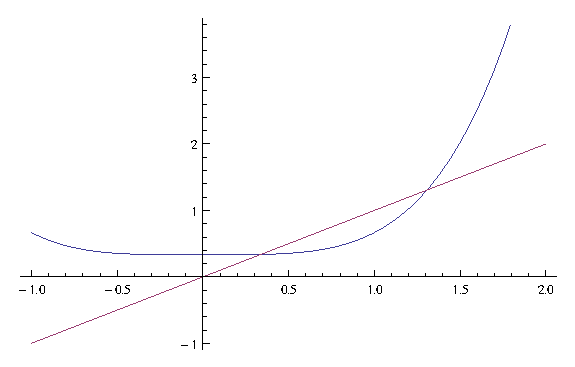
\includegraphics{Analysis/Analysis_sequence.eps}}
%\end{figure}

%\centertexdraw{
%
%    \def\bdot {\fcir f:0 r:0.03 }
%
%    \drawdim in
%
%    \arrowheadtype t:F \arrowheadsize l:0.08 w:0.04
%    \linewd 0.01 \setgray 0

%    \move (-1 -1) \lvec(2 2)
%    \move (-1 0) \clvec (1 0.5)(1.5 1)(2 1.5)
%
%    \move (-1 -1) \avec (-1 0 ) \avec(0 0) \avec(0 0.3) \avec(0.3 0.3) \avec(0.3 0.4)
%    \move (2 2) \avec (2 1.5) \avec(1.5 1.5) \avec(1.5 1.05) \avec(1.05 1.05) \avec(1.05 0.75) \avec(0.75 0.75) \avec(0.75 0.6)\avec(0.6 0.6)

%    \move (0.46 0.46) \bdot
%    \htext (-1.1 -1){0}
%    \htext (0.4 0.2){$r_1$}

%    \move (2 -1) \lvec(5 2)
%    \move (2.2 -1) \clvec (3.2 0.5)(3.4 1)(3.7 2)

%    \move (2.57 -0.43) \bdot
%    \move (3 0) \avec (3 0.3) \avec (3.3 0.3) \avec (3.3 0.85) \avec (3.85 0.85) \avec (3.85 2)
%    \htext (2.8 -0.5){$r_2$}

%\move (0 -1.2)
%}

Let the two roots of $f(x) = (x^4+1)/3 - x$ be $r_1$ and $r_2$ ($r_1 < r_2$). Because $f(0)>0$, $f(1) <0$ and $f(2) >0$, we have $r_1 \in (0,1)$ and $r_2\in (1,2)$.

Graphical analysis tells us that sequences starting with $a_1 =0,1$ converge to $r_1$ and $a_1 = 2$ diverges to infinity.

$a_1 = 0$. If $a_n \in (0,r_1)$, $f(a_n) = (a_n^4+1)/3 - a_n = a_{n+1} -a_n >0\ \ra \ a_{n+1} > a_n$. But
\be
a_{n+1} = (a_n^4+1)/3 < (r_1^4+1)/3 = r_1
\ee

Thus, $a_n$ is increasing and bounded above so it is converging.

$a_1 = 1$. If $a_n \in (r_1,r_2)$, $f(a_n) = (a_n^4+1)/3 - a_n = a_{n+1} -a_n < 0\ \ra \ a_{n+1} < a_n$. But
\be
a_{n+1} = (a_n^4+1)/3 > (r_1^4+1)/3 = r_1
\ee

Thus, $a_n$ is decreasing and bounded above so it is converging.

$a_1 = 2$. If $a_n \in (r_2,\infty)$, $f(a_n) = (a_n^4+1)/3 - a_n = a_{n+1} -a_n >0\ \ra \ a_{n+1} > a_n$. Thus, $a_n$ is increasing and unbounded above so it is diverging.
\end{solution}

%------------------------------------------------------------------------------------------------------------------

\begin{problem}
Let $a_1>b_1>0$ and let $a_{n+1} = (a_n + b_n)/2$, $b_{n+1} = 2a_nb_n/(a_n+b_n)$ for $n\geq 1$. Show that $a_n>a_{n+1}>b_{n+1}>b_n$ and deduce the two sequences converge to a common limit. What limit?
\end{problem}

\begin{solution}[\bf Solution.]
Since $a_1>b_1>0$,
\be
\left\{\ba{l}
2a_1 > a_1 + b_1 \ \ra \ a_1 > \frac{a_1 + b_1}2 = a_2\\
\frac 1{a_1} < \frac 1{b_1} \ \ra \  \frac 1{a_1} + \frac 1{b_1}  < \frac 2{b_1} \ \ra \ b_1 < \frac 2{\frac 1{a_1} + \frac 1{b_1}} = b_2\\
a_2 - b_2 = \frac{a_1 + b_1}2 - \frac {2a_1b_1}{a_1 + b_1} = \frac {(a_1 - b_1)^2}{2(a_1+b_1)} >0
\ea\right. \ \ra \ a_1 > a_2 > b_2 > b_1.
\ee

By induction, we have $a_n>a_{n+1}>b_{n+1}>b_n$. Since $a_n$ is a decreasing sequence, and bounded below (by 0), thus $a_n$ converges to $a$. Similarly, $b_n$ is an increasing sequence and bounded above (by $a_1$). Thus,
\be
\left\{\ba{l}
a = \frac {a+b}2 \\
b = \frac {2ab}{a+b}
\ea\right. \ \ra \ a = b.
\ee
which means that $a_n$ and $b_n$ converge to a common limit $c$. We know that
\be
a_{n+1}b_{n+1} = (a_n + b_n)/2 \times 2a_nb_n/(a_n+b_n) = a_n b_n \ \ra \ c^2 = a_1 b_1 \ \ra \ c = \sqrt{a_1b_1}.
\ee
\end{solution}

\subsection{Real series}

\begin{problem}[Baby Rudin Exercise 3.11]
Let $(a_n)_n$ be a positive real sequence. Suppose $s_n = a_1+\dots + a_n$ and $\sum_n a_n$ diverges. Prove that
\be
\frac{a_n}{s_n^2} \leq \frac 1{s_{n-1}} - \frac 1{s_n}
\ee
and deduce that $\sum_n \frac{a_n}{s_n^2}$ converges.

What can be said about
\be
\sum_n \frac {a_n}{1 + na_n}\quad \text{ and }\quad \sum_n \frac {a_n}{1 + n^2a_n}?
\ee
\end{problem}

\begin{solution}[\bf Solution.]
Clearly, for any $n\geq 2$,
\be
\frac 1{s_{n-1}} - \frac 1{s_n} = \frac {s_n - s_{n-1}}{s_{n-1}s_n} = \frac{a_n}{s_{n-1}s_n} \geq \frac{a_n}{s_n^2}
\ee

Thus, series $\frac 1{s_{n-1}} - \frac 1{s_n}$ is telescoping and
\be
\sum^\infty_{n=1} \frac{a_n}{s_n^2} \leq \frac 1{a_1} + \sum^\infty_{n=2} \frac 1{s_{n-1}} - \frac 1{s_n} = \frac 1{a_1} +  \frac 1{s_{1}} - \frac 1{s_\infty} = \frac 2{a_1}
\ee
as $s_\infty = \infty$. Thus, $\sum_n \frac{a_n}{s_n^2}$ converges as it is increasing and bounded.

Note that if $a_n=1/n$, $\sum_n \frac {a_n}{1 + na_n}$ diverges and $\sum_n \frac {a_n}{1 + n^2a_n}$ converges. Since the harmonic series is kind of a borderline divergent series, this suggests that the first series might always diverge and the second always converge.

However, if we let
\be
a_n = \begin{cases}
n=k! \quad\quad & \text{for some }k\in \Z^+,\\
2^{-n} & \text{otherwise.}
\end{cases}
\ee

The first case of that definition ensures that $\sum_n a_n$ diverges. Now we have
\be
\frac{a_n}{1 + na_n} = \frac{1}{n+\frac{1}{a_n}} =
\begin{cases}
\frac 1{n+1/n}\quad\quad & \text{if $n=k!$ for some }k\in \Z^+, \\
\frac 1{n+2^n} & \text{otherwise.}
\end{cases}
\ee

$\sum_n \frac 1{n+2^n}$ is certainly convergent, and
\be
\sum_{n=1}^\infty \frac 1{n!+1/n!} \leq \sum_{n=1}^\infty \frac 1{n!} = e.
\ee

So in this case $\sum_n \frac {a_n}{1 + na_n}$ converges. Thus, we cannot in general say anything about $\sum_n \frac {a_n}{1 + na_n}$.

For $\sum_n \frac {a_n}{1 + n^2a_n}$, on the other hand, succumbs to the comparison test:
\be
\frac{a_n}{1 + n^2a_n} = \frac 1{a_n^{-1} + n^2} < \frac 1{n^2} \ \ra\ \sum_n \frac {a_n}{1 + n^2a_n}\text{ converges.}
\ee
\end{solution}





\subsection{Differentiation}


\begin{problem}
Consider two contants $e^\pi$ and $\pi^e$. Which is bigger?
\end{problem}

\begin{solution}[\bf Solution.]
Consider the function
\be
f(x) = e^x - x^e,\qquad x\in \R
\ee
whose derivative is
\be
f'(x) = e^x - e \cdot x^{e-1}.
\ee

Note that exponential function and power function can have at most two points of intersection.\footnote{This is obvious by taking logarithm.} Therefore, $f'(x) =0$ implies $e^x = e \cdot x^{e-1}$ and we can find two points to satisfy this condition,
\be
f'(1) = e^1 - e\cdot 1^{e-1} = 0,\qquad f'(e) = e^e - e\cdot e^{e-1} = 0.
\ee

In general, an exponential function will grow to infinity faster than a power function\footnote{Again, taking logarithm will show the result.}, so
\be
f'(x) \geq 0,\quad x>e.
\ee

This means that $f$ is an increasing function when $x>e$. Also, notice that $f(e) =0$. Therefore, $f(\pi)>0$ since $f$ is increasing when $x>e$ and $\pi>e$.

Hence, $e^\pi > \pi^e$. Indeed, $e^\pi \approx 23.14$ and $\pi^e \approx 22.46$.
\end{solution}


\subsection{Monotone functions}


\begin{problem}
Given $f(x) = \log(x^2 -ax -1)$ is increasing when $x\in (1,+\infty)$. Find the range of $a$.
\end{problem}

\begin{solution}[\bf Solution.]
Since $\log$ is strictly increasing, we have that $x^2 - ax -1$ is increasing when $x\in (1,+\infty)$. As we know $x^2 -ax -1$ should have the U-shaped curve with symmetric axis at $x=a/2$.

\begin{center}
\psset{yunit=2.5cm,xunit=2.5cm}
\begin{pspicture}[algebraic](-0.5,-0.5)(2.5,2)%[showgrid](-3,-1.5)(3,4)
\psaxes[ticks=none,labels=none]{->}(0,0)(-0.5,-0.5)(2.5,2)%Dx=0.5,Dy=0.5
\psplot[linecolor=blue,linewidth=1.5pt]{-0.5}{2.5}{x^2-2*x+0.7}
\psline[linecolor=red,linestyle=dashed](1,2)(1,-0.5)
\rput(0.7,1.2){$x = a/2$}

\end{pspicture}
\end{center}

So $a/2$ must be smaller than 1 such that $x^2 - ax -1$ is increasing when $x\in (1,+\infty)$ which implies that
\be
a/2 \leq 1 \ \ra \ a\in (-\infty,2].
\ee
\end{solution}

\begin{problem}
Given $f(x) = (x-m)^{1/2}$ and its inverse function have common point. Find the range of $m$.
\end{problem}

\begin{solution}[\bf Solution.]
If $f(x)$ has common point with its inverse function, it must be on the line $y=x$ (since $f(x)$ and $f^{-1}(x)$ are symmetric about line $y=x$).


\begin{center}
\psset{yunit=2.5cm,xunit=2.5cm}
\begin{pspicture}[algebraic](-1,-0.75)(2.5,2)%[showgrid](-3,-1.5)(3,4)
\psaxes[ticks=none,labels=none]{->}(0,0)(-1,-0.75)(2.5,2)%Dx=0.5,Dy=0.5
\psplot[linecolor=blue,linewidth=1.5pt]{-0.5}{2.5}{(x+0.5)^0.5}
\psplot[linecolor=red,linewidth=1.5pt]{0}{1.6}{x^2-0.5}
\psline[linecolor=green,linestyle=dashed](-0.5,-0.5)(2,2)
%\psline[linecolor=red,linestyle=dashed](1,2)(1,-0.5)
\rput(2,1.9){$y=x$}
\rput(0.5,1.2){$f(x)$}
\rput(1.3,0.5){$f^{-1}(x)$}
\rput(-0.5,-0.1){$m$}
\end{pspicture}
\end{center}

So the extreme case is that $f(x)$ and $y=x$ only have one common point which implies that
\be
\begin{cases}
f'(x) - x' = 0 \quad \text{($f(x)-x$ achieves local maximum)}\\
f(x) -x = 0\quad \text{($f(x)$ is tangent to $y=x$)}
\end{cases} \ \ra\ \begin{cases}
(x-m)^{1/2} -x = 0 \\
\frac 12(x-m)^{-1/2} -1 = 0
\end{cases} \ \ra\ \begin{cases}
(x-m)^{1/2} = \frac 12 \\
(x-m)^{1/2} = x
\end{cases}
\ee

Thus, $x = \frac 12$ and $m = \frac 14$ which implies that the range should be $m \in (-\infty,\frac 14]$.
\end{solution}
							%p
%\chapter{Multi-dimensional Real Analysis}

\chapter{Analysis in Euclidean Space}

\section{Euclidean Space}

\begin{definition}\label{def:euclidean_space}
\footnote{need definition}
\end{definition}



\section{Convergent Sequence in $\R^n$}

\subsection{Bolzano-Weierstrass theorem}

\begin{theorem}[Bolzano-Weierstrass theorem]\label{thm:bolzano_weierstrass_multiple_real}
Every bounded sequence in $\R^n$ has a convergent subsequence.
\end{theorem}

\begin{proof}[\bf Proof]%(We use subscripts to denote the terms of the sequence, because we’re going to use superscripts to denote the components of points in $\R^n$.)
Let $(x_m) = (x_m^0)$ be a bounded sequence in $\R^n$. Then the sequence $(y_m^1)$ of first components of the terms of $(x_m^0)$ is a bounded real sequence, which has a convergent subsequence $(y_{m_k}^1)$, according to the Bolzano-Weierstrass theorem in $\R$ (Theorem \ref{thm:bolzano_weierstrass_r}).
 
Let $(x_{m}^1)$ be $(x_{m_k}^0)$, the corresponding subsequence of $(x_m^0)$. Then the sequence $(y_m^2)$ of second components of $(x_m^1)$ is a bounded sequence of real numbers, so it too has a convergent subsequence, and we again have $(x_{m}^2)$, a corresponding subsequence of $(x_{m}^1)$ (and therefore of $(x_{m}^0)$), in which the sequences of first and second components both converge. 

Continuing for $n$ iterations, we end up with a subsequence $(x_{m}^n)$ of $(x_{m}^0)$ in which the sequences of first to $n$th components all converge, and therefore the subsequence $(x_{m}^n)$ itself converges in $\R^n$.
\end{proof}



\section{Sets in $\R^n$}%\section{Sets of Mulit-dimensional Real Space}





\subsection{Open and closed sets}

\begin{proposition}
Note that $\emptyset$ and $\R^n$ are both open and closed.
\end{proposition}

\begin{proof}[\bf Proof]
\footnote{proof needed.}
\end{proof}

\begin{theorem}\label{thm:open_set_multi_dimensional_real_n_can_be_countable_union_of_almost_disjoint_closed_cubes}%overlapping
Every open set in $\R^n$ can be written as a countable union of non-overlapping closed cubes.
\end{theorem}

\begin{proof}[\bf Proof]
\footnote{proof needed.}
\end{proof}

\begin{theorem}
Every open set in $\R^n$ can be written as a countable union of disjoint partly open cubes.
\end{theorem}



\subsection{Compact sets}

\begin{definition}[cover\index{cover}]
Let $E$ be set in space $X$. Then a cover of $E$ is a family $\sF$ of sets $A\subseteq X$ such that $E\subseteq\bigcup_{A\in \sF} A$.
\end{definition}

\begin{definition}[subcover\index{subcover}]
A subcover $\sG$ of a cover $\sF$ is a cover with the property that $A \in \sF$ whenever $A \in \sG$.
\end{definition}

\begin{definition}[open cover]
A cover $\sF$ is called an open cover if each set in $\sF$ is open.
\end{definition}

\begin{definition}[compact set]
A set $E$ is compact if every open cover of $E$ has a finite subcover.
\end{definition}

\begin{definition}[compact support\index{compact support!real space}]
A function has compact support in $\R^n$ if it vanishes outside some bounded set.
\end{definition}

%\begin{lemma}\label{lem:compact_disjoint_sets_real_n_imples_distance_positive}
%Let $A,B$ be two non-empty compact and disjoint sets in $\R^n$. Then $d(A,B)>0$.
%\end{lemma}

%\begin{proof}[\bf Proof]
%\footnote{proof needed.}
%\end{proof}


\begin{theorem}[Heine-Borel theorem]\label{thm:heine_borel_compact_real_n_closed_bounded}
Let $A \subseteq \R^n$. Then the following are equivalent.
\ben
\item [(i)] $A$ is closed and bounded.
\item [(ii)] Every sequence of points of $A$ has a subsequence that converges to a point of $A$.
\item [(iii)] $A$ is compact.
\een
\end{theorem}

%\begin{remark}
%Note that the sets must be compact subset in $\R^n$ but not compact subset in a $E\subseteq \R^n$.
%\end{remark}

%\begin{theorem}
%A set $A \subseteq \R^n$ is compact if and only if 
%\end{theorem}

\begin{proof}[\bf Proof]
\ben
\item [(i)] $\ra$ (ii). Suppose $A$ is closed and bounded and consider any sequence $(a_n)$ in $A$. Since $A$ is bounded, we have that $(a_n)$ has a convergent subsequence by Bolzano-Weierstrass theorem (Theorem \ref{thm:bolzano_weierstrass_multiple_real}). Since $A$ is closed, we have that the limit of this sequence is in $A$.

\item [(ii)] $\ra$ (iii). Suppose that every sequence in $A$ contains a convergent subsequence with limit in $A$. 

Consider an open cover $\bra{U_i}_{i\in I}$ of $A$ such that $A \subseteq \bigcup_{i\in I} U_i$. For any $a\in X$, we want to show that there exists $\ve>0$ such that $B_\ve(a) \subseteq U_i$ for some $i\in I$.

Suppose not, then for every $\ve>0$, in particular for $\ve = \frac 1n$ with $n\in \Z^+$, there is a point $a_n\in A$ such that for every $i\in I$ we have that $B_{\frac 1n}(a_n) \not\subseteq U_i$. Consider the sequence $(a_n)$, by the assumption there is a convergent subsequence $(a_{n_k})$ converging to $a^*$. Since $\bra{U_i}_{i \in I}$ is a cover we know that there is $i^* \in I$ such that $a^* \in U_{i^*}$. Since $U_{i^*}$ is open then there is $\delta >0$ such that $B_{\delta}(a^*) \subseteq U_{i^*}$. But since $(a_{n_k})\to a^*$ there is $N\in \N$ such that $\abs{a^* - a_{n_k}} < \delta/2$ whenever $n_k\geq N$.

Then pick $n_k\geq N$ and $n_k > 2/\delta$. Then for any $b\in B_{\delta/2}(a_{n_k})$ we have
\be
\abs{a^* - b} = \abs{a^* - a_{n_k} + a_{n_k} - b} \leq \abs{a^* - a_{n_k}} + \abs{a_{n_k} - b} < \frac {\delta}2 + \frac{\delta}2 = \delta.
\ee

Therefore, $B_{1/n_k}(a_{n_k}) \subseteq B_{\delta/2} (a_{n_k}) \subseteq B_\delta(a^*) \subseteq U_{i^*}$ which contradicts the fact that $B_{1/n}(a_n) \not\subseteq U_i$ for every $i \in I$.


Now for any $a\in A$ we can find $\ve= \ve(a)>0$ such that $B_a := B_\ve(a) \subseteq U_{i}$ for some $i\in I$. Obviously, $\bra{B_a}_{a\in A}$ is an open cover of $A$. Suppose we know how to extract a finite subcover $\bra{B_{a_1},\dots,B_{a_M}}$ of $A$, then since each $B_{a_k}$ is contained in some $U_{i_k}$ we can conclude that $\bra{U_{i_1},\dots,U_{i_M}}$ is also a finite subcover. So it is enough to show that $\bra{B_{a}}_{a\in A}$ has a finite subcover of $A$.

For any $a_0\in A$. If $B_{a_0}$ covers $A$ we are done, otherwise there is $a_1\in A\bs B_{a_0}$. If $\bra{B_{a_0},B_{a_1}}$ covers $A$ we are done, otherwise there is $a_2\in A\bs\bb{B_{a_0}\cup B_{a_1}}$. If we continue this process we either obtain a finite subcover or a sequence $(a_k)_{k\in \N}$. Observe that for any $k\in \N$, there exists $\ve = \ve(a_k)>0$ such that $\abs{a_k - a_j}>\ve$ for any $j>k$. So the sequence $(a_k)$ cannot have a convergent subsequence which is a contraction to the assumption. Therefore, the process must end at some point and we should have a finite subcover of $A$.


\item [(iii)] $\ra$ (i). Suppose $A$ is compact. Consider the collection
\be
\sC = \bra{B_n(0),n\in \N}.
\ee

Clearly $\sC$ is an open cover of $A$ (in fact of whole $\R^n$). Therefore, since $A$ is compact, there is a finite subcover
\be
\sC_f= \bra{B_{n_1}(0),\dots,B_{n_M}(0)}
\ee
of $A$. Without loss of generality, we may assume that $n_1<n_2 < \dots < n_M$ then clearly $A \subseteq B_{n_M}(0)$, i.e., $A$ is bounded.

Now we want to prove that $A$ is closed we can prove instead that $\R^n\bs A$ is open. Given any $b\in \R^n\bs A$ and any $a\in A$ consider the disk
\be
B_a := B_{\frac 12 \abs{a-b}}(a)
\ee
and the collection $\sC := \bra{B_a : a\in A}$. Clearly, $\sC$ is an open cover of $A$ since every point $a$ in $A$ has a disk centered at it in $\sC$. Since $A$ is compact, there is a finite subcover $\sC_f = \bra{B_{a_1},\dots,B_{a_M}}$. Define
\be
\ve := \min_{1\leq i\leq M}\bra{\frac 12\abs{b-a_i}}.
\ee

Then we observe that since $\frac 12 \abs{b - a_i} \geq \ve$, $b$ is at least farther apart than $\ve$ from every point in $B_{a_i}$. Thus, for any $a\in B_{a_i}$ ($\abs{a-a_i} < \frac 12 \abs{b-a_i}$),
\be
\abs{b-a} = \abs{b-a_i + a_i - a} \geq \abs{b - a_i} - \abs{a -a_i} > \abs{b - a_i} - \frac 12 \abs{b-a_i} = \frac 12 \abs{b-a_i} \geq \ve.
\ee

Therefore, $B_{\ve}(b) \cap B_{a_i}= \emptyset$ and
\be
B_{\ve}(b) \subseteq \R^n \left\bs \bigcup_{i=1}^M B_{a_i}\right. \subseteq \R^n \bs A
\ee
which proves that $\R^n\bs A$ is open (since $b\in \R^n\bs A$), i.e., $A$ is closed.
\een
\end{proof}

\begin{theorem}\label{thm:intersection_of_decreasing_non_empty_compact_sets_in_real_n_non_emptyset_compact}
A sequence of decreasing non-empty compact subsets of $\R^n$ has a non-empty compact intersection.
\end{theorem}

\begin{proof}[\bf Proof]
Suppose that
\be
A_1 \supseteq A_2 \supseteq A_3 \supseteq \dots
\ee
is a countable family of non-empty, closed, bounded subsets of $\R^n$. Clearly, each of $A_n$ is bounded and closed since it is compact by Heine-Borel theorem (Theorem \ref{thm:heine_borel_compact_real_n_closed_bounded}). Then define
\be
A := \bigcap_n A_n.
\ee

The set $A$ is bounded since it is a subset of the bounded set $A_1$ and is closed, since it is the intersection of a family of closed sets\footnote{theorem needed.}. So the set $A$ is compact by Heine-Borel theorem (Theorem \ref{thm:heine_borel_compact_real_n_closed_bounded}). So it only remains to show that $\bigcap^\infty_{n=1}A_n \neq \emptyset$. %By Heine-Borel theorem, $A_n$ is compact for each $n\in \N$.
For the sake of contradiction, suppose that $\bigcap^\infty_{n=1} A_n= \emptyset$. Then $\bigcup^\infty_{n=1}A_n^c = \R$ by De Morgon law (Theorem \ref{thm:basic_set_properties_general_case}). In particular,
\be
A_1 \subseteq \bigcup^\infty_{n=1} A_n^c.
\ee

Since $A_1$ is compact and the sets $(A_n^c)^\infty_{n=1}$ form an open cover of it, there must exist a finite subcover. That is, there exists some $m\in\N$ such that
\be
A_1 \subseteq \bigcup^m_{n=1} A_n^c = A_m^c,
\ee
where the second equality follows from the fact that
\be
A_1^c \subseteq A_2^c \subseteq A_3^c \subseteq \dots.
\ee

Now, $A_1\subseteq A_m^c$ means that if a point is in $A_1$, then it must not be in $A_m$, so that $A_1\cap A_m=\emptyset$. But $A_m \subseteq A_1$ (given that the sets are nested), so that $A_1\cap A_m = A_m = \emptyset$, which contradicts the assumption that $A_m$ is not empty. This contradiction reveals that the intersection $\bigcap^\infty_{n=1}A_n$ must not be empty.
\end{proof}


\begin{example}
If the decreasing subsets are not compact, the conclusion might not hold. The following are the examples.
\ben
\item [(i)] Note that only closedness cannot guarantee the non-empty intersection. For instance, $A_n = [n,\infty)$ is closed in $\R$, but $\bigcap^\infty_{n=1}A_n = \emptyset$.

\item [(ii)] $A_n$ should be compact (closed and bounded) in $\R^n$. A counter example is the set $X$, the `punctured line' $(-\infty,0)\cup(0,\infty)$, which is just the real numbers with 0 removed. The sets
\be
A_n=\bra{x \in \R:\abs{x}\leq 1/n,\ x\neq 0}
\ee
are closed and bounded in the punctured line (but not in $\R$), but their intersection is empty.
\een
\end{example}

\subsection{$n$-dimensional rectangle and its volume}

\begin{definition}[$n$-dimensional rectangle]
An $n$-dimensional rectangle $I$ is a subset of $\R^n$ of the form
\be
I = \bra{x=(x_1,\dots, x_n): a_k \leq x_k \leq b_k, k=1,\dots,n},
\ee
where $a_k < b_k$, $k=1, \dots,n$.
\end{definition}

\begin{remark}
An $n$-rectangle is compact (bounded and closed, see the proof of Theorem \ref{thm:heine_borel_compact_real_n_closed_bounded_metric_proof}) in $\R^n$ and we say it has edges parallel to the coordinate axes.

If the edge lengths $b_k - a_k$ are all equal, $I$ will be called an $n$-dimensional cube with edges parallel to the coordinate axes.
\end{remark}%We use just the word interval in $\R^n$, we generally mean closed interval.

\begin{definition}[volume of rectangle]\label{def:volume_of_rectangle_in_real_n}
Let $I = \bra{x = (x_1,\dots, x_n) : a_k \leq x_k \leq b_k, k=1,\dots, n}$ with $a_k < b_k$, $k=1, \dots,n$ be a rectangle in $\R^n$. Then the volume of $I$, $\vol(I)$, is
\be
\vol(I) = \prod^n_{k=1} (b_k - a_k).
\ee

In particular, $v(\emptyset) = 0$.
\end{definition}

\begin{remark}
Indeed, $\vol$ is a set function on $\sA$ containing all rectangles of $\R^n$ and the empty set $\emptyset$.
\end{remark}

\begin{proposition}\label{pro:volume_of_rectangle_increasing}
The volume of rectangles is increasing. That is, let $A,B$ be two rectangles in $\R^n$ with $A\subseteq B$, then
\be
\vol(A)\leq \vol(B).
\ee
\end{proposition}

\begin{proof}[\bf Proof]
Let $A = [a_1,b_1]\times \dots \times [a_n,b_n]$ and $B = [c_1,d_1] \times \dots \times [c_n,d_n]$. Then for all $1\leq k\leq n$,
\be
c_k\leq a_k < b_k\leq d_k \ \ra\ b_k-a_k \leq d_k - c_k  \ \ra\ \vol(A) = \prod^n_{k=1} (b_k - a_k) \leq \prod^n_{k=1} (d_k - c_k) = \vol(B).
\ee
\end{proof}

\begin{definition}[almost disjoint rectangles\index{almost disjoint rectangles}]\label{def:almost_disjoint_rectangles_real_n}
Let $A_1,\dots,A_m$ be $m$ rectangles in $\R^n$. Then we say they are almost disjoint rectangles if for any $i\neq j$,
\be
\inter{A_i}\cap \inter{A_j} = \emptyset
\ee
where $\inter{I}$ is the interior of set $I$.
\end{definition}

\begin{lemma}\label{lem:subrectangles_volume_summation}
Suppose that
\be
I = I_1\times I_2 \times \dots \times I_n
\ee
is a rectangle in $\R^n$ where each closed bounded interval $I_i\subseteq \R$ is an almost disjoint union of closed bounded intervals $\bra{I_{ij}\subseteq \R:j=1,\dots,N_i}$,
\be
I_i = \bigcup_{j=1}^{N_i} I_{ij}.
\ee

Define the rectangles $S_{j_1j_2\dots j_n} = I_{1,j_1} \times I_{2,j_2} \times \dots\times I_{n,j_n}$. Then
\be
\vol{I} = \sum^{N_1}_{j_1 = 1} \dots \sum^{N_n}_{j_n = 1} \vol\bb{S_{j_1j_2\dots j_n}}.
\ee
\end{lemma}

\begin{proof}[\bf Proof]
Denoting the length of an interval $I\subseteq \R$ by $\abs{I}$, using the fact that
\be
\abs{I_i} = \sum^{N_i}_{j=1}\abs{I_{ij}},
\ee
and expanding the resulting product, we get that
\beast
\vol\bb{I} & = & \prod^n_{i=1}\abs{I_i} = \prod^n_{i=1} \bb{\sum^{N_i}_{j_i=1}\abs{I_{i,j_i}}} = \sum^{N_1}_{j_1=1}\dots \sum^{N_n}_{j_n=1}\prod^n_{i=1} \abs{I_{i,j_i}} = \sum^{N_1}_{j_1=1}\dots \sum^{N_n}_{j_n=1}\vol\bb{S_{j_1j_2\dots j_n}}
\eeast
as required.
\end{proof}


\begin{theorem}\label{thm:volume_of_rectangle_additivity_subadditivity}
If a rectangle $I$ is an almost disjoint finite union of rectangles $A_1,\dots, A_N$, $I = \bigcup_{k=1}^N A_k$. Then
\be
\vol(I) = \sum^N_{k=1}\vol(A_k).
\ee

If a rectangle $I$ is covered by rectangles $B_1,\dots,B_M$, $I \subseteq \bigcup_{k=1}^{M} B_k$ where $B_1,\dots,B_M$ need not be disjoint, then
\be
\vol(I) \leq \sum^M_{k=1}\vol(B_k).
\ee

If a rectangle $I$ contains rectangles $B_1,\dots,B_M$, $\bigcup_{k=1}^{M} B_k\subseteq I$ where $B_1,\dots,B_M$ are non-overlapping, then
\be
\sum^M_{k=1}\vol(B_k) \leq \vol(I).
\ee
\end{theorem}

\begin{proof}[\bf Proof]
Let $I = [a_1,b_1]\times \dots \times [a_n,b_n]$ and $A_k = [a^k_1,b^k_1]\times \dots \times [a_n^k,b_n^k]$ for $k=1,\dots,N$. Then we can use these end points $a_i^k$, $b_i^k$ to form a finite set $\bra{c_{i,0},\dots,c_{i,N_i}}$ such that
\be
a_i = c_{i,0} \leq c_{i,1} \leq \dots \leq c_{i,N_i} = b_i.
\ee

Then we can have
\be
[a_i,b_i] = I_i = \bigcup_{j=1}^{N_i} I_{ij},\qquad I_{ij} = [c_{i,j-1},c_{ij}].
\ee

Therefore, we can define the rectangles
\be
S_{j_1j_2\dots j_n} = I_{1,j_1} \times I_{2,j_2} \times \dots\times I_{n,j_n},\qquad 1\leq j_1 \leq N_1,\dots, 1\leq j_n\leq N_n.
\ee

Obviously, each rectangle $A_k$ in the collection is an almost disjoint union of rectangles $S_{j_1j_2,\dots j_n}$ and their union contains all such products exactly once, so applying Lemma \ref{lem:subrectangles_volume_summation} to each $A_k$ and summing the results we see that
\be
\sum^N_{k=1}\vol(A_k) = \sum^{N_1}_{j_1=1}\dots \sum^{N_n}_{j_n=1}\vol\bb{S_{j_1j_2\dots j_n}}.
\ee

Similarly, $I$ is an almost disjoint union of all the rectangles $S_{j_1j_2\dots j_n}$, so Lemma \ref{lem:subrectangles_volume_summation} implies that
\be
\vol(I) = \sum^{N_1}_{j_1=1}\dots \sum^{N_n}_{j_n=1}\vol\bb{S_{j_1j_2\dots j_n}} \ \ra\ \vol(I) = \sum^N_{k=1}\vol(A_k).
\ee

If finite collection of rectangles $B_1,\dots, B_M$ covers $I$, then we define $C_k = I\cap B_k$ for $k=1,\dots,M$ and thus $I = \bigcup_{k=1}^M C_k$. Then we can use the end points of $C_k$ to form finite collection of almost disjoint sub-rectangles
\be
T_{j_1j_2\dots j_n} = I_{1,j_1} \times I_{2,j_2} \times \dots\times I_{n,j_n},\qquad 1\leq j_1 \leq N_1,\dots, 1\leq j_n\leq N_n.
\ee
such that
\be
\vol(I) = \sum^{N_1}_{j_1=1}\dots \sum^{N_n}_{j_n=1}\vol\bb{T_{j_1j_2\dots j_n}}.
\ee

Also, all of $C_k$ contains each $T_{j_1j_2\dots j_n}$ at least once, thus,
\be
\sum^{N_1}_{j_1=1}\dots \sum^{N_n}_{j_n=1}\vol\bb{T_{j_1j_2\dots j_n}} \leq \sum^M_{k=1} \vol(C_k).
\ee

Since $\vol(\cdot)$ is increasing (Proposition \ref{pro:volume_of_rectangle_increasing}), we have that
\be
\vol(I) \leq \sum^M_{k=1} \vol(C_k) \leq \sum^M_{k=1}\vol(B_k).
\ee

Similarly, if rectangle $I$ contains non-overlaping rectangles $B_1,\dots,B_M$, each $S_{j_1j_2\dots j_n}$ only contained in one and only one of $B_k$. Thus, we have the required result
\be
\sum^M_{k=1}\vol(B_k) \leq \vol(I).
\ee
\end{proof}


\section{Multi-dimensional differentiability}

\begin{definition}[Jacobian matrix\index{Jacobian matrix!real valued}]%vector function with vector variable}]
Suppose $f:\R^n\to \R^m$ is a function which takes as input the vector $x\in \R^n$ and produces as output the vector $f(x) \in \R^m$. Then the Jacobian matrix of $f$, denoted by $Df$, is an $m\times n$ matrix,
\be
Df := \bepm
\fp{f}{x_1},\dots,\fp{f}{x_n}
\eepm = \bepm
\fp{f_1}{x_1} & \dots & \fp{f_1}{x_n} \\
\vdots & \ddots & \vdots \\
\fp{f_m}{x_1} & \dots & \fp{f_m}{x_n}
\eepm,
\ee
or, $J = Df$ with component-wise elements
\be
J_{ij} = \fp{f_i}{x_j}.
\ee
\end{definition}

\begin{example}
Consider the function $f:\R^2\to \R^2$ given by
\be
f(x,y) = \bepm x^2 y \\ 5x+ \sin y\eepm.
\ee

Then we have that $f_1(x,y) = x^2y$ and $f_2(x,y) = 5x + \sin y$ and the Jacobian matrix of $f$ is
\be
J_f(x,y) = \bepm \fp{f_1}{x} & \fp{f_1}{y} \\ \fp{f_2}{x} & \fp{f_2}{y}  \eepm = \bepm 2xy & x^2 \\ 5 & \cos y \eepm.
\ee
\end{example}

\begin{definition}[differentiability of multi-dimensional real valued function]\label{def:differentiable_multi_dimensional_real_function}
Let $f:R^n\to \R^m,x\mapsto f(x)$ be $m$-dimension real valued function with with $f(x) = \bb{f_1(x),\dots,f_m(x)}^T$. Then $f$ is differentiable at point $x_0\in \R^n$ if there exists a linear transformation (matrix) $J$ such
\be
\lim_{h\to 0}\frac{\dabs{f(x_0 + h) - f(x_0) - J\cdot h}}{\dabs{h}} = 0,\qquad h\in \R^n
\ee
where $\dabs{\cdot}$ are Euclidean norms\footnote{definition and properties needed.}. In this case, the linear transformation $J$ is unique and called the derivative of $f$ at $x_0$. Indeed, $J$ is the Jacobian matrix at $x_0$,
\be
J = \bepm
\fp{f_1}{x_1} & \dots & \fp{f_1}{x_n} \\
\vdots & \ddots & \vdots \\
\fp{f_m}{x_1} & \dots & \fp{f_m}{x_n}
\eepm.
\ee
\end{definition}

Note that the existence of first-order partial derivatives cannot guarantee the differentiability of the multi-dimensional real-valued function. However, we can have the following theorem.%continuous partial derivatives implies differentiability

\begin{theorem}[continuous partial derivatives implies differentiability]\label{thm:continuous_partial_derivatives_implies_real_differentiability}
Let $f:E\subseteq R^n\to \R^m,x\mapsto f(x)$ be a given function defined on an open subset $E$ of $\R^n$. Suppose that all partial derivatives of $f$ exist in an open neighbourhood\footnote{definition needed. $\dabs{x-x_0}<r$ where $\dabs{\cdot}$ is the Euclidean norm.} of a point $x_0\in E$ and are continuous at point $x_0$. Then $f$ is differentiable at $x_0$.
\end{theorem}

\begin{proof}[\bf Proof]
Let $x_0 = \bepm x_0^1,\dots,x_0^n \eepm^T$ and $h= \bepm h_1,\dots,h_n\eepm^T$ and given any $\ve >0$. Then we define
\be
g_i^j(x_0^j) := f_i\bb{x_0^1,\dots,x_0^j,x_0^{j+1}+h_{j+1},\dots,x_0^{n}+h_{n}}
\ee
for $j = 1,\dots,n$. Obviously, $g_i^j(x_0^j) = g_i^{j+1}(x_0^{j+1}+h_{j+1})$. Since the partial derivatives of each of $f_i$ are defined in an neighbourhood $N_r(x_0)$ of $x_0$, there exists $\delta_1 >0$ such that $\dabs{h}<\delta_1$ implies that $x_0 + h \in N_r(x_0)$. Therefore, each function $g_i(\cdot)$ is differentiable for any $x_j$ between $x_0^j$ and $x_0^j + h_j$ since its (partial) derivatives exist. Then by mean value theorem (Theorem \ref{thm:mean_value}) can find some $\wt{x}_j$ between $x_0^j$ and $x_0^j + h_j$ such that
\be
g_i^j(x_0^j + h_j) - g_i^j(x_0^j) = \bb{g_i^j}'(\wt{x}^j) h_j = \fp{f_i}{x_j}(y_j)\cdot h_j,
\ee
where $y_j = \bb{x_0^1,\dots, x_0^{j-1}, \wt{x}_j,\dots, x_0^{j+1}+h_j,\dots, x_0^n + h_n}^T$. Therefore,
\beast
f_i\bb{x_0^1+h_1,\dots, x_0^n+h_n} - f_i\bb{x_0^1,\dots, x_0^n} & = &  f_i\bb{x_0^1+h_1,\dots, x_0^n+h_n} - f_i\bb{x_0^1,x_0^2+h_2,\dots, x_0^n+h_n} \\
& & \qquad + f_i\bb{x_0^1,x_0^2+h_2,\dots, x_0^n+h_n} - f_i\bb{x_0^1,\dots, x_0^n} \\
& = & g_i^1(x_0^1 + h_1) - g_i^1(x_0^1) + f_i\bb{x_0^1,x_0^2+h_2,\dots, x_0^n+h_n} - f_i\bb{x_0^1,\dots, x_0^n} \\
& = & \dots = \sum^n_{j=1} g_i^j(x_0^j + h_j) - g_i^j(x_0^j) =  \sum^n_{j=1} \bb{g_i^j}'(\wt{x}^j) h_j = \sum^n_{j=1} \fp{f_i}{x_j}(y_j)\cdot h_j
\eeast

Since the partial derivatives exist, we can see that the Jacobian matrix $J$ is well-defined and
\be
\bb{J \cdot h}_i = \bb{\bepm
\fp{f_1}{x_1} & \dots & \fp{f_1}{x_n} \\
\vdots & \ddots & \vdots \\
\fp{f_m}{x_1} & \dots & \fp{f_m}{x_n}
\eepm \cdot \bepm h_1 \\ \vdots \\ h_n\eepm }_i =  \fp{f_i}{x_1} h_1 +  \dots + \fp{f_i}{x_n}h_n = \sum^n_{j=1}\fp{f_i}{x_j}(x_0)h_j.
\ee

Combining the above results, we have that
\be
\frac{\dabs{f_i(x_0 + h) - f_i(x_0) - \bb{J\cdot h}_i}}{\dabs{h}} = \dabs{\sum^n_{j=1} \bb{\fp{f_i}{x_j}(y_j) - \fp{f_i}{x_j}(x_0)}\frac{h_j}{\dabs{h}} }
\ee

Since each partial derivative $\fp{f_i}{x_j}$ is continuous in an open neighbourhood of $x_0$, there exists $\delta_2>0$ such that $\dabs{y_j - x_0} \leq \dabs{h} <\delta_2$ implies that
\be
\dabs{\fp{f_i}{x_j}(y_j) - \fp{f_i}{x_j}(x_0)} < \frac{\ve}{mn},
\ee
for each $j=1,\dots,n$. Note that for each of the partial derivatives we might have a different $\delta$ that yields the inequality $\dabs{y_j - x_0} <\delta$. We take $\delta_2$ to be the smallest of these. Thus, if we take $\dabs{h}<\delta$ where $\delta = \min\bra{\delta_1,\delta_2}$ we can have
\beast
\frac{\dabs{f_i(x_0 + h) - f_i(x_0) - \bb{J\cdot h}_i}}{\dabs{h}} & \leq & \sum^n_{j=1} \dabs{ \bb{\fp{f_i}{x_j}(y_j) - \fp{f_i}{x_j}(x_0)} }\cdot \dabs{\frac{h_j}{\dabs{h}}} \\
& < & \frac{\ve}{mn} + \dots + \frac{\ve}{mn} = \frac{\ve}{m}.
\eeast

Then we have that
\be
\frac{\dabs{f(x_0 + h) - f(x_0) - J\cdot h}}{\dabs{h}} \leq \sum^m_{i=1} \frac{\dabs{f_i(x_0 + h) - f_i(x_0) - \bb{J\cdot h}_i}}{\dabs{h}} < \ve
\ee
which implies that
\be
\lim_{h\to 0}\frac{\dabs{f(x_0 + h) - f(x_0) - J\cdot h}}{\dabs{h}} = 0
\ee
as required.
\end{proof}

However, a differentiable function might have discontinuous partial derivatives.

\begin{example}[differentiable function with discontinuous partial derivatives]
Let the function be
\be
f(x,y) = \left\{\ba{ll}
(x^2+y^2)\sin \bb{\frac 1{\sqrt{x^2+y^2}}}\quad\quad & (x,y)\neq (0,0) \\
0 & (x,y) = (0,0)
\ea\right..
\ee

Since the argument of the sinusoid\footnote{definition needed} approaches infinity as one approaches the origin, it oscillates wildly near the origin. But the sinusoid is bounded between -1 and 1, and the oscillations of the sinusoid are tempered by the quadratic term $x^2+y^2$. The function is squeezed between two elliptic paraboloids $z = x^2 + y^2$ and $z = -x^2-y^2$ that go to zero very quickly as one approaches the origin. As both paraboloids have the same horizontal tangent plane at the origin $z =0$, we can say that $f(x,y)$ has the same tangent plane at the origin. Therefore, the function $f(x,y)$ is differentiable at the origin.

If we take $y=0$, the function becomes
\be
f(x) = \left\{\ba{ll} x^2 \sin \frac{1}{\abs{x}} \quad\quad & x \neq 0\\ 0 & x=0 \ea\right.
\ee

By definition, we can have that $\fp{f}{x} = 0$ at $(0,0)$. Indeed,
\be
f'(0) = \lim_{x\to 0} \frac{f(x) - f(0)}{x-0} = \lim_{x\to 0} \frac{x^2\sin\frac 1{\abs{x}} - 0}{x} = \lim_{x\to 0} x\sin\frac 1{\abs{x}} = 0
\ee
as $\sin$ is bounded by -1 and 1. However, the partial derivatives oscillate wildly near the origin. For positive side,
\be
\fp{f}{x} = 2x\sin \frac 1x - \cos \frac 1x
\ee

For $x = \frac 1{2n\pi}$ and $n\in \Z$,
\be
\lim_{n\to \infty}\fp{f}{x} = \lim_{n\to \infty}\bb{\frac 2{2n\pi}\sin(2n\pi) - \cos(2n\pi)} = -1.
\ee

Similarly, for $x = \frac 1{(2n+1)\pi}$ and $n\in \Z$,
\be
\lim_{n\to \infty}\fp{f}{x} = \lim_{n\to \infty}\bb{\frac 2{(2n+1)\pi}\sin((2n+1)\pi) - \cos((2n+1)\pi)} = 1.
\ee

This creates a discontinuity of partial derivatives.
\end{example}

\section{Integral}

\subsection{Differentiation under integral}


\begin{proposition}[Leibniz's integral rule]\label{pro:differentiation_under_integral_of_real_function_of_two_real_variables}
Let $f:[a,b]\times [c,d]\to \R$ be a continuous function and define function $g:[c,d]\to \R$ by
\be
g(t) = \int^b_a f(s,t)ds.
\ee

Then $g$ is continuous on $[c,d]$. Moreover, if $\fp{f}{t}$ exists and is a continuous function on $[a,b]\times [c,d]$ then $g$ is continuously differentiable and
\be
g'(t) = \int^b_a \fp{f}{t}(s,t)ds.\qquad (*)
\ee
\end{proposition}

\begin{proof}[\bf Proof]
For any $t_0\in [c,d]$, we want to show that given any $\ve>0$ there exists $\delta>0$ such that $\abs{g(t) - g(t_0)} < \ve$ whenever $\abs{t-t_0}< \delta$. It follows that $f(s,t)$ must be uniformly continuous on $[a,b]\times [c,d]$ by Theorem \ref{thm:continuous_on_compact_set_implies_uniformly_continuous_metric} as $f$ is continuous on a compact set $[a,b]\times [c,d]$. Then given any $\ve>0$, there exists $\delta>0$ (independent of $t_0$) such that for any $s,s'\in [a,b]$ and any $t,t'\in [c,d]$,
\be
\abs{f(s,t) - f(s',t')} < \frac{\ve}{b-a}\qquad \text{whenever }\ \abs{(s-s')^2+ (t-t')^2}^{1/2} = d((s,t),(s',t')) < \delta.
\ee

Let $s=s'$. we have that for $t\in [c,d]$
\be
\abs{f(s,t)-f(s,t_0)} < \frac{\ve}{b-a} \qquad \text{whenever }\ \abs{t-t_0 } < \delta.
\ee

Therefore,
\beast
\abs{g(t)-g(t_0)} & = & \abs{\int^b_a f(s,t)ds - \int^b_a f(s,t_0)ds} = \abs{\int^b_a \bb{f(s,t)-f(s,t_0)}dx} \\
& \leq & \int^b_a \abs{f(s,t) - f(s,t_0)} ds < \frac{\ve}{b-a}(b-a) = \ve
\eeast
which implies that $g(t)$ is continuous on $[c,d]$.

Note that if we prove that $g$ is differentiable with $g'$ given by ($*$) then it will follow from the first part that $g'$ is continuous since $\fp{f}{t}$ is continuous. Hence we need only verify ($*$).

Fix a point $t_0\in [c,d]$ and given any $\ve>0$. It follows that $\fp{f}{t}$ must be uniformly continuous on $[a,b]\times [c,d]$ by Theorem \ref{thm:continuous_on_compact_set_implies_uniformly_continuous_metric} as $f$ is continuous on a compact set $[a,b]\times [c,d]$. Thus, there exists $\delta>0$ such that
\be
\abs{\fp{f}{t}(s',t') - \fp{f}{t}(s,t)} < \ve\qquad \text{whenever }\ (s-s')^2 +(t-t')^2 < \delta^2.
\ee

In particular,
\be
\abs{\fp{f}{t}(s,t) - \fp{f}{t}(s,t_0)} < \frac{\ve}{b-a}\qquad \text{whenever }\ \abs{t-t_0} < \delta, \ s\in [a,b].
\ee

This gives that for $\abs{t-t_0}< \delta$ and $s\in [a,b]$,
\be
\abs{\int^t_{t_0} \bb{\fp{f}{t}(s,\tau) - \fp{f}{t}(s,t_0)}d\tau} < \frac{\ve \abs{t-t_0}}{b-a}.
\ee

But for a fixed $s\in [a,b]$, $\phi(t) := f(s,t) - t\fp{f}{t}(s,t_0)$ is a primitive function of $\fp{f}{t}(s,t) - \fp{f}{t}(s,t_0)$ on $[c,d]$. Then by Corollary \ref{cor:primitive_funtion_equation}, for any $s\in [a,b]$ when $\abs{t-t_0} < \delta$
\beast
\abs{f(s,t) - f(s,t_0) - (t- t_0)\fp{f}{t}(s,t_0)} & = & \abs{f(s,t) - t\fp{f}{t}(s,t_0) - f(s,t_0) + t_0\fp{f}{t}(s,t_0)} = \abs{\phi(t) - \phi(t_0)} \\
& = & \abs{\int^t_{t_0} \bb{\fp{f}{t}(s,\tau) - \fp{f}{t}(s,t_0)}d\tau} < \frac{\ve \abs{t-t_0}}{b-a}.
\eeast

Then we have
\beast
& & \abs{\frac{g(t)-g(t_0)}{t-t_0} - \int^b_a \fp{f}{t}(s,t_0) ds} \\
& = & \abs{\frac{\int^b_a f(s,t)ds - \int^b_a f(s,t_0)ds}{t-t_0} - \int^b_a \fp{f}{t}(s,t_0) ds} = \frac 1{\abs{t-t_0}}\abs{\int^b_a \bb{f(s,t)-f(s,t_0) -(t-t_0) \fp{f}{t}(s,t_0)} ds} \\
& \leq & \frac 1{\abs{t-t_0}}\int^b_a \abs{\bb{f(s,t)-f(s,t_0) -(t-t_0) \fp{f}{t}(s,t_0)}} ds < \frac 1{\abs{t-t_0}} \frac{\ve \abs{t-t_0}}{b-a} \int^b_a ds = \ve
\eeast
when $\abs{t-t_0} < \delta$.
\end{proof}

\section{Multiple integrals}



\subsection{Green's theorem}


\begin{theorem}[Green's theorem]\label{thm:green_multiple_integral}
Let $C$ be a positive oriented, piecewise smooth, simple closed curve in a plane $\R^2$ and let $\sD$ be the connected set bounded by $C$. If $P$ and $Q$ are functions of $(x,y)$ defined on an open connected set containing $\sD$ and have continuous partial derivative on $\sD$, then
\be
\oint_C \bb{Pdx + Qdy} = \iint_{\sD} \bb{\fp{Q}{x} - \fp{P}{y}}dxdy,
\ee
where the path of integration along $C$ is anticlockwise.
\end{theorem}

\begin{remark}
\ben
\item [(i)] Green's theorem is a special case of the three-dimensional version of Stoke's theorem, which states that for a vector function $F$,
\be
\oint_C F(x,y)\cdot ds = \iint_R \bb{\nabla\times F}\cdot ndA,
\ee
where $n$ is the normal vector to the region $R$ and $\nabla \times F$ is the curl of $F$. When $F = (P,Q,0)$ and $R$ is a connected set in $xy$-plane, the setting of Green theorem, $n$ is the unit vector (0,0,1) and the third component of $\nabla \times F$ is $\fp{Q}{x} - \fp{P}{y}$, so the theorem becomes
\be
\oint_C (P,Q,0)\cdot (dx,dy,dz) = \iint_R\bb{\fp{Q}{x} - \fp{P}{y}}dA
\ee
and the left side is just $\oint_C (Pdx + Qdy)$ as desired.

\item [(ii)] Note that the curve in green theorem is not regular.%need definition of piecewise smooth, simple closed curve.

\item [(iii)] The continuous partial derivatives guarantee the existence of the integral on the right hand side.

\item [(iv)] Green's theorem is used to show the equivalence of the integral and differentiable forms of the Maxwell equations in the study of electromagnetism. This may have been one of the original uses of the theorem when it was discovered.

\een
\end{remark}

\begin{proof}[\bf Proof]
First we prove the theorem for the simplified area $\sD$, a type I connected set where $C_1$ and $C_3$ are smooth curves connected by vertical lines (possibly of zero length) and they do not intersect except at end points. Also, the horizontal values of $C_1$ and $C_3$ are strictly monotonic with respect to $t\in [a,b]$.

\begin{center}%\psset{yunit=2cm,xunit=2cm}  %%%%%%% this is wrong as t is theta
\begin{pspicture}[algebraic](-0.5,-0.5)(7.5,5.5)
\psaxes[ticks=none,labels=none]{->}(0,0)(-0.5,-0.5)(7.5,5.5)
\pscustom[fillstyle=solid,fillcolor=blue!20]{%fillstyle=crosshatch
\psplot{1}{7}{sin(x)+4}
\psplot{7}{1}{(x-2)*(x-5)/5+1}}

\psplot[linecolor=green,linewidth=2pt]{1}{7}{sin(x)+4}
\psplot[linecolor=red,linewidth=2pt]{7}{1}{(x-2)*(x-5)/5+1}

\psline[linecolor=cyan,linewidth=2pt](1,4.8415)(1,1.8)
\psline[linecolor=orange,linewidth=2pt](7,4.6570)(7,3)
%\psaxes[axesstyle=polar,xAxisLabel=some,subticks=2,tickcolor=red,tickwidth=1pt,subtickcolor=green]{->}(0,0)(-2.5,2.5)(2.5,2.5)%axesstyle=frame,dx=2,dy=2
\rput[cb](4,2){\large $\sD$}%{\textcolor{blue}
\rput[cb](5,0.5){\large \textcolor{red}{$C_1$}}%{\textcolor{blue}
\rput[cb](5,3.5){\large \textcolor{green}{$C_3$}}%{\textcolor{blue}
\rput[cb](7.5,4){\large \textcolor{orange}{$C_2$}}%{\textcolor{blue}
\rput[cb](0.5,3){\large \textcolor{cyan}{$C_4$}}%{\textcolor{blue}
\end{pspicture}
\end{center}

For $C_1$ and $C_3$, we say its curve can be described by $g_1(x)$ and $g_3(x)$. Thus, we have
\be
\sD = \bra{(x,y): x\in [a,b], y \in [g_1(x),g_3(x)]}.
\ee

Therefore,
\be
\int_{C_1} P(x,y)dx = \int^b_a P(x,g_1(x)) dx, \qquad \int_{C_3} P(x,y)dx = -\int^b_a P(x,g_3(x)) dx.
\ee

Also, it is obvious that
\be
\int_{C_2} P(x,y)dx = \int_{C_4} P(x,y)dx = 0.
\ee

Hence,
\beast
\oint_C P(x,y)dx & = & \int_{C_1} P(x,y)dx + \int_{C_2} P(x,y)dx + \int_{C_3} P(x,y)dx+ \int_{C_4} P(x,y)dx \\
& = & \int^b_a \bb{P(x,g_1(x)) - P(x,g_3(x))} dx = \int^b_a \int^{g_1(x)}_{g_3(x)} \fp{P}{y}(x,y) dy dx = - \iint_{\sD} \fp{P}{y}(x,y) dy dx.
\eeast

%\begin{pspicture}
%\psscalebox{-1,1}{hoho}
%\end{pspicture}

A similar proof exists for the other half of the theorem when $\sD$ is a type II connected set where $C_2$ and $C_4$ are smooth curves connected by horizontal lines (again, possibly of zero length) and vertical values of $C_2$ and $C_4$ are strictly monotonic with respect to $t\in [a,b]$.


\begin{center}%\psset{yunit=2cm,xunit=2cm}  %%%%%%% this is wrong as t is theta
\begin{pspicture}[algebraic](-0.5,-0.5)(7.5,5.5)
\psaxes[ticks=none,labels=none]{->}(0,0)(-0.5,-0.5)(7.5,5.5)
\pscustom[fillstyle=solid,fillcolor=blue!20]{%fillstyle=crosshatch
\psplot{1}{2.5}{10*log(x)+1}
\psplot{7}{5}{(x-5)^2+1}}

\psplot[linecolor=cyan,linewidth=2pt]{1}{2.5}{10*log(x)+1}
\psplot[linecolor=orange,linewidth=2pt]{7}{5}{(x-5)^2+1}

\psline[linecolor=green,linewidth=2pt](2.5,5)(7,5)
\psline[linecolor=red,linewidth=2pt](1,1)(5,1)
%\psaxes[axesstyle=polar,xAxisLabel=some,subticks=2,tickcolor=red,tickwidth=1pt,subtickcolor=green]{->}(0,0)(-2.5,2.5)(2.5,2.5)%axesstyle=frame,dx=2,dy=2
\rput[cb](4,3){\large $\sD$}%{\textcolor{blue}
\rput[cb](4,0.5){\large \textcolor{red}{$C_1$}}%{\textcolor{blue}
\rput[cb](5,5.5){\large \textcolor{green}{$C_3$}}%{\textcolor{blue}
\rput[cb](7.5,4){\large \textcolor{orange}{$C_2$}}%{\textcolor{blue}
\rput[cb](1,3){\large \textcolor{cyan}{$C_4$}}%{\textcolor{blue}
\end{pspicture}
\end{center}

Similarly, we can have
\be
\oint_C Q(x,y)dy = \iint_{\sD} \fp{Q}{x}(x,y) dxdy.
\ee

Thus, if a connected set $\sD$ is of type I and type II at the same time, the green's theorem holds. Then general case can then be deduced from this special case by decomposing $\sD$ into sets of both type I and type II.

First, since the piecewise smooth curve consists of finite number of smooth curves, we can find these joint points in $[a,b]$ and use its corresponding values of $x$ and $y$ to divide the whole set into finitely many subsets (rectangles), say $S_n = \bra{(x,y):x\in [a_n,b_n],y\in [c_n,d_n]}$. Also, since curve is smooth, we can find finite many subintervals in $[a,b]$ in which $x$ and $y$ are either strictly monotonic or constant by Corollary \ref{cor:continuously_differentiable_has_finitely_many_monotonic_constant_interval}.

If the set shape is rectangle or right-angle triangle with curved hypotenuse then Green's theorem holds since both shapes are type I and type II. One extreme case is the following graphs.\footnote{Note that $C_2$ and $C_4$ could have zero length and $C_1$ and $C_3$ cannot intersect each other except on rectangle boundary.}

\begin{center}%\psset{yunit=2cm,xunit=2cm}  %%%%%%% this is wrong as t is theta
\begin{pspicture}[algebraic](-0.5,-0.5)(6,5.5)
\psaxes[ticks=none,labels=none]{->}(0,0)(-0.5,-0.5)(6,5.5)
\pscustom[fillstyle=solid,fillcolor=blue!20]{%fillstyle=crosshatch
\psplot{1}{5}{5-sqrt(16-(x-5)^2)}
\psplot{5}{3}{sqrt(4-(x-3)^2)+3}}

\psplot[linecolor=red,linewidth=2pt]{1}{5}{5-sqrt(16-(x-5)^2)}
\psplot[linecolor=green,linewidth=2pt]{5}{3}{sqrt(4-(x-3)^2)+3}

\psline[linecolor=cyan,linewidth=2pt](1,5)(3,5)
\psline[linecolor=orange,linewidth=2pt](5,3)(5,1)
%\psaxes[axesstyle=polar,xAxisLabel=some,subticks=2,tickcolor=red,tickwidth=1pt,subtickcolor=green]{->}(0,0)(-2.5,2.5)(2.5,2.5)%axesstyle=frame,dx=2,dy=2
%\rput[cb](3,3){\large $\sD$}%{\textcolor{blue}
\rput[cb](3,1){\large \textcolor{red}{$C_1$}}%{\textcolor{blue}
\rput[cb](4.5,5){\large \textcolor{green}{$C_3$}}%{\textcolor{blue}
\rput[cb](5.4,2){\large \textcolor{orange}{$C_2$}}%{\textcolor{blue}
\rput[cb](2.5,5.3){\large \textcolor{cyan}{$C_4$}}%{\textcolor{blue}

\psline[linecolor=black,linestyle=dashed](5,3)(1.5,3)
\psline[linecolor=black,linestyle=dashed](3,5)(3,1.5)

\psline[linecolor=black,linestyle=dashed](1.5,3)(1.5,5)
\psline[linecolor=black,linestyle=dashed](3,1.5)(5,1.5)

%\rput[cb](5,5.3){$C_5$}%{\textcolor{blue}
\end{pspicture}
\begin{pspicture}[algebraic](-0.5,-0.5)(6,5.5)
\psaxes[ticks=none,labels=none]{->}(0,0)(-0.5,-0.5)(6,5.5)
\pscustom[fillstyle=solid,fillcolor=blue!20]{%fillstyle=crosshatch
\psplot{1}{5}{5-sqrt(16-(x-5)^2)}
\psplot{5}{1.5}{sqrt(12.25-(x-1.5)^2)+1.5}}

\psplot[linecolor=red,linewidth=2pt]{1}{5}{5-sqrt(16-(x-5)^2)}
\psplot[linecolor=green,linewidth=2pt]{5}{1.5}{sqrt(12.25-(x-1.5)^2)+1.5}

\psline[linecolor=cyan,linewidth=2pt](1,5)(1.5,5)
\psline[linecolor=orange,linewidth=2pt](5,1.5)(5,1)
%\psaxes[axesstyle=polar,xAxisLabel=some,subticks=2,tickcolor=red,tickwidth=1pt,subtickcolor=green]{->}(0,0)(-2.5,2.5)(2.5,2.5)%axesstyle=frame,dx=2,dy=2
%\rput[cb](3,3){\large $\sD$}%{\textcolor{blue}
\rput[cb](3,1){\large \textcolor{red}{$C_1$}}%{\textcolor{blue}
\rput[cb](4.5,5){\large \textcolor{green}{$C_3$}}%{\textcolor{blue}
\rput[cb](5.4,1){\large \textcolor{orange}{$C_2$}}%{\textcolor{blue}
\rput[cb](1.5,5.3){\large \textcolor{cyan}{$C_4$}}%{\textcolor{blue}

\psline[linecolor=black,linestyle=dashed](5,1.5)(1.5,1.5)
\psline[linecolor=black,linestyle=dashed](1.5,5)(1.5,1.5)

%\psline[linecolor=black,linestyle=dashed](1.5,3)(1.5,5)
%\psline[linecolor=black,linestyle=dashed](3,1.5)(5,1.5)

%\rput[cb](5,5.3){$C_5$}%{\textcolor{blue}
\end{pspicture}
\end{center}

It can be seen that the set $\sD$ can be divided into finite number subsets which are both type I and type II (as the dashed lines cancel each other). Thus, the Green's theorem holds for two-curve case. Similarly, since there can only be finitely many curves lying in this set by Corollary \ref{cor:continuously_differentiable_has_finitely_many_monotonic_constant_interval}, we can conclude that for any $S_n$, the Green theorem holds. Thus, the Green theorem holds for the whole set as the common rectangle edges cancel each other.%\footnote{proof needed. we need some theorem from extrusion of circle along rectifiable curve to finish general proof. see wiki, Green's theorem}
\end{proof}


\begin{example}
Evaluate the integral
\be
\oint_C (y^2 dx + x^2 dy),
\ee
where $C$ is the boundary of the upper half of the unit disk, traversed anticlockwise. Green's theorem gives
\be
\oint_C (y^2 dx + x^2 dy) = \iint_{\sD} \bb{\fp{x^2}{x} - \fp{y^2}{y}}dx dy =  \iint_{\sD} \bb{2x-2y}dx dy,
\ee
where $\sD$ is the upper half disk. This integral can be computed easily as
\beast
\int^1_{-1} \int^{\sqrt{1-x^2}}_0 (2x- 2y) dy dx & = & \int^1_{-1} \left. (2xy - y^2)\right|^{\sqrt{1-x^2}}_0 dx = \int^1_{-1} \bb{2x\sqrt{1-x^2} - (1-x^2)} dx \\
& = & 0 - \int^1_{-1} (1-x^2)dx = \left. \frac {x^3}3 - x \right|^1_{-1} = \frac 23 - 2 = -\frac 43.
\eeast
\end{example}

\begin{example}
Evaluate the line integral
\be
\oint_C \bb{x^4 dx + xydy}
\ee
where $C$ is the boundary of the triangle with vertices at (0,0), (1,0) and (0,1). By Green's theorem,
\beast
\oint_C \bb{x^4 dx + xydy} & = & \iint_R \bb{\fp{}{x}(xy) - \fp{}{y}x^4}dxdy = \iint_R y dx dy \\
&= & \int^1_0 \int^{1-y}_0 y dx dy = \int^1_0 (y-y^2)dy = \frac 12 - \frac 13 = \frac 16.
\eeast
\end{example}

\begin{example}
Evaluate the integral
\be
\oint_C (y^2 dx + 5xy dy),
\ee
where $C$ is the connected set enclosed by the $x$-axis and two circles $x^2 + y^2 = 1$ and $x^2 + y^2 = 4$. By Green's theorem,
\be
\oint_C (y^2 dx + 5xy dy) = \iint_{\sD} \bb{\fp{}{x}5xy - \fp{}{y}y^2}dx dy =  3\iint_{\sD} y dx dy
\ee

Then, using the polar system, we have $x = r\cos \theta$ and $y = r\sin\theta$,
\beast
\oint_C (y^2 dx + 5xy dy) & = & 3\int^{\pi}_0 \int^2_1 r\sin\theta  rdr d\theta = 3  \int^2_1 r^2 dr \int^{\pi}_0 \sin\theta d\theta = \frac 33(8-1)(1-(-1)) = 14.
\eeast
\end{example}




%\item contour case

%\begin{theorem}[Green theorem, contour]
%Let $C$ be a positive oriented contour in a plane and let $\sD$ be the connected set bounded by $C$. If $P$ and $Q$ are functions of $(x,y)$ defined on an open connected set containing $\sD$ and have continuous partial derivative on $\sD$, then
%\be
%\oint_C \bb{Pdx + Qdy} = \iint_{\sD} \bb{\fp{Q}{x} - \fp{P}{y}}dxdy,
%\ee
%where the path of integration along $C$ is anticlockwise.
%\end{theorem}
%
%\begin{proof}[\bf Proof]
%
%\end{proof}

\begin{example}
Evaluate the integral
\be
\oint_{C} \bsb{(4x^2 + 3x + 5y)dx + (6x^2 + 5x + 3y)dy},
\ee
where $C$ is the path around the square with vertices (0,0), (2,0), (2,2) and (0,2).

By Green theorem, we have
\beast
\oint_{C} \bsb{(4x^2 + 3x + 5y)dx + (6x^2 + 5x + 3y)dy} & = &  \iint_{\sD} (12x + 5 - 5) dx dy = 12\iint_{\sD} x dx dy \\
& =& 12 \int^2_0 x dx \int^2_0 dy = 12 \cdot \frac 12(4-0) \cdot (2-0) = 48.
\eeast
\end{example}



\begin{example}
Evaluate the line integral
\be
\oint_C (3y - \exp(\sin x))dx + (7x + \sqrt[4]{y^4 + 1})dy
\ee
where $C$ is the boundary of the disk of radius 3 centered at the origin. By Green's theorem,
\beast
\oint_C (3y - \exp(\sin x))dx + (7x + \sqrt[4]{y^4 + 1})dy  & = & \iint_R\bb{\fp{}{x}(7x + \sqrt[4]{y^4 + 1}) - \fp{}{y}(3y - \exp(\sin x))}dx dy \\
& = & \iint_R \bb{7-3} dxdy = 4\iint_R dxdy = 4\cdot 9\pi = 36\pi.
\eeast
\end{example}

%\begin{example}
%Evaluate the line integral
%\be
%\oint_C \bb{(y^2 - \arctan x )dx + (3x+\sin y)dy}
%\ee
%where $C$ is the boundary of the region enclosed by $y = x^2$ and $y = 4$. By Green's theorem,
%\beast
%\oint_C \bb{(y^2 - \arctan x )dx + (3x+\sin y)dy} & = & \iint_R \bb{\fp{}{x}(3x + \sin y) - \fp{}{y}(y^2 - \tan)}dxdy
%\eeast
%\end{example}


\begin{proposition}
Let $R$ be a plane connected set enclosed by a piecewise smooth, simple closed curve $C$. Then the area of $R$ equals any of the following integrals (where the path is traversed anticlockwise):
\be
\oint_C x dy ,\qquad -\oint_C ydx,\qquad \frac 12\oint_C (xdy - y dx).
\ee
\end{proposition}

\begin{proof}[\bf Proof]
Direct result from Green's theorem.
\end{proof}

\begin{example}
Consider an ellipse with semi-major axis of length $a$ and semi-minor axis of length $b$. Use the parametrization
\be
x = a \cos t,\quad y = b\sin t,\qquad t\in [0,2\pi],
\ee
we can have the area
\be
A = \oint_C xdy = \int^{2\pi}_0 a\cos t d(b\sin t) = ab \int^{2\pi}_0 \cos^2 t dt = \frac 14 ab \int^{2\pi}_0 \bb{1+\cos(2t)} d(2t) = \frac 14 ab \cdot 4\pi = \pi ab.
\ee
\end{example}

\begin{example}
A cardioid is a curve traced by a fixed point on the perimeter of a circle of radius $a$ which is rolling around another circle of radius $a$. It is parameterized by the equations
\be
x = a(2\cos t - \cos (2t)),\qquad y = a\bb{2\sin t - \sin(2t)},\qquad t\in [0,2\pi].
\ee

\begin{center}%\psset{yunit=2cm,xunit=2cm}  %%%%%%% this is wrong as t is theta
\begin{pspicture}(-4,-3)(2,3)%(-2.5,-2.5)(2.5,2.5)
  %\psgrid[griddots=10,gridlabels=0pt, subgriddiv=0, gridcolor=black!40]
\psaxes[]{->}(0,0)(-4,-3)(2,3)%axesstyle=frame,dx=2,dy=2%labels=none,ticks=none
%\psset{algebraic}%,linewidth=1.5pt,,%\begin{psgraph}{->}(0,0)(-0.5,-2.5)(3.5,2.5){4cm}{5cm}
%\psset{plotpoints=500,algebraic}
\psplotImp[algebraic,linecolor=blue,linewidth=1pt,stepFactor=0.2](-3,-3)(3,3){-(5-x^2-y^2)^2/8 + (5-x^2-y^2)/2 - x + 1}% 1 mul}
%\psplot[polarplot=true]{0}{360}{1.5*(1+cos(x))}
%\psaxes[axesstyle=polar,xAxisLabel=some,subticks=2,tickcolor=red,tickwidth=1pt,subtickcolor=green]{->}(0,0)(-2.5,2.5)(2.5,2.5)%axesstyle=frame,dx=2,dy=2
\rput[cb](2.2,0.3){$a=1$}%{\textcolor{blue}
\end{pspicture}
\end{center}

Then the area inside the cardioid is ($dy = a(2\cos t - 2\cos (2t))dt$)
\beast
\oint_C x dy & = & \int^{2\pi}_0 a^2 \bb{2\cos t - \cos(2t)}\bb{2\cos t - 2\cos(2t)}dt \\
& = & a^2 \bb{\int^{2\pi}_0 4\cos^2 t dt + \int^{2\pi}_0 2\cos^2 (2t) dt - \int^{2\pi}_0 4\cos t\cos(2t) dt} \\
& = & a^2 \bb{\int^{2\pi}_0 2(1+\cos(2t))dt + \int^{2\pi}_0 (1+\cos(4t)) dt - \int^{2\pi}_0 2\bb{\cos t + \cos(3t)} dt} \\
& = & a^2\bb{4\pi + 2\pi} = 6\pi a^2.
\eeast
\end{example}

\begin{example}
Consider the curve defined by the parametric equations
\be
x = a\sin \theta, \quad y = a\sin^2\theta \cos\theta,\qquad \theta\in [0,2\pi].
\ee

\begin{center}\psset{yunit=3cm,xunit=3cm}  %%%%%%% this is wrong as t is theta
\begin{pspicture}(-1.5,-0.6)(1.5,0.6)%(-2.5,-2.5)(2.5,2.5)
  %\psgrid[griddots=10,gridlabels=0pt, subgriddiv=0, gridcolor=black!40]
\psaxes[]{->}(0,0)(-1.5,-0.5)(1.5,0.5)%axesstyle=frame,dx=2,dy=2%labels=none,ticks=none
%\psset{algebraic}%,linewidth=1.5pt,,%\begin{psgraph}{->}(0,0)(-0.5,-2.5)(3.5,2.5){4cm}{5cm}
%\psset{plotpoints=500,algebraic}
\psplotImp[algebraic,linecolor=blue,linewidth=1pt,stepFactor=0.2](-3.5,-3)(3.5,3){x^6 - x^4 + y^2}% 1 mul}
%\psplot[polarplot=true]{0}{360}{1.5*(1+cos(x))}
%\psaxes[axesstyle=polar,xAxisLabel=some,subticks=2,tickcolor=red,tickwidth=1pt,subtickcolor=green]{->}(0,0)(-2.5,2.5)(2.5,2.5)%axesstyle=frame,dx=2,dy=2
\rput[cb](1.2,0.3){$a=1$}%{\textcolor{blue}
\end{pspicture}
\end{center}

Then the right part area inside the curve is ($dx = a\cos\theta d\theta$ and we select the $C$ from $\theta = \pi$ to 0)
\beast
-\oint_C y dx & = & \int^{\pi}_0 a^2 \sin^2\theta\cos^2\theta d\theta = \frac 14a^2 \int^{\pi}_0  \sin^2(2\theta) d\theta = \frac 18 a^2 \int^{\pi}_0  \bb{1-\cos(4\theta)} d\theta = \frac 18 \pi a^2.
\eeast

Thus, the total area is $\frac 14 \pi a^2$.
\end{example}


\begin{example}
Evaluate the line integral
\be
\oint_C y^2 dx + 3xy dy
\ee
where $C$ is the boundary of the shaded region show below.

\begin{center}\psset{yunit=1.5cm,xunit=1.5cm}  
\begin{pspicture}[algebraic](-2.5,-0.3)(2.5,2.3)
\psaxes[Dx=1,Dy=1]{->}(0,0)(-2.5,-0.3)(2.5,2.3)%ticks=none,

\pstGeonode[PointName=none,PointSymbol=none](0,0){O}(3;0){A}(3;180){B}(1.5;180){C}(1.5;0){D}(3;45){E}(1.5;45){F}

\pscustom[fillstyle=solid,fillcolor=blue!20,linestyle=none]{
%\psccurve[linewidth=1pt](0,1.2)(0.5,0.5)(1,0.1)(0.5,-0.3)(0.6,-0.9)(0,-1.2)(-0.6,-0.9)(-0.5,-0.3)(-1,0.1)(-0.5,0.5)
\pstArcOAB[]{O}{A}{B}
\pstLineAB{B}{C}
\pstArcnOAB[]{O}{C}{D}
\pstLineAB{D}{A}
}

\pstArcOAB[]{O}{A}{B}
\pstArcnOAB[]{O}{C}{D}


\pstLineAB[ArrowInside=->,arrowscale=1.5]{B}{C}
\pstLineAB[ArrowInside=->,arrowscale=1.5]{D}{A}

\psset{arrows=->,arrowscale=1.5}
\pstArcOAB[]{O}{A}{E}
\pstArcnOAB[]{O}{C}{F}

\rput[cb](1.5,1.5){$C$}%{\textcolor{blue}
\rput[cb](0,1.6){$R$}%{\textcolor{blue}
%\rput[cb](0.05,0.1){$a$}%{\textcolor{blue}
%\rput[cb](0.2,-0.5){$C_1$}%{\textcolor{blue}
\end{pspicture}
\end{center}

Clearly, $R$ is the upper half of an annulus with inner radius 1 and outer radius 2. Thus,
\beast
\oint_C y^2 dx + 3xy dy & = & \iint_R \fp{}{x}(3xy) - \fp{}{y}(y^2) = \iint_R (3y- 2y)dx dy = \iint_R y dx dy \\
& = & \int^{\pi}_{0} \int^2_1 (r\sin \theta) rdr d\theta = \int^2_1 r^2 dr \int^{\pi}_0 \sin\theta d\theta = \frac 13 \bb{2^3-1}\cdot(-1)\bb{-1-1} = 14/3.
\eeast
\end{example}

For piecewise smooth, non-simply closed curve, Green's theorem still holds\footnote{details needed.}. %we can decompose the curve into

\begin{example}
Suppose $F(x,y) = \frac 1{x^2 + y^2}(-y,x)$. Evaluate the integral
\be
\oint_C F(x,y)\cdot dr
\ee
where $C$ is any piecewise smooth, simple closed curve that encloses the origin.

If $C$ is a simple closed curve contain the origin then there is a circle of radius $a>0$ centered at the origin interior to $C$. Let $C_1$ be the positively oriented boundary of the circle.

\begin{center}\psset{yunit=3cm,xunit=3cm}  %%%%%%% this is wrong as t is theta
\begin{pspicture}[algebraic](-1.5,-1.2)(1.5,1.4)
\psaxes[labels=none]{->}(0,0)(-1.5,-1.2)(1.5,1.4)%ticks=none,
\pscustom[fillstyle=solid,fillcolor=blue!20,linestyle=none]{
\psccurve[linewidth=1pt](0,1.2)(0.5,0.5)(1,0.1)(0.5,-0.3)(0.6,-0.9)(0,-1)(-0.6,-0.9)(-0.5,-0.3)(-1,0.1)(-0.5,0.5)
\pscircle(0,0){1.2}}

\psccurve[linewidth=1pt](0,1.2)(0.5,0.5)(1,0.1)(0.5,-0.3)(0.6,-0.9)(0,-1)(-0.6,-0.9)(-0.5,-0.3)(-1,0.1)(-0.5,0.5)
\pscircle(0,0){1.2}

%\psbezier[linewidth=1pt,arrowscale=1]{->}(0.6,-0.9)(0.5,-0.3)(1,0.1)(0.5,0.5)%(0,1.2)%%(0.6,-0.9)(0,-1.2)(-0.6,-0.9)(-0.5,-0.3)(-1,0.1)(-0.5,0.5)
%\pscircle(0,0){1.2}

\psset{arrows=->,arrowscale=1.5}
\pstGeonode[PointName=none,PointSymbol=none](0,0){O}(1.2;40){A}(1.2;50){B}(2.12;43){C}(2.12;47){D}
\pstArcOAB[]{O}{A}{B}
\pstArcOAB[]{O}{C}{D}

%%\psaxes[axesstyle=polar,xAxisLabel=some,subticks=2,tickcolor=red,tickwidth=1pt,subtickcolor=green]{->}(0,0)(-2.5,2.5)(2.5,2.5)%axesstyle=frame,dx=2,dy=2
\rput[cb](0.6,0.6){$C$}%{\textcolor{blue}
\rput[cb](-0.6,0.1){$R$}%{\textcolor{blue}
\rput[cb](0.05,0.1){$a$}%{\textcolor{blue}
\rput[cb](0.2,-0.5){$C_1$}%{\textcolor{blue}
\end{pspicture}
\end{center}

Then we have
\beast
\oint_C F(x,y)\cdot dr - \oint_{C_1} F(x,y)\cdot dr & = & \oint_{\partial R} F(x,y)\cdot dr = \iint_R \bb{\fp{Q}{x} - \fp{P}{y}}dxdy \\
& = & \iint_R \bb{\frac{x^2+y^2-2x^2}{(x^2+y^2)^2} - \frac{-x^2-y^2+2y^2}{(x^2+y^2)^2}}dx dy = \iint_R 0 dxdy = 0.
\eeast

Thus,
\be
\oint_C F(x,y)\cdot dr = \oint_{C_1} F(x,y)\cdot dr
\ee
\end{example}

%\section{Function Sequences}

%\begin{definition}[uniform convergence\index{uniform convergence!real-valued function}]\label{def:uniform convergence_real}
%Suppose $X$ is a set and $f_n : X \to \R$ is a real-valued function for every natural number $n$. We say that the sequence $(f_n)_{n\in \N}$ is uniformly convergent with limit $f : X \to \R$ if for every $\ve > 0$, there exists a natural number $N$ such that for all $x\in X$ and all $n \geq N$ we have $|f_n(x) - f(x)| < \ve$\footnote{can be extended to metric space}.
%\end{definition}

%\begin{remark}
%Consider the sequence $a_n = \sup_{x\in X} \abs{f_n(x) - f(x)}$. Clearly $f_n$ converges to $f$ uniformly if and only if $a_n$ tends to 0.
%\end{remark}

%\begin{definition}[locally uniform convergence\index{locally uniform convergence!real-valued function}]\label{def:locally_uniform convergence_real}]
%Suppose $X$ is a set and $f_n : X \to \R$ is a real-valued function for every natural number $n$. We say that the sequence $(f_n)_{n\in \N}$ is uniformly convergent with limit $f : X \to \R$ if for every $x\in X$, there exists $r>0$ such that $f_n$ converges uniformly on $(x-r,x+r) \cap X$\footnote{can be extended to metric space}.
%\end{definition}

%\begin{definition}[local uniform convergence\index{local uniform convergence}]\label{def:local_uniform_convergence}
%WA sequence of functions $f_n$
%\end{definition}

%\begin{remark}
%Locally uniform convergence is actually special case uniform convergence on compacts\footnote{need defintion}.
%\end{remark}

%\begin{example}\footnote{could be placed at absolute uniform-convergence series}
%Let $a_n(x)= \frac{\sin\bb{n\pi x}}{n^2}$ and thus $a_n'(x) = \frac {\pi\cos\bb{n\pi x}}{n}$. Then
%\be
%\abs{\sum_n a_n(x)} \leq \sum_n \frac 1{n^2} \ \ra \ \sum_n a_n(x) \text{ converges.}
%\ee

%However, at $x=0$,
%\be
%\abs{\sum_n a_n'(x)} = \sum_n \frac 1{n} \ \ra \ \sum_n a_n'(x) \text{ diverges.}
%\ee
%\end{example}	
%\chapter{Multi-dimensional Real Analysis}

\section{Convergent Sequence in $\R^n$}

\subsection{Bolzano-Weierstrass theorem}

\begin{theorem}[Bolzano-Weierstrass theorem]\label{thm:bolzano_weierstrass_multiple_real}
Every bounded sequence in $\R^n$ has a convergent subsequence.
\end{theorem}

\begin{proof}[\bf Proof]%(We use subscripts to denote the terms of the sequence, because we’re going to use superscripts to denote the components of points in $\R^n$.)
Let $(x_m) = (x_m^0)$ be a bounded sequence in $\R^n$. Then the sequence $(y_m^1)$ of first components of the terms of $(x_m^0)$ is a bounded real sequence, which has a convergent subsequence $(y_{m_k}^1)$, according to the Bolzano-Weierstrass theorem in $\R$ (Theorem \ref{thm:bolzano_weierstrass_r}).
 
Let $(x_{m}^1)$ be $(x_{m_k}^0)$, the corresponding subsequence of $(x_m^0)$. Then the sequence $(y_m^2)$ of second components of $(x_m^1)$ is a bounded sequence of real numbers, so it too has a convergent subsequence, and we again have $(x_{m}^2)$, a corresponding subsequence of $(x_{m}^1)$ (and therefore of $(x_{m}^0)$), in which the sequences of first and second components both converge. 

Continuing for $n$ iterations, we end up with a subsequence $(x_{m}^n)$ of $(x_{m}^0)$ in which the sequences of first to $n$th components all converge, and therefore the subsequence $(x_{m}^n)$ itself converges in $\R^n$.
\end{proof}



\section{Sets in $\R^n$}%\section{Sets of Mulit-dimensional Real Space}





\subsection{Open and closed sets}

\begin{proposition}
Note that $\emptyset$ and $\R^n$ are both open and closed.
\end{proposition}

\begin{proof}[\bf Proof]
\footnote{proof needed.}
\end{proof}

\begin{theorem}\label{thm:open_set_multi_dimensional_real_n_can_be_countable_union_of_non_overlapping_closed_cubes}
Every open set in $\R^n$ can be written as a countable union of non-overlapping closed cubes.
\end{theorem}

\begin{proof}[\bf Proof]
\footnote{proof needed.}
\end{proof}

\begin{theorem}
Every open set in $\R^n$ can be written as a countable union of disjoint partly open cubes.
\end{theorem}



\subsection{Compact sets}

\begin{definition}[cover\index{cover}]
Let $E$ be set in space $X$. Then a cover of $E$ is a family $\sF$ of sets $A\subseteq X$ such that $E\subseteq\bigcup_{A\in \sF} A$.
\end{definition}

\begin{definition}[subcover\index{subcover}]
A subcover $\sG$ of a cover $\sF$ is a cover with the property that $A \in \sF$ whenever $A \in \sG$.
\end{definition}

\begin{definition}[open cover]
A cover $\sF$ is called an open cover if each set in $\sF$ is open.
\end{definition}

\begin{definition}[compact set]
A set $E$ is compact if every open cover of $E$ has a finite subcover.
\end{definition}

\begin{definition}[compact support\index{compact support!real space}]
A function has compact support in $\R^n$ if it vanishes outside some bounded set.
\end{definition}

%\begin{lemma}\label{lem:compact_disjoint_sets_real_n_imples_distance_positive}
%Let $A,B$ be two non-empty compact and disjoint sets in $\R^n$. Then $d(A,B)>0$.
%\end{lemma}

%\begin{proof}[\bf Proof]
%\footnote{proof needed.}
%\end{proof}


\begin{theorem}[Heine-Borel theorem]\label{thm:heine_borel_compact_real_n_closed_bounded}
Let $A \subseteq \R^n$. Then the following are equivalent.
\ben
\item [(i)] $A$ is compact.
\item [(ii)] Every sequence of points of $A$ has a subsequence that converges to a point of $A$.
\item [(iii)] $A$ is closed and bounded.
\een
\end{theorem}

%\begin{remark}
%Note that the sets must be compact subset in $\R^n$ but not compact subset in a $E\subseteq \R^n$.
%\end{remark}

%\begin{theorem}
%A set $A \subseteq \R^n$ is compact if and only if 
%\end{theorem}

\begin{proof}[\bf Proof]
\ben
\item [(i)] $\ra$ (ii). Suppose $A$ is closed and bounded and consider any sequence $(a_n)$ in $A$. Since $A$ is bounded, we have that $(a_n)$ has a convergent subsequence by Bolzano-Weierstrass theorem (Theorem \ref{thm:bolzano_weierstrass_multiple_real}). Since $A$ is closed, we have that the limit of this sequence is in $A$.

\item [(ii)] $\ra$ (iii). Suppose that every sequence in $A$ contains a convergent subsequence with limit in $A$. 

Consider an open cover $\bra{U_i}_{i\in I}$ of $A$ such that $A \subseteq \bigcup_{i\in I} U_i$. For any $a\in X$, we want to show that there exists $\ve>0$ such that $B_\ve(a) \subseteq U_i$ for some $i\in I$.

Suppose not, then for every $\ve>0$, in particular for $\ve = \frac 1n$ with $n\in \Z^+$, there is a point $a_n\in A$ such that for every $i\in I$ we have that $B_{\frac 1n}(a_n) \not\subseteq U_i$. Consider the sequence $(a_n)$, by the assumption there is a convergent subsequence $(a_{n_k})$ converging to $a^*$. Since $\bra{U_i}_{i \in I}$ is a cover we know that there is $i^* \in I$ such that $a^* \in U_{i^*}$. Since $U_{i^*}$ is open then there is $\delta >0$ such that $B_{\delta}(a^*) \subseteq U_{i^*}$. But since $(a_{n_k})\to a^*$ there is $N\in \N$ such that $\abs{a^* - a_{n_k}} < \delta/2$ whenever $n_k\geq N$.

Then pick $n_k\geq N$ and $n_k > 2/\delta$. Then for any $b\in B_{\delta/2}(a_{n_k})$ we have
\be
\abs{a^* - b} = \abs{a^* - a_{n_k} + a_{n_k} - b} \leq \abs{a^* - a_{n_k}} + \abs{a_{n_k} - b} < \frac {\delta}2 + \frac{\delta}2 = \delta.
\ee

Therefore, $B_{1/n_k}(a_{n_k}) \subseteq B_{\delta/2} (a_{n_k}) \subseteq B_\delta(a^*) \subseteq U_{i^*}$ which contradicts the fact that $B_{1/n}(a_n) \not\subseteq U_i$ for every $i \in I$.


Now for any $a\in A$ we can find $\ve= \ve(a)>0$ such that $B_a := B_\ve(a) \subseteq U_{i}$ for some $i\in I$. Obviously, $\bra{B_a}_{a\in A}$ is an open cover of $A$. Suppose we know how to extract a finite subcover $\bra{B_{a_1},\dots,B_{a_M}}$ of $A$, then since each $B_{a_k}$ is contained in some $U_{i_k}$ we can conclude that $\bra{U_{i_1},\dots,U_{i_M}}$ is also a finite subcover. So it is enough to show that $\bra{B_{a}}_{a\in A}$ has a finite subcover of $A$.

For any $a_0\in A$. If $B_{a_0}$ covers $A$ we are done, otherwise there is $a_1\in A\bs B_{a_0}$. If $\bra{B_{a_0},B_{a_1}}$ covers $A$ we are done, otherwise there is $a_2\in A\bs\bb{B_{a_0}\cup B_{a_1}}$. If we continue this process we either obtain a finite subcover or a sequence $(a_k)_{k\in \N}$. Observe that for any $k\in \N$, there exists $\ve = \ve(a_k)>0$ such that $\abs{a_k - a_j}>\ve$ for any $j>k$. So the sequence $(a_k)$ cannot have a convergent subsequence which is a contraction to the assumption. Therefore, the process must end at some point and we should have a finite subcover of $A$.


\item [(iii)] $\ra$ (i). Suppose $A$ is compact. Consider the collection
\be
\sC = \bra{B_n(0),n\in \N}.
\ee

Clearly $\sC$ is an open cover of $A$ (in fact of whole $\R^n$). Therefore, since $A$ is compact, there is a finite subcover
\be
\sC_f= \bra{B_{n_1}(0),\dots,B_{n_M}(0)}
\ee
of $A$. Without loss of generality, we may assume that $n_1<n_2 < \dots < n_M$ then clearly $A \subseteq B_{n_M}(0)$, i.e., $A$ is bounded.

Now we want to prove that $A$ is closed we can prove instead that $\R^n\bs A$ is open. Given any $b\in \R^n\bs A$ and any $a\in A$ consider the disk
\be
B_a := B_{\frac 12 \abs{a-b}}(a)
\ee
and the collection $\sC := \bra{B_a : a\in A}$. Clearly, $\sC$ is an open cover of $A$ since every point $a$ in $A$ has a disk centered at it in $\sC$. Since $A$ is compact, there is a finite subcover $\sC_f = \bra{B_{a_1},\dots,B_{a_M}}$. Define
\be
\ve := \min_{1\leq i\leq M}\bra{\frac 12\abs{b-a_i}}.
\ee

Then we observe that since $\frac 12 \abs{b - a_i} \geq \ve$, $b$ is at least farther apart than $\ve$ from every point in $B_{a_i}$. Thus, for any $a\in B_{a_i}$ ($\abs{a-a_i} < \frac 12 \abs{b-a_i}$),
\be
\abs{b-a} = \abs{b-a_i + a_i - a} \geq \abs{b - a_i} - \abs{a -a_i} > \abs{b - a_i} - \frac 12 \abs{b-a_i} = \frac 12 \abs{b-a_i} \geq \ve.
\ee

Therefore, $B_{\ve}(b) \cap B_{a_i}= \emptyset$ and
\be
B_{\ve}(b) \subseteq \R^n \left\bs \bigcup_{i=1}^M B_{a_i}\right. \subseteq \R^n \bs A
\ee
which proves that $\R^n\bs A$ is open (since $b\in \R^n\bs A$), i.e., $A$ is closed.
\een
\end{proof}

\begin{theorem}\label{thm:intersection_of_decreasing_non_empty_compact_sets_in_real_n_non_emptyset_compact}
A sequence of decreasing non-empty compact subsets of $\R^n$ has a non-empty compact intersection.
\end{theorem}

\begin{proof}[\bf Proof]
Suppose that
\be
A_1 \supseteq A_2 \supseteq A_3 \supseteq \dots
\ee
is a countable family of non-empty, closed, bounded subsets of $\R^n$. Clearly, each of $A_n$ is bounded and closed since it is compact by Heine-Borel theorem (Theorem \ref{thm:heine_borel_compact_real_n_closed_bounded}). Then define
\be
A := \bigcap_n A_n.
\ee

The set $A$ is bounded since it is a subset of the bounded set $A_1$ and is closed, since it is the intersection of a family of closed sets\footnote{theorem needed.}. So the set $A$ is compact by Heine-Borel theorem (Theorem \ref{thm:heine_borel_compact_real_n_closed_bounded}). So it only remains to show that $\bigcap^\infty_{n=1}A_n \neq \emptyset$. %By Heine-Borel theorem, $A_n$ is compact for each $n\in \N$.
For the sake of contradiction, suppose that $\bigcap^\infty_{n=1} A_n= \emptyset$. Then $\bigcup^\infty_{n=1}A_n^c = \R$ by De Morgon law (Theorem \ref{thm:basic_set_properties_general_case}). In particular,
\be
A_1 \subseteq \bigcup^\infty_{n=1} A_n^c.
\ee

Since $A_1$ is compact and the sets $(A_n^c)^\infty_{n=1}$ form an open cover of it, there must exist a finite subcover. That is, there exists some $m\in\N$ such that
\be
A_1 \subseteq \bigcup^m_{n=1} A_n^c = A_m^c,
\ee
where the second equality follows from the fact that
\be
A_1^c \subseteq A_2^c \subseteq A_3^c \subseteq \dots.
\ee

Now, $A_1\subseteq A_m^c$ means that if a point is in $A_1$, then it must not be in $A_m$, so that $A_1\cap A_m=\emptyset$. But $A_m \subseteq A_1$ (given that the sets are nested), so that $A_1\cap A_m = A_m = \emptyset$, which contradicts the assumption that $A_m$ is not empty. This contradiction reveals that the intersection $\bigcap^\infty_{n=1}A_n$ must not be empty.
\end{proof}


\begin{example}
If the decreasing subsets are not compact, the conclusion might not hold. The following are the examples.
\ben
\item [(i)] Note that only closedness cannot guarantee the non-empty intersection. For instance, $A_n = [n,\infty)$ is closed in $\R$, but $\bigcap^\infty_{n=1}A_n = \emptyset$.

\item [(ii)] $A_n$ should be compact (closed and bounded) in $\R^n$. A counter example is the set $X$, the `punctured line' $(-\infty,0)\cup(0,\infty)$, which is just the real numbers with 0 removed. The sets
\be
A_n=\bra{x \in \R:\abs{x}\leq 1/n,\ x\neq 0}
\ee
are closed and bounded in the punctured line (but not in $\R$), but their intersection is empty.
\een
\end{example}

\subsection{$n$-dimensional rectangle and its volume}

\begin{definition}[$n$-dimensional rectangle]
An $n$-dimensional rectangle $I$ is a subset of $\R^n$ of the form
\be
I = \bra{x=(x_1,\dots, x_n): a_k \leq x_k \leq b_k, k=1,\dots,n},
\ee
where $a_k < b_k$, $k=1, \dots,n$.
\end{definition}

\begin{remark}
An $n$-rectangle is compact (bounded and closed, see the proof of Theorem \ref{thm:heine_borel_compact_real_n_closed_bounded_metric_proof}) in $\R^n$ and we say it has edges parallel to the coordinate axes.

If the edge lengths $b_k - a_k$ are all equal, $I$ will be called an $n$-dimensional cube with edges parallel to the coordinate axes.
\end{remark}%We use just the word interval in $\R^n$, we generally mean closed interval.

\begin{definition}[volume of rectangle]\label{def:volume_of_rectangle_in_real_n}
Let $I = \bra{x = (x_1,\dots, x_n) : a_k \leq x_k \leq b_k, k=1,\dots, n}$ with $a_k < b_k$, $k=1, \dots,n$ be a rectangle in $\R^n$. Then the volume of $I$, $\vol(I)$, is
\be
\vol(I) = \prod^n_{k=1} (b_k - a_k).
\ee

In particular, $v(\emptyset) = 0$.
\end{definition}

\begin{remark}
Indeed, $\vol$ is a set function on $\sA$ containing all rectangles of $\R^n$ and the empty set $\emptyset$.
\end{remark}

\begin{proposition}\label{pro:volume_of_rectangle_increasing}
The volume of rectangles is increasing. That is, let $A,B$ be two rectangles in $\R^n$ with $A\subseteq B$, then
\be
\vol(A)\leq \vol(B).
\ee
\end{proposition}

\begin{proof}[\bf Proof]
Let $A = [a_1,b_1]\times \dots \times [a_n,b_n]$ and $B = [c_1,d_1] \times \dots \times [c_n,d_n]$. Then for all $1\leq k\leq n$,
\be
c_k\leq a_k < b_k\leq d_k \ \ra\ b_k-a_k \leq d_k - c_k  \ \ra\ \vol(A) = \prod^n_{k=1} (b_k - a_k) \leq \prod^n_{k=1} (d_k - c_k) = \vol(B).
\ee
\end{proof}

\begin{definition}[almost disjoint rectangles\index{almost disjoint rectangles}]\label{def:almost_disjoint_rectangles_real_n}
Let $A_1,\dots,A_m$ be $m$ rectangles in $\R^n$. Then we say they are almost disjoint rectangles if for any $i\neq j$,
\be
\inter{A_i}\cap \inter{A_j} = \emptyset
\ee
where $\inter{I}$ is the interior of set $I$.
\end{definition}

\begin{lemma}\label{lem:subrectangles_volume_summation}
Suppose that
\be
I = I_1\times I_2 \times \dots \times I_n
\ee
is a rectangle in $\R^n$ where each closed bounded interval $I_i\subseteq \R$ is an almost disjoint union of closed bounded intervals $\bra{I_{ij}\subseteq \R:j=1,\dots,N_i}$,
\be
I_i = \bigcup_{j=1}^{N_i} I_{ij}.
\ee

Define the rectangles $S_{j_1j_2\dots j_n} = I_{1,j_1} \times I_{2,j_2} \times \dots\times I_{n,j_n}$. Then
\be
\vol{I} = \sum^{N_1}_{j_1 = 1} \dots \sum^{N_n}_{j_n = 1} \vol\bb{S_{j_1j_2\dots j_n}}.
\ee
\end{lemma}

\begin{proof}[\bf Proof]
Denoting the length of an interval $I\subseteq \R$ by $\abs{I}$, using the fact that
\be
\abs{I_i} = \sum^{N_i}_{j=1}\abs{I_{ij}},
\ee
and expanding the resulting product, we get that
\beast
\vol\bb{I} & = & \prod^n_{i=1}\abs{I_i} = \prod^n_{i=1} \bb{\sum^{N_i}_{j_i=1}\abs{I_{i,j_i}}} = \sum^{N_1}_{j_1=1}\dots \sum^{N_n}_{j_n=1}\prod^n_{i=1} \abs{I_{i,j_i}} = \sum^{N_1}_{j_1=1}\dots \sum^{N_n}_{j_n=1}\vol\bb{S_{j_1j_2\dots j_n}}
\eeast
as required.
\end{proof}


\begin{theorem}\label{thm:volume_of_rectangle_additivity_subadditivity}
If a rectangle $I$ is an almost disjoint finite union of rectangles $A_1,\dots, A_N$, $I = \bigcup_{k=1}^N A_k$. Then
\be
\vol(I) = \sum^N_{k=1}\vol(A_k).
\ee

If a rectangle $I$ is covered by rectangles $B_1,\dots,B_M$, $I \subseteq \bigcup_{k=1}^{M} B_k$ where $B_1,\dots,B_M$ need not be disjoint, then
\be
\vol(I) \leq \sum^M_{k=1}\vol(B_k).
\ee

If a rectangle $I$ contains rectangles $B_1,\dots,B_M$, $\bigcup_{k=1}^{M} B_k\subseteq I$ where $B_1,\dots,B_M$ are non-overlapping, then
\be
\sum^M_{k=1}\vol(B_k) \leq \vol(I).
\ee
\end{theorem}

\begin{proof}[\bf Proof]
Let $I = [a_1,b_1]\times \dots \times [a_n,b_n]$ and $A_k = [a^k_1,b^k_1]\times \dots \times [a_n^k,b_n^k]$ for $k=1,\dots,N$. Then we can use these end points $a_i^k$, $b_i^k$ to form a finite set $\bra{c_{i,0},\dots,c_{i,N_i}}$ such that
\be
a_i = c_{i,0} \leq c_{i,1} \leq \dots \leq c_{i,N_i} = b_i.
\ee

Then we can have
\be
[a_i,b_i] = I_i = \bigcup_{j=1}^{N_i} I_{ij},\qquad I_{ij} = [c_{i,j-1},c_{ij}].
\ee

Therefore, we can define the rectangles
\be
S_{j_1j_2\dots j_n} = I_{1,j_1} \times I_{2,j_2} \times \dots\times I_{n,j_n},\qquad 1\leq j_1 \leq N_1,\dots, 1\leq j_n\leq N_n.
\ee

Obviously, each rectangle $A_k$ in the collection is an almost disjoint union of rectangles $S_{j_1j_2,\dots j_n}$ and their union contains all such products exactly once, so applying Lemma \ref{lem:subrectangles_volume_summation} to each $A_k$ and summing the results we see that
\be
\sum^N_{k=1}\vol(A_k) = \sum^{N_1}_{j_1=1}\dots \sum^{N_n}_{j_n=1}\vol\bb{S_{j_1j_2\dots j_n}}.
\ee

Similarly, $I$ is an almost disjoint union of all the rectangles $S_{j_1j_2\dots j_n}$, so Lemma \ref{lem:subrectangles_volume_summation} implies that
\be
\vol(I) = \sum^{N_1}_{j_1=1}\dots \sum^{N_n}_{j_n=1}\vol\bb{S_{j_1j_2\dots j_n}} \ \ra\ \vol(I) = \sum^N_{k=1}\vol(A_k).
\ee

If finite collection of rectangles $B_1,\dots, B_M$ covers $I$, then we define $C_k = I\cap B_k$ for $k=1,\dots,M$ and thus $I = \bigcup_{k=1}^M C_k$. Then we can use the end points of $C_k$ to form finite collection of almost disjoint sub-rectangles
\be
T_{j_1j_2\dots j_n} = I_{1,j_1} \times I_{2,j_2} \times \dots\times I_{n,j_n},\qquad 1\leq j_1 \leq N_1,\dots, 1\leq j_n\leq N_n.
\ee
such that
\be
\vol(I) = \sum^{N_1}_{j_1=1}\dots \sum^{N_n}_{j_n=1}\vol\bb{T_{j_1j_2\dots j_n}}.
\ee

Also, all of $C_k$ contains each $T_{j_1j_2\dots j_n}$ at least once, thus,
\be
\sum^{N_1}_{j_1=1}\dots \sum^{N_n}_{j_n=1}\vol\bb{T_{j_1j_2\dots j_n}} \leq \sum^M_{k=1} \vol(C_k).
\ee

Since $\vol(\cdot)$ is increasing (Proposition \ref{pro:volume_of_rectangle_increasing}), we have that
\be
\vol(I) \leq \sum^M_{k=1} \vol(C_k) \leq \sum^M_{k=1}\vol(B_k).
\ee

Similarly, if rectangle $I$ contains non-overlaping rectangles $B_1,\dots,B_M$, each $S_{j_1j_2\dots j_n}$ only contained in one and only one of $B_k$. Thus, we have the required result
\be
\sum^M_{k=1}\vol(B_k) \leq \vol(I).
\ee
\end{proof}


\section{Multi-dimensional differentiability}

\begin{definition}[Jacobian matrix\index{Jacobian matrix!real valued}]%vector function with vector variable}]
Suppose $f:\R^n\to \R^m$ is a function which takes as input the vector $x\in \R^n$ and produces as output the vector $f(x) \in \R^m$. Then the Jacobian matrix of $f$, denoted by $Df$, is an $m\times n$ matrix,
\be
Df := \bepm
\fp{f}{x_1},\dots,\fp{f}{x_n}
\eepm = \bepm
\fp{f_1}{x_1} & \dots & \fp{f_1}{x_n} \\
\vdots & \ddots & \vdots \\
\fp{f_m}{x_1} & \dots & \fp{f_m}{x_n}
\eepm,
\ee
or, $J = Df$ with component-wise elements
\be
J_{ij} = \fp{f_i}{x_j}.
\ee
\end{definition}

\begin{example}
Consider the function $f:\R^2\to \R^2$ given by
\be
f(x,y) = \bepm x^2 y \\ 5x+ \sin y\eepm.
\ee

Then we have that $f_1(x,y) = x^2y$ and $f_2(x,y) = 5x + \sin y$ and the Jacobian matrix of $f$ is
\be
J_f(x,y) = \bepm \fp{f_1}{x} & \fp{f_1}{y} \\ \fp{f_2}{x} & \fp{f_2}{y}  \eepm = \bepm 2xy & x^2 \\ 5 & \cos y \eepm.
\ee
\end{example}

\begin{definition}[differentiability of multi-dimensional real valued function]\label{def:differentiable_multi_dimensional_real_function}
Let $f:R^n\to \R^m,x\mapsto f(x)$ be $m$-dimension real valued function with with $f(x) = \bb{f_1(x),\dots,f_m(x)}^T$. Then $f$ is differentiable at point $x_0\in \R^n$ if there exists a linear transformation (matrix) $J$ such
\be
\lim_{h\to 0}\frac{\dabs{f(x_0 + h) - f(x_0) - J\cdot h}}{\dabs{h}} = 0,\qquad h\in \R^n
\ee
where $\dabs{\cdot}$ are Euclidean norms\footnote{definition and properties needed.}. In this case, the linear transformation $J$ is unique and called the derivative of $f$ at $x_0$. Indeed, $J$ is the Jacobian matrix at $x_0$,
\be
J = \bepm
\fp{f_1}{x_1} & \dots & \fp{f_1}{x_n} \\
\vdots & \ddots & \vdots \\
\fp{f_m}{x_1} & \dots & \fp{f_m}{x_n}
\eepm.
\ee
\end{definition}

Note that the existence of first-order partial derivatives cannot guarantee the differentiability of the multi-dimensional real-valued function. However, we can have the following theorem.%continuous partial derivatives implies differentiability

\begin{theorem}[continuous partial derivatives implies differentiability]\label{thm:continuous_partial_derivatives_implies_real_differentiability}
Let $f:E\subseteq R^n\to \R^m,x\mapsto f(x)$ be a given function defined on an open subset $E$ of $\R^n$. Suppose that all partial derivatives of $f$ exist in an open neighbourhood\footnote{definition needed. $\dabs{x-x_0}<r$ where $\dabs{\cdot}$ is the Euclidean norm.} of a point $x_0\in E$ and are continuous at point $x_0$. Then $f$ is differentiable at $x_0$.
\end{theorem}

\begin{proof}[\bf Proof]
Let $x_0 = \bepm x_0^1,\dots,x_0^n \eepm^T$ and $h= \bepm h_1,\dots,h_n\eepm^T$ and given any $\ve >0$. Then we define
\be
g_i^j(x_0^j) := f_i\bb{x_0^1,\dots,x_0^j,x_0^{j+1}+h_{j+1},\dots,x_0^{n}+h_{n}}
\ee
for $j = 1,\dots,n$. Obviously, $g_i^j(x_0^j) = g_i^{j+1}(x_0^{j+1}+h_{j+1})$. Since the partial derivatives of each of $f_i$ are defined in an neighbourhood $N_r(x_0)$ of $x_0$, there exists $\delta_1 >0$ such that $\dabs{h}<\delta_1$ implies that $x_0 + h \in N_r(x_0)$. Therefore, each function $g_i(\cdot)$ is differentiable for any $x_j$ between $x_0^j$ and $x_0^j + h_j$ since its (partial) derivatives exist. Then by mean value theorem (Theorem \ref{thm:mean_value}) can find some $\wt{x}_j$ between $x_0^j$ and $x_0^j + h_j$ such that
\be
g_i^j(x_0^j + h_j) - g_i^j(x_0^j) = \bb{g_i^j}'(\wt{x}^j) h_j = \fp{f_i}{x_j}(y_j)\cdot h_j,
\ee
where $y_j = \bb{x_0^1,\dots, x_0^{j-1}, \wt{x}_j,\dots, x_0^{j+1}+h_j,\dots, x_0^n + h_n}^T$. Therefore,
\beast
f_i\bb{x_0^1+h_1,\dots, x_0^n+h_n} - f_i\bb{x_0^1,\dots, x_0^n} & = &  f_i\bb{x_0^1+h_1,\dots, x_0^n+h_n} - f_i\bb{x_0^1,x_0^2+h_2,\dots, x_0^n+h_n} \\
& & \qquad + f_i\bb{x_0^1,x_0^2+h_2,\dots, x_0^n+h_n} - f_i\bb{x_0^1,\dots, x_0^n} \\
& = & g_i^1(x_0^1 + h_1) - g_i^1(x_0^1) + f_i\bb{x_0^1,x_0^2+h_2,\dots, x_0^n+h_n} - f_i\bb{x_0^1,\dots, x_0^n} \\
& = & \dots = \sum^n_{j=1} g_i^j(x_0^j + h_j) - g_i^j(x_0^j) =  \sum^n_{j=1} \bb{g_i^j}'(\wt{x}^j) h_j = \sum^n_{j=1} \fp{f_i}{x_j}(y_j)\cdot h_j
\eeast

Since the partial derivatives exist, we can see that the Jacobian matrix $J$ is well-defined and
\be
\bb{J \cdot h}_i = \bb{\bepm
\fp{f_1}{x_1} & \dots & \fp{f_1}{x_n} \\
\vdots & \ddots & \vdots \\
\fp{f_m}{x_1} & \dots & \fp{f_m}{x_n}
\eepm \cdot \bepm h_1 \\ \vdots \\ h_n\eepm }_i =  \fp{f_i}{x_1} h_1 +  \dots + \fp{f_i}{x_n}h_n = \sum^n_{j=1}\fp{f_i}{x_j}(x_0)h_j.
\ee

Combining the above results, we have that
\be
\frac{\dabs{f_i(x_0 + h) - f_i(x_0) - \bb{J\cdot h}_i}}{\dabs{h}} = \dabs{\sum^n_{j=1} \bb{\fp{f_i}{x_j}(y_j) - \fp{f_i}{x_j}(x_0)}\frac{h_j}{\dabs{h}} }
\ee

Since each partial derivative $\fp{f_i}{x_j}$ is continuous in an open neighbourhood of $x_0$, there exists $\delta_2>0$ such that $\dabs{y_j - x_0} \leq \dabs{h} <\delta_2$ implies that
\be
\dabs{\fp{f_i}{x_j}(y_j) - \fp{f_i}{x_j}(x_0)} < \frac{\ve}{mn},
\ee
for each $j=1,\dots,n$. Note that for each of the partial derivatives we might have a different $\delta$ that yields the inequality $\dabs{y_j - x_0} <\delta$. We take $\delta_2$ to be the smallest of these. Thus, if we take $\dabs{h}<\delta$ where $\delta = \min\bra{\delta_1,\delta_2}$ we can have
\beast
\frac{\dabs{f_i(x_0 + h) - f_i(x_0) - \bb{J\cdot h}_i}}{\dabs{h}} & \leq & \sum^n_{j=1} \dabs{ \bb{\fp{f_i}{x_j}(y_j) - \fp{f_i}{x_j}(x_0)} }\cdot \dabs{\frac{h_j}{\dabs{h}}} \\
& < & \frac{\ve}{mn} + \dots + \frac{\ve}{mn} = \frac{\ve}{m}.
\eeast

Then we have that
\be
\frac{\dabs{f(x_0 + h) - f(x_0) - J\cdot h}}{\dabs{h}} \leq \sum^m_{i=1} \frac{\dabs{f_i(x_0 + h) - f_i(x_0) - \bb{J\cdot h}_i}}{\dabs{h}} < \ve
\ee
which implies that
\be
\lim_{h\to 0}\frac{\dabs{f(x_0 + h) - f(x_0) - J\cdot h}}{\dabs{h}} = 0
\ee
as required.
\end{proof}

However, a differentiable function might have discontinuous partial derivatives.

\begin{example}[differentiable function with discontinuous partial derivatives]
Let the function be
\be
f(x,y) = \left\{\ba{ll}
(x^2+y^2)\sin \bb{\frac 1{\sqrt{x^2+y^2}}}\quad\quad & (x,y)\neq (0,0) \\
0 & (x,y) = (0,0)
\ea\right..
\ee

Since the argument of the sinusoid\footnote{definition needed} approaches infinity as one approaches the origin, it oscillates wildly near the origin. But the sinusoid is bounded between -1 and 1, and the oscillations of the sinusoid are tempered by the quadratic term $x^2+y^2$. The function is squeezed between two elliptic paraboloids $z = x^2 + y^2$ and $z = -x^2-y^2$ that go to zero very quickly as one approaches the origin. As both paraboloids have the same horizontal tangent plane at the origin $z =0$, we can say that $f(x,y)$ has the same tangent plane at the origin. Therefore, the function $f(x,y)$ is differentiable at the origin.

If we take $y=0$, the function becomes
\be
f(x) = \left\{\ba{ll} x^2 \sin \frac{1}{\abs{x}} \quad\quad & x \neq 0\\ 0 & x=0 \ea\right.
\ee

By definition, we can have that $\fp{f}{x} = 0$ at $(0,0)$. Indeed,
\be
f'(0) = \lim_{x\to 0} \frac{f(x) - f(0)}{x-0} = \lim_{x\to 0} \frac{x^2\sin\frac 1{\abs{x}} - 0}{x} = \lim_{x\to 0} x\sin\frac 1{\abs{x}} = 0
\ee
as $\sin$ is bounded by -1 and 1. However, the partial derivatives oscillate wildly near the origin. For positive side,
\be
\fp{f}{x} = 2x\sin \frac 1x - \cos \frac 1x
\ee

For $x = \frac 1{2n\pi}$ and $n\in \Z$,
\be
\lim_{n\to \infty}\fp{f}{x} = \lim_{n\to \infty}\bb{\frac 2{2n\pi}\sin(2n\pi) - \cos(2n\pi)} = -1.
\ee

Similarly, for $x = \frac 1{(2n+1)\pi}$ and $n\in \Z$,
\be
\lim_{n\to \infty}\fp{f}{x} = \lim_{n\to \infty}\bb{\frac 2{(2n+1)\pi}\sin((2n+1)\pi) - \cos((2n+1)\pi)} = 1.
\ee

This creates a discontinuity of partial derivatives.
\end{example}

\section{Integral}

\subsection{Differentiation under integral}


\begin{proposition}[Leibniz's integral rule]\label{pro:differentiation_under_integral_of_real_function_of_two_real_variables}
Let $f:[a,b]\times [c,d]\to \R$ be a continuous function and define function $g:[c,d]\to \C$ by
\be
g(t) = \int^b_a f(s,t)ds.
\ee

Then $g$ is continuous on $[c,d]$. Moreover, if $\fp{f}{t}$ exists and is a continuous function on $[a,b]\times [c,d]$ then $g$ is continuously differentiable and
\be
g'(t) = \int^b_a \fp{f}{t}(s,t)ds.\qquad (*)
\ee
\end{proposition}

\begin{proof}[\bf Proof]
For any $t_0\in [c,d]$, we want to show that given any $\ve>0$ there exists $\delta>0$ such that $\abs{g(t) - g(t_0)} < \ve$ whenever $\abs{t-t_0}< \delta$. It follows that $f(s,t)$ must be uniformly continuous on $[a,b]\times [c,d]$ by Theorem \ref{thm:continuous_on_compact_set_implies_uniformly_continuous_metric} as $f$ is continuous on a compact set $[a,b]\times [c,d]$. Then given any $\ve>0$, there exists $\delta>0$ (independent of $t_0$) such that for any $s,s'\in [a,b]$ and any $t,t'\in [c,d]$,
\be
\abs{f(s,t) - f(s',t')} < \frac{\ve}{b-a}\qquad \text{whenever }\ \abs{(s-s')^2+ (t-t')^2}^{1/2} = d((s,t),(s',t')) < \delta.
\ee

Let $s=s'$. we have that for $t\in [c,d]$
\be
\abs{f(s,t)-f(s,t_0)} < \frac{\ve}{b-a} \qquad \text{whenever }\ \abs{t-t_0 } < \delta.
\ee

Therefore,
\beast
\abs{g(t)-g(t_0)} & = & \abs{\int^b_a f(s,t)ds - \int^b_a f(s,t_0)ds} = \abs{\int^b_a \bb{f(s,t)-f(s,t_0)}dx} \\
& \leq & \int^b_a \abs{f(s,t) - f(s,t_0)} ds < \frac{\ve}{b-a}(b-a) = \ve
\eeast
which implies that $g(t)$ is continuous on $[c,d]$.

Note that if we prove that $g$ is differentiable with $g'$ given by ($*$) then it will follow from the first part that $g'$ is continuous since $\fp{f}{t}$ is continuous. Hence we need only verify ($*$).

Fix a point $t_0\in [c,d]$ and given any $\ve>0$. It follows that $\fp{f}{t}$ must be uniformly continuous on $[a,b]\times [c,d]$ by Theorem \ref{thm:continuous_on_compact_set_implies_uniformly_continuous_metric} as $f$ is continuous on a compact set $[a,b]\times [c,d]$. Thus, there exists $\delta>0$ such that
\be
\abs{\fp{f}{t}(s',t') - \fp{f}{t}(s,t)} < \ve\qquad \text{whenever }\ (s-s')^2 +(t-t')^2 < \delta^2.
\ee

In particular,
\be
\abs{\fp{f}{t}(s,t) - \fp{f}{t}(s,t_0)} < \frac{\ve}{b-a}\qquad \text{whenever }\ \abs{t-t_0} < \delta, \ s\in [a,b].
\ee

This gives that for $\abs{t-t_0}< \delta$ and $s\in [a,b]$,
\be
\abs{\int^t_{t_0} \bb{\fp{f}{t}(s,\tau) - \fp{f}{t}(s,t_0)}d\tau} < \frac{\ve \abs{t-t_0}}{b-a}.
\ee

But for a fixed $s\in [a,b]$, $\phi(t) := f(s,t) - t\fp{f}{t}(s,t_0)$ is a primitive function of $\fp{f}{t}(s,t) - \fp{f}{t}(s,t_0)$ on $[c,d]$. Then by Corollary \ref{cor:primitive_funtion_equation}, for any $s\in [a,b]$ when $\abs{t-t_0} < \delta$
\beast
\abs{f(s,t) - f(s,t_0) - (t- t_0)\fp{f}{t}(s,t_0)} & = & \abs{f(s,t) - t\fp{f}{t}(s,t_0) - f(s,t_0) + t_0\fp{f}{t}(s,t_0)} = \abs{\phi(t) - \phi(t_0)} \\
& = & \abs{\int^t_{t_0} \bb{\fp{f}{t}(s,\tau) - \fp{f}{t}(s,t_0)}d\tau} < \frac{\ve \abs{t-t_0}}{b-a}.
\eeast

Then we have
\beast
& & \abs{\frac{g(t)-g(t_0)}{t-t_0} - \int^b_a \fp{f}{t}(s,t_0) ds} \\
& = & \abs{\frac{\int^b_a f(s,t)ds - \int^b_a f(s,t_0)ds}{t-t_0} - \int^b_a \fp{f}{t}(s,t_0) ds} = \frac 1{\abs{t-t_0}}\abs{\int^b_a \bb{f(s,t)-f(s,t_0) -(t-t_0) \fp{f}{t}(s,t_0)} ds} \\
& \leq & \frac 1{\abs{t-t_0}}\int^b_a \abs{\bb{f(s,t)-f(s,t_0) -(t-t_0) \fp{f}{t}(s,t_0)}} ds < \frac 1{\abs{t-t_0}} \frac{\ve \abs{t-t_0}}{b-a} \int^b_a ds = \ve
\eeast
when $\abs{t-t_0} < \delta$.
\end{proof}

\section{Multiple integrals}



\subsection{Green's theorem}


\begin{theorem}[Green's theorem]\label{thm:green_multiple_integral}
Let $C$ be a positive oriented, piecewise smooth, simple closed curve in a plane $\R^2$ and let $\sD$ be the connected set bounded by $C$. If $P$ and $Q$ are functions of $(x,y)$ defined on an open connected set containing $\sD$ and have continuous partial derivative on $\sD$, then
\be
\oint_C \bb{Pdx + Qdy} = \iint_{\sD} \bb{\fp{Q}{x} - \fp{P}{y}}dxdy,
\ee
where the path of integration along $C$ is anticlockwise.
\end{theorem}

\begin{remark}
\ben
\item [(i)] Green's theorem is a special case of the three-dimensional version of Stoke's theorem, which states that for a vector function $F$,
\be
\oint_C F(x,y)\cdot ds = \iint_R \bb{\nabla\times F}\cdot ndA,
\ee
where $n$ is the normal vector to the region $R$ and $\nabla \times F$ is the curl of $F$. When $F = (P,Q,0)$ and $R$ is a connected set in $xy$-plane, the setting of Green theorem, $n$ is the unit vector (0,0,1) and the third component of $\nabla \times F$ is $\fp{Q}{x} - \fp{P}{y}$, so the theorem becomes
\be
\oint_C (P,Q,0)\cdot (dx,dy,dz) = \iint_R\bb{\fp{Q}{x} - \fp{P}{y}}dA
\ee
and the left side is just $\oint_C (Pdx + Qdy)$ as desired.

\item [(ii)] Note that the curve in green theorem is not regular.%need definition of piecewise smooth, simple closed curve.

\item [(iii)] The continuous partial derivatives guarantee the existence of the integral on the right hand side.

\item [(iv)] Green's theorem is used to show the equivalence of the integral and differentiable forms of the Maxwell equations in the study of electromagnetism. This may have been one of the original uses of the theorem when it was discovered.

\een
\end{remark}

\begin{proof}[\bf Proof]
First we prove the theorem for the simplified area $\sD$, a type I connected set where $C_1$ and $C_3$ are smooth curves connected by vertical lines (possibly of zero length) and they do not intersect except at end points. Also, the horizontal values of $C_1$ and $C_3$ are strictly monotonic with respect to $t\in [a,b]$.

\begin{center}%\psset{yunit=2cm,xunit=2cm}  %%%%%%% this is wrong as t is theta
\begin{pspicture}[algebraic](-0.5,-0.5)(7.5,5.5)
\psaxes[ticks=none,labels=none]{->}(0,0)(-0.5,-0.5)(7.5,5.5)
\pscustom[fillstyle=solid,fillcolor=blue!20]{%fillstyle=crosshatch
\psplot{1}{7}{sin(x)+4}
\psplot{7}{1}{(x-2)*(x-5)/5+1}}

\psplot[linecolor=green,linewidth=2pt]{1}{7}{sin(x)+4}
\psplot[linecolor=red,linewidth=2pt]{7}{1}{(x-2)*(x-5)/5+1}

\psline[linecolor=cyan,linewidth=2pt](1,4.8415)(1,1.8)
\psline[linecolor=orange,linewidth=2pt](7,4.6570)(7,3)
%\psaxes[axesstyle=polar,xAxisLabel=some,subticks=2,tickcolor=red,tickwidth=1pt,subtickcolor=green]{->}(0,0)(-2.5,2.5)(2.5,2.5)%axesstyle=frame,dx=2,dy=2
\rput[cb](4,2){\large $\sD$}%{\textcolor{blue}
\rput[cb](5,0.5){\large \textcolor{red}{$C_1$}}%{\textcolor{blue}
\rput[cb](5,3.5){\large \textcolor{green}{$C_3$}}%{\textcolor{blue}
\rput[cb](7.5,4){\large \textcolor{orange}{$C_2$}}%{\textcolor{blue}
\rput[cb](0.5,3){\large \textcolor{cyan}{$C_4$}}%{\textcolor{blue}
\end{pspicture}
\end{center}

For $C_1$ and $C_3$, we say its curve can be described by $g_1(x)$ and $g_3(x)$. Thus, we have
\be
\sD = \bra{(x,y): x\in [a,b], y \in [g_1(x),g_3(x)]}.
\ee

Therefore,
\be
\int_{C_1} P(x,y)dx = \int^b_a P(x,g_1(x)) dx, \qquad \int_{C_3} P(x,y)dx = -\int^b_a P(x,g_3(x)) dx.
\ee

Also, it is obvious that
\be
\int_{C_2} P(x,y)dx = \int_{C_4} P(x,y)dx = 0.
\ee

Hence,
\beast
\oint_C P(x,y)dx & = & \int_{C_1} P(x,y)dx + \int_{C_2} P(x,y)dx + \int_{C_3} P(x,y)dx+ \int_{C_4} P(x,y)dx \\
& = & \int^b_a \bb{P(x,g_1(x)) - P(x,g_3(x))} dx = \int^b_a \int^{g_1(x)}_{g_3(x)} \fp{P}{y}(x,y) dy dx = - \iint_{\sD} \fp{P}{y}(x,y) dy dx.
\eeast

%\begin{pspicture}
%\psscalebox{-1,1}{hoho}
%\end{pspicture}

A similar proof exists for the other half of the theorem when $\sD$ is a type II connected set where $C_2$ and $C_4$ are smooth curves connected by horizontal lines (again, possibly of zero length) and vertical values of $C_2$ and $C_4$ are strictly monotonic with respect to $t\in [a,b]$.


\begin{center}%\psset{yunit=2cm,xunit=2cm}  %%%%%%% this is wrong as t is theta
\begin{pspicture}[algebraic](-0.5,-0.5)(7.5,5.5)
\psaxes[ticks=none,labels=none]{->}(0,0)(-0.5,-0.5)(7.5,5.5)
\pscustom[fillstyle=solid,fillcolor=blue!20]{%fillstyle=crosshatch
\psplot{1}{2.5}{10*log(x)+1}
\psplot{7}{5}{(x-5)^2+1}}

\psplot[linecolor=cyan,linewidth=2pt]{1}{2.5}{10*log(x)+1}
\psplot[linecolor=orange,linewidth=2pt]{7}{5}{(x-5)^2+1}

\psline[linecolor=green,linewidth=2pt](2.5,5)(7,5)
\psline[linecolor=red,linewidth=2pt](1,1)(5,1)
%\psaxes[axesstyle=polar,xAxisLabel=some,subticks=2,tickcolor=red,tickwidth=1pt,subtickcolor=green]{->}(0,0)(-2.5,2.5)(2.5,2.5)%axesstyle=frame,dx=2,dy=2
\rput[cb](4,3){\large $\sD$}%{\textcolor{blue}
\rput[cb](4,0.5){\large \textcolor{red}{$C_1$}}%{\textcolor{blue}
\rput[cb](5,5.5){\large \textcolor{green}{$C_3$}}%{\textcolor{blue}
\rput[cb](7.5,4){\large \textcolor{orange}{$C_2$}}%{\textcolor{blue}
\rput[cb](1,3){\large \textcolor{cyan}{$C_4$}}%{\textcolor{blue}
\end{pspicture}
\end{center}

Similarly, we can have
\be
\oint_C Q(x,y)dy = \iint_{\sD} \fp{Q}{x}(x,y) dxdy.
\ee

Thus, if a connected set $\sD$ is of type I and type II at the same time, the green's theorem holds. Then general case can then be deduced from this special case by decomposing $\sD$ into sets of both type I and type II.

First, since the piecewise smooth curve consists of finite number of smooth curves, we can find these joint points in $[a,b]$ and use its corresponding values of $x$ and $y$ to divide the whole set into finitely many subsets (rectangles), say $S_n = \bra{(x,y):x\in [a_n,b_n],y\in [c_n,d_n]}$. Also, since curve is smooth, we can find finite many subintervals in $[a,b]$ in which $x$ and $y$ are either strictly monotonic or constant by Corollary \ref{cor:continuously_differentiable_has_finitely_many_monotonic_constant_interval}.

If the set shape is rectangle or right-angle triangle with curved hypotenuse then Green's theorem holds since both shapes are type I and type II. One extreme case is the following graphs.\footnote{Note that $C_2$ and $C_4$ could have zero length and $C_1$ and $C_3$ cannot intersect each other except on rectangle boundary.}

\begin{center}%\psset{yunit=2cm,xunit=2cm}  %%%%%%% this is wrong as t is theta
\begin{pspicture}[algebraic](-0.5,-0.5)(6,5.5)
\psaxes[ticks=none,labels=none]{->}(0,0)(-0.5,-0.5)(6,5.5)
\pscustom[fillstyle=solid,fillcolor=blue!20]{%fillstyle=crosshatch
\psplot{1}{5}{5-sqrt(16-(x-5)^2)}
\psplot{5}{3}{sqrt(4-(x-3)^2)+3}}

\psplot[linecolor=red,linewidth=2pt]{1}{5}{5-sqrt(16-(x-5)^2)}
\psplot[linecolor=green,linewidth=2pt]{5}{3}{sqrt(4-(x-3)^2)+3}

\psline[linecolor=cyan,linewidth=2pt](1,5)(3,5)
\psline[linecolor=orange,linewidth=2pt](5,3)(5,1)
%\psaxes[axesstyle=polar,xAxisLabel=some,subticks=2,tickcolor=red,tickwidth=1pt,subtickcolor=green]{->}(0,0)(-2.5,2.5)(2.5,2.5)%axesstyle=frame,dx=2,dy=2
%\rput[cb](3,3){\large $\sD$}%{\textcolor{blue}
\rput[cb](3,1){\large \textcolor{red}{$C_1$}}%{\textcolor{blue}
\rput[cb](4.5,5){\large \textcolor{green}{$C_3$}}%{\textcolor{blue}
\rput[cb](5.4,2){\large \textcolor{orange}{$C_2$}}%{\textcolor{blue}
\rput[cb](2.5,5.3){\large \textcolor{cyan}{$C_4$}}%{\textcolor{blue}

\psline[linecolor=black,linestyle=dashed](5,3)(1.5,3)
\psline[linecolor=black,linestyle=dashed](3,5)(3,1.5)

\psline[linecolor=black,linestyle=dashed](1.5,3)(1.5,5)
\psline[linecolor=black,linestyle=dashed](3,1.5)(5,1.5)

%\rput[cb](5,5.3){$C_5$}%{\textcolor{blue}
\end{pspicture}
\begin{pspicture}[algebraic](-0.5,-0.5)(6,5.5)
\psaxes[ticks=none,labels=none]{->}(0,0)(-0.5,-0.5)(6,5.5)
\pscustom[fillstyle=solid,fillcolor=blue!20]{%fillstyle=crosshatch
\psplot{1}{5}{5-sqrt(16-(x-5)^2)}
\psplot{5}{1.5}{sqrt(12.25-(x-1.5)^2)+1.5}}

\psplot[linecolor=red,linewidth=2pt]{1}{5}{5-sqrt(16-(x-5)^2)}
\psplot[linecolor=green,linewidth=2pt]{5}{1.5}{sqrt(12.25-(x-1.5)^2)+1.5}

\psline[linecolor=cyan,linewidth=2pt](1,5)(1.5,5)
\psline[linecolor=orange,linewidth=2pt](5,1.5)(5,1)
%\psaxes[axesstyle=polar,xAxisLabel=some,subticks=2,tickcolor=red,tickwidth=1pt,subtickcolor=green]{->}(0,0)(-2.5,2.5)(2.5,2.5)%axesstyle=frame,dx=2,dy=2
%\rput[cb](3,3){\large $\sD$}%{\textcolor{blue}
\rput[cb](3,1){\large \textcolor{red}{$C_1$}}%{\textcolor{blue}
\rput[cb](4.5,5){\large \textcolor{green}{$C_3$}}%{\textcolor{blue}
\rput[cb](5.4,1){\large \textcolor{orange}{$C_2$}}%{\textcolor{blue}
\rput[cb](1.5,5.3){\large \textcolor{cyan}{$C_4$}}%{\textcolor{blue}

\psline[linecolor=black,linestyle=dashed](5,1.5)(1.5,1.5)
\psline[linecolor=black,linestyle=dashed](1.5,5)(1.5,1.5)

%\psline[linecolor=black,linestyle=dashed](1.5,3)(1.5,5)
%\psline[linecolor=black,linestyle=dashed](3,1.5)(5,1.5)

%\rput[cb](5,5.3){$C_5$}%{\textcolor{blue}
\end{pspicture}
\end{center}

It can be seen that the set $\sD$ can be divided into finite number subsets which are both type I and type II (as the dashed lines cancel each other). Thus, the Green's theorem holds for two-curve case. Similarly, since there can only be finitely many curves lying in this set by Corollary \ref{cor:continuously_differentiable_has_finitely_many_monotonic_constant_interval}, we can conclude that for any $S_n$, the Green theorem holds. Thus, the Green theorem holds for the whole set as the common rectangle edges cancel each other.%\footnote{proof needed. we need some theorem from extrusion of circle along rectifiable curve to finish general proof. see wiki, Green's theorem}
\end{proof}


\begin{example}
Evaluate the integral
\be
\oint_C (y^2 dx + x^2 dy),
\ee
where $C$ is the boundary of the upper half of the unit disk, traversed anticlockwise. Green's theorem gives
\be
\oint_C (y^2 dx + x^2 dy) = \iint_{\sD} \bb{\fp{x^2}{x} - \fp{y^2}{y}}dx dy =  \iint_{\sD} \bb{2x-2y}dx dy,
\ee
where $\sD$ is the upper half disk. This integral can be computed easily as
\beast
\int^1_{-1} \int^{\sqrt{1-x^2}}_0 (2x- 2y) dy dx & = & \int^1_{-1} \left. (2xy - y^2)\right|^{\sqrt{1-x^2}}_0 dx = \int^1_{-1} \bb{2x\sqrt{1-x^2} - (1-x^2)} dx \\
& = & 0 - \int^1_{-1} (1-x^2)dx = \left. \frac {x^3}3 - x \right|^1_{-1} = \frac 23 - 2 = -\frac 43.
\eeast
\end{example}

\begin{example}
Evaluate the line integral
\be
\oint_C \bb{x^4 dx + xydy}
\ee
where $C$ is the boundary of the triangle with vertices at (0,0), (1,0) and (0,1). By Green's theorem,
\beast
\oint_C \bb{x^4 dx + xydy} & = & \iint_R \bb{\fp{}{x}(xy) - \fp{}{y}x^4}dxdy = \iint_R y dx dy \\
&= & \int^1_0 \int^{1-y}_0 y dx dy = \int^1_0 (y-y^2)dy = \frac 12 - \frac 13 = \frac 16.
\eeast
\end{example}

\begin{example}
Evaluate the integral
\be
\oint_C (y^2 dx + 5xy dy),
\ee
where $C$ is the connected set enclosed by the $x$-axis and two circles $x^2 + y^2 = 1$ and $x^2 + y^2 = 4$. By Green's theorem,
\be
\oint_C (y^2 dx + 5xy dy) = \iint_{\sD} \bb{\fp{}{x}5xy - \fp{}{y}y^2}dx dy =  3\iint_{\sD} y dx dy
\ee

Then, using the polar system, we have $x = r\cos \theta$ and $y = r\sin\theta$,
\beast
\oint_C (y^2 dx + 5xy dy) & = & 3\int^{\pi}_0 \int^2_1 r\sin\theta  rdr d\theta = 3  \int^2_1 r^2 dr \int^{\pi}_0 \sin\theta d\theta = \frac 33(8-1)(1-(-1)) = 14.
\eeast
\end{example}




%\item contour case

%\begin{theorem}[Green theorem, contour]
%Let $C$ be a positive oriented contour in a plane and let $\sD$ be the connected set bounded by $C$. If $P$ and $Q$ are functions of $(x,y)$ defined on an open connected set containing $\sD$ and have continuous partial derivative on $\sD$, then
%\be
%\oint_C \bb{Pdx + Qdy} = \iint_{\sD} \bb{\fp{Q}{x} - \fp{P}{y}}dxdy,
%\ee
%where the path of integration along $C$ is anticlockwise.
%\end{theorem}
%
%\begin{proof}[\bf Proof]
%
%\end{proof}

\begin{example}
Evaluate the integral
\be
\oint_{C} \bsb{(4x^2 + 3x + 5y)dx + (6x^2 + 5x + 3y)dy},
\ee
where $C$ is the path around the square with vertices (0,0), (2,0), (2,2) and (0,2).

By Green theorem, we have
\beast
\oint_{C} \bsb{(4x^2 + 3x + 5y)dx + (6x^2 + 5x + 3y)dy} & = &  \iint_{\sD} (12x + 5 - 5) dx dy = 12\iint_{\sD} x dx dy \\
& =& 12 \int^2_0 x dx \int^2_0 dy = 12 \cdot \frac 12(4-0) \cdot (2-0) = 48.
\eeast
\end{example}



\begin{example}
Evaluate the line integral
\be
\oint_C (3y - \exp(\sin x))dx + (7x + \sqrt[4]{y^4 + 1})dy
\ee
where $C$ is the boundary of the disk of radius 3 centered at the origin. By Green's theorem,
\beast
\oint_C (3y - \exp(\sin x))dx + (7x + \sqrt[4]{y^4 + 1})dy  & = & \iint_R\bb{\fp{}{x}(7x + \sqrt[4]{y^4 + 1}) - \fp{}{y}(3y - \exp(\sin x))}dx dy \\
& = & \iint_R \bb{7-3} dxdy = 4\iint_R dxdy = 4\cdot 9\pi = 36\pi.
\eeast
\end{example}

%\begin{example}
%Evaluate the line integral
%\be
%\oint_C \bb{(y^2 - \arctan x )dx + (3x+\sin y)dy}
%\ee
%where $C$ is the boundary of the region enclosed by $y = x^2$ and $y = 4$. By Green's theorem,
%\beast
%\oint_C \bb{(y^2 - \arctan x )dx + (3x+\sin y)dy} & = & \iint_R \bb{\fp{}{x}(3x + \sin y) - \fp{}{y}(y^2 - \tan)}dxdy
%\eeast
%\end{example}


\begin{proposition}
Let $R$ be a plane connected set enclosed by a piecewise smooth, simple closed curve $C$. Then the area of $R$ equals any of the following integrals (where the path is traversed anticlockwise):
\be
\oint_C x dy ,\qquad -\oint_C ydx,\qquad \frac 12\oint_C (xdy - y dx).
\ee
\end{proposition}

\begin{proof}[\bf Proof]
Direct result from Green's theorem.
\end{proof}

\begin{example}
Consider an ellipse with semi-major axis of length $a$ and semi-minor axis of length $b$. Use the parametrization
\be
x = a \cos t,\quad y = b\sin t,\qquad t\in [0,2\pi],
\ee
we can have the area
\be
A = \oint_C xdy = \int^{2\pi}_0 a\cos t d(b\sin t) = ab \int^{2\pi}_0 \cos^2 t dt = \frac 14 ab \int^{2\pi}_0 \bb{1+\cos(2t)} d(2t) = \frac 14 ab \cdot 4\pi = \pi ab.
\ee
\end{example}

\begin{example}
A cardioid is a curve traced by a fixed point on the perimeter of a circle of radius $a$ which is rolling around another circle of radius $a$. It is parameterized by the equations
\be
x = a(2\cos t - \cos (2t)),\qquad y = a\bb{2\sin t - \sin(2t)},\qquad t\in [0,2\pi].
\ee

\begin{center}%\psset{yunit=2cm,xunit=2cm}  %%%%%%% this is wrong as t is theta
\begin{pspicture}(-4,-3)(2,3)%(-2.5,-2.5)(2.5,2.5)
  %\psgrid[griddots=10,gridlabels=0pt, subgriddiv=0, gridcolor=black!40]
\psaxes[]{->}(0,0)(-4,-3)(2,3)%axesstyle=frame,dx=2,dy=2%labels=none,ticks=none
%\psset{algebraic}%,linewidth=1.5pt,,%\begin{psgraph}{->}(0,0)(-0.5,-2.5)(3.5,2.5){4cm}{5cm}
%\psset{plotpoints=500,algebraic}
\psplotImp[algebraic,linecolor=blue,linewidth=1pt,stepFactor=0.2](-3,-3)(3,3){-(5-x^2-y^2)^2/8 + (5-x^2-y^2)/2 - x + 1}% 1 mul}
%\psplot[polarplot=true]{0}{360}{1.5*(1+cos(x))}
%\psaxes[axesstyle=polar,xAxisLabel=some,subticks=2,tickcolor=red,tickwidth=1pt,subtickcolor=green]{->}(0,0)(-2.5,2.5)(2.5,2.5)%axesstyle=frame,dx=2,dy=2
\rput[cb](2.2,0.3){$a=1$}%{\textcolor{blue}
\end{pspicture}
\end{center}

Then the area inside the cardioid is ($dy = a(2\cos t - 2\cos (2t))dt$)
\beast
\oint_C x dy & = & \int^{2\pi}_0 a^2 \bb{2\cos t - \cos(2t)}\bb{2\cos t - 2\cos(2t)}dt \\
& = & a^2 \bb{\int^{2\pi}_0 4\cos^2 t dt + \int^{2\pi}_0 2\cos^2 (2t) dt - \int^{2\pi}_0 4\cos t\cos(2t) dt} \\
& = & a^2 \bb{\int^{2\pi}_0 2(1+\cos(2t))dt + \int^{2\pi}_0 (1+\cos(4t)) dt - \int^{2\pi}_0 2\bb{\cos t + \cos(3t)} dt} \\
& = & a^2\bb{4\pi + 2\pi} = 6\pi a^2.
\eeast
\end{example}

\begin{example}
Consider the curve defined by the parametric equations
\be
x = a\sin \theta, \quad y = a\sin^2\theta \cos\theta,\qquad \theta\in [0,2\pi].
\ee

\begin{center}\psset{yunit=3cm,xunit=3cm}  %%%%%%% this is wrong as t is theta
\begin{pspicture}(-1.5,-0.6)(1.5,0.6)%(-2.5,-2.5)(2.5,2.5)
  %\psgrid[griddots=10,gridlabels=0pt, subgriddiv=0, gridcolor=black!40]
\psaxes[]{->}(0,0)(-1.5,-0.5)(1.5,0.5)%axesstyle=frame,dx=2,dy=2%labels=none,ticks=none
%\psset{algebraic}%,linewidth=1.5pt,,%\begin{psgraph}{->}(0,0)(-0.5,-2.5)(3.5,2.5){4cm}{5cm}
%\psset{plotpoints=500,algebraic}
\psplotImp[algebraic,linecolor=blue,linewidth=1pt,stepFactor=0.2](-3.5,-3)(3.5,3){x^6 - x^4 + y^2}% 1 mul}
%\psplot[polarplot=true]{0}{360}{1.5*(1+cos(x))}
%\psaxes[axesstyle=polar,xAxisLabel=some,subticks=2,tickcolor=red,tickwidth=1pt,subtickcolor=green]{->}(0,0)(-2.5,2.5)(2.5,2.5)%axesstyle=frame,dx=2,dy=2
\rput[cb](1.2,0.3){$a=1$}%{\textcolor{blue}
\end{pspicture}
\end{center}

Then the right part area inside the curve is ($dx = a\cos\theta d\theta$ and we select the $C$ from $\theta = \pi$ to 0)
\beast
-\oint_C y dx & = & \int^{\pi}_0 a^2 \sin^2\theta\cos^2\theta d\theta = \frac 14a^2 \int^{\pi}_0  \sin^2(2\theta) d\theta = \frac 18 a^2 \int^{\pi}_0  \bb{1-\cos(4\theta)} d\theta = \frac 18 \pi a^2.
\eeast

Thus, the total area is $\frac 14 \pi a^2$.
\end{example}


\begin{example}
Evaluate the line integral
\be
\oint_C y^2 dx + 3xy dy
\ee
where $C$ is the boundary of the shaded region show below.

\begin{center}\psset{yunit=1.5cm,xunit=1.5cm}  
\begin{pspicture}[algebraic](-2.5,-0.3)(2.5,2.3)
\psaxes[Dx=1,Dy=1]{->}(0,0)(-2.5,-0.3)(2.5,2.3)%ticks=none,

\pstGeonode[PointName=none,PointSymbol=none](0,0){O}(3;0){A}(3;180){B}(1.5;180){C}(1.5;0){D}(3;45){E}(1.5;45){F}

\pscustom[fillstyle=solid,fillcolor=blue!20,linestyle=none]{
%\psccurve[linewidth=1pt](0,1.2)(0.5,0.5)(1,0.1)(0.5,-0.3)(0.6,-0.9)(0,-1.2)(-0.6,-0.9)(-0.5,-0.3)(-1,0.1)(-0.5,0.5)
\pstArcOAB[]{O}{A}{B}
\pstLineAB{B}{C}
\pstArcnOAB[]{O}{C}{D}
\pstLineAB{D}{A}
}

\pstArcOAB[]{O}{A}{B}
\pstArcnOAB[]{O}{C}{D}


\pstLineAB[ArrowInside=->,arrowscale=1.5]{B}{C}
\pstLineAB[ArrowInside=->,arrowscale=1.5]{D}{A}

\psset{arrows=->,arrowscale=1.5}
\pstArcOAB[]{O}{A}{E}
\pstArcnOAB[]{O}{C}{F}

\rput[cb](1.5,1.5){$C$}%{\textcolor{blue}
\rput[cb](0,1.6){$R$}%{\textcolor{blue}
%\rput[cb](0.05,0.1){$a$}%{\textcolor{blue}
%\rput[cb](0.2,-0.5){$C_1$}%{\textcolor{blue}
\end{pspicture}
\end{center}

Clearly, $R$ is the upper half of an annulus with inner radius 1 and outer radius 2. Thus,
\beast
\oint_C y^2 dx + 3xy dy & = & \iint_R \fp{}{x}(3xy) - \fp{}{y}(y^2) = \iint_R (3y- 2y)dx dy = \iint_R y dx dy \\
& = & \int^{\pi}_{0} \int^2_1 (r\sin \theta) rdr d\theta = \int^2_1 r^2 dr \int^{\pi}_0 \sin\theta d\theta = \frac 13 \bb{2^3-1}\cdot(-1)\bb{-1-1} = 14/3.
\eeast
\end{example}

For piecewise smooth, non-simply closed curve, Green's theorem still holds\footnote{details needed.}. %we can decompose the curve into

\begin{example}
Suppose $F(x,y) = \frac 1{x^2 + y^2}(-y,x)$. Evaluate the integral
\be
\oint_C F(x,y)\cdot dr
\ee
where $C$ is any piecewise smooth, simple closed curve that encloses the origin.

If $C$ is a simple closed curve contain the origin then there is a circle of radius $a>0$ centered at the origin interior to $C$. Let $C_1$ be the positively oriented boundary of the circle.

\begin{center}\psset{yunit=3cm,xunit=3cm}  %%%%%%% this is wrong as t is theta
\begin{pspicture}[algebraic](-1.5,-1.2)(1.5,1.4)
\psaxes[labels=none]{->}(0,0)(-1.5,-1.2)(1.5,1.4)%ticks=none,
\pscustom[fillstyle=solid,fillcolor=blue!20,linestyle=none]{
\psccurve[linewidth=1pt](0,1.2)(0.5,0.5)(1,0.1)(0.5,-0.3)(0.6,-0.9)(0,-1)(-0.6,-0.9)(-0.5,-0.3)(-1,0.1)(-0.5,0.5)
\pscircle(0,0){1.2}}

\psccurve[linewidth=1pt](0,1.2)(0.5,0.5)(1,0.1)(0.5,-0.3)(0.6,-0.9)(0,-1)(-0.6,-0.9)(-0.5,-0.3)(-1,0.1)(-0.5,0.5)
\pscircle(0,0){1.2}

%\psbezier[linewidth=1pt,arrowscale=1]{->}(0.6,-0.9)(0.5,-0.3)(1,0.1)(0.5,0.5)%(0,1.2)%%(0.6,-0.9)(0,-1.2)(-0.6,-0.9)(-0.5,-0.3)(-1,0.1)(-0.5,0.5)
%\pscircle(0,0){1.2}

\psset{arrows=->,arrowscale=1.5}
\pstGeonode[PointName=none,PointSymbol=none](0,0){O}(1.2;40){A}(1.2;50){B}(2.12;43){C}(2.12;47){D}
\pstArcOAB[]{O}{A}{B}
\pstArcOAB[]{O}{C}{D}

%%\psaxes[axesstyle=polar,xAxisLabel=some,subticks=2,tickcolor=red,tickwidth=1pt,subtickcolor=green]{->}(0,0)(-2.5,2.5)(2.5,2.5)%axesstyle=frame,dx=2,dy=2
\rput[cb](0.6,0.6){$C$}%{\textcolor{blue}
\rput[cb](-0.6,0.1){$R$}%{\textcolor{blue}
\rput[cb](0.05,0.1){$a$}%{\textcolor{blue}
\rput[cb](0.2,-0.5){$C_1$}%{\textcolor{blue}
\end{pspicture}
\end{center}

Then we have
\beast
\oint_C F(x,y)\cdot dr - \oint_{C_1} F(x,y)\cdot dr & = & \oint_{\partial R} F(x,y)\cdot dr = \iint_R \bb{\fp{Q}{x} - \fp{P}{y}}dxdy \\
& = & \iint_R \bb{\frac{x^2+y^2-2x^2}{(x^2+y^2)^2} - \frac{-x^2-y^2+2y^2}{(x^2+y^2)^2}}dx dy = \iint_R 0 dxdy = 0.
\eeast

Thus,
\be
\oint_C F(x,y)\cdot dr = \oint_{C_1} F(x,y)\cdot dr
\ee
\end{example}

%\section{Function Sequences}

%\begin{definition}[uniform convergence\index{uniform convergence!real-valued function}]\label{def:uniform convergence_real}
%Suppose $X$ is a set and $f_n : X \to \R$ is a real-valued function for every natural number $n$. We say that the sequence $(f_n)_{n\in \N}$ is uniformly convergent with limit $f : X \to \R$ if for every $\ve > 0$, there exists a natural number $N$ such that for all $x\in X$ and all $n \geq N$ we have $|f_n(x) - f(x)| < \ve$\footnote{can be extended to metric space}.
%\end{definition}

%\begin{remark}
%Consider the sequence $a_n = \sup_{x\in X} \abs{f_n(x) - f(x)}$. Clearly $f_n$ converges to $f$ uniformly if and only if $a_n$ tends to 0.
%\end{remark}

%\begin{definition}[locally uniform convergence\index{locally uniform convergence!real-valued function}]\label{def:locally_uniform convergence_real}]
%Suppose $X$ is a set and $f_n : X \to \R$ is a real-valued function for every natural number $n$. We say that the sequence $(f_n)_{n\in \N}$ is uniformly convergent with limit $f : X \to \R$ if for every $x\in X$, there exists $r>0$ such that $f_n$ converges uniformly on $(x-r,x+r) \cap X$\footnote{can be extended to metric space}.
%\end{definition}

%\begin{definition}[local uniform convergence\index{local uniform convergence}]\label{def:local_uniform_convergence}
%WA sequence of functions $f_n$
%\end{definition}

%\begin{remark}
%Locally uniform convergence is actually special case uniform convergence on compacts\footnote{need defintion}.
%\end{remark}

%\begin{example}\footnote{could be placed at absolute uniform-convergence series}
%Let $a_n(x)= \frac{\sin\bb{n\pi x}}{n^2}$ and thus $a_n'(x) = \frac {\pi\cos\bb{n\pi x}}{n}$. Then
%\be
%\abs{\sum_n a_n(x)} \leq \sum_n \frac 1{n^2} \ \ra \ \sum_n a_n(x) \text{ converges.}
%\ee

%However, at $x=0$,
%\be
%\abs{\sum_n a_n'(x)} = \sum_n \frac 1{n} \ \ra \ \sum_n a_n'(x) \text{ diverges.}
%\ee
%\end{example}							%p
%\chapter{Fundamental Analysis}

%Some comments are from \cite{Tao_2006_1,Tao_2006_2}.
%\section{Sequence}
%\section{Fundamental Axioms}

\section{Basic Theorem of Analysis}%\section{Convergence and limits of real sequences}

\subsection{Fundamental axim of analysis}

\begin{axiom}[fundamental axiom of analysis\index{fundamental axiom of analysis}]\label{axm:fundamental_axiom_of_analysis}
Suppose $a_n\in\R$ for all $n$ and there is $A\in\R$ such that $a_n\leq A$ for all $n$ and $a_n$ is increasing. Then there exists $a\in\R$ such that $a_n\to a$ as $n\to\infty$. Less ponderously, and just as rigorously, every increasing sequence bounded above tends to a limit.
\end{axiom}

\begin{remark}
\ben
\item [(i)] We could have phrased the Axiom with decreasing sequences bounded below.
\item [(ii)] The Axiom is equivalent to the fact that every non-empty set of real numbers bounded above has a supremum (or least upper bound).
\item [(iii)] Everything which depends on the fundamental axiom is analysis, everything else is mere algebra.
\een
\end{remark}

\begin{proposition}\label{pro:decreasing_sequence_bounded_below}
A decreasing sequence of real numbers bounded below tends to a limit.
\end{proposition}

\begin{proof}[\bf Proof]
If $b_1 \geq b_2 \geq b_3 \ldots $ and $b_n \geq B$ then $-b_1 \leq -b_2 \leq -b_3 \ldots$ and $-b_n \leq -B$ so by the fundamental axiom (Axiom \ref{axm:fundamental_axiom_of_analysis}) there exists $b$ such that $-b_n \rightarrow b$, say, so $b_n = (-1)\cdot(-b_n) \rightarrow (-1)\cdot b = - b$.
\end{proof}





\subsection{Axiom of Archimedes}

\begin{theorem}[Axiom of Archimedes\index{Axiom of Archimedes}]\label{thm:axiom_of_archimedes}
$\frac 1n\to 0$ as $n\to \infty$.
\end{theorem}

\begin{proof}[{\bf Proof}]
The sequence $a_n=\frac 1n$ is decreasing and bounded below, so the $a_n\to a\in\mathbb{R}$ by the fundamental axiom.

We claim $a=0$, thus $\frac{1}{2n}=\frac 12 \frac1n\to \frac 12a$ by Lemma \ref{lem:basic_convergence_real}.(v). But $\frac{1}{2n}$ is also a subsequence of $\frac 1n$, so by Lemma \ref{lem:basic_convergence_real}.(ii), $\frac{1}{2n}\to a$, by uniqueness of the limit (Lemma \ref{lem:basic_convergence_real}.(i)), $a=\frac 12a\ \Rightarrow \ a=0$.
\end{proof}

\begin{corollary}
Given any real number $K$ we can find an integer $n$ with $n>K$.
\end{corollary}

\begin{proof}[\bf Proof]
Assume we can find a real $K$ that is greater than all numbers. Clearly it is greater than 1.

Thus $0 < \frac{1}{K} \leq \frac{1}{n}$, and thus $\frac{1}{n} \not\to 0$. Contradiction by Axiom of Archimedes (Theorem \ref{thm:axiom_of_archimedes}).
%reductio ad absurdum

Thus, $\not\exists K$ such that $K \geq n, \ \forall n \in \Z$.
\end{proof}

\subsection{Least upper bounds and greatest lower bounds}

\begin{theorem}
A non-empty bounded set in $\R$ need not have a maximum.
\end{theorem}

\begin{example}
The set $E= \bra{-1/n : n\geq 1}$ is non-empty and any $e\in E$ satisfies the inequalities $-1 \leq e \leq 0$ but $E$ has no largest member.

If $x \leq 0$ then $\exists n$ such that $-x > \frac{1}{n} > 0$ so $-\frac{1}{n} > x$ and $x$ is not a maximum.

If $x \geq 0$ then $x \notin E$.

Thus $E$ contains no largest member.
\end{example}

However, as we shall see every non-empty bounded set in $\R$ has a least upper bound (or supremum).

\begin{definition}\label{def:supremum_real}
Let $E$ be a non-empty set in $\R$. We say that $\alpha$ is a least upper bound for $E$ if
\ben
\item [(i)] $\alpha \geq e$ for all $e \in E$ (that is, $\alpha$ is an upper bound for E).
\item [(ii)] If $\beta \geq e$ for all $e \in E$ then $\beta \geq \alpha$ (that is, $\alpha$ is the least such upper bound).
\een

If $E$ has a supremum $\alpha$ we write $\sup_{e \in E} e= \sup E = \alpha$.
\end{definition}


\begin{lemma}\label{lem:supremum_real_uniqueness}
If the least upper bound exists it is unique.
\end{lemma}

\begin{proof}[\bf Proof]
Suppose $E$ is a non-empty subset of $\R$ and $\alpha, \alpha'$ are least upper bounds for $E$. Then since $\alpha'$ is an upper bound, and $\alpha$ is a least upper bound $\alpha \leq \alpha'$. Similarly $\alpha' \leq \alpha$ and so $\alpha' = \alpha$
\end{proof}

The following remark is trivial but sometimes helpful.

\begin{lemma}\label{lem:supremum_real_existence}
Let $E$ be a non-empty set in $\R$. Then $\alpha$ is a least upper bound for $E$ if and only if we can find $e_n \in E$ with $e_n \rightarrow \alpha$ and $b_n$ such that $b_n \geq e$ for all $e \in E$ and $b_n \to \alpha$ as $n \to \infty$.
\end{lemma}

\begin{proof}[\bf Proof]
First show that $\alpha$ is an upper bound.

If $e \in E$ then $b_n \geq e$. But $b_n \to \alpha$ so $\alpha \geq e$.

Then show $\alpha$ is the least upper bound i.e. if $\beta$ is an upper bound $\beta \geq \alpha$

If $\beta$ is an upper bound then, in particular, $\beta \geq e_n$, but $e_n \to \alpha$ so $\beta \geq \alpha$.
\end{proof}



Here is the promised result.

\begin{theorem}\label{thm:upper_bound_implies_least_upper_bound}
Any non-empty set in $\mathbb{R}$ with an upper bound has a least upper bound.
\end{theorem}

\begin{proof}[\bf Proof]
Let $E$ be such a set. Since $E$ is non-empty, we can find $a_0 \in E$. Observe that $\exists e \in E$ such that $e \geq a_0$ (e.g. $a_0$ itself). Since $E$ is bounded, we can find $b_0$ such that $b_0 \geq e \ \forall e \in E$. Set $c_0 = \frac{a_0 + b_0}{2}$. There are two cases
\ben
\item [(i)] $\exists e \in E$ such that $e \geq c_0$ and we put $a_1 = c_0, b_1 = b_0$.
\item [(ii)] $\forall e \in E \ c_0 > e$ and we put $a_1 = a_0, b_1 = c_0$.
\een

Observe that $a_0 \leq a_1 \leq b_1 \leq b_0$, $b_1 - a_1 = \frac{b_0 - a_0}{2^1}$ and
\ben
\item [(i)] $\exists e_1 \in E$ such that $e_1 \geq a_1$.
\item [(ii)] $b_1 \geq e \ \forall e \in E$
\een

Repeating we obtain $a_0 \leq a_1  \leq \ldots \leq a_n \leq b_n \leq \ldots \leq b_1 \leq b_0$, $b_n - a_n = \frac{b_0 - a_0}{2^n}$ and
\ben
\item [(i)] $\exists e_n \in E$ such that $e_n \geq a_1$.
\item [(ii)] $b_n \geq e \ \forall e \in E$.
\een

The $a_n$s form an increasing sequence bounded above, so $a_n \rightarrow \alpha$ by the fundamental axiom of analysis (Axiom \ref{axm:fundamental_axiom_of_analysis}), $b_n = a_n + (b_n + a_n) = a_n + 2^{-n} (b_0 - a_0) \rightarrow \alpha + 0 = \alpha$ so $a_n \leq e_n \leq b_n$ with all the $e_n \in E$, so $e_n \rightarrow \alpha$ and $b_n \geq e \ \forall e \in E$ so $\alpha$ is the least upper bound of $E$.
\end{proof}


We observe that this result is actually equivalent to the fundamental axiom.

\begin{theorem}\label{thm:least_upper_bound_existence_implies_fundamental_axiom_of_analysis}
Theorem \ref{thm:upper_bound_implies_least_upper_bound} implies the fundamental axiom of analysis (Axiom \ref{axm:fundamental_axiom_of_analysis}).
\end{theorem}

\begin{proof}[\bf Proof]
On the assumption that every bounded non-empty set has a least upper bound, suppose $a_1 \leq a_2 \leq \ldots \leq a_n \leq A_0 \forall n$

Set $A = \{a_1, a_2, \ldots \}$ is non-empty and bounded, so it has a supremum which we call $\alpha$. Given $\epsilon > 0$ we know $\alpha - \epsilon$ is not an upper bound, so $\exists N$ such that $a_N > \alpha - \epsilon$. Now if $n \geq N, \alpha \geq a_n \geq a_N \geq \alpha - \epsilon$, so $|a_n - \alpha| < \epsilon$ and $a_n \rightarrow \alpha$.
\end{proof}


Of course we have the notion of a greatest lower bound or infimum.

\begin{definition}\label{def:infimum_real}
\footnote{Define the greatest lower bound in the manner of Definition, prove its uniqueness in the manner of Lemma \ref{lem:supremum_real_uniqueness} and state and prove a result corresponding to Lemma \ref{lem:supremum_real_existence}}.
\end{definition}

If $E$ has an infimum $\beta$ we write $\inf_{e \in E} e = \inf E = \beta$. One way of dealing with the infimum is to use the following observation.

\begin{lemma}\label{lem:negative_infimum}
Let $E$ be a non-empty set in $\mathbb{R}$ and write $-E=\{-e : e \in E\}$. Then $E$ has an infimum if and only if $-E$ has a supremum. If $E$ has an infimum $\inf E = -\sup (-E)$.
\end{lemma}

\begin{proof}[\bf Proof]
If $-E$ has a supremum $\alpha$,
\ben
\item [(i)] $\alpha \geq -e \ \forall e \in E$.
\item [(ii)] If $\beta \geq -e \ \forall e \in E$ then $\beta \geq \alpha$
\een

Thus,
\ben
\item [(i)'] $-a \leq e \ \forall e \in E$.
\item [(ii)'] If $-\beta \leq e \ \forall e \in E$ then $-\beta \leq -\alpha$.
\een

So $-\alpha$ is the infimum of $E$.
\end{proof}

\begin{theorem}\label{thm:lower_bound_implies_greatest_lower_bound}
Any non-empty set in $\mathbb{R}$ with a lower bound has a greatest lower bound.
\end{theorem}

\begin{proof}[\bf Proof]
\footnote{need details. Use Lemma \ref{lem:negative_infimum} and Theorem \ref{thm:upper_bound_implies_least_upper_bound}.}
\end{proof}



\subsection{Bolzano-Weierstrass theorem}

\begin{theorem}[Bolzano-Weierstrass theorem\index{Bolzano-Weierstrass theorem}]\label{thm:bolzano_weierstrass_r}
If $x_n\in\mathbb{R}$ and there exists $K$ s.t. $|x_n|<K,\forall n$, then we can find $n_1<n_2<\dots$ and $x\in\mathbb{R}$ s.t. $x_{n_j}\to x$ as $j\to \infty$. (every bounded sequence has a convergent subsequence.)
\end{theorem}

\begin{remark}
We say nothing about uniqueness of $x$. i.e. $x_n=(-1)^n\ \Rightarrow \ x_{2n-1}=-1,x_{2n}=1$.
\end{remark}

\begin{proof}[{\bf Proof}]
We see $[a_n,b_n] = [-K,K]$, let $c=\frac{a_0+b_0}{2}$ (mid-point), thus, either
\ben
\item [(i)] $x_n\in[a_0,c]$ for infinitely many values of $n$;
\item [(ii)] $x_n\in[c,b_0]$ for infinitely many values of $n$.
\een

In case (i), set $a_1=a_0, b_1=c$; In case (ii), set $a_1=c,b_1=b_0$.

Proceed inductively to obtain sequences $a_n$ and $b_n$ s.t. the following holds ($m\leq n$)

\ben
\item [(i)] $a_m\leq a_n\leq b_n\leq b_m$; ($a_n$ is a bounded increasing sequence, $b_n$ is a bounded decreasing sequence.)
\item [(ii)] $x_m\in[a_n,b_n]$ for infinitely many values of $m$;
\item [(iii)] $b_n-a_n=\frac{b_{n-1}-a_{n-1}}{2}$.
\een

By the Fundamental Axiom, $a_n\to a$ and $b_n\to b$. By property (iii) passing to the limit,
\begin{equation*}
b-a = \frac{b-a}{2}\ \Rightarrow \ a=b
\end{equation*}

Having selecting $n_j$ s.t. $x_{n_j}\in[a_j,b_j]$, select $n_{j+1}>n_j$ s.t. $x_{n_{j+1}}\in[a_{j+1},b_{j+1}]$, we can always do this because $x_m\in[a_{j+1},b_{j+1}]$ for infinitely many values of $m$. In other words,
\begin{equation*}
\left\{\begin{array}{c}
a_j\leq x_{n_j} \leq b_j, \forall j\\
a_j\to a,\ b_j\to b=a
\end{array}\right.\ \Rightarrow \ x_{n_j}\to a.
\end{equation*}
\end{proof}

\begin{remark}
This argument (or method) is called bijection method or 'lion hunting'.
\end{remark}

\begin{theorem}\label{thm:bolzano_weierstrass_implies_fundamental_axiom_of_analysis}
Bolzano-Weierstrass theorem implies the fundamental axiom of analysis.
\end{theorem}

\begin{proof}[\bf Proof]
Suppose $a_1 \leq a_2 \leq \ldots$ and $a_n \leq A$. Then $\{a_j\}$ is a bounded sequence so by Bolzano-Weierstrass it has a convergent subset i.e. $\exists n(1) < n(2) < \ldots$ such that $a_{n(k)} \rightarrow \alpha$.

Since $a_{n(k)} \leq a_j \ \forall j \geq n(k)$ we have $\alpha \geq a_n(k) \ \forall k$ so $\alpha \geq a_j \ \forall j$.

Now given $\epsilon > 0 \ \exists n(k)$ such that $|\alpha - a_{n(k)}| < \epsilon$ so $\alpha \geq a_j \geq a_{n(k)} \ \forall j \geq n(k)$, so $|\alpha - a_j| < \epsilon \ \forall j \geq n(k)$ and thus $a_j \rightarrow \alpha$.
\end{proof}

Then combining Theorem \ref{thm:least_upper_bound_existence_implies_fundamental_axiom_of_analysis}, \ref{thm:bolzano_weierstrass_implies_fundamental_axiom_of_analysis}, we have
\begin{theorem}
Bolzano-Weierstrass $\lra$ Fundamental Axiom of analysis $\lra$ A bounded non-empty set has a supremum.
\end{theorem}


\section{Series}

\subsection{Series and partial sum}

\begin{definition}[series]
Series is the sum of the terms of an infinite sequence $\bb{a_n}_{n\in \N}$ where $a_n\in \R$. It is denoted by 
\be
\sum^\infty_{n=1}a_n.
\ee 
\end{definition}


\begin{definition}\label{def:sum_convergence_divergence_real_complex}
Let $\bb{a_n}_{n\in\N}\in \F$ be a sequence where $\F$ is $\R$ or $\C$. We define the partial sum of this sequence by
\be
\sum^N_{n=1}a_n.
\ee

We say that $\sum^\infty_{n=1}a_n$ converges to $S$\index{convergence!series} if the sequence of partial sum
\be
\lim_{N\to \infty}S_N := \lim_{N\to \infty} \sum^N_{n=1}a_n = S.
\ee

In that case we write
\be
\sum^\infty_{n=1}a_n = S.
\ee

If $S_N$ does not converge, we say that $\sum^\infty_{n=1}a_n$ diverges\index{divergence!series}.
\end{definition}


\begin{remark}
Any question about series is nearly a question about the sequence of partial sums.
\end{remark}

\begin{example}
Let $u_n = (-1)^{n+1}$, $S = \sum_{n=1}^\infty u_n$. We have two methods
\ben
\item [(i)] $S = u_1 + \sum_{n=2}^\infty u_n = u_1 + \sum_{n=1}^\infty (-1) u_n = u_1 - \sum_{n=1}^\infty u_n = 1-S$. So $S = \frac{1}{2}$.
\item [(ii)] $S = \sum_{r=1}^\infty (u_{2r-1} + u_{2r}) = \sum_{r=1}^\infty (1-1) = \sum_{r=1}^\infty 0 = 0$.
\een

The above logic is false because $S$ does not exist since
\be
\sum_{n=1}^N u_n = 1 - 1 + \cdots = \left\{\ba{ll}
0 \quad \quad & N \text{ is even}\\
1 & N \text{ is odd}
\ea\right.\ \text{ does not converge.}
\ee
\end{example}

\begin{lemma}
Let $a_n,b_n \in \F$ where $\F =\R$ or $\C$.
\ben
\item [(i)] If $\sum^\infty_{n=1}a_n$ and $\sum^\infty_{n=1}b_n$ converge, then so does $\sum^\infty_{n=1}(\lambda a_n+\mu b_n)$ where $\lambda,\mu\in\F$.
\item [(ii)] Suppose $\exists N$ s.t. $a_n=b_n,\ \forall n\geq N$, then either $\sum^\infty_{n=1}a_n$ and $\sum^\infty_{n=1}b_n$ both converge or they both diverge. (In other words, initial terms does not matter).
\een
\end{lemma}
\begin{proof}[{\bf Proof}]
\ben
\item [(i)] First we have
\be
S_N=\sum^N_{n=1}(\lm a_n+\mu b_n)=\lm \sum^N_{n=1}a_n + \mu \sum^N_{n=1}b_n=\lm c_N+\mu d_N.
\ee

If $c_N\to c$ and $d_N\to d$, then clearly, $S_N\to \lm c + \mu d$ (by Lemma \ref{lem:basic_convergence_real}, \ref{lem:basic_convergence_complex}).

\item [(ii)] Suppose $a_n = b_n$ for $n \geq M$, then $a_n = b_n + c_n$ where $c_n = 0$ for $n \geq M$. Therefore for $N \geq M$,
\be
\sum_{n=1}^N c_n = \sum_{n=1}^M c_n \ \ra\ \sum_{n=1}^N c_n \to \sum_{n=1}^M c_n
\ee
by Lemma \ref{lem:basic_convergence_real}, \ref{lem:basic_convergence_complex}. So $\sum_{n=1}^\infty c_n$ exists, so if $\sum_{n=1}^\infty b_n$ exists, then $\sum_{n=1}^\infty (b_n + c_n)$ exists, therefore $\sum_{n=1}^\infty a_n$ exists. Otherwise, $\sum_{n=1}^\infty a_n$ does not exist.
\een
\end{proof}


\begin{lemma}\label{lem:sum_convergence_imples_sequence_zero}
Let $a_n \in \R$ or $\C$. If the series $\sum^n_{j=1}a_j$ converge, then $\lim_{n\to\infty}a_n=0$.
\end{lemma}

\begin{proof}[\bf Proof]
$S_n=S_{n-1}+a_n$. If $S_n=\sum^n_{j=1}a_j$ converges, $S_n\to S$. Therefore,
\be
a_n = S_n - S_{n-1} \to S-S = 0
\ee
by Lemma \ref{lem:basic_convergence_real}, \ref{lem:basic_convergence_complex}.
\end{proof}

\begin{remark}
Converse is not true.
\end{remark}

\begin{example}
$\sum^\infty_{n=1}\frac 1n$, $a_n=\frac 1n\to 0$, but series diverge. We have
\be
S_{2n} = \underbrace{1+\frac 12 + \dots + \frac 1n}_{S_n} + \underbrace{\frac{1}{n+1}}_{>\frac{1}{2n}} + \underbrace{\frac{1}{n+2}}_{>\frac{1}{2n}} \dots + \frac{1}{2n} \ \Rightarrow \ S_{2n}>S_n+\frac 12
\ee

If $\sum^\infty_{n=1}\frac 1n$ converge, then $S_n\to S$, but $S_{2n} > S_n+\frac 12\ \ra \ S > S+\frac 12$, which is absurd.
\end{example}



\subsection{Convergence tests for real series}

\begin{theorem}[comparison test\index{comparison test}]\label{thm:comparison_test}
Let $a_n,b_n \in \R$. Suppose $\forall n, 0\leq b_n\leq a_n$, then
\be
\sum_n a_n \text{ converges} \ \ra \ \sum_n b_n\text{ converges} .
\ee

In other way,
\be
\sum_n b_n \text{ divergent} \ \ra\ \sum_n a_n\text{ divergent}.
\ee
\end{theorem}

\begin{proof}[\bf Proof]
Let $S_N=\sum^N_{n=1}a_n$, $T_N=\sum^N_{n=1}b_n$. Thus, $S_N=S_{N-1}+a_N \geq S_{N-1}\ (a_n\geq 0)$. So $S_N$ ($T_N$) is an increasing sequence.
\be
\left\{\begin{array}{l}
b_n\leq a_n \ \ra \ T_N\leq S_N\\
\sum_n a_n \text{ converges } \ \ra \ S_N\to S
\end{array}\right.
\ \ra \ T_N \text{ is bounded above}\quad \ra \quad  T_N \text{ has a limit}.
\ee
by fundamental axiom of analysis (Axiom \ref{axm:fundamental_axiom_of_analysis}).
\end{proof}

\begin{remark}
Since initial terms do not matter for convergence in the theorem, it is enough to assume that $0\leq a_n\leq b_n,\ \forall n\geq N$.
\end{remark}

\begin{example}
Consider
\be
\sum_{n=1}^N \frac{x^n}{n^2 + 3 + \sin x},\qquad 0 \leq x < 1.
\ee

Then 
\be
0 \leq \frac{x^n}{n^2 + 3 + \sin x} \leq x^n, \sum_{n=1}^\infty x^n \text{ exists} \ \ra \ \sum_{n=1}^\infty \frac{x^n}{n^2 + 3 + \sin x} \text{ exists}
.
\ee
\end{example}

We will now derive two applications of the comparison test (root test, ratio test).

\begin{theorem}[root test\index{root test}]\label{thm:root_test}
Let $a_n\in \R$. If $a_n\geq 0$, suppose $(a_n)^{\frac 1n}\to a$ as $n\to\infty$, then
\begin{equation*}
\left\{\begin{array}{ll}
\sum a_n \text{ converges } \quad & a<1\\
\sum a_n \text{ diverges } \quad & a>1
\end{array}\right.
\end{equation*}
\end{theorem}

\begin{remark}
If $a=1$, the test does not give any information. In fact later on, we will see examples with $a=1$ which convergent and divergent.
\end{remark}

\begin{proof}[{\bf Proof}]
Suppose $(a_n)^{\frac 1n}\to a$ with $a<1$. Take $r$ s.t. $a<r<1$. By the definition of convergence, given $\varepsilon>0$, $\exists N$ s.t. $\forall n\geq N$,
\be
\left|(a_n)^{\frac 1n}-a\right|<\varepsilon \ \Rightarrow \ a-\varepsilon< (a_n)^{\frac 1n} < a+\varepsilon
\ee

Take $\ve =r-a$,
\be
(a_n)^{\frac 1n} < r,\ \forall n\geq N \ \Rightarrow \ a_n < r^n, \ \forall n\geq N \ \Rightarrow \ \sum a_n < \sum r^n.
\ee

Since the geometric series $r$ converges ($r<1$). The comparison test gives us right away that $\sum a_n$ converges.

Suppose now $(a_n)^{\frac 1n}\to a$ with $a>1$. By the definition of limit, $\exists N$ s.t. $(a_n)^{\frac 1n}>1,\ \forall n\geq N$. Thus, $a_n>1,\ \forall n\geq N$, in particular $a_n$ does not tend to zero. By Lemma \ref{lem:sum_convergence_imples_sequence_zero}, $\sum a_n$ diverges.
\end{proof}

\begin{example}
$\sum^\infty_{n=2}\left(\frac{1}{\log n}\right)^n$.
\be
a_n=\left(\frac{1}{\log n}\right)^n\ \Rightarrow \ (a_n)^{\frac 1n}=\frac{1}{\log n}\to 0 \text{ as }n\to\infty.
\ee

Thus, $a=0<1$, $\sum^\infty_{n=2}\left(\frac{1}{\log n}\right)^n$ converges by the root test.
\end{example}

\begin{theorem}[ratio test\index{ratio test}]\label{thm:ratio_test}
Suppose $a_n> 0$, and $\frac{a_{n+1}}{a_n}\to l$ as $n\to\infty$.
\be
\left\{\ba{ll}
\sum a_n \text{ converges } \quad & l<1\\
\sum a_n \text{ diverges } \quad & l>1
\ea\right.
\ee
\end{theorem}

%\begin{remark}
%the test is inclusive if $l=1$.
%\end{remark}

\begin{proof}[{\bf Proof}]
Suppose $\frac{a_{n+1}}{a_n}\to l$ with $l<1$. Take $r$ s.t. $l<r<1$. By the definition of convergence, given $\varepsilon>0$, $\exists N$ s.t. $\forall n\geq N$,
\be
\abs{\frac{a_{n+1}}{a_n}-l}<\ve \ \ra \ l-\ve < \frac{a_{n+1}}{a_n} < l+\ve.
\ee

Take $\varepsilon=r-l$, thus $\forall n\geq N$, $\frac{a_{n+1}}{a_n} < r$ and thus
\be
a_n = \frac{a_n}{a_{n-1}}\cdot\frac{a_{n-1}}{a_{n-2}}\cdots \cdot \frac{a_{N+1}}{a_N} \cdot a_N\ \ra \ a_n < a_N r^{n-N}
\ee

In other words, there is a constant $K$ (independent of $n$) s.t. $a_n < K r^{n-N}, \ \forall n\geq N$. Since $r<1$, the series $\sum Kr^n$ converges and $\sum a_n$ also converges by the comparison test.

Suppose now $\frac{a_{n+1}}{a_n}\to l$ with $l>1$. By the definition of limit, $\exists N$ s.t. $\frac{a_{n+1}}{a_n}>1,\ \forall n\geq N$. This is saying that sequence $a_n$ increases after $N$. In particular, $a_n>a_N,\ \forall n\geq N$, which is saying $a_n$ does not tend to zero. By Lemma \ref{lem:sum_convergence_imples_sequence_zero}, $\sum a_n$ diverges.
\end{proof}

\begin{remark}
This shows that for $a=1$ in root test or $\ell=1$ in ratio test, we can not conclude anything.
\end{remark}

\begin{example}
Consider 
\be
\sum^\infty_{n=1}\frac 1n, \qquad \sum^\infty_{n=1}\frac 1{n^2}.
\ee

\ben
\item [(i)] We see that $\sum^\infty_{n=1}\frac 1n$ diverges. Then apply the tests

\ben
\item [(a)] root test: let $n^{1/n} = 1+\delta_n$ with $\delta_n>0$. Then we have
\be
n=(1+\delta_n)^n> \binom{n}{2}\delta_n^2 = \frac{n(n-1)\delta_n^2}{2} \ \ra \ \delta_n< \sqrt{\frac{2}{n-1}} \to 0 \text{ as }n\to\infty.
\ee

Therefore, $\left(\frac{1}{n}\right)^{1/n}\to 1$ because $n^{1/n}\to 1$.

\item [(b)] ratio test: $\frac{n}{n+1} \to 1$.
\een

Thus, $a=\ell=1$.

\item [(ii)] We see that $\sum^\infty_{n=1}\frac{1}{n^2}$ converges.

\ben
\item [(i)] root test: $\left(\frac{1}{n^2}\right)^{1/n} = \left(\frac{1}{n^{1/n}}\right)^2\to 1$.
\item [(ii)] ratio test: $\frac{n^2}{(n+1)^2} \to 1$.
\een

For this series it also holds that $a=\ell=1$. However, we have
\be
\sum^N_{n=1}\frac{1}{n^2} < 1 + \sum^N_{n=2}\frac{1}{n(n-1)} = 1+1-\frac 12 + \frac 12 - \frac 13 + \cdots + \frac{1}{N-1} - \frac{1}{N}= 2- \frac{1}{N} \to 2 \text{ as }N\to\infty.
\ee

Thus, the series $\sum^\infty_{n=2}\frac{1}{n(n-1)}$ converges, and by comparison $\sum^\infty_{n=1}\frac{1}{n^2}$ converges. 
\een
\end{example}

\begin{example}
$\sum^\infty_{n=1}\frac{n^x}{2^n}, x\in\mathbb{R}$ converges. Ratio test:
\be
\frac{a_{n+1}}{a_n} =\frac{(n+1)^x}{2^{n+1}}\cdot\frac{2^n}{n^x} = \frac 12 \left(\frac{n+1}{n}\right)^x \to \frac 12<1.
\ee

We conclude from the ratio test that the series converges.
\end{example}


\begin{theorem}[Cauchy's condensation test\index{Cauchy's condensation test}]\label{thm:cauchy_condensation_test}
$a_n$ is a decreasing sequence of positive terms, then $\sum^\infty_{n=1}a_n$ converges iff $\sum^\infty_{n=1}2^na_{2^n}$ converges.
\end{theorem}

\begin{proof}[{\bf Proof}]
We have $a_{2^k}\leq a_{2^{k-1}+i}\leq a_{2^{k-1}},\ 1\leq i\leq 2^{k-1}(k\geq 1)$ since $a_n$ is decreasing.

Suppose first that $\sum a_n$ converges. We have
\be
2^{n-1}a_{2^n}=\underbrace{a_{2^n} + a_{2^n} + \cdots + a_{2^n}}_{2^{n-1}\text{ terms}}\leq a_{2^{n-1}+1} + a_{2^{n-1}+2} + \cdots + a_{2^n} \Rightarrow \ 2^{n-1}a_{2^n}\leq \sum^{2^n}_{m=2^{n-1}+1} a_m
\ee
\be
\Rightarrow \  \sum^N_{n=1}2^{n-1}a_{2^n}\leq \sum^N_{n=1}\sum^{2^n}_{m=2^{n-1}+1} a_m = \sum^{2^N}_{m=2}a_m \ \Rightarrow \ \sum^N_{n=1}2^na_{2^n}\leq 2\sum^{2^N}_{m=2}a_m \leq 2A
\ee
since $\sum a_n$ converges. So this (increasing) sequence of partial sum is bounded above, which implies $\sum^\infty_{n=1}2^na_{2^n}$ converges.

Suppose now conversely that $\sum^\infty_{n=1}2^na_{2^n}$ converges. Then
\be
\sum^{2^n}_{m=2^{n-1}+1} a_m = a_{2^{n-1}+1} + a_{2^{n-1}+2} + \cdots + a_{2^n} \leq a_{2^{n-1}} + a_{2^{n-1}} + \cdots + a_{2^{n-1}} = 2^{n-1}a_{2^{n-1}}
\ee
\beast
\ra \ \sum^{2^n}_{m=2^{n-1}+1} a_m  \leq 2^{n-1}a_{2^{n-1}} & \ra &   \sum^N_{n=1}\sum^{2^n}_{m=2^{n-1}+1} a_m \leq \sum^{N}_{n=1}2^{n-1}a_{2^{n-1}} \\ 
& \ra & \sum^{2^N}_{m=2}a_m \leq \sum^N_{n=1}2^{n-1}a_{2^{n-1}}\leq B.
\eeast
since $\sum 2^na_{2^n}$ converges. So this (increasing) sequence $\sum^{2^N}_{m=2}a_m$ is bounded above in $N$, which implies $\sum^{\infty}_{n=1}a_n$ converges.
\end{proof}

\begin{example}\label{exa:power_n_inverse}
$\sum^\infty_{n=1}\frac{1}{n^k},\ k>0$. (if $k\leq 0$, $\frac{1}{n^k}$ does not tend to zero.)

$a_n=\frac{1}{n^k}$ is decreasing. Let's look at $\sum 2^na_{2^n}$. We have
\be
2^na_{2^n} = 2^n\frac{1}{2^{nk}} = 2^{n(1-k)} = \left(2^{1-k}\right)^n = r^n \quad(\text{geometric series})
\ee

Thus, $\sum 2^na_{2^n}$ converges iff $2^{1-k}<1 \ \lra \ k>1$. By the condensation test (Theorem \ref{thm:cauchy_condensation_test}), $\sum^\infty_{n=1}\frac{1}{n^k}$ converges iff $k>1$.
\end{example}

%%%%%%%%%%%%%%%%%%%%%%%%%%%%%%%%%%

\begin{theorem}[alternating series test\index{alternating series test}]\label{thm:alternating_series_test}
$a_1\geq a_2\geq \dots \geq 0$ and $a_n\to 0$, then $\sum^\infty_{n=1}(-1)^{n+1}a_n$ converges.
\end{theorem}

\begin{proof}[{\bf Proof}]
We have $S_n = a_1 - a_2 + \dots + (-1)^{n+1}a_n$. Also,
\be
\left\{\begin{array}{l}
S_{2n} = (a_1 - a_2) + (a_3 - a_4) + \dots + \underbrace{(a_{2n-1} - a_{2n})}_{\geq 0 (a_n \text{ decreasing})} \geq S_{2n-2}\\
S_{2n} = a_1 - (a_2 - a_3) - (a_4 - a_5) - \dots - (a_{2n-2} - a_{2n-1}) - a_{2n} \leq a_1.
\end{array}\right.
\ee

$S_{2n}$ is an increasing series bounded above. Now by the fundamental axiom, we have $S_{2n}\to S$. We know
\be
S_{2n+1} = S_{2n} + a_{2n+1} \ \ra \ S_{2n+1} \to S+0 = S, \quad (a_n\to 0).
\ee

By the definition of convergence. $S_{2n}\to S$ means given $\varepsilon>0$, $\exists N_1,N_2 \ \forall n_1\geq N_1,n_2\geq N_2$
\be
|S_{2n_1} -S| < \ve, \quad\quad  |S_{2n_2+1} - S| < \ve.
\ee

Thus, we take $N_3 = \max\{2N_1, 2N_2+1\}$, then $\forall n\geq N_3$, we have $|S_n -S| < \varepsilon$.
\end{proof}

\begin{example}
$\sum^\infty_{n=1}\frac{(-1)^n}{n}$ converges.

We have $\ a_n=\frac{1}{n}\to 0$ and $a_n$ is decreasing. Therefore, the series converges.
\end{example}


%%%%%%%%%%%%%%%%%%%%%%%%%%%%%%





\section{Continuous Functions}

\subsection{Definitions}

Define a function $f:E\mapsto \C$, $E\subset \C$ is non-empty subset. (also applies of course $f: E\subset \R\to\R$). Usually $E$ will be some intervals.

\begin{definition}[continuity]\label{def:continuous_real_1}
$a\in E$. We say $f$ is continuous at $a$ if given any sequence $z_n\in E$ s.t. $z_n\to a$, then $f(z_n)\to f(a)$.
\end{definition}

\begin{definition}[continuity]\label{def:continuous_real_2}
$a\in E$. We say $f$ is continuous at $a$ if given $\ve>0$, then $\exists \delta>0$, s.t. if $z\in E$ and $|z-a|<\delta$, then $|f(z)- f(a)|<\ve$.
\end{definition}

We now prove that Definition \ref{def:continuous_real_1} $\Leftrightarrow$ Definition \ref{def:continuous_real_2}.

\begin{proof}[\bf Proof]
Definition \ref{def:continuous_real_2} $\Rightarrow$ Definition \ref{def:continuous_real_1}:

We know tha given $\ve>0$, $\exists \delta>0$ s.t. for $z_n\in E$ and $|z_n-a|<\delta$, then $|f(z_n)- f(a)|<\ve$. Since $z_n\to a$, $\exists N$ s.t. $\forall n\geq N$, $|z_n-a|<\delta$. Thus, $|f(z_n)- f(a)|<\ve, \forall \ve>0$ implies $f(z_n)\to f(a)$.

Definition \ref{def:continuous_real_1} $\Rightarrow$ Definition \ref{def:continuous_real_2}:

Suppose Definition \ref{def:continuous_real_2} is not true, $\exists \ve>0$ s.t. $\forall \delta>0$ we can find $z\in E$ with $|z-a|<\delta$ and $|f(z)- f(a)|\geq\ve$. Choose $\delta_n=\frac 1n$, thus we can find $z_n\in E$ with $|z_n-a|<\frac 1n$ (which implies $z_n \to a$) and $|f(z_n)- f(a)|\geq\ve$. So $f(z_n)$ does not tend to $f(a)$, which contradicts Defintion \ref{def:continuous_real_1}.
\end{proof}


\begin{example}
We check function $f:\R\mapsto\R$,
\be f(x)=\left\{\ba {cl} 1 & x\geq 0\\ 0 & x<0
\ea \right. \ee
Thus, $f(0)=1$ is not continuous at 0 since $-\frac 1n\to 0,\ f\lob-\frac 1n\rob=0\nrightarrow 1$.
\end{example}

\begin{definition}\label{def:continuous_rc_on_set}
We say that $f$ is continuous on $E$ if it is continuous at any point in $E$.
\end{definition}


\begin{proposition}\label{pro:basic_continuous_property}
$f,g:E\mapsto \C$ and $a\in E$ $f$ and $g$ are continuous at $a$, then for any constant $\lm$
\be
\text{(i) }f(z)+g(z),\qquad \text{(ii) } f(z)g(z),\qquad \text{(iii) }\lm f(z)
\ee
are also continuous at $a$. In addition, (iv) if $f(z)\neq 0,\forall z\in E$, then $\frac 1f$ is also continuous at $a$.
\end{proposition}

\begin{remark}
It is also trivial that $f(x) = c$ for all $x\in E$, then $f$ is continuous on $E$.
\end{remark}

\begin{proof}[{\bf Proof}]
This is a direct consequence of Definition \ref{def:continuous_real_1} and Lemma \ref{lem:basic_convergence_real} (about sequences). For example, to show that $f(z)+g(z)$ is continuous at $a$, we take $z_n\in E$ s.t. $z_n\to a$. Since $f$ and $g$ are continuous at $a$, $f(z_n)\to f(a)$ and $g(z_n)\to g(a)$. Then use Lemma \ref{lem:basic_convergence_real}, $f(z_n)+g(z_n)\to f(a) + g(a)$. That is, $f+g$ continuous at $a$.

Similarly with the other claims.\footnote{need details.}
\end{proof}

\begin{example}
\ben
\item [(i)] Quotent ploynomials (rational functions) are continuous at every point where the denominator does not vanish (by Proposition \ref{pro:basic_continuous_property}).
\item [(ii)] $f(z)=z$ is clearly continuous. By Proposition \ref{pro:basic_continuous_property}, any ploynomial is continuous at every point of $\C$.
\een
\end{example}

\begin{theorem}\label{thm:composition_of_continuous_functions}
Let $f:A\mapsto \C$ and $g:B\mapsto \C$ be two functions s.t. $f(A)\subset B$ ($A$ and $B$ are subsets of $\C$). Suppose $f$ is continuous at $a\in A$ and $g$ is continuous at $f(a)$, thus $g\circ f:A\mapsto \C$ is continuous at $a$.
\end{theorem}

\begin{proof}[{\bf Proof}]
Take $z_n\in A$ with $z_n\to a$, we need to show $g(f(z_n))\to g(f(a))$.

Since $f$ is continuous at $a$, $f(z_n)\to f(a)$. Call $y_n=f(z_n)$ and since $g$ is continuous at $f(a)$, $g(y_n)\to g(f(a))$.
\end{proof}


\begin{remark}
Of course, one can prove this with Definition \ref{def:continuous_real_2}.
\end{remark}

\begin{example}
\ben
\item [(i)] Assume $\sin x$ is continuous
\be
f(x) = \left\{
\ba{cl}
\sin\lob\frac 1x\rob & x\neq 0\\
0 & x = 0
\ea \right.
\ee

At $x\neq 0$, $f(x)$ is continuous by Proposition \ref{pro:basic_continuous_property} and Theorem \ref{thm:composition_of_continuous_functions}.

However, $f$ is not continuous at 0. Take $x_n=\frac{1}{\lob 2n+\frac 12\rob \pi}\to 0$ and $f(x_n)=1\neq 0 = f(0)$.

\item [(ii)] We know $\sin\lob\frac 1x\rob \leq 1$.
\be
f(x) = \left\{
\ba{cl}
x\sin\lob\frac 1x\rob & x\neq 0\\
0 & x = 0
\ea \right.
\ee

For $x\neq 0$, $f(x)$ is continuous. Let $x_n\to 0$, so
\be
|f(x_n)-f(0)|\leq |f(x_n)|\leq |x_n|\to 0 \ \Rightarrow f(x_n)\to 0=f(0)
\ee
So the function is continuous at 0.
\een
\end{example}

%%%%%%%%%%%%%%%%%%%%%%%%%%%%

\subsection{Limits of functions}

Assume $f:E\subset \C\mapsto\C$, we would like to make sense $\lim_{z\to a}f(z)$ in case in which $a$ may not be in $E$. For example, $\lim_{z\to 0}\frac{\sin z}{z}$.

\begin{definition}
$E\subset \C, f:E\mapsto \C$. Take $a\in \C$ and assume that there exist a sequence $z_n\in E$, $z_n\neq a$, $z_n\to a$. (Note: the point $a$ may be in $E$, but need not be in $E$)

We say that $\lim_{z\to a}f(z)=l$ (or $f(z)\to l$ as $z\to a$) if given $\ve>0$, $\exists \delta>0$ s.t. whenever $z\in E$ and $0<|z-a|<\delta$, then $|f(z)-l|<\ve$.
\end{definition}

\begin{remark}
\ben
\item [(i)] $\lim_{z\to a}f(z)=l$ iff for every sequence, $z_n\in E$, $z_n\neq a$, $z_n\to a$, then $f(z)\to l$. (Proof of this is exactly as the proof of Definition \ref{def:continuous_real_1} $\Leftrightarrow$ Definition \ref{def:continuous_real_2}).

\item [(ii)] If $a\in E$ then $\lim_{z\to a}f(z)=f(a)$ iff f is continuous at $a$. (Nothing to prove really: straight from the definitions).
\een
\end{remark}

The limit enjoys the properties which one would expect
\ben
\item [(i)] The limit is unique.
\item [(ii)] If $f(z)\to A$ as $z\to a$ and $g(z)\to B$ as $z\to a$, then
\beast
f(z)+g(z) & \to & A+B \nonumber\\
f(z)g(z)& \to & AB \nonumber\\
f(z)/g(z)& \to & A/B \text{ if }B\neq 0
\eeast
\een

\begin{theorem}[intermediate value theorem\index{intermediate value theorem}]\label{thm:intermediate_value}
$f:[a,b]\mapsto \R$ continuous, and $f(a)\neq f(b)$, then $f$ takes every value which lies between $f(a)$ and $f(b)$.
\end{theorem}

\begin{proof}[{\bf Proof}]
Without loss of generality, we assume $f(a)<f(b)$. Take $f(a)<\eta<f(b),\ \forall \eta$ and $S=\{x\in[a,b]: f(x)<\eta\}$. $S\neq \emptyset$ because $a\in S$ and $S$ is bounded above (by $b$ in fact). Thus $S$ has a supremum $c$, we need to prove $f(c)=\eta$.

\centertexdraw{

    \def\bdot {\fcir f:0 r:0.02 }

    \drawdim in
    \linewd 0.01 \setgray 0

    \move (-1 0) \lvec(1 0)

    \move (-0.4 0)\bdot
    \move (0 0)\bdot

    \htext (-0.8 -0.06){$[$}
    \htext (0.8 -0.06){$]$}

    \htext (-0.8 -0.2){$a$}
    \htext (0.8 -0.2){$b$}
    \htext (0 -0.2){$c$}
    \htext (-0.6 -0.2){$c-1/n$}

    \move(0, 0.2)
    \move(0, -0.3)
}


Given $n$ a positive integer, $c-1/n$ is not an upper bound for $S$ (otherwise it would contradict the definition of supremum (least upper bound)). Then $\exists x_n\in S$ s.t. $x_n>c-1/n$.

Thus, $c-1/n<x_n\leq c\ \Rightarrow \ x_n\to c$ as $n\to \infty$. By continuity of $f$, $f(x_n)\to f(c)$. Since $x_n\in S\ \Rightarrow \ f(x_n)<\eta$, we have $f(c)\leq \eta$.

Note $c\neq b$, otherwise $f(c)=f(b)<\eta$ but $\eta<f(b)$. Thus, $\forall n$ sufficiently large, $c+1/n\in [a,b]$ and $c+1/n\to c$. Again by continuity of $f$, $f(c+1/n)\to f(c)$. Since $c+1/n>c\ \Rightarrow \ c+1/n\notin S$, $f(c+1/n)\geq \eta$. Thus, $f(c)\geq \eta$. So we $f(c)=\eta$.
\end{proof}

\begin{example}
Existence of $N$-root of a positive number $\eta$ ($N$ is positive integer).

Look at $f(x)=x^N,\ x\geq 0$. $f$ is continuous, look at $f$ in $[0,1+\eta]$. We have
\be
0=f(0)<\eta<f(1+\eta)=(1+\eta)^N
\ee

By the intermediate value theorem, $\exists c \in (0,1+\eta)$ s.t. $f(c)=\eta \ \Leftrightarrow \ c^N=\eta$. This is exactly that $\eta$ has a positive $N$-root. In fact this $N$-root is unique. If $d$ is another positive $N$-root with $d\neq c$. Without loss of generalities $d<c$, we have
\be
d^N<c^N\ \Leftrightarrow \ \eta <\eta \text{ (absurd).}
\ee
\end{example}

\subsection{Bounded continuous functions}

Now we want to prove the statement:

A continuous function on a closed bounded interval is bounded and attains its bounds.

\begin{theorem}\label{thm:continuous_on_bounded_set_is_bounded}
$f: [a,b]\mapsto \R$ is continuous, $\exists K>0$ s.t. $|f(x)|\leq K$, $\forall x\in[a,b]$.
\end{theorem}

\begin{note}
$f(x)=1/x$ on $(0,1]$ is not bounded (needs a closed bounded interval)
\end{note}

\begin{proof}[{\bf Proof}]
Suppose the statement is not true (there is no such $K$). Then $\forall n$ (positive integer), there is $x_n\in [a,b]$ s.t. $|f(x_n)|>n$.

By Bolzano-Weierstrass theorem, $x_n$ has a convergent subsequence $x_{n_j}\to x$, then
\bea
\left\{\ba{l}
a\leq x_{n_j}\leq b \\
|f(x_n)|>n
\ea\right. \ \Rightarrow \
\left\{\ba{l}
a \leq x\leq b \\
|f(x_{n_j})|>n_j \to \infty
\ea\right.
\eea

Since $f$ is continuous, $x_{n_j}\to x \ \Rightarrow \ f(x_{n_j})\to f(x)$, but $|f(x_{n_j})|>n_j \to \infty$. This is contradiction.
\end{proof}

\begin{theorem}\label{thm:conti_bound_2}
$f: [a,b]\mapsto \R$ is continuous, $\exists x_1,x_2\in [a,b]$ s.t. $f(x_1)\leq f(x) \leq f(x_2)$, $\forall x\in[a,b]$.
\end{theorem}

\begin{proof}[{\bf Proof \#1}]
Let $M=\sup\{f(x), x\in[a,b]\}$ and $M<\infty$ by Theorem \ref{thm:continuous_on_bounded_set_is_bounded}.

Then $M-1/n<M$ and by definition of supremum, $\exists x_n\in[a,b]$ s.t. $M-1/n\leq f(x_n)\leq M$.

By Bolzano-Weierstrass theorem, we have a subsequence $x_{n_j}\to x_2$ and $a\leq x_{n_j}\leq b \ \Rightarrow \ a \leq x_2\leq b$. Also, we have $M-1/n\leq f(x_{n_j})\leq M$. Then let $j\to \infty$, we have
\be
M\leq \lim_{j\to \infty}f(x_{n_j})\leq M \quad \xlongrightarrow{\text{continuity of $f$}} \quad M\leq f(x_2)\leq M \ \Rightarrow \ f(x_2)=M.
\ee
Similarly for $x_1$.
\end{proof}

\begin{proof}[{\bf Proof \#2}]
We know that $M=\sup\{f(x), x\in[a,b]\} <\infty$. By contradiction, suppose $f(x)<M,\ \forall x\in [a,b]$. Consider
\be
g(x) = \frac{1}{M-f(x)}, \quad\forall x \in [a,b]
\ee
$g$ is continuous since $f(x)$ is. By Theorem \ref{thm:continuous_on_bounded_set_is_bounded} applying to $g$, $\exists K>0$ s.t. $|g(x)|\leq K$, $\forall x\in[a,b]$. Since $g$ is positive,
\be
g(x)\leq K \ \Rightarrow \ 1/K\leq M-f(x) \ \Rightarrow \ f(x)\leq M-1/K,\quad \forall x \in [a,b]
\ee
which implies that $M-1/K$ is an upper bound of the set $\{f(x),\ x\in [a,b]\}$. This contradicts the definition of $M$ since $M-1/K<M$.
\end{proof}



\subsection{C$\grave{\text{a}}$dl$\grave{\text{a}}$g function}

For continuous funtion $f:E\to \R$, we can have the same value by approaching in either way. However, there are more general functions which only have limit in one direction.

\begin{definition}\label{def:right_left_continuous_real_function}
Let $f:E\to \R$ with $E\subseteq \R$. We say $f$ is right-continuous (left-continuous) at $t \in E$ if
\be
\lim_{x \da t}{f(x)} = f(t).\quad \quad (\lim_{x \ua t}{f(x)} = f(t).)
\ee

If $f$ is right-continuous (left-continuous) at any $t\in E$, we say $f$ is a right-continuous (left-continuous) function on $E$.
\end{definition}

\begin{definition}[\cadlag\ funciton\index{\cadlag\ function}]\label{def:cadlag_function}
Let $f:E\to \R$ with $E\subseteq \R$. $f$ is called a \cadlag\ function\footnote{this can be extended to metric space case} (from the french continu $\grave{\text{a}}$ droite limit\'e $\grave{\text{a}}$ gauche) if, for
every $t \in E$, \be f(t^-) := \lim_{s\da t} f(s)\ \text{ exists\quad  and }\ f(t^+) := \lim_{s\da t}f(s) = f(t). \ee

That is, $f$ is right-continuous with left limits.
\end{definition}

In this subsection, for a \cadlag\ function and an interval $I$, we define (with a slight abuse of notation)
\be
d f(I) := f\bb{\sup I} - f\bb{\inf I},\quad\quad \Delta f(t) := f(t) - f(t^-).
\ee

\begin{lemma}\label{lem:total_variation_function}
Let $f : [0,\infty) \to \R$ be \cadlag\ and define $v^n(0) = 0$, and for all $t > 0$
\be
v^n(t) = \sum^{\ceil{2^nt}-1}_{k=0} \abs{f((k + 1)2^{-n}) - f(k2^{-n})}.
\ee

Then $v(t) := \lim_{n\to \infty}v^n(t)$ is well-defined for all $t \geq 0$ and is non-decreasing in $t$ and $\abs{f(t)-f(0)} \leq v(t)$.
\end{lemma}

\begin{proof}[\bf Proof]
Let $t^+_n = 2^{-n} \ceil{2^nt}$, $t^-_n = 2^{-n}\bb{\ceil{2^nt} - 1}$ and $\Delta_n = \bra{(k2^{-n}, (k + 1)2^{-n}] :k \in \N}$. Write
\beast
v^n(t) = \sum^{\ceil{2^nt}-1}_{k=0} \abs{f((k + 1)2^{-n}) - f(k2^{-n})} & = & \sum_{\substack{I \in \Delta_n \\ \inf I \leq 2^{-n}(\ceil{2^nt}-1)}} \abs{f(\sup I) - f(\inf I)} = \sum_{\substack{I \in \Delta_n \\ \inf I \leq 2^{-n}(\ceil{2^nt}-1)}} \abs{df(I)} \\
& = & \sum_{\substack{I\in \Delta_n\\ \inf I < 2^{-n}\ceil{2^nt}}} \abs{df(I)} = \sum_{\substack{I\in \Delta_n\\ \sup I < 2^{-n}\ceil{2^nt}}} \abs{df(I)} + \abs{f(t^+_n) - f(t^-_n)}.
\eeast

If $t = k2^{-n}$ for some $k\in \N$, we have $\sup I < k2^{-n} = t$. If $t \in \bb{(k-1)2^{-n}, k2^{-n}}$ for some $k\in \N$,
\be
\ceil{2^nt} = k \ \ra \ 2^{-n}\ceil{2^nt} = k2^{-n} \ \ra \ \sup I < k2^{-n} \ \ra \ \max\bra{\sup I} = (k-1)2^{-n} \ \ra \ \sup I < t.
\ee


Thus, we have
\be
v^n(t) = \sum_{I\in \Delta_n, \inf I < t} \abs{df(I)} = \sum_{I\in \Delta_n, \sup I < t} \abs{df(I)} + \abs{f(t^+_n) - f(t^-_n)}. \quad \quad (*)
\ee

The first term is non-decreasing in $n$ by the triangle inequality, we express $I$ by $I_1 \cup I_2$ where $I_1,I_2\in \Delta_{n+1}$ with $\sup I_2 = \sup I$, $\inf I_1 = \inf I$ and $\inf I_2 = \sup I_1$. Then
\beast
\sum_{I\in \Delta_n, \sup I < t} \abs{df(I)} & = & \sum_{I_1,I_2\in \Delta_{n+1},\sup I < t} \abs{f(\sup I)-f(\inf I)} = \sum_{I_1,I_2\in \Delta_{n+1},\sup I < t} \abs{f(\sup I_2)-f(\inf I_1)} \\
& = & \sum_{I_1,I_2\in \Delta_{n+1},\sup I_2 < t} \abs{f(\sup I_2) - f(\inf I_2) + f(\sup I_1) -f(\inf I_1)} \\
& \leq & \sum_{I_1,I_2\in \Delta_{n+1},\sup I_2 < t} \abs{f(\sup I_2) - f(\inf I_2)} + \abs{f(\sup I_1) -f(\inf I_1)} \\
& = & \sum_{\substack{I_1\in \bra{(k2^{-n-1},(k+1)2^{-n-1}]}\\ k\text{ is even} ,\sup I_1 < t - 2^{-n-1}}} \abs{f(\sup I_1) - f(\inf I_1)} + \sum_{\substack{I_1\in \bra{(k2^{-n-1},(k+1)2^{-n-1}]}\\k\text{ is odd},\sup I_2 < t}} \abs{f(\sup I_2) -f(\inf I_2)} \\
& \leq & \sum_{I\in \Delta_{n+1},\sup I < t} \abs{f(\sup I) -f(\inf I)}.
\eeast

So $\sum_{I\in \Delta_n, \sup I < t} \abs{df(I)}$ has a limit as $n \to \infty$ (Note that this limit could be infinity).

The second converges to $\abs{\Delta f(t)}= \abs{f(t) - f(t^-)}$ as $f$ is \cadlag, and so $v(t)$ is well defined for all $t \geq 0$.

Since $v^n(t)$ is non-decreasing in $t$ for all $n$, the same holds for $v(t)$.

Since $f$ is \cadlag, we have
\beast
\abs{f(t) - f(0)} & = & \abs{\lim_{n\to \infty} \sum^{\ceil{2^nt}-1}_{k=0} f((k + 1)2^{-n}) - f(k2^{-n})} = \lim_{n\to \infty}\abs{ \sum^{\ceil{2^nt}-1}_{k=0} f((k + 1)2^{-n}) - f(k2^{-n})} \\
& \leq & \lim_{n\to \infty} \sum^{\ceil{2^nt}-1}_{k=0} \abs{f((k + 1)2^{-n}) - f(k2^{-n})} = v(t).
\eeast
\end{proof}

With the same setup with Lemma \ref{lem:total_variation_function}, we have

\begin{definition}[total variation\index{total variation}, finite variation\index{finite variation}]\label{def:total_variation_cadlag}
$v(t)$ is called the total variation of $f$ over $(0, t]$ and $f$ is said to be of finite variation if $v(t) < \infty$ for all $t \geq 0$.
\end{definition}

\begin{proposition}\label{pro:cadlag_function_two_increasing_function}
A \cadlag\ function $f: [0,\infty) \to  \R$ can be expressed as $f = f' - f''$, with $f'$, $f''$ increasing and \cadlag, iff $f$ is of finite variation.

In this case, $t \mapsto v(t)$ is \cadlag\ with $\Delta v(t) = \abs{\Delta f(t)}$ and $f^\pm := \frac 12 (v \pm f)$ are the smallest functions $f'$ and $f''$ with that property.
\end{proposition}

\begin{example}
It is obvious that any \cadlag\ increasing function (or non-decreasing function) is of finite variation.
\end{example}

\begin{remark}
If $f$ is continous, we have $v$ is also continous (see ($*$) in the following proof).
\end{remark}

\begin{proof}[\bf Proof]%Suppose $v(t) < \infty$ for all $t \geq 0$.
($\ra$). Assume that $f = f' -f''$ for two \cadlag\ non-decreasing functions $f'$, $f''$, and let us show that $v(t) < \infty$.

If $I \in \Delta_n$, then we have by the triangle inequality (since $f'$ and $f''$ are non-decreasing)
\be
\abs{df(I)} = \abs{(f'-f'')(\sup I) - (f'-f'')(\inf I)} \leq \abs{f'(\sup I) - f'(\inf I)} + \abs{f''(\sup I) - f''(\inf I)} =  df'(I) + df''(I),
\ee
as $f'$ and $f''$ are non-decreasing. So we sum over all intervals $I \in \Delta_n$ with $\inf I < t$, by noting that the sums on the right-hand side telescope: wlog we take $f'(0) = f''(0) = 0$,
\be
v^n(t) = \sum_{I\in \Delta_n, \inf I < t} \abs{df(I)} \leq \sum_{I\in \Delta_n, \inf I < t} \bb{df'(I) + df''(I)} \leq f'(t^+_n ) + f''(t^+_n).
\ee

Since $f'$ and $f''$ are \cadlag, the right-hand side converges to $f'(t) + f''(t)$ as $n \to \infty$ and is in particular bounded. Thus $v(t) < \infty$ for all $t \geq 0$.

($\la$). Assume that $v(t) < \infty$ for all $t \geq 0$. Let us first show that $v$ is \cadlag. Fix $T > 0$ and consider
\be
u^n(t) = \sum_{\substack{I\in\Delta_n\\ t < \inf I<\sup I<T}} \abs{df(I)} \quad\text{for }t < T.
\ee

$u^n(t)$ is clearly non-increasing in $t$, and it is easy to see that it is also right-continuous. To see this, let $t_m = 2^{-m}\ceil{2^m t}$ such that $t_n \da t$. Thus,% there exists $\delta > 0$ such that
\be
\abs{u^n(t_m) - u^n(t)} = \sum_{\substack{I\in\Delta_n\\ t < \inf I < t_m}} \abs{df(I)} %= \sum_{\substack{I\in\Delta_n\\ t\leq \inf I < t_m}} \abs{f(\sup I) - f(\inf I)} \to 0 \quad \text{ as }m \to \infty
\ee

Since there exists an interval $I$ such $t < \inf I$, we can find a $t_m < \infty$ with sufficiently large $m$ which will give that no $I$ satisfies the inequality. Thus, $\abs{u^n(t_m) - u^n(t)} = 0$. These two properties imply that $\{t \in [0, T] : u^n(t) \leq x\}$ is closed for all $x \geq 0$. %Otherwise, $t= \inf I$, we can find $I$ such that $t_m \in I$ which approaches $t$ from right hand side. Since $f$ is a \cadlag\ function, we have


Now, just as for $v^n(t)$, the sum defining $u^n(t)$ is non-decreasing in $n$ by the triangular inequality. Thus for all $t \geq 0$, $u^n(t)$ has a limit ($u(t) \leq v(t) < \infty$) as $n \to \infty$ which we may call $u(t)$. We have that
\be
\bra{t\in [0, T]: u(t) \leq x} = \bigcap_{n\in \N} \bra{t \in [0, T] : u^n(t) \leq x}
\ee
is closed as a countable intersection of closed sets\footnote{need theorem}. This, together with the fact that $u(t)$ is non-increasing in $t$, implies that $u$ is right-continuous. Furthermore, observe that for all $t < T$:
\beast
v^n(T) & = & \sum_{\substack{I\in \Delta_n\\ \sup I < T}} \abs{df(I)} + \abs{f(T^+_n) - f(T^-_n)} \\
& = & \sum_{\substack{I\in \Delta_n\\ \sup I < t}} \abs{df(I)} + \sum_{\substack{I\in \Delta_n\\ t= \inf I}} \abs{df(I)} + \sum_{\substack{I\in \Delta_n\\ t< \inf I < \sup I < T}} \abs{df(I)} +  \abs{f(T^+_n) - f(T^-_n)} \\
& = & v^n(t) + u^n(t) + \abs{f(t+2^{-n}) - f(t)} + \abs{f(T^+_n) - f(T^-_n )},
\eeast

The final two terms on the right converges to $\abs{\Delta f(T)}$ as $n \to \infty$ because $f$ is right-continuous (with $\abs{f(t+2^{-n}) - f(t)} \to 0$). Hence for all $t < T$ we have (since $u(t),v(t) < \infty$),
\be
v(t) = v(T) - u(t) - \abs{\Delta a(T)}. %v(T) = v(t) + u(t) + \abs{\Delta f(T)},
\ee

Since $T$ was arbitrary and $u$ is right-continuous, we have $v$ is right-continuous.

$v$ has left limits since it is non-decreasing, and taking the limit $n\to \infty$ in (*) of Lemma \ref{lem:total_variation_function} we get
\beast
v(t) & = & \lim_{n\to \infty} v^n(t) = \lim_{n\to \infty}  \bb{\sum_{I\in \Delta_n, \sup I < t} \abs{df(I)} + \abs{f(t^+_n) - f(t^-_n)} }   =  \lim_{n\to \infty}  \sum_{I\in \Delta_n, \sup I < t} \abs{df(I)} + \lim_{n\to \infty}\abs{f(t^+_n) - f(t^-_n)} \\
& = & \lim_{n\to \infty}  \sum_{\substack{I\in \Delta_n\\ \inf I < t - \sup I + \inf I}} \abs{df(I)} + \lim_{n\to \infty}\abs{f(t^+_n) - f(t^-_n)}   = \sum_{\substack{I\in \Delta_n\\ \inf I < \lim_{s \ua t} s}} \abs{df(I)} + \lim_{n\to \infty}\abs{f(t^+_n) - f(t^-_n)} \\
& = & \sum_{I\in \Delta_n, \inf I < t^-} \abs{df(I)} + \lim_{n\to \infty}\abs{f(t^+_n) - f(t^-_n)} = v(t^-) + \abs{\Delta a(t)}.\quad\quad(*)
\eeast

Hence, $v$ is \cadlag.

Now we prove that $f = f^+ - f^-$ where $f^+$ and $f^-$ are non-decreasing and \cadlag. We define two functions $f^+$ and $f^-$
\be
f^+ = \frac 12(v + f),\quad\quad f^- = \frac 12(v - f).\quad \quad (\dag)
\ee

Since $v$ and $f$ are \cadlag, then $f^+$ and $f^-$ are also \cadlag\footnote{need basic property of \cadlag\ functions}. It thus suffices to prove that they are non-decreasing. However, note that for each $m \in \Z^+$,
\beast
dv^m(I) & = & \abs{df(I)}\quad\quad\text{for all }I \in \Delta_m\\
dv^n(I) & \geq & \abs{df(I)}\quad\quad \text{for all }I \in \Delta_m \text{ if }n \geq m.
\eeast

Thus $df^\pm(I) = \frac 12 dv(I) \pm \frac 12 df(I) \geq 0$ for all $I\in \bigcup_{m\geq 1} \Delta_m$. So for any $s\leq t$, by right-continuity of $f^\pm$ we have
\beast
f^\pm(t) - f^\pm(s) & = & \lim_{n\to \infty} f^\pm\bb{2^{-n}\ceil{2^n t}} - \lim_{n\to \infty} f^\pm\bb{2^{-n}\ceil{2^n s}} \\
& = & \lim_{n\to \infty} \bb{f^\pm\bb{2^{-n}\ceil{2^n t}} - f^\pm\bb{2^{-n}\ceil{2^n s}}}\\
& = & \lim_{n\to \infty} \sum_{\substack{I\in \Delta_m\\ 2^{-n}\ceil{2^n s} \leq \inf I \\ \sup I \leq 2^{-n}\ceil{2^n t}}} df^\pm(I)\quad \geq 0.
\eeast

So we have that $f^+$ and $f^-$ are non-decreasing.

Now Suppose $f = f' - f''$ where $f'$, $f''$ are non-decreasing \cadlag\ with $f(0) = f'(0) = f''(0) = 0$ without loss of generality. Then for any $I \in \Delta_n$, $n \geq 0$,
\be
\abs{df(I)} \leq df'(I) + df''(I).
\ee

Summing over $I \in \Delta_n$ with $\inf I < t$ in (*) of Lemma \ref{lem:total_variation_function}, the terms in the sum telescope and we obtain
\be
v^n(t) = \sum_{I\in \Delta_n, \inf I< t}\abs{df(I)}  \leq \sum_{I\in \Delta_n, \inf I< t} df'(I) + df''(I) = f'(t^+_n) + f''(t^+_n ).
\ee

Letting $n \to \infty$, the left-hand side converges to $v(t)$ by definition, and the right-hand side converges to $f'(t) + f''(t)$ since $f'$ and $f''$ are right-continuous. Note that we can also write $v(t) = f^+(t) + f^-(t)$ (from ($\dag$)) and hence the last inequality shows
\be
f^+(t) + f^-(t) = v(t) \leq f'(t) + f''(t)
\ee
for all $t \geq 0$, Adding and substracting $f = f^+ - f^- = f'-f''$ on both sides we get
\be
f^+(t) \leq f'(t),\quad f^-(t) \leq f''(t)
\ee
for all $t \geq 0$, as required.
\end{proof}

\subsection{Inverse functions}

\begin{definition}\label{def:increasing_decreasing_funtion}
$f: [a,b]\mapsto \R$ is said to be increasing\index{increasing!real function} (decreasing\index{decreasing!real function}) if $x_1<x_2 \ \Rightarrow \ f(x_1)\leq (\geq)f(x_2)$ ($x_1,x_2\in[a,b]$). $f$ is strictly increasing\index{strictly increasing!real function} (strictly decreasing\index{strictly decreasing!real function}) if $x_1<x_2 \ \Rightarrow \ f(x_1) <(>) f(x_2)$ ($x_1,x_2\in[a,b]$).
\end{definition}

\begin{theorem}\label{thm:continuous_bijective_inverse_continuous}
$f: [a,b]\mapsto \R$ is continuous and strictly increasing. Let $c=f(a)$ and $d=f(b)$. Then $f: [a,b]\mapsto [c,d]$ is bijective and the inverse $g:=f^{-1}: [c,d]\mapsto [a,b]$ is also continuous and strictly increasing.
\end{theorem}

\begin{proof}[{\bf Proof}]
\ben
\item [(i)] $f$ is injective. If $f(x_1)=f(x_2)$, then $x_1=x_2$. Otherwise, if $x_1<x_2$, $f(x_1)<f(x_2)$ and if $x_1>x_2$, $f(x_1)>f(x_2)$ (since $f$ is strictly increasing).
\item [(ii)] $f$ is surjective. Take $k\in(c,d)$. By intermediate value theorem (IVT), $\exists h\in(a,b)$ s.t. $f(h)=k$.

So $f$ is bijective and has an inverse function $g: [c,d]\mapsto [a,b]$.

\item [(iii)] $g$ is strictly increasing. We have $y_1<y_2$ and $y_1=f(x_1), \ y_2=f(x_2)$. If $x_1\geq x_2$, it implies that $f(x_1)\geq f(x_2) \ \Rightarrow \ y_1\geq y_2$ since $f$ is increasing. Contradiction. Thus, $x_1 < x_2$.

\item [(iv)] $g$ is continuous. Given $\ve>0$, let $k_1=f(h-\ve),\ k_2=f(h+\ve)$, $k_1<k<k_2$ and $h-\ve < g(y) < h+\ve$ for any $k_1<y<k_2$. Take $\delta = \min\{k-k_1,k_2-k\}$. For this $\delta$, $|y-k|<\delta \ \Rightarrow \ y\in (k_1,k_2)\ \Rightarrow \ |g(y)-h|<\ve$.

This was for $k\in(c,d)$. A similar argument gives continuity at the end points also.
\een
\end{proof}

\begin{definition}[left-continuous inverse\index{left-continuous inverse}, right-continuous inverse\index{right-continuous inverse}]\label{def:left_right_continuous inverses}
Let $f(x)$ be an increasing (non-decreasing) function on $[0,\infty)$, taking values in $[0,\infty]$ (without loss of generality). Then the left-continuous inverse of $f$ is
\be
f^{\to}(y) := \inf\bra{x:f(x)\geq y},
\ee
and the right-continuous inverse of $f$ is
\be
f^{\gets}(y) := \inf\bra{x:f(x)>y}.
\ee
\end{definition}

\begin{remark}
For any increasing function on $[0,\infty)$, its left/right-continuous inverses and its inverse functions are not necessarily the same. 
\end{remark}

\begin{proposition}\label{pro:left_right_continuous_inverse_continuity}
Let $f(x)$ be an increasing (non-decreasing) function on $[0,\infty)$, taking values in $[0,\infty]$\footnote{Note that we say $f$ is continuous at $x$ if $f(x^+) = f(x) = f(x^-)$, even when $f(x) = \infty$. Similarly, $f$ is right-continuous at $x$ if $f(x^+) = f(x)$, where $f(x)$ could be finite or infinite.}. Then its left/right-continuous inverse is left/right-continuous and increasing.
\end{proposition}

\begin{proof}[\bf Proof]
It is obvious that $f^{\to}(y)$ and $f^{\gets}(y)$ are both increasing.

First, we want to show $f^{\gets}(y)$ is right-continuous, i.e., for any $y\in [0,\infty]$, $f^{\gets}(y^+) = f^{\gets}(y)$. Since $f^{\gets}(y)$ is increasing, $f^{\gets}(y^+)$ exists (as it is bounded), and 
\be
f^{\gets}(y^+) = \lim_{n\to \infty}f^{\gets}(y+1/n) = \lim_{n\to\infty}\inf\bra{x:f(x)> y+1/n}.
\ee

If $\bra{x:f(x)>y+1/n}=\emptyset$ for every $n\in \N$, we have that $\bra{x:f(x)>y}=\emptyset$. Otherwise if there exist some $x$ such that $f(x)>y$, then we can find $m\in \N$ such that $f(x)>y+1/m$ and $\bra{x:f(x)>y+1/m}\neq\emptyset$. Contradiction. Therefore, we have that $\bra{x:f(x)>y+1/n}=\bra{x:f(x)>y}$. Thus,
\beast
f^{\gets}(y^+) & = & \lim_{n\to\infty}\inf\bra{x:f(x)> y+1/n} = \lim_{n\to\infty} \inf\bra{x:f(x)>y} \\
& = & \lim_{n\to\infty}f^{\gets}(y) = f^{\gets}(y) .
\eeast

If there is some $N\in \N$ s.t. for all $n\geq N$, we may write 
\be
\bra{x:f(x)>y+1/n} = (a_n,\infty)\quad \text{or }\quad \bra{x:f(x)>y+1/n} = [a_n,\infty)
\ee
where $a_n\da$. Now we write
\be
\bra{x:f(x)>y} = (a,\infty)\quad \text{or }\quad \bra{x:f(x)>y} = [a,\infty)
\ee
for some $a\in [0,\infty)$. Since $\bra{x:f(x)>y+1/n} \ua \bra{x:f(x)>y}$, we have that 
\be
\inf\bra{x:f(x)>y+1/n} = a_n \to a = \inf\bra{x:f(x)>y} 
\ee
as required.

Similarly, we can show that $f^{\to}(y)$ is left-continuous. 
\end{proof}

\begin{theorem}\label{thm:switching_formula_right_continuous_function}%{lem:right_continuous}
Let $g : \R \to \R$ be non-constant, right-continuous and non-decreasing. Let $I = (g(-\infty), g(\infty))$ and define $f : I \to \R$ by $f(x) = \inf\bra{y\in \R : g(y) \geq x}$. Then $f$ is left-continuous and non-decreasing. Moreover, for $x \in I$ and $y \in\R$,
\be
f(x) \leq y\quad \text{if and only if}\quad x \leq g(y).
\ee
\end{theorem}

\begin{remark}
Note that we can prove left-continuous and increasing properties directly by Proposition \ref{pro:left_right_continuous_inverse_continuity}.
\end{remark}

\begin{proof}[\bf Proof]
Fix $x \in I$ and consider the set $J_x = \bra{y\in \R : g(y) \geq x}$ such that $J_x$ is non-empty and is not the whole of $\R$.

Since $g$ is non-decreasing, if $y \in J_x$ and $y' \geq y$, then $y' \in J_x$. Since $g$ is right-continuous, if $y_n \in J_x$ and $y_n \da y$, then $y \in J_x$. Thus, $J_x$ is closed. Hence $J_x = [f(x),\infty)$ and $x \leq g(y)$ if and only if $f(x) \leq y$.

For $x \leq x'$, we have $J_x \supseteq J_{x'}$ and so $f(x) \leq f(x')$, thus $f$ is non-dereasing. For $x_n \ua x$, we have $J_x = \cap_nJ_{x_n}$. Since $f$ is bounded and non-decreasing, $\ell = \lim f(x_n)$ exists by monotonicity, then
\be
[f(x),\infty) = J_x = \bigcap_nJ_{x_n} = \bigcap_n[f(x_n),\infty) = [\ell,\infty) \ \ra \ f(x) = \ell = \lim f(x_n).
\ee

Thus, $f(x_n) \to f(x)$. So $f$ is left-continuous and non-decreasing.
\end{proof}

\begin{theorem}\label{thm:convergence_increasing_function_and_its_left_inverse_function_imply_each_other}
Suppose $f_n(x):\R\to \R$ is a sequence of increasing (non-decreasing) functions and $f(x):\R\to \R$ is an increasing function. Let $f_n^{\to}(u)$, $f^{\to}(u)$ be the left-continuous inverses of $f_n$ and $f$. 

Then, for each continuous point $x$ of $f$ in some open interval $(a,b)$ and each continuous point $u$ of $f^{\to}$ in the open interval $(f(a),f(b))$\footnote{If $f$ is constant in $(a,b)$ then there is no such $x$.} we have
\be
\lim_{n\to \infty} f_n(x) = f(x) \ \lra \ \lim_{n\to \infty} f_n^{\to} (u) = f^{\to}(u).
\ee
\end{theorem}

\begin{remark}
Note that $f$ is not necessarily right-continuous.
\end{remark}

\begin{proof}[\bf Proof]
($\ra$). Let $u$ be a continuous point of $f^{\to}$ in $(f(a),f(b))$. For fix $\ve >0$, we need to prove that $\exists N\in \N$ such that $\forall n\geq N$,
\be
f_n^{\to}(u) -\ve \leq f^{\to}(u) \leq f_n^{\to}(u) + \ve.
\ee

%We are going to prove the right inequality, and the proof of the left-hand inequality is similar.

First, we can choose $\ve'$ such that $0<\ve'<\ve$ and $f^{\to}(u)-\ve'$ is a continuous point of $f$. This is possible since the continuous points of $f$ form a dense set (see Theorem \ref{thm:non_decreasing_function_continuous_points_dense_set}).

%%For a quick proof, we need to prove that $\forall \ve > 0$ and $\exists \delta >0$, $\abs{f^{\to}(x)-\ve'-y}<\delta$, $\abs{f\bb{f^{\to}(x)-\ve'}-f(y)} < \ve$
%
%Since $f^{\to}$ is continuous in $u$, $f^{\to}(u)$ is a strictly increasing point of $f$. Otherwise, there exists $\ve''>0$ such that
%\be
%f\bb{f^{\to}(u)} = f\bb{f^{\to}(u) + \ve''}\qquad \text{ or }\qquad f\bb{f^{\to}(u)} = f\bb{f^{\to}(u) - \ve''}.
%\ee
%
%Then $\forall \delta >0$, we have $f^{\to}(u) = \inf\bra{x\in (a,b): f(x) \geq u}$ implies that
%\be
%\left.\ba{c}
%f^{\to}(u+\delta) = \inf\bra{x\in (a,b): f(x)\geq u+\delta} \geq f^{\to}(u)+\ve''\\
%f^{\to}(u-\delta) = \inf\bra{x\in (a,b): f(x)\geq u-\delta} \leq f^{\to}(u)-\ve''
%\ea\right\}
% \ \ra\ \abs{f^{\to}(u\pm\delta) - f^{\to}(u)} \geq \ve'' %\\\text{or}\qquad f^{\to}(u-\delta) & = & \inf\bra{x\in (a,b): f(x)\geq u-\delta} \leq f^{\to}(u)-\ve''
%\ee
%which means $f^{\to}$ is not continuous at $u$. Contradiction. Hence we can use the fact that $f^{\to}(u)$ is strictly increasing point of $f$.
%
%If $f^{\to}(x)$ is not strictly increasing point of $f$, we can find $\delta>0$ such that $f(f^{\to}(x)) = f(f^{\to}(x+\delta))$

%x_n \da x, f^{\to}(x_n) \da f^{\to}(x) \ra\ f\bb{f^{\to}(x_n)} \leq x_n

%$\forall \ve''$ we can find $\delta'' >0$
%\be
%\abs{f^{\to}(x) - f^{\to}(x+ \delta)} < \ve''
%\ee
%
%Then we can find $\ve''' >0$ such that
%\be
%f\bb{f^{\to}(x+ \delta)} - f\bb{f^{\to}(x)} < \ve''\ \ra \ f\bb{f^{\to}(x+ \delta)} < f\bb{f^{\to}(x)} + \ve''
%\ee

If $f\bb{f^{\to }(u)-\ve'} \geq u$, we have $f^{\to}(u)-\ve' \geq f^{\to}(u)$. Contradiction. Therefore, we have that $f\bb{f^{\to}(u)-\ve'} < u$. Now choose $\delta < u - f\bb{f^{\to}(u)-\ve'}$. Since $f^{\to}(u)-\ve'$ is a continuous point of $f$, there exists large $n$ such that
\be
f_n\bb{f^{\to}(u)-\ve'} < f\bb{f^{\to}(u)-\ve'} + \delta < u.
\ee

Therefore, the definition of $f_n^{\to}$ implies that $f^{\to}(u)-\ve' \leq f_n^{\to}(u)$.


For left-hand inequality, we can find $0\leq \ve'< \ve$ such that $f^{\to}(u)+\ve'$ is a continuous point of $f$.

If $f\bb{f^{\to }(u)+\ve'} \leq u$, then $\forall \delta >0$, $f\bb{f^{\to }(u)+\ve'} < u + \delta$. Then by definition of $f$, we have $f^{\to }(u)+\ve' \leq f^{\to}\bb{u + \delta}$. Since $f^{\to}$ is continuous at $u$, letting $\delta \to 0$, we have
\be
f^{\to }(u)+\ve' \leq f^{\to}\bb{u}.
\ee

Contradiction again. Therefore, we have that $f\bb{f^{\to}(u)+\ve'} > u$. Now choose $\delta < f\bb{f^{\to}(u)+\ve'}-u$. Since $f^{\to}(u)+\ve'$ is a continuous point of $f$, there exists large $n$ such that
\be
f_n\bb{f^{\to}(u)+\ve'} > f\bb{f^{\to}(u)+\ve'} - \delta > u \geq u.
\ee

Therefore, the definition of $f_n^{\to}$ implies that $f^{\to}(u)+\ve' \geq f_n^{\to}(u) \ \ra\ f^{\to}(u) \geq f_n^{\to}(u) - \ve'$.


($\la$). Let $x$ be a continuous point of $f$. Fix $\ve >0$, we have to prove that for large enough $n$,
\be
f_n(x) - \ve \leq f(x) \leq f_n(x)+\ve.
\ee

Choose $0<\ve'<\ve$ such that $f(x)-\ve'$ is a continuous point of $f^{\to}$ by Theorem \ref{thm:non_decreasing_function_continuous_points_dense_set}. If $f^{\to}\bb{f(x)-\ve'} \geq x$, then
\be
f^{\to}\bb{f(x)-\ve'} \geq x \ \ra\ \inf\bra{y\in (a,b): f(y) \geq f(x)-\ve'} \geq x
\ee

Thus, $\exists \delta >0$ such that $f(x) - f(x-\delta)< \ve' \ \ra \ f(x)-\ve' < f(x-\delta)$. Therefore,
\be
x\leq \inf\bra{y\in (a,b): f(y) \geq f(x-\delta)} \leq x- \delta.\qquad (\text{contradiction})
\ee

Hence, we have that $f^{\to}\bb{f(x)-\ve'} < x$. Now choose $\delta < x - f^{\to}\bb{f(x)-\ve'}$. Since $f(x)-\ve'$ is a continuous point of $f^{\to}$, there exists large $n$ such that
\be
f_n^{\to}\bb{f(x)-\ve'} < f^{\to}\bb{f(x)-\ve'} + \delta < x.
\ee

Therefore,
\be
\inf\bra{y\in (a,b): f_n(y) \geq f(x)-\ve'} < x \ \ra\  f_n(x) \geq f(x)-\ve' \ \ra\ f(x) \leq f_n(x) + \ve'.
\ee


%--------


Choose $0<\ve'<\ve$ such that $f(x)+\ve'$ is a continuous point of $f^{\to}$ by Theorem \ref{thm:non_decreasing_function_continuous_points_dense_set}. If $f^{\to}\bb{f(x)+\ve'} \leq x$, then
\be
f^{\to}\bb{f(x)+\ve'} \leq x \ \ra\ \inf\bra{y\in (a,b): f(y) \geq f(x)+\ve'} \leq x
\ee

Thus, $\exists \delta >0$ such that $f(x+\delta)-f(x)< \ve' \ \ra \ f(x)+\ve' > f(x+\delta)$. Therefore,
\be
x\geq \inf\bra{y\in (a,b): f(y) > f(x+\delta)} \geq x +\delta.\qquad (\text{right-continuous inverse and contradiction})
\ee

Hence, we have that $f^{\to}\bb{f(x)+\ve'} > x$. Now choose $\delta < f^{\to}\bb{f(x)+\ve'}-x$. Since $f(x)+\ve'$ is a continuous point of $f^{\to}$, there exists large $n$ such that
\be
f_n^{\to}\bb{f(x)+\ve'} > f^{\to}\bb{f(x)+\ve'} - \delta > x.
\ee

Therefore, $\inf\bra{y\in (a,b): f_n(y) \geq f(x)+\ve'} > x \ \ra\  f_n(x) < f(x)+\ve' \ \ra\ f(x) \geq f_n(x) - \ve'$.
\end{proof}


\subsection{Uniform continuity}

\footnote{need definitions}

\subsection{Lipschitz continuity}

Lipschitz continuous does not imply differentiable everywhere, i.e., $f(x)= \abs{x}$.

\subsection{$\alpha$-H\"older continuity}


\section{Differentiability}
%\subsection{Definition}

\subsection{Definitions}

$f: E\subseteq \C\mapsto\C$ is a function. We will look at the case: $E$ is the interval in $\R$ and $f$ is real-valued. $x\in E$ s.t. $\exists x_n\in E$, $x_n\neq x$ and $x_n\to x$.

\begin{definition}[differentiable function\index{differentiable function!real function}]\label{def:differentiable_function_real}
The real-valued $f$ is differentiable at $x$ with derivative $f'(x)$ if (the limit exists and)
\be
\lim_{y\to x}\frac{f(y)-f(x)}{y-x} = f'(x).
\ee

$f$ is differentiable on $E$ if it is differentiable at every point in $E$.
\end{definition}

\begin{remark}
\ben
\item [(i)] We also write $h=y-x$,
\be
\lim_{h\to 0}\frac{f(x+h)-f(x)}{h} = f'(x)
\ee

\item [(ii)] Consider
\be
\ve(h)= \frac{f(x+h)-f(x)-hf'(x)}{h}, \quad f(x+h)= f(x)+hf'(x) + \ve(h)h,\quad \lim_{h\to 0}\ve(h) = 0
\ee

Thus, an equivalent way of saying that $f$ is differentiable at $x$ with derivative $f'(x)$ is that there is a function $\ve(h)$ s.t. $f(x+h) = f(x) + hf'(x) + h\ve(h)$ with $\lim_{h\to 0}\ve(h) = 0$.

The other ways of writing the same thing:

$f(x+h) = f(x) + hf'(x) + \tilde{\ve}(h)$ with $\frac{\tilde{\ve}(h)}{h}\to 0$ as $h\to 0$.

$f(x) = f(a) + (x-a)f'(a) +(x-a)\ve(x)$ with $\lim_{x\to a}\ve(x) = 0$.
%\item [(iii)] If $f$ is differentiable at $x$, then it is continuous at $x$:
%$f(x+h) = f(x) + hf'(x) + h\ve(h)$ with $\lim_{h\to 0}\ve(h) = 0$ as $h\to 0$.
%$\lim_{h\to 0}f(x+h) = f(x)$ i.e. $f$ is continuous at $x$.

\item [(iii)] We can also use this in 3-D with grad
\beast
\delta f &= & \nabla f . \delta x\\%triangledown
\delta f &= &\frac{\delta f}{\delta x_1} \delta x_1 + \frac{\delta f}{\delta x_2} \delta x_2 + \frac{\delta f}{\delta x_3} \delta x_3\\
\Rightarrow f(\underline{y}) &= & f(\underline{x}) + \nabla f_0 . (\underline{y} - \underline{x}) + \text{error term}
\eeast
and as before error $\rightarrow 0$ faster than the linear term.
\een
\end{remark}

Here are some easy consequences of the definition.

\begin{proposition}[differentiability implies continuity]\label{pro:differentiability_implies_continuity_real_function}
Let $E$ be a subset of $\mathbb{R}$, $f$ some function from $E$ to $\mathbb{R}$, and $x$ some point of $E$. Show that if $f$ is differentiable at $x$ then $f$ is continuous at $x$.
\end{proposition}

\begin{proof}[\bf Proof]
Given $\epsilon > 0 \ \exists \ \delta(\epsilon) > 0$ such that $|\frac{f(x) - f(y)}{y-x} - f'(x)| < \epsilon$ for $|y - x| < \delta(\epsilon)$, so $|f(y) - f(x) - f'(x)(y-x)| < \epsilon|y-x|$. Thus,
\be
|f(y) - f(x)| < \epsilon |y-x| + |f'(x) (y-x)| = \epsilon |y-x| + |f'(x)||y-x|
\ee

All of the terms in the last expression are small except $|f'(x)|$ which is fixed. So if we set $\delta_1(\epsilon) = \min\{\delta(1), \frac{\epsilon}{2}, \frac{\epsilon}{2(|f'(x) + 1|)}\}$ for $\epsilon < 1$. Then if $0 < |x-y| < \delta_1(\epsilon)$
\be
|f(x) - f(y)| < 1 . |y-x| + |f'(x)||y-x| < \frac{\epsilon}{2} + \frac{\epsilon}{2} = \epsilon
\ee
\end{proof}

However, the inverse doesn't hold.

\begin{example}
$f: \R\mapsto \R,\ f(x)=|x|$. If $x>0$,
\be
\lim_{h\to 0}\frac{f(x+h)-f(x)}{h} = \lim_{h\to 0}\frac{x+h-x}{h} = 1 = f'(x)
\ee

If $x<0$, then $f$ is differentiable but $f'(x)=-1$. But at $x=0$, $f$ is not differentiable since %does $\lim_{h\to 0}\frac{f(h)-f(0)}{h}$ exist?
\beast
\lim_{h\to 0^+}\frac{f(h)}{h} & = & \lim_{h\to 0^+}\frac{h}{h} = 1 \\
\lim_{h\to 0^-}\frac{f(h)}{h} & = & \lim_{h\to 0^-}\frac{-h}{h} = -1
\eeast

However, $f$ is continuous at 0, $\lim_{x\to 0}|x|=0$.
\end{example}

\begin{proposition}[properties of differentiable functions]\label{pro:properties_differentiable_function_real}
Let $C$ be a complex constant. For differentiable real-valued function $f(x)$ and $g(x)$ defined on $E\subseteq \R$ and for $x\in E$,
\beast
& \text{(i)} & \frac{d}{dx}C = 0, \\
& \text{(ii)} & \frac{d}{dx}(f+g)(x) = f'(x)+g'(x), \\
& \text{(iii)} & \frac{d}{dx}(f(x)g(x)) = f'(x)g(x) + f(x)g'(x), \\
& \text{(iv)} & \frac{d}{dx}\bb{ \frac 1{f(x)}} = -\frac{f'(x)}{f^2(x)},\quad f(x) \neq 0,\qquad\qquad\qquad\qquad\qquad\qquad\qquad\qquad\qquad\qquad\qquad\qquad\qquad\qquad\qquad\qquad\qquad\qquad\\
& \text{(v)} & f(x)=\sum_{r=0}^n a_r x^{r} \ \ra \ f'(x)=\sum_{r=1}^n ra_r x^{r-1}
\eeast
\end{proposition}

\begin{remark}
From (iii) and (iv), we get
\be
\bb{ \frac {f(x)}{g(x)}}' = \frac{f'(x)g(x)-f(x)g'(x)}{g^2(x)}.
\ee
\end{remark}

\begin{proof}[{\bf Proof}] \ben
\item [(i)]
\be
\lim_{h\to 0}\frac{f(x+h)-f(x)}{h} = \lim_{h\to 0}\frac{c-c}{h} = 0.
\ee

\item [(ii)]
\beast
\lim_{h\to 0}\frac{f(x+h)+g(x+h)-f(x)-g(x)}{h} & = &  \lim_{h\to 0}\frac{f(x+h)-f(x)}{h} + \lim_{h\to 0}\frac{g(x+h)-g(x)}{h} \\
& = &  f'(x)+g'(x)
\eeast

\item [(iii)] 
\beast
\lim_{h\to 0}\frac{f(x+h)g(x+h)-f(x)g(x)}{h} & = & \lim_{h\to 0}\frac{(f(x+h)-f(x))g(x+h)}{h} + \lim_{h\to 0}\frac{f(x)(g(x+h)-g(x))}{h} \nonumber\\
& = & f'(x)g(x)+f(x)g'(x)
\eeast

\item [(iv)] 
\beast
\lim_{h\to 0}\frac{\phi(x+h)-\phi(x)}{h} = \lim_{h\to 0}\frac{1/f(x+h)-1/f(x)}{h} = \lim_{h\to 0}\frac{f(x)-f(x+h)}{hf(x+h)f(x)} = -\frac{f'(x)}{f^2(x)}
\eeast

\item [(v)] \footnote{need proof}
\een
\end{proof}

\begin{example}
$f(x)=x^n$, $x\neq 0$ and $n$ is a integer, $f'(x) = nx^{n-1}$.

Thus, all polynomials of rational functions are differentiable.
\end{example}

\begin{theorem}[chain rule\index{chain rule!differentiable real functions}]\label{thm:chain_rule_real_function}
$f: U\mapsto \R$ is differentiable at $a\in U$ and $f(x)\in V, \forall x\in U$. $g: V\mapsto \R$ is differentiable at $f(a)$. Then $g\circ f: U\mapsto \R$ is differentiable at $a$ and
\be
(g\circ f)'(a) = g'(f(a))f'(a).
\ee
\end{theorem}

\begin{proof}[\bf Proof]
$f$ is differentiable at $a$ means: $f(x)=f(a)+(x-a)f'(a)+(x-a)\ve_f(x)$ with $\lim_{x\to a}\ve_f(x)=0$.

Similarly, $g$ is differentiable at $f(a)$ means:

$g(y)=g(f(a))+(y-f(a))g'(f(a))+(y-f(a))\ve_g(y)$ with $\lim_{y\to f(a)}\ve_g(y)=0$.

We substitute to obtain
\beast
g(f(x)) & = & g(f(a))+(f(x)-f(a))\left[g'(f(a))+\ve_g(f(x))\right] \nonumber\\
& = & g(f(a))+((x-a)f'(a)+(x-a)\ve_f(x))\left[g'(f(a))+\ve_g(f(x))\right] \nonumber\\
& = & g(f(a))+(x-a)\left[f'(a) + \ve_f(x)\right]\left[g'(f(a))+\ve_g(f(x))\right] \nonumber\\
& = & g(f(a))+(x-a)f'(a)g'(f(a))+ (x-a)\left[\ve_f(x)g'(f(a)) + (f'(a) + \ve_f(x))\ve_g(f(x))\right]
\eeast

Let $\sigma(x) =\ve_f(x)g'(f(a)) + (f'(a) + \ve_f(x))\ve_g(f(x))$, we have
\be
g(f(x)) = g(f(a))+(x-a)f'(a)g'(f(a))+ (x-a)\sigma(x)
\ee

Need to prove that $\lim_{x\to a}\sigma(x)=0$. Define $\ve_f(a)=0, \ve_g(f(a))=0$, then $\ve_f$ is continuous at $a$ and $\ve_g$ is continuous at $f(a)$. Thus, now $\sigma(x)$ is continuous at $a$ (because it is products, sums and compositions of continuous functions). So
\be
\lim_{x\to a}\sigma(x)=\sigma(a) = 0
\ee
\end{proof}

\begin{remark}
If we want to prove in the way by checking $\frac{g(f(x+h) - g(f(x))}{h}$, we need to discuss whether $f(x) = 0$ or not.
\end{remark}

\begin{proof}[\bf Alternative proof]
If $f'(x) \neq 0$ then $f(x+h) - f(x) \neq 0$ for $h$ small and thus

\be
\frac{g(f(x+h)) - g(f(x))}{h} = \frac{g(f(x+h)) - g(f(x))}{f(x+h) - f(x)} \cdot \frac{f(x+h) - f(x)}{h}  = g'(f(x)). f'(x).
\ee
since $f$ is continuous at $x \leq 0$, $f(x+h) \rightarrow f(x)$.

We have lots of different ways of dealing with $f'(x) = 0$. %Here is one
Since $g$ is differentiable at $f(x)$,
\be
\frac{g(f(x) + h) - g(f(x))}{k} \rightarrow g'(f(x))
\ee
so if $k$ is sufficiently small, say for $0 < |k| < \mu$,
\be
\Big|\frac{g(f(x) + k) - g(f(x))}{k} - g'(f(x))\Big| < 1 \ \ra \ |g(f(x) + k) - g(f(x))| \leq |k| (1 + |g'(f(x))|).
\ee

Now $f$ is continuous at $x$ so $\exists \delta(\mu) > 0$ such that $|f(x+h) - f(x)| < \mu$ for $|h| < \delta(\mu)$. Take $k = f(x+h) - f(x)$. We have
\be
|g(f(x+h)) - g(f(x))| \leq |f(x+h) - f(x)|(1 + |g'(f(x))|)
\ee
so
\be
\Big|\frac{g(f(x+h)) - g(f(x))}{h}\Big| \leq \underbrace{\Big|\frac{f(x+h) - f(x)}{h}\Big|}_{\rightarrow 0} (1 + |g'(f(x))|)
\ee

Thus $g \circ f$ is differentiable with derivative 0.
\end{proof}

\begin{example}
$\phi(x)=\sin x^2: \ f(x)=x^2, \ g(x)=\sin x,\ \phi(x) = (g\circ f)(x)$. Thus, $\phi'(x) = 2x \cos x^2$.
\end{example}

%Up to now everything works for $f: E\subset \C\mapsto \C$.


\subsection{Mean value theorem}

We first prove the following basic existence result.

\begin{theorem}[Rolle's theorem\index{Rolle's theorem}]\label{thm:rolle_analysis}
$f: [a,b]\mapsto \R$ is continuous and differentiable on $(a,b)$. If $f(a)=f(b)$, then $\exists c\in (a,b)$ s.t. $f'(c)=0$.
\end{theorem}

\begin{proof}[{\bf Proof}]
Define
\be
M=\max_{x\in[a,b]}f(x), \quad m=\min_{x\in[a,b]}f(x)
\ee
(By Theorem \ref{thm:conti_bound_2}, the values $M$ and $m$ are achieved.) Let $k=f(a)=f(b)$. If $M=m=k$, then $f$ is constant, and $f'(c)=0,\ \forall c\in(a,b)$.

Otherwise, $M>k$ or $m<k$. Suppose $M>k$ (the proof of $m<k$ is similar). We know from Theorem \ref{thm:conti_bound_2}, $\exists c\in(a,b)$ s.t. $f(c)=M$. We want to prove that $f'(c)=0$. Since $f$ is differentiable at $c$, we can write
\be
f(c+h) = \underbrace{f(c)}_{M} + h(f'(c) + \ve(h)). \quad \lob \lim_{h\to 0}\ve(h)=0\rob
\ee

If $f'(c)>0$, we have $f'(c) + \ve(h)>0$ for all $h$ sufficiently small $\lob \lim_{h\to 0}\ve(h)=0\rob $. In addition we take $h>0$, then $f(c+h) = M + h(f'(c) + \ve(h)) > M$ which is absurd because $M$ is the maximum of $f$. If $f'(c)<0$, the same argument shows that there are points at left of $c$, for which $f$ is strictly bigger than $M$. Again absurd, thus $f'(c)=0$.
\end{proof}

\begin{theorem}[mean value theorem\index{mean value theorem}]\label{thm:mean_value}
$f: [a,b]\mapsto \R$ is continuous and differentiable on $(a,b)$. Then $\exists c \in (a,b)$ s.t. $f(b)-f(a)=f'(c)(b-a)$.
\end{theorem}

\begin{remark}
We can rewrite this as follows: $b=a+h$, $f(a+h)=f(a)+hf'(a+\theta h)$ where $\theta\in(0,1)$.
\end{remark}

\begin{proof}[{\bf Proof}]
We consider the auxilary function $\phi(x)=f(x)-kx$. Let's choose $k$ s.t. $\phi(a)=\phi(b)$. Thus,
\be
f(a)-ka = f(b)-kb \ \Rightarrow \ k=\frac{f(b)-f(a)}{b-a}
\ee

So for this choice of $k$, $\phi$ satisfies the hypothesis of Roller's theorem. Hence, $\exists c\in (a,b)$ s.t. $\phi'(c)=0$. Then
\be
\phi'(c) = f'(c) -k = 0 \ \Rightarrow \ f'(c) = k = \frac{f(b)-f(a)}{b-a}.
\ee
\end{proof}

We have the following important corollary.

\begin{corollary}\label{cor:diff}
$f: [a,b]\mapsto \R$ is continuous and differentiable,
\ben
\item [(i)] If $f'(x)>0 \ \forall x\in (a,b)$, then $f$ is strictly increasing.
\item [(ii)] If $f'(x)\geq 0 \ \forall x\in (a,b)$, then $f$ is increasing.
\item [(iii)] If $f'(x)=0 \ \forall x\in (a,b)$, then $f$ is constant.
\een
\end{corollary}

\begin{proof}[{\bf Proof}]
\ben
\item [(i)] Let $x,y\in[a,b]$ with $x<y$. The mean value theorem says
\be
f(y)-f(x) = f'(c)(y-x), \quad \exists c\in (x,y).
\ee

Then $f'(c)>0 \ \Rightarrow \ f(y)-f(x) = f'(c)(y-x) >0 \ \Rightarrow \ f(y) > f(x)$.

\item [(ii)] Same argument with (i).
\item [(iii)] Consider $f$ on the interval $[a,x],\ \forall x\in(a,b)$ and apply mean value theorem to get
\be
f(x) - f(a) = f'(c)(x-a) = 0, \ \exists c\in (a,x) \ \Rightarrow \ f(x) = f(a).
\ee
\een
\end{proof}

%\qcutline
\begin{theorem}[Cauchy's mean value theorem\index{Cauchy's mean value theorem}]\label{thm:mean_value_cauchy}%$f,g: [a,b]\mapsto \R$ is continuous in $[a,b]$ and differentiable in $(a,b)$. Then $\exists c\in(a,b)$ s.t. $(f(b)-f(a))g'(c)=f'(c)(g(b)-g(a))$.
Let $f$ and $g$ be continuous functions on the closed inverval $[a,b]$ and differentiable on the open interval $(a,b)$. Then there exists some $c\in (a,b)$ such that
\be
\bb{f(b)-f(a)}g'(c) = \bb{g(b)-g(a)}f'(c).
\ee

If $g(a)\neq g(b)$ and $g'(c) \neq 0$, this is equivalent to
\be
\frac{f(b)-f(a)}{g(b)-g(a)} = \frac{f'(c)}{g'(c)}.
\ee
\end{theorem}

%\begin{proof}[{\bf Proof}]
%Consider the function $h: [a,b]\mapsto \R$.
%\be
%\left|\ba{ccc}
%1 & 1 & 1 \\
%f(a) & f(x) & f(b) \\
%g(a) & g(x) & g(b)
%\ea\right|
%\ee

%Thus $h$ is continuous in $[a,b]$ and differentiable in $(a,b)$ (It is just a product and sum of functions with the same property). $h(a)=h(b)=0$ because in either 2 columns are equal. By Rolle's Theorem (Theorem \ref{thm:rolle_analysis}), $\exists t\in (a,b)$ s.t. $h'(t)=0$. Now expand the determinant and differentiate to see that $h'(t)=0$ gives exactly what we want.
%\end{proof}

\begin{proof}[\bf Proof]
The proof is based on the same idea as the proof of the mean value theorem.

Suppose $g(a) = g(b)$. Then applying Rolle's theorem (Theorem \ref{thm:rolle_analysis}) to $g$, there exists $c\in (a,b)$ such that $g'(c) = 0$. Then the result follows by using this choice.

Suppose $g(a) \neq g(b)$. Define $h(x) = f(x) - rg(x)$, where $r$ is fixed in such a way that $h(a) = h(b)$. Then
\be
h(a) = h(b) \ \lra \ f(a) - rg(a) = f(b) - rg(b) \ \lra \ r(g(b)-g(a)) = f(b) -f(a) \ \lra \ r = \frac{f(b)-f(a)}{g(b)-g(a)}.
\ee

Since $f$ and $g$ are continuous on $[a,b]$ and differentiable on $(a,b)$, the same is true for $h$. Then applying Rolle's theorem (Theorem \ref{thm:rolle_analysis}), we have
\be
0 = h'(c) = f'(c) - rg'(c) = f'(c) - \frac{f(b)-f(a)}{g(b)-g(a)}g'(c)
\ee
which is the required result.
\end{proof}


\begin{example}%$\lim_{x\to 0}\frac{e^x-1}{\sin x}$.
$f(x)=e^x$ and $g(x)=\sin x$. With Cauchy's mean value theorem, $\exists t\in (0,x)$,
\be
\frac{e^x-1}{\sin x} = \frac{f(x)-f(0)}{g(x)-g(0)} = \frac{f'(t)}{g'(t)} = \frac{e^t}{\cos t}
\ee

Thus,
\be
\lim_{x\to 0}\frac{e^x-1}{\sin x} = \lim_{x\to 0} \frac{e^t}{\cos t}= 1.
\ee %Thus,
%\be
%\lim_{x\to 0}\frac{e^x-1}{\sin x} = 1. \quad \text{(L'H\^opital Rule)\footnote{need theorem}}
%\ee
\end{example}

%\item Cauchy's mean value theorem (geometric meaning of theorems)

%\begin{theorem}[Cauchy's mean value theorem]\label{thm:cauchy_mean_value}
%Let $f$ and $g$ be continuous functions on the closed inverval $[a,b]$ and differentiable on the open interval $(a,b)$. Then there exists some $c\in (a,b)$ such that
%\be
%\bb{f(b)-f(a)}g'(c) = \bb{g(b)-g(a)}f'(c).
%\ee

%If $g(a)\neq g(b)$ and $g'(c) \neq 0$, this is equivalent to
%\be
%\frac{f(b)-f(a)}{g(b)-g(a)} = \frac{f'(c)}{g'(c)}.
%\ee
%\end{theorem}


\subsection{L'H\^opital's rule}

\begin{theorem}[L'H\^opital's rule, special version]\label{thm:lhopital_rule_special}
Suppose that $f$ and $g$ are continuously differentiable at a real number $c$, that $f(c) = g(c) = 0$ and $g'(c) \neq 0$. Then
\be
\lim_{x\to c} \frac{f(x)}{g(x)} = \lim_{x\to c} \frac{f'(x)}{g'(x)}.
\ee
\end{theorem}



\begin{proof}[\bf Proof]
According to the assumption, we can use the difference-quotient property of derivative and get
\be
\lim_{x\to c} \frac{f(x)}{g(x)}= \lim_{x\to c} \frac{f(x)-0}{g(x)-0} = \lim_{x\to c} \frac{f(x)-f(c)}{g(x)-g(c)} = \lim_{x\to c} \frac{\frac{f(x)-f(c)}{x-c}}{\frac{g(x)-g(c)}{x-c}} =  \frac{\lim_{x\to c}\frac{f(x)-f(c)}{x-c}}{\lim_{x\to c}\frac{g(x)-g(c)}{x-c}} = \frac{f'(c)}{g'(c)} = \lim_{x\to c} \frac{f'(x)}{g'(x)}.
\ee
\end{proof}

\begin{example}
For $f(x) = \sin x$ and $g(x) =x$,
\be
\lim_{x\to 0}\frac{\sin x}{x} = \lim_{x\to 0}\frac{\cos x}{1} = 1.
\ee
\end{example}


\begin{theorem}[L'H\^opital's rule, general version]\label{thm:lhopital_rule_general}
Let $f$ and $g$ be continuous functions and $I$ be the open interval with endpoint $c$, which may not be contained in $I$. Suppose that $f$ and $g$ are differentiable in the interval $I$ and $g'(x)\neq 0$ for any $x\in I$. Furthermore,
\be
\lim_{x\to c} f(x) = \lim_{x\to c}g(x) = 0 \quad \text{ or }\quad  \lim_{x\to c}\abs{g(x)} = \infty.%\lim_{x\to c} \abs{f(x)} =
\ee

%are continuously differentiable at a real number $c$, that $f(c) = g(c) = 0$ and $g'(c) \neq 0$.

If $\lim_{x\to c} \frac{f'(x)}{g'(x)}$ exists, then
\be
\lim_{x\to c} \frac{f(x)}{g(x)} = \lim_{x\to c} \frac{f'(x)}{g'(x)}.
\ee
\end{theorem}

\begin{proof}[\bf Proof]
For each $x$ in the interval, define
\be
m(x) = \inf_{\xi} \frac{f'(\xi)}{g'(\xi)},\qquad M(x) = \sup_{\xi} \frac{f'(\xi)}{g'(\xi)}
\ee
as $\xi$ ranges over all values between $x$ and $c$. Then by Cauchy' mean value theorem (Theorem \ref{thm:mean_value_cauchy}), for any district points $x$ and $y$ in $I$ we have
\be
\frac{f(x)-f(y)}{g(x)-g(y)} = \frac{f'(\xi)}{g'(\xi)}\quad \ra \quad m(x) \leq \frac{f(x)-f(y)}{g(x)-g(y)} \leq M(x)
\ee
for all choices of distinct $x$ and $y$ in the interval. The value $g(x)-g(y)$ is always non-zero for distinct $x$ and $y$ in the interval, for if it was not, the mean value theorem (Theorem \ref{thm:mean_value}) would imply the existence of a $p$ between $x$ and $y$ such that $g'(p) = 0$.

Note that the definition of $m(x)$ and $M(x)$ will result in an extended real number, and so it is possible for them to take on the values $\pm \infty$. In the following two cases, $m(x)$ and $M(x)$ will establish bounds on the ratio $f/g$.

\ben
\item $\lim_{x\to c}f(x) = \lim_{x\to c}g(x) = 0$.

For any $x$ in interval $I$ and point $y$ between $x$ and $c$,
\be
m(x) \leq \frac{f(x)-f(y)}{g(x)-g(y)} = \frac{\frac{f(x)}{g(x)}-\frac{f(y)}{g(x)}}{1-\frac{g(y)}{g(x)}} \leq M(x)
\ee
and therefore as $y$ approaches $c$, $\frac{f(y)}{g(x)}$ and $\frac{g(y)}{g(x)}$ become zero, and so
\be
m(x) \leq \frac{f(x)}{g(x)} \leq M(x).\qquad (*)
\ee

Note that $\lim _{x\to c}m(x)$ and $\lim _{x\to c}M(x)$ exist as they are nondecreasing and nonincreasing functions of $x$, respectively. Consider a sequence $ x_{i}\to c$, we easily have
\be
\lim _{i}m(x_{i})\leq \lim _{i}{\frac {f'(x_{i})}{g'(x_{i})}}\leq \lim _{i}M(x_{i}), 
\ee
as the inequality holds for each $i$; this yields the inequalities 
\be
\lim _{x\to c}m(x)\leq \lim _{x\to c}{\frac {f'(x)}{g'(x)}}\leq \lim _{x\to c}M(x).
\ee

We want to show 
\be
\lim _{x\to c}M(x)\leq \lim _{x\to c}{\frac {f'(x)}{g'(x)}}
\ee. 

Indeed, fix a sequence of numbers $\varepsilon _{i}>0$ such that $\lim _{i}\varepsilon _{i}=0$, and a sequence $x_{i}\to c$. For each $i$, we may choose $y_i$ between $x_{i}$ and $c$ such that 
\be
{\frac {f'(y_{i})}{g'(y_{i})}}+\varepsilon _{i}\geq \sup_{\xi} {\frac {f'(\xi )}{g'(\xi )}},
\ee
by the definition of $\sup$ . Thus we have 
\be
\lim _{i}M(x_{i})\leq \lim _{i}{\frac {f'(y_{i})}{g'(y_{i})}}+\varepsilon _{i}=\lim _{i}{\frac {f'(y_{i})}{g'(y_{i})}}+\lim _{i}\varepsilon _{i}=\lim _{i}{\frac {f'(y_{i})}{g'(y_{i})}}
\ee
as desired. The argument that 
\be
\lim _{x\to c}m(x)\geq \lim _{x\to c}{\frac {f'(x)}{g'(x)}}
\ee
is similar. Thus, since $\lim_{x\to c}f'(x)/g'(x)$ exists and is equal to $\lim_{x\to c} m(x)$ and $\lim_{x\to c} M(x)$. Therefore, we have
%\beast
%\lim_{x\to c}m(x) & = & \lim_{x\to c} \bb{\inf f'(x)/g'(x)} = \liminf_{x\to c}f'(x)/g'(x) =\lim_{x\to c}f'(x)/g'(x) \\
%& = & \limsup_{x\to c}f'(x)/g'(x) = \lim_{x\to c} \bb{\sup f'(x)/g'(x)} =  \lim_{x\to c}M(x).
%\eeast%Thus, we have %combining $(*)$, we have
\be
\lim_{x\to c}m(x) = \lim_{x\to c}M(x) = \lim_{x\to c}\frac{f'(x)}{g'(x)} \ \ra\ \lim_{x\to c}\frac{f(x)}{g(x)} = \lim_{x\to c}\frac{f'(x)}{g'(x)}.
\ee

\item $\lim_{x\to c}\abs{g(x)} = \infty$.

For every $x$ in the interval $I$, define $S_x = \bra{y|y\text{ is between $x$ and $c$}}$. For every point $y$ between $x$ and $c$, we have
\be
m(x) \leq \frac{f(y)-f(x)}{g(y)-g(x)} = \frac{\frac{f(y)}{g(y)}-\frac{f(x)}{g(y)}}{1-\frac{g(x)}{g(y)}} \leq M(x).
\ee

As $y$ approaches $c$, both $\frac{f(x)}{g(y)}$ and $\frac{g(x)}{g(y)}$ become zero, therefore
\be
m(x) \leq \liminf_{y\in S_x,y\to c} \frac{f(y)}{g(y)}\leq \limsup_{y\in S_x,y\to c} \frac{f(y)}{g(y)} \leq M(x).\qquad (\dag)
\ee

The limit superior and limit inferior are necessary since the existence of the limit of $f/g$ has not yet been established. We also use the fact that
\be
\lim_{x\to c}\bb{\liminf_{y\in S_x,y\to c} \frac{f(y)}{g(y)}} = \liminf_{x\to c} \frac{f(x)}{g(x)},\qquad \lim_{x\to c}\bb{\limsup_{y\in S_x,y\to c} \frac{f(y)}{g(y)}} = \limsup_{x\to c} \frac{f(x)}{g(x)}.
\ee

Thus, combining $(\dag)$, we have
\be
\lim_{x\to c} m(x) \leq \liminf_{x\to c} \frac{f(x)}{g(x)} \leq \limsup_{x\to c} \frac{f(x)}{g(x)} \leq \lim_{x\to c} M(x)\ \ra\ \lim_{x\to c}\frac{f(x)}{g(x)} = \lim_{x\to c}\frac{f'(x)}{g'(x)}.
\ee
\een
\end{proof}




\begin{example}
$\frac {0}{0}$ case. For $f(x) = e^x-1-x$ and $g(x) = x^2$,
\be
\lim_{x\to 0} \frac{e^x-1-x}{x^2} = \lim_{x\to 0} \frac{e^x-1}{2x} = \lim_{x\to 0} \frac{e^x}{2} = \frac 12.
\ee
\end{example}


\begin{example}
$\frac {0}{0}$ case.
\beast
\lim_{x\to 1} \bb{\frac x{x-1} - \frac 1{\ln x}} & = & \lim_{x\to 1} \frac {x\ln x - x+1}{(x-1)\ln x} = \lim_{x\to 1} \frac {\ln x}{\frac{x-1}{x} + \ln x} = \lim_{x\to 1} \frac {x \ln x}{x-1 + x\ln x} \\
& = & \lim_{x\to 1} \frac {1+\ln x}{1+1 + \ln x}  = \lim_{x\to 1} \frac {1+\ln x}{2 + \ln x} = \frac 12.
\eeast
\end{example}

\begin{example}
$\frac {\infty}{\infty}$ case.
\be
\lim_{x\to \infty} \frac{x^n}{e^x} = \lim_{x\to \infty} \frac{nx^{n-1}}{e^x} = n\lim_{x\to \infty} \frac{x^{n-1}}{e^x} =\dots = n! \lim_{x\to \infty} \frac{1}{e^x} = 0.
\ee
\end{example}

\begin{corollary}
Suppose that $f$ is continuous at $a$ and $f'(x)$ exists for all $x$ in some interval containing $a$, except perhaps for $x=a$. Furthermore, $\lim_{x\to a}f'(x)$ exists. Then $f'(a)$ also exists and $f'$ is continuous at $a$, that is,
\be
f'(a) = \lim_{x\to a}f'(x).
\ee
\end{corollary}

\begin{proof}[\bf Proof]
Consider the function $h(x) = f(x)-f(a)$ and $g(x) = x-a$. The continuity of $f$ at $a$ tells us that $\lim_{x\to a}h(x) = 0$. Similarly, we also have $\lim_{x\to a}g(x) = 0$ since a polynomial function is always continuous everywhere. Then applying L'H\^opital's rule (Theorem \ref{thm:lhopital_rule_general}) we have conclude that
\be
f'(a) := \lim_{x\to a} \frac{f(x)-f(a)}{x-a} = \lim_{x\to a} \frac{h(x)}{g(x)} = \lim_{x\to a} \frac{h'(x)}{g'(x)} = \lim_{x\to a} f'(x).
\ee
\end{proof}

\subsection{Stolz-Ces\`aro theorem}

\begin{theorem}[Stolz-Ces\`aro theorem, special version]
Let $(a_n)_{n\geq 1}$ and $(b_n)_{n\geq 1}$ be two sequences of real numbers. Assume that $(b_n)_{n\geq 1}$ is strictly monotone and divergent sequence (i.e., strictly increasing and approaches $+\infty$or strictly decreasing and approaches $-\infty$) and the following limit exists:
\be
\lim_{n\to \infty}\frac{a_{n+1} - a_n}{b_{n+1} - b_n} = \ell.
\ee

Then the limit of $a_n/b_n$ also exists as $n\to \infty$ and
\be
\lim_{n\to \infty} \frac{a_n}{b_n} = \ell.
\ee
\end{theorem}

\begin{proof}[\bf Proof]

\end{proof}

\begin{theorem}[Stolz-Ces\`aro theorem, general version]
Let $(a_n)_{n\geq 1}$ and $(b_n)_{n\geq 1}$ be two sequences of real numbers. Assume that $(b_n)_{n\geq 1}$ is monotone and unbounded. Then
\be
\liminf_{n\to \infty} \frac{a_{n+1} - a_n}{b_{n+1} - b_n} \leq \liminf_{n\to \infty} \frac{a_n}{b_n} \leq \limsup_{n\to \infty} \frac{a_n}{b_n} \leq\limsup_{n\to \infty} \frac{a_{n+1} - a_n}{b_{n+1} - b_n}.
\ee
\end{theorem}

\begin{proof}[\bf Proof]

\end{proof}


\subsection{Inverse rule (inverse function theorem)}

\begin{lemma}
\ben
\item [(i)] Suppose $f : [a,b] \rightarrow \mathbb{R}$ is continuous. Then $f$ is injective if and only if it is strictly increasing (that is $f(t) > f(s)$ whenever $a \leq s < t \leq b$) or strictly decreasing.

\item [(ii)] Suppose $f : [a,b] \rightarrow \mathbb{R}$ is continuous and strictly increasing. Let $f(a) = c$ and $f(b) = d$. Then the map $f : [a,b] \rightarrow [c,d]$ is bijective and $f^{-1}$ is continuous on $[c,d]$.
\een
\end{lemma}

\begin{proof}[\bf Proof]
\ben
\item [(i)] If $f$ is strictly increasing, $y \neq x$ then either $y > x$ or $x > y$. If $y > x, f(y) > f(x)$ so $f(y) \neq f(x)$, same for $x > y$

Conversely, suppose $f$ is not strictly increasing. Then either
\ben
\item [(a)] We can find $x_1 < x_2 < x_3$ such that $f(x_1) \leq f(x_2)$ and $f(x_3) \leq f(x_2)$.
\item [(b)] we can find $x_1 < x_2 < x_3$ such that $f(x_1) \geq f(x_2)$ and $f(x_3) \geq f(x_2)$.
\een

WLOG assume case A (otherwise look at $-f$)

If $f(x_1) = f(x_2)$ or $f(x_2) = f(x_3)$ then we have a contradiction ($f$ would not be injective). So suppose all are strict inequalities

Choose $c$ with $f(x_2) > c > \max\{f(x_1), f(x_2)\}$. By the Intermediate Value Theorem we can find $\alpha_1, \alpha_2$ such that $x_1 < \alpha_1 < x_3, x_2 < \alpha_2 < x_3$ and $f(\alpha_1) = x = f(\alpha_2)$. Thus $f$ is not injective

\item [(ii)] The injectivity follows from (i).

Surjectivity follows from the Intermediate Value Theorem: If $x \leq \gamma \leq d$ then since $f(a) = c, f(b) = d \ \exists t$ with $a \leq t \leq b$ such that $f(t) = \gamma$

Thus $f$ is bijective and $f^{-1}$ is defined as a function, $f^{-1} : [c, d] \mapsto [a, b]$

Claim that $f^{-1}$ is continuous

Let $y \in [c, d]$. To simplify matters, suppose $y \neq c, y \neq d$

If $\delta > 0$ consider the interval $[\theta_1, \theta_2] = [a, b] \cap [f^{-1}(y - \frac{\delta}{2}), f^{-1}(y + \frac{\delta}{2})]$

$\theta_1 < f^{-1}(y) < \theta_2$

$f(\theta_1) < y < f(\theta_2)$ so choose $\epsilon > 0$ such that $f(\theta_1) < y - \epsilon < y < y + \epsilon < f(\theta_2)$

If $|y-z| < \epsilon$, $f(\theta_1) < z < f(\theta_2)$ so $\theta_1 < f^{-1}(z) < \theta_2$ and so $|f^{-1}(z) - f^{-1}(y)| < \frac{\delta}{2} < \delta$

The proof if $y = c$ or $y = d$ is similar, but one-sided.
\een
\end{proof}

\begin{theorem}[inverse function theorem\index{inverse theorem!real function}]\label{thm:inverse_rule_real_function}
$f: [a,b]\mapsto \R$ is continuous in $[a,b]$ and differentiable in $(a,b)$ with $f'(x)>0,\ \forall x\in(a,b)$. Let $c=f(a)$ and $d=f(b)$. The function $f: [a,b]\mapsto [c,d]$ is a bijection and $f^{-1}: [c,d]\mapsto [a,b]$ is continuous on $[c,d]$ and differentiable on $(c,d)$ with
\be
\lob f^{-1}\rob'(x) = \frac{1}{f'\lob f^{-1}(x)\rob},\quad \forall x \in (c,d).
\ee
\end{theorem}

\begin{proof}[{\bf Proof}]
Since $f'(x)>0, \ \forall x\in(a,b)$, by Corollary \ref{cor:diff}, $f$ is strictly increasing. By Theorem \ref{thm:continuous_bijective_inverse_continuous}, $f^{-1}: [c,d]\mapsto [a,b]$ exists and is bijective and continuous.

Let $g(y)=f^{-1}(y)$, we need to prove that $g$ is differentiable with
\be
g'(y)=\frac{1}{f'(x)}, \quad x=f^{-1}(y)
\ee

If $h\neq 0$ and small enough, then there exists a unique $k$ s.t. $y+k=f(x+h)$, $g(y+k) = x+h$ and $f(x+h)-f(x)=k$ ($k\neq 0$). Thus
\be
\frac{g(y+k)-g(y)}{k} = \frac{x+h-x}{f(x+h)-f(x)} = \frac{h}{f(x+h)-f(x)} = \frac{1}{\frac{f(x+h)-f(x)}{h}}
\ee

If $k\to 0$, then $h\to 0$ ($g$ continuous at $y$). Thus,
\be
g'(y) = \lim_{k\to 0} \frac{g(y+k)-g(y)}{k} = \lim_{h\to 0}\frac{1}{\frac{f(x+h)-f(x)}{h}} = \frac{1}{\lim_{h\to 0}\frac{f(x+h)-f(x)}{h}} = \frac{1}{f'(x)}.
\ee
\end{proof}

\begin{example}
\begin{enumerate}
\item $f(x) = x^q$, $q$ is a positive integer and $g(x)=x^{1/q}$ ($x\geq 0$). $g(f(x))=x$, $f'(x) = qx^{q-1}>0$ if $x>0$.

Inverse rule gives $g$ is differentiable in $(0,\infty)$ and
\be
g'(x) = \frac{1}{q(x^{1/q})^{q-1}} = \frac 1q x^{1/q-1}
\ee

\item $g(x)=x^{p/q}$, $p$ is any integer and $q$ is positive integer. We find $g'(x)$ using the chain rule,
\be
g(x) = (x^{1/q})^p  \ \Rightarrow \ g'(x) = p(x^{1/q})^{p-1} \frac{1}{q}x^{1/q-1} = \frac pq x^{\frac pq -1}
\ee

In other words, if $g(x)=x^r$, where $r$ is any rational number, then $g'(x)=rx^{r-1}$. Later on we will define $x^r$ for $r$ is \underline{real} and discover that $(x^r)'=rx^{r-1}$.
\end{enumerate}
\end{example}





\subsection{Taylor's theorems}

\begin{theorem}[Taylor's theorem with Lagrange's remainder]\label{thm:taylor_lagrange}
Suppose $f$ and its derivative up to order $n-1$ are continuous on $[a,a+h]$ and $f^{(n)}$ exists for $x\in(a,a+h)$, then
\be
f(a+h) = f(a) + hf'(a) + \cdots + \frac{h^{n-1}}{(n-1)!}f^{(n-1)}(a) + \frac{h^n}{n!}f^{(n)}(a+\theta h), \quad \theta\in (0,1).
\ee
\end{theorem}

\begin{note}
\begin{enumerate}
\item $R_n = \frac{h^n}{n!}f^{(n)}(a+\theta h)$ is Lagrange's form for the remainder.

\item For $n=1$ this is the mean value theorem.
\end{enumerate}
\end{note}

\begin{proof}[{\bf Proof}]
Consider $t\in [0,h]$
\be
\phi(t) = f(a+t) -f(a) - f'(a)t - \dots - \frac{t^{n-1}f^{(n-1)}(a)}{(n-1)!} - \frac {t^nB}{n!}
\ee
$B$ is chosen s.t. $\phi(h)=0$. $\phi(0) = f(a+0)=f(a)=0$.

We will apply Rolle's Theorem $n$ times. We apply it to $\phi$ first to get $h_1\in (0,1)$ s.t. $\phi'(h_1)=0$ and $\phi'(0) = f'(a) -f'(a)+0 = 0$.

Apply Rolle's Theorem to $\phi'$ in $[0,h_1]$ to get $h_2\in(0,h_1)$ s.t. $\phi''(h_2) =0$.

Note that in fact from definition of $\phi$, we see that $\phi(0)=\phi'(0)=\phi''(0)=\dots=\phi^{(n-1)}(0)=0$. We keep apply Rolle's Theorem to get $0< h_n < h_{n-1} < \dots < h$ at which $\phi^{(i)}(h_i)=0, \ 1\leq i\leq n$.

Now note $\phi^{(n)}(t)=f^{(n)}(a+t)-B\ \ra \ \phi^{(n)}(h_n)=0=f^{(n-1)}(a+h_n)-B =0$.

Write $h_n=\theta_n$ for $\theta\in(0,1)$ to get $B=f^{(n)}(a+\theta h)$.

Now put this value of $B$ in the definition of $\phi$ and the statement $\phi(h)=0$ is exactly the statement of the theorem.
\end{proof}

\begin{theorem}[Taylor's theorem with Cauchy's form of the remainder]
Let $f$ satisfy the same hypothesis as Theorem \ref{thm:taylor_lagrange} and in addition suppose $a=0$. (This is just to simplify maths)
\be
f(h) = f(0) + hf'(0) + \cdots + \frac{h^{n-1}}{(n-1)!}f^{(n-1)}(0) + R_n
\ee
where
\be
R_n = \frac{(1-\theta)^{n-1}h^n}{(n-1)!}f^{(n)}(\theta h), \quad \theta\in (0,1).
\ee
\end{theorem}

\begin{proof}[{\bf Proof}]
Consider $t\in [0,h]$
\be
F(t) = f(h) -f(t) - f'(t)(h-t) - \dots - \frac{(h-t)^{n-1}}{(n-1)!} f^{(n-1)}(t)
\ee
\be
F'(t) = -f'(t) + f'(t) -f''(t)(h-t) + f''(t)(h-t) -\frac {(h-t)^2}2 f'''(t) - \dots - \frac{(h-t)^{n-1}}{(n-1)!} f^{(n)}(t)
\ee

In summary:
\be
F'(t) = - \frac{(h-t)^{n-1}}{(n-1)!} f^{(n)}(t)
\ee

Set $\phi(0)=F(t) - \lob\frac{h-t}{h}\rob^p F(0), \ 1\leq p\leq n$, $\phi(0)=0$, $ \phi(h) = F(h) = 0$, (from definition of $F$).

Rolle's Theorem applied to $\phi$ gives $\theta\in(0,1)$ s.t. $\phi'(\theta h)=0$.

Now we compute
\be
0 = \phi'(\theta h) = F'(\theta h) + p\lob\frac{h-\theta h}{h}\rob^{p-1}\lob\frac 1h\rob F(0) = F'(\theta h) + p\frac{\lob1-\theta\rob^{p-1}}{h} F(0)
\ee
\be
\ra \ 0 = - \frac{h^{n-1}(1-\theta)^{n-1}}{(n-1)!} f^{(n)}(\theta h) +  p\frac{\lob1-\theta\rob^{p-1}}{h} \left[f(h) - f(0)- hf'(0) - \dots - \frac{h^{n-1}}{(n-1)!}f^{(n-1)(0)}\right]
\ee

Rearranging
\be
f(h) = f(0) + hf'(0) + \dots +  \frac{h^{n-1}}{(n-1)!}f^{(n-1)}(0) + \frac{(1-\theta)^{n-1}h^n}{(n-1)!p(1-\theta)^{p-1}}f^{(n)}(\theta h)
\ee
\be
R_n =  \frac{(1-\theta)^{n-1}h^n}{(n-1)!p(1-\theta)^{p-1}}f^{(n)}(\theta h), \quad 1\leq p\leq n,\ p\in \Z,\ \theta\in(0,1)
\ee

Set $p=1$,
\be
R_n =  \frac{(1-\theta)^{n-1}h^n}{(n-1)!}f^{(n)}(\theta h), \quad \text{(Cauchy)}.
\ee

Set $p=n$,
\be
R_n =  \frac{h^n}{n!}f^{(n)}(\theta h), \quad \text{(Lagrange)}.
\ee

Taylor's series needs $R_n\to 0$ as $n\to \infty$.
\be
f(h) = \sum^\infty_{n=0}\frac {f^{(n)}(0)}{n!}h^n
\ee
\end{proof}

\begin{remark}
\ben
\item [(i)] $[0,h)$ is just to simplify matters.
\item [(ii)] The same result holds in an interval $[h,0]$ ($h<0$).
\item [(iii)] $a=0$. Mclaurin expansion.
\een
\end{remark}

\begin{example}
binomial series
\be
f(x) = (1+x)^r,\ (r\in \Q), \quad f'(x) = r(1+x)^{r-1}
\ee
we have
\be
(1+x)^r = \sum^\infty_{n=0}\underbrace{\binom{r}{n}x^n}_{a_n},\quad |x|<1.
\ee
If $r$ is a positive integer, then
\be
\binom{r}{n}=0 ,\quad n>r.
\ee

Let's prove that for $|x|<1$, the series is absolutely convergent. Ratio test
\be
\left|\frac{a_{n+1}}{a_n}\right| = \left|\frac{r(r-1)\dots(r-n+1)(r-n)x^{n+1}n!}{r(r-1)\dots(r-n+1)x^n(n+1)!}\right| = \left|\frac{r-n}{n+1}x\right| \to |x| \quad \text{as }n\to \infty.
\ee
So, the series converges absolutely for $|x|<1$. In particular, $a_n\to 0$ i.e. $\binom{r}{n}x^n\to 0$ as $n\to \infty$ ($|x|<1$).

Now we study the remainders in the Taylor Theorem.
\be
f'(x) = r(1+x)^{r-1}, \quad f^{(n)}(x) = r(r-1)\dots(r-n+1)(1+x)^{r-n}\ \ra \ f^{(n)}(0)/n! = \binom{r}{n}.
\ee

We look at the Lagrange's form:
\be
R_n = (1+\theta x)^{r-n}\binom{r}{n}x^n,\quad \theta\in (0,1).
\ee

For $0<x<1$
\be
 1+\theta x>1 \ \ra \ (1+\theta x)^{n-r}>1,\ (n>r)\ \ra \ |R_n|\leq \left|\binom{r}{n}x^n\right|, \ (n>r) \ \ra \ R_n\to 0 \text{ as }n\to \infty.
\ee

For $-1<x<0$, the Cauchy form:
\beast
R_n & = & \frac{(1-\theta)^{n-1}r(r-1)\dots(r-n+1)(1+\theta x)^{r-n}x^n}{(n-1)!} = r\binom{r-1}{n-1}\frac{(1-\theta)^{n-1}}{(1+\theta x)^{n-r}}x^n \\
& & = r\binom{r-1}{n-1}\frac{(1-\theta)^{n-r}}{(1+\theta x)^{n-r}}(1-\theta)^{r-1}x^n
\eeast
\be
-1 <x <0 \ \ra \ \frac{1-\theta}{1+\theta x}<1 \ \ra \ |R_n|\leq \underbrace{r(1-\theta)^{r-1}}_{\text{bounded in }n}\left|\binom{r-1}{n-1}x^n\right| \to 0 \text{ as }n\to \infty \ \ra \ R_n \to 0.
\ee
\end{example}

Some comments on differentiability of functions $f: \C\to\C$.
\be
f'(z) = \lim_{w\to z}\frac{f(w)-f(z)}{w-z}
\ee
"Standard properties" work for both $\R$ and $\C$.

\begin{example}
$f:\C\to\C , \ f(z)=\bar{z}$
\be
z_n = z+\frac 1n\ \ra \ \frac{f(z_n)-f(z)}{z_n-z} = \frac{\bar{z}+\frac 1n -\bar{z}}{z+\frac 1n -z} = 1, \quad \quad z_n = z+\frac in\ \ra \ \frac{f(z_n)-f(z)}{z_n-z} = \frac{\bar{z}-\frac in -\bar{z}}{z+\frac in -z} = -1
\ee
So $\lim_{w-z}\frac{f(w)-f(z)}{w-z}$ does not exist!
\end{example}





%%%%%%%%%%%%%%%%%%%%%%%%%%%%%%%%%%%%%%%%%%%

\section{Integration}

\subsection{Riemann integration}

$f:[a,b]\mapsto \R$, bounded. There exists $K>0$ s.t. $|f(x)|\leq K, \ \forall x\in [a,b]$.

\begin{definition}
A dissection (or partition) of the interval $[a,b]$ is a finite subset $D$ of $[a,b]$ which contains $a$ and $b$. We write it as
\be
D = \{a=x_0<x_1<\dots< x_{n-1}<x_n=b\}
\ee
\centertexdraw{
\drawdim in

\arrowheadtype t:F \arrowheadsize l:0.08 w:0.04
\linewd 0.01 \setgray 0

\lpatt(0.05 0.05)

\move (1.5 0) \lvec(1.5 1.2) \lvec(1.1 1.2) \lvec(1.1 0) \lfill f:0.8
\move (0.2 0) \lvec(0.2 0.5) \move (2 0) \lvec(2 1.3)

\lpatt( )

\move (0.2 0.5) \clvec (0.5 0.8)(1 0)(1.5 1.2)
\move (1.5 1.2) \clvec (1.8 2)(1.9 1.5)(2 1.3)

\htext (0.15 -0.15){$a$}
\htext (1.95 -0.15){$b$}
\htext (1 -0.15){$x_{j-1}$}
\htext (1.4 -0.15){$x_j$}

\move (-0.2 0) \avec(2.3 0)
\move (0 -0.2) \avec(0 1.8)

}
We define the upper and lower sum of $f$ w.r.t. $D$ as
\be
S(f,D) = \sum^n_{j=1}(x_j-x_{j-1})\sup_{x\in[x_{j-1},x_j]}f(x),\quad s(f,D) = \sum^n_{j=1}(x_j-x_{j-1})\inf_{x\in[x_{j-1},x_j]}f(x)
\ee

Clearly, $S(f,D)>s(f,D)$.
\end{definition}

\begin{center}
\begin{pspicture}(-0.5,-0.5)(10,3)
 \psaxes[labelFontSize=\scriptstyle]{->}(10,3)
 \psplot[plotpoints=100,linewidth=1.5pt,algebraic]{0}{10}{sqrt(x)}
 \psStep[linecolor=magenta,StepType=upper,fillstyle=hlines](0,9){9}{x sqrt}
 \psStep[linecolor=blue,fillstyle=vlines](0,9){9}{x sqrt }
\end{pspicture}
\end{center}


\begin{lemma}\label{lem:interval}
If $D$ and $D'$ are dissections with $D'>D$, then
\be
S(f,D) \geq S(f,D') \geq s(f,D') \geq s(f,D).
\ee
\end{lemma}

\begin{proof}[{\bf Proof}]
Suppose $D'$ has one extra point, let's say $y\in(x_{r-1},x_r)$ for some $r$. We know
\be
\sup_{x\in[x_{r-1},y]}f(x), \sup_{x\in[y,x_r]}f(x)\leq \sup_{x\in[x_{r-1},x_r]}f(x).
\ee
Thus,
\be
(x_r-x_{r-1})\sup_{x\in[x_{r-1},x_r]}f(x) \geq (y-x_{r-1})\sup_{x\in[x_{r-1},y]}f(x)+(x_r-y)\sup_{x\in[y,x_r]}f(x)
\ee
which implies that $S(f,D) \geq S(f,D')$. If now $D'$ has more than one $D$ extra point, just do the argument for each extra point. The proof for $s(f,D') \geq s(f,D)$ is similar to the one for the upper sums.
\end{proof}

\begin{lemma}\label{lem:interval_2}
If $D_1$ and $D_2$ are any two dissections, then
\be
S(f,D_1) \geq S(f,D_1\cup D_2) \geq s(f,D_1\cup D_2) \geq s(f,D_2).
\ee
\end{lemma}

\begin{proof}[{\bf Proof}]
$D1\cup D_2 \geq D_1, D_2$, so by Lemma \ref{lem:interval}, we get the conclusion as required.
\end{proof}

\begin{definition}
The upper and lower integrals are defined as
\be
I^*(f) = \inf_D S(f,D),\quad\quad I_*(f) = \sup_D s(f,D).
\ee
\end{definition}

\begin{remark}
These numbers are well-defined because $f$ is bounded so
\be
S(f,D) \geq -K(b-a),\quad s(f,D)\leq K(b-a),\quad \forall D
\ee
\end{remark}

\begin{definition}\label{def:riemann_integrable}
We say that a bounded function $f$ is Riemann integrable\index{integrable!Riemann} if $I^*(f) = I_*(f)$. In this case, we write
\be
\int^b_a f(x)dx = I^*(f) = I_*(f)\quad\quad \lob\text{or just }\int^b_a f.\rob
\ee
\end{definition}

\begin{remark}
$I^*(f) \geq I_*(f)$ thanks to Lemma \ref{lem:interval_2},
\be
S(f,D_1) \geq s(f,D_2) \ \ra \ \inf_{D_1}S(f,D_1) \geq s(f,D_2), \quad S(f,D_1) \geq \sup_{D_2}s(f,D_2).
\ee
\end{remark}
Which functions are Riemann integrable?

\begin{example}
({\bf Dirichlet})
\be
f(x) = \left\{\ba{ll}
1 \quad \quad & x \text{ is rational in }[0,1]\\
0 & x \text{ is irrational in }[0,1]
\ea\right.\quad \text{bounded.}
\ee
$D$ is any partition, $S(f,D)=1$ because every $[x_{r-1},x_r]$ contains a rational. But $s(f,D)=0$ and
\be
I^*(f) = 1, \quad I_*(f) = 0.
\ee
Thus, $f$ is not Riemann integrable.
\end{example}

We now prove the following useful criterion for integrabilities.

\begin{theorem}[Riemann]\label{thm:riemann}
A bounded function $f:[a,b]\mapsto \R$ is integrable iff given $\ve>0$, $\exists D$ s.t. $S(f,D) - s(f,D)<\ve$.
\end{theorem}

\begin{proof}[{\bf Proof}]
Let's assume first that $f$ is Riemann integrable. Given $\ve>0$, by definition of $I^*(f)$, $\exists D_1$ s.t.
\be
S(f,D_1) < I^*(f) + \ve
\ee

By definition of $I_*(f)$, $\exists D_2$ s.t.
\be
s(f,D_2) > I_*(f) - \ve
\ee

Consider $D=D_1\cup D_2$, by Lemma \ref{lem:interval_2}, we have
\be
S(f,D_1\cup D_2) - s(f,D_1 \cup D_2) \leq S(f,D_1) - s(f,D_2) < I^*(f) + \ve - I_*(f) + \ve = 2\ve.
\ee

To prove a converse, assume that given $\ve>0$, $\exists D$ s.t. $S(f,D) - s(f,D)<\ve$. Applying the definition of $I^*$ and $I_*$,
\be
0\leq I^*(f) - I_*(f) \leq S(f,D) - s(f,D)<\ve.
\ee

Given this is true, for all $\ve>0$, $I^* = I_*$. Thus, $f$ is integrable.
\end{proof}

We now prove monotonic functions and continuous function are integrable.

\begin{remark}
Monotonic and continuous function on $[a,b]$ are bounded.
\end{remark}

\begin{theorem}
$f:[a,b]\mapsto \R$ is monotonic, then $f$ is integrable.
\end{theorem}

\begin{proof}[{\bf Proof}]
Assume $f$ is increasing. Take $D$ any partition of $[a,b]$
\be
S(f,D) = \sum^n_{j=1}\sup_{x\in[x_{j-1},x_j]}f(x)(x_j-x_{j-1}) = \sum^n_{j=1}f(x_j)(x_j-x_{j-1}) \quad(\text{since $f$ increasing})
\ee
Similarly,
\be
s(f,D) = \sum^n_{j=1}f(x_{j-1})(x_j-x_{j-1})
\ee
Thus,
\be
S(f,D) - s(f,D) = \sum^n_{j=1}(f(x_j)-f(x_{j-1}))(x_j-x_{j-1})
\ee

Now consider a positive integer $n$
\be
D=\left\{a,a+\frac{b-a}n, \dots, a+ \frac{(b-a)(n-1)}n, b\right\},\quad \quad x_j = a+ \frac{(b-a)j}n,\quad 0\leq j\leq n.
\ee
For this $D$,
\be
S(f,D) - s(f,D) = \frac {b-a}n \sum^n_{j=1}(f(x_j)-f(x_{j-1})) = \frac{(b-a)(f(b)-f(a))}{n}.
\ee
Given $\ve>0$, take $n$ large enough s.t.
\be
\frac{(b-a)(f(b)-f(a))}{n} < \ve
\ee
By Theorem \ref{thm:riemann}, $f$ is integrable.
\end{proof}

\begin{lemma}\label{lem:uni_con}
$f:[a,b]\mapsto \R$ is continuous. Given $\ve>0$, $\exists \delta>0$ s.t. if $|x-y|<\delta$, ($x,y\in [a,b]$) then $|f(x)-f(y)|<\ve$ (uniform continuity).
\end{lemma}

\begin{remark}
Continuity at a point, let's say $x\in [a,b]$ means that given $\ve>0$, $\exists \delta(x)$ s.t. $|y-x|<\delta \ \ra \ |f(y)-f(x)|<\ve$.
\end{remark}

\begin{proof}[{\bf Proof}]
Suppose claim is not true. There exists $\ve>0$ s.t. for every $\delta>0$, we can find $x,y$ with $|x-y|<\delta$ but $|f(x)-f(y)|\geq \ve$.

Take $\delta = \frac 1n$ to get $x_n,y_n$ with $|x_n-y_n|<\frac 1n$, but $|f(x_n)-f(y_n)|\geq \ve$.

By Bolzano-Weierstrass theorem, $x_{n_k}\to c$ and $x_n \in [a,b]\ \ra \ c\in [a,b]$.
\be
|y_{n_k}-c| \leq |x_{n_k}-y_{n_k}| + |x_{n_k}-c| < \frac 1{n_k} + |x_{n_k}-c|
\ee
let $n_k\to \infty$, $\frac 1{n_k} + |x_{n_k}-c|\to 0$, so $y_{n_k}\to c$.

On the other hand, $|f(x_{n_k})-f(y_{n_k})| \geq \ve$. Since $f$ is continuous,
\be
f(x_{n_k}) \to f(c),\quad f(y_{n_k}) \to f(c) \ \ra \ 0=|f(c)-f(c)|\geq \ve \quad (\text{absurd.})
\ee
\end{proof}

\begin{theorem}
$f:[a,b]\mapsto \R$ is continuous. Then $f$ is integrable.
\end{theorem}

\begin{proof}[{\bf Proof}]
Consider the partition $D$ with points ($n$ is a positive integer)
\be
x_j = a+ \frac{(b-a)j}n,\quad 0\leq j\leq n.
\ee
\be
S(f,D) - s(f,D) = \sum^n_{j=1}\lob \sup_{x\in[x_{j-1},x_j]}f(x) - \inf_{x\in[x_{j-1},x_j]}f(x)\rob \frac {b-a}n
\ee
Let $\ve>0$ be given and consider $\delta$ given in Lemma \ref{lem:uni_con}. Choose $n$ large enough s.t. $\frac{b-a}n<\delta$. Then for any $x,y\in [x_{j-1},x_j]$, $|f(x)-f(y)|<\ve$ which implies that
\be
\sup_{x\in[x_{j-1},x_j]}f(x) - \inf_{x\in[x_{j-1},x_j]}f(x) < \ve \ \ra \ S(f,D)-s(f,D)< \ve (b-a)
\ee
By Riemann's criterion, $f$ is integrable.
\end{proof}

\begin{example}
\be
f(x) = \left\{\ba{ll}
1/q \quad \quad & \text{if $x$ is $p/q$ in }[0,1]\\
0 & \text{if $x$ is irrational in }[0,1]
\ea\right.
\ee
Claim $f$ is integrable and $\int^1_0 f=0$.

Take $D$ as any partition, then $s(f,D) = 0$ (every $[x_{j-1},x_j]$ contains irrational numbers, where $f$ is zero). Clearly, $I_*(f)=0$.

To prove the claim, it suffices to show that given $\ve>0$, $\exists D$ s.t. $S(f,D)<\ve$ (by Riemann's and $I_*(f)=0$).

Let $\ve>0$ be given, take an integer $N$ with $1/N<\ve$. $S=\{x\in [0,1], f(x)\geq 1/N\}$ is a finite set with a cardinality of $R$. Thus,
\be
x\in S=\{0=t_1<t_2 < \dots < t_R=1\} \ \Leftrightarrow \ \left\{\ba{l}
x=p/q \\
1/q \geq 1/N \ (q\leq N)
\ea\right.
\ee
Choose a partition $D$ s.t. the point $t_i$ belong to the interval $[x_{i_1}, x_{i_2}]$ with length less than $\ve/R$. ($0=t_1=x_0$). Thus, we have
\beast
S(f,D) & = & \sum_{\text{intervals containing $t_i$}} \underbrace{\sup_D f(x)}_{\leq 1} (x_j-x_{j-1}) + \sum_{\text{all the other intervals}} \underbrace{\sup_D f(x)}_{< 1/N} (x_j-x_{j-1}) \\
& < & \sum_{\text{intervals containing $t_i$}} (x_j-x_{j-1}) +\quad 1/N \cdot\sum_{\text{all the other intervals}} (x_j-x_{j-1})\\
& < & \ve/R \cdot R + 1/N < 2\ve.
\eeast
\end{example}

\subsection{Elementary properties of the integral}

\begin{proposition}\label{pro:riemann_integral_elementary_property}
$f,g$ are bounded, and integrable on $[a,b]$, then
\ben
\item [(i)] If $f\leq g$ on $[a,b]$, then $\int^b_a f\leq \int^b_a g$,
\item [(ii)] $f+g$ is integrable over $[a,b]$,
\item [(iii)] For any constant $k$, $kf$ is integrable and $\int^b_a kf = k\int^b_a f$,
\item [(iv)] $|f|$ is integrable and $\left|\int^b_a f\right| \leq \int^b_a |f|$,
\item [(v)] The product $fg$ is integrable,
\item [(vi)] If $f(x)= F(x)$ except at finitely many points in $[a,b]$, then $F$ is integrable and $\int^b_a F = \int^b_a f$,
\item [(vii)] If $a<c<b$, $f$ is integrable over $[a,c]$ and $[c,b]$ and $\int^b_a f = \int^c_a f + \int^b_c f$.
\een
\end{proposition}

\begin{proof}[{\bf Proof}]
\ben
\item [(i)] If $f\leq g$, then
\be
\int^b_a f = I^*(f) \leq S(f,D) \leq S(g,D) \forall D.
\ee
Take infimum over all $D$
\be
\int^b_a f \leq I^*(g) = \inf^b_a g.
\ee

\item [(ii)] Observe first
\be
\sup_{x\in[x_{j-1},x_j]}(f+g)(x) \leq \sup_{x\in[x_{j-1},x_j]}f(x) + \sup_{x\in[x_{j-1},x_j]}g(x) \ \ra \ S(f+g,D) \leq S(f,D) + S(g,D)
\ee

Now take any two partitions $D_1$ and $D_2$
\be
I^*(f+g) \leq  S(f+g,D_1\cup D_2) \leq S(f,D_1\cup D_2) + S(g,D_1\cup D_2) \leq S(f,D_1) + S(g,D_2) \quad (\text{Lemma }\ref{lem:interval_2})
\ee

Keep $D_1$ fixed and take infimum over all $D_2$,
\be
I^*(f+g) \leq S(f,D_1) + I^*(g) \ \ra \  I^*(f+g) \leq I^*(f) + I^*(g) = \int^b_a f + \int^b_a g.
\ee
A similar argument for the lower sums gives
\be
I_*(f+g) \geq \int^b_a f + \int^b_a g
\ee
With $I^*(f+g) \geq I_*(f+g)$, we have
\be
I^*(f+g)  = I_*(f+g) = \int^b_a f + \int^b_a g
\ee

\item [(iii)] Observe first if $k\geq 0$
\be
\sup_{x\in[x_{j-1},x_j]}(kf)(x) = k \sup_{x\in[x_{j-1},x_j]}f(x)
\ee
with $k\geq 0$, we have
\be
I^*(kf) \leq  S(kf,D) = k S(f,D),\quad \forall D
\ee
take infimum over all $D$, we have $I^*(kf) \leq k I^*(f)$, Similarly, we have $I_*(kf) \geq k I_*(f)$ which implies that $I^*(kf) = I_*(kf)$. For $k\leq 0$, we use the similar argument.

\item [(iv)] Let $f^+(x)=\max\{f(x),0\}$ and $|f(x)| = 2f^+(x) - f(x)$. Claim that $f^+(x)$ is integrable.
\be
\sup_{x\in[x_{j-1},x_j]}f^+(x) - \inf_{x\in[x_{j-1},x_j]}f^+(x) \leq \sup_{x\in[x_{j-1},x_j]}f(x) - \inf_{x\in[x_{j-1},x_j]}f(x)
\ee
So for any partition $D$
\be
S(f^+,D)-s(f^+,D) \leq S(f,D)-s(f,D)
\ee
By Riemann's, $f$ is integrable, given $\ve>0$, $\exists D$ s.t. $S(f,D)-s(f,D) < \ve$ and then $S(f^+,D)-s(f^+,D) < \ve$. Thus, by Riemann's again, $f^+$ is integrable and $|f|$ is integrable. Also, follows from (i), we have $-|f|\leq f \leq |f| \ \ra \ \left|\int^b_a f\right| \leq \int^b_a |f|$.

\item [(v)] First we prove that if $f$ is integrable, then $f^2$ is integrable. Suppose first $f\geq 0$. Since $f$ is integrable, given $\ve>0$, $\exists D$ partition of $[a,b]$ s.t. $S(f,D)-s(f,D)<\ve$. Define
\be
M_j = \sup_{x\in[x_{j-1},x_j]}f(x), \quad m_j = \inf_{x\in[x_{j-1},x_j]}f(x) \ra \ \sup_{x\in[x_{j-1},x_j]}f^2(x) - \inf_{x\in[x_{j-1},x_j]}f^2(x) = M_j^2-m_j^2 \quad(\text{since }f\geq 0)
\ee
Thus,
\be
S(f^2,D)-s(f^2,D) = \sum^n_{j=1}(M_j^2-m_j^2)(x_j-x_{j-1})  =  \sum^n_{j=1}(M_j+m_j)(M_j-m_j)(x_j-x_{j-1})
\ee
$f$ is bounded, $M_j+m_j\leq 2K$, where $f(x)\leq K,\ \forall x\in [a,b]$
\be
S(f^2,D)-s(f^2,D) < 2K \sum^n_{j=1}(M_j-m_j)(x_j-x_{j-1}) = 2K(S(f,D)-s(f,D)) < 2K\ve \ \ra \ f^2 \text{ is integrable.}
\ee

If $f$ is now arbitrary (i.e. just integrable). Then $|f|$ is integrable by (iv), but $|f|^2= f^2$. Since $|f|\geq 0$, $f^2$ is integrable.

To prove that $fg$ is integrable, just write
\be
4f(x)g(x) = (f(x)+g(x))^2 - (f(x)-g(x))^2
\ee
Now $f,g$ are integrable $\ra$ $f+g$ and $f-g$ are integrable $\ra$ $(f+g)^2$ and $(f-g)^2$ are integrable. as required.

\item [(vi)] Let $h=f-F$, then $h(x)=0$, for every $x\in[a,b]$ except perhaps a finite set. (just from the definition of the integral) It must be integrable with $\int^b_a h=0$. But $F=f-h$, so $F$ is integrable with $\int^b_a F = \int^b_a f$.
\een
\end{proof}

$\int^b_a f,\ a<b$. If $a>b$, define $\int^b_a f = -\int^a_b f$ and $\int^a_a f=0$.

How do we compute $\int^b_a f$? $f: [a,b]\mapsto \R$ is bounded Riemann integrable. $x\in [a,b]$
\be
F(x) = \int^x_a f(t)dt.
\ee

\begin{theorem}\label{thm:integral_continuity}
$F$ is continuous.
\end{theorem}

\begin{proof}[{\bf Proof}]
$x\in [a,b]$,
\be
F(x+h) - F(x) = \int^{x+h}_a f(t)dt - \int^x_a f(t)dt = \int^{x+h}_x f(t)dt
\ee
\be
|F(x+h) - F(x)| = \left|\int^{x+h}_x f(t)dt \right| \leq \int^{x+h}_x |f(t)|dt \leq \int^{x+h}_x Kdt = Kh, \quad(h>0)
\ee
In fact for any $h$,
\be
|F(x+h) - F(x)| \leq K|h| \ \ra\ \lim_{h\to 0}F(x+h) = F(x).
\ee
\end{proof}

\begin{theorem}[the fundamental theorem of calculus]\label{thm:calculus}
If in addition $f$ is continuous, then $F$ is differentiable and
\be
F'(x) = f(x) \quad \forall x\in [a,b]
\ee
\end{theorem}

\begin{proof}[{\bf Proof}]
For $x\in [a,b], \ h\neq 0$,
\be
\left|\frac{F(x+h)-F(x)}h-f(x)\right| = \frac 1{|h|}|F(x+h)-F(x) - hf(x)| = \frac 1{|h|}\left|\int^{x+h}_x f(t)dt - hf(x)\right| = \frac 1{|h|}\left|\int^{x+h}_x [f(t)-f(x)]dt \right|
\ee

Since $|f(t)-f(x)|\leq \max|f(x+\theta h)-f(x)|,\ \theta \in [0,1], \ \forall t\in [x,x+h]$. We have
\be
\left|\frac{F(x+h)-F(x)}h-f(x)\right| \leq  \frac 1{|h|}|h| \max_{\theta\in [0,1]}|f(x+\theta h)-f(x)| = \max_{\theta\in [0,1]}|f(x+\theta h)-f(x)|
\ee
Now if $h\to 0$, then by continuity of $f$
\be
\lim_{h\to 0}\max_{\theta\in [0,1]}|f(x+\theta h)-f(x)| =0.
\ee
\end{proof}

\begin{corollary}[integration is the `inverse' of differentiation]
If $f=g'$ is continuous on $[a,b]$, then
\be
\int^x_a f(t)dt = g(x) - g(a),\quad \forall x\in [a,b].
\ee
\end{corollary}

\begin{proof}[{\bf Proof}]
From Theorem \ref{thm:calculus}, we know $F'(x)=f(x)$. Therefore,
\be
(F-g)'(x) = F'(x) -g'(x) = 0 \ \ra \ F-g \text{ is constant}.
\ee
Thus,
\be
F(x)-g(x) = F(a) -g(a) = 0 - g(a) \ \ra \ \int^x_a f = g(x) - g(a).
\ee
\end{proof}

This gives a way of computing $\int^b_a f$ if we know a 'primitive' for $f$, i.e. a function $g$ s.t. $g' =f$.

Primitives of continuous functions always exist (Theorem \ref{thm:calculus}) and they all differ by a constant.

\begin{corollary}[integration by parts]
Suppose $f'$ and $g'$ exist and are continuous on $[a,b]$, then
\be
\int^b_a f'g = f(b)g(b) - f(a)g(a) - \int^b_a fg'.
\ee
\end{corollary}

\begin{proof}[{\bf Proof}]
Product rule gives
\be
(fg)' = f'g + fg'\ \ra \ \int^b_a (f'g + fg') = fg|^b_a = f(b)g(b) - f(a)g(a).
\ee
\end{proof}

\begin{corollary}[Integration by substitution]
$g: [\alpha, \beta]\mapsto [a,b]$ with $g(\alpha)=a,\ g(\beta)=b$, and $g'$ exists and is continuous on $[\alpha, \beta]$. Let $f:[a,b]\mapsto \R$ be continuous, then
\be
\int^b_a f(x)dx = \int^\beta_\alpha f(g(t))g'(t)dt.
\ee
\end{corollary}

\begin{proof}[{\bf Proof}]
Set $F(x)=\int^x_a f(t)dt$ for $x\in [a,b]$. Let $h(t)=F(g(t))$ ($g$ takes value in $[a,b]$). Apply chain rule,
\be
h'(t) = F'(g(t))g'(t) = f(g(t))g'(t).
\ee
Hence,
\beast
\int^\beta_\alpha f(g(t))g'(t)dt = h|^\beta_\alpha = h(\beta) - h(\alpha) = F(g(\beta)) - F(g(\alpha)) = F(b)-F(a) = \int^b_a f(x)dx.
\eeast
\end{proof}

We now revisit Taylor's theorem and find an integral form for the remainder.

\begin{theorem}[Taylor's theorem with remainders an integral]
Let $f^{(n)}$ be continuous for $x\in [0,h]$, then
\be
f(h) = f(0) + f'(0) h + \dots + \frac{f^{(n-1)}(0)h^{n-1}}{(n-1)!} + R_n
\ee
where
\be
R_n = \frac {h^n}{(n-1)!} \int^1_0 (1-t)^{n-1} f^{(n)}(ht)dt.
\ee
\end{theorem}

\begin{remark}
Note that here we assume continuity of $f^{(n)}$  and not just existence (as in our previous version), so that theorem is a little weaker, but just practical purposes.
\end{remark}

\begin{proof}[{\bf Proof}]
Let's make the substitution, $u=ht$.
\beast
R_n & = & \frac {h^n}{(n-1)!} \int^h_0 \lob 1-\frac uh \rob^{n-1} f^{(n)}(u)\frac {du}h = \frac 1{(n-1)!} \int^h_0 \lob h- u \rob^{n-1} f^{(n)}(u)du\\
& = & \frac 1{(n-1)!} \left.\lob h- u \rob^{n-1} f^{(n-1)}\right|^h_0 - \frac 1{(n-1)!} \int^h_0 -(n-1)\lob h- u \rob^{n-2} f^{(n-1)}(u)du \\
& = & -\frac {h^{n-1}}{(n-1)!} f^{(n-1)}(0) + \frac 1{(n-2)!} \int^h_0 \lob h- u \rob^{n-2} f^{(n-1)}(u)du\\
& = & -\frac {h^{n-1}}{(n-1)!} f^{(n-1)}(0) + R_{n-1}
\eeast
Integrate by parts $n-1$ times to get
\be
R_n = -\frac {h^{n-1}}{(n-1)!} f^{(n-1)}(0) - \dots - hf'(0) + \underbrace{\int^h_0f'(u)du}_{f(h)-f(0)} .
\ee
Thus, integral form gives back Cauchy's and Lagrange's form.
\end{proof}

\begin{remark}
$F(x) = \int^x_af(t)dt, \ x\in[a,b]$ ($f$ is continuous). The mean value theorem applied to $F$, $\exists c\in (a,b)$ s.t.
\be
f(h) = f(0) + hf'(0) + \cdots + \frac{h^{n-1}}{(n-1)!}f^{(n-1)}(0) + R_n
\ee
where
\be
R_n = \frac{h^n}{(n-1)!}\int^1_0 (1-t)^{n-1} f^{(n)}(ht)dt.
\ee
Let's apply this to $\int^1_0 (1-t)^{n-1} f^{(n)}(ht)dt$, $\exists \theta \in (0,1)$ s.t.
\be
\int^1_0 (1-t)^{n-1} f^{(n)}(ht)dt = (1-\theta)^{n-1} f^{(n)}(\theta h) \ra \ R_n = \frac{h^n}{(n-1)!}(1-\theta)^{n-1} f^{(n)}(\theta h) \quad \quad (\text{Cauchy's form})
\ee

To get Lagrange's form we use the following. Suppose $g\geq 0$,
\be
\int^b_a f(x)g(x)dx = f(c) \int^b_a g(x)dx, \quad\quad \text{for some } c\in [a,b].
\ee
Thus,
\be
\int^1_0 \underbrace{(1-t)^{n-1}}_{'g'} \underbrace{f^{(n)}(ht)}_{'f'}dt = f^{(n)}(\theta h) \int^1_0 (1-t)^{n-1}dt = f^{(n)}(\theta h) \frac 1n \ \ra \  R_n = \frac{h^n}{(n)!}f^{(n)}(\theta h)  \quad \quad (\text{Lagrange's form})
\ee
\end{remark}

Now we prove the above statement: $f,g:[a,b]\mapsto \R$ are continuous, $g(x)>0,\ \forall x\in (a,b)$, then $\exists c\in (a,b)$ s.t.
\be
\int^b_a f(x)g(x)dx = f(c) \int^b_a g(x)dx.
\ee

\begin{proof}[{\bf Proof}]
Let
\be
H(x) = \int^x_a f(t)g(t)dt,\quad G(x)=\int^x_a g(t)dt
\ee
By Fundamental theorem of calculus
\be
H'(x) = f(x)g(x),\quad G'(x) = g(x)
\ee

Cauchy's mean value theorem (Theorem \ref{thm:mean_value_cauchy}) applied to $H$ and $G$: $\exists c\in (a,b)$ s.t.
\be
G'(c) (H(b)-H(a)) = H'(c) (G(b)-G(a)) \ \ra \ g(c) \int^b_a f(t)g(t)dt = f(c)g(c)\int^b_a g(t)dt
\ee
Since $g(c)\neq 0$, we get the required result.
\end{proof}

\begin{example}
For $f(x) = \int^x_1 \ln(t)/(1+t^3)dt$, we have

\psset{yunit=10}

\begin{center}
\begin{pspicture}(-1,-0.1)(10,0.4)
\psaxes[ticksize=0 4pt, subticks=5,Dy=0.1](0,0)(9,0.4)
\psplot[algebraic,plotpoints=500,linecolor=red]{1}{9}{ln(x)/(1+x^3)}
\psCumIntegral[plotpoints=1000,Simpson=10,linecolor=blue]{1}{9}{ dup ln exch 3 exp 1 add div }
\rput[lb](1,0.25){$f:x\mapsto \displaystyle\int\limits _1^x \ln(t)/(1+t^3) \mathrm dt$}
\end{pspicture}
\end{center}
\end{example}

\subsection{Infinite integrals (Improper integrals)}

We'd like to sense of $\int^\infty_a f(x)dx$. Suppose we have $f:[a,\infty)\mapsto \R$ s.t. for every $R\geq a$. $f$ is bounded and integrable on $[0,R]$.

\begin{definition}
If $\lim_{R\to \infty}\int^x_a f(x)dx = l$ we say that $\int^\infty_a f(x)dx$ exists and that its vlaue is $l$.

In this case, we also say that $\int^\infty_a f(x)dx$ converges. If $\int^\infty_a f(x)dx$ does not tend to a limit, we say $\int^\infty_a f(x)dx$ diverges.
\end{definition}

\begin{example}
$\int^\infty_1 \frac {dx}{x^k},\quad f(x)= \frac 1{x^k}$
\be
\int^R_1 \frac {dx}{x^k} = \left.\frac {x^{1-k}}{1-k}\right|^R_1 = \frac {R^{1-k}}{1-k}
\ee
If $k\neq 1$, let $R\to\infty$, we say that the limit is finite only if $k>1$. If $k=1$, $\int^R_1 \frac{dx}{x} = \log R \to \infty$ as $R\to\infty$. So $\int^\infty_1 \frac {dx}{x^k}$ iff $k>1$.

Notice the similarities with $\sum^\infty_{n=1}\frac 1{n^k} = \sum^\infty_{n=1}f(n)$.
\end{example}

\begin{remark}
\ben
\item If $f\geq 0$, $g\geq 0$, for $x\geq a$, and $f(x)\leq Kg(x)$, $K$ is constant, then if $\int^\infty_a g$ converges, then $\int^\infty_a f$ converges and $\int^\infty_a f \leq K \int^\infty_a g$. (analogue of comparison test)

\begin{proof}[{\bf Proof}]
\be
f(x) \leq Kg(x) \ \ra \ \int^R_a f(x)dx \leq K \int^R_a g(x)dx
\ee
The function $R\mapsto \int^R_a f(x)dx$ is an increasing function.
\be
R_1 \geq R_2, \quad \int^{R_1}_a f(x)dx = \int^{R_2}_a f(x)dx + \int^{R_1}_{R_2} f(x)dx \ \ra \ \int^{R_1}_{R_2} f(x)dx \geq 0.
\ee
If $\int^\infty_a g$ converges, then $R\mapsto \int^R_a f$ is bounded above, and so we can consider $\sup_{R\geq a}\int^R_a f(x)dx = l$ and claim $\lim_{R\to \infty}\int^R_a f=l$.

By defintion of supremum, given $\ve>0$, $\exists R_0$ s.t.
\be
\int^{R_0}_a f > l-\ve.
\ee

If $R\geq R_0$,
\be
\int^R_a f \geq \int^{R_0}_a f \geq  l-\ve \ \ra \ 0\leq l-\int^R_a f <\ve \ \ra \ \lim_{R\to\infty}\int^R_a f = l.
\ee
\end{proof}

\item For series, we know if $\sum a_n$ converges then $a_n \to 0$. However, it is not ture that if $\int^\infty_a f$ converges, then $f(x)\to 0$ as $x\to \infty$.

\begin{example}

\centertexdraw{
\drawdim in

\arrowheadtype t:F \arrowheadsize l:0.08 w:0.04
\linewd 0.01 \setgray 0

\move (0.5 0) \lvec(1 1) \lvec(1.5 0)
\move (3 0) \lvec(3.5 1) \lvec(4 0)

\htext (-0.15 0.95){1}
\htext (0.4 -0.2){1/2}
\htext (0.95 -0.15){1}
\htext (1.4 -0.2){3/2}
\htext (3.45 -0.15){$n$}

\htext (2 0.5) {$\dots$}
\htext (3 -0.5){$\underbrace{\quad\quad\quad\quad\quad\quad }_{\frac 2{(n+1)^2}}$}

\move (-0.2 0) \avec(4.3 0)
\move (0 -0.2) \avec(0 1.3)

\lpatt(0.05 0.05)
\move (0 1) \lvec (4.3 1)
\move (1 0) \lvec (1 1)
\move (3.5 0) \lvec (3.5 1)
}
$\sum \frac 1{(n+1)^2}$ converges $\ra $ $\int^\infty_a f$ converges, but $f(n)=1$ for $n \in \N$.
\end{example}
\een
\end{remark}

\begin{theorem}[The integral test]\label{thm:int_test}
$f: [1,\infty)\mapsto \R$ be a positive decreasing function, then

(i) $\int^\infty_1 f(x)dx$ and $\sum^\infty_{n=1}f(n)$ both converge or diverge;

(ii) $\sum^n_{r=1}f(r)-\int^n_1 f(x)dx$ tends to a limit $l$ as $n\to \infty$, and $0\leq l \leq f(1)$.
\end{theorem}

\begin{proof}[{\bf Proof}]
Note that since $f$ is decreasing, it is Riemann integrable in every interval $[1,R]$ and
\be
f(n-1) \geq \int^n_{n-1}f(x)dx \geq f(n)  \ \ra \ \sum^{n-1}_{r=1} f(r)\geq \int^n_1 f(x)dx \geq \sum^n_{r=2}f(r).
\ee

Suppose $\int^\infty_1 f(x)dx$ converges, then $\int^\infty_1 f(x)dx$ is bounded. By the above inequality, $\sum^n_{r=2}f(r)$ is bounded and therefore it must converge by the fundamental axiom (increasing $n$).

Suppose $\sum^n_{r=1}f(r)$ converges, then $\sum^n_{r=1}f(r)$ is bounded and $\int^n_1 f(x)dx$ is bounded, thus since $R\mapsto \int^R_1 f(x)dx$ is increasing, $\int^\infty_1 f(x)dx$. Thus, proves (i).

For the proof of (ii), let
\be
\phi(n) = \sum^n_{r=1}f(r)-\int^n_1 f(x)dx
\ee
we have
\be
\phi(n) -  \phi(n-1) = \sum^n_{r=1}f(r)-\int^n_1 f(x)dx - \lob \sum^{n-1}_{r=1}f(r)-\int^{n-1}_1 f(x)dx \rob  = f(n) - \int^n_{n-1}f(x)dx \leq 0
\ee
so $\phi(n)$ is decreasing. Also, from the above inequality
\be
0\leq \phi(n) \leq f(1).
\ee

Thus, $\phi(n)$ is a bounded decreasing sequence and therefore it must converge to a limit $l$ with $0\leq l \leq f(1)$.
\end{proof}

\begin{example}
\ben
\item $\sum^\infty_{n=1}\frac 1{n^k}$. We just saw that $\int^\infty_1\frac {dx}{x^k}$ converges iff $k>1$. We can apply the integral test to deduce that
\be
\sum^\infty_{n=1}\frac 1{n^k} \text{ converge iff } k>1.
\ee

\item $\sum^\infty_{n=1} \frac 1{n\log n}$. Let $f(x) = \frac 1{x\log x}$, we have
\be
\int^R_2 \frac{dx}{x\log x} = \log(\log x)|^R_1 = \log(\log R) - \log(\log 2)\to \infty \text{ as }R\to\infty.
\ee
Thus, it diverges.
\een
\end{example}

\begin{corollary}[Eula's constant\index{Eula's constant}]
\be
1+\frac 12 + \frac 13 + \cdots + \frac 1n - \log n\to \gamma \text{ as } n\to \infty, \quad 0\leq \gamma \leq 1.
\ee
\end{corollary}

\begin{proof}[{\bf Proof}]
$f(x)=1/x$ and apply Theorem \ref{thm:int_test}.
\end{proof}

\begin{remark}
\ben
\item Still unknown if $\gamma$ is rational/irrational;

\item $\gamma \sim 0.577$;

\item $\frac 12 < \gamma < 1$.
\een
\end{remark}

Here we prove that $\frac 12 < \gamma < 1$.

\begin{proof}[{\bf Proof}]
\be
a_n := \int^1_0 \frac{t}{n(n-t)dt},\quad n\geq 2.
\ee

We will derive an estimate for $a_n$. Let $g(t) = t$, $f(t) = 1/(n-t)$, $\exists c\in (0,1)$,
\be
a_n = \frac 1n \frac 1{n-c}\int^1_0 tdt = \frac 1{2n(n-c)} < \frac 1{2n(n-1)}\ \ra \ 0 < a_n < \frac 1{2n(n-1)}
\ee
Thus,
\be
0 < \sum^N_{n=2}a_n < \sum^N_{n=2}\frac 1{2n(n-1)} = \frac 12 \sum^N_{n=2}\lob\frac 1{n-1} -\frac 1n\rob = \frac 12 \lob 1 -\frac 1N\rob\to \frac 12.
\ee

But $a_n$ can be easily computed integrating by parts. If you do the calculation, you can get
\be
a_n = \log\lob\frac n{n-1}\rob - \frac 1n
\ee
\be
\sum^N_{n=2}a_n = -\sum^N_{n=2}\frac 1n + \lob \log 2 - \log 1\rob + \lob \log 3 - \log 2\rob + \dots + \lob \log N - \log (N-1)\rob  = -\sum^N_{n=2}\frac 1n + \log N \to 1 -\gamma.
\ee
\end{proof}

\subsection{Final remarks on improper integrals}

So far we looked at $\int^\infty_a f(x)dx$. We can also make perfect series of $\int^a_{-\infty}f(x)dx$
\be
\lim_{R\to\infty}\int^a_{-R}f.
\ee

We can also make sense of $\int^\infty_{-\infty}f(x)dx$.

\begin{definition}
$\int^\infty_{-\infty}f(x)dx$ converges if $\int^\infty_a f(x)dx$ converges and $\int^a_{-\infty}f(x)dx$ converges. Also, if $\int^\infty_a f(x)dx = l_1$, $\int^a_{-\infty}f(x)dx = l_2$. We let $\int^\infty_{-\infty}f(x)dx = l_1+l_2$.
\end{definition}

This definition is independent of $a$
\be
\left.\ba{rcl}
\int^\infty_{a'}f(x)dx & = & \int^a_{a'}f(x)dx + \int^\infty_{a'}f(x)dx \\
\int^{a'}_{-\infty} f(x)dx & = & \int^a_{-\infty}f(x)dx + \int^{a'}_{a}f(x)dx
\ea\right\} \text{the sume will not change } l_1 + l_2.
\ee

Not quite the same as saying that $\lim_{R\to \infty}\int^R_{-R}f(x)dx$ exists.

\begin{example}

\centertexdraw{
\drawdim in

\arrowheadtype t:F \arrowheadsize l:0.08 w:0.04
\linewd 0.01 \setgray 0

\lpatt(0.05 0.05)
\move (0.5 0.5) \lvec (0.5 0) \lvec (-0.5 0) \lvec (-0.5 -0.5) \lvec (0.5 0.5) \lfill f:0.8
\lpatt()
\move (-0.6 0) \avec(0.6 0)
\move (0 -0.5) \avec(0 0.5)

\move (0.5 0.5) \lvec (-0.5 -0.5)

\htext (-3.5 0.3) {$\lim_{R\to\infty}\int^R_{-R}xdx = 0$}
\htext (-3.5 0) {but $\int^\infty_{-\infty}xdx$ does not exist,}
\htext (-3.5 -0.3) {because neither $\int^\infty_0 xdx$ or $\int^0_{-\infty}xdx$}
}
\end{example}

\begin{example}
$f(x) = \frac 1{\sqrt{x}}, \ x \in (0,1]$. $\delta >0$,
\be
\int^1_\delta \frac 1{\sqrt{x}} dx = 2\sqrt{x}|^1_\delta = 2(1-\delta)\to 2 \text{ as }\delta \to 0. \ \ra \ \int^1_0 \frac {dx}{\sqrt{x}} = \lim_{\delta \to 0}\int^1_\delta \frac 1{\sqrt{x}}dx.
\ee
\end{example}


\subsection{Stirling's formula}

\begin{theorem}[Stirling's formula]\label{thm:stirling_formula}
As $n \to \infty$,
\be
\log\bb{\frac{n! e^n}{n^{n+\frac 12}} } = \log\bb{\sqrt{2\pi}} + O(1/n).
\ee
\end{theorem}

\begin{proof}[\bf Proof]
Let $c_n = \log (n!) + n - (n + \tfrac 12)\log n$, then
\be
c_n - c_{n+1} = (n + \tfrac 12 ) \log (1 + 1/n) - 1.\quad\quad (*)
\ee
For $0 < x < 1$, if we subtract the two expressions
\beast
\log(1 + x) - x & = & -\frac {x^2}2 + \frac{x^3}3 - \frac{x^4}4 + \dots \quad\quad (\dag)\\
\log(1 - x) + x & = & -\frac {x^2}2 - \frac{x^3}3 - \frac{x^4}4 - \dots \quad\quad (\dag\dag)
\eeast
and divide by $2x$, we obtain
\beast
\frac 1{2x} \log\bb{\frac{1 + x}{1 - x}} - 1 = \frac{x^2}3 + \frac{x^4}5 + \frac{x^6}7 + \dots \leq \frac{x^2}3 + \frac{x^4}3 + \frac{x^6}3 + \dots = \frac 13 \frac{x^2}{1 - x^2}.
\eeast
Now put $x = 1/(2n + 1)$ and we see from ($*$) that the left-hand side of ($\dag$) is then $c_n - c_{n+1}$, and furthermore from ($\dag$) that $c_n - c_{n+1} \geq 0$ and from ($\dag\dag$) that
\be
c_n - c_{n+1} \leq \frac 1{12} \bb{\frac 1n - \frac 1{n + 1}}.
\ee
This shows that $c_n$ is monotone non-increasing in $n$ and $c_n - 1/(12n)$ is monotone non-decreasing so that $c_n$ is bounded below and hence converges $c_n \to c$, for some $c$.

To determine the value of $c$, define $I_r = \int^{\pi/2}_0 \sin^r \theta d\theta$, for $r \geq 0$, so that $I_0 = \pi/2$ and $I_1 = 1$. Integrating by parts for $r > 1$, we have
\be
I_r = -[-\sin^{r-1} \theta \cos \theta ]^{\pi/2}_0 + (r - 1) \int^{\pi/2}_0 \sin^{r-2} \theta \cos^2 \theta d\theta = (r - 1) (I_{r-2} - I_r),
\ee
so that $rI_r = (r - 1)I_{r-2}$. It is immediate that $I_{2n+1} \leq I_{2n} \leq I_{2n-1}$, hence
\be
1 \leq \frac{I_{2n}}{I_{2n+1}} \leq \frac{I_{2n-1}}{I_{2n+1}} = \frac{2n + 1}{2n} \to 1,\quad\text{as }n \to \infty.
\ee
Calculate
\be
I_{2n} = \frac{2n-1}{2n} I_{2n-2} = \frac{(2n-1)(2n - 3) \dots 1}{(2n)(2n - 2) \dots 2}I_0 = \frac{(2n)!}{(2^n n!)^2}\frac{\pi}2.
\ee
\be
I_{2n+1} = \frac{2n}{2n + 1} I_{2n-1} = \frac{(2n)(2n - 2) \dots 2}{(2n + 1)(2n - 1) \dots 1}I_1 = \frac{(2^nn!)^2}{(2n + 1)!}.
\ee
Dividing these we see that, as $n \to \infty$,
\be
\frac{I_{2n}}{I_{2n+1}} = \frac{(2n + 1)((2n)!)^2}{ (2^nn!)^4} \frac{\pi}2 \to 1,\quad \text{ or } \quad \frac{(2^nn!)^2}{(2n)!} \frac 1{\sqrt{n}} \to \sqrt{\pi}.
\ee
Now note that
\be
2c_n - c_{2n} = \log\sqrt{2} + \log\bb{\frac{(2^nn!)^2}{(2n)!} \frac 1{\sqrt{n}}} \to \log \sqrt{2} + \log\sqrt{\pi} = \log\sqrt{2\pi},
\ee
so that $c = \lim_{n\to \infty} (2c_n - c_{2n}) = \log\sqrt{2\pi}$, as required.
\end{proof}

The most common statement of Stirling's formula is given as a corollary.

\begin{corollary}[Stirling's formula\index{Stirling's formula}]
As $n \to \infty$,
\be
n! \sim \sqrt{2\pi} e^{-n} n^{n+\frac 12},
\ee
where, in this context, $\sim$ indicates that the ratio of the two sides tends to 1.
\end{corollary}

\begin{example}
Suppose that $4n$ balls, of which $2n$ are red and $2n$ are black, are put at random into two urns, so that each urn contains $2n$ balls. What is the probability that each urn contains $n$ red balls and $n$ black balls? The probability is
\beast
p_n = \binom{2n}{n} \binom{2n}{n} \left/\binom{4n}{2n}\right. = \bb{\frac{(2n)!}{n!}}^4 \frac 1{(4n)!} \sim \bb{\frac{\sqrt{2\pi} e^{-2n} (2n)^{2n+\frac 12}}{\sqrt{2\pi} e^{-n} n^{n+\frac12}}}^4 \frac 1{\sqrt{2\pi} e^{-4n}(4n)^{4n+\frac 12}} = \sqrt{\frac{2}{\pi n}} = a_n.
\eeast
We may calculate the exact probability $p_n$, its approximant $a_n$ from Stirling's formula and their ratio for different values of $n$.
\begin{center}
\begin{tabular}{c|ccccccc}
$n$ & 1 & 10 & 13 & 20 & 40 & 60 & 100\\
\hline
$p_n$ & 0.667 & 0.248 & 0.218 & 0.177 & 0.126 & 0.103 & 0.080\\
$a_n$ & 0.798 & 0.252 & 0.221 & 0.178 & 0.126 & 0.103 & 0.080\\
$p_n/a_n$ & 0.836 & 0.981 & 0.986 & 0.991 & 0.995 & 0.997 & 0.998\\
\end{tabular}
\end{center}
The case $n = 13$ corresponds to dividing a standard pack of cards in two and obtaining equal numbers of red and black cards in each half.
\end{example}


\section{Function Sequences}

\begin{definition}[uniform convergence\index{uniform convergence!real-valued function}]\label{def:uniform convergence_real}
Suppose $X$ is a set and $f_n : X \to \R$ is a real-valued function for every natural number $n$. We say that the sequence $(f_n)_{n\in \N}$ is uniformly convergent with limit $f : X \to \R$ if for every $\ve > 0$, there exists a natural number $N$ such that for all $x\in X$ and all $n \geq N$ we have $|f_n(x) - f(x)| < \ve$\footnote{can be extended to metric space}.
\end{definition}

\begin{remark}
Consider the sequence $a_n = \sup_{x\in X} \abs{f_n(x) - f(x)}$. Clearly $f_n$ converges to $f$ uniformly if and only if $a_n$ tends to 0.
\end{remark}

\begin{definition}[locally uniform convergence\index{locally uniform convergence!real-valued function}]\label{def:locally_uniform convergence_real}]
Suppose $X$ is a set and $f_n : X \to \R$ is a real-valued function for every natural number $n$. We say that the sequence $(f_n)_{n\in \N}$ is uniformly convergent with limit $f : X \to \R$ if for every $x\in X$, there exists $r>0$ such that $f_n$ converges uniformly on $(x-r,x+r) \cap X$\footnote{can be extended to metric space}.
\end{definition}

%\begin{definition}[local uniform convergence\index{local uniform convergence}]\label{def:local_uniform_convergence}
%WA sequence of functions $f_n$
%\end{definition}

%\begin{remark}
%Locally uniform convergence is actually special case uniform convergence on compacts\footnote{need defintion}.
%\end{remark}

\begin{example}\footnote{could be placed at absolute uniform-convergence series}
Let $a_n(x)= \frac{\sin\bb{n\pi x}}{n^2}$ and thus $a_n'(x) = \frac {\pi\cos\bb{n\pi x}}{n}$. Then
\be
\abs{\sum_n a_n(x)} \leq \sum_n \frac 1{n^2} \ \ra \ \sum_n a_n(x) \text{ converges.}
\ee

However, at $x=0$,
\be
\abs{\sum_n a_n'(x)} = \sum_n \frac 1{n} \ \ra \ \sum_n a_n'(x) \text{ diverges.}
\ee
\end{example}

%%%%%%%%%%%%%%%%%%%%%%%%%%%%%%%%%%%%%%%%%%%%%%%

\section{Other Theorems}

\begin{theorem}[Completeness of $\R$]\label{thm:completeness_of_real_numbers}%\label{thm:completeness_of_r}
$\R$ is complete.
\end{theorem}

\begin{proof}[\bf Proof]
\footnote{unsorted, need proof}
\end{proof}


\begin{theorem}[Borel's normal number theorem\index{Borel's normal number theorem}]\label{thm:borel_normal}
Almost every point in $(0, 1]$ is normal, that is, has `equal' proportions of 0's and 1's in its binary expansion.
\end{theorem}

\begin{proof}[\bf Proof]
\footnote{unsorted, need proof}
\end{proof}



\section{Summary}

\beast
\text{continuously differentiable } & \subseteq & \text{Lipschitz continuous}\\
& \subseteq & \text{$\alpha$-H\"older continuous}\\
& \subseteq & \text{uniformly continuous} \\
& \subseteq & \text{continuous}
\eeast

\beast
\text{Lipschitz continuous} & \subseteq & \text{absolutely continuous} \\
& \subseteq & \text{bounded variation} \\
& \subseteq & \text{differentiable a.e.}
\eeast
\footnote{move this to measure theory}

\section{Problems}

\begin{problem}
Sketch the graph of $y=x$ and $y=(x^4+1)/3$, and thereby illustrate the behaviour of the real sequence $a_n$ where $a_{n+1}=(a_n^4+1)/3$. For which of the three starting cases $a_1=0$, $a_1=1$ and $a_1=2$ does the sequence converge? Now prove your assertion.
\end{problem}

\begin{solution}[\bf Solution.]
First, we plot the diagram
\begin{figure}[thb]
\centering
\resizebox{10cm}{!}{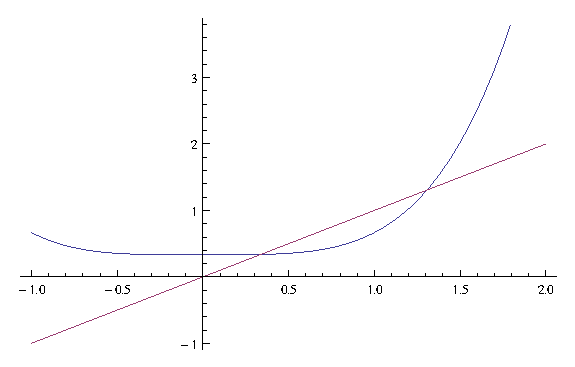
\includegraphics{Analysis/Analysis_sequence.eps}}
\end{figure}

\centertexdraw{

    \def\bdot {\fcir f:0 r:0.03 }

    \drawdim in

    \arrowheadtype t:F \arrowheadsize l:0.08 w:0.04
    \linewd 0.01 \setgray 0

    \move (-1 -1) \lvec(2 2)
    \move (-1 0) \clvec (1 0.5)(1.5 1)(2 1.5)

    \move (-1 -1) \avec (-1 0 ) \avec(0 0) \avec(0 0.3) \avec(0.3 0.3) \avec(0.3 0.4)
    \move (2 2) \avec (2 1.5) \avec(1.5 1.5) \avec(1.5 1.05) \avec(1.05 1.05) \avec(1.05 0.75) \avec(0.75 0.75) \avec(0.75 0.6)\avec(0.6 0.6)

    \move (0.46 0.46) \bdot
    \htext (-1.1 -1){0}
    \htext (0.4 0.2){$r_1$}

    \move (2 -1) \lvec(5 2)
    \move (2.2 -1) \clvec (3.2 0.5)(3.4 1)(3.7 2)

    \move (2.57 -0.43) \bdot
    \move (3 0) \avec (3 0.3) \avec (3.3 0.3) \avec (3.3 0.85) \avec (3.85 0.85) \avec (3.85 2)
    \htext (2.8 -0.5){$r_2$}

\move (0 -1.2)
}

Let the two roots of $f(x) = (x^4+1)/3 - x$ be $r_1$ and $r_2$ ($r_1 < r_2$). Because $f(0)>0$, $f(1) <0$ and $f(2) >0$, we have $r_1 \in (0,1)$ and $r_2\in (1,2)$.

Graphical analysis tells us that sequences starting with $a_1 =0,1$ converge to $r_1$ and $a_1 = 2$ diverges to infinity.

$a_1 = 0$. If $a_n \in (0,r_1)$, $f(a_n) = (a_n^4+1)/3 - a_n = a_{n+1} -a_n >0\ \ra \ a_{n+1} > a_n$. But
\be
a_{n+1} = (a_n^4+1)/3 < (r_1^4+1)/3 = r_1
\ee

Thus, $a_n$ is increasing and bounded above so it is converging.

$a_1 = 1$. If $a_n \in (r_1,r_2)$, $f(a_n) = (a_n^4+1)/3 - a_n = a_{n+1} -a_n < 0\ \ra \ a_{n+1} < a_n$. But
\be
a_{n+1} = (a_n^4+1)/3 > (r_1^4+1)/3 = r_1
\ee

Thus, $a_n$ is decreasing and bounded above so it is converging.

$a_1 = 2$. If $a_n \in (r_2,\infty)$, $f(a_n) = (a_n^4+1)/3 - a_n = a_{n+1} -a_n >0\ \ra \ a_{n+1} > a_n$. Thus, $a_n$ is increasing and unbounded above so it is diverging.
\end{solution}

%------------------------------------------------------------------------------------------------------------------

\begin{problem}
Let $a_1>b_1>0$ and let $a_{n+1} = (a_n + b_n)/2$, $b_{n+1} = 2a_nb_n/(a_n+b_n)$ for $n\geq 1$. Show that $a_n>a_{n+1}>b_{n+1}>b_n$ and deduce the two sequences converge to a common limit. What limit?
\end{problem}

\begin{solution}[\bf Solution.]
Since $a_1>b_1>0$,
\be
\left\{\ba{l}
2a_1 > a_1 + b_1 \ \ra \ a_1 > \frac{a_1 + b_1}2 = a_2\\
\frac 1{a_1} < \frac 1{b_1} \ \ra \  \frac 1{a_1} + \frac 1{b_1}  < \frac 2{b_1} \ \ra \ b_1 < \frac 2{\frac 1{a_1} + \frac 1{b_1}} = b_2\\
a_2 - b_2 = \frac{a_1 + b_1}2 - \frac {2a_1b_1}{a_1 + b_1} = \frac {(a_1 - b_1)^2}{2(a_1+b_1)} >0
\ea\right. \ \ra \ a_1 > a_2 > b_2 > b_1.
\ee

By induction, we have $a_n>a_{n+1}>b_{n+1}>b_n$. Since $a_n$ is a decreasing sequence, and bounded below (by 0), thus $a_n$ converges to $a$. Similarly, $b_n$ is an increasing sequence and bounded above (by $a_1$). Thus,
\be
\left\{\ba{l}
a = \frac {a+b}2 \\
b = \frac {2ab}{a+b}
\ea\right. \ \ra \ a = b.
\ee
which means that $a_n$ and $b_n$ converge to a common limit $c$. We know that
\be
a_{n+1}b_{n+1} = (a_n + b_n)/2 \times 2a_nb_n/(a_n+b_n) = a_n b_n \ \ra \ c^2 = a_1 b_1 \ \ra \ c = \sqrt{a_1b_1}.
\ee
\end{solution}
			%p
\chapter{Complex Analysis}

\section{Complex Numbers}

\subsection{Complex numbers}

\begin{definition}[complex number]
A complex number $z$ is defined as an ordered pair
\be
z = (x,y),
\ee
where $x$ and $y$ are both real numbers. Commonly, we write
\be
z = x+ iy,
\ee
where $i$ is a symbol such that $i^2 = -1$. Symbolically, we write
\be
\Re(z) =x,\quad \Im(z) = y
\ee
which are called real part\index{real part} and imaginary part\index{imaginary part} of $z$, respectively. If $y=0$, the complex number is real. If $x= 0$ and $y\neq 0$, the complex number is called purely imaginary.

The set of all complex numbers is denoted by $\C$.
\end{definition}

\begin{figure}[h!]%[t]
\begin{center}
\begin{pspicture}(-4,-0.5)(4,4)
\psaxes[ticks=none,labels=none]{->}(0,0)(-4,-1)(4,4)
\psset{plotpoints=500,linewidth=1pt,arrowscale =2}

\pstGeonode[PointSymbol=none,PointName=none](1,0.1){A1}(1,-0.1){A2}(-0.1,1){B1}(0.1,1){B2}
\pstGeonode[PointSymbol=default,PointName=none](2,0){X}(0,2){Y}(2,2){Z}
%\pstCircleOA[PointSymbol=none,PointName=none,linestyle=dashed,linecolor=green]{O}{A}

\psline[linecolor=blue]{->}(O)(Z)
\psline[linestyle=dashed](Z)(X)
\psline[linestyle=dashed](Z)(Y)

\psset{linewidth=0.5pt}
\psline(A1)(A2)
\psline(B1)(B2)

%\psline[linecolor=red]{->}(B)(Z)
%\psline[linestyle=dashed,linecolor=green](B)(C)
%\psline[linestyle=dashed,linecolor=green](Z)(D)
%
%\pstMarkAngle[MarkAngleRadius=0.2,LabelAngleOffset=-15,LabelSep=1.2]{C}{B}{Z}{$\Arg(z+i)$}
%\pstMarkAngle[MarkAngleRadius=0.2,LabelAngleOffset=-15,LabelSep=0.6]{D}{Z}{A}{$\Arg(i-z)$}
%
%\rput[lb](0.1,3.1){$i$}
%\rput[lb](0.1,-3.4){$-i$}
%
%\rput[lb](0.5,1.8){$i-z$}
%\rput[lb](1.5,-1){$z+i$}
%
%\rput[lb](1.1,0.6){$z$}
%
%\pstGeonode[PointSymbol=o,PointName=none](0,3){AA}(0,-3){BB}
%
\rput[lb](1.7,2.1){$z = x+ iy$}
\rput[lb](1.9,-0.3){$x$}
\rput[lb](-0.4,1.9){$iy$}
\rput[lb](0.85,-0.3){$1$}
\rput[lb](-0.3,0.9){$i$}

\rput[lb](3.5,-0.3){real axis}
\rput[lb]{90}(-0.2,2.3){imaginary axis}
\end{pspicture}
\end{center}
\end{figure}


\begin{remark}
The complex numbers can be visualized as the usual Euclidean plane by the following simple identification: the complex number $z = x+iy \in \C$ is identified with the point $(x,y)\in \R^2$. For example, 0 corresponds to the origin and $i$ corresponds to $(0,1)$. So any complex number $z$ can be treated as a vector in $\R^2$.

Naturally, the $x$ and $y$ axis of $\R^2$ are called the real axis and imaginary axis, which form the complex plane.
\end{remark}

\begin{definition}[equivalence of complex numbers]
For two complex numbers $z_1 = x_1+iy_1$ and $z_2 = x_2+ iy_2$, we say $z_1 =z_2$ if 
\be
x_1=x_2,\quad y_1 = y_2.
\ee
\end{definition}


\subsection{Algebra of complex numbers}

\begin{definition}[algebra of complex numbers]\label{def:algebra_complex}
Let $z_1,z_2\in \C$ with $z_1 = x_1+iy_1$ and $z_2 = x_2 + iy_2$. Then the addition is defined by
\be
z_1 + z_2 := (x_1+x_2) + i(y_1+y_2)
\ee
and substraction is defined bt
\be
z_1 - z_2 :=  (x_1-x_2) + i(y_1-y_2)
\ee

The multiplication is defined by
\beast
z_1z_2 & := & ( x_1+iy_1)(x_2+iy_2) = x_1x_2 + ix_1y_2 + ix_2y_1 + i^2 y_1y_2 \\
& = & (x_1x_2-y_1y_2) + i(x_1y_2 + x_2y_1).
\eeast
and for $z_2 \neq 0$ the division is define by
\beast
\frac{z_1}{z_2} & := & \frac{x_1+ iy_1}{x_2 + iy_2} = \frac{(x_1+ iy_1)(x_2 - iy_2)}{(x_2 + iy_2)(x_2 - iy_2)} = \frac{x_1x_2 + y_1y_2 + i(-x_1y_2 + x_2y_1)}{x_2^2 + y_2^2} \\
& = & \frac{x_1x_2 + y_1y_2 }{x_2^2 + y_2^2} + i\frac{ x_2y_1-x_1y_2 }{x_2^2 + y_2^2} .
\eeast
\end{definition}

\begin{example}
For $z_1 = 3+7i$ and $z_2 = 5 - 6i$,
\beast
z_1+ z_2 & = & (3+5) + i(7+(-6)) =8+ i,\\
z_1- z_2 & = & (3-5) + i(7+6) =-2+ 13i.
\eeast

Also,
\be
z_1z_2 = (3+7i)(5-6i) = (3\cdot 5 - 7 \cdot (-6)) + i(3\cdot (-6) + 7 \cdot 5) = 57 + 17i,
\ee
and
\be
\frac{z_1}{z_2} = \frac{3\cdot 5 + 7\cdot (-6)}{5^2 + 6^2} + \frac{7\cdot 5 - 3\cdot (-6)}{5^2 + 6^2}i = -\frac{27}{61} + \frac{53}{61}i.
\ee
\end{example}

\begin{proposition}
For all $z_i\in \C$, we have
\ben
\item [(i)] Commutativity. $z_1+z_2 = z_2+z_1$ and $z_1z_2 = z_2 z_1$.
\item [(ii)] Associativity. $(z_1+z_2)+ z_3 = z_1 + (z_2+z_3)$ and $(z_1z_2)z_3 = z_1(z_2z_3)$.
\item [(iii)] Distributivity. $z_1(z_2+z_3) = z_1z_2 + z_1z_3$.
\een
\end{proposition}

\begin{proof}[\bf Proof]
Direct result from Definition \ref{def:algebra_complex}.
\end{proof}

\begin{proposition}
The complex domain $\C$ is a field.
\end{proposition}

\begin{proof}[\bf Proof]
\footnote{proof needed. see \cite{Mathews_Howell_1997}}
\end{proof}

\subsection{Conjugate of complex number}

\begin{definition}[complex conjugate]
The complex conjugate of complex number $z = x+iy$ is defined by
\be
\ol{z} := x - iy,
\ee
and it is obtained by a reflection across the real axis in the plane.

\begin{figure}[h]%[t]
\begin{center}
\begin{pspicture}(-3,-2.5)(3,2.5)
\psaxes[ticks=none,labels=none]{->}(0,0)(-3,-2.5)(3,2.5)
\psset{plotpoints=500,linewidth=1pt,arrowscale =2}

%\pstGeonode[PointSymbol=none,PointName=none](1,0.1){A1}(1,-0.1){A2}(-0.1,1){B1}(0.1,1){B2}
\pstGeonode[PointSymbol=default,PointName=none](2,2){Z}
\pstGeonode[PointSymbol=default,PointName=none](2,-2){ZC}
%\pstCircleOA[PointSymbol=none,PointName=none,linestyle=dashed,linecolor=green]{O}{A}

\psline[linecolor=blue]{->}(O)(Z)
\psline[linecolor=red]{->}(O)(ZC)
\psline[linestyle=dashed](Z)(ZC)


%\psset{linewidth=0.5pt}
%\psline(A1)(A2)
%\psline(B1)(B2)
%
\rput[lb](1.7,2.1){$z = x+ iy$}
\rput[lb](1.6,-2.4){$\ol{z} = x- iy$}
\end{pspicture}
\end{center}
\end{figure}%In fact, a complex number $z$ is real if and only if $z = \ol{z}$, and it is purely imaginary if and only if $z = -\ol{z}$.
\end{definition}

\begin{remark}
Obviously, $z = \ol{z}$ if and only if $z$ is a real number.
\end{remark}

\begin{proposition}
For any $z\in \C$,
\be
\ol{\ol{z}} = z,\qquad \Re(z) = \frac{z+\ol{z}}2,\qquad \Im(z) = \frac{z - \ol{z}}{2i}.%,\qquad \abs{z}^2 = z\ol{z}.
\ee

Furthermore, for any $z_1,z_2\in \C$,
\be
\ol{z_1+z_2} = \ol{z_1} + \ol{z_2},\qquad \ol{z_1-z_2} = \ol{z_1} - \ol{z_2},\qquad\ol{z_1z_2} = \ol{z_1}\cdot \ol{z_2}.
\ee

In addition, for $z_2\neq 0$,
\be
\ol{\bb{\frac {z_1}{z_2}}} = \ol{z_1}/\ol{z_2}.
\ee
\end{proposition}

\begin{proof}[\bf Proof]
The first three equations are the direct result from the definitions. For $z_1 = x_1 + iy_1$ and $z_2 = x_2 + iy_2$,
\beast
\ol{z_1+z_2} & = & \ol{(x_1+x_2) + i(y_1+y_2)} = (x_1+x_2) - i(y_1+y_2) = (x_1-iy_1) + (x_2-iy_2) = \ol{z_1} + \ol{z_2},\\
\ol{z_1-z_2}  & = & \ol{(x_1-x_2) + i(y_1-y_2)} = (x_1-x_2) - i(y_1-y_2) = (x_1-iy_1) - (x_2-iy_2) = \ol{z_1} - \ol{z_2}.
\eeast

Also,
\beast
\ol{z_1z_2} & = & \ol{(x_1x_2-y_1y_2) + i(x_1y_2+x_2y_1)} = (x_1x_2-y_1y_2) - i(x_1y_2+x_2y_1) \\
& = & (x_1-iy_1)(x_2-iy_2) = \ol{z_1}\cdot \ol{z_2},
\eeast
\beast
\ol{\bb{\frac{z_1}{z_2}}} & = & \ol{\bb{\frac{x_1x_2 + y_1y_2 + i(-x_1y_2 + x_2y_1)}{x_2^2 + y_2^2} }} = \frac{x_1x_2 + y_1y_2 - i(-x_1y_2 + x_2y_1)}{x_2^2 + y_2^2}\\
& = & \frac{x_1x_2 + (-y_1)(-y_2) + i(-x_1(-y_2) + x_2(-y_1))}{x_2^2 + y_2^2} = \frac{x_1-iy_1}{x_2-iy_2} = \ol{z_1} / \ol{z_2}
\eeast
as required.
\end{proof}



\subsection{Modulus of complex numbers}

\begin{definition}[modulus]\label{def:modulus_complex_number}
Let $z=x+iy$ with $x,y\in\R$. Then the modulus (or absolute value) of $z$ is defined by
\be
\abs{z} := \sqrt{x^2 + y^2}.
\ee
\end{definition}

\begin{remark}
The modulus $\abs{z}$ is the distance between the origin and the point $(x,y)$ in $\R^2$-plane.

Obviously, we have $\abs{z} = \abs{-z}$, $\abs{z} = \abs{\ol{z}}$ and $\abs{z}^2 = z\ol{z}$ for any $z\in \C$.

In addition, $\Re(z) \leq \abs{z}$ and $\Im(z) \leq \abs{z}$.
\end{remark}

\begin{proposition}\label{pro:modulus_multiplication_division_complex}
For all $z_1,z_2,z_3\in \C$,
\be
\abs{z_1z_2} = \abs{z_1}\abs{z_2},\qquad \abs{\frac{z_1}{z_3}}= \frac{\abs{z_1}}{\abs{z_3}},\quad z_3 \neq 0.
\ee
\end{proposition}

\begin{proof}[\bf Proof]
For $z_1 =x_1+iy_1$ and $z_2 = x_2 + iy_2$,
\be
\abs{z_1z_2}^2 = z_1z_2\ol{z_1z_2} = z_1z_2 \ol{z_1}\ol{z_2} = z_1\ol{z_1}z_2 \ol{z_2} = \abs{z_1}^2 \abs{z_2}^2.
\ee
%\beast
%\abs{z_1z_2}^2 & = &  \abs{(x_1x_2 - y_1y_2)+ i(x_1y_2 + x_2y_1)}^2 = (x_1x_2 - y_1y_2)^2 + (x_1y_2 + x_2y_1)^2 \\
%& = & x_1^2 x_2^2 + y_1^2y_2^2 + x_1^2y_2^2 + x_2^2 y_1^2 = \bb{x_1^2 + y_1^2}\bb{x_2^2 + y_2^2} = \abs{z_1}^2\abs{z_2}^2
%\eeast

For $z_3 \neq 0$,
\beast
\abs{\frac{z_1}{z_3}}^2 = \frac{z_1}{z_3}\ol{\bb{\frac{z_1}{z_3}}} = \frac{z_1}{z_3}\frac{\ol{z_1}}{\ol{z_3}} = \frac{z_1\ol{z_1}}{z_3\ol{z_3}} = \frac{\abs{z_1}^2}{\abs{z_3}^2}.
\eeast
\end{proof}

\begin{proposition}[parallelogram law]\label{pro:complex_modulus_parallelogram_law}
For all $z_1,z_2\in \C$,
\beast
\abs{z_1+z_2}^2 = \abs{z_1}^2 + 2\Re \bb{z_1\ol{z_2}} + \abs{z_2}^2,\\
\abs{z_1-z_2}^2 = \abs{z_1}^2 - 2\Re \bb{z_1\ol{z_2}} + \abs{z_2}^2.
\eeast

Thus, we have
\be
\abs{z_1+z_2}^2 + \abs{z_1- z_2}^2 = 2\bb{\abs{z_1}^2 + \abs{z_2}^2}.
\ee
\end{proposition}

\begin{proof}[\bf Proof]
By definition of modulus, we have
\beast
\abs{z_1+z_2}^2 & = & \bb{z_1 + z_2} \ol{ \bb{z_1 + z_2}} = \bb{z_1 + z_2} \bb{\ol{ z_1} + \ol{z_2}} = z_1 \ol{z_1} + z_1\ol{z_2} + z_2 \ol{z_1} + z_2\ol{z_2} \\
& = &  z_1 \ol{z_1} + z_1\ol{z_2} + \ol{z_1 \ol{z_2}} + z_2\ol{z_2} =  \abs{z_1}^2 + 2\Re\bb{z_1\ol{z_2}} + \abs{z_2}^2 
\eeast
and 
\beast
\abs{z_1-z_2}^2 & = & \bb{z_1 - z_2} \ol{ \bb{z_1 - z_2}} = \bb{z_1 - z_2} \bb{\ol{ z_1} - \ol{z_2}} = z_1 \ol{z_1} - z_1\ol{z_2} - z_2 \ol{z_1} + z_2\ol{z_2} \\
& = &  z_1 \ol{z_1} - z_1\ol{z_2} - \ol{z_1 \ol{z_2}} + z_2\ol{z_2} =  \abs{z_1}^2 - 2\Re\bb{z_1\ol{z_2}} + \abs{z_2}^2 
\eeast

Then we get the required result by adding the above two.
\end{proof}



\begin{proposition}[triangle inequality]\label{pro:triangle_inequality_complex}
For all $z_1,z_2\in \C$,
\ben
\item [(i)] $\abs{z_1+z_2} \leq \abs{z_1} + \abs{z_2}$,
\item [(ii)] $\abs{\abs{z_1} -\abs{z_2}} \leq \abs{z_1-z_2} $
\een
where $\abs{\cdot}$ is the modulus of complex numbers.
\end{proposition}

\begin{remark}
\ben
\item [(i)] If we treat $z_1$ and $z_2$ as two vectors, this inequality is actually the triangle inequality.

\item [(ii)] Let $z = x + iy$. Then
\be
\abs{z} = \abs{x+iy} \leq \abs{x} + \abs{iy} = \abs{x} + \abs{y} = \abs{\Re z} + \abs{\Im z}.
\ee
\een
\end{remark}

\begin{proof}[\bf Proof]
\ben
\item [(i)] {\bf Approach 1.} Let $z_1 = x_1+iy_1$ and $z_2 = x_2 + iy_2$. Since $ab \leq \frac{a^2+b^2}2$ for any $a,b\in \R$, we have
\beast
2x_1x_2y_1y_2 \leq x_1^2 y_2^2 + x_2^2 y_1^2 \ \ra\ \bb{x_1x_2 + y_1y_2}^2 \leq \bb{x_1^2+ y_1^2}\bb{x_2^2 + y_2^2} \ \ra\ x_1x_2 + y_1y_2 \leq \sqrt{x_1^2+ y_1^2}\sqrt{x_2^2 + y_2^2}.
\eeast

Therefore,
\beast
\abs{z_1+z_2}^2 & = & (x_1+x_2)^2+ (y_1+y_2)^2 = x_1^2+ x_2^2 + y_1^2+ y_2^2 + 2x_1x_2 + 2y_1y_2 \\
&\leq & x_1^2+ x_2^2 + y_1^2+ y_2^2 + 2\sqrt{x_1^2+ y_1^2}\sqrt{x_2^2 + y_2^2} = \bb{\sqrt{x_1^2+ y_1^2} + \sqrt{x_2^2 + y_2^2}}^2\\
& = & \bb{\abs{z_1} + \abs{z_2}}^2
\eeast
which implies the required result.

{\bf Approach 2.} Apply basic properties of modulus, we have
\beast
\abs{z_1+z_2}^2 & = &  \abs{z_1}^2 + 2\Re\bb{z_1\ol{z_2}} + \abs{z_2}^2 \leq \abs{z_1}^2 + 2\abs{\Re\bb{z_1\ol{z_2}}} + \abs{z_2}^2 \\
& \leq & \abs{z_1}^2 + 2\abs{z_1\ol{z_2}} + \abs{z_2}^2 = \abs{z_1}^2 + 2\abs{z_1}\abs{z_2} + \abs{z_2}^2 = \bb{\abs{z_1}+\abs{z_2}}^2
\eeast

\item [(ii)] By (i), we have
\be
\abs{z_1} = \abs{(z_1-z_2) + z_2} \leq \abs{z_1-z_2} + \abs{z_2} \ \ra\ \abs{z_1} - \abs{z_2} \leq \abs{z_1-z_2}.
\ee

Then switching $z_1$ and $z_2$ we have
\be
\abs{z_2} - \abs{z_1} \leq \abs{z_2-z_1} = \abs{z_1-z_2} \ \ra\ \abs{z_1} - \abs{z_2} \geq -\abs{z_1-z_2}.
\ee

Therefore,
\be
-\abs{z_1-z_2} \leq \abs{z_1} - \abs{z_2} \leq \abs{z_1-z_2} \ \ra\ \abs{\abs{z_1} - \abs{z_2}} \leq \abs{z_1-z_2}
\ee
as required.
\een
\end{proof}


\subsection{The extended plane and its spherical representation}

\footnote{See \cite{Conway_1978_a}.$P_{8}$}




\section{Complex Sequences and Convergence}

%\subsection{Convergence and limits on complex domain}

\subsection{Convergence and limits on complex sequence}%\section{Convergence and limits of complex sequences}

\begin{definition}[convergence, limit]\label{def:convergence_limit_complex}
Let $(z_n)$ be a complex sequence. Then we say that $(z_n)$ converges\index{convergence!complex sequence} to a complex number $z$ if for any $\ve>0$ there exists $N>0$ such that for all $n\geq N$,
\be
\abs{z_n - z} < \ve
\ee
where $\abs{\cdot}$ is the modulus function. It can also written as
\be
\lim_{n\to \infty} z_n = z.
\ee

In addition, $z$ is called the limit\index{limit!complex sequence} of $(z_n)$.

Otherwise, $(z_n)$ is divergent.
\end{definition}

\begin{definition}
Let $(z_n)$ be a complex sequence. Then we write
\be
\lim_{n\to \infty}z_n = \infty
\ee
if for any $M>0$ there exists $N>0$ such that for all $n\geq N$, $\abs{z_n} > M$. Note that $\abs{\cdot}$ is the modulus function.
\end{definition}

%\begin{definition}
%We say $a_n\to a\in\C$ as $n\to \infty$, if $a_n,a\in \C$ for any $n$ and given $\ve>0,\exists N$ s.t.
%\be
%|a_n-a|<\ve,\ \forall n\geq N.
%\ee
%where $|\cdot|$ stands for the modulus of a complex number.
%\end{definition}

%If we were considering instead subsequences of complex numbers, $a_n\in\C$, we can give essentially the same definition of limit.


\begin{theorem}\label{thm:convergence_of_complex_iff_convergence_of_real_imaginary}
Let $(z_n)$ be a complex sequence with $z_n = x_n + iy_n$ for $n\in \N$ and $z = x+iy \in \C$. Then
\be
\lim_{n\to \infty} z_n = z \quad \lra \quad \lim_{n\to \infty} x_n = x,\quad \lim_{n\to \infty} y_n = y.
\ee
\end{theorem}

\begin{remark}
Note that the theorem enables us to write
\be
\lim_{n\to \infty} (x_n + iy_n) = \lim_{n\to \infty} x_n + i \lim_{n\to \infty} y_n
\ee
whenever we know that both limits on the right exist or that the one on the left exists.
\end{remark}

\begin{proof}[\bf Proof]
($\ra$). Assume $\lim_{n\to \infty} z_n = z$. Given any $\ve>0$, there exists $N\in\N$ such that for all $n\geq N$,
\be
\abs{x_n + iy_n - x- iy} = \abs{z_n - z} < \ve.
\ee

Thus, we have
\beast
\abs{x_n - x} & = & \abs{\Re (z_n-z)} \leq \abs{z_n-z} < \ve \\
\abs{y_n - y} & = & \abs{\Im (z_n-z)} \leq \abs{z_n-z} < \ve.
\eeast
which implies that $\lim_{n\to \infty} x_n = x$ and $\lim_{n\to \infty} y_n = y$.

($\la$). Assume $\lim_{n\to \infty} x_n = x$ and $\lim_{n\to \infty} y_n = y$. Then given any $\ve>0$, we can find $N_1,N_2\in \N$ such that
\be
\abs{x_n - x} < \ve/2\qquad \forall n\geq N_1,\qquad \abs{y_n - y} < \ve/2\qquad \forall n\geq N_2.
\ee

Then we take $N = \max \bra{N_1,N_2}$, we can have for all $n\geq N$,
\be
\abs{z_n - z} = \abs{x_n + iy_n - x- iy} \leq  \abs{x_n - x} +  \abs{y_n - y} < \ve/2 + \ve/2 = \ve
\ee
which implies that $\lim_{n\to \infty} z_n = z$.
\end{proof}

\begin{example}
The sequence
\be
z_n = \frac 1{n^3} + i
\ee
converges to $i$ since
\be
\lim_{n\to \infty} \bb{\frac 1{n^3} + i} = \lim_{n\to \infty} \frac 1{n^3} + i \lim_{n\to \infty} 1 = 0 + i\cdot 1 = i.
\ee
\end{example}



\subsection{Convergence properties of complex sequence}

\begin{lemma}\label{lem:basic_convergence_complex}
For complex domain and sequence $(z_n)$ and $(w_n)$ and complex constants $z,w,c$,
\ben
\item [(i)] The limit is unique. That is, if $z_n \to z$ and $z_n \to w$ as $n \to \infty$ then $z=w$.
\item [(ii)] If $z_n \to z$ as $n \to \infty$ and $n_1 < n_2 < n_3 \ldots$ then $z_{n_i} \to a$ as $i \to \infty$. (Any subsequence converges to the same limit).
\item [(iii)]  If $z_n = c$ for all $n$ then $z_n \to c$ as $n \to \infty$.
\item [(iv)] If $z_n \to z$ and $w_n \to w$ as $n \to \infty$ then $z_n + w_n \to z + w$.
\item [(v)] If $z_n \to z$ and $w_n \to w$ as $n \to \infty$ then $z_n w_n \to zw$.
\item [(vi)] If $z_n \to z$ as $n \to \infty$, $z_n \neq 0$ for each $n$ and $z \neq 0$, then $z_n^{-1} \to  z^{-1}$.
\item [(vii)] If $z_n\to z$, then $\abs{z_n} \to \abs{z}$.
\een
\end{lemma}

\begin{remark}
The converse of (vii) is not true. Let $z_n = (-1)^n$, Then $\lim_{n\to \infty}\abs{z_n}= 1$ but $\lim_{n\to \infty} z_n$ does not exist.

It is also obvious that $\lim_{n\to\infty} z_n = 0$ iff $\lim_{n\to\infty}\abs{z_n} = 0$.
\end{remark}


\begin{proof}[\bf Proof]
\ben
\item [(i)] $z_n\to z$ means given $\ve>0$, $\exists N_1$ for all $n\geq N_1$ we have $\abs{z_n-z}<\ve$. Similarly, $z_n\to w$ means given $\varepsilon>0$, $\exists N_2$ for all $n\geq N_2$ we have $|z_n-w|<\ve$. Thus, by triangle inequality (Proposition \ref{pro:triangle_inequality_complex}) we have
\be
\abs{z-w} \leq \abs{z-z_n} + \abs{w-z_n} < 2\ve \text{ for }n\geq \max\bra{N_1,N_2}
\ee

Hence we have $|z-w|<2\ve$. If $z\neq w$, just take $\ve=\frac{|z-w|}{3}$, then $|z-w|<\frac{2|z-w|}{3}$ which is assurd. Thus, $z=w$.

\item [(ii)] $z_n\to z$ means given $\ve >0$, $\exists N$ s.t. $|z_n-z|<\ve, \forall n\geq N$. $z_{n_i}$, $n_i\geq i$, thus we have
\be
|z_{n_i}-z| < \varepsilon,\ \forall j\geq N \ \ra \ z_{n_i}\to z\ \text{ as }i\to\infty.
\ee

\item [(iii)] If $z_n = c$ then given $\ve > 0$ set $N(\ve) = 1$. Then
\be
|z_n - c| = |c-c| = 0 < \ve, \ \forall n \geq N(\ve).
\ee

%\item [(iv)] We know that given $\ve > 0$, $\exists N_1(\ve),N_2(\ve)$ such that $|a_n - a| < \ve\ \forall n \geq N_1(\ve),\ |b_n - b| < \ve\ \forall n \geq N_2(\ve)$. Thus if $n \geq N(\ve) = \max\bra{N_1\bb{\frac{\ve}2}, N_2\bb{\frac{\ve}2}}$, we have
%\be
%|(a_n + b_n) - (a - b)| = |(a_n - a) + (b_n - b)| \leq |a_n - a| + |b_n -b| < \frac{\ve}{2} + \frac{\ve}{2}
%\ee
%for any $n \geq N(\ve)$.

\item [(iv)] For given $\ve>0$, we can find $n$ such that $\abs{z_n -z}<\ve/2$ and $\abs{w_n -w}<\ve/2$. Thus, by Proposition \ref{pro:triangle_inequality_complex},
\be
\abs{z_n+w_n - (z+w)} = \abs{(z_n -z) + (w_n-w)} \leq \abs{z_n -z} + \abs{w_n -w} < \ve/2+\ve/2 = \ve.
\ee

\item [(v)] $z_n\to z$, given $\ve>0$, $\exists N_1$ s.t. $|z_n-z|<\ve, \ \forall n\geq N_1$. $w_n\to w$, given $\varepsilon>0$, $\exists N_2$ s.t. $|w_n-w|<\varepsilon, \forall n\geq N_2$. Then by triangle inequality (Proposition \ref{pro:triangle_inequality_complex})
\be
\abs{z_nw_n-zw} \leq |z_nw_n-z_nw| + |z_nw-zw| = |z_n||w_n-b| + |w||z_n-z|
\ee

We have $|z_n|\leq |z_n-z|+|z|\leq 1+|z|,\forall n\geq N_1(1) \ (\ve=1)$. Thus, we have
\be
|z_nw_n-zw| \leq (1+|z|)\ve + |w|\ve = \ve(|z|+|w|+1), \ \forall n\geq \max\{N_1(1),N_1(\ve), N_2(\ve)\}.
\ee

\item [(vi)] Again, given $\ve > 0$, $\exists N_1(\ve)$ such that $|z_n - z| < \ve$. Thus if $n \geq N(\ve) = \max\bra{N_1\bb{\frac{|z|}{2}}, N_1\bb{\frac{\ve|z|^2}{2}}}$, then
\be
\abs{\frac{1}{z_n} - \frac{1}{z}} = \abs{\frac{z - z_n}{zz_n}} = \frac{|z-z_n|}{|z||z_n|} <\frac{2|z_n - z|}{|z|^2} <\frac{\ve |z|^2}{2} \cdot \frac{2}{|z|^2} = \ve.
\ee

If $n \geq N(\ve)$ then $|z_n - z| < \frac{|z|}{2}$ so $|z_n| > \frac{|z|}{2}$.

\item [(vii)] By Proposition \ref{pro:triangle_inequality_complex}, we have given $\ve>0$, there exists $N$ such that $\forall n\geq N$,
\be
\abs{\abs{z_n} -\abs{z}} \leq \abs{z_n - z} <\ve
\ee
which implies that $\lim_{n\to \infty}\abs{z_n} = \abs{z}$.
\een
\end{proof}

\begin{proposition}\label{pro:convergence_of_complex_power_function}
Let $z$ be a complex number. Then
\ben
\item [(i)] $\lim_{n\to \infty} z^n = 0$ for $\abs{z} <1$.
\item [(ii)] $\lim_{n\to \infty} z^n = \infty$ for $\abs{z}>1$.
\item [(iii)] $\lim_{n\to \infty} z^n$ does not exist for $\abs{z}=1$ with $z\neq 1$.
\een
\end{proposition}

\begin{remark}
Obviously, $\lim_{n\to \infty} 1^n = 1$ by definition.
\end{remark}

\begin{proof}[\bf Proof]
\ben
\item [(i)] By definition of convergence, for any $1>\ve>0$ and $\abs{z} = \frac 1{1+\delta}$ with $\delta>0$
\be
\abs{z^n-0} = \abs{z^n} = \abs{z}^n = \frac 1{(1+\delta)^n} < \frac 1{1+n\delta}.
\ee

Therefore, we can find $n\geq \frac {1-\ve}{\delta\ve}$ such that $\abs{z^n-0}<\ve$. Thus, $\lim_{n\to\infty} z^n = 0$.

%If $\abs{z}\geq 1$, clearly $\lim_{n\to \infty} \abs{z^n} \neq 0$. Hence $\lim_{n\to \infty} z^n \neq 0$.

\item [(ii)] If $\abs{z} >1$, we assume $\abs{z} = 1+\delta$ with $\delta >0$. Then
\be
\abs{z^n} = \abs{z}^n = \bb{1+\delta}^n > 1+ n\delta.
\ee

So for any $M>1$ we can find $n \geq \frac{M-1}{\delta}$ such that $\abs{z^n} > M$. This implies that $\lim_{n\to \infty}z^n = \infty$.

\item [(iii)] Now let $\abs{z=1}$. If $z=1$, it is obvious that $z^n = 1$ for any $n\in \N$ which implies that $\lim_{n\to \infty}z^n = 1$. Assume $w$ is the limit of $z^n$. Then given $\ve>0$, we can find $N$ such that $\forall n\geq N$ we have
\be
\abs{z^n - w} < \ve.
\ee

Then we have for any $n\geq N$,
\be
\abs{z^{n+1} - zw} = \abs{z\bb{z^n -w}} = \abs{z}\abs{z^n-w} < \abs{z}\ve = \ve .
\ee

This means $zw$ is also the limit of $z^n$. Since the limit is unique, we have $w =0$. By Lemma \ref{lem:basic_convergence_complex}, %{lem:sequence_limit_implies_absolute_sequence_absolute_limit_complex}, %But $w\neq zw$ since $z\neq 1$
\be
\lim_{n\to\infty} z^n = w \ \ra\ \lim_{n\to\infty} \abs{z^n} = \abs{w} = 0.
\ee

However, we have $\abs{z^n} = \abs{z}^n = 1$ for any $n$ which implies the contradiction. Thus, $\lim_{n\to\infty} z^n $ does not exist for $\abs{z}=1$ with $z\neq 1$.
\een
\end{proof}


\subsection{Cauchy sequence}

\begin{definition}[Cauchy sequence\index{Cauchy sequence!complex}]
A complex sequence $(z_n)$ is said to be a Cauchy sequence if
\be
\abs{z_n - z_m} \to 0,\qquad \text{as }n,m\to \infty.
\ee

In other words, given $\ve>0$ there exists an integer $N>0$ so that $\abs{z_n-z_m}<\ve$ whenever $n,m>N$.
\end{definition}

\begin{theorem}\label{thm:complex_plane_is_complete}%[$\C$ is complete]
The complex domain $\C$ is complete\index{complete space!complex}. That is, every Cauchy sequence in $\C$ has a limit in $\C$.
\end{theorem}

\begin{proof}[\bf Proof]
Let $(z_n)$ be a Cauchy sequence in $\C$ with $z_n = x_n + iy_n$. Since
\be
\abs{z_n - z_m} = \abs{(x_n-x_m) + i(y_n - y_m)} ,
\ee
we have
\be
\abs{z_n - z_m} \to 0 \ \lra\ (x_n-x_m)^2 + (y_n - y_m)^2 \to 0 \ \lra\ \abs{x_n-x_m} \to 0,\ \abs{y_n - y_m} \to 0.
\ee

This means that the complex sequence $(z_n)$ is Cauchy sequence if an only if the sequences of real and imaginary parts of $z_n$ are Cauchy. Therefore, we have that $(x_n)$ and $(y_n)$ are real Cauchy sequences. Since $\R$ is complete, every real Cauchy sequence converges in $\R$\footnote{theorem needed.}, there exist $x,y\in \R$ such that
\be
\abs{x_n -x} \to 0,\quad \abs{y_n - y}\to 0,\qquad\text{as }n\to \infty.
\ee

Then for $z = x+iy \in \C$, we have
\be
\abs{z_n - z} = \abs{(x_n-x) + i(y_n - y)} = \sqrt{(x_n-x)^2 + (y_n - y)^2} \to 0
\ee
as $n\to \infty$. This implies that $z_n$ converges to $z$ so $\C$ is complete.
\end{proof}

\subsection{Bolzano-Weierstrass theorem}

\begin{definition}[bounded sequence\index{bounded sequence!complex}]
Let $(z_n)$ be a complex sequence. We say that $(x_n)$ is bounded if there exists $M>0$ such that for any $n$, $\abs{z_n}\leq M$.
\end{definition}

\begin{theorem}[Bolzano-Weierstrass theorem]\label{thm:bolzano_weierstrass_complex}
If a complex sequence $(z_n)$ is bounded, then there exists a subsequence of $(z_n)$ which converges.
\end{theorem}

\begin{proof}[\bf Proof]
Since $(z_n)$ is bounded, there is a disk centered at the origin containing all $z_n$. Then by possibly shrinking and translating this disc we can assume that it is contained in the square $S$ with vertices 0,1,$1+i$ and $i$. Note that the shrinking and translating do not change the convergence behavior of the sequence.

Now consider the following recursive procedure. Using a vertical segment and a horizontal segment divide $S$ into four squares of the same size $S_1$ with vertices 0, 1/2, $1/2+i/2$, $i/2$, $S_2$ with vertices 1/2, 1, $1+i/2$, $1/2+i/2$, $S_3$ with vertices $1/2+i/2$, $1+i/2$, $1+i$, $1/2+i$ and $S_4$ with vertices $i/2$, $1/2+i/2$, $1/2+i$, $i$.

Since the sequence $(z_n)$ is infinite, there must be one of the these squares with an infinite number of points. If $S_i$ is such square, pick an arbitrary point in it and call it $w_1$. Then only consider those points in the sequence $(z_n)$ with indices $n$ larger than the index of $w_1$ in $(z_n)$. Then repeat the same procedure using $S_i$ instead of $S$ and proceed recursively. In this way we construct a sequence $(w_k)$ (in other form, $(z_{n_k})$) where the indices of the $w_k$'s in the sequence $(z_n)$ are in order and moreover each $w_k$ is contained in a square of side $1/2^k$ with all $w_j$ with $j\geq k$. Therefore,
\be
\abs{w_j - w_k} < \frac 1{2^k},\qquad \forall j\geq k
\ee
which means that the sequence $(w_k)$ (or the subsequence $(z_{n_k})$) is a Cauchy sequence and therefore it is convergent (Theorem \ref{thm:complex_plane_is_complete}).
\end{proof}



\subsection{Function sequences}

\begin{definition}[uniform convergence\index{uniform convergence!complex function}]\label{def:uniform_convergence_complex}
Let $f,(f_n)_{n\in\N}$ be complex-valued functions defined on $A\subseteq \C$. If for any $\ve>0$, there exists $N\in\N$ such that for all $z\in A$ and all $n\geq N$ we have
\be
\abs{f_n(z) - f(z)} < \ve.
\ee
then we say the function sequence $(f_n)$ converges to $f$ uniformly on $A$.

Equivalently, $(f_n)_{n\in\N}$ converges uniformly to $f$ on $A$ if and only if for any $\ve>0$, there exists $N\in \N$ such that for all $m,n\geq N$ and all $z\in A$,
\be
\abs{f_n(z)-f_m(z)} < \ve.
\ee

Note that Cauchy sequence is convergent in complex case. This is the Cauchy criterion for uniform convergence.

Equivalently, we say $f_n$ converges to $f$ uniformly if and only if $a_n\to 0$ as $n\to \infty$ where $a_n$ is defined by
\be
a_n := \sup_{z\in A}\abs{f_n(z) - f(z)}.
\ee
\end{definition}


\section{Complex Sets}

\subsection{Bounded set}

%\begin{definition}[bounded set\index{bounded set!complex}]
%Let $X$ be a complex set. We say that $X$ is bounded if there exists $M>0$ such that for any $z\in X$, $\abs{z}\leq M$.
%\end{definition}


\begin{definition}[bounded set\index{bounded set!complex}]
A set $A\subseteq \C$ is bounded if there exists $M>0$ such that $\abs{z}< M$ whenever $z\in A$. In other words, the set $A$ is contained in some large disc.
\end{definition}

\subsection{Open set and closed set}

\begin{definition}[open disc, closed disc, circle]
If $z_0\in \C$ and $r>0$, we define the open disc $D_r(z_0)$ of radius $r$ centered at $z_0$ to be the set of all complex numbers that are at absolute value strictly less than $r$ from $z_0$. In other words,
\be
D_r(z_0) = \bra{z\in \C: \abs{z-z_0}<r},
\ee
and this is precisely the usual disc in the plane of radius $r$ centered at $z_0$.

The closed disc $\ol{D}_r(z_0)$ of radius $r$ centered at $z_0$ is the set of all complex numbers that are at absolute value no more than $r$ from $z_0$. In other words,
\be
\ol{D}_r(z_0) = \bra{z\in \C: \abs{z-z_0}\leq r}.
\ee

The boundary of either the open or closed disc is the circle
\be
C_r(z_0) = \bra{z\in \C: \abs{z-z_0}=r}.
\ee%In particular, the unit disc (the open disc centered at the origin and of radius 1) is denoted by%\be
%\sD = \bra{z\in \C: \abs{z}<1}.
%\ee
\end{definition}


\begin{definition}[interior point]
Given a set $A\subseteq X$ where $X \subseteq \C$, a point $z$ is an interior point of $A$ if there exists $r>0$ such that
\be
D_r(z) \subseteq A.
\ee

The interior of $A$, denoted by $\inter{A}$, consists of all its interior points.
\end{definition}

\begin{definition}[open set]
A set $A\subseteq X$ where $X\subseteq \C$ is said to be open in $X$ if every point in that set is an interior point of $A$. That is, for any $z\in A$, there exists $r>0$ such that $D_r(z)\subseteq A$. 
\end{definition}

\begin{remark}
The definition of open set in complex plane coincides with the definition of an open set in $\R^2$.\footnote{details needed.}

Note that the open set might have several open discs.
\end{remark}


\begin{definition}[closed set]
A set $A\subseteq X$ where $X\subseteq \C$ is closed in $X$ if its complement $A^c = X\bs A$ is open.
\end{definition}

\begin{example}
Consider the closed disc $A: = \ol{D}_r(z_0) = \bra{z\in \C:\abs{z-z_0} \leq r}$ with $z_0\in\C$ and $r>0$. If it is not closed then $X\bs A$ is not open, thus, for any $\ve>0$ and any $w\in X\bs A$, we can find $D_\ve(w) \cap A \neq \emptyset$. Thus, we can find a sequence $(w_n)\in A$ (such that $\abs{w_n- z_0} \leq r$) converging to $w$. But $\abs{w-z_0} > r$ so there exists $\delta>0$ such that $\abs{w-z_0} = r+ \delta$. Thus, by triangle inequality,
\be
\abs{w_n - w} \geq \abs{\abs{w-z_0}-\abs{w_n - z_0}} = \abs{w-z_0}-\abs{w_n - z_0} \geq r + \delta - r = \delta
\ee
which contradicts the statement that $(w_n)$ converges to $w$. Thus, we have that $A$ is closed.
\end{example}


\begin{definition}[limit point]
A point $z\in X$ where $X\subseteq \C$ is said to be a limit point of the set $A\subseteq X$ if there exists a sequence of points $z_n\in A$ such that $z_n\neq z$ and
\be
\lim_{n\to \infty} z_n = z.
\ee
\end{definition}

\begin{definition}[closure]
The closure of any set $A\subseteq X \subseteq \C$ is the union of $A$ and its limit points in $X$, often denoted by $\ol{A}$.
\end{definition}

\begin{theorem}\label{thm:closed_complex_set_contains_all_limit_points_equals_closure}
Let $A$ be a set in $X\subseteq \C$. Then the following three statements are equivalent:
\ben
\item [(i)] $A$ is closed in $X$.
\item [(ii)] $A$ contains all its limit points.
\item [(iii)] $\ol{A} = A$.
\een
\end{theorem}

\begin{proof}[\bf Proof]
(i) $\ra$ (ii). Suppose $A$ is closed and $B:= X\bs A = A^c$ is open. For any sequence $(z_n)$ in $A$ with $z_n \to z$. If $z\in B$ then we can find a $\delta>0$ such that $D_\delta(z) \subseteq B$. Therefore, $\abs{z_n - z} \geq \delta$ for all $n$ which contradicts to the assumption. Thus, $z\in A$.

(ii) $\ra$ (i). Suppose $A$ contains all its limit points and $B:= X \bs A = A^c$. If $A$ is not closed then $B$ is not open. Thus, we can find $z\in A$ such that
\be
D_\delta(z) \cap B \neq \emptyset,\qquad \text{for all }\delta >0.
\ee

In particular, we can find $z_n \in A$ such that $\abs{z_n - z} < 1/n$ for each $n\in \Z^+$. Therefore, $z_n \to z$ and $z\in B$ is a limit point which is absurd. So $A$ is closed in $X$.

(i) $\ra$ (iii). Suppose $A$ is closed in $X$. We shall show that no point of its complement is in $\ol{A}$. By definition $A^c$ is open so for any $z\in A^c$ there exists $\delta >0$ such that $D_\delta(z) \subseteq A^c$. Therefore, $D_\delta(z) \cap A = \emptyset$. This shows that $z\not\in \ol{A}$. Hence, $\ol{A} \subseteq A$ which implies $\ol{A} = A$.

(iii) $\ra$ (i). Conversely, if $\ol{A} = A$ then for any $z\in A^c = \ol{A}^c$ we have $z\not\in \ol{A}$. Therefore, for some $\ve>0$ we have $D_\ve(z)\cap A = \emptyset$ and so $D_\ve(z)\subseteq A^c$. This implies that $A^c$ is open and thus $A$ is closed in $X$.
\end{proof}


\begin{definition}[boundary]
The boundary of a set $A\subseteq X$ where $X\subseteq \C$ is equal to its closure minus its interior, often denoted by $\partial A$.
\end{definition}




\subsection{Functions of set}

\begin{definition}[diameter]
Let $A$ be a subset of $\C$. Then its diameter by
\be
\diam\bb{A} := \sup_{z,w\in A}\abs{z-w}.
\ee
\end{definition}


\begin{theorem}\label{thm:cantor_theorem_complex_version}
For any sequence $(A_n)_{n\in \N}$ of non-empty closed sets in $\C$ with $A_1 \supseteq A_2 \supseteq \dots $ and $\diam A_n \to 0$, $\bigcap^\infty_{n=1}A_n$ consists of a single point.
\end{theorem}

\begin{remark}
This is actually the complex version of Cantor's theorem.
\end{remark}

\begin{proof}[\bf Proof]
For each $n$, let $z_n$ be an arbitrary point in $A_n$. If $n,m\geq N$, then $z_n,z_m\in A_N$ so that by definition
\be
\abs{z_n - z_m} \leq \diam A_N \to 0
\ee
by assumption. This shows that $(z_n)$ is a Cauchy sequence. Therefore, $(z_n)$ is convergent sequence since $\C$ is complete. Thus, we have
\be
\lim_{n\to \infty}z_n = z.
\ee

Also, $z\in A_N$ for all $n\geq N$ since $A_N$ is closed and $A_n\subseteq A_N$. Thus, we have
\be
z \in \bigcap^\infty_{n=1}A_n : = A.
\ee

So $A$ contains at least one point. If $w$ is also in $A$ then $z,w\in A_n$ for each $n$ and this gives $\abs{z-w} \leq \diam A_n \to 0$. Therefore
\be
\abs{z-w} = 0\ \ra\ z= w.
\ee
\end{proof}




\subsection{Connected sets}

Recalling the definition of disconnectedness and partition in topology\footnote{definition and proposition needed.}, we have the following definition.

\begin{definition}[connected set\index{connected set!complex space}]\label{def:connected_set_complex_space}
A set $X\subseteq \C$ is called disconnected if it is the union of two disjoint non-empty open sets $X_1,X_2$ in $X$. Otherwise, $X$ is called connected.
\end{definition}

\begin{remark}
Equivalently, $X$ is connected if the only subsets of $X$ which are both open and closed are $\emptyset$ and $X$.

If there exists non-empty proper subset $A\subset X$ which is both open and closed, we can have that $A$ and $X \bs A$ are both non-empty open (since $A$ is also closed). Thus, $X$ is disconnected by definition. Conversely, we can use the similar argument.

%Sometimes the connected set is called region. The open connected set is sometimes called domain or region.

A non-empty open connected set is called domain (though sometimes it is called region as in Conway's book\cite{Conway_1978_a}). Note that any neighbourhood is a domain. A domain together with some, none, or all of its boundary points is referred to as a region.
\end{remark}

\begin{remark}
Connectedness in complex space is similar with interval in real space.
\end{remark}


\begin{example}
A disc $D_\ve(z)$ is connected set.
\end{example}





%\begin{definition}[compact set]
%A set $A\subseteq \C$ is said to be compact if it is closed and bounded.
%\end{definition}


\subsection{Compact sets} %{Compactness of Complex domain}

\begin{definition}[cover]
An cover of the set $A$ is a family of sets $\bra{U_{\alpha}}_{\alpha\in\sA}$ (not necessarily countable) such that
\be
A \subseteq \bigcup_{\alpha\in \sA} U_{\alpha}.
\ee
\end{definition}

\begin{definition}[open cover]
An open cover of the set $A$ is a family of open sets $\bra{U_{\alpha}}_{\alpha\in\sA}$ (not necessarily countable) such that
\be
A \subseteq \bigcup_{\alpha\in \sA} U_{\alpha}.
\ee
\end{definition}


\begin{definition}[compact set]
A complex set $A\subseteq \C$ is compact if every open cover of $A$ has a finite subcover.
\end{definition}

\begin{example}
An example of a non-compact set is $D = \bra{z\in \C :\abs{z} < 1}$. If
\be
U_n = \bra{z:\abs{z} < 1 - \frac 1n},\qquad n\in \Z^+,
\ee
then $\bra{U_1,U_2,\dots}$ is an open cover of $D$ for which there is no finite subcover.
\end{example}

%\begin{definition}[compact, complex domain]
%A complex set $X\subseteq \C$ is called compact if it is closed and bounded.
%\end{definition}

%\begin{remark}
%sufficient and necessary condition for compactness
%real :
%complex: closed and bounded.
%\end{remark}

%\begin{theorem}
%The complex set $X\subseteq \C$ is compact if and only if every sequence $\bb{z_n}\subseteq X$ has a subsequence that converges to a point in $X$.
%\end{theorem}

%\begin{proof}[\bf Proof]
%\footnote{proof needed.}
%\end{proof}

In analogy with the situation in $\R$, we have the following equivalent formulation of compactness.


\begin{theorem}\label{thm:complex_set_is_compact_iff_bounded_and_closed}
The following conditions are equivalent for a subset $X$ of $\C$:
\ben
\item [(i)] $X$ is closed and bounded.
\item [(ii)] Every sequence of points in $X$ has subsequence which converges to some point in $X$.
\item [(iii)] $X$ is compact.
\een
\end{theorem}

\begin{remark}
Actually this is the complex version of Heine-Borel theorem.
\end{remark}


\begin{proof}[\bf Proof]
\ben
\item [(i)] $\ra$ (ii). Suppose $X$ is closed and bounded and consider any sequence $(z_n)$ in $X$. Since $X$ is bounded, we have that $(z_n)$ has a convergent subsequence by Bolzano-Weierstrass theorem (Theorem \ref{thm:bolzano_weierstrass_complex}). Since $X$ is closed, we have that the limit of this sequence is in $X$.

\item [(ii)] $\ra$ (iii). Suppose that every sequence in $X$ contains a convergent subsequence with limit in $X$. 

Consider an open cover $\bra{U_\alpha}_{\alpha\in \sA}$ of $X$ such that $X\subseteq \bigcup_{\alpha\in\sA} U_{\alpha}$. For any $z\in X$, we want to show that there exists $\ve>0$ such that $D_\ve(z) \subseteq U_\alpha$ for some $\alpha\in \sA$.

Suppose not, then for every $\ve>0$, in particular for $\ve = \frac 1n$ with $n\in \Z^+$, there is a point $z_n\in X$ such that for every $\alpha\in \sA$ we have that $D_{\frac 1n}(z_n) \not\subseteq U_\alpha$. Consider the sequence $(z_n)$, by the assumption there is a convergent subsequence $(z_{n_k})$ converging to $z^*$. Since $\bra{U_{\alpha}}_{\alpha\in \sA}$ is a cover we know that there is $\alpha^* \in \sA$ such that $z^* \in U_{\alpha^*}$. Since $U_{\alpha^*}$ is open then there is $\delta >0$ such that $D_{\delta}(z^*) \subseteq U_{\alpha^*}$. But since $(z_{n_k})\to z^*$ there is $N\in \N$ such that $\abs{z^* - z_{n_k}} < \delta/2$ whenever $n_k\geq N$.
    
Then pick $n_k\geq N$ and $n_k > 2/\delta$. Then for any $w\in D_{\delta/2}(z_{n_k})$ we have
\be
\abs{z^* - w} = \abs{z^* - z_{n_k} + z_{n_k} - w} \leq \abs{z^* - z_{n_k}} + \abs{z_{n_k} - w} < \frac {\delta}2 + \frac{\delta}2 = \delta.
\ee
    
Therefore,
\be
D_{1/n_k}(z_{n_k}) \subseteq D_{\delta/2} (z_{n_k}) \subseteq D_\delta(z^*) \subseteq U_{\alpha^*}
\ee 
which contradicts the fact that $D_{1/n}(z_n) \not\subseteq U_{\alpha}$ for every $\alpha\in \sA$. 
    
Now for any $z\in X$ we can find $\ve= \ve(z)>0$ such that $D_z := D_\ve(z) \subseteq U_{\alpha}$ for some $\alpha\in \sA$. Obviously, $\bra{D_z}_{z\in X}$ is an open cover of $X$. Suppose we know how to extract a finite subcover $\bra{D_{z_1},\dots,D_{z_M}}$ of $X$, then since each $D_{z_i}$ is contained in some $U_{\alpha_i}$ we can conclude that $\bra{U_{\alpha_1},\dots,U_{\alpha_M}}$ is also a finite subcover. So it is enough to show that $\bra{D_{z}}_{z\in X}$ has a finite subcover of $X$.
    
For any $z_0\in X$. If $D_{z_0}$ covers $X$ we are done, otherwise there is $z_1\in X\bs D_{z_0}$. If $\bra{D_{z_0},D_{z_1}}$ covers $X$ we are done, otherwise there is $z_2\in X\bs\bb{D_{z_0}\cup D_{z_1}}$. If we continue this process we either obtain a finite subcover or a sequence $(z_i)_{i\in \N}$. Observe that for any $i\in \N$, there exists $\ve = \ve(z_i)>0$ such that $\abs{z_i - z_j}>\ve$ for any $j>i$. So the sequence $(z_i)$ cannot have a convergent subsequence which is a contraction to the assumption. Therefore, the process must end at some point and we should have a finite subcover of $X$.
    
\item [(iii)] $\ra$ (i). Suppose $X$ is compact. Consider the collection
\be
\sC = \bra{D_n(0),n\in \N}.
\ee

Clearly $\sC$ is an open cover of $X$ (in fact of whole $\C$). Therefore, since $X$ is compact, there is a finite subcover
\be
\sC_f= \bra{D_{n_1}(0),\dots,D_{n_M}(0)} 
\ee
of $X$. Without loss of generality, we may assume that $n_1<n_2 < \dots < n_M$ then clearly $X \subseteq D_{n_M}(0)$, i.e., $X$ is bounded.

Now we want to prove that $X$ is closed we can prove instead that $\C\bs X$ is open. Given any $z\in \C\bs X$ and any $w\in X$ consider the disk
\be
D_w := D_{\frac 12 \abs{w-z}}(w)
\ee
and the collection 
\be
\sC := \bra{D_w : w\in X}.
\ee

Clearly, $\sC$ is an open cover of $X$ since every point $w$ in $X$ has a disk centered at it in $\sC$. Since $X$ is compact, there is a finite subcover $\sC_f = \bra{D_{w_1},\dots,D_{w_M}}$. Define
\be
\ve := \min_{1\leq i\leq M}\bra{\frac 12\abs{z-w_i}}.
\ee

Then we observe that since $\frac 12 \abs{z - w_i} \geq \ve$, $z$ is at least farther apart than $\ve$ from every point in $D_{w_i}$. Thus, for any $w\in D_{w_i}$ ($\abs{w-w_i} < \frac 12 \abs{z-w_i}$),
\be
\abs{z-w} = \abs{z-w_i + w_i - w} \geq \abs{z - w_i} - \abs{w -w_i} > \abs{z - w_i} - \frac 12 \abs{z-w_i} = \frac 12 \abs{z-w_i} \geq \ve.
\ee

Therefore, $D_{\ve}(z) \cap D_{w_i}= \emptyset$ and 
\be
D_{\ve}(z) \subseteq \C\left\bs \bigcup_{i=1}^M D_{w_i}\right. \subseteq \C \bs X
\ee
which proves that $\C\bs X$ is open (since $z\in \C\bs X$), i.e., $X$ is closed.
\een
\end{proof}

\begin{proposition}
Every closed subset of a compact set in $\C$ is also compact.
\end{proposition}

\begin{proof}[\bf Proof]
Let $A$ and $B$ be sets of complex numbers such that $A\subseteq B$ and let $A$ be closed and $B$ be compact.

Let $\sC = \bra{U_{\alpha}:\alpha \in \sA}$ be any open cover of $A$. Since $A$ is closed, $\C\bs A$ is open. Observe that since $A\subseteq B$ we have that $\sC \cup \bra{\C\bs A}$ is a open cover of $B$. Since $B$ is compact, there exists a finite open subcover $\sC \cup \bra{\C\bs A}$, say
\be
\bra{U_1,U_2,\dots, U_n, \C\bs A}
\ee
with 
\be
A \subseteq B\subseteq \bra{\C\bs A} \cup \bigcup^n_{i=1}U_i  \ \ra\ A \subseteq \bigcup^n_{i=1}U_i.
\ee

This means $\bra{U_1,U_2,\dots, U_n}$ is a finite subcover of $A$. Therefore, $A$ is compact.
\end{proof}

\section{Complex-valued Functions}

\subsection{Complex function of bounded variation}

\begin{definition}[function of bounded variation, total variation]\label{def:function_of_bounded_variation_total_variation_complex}
A function $f:[a,b]\to \C$ with $[a,b]\subseteq \R$ is of bounded variation if there is a constant $M>0$ such that for any partition
\be
P := \bra{a=t_0 < t_1< \dots < t_n =b}
\ee
of $[a,b]$, the function
\be
v_f(P) := \sum^n_{k=1}\abs{f(t_k) - f(t_{k-1})} \leq M.
\ee

The total variation of $f$ for $[a,b]$, is defined by
\be
V_f[a,b] := \sup\bra{v_f(P): P\text{ is a partition of }[a,b]}.
\ee

Clearly, $V_f[a,b] \leq M < \infty$.
\end{definition}

\begin{proposition}
Let $f : [a,b]\to \C$ be of bounded variation. Then
\ben
\item [(i)] If $P$ and $Q$ are partitions of $[a,b]$ and $P\subseteq Q$, then $v_f(P) \leq v_f(Q)$.
\item [(ii)] If $g:[a,b]\to \C$ is also of bounded variation and $\alpha,\beta\in \C$, then $\alpha f+ \beta g$ is of bounded variation and
\be
V_{\alpha f + \beta g} [a,b] \leq \abs{\alpha} \cdot V_f[a,b] + \abs{\beta} \cdot V_g[a,b].
\ee
\een
\end{proposition}

\begin{proof}[\bf Proof]
The result is straight forward by apply triangle inequality.
\end{proof}



\section{Complex Series}

\subsection{Series and partial sum}

\begin{definition}[complex series\index{series!complex}]\label{def:series_complex}
Complex series is the sum of the terms of an infinite sequence $\bb{a_n}_{n\in \N}$ where $a_n\in \C$. It is denoted by 
\be
\sum^\infty_{n=1}a_n.
\ee 
\end{definition}


\begin{definition}[partial sum of complex series\index{partial sum!complex series}]\label{def:partial_sum_convergence_divergence_complex}
Let $\bb{a_n}_{n\in\N}\in \C$ be a sequence. We define the partial sum of this sequence by
\be
\sum^N_{n=1}a_n.
\ee

We say that $\sum^\infty_{n=1}a_n$ converges to $S$\index{convergence!complex series} if the sequence of partial sum
\be
\lim_{N\to \infty}S_N := \lim_{N\to \infty} \sum^N_{n=1}a_n = S.
\ee

In that case we write
\be
\sum^\infty_{n=1}a_n = S.
\ee

If $S_N$ does not converge, we say that $\sum^\infty_{n=1}a_n$ diverges\index{divergence!complex series}.
\end{definition}


\begin{lemma}[term test\index{term test!complex}]\label{lem:complex_series_sum_convergence_imples_sequence_zero}%{lem:sum_convergence_imples_sequence_zero}
Let $(a_n) \in \C$. If the series $\sum^\infty_{n=1}a_n$ converges, then 
\be
\lim_{n\to\infty}a_n=0.
\ee
\end{lemma}

\begin{proof}[\bf Proof]%\ref{lem:basic_convergence_complex}.
$S_n=S_{n-1}+a_n$. If $S_n=\sum^n_{k=1}a_k$ converges, $S_n\to S$. Therefore,
\be
a_n = S_n - S_{n-1} \to S-S = 0
\ee
by Lemma \ref{lem:basic_convergence_complex}.
\end{proof}


\subsection{Absolute convergence of complex series}

\begin{definition}[absolute convergence\index{absolute convergence!complex sequence}]
Take $a_n\in\C$. If $\sum_n\abs{a_n}$ is convergent, then the series is called absolutely convergent.
\end{definition}

\begin{theorem}\label{thm:absolutely_convergence_implies_convergence_complex}
For complex sequence $(a_n)$, if $\sum_{n=1}^{\infty} a_n$ is absolutely convergent, then it is convergent.
\end{theorem}

\begin{proof}[{\bf Proof}]
Suppose that $\sum \abs{a_{k}}$, $a_{k}\in \C$ is convergent. Then equivalently, $\sum \bb{\Re(a_{k})^{2}+\Im(a_{k})^{2}}^{1/2}$ is convergent, which implies that $\sum \abs{\Re (a_{k})} $ and $\sum \abs{\Im (a_{k})}$ converge by termwise comparison of non-negative terms. 

It suffices to show that the convergence of these series implies the convergence of $\sum \Re(a_{k})$ and $\sum \Im(a_{k})$, for then, the convergence of $\sum a_{k}=\sum \Re(a_{k})+i\sum \Im (a_{k})$ would follow, by the definition of the convergence of complex-valued series. Thus, it suffices to show that we need only prove that convergence of $\sum |a_{k}|$, $a_{k}\in \R$ implies the convergence of $\sum a_{k}$. This is due to Theorem \ref{thm:absolutely_convergence_implies_convergence_real}.
\end{proof}

%\footnote{proof needed. Suppose first $a_n\in\mathbb{R}$. Introduce
%\be
%u_n=\frac{|a_n|+a_n}{2},\quad v_n = \frac{|a_n|-a_n}{2}
%\ee
%where $u_n,v_n\geq 0$ and $a_n = u_n - v_n, |a_n| = u_n + v_n\geq u_n,v_n$. By the comparison test and Lemma \ref{lem:basic_convergence_real} (iv), we have
%\be
%\sum|a_n| \text{ converges } \ \Rightarrow \ \sum u_n,\ \sum v_n \text{ converges } \ \Rightarrow \ \sum a_n \text{ converges }.
%\ee

%If $a_n\in\mathbb{C}$, we set $a_n=x_n+iy_n$ where $x_n,y_n\in\mathbb{R}$. By comparision test, we have
%\be
%\left\{\ba{l}
%|x_n|,|y_n| \leq |a_n| = \sqrt{x_n^2+y_n^2} \\
%\sum|a_n| \text{ converges } \ea \right.\ \ra \ \sum|x_n|,\ \sum|y_n| \text{ converges } \ \xlongrightarrow{x_n,y_n\in\mathbb{R}} \ \sum x_n,\ \sum y_n \text{ converges.}
%\ee

%Since $a_n=x_n+iy_n$, we have $\sum a_n $ converges by Lemma \ref{lem:basic_convergence_real}.(iv).}
%


\begin{proof}[\bf Alternative proof]
With $S_n = \sum^n_{k=1}a_k$, $T_n = \sum^n_{k=1}\abs{a_k}$ and $m\geq 0$, there exists $N\in \N$ such that by Proposition \ref{pro:triangle_inequality_complex}
\be
\abs{S_{n+m}-S_n} = \abs{\sum^{n+m}_{i=n+1}a_i} \leq \sum^{n+m}_{i=n+1}|a_n| = T_{n+m} - T_n < \ve,\ \forall n\geq N
\ee
since $T_n$ is Cauchy sequence $\lra$ $T_n$ converges. Hence, $S_n$ is Cauchy, which implies that $S_n$ converges.
\end{proof}


%Alternative proof of Theorem \ref{thm:absolutely_convergenct_implies_convergence}]%\footnote{proof needed. There is an alternative `quick' proof of this using Cauchy sequences. 

%\begin{proof}[\bf Alternative proof]
%With $S_n = \sum^n_{i=1}a_i,\ T_n = \sum^n_{i=1}\abs{a_i}$ and $m\geq 0$, we have $\exists N$ such that by Proposition \ref{pro:triangle_inequality_complex}
%\be
%\abs{S_{n+m}-S_n} = |\sum^{n+m}_{i=n+1}a_i| \leq \sum^{n+m}_{i=n+1}|a_n| = T_{n+m} - T_n < \varepsilon,\ \forall n\geq N
%\ee
%since $T_n$ is Cauchy sequence $\Leftrightarrow\ T_n$ converges. Hence, $S_n$ is Cauchy, which implies that $S_n$ converges.
%\end{proof}

\begin{definition}[conditional convergence]
Let $a_n\in \C$. If $\sum_n a_n$ converges, but $\sum_n\abs{a_n}$ does not converge. We say that the series is conditionally convergent.
\end{definition}

\begin{theorem}\label{thm:absolute_convergence_change_term_order_same_sum_complex}
Let $a_n\in \C$. If $\sum a_n$ is absolutely convergent, then any series consisting of the same terms in any order (a rearrangement) has the same sum.
\end{theorem}

\begin{proof}[{\bf Proof}]
Let $\sum_n b_n$ be a rearrangement of $\sum_n a_n$. Then given any $\ve>0$, we can choose $n\in \N$ such that
\be
\sum^\infty_{k=n+1} \abs{a_k} < \ve
\ee
by Lemma \ref{lem:real_series_sum_convergence_imples_sequence_zero} since $\sum_n a_n$ is absolutely convergent. Then we can choose $N\in \N$ such that
\be
\bra{a_1,\dots, a_n} \subseteq \bra{b_1,\dots,b_N}.
\ee

Then for any $m\geq N$, we have
\be
\sum^\infty_{k=0}a_k - \sum^m_{k=0} b_k = \sum_{k\in A_m}a_k
\ee
where $A_m = \bra{n+1,n+2,\dots }\bs\bra{\text{finitely many points}}$. Hence, for any $m\geq N$, it follows that
\be
\abs{\sum^\infty_{k=0}a_k - \sum^m_{k=0} b_k} = \abs{\sum_{k\in A_m}a_k} \leq  \sum_{k\in A_m}\abs{a_k} \leq \sum^\infty_{k=n+1}\abs{a_k} < \ve.
\ee

Thus, we have that $\sum^m_{k=0} b_k$ converges and furthermore
\be
\sum^\infty_{n=0}a_n = \sum^\infty_{n=0}b_n.
\ee
\end{proof}

%Let $\sum_n a_n'$ be a rearrangement of $\sum_n a_n$ and
%\be
%S_n = \sum^n_{k=1}a_k,\qquad T_n = \sum^n_{k=1}a'_k,\qquad S = \sum^\infty_{k=1}a_k
%\ee
%by Theorem \ref{thm:absolutely_convergence_implies_convergence_complex}. Suppose $a_n\geq 0$, then given $n$, there exists $m\geq 0$ such that $S_m$ contains every term in $T_n$, thus $T_n \leq S_m \leq S$ since $a_n\geq 0$. By the fundamental axiom of analysis (Theorem \ref{thm:fundamental_axiom_of_analysis}), $T_n\to T\leq S$. By symmetry, we have $S\leq T$ and thus $S=T$.
%
%If $a_n$ can have any sign, consider
%\be
%u_n = \abs{a_n} + a_n,\quad v_n = \abs{a_n}  -a_n, \quad u'_n = \abs{a'_n} + a'_n ,\quad v'_n = \abs{a'_n} - a'_n ,\qquad n\in \N.
%\ee
%
%Since $0\leq u_n,v_n \leq 2\abs{a_n}$, we have that $\sum_n u_n$ converges since $\sum^n_{k=1} u_k$ is bounded increasing sequence of partial sums. Thus, $\sum_n u_n$ converges. Similarly, we have that $\sum_n v_n$ converges. With the fact that $u_n,u'_n\geq 0$, we have $\sum u_n$ and $\sum u_n'$ converge to the same limit and $\sum v_n$ and $\sum v_n'$ converge to the same limit.
%
%Hence $a_n = u_n - v_n$ and $a_n' = u_n' - v_n'$ converge to the same limit.


%\footnote{proof needed. We will prove it for $a_n\in\mathbb{R}$ and leave the extension to $\mathbb{C}$ as an exercise.

%Let $\sum a_n'$ be a rearrangement of $\sum a_n$ and $S_n = \sum^n_{i=1}a_i$, $S = \sum^\infty_{i=1}a_i$, $T_n = \sum^n_{i=1}a_i'$. Suppose fixed $a_n\geq 0$, then given $n$, $\exists m$ s.t. $S_m$ contains every term in $T_n$, thus $T_n\leq S_m \leq S,\ (a_n\geq 0)$. By the fundamental axiom, $T_n\to T\leq S$. By symmetry, we have $S\leq T \ \Rightarrow\ S=T$.

%If $a_n$ has any sign, consider $u_n$ and $v_n$ from the proof of Theorem \ref{thm:absolutely_convergenct_implies_convergence} and $\sum a_n'$, $\sum u_n'$, $\sum v_n'$. Since $\sum |a_n|$ converges, both $\sum u_n$ and $\sum v_n$ converge. With the fact that $u_n,v_n\geq 0$, we have $\sum u_n$ ($\sum v_n$) and $\sum u_n'$ ($\sum v_n'$) converge to the same limit.

%Hence $a_n = u_n - v_n$ and $a_n' = u_n' - v_n'$ converge to the same limit.}


\subsection{Basic tests for complex series}

\begin{theorem}[root test\index{root test}]\label{thm:root_test_complex}
Let the sequence $(a_n)\in \R$. Suppose $\abs{a_n}^{\frac 1n}\to \ell \in \R$ as $n\to\infty$, then
\be
\left\{\ba{ll}
\sum_n a_n \text{ converges } \quad & \ell <1\\
\sum_n a_n \text{ diverges } \quad & \ell >1
\ea\right.
\ee
\end{theorem}

%\begin{remark}
%If $x=1$, the test does not give any information. In fact later on, we will see examples with $x=1$ which convergent and divergent.
%\end{remark}

\begin{proof}[{\bf Proof}]
Suppose $\abs{a_n}^{\frac 1n}\to \ell$ with $\ell <1$. Take $r$ such that $\ell <r<1$. By the definition of convergence, given $\ve>0$, then there exists $N\in\N$ such that $\forall n\geq N$,
\be
\abs{\abs{a_n}^{\frac 1n}-\ell}< \ve \ \ra \ \ell-\ve< \abs{a_n}^{\frac 1n} < \ell +\ve.
\ee

Taking $\ve =r-\ell$, we have
\be
\abs{a_n}^{\frac 1n} < r,\ \forall n\geq N \ \ra \ \abs{a_n} < r^n, \ \forall n\geq N \ \ra \ \sum_n \abs{a_n} < \sum_n r^n.
\ee

Since the geometric series $\sum_n r^n$ converges for $r<1$ by Proposition \ref{pro:geometric_series_sum}, the comparison test (Theorem \ref{thm:comparison_test}) gives us right away that $\sum_n \abs{a_n}$ converges. Then we have that $\sum_n a_n$ converges by Theorem \ref{thm:absolutely_convergence_implies_convergence_complex}.

Suppose now $\abs{a_n}^{\frac 1n}\to \ell$ with $\ell >1$. By the definition of limit, there exists $N\in \N$ such that $\abs{a_n}^{\frac 1n}> 1$, $\forall n\geq N$. Thus, $\abs{a_n} >1$ $\forall n\geq N$, in particular $a_n$ does not tend to zero. By Lemma \ref{lem:complex_series_sum_convergence_imples_sequence_zero}, $\sum_n a_n$ diverges.
\end{proof}



\begin{theorem}[ratio test\index{ratio test}]\label{thm:ratio_test_complex}
Suppose $a_n \neq 0$, and $\abs{\frac{a_{n+1}}{a_n}}\to \ell$ as $n\to\infty$. Then
\be
\left\{\ba{ll}
\sum_n a_n \text{ converges } \quad & \ell<1,\\
\sum_n a_n \text{ diverges } \quad & \ell >1.
\ea\right.
\ee
\end{theorem}

\begin{proof}[{\bf Proof}]
Suppose $\abs{\frac{a_{n+1}}{a_n}}\to \ell$ with $\ell<1$. Take $r\in \R$ such that $\ell<r<1$. By the definition of convergence, given $\ve>0$, $\exists N$ such that $\forall n\geq N$,
\be
\abs{\abs{\frac{a_{n+1}}{a_n}} -\ell}<\ve \ \ra \ \ell -\ve < \abs{\frac{a_{n+1}}{a_n}} < \ell+\ve.
\ee

Take $\ve=r-\ell$, thus $\forall n\geq N$, $\abs{\frac{a_{n+1}}{a_n}} < r$ and thus
\be
\abs{a_n} = \abs{\frac{a_n}{a_{n-1}}}\cdot\abs{\frac{a_{n-1}}{a_{n-2}}}\cdot \cdots \cdot \abs{\frac{a_{N+1}}{a_N}} \cdot \abs{a_N}\ \ra \ \abs{a_n} < \abs{a_N} r^{n-N}
\ee

In other words, there is a constant $K$ (independent of $n$) such that $\abs{a_n} < K r^{n-N}$,  $\forall n\geq N$. Since $r<1$, the series $\sum_n K r^n$ converges by Proposition \ref{pro:geometric_series_sum} and $\sum_n a_n$ also converges by the comparison test (Theorem \ref{thm:comparison_test}).

Suppose now $\abs{\frac{a_{n+1}}{a_n}}\to \ell$ with $\ell>1$. By the definition of limit, there exists $N\in \N$ such that $\abs{\frac{a_{n+1}}{a_n}} >1$, $\forall n\geq N$. This is saying that sequence $\abs{a_n}$ increases after $N$. In particular, $\abs{a_n}>\abs{a_N}$, $\forall n\geq N$, which is saying $a_n$ does not tend to zero. By Lemma \ref{lem:complex_series_sum_convergence_imples_sequence_zero}, $\sum_n a_n$ diverges.
\end{proof}




\subsection{Uniformly convergent series}

\begin{definition}[uniformly convergent series]
Consider the functions $(f_n(z))$ defined on $A\subseteq \C$ and
\be
S_n(z) := \sum^n_{k=1} f_k(z).
\ee

If the function $S_n(z)$ converges uniformly in $A$, then we say $\sum^\infty_{k=1} f_k(z)$ is a uniformly convergent series.
\end{definition}

\footnote{example needed.}

%\subsection{Weierstrass M-test}

\begin{theorem}[Weierstrass M-test\index{Weierstrass M-test}]\label{thm:weierstrass_m_test}
Suppose that $(f_n)$ is a sequence of complex functions defined on a set $A\subseteq \C$ and there is a sequence of positive number $(M_n)$ satisfying for any $n\in \N$ and $\forall x\in A$,
\be
\abs{f_n(z)} \leq M_n,\qquad \sum^\infty_{n=0} M_n \ \text{converges}.
\ee

Then series
\be
\sum^\infty_{n=0} f_n(z) \quad\text{converges absolutely and uniformly on }A.
\ee
\end{theorem}

\begin{proof}[\bf Proof]
Let
\be
S_n(z) = \sum^n_{k=1} f_k(z).
\ee

Since the series $\sum^\infty_{n=0} M_n$ converges and thus it is Cauchy sequences, we have for any $\ve>0$ there exist $N\in \N$ for all $n>m>N$
\be
\abs{\sum^n_{k=m+1} M_k} = \abs{\sum^n_{k=1} M_k - \sum^m_{k=1} M_k} < \ve.
\ee

Thus, for the chosen $N$ and all $x\in A$ and all $n>m>N$,
\be
\abs{S_n(z)- S_m(z)} = \abs{\sum^n_{k=m+1} f_k(z)} \leq \sum^n_{k=m+1} \abs{f_k(z)} \leq  \sum^n_{k=m+1} M_k < \ve
\ee
by triangle inequality. Therefore, the sequence of partial sums of series is Cauchy sequence. Since Cauchy sequences are convergent\footnote{theorem needed.} in complex plane, we have that $S_n(z) = \sum^n_{k=1} f_k(z)$ converges absolutely and uniformly on $A$.
\end{proof}


\subsection{Dirichlet's test}

\begin{theorem}[Dirichlet test\index{Dirichlet test}]\label{thm:dirichlet_test}
Let $(a_n)$ be a sequence of real numbers and $(b_n)$ be a sequence of complex numbers satisfying
\ben
\item [(i)] $0<a_{n+1} \leq a_n$ and $\lim_{n\to \infty} a_n = 0$.
\item [(ii)] $\abs{\sum^N_{n=1}b_n} \leq M$ for every integer $N$ where $M$ is some constant.
\een

Then we have that the series
\be
\sum^\infty_{n=1} a_nb_n \ \text{ converges.}
\ee
\end{theorem}

\begin{proof}[\bf Proof]
Let
\be
S_n = \sum^n_{k=1} a_kb_k,\qquad B_n = \sum^n_{k=1} b_k.
\ee

Then from summation by parts, we have
\beast
S_n & = & \sum^n_{k=1} a_kb_k = a_{n+1}\sum^n_{k=1}b_k + \sum^n_{i=1}b_i\bb{a_i-a_{n+1}} = a_{n+1}B_n + \sum^n_{i=1}b_i\sum^n_{k=i}\bb{a_k-a_{k+1}} \\
& = & a_{n+1}B_n + \sum^n_{k=1}\bb{a_k-a_{k+1}} \sum^k_{i=1} b_i = a_{n+1}B_n + \sum^n_{k=1}B_k\bb{a_k-a_{k+1}}  .
\eeast

Since $B_n$ is bounded by $M$ and $a_n\to 0$, the first of these terms approaches to zero, $a_{n+1}B_n \to 0$ as $n\to \infty$.

On the other hand, since the sequence $a_n$ is decreasing, $a_k-a_{k+1}$ is non-negative for all $k$, so
\be
\abs{B_k\bb{a_k-a_{k+1}}} \leq M(a_k-a_{k+1}).
\ee

But
\be
\sum^n_{k=1}M\bb{a_k-a_{k+1}} = M\sum^n_{k=1}\bb{a_k-a_{k+1}}
\ee
is a telescoping series that equals $M\bb{a_1 - a_{n+1}}$ ana therefore approaches $Ma_1$ as $n\to\infty$. Thus,
\be
\sum^\infty M\bb{a_1 - a_{n+1}} \quad \text{converges.}
\ee

Thus, by the comparison test (Theorem \ref{thm:comparison_test}),
\be
\sum^{\infty}_{k=1}\abs{B_k\bb{a_k-a_{k+1}}} \quad \text{converges} \quad \ra \quad \sum^{\infty}_{k=1}B_k\bb{a_k-a_{k+1}} \quad \text{converges}
\ee
by Theorem \ref{thm:absolutely_convergence_implies_convergence_complex}. Thus, $S_n$ converges.
\end{proof}

\begin{example}
A particular case of Dirichlet's test is the more commonly used alternating series test (Theorem \ref{thm:alternating_series_test}) for the case
\be
b_n = (-1)^n \ \ra\ \abs{\sum^N_{n=1}b_n} \leq 1.
\ee
\end{example}

\begin{example}
If $a_n = \frac 1n$, $b_n = z^n$ where $z = re^{ix}$ with $x\in \R$, $\abs{z}\leq 1$ and $z\neq 1$, then (i) and (ii) are obvious. In addition,
\be
\abs{\sum^N_{n=1} b_n} = \abs{\sum^N_{n=1} \bb{re^{ix}}^n} =  \abs{\frac{1 - \bb{re^{ix}}^{n+1}}{1 - re^{ix}}} \leq \frac{1 +\abs{ \bb{re^{ix}}^{n+1}}}{\abs{1 - re^{ix}}} \leq \frac{2}{\abs{1 - re^{ix}}} := M.
\ee

Therefore,
\be
\sum^\infty_{n=1} \frac {r^n}n e^{inx} = \sum^\infty_{n=1} \frac {r^n}n  \cos nx + i \sum^\infty_{n=1} \frac {r^n}n \sin nx
\ee
converges.
\end{example}

\subsection{Cauchy product and Mertens' theorem}


\begin{definition}[Cauchy product]\label{def:cauchy_product}
Let $\sum_{n=0}^\infty a_n$ and $\sum_{n=0}^\infty b_n$ be two infinite series with complex terms. The Cauchy product of these two infinite series is defined by a discrete convolution as follows:
\be
\sum_{n=0}^\infty c_n,\qquad c_n =\sum_{k=0}^n a_k b_{n-k}.
\ee
\end{definition}

Then we have the following important thoerem proved by Franz Mertens.

\begin{theorem}[Mertens' theorem]\label{thm:mertens_cauchy_product}
Let $(a_n)$ and $(b_n)$ be complex (or real) sequences. If the series $\sum _{{n=0}}^{\infty }a_{n}$ converges to $A$ and $\sum _{{n=0}}^{\infty }b_{n}$ converges to $B$, and at least one of them converges absolutely, then their Cauchy product $\sum_{n=0}^\infty c_n$ converges to $AB$.
\end{theorem}

\begin{proof}[\bf Proof]
Assume without loss of generality that the series $\sum _{{n=0}}^{\infty }a_{n}$ converges absolutely. Define the partial sums
\be
A_{n}=\sum _{{i=0}}^{n}a_{i},\quad B_{n}=\sum _{{i=0}}^{n}b_{i}\quad {\text{and}}\quad C_{n}=\sum _{{i=0}}^{n}c_{i}
\ee
with
\be
c_{i}=\sum _{{k=0}}^{i}a_{k}b_{{i-k}}.
\ee

Then
\be
C_{n} = \sum _{{i=0}}^{n} \sum _{{k=0}}^{i}a_{k}b_{{i-k}} =\sum _{{k=0}}^{n} \sum _{{i=k}}^{n}  a_{k}b_{{i-k}} = \sum _{{k=0}}^{n} a_{k} \sum _{{i=k}}^{n}  b_{{i-k}} = \sum _{{k=0}}^{n} a_{k} B_{n-k} = \sum _{{k=0}}^{n}a_{{n-k}}B_{k}
\ee
by rearrangement, hence
\be
C_{n}=\sum _{{k=0}}^{n}a_{{n-k}}(B_{i}-B)+A_{n}B.\qquad (*)
\ee

Then given any $\ve > 0$. Since 
\be
\sum _{{k\in {{\mathbb N}}}}|a_{k}|<\infty 
\ee
by absolute convergence, and since $B_n$ converges to $B$ as $n \to \infty$, there exists an integer $N$ such that, for all integers $n \geq N$,
\be
|B_{n}-B|\leq {\frac {\varepsilon /3}{\sum _{{k\in {{\mathbb N}}}}|a_{k}|+1}}\qquad (\dag)
\ee
(this is the only place where the absolute convergence is used). Since the series of the $(a_n)$ converges, the individual an must converge to 0 by the term test. Hence there exists an integer $M$ such that, for all integers $n \geq M$,
\be
|a_{n}|\leq {\frac {\varepsilon }{3N(\sup _{{k\in \{0,\dots ,N-1\}}}|B_{k}-B|+1)}}.\qquad (\dag\dag)
\ee        

Also, since $A_n$ converges to $A$ as $n \to \infty$, there exists an integer $L$ such that, for all integers $n \geq L$,
\be
|A_{n}-A|\leq {\frac {\varepsilon /3}{|B|+1}}.\qquad (\dag\dag\dag)
\ee

Then, for all integers $n \geq \max\bra{L, M + N}$, use the representation ($*$) for $C_n$, split the sum in two parts, use the triangle inequality for the absolute value, and finally use the three estimates ($\dag$), ($\dag\dag$) and ($\dag\dag\dag$) to show that
\be
{\begin{aligned}|C_{n}-AB|&={\biggl |}\sum _{{k=0}}^{n}a_{{n-k}}(B_{k}-B)+(A_{n}-A)B{\biggr |}\\&\leq \sum _{{k=0}}^{{N-1}}|a_{{\underbrace {\scriptstyle n-k}_{{\scriptscriptstyle \geq M}}}}|\,|B_{k}-B|+\sum _{{k=N}}^{n}|a_{{n-k}}|\,|B_{k}-B|+|A_{n}-A|\,|B|<\frac{\ve}3 + \frac{\ve}3 + \frac{\ve}3=  \varepsilon .\end{aligned}}
\ee

By the definition of convergence of a series, $C_n \to AB$ as required.
\end{proof}

\begin{remark}
It is not sufficient for both series to be convergent; if both sequences are conditionally convergent, the Cauchy product does not have to converge towards the product of the two series, as the following example shows.

Consider the two alternating series with
\be
a_{n}=b_{n}={\frac {(-1)^{n}}{{\sqrt {n+1}}}},
\ee
which are only conditionally convergent (the divergence of the series of the absolute values follows from the direct comparison test and the divergence of the harmonic series). The terms of their Cauchy product are given by
\be
c_{n}=\sum _{{k=0}}^{n}{\frac {(-1)^{k}}{{\sqrt {k+1}}}}\cdot {\frac {(-1)^{{n-k}}}{{\sqrt {n-k+1}}}}=(-1)^{n}\sum _{{k=0}}^{n}{\frac {1}{{\sqrt {(k+1)(n-k+1)}}}}
\ee
for every integer $n \geq 0$. Since for every $k \in \bra{0, 1, \dots, n}$ we have the inequalities 
\be
k + 1 \leq n + 1,\qquad n - k + 1 \leq n + 1,
\ee
it follows for the square root in the denominator that $\sqrt{(k + 1)(n -k + 1)} \leq n +1$, hence, because there are $n + 1$ summands,
\be
\abs{c_{n}}\geq \sum _{k=0}^{n}{\frac {1}{n+1}}=1
\ee
for every integer $n \geq 0$. Therefore, $c_n$ does not converge to zero as $n \to \infty$, hence the series of the $(c_n)$ diverges by the term test (Lemma \ref{lem:complex_series_sum_convergence_imples_sequence_zero}).
\end{remark}



\section{Continuous Functions}

\subsection{Continuous function}

\begin{definition}[continuous function\index{continuous function!complex}]\label{def:continuous_function_complex}
Let $f:A\to \C$ be a complex function defined on a set $A\subseteq \C$.

Then $f$ is said continuous at $z_0\in A$ if given any $\ve>0$ there exists $\delta>0$ such that whenever $z\in A$ and $\abs{z-z_0}<\delta$ then
\be
\abs{f(z)-f(z_0)} <\ve.
\ee

Equivalently, we say $f$ is continuous at $z_0\in A$ if for any sequence $\bra{z_1,z_2,\dots}\in A$ such that $\lim_{n\to \infty}z_n = z_0$ then
\be
\lim_{n\to \infty}f(z_n) = f(z_0).
\ee
\end{definition}

\begin{remark}
These two definitions are equivalent. See the similar argument in real case (remark of Definition \ref{def:continuous_function_real}).
\end{remark}


\begin{proposition}\label{pro:complex_real_imaginary_conjugate_modulus_continuous}
Let $z\in \C$. Then $\Re z$, $\Im z$, $\ol{z}$ and $\abs{z}$ are continuous at any point $z_0\in \C$.
\end{proposition}

\begin{proof}[\bf Proof]
Let any $z_0 \in\C$ and $z_n \to z_0$. Then
\beast
\abs{\Re z_n - \Re z_0} & = & \abs{\Re\bb{z_n - z_0}} \leq \abs{z_n - z_0} \to 0,\\
\abs{\Im z_n - \Im z_0} & = & \abs{\Im\bb{z_n - z_0}} \leq \abs{z_n - z_0} \to 0.
\eeast

Also, $\abs{\ol{z_n} - \ol{z_0}} = \abs{\ol{z_n - z_0}} = \abs{z_n - z_0} \to 0$. Furthermore, by Proposition\footnote{triangle inequality}
\be
\abs{\abs{z_n} - \abs{z_0}} \leq \abs{z_n - z_0} \to 0.
\ee
\end{proof}

\begin{proposition}\label{pro:complex_continuous_iff_real_imaginary_parts_continuous}
A complex function $f= u+ iv$ is continuous at a point $z_0$ if and only if both its real and imaginary parts are continuous.
\end{proposition}

\begin{proof}[\bf Proof]
($\la$). If the real and imaginary parts are continuous, we have that for any $z_0$ with $\abs{z_n - z_0} \to 0$,
\be
\abs{u(z_n) - u(z_0)} \to 0,\qquad \abs{v(z_n) - v(z_0)} \to 0.
\ee

Then by triangle inequality, 
\be
\abs{f(z_n) - f(z_0)} = \abs{u(z_n) - u(z_0) + i\bb{v(z_n) - v(z_0)}} \leq \abs{u(z_n) - u(z_0)} + \abs{v(z_n) - v(z_0)} \to 0
\ee
which implies that $f$ is continuous at point $z_0$.

($\ra$). If $f$ is continuous at $z_0$, then we can find $(z_n)$ such that $\abs{z_n - z_0} \to 0$, $\abs{f(z_n) - f(z_0)} \to 0$. Then for real part
\be
\abs{u(z_n) - u(z_0)} = \abs{\Re\bb{f(z_n) - f(z)}} \leq \abs{f(z_n) - f(z_0)} \to 0
\ee
which implies that $u$ is continuous at point $z_0$. Similar for $v$.
\end{proof}

\subsection{Bounded function}

\begin{definition}[bounded function\index{bounded function!complex}]
Let $f$ be a complex function on the set $X\subseteq \C$. Then $f$ is bounded if there exists $M>0$ such that
\be
\abs{f(z)} < M,\qquad z\in X.
\ee
\end{definition}

\subsection{Properties of continuous function}

\begin{proposition}\label{pro:basic_continuous_complex_property}
Let $f,g$ be continuous at $z\in \C$. Then the following functions
\be
f+g,\qquad f-g,\qquad \lm f\quad(\lm\in \C),\qquad fg,\qquad \frac{f}{g}\quad(g(x)\neq 0), \qquad f\circ g
\ee
are continuous at $z$.
\end{proposition}


\begin{proof}[\bf Proof]
Direct result from Definition \ref{def:continuous_function_complex} and Lemma \ref{lem:basic_convergence_complex}. Note that we have $g(z_n)\neq 0$ when we assume $g(z_n) \to g(z)\neq 0$. This sequence $(z_n)$ can be found since $g$ is continuous.
\end{proof}

\begin{example}
$f(z)=z$ is clearly continuous. By Proposition \ref{pro:basic_continuous_complex_property}, any ploynomial is continuous at every point of $\C$.
\end{example}


\begin{proposition}\label{pro:absolute_value_of_continuous_function_complex}
Let $f(z)$ be a continuous complex-valued function. Then $\abs{f(z)}$ is also continuous.
\end{proposition}

\begin{proof}[\bf Proof]
Direct result of definition of continuity and triangle inequality. In particular,
\be
\abs{\abs{f(z_n)} - \abs{f(z)}} \leq \abs{f(z_n) - f(z)}.
\ee
\end{proof}



\begin{theorem}\label{thm:complex_continuous_function_reserves_boundedness_and_closeness}
Let $X$ be a closed and bounded complex set and $f$ be a complex-valued continuous function defined on $X$. Then $f(X)$, the image of function $f$ is also closed and bounded.
\end{theorem}

\begin{proof}[\bf Proof]
Let $y$ be any limit point of $f(X)$ and let $(z_n)$ be sequence in $X$ such that $\lim_{n\to \infty}f(z_n) = y$. Since $X$ is bounded, $(z_n)$ has a convergent subsequence $(z_{n_k})$ by Bolzano-Weierstrass theorem (Theorem \ref{thm:bolzano_weierstrass_complex}). Since $X$ is closed, we have that limit of $(z_{n_k})$, say $z$ must be in $X$, i.e., $\lim_{k\to \infty} z_{n_k} = z$ by Theorem \ref{thm:closed_complex_set_contains_all_limit_points_equals_closure}. Then by continuity of function $f$,
\be
\lim_{k\to \infty} f(z_{n_k}) = f(z).
\ee

Since $f(z_{n_k})$ must have the same limit as $f(z_n)$, we have that $y = f(z) \in f(X)$. Then we have that $f(X)$ is closed.

Now suppose $f(X)$ is not bounded on $X$. Then for any $n\in \N$, there exists $z_n\in X$ such that $\abs{f(z_n)} > n$. Thus, we can construct the sequence $(z_n)$ in $X$. Note that $(z_n)$ is bounded as $X$ is bounded. Then by Bolzano-Weierstrass theorem (Theorem \ref{thm:bolzano_weierstrass_complex}), $(z_n)$ has a limit point $z$ such that there exists a subsequence $(z_{n_k})$ converges to $z$. Moreover, $z\in X$ since $X$ is closed by Theorem \ref{thm:closed_complex_set_contains_all_limit_points_equals_closure}.

This implies that $\lim_{k\to \infty}f(z_{n_k}) = f(z)$ and $\lim_{k\to \infty}\abs{f(z_{n_k})} = \abs{f(z)}$ by Proposition \ref{pro:absolute_value_of_continuous_function_complex}. This contradicts to the assumption. Thus $f(X)$ is bounded.
\end{proof}


\begin{corollary}
The image of continuous function on a compact set is also compact.
\end{corollary}

\begin{proof}[\bf Proof]
Direct result from Theorem \ref{thm:complex_continuous_function_reserves_boundedness_and_closeness} and Theorem \ref{thm:complex_set_is_compact_iff_bounded_and_closed}.
\end{proof}

\begin{remark}
This is actually the complex version of the fact that the continuity reserves the compactness.\footnote{see more general version in topology.}
\end{remark}


\subsection{Uniformly continuous funciton}

\begin{definition}[uniform continuity]\label{def:uniformly_continuous_function_complex}
Let $X,Y\subseteq \C$ be two subsets. Then a function $f:X\to Y$ is uniformly continuous if for any $\ve>0$ and any $x,y\in X$ there exists $\delta>0$ (depending only on $\ve$) such that $\abs{f(x) - f(y)} < \ve$ whenever $\abs{x - y} < \delta$.
\end{definition}




\subsection{Uniform convergence theorem}


\begin{theorem}[uniform convergence theorem\index{uniform convergence theorem!complex function}]\label{thm:uniform_convergence_continuous_complex}
If $f_n:X\to \C$ is a sequence of continuous functions all of which are defined on the disc $X\subseteq \C$ which converges uniformly to the function $f$ on the disc $X$, then $f$ is continuous on $X$ as well.
\end{theorem}

\begin{proof}[\bf Proof]
For any $\ve>0$ and any $z_0\in X$, we have there exists $\delta >0$ such that $\abs{z-z_0}<\delta$ and
\be
\abs{f_n(z) - f_n(z_0)} < \frac{\ve}{3}
\ee
since $f_n$ is continuous at $z_0$. Also, there exists $n$ such that for all $z\in X$,
\be
\abs{f_n(z) - f(z)} < \frac{\ve}3
\ee
since $f_n$ uniformly converges to $f$ on $X$. In particular, we must have
\be
\abs{f_n(z_0) - f(z_0)} < \frac{\ve}3.
\ee

Therefore,
\beast
\abs{f(z) - f(z_0)} & = & \abs{f(z) - f_n(z)+f_n(z) - f_n(z_0) + f_n(z_0) - f(z_0)} \\
& \leq &  \abs{f(z) - f_n(z)} + \abs{f_n(z) - f_n(z_0)} + \abs{f_n(z_0) - f(z_0)} < \frac{\ve}3 + \frac{\ve}3+ \frac{\ve}3 = \ve.
\eeast
which implies that $f$ is continuous on $X$.
\end{proof}


\begin{example}
The natural exponential $\exp:\C\to \C$ is continuous at every point $z\in \C$ (see Proposition \ref{pro:natural_exponential_complex_continuous}).
\end{example}



\section{Differentiable Functions}

\subsection{Differentiable functions}

%\begin{definition}[neighbourhood\index{neighbourhood}]\label{def:neighbourhood_complex}
%The set of points $z\in \C$ such that $\abs{z-z_0} <\ve$ where $z_0\in \C$ and $\ve \in \R$, contains points that are inside the circle centered at $z_0$ and with radius $\ve$. We call it a neighbourhood of $z_0$ and denote it by $N_\ve(z_0)$.

%A deleted neighbourhood\index{deleted neighbourhood} of $z_0$ is the point set $N_\ve(z_0)\bs\bra{z_0}$. We write it as $\wh{N}_\ve(z_0)$.
%\end{definition}

\begin{definition}[differentiable function\index{differentiable function!complex}]\label{def:differentiable_function_complex}
Let $f$ be a complex function that is defined at all points in some open disc of complex point $z_0$. Then the function $f$ is differentiable at $z_0$ if the limit
\be
\lim_{z\to z_0} \frac{f(z)-f(z_0)}{z-z_0}
\ee
exists. Also, the derivative of $f$ at $z_0$ is written $f'(z_0)$ (or $\fd{}{z}f(z_0)$) and is defined by the equation
\be
f'(z_0) = \lim_{z\to z_0} \frac{f(z)-f(z_0)}{z-z_0}.
\ee%provided that the limit exists.  

If we write $\Delta z = z-z_0$, then the definition can be expressed in the form
\be
f'(z_0) = \lim_{\Delta z\to 0} \frac{f(z_0 + \Delta z) - f(z_0)}{\Delta z} = \lim_{\Delta z\to 0} \frac{\Delta f}{\Delta z}.
\ee

Note that the value of the limit must be independent of the manner in which $\Delta z\to 0$. If we can find two paths that end at $z_0$ along which $\Delta f/\Delta z$ approaches distinct values, then $\Delta f/\Delta z$ does not have a limit as $\Delta z\to 0$ and $f$ does not have a derivative at $z_0$.
\end{definition}

\begin{remark}
The definition of derivative for complex functions is formally the same as the real functions and is the natural extension from real variables to complex variables (see Definition \ref{def:differentiable_function_real}). 
\end{remark}

\begin{example}
If $f(z) = z^3$, show we can get for any $z_0\in \C$,
\be
f'(z_0) = \lim_{z\to z_0} \frac{z^3 - z_0^3}{z-z_0} = \lim_{z\to z_0} \frac{(z-z_0)(z^2 + zz_0 + z_0^2)}{z -z_0} = \lim_{z\to z_0} z^2 + zz_0 + z_0^2 = 3z_0^2.
\ee

The subscript on $z_0$ can be dropped to obtain the general formula $f'(z) = 3z^2$.
\end{example}

%\begin{example}%The function $1/z$ is holomorphic on any open set in $\C$ that does not contain the origin, and $f'(z) = -1/z^2$.
%\end{example}

\begin{example}
For $z_0 \neq 0$ and function $f(z) = 1/z$ we have $f'(z) = -1/z^2$.
\beast
\lim_{z\to z_0}\frac{f(z) - f(z_0)}{z - z_0} & = & \lim_{z\to z_0}\frac{1/z - 1/z_0}{z-z_0} = -\lim_{z\to z_0}\frac{\frac{z - z_0}{zz_0}}{z-z_0} \\
& = & -\lim_{z\to z_0}\frac{1}{zz_0} = - \frac 1{z_0^2}.
\eeast
\end{example}

\begin{example}
However, the function $f(z) = \ol{z} = x - iy$ is nowhere differentiable.

To show this, we choose two approaches to the point $z_0 = x_0 + iy_0$ and compute limits of the difference quotients. First, we approach $z_0 = x_0 + iy_0$ along a line parallel to the $x$ axis by forcing $z$ to be the form $z = x+iy_0$,
\beast
\lim_{z\to z_0} \frac{f(z)-f(z_0)}{z-z_0} & = & \lim_{(x,iy_0)\to (x_0,iy_0)}\frac{f(x+iy_0)-f(x_0+iy_0)}{x+iy_0-(x_0+iy_0)} = \lim_{(x,iy_0)\to (x_0,iy_0)}\frac{x-iy_0-(x_0-iy_0)}{x+iy_0-(x_0+iy_0)} \\
& = & \lim_{(x,iy_0)\to (x_0,iy_0)}\frac{x-x_0}{x-x_0} = 1. 
\eeast

Second, we approach $z_0$ along a line parallel to the $y$ axis by forcing $z$ to be of the form $z = x_0 + iy$,
\beast
\lim_{z\to z_0} \frac{f(z)-f(z_0)}{z-z_0} & = & \lim_{(x_0,iy)\to (x_0,iy_0)}\frac{f(x_0+iy)-f(x_0+iy_0)}{x_0+iy-(x_0+iy_0)} = \lim_{(x_0,iy)\to (x_0,iy_0)}\frac{x_0-iy-(x_0-iy_0)}{x_0+iy-(x_0+iy_0)} \\
& = & \lim_{(x_0,iy)\to (x_0,iy_0)}\frac{-i(y-y_0)}{i(y-y_0)} = -1. 
\eeast

Since the limits along the two approaches are different, there is no computable limit for the right side of the definition of derivative. Therefore, $f(z) = \ol{z}$ is not differentiable at the point $z_0$. Since $z_0$ was arbitrary, $f(z)$ is nowhere differentiable.
\end{example}

\begin{example}
The function $f(z) = \abs{z}^2$ is differentiable at 0 but nowhere else.
\beast
\frac{f(z) - f(z_0)}{z - z_0} & = & \frac{\abs{z}^2 - \abs{z_0}^2}{z-z_0} = \frac{z\ol{z} - z_0\ol{z_0}}{z-z_0} = \frac{z\ol{z} - z_0 \ol{z} + z_0\ol{z} - z_0\ol{z_0}}{z-z_0} \\
& = & \frac{\ol{z}\bb{z-z_0} + z_0\bb{\ol{z} - \ol{z_0}}}{z-z_0} = \ol{z} + z_0 \frac{\ol{z} - \ol{z_0}}{z-z_0}
\eeast

Obviously, if $z_0 = 0$ we have
\be
\lim_{z\to z_0} \frac{f(z) - f(z_0)}{z - z_0} = \lim_{z\to z_0}\ol{z} = \ol{z_0} = 0.
\ee

Otherwise,
\be
\lim_{z\to z_0} \frac{f(z) - f(z_0)}{z - z_0} = \lim_{z\to z_0}\ol{z} + z_0 \lim_{z\to z_0}\frac{\ol{z} - \ol{z_0}}{z-z_0} = \left\{\ba{ll}
\ol{z_0} + z_0 \quad\quad & \text{horizontally}\\
\ol{z_0} - z_0 \quad\quad & \text{vertically}\\
\ea\right. 
\ee
by the same argument as for $z\mapsto \ol{z}$.
\end{example}


\begin{example}\label{exa:derivative_of_exponential_complex}
For $f(z) = e^z$ with any $z\in \C$, we have $f'(z) = e^z$.
\beast
\lim_{z\to z_0} \frac{f(z) - f(z_0)}{z - z_0} & = & \lim_{z\to z_0} \frac{e^z - e^{z_0}}{z - z_0} = e^{z_0} \lim_{z\to z_0} \frac{e^{z-z_0}-1}{z-z_0} = e^{z_0} \lim_{z\to 0} \frac{e^{z}-1}{z}
\eeast

Write $z =x + iy$ and by Proposition \ref{pro:exponential_of_sum_is_product_of_exponential_complex} and Euler's formula (Theorem \ref{thm:euler_formula_exponential}), we have $e^z = e^x \bb{\cos y + i\sin y}$. Then
\beast
\frac{e^{z}-1}{z} & = & \frac{e^x\cos y - 1 + ie^x \sin y}{x+ iy} = \frac{\bb{e^x\cos y - 1 + ie^x \sin y}\bb{x- iy}}{x^2+ y^2}\\
& = & \frac{x\bb{e^x\cos y - 1} + y e^x \sin y}{x^2+ y^2} + i\frac{x e^x\sin y - y\bb{e^x\cos y - 1}}{x^2+ y^2}
\eeast

Now let $x,y\to 0$. By the definitions of $e^x$, $\sin y$ and $\cos y$ (Definition \ref{def:exponential_function_natural_complex}, Definition \ref{def:sine_cosine_function}), we have
\beast
e^x & = & 1 + x + \frac 12 x^2 + o\bb{x^2} \\
\sin y & = & y - \frac 16 y^3 + o\bb{y^3} \\
\cos y & = & 1 - \frac 12 y^2+ o\bb{y^2}
\eeast

Thus,
\beast
\lim_{z\to 0} \frac{e^{z}-1}{z} & = & \lim_{x,y\to 0} \frac{x\bb{\bb{1+x+ \frac 12 x^2 + o\bb{x^2}}\bb{1 - \frac 12 y^2+ o\bb{y^2}}-1 } + y  \bb{1+x+ \frac 12 x^2 + o\bb{x^2}} \bb{y - \frac 16 y^3 + o\bb{y^3}}}{x^2+ y^2} \\
& & + i\lim_{x,y\to 0} \frac{x \bb{1+x+ \frac 12 x^2 + o\bb{x^2}}\bb{y - \frac 16 y^3 + o\bb{y^3}} - y\bb{\bb{1+x+ \frac 12 x^2 + o\bb{x^2}}\bb{1 - \frac 12 y^2+ o\bb{y^2}}-1}}{x^2+ y^2}.
\eeast

For the real part,
\beast
& & \lim_{x,y\to 0} \frac{x\bb{\bb{1+x+ \frac 12 x^2 + o\bb{x^2}}\bb{1 - \frac 12 y^2+ o\bb{y^2}}-1 } + y  \bb{1+x+ \frac 12 x^2 + o\bb{x^2}} \bb{y - \frac 16 y^3 + o\bb{y^3}}}{x^2+ y^2}  \\
& = & \lim_{x,y\to 0} \frac{x\bb{\bb{1+x+ \frac 12 x^2}\bb{1 - \frac 12 y^2}-1 } + y  \bb{1+x+ \frac 12 x^2} \bb{y - \frac 16 y^3}}{x^2+ y^2}  \\
& = & \lim_{x,y\to 0} \frac{x\bb{x+ \frac 12 x^2 - \frac 12 y^2 - \frac 12 xy^2 - \frac 14 x^2y^2 } + y  \bb{y+xy+ \frac 12 yx^2  - \frac 16 y^3 - \frac 16 xy^3 - \frac 1{12}x^2y^3}}{x^2+ y^2}  \\
& = & \lim_{x,y\to 0} \frac{x\bb{x- \frac 12 y^2 - \frac 12 xy^2 } + y  \bb{y+xy+ \frac 12 yx^2}}{x^2+ y^2} = \lim_{x,y\to 0} \frac{x^2 + y^2 - \frac 12 xy^2  +xy^2 }{x^2+ y^2} = 1.
\eeast
For the imaginary part,
\beast
& & \lim_{x,y\to 0} \frac{x \bb{1+x+ \frac 12 x^2 + o\bb{x^2}}\bb{y - \frac 16 y^3 + o\bb{y^3}} - y\bb{\bb{1+x+ \frac 12 x^2 + o\bb{x^2}}\bb{1 - \frac 12 y^2+ o\bb{y^2}}-1}}{x^2+ y^2} \\
& = & \lim_{x,y\to 0} \frac{x \bb{1+x+ \frac 12 x^2}\bb{y - \frac 16 y^3 } - y\bb{\bb{1+x+ \frac 12 x^2 }\bb{1 - \frac 12 y^2}-1}}{x^2+ y^2} \\
& = & \lim_{x,y\to 0} \frac{xy + x^2y + \frac 12 x^3y  - y\bb{x+ \frac 12 x^2 }}{x^2+ y^2} = \lim_{x,y\to 0} \frac{xy + x^2y   - xy - \frac 12 x^2y }{x^2+ y^2} = 0.
\eeast

Thus, 
\be
\lim_{z\to 0} \frac{e^{z}-1}{z} = 1 \ \ra\ \lim_{z\to z_0} \frac{f(z) - f(z_0)}{z - z_0} = e^{z_0} \lim_{z\to 0} \frac{e^{z}-1}{z} = e^{z_0}.
\ee
\end{example}

\subsection{Properties of differentiable function}

%Then we have the following similar property for complex differentiable function.

\begin{proposition}[differentiability implies continuity]\label{pro:differentiability_implies_continuity_complex_function}
If complex function $f$ is differentiable at $z_0$, then $f$ is continuous at $z_0$.
\end{proposition}

\begin{proof}[\bf Proof]
Given $\ve > 0$,  there exists $\delta(\ve) > 0$ such that 
\be
\abs{\frac{f(z) - f(z_0)}{z-z_0} - f'(z_0)} < \ve
\ee
for $|z - x_0| < \delta(\ve)$, so 
\be
\abs{f(z) - f(z_0) - f'(z_0)(z-z_0)} < \ve\abs{z-z_0}.
\ee
 
Thus,
\be
\abs{f(z) - f(z_0)} < \ve |z-z_0| + \abs{f'(z_0) (z-z_0)} = \ve |z-z_0| + \abs{f'(z_0)}\abs{z-z_0}.
\ee

All of the terms in the last expression are small except $\abs{f'(z_0)}$ which is fixed. So if we set 
\be
\delta_1(\ve) = \min\bra{\delta(1), \frac{\ve}{2}, \frac{\ve}{2(\abs{f'(z_0) + 1})}}
\ee
for $\ve < 1$. Then if $0 < |z-z_0| < \delta_1(\ve)$,
\be
\abs{f(z) - f(z_0)} < 1 \cdot |z-z_0| + \abs{f'(z_0)}|z-z_0| < \frac{\ve}{2} + \frac{\ve}{2} = \ve.
\ee
\end{proof}

The basic differentiation formulas follow identically as in the case of real functions, and we obtain the same rules of differentiating powers, sums, products, quotients, and compositions of functions. The proof of the differentiation formulas are easily established by using the limit theorems.

\begin{proposition}[properties of differentiable functions]\label{pro:properties_differentiable_function_complex}
Let $C$ be a complex constant and $n$ is positive integer. $f(z)$ and $g(z)$ are differentiable complex functions. Then the following functions are differentiable at any point $z\in \C$ and
\beast
& \text{(i)} & \frac{d}{dz}C = 0, \\
& \text{(ii)} & \fd{}{z} z^n = nz^{n-1},\ n\in \N, \\
& \text{(iii)} & \frac{d}{dz}\bb{f(z)+g(z)} = f'(z) + g'(z), \\
& \text{(iv)} & \frac{d}{dz}\bb{f(z)g(z)} = f'(z)g(z) + f(z)g'(z), \\
& \text{(v)} & \frac{d}{dz}\bb{\frac{f(z)}{g(z)}} = \frac{f'(z)g(z) - f(z)g'(z)}{(g(z))^2}, \quad g(z) \neq 0\\
& \text{(vi)} & \frac{d}{dz}\bb{f\circ g(z)} =  \frac{d}{dz}\bb{f(g(z))} = f'(g(z))g'(z).\qquad\qquad\qquad\qquad\qquad\qquad\qquad\qquad\qquad\qquad\qquad\qquad\qquad\qquad\qquad\qquad
\eeast
\end{proposition}

\begin{remark}
We know that from (v) and (vi), for positive integer $n$,
\beast
\frac{d}{dz} z^{-n} & = & -n z^{-(n+1)},\\
\frac{d}{dz}\bb{f(z)}^n & = & n\bb{f(z)}^{n-1} f'(z).
\eeast
\end{remark}

\begin{proof}[\bf Proof]%Let $z = z_0 + h$. 
Since $f$ and $g$ are differentiable, they are continuous.
\ben
\item [(i)]
\be
\frac{d}{dz}C =\lim_{h\to 0}\frac{f(z+h)-f(z)}{h} = \lim_{h\to 0}\frac{C-C}{h} = 0.
\ee

\item [(ii)] For $n\in \N$,
\beast
\frac{d}{dz} z^n & = & \lim_{h\to 0}\frac{(z+h)^n - z^n}{h} = \lim_{h\to 0}\frac{\sum^n_{k=0}\binom{n}{k}h^k z^{n-k} - z^n}{h} \\
& = &  \lim_{h\to 0}\frac{z^n + nz^{n-1}h + o(h)- z^n}{h} =  \lim_{h\to 0}\frac{nz^{n-1}h + o(h)}{h} = nz^{n-1}.
\eeast

\item [(iii)]
\beast
\frac{d}{dz}\bb{f(z)+g(z)}  & = & \lim_{h\to 0}\frac{f(z+h)+g(z+h)-f(z)-g(z)}{h} \\
& = & \lim_{h\to 0}\frac{f(z+h)-f(z)}{h} + \lim_{h\to 0}\frac{g(z+h)-g(z)}{h} =  f'(z)+g'(z).
\eeast

\item [(iv)] 
\beast
\frac{d}{dz}\bb{f(z)g(z)}  & = &  \lim_{h\to 0}\frac{f(z+h)g(z+h)-f(z)g(z)}{h} \\
& = & \lim_{h\to 0}\frac{(f(z+h)-f(z))g(z+h)}{h} + \lim_{h\to 0}\frac{f(z)(g(z+h)-g(z))}{h}  = f'(z)g(z)+f(z)g'(z).
\eeast


\item [(v)] First for function $\phi(z) = 1/f(z)$ with $z\neq 0$, we have
\beast
\frac{d}{dz}\bb{\frac 1{f(z)}} & = & \lim_{h\to 0}\frac{\phi(z+h)-\phi(z)}{h} = \lim_{h\to 0}\frac{1/f(z+h)-1/f(z)}{h} = \lim_{h\to 0}\frac{f(z)-f(z+h)}{hf(z+h)f(z)} = -\frac{f'(z)}{f^2(z)}
\eeast%\item [(v)] \footnote{need proof}
since $f$ is continuous at $z$. Then we have the required result by (iv).

\item [(vi)] If $f'(z) \neq 0$ then $f(z+h) - f(z) \neq 0$ for $h$ small and thus
\be
\frac{g(f(z+h)) - g(f(z))}{h} = \frac{g(f(z+h)) - g(f(z))}{f(z+h) - f(z)} \cdot \frac{f(z+h) - f(z)}{h}  = g'(f(z))\cdot f'(z).
\ee
since $f$ is continuous at $z$, $f(z+h) \rightarrow f(z)$.
\een
\end{proof}

\begin{example}
If we use Proposition \ref{pro:properties_differentiable_function_complex} and get for $f(z) = z^2 + 2iz + 3$, $f'(z) = 2z + 2i$. Then
\be
\frac{d}{dz}\bb{z^2 + 2iz + 3}^4 = 4\bb{z^2 + 2iz + 3}^3 \frac{d}{dz}\bb{z^2 + 2iz + 3} = 8(z^2 + 2iz + 3)^3(z+i).
\ee
\end{example}

Similar with Corollary \ref{cor:derivative_greater_equal_to_zero} in real analysis, we have the following theorem.

\begin{theorem}\label{thm:holomorphic_derivative_zero_on_open_connected_set_implies_constant}
If $X$ is an open connected set in $\C$ and $f:X\to \C$ is differentiable with $f'(z)=0$ for all $z\in X$, then $f$ is constant in $X$.
\end{theorem}

\begin{remark}
See alternative proof in Corollary \ref{cor:holomorphic_derivative_zero_on_open_connected_set_implies_constant}.
\end{remark}

\begin{proof}[\bf Proof]
Fix $z_0$ in $X$ and let $f(z_0) = w_0$. Put
\be
A := \bra{z\in X:f(z) = w_0}.
\ee

For any convergent sequence $(z_n)_{n\in\N}\subseteq A$ such that $\lim_{n\to \infty}z_n = z$. Since $f(z_n) = w_0$ for each $n\in \N$ and $f$ is continuous, we have that $f(z) = w_0$. Thus, we have that $z\in A$ which implies that $A$ is closed in $X$.

Now fix $a\in A$, we can find $\ve>0$ such that $D_\ve(a)\subseteq X$ since $X$ is open. Then for any $z\in D_\ve(a)$, set
\be
g(t) = f(tz + (1-t)a),\qquad t\in [0,1].
\ee

Then for any $s\in [0,1]$,
\beast
\frac{g(t)-g(s)}{t-s} & = & \frac{g(t)-g(s)}{(t-s)z + (s-t)a} \frac{(t-s)z + (s-t)a}{t-s} \\
& = & \frac{f(tz + (1-t)a)-f(sz + (1-s)a)}{tz + (1-t)a - (sz + (1-s)a)} \frac{(t-s)z + (s-t)a}{t-s}
\eeast

Therefore,
\be
\lim_{t\to s}\frac{g(t)-g(s)}{t-s} = f'(tz + (1-t)a)-f(sz + (1-s)a)\cdot(z-a) = 0\cdot (z-a) = 0.
\ee

That is, $g'(s) =0$ for $s\in [0,1]$, implying that $g$ is a constant (by Corollary \ref{cor:derivative_greater_equal_to_zero}). Hence,
\be
f(z) = g(1) = g(0) = f(a) = w_0 \ \ra\ D_\ve(a)\subseteq A \ \ra\ A \text{ is open.}
\ee

Since $X$ is connected and $A$ is both closed and open, we have that $X = A$, as required.
\end{proof}

\subsection{Cauchy-Riemann equations}

This section discusses the necessary and sufficient conditions for the existence of the derivative of a complex function
\be
f(z) = u(x,y) + iv(x,y),\qquad z = x+ iy.
\ee

The necessary conditions are given by the Cauchy-Riemann equations. The sufficient conditions require, additionally, the continuity of all first-order partial derivatives of $u$ and $v$.

\begin{theorem}[necessary conditions for differentiability of complex function]\label{thm:cauchy_riemann_equation}
Suppose $f(z) = u(x,y) + iv(x,y)$ is differentiable at a point $z_0 = x_0 + iy_0$. Then at that point, all partial derivatives of $u(x,y)$ and $v(x,y)$ exist and 
\be
f'(z_0) = u_x(x_0,y_0) + iv_x(x_0,y_0) = v_y(x_0,y_0) - iu_y(x_0,y_0).
\ee

Accordingly, we have
\be
u_x(x_0,y_0) = v_y(x_0,y_0),\qquad v_x(x_0,y_0) = -u_y(x_0,y_0)
\ee
or
\be
\fp{u}{x} = \fp{v}{y},\qquad \fp{v}{x} = -\fp{u}{y}.\qquad (*)
\ee

($*$) is called Cauchy-Riemann equations\index{Cauchy-Riemann equations}.
\end{theorem}

\begin{remark}
These equations were discovered independently by the French mathematician Augutin Louis Cauchy (1789-1857) and the German mathematician Georg Friedrich Bernhard Riemann (1826-1866).
\end{remark}

\begin{proof}[\bf Proof]
We know that by definition of derivative, the limit is independent of the direction along which $z$ approaches $z_0$.

First, we take $z\to z_0$ in the direction parallel to the $x$-axis, that is, $z-z_0 = x-x_0$. Then
\beast
f'(z_0) & = & \lim_{z\to z_0} \frac{f(z) - f(z_0)}{z-z_0} = \lim_{z\to z_0}\frac{u(x,y_0) + iv(x,y_0) - u(x_0,y_0) - iv(x_0,y_0)}{x-x_0}  \\
& = & \lim_{z\to z_0}\frac{u(x,y_0) - u(x_0,y_0)}{x-x_0} + i\lim_{z\to z_0}\frac{v(x,y_0) - v(x_0,y_0)}{x-x_0}
\eeast

So partial derivatives must exist and
\be
f'(z_0) = \fp{u(x_0,y_0)}{x} + i\fp{v(x_0,y_0)}{x}.
\ee

Similarly, we let $z-z_0 = i(y-y_0)$ and have
\beast
f'(z_0) & = & \lim_{z\to z_0} \frac{f(z) - f(z_0)}{z-z_0} = -i \lim_{z\to z_0}\frac{u(x_0,y) + iv(x_0,y) - u(x_0,y_0) - iv(x_0,y_0)}{y-y_0}  \\
& = & -i\lim_{z\to z_0}\frac{u(x_0,y) - u(x_0,y_0)}{y-y_0} + \lim_{z\to z_0}\frac{v(x_0,y) - v(x_0,y_0)}{y-y_0} \\
& = & \fp{v(x_0,y_0)}{y} - i\fp{u(x_0,y_0)}{y}.
\eeast

Therefore, we have
\be
f'(z_0) = \fp{u(x_0,y_0)}{x} + i\fp{v(x_0,y_0)}{x} = \fp{v(x_0,y_0)}{y} - i\fp{u(x_0,y_0)}{y}
\ee
which implies the Cauchy-Riemann equations.
\end{proof}

To give more specific result, we give the following two differential operators

\begin{definition}
For $z = x+ iy\in \C$,
\be
\fp{}{z} = \frac 12 \bb{\fp{}{x} + \frac 1i \fp{}{y}},\qquad \fp{}{\ol{z}} = \frac 12 \bb{\fp{}{x} - \frac 1i\fp{}{y}}.
\ee
\end{definition}

\begin{proposition}
Let $f(z)= u + iv$ be differentiable at $z_0 = x_0+iy_0$ with real valued $u,v$, then
\be
\fp{f}{\ol{z}} = 0,\qquad f'(z_0) = \fp{f}{z}(z_0) = 2\fp{u}{z}(z_0).
\ee

Also, if we write $F(x,y) = \bb{\Re(f(z)),\Im(f(z))}^T$, then $F:\R^2\to \R^2$ is differentiable in the sense of real variables and
\be
\det J_F(x_0,y_0) = \abs{f'(z_0)}^2.
\ee
\end{proposition}

\begin{proof}[\bf Proof]
\be
\fp{f}{\ol{z}}(z_0) = \frac 12\bb{\fp{f}{x}(z_0) + i\fp{f}{y}(z_0)} = \frac 12\bb{\fp{u}{x}(z_0) + i \fp{v}{x}(z_0) + i\fp{u}{y}(z_0)- \fp{v}{y}(z_0)} =0
\ee
by Cauchy-Riemann equations (Theorem \ref{thm:cauchy_riemann_equation}). Similarly, by Cauchy-Riemann equations again,
\beast
\fp{f}{z}(z_0) & = & \frac 12\bb{\fp{f}{x}(z_0) - i\fp{f}{y}(z_0)} = \frac 12\bb{\fp{u}{x}(z_0) + i \fp{v}{x}(z_0) - i\fp{u}{y}(z_0) + \fp{v}{y}(z_0)} \\
& = & \fp{u}{x}(z_0) + i \fp{v}{x}(z_0) = f'(z_0)
\eeast
\beast
\fp{u}{z}(z_0) & = & \frac 12\bb{\fp{u}{x}(z_0) - i\fp{u}{y}(z_0)} = \frac 12\bb{\fp{u}{x}(z_0) + i\fp{v}{x}(z_0)} = \frac 12 f'(z_0)
\eeast
as required.

Since $F(x,y) = \bb{\Re(f(z)),\Im(f(z))}^T = \bb{u(x,y),v(x,y)}^T$ we have $f(z) = (1,i)\cdot F(x,y)$. Now let $h = (h_1,h_2)$ and $\delta = h_1+ih_2$, we have
\beast
J(x_0,y_0)\cdot h & = & \bepm \fp{u}{x}(x_0,y_0)\cdot h_1 + \fp{u}{y}(x_0,y_0)\cdot h_2  \\ \fp{v}{x}(x_0,y_0)\cdot h_1 + \fp{v}{y}(x_0,y_0)\cdot h_2\eepm = \bepm \fp{u}{x}(x_0,y_0)\cdot h_1 - \fp{v}{x}(x_0,y_0)\cdot h_2  \\ \fp{v}{x}(x_0,y_0)\cdot h_1 + \fp{u}{x}(x_0,y_0)\cdot h_2\eepm \\
& = & \bepm \Re\bb{\bb{\fp{u}{x}(x_0,y_0) + i\fp{v}{x}(x_0,y_0)}\cdot (h_1+ih_2)} \\
\Im\bb{\bb{\fp{u}{x}(x_0,y_0) + i\fp{v}{x}(x_0,y_0)}\cdot (h_1+ih_2)}\eepm = \bepm \Re\bb{f'(z_0)\cdot \delta } \\
\Im\bb{f'(z_0)\cdot \delta } \eepm
\eeast

%\beast
%F(x_0 + h_1,y_0 + h_2) - F(x_0,y_0) - J(x_0,y_0)\cdot h  = \bepm u(x_0+h_1,y_0+h_2) - u(x_0,y_0) - \fp{u}{x}(x_0,y_0)\cdot h_1 - \fp{u}{y}(x_0,y_0)\cdot h_2  \\ v(x_0+h_1,y_0+h_2) - v(x_0,y_0) - \fp{v}{x}(x_0,y_0)\cdot h_1 - \fp{v}{y}(x_0,y_0)\cdot h_2\eepm.
%\eeast

Then $\dabs{h} = \abs{\delta}$,
\be
\dabs{F(x_0 + h_1,y_0 + h_2) - F(x_0,y_0) - J(x_0,y_0)\cdot h} = \abs{f(z_0 + \delta) - f(z_0) - f'(z_0)\cdot \delta}
\ee
and thus
\be
\frac{\dabs{F(x_0 + h_1,y_0 + h_2) - F(x_0,y_0) - J(x_0,y_0)\cdot h}}{\dabs{h}} = \frac{\abs{f(z_0 + \delta) - f(z_0) - f'(z_0)\cdot \delta}}{\abs{\delta}}
\ee

This implies that
\be
\lim_{h\to 0}\frac{\dabs{F(x_0 + h_1,y_0 + h_2) - F(x_0,y_0) - J(x_0,y_0)\cdot h}}{\dabs{h}} = \lim_{\delta \to 0}\frac{\abs{f(z_0 + \delta) - f(z_0) - f'(z_0)\cdot \delta}}{\abs{\delta}} = 0
\ee
since $f$ is differentiable at $z_0$. Thus, $F$ is differentiable at $(x_0,y_0)$. By Cauchy-Riemann equations again,
\beast
\det J_F(x_0,y_0) & = & \det\bepm \fp{u}{x}(x_0,y_0) & & \fp{u}{y}(x_0,y_0) \\ \fp{v}{x}(x_0,y_0) & & \fp{v}{y}(x_0,y_0) \eepm = \fp{u}{x}(x_0,y_0) \fp{v}{y}(x_0,y_0) - \fp{u}{y}(x_0,y_0)\fp{v}{x}(x_0,y_0) \\
& = & \bb{\fp{u}{x}(x_0,y_0)}^2 + \bb{\fp{u}{y}(x_0,y_0)}^2 = \abs{2\fp{u}{z}(z_0)}^2 = \abs{f'(z_0)}^2
\eeast
as required.
\end{proof}

\begin{remark}
Note that the Cauchy-Riemann equations cannot guarantee the existence of derivative of $f(z)$. Actually, the Cauchy-Riemann equations are necessary but not sufficient for differentiability. However, a partial converse can be salvaged by adding some extra assumptions.
\end{remark}



\begin{theorem}[sufficient and necessary conditions for differentiability of complex function]\label{thm:sufficient_necessary_conditions_differentiable_complex}%{thm:sufficient_conditions_differentiable_complex}
Given $f(z) = u(x,y) + iv(x,y)$ for $z = x+ iy$ defined on an open disc of $z_0 = x_0 + iy_0$. Then $f$ is differentiable at $z_0$ if and only if the multi-variate functions $u$ and $v$ are differentiable at $(x_0,y_0)$ and the Cauchy-Riemann equations hold at the point $(x_0,y_0)$.

If this holds then the derivative $f'(z_0)$ exists and it is given by
\be
f'(z_0) = u_x(x_0,y_0) + iv_x(x_0,y_0) = v_y(x_0,y_0) - iu_y(x_0,y_0).
\ee
\end{theorem}

\begin{proof}[\bf Proof]
($\ra$). Assume $f$ is differentiable at $z_0$. it suffices to show that $u,v$ are differentiable at $(x_0,y_0)$ as the Cauchy-Riemann equations hold by Theorem \ref{thm:cauchy_riemann_equation}. By the Cauchy-Riemann equations, we have $f'(z_0) = u_x(x_0,y_0) - iu_y(x_0,y_0) = v_y(x_0,y_0) +  iv_x(x_0,y_0)$, thus
\beast
f'(z_0)(z-z_0) & = & \ul{u_x(x_0,y_0)(x-x_0) + u_y(x_0,y_0)(y-y_0)} + i \bb{u_x(x_0,y_0)(y-y_0) - u_y(x_0,y_0)(x-x_0)} \\
& = & v_y(x_0,y_0)(x-x_0) - v_x(x_0,y_0)(y-y_0) + i\ul{\bb{v_y(x_0,y_0)(y-y_0) + v_x(x_0,y_0)(x-x_0)}}.
\eeast

By the differentiability of $f(z)$, we have that%
\beast
\frac{f(z) - f(z_0) - f'(z_0)(z-z_0)}{z-z_0}\to 0  \ \ra\ \abs{\frac{f(z) - f(z_0) - f'(z_0)(z-z_0)}{z-z_0}}\to 0%\\& \leq & \lim_{x\to x_0,y\to y_0}\abs{\frac{u(x,y) - u(x_0,y_0) - \fp{u}{x}(x_0,y_0)(x-x_0)-\fp{u}{y}(x_0,y_0)(y-y_0)}{\sqrt{(x-x_0)^2 + (y - y_0)^2}}}
\eeast
by Lemma \ref{lem:basic_convergence_complex}. Also,
\beast
\abs{\frac{u(x,y) - u(x_0,y_0) - \fp{u}{x}(x_0,y_0)(x-x_0)-\fp{u}{y}(x_0,y_0)(y-y_0)}{\sqrt{(x-x_0)^2 + (y- y_0)^2}}} & \leq & \abs{\frac{f(z) - f(z_0) - f'(z_0)(z-z_0)}{\abs{z-z_0}}} \\
\abs{\frac{v(x,y) - v(x_0,y_0) - \fp{v}{x}(x_0,y_0)(x-x_0)-\fp{v}{y}(x_0,y_0)(y-y_0)}{\sqrt{(x-x_0)^2 + (y- y_0)^2}}} & \leq & \abs{\frac{f(z) - f(z_0) - f'(z_0)(z-z_0)}{\abs{z-z_0}}} 
\eeast
implies that the convergence of real and imaginary parts with
\beast
& & \lim_{x\to x_0,y\to y_0}\frac{u(x,y) - u(x_0,y_0) - \fp{u}{x}(x_0,y_0)(x-x_0)-\fp{u}{y}(x_0,y_0)(y-y_0)}{\sqrt{(x-x_0)^2 + (y - y_0)^2}} = 0, \\
& & \lim_{x\to x_0,y\to y_0}\frac{v(x,y) - v(x_0,y_0) - \fp{v}{x}(x_0,y_0)(x-x_0)-\fp{v}{y}(x_0,y_0)(y-y_0)}{\sqrt{(x-x_0)^2 + (y - y_0)^2}} = 0 .
\eeast

Hence, $u(x,y)$ and $v(x,y)$ are differentiable by Definition \ref{def:differentiable_multi_dimensional_real_function}.


($\la$). Now assume $u$ and $v$ are differentiable at $(x_0,y_0)$ (so their partial derviatives exist) and the Cauchy-Riemann equations hold. Combining the Cauchy-Riemann equations at the same point, we have that for sufficiently close point $(x,y)$ to $(x_0,y_0)$ all partial derivatives of $u$ and $v$ exist and
\beast%& = & u(x,y) - u(x_0,y) + u(x_0,y) - u(x_0,y_0) \\
u(x,y) - u(x_0,y_0) & = & u_x(x_0,y_0)(x-x_0) + u_y(x_0,y_0)(y-y_0) + o\bb{\abs{\Delta z}}, \\
& = & u_x(x_0,y_0)(x-x_0) - v_x(x_0,y_0)(y-y_0) +  o\bb{\abs{\Delta z}}.\qquad (*)
\eeast
and
\beast
v(x,y) - v(x_0,y_0) & = & v_x(x_0,y_0)(x-x_0) + v_y(x_0,y_0)(y-y_0) +o\bb{\abs{\Delta z}}, \\
& = & v_x(x_0,y_0)(x-x_0) + u_x(x_0,y_0)(y-y_0) + o\bb{\abs{\Delta z}}. \qquad (\dag)
\eeast
where
\be
\abs{\Delta z} = \sqrt{(x-x_0)^2 + (y-y_0)^2}.
\ee

Then $(*)+ i\cdot (\dag)$ gives that
\beast
f(z) -f(z_0) & = & \bb{u_x(x_0,y_0) + i v_x(x_0,y_0)}(x-x_0) + i\bb{u_x(x_0,y_0) + iv_x(x_0,y_0)}(y-y_0) + (1+i)o\bb{\abs{\Delta z}}  \\
& = & \bb{u_x(x_0,y_0) + i v_x(x_0,y_0)}(z-z_0) + (1+i) o\bb{\abs{\Delta z}}
\eeast

Thus,
\be
\frac{f(z) -f(z_0)}{z-z_0} = u_x(x_0,y_0) + i v_x(x_0,y_0) + (1+i) \frac{o\bb{\abs{\Delta z}}} {z-z_0}
\ee

Obviously,
\be
\lim_{z\to z_0}\abs{\frac{o\bb{\abs{\Delta z}}}{z-z_0}} = \lim_{z\to z_0}\frac{o\bb{\abs{\Delta z}}}{\abs{z-z_0}} = \lim_{\Delta z\to 0}\frac{o\bb{\abs{\Delta z}}}{\abs{\Delta z}} = 0
\ee

Therefore, $f$ is differentiable at $z_0$ and
\be
f'(z_0) = \lim_{z\to z_0}\frac{f(z) -f(z_0)}{z-z_0} = u_x(x_0,y_0) + i v_x(x_0,y_0) = v_y(x_0,y_0) - i u_y(x_0,y_0).
\ee
\end{proof}

\begin{corollary}[sufficient conditions for differentiability of complex function]\label{cor:sufficient_conditions_differentiable_complex}%{thm:sufficient_conditions_differentiable_complex}
Given $f(z) = u(x,y) + iv(x,y)$ for $z = x+ iy$ defined on an open disc of $z_0 = x_0 + iy_0$. Also,
\ben
\item [(i)] $u_x$, $u_y$, $v_x$ and $v_y$ exist in an open disc of $(x_0,y_0)$,
\item [(ii)] $u_x$, $u_y$, $v_x$ and $v_y$ are all continuous at the point $(x_0,y_0)$,
\item [(iii)] the Cauchy-Riemann equations hold at the point $(x_0,y_0)$.
\een

%\ben
%\item [(i)] the Cauchy-Riemann equations hold at a point $z_0 = x_0 + iy_0$.
%\item [(ii)] $u_x$, $u_y$, $v_x$ and $v_y$ are all continuous at the point $(x_0,y_0)$.
%\een

Then the derivative $f'(z_0)$ exists and it is given by
\be
f'(z_0) = u_x(x_0,y_0) + iv_x(x_0,y_0) = v_y(x_0,y_0) - iu_y(x_0,y_0).
\ee
\end{corollary}

\begin{remark}
Condition (i) and (ii) implies the differentiability of real functions $u(x,y)$ and $v(x,y)$. %In particular, a function of real variables $f:\R^2\to\R$ is said to be differentiable at $(x_0,y_0)$ if
%\be
%\lim_{x\to x_0,y\to y_0} \frac{\abs{f(x,y)-f(x_0,y_0) - \bb{\fp{f}{x}(x_0,y_0)(x-x_0) +\fp{f}{y}(x_0,y_0)(y-y_0)}}}{\sqrt{(x-x_0)^2 + (y-y_0)^2}} = 0.
%\ee
\end{remark}

\begin{proof}[\bf Proof]%Since $u(x,y)$ and $v(x,y)$ have continuous first-order partial derivatives at $(x_0,y_0)$ (thus
Since $u_x$, $u_y$, $v_x$ and $v_y$ exist in an open disc of $(x_0,y_0)$ and they are all continuous at the point $(x_0,y_0)$, we can have that $u$ and $v$ are differentiable at $(x_0,y_0)$ by Theorem \ref{thm:continuous_partial_derivatives_implies_real_differentiability}. Then we have the required result by Theorem \ref{thm:sufficient_necessary_conditions_differentiable_complex}.
\end{proof}


\begin{example}\label{exa:counter_example_cauchy_riemann_equations_not_sufficient_for_differentiability}
\ben
\item [(i)] Consider the function
\be
f(z) = f(x+ iy) = \sqrt{\abs{xy}}
\ee
at $z_0=0$. Obviously,
\be
u(x,y) = \sqrt{\abs{xy}},\quad v(x,y) = 0.
\ee

Since $u(x,0)$ and $u(0,y)$ are identically equal to zero, we have
\be
u_x(0,0) = u_y(0,0) = 0.
\ee

Also, since $v(x,y)$ is identically zero, it is obvious that
\be
v_x(0,0) = v_y(0,0) = 0.
\ee

Hence, the Cauchy-Riemann equations are satisfied at the point $(0,0)$.

However, suppose $z$ approaches the origin along the ray $x=at$ and $y=bt$, $t>0$ and $a,b\in \R$, assuming $a$ and $b$ cannot be zero simultaneously. Then for $z=at+ ibt$, we have
\be
\lim_{z\to 0}\frac{f(z) - f(0)}{z-0} = \frac{f(z)}{z} = \frac{\sqrt{\abs{ab}}}{a + ib}.
\ee

The limit depends on the values of $a$ and $b$ as $z\to 0$. So the limit is not unique. Therefore, $f(z)$ is not differentiable at $z=0$, though the Cauchy-Riemann equations are satisfied at $z=0$.% in Example \ref{exa:counter_example_1_cauchy_riemann_equations_not_sufficient_for_differentiability}

Let us check the continuity of $u_x$ at $(0,0)$. Since
\be
\fp{u}{x} = \sqrt{\abs{y}} \frac{d}{dx}\sqrt{\abs{x}},
\ee
$u_x$ fails to be continuous at $(0,0)$.

\item [(ii)] Consider the function defined by
\be
f(z) = \left\{\ba{ll}
\frac{\ol{z}^2}{z} = \frac{x^3 - 3xy^2}{x^2+y^2} + i\frac{y^3 - 3x^2y}{x^2 + y^2}\quad\quad & z\neq 0\\
0 & z = 0
\ea\right.
\ee

This function is not differentiable at the point $z = 0$ even though the Cauchy-Riemann equations are satisfied at the point $(0,0)$. Indeed,
\beast
u_x(0,0) = \lim_{x\to 0}\frac{u(x,0) - u(0,0)}{x} = \lim_{x\to 0}\frac{x^3/x^2}{x} = 1,\\
v_x(0,0) = \lim_{x\to 0}\frac{v(x,0) - v(0,0)}{x} = \lim_{x\to 0}\frac{0/x^2}{x} = 0,\\
u_y(0,0) = \lim_{y\to 0}\frac{u(0,y) - u(0,0)}{y} = \lim_{y\to 0}\frac{0/y^2}{y} = 0,\\
v_y(0,0) = \lim_{y\to 0}\frac{v(0,y) - v(0,0)}{y} = \lim_{y\to 0}\frac{y^3/y^2}{y} = 1
\eeast
which implies the Cauchy-Riemann equations. However,
\be
\lim_{z\to 0} \frac{\ol{z}^2/z}{z} = \lim_{z\to 0} \frac{\ol{z}^2}{z^2}
\ee
has different limits. If we approach 0 along $z = x$,
\be
\lim_{z\to 0} \frac{\ol{z}^2/z}{z} =  \lim_{x\to 0} \frac{x^2}{x^2} = 1.
\ee

If we approach 0 along $z= x + ix$,
\be
\lim_{z\to 0} \frac{\ol{z}^2/z}{z} =  \lim_{x\to 0} \frac{(1-i)^2x^2}{(1+i)^2x^2} = \bb{\frac{1-i}{1+i}}^2 = -1.
\ee
\een
\end{example}

\begin{example}
Consider function $f(z) = z^3$ with $z =x+iy$, we have
\be
f(z) = (x+iy)^3 = x^3 - 3xy^2 + i\bb{3x^2y - y^3} \ \ra\ u(x,y) = x^3 - 3xy^2,\ v(x,y) = 3x^2y - y^3.
\ee

Then we have
\be
u_x(x,y) = 3x^2 - 3y^2 = v_y(x,y),\quad u_y(x,y) = -6xy = - v_x(x,y)
\ee
where all the first-order partial derivatives are continuous, we have by Corollary \ref{cor:sufficient_conditions_differentiable_complex},
\be
f'(z) = u_x(x,y) + iv_x(x,y) = 3x^2 - 3y^2 + 6i xy = 3\bb{x^2 - y^2 + 2i xy} = 3\bb{x+iy}^2 = 3z^2.
\ee
\end{example}



\subsection{Taylor series of complex function}

The Taylor series of a function is the limit of that function's Taylor polynomials as the degree increases, provided that the limit exists. A function may not be equal to its Taylor series, even if its Taylor series converges at every point.

A function that is equal to its Taylor series in an open interval in $\R$ (or disc in the complex plane) is known as an analytic function in that interval.\footnote{definition needed.}

%\section{Holomorphic Functions and Harmonic Functions}

\subsection{Holomorphic functions}

\begin{definition}[holomorphic function\index{holomorphic function}]\label{def:holomorphic_function}%label{def:differentiable_function_complex}
Let $f$ be a complex function. We say that $f$ is holomorphic at the point $z_0$ if it is differentiable on an open disc of $z_0$.

If $f$ is complex differentiable at every point $z_0$ in an open set $U$, then we say that $f$ is holomorphic on $U$.\footnote{Note that by definition, any open set must contain one of oepn discs of its own points.}

We say $f$ is holomorphic on non-open set $A$ if it is holomorphic in an open set $U$ containing $A$.
\end{definition}

\begin{example}
The function $1/z$ is holomorphic on any open set in $\C$ that does not contain the origin, and $f'(z) = -1/z^2$.
\end{example}

%\begin{definition}[analytic function\index{analytic function}]\label{def:analytic_function_complex}
%\footnote{relation between holomorphic function and analytic function.}

\begin{remark}
Holomorphic function is sometimes called analytic function, in the sense that it has a power series expansion near every point.\footnote{details need. see p9 of Princeton lectures in analysis II, complex analysis.}
\end{remark}

%\begin{definition}[analytic function\index{analytic function}]%\label{def:analytic_function_complex}
%The function $f$ is said to be analytic at point $z_0$ if its derivatives exists at each point $z$ in some neighbourhood of $z_0$. If $f$ is analytic at each point in the region $R$, then we say that $f$ is analytic on $R$.
%\end{definition}

\begin{remark}
Points of non-holomorphism are called singular points which are important for certain applications in physics and engineering.
\end{remark}

\begin{example}
The function $f(z) = x^2 + y^2 + 2ixy$ is nowhere holomorphic (or analytic) for $z = x+ iy$.

We identify the functions $u(x,y) = x^2 + y^2$ and $v(x,y) = 2xy$. The equation $u_x = v_y$ becomes $2x = 2x$, which holds everywhere. But the equation $u_y = -v_x$, becomes $2y = -2y$, which holds only when $y=0$. Thus $f(x)$ is differentiable only at points that lie on the $x$ axis (by Corollary \ref{cor:sufficient_conditions_differentiable_complex} as all the partial derivatives are continuous). However, for any point $z_0 = x_0 + 0i = x_0$ on the $x$ axis and any $\delta$-open disc of $z_0$, the point $z = x_0 + i\delta/2$ is a point where $f$ is not differentiable. 

Therefore $f$ is not differentiable in any open disc of $z_0$, and consequently it is not analytic at $z_0$.
\end{example}

\begin{definition}[entire function\index{entire function}]
If $f$ is holomorphic on the whole complex plane, then $f$ is said to be entire. $f$ is then called entire function.
\end{definition}

%\begin{remark}
%\end{remark}

%\begin{proposition}\label{pro:holomorphic_derivative_zero_implies_constant}
%Let $f$ be a holomorphic function on a set $A$ (or an open set $U$ containing $A$). Then if $f'(z)=0$ for any $z\in A$, we have $f(z)$ is a complex constant in set $A$.
%\end{proposition}

%\begin{proof}[\bf Proof]
%Since $f$ is holomorphic on a set $A$, it is differenitable at any point $z = x+iy\in A$. Assume that $f(z) = u(x,y) + iv(x,y)$. Thus, by Theorem \ref{thm:cauchy_riemann_equation}, we have 
%\be
%0 = f'(z)= u_x(x,y) + iv_x(x,y) = v_y(x,y) - iu_y(x,y) \ \ra\ u_x(x,y) = v_x(x,y) = u_y(x,y) = v_y(x,y) = 0.
%\ee

%Then by Corollary \ref{cor:derivative_greater_equal_to_zero}, we have $u$ and $v$ are constants.\footnote{Note that we get $u(x,y) = u(y)$ by considering $x$ as the single variable.} So $f(z) = u+iv$ is a complex constant, as required.
%\end{proof}


\subsection{Analytic function}

\begin{definition}[analytic function]
Let $f$ be a complex function. Then $f$ is analytic at the point $z_0$ if it is continuously differentiable on an open disc of $z_0$.

If $f$ is analytic at every point $z_0$ in an open set $U$, then we say that $f$ is analytic on $U$.

We say $f$ is analytic on non-open set $A$ if it is analytic in an open set $U$ containing $A$.
\end{definition}

\begin{remark}
Clearly, every analytic function is holomorphic function. Indeed, we will show later that analytic function is equivalent to holomorphic function in complex sense.
\end{remark}

\footnote{example needed.}

\subsection{Inverse function theorem}

\begin{theorem}[inverse function theorem]
Let $X,Y$ be two open subsets of $\C$. Suppose $f:X\to \C$ and $g:Y\to \C$ are continuous functions that $g(Y)\subseteq X$ and $f(g(z)) = z$ for all $z\in Y$.

If $g$ is differentiable and $f'(z) \neq 0$, $f$ is differentiable on $X$ and
\be
g'(z) = \frac 1{f'(g(z))}.
\ee

If $f$ is analytic on $X$, then $g$ is analytic on $Y$.
\end{theorem}

\begin{proof}[\bf Proof]
Fix $z\in Y$, we can find $h\in \C$ such that $h\neq 0$ and $z+h\in Y$ since $Y$ is open. Hence, $f(g(z)) = z$ and $f(g(z+h)) = z+h$ implies that $g(z)\neq g(z+h)$. Also,
\be
1 = \frac{z+h - z}{h}= \frac{f(g(z+h)) - f(g(z))}{h} =  \frac{f(g(z+h)) - f(g(z))}{g(z+h) - g(z)}\cdot \frac{g(z+h) - g(z)}{h}.
\ee

Now the limit of the left hand side as $h\to 0$ is, of course, 1. So the limit of the right hand side exists. Since $g$ is continuous, we have
\be
\lim_{h\to 0} g(z+h) - g(z) = 0 \ \ra\ \lim_{h\to 0} \frac{f(g(z+h)) - f(g(z))}{g(z+h) - g(z)} = f'(g(z)).
\ee

Hence we get that
\be
\lim_{h\to 0} \frac{g(z+h) - g(z)}{h}
\ee
exists since $f'(g(z)) \neq 0$, and $1 = f'(g(z)) g'(z)$. This means that $g'(z) = [f'(g(z))]^{-1}$.

If $f$ is analytic function on $X$, $f'$ is continuous on $X$. Thus, $g'$ is continuous on $Y$ since $g'$ is composition of continuous function $1/z$, $f'$ and $g$.
\end{proof}

\begin{example}
Let $f(z) = \exp(z)$ for $z\in \C$ and $g(z) = \Log(z)$ for $z\in \C\bs\bra{0}$ (principal value of logarithm function) with $\exp(z)$ continuous on $\C$ and $\Log(z)$ continuous on $\Arg z \in (-\pi,\pi)$. Also, $\Log(z) \subseteq \C$ and $\exp\bb{\Log(z)} = z$ (Proposition \ref{pro:exp_logarithm_composition}) for any $z\in \C\bs\bra{0}$. Furthermore, $\exp(z) \neq 0$ and $\exp(z)$ is differential on $\C$. Thus,
\be
\bb{\Log(z)}' = \frac{1}{\exp'(\Log(z))} =  \frac{1}{\exp(\Log(z))} = \frac 1z.
\ee
\end{example}





\section{Power Series}

\subsection{Power series and basic properties}

\begin{definition}[power series]
A power series (of one complex variable $z$) centered at $z_0\in \C$ is an infinite series of the form
\be
\sum^\infty_{n=0} a_n(z-z_0)^n = a_0 + a_1(z-z_0) + a_2 \bb{z-z_0}^2 + \dots
\ee
where $a_n\in \C$ represents the coefficient of the $n$th term and $z_0$ is a constant. $a_n$ is independent of $z$ and may be expressed as a function of $n$ (e.g. $a_n = \frac 1{n!}$). If $z_0 = 0$, we call 
\be
\sum^\infty_{n=0} a_n z^n = a_0 + a_1z + a_2 z^2 + \dots
\ee
the power series centered at origin.
\end{definition}

\begin{example}
\ben
\item [(i)] The geometric function
\be
\sum^\infty_{n=0}z^n,\qquad a_n = 1.
\ee
\item [(ii)] The natural exponential function 
\be
\exp(z) = \sum^\infty_{n=0} \frac{z^n}{n!},\qquad a_n = \frac 1{n!}.
\ee

\item [(iii)] The sine and cosine function
\be
\cos z = \sum^\infty_{n=0}(-1)^n \frac{z^{2n}}{(2n)!}, \qquad a_n = \left\{\ba{ll} \frac 1{n!} \quad\quad & n = 4k \\ -\frac 1{n!} & n=4k+2\\ 0 & n \text{ is odd}\ea\right.\quad k\in \N,
\ee
\be
\sin z = \sum^\infty_{n=0}(-1)^n \frac{z^{2n+1}}{(2n+1)!}, \qquad a_n = \left\{\ba{ll} \frac 1{n!} \quad\quad & n = 4k+1 \\ -\frac 1{n!} & n=4k+3\\ 0 & n \text{ is even}\ea\right.\quad k\in \N.
\ee
\een
\end{example}


%Look at $\sum^\infty_{n=0}a_nz^n, \ a_n\in \C,\ z\in\C$.

%\subsection{Basic properties of power series}

\begin{lemma}\label{lem:com}
Let $(a_n),w,z\in \C$. For $\abs{z}<\abs{w}$, 
\be
 \sum^\infty_{n=0}a_n w^n\text{ converges} \ \ra\  \sum^\infty_{n=0}a_n z^n\text{ converges absolutely.}
\ee
\end{lemma}

\begin{proof}[{\bf Proof}]
We have
\be
\sum^\infty_{n=0}a_n w^n\text{ converges }\ \ra \ a_n w^n\to 0
\ee
as $n\to\infty$. In particular, there is a constant $K$ s.t. $\abs{a_n w^n}\leq K$ for $n$. Thus,
\be
\abs{a_n z^n}= \abs{a_n z^n \frac{w^n}{w^n}} = \abs{a_n w^n \frac{z^n}{w^n}}  = \abs{a_n w^n }\abs{\frac{z^n}{w^n}} \leq K\abs{\frac{z}{w}}^n.
\ee

Since $|z|<|w|$, the geometric series 
\be
\sum\abs{\frac{z}{w}}^n\text{ converges. }
\ee

By comparison, $\sum^\infty_{n=0}\abs{a_nz^n}$ converges, i.e. $\sum^\infty_{n=0}a_nz^n$ converges absolutely.
\end{proof}

%\begin{theorem}
%A power series either
%(i) converges absolutely for all $z$, or
%(ii) converges absolutely for all $z$ inside a circle $|z|=R$, and diverges for all $z$ outside it, or
%(iii) converges for $z=0$, only.
%\end{theorem}

%\begin{definition}
%The circle $|z|=R$ is called the circle of convergence and $R$ the radius of convergence. In case (i), we agree that $R=\infty$ and in case (iii), we agree that $R=0$.
%\end{definition}

%\begin{proof}[{\bf Proof}]
%Let $S=\{x\in \R: x\geq 0 \text{ and }\sum a_n x^n \text{ converges}\}$, $0\in S\neq\emptyset$.
%If $x_1 \in S$, then by Lemma \ref{lem:com}, $[0,x_1]\subset S$.
%If $S$ is unbounded, then $S=\R^+\{x\in \R: x\geq 0\}$ and we have case (i).
%If $S$ is bounded, there exists a finite supremum for $S$, we call it $R$.
%If $R>0$, we will prove that if $|z_1|<R$, then $\sum a_n z_1^n$ converges absolutely: Choose $R_0$ s.t. $|z_1|<R_0<R$, then $R_0\in S$ implies that $\sum a_n R_0^n$ converges and by Lemma \ref{lem:com}, $\sum a_n z_1^n$ converges absolutely.

%Finally, we show that if $|z_2|>R>0$, then $\sum a_n z_2^n$ diverges. Take $R_0$ s.t. $R<R_0<|z_0|$. If $\sum a_n z_2^n$ converges, again by Lemma \ref{lem:com}, $\sum a_n R_0^n$ converges. But this contradicts the definition of $R$ as supremum of $S$. Thus, $\sum a_n z_2^n$ diverges.
%\end{proof}

\subsection{Radius of convergence}

Here we give the theorem of radius of convergence of single complex variable.

\begin{theorem}[Cauchy-Hadamard theorem]\label{thm:cauchy_hadamard_radius_of_convergence}%[radius of convergence of single complex variable]
Consider the power series of complex variable $z$ of the form
\be
f(z) = \sum^\infty_{n=0} a_n z^n
\ee
where $a_n\in \C$. Then there exists $R\in [0,\infty]$ such that
\ben
\item [(i)] $\abs{z} < R$, the series converges absolutely. In particular, for any $r$ such that $0<r<R$, the series converges absolutely and uniformly on closed disc $\bra{z:\abs{z}\leq r}$.
\item [(ii)] $\abs{z} > R$, the series diverges.
\een

Moreover, if we use the convention that $1/0=\infty$ and $1/\infty = 0$, then $R$ is given by Hadamard's formula\index{Hadamard's formula}
\be
1/R = \limsup_n \abs{a_n}^{1/n}.
\ee

The number $R$ is called the radius of convergence\index{radius of convergence} of the power series.
\end{theorem}

\begin{remark}
In general, nothing can be said at $|z|=R$.
\end{remark}

\begin{proof}[\bf Proof]%Without loss of generality we assume that $a=0$.
\ben
\item [(i)] Suppose that $\abs{z}< R$. First let $t = 1/R$ not be 0. Then for any $\ve>0$, there exists only a finite number of $n$ such that $\abs{a_n}^{1/n}  > t +\ve$ (see remark of Definition limsup\footnote{definition needed.}). Now
\be
\abs{a_n} \leq (t+\ve)^n\qquad (*)
\ee
for all but a finite number of $n$. If $\abs{z} < 1/(t+\ve)$, we have that $(t+\ve)\abs{z} = r<1$. Therefore the series
\be
\sum^\infty_{n=0} \abs{a_n z^n} \leq \sum^\infty_{n=0} r^n = \frac{1}{1-r} < \infty
\ee
which gives that the series converges absolutely.

If $R = \infty$ and $t = 0$, then for any $\ve > 0$, there exists $N$ such that $n\geq N$, $\abs{a_n}^{1/n} \leq \ve \ \ra\ \abs{a_n} \leq \ve^n$
\be
\sum^\infty_{n=0} \abs{a_n z^n} \leq \sum^{N-1}_{n=0} \abs{a_n z^n} + \sum^\infty_{n=N} \abs{a_n z^n} \leq \sum^{N-1}_{n=0} \abs{a_n z^n} + \sum^\infty_{n=N} \abs{\ve z}^n <\infty
\ee
for any $\ve <1/\abs{z}$ (if $z = 0$, it is obvious the conclusion holds). Thus, the series converges absolutely.


For any $r$ such that $0<r<R$, we can find $\ve>0$ such that $r < 1/(t+\ve)$. Then for this $\ve$ there exists $N\in\N$ such that for all $n\geq N$, $\abs{a_n} \leq (t+\ve)^n$ (by Proposition \ref{pro:limsup_liminf_arbitrary_ve_with_finite_infinite_terms}). Therefore, for any $\abs{z} \leq r$, there exists $N\in \N$ such that for all $n\geq N$,
\be
\abs{a_n z^n} \leq \bb{t+\ve}^n r^n = \rho^n
\ee
where $\rho < 1$. Thus, we have that $\sum^\infty_{n=1} \rho^n$ converges to $\frac 1{1-\rho}$. Apply Weierstrass M-test (Theorem \ref{thm:weierstrass_m_test}), we have that 
\be
\sum^\infty_{n=1} a_n z^n \text{ converges absolutely and uniformly on }\abs{z} \leq r.
\ee


\item [(ii)] Suppose that $\abs{z}> R$. First let $t = 1/R$ not be $\infty$. Then by definition of $\limsup$, we have that there are infinitely many $n$ such that
\be
\abs{a_n} > (t-\ve)^n \qquad (\dag)
\ee
so if $\abs{z} = 1/(t-\ve)> R$, the series cannot converge \footnote{lemma needed.} because its $n$th term $a_nz^n$ does not tend to 0,
\be
\abs{a_n z^n} > \abs{\bb{t-\ve}^n\bb{\frac 1{t-\ve}}^n} = 1 \nrightarrow 0.
\ee
% then there exists $N$ such that $\forall n\geq N$, $(\dag)$ holds and
%\be
%\sum^\infty_{n=0} \abs{a_n z^n} > \sum^{N-1}_{n=0} \abs{a_n z^n} + \sum^\infty_{n=N} 1^n = \infty.
%\ee
%Then by Lemma \footnote{lemma needed.}, we have that the series does not converge.

If $R = 0$ and $t =\infty$, there are infinitely many $n$ such that $\abs{a_n} > \bb{t-\ve}^n $ and $\abs{a_n z^n} > \abs{z\bb{t-\ve}}^n =\infty$. Therefore, the series cannot converge \footnote{lemma needed.} whenever $z$ is not 0 because its $n$th term $a_nz^n$ does not tend to 0.
\een
\end{proof}

%\begin{theorem}[radius of convergence of multiple complex variables]
%Let $n$ be a multi-index (a $d$-tuple of integers) with $n= n_1 + \dots + n_d$ and define the multi-dimensional power series
%\be
%f(z) = \sum_{n\geq 0}a_n z^n := \sum_{n_1\geq 0,\dots,n_d\geq 0}a_{n_1}\cdots a_{n_d} z^{n_1} \dots z^{n_d}.
%\ee
%
%Then $f(z)$ converges with radius of convergence $R$ (which is also a multi-index) if and only if
%\be
%\sum_{n\to \infty}\bb{\abs{a_n}R^n }^{1/n} := \sum_{n\to \infty}\bb{\abs{a_{n_1}\dots a_{n_d}}R_1^{n_1}\dots R_d^{n_d}}^{1/n} = 1.
%\ee
%\end{theorem}
%
%\begin{proof}[\bf Proof]
%\footnote{The proof can be found in the book Introduction to Complex Analysis Part II functions in several Variables by B. Shabat}
%\end{proof}


The next propositions are useful for computing $R$.

\begin{proposition}\label{pro:ratio_test_convergence_radius}%{pro:ratio_convergence_radius}
Consider the power series $\sum^\infty_{n=1}a_n z^n$ with $a_n,z\in \C$. If 
\be
\abs{\frac{a_{n+1}}{a_n}}\to \ell \ \text{ as }n\to \infty,
\ee
then $R=1/\ell$.
\end{proposition}

\begin{proof}[{\bf Proof}]
By the ratio test (Theorem \ref{thm:ratio_test_complex}), we have absolute convergence if
\be
\lim_{n\to \infty} \abs{\frac{a_{n+1}z^{n+1}}{a_nz^n}}<1, \ \text{i.e. } |z|<1/\ell
\ee
and if $|z|>1/\ell$, then
\be
\lim_{n\to \infty} \abs{\frac{a_{n+1}z^{n+1}}{a_nz^n}}>1\ \ra\ \exists N\text{ s.t. }\abs{a_{n+1}z^{n+1}} > \abs{a_nz^n},\ \forall n\geq N
\ee
and $a_nz^n$ does not tend to zero which implies that $R=1/\ell$.
\end{proof}

\begin{proposition}\label{pro:root_test_convergence_radius}
Consider the power series $\sum^\infty_{n=1}a_n z^n$ with $a_n,z\in \C$. If $|a_n|^{1/n}\to \ell$ as $n\to \infty$, then $R=1/\ell$.
\end{proposition}


\begin{proof}[\bf Proof]
The result is implied by the root test (Theorem \ref{thm:root_test_complex}). %if $|a_n|^{1/n}\to \ell$, then $R=1/\ell$.
\end{proof}

By the above propositions, we can work out the radius of convergence. However, nothing can be said at $|z|=R$ by these propositions.

\begin{example}
\ben
\item [(i)] $\sum^\infty_{n=0} z^n$. $R=1$ since $a_n=1$ and $\abs{\frac{a_{n+1}}{a_n}}\to 1$ as $n\to \infty$.

\item [(ii)] $\sum^\infty_{n=1} \frac{z^n}{n}$.
\be
\abs{\frac{a_{n+1}}{a_n}} = \abs{\frac{n}{n+1}} \to 1 \ \ra \ R=1.
\ee

\item [(iii)] $\sum^\infty_{n=1} n z^n$.
\be
\abs{\frac{a_{n+1}}{a_n}} = \abs{\frac{n+1}n} \to 1 \ \ra \ R=1.
\ee

\item [(iv)] $\sum^\infty_{n=0}\frac{z^n}{n!}$. We have
\be
\abs{\frac{a_{n+1}}{a_n}} = \abs{\frac{n!}{(n+1)!}} = \frac {1}{n+1}\to 0\ \ra \ R=\infty.
\ee

\item [(v)] $\sum^\infty_{n=0} n!z^n$. We have
\be
\abs{\frac{a_{n+1}}{a_n}} = \abs{\frac{(n+1)!}{n!}}= n+1\to \infty\ \ra \ R=0.
\ee

\item [(vi)] $\sum^\infty_{n=1} \frac{z^n}{n^2}$.
\be
\abs{\frac{a_{n+1}}{a_n}} = \abs{\frac{n^2}{(n+1)^2}} \to 1 \ \ra \ R=1.
\ee

\item [(vii)] $\sum^\infty_{n=0} n^n z^n$.
\be
\abs{\frac{a_{n+1}}{a_n}} = \abs{\frac{(n+1)^{n+1}}{n^n}} = (n+1)\bb{\frac{n+1}{n}}^n = (n+1)\underbrace{\bb{1 + \frac 1n}^n}_{\to e} \to \infty \ \ra \ R=0.
\ee
\een
\end{example}

Nevertheless, we can work out the feature of series on the radius of convergence.
\begin{example}
\ben

\item [(i)] $\sum^\infty_{n=0} z^n$. The series diverges for $\abs{z}=1$ as $\lim_{n\to \infty} z^n$ is not zero.

\item [(ii)] $\sum^\infty_{n=1} n z^n$. The series diverges for $\abs{z}=1$ as $\lim_{n\to \infty} n z^n$ is not zero.


\item [(iii)] $\sum^\infty_{n=1} \frac{z^n}{n^2}$. For $\abs{z}=1$, we have
\be
\sum^\infty_{n=1} \abs{\frac{z^n}{n^2}} = \sum^\infty_{n=1} \frac 1{n^2} = \frac {\pi^2}{6} \ \ra\ \sum^\infty_{n=1} \frac{z^n}{n^2} \ \text{ converges on }\abs{z} =1.
\ee

\item [(iv)] $\sum^\infty_{n=1} \frac{z^n}{n}$. If $z=1$,
\be
\sum^\infty_{n=1}\frac 1n\ \text{ diverges\ \ (actually equals to $\lim_{n\to \infty}\log n$).}
\ee

Then we can rewrite
\be
\sum^\infty_{n=1} \frac{z^n}{n} = \sum^\infty_{n=1} a_n b_n
\ee
where $a_n=1/n$ and $b_n=z^n$. Then for any $z\in \C$ with $\abs{z}= 1$ and $z\neq 1$,
\be
\sum^N_{n=1} b_n = \sum^N_{n=1}z^n = \frac {z-z^{N+1}}{1-z} \ \ra \ \abs{\sum^N_{n=1} b_n}\leq \frac{2}{\abs{1-z}} := M
\ee

Also, $a_{n+1}\leq a_n$ and $a_n\to 0$. Thus, we can apply Dirichlet test\footnote{theorem needed.} and get
\be
\sum^\infty_{n=1} \frac{z^n}{n}\ \text{ converges for all }z\in \C\text{ with }\abs{z}= 1\text{ but } z\neq 1.
\ee

Alternatively, we can have for $m$ and $n$,
\be
B_n := \sum^n_{k=1} b_k = \sum^n_{k=1} z^k = \frac{z-z^{n+1}}{1-z}
\ee
and thus
\beast
\abs{\sum^m_{k=n} \frac{z^k}{k}} & = & \abs{\sum^m_{k=n} a_k b_k} = \abs{a_{m}\sum^m_{k=n}b_k + \sum^{m-1}_{k=n}b_k\bb{a_k-a_{m}}} = \abs{a_{m}\bb{B_m - B_{n-1}} + \sum^{m-1}_{k=n}b_k\sum^{m-1}_{i=k}\bb{a_i-a_{i+1}} } \\
& = & \abs{a_{m}\bb{B_m - B_{n-1}} + \sum^{m-1}_{i=n}\bb{a_i-a_{i+1}}\sum^i_{k=n}b_k } =  \abs{a_{m}\bb{B_m - B_{n-1}} + \sum^{m-1}_{i=n}\bb{a_i-a_{i+1}}\bb{B_i - B_{n-1}} }\\%\abs{a_mB_m - a_{n}B_{n-1} - \sum^{m-1}_{k=n}B_k(a_{k+1} - a_k)}
& = & \abs{a_{m}\bb{B_m - B_{n-1}} + \bb{a_m- a_n} B_{n-1}+ \sum^{m-1}_{i=n}\bb{a_i-a_{i+1}}B_i } = \abs{a_{m}B_m  - a_n B_{n-1}+ \sum^{m-1}_{i=n}\bb{a_i-a_{i+1}}B_i } \\
& \leq & \frac 2{\abs{1-z}}\bb{\frac 1m + \frac 1n + \sum^{m-1}_{i=n}\bb{\frac 1i - \frac 1{i+1}}} = \frac 4{n\abs{1-z}}.
\eeast

Thus, $\sum^m_{n=1} \frac 1n z^n$ is a Cauchy sequence. Then the completeness of the complex plane (Theorem \ref{thm:complex_plane_is_complete}) ensures that
\be
\sum^\infty_{n=1}\frac 1n z^n = \lim_{m\to \infty} \sum^m_{n=1} \frac 1n z^n,\quad \abs{z}=1,\ z\neq 1.
\ee
\een
\end{example}

\subsection{Derivatives of power series}

\begin{lemma}\label{lem:radius}
If $\sum a_n z^n$ has radius of convergence $R$, then so do $\sum na_nz^{n-1}$ and $\sum n(n-1)a_nz^{n-2}$. Furthermore, for any $k\in \N$, we have that
\be
\sum_n \frac{n!}{(n-k)!}a_nz^{n-k} \text{ has radius of convergence }R.
\ee
\end{lemma}

\begin{proof}[{\bf Proof}]
$\sum a_nz^n$ has radius of convergence $R$, and $\sum na_nz^{n-1}$ has radius of convergence $R'$. RTP: $R=R'$.

Take $z$ with $|z|<R$, choose $R_0$ s.t. $|z_0|<R_0<R$. Since $R_0<R$, $a_nR_0^n\to 0$ as $n\to \infty$. In particular, there exists $K$ s.t. $|a_nR_0^n|\leq K,\ \forall n$.
\be
|na_nz^{n-1}| = \frac n{|z|}|a_nz^n|\frac {R_0^n}{R_0^n} \leq \frac K{|z|}n\left|\frac z{R_0}\right|^n
\ee
We see that $\sum n\left|\frac z{R_0}\right|^n$ converges. By comparison, $\sum na_nz^{n-1}$ converges absolutely which implies that $R\leq R'$.

But in fact we have equality because
\be
|a_nz^n|\leq n|a_nz^n| = \frac 1{|z|}n|a_nz^{n-1}|
\ee
by comparison, if $\sum na_nz^{n+1}$ converges absolutely, so does $\sum a_nz^n$. Thus, $R=R'$. What we proved also implies that $\sum n(n-1)a_nz^{n-2}$ has radius of convergence $R$. The similar arguement for $k\in \N$.
\end{proof}



\begin{lemma}\label{lem:power_series_binomial_inequality}
For any $h,z\in \Z$,
\be
\abs{(z+h)^n-z^n-nhz^{n-1}} \leq n(n-1)(|z|+|h|)^{n-2}|h|^2.
\ee
\end{lemma}

\begin{proof}[{\bf Proof}]
By Lemma \ref{lem:binomial_inequality},
\beast
(z+h)^n-z^n-nhz^{n-1} & = & \sum^n_{r=2}\binom{n}{r}z^{n-r}h^r\\
\ \ra \ |(z+h)^n-z^n-nhz^{n-1}| & \leq & \sum^n_{r=2}\binom{n}{r}|z|^{n-r}|h|^r \leq \sum^n_{r=2}n(n-1)\binom{n-2}{r-2}|z|^{n-r}|h|^r \\
 & = & n(n-1)|h|^2 \underbrace{\sum^n_{r=2}\binom{n-2}{r-2}|z|^{n-r}|h|^{r-2}}_{(|z|+|h|)^{n-2}}
\eeast
\end{proof}

\begin{theorem}\label{thm:power_series_differentiation}
The power series 
\be
f(z) = \sum^\infty_{n=0}a_nz^n
\ee
defines a holomorphic function in its (open) disc of convergence $\abs{z}<R$. The derivative of $f$ is also a power series obtained by differentiating term by term the series for $f$, that is,
\be
f'(z)=\sum^\infty_{n=0} n a_nz^{n-1}.
\ee

Moreover, $f'$ has the same radius of convergence as $f$.
\end{theorem}

%Suppose $\sum a_nz^n$ has radius of convergence $R$, so let
%\be
%f(z) = \sum^\infty_{n=0}a_nz^n,\ |z|<R.
%\ee

%Then $f$ is differentiable and $f'(z)=\sum^\infty_{n=1}na_nz^{n-1}$.
%\end{theorem}

\begin{remark}
Iterate this theorem, to get that $f$ can be differentiated infinitely many as if it was a polynomial.
\end{remark}

\begin{proof}[{\bf Proof}]
By Lemma \ref{lem:radius}, since $\sum na_nz^n$ has radius of convergence $R$, it defines a function $g(z)=\sum na_n z^{n-1}$ for $z$ with $|z|<R$. We would like to prove that
\be
\frac{f(z+h)-f(z)-hg(z)}{h} \to 0 \text{ as }h\to 0.
\ee
This implies that $f$ is differentiable with $f'(z)=g(z)$. Note that we can change the order of summation since the power series are uniformly convergent,
\be
\frac{f(z+h)-f(z)-hg(z)}{h} = \frac 1h\lob\sum^\infty_{n=0}a_n(z+h)^n-\sum^\infty_{n=0}a_nz^n - h\sum^\infty_{n=0}na_nz^{n-1}\rob = \frac 1h\sum^\infty_{n=0}a_n\lob(z+h)^n-z^n - nhz^{n-1}\rob
\ee

By Lemma \ref{lem:power_series_binomial_inequality},
\be
\left|a_n\lob(z+h)^n-z^n - nhz^{n-1}\rob\right| \leq |a_n|n(n-1)(|z|+|h|)^{n-2}|h|^2
\ee

Take $r$ s.t. $|z|+r<R$. If $|h|<r$, we get
\be
\left|a_n\lob(z+h)^n-z^n - nhz^{n-1}\rob\right| \leq |a_n|n(n-1)(|z|+r)^{n-2}|h|^2
\ee

By Lemma \ref{lem:radius}, we know that $\sum |a_n|n(n-1)(|z|+r)^{n-2}$ converges to some number $A$. Thus,
\be
\frac{|f(z+h)-f(z)-hg(z)|}{|h|} \leq \frac 1{|h|} A|h|^2 = A|h|\to 0 \text{ as }h\to 0.
\ee
\end{proof}

\begin{proof}[\bf Alternative proof]
Since $\lim n^{1/n}=1$ (see Proposition \ref{pro:limit_n_root_one_over_n}), we have the same convergence radii of the following two function
\be
f(z) = \sum^\infty_{n=0} a_n z^{n},\qquad g(z) := \sum^\infty_{n=0} na_n z^{n-1}
\ee
by Hadamard's formula (Theorem \ref{thm:cauchy_hadamard_radius_of_convergence}). So let $R$ be the radius of convergence of $f$ and $g$ and we want to show that $g(z)$ gives the derivative of $f(z)$ within $R$. Assuming $\abs{z_0} <r<R$, we write
\be
f(z) = S_N(z) + E_N(z),
\ee
where
\be
S_N(z) = \sum^N_{n=0}a_n z^n,\qquad E_N(z) = \sum^\infty_{n=N+1} a_n z^n.
\ee

Then, for any $h$ is chosen so that $\abs{z_0 + h} < r$ we have
\beast
& & \frac{f(z_0 + h) - f(z_0)}{h} - g(z_0) \\
& = & \bb{\frac{S_N(z_0+h)-S_N(z_0)}{h}- S_N'(z_0) } + \bb{S_N'(z_0) - g(z_0)} + \bb{\frac{E_N(z_0+h)- E_N(z_0)}{h}}
\eeast
where $S_N'(z_0)$ is the derivative of $S_N(z_0)$. Since for any $a,b\in \C$,
\be
a^n - b^n = (a-b)\bb{a^{n-1} + a^{n-2}b + \dots + ab^{n-2}+b^{n-1}},
\ee
we can have
\be
\abs{\frac{E_N(z_0+h)- E_N(z_0)}{h}} \leq \sum^\infty_{n=N+1}\abs{a_n}\abs{\frac{(z_0+h)^n - z_0^n}{h}} \leq \sum^\infty_{n=N+1}\abs{a_n}n r^{n-1}
\ee
where we have used the fact that $\abs{z_0+h}<r$ and $\abs{z_0}<r$. So this upper bound converges to zero since it is the tail end of a convergent series ($g$ converges absolutely on $\abs{z} <R$) by \footnote{lemma needed.}. Therefore, given any $\ve>0$, we can find $N_1$ so that $N>N_1$ implies
\be
\abs{\frac{E_N(z_0+h)- E_N(z_0)}{h}} < \ve/3.
\ee

Also, since
\be
S_N'(z_0) = \sum^N_{n=0}na_n z^{n-1}
\ee
by Proposition\footnote{prop needed.} for the summation of finite terms, we have $\lim_{N\to\infty} S_N'(z_0) = g(z_0)$, we can find $N_2$ so that $N>N_2$ implies
\be
\abs{S_N'(z_0) - g(z_0)} < \ve/3.
\ee

If we fix $N$ so that $N>\max\bra{N_1,N_2}$, then we can find $\delta>0$ so that $\abs{h}<\delta$ implies
\be
\abs{\frac{S_N(z_0+h)-S_N(z_0)}{h}- S_N'(z_0) } < \ve/3,
\ee
simply because the derivative of a polynomial is obtained by differentiating it term by term. Therefore,
\be
\abs{\frac{f(z_0 + h) - f(z_0)}{h} - g(z_0) } <\ve
\ee
whenever $\abs{h}< \delta$, thereby concluding the proof.
\end{proof}

\begin{example}
\ben
\item [(i)] Geometric series. See Proposition \ref{pro:geometric_series_sum}.

\item [(ii)] Natural exponential function. $\sum^\infty_{n=0}\frac{z^n}{n!}$ has radius of convergence $R=\infty$. Thus, $\exp: \C\mapsto\C$, $\exp(z) = \sum^\infty_{n=0}\frac{z^n}{n!}$. The theorem tells us right away that $e$ is differentiable and
\be
\bb{e^z}' = \sum^\infty_{n=1}\frac n{n!}z^{n-1} = e^z.
\ee

Of course, $\exp(z)$ and its derivative have the same radius of convergence $R=\infty$.
\een
\end{example}

Then we have the following corollaries.

\begin{corollary}
If the series $\sum^\infty_{n=0} a_n(z-z_0)^n$ has radius of convergence $R>0$ then
\be
f(z) = \sum^\infty_{n=0} a_n(z-z_0)^n\quad\text{is analytic in $D_{R}(z_0)$.}
\ee
\end{corollary}


\begin{corollary}
A power series is infinitely complex differentiable in its disc of convergence, and the higher derivatives are also power series obtained by termwise differentiation. 
\end{corollary}






\section{Polar Form of Complex Numbers}

\subsection{Polar representation of complex number}

\begin{lemma}[polar representation of complex number]\label{lem:polar_representation_complex_number}
Let $z=x+iy$ with $x,y\in\R$. Then there exists a unique real number $\theta\in (-\pi,\pi]$ such that
\be
z = re^{i\theta} = r\cos\theta + ir\sin\theta,\qquad r = \abs{z} = \sqrt{x^2 + y^2}\neq 0.
\ee
\end{lemma}

\begin{proof}[\bf Proof]
Note that we used Euler's formula in the equation.

First, we have that for $z \neq 0$, there exists $\theta\in (-\pi,\pi]$ such that $\cos \theta = \frac{x}{r}$ as $\frac xr \in [0,1]$ since $\cos \theta$ is continuous in $(-\pi,\pi]$ (Proposition \ref{pro:sine_cosine_continuous_differentiable}). Therefore,
\be
\cos\theta = \frac x{\sqrt{x^2+y^2}} \ \ra\ \sin\theta = \pm \frac y{\sqrt{x^2+y^2}}
\ee
by Proposition \ref{pro:basic_properties_of_sine_and_cosine}. If so $\theta$ satisfying 
\be
z = \sqrt{x^2 + y^2}\frac{x}{\sqrt{x^2 + y^2}} + i\sqrt{x^2 + y^2}\frac{y}{\sqrt{x^2 + y^2}} = r\cos\theta \pm i r \sin \theta = r\cos\bb{\pm\theta} + i r \sin \bb{\pm\theta}
\ee

For uniqueness, we can assume $\theta_1,\theta_2\in (-\pi,\pi]$ such that 
\be
z = r\cos \theta_1 + ir\sin\theta_1 = r\cos \theta_2 + ir\sin\theta_2 \ \ra\ \cos \theta_1 = \cos\theta_2,\ \sin \theta_1 = \sin\theta_2.
\ee

Then 
\be
\cos\bb{\theta_1 - \theta_2} = \cos \theta_1 \cos\theta_2 + \sin\theta_1\sin\theta_2 = \cos^2 \theta_1 + \sin^2 \theta_1 = 1 \ \ra\ \theta_1 - \theta_2 = 2k\pi,\ k\in\Z
\ee
by the remark in Corollary \ref{cor:sine_cosine_pi_properties}. But $\theta_1 -\theta_2 \in (-2\pi,2\pi)$ implies that $\theta_1 -\theta_2 = 0$ and thus $\theta_1 =\theta_2$.
\end{proof}

\begin{proposition}
Let $z_1 = r_1\bb{\cos \theta_1 + i\sin \theta_1)}$ and $z_2 = r_2\bb{\cos \theta_2 + i \sin \theta_2)}$ with $r_1,r_2>0$ and $\theta_1,\theta_2 \in \R$. Then, 
\be
z_1z_2  =r_1r_2\bb{\cos(\theta_1+\theta_2) + i\sin (\theta_1+\theta_2)}
\ee
\end{proposition}

\begin{proof}[\bf Proof]
Direct result by Proposition \ref{pro:sine_and_cosine_of_summation}.
\end{proof}


\subsection{Argument of complex numbers}

Then we have the following definition.

\begin{definition}[argument\index{argument!complex number}]\label{def:argument_complex_number}
The argument of a complex number $z = x+ iy$, denoted by $\arg z$, is defined by $\theta$ such that
\be
z = r\bb{\cos\theta + i\sin\theta} = re^{i\theta}.
\ee

Geometrically, in the complex plane, the argument of $z$, is the angle $\theta$ from the positive real axis to the vector representing $z$. The numeric value is given by the angle in radians and is positive if measured counterclockwise.
\end{definition}

\begin{remark}
It can be seen that argument of complex number has infinitely many values as if $\theta_0\in \R$ is the argument,
\be
z = re^{i\theta_0} = re^{i\theta_0 + 2k\pi i},\qquad k\in \Z.
\ee

This means that $\theta = \theta_0  + 2k\pi$, $k\in \Z$ is also an argument.
\end{remark}

\begin{definition}[principal value of argument]
The  principal value of argument $\arg z$ for complex number $z$ is defined by $\Arg z \in (-\pi,\pi]$ such that
\be
\Arg z := \bra{\arg z: \arg z \in (-\pi,\pi]}.
\ee

For any complex number $z\bs\bra{0}$, it can be expressed by
\be
z = \abs{z} e^{i\Arg z}.
\ee
\end{definition}

\begin{remark}
Obviously, for any $z\in \C\bs \bra{0}$,
\be
\arg z = \Arg z + 2k\pi,\qquad k\in \Z.
\ee
\end{remark}

\begin{example}
\be
\Arg(1) = 0,\quad \Arg(-1) = \pi,\quad \Arg(i) = \frac{\pi}2,\quad \Arg(-i) = -\frac{\pi}2,
\ee
\be
\Arg(1+i) = \frac {\pi}4,\quad \Arg(1-i) = -\frac {\pi}4,\quad \Arg(-1+i) = \frac {3\pi}4,\quad \Arg(-1-i) = -\frac {3\pi}4. 
\ee
\end{example}



\begin{proposition}
Let $z = x + iy\in \C$. Then the principal value of argument is calculated by
\be
\Arg z = \left\{\ba{ll}
\arctan\bb{y/x} & x>0,\\
\arctan\bb{y/x} + \pi\quad\quad\quad\quad & x<0,y\geq 0,\\
\arctan\bb{y/x} - \pi\quad\quad & x<0,y< 0,\\
\pi/2 & x=0,y> 0,\\
-\pi/2 & x=0,y< 0,\\
\text{undefined} & x=0,y=0
\ea\right.
\ee
where $\arctan:\bb{-\infty,\infty}\to \bb{-\frac{\pi}2,\frac{\pi}2} $ is real inverse tangent function.
\end{proposition}

\begin{remark}
A compact expression with 4 overlapping half-plane is
\be
\Arg z = \left\{\ba{ll}
\arctan\bb{y/x} & x>0,\\
\pi/2 - \arctan\bb{x/y}\quad\quad\quad\quad & y>0,\\
-\pi/2 -\arctan\bb{x/y} \quad\quad & y< 0,\\
\arctan\bb{y/x} \pm \pi & x < 0,\\
\text{undefined} & x=0,y=0
\ea\right.
\ee
\end{remark}


\begin{proof}[\bf Proof]
Clearly, we have that $x = r\cos \theta$ and $y = r\sin \theta$ for $z = x+iy$. Then for $z\in \C\bs\bra{0}$
\be
\frac{y}{x} = \frac{r\sin\theta}{r\cos\theta} = \frac{\sin\theta}{\cos\theta} = \tan\theta = \tan\bb{\arg z} = \tan\bb{\Arg z + 2k\pi} = \tan\bb{\Arg z},\quad k\in \Z.
\ee

Thus, if $\Arg z \in \bb{-\frac{\pi}2,\frac{\pi}2}$, we can have 
\be
\Arg z = \arctan \frac{y}{x}
\ee

If $\theta = \frac {\pi}2$, we have that $z = r\bb{\cos {\pi}2 + i\sin {\pi}2} = r\bb{0+i\cdot 1} = ir$ ($x=0, y>0$) which implies that $z$ is purely imaginary above origin. Thus, we have $\Arg z = \frac {\pi}2$ for this case. Similarly, we have $\Arg z = -\frac {\pi}2$ when $x = 0$ and $y<0$.

If $\Arg z = \theta \in \left(\frac{\pi}{2},\pi\right]$ we have 
\be
x = r\cos\theta < 0,\qquad y = r\sin \theta \geq 0.
\ee
and $\tan\bb{\Arg z} = \tan \bb{\Arg z - \pi}$ since $\tan$ has period $\pi$. Furthermore, $\Arg z - \pi \in \left(-\frac{\pi}{2},0\right]$ and therefore
\be
\Arg z - \pi = \arctan \frac{y}{x} \ \ra\ \Arg z = \arctan \frac{y}{x} + \pi.
\ee

Similarly, we have 
\be
\Arg z = \arctan \frac{y}{x} - \pi
\ee
for $x<0$ and $y<0$.
\end{proof}

\begin{proposition}
For any $z,z_1,z_2\in \C\bs\bra{0}$ and $n\in \Z$,
\ben
\item [(i)] $\Arg(z_1z_2) \equiv \Arg z_1 + \Arg z_2 \lmod{(-\pi,\pi]}$.
\item [(ii)] $\Arg\bb{\frac{z_1}{z_2}} \equiv \Arg z_1 - \Arg z_2 \lmod{(-\pi,\pi]}$.
\item [(iii)] $\Arg(z^n) \equiv n\Arg(z)\lmod{(-\pi,\pi]}$.
\een
\end{proposition}


\begin{proof}[\bf Proof]
Let $z_1 = \abs{z_1}e^{i\Arg z_1}$ and $z_2 = \abs{z_2}e^{i\Arg z_2} \neq 0$. 

For product,
\beast
z_1 z_2 = \abs{z_1z_2}e^{i\bb{\Arg z_1 + \Arg z_2}}  \ \ra\ \Arg\bb{z_1z_2} = \Arg z_1 + \Arg z_2 \lmod{(-\pi,\pi]}.
\eeast

For division,
\beast
\frac{z_1}{z_2} = \frac{\abs{z_1}e^{i\Arg z_1}}{\abs{z_2}e^{i\Arg z_2}} = \abs{\frac{z_1}{z_2}}e^{i\Arg z_1}e^{- i\Arg z_2} = \abs{\frac{z_1}{z_2}}e^{i\bb{\Arg z_1 - \Arg z_2}}  \ \ra\ \Arg\bb{\frac{z_1}{z_2}} = \Arg z_1 - \Arg z_2 \lmod{(-\pi,\pi]}.
\eeast

(iii) is the direct result from (i) and (ii).
\end{proof}

\begin{example}
\be
\operatorname {Arg}{\biggl (}{\frac  {-1-i}{i}}{\biggr )}=\operatorname {Arg}(-1-i)-\operatorname {Arg}(i)=-{\frac  {3\pi }{4}}-{\frac  {\pi }{2}}=-{\frac  {5\pi }{4}}={\frac  {3\pi }{4}}{\pmod  {(-\pi ,\pi ]}}.
\ee
\end{example}



\begin{theorem}\label{thm:principal_value_argument_continuous_discontinuous}
The principal value of argument of $z\in \C\bs\bra{0}$, $\Arg z$, is continuous on $\Arg z\in (-\pi,\pi)$ and discontinuous on $\Arg z = \pi$.
\end{theorem}

\begin{proof}[\bf Proof]
By Proposition\footnote{arg in form of arctan}, we have for $\Arg z\in (-\pi,\pi)$
\be
\Arg z = \left\{\ba{ll}
\arctan\bb{y/x} & x>0,\\
\pi/2 - \arctan\bb{x/y}\quad\quad\quad\quad & y>0,\\
-\pi/2 -\arctan\bb{x/y} \quad\quad & y< 0
\ea\right..
\ee

Since $\arctan$, $x = \Re z$ and $y = \Im z$ are all continuous, we have that $\Arg z$ is continuous as it is the composition of continuous functions.

For any real $z<0$, Let $z_n = e^{i/n}z$ and $w_n = e^{-i/n}z$. It is clear that $z_n,w_n \to z$. That is,
\be
\abs{z_n - z} = \abs{e^{i/n}-1}\abs{z} = \abs{z}\abs{\cos \frac 1n -1 + i\sin \frac 1n} = \abs{z}\sqrt{2 - 2\cos \frac 1n} = 2\abs{z}\sin\bb{\frac 1{2n}} \leq 2\abs{z}\frac 1{2n} = \frac{\abs{z}}{n} \to 0
\ee
since $sin x\leq x$ for $x\in \bsb{0,\frac {\pi}2}$. However, we have that 
\be
\Arg z_n = -\pi + \frac 1n \to -\pi,\qquad \Arg w_n = \pi - \frac 1n \to \pi
\ee
which implies that $\Arg z$ is not continuous on negative real axis ($\Arg z= \pi$).
\end{proof}


\subsection{Convergence of polar form}

One must be careful when adapting Theorem \ref{thm:convergence_of_complex_iff_convergence_of_real_imaginary} to polar coordinates. It means that the relation
\be
\lim_{n\to \infty} z_n = \lim_{n\to \infty} \abs{z_n} \cdot e^{i\lim_{n\to \infty} \Arg z_n}
\ee
might not hold as the following example shows.

\begin{example}
Let
\be
z_n = -2 + i\frac{(-1)^n}{n^2}.
\ee

Then the theorem tells us that
\be
\lim_{n\to \infty} z_n = \lim_{n\to \infty}(-2) + i\lim_{n\to \infty}\frac{(-1)^n}{n^2} = -2 + i\cdot 0 = -2.
\ee

If we use polar coordinates, we have $r_n = \abs{z_n}$ and $\theta_n = \Arg z_n$ with $z_n = r_n \theta_n$. Then we find
\be
\lim_{n\to \infty} r_n = \lim_{n\to \infty} \sqrt{x_n^2 + y_n^2} = \lim_{n\to \infty} \sqrt{4 + \frac 1{n^4}} = 2.
\ee

However,
\be
\lim_{n\to \infty} \theta_{2n} = \pi,\qquad \lim_{n\to \infty} \theta_{2n-1} = -\pi.
\ee

Evidently, the limit of $\theta_n$ does not exist as $n\to \infty$.
\end{example}


\subsection{Cauchy-Riemann equations of polar form}

Also, we have the corresponding theorems for the polar coordinates.

\begin{theorem}[necessary conditions for differentiability of complex function in polar coordinates]\label{thm:cauchy_riemann_equation_polar_form}
Let $f(z) = u(x,y) + iv(x,y) $for $z = x+iy = re^{i\theta}$ with $x,y,r,\theta\in \R$. Then the differentiability of $f(z)$ implies the Cauchy-Riemann equations of polar coordinates,
\be
\fp{u}{r} = \frac 1r \fp{v}{\theta},\qquad \fp{v}{r} = -\frac 1r \fp{u}{\theta}.
\ee
\end{theorem}

\begin{proof}[\bf Proof]
Consider the polar coordinates $r= \sqrt{x^2 + y^2}$ and $\theta = \arctan \frac yx + k\pi$ with $k\in \Z$. Differentiating $r$ and $\theta$ with respect to both $x$ and $y$, we obtain
\be
\fp{r}{x} = \frac{\frac 12 2x}{\sqrt{x^2 + y^2}} = \frac xr = \cos\theta,\qquad \fp{r}{y} = \frac{\frac 12 2y}{\sqrt{x^2 + y^2}} = \frac yr = \sin\theta
\ee
and
\be
\fp{\theta}{x} = \frac{1}{1+\bb{\frac yx}^2} \bb{-\frac{y}{x^2}} = -\frac{y}{x^2+y^2} = -\frac 1r\sin \theta,\qquad \fp{\theta}{y} = \frac{1}{1+\bb{\frac yx}^2} \bb{\frac{1}{x}} = \frac{x}{x^2+y^2} = \frac 1r\cos\theta.
\ee

Using the chain rule\footnote{theorem needed.}, the first-order partial derivatives of $u$ are given by
\beast
\fp{u}{x} & = & \fp{u}{r} \fp{r}{x} + \fp{u}{\theta}\fp{\theta}{x} = \fp{u}{r} \cos\theta - \frac 1r \fp{u}{\theta} \sin\theta, \\
\fp{u}{y} & = & \fp{u}{r} \fp{r}{y} + \fp{u}{\theta}\fp{\theta}{y} = \fp{u}{r} \sin\theta + \frac 1r \fp{u}{\theta} \cos\theta.
\eeast

Similarly, the first-order partial derivatives of $v$ are given by
\beast
\fp{v}{x} & = & \fp{v}{r} \fp{r}{x} + \fp{v}{\theta}\fp{\theta}{x} = \fp{v}{r} \cos\theta - \frac 1r \fp{v}{\theta} \sin\theta, \\
\fp{v}{y} & = & \fp{v}{r} \fp{r}{y} + \fp{v}{\theta}\fp{\theta}{y} = \fp{v}{r} \sin\theta + \frac 1r \fp{v}{\theta} \cos\theta.
\eeast

Using one of the Cauchy-Riemann equations (Theorem \ref{thm:cauchy_riemann_equation}),
\beast
0 & = & \fp{u}{x} - \fp{v}{y} = \bb{\fp{u}{r}- \frac 1r \fp{v}{\theta} } \cos\theta - \bb{\fp{v}{r} + \frac 1r \fp{u}{\theta} } \sin\theta \\
0 & = & \fp{v}{x} + \fp{u}{y} = \bb{\fp{v}{r}+ \frac 1r \fp{u}{\theta} } \cos\theta + \bb{\fp{u}{r} - \frac 1r \fp{v}{\theta} } \sin\theta
\eeast

Since the above equations are satisfied for all $\theta$, we must have
\be
\fp{u}{r} =  \frac 1r \fp{v}{\theta},\qquad \fp{v}{r} = - \frac 1r \fp{u}{\theta}.
\ee
\end{proof}


\begin{theorem}[sufficient conditions for differentiability of complex function in polar coordinates]\label{thm:sufficient_conditions_differentiable_complex_polar_form}
Given $f(z) = u(r,\theta) + iv(r,\theta)$ for $z = re^{i\theta}$. Assume that
\ben
\item [(i)] the Cauchy-Riemann equations for polar coordinates (see Theorem \ref{thm:cauchy_riemann_equation_polar_form})
\be
\fp{u}{r} = \frac 1r \fp{v}{\theta},\qquad \fp{v}{r} = -\frac 1r \fp{u}{\theta}.
\ee
hold at a point $z_0 = r_0e^{i\theta_0}$.
\item [(ii)] $u_r$, $u_\theta$, $v_r$ and $v_\theta$ are all continuous at the point $(r_0,\theta_0)$.
\een

The derivative $f'(z_0)$ then exists and it is given by
\be
f'(z_0) = e^{-i\theta_0} \bb{u_r(r_0,\theta_0) + iv_r(r_0,\theta_0)} = \frac 1{r_0}e^{-i\theta_0}\bb{ v_\theta(r_0,\theta_0) - iu_\theta(r_0,\theta_0)}.
\ee
\end{theorem}

\begin{remark}
Condition (ii) be relaxed to the differentiability of real functions $u(r,\theta)$ and $v(r,\theta)$. In particular, a function of real variables $f:\R^2\to\R$ is said to be differentiable (Definition \ref{def:differentiable_multi_dimensional_real_function}) if
\be
\lim_{r\to r_0,\theta\to \theta_0} \frac{\abs{f(r,\theta)-f(r_0,\theta_0) - \bb{\fp{f}{r}(r_0,\theta_0)(r-r_0) +\fp{f}{\theta}(r_0,\theta_0)(\theta-\theta_0)}}}{\sqrt{r^2 + r_0^2 - 2rr_0 \cos(\theta-\theta_0)}} = 0.
\ee
\end{remark}

\begin{proof}[\bf Proof]
Since $u(r,\theta)$ and $v(r,\theta)$ have continuous first-order partial derivatives at $(r_0,\theta_0)$ (thus $u$ and $v$ are differentiable by Theorem \ref{thm:continuous_partial_derivatives_implies_real_differentiability}) and satisfy the Cauchy-Riemann equations at the same point, we have that for sufficiently close point $(r,\theta)$ to $(r_0,\theta_0)$
\beast%& = & u(x,y) - u(x_0,y) + u(x_0,y) - u(x_0,y_0) \\
u(r,\theta) - u(r_0,\theta_0) & = & u_r(r_0,\theta_0)(r-r_0) + u_\theta(r_0,\theta_0)(\theta-\theta_0) + o\bb{\abs{\Delta z}}, \\
& = & u_r(r_0,\theta_0)(r-r_0) - r_0 v_r(r_0,\theta_0)(\theta-\theta_0) +  o\bb{\abs{\Delta z}}.\qquad (*)
\eeast
and
\beast
v(r,\theta) - v(r_0,\theta_0) & = & v_r(r_0,\theta_0)(r-r_0) + v_\theta(r_0,\theta_0)(\theta-\theta_0) +o\bb{\abs{\Delta z}}, \\
& = & v_r(r_0,\theta_0)(r-r_0) + r_0 u_r(r_0,\theta_0)(\theta-\theta_0) + o\bb{\abs{\Delta z}}. \qquad (\dag)
\eeast
where
\beast
\abs{\Delta z} & = & \sqrt{r^2 + r_0^2 - 2rr_0\cos(\theta-\theta_0)} \\
& = & \sqrt{(r- r_0)^2 + 2rr_0\bb{1-\cos(\theta-\theta_0)}} \\
& = & \sqrt{(r- r_0)^2 + rr_0(\theta-\theta_0)^2 + o\bb{(\theta-\theta_0)^2}}
\eeast

Then $(*)+ i\cdot (\dag)$ gives that
\beast
& & f(z) -f(z_0)\\
& = & \bb{u_r(r_0,\theta_0) + i v_r(r_0,\theta_0)}(r-r_0) + ir_0 \bb{u_r(r_0,\theta_0) + iv_r(r_0,\theta_0)}(\theta-\theta_0) + (1+i)o\bb{\abs{\Delta z}}  \\
& = & e^{-i\theta_0}\bb{u_r(r_0,\theta_0) + i v_r(r_0,\theta_0)}(re^{i\theta}-r_0e^{i\theta_0}) + \bb{u_r(r_0,\theta_0) + iv_r(r_0,\theta_0)}\bb{r-r e^{i(\theta-\theta_0)} + i r_0(\theta-\theta_0)} + (1+i) o\bb{\abs{\Delta z}} \\
& = & e^{-i\theta_0}\bb{u_r(r_0,\theta_0) + i v_r(r_0,\theta_0)}(z-z_0) + \bb{u_r(r_0,\theta_0) + iv_r(r_0,\theta_0)}\bb{r-r e^{i(\theta-\theta_0)} + i r_0(\theta-\theta_0)} + (1+i) o\bb{\abs{\Delta z}}.
\eeast

Thus,
\beast
\frac{f(z) -f(z_0)}{z-z_0} = e^{-i\theta_0}\bb{u_r(r_0,\theta_0) + i v_r(r_0,\theta_0)} + \bb{u_r(r_0,\theta_0) + iv_r(r_0,\theta_0)}\frac{\bb{r-r e^{i(\theta-\theta_0)} + i r_0(\theta-\theta_0)}}{z-z_0} + (1+i) \frac{o\bb{\abs{\Delta z}}} {z-z_0}
\eeast
%
Obviously,
\be
\lim_{z\to z_0}\abs{\frac{o\bb{\abs{\Delta z}}}{z-z_0}} = \lim_{z\to z_0}\frac{o\bb{\abs{\Delta z}}}{\abs{z-z_0}} = \lim_{\Delta z\to 0}\frac{o\bb{\abs{\Delta z}}}{\abs{\Delta z}} = 0
\ee

\beast
\lim_{z\to z_0}\abs{\frac{\bb{r-r e^{i(\theta-\theta_0)} + i r_0(\theta-\theta_0)}}{z-z_0}} & = & \lim_{z\to z_0}\frac{\abs{\bb{r\bb{-i(\theta-\theta_0) + \frac 12(\theta-\theta_0)^2 + o\bb{(\theta-\theta_0)^2} } + i r_0(\theta-\theta_0)}}}{\abs{\Delta z}} \\
& = & \lim_{z\to z_0}\frac{\abs{\frac 12r(\theta-\theta_0)^2 + r\cdot o\bb{(\theta-\theta_0)^2 } + i (r_0-r)(\theta-\theta_0)}}{\abs{\Delta z}} \\
& \leq  & \lim_{z\to z_0}\frac{\abs{\frac 12r(\theta-\theta_0)^2} + r\abs{o\bb{(\theta-\theta_0)^2}} + \abs{(r_0-r)(\theta-\theta_0)}}{\abs{\Delta z}} \to 0.
\eeast

Therefore,
\be
f'(z) = \lim_{z\to z_0}\frac{f(z) -f(z_0)}{z-z_0} = e^{-i\theta_0}\bb{u_r(r_0,\theta_0) + i v_r(r_0,\theta_0)} = \frac 1{r_0}e^{-i\theta_0}\bb{ v_\theta(r_0,\theta_0) - iu_\theta(r_0,\theta_0)}.
\ee
\end{proof}

\begin{example}
We know that $f(z) = z^2$ is differentiable and that $f'(z) = 2z$. For polar coordinates,
\be
f(z) = f\bb{re^{i\theta}} = \bb{r\cos \theta + ir\sin\theta}^2 = r^2\cos(2\theta) + ir^2 \sin(2\theta) = u(r,\theta) + i v(r,\theta).
\ee

Then it is easy to verify the Cauchy-Riemann equations in polar coordinates,
\beast
u_r(r,\theta) & = & 2r\cos(2\theta) = \frac 1r 2r^2 \cos(2\theta) = \frac 1r v_\theta(r,\theta), \\
v_r(r,\theta) & = & 2r\sin(2\theta) = -\frac 1r \bb{-2r^2\sin(2\theta)} = - \frac 1r u_\theta(r,\theta).
\eeast

Moreover, the partial derivatives $u_r$, $v_r$, $u_\theta$ and $v_\theta$ are continuous. By Theorem \ref{thm:sufficient_conditions_differentiable_complex_polar_form}, $f(z) = r^2\cos(2\theta) + ir^2 \sin(2\theta)$ is differentiable for all $z\neq 0$ as Cauchy-Riemann equation does not hold at $r=0$. Then we have
\be
f'(z_0) = e^{-i\theta_0}\bb{u_r(r_0,\theta_0) + i v_r(r_0,\theta_0)} = e^{-i\theta_0}\bb{2r_0\cos(2\theta_0) + 2ir_0\sin(2\theta_0)} = 2r_0\bb{\cos \theta_0 + i\sin\theta_0} = 2z_0.
\ee
\end{example}

\begin{example}
Let function
\be
f(z) = z^{1/2} = \bb{re^{i\theta}}^{1/2} = r^{1/2}\bb{\cos\frac{\theta}2 + i\sin\frac{\theta}2}.
\ee

Then
\be
f'(z) = \frac 1{2}z^{-1/2} = \frac 12 \bb{re^{i\theta}}^{-1/2}= \frac 12 r^{-1/2} \bb{\cos\frac{\theta}2 - i\sin\frac{\theta}2}
\ee
for every point in the domain $\bra{re^{i\theta}: r>0,\theta\in (-\pi,\pi)}$. Note that
\be
u(r,\theta) = r^{1/2}\cos\frac{\theta}2,\quad v(r,\theta)= r^{1/2}\sin\frac{\theta}2.
\ee

Thus,
\beast
u_r(r,\theta) & = & \frac 12 r^{-1/2} \cos\frac{\theta}2 = \frac 1r \frac 12r^{1/2}\cos\frac{\theta}2 = \frac 1r v_\theta(r,\theta) \\
v_r(r,\theta) & = & \frac 12 r^{-1/2} \sin \frac{\theta}2 = -\frac 1r \bb{-\frac 12r^{1/2}\sin\frac{\theta}2} = -\frac 1r u_\theta(r,\theta).
\eeast

Moreover, the partial derivatives $u_r$, $v_r$, $u_\theta$ and $v_\theta$ are continuous. By Theorem \ref{thm:sufficient_conditions_differentiable_complex_polar_form}, $f(z) = r^{1/2}\bb{\cos\frac{\theta}2 + i\sin\frac{\theta}2}$ is differentiable for all $z\neq 0$ as Cauchy-Riemann equation does not hold at $r=0$. Then we have
\beast
f'(z_0) & = & e^{-i\theta_0}\bb{u_r(r_0,\theta_0) + i v_r(r_0,\theta_0)} = e^{-i\theta_0}\bb{\frac 12 r_0^{-1/2} \cos\frac{\theta_0}2 + \frac 12i r_0^{-1/2} \sin \frac{\theta_0}2} \\
& = & \frac 12 r_0^{-1/2} e^{-i\theta_0} e^{i\theta_0/2} = \bb{r_0e^{i\theta_0}}^{-1/2}  = \frac 12 z_0^{-1/2}.
\eeast

Note that the negative axis is a branch cut\footnote{definition needed.} and the origin is a branch point\footnote{definition needed.} for this function.
\end{example}





%\section{Elementary Functions on Complex Domain}
%\section{Functions on Real Domain}
%\section{Elementary Functions}
%\subsection{Exponential function}


\section{Paths and Connected Sets in Complex Space}


%\section{Curves}
%
%
%
%\subsection{Curves on topological space}
%
%\begin{definition}[curve]
%A curve is defined through a continuous mapping $\gamma: I \to X$ from an interval $I$ of the real numbers into a topological space $X$.
%\end{definition}
%
%\begin{remark}
%Curves are continuous.
%\end{remark}
%
%\subsection{Closed curve}
%
%\begin{definition}[simple closed curve]
%A simple closed curve (also known as Jordan curve) is a closed curve $\gamma:[a,b]\to \R^n$ that does not cross itself and ends at the same point where it begins (that is, the initial and final values of $\gamma(t)$ are the same).
%\end{definition}
%
%\subsection{Directed curves}
%
%\begin{definition}[positive and negative orientation]
%A simple closed curve $C$ has positive orientation if the region $R$ enclosed by the curve stays to the left of $C$ as the curve is traversed. A curve has negative orientation if the region stays to the right of $C$.
%\end{definition}
%
%
%\subsection{Smooth curves}


\subsection{Paths in complex space}

\begin{definition}[path]\label{def:path_complex}%n open connected 
A path in a set $X\subseteq \C$ is a continuous function $\gamma: [a,b]\to X$ for some interval $[a,b]$ in $\R$.

The set $\bra{\gamma(t): t\in [a,b]}$ is called the trace of path $\gamma$, denoted by $\bra{\gamma}$.
\end{definition}

\begin{remark}
Note that the trace of a path is always a compact set.\footnote{theorem in continuity needed.}
\end{remark}

\begin{definition}
A path $\gamma:[a,b]\to X\subseteq \C$ is called closed if $\gamma(a) = \gamma(b)$.
\end{definition}

\begin{definition}[smooth path]\label{def:smooth_path_complex}%n open connected
A smooth path $\gamma$ in a set $X\subseteq \C$ is a path with continuous derivative in the closed interval $t\in [a,b]$.% and non-zero in the open interval $t\in (a,b)$.
\end{definition}

\begin{remark}
Some books assume $\gamma'(t)\neq 0$ except at end points for smooth paths. If $\gamma'(t)$ is allowed to be zero, the path could trace out a path that contains a sharp cusp, despite $z$ being perfectly smooth. The trick is that $\gamma$ has zero velocity at the sharp point so there is no abrupt change in direction. Often books show a few examples like this to explain why they impose such regularity condition.
\end{remark}

\begin{remark}
To say that a function $\gamma:[a,b]\to \C$ has a derivative $\gamma'(t)$ for each point $t\in [a,b]$ means that
\be
\lim_{h\to 0}\frac{\gamma(t+h) - \gamma(t)}{h} = \gamma'(t)
\ee
exists for $t\in(a,b)$ and that the right and left sided limits exist for $t=a$ and $t=b$, respectively. This is, of course, equivalent to saying that $\Re\gamma$ and $\Im\gamma$ have a derivative.
\end{remark}



\begin{definition}[piecewise smooth path]\label{def:piecewise_smooth_path_complex}%n open connected
A piecewise smooth path $\gamma:[a,b]\to X$ in a set $X\subseteq \C$ is a path consisting of a finite number of smooth paths joined end to end. That is there is a partition of $[a,b]$, $a= t_0 < t_1 <\dots < t_{n-1}< t_n = b$, sucht that $\gamma$ is smooth in each subinterval $[t_{i-1},t_{i}]$, $1\leq i \leq n$.
\end{definition}


%\begin{definition}[piecewise smooth curve]\label{def:piecewise_smooth_curve_multiple_real}
%A smooth curve $\gamma:\R\to \R^n$ is a curve consisting of a finite number of smooth curves joined end to end.
%\end{definition}
%
%
%\section{Connected Sets}
%
%\subsection{Connected sets}
%
%%item connected set, move connected set to differential geometry
%
%Recalling the definition of disconnectedness and partition in topology\footnote{definition and proposition needed.}, we have the following definition.
%
%\begin{definition}[connected set\index{connected set!multiple real space}]\label{def:connected_set_multiple_real_space}
%A set $X\subseteq \R^n$ is called disconnected if it is the union of two disjoint non-empty open sets $X_1,X_2$ in $X$. Otherwise, $X$ is called connected.
%\end{definition}
%
%\begin{remark}
%Note that the open set is with respect to $X$. For instance, for $X = [0,1)\cup (1,2]$, $X_1 = [0,1)$ and $X_2 = (1,2]$ are both open.
%\end{remark}
%
%\subsection{Pathwise connected sets}
%
%\begin{definition}[pathwise connected set]
%A set $X\subseteq \R^n$ is said to be pathwise connected if any two points in $X$ can be joined by a (continuous) curve entirely contained in $X$.
%\end{definition}

Recalling the definition of function of bounded variation and total variation (Definition \ref{def:function_of_bounded_variation_total_variation_complex}),
\be
v_f(P) := \sum^n_{k=1}\abs{f(t_k) - f(t_{k-1})} \leq M,\qquad V_f[a,b] := \sup\bra{v_f(P): P\text{ is a partition of }[a,b]}.
\ee
for some constant $M>0$ and partition $P$ of interval $[a,b]$. Then $v_\gamma(P)$ is exactly the sum of lengths of the line segments connecting points on $\bra{\gamma}$, the trace of $\gamma$.

\begin{definition}[rectifiable path]\label{def:rectifiable_path_complex}
A path $\gamma:[a,b]\to \C$ is a rectifiable path if $\gamma$ is a function of bounded variation.
\end{definition}

\begin{remark}
To say that $\gamma$ is rectifiable is to say that $\gamma$ has finite length and its length is $V_\gamma[a,b]$. In particular, if path $\gamma$ is piecewise smooth then $\gamma$ is rectifiable (Proposition \ref{pro:piecewise_smooth_path_is_of_bounded_variation_complex}) and its length is $\int^b_a \abs{\gamma'(t)}dt$. %Clearly, every piecewise smooth path is rectifiable by .
\end{remark}



\begin{proposition}\label{pro:piecewise_smooth_path_is_of_bounded_variation_complex}
If $\gamma : [a,b]\to \C$ is piecewise smooth path, then $\gamma$ is rectifiable path and the total variation
\be
V_\gamma[a,b] = \int^b_a \abs{\gamma'(t)}dt.
\ee
\end{proposition}

\begin{proof}[\bf Proof]
Assume that $\gamma$ is smooth on $[c,d]\subseteq [a,b]$. This means that $\gamma'$ and $\abs{\gamma'}$ are continuous on $[c,d]$ (thus $\abs{\gamma'}$ is Riemann integrable). Let $P =\bra{c= t_0 < t_1< \dots < t_m = d}$. Then by definition of integral of continuous function and Corollary \ref{cor:primitive_funtion_equation},
\beast
v_\gamma(P) = \sum^m_{k=1} \abs{\gamma(t_k) - \gamma(t_{k-1})} = \sum^m_{k=1} \abs{\int^{t_k}_{t_{k-1}} \gamma'(t)dt } \leq   \sum^m_{k=1} \int^{t_k}_{t_{k-1}} \abs{\gamma'(t)} dt =  \int^d_c \abs{\gamma'(t)} dt. \qquad (*)
\eeast

%Therefore,
%\be
%V_f[c,d] \leq \int^d_c \abs{\gamma'(t)}dt.\qquad (*)
%\ee


Since $\gamma'$ is continuous on $[c,d]$, it is uniformly continuous on $[c,d]$ by Theorem \ref{thm:continuous_on_closed_interval_implies_uniformly_continuous}. So given any $\ve>0$ we can choose $\delta_1$ such that $\abs{s-t}<\delta_1$ implies that $\abs{\gamma'(s) - \gamma'(t)} < \ve$. Also, by Lemma \ref {lem:finer_partition_smaller_upper_sum_bigger_lower_sum} and Theorem \ref{thm:riemann_integrable_iff_upper_lower_sum_close_enough}, we may choose $\delta_2>0$ such that if $P = \bra{c=t_0 < t_1 < \dots < t_m =b}$ and $\dabs{P} = \max\bra{t_k - t_{k-1}:1\leq k\leq m} < \delta_2$ then
\be
\abs{\int^b_a \abs{\gamma'(t)}dt - \sum^m_{k=1} \abs{\gamma'(\tau_k)}(t_k - t_{k-1})} < \ve
\ee
where $\tau_k$ is any point in $[t_{k-1},t_k]$. Hence by triangle inequality,
\beast
\int^b_a \abs{\gamma'(t)}dt & \leq & \ve + \sum^m_{k=1} \abs{\gamma'(\tau_k)}(t_k - t_{k-1}) = \ve + \sum^m_{k=1} \abs{\gamma'(\tau_k)} \int^{t_k}_{t_{k-1}} dt = \ve + \sum^m_{k=1} \abs{ \int^{t_k}_{t_{k-1}}\gamma'(\tau_k) dt} \\
& = & \ve + \sum^m_{k=1} \abs{ \int^{t_k}_{t_{k-1}}[\gamma'(\tau_k) -\gamma'(t) ]  dt}  +  \sum^m_{k=1} \abs{ \int^{t_k}_{t_{k-1}}\gamma'(t) dt}.
\eeast

If $\dabs{P} < \delta := \min\bra{\delta_1,\delta_2}$ then $\abs{\gamma'(\tau_k) - \gamma'(t)} < \ve$ for $t\in [t_{k-1},t_k]$ and
\beast
\int^d_c \abs{\gamma'(t)}dt \leq \ve + \ve(d-c) + \sum^m_{k=1} \abs{\gamma(t_k) - \gamma(t_{k-1})} = \ve(1 + d-c) + v_\gamma(P).\qquad (\dag)
\eeast

Now assume $\gamma$ is piecewise smooth with smooth paths on $[a_i,b_i]$ for $i=1,\dots,n$ joined end to end. Clearly, let $P = \bigcup^n_{i=1}P_i$ be  a partition where $a_i,b_i \in P_i$. Then we have for any partition $Q = \bigcup^n_{i=1}Q_i$ of $[a,b]$ with $Q_i \subseteq [a_i,b_i]$, $P_i\cup Q_i$ is a partition of $[a_i,b_i]$ and
\be
v_\gamma(Q) \leq v_\gamma(P\cup Q) = \sum^n_{i=1} v_\gamma(P_i\cup Q_i) \leq \sum^n_{i=1} \int^{b_i}_{a_i} \abs{\gamma'(t)} dt = \int^b_a  \abs{\gamma'(t)} dt.
\ee
by ($*$) and Proposition \ref{pro:riemann_integral_elementary_property}.(vii). Therefore, we have
\be
V_\gamma[a,b] \leq \int^b_a  \abs{\gamma'(t)} dt.
\ee
which implies that $\gamma$ is of bounded variation since $\abs{\gamma'(t)}$ is continuous and bounded on closed interval $[a,b]$.

Furthermore, by ($\dag$) and Proposition \ref{pro:riemann_integral_elementary_property}.(vii) we have
\be
\int^b_a \abs{\gamma'(t)}dt \leq \ve(n + b-a) + \sum^n_{i=1} v_\gamma(P_i \cup Q_i) \leq \ve(n + b-a) + V_\gamma[a,b].
\ee

Letting $\ve\to 0$, we have 
\be
\int^b_a \abs{\gamma'(t)}dt \leq V_\gamma[a,b].
\ee

Therefore, we have the required result.
\end{proof}





\subsection{Pathwise connected set}

\begin{definition}[pathwise connected set\index{pathwise connected set!complex space}]\label{def:pathwise_connected_set_complex_space}
A set $X\subseteq \C$ is called pathwise connected if any two points of $X$ can be joined by a (continuous) path lying entirely inside $X$.
\end{definition}

\begin{definition}[smoothly pathwise connected set]
A set $X\subseteq \C$ is said to be smoothly pathwise connected if any two points in $X$ can be joined by a smooth path entirely contained in $X$.
\end{definition}

\begin{definition}[piecewise smoothly pathwise connected set]
A set $X\subseteq \C$ is said to be piecewise smoothly pathwise connected if any two points in $X$ can be joined by a piecewise smooth path entirely contained in $X$.
\end{definition}



Recalling the Proposition\footnote{proposition needed. Sutherland's book, p120}, we have

\begin{proposition}\label{pro:pathwise_connected_implies_connected_complex}
Let $X\subseteq \C$ be pathwise connected. Then $X$ is connected.
\end{proposition}


%Recalling the Proposition\footnote{proposition needed. Sutherland's book, p120}, we have
%
%\begin{proposition}
%Let $X\subseteq \R^n$ be pathwise connected. Then $X$ is connected.
%\end{proposition}

Also, we have the following equivalent description when $X$ is open in $\C$ (see Princeton LN, complex analysis, p25).

\begin{theorem}\label{thm:open_set_is_piecewise_smoothly_pathwise_connected_iff_connected_complex}%{pro:open_set_is_piecewise_smoothly_pathwise_connected_iff_connected_complex}
An open set $X\subseteq \C$ is piecewise smoothly pathwise connected if and only if $X$ is connected.
\end{theorem}

\begin{remark}
For an open $X$ in $\C$, it is obviously smoothly pathwise connectedness implies piecewise smoothly pathwise connectedness.

Conversely, for piecewise smoothly pathwise connected set, we can have finitely many joint points of the smooth paths. Since $X$ is open, we can always find a small ball about these joint points such that the balls are within $X$. Thus, we can easily twist the joint point into a smooth path in each of these balls such that the whole path is smooth.

Therefore, for an open $X$ in $\C$ we have
\beast
\text{$X$ is connected} & \lra & \text{$X$ is pathwise connected}  \\
& \lra & \text{$X$ is smoothly pathwise connected}  \\
& \lra & \text{$X$ is piecewise smoothly pathwise connected} .
\eeast

See p25, complex analysis of princeton LN for the details.
\end{remark}

\begin{proof}[\bf Proof]
($\ra$). Suppose first that $X$ is open and piecewise smoothly pathwise connected, and that it can be written as $X_1\cup X_2$ where $X_1$ and $X_2$ are disjoint, non-empty open sets. Choose two points $w_1 \in X_1$ and $w_2 \in X_2$ and let $\gamma$ denote a path in $X$ joining $w_1$ to $w_2$.

Consider a Parameterization $z : [0, 1] \to X$ of this path with $z(0) = w_1$ and $z(1) = w_2$, and let
\be
t^* = \sup_{0\leq t\leq 1} \bra{t : z(s) \in X_1 \text{ for all }0 \leq s \leq t}.
\ee

Now consider the point $z(t^*)$.

If $z(t^*)$ is in $X_1$, then because $X_1$ is open, there is an open disc $D$ containing $z(t^*)$. Since $z$ is continuous, it follows that $z^{-1}(D)$ is open as a subset of $[0,1]$ by Theorem \ref{thm:continuity_inverse_image_open_is_open_metric}. Thus (assuming $t^* < 1$) $z^{-1}(X_1)$ contains points to the right of $t^*$, which is impossible. If $t^* = 1$, then there is a sequence of points in $X_1$ that converges to $z(1) \in X_2$, contradicting the assumption that $X_2$ is open.

If we assume instead that $z(t^*) \in X_2$, we recognize that $t \geq t^*$ if $z(t)\in X_2$. Thus, $t^*$ is the infimum of all values of $t$ such that $z(t) \in X_2$, and we can use the same argument as in the previous paragraph to conclude $z(t^*) \not\in X_2$. Since $z(t^*) \in X = X_1 \cup X_2$, this is a contradiction.


($\la$). Conversely, suppose that $X$ is open and connected. Fix a point $w \in X$ and let $X_1 \subseteq X$ denote the set of all points that can be joined to $w$ by a piecewise smooth path contained in $X$. Also, let $X_2 \subseteq X$ denote the set of all points that cannot be joined to $w$ by a piecewise smooth path in $X$.

We want to show that both $X_1$ and $X_2$ are open and disjoint and their union is $X$. Clearly, $X_1 \cup X_2 = X$ and $X_1\cap X_2 = \emptyset$. The only thing that remains to be shown is that both $X_1$ and $X_2$ are open.

Let $w_1 \in X_1$. Because $X_1$ is open, it contains an open disc $d$ centered at $w_1$. It is obvious that for any $w^* \in D$, then there exists a smooth path $z^*$ connecting $w_1$ and $w^*$. Let $z_1$ be a path joining $w$ to $w_1$. Then consider the path defined by
\be
z(t) = \begin{cases}
z_1(2t) & t \in [0, 1/2) \\
z^*(2t - 1) \quad\quad & t\in [1/2,1]
\end{cases}.
\ee

Then $z$ is a continuous, piecewise smooth path that connects $w$ to $w^*$. It follows that $B \subseteq X_1$ and that $X_1$ is open.

Now, for any $w_2 \in X_2$, since $X$ is open, it contains an open disc $D$ centered at $w_2$ so there exists a smooth path connecting $w_2$ and any point in $D$. For any $w^* \in D$, if there were a path $z_2$ that connected $w$ to $w^*$, then we could, as in the previous paragraph, find a path connecting $w$ to $w_2$ by concatenating the path from $w$ to $w^*$ and the path from $w^*$ to $w_2$. Thus $w_2 \in X_1$, which is a contradiction.

Since $X$ is connected, either $X_1 = X$ or $X_2 = X$. But $X_1$ is not empty since $X$ is open. So $X = X_1$.% by the assumption.
\end{proof}

\begin{definition}[polygon]
If $z,w\in \C$, the straight line segment from $z$ to $w$ can be represented by
\be
[z,w] = \bra{tw + (1-t)z:0\leq t\leq 1}.
\ee

For $a,b\in \R$, a polygon from $a$ to $b$ is a set of line segments joined end to end, denoted by
\be
P := \bigcup^n_{k=1} [z_k , w_k]
\ee
where $z_1 = a$ and $w_n = b$ and $w_k = z_{k+1}$ for $1\leq k\leq n-1$. Alternatively, it can be written by
\be
P := [a,z_1,\dots, z_n,b].
\ee
\end{definition}

\begin{remark}
Clearly, ploygon is piecewise smooth path.
\end{remark}


\begin{theorem}
An open subset $X\subseteq \C$ is connected if and only if for any two points $a,b\in X$ there is a polygon from $a$ to $b$ lying entirely inside $X$.
\end{theorem}

\begin{proof}[\bf Proof]
($\la$). Suppose that $X$ satisfies the condition and let us assume that $X$ is disconnected (or not connected). Then there exist disjoint non-empty sets $A,B$ which are both open and closed such that $X = A\cup B$ and $A\cap B = \emptyset$. Let $a\in A$ and $b\in B$. By assumption there is a polygon $P$ from $a$ to $b$ such that $P \subseteq X$. Then one of the line segments making up $P$ will have one point $a'$ in $A$ and another $b'$ in $B$. So we can define this segment as $Q = [a',b']$ and
\be
S = \bra{s\in [0,1] : sb'+ (1-s)a' \in A},\qquad T = \bra{t\in [0,1] : tb'+ (1-t)a' \in B}.
\ee

Then $S\cap T = \emptyset$ (from $A\cap B = \emptyset$) and $S\cup T = [0,1]$ ($S,T$ form the whole segment). Clearly $0\in S$ and $1\in T$.


Since $A$ is open, then for any $s\in S$ there exists $\ve>0$ such that $B_\ve\bb{sb'+ (1-s)a'}\subseteq A$. Thus we can find $\ve_s := \ve/\abs{a'-b'}$ such that $\bb{s+\delta} b'+ (1-s-\delta)a' \in A$ for any $\delta \leq \abs{\ve_s}$ which implies that $(s-\ve_s,s + \ve_s) \subseteq S$. Therefore, we have $S$ is open and so is $T$. This contradicts the connectedness of interval $[0,1]$. Thus, $X$ must be connected.

($\ra$). Now suppose that $X$ is connected and fix a point $a\in X$. To show how to construct a polygon (lying in $X$) from $a$ to a point $b$ in $X$ would be difficult. But we don't have to perform such a construction as we can merely show that one exists. For a fixed $a\in X$, define
\be
A := \bra{b\in X:\text{there is a polygon $P\subseteq X$ from $a$ to $b$}}.
\ee

We want to show that $A$ is simultaneously open and closed in $X$. Since $a\in A$ and $X$ is connected this will give that $A=X$ and the theorem will be proved.

To show that $A$ is open, we pick any $b\in A$ and $P = [a,z_1,\dots z_n,b]$ be a ploygon from $a$ to $b$ with $P\subseteq X$. Since $X$ is open (this was not needed in the first half), there exists $\ve>0$ such that $B_\ve(b)\subseteq X$. But if $z\in B_\ve(b)$ then $[b,z] \subseteq B_\ve(b) \subseteq X$. Hence the polygon $Q = P\cup [b,z]$ is inside $X$ and goes from $a$ to $z$, This shows that $B_\ve(b) \subseteq A$ and so $A$ is open.

To show that $A$ is closed, given any $z\in X\bs A$ we can find $\ve>0$ such that $B_\ve(z)\subseteq X$ since $X$ is open. If there is a point $b$ in $A\cap B_\ve(z)$, then we can construct a polygon from $a$ to $z$ which means $z\in A$. Thus, we must have that $A\cap B_\ve(z) = \emptyset$ or $B_\ve(z) \subseteq X\bs A$. That is, $X\bs A$ is open so that $A$ is closed.
\end{proof}





\begin{corollary}
Let $X\subseteq \C$ be an open connected set and $a,b$ are points in $X$ then there is a polygon from $a$ to $b$ which is made up of line segments parallel to either the real or imaginary axis (with stair-case shape).
\end{corollary}

\begin{proof}
For fixed $a\in X$, define
\be
A := \bra{z\in X:\text{there is a polygon $P\subseteq X$ consisting of horizontal and vertical line segments from $a$ to $z$}}.
\ee

For any $b = s+it \in A$, there exists $\ve>0$ such that $D_\ve(b)\subseteq X$ since $X$ is open. Then for any $z=x+iy \in D_\ve(b)$, then polygon $[b,s+iy]\cup [p+iy,z] \subseteq D_\ve(b)$. Thus, $z\in A$ and $D_{\ve}(b)\in A$. This implies that $A$ is open.

Also, for any $b\in X\bs A$, we can find $\ve>0$ such that $D_\ve(b) \subseteq X$ since $X$ is open. Then if there exists a point $z\in A\cap D_\ve(b)$ then we can construct a polygon from $a$ to $b$ with previous argument. Thus $A\cap D_\ve(b)= \emptyset$ which means $D_\ve(b)\in X\bs A$. Thus, $X\bs A$ is open so $A$ is closed.

Since $X$ is connected, the non-empty open and closed $A$ can only be $X$ which implies that required result.
\end{proof}

\begin{remark}
The alternative proof can be obtained by using compactness as we can modify any polygon in $X$ to a new polygon with desired properties.\footnote{link needed.}
\end{remark}









\section{Complex Integral}

\subsection{Definite integral of complex-valued continuous function of a real variable}


First, we consider the complex integral of continuous function.

\begin{definition}[line integral of complex-valued continuous function of a real variable]
Consider a complex-valued continuous function $f(t)$ of a real variable $t$ on $[a,b]$:
\be
f(t) = u(t) + iv(t).
\ee

Then the line integral of $f$ from $a$ to $b$ is defined by
\be
\int^b_a f(t)dt  = \int^b_a u(t)dt + i\int^b_a v(t)dt.
\ee
\end{definition}


\begin{remark}
Note that $\int^b_a u(t)dt$ and $\int^b_a v(t)dt$ are well-defined (more particularly, Riemann integrable by Theorem \ref{thm:continuous_on_closed_interval_is_riemann_integrable}) since the integrands are continuous by Proposition \ref{pro:complex_continuous_iff_real_imaginary_parts_continuous}.

The line integral of complex-valued continuous function is a special case of Riemann-Stieltjes integral of complex case.
\end{remark}


\begin{example}
For $a\in \R\bs \bra{0}$, we have
\beast
\int^{2\pi}_0 e^{iat}dt & = & \int^{2\pi}_0 \bb{\cos (at) + i\sin(at)} dt = \int^{2\pi}_0 \cos (at) dt + i \int^{2\pi}_0 \sin(at) dt \\
& = & \frac 1{a}\bb{\sin (2\pi a)  - i\bb{\cos(2\pi a)-1} } = \frac 1a\bb{-ie^{i 2\pi a} + i} = \frac 1{ia}\bb{e^{i 2\pi a}-1} = \left.\frac 1{ia}e^{ia t}\right|^{2\pi}_0
\eeast
which is consistent with the result if we treat $ia$ as a real number.
\end{example}

\begin{example}\label{exa:exponential_complex_integral}
If $\alpha\in \C\bs\bra{0}$, we have $\alpha = a+ bi$ with $a,b\in \R$. Then
\beast
\int^{2\pi}_0 e^{\alpha t}dt & = & \int^{2\pi}_0 e^{a t + ibt} dt = \int^{2\pi}_0 e^{a t}\cos(bt) + ie^{at} \sin(bt) dt = \int^{2\pi}_0 e^{a t}\cos(bt)dt + i\int^{2\pi}_0 e^{at} \sin(bt) dt.
\eeast

By Proposition \ref{pro:integral_exponential_trigonometric_function} the real part is
\be
\int^{2\pi}_0 e^{a t}\cos(bt) =\left. \frac 1{a^2 + b^2}\bb{be^{at}\sin(bt) + ae^{at}\cos (bt)}\right|^{2\pi}_0
\ee
and the imaginary part is
\be
\int^{2\pi}_0 e^{a t}\sin(bt) =\left. \frac 1{a^2 + b^2}\bb{-be^{at}\cos(bt) + ae^{at}\sin( bt)}\right|^{2\pi}_0.
\ee

Thus,
\beast
\int^{2\pi}_0 e^{\alpha t}dt = \left.  \frac 1{a^2 + b^2} \bb{ae^{at}e^{ibt} - ib e^{at}e^{ibt}} \right|^{2\pi}_0 = \left. \frac 1{a+bi} e^{(a + ib)t} \right|^{2\pi}_0 = \left. \frac {e^{\alpha t}}{\alpha}  \right|^{2\pi}_0
\eeast
which is consistent with the result if we treat $\alpha$ as a real number.
\end{example}





\begin{proposition}\label{pro:complex_line_integral_properties}
Let $f,g$ be a complex-valued continuous functions of a real variable $t$ on $[a,b]$. Then
\ben
\item [(i)] The real part of line integral
\be
\Re \bb{\int^b_a f(t)dt} = \int^b_a \Re\bb{f(t) }dt  = \int^b_a u(t)dt.
\ee

\item [(ii)] The imaginary part of line integral
\be
\Im \bb{\int^b_a f(t)dt} = \int^b_a \Im\bb{f(t) }dt  = \int^b_a v(t)dt.
\ee

\item [(iii)] For any complex numbers $\alpha$ and $\beta$,
\be
\int^b_a \bb{\alpha f(t) + \beta g(t)}dt = \alpha \int^b_a f(t) dt + \beta \int^b_a g(t) dt.
\ee

\item [(iv)] Let $a = t_0 = t_1 = \dots = t_n = b$. Then
\be
\int^b_a f(t) dt = \int^{t_1}_{t_0} f(t)dt + \dots \int^{t_n}_{t_{n-1}} f(t)dt.
\ee

\item [(v)] The modulus of line integral
\be
\abs{\int^b_a f(t)dt} \leq \int^b_a \abs{f(t)}dt.
\ee
\een
\end{proposition}

\begin{proof}[\bf Proof]
The first three properties are obvious from definition. 

(iv) is direct result from Proposition \ref{pro:riemann_integral_elementary_property}.(vii).

For (v), we consider
\be
\int^b_a f(t)dt = \abs{\int^b_a f(t)dt} e^{i\phi},\qquad \phi = \Arg \bb{\int^b_a f(t)dt}.
\ee

Since $\abs{\int^b_a f(t)dt}$ is real, we deduce that by (iii) and (i)
\beast
\abs{\int^b_a f(t)dt} & = & e^{-i\phi} \int^b_a f(t)dt = \int^b_a e^{-i\phi} f(t)dt = \Re\bb{\int^b_a e^{-i\phi} f(t)dt} \\
& = & \int^b_a \Re\bb{e^{-i\phi} f(t)}dt \leq \int^b_a \abs{e^{-i\phi} f(t)}dt = \int^b_a \abs{f(t)}dt.
\eeast
\end{proof}

\begin{proposition}
Suppose $a$ is real. Then
\be
\abs{e^{2a\pi i}-1} \leq 2\pi \abs{a}.
\ee
\end{proposition}

\begin{remark}
More generally, $\abs{e^{ai} - 1} \leq \abs{a}$ for $a\in \R$. This is actually,
\be
\cos^2 a - 2\cos a + 1 + \sin^2a = 2(1-\cos a) \leq a^2 \ \ra\ \cos a \geq 1 - \frac 12 a^2
\ee
\end{remark}

\begin{proof}[\bf Proof]
Let $f(t) = e^{iat}$, where $a\neq 0$ and $t$ are real. Clearly, $f$ is continuous. Substituting the function into (v) of Proposition \ref{pro:complex_line_integral_properties}, we obtain
\be
\abs{\int^{2\pi}_0 e^{iat}dt} \leq \int^{2\pi}_0 \abs{e^{iat}}dt = \int^{2\pi}_0  dt = 2\pi.
\ee

The left-hand side the above inequality is equal to
\be
\abs{\int^{2\pi}_0 e^{iat }dt} = \abs{\left.\frac 1{ia}e^{ia t}\right|^{2\pi}_0} = \frac{\abs{e^{2a \pi i}-1}}{a}.
\ee

Combining the results, we obtain the required
\be
\abs{e^{2a\pi i}-1} \leq 2\pi \abs{a}
\ee
which also holds for $a=0$.
\end{proof}



\begin{proposition}\label{pro:differentiation_under_integral_of_complex_function_of_two_real_variables}
Let $f:[a,b]\times [c,d]\to \C$ be a continuous function and define function $g:[c,d]\to \C$ by
\be
g(t) = \int^b_a f(s,t)ds.
\ee

Then $g$ is continuous on $[c,d]$. Moreover, if $\fp{f}{t}$ exists and is a continuous function on $[a,b]\times [c,d]$ then $g$ is continuously differentiable and
\be
g'(t) = \int^b_a \fp{f}{t}(s,t)ds.\qquad (*)
\ee
\end{proposition}

\begin{proof}[\bf Proof]
Similar argument with Proposition \ref{pro:differentiation_under_integral_of_real_function_of_two_real_variables}.
\end{proof}

%For any $t_0\in [c,d]$, we want to show that given any $\ve>0$ there exists $\delta>0$ such that $\abs{g(t) - g(t_0)} < \ve$ whenever $\abs{t-t_0}< \delta$. Since $f(s,t)$ is continuous then given any $\ve>0$, there exists $\delta>0$ such that for any $w\in [a,b]$ and $t\in [c,d]$
%\be
%\abs{f(s,t_0) - f(w,t)} < \frac{\ve}{b-a}\qquad \text{whenever }\ \abs{(s-w)^2+ (t-t_0)^2}^{1/2} = d((s,t_0) ,(w,t)) < \delta
%\ee

%Let $w=s$. we have that for $t\in [c,d]$
%\be
%\abs{f(s,t)-f(s,t_0)} < \frac{\ve}{b-a} \qquad \text{whenever }\ \abs{t-t_0 } < \delta.
%\ee

%Therefore,
%\beast
%\abs{g(t)-g(t_0)} & = & \abs{\int^b_a f(s,t)ds - \int^b_a f(s,t_0)ds} = \abs{\int^b_a \bb{f(s,t)-f(s,t_0)}dx} \\
%& \leq & \int^b_a \abs{f(s,t) - f(s,t_0)} ds < \frac{\ve}{b-a}(b-a) = \ve
%\eeast
%which implies that $g(t)$ is continuous on $[c,d]$.

%Note that if we prove that $g$ is differentiable with $g'$ given by ($*$) then it will follow from the first part that $g'$ is continuous since $\fp{f}{t}$ is continuous. Hence we need only verify ($*$).

%Fix a point $t_0\in [c,d]$ and given any $\ve>0$. It follows that $\fp{f}{t}$ must be uniformly continuous on $[a,b]\times [c,d]$ by Theorem\footnote{continuous on compact set} as it is continuous on a compact set. Thus, there exists $\delta>0$ such that
%\be
%\abs{\fp{f}{t}(s',t') - \fp{f}{t}(s,t)} < \ve\qquad \text{whenever }\ (s-s')^2 +(t-t')^2 < \delta^2.
%\ee

%In particular,
%\be
%\abs{\fp{f}{t}(s,t) - \fp{f}{t}(s,t_0)} < \frac{\ve}{b-a}\qquad \text{whenever }\ \abs{t-t_0} < \delta, \ s\in [a,b].
%\ee

%This gives that for $\abs{t-t_0}< \delta$ and $s\in [a,b]$,
%\be
%\abs{\int^t_{t_0} \bb{\fp{f}{t}(s,\tau) - \fp{f}{t}(s,t_0)}d\tau} < \frac{\ve \abs{t-t_0}}{b-a}.
%\ee

%But for a fixed $s\in [a,b]$, $\phi(t) := f(s,t) - t\fp{f}{t}(s,t_0)$ is a primitive function of $\fp{f}{t}(s,t) - \fp{f}{t}(s,t_0)$ on $[c,d]$. Then by Corollary \ref{cor:primitive_funtion_equation}, for any $s\in [a,b]$ when $\abs{t-t_0} < \delta$
%\beast
%\abs{f(s,t) - f(s,t_0) - (t- t_0)\fp{f}{t}(s,t_0)} & = & \abs{f(s,t) - t\fp{f}{t}(s,t_0) - f(s,t_0) + t_0\fp{f}{t}(s,t_0)} = \abs{\phi(t) - \phi(t_0)} \\
%& = & \abs{\int^t_{t_0} \bb{\fp{f}{t}(s,\tau) - \fp{f}{t}(s,t_0)}d\tau} < \frac{\ve \abs{t-t_0}}{b-a}.
%\eeast

%Then we have
%\beast
%& & \abs{\frac{g(t)-g(t_0)}{t-t_0} - \int^b_a \fp{f}{t}(s,t_0) ds} \\
%& = & \abs{\frac{\int^b_a f(s,t)ds - \int^b_a f(s,t_0)ds}{t-t_0} - \int^b_a \fp{f}{t}(s,t_0) ds} = \frac 1{\abs{t-t_0}}\abs{\int^b_a \bb{f(s,t)-f(s,t_0) -(t-t_0) \fp{f}{t}(s,t_0)} ds} \\
%& \leq & \frac 1{\abs{t-t_0}}\int^b_a \abs{\bb{f(s,t)-f(s,t_0) -(t-t_0) \fp{f}{t}(s,t_0)}} ds < \frac 1{\abs{t-t_0}} \frac{\ve \abs{t-t_0}}{b-a} \int^b_a ds = \ve \\
%\eeast%
%when $\abs{t-t_0} < \delta$.
%\end{proof}

%\be
%\abs{\frac{f(s,t) - f(s,t_0)}{t-t_0} - \fp{f}{t}(s,t_0)} \leq \frac{\ve}{b-a}
%\ee

\begin{example}
Consider the integral
\be
\int^{2\pi}_0 \frac{e^{is}}{e^{is}-z}ds,\qquad \abs{z}<1.
\ee

Let $f(s,t) = \frac{e^{is}}{e^{is} - tz}$ for $t\in [0,1]$ and $s\in [0,2\pi]$. Note that $f$ is continuously differentiable because $\abs{z}<1$. Hence
\be
g(t) = \int^{2\pi}_0 f(s,t) ds
\ee
is continuously differentiable by Proposition \ref{pro:derivative_under_complex_integral_of_functions_of_two_real_variables}. Now
\be
g'(t) = \int^{2\pi}_0 \frac{ze^{is}}{(e^{is}-tz)^2}ds.
\ee

For fixed $t\in [0,1]$,
\be
\phi(s) := zi(e^{is} -tz)^{-1} \ \ra\ \phi'(s) := -zi(e^{is} -tz)^{-2}ie^{is} = ze^{is}(e^{is} -tz)^{-2}.
\ee

Thus, $g'(t) = \phi(2\pi) - \phi(0) = zi/(1-tz) - zi/(1-tz) = 0$. Then by Corollary \ref{cor:derivative_greater_equal_to_zero}, $g(t)$ is constant on $[0,1]$. Since $g(0) = \int^{2\pi}_0 dz = 2\pi$, we have that the required integral is equal to $g(1) = g(0) = 2\pi$.
\end{example}


\subsection{Riemann-Stieljes integral}


\begin{theorem}[Riemann-Stieljes integral\index{Riemann-Stieljes integral!complex space}]\label{thm:riemann_stieljes_integral_complex}
Let $\gamma:[a,b]\to \C$ be of bounded variation and suppose that $f:[a,b]\to \C$ is continuous. Then there exists a complex number $I$ such that for every $\ve>0$ there is $\delta>0$ such that when the partition of $[a,b]$, $P = \bra{t_0 < t_1 \dots < t_n}$ satisfies $\dabs{P} := \max\bra{t_{k}- t_{k-1}: 1\leq k\leq n} < \delta$, then
\be
\abs{I - \sum^n_{k=1} f(\tau_k)(\gamma(t_k) - \gamma(t_{k-1}))} < \ve
\ee
for whatever choice of point $\tau_k\in [t_{k-1},t_k]$. This number $I$ is called the Riemann-Stieljes integral of $f$ with respect to $\gamma$ over $[a,b]$ and is denoted by
\be
I = \int^b_a f d\gamma = \int^b_a f(t)d\gamma(t).
\ee
\end{theorem}

\begin{proof}[\bf Proof]
Since $f$ is continuous on $[a,b]$ it is uniformly continuous by Theorem \ref{thm:continuous_on_closed_interval_implies_uniformly_continuous}. Thus, we can find (inductively) positive numbers $\delta_1>\delta_2 > \delta_3 > \dots >0$ such that for $\abs{s-t} < \delta_m$,
\be
\abs{f(s) - f(t)} < 1/m.
\ee

Then for each $m\geq 1$, let $\sP_m$ be the collection of all partitions $P = \bra{t_0 <t_1 < \dots < t_n}$ of $[a,b]$ with
\be
\dabs{P} = \max\bra{t_k - t_{k-1}:1\leq k\leq n} < \delta_m.
\ee

This implies that $\sP_1 \supseteq \sP_2 \supseteq \dots$. Then define $A_m$ to be the closure of the set
\be
B_m := \bra{\sum^n_{k=1} f(\tau_k)(\gamma(t_k) - \gamma(t_{k-1})): P =\bra{t_0 <t_1 < \dots < t_n} \in \sP_m,\ \tau_k \in [t_{k-1},t_k] }.
\ee

Clearly, $A_1 \supseteq A_2 \supseteq \dots$ follows trivially from the fact that $\sP_1 \supseteq \sP_2 \supseteq \dots$. Now for any $P = \bra{t_0 <t_1 < \dots < t_n}\in \sP_m$, $Q$ is partition satisfying $P\subseteq Q$ (thus $Q\subseteq \sP_m$), we can write
\be
Q = \bra{t_0 = s_0 < s^1_{1} < \dots < s^1_{l_1} = t_1 =  s^2_{1} < \dots < s^2_{l_2} = t_2 = s^3_{1} < \dots s^{n-1}_{l_{n-1}} = t_{n-1} = s^n_{1} < \dots < s^n_{l_n} = t_n}.
\ee%where $Q$ has $l_1 + \dots + l_n$ points.

Then let $S(P)$ be any sum of the form
\be
\sum^n_{k=1}f(\tau_k) (\gamma(t_k) - \gamma(t_{k-1}))
\ee
where $\tau_k$ is any point within $[t_{k-1},t_k]$. Then
\be
S(Q) = \sum^n_{k=1} \sum^{l_k}_{i=1} f(\sigma^k_i)(\gamma(s^k_{i}) - \gamma(s^k_i)) ,\qquad \sigma^k_i \in [s^{k}_{i-1},s^{k}_i].
\ee

Thus, since $\abs{\tau_k - \sigma^k_i} < \delta_m$ ($P,Q\in \sP_m$ and $\tau_k,\sigma^k_i\in [t_{k-1},t_k]$), we have $\abs{f(\tau_k) - f(\sigma^k_i)} < 1/m$ and
\beast
\abs{S(P) - S(Q)} & = & \abs{\sum^n_{k=1} \sum^{l_k}_{i=1} (f(\tau_k) - f(\sigma^k_i))(\gamma(s^k_{i}) - \gamma(s^k_i)) } \leq \sum^n_{k=1} \sum^{l_k}_{i=1} \abs{f(\tau_k) - f(\sigma^k_i)}\abs{\gamma(s^k_{i}) - \gamma(s^k_i)) } \\
& \leq & \frac 1m \sum^n_{k=1} \sum^{l_k}_{i=1} \abs{\gamma(s^k_{i}) - \gamma(s^k_i)) } = \frac 1m v_\gamma(Q) \leq \frac 1m V_\gamma[a,b].\qquad (*)
\eeast

Therefore, for any $P,R \in \sP_m$, we have that $Q = P\cup R$ is a partition and contains both $P$ and $R$. Then by ($*$) we get
\be
\abs{S(P) - S(R)} \leq \abs{S(P)-S(Q)} + \abs{S(R)-S(Q)} \leq \frac 2m V_\gamma[a,b].\qquad (\dag)
\ee

For any $z\in A_m\bs B_m$ and $w\in B_m$, we have that $z$ is a limit point of $B_m$ and there exists $(z_n)\in B_m$ such that $\lim_{n\to\infty}z_n = z$. Therefore, given $\ve = \frac 1m V_\gamma[a,b]$ we have (by ($\dag$))
\be
\abs{z-w} \leq \abs{z_n - z} + \abs{z_n - w} < \frac 1m V_\gamma[a,b] + \frac 2m V_\gamma[a,b] = \frac 3m V_\gamma[a,b].% \ \ra\
\ee


Finally, for any $z,w\in A_m\bs B_m$, we have that $z,w$ are limit points of $B_m$ and there exists $(z_n),(w_n)\in B_m$ such that $\lim_{n\to\infty}z_n = z$ and $\lim_{n\to\infty}w_n = w$ . Therefore, given $\ve = \frac 1m V_\gamma[a,b]$ we have (by ($\dag$))
\be
\abs{z-w} \leq \abs{z_n - z} + \abs{z_n - w_n} + \abs{w_n - w} < \frac 1m V_\gamma[a,b] + \frac 2m V_\gamma[a,b]+ \frac 1m V_\gamma[a,b] = \frac 4m V_\gamma[a,b].% \ \ra\
\ee

Thus, we have that $\diam A_m \leq \frac 4mV_\gamma[a,b]$ which implies that $\diam A_m \to 0$. %Otherwise, if $\diam A_m > \frac 2mV_\gamma[a,b]$ we have two point $z,w\in A_m$ such that $\abs{z-w} > \frac 2mV_\gamma[a,b]$. Thus, at least one of $z,w$ must be in the boundary of $A_m$.
%
%which implies that
%\be
%\diam A_m \leq \frac 2mV_\gamma[a,b] \ \ra\ \diam A_m \to 0.
%\ee

Then by Cantor's theorem\footnote{theorem needed.}, there is exactly one complex number $I$ such that $I \in A_m$ for every $m\geq 1$. This will complete the proof.
\end{proof}

\begin{proposition}[properties of Riemann-Stieljes integral]\label{pro:riemann_stieljes_integral_properties_complex}
Let $f,g$ be complex-valued continuous functions on $[a,b]$ and let $\gamma$ and $\sigma$ be complex-valued functions of bounded variation on $[a,b]$. Then for any scalars $\alpha,\beta\in \C$:
\beast
\int^b_a (\alpha f(t) + \beta g(t)) d\gamma(t) & = & \alpha \int^b_a f(t)d\gamma(t) + \beta\int^b_a g(t)d\gamma(t), \\
\int^b_a f(t)d(\alpha \gamma(t) + \beta \sigma(t)) & = & \alpha \int^b_a f(t)d\gamma(t) + \beta\int^b_a f(t)d\sigma(t).
\eeast

If $a=t_0 < t_1 <\dots < t_n = b$, then
\be
\int^b_a f(t)d\gamma(t) = \sum^n_{k=1} \int^{t_k}_{t_{k-1}} f(t)d\gamma(t).
\ee
\end{proposition}

\begin{proof}[\bf Proof]
Direct result from Theorem \ref{thm:riemann_stieljes_integral_complex}.
\end{proof}

\begin{theorem}\label{thm:integral_along_piecewise_smooth_path_equals_product_with_derivative}
Let $\gamma:[a,b]\to \C$ be piecewise smooth path and $f:[a,b]\to \C$ be continuous. Then
\be
\int^b_a f(t)d\gamma(t) = \int^b_a f(t)\gamma'(t)dt.
\ee
\end{theorem}

\begin{proof}[\bf Proof]
With Proposition \ref{pro:riemann_stieljes_integral_properties_complex}, we only need to consider the case where $\gamma$ is smooth.
\footnote{proof needed.}

By Theorem \ref{thm:riemann_stieljes_integral_complex}, given any $\ve>0$ we choose $\delta_1 >0$ such that if $P =\bra{a=t_0 < \dots < t_n =b}$ has $\dabs{P} =\max\bra{t_{k}-t_{k-1}:1\leq k\leq n} <\delta_1$ then
\be
\abs{\int^b_a f(t)d\gamma(t) - \sum^n_{k=1} f(\tau_k)(\gamma(t_k) - \gamma(t_{k-1}))} < \frac{\ve}3
\ee
and
\be
\abs{\int^b_a f(t)\gamma'(t) dt - \sum^n_{k=1} f(\tau_k)\gamma'(\tau_k)(t_k - t_{k-1})} < \frac{\ve}3
\ee
for any choice of $\tau_k\in [t_{k-1},t_k]$. Let $\gamma(t) = u(t) + iv(t)$ where $u,v$ are real-valued functions. Then by mean value theorem (Theorem \ref{thm:mean_value}), we have that for some values $\rho_k,\sigma_k\in [t_{k-1},t_k]$,
\be
u(t_k) - u(t_{k-1}) = u'(\rho_k)(t_k - t_{k-1}),\qquad v(t_k) - v(t_{k-1}) = v'(\sigma_k)(t_k - t_{k-1}).
\ee

Therefore,
\beast
\sum^n_{k=1} f(\sigma_k)(\gamma(t_k) - \gamma(t_{k-1})) & = & \sum^n_{k=1} f(\sigma_k)(u(t_k) - u(t_{k-1})) + i\sum^n_{k=1} f(\sigma_k)(v(t_k) - v(t_{k-1})) \\
& = & \sum^n_{k=1} f(\sigma_k)u'(\rho_k)(t_k - t_{k-1})  + i\sum^n_{k=1} f(\sigma_k) v'(\sigma_k)(t_k - t_{k-1}) \\
\eeast

Thus,
\be
\sum^n_{k=1} f(\sigma_k)(\gamma(t_k) - \gamma(t_{k-1})) - \sum^n_{k=1} f(\sigma_k)\gamma'(\sigma_k)(t_k - t_{k-1}) = \sum^n_{k=1} f(\sigma_k)(u'(\rho_k)- u'(\sigma_k))(t_k - t_{k-1}).
\ee

Since $u'$ is continuous on $[a,b]$ it is uniformly continuous on $[a,b]$ by Theorem \ref{thm:continuous_on_closed_interval_implies_uniformly_continuous}, we have that given any $\ve>0$, we can find $\delta_2>0$ such that any $\abs{s-t} < \delta$ implies $\abs{u'(s) - u'(t)} < \ve$. Thus, given $\ve>0$ we can find $\delta_2>0$ so that for $\abs{\rho_k - \sigma_k} < \delta_2$
\be
\abs{u'(\rho_k)- u'(\sigma_k)} < \frac {\ve}{3n\delta M}
\ee
where $M$ is maximum value of $\abs{f}$. Therefore, we can choose $\delta := \min\bra{\delta_1,\delta_2}$ such that $\dabs{P}< \delta$ and get
\beast
& & \abs{\int^b_a f(t)d\gamma(t) - \int^b_a f(t)\gamma'(t) dt} \\
& \leq & \abs{\int^b_a f(t)d\gamma(t) - \sum^n_{k=1} f(\sigma_k)(\gamma(t_k) - \gamma(t_{k-1}))} + \abs{\int^b_a f(t)\gamma'(t) dt - \sum^n_{k=1} f(\sigma_k)\gamma'(\sigma_k)(t_k - t_{k-1})} \\
& & \qquad\qquad + \abs{\sum^n_{k=1} f(\sigma_k)(\gamma(t_k) - \gamma(t_{k-1})) - \sum^n_{k=1} f(\sigma_k)\gamma'(\sigma_k)(t_k - t_{k-1})} \\
& < & \frac {2\ve}3 +  \sum^n_{k=1} \abs{f(\sigma_k)}\abs{u'(\rho_k)- u'(\sigma_k)}\abs{t_k - t_{k-1}} < \frac {2\ve}3 +  \sum^n_{k=1} M \cdot \frac{\ve}{3n\delta M} \cdot \delta = \ve
\eeast
as required.
\end{proof}


\subsection{Line integral of complex function along path}

\begin{definition}[line integral]\label{def:line_integral_of_continuous_function_along_rectifiable_path}
Let $\gamma:[a,b]\to \C$ be rectifiable path with trace $\bra{\gamma}\subseteq E\subseteq \C$ and $f:E\to \C$ be a continuous function. Then the line integral of $f$ along $\gamma$ is
\be
\int^b_a f(\gamma(t))d\gamma(t).
\ee

This line integral is also denoted by
\be
\int_\gamma f = \int_\gamma f(z)dz.
\ee

If the path is closed, we can write the integral as $\oint_\gamma f$.
\end{definition}

\begin{remark}
Note that the integral is well-defined by Theorem \ref{thm:riemann_stieljes_integral_complex} since $f\circ \gamma$ is continuous on $[a,b]$.
\end{remark}

\begin{example}
Since we have that $e^{it} = \cos t + i\sin t$ is differentiable on whole complex plane, we can consider the continuous function $f(z) = 1/z$ on unit circle and the smooth path $\gamma$ be the unit circle about 0, parameterized by $z(t) = e^{it}$ with $t\in [0,2\pi]$. Then by Theorem \ref{thm:integral_along_piecewise_smooth_path_equals_product_with_derivative} we have
\be
\oint_\gamma f(z) dz = \int^{2\pi}_0 f(z(t))z'(t)dt =  \int^{2\pi}_0 \frac 1{e^{it}} ie^{it}dt = i \int^{2\pi}_0 e^{-it}e^{it}dt = i \int^{2\pi}_0 dt = 2\pi i.
\ee
\end{example}




\begin{lemma}\label{lem:integral_of_continuous_function_along_rectifiable_path_in_open_set_has_polygonal_path}
Let $X$ be an open set in $\C$. If $\gamma:[a,b]\to X$ is a rectifiable path in $X$ and $f:X\to \C$ is continuous, then given any $\ve>0$ there exists a polygonal path $\Gamma$ in $X$ such that $\Gamma(a) = \gamma(a)$, $\Gamma(b) = \gamma(b)$ and
\be
\abs{\int_\gamma f(z)dz - \int_\Gamma f(z)dz} < \ve.
\ee
\end{lemma}

\begin{proof}[\bf Proof]% ($\partial X = \ol{X}\bs \inter{X} = \ol{X}\bs X$, see metric space for details)
If $X$ is open, then its complement $X^c = \C\bs X$ is closed. Since $\bra{\gamma}$ is compact by Theorem \ref{thm:image_of_compact_or_connected_reserves_property}, we have that $\inf_{c\in \bra{\gamma},d\in X^c}\abs{c-d} = d(\bra{\gamma},X^c) > 0$ by Theorem \ref{thm:compact_disjoint_sets_real_n_imples_distance_positive}. Thus, there exists $r>0$ such that
\be
d(\bra{\gamma},X^c) > r > 0.
\ee

Also, since $\gamma$ is uniformly continuous on $[a,b]$ by Theorem \ref{thm:continuous_on_compact_set_implies_uniformly_continuous_metric}, we can choose $\delta>0$ such that $\abs{\gamma(s) - \gamma(t)} < r$ whenever $\abs{s-t}< \delta$. If $P:= \bra{t_0<t_1<\dots< t_n}$ is a partition of $[a,b]$ with $\dabs{P} = \max_{1\leq k\leq n}\abs{t_{k} - t_{k-1}} < \delta$ then $\abs{\gamma(t) - \gamma(t_{k-1})} < r$ for $t\in [t_{k-1},t_k]$. That is if $\gamma_k:[t_{k-1},t_k]\to X$ is defined by $\gamma_k(t) = \gamma(t)$ then $\bra{\gamma_k}\subseteq D_r(\gamma(t_{k-1})) $ for $1\leq k\leq n$.

Since $\ol{D}_r(\gamma(t_{k-1})) \subseteq X$ is a closed set, $f$ is uniformly continuous on $\ol{D}_r(\gamma(t_{k-1}))$. Then we can choose $r_k>0$ such that given any $\ve>0$, $\abs{f(z) - f(w)}<\ve$ whenever $\abs{z-w} < r_k$ for $z,w\in \ol{D}_r(\gamma(t_{k-1}))$. Thus, $\gamma_k:[t_{k-1},t_k]\to X$ is uniform continuous so given any $\ve>0$ we there is a partition $P_k := \bra{t_{k-1} = s_0< s_1 < \dots < s_m = t_k}$ of $[t_{k-1},t_k]$ such that $\dabs{P_k} = \max_{1\leq i \leq m} \abs{s_{i} - s_{i-1}} < \delta_k$ and
\be
\abs{\gamma_k(s) - \gamma_k(t)} < r_k/2 \qquad (*)
\ee
for any $s,t\in [s_{i-1},s_i]$ with $1\leq i\leq m$ and such that for any $\sigma_i\in [s_{i-1},s_i]$,
\be
\abs{\int_{\gamma_k}f - \sum^m_{i=1}f(\gamma_k(\sigma_i))[\gamma_k(s_i) - \gamma_k(s_{i-1})]} < \ve.
\ee

Then define $\Gamma_k:[t_{k-1},t_k]\to \C$ by
\be
\Gamma_k(s) = \frac 1{s_i - s_{i-1}} \bsb{(s_i-s)\gamma_k(s_{i-1}) + (s-s_{i-1})\gamma_k(s_i)}
\ee
for $s\in [s_{i-1},s_i]$. So on $[s_{i-1},s_i]$, $\Gamma(s)$ traces out the straight line segment from $\gamma_k(s_{i-1})$ to $\gamma_k(s_i)$. That is, $\Gamma_k$ is a polygonal path in $D_r(\gamma(t_{k-1}))$ with $\Gamma_k(t_{k-1}) = \gamma_k(t_{k-1})$ and $\Gamma_k(t_{k}) = \gamma_k(t_{k})$.

From ($*$), we have for any $s \in [s_{i-1},s_i]$,
\beast
\abs{\Gamma_k(s) - \gamma_k(\sigma_i)} &  = &  \abs{\frac 1{s_i - s_{i-1}} \bb{(s_i-s)(\gamma_k(s_{i-1})-\gamma_k(\sigma_i)) + (s-s_{i-1})(\gamma_k(s_i)-\gamma_k(\sigma_i))}} \\
& \leq &  \abs{\frac {s_i-s}{s_i - s_{i-1}}} \abs{\gamma_k(s_{i-1})-\gamma_k(\sigma_i)} + \abs{\frac{s-s_{i-1}}{s_i - s_{i-1}}} \abs{\gamma_k(s_i)-\gamma_k(\sigma_i)} \\
& \leq &  \abs{\gamma_k(s_{i-1})-\gamma_k(\sigma_i)} + \abs{\gamma_k(s_i)-\gamma_k(\sigma_i)} < r_k/2 + r_k/2 = r_k.
\eeast

Thus, we have
\be
\abs{f(\Gamma_k(s)) - f(\gamma_k(\sigma_i))} < \ve.
\ee

Since polygonal path is piecewise, we have Theorem \ref{thm:integral_along_piecewise_smooth_path_equals_product_with_derivative} and Proposition \ref{pro:riemann_stieljes_integral_properties_complex},
\be
\int_{\Gamma_k}f(z)dz = \int^{t_k}_{t_{k-1}} f(\Gamma_k(s))\Gamma_k'(s)ds = \sum^m_{i=1}  \frac{\gamma_k(s_i) - \gamma_k(s_{i-1})}{s_i - s_{i-1}}\int^{s_i}_{s_{i-1}} f(\Gamma_k(s))ds.
\ee

Therefore,
\beast
& & \abs{\int_{\gamma_k}f(z)dz - \int_{\Gamma_k}f(z)dz} \\
& \leq & \abs{\int_{\gamma_k}f(z)dz - \sum^m_{i=1}f(\gamma_k(\sigma_i))[\gamma_k(s_i) - \gamma_k(s_{i-1})]}  + \abs{ \sum^m_{i=1} f(\gamma_k(\sigma_i)) [\gamma_k(s_i) - \gamma_k(s_{i-1})] - \int_{\Gamma_k}f(z)dz} \\
& < & \ve + \abs{\sum^m_{i=1}f(\gamma_k(\sigma_i))[\gamma_k(s_i) - \gamma_k(s_{i-1})]- \sum^m_{i=1}  \frac{\gamma_k(s_i) - \gamma_k(s_{i-1})}{s_i - s_{i-1}}\int^{s_i}_{s_{i-1}} f(\Gamma_k(s))ds} \\
& = & \ve + \abs{\sum^m_{i=1}  \frac{\gamma_k(s_i) - \gamma_k(s_{i-1})}{s_i - s_{i-1}}\int^{s_i}_{s_{i-1}} \bb{f(\gamma_k(\sigma_i))- f(\Gamma_k(s))}ds} < \ve + \ve \sum^m_{i=1} \abs{\gamma_k(s_i) - \gamma_k(s_{i-1})} \\
& \leq & \ve \bb{1 + V_{\gamma_k}[t_{k-1},t_k]}.
\eeast

Thus, we have that
\be
\int_{\gamma_k}f(z)dz = \int_{\Gamma_k}f(z)dz
\ee

Then since $\gamma = \sum^n_{k=1}\gamma_k$ there exists a polygonal path $\Gamma = \sum^n_{k=1}\Gamma_k$ such that
\be
\int_{\Gamma}f(z)dz = \sum^n_{k=1}\int_{\Gamma_k}f(z)dz = \sum^n_{k=1}\int_{\gamma_k}f(z)dz = \int_{\gamma}f(z)dz
\ee
by Proposition \ref{pro:riemann_stieljes_integral_properties_complex}.
\end{proof}


\begin{theorem}\label{thm:fundamental_theorem_of_calculus_of_complex_function_along_rectifiable_path}
Let $X$ be open in $\C$ and let $\gamma:[a,b]\to \C$ be a rectifiable path in $X$ with initial and end points $\alpha$ and $\beta$ respectively. If $f:X\to \C$ is a continuous function on $X$ with a primitive function $F:X\to \C$, then
\be
\int_\gamma f(z)dz = F(\beta) - F(\alpha).
\ee
\end{theorem}

\begin{proof}[\bf Proof]
Given any $\ve>0$, Lemma \ref{lem:integral_of_continuous_function_along_rectifiable_path_in_open_set_has_polygonal_path} implies that there exists a polygonal path $\Gamma$ from $\alpha$ to $\beta$ such that
\be
\abs{\int_\gamma f(z)dz - \int_\Gamma f(z)dz} < \ve.
\ee

Since polygonal path $\Gamma$ is piecewise smooth, we have
\beast
\int_\Gamma f(z)dz & = & \int^b_a f(\Gamma(t))\Gamma'(t)dt = \int^b_a F'(\Gamma(t))\Gamma'(t)dt = \int^b_a \frac{d F(\Gamma(t))}{dt} dt \\
& = & F(\Gamma(b)) - F(\Gamma(a)) = F(\gamma(b)) - F(\gamma(a))  = F(\beta) - F(\alpha)
\eeast
which implies the required result.
\end{proof}


\subsection{Invariance form of line integral along rectifiable path}



%\begin{definition}[smooth curve]\label{def:smooth_curve_complex}
%A smooth curve $\gamma:\R\to \C$ is a curve $z(t) = x(t) + iy(t)$ with continuous derivative in the closed interval $t\in [a,b]$. and non-zero in the open interval $t\in (a,b)$.
%\end{definition}

%\item curves

First, we will introduce a certain `invariance' result which forms the basis for the definition of a curve.

\begin{proposition}\label{pro:integral_along_continuous_non_decreasing_function_of_paths_of_continuous_function_is_equivalent_to_original_integral}
Let $\gamma:[a,b]\to \C$ be a rectifiable path and $\phi:[c,d] \to [a,b]$ be a continuous non-decreasing function with $\phi(c) = a$ and $\phi(b) =d$. Then $\gamma\circ \phi:[c,d]\to \C$ is a rectifiable path.

Furthermore, for any function $f$ continuous on $\bra{\gamma}$,
\be
\int_\gamma f = \int_{\gamma\circ \phi}f \qquad \bb{\int_\gamma f(z)dz = \int_{\gamma\circ \phi}f(z)dz}.
\ee
\end{proposition}

\begin{proof}[\bf Proof]
Since $\phi$ is continuous, it must have all the values between $\phi(c) =a$ and $\phi(d) = b$ by Theorem \ref{thm:intermediate_value}. Therefore, $\gamma\circ \phi$ is a path with the same trace as $\gamma$ ($\bra{\gamma\circ\phi} = \bra{\gamma}$). Also, for $c =s_0 <s_1<\dots< s_n=d$ then $a = \phi(s_0) \leq \phi(s) \leq \dots \leq \phi(s_n) =b$ is a partition of $[a,b]$. Therefore,
\be
\sum^n_{k=1} \abs{\gamma\circ\phi(s_k) - \gamma\circ\phi(s_{k-1})} = \sum^n_{k=1} \abs{\gamma(\phi(s_k)) - \gamma(\phi(s_{k-1}))} \leq V_\gamma[a,b]
\ee
since $\gamma$ is of bounded variation (thus rectifiable). Then $V_{\gamma\circ \phi}[c,d] \leq V_\gamma[a,b] < \infty$ which implies that $\gamma \circ \phi$ is rectifiable path. Therefore, the integral $\int_{\gamma\circ \phi}f$ is well-defined.

Given any $\ve>0$ and choose $\delta_1>0$ such that for $Q:= \bra{c=s_0<s_1< \dots < s_n = d}$, the partition of $[c,d]$ with $\dabs{Q} = \max\bra{s_k-s_{k-1}:1\leq k\leq n}< \delta_1$ and $\sigma_k \in [s_{k-1},s_k]$ we have
\be
\abs{\int_{\gamma\circ \phi} f - \sum^n_{k=1} f(\gamma\circ \phi(\sigma_k))[\gamma\circ \phi(s_k) - \gamma\circ \phi(s_{k-1})]} < \ve/2\qquad (*)
\ee
by Theorem \ref{thm:riemann_stieljes_integral_complex}. Similarly, we can choose $\delta_2>0$ such that if $P := \bra{a= t_0<t_1<\dots <t_m}$ is a partition of $[a,b]$ with $\dabs{P} = \max\bra{t_k - t_{k-1}:1\leq k\leq m} < \delta_2$ and $\tau_k \in [t_{k-1},t_k]$, then
\be
\abs{\int_{\gamma} f - \sum^m_{k=1} f(\gamma(\tau_k))[\gamma(t_k) - \gamma(t_{k-1})]} < \ve/2.\qquad (\dag)
\ee

Since $\phi$ is continuous on $[c,d]$ then it is uniformly continuous on $[c,d]$ by Theorem \ref{thm:continuous_on_closed_interval_implies_uniformly_continuous}. Hence, there exists $\delta>0$ such that $\abs{\phi(s) - \phi(s')} < \delta_2$ whenever $\abs{s-s'}< \delta < \delta_1$.

Then let $Q = \bra{c= s_0< s_1<\dots <s_n=d}$ be a partition of $[c,d]$ with $\dabs{Q} < \delta<\delta_1$ and $t_k = \phi(s_k)$ for $1\leq k\leq n$. So $P = \bra{t_0\leq t_1\leq \dots\leq t_n}$ is a partition of $[a,b]$ with $\dabs{P} < \delta_2$. If $\sigma_k \in [s_{k-1},s_k]$ we have $\tau_k :=\phi(\sigma_k) \in [\phi(s_{k-1}),\phi(s_k)] = [t_{k-1},t_k]$. Therefore,
\be
\sum^n_{k=1} f(\gamma\circ \phi(\sigma_k))[\gamma\circ \phi(s_k) - \gamma\circ \phi(s_{k-1})] = \sum^n_{k=1} f(\gamma(\tau_k))[\gamma(t_k) - \gamma(t_{k-1})]
\ee

Thus, combining ($*$) and ($\dag$), we have
\beast
\abs{\int_\gamma f - \int_{\gamma\circ \phi}f} & \leq & \abs{\int_{\gamma\circ \phi} f - \sum^n_{k=1} f(\gamma\circ \phi(\sigma_k))[\gamma\circ \phi(s_k) - \gamma\circ \phi(s_{k-1})]} + \abs{\int_{\gamma} f - \sum^m_{k=1} f(\gamma(\tau_k))[\gamma(t_k) - \gamma(t_{k-1})]} \\
& < & \ve/2 + \ve/2 = \ve
\eeast
which implies the required result.
\end{proof}




\subsection{Curves}

\begin{definition}[equivalent path, curve]
Let $\gamma:[a,b]\to \C$ and $\sigma:[c,d]\to \C$ be rectifiable paths. Then the path $\sigma$ is equivalent to $\gamma$ if there is a function $\phi:[c,d]\to [a,b]$ which is continuous, strictly increasing with $\phi(c) =a$ and $\phi(d) =b$ such that $\sigma = \gamma \circ \phi$. We then call the function $\phi$ a change of parameter.

A curve is an equivalence class of rectifiable paths.
\end{definition}

\begin{remark}
By Proposition \ref{pro:integral_along_continuous_non_decreasing_function_of_paths_of_continuous_function_is_equivalent_to_original_integral}, the trace of the curve is the trace of any one of its member. Also, if $f$ is continuous on the trace of the curve then the integral of $f$ over the curve is the integral of $f$ over any member of the curve.

Note that $\phi$ is continuous and strictly increasing so it has inverse function $\phi^{-1}$ by Theorem \ref{thm:real_strictly_increasing_continuous_bijective_inverse_strictly_increasing_continuous}. Indeed, $\gamma = \sigma\circ \phi^{-1}$.

Henceforward, we will not make this distinction between a curve and its representative.
\end{remark}



\begin{definition}[smooth curve]
A curve is smooth if some one of its representatives is smooth.
\end{definition}

\begin{definition}[piecewise smooth curve]
A curve is piecewise smooth if some one of its representatives is piecewise smooth.
\end{definition}

\begin{definition}[closed curve]
A curve is closed if some one of its representatives is closed.
\end{definition}

\begin{definition}[reverse curve]
Let $\gamma:[a,b]\to \C$ be a (rectifiable) curve. Then the reverse curve of $\gamma$ is denoted by $-\gamma:[-b,-a]\to\C$ defined by
\be
(-\gamma)(t) = \gamma(-t),\quad t\in [-b,-a].
\ee
\end{definition}


\subsection{Properties of curve integral}

\begin{proposition}\label{pro:properties_rectifiable_curve_integral}
Let $\gamma:[a,b]\to \C$ be a (rectifiable) curve and suppose that $f$ is a function continuous on $\bra{\gamma}$.
\ben
\item [(i)] $\int_\gamma f = - \int_{-\gamma}f$ i.e.,
\be
\int^b_a f(\gamma(t))d\gamma(t) = -\int^{-a}_{-b} f(-\gamma(t))d(-\gamma(t)).
\ee

\item [(ii)] (modulus inequality).
\be
\abs{\int_\gamma f(z)dz } \leq \int_\gamma\abs{f}\abs{dz} \leq V_\gamma[a,b]\sup_{z\in\bra{\gamma}}\abs{f(z)}.
\ee

\item [(iii)] If $c\in \C$, then
\be
\int_\gamma f(z)dz = \int_{\gamma+c} f(z-c)dz.
\ee
\een
\end{proposition}

\begin{remark}
Note that $\sup_{z\in\bra{\gamma}}\abs{f(z)}$ can be achieved by $\abs{f(z)}$ for some $z\in \bra{\gamma}$ by Corollary \ref{cor:continuous_function_on_compact_set_reachs_sup_inf}.
\end{remark}

\begin{proof}[\bf Proof]
\ben
\item [(i)] Let $P: = \bra{t_0<t_1<\dots< t_n}$ be a partition of $[a,b]$. Then clearly $Q := \bra{-s_0< \dots < s_n}$ with $s_k = t_{n-k}$ (for $k=1,\dots,n$) is a partition of $[-b,-a]$. Then by Theorem \ref{thm:riemann_stieljes_integral_complex}, given any $\ve>0$ there exists $\delta_1>0$ such that if $\dabs{P} := \max_{1\leq k\leq n}\abs{t_k - t_{k-1}} < \delta_1$,
\be
\abs{\int_\gamma f - \sum^n_{k=1}f(\gamma(\tau_k))[\gamma(t_k) - \gamma(t_{k-1})]} < \ve/2
\ee
for any $\tau_k \in [t_{k-1}, t_k]$. Also, there exists $\delta_2>0$ such that if
\be
\dabs{Q} := \max_{1\leq k\leq n}\abs{s_k - s_{k-1}} = \max_{1\leq k\leq n}\abs{t_k - t_{k-1}} < \delta_2
\ee
then for any $\sigma_k \in [s_{k-1},s_k]$ (thus $-\sigma_k \in [t_{n-k},t_{n-k+1}]$ and $-\sigma_{n-k+1} \in [t_{k-1},t_k]$)
    \beast
    & & \abs{\int_{-\gamma} f - \sum^n_{k=1}f((-\gamma)(\sigma_k))[(-\gamma(s_k)) - (-\gamma)(s_{k-1})]} < \ve/2 \\
    & \ra & \abs{\int_{-\gamma} f - \sum^n_{k=1}f(\gamma(-\sigma_k))[\gamma(t_{n-k}) - \gamma(t_{n-k+1})]} < \ve/2 \\
    & \ra & \abs{\int_{-\gamma} f - \sum^1_{k=n}f(\gamma(-\sigma_{n-k+1}))[\gamma(t_{k-1}) - \gamma(t_{k})]} < \ve/2
    \eeast

Let $-\sigma_{n-k+1} = \tau_k$, we have that
\be
\sum^n_{k=1}f(\gamma(\tau_k))[\gamma(t_k) - \gamma(t_{k-1})] = - \sum^1_{k=n}f(\gamma(-\sigma_{n-k+1}))[\gamma(t_{k-1}) - \gamma(t_{k})].
\ee

Therefore, for $\dabs{P} := \max_{1\leq k\leq n}\abs{t_k - t_{k-1}} < \delta := \min\bra{\delta_1,\delta_2}$,
\beast
\abs{\int_\gamma f + \int_{-\gamma}f} & \leq &  \abs{\int_\gamma f - \sum^n_{k=1}f(\gamma(\tau_k))[\gamma(t_k) - \gamma(t_{k-1})]} + \abs{\int_{-\gamma} f - \sum^1_{k=n}f(\gamma(-\sigma_{n-k+1}))[\gamma(t_{k-1}) - \gamma(t_{k})]} \\
& < & \ve/2 + \ve/2 = \ve
\eeast
which implies that required result.

\item [(ii)] First, by Theorem \ref{thm:riemann_stieljes_integral_complex}, given any $\ve>0$ there exists $\delta_1>0$ such that if $\dabs{P} := \max_{1\leq k\leq n}\abs{t_k - t_{k-1}} < \delta_1$, then for any $\tau_k\in [t_{k-1},t_k]$,
\beast
\abs{\int_\gamma f(z)dz  - \sum^n_{k=1}f(\gamma(\tau_k))[\gamma(t_{k} - \gamma(t_{k-1}))] } < \ve \ \ra\ \lim_{\delta_1\to 0}\sum^n_{k=1}f(\gamma(\tau_k))[\gamma(t_{k} - \gamma(t_{k-1}))] = \int_\gamma f(z)dz .
\eeast

Also, by Theorem \ref{thm:riemann_stieljes_integral_complex}, given any $\ve>0$ there exists $\delta_2>0$ such that if $\dabs{P} := \max_{1\leq k\leq n}\abs{t_k - t_{k-1}} < \delta_2$, then for any $\tau_k\in [t_{k-1},t_k]$,
\beast
\abs{\int_\gamma \abs{f(z)}\abs{dz} - \sum^n_{k=1}\abs{f(\gamma(\tau_k))}\abs{\gamma(t_{k} - \gamma(t_{k-1}))} } < \ve \ \ra\ \lim_{\delta_2\to 0}\sum^n_{k=1}\abs{f(\gamma(\tau_k))}\abs{\gamma(t_{k} - \gamma(t_{k-1}))} = \int_\gamma \abs{f(z)}\abs{dz}
\eeast

Thus by triangle inequality,
\be
\abs{\sum^n_{k=1}f(\gamma(\tau_k))[\gamma(t_{k} - \gamma(t_{k-1}))]} \leq \sum^n_{k=1}\abs{f(\gamma(\tau_k))}\abs{\gamma(t_{k} - \gamma(t_{k-1}))}
\ee
whcih implies that for $\delta:= \min\bra{\delta_1,\delta_2}$,
\beast
\abs{\int_\gamma f(z)dz} & = & \abs{\lim_{\delta\to 0} \sum^n_{k=1}f(\gamma(\tau_k))[\gamma(t_{k} - \gamma(t_{k-1}))]} = \lim_{\delta\to 0}\abs{\sum^n_{k=1}f(\gamma(\tau_k))[\gamma(t_{k} - \gamma(t_{k-1}))]} \\
& \leq & \lim_{\delta\to 0}\sum^n_{k=1}\abs{f(\gamma(\tau_k))}\abs{\gamma(t_{k} - \gamma(t_{k-1}))} = \int_\gamma \abs{f(z)}\abs{dz}
\eeast
by Lemma \ref{lem:basic_convergence_complex}.(vii). Since
\be
\sum^n_{k=1}\abs{f(\gamma(\tau_k))}\abs{\gamma(t_{k} - \gamma(t_{k-1}))} \leq \sup_{z\in\bra{\gamma}}\abs{f(z)} \sum^n_{k=1}\abs{\gamma(t_{k} - \gamma(t_{k-1}))} \leq V_\gamma[a,b]\sup_{z\in\bra{\gamma}}\abs{f(z)},
\ee
we have
\be
\int_\gamma \abs{f(z)}\abs{dz} = \lim_{\delta\to 0}\sum^n_{k=1}\abs{f(\gamma(\tau_k))}\abs{\gamma(t_{k} - \gamma(t_{k-1}))} \leq V_\gamma[a,b]\sup_{z\in\bra{\gamma}}\abs{f(z)}.
\ee

%First, we have
%\be
%\int_\gamma \abs{f(z)}\abs{dz} = \int^b_a \abs{f(\gamma(t))}\abs{d\gamma(t)} .
%\ee

\item [(iii)] First, by Theorem \ref{thm:riemann_stieljes_integral_complex}, given any $\ve>0$ there exists $\delta_1>0$ such that if $\dabs{P} := \max_{1\leq k\leq n}\abs{t_k - t_{k-1}} < \delta_1$, then for any $\tau_k\in [t_{k-1},t_k]$,
\beast
& & \abs{\int_{\gamma+c} f(z-c)dz  - \sum^n_{k=1}f(\gamma(\tau_k)+c-c)[\gamma(t_{k})+c - (\gamma(t_{k-1})+c)] } < \ve/2 \\
& \ra & \abs{\int_{\gamma+c} f(z-c)dz  - \sum^n_{k=1}f(\gamma(\tau_k))[\gamma(t_{k})- \gamma(t_{k-1})] } < \ve/2
\eeast

But we can find $\delta_2$ such that $\dabs{P} := \max_{1\leq k\leq n}\abs{t_k - t_{k-1}} < \delta_2$, then for any $\tau_k\in [t_{k-1},t_k]$,
\be
\abs{\int_{\gamma} f(z)dz  - \sum^n_{k=1}f(\gamma(\tau_k))[\gamma(t_{k})- \gamma(t_{k-1})] } < \ve/2.
\ee

Therefore, given any $\ve>0$, we can choose $\delta := \min\bra{\delta_1,\delta_2}$ such that,
\beast
& & \abs{\int_{\gamma} f(z)dz  - \int_{\gamma+c} f(z-c)dz} \\
& \leq & \abs{\int_{\gamma} f(z)dz  - \sum^n_{k=1}f(\gamma(\tau_k))[\gamma(t_{k})- \gamma(t_{k-1})] } + \abs{\int_{\gamma+c} f(z-c)dz  - \sum^n_{k=1}f(\gamma(\tau_k))[\gamma(t_{k})- \gamma(t_{k-1})] } \\
& < & \ve/2 + \ve/2 = \ve
\eeast
which implies that required result.
\een
\end{proof}



\begin{proposition}%\label{pro:derivative_under_complex_integral_of_functions_of_two_real_variables}
Let $X\subseteq \C$ be an open set and $f:[a,b]\times X \to \C,(t,z)\mapsto f(t,z)$ be a continuous function of $t$ and $z$ and the continuity of $f$ of $z$ is uniform with respect to the variable $t\in [a,b]$. Define function $g:X\to \C$ by
\be
g(z) = \int^b_a f(t,z)dt.
\ee

Then $g(z)$ is continuous on $X$. Moreover, if $f(t,z)$ is an analytic function of $z$, $\fp{f}{z}$ is a continuous function of $t$ and the continuity of $\fp{f}{z}$ of $z$ is uniform with respect to the variable $t\in [a,b]$, then $g(z)$ is analytic function of $z$ and
\be
g'(z) = \int^b_a \fp{f}{z}(t,z)dt.\qquad (*)
\ee
\end{proposition}

\begin{proof}[\bf Proof]
First, the function $g(z)$ is well-defined since $f(t,z)$ is continuous of $t$. Then for fixed $z\in X$, since the continuity of $f$ of $z$ is uniform with respect to the variable $t\in [a,b]$, we have that given $\ve0$, for any $t\in [a,b]$ and any $w\in X$, there exists $\delta = \delta(z)>0$ such that
\be
\abs{f(t,w)-f(t,z)} < \frac{\ve}{b-a} \qquad \text{whenever }\ \abs{w-z} < \delta.
\ee

Therefore,
\beast
\abs{g(w)-g(z)} & = & \abs{\int^b_a f(t,w)dt - \int^b_a f(t,z)dt} = \abs{\int^b_a \bb{f(t,w)-f(t,z)}dt} \\
& \leq & \int^b_a \abs{f(t,w) - f(t,w)} dt < \frac{\ve}{b-a}(b-a) = \ve
\eeast
which implies that $g(z)$ is continuous on $X$.

Note that if we prove that $g$ is differentiable with $g'$ given by ($*$) then it will follow from the first part that $g'$ is continuous (thus $g$ is analytic function by definition) since $\fp{f}{z}$ is continuous. Hence we need only verify ($*$).

Since the continuity of $\fp{f}{z}$ of $z$ is uniform with respect to the variable $t\in [a,b]$, we have that fixed $z\in X$ and any $\ve>0$ there exists $\delta_1 = \delta(z)>0$,
\be
\abs{\fp{f}{z}(t,w) - \fp{f}{z}(t,z)} < \frac{\ve}{b-a}\qquad \text{whenever }\ \abs{w-z} < \delta_1, \ t\in [a,b].
\ee

Also, since $X$ is open, for $z\in X$ we can find $\delta_2>0$ such that $D_{\delta_2}(z)\in X$. Then we can pick $\delta = \min\bra{\delta_1,\delta_2}$ such that for any $\abs{w-z}<\delta$, there is a line segment $\gamma$ lying in the disc $D_{\delta}(z)$ such that 
\be
\abs{\int_\gamma \bb{\fp{f}{z}(t,\xi) - \fp{f}{z}(t,z)}d\xi} < \frac{\ve }{b-a} \int_\gamma \abs{d\xi} = \frac{\ve \abs{w-z}}{b-a}
\ee
by modulus inequality (Proposition \ref{pro:properties_rectifiable_curve_integral}). But for a fixed $t\in [a,b]$, $\phi(w) := f(t,w) - w\fp{f}{z}(t,z)$ is a primitive function of $\fp{f}{z}(t,w) - \fp{f}{z}(t,z)$ on $D_{\delta}(z)$. Then for any $t\in [a,b]$ when $\abs{w-z} < \delta$, by Theorem \ref{thm:fundamental_theorem_of_calculus_of_complex_function_along_rectifiable_path},
\beast
\abs{f(t,w) - f(t,z) - (w- z)\fp{f}{z}(t,z)} & = & \abs{f(t,w) - w\fp{f}{z}(t,z) - f(t,z) + z\fp{f}{z}(t,z)} = \abs{\phi(w) - \phi(z)} \\
& = & \abs{\int_\gamma \bb{\fp{f}{z}(t,\xi) - \fp{f}{z}(t,z)}d\xi} < \frac{\ve \abs{w-z}}{b-a}.
\eeast

%This gives that for $\abs{w-z}< \delta$ and any $t\in [a,b]$, a piecewise smooth (thus rectifiable) path $\gamma$ can be found from $z$ to $w$ since open connected set is piecewise smoothly pathwise connected by Theorem \ref{thm:open_set_is_piecewise_smoothly_pathwise_connected_iff_connected_complex}. Then
%\be
%\abs{\int_\gamma \bb{\fp{f}{z}(t,\xi) - \fp{f}{t}(s,z)}d\xi} < \frac{\ve \abs{w-z}}{b-a}.
%\ee

Then we have
\beast
& & \abs{\frac{g(w)-g(z)}{w-z} - \int^b_a \fp{f}{z}(t,z) dt} \\
& = & \abs{\frac{\int^b_a f(t,w)dt - \int^b_a f(t,z)dt}{w-z} - \int^b_a \fp{f}{z}(t,z) dt} = \frac 1{\abs{w-z}}\abs{\int^b_a \bb{f(t,w)-f(t,z) -(w-z) \fp{f}{z}(t,z)} dt} \\
& \leq & \frac 1{\abs{w-z}}\int^b_a \abs{\bb{f(t,w)-f(t,z) -(w-z) \fp{f}{z}(t,z)}} dt < \frac 1{\abs{w-z}} \frac{\ve \abs{w-z}}{b-a} \int^b_a dt = \ve 
\eeast
when $\abs{w-z} < \delta$.
\end{proof}


%Recalling Proposition \ref{pro:open_set_is_piecewise_smoothly_pathwise_connected_iff_connected_multiple_real}, we have its complex version.%{pro:open_set_is_pathwise_connected_iff_connected_multiple_real}

%\begin{proposition}\label{pro:open_set_is_contour_connected_iff_connected_complex}
%An open set $X\subseteq \C$ is connected if and only if any two points in $X$ can be joined by a contour.
%\end{proposition}

\subsection{Simple closed curve, simply connected set and multiply connected set}


\begin{definition}[simple closed curve]
A simple closed curve is a closed curve $z:[a,b]\to \C$ that does not cross itself and ends at the same point where it begins (that is, the initial and final values of $z(t)$ are the same).
\end{definition}

\begin{remark}
Examples are circles, ellipses and polygons.
\end{remark}


%\begin{definition}[continuous arc]
%Let $x(t)$ and $y(t)$ be real continuous function of the real parameter $t$ with $t\in [a,b]$. Then the set of points
%\be
%z(t) = x(t) + iy(t)
%\ee
%defines a continuous arc in the complex plane beginning at $z(a)$ and ending at $z(b)$.
%\end{definition}

%\begin{definition}[multiple point]
%A point $z\in \C$ is called multiple point of curve if the equation $z = x(t) + iy(t)$ is satisfied by more than one value of $t\in [a,b]$.
%\end{definition}

%\begin{definition}[Jordan curve, simple closed Jordan curve]
%A (continuous) curve without multiple points is called a Jordan curve.

%If the arc has only one double point, corresponding to the initial and terminal values $a$ and $b$, i.e., $z(a)=z(b)$, then it is called simple closed Jordan curve.
%\end{definition}

\begin{definition}[simply connected set\index{simply connected set!complex}, multiply connected set\index{multiply connected set!complex}]
An open connected set $X\subseteq \C$ is called simply connected if any closed curve in $X$ can be shrunk to a point continuously in the set (without passing through points not belonging to $X$). That is, every simple closed curve within it encloses only points of $X$.

An open connected set $X\subseteq \C$ is called multiply connected if it is not simply connected.
\end{definition}

\begin{remark}
Note that some books use pathwise connected in definition as an open connected is pathwise connected by Proposition\footnote{equivalence of connected and pathwise connected.}

It is always possible to construct some closed curve inside a multiply connected set in such a manner that one or more points inside the curve do not belong to the set. Intuitively, there are holes contained inside some simple closed curve lying completely in the set.

We have one hole in a doubly connected set and two holes in a triply connected set. For instance, the set $\bra{z:1<\abs{z}<2}$ is doubly connected.
\end{remark}



\begin{center}\psset{yunit=2cm,xunit=2cm}  %%%%%%% this is wrong as t is theta
\begin{pspicture}[algebraic](-0.5,-1.7)(1.1,1.5)
%\psaxes[ticks=none,labels=none]{->}(0,0)(-0.5,-0.5)(9,5.5)
%\psccurve[linewidth=1pt](0,1.2)(0.5,0.5)(1,0.1)(0.5,-0.3)(0.6,-0.9)(0,-1)(-0.6,-0.9)(-0.5,-0.3)(-1,0.1)(-0.5,0.5)%(1.5,1)(2,2)(2,3.5)(4,5)(6,4.5)(7,3)(7.5,2)(7,1.5)(4,0.5)
\pscircle(0.5,0.5){0.6}
\pscircle(-0,-0.3){0.7}
\pscustom[fillstyle=solid,fillcolor=blue!20,linestyle=none]{%fillstyle=crosshatch
%\psccurve[linewidth=1pt](0,1.2)(0.5,0.5)(1,0.1)(0.5,-0.3)(0.6,-0.9)(0,-1)(-0.6,-0.9)(-0.5,-0.3)(-1,0.1)(-0.5,0.5)%(1.5,1)(2,2)(2,3.5)(4,5)(6,4.5)(7,3)(7.5,2)(7,1.5)(4,0.5)(1.5,1)
\pscircle(0.5,0.5){0.6}
\pscircle(-0,-0.3){0.7}}
\rput[cb](0.2,-1.3){disconnected}%{\textcolor{blue}
\end{pspicture}
\begin{pspicture}[algebraic](-1.1,-1.7)(1.1,1.5)
%\psaxes[ticks=none,labels=none]{->}(0,0)(-0.5,-0.5)(9,5.5)
\psccurve[linewidth=1pt](0,1.2)(0.5,0.5)(0.7,0.1)(0.5,-0.3)(0.6,-0.9)(0,-1)(-0.6,-0.9)(-0.5,-0.3)(-0.7,0.1)(-0.5,0.5)%(1.5,1)(2,2)(2,3.5)(4,5)(6,4.5)(7,3)(7.5,2)(7,1.5)(4,0.5)
%\pscircle(0,0){0.6}
\pscustom[fillstyle=solid,fillcolor=blue!20,linestyle=none]{%fillstyle=crosshatch
\psccurve[linewidth=1pt](0,1.2)(0.5,0.5)(0.7,0.1)(0.5,-0.3)(0.6,-0.9)(0,-1)(-0.6,-0.9)(-0.5,-0.3)(-0.7,0.1)(-0.5,0.5)%(1.5,1)(2,2)(2,3.5)(4,5)(6,4.5)(7,3)(7.5,2)(7,1.5)(4,0.5)(1.5,1)
%\pscircle(0,0){0.6}
}
\rput[cb](0,-1.3){simply connected}
\end{pspicture}
\begin{pspicture}[algebraic](-1.1,-1.7)(1.1,1.5)
%\psaxes[ticks=none,labels=none]{->}(0,0)(-0.5,-0.5)(9,5.5)
\psccurve[linewidth=1pt](0,1.2)(0.5,0.5)(1,0.1)(0.5,-0.3)(0.6,-0.9)(0,-1)(-0.6,-0.9)(-0.5,-0.3)(-1,0.1)(-0.5,0.5)%(1.5,1)(2,2)(2,3.5)(4,5)(6,4.5)(7,3)(7.5,2)(7,1.5)(4,0.5)
\pscircle(0,0){0.6}
\pscustom[fillstyle=solid,fillcolor=blue!20,linestyle=none]{%fillstyle=crosshatch
\psccurve[linewidth=1pt](0,1.2)(0.5,0.5)(1,0.1)(0.5,-0.3)(0.6,-0.9)(0,-1)(-0.6,-0.9)(-0.5,-0.3)(-1,0.1)(-0.5,0.5)%(1.5,1)(2,2)(2,3.5)(4,5)(6,4.5)(7,3)(7.5,2)(7,1.5)(4,0.5)(1.5,1)
\pscircle(0,0){0.6}}
\rput[cb](0,-1.3){doubly connected}
\end{pspicture}
\begin{pspicture}[algebraic](-1.1,-1.7)(1.1,1.5)
%\psaxes[ticks=none,labels=none]{->}(0,0)(-0.5,-0.5)(9,5.5)
\psccurve[linewidth=1pt](0,1.2)(0.5,0.5)(0.8,0.1)(0.5,-0.3)(0.6,-0.7)(0,-1)(-0.6,-0.7)(-0.5,-0.3)(-0.8,0.1)(-0.5,0.5)%(1.5,1)(2,2)(2,3.5)(4,5)(6,4.5)(7,3)(7.5,2)(7,1.5)(4,0.5)
\pscircle(0,0.6){0.4}
\pscircle(0,-0.6){0.4}
\pscustom[fillstyle=solid,fillcolor=blue!20,linestyle=none]{%fillstyle=crosshatch
\psccurve[linewidth=1pt](0,1.2)(0.5,0.5)(0.8,0.1)(0.5,-0.3)(0.6,-0.7)(0,-1)(-0.6,-0.7)(-0.5,-0.3)(-0.8,0.1)(-0.5,0.5)%(1.5,1)(2,2)(2,3.5)(4,5)(6,4.5)(7,3)(7.5,2)(7,1.5)(4,0.5)(1.5,1)
\pscircle(0,0.6){0.4}
\pscircle(0,-0.6){0.4}}
\rput[cb](0,-1.3){triply connected}
\end{pspicture}
\end{center}


%\begin{definition}[simply connected set, multiply connected set]
%A open connected set $X$ (or domain) is said to be simply connected if every simple closed Jordan curve in $X$ can be shrunk to a point in $X$ without passing through points not belonging to $X$.

%A open connected set that is not simply connected is said to be multiply connected.
%\end{definition}

%\subsection{Line integral along curve}


\section{Contour Integral}

\subsection{Contour}

\begin{definition}[contour]% (see Definition \ref{def:smooth_curve_complex})
A contour $z(t) = x(t) + iy(t)$ is defined as a curve consisting of a finite number of smooth curves joined end to end.%A contour is said to be simple closed contour if only the initial and final values of $z(t)$ are the same.
\end{definition}

\begin{remark}
We can also view the contour as the complex verison of piecewise smooth curve.
\end{remark}


\subsection{Contour integral}



Since contour is (rectifiable) curve (Proposition \ref{pro:piecewise_smooth_path_is_of_bounded_variation_complex}), we can define the contour integral as follows.% by Theorem \ref{thm:riemann_stieljes_integral_complex} and Definition \ref{def:line_integral_of_continuous_function_along_rectifiable_path}.

\begin{definition}[contour integral]
Let $f(z)$ be any complex function defined in an open connected set $\sD$ in the complex plane and let $C:[a,b]\to \C$ be any contour contained in $\sD$ with initial point $z_0$ and terminal point $z$. We divide the contour $C$ into $n$ subpaths by the discrete points
\be
z_0,z_1,\dots, z_{n=1},z_n = z
\ee
arranged consecutively along the direction of increasing.

Let $\xi_k$ be an arbitrary point on the subpath $z_{k-1}z_{k}$ and write $\Delta z_k = z_{k} - z_{k-1} = z(t_k) - z(t_{k-1})$ where $\bra{t_0<t_1<\dots < t_n}$ is a partition of $[a,b]$. Let $\lm = \max_{1\leq k\leq n}\abs{t_k - t_{k-1}}$ and take the limit
\be
\lim_{\lm\to 0 } \sum^{n}_{k=1} f(\xi_k)\Delta z_k.
\ee

%If the above limit exists, we say
%the function $f(z)$ is said to be integrable along the contour $C$. 

Then by Theorem \ref{thm:riemann_stieljes_integral_complex} the limit exists and is called contour integral of $f(z)$ along the contour $C$. In particular, we write
\be
\int_C f(z) dz := \lim_{\lm\to 0} \sum^{n}_{k=1} f(\xi_k)\Delta z_k.
\ee

If the contour is simple closed, the contour integral can be expressed by
\be
\oint_C f(z)dz.
\ee
\end{definition}

\begin{remark}
Contour integral depends on both $f$ and $C$.
\end{remark}

%\item the relation between contour integral and line integral

\begin{theorem}\label{thm:continuous_function_between_contour_integral_line_integral}
Let $\sD$ be an open connected set which contains contour $C$ and $f(z)$ be a continuous function along $C$. Then the contour integral of $f(z)$ along the contour $C$ (with points $z(t) = x(t) + iy(t)$, $t\in [a,b]$) can be expressed by
\be
\int_C f(z)dz = \int^b_a f(z(t)) \frac{dz(t)}{dt} dt.
\ee
\end{theorem}

\begin{remark}
This is another version of Theorem \ref{thm:integral_along_piecewise_smooth_path_equals_product_with_derivative}.
\end{remark}

\begin{proof}[\bf Proof]
Write $f(z) = u(x,y) + iv(x,y)$ and $dz = dx + idy$. Then we have
\beast
\int_C f(z)dz & = & \lim_{\lm\to 0} \sum^{n}_{k=1} f(\xi_k)\Delta z_k = \lim_{\lm\to 0} \sum^{n}_{k=1} \bb{u(\xi_k) + iv(\xi_k)}\bb{\Delta x_k + i\Delta y_k} \\
& = & \lim_{\lm\to 0} \sum^{n}_{k=1} \bb{u(x(t_k),y(t_k)) + iv(x(t_k),y(t_k))}\bb{\frac{\Delta x_k}{\Delta t_k} + i\frac{\Delta y_k}{\Delta t_k}} \Delta t_k
\eeast
where $\Delta t_k = t_{k+1} - t_k$ and it goes to 0 as $z'(t)$ always exists. Therefore,
\beast
\int_C f(z)dz & = & \int^b_a u(x(t),y(t))\frac {dx(t)}{dt} dt - \int^b_a v(x(t),y(t))\frac {dy(t)}{dt} dt + i\int^b_a v(x(t),y(t))\frac {dx(t)}{dt} dt + i\int^b_a u(x(t),y(t))\frac {dy(t)}{dt} dt \\
& = & \int^b_a \bb{u(x(t),y(t)) + i v(x(t),y(t))}\bb{\frac {dx(t)}{dt} + i \frac {dy(t)}{dt}}dt = \int^b_a f(z(t)) \frac{dz(t)}{dt} dt.
\eeast
\end{proof}




%\item example of relation of line integral and contour integral

\begin{example}
To evaluate the integral
\be
\oint_C \frac 1{z-z_0}dz
\ee
where $C$ is a circle centered at $z_0$ and of any radius. The circle $C$ can be parameterized by
\be
z(t) = z_0 + re^{it},\qquad 0\leq t\leq 2\pi,
\ee
where $r$ is any positive number. Then the contour integral becomes
\be
\oint_C \frac 1{z-z_0}dz = \int^{2\pi}_0 \frac{1}{z(t)-z_0} \frac{dz(t)}{dt}dt = \int^{2\pi}_0 \frac{ire^{it}}{re^{it}}dt = i\int^{2\pi}_0 dt = 2\pi i.
\ee

Interestingly, the value of the integral is independent of the radius of the circle.
\end{example}



\begin{remark}
Since a contour integral can be expressed in terms of real line integral, the usual properties of real line integrals are carried over to their complex counterparts. In particular, $\int_C f(z)dz$ is independent of the parametrization of $C$. %\item [(ii)] $\int_{-C} f(z)dz = -\int_C f(z)dz$, where $-C$ is the opposite curve of $C$.%\item [(iii)] The integral of $f(z)$ along a string of contours is equal to the sum of the integrals of $f(z)$ along each of these contours.%\een
\end{remark}


\subsection{Properties of contour integral}

\begin{proposition}[properties of contour integral]\label{pro:contour_integral_continuous_basic_properties}
Let $X$ an open connected set and $C$ be any contour contained in $X$. Let $f,g$ be continuous functions along $C$.
\ben
\item [(i)] For any $\alpha,\beta\in \C$,
\be
\int_C (\alpha f(z) + \beta g(z))dz = \alpha \int_C f(z)dz + \beta\int_C g(z)dz.
\ee
\item [(ii)] If the contour consists of smooth curves $\gamma_1,\dots \gamma_n$,
\be
\int_C f(z)dz = \int_{\gamma_1} f(z)dz +\int_{\gamma_2} f(z)dz + \dots + \int_{\gamma_n} f(z)dz.
\ee
\item [(iii)] If $-C$ if $C$ with reverse orientation, then
\be
\int_{-C} f(z)dz = - \int_C f(z)dz.
\ee
\item [(iv)] (modulus inequality). Let $M$ be the maximum value of $\abs{f(z)}$ along $C$\footnote{This maximum is guaranteed. Since $\abs{f(z(t))}$ is continuous, we have the maximum by Theorem \ref{thm:continuous_real_with_closed_bound_interval_attains_bounds}} and $L$ be the arc length of the contour $C$. Then
    \be
    \abs{\int_C f(z)dz } \leq ML.
    \ee
\een
\end{proposition}%he set $z([a,b])$ is also closed and bounded as $z$ is differentiable and thus continuous. Then $f(z(t))$ is closed and $[a,b]$ is closed and bounded, t bounded



\begin{proof}[\bf Proof]
\ben
\item [(i)] By  Theorem \ref{thm:continuous_function_between_contour_integral_line_integral} and Proposition \ref{pro:complex_line_integral_properties}.(iii)
    \beast
    \int_C (\alpha f(z) + \beta g(z))dz & = & \int^b_a  (\alpha f(z(t)) + \beta g(z(t))) z'(t) dt = \alpha \int^b_a f(z(t) z'(t) dt + \beta \int^b_a g(z(t)) z'(t) dt \\
    & = & \alpha \int_C f(z)dz + \beta\int_C g(z)dz.
    \eeast
\item [(ii)] Assume $a=t_0, t_1,\dots, t_n = b$ with $\gamma_k$ defined on $[t_{k-1},t_k]$, then by Theorem \ref{thm:continuous_function_between_contour_integral_line_integral} and Proposition \ref{pro:complex_line_integral_properties}.(iv),
    \beast
     \int_{C} f(z)dz & = & \int^b_a f(z(t))z'(t)dt = \sum^n_{k=1}\int^{t_k}_{t_{k-1}} f(z(t))z'(t)dt = \sum^n_{k=1} \int_{\gamma_k} f(z)dz.
    \eeast
\item [(iii)] Clearly, we can use Theorem \ref{thm:continuous_function_between_contour_integral_line_integral} and Definition of Riemann integral (Definition \ref{def:riemann_integrable}),
    \be
    \int_{-C} f(z)dz = \int^a_b f(z(t))z'(t)dt = - \int^b_a f(z(t))z'(t)dt =  - \int_C f(z)dz.
    \ee
\item [(iv)] By Theorem \ref{thm:continuous_function_between_contour_integral_line_integral} and Proposition \ref{pro:complex_line_integral_properties}.(v),
\beast
\abs{\int_C f(z)dz} & = & \abs{\int^b_a f(z(t))\frac{dz(t)}{dt}dt} \leq \int^b_a \abs{f(z(t))}\abs{\frac{dz(t)}{dt}}dt \leq \int^b_a M\abs{\frac{dz(t)}{dt}}dt \\
& = & M \int^b_a \sqrt{\bb{\frac{dx(t)}{dt}}^2 +\bb{\frac{dy(t)}{dt}}^2} dt = ML.
\eeast
\een
\end{proof}



\begin{example}\label{exa:contour_integral_one_over_z_square}
Evaluate the integral
\be
\int_C \frac 1{z^2} dz
\ee
along the following two paths.

\ben
\item [(i)] The straight line segment joining 1 and $2+i$. The parametric form of the straight line segment joining 1 and $2+i$ is given by \be
    z(t) = 1 + (1+i)t,\qquad t\in [0,1].
    \ee

    The contour integral can be expressed as
    \beast
    \int_C \frac 1{z^2} dz & = & \int^1_0 \frac 1{z^2(t)}z'(t)dt = \int^1_0 \frac{1+i}{\bb{1+(1+i)t}^2}dt \\
    & = & (1+i)\int^1_0 \frac{(1+t - it)^2}{(2t^2 + 2t+1)^2}dt = (1+i)\int^1_0 \frac{1+2t - it(1+t)}{(2t^2 + 2t+1)^2}dt.
    \eeast

For the real part,
\be
\int^1_0 \frac{1+2t}{(2t^2 + 2t+1)^2}dt = \left.-\frac{1}{2(2t^2+2t+1)}\right|^1_0 = \frac 25.
\ee

For imaginary part,
\be
-\int^1_0 \frac{t(1+t)}{(2t^2 + 2t+1)^2}dt = \left.\frac{1+2t}{2(2t^2+2t+1)}\right|^1_0 = -\frac 15.
\ee

Thus,
\be
\int_C \frac 1{z^2} dz = (1+i)\bb{\frac 25 - \frac 15 i} = \frac{3+i}{5}.
\ee

\item [(ii)] The horizontal line from 1 to 2, then the vertical line from 2 to $2+i$. The contour integral can be expressed as
\beast
\int_C \frac 1{z^2} dz & = & \int^2_1 \frac 1{x^2}dx + \int^1_0 \frac i{(2+iy)^2} dy = \left.-\frac{1}{x}\right|^2_1 + \int^1_0 \frac {4y+i(4-y^2)}{(4+y^2)^2} dy \\
& = & \frac 12 - \left. \frac 2{4+y^2}\right|^1_0  + i \left. \frac y{4+y^2}\right|^1_0 = \frac 12 + \frac 1{10} + \frac{i}{5} = \frac{3+i}{5}.
\eeast
\een
\end{example}

\begin{example}
Evaluate the integral
\be
\int_C \abs{z}^2 dz
\ee
along the following two contours.

\ben
\item [(i)] The line segment with initial point -1 and final point $i$. Parameterized the line segment by
\be
z(t) = -1 + (1+i)t,\qquad t\in [0,1],
\ee
so that
\be
\abs{z}^2 = (-1+t)^2 + t^2.
\ee

Then
\be
\int_C \abs{z}^2 dz = (1+i)\int^1_0 (2t^2 - 2t+1) dt = (1+i) \bb{\frac 23 - 1 + 1} = \frac 23 (1+i).
\ee

\item [(ii)] The arc of the unit circle $\abs{z}=1$ traversed in the clockwise direction with initial point -1 and final point $i$. We have
\be
z = i\theta,\qquad dz = ie^{i\theta} d\theta
\ee
and the initial and final points of the path correspond to $\theta = \pi$ and $\theta = \pi/2$, respectively. Then
\be
\int_C \abs{z}^2 dz = \int^{\pi/2}_{\pi} 1 \cdot ie^{i\theta}d\theta = \left.e^{i\theta}\right|^{\pi/2}_{\pi} = 1+i.
\ee
\een

Hence, the value of this contour integral does depend on the path of integration. We will see later that this is due to the fact that $\abs{z}^2$ does not have any primitive function. This can be proved by checking Cauchy-Riemann equation.
\end{example}


\begin{example}
Let $C$ be the simple closed contour consisting of four straight line segments, $\Re z = \pm a$ and $\Im z = \pm$ $(a>0)$, oriented in anticlockwise direction ($C$ represents a square of sides $2a$). Evaluate the integral
\be
\oint_C \Re(z) dz.
\ee

The simple closed contour $C$ consists of the four line segments
\beast
C_1 & = & \bra{z : z(t) = a+it,t\in [-a,a]},\qquad dz = idt, \\
C_2 & = & \bra{z : z(t) = -t + ia,t\in [-a,a]},\qquad dz = -dt, \\
C_3 & = & \bra{z : z(t) = -a-it,t\in [-a,a]},\qquad dz = -idt, \\
C_4 & = & \bra{z : z(t) = t-ia,t\in [-a,a]},\qquad dz = dt,
\eeast
where $C = C_1 + C_2 + C_3 + C_4$.

\begin{center}
\psset{yunit=1.2cm,xunit=1.2cm}
\begin{pspicture}(-2.5,-2.5)(2.5,2.5)
  %\psgrid[griddots=10,gridlabels=0pt, subgriddiv=0, gridcolor=black!40]
  \psaxes[labels=none,ticks=none]{->}(0,0)(-2.5,-2.5)(2.5,2.5)%axesstyle=frame,dx=2,dy=2
  \psset{algebraic,linewidth=1.5pt}

\pstGeonode[PointSymbol=none,PointName=none,dotscale=1,linecolor=blue](2,2){A}(-2,2){B}(-2,-2){C}(2,-2){D}(2,1){AA}(-1,2){BB}(-2,-1){CC}(1,-2){DD}
  %\psplot[linecolor=green]{-3.1416}{3.1416}{2*sin(x/2)}
  %\psplot[linecolor=blue,linewidth=1pt]{-1.05}{3.05}{x^3 - 3*x^2+1} %,linestyle=dashed

\psline[linecolor=blue,linestyle=solid,linewidth=1pt,arrowscale=2](A)(B)
\psline[linecolor=blue,linestyle=solid,linewidth=1pt,arrowscale=2](B)(C)
\psline[linecolor=blue,linestyle=solid,linewidth=1pt,arrowscale=2](C)(D)
\psline[linecolor=blue,linestyle=solid,linewidth=1pt,arrowscale=2](D)(A)
\psline[linecolor=blue,linestyle=solid,linewidth=1pt,arrowscale=2]{->}(D)(AA)
\psline[linecolor=blue,linestyle=solid,linewidth=1pt,arrowscale=2]{->}(A)(BB)
\psline[linecolor=blue,linestyle=solid,linewidth=1pt,arrowscale=2]{->}(B)(CC)
\psline[linecolor=blue,linestyle=solid,linewidth=1pt,arrowscale=2]{->}(C)(DD)

\rput[cb](2.2,0.3){\textcolor{blue}{$C_1$}}
\rput[cb](0.2,2.15){\textcolor{blue}{$C_2$}}
\rput[cb](-2.2,0.3){\textcolor{blue}{$C_3$}}
\rput[cb](0.2,-2.2){\textcolor{blue}{$C_4$}}

\rput[cb](1.95,2.15){\textcolor{blue}{$\bb{a,a}$}}
\rput[cb](-2.2,2.15){\textcolor{blue}{$\bb{-a,a}$}}
\rput[cb](-2.2,-2.15){\textcolor{blue}{$\bb{-a,-a}$}}
\rput[cb](1.95,-2.15){\textcolor{blue}{$\bb{a,-a}$}}

\end{pspicture}
\end{center}

The respective contour integrals along the line segments are found to be
\beast
\int_{C_1} \Re z dz & = &  \int^a_{-a} a idt  = 2a^2 i,\\
\int_{C_2} \Re z dz & = &  \int^a_{-a} (-t) (-dt)  = 0,\\
\int_{C_3} \Re z dz & = &  \int^a_{-a} (-a) (-idt)  = 2a^2 i,\\
\int_{C_4} \Re z dz & = &  \int^a_{-a} t dt  = 0.
\eeast

The contour integral around $C$ is given by the sum of the contour integrals along $C_1,C_2,C_3,C_4$. Adding the four contour integrals together, we obtain
\be
\oint_C \Re z dz = \int_{C_1} \Re z dz+ \int_{C_2} \Re z dz + \int_{C_3} \Re z dz  + \int_{C_4} \Re z dz = 4a^2 i.
\ee
\end{example}

\subsection{Fundamental theorem of calculus}%\subsection{Primitive function}

\begin{definition}[primitive function\index{primitive function!complex}]
Suppose $f$ is a complex-valued function on an open set $A$. Then a primitive function (or antiderivative function\index{antiderivative function!complex}) for $f$ on $A$ is a function $F$ that is differentiable on $A$ and such that $F'(z) = f(z)$ for all $z\in A$.%If $f$ is continuous in $A$, we call the antiderivative function primitive.
\end{definition}

\begin{theorem}\label{thm:contour_integral_primitive_function}
Let $f$ be a continuous function on an open connected set $\sD$. Then the following statements are equivalent.
\ben
\item [(i)] $f$ has a primitive function $F$ throughout $\sD$.
\item [(ii)] The integrals of $f(z)$ along contours lying entirely in $\sD$ and extending from any fixed point $\alpha$ to any fixed point $\beta$ all have the same value, namely %and $C$ is a contour in $\sD$ that begins at $z_1$ and ends at $z_2$, then
\be
\int_C f(z)dz = \int^{\beta}_{\alpha} f(z)dz = \left.F(z)\right|^{\beta}_{\alpha} = F(\beta) - F(\alpha).
\ee

\item [(iii)] The integrals of $f(z)$ around closed contours lying entirely in $\sD$ all have value zero.
\een
\end{theorem}

\begin{remark}
This theorem can be considered as the complex version of the fundamental theorem of real calculus (Theorem \ref{thm:fundamental_theorem_of_calculus_riemann_integral}).
\end{remark}

\begin{proof}[\bf Proof]
(i) $\ra$ (ii). Consider single smooth curve $\gamma$ first. By Theorem \ref{thm:continuous_function_between_contour_integral_line_integral} and Corollary \ref{cor:primitive_funtion_equation}, we have
\be
\int_\gamma f(z)dz = \int^b_a f(z(t))z'(t)dt =  \int^b_a F'(z(t))z'(t)dt = \int^b_a \frac{dF(z(t))}{dt}dt = F(z(b)) - F(z(a)).
\ee

If $C$ is a contour consists of smooth curves $\gamma_1,\dots,\gamma_n$ with joint points $a=a_0,a_1,\dots,a_{n-1},a_n =b$, we have
\be
\int_C f(z)dz = \sum^n_{k=1} \int_{\gamma_k} f(z)dz = \sum^n_{k=1} F(z(a_k)) - F(z(a_{k-1})) = F(z(a_n)) - F(z(a_0)) = F(z(b)) - F(z(a))
\ee
as required.

(ii) $\ra$ (iii). Let $\alpha$ and $\beta$ denote two points on any closed contour $C$ lying in $\sD$ and form two paths $C_1$ and $C_2$, each with initial point $\alpha$ and final point $\beta$. By (ii), we have that the integration is independent of path in $\sD$,
\be
\int_{C_1} f(z)dz = F(\beta) - F(\alpha) = \int_{C_2} f(z)dz \ \ra\ \int_{C_1} f(z)dz + \int_{-C_2} f(z)dz = 0. 
\ee

That is, the integral of $f(z)$ around the closed contour $C = C_1-C_2$ has value zero.

(iii) $\ra$ (i). Suppose the integrals of $f(z)$ around closed contours in $X$ always have the zero value. It is obvious that the integration is independent of path in $\sD$. Thus, for fixed $z_0\in \sD$ and for any $z\in \sD$, there exists a contour (piecewise smooth curve) $C$ which goes from $z_0$ to $z$ by Theorem \ref{thm:open_set_is_piecewise_smoothly_pathwise_connected_iff_connected_complex}. Therefore, we can define the function on $X$, 
\be%Proposition \ref{pro:open_set_is_contour_connected_iff_connected_complex}
F(z) = \int_C f(w)dw = \int^z_{z_0} f(w) dw.
\ee 

We want to show that $F'(z) = f(z)$ everywhere in $\sD$. We do this by letting $z+\Delta z\in X$ be any point distinct from $z$ and lying in some neighbourhood of $z$ that is small enough to be contained in $X$ (since $\sD$ is open). Then
\be
F(z+\Delta z) - F(z) = \int^{z+\Delta z}_{z_0} f(w)dw - \int^{z}_{z_0} f(w)dw = \int^{z+\Delta z}_{z} f(w)dw
\ee
where the path of integration may be selected as line segment $C$. Then $C$ can be parameterized by $w = z_0 + t\Delta z$ and thus 
\be
\int^{z+\Delta z}_{z} dw = \int_C dw = \int^1_0 \frac{dw}{dt} dt = \int^1_0 \Delta z dt = \Delta z.
\ee

Therefore, we can write
\be
f(z) = \frac 1{\Delta z} \int^{z+\Delta z}_{z} f(z)dw
\ee
and it follows that
\be
\frac{F(z+\Delta z) - F(z)}{\Delta z} - f(z) = \frac 1{\Delta z}\int^{z+\Delta z}_{z} (f(w)-f(z))dw.
\ee

But $f$ is continuous at the point $z$. Hence, for any $\ve>0$, there exists $\delta>0$ such that $\abs{f(w)-f(z)}< \ve$ whenever $\abs{w-z}<\delta$. Consequently, if the point $z+ \Delta z$ is close enough to $z$ so that $\abs{\Delta z}< \delta$, then
\be
\abs{\frac{F(z+\Delta z) - F(z)}{\Delta z} - f(z)} < \frac 1{\abs{\Delta z}}\abs{\Delta z}\ve = \ve
\ee
by Proposition \ref{pro:contour_integral_continuous_basic_properties}. That is,
\be
\lim_{\Delta z \to 0} \frac{F(z+\Delta z) - F(z)}{\Delta z} = f(z),
\ee
or $F'(z)= f(z)$.
\end{proof}%fundamental theorem of calculus\footnote{real version}

\begin{example}
Recall Example \ref{exa:contour_integral_one_over_z_square}. The function $1/z^2$ is continuous in the disc $\abs{z - 2-i}\leq 2$ and its primitive function is $-1/z$. Thus, we can apply Theorem \ref{thm:contour_integral_primitive_function}, we have
\be
\int_C \frac 1{z^2}dz = \int^{2+i}_{1} \frac 1{z^2}dz = - \left.\frac 1z\right|^{2+i}_1 = 1 - \frac 1{2+i} = \frac{5 - 2+i}{5} = \frac {3+i}5
\ee
which is consistent with the results corresponding to different paths.
\end{example}

\begin{example}
Evaluate the integral
\be
\int^{\beta}_{\alpha} \cos z e^{\sin z}dz,
\ee
where $\alpha$ and $\beta$ are any complex constants.

The function $e^{\sin z}$ is a primitive function of $\cos z e^{\sin z}$, and they are both entire function. Then by Theorem \ref{thm:contour_integral_primitive_function}, we have
\be
\int^{\beta}_{\alpha} \cos z e^{\sin z}dz = \left.e^{\sin z}\right|^{\beta}_{\alpha} = e^{\sin \beta} - e^{\sin \alpha}.
\ee
\end{example}

%\begin{corollary}
%Let $f$ be a continuous function with a primitive function $F$ on a set $\sD$ and $C$ is closed contour in $\sD$. Then
%\be
%\oint_C f(z)dz = 0.
%\ee
%\end{corollary}
%
%\begin{proof}[\bf Proof]
%Direct result from Theorem \ref{thm:contour_integral_primitive_function}.
%\end{proof}

\begin{example}
The function $f(z) = 1/z$ does not have a primitive in the open set $\C\bs \bra{0}$, since if $C$ is the unit circle parameterized by $z(t) = e^{it}$, $t\in [0,2\pi]$, we have
\be
\oint_C f(z)dz = \int^{2\pi}_0 \frac{ie^{it}}{e^{it}} dt = 2\pi i \neq 0.
\ee
\end{example}


\begin{corollary}\label{cor:holomorphic_derivative_zero_on_open_connected_set_implies_constant}%{pro:holomorphic_derivative_zero_implies_constant}
Let $f:\C \to \C$ be a differential function with $f'=0$ in an open connected set $X$. Then $f$ is constant in $X$.
\end{corollary}

\begin{remark}
This another approach of Theorem \ref{thm:holomorphic_derivative_zero_on_open_connected_set_implies_constant}.
\end{remark}

\begin{proof}[\bf Proof]%% \ref{pro:open_set_is_contour_connected_iff_connected_complex}
Fix a point $z_0 \in \sD$. It suffices to show that $f(z) = f(z_0)$ for any $z\in\sD$.

Since $\sD$ is connected, for any $z\in \sD$, by Theorem \ref{thm:open_set_is_piecewise_smoothly_pathwise_connected_iff_connected_complex} there exists a contour (piecewise smooth curve) $C$ which goes from $z_0$ to $z$. Clearly, $f$ has a primitive of $f'$ and then we have
\be
\int_C f'(z)dz = f(z) - f(z_0)
\ee
by Theorem \ref{thm:contour_integral_primitive_function}. By assumption, $f'=0$ so the integral on the left is 0. Hence we have the required result.
\end{proof}

\begin{remark}
If $\sD$ is disconnected, we would not have the required conclusion by the following argument. %Since $f$ is holomorphic on a set $A$, it is differenitable at any point $z = x+iy\in A$. 
Assume that $f(z) = u(x,y) + iv(x,y)$. Thus, by Theorem \ref{thm:cauchy_riemann_equation}, we have 
\be
0 = f'(z)= u_x(x,y) + iv_x(x,y) = v_y(x,y) - iu_y(x,y) \ \ra\ u_x(x,y) = v_x(x,y) = u_y(x,y) = v_y(x,y) = 0.
\ee

Then by Corollary \ref{cor:derivative_greater_equal_to_zero}, we have $u$ and $v$ are constants.\footnote{Note that we get $u(x,y) = u(y)$ by considering $x$ as the single variable.} So $f(z) = u+iv$ is a complex constant.

The reason for this is that we cannot apply Corollary \ref{cor:derivative_greater_equal_to_zero} for $x$ or $y$ with disjoint intervals. For instance, let $f$ be a function defined on the set which is the union of two discs with constants value $K_1$ and $K_2$. Then we have that
\be
u_x = u_y =v_x = v_y = 0.
\ee

However, the function of the whole set is not constant at all.
\end{remark}

\subsection{Contour integral of infinite series}

\begin{theorem}
Let $\sD$ be an open connected set and $C$ be any contour contained in $\sD$. Let $\sum^\infty_{k=1}f_k(z)$ be a uniformly convergent series of continuous functions $f_k(z)$ along $C$.

Then we can interchange the order of integral and summation. That is,
\be
\int_C \sum^\infty_{k=1}f_k(z) dz = \sum^\infty_{k=1} \int_C f_k(z) dz.
\ee
\end{theorem}

\begin{proof}[\bf Proof]
Since the series is uniformly convergent, we have that $\sum^\infty_{k=1}f_k(z)$ is also continuous in $\sD$ by uniform convergence theorem (Theorem \ref{thm:uniform_convergence_continuous_complex}). Thus, we can write
\be
\sum^\infty_{k=1}f_k(z) = f_1(z) + f_2(z) + \dots + f_n(z) + R_n(z).
\ee

Thus, by Proposition \ref{pro:contour_integral_continuous_basic_properties}.(i),
\be
\int_C\sum^\infty_{k=1}f_k(z) = \int_C f_1(z)dz +\int_C f_2(z)dz + \dots + \int_C f_n(z)dz + \int_C R_n(z)dz.
\ee

Clearly, $R_n(z)$ is continuous function so $\int_C R_n(z)dz$ is well-defined. Since the series is uniformly convergent, given any $\ve>0$ there exists $N$ such that for all $n\geq N$ we have for all $z\in \sD$
\be
\abs{R_n(z)} = \abs{\sum^\infty_{k=1}f_k(z) - f_1(z)  - f_2(z) - \dots - f_n(z)} < \ve.
\ee

Let $L$ be the length of the contour $C$ of integral. Then by Proposition \ref{pro:contour_integral_continuous_basic_properties}.(iv) we have
\be
\abs{\int_C R_n(z) dz} < \ve L \ \ra\ \abs{\int_C\sum^\infty_{k=1}f_k(z) = \int_C f_1(z)dz +\int_C f_2(z)dz + \dots + \int_C f_n(z)dz} \to 0
\ee
which implies the required result.
\end{proof}


\section{Cauchy's Theorem and Integral Theorem}

\subsection{Cauchy theorem}

\begin{theorem}[Cauchy theorem\index{Cauchy theorem!complex closed integral}]
Let $f(z)$ be holomorphic on and inside a set $\sD$ enclosed by a simple closed contour $C$ and let $f'(z)$ be continuous on and inside $C$. Then
\be
\oint_C f(z) dz = 0.
\ee
\end{theorem}

\begin{proof}[\bf Proof]
Suppose $f(z) = u(x,y) + iv(x,y)$ with $z = x+iy$. Then we have
\be
\oint_C f(z)dz = \oint_C (u(x,y)dx - v(x,y)dy) + i\oint_C (vdx + udy).
\ee

By Cauchy-Riemann equation (Theorem \ref{thm:cauchy_riemann_equation}), we can have
\be
f'(z) = u_x(x,y) + iv_x(x,y) = v_y(x,y) -iu_y(x,y)
\ee
for all points $(x,y)$ on and inside $C$. This implies $u(x,y)$ and $v(x,y)$ have continuous derivatives on and inside $C$ by Proposition \ref{pro:complex_continuous_iff_real_imaginary_parts_continuous}. Using Green's theorem (Theorem \ref{thm:green_multiple_integral}), the two real line integrals can be tansformed into double integrals. This gives
\be
\oint_C f(z)dz = \iint_{\sD} (-v_x - u_y)dxdy + i\iint_{\sD} (u_x - v_y)dxdy.
\ee

Both integrands in the double integrals are equal to zero due to Cauchy-Riemann equations, hence
\be
\oint_C f(z) dz = 0.
\ee
as required.
\end{proof}



%\begin{theorem}[Cauchy's theorem for a disc]
%If $f$ is holomorphic in a disc, then
%\be
%\int_C f(z)dz = 0
%\ee
%for any closed contour $C$ in that disc.
%\end{theorem}


\subsection{Goursat's theorem}

In 1903, Goursat was able to obtain the same conclusion of Cauchy theorem without assuming the continuity of $f'(z)$. This stronger version is called Goursat theorem. First, we proof the following lemma.

\begin{lemma}\label{lem:holomorphic_function_with_cover_of_finitely_many_squares}
Let $f$ be holomorphic throughout a closed set $\sD$ consisting of the points interior to a positively oriented simple closed contour $C$ together with the points on $C$ itself. Then for any positive number $\ve$, the set $\sD$ can be covered with a finite number of squares and partial squares, indexed by $i=1,2,\dots,n$, such that in each one there is a fixed point $z_i$ for which the inequality
\be
\abs{\frac{f(z) - f(z_i)}{z-z_i} - f'(z_i)} < \ve\qquad \qquad (*)
\ee
is satisfied by all points other than $z_i$ in that square or partial square.
\end{lemma}

%Suppose that there is some square or partial square in which no point $z_i$ exists such that inequality ($*$) holds for all other points $z$ in it. If that subset is a square, we construct four smaller squares by drawing line segments joining the midpoints of its opposite sides. If the subset is a partial square, we treat the whole square in the same manner and then let the portions that lie outside of $R$ be discarded. If in any one of these smaller subsets, no point $z_i$ exists such that inequality ($*$) holds for all other points $z$ in it, we construct still smaller squares and partial square, etc. When this is done to each of original subsets that requires it, we find that after a finite number of squares and partial squares such that the lemma is true.

\begin{proof}[\bf Proof]%We consider the possibility that in the covering constructed just prior to the statement of the lemma,
Suppose that the needed points $z_i$ do not exists after subdividing one of the original subsets a finite number of times and reach a contradiction.

We let $\sigma_0$ denote that subset if it is square; if it is a partial square, we let $\sigma_0$ denote the entire square of which it is a part. After we subdivide $\sigma_0$, at least one of the four smaller squares, denoted by $\sigma_1$, must contain points of $\sD$ but no appropriate point $z_i$. We then subdivide $\sigma_1$ and continue in this manner. It may be that after a square $\sigma_{k-1}$ ($k=1,2,\dots$) has been subdivided, more than one of the four smaller squares constructed from it can be chosen. %To make a specific choice, we take $\sigma_k$ to be the one lowest and then furthest to the left.


\begin{center}\psset{yunit=1.2cm,xunit=1.2cm}  %%%%%%% this is wrong as t is theta
\begin{pspicture}[algebraic](-0.5,-0.5)(9,5.5)
\psaxes[ticks=none,labels=none]{->}(0,0)(-0.5,-0.5)(9,5.5)
\psccurve[linewidth=1pt](1.5,1)(2,2)(2,3.5)(4,5)(6,4.5)(7,3)(7.5,2)(7,1.5)(4,0.5)
%\pscustom[fillstyle=solid,fillcolor=blue!20]{%fillstyle=crosshatch
%\psplot{1}{7}{sin(x)+4}
%\psplot{7}{1}{(x-2)*(x-5)/5+1}}
%
%\psplot[linecolor=green,linewidth=2pt]{1}{7}{sin(x)+4}
%\psplot[linecolor=red,linewidth=2pt]{7}{1}{(x-2)*(x-5)/5+1}
%
\psline[linestyle=dashed](1.7,1.5)(7,1.5)
\psline[linestyle=dashed](1.9,3)(7,3)
\psline[linestyle=dashed](2.85,4.5)(6,4.5)

\psline[linestyle=dashed](3,0.45)(3,4.6)
\psline[linestyle=dashed](4.5,0.55)(4.5,5.05)
\psline[linestyle=dashed](6,1)(6,4.5)

\psline[linestyle=dashed](5.25,4.5)(5.25,3)
\psline[linestyle=dashed](4.5,3.75)(6,3.75)

%\psline[](1.5,5.5)(1.5,-0.5)%(7.5,-0.5)(7.5,5.5)(1.5,5.5)

%%\psaxes[axesstyle=polar,xAxisLabel=some,subticks=2,tickcolor=red,tickwidth=1pt,subtickcolor=green]{->}(0,0)(-2.5,2.5)(2.5,2.5)%axesstyle=frame,dx=2,dy=2
\rput[cb](2,4){$C$}%{\textcolor{blue}
\rput[cb](4.9,4.1){$\sigma_0$}%{\textcolor{blue}
\rput[cb](5.6,4.1){$\sigma_1$}%{\textcolor{blue}
%\rput[cb](5,0.5){\large \textcolor{red}{$C_1$}}%{\textcolor{blue}
%\rput[cb](5,3.5){\large \textcolor{green}{$C_3$}}%{\textcolor{blue}
%\rput[cb](7.5,4){\large \textcolor{orange}{$C_2$}}%{\textcolor{blue}
%\rput[cb](0.5,3){\large \textcolor{cyan}{$C_4$}}%{\textcolor{blue}
\end{pspicture}
\end{center}


In view of the manner in which the nested infinite sequence $\sigma_0,\sigma_1,\sigma_2,\dots,\sigma_{k},\dots$ of squares is constructed, there is a point $z_0$ common to each $\sigma_k$ by Proposition \ref{pro:square_binary_division_common_point}; also, each of these squares contains points of $\sD$ other than possibly $z_0$. Recall the sizes of the squares in the sequence are decreasing, and note that any $\delta$ neighbourhood $\abs{z-z_0}< \delta$ of $z_0$ contains such squares when their diagonals have length less than $\delta$. Then every $\delta$ neighbourhood $\abs{z-z_0}< \delta$ contains points of $R$ distinct from $z_0$, and this means that $z_0$ is a limit point of $\sD$. Since the set $R$ is closed set, it follows that $z_0 \in \sD$.

The function $f$ is holomorphic throughout $\sD$ and, in particular, at $z_0$. Consequently, $f'(z_0)$ exists. Then for any $\ve>0$, there exists $\delta>0$ such that $\abs{z-z_0}< \delta$ and
\be
\abs{\frac{f(z) - f(z_0)}{z-z_0} -f'(z_0)} < \ve
\ee
is satisfied by all distinct from $z_0$ in that neighbourhood. But the neighbourhood $\abs{z-z_0}< \delta$ contains a square $\sigma_K$ when the integer $K$ is large enough that the length of a diagonal of that square is less than $\delta$. Consequently, $z_0$ serves as the point $z_i$ in inequality ($*$) for the subsets consisting of the square $\sigma_K$ or a part of $\sigma_K$. Contrary to the way in which the square sequence was formed, it is not necessary to subdivide $\sigma_K$. Thus, we arrive at a contradiction.
\end{proof}

\begin{theorem}[Goursat theorem]\label{thm:goursat_simple_closed_contour}
Let $f(z)$ be holomorphic on and inside a set $\sD$ enclosed by a simple closed contour $C$. Then
\be
\oint_C f(z) dz = 0.
\ee
\end{theorem}

\begin{remark}
The omission of the continuity assumption is important. Based on Goursat theorem, we can show later that the derivative $f'$ is also holomorphic without assuming continuity of $f'$.
\end{remark}

\begin{proof}[\bf Proof]
Given any $\ve>0$, we consider the covering of $\sD$ and $z_i$ in Lemma \ref{lem:holomorphic_function_with_cover_of_finitely_many_squares}. Then define on the $i$th square or partial square a function $\delta_i(z)$ whose values are $\delta_i(z_i) = 0$ and
\be
\delta_i(z) = \frac{f(z) - f(z_i)}{z-z_i} - f'(z_i),\qquad z\neq z_i.
\ee

By Lemma \ref{lem:holomorphic_function_with_cover_of_finitely_many_squares}, $\abs{\delta_i(z)} < \ve$ at all points $z$ in the subset on which $\delta_i(z)$ is defined. Also, the function $\delta_i(z)$ is continuous throughout the subset since $f(z)$ is continuous there and 
\be
\lim_{z\to z_i} \delta_i(z) = f'(z_i) - f'(z_i) = 0.
\ee

Then we let $C_i$ (i=1,2,\dots,n) denote the positively oriented boundaries of the above squares or partial squares covering $\sD$. By the definition of $\delta_i(z)$, the value of $f$ at a point $z$ on any particular $C_i$ can be written by
\be
f(z) = f(z_i) - z_i f'(z_i) + f'(z_i)z + (z-z_i)\delta_i(z)
\ee
and this means that
\be
\oint_{C_i} f(z)dz = \bb{f(z_i) - z_i f'(z_i)}\oint_{C_i}dz + f'(z_i)\oint_{C_i}zdz + \oint_{C_i}(z-z_i)\delta_i(z)dz.
\ee

But 
\be
\oint_{C_i} dz = 0,\qquad \oint_{C_i} zdz = 0
\ee
since the function 1 and $z$ posses antiderivatives everywhere in the finite plane. So we have for $i = 1,2,\dots, n$,
\be
\oint_{C_i} f(z)dz = \oint_{C_i}(z-z_i)\delta_i(z)dz.
\ee

The sum of all $n$ integrals on the left in the above equation can be written by
\be
\sum^n_{i=1}\oint_{C_i} f(z)dz = \int_C f(z)dz
\ee
since the two integrals along the common boundary of every pair of adjacent subsets cancel each other, the integral being taken in one sense along that line segment in one subset and in the opposite sense in other (see the graph below). Only the integrals along the curves that are parts of $C$ remain. 

Thus, we have
\be
\int_C f(z)dz = \sum^n_{i=1} \oint_{C_i}(z-z_i)\delta_i(z)dz 
\ee
and so
\be
\abs{\int_C f(z)dz} \leq \sum^n_{i=1} \abs{\oint_{C_i}(z-z_i)\delta_i(z)dz}.
\ee


\begin{center}\psset{yunit=1cm,xunit=1cm}  %%%%%%% this is wrong as t is theta
\def\myLine#1(#2)(#3)#4{{%
  \pnode(#2){myA}\pnode(#3){myB}%
  \pcline[linestyle=solid,tbarsize=15pt]{#1}(myA)(myB)%
  \ncput*{#4}}}
\begin{pspicture}[algebraic](-0.5,-1)(9,7)
\psaxes[ticks=none,labels=none]{->}(0,0)(-0.5,-1)(9,7)
\psccurve[linewidth=1pt](1.5,1)(2,2)(2,3.5)(4,5)(6,4.5)(7,3)(7.5,2)(7,1.5)(4,0.5)
%\pscustom[fillstyle=solid,fillcolor=blue!20]{%fillstyle=crosshatch
%\psplot{1}{7}{sin(x)+4}
%\psplot{7}{1}{(x-2)*(x-5)/5+1}}
%
%\psplot[linecolor=green,linewidth=2pt]{1}{7}{sin(x)+4}
%\psplot[linecolor=red,linewidth=2pt]{7}{1}{(x-2)*(x-5)/5+1}
%
\psline[linestyle=dashed](3,1.5)(6,1.5)
\psline[linestyle=dashed](3,3)(6,3)
\psline[linestyle=dashed](4.5,4.5)(6,4.5)

\psline[linestyle=dashed](3,0.45)(3,3)
\psline[linestyle=dashed](4.5,0.55)(4.5,4.5)
\psline[linestyle=dashed](6,1)(6,4.5)

\psline[linestyle=dashed](5.25,4.5)(5.25,3)
\psline[linestyle=dashed](4.5,3.75)(6,3.75)

\psline[](1,6.5)(1,-0.5)(8,-0.5)(8,6.5)(1,6.5)
\myLine{<->}(1,5.8)(8,5.8){$S$}


\psline[arrowscale=2]{->}(2.9,0.6)(2.9,1.3)
\psline[arrowscale=2]{->}(3.1,1.3)(3.1,0.6)

\psline[arrowscale=2]{->}(4.4,0.6)(4.4,1.3)
\psline[arrowscale=2]{->}(4.6,1.3)(4.6,0.6)

\psline[arrowscale=2]{->}(4.4,2)(4.4,2.7)
\psline[arrowscale=2]{->}(4.6,2.7)(4.6,2)

\psline[arrowscale=2]{->}(4.2,1.4)(3.3,1.4)
\psline[arrowscale=2]{->}(3.3,1.6)(4.2,1.6)

\psline[arrowscale=2]{->}(5.7,2.9)(4.8,2.9)
\psline[arrowscale=2]{->}(4.6,3.1)(5.2,3.1)
\psline[arrowscale=2]{->}(5.3,3.1)(5.9,3.1)

\psline[arrowscale=2]{->}(4,0.5)(4.1,0.5)
%%\psaxes[axesstyle=polar,xAxisLabel=some,subticks=2,tickcolor=red,tickwidth=1pt,subtickcolor=green]{->}(0,0)(-2.5,2.5)(2.5,2.5)%axesstyle=frame,dx=2,dy=2
\rput[cb](2,4){$C$}%{\textcolor{blue}
\rput[cb](2.5,3){$\sD$}%{\textcolor{blue}
%\rput[cb](2,4.1){$\sigma_1$}%{\textcolor{blue}
%\rput[cb](5,0.5){\large \textcolor{red}{$C_1$}}%{\textcolor{blue}
%\rput[cb](5,3.5){\large \textcolor{green}{$C_3$}}%{\textcolor{blue}
%\rput[cb](7.5,4){\large \textcolor{orange}{$C_2$}}%{\textcolor{blue}
%\rput[cb](0.5,3){\large \textcolor{cyan}{$C_4$}}%{\textcolor{blue}
\end{pspicture}
\end{center}


Then by Proposition \ref{pro:contour_integral_continuous_basic_properties} we can find an upper bound for each modulus on the right of the above inequality. To do this, we first recall that each $C_i$ coincides either entirely or partially with the boundary of a square. In either case, we let $S_i$ denote the length of a side of that square. Since in the $i$th integral, both the variable $z$ and the point $z_i$ lie in that square, we have
\be
\abs{z - z_i} \leq \sqrt{2}S_i.
\ee

Then we have that 
\be
\abs{(z - z_i)\delta_i(z)} = \abs{z-z_i}\abs{\delta_i(z)} < \sqrt{2}S_i \ve.
\ee

As for the length of the curve $C_i$, it is $4S_i$ if $C_i$ is the boundary of a square. In that case, we let $A_i$ denote the area of the square and observe that by  Proposition \ref{pro:contour_integral_continuous_basic_properties}
\be
\abs{\oint_{C_i}(z-z_i)\delta_i(z)dz} < \sqrt{2}S_i \ve \cdot 4S_i = 4\sqrt{2}A_i \ve.
\ee

If $C_i$ is the boundary of a partial square, it length does not exceed $4S_i+ L_i$, where $L_i$ is the length of that part of $C_i$ which is also a part of $C$. Again letting $A_i$ denote the area of the full square, we find that
\be
\abs{\oint_{C_i}(z-z_i)\delta_i(z)dz} < \sqrt{2}S_i \ve \cdot (4S_i+ L_i) = 4\sqrt{2}A_i \ve + \sqrt{2}SL_i \ve.
\ee
where $S$ is the length of a side of some square that encloses the entire contour $C$ as well as all of the squares originally used in covering $\sD$. This $S$ must exist since $C$ is a contour (piecewise smooth, that is, it has continuous path on closed interval). Note that the sum of all the $A_i$'s does not exceed $S^2$.

If $L$ denotes the length of $C$, it follows that 
\be
\abs{\oint_C f(z)dz} < \bb{4\sqrt{2}S^2 + \sqrt{2}SL}\ve.
\ee

Since the value of the positive number $\ve$ is arbitrary, we can choose it so that the right-hand side of the above inequality is as small as possible. Then the left-hand side, which is independent of $\ve$, must therefore be equal to zero. This implies the required result.
\end{proof}

\begin{example}
Evaluate the integral
\be
\oint_C \bb{\abs{z} - e^{z}\sin z^2 + \ol{z}}dz
\ee
where $C$ is the circle $\abs{z} = a$. The integral can be split into three individual integrals as
\be
\oint_C \bb{\abs{z} - e^{z}\sin z^2 + \ol{z}}dz = \oint_C \abs{z} dz - \oint_C e^{z}\sin z^2 dz + \oint_C  \ol{z}dz
\ee
by Proposition \ref{pro:contour_integral_continuous_basic_properties}.(i). The second integral equals zero by Goursat theorem (Theorem \ref{thm:goursat_simple_closed_contour}) since the integrand $e^z \sin z^2$ is an entire function. The first integral is found to be
\be
\oint_C \abs{z} dz = a \oint_C  dz = 0.
\ee
since $C$ is the circle $\abs{z} = a$. To compute the third integral, we write $z = ae^{i\theta}$ and substitute $\ol{z}$ with $ae^{-i\theta}$ and $dz$ with $aie^{i\theta}$. This gives 
\be
\oint_C  \ol{z}dz = \int^{2\pi}_0 a e^{-i\theta} ai e^{i\theta} d\theta = a^2 i \int^{2\pi}_0 d\theta = 2\pi a^2 i.
\ee

Combining the results, the value of integral is $2\pi a^2 i$.
\end{example}

\begin{example}
Let $\sD$ be the open connected set that contains the whole complex plane except the origin and the negative real axis. We want to evaluate the integral
\be
\int_C \frac{dz}{z}
\ee
where $C$ is an arbitrary contour, lying completely inside $\sD$, that starts from 1 and ends at a point $\alpha$. 

\begin{center}
\psset{yunit=3cm,xunit=3cm}
\begin{pspicture}(-1.5,-0.2)(2,1.5)
  %\psgrid[griddots=10,gridlabels=0pt, subgriddiv=0, gridcolor=black!40]
  \psaxes[labels=none,ticks=none]{->}(0,0)(-1.5,-0.2)(2,1.5)%axesstyle=frame,dx=2,dy=2
  \psset{algebraic,linewidth=1pt,linecolor=blue}
\pstGeonode[PointSymbol=none,PointName=none,dotscale=1,linecolor=blue](0,0){O}(1.5,0){A}(0.75,1.3){B}(1,0){C}(1,0.745){D}%(-2,0){C}(2,0){D}(2,1){AA}(-1,2){BB}(-2,1){CC}(1,0){DD}
  %\psplot[linecolor=green]{-3.1416}{3.1416}{2*sin(x/2)}
  %\psplot[linecolor=blue,linewidth=1pt]{-1.05}{3.05}{x^3 - 3*x^2+1} %,linestyle=dashed
\pstArcOAB[]{O}{A}{B}
\pscurve[](0.75,1.3)(1.05,0.4)(1,0)%(1.5,0)%(0.5,-0.3)(0.6,-0.7)(0,-1)(-0.6,-0.7)(-0.5,-0.3)
\psline(C)(A)

\psline[linewidth=2pt,linecolor=red](0,0)(-1.5,0)

\psset{arrows=->,arrowscale=1.5}
\pstArcOAB[]{O}{A}{D}
\psline(C)(1.3,0)
\psline(1.049,0.41)(1.05,0.4)

%\psline[linecolor=blue,linestyle=solid,linewidth=1pt,arrowscale=2](A)(B)
%\psline[linecolor=blue,linestyle=solid,linewidth=1pt,arrowscale=2](B)(C)
%\psline[linecolor=blue,linestyle=solid,linewidth=1pt,arrowscale=2](C)(D)
%\psline[linecolor=blue,linestyle=solid,linewidth=1pt,arrowscale=2](D)(A)
%\psline[linecolor=blue,linestyle=solid,linewidth=1pt,arrowscale=2]{->}(D)(AA)
%\psline[linecolor=blue,linestyle=solid,linewidth=1pt,arrowscale=2]{->}(A)(BB)
%\psline[linecolor=blue,linestyle=solid,linewidth=1pt,arrowscale=2]{->}(B)(CC)
%%\psline[linecolor=blue,linestyle=solid,linewidth=1pt,arrowscale=2]{->}(C)(DD)
%
\rput[cb](1.25,0.1){$C_1$}
\rput[cb](1.25,1){$C_2$}
\rput[cb](0.95,0.5){$C$}
%\rput[cb](0.2,-0.2){\textcolor{blue}{$C_1$}}
%\rput[cb](1.95,2.15){\textcolor{blue}{$\bb{a,b}$}}
%\rput[cb](-2.2,2.15){\textcolor{blue}{$\bb{-a,b}$}}
\rput[cb](0.7,1.35){$\alpha$}
\rput[cb](1.5,-.1){$\abs{\alpha}$}
\rput[cb](1,-.1){1}
\rput[cb](-0.55,.1){branch cut of $\Log z$}
\end{pspicture}
\end{center}

Let $C_1$ be the line segment from 1 to $\abs{\alpha}$ along the real axis, and $C_2$ be the circular arc centered at the origin and of radius $\abs{\alpha}$ which extends from $\abs{\alpha}$ to $\alpha$. The union $C_1 + C_2 - C$ forms a simple closed contour. Since the integrand $1/z$ is holomorphic everywhere inside $\sD$, by Goursat theorem (Theorem \ref{thm:goursat_simple_closed_contour}), we have
\be
\int_C \frac {dz}{z} = \int_{C_1} \frac {dz}{z} + \int_{C_2} \frac {dz}{z}.
\ee

Since $\alpha$ does not lie on the negative real axis, $\Arg \alpha$ cannot assume the value of $\pi$. If we write 
\be
\alpha = \abs{\alpha} e^{i\Arg \alpha},\qquad -\pi < \Arg\alpha < \pi,
\ee
then
\be
\int_{C_1} \frac {dz}{z} = \int^{\abs{\alpha}}_1 \frac {dt}{t} = \log\abs{\alpha},\qquad \int_{C_2} \frac {dz}{z} = \int_0^{\Arg \alpha} \frac {ir e^{i\theta}}{re^{i\theta}}d\theta = i\Arg \alpha.
\ee

Combining the results, the integral is found to be
\be
\int_{C} \frac {dz}{z} = \log\abs{\alpha} + i\Arg \alpha = \Log \alpha.
\ee

The primitive function of $1/z$ is $\Log z$. The above result can be obtained by applying Theorem \ref{thm:contour_integral_primitive_function}. Note that the given open connected set $\sD$ is the domain of definition of $\Log z$, the principal branch of the complex logarithm function. The branch cut is taken to be the negative real axis and the branch points are $z=0$ and $z=\infty$. By excluding the origin and the negative real axis in $\sD$, we avoid multi-valuedness of the integral.
\end{example}


\begin{proposition}
For fixed $b\in \R$, %Evaluate the integral
\be
\int^\infty_{-\infty} e^{-x^2} e^{\pm 2ibx}dx = \int^\infty_{-\infty} e^{-x^2} \cos(2bx) dx = e^{-b^2}.
\ee

Also, 
\be
\int^\infty_{-\infty} e^{-x^2} \sin(2bx) dx = 0.
\ee
\end{proposition}

\begin{remark}
This result is called the Poisson integral. Note that
\be
\int^\infty_{-\infty} e^{-x^2} e^{\pm 2ibx}dx = \lim_{a\to\infty} \int^a_{-a} e^{-x^2} e^{\pm 2ibx}dx.
\ee
\end{remark}


\begin{proof}[\bf Proof]
Consider the integration of the function $e^{-z^2}$ around the rectangle contour $C$ with vertices $\pm a$, $\pm a + ib$ and oriented positively.  

\begin{center}
\psset{yunit=1.5cm,xunit=1.5cm}
\begin{pspicture}(-2.5,-0.5)(2.5,2.5)
  %\psgrid[griddots=10,gridlabels=0pt, subgriddiv=0, gridcolor=black!40]
  \psaxes[labels=none,ticks=none]{->}(0,0)(-2.5,-0.5)(2.5,2.5)%axesstyle=frame,dx=2,dy=2
  \psset{algebraic,linewidth=1.5pt}
\pstGeonode[PointSymbol=none,PointName=none,dotscale=1,linecolor=blue](2,2){A}(-2,2){B}(-2,0){C}(2,0){D}(2,1){AA}(-1,2){BB}(-2,1){CC}(1,0){DD}
  %\psplot[linecolor=green]{-3.1416}{3.1416}{2*sin(x/2)}
  %\psplot[linecolor=blue,linewidth=1pt]{-1.05}{3.05}{x^3 - 3*x^2+1} %,linestyle=dashed

\psline[linecolor=blue,linestyle=solid,linewidth=1pt,arrowscale=2](A)(B)
\psline[linecolor=blue,linestyle=solid,linewidth=1pt,arrowscale=2](B)(C)
\psline[linecolor=blue,linestyle=solid,linewidth=1pt,arrowscale=2](C)(D)
\psline[linecolor=blue,linestyle=solid,linewidth=1pt,arrowscale=2](D)(A)
\psline[linecolor=blue,linestyle=solid,linewidth=1pt,arrowscale=2]{->}(D)(AA)
\psline[linecolor=blue,linestyle=solid,linewidth=1pt,arrowscale=2]{->}(A)(BB)
\psline[linecolor=blue,linestyle=solid,linewidth=1pt,arrowscale=2]{->}(B)(CC)
\psline[linecolor=blue,linestyle=solid,linewidth=1pt,arrowscale=2]{->}(C)(DD)

\rput[cb](2.2,0.9){\textcolor{blue}{$C_2$}}
\rput[cb](0.2,2.15){\textcolor{blue}{$C_3$}}
\rput[cb](-2.2,0.9){\textcolor{blue}{$C_4$}}
\rput[cb](0.2,-0.2){\textcolor{blue}{$C_1$}}
\rput[cb](1.95,2.15){\textcolor{blue}{$\bb{a,b}$}}
\rput[cb](-2.2,2.15){\textcolor{blue}{$\bb{-a,b}$}}
\rput[cb](-2.2,-.15){\textcolor{blue}{$\bb{-a,-0}$}}
\rput[cb](1.95,-.15){\textcolor{blue}{$\bb{a,-0}$}}
\end{pspicture}
\end{center}

Since $e^{-z^2}$ is an entire function, we have 
\be
\oint_{C} e^{-z^2}dz = 0
\ee
by Goursat theorem (Theorem \ref{thm:goursat_simple_closed_contour}). The closed contour $C$ consists of four line segments: $C = C_1 + C_2 + C_3 + C_4$, where
\beast
C_1 & = & \bra{x:-a\leq x \leq a}, \\
C_2 & = & \bra{a+iy:0\leq y \leq b}, \\
C_3 & = & \bra{x+ib:-a\leq x \leq a}, \\
C_4 & = & \bra{-a+iy:0\leq y \leq b}, 
\eeast
and $C$ is oriented in the anticlockwise direction. The contour integral can be split into four contour integrals, namely,
\be
\oint_C e^{-z^2}dz = \int_{C_1} e^{-z^2}dz + \int_{C_2} e^{-z^2}dz + \int_{C_3} e^{-z^2}dz + \int_{C_4} e^{-z^2}dz.
\ee

The four contour integrals can be expressed as real integrals as follows:
\beast
\int_{C_1} e^{-z^2}dz & = & \int^a_{-a} e^{-x^2}dx,\\
\int_{C_2} e^{-z^2}dz & = & \int^b_0 e^{-(a+iy)^2}i dy,\\
\int_{C_3} e^{-z^2}dz & = & \int^{-a}_a e^{-(x+ib)^2} dx = -e^{b^2} \bb{\int^a_{-a} e^{-x^2}\cos(2bx)dx - i \int^a_{-a} e^{-x^2}\sin(2bx)dx},\\
\int_{C_4} e^{-z^2}dz & = & \int^0_b e^{-(a+iy)^2}i dy.
\eeast

First, we consider the bound on the modulus of the second integral. By the modulus inequality (Proposition \ref{pro:contour_integral_continuous_basic_properties}), we have
\beast
\abs{\int_{C_2} e^{-z^2}dz} & \leq & \int^b_0 \abs{e^{-(a+iy)^2}i}dy = \int^b_0 \abs{e^{-(a^2-y^2 + 2iay)}i}dy   = e^{-a^2}\int^b_0 e^{y^2}dy \\
& \leq & e^{-a^2} \int^b_0 e^{b^2}dy = b e^{b^2 -a^2} \to 0
\eeast
as $a\to \infty$ since $0\leq y\leq b$. Using a similar argument, the fourth integral can be shown to be zero as $a\to\infty$. Thus, by taking the limit $a\to \infty$ but keeping $b$ fixed, the contour integral around $C$ is found to be equal to the sum of the first and third integrals. That is
\be
0 = \lim_{a\to\infty} \oint_C e^{-z^2}dz = \lim_{a\to\infty} \bb{\int^a_{-a} e^{-x^2}dx - e^{b^2} \int^a_{-a} e^{-x^2}\cos(2bx)dx} + ie^{b^2}\lim_{a\to\infty} \bb{ \int^a_{-a} e^{-x^2}\sin(2bx)dx}.
\ee

Since we know that\footnote{proposition needed.}
\be
\int^\infty_{-\infty} e^{-x^2} dx = \sqrt{\pi},
\ee

we obtain
\be
\int^a_{-a} e^{-x^2}\cos(2bx)dx - i \int^a_{-a} e^{-x^2}\sin(2bx)dx = e^{-b^2}\int^\infty_{-\infty} e^{-x^2} dx  = e^{-b^2}\sqrt{\pi}.
\ee
By equating the imaginary parts of the above equation, we observe
\be
\int^a_{-a} e^{-x^2}\sin(2bx)dx = 0.
\ee

Finally, by Euler formula (Theorem \ref{thm:euler_formula_exponential})
\be
\int^\infty_{-\infty} e^{-x^2} e^{\pm 2ibx}dx = \int^\infty_{-\infty} e^{-x^2} \cos(2bx) dx = e^{-b^2}.
\ee
\end{proof}


\begin{theorem}[Goursat theorem, simply connected set]\label{thm:goursat_simply_connected_set}
Let $f(z)$ be holomorphic throughout a simply connected (open) set $\sD$. Then
\be
\oint_C f(z) dz = 0
\ee
for every closed contour $C$ lying in $\sD$.
\end{theorem}

\begin{proof}[\bf Proof]
\footnote{proof needed.}
\end{proof}

\begin{corollary}
Let $f$ be a holomorphic function throughout a simply connected (open) set $\sD$. Then $f$ has a primitive function $F$ throughout $\sD$.
\end{corollary}

\begin{remark}
The corollary tells us that the entire functions always possess primitive functions.
\end{remark}

\begin{proof}[\bf Proof]% Thus, $\sD$ is a connected set by Proposition \ref{pro:pathwise_connected_implies_connected_complex}.
Since $\sD$ is simply connected, it must be open connected. Then we can get the result from Theorem \ref{thm:contour_integral_primitive_function} and Goursat theorem (Theorem \ref{thm:goursat_simply_connected_set}).
\end{proof}




\subsection{Cauchy's integral formula}

\begin{theorem}
Suppose $f$ is holomorphic in an open set that contains the closure of a disc $D$. If $C$ denotes the boundary circle of this disc with positive orientation, then
\be
f(z) = \frac 1{2\pi i}\int_C \frac{f(\xi)}{\xi-z}d\xi, \qquad \forall z\in D.
\ee
\end{theorem}

\begin{proof}[\bf Proof]
\footnote{proof needed.}
\end{proof}

%\begin{theorem}
%Let $f$ be analytic function on and inside contour $C$\footnote{checking needed.}. Then for any point $a$ within the contour $C$. Then
%\be
%f(a) = \frac 1{2\pi i}\int_C\frac{f(z)dz}{z-a}.
%\ee
%\end{theorem}

\begin{proof}[\bf Proof]
\footnote{proof needed.}
\end{proof}

\begin{theorem}
Suppose $f$ is holomorphic in an open set $X$, then $f$ has infinitely many complex derivatives in $X$. Moreover, if $C\subseteq X$ is a circle whose interior is also contained in $X$, then
\be
f^{(n)}(z) = \frac {n!}{2\pi i}\int_C \frac{f(\xi)}{\bb{\xi-z}^{n+1}}d\xi
\ee
for all $z$ in the interior of $C$.
\end{theorem}

\begin{proof}[\bf Proof]
\footnote{proof needed.}
\end{proof}



%\begin{theorem}\label{thm:differentiation_of_integrals_containing_a_parameter}
%For $t\in \R, z\in \C$, if $f(t,z)$ possesses a Riemann integral with respect to $t$ and $\fp{f(t,z)}{z}$ is a continuous function of both the variables $t$ and $z$, then\footnote{checking needed.}
%\be
%\frac{d}{dz}\bb{\int^b_a f(t,z) dt} = \int^b_a \fp{f(t,z)}{t}dt.
%\ee
%\end{theorem}


%\begin{theorem}
%Let $t\in \R, z\in \C$. Let $f(t,z)$ satisfy the following conditions\footnote{checking needed.} when $t$ lies on a certain path of integration $(a,b)$ and $z$ is any point of a region $S$:
%\ben
%\item [(i)] $f$ and $\fp{f}{z}$ are continuous functions of $t$.
%\item [(ii)] $f$ is an analytic function of $z$.
%\item [(iii)] The continuity of $\fp{f}{z}$ qua function of $z$ is uniform with respect to the variable $t$.
%\een

%Then $\int^b_a f(t,z)dt$ is an analytic function of $z$. Furthermore, it has the unique derivative $\int^b_a \fp{f(t,z)}{z}dt$ (by Theorem \ref{thm:differentiation_of_integrals_containing_a_parameter}).
%\end{theorem}




\begin{theorem}\label{thm:complex_exponential_function_f_integral_exists}
Let $f(t):\R \to \C$ be a continuous complex-valued analytic function with
\be
\abs{f(t)} < Ke^{rt}, \quad \text{where $K$ and $r$ are independent of $t$}.
\ee

Then the integral
\be
\int^\infty_0 e^{-tz}f(t) dt
\ee
is an analytic function of $z$ when $\Re z \geq r_1 >r$.
\end{theorem}


\begin{proof}[\bf Proof]
\footnote{proof needed. see Whittaker and Watson, 4.431(I).}
\end{proof}


\subsection{Cauchy's Residue Theorem}

%%%%%%%%%%%%%%%%%%%%%%%%%%%%%%%%%%%%%%%%%%%%%

\begin{proposition}
Let $c$ be $n$th order pole of function $f$\footnote{type needed.}. Then
\be
\res\bsb{f,c} = \frac 1{(n-1)!} \lim_{z\to c} \frac{d^{n-1}}{dz^{n-1}}\bb{(z-c)^n f(z)}.
\ee
\end{proposition}

\begin{proof}[\bf Proof]
\footnote{proof needed.}
\end{proof}

\begin{theorem}[Cauchy's residue theorem\index{Cauchy's residue theorem}]\label{thm:cauchy_residue_complex}
\footnote{need statement.}
\end{theorem}

\begin{example}\label{exa:sinx_over_x_integral}
\be
\lim_{N\to \infty} \int^N_{-N} \frac{\sin x}x dx = \pi.
\ee
\end{example}


\begin{example}\label{exa:sin2x_over_x2_integral}
\be
\int^\infty_{-\infty} \frac{\sin^2 x}{x^2} dx = \pi.
\ee
\end{example}



\section{The Expansion of Functions in Infinite Series}

\subsection{The expansion of a class of functions as infinite fractions}



\subsection{The expansion of a class of functions as infinite products}

\begin{theorem}[the expansion of a class of functions as infinite products]\label{thm:expansion_of_function_infinite_products}
Let $f(z)$ be a complex function which has simple zeros at the point $a_1,a_2,\dots$ with $a_n\neq 0$ where $\lim_{n\to\infty}\abs{a_n}$ is infinite and $f(z)$ be analytic for all values of $z$. Then\footnote{see a course of modern analysis, Whittaker and Watson p137}
\be
f(z) = f(0)e^{\frac{f'(0)}{f(0)}z} \prod^\infty_{n=1}\bb{\bb{1-\frac z{a_n}}e^{\frac{z}{a_n}}}.
\ee
\end{theorem}

\begin{proof}[\bf Proof]
Since $f(z)$ be analytic for all values of $z$, $f'(z)$ is analytic for all values of $z$ (\footnote{details needed. sec 5.22}), so $\frac{f'(z)}{f(z)}$ can have singularities only the points $a_1,a_2,\dots$. Consequently, by Taylor's theorem (Theorem \footnote{theorem needed.}), for point $a_r$ (with simple zero)%\item Sine function infinite product (see a course of modern analysis, Whittaker and Watson p137)
\be
f(z) = f(a_r) + (z-a_r)f'(a_r) + \frac{(z-a_r)^2}2 f''(a_r)+ \dots = (z-a_r)f'(a_r) + \frac{(z-a_r)^2}2 f''(a_r)+ \dots 
\ee
and
\be
f'(z) = f'(a_r) + (z-a_r)f''(a_r) + \dots.
\ee

It follows immediately that at each of the points $a_r$, the function $\frac{f'(z)}{f(z)}$ has a simple pole, with residue +1\footnote{details needed.}. If then we can find a sequence of circles $c_m$\footnote{of the nature described in sec 7.4}, such that $\frac{f'(z)}{f(z)}$ is bounded on $c_m$ as $m\to \infty$, it follows, from the expansion\footnote{given in sec7.4} that

\be
\frac{f'(z)}{f(z)} = \frac{f'(0)}{f(0)} + \sum^\infty_{n=1}\bb{\frac 1{z-a_n} + \frac 1{a_n}}.
\ee

Since this series converges uniformly when the terms are suitably grouped\footnote{given in sec7.4}, we may integrate term-by-term. Doing so, and taking the exponential of each side, we get
\be
f(z) = ce^{\frac{f'(0)}{f(0)}z} \prod^\infty_{n=1}\bb{\bb{1-\frac z{a_n}}e^{\frac{z}{a_n}}},
\ee
where $c$ is independent of $z$. Putting $z= 0$, we see that $f(0)=c$, and thus the general result becomes
\be
f(z) = f(0)e^{\frac{f'(0)}{f(0)}z} \prod^\infty_{n=1}\bb{\bb{1-\frac z{a_n}}e^{\frac{z}{a_n}}}.
\ee
\end{proof}

\begin{example}%This is actually Theorem\footnote{theorem needed.} 
Let $f(z) = \frac {\sin z}z$, which has simple zeros at the points $k\pi$, where $k$ is any positive or negative integer. In this case we have
\be
f(0) = 1 ,\quad f'(0) = 0
\ee
by L'h\^opital's rule\footnote{theorem needed.} so the theorem gives immediately
\be
\frac{\sin z}{z} = \prod^\infty_{n=1} \bb{\bb{1-\frac z{n\pi}}e^{\frac z{n\pi}}}\bb{\bb{1+\frac z{n\pi}}e^{-\frac z{n\pi}}} =  \prod^\infty_{n=1} \bb{1-\frac {z^2}{n^2\pi^2}}
\ee
for it is easily seen that the condition concerning the behavior of $\frac{f'(z)}{f(z)}$ as $\abs{z}\to \infty$ is fulfilled.\footnote{details needed.}
\end{example}


\begin{example}
For $f(z) = \cos z$, the zeros are at $a_n \in \bra{\pm (2k-1)\pi/2, \ k\in \Z^+}$ with $f(0) = 1$ and $f'(0) = 0$. Therefore, we have
\beast
f(z) & = & f(0) e^{\frac {f'(0)}{f(0)}z}\prod^\infty_{n=1}\bb{\bb{1-\frac z{a_n}}e^{\frac{z}{a_n}}} \\
& = & \prod^\infty_{k=1}\bb{1-\frac z{(2k-1)\pi/2}}\bb{1+\frac z{(2k-1)\pi/2}} = \prod^\infty_{k=1}\bb{1-\frac {4z^2}{(2k-1)^2\pi^2}}.
\eeast

Then for $z = \pi/4$, we have
\beast
0.707 \approx \frac {\sqrt{2}}2 = \cos\bb{\frac {\pi}4} & = & \prod^\infty_{k=1}\bb{1-\frac {1}{4(2k-1)^2}} =  \frac 34 \prod^\infty_{k=2}\bb{1-\frac {1}{4(2k-1)^2}} = \frac 34 \cdot \frac{107}{108} \prod^\infty_{k=3}\bb{1-\frac {1}{4(2k-1)^2}}\\
& = & \frac{107}{144} \prod^\infty_{k=3}\bb{1-\frac {1}{4(2k-1)^2}} = 0.743 \prod^\infty_{k=3}\bb{1-\frac {1}{4(2k-1)^2}} = \dots.
\eeast
\end{example}


%\begin{problem}
%Prove that
%\be
%\bb{1+\bb{\frac kx}^2}\bb{1 + \bb{\frac{k}{x - 2\pi}}^2}\bb{1 + \bb{\frac{k}{x+2\pi}}^2}\bb{1 + \bb{\frac{k}{x-4\pi}}^2}\bb{1 + \bb{\frac{k}{x+ 4\pi }}^2} \dots = \frac{\cosh k - \cos x}{1-\cos x}.\nonumber
%\ee
%\end{problem}
%
%\begin{solution}[\bf Solution.]
%Since the simple zeros are $2n\pi + ki$ for $n\in \Z$, By Theorem \ref{thm:expansion_of_function_infinite_products} we have $f(0) = $ and $f'(0) = $ and thus %\footnote{solution needed.}
%\be
%f(z) = f(0)e^{\frac{f'(0)}{f(0)}z} \prod^\infty_{n=1}\bb{\bb{1-\frac z{a_n}}e^{\frac{z}{a_n}}}.
%\ee
%\end{solution}


\subsection{Applications}

\section{Summary}

complex case: completeness axiom $\ra$ nested set theorem $\ra$ Bolzano-Weierstrass theorem

$\ba{l}
\text{simply connected set} \\
\text{multiply connected set}
\ea$ $\subseteq$ open connected set $\subseteq$ pathwise connected set $\subseteq$ connected set

Let $f(z) = u(x,y) + iv(x,y)$ with $z = x+iy$ and $z_n =x_n + iy_n$. Then
\beast
z_n \text{ converges} & \lra & x_n,y_n\text{ converge}, \\
f(z) \text{ is continuous} & \lra & u(z),v(z)\text{ is continuous}, \\
f(z) \text{ is differentiable} & \lra & u(x,y),v(x,y)\text{ are differentiable } + \text{Cauchy-Riemann equations}.
\eeast

For an open $X$ in $\C$ we have
\beast
\text{$X$ is connected} & \lra & \text{$X$ is pathwise connected}  \\
& \lra & \text{$X$ is smoothly pathwise connected} \\
& \lra & \text{$X$ is piecewise smoothly pathwise connected} \\
& \lra & \text{$X$ is polygonally connected} .
\eeast

Curve is rectifiable, path is continuous.



\section{Problems}



\subsection{Contour integral}



\begin{problem}
Show that
\ben
\item [(i)] $\abs{\int_C (x^2 + iy^2)dz} \leq 2$, where $C$ is the line segment joining $-i$ to $i$.

\item [(ii)] $\abs{\int_C (x^2 + iy^2)dz} \leq \pi$, where $C$ is the right half circle, $\abs{z} =1$ and $\Re z\geq 0$.

\item [(iii] $\abs{\int_C \frac 1{z^2}dz}\leq 2$, where $C$ is the line segment joining $-1+i$ and $1+i$.
\een
\end{problem}

\begin{solution}[\bf Solution.]
\ben
\item [(i)] Using modulus inequality and triangle inequality, we have $z(t) = it$ and 
\be
\abs{x^2 + iy^2} \leq \abs{x^2} + \abs{iy^2} = \abs{x^2}+ \abs{y^2} \leq 1.
\ee

Thus,
\beast
\abs{\int_C (x^2 + iy^2)dz} & = & \abs{\int^1_{-1} (x^2 + iy^2)\frac{dz}{dt} dt} \leq \int^1_{-1} \abs{x^2 + iy^2} dt \\
& \leq & \int^1_{-1} \bb{\abs{x}^2+ \abs{y}^2} dt \leq \int^1_{-1} dt = 2.
\eeast

\item [(ii)] Similar, we use modulus inequality to have $z(t) = e^{it}$, $t\in [-\pi/2,\pi/2]$,
\be
\abs{\int_C (x^2 + iy^2)dz} \leq \int^{\pi/2}_{-\pi/2} \bb{\abs{x}^2 + \abs{y}^2} \abs{ie^{it}} dt = \int^{\pi/2}_{-\pi/2} dt = \pi.
\ee

\item [(iii)] Along the contour $C$, we have $z = t+i$, $t\in [-1,1]$, so $1\leq \abs{z}\leq \sqrt{2}$ and correspondingly,
\be
\frac 12 \leq \frac 1{\abs{z}^2} \leq 1.
\ee

Here, $M := \max_{z\in C} \frac 1{\abs{z}^2} = 1$ and the arc length $L=2$. Then using modulus inequality we have
\be
\abs{\int_C \frac 1{z^2}dz} \leq ML = 1\cdot 2 = 2.
\ee
\een
\end{solution}


\subsection{Power series}



\begin{problem}
Find the radii of convergence of the following power series:
\beast
\text{(i)}\ \sum^\infty_{k=1} \frac 1k (z-i)^k,\quad \text{(ii)}\ \sum^\infty_{k=1} k^{\ln k} (z-2)^k,\quad \text{(iii)} \ \sum^\infty_{k=1}\bb{\frac zk}^k ,\quad \text{(iv)}\ \sum^\infty_{k=1} \bb{1+\frac 1k}^{k^2} z^k,\quad \text{(v)}\ \sum^\infty_{k=1}(-1)^k z^{2k}.
\eeast
\end{problem}

\begin{solution}[\bf Solution.]
\ben
\item [(i)] By ratio test (Proposition \ref{pro:ratio_test_convergence_radius}), we have
\be
R = \lim_{k\to \infty} \frac{\frac 1k}{\frac 1{k+1}} = 1
\ee
so the radius of convergence is $\abs{z-i} = 1$.

\item [(ii)] Using the root test (Proposition \ref{pro:root_test_convergence_radius}), we have
\be
\frac 1R = \lim_{k\to \infty} \sqrt[k]{\abs{a_k}} = \lim_{k\to \infty}\sqrt[k]{k^{\ln k}}.
\ee

To evaluate the limit, we consider the logarithm since it is continuous,
\be
\ln \bb{\lim_{k\to \infty}\sqrt[k]{k^{\ln k}}} = \lim_{k\to \infty}\ln \bb{\sqrt[k]{k^{\ln k}}} = \lim_{k\to \infty} \frac{\bb{\ln k}^2}k = 0.
\ee

So we have
\be
\frac 1R = \lim_{k\to \infty}\sqrt[k]{k^{\ln k}} = e^0 = 1.
\ee

The radius of convergence is $\abs{z-2} =1$.

\item [(iii)] By the ratio test (Proposition \ref{pro:ratio_test_convergence_radius}), we have
\be
\frac 1R = \lim_{k\to \infty} \frac{\bb{\frac 1{k+1}}^{k+1}}{\bb{\frac 1k}^k} = \lim_{k\to \infty} \frac 1{k+1} \lim_{k\to \infty} \frac 1{\bb{1+\frac 1k}^k} = 0 \cdot \frac 1e = 0.
\ee

So the radius of convergence is the whole complex plane.

\item [(iv)] By the root test (Proposition \ref{pro:root_test_convergence_radius}), we have
\be
\frac 1R = \lim_{k\to \infty} \sqrt[k]{\bb{1+\frac 1k}^{k^2}} = \lim_{k\to \infty}\bb{1+\frac 1k}^k = e,
\ee
so the radius of convergence is $\abs{z} = \frac 1e$.

\item [(v)] The coefficients are of the form
\be
a_n = \left\{\ba{ll}
0 & n\neq 2^k \\
(-1)^k \quad\quad & n= 2^k
\ea\right.
\ee
so
\be
\frac 1R = \limsup_{n\to \infty} \sqrt[n]{\abs{a_n}} = 1.
\ee

The radius of convergence is then found to be $\abs{z} =1$.
\een
\end{solution}

						%p
%\chapter{Numerical Anlaysis}

Lagrange equations

\section{Problems}

\ben

\item Suppose that the function values $f(0)$, $f(1)$, $f(2)$ and $f(3)$ are given and that we wish to estimate
\be
f(6), \quad f'(0) \quad \text{ and }\quad \int^3_0 f(x) dx.
\ee
One method is to let $p$ be the cubic polynomial that interpolates these function values, and then to employ the approximants 
\be
p(6), \quad p'(0) \quad \text{ and } \quad \int^3_0 p(x) dx
\ee
respectively. Deduce from the Lagrange formula for $p$ that each approximant is a linear combination of the four data with constant coefficients. Calculate the numerical values of these constants. Verify your work by showing that the approximants are exact when $f$ is an arbitrary cubic polynomial.



Solution. 
\beast
p(x) & = & \sum^3_{k=0} f(k)\prod_{l=0,\ l\neq k}\frac{x-x_l}{x_k-x_l} \\
& = & f(0)\frac{x-1}{0-1}\frac{x-2}{0-2}\frac{x-3}{0-3} + f(1)\frac{x-0}{1-0}\frac{x-2}{1-2}\frac{x-3}{1-3}  + f(2)\frac{x-0}{2-0}\frac{x-1}{2-1}\frac{x-3}{2-3} + f(3)\frac{x-0}{3-0}\frac{x-1}{3-1}\frac{x-2}{3-2} \\
& = & \frac 16\bb{-f(0)(x-1)(x-2)(x-3) + 3f(1)x(x-2)(x-3) - 3f(2)x(x-1)(x-3) + f(3)x(x-1)(x-2)}.
\eeast

Thus,
\be
f(6) = \frac 16\bb{-f(0)60 + 3f(1)72 - 3f(2)90 + f(3)120} = -10 f(0) + 36f(1) - 45f(2) + 20f(3).
\ee
\be
p'(x) = -\frac 16 \bb{3x^2 - 12x +11} f(0) + \frac 12 (3x^2 -10x + 6)f(1) - \frac 12 (3x^2 -8x + 3)f(2) + \frac 16(3x^2 - 6x + 2)f(3).
\ee
\be
p'(0) = -\frac {11}6 f(0) + 3f(1) - \frac 32 f(2) + \frac 13 f(3).
\ee
\beast
\int^3_0 p(x)dx & = & \left[-\frac 16 \bb{\frac14 x^4 - 2x^3 + \frac {11}2 x^2 - 6x} f(0) + \frac 12 (\frac 14x^4 -\frac 53 x^3 + 3x^2)f(1) \right.\\
& & \quad\quad \left.- \frac 12 (\frac 14x^4 -\frac 43x^3 + \frac 32 x^2)f(2) + \frac 16(\frac 14 x^4 - x^3 + x^2)f(3)\right]^3_0\\
& = & \frac 38f(0) + \frac 98 f(1) + \frac 98 f(2) + \frac 38f(3).
\eeast

Since $p\in \pro_3[x]$, $f\in \pro_3[x]$, they interpolate to the same 4 points at $x=0,1,2,3$. So $n$th degree polynomial $p-f$ vanishes at 4 distinct points. Thus, $p-f\equiv 0$. Hence $p$ is exact when $f$ is an arbitrary cubic polynomial.


%%%%%%%%%%%%%%%%%%%%%%%%%%%%%%%%%%%%%%%%%%%%%%%%%%%%%%%%%%%%%%%%%%%%%%%%%%%%%%%%%%

\item Let $f$ be a function in $C^4[0, 1]$ and let $p$ be a cubic polynomial that interpolates $f(0)$, $f'(0)$, $f(1)$ and $f'(1)$. Deduce from the Rolle theorem that for every $x \in [0, 1]$ there exists $\xi \in [0, 1]$ such that the equation
\be
f(x) - p(x) = \frac 1{24}x^2(x - 1)^2f^{(4)}(\xi)
\ee
is satisfied.



Solution. We have $p(0)=f(0)$, $p(1) =f(1)$, $p'(0) = f'(0)$ and $p'(1) = f'(1)$.

Let $\phi(t) = (f(t)-p(t))(x-0)^2 (x-1)^2 - (f(x)-p(x))(t-0)^2(t-1)^2$ and we get
\be
\phi(0) = 0,\quad \phi(1) = 0,\quad \phi(x) =0.
\ee

Thus, there exist $x_1\in (0,x)$, $x_2 \in (x,1)$ such that $\phi'(x_1) = \phi'(x_2) = 0$ (Rolle's theorem). Then
\be
\phi'(t) = (f'(t)-p'(t))(x-0)^2 (x-1)^2 - (f(x)-p(x))\bb{2t(t-1)(2t-1)}
\ee

By previous condition, we have $\phi'(0) = 0$ and $\phi'(1) =1$. So $0,x_1,x_2,1\in [0,1]$ are zeros of $\phi'$, we apply Rolle's theorem three times, there exist some $\xi \in [0,1]$, $\phi^{(4)}(\xi) = 0$. So
\be
0 = \phi^{(4)}(\xi) = \bb{f^{(4)}(\xi)- p^{(4)}(\xi)} x^2(x-1)^2 - (f(x)-p(x))\left.\frac{d^4}{dt^4} t^2(t-1)^2\right|_\xi
\ee

Since p is a cubic polynomial, $p^{(4)}(\xi) = 0$, then
\be
0 = f^{(4)}(\xi) x^2(x-1)^2 - 24(f(x)-p(x)) \quad\ra\quad f(x)-p(x) = \frac 1{24} x^2(x-1)^2 f^{(4)}(\xi).
\ee


%%%%%%%%%%%%%%%%%%%%%%%%%%%%%%%%%%%%%%%%%%%%%%%%%%%%%%%%%%%%%%%%%%%%%%%%%%%%%%%%%%

\item Let $a$, $b$ and $c$ be distinct real numbers (not necessarily in ascending order), and let $f(a)$, $f(b)$, $f'(a)$, $f'(b)$ and $f'(c)$ be given. Because there are five data, one might try to approximate $f$ by a polynomial of degree at most four that interpolates the data. Prove by a general argument that this interpolation problem has a solution and the solution is unique if and only if there is no nonzero polynomial $p \in \pro^4[x]$ that satisfies 
\be
p(a) = p(b) = p'(a) = p'(b) = p'(c) = 0.
\ee
Hence, given $a$ and $b$, show that there exists a unique value of $c \neq a$, $b$ such that there is no unique solution.

[Note: This form of interpolation when both function values and derivatives are fitted, perhaps at different points, is known as Birkhoff–Hermite interpolation.]



Solution. Write down the general method, $Ax^4 + Bx^3 + Cx^2 + Dx +E = p(x)$, intepolating these, we require
\beast
& & \bepm
a^4 & a^3 & a^2 & a & 1\\
b^4 & b^3 & b^2 & b & 1\\
4a^3 & 3a^2 & 2a & 1 & 0\\
4b^3 & 3b^2 & 2b & 1 & 0\\
4c^3 & 3c^2 & 2c & 1 & 0
\eepm
\bepm
A\\
B\\
C\\
D\\
E
\eepm = 
\bepm
f(a)\\
f(b)\\
f'(a)\\
f'(b)\\
f'(c)
\eepm \quad \text{ has unique solution }\quad\lra \quad \text{kernal of the matrix is trivial}\\
& \lra & \text{There is no $\bepm
A\\
B\\
C\\
D\\
E
\eepm$ s.t. }\quad  \bepm
a^4 & a^3 & a^2 & a & 1\\
b^4 & b^3 & b^2 & b & 1\\
4a^3 & 3a^2 & 2a & 1 & 0\\
4b^3 & 3b^2 & 2b & 1 & 0\\
4c^3 & 3c^2 & 2c & 1 & 0
\eepm
\bepm
A\\
B\\
C\\
D\\
E
\eepm = 
\bepm
0\\
0\\
0\\
0\\
0
\eepm \\
& \lra & \text{ There is no non-zero polynomial $p\in \pro_4[x]$, s.t. }p(a) = p(b) = p'(a) = p'(b) = p'(c) = 0.
\eeast

There is no unique solution when kernel is non-trivial, when we have $p(a) = p(b) = p'(a) = p'(b) = p'(c) = 0$, $p\in \pro_4[x]$, so $p(x) = A(x-a)^2(x-b)^2$,
\be
p'(c) =0 \quad\ra\quad \left.2A(x-a)(x-b)\bb{2x-a-b} =0\right|_{x=c} \quad\ra\quad c = \frac {a+b}2 \text{ which is unique.}
\ee


%%%%%%%%%%%%%%%%%%%%%%%%%%%%%%%%%%%%%%%%%%%%%%%%%%%%%%%%%%%%%%%%%%%%%%%%%%%%%%%%%%

\item Let $f : \R \to \R$ be a given function and let $p$ be the polynomial of degree at most $n$ that interpolates $f$ at the pairwise distinct points $x_0, x_1, \dots, x_n$. Further, let $x$ be any real number that is not an interpolation point. Deduce the identity
\be
f(x) - p(x) = f[x_0, x_1, \dots, x_n, x] \prod^n_{j=0} (x - x_j)
\ee
from the definition of the divided difference $f[x_0, x_1,\dots,x_n, x]$.



Solution. \emph{Approch 1.} We know that
\be
f[x_0,x_1,\dots,x_n] = \sum^n_{k=0}f(x_k) \prod^n_{l=0,\ l\neq k}\frac{1}{x_k - x_l},
\ee
\be
f[x_0,x_1,\dots,x_n,x] = \sum^n_{k=0}f(x_k) \bb{\prod^n_{l=0,\ l\neq k}\frac{1}{x_k - x_l}}\frac 1{x_k - x} + f(x) \prod^n_{l=0}\frac 1{x-x_l}, 
\ee
\beast
f[x_0,x_1,\dots,x_n,x]\prod^n_{j=0} (x - x_j)& = & \bb{\sum^n_{k=0}f(x_k) \prod^n_{l=0,\ l\neq k}\frac{1}{x_k - x_l}\frac 1{x_k - x} + f(x) \prod^n_{l=0}\frac 1{x-x_l}}\prod^n_{j=0} (x - x_j)\\
& = & -\sum^n_{k=0}f(x_k) \prod^n_{l=0,\ l\neq k}\frac{x-x_l}{x_k - x_l} + f(x) = f(x) -p(x).
\eeast

\emph{Approach 2.} Let $q(y)$ interpolate $x_0,x_1,\dots,x_n,x$ with $f(x) = q(x)$. For $q(y)-p(y)$,
\be
q(x_0) -p(x_0) = q(x_1) -p(x_1) = \dots = q(x_n) -p(x_n) = 0
\ee

Thus, $q(y)-p(y)$ is divisible by $\prod^n_{j=0}(y-x_j)$. We know that $p(y)$ has degree $n+1$, $q(y)$ has degree $n+2$, so the coefficient of $x^{n+1}$ is just $f[x_0,x_1,\dots,x_n,x]$, so 
\be
q(y) - p(y) = f[x_0,x_1,\dots,x_n,x] \prod^n_{j=0}(y-x_j) \quad\ra\quad f(x) -p(x) = f[x_0,x_1,\dots,x_n,x] \prod^n_{j=0}(x-x_j).
\ee


%%%%%%%%%%%%%%%%%%%%%%%%%%%%%%%%%%%%%%%%%%%%%%%%%%%%%%%%%%%%%%%%%%%%%%%%%%%%%%%%%%

\item Simulating a computer that works to only four decimal places, form the table of divided differences of the values $f(0) = 0$, $f(0.1) = 0.0998$, $f(0.4) = 0.3894$ and $f(0.7) = 0.6442$ of $\sin x$. Hence identify the polynomial that is given by Newton's interpolation method. Due to rounding errors, this polynomial should differ from the one that would be given by exact arithmetic. Take the view, however, that the computed values of $f[0.0, 0.1]$, $f[0.0, 0.1, 0.4]$ and $f[0.0, 0.1, 0.4, 0.7]$ and the function value $f(0)$ are correct. Then, by working backwards through the difference table, identify the values of $f(0)$, $f(0.1)$, $f(0.4)$ and $f(0.7)$ that would give these divided differences in exact arithmetic.



Solution. By the theorem in Lecture note 2, we have
\beast
f[0,0.1] & = & \frac{f(0.1)-f(0)}{0.1-0} = \frac{0.0998 - 0}{0.1} = 0.998,\\
f[0.1,0.4] & = & \frac{f(0.4)-f(0.1)}{0.4-0.1} = \frac{0.3894 - 0.0998}{0.3} = \frac{0.2896}{0.3} = 0.9653,\\
f[0.4,0.7] & = & \frac{f(0.7)-f(0.4)}{0.7-0.4} = \frac{0.6442 - 0.3894}{0.3} = \frac{0.2548}{0.3} = 0.8493,\\
f[0,0.1,0.4] & = & \frac{f[0.1,0.4]-f[0,0.1]}{0.4-0} = \frac{0.9653 - 0.998}{0.4} = \frac{-0.0327}{0.4} = -0.0818,\\
f[0.1,0.4,0.7] & = & \frac{f[0.4,0.7]-f[0.1,0.4]}{0.7-0.1} = \frac{0.8493 - 0.9653}{0.6} = \frac{-0.116}{0.6} = -0.1933,\\
f[0,0.1,0.4,0.7] & = & \frac{f[0.1,0.4,0.7]-f[0,0.1,0.4]}{0.7-0} = \frac{-0.1933 - (-0.0818)}{0.7} = \frac{-0.1115}{0.7} = -0.1593.
\eeast
\beast
p(x) & = & f(0) + f[0,0.1](x-0) + f[0,0.1,0.4](x-0)(x-0.1) + f[0,0.1,0.4,0.7](x-0)(x-0.1)(x-0.4)\\
& = & 0 + 0.998 (x-0) + (-0.0818)(x-0)(x-0.1) + (-0.1593)(x-0)(x-0.1)(x-0.4)\\
& = & -0.1593 x^3 - 0.0022 x^2 + 0.9998 x
\eeast

Now if $f(0)$, $f[0,0.1]$, $f[0,0.1,0.4]$ and $f[0,0.1,0.4,0.7]$ are accurate.
\beast
f(0.1) & = & 0.1 \times f[0,0.1] + f(0) = 0.1\times 0.998 + 0 = 0.0998,\\
f[0.1,0.4] & = & 0.4 \times f[0,0.1,0.4] + f[0,0.1] = 0.4\times (-0.0818) + 0.998 = 0.9653,\\
f(0.4) & = & 0.3 \times f[0.1,0.4] + f(0.1) = 0.3 \times 0.9653 + 0.0998 = 0.3894,\\
f[0.1,0.4,0.7] & = & 0.7 \times f[0,0.1,0.4,0.7] + f[0,0.1,0.4] = 0.7\times (-0.1593) - 0.0818 = -0.1933,\\
f[0.4,0.7] & = & 0.6 \times f[0.1,0.4,0.7] + f[0.1,0.4] = 0.6\times (-0.1933) + 0.9653 = 0.8493,\\
f(0.7) & = & 0.3 \times f[0.4,0.7] + f(0.4) = 0.3 \times 0.8493 + 0.3894 = 0.6442.
\eeast
agreed all 7 values.


%%%%%%%%%%%%%%%%%%%%%%%%%%%%%%%%%%%%%%%%%%%%%%%%%%%%%%%%%%%%%%%%%%%%%%%%%%%%%%%%%%

\item Set $f(x) = 2x - 1$, $x \in [0, 1]$. We require a function of form
\be
p(x) = \sum^n_{k=0} a_k \cos(k\pi x),\quad 0 \leq x \leq 1,
\ee
that satisfies the condition
\be
\int^1_0 [f(x) - p(x)]^2 dx < 10^{-4}.
\ee
Explain why it is sufficient if the value of $a^2_0 + \frac 12 \sum^n_{k=1} a^2_k$ exceeds $\frac 13 -10^{-4}$, where the coefficients $\{a_k\}^n_{k=0}$ are calculated to minimize this integral. Hence find the smallest acceptable value of $n$. 



Solution. Let $p_k(x) = \cos k\pi x$, we have 
\be
\int^1_0 (f(x)-p(x))^2 dx = \inner{f-p}{f-p} = \inner{f}{f}- 2\inner{f}{p} + \inner{p}{p} = \inner{f}{f}- 2\sum^n_{k=0} a_k \inner{p_k}{f} + \sum^n_{i=0}\sum^n_{j=0} \inner{p_i}{p_j}
\ee

By the fact that $\inner{p_i}{p_j} = 0$ when $i\neq j$, we have
\be
\int^1_0 (f(x)-p(x))^2 dx = \inner{f}{f}- 2\sum^n_{k=0} a_k \inner{p_k}{f} + \sum^n_{k=0}a_k^2 \inner{p_k}{p_k}.
\ee

Also,
\be
\inner{f}{f} = \int^1_0 (2x-1)^2 dx = \int^1_0 \bb{4x^2 - 4x + 1} dx = \frac 43 - 2 + 1 = \frac 13.
\ee
\be
\text{For }k\neq 0,\quad\quad\inner{p_k}{p_k} = \int^1_0 \cos^2 k\pi x dx = \int^1_0 \frac {1+\cos 2k\pi x}2dx = \frac 12, \quad\quad \text{for }k=0, \quad\quad \inner{p_k}{p_k} = 1.
\ee

We know that the coefficients $\{a_k\}^n_{k=0}$ minimize this integral, thus
\be
0 = \fp{}{a_k}\int^1_0 (f(x)-p(x))^2 dx = - 2\inner{p_k}{f} + 2 a_k\inner{p_k}{p_k} \quad\ra\quad a_k = \frac{\inner{p_k}{f}}{\inner{p_k}{p_k}}.
\ee

So we have
\be
\int^1_0 (f(x)-p(x))^2 dx = \inner{f}{f}- \sum^n_{k=0}a_k^2 \inner{p_k}{p_k} = \frac 13 - \bb{a_0^2 + \frac 12\sum^n_{k=1}a_k^2}.
\ee

Thus,
\be
a_0^2 + \frac 12\sum^n_{k=1}a_k^2 > \frac 13 -10^{-4} \quad\ra\quad \int^1_0 (f(x)-p(x))^2 dx = \frac 13 - \bb{a_0^2 + \frac 12\sum^n_{k=1}a_k^2} < 10^{-4}.
\ee

For $k=0$, $\inner{p_k}{f} = \int^1_0 (2x-1) dx = 0\ \ra \ a_0 = 0$. For $k\neq 0$,
\beast
\inner{p_k}{f} & = & \int^1_0 (2x-1) \cos k\pi x dx = \frac 1{k\pi}\bb{\int^1_0 (2x-1)d\sin k\pi x} = \frac 1{k\pi}\bb{(2x-1)\sin k\pi x|^1_0 - 2\int^1_0 \sin k\pi xdx}\\
& = & \frac 1{k^2\pi^2}\bb{2\int^1_0 d\cos k\pi x} = \frac 2{k^2\pi^2}\bb{\cos k\pi - 1}\quad\ra\quad a_k = \frac 4{k^2\pi^2}\bb{\cos k\pi - 1}.
\eeast

Thus, $a_k =0$ for even $k$ and
\be
a_1 = -\frac 8{\pi^2},\quad a_3 = -\frac 8{9\pi^2},\quad a_5 = -\frac 8{25\pi^2},\quad a_7 = -\frac 8{49\pi^2},\quad a_9 = -\frac 8{81\pi^2}.
\ee

Then
\beast
\frac 12 \bb{\sum^7_{k=1} a_k^2} = \frac {32}{\pi^4} \bb{1+ \frac 1{3^4} + \frac 1{5^4}+ \frac 1{7^4}} & \approx & 0.333230 \\
& < & \frac 13 -10^{-4} < 0.333280 \approx \frac {32}{\pi^4} \bb{1+ \frac 1{3^4} + \frac 1{5^4}+ \frac 1{7^4} + \frac 1{9^4}} = \frac 12 \bb{\sum^9_{k=1} a_k^2}.
\eeast

Thus, the smallest $n$ is 9.


%%%%%%%%%%%%%%%%%%%%%%%%%%%%%%%%%%%%%%%%%%%%%%%%%%%%%%%%%%%%%%%%%%%%%%%%%%%%%%%%%%

\item The polynomials $\{p_n\}_{n\in Z^+}$ are defined by the three-term recurrence formula 
\beast
p_0(x) & \equiv & 1,\\
p_1(x) & = & 2x,\\
p_{n+1}(x) & = & 2xp_n(x) - p_{n-1}(x),\quad n = 1, 2,\dots
\eeast
Prove that they are orthogonal with respect to the inner product
\be
\langle f, g\rangle = \int^1_{-1} f(x)g(x)\sqrt{1 - x^2} dx
\ee
and evaluate $\langle p_n, p_n\rangle$ for $n \in \Z^+$. [Hint: Prove that $p_n(x) = \sin(n+1)\theta/ \sin \theta$, where $x = \cos \theta$.]

[Note: These $p_n$s are known as Chebyshev polynomials of the second kind and denoted by $p_n = U_n$.]



Solution. We assume that 
\be
p_n(x) = \frac{\sin(n+1)\theta}{\sin\theta} \quad\quad \text{where }x=\cos \theta.
\ee

For $n=0$, $p_0(x) = \frac{\sin \theta}{\sin\theta} = 1$, which is true. For $n=1$,
\be
p_1(x) = \frac{\sin 2\theta}{\sin\theta} = 2\cos\theta = 2x
\ee
holds for the given condition. Now assume it is true for $n$, we have
\beast
p_{n+1}(x) & = & \frac{\sin(n+2)\theta}{\sin\theta} = \frac{\sin n\theta\cos 2\theta + \cos n\theta \sin 2\theta}{\sin\theta} = p_{n-1} (x)\bb{2\cos^2\theta -1} + 2\cos \theta\cos n\theta \\
& = & 2\cos \theta\bb{\frac{\cos\theta}{\sin\theta} \sin n\theta + \cos n\theta} - p_{n-1}(x) = 2\cos \theta\bb{\frac{\cos\theta  \sin n\theta +  \sin\theta \cos n\theta}{\sin\theta}} - p_{n-1}(x)\\
& = & 2xp_n(x) - p_{n-1}(x).
\eeast

Now consider $i$ and $j$,
\beast
\inner{p_i(x)}{p_j(x)} & = & \int^1_{-1}p_i(x)p_j(x)\sqrt{1-x^2}dx = \int^0_{-\pi}\frac{\sin(i+1)\theta}{\sin\theta} \frac{\sin(j+1)\theta}{\sin\theta} (-\sin \theta)(-\sin \theta)d\theta\\
& = & \int^0_{-\pi}\sin(i+1)\theta \sin(j+1)\theta d\theta = \int^0_{-\pi}\frac 12 \bb{\cos(i-j)\theta - \cos (i+j+2)\theta} d\theta.
\eeast

If $i\neq j$, $\inner{p_i(x)}{p_j(x)} = 0$. If $i=j$, 
\be
\inner{p_i(x)}{p_j(x)} = \frac 12 \int^0_{-\pi} 1  d\theta = \frac {\pi}2.
\ee

Thus, $p_n$s are orthogonal.


%%%%%%%%%%%%%%%%%%%%%%%%%%%%%%%%%%%%%%%%%%%%%%%%%%%%%%%%%%%%%%%%%%%%%%%%%%%%%%%%%%

\item Calculate the coefficients $b_1$, $b_2$, $c_1$ and $c_2$ so that the approximant 
\be
\int^1_0 f(x) dx \approx b_1 f(c_1) + b_2f(c_2)
\ee
is exact when $f$ is a cubic polynomial. You may exploit the fact that $c_1$ and $c_2$ are the zeros of a quadratic polynomial that is orthogonal to all linear polynomials. Verify your calculation by testing the formula when $f(x) = 1$, $x$, $x^2$ and $x^3$.



Solution. Let $p_{-1}(x) = 0$, $p_0(x) =1$. We construct the orthogonal polynomials
\be
p_{n+1}(x) = (x-\alpha_n)p_n(x) - \beta_n p_{n-1}(x),\quad\quad \text{where }\alpha_n := \frac{\inner{p_n}{xp_n}}{\inner{p_n}{p_n}},\quad \beta_n := \frac{\inner{p_n}{p_n}}{\inner{p_{n-1}}{p_{n-1}}}.
\ee
\be
\alpha_0 = \frac{\inner{1}{x}}{\inner{1}{1}} = \int^1_0 xdx = \frac 12 \quad \ra\quad p_1(x) = \bb{x-\frac 12}p_0(x) = x-\frac 12.
\ee
\be
\alpha_1 = \frac{\inner{p_1}{xp_1}}{\inner{p_1}{p_1}} = \frac{\int^1_0 x\bb{x-\frac 12}\bb{x-\frac 12}dx}{\int^1_0 \bb{x-\frac 12}\bb{x-\frac 12}dx} = \frac{\frac 14 - \frac 13 + \frac 18}{\frac 13 - \frac 12 + \frac 14} = \frac{\frac{1}{24}}{\frac 1{12}} = \frac 12, \quad\quad\beta_1 = \frac{\inner{p_1}{p_1}}{\inner{p_0}{p_0}} = \frac{\frac 1{12}}{1} = \frac 1{12}. 
\ee
\be
p_2(x) = (x-\alpha_1)p_1(x) - \beta_1 p_0(x) = \bb{x-\frac 12}\bb{x-\frac 12} - \frac 1{12} = x^2 - x + \frac 16.
\ee

The roots of $p_2(x)$ is $c_{1,2} = \frac 12 \pm \frac{\sqrt{\frac 13}}{2}$. Then
\be
b_1 = \int^1_0 \frac{x-c_2}{c_1-c_2}dx = \sqrt{3} \int^1_0 \bb{x-\frac 12 + \frac{\sqrt{\frac 13}}{2}}dx = \frac 12,\quad b_2 = \int^1_0 \frac{x-c_1}{c_2-c_1}dx = -\sqrt{3} \int^1_0 \bb{x-\frac 12 - \frac{\sqrt{\frac 13}}{2}}dx = \frac 12.
\ee

Hence,
\be
\int^1_0 f(x) dx \approx \frac 12 f\bb{\frac 12 + \frac{\sqrt{\frac 13}}{2}} + \frac 12 f\bb{\frac 12 - \frac{\sqrt{\frac 13}}{2}}.
\ee

We try $f=1$, then
\be
LHS = \int^1_0 1dx = 1 = \frac 12 \cdot 1 + \frac 12\cdot 1 = RHS.
\ee

If $f=x$, then
\be
LHS = \int^1_0 xdx = \frac 12 = \frac 12 \bb{\frac 12 + \frac{\sqrt{\frac 13}}{2}} + \frac 12 \bb{\frac 12 - \frac{\sqrt{\frac 13}}{2}} = \frac 12 f\bb{\frac 12 + \frac{\sqrt{\frac 13}}{2}} + \frac 12 f\bb{\frac 12 - \frac{\sqrt{\frac 13}}{2}} = RHS.
\ee

If $f=x^2$, then
\be
LHS = \int^1_0 x^2dx = \frac 13 = \frac 12 \bb{\frac 13 + \frac{\sqrt{\frac 13}}{2}} + \frac 12 \bb{\frac 13 - \frac{\sqrt{\frac 13}}{2}} = \frac 12 f\bb{\frac 12 + \frac{\sqrt{\frac 13}}{2}} + \frac 12 f\bb{\frac 12 - \frac{\sqrt{\frac 13}}{2}} = RHS.
\ee

If $f=x^3$, then
\be
LHS = \int^1_0 x^3dx = \frac 14 = \frac 12 \bb{\frac 14 + \frac{\sqrt{\frac 13}}{4}} + \frac 12 \bb{\frac 14 - \frac{\sqrt{\frac 13}}{4}} = \frac 12 f\bb{\frac 12 + \frac{\sqrt{\frac 13}}{2}} + \frac 12 f\bb{\frac 12 - \frac{\sqrt{\frac 13}}{2}} = RHS.
\ee


%%%%%%%%%%%%%%%%%%%%%%%%%%%%%%%%%%%%%%%%%%%%%%%%%%%%%%%%%%%%%%%%%%%%%%%%%%%%%%%%%%

\item The functions $p_0, p_1, p2, \dots$ are generated by the Rodrigues formula 
\be
p_n(x) = e^x \frac{d^n}{dx^n} (x^ne^{-x}),\quad  0 \leq x < \infty.
\ee
Show that these functions are polynomials and prove by integration by parts that for every $p \in \pro_{n-1}[x]$ we have the orthogonality condition $\langle p_n, p\rangle = 0$ with respect to the scalar product 
\be
\langle f, g\rangle := \int^\infty_0 e^{-x}f(x)g(x) dx.
\ee
Derive the coefficients of $p_3$, $p_4$ and $p_5$ from the Rodrigues formula. Verify that these coefficients are compatible with a three term recurrence relation of the form 
\be
p_5(x) = (\gamma x - \alpha)p_4(x) - \beta p_3(x),\quad x \in \R,
\ee
where $\alpha$, $\beta$ and $\gamma$ are constants.

[Note: These $p_ns$ are known as Laguerre polynomials and denoted by $p_n = L_n$ - or, if you want to be really sophisticated, $L^{(0)}_n$.]



Solution. If $n=0$, we have
\be
p_0(x) = e^x x^0 e^{-x} = 1 \text{ which is polynomial.}
\ee

If $n\leq k-1$ are true, we have
\be
p_k(x) = e^x \frac{d^k}{dx^k} (x^ke^{-x}) = e^x \frac{d^{k-1}}{dx^{k-1}} \bb{(kx^{k-1} - x^k)e^{-x}} = e^x \frac{d^{k-1}}{dx^{k-1}} \bb{kx^{k-1} e^{-x}} -  e^x \frac{d^{k-1}}{dx^{k-1}} \bb{x^ke^{-x}}.
\ee

The first term is a polynomial (by $p_{k-1}(x)$). The second term can be reduced to $x^ne^{x}$ plus a sum of polynomials ($p_0(x),\dots,p_{k-2}(x)$).

Now we consider
\beast
\inner{p_n}{p} & = & \int^\infty_0 e^{-x}e^x \frac{d^n}{dx^n} (x^ne^{-x}) p(x)dx = \int^\infty_0 \frac{d^n}{dx^n} (x^ne^{-x}) p(x)dx \\
& = & \bsb{\frac{d^{n-1}}{dx^{n-1}} (x^ne^{-x})p(x)}^\infty_0 - \int^\infty_0 \frac{d^{n-1}}{dx^{n-1}} (x^ne^{-x}) p'(x)dx\\
& = & \dots = (-1)^n \int^\infty_0 x^ne^{-x} p^{(n)}(x)dx = 0\quad\quad \text{since $p \in \pro_{n-1}[x]$.}
\eeast

Furthermore,
\beast
p_3(x) & = & e^x \frac{d^3}{dx^3} (x^3e^{-x}) = e^x \frac{d^2}{dx^2} \bb{\bb{3x^2 - x^3}e^{-x}} = e^x \frac{d}{dx} \bb{\bb{6x -3x^2 - 3x^2 + x^3}e^{-x}}  \\
& = & e^x \bb{\bb{6 - 6x - 6x + 3x^2 - 6x + 3x^2 + 3x^2 - x^3}e^{-x}} = 6 - 18x + 9x^2 - x^3.
\eeast

\beast
p_4(x) & = & e^x \frac{d^4}{dx^4} (x^4e^{-x}) = e^x \frac{d^3}{dx^3} \bb{\bb{4x^3 - x^4}e^{-x}} = 4p_3(x) - e^x \frac{d^2}{dx^2} \bb{\bb{4x^3 - x^4}e^{-x}}  \\
& = & 4p_3(x) - e^x \frac{d}{dx} \bb{\bb{12x^2 - 4x^3 - 4x^3 + x^4}e^{-x}} = 4p_3(x) - e^x \bb{\bb{24x - 12x^2 - 24x^2 + 8x^3 + 4x^3 - x^4}e^{-x}} \\
& = & 24 - 96x + 72x^2 - 16x^3 + x^4.
\eeast

\beast
p_5(x) & = & e^x \frac{d^5}{dx^5} (x^5e^{-x}) = e^x \frac{d^4}{dx^4} \bb{\bb{5x^4 - x^5}e^{-x}} = 5p_4(x) - e^x \frac{d^3}{dx^3} \bb{\bb{5x^4 - x^5}e^{-x}}  \\
& = & 5p_4(x) - e^x \frac{d^2}{dx^2} \bb{\bb{20x^3 - 5x^4 - 5x^4 + x^5}e^{-x}} \\
& = & 5p_4(x) - e^x \frac{d}{dx} \bb{\bb{60x^2 - 20x^3 - 40x^3 + 10x^4 + 5x^4 -x^5}e^{-x}}\\
& = & 5p_4(x) - e^x \bb{\bb{120x - 60x^2 - 180x^2 + 60x^3 + 60x^3 - 15x^4 - 5x^4 + x^5}e^{-x}}\\
& = & 120 - 600x + 600x^2 - 200 x^3 + 25x^4 - x^5 .
\eeast

Thus, we can find $\gamma =-1$, $\alpha = -9$ and $\beta = 16$ such that
\be
p_5(x) = (\gamma x - \alpha)p_4(x) - \beta p_3(x).
\ee


%%%%%%%%%%%%%%%%%%%%%%%%%%%%%%%%%%%%%%%%%%%%%%%%%%%%%%%%%%%%%%%%%%%%%%%%%%%%%%%%%%

\item Let $p\bb{\frac 12} = \frac 12 (f(0) + f(1))$, where $f$ is a function in $C^2[0, 1]$. Find the least constants $c_0$, $c_1$ and $c_2$ such that the error bounds
\be
\abs{f\bb{\frac 12} - p\bb{\frac 12}} \leq c_k \dabs{f^{(k)}}_\infty ,\quad k = 0, 1, 2,
\ee
are valid.

[Note: The cases $k = 0$ and $k = 1$ are easy if one works from first principles, and the Peano kernel theorem is suitable when $k = 2$. Also try the Peano kernel theorem when $k = 1$.]



Solution. We have for $k=0$,
\be
\abs{f\bb{\frac 12} - p\bb{\frac 12}} = \abs{f\bb{\frac 12} - \frac 12 (f(0) + f(1))} \leq \abs{f\bb{\frac 12}} + \frac 12\abs{f(0)} + \frac 12\abs{f(1)} \leq 2\dabs{f}_\infty \quad\ra\quad c_0 = 2.
\ee

For $k=1$, by mean value theorem,
\beast
\abs{f\bb{\frac 12} - p\bb{\frac 12}} & = & \abs{f\bb{\frac 12} - \frac 12 (f(0) + f(1))} \leq \frac 12\abs{f\bb{\frac 12}-f(0)} + \frac 12\abs{f\bb{\frac 12}-f(1)} \\
& = & \frac 12 \frac 12 \abs{f'(\xi_1)} + \frac 12 \frac 12 \abs{f'(\xi_2)} \leq \frac 12\dabs{f'}_\infty \quad\ra\quad c_1 = \frac 12.
\eeast

For $k=2$, 
\be
L(f) = f\bb{\frac 12} - p\bb{\frac 12} = f\bb{\frac 12} - \frac 12 f(1) -\frac 12 f(0),\quad f\in C^2[0,1].
\ee

If $f=1$, we have $L(f) =0$. If $f=x$, we have $L(f) = 0$ as well. Thus, $L(f)=0$ for $f\in \pro_1[x]$. Let
\be
K(\theta) = L\bb{(x-\theta)^+} = \bb{\frac 12 -\theta}^+ - \frac 12\bb{0 -\theta}^+ - \frac 12\bb{1 -\theta}^+ = \left\{ \ba{ll}
-\frac {\theta}2 & \theta \in \bsb{0,\frac 12}\\
-\frac {1-\theta}2 \quad\quad & \theta \in \bsb{\frac 12,1}\\
0 & \text{otherwise}
\ea\right.
\ee

By Peano kernel theorem, we have $n = 1$,
\beast
\abs{L(f)} & = & \abs{\frac 1{n!}\int^1_0 K(\theta)f^{(n+1)}(\theta) d\theta} = \abs{\int^1_0 K(\theta)f''(\theta) d\theta} \leq \abs{\int^1_0 K(\theta) d\theta }\dabs{f''}_\infty \\
& = & \abs{\int^{\frac 12}_0 -\frac {\theta}2 d\theta + \int^1_{\frac 12}-\frac {1-\theta}2 d\theta }\dabs{f''}_\infty = \frac 18 \dabs{f''}_\infty \quad\ra \quad c_2 = \frac 18.
\eeast

For $k=1$, we have
\be
K(\theta) = L\bb{\bb{(x-\theta)^+}^0} = \bb{\bb{\frac 12 -\theta}^+}^0 - \frac 12\bb{\bb{0 -\theta}^+}^0 - \frac 12\bb{\bb{1 -\theta}^+}^0 = \left\{ \ba{ll}
\frac 12 & \theta \in \left[0,\frac 12\right)\\
-\frac 12 \quad\quad & \theta \in \bsb{\frac 12,1}\\
0 & \text{otherwise}
\ea\right.
\ee

Thus, by Peano kernel theorem, $n=0$

\be
\abs{L(f)} = \abs{\frac 1{n!}\int^1_0 K(\theta)f^{(n+1)}(\theta) d\theta} = \abs{\int^1_0 K(\theta)f'(\theta) d\theta} \leq \abs{\int^1_0 \frac 12 d\theta }\dabs{f'}_\infty \leq \frac 12 \dabs{f'}_\infty\quad\ra \quad c_1 = \frac 12.
\ee


%%%%%%%%%%%%%%%%%%%%%%%%%%%%%%%%%%%%%%%%%%%%%%%%%%%%%%%%%%%%%%%%%%%%%%%%%%%%%%%%%%

\item Express the divided difference $f[0, 1, 2, 4]$ in the form
\be
f[0, 1, 2, 4] = \int^4_0 K(\theta)f'''(\theta) d\theta,
\ee
assuming that $f'''$ exists and is continuous. Sketch the kernel function $K(\theta)$ for $0 \leq \theta \leq 4$. By integrating $K(\theta)$ analytically and using the mean value theorem prove that
\be
f[0, 1, 2, 4] = \frac 16 f'''(\xi)
\ee
for some point $\xi \in [0, 4]$. Note that another proof of this result was given in the lecture on divided differences.



Solution. Using Lagrange,
\beast
L(f) = f[0,1,2,4] & = & \frac{f[1,2,4] - f[0,1,2]}4 = \frac 14\bb{\frac{f[2,4]-f[1,2]}{3} - \frac{f[1,2]-f[0,1]}{2} }\\
& = & \frac 14 \bb{\frac 13 \bb{\frac 12 (f(4)-f(2)) - (f(2)-f(1))}- \frac 12 \bb{f(2) - 2f(1) + f(0)}}\\
& = & \frac 1{24}f(4) - \frac 14 f(2) + \frac 13 f(1) - \frac 18 f(0).
\eeast

For $f(x)=1$, $L(f) = 0$. If $f(x)=x$, 
\be
L(f) = \frac 1{24} 4 - \frac 14 2 + \frac 13 1 - \frac 18 0 = \frac 16 - \frac 12 + \frac 13 = 0.
\ee

If $f(x) = x^2$, 
\be
L(f) = \frac 1{24} 16 - \frac 14 4 + \frac 13 1 - \frac 18 0 = \frac 23 - 1 + \frac 13 = 0.
\ee

Thus, $L(f)=0$ for all $f\in \pro_2[x]$. Let
\beast
K(\theta) & = & L\bb{\bb{\bb{x-\theta}^+}^2} = \frac 1{24}\bb{\bb{4-\theta}^+}^2 - \frac 14 \bb{\bb{2-\theta}^+}^2 + \frac 13 \bb{\bb{1-\theta}^+}^2 - \frac 18 \bb{\bb{0-\theta}^+}^2.\\
 & = & \left\{\ba{ll}
\frac 18 \theta^2 & \theta \in [0,1]\\
-\frac 5{24}\theta^2 + \frac 23 \theta - \frac 13 \quad\quad & \theta \in [1,2]\\
\frac 1{24}\theta^2 - \frac 13\theta + \frac 23 & \theta \in [2,4]\\
0 & \text{otherwise}
\ea\right.
\eeast

Hence, we have $n=2$ and some $\xi \in [0,4]$
\beast
L(f) & = & \frac 1{n!}\int^4_0 K(\theta) f^{(n+1)}(\theta)d\theta = \frac 12 \int^4_0 K(\theta) f'''(\theta)d\theta = \frac 12 \int^4_0 K(\theta) d\theta f'''(\xi)\\
& = & \frac 12 \bb{\int^1_0 \frac 18 \theta^2 d\theta + \int^2_1 \bb{-\frac 5{24}\theta^2 + \frac 23 \theta - \frac 13 }d\theta + \int^4_2\bb{\frac 1{24}\theta^2 - \frac 13\theta + \frac 23} d\theta }f'''(\xi)\\
& = & \frac 12 \bb{\frac 1{24} + \bb{-\frac 5{24}\frac13(8-1) + \frac 23 \frac 12 (4-1) - \frac 13(2-1)} + \bb{\frac 1{24}\frac 13 (64-8) - \frac 13\frac 12(16-4)+ \frac 23(4-2)} }f'''(\xi)\\
& = & \frac 12 \bb{\frac 1{24} + \bb{-\frac 5{24}\frac13(8-1) + \frac 23 \frac 12 (4-1) - \frac 13(2-1)} + \bb{\frac 1{24}\frac 13 (64-8) - \frac 13\frac 12(16-4)+ \frac 23(4-2)} }f'''(\xi)\\
& = & \frac 16f'''(\xi).
\eeast


%%%%%%%%%%%%%%%%%%%%%%%%%%%%%%%%%%%%%%%%%%%%%%%%%%%%%%%%%%%%%%%%%%%%%%%%%%%%%%%%%%

\item Let $f$ be a function in $C^4[0, 1]$ and let $\xi$ be any fixed point in $[0, 1]$. Calculate the coefficients $\alpha$, $\beta$, $\gamma$ and $\delta$ such that the approximant
\be
f'''(\xi) \approx \alpha f(0) + \beta f(1) + \gamma f'(0) + \delta f'(1)
\ee
is exact for all cubic polynomials. Prove that the inequality
\be
\abs{f'''(\xi) - \alpha f(0) - \beta f(1) -\gamma f'(0) - \delta f'(1)} \leq \left\{\frac 12 - \xi + 2\xi^3 - \xi^4\right\} \dabs{f^{(4)}}_\infty
\ee
is satisfied. Show that this inequality holds as an equation if we allow $f$ to be the function
\be
f(x) = \left\{\ba{ll}
-(x - \xi)^4\quad\quad & 0 \leq x \leq \xi\\
(x - \xi)^4 & \xi \leq x \leq 1
\ea\right.
\ee



Solution. Let $f$ be a cubic polynomial, $f(x) =ax^3 + bx^2 + cx + d$, we want
\be
6a = \alpha d + \beta (a+b+c+d) + \gamma c + \delta (3a+2b+c) \quad\ra\quad \left\{\ba{l}
\beta + 3\delta = 6\\
\beta + 2\delta = 0 \\
\beta + \gamma + \delta = 0\\
\alpha + \beta = 0
\ea\right.\quad\ra\quad \left\{\ba{l}
\alpha = 12\\
\beta = -12 \\
\delta = 6\\
\gamma = 6
\ea\right.
\ee

Now let
\be
L(f) = f'''(\xi)  - 12 f(0) + 12 f(1) - 6 f'(0) - 6 f'(1)\quad\ra\quad L(f) = 0 \quad \text{for }f=1,x,x^2,x^3.
\ee

Thus, $n=3$, (the derivatives are with respect to $x$)
\beast
K(\theta) & = & \bb{\bb{(\xi -\theta)^+}^3}''' - 12 \bb{(0 -\theta)^+}^3 + 12 \bb{(1 -\theta)^+}^3 - 6\bb{\bb{(0 -\theta)^+}^3}' - 6\bb{\bb{(1 -\theta)^+}^3}'\\
& = & \left\{\ba{ll}
-12\theta^3 + 18\theta^2 & \theta \in [0,\xi)\\
-12\theta^3 + 18\theta^2 - 6 \quad\quad & \theta \in [\xi,1]\\
0 & \text{otherwise}
\ea\right.
\eeast

Hence, by Peano kernel theorem,
\beast
\abs{L(f)} & = & \abs{\frac 1{n!} \int^1_0 K(\theta) f^{(n+1)}(\theta )d\theta} = \abs{\frac 1{3!} \int^1_0 K(\theta) f''''(\theta )d\theta} \leq \frac 16\abs{\int^1_0 K(\theta) d\theta}\dabs{f^{(4)}}_\infty \\
& \leq & \frac 16\bb{\abs{\int^\xi_0\bb{-12\theta^3 + 18\theta^2}  d\theta} + \abs{\int^1_\xi\bb{-12\theta^3 + 18\theta^2-6}  d\theta}}\dabs{f^{(4)}}_\infty \\
& = & \frac 16\dabs{f^{(4)}}_\infty \bb{\abs{-3\xi^4 + 6\xi^3}+ \abs{-3+3\xi^4 - 6\xi^3 + 6\xi}}\\
& = & \frac 16\dabs{f^{(4)}}_\infty \bb{-3\xi^4 + 6\xi^3 + 3 - 3\xi^4 + 6\xi^3 - 6\xi} = \bb{\frac 12 - \xi + 2\xi^3 - \xi^4}\dabs{f^{(4)}}_\infty.
\eeast

Thus,
\be
f(x) = \left\{\ba{ll}
-(x - \xi)^4\quad\quad & 0 \leq x \leq \xi\\
(x - \xi)^4 & \xi \leq x \leq 1
\ea\right. \quad\ra\quad f'(x) = \left\{\ba{ll}
-4(x - \xi)^3\quad\quad & 0 \leq x \leq \xi\\
4(x - \xi)^3 & \xi \leq x \leq 1
\ea\right.
\ee
\be
\ra\quad f''(x) = \left\{\ba{ll}
-12(x - \xi)^2\quad\quad & 0 \leq x \leq \xi\\
12(x - \xi)^2 & \xi \leq x \leq 1
\ea\right.\quad\ra \quad f'''(x) = \left\{\ba{ll}
-24(x - \xi)\quad\quad & 0 \leq x \leq \xi\\
24(x - \xi)& \xi \leq x \leq 1
\ea\right.
\ee
and $\dabs{f^{(4)}}_\infty = 24$. Thus,
\be
LHS = \abs{0 + 12 \xi^4 + 12 (1-\xi)^4 + 24 \xi^3 - 24(1-\xi)^3}= \abs{-12+ 24\xi - 48\xi^3 + 24\xi^4} = RHS.
\ee


%%%%%%%%%%%%%%%%%%%%%%%%%%%%%%%%%%%%%%%%%%%%%%%%%%%%%%%%%%%%%%%%%%%%%%%%%%%%%%%%%%

\item Given $f$ and $g$ in $C[a, b]$, let $h := fg$. Prove by induction that the divided differences of $h$ satisfy the equation
\be
h[x_0, x_1, \dots, x_n] = \sum^n_{j=0} f[x_0, x_1, \dots, x_j] g[x_j , x_{j+1}, \dots, x_n].
\ee
By expressing the differences in terms of derivatives and by letting the points $x_0, x_1,\dots, x_n$ become coincident, deduce the Leibniz formula for the $n$th derivative of a product of two functions.



Solution. For $n=0$, $h[x_0] = h(x_0)=f(x_0)g(x_0) = f[x_0]g[x_0]$. Thus, we can have the result by induction, assume the result holds for $n-1$,

\beast
& & h[x_0,\dots,x_n] =  \frac{h[x_1,\dots,x_n] - h[x_0,\dots,x_{n-1}]}{x_n-x_0}\\
& = &\frac 1{x_n-x_0}\bb{\sum^n_{j=1}f[x_1,\dots,x_j]g[x_j,\dots,x_n]-\sum^{n-1}_{j=0}f[x_0,\dots,x_j]g[x_j,\dots,x_{n-1}]}\\
& = &\frac 1{x_n-x_0}\left[\sum^n_{j=1}\bb{f[x_1,\dots,x_j] - f[x_0,\dots,x_{j-1}]}g[x_j,\dots,x_n] + \sum^n_{j=1}f[x_0,\dots,x_{j-1}]g[x_j,\dots,x_n] \right.\\
& & \quad\quad \quad\quad\left.+\sum^{n-1}_{j=0}f[x_0,\dots,x_j]\bb{g[x_{j+1},\dots,x_n] - g[x_j,\dots,x_{n-1}]} - \sum^{n-1}_{j=0}f[x_0,\dots,x_j]g[x_{j+1},\dots,x_n] \right]\\
& = &\frac 1{x_n-x_0}\bb{\sum^n_{j=1}(x_j-x_0)f[x_0,\dots,x_j]g[x_j,\dots,x_n]+ \sum^{n-1}_{j=0}f[x_0,\dots,x_j](x_n -x_j)g[x_j,\dots,x_n]}\\
& = &\frac 1{x_n-x_0}\left(\sum^{n-1}_{j=1}(x_j-x_0)f[x_0,\dots,x_j]g[x_j,\dots,x_n] + \sum^{n-1}_{j=0}(x_n -x_j)f[x_0,\dots,x_j]g[x_j,\dots,x_n] \right.\\
& & \quad\quad \quad\quad\quad\quad \quad\quad\left.+ (x_n-x_0)f[x_0,\dots,x_n]g[x_n] \right)\\
& = &\frac 1{x_n-x_0}\left(\sum^{n-1}_{j=0}(x_n-x_0)f[x_0,\dots,x_j]g[x_j,\dots,x_n] + (x_n-x_0)f[x_0,\dots,x_n]g[x_n] \right)\\
& = & \sum^n_{j=0}f[x_0,\dots,x_j]g[x_j,\dots,x_n].
\eeast

Note that 
\be
h[x_0,\dots,x_n] = \frac {1}{n!}h^{(n)}(\xi),\quad\quad\text{where }\xi\in[a,b].
\ee

Let $x_0,\dots,x_n$ be coincident, we have $h[c,\dots,c] = \frac {1}{n!}h^{(n)}(c)$. Also,
\be
h[x_0,\dots,x_n] = \sum^n_{j=0}f[x_0,\dots,x_j]g[x_j,\dots,x_n] = \sum^n_{j=0} \frac 1{j!}f^{(j)}(\xi_1)\frac 1{(n-j)!}g^{(n-j)}(\xi_2)
\ee

So,
\be
(fg)^{(n)}(c) = n!\sum^n_{j=0} \frac 1{j!}f^{(j)}(c)\frac 1{(n-j)!}g^{(n-j)}(c) = \sum^n_{j=0} \binom{n}{j}f^{(j)}(c)g^{(n-j)}(c),
\ee
which is the Leibniz formula.


\item Let $h = 1/M$, where $M \geq 1$ is an integer, and let Euler's method be applied to calculate the estimates $\{y_n\}_{n=1,2,\dots,M}$ of $y(nh)$ for each of the differential equations
\be
y' = - \frac y{1 + t},\quad\quad y' = \frac{2y}{1 + t},\quad\quad 0 \leq t \leq 1,
\ee
starting with $y_0 = y(0) = 1$ in both cases. By using induction and by cancelling as many terms as possible in the resultant products, deduce simple explicit expressions for $y_n$, $n = 1, 2, \dots,M$, which should be free from summations and products of $n$ terms.

Hence deduce the exact solutions of the equations from the limit $h\to 0$. Verify that the magnitude of the errors $y_n - y(nh)$, $n = 1, 2, \dots,M$, is at most $\sO(h)$.



Solution. For $y' = f(t,y) = -\frac y{1+t}$,
\beast
y_{n+1} & = & y_n + hf(t_n,y_n) = y_n - \frac{hy_n}{1+t_n} = y_n - \frac{hy_n}{1+nh} = \frac {1+nh-h}{1+nh}y_n \\
& = & \frac {1+nh-h}{1+nh} \dots \frac{1-h}{1}y_0 = \frac{1-h}{1+nh} \quad\ra\quad y_n = \frac{1-h}{1+(n-1)h}.
\eeast

For $y' = \frac{2y}{1+t}$,
\beast
y_{n+1} & = & y_n + hf(t_n,y_n) = y_n + \frac{2hy_n}{1+t_n} = y_n + \frac{2hy_n}{1+nh} = \frac {1+nh + 2h}{1+nh}y_n \\
& = & \frac {1+nh+2h}{1+nh} \dots \frac{1+2h}{1}y_0 = \frac{(1+nh+2h)(1+nh+h)}{1+h} \quad\ra\quad y_n= \frac{(1+nh+h)(1+nh)}{1+h}.
\eeast

The exact solution of $y' = -\frac y{1+t}$ is $y=\frac 1{1+t}$, thus the error is
\be
\abs{y_n - y(nh)} = \abs{\frac{1-h}{1+(n-1)h} - \frac 1{1+nh}} = \abs{\frac{nh^2}{(1+(n-1)h)(1+nh)}} = \abs{\frac{t_nh}{(1+t_{n-1})(1+t_n)}} = \sO(h)\quad\text{as }h\to 0.
\ee

The exact solution of $y' = \frac {2y}{1+t}$ is $y=(1+t)^2$, thus the error is
\beast
\abs{y_n - y(nh)} & = & \abs{\frac{(1+nh+h)(1+nh)}{1+h} - (1+nh)^2} = \abs{\frac{(1+nh+h)-(1+nh)(1+h)}{1+h}}\abs{1+nh} \\
& = & \abs{\frac{t_nh}{(1+t_{n-1})(1+t_n)}} = \sO(h)\quad\text{as }h\to 0.
\eeast


%%%%%%%%%%%%%%%%%%%%%%%%%%%%%%%%%%%%%%%%%%%%%%%%%%%%%%%%%%%%%%%%%%%%%%%%%%%%%%%%%%

\item Assuming that $f$ satisfies the Lipschitz condition and possesses a bounded third derivative in $[0, t^*]$, apply the method of analysis of the Euler method, given in the lectures, to prove that the trapezoidal rule
\be
y_{n+1} = y_n + \frac 12 h[f(t_n, y_n) + f(t_{n+1}, y_{n+1})]
\ee
converges and that $\dabs{y_n - y(t_n)} \leq ch^2$ for some $c > 0$ and all $n$ such that $0 \leq nh \leq t^*$.



Solution. $y'(t_n) = f(t_n,y(t_n))$ and $\abs{f'''} \leq M$. By Lipschitz condition, there exists $\lm \geq 0$ s.t. 
\be
\abs{f(t,x)-f(t,y)} \leq \lm \abs{x-y}.
\ee

\emph{Approach 1}. Thus, 
\be
y(t_{n+1}) = y(t_n) + hy'(t_n) + \frac 12 h^2 y''(t_n) + \frac 16 h^3 y'''(t_n) + \sO( h^4 ),\quad y'(t_{n+1}) = y'(t_n) + hy''(t_n) + \frac 12h^2 y'''(t_n) + \sO( h^3).
\ee

\beast
e_{n+1} & = & y\bb{t_{n+1}} - y_{n+1} \\
& = & y(t_n) + hy'(t_n) + \frac 12 h^2 y''(t_n) + \frac 16 h^3 y'''(t_n) + \sO( h^4 ) - \bb{y_n + \frac 12 h[f(t_n, y_n) + f(t_{n+1}, y_{n+1})]}\\
& = & y(t_n) - y_n + \frac 12 h\bb{y'(t_n) - f(t_n, y_n)} + \frac 12 h\bb{y'(t_n) - f(t_{n+1}, y_{n+1})} + \frac 12 h^2 y''(t_n) + \frac 16 h^3 y'''(t_n) + \sO( h^4 ) \\
& = & e_n + \frac 12 h\bb{y'(t_n) - f(t_n, y_n)} + \frac 12 h\bb{y'(t_{n+1}) - f(t_{n+1}, y_{n+1})} \\
& & \quad\quad + \frac 12 h^2 y''(t_n) + \frac 16 h^3 y'''(t_n) - \frac 12h^2y''(t_n) - \frac 14 h^3y'''(t_n) + \sO( h^4 ) \\
& = & e_n + \frac 12 h\bb{y'(t_n) - f(t_n, y_n)} + \frac 12 h\bb{y'(t_{n+1}) - f(t_{n+1}, y_{n+1})} - \frac 1{12} h^3 y'''(t_n) + \sO( h^4 ) .
\eeast

Then
\be
\abs{e_{n+1}} \leq \abs{e_n} + \frac 12 \lm h\abs{e_n} + \frac 12 \lm h \abs{e_{n+1}} + \frac 1{12}h^3 M + \sO( h^4 ).
\ee
so
\beast
\bb{1-\frac 12 \lm h} \abs{e_{n+1}} & \leq & \bb{1+\frac 12 \lm h}\abs{e_n} + \frac 1{12}h^3 M\\
\bb{1-\frac 12 \lm h} \bb{\abs{e_{n+1}} + \frac {Mh^2}{12\lm}} & \leq & \bb{1+\frac 12 \lm h}\bb{\abs{e_n} + \frac {Mh^2 }{12\lm}}\\
\bb{\abs{e_{n+1}} + \frac {Mh^2}{12\lm}} & \leq & \bb{\frac{1+\frac 12 \lm h}{1-\frac 12 \lm h}}^n \bb{\abs{e_0} + \frac {Mh^2 }{12\lm}}\\
\abs{e_{n+1}} & \leq & \bb{\bb{\frac{1+\frac 12 \lm h}{1-\frac 12 \lm h}}^n-1}  \frac {Mh^2 }{12\lm}
\eeast

Hence,
\be
\abs{e_{n+1}} \leq \bb{\bb{1+ \frac{\lm h}{1-\frac 12 \lm h} }^n -1} \frac {Mh^2 }{12\lm} = \bb{\frac{\lm n h}{1-\frac 12 \lm h} + \sO(h^2)} \frac {Mh^2 }{12\lm}  = \bb{\frac{\lm t_n}{1-\frac 12 \lm h} + \sO(h^2)} \frac {Mh^2 }{12\lm}  = ch^2,
\ee
as $h\to 0$.

\emph{Approach 2}.
\beast
\abs{e_{n}} & = & \abs{y_n - y(t_n)} = \abs{ y_{n-1} + \frac 12 h[f(t_{n-1}, y_{n-1}) + f(t_{n}, y_{n})] - y(t_{n-1}) - hy'(t_{n-1}) + \sO(h^2)}\\
& = & \abs{ y_{n-1} + \frac 12 h[f(t_{n-1}, y_{n-1}) + f(t_{n}, y_{n})] - y(t_{n-1}) - hf(t_{n-1},y_{n-1}) + \sO(h^2)}\\
& \leq & \abs{ y_{n-1} -  y(t_{n-1})} + \frac 12 h \abs{f(t_{n-1}, y(t_{n-1})) -f(t_{n-1}, y_{n-1}) }  + \frac 12 h \abs{f(t_{n}, y_{n}) -f(t_{n-1}, y(t_{n-1})}+ \sO(h^2)\\
& \leq & \abs{ y_{n-1} -  y(t_{n-1})} + \frac {\lm h}2 \abs{y(t_{n-1})-  y_{n-1}}  + \frac 12 h \abs{f(t_{n}, y_{n}) -f(t_{n-1}, y(t_{n-1})}+ \sO(h^2)\\
& = & \abs{ e_{n-1}} + \frac {\lm h}2 \abs{e_{n-1}}  + \frac 12 h \abs{f(t_{n}, y_{n-1} + \sO(h)) -f(t_{n-1}, y(t_{n-1})}+ \sO(h^2)\\
& = & \abs{ e_{n-1}} + \frac {\lm h}2 \abs{e_{n-1}}  + \frac 12 h \abs{f(t_{n-1},y_{n-1} + \sO(h)) + h f_t(t_{n-1}, y_n + \sO(h)) + \sO(h^2) -f(t_{n-1}, y(t_{n-1})}+ \sO(h^2) 
\eeast

$f_t(t_n,y(t_n))$ is bounded since the third derivative is bounded, then
\beast
\abs{e_{n}} & \leq & \abs{ e_{n-1}} + \frac {\lm h}2 \abs{e_{n-1}} + \frac 12 h \abs{f(t_{n-1},y_{n-1} + \sO(h))- f(t_{n-1}, y(t_{n-1})) + \sO(h)}+ \sO(h^2)\\
& \leq & \abs{ e_{n-1}} + \frac {\lm h}2 \abs{e_{n-1}} + \frac {\lm h}2 \abs{y_{n-1} + \sO(h)- y(t_{n-1})} + \sO(h^2)\\
& \leq & \abs{ e_{n-1}} + \frac {\lm h}2 \abs{e_{n-1}} + \frac {\lm h}2 \abs{y_{n-1} - y(t_{n-1})} + \sO(h^2)\\
& \leq & \abs{ e_{n-1}} + \lm h \abs{e_{n-1}} + \sO(h^2) = (1+\lm h)\abs{e_{n-1}} + ah^2.
\eeast

Then
\be
\abs{e_{n}} \leq (1+h\lm)^m \abs{e_{n-m}} + ah^2 \sum^{m-1}_{i=0}(1+h\lm)^i,
\ee

Let $m=n$, we have $e_0 = 0$ and
\be
\abs{e_{n}} \leq ah^2 \sum^{n-1}_{i=0}(1+h\lm)^i = ah^2 \frac{(1+h\lm)^n-1}{1+h\lm - 1} = \frac {ah}{\lm} \bb{(1+h\lm)^n-1} = \frac {ah}{\lm} \sO(h) = \sO(h^2).
\ee

Thus, we can find some $c>0$ such that $\dabs{y_n - y(t_n)} \leq ch^2$.


%%%%%%%%%%%%%%%%%%%%%%%%%%%%%%%%%%%%%%%%%%%%%%%%%%%%%%%%%%%%%%%%%%%%%%%%%%%%%%%%%%

\item The $s$-step Adams-Bashforth method is of order $s$ and has the form 
\be
y_{n+s} = y_{n+s-1} + h \sum^{s-1}_{j=0} \sigma_j f(t_{n+j}, y_{n+j}).
\ee
Calculate the actual values of the coefficients in the case $s = 3$.

Denoting the polynomials generating the $s$-step Adams-Bashforth by $\{\rho_s, \sigma_s\}$, prove that 
\be
\sigma_s(z) = z\sigma_{s-1}(z) + \alpha_{s-1}(z - 1)^{s-1},
\ee
where $\alpha_s \neq 0$ is a constant s.t. $\rho_s(z) - \sigma_s(z) \log z = \alpha_s (z - 1)^{s+1} + \sO\bb{\abs{z-1}^{s+2}},\ z \to 1$.

[Hint: Use induction, the order conditions and the fact that the degree of each $\sigma_s$ is $s-1$.]



Solution. Don't use induction. We can either apply $\rho(e^z) -z\sigma(e^z) = \sO(z^{p+1})$ as $z\to 0$ or the condition for coefficient. For $s$-step Adams-Bashfortm method, for $s=3$,
\be
\sum^s_{l=0} \rho_l =0,\quad\quad \sum^s_{l=0}l^k \rho_l = k\sum^s_{l=0} l^{k-1}\sigma_l,\quad\quad k=1,2,\dots,p.
\ee

Since $\rho_0 =\rho_1 = 0$, $\rho_2 = -1$ and $\rho_3 = 1$, $\sum^s_{l=0} \rho_l =0$. 
\be
k=1:\quad\quad LHS = \sum^3_{l=0}l^k \rho_l = -2 + 3 = 1 = \sigma_0 + \sigma_1 + \sigma_2 + \sigma_3 =  k\sum^3_{l=0} l^{k-1}\sigma_l = RHS.
\ee
\be
k=2:\quad\quad LHS = \sum^3_{l=0}l^k \rho_l = -4 + 9 = 5 = \sigma_1 + 2\sigma_2 + 3\sigma_3 =  k\sum^3_{l=0} l^{k-1}\sigma_l = RHS.
\ee
\be
k=3:\quad\quad LHS = \sum^3_{l=0}l^k \rho_l = -8 + 27 = 19 = \sigma_1 + 4\sigma_2 + 9\sigma_3 =  k\sum^3_{l=0} l^{k-1}\sigma_l = RHS.
\ee

Then we have 
\be
\sigma_0 = \frac 5{12},\quad\sigma_1 = -\frac 43,\quad \sigma_2 = \frac {23}{12},\quad \sigma_3 = 0.
\ee

Note that $z\rho_s(z) = \rho_{s+1}(z)$. The basic idea is $\rho(e^z)-z\sigma(e^z) = \sO(z^{s+1})$. Let $z=\log w$, it is
\be
\rho(w) - \log w \sigma(w) = \sO\bb{\abs{w-1}^{s+1}}.
\ee

Thus, we have
\be
\rho_s(w) - \log w \sigma_s(w) = \sO\bb{\abs{w-1}^{s+1}} = \alpha_s \abs{w-1}^{s+1} + \sO\bb{\abs{w-1}^{s+2}}.
\ee
for some $\alpha_s$. Multiplying bothsides by $w$, we have
\be
w\rho_s(w) - w\log w \sigma_s(w) = \alpha_s w\abs{w-1}^{s+1} + w\sO\bb{\abs{w-1}^{s+2}}.
\ee

We know that $w\sO\bb{\abs{w-1}^{s+2}} = (w-1)w\sO\bb{\abs{w-1}^{s+2}} + \sO\bb{\abs{w-1}^{s+2}} = \sO\bb{\abs{w-1}^{s+2}}$, thus
\be
\rho_{s+1}(w) - w\log w \sigma_s(w) = w\rho_s(w) - w\log w \sigma_s(w) = \alpha_s w\abs{w-1}^{s+1} + \sO\bb{\abs{w-1}^{s+2}}.\quad\quad(*)
\ee

Furthermore, by the previous argument,
\be
\rho_{s+1}(w) - \log w \sigma_{s+1}(w) = \sO\bb{\abs{w-1}^{s+2}} . \quad\quad(\dag)
\ee

Thus, $(\dag)-(*)$, we have 
\beast
\log w \sigma_{s+1}(w) - w\log w \sigma_s(w) & = & \alpha_s w\abs{w-1}^{s+1} + \sO\bb{\abs{w-1}^{s+2}}  = \alpha_s \abs{w-1}^{s+1} + \sO\bb{\abs{w-1}^{s+2}}
\eeast

Then by expanding $\log w = (w-1) - \frac{(w-1)^2}2 + \dots$, we have
\beast
(w-1)\sigma_{s+1}(w) - w(w-1)\sigma_s(w) & = & \alpha_s \bb{w-1}^{s+1} + \sO\bb{\abs{w-1}^{s+2}}\\
\sigma_{s+1}(w) - w\sigma_s(w) & = & \alpha_s \bb{w-1}^{s} + \sO\bb{\abs{w-1}^{s+1}}
\eeast

Comparing the coefficient, we have
\be
\sigma_{s+1}(w) =  w\sigma_s(w) + \alpha_s \bb{w-1}^{s} \quad\ra\quad \sigma_{s}(w) =  w\sigma_{s-1}(w) + \alpha_{s-1} \bb{w-1}^{s-1} .
\ee


%%%%%%%%%%%%%%%%%%%%%%%%%%%%%%%%%%%%%%%%%%%%%%%%%%%%%%%%%%%%%%%%%%%%%%%%%%%%%%%%%%

\item By solving a three-term recurrence relation, calculate analytically the sequence of values $\{y_n : n = 2, 3, 4,\dots\}$ that is generated by the explicit midpoint rule 
\be
y_{n+2} = y_n + 2hf(t_{n+1}, y_{n+1}),
\ee
when it is applied to the ODE $y' = -y$, $t \geq 0$. Starting from the values $y_0 = 1$ and $y_1 = 1-h$, show that the sequence diverges as $n \to \infty$ for all $h > 0$. Recall, however, that order $\geq 1$, the root condition and suitable starting conditions imply convergence in a finite interval. Prove that the above implementation of the explicit midpoint rule is consistent with this theorem.

Hint: In the last part, relate the roots of the recurrence relation to $\pm e^{\mp h} + \sO (h^3)$.



Solution. We have
\be
y_{n+2} = y_n + 2h(-y_{n+1}) \quad\ra\quad y_{n+2} + 2hy_{n+1} -y_n.
\ee

Let $y_n = k^n$, we have $k^2 + 2kh -1 = 0$,
\be
k = \frac{-2h \pm \sqrt{4h^2 + 4}}2 = -h \pm \sqrt{h^2+1} \ \ra\  y_n = A\bb{-h + \sqrt{h^2+1}}^n + B\bb{-h - \sqrt{h^2+1}}^n.
\ee

It diverges because $\abs{-h - \sqrt{h^2+1}}>1$ for all $h>0$. With the boundary condition $y_0 = 1$ and $y_1 = 1-h$,
\be
1 = A+B,\quad 1-h = A \bb{-h + \sqrt{h^2+1}} + B\bb{-h - \sqrt{h^2+1}},
\ee
we have
\be
A = \frac{1+ \sqrt{h^2+1}}{2\sqrt{h^2+1}},\quad B = \frac{-1+\sqrt{h^2+1}}{2\sqrt{h^2+1}}.
\ee

With suitable starting condition, we choose that $B=0$, then $y_n$ converges.

On the other hand, root condition,
\be
y_{n+2} - 2hf(t_{n+1},y_{n+1}) - y_n = 0,\quad \rho(w) = w^2 -1,\ \sigma(w) = 2w, \quad \rho(w)=0 \ \ra \ w=\pm 1,
\ee
so root condition is satisfied.

We want to show it's of order $\geq 1$, so try $p=1$, $\sum^2_{l=0}\rho_l = -1+0+1 = 0$. For $k=1$,
\be
\sum^2_{l=0}\rho_l l^k = 2 = k\sum^2_{l=0}\sigma_l l^{k-1},\quad \sigma_0=\sigma_2 =0,\ \sigma_1=2.
\ee

Thus, it is of order 1. Or use the definition, $y=e^{-t}$, and $y(nh) = e^{-nh}$, we have
\beast
y_n & = & A\bb{-h + \sqrt{h^2+1}}^n + B\bb{-h - \sqrt{h^2+1}}^n \\
& = & A \bb{-h + 1 + \frac 12 h^2 + \sO(h^3)}^n + B \bb{\bb{-h - 1 - \frac 12 h^2} + \sO(h^3)}^n\\
& = & A e^{-nh} + B(-1)^n e^{nh} + \sO(h^3). 
\eeast


%%%%%%%%%%%%%%%%%%%%%%%%%%%%%%%%%%%%%%%%%%%%%%%%%%%%%%%%%%%%%%%%%%%%%%%%%%%%%%%%%%

\item Show that the multistep method
\be
\sum^3_{j=0} \rho_jy_{n+j} = h \sum^2_{j=0} \sigma_j f(t_{n+j}, y_{n+j})
\ee
is fourth order only if the conditions $\rho_0 +\rho_2 = 8$ and $\rho_1 = -9$ are satisfied. Hence deduce that this method cannot be both fourth order and satisfy the root condition.



Solution. We have $\rho_3 =1$, and $\sum^3_{l=0}\rho_l =0$. 
\be\label{equ:1}
k=1:\quad\quad \rho_1 + 2\rho_2 + 3\rho_3 = \sum^3_{l=0}l^k\rho_l = k\sum^2_{l=0} l^{k-1}\sigma_l = \sigma_0 + \sigma_1 + \sigma_2.
\ee
\be\label{equ:2}
k=2:\quad\quad \rho_1 + 4\rho_2 + 9\rho_3 = \sum^3_{l=0}l^k\rho_l = k\sum^2_{l=0} l^{k-1}\sigma_l = 2\sigma_1 + 4\sigma_2.
\ee
\be\label{equ:3}
k=3\quad\quad \rho_1 + 8\rho_2 + 27\rho_3 = \sum^3_{l=0}l^k\rho_l = k\sum^2_{l=0} l^{k-1}\sigma_l = 3\sigma_1 + 12\sigma_2.
\ee
\be\label{equ:4}
k=4\quad\quad \rho_1 + 16\rho_2 + 81\rho_3 = \sum^3_{l=0}l^k\rho_l = k\sum^2_{l=0} l^{k-1}\sigma_l = 4\sigma_1 + 32\sigma_2.
\ee

(\ref{equ:2}) and (\ref{equ:3}) give $2\rho_1 + 4\rho_2 = 3\sigma_1$, (\ref{equ:2}) and (\ref{equ:4}) give $7\rho_1 + 16\rho_2 -9\rho_3 = 12\sigma_1$. Then these two equations imply
\be
\rho_1 + 9\rho_3 = 0 \ \ra\ \rho_1 = -9\rho_3 = -9 \quad \ra\quad \rho_2 + \rho_0 = 8.
\ee

If it's fourth order, then it must have $\rho_3 =1$, $\rho_1 = -1$ and $\rho_0 + \rho_2 = 8$. Let $\rho_0 = y$ and $\rho_2 = 8 -y$, and so
\be
\rho(w) = w^3 + (8-y)w^2 - 9w + y \quad\ra\quad \rho(1) = 0.
\ee

Thus $\rho(w)$ has a factor $(w-1)$, $\rho(w) = (w-1)(w^2 + (9-y)w -y)$. Let $w^2 + (9-y)w -y = 0$. If $w_1,w_2\in [-1,1]$, then
\be
\abs{w_1+w_2} \leq 2,\quad \abs{w_1w_2} \leq 1, \quad \abs{y} \leq 1,\ \abs{y-9}\leq 2 \quad\ra\quad \text{contradiction.}
\ee


%%%%%%%%%%%%%%%%%%%%%%%%%%%%%%%%%%%%%%%%%%%%%%%%%%%%%%%%%%%%%%%%%%%%%%%%%%%%%%%%%%

\item An $s$-stage explicit Runge-Kutta method of order $s$ with constant step size $h > 0$ is applied to the differential equation $y' = \lm y$, $t \geq 0$. Prove the identity
\be
y_n = \left[\sum^s_{l=0} \frac 1{l!} (h\lm )^l\right]^n y_0,\quad n = 0, 1, 2,\dots
\ee



Solution. For Runge-Kutta method of order $s$, $y'=\lm y$, $y^{(n)} = \lm^ny$. So $y= y_0e^{\lm t}$ and
\be
y(t_n) = y_0e^{\lm t_n} = y_0 \bb{e^{\lm h}}^n = y_0 \bb{\sum^s_{l=0}\frac 1{l!}(\lm h)^l}^n + \sO(h^{s+1})
\ee

So if it has order $s$, it must be 
\be
y_n = y_0 \left[\sum^s_{l=0} \frac 1{l!} (h\lm )^l\right]^n .
\ee


%%%%%%%%%%%%%%%%%%%%%%%%%%%%%%%%%%%%%%%%%%%%%%%%%%%%%%%%%%%%%%%%%%%%%%%%%%%%%%%%%%

\item The following four-stage Runge-Kutta method has order four,
\beast
k_1 & = & f(t_n, y_n)\\
k_2 & = & f(t_n + \tfrac 13h, y_n + \tfrac 13 hk_1)\\
k_3 & = & f(t_n + \tfrac 23h, y_n - \tfrac 13 hk_1 + hk_2)\\
k_4 & = & f(t_n + h, y_n + hk_1 - hk_2 + hk_3)\\
y_{n+1} & = & y_n + h( \tfrac 18k_1 + \tfrac 38k_2 + \tfrac 38k_3 + \tfrac 18k_4).
\eeast

By considering the equation $y' = y$, show that the order is at most four. Then, for scalar functions, prove that the order is at least four in the easy case when $f$ is independent of $y$, and that the order is at least three in the relatively easy case when $f$ is independent of $t$.

[You are not expected to derive all of the (gory) details when $f(t, y)$ depends on both $t$ and $y$.]



Solution. First, we have
\be
y(t_{n+1}) = y(t_n) + hy'(t_n) + \frac 12h^2 y''(t_n) + \frac 16 h^3y'''(t_n) + \frac 1{24}h^4y''''(t_n) + \frac 1{120}h^5 y^{(5)}(t_n) + \sO(h^6),
\ee

Now consider $y'=y$, $y_n = f(t_n,y_n)$, 
\be
k_1 = y_n,\quad k_2 = y_n + \frac 13 hk_1 = y_n \bb{1+\frac 13h},\quad k_3 = y_n - \frac 13 hk_1 + hk_2 = y_n \bb{1+ \frac 23h + \frac13h^2},
\ee
\be
k_4 = y_n + hk_1 - hk_2 + hk_3 = y_n + hy_n - h y_n\bb{1+\frac 13h} + hy_n\bb{1+ \frac 23h + \frac13h^2} = y_n \bb{1+h + \frac 13 h^2 + \frac 13 h^3}.
\ee
\beast
y_{n+1} & = & y_n + hy_n\bb{ \frac 18 + \frac 38\bb{1+\frac 13h}  + \frac 38\bb{1+ \frac 23h + \frac13h^2} + \frac 18\bb{1+h + \frac 13 h^2 + \frac 13 h^3}}\\
& = & y_n \bb{1+h + \frac 12 h^2 + \frac 16 h^3 + \frac 1{24}h^4}.
\eeast



Thus,
\be
y(t_{n+1}) - y_{n+1}|_{t_n} = \frac 1{120}h^5 y^{(5)}(t_n) + \sO(h^6),
\ee
which is at least of order 4.

Now consider $f$ independent of $y$, $f(t_n,y_n) =f(t_n)$, $y' = f(t,y) = f(t)$
\be
k_1 = f(t_n),\quad k_2 = f\bb{t_n + \frac 13h},\quad k_3 = f\bb{t_n + \frac 23h}, \quad k_4 = f\bb{t_n + h}
\ee

\beast
y_{n+1} & = & y_n + h\bb{ \frac 18f(t_n) + \frac 38 f\bb{t_n + \frac 13h} + \frac 38 f\bb{t_n + \frac 23h} + \frac 18 f\bb{t_n + h}}\\
& = & y_n + h\bb{ f(t_n) + \frac 12h f_t\bb{t_n} + \frac 16h^2 f_{tt}\bb{t_n } + \frac 1{24} h^3 f_{ttt}\bb{t_n} + \sO(h^4)}\\
& = & y_n + hf(t_n) + \frac 12h^2 f_t\bb{t_n} + \frac 16h^3 f_{tt}\bb{t_n } + \frac 1{24} h^4 f_{ttt}\bb{t_n} + \sO(h^5)
\eeast
which is at least of order 4.

If $f$ independent of $t$, $f(t_n,y_n) =f(y_n)$, $y' = f(y)$, $y'' = \frac{df(y)}{dt} = \frac{df(y)}{dy}y' = f'f$ and $y''' = \frac{d(ff')}{dt} = ff'f' + f^2f''$,
\be
k_1 = f(y_n),\quad k_2 = f\bb{y_n + \frac 13hf(y_n)} = f(y_n) + \frac 13h f(y_n)f'(y_n) + \frac 1{18}h^2 (f(y_n))^2f''(y_n) + \sO(h^3),
\ee
\beast
\quad k_3 & = & f\bb{y_n+ h \bb{f\bb{y_n + \frac 13hf(y_n)}-\frac 13 f(y_n)}}\\
& = & f(y_n) + h\bb{f\bb{y_n + \frac 13hf(y_n)} - \frac 13 f(y_n)}f'(y_n) + \frac 12h^2\bb{f\bb{y_n + \frac 13hf(y_n)} - \frac 13 f(y_n)}^2f''(y_n) + \sO(h^3)\\
& = & f(y_n) + h\bb{\frac 23f(y_n) + \frac 13hf(y_n)f'(y_n) }f'(y_n) + \frac 12h^2\bb{\frac 23f(y_n) + \frac 13hf(y_n)f'(y_n)}^2f''(y_n) + \sO(h^3)\\
& = & f(y_n) + h\bb{\frac 23f(y_n) + \frac 13hf(y_n)f'(y_n) }f'(y_n) + \frac 29 h^2 f^2(y_n) f''(y_n) + \sO(h^3)
\eeast

\beast
\quad k_4 & = & f\bb{y_n + h\bb{f(y_n) + f\bb{y_n+ h \bb{f\bb{y_n + \frac 13hf(y_n)}-\frac 13 f(y_n)}}- f\bb{y_n + \frac 13hf(y_n)}}}\\
& = & f\bb{y_n + h\bb{f(y_n) + f(y_n) + h\bb{f\bb{y_n + \frac 13hf(y_n)} - \frac 13 f(y_n)}f'(y_n) + \sO(h^2)- f\bb{y_n + \frac 13hf(y_n)}}}\\
& = & f\bb{y_n + h\bb{f(y_n) + f(y_n) + h\bb{\frac 23 f(y_n)}f'(y_n) + \sO(h^2)- f\bb{y_n} - \frac 13h f(y_n)f'\bb{y_n}}}\\
& = & f\bb{y_n + h\bb{f(y_n) + h\bb{\frac 13 f(y_n)}f'(y_n) + \sO(h^2) }} \\
& = & f(y_n) + h\bb{f(y_n) + h\bb{\frac 13 f(y_n)}f'(y_n) }f'(y_n) + \frac 12h^2\bb{f(y_n) + h\bb{\frac 13 f(y_n)}f'(y_n) }^2f''(y_n) + \sO(h^3)\\
& = & f(y_n) + hf(y_n)f'(y_n) + \frac{h^2}3 f(y_n)f'(y_n) f'(y_n) + \frac {h^2}2 f(y_n) ^2f''(y_n) + \sO(h^3).
\eeast

\beast
y_{n+1} & = & y_n + h\left( \frac 18f(y_n) + \frac 38\bb{ f(y_n) + \frac 13h f(y_n)f'(y_n) + \frac 1{18}h^2 (f(y_n))^2f''(y_n) }\right.\\ 
& & \quad\quad\quad\quad\quad\left. + \frac 38 \bb{f(y_n) + h\bb{\frac 23f(y_n) + \frac 13hf(y_n)f'(y_n) }f'(y_n) + \frac 29 h^2 f^2(y_n) f''(y_n)} \right.\\
& & \quad\quad\quad\quad\quad\left. + \frac 18 \bb{ f(y_n) + hf(y_n)f'(y_n) + \frac{h^2}3 f(y_n)f'(y_n) f'(y_n) + \frac {h^2}2 f(y_n) ^2f''(y_n)} \right) + \sO(h^4)\\
& = & y_n + \frac h8f(y_n) + \frac {3h}8 f(y_n) + \frac 18h^2 f(y_n)f'(y_n) + \frac 1{48}h^3 f^2(y_n)f''(y_n) \\ 
& & \quad\quad\quad\quad\quad\left. + \frac 38h f(y_n) + \frac 14 h^2f(y_n)f'(y_n) + \frac 18h^3f(y_n)f'(y_n) f'(y_n) + \frac 1{12} h^3 f^2(y_n) f''(y_n) \right.\\
& & \quad\quad\quad\quad\quad + \frac 18 hf(y_n) + \frac 18h^2 f(y_n)f'(y_n) + \frac{h^3}{24} f(y_n)f'(y_n) f'(y_n) + \frac {h^3}{16} f^2(y_n)f''(y_n) + \sO(h^4)\\
& = & y_n + hf(y_n) + \frac 12h^2 f(y_n)f'(y_n) + \frac{1}{6}h^3 f(y_n)f'(y_n) f'(y_n) + \frac 1{6}h^3 f^2(y_n)f''(y_n) + \sO(h^4)
\eeast
which is at least of order 3.


%%%%%%%%%%%%%%%%%%%%%%%%%%%%%%%%%%%%%%%%%%%%%%%%%%%%%%%%%%%%%%%%%%%%%%%%%%%%%%%%%%

\item Find $\sD \cap \R$, the intersection of the linear stability domain $\sD$ with the real axis, for the following methods:
\beast
& (i) & y_{n+1} = y_n + hf(t_n, y_n)\\
& (ii) & y_{n+1} = y_n + \tfrac 12 h[f(t_n, y_n) + f(t_{n+1}, y_{n+1})]\\
& (iii) & y_{n+2} = y_n + 2hf(t_{n+1}, y_{n+1})\\
& (iv) & y_{n+2} = y_{n+1} + \tfrac 12 h[3f(t_{n+1}, y_{n+1})-f(t_n, y_n)]\\
& (v) & \text{The RK method }k_1=f(t_n, y_n),\quad k_2=f(t_{n}+h, y_{n}+hk_1),\quad y_{n+1}=y_n+ \tfrac 12h(k_1+k_2).
\eeast



Solution. \ben
\item [(i)] $y_{n+1} = y_n + hf(t_n, y_n) = y_n + h\lm y_n = y_n(1+h\lm)$, 
\be
y= k^n,\quad k= 1+ h\lm, \quad \abs{1+\lm}<1\quad\ra\quad \abs{1+z} <1 \quad\ra \quad z \in (-2,0)
\ee
\item [(ii)] $y_{n+1} = y_n + \tfrac 12 h[f(t_n, y_n) + f(t_{n+1}, y_{n+1})]$, 
\be
y_{n+1}\bb{1-\frac 12 h\lm} = y_n \bb{1+\frac 12 h\lm },\quad y_n= k^n,\quad \abs{k}= \abs{\frac{1+ \frac 12z}{1-\frac 12z}} < 1,
\ee
\be
\abs{1+\frac 12 z} < \abs{1-\frac 12 z} \quad\ra\quad z<0.
\ee
\item [(iii)] $y_{n+2} = y_n + 2h\lm y_{n+1}$,
\be
y_n = k^n,\quad k^2 - 2h\lm k -1 = 0 \quad\ra\quad k^2 - 2zk -1 = 0,\quad \abs{k} = \abs{z\pm \sqrt{z^2+1}} <1.
\ee

But 
\be
\abs{z- \sqrt{z^2+1}} <1 \ \ra\ z>0,\quad \abs{z- \sqrt{z^2+1}} <1 \ \ra\ z<0 \quad\ra\quad \sD =\emptyset.
\ee

\item [(iv)] $y_{n+2} = y_{n+1} + \tfrac 12 h[3f(t_{n+1}, y_{n+1})-f(t_n, y_n)]$,
\be
y_{n+2} = y_{n+1} \bb{1+\frac 32z} - \frac 12 z y_n\quad\ra\quad y_n= k^n,\quad k^2 = k\bb{1+\frac 32z} - \frac 12z\quad\ra\quad z = \frac{k^2-k}{\frac 32k -\frac 12}.
\ee

When $\abs{k}=1$, $k= e^{i\theta}$,
\beast
z & = & \frac{e^{2i\theta} -e^{i\theta}}{\frac 32 e^{i\theta}-\frac 12} = 2\frac{\cos2\theta + i\sin 2\theta - \cos\theta - i\sin \theta}{3\cos \theta + 3i\sin\theta - 1}= \frac{2e^{i\theta}\bb{\cos \theta + i\sin \theta - 1}\bb{3\cos \theta - 3i\sin\theta - 1}}{9 - 6\cos \theta + 1}\\
& = & \frac{2e^{i\theta}\bb{3\cos^2 \theta + i\sin \theta - 1}\bb{3\cos \theta - 3i\sin\theta - 1}}{9 - 6\cos \theta + 1} = \frac{2\bb{\cos\theta + i\sin \theta}\bb{4-4\cos\theta + 2i\sin\theta }}{9 - 6\cos \theta + 1}\\
& = & \frac{2\bb{4\cos\theta - 2\cos^2 \theta -2 + i\bb{4\sin\theta -2\cos\theta \sin \theta}}}{9 - 6\cos \theta + 1}.
\eeast

Let imaginary part be 0, 
\be
\sin \theta (2-\cos\theta) = 0\quad\ra\quad \sin \theta = 0 \quad\ra\quad \theta = 0,\pi.
\ee

Then $\theta = 0$, $\cos\theta = 1$,
\be
\frac{4\bb{2\cos\theta - \cos^2 \theta -1 }}{9 - 6\cos \theta + 1} = 0.
\ee

If $\theta =\pi$, $\cos\theta = -1$,
\be
\frac{4\bb{2\cos\theta - \cos^2 \theta -1 }}{9 - 6\cos \theta + 1} = -1.
\ee

So $z\cap \sD = (-1,0)$.

\item [(v)] $y_{n+1}=y_n+ \frac 12h(\lm y_n +k_2)$, $k_2=f(t_{n}+h, y_{n}+hk_1)$,
\be
y_{n+1} = y_n \bb{1+ h\lm + \frac 12 h^2 \lm^2} = y_n \bb{1+  z + \frac 12 z^2}\quad\ra\quad k = 1+  z + \frac 12 z^2
\ee

So, $\abs{k} <1$ implies that
\be
\abs{1+  z + \frac 12 z^2} <1 \quad\ra\quad z\in(-2,0).
\ee
\een 


%%%%%%%%%%%%%%%%%%%%%%%%%%%%%%%%%%%%%%%%%%%%%%%%%%%%%%%%%%%%%%%%%%%%%%%%%%%%%%%%%%

\item Show that, if $z$ is a nonzero complex number that is on the boundary of the linear stability domain of the two-step BDF method
\be
y_{n+2} - \frac 43 y_{n+1} + \frac 13 y_n = \frac 23 h f(t_{n+2}, y_{n+2})
\ee
then the real part of $z$ is positive. Thus deduce that this method is A-stable.



Solution. We have
\be
y_{n+2} - \frac 43 y_{n+1} + \frac 13 y_n = \frac 23z y_{n+2} \quad\ra\quad y_{n+2}\bb{1-\frac 23z} - \frac 43 y_{n+1} + \frac 13 y_n = 0
\ee

For $y_n = k^n$, we have
\be
k^2 \bb{1-\frac 23z} - \frac 43 k + \frac 13 k = 0 \quad\ra\quad z = \frac 32 \bb{1-\frac 4{3k} + \frac 1{3k^2}}
\ee

On the boundary, $k= e^{i\theta}$,
\beast
z & = & \frac 32 \bb{1- \frac 43 e^{-i\theta} + \frac 13 e^{-2i\theta}} = \frac 32 \bb{1- \frac 43 \cos \theta + \frac 43i\sin \theta + \frac 13 \cos2\theta - \frac 13i \sin 2\theta}.
\eeast

The real part is 
\be
\Re z = \frac 32 \bb{1- \frac 43 \cos \theta + \frac 13 \cos2\theta} = \frac 32 \bb{1- \frac 43 \cos \theta + \frac 23 \cos^2\theta - \frac 13} = (\cos\theta -1)^2 \geq 0.
\ee

If $\theta = 2n\pi$, the imaginary part is
\be
\Im = \frac 32 \bb{\frac 43i\sin \theta - \frac 13i \sin 2\theta} = 0\quad\ra\quad z = 0
\ee
which is a contradiction with the assumption ($z$ is nonzero). Thus we have $\Re z >0$.

We know on the boundary $\Re z>0$, for any $z$. Then the boundary does not contain anything in $\C^-$. So $\sD$ is either the right hand side of boundary of the left hand side of it. Now check $z=0$, it is in $\sD$ because $z=0\ \ra\ k=\frac 13,1$, which is stable. So $\sD$ is the left hand side of the boundary, thus $\C^-\subseteq \sD$ and hence A-stable.


%%%%%%%%%%%%%%%%%%%%%%%%%%%%%%%%%%%%%%%%%%%%%%%%%%%%%%%%%%%%%%%%%%%%%%%%%%%%%%%%%%

\item The (stiff) differential equation
\be
y'(t) = -10^4(y - t^{-1}) - t^{-2},\quad  t \geq 1, \quad y(1) = 1,
\ee
has the analytic solution $y(t) = t^{-1}$, $t \geq 1$. Let it be solved numerically by Euler's method
\be
y_{n+1} = y_n + h_n f(t_n, y_n)
\ee
and the backward Euler method 
\be
y_{n+1} = y_n + h_n f(t_{n+1}, y_{n+1}),
\ee
where $h_n = t_{n+1}-t_n$ is allowed to depend on $n$ and to be different in the two cases. Suppose that, for any $t_n \geq 1$, we have $\abs{y_n - y(t_n)} \leq 10^{-6}$, and that we require $\abs{y_{n+1} - y(t_{n+1})} \leq 10^{-6}$. Show that Euler's method can fail if $h_n = 2 \times 10^{-4}$, but that the backward Euler method always succeeds if $h_n \leq 10^{-2} t_n t^2_{n+1}$.

Hint: Find relations between $y_{n+1} - y(t_{n+1})$ and $y_n - y(t_n)$ for general $y_n$ and $t_n$.



Solution. Let $\lm = 10^{4}$. Also, $y' = -\lm(y-t^{-1})- t^{-2} $, $h = 2\times 10^{-4}$. For Euler's method,
\beast
e_{n+1} & = & y_{n+1} - y(t_{n+1}) = y_n + h\bb{-\lm\bb{y_n-\frac 1{t_n}}- \frac 1{t_n^2}} - \frac 1{t_{n+1}} = y_n - \lm h\bb{y_n-\frac 1{t_n}}- h\frac 1{t_n^2} - \frac 1{t_{n+1}} \\
& = & (1-\lm h)\bb{y_n - \frac 1{t_n}} + \frac 1{t_n}- h\frac 1{t_n^2} - \frac 1{t_{n+1}} = (1-\lm h)e_n + \frac{t_nt_{n+1} - ht_{n+1} - t_n^2}{t_n^2 t_{n+1}} = (1-\lm h)e_n - \frac{h^2}{t_n^2 t_{n+1}}.
\eeast

Thus, let $e_n = 10^{-6}$
\be
\abs{e_{n+1}} = \abs{(1-\lm h)e_n -  \frac{h^2}{t_n^2 t_{n+1}}} = \abs{-e_n -  \frac{h^2}{t_n^2 t_{n+1}}} > 10^{-6}.
\ee

Thus, it fails for Euler's method. For backward Euler method, we have
\beast
e_{n+1} & = & y_{n+1} - y(t_{n+1}) = y_n + h\bb{-\lm\bb{y_{n+1}-\frac 1{t_{n+1}}}- \frac 1{t_{n+1}^2}} - \frac 1{t_{n+1}} = y_n - \lm h\bb{y_{n+1}-\frac 1{t_{n+1}}}- \frac h{t_{n+1}^2} - \frac 1{t_{n+1}} \\
& = & -\lm he_{n+1} + y_n - \frac 1{t_n} + \frac 1{t_n} - \frac h{t_{n+1}^2} - \frac 1{t_{n+1}} = -\lm he_{n+1} + e_n + \frac {h^2}{t_nt_{n+1}^2}.
\eeast

Thus,
\be
\bb{1+\lm h}e_{n+1} = e_n + \frac {h^2}{t_nt_{n+1}^2}\quad\ra\quad e_{n+1} = \frac1{1+\lm h}\bb{e_n + \frac {h^2}{t_nt_{n+1}^2}} = \frac 13\bb{e_n + \frac {h^2}{t_nt_{n+1}^2}}.
\ee

For $e_n \leq \ve = 10^{-6}$ and $h \leq 10^{-2} t_n t^2_{n+1}$, we have
\be
\abs{e_{n+1}} \leq \frac 13\abs{e_n} + \frac 13 h\abs{\frac {h}{t_nt_{n+1}^2}} \leq \frac 13 \ve + \frac 13 h 10^{-2} = \frac 13\ve + \frac 23 \ve = \ve = 10^{-6}.
\ee


%%%%%%%%%%%%%%%%%%%%%%%%%%%%%%%%%%%%%%%%%%%%%%%%%%%%%%%%%%%%%%%%%%%%%%%%%%%%%%%%%%

\item This question concerns the predictor-corrector pair
\beast
y^P_{n+3} & = & -\frac 12y_n + 3y_{n+1} - \frac 32 y_{n+2} + 3hf(t_{n+2}, y_{n+2}),\\
y^C_{n+3} & = & \frac 1{11}[2y_n - 9y_{n+1} + 18y_{n+2} + 6h f(t_{n+3}, y_{n+3})].
\eeast
Show that both methods are third order, and that the estimate of the error of the corrector formula by Milne's device has the value $\frac 6{17} \abs{y^P_{n+3} - y^C_{n+3}}$.



Solution. For the predictor, $\rho(w) = w^3 + \frac 32 w^2 - 3w + \frac 12$, $\sigma(w) = 3w^2$,
\beast
\rho(e^z) - z\sigma(e^z) & = & e^{3z} + \frac 32 e^{2z} - 3e^z + \frac 12 - 3ze^{2z}\\
& = & \frac 12 + \bb{1+ 3z + \frac 92z^2 + \frac 92z^3 + \frac{27}8 z^4 + \sO(z^5)} + \frac 32 \bb{1+ 2z + 2z^2 + \frac 43 z^3 + \frac 23 z^4 + \sO(z^5) }\\
& & \quad\quad - 3 \bb{1+z + \frac 12 z^2 + \frac 16z^3 + \frac 1{24}z^4 + \sO(z^5)} - 3z \bb{1+ 2z + 2z^2 + \frac 43 z^3 + \sO(z^4) }\\
& = & \frac 14 z^4 + \sO(z^5).
\eeast
which is of order 3.

For the corrector, $\rho(w) = w^3 - \frac {18}{11} w^2 + \frac 9{11}w - \frac 2{11}$, $\sigma(w) = \frac 6{11}w^3$,
\beast
\rho(e^z) - z\sigma(e^z) & = & e^{3z} - \frac {18}{11} e^{2z} + \frac 9{11}e^z - \frac 2{11} - \frac 6{11}ze^{3z}\\
& = & -\frac 2{11} + \bb{1+ 3z + \frac 92z^2 + \frac 92z^3 + \frac{27}8 z^4 + \sO(z^5)} - \frac {18}{11}  \bb{1+ 2z + 2z^2 + \frac 43 z^3 + \frac 23 z^4 + \sO(z^5) }\\
& & \quad\quad \frac 9{11} \bb{1+z + \frac 12 z^2 + \frac 16z^3 + \frac 1{24}z^4 + \sO(z^5)} - \frac 6{11} z \bb{1+ 3z + \frac 92z^2 + \frac 92z^3 + \sO(z^4) }\\
& = & -\frac 3{22} z^4 + \sO(z^5).
\eeast

Thus, 
\be
\frac{e_C}{e_P - e_C} = -\frac{\frac 3{22} }{\frac 14 + \frac 3{22} } = -\frac 6{17}.
\ee


%%%%%%%%%%%%%%%%%%%%%%%%%%%%%%%%%%%%%%%%%%%%%%%%%%%%%%%%%%%%%%%%%%%%%%%%%%%%%%%%%%

\item Let $p$ be the cubic polynomial that is defined by $p(t_j) = y_j$, $j = n, n + 1, n + 2$, and by $p'(t_{n+2}) = f(t_{n+2}, y_{n+2})$. Show that the predictor formula of the previous exercise is $y^P_{n+3} = p(t_{n+2}+h)$. Further, show that the corrector formula is equivalent to the equation
\be
y^C_{n+3} = p(t_{n+2}) + \frac 5{11} h p'(t_{n+2}) - \frac 1{22} h^2 p''(t_{n+2}) - \frac 7{66} h^3 p'''(t_{n+2}) + \frac 6{11} h f(t_{n+2} + h, y_{n+3}).
\ee
The point of these remarks is that $p$ can be derived from available data, and then the above forms of the predictor and corrector can be applied for any choice of $h = t_{n+3}-t_{n+2}$.



Solution. Let $p(t) = At^3 + Bt^2 + Ct + D$, then
\be
\left\{\ba{l}
y_n = At_n^3 + Bt_n^2 + Ct_n +D\\
y_{n+1} = At_{n+1}^3 + Bt_{n+1}^2 + Ct_{n+1} +D\\
y_{n+2} = At_{n+2}^3 + Bt_{n+2}^2 + Ct_{n+2} +D\\
f(t_{n+2}, y_{n+2}) = 3At_{n+2}^2 + 2Bt_{n+2} + C
\ea\right.
\ee

Then, we have
\beast
& & -\frac 12y_n + 3y_{n+1} - \frac 32 y_{n+2} \\
& = & - \frac 12\bb{ At_n^3 + Bt_n^2 + Ct_n +D} + 3\bb{At_{n+1}^3 + Bt_{n+1}^2 + Ct_{n+1} +D} - \frac 32\bb{At_{n+2}^3 + Bt_{n+2}^2 + Ct_{n+2} +D}\\
& = & A\bb{-\frac 12 (t_{n+2}-2h)^3 + 3(t_{n+2}-h)^3- \frac 32 t_{n+2}^3} + B\bb{-\frac 12 (t_{n+2}-2h)^2 + 3(t_{n+2}-h)^2 -\frac 32 t_{n+2}^2} \\
& & \quad\quad + C\bb{-\frac 12(t_{n+2} - 2h) + 3(t_{n+2}-h) -\frac 32 t_{n+2}} + D \\
& = & A\bb{t_{n+2}^3 -6t_{n+2}^2 h + 3t_{n+2}h^2 + h^3 } + B\bb{t_{n+2}^2 - 4t_{n+2} h + h^2} + C\bb{t_{n+2} - 2h} + D.
\eeast

Thus,
\beast
& & p(t_{n+2}+h) \\
& = & A\bb{t_{n+2}^3 + 3t_{n+2}^2 h + 3t_{n+2}h^2 + h^3 } + B\bb{t_{n+2}^2 + 2t_{n+2} h + h^2} + C\bb{t_{n+2} + h} +D\\
 & = & A\bb{t_{n+2}^3 -6t_{n+2}^2 h + 3t_{n+2}h^2 + h^3 } + B\bb{t_{n+2}^2 - 4t_{n+2} h + h^2} + C\bb{t_{n+2} - 2h} + D + 3hf(t_{n+2}, y_{n+2})\\
 & = & -\frac 12y_n + 3y_{n+1} - \frac 32 y_{n+2} + 3hf(t_{n+2}, y_{n+2}).
\eeast

Similarly, we have
\be
y^C_{n+3} = p(t_{n+2}) + \frac 5{11} h p'(t_{n+2}) - \frac 1{22} h^2 p''(t_{n+2}) - \frac 7{66} h^3 p'''(t_{n+2}) + \frac 6{11} h f(t_{n+2} + h, y_{n+3}).
\ee


%%%%%%%%%%%%%%%%%%%%%%%%%%%%%%%%%%%%%%%%%%%%%%%%%%%%%%%%%%%%%%%%%%%%%%%%%%%%%%%%%%

\item Let $u(x)$, $0 \leq x \leq 1$, be a six-times differentiable function that satisfies the ODE $u''(x) = f(x)$, $0 \leq x \leq 1$, $u(0)$ and $u(1)$ being given. Further, we let $x_m = m h = m/M$, $m = 0, 1, \dots,M$, for some positive integer $M$, and calculate the estimates $u_m \approx u(x_m)$, $m = 1, 2, \dots,M - 1$, by solving the difference equation
\be
u_{m-1}-2u_m + u_{m+1} = h^2 f(x_m)+ \alpha h^2[f(x_{m-1})-2f(x_m)+f(x_{m+1})],\quad m = 1, 2, \dots,M-1,
\ee
where $u_0 = u(0)$, $u_M = u(1)$, and $\alpha$ is a positive parameter. Show that there exists a choice of $\alpha$ such that the local truncation error of the difference equation is $\sO(h^6)$. In this case, deduce that the Euclidean norm of the vector of errors $u(x_m)-u_m$, $m = 0, 1,\dots,M$, is bounded above by a constant multiple of $\dabs{u^{(6)}}_\infty h^{7/2}$, and provide an upper bound on this constant.



Solution. First we have
\beast
& & u(x-h) - 2u(x) + u(x+h) \\
& = & u(x) - hu'(x) + \frac 12 h^2 u''(x) - \frac 16h^3 u'''(x) + \frac 1{24}h^4 u^{(4)}(x) - \frac 1{120}h^5 u^{(5)}(x) + \frac 1{720}h^6u^{(6)}(x) + \sO(h^7)\\
& & -2u(x) + u(x) + hu'(x) + \frac 12 h^2 u''(x) + \frac 16h^3 u'''(x) + \frac 1{24}h^4 u^{(4)}(x) + \frac 1{120}h^5 u^{(5)}(x) + \frac 1{720}h^6u^{(6)}(x)+ \sO(h^7)\\
& = & h^2 u''(x) + \frac 1{12}h^4 u^{(4)}(x) + \frac 1{360}h^6u^{(6)}(x)+ \sO(h^7).
\eeast

Also,
\be
f(x_{m-1})-2f(x_m)+f(x_{m+1}) = h^2 u^{(4)}(x) + \frac 1{12}h^4 u^{(6)}(x) + \sO(h^5).
\ee

So let $\alpha = \frac 1{12}$,
\beast
& & u_{m-1}-2u_m + u_{m+1} - \bb{u(x_m-h) - 2u(x_m) + u(x_m+h)} \\
& = & h^2 f(x_m)+ \alpha h^2\bb{f(x_{m-1})-2f(x_m)+f(x_{m+1})} - \bb{h^2 u''(x_m) + \frac 1{12}h^4 u^{(4)}(x_m) + \frac 1{360}h^6u^{(6)}(x_m)+ \sO(h^7)}\\
& = & \bb{\frac 1{12^2} - \frac 1{360}} h^6u^{(6)}(x_m)+ \sO(h^7) = \frac 1{240}h^6u^{(6)}(x_m)+ \sO(h^7).
\eeast

Now let $e_m = u_m - u(x_m)$, $e_{m-1} - 2e_m + e_{m+1}=$ local truncation error $\tilde{e}$. This is $e_0=e_M = 0$.
\be
\bepm 
-2 & 1 & 0 & \dots & \dots \\
1 & -2 & 1 & 0 & \dots \\
0 & 1 & -2 & 1 & \\
& & \ddots & & \\
& & & 1 & -2 
\eepm 
\bepm
e_1\\
\vdots\\
e_{M-1}
\eepm
= \tilde{e}= \sO(h^6) \quad\ra\quad He= \tilde{e} \quad\ra\quad e = H^{-1} \tilde{e}.
\ee

Thus,
\be
\dabs{e}_2 \leq \dabs{H^{-1}}_2 \dabs{\tilde{e}}_2, \quad\quad \text{where }\dabs{H^{-1}}_2 \text{ is largest eigenvalue of }H^{-1}
\ee

By the definition (you check it on wiki), $\dabs{H^{-1}}_2$ is actually the inverse of smallest eigenvalue of $H$. We know that $H$ has eigenvalues
\be
-2 + 2\cos \bb{\frac{k\pi}{M}},\quad k= 1,\dots,M-1,
\ee
by tridiagonal matrix's eigenvalues. So we pick the smallest, $k=1$, which gives 
\be
\abs{-2 + 2\cos \frac{\pi}{M}} = 4\sin^2 \frac{\pi}{2M}.
\ee

Then take the inverse we have $\dabs{H^{-1}}_2 =\bb{4\sin^2 \frac{\pi}{2M}}^{-1}$. Also, we have the fact that $\dabs{x}_2 \leq \sqrt{M}\dabs{x}_\infty$. Thus,
\be
\dabs{e}_2 \leq \dabs{H^{-1}}_2 \dabs{\tilde{e}}_2 = \frac 1{4\sin^2 \frac{\pi}{2M}}\dabs{\tilde{e}}_2 \leq  \frac 1{4\sin^2 \frac{\pi}{2M}}\sqrt{M}\frac 1{240}h^6\dabs{u^{(6)}}_\infty.
\ee

Furthermore, we have for $M\geq 1$
\be
\frac 1{4\sin^2 \frac{\pi}{2M}} \leq \frac 1{4}M^2 \quad\quad \text{which you can check by derivative of }x^2 -\frac 1{\sin^2 \frac{\pi}{2x}}.
\ee

Thus, 
\be
\dabs{e}_2 \leq \frac 14 M^{\frac 52}\sO(h^6)\dabs{u^{(6)}}_\infty = \sO(h^{\frac 72})\dabs{u^{(6)}}_\infty,
\ee
as $M = \frac 1h$.


\item Calculate all LU factorizations of the matrix
\be
A = \bepm
10 & 6 & -2 & 1\\
10 & 10 & -5 & 0\\
-2 & 2 & -2 & 1\\
1 & 3 & -2 & 3
\eepm,
\ee
where all diagonal elements of $L$ are one. By using one of these factorizations, find all solutions of the equation $Ax = b$ where $b^T = [-2, 0, 2, 1]$.



Solution. Let $u_1 = \bepm 10 & 6 & -2 & 1 \eepm$, $l_1^T = \bepm 1 & 1 & -\frac 15 & \frac 1{10} \eepm$, then
\beast
A_1 = A - l_1u_1 = \bepm
10 & 6 & -2 & 1\\
10 & 10 & -5 & 0\\
-2 & 2 & -2 & 1\\
1 & 3 & -2 & 3
\eepm - \bepm 1 \\ 1 \\ -\frac 15 \\ \frac 1{10} \eepm\bepm 10 & 6 & -2 & 1 \eepm = \bepm
10 & 6 & -2 & 1\\
10 & 10 & -5 & 0\\
-2 & 2 & -2 & 1\\
1 & 3 & -2 & 3
\eepm - \bepm
10 & 6 & -2 & 1\\
10 & 6 & -2 & 1\\
-2 & -\frac 65 & \frac 25 & -\frac 15\\
1 & \frac 35 & -\frac 15 & \frac 1{10}
\eepm = \bepm
0 & 0 & 0 & 0\\
0 & 4 & -3 & -1\\
0 & \frac {16}5 & -\frac {12}5 & \frac 65\\
0 & \frac {12}5 & -\frac 95 & \frac {29}{10}
\eepm.
\eeast

Then $u_2 = \bepm 0 & 4 & -3 & -1 \eepm$, $l_2^T = \bepm 0 & 1 & \frac 45 & \frac 35 \eepm$, then
\beast
A_2 = A_1 - l_2u_2 = \bepm
0 & 0 & 0 & 0\\
0 & 4 & -3 & -1\\
0 & \frac {16}5 & -\frac {12}5 & \frac 65\\
0 & \frac {12}5 & -\frac 95 & \frac {29}{10}
\eepm - \bepm 0 \\ 1 \\ \frac 45 \\ \frac 35 \eepm \bepm 0 & 4 & -3 & -1 \eepm = \bepm
0 & 0 & 0 & 0\\
0 & 4 & -3 & -1\\
0 & \frac {16}5 & -\frac {12}5 & \frac 65\\
0 & \frac {12}5 & -\frac 95 & \frac {29}{10}
\eepm - \bepm
0 & 0 & 0 & 0\\
0 & 4 & -3 & -1\\
0 & \frac {16}5 & -\frac {12}5 & -\frac 45\\
0 & \frac {12}5 & -\frac 95 & -\frac 35
\eepm = \bepm
0 & 0 & 0 & 0\\
0 & 0 & 0 & 0\\
0 & 0 & 0 & 2 \\
0 & 0 & 0 & \frac 72
\eepm.
\eeast

Thus, $u_3 = \bepm 0 & 0 & 0 & 2 \eepm$, $l_3^T = \bepm 0 & 0 & 1 & k\eepm$. Then
\be
A = LU = \bepm
1 & 0 & 0 & 0\\
1 & 1 & 0 & 0\\
-\frac 15 & \frac 45 & 1 & 0 \\
\frac 1{10} & \frac 35 & k & 1
\eepm \bepm
10 & 6 & -2 & 1 \\
0 & 4 & -3 & -1\\
0 & 0 & 0 & 2 \\
0 & 0 & 0 & \frac 72 - 2k
\eepm
\ee

Now consider 
\be
Ax =  b  \quad \ra\quad \bepm
10 & 6 & -2 & 1\\
10 & 10 & -5 & 0\\
-2 & 2 & -2 & 1\\
1 & 3 & -2 & 3
\eepm x = \bepm
-2\\
0\\
2\\ 
1
\eepm \quad\ra\quad \bepm
1 & 0 & 0 & 0\\
1 & 1 & 0 & 0\\
-\frac 15 & \frac 45 & 1 & 0 \\
\frac 1{10} & \frac 35 & k & 1
\eepm \bepm
10 & 6 & -2 & 1 \\
0 & 4 & -3 & -1\\
0 & 0 & 0 & 2 \\
0 & 0 & 0 & \frac 72 - 2k
\eepm x = \bepm
-2\\
0\\
2\\ 
1
\eepm 
\ee

Let $Ux =y$ with $Ly =b$. Thus, we have
\be
y = \bepm
-2\\
2\\
0\\
0
\eepm \quad\ra\quad \bepm
10 & 6 & -2 & 1 \\
0 & 4 & -3 & -1\\
0 & 0 & 0 & 2 \\
0 & 0 & 0 & \frac 72 - 2k
\eepm x = \bepm
-2\\
2\\
0\\
0
\eepm \quad\ra\quad x= \bepm
\frac 12\\
\frac 12\\
0\\
0
\eepm + \lm \bepm
-\frac 14\\
\frac 34\\
1\\
0
\eepm.
\ee
%Note that $\det U = 0 \ \ra \ \det A = 0$, thus $A$ has a zero eigenvalue such that $Ax = 0$.


%%%%%%%%%%%%%%%%%%%%%%%%%%%%%%%%%%%%%%%%%%%%%%%%%%%%%%%%%%%%%%%%%%%%%%%%%%%%%%%%%%

\item By using column pivoting if necessary to exchange rows of $A$, an LU factorization of a real $n\times n$ matrix $A$ is calculated, where $L$ has ones on its diagonal, and where the moduli of the off-diagonal elements of $L$ do not exceed one. Let $\alpha$ be the largest of the moduli of the elements of $A$. Prove by induction on $i$ that elements of $U$ satisfy the condition $\abs{u_{ij}} \leq 2^{i-1}\alpha$. Then construct $2 \times 2$ and $3 \times 3$ nonzero matrices $A$ that yield $\abs{u_{22}} = 2\alpha$ and $\abs{u_{33}} = 4\alpha$ respectively.



Solution. We know that $l_{ij} = 0$, $j>i$, $u_{ij} = 0$, $i>j$. By the assumption, $\abs{l_{ij}} \leq 1$, $\forall i,j$ and $l_{ii} =1$, $\forall i$. 

We prove it by induction. Let $P_i$ be the statement $\abs{u_{ij}}\leq 2^{i-1}\alpha$.

If $i=1$, we have $\abs{u_{ij}} =  \leq  2^{i-1}\alpha$. Now assume the statement $P_1,\dots, P_{i-1}$ are true,
\be
a_{ij} = \sum^{i}_{k=1} l_{ik} u_{kj} = u_{ij}\underbrace{l_{ii}}_{=1} + \sum^{i-1}_{k=1}l_{ik} u_{kj} = u_{ij}+ \sum^{i-1}_{k=1}l_{ik} u_{kj}
\ee

Thus,
\be
\abs{u_{ij}} = \abs{a_{ij} - \sum^{i-1}_{k=1}l_{ik} u_{kj} } \leq \abs{a_{ij}} + \sum^{i-1}_{k=1}\abs{l_{ik} u_{kj}} \leq \alpha + \sum^{i-1}_{k=1}\abs{u_{kj}} \leq \alpha + \sum^{i-1}_{k=1} 2^{k-1}\alpha = \alpha + \bb{2^{i-1}-1}\alpha = 2^{i-1}\alpha.
\ee

From the inequality, we know that the equality holds when all elements of $l$ are 1 or -1. So we can construct $2\times 2$ matrix by 
\be
L = \bepm
1 & 0\\
1 & 1
\eepm,\quad U = \bepm
\alpha & \alpha\\
0 & -2\alpha
\eepm \quad\ra\quad A = \bepm
\alpha & \alpha \\
\alpha & -\alpha
\eepm.
\ee

For $3\times 3$ matrix, let
\be
A_1 = \bepm
0 & 0 & 0\\
0 & 2\alpha & -2\alpha \\
0 & -2\alpha & 2\alpha 
\eepm ,\quad \quad u_2 = \bepm
0 & 2\alpha & -2\alpha
\eepm,\quad\quad l_2^T = \bepm
0 & 1 & 1
\eepm \quad\ra\quad u_{33} = 4\alpha.
\ee

Thus, we can have 
\be
A = \bepm
\alpha & -\alpha & \alpha \\
\alpha & \alpha & -\alpha\\
-\alpha & -\alpha & \alpha
\eepm \quad\ra\quad 
L = \bepm
1 & 0 & 0 \\
1 & 1 & 0 \\
-1 & 1 & 1
\eepm,\quad U = \bepm
\alpha & -\alpha & \alpha \\
0 & 2\alpha & -2\alpha \\
0 & 0 & 4\alpha 
\eepm .
\ee



%%%%%%%%%%%%%%%%%%%%%%%%%%%%%%%%%%%%%%%%%%%%%%%%%%%%%%%%%%%%%%%%%%%%%%%%%%%%%%%%%%

\item Let $A$ be a real $n \times n$ matrix that has the factorization $A = LU$, where $L$ is lower triangular with ones on its diagonal and $U$ is upper triangular. Prove that, for every integer $k \in \{1, 2, \dots , n\}$, the first $k$ rows of $U$ span the same space as the first $k$ rows of $A$. Prove also that the first $k$ columns of $A$ are in the $k$-dimensional subspace that is spanned by the first $k$ columns of $L$. Hence deduce that no LU factorization of the given form exists if we have $\text{rank}H_k < \text{rank}B_k$, where $H_k$ is the leading $k \times k$ submatrix of $A$ and where $B_k$ is the $n \times k$ matrix whose columns are the first $k$ columns of $A$.



Solution. Denote $a_k$ as $k$th row of $A$ and consider the effect of $i$th column of $L$, $l_i$, $j$th row of $U$, $u_j$. 
\be
u_{1i} = A^0_{1i} = a_{1i},\quad u_{2i} = A^1_{2i} = \bb{A^0 - l_1u_1}_{2i} = A^0_{2i} - \bb{l_1u_1}_{2i} = A^0_{2i} - (l_1)_2 (u_1)_i,
\ee
\be
u_{3i} = A^2_{3i} = \bb{A^0 - l_1u_2 - l_2u_2}_{3i} = A^0_{3i} - \bb{l_1}_3\bb{u_1}_{i} - \bb{l_2}_3\bb{u_2}_{i},
\ee

Thus,
\be
u_1 = a_1,\quad u_2 = a_2 - l_{12}u_1,\quad\dots \quad u_k = a_k - \sum^{k-1}_{i=1}l_{ik}u_i
\ee

So $u_k$ can be expressed as a linear combination of $a_1,\dots,a_k$. Hence the subspace spanned by $u_1,\dots,u_k$ is the same as the one spanned by $a_1,\dots,a_k$. Then similar argument for the matrix columns.

Suppose $A=LU$, $M_k$ is the leading $k\times k$ submatrix of $L$ and $C_k$ is the first $n\times k$ submatrix of $L$. Also, let $N_k$ be the leading $k\times k$ submatrix of $U$. Thus, 
\be
H_k = M_k N_k,\quad B_k = C_k N_k.
\ee

Since the diagonal elements of $L$ are 1, so the submatrix $M_k$ is full-rank. Thus, $\rank H_k = \rank N_k$ (by matrix property). Now suppose $N_k = \bb{n_1|n_2|\dots|n_k}$,
\be
\rank(B_k) \leq \min \bra{ \rank C_k, \rank N_k} = \min \bra{k,\rank N_k} \leq \rank N_k = \rank H_k.
\ee

So if $\text{rank}H_k < \text{rank}B_k$, there is no such LU factorization.


%%%%%%%%%%%%%%%%%%%%%%%%%%%%%%%%%%%%%%%%%%%%%%%%%%%%%%%%%%%%%%%%%%%%%%%%%%%%%%%%%%

\item Calculate the Cholesky factorization of the matrix
\be
\bepm
1 & 1 & & & & \\
1 & 2 & 1 & & & \\
& 1 & 3 & 1 & & \\
& & 1 & 4 & 1 & \\
& & & 1 & 5 & 1 \\
& & & & 1 & \lm 
\eepm.
\ee
Deduce from the factorization the value of $\lm$ that makes the matrix singular. Also find this value of $\lm$ by seeking the vector in the null-space of the matrix whose first component is one.



Solution. Let $A = LDL^T$ where $D$ is diagonal matrix. Let $l_1 = (1,1,0,0,0,0)^T$, $d_{11} =1$,
\be
A_1 = A_0 - l_1 d_{11} l_1^T = \bepm
0 & 0 & & & & \\
0 & 1 & 1 & & & \\
& 1 & 3 & 1 & & \\
& & 1 & 4 & 1 & \\
& & & 1 & 5 & 1 \\
& & & & 1 & \lm 
\eepm \quad\ra\quad l_2 = (0,1,1,0,0,0)^T,\ d_{22} = 1\quad\ra\quad A_2 = A_1 - l_2 d_{22} l_2^T = \bepm
0 & 0 & & & & \\
0 & 0 & 0 & & & \\
& 0 & 2 & 1 & & \\
& & 1 & 4 & 1 & \\
& & & 1 & 5 & 1 \\
& & & & 1 & \lm 
\eepm ,
\ee

\be
\quad\ra\quad l_3 = (0,0,1,\frac 12,0,0)^T,\ d_{33} = 2\quad\ra\quad A_3 = A_2 - l_3 d_{33} l_3^T = \bepm
0 & 0 & & & & \\
0 & 0 & 0 & & & \\
& 0 & 0 & 0 & & \\
& & 0 & \frac 72 & 1 & \\
& & & 1 & 5 & 1 \\
& & & & 1 & \lm 
\eepm,
\ee

\be
\quad\ra\quad l_4 = \bb{0,0,0,0,1,\frac 27,0}^T,\ d_{44} = \frac 72\quad\ra\quad A_4 = A_3 - l_4 d_{44} l_4^T = \bepm
0 & 0 & & & & \\
0 & 0 & 0 & & & \\
& 0 & 0 & 0 & & \\
& & 0 & 0 & 0 & \\
& & & 0 & \frac{33}7 & 1 \\
& & & & 1 & \lm 
\eepm,
\ee

\be
\quad\ra\quad l_5 = \bb{0,0,0,0,0,1,\frac 7{33}}^T,\ d_{55} = \frac {33}7\quad\ra\quad A_5 = A_4 - l_5 d_{55} l_5^T = \bepm
0 & 0 & & & & \\
0 & 0 & 0 & & & \\
& 0 & 0 & 0 & & \\
& & 0 & 0 & 0 & \\
& & & 0 & 0 & 0 \\
& & & & 0 & \lm -\frac 7{33}
\eepm
\ee

Thus,
\be
L = \bepm
1 &  & & & & \\
1 & 1 & & & & \\
& 1 & 1 & & & \\
& & \frac 12& 1 & & \\
& & & \frac27 & 1 & \\
& & & & \frac 7{33} & 1
\eepm,\quad\quad D = \bepm
1 &  & & & & \\
& 1 & & & & \\
& & 2 & & & \\
& & & \frac 72 & & \\
& & & & \frac{33}7 & \\
& & & & & \lm - \frac 7{33}
\eepm
\ee
which is singular when $\lm = \frac 7{33}$. Now WLOG, let $\bb{1,x_2,x_3,x_4,x_5,x_6} \in \ker A$,
\be
\bepm
1 & 1 & & & & \\
1 & 2 & 1 & & & \\
& 1 & 3 & 1 & & \\
& & 1 & 4 & 1 & \\
& & & 1 & 5 & 1 \\
& & & & 1 & \lm 
\eepm\bepm
1\\
x_2\\
x_3\\
x_4\\
x_5\\
x_6
\eepm = 0 \quad\ra\quad x_2 = -1,\ x_3 = 1,\ x_4 = -2,\ x_5 = 7,\ x_6 = -33.
\ee

Thus, $1\cdot x_5 + \lm \cdot x_6 = 0 \quad\ra\quad 7 - 33\lm = 0\quad\ra\quad \lm = \frac 7{33}$.


%%%%%%%%%%%%%%%%%%%%%%%%%%%%%%%%%%%%%%%%%%%%%%%%%%%%%%%%%%%%%%%%%%%%%%%%%%%%%%%%%%

\item Let $A$ be an $n \times n$ nonsingular band matrix that satisfies the condition $a_{ij} = 0$ if $\abs{i - j} > r$, where $r$ is small, and let Gaussian elimination \emph{with column pivoting} be used to solve $Ax = b$. Identify all the coefficients of the intermediate equations that can become nonzero. Hence deduce that the total number of additions and multiplications of the complete calculation can be bounded by a constant multiple of $nr^2$.



Solution. We have 
\be
A = \bepm
a_{11} & a_{12} & \dots & a_{1,r+1} & 0 & \dots & & \\
a_{21} & a_{22} & \dots & a_{2,r+1} & a_{2,r+2}& 0 & & \\
\vdots & \vdots & & & & \ddots & 0 & & & \\
a_{r+1,1} & a_{r+1,2} & & & & & \ddots & 0 & & \\
0 & a_{r+2,2} & & & & & & \ddots & 0 & \\
& 0 & \ddots & & & & & & \ddots & 0 \\
& & 0 & \ddots & & & & & & a_{n-r,n} \\
& & & 0 & \ddots& & & & & \vdots \\
& & & & 0 & \ddots& & &  & a_{n-1,n} \\
& & & & & 0 & a_{n,n-r} & \dots & a_{n,n-1} & a_{nn}
\eepm
\ee

Each time, we choose a pivot and divide the equation by the leading coefficient, that's $r$ operations. Then we subtract all other equations which have the non-zero leading term, this makes a multiple of the pivoted equation first then an addition, thus we have $(r+r)r = 2r^2$ operations. We repeat these steps $n$ times as the matrix has $n$ columns, thus the upper bound of operations is $2nr^2$.


%%%%%%%%%%%%%%%%%%%%%%%%%%%%%%%%%%%%%%%%%%%%%%%%%%%%%%%%%%%%%%%%%%%%%%%%%%%%%%%%%%

\item \label{ques:gram-schmidt} Let $a_1$, $a_2$ and $a_3$ denote the columns of the matrix
\be
A = \bepm
6 & 6 & 1\\
3 & 6 & 1\\
2 & 1 & 1
\eepm.
\ee
Apply the Gram-Schmidt procedure to $A$, which generates orthonormal vectors $q_1$, $q_2$ and $q_3$. Note that this calculation provides real numbers $r_{jk}$ such that $a_k = \sum^k_{j=1} r_{jk} q_j$, $k = 1, 2, 3$. Hence express $A$ as the product $A = QR$, where $Q$ and $R$ are orthogonal and upper-triangular matrices respectively.



Solution. We have $A = (a_1|a_2|a_3)$ and $b_1 = a_1= (6,3,2)^T$, thus $R_{11} = \sqrt{6^2 + 3^2 + 2^2} = 7$. Thus
\be
q_1 = a_1/\dabs{a_1} = \bepm
\frac 67\\
\frac 37\\
\frac 27
\eepm\quad\ra\quad b_2= a_2 - \inner{q_1}{a_2}q_1 = \bepm 6\\ 6\\ 1\eepm - \bb{\frac 67 6 + \frac 37 6 + \frac 27 1}\bepm \frac 67\\ \frac 37\\ \frac 27 \eepm = \bepm -\frac 67\\ \frac {18}7\\ -\frac 97 \eepm
\ee
Thus, we have $R_{12} = \inner{q_1}{a_2} =\frac 67 6 + \frac 37 6 + \frac 27 = 8 $ and 
\be
R_{22} = \dabs{b} = 3 \quad\ra\quad q_2 = b_2/\dabs{b_2} = \bepm -\frac 27\\ \frac {6}7\\ -\frac 37 \eepm.
\ee

Furthermore, $R_{13} = \inner{q_1}{a_3} = \frac 67 + \frac 37 + \frac 27  = \frac {11}7$, $R_{23} = \inner{q_2}{a_3} = -\frac 27 + \frac 67 - \frac 37  = \frac 17$
\beast
b_3 & = & a_3 - \inner{q_1}{a_3}q_1 - \inner{q_2}{a_3}q_2 = \bepm 6\\ 6\\ 1\eepm - \bb{\frac 67 + \frac 37 + \frac 27}\bepm \frac 67\\ \frac 37\\ \frac 27 \eepm - \bb{-\frac 27 + \frac 67 - \frac 37}\bepm -\frac 27\\ \frac 67\\ -\frac 37 \eepm  \\
& = & \bepm 6\\ 6\\ 1\eepm - \frac {11}7\bepm \frac 67\\ \frac 37\\ \frac 27 \eepm - \frac 17\bepm -\frac 27\\ \frac 67\\ -\frac 37 \eepm  =  \bepm -\frac {15}{49}\\ \frac {10}{49}\\ \frac {30}{49} \eepm \quad\ra\quad R_{33} = \dabs{b_3} = \frac 57,\quad q_3 = b_3/\dabs{b_3} = \bepm
-\frac 37\\ \frac 27 \\ \frac 67\eepm.
\eeast

Hence, we have
\be
Q = \bepm
\frac 67 & -\frac 27 & -\frac 37 \\
\frac 37 & \frac 67 & \frac 27\\
\frac 27 & -\frac 37 & \frac 67 
\eepm,\quad\quad R = \bepm
7 & 8 & \frac {11}7\\
0 & 3 & \frac 17\\
0 & 0 & \frac 57
\eepm
\ee


%%%%%%%%%%%%%%%%%%%%%%%%%%%%%%%%%%%%%%%%%%%%%%%%%%%%%%%%%%%%%%%%%%%%%%%%%%%%%%%%%%

\item Calculate the QR factorization of the matrix of Exercise \ref{ques:gram-schmidt} by using three Givens rotations. Explain why the initial rotation can be any one of the three types $\Omega^{[1,2]}$, $\Omega^{[1,3]}$ and $\Omega^{[2,3]}$. Prove that the final factorization is independent of this initial choice in exact arithmetic, provided that we satisfy the condition that in each row of $R$ the leading nonzero element is positive.



Solution. First, we want to remove $A_{21}$, thus
\be
A_1 = \Omega_1^{[1,2]} A_0 = \bepm
\cos\theta & \sin \theta & \\
-\sin \theta & \cos\theta & \\
& & 1
\eepm \bepm
6 & 6 & 1\\
3 & 6 & 1\\
2 & 1 & 1
\eepm\quad\ra\quad -6\sin \theta + 3\cos\theta = 0 \quad\ra\quad \cos \theta = \frac 2{\sqrt{5}},\ \sin \theta = \frac 1{\sqrt{5}}
\ee

Thus, 
\be
A_1 = \bepm
\frac 2{\sqrt{5}} & \frac 1{\sqrt{5}} & \\
-\frac 1{\sqrt{5}}& \frac 2{\sqrt{5}} & \\
& & 1
\eepm \bepm
6 & 6 & 1\\
3 & 6 & 1\\
2 & 1 & 1
\eepm = \bepm
\frac {15}{\sqrt{5}} & \frac {18}{\sqrt{5}} & \frac 3{\sqrt{5}}\\
0 & \frac 6{\sqrt{5}} & \frac 1{\sqrt{5}}\\
2 & 1 & 1
\eepm
\ee

Second, we want to remove $A_{31}$,
\be
A_2 = \Omega_1^{[1,3]} A_1 = \bepm
\cos\theta &  & \sin \theta \\
& 1 &\\
-\sin \theta & & \cos\theta & 
\eepm \bepm
\frac {15}{\sqrt{5}} & \frac {18}{\sqrt{5}} & \frac 3{\sqrt{5}}\\
0 & \frac 6{\sqrt{5}} & \frac 1{\sqrt{5}}\\
2 & 1 & 1
\eepm\quad\ra\quad -3\sqrt{5}\sin \theta + 2\cos\theta = 0 \quad\ra\quad \cos \theta = \frac {3\sqrt{5}}7,\ \sin \theta = \frac 27
\ee

Thus, 
\be
A_2 = \bepm
\frac {3\sqrt{5}}7 & & \frac 27 \\
& 1 & \\
-\frac 27 &  & \frac {3\sqrt{5}}7 
\eepm \bepm
\frac {15}{\sqrt{5}} & \frac {18}{\sqrt{5}} & \frac 3{\sqrt{5}}\\
0 & \frac 6{\sqrt{5}} & \frac 1{\sqrt{5}}\\
2 & 1 & 1
\eepm = \bepm
7 & 8 & \frac {11}7\\
0 & \frac 6{\sqrt{5}} & \frac 1{\sqrt{5}}\\
0 & -\frac 3{\sqrt{5}} & \frac 9{7\sqrt{5}}
\eepm
\ee

Then, remove $A_{32}$, 
\be
A_3 = \Omega_1^{[2,3]} A_2 = \bepm
1 & & \\
& \cos\theta & \sin \theta \\
& -\sin \theta & \cos\theta & 
\eepm \bepm
7 & 8 & \frac {11}7\\
0 & \frac 6{\sqrt{5}} & \frac 1{\sqrt{5}}\\
0 & -\frac 3{\sqrt{5}} & \frac 9{7\sqrt{5}}
\eepm \quad\ra\quad -6\sin \theta -3\cos\theta = 0 \quad\ra\quad \cos \theta = \frac 2{\sqrt{5}},\ \sin \theta = -\frac 1{\sqrt{5}}
\ee

So, 
\be
A_3 = \bepm
1 & &\\
& \frac 2{\sqrt{5}} & -\frac 1{\sqrt{5}}\\
& \frac 1{\sqrt{5}}& \frac 2{\sqrt{5}}
\eepm \bepm
7 & 8 & \frac {11}7\\
0 & \frac 6{\sqrt{5}} & \frac 1{\sqrt{5}}\\
0 & -\frac 3{\sqrt{5}} & \frac 9{7\sqrt{5}}
\eepm = \bepm
7 & 8 & \frac {11}7\\
0 & 3 & \frac 17\\
0 & 0 & \frac 57
\eepm,
\ee
as required. The initial can be any one of these rotation matrix because we see the algorithm is based on the fact that rotation in $x-y$ plane does not change $z$ component etc, so any order of $\Omega_1, \Omega_2,\Omega_3$ is fine.

Now prove that the $QR$ factorization is unique.

\emph{Approach 1}. Recall that rotation is isometry, so whatever order of $\Omega_1, \Omega_2,\Omega_3$ is, we treat the region bounded by the three vector lines as a triangle, then any combination of $\Omega_1, \Omega_2,\Omega_3$ takes this triangle to another one and they are congruent.

If we restrict that $R$ has positive leading elements. Then we see the final triangle must have one vertex at positive $x$-direction, and this vertex must be induced by $\bepm 6 & 3 & 2\eepm^T$. Since isometry preserves distance, it has to be $\bepm 7 & 0&  0 \eepm^T$ and similarly, the second vertex has only one choice, and so is the third.

\emph{Approach 2}. Assume that $A=QR = \wh{Q}\wh{R}$. Then we have
\be
\wh{Q}^{-1}Q = \wh{R}R^{-1} = B.
\ee

We know that the orthogonal matrices form a group, thus the upper triangular matrices with positive leading elements also form a group. However, we know that $B = \wh{R}R^{-1}$ is actually a diagonal matrix with all elements positive. Also, $B^TB = I$, so we have $B=I$ and thus
\be
Q = \wh{Q},\quad R = \wh{R}.
\ee

\emph{Approach 3}. We can use the fact that $A^TA = R_1^TQ^TQ R_1 = R_1^TR_1 = R_2^T R_2$.


%%%%%%%%%%%%%%%%%%%%%%%%%%%%%%%%%%%%%%%%%%%%%%%%%%%%%%%%%%%%%%%%%%%%%%%%%%%%%%%%%%

\item Let $A$ be an $n \times n$ matrix, and for $i = 1, 2, \dots , n$ let $k(i)$ be the number of zero elements in the $i$-th row of $A$ that come before all nonzero elements in this row and before the diagonal element $a_{ii}$. Show that the QR factorization of $A$ can be calculated by using at most $\frac 12 n(n - 1) -\sum k(i)$ Givens rotations. Hence show that, if $A$ is an upper triangular matrix except that there are nonzero elements in its first column, i.e. $a_{ij} = 0$ when $2 \leq j < i \leq n$, then its QR factorization can be calculated by using only $2n - 3$ Givens rotations. [Hint: Your should find the order of the first $(n-2)$ rotations that brings your matrix to the form considered above.]



Solution. Consider $n\times n$ matrix $A$, we want to remove all the non-zero elements under the diagonal. Thus the total number of the non-zero elements is 
\be
1+ 2 +\dots (n-1) - \sum k(i) = \frac {n(n-1)}2 - \sum k(i),
\ee
which the number of rotations needed.

Now consider the $n\times n$ matrix $A$ by the assumption. Let $\Omega^{[n-1,n]}$ remove $a_{n1}$ and add a non-zero elements $a_{n,n-1}$. Then take $\Omega^{[n-2,n-1]}$ remove $a_{n-1,1}$ and add a non-zero elements $a_{n-1,n-2}$, $\dots$, and $\Omega^{[2,3]}$ remove $a_{31}$ and add a non-zero elements $a_{3,2}$ with $n-2$ steps (from $n$ to 3).
\be
A = \bepm
a_{11} & a_{21} & a_{13} &\dots & & \dots \\
a_{21} & a_{22} & a_{23} & \dots  & & \dots \\
a_{31} & 0 & a_{33} & \\
a_{41} & 0 & 0 & a_{44}\\
\vdots & \vdots & & \ddots & \\
a_{n1} & 0 & \dots & \dots & 0 & a_{nn}
\eepm \quad\ra\quad A' = \bepm
a_{11} & a_{21} & a_{13} &\dots & & \dots \\
a_{21} & a_{22} & a_{23} & \dots & & \dots \\
0 & a_{32} & a_{33} & \\
0 & & a_{43} & a_{44}\\
\vdots & \vdots & & \ddots & \\
0 & 0 & \dots & \dots & a_{n,n-1} & a_{nn}
\eepm 
\ee

Thus, use the previous statement, it needs 
\be
\frac {n(n-1)}2 - \sum k(i) = \frac {n(n-1)}2 - \bb{1+2+\dots + n-2} = \frac {n(n-1)}2 - \frac{(n-1)(n-2)}2 = n-1
\ee
rotations to form an upper triangular matrix. Thus, totally, we need. $n-2 + n-1 = 2n-3$ rotations.


%%%%%%%%%%%%%%%%%%%%%%%%%%%%%%%%%%%%%%%%%%%%%%%%%%%%%%%%%%%%%%%%%%%%%%%%%%%%%%%%%%

\item Calculate the QR factorization of the matrix of Exercise \ref{ques:gram-schmidt} by using two Householder reflections. Show that, if this technique is used to generate the QR factorization of a general $n \times n$ matrix $A$, then the computation can be organised so that the total number of additions and multiplications is bounded above by a constant multiple of $n^3$.



Solution. Let 
\be
u_1 = \bepm
6 - \dabs{a_1}\\
3\\
2
\eepm = \bepm
-1\\
3\\
2
\eepm \quad\ra\quad \dabs{u_1} = \sqrt{1^2 + 3^2 + 2^2} = \sqrt{14}.
\ee

Thus,
\beast
A_1 = \bb{I - 2\frac{u_1 u_1^T}{\dabs{u_1}^2}}A = \bb{\bepm 1 & & \\ & 1 & \\ & & 1 \eepm - \frac 17 \bepm
1 & -3 & -2\\
-3 & 9 & 6\\
-2 & 6 & 4
\eepm }\bepm
6 & 6 & 1\\
3 & 6 & 1\\
2 & 1 & 1
\eepm = \frac 17\bepm
6 & 3 & 2\\
3 & -2 & -6\\
2 & -6 & 3
\eepm \bepm
6 & 6 & 1\\
3 & 6 & 1\\
2 & 1 & 1
\eepm = \bepm
7 & 8 & \frac {11}7\\
0 & 0 & -\frac 57\\
0 & -3 & -\frac 17
\eepm.
\eeast

Thus let
\be
u_2 = \bepm
0\\
0 - \dabs{a_2'}\\
-3
\eepm = \bepm
0\\
-3\\
-3
\eepm \quad\ra\quad \dabs{u_2} = \sqrt{0^2 + 3^2 + 3^2} = 3\sqrt{2}.
\ee

Then,
\beast
A_2 & = & \bb{I - 2\frac{u_2 u_2^T}{\dabs{u_2}^2}}A_1 = \bb{\bepm 1 & & \\ & 1 & \\ & & 1 \eepm - \frac 19 \bepm
0 & 0 & 0\\
0 & 9 & 9\\
0 & 9 & 9
\eepm }\bepm
7 & 8 & \frac {11}7\\
0 & 0 & -\frac 57\\
0 & -3 & -\frac 17
\eepm  =\bepm
1 & 0 & 0\\
0 & 0 & -1\\
0 & -1 & 0
\eepm \bepm
7 & 8 & \frac {11}7\\
0 & 0 & -\frac 57\\
0 & -3 & -\frac 17
\eepm = \bepm
7 & 8 & \frac {11}7\\
0 & 3 & \frac 17\\
0 & 0 & \frac 57
\eepm.
\eeast

Furthermore,
\be
Q^T = Q^{-1} = \Omega_2 \Omega_1 =  \bb{I - 2\frac{u_2 u_2^T}{\dabs{u_2}^2}}\bb{I - 2\frac{u_1 u_1^T}{\dabs{u_1}^2}} = \bepm
1 & 0 & 0\\
0 & 0 & -1\\
0 & -1 & 0
\eepm \frac 17\bepm
6 & 3 & 2\\
3 & -2 & -6\\
2 & -6 & 3
\eepm = \frac 17\bepm
6 & 3 & 2\\
-2 & 6 & -3\\
-3 & 2 & 6
\eepm 
\ee

Then
\be
Q = \frac 17\bepm
6 & -2 & -3\\
3 & 6 & 2\\
2 & -3 & 6
\eepm.
\ee

Now consider Household reflection, the first stage
\be
u_1 = (a_1)_1 \pm \dabs{a_1},\quad A_1 = A - 2\frac{u_1 u_1^T}{\dabs{u_1}^2}A
\ee

It needs $n$ multiples, $(n-1)$ additions and one square root to get $\dabs{a_1}$ and then it takes one more operation to get $u_1$. Thus, this step takes $n+ (n-1) + 1 + 1 = 2n+ 1$ operations.

$y = u_1^T A$, each entry takes $n$ multiples and $(n-1)$ additions, totally $n(2n-1)$ operations.

Then $\dabs{u_1}^2$ takes $n$ multiples and $n-1$ additions and $\frac 2{\dabs{u_1}^2}$ takes one, totally, $2n$ operations.

Multiply each entry of $u_1$ by $\frac 2{\dabs{u_1}^2}$ to get $x$, $n$ operations

Moreover, $A_1 = A - xy$ takes $n^2$ multiples and $n^2$ subtracts, thus $2n^2$ operations. 

Hence, for the first stage the operations need are
\be
(2n+1) + n(2n-1) + 2n + n + 2n^2 = 4n^2 + 4n+1 = (2n+1)^2 .
\ee

Since $A_1$ is $(n-1)\times (n-1)$, $A_{n-2}$ is $2\times 2$ and it is the last stage. So the total number of operations is
\be
\sum^n_{i=2} (2i+1)^2 = \sum^{n-1}_{i=1} \bb{4i^2 + 12 i + 9} = \frac 46(n-1)n(2n-1) + \frac{12}2 n(n-1) + 9(n-1) = \frac 13(n-1)\bb{4n^2 + 16n + 27} \sim \frac 43n^3.
\ee


%%%%%%%%%%%%%%%%%%%%%%%%%%%%%%%%%%%%%%%%%%%%%%%%%%%%%%%%%%%%%%%%%%%%%%%%%%%%%%%%%%

\item Let
\be
A = \bepm
3 & 4 & 7 & -2 \\
5 & 4 & 9 & 3 \\
1 & -1 & 0 & 3 \\
1 & -1 & 0 & 0
\eepm, 
\quad\quad 
b = \bepm
11 \\
29 \\
16 \\
10 \\
\eepm.
\ee
Calculate the QR factorization of $A$ by using Householder reflections. In this case $A$ is singular and you should choose $Q$ so that the last row of $R$ is zero. Hence identify all the least squares solutions of the inconsistent system $Ax = b$, where we require $x$ to minimize $\dabs{Ax-b}_2$. Verify that all the solutions give the same vector of residuals $Ax-b$, and that this vector is orthogonal to the columns of $A$. There is no need to calculate the elements of $Q$ explicitly.



Solution. $\dabs{a_1} = 6$. Let
\be
u_1 = \bepm
3-6\\
5\\
1\\
1 
\eepm = \bepm
-3\\
5\\
1\\
1 
\eepm \quad \ra\quad \dabs{u_1} = 6,
\ee

\beast
A_1 & = & \bb{I - 2\frac{u_1 u_1^T}{\dabs{u_1}^2}}A = \bb{\bepm 1 & & & \\ & 1 & & \\ & & 1 & \\ & & & 1 \eepm - \frac 1{18} \bepm
9 & -15 & -3 & -3\\
-15 & 25 & 5 & 5\\
-3 & 5 & 1 & 1\\
-3 & 5 & 1 & 1
\eepm }\bepm
3 & 4 & 7 & -2 \\
5 & 4 & 9 & 3 \\
1 & -1 & 0 & 3 \\
1 & -1 & 0 & 0
\eepm\\
& = & \frac 1{18}\bepm
9 & 15 & 3 & 3 \\
15 & -7 & -5 & -5 \\
3 & -5 & 17 & -1 \\
3 & -5 & -1 & 17
\eepm  \bepm
3 & 4 & 7 & -2 \\
5 & 4 & 9 & 3 \\
1 & -1 & 0 & 3 \\
1 & -1 & 0 & 0
\eepm = \bepm
6 & 5 & 11 & 2 \\
0 & \frac 73 & \frac 73 & -\frac{11}3 \\
0 & -\frac 43 & -\frac 43 & \frac 53 \\
0 & -\frac 43 & -\frac 43 & -\frac 43
\eepm .
\eeast

$\dabs{a_2}' = 3$, thus $u_2 = \bb{0, \frac 73-3, -\frac 43,-\frac 43} = \bb{0, -\frac 23, -\frac 43,-\frac 43}$, $\dabs{u_2} = 2$,
\beast
A_2 & = & \bb{I - 2\frac{u_2 u_2^T}{\dabs{u_2}^2}}A_1 = \bb{\bepm 1 & & & \\ & 1 & & \\ & & 1 & \\ & & & 1 \eepm - \frac 12\bepm
0 & 0 & 0 & 0\\
0 & \frac 49 & \frac 89 & \frac 89\\
0 & \frac 89 & \frac {16}9 & \frac {16}9\\
0 & \frac 89 & \frac {16}9 & \frac {16}9
\eepm }\bepm
6 & 5 & 11 & 2 \\
0 & \frac 73 & \frac 73 & -\frac{11}3 \\
0 & -\frac 43 & -\frac 43 & \frac 53 \\
0 & -\frac 43 & -\frac 43 & -\frac 43
\eepm \\
& = & \bepm
1 & 0 & 0 & 0 \\
0 & \frac 79 & -\frac 49 & -\frac 49 \\
0 & -\frac 49 & \frac 19 & -\frac {8}9 \\
0 & -\frac 49 & -\frac {8}9 & \frac 19
\eepm  \bepm
6 & 5 & 11 & 2 \\
0 & \frac 73 & \frac 73 & -\frac{11}3 \\
0 & -\frac 43 & -\frac 43 & \frac 53 \\
0 & -\frac 43 & -\frac 43 & -\frac 43
\eepm  = \bepm
6 & 5 & 11 & 2 \\
0 & 3 & 3 & -3 \\
0 & -0 & 0 & 3 \\
0 & 0 & 0 & 0
\eepm .
\eeast

Furthermore,
\beast
Q^T & =&  Q^{-1} = \Omega_2 \Omega_1 =  \bb{I - 2\frac{u_2 u_2^T}{\dabs{u_2}^2}}\bb{I - 2\frac{u_1 u_1^T}{\dabs{u_1}^2}} \\
& = & \bepm
1 & 0 & 0 & 0 \\
0 & \frac 79 & -\frac 49 & -\frac 49 \\
0 & -\frac 49 & \frac 19 & -\frac {8}9 \\
0 & -\frac 49 & -\frac {8}9 & \frac 19
\eepm \frac 1{18}\bepm
9 & 15 & 3 & 3 \\
15 & -7 & -5 & -5 \\
3 & -5 & 17 & -1 \\
3 & -5 & -1 & 17
\eepm  = \bepm
\frac 12 & \frac 56 & \frac 16 & \frac 16 \\
\frac 12 & -\frac 1{18} & -\frac {11}{18} & -\frac {11}{18} \\
-\frac 12 & \frac 7{18} & \frac 5{18} & -\frac {13}{18} \\
-\frac 12 & \frac 7{18} & -\frac {13}{18} & \frac 5{18}
\eepm
\eeast

We know that
\be
\dabs{Ax-b}_2 = \dabs{QRx - QQ^T b}_2 = \dabs{Q\bb{Rx - Q^T b}}_2.
\ee

Thus, we have let 
\be
Rx - Q^T b = 0 \quad \ra\quad Rx = Q^Tb \quad\ra\quad \bepm
6 & 5 & 11 & 2 \\
0 & 3 & 3 & -3 \\
0 & -0 & 0 & 3 \\
0 & 0 & 0 & 0
\eepm \bepm
x_1\\
x_2\\
x_3\\
x_4
\eepm = \bepm
\frac 12 & \frac 56 & \frac 16 & \frac 16 \\
\frac 12 & -\frac 1{18} & -\frac {11}{18} & -\frac {11}{18} \\
-\frac 12 & \frac 7{18} & \frac 5{18} & -\frac {13}{18} \\
-\frac 12 & \frac 7{18} & -\frac {13}{18} & \frac 5{18}
\eepm\bepm
11 \\
29 \\
16 \\
10 \\
\eepm = \bepm
34 \\
-12 \\
3 \\
-3 \\
\eepm
\ee

It is easy to have the solutions
\be
x = \bepm
\frac {47}6\\
-3\\
0\\
1
\eepm + \lm \bepm
-1\\
-1\\
1\\
0
\eepm.
\ee

Thus,
\be
Ax- b = \bepm
3 & 4 & 7 & -2 \\
5 & 4 & 9 & 3 \\
1 & -1 & 0 & 3 \\
1 & -1 & 0 & 0
\eepm \bb{\bepm
\frac {47}6\\
-3\\
0\\
1
\eepm + \lm \bepm
-1\\
-1\\
1\\
0
\eepm}- \bepm
11 \\
29 \\
16 \\
10 \\
\eepm = \bepm
3 & 4 & 7 & -2 \\
5 & 4 & 9 & 3 \\
1 & -1 & 0 & 3 \\
1 & -1 & 0 & 0
\eepm \bepm
\frac {47}6\\
-3\\
0\\
1
\eepm  - \bepm
11 \\
29 \\
16 \\
10 \\
\eepm = \bepm
-\frac 32 \\
\frac 76 \\
-\frac {13}6 \\
\frac 56
\eepm.
\ee

Then we can check that
\be
 (Ax-b)^TA = \bepm
-\frac 32 & \frac 76 & -\frac {13}6 & \frac 56
\eepm \bepm
3 & 4 & 7 & -2 \\
5 & 4 & 9 & 3 \\
1 & -1 & 0 & 3 \\
1 & -1 & 0 & 0
\eepm  = \bepm 0 & 0 & 0 & 0 \eepm
\ee
which implies that $Ax-b$ is orthogonal to all columns of $A$. 

%%%%%%%%%%%%%%%%%%%%%%%%%%%%%%%%%%%%%%%%%%%%%%%%%%%%%%%%%%%%%%%%%%%%%%%%%%%%%%%%%%

\een



%2003/WITH PROOF

\documentclass{article}
\title{Analysis I}
\author{Prof. T.~W.~K\"orner}
\date{Lent 2003}
\usepackage{amssymb}
\usepackage{amsmath}
\usepackage{amsthm}
\usepackage{pifont}
\usepackage{cancel}
\usepackage{hyperref}
\usepackage{graphicx}
\hypersetup{colorlinks=true, linkcolor=red}

\theoremstyle{definition} 
\newtheorem{AYTheorem}{Theorem}[section]
\newtheorem{AYLemma}[AYTheorem]{Lemma}
\newtheorem{AYCorollary}[AYTheorem]{Corollary}
\newtheorem{AYDefinition}[AYTheorem]{Definition}
\newtheorem{AYExample}[AYTheorem]{Example}
\newtheorem{AYExercise}[AYTheorem]{Exercise}
\newtheorem{AYConvention}[AYTheorem]{Convention}
\newtheorem{AYStatement}[AYTheorem]{Statement}
\newtheorem{AYFact}[AYTheorem]{Fact}
\newtheorem{AYAxiom}[AYTheorem]{Axiom}
\setlength{\parindent}{0pt}




%Theorem~\ref{ArchimedesAxiom} shows that there is no `exotic' real number $\gimel$ say (to choose an exotic symbol) with the property that $1/n > \gimel$ for all integers $n \geq 1$ yet $\gimel >0$ (that is, $\gimel$ is strictly positive and yet smaller than all strictly positive rationals). There exist number systems with such exotic numbers (the famous `non-standard analysis' of Abraham Robinson and the `surreal numbers' of Conway constitute two such systems) but, just as the rationals are, in some sense, too small a system for the standard theorems of analysis to hold so these non-Archimedean systems are, in some sense, too big. Archimedes and  Eudoxus realised the need for an axiom to show that there is no exotic number $\daleth$ bigger than any integer\footnote{Footnote for passing historians, this is a course in mathematics.} (i.e. $\daleth > n$ for all integers $n\geq 1$; to see the connection with our form of the axiom consider $\gimel = 1/ \daleth$). However, in spite of its name, what was an axiom for Archimedes is a theorem for us.

%Note: Work as much as possible with $\sum_1^N a_n$ and as little as possible with $\sum_1^\infty a_n$ until you know that $\sum_1^\infty a_n$ exists\\















We proved the intermediate value theorem (Theorem~\ref{IntermediateValueTheorem}) by lion hunting. We prove the next two theorems by using the Bolzano-Weierstrass Theorem (Theorem~\ref{BolzanoWeierstrassTheorem}). Again the results are very important and I can see no objection to learning the proofs as a model. 

\begin{AYTheorem}
If $f : [a,b] \rightarrow \mathbb{R}$ is continuous then we can find an $M$ such that $|f(x)| \leq M$ for all $x \in [a,b]$.
\end{AYTheorem}

\begin{proof}
Note that this needs to be on a closed interval, on $(0, 1) \ f: x \mapsto \frac{1}{x}$ is unbounded

Suppose $f$ is unbounded

Then we can find $x_n \in [a, b]$ such that $|f(x_n)| \geq n$

The $x_n$ lie in a bounded interval so they have a convergent subsequence $x_{n(j)} \rightarrow \alpha$ say. Since $x_{n(j)} \leq b, \alpha \leq b$ and since $x_{n(j)} \geq a, \alpha \geq a$ so $\alpha \in [a, b]$

Now $f$ is continuous at $\alpha$ so $\exists \ \delta > 0$ such that $|f(\alpha) - f(x)| < 1 \ \forall |x-\alpha| < \delta$

$x \in [a, b]$ so $|f(x)| \leq |f(\alpha) + 1| \ \forall |x-\alpha| < \delta, x \in [a, b]$

But $x_{n(j)} \rightarrow \alpha$. So $\exists J$ such that if $j \geq J \ |x_{n(j)} - \alpha| < \delta$

so $n(j) \leq |f(x_{n(j)}| \leq |f(\alpha)| + 1 \ \forall j \geq J$ \#

Thus $f$ must be bounded
\end{proof}

In other words a continuous function on a closed bounded interval is bounded. We improve this result in the next theorem.

\begin{AYTheorem}
\label{BoundedContinuousAttainsBounds}
If $f : [a,b] \rightarrow \mathbb{R}$ is continuous then we can find $x_1, x_2 \in [a,b]$ such that
\begin{equation*}
f(x_1) \leq f(x) \leq f(x_2)
\end{equation*}
for all $x\in[a,b]$.
\end{AYTheorem}

\begin{proof}
Start by observing that $\{f(x) : x \in [a, b]\}$ is a non-empty bounded set, so it has a supremum $M$. What we need to show is that $\exists \alpha \in [a, b]$ such that $f(\alpha) = M$

Since $M$ is the supremum of $\{f(x) : x \in [a, b]\}$ we can certainly find $x_n \in [a, b]$ such that $f(x_n) \geq M - \frac{1}{n}$ (if not, then $(M - \frac{1}{n})$ would be an upper bound, but $M$ is the least upper bound). Automatically $M \geq f(x_n)$

By Bolzano-Weierstrass there is a convergenet subsequence $x_{n(j)} \rightarrow \alpha$. As before $\alpha \in [a, b]$ and $f(x_{n(j)}) \rightarrow f(\alpha)$. But $M \geq f(x_{n(j)}) \geq M - \frac{1}{n(j)}$, so $f(x_{n(j)}) \rightarrow M$ so $f(\alpha) = M$
\end{proof}

In other words a continuous function on a closed bounded interval is bounded and attains its bounds. 


%%%%%%%%%%%%%%%%%%%%%%%


\section{Differentiation}

In this section it will be useful to have another type of limit.

\begin{AYDefinition}
Let $E$ be a subset of $\mathbb{R}$, $f$ be some function from $E$ to $\mathbb{R}$, and $x$ some point of $E$. If $l \in \mathbb{R}$ we say that $f(y) \rightarrow l$ as $y \rightarrow x$ [or, if we wish to emphasise the restriction to $E$
that $f(y) \rightarrow l$ as $y \rightarrow x$ through values $y \in E$] if, given $\epsilon > 0$, we can find a $\delta(\epsilon)>0$ [read `a delta depending on epsilon'] such that
\begin{equation*}
|f(y)-l|<\epsilon
\end{equation*}
for all $y \in E$ with $0 < |x-y| < \delta(\epsilon)$.
\end{AYDefinition}

As before there is no real loss if the reader initially takes $E=\mathbb{R}$.

The following two exercises are easy but useful. 

\begin{AYExercise}
Let $E$ be a subset of $\mathbb{R}$. Show that a function $f : E \rightarrow \mathbb{R}$ is continuous at $x \in E$ if and only if  $f(y) \rightarrow f(x)$ as $y \rightarrow x$. 
\end{AYExercise}

\begin{AYExercise}
Let $E$ be a subset of $\mathbb{R}$, $f$, $g$ be some functions from $E$ to $\mathbb{R}$, and $x$ some point of $E$. 

(i) The limit is unique. That is, if $f(y) \rightarrow l$ and $f(y) \rightarrow k$ as $y \rightarrow x$ then $l=k$.

(ii) If $x \in E' \subseteq E$ and $f(y) \rightarrow l$ as $y \rightarrow x$ through values $y \in E$, then $f(y) \rightarrow l$
as $y \rightarrow x$ through values $y \in E'$.

(iii) If $f(t) = c$ for all $t \in E$ then $f(y) \rightarrow c$ as $y \rightarrow x$.

(iv) If $f(y) \rightarrow l$ and $g(y) \rightarrow k$ as $y \rightarrow x$ then $f(y) + g(y) \rightarrow l+k$.

(v) If $f(y) \rightarrow l$ and $g(y) \rightarrow k$ as $y \rightarrow x$ then $f(y) g(y) \rightarrow lk$.

(vi) If $f(y) \rightarrow l$ as $y \rightarrow x$, $f(t) \neq 0$ for each $t \in E$ and $l \neq 0$ then $f(t)^{-1} \rightarrow l^{-1}$.

(vii) If $f(t) \leq L$ for each $t \in E$ and $f(y)\rightarrow l$  as $y\rightarrow x$ then $l\leq L$.
\end{AYExercise}

\begin{proof}
iii) $f(t) = c \ \forall t$. Given $\epsilon > 0$ set $\delta = 1$. $|f(y) - c| = |c-c| = |0| = 0 < \epsilon$

iv) Since $f(y) \rightarrow l, g(y) \rightarrow k$ as $y \rightarrow x$

Given $\epsilon > 0 \ \exists \ \delta_1(\epsilon) > 0$ such that $|f(y) - l| < \epsilon$ for $|y-x| < \delta_1(\epsilon)$

Given $\epsilon > 0 \ \exists \ \delta_2(\epsilon) > 0$ such that $|g(y) - k| < \epsilon$ for $|y-x| < \delta_2(\epsilon)$

Thus given $\epsilon > 0$ if we set $\delta_3(\epsilon) = \min \{(\delta_1(1), \delta_1(\frac{\epsilon}{2(1 + |k|)}), \delta_2(\frac{\epsilon}{2(1 + |l|)})\}$ then

\begin{align*}
|f(y) g(y) - lk| &= |f(y) g(y) - f(y) k + f(y) k - lk|\\
&\leq |f(y) g(y) - f(y) k| + |f(y) k - lk|\\
&= |f(y)||g(y) - k| + |f(y) - l||k|\\
&\leq (|l| + 1)|g(y) - k| + |f(y) - l||k|
\end{align*}
\end{proof}

We can now define the derivative.

\begin{AYDefinition}
Let $E$ be a subset of $\mathbb{R}$. A function $f : E \rightarrow \mathbb{R}$ is differentiable at $x \in E$ with derivative $f'(x)$
if 
\begin{equation*}
\frac{f(y)-f(x)}{y-x}\rightarrow f'(x)
\end{equation*}
as $y \rightarrow x$.

If $f$ is differentiable at each point $x \in E$, we say that $f$ is a differentiable function on $E$. 
\end{AYDefinition}
As usual, no harm will be done if you replace $E$ by $\mathbb{R}$.

You can think of differentiation as 
\begin{equation*}
f(y) = \underbrace{f(x) + f'(x)(y-x)}_{\text{linear}} + \text{error term}
\end{equation*}

to be useful the error has to $\rightarrow 0$ faster than the linear term.



\begin{AYExercise}
Let $E$ be a subset of $\mathbb{R}$, $f$, $g$ be some functions from $E$ to $\mathbb{R}$, and $x$ some point of $E$. Prove the following results.

(i) If $f(t) = c$ for all $t \in E$ then $f$ is differentiable at $x$ with $f'(x) = 0$.

(ii) If $f$ and $g$ are differentiable at $x$ then so is their sum $f + g$ and 
\begin{equation*}
(f+g)'(x) = f'(x) + g'(x)
\end{equation*}

(iii) If $f$ and $g$ are differentiable at $x$ then so is their product $f \times g$ and 
\begin{equation*}
(f \times g)'(x) = f'(x)g(x) + f(x)g'(x)
\end{equation*}

(iv) If $f$ is differentiable at $x$ and $f(t) \neq 0$ for all $t \in E$ then $1/f$ is differentiable at $x$ and
\begin{equation*}
(1/f)'(x) = -f'(x)/f(x)^{2}
\end{equation*}

(v) If $f(t)=\sum_{r=0}^n a_r t^{r}$ on $E$ then $f$ is differentiable at $x$ and
\begin{equation*}f'(x)=\sum_{r=1}^n ra_r x^{r-1}
\end{equation*}
\end{AYExercise}

\begin{proof}
iii) \begin{align*}
\frac{f(y) g(y) - f(x) g(x)}{y - x} &= \frac{f(y) (g(y) - g(x))}{y-x} + \frac{g(x) (f(y) - f(x))}{y-x}\\
&= f(x) g'(x) + g(x) f'(x)
\end{align*}
(Note: We have used that, as we pass to the limit, $f(y) \rightarrow f(x)$)

iv) \begin{align*}
\frac{\frac{1}{f(y)} - \frac{1}{f(x)}}{y-x} &= \frac{1}{f(y)f(x)} . \frac{f(x) - f(y)}{y-x}\\
&= -\frac{1}{f(y) f(x)} . \frac{f(y) - f(x)}{y-x}\\
&\rightarrow -\frac{f'(x)}{(f(x))^2}
\end{align*}
\end{proof}
The next result is slightly harder to prove than it looks. (we split the proof into two halves depending on whether $f'(x)\neq 0$ or $f'(x)=0$).

\begin{AYLemma}
Let $U$ and $V$ be subsets of $\mathbb{R}$. Suppose $f : U \rightarrow \mathbb{R}$ is such that $f(t) \in V$ for all $t \in U$. If $f$ is differentiable at $x \in U$ and $g : V \rightarrow \mathbb{R}$ is differentiable at $f(x)$, then the composition $g \circ f$ is differentiable at $x$ with 
\begin{equation*}
(g \circ f)'(x)=f'(x)g'(f(x))
\end{equation*}
\end{AYLemma}

\begin{proof}
If $f'(x) \neq 0$ then $f(x+h) - f(x) \neq 0$ for $h$ small and thus

\begin{align*}
\frac{g(f(x+h)) - g(f(x))}{h} &= \frac{g(f(x+h)) - g(f(x))}{f(x+h) - f(x)} . \frac{f(x+h) - f(x)}{h}\\
&= g'(f(x)). f'(x)
\end{align*}
(since $f$ is continuous at $x \leq 0$, $f(x+h) \rightarrow f(x)$)

We have lots of different ways of dealing with $f'(x) = 0$. Here is one

Since $g$ is differentiable at $f(x)$
\begin{equation*}
\frac{g(f(x) + h) - g(f(x))}{k} \rightarrow g'(f(x))
\end{equation*}
so if $k$ is sufficiently small, say for $0 < |k| < \mu$
\begin{equation*}
\Big|\frac{g(f(x) + k) - g(f(x))}{k} - g'(f(x))\Big| < 1
\end{equation*}
So $|g(f(x) + k) - g(f(x))| \leq |k| (1 + |g'(f(x))|)$

Now $f$ is continuous at $x$ so $\exists \delta(\mu) > 0$ such that $|f(x+h) - f(x)| < \mu$ for $|h| < \delta(\mu)$

Take $k = f(x+h) - f(x)$. We have

\begin{equation*}
|g(f(x+h)) - g(f(x))| \leq |f(x+h) - f(x)|(1 + |g'(f(x))|)
\end{equation*}
so
\begin{equation*}
\Big|\frac{g(f(x+h)) - g(f(x))}{h}\Big| \leq \underbrace{\Big|\frac{f(x+h) - f(x)}{h}\Big|}_{\rightarrow 0} (1 + |g'(f(x))|)
\end{equation*}

Thus $g \circ f$ is differentiable with derivative 0.
\end{proof}


%%%%%%%%%%%%%%%%%%%%

\section{The mean value theorem}
We have almost finished our project of showing that the horrid situation revealed by Example~\ref{RationalExample} can not occur for the reals.

Our first step is to prove Rolle's theorem.
\begin{AYTheorem}[Rolle's theorem]
If $g : [a,b] \rightarrow \mathbb{R}$ is a continuous function with $g$ differentiable on $(a,b)$ and $g(a) = g(b)$, then we can find a $c \in (a,b)$ such that $g'(c) = 0$.
\end{AYTheorem}

\begin{proof}
A continuous function on a closed bounded interval is bounded and attains its bounds (by theorem \ref{BoundedContinuousAttainsBounds})

In other words, we can find $c_1, c_2 \in [a, b]$ such that $g(c_1) \geq g(x) \geq g(c_2) \ \forall x \in [a, b]$

If both are end points (i.e. $c_1, c_2 \in \{a, b\}$) then $g(c_1) = g(c_2)$ so $g(x) = g(c_1) \ \forall x \in [a, b]$ so $g$ is constant and we could take $c = \frac{a+b}{2}$. Hence we may assume that at least one of $c_1, c_2$ is not an end point.

WLOG assume that $c_1$ is not an end point (otherwise consider $-g$

Let $c_1 = c$, we have $(c-\delta, c + \delta) \subset [a, b]$ for some $\delta > 0$

Observe that $f(c+h) - g(c) \leq 0$ (as $c$ is a maximum point)

So, if $h > 0 \quad \frac{g(c+h) - g(c)}{h} \leq 0$ so allowing $h \rightarrow 0$ through positive values $g'(c) \leq 0$

Similarly if $h < 0 \quad \frac{g(c+h) - g(c)}{h} \geq 0$ so allowing $h \rightarrow 0$ through negative values $g'(c) \geq 0$. 

Thus $g'(c) = 0$
\end{proof}

A simple tilt gives the famous mean value theorem.

\begin{AYTheorem}[The mean value theorem]
\label{MeanValueTheorem}
If $f : [a,b] \rightarrow \mathbb{R}$ is a continuous function with $f$ differentiable on $(a,b)$, then we can find a $c\in (a,b)$ such that
\begin{equation*}
f(b)-f(a)=(b-a)f'(c)
\end{equation*}
\end{AYTheorem}

\begin{proof}
Set $g(t) = (f(t) - f(a)) - \frac{t-a}{t-b} (f(b) - f(a))$

$g(t) = A f(t) + B$ where $A, B$ are such that $g(a) = g(b) = 0$. As $g$ is differentiable on $(a, b)$ and continuous on $[a, b]$, by Rolle's Theorem $\exists c \in (a, b)$ such that $g'(c) = 0$ i.e. $0 = f'(c) - \frac{f(b) - f(a)}{b-a}$
\end{proof}

We now have the results so long desired.

\begin{AYLemma}
\label{DifferentiableFunctionProperties}
If $f : [a,b] \rightarrow \mathbb{R}$ is a continuous function with $f$ differentiable on $(a,b)$, then the following results hold.

(i) If $f'(t) > 0$ for all $t \in (a,b)$ then $f$ is strictly increasing on $[a,b]$. (That is, $f(y) > f(x)$ whenever $b \geq y > x\geq a$.)

(ii) If $f'(t)\geq 0$ for all $t\in (a,b)$ then $f$ is increasing on $[a,b]$. (That is, $f(y)\geq f(x)$ whenever $b\geq y>x\geq a$.)

(iii) {\bf [The constant value theorem]} If $f'(t)=0$ for all $t\in (a,b)$ then $f$ is constant on $[a,b]$. (That is, $f(y)=f(x)$ whenever $b \geq y > x \geq a$.)
\end{AYLemma}

\begin{proof}
i) $f(y) - f(x) = (y-x)f'(c)$ with $c$ between $x$ and $y$ by the MVT, and thus as $f'(c)$ is positive and $y-x$ is $f(y) > f(x)$

ii) Same as above, except that $f'(c)$ might be 0, so can get $\geq$ instead of $>$

iii) $f(y) - f(x) = (y-x) f'(c) = 0$

The partical converses are easy:

If $f$ is differentiable, and increasing, then $\frac{f(x+h) - f(x)}{h} \geq 0 \ \forall h \neq 0$ so 
\begin{equation*}
f'(x) = \lim_{h \rightarrow 0} \frac{f(x+h) - f(x)}{h} \geq 0
\end{equation*}
\end{proof}

Notice that since we deduce Lemma~\ref{DifferentiableFunctionProperties} from the mean value theorem we can not use it in the proof of Rolle's theorem.

The mean value theorem has many important consequences, some of which we look at in the remainder of the section.

We start by looking at inverse functions.

\begin{AYLemma}
(i) Suppose $f : [a,b] \rightarrow \mathbb{R}$ is continuous. Then $f$ is injective if and only if it is strictly increasing (that is $f(t) > f(s)$ whenever $a \leq s < t \leq b$) or strictly decreasing.

(ii) Suppose $f : [a,b] \rightarrow \mathbb{R}$ is continuous and strictly increasing. Let $f(a) = c$ and $f(b) = d$. Then the map $f : [a,b] \rightarrow [c,d]$ is bijective and $f^{-1}$ is continuous on $[c,d]$. 
\end{AYLemma}

\begin{proof}
If $f$ is strictly increasing, $y \neq x$ then either $y > x$ or $x > y$. If $y > x, f(y) > f(x)$ so $f(y) \neq f(x)$, same for $x > y$

Conversely, suppose $f$ is not strictly increasing. Then either
\begin{quote}
A) We can find $x_1 < x_2 < x_3$ such that $f(x_1) \leq f(x_2)$ and $f(x_3) \leq f(x_2)$

B) we can find $x_1 < x_2 < x_3$ such that $f(x_1) \geq f(x_2)$ and $f(x_3) \geq f(x_2)$
\end{quote}

WLOG assume case A (otherwise look at $-f$)

If $f(x_1) = f(x_2)$ or $f(x_2) = f(x_3)$ then we have a contradiction ($f$ would not be injective). So suppose all are strict inequalities

Choose $c$ with $f(x_2) > c > \max\{f(x_1), f(x_2)\}$. By the Intermediate Value Theorem we can find $\alpha_1, \alpha_2$ such that $x_1 < \alpha_1 < x_3, x_2 < \alpha_2 < x_3$ and $f(\alpha_1) = x = f(\alpha_2)$. Thus $f$ is not injective

ii) The injectivity follows from i)

Surjectivity follows from the Intermediate Value Theorem: If $x \leq \gamma \leq d$ then since $f(a) = c, f(b) = d \ \exists t$ with $a \leq t \leq b$ such that $f(t) = \gamma$

Thus $f$ is bijective and $f^{-1}$ is defined as a function, $f^{-1} : [c, d] \mapsto [a, b]$

Claim that $f^{-1}$ is continuous

Let $y \in [c, d]$. To simplify matters, suppose $y \neq c, y \neq d$

If $\delta > 0$ consider the interval $[\theta_1, \theta_2] = [a, b] \cap [f^{-1}(y - \frac{\delta}{2}), f^{-1}(y + \frac{\delta}{2})]$

$\theta_1 < f^{-1}(y) < \theta_2$

$f(\theta_1) < y < f(\theta_2)$ so choose $\epsilon > 0$ such that $f(\theta_1) < y - \epsilon < y < y + \epsilon < f(\theta_2)$

If $|y-z| < \epsilon$, $f(\theta_1) < z < f(\theta_2)$ so $\theta_1 < f^{-1}(z) < \theta_2$ and so $|f^{-1}(z) - f^{-1}(y)| < \frac{\delta}{2} < \delta$

The proof if $y = c$ or $y = d$ is similar, but one-sided
\end{proof}

\begin{AYLemma}[Inverse rule]
Suppose $f : [a,b] \rightarrow \mathbb{R}$ is differentiable on $[a,b]$ and $f'(x) > 0$ for all $x \in [a,b]$. Let $f(a) = c$ and $f(b) = d$. Then the map $f : [a,b] \rightarrow [c,d]$ is bijective and $f^{-1}$ is differentiable on $[c,d]$ with
\begin{equation*}
f^{-1}{}'(x)=\frac{1}{f'(f^{-1}(x))}
\end{equation*}
\end{AYLemma}

\begin{proof}
\begin{equation*}
\frac{f^{-1}(y + h) - f^{-1}(y)}{h} = \frac{f^{-1}(y + h) - f^{-1}(y)}{f(f^{-1}(y+h)) - f(f^{-1}(y))}
\end{equation*}
But $f$ is continuous, so $f^{-1}(y + h) - f^{-1}(y) \rightarrow 0$ and thus
\begin{equation*}
\frac{f^{-1}(y + h) - f^{-1}(y)}{h} \rightarrow \frac{1}{f'(f^{-1}(y))}
\end{equation*}
\end{proof}

Note: Suppose we know that $f$ and $f^{-1}$ are differentiable, then $t = f(f^{-1}(t)) = f \circ f^{-1}(t)$. By the chain rule $1 = f'(f^{-1}(t)) . (f^{-1})'(t)$ so $(f^{-1})'(t) = \frac{1}{f'(f^{-1}(t))}$

This does not constitute a proof!

In the opinion of the author the true meaning of the inverse rule and the chain rule only becomes clear when we consider higher dimensions in the next analysis course.

We now prove a form of Taylor's theorem. 

\begin{AYTheorem}[$n$th mean value theorem]
Suppose that $b > a$ and $f : [a,b] \rightarrow \mathbb{R}$ is $n+1$ times differentiable. Then 
\begin{equation*}
f(b)-\sum_{j=0}^n \frac{f^{(j)}(a)}{j!} (b-a)^{j}= \frac{f^{(n+1)}(c')}{(n+1)!} (b-a)^{n+1}
\end{equation*}
for some $c'$ with $a < c' < b$.
\end{AYTheorem}

\begin{proof}
This is complicated, so we try to simplify a little

Step 1: By translation $x \mapsto x-a$ we may suppose $a = 0$, and our statement becomes
\begin{equation*}
f(b) - \sum_{n=0}^n \frac{f^{(j)}(0)}{j!} b^j = \frac{f^{(n+1)}(c')}{(n+1)!} b^{n+1}
\end{equation*}
with $0 < c' < b$

Step 2: Set $g(t) = f(t) - \sum_{r=0}^n \frac{f^{(r)} (0)}{r!} t^r$

Then $g(0) = g'(0) = \cdots = g^{(n)}(0) = 0$ and our theorem becomes

If $g$ is $(n+1)$ times differentiable, and $g(0) = g'(0) = \cdots = g^{(n)}(0) = 0$ then
\begin{equation*}
g(b) = \frac{g^{(n+1)}(c)}{(n+1)!} b^{n+1} \tag{$g$ theorem}
\end{equation*}
We now need to prove the $g$ theorem

Let $G(x) = g(x) - \frac{x^{n+1}}{b^{n+1}} g(b)$. Then $G(0) = G'(0) = \cdots = G^{(n)}(0) = 0$ and $G(b) = 0$, so by Rolle, $\exists 0 < b_1 < b$ such that $G'(b_1) = 0$

And because $G'(0) = 0 \ \exists 0 < b_2 < b_1$ such that $G''(b_2) = 0$

And because $G''(0) = 0 \ \exists 0 < b_3 < b_2$ such that $G'''(b_3) = 0$ and so on

Until we get to $0 < b_n < b_{n-1}$ with $G^{(n)}(b_n) = 0$. But $G^{(n)}(0) = 0$ so $\exists 0 < c < b_n$ such that $G^{(n+1)}(c) = 0$

\begin{equation*}
G^{(n+1)}(x) = g^{(n+1)}(c) - \frac{g(b) (n+1)!}{b^n} \Rightarrow g(b) = \frac{g^{(n+1)}(c) b^{n+1}}{(n+1)!}
\end{equation*}
\end{proof}

This gives us a global and a local Taylor's theorem.

\begin{AYTheorem}[Global Taylor theorem]
Suppose that $b > a$ and $f : [a,b] \rightarrow \mathbb{R}$ is $n+1$ times differentiable. If $x,\, t\in[a,b]$
\begin{equation*}
f(t) = \sum_{j=0}^n \frac{f^{(j)}(x)}{j!} (t-x)^{j} + \frac{f^{(n+1)}(x+\theta(t-x))}{(n+1)!} (t-x)^{n+1}
\end{equation*}
for some $\theta \in (0,1)$.
\end{AYTheorem}

\begin{AYTheorem}[Local Taylor theorem]
\label{LocalTaylorTheorem}
Suppose that $\delta>0$ and $f:(x-\delta,x+\delta)\rightarrow\mathbb{R}$ is $n$ times differentiable on $(x-\delta,x+\delta)$ and $f^{(n)}$ is continuous at $x$. Then
\begin{equation*}
f(t) = \sum_{j=0}^n \frac{f^{(j)}(x)}{j!} (t-x)^{j} + \epsilon(t)(t-x)^n
\end{equation*}
where $\epsilon(t) \rightarrow 0$ as $t \rightarrow x$.
\end{AYTheorem}

\begin{proof}
Move to the origin, $f(t) = f(0) + f'(0)t + \cdots + \frac{f^{(n-1)}(0)}{(n-1)!} t^{n-1} + \frac{f^{(n)}(c)t^n}{n!}$

If $f^{(n)}$ is continuous at O
\begin{align*}
f^{(n)}(c) - f^{(n)}(0) \rightarrow &\text{as }t \rightarrow 0\\
&\text{so }c \rightarrow 0
\end{align*}

Write $\epsilon(t) = (f^{(n)}(c) - f^{(n)}(0))\frac{1}{n!}$

\begin{equation*}
f(t) = f(0) + f'(0)t + \cdots + \frac{f^{(n-1)}(0) t^{n-1}}{(n-1)!} + \frac{f^{(n)}(0) t^n}{n!} \epsilon(t) t^n
\end{equation*}
\end{proof}

Notice that the local Taylor theorem always gives us some information but that the global one is useless unless we can find a useful bound on the $n+1$th derivative.

To reinforce this warning we consider a famous example of Cauchy. 

\begin{AYExercise}
\label{InitialJumpExample}
Consider the function $F:\mathbb{R}\rightarrow\mathbb{R}$ defined by
\begin{align*}
F(0) &= 0\\
F(x) &= \exp(-1/x^{2}) \qquad \text{otherwise}.
\end{align*}

(i) Prove by induction, using the standard rules of differentiation, that $F$ is infinitely differentiable at all points $x \neq 0$ and that, at these points, 
\begin{equation*}
F^{(n)}(x) = P_n (1/x) \exp(-1/x^{2})
\end{equation*}
where $P_n$ is a polynomial which need not be found explicitly.

(ii) Explain why $x^{-1} P_n(1/x) \exp(-1/x^{2}) \rightarrow 0$ as $x\rightarrow 0$.

(iii) Show by induction, using the definition of differentiation, that $F$ is infinitely differentiable at $0$ with $F^{(n)}(0)=0$ for all $n$. [Be careful to get this part of the argument right.]

(iv) Show that
\begin{equation*}
F(x)=\sum_{j=0}^\infty\frac{F^{(j)}(0)}{j!}x^{j}
\end{equation*}
if and only if $x=0$. (The reader may prefer to say that `The Taylor expansion of $F$ is only valid at $0$'.)

(v) Why does part~(iv) not contradict the local Taylor theorem (Theorem~\ref{LocalTaylorTheorem})?
\end{AYExercise}

Since examiners are fonder of the global Taylor theorem than it deserves I shall go through the following example. 

\begin{AYExample}
Assuming the standard properties of the exponential function show that
\begin{equation*}
\exp x=\sum_{j=0}^\infty\frac{x^{j}}{j!}
\end{equation*}
for all $x$.
\end{AYExample}

\begin{proof}
If $f(x) = e^x$ then $f^{(r)}x = e^x$ and using the formula
\begin{equation*}
f(x) = f(0) + \frac{f'(0)}{1!}x + \cdots + \frac{f^{(n)}(0)}{n!} x^n + \frac{f^{(n+1)}(c)}{(n+1)!} x^{n+1} \quad |c| < |x|
\end{equation*}
which becomes 

\begin{equation*}
e^x = 1 + \frac{x}{1!} + \frac{x^2}{2!} + \cdots + \frac{x^n}{n!} + e^c \frac{x^{n+1}}{(n+1)!}
\end{equation*}

Look at $R_n = e^c \frac{x^{n+1}}{(n+1)!}$, the error term

$|R_n| \leq e^{|x|}\frac{|x|^{n+1}}{(n+1)!} \rightarrow 0$ (because if $n \geq 2|x| + 1, \frac{|x|}{n} \leq \frac{1}{2}$

So $e^x = 1 + x + \frac{x^2}{2!} + \cdots$
\end{proof}

Please note that in a pure mathematics question many (or even most) of the marks in a question of this type will depend on estimating the remainder term. [In methods questions you may simply be asked to `find the Taylor's series' without being asked to prove convergence.]

\section{Complex variable}

The field $\mathbb{C}$ of complex numbers resembles the field $\mathbb{R}$ of real numbers in many ways but not in all. 

\begin{AYLemma}
We can not define an order on $\mathbb{C}$ which will behave in the same way as $>$ for $\mathbb{R}$.
\end{AYLemma}

However there is sufficient similarity for us to define limits, continuity and differentiability. (We have already seen some of this in  Definition~\ref{ComplexConvergenceDefinition} and Exercise~\ref{ComplexSequencesExercise}.)

\begin{AYDefinition}
Let $E$ be a subset of $\mathbb{C}$, $f$ be some function from $E$ to $\mathbb{C}$, and $z$ some point of $E$. If $l \in \mathbb{C}$ we say that $f(w) \rightarrow l$ as $w \rightarrow z$ [or, if we wish to emphasise the restriction to $E$ that $f(w) \rightarrow l$ as $w \rightarrow z$ through values $w \in E$] if, given $\epsilon > 0$, we can find a $\delta(\epsilon)>0$ [read `a delta depending on epsilon'] such that
\begin{equation*}
|f(w)-l| < \epsilon
\end{equation*}
for all $w \in E$ with $0 < |w-z| < \delta(\epsilon)$.
\end{AYDefinition}

As usual there is no real loss if the reader initially takes $E=\mathbb{C}$.

\begin{AYDefinition}
Let $E$ be a subset of $\mathbb{C}$. We say that a function $f : E \rightarrow \mathbb{C}$ is continuous at $z \in E$ if and only if $f(w) \rightarrow f(z)$ as $w \rightarrow z$. 
\end{AYDefinition}

\begin{AYExercise}
Let $E$ be a subset of $\mathbb{C}$, $f$, $g$ be some functions from $E$ to $\mathbb{C}$, and $z$ some point of $E$.

(i) The limit is unique. That is, if $f(w) \rightarrow l$ and $f(w) \rightarrow k$ as $w \rightarrow z$ then $l=k$.

(ii) If $z \in E' \subseteq E$ and $f(w) \rightarrow l$ as $w \rightarrow z$ through values $w \in E$, then $f(w) \rightarrow l$ as $w \rightarrow x$ through values $w \in E'$.

(iii) If $f(u) = c$ for all $u \in E$ then $f(w) \rightarrow c$ as $w \rightarrow z$.

(iv) If $f(w) \rightarrow l$ and $g(w) \rightarrow k$ as $w \rightarrow z$ then $f(w) + g(w) \rightarrow l + k$.

(v) If $f(w) \rightarrow l$ and $g(w) \rightarrow k$ as $w \rightarrow z$ then $f(w) g(w) \rightarrow lk$.

(vi) If $f(w) \rightarrow l$ as $w \rightarrow z$, $f(u) \neq 0$ for each $u \in E$ and $l \neq 0$ then $f(w)^{-1} \rightarrow l^{-1}$.
\end{AYExercise}

\begin{AYExercise}
Suppose that $E$ is a subset of $\mathbb{C}$, that $z \in E$, and that $f$ and $g$ are functions from $E$ to $\mathbb{C}$.

(i) If $f(u) = c$ for all $u \in E$, then f is continuous on $E$.

(ii) If $f$ and $g$ are continuous at $z$, then so is $f + g$.

(iii) Let us define $f \times g : E \rightarrow \mathbb{C}$ by $f \times g(u) = f(u) g(u)$ for all $u \in E$. Then if $f$ and $g$ are continuous at $z$, so is $f \times g$.

(iv) Suppose that $f(u) \neq 0$ for all $u \in E$. If $f$ is continuous at $z$ so is $1/f$.

(v) If $z \in E' \subset E$ and $f$ is continuous at $z$ then the restriction $f|_{E'}$ of $f$ to $E'$ is also continuous at $z$.

(vi) If $J : \mathbb{C} \rightarrow \mathbb{C}$ is defined by $J(z) = z$ for all $z \in \mathbb{C}$, then $J$ is continuous on $\mathbb{C}$.

(vii) Every polynomial $P$ is continuous on $\mathbb{C}$.

(viii) Suppose that $P$ and $Q$ are polynomials and that $Q$ is never zero on some subset $E$ of $\mathbb{C}$. Then the rational function $P/Q$ is continuous on $E$ (or, more precisely, the restriction of $P/Q$ to $E$ is continuous.) 
\end{AYExercise}

\begin{AYExercise}
Let $U$ and $V$ be subsets of $\mathbb{C}$. Suppose $f : U \rightarrow \mathbb{C}$ is such that $f(z) \in V$ for all $z \in U$. If $f$ is continuous at $w \in U$ and $g : V \rightarrow \mathbb{C}$ is continuous at $f(w)$, then the composition $g \circ f$ is continuous at $w$.
\end{AYExercise}

\begin{AYDefinition}
Let $E$ be a subset of $\mathbb{C}$. A function $f : E \rightarrow \mathbb{C}$ is differentiable at $z \in E$ with derivative $f'(z)$ if 
\begin{equation*}
\frac{f(w)-f(z)}{w-z}\rightarrow f'(z)
\end{equation*}
as $w \rightarrow z$.

If $f$ is differentiable at each point $z\in E$ we say that $f$ is a differentiable function on $E$.
\end{AYDefinition}

\begin{AYExercise}
Let $E$ be a subset of $\mathbb{C}$, $f$ some function from $E$ to $\mathbb{C}$, and $z$ some point of $E$. Show that if $f$ is differentiable at $z$ then $f$ is continuous at $z$.
\end{AYExercise}

\begin{AYExercise}
Let $E$ be a subset of $\mathbb{C}$, $f$, $g$ be some functions from $E$ to $\mathbb{C}$, and $z$ some point of $E$. Prove the following results.

(i) If $f(u)=c$ for all $u\in E$ then $f$ is differentiable at $z$ with $f'(z)=0$.

(ii) If $f$ and $g$ are differentiable at $z$ then so is their sum $f + g$ and 
\begin{equation*}
(f + g)'(z) = f'(z) + g'(z)
\end{equation*}

(iii) If $f$ and $g$ are differentiable at $z$ then so is their product $f \times g$ and 
\begin{equation*}
(f \times g)'(z)=f'(z) g(z) + f(z) g'(z)
\end{equation*}

(iv) If $f$ is differentiable at $z$ and $f(u) \neq 0$ for all $u \in E$ then $1/f$ is differentiable at $z$ and
\begin{equation*}
(1/f)'(z)=-f'(z)/f(z)^{2}
\end{equation*}

(v) If $f(u) = \sum_{r=0}^n a_r u^{r}$ on $E$ then $f$ is differentiable at $z$ and
\begin{equation*}
f'(z)=\sum_{r=1}^n ra_r z^{r-1}
\end{equation*}
\end{AYExercise}

\begin{proof}
v) If $f_n(z) = z^n$ then $f$ is differentiable with $f_n' = nf_{n-1}$

So prove by induction, already proved for 0, 1

Suppose true for $n$. $f_{n+1} = f_n . f_1$ so by the multiplicative rule

$f_{n+1}' = f_n'.f_1 + f_n . f_1' = nf_{n-1} . f_1 + f_n . 1 = (n+1)f_n$
\end{proof}

\begin{AYExercise}[Chain rule]
Let $U$ and $V$ be subsets of $\mathbb{C}$. Suppose $f : U \rightarrow \mathbb{C}$ is such that $f(z) \in V$ for all $t \in U$. If $f$ is differentiable at $w \in U$ and $g : V \rightarrow \mathbb{R}$ is differentiable at $f(w)$, then the composition $g \circ f$ is differentiable at $w$ with 
\begin{equation*}
(g \circ f)'(w) = f'(w)g'(f(w))
\end{equation*}
\end{AYExercise}

In spite of these similarities the subject of  complex differentiable functions is very different from that of real differentiable functions. It turns out that `well behaved' complex functions need not be differentiable.

\begin{AYExample}
Consider the map $\Gamma : \mathbb{C} \rightarrow \mathbb{C}$ given by $\Gamma(z)=\overline{z}$. The function $\Gamma$ is nowhere differentiable.
\end{AYExample}

\begin{proof}
\begin{equation*}
\frac{\Gamma(z + h) - \Gamma(z)}{h} = \frac{\overline{(z + h)} - \overline{z}}{h} = \frac{\overline{h}}{h}
\end{equation*}

Claim that $\frac{\overline{h}}{h}$ does not tend to a limit as $h \rightarrow 0$

First, let $h \in \mathbb{R}, h \rightarrow 0$. $\frac{\overline{h}}{h} = \frac{h}{h} = 1 \rightarrow 1$

Now let $h = ik, j \in \mathbb{R}, k \rightarrow 0$. $\frac{\overline{h}}{h} = \frac{-ik}{ik} = -1 \rightarrow -1$ \#
\end{proof}

We can view this another way (this is not a proof)

\begin{align*}
\frac{\overline{(z + h)} - \overline{z}}{h} &= \frac{\overline{(z + re^{i \theta})} - \overline{z}}{re^{i \theta}}\\
&= \frac{re^{-i\theta}}{re^{i\theta}}\\
&= e^{-2i\theta}
\end{align*}
so the derivative depends on the direction taken

$f(z + iw) = f(z) + Re^{i\theta} + \text{error}$

Also, given that $\overline{z}$ changes sense it is not surprising that it is not differentiable

Because complex differentiability is so much more restrictive than real differentiability we can prove stronger theorems about  complex differentiable functions. For example it can be shown that such functions can be written locally  as power series\footnote{The syllabus says that this fact is part of this course. In this one instance I advise you to ignore the syllabus.} (contrast the situation in the real case revealed by Example~\ref{InitialJumpExample}). To learn more go to the course~P3 on complex methods. 

\section{Power series}

In this section we work in $\mathbb{C}$ unless otherwise stated. We start with a very useful observation.

\begin{AYLemma}
If $\sum_{n=0}^\infty a_n z_{0}^n$ converges and $|z| < |z_{0}|$ then $\sum_{n=0}^\infty a_n z^n$ converges. 
\end{AYLemma}

\begin{proof}
Since $\sum a_n z_0^n$ converges, $a_n z^n \rightarrow 0$. Since the series $a_n z_0^n \rightarrow 0$ it is bounded i.e. $\exists K$ such that $|a_n z_0^n| \leq K \ \forall n \geq 1$

(this follows: $a_n z_0^n \rightarrow 0 \Rightarrow \exists N : |a_n z_0^n| \leq 1 \ \forall n \geq N$, take $K = \max\{1, |a_0|, |a_1z|, |a_2 z_0^2|, \ldots, |a_N z_0^N|\}$

Thus $|a_n z^n| = |a_n z_0^n| |\frac{z}{z_0}|^n \leq K|\frac{z}{z_0}|^n$

Since $|\frac{z}{z_0}| \leq 1, \sum|\frac{z}{z_0}|^n$ converges over the reals (as it is a geometric progression) (note, we say nothing about $\mathbb{C}$), so by the comparison test $\sum |a_n z^n|$ converges, and since an absolutely convergent series converges, $\sum a_n z^n$ converges
\end{proof}

This gives us the following basic theorem on power series.

\begin{AYTheorem}
\label{ConvergenceRadiusTheorem}
Suppose that $a_n \in \mathbb{C}$. Then either $\sum_{n=0}^\infty a_n z^n $ converges for all $z \in \mathbb{C}$, or there exists a real number $R$ with $R \geq 0$ such that

(i) $\sum_{n=0}^\infty a_n z^n $ converges if $|z| < R$,

(ii) $\sum_{n=0}^\infty a_n z^n $ diverges if $|z| > R$.
\end{AYTheorem}

\begin{proof}
If $\sum a_n z^n$ converges $\forall z$, we set $R = \infty$, nothing to prove.

If not, consider $E = \{|z| : \sum a_n z_n $diverges$\}$

$E$ is a subset of $\mathbb{R}$, $E \neq \phi$, $E$ bounded below by 0. $R = \in E$ is thus defined. We must now prove that it has the required properties.

If $|z| < R$ then $\sum a_n z^n$ converges by definition

If $|z| > R$ then by definition we can find $|w| \in \mathbb{C}$ such that $|z| > |w|$ and $\sum a_n w^n$ diverges. Now, by the previous lemma, if $\sum a_n z^n$ converged then $\sum a_n w^n$ would converge, but it does not, so $\sum a_n z^n$ diverges
\end{proof}

We call $R$ the radius of convergence of $\sum_{n=0}^\infty a_n z^n$. If $\sum_{n=0}^\infty a_n z^n$ converges for all $z$ we write $R = \infty$. 

Warning: Although the ratio test is a useful first test for trying to find $R$ it is not always successful and it cannot be used in the definition. Look at

$1 + 2z + z^2 + 2z^3 + z^4 + 2z^5 + \cdots$

$|\frac{a_{n+1}}{a_n}|$ is alternately $2 |z|$ and $\frac{|z|}{2}$

However, $1 + z^2 + z^4 + \cdots$ converges, and $2z + 2z^3 + 2z^5 + \cdots = 2z(1 + z^2 + z^4 + \cdots)$ converges too (if $|z| < 1$, so $1 + 2z + z^2 + 2z^3 + z^4 + 2z^5 + \cdots$ converges for $|z|<1$

$|z|^n \rightarrow \infty$ if $|z| > 1$, so $1 + 2z + z^2 + 2z^3 + z^4 + \cdots$ must diverge if $|z| > 1$, so the radius of convergence if 1

We never say anything about behaviour on the radius of convergence.

The following useful strengthening is left to the reader as an exercise.

\begin{AYExercise}
Suppose that $\sum_{n=0}^\infty a_n z^n $ has radius of convergence $R$. Then the sequence $|a_n z^n |$ is unbounded if $|z|>R$
and $\sum_{n=0}^\infty a_n z^n $ converges absolutely if $|z|<R$.
\end{AYExercise}
Note that we say nothing about what happens on the circle of convergence. 

\begin{AYExample}

(i) $\sum_{n=1}^\infty n^{-2}z^n$ has radius of convergence $1$ and converges for all $z$ with $|z|=1$.

(ii) $\sum_{n=1}^\infty z^n $ has radius of convergence $1$ and diverges for all $z$ with $|z|=1$. 
\end{AYExample}

\begin{proof}
i) If $|z| = 1, |\frac{z^n}{n^2}| = \frac{1}{n^2}$ so $\sum n^{-2} z^n$ is absolutely convergent

Using the ratio test: $|\frac{z^{n+1}}{(n+1)^2} / \frac{z^n}{n^2}| = \frac{|z|}{(1 + \frac{1}{n})^2} \rightarrow |z|$ so the radius of convergence is 1, and we have convergence on the circle of convergence

ii) $\sum_0^N z^n = \frac{1-z^{N+1}}{1-z}$ for $z \neq 1$ which tends to a limit iff $|z| < 1$

and $\sum_0^N1^n = N \rightarrow \infty$ so $\sum z^n$ has radius of convergence 1 and diverges at every point on the circle of convergence
\end{proof}

A more complicated example is given in question 16 on the 3rd example sheet.

It is a remarkable fact that we can operate with power series in the same way as polynomials (within the radius of convergence). In particular we shall show that we can differentiate term by term. 

\begin{AYTheorem} If $\sum_{n=0}^\infty a_n z^n $ has radius of convergence $R$ and we write $f(z)= \sum_{n=0}^\infty a_n z^n$ then $f$ is differentiable at all points $z$ with $|z| < R$ and 
\begin{equation*}
f'(z) = \sum_{n=1}^\infty n a_n z^{n-1}
\end{equation*}
\end{AYTheorem}

The proof is starred in the syllabus. We use three simple observations.

\begin{AYLemma}
If $\sum_{n=0}^\infty a_n z^n$ has radius of convergence $R$ then given any $\epsilon>0$ we can find a $K(\epsilon)$ such that $\sum_{n=0}^\infty |a_n z^n | < K(\epsilon)$ for all $|z| \leq R - \epsilon$.
\end{AYLemma}

\begin{AYLemma}
If $\sum_{n=0}^\infty a_n z^n $ has radius of convergence $R$ then so do $\sum_{n=1}^\infty n a_n z^{n-1}$ and $\sum_{n=2}^\infty n (n-1) a_n z^{n-2}$.
\end{AYLemma}

\begin{proof}
Suppose $\sum a_n z^n$ has radius of convergence $R$. If $|z| < R$ we can find $w_0$ with $|z| < |w_0| < R$

Since $|w_0| < R, \sum a_n w_0^n$ converges, so $\exists M$ such that $|a_n w_0^n| \leq M \ \forall n$

Now $|n a_n z^{n-1}| = |a_n w_0^n| |\frac{z}{w_0}|^{n-1} \frac{n}{|w_0|} \leq \frac{Mn}{w_0} |\frac{z}{w_0}|^{n-1} = u_n$

Claim that $\sum u_n$ converges $\because \frac{u_{n+1}}{u_n} = \frac{z}{w_0} (1 + \frac{1}{n}) \rightarrow \frac{z}{w_0} < 1$ so ratio test works.

Since $\sum u_n$ converges the comparison test tells us that $\sum |na_n z^{n-1}|$ converges, so $\sum na_n z^{n-1}$ converges.

Thus $\sum n a_n z^{n-1}$ has radius of convergence at least $R$, since $|n a_n z^{n-1}| \geq n |a_n| |z|^{n-1} = \frac{1}{|z|} n |a_n z^n|$

$\sum n (n-1) a_n z^{n-2}$ has radius of convergence $R$ by ``differentiating'' again.
\end{proof}

\begin{AYLemma}
(i) ${\displaystyle \binom{n}{r} \leq n(n-1) \binom{n-2}{r-2}}$ for all $2\leq r\leq n$.

(ii) $|(z+h)^n -z^n -n h z^{n-1}| \leq n(n-1)(|z| + |h|)^{n-2}|h|^{2}$ for all $z, h \in \mathbb{C}$.
\end{AYLemma}

\begin{proof}
i)
\begin{equation*}
n (n-1) \binom{n-2}{r-2} = \frac{n(n-1)(n-2)}{(r-2)!(n-r)!} = \frac{n!}{(r-2)!(n-r)!} \geq \frac{n!}{r!(n-r)!} = \binom{n}{r}
\end{equation*}

ii) 
\begin{align*}
|(z + h)^n - nz^{n-1} h - z^n| &= \sum_{r=2}^n |\binom{n}{r} z^{n-r} h^2|\\
&\leq n(n-1) \sum_{r=2}^n \binom{n-2}{r-2} |z^{n-r} h^r|\\
&= n(n-1) h^2 \sum_{r=0}^n \binom{n-2}{r} |z^{n-2-r}||h^r|\\
&= n(n-1)|h|^2 (|z| + |h|)^{n-2}
\end{align*}
Thus if $|z| + |h| < R$
\begin{align*}
|\frac{\sum a_n (z+h)^n - \sum a_n z^n}{h} - \sum n a_n z^{n-1}| &= |\frac{1}{h} (\sum a_n ((z+h)^n - z^n - nz^{n-1}h))|\\
&\leq \frac{1}{|h|} \sum |a_n| |(z+h)^n - z^n - nz^{n-1}h|\\
&\leq \frac{1}{|h|} \sum |a_n||h|^2 (|z| + |h|)^{n-2} n (n-1)\\
&= |h| \sum n (n-1) |a_n| (|z| + |h|)^{n-2}
\end{align*}
and given that we are within the radius of convergence this sum converges to a bounded value, so $\sum n (n-1) |a_n| |w|^n \leq K$ for $|w| < R - \epsilon$
\end{proof}

In this course we shall mainly work on the real line. Restricting to the real line we obtain the following result.

\begin{AYTheorem}
(i) If $a_j \in \mathbb{R}$ there exists a unique $R$ (the radius of convergence) with $0 \leq R \leq \infty$ such that $\sum_{n=0}^\infty a_n x^n $ converges for all real $x$ with $|x| < R$ and diverges for all real $x$ with $x > R$.

(ii) If $\sum_{n=1}^\infty a_n x^n $ has radius of convergence $R$ and we write $f(x)= \sum_{n=0}^\infty a_nx^n $ then $f$ is differentiable at all points $x$ with $|x|<R$ and 
\begin{equation*}
f'(x)=\sum_{n=1}^\infty na_nx^{n-1}
\end{equation*}
\end{AYTheorem}

\section{The standard functions}

In school you learned all about the functions $\exp$, $\log$, $\sin$ and $\cos$ and about the behaviour of $x^{\alpha}$. Nothing that you learned was wrong (we hope) but you might be hard pressed to prove all the facts you know in a coherent manner,

To get round this problem, we start from scratch making new definitions and assuming nothing about these various functions. One of your tasks is to make sure that the lecturer does not slip in some unproved fact. On the other hand you must allow your lecturer to choose definitions which allow an easy development of the subject rather than those that follow some `historic', `intuitive'  or `pedagogically appropriate' path\footnote{If you want to see a treatment along these lines see the excellent text of Burn\cite{Burn}.}.

Let us start with the exponential function. Throughout this section we shall restrict ourselves to the real line.

\begin{AYLemma}
The sum $\sum_{n=0}^\infty \frac{x^n }{n!}$ has infinite radius of convergence.
\end{AYLemma}

\begin{proof}
\begin{equation*}
|\frac{x^{n+1}}{(n+1)!}| / |\frac{x^n}{n!}| = \frac{|x|}{n+1} \rightarrow 0
\end{equation*}
so by the ratio test $\sum_{n=0}^\infty \frac{x^n}{n!}$ converges $\forall x$ so the radius of convergence is $\infty$
\end{proof}

We can thus define a function $e:\mathbb{R}\rightarrow\mathbb{R}$ by
\begin{equation*}
e(x)=\sum_{n=0}^\infty\frac{x^n }{n!}
\end{equation*}
(We use $e(x)$ rather than $\exp(x)$ to help us avoid making unjustified assumptions.)

\begin{AYTheorem}
\label{ExponentialRealProperties}
(i) The function $e : \mathbb{R} \rightarrow \mathbb{R}$ is everywhere differentiable with $e'(x) = e(x)$.

(ii) $e(x + y) = e(x)e(y)$ for all $x, y \in \mathbb{R}$. 

(iii) $e(x) > 0$ for all $x \in \mathbb{R}$.

(iv) $e$ is a strictly increasing function.

(v) $e(x) \rightarrow \infty$ as $x \rightarrow \infty$, $e(x) \rightarrow 0$ as $x \rightarrow -\infty$.

(vi) $e : \mathbb{R} \rightarrow (0,\infty)$ is a bijection.
\end{AYTheorem}

\begin{proof}
i) Since a power series can be differentiated term by term within its radius of convergence $e(x)$ is differentiable
\begin{equation*}
\therefore e'(x) = \sum_1^\infty n . \frac{x^{n-1}}{n!} = \sum_1^\infty \frac{x^{n-1}}{(n-1)!} = \sum_0^\infty \frac{x^n}{n!} = e(x)
\end{equation*}

ii) Let $f(x) = e(a-x) e(x)$ with $a$ a constant
\begin{align*}
f'(x) &= -e'(a-x) e(x) + e(a-x) e'(x)\\
&=-e(a-x)e(x) + e(a-x)e(x)\\
&= 0
\end{align*}
so by the mean value theorem, $f$ is constant, $\therefore f(x) = f(0)$ i.e. $e(a-x)e(x) = e(a) e(0)$

Looking at power series $e(0) = 1 + \frac{0}{1!} + \frac{0}{2!} + \cdots = 1$ so $e(a-x)e(x) = e(a) \ \forall a, x$

Set $a = x+y$ to get $e(y) e(x) = e(x + y)$

iii) $e(x) = \sum_0^\infty \frac{x^r}{r!} \geq 1 \ \forall x \geq 0$ but $(e^{-x}) e^x = e(-x + x) = e(0) = 1$

Therefore $e^{-x} > 0$ for $x > 0$, and thus $e^x > 0 \ \forall x$

iv) One of the corollaries of the mean value theorem (theorem \ref{MeanValueTheorem}) tells us that since $e'(x) = e(x) >0$ $e$ is strictly increasing

v) $e(x) = \sum_0^\infty \frac{x^r}{r!} \geq 1 + \frac{x}{1!} = 1+x \rightarrow \infty$ so $e(x) \rightarrow \infty$ as $x \rightarrow \infty$

$e(-x) = \frac{1}{e(x)}$ (by $e(-x) e(x) = e(0) = 1$), and $\frac{1}{e(x)} \rightarrow 0$ as $x \rightarrow \infty$, so $e(x) \rightarrow 0$ as $x \rightarrow -\infty$

vi) Since $e$ is strictly increasing it is injective ($x > y \Rightarrow e(x) > e(y)$)

If $0 < c$ since $e(x) \rightarrow 0$ as $x \rightarrow -\infty$ we can find $x_1$ with $e(x_1) < c$

Since $e(x) \rightarrow \infty$ as $x \rightarrow \infty$ we can find $x_3$ with $e(x_3) > c$

So by the Intermediate Value Theorem $\exists x_2$ such that $e(x_2) = c$

Thus $e$ is surjective
\end{proof}

It is worth stating some of our results in the language of group theory.

\begin{AYLemma}
The mapping $e$ is an isomorphism of the group $(\mathbb{R},+)$ and the group $((0,\infty),\times)$.
\end{AYLemma}

\begin{proof}
$e(x + y) = e(x) e(y)$
\end{proof}

Since $e : \mathbb{R} \rightarrow (0,\infty)$ is a bijection we can consider the inverse function $l : (0,\infty) \rightarrow \mathbb{R}$.

\begin{AYTheorem} 
(i) $l : (0,\infty) \rightarrow \mathbb{R}$ is a bijection. We have $l(e(x)) = x$ for all $x \in \mathbb{R}$ and $e(l(t)) = t$ for all $t \in (0,\infty)$.

(ii) The function $l:(0,\infty) \rightarrow \mathbb{R}$ is everywhere differentiable with $l'(t)=1/t$.

(iii) $l(uv) = l(u) + l(v)$ for all $u, v \in(0,\infty)$.
\end{AYTheorem}

\begin{proof}
i) Just repeats what it means to be an inverse function

ii) We know that the inverse of a bijective function $f$ is differentiable and $(f^{-1})'(x) = \frac{1}{f'(f^{-1}(x))}$

so $l'(x) = \frac{1}{e'(l(x))} = \frac{1}{e(l(x))} = \frac{1}{x}$

iii) Just isomorphism

$e$ goes from $(\mathbb{R}, +)$ to $((0, \infty), \times)$

$l$ goes from $((0, \infty), \times)$ to $(\mathbb{R}, +)$

(Or, $e(l(u) + l(v)) = e(l(u))e(l(v)) = uv = e(l(uv))$, so as $e$ is bijective, $l(u) + l(v) = l(uv)$)
\end{proof} 

We now write $e(x) = \exp(x)$, $l(t) = \log t$ (the use of $\ln$ is unnecessary). If $\alpha \in \mathbb{R}$ and $x>0$ we write $r_{\alpha}(x) = \exp(\alpha \log x)$.

\begin{AYTheorem}
\label{IndicesProperties}
Suppose $x,\, y > 0$ and $\alpha, \beta \in \mathbb{R}$. Then

(i) $r_{\alpha}(xy) = r_{\alpha}(x) r_{\alpha}(y)$,

(ii) $r_{\alpha + \beta}(x) = r_{\alpha}(x)r_{\beta}(x)$,

(iii) $r_{\alpha} (r_{\beta}(x)) = r_{\alpha\beta}(x)$

(iv) $r_1(x)=x$.
\end{AYTheorem}

\begin{proof}
i) 
\begin{align*}
r_\alpha(xy) &= \exp(\alpha \log(xy))\\
&= \exp(\alpha \log x + \alpha \log y)\\
&= \exp (\alpha \log x) \exp (\alpha log y)\\
&= r_\alpha(x) r_\alpha(y)
\end{align*}
ii)
\begin{align*}
r_{\alpha + \beta}(x) &= \exp ((\alpha + \beta)\log x)\\
&= \exp(\alpha \log x + \beta \log x)\\
&= \exp(\alpha \log x)\exp(\beta \log x)\\
&= r_\alpha(x) r_\beta(x)
\end{align*}
iii)
\begin{align*}
r_\alpha(r_\beta(x)) &= \exp(\alpha \log(\exp(\beta(\log x))))\\
&= \exp(\alpha \beta \log x)\\
&= r_{\alpha \beta}(x)
\end{align*}
iv)
\begin{align*}
r_1(x) = \exp(\log(x)) = x
\end{align*}
\end{proof}

\begin{AYExercise}
Use the results of Theorem~\ref{IndicesProperties} to show that if $n$ is a strictly positive integer and $x>0$ then
\begin{equation*}
r_n(x)=\underbrace{xx\dots x}_n
\end{equation*}
\end{AYExercise}

\begin{proof}
$r_n(x) = r_{\underbrace{1 + 1 + 1 + \cdots + 1}_{n \text{ times}}}(x) = \underbrace{r_1(x) r_1(x) r_1(x) \ldots r_1(x)}_{n \text{ times}} = \underbrace{x . x . x . \ldots . x}_{n \text{ times}}$
\end{proof}

Thus, if we write $x^{\alpha} = r_{\alpha}(x)$, our new notation is \emph{consistent} with our old school notation when $\alpha$ is rational but gives, in addition, a valid definition when $\alpha$ is irrational. 

\begin{AYLemma}
(i) If $\alpha$ is real, $r_{\alpha} : (0,\infty) \rightarrow (0,\infty)$ is everywhere differentiable and $r_{\alpha}'(x) = \alpha r_{\alpha -1}(x)$.

(ii) If $x>0$ and we define $f_{x} (\alpha) = x^{\alpha}$ then $f_{x} : \mathbb{R} \rightarrow (0,\infty)$ is everywhere differentiable and $f_{x}'(\alpha) = \log x f_{x}(\alpha)$.
\end{AYLemma}

\begin{proof}
i)
\begin{align*}
\frac{d}{dx} r_\alpha(x) &= \frac{d}{dx} (\exp(\alpha \log x))\\
&= \frac{d}{dx} (e(\alpha l(x)))\\
&= \alpha l'(x) e'(\alpha l(x)) \text{ (chain rule)}\\
&= \frac{\alpha}{x} e(\alpha l(x))\\
&= \frac{\alpha}{x} r_\alpha(x)\\
&= \alpha_{r-1} (x) r_\alpha(x)\\
&= \alpha r_{\alpha-1}(x)
\end{align*}

ii) $f_x(\alpha) = \exp(x \log \alpha)$

$\therefore (f_x)'(\alpha) = \log \alpha \exp'(x \log \alpha) = \log \alpha f_x (\alpha)$
\end{proof}

Note: This may appear circular, as we use $x^n$ in the definition of $e^x$, and then $e^x$ for $x^n$. However, the logic actually goes as follows:
\begin{quote}
i) Define $x^n$ for $n \in \mathbb{N}$, find properties

ii) Define $r_\alpha(x)$ for $\alpha \in \mathbb{R}, x > 0$, show that $r_n(x) = x^n$ for $n \in \mathbb{N}$

iii) Decide to write $r_alpha(x) = x^\alpha$
\end{quote}

Finally we look at the trigonometric functions.

\begin{AYLemma}
The sums $\sum_{n=0}^\infty \frac{(-1)^n x^{2n+1}}{(2n+1)!}$ and $\sum_{n=0}^\infty\frac{(-1)^n x^{2n}}{(2n)!}$ have infinite radius of convergence.
\end{AYLemma}

\begin{proof}
Observe that
\begin{equation*}
|\frac{(-1)^{n+1} x^{2n+3}}{(2n+3)!}| / |\frac{(-1)^n x^{2n+1}}{(2n+1)!}| = \frac{x^2}{(2n+2)(2n+2)} \rightarrow 0 \text{ as }n \rightarrow 0 \ \forall x
\end{equation*}

$\therefore \sum_{n=0}^\infty \frac{(-1)^n x^{2n+1}}{(2n+1)!}$ converges $\forall x$ i.e. infinite radius of convergence

Similarly for the other half
\end{proof}

We can thus define functions $s,\, c:\mathbb{R}\rightarrow\mathbb{R}$ by
\begin{equation*}
s(x)=\sum_{n=0}^\infty\frac{(-1)^n x^{2n+1}}{(2n+1)!} \text{ and }c(x)=\sum_{n=0}^\infty\frac{(-1)^n x^{2n}}{(2n)!}
\end{equation*}

\begin{AYLemma}
\label{TrigonometricFunctionsProperties}
(i) The functions $s,\, c : \mathbb{R} \rightarrow \mathbb{R}$ are everywhere differentiable with $s'(x) = c(x)$ and $c'(x) = -s(x)$.

(ii) $s(x + y) = s(x)c(y) + c(x)s(y)$, $c(x + y)=c(x)c(y) - s(x)s(y)$ and $s(x)^{2} + c(x)^{2}=1$ for all $x, y \in \mathbb{R}$.

(iii) $s(-x) = -s(x)$, $c(-x) = c(x)$ for all $x \in \mathbb{R}$.
\end{AYLemma}

\begin{proof}
i) We can differentiate term by term within the radius of convergence so, for example
\begin{equation*}
c'(x) = \sum_{n=1}^\infty \frac{d}{dx} (\frac{x^{2n} (-1)^n}{(2n)!}) = \sum_1^\infty (-1) \frac{x^{2n-1}(-1)^{n-1}}{(2n-1)!} = -\sum_0^\infty \frac{(-1)^n x^{2n+1}}{(2n+1)!} = -s(x)
\end{equation*}

ii) Fix $\alpha, \beta$, let $a = \alpha + \beta$, Consider
\begin{align*}
f(x) &= s(x) c(a-x) + s(a-x)c(x)\\
f'(x) &= s'(x) c(a-x) - s(x) c'(a-x) - s'(a-x) c(x) + s(a-x) c'(x)\\
&= c(x) c(a-x) - s(x) s(a-x) - c(a-x) c(x) - s(a-x) s(x) \\
&= 0
\end{align*}
sp $f$ is constant, so $f(x) = f(a) \ \forall x$, i.e. $s(x) c(a-x) + s(a-x)c(x) = s(a) c(a-a) + s(a-a)c(a) = s(a)c(0) + s(0)c(a)$

From the power series $c(0) = 1, s(0) = 0$, so not set $x = \beta$ to get
\begin{equation*}
s(\beta)c(\alpha) + s(\alpha)c(\beta) = s(\alpha + \beta)
\end{equation*}

$c(x+y)$ is proved similarly

\begin{align*}
\frac{d}{dx}(c^2(x) + s^2(x)) &= 2c'(x) c(x) + 2s'(x) s(x)\\
&= -2s(x)c(x) + 2s(x) c(x)\\
&= 0
\end{align*}

$\therefore c^2(x) + s^2(x)$ is constant, and thus $c^2(x) + s^2(x) = c^2(0) + s^2(0) = 1 + 0 = 1$ and thus $c^2(x) + s^2(x) = 1 \ \forall x$

iii) $s(-x) = \sim_{n=0}^\infty \frac{(-1)^n (-x)^{2n+1}}{(2n+1)!} = \sum_{n=0}^\infty - \frac{(-1)^n x^{2n+1}}{(2n+1)!} = -s(x)$

Similarly $c(-x) = c(x)$
\end{proof}

\begin{AYExercise}
Write down what you consider to be the chief properties of $\sinh$ and $\cosh$. (They should convey enough information to draw a reasonable graph of the two functions.)

(i) Obtain those properties by starting with the definitions 
\begin{equation*}
\sinh x = \sum_{n=0}^\infty \frac{x^{2n+1}}{(2n+1)!} \text{ and }\cosh x = \sum_{n=0}^\infty \frac{x^{2n}}{(2n)!}
\end{equation*}
and proceeding along the lines of Lemma~\ref{TrigonometricFunctionsProperties}.

(ii) Obtain those properties by starting with the definitions
\begin{equation*}
\sinh x = \frac{\exp x-\exp (-x)}{2} \text{ and }\cosh x = \frac{\exp x+\exp (-x)}{2}
\end{equation*}
\end{AYExercise}

We have not yet proved one of the most remarkable properties of the sine and cosine functions, their periodicity.

\begin{AYTheorem}
Let $s$ and $c$ be as in Lemma~\ref{TrigonometricFunctionsProperties}.

(i) If $c(a)=0$ and $c(b) = 0$ then $s(b-a)=0$.

(ii) We have $s(x) > 0$ for all $0 < x \leq 1$.

(iii) There exists a unique $\omega \in [0,2]$ such that $c(\omega)=0$.

(iv) $s(\omega) = 1$.

(v) $s(x + 4\omega) = s(x)$, $c(x + 4 \omega) = c(\omega)$.

(vi) The function $c$ is strictly decreasing from $1$ to $-1$ as $x$ runs from $0$ to $2\omega$,
\end{AYTheorem}

\begin{proof}
i)
\begin{align*}
s(b-a) &= s(b)c(-a) + s(-a)c(b)\\
&=s(b)c(a) - s(a)c(b)\\
&= 0 - 0 = 0
\end{align*}

ii) $s(x)$ by $s(x) = x - \frac{x^3}{3!} + \frac{x^5}{5!} - \cdots$

and if $0 < x \leq 1$, $\frac{x^{2n+1}}{(2n+1)!} < \frac{x^{2n-1}}{(2n-1)!}$ (proof: $\frac{x^{2n+1}}{(2n+1)!} / \frac{x^{2n-1}}{(2n-1)!} = \frac{x^2}{(2n+1)(2n)} < 1$)

The error in computing an alternating [convergent] series is less than the first term omitted, so $|s(x) - x| \leq \frac{x^3}{3!}$ so $s(x) \geq x - \frac{x^3}{3!} > 0$ for $x \in (0, 1]$

So by i) if $a, b$ are distinct zeroes of $c(x)$ we have $|a-b|>1 \qquad (\dagger)$

iii) If $0 \leq x \leq 1$ then the terms $\frac{x^{2n}}{(2n)!}$ are strictly decreasing, tending to 0

So by alternating series the error in
\begin{equation*}
c(x) = \sum (-1)^n \frac{x^{2n}}{(2n)!}
\end{equation*}
is equal to the first term neglected, so $|c(x) - 1| \leq \frac{x^2}{2!}$ so $c(x) \geq 1 - \frac{x^2}{2!} \geq \frac{1}{2} \ \forall x \in [0, 1]$

Look at $c(2)$: $c(2) = 1 - \frac{2^2}{2!} + \frac{2^4}{4!} - \frac{2^6}{6!} + \cdots$, not decreasing, alternating, but $-\frac{2^2}{2!} + \frac{2^4}{4!} - \frac{2^6}{6!}$ is

So $|c(2) - (1-\frac{2^2}{2!})| \leq \frac{2^4}{4!}$, sp $|c(2) + 1| \leq \frac{2}{3}$, so $c(2) \leq -\frac{1}{3}$

By the Intermediate Value Theorem since $c(1) > 0 > c(2) \ \exists \omega \in [1, 2]$ such that $c(\omega) = 0$. By the earlier result $(\dagger)$ it is unique.

The rest is simple algebra, using
\begin{align*}
c(2\omega)&=c(\omega)c(\omega) - s(\omega)s(\omega)\\
&=-s^2(\omega)\\
&=-1 + c^2(\omega)\\
&=-1
c(4\omega) &= c(2\omega)c(2\omega) - s(2\omega)s(2\omega)\\
&=1 + (1-c^2(2\omega))\\
&=1
\end{align*}

$s'(x) = c(x) \geq 0$ for $0 \leq x \leq \omega$, so since $s(0) =0$ the Mean Value Theorem says $s(x) \geq 0$ for $0 \leq x \leq \omega$

$s^2(\omega) + c^2(\omega) = 1$ so $s^2(\omega) = 1$ so since $s(\omega) \geq 0, s(\omega) = 1$

$s(2\omega) = 2s(\omega)c(\omega) = 0$ and $s(4\omega) = 2s(2\omega)c(2\omega) = 0$

$s(x+4\omega) = s(x) c(4\omega) + c(x) s(4\omega) = s(x)$ and $c(x+4\omega) = c(x) c(4\omega) - s(x) s(4\omega) = c(x)$
\end{proof}

We now {\bf define} $\pi = 2\omega$. If $\overline{x}$ and $\overline{y}$ are non-zero vectors in $\mathbb{R}^{m}$ we know by the Cauchy-Schwarz inequality that $|\overline{x}.\overline{y}|\leq \|\overline{x}\|\|\overline{y}\|$ and we may {\bf define} the angle between the two vectors to be that $\theta$ with $0 \leq \theta \leq \pi$ which satisfies
\begin{equation*}
\cos \theta=\frac{\overline{x}.\overline{y}}{\|\overline{x}\|\|\overline{y}\|}
\end{equation*}

We can also justify the standard use of polar coordinates.
 
\begin{AYLemma}
If $(x,y) \in \mathbb{R}^{2}$ and $(x,y) \neq(0,0)$ then there exist a unique $r > 0$ and $\theta$ with $0 \leq \theta < 2 \pi$ such that
\begin{equation*}
x = r \cos \theta, y = r \sin \theta
\end{equation*}
\end{AYLemma}

\begin{proof}
If $\underline{x}, \underline{y}$ are non-zero then Caughy Schwarz tells us
\begin{equation*}
-1 \leq \frac{\underline{x} . \underline{y}}{||\underline{x}|| \ ||\underline{y}||} < 1
\end{equation*}
We have already seen that $\cos ' \theta = - \sin \theta < 0$ for $0 < \theta < \pi$ so $\cos$ is strictly decreasing, and continous on $[0, \pi]$ with $\cos 0 = 1, \cos \pi = -1$ so the equation
\begin{equation*}
\cos \theta = \frac{\underline{x} . \underline{y}}{||\underline{x}|| \ ||\underline{y}||}
\end{equation*}
has exactly only solution $\theta$ with $0 \leq \theta \leq \pi$. We call the angle between $\underline{x}$ and $\underline{y}$ $\theta$

Suppose that $(x, y) \neq (0, 0)$, then
\begin{equation*}
-1 \leq \frac{x}{\sqrt{x^2 + y^2}} \leq 1
\end{equation*}
so as before there is $\theta_1 \in [0, \pi]$ such that $\cos \theta_1 = \frac{x}{\sqrt{x^2 + y^2}}$ and there is also $\theta_2 \in [\pi, 2\pi]$ such that $\cos \theta_2 = \frac{x}{\sqrt{x^2 + y^2}}$

$\cos^2 \theta_1 + \sin^2 \theta_1 = 1 = \cos^2 \theta_2 + \sin^2 \theta_2$, $\frac{x}{\sqrt{x^2 + y^2}} + \frac{y}{\sqrt{x^2 + y^2}} = 1$ and $\sin \theta_1 \geq 0, \sin \theta_2 \leq 0$ so we can choose a unique $\theta \in [0, 2 \pi]$ such that $\cos \theta = \frac{x}{\sqrt{x^2 + y^2}}, \sin \theta = \frac{y}{\sqrt{x^2 + y^2}}$

(we must take care if $(x, y) = (1,0)$ or $(-1,0)$)

Writing $r$ for the positive square root of $(x^2 + y^2)$

\begin{equation*}
x = r \cos \theta \qquad y = r \sin \theta
\end{equation*}
\end{proof}

You may be unhappy with a procedure which reduces geometry to analysis. It is possible to produce treatments which soften the blow\footnote{The matter is more subtle than it looks. Classical Euclidean geometry is `weaker' than the geometry required to justify analysis and if you wished to obtain analysis from geometry you would need to add extra axioms.} but what we can not do is to justify analytic results by appealing to geometry and then appeal to analysis to justify the geometry.

\section{Onwards to the complex plane}

This section contains useful background material which does not really form part of the course. If time is short I shall omit it entirely.

The mean value theorem {\bf fails} for differentiable functions $f : \mathbb{C} \rightarrow \mathbb{C}$. (See Example~\ref{NoComplexMVT}.) However, the constant value theorem holds.

\begin{AYTheorem}
\label{ComplexZeroDerivativeConstant}
If $f : \mathbb{C} \rightarrow \mathbb{C}$ is differentiable and $f'(z) = 0$ for all $z \in \mathbb{C}$ then $f$ is constant.
\end{AYTheorem}

\begin{proof}
(This is an ad hoc proof, better ones will follow)

Fix $y_0$, we show that $\Re(f(x + iy_0))$ is constant
\begin{quote}
\begin{proof}
Set $u(x) = \Re(f(x + iy_0))$
\begin{align*}
\frac{u(x + \delta x)- u(x)}{\delta x} &= \Re(\frac{f(x + \delta x + i y_0) - f(x + iy_0)}{\delta x})\\
&=\Re(f'(x + i y_0))\\
&= 0
\end{align*}
So $u$ is differentiable and $u'(x) = 0 \ \forall x$, and $u: \mathbb{R} \rightarrow \mathbb{R}$ so $u$ is constant

Now set $v(y) = \Re(f(x_0 + i y_0))$ ($x_0$ fixed)
\begin{align*}
\frac{v(y + \delta y) - v(y)}{\delta y} &= \Re(\frac{f(x_0 + iy + i \delta y) - f(x_0 + iy)}{\delta y})\\
&= \Re(i.\frac{f(x_0 + iy + i \delta y) - f(x_0 + iy)}{i \delta y})\\
&= \Re(i f'(x_0 + iy))\\
&= 0
\end{align*}
so $v$ is constant, and as $\Re(f(x + iy))$ is constant if we vary $x$ and $y$ $\Re(f(x_1 + i y_1)) = \Re(f(x_1 + i y_2)) = \Re(f(x_2 + i y_2))$ so $\Re(f(x))$ is constant
\end{proof}
\end{quote}
Similarly $\Im(f(x))$ is constant (or look at $\Re(if(x))$), so $f$ is constant
\end{proof}

The proof of Theorem~\ref{ComplexZeroDerivativeConstant} that I shall give is very ad hoc and you will meet better ones later.

Since the constant value theorem holds we can extend the proof of Theorem~\ref{ExponentialRealProperties}~(ii) to this wider context and obtain a version of the exponential function for complex numbers. In this section we work in $\mathbb{C}$ unless otherwise stated.

\begin{AYLemma}
The sum $\sum_{n=0}^\infty \frac{z^n }{n!}$ has infinite radius of convergence.
\end{AYLemma}

\begin{proof}
\begin{equation*}
|\frac{z^{n+1}}{(n+1)!} / \frac{z^n}{n!}| = \frac{|z|}{n+1} \rightarrow 0 \text{ as }n \rightarrow \infty
\end{equation*}
\end{proof}

We can thus define a function $\exp : \mathbb{C} \rightarrow \mathbb{C}$ by 
\begin{equation*}
\exp(z)=\sum_{n=0}^\infty\frac{z^n }{n!}
\end{equation*}

\begin{AYTheorem}
(i) The function $e : \mathbb{C} \rightarrow \mathbb{C}$ is everywhere differentiable with $e'(z) = e(z)$.

(ii) $e(z + w) = e(z) e(w)$ for all $z, w \in \mathbb{C}$.
\end{AYTheorem}

\begin{proof}
i) Differentiate term by term

ii) Show that $\frac{d}{dz}(e(a-z)e(z)) = 0$ for $a$ constant

Use the constant value theorem to deduce that $e(a-z)e(z) = e(a) \ \forall z$ so $e(z-z)e(z) = e(a) \ \forall z, \forall a$ and so $e(w)e(z) = e(z+w)$
\end{proof}

Notice that the remaining parts of Theorem~\ref{ExponentialRealProperties} are either meaningless or false (compare Theorem~\ref{ExponentialRealProperties}~(vi) with Lemma~\ref{ExponentialComplexProperties}~(iii) which shows that $\exp:\mathbb{C}\rightarrow\mathbb{C}$ is not injective). We must be very careful in making the transition from real to complex.

We obtain a series of famous formulae.

\begin{AYLemma}
\label{ExponentialComplexProperties}
(i) If $\theta$ is real 
\begin{equation*}
\exp i \theta = \cos \theta + i \sin \theta
\end{equation*}

(ii) If $x$ and $y$ are real
\begin{equation*}
\exp (x + iy) = (\exp x) (\cos y + i \sin y)
\end{equation*}

(iii) $\exp$ is periodic with period $2 \pi i$, that is to say
\begin{equation*}
\exp(z + 2 \pi i) = \exp z
\end{equation*}
for all $z \in \mathbb{C}$.

(iv) $\exp(\mathbb{C}) = \mathbb{C} \setminus \{ 0 \}$.
\end{AYLemma}

\begin{proof}
i)
\begin{align*}
\exp(i \theta) = \sum_{n=0}^\infty \frac{i \theta}{n!} &= \sum_{n=0}^\infty \frac{(i \theta)^{2n}}{(2n)!} + \sum_{n=0}^\infty \frac{(i \theta)^{2n+1}}{(2n+1)!}\\
&= \sum_{n=0}^\infty \frac{(-1)^n \theta^{2n}}{(2n)!} + i \sum_{n=0}^\infty \frac{(-1)^n \theta^{2n+1}}{(2n+1)!}\\
&= \cos \theta + i \sin \theta \text{ for }\theta \in \mathbb{R}
\end{align*}
ii)
\begin{align*}
\exp(x + iy) &= \exp(x) \exp (iy)\\
&= \exp(x) (\cos y + i \sin y) \text{ for }x, y \in \mathbb{R}
\end{align*}
iii)
\begin{align*}
\exp(z + 2\pi i) &= \exp(z) \exp(2 \pi i)\\
&= \exp(z) (\cos 2 \pi + i \sin 2\pi)\\
&= \exp z
\end{align*}
so $\exp$ is periodic with period $2 \pi i$
iv) If $z \in \mathbb{C}$ and $z \neq 0$ then $z = x + iy$ with $(x, y) \neq (0,0)$, so $z = r \cos \theta + i r \sin \theta$ for some $r > 0, \theta \in \mathbb{R}$, which in turn is equal to $r \exp(i \theta) = \exp(\log r) \exp (i \theta) = \exp(\log r + i \theta)$ so $\exp(\mathbb{C}) \supset \mathbb{C} \setminus \{0\}$

It is impossible to have $\exp(\omega) = 0$ for then $\exp(z) = \exp(z - \omega) \exp(\omega) = 0 \ \forall z$, but set $z = 0, \exp(0) = 1 \#$

So the range of $\exp$ is $\mathbb{C} \setminus \{0\}$, and thus $\exp$ takes every value except 0 infinitely often, as it is periodic
\end{proof}

\begin{AYExample}
\label{NoComplexMVT} 
Observe that $\exp 0 = \exp 2 \pi i = 1$ but $\exp'(z) = \exp(z) \neq 0$ for all $z \in \mathbb{C}$. Thus the  mean value theorem does not hold for differentiable functions $f : \mathbb{C} \rightarrow \mathbb{C}$.
\end{AYExample}

It is also possible to extend the definition of sine and cosine to the complex plane but the reader is warned that the behaviour of the new functions may be somewhat unexpected. Since these extended functions most certainly do not form part of this course (though you will be expected to know them after the Complex Methods course) their study is left as an exercise.

\begin{AYExercise}
(i) Explain why the infinite sums
\begin{equation*}
\sin z = \sum_{n=0}^\infty \frac{(-1)^n z^{2n+1}}{(2n+1)!} \text{ and } \cos z = \sum_{n=0}^\infty \frac{(-1)^n z^{2n}}{(2n)!}
\end{equation*}
converge everywhere and are differentiable everywhere with $\sin' z = \cos z$, $\cos' z = -\sin z$.

(ii) Show that
\begin{equation*}
\sin z = \frac{\exp iz-\exp (-iz)}{2i}, \cos z = \frac{\exp iz + \exp (-iz))}{2}
\end{equation*}
and
\begin{equation*}
\exp iz = \cos z + i\sin z
\end{equation*}
for all $z \in \mathbb{C}$.

(iii) Show that
\begin{equation*}
\sin (z + w) = \sin z\cos w + \cos z\sin w, \cos(z + w)=\cos z \cos w - \sin z\sin w
\end{equation*}
and $(\sin z)^{2} + (\cos z)^{2} = 1$ for all $z, w \in \mathbb{C}$.

(iv) $\sin(-z) = -\sin z$, $\cos (-z) = \cos z$ for all $z \in \mathbb{C}$.

(v) $\sin$ and $\cos$ are $2\pi$ periodic in the sense that
\begin{equation*}
\sin (z+2\pi)=\sin z \text{ and } \cos (z + 2\pi) = \cos z\] for all $z \in \mathbb{C}$.

(vi) If $x$ is real then $\sin ix = i\sinh x$ and $\cos ix = \cosh x$.

(vii) Recover the addition formulae for $\sinh$ and $\cosh$ by setting $z = ix$ and $w = iy$ in part~(iii).

(ix) Show that $|\sin z|$ and $|\cos z|$ are bounded if $|\Im z| \leq K$ for some $K$ but that $|\sin z|$ and $|\cos z|$ are unbounded on $\mathbb{C}$.
\end{AYExercise}

\begin{proof}
ii)
\begin{align*}
\exp(iz) - \exp(-iz) &= \sum_0^\infty \frac{(iz)^n}{n!} - \frac{(-iz)^n}{n!}\\
&= \sum_0^\infty \frac{1}{n!} (i^n - (-i)^n)z^n\\
&= \sum_0^\infty \frac{1}{(2r+1)!} 2 i^{2r+1} z^{2r+1}\\
&= 2i \sum_0^\infty \frac{1}{(2r+1)!} (-1)^r z^{2r+1}
\end{align*}
so $\sin z = \frac{exp(iz) - exp(-iz)}{2i}$ and similarly $\cos z = \frac{\exp(iz) + \exp(-iz)}{2}$

For the other parts

iii) Use ii) or i) and the CVT

iv) Use ii)

v) By iii) $\sin(z + 2 \pi) = \sin z \cos 2 \pi + \cos z \sin 2\pi = \sin z$

vi) Use ii)
ix) Use ii), $|z_1 - z_2| \leq \Big| |z_1| - |z_2| \Big|$
\end{proof}

However, as you were already shown in the Algebra and Geometry course and will be shown again in the Complex Methods course

\begin{center}
{\bf There is no logarithm defined on all of $\mathbb{C} \setminus \{ 0 \}$.}
\end{center}

\begin{AYExercise}
\label{NoComplexLogarithm}
Suppose, if possible, that there exists a continuous $L : \mathbb{C} \setminus \{ 0 \} \rightarrow \mathbb{C}$ with $\exp(L(z)) = z$ for all $z \in \mathbb{C} \setminus \{ 0 \}$.

(i) If $\theta$ is real, show that $L(\exp(i\theta)) = i(\theta + 2 \pi n(\theta))$ for some $n(\theta) \in \mathbb{Z}$.

(ii) Define $f:\mathbb{R}\rightarrow\mathbb{R}$ by
\begin{equation*}
f(\theta) = \frac{1}{2\pi} \left(\frac{L(\exp i\theta) - L(1)}{i} - \theta\right)
\end{equation*}
Show that $f$ is a well defined continuous function, that $f(\theta) \in {\mathbb Z}$ for all $\theta \in \mathbb{R}$, that $f(0) = 0$ and that $f(2\pi) = -1$.

(iii) Show that the statements made in the last sentence of (ii) are incompatible with the intermediate value theorem and deduce that no function can exist with the supposed properties of $L$.

(iv) Discuss informally what connection, if any, the discussion above has with the existence of the international date line.
\end{AYExercise}

\begin{proof}
Let us assume that such a $L$ exists

$\exp(L(\exp (i \theta))) = \exp(i \theta)$ so $L(\exp(i \theta)) = i \theta + 2 N \pi i$ for some integer $N$, call this $L(\exp(i \theta)) = i \theta + 2 \pi n(\theta)i$

Let $f(\theta) = \frac{1}{2 \pi} (\frac{L(\exp (i \theta)) - L(1)}{i} - \theta) = \frac{1}{2 \pi} (\frac{i \theta + 2 \pi  n(\theta) i - 2 \pi n(0) i}{i}) = n(\theta) - n(0) \in \mathbb{Z}$

$f$ is continuous (from chain rule etc), and $f(0) = \frac{1}{2\pi}(\frac{L(1) - L(1)}{i}) = 0, f(1) = \frac{1}{2 \pi}(\frac{L(1) - L(1)}{i} - 2 \pi) = -1$

Therefore the Intermediate Value Theorem states that $\exists c$ such that $f(c) = -\frac{1}{2} \notin \mathbb{Z}$ \#
\end{proof}

A similar argument shows that it is not possible to produce a continuous square root on the complex plane. 

\begin{AYExercise}
Show by modifyiing the argument of Exercise~\ref{NoComplexLogarithm}, that there does not exist a continuous $S : \mathbb{C} \rightarrow \mathbb{C}$ with $S(z)^{2} = z$ for all $z \in \mathbb{C}$.
\end{AYExercise}

More generally, it is not possible to define continuous non-integer powers $z^{\alpha}$ on the complex plane. (Of course, $z \mapsto z^n $ is well behaved if $n$ is an integer.) However, in the special case when $x$ is real and strictly positive we can define
\begin{equation*}
x^{z} = \exp(z\log x)
\end{equation*}
without problems and this enables us to write $\exp z = e^{z}$ where $e = \exp 1$. Surprisingly, Exercise~\ref{NoComplexLogarithm} is not an end but a beginning of much important mathematics -- but that is another story.

(The next bit was given in lectures, but did not form part of the printed notes)

Take the circle $\{e^{i \theta} : 0 \leq \theta < 2 \pi\}$. Say that $e^{i \theta_1} \sim e^{i \theta_2}$ iff $\theta_1 - \theta_2 = 2 \pi \mathbb{Z}$, so there are equivalence classes $[e^{i \phi}] = \{e^{i \theta} : e^{i \theta} \sim e^{i \phi}\}$

Pick one member from each equivalence class (one representative from each class) and call the result $E$

There are countably many rationals in $[0, 1)$, call them $x_1, x_2, x_3, \ldots$

Look at $E_n = \{e^{2\pi i x_n + i \theta} : e^{i \theta} \in E\} = e^{2 \pi i x_n}E$

$E_n \cap E_m = \phi$ and $\bigcup_{\forall n } E_n$ = whole circle

So what is the ``mass'' of $E_n$ if the circle ``weighs'' 1g?

We have a paradox - if it's posiitve then the circle weighs $\infty$ (made up of a union of countable infinite objects), and if 0 then the circle weighs 0

Therefore we have constructed a set with no ``natural'' definition of area. We need to carefully define area and also integrals as a result and even still we will find some integrals which cannot be found.

\section{The Riemann integral}

At school we are taught that an integral is the area under a curve. If pressed the framer of this definition might reply that
everybody knows what area is, but then everybody knows what honey tastes like. But does honey taste the same to you as it does to me? Perhaps the question is unanswerable but, for many practical purposes, it is sufficient that we agree on what we call honey.

In order to agree on what an integral is, we need a definition which does not depend on intuition. It is important that, as far as possible, the properties of our formally defined integral shall agree with our intuitive ideas on area {\bf but we have to prove this agreement} and not simply assume it.

In this section we introduce a notion of integral due to Riemann. For the moment we only attempt to define our integral for bounded functions on bounded intervals.

Let $f : [a,b] \rightarrow \mathbb{R}$ be a function such that there exists a $K$ with $|f(x)| \leq K$ for all $x \in [a,b]$. [To see the connection with `the area under the curve' it is helpful to suppose initially that $0 \leq f(x) \leq K$. However, all the definitions and proofs work more generally for  $-K \leq f(x) \leq K$.]

A dissection $\mathcal{D}$ of $[a,b]$ is a finite subset of $[a,b]$ containing the end points $a$ and $b$. By convention, we write
\begin{equation*}
\mathcal{D} = \{ x_{0}, x_1, \ldots, x_n\} \text{ with } a = x_{0} \leq x_1 \leq x_2 \leq \ldots \leq x_n = b
\end{equation*}
We define the \emph{upper sum} and \emph{lower sum}  associated with $\mathcal{D}$ by
\begin{align*}
S(f,\mathcal{D}) = & \sum_{j=1}^n (x_j-x_{j-1}) \sup_{x \in [x_{j-1},x_j]}f(x),\\
s(f,\mathcal{D}) = & \sum_{j=1}^n (x_j-x_{j-1}) \inf_{x \in [x_{j-1},x_j]}f(x)
\end{align*}
[Observe that, \emph{if the integral $\int_{a}^{b}f(t)\,dt$ exists,} then the upper sum ought to provide an upper bound and the lower sum a lower bound for that integral.]

\begin{figure}[htbp]
	\centering
		\includegraphics{Images/AY02.jpeg}
	\caption{Upper and Lower sums for integrals}
	\label{Upper and Lower sums for integrals}
\end{figure}

The next lemma is obvious but useful. 
\begin{AYLemma}
If $\mathcal{D}$ and $\mathcal{D}'$ are dissections with $\mathcal{D}' \supseteq \mathcal{D}$ then
\begin{equation*}
S(f,\mathcal{D})\geq S(f,\mathcal{D}') \geq s(f,\mathcal{D}')\geq s(f,\mathcal{D})
\end{equation*}
\end{AYLemma}

\begin{proof}
If $x_1 \geq y \geq x_0$ then
\begin{align*}
(x_1 - y) \sup_{t \in [y, x_1]} f(t) + (y - x_0) \sup_{t \in [y, x_0]} f(t) &\leq (x_1 - y) \sup_{t \in [x_0, x_1]} f(t) + (y-x) \sup_{t \in [x_0, x_1]} f(t)\\
&=(x_1 - x_0) \sup_{t \in [x_0, x_1]} f(t)
\end{align*}
So adding one point does not increase the upper sum, thus by induction
\begin{equation*}
S(f,\mathcal{D})\geq S(f,\mathcal{D}') \geq s(f,\mathcal{D}')\geq s(f,\mathcal{D})
\end{equation*}
\end{proof}

The next lemma is again hardly more than an observation but it is the key to the proper treatment of the integral. 

\begin{AYLemma}[Key integration property]
If $f : [a,b] \rightarrow \mathbb{R}$ is bounded and $\mathcal{D}_1$ and $\mathcal{D}_2$ are two dissections, then
\begin{equation*}
S(f,\mathcal{D}_1) \geq S(f,\mathcal{D}_1\cup\mathcal{D}_2) \geq s(f,\mathcal{D}_1\cup\mathcal{D}_2) \geq s(f,\mathcal{D}_2).
\tag*{$\bigstar$}
\end{equation*}
\end{AYLemma}

\begin{proof}
Immediate from the preceding lemma
\end{proof}

The inequalities $\bigstar$ tell us that, whatever dissection you pick and whatever dissection I pick, your lower sum cannot exceed my upper sum. There is no way we can put a quart in a pint pot\footnote{Or put a litre in a half litre bottle.}.

Since $S(f,\mathcal{D}) \geq -(b-a)K$ for all dissections $\mathcal{D}$  we can define the \emph{upper integral} as $I^{*}(f) = \inf_{\mathcal{D}}S(f,\mathcal{D})$. We define the \emph{lower integral} similarly as $I_{*}(f) = \sup_{\mathcal{D}}s(f,\mathcal{D})$. The inequalities $\bigstar$ tell us that these concepts behave well.

\begin{AYLemma}
If $f : [a,b] \rightarrow \mathbb{R}$ is bounded, then $I^{*}(f) \geq I_{*}(f)$.
\end{AYLemma}

\begin{proof}
$S(f, D_1) \geq s(D_2, f)$, thence immediate
\end{proof}

[Observe that, \emph{if the integral $\int_{a}^{b}f(t)\,dt$ exists,} then the upper integral ought to provide an upper bound and the lower integral a lower bound for that integral.]

If $I^{*}(f)=I_{*}(f)$, we say that $f$ is Riemann integrable and we write 
\begin{equation*}
\int_{a}^{b}f(x)\,dx=I^{*}(f)
\end{equation*}

The following lemma provides a convenient criterion for Riemann integrability.

\begin{AYLemma}
\label{RiemannIntegrableCriterion}
(i) A bounded function $f : [a,b] \rightarrow \mathbb{R}$ is Riemann integrable if and only if, given any $\epsilon > 0$, we can find a dissection $\mathcal{D}$ with
\begin{equation*}
S(f,\mathcal{D}) - s(f,\mathcal{D}) < \epsilon
\end{equation*}

(ii) A bounded function $f : [a,b] \rightarrow \mathbb{R}$ is Riemann integrable with integral $I$ if and only if, given any $\epsilon > 0$, we can find a dissection $\mathcal{D}$ with
\begin{equation*} 
S(f,\mathcal{D})-s(f,\mathcal{D})<\epsilon \ \text{and}\ |S(f,\mathcal{D})-I|\leq\epsilon
\end{equation*}
\end{AYLemma}

\begin{proof}
i) Suppose $f$ is Riemann integrable. Then $I^*(f) = I_*(f) = If$ say

Given any $\epsilon > 0$ we can find $\mathcal{D}_1$ such that $I^*(f) \geq S(f, \mathcal{D}_1) - \epsilon$ and $\mathcal{D}_2$ such that $I_*(f) \leq s(f, \mathcal{D}_2) + \epsilon$

\begin{align*}
\therefore I*(f) + \epsilon &\geq S(f, \mathcal{D}_1)\\
&\geq S(f, \mathcal{D}_1 \cup \mathcal{D}_2)\\
&\geq s(f, \mathcal{D}_1 \cup \mathcal{D}_2)\\
&\geq s(f, \mathcal{D}_2) = I_*(f) - \epsilon
\end{align*}

So $S(f, \mathcal{D}_1 \cup \mathcal{D}_2) - s(f, \mathcal{D}_1 \cup \mathcal{D}_2)< 2 \epsilon$

Conversely, suppose given any $\epsilon > 0$ we can find $\mathcal{D}$ with $S(f, \mathcal{D}) - s(f, \mathcal{D}) < \epsilon$. Then
\begin{align*}
0 &\leq I^*(f) - I_*(f)\\
&\leq S(f, \mathcal{D}) - s(f, \mathcal{D})\\
&< \epsilon
\end{align*}
So, since $\epsilon$ is arbitrary $I^*(f) = I_*(f)$

ii) Observe that i) shows the existence of the integral and note that
\begin{equation*}
S(f, \mathcal{D}) \geq I^*(f) \geq I_*(f) \geq s(f, \mathcal{D})
\end{equation*}
so if $S(f, \mathcal{D}) - s(f, \mathcal{D})< \epsilon$, $|S(f, \mathcal{D}) - I^*(f)| < \epsilon$ and $|s(f, \mathcal{D}) - I_*(f)| < \epsilon$
\end{proof}

Many students are tempted to use Lemma~\ref{RiemannIntegrableCriterion}~(ii) as the \emph{definition} of the Riemann integral.
The reader should reflect that, without the inequality $\bigstar$, it is not even clear that such a definition gives a unique value for $I$. (This is only the first of a series of nasty problems that arise if we attempt to develop the theory without first proving $\bigstar$, so I strongly advise the reader not to take this path.)

We now prove a series of standard results on the integral.

\begin{AYLemma}
(i) The function $J : [a,b] \rightarrow \mathbb{R}$ given by $J(t) = 1$ is integrable and
\begin{equation*}
\int_{a}^{b} 1\,dx=b-a
\end{equation*}

(ii) If $f, g : [a,b] \rightarrow \mathbb{R}$ are Riemann integrable, then so is $f + g$ and
\begin{equation*}
\int_{a}^{b} f(x) + g(x)\,dx = \int_{a}^{b}f(x)\,dx + \int_{a}^{b}g(x)\,dx
\end{equation*}

(iii) If $f : [a,b] \rightarrow \mathbb{R}$ is Riemann integrable, then $-f$ is and 
\begin{equation*}
\int_{a}^{b} (-f(x))\,dx = -\int_{a}^{b}f(x)\,dx
\end{equation*}

(iv) If $\lambda \in \mathbb{R}$ and $f : [a,b] \rightarrow \mathbb{R}$ is Riemann integrable, then $\lambda f$ is Riemann integrable and
\begin{equation*}
\int_{a}^{b} \lambda f(x)\,dx = \lambda \int_{a}^{b}f(x)\,dx
\end{equation*}

(v) If $f,g:[a,b]\rightarrow\mathbb{R}$ are Riemann integrable functions with $f(t)\geq g(t)$ for all $t\in[a,b]$, then 
\begin{equation*}
\int_{a}^{b}f(x)\,dx \geq \int_{a}^{b}g(x)\,dx
\end{equation*}
\end{AYLemma}

\begin{proof}
i) $S(1, \mathcal{D}) = \sum(x_j - x_{j-1})1 = x_n - x_{n-1} + x_{n-1} - x_{n-2} + \cdots - x_0 = x_n - x_0 = b-a$, and similarly $s(1, \mathcal{D}) = b-a$, so $I^*1 = b-a = I_*1$ so 1 is integrable $\int_a^b 1 = b-a$

ii) Suppose $f, g$ integrable on $[m, l]$. Then given $\epsilon > 0$ we can find a dissection $\mathcal{D}_1$ such that $S(f, \mathcal{D}_1) - s(f, \mathcal{D}_1) < \epsilon$ and a dissection $\mathcal{D}_2$ such that $S(g, \mathcal{D}_2) - s(g, \mathcal{D}_2) < \epsilon$

Take $\mathcal{D} = \mathcal{D}_1 \cup \mathcal{D}_2$
\begin{equation*}
S(f, \mathcal{D}_1) \geq S(f, \mathcal{D}) \geq If \geq s(f, \mathcal{D}) \geq s(f, \mathcal{D}_1)
\end{equation*}
so $S(f, \mathcal{D}) - s(f, \mathcal{D}) < \epsilon$, and similarly $S(g, \mathcal{D}) - s(g, \mathcal{D}) < \epsilon$

\begin{align*}
S(f+g, \mathcal{D}) &= \sum(x_j - x_{j-1}) \sup_{t \in [x_{j-1}, x_j]} (f(t) + g(t))\\
&\geq \sum(x_j - x_{j-1}) \sup_{t \in [x_{j-1}, x_j]} f(t) + \sup_{t \in [x_{j-1}, x_j]} g(t)\\
&= S(f, \mathcal{D}) + S(g, \mathcal{D})\\
&\geq s(f, \mathcal{D}) + s(g, \mathcal{D})\\
\geq s(f+g, \mathcal{D}) \text{ similarly}
\end{align*}

So
\begin{align*}
0 &\leq S(f+g, \mathcal{D}) + s(f+g, \mathcal{D})\\
&\leq (S(f, \mathcal{D}) - s(f, \mathcal{D})) + (S(g, \mathcal{D}) - s(g, \mathcal{D}))\\
&< 2 \epsilon
\end{align*}

so since $\epsilon > 0$ is arbitrary $f+g$ is integrable. Moreover
\begin{align*}
I(f+g) &\geq s(f, \mathcal{D}) + s(g, \mathcal{D})\\
&\geq (If - \epsilon) + (Ig - \epsilon)\\
&=If + Ig - 2\epsilon
\end{align*}

and sum to get $If + Ig + 2 \epsilon \geq I(f+g)$, so since this is true $\forall \epsilon > 0 \ If + Ig = I(f+g)$
\begin{equation*}
\int_a^bf + \int_a^bg = \int_a^b(f+g)
\end{equation*}

iii) Observe that
\begin{equation*}
S(-f, \mathcal{D}) = -s(f, \mathcal{D}) \qquad \text{so} \qquad I^*(-f) = -I_*(f)
\end{equation*}
\begin{equation*}
s(-f, \mathcal{D}) = -S(f, \mathcal{D}) \qquad \text{so} \qquad I_*(-f) = -I^*(f)
\end{equation*}
so $f$ integrable $\Rightarrow -f$ integrable

iv) Consider first the case when $\lambda \geq 0$
\begin{align*}
S(\lambda f,\mathcal{D}) &= \lambda S(f, \mathcal{D})\\
\text{so } I^*(\lambda f) &= \lambda I^*f\\
\text{similarly }I_*(\lambda f) &= \lambda I_*f
\end{align*}

so if $f$ is integrable so is $\lambda f$ and $I(\lambda f) = \lambda If$

For the case $\lambda < 0$ consider $|\lambda| (-f) = \lambda f$ and use the case $\lambda \geq 0$

v) If $f \geq g$ then $S(f, \mathcal{D}) \geq S(g, \mathcal{D})$ so $I^*f \geq I^*g$ so if $f$ and $g$ are integrable $If \geq Ig$
\end{proof}

\begin{AYLemma}
(i) If $f : [a,b] \rightarrow \mathbb{R}$ is Riemann integrable then so is $f^{2}$.

(ii) If $f, g : [a,b] \rightarrow \mathbb{R}$ are Riemann integrable, then so is the product $fg$. 
\end{AYLemma}

\begin{proof}
i) Suppose $|f(t)| \leq M \ \forall t$. Then
\begin{align*}
|f(t)^2 - f(s)^2| &= |f(t) - f(s)||f(t) + f(s)|\\
&\leq |f(t) - f(s)|(|f(t)| + |f(s)|)\\
&= 2M |f(t) - f(s)|
\end{align*}
so $\sup_{t \in J} f(t)^2 - \inf_{s \in J} f(s)^2 \leq 2M (\sup_{t \in J} f(t) - \inf_{s \in J} f(s))$. Thus
\begin{align*}
S(f^2, \mathcal{D}) - s(f^2, \mathcal{D}) &= \sum(x_j - x_{j-1}) \sup_{t \in [x_{j-1}, x_j]} f(t)^2 - \inf_{s \in [x_{j-1}, x_j]} f(s)^2\\
&\leq 2M \sum (x_j - x_{j-1} (\sup_{t \in [x_{j-1}, x_j]} f(t) - \inf_{s \in [x_{j-1}, x_j]} f(s))\\
&= 2M(S(f, \mathcal{D}) - s(f, \mathcal{D}))
\end{align*}
If $f$ is integrable then given any $\epsilon > 0$ we can find $\mathcal{D}$ such that $S(f, \mathcal{D}) - s(f, \mathcal{D}) < \frac{\epsilon}{2M+1}$ and so $S(f^2, \mathcal{D}) - s(f^2, \mathcal{D}) < \epsilon$ so $f^2$ is integrable

iii) If $f, g$ are integrable then $f+g, f-g$ are integrable so $(f+g)^2$ and $(f-g)^2$ are integrable, so $4fg = (f+g)^2 - (f-g)^2$ is integrable, and thus $fg = \frac{1}{4} (4fg)$ is integrable
\end{proof}

\begin{AYLemma}
(i) If $f : [a,b] \rightarrow \mathbb{R}$ is Riemann integrable then so is $f_{+}(t) = \max(f(t),0)$.

(ii) If $f : [a,b] \rightarrow \mathbb{R}$ is Riemann integrable, then $|f|$ is Riemann integrable and
\begin{equation*}
\int_{a}^{b} |f(x)|\,dx \geq \left|\int_{a}^{b}f(x)\,dx\right|
\end{equation*}
\end{AYLemma}

\begin{proof}
i) $|f(t) - f(s)| \geq |f_+(t) - f_+(s)|$ so $\sup_{t \in J}(f(t)) - \inf_{s \in J} (f(s)) \geq \sup_{t \in J} f_+(t) - \inf_{s \in J} f_+(s)$

so along the same lines as the previous lemma $S(f, \mathcal{D}) - s(f, \mathcal{D}) \geq S(F_+, \mathcal{D}) - s(f_+, \mathcal{D})$, so if $f$ is integrable, given $\epsilon > 0, \exists \mathcal{D}$ such that $S(f, \mathcal{D}) - s(f, \mathcal{D}) < \epsilon$ so $S(f_+, \mathcal{D}) - s(f_+, \mathcal{D}) < \epsilon$. Thus $f_+$ is integrable

ii) Write

\begin{align*}
f_+(t) &= f(t) \quad \text{for }f(t) \geq 0\\
&= 0 \quad \text{for }f(t) < 0\\
f_-(t) &= 0 \quad \text{for }f(t) \geq 0\\
&= -f(t) \quad \text{for }f(t) < 0\\
\end{align*}

Then $f = f_+ - f_-$ and $|f| = f_+ + f_-$

By i) if $f$ is integrable so are $f_+$ and $f_-$, so $|f| = f_+ + f_-$ is integrable

$|f| = f_+ + f_-$ so $\int_a^b|f| = \int f_+ + \int f_-$, $\int_a^b f = \int f_+ - \int f_-$

$\int f_+, \int f_- \geq 0$ so $\int_a^b |f| \geq |\int_a^b f|$
\end{proof}

Notice that we often only need the much weaker inequality
\begin{equation*}
\left|\int_{a}^{b}f(x)\,dx\right|\leq \sup_{t\in[a,b]}|f(t)|(b-a)\] usually stated as \[|\text{integral}|\leq\text{length}\times\text{sup}
\end{equation*}

(For the simplest proof, write $M = \sup|f|$, then $M \geq f(s) \geq -M \ \forall s \in [a,b]$

so $M(b-a) \geq S(f, \mathcal{D}) \geq s(f, \mathcal{D}) \geq -M(b-a)$

so $M(b-a) \geq I^*f \geq I_*f \geq -M(b-a)$

so if $If$ exists, $|If| \geq M(b-a)$

The next lemma is also routine in its proof but continues our programme of showing that the integral has all the properties we expect.

\begin{AYLemma}
\label{RiemannOverTwoRanges}
Suppose that $a \leq c \leq b$ and that $f : [a, b] \rightarrow \mathbb{R}$ is a bounded function.  Then, $f$ is Riemann integrable on $[a, b]$ if and only if $f|_{[a, c]}$ is Riemann integrable on $[a, c]$ and $f|_{[c, b]}$ is Riemann integrable on $[c, b]$. Further, if $f$ is Riemann integrable on $[a, b]$, then
\begin{equation*}
\int_{a}^{b}f(x)\,dx=\int_{a}^{c}f|_{[a,c]}(x)\,dx +\int_{c}^{b}f|_{[c,b]}(x)\,dx
\end{equation*}
\end{AYLemma}

\begin{proof}
Suppose $f: [a, b] \rightarrow \mathbb{R}$ and $a < c < b$. If $\mathcal{D}_1$ is a dissection of $[a, c]$ with $a = x_0 \leq x_1 \leq \ldots \leq x_n = c$ and $\mathcal{D}_2$ is a dissection of $[c, b]$ with $c = x_{n+1} \leq x_{n+1} \leq \ldots \leq x_m = b$
\begin{align*}
S_{[a, b]}(f, \mathcal{D}_1 \cup \mathcal{D}_2) &= \sum(x_j - x_{j-1}) \sup_{t \in [a, b]} f(t)\\
&= S_{[a, c]} (f, \mathcal{D}_1) + S_{[c, b]} (f, \mathcal{D}_2)
\end{align*}
and so $I^*_{[a, b]} f \leq I^*_{[a, c]} f + I^*_{[c, b]} f$

On the other hand if $\mathcal{D}$ is a dissection of $[a, b]$
\begin{align*}
S_{[a, b]}(f, \mathcal{D}) &\geq S_{[a, b]} (f, \mathcal{D} \cup \{c\})\\
&= S_{[a, c]} (f, \mathcal{D}_1) + S_{[c, b]} (f, \mathcal{D}_2)
\end{align*}

where $\mathcal{D}_1$ is a dissection of $[a, c]$ and $\mathcal{D}_2$ is a dissection of $[c, b]$, and thus $\mathcal{D}_1 \cup \mathcal{D}_2 = \mathcal{D} \cup \{c\}$

so $I_{[a, b]}^*f \geq I_{[a, c]}^*f + I_{[c, b]}^*f$

$\therefore I_{[a, b]}^*f = I_{[a, c]}^*f + I_{[c, b]}^*f$

Similarly ${I_*}_{[a, b]}f = {I_*}_{[a, c]}f + {I_*}_{[c, b]}f$

So if $f$ is integrable over $[a, c], [c, b]$ which gives us
\begin{equation*}
I^*_{[a, c]} f = {I_*}_{[a,c]} f = I_{[a, c]}f \qquad I^*_{[c, b]} f = {I_*}_{[c,b]} f = I_{[c, b]}f
\end{equation*}
and thus
\begin{equation*}
I^*_{[a, b]} f = {I_*}_{[a,b]} f = I_{[a, b]}f
\end{equation*}

Conversely, if $f$ is integrable over $[a, b]$

\begin{align*}
I_{[a, b]}f &= I^*_{[a,b]} f = I^*_{[a, c]}f + I^*_{[c, b]}f\\
&\geq {I_*}_{[a, c]} f + {I_*}_{[c, b]} f = {I_*}_{[a, b]} f\\
&= I_{[a, b]} f
\end{align*}
so $f$ is integrable on $[a, c], [c, b]$ with
\begin{equation*}
I_{[a, b]}f = I_{[a, c]}f + I_{[c, b]}f
\end{equation*}
\end{proof}

In a very slightly less precise and very much more usual notation we write
\begin{equation*}
\int_{a}^{b}f(x)\,dx = \int_{a}^{c}f(x)\,dx + \int_{c}^{b}f(x)\,dx
\end{equation*}

There is a standard convention which says that, if $b\geq a$ and $f$ is Riemann integrable on $[a,b]$, we define \begin{equation*}
\int_{b}^{a}f(x)\,dx=-\int_{a}^{b}f(x)\,dx
\end{equation*}
It is, however, a convention that requires care in use. 

\begin{AYExercise}
Suppose that $b \geq a$, $\lambda, \mu \in \mathbb{R}$, and $f$ and $g$ are Riemann integrable. Which of the following statements are always true and which are not? Give a proof or counter-example. If the statement is not always true, find an appropriate correction and prove it.

(i) ${\displaystyle \int_{b}^{a} \lambda f(x) + \mu g(x)\,dx =\lambda \int_{b}^{a}f(x)\,dx + \mu \int_{b}^{a}g(x)\,dx}$.

(ii) If $f(x) \geq g(x)$ for all $x \in[a, b]$, then ${\displaystyle \int_{b}^{a}f(x)\,dx \geq \int_{b}^{a}g(x)\,dx}$. 
\end{AYExercise}

\section{Some properties of the integral}

Not all bounded functions are Riemann integrable 

\begin{AYLemma}
If $f : [0, 1] \rightarrow \mathbb{R}$ is given by
\begin{align*}
f(x) = 1 &\qquad \text{when $x$ is rational,}\\
f(x) = 0 &\qquad \text{when $x$ is irrational,}
\end{align*}
then $f$ is not Riemann integrable
\end{AYLemma}

This does not worry us unduly, but makes it more important to show that the functions we wish to be integrable actually are.

Our first result goes back to Riemann (indeed, essentially, to Newton and Leibniz). 

\begin{AYLemma}
\label{RiemannIncreasingCriterion}
(i) If $f : [a, b] \rightarrow \mathbb{R}$ is increasing, then $f$ is Riemann integrable.
 
(ii)If $f : [a, b] \rightarrow \mathbb{R}$ can be written as $f = f_1 - f_2$ with $f_1, f_2 : [a,b] \rightarrow \mathbb{R}$
increasing, then $f$ is Riemann integrable.

(iii) If $f : [a, b] \rightarrow \mathbb{R}$ is piecewise monotonic, then $f$ is Riemann integrable.
\end{AYLemma}

\begin{proof}
i) We show that given $\epsilon \ \exists$ a $\mathcal{D}$ such that $S(f, \mathcal{D}) -s(f, \mathcal{D}) < \epsilon$ (the hard bit is to find the dissection)

Choose $\mathcal{D}$ to be $a, a + \frac{b-a}{N}, a + \frac{2(b-a)}{N}, \ldots, b$

\begin{align*}
S(f, \mathcal{D}) - s(f, \mathcal{D}) &= \sum (\sup_{t \in [a + \frac{(b-a)(r-1)}{N}, a + \frac{(b-a)r}{N}]} f(t) - \inf_{t \in [a + \frac{(b-a)(r-1)}{N}, a + \frac{(b-a)r}{N}]} f(t))\\
&= \sum(f(a + \frac{(b-a)r}{N}) - f(a + \frac{(b-a)(r-1)}{N})).\frac{b-a}{N}\\
&=(f(b)-f(a))\frac{b-a}{N}
\end{align*}

By choosing $N$ large enough we have $(f(b) - f(a)) \frac{b-a}{N} < \epsilon$

ii) This means $f$ is the sum of an increasing and decreading function (both Riemann integrable), so thus it is Riemann integrable

iii) Using Lemma $\ref{RiemannOverTwoRanges}$ and induction
\end{proof}

It should be noted that the results of  Lemma~\ref{RiemannIncreasingCriterion} do not require $f$ to be continuous. (For example, the Heaviside function, given by $H(t)=0$ for $t<0$, $H(t)=1$ for $t\geq 0$ is increasing but not continuous.) It is quite hard to find a continuous function which is not the difference of two increasing functions but  an example is given in
question 18 on the 4th example sheet.

The proof of the next result is starred. Next year you will see a simpler proof based on a different idea (that of uniform continuity).

\begin{AYTheorem}
If $f : [a, b] \rightarrow \mathbb{R}$ is continuous then $f$ is Riemann integrable.
\end{AYTheorem}

\begin{proof}
Suppose that $f : [a, b] \rightarrow \mathbb{R}$ is not integrable. Then there exists a $\delta > 0$ such that $I^*_{[a, b]}f - {I_*}_{[a, b]}f = \delta(b-a)$

Set $a_0 = a, b_0 = b$, $c_0 = c = \frac{a_0 + b_0}{2}$

\begin{equation*}
I^*_{[a, c]}f - I^*_{[c, b]}f = I^*_{[a, b]}f \qquad {I_*}_{[a, c]}f - {I_*}_{[c, b]}f = {I_*}_{[a, b]}f
\end{equation*}
so
\begin{align*}
\max\{I^*_{[a, c]}f - {I_*}_{[a, c]}f, I^*_{[c, b]}f - {I_*}_{[c, b]}f\} &\geq \frac{1}{2} (I^*_{[a, b]}f - {I_*}_{[a, b]}f)\\
&=\frac{1}{2} \delta(b-a)
\end{align*}

Choose $a_1 = a_0, b_1 = c_0$ if $I^*_{[a, c]}f - {I_*}_{[a, c]}f \geq \frac{1}{2} \delta(b-a)$, otherwise $a_1 = c_0, b_1 = b_0$

Observe
\begin{quote}
$a_0 \leq a_1 \leq b_1 \leq b$

$I^*_{[a_1, b_1]}f - {I_*}_{[a_1, b_1]}f \geq (b_1 - a_1) \delta$

$b_1 - a_1 = 2^{-1} (b_0 - a_0)$
\end{quote}

Extend this by induction to get

\begin{quote}
$a_0 \leq a_1 \leq \ldots \leq a_n \leq b_n \ldots \leq b_1 \leq b_0$

$I^*_{[a_n, b_n]}f - {I_*}_{[a_n, b_n]}f \geq (b_n - a_n) \delta$

$b_n - a_n = 2^{-n} (b_0 - a_0)$
\end{quote}

By the same arguments that we have made before, the $a_n$ are increasing, bounded above, and so $a_n$ tend to a limit $\alpha$, and as $b_n - a_n \rightarrow 0$ so $b_n \rightarrow \alpha$, and further $b_n \leq b$ so $\alpha \leq b$ and $a_n \leq \alpha$ so $a \leq \alpha$

Examine what happens at $\alpha$

$f$ is continuous at $\alpha$ so $\exists \eta > 0$ such that $|f(x) - f(\alpha)| \leq \frac{\delta}{4} \ \forall x \in [a, b], |x-\alpha| \leq \eta$

Pick $n$ such that $|a_n \alpha|, |b_n \alpha| < \eta$

Then $f(\alpha) -\frac{\delta}{4} \leq f(x) \leq f(\alpha) + \frac{\delta}{4}$ for $x \in [a_n, b_n]$, so

\begin{align*}
I^*_{[a_n, b_n]}f - {I_*}_{[a_n, b_n]}f &\leq 2 \frac{\delta}{4} (b_n - a_n)\\
&= \frac{\delta}{2} (b_n - a_n)\\
&< \delta (b_n - a_n) \#
\end{align*}

So $I^*f = I_*f$ and $f$ is integrable
\end{proof}

We complete the discussion of integration and this course with a series of results which apply only to \emph{continuous} functions.

Our first result is an isolated, but useful, one. 

\begin{AYLemma}
If $f : [a, b] \rightarrow \mathbb{R}$ is continuous, $f(t)\geq 0$ for all $t\in[a,b]$ and 
\begin{equation*}
\int_{a}^{b}f(t)\,dt=0
\end{equation*}
it follows that $f(t) = 0$ for all $t \in [a,b]$.
\end{AYLemma}

\begin{proof}
Suppose $f:[a, b] \rightarrow \mathbb{R}$ is continuous and $f(t) \geq 0 \ \forall t \in [a, b]$

Suppose $\exists c \in [a, b]$ and $f(c) \neq 0$

Then $f(c) > 0$ and by continuity $\exists \delta > 0$ such that $|f(x) - f(c)| < \frac{f(c)}{2}$ for $|x-c| \leq \delta$ and $x \in [a, b]$, so $f(x) > \frac{f(c)}{2}$ is $|x-c| \leq \delta$ and $x \in [a, b]$

Write $J = \{a \in [a, b] : |x-c| \leq \delta\}$

$J$ is an interval, with the length of $J \geq \delta$

(note: we must allow for the possibility that $c=a$ or $c=b$)

\begin{figure}[htbp]
	\centering
		\includegraphics{Images/AY03.jpeg}
	\caption{Interval around a point}
	\label{Interval around a point}
\end{figure}

\begin{align*}
\int_a^b f(x)\, dx &= \int_J f(x) \, dx + \int_{[a, b]\setminus J} f(x) \, dx\\
&\geq \int_J f(x)\, dx\\
&\geq \text{length }J . \frac{f(x)}{2}\\
&\> 0
\end{align*}
\end{proof}

\begin{AYExercise}
Let $a \leq c \leq b$. Give an example of a Riemann integrable function $f : [a, b] \rightarrow \mathbb{R}$ such that $f(t) \geq 0$ for all $t \in [a, b]$ and
\begin{equation*}
\int_{a}^{b}f(t)\,dt=0
\end{equation*}
but $f(c) \neq 0$.
\end{AYExercise}

\begin{proof}
$f(c) = 1, f(t) = 0$ otherwise will do
\end{proof}

We now come to the justly named fundamental theorem of the calculus. 
\begin{AYTheorem}[The fundamental theorem of the calculus]
\label{FundamentalTheoremCalculus}
Suppose that $f : (a, b) \rightarrow \mathbb{R}$ is a continuous function and that $u \in (a, b)$. If we set 
\begin{equation*}
F(t) = \int_{u}^{t}f(x)\,dx
\end{equation*}
then $F$ is differentiable on $(a, b)$ and $F'(t) = f(t)$ for all $t \in (a, b)$.
\end{AYTheorem}

\begin{proof}
\begin{align*}
|\frac{F(t+h) - F(t)}{h} - f(t)| &= |\frac{1}{h} (\int_u^{t+h} f(x) \, dx - \int_u^t f(x) \, dx) - f(t)|\\
&=|\frac{1}{h} \int_t^{t+h} f(x) \, dx - f(t)|\\
&= |\frac{1}{h} \int_t^{t+h} (f(u) - f(t)) \, du| \quad (\int_t^{t+h} f(t) \, du = hf(t) \because f(t) \text{ constant wrt }u)\\
&\leq \frac{1}{|h|} \text{ length }.\sup\\
&= \frac{1}{|h|} |h| \sup_{|u-t| \leq |h|} |f(u) - f(t)|\\
&= \sup_{|u-t| \leq |h|} |f(u) - f(t)| \rightarrow 0 \text{ as } h \rightarrow 0 \because f \text{ is continuous}\\
\therefore F'(t) &= f(t)
\end{align*}
\end{proof}

\begin{AYExercise}
(i) Let $H$ be the Heaviside function $H : \mathbb{R} \rightarrow \mathbb{R}$ given by $H(x) = 0$ for $x < 0$, $H(x) = 1$ for $x \geq 0$. Calculate $F(t) = \int_{0}^{t}H(x)\,dx$ and show that $F$ is not differentiable at $0$. Where does our proof of Theorem~\ref{FundamentalTheoremCalculus} break down?

(ii) Let $f(0) = 1$, $f(t) = 0$ otherwise. Calculate $F(t) = \int_{0}^{t}f(x)\,dx$ and show that $F$ is differentiable at $0$ but $F'(0) \neq f(0)$. Where does our proof of Theorem~\ref{FundamentalTheoremCalculus} break down?
\end{AYExercise}

Sometimes we think of the fundamental theorem in a slightly different way. 

\begin{AYTheorem}
Suppose that $f : (a, b) \rightarrow \mathbb{R}$ is continuous, that $u \in(a,b)$ and $c \in \mathbb{R}$. Then there is a unique solution to the differential equation $g'(t) = f(t)$ $[t \in (a, b)]$ such that $g(u) = c$.
\end{AYTheorem}

\begin{proof}
First, prove existence

Let $g(t) = \int_u^t f(x) \, dx$

By the fundamental theorem of the calculus $g'(t) = f(t)$

Observe $g(u) = 0 + c = c$

Next, show uniqueness

If $h'(t) = g'(t) = f(t)$ with $h(u) = g(u) = c$ set $a(t) = h(t) - g(t)$, and thus $a'(t) = h'(t) - g'(t) = f(t) - f(t) = 0 \ \forall t$, so by the Mean Value Theorem $a(t)$ is constant

$\therefore a(u) = h(u) - g(u) = c -c =0$ so $a(t) = 0 \ \forall t$ so $h(t) = g(t)$
\end{proof}

We call the solutions of $g'(t) = f(t)$ \emph{indefinite integrals} (or, simply, \emph{integrals}) of $f$.

Yet another version of the fundamental theorem is given by the next theorem.

\begin{AYTheorem}
\label{IntegrationDifferentiationTheorem}
Suppose that $g : [a, b] \rightarrow \mathbb{R}$ has continuous derivative. Then
\begin{equation*}
\int_{a}^{b}g'(t)\,dt = g(b)-g(a)
\end{equation*}
\end{AYTheorem}

\begin{proof}
Set $G(s) = \int_a^s g'(t) /. dt - g(s)$

$G'(s) = g'(s) - g'(s)$ so by the Mean Value Theorem $G$ is constant, so $G(b) = G(a)$ i.e. $\int_a^b g'(t) \, dt - g(b) = -g(a)$ so $\int_a^b g'(t) \, dt = g(b) - g(a)$
\end{proof}

Theorems~\ref{FundamentalTheoremCalculus} and~\ref{IntegrationDifferentiationTheorem} show that (under appropriate circumstances) integration and differentiation are inverse operations and the the theories of differentiation and integration are subsumed in the greater theory of the calculus.
 
We use the fundamental theorem of the calculus to prove the formulae for integration by substitution and integration by parts.

\begin{AYTheorem}[Change of variables for integrals]
Suppose that $f : [a, b] \rightarrow \mathbb{R}$ is continuous and $g : [\gamma,\delta] \rightarrow \mathbb{R}$ is differentiable with continuous derivative. Suppose further that $g([\gamma,\delta]) \subseteq [a,b]$. Then, if $c, d \in [\gamma,\delta]$, we have 
\begin{equation*}
\int_{g(c)}^{g(d)}f(s)\,ds = \int_{c}^{d}f(g(x))g'(x)\,dx
\end{equation*}
\end{AYTheorem}

\begin{proof}
Rearrange to $\int_c^d f(g(x)) g'(x) \, dx - \int_{g(c)}^{g(t)} f(s) \, ds = 0$, and replace by the more general problem

\begin{equation*}
\int_c^t f(g(x)) g'(x) \, dx - \int_{g(c)}^{g(t)} f(s) \, ds = 0 \quad \forall c \leq t \leq d
\end{equation*}
Proof begins:
\begin{equation*}
\frac{d}{dt} (\int_c^t f(g(x)) g'(x) \, dx - \int_{g(c)}^{g(t)} f(s) \, ds) = f(g(t)) g'(t) - g'(t) f(g(t)) = 0
\end{equation*}
(by the chain rule, $\frac{d}{dt} f(g(t)) = g'(t) f'(g(t))$)

so $\int_c^t f(g(x)) g'(x) \, dx - \int_{g(c)}^{g(t)} f(s) \, ds$ is constant (MVT)

Taking $t = c$ we see that the constant is zero, so

\begin{equation*}
\int_c^t f(g(x)) g'(x) \, dx - \int_{g(c)}^{g(t)} f(s) \, ds = 0
\end{equation*}
\end{proof}

\begin{AYExercise}
The following exercise is traditional.

(i) Show that integration by substitution, using $x = 1/t$, gives
\begin{equation*}
\int_{a}^{b}\frac{dx}{1 + x^{2}} = \int_{1/b}^{1/a}\frac{dt}{1 + t^{2}}
\end{equation*}
when $b > a > 0$.

(ii) If we set $a = -1$, $b = 1$ in the formula of~(i), we obtain
\begin{equation*}
\int_{-1}^{1}\frac{dx}{1 + x^{2}} \overset{?}{=} -\int_{-1}^{1}\frac{dt}{1 + t^{2}}
\end{equation*}
Explain this apparent failure of the method of integration by substitution.

(iii) Write the result of (i) in terms of $\tan^{-1}$ and prove it using standard trigonometric identities.
\end{AYExercise}

\begin{AYLemma}
Suppose that $f : [a, b] \rightarrow \mathbb{R}$ has continuous derivative and $g : [a, b] \rightarrow \mathbb{R}$ is continuous. Let $G : [a, b] \rightarrow \mathbb{R}$ be an indefinite integral of $g$. Then, we have 
\begin{equation*}
\int_{a}^{b}f(x)g(x)\,dx=\left[f(x)G(x)\right]_{a}^{b} -\int_{a}^{b}f'(x)G(x)\,dx
\end{equation*}
\end{AYLemma}

\begin{proof}
\begin{align*}
&\frac{d}{dt} (\int_a^t f(x) g(x) \, dx - (f(t)G(t) - f(a)G(a)) + \int_a^t f'(x) G(x)) \ dx \\
& \quad = f(t)g(t) - (f'(t)G(t) + f(t) G'(t)) + f'(t) G(t) = 0
\end{align*}

So by the MVT $\int_a^t f(x) g(x) \, dx - (f(t)G(t) - f(a)G(a)) + \int_a^t f'(x) G(x)$ is constant. Setting $t=a$ we see that the constant is zero, and the result follows
\end{proof}

We obtain the following version of Taylor's theorem by repeated integration by parts. 

\begin{AYTheorem}[A global Taylor's theorem with integral remainder]
If $n \geq 1$ and $f : (-a, a) \rightarrow \mathbb{R}$ is $n$ times differentiable with continuous $n$th derivative, then 
\begin{equation*}
f(t) = \sum_{j = 0}^{n - 1}\frac{f^{(j)}(0)}{j!}t^{j} + R_n(f,t)
\end{equation*}
for all $|t| < a$, where
\begin{equation*}
R_n(f,t) = \frac{1}{(n-1)!} \int_{0}^{t}(t-x)^{n-1}f^{(n)}(x)\,dx
\end{equation*} 
\end{AYTheorem}

\begin{proof}
$R_n = \frac{1}{(n-1)!} \int_0^t (t-x)^{n-1} f^{(n)} (x) \, dx$

Integrate by parts:

\begin{align*}
R_n &= \left[\frac{(t-x)^{n-1}}{(n-1)!} f^{(n-1)}(x)\right]_0^t + \frac{1}{(n-2)!} \int_0^t (t-x)^{n-1} f^{(n-1)}(x) \, dx\\
&= \frac{-f^{(n-1)}(0) t^{n-1}}{(n-1)!} + R_{n-1}\\
&= -\frac{f^{(n-1)}(0)t^{n-1}}{(n-1)!} - \frac{f^{(n-2)}(0)t^{n-2}}{(n-2)!} + R_{n-2}\\
&= -\frac{f^{(n-1)}(0)t^{n-1}}{(n-1)!} - \cdots - {f'(0)t}{1!} + \underbrace{\int_0^t f'(x) \, dx}_{R_1}\\
&= -\frac{f^{(n-1)}(0)t^{n-1}}{(n-1)!} - \cdots - {f'(0)t}{1!} + f(t) - f(0)
\end{align*}
Rearranging:
\begin{equation*}
f(t) = f(0) + \frac{f'(0)t}{1!} + \cdots + \frac{f^{(n-1)}(0) t^{n-1}}{(n-1)!} + R_n(f, t)
\end{equation*}
\end{proof}

In the opinion of the lecturer this form is powerful enough for most purposes and is a form that is easily remembered and proved for examination.

\section{Infinite integrals}

The reader may already be familiar with definitions of the following type.

\begin{AYDefinition}
\label{InfiniteIntegrationDefinition} 
If $f:[a,b]\rightarrow\mathbb{R}$ and $M,P\geq 0$ let us write 
\begin{equation*}
f_{M,P}(x)= 
\begin{cases}
f(x) & \text{if $-P \leq f(x) \leq M$}\\
M & \text{if $f(x) > M$}\\
-P & \text{if $f(x) < -P$.}
\end{cases}
\end{equation*}
If $f_{M,P}$ is Riemann integrable for each $M, P \geq 0$ and
\begin{equation*}
\int_{a}^{b}f_{M,P}(x)\,dx\rightarrow L
\end{equation*}
as $M, P \rightarrow \infty$ then we say that $f$ is Riemann integrable and 
\begin{equation*}
\int_{a}^{b}f(x)\,dx=L
\end{equation*}
\end{AYDefinition}

\begin{AYDefinition}
\label{UpperLimitIntegrationDefinition}
If $f:[a, \infty) \rightarrow \mathbb{R}$ is such that $f|_{[a, X]}$ is Riemann integrable for each $X > a$ and $\int_{a}^{X}f(x)\,dx \rightarrow L$ as $X \rightarrow \infty$, then we say that $\int_{a}^\infty f(x)\,dx$ exists with value $L$.
\end{AYDefinition}

It must be said that neither Definition~\ref{InfiniteIntegrationDefinition} nor Definition~\ref{UpperLimitIntegrationDefinition} are more than ad hoc. 

In the rest of this section we look at Definition~\ref{UpperLimitIntegrationDefinition}.
\begin{AYLemma}
\label{BoundedFunctionIntegrable} 
Suppose $f : [a, \infty) \rightarrow \mathbb{R}$ is such that $f|_{[a,X]}$ is Riemann integrable on $[a, X]$ for each $X > a$. If $f(x) \geq 0$ for all $x$, then $\int_{a}^\infty f(x)\,dx$ exists if and only if there exists a $K$ such that $\int_{a}^{X}f(x)\,dx \leq K$ for all $X$.
\end{AYLemma}

\begin{proof}
Set $u_n = \int_a^n f(x) \, dx$, then $u_{n+1} - u_n = \int_n^{n+1} f(x) \, dx \geq 0$ (as $f \geq 0$)

so $u_n$ is an increasing sequence bounded above by the hypothesis, so $u_n$ tends to a limit, $L$ say.

Thus given $\epsilon > 0 \ \exists N(\epsilon)$ such that $L \geq u_n \geq L - \epsilon \ \forall n \geq N(\epsilon)$ If $X \geq N(\epsilon)$ we can choose $m$ so that $m+1 \geq X \geq m$, with $u_{m+1} \geq u_X \geq u_m$ so $L \geq u_X \geq L - \epsilon$ and $u_X \rightarrow L$ as $X \rightarrow \infty$
\end{proof}

We use Lemma~\ref{BoundedFunctionIntegrable} to prove the integral comparison test.

\begin{AYLemma}
\label{IntegralTestLemma}
If $f : [1, \infty) \rightarrow \mathbb{R}$ is a decreasing function with $f(x) \rightarrow 0$ as $x \rightarrow \infty$ then 
\begin{equation*}
\sum_{n=1}^\infty f(n) \text{ and } \int_1^\infty f(x)\,dx
\end{equation*}
either both diverge or both converge.
\end{AYLemma}

\begin{figure}[htbp]
	\centering
		\includegraphics{Images/AY04.jpeg}
	\caption{Integration of a decreasing function}
	\label{Integration of a decreasing function}
\end{figure}

\begin{proof}
$f(n-1) \geq f(x) \geq f(n)$ for $n \geq x \geq (n-1)$

\begin{equation*}
\int_{n-1}^n f(n-1) \, dx \geq \int_{n-1}^n f(x) \, dx \geq \int_{n-1}^n f(n) \, dx
\end{equation*}

i.e. $f(n-1) \geq \int_{n-1}^n f(x) \, dx \geq f(n)$. Sum from $n=2$ to $N+1$

\begin{equation*}
\sum_{n=2}^{N+1} f(n-1) \geq \sum_{n=2}^{N+1} \int_{n-1}^n f(x) \, dx \geq \sum_{n=2}^{N+1} f(n)
\end{equation*}
\begin{equation*}
\therefore \sum_1^N f(n) \geq \int_1^{N+1} f(x) \, dx \geq \sum_2^{N+1} f(n)
\end{equation*}

If $\sum f(n)$ converges then $\sum_1^N f(n)$ is bounded
\begin{equation*}
\sum_1^N f(n) \leq A \ \forall N
\end{equation*}

So $A \geq \int_1^{N+1} f(x) \, dx \ \forall N \geq 1$

so since $f$ is positive, $A \geq \int_1^X f(x) \, dx \ \forall X \in \mathbb{R}, X \geq 1$, so $\int_1^\infty f(x) \, dx$ converges.

Conversely, if $\int_1^\infty f(x) \, dx$ converges $\exists B$ such that $B \geq \int_1^X f(x) \, dx \ \forall X$ so $B \geq \sum_2^{N+1} f(n) \ \forall N$ such that $B + f(1) \geq \sum_1^M f(r) \ \forall M$ so $\sum f(n)$ converges
\end{proof}

\begin{AYExample}
If $\alpha > 1$ then $\sum_{n=1}^\infty n^{-\alpha}$ converges. If $\alpha\leq 1$ then $\sum_{n=1}^\infty n^{-\alpha}$ diverges.
\end{AYExample}

\begin{proof}
\begin{align*}
\int_1^X x^{-\alpha} \, dx &= \left[\frac{x^{1-\alpha}}{1-\alpha}\right]^X_1 \quad \alpha \neq 1\\
&= \frac{X^{1-\alpha}-1}{1-\alpha}
\end{align*}
Which tends to $\infty$ if $\alpha < 1$ and converges to $\frac{1}{1-\alpha}$ if $\alpha > 1$

Thus $\sum n^{-\alpha}$ diverges for $\alpha < 1$ and converges for $\alpha > 1$

($x^{-1\alpha}$ is decreasing for $\alpha > 0$, $\alpha \leq 0$ is trivial, $x^{-\alpha} \cancel{\rightarrow} 0$)

In the case $\alpha = 1$, $\frac{1}{x}$ is a decreasing positive function, and $\int_1^X \frac{1}{x} \, dx = \log X \rightarrow \infty$ so $\sum \frac{1}{n}$ diverges
\end{proof}

Along the same lines
\begin{equation*}
\int_\xi^X \frac{1}{x (\log x)^\alpha} \, dx = \left[\frac{(\log x)^{1- \alpha}}{1-\alpha}\right]_\xi^X
\end{equation*}
which converges if $\alpha >1$ and diverges if $\alpha <1$

\begin{equation*}
\int_\xi^X \frac{1}{x \log x} \, dx = \left[\log (\log x)\right]_\xi^X \rightarrow \infty \text{ as }X \rightarrow \infty
\end{equation*}
$\sum_{n=\xi}^\infty \frac{1}{X(\log X)^\beta}$ converges if $\beta > 1$ and diverges if $\beta \leq 1$

This is really as far as we need to go, but I will just add one further remark. 

\begin{AYLemma}
\label{AbsoluteConvergenceImpliesConvergence}
Suppose $f : [a, \infty) \rightarrow \mathbb{R}$ is such that $f|_{[a, X]}$ is Riemann integrable on $[a, X]$ for each $X > a$. If $\int_{a}^\infty|f(x)|\,dx$ exists, then $\int_{a}^\infty f(x)\,dx$ exists.
\end{AYLemma}

\begin{proof}
Let
\begin{align*}
f_+(x) &= f(x) \text{ when }f(x) \geq 0\\
&= 0 \text{ when }f(x) \leq 0
f_-(x) &= -f(x) \text{ when }f(x) \leq 0\\
&= 0 \text{ when }f(x) \geq 0
\end{align*}

$f_+, f_-$ are locally integrable with $|f| \geq f_+ \geq 0$ so $\int_a^x |f| \geq \int_a^x f_+ \geq 0$

But $\int_a^\infty |f|$ converges such that $\int_a^X |f| \leq A \ \forall X$ for some $A$, so $\int_a^X f_+ \leq A \ \forall X$ i.e. $\int_a^\infty f_+(x)\, dx$ tends to a limit $\int_a^\infty f_+(x) \, dx$

$\int_a^\infty f_-$ exists for the same reason, and 
\begin{equation*}
\int_a^X f = \int_a^X f_+ - f_- \rightarrow \int_a^\infty f_+ - \int_a^\infty f_-
\end{equation*}
and thus $\int_a^\infty f$ exists
\end{proof}

It is natural to state Lemma~\ref{AbsoluteConvergenceImpliesConvergence} in the form `absolute convergence of the integral implies convergence'. 

Speaking broadly, infinite integrals $\int_{a}^\infty f(x)\,dx$ work well when they are absolutely convergent, that is to say,
$\int_{a}^\infty|f(x)|\,dx<\infty$, but are full of traps for the unwary otherwise. This is not a weakness of the Riemann integral but inherent in any mathematical situation where an object only exists `by virtue of the cancellation of two infinite objects'. (Question 17 on the 4th example sheet gives an example of an integral which is convergent but not absolutely convergent.)

(The final lemma and example were given in lectures, but did not form part of the printed notes)

\begin{AYLemma}
If $f, g$ are locally Riemann-integrable and $f \geq g \geq 0$
\begin{equation*}
\int_a^\infty f \text{ converges }\rightarrow \int_a^\infty g \text{ converges}
\end{equation*}
\end{AYLemma}

\begin{proof}
Similar to the proof of the preceding lemma. As $f \geq g \geq 0, \int_a^X f(x) \geq \int_a^X g(x) \geq 0$

Thus $\int_a^\infty f$ converges $\Rightarrow \int_a^X f$ is bounded $\Rightarrow \int_a^X g$ is bounded and thus $\int_a^\infty g$ exists
\end{proof}

\begin{AYExample}
\begin{equation*}
\int_{-\infty}^{+\infty} \exp \left(-\frac{x^2}{2}\right) \text{ exists}
\end{equation*}
\end{AYExample}

\begin{proof}
$\exp \left(-\frac{x^2}{2}\right) \leq \exp \left(-\frac{x}{2}\right)$ for $x \geq 1$
\begin{equation*}
\int_1^X \exp \left(-\frac{x}{2}\right) = \frac{1}{2} (e^{-\frac{1}{2}} - e^{-\frac{x}{2}}) \rightarrow \frac{1}{2} e^{-\frac{1}{2}}
\end{equation*}
so $\int_1^\infty \exp\left(-\frac{x}{2}\right)$ exists, so $\int_1^\infty \exp \left(-\frac{x^2}{2}\right)$ exists, so $\int_{-\infty}^{-1} \exp \left(-\frac{x^2}{2}\right)$ exists, and thus $\int_{-\infty}^{+\infty} \exp \left(-\frac{x^2}{2}\right)$ exists
\end{proof}

However, we note that there is no way of writing $\int_{-\infty}^X \exp \left(-\frac{x^2}{2}\right) \, dx$ using $\log, \exp$, polynomials or trig functions.

\section{Further reading}

The two excellent books Spivak's \emph{Calculus}~\cite{Spivak} and J.~C.~Burkill's \emph{A First Course in Mathematical Analysis}~\cite{Burkill} both cover the course completely and should be in your college library\footnote{A quieter version of the JCR with shelves of books replacing the bar.}. Burkill's book is more condensed and Spivak's more leisurely. A completely unsuitable but interesting version of the standard analysis course is given by Berlinski's \emph{A Tour of the Calculus}~\cite{Berlinski} --- Spivak rewritten by Sterne with additional purple passages by the Ankh-Morpork tourist board. I have written \emph{A Companion to Analysis}~\cite{Korner} which covers this course at a higher level together with the next analysis course. It is available off the web but is unlikely to be as suitable for beginners as Spivak and Burkill. If you do download it, remember that you are under a moral obligation to send me an e-mail about any mistakes you find.

\begin{thebibliography}{9} 
\bibitem{Berlinski} D.~Berlinski \emph{A Tour of the Calculus} Mandarin Paperbacks 1997. 
\bibitem{Burkill} J.~C.~Burkill \emph{A First Course in Mathematical Analysis} CUP, 1962. 
\bibitem{Burn} R.~P.~Burn \emph{Numbers and Functions} CUP, 1992. 
\bibitem{Korner} T.~W.~K\"{o}rner \emph{A Companion to Analysis} for the moment available via my home page {\sf http://www.dpmms.cam.ac.uk/\textasciitilde twk/}\ . 
\bibitem{Spivak} M.~Spivak, \emph{Calculus} Addison-Wesley/Benjamin-Cummings, 1967. 
\end{thebibliography} 

\end{document}




%%%%%%%%%%%%%%%%%%%%%%%%%%%%%%%%%%%%%%%%%%%%%%%%%%%%%%%%%%%%%%

C5

\qcutline


\chapter{Analysis I (draft)}

\section{Why do we bother?} It is surprising how many people
think that analysis consists in the difficult
proofs of obvious theorems. All we need know, they say, is what
a limit is, the definition of continuity
and the definition of the derivative. All the
rest is `intuitively clear'.

If pressed they will agree that these definitions apply as
much to the rationals ${\mathbb Q}$ as to the real
numbers ${\mathbb R}$. They then have
to explain the following interesting
example.
\begin{example}\label{Rational}
If $f:{\mathbb Q}\rightarrow{\mathbb Q}$
is given by
\begin{alignat*}{2}
f(x)&=-1&&\qquad\text{if $x^{2}<2$,}\\
f(x)&=1&&\qquad\text{otherwise,}
\end{alignat*}
then

(i) $f$ is a continuous function with $f(0)=-1$, $f(2)=1$ yet
there does not exist a $c$ with $f(c)=0$,

(ii) $f$ is a differentiable function with $f'(x)=0$ for
all $x$ yet $f$ is not constant.
\end{example}

What is the difference between ${\mathbb R}$ and ${\mathbb Q}$
which makes
calculus work on one even though it fails on the other?
Both are `ordered fields', that is, both support operations
of `addition'
and `multiplication' together with a relation `greater than'
(`order') with the properties that we expect. If the
reader is interested she will find a complete list of
the appropriate axioms in texts like the altogether
excellent book of Spivak~\cite{Spivak} and its
many rather less excellent competitors,
but, interesting as
such things may be, they are irrelevant to our purpose
which is not to consider the shared properties
of ${\mathbb R}$ and ${\mathbb Q}$
but to identify  a \emph{difference} between the
two systems which will enable us to exclude the
possibility of a function like that of Example~\ref{Rational}
for functions from ${\mathbb R}$ to ${\mathbb R}$.


To state the difference we need only recall a definition
from course~C3.
\begin{definition}\label{one convergence definition}
If $a_{n}\in{\mathbb R}$ for each $n\geq 1$
and $a\in{\mathbb R}$ then we say that $a_{n}\rightarrow a$
if given $\epsilon>0$ we can find an $n_{0}(\epsilon)$
such that
\[|a_{n}-a|<\epsilon\ \text{for all $n\geq n_{0}(\epsilon)$}.\]
\end{definition}
The key property of the reals, the \emph{fundamental axiom}
which makes everything work was also stated in
the course~C3.
\begin{axiom}{\bf [The fundamental axiom of analysis]}
If $a_{n}\in{\mathbb R}$ for each $n\geq 1$, $A\in{\mathbb R}$
and $a_{1}\leq a_{2}\leq a_{3}\leq \ldots$ and
$a_{n}<A$ for each $n$ then there exists an $a\in{\mathbb R}$
such that $a_{n}\rightarrow a$ as $n\rightarrow\infty$.
\end{axiom}
Less ponderously, and just as rigorously, the fundamental axiom
for the real numbers
says \emph{every increasing sequence bounded above tends
to a limit}.

Everything which depends on the fundamental axiom is
analysis, everything else is mere algebra.

\section{The axiom of Archimedes} We start by proving 
the following results on limits, some of which
you saw proved in course~C3.
\begin{lemma}\label{one sequences}
(i) The limit is unique. That is, if $a_{n}\rightarrow a$
and $a_{n}\rightarrow b$ as $n\rightarrow\infty$
then $a=b$.

(ii) If $a_{n}\rightarrow a$ as $n\rightarrow\infty$
and $n(1)<n(2)<n(3)\ldots$ then
$a_{n(j)}\rightarrow a$ as $j\rightarrow\infty$.

(iii) If $a_{n}=c$ for all $n$ then $a_{n}\rightarrow c$
as $n\rightarrow\infty$.

(iv) If $a_{n}\rightarrow a$ and $b_{n}\rightarrow b$
as $n\rightarrow\infty$ then
$a_{n}+b_{n}\rightarrow a+b$.

(v) If $a_{n}\rightarrow a$ and $b_{n}\rightarrow b$
as $n\rightarrow\infty$ then
$a_{n}b_{n}\rightarrow ab$.

(vi) If $a_{n}\rightarrow a$
as $n\rightarrow\infty$, $a_{n}\neq 0$ for each $n$ and
$a\neq 0$, then $a_{n}^{-1}\rightarrow a^{-1}$.

(vii) If $a_{n}\leq A$ for each $n$ and
$a_{n}\rightarrow a$
as $n\rightarrow\infty$ then $a\leq A$.
\end{lemma}

We need the following variation on the fundamental axiom.
\begin{exercise}\label{Exercise 1.4}
A decreasing sequence of real numbers bounded below tends
to a limit.
\end{exercise}
[Hint. If $a\leq b$ then $-b\leq -a$.]

Useful as the results of Lemma~\ref{one sequences} are,
they are also true of sequences in ${\mathbb Q}$.
They are therefore mere, if important, algebra.
Our first truly `analysis' result may strike the
reader as rather odd.
\begin{theorem}{\bf [Axiom of Archimedes]}\label{Archimedes}
\[\frac{1}{n}\rightarrow 0\ \text{as $n\rightarrow\infty$}\]
\end{theorem}
Theorem~\ref{Archimedes} shows that there is no `exotic'
real number $\gimel$ say (to choose an exotic symbol)
with the property that $1/n>\gimel$ for all integers $n\geq 1$
yet $\gimel>0$ (that is, $\gimel$ is strictly positive
and yet smaller than all strictly positive rationals).
There exist number systems with such exotic numbers
(the famous `non-standard analysis' of Abraham Robinson
and the `surreal numbers' of Conway constitute two
such systems) but, just as the rationals are, in
some sense, too
small a system for the standard theorems of analysis to hold
so these non-Archimedean systems are, in some sense,
too big. Archimedes and  Eudoxus
realised the need for an axiom
to show that there is no exotic number $\daleth$ bigger
than any integer\footnote{Footnote for passing historians,
this is a course in mathematics.}
(i.e. $\daleth>n$ for all integers $n\geq 1$;
to see the connection with our form of the axiom consider
$\gimel=1/\daleth$). However, in spite of its name, what
was an axiom for Archimedes is a theorem
for us.
\begin{theorem} Given any real number $K$ we can find
an integer $n$ with $n>K$.
\end{theorem}

\section{Series and sums} There is no need to
restrict the notion of a limit to real numbers.
\begin{definition}\label{complex convergence definition}
If $a_{n}\in{\mathbb C}$ for each $n\geq 1$
and $a\in{\mathbb C}$ then we say that $a_{n}\rightarrow a$
if given $\epsilon>0$ we can find an $n_{0}(\epsilon)$
such that
\[|a_{n}-a|<\epsilon\ \text{for all $n\geq n_{0}(\epsilon)$}.\]
\end{definition}
\begin{exercise}\label{complex sequences}
We work in ${\mathbb C}$.

(i) The limit is unique. That is, if $a_{n}\rightarrow a$
and $a_{n}\rightarrow b$ as $n\rightarrow\infty$
then $a=b$.

(ii) If $a_{n}\rightarrow a$ as $n\rightarrow\infty$
and $n(1)<n(2)<n(3)\ldots$ then
$a_{n(j)}\rightarrow a$ as $j\rightarrow\infty$.

(iii) If $a_{n}=c$ for all $n$ then $a_{n}\rightarrow c$
as $n\rightarrow\infty$.

(iv) If $a_{n}\rightarrow a$ and $b_{n}\rightarrow b$
as $n\rightarrow\infty$ then
$a_{n}+b_{n}\rightarrow a+b$.

(v) If $a_{n}\rightarrow a$ and $b_{n}\rightarrow b$
as $n\rightarrow\infty$ then
$a_{n}b_{n}\rightarrow ab$.

(vi) If $a_{n}\rightarrow a$
as $n\rightarrow\infty$, $a_{n}\neq 0$ for each $n$ and
$a\neq 0$, then $a_{n}^{-1}\rightarrow a^{-1}$.
\end{exercise}
\begin{exercise}\label{complex series 2} Explain why there is no result in
Exercise~\ref{complex sequences} corresponding
to part (vii) of Lemma~\ref{one sequences}.
\end{exercise}

We illustrate some of the ideas introduced by studying
infinite sums.
\begin{definition}~\label{convergent sum}
We work in ${\mathbb F}$ where ${\mathbb F}={\mathbb R}$
or ${\mathbb F}={\mathbb C}$.
If $a_{j}\in{\mathbb F}$
we say that
$\sum_{j=1}^{\infty}a_{j}$ converges to $s$
if
\[\sum_{j=1}^{N}a_{j}\rightarrow s\]
as $N\rightarrow{\infty}$.
We write $\sum_{j=1}^{\infty}a_{j}=s$.

If $\sum_{j=1}^{N}a_{j}$ does not tend to a limit
as $N\rightarrow\infty$,
we say that the sum $\sum_{j=1}^{\infty}a_{j}$
diverges.
\end{definition}
\begin{lemma} We work in ${\mathbb F}$ where ${\mathbb F}={\mathbb R}$
or ${\mathbb F}={\mathbb C}$.

(i) Suppose $a_{j},\, b_{j}\in{\mathbb F}$
and $\lambda,\,\mu\in{\mathbb F}$. If
$\sum_{j=1}^{\infty}a_{j}$ and $\sum_{j=1}^{\infty}b_{j}$
converge then so does 
$\sum_{j=1}^{\infty}\lambda a_{j}+\mu b_{j}$
and
\[\sum_{j=1}^{\infty}\lambda a_{j}+\mu b_{j}
=\lambda \sum_{j=1}^{\infty}a_{j}
+\mu \sum_{j=1}^{\infty}b_{j}.\]

(ii) Suppose $a_{j},\, b_{j}\in{\mathbb F}$
and there exists an $N$ such that
$a_{j}=b_{j}$ for all $j\geq N$. Then,
either $\sum_{j=1}^{\infty}a_{j}$ and $\sum_{j=1}^{\infty}b_{j}$
both converge or they both diverge. (In other
words, initial terms do not matter.)
\end{lemma}
\begin{exercise} Any problem on sums $\sum_{j=1}^{\infty}a_{j}$
can be converted into one on sequences by considering
the sequence $s_{n}=\sum_{j=1}^{n}a_{j}$. Show conversely
that a sequence $s_{n}$ converges if and only
if, when we set $a_{1}=s_{1}$ and $a_{n}=s_{n}-s_{n-1}$
$[n\geq 2]$ we have $\sum_{j=1}^{\infty}a_{j}$
convergent. What can you say about 
$\lim_{n\rightarrow\infty}\sum_{j=1}^{n}a_{j}$
and $\lim_{n\rightarrow\infty}s_{n}$ if both exist?
\end{exercise}

The following results are fundamental to the study
of sums.
\begin{theorem}{\bf (The comparison test.)}\label{comparison test}
We work in ${\mathbb R}$.
Suppose that $0\leq b_{j}\leq a_{j}$ for all $j$.
Then,
if $\sum_{j=1}^{\infty}a_{j}$ converges, so does
$\sum_{j=1}^{\infty}b_{j}$.
\end{theorem}
\begin{theorem}\label{absolute convergence}
We work in ${\mathbb F}$ where ${\mathbb F}={\mathbb R}$
or ${\mathbb F}={\mathbb C}$.
If $\sum_{j=1}^{\infty}|a_{j}|$ converges, then so does
$\sum_{j=1}^{\infty}a_{j}$.
\end{theorem}

Theorem~\ref{absolute convergence} is often stated using
the following definition.
\begin{definition} We work in ${\mathbb F}$ where ${\mathbb F}={\mathbb R}$
or ${\mathbb F}={\mathbb C}$.
If $\sum_{j=1}^{\infty}|a_{j}|$ converges we say that the sum 
$\sum_{j=1}^{\infty}a_{j}$ is absolutely convergent.
\end{definition}
Theorem~\ref{absolute convergence} then becomes the
statement that  absolute convergence implies convergence.

Here is a trivial but useful consequence of
Theorems~\ref{comparison test} and~\ref{absolute convergence}.
\begin{lemma}{\bf (Ratio test.)}\label{ratio test}
Suppose $a_{j}\in{\mathbb C}$
and $|a_{j+1}/a_{j}|\rightarrow l$ as $j\rightarrow\infty$.
If $l<1$, then $\sum_{j=1}^{\infty}|a_{j}|$ converges.
If $l>1$, then $\sum_{j=1}^{\infty}a_{j}$ diverges.
\end{lemma}
Of course Lemma~\ref{ratio test} tells us nothing if $l=1$
or $l$ does not exist.

Sums which are not absolutely convergent are much harder
to deal with in general. It is worth
keeping in mind the following trivial observation.
\begin{lemma} We work in ${\mathbb F}$ where ${\mathbb F}={\mathbb R}$
or ${\mathbb F}={\mathbb C}$.
If $\sum_{j=1}^{\infty}a_{j}$ converges, then
$a_{j}\rightarrow 0$ as $j\rightarrow\infty$.
\end{lemma}
At a deeper level the following result is
sometimes useful.
\begin{lemma}{\bf (Alternating series test.)}\label{alternating}
We work in ${\mathbb R}$. If
we have a decreasing sequence of positive
numbers $a_{n}$ with $a_{n}\rightarrow 0$
as $n\rightarrow\infty$, then
$\sum_{j=1}^{\infty}(-1)^{j+1}a_{j}$ converges.

Further
\[\left|\sum_{j=1}^{N}(-1)^{j+1}a_{j}
-\sum_{j=1}^{\infty}(-1)^{j+1}a_{j}\right|\leq|a_{N+1}|\]
for all $N\geq 1$.
\end{lemma}
The last sentence is sometimes expressed by saying
`the error caused by replacing a convergent
infinite alternating sum of decreasing terms
by the sum of its first few terms is no greater than the
absolute value of the first term neglected'.

Later we will give another test for convergence
called the integral test (Lemma~\ref{Lemma Integral test})
from which we deduce the result known to many of
you that $\sum_{n=1}^{\infty}n^{-1}$ diverges.
I will give another proof in the next example.
\begin{example}
(i) ${\displaystyle \sum_{n=1}^{\infty}\frac{1}{n}}$ diverges.

(ii) ${\displaystyle \sum_{n=1}^{\infty}\frac{(-1)^{n}}{n}}$ is
convergent but not absolutely convergent.

(iii) If $v_{2n}=1/n$, $v_{2n-1}=-1/(2n)$ then
$\sum_{n=1}^{\infty}v_{n}$ is not convergent.
\end{example}
\section{Least upper bounds} A non-empty bounded set in ${\mathbb R}$
need not have a maximum.
\begin{example} The set $E=\{-1/n\,:\,n\geq 1\}$ is non-empty and
any $e\in E$ satisfies the inequalities $-1\leq e\leq 0$
but $E$ has no largest member.
\end{example}
However, as we shall see every non-empty bounded set in ${\mathbb R}$
has a least upper bound (or supremum).
\begin{definition}\label{Definition, sup}
Let $E$ be a non-empty set in ${\mathbb R}$.
We say that $\alpha$ is a least upper bound for $E$ if

(i) $\alpha\geq e$ for all $e\in E$ [that is, $\alpha$ is an upper bound
for E] and

(ii) If $\beta\geq e$ for all $e\in E$ then $\beta\geq \alpha$
[that is, $\alpha$ is the least such upper bound].
\end{definition}
If $E$ has a supremum $\alpha$ we write $\sup_{e\in E}e=\sup E=\alpha$.
\begin{lemma}\label{Lemma, supremum unique}
If the least upper bound exists it is unique.
\end{lemma}
The following remark is trivial but sometimes helpful.
\begin{lemma}\label{Lemma, supremum other}  
Let $E$ be a non-empty set in ${\mathbb R}$.
Then $\alpha$ is a least upper bound for $E$ if and only if
we can find $e_{n}\in E$ with $e_{n}\rightarrow \alpha$
and $b_{n}$ such that $b_{n}\geq e$ for all $e\in E$
and $b_{n}\rightarrow \alpha$ as $n\rightarrow\infty$.
\end{lemma}
Here is the promised result.
\begin{theorem}\label{theorem, supremum}
Any non-empty set in ${\mathbb R}$
with an upper bound has a least upper bound.
\end{theorem}

We observe that this result is actually equivalent
to the fundamental axiom.
\begin{theorem} Theorem~\ref{theorem, supremum}
implies the fundamental axiom.
\end{theorem}

Of course we have the notion of a greatest lower bound
or infimum.
\begin{exercise}\label{exercise infimum}  Define the greatest lower bound
in the manner of Definition~\ref{Definition, sup},
prove its uniqueness in the manner of
Lemma~\ref{Lemma, supremum unique} and state
and prove a result corresponding to Lemma~\ref{Lemma, supremum other}.
\end{exercise}
If $E$ has an infimum $\beta$ we write $\inf_{e\in E}e=\inf E=\beta$.
One way of dealing with the infimum is to
use the following observation.
\begin{lemma}\label{Lemma minus infimum}
Let $E$ be a non-empty set in ${\mathbb R}$
and write $-E=\{-e\,:\,e\in E\}$. Then $E$ has an infimum
if and only if $-E$ has a supremum. If $E$ has an infimum
$\inf E=-\sup (-E)$.
\end{lemma}
\begin{exercise}\label{exercise infimum 2} 
Use Lemma~\ref{Lemma minus infimum}
and Theorem~\ref{theorem, supremum} to show
that any non-empty set in ${\mathbb R}$
with a lower bound has a greatest lower bound. 
\end{exercise}

The notion of a supremum will play an important 
r\^{o}le in our proofs of
Theorem~\ref{Theorem, interval maximum} 
and Theorem~\ref{radius of convergence}.

The following result is also equivalent to the
fundamental axiom (that is, we can deduce it from
the fundamental axiom and conversely, if we
take it as an axiom, rather than a theorem,
then we can deduce the fundamental axiom as a theorem).
\begin{theorem}{\bf [Bolzano-Weierstrass]}\label{one Bolzano}
If $x_{n}\in{\mathbb R}$ and there exists a $K$
such that $|x_{n}|\leq K$ for all $n$, then we can find
$n(1)<n(2)<\ldots$ and $x\in{\mathbb R}$ such that
$x_{n(j)}\rightarrow x$ as $j\rightarrow\infty$.
\end{theorem}
The Bolzano-Weierstrass theorem
says that every bounded sequence of reals has a convergent
subsequence. Notice that we say nothing about uniqueness;
if $x_{n}=(-1)^{n}$ then $x_{2n}\rightarrow 1$ but
$x_{2n+1}\rightarrow -1$ as $n\rightarrow\infty$.

We shall prove the theorem of Bolzano-Weierstrass
by `lion hunting' but your supervisor may well
show you another method. We shall use the
Bolzano-Weierstrass theorem to prove that every
continuous function
on a closed bounded interval is bounded and attains its bounds
(Theorem~\ref{Theorem, interval maximum}).
The Bolzano-Weierstrass theorem
will be much used in the next analysis course
because it generalises to many dimensions.

\section{Continuity} We make the following definition.
\begin{definition}\label{Definition, Continuity 1}
A function $f:{\mathbb R}\rightarrow{\mathbb R}$
is continuous at $x$ if given $\epsilon>0$ we can find a
$\delta(\epsilon,x)>0$ [read `a delta depending on epsilon 
and $x$'] such that
\[|f(x)-f(y)|<\epsilon\]
for all $y$ with $|x-y|<\delta(\epsilon,x)$.

If $f$ is continuous at each point $x\in{\mathbb R}$ we say that
$f$ is a continuous function on ${\mathbb R}$.
\end{definition}
I shall do my best to make this seem a reasonable definition
but it is important to realise that I am really stating a rule
of the game (like a knights move in chess or the definition
of offside in football). If you wish to play the game
you must accept the rules. Results about continuous functions
must be derived from the definition and not stated as
`obvious from the notion of continuity'.

In practice we use a slightly more general definition.
\begin{definition}\label{Definition, Continuity 2}
Let $E$ be a subset of ${\mathbb R}$.
A function $f:E\rightarrow{\mathbb R}$
is continuous at $x\in E$ if given $\epsilon>0$ we can find a
$\delta(\epsilon,x)>0$ [read `a delta depending on epsilon 
and $x$'] such that
\[|f(x)-f(y)|<\epsilon\]
for all $y\in E$ with $|x-y|<\delta(\epsilon,x)$.

If $f$ is continuous at each point $x\in E$, we say that
$f$ is a continuous function on $E$.
\end{definition}
However, it will do no harm and may be positively helpful
if, whilst you are getting used to the idea of
continuity, you concentrate on the case $E={\mathbb R}$.
\begin{lemma}\label{second continuous}
Suppose that $E$ is a subset of ${\mathbb R}$,
that $x\in E$,
and that $f$ and $g$
are functions from $E$ to ${\mathbb R}$.

(i) If $f(x)=c$ for all $x\in E$, then f is continuous
on $E$.

(ii) If $f$ and $g$ are continuous at $x$,
then so is $f+g$.

(iii) Let us define $f\times g:E\rightarrow {\mathbb R}$
by $f\times g(t)=f(t)g(t)$ for all $t\in E$. Then
if $f$ and $g$ are continuous at $x$, so is $f\times g$.

(iv) Suppose that $f(t)\neq 0$ for all $t\in E$. If
$f$ is continuous at $x$ so is $1/f$.
\end{lemma}
\begin{lemma}\label{continuous chain rule} 
Let $U$ and $V$ be subsets of ${\mathbb R}$. Suppose
$f:U\rightarrow{\mathbb R}$ is such that
$f(t)\in V$ for all $t\in U$. If $f$
is continuous at $x\in U$ and $g:V\rightarrow{\mathbb R}$
is continuous at $f(x)$, then the composition
$g\circ f$ is continuous at $x$.
\end{lemma}
By repeated use of parts~(ii) and~(iii) of
Lemma~\ref{second continuous} it is easy to
show that polynomials $P(t)=\sum_{r=0}^{n}a_{r}t^{r}$
are continuous. The details are spelled out in
the next exercise.
\begin{exercise}\label{Exercise, polynomial}
 Prove the following results.

(i) Suppose that $E$ is a subset of ${\mathbb R}$
and that $f:E\rightarrow{\mathbb R}$ is continuous
at $x\in E$. If $x\in E'\subset E$ then the
restriction $f|_{E'}$ of $f$ to $E'$ is also continuous
at $x$.

(ii) If $J:{\mathbb R}\rightarrow{\mathbb R}$ is
defined by $J(x)=x$ for all $x\in{\mathbb R}$,
then $J$ is continuous on ${\mathbb R}$.

(iii) Every polynomial $P$ is continuous on ${\mathbb R}$.

(iv) Suppose that $P$ and $Q$ are polynomials
and that $Q$ is never zero on some subset $E$
of ${\mathbb R}$. Then the rational function
$P/Q$ is continuous on $E$ (or, more precisely,
the restriction of $P/Q$ to $E$ is continuous.)
\end{exercise}
The following result is little more than an observation
but will be very useful.
\begin{lemma}\label{one arrow}
Suppose that $E$ is a subset of ${\mathbb R}$,
that $x\in E$, and that $f$ is continuous at $x$.
If $x_{n}\in E$ for all $n$ and $x_{n}\rightarrow x$
as $n\rightarrow\infty$, then $f(x_{n})\rightarrow f(x)$
as $n\rightarrow\infty$.
\end{lemma}

So far in this section we have only done algebra
but the next result depends on the fundamental axiom.
It is one of the key results of analysis and although
my recommendation runs contrary to a century of
enlightened pedagogy I can see no objections
to students learning the proof as a model.
Notice that the theorem resolves 
the problem posed by Example~\ref{Rational}~(i).
\begin{theorem}{\bf (The intermediate value theorem).}%
\label{intermediate state}
If $f:[a,b]\rightarrow{\mathbb R}$ is continuous
and $f(a)\geq 0\geq f(b)$ then there exists a $c\in[a,b]$
such that $f(c)=0$.
\end{theorem}
Exercises~\ref{Intermediate 1} to~\ref{Intermediate 3}
are applications of the intermediate value
theorem.
\begin{exercise}\label{Intermediate 1} Show
that any real polynomial of odd degree has
at least one root. Is the result true for
polynomials of even degree? Give a proof or counterexample.
\end{exercise}
\begin{exercise}\label{Intermediate 2} Suppose  that
$g:[0,1]\rightarrow [0,1]$ is a continuous function.
By considering $f(x)=g(x)-x$, or otherwise,
show that there exists a $c\in [0,1]$ with $g(c)=c$.
(Thus every continuous map of $[0,1]$ into itself
has a fixed point.) Give an example of a bijective
(but, necessarily, non-continuous) function
$h:[0,1]\rightarrow [0,1]$ such that $h(x)\neq x$
for all $x\in [0,1]$.

\noindent [Hint: First find a function
$H:[0,1]\setminus\{0,\ 1,\ 1/2\}\rightarrow [0,1]\setminus\{0,\ 1,\ 1/2\}$ 
such that $H(x)\neq x$.]

\end{exercise}
\begin{exercise}\label{Intermediate 3} Every mid-summer day
at six o'clock in the morning, the youngest monk
from the monastery of Damt starts to climb the narrow
path up Mount Dipmes.
At six in the evening he reaches the small temple
at the peak where he spends the night in meditation.
At six o'clock in the morning on the following day
he starts downwards, arriving back at the monastery
at six in the evening. Of course, he does not always walk
at the same speed. Show that, none the less, there
will be some time of day when he will be at the
same place on the path on both his upward and
downward journeys.
\end{exercise}

We proved the intermediate value theorem
(Theorem~\ref{intermediate state}) by lion hunting.
We prove the next two theorems by using the
Bolzano-Weierstrass Theorem (Theorem~\ref{one Bolzano}).
Again the results are very important and I can see
no objection to learning the proofs as a model.
\begin{theorem} If $f:[a,b]\rightarrow{\mathbb R}$
is continuous then we can find an $M$ such that
$|f(x)|\leq M$ for all $x\in[a,b]$.
\end{theorem}
In other words a continuous function on a closed bounded
interval is bounded. We improve this result in the next theorem.
\begin{theorem}\label{Theorem, interval maximum}
If $f:[a,b]\rightarrow{\mathbb R}$ is continuous then we can find
$x_{1},\, x_{2}\in[a,b]$ such that
\[f(x_{1})\leq f(x)\leq f(x_{2})\]
for all $x\in[a,b]$.
\end{theorem}
In other words a continuous function on a closed bounded
interval is bounded and attains its bounds. 
\section{Differentiation} In this section it will
be useful to have another type of limit.
\begin{definition}\label{Another limit}
Let $E$ be a subset of ${\mathbb R}$,
$f$ be some function from $E$ to ${\mathbb R}$,
and $x$ some point of $E$. If $l\in{\mathbb R}$
we say that $f(y)\rightarrow l$ as $y\rightarrow x$
[or, if we wish to emphasise the restriction to $E$
that $f(y)\rightarrow l$ as $y\rightarrow x$ through
values $y\in E$]
if, given $\epsilon>0$, we can find a
$\delta(\epsilon)>0$ [read `a delta depending on epsilon']
such that
\[|f(y)-l|<\epsilon\]
for all $y\in E$ with $0<|x-y|<\delta(\epsilon)$.
\end{definition}
As before there is no real loss if the reader
initially takes $E={\mathbb R}$.

The following two exercises are easy but useful.
\begin{exercise}\label{continuous equivalent}
Let $E$ be a subset of ${\mathbb R}$.
Show that a function $f:E\rightarrow{\mathbb R}$
is continuous at $x\in E$ if and only if 
$f(y)\rightarrow f(x)$ as $y\rightarrow x$.
\end{exercise}
\begin{exercise}\label{real limits}
Let $E$ be a subset of ${\mathbb R}$,
$f$, $g$ be some functions from $E$ to ${\mathbb R}$,
and $x$ some point of $E$.
(i) The limit is unique. That is, if $f(y)\rightarrow l$
and $f(y)\rightarrow k$ as $y\rightarrow x$
then $l=k$.

(ii) If $x\in E'\subseteq E$ and $f(y)\rightarrow l$
as $y\rightarrow x$ through
values $y\in E$, then $f(y)\rightarrow l$
as $y\rightarrow x$ through
values $y\in E'$.

(iii) If $f(t)=c$ for all $t\in E$ then $f(y)\rightarrow c$
as $y\rightarrow x$.

(iv) If $f(y)\rightarrow l$ and $g(y)\rightarrow k$
as $y\rightarrow x$ then
$f(y)+g(y)\rightarrow l+k$.

(v) If $f(y)\rightarrow l$ and $g(y)\rightarrow k$
as $y\rightarrow x$ then
$f(y)g(y)\rightarrow lk$.

(vi) If $f(y)\rightarrow l$
as $y\rightarrow x$, $f(t)\neq 0$ for each $t\in E$ and
$l\neq 0$ then $f(t)^{-1}\rightarrow l^{-1}$.

(vii) If $f(t)\leq L$ for each $t\in E$ and
$f(y)\rightarrow l$ 
as $y\rightarrow x$ then $l\leq L$.
\end{exercise}
We can now define the derivative.
\begin{definition}\label{Definition, Derivative}
Let $E$ be a subset of ${\mathbb R}$.
A function $f:E\rightarrow{\mathbb R}$
is differentiable at $x\in E$ with derivative $f'(x)$
if
\[\frac{f(y)-f(x)}{y-x}\rightarrow f'(x)\]
as $y\rightarrow x$.

If $f$ is differentiable at each point $x\in E$, we say that
$f$ is a differentiable function on $E$.
\end{definition}
As usual, no harm will be done if you replace $E$
by ${\mathbb R}$.

Here are some easy consequences of the definition.
\begin{exercise} Let $E$ be a subset of ${\mathbb R}$,
$f$ some function from $E$ to ${\mathbb R}$,
and $x$ some point of $E$. Show that if
$f$ is differentiable at $x$ then
$f$ is continuous at $x$.
\end{exercise}
\begin{exercise}\label{derivatives}
Let $E$ be a subset of ${\mathbb R}$,
$f$, $g$ be some functions from $E$ to ${\mathbb R}$,
and $x$ some point of $E$. Prove the following results.

(i) If $f(t)=c$ for all $t\in E$ then $f$ is differentiable
at $x$ with $f'(x)=0$.

(ii) If $f$ and $g$ are differentiable at $x$ then so
is their sum $f+g$ and 
\[(f+g)'(x)=f'(x)+g'(x).\]

(iii) If $f$ and $g$ are differentiable at $x$ then so
is their product $f\times g$ and 
\[(f\times g)'(x)=f'(x)g(x)+f(x)g'(x).\]

(iv) If $f$ is differentiable at $x$ and $f(t)\neq 0$ for all $t\in E$
then $1/f$ is differentiable at $x$ and
\[(1/f)'(x)=-f'(x)/f(x)^{2}.\]

(v) If $f(t)=\sum_{r=0}^{N}a_{r}t^{r}$ on $E$ then 
$f$ is differentiable at $x$ and
\[f'(x)=\sum_{r=1}^{N}ra_{r}x^{r-1}\].
\end{exercise}

The next result is slightly harder to prove
than it looks. (we split the proof into two halves
depending on whether $f'(x)\neq 0$ or $f'(x)=0$.
\begin{lemma}\label{chain rule}{\bf [Chain rule]} 
Let $U$ and $V$ be subsets of ${\mathbb R}$. Suppose
$f:U\rightarrow{\mathbb R}$ is such that
$f(t)\in V$ for all $t\in U$. If $f$
is differentiable at $x\in U$ and $g:V\rightarrow{\mathbb R}$
is differentiable at $f(x)$, then the composition
$g\circ f$ is differentiable at $x$ with
\[(g\circ f)'(x)=f'(x)g'(f(x)).\]
\end{lemma}

\section{The mean value theorem} We have almost finished
our project of showing that the horrid situation
revealed by Example~\ref{Rational}
can not occur for the reals.

Our first step is to prove Rolle's
theorem.
\begin{theorem}{\bf [Rolle's theorem]}\label{Rolle}
If $g:[a,b]\rightarrow {\mathbb  R}$
is a continuous function with $g$ differentiable on $(a,b)$
and $g(a)=g(b)$, then we can find a $c\in (a,b)$ such that
$g'(c)=0$.
\end{theorem}

A simple tilt gives the famous mean value theorem.
\begin{theorem}{\bf (The mean value theorem).}\label{mean}
If $f:[a,b]\rightarrow {\mathbb  R}$
is a continuous function with $f$ differentiable on $(a,b)$,
then we can find a $c\in (a,b)$ such that
\[f(b)-f(a)=(b-a)f'(c).\]
\end{theorem}

We now have the results so long desired.
\begin{lemma}\label{easy mean}
If $f:[a,b]\rightarrow {\mathbb  R}$
is a continuous function with $f$ differentiable on $(a,b)$,
then the following results hold.

(i) If $f'(t)>0$ for all $t\in (a,b)$ then $f$ is strictly increasing
on $[a,b]$. (That is, $f(y)>f(x)$ whenever $b\geq y>x\geq a$.)

(ii) If $f'(t)\geq 0$ for all $t\in (a,b)$ then $f$ is increasing
on $[a,b]$. (That is, $f(y)\geq f(x)$ whenever $b\geq y>x\geq a$.)

(iii) {\bf [The constant value theorem]}
If $f'(t)=0$ for all $t\in (a,b)$ then $f$ is constant
on $[a,b]$. (That is, $f(y)=f(x)$ whenever $b\geq y>x\geq a$.)
\end{lemma}
Notice that since we deduce Lemma~\ref{easy mean}
from the mean value theorem we can not use it
in the proof of Rolle's theorem.

The mean value theorem has many important consequences,
some of which we look at in the remainder of the section.

We start by looking at inverse functions.
\begin{lemma} (i) Suppose $f:[a,b]\rightarrow{\mathbb R}$
is continuous. Then $f$ is injective if and only
if it is strictly increasing (that is $f(t)>f(s)$ whenever
$a\leq s<t\leq b$) or strictly decreasing.

(ii) Suppose $f:[a,b]\rightarrow{\mathbb R}$
is continuous and strictly increasing. Let $f(a)=c$
and $f(b)=d$. Then the map $f:[a,b]\rightarrow[c,d]$
is bijective and $f^{-1}$ is continuous on $[c,d]$.
\end{lemma}
\begin{lemma}{\bf [Inverse rule]} Suppose
$f:[a,b]\rightarrow{\mathbb R}$
is differentiable on $[a,b]$ and $f'(x)>0$ for
all $x\in[a,b]$. Let $f(a)=c$
and $f(b)=d$. Then the map $f:[a,b]\rightarrow[c,d]$
is bijective and $f^{-1}$ is differentiable on $[c,d]$
with
\[f^{-1}{}'(x)=\frac{1}{f'(f^{-1}(x))}.\]
\end{lemma}
In the opinion of the author the true meaning of the
inverse rule and the chain rule only becomes clear
when we consider higher dimensions in the next analysis course.

We now prove a form of Taylor's theorem.
\begin{theorem}{\bf [$n$th mean value theorem]}\label{many mean}
Suppose that $b>a$ and $f:[a,b]\rightarrow{\mathbb R}$ is $n+1$ times
differentiable. Then
\[f(b)-\sum_{j=0}^{n}\frac{f^{(j)}(a)}{j!}(b-a)^{j}=
\frac{f^{(n+1)}(c')}{(n+1)!}(b-a)^{n+1}\]
for some $c'$ with $a<c'<b$.
\end{theorem}
This gives us a global and a local Taylor's theorem.

\begin{theorem}{\bf [Global Taylor theorem]}\label{Global theta}
Suppose that $b>a$ and $f:[a,b]\rightarrow{\mathbb R}$ is $n+1$ times
differentiable. If $x,\, t\in[a,b]$
\[f(t)=\sum_{j=0}^{n}\frac{f^{(j)}(x)}{j!}(t-x)^{j}
+\frac{f^{(n+1)}(x+\theta(t-x))}{(n+1)!}(t-x)^{n+1}\]
for some $\theta\in(0,1)$.
\end{theorem}
\begin{theorem}\label{local Taylor}{\bf [Local Taylor theorem]}
Suppose that $\delta>0$ and $f:(x-\delta,x+\delta)\rightarrow{\mathbb R}$ 
is $n$ times
differentiable on $(x-\delta,x+\delta)$ and $f^{(n)}$ is
continuous at $x$. Then
\[f(t)=\sum_{j=0}^{n}\frac{f^{(j)}(x)}{j!}(t-x)^{j}+
\epsilon(t)(t-x)^{n}\]
where $\epsilon(t)\rightarrow 0$ as $t\rightarrow x$.
\end{theorem}
Notice that the local Taylor theorem always gives us some information
but that the global one is useless unless we can find
a useful bound on the $n+1$th derivative.

To reinforce this warning we consider a famous example of Cauchy.
\begin{exercise}\label{start bump} Consider the function
$F:{\mathbb R}\rightarrow{\mathbb R}$ defined by
\begin{alignat*}{2}
F(0)&=0\\
F(x)&=\exp(-1/x^{2})&&\qquad\text{otherwise}.
\end{alignat*}

(i) Prove by induction, using the standard rules of differentiation,
that $F$ is infinitely differentiable at all points $x\neq 0$
and that, at these points,
\[F^{(n)}(x)=P_{n}(1/x)\exp(-1/x^{2})\]
where $P_{n}$ is a polynomial which need not be found explicitly.

(ii) Explain why $x^{-1}P_{n}(1/x)\exp(-1/x^{2})\rightarrow 0$
as $x\rightarrow 0$.

(iii) Show by induction, using the definition of differentiation,
that $F$ is infinitely differentiable at $0$
with $F^{(n)}(0)=0$ for all $n$.
[Be careful to get this part of the argument
right.]

(iv) Show that
\[F(x)=\sum_{j=0}^{\infty}\frac{F^{(j)}(0)}{j!}x^{j}\]
if and only if $x=0$. (The reader may prefer to say
that `The Taylor expansion of $F$ is only valid at $0$'.)

(v) Why does part~(iv) not contradict the local Taylor theorem
(Theorem~\ref{local Taylor})?
\end{exercise}
Since examiners are fonder of the global Taylor theorem
than it deserves I shall go through the following example.
\begin{example} Assuming the standard properties of
the exponential function show that
\[\exp x=\sum_{j=0}^{\infty}\frac{x^{j}}{j!}\]
for all $x$.
\end{example}
Please note that in a pure mathematics question many (or even most)
of the marks in a question of this type
will depend on estimating the remainder term.
[In methods questions you may simply be asked to
`find the Taylor's series' without being asked to prove
convergence.]
\section{Complex variable} The field ${\mathbb C}$
of complex numbers resembles the field ${\mathbb R}$
of real numbers in many ways but not in all.
\begin{lemma} We can not define an order on ${\mathbb C}$
which will behave in the same way as $>$ for ${\mathbb R}$.
\end{lemma}
However there is sufficient similarity for us to define
limits, continuity and differentiability.
(We have already seen some of this in 
Definition~\ref{complex convergence definition}
and Exercise~\ref{complex sequences}.)

\begin{definition}\label{Another complex limit}
Let $E$ be a subset of ${\mathbb C}$,
$f$ be some function from $E$ to ${\mathbb C}$,
and $z$ some point of $E$. If $l\in{\mathbb C}$
we say that $f(w)\rightarrow l$ as $w\rightarrow z$
[or, if we wish to emphasise the restriction to $E$
that $f(w)\rightarrow l$ as $w\rightarrow z$ through
values $w\in E$]
if, given $\epsilon>0$, we can find a
$\delta(\epsilon)>0$ [read `a delta depending on epsilon']
such that
\[|f(w)-l|<\epsilon\]
for all $w\in E$ with $0<|w-z|<\delta(\epsilon)$.
\end{definition}
As usual there is no real loss if the reader
initially takes $E={\mathbb C}$.

\begin{definition}\label{complex continuity}
Let $E$ be a subset of ${\mathbb C}$.
We say that a function $f:E\rightarrow{\mathbb C}$
is continuous at $z\in E$ if and only if
$f(w)\rightarrow f(z)$ as $w\rightarrow z$.
\end{definition}
\begin{exercise}\label{complex limits}
Let $E$ be a subset of ${\mathbb C}$,
$f$, $g$ be some functions from $E$ to ${\mathbb C}$,
and $z$ some point of $E$.

(i) The limit is unique. That is, if $f(w)\rightarrow l$
and $f(w)\rightarrow k$ as $w\rightarrow z$
then $l=k$.

(ii) If $z\in E'\subseteq E$ and $f(w)\rightarrow l$
as $w\rightarrow z$ through
values $w\in E$, then $f(w)\rightarrow l$
as $w\rightarrow x$ through
values $w\in E'$.

(iii) If $f(u)=c$ for all $u\in E$ then $f(w)\rightarrow c$
as $w\rightarrow z$.

(iv) If $f(w)\rightarrow l$ and $g(w)\rightarrow k$
as $w\rightarrow z$ then
$f(w)+g(w)\rightarrow l+k$.

(v) If $f(w)\rightarrow l$ and $g(w)\rightarrow k$
as $w\rightarrow z$ then
$f(w)g(w)\rightarrow lk$.

(vi) If $f(w)\rightarrow l$
as $w\rightarrow z$, $f(u)\neq 0$ for each $u\in E$ and
$l\neq 0$ then $f(w)^{-1}\rightarrow l^{-1}$.
\end{exercise}
\begin{exercise}\label{first continuous complex}
Suppose that $E$ is a subset of ${\mathbb C}$,
that $z\in E$,
and that $f$ and $g$
are functions from $E$ to ${\mathbb C}$.

(i) If $f(u)=c$ for all $u\in E$, then f is continuous
on $E$.

(ii) If $f$ and $g$ are continuous at $z$,
then so is $f+g$.

(iii) Let us define $f\times g:E\rightarrow {\mathbb C}$
by $f\times g(u)=f(u)g(u)$ for all $u\in E$. Then
if $f$ and $g$ are continuous at $z$, so is $f\times g$.

(iv) Suppose that $f(u)\neq 0$ for all $u\in E$. If
$f$ is continuous at $z$ so is $1/f$.

(v) If $z\in E'\subset E$ and $f$ is continuous at $z$ then the
restriction $f|_{E'}$ of $f$ to $E'$ is also continuous
at $z$.

(vi) If $J:{\mathbb C}\rightarrow{\mathbb C}$ is
defined by $J(z)=z$ for all $z\in{\mathbb C}$,
then $J$ is continuous on ${\mathbb C}$.

(vii) Every polynomial $P$ is continuous on ${\mathbb C}$.

(viii) Suppose that $P$ and $Q$ are polynomials
and that $Q$ is never zero on some subset $E$
of ${\mathbb C}$. Then the rational function
$P/Q$ is continuous on $E$ (or, more precisely,
the restriction of $P/Q$ to $E$ is continuous.)
\end{exercise}
\begin{exercise}\label{continuous complex chain rule}
Let $U$ and $V$ be subsets of ${\mathbb C}$. Suppose
$f:U\rightarrow{\mathbb C}$ is such that
$f(z)\in V$ for all $z\in U$. If $f$
is continuous at $w\in U$ and $g:V\rightarrow{\mathbb C}$
is continuous at $f(w)$, then the composition
$g\circ f$ is continuous at $w$.
\end{exercise}

\begin{definition}\label{Definition, Complex Derivative}
Let $E$ be a subset of ${\mathbb C}$.
A function $f:E\rightarrow{\mathbb C}$
is differentiable at $z\in E$ with derivative $f'(z)$
if
\[\frac{f(w)-f(z)}{w-z}\rightarrow f'(z)\]
as $w\rightarrow z$.

If $f$ is differentiable at each point $z\in E$ we say that
$f$ is a differentiable function on $E$.
\end{definition}
\begin{exercise}\label{derivatives complex -1}
Let $E$ be a subset of ${\mathbb C}$,
$f$ some function from $E$ to ${\mathbb C}$,
and $z$ some point of $E$. Show that if
$f$ is differentiable at $z$ then
$f$ is continuous at $z$.
\end{exercise}
\begin{exercise}\label{derivatives complex}
Let $E$ be a subset of ${\mathbb C}$,
$f$, $g$ be some functions from $E$ to ${\mathbb C}$,
and $z$ some point of $E$. Prove the following results.

(i) If $f(u)=c$ for all $u\in E$ then $f$ is differentiable
at $z$ with $f'(z)=0$.

(ii) If $f$ and $g$ are differentiable at $z$ then so
is their sum $f+g$ and
\[(f+g)'(z)=f'(z)+g'(z).\]

(iii) If $f$ and $g$ are differentiable at $z$ then so
is their product $f\times g$ and
\[(f\times g)'(z)=f'(z)g(z)+f(z)g'(z).\]

(iv) If $f$ is differentiable at $z$ and $f(u)\neq 0$ for all $u\in E$
then $1/f$ is differentiable at $z$ and
\[(1/f)'(z)=-f'(z)/f(z)^{2}.\]

(v) If $f(u)=\sum_{r=0}^{N}a_{r}u^{r}$ on $E$
then $f$ is differentiable at $z$ and
\[f'(z)=\sum_{r=1}^{N}ra_{r}z^{r-1}\].
\end{exercise}
\begin{exercise}\label{complex chain rule}{\bf [Chain rule]}
Let $U$ and $V$ be subsets of ${\mathbb C}$. Suppose
$f:U\rightarrow{\mathbb C}$ is such that
$f(z)\in V$ for all $t\in U$. If $f$
is differentiable at $w\in U$ and $g:V\rightarrow{\mathbb R}$
is differentiable at $f(w)$, then the composition
$g\circ f$ is differentiable at $w$ with
\[(g\circ f)'(w)=f'(w)g'(f(w)).\]
\end{exercise}

In spite of these similarities the subject of 
complex differentiable functions is very different
from that of real differentiable functions.
It turns out that `well behaved' complex functions
need not be differentiable.
\begin{example} Consider the map $\Gamma:{\mathbb C}\rightarrow{\mathbb C}$
given by $\Gamma(z)=z^{*}$. The function $\Gamma$ is
nowhere differentiable.
\end{example}
Because complex differentiability is so much more restrictive
than real differentiability we can prove stronger theorems
about  complex differentiable functions. For example it
can be shown that such functions can be written locally 
as power series\footnote{The syllabus says that this
fact is part of this course. In this one instance
I advise you to ignore the syllabus.}
(contrast the situation in the real case revealed by
Example~\ref{start bump}). To learn more
go to the course~P3 on complex methods.
\section{Power series} In this section we work in
${\mathbb C}$ unless otherwise stated.
We start with a very
useful observation.
\begin{lemma} If $\sum_{n=0}^{\infty}a_{n}z_{0}^{n}$ converges
and $|z|<|z_{0}|$ then $\sum_{n=0}^{\infty}a_{n}z^{n}$ converges.
\end{lemma}
This gives us the following basic theorem on
power series.
\begin{theorem}\label{radius of convergence}
Suppose that $a_{n}\in{\mathbb C}$. Then either
$\sum_{n=0}^{\infty}a_{n}z^{n}$ converges for
all $z\in{\mathbb C}$, or there exists a real number $R$
with $R\geq 0$ such that

(i) $\sum_{n=0}^{\infty}a_{n}z^{n}$ converges if $|z|<R$,

(ii) $\sum_{n=0}^{\infty}a_{n}z^{n}$ diverges if $|z|>R$.
\end{theorem}
We call $R$ the radius of convergence of $\sum_{n=0}^{\infty}a_{n}z^{n}$.
If $\sum_{n=0}^{\infty}a_{n}z^{n}$ converges for all $z$
we write $R=\infty$.
The following useful strengthening is left to
the reader as an exercise.
\begin{exercise}\label{New radius}
Suppose that $\sum_{n=0}^{\infty}a_{n}z^{n}$
has radius of convergence $R$.
Then the sequence $|a_{n}z^{n}|$ is unbounded if $|z|>R$
and $\sum_{n=0}^{\infty}a_{n}z^{n}$ converges absolutely
if $|z|<R$.
\end{exercise}
Note that we say nothing about what happens on the circle of convergence.
\begin{example} (i) $\sum_{n=1}^{\infty}n^{-2}z^{n}$ has radius of convergence
$1$ and converges for all $z$ with $|z|=1$.

(ii) $\sum_{n=1}^{\infty}z^{n}$ has radius of convergence
$1$ and diverges for all $z$ with $|z|=1$.
\end{example}
A more complicated example is given in Exercise~\ref{Many pointed}.

It is a remarkable fact that we can operate with power series
in the same way as polynomials (within the radius of convergence).
In particular we shall show that we can differentiate term by term.
\begin{theorem} If $\sum_{n=0}^{\infty}a_{n}z^{n}$ has radius
of convergence $R$ and we write $f(z)= \sum_{n=0}^{\infty}a_{n}z^{n}$
then $f$ is differentiable at all points $z$ with $|z|<R$ and
\[f'(z)=\sum_{n=1}^{\infty}na_{n}z^{n-1}.\]
\end{theorem}

The proof is starred in the syllabus. We use three simple observations.
\begin{lemma} If $\sum_{n=0}^{\infty}a_{n}z^{n}$ has radius
of convergence $R$ then given any $\epsilon>0$ we can find
a $K(\epsilon)$ such that $\sum_{n=0}^{\infty}|a_{n}z^{n}|<K(\epsilon)$
for all $|z|\leq R-\epsilon$.
\end{lemma}
\begin{lemma} If $\sum_{n=0}^{\infty}a_{n}z^{n}$ has radius
of convergence $R$ then so do $\sum_{n=1}^{\infty}na_{n}z^{n-1}$
and $\sum_{n=2}^{\infty}n(n-1)a_{n}z^{n-2}$.
\end{lemma}
\begin{lemma} (i) ${\displaystyle \binom{n}{r}\leq n(n-1)\binom{n-2}{r-2}}$
for all $2\leq r\leq n$.

(ii) $|(z+h)^{n}-z^{n}-nhz^{n-1}|\leq n(n-1)(|z|+|h|)^{n-2}|h|^{2}$
for all $z,\ h\in{\mathbb C}$.
\end{lemma}

In this course we shall mainly work on the real line.
Restricting to the real line we obtain the following
result.
\begin{theorem} (i) If $a_{j}\in{\mathbb R}$ there exists a
unique $R$ (the radius of convergence) with $0\leq R\leq\infty$ such that
$\sum_{n=0}^{\infty}a_{n}x^{n}$ converges for all real
$x$ with $|x|<R$ and diverges for all real $x$ with $x>R$.

(ii) If $\sum_{n=1}^{\infty}a_{n}x^{n}$ has radius
of convergence $R$ and we write $f(x)= \sum_{n=0}^{\infty}a_{n}x^{n}$
then $f$ is differentiable at all points $x$ with $|x|<R$ and
\[f'(x)=\sum_{n=1}^{\infty}na_{n}x^{n-1}.\]
\end{theorem}
\section{The standard functions} In school you learned
all about the functions $\exp$, $\log$, $\sin$ and $\cos$
and about the behaviour of $x^{\alpha}$. Nothing that you
learned was wrong (we hope) but you might be hard
pressed to prove all the facts you know in a coherent
manner,

To get round this problem, we start from scratch
making new definitions and assuming nothing about these
various functions. One of your tasks is to make sure
that the lecturer does not slip in some unproved fact.
On the other hand you must allow your lecturer to choose
definitions which allow an easy development of the subject rather
than those that follow some `historic', `intuitive' 
or `pedagogically appropriate' path\footnote{If you
want to see a treatment along these lines see
the excellent text of Burn\cite{Burn}.}.

Let us start with the exponential function.
Throughout this section we shall restrict ourselves
to the real line.
\begin{lemma} The sum $\sum_{n=0}^{\infty}\frac{x^{n}}{n!}$
has infinite radius of convergence.
\end{lemma}
We can thus define a function $e:{\mathbb R}\rightarrow{\mathbb R}$
by
\[e(x)=\sum_{n=0}^{\infty}\frac{x^{n}}{n!}.\]
(We use $e(x)$ rather than $\exp(x)$ to help us
avoid making unjustified assumptions.)

\begin{theorem}\label{T, real exponential}
(i) The function $e:{\mathbb R}\rightarrow{\mathbb R}$
is everywhere differentiable with $e'(x)=e(x)$.

(ii) $e(x+y)=e(x)e(y)$ for all $x,\, y\in{\mathbb R}$.

(iii) $e(x)>0$ for all $x\in{\mathbb R}$.

(iv) $e$ is a strictly increasing function.

(v) $e(x)\rightarrow\infty$ as $x\rightarrow\infty$,
$e(x)\rightarrow 0$ as $x\rightarrow -\infty$.

(vi) $e:{\mathbb R}\rightarrow (0,\infty)$ is a bijection.
\end{theorem}

It is worth stating some of our results in the language of group
theory.
\begin{lemma} The mapping $e$ is an isomorphism of
the group $({\mathbb R},+)$ and the group $((0,\infty),\times)$.
\end{lemma}

Since $e:{\mathbb R}\rightarrow (0,\infty)$ is a bijection
we can consider the inverse function $l:(0,\infty)\rightarrow{\mathbb R}$.

\begin{theorem} 
(i) $l:(0,\infty)\rightarrow{\mathbb R}$ is a bijection.
We have $l(e(x))=x$ for all $x\in{\mathbb R}$
and $e(l(t))=t$ for all $t\in (0,\infty)$.

(ii) The function $l:(0,\infty)\rightarrow{\mathbb R}$
is everywhere differentiable with $l'(t)=1/t$.

(iii) $l(uv)=l(u)+l(v)$ for all $u,\, v\in(0,\infty)$.
\end{theorem}

We now write $e(x)=\exp(x)$, $l(t)=\log t$ (the use
of $\ln$ is unnecessary). If $\alpha\in{\mathbb R}$
and $x>0$.
we write $r_{\alpha}(x)=\exp(\alpha \log x)$.
\begin{theorem}\label{theorem, laws of indices} 
Suppose $x,\, y>0$ and $\alpha,\, \beta\in{\mathbb R}$.
Then

(i) $r_{\alpha}(xy)=r_{\alpha}(x)r_{\alpha}(y)$,

(ii) $r_{\alpha+\beta}(x)=r_{\alpha}(x)r_{\beta}(x)$,

(iii) $r_{\alpha}(r_{\beta}(x))=r_{\alpha\beta}(x)$

(iv) $r_{1}(x)=x$.
\end{theorem}

\begin{exercise}\label{exercise, index OK} 
Use the results of Theorem~\ref{theorem, laws of indices}
to show that if $n$ is a strictly positive integer
and $x>0$ then
\[r_{n}(x)=\underbrace{xx\dots x}_{n}.\]
\end{exercise}

Thus, if we write $x^{\alpha}=r_{\alpha}(x)$, our new notation is
\emph{consistent} with our old school notation
when $\alpha$ is rational but gives, in addition,
a valid definition when $\alpha$ is irrational.
\begin{lemma} (i) If $\alpha$ is real, 
$r_{\alpha}:(0,\infty)\rightarrow(0,\infty)$ is
everywhere differentiable and $r_{\alpha}'(x)=\alpha r_{\alpha -1}(x)$.

(ii) If $x>0$ and we define $f_{x}(\alpha)=x^{\alpha}$
then $f_{x}:{\mathbb R}\rightarrow (0,\infty)$ is
everywhere differentiable and $f_{x}'(\alpha)=\log x f_{x}(\alpha)$.
\end{lemma}

Finally we look at the trigonometric functions.
\begin{lemma} The sums $\sum_{n=0}^{\infty}\frac{(-1)^{n}x^{2n+1}}{(2n+1)!}$
and $\sum_{n=0}^{\infty}\frac{(-1)^{n}x^{2n}}{(2n)!}$
have infinite radius of convergence.
\end{lemma}
We can thus define functions $s,\, c:{\mathbb R}\rightarrow{\mathbb R}$
by
\[s(x)=\sum_{n=0}^{\infty}\frac{(-1)^{n}x^{2n+1}}{(2n+1)!}
\ \text{and}\ c(x)=\sum_{n=0}^{\infty}\frac{(-1)^{n}x^{2n}}{(2n)!}\]

\begin{lemma}\label{lemma, trigonometry}
(i) The functions $s,\, c:{\mathbb R}\rightarrow{\mathbb R}$
are everywhere differentiable with $s'(x)=c(x)$ and $c'(x)=-s(x)$.

(ii) $s(x+y)=s(x)c(y)+c(x)s(y)$, $c(x+y)=c(x)c(y)-s(x)s(y)$ and
$s(x)^{2}+c(x)^{2}=1$
for all $x,\, y\in{\mathbb R}$.

(iii) $s(-x)=-s(x)$, $c(-x)=c(x)$ for all $x\in{\mathbb R}$.
\end{lemma}

\begin{exercise}\label{Exercise, sinh}
Write down what you consider to be the
chief properties of $\sinh$ and $\cosh$. (They should convey
enough information to draw a reasonable graph of the
two functions.)

(i) Obtain those properties by starting with the definitions
\[\sinh x=\sum_{n=0}^{\infty}\frac{x^{2n+1}}{(2n+1)!}
\ \text{and}\ \cosh x=\sum_{n=0}^{\infty}\frac{x^{2n}}{(2n)!}\]
and proceeding along the lines of Lemma~\ref{lemma, trigonometry}.

(ii) Obtain those properties by starting with the definitions
\[\sinh x=\frac{\exp x-\exp (-x)}{2}
\ \text{and}\ \cosh x=\frac{\exp x+\exp (-x)}{2}\]
\end{exercise}

We have not yet proved one of the most remarkable properties
of the sine and cosine functions, their periodicity.

\begin{theorem} Let $s$ and $c$ be as in Lemma~\ref{lemma, trigonometry}.

(i) If $c(a)=0$ and $c(b)=0$ then $s(b-a)=0$.

(ii) We have $s(x)>0$ for all $0<x\leq 1$.

(iii) There exists a unique $\omega\in[0,2]$ such that $c(\omega)=0$.

(iv) $s(\omega)=1$.

(v) $s(x+4\omega)=s(x)$, $c(x+4\omega)=c(\omega)$.

(vi) The function $c$ is strictly decreasing from $1$ to $-1$
as $x$ runs from $0$ to $2\omega$,
\end{theorem}

We now {\bf define} $\pi=2\omega$. If ${\mathbf x}$ and ${\mathbf y}$
are non-zero vectors in ${\mathbb R}^{m}$ we 
know by the Cauchy-Schwarz inequality that
$|{\mathbf x}.{\mathbf y}|\leq \|{\mathbf x}\|\|{\mathbf y}\|$
and we may {\bf define} the angle between the two vectors
to be that $\theta$ with $0\leq\theta\leq \pi$ which satisfies
\[\cos\theta=\frac{{\mathbf x}.{\mathbf y}}{\|{\mathbf x}\|\|{\mathbf y}\|}.\]

We can also justify the standard use of polar coordinates. 
\begin{lemma} If $(x,y)\in{\mathbb R}^{2}$ and $(x,y)\neq(0,0)$
then there exist a unique $r>0$ and $\theta$ with $0\leq\theta<2\pi$
such that
\[x=r\cos\theta,\ y=r\sin\theta.\]
\end{lemma}

You may be unhappy with a procedure which reduces geometry to analysis.
It is possible to produce treatments which soften the blow\footnote{The
matter is more subtle than it looks. Classical Euclidean geometry
is `weaker' than the geometry required to justify analysis
and if you wished to obtain analysis from geometry you would need
to add extra axioms.} but what we can not do is to justify analytic
results by appealing to geometry and then appeal to analysis
to justify the geometry.
\section{Onwards to the complex plane} This section contains
useful background material which does not really form
part of the course. If time is short I shall omit it entirely.

The mean value theorem {\bf fails} for differentiable
functions $f:{\mathbb C}\rightarrow{\mathbb C}$.
(See Example~\ref{no complex mean}.)
However, the constant value theorem holds.
\begin{theorem}\label{T, constant complex value}
If $f:{\mathbb C}\rightarrow{\mathbb C}$
is differentiable and $f'(z)=0$ for all $z\in{\mathbb C}$
then $f$ is constant.
\end{theorem}

The proof of Theorem~\ref{T, constant complex value}
that I shall give is very ad hoc and you will meet 
better ones later.

Since the constant value theorem holds we can extend the proof
of Theorem~\ref{T, real exponential}~(ii) to this wider context
and obtain a version of the exponential function
for complex numbers. In this section we work in ${\mathbb C}$
unless otherwise stated.
\begin{lemma} The sum $\sum_{n=0}^{\infty}\frac{z^{n}}{n!}$
has infinite radius of convergence.
\end{lemma}
We can thus define a function $\exp:{\mathbb C}\rightarrow{\mathbb C}$
by
\[\exp(z)=\sum_{n=0}^{\infty}\frac{z^{n}}{n!}.\]

\begin{theorem}\label{T, complex exponential}
(i) The function $e:{\mathbb C}\rightarrow{\mathbb C}$
is everywhere differentiable with $e'(z)=e(z)$.

(ii) $e(z+w)=e(z)e(w)$ for all $z,\, w\in{\mathbb C}$.
\end{theorem}

Notice that the remaining parts of Theorem~\ref{T, real exponential}
are either meaningless or false
(compare Theorem~\ref{T, real exponential}~(vi)
with Lemma~\ref{famous}~(iii) which shows that
$\exp:{\mathbb C}\rightarrow{\mathbb C}$ is
not injective). We must be very careful 
in making the transition from real to complex.

We obtain a series of famous formulae.
\begin{lemma}\label{famous} (i) If $\theta$ is real
\[\exp i\theta=\cos\theta+i\sin\theta.\]

(ii) If $x$ and $y$ are real
\[\exp (x+iy)=(\exp x)(\cos y+i\sin y).\]

(iii) $\exp$ is periodic with period $2\pi i$, that is to say
\[\exp(z+2\pi i)=\exp z\]
for all $z\in{\mathbb C}$.

(iv) $\exp({\mathbb C})={\mathbb C}\setminus\{0\}$.
\end{lemma}
\begin{example}~\label{no complex mean} 
Observe that $\exp 0=\exp 2\pi i=1$ but
$\exp'(z)=\exp(z)\neq 0$
for all $z\in{\mathbb C}$. Thus the  mean value theorem
does not hold for differentiable
functions $f:{\mathbb C}\rightarrow{\mathbb C}$.
\end{example}

It is also possible to extend the definition of
sine and cosine to the complex plane but the
reader is warned that the behaviour of the
new functions may be somewhat unexpected.
Since these extended functions most certainly
do not form part of this course (though you will be
expected to know them after the Complex Methods course)
their study is left as an exercise.

\begin{exercise}\label{complex sine}
(i) Explain why the infinite sums
\[\sin z=\sum_{n=0}^{\infty}\frac{(-1)^{n}z^{2n+1}}{(2n+1)!}
\ \text{and}\ \cos z=\sum_{n=0}^{\infty}\frac{(-1)^{n}z^{2n}}{(2n)!}\]
converge everywhere and are differentiable everywhere
with $\sin' z=\cos z$, $\cos' z=-\sin z$.

(ii) Show that
\[\sin z=\frac{\exp iz-\exp (-iz)}{2i},\ \cos z=\frac{\exp iz+\exp (-iz))}{2}\]
and
\[\exp iz=\cos z+i\sin z\]
for all $z\in{\mathbb C}$.

(iii) Show that
\[\sin (z+w)=\sin z\cos w+\cos z\sin w, 
\ \cos(z+w)=\cos z \cos w-\sin z\sin w,\]
and
$(\sin z)^{2}+(\cos z)^{2}=1$
for all $z,\, w\in{\mathbb C}$.

(iv) $\sin(-z)=-\sin z$, $\cos (-z)=\cos z$ for all $z\in{\mathbb C}$.

(v) $\sin$ and $\cos$ are $2\pi$ periodic in the sense that
\[\sin (z+2\pi)=\sin z\ \text{and}\ \cos (z+2\pi)=\cos z\]
for all $z\in{\mathbb C}$.

(vi) If $x$ is real then $\sin ix=i\sinh x$ and $\cos ix=\cosh x$.

(vii) Recover the addition formulae for $\sinh$ and $\cosh$ by
setting $z=ix$ and $w=iy$ in part~(iii).

(ix) Show that $|\sin z|$ and $|\cos z|$ are bounded if $|\Im z|\leq K$
for some $K$ but that $|\sin z|$ and $|\cos z|$ are unbounded
on ${\mathbb C}$.
\end{exercise}

However, as you were already shown in the Algebra and Geometry
course and will be shown again in the Complex Methods course
\begin{center}
{\bf There is no logarithm defined on all of 
${\mathbb C}\setminus\{0\}$.}
\end{center}
\begin{exercise}\label{no logarithm} Suppose,
if possible, that there exists a continuous
$L:{\mathbb C}\setminus\{0\}\rightarrow{\mathbb C}$
with $\exp(L(z))=z$ for all $z\in{\mathbb C}\setminus\{0\}$.

(i) If $\theta$ is real, show that 
$L(\exp(i\theta))=i(\theta+2\pi n(\theta))$ for some
$n(\theta)\in{\mathbb Z}$.

(ii) Define $f:{\mathbb R}\rightarrow{\mathbb R}$
by
\[f(\theta)=\frac{1}{2\pi}
\left(\frac{L(\exp i\theta)-L(1)}{i}-\theta\right).\]
Show that $f$ is a well defined continuous function,
that $f(\theta)\in{\mathbb Z}$ for all $\theta\in{\mathbb R}$,
that $f(0)=0$ and that $f(2\pi)=-1$.

(iii) Show that the statements made in the last
sentence of (ii) are incompatible with the intermediate
value theorem and deduce that no function can exist
with the supposed properties of $L$.

(iv) Discuss informally what connection, if any, the
discussion above has with the existence of the
international date line.
\end{exercise}

A similar argument shows that it is not possible
to produce a continuous square root on the complex plane.
\begin{exercise}\label{no square root} Show by
modifyiing the argument of Exercise~\ref{no logarithm},
that there does not exist a continuous
$S:{\mathbb C}\rightarrow{\mathbb C}$
with $S(z)^{2}=z$ for all $z\in{\mathbb C}$.
\end{exercise}
More generally, it is not possible to define continuous non-integer
powers $z^{\alpha}$ on the complex plane. (Of course,
$z\mapsto z^{n}$ is well behaved if $n$ is an integer.)
However, in the special case when
$x$ is real and strictly positive we can define
\[x^{z}=\exp(z\log x)\] 
without problems and this enables us to write $\exp z=e^{z}$
where $e=\exp 1$.
Surprisingly, Exercise~\ref{no logarithm} is not an end but a beginning
of much important mathematics -- but that is another story.
\section{The Riemann integral}
At school we are taught that an integral is
the area under a curve. If pressed the framer of this
definition might reply that
everybody knows what area is,
but then everybody knows what honey tastes like.
But does honey taste the same to you as it
does to me? Perhaps the question is unanswerable
but, for many practical purposes, it is sufficient
that we agree on what we call honey.

In order to agree on what an integral is,
we need a definition which does not depend on
intuition. It is important that, as far as possible,
the properties of our formally defined integral
shall agree with our intuitive ideas on area
{\bf but we have to prove this agreement}
and not simply assume it.

In this section we introduce a notion of
integral due to Riemann. For the moment we only attempt to
define our integral for
bounded functions on bounded intervals.

Let $f:[a,b]\rightarrow{\mathbb R}$ be a function
such that there exists a $K$ with $|f(x)|\leq K$ for all
$x\in[a,b]$. [To see the connection with `the area
under the curve' it is helpful to suppose initially
that $0\leq f(x)\leq K$. However, all the definitions
and proofs work more generally for  $-K\leq f(x)\leq K$.]

A dissection ${\mathcal D}$ of $[a,b]$
is a finite subset of $[a,b]$ containing the end
points $a$ and $b$. By convention, we write
\[{\mathcal D}=\{x_{0},x_{1},\dots,x_{n}\}
\ \text{with}\ a=x_{0}\leq x_{1}\leq x_{2}\leq\dots\leq x_{n}=b.\]
We define the \emph{upper sum} and \emph{lower sum} 
associated with ${\mathcal D}$ by
\begin{align*}
S(f,{\mathcal D})=&\sum_{j=1}^{n}(x_{j}-x_{j-1})
\sup_{x\in [x_{j-1},x_{j}]}f(x),\\
s(f,{\mathcal D})=&\sum_{j=1}^{n}(x_{j}-x_{j-1})
\inf_{x\in [x_{j-1},x_{j}]}f(x)
\end{align*}
[Observe that, \emph{if the integral $\int_{a}^{b}f(t)\,dt$ exists,}
then the upper sum ought to provide an upper bound and
the lower sum a lower bound for that integral.]

The next lemma is obvious but useful.
\begin{lemma}\label{Lemma, more dissections}
If ${\mathcal D}$ and ${\mathcal D}'$ are
dissections with ${\mathcal D}'\supseteq{\mathcal D}$ then
\[S(f,{\mathcal D})\geq S(f,{\mathcal D}')
\geq
s(f,{\mathcal D}')\geq s(f,{\mathcal D}).\]
\end{lemma}

The next lemma is again hardly more than an observation
but it is the key to the proper treatment of the integral.
\begin{lemma}{\bf [Key integration property]}%
\label{Lemma, Key integration property} If
$f:[a,b]\rightarrow{\mathbb R}$
is bounded and
${\mathcal D}_{1}$ and ${\mathcal D}_{2}$ are two dissections,
then
\begin{equation*}
S(f,{\mathcal D}_{1})\geq S(f,{\mathcal D}_{1}\cup{\mathcal D}_{2})
\geq
s(f,{\mathcal D}_{1}\cup{\mathcal D}_{2})\geq s(f,{\mathcal D}_{2}).
\tag*{$\bigstar$}
\end{equation*}
\end{lemma}
The inequalities $\bigstar$ tell us that, whatever dissection
you pick and whatever dissection I pick, your lower
sum cannot exceed my upper sum. There is no way we
can put a quart in a pint pot\footnote{Or put a litre
in a half litre bottle.}.

Since $S(f,{\mathcal D})\geq -(b-a)K$
for all dissections ${\mathcal D}$ 
we can define the \emph{upper integral} as
$I^{*}(f)=\inf_{{\mathcal D}}S(f,{\mathcal D})$.
We define the \emph{lower integral} similarly
as $I_{*}(f)=\sup_{{\mathcal D}}s(f,{\mathcal D})$.
The inequalities $\bigstar$ tell us that these
concepts behave well.
\begin{lemma} If $f:[a,b]\rightarrow{\mathbb R}$
is bounded, then $I^{*}(f)\geq I_{*}(f)$.
\end{lemma}
[Observe that, \emph{if the integral $\int_{a}^{b}f(t)\,dt$ exists,}
then the upper integral ought to provide an upper bound and
the lower integral a lower bound for that integral.]

If $I^{*}(f)=I_{*}(f)$, we say that $f$ is Riemann
integrable and we write
\[\int_{a}^{b}f(x)\,dx=I^{*}(f).\]

The following lemma provides a convenient criterion
for Riemann integrability.
\begin{lemma}\label{Lemma, Riemann criterion}
(i) A bounded function
$f:[a,b]\rightarrow{\mathbb R}$ is Riemann integrable
if and only if, given any $\epsilon>0$, we can find
a dissection ${\mathcal D}$ with
\[S(f,{\mathcal D})-s(f,{\mathcal D})<\epsilon.\]

(ii) A bounded function
$f:[a,b]\rightarrow{\mathbb R}$ is Riemann integrable
with integral $I$
if and only if, given any $\epsilon>0$, we can find
a dissection ${\mathcal D}$ with
\[S(f,{\mathcal D})-s(f,{\mathcal D})<\epsilon
\ \text{and}\ |S(f,{\mathcal D})-I|\leq\epsilon.\]
\end{lemma}

Many students are tempted to use
Lemma~\ref{Lemma, Riemann criterion}~(ii) as the
\emph{definition} of the Riemann integral.
The reader should reflect that, 
without the inequality $\bigstar$, it is not even clear
that such a definition gives a unique value for $I$.
(This is only the first of a series of nasty problems
that arise if we attempt to develop the theory without
first proving $\bigstar$, so I strongly advise the reader
not to take this path.)

We now prove a series of standard results on the integral.

\begin{lemma}
(i) The function $J:[a,b]\rightarrow{\mathbb R}$ given by
$J(t)=1$ is integrable and
\[\int_{a}^{b} 1\,dx=b-a.\] 

(ii) If $f,g:[a,b]\rightarrow{\mathbb R}$ are
Riemann integrable, then so is $f+g$
and
\[\int_{a}^{b} f(x)+g(x)\,dx
=\int_{a}^{b}f(x)\,dx+ \int_{a}^{b}g(x)\,dx.\]

(iii) If $f:[a,b]\rightarrow{\mathbb R}$ is
Riemann integrable, then $-f$ is and
\[\int_{a}^{b} (-f(x))\,dx
=-\int_{a}^{b}f(x)\,dx.\]

(iv) If $\lambda\in{\mathbb R}$
and $f:[a,b]\rightarrow{\mathbb R}$ is
Riemann integrable, then $\lambda f$ is Riemann
integrable and 
\[\int_{a}^{b} \lambda f(x)\,dx
=\lambda\int_{a}^{b}f(x)\,dx.\]

(v) If $f,g:[a,b]\rightarrow{\mathbb R}$ are
Riemann integrable functions with $f(t)\geq g(t)$ for
all $t\in[a,b]$, then
\[\int_{a}^{b}f(x)\,dx\geq \int_{a}^{b}g(x)\,dx.\]
\end{lemma}
\begin{lemma} (i) If $f:[a,b]\rightarrow{\mathbb R}$ is 
Riemann integrable then so is $f^{2}$.

(ii) If $f,g:[a,b]\rightarrow{\mathbb R}$ are
Riemann integrable, then so is the product $fg$.
\end{lemma}
\begin{lemma} (i) If $f:[a,b]\rightarrow{\mathbb R}$ is
Riemann integrable then so is $f_{+}(t)=\max(f(t),0)$.

(ii) If $f:[a,b]\rightarrow{\mathbb R}$ is
Riemann integrable, then $|f|$ is Riemann
integrable and
\[\int_{a}^{b} |f(x)|\,dx
\geq\left|\int_{a}^{b}f(x)\,dx\right|.\]
\end{lemma}
Notice that we often only need the much weaker
inequality
\[\left|\int_{a}^{b}f(x)\,dx\right|\leq \sup_{t\in[a,b]}|f(t)|(b-a)\]
usually stated as
\[|\text{integral}|\leq\text{length}\times\text{sup}.\]

The next lemma is also routine in its proof
but continues our programme of showing that
the integral has all the properties we expect.
\begin{lemma}  Suppose that $a\leq c\leq b$ and that
$f:[a,b]\rightarrow{\mathbb R}$ is a bounded function. 
Then, $f$ is Riemann integrable on $[a,b]$ if and only
if $f|_{[a,c]}$ is Riemann integrable on $[a,c]$
and $f|_{[c,b]}$ is Riemann integrable on $[c,b]$. Further,
if $f$ is Riemann integrable on $[a,b]$, then
\[\int_{a}^{b}f(x)\,dx=\int_{a}^{c}f|_{[a,c]}(x)\,dx
+\int_{c}^{b}f|_{[c,b]}(x)\,dx.\]
\end{lemma}
In a very slightly less precise and very much more usual notation
we write
\[\int_{a}^{b}f(x)\,dx=\int_{a}^{c}f(x)\,dx
+\int_{c}^{b}f(x)\,dx.\]

There is a standard convention which
says that, if $b\geq a$ and $f$ is Riemann
integrable on $[a,b]$, we define
\[\int_{b}^{a}f(x)\,dx=-\int_{a}^{b}f(x)\,dx.\]
It is, however, a convention that requires care in use.
\begin{exercise}\label{social convention} 
Suppose that $b\geq a$, $\lambda,\mu\in{\mathbb R}$, 
and $f$ and $g$ are Riemann integrable. Which of the
following statements are always true and which are not?
Give a proof or counter-example. If the statement
is not always true, find an appropriate correction
and prove it.

(i) ${\displaystyle \int_{b}^{a}\lambda f(x)+\mu g(x)\,dx
=\lambda\int_{b}^{a}f(x)\,dx+\mu \int_{b}^{a}g(x)\,dx}$.

(ii) If $f(x)\geq g(x)$ for all $x\in[a,b]$, then
${\displaystyle \int_{b}^{a}f(x)\,dx\geq\int_{b}^{a}g(x)\,dx}$.
\end{exercise}

\section{Some properties of the integral}
Not all bounded functions are Riemann integrable
\begin{lemma}
If $f:[0,1]\rightarrow{\mathbb R}$ is
given by
\begin{align*}
f(x)=1&\qquad\text{when $x$ is rational,}\\
f(x)=0&\qquad\text{when $x$ is irrational,}
\end{align*}
then $f$ is not Riemann integrable
\end{lemma}

This does not worry us unduly, but makes
it more important to show that the functions we
wish to be integrable actually are.

Our first result goes back to Riemann
(indeed, essentially, to Newton and Leibniz).
\begin{lemma}\label{Lemma, Riemann Bounded variation}
(i) If $f:[a,b]\rightarrow{\mathbb R}$ is increasing.
then $f$ is Riemann integrable.
 
(ii)If $f:[a,b]\rightarrow{\mathbb R}$ can be written
as $f=f_{1}-f_{2}$ with $f_{1},f_{2}:[a,b]\rightarrow{\mathbb R}$
increasing, then $f$ is Riemann integrable.

(iii) If $f:[a,b]\rightarrow{\mathbb R}$ 
is piecewise monotonic,
then $f$ is Riemann integrable.
\end{lemma}

It should be noted that the results of 
Lemma~\ref{Lemma, Riemann Bounded variation}
do not require $f$ to be continuous.
(For example, the Heaviside function,
given by $H(t)=0$ for $t<0$, $H(t)=1$
for $t\geq 0$ is increasing but not continuous.)
It is quite hard to find a continuous function
which is not the difference of two increasing functions
but 
an example is given in
Exercise~\ref{exercise, bounded variation}.

The proof of the next result is starred. Next
year you will see a simpler proof based on a different
idea (that of uniform continuity).
\begin{theorem}
If $f:[a,b]\rightarrow{\mathbb R}$ is continuous
then $f$ is Riemann integrable.
\end{theorem}

We complete the discussion of integration and this
course with a series of results which apply
only to \emph{continuous} functions.


Our first result is an isolated, but useful, one.
\begin{lemma}\label{Lemma, integral positive}
If $f:[a,b]\rightarrow{\mathbb R}$
is continuous, $f(t)\geq 0$ for all $t\in[a,b]$
and
\[\int_{a}^{b}f(t)\,dt=0,\]
it follows that $f(t)=0$ for all $t\in[a,b]$.
\end{lemma} 

\begin{exercise}\label{Exercise, integral positive zero} 
Let $a\leq c\leq b$.
Give an example of a
Riemann integrable function $f:[a,b]\rightarrow{\mathbb R}$
such that $f(t)\geq 0$ for all $t\in[a,b]$
and
\[\int_{a}^{b}f(t)\,dt=0,\]
but $f(c)\neq 0$.
\end{exercise}

We now come to the justly named fundamental theorem of the calculus.
\begin{theorem}{\bf [The fundamental theorem of the calculus]}%
\label{Theorem, fundamental calculus}
Suppose that $f:(a,b)\rightarrow{\mathbb R}$ is a
continuous function and that $u\in(a,b)$. If we set
\[F(t)=\int_{u}^{t}f(x)\,dx,\]
then $F$ is differentiable on $(a,b)$ and $F'(t)=f(t)$
for all $t\in (a,b)$.
\end{theorem}

\begin{exercise}\label{not fundamental}
(i) Let $H$ be the Heaviside function
$H:{\mathbb R}\rightarrow{\mathbb R}$ given by
$H(x)=0$ for $x<0$, $H(x)=1$ for $x\geq 0$. Calculate
$F(t)=\int_{0}^{t}H(x)\,dx$ and show that $F$ is
not differentiable at $0$. Where does our
proof of Theorem~\ref{Theorem, fundamental calculus}
break down?

(ii) Let $f(0)=1$, $f(t)=0$ otherwise. Calculate
$F(t)=\int_{0}^{t}f(x)\,dx$ and show that $F$ is
differentiable at $0$ but $F'(0)\neq f(0)$. Where does our
proof of Theorem~\ref{Theorem, fundamental calculus}
break down?
\end{exercise}

Sometimes we think of the fundamental theorem
in a slightly different way.
\begin{theorem}\label{Theorem, fundamental as equation} 
Suppose that $f:(a,b)\rightarrow{\mathbb R}$ is
continuous, that $u\in(a,b)$ and $c\in{\mathbb R}$.
Then there is a unique solution
to the differential equation $g'(t)=f(t)$ $[t\in(a,b)]$
such that $g(u)=c$.
\end{theorem}
We call the solutions of $g'(t)=f(t)$ \emph{indefinite integrals}
(or, simply, \emph{integrals}) of $f$.

Yet another version of the fundamental
theorem is given by the next theorem.
\begin{theorem}\label{Theorem, integral derivative}
Suppose that
$g:[a,b]\rightarrow{\mathbb R}$ has
continuous derivative.
Then
\[\int_{a}^{b}g'(t)\,dt=g(b)-g(a).\]
\end{theorem}

Theorems~\ref{Theorem, fundamental calculus}
and~\ref{Theorem, integral derivative} show that
(under appropriate circumstances) integration
and differentiation are inverse operations and the
the theories of differentiation and integration
are subsumed in the greater theory of the calculus.
 
We use the fundamental theorem of the calculus
to prove the formulae for integration by substitution
and integration by parts.
\begin{theorem}{\bf [Change of variables for integrals]}
Suppose that
$f:[a,b]\rightarrow{\mathbb R}$ is continuous
and $g:[\gamma,\delta]\rightarrow{\mathbb R}$
is differentiable with continuous derivative.
Suppose further that $g([\gamma,\delta])\subseteq [a,b]$.
Then, if $c$, $d\in[\gamma,\delta]$, we have
\[\int_{g(c)}^{g(d)}f(s)\,ds=\int_{c}^{d}f(g(x))g'(x)\,dx.\]
\end{theorem}
\begin{exercise}\label{No substitutes} 
The following exercise is traditional.

(i) Show that integration by substitution, using $x=1/t$,
gives
\[\int_{a}^{b}\frac{dx}{1+x^{2}}
=
\int_{1/b}^{1/a}\frac{dt}{1+t^{2}}\]
when $b>a>0$.

(ii) If we set $a=-1$, $b=1$ in the formula of~(i),
we obtain
\[\int_{-1}^{1}\frac{dx}{1+x^{2}}
\overset{?}{=}
-\int_{-1}^{1}\frac{dt}{1+t^{2}}\]
Explain
this apparent failure 
of the method of integration by substitution.

(iii) Write the result of (i) in terms of $\tan^{-1}$
and prove it using standard trigonometric identities.
\end{exercise}
\begin{lemma}\label{Lemma, Integration by parts} 
Suppose that
$f:[a,b]\rightarrow{\mathbb R}$ has
continuous derivative and
$g:[a,b]\rightarrow{\mathbb R}$
is continuous. Let $G:[a,b]\rightarrow{\mathbb R}$
be an indefinite integral of $g$.
Then, we have
\[\int_{a}^{b}f(x)g(x)\,dx=\left[f(x)G(x)\right]_{a}^{b}
-\int_{a}^{b}f'(x)G(x)\,dx.\]
\end{lemma}

We obtain the following version of Taylor's theorem 
by repeated integration by parts.
\begin{theorem}{\bf [A global Taylor's theorem
with integral remainder]}\label{Integral Taylor}
If $n\geq 1$ and $f:(-a,a)\rightarrow{\mathbb R}$
is $n$ times differentiable with continuous $n$th
derivative, then
\[f(t)=\sum_{j=0}^{n-1}\frac{f^{(j)}(0)}{j!}t^{j}
+R_{n}(f,t)\]
for all $|t|<a$, where
\[R_{n}(f,t)=\frac{1}{(n-1)!}
\int_{0}^{t}(t-x)^{n-1}f^{(n)}(x)\,dx.\]
\end{theorem}
In the opinion of the lecturer this form is
powerful enough for most purposes
and is a form that is easily remembered 
and proved for examination.
\section{Infinite integrals} The reader may already
be familiar with definitions of the following type.

\begin{definition}\label{infinite integral up} 
If $f:[a,b]\rightarrow{\mathbb R}$
and $M,P\geq 0$ let us write
\begin{equation*}
f_{M,P}(x)=
\begin{cases}
f(x)&\text{if $-P\leq f(x)\leq M$}\\
M&\text{if $f(x)>M$}\\
-P&\text{if $f(x)<-P$.}
\end{cases}
\end{equation*}
If $f_{M,P}$ is Riemann integrable for each $M,\, P\geq 0$
and
\[\int_{a}^{b}f_{M,P}(x)\,dx\rightarrow L\]
as $M,P\rightarrow\infty$ then we say that $f$
is Riemann integrable and
\[\int_{a}^{b}f(x)\,dx=L\]
\end{definition}
\begin{definition}\label{infinite integral along}
If $f:[a,\infty)\rightarrow{\mathbb R}$
is such that $f|_{[a,X]}$ is Riemann integrable for each $X>a$
and $\int_{a}^{X}f(x)\,dx\rightarrow L$ as $X\rightarrow\infty$,
then we say that $\int_{a}^{\infty}f(x)\,dx$ exists
with value $L$.
\end{definition}

It must be said that neither Definition~\ref{infinite integral up}
nor Definition~\ref{infinite integral along} are more
than ad hoc. 

In the rest of this section we look at 
Definition~\ref{infinite integral along}.
\begin{lemma}\label{Lemma, increasing integral} 
Suppose $f:[a,\infty)\rightarrow{\mathbb R}$
is such that $f|_{[a,X]}$ is Riemann integrable on
$[a,X]$ for each $X>a$.
If $f(x)\geq 0$ for all $x$, then
$\int_{a}^{\infty}f(x)\,dx$ exists if and only if
there exists a $K$ such that
$\int_{a}^{X}f(x)\,dx\leq K$ for all $X$.
\end{lemma}

We use Lemma~\ref{Lemma, increasing integral} to
prove the integral comparison test.
\begin{lemma}\label{Lemma Integral test} If
$f:[1,\infty)\rightarrow{\mathbb R}$ is a decreasing
function with $f(x)\rightarrow 0$ as $x\rightarrow\infty$
then
\[\sum_{n=1}^{\infty}f(n)\ \text{and}
\ \int_{1}^{\infty}f(x)\,dx\]
either both diverge or both converge.
\end{lemma}
\begin{example}\label{Slow powers}
If $\alpha>1$ then $\sum_{n=1}^{\infty}n^{-\alpha}$
converges. If $\alpha\leq 1$ 
then $\sum_{n=1}^{\infty}n^{-\alpha}$
diverges.
\end{example}

This is really as far as we need to go, but
I will just add one further remark.
\begin{lemma}\label{Lemma, absolute integal}
Suppose $f:[a,\infty)\rightarrow{\mathbb R}$
is such that $f|_{[a,X]}$ is Riemann integrable on $[a,X]$ for each $X>a$.
If
$\int_{a}^{\infty}|f(x)|\,dx$ exists, then
$\int_{a}^{\infty}f(x)\,dx$ exists.
\end{lemma}
It is natural to state Lemma~\ref{Lemma, absolute integal}
in the form `absolute convergence of the integral implies
convergence'. 

Speaking broadly, infinite integrals $\int_{a}^{\infty}f(x)\,dx$
work well when they are absolutely
convergent, that is to say,
$\int_{a}^{\infty}|f(x)|\,dx<\infty$, but are full of traps for
the unwary otherwise. This is not a weakness of the
Riemann integral but inherent in any mathematical situation
where an object only exists `by virtue of the cancellation
of two infinite objects'. (Question~\ref{Dirichlet kernel}
gives an example of an integral which is convergent but not absolutely
convergent.)

\section{Further reading} The two
excellent books
Spivak's \emph{Calculus}~\cite{Spivak} and
J.~C.~Burkill's
\emph{A First Course in Mathematical Analysis}~\cite{Burkill}
both cover the course completely and should be in your
college library\footnote{A quieter version of the JCR
with shelves of books replacing the bar.}. Burkill's
book is more condensed and Spivak's more leisurely.
A completely unsuitable but interesting version of the
standard analysis course is given by Berlinski's
\emph{A Tour of the Calculus}~\cite{Berlinski}
--- Spivak rewritten by Sterne with additional purple
passages by the Ankh-Morpork tourist board.
I have written \emph{A Companion to Analysis}~\cite{Korner}
which covers this course at a higher level
together with the next analysis course. It is available
off the web but is unlikely to be as suitable for beginners
as Spivak and Burkill. If you do download it,
remember that you are under a moral obligation to
send me an e-mail about any mistakes you find.
\begin{thebibliography}{9}
\bibitem{Berlinski} D.~Berlinski
\emph{A Tour of the Calculus}
Mandarin Paperbacks 1997.
\bibitem{Burkill} J.~C.~Burkill
\emph{A First Course in Mathematical Analysis}
CUP, 1962.
\bibitem{Burn} R.~P.~Burn
\emph{Numbers and Functions}
CUP, 1992.
\bibitem{Korner} T.~W.~K\"{o}rner
\emph{A Companion to Analysis} for the moment
available via my home page {\sf http://www.dpmms.cam.ac.uk/\textasciitilde twk/}\ .
\bibitem{Spivak} M.~Spivak,
\emph{Calculus}
Addison-Wesley/Benjamin-Cummings, 1967.
\end{thebibliography}
\section{First example sheet} Students vary in how much work
they are prepared to do. On the whole, exercises from
the main text are reasonably easy and provide good
practice in the ideas. Questions and parts of questions
marked with $^{\star}$ are not intended to be hard
but cover topics less central to the present course.
 
\begin{question}\label{Q1}
Let $a_{n}\in{\mathbb R}$. We say that
$a_{n}\rightarrow\infty$ as $n\rightarrow\infty$
if, given $K>0$, we can find
an $n_{0}(K)$ such that $a_{n}\geq K$ for all $n\geq n_{0}(K)$.

(i) Write down a similar definition for $a_{n}\rightarrow-\infty$.

(ii) Show that $a_{n}\rightarrow-\infty$ if and only if
$-a_{n}\rightarrow\infty$.

(iii) If $a_{n}\neq 0$ for all $n$, show that, if
$a_{n}\rightarrow\infty$, it follows that $1/a_{n}\rightarrow 0$
as $n\rightarrow\infty$.

(iv) Is it true that, if $a_{n}\neq 0$ for all $n$
and $1/a_{n}\rightarrow 0$, then $a_{n}\rightarrow\infty$
as $n\rightarrow\infty$? Give a proof or a counter example.
\end{question}
\begin{question}\label{Q2} Prove that, if
\[a_{1}>b_{1}>0\ \text{and}\ a_{n+1}=\frac{a_{n}+b_{n}}{2}
,\ \ b_{n+1}=\frac{2a_{n}b_{n}}{a_{n}+b_{n}},\]
then $a_{n}>a_{n+1}>b_{n+1}>b_{n}$. Prove that, as
$n\rightarrow\infty$, $a_{n}$ and $b_{n}$ both tend to
the limit $\surd(a_{1}b_{1})$.

Use this result to give an example of an increasing 
sequence of rational numbers
tending to a limit $l$ which is not rational.
\end{question}
\begin{question} (Exercise~\ref{Exercise 1.4}.)\label{Q3}
Show that
a decreasing sequence of real numbers bounded below tends
to a limit.

\noindent [Hint. If $a\leq b$ then $-b\leq -a$.]
\end{question}
\begin{question}\label{Q4}
(i) By using the binomial theorem, or otherwise, show that,
if $\eta>0$ and $n$ is a positive integer, then
\[(1+\eta)^{n}\geq \eta n.\]
Deduce that $(1+\eta)^{n}\rightarrow\infty$ as $n\rightarrow\infty$.

(ii) By using the binomial theorem, or otherwise, show that,
if $\eta>0$, then
\[(1+\eta)^{n}\geq \eta^{2} \frac{n(n-1)}{2}.\]
Deduce that $n^{-1}(1+\eta)^{n}\rightarrow\infty$ as $n\rightarrow\infty$.
                   
(iii) Show that, if $k$ is any positive integer
and $a>1$, then $n^{-k}a^{n}\rightarrow\infty$ as $n\rightarrow\infty$.
[Thus `powers beat polynomial growth'.]

(iv) Show that if $k$ is any positive integer
and $1>a\geq 0$, then $n^{k}a^{n}\rightarrow 0$ as $n\rightarrow\infty$.
\end{question}
\begin{question}\label{Q5} If $a\in{\mathbb R}$ and $a\neq -1$
describe the behaviour of 
\[\frac{a^{n}-1}{a^{n}+1}\]
as $n\rightarrow\infty$. (That is, for each value of $a$
say whether the sequence converges or not, and, if it
converges, say what it converges to. For certain values of $a$
you may find it useful to divide top and bottom by $a^{n}$.)
\end{question} 
\begin{question} (Exercises~\ref{complex sequences}\label{Q6}
and~\ref{complex series 2}.)

We work in ${\mathbb C}$.

(i) The limit is unique. That is, if $a_{n}\rightarrow a$
and $a_{n}\rightarrow b$ as $n\rightarrow\infty$,
then $a=b$.

(ii) If $a_{n}\rightarrow a$ as $n\rightarrow\infty$
and $n(1)<n(2)<n(3)\ldots$, then
$a_{n(j)}\rightarrow a$ as $j\rightarrow\infty$.

(iii) If $a_{n}=c$ for all $n$, then $a_{n}\rightarrow c$
as $n\rightarrow\infty$.

(iv) If $a_{n}\rightarrow a$ and $b_{n}\rightarrow b$
as $n\rightarrow\infty$, then
$a_{n}+b_{n}\rightarrow a+b$.

(v) If $a_{n}\rightarrow a$ and $b_{n}\rightarrow b$
as $n\rightarrow\infty$, then
$a_{n}b_{n}\rightarrow ab$.

(vi) If $a_{n}\rightarrow a$
as $n\rightarrow\infty$ and $a_{n}\neq 0$ for each $n$ and
$a\neq 0$, then $a_{n}^{-1}\rightarrow a^{-1}$.

(vii) Explain why there is no result in
Exercise~\ref{complex sequences} corresponding
to part (vii) of Lemma~\ref{one sequences}.
\end{question}

\begin{question}$\negthickspace^{\star}${\bf [Ces\'{a}ro summation]}
If\label{Q7}
$a_{j}\in{\mathbb R}$ we write
\[\sigma_{n}=\frac{a_{1}+a_{2}+\dots+a_{n}}{n}.\]

(i) Show that, if $a_{n}\rightarrow 0$, then $\sigma_{n}\rightarrow 0$.
[Hint: Given $\epsilon>0$ we can find an $j_{0}(\epsilon)$
such that $|a_{j}|<\epsilon/2$ for all $j\geq j_{0}(\epsilon)$.]

(ii) Show that, if $a_{n}\rightarrow a$, then $\sigma_{n}\rightarrow a$.

(iii) If $a_{n}=(-1)^{n}$ show that $a_{n}$ does not converge
but $\sigma_{n}$ does.

(iv) If $a_{2^{m}+r}=(-1)^{m}$ for $0\leq r\leq 2^{m}-1$, $m\geq 0$
show that $\sigma_{n}$ does not converge.

(v) If $\sigma_{n}$ converges show that $n^{-1}a_{n}\rightarrow 0$
as $n\rightarrow\infty$.
\end{question}
\begin{question}\label{Q8} In this question you may assume the
standard properties of the exponential function
including the relation $\exp x\geq 1+x$ for $x\geq 0$.

(i) Suppose that $a_{n}\geq 0$. Show that
\[\sum_{j=1}^{n}a_{j}\leq\prod_{j=1}^{n}(1+a_{j})\leq
\exp\left(\sum_{j=1}^{n}a_{j}\right).\]
Deduce, carefully, that $\prod_{j=1}^{n}(1+a_{j})$ tends
to a limit as $n\rightarrow\infty$ if and only if
$\sum_{j=1}^{n}a_{j}$ does.

(ii)$^{\star}$ Euler made use of these ideas as follows.
Let $p_{k}$ be the $k$th prime.  By observing that
\[\frac{1}{1-p_{k}^{-1}}\geq \sum_{r=0}^{m}p_{k}^{-r}\]
show that
\[\prod_{k=1}^{n}\frac{1}{1-p_{k}^{-1}}\geq \sum_{u\in S(N,n)}\frac{1}{u}\]
where $S(N,n)$ is the set of all integers of the form
\[u=\prod_{k=1}^{n}p_{k}^{m_{k}}\]
with $0\leq m_{k}\leq N$.

By letting $N\rightarrow\infty$ show that
\[\prod_{k=1}^{n}\frac{1}{1-p_{k}^{-1}}\geq \sum_{u\in S(n)}\frac{1}{u}\]
where $S(n)$ is the set of all integers whose only prime factors
are $p_{1}$, $p_{2}$, \dots, $p_{n}$. Deduce that
there are infinitely many primes (what can could you
say about $S(n)$ if there were only $n$ primes?)
and show that
\[\prod_{k=1}^{n}\frac{1}{1-p_{k}^{-1}}\rightarrow\infty\]
as $n\rightarrow\infty$.

Conclude that
\[\sum_{k=1}^{\infty}\left(\frac{1}{1-p_{k}^{-1}}-1\right)
\ \text{diverges}.\]
Show that $|1-(1-p_{k}^{-1})^{-1}|\leq 2p_{k}^{-1}$ and deduce
that
\[\sum_{k=1}^{\infty}\frac{1}{p_{k}}\ \text{diverges}.\]
\end{question}
\begin{question}\label{Q9} (i) If $a_{j}$ is an integer 
with $0\leq a_{j}\leq 9$ show \emph{from the fundamental axiom}
that
\[\sum_{j=1}^{\infty}a_{j}10^{-j}\]
exists. Show that $0\leq \sum_{j=1}^{\infty}a_{j}10^{-j}\leq 1$,
carefully quoting any theorems that you use.

(ii)$^{\star}$ If $0\leq x\leq 1$, show that we can find integers
$x_{j}$ with $0\leq x_{j}\leq 9$ such that
\[x=\sum_{j=1}^{\infty}x_{j}10^{-j}.\]

(iii)$^{\star}$ If $a_{j}$ and $b_{j}$ are integers 
with $0\leq a_{j},b_{j}\leq 9$ and
$a_{j}=b_{j}$ for $j<N$, $a_{N}>b_{N}$ show that
\[\sum_{j=1}^{\infty}a_{j}10^{-j}\geq \sum_{j=1}^{\infty}b_{j}10^{-j}.\]
Give the precise necessary and sufficient condition
for equality and prove it.

\end{question}
\begin{question}$\negthickspace^{\star}$\label{1.1}\label{Q10}
(We work with the same ideas as
in Example~\ref{Rational}.)

(i) Find a differentiable function
$f:{\mathbb Q}\rightarrow{\mathbb Q}$ such that
$f'(x)=1$ for all $x\in{\mathbb Q}$ but $f(0)>f(1)$.

(ii) If we define $g:{\mathbb Q}\rightarrow{\mathbb Q}$
by $g(x)=(x^{2}-2)^{-2}$ show that $g$ is continuous
but unbounded on the set of $x$ with $|x|\leq 4$.
\end{question}

\begin{question}\label{Q11} 
In each of the following cases determine an integer $N$
(not necessarily the least such integer) with the property
that if $m\geq N$ the $m$th partial sum of the series
$\sum_{n=1}^{\infty}a_{n}$ differs from the sum of the series
by less than 0.01:

(i) $a_{n}=1/n(n+1)$;

(ii) $a_{n}=2^{-n}$;

(iii)$^{\star}$ $a_{n}=n2^{-n}$;

(iv)$^{\star}$ $a_{n}=n^{-n}$.
\end{question}
\begin{question}\label{Q12}
 For what values of real $\beta$ is
\[\sum_{n=1}^{\infty}\frac{n^{\beta}}{n^{2\beta}-n^{\beta}+1}\]
convergent and for which divergent. Prove your answer.
(You may assume that $\sum_{n=1}^{\infty}n^{-\beta}$
converges if $\beta>1$ and diverges otherwise.)
\end{question}
\begin{question}$\negthickspace^{\star}$ (i) Let us write
\[S_{n}=\sum_{r=0}^{n}\frac{1}{r!}.\]
Show by induction, or otherwise, that $1/r!\leq 2^{-r+1}$ 
for $r\geq 1$ and deduce that $S_{n}\leq 3$.\label{Q13}
Show, from first principles, that $S_{n}$ converges
to a limit (which, with the benefit of extra knowledge,
we call $e$).

(ii) Show that, if $n\geq 2$  and $r\geq 0$ then
\[\frac{n!}{(n+r)!}\leq \frac{1}{3^{r}}.\]
Deduce carefully that, if $m\geq n\geq 2$,
\[0\leq n!(S_{m}-S_{n})\leq \frac{1}{2}.\] 
and that
\[0<n!(e-S_{n})\leq \frac{1}{2}.\]
Deduce that $n!e$ is not an integer for any $n$  and
conclude that $e$ is irrational.

(iii) Show similarly that 
${\displaystyle\sum_{r=0}^{\infty}\frac{1}{(2r)!}}$
is irrational.

\end{question}
\section{Second example sheet}  Students vary in how much work
they are prepared to do. On the whole, exercises from
the main text are reasonably easy and provide good
practice in the ideas. Questions and parts of questions
marked with $^{\star}$ are not intended to be hard
but cover topics less central to the present course.

\begin{question} (Exercises~\ref{exercise infimum}
and ~\ref{exercise infimum 2}.)\label{Q14}

(i)Define the greatest lower bound
in the manner of Definition~\ref{Definition, sup},
prove its uniqueness in the manner of
Lemma~\ref{Lemma, supremum unique} and state
and prove a result corresponding to Lemma~\ref{Lemma, supremum other}.

(ii)  Use Lemma~\ref{Lemma minus infimum}
and Theorem~\ref{theorem, supremum} to show
that any non-empty set in ${\mathbb R}$
with a lower bound has a greatest lower bound.
\end{question}
\begin{question}\label{Q15}
Suppose that $A$ and $B$ are non-empty
bounded subsets of ${\mathbb R}$. Show that
\[\sup\{a+b:a\in A,\ b\in B\}=\sup A+\sup B.\]
The last formula is more frequently written
\[\sup_{a\in A,\ b\in B}a+b=\sup_{a\in A}a+\sup_{b\in B}b.\]

Suppose, further that $a_{n}$ and $b_{n}$ are bounded
sequences of real numbers. For each of the following
statements either give a proof that it is always true
or an example to show that it is sometimes false.

(i) $\sup_{n}(a_{n}+b_{n})=\sup_{n}a_{n}+\sup_{n}b_{n}$.

(ii) $\sup_{n}(a_{n}+b_{n})\leq\sup_{n}a_{n}+\sup_{n}b_{n}$.

(iii) $\sup_{n}(a_{n}+b_{n})\geq\sup_{n}a_{n}+\inf_{n}b_{n}$.

(iv) $\sup_{a\in A,\ b\in B}ab=(\sup_{a\in A}a)(\sup_{b\in B}b)$.

(v) $\inf_{a\in A,\ b\in B}a+b=\inf_{a\in A}a+\inf_{b\in B}b$.

\end{question}
\begin{question}(Exercise~\ref{Exercise, polynomial})\label{Q16}
Prove the following results.

(i) Suppose that $E$ is a subset of ${\mathbb R}$
and that $f:E\rightarrow{\mathbb R}$ is continuous
at $x\in E$. If $x\in E'\subset E$ then the
restriction $f|_{E'}$ of $f$ to $E'$ is also continuous
at $x$.

(ii) If $J:{\mathbb R}\rightarrow{\mathbb R}$ is
defined by $J(x)=x$ for all $x\in{\mathbb R}$,
then $J$ is continuous on ${\mathbb R}$.

(iii) Every polynomial $P$ is continuous on ${\mathbb R}$.

(iv) Suppose that $P$ and $Q$ are polynomials
and that $Q$ is never zero on some subset $E$
of ${\mathbb R}$. Then the rational function
$P/Q$ is continuous on $E$ (or, more precisely,
the restriction of $P/Q$ to $E$ is continuous.)
\end{question}
\begin{question} (Exercises~\ref{Intermediate 1} to~\ref{Intermediate 3}.)

(i) Show\label{Q17}
that any real polynomial of odd degree has
at least one root. Is the result true for
polynomials of even degree? Give a proof or counterexample.

(ii)$^{\star}$ Suppose  that
$g:[0,1]\rightarrow [0,1]$ is a continuous function.
By considering $f(x)=g(x)-x$, or otherwise,
show that there exists a $c\in [0,1]$ with $g(c)=c$.
(Thus every continuous map of $[0,1]$ into itself
has a fixed point.) Give an example of a bijective
(but, necessarily, non-continuous) function
$h:[0,1]\rightarrow [0,1]$ such that $h(x)\neq x$
for all $x\in [0,1]$.

\noindent [Hint: First find a function
$H:[0,1]\setminus\{0,\ 1,\ 1/2\}\rightarrow [0,1]\setminus\{0,\ 1,\ 1/2\}$
such that $H(x)\neq x$.]

(iii)$^{\star}$ Every mid-summer day
at six o'clock in the morning, the youngest monk
from the monastery of Damt starts to climb the narrow
path up Mount Dipmes.
At six in the evening he reaches the small temple
at the peak where he spends the night in meditation.
At six o'clock in the morning on the following day
he starts downwards, arriving back at the monastery
at six in the evening. Of course, he does not always walk
at the same speed. Show that, none the less, there
will be some time of day when he will be at the
same place on the path on both his upward and
downward journeys.
\end{question}
\begin{question} (Exercise~\ref{continuous equivalent}.)\label{Q18}

Let $E$ be a subset of ${\mathbb R}$.
Show that function $f:E\rightarrow{\mathbb R}$
is continuous at $x\in E$ if and only if
$f(y)\rightarrow f(x)$ as $y\rightarrow x$.
\end{question}
\begin{question}(Exercise~\ref{real limits}.)\label{Q19}

Let $E$ be a subset of ${\mathbb R}$,
$f$, $g$ be some functions from $E$ to ${\mathbb R}$,
and $x$ some point of $E$.
(i) The limit is unique. That is, if $f(y)\rightarrow l$
and $f(y)\rightarrow k$ as $y\rightarrow x$
then $l=k$.

(ii) If $x\in E'\subseteq E$ and $f(y)\rightarrow l$
as $y\rightarrow x$ through
values $y\in E$, then $f(y)\rightarrow l$
as $y\rightarrow x$ through
values $y\in E'$.

(iii) If $f(t)=c$ for all $t\in E$ then $f(y)\rightarrow c$
as $y\rightarrow x$.

(iv) If $f(y)\rightarrow l$ and $g(y)\rightarrow k$
as $y\rightarrow x$ then
$f(y)+g(y)\rightarrow l+k$.

(v) If $f(y)\rightarrow l$ and $g(y)\rightarrow k$
as $y\rightarrow x$ then
$f(y)g(y)\rightarrow lk$.

(vi) If $f(y)\rightarrow l$
as $y\rightarrow x$, $f(t)\neq 0$ for each $t\in E$ and
$l\neq 0$ then $f(t)^{-1}\rightarrow l^{-1}$.

(vii) If $f(t)\leq L$ for each $t\in E$ and
$f(y)\rightarrow l$
as $y\rightarrow x$ then $l\leq L$.
\end{question}
\begin{question}(Exercise~\ref{derivatives}.)\label{Q20}

Let $E$ be a subset of ${\mathbb R}$,
$f$, $g$ be some functions from $E$ to ${\mathbb R}$,
and $x$ some point of $E$. Prove the following results.

(i) If $f(t)=c$ for all $t\in E$ then $f$ is differentiable
at $x$ with $f'(x)=0$.

(ii) If $f$ and $g$ are differentiable at $x$ then so
is their sum $f+g$ and 
\[(f+g)'(x)=f'(x)+g'(x).\]

(iii) If $f$ and $g$ are differentiable at $x$ then so
is their product $f\times g$ and 
\[(f\times g)'(x)=f'(x)g(x)+f(x)g'(x).\]

(iv) If $f$ is differentiable at $x$ and $f(t)\neq 0$ for all $t\in E$
then $1/f$ is differentiable at $x$ and
\[(1/f)'(x)=-f'(x)/f(x)^{2}.\]

(v) If $f(t)=\sum_{r=0}^{N}a_{r}t^{r}$ on $E$ then
then $f$ is differentiable at $x$ and
\[f'(x)=\sum_{r=1}^{N}ra_{r}x^{r-1}\].
\end{question}

\begin{question} We work in the real numbers.\label{Q21}
Are the following true or false?
Give a proof or counterexample as appropriate.

(i) If $\sum_{n=1}^{\infty}a_{n}^{4}$ converges then
$\sum_{n=1}^{\infty}a_{n}^{5}$ converges.

(ii) If $\sum_{n=1}^{\infty}a_{n}^{5}$ converges
then $\sum_{n=1}^{\infty}a_{n}^{4}$ does.

(iii) If $a_{n}\geq 0$ for all $n$ and $\sum_{n=1}^{\infty} a_{n}$
converges then $na_{n}\rightarrow 0$ as $n\rightarrow\infty$. 

(iv)$^{\star}$ If $a_{n}\geq 0$ for all $n$ and $\sum_{n=1}^{\infty} a_{n}$
converges then $n(a_{n}-a_{n-1})\rightarrow 0$ as $n\rightarrow\infty$. 

(v)$^{\star}$ If $a_{n}$ is a decreasing sequence of positive numbers
and $\sum_{n=1}^{\infty} a_{n}$
converges then $na_{n}\rightarrow 0$ as $n\rightarrow\infty$.

(vi)$^{\star}$ If $a_{n}$ is a decreasing sequence of positive numbers
and $na_{n}\rightarrow 0$ as $n\rightarrow\infty$
then $\sum_{n=1}^{\infty} a_{n}$ converges.

\noindent[Hint. If necessary, look at 
Lemmas~\ref{Lemma Integral test} and~\ref{Slow powers}.]

(vii)$^{\star}$ If
$\sum_{n=1}^{\infty} a_{n}^{2}$ converges then 
$\sum_{n=1}^{\infty} n^{-1}a_{n}$ converges.
 
\noindent[Hint: Cauchy-Schwarz]

(viii)$^{\star}$ If $\sum_{n=1}^{\infty} a_{n}$ converges then 
$\sum_{n=1}^{\infty} n^{-1}|a_{n}|$ converges.
\end{question}
\begin{question}$\negthickspace^{\star}$\label{Q22}
{\bf [General principle of convergence]}
We say that a sequence $x_{n}$ of points in ${\mathbb R}$
form a Cauchy sequence if given any $\epsilon>0$
we can find an $n_{0}(\epsilon)$ such that
\[|x_{n}-x_{m}|<\epsilon\ \text{for all $n,\, m\geq n_{0}(\epsilon)$}.\]

(i) Show that any convergent sequence is a Cauchy sequence.

(ii) Suppose that the points  $x_{n}$ form a Cauchy sequence.
Show that, if we can find $n(j)\rightarrow\infty$ such
that $x_{n(j)}\rightarrow x$, it follows that
$x_{n}\rightarrow x$. (Thus, if any subsequence of a Cauchy
sequence converges, so does the sequence.)

(iii) Show that if the points  $x_{n}$ form a Cauchy sequence
the set $\{x_{n}\,:\,n\geq 1\}$ is bounded.

(iv) Use the theorem of Bolzano-Weierstrass to show that
any Cauchy sequence converges.

[We have thus shown that a sequence converges if and only
if it is a Cauchy sequence. This is the famous Cauchy
general principle of convergence. Its generalisation will play
an important r\^{o}le in next year's analysis course~C9.]
\end{question} 
\begin{question}$\negthickspace^{\star}$\label{Q23}
{\bf [A method of Abel]}

(i) Suppose that
$a_{j}$ and $b_{j}$ are sequences of complex numbers
and that $S_{n}=\sum_{j=1}^{n}a_{j}$ for $n\geq 1$
and $S_{0}=0$. Show that, if $1\leq u\leq v$ then
\[\sum_{j=u}^{v}a_{j}b_{j}=\sum_{j=u}^{v}S_{j}(b_{j}-b_{j+1})
-S_{u-1}b_{u}+S_{v}b_{v+1}.\]
(This is known as partial summation, for obvious reasons.)

(ii) Suppose now that, in addition, the $b_{j}$
form a decreasing sequence of positive terms
and that $|S_{n}|\leq K$ for all $n$.
Show that
\[\left|\sum_{j=u}^{v}a_{j}b_{j}\right|
\leq 3Kb_{u}.\]
(You can replace $3Kb_{u}$ by $2Kb_{u}$ if you are careful
but there is no advantage in this.)
Deduce that if $b_{j}\rightarrow 0$ as $j\rightarrow\infty$
then $\sum_{j=1}^{\infty}a_{j}b_{j}$ converges.

Deduce the alternating series test.

(iii) If $b_{j}$ is a decreasing sequence of positive terms
with $b_{j}\rightarrow 0$ as $j\rightarrow\infty$ show
that  $\sum_{j=1}^{\infty}b_{j}z^{j}$ converges
in the region given by $|z|\leq 1$ and $z\neq 1$.
Show by example that we must have the condition $z\neq 1$.
Show by example that we must have the condition $|z|\leq 1$.
\end{question}

\begin{question}$\negthickspace^{\star}$\label{Q24}
Enter any number on your calculator.
Press the $\sin$ button repeatedly. What appears to happen?
Prove your conjecture using any properties of $\sin$ that
you need.
\end{question}
\section{Third example sheet}  Students vary in how much work
they are prepared to do. On the whole, exercises from
the main text are reasonably easy and provide good
practice in the ideas. Questions and parts of questions
marked with $^{\star}$ are not intended to be hard
but cover topics less central to the present course.
I know that there is a general belief amongst students,
directors of studies and the Faculty Board
that there is a magic set of questions which is suitable
for everybody. If there is one, I will be happy to circulate it.
For the moment I remark that the unstarred questions 
on this example sheet represent
a good week's work for someone who finds the course hard
and the whole sheet represents
a good week's work for someone who finds the unstarred
questions boring.

\begin{question}{\bf [Very traditional]}\label{Exercise, non Darboux}
(i) Consider the function $f:{\mathbb R}\rightarrow{\mathbb R}$
given by $f(t)=t^{2}\sin 1/t$ for $t\neq 0$, $f(0)=0$.\label{Q25}
Show that $f$ is everywhere differentiable and find its derivative.
Show that $f'$ is not continuous.

\noindent
[Deal quickly with the easy part and then
go back to the definition to deal with $t=0$.
There are wide selection of counter-examples
obtained by looking at $t^{\beta}\sin t^{\alpha}$
for various values of $\alpha$ and $\beta$.]

(ii) Find an infinitely differentiable
function $g:(1,\infty)\rightarrow{\mathbb R}$
such that $g(t)\rightarrow 0$ but $g'(t)\nrightarrow 0$
as $t\rightarrow\infty$.
\end{question}
\begin{question}$\negthickspace^{\star}$\label{Q26}
Question~\ref{Exercise, non Darboux} shows that the
derivative of a differentiable function need not be continuous.
In spite of this the derivative still obeys Darboux's
theorem:- If $f:[a,b]\rightarrow{\mathbb R}$ is differentiable
and $k$ lies between $f'(a)$ and $f'(b)$ then there is
a $c\in[a,b]$ such that $f'(c)=k$. In this question
we prove the result.

Explain why there is no loss of generality in supposing
that $f'(a)>k>f'(b)$. Set $g(x)=f(x)-kx$. By looking
at $g'(a)$ and $g'(b)$ show that $g$ cannot have a maximum
at $a$ or $b$. Use the method of proof of Rolle's
theorem to show that there exists a $c\in(a,b)$ with $g'(c)=0$
and deduce Darboux's theorem.

Give an example of a function $f:{\mathbb R}\rightarrow{\mathbb R}$
such that there does not exist a differentiable function
$F:{\mathbb R}\rightarrow{\mathbb R}$ with $F'=f$.
\end{question}
\begin{question}\label{Q27}
(i) {\bf [Cauchy's mean value theorem]}
Suppose that $f,\, g:[a,b]\rightarrow{\mathbb R}$
are continuous and that $f$ and $g$ are differentiable
on $(a,b)$. Suppose further that $g'(x)\neq 0$ for
all $x\in (a,b)$. Explain why $g(a)\neq g(b)$.
By applying Rolle's theorem to $F$ where
\[F(x)=(g(b)-g(a))(f(x)-f(a))-(g(x)-g(a))(f(b)-f(a)),\]
show that there is a $\zeta\in (a,b)$ such that
\[\frac{f'(\zeta)}{g'(\zeta)}=\frac{f(b)-f(a)}{g(b)-g(a)}.\]

(ii) {\bf [L'H\^{o}pital's rule]} 
Suppose that $f,\, g:[a,b]\rightarrow{\mathbb R}$
are continuous and that $f$ and $g$ are differentiable
on $(a,b)$. Suppose that $f(a)=g(a)=0$, that $g'(t)$
does not vanish near $a$ and
$f'(t)/g'(t)\rightarrow l$ as $t\rightarrow a$
through values of $t>a$. Show that
$f(t)/g(t)\rightarrow l$ as $t\rightarrow a$
through values of $t>a$.
\end{question}
\begin{question}(Exercise~\ref{start bump}.)\label{Q28}

Consider the function
$F:{\mathbb R}\rightarrow{\mathbb R}$ defined by
\begin{alignat*}{2}
F(0)&=0\\
F(x)&=\exp(-1/x^{2})&&\qquad\text{otherwise}.
\end{alignat*}

(i) Prove by induction, using the standard rules of differentiation,
that $F$ is infinitely differentiable at all points $x\neq 0$
and that, at these points,
\[F^{(n)}(x)=P_{n}(1/x)\exp(-1/x^{2})\]
where $P_{n}$ is a polynomial which need not be found explicitly.

(ii) Explain why $x^{-1}P_{n}(1/x)\exp(-1/x^{2})\rightarrow 0$
as $x\rightarrow 0$.

(iii) Show by induction, using the definition of differentiation,
that $F$ is infinitely differentiable at $0$
with $F^{(n)}(0)=0$ for all $n$.
[Be careful to get this part of the argument
right.]

(iv) Show that
\[F(x)=\sum_{j=0}^{\infty}\frac{F^{(j)}(0)}{j!}x^{j}\]
if and only if $x=0$. (The reader may prefer to say
that `The Taylor expansion of $F$ is only valid at $0$'.)

(v) Why does part~(iv) not contradict the local Taylor theorem
(Theorem~\ref{local Taylor})?
\end{question}

\begin{question} In this question you may assume the
standard properties of $\sin$ and $\cos$ but not their
power series expansion.\label{Q29}

(i) By considering the sign of $f'_{1}(x)$, when
$f_{1}(t)=t-\sin t$, show that
\[t\geq \sin t\]
for all $t\geq 0$.

(ii) By considering the sign of $f'_{2}(x)$, when
$f_{2}(t)=\cos t-1+t^{2}/2!$, show that
\[\cos t\geq 1-\frac{t^{2}}{2!}\]
for all $t\geq 0$.

(iii) By considering the sign of $f'_{3}(x)$, when
$f_{3}(t)=\sin t -t+t^{3}/3!$, show that
\[\sin t\geq t-\frac{t^{3}}{3!}\]
for all $t\geq 0$.

(iv) State general results suggested by parts~(i) to~(iii)
and prove them by induction. State and prove
corresponding results for $t<0$.

(v) Using~(iv), show that
\[\sum_{n=0}^{N}\frac{(-1)^{n}t^{2n+1}}{(2n+1)!}\rightarrow\sin t\]
as $N\rightarrow\infty$ for all $t\in{\mathbb R}$. State and prove
a corresponding result for $\cos$.

\noindent[This question could be usefully illustrated by computer
graphics.]
\end{question}
\begin{question} (i) Suppose $f:[0,1]\rightarrow{\mathbb R}$
is twice differentiable with $f''(t)\geq 0$ for all $t\in[0,1]$.
If $f'(0)>0$ and $f(0)=0$\label{Q30}
explain why $f(t)>0$ for $t>0$. If $f'(0)\geq 0$
and $f(0)=f(1)=0$ what can you say about $f$ and why?
If $f'(1)\leq 0$
and $f(0)=f(1)=0$ what can you say about $f$ and why?

(ii) Suppose $f:[0,1]\rightarrow{\mathbb R}$
is twice differentiable with $f''(t)\geq 0$ for all $t\in[0,1]$
and $f(0)=f(1)=0$. Show that $f(t)\leq 0$ for all $t\in[0,1]$.
[Hint: Consider the sign of $f'$.]

(iii) Suppose $g:[a,b]\rightarrow{\mathbb R}$
is twice differentiable with $g''(t)\geq 0$ for all $t\in[a,b]$.
By considering the function $f:[0,1]\rightarrow{\mathbb R}$
defined by
\[f(t)=g\big((1-t)a+tb\big)-(1-t)g(a)-tg(b)\]
show that
\[g\big((1-t)a+tb\big)\leq (1-t)g(a)+tg(b)\]
for all $t$ with $1\geq t\geq 0$.

[In other words a twice differentiable function with everywhere
positive second derivative is \emph{convex}. Convex functions
are considered in the last part of the probability course
where you prove the very elegant Jensen's inequality.
You should note, however, that not all convex functions are twice
differentiable (look at $x\mapsto |x|$).]
\end{question}
\begin{question}$\negthickspace^{\star}$\label{Q31}
The results of this question are also useful
in the probability course when you study extinction probabilities.
Notice that the point of this question is to obtain rigorous
proofs of the results stated.

Suppose $a_{0}>0$, $a_{1},\,a_{2},\,\dots,\,a_{n}\geq 0$
and $\sum_{j=0}^{n}a_{j}=1$. We set $P(t)=\sum_{j=0}^{n}a_{j}t^{j}$.

(i) Find $P(0)$, $P(1)$ and $P'(1)$. Show that $P'(t)\geq 0$
and $P''(t)\geq 0$ for all $t\geq 0$.

(ii) Show that the equation $P(t)=t$ has no solution
with $0\leq t<1$ if $\sum_{j=1}^{n}ja_{j}\leq 1$
and exactly one such solution if  $\sum_{j=1}^{n}ja_{j}>1$.
We write $\alpha$ for the smallest solution of $P(t)=t$
with $0\leq t\leq 1$.

(iii) If we set $x_{0}=0$ and $x_{n}=P(x_{n-1})$ for $n\geq 1$
show, by induction, that $x_{n-1}\leq x_{n}\leq\alpha$.

(iv) Deduce, giving your reasons explicitly, that $x_{n}$
must converge to a limit $\beta$. Show that $0\leq\beta\leq\alpha$
and $P(\beta)=\beta$. Deduce that $\beta=\alpha$ and so
\[x_{n}\rightarrow\alpha\ \text{as $n\rightarrow\infty$}.\]
\end{question}
\begin{question}$\negthickspace^{\star}$\label{Q32}
The first proof that transcendental
numbers existed is due to Liouville. This question
gives a version of his proof. 

Let $P(t)=\sum_{j=0}^{N}a_{j}t^{j}$ with the $a_{j}$
integers and $a_{N}\neq 0$. Let $\alpha$ be a root
of $P$. 

(i) Why can we choose a $\delta>0$ such that $P(t)\neq 0$
for all $t$ with $t\in[\alpha-\delta,\alpha+\delta]$
and $t\neq\alpha$. 

(ii) Let $\delta$ be as in (i). Explain why there
exists a $K$ such that $|P(t)-P(s)|\leq K|t-s|$
for all $t,\, s\in[\alpha-\delta,\alpha+\delta]$.

(iii) If $p$ and $q$ are integers such that $q\geq 1$
and $P(p/q)\neq 0$
show that $|P(p/q)|\geq q^{-N}$. [Hint: Remember that the
coefficients of $P$ are integers.]

(iv) If $p$ and $q$ are integers such that $q\geq 1$,
$P(p/q)\neq 0$ and $p/q\in[\alpha-\delta,\alpha+\delta]$
use~(ii) and~(iii) to show that
\[\left|\alpha-\frac{p}{q}\right|\geq K^{-1}q^{-N}.\]

(v) Show that, if
$p$ and $q$ are integers such that $q\geq 1$ 
and $\alpha\neq p/q$, then
\[\left|\alpha-\frac{p}{q}\right|\geq \min(\delta,K^{-1}q^{-N}).\]

(vi) Show that if $\alpha$ is a root of
a polynomial with integer coefficients then there exists a
$K$ and an $N$ (depending on $\alpha$) such that
\[\left|\alpha-\frac{p}{q}\right|\geq K^{-1}q^{-N}\]
whenever $p$ and $q$ are integers with $q\geq 1$ and $\alpha\neq p/q$.

(vii) Explain why $\sum_{n=0}^{\infty}10^{-n!}$ converges.
Call the limit $L$. Show that
\[\left|L-\sum_{n=0}^{m}10^{-n!}\right|\leq 2((10)^{m!})^{-m-1}.\]
By taking $q=(10)^{m!}$ and looking at~(vi), show that $L$
can not be the root of
a polynomial with integer coefficients.

(viii) By looking at
\[\sum_{n=0}^{\infty}\zeta_{n}10^{-n!}\]
with $\zeta_{n}=\pm 1$ show that there are uncountably many
transcendentals.
\end{question}
\begin{question}\label{Q33} In this question you may assume standard
results on the power function $t\mapsto t^{\alpha}$.

Use the form of Taylor's
theorem given in  Theorem~\ref{Global theta} to show that
\[(1+x)^{\alpha}=1+\alpha x+ \frac{\alpha(\alpha-1)}{2!}x^{2}
+\dots+\frac{\alpha(\alpha-1)\dots(\alpha-n+1)}{n!}x^{n}+\dots\]
for all $0\leq x<1$. Note that the main part of your task
is to estimate the remainder term.

What happens if $\alpha$ is a positive integer?

Why does your argument fail for $-1<x<0$? (The result is true
but our form of the remainder does not give it. This is one
of the reasons why there are so many forms of Taylor's
with different remainders.)
\end{question}
\begin{question}$\negthickspace^{\star}$\label{Use Rolle}\label{Q34}
(i) Suppose that $x_{0}$, $x_{1}$,
\dots $x_{n}$  are distinct. Set
\[e_{j}(x)=\prod_{k\neq j}\frac{x-x_{k}}{x_{j}-x_{k}}.\]
What is the value of $e_{j}(x_{k})$ if $j\neq k$ and
if $j=k$? Show that given real  numbers $\alpha_{j}$ there is
a polynomial of degree $n$ with $f(x_{j})=\alpha_{j}$.

(ii) Suppose $f:[a,b]\rightarrow{\mathbb R}$ is $n+1$ times
differentiable, $a<x_{0}<x_{1}<\dots<x_{n}<b$
and $P$ is a polynomial of degree $n$ with $P(x_{j})=f(x_{j})$
for $0\leq j\leq n$. We are interested in the error
\[e(x)=f(x)-P(x)\]
at a point $x\in[a,b]$ with $x\neq x_{j}$ for all $j$.

Set
\[F(t)=f(t)-P(t)-e(x)\prod_{k=0}^{n}\frac{t-x_{k}}{x-x_{k}}.\]
Explain why $F$ vanishes at least $n+2$ times on $[a,b]$.
Explain why $F'$ vanishes at least $n+1$ times on $[a,b]$.
By repeating the argument show that $F^{(n+1)}$ must vanish
at least once (at $\zeta$, say) on $[a,b]$. Show that
\[e(x)=\frac{1}{(n+1)!}f^{(n+1)}(\zeta)\prod_{k=0}^{n}(x-x_{k}).\]

Deduce that if $|f^{(n+1)}(t)|\leq M$ for all $t\in[a,b]$
then
\[|f(t)-P(t)|\leq \frac{M}{(n+1)!}|Q(t)|\]
where $Q(t)=\prod_{k=0}^{n}(t-x_{k})$.

[The argument just given should remind you of the
proof of Theorem~\ref{many mean}.]
\end{question}
\begin{question}$\negthickspace^{\star}$\label{Q35}
Recall from last term (or earlier)
that
\[(\cos\theta+i\sin\theta)^{n}=\cos n\theta+i\sin n\theta\]
for all real $\theta$ and all integers $n\geq 0$.

By taking real parts, show that there is a real
polynomial $T_{n}$ of degree $n$ such that
\[T_{n}(\cos\theta)=\cos n\theta\]
for all real $\theta$.

Write down $T_{0}(t)$, $T_{1}(t)$, $T_{2}(t)$ and $T_{3}(t)$
explicitly.

Show that, if $n\geq 1$ then

(a) $|T_{n}(t)|\leq 1$ for all $t$ with $|t|\leq 1$,

(b) $T_{n+1}(t)=2tT_{n}(t)-T_{n-1}(t)$, (why does this result hold for all $t$?)

(c) the coefficient of $t^{n}$ in $T_{n}(t)$ is $2^{n-1}$.


Explain why $T_{n+1}$ has $n+1$ zeros $x_{0}$, $x_{1}$,
\dots, $x_{n}$ lying in $(-1,1)$. Use~(a), (c) and the
final result of question~\ref{Use Rolle} to show
that if $[a,b]=[-1,1]$ and $f$ and $P$ obey the
hypotheses of question~\ref{Use Rolle}
(so that, in particular, 
$|f^{(n+1)}(t)|\leq M$ for all $t\in[-1,1]$)
then
\[|f(t)-P(t)|\leq \frac{M}{(n+1)!}|2^{-n}T_{n+1}(t)|
\leq \frac{M}{2^{n}(n+1)!}\]

The rest of the question just asks for another
of useful property of the Tchebychev
polynomials $T_{n}$. (The modern view is that
Tchebychev should have called himself Chebychev.
He seems to have preferred Tchebycheff.)
                   
(d) If $n,\ m\geq 0$ then
\begin{equation*}
\int_{-1}^{1}\frac{T_{n}(x)T_{m}(x)}{(1-x^{2})^{1/2}}\,dx=
\begin{cases}
0&\text{if $n\neq m$}\\
\frac{\pi}{2}&\text{if $n=m\neq 0$}
\end{cases}
\end{equation*}
What happens if $n=m=0$?
\end{question}
\begin{question}(Exercise~\ref{complex limits}.)\label{Q36}

Let $E$ be a subset of ${\mathbb C}$,
$f$, $g$ be some functions from $E$ to ${\mathbb C}$,
and $z$ some point of $E$.

(i) The limit is unique. That is, if $f(w)\rightarrow l$
and $f(w)\rightarrow k$ as $w\rightarrow z$
then $l=k$.

(ii) If $z\in E'\subseteq E$ and $f(w)\rightarrow l$
as $w\rightarrow z$ through
values $w\in E$, then $f(w)\rightarrow l$
as $w\rightarrow z$ through
values $w\in E'$.

(iii) If $f(u)=c$ for all $u\in E$ then $f(w)\rightarrow c$
as $w\rightarrow z$.

(iv) If $f(w)\rightarrow l$ and $g(w)\rightarrow k$
as $w\rightarrow z$ then
$f(w)+g(w)\rightarrow l+k$.

(v) If $f(w)\rightarrow l$ and $g(w)\rightarrow k$
as $w\rightarrow z$ then
$f(w)g(w)\rightarrow lk$.

(vi) If $f(w)\rightarrow l$
as $w\rightarrow z$, $f(u)\neq 0$ for each $u\in E$ and
$l\neq 0$ then $f(w)^{-1}\rightarrow l^{-1}$.
\end{question}
\begin{question}(Exercise~\ref{first continuous complex} %
and~\ref{continuous complex chain rule}.)\label{Q37}
Suppose that $E$ is a subset of ${\mathbb C}$,
that $z\in E$,
and that $f$ and $g$
are functions from $E$ to ${\mathbb C}$.

(i) If $f(u)=c$ for all $u\in E$, then f is continuous
on $E$.

(ii) If $f$ and $g$ are continuous at $z$,
then so is $f+g$.

(iii) Let us define $f\times g:E\rightarrow {\mathbb C}$
by $f\times g(u)=f(u)g(u)$ for all $u\in E$. Then
if $f$ and $g$ are continuous at $z$, so is $f\times g$.

(iv) Suppose that $f(u)\neq 0$ for all $u\in E$. If
$f$ is continuous at $z$ so is $1/f$.

(v) If $z\in E'\subset E$ and $f$ is continuous at $z$ then the
restriction $f|_{E'}$ of $f$ to $E'$ is also continuous
at $z$.

(vi) If $J:{\mathbb C}\rightarrow{\mathbb C}$ is
defined by $J(z)=z$ for all $z\in{\mathbb C}$,
then $J$ is continuous on ${\mathbb C}$.

(vii) Every polynomial $P$ is continuous on ${\mathbb C}$.

(viii) Suppose that $P$ and $Q$ are polynomials
and that $Q$ is never zero on some subset $E$
of ${\mathbb C}$. Then the rational function
$P/Q$ is continuous on $E$ (or, more precisely,
the restriction of $P/Q$ to $E$ is continuous.)

(ix) Let $U$ and $V$ be subsets of ${\mathbb C}$. Suppose
$f:U\rightarrow{\mathbb C}$ is such that
$f(z)\in V$ for all $z\in U$. If $f$
is continuous at $w\in U$ and $g:V\rightarrow{\mathbb C}$
is continuous at $f(w)$, then the composition
$g\circ f$ is continuous at $w$.

\end{question}
\begin{question}(Exercises~\ref{derivatives complex -1}\label{Q38}
\ref{derivatives complex} and~\ref{complex chain rule}.)

Let $E$ be a subset of ${\mathbb C}$,
$f$, $g$ be some functions from $E$ to ${\mathbb C}$,
and $z$ some point of $E$. 

Show that if
$f$ is differentiable at $z$ then
$f$ is continuous at $z$.

Prove the following results.

(i) If $f(u)=c$ for all $u\in E$ then $f$ is differentiable
at $z$ with $f'(z)=0$.

(ii) If $f$ and $g$ are differentiable at $z$ then so
is their sum $f+g$ and
\[(f+g)'(z)=f'(z)+g'(z).\]

(iii) If $f$ and $g$ are differentiable at $z$ then so
is their product $f\times g$ and
\[(f\times g)'(z)=f'(z)g(z)+f(z)g'(z).\]

(iv) If $f$ is differentiable at $z$ and $f(u)\neq 0$ for all $u\in E$
then $1/f$ is differentiable at $z$ and
\[(1/f)'(z)=-f'(z)/f(z)^{2}.\]

(v) If $f(u)=\sum_{r=0}^{N}a_{r}u^{r}$ on $E$ then
then $f$ is differentiable at $z$ and
\[f'(z)=\sum_{r=1}^{N}ra_{r}z^{r-1}\].

(vi) Let $U$ and $V$ be subsets of ${\mathbb C}$. Suppose
$f:U\rightarrow{\mathbb C}$ is such that
$f(z)\in V$ for all $t\in U$. If $f$
is differentiable at $w\in U$ and $g:V\rightarrow{\mathbb R}$
is differentiable at $f(w)$, then the composition
$g\circ f$ is differentiable at $w$ with
\[(g\circ f)'(w)=f'(w)g'(f(w)).\]

\end{question}
\begin{question}(Exercise~\ref{New radius}.)\label{Q39}
Suppose that $\sum_{n=0}^{\infty}a_{n}z^{n}$
has radius of convergence $R$.
Then the sequence $|a_{n}z^{n}|$ is unbounded if $|z|>R$
and $\sum_{n=0}^{\infty}a_{n}z^{n}$ converges absolutely
if $|z|<R$.
\end{question}
\begin{question}$\negthickspace^{\star}$\label{Many pointed}\label{Q40}
This question requires Abel's test from Exercise~\ref{Q23}
which is also starred.

(i) Show that $\sum_{n=1}^{\infty}z^{n}/n$ has radius of
convergence $1$, converges for all $z$ with $|z|=1$
and $z\neq 1$ but diverges if $z=1$.

(ii) Let $|z_{1}|=|z_{2}|=\dots=|z_{m}|=1$.
Find a power series $\sum_{n=0}^{\infty}a_{n}z^{n}$ 
which has radius of convergence
$1$ and converges for all $z$ with $|z|=1$
and $z\neq z_{1},\ z_{2},\ \dots,\ z_{m}$
but diverges if $z=z_{j}$ for some $1\leq j\leq m$.
\end{question}
\begin{question}$\negthickspace^{\star}$\label{Add power series}
(i) Show that there exist power series\label{Q41}
of all radii of convergence (including $0$ and $\infty$).

(ii) Suppose the power series $\sum_{n=0}^{\infty}a_{n}z^{n}$
has radius of convergence $R$ and
the power series $\sum_{n=0}^{\infty}b_{n}z^{n}$
has radius of convergence $S$. Show that, if $R\neq S$
then  $\sum_{n=0}^{\infty}(a_{n}+b_{n})z^{n}$
has radius of convergence $\min(R,S)$.

(iii) Suppose that the conditions of~(ii) hold except that $R=S$.
Show that the radius of convergence $T$  of
$\sum_{n=0}^{\infty}(a_{n}+b_{n})z^{n}$ satisfies the
condition $T\geq R$. Show by means of examples that
$T$ can take any value with $T\geq R$. [Hint: Start by
thinking of a simple relation between $a_{n}$ and $b_{n}$
which will give $T=\infty$.]
\end{question}
\begin{question}$\negthickspace^{\star}$\label{Q42}
(i) Suppose that $x_{n}$ is a bounded sequence
of real numbers. Show carefully that $y_{n}=\sup_{m\geq n}x_{m}$
is a bounded decreasing sequence and deduce that $y_{n}$
tends to a limit $y$ say. We write
\[\limsup_{n\rightarrow\infty}x_{n}=y.\]

(ii) Suppose that $x_{n}$ is a bounded sequence
of real numbers. Prove the following two results.

\ \ (A) Given any $\epsilon>0$, we can find an $M(\epsilon)$
such that
\[x_{n}\leq \limsup_{m\rightarrow\infty}x_{m}+\epsilon\]
for all $n\geq M(\epsilon)$.

\ \ (B) Given any $\epsilon>0$ and any $N$ we can find
an integer $P(N,\epsilon)\geq N$ such that
\[x_{P(N,\epsilon)}\geq \limsup_{m\rightarrow\infty}x_{m}-\epsilon.\]

(iii) Using (ii) or otherwise show that if $a_{n}\in{\mathbb C}$
and the sequence $|a_{n}|^{1/n}$ is bounded and
$\limsup_{n\rightarrow\infty}|a_{n}|^{1/n}\neq 0$
then $\sum_{n=0}^{\infty}a_{n}z^{n}$
has radius of convergence $(\limsup_{n\rightarrow\infty}|a_{n}|^{1/n})^{-1}$.

Show also that, if the sequence $|a_{n}|^{1/n}$ is unbounded,
$\sum_{n=0}^{\infty}a_{n}z^{n}$
has radius of convergence $0$, and, if
$\limsup_{n\rightarrow\infty}|a_{n}|^{1/n}=0$,
$\sum_{n=0}^{\infty}a_{n}z^{n}$ has infinite radius of
convergence.

[This result has considerable theoretical significance
but I strongly advise using the definition directly
rather than relying on the formula.]

(iv) Use the formula of this question to obtain
the results of Question~\ref{Add power series}.
\end{question}
\begin{question}\label{Q43} (i) Starting from the observation that
\[1+x+x^{2}+\dots+x^{n}=\frac{1-x^{n+1}}{1-x}\]
show that
\[\frac{1}{1-x}=\sum_{n=0}^{\infty}x^{n}\]
for all $|x|<1$. Show that the result is false or meaningless
if $|x|\geq 1$.

(ii) Use term by term differentiation to obtain power series
expansions for $(1-x)^{-n}$ for all integer $n$ with $n\geq 1$.

(iii) Find the radius of convergence of $\sum_{n=1}^{\infty}x^{n}/n$.
Use term by term differentiation and the constant
value theorem to show that
\[\log (1-x)=-\sum_{n=1}^{\infty}\frac{x^{n}}{n}.\]

(iv) Use similar ideas to obtain a power series expansion
for $\tan^{-1}x$ in a range to  be stated.
\end{question}

\begin{question}(Exercise~\ref{Exercise, sinh}.)\label{Q44}
 
Write down what you consider to be the
chief properties of $\sinh$ and $\cosh$. (They should convey
enough information to draw a reasonable graph of the
two functions.)

(i) Obtain those properties by starting with the definitions
\[\sinh x=\sum_{n=0}^{\infty}\frac{x^{2n+1}}{(2n+1)!}
\ \text{and}\ \cosh x=\sum_{n=0}^{\infty}\frac{x^{2n}}{(2n)!}\]
and proceeding along the lines of Lemma~\ref{lemma, trigonometry}.

(ii) Obtain those properties by starting with the definitions
\[\sinh x=\frac{\exp x-\exp (-x)}{2}
\ \text{and}\ \cosh x=\frac{\exp x+\exp (-x)}{2}\]
\end{question}
\begin{question}$\negthickspace^{\star}$(Exercise~\ref{complex sine}.)
 
(i) Explain why the infinite sums\label{Q45}
\[\sin z=\sum_{n=0}^{\infty}\frac{(-1)^{n}z^{2n+1}}{(2n+1)!}
\ \text{and}\ \cos z=\sum_{n=0}^{\infty}\frac{(-1)^{n}z^{2n}}{(2n)!}\]
converge everywhere and are differentiable everywhere
with $\sin' z=\cos z$, $\cos' z=-\sin z$.

(ii) Show that
\[\sin z=\frac{\exp iz-\exp (-iz)}{2i},\ \cos z=\frac{\exp iz+\exp (-iz)}{2}\]
and
\[\exp iz=\cos z+i\sin z\]
for all $z\in{\mathbb C}$.

(iii) Show that
\[\sin (z+w)=\sin z\cos w+\cos z\sin w,
\ \cos(z+w)=\cos z \cos w-\sin z\sin w,\]
and
$(\sin z)^{2}+(\cos z)^{2}=1$
for all $z,\, w\in{\mathbb C}$.

(iv) $\sin(-z)=-\sin z$, $\cos (-z)=\cos z$ for all $z\in{\mathbb C}$.

(v) $\sin$ and $\cos$ are $2\pi$ periodic in the sense that
\[\sin (z+2\pi)=\sin z\ \text{and}\ \cos (z+2\pi)=\cos z\]
for all $z\in{\mathbb C}$.

(vi) If $x$ is real then $\sin ix=i\sinh x$ and $\cos ix=\cosh x$.

(vii) Recover the addition formulae for $\sinh$ and $\cosh$ by
setting $z=ix$ and $w=iy$ in part~(iii).

(viii) Show that $|\sin z|$ and $|\cos z|$ are bounded if $|\Im z|\leq K$
for some $K$ but that $|\sin z|$ and $|\cos z|$ are unbounded
on ${\mathbb C}$.
\end{question}
\begin{question}$\negthickspace^{\star}$(Exercise~\ref{no logarithm}.)
\label{Q46}

Suppose,
if possible, that there exists a continuous
$L:{\mathbb C}\setminus\{0\}\rightarrow{\mathbb C}$
with $\exp(L(z))=z$ for all $z\in{\mathbb C}\setminus\{0\}$.

(i) If $\theta$ is real, show that
$L(\exp(i\theta))=i(\theta+2\pi n(\theta))$ for some
$n(\theta)\in{\mathbb Z}$.

(ii) Define $f:{\mathbb R}\rightarrow{\mathbb R}$
by
\[f(\theta)=\frac{1}{2\pi}
\left(\frac{L(\exp i\theta)-L(1)}{i}-\theta\right).\]
Show that $f$ is a well defined continuous function,
that $f(\theta)\in{\mathbb Z}$ for all $\theta\in{\mathbb R}$,
that $f(0)=0$ and that $f(2\pi)=-1$.

(iii) Show that the statements made in the last
sentence of (ii) are incompatible with the intermediate
value theorem and deduce that no function can exist
with the supposed properties of $L$.

(iv) Discuss informally what connection, if any, the
discussion above has with the existence of the
international date line.
\end{question}
\begin{question}$\negthickspace^{\star}$(Exercise~\ref{no square root}.)
\label{Q46 A}
Show by
modifying the argument of Exercise~\ref{no logarithm},
that there does not exist a continuous
$S:{\mathbb C}\rightarrow{\mathbb C}$
with $S(z)^{2}=z$ for all $z\in{\mathbb C}$.
\end{question}

\section{Fourth example sheet}  Students vary in how much work
they are prepared to do. On the whole, exercises from
the main text are reasonably easy and provide good
practice in the ideas. Questions and parts of questions
marked with $^{\star}$ are not intended to be hard
but cover topics less central to the present course.


\begin{question}(Exercise~\ref{social convention}.)\label{Q47} 
Suppose that $b\geq a$, $\lambda,\mu\in{\mathbb R}$,
and $f$ and $g$ are Riemann integrable. Which of the
following statements are always true and which are not?
Give a proof or counter-example. If the statement
is not always true, find an appropriate correction
and prove it.

(i) ${\displaystyle \int_{b}^{a}\lambda f(x)+\mu g(x)\,dx
=\lambda\int_{b}^{a}f(x)\,dx+\mu \int_{b}^{a}g(x)\,dx}$.

(ii) If $f(x)\geq g(x)$ for all $x\in[a,b]$, then
${\displaystyle \int_{b}^{a}f(x)\,dx\geq\int_{b}^{a}g(x)\,dx}$.
\end{question}
\begin{question}(Exercise~\ref{Exercise, integral positive zero}.)
Let $a\leq c\leq b$.\label{Q48}
Give an example of a
Riemann integrable function $f:[a,b]\rightarrow{\mathbb R}$
such that $f(t)\geq 0$ for all $t\in[a,b]$
and
\[\int_{a}^{b}f(t)\,dt=0,\]
but $f(c)\neq 0$.
\end{question}
\begin{question}$\negthickspace^{\star}$\label{Q49}
Define $f:[0,1]\rightarrow{\mathbb R}$ by
$f(p/q)=1/q$ when $p$ and $q$ are coprime integers
with $1\leq p <q$ and $f(x)=0$ otherwise.

(i) Show that $f$ is Riemann integrable and
find $\int_{0}^{1}f(x)\,dx$.

(ii) At which points is $f$ continuous? Prove
your answer.
\end{question}

\begin{question}(Exercise~\ref{not fundamental}).\label{Q50}

(i) Let $H$ be the Heaviside function
$H:{\mathbb R}\rightarrow{\mathbb R}$ given by
$H(x)=0$ for $x<0$, $H(x)=1$ for $x\geq 0$. Calculate
$F(t)=\int_{0}^{t}H(x)\,dx$ and show that $F$ is
not differentiable at $0$. Where does our
proof of Theorem~\ref{Theorem, fundamental calculus}
break down?

(ii) Let $f(0)=1$, $f(t)=0$ otherwise. Calculate
$F(t)=\int_{0}^{t}f(x)\,dx$ and show that $F$ is
differentiable at $0$ but $F'(0)\neq f(0)$. Where does our
proof of Theorem~\ref{Theorem, fundamental calculus}
break down?
\end{question}
\begin{question}(Exercise~\ref{No substitutes}.)\label{Q51}

The following exercise is traditional.

(i) Show that integration by substitution, using $x=1/t$,
gives
\[\int_{a}^{b}\frac{dx}{1+x^{2}}
=
\int_{1/b}^{1/a}\frac{dt}{1+t^{2}}\]
when $b>a>0$.

(ii) If we set $a=-1$, $b=1$ in the formula of~(i),
we obtain
\[\int_{-1}^{1}\frac{dx}{1+x^{2}}
\overset{?}{=}
-\int_{-1}^{1}\frac{dt}{1+t^{2}}\]
Explain
this apparent failure
of the method of integration by substitution.

(iii) Write the result of (i) in terms of $\tan^{-1}$
and prove it using standard trigonometric identities.
\end{question}

\begin{question}\label{Question, define logarithm}\label{Q52}
In this question we give an alternative
treatment of the logarithm so no properties of the
exponential or logarithmic function should be used.
You should quote all the theorems that you use,
paying particular attention to those on integration.

We set
\[l(x)=\int_{1}^{x}\frac{1}{t}\,dt.\]

(i) Explain why $l:(0,\infty)\rightarrow{\mathbb R}$
is a well defined function.

(ii) Use the change of variable theorem for integrals to
show that
\[\int_{x}^{xy}\frac{1}{t}\,dt=l(y)\]
for all $x,\, y>0$. Deduce that $l(xy)=l(x)+l(y)$.

(iii) Show that $l$ is everywhere differentiable with 
$l'(x)=1/x$.

(iv) Show that $l$ is a strictly increasing function.

(v) Show that $l(x)\rightarrow\infty$ as $x\rightarrow\infty$.
\end{question}
\begin{question}\label{Q53} In the lectures we deduced the properties
of the logarithm from those of the exponential.
Reverse this by making a list of the properties
of the exponential, define $\exp$ as the inverse function of $\log$
(explaining carefully why you can do this) and using
the properties of $\log$ found in the previous question
(Question~\ref{Question, define logarithm}).
\end{question}

\begin{question}$\negthickspace^{\star}$\label{Q54}
{\bf [The first mean value theorem for integrals]}
Suppose $g:[a,b]\rightarrow{\mathbb R}$ is a continuous
function such that
$g(x)\geq 0$ for all $x\in[a,b]$. If $f:[a,b]\rightarrow{\mathbb R}$
is continuous explain why we can find $k_{1}$ and $k_{2}$
in $[a,b]$ such that
\[f(k_{1})\leq f(x)\leq f(k_{2})\]
for all $x\in[a,b]$. Deduce carefully that
\[f(k_{1})\int_{a}^{b}g(x)\,dx\leq \int_{a}^{b}f(x)g(x)\,dx
\leq f(k_{2})\int_{a}^{b}g(x)\,dx\]
and show, stating carefully any theorem that you need, that
there exists a $c\in[a,b]$ such that
\[\int_{a}^{b}f(x)g(x)\,dx=f(c)\int_{a}^{b}g(x)\,dx.\]

Does this result remain true if $g(x)\leq 0$ for all $x\in[a,b]$?
Does this result remain true if we place no restrictions on
$g$ (apart from continuity). In each case give a proof or
a counter example.
(The first mean value theorem for integrals is used in
the numerical analysis course.)
\end{question}

\begin{question} Use the integral form of the remainder\label{Q55}
in Taylor's theorem (i.e. Theorem~\ref{Integral Taylor}) to obtain
the power series expansion for $\sin$.
\end{question}
\begin{question}{\bf [The binomial theorem]}\label{Q56}
If $1>x\geq t\geq 0$ show that
\[\frac{x-t}{1+t}\leq x.\]
If $-1<x\leq t\leq 0$ show that
\[\frac{t-x}{1+t}\leq -x.\]
Use the integral form of the
Taylor theorem to show that, if $|x|<1$, then
\[(1+x)^{\alpha}=1+\alpha x+ \frac{\alpha(\alpha-1)}{2!}x^{2}
+\dots+\frac{\alpha(\alpha-1)\dots(\alpha-n+1)}{n!}ix^{n}+\dots.\]
\end{question}
\begin{question}$\negthickspace^{\star}$\label{Q57}
{\bf [Cauchy-Schwarz for integrals]}
Write $C([a,b])$ for the set of continuous functions
$f:[a,b]\rightarrow{\mathbb R}$. 

(i) If you are doing course~P1 verify that $C([a,b])$
is a vector space over ${\mathbb R}$. Is it finite dimensional?
Prove your answer.

(ii) If $f,\, g\in C([a,b])$
we write
\[\langle f,g\rangle=\int_{a}^{b}f(t)g(t)\,dt.\]
Show that if $f,\, g,\, h\in C([a,b])$ and 
$\lambda,\, \mu\in{\mathbb R}$ then

\ \ \ (a) $\langle f,f\rangle\geq 0$,

\ \ \ (b) if $\langle f,f\rangle=0$ then $f=0$.

\ \ \ (c) $\langle f,g\rangle=\langle g,f\rangle$,

\ \ \ (d) $\langle \lambda f+\mu g,h\rangle
=\lambda \langle f,h\rangle+\mu \langle g,h\rangle$.

(iii) By imitating the proof of the Cauchy-Schwarz
inequality for ${\mathbb R}^{n}$ in the course C1/C2
show that
\[\langle f,g\rangle^{2}\leq \langle f,f\rangle\langle g,g\rangle.\]
In other words
\[\left(\int_{a}^{b}f(t)g(t)\,dt\right)^{2}
\leq \int_{a}^{b}f(t)^{2}\,dt\int_{a}^{b}g(t)^{2}\,dt.\]

(iv) When do we have equality in the inequality proved
in~(iii).
\end{question}
\begin{question}$\negthickspace^{\star}$ Explain why\label{Q58}
\[\frac{1}{n+1}\leq\int_{n}^{n+1}\frac{1}{x}\,dx\leq\frac{1}{n}.\]
Hence or otherwise show that if we write
\[T_{n}=\sum_{r=1}^{n}\frac{1}{r}-\log n\]
we have $T_{n+1}\leq T_{n}$ for all $n\geq 1$.
Show also that $1\geq T_{n}\geq 0$. Deduce
that $T_{n}$ tends to a limit $\gamma$ (Euler's constant)
with $1\geq \gamma\geq 0$. [It is an indication of how little
we know about specific real numbers that, after three
centuries, we still do not know whether $\gamma$
is irrational. G.~H.~Hardy is said to have offered
his chair to anyone who could prove that $\gamma$
was transcendental.]

(ii) By considering $T_{2n}-T_{n}$, show that
\[1-\frac{1}{2}+\frac{1}{3}-\frac{1}{4}+
\frac{1}{5}-\frac{1}{6}+\frac{1}{7}-\frac{1}{8}\dots=\log 2\]

(iii) By considering $T_{4n}-\frac{1}{2}T_{2n}-\frac{1}{2}T_{n}$,
show that
\[1+\frac{1}{3}-\frac{1}{2}+\frac{1}{5}+
\frac{1}{7}-\frac{1}{4}\dots=\frac{3}{2}\log 2\]

The famous example is due to Dirichlet. It gives a specific 
example where rearranging a non-absolutely convergent
sum changes its value.
\end{question}
\begin{question}
{\bf [Simple versions of Stirling's formula]\label{Q59}}
(The first part of this question
is in the probability course.)

(i) Prove that
\[\int_{1}^{n}\log x\, dx\leq \sum_{r=1}^{n}\log r\leq
\int_{1}^{n}\log x\, dx+\log n.\]
Compute $\int_{1}^{n}\log x\, dx$
and hence show that
\[\frac{1}{n}(n!)^{1/n}\rightarrow \frac{1}{e}\]
as $n\rightarrow\infty$.

(ii)$^{\star}$ Show that
\[\int_{n-1/2}^{n+1/2}\log x\, dx-\log n=
\int_{0}^{1/2}\log\left(1+\frac{t}{n}\right)
+\log\left(1-\frac{t}{n}\right)\,dt.\]
By using the mean value theorem, or otherwise, deduce that
\[\left|\int_{n-1/2}^{n+1/2}\log x\, dx-\log n\right|\leq
\frac{4}{3n^{2}}.\]
(You may replace $4/(3n^{2})$ by $An^{-2}$ with $A$ another constant,
if you wish.)
Deduce that
$\int_{1/2}^{N+1/2}\log x\, dx -\log N!$ converges to a limit.
Conclude that
\[\frac{n!}{(n+1/2)^{(n+1/2)}}e^{n}
\rightarrow C\]
as $n\rightarrow\infty$ for some constant $C$.

(iii)$^{\star}$ Find a function $f(n)$ not involving factorials
such that
\[f(n)\binom{2n}{n}\]
tends to a limit as $n\rightarrow\infty$. You should try for an
$f$ in as simple a form as possible. (But, of course, different people
may have different views on what simple means.)

(iv)$^{\star}$ Show that the result of (ii) implies the result of (i).
Give an example of a sequence $a_{n}$ such that
$a_{n}^{1/n}$ converges but $a_{n}$ does not.
\end{question}
\begin{question}\label{Q60}
(i) Show that 
$\sum_{n=27}^\infty \frac{1}{n\log n\log\log n}$
diverges. Find a value of $N$ such that
$\sum_{n=27}^{N} \frac{1}{n\log n\log\log n}\geq 3$.
Try and find its numerical value on your calculator.

(ii)$^{*}$ Given $a_{n}>0$ such that $\sum_{n=1}^{\infty}a_{n}$
diverges show that we can find $b_{n}>0$ such that
$b_{n}/a_{n}\rightarrow 0$ but $\sum_{n=1}^{\infty}b_{n}$
diverges. 

Given $a_{n}>0$ such that $\sum_{n=1}^{\infty}a_{n}$
converges show that we can find $b_{n}>0$ such that
$b_{n}/a_{n}\rightarrow \infty$ but $\sum_{n=1}^{\infty}b_{n}$
converges.

[These two results show that it is futile to look for
some sort of `supercharged ratio test' to decide the
convergence of all possible series.]
\end{question}
\begin{question}\label{Q61}

(i) By writing \[
r(r+1)\dots (r+m-1)=A_{m}\big(r(r+1)\dots (r+m)-(r-1)r\dots (r+m-1)\big),\]
where $A_{m}$ is to found explicitly, compute 
$\sum_{r=1}^{N}r(r+1)\dots (r+m-1)$. Deduce that
\[N^{-m-1}\sum_{r=1}^{N}r(r+1)\dots (r+m-1)\rightarrow\frac{1}{m+1}.\]

(ii) Show that
\[r(r+1)\dots (r+m-1)-r^{m}=P(r)\]
where $P$ is a polynomial of degree less than $m$.
Show using (i) and induction, or otherwise, that
\[N^{-m-1}\sum_{r=1}^{N}r^{m}\rightarrow\frac{1}{m+1}.\]

(iii) Use dissections of the form
\[{\mathcal D}=\{0,\ a/n,\ 2a/n,\ \dots,\ a\}\]
to compute
\[\int_{0}^{a}x^{m}\,dx\]
directly from the definition.

(iv) Use dissections of the form
\[{\mathcal D}=\{br^{n},\ br^{n-1},\ br^{n-2},\ \dots,\ b\}\]
with $0<r$ and $r^{n}=a/b$ to compute
\[\int_{a}^{b}x^{m}\,dx\]
directly from the definition.
\end{question}
\begin{question}$\negthickspace^{\star}$\label{Q62} 
If $A_{n}$ and $G_{n}$ are the arithmetic and geometric means of the
$n$ positive integers
\[n+1,\ n+2,\ldots,\ n+n\]
show that, as $n\rightarrow\infty$,
\[\frac{A_{n}}{n}\rightarrow\frac{3}{2}
\ \ {\rm and}\ \ \frac{G_{n}}{n}\rightarrow\frac{4}{e}.\]
Deduce that $e\geq 8/3$.
\end{question}

\begin{question}$\negthickspace^{\star}$\label{Dirichlet kernel} 
(i) Let\label{Q63}
\[v_{n}=\int_{n\pi}^{(n+1)\pi}\frac{\sin x}{x}\,dx.\]
By writing both integrals as integrals from $0$ to $\pi$,
or otherwise, show that $|v_{n}|\geq |v_{n+1}|$.
By using a theorem on the convergence of sums (to be
stated) show that the sequence
\[\int_{0}^{n\pi}\frac{\sin x}{x}\,dx\rightarrow L\]
as $n\rightarrow\infty$ \emph{through integer values of} $n$
where $L$ is a strictly positive
real number.

(ii) Deduce carefully that
\[\int_{0}^{X}\frac{\sin x}{x}\,dx\rightarrow L\]
as $X\rightarrow\infty$ \emph{through real values of} $X$.
Thus $\int_{0}^{\infty}\frac{\sin x}{x}\,dx$ exists
with value $L$.

(iii)$^{*}$ Let
\[G(\lambda)=\int_{0}^{\infty}\frac{\sin \lambda x}{x}\,dx.\]
Show carefully (we have not actually proved a change
of variables theorem for infinite integrals)
that $G(\lambda)$ exists for all real $\lambda$ and
\begin{equation*}
G(\lambda)=
\begin{cases}
L&\text{if $\lambda>0$}\\
0&\text{if $\lambda=0$}\\
-L&\text{if $\lambda<0$}
\end{cases}
\end{equation*}
\noindent [Note that $G$ is not continuous at $0$. This is an
indication of the unintuitive behaviour which infinite integrals
can exhibit.]
\end{question}
\begin{question}$\negthickspace^{\star}$\label{exercise, bounded variation}
(i) Suppose $f_{1},\, f_{2}:[a,b]\rightarrow{\mathbb R}$\label{Q64}
are increasing and $g=f_{1}-f_{2}$. Show that there
exists a $K$ such that, whenever 
\[a=x_{0}\leq x_{1}\leq x_{2}\leq\dots\leq x_{n}=b\]
we have
\[\sum_{j=1}^{n}|g(x_{j})-g(x_{j-1})|\leq K.\]

(ii) Let $g:[-1,1]\rightarrow{\mathbb R}$ be given by
$g(x)=x^{2}\sin x^{-4}$ for $x\neq 0$, $g(0)=0$.
Show that $g$ is once differentiable everywhere 
but that $g$ is not the difference of two increasing
functions.
\end{question}

%%%%%%%%%%%%%%%%%%%%%%%%%%%%%%%%%%%%%%%%%%%%%%%%%%%%%%%%%%%%%%%%%%%%%


\section{Limits and Convergence}

%\subsection{Review from N\&S}

$a_n\in\mathbb{R}$ is a sequence of real numbers.

\begin{definition}
We say $a_n\to a\in \R$ as $n\to \infty$ if given $\varepsilon>0$, $\exists N$ such that $|a_n-a|<\varepsilon$ for all $n\geq N$.
\end{definition}

\centertexdraw{
    
    \def\bdot {\fcir f:0 r:0.02 }
    
    \drawdim in
    \linewd 0.01 \setgray 0
    
    \move (-1 0) \lvec(1 0) 
   
    \move (0.2 0)\bdot
    \move (0 0)\bdot

    \htext (-0.5 -0.06){$($}
    \htext (0.5 -0.06){$)$}

    \htext (0 -0.1){$a$}
    \htext (0.2 0.05){$a_n$}
    \htext (0.5 0.1){$a+\varepsilon$}
    \htext (-0.6 0.1){$a-\varepsilon$}
	
    \move(0 0.2)
}

\begin{remark}
$N=N(\varepsilon)$.
\end{remark}

\begin{definition}
We say that $a_n$ is increasing if $a_{n+1}\geq a_n$ for all $n$, is decreasing if $a_{n+1}\leq a_n$ for all $n$.

strictly increasing: $a_{n+1}>a_n$ for all $n$ and strictly decreasing: $a_{n+1}< a_n$ for all $n$.
\end{definition}

monotonic is either increasing or decreasing.

{\flushleft\bf Fundamental Axiom of the real numbers}:

Suppose $a_n\in\mathbb{R}$ for all $n$ and there is $A\in\mathbb{R}$ such that $a_n\leq A$ for all $n$ and $a_n$ is increasing. Then there exists $a\in\mathbb{R}$ such that $a_n\to a$ as $n\to\infty$ (an increasing sequence bounded above converge)

\begin{remark}

1) We could have phrased the Axiom with decreasing sequences bounded below.

2) The Axiom is equivalent to the fact that every non-empty set of real numbers bounded above has a supremum (or least upper bound).
\end{remark}

\begin{lemma}\label{lem:basic_con}
(i) The limit is unique, that is, if $a_n\to a$ and $a_n\to b$, then $a=b$.

(ii) If $a_n\to a$, $n\to\infty$ and $n_1<n_2<\dots$, then $a_{n_j}\to a$ as $j\to \infty$. (subsequences converge to the same limit)

(iii) $a_n=c,\forall n$, then $a_n\to c$.

(iv) If $a_n\to a$ and $b_n\to b$, then $a_n+b_n\to a+b$

(v) If $a_n\to a$ and $b_n\to b$, then $a_nb_n\to ab$

(vi) If $a_n\to a, a_n\neq 0,\forall n$ and $a\neq 0$, then $\frac{1}{a_n}\to \frac{1}{a}$

(vii) If $a_n\leq A,\forall n$ and $a_n\to a$, then $a\leq A$

\end{lemma}
\begin{proof}[{\bf Proof}]
We will do just (i), (ii) and (v). The rest is an exercise.

{\flushleft (i)} $a_n\to a$ means given $\varepsilon>0$, $\exists N_1$ for all $n\geq N_1$ we have $|a_n-a|<\varepsilon$. Similarly, $a_n\to b$ means given $\varepsilon>0$, $\exists N_2$ for all $n\geq N_2$ we have $|a_n-b|<\varepsilon$. Thus, we have
\begin{equation*}
\underbrace{|a-b| \leq |a-a_n| + |b-a_n|}_{\text{triangle inequality}}< 2\varepsilon \text{ for }n\geq \max\{N_1,N_2\}
\end{equation*}

Hence we have $|a-b|<2\varepsilon$. If $a\neq b$, just take $\varepsilon=\frac{|a-b|}{3}$, then $|a-b|<\frac{2|a-b|}{3}$ which is assurd. Thua, $a=b$.

{\flushleft (ii)} $a_n\to a$ means given $\varepsilon>0$, $\exists N$ s.t. $|a_n-a|<\varepsilon, \forall n\geq N$. $a_{n_j}$, $n_j\geq j$, thus we have
\begin{equation*}
|a_{n_j}-a| < \varepsilon,\forall j\geq N
\end{equation*}
that is, $a_{n_j}\to a$ as $j\to\infty$.

{\flushleft (v)} $a_n\to a$ given $\varepsilon>0$, $\exists N_1$ s.t. $|a_n-a|<\varepsilon, \forall n\geq N_1$. $b_n\to b$ given $\varepsilon>0$, $\exists N_2$ s.t. $|b_n-b|<\varepsilon, \forall n\geq N_2$.
\begin{equation}
\underbrace{|a_nb_n-ab| \leq |a_nb_n-a_nb| + |a_nb-ab|}_{\text{triangle inequality}} = |a_n||b_n-b| + |b||a_n-a|\nonumber
\end{equation}

We have $|a_n|\leq |a_n-a|+|a|\leq 1+|a|,\forall n\geq N_1(1) \ \ (\varepsilon=1)$. Thus, we have
\begin{equation*}
|a_nb_n-ab| \leq (1+|a|)\varepsilon + |b|\varepsilon = \varepsilon(|a|+|b|+1), \ \forall n\geq \max\{N_1(1),N_1(\varepsilon), N_2(\varepsilon)\}.
\end{equation*} 
\end{proof}

\begin{lemma}
$\frac 1n\to 0$ as $n\to \infty$
\end{lemma}

\begin{proof}[{\bf Proof}]
The sequence $a_n=\frac 1n$ is decreasing and bounded below, so the $a_n\to a\in\mathbb{R}$ by the fundamental axiom.

We claim $a=0$, thus $\frac{1}{2n}=\frac 12 \frac1n\to \frac 12a$ by Lemma \ref{lem:basic_con} (v). But $\frac{1}{2n}$ is also a subsequence of $\frac 1n$, so by Lemma \ref{lem:basic_con} (ii), $\frac{1}{2n}\to a$, by uniqueness of the limit (Lemma \ref{lem:basic_con} (i)), $a=\frac 12a\ \Rightarrow \ a=0$.
\end{proof}

\begin{remark}
If we were considering instead subsequences of complex numbers, $a_n\in\mathbb{C}$, we can give essentially the same definition of limit. $a_n\to a\in\mathbb{C}$ as $n\to \infty$, if given $\varepsilon>0,\exists N$ s.t. 
\begin{equation*}
|a_n-a|<\varepsilon,\forall n\geq N.
\end{equation*}
here $|\cdot|$ stands for the modulus of a complex number.
\end{remark}

\centertexdraw{
    
    \def\bdot {\fcir f:0 r:0.02 }
    
    \drawdim in
    \linewd 0.01 \setgray 0
    
    \move (0 0) \lcir r:0.4 
    \move (0 0) \lvec(-0.2 -0.3426)
    \move (0 0)\bdot
    
    \htext (-0.1 -0.25){$\varepsilon$}
    
    \htext (0 -0.1){$a$}
    \htext (-0.3 -0.05){$a_n$}
}

All properties of Lemma \ref{lem:basic_con} carry to $\mathbb{C}$ except the last one (we have \underline{no order} in $\mathbb{C}$).

\begin{theorem}[Bolzano-Weierstrass Theorem\index{Bolzano-Weierstrass Theorem}]
If $x_n\in\mathbb{R}$ and there exists $K$ s.t. $|x_n|<K,\forall n$, then we can find $n_1<n_2<\dots$ and $x\in\mathbb{R}$ s.t. $x_{n_j}\to x$ as $j\to \infty$. (every bounded sequence has a convergent subsequence.)
\end{theorem}

\begin{remark}
We say nothing about uniqueness of $x$. i.e. $x_n=(-1)^n\ \Rightarrow \ x_{2n-1}=-1,x_{2n}=1$.
\end{remark}

\begin{proof}[{\bf Proof}]
We see $[a_n,b_n] = [-K,K]$, let $c=\frac{a_0+b_0}{2}$ (mid-point), thus, either

(i) $x_n\in[a_0,c]$ for infinitely many values of $n$;

(i) $x_n\in[c,b_0]$ for infinitely many values of $n$.

In case (i), set $a_1=a_0, b_1=c$; 

In case (ii), set $a_1=c,b_1=b_0$. 

Proceed inductively to obtain sequences $a_n$ and $b_n$ s.t. the following holds ($m\leq n$)

(i) $a_m\leq a_n\leq b_n\leq b_m$; ($a_n$ is a bounded increasing sequence, $b_n$ is a bounded decreasing sequence.)

(ii) $x_m\in[a_n,b_n]$ for infinitely many values of $m$;

(iii) $b_n-a_n=\frac{b_{n-1}-a_{n-1}}{2}$.

By the Fundamental Axiom, $a_n\to a$ and $b_n\to b$. By property (iii) passing to the limit,
\begin{equation*}
b-a = \frac{b-a}{2}\ \Rightarrow \ a=b
\end{equation*}

Having selecting $n_j$ s.t. $x_{n_j}\in[a_j,b_j]$, select $n_{j+1}>n_j$ s.t. $x_{n_{j+1}}\in[a_{j+1},b_{j+1}]$, we can always do this because $x_m\in[a_{j+1},b_{j+1}]$ for infinitely many values of $m$. In other words, 
\begin{equation*}
\left\{\begin{array}{c}
a_j\leq x_{n_j} \leq b_j, \forall j\\
\\
a_j\to a,\ b_j\to b=a
\end{array}\right.\ \Rightarrow \ x_{n_j}\to a.
\end{equation*}
\end{proof}

\begin{remark}
This argument (or method) is called bisection method or 'lion hunting'.
\end{remark}

%\subsection{Cauchy sequences}

\begin{definition}
We say that a sequence $a_n\in \mathbb{R}$ is a \underline{cauchy sequence}  if given $\varepsilon>0$, $\exists N(=N(\varepsilon))$ s.t. for any $n,m\geq N$,
\begin{equation*}
|a_m-a_n|<\varepsilon.
\end{equation*}
\end{definition}

\begin{lemma}
A convergent sequence is a Cauchy sequence.
\end{lemma}
\begin{proof}[{\bf Proof}]
$a_n\in\mathbb{R}, \ a_n\to a$ means that given $\frac{\varepsilon}{2}>0$, $\exists N$ s.t. $\forall n\geq N$, $|a_n-a|<\frac{\varepsilon}{2}$. Thus,
\begin{equation*}
|a_m-a_n|\leq |a_m-a| + |a_n-a|
\end{equation*}
so if $m,n\geq N$, we have 
\begin{equation*}
|a_m-a_n| < \frac{\varepsilon}{2} + \frac{\varepsilon}{2} = \varepsilon.
\end{equation*}
\end{proof}

As an application of the Bolzano-Weiastrass theorem, we now show that the converse is true.

\begin{theorem}
A Cauchy sequence is convergent.
\end{theorem}
\begin{proof}[{\bf Proof}]
First, we prove that if $a_n$ is a cauchy sequence, then it is bounded. 

$a_n$ is cauchy means that given $\varepsilon>0$, $\exists N$ s.t. $\forall m,n\geq N$, $|a_n-a_m|<\varepsilon$. Chose $\varepsilon=1$, we have 
\begin{equation*}
|a_n-a_m|<1,\ \forall m,n\geq N(1)
\end{equation*}
in particular, $m=N(1)$ 
\begin{equation*}
|a_n-a_N|<1,\ \forall n\geq N(1) \ \Rightarrow \ |a_n|\leq |a_n-a_N|+|a_N|\leq 1+|a_N|,\ \forall n\geq N(1)
\end{equation*}

Take $K=\max\{1+|a_N|,|a_i|,i=1,2,\dots,N-1\}$. For this choice of $K$, $|a_n|\leq K,\ \forall n$. Now, by the Bolzano-Weiastrass theorem, $a_n$ has a convergent subsequence $a_{n_j}\to a$.

Second, we show that in fact $a_n\to a$. We have 
\begin{equation*}
|a_n-a| \leq |a_n-a_{n_j}| + |a_{n_j}-a|
\end{equation*}

Choose $n_j$ large enough such that 
\begin{equation*}
\left\{\begin{array}{l}
\text{cauchy}:\quad |a_n-a_{n_j}| < \frac{\varepsilon}{2}, \forall n\geq N\left(\frac{\varepsilon}{2}\right) \left(\Rightarrow \ n_j\geq N\left(\frac{\varepsilon}{2}\right)\right)\\
\\
a_{n_j}\to a:\quad |a_{n_j}-a| < \frac{\varepsilon}{2}
\end{array}\right.\ \Rightarrow \ |a_n- a| < \varepsilon, \forall n\geq N\left(\frac{\varepsilon}{2}\right)
\end{equation*}
\end{proof}

\begin{remark}
Thus, for sequence of real numbers, convergence and cauchy property are \underline{equivalent}. This is called the {\bf General principle of convergence}.
\end{remark}

%\subsection{Series}

We begin with some generalities.

\begin{definition}
$a_n\in\mathbb{R},\mathbb{C}$. We say that $\sum^\infty_{j=1}a_j$ converges to $S$ if the sequence of partial sum $S_N=\sum^N_{j=1}a_j$ tends to $S$ as $N\to\infty$. In that case we write $\sum^\infty_{j=1}a_j=S$. If $S_N$ does not converge, we say that $\sum^\infty_{j=1}a_j$ diverges.
\end{definition}

\begin{remark}
Any question about series is nearly a question about the sequence of partial sums.
\end{remark}

\begin{lemma}
(i) If $\sum^\infty_{j=1}a_j$ and $\sum^\infty_{j=1}b_j$ converge, then so does $\sum^\infty_{j=1}(\lambda a_j+\mu b_j)$ where $\lambda,\mu\in\mathbb{C}$.

(ii) Suppose $\exists N$ s.t. $a_j=b_j,\ \forall j\geq N$, then either $\sum^\infty_{j=1}a_j$ and $\sum^\infty_{j=1}b_j$ both converge or they both diverge. (initial terms does not matter).
\end{lemma}
\begin{proof}[{\bf Proof}]
(i) $S_N=\sum^\infty_{j=1}(\lambda a_j+\mu b_j)=\lambda \sum^\infty_{j=1}a_j + \mu \sum^\infty_{j=1}b_j=\lambda c_N+\mu d_N$. 

If $c_N\to c$ and $d_N\to d$, then clearly, $S_N\to \lambda c + \mu d$ (by Lemma \ref{lem:basic_con}).

(ii) left as an exercise.
\end{proof}

\begin{lemma}\label{lem:con_sum}
If the series $\sum^n_{j=1}a_j$ converge, then $\lim_{n\to\infty}a_n=0$.
\end{lemma}
\begin{proof}[{\bf Proof}]
$S_n=S_{n-1}+a_n$. If $S_n=\sum^n_{j=1}a_j$ converges, $S_n\to S$. Therefore, 
\begin{equation*}
a_n=S_n-S_{n-1}\to S-S=0.
\end{equation*}
\end{proof}

\begin{remark}
Converse is not true.
\end{remark}

\begin{example}
$\sum^\infty_{n=1}\frac 1n$, $a_n=\frac 1n\to 0$, but series diverge. We have
\begin{equation*}
S_{2n} = \underbrace{1+\frac 12 + \dots + \frac 1n}_{S_n} + \underbrace{\frac{1}{n+1}}_{>\frac{1}{2n}} + \underbrace{\frac{1}{n+2}}_{>\frac{1}{2n}} \dots + \frac{1}{2n} \ \Rightarrow \ S_{2n}>S_n+\frac 12
\end{equation*}

If $\sum^\infty_{n=1}\frac 1n$ converges, then $S_n\to S$, but $S_{2n}>S_n+\frac 12\ \Rightarrow \ S > S+\frac 12$, which is \underline{absurd}.
\end{example}
\vspace{4mm}

\begin{example}
(Geometric Series) $\sum^\infty_{n=0}x^n$, $S_n =1+x+x^2+\dots+x^n$, $x\in\mathbb{R}$ 
\begin{equation*}
xS_n = \underbrace{x+x^2 + \dots + x^n}_{S_n-1} + x^{n+1} = S_n -1 + x^{n+1} \ \Rightarrow \ 1-x^{n+1} = S_n(1-x).
\end{equation*}

If $x\neq 1, S_n = \frac{1-x^{n+1}}{1-x}=\frac{1}{1-x}-\frac{x^{n+1}}{1-x}$. (If $x=1$, the series clearly diverge.)

Applying Lemma \ref{lem:con_sum}, we have $\sum^n_{i=0}x^i\text{ converges }\ \Rightarrow \ x^n\to 0 \ \Leftrightarrow \ |x|^n\to 0 \ \Leftrightarrow \ |x|<1$. Also, we can see that if $|x|<1$, $S_n\to\frac{1}{1-x}= \sum^\infty_{n=0}x^n$. Thus, $\sum^n_{i=0}x^i$ converges iff $|x|<1$.
\end{example}

{\flushleft\bf Seires of positive term (non-negative)}

For $a_n\geq 0$, $\sum a_n$ is convergent if $S_n$ is bounded above. This is the most powerful test comes out straight from the fundamental axiom.

\begin{theorem}[The comparison test]
Suppose $0\leq b_n\leq a_n,\ \forall n$, then if $\sum a_n$ converges, so does $\sum b_n$. 

($\sum b_n$ divergent $\Rightarrow$ $\sum a_n$ divergent). 
\end{theorem}
\begin{proof}[{\bf Proof}]
Let $S_N=\sum^N_{n=1}a_n,\ T_N=\sum^N_{n=1}b_n$. Thus, $S_N=S_{N-1}+a_N \geq S_{N-1}\ (a_n\geq 0)$. So $S_N$ ($T_N$) is an increasing sequence. 
\begin{equation*}
\left\{\begin{array}{l}
b_n\leq a_n \ \Rightarrow \ T_N\leq S_N\\
\\
\sum a_n \text{ converges } \ \Rightarrow \ S_N\to S
\end{array}\right.
\ \Rightarrow \ T_N \text{ is bounded above}\quad \underrightarrow{\text{  fundamental axiom  }}\quad  T_N \text{ has a limit}.
\end{equation*}
\end{proof}

\begin{remark}
Since initial terms do not matter for convergence in the theorem, it is enough to assume that $0\leq a_n\leq b_n,\ \forall n\geq n_0$.
\end{remark}

We will now derive two applications of the comparison test (Root test, ratio test).

\begin{theorem}[The root test / Cauchy]
If $a_n\geq 0$, suppose $(a_n)^{\frac 1n}\to a$ as $n\to\infty$, then
\begin{equation*}
\left\{\begin{array}{ll}
\sum a_n \text{ converges } \quad & a<1\\
\\
\sum a_n \text{ diverges } \quad & a>1
\end{array}\right.
\end{equation*}
\end{theorem}

\begin{remark}
If $a=1$, the test does not give any information. In fact later on, we will see examples with $a=1$ which convergent and divergent.
\end{remark}

\begin{proof}[{\bf Proof}]
Suppose $(a_n)^{\frac 1n}\to a$ with $a<1$. Take $r$ s.t. $a<r<1$. By the definition of convergence, given $\varepsilon>0$, $\exists N$ s.t. $\forall n\geq N$,
\begin{equation*}
\left|(a_n)^{\frac 1n}-a\right|<\varepsilon \ \Rightarrow \ a-\varepsilon< (a_n)^{\frac 1n} < a+\varepsilon
\end{equation*}

Take $\varepsilon=r-a$, 
\begin{equation*}
(a_n)^{\frac 1n} < r,\ \forall n\geq N \ \Rightarrow \ a_n < r^n, \ \forall n\geq N \ \Rightarrow \ \sum a_n < \sum r^n
\end{equation*}

Since the geometric series $r$ converges ($r<1$). The comparison test gives us right away that $\sum a_n$ converges.

Suppose now $(a_n)^{\frac 1n}\to a$ with $a>1$. By the definition of limit, $\exists N$ s.t. $(a_n)^{\frac 1n}>1,\ \forall n\geq N$. Thus, $a_n>1,\ \forall n\geq N$, in particular $a_n$ does not tend to zero. By Lemma \ref{lem:con_sum}, $\sum a_n$ diverges.
\end{proof}

\begin{example}
$\sum^\infty_{n=2}\left(\frac{1}{\log n}\right)^n$, $a_n=\left(\frac{1}{\log n}\right)^n\ \Rightarrow \ (a_n)^{\frac 1n}=\frac{1}{\log n}\to 0$ as $n\to\infty$.

Thus, $a=0<1$, $\sum^\infty_{n=2}\left(\frac{1}{\log n}\right)^n$ converges by the root test.
\end{example}

%%%%%%%%%%%%%%%%%%%%%%% ratio test

\begin{theorem}[The ratio test]
Suppose $a_n> 0$, and $\frac{a_{n+1}}{a_n}\to l$ as $n\to\infty$.
\begin{equation*}
\left\{\begin{array}{ll}
\sum a_n \text{ converges } \quad & l<1\\
\\
\sum a_n \text{ diverges } \quad & l>1
\end{array}\right.
\end{equation*}
\end{theorem}

\begin{remark}
the test is inclusive if $l=1$.
\end{remark}

\begin{proof}[{\bf Proof}]
Suppose $\frac{a_{n+1}}{a_n}\to l$ with $l<1$. Take $r$ s.t. $l<r<1$. By the definition of convergence, given $\varepsilon>0$, $\exists N$ s.t. $\forall n\geq N$,
\begin{equation*}
\left|\frac{a_{n+1}}{a_n}-l\right|<\varepsilon \ \Rightarrow \ l-\varepsilon< \frac{a_{n+1}}{a_n} < l+\varepsilon
\end{equation*}

Take $\varepsilon=r-l$, thus $\forall n\geq N$
\begin{equation*}
\left\{\begin{array}{l}
\frac{a_{n+1}}{a_n} < r \\ 
a_n = \frac{a_n}{a_{n-1}}\cdot\frac{a_{n-1}}{a_{n-2}}\cdots \cdot \frac{a_{N+1}}{a_N} \cdot a_N 
\end{array}\right. \ \Rightarrow \ a_n < a_N r^{n-N}
\end{equation*}

In other words, there is a constant $K$ (independent of $n$) s.t. $a_n < K r^{n-N}, \ \forall n\geq N$. Since $r<1$, the series $\sum Kr^n$ converges and $\sum a_n$ also converges by the comparison test.

Suppose now $\frac{a_{n+1}}{a_n}\to l$ with $l>1$. By the definition of limit, $\exists N$ s.t. $\frac{a_{n+1}}{a_n}>1,\ \forall n\geq N$. This is saying that sequence $a_n$ increases after $N$. In particular, $a_n>a_N,\ \forall n\geq N$, which is saying $a_n$ does not tend to zero. By Lemma \ref{lem:con_sum}, $\sum a_n$ diverges.
\end{proof}

\begin{example}
$\sum^\infty_{n=1}\frac 1n$ diverges.

(i) root test: $\left(\frac{1}{n}\right)^{1/n}\to 1$ because $n^{1/n}\to 1$. We have 
\begin{equation*}
n^{1/n} = 1+\delta_n, \ \delta_n>0 \ \Rightarrow \ n=(1+\delta_n)^n> \binom{n}{2}\delta_n^2 = \frac{n(n-1)\delta_n^2}{2} \ \Rightarrow \ \delta_n< \sqrt{\frac{2}{n-1}} \to 0 \text{ as }n\to\infty
\end{equation*}

(ii) ratio test: $\frac{n}{n+1} \to 1$.

Thus, $a=l=1$.
\end{example}

\begin{example}
$\sum^\infty_{n=1}\frac{1}{n^2}$ converges.

(i) root test: $\left(\frac{1}{n^2}\right)^{1/n} = \left(\frac{1}{n^{1/n}}\right)^2\to 1$; (ii) ratio test: $\frac{n^2}{(n+1)^2} \to 1$. 

For this series it also holds that $a=l=1$. However, we have
\begin{equation*}
\sum^N_{n=1}\frac{1}{n^2} < 1 + \sum^N_{n=2}\frac{1}{n(n-1)} = 1+1-\frac 12 + \frac 12 - \frac 13 + \cdots + \frac{1}{N-1} - \frac{1}{N}= 2- \frac{1}{N} \to 2 \text{ as }N\to\infty 
\end{equation*}

Thus, the series $\sum^\infty_{n=2}\frac{1}{n(n-1)}$ converges, and by comparison $\sum^\infty_{n=1}\frac{1}{n^2}$ converges. This shows that for $a=1$ or $l=1$, we can not conclude anything.
\end{example}

\begin{example}
$\sum^\infty_{n=1}\frac{n^x}{2^n}, x\in\mathbb{R}$ converges.

ratio test:  
\begin{equation*}
\frac{a_{n+1}}{a_n} =\frac{(n+1)^x}{2^{n+1}}\cdot\frac{2^n}{n^x} = \frac 12 \left(\frac{n+1}{n}\right)^x \to \frac 12<1.
\end{equation*}

We conclude from the ratio test that the series converges.
\end{example}

\begin{theorem}[Cauchy's condensation test]
$a_n$ is a decreasing sequence of positive terms, then $\sum^\infty_{n=1}a_n$ converges iff $\sum^\infty_{n=1}2^na_{2^n}$ converges.
\end{theorem}

\begin{proof}[{\bf Proof}]
We have $a_{2^k}\leq a_{2^{k-1}+i}\leq a_{2^{k-1}},\ 1\leq i\leq 2^{k-1}(k\geq 1)$ since $a_n$ is decreasing. 

Suppose first that $\sum a_n$ converges. We have
\begin{equation*}
2^{n-1}a_{2^n}=\underbrace{a_{2^n} + a_{2^n} + \cdots + a_{2^n}}_{2^{n-1}\text{ terms}}\leq a_{2^{n-1}+1} + a_{2^{n-1}+2} + \cdots + a_{2^n} \Rightarrow \ 2^{n-1}a_{2^n}\leq \sum^{2^n}_{m=2^{n-1}+1} a_m 
\end{equation*}
\begin{equation*}
\Rightarrow \  \sum^N_{n=1}2^{n-1}a_{2^n}\leq \sum^N_{n=1}\sum^{2^n}_{m=2^{n-1}+1} a_m = \sum^{2^N}_{m=2}a_m \ \Rightarrow \ \sum^N_{n=1}2^na_{2^n}\leq 2\sum^{2^N}_{m=2}a_m \leq 2A
\end{equation*}
since $\sum a_n$ converges. So this (increasing) sequence of partial sum is bounded above, which implies $\sum^\infty_{n=1}2^na_{2^n}$ converges.

Suppose now conversely that $\sum^\infty_{n=1}2^na_{2^n}$ converges. Then
\begin{equation*}
\sum^{2^n}_{m=2^{n-1}+1} a_m = a_{2^{n-1}+1} + a_{2^{n-1}+2} + \cdots + a_{2^n} \leq a_{2^{n-1}} + a_{2^{n-1}} + \cdots + a_{2^{n-1}} = 2^{n-1}a_{2^{n-1}}
\end{equation*}
\begin{equation*}
\Rightarrow \ \sum^{2^n}_{m=2^{n-1}+1} a_m  \leq 2^{n-1}a_{2^{n-1}} \ \Rightarrow \  \sum^N_{n=1}\sum^{2^n}_{m=2^{n-1}+1} a_m \leq \sum^{N}_{n=1}2^{n-1}a_{2^{n-1}} \ \Rightarrow \ \sum^{2^N}_{m=2}a_m \leq \sum^N_{n=1}2^{n-1}a_{2^{n-1}}\leq B.
\end{equation*}
since $\sum 2^na_{2^n}$ converges. So this (increasing) sequence $\sum^{2^N}_{m=2}a_m$ is bounded above in $N$, which implies $\sum^{\infty}_{n=1}a_n$ converges.
\end{proof}

\begin{example}
$\sum^\infty_{n=1}\frac{1}{n^k}, k>0$. (if $k\leq 0$, $\frac{1}{n^k}$ does not tend to zero.)

$a_n=\frac{1}{n^k}$ is decreasing. Let's look at $\sum 2^na_{2^n}$. We have
\begin{equation*}
2^na_{2^n} = 2^n\frac{1}{2^{nk}} = 2^{n(1-k)} = \left(2^{1-k}\right)^n = r^n \quad(\text{geometric series})
\end{equation*}
Thus, $\sum 2^na_{2^n}$ converges iff $2^{1-k}<1 \ \Leftrightarrow \ k>1$. By the condensation test, $\sum^\infty_{n=1}\frac{1}{n^k}$ converges iff $k>1$.
\end{example}

%%%%%%%%%%%%%%%%%%%%%%%%%%%%%%%%%%

\begin{theorem}[The alternating series test]
$a_1\geq a_2\geq \dots \geq 0$ and $a_n\to 0$, then $\sum^\infty_{n=1}(-1)^{n+1}a_n$ converges.
\end{theorem}

\begin{example}
$\sum^\infty_{n=1}\frac{(-1)^n}{n}$, we have $\ a_n=\frac{1}{n}\to 0$ and $a_n$ is decreasing. Therefore, the series converges.
\end{example}

\begin{proof}[{\bf Proof}]
We have $S_n = a_1 - a_2 + \dots + (-1)^{n+1}a_n$. Also,
\begin{equation*}
\left\{\begin{array}{l}
S_{2n} = (a_1 - a_2) + (a_3 - a_4) + \dots + \underbrace{(a_{2n-1} - a_{2n})}_{\geq 0 (a_n \text{ decreasing})} \geq S_{2n-2}\\
S_{2n} = a_1 - (a_2 - a_3) - (a_4 - a_5) - \dots - (a_{2n-2} - a_{2n-1}) - a_{2n} \leq a_1.
\end{array}\right.
\end{equation*}

$S_{2n}$ is an increasing series bounded above. Now by the fundamental axiom, we have $S_{2n}\to S$. We know
\begin{equation*}
S_{2n+1} = S_{2n} + a_{2n+1} \ \Rightarrow \ S_{2n+1} \to S+0 = S, \quad (a_n\to 0). 
\end{equation*}

By the definition of convergence. $S_{2n}\to S$ means given $\varepsilon>0$, $\exists N_1,N_2 \ \forall n_1\geq N_1,n_2\geq N_2$
\begin{equation*}
|S_{2n_1} -S| < \varepsilon, \quad\quad  |S_{2n_2+1} - S| < \varepsilon. 
\end{equation*}

Thus, we take $N_3 = \max\{2N_1, 2N_2+1\}$, then $\forall n\geq N_3$, we have $|S_n -S| < \varepsilon$.
\end{proof}

%%%%%%%%%%%%%%%%%%%%%%%%%%%%%%

%\subsection{Absolute convergence}

\begin{definition}
Take $a_n\in\mathbb{R},\mathbb{C}$. If $\sum|a_n|$ is convergent, then the series is called \underline{absolutely} \underline{convergent}.
\end{definition}

\begin{note}
The series $\sum^\infty_{n=1}\frac{(-1)^n}{n}$ is convergent, but not absolutely convergent.
\end{note}

\begin{theorem}\label{thm:abs_con}
If $\sum a_n$ is absolutely convergent, then it is convergent.
\end{theorem}

\begin{proof}[{\bf Proof}]
Suppose first $a_n\in\mathbb{R}$. Introduce 
\begin{equation*}
u_n=\frac{|a_n|+a_n}{2},\quad v_n = \frac{|a_n|-a_n}{2}
\end{equation*}
where $u_n,v_n\geq 0$ and $a_n = u_n - v_n, |a_n| = u_n + v_n\geq u_n,v_n$. By the comparison test and Lemma \ref{lem:basic_con} (iv), we have 
\begin{equation*}
\sum|a_n| \text{ converges } \ \Rightarrow \ \sum u_n,\ \sum v_n \text{ converges } \ \Rightarrow \ \sum a_n \text{ converges }. 
\end{equation*}

If $a_n\in\mathbb{C}$, we set $a_n=x_n+iy_n$ where $x_n,y_n\in\mathbb{R}$. By comparision test, we have 
\begin{equation*}
\left\{\begin{array}{l}
|x_n|,|y_n| \leq |a_n| = \sqrt{x_n^2+y_n^2} \\
\\
\sum|a_n| \text{ converges }
\end{array}\right.\ \Rightarrow \ \sum|x_n|,\ \sum|y_n| \text{ converges } 
\end{equation*}
\be
\underrightarrow{\ x_n,y_n\in\mathbb{R}\ } \ \sum x_n,\ \sum y_n \text{ converges.}\quad\quad\quad\quad
\ee

Since $a_n=x_n+iy_n$, we have $\sum a_n $ converges by Lemma \ref{lem:basic_con} (iv).
\end{proof}

\begin{remark}
There is an alternative 'quick' proof of this using Cauchy sequences. With $S_n = \sum^n_{i=1}a_i,\ T_n = \sum^n_{i=1}|a_i|$ and $m\geq 0$, we have $\exists N$ such that
\begin{equation*}
|S_{n+m}-S_n| = |\sum^{n+m}_{i=n+1}a_i| \leq \sum^{n+m}_{i=n+1}|a_n| = T_{n+m} - T_n < \varepsilon,\ \forall n\geq N 
\end{equation*}
since $T_n$ is Cauchy sequence $\Leftrightarrow\ T_n$ converges. Hence, $S_n$ is Cauchy, which implies that $S_n$ converges.
\end{remark}

\begin{definition}
If $\sum a_n$ converges, but $\sum|a_n|$ does not converge. We say that the series is \underline{conditionally} \underline{convergent}.
\end{definition}

\begin{theorem}
If $\sum a_n$ is absolutely convergent, then any series consisting of the same terms in any order (i.e. a rearrangement) has the same sum.
\end{theorem}

\begin{proof}[{\bf Proof}]
We will prove it for $a_n\in\mathbb{R}$ and leave the extension to $\mathbb{C}$ as an exercise.

Let $\sum a_n'$ be a rearrangement of $\sum a_n$ and $S_n = \sum^n_{i=1}a_i$, $S = \sum^\infty_{i=1}a_i$, $T_n = \sum^n_{i=1}a_i'$. Suppose fixed $a_n\geq 0$, then given $n$, $\exists m$ s.t. $S_m$ contains every term in $T_n$, thus $T_n\leq S_m \leq S,\ (a_n\geq 0)$. By the fundamental axiom, $T_n\to T\leq S$. By symmetry, we have $S\leq T \ \Rightarrow\ S=T$.

If $a_n$ has any sign, consider $u_n$ and $v_n$ from the proof of Theorem \ref{thm:abs_con} and $\sum a_n'$, $\sum u_n'$, $\sum v_n'$. Since $\sum |a_n|$ converges, both $\sum u_n$ and $\sum v_n$ converge. With the fact that $u_n,v_n\geq 0$, we have $\sum u_n$ ($\sum v_n$) and $\sum u_n'$ ($\sum v_n'$) converge to the same limit. 

Hence $a_n = u_n - v_n$ and $a_n' = u_n' - v_n'$ converge to the same limit.
\end{proof}

\begin{example}
Rearrangement cases with the different limits. 

$S_n = \sum \frac{(-1)^{n+1}}{n} \to 1-\frac 12 + \frac 13 - \frac 14 + \dots = \log (1+1) = \log 2$ (not absolutely convergent).

$T_n = \sum \left(\frac{1}{4n-3} + \frac{1}{4n-1}-\frac{1}{2n}\right) \to \left(1 + \frac 13 - \frac 12\right) + \left(\frac 15 + \frac 17 - \frac 14\right)  + \dots $ (absolutely convergent), which is a rearrangement of $\frac{(-1)^{n+1}}{n}$. However, we have
\begin{eqnarray*}
T_n & = & \sum \left(\frac{1}{4n-3} + \frac{1}{4n-1}-\frac{1}{4n-2} - \frac{1}{4n}\right) + \sum \left(\frac{1}{4n-2} + \frac{1}{4n}-\frac{1}{2n}\right) \\
& = & \sum \frac{(-1)^{n+1}}{n} + \sum \left(\frac{1}{4n-2} - \frac{1}{4n}\right) \\
& = & \sum \frac{(-1)^{n+1}}{n} + \frac 12\sum \left(\frac{1}{2n-1} - \frac{1}{2n}\right) \\
& = & \sum \frac{(-1)^{n+1}}{n} + \frac 12\sum \frac{(-1)^{n+1}}{n} = \frac 32\sum \frac{(-1)^{n+1}}{n} = \frac 32\log 2.
\end{eqnarray*}
\end{example}



%%%%%%%%%%%%%%%%%%%%%%%%%%%%%%%%%%%%%%%%%%%%%%%%%%%%%%%%%%%%%%%%%%%%%%%%%%%%%%%%%%%%%%%%%%%%%%%%%%%%%%%%%%%%%%%%


\section{Continuity}

%\subsection{Definition}

Define a function $f:E\mapsto \C$, $E\subset \C$ is non-empty subset. (also applies of course $f: E\subset \R\to\R$). Usually $E$ will be some intervals.

We check function $f:\R\mapsto\R$
\be f(x)=\left\{\ba {cl} 1 & x\geq 0\\ 0 & x<0
\ea \right. \ee
Thus, $f(0)=1$ is not continuous at 0 since $-\frac 1n\to 0,\ f\lob-\frac 1n\rob=0\nrightarrow 1$.

\begin{definition}\label{conti_def_1}
$a\in E$. We say $f$ is continuous at $a$ if given any sequence $z_n\in E$ s.t. $z_n\to a$, then $f(z_n)\to f(a)$.
\end{definition}

\begin{definition}\label{conti_def_2}
$a\in E$. We say $f$ is continuous at $a$ if given $\ve>0$, then $\exists \delta>0$, s.t. if $z\in E$ and $|z-a|<\delta$, then $|f(z)- f(a)|<\ve$.
\end{definition}

We now prove that Definition \ref{conti_def_1} $\Leftrightarrow$ Definition \ref{conti_def_2}.

\begin{proof}[{\bf Proof}]
Definition \ref{conti_def_2} $\Rightarrow$ Definition \ref{conti_def_1}:

We know tha given $\ve>0$, $\exists \delta>0$ s.t. for $z_n\in E$ and $|z_n-a|<\delta$, then $|f(z_n)- f(a)|<\ve$. Since $z_n\to a$, $\exists N$ s.t. $\forall n\geq N$, $|z_n-a|<\delta$. Thus, $|f(z_n)- f(a)|<\ve, \forall \ve>0$ implies $f(z_n)\to f(a)$.

Definition \ref{conti_def_1} $\Rightarrow$ Definition \ref{conti_def_2}:

Suppose Definition \ref{conti_def_2} is not true, $\exists \ve>0$ s.t. $\forall \delta>0$ we can find $z\in E$ with $|z-a|<\delta$ and $|f(z)- f(a)|\geq\ve$. Choose $\delta_n=\frac 1n$, thus we can find $z_n\in E$ with $|z_n-a|<\frac 1n$ (which implies $z_n \to a$) and $|f(z_n)- f(a)|\geq\ve$. So $f(z_n)$ does not tend to $f(a)$, which contradicts Defintion \ref{conti_def_1}.
\end{proof}

\begin{proposition}\label{pro:con}
$f,g:E\mapsto \C$ and $a\in E$ $f$ and $g$ are continuous at $a$, then $f(z)+g(z)$, $f(z)g(z)$, $\lm f(z)$ for any constant $\lm$, are also continuous at $a$. In addition, if $f(z)\neq 0,\forall z\in E$, then $\frac 1f$ is also continuous at $a$.
\end{proposition}

\begin{proof}[{\bf Proof}]
This is a direct consequence of Definition \ref{conti_def_1} and Lemma \ref{lem:basic_con} (about sequences). For example, to show that $f(z)+g(z)$ is continuous at $a$, we take $z_n\in E$ s.t. $z_n\to a$. Since $f$ and $g$ are continuous at $a$, $f(z_n)\to f(a)$ and $g(z_n)\to g(a)$. Then use Lemma \ref{lem:basic_con}, $f(z_n)+g(z_n)\to f(a) + g(a)$. That is, $f+g$ continuous at $a$. Similarly with the other claims.
\end{proof}

\begin{remark}
$f(z)=z$ is clearly continuous. By Proposition \ref{pro:con}, any ploynomial is continuous at every point of $\C$.

Quotent ploynomials (rational functions) are continuous at every point where the denominator does not vanish.

We say that $f$ is continuous in $E$ if it is continuous at any point in $E$.
\end{remark}

\begin{theorem}\label{thm:composition}
Let $f:A\mapsto \C$ and $g:B\mapsto \C$ be two functions s.t. $f(A)\subset B$ ($A$ and $B$ are subsets of $\C$). Suppose $f$ is continuous at $a\in A$ and $g$ is continuous at $f(a)$, thus $g\circ f:A\mapsto \C$ is continuous at $a$.
\end{theorem}

\begin{proof}[{\bf Proof}]
Take $z_n\in A$ with $z_n\to a$, RTP: $g(f(z_n))\to g(f(a))$. 

Since $f$ is continuous at $a$, $f(z_n)\to f(a)$. Call $y_n=f(z_n)$ and since $g$ is continuous at $f(a)$, $g(y_n)\to g(f(a))$.
\end{proof}

\begin{remark}
Of course, one can prove this with Definition \ref{conti_def_2}.
\end{remark}

\begin{example}
(1) Assume $\sin x$ is continuous
\be
f(x) = \left\{
\ba{cl}
\sin\lob\frac 1x\rob & x\neq 0\\
0 & x = 0
\ea \right.
\ee

At $x\neq 0$, $f(x)$ is continuous by Proposition \ref{pro:con} and Theorem \ref{thm:composition}.

However, $f$ is not continuous at 0. Take $x_n=\frac{1}{\lob 2n+\frac 12\rob \pi}\to 0$ and $f(x_n)=1\neq 0 = f(0)$.

(2) We know $\sin\lob\frac 1x\rob \leq 1$.
\be
f(x) = \left\{
\ba{cl}
x\sin\lob\frac 1x\rob & x\neq 0\\
0 & x = 0
\ea \right.
\ee

For $x\neq 0$, $f(x)$ is continuous. Let $x_n\to 0$, so 
\be
|f(x_n)-f(0)|\leq |f(x_n)|\leq |x_n|\to 0 \ \Rightarrow f(x_n)\to 0=f(0)
\ee
So the function is continuous at 0.
\end{example}

%%%%%%%%%%%%%%%%%%%%%%%%%%%%

%\subsection{Limits of functions}

Assume $f:E\subset \C\mapsto\C$, we would like to make sense $\lim_{z\to a}f(z)$ in case in which $a$ may not be in $E$. For example, $\lim_{z\to 0}\frac{\sin z}{z}$.

\begin{definition}
$E\subset \C, f:E\mapsto \C$. Take $a\in \C$ and assume that there exist a sequence $z_n\in E$, $z_n\neq a$, $z_n\to a$. (Note: the point $a$ may be in $E$, but need not be in $E$) We say that $\lim_{z\to a}f(z)=l$ (or $f(z)\to l$ as $z\to a$) if given $\ve>0$, $\exists \delta>0$ s.t. whenever $z\in E$ and $0<|z-a|<\delta$, then $|f(z)-l|<\ve$.
\end{definition}

\begin{remark}
(1) $\lim_{z\to a}f(z)=l$ iff for every sequence, $z_n\in E$, $z_n\neq a$, $z_n\to a$, then $f(z)\to l$. (Proof of this is exactly as the proof of Definition \ref{conti_def_1} $\Leftrightarrow$ Definition \ref{conti_def_2})

(2) If $a\in E$ then $\lim_{z\to a}f(z)=f(a)$ iff f is continuous at $a$. (Nothing to prove really: straight from the definitions)
\end{remark}

The limit enjoys the properties which one would expect

(1) The limit is unique;

(2) If $f(z)\to A$ as $z\to a$ and $g(z)\to B$ as $z\to a$, then 
\bea
& & f(z)+g(z)\to A+B \nonumber\\
& & f(z)g(z)\to AB \nonumber\\
& & f(z)/g(z)\to A/B \text{ if }B\neq 0
\eea

\begin{theorem}[The intermediate value theorem]
$f:[a,b]\mapsto \R$ continuous, and $f(a)\neq f(b)$, then $f$ takes every value which lies between $f(a)$ and $f(b)$.
\end{theorem}

\begin{proof}[{\bf Proof}]
Without loss of generality, we assume $f(a)<f(b)$. Take $f(a)<\eta<f(b),\ \forall \eta$ and $S=\{x\in[a,b]: f(x)<\eta\}$. $S\neq \emptyset$ because $a\in S$ and $S$ is bounded above (by $b$ in fact). Thus $S$ has a supremum $c$, we need to prove $f(c)=\eta$.

\centertexdraw{
    
    \def\bdot {\fcir f:0 r:0.02 }
    
    \drawdim in
    \linewd 0.01 \setgray 0
    
    \move (-1 0) \lvec(1 0) 
   
    \move (-0.4 0)\bdot
    \move (0 0)\bdot

    \htext (-0.8 -0.06){$[$}
    \htext (0.8 -0.06){$]$}

    \htext (-0.8 -0.2){$a$}
    \htext (0.8 -0.2){$b$}
    \htext (0 -0.2){$c$}
    \htext (-0.6 -0.2){$c-1/n$}
       
    \move(0, 0.2)
    \move(0, -0.3)
}


Given $n$ a positive integer, $c-1/n$ is not an upper bound for $S$ (otherwise it would contradict the definition of supremum (least upper bound)). Then $\exists x_n\in S$ s.t. $x_n>c-1/n$. 

Thus, $c-1/n<x_n\leq c\ \Rightarrow \ x_n\to c$ as $n\to \infty$. By continuity of $f$, $f(x_n)\to f(c)$. Since $x_n\in S\ \Rightarrow \ f(x_n)<\eta$, we have $f(c)\leq \eta$.

Note $c\neq b$, otherwise $f(c)=f(b)<\eta$ but $\eta<f(b)$. Thus, $\forall n$ sufficiently large, $c+1/n\in [a,b]$ and $c+1/n\to c$. Again by continuity of $f$, $f(c+1/n)\to f(c)$. Since $c+1/n>c\ \Rightarrow \ c+1/n\notin S$, $f(c+1/n)\geq \eta$. Thus, $f(c)\geq \eta$. So we $f(c)=\eta$.
\end{proof}

\begin{example}
Existence of $N$-root of a positive number $\eta$ ($N$ is positive integer). 

Look at $f(x)=x^N,\ x\geq 0$. $f$ is continuous, look at $f$ in $[0,1+\eta]$. We have
\be
0=f(0)<\eta<f(1+\eta)=(1+\eta)^N
\ee

By the intermediate value theorem, $\exists c \in (0,1+\eta)$ s.t. $f(c)=\eta \ \Leftrightarrow \ c^N=\eta$. This is exactly that $\eta$ has a positive $N$-root. In fact this $N$-root is unique. If $d$ is another positive $N$-root with $d\neq c$. Without loss of generalities $d<c$, we have
\be
d^N<c^N\ \Leftrightarrow \ \eta <\eta \text{ (absurd).}
\ee
\end{example}

Now we prove that $f: [a,b]\mapsto \R$ is continuous, 

$\exists K>0$ s.t. $|f(x)|\leq K$, $\forall x\in[a,b]$. 

$\exists x_1,x_2\in [a,b]$ s.t. $f(x_1)\leq f(x) \leq f(x_2)$, $\forall x\in[a,b]$.

A continuous function on a closed bounded interval is bounded and attains its bounds.

\begin{theorem}\label{thm:conti_bound_1}
$f: [a,b]\mapsto \R$ is continuous, $\exists K>0$ s.t. $|f(x)|\leq K$, $\forall x\in[a,b]$. 
\end{theorem}

\begin{note}
$f(x)=1/x$ on $(0,1]$ is not bounded (needs a closed bounded interval)
\end{note}

\begin{proof}[{\bf Proof}]
Suppose the statement is not true (there is no such $K$). Then $\forall n$ (positive integer), there is $x_n\in [a,b]$ s.t. $|f(x_n)|>n$.

By Bolzano-Weierstrass theorem, $x_n$ has a convergent subsequence $x_{n_j}\to x$, then 
\bea
\left\{\ba{l}
a\leq x_{n_j}\leq b \\
\\
|f(x_n)|>n 
\ea\right. \ \Rightarrow \ 
\left\{\ba{l}
a \leq x\leq b \\
\\
|f(x_{n_j})|>n_j \to \infty
\ea\right.
\eea

Since $f$ is continuous, $x_{n_j}\to x \ \Rightarrow \ f(x_{n_j})\to f(x)$, but $|f(x_{n_j})|>n_j \to \infty$. This is contradiction.
\end{proof}

\begin{theorem}\label{thm:conti_bound_2}
$f: [a,b]\mapsto \R$ is continuous, $\exists x_1,x_2\in [a,b]$ s.t. $f(x_1)\leq f(x) \leq f(x_2)$, $\forall x\in[a,b]$.
\end{theorem}

\begin{proof}[{\bf Proof \#1}]
Let $M=\sup\{f(x), x\in[a,b]\}$ and $M<\infty$ by Theorem \ref{thm:conti_bound_1}.

Then $M-1/n<M$ and by definition of supremum, $\exists x_n\in[a,b]$ s.t. $M-1/n\leq f(x_n)\leq M$.

By Bolzano-Weierstrass theorem, we have a subsequence $x_{n_j}\to x_2$ and $a\leq x_{n_j}\leq b \ \Rightarrow \ a \leq x_2\leq b$. Also, we have $M-1/n\leq f(x_{n_j})\leq M$. Then let $j\to \infty$, we have 
\be
M\leq \lim_{j\to \infty}f(x_{n_j})\leq M \quad \underrightarrow{\text{continuity of $f$}} \quad M\leq f(x_2)\leq M \ \Rightarrow \ f(x_2)=M.
\ee
Similarly for $x_1$.
\end{proof}

\begin{proof}[{\bf Proof \#2}]
We know that $M=\sup\{f(x), x\in[a,b]\} <\infty$. By contradiction, suppose $f(x)<M,\ \forall x\in [a,b]$. Consider
\be
g(x) = \frac{1}{M-f(x)}, \quad\forall x \in [a,b]
\ee
$g$ is continuous since $f(x)$ is. By Theorem \ref{thm:conti_bound_1} applying to $g$, $\exists K>0$ s.t. $|g(x)|\leq K$, $\forall x\in[a,b]$. Since $g$ is positive, 
\be
g(x)\leq K \ \Rightarrow \ 1/K\leq M-f(x) \ \Rightarrow \ f(x)\leq M-1/K,\quad \forall x \in [a,b] 
\ee
which implies that $M-1/K$ is an upper bound of the set $\{f(x),\ x\in [a,b]\}$. This contradicts the definition of $M$ since $M-1/K<M$.
\end{proof}

%\subsection{Inverse functions}

\begin{definition}
$f: [a,b]\mapsto \R$ is said to be \underline{increasing} (\underline{decreasing}) if $x_1<x_2 \ \Rightarrow \ f(x_1)\leq (\geq)f(x_2)$ ($x_1,x_2\in[a,b]$). $f$ is \underline{strictly increasing} (\underline{strictly decreasing}) if $x_1<x_2 \ \Rightarrow \ f(x_1) <(>) f(x_2)$ ($x_1,x_2\in[a,b]$).
\end{definition}

\begin{theorem}\label{thm:inv}
$f: [a,b]\mapsto \R$ is continuous and strictly increasing. Let $c=f(a)$ and $d=f(b)$. Then $f: [a,b]\mapsto [c,d]$ is bijective and the inverse $g:=f^{-1}: [c,d]\mapsto [a,b]$ is also continuous and strictly increasing.
\end{theorem}

\begin{proof}[{\bf Proof}]
(i) $f$ is injective:

If $f(x_1)=f(x_2)$, then $x_1=x_2$. Otherwise, if $x_1<x_2$, $f(x_1)<f(x_2)$ and if $x_1>x_2$, $f(x_1)>f(x_2)$ (since $f$ is strictly increasing).


(ii) $f$ is surjective:

Take $k\in(c,d)$. By intermediate value theorem (IVT), $\exists h\in(a,b)$ s.t. $f(h)=k$. 

So $f$ is bijective and has an inverse function $g: [c,d]\mapsto [a,b]$.

(iii) $g$ is strictly increasing:

We have $y_1<y_2$ and $y_1=f(x_1), \ y_2=f(x_2)$. If $x_1\geq x_2$, it implies that $f(x_1)\geq f(x_2) \ \Rightarrow \ y_1\geq y_2$ since $f$ is increasing. Contradiction. Thus, $x_1 < x_2$.

(iv) $g$ is continuous: 

Given $\ve>0$, let $k_1=f(h-\ve),\ k_2=f(h+\ve)$, $k_1<k<k_2$ and $h-\ve < g(y) < h+\ve$ for any $k_1<y<k_2$. Take $\delta = \min\{k-k_1,k_2-k\}$. For this $\delta$, $|y-k|<\delta \ \Rightarrow \ y\in (k_1,k_2)\ \Rightarrow \ |g(y)-h|<\ve$. 

This was for $k\in(c,d)$. A similar argument gives continuity at the end points also.
\end{proof}



%%%%%%%%%%%%%%%%%%%%%%%%%%%%%%%%%%%%%%%%%%%%%%%%%%%%%%%%%%%%%%%%%%%%%%%%%

\section{Differentiability}

%\subsection{Definition}

$f: E\subseteq \C\mapsto\C$ is a function. We will look at the case: $E$ is the interval in $\R$ and $f$ is real-valued. $x\in E$ s.t. $\exists x_n\in E$, $x_n\neq x$ and $x_n\to x$.

\begin{definition}
$f$ is differentiable at $x$ with derivative $f'(x)$ if 
\be
\lim_{y\to x}\frac{f(y)-f(x)}{y-x} = f'(x)
\ee

$f$ is differentiable if it is differentiable at every point in $E$.
\end{definition}

\begin{remark}
\begin{enumerate}
\item We also write $h=y-x$
\be
\lim_{h\to 0}\frac{f(x+h)-f(x)}{h} = f'(x)
\ee

\item Consider $\ve(h)= \frac{f(x+h)-f(x)-hf'(x)}{h}$,
\be\left\{
\ba{l}
f(x+h)= f(x)+hf'(x) + \ve(h)h.\\
\\
\lim_{h\to 0}\ve(h) = 0
\ea\right.
\ee

Thus, an equivalent way of saying that $f$ is differentiable at $x$ with derivative $f'(x)$ is that there is a function $\ve(h)$ s.t. $f(x+h) = f(x) + hf'(x) + h\ve(h)$ with $\lim_{h\to 0}\ve(h) = 0$.

The other ways of writing the same thing:

$f(x+h) = f(x) + hf'(x) + \tilde{\ve}(h)$ with $\frac{\tilde{\ve}(h)}{h}\to 0$ as $h\to 0$.

$f(x) = f(a) + (x-a)f'(a) +(x-a)\ve(x)$ with $\lim_{x\to a}\ve(x) = 0$.

\item If $f$ is differentiable at $x$, then it is continuous at $x$:

$f(x+h) = f(x) + hf'(x) + h\ve(h)$ with $\lim_{h\to 0}\ve(h) = 0$ as $h\to 0$.

$\lim_{h\to 0}f(x+h) = f(x)$ i.e. $f$ is continuous at $x$.
\end{enumerate}
\end{remark}

\begin{example}
$f: \R\mapsto \R,\ f(x)=|x|$. If $x>0$, 
\be
\lim_{h\to 0}\frac{f(x+h)-f(x)}{h} = \lim_{h\to 0}\frac{x+h-x}{h} = 1 = f'(x)
\ee

If $x<0$, then $f$ is differentiable but $f'(x)=-1$.

But at $x=0$, $f$ is not differentiable, does $\lim_{h\to 0}\frac{f(h)-f(0)}{h}$ exist?
\bea
\lim_{h\to 0^+}\frac{f(h)}{h} & = & \lim_{h\to 0^+}\frac{h}{h} = 1 \\
\lim_{h\to 0^-}\frac{f(h)}{h} & = & \lim_{h\to 0^-}\frac{-h}{h} = -1 
\eea

However, $f$ is continuous at 0, $\lim_{x\to 0}|x|=0$.
\end{example}

\begin{proposition}
(i) If $f(x)=c$, $x\in E$, then $f$ is differentiable at $x$ with $f'(x)=0$;

(ii) $f$, $g$ is differentiable at $x$, then so is $f+g$ and $(f+g)'(x) = f'(x)+g'(x)$;

(iii) $f$, $g$ is differentiable at $x$, then so is $fg$ and $(fg)'(x) = f'(x)g(x) + f(x)g'(x)$;

(iv) $f$ is differentiable at $x$ and $f(t)\neq 0,\ \forall t\in E$, then $\frac 1f$ is differentiable at $x$ and 
\be
\lob \frac 1f\rob'(x) = -\frac{f'(x)}{f^2(x)}.
\ee
\end{proposition}

\begin{remark}
From (iii) and (iv), we get 
\be
\lob \frac fg\rob'(x) = \frac{f'(x)g(x)-f(x)g'(x)}{g^2(x)}.
\ee
\end{remark}

\begin{proof}[{\bf Proof}]
(i) 
\be
\lim_{h\to 0}\frac{f(x+h)-f(x)}{h} = \lim_{h\to 0}\frac{c-c}{h} = 0.
\ee

(ii) 
\bea
&  &\lim_{h\to 0}\frac{f(x+h)+g(x+h)-f(x)-g(x)}{h} \nonumber\\
& = &  \lim_{h\to 0}\frac{f(x+h)-f(x)}{h} + \lim_{h\to 0}\frac{g(x+h)-g(x)}{h} \nonumber\\
& = &  f'(x)+g'(x)
\eea

(iii) $\phi(x)=f(x)g(x)$,
\bea
\lim_{h\to 0}\frac{\phi(x+h)-\phi(x)}{h} & = & \lim_{h\to 0}\frac{f(x+h)g(x+h)-f(x)g(x)}{h} \nonumber\\
& = & \lim_{h\to 0}\frac{(f(x+h)-f(x))g(x+h)}{h} + \lim_{h\to 0}\frac{f(x)(g(x+h)-g(x))}{h} \nonumber\\
& = & f'(x)g(x)+f(x)g'(x) 
\eea

(iv) $\phi(x)=1/f(x)$,
\bea
\lim_{h\to 0}\frac{\phi(x+h)-\phi(x)}{h} & = & \lim_{h\to 0}\frac{1/f(x+h)-1/f(x)}{h} \nonumber\\
& = & \lim_{h\to 0}\frac{f(x)-f(x+h)}{hf(x+h)f(x)} = -\frac{f'(x)}{f^2(x)}
\eea
\end{proof}

\begin{example}
$f(x)=x^n$, $x\neq 0$ and $n$ is a integer, $f'(x) = nx^{n-1}$. 

Thus, all polynomials of rational functions are differentiable.
\end{example}

\begin{theorem}[The chain rule]
$f: U\mapsto \R$ is differentiable at $a\in U$ and $f(x)\in V, \forall x\in U$. $g: V\mapsto \R$ is differentiable at $f(a)$. Then $g\circ f: U\mapsto \R$ is differentiable at $a$ and 
\be
(g\circ f)'(a) = g'(f(a))f(a)
\ee
\end{theorem}

\begin{example}
$\phi(x)=\sin x^2: \ f(x)=x^2, \ g(x)=\sin x,\ \phi(x) = (g\circ f)(x)$. Thus, $\phi'(x) = 2x \cos x^2$.
\end{example}

\begin{proof}[{\bf Proof}]
$f$ is differentiable at $a$ means: $f(x)=f(a)+(x-a)f'(a)+(x-a)\ve_f(x)$ with $\lim_{x\to a}\ve_f(x)=0$.

Similarly, $g$ is differentiable at $f(a)$ means: 

$g(y)=g(f(a))+(y-f(a))g'(f(a))+(y-f(a))\ve_g(y)$ with $\lim_{y\to f(a)}\ve_g(y)=0$.

We substitute to obtain
\beast
g(f(x)) & = & g(f(a))+(f(x)-f(a))\left[g'(f(a))+\ve_g(f(x))\right] \nonumber\\
& = & g(f(a))+((x-a)f'(a)+(x-a)\ve_f(x))\left[g'(f(a))+\ve_g(f(x))\right] \nonumber\\
& = & g(f(a))+(x-a)\left[f'(a) + \ve_f(x)\right]\left[g'(f(a))+\ve_g(f(x))\right] \nonumber\\
& = & g(f(a))+(x-a)f'(a)g'(f(a))+ (x-a)\left[\ve_f(x)g'(f(a)) + (f'(a) + \ve_f(x))\ve_g(f(x))\right]
\eeast

Let $\sigma(x) =\ve_f(x)g'(f(a)) + (f'(a) + \ve_f(x))\ve_g(f(x))$, we have
\be
g(f(x)) = g(f(a))+(x-a)f'(a)g'(f(a))+ (x-a)\sigma(x)
\ee

Need to prove that $\lim_{x\to a}\sigma(x)=0$. Define $\ve_f(a)=0, \ve_g(f(a))=0$, then $\ve_f$ is continuous at $a$ and $\ve_g$ is continuous at $f(a)$. Thus, now $\sigma(x)$ is continuous at $a$ (because it is products, sums and compositions of continuous functions). So
\be
\lim_{x\to a}\sigma(x)=\sigma(a) = 0
\ee
\end{proof}

Up to now everything works for $f: E\subset \C\mapsto \C$.

%\subsection{The Mean Value Theorem}

We first prove the following basic existence result.

\begin{theorem}[Rolle's Theorem]
$f: [a,b]\mapsto \R$ is continuous and differentiable on $(a,b)$. If $f(a)=f(b)$, then $\exists c\in (a,b)$ s.t. $f'(c)=0$.
\end{theorem}

\begin{proof}[{\bf Proof}]
Define 
\be
M=\max_{x\in[a,b]}f(x), \quad m=\min_{x\in[a,b]}f(x)
\ee
(By Theorem \ref{thm:conti_bound_2}, the values $M$ and $m$ are achieved.) Let $k=f(a)=f(b)$. If $M=m=k$, then $f$ is constant, and $f'(c)=0,\ \forall c\in(a,b)$.

Otherwise, $M>k$ or $m<k$. Suppose $M>k$ (the proof of $m<k$ is similar). We know from Theorem \ref{thm:conti_bound_2}, $\exists c\in(a,b)$ s.t. $f(c)=M$. We want to prove that $f'(c)=0$. Since $f$ is differentiable at $c$, we can write
\be
f(c+h) = \underbrace{f(c)}_{M} + h(f'(c) + \ve(h)). \quad \lob \lim_{h\to 0}\ve(h)=0\rob 
\ee

If $f'(c)>0$, we have $f'(c) + \ve(h)>0$ for all $h$ sufficiently small $\lob \lim_{h\to 0}\ve(h)=0\rob $. In addition we take $h>0$, then $f(c+h) = M + h(f'(c) + \ve(h)) > M$ which is absurd because $M$ is the maximum of $f$. If $f'(c)<0$, the same argument shows that there are points at left of $c$, for which $f$ is strictly bigger than $M$. Again absurd, thus $f'(c)=0$.
\end{proof}

\begin{theorem}[Mean value theorem\index{Mean value theorem}]
$f: [a,b]\mapsto \R$ is continuous and differentiable on $(a,b)$. Then $\exists c \in (a,b)$ s.t. $f(b)-f(a)=f'(c)(b-a)$.
\end{theorem}

\begin{remark}
We can rewrite this as follows: 

$b=a+h$, $f(a+h)=f(a)+hf'(a+\theta h)$ where $\theta\in(0,1)$.
\end{remark}

\begin{proof}[{\bf Proof}]
We consider the auxilary function $\phi(x)=f(x)-kx$. Let's choose $k$ s.t. $\phi(a)=\phi(b)$. Thus,
\be
f(a)-ka = f(b)-kb \ \Rightarrow \ k=\frac{f(b)-f(a)}{b-a}
\ee

So for this choice of $k$, $\phi$ satisfies the hypothesis of Roller's theorem. Hence, $\exists c\in (a,b)$ s.t. $\phi'(c)=0$. Then
\be
\phi'(c) = f'(c) -k = 0 \ \Rightarrow \ f'(c) = k = \frac{f(b)-f(a)}{b-a}.
\ee
\end{proof}

We have the following important corollary.

\begin{corollary}\label{cor:diff}
$f: [a,b]\mapsto \R$ is continuous and differentiable, 

(i) If $f'(x)>0 \ \forall x\in (a,b)$, then $f$ is strictly increasing;

(ii) If $f'(x)\geq 0 \ \forall x\in (a,b)$, then $f$ is increasing;

(iii) If $f'(x)=0 \ \forall x\in (a,b)$, then $f$ is constant.
\end{corollary}

\begin{proof}[{\bf Proof}]
(i) Let $x,y\in[a,b]$ with $x<y$. The mean value theorem says 
\be
f(y)-f(x) = f'(c)(y-x), \quad \exists c\in (x,y).
\ee

Then $f'(c)>0 \ \Rightarrow \ f(y)-f(x) = f'(c)(y-x) >0 \ \Rightarrow \ f(y) > f(x)$.

(ii) Same argument.

(iii) Consider $f$ on the interval $[a,x],\ \forall x\in(a,b)$ and apply MVT to get 
\be
f(x) - f(a) = f'(c)(x-a) = 0, \ \exists c\in (a,x) \ \Rightarrow \ f(x) = f(a).
\ee
\end{proof}

%\subsection{Inverse Rule (Inverse Function Theorem)}

\begin{theorem}\label{thm:inverse}
$f: [a,b]\mapsto \R$ is continuous in $[a,b]$ and differentiable in $(a,b)$ with $f'(x)>0,\ \forall x\in(a,b)$. Let $c=f(a)$ and $d=f(b)$. The function $f: [a,b]\mapsto [c,d]$ is a bijection and $f^{-1}: [c,d]\mapsto [a,b]$ is continuous on $[c,d]$ and differentiable on $(c,d)$ with 
\be
\lob f^{-1}\rob'(x) = \frac{1}{f'\lob f^{-1}(x)\rob},\quad \forall x \in (c,d).
\ee
\end{theorem}

\begin{proof}[{\bf Proof}]
Since $f'(x)>0, \ \forall x\in(a,b)$, by Corollary \ref{cor:diff}, $f$ is strictly increasing. By Theorem \ref{thm:inv}, $f^{-1}: [c,d]\mapsto [a,b]$ exists and is bijective and continuous. 

Let $g(y)=f^{-1}(y)$, we need to prove that $g$ is differentiable with 
\be
g'(y)=\frac{1}{f'(x)}, \quad x=f^{-1}(y)
\ee

If $h\neq 0$ and small enough, then there exists a unique $k$ s.t. $y+k=f(x+h)$, $g(y+k) = x+h$ and $f(x+h)-f(x)=k$ ($k\neq 0$). Thus
\be
\frac{g(y+k)-g(y)}{k} = \frac{x+h-x}{f(x+h)-f(x)} = \frac{h}{f(x+h)-f(x)} = \frac{1}{\frac{f(x+h)-f(x)}{h}}
\ee

If $k\to 0$, then $h\to 0$ ($g$ continuous at $y$). Thus,
\be
g'(y) = \lim_{k\to 0} \frac{g(y+k)-g(y)}{k} = \lim_{h\to 0}\frac{1}{\frac{f(x+h)-f(x)}{h}} = \frac{1}{\lim_{h\to 0}\frac{f(x+h)-f(x)}{h}} = \frac{1}{f'(x)}.
\ee
\end{proof}

\begin{example}
\begin{enumerate}
\item $f(x) = x^q$, $q$ is a positive integer and $g(x)=x^{1/q}$ ($x\geq 0$). $g(f(x))=x$, $f'(x) = qx^{q-1}>0$ if $x>0$. 

Inverse rule gives $g$ is differentiable in $(0,\infty)$ and
\be
g'(x) = \frac{1}{q(x^{1/q})^{q-1}} = \frac 1q x^{1/q-1}
\ee

\item $g(x)=x^{p/q}$, $p$ is any integer and $q$ is positive integer. We find $g'(x)$ using the chain rule,
\be
g(x) = (x^{1/q})^p  \ \Rightarrow \ g'(x) = p(x^{1/q})^{p-1} \frac{1}{q}x^{1/q-1} = \frac pq x^{\frac pq -1}
\ee

In other words, if $g(x)=x^r$, where $r$ is any rational number, then $g'(x)=rx^{r-1}$. Later on we will define $x^r$ for $r$ is \underline{real} and discover that $(x^r)'=rx^{r-1}$.
\end{enumerate}
\end{example}

\begin{theorem}[Cauchy's mean value theorem\index{Cauchy's mean value theorem}]\label{thm:mean_value}
$f,g: [a,b]\mapsto \R$ is continuous in $[a,b]$ and differentiable in $(a,b)$. Then $\exists t\in(a,b)$ s.t. $(f(b)-f(a))g'(t)=f'(t)(g(b)-g(a))$.
\end{theorem}

\begin{proof}[{\bf Proof}]
Consider the function $h: [a,b]\mapsto \R$. 
\be
\left|\ba{ccc}
1 & 1 & 1 \\
f(a) & f(x) & f(b) \\
g(a) & g(x) & g(b) 
\ea\right|
\ee

Thus $h$ is continuous in $[a,b]$ and differentiable in $(a,b)$ (It is just a product and sum of functions with the same property). $h(a)=h(b)=0$ because in either 2 columns are equal. By Rolle's Theorem, $\exists t\in (a,b)$ s.t. $h'(t)=0$. Now expand the determinant and differentiate to see that $h'(t)=0$ gives exactly what we want.
\end{proof}

\begin{example}
$\lim_{x\to 0}\frac{e^x-1}{\sin x}$. 

$f(x)=e^x$ and $g(x)=\sin x$. With Cauchy MVT, $\exists t\in (0,x)$, 
\be
\frac{e^x-1}{\sin x} = \frac{f(x)-f(0)}{g(x)-g(0)} = \frac{f'(t)}{g'(t)} = \frac{e^t}{\cos t}
\ee

Let $x\to 0\ \Rightarrow \ t\to 0$. $\frac{e^t}{\cos t}\to 1$. Thus,
\be
\lim_{x\to 0}\frac{e^x-1}{\sin x} = 1. \quad \text{(L'H\^opital Rule)}
\ee


\end{example}

\begin{theorem}[Taylor's theorem with Lagrange's remainder]\label{thm:taylor_lagrange}
Suppose $f$ and its derivative up to order $n-1$ are continuous on $[a,a+h]$ and $f^{(n)}$ exists for $x\in(a,a+h)$, then
\be
f(a+h) = f(a) + hf'(a) + \cdots + \frac{h^{n-1}}{(n-1)!}f^{(n-1)}(a) + \frac{h^n}{n!}f^{(n)}(a+\theta h), \quad \theta\in (0,1).
\ee
\end{theorem}

\begin{note}
\begin{enumerate}
\item $R_n = \frac{h^n}{n!}f^{(n)}(a+\theta h)$ is Lagrange's form for the remainder.

\item For $n=1$ this is the mean value theorem.
\end{enumerate}
\end{note}

\begin{proof}[{\bf Proof}]
Consider $t\in [0,h]$
\be
\phi(t) = f(a+t) -f(a) - f'(a)t - \dots - \frac{t^{n-1}f^{(n-1)}(a)}{(n-1)!} - \frac {t^nB}{n!}
\ee
$B$ is chosen s.t. $\phi(h)=0$. $\phi(0) = f(a+0)=f(a)=0$.

We will apply Rolle's Theorem $n$ times. We apply it to $\phi$ first to get $h_1\in (0,1)$ s.t. $\phi'(h_1)=0$ and $\phi'(0) = f'(a) -f'(a)+0 = 0$.

Apply Rolle's Theorem to $\phi'$ in $[0,h_1]$ to get $h_2\in(0,h_1)$ s.t. $\phi''(h_2) =0$.

Note that in fact from definition of $\phi$, we see that $\phi(0)=\phi'(0)=\phi''(0)=\dots=\phi^{(n-1)}(0)=0$. We keep apply Rolle's Theorem to get $0< h_n < h_{n-1} < \dots < h$ at which $\phi^{(i)}(h_i)=0, \ 1\leq i\leq n$.

Now note $\phi^{(n)}(t)=f^{(n)}(a+t)-B\ \ra \ \phi^{(n)}(h_n)=0=f^{(n-1)}(a+h_n)-B =0$.

Write $h_n=\theta_n$ for $\theta\in(0,1)$ to get $B=f^{(n)}(a+\theta h)$.

Now put this value of $B$ in the definition of $\phi$ and the statement $\phi(h)=0$ is exactly the statement of the theorem.
\end{proof}

\begin{theorem}[Taylor's theorem with Cauchy's form of the remainder]
Let $f$ satisfy the same hypothesis as Theorem \label{thm:taylor_lagrange} and in addition suppose $a=0$. (This is just to simplify maths)
\be
f(h) = f(0) + hf'(0) + \cdots + \frac{h^{n-1}}{(n-1)!}f^{(n-1)}(0) + R_n
\ee
where
\be
R_n = \frac{(1-\theta)^{n-1}h^n}{(n-1)!}f^{(n)}(\theta h), \quad \theta\in (0,1).
\ee
\end{theorem}

\begin{proof}[{\bf Proof}]
Consider $t\in [0,h]$
\be
F(t) = f(h) -f(t) - f'(t)(h-t) - \dots - \frac{(h-t)^{n-1}}{(n-1)!} f^{(n-1)}(t)
\ee
\be
F'(t) = -f'(t) + f'(t) -f''(t)(h-t) + f''(t)(h-t) -\frac {(h-t)^2}2 f'''(t) - \dots - \frac{(h-t)^{n-1}}{(n-1)!} f^{(n)}(t)
\ee

In summary:
\be
F'(t) = - \frac{(h-t)^{n-1}}{(n-1)!} f^{(n)}(t)
\ee

Set $\phi(0)=F(t) - \lob\frac{h-t}{h}\rob^p F(0), \ 1\leq p\leq n$, $\phi(0)=0$, $ \phi(h) = F(h) = 0$, (from definition of $F$). 

Rolle's Theorem applied to $\phi$ gives $\theta\in(0,1)$ s.t. $\phi'(\theta h)=0$. 

Now we compute 
\be
0 = \phi'(\theta h) = F'(\theta h) + p\lob\frac{h-\theta h}{h}\rob^{p-1}\lob\frac 1h\rob F(0) = F'(\theta h) + p\frac{\lob1-\theta\rob^{p-1}}{h} F(0) 
\ee
\be
\ra \ 0 = - \frac{h^{n-1}(1-\theta)^{n-1}}{(n-1)!} f^{(n)}(\theta h) +  p\frac{\lob1-\theta\rob^{p-1}}{h} \left[f(h) - f(0)- hf'(0) - \dots - \frac{h^{n-1}}{(n-1)!}f^{(n-1)(0)}\right] 
\ee

Rearranging 
\be
f(h) = f(0) + hf'(0) + \dots +  \frac{h^{n-1}}{(n-1)!}f^{(n-1)}(0) + \frac{(1-\theta)^{n-1}h^n}{(n-1)!p(1-\theta)^{p-1}}f^{(n)}(\theta h)
\ee
\be
R_n =  \frac{(1-\theta)^{n-1}h^n}{(n-1)!p(1-\theta)^{p-1}}f^{(n)}(\theta h), \quad 1\leq p\leq n,\ p\in \Z,\ \theta\in(0,1)
\ee

Set $p=1$,
\be
R_n =  \frac{(1-\theta)^{n-1}h^n}{(n-1)!}f^{(n)}(\theta h), \quad \text{(Cauchy)}.
\ee
\end{proof}
Set $p=n$,
\be
R_n =  \frac{h^n}{n!}f^{(n)}(\theta h), \quad \text{(Lagrange)}.
\ee

Taylor's series needs $R_n\to 0$ as $n\to \infty$.
\be
f(h) = \sum^\infty_{n=0}\frac {f^{(n)}(0)}{n!}h^n
\ee

\begin{remark}
(a) $[0,h)$ is just to simplify matters.

(b) The same result holds in an interval $[h,0]$ ($h<0$).

(c) $a=0$. Mclaurin expansion.
\end{remark}

\begin{example}
binomial series
\be
f(x) = (1+x)^r,\ (r\in \Q), \quad f'(x) = r(1+x)^{r-1}
\ee
we have 
\be
(1+x)^r = \sum^\infty_{n=0}\underbrace{\binom{r}{n}x^n}_{a_n},\quad |x|<1.
\ee
If $r$ is a positive integer, then
\be
\binom{r}{n}=0 ,\quad n>r.
\ee

Let's prove that for $|x|<1$, the series is absolutely convergent. Ratio test
\be
\left|\frac{a_{n+1}}{a_n}\right| = \left|\frac{r(r-1)\dots(r-n+1)(r-n)x^{n+1}n!}{r(r-1)\dots(r-n+1)x^n(n+1)!}\right| = \left|\frac{r-n}{n+1}x\right| \to |x| \quad \text{as }n\to \infty. 
\ee
So, the series converges absolutely for $|x|<1$. In particular, $a_n\to 0$ i.e. $\binom{r}{n}x^n\to 0$ as $n\to \infty$ ($|x|<1$).

Now we study the remainders in the Taylor Theorem.
\be
f'(x) = r(1+x)^{r-1}, \quad f^{(n)}(x) = r(r-1)\dots(r-n+1)(1+x)^{r-n}\ \ra \ f^{(n)}(0)/n! = \binom{r}{n}.
\ee

We look at the Lagrange's form:
\be
R_n = (1+\theta x)^{r-n}\binom{r}{n}x^n,\quad \theta\in (0,1).
\ee

For $0<x<1$
\be
 1+\theta x>1 \ \ra \ (1+\theta x)^{n-r}>1,\ (n>r)\ \ra \ |R_n|\leq \left|\binom{r}{n}x^n\right|, \ (n>r) \ \ra \ R_n\to 0 \text{ as }n\to \infty.
\ee

For $-1<x<0$, the Cauchy form:
\beast
R_n & = & \frac{(1-\theta)^{n-1}r(r-1)\dots(r-n+1)(1+\theta x)^{r-n}x^n}{(n-1)!} = r\binom{r-1}{n-1}\frac{(1-\theta)^{n-1}}{(1+\theta x)^{n-r}}x^n \\
& & = r\binom{r-1}{n-1}\frac{(1-\theta)^{n-r}}{(1+\theta x)^{n-r}}(1-\theta)^{r-1}x^n
\eeast
\be
-1 <x <0 \ \ra \ \frac{1-\theta}{1+\theta x}<1 \ \ra \ |R_n|\leq \underbrace{r(1-\theta)^{r-1}}_{\text{bounded in }n}\left|\binom{r-1}{n-1}x^n\right| \to 0 \text{ as }n\to \infty \ \ra \ R_n \to 0.
\ee
\end{example}

Some comments on differentiability of functions $f: \C\to\C$.
\be
f'(z) = \lim_{w\to z}\frac{f(w)-f(z)}{w-z}
\ee
"Standard properties" work for both $\R$ and $\C$.

\begin{example}
$f:\C\to\C , \ f(z)=\bar{z}$
\be
z_n = z+\frac 1n\ \ra \ \frac{f(z_n)-f(z)}{z_n-z} = \frac{\bar{z}+\frac 1n -\bar{z}}{z+\frac 1n -z} = 1, \quad \quad z_n = z+\frac in\ \ra \ \frac{f(z_n)-f(z)}{z_n-z} = \frac{\bar{z}-\frac in -\bar{z}}{z+\frac in -z} = -1
\ee 
So $\lim_{w-z}\frac{f(w)-f(z)}{w-z}$ does not exist!
\end{example}


%%%%%%%%%%%%%%%%%%%%%%%%%%%%%%%%%%%%%%%%%%%%

\section{Power Series}

Look at $\sum^\infty_{n=0}a_nz^n, \ a_n\in \C,\ z\in\C$.

\begin{lemma}\label{lem:com}
If $\sum^\infty_{n=0}a_nz_0^n$ converges, and $|z|<|z_0|$, then $\sum^\infty_{n=0}a_nz^n$ converges absolutely.
\end{lemma}

\begin{proof}[{\bf Proof}]
Since $\sum^\infty_{n=0}a_nz_0^n$ converges, $a_nz_0^n\to 0$ as $n\to\infty$. In particular, there is a constant $K$ s.t. $|a_nz_0^n|\leq K, \ \forall n$.
\be
|a_nz^n|= \left|a_nz^n\frac{z_0^n}{z_0^n}\right| \leq K\left|\frac{z}{z_0}\right|^n
\ee
Since $|z|<|z_0|$, the geometric series $\sum\left|\frac{z}{z_0}\right|^n$ converges. By comparison, $\sum^\infty_{n=0}|a_nz^n|$ converges, i.e. $\sum^\infty_{n=0}a_nz^n$ converges absolutely.
\end{proof}

\begin{theorem}
A power series either

(i) converges absolutely for all $z$, or

(ii) converges absolutely for all $z$ inside a circle $|z|=R$, and diverges for all $z$ outside it, or

(iii) converges for $z=0$, only.
\end{theorem}

\begin{definition}
The circle $|z|=R$ is called the circle of convergence and $R$ the radius of convergence. In case (i), we agree that $R=\infty$ and in case (iii), we agree that $R=0$.
\end{definition}

\begin{proof}[{\bf Proof}]
Let $S=\{x\in \R: x\geq 0 \text{ and }\sum a_n x^n \text{ converges}\}$, $0\in S\neq\emptyset$.

If $x_1 \in S$, then by Lemma \ref{lem:com}, $[0,x_1]\subset S$. 

If $S$ is unbounded, then $S=\R^+\{x\in \R: x\geq 0\}$ and we have case (i).

If $S$ is bounded, there exists a finite supremum for $S$, we call it $R$. 

If $R>0$, we will prove that if $|z_1|<R$, then $\sum a_n z_1^n$ converges absolutely: Choose $R_0$ s.t. $|z_1|<R_0<R$, then $R_0\in S$ implies that $\sum a_n R_0^n$ converges and by Lemma \ref{lem:com}, $\sum a_n z_1^n$ converges absolutely.

Finally, we show that if $|z_2|>R>0$, then $\sum a_n z_2^n$ diverges. Take $R_0$ s.t. $R<R_0<|z_0|$. If $\sum a_n z_2^n$ converges, again by Lemma \ref{lem:com}, $\sum a_n R_0^n$ converges. But this contradicts the definition of $R$ as supremum of $S$. Thus, $\sum a_n z_2^n$ diverges.
\end{proof}

The next lemma is useful for computing $R$.

\begin{lemma}
If $\left|\frac{a_{n+1}}{a_n}\right|\to l$ as $n\to \infty$, then $R=1/l$.
\end{lemma}

\begin{proof}[{\bf Proof}]
By the ratio test we have absolute convergence if 
\be
\lim \left|\frac{a_{n+1}z^{n+1}}{a_nz^n}\right|<1, \ \text{i.e. } |z|<1/l
\ee
and if $|z|>1/l$, then $\lim \left|\frac{a_{n+1}z^{n+1}}{a_nz^n}\right|>1$ implies that
\be
\left|a_{n+1}z^{n+1}\right| > \left|a_nz^n\right|,\ \forall n\geq n_0
\ee
and $a_nz^n$ does not tend to zero which implies that $R=1/l$.
\end{proof}

\begin{remark}
By the Root test, if $|a_n|^{1/n}\to l$, then $R=1/l$.
\end{remark}

\begin{example}
(i) $\sum^\infty_{n=0}\frac{z^n}{n!}$, $\left|\frac{n!}{(n+1)!}\right| = \frac {1}{n+1}\to 0\ \ra \ R=\infty$.

(ii) $\sum^\infty_{n=0} z^n$, $R=1$. Note that if $|z|=1$, then the series diverges, $|z|^n=1\nrightarrow 0$.

(iii) $\sum^\infty_{n=0} n!z^n$, $\left|\frac{(n+1)!}{n!}\right| = n+1\to \infty\ \ra \ R=0$.

(iv) $\sum^\infty_{n=1} \frac{z^n}{n}$, $\left|\frac{n}{n+1}\right| \to 1 \ \ra \ R=1$. If $z=1$, $\sum^\infty_{n=1}\frac 1n$ diverges. By Abel's Test (If $b_n$ is a decreasing sequence of positive terms tending to zero and $S_n = \sum^n_{i=1}a_i$ is bounded, $\sum^\infty_{i=1}a_ib_i$ converges), we have $a_n=z^n$, $b_n=1/n\to 0$. Thus, for $ z\neq 1$,
\be
S_n = \sum^n_{i=1}z^i = \frac {1-z^{n+1}}{1-z} -1 \ \ra \ |S_n| \leq 1+\frac{2}{|1-z|}
\ee
which is bounded in $n$. Hence, $\sum^\infty_{n=1} \frac{z^n}{n}$ converges for $|z|=1,\ z\neq 1$.

(v) $\sum^\infty_{n=1} \frac{z^n}{n^2}$, $\left|\frac{n^2}{(n+1)^2}\right| \to 1 \ \ra \ R=1$ but converge for every $|z|\leq 1$. 

(vi) $\sum^\infty_{n=1} n z^n$, $\left|\frac{n+1}n\right| \to 1 \ \ra \ R=1$ but on $|z|= 1$, $|nz^n|=n\to\infty$, we have divergence.

Conclusion: in general nothing can be said at $|z|=R$.
\end{example}

\begin{lemma}\label{lem:radius}
If $\sum a_n z^n$ has radius of convergence $R$, then so do $\sum na_nz^{n-1}$ and $\sum n(n-1)a_nz^{n-2}$,
\end{lemma}
\begin{proof}[{\bf Proof}]
$\sum a_nz^n$ has radius of convergence $R$, and $\sum na_nz^{n-1}$ has radius of convergence $R'$. RTP: $R=R'$.

Take $z$ with $|z|<R$, choose $R_0$ s.t. $|z_0|<R_0<R$. Since $R_0<R$, $a_nR_0^n\to 0$ as $n\to \infty$. In particular, there exists $K$ s.t. $|a_nR_0^n|\leq K,\ \forall n$.
\be
|na_nz^{n-1}| = \frac n{|z|}|a_nz^n|\frac {R_0^n}{R_0^n} \leq \frac K{|z|}n\left|\frac z{R_0}\right|^n
\ee
We see that $\sum n\left|\frac z{R_0}\right|^n$ converges. By comparison, $\sum na_nz^{n-1}$ converges absolutely which implies that $R\leq R'$.

But in fact we have equality because
\be
|a_nz^n|\leq n|a_nz^n| = \frac 1{|z|}n|a_nz^{n-1}|
\ee
by comparison, if $\sum na_nz^{n+1}$ converges absolutely, so does $\sum a_nz^n$. Thus, $R=R'$. What we proved also implies that $\sum n(n-1)a_nz^{n-2}$ has radius of convergence $R$.
\end{proof}

\begin{lemma}\label{lem:polynomial}
(i) $\binom{n}{r} \leq n(n-1)\binom{n-2}{r-2},\quad 2\leq r\leq n$
\vspace{2mm}

(ii) $|(z+h)^n-z^n-nhz^{n-1}|\leq n(n-1)(|z|+|h|)^{n-2}|h|^2,\quad \forall h,z\in \Z$
\end{lemma}
\begin{proof}[{\bf Proof}]
(i) 
\be
\frac{\binom{n}{r}}{\binom{n-2}{r-2}} = \frac{n!}{r!(n-r)!}\cdot \frac{(r-2)!(n-r)!}{(n-2)!} = \frac{n(n-1)}{r(r-1)} \leq n(n-1).
\ee

(ii)
\beast
(z+h)^n-z^n-nhz^{n-1} & = & \sum^n_{r=2}\binom{n}{r}z^{n-r}h^r\\
\ \ra \ |(z+h)^n-z^n-nhz^{n-1}| & \leq & \sum^n_{r=2}\binom{n}{r}|z|^{n-r}|h|^r \leq \sum^n_{r=2}n(n-1)\binom{n-2}{r-2}|z|^{n-r}|h|^r \quad (\text{by (i)})\\
 & = & n(n-1)|h|^2 \underbrace{\sum^n_{r=2}\binom{n-2}{r-2}|z|^{n-r}|h|^{r-2}}_{(|z|+|h|)^{n-2}} 
\eeast


\end{proof}

\begin{theorem}\label{thm:dif}
Suppose $\sum a_nz^n$ has radius of convergence $R$, so let
\be
f(z) = \sum^\infty_{n=0}a_nz^n,\ |z|<R
\ee
Then $f$ is differentiable and $f'(z)=\sum^\infty_{n=1}na_nz^{n-1}$.
\end{theorem}

\begin{remark}
Iterate this theorem, to get that $f$ can be differentiated infinitely many as if it was a polynomial.
\end{remark}

\begin{proof}[{\bf Proof}]
By Lemma \ref{lem:radius}, since $\sum na_nz^n$ has radius of convergence $R$, it defines a function $g(z)=\sum na_n z^{n-1}$ for $z$ with $|z|<R$. We would like to prove that 
\be
\frac{f(z+h)-f(z)-hg(z)}{h} \to 0 \text{ as }h\to 0.
\ee
This implies that $f$ is differentiable with $f'(z)=g(z)$.
\beast
\frac{f(z+h)-f(z)-hg(z)}{h} & = & \frac 1h\lob\sum^\infty_{n=0}a_n(z+h)^n-\sum^\infty_{n=0}a_nz^n - h\sum^\infty_{n=0}na_nz^{n-1}\rob \\
& = & \frac 1h\sum^\infty_{n=0}a_n\lob(z+h)^n-z^n - nhz^{n-1}\rob
\eeast

By Lemma \ref{lem:polynomial},
\be
\left|a_n\lob(z+h)^n-z^n - nhz^{n-1}\rob\right| \leq |a_n|n(n-1)(|z|+|h|)^{n-2}|h|^2
\ee

Take $r$ s.t. $|z|+r<R$. If $|h|<r$, we get 
\be
\left|a_n\lob(z+h)^n-z^n - nhz^{n-1}\rob\right| \leq |a_n|n(n-1)(|z|+r)^{n-2}|h|^2
\ee

By Lemma \ref{lem:radius}, we know that $\sum |a_n|n(n-1)(|z|+r)^{n-2}$ converges to some number $A$. Thus,
\be
\frac{|f(z+h)-f(z)-hg(z)|}{|h|} \leq \frac 1{|h|} A|h|^2 = A|h|\to 0 \text{ as }h\to 0.
\ee
\end{proof}

\begin{example}
$\sum^\infty_{n=0}\frac{z^n}{n!}$ has radius of convergence $R=\infty$. Thus, $e: \C\mapsto\C$, $e(z) = \sum^\infty_{n=0}\frac{z^n}{n!}$. The theorem tells us right away that $e$ is differentiable and 
\be
e'(z) = \sum^\infty_{n=1}\frac n{n!}z^{n-1} = e(z).
\ee
\end{example}

\begin{remark}
$F:\C\mapsto\C$ is differentiable. If $F'(z)=0,\ \forall z\in \C$, then $F$ is constant. Let $g(t)=F(tz)$, $g:[0,1]\mapsto \C$. Write 
\be
g(t) = u(t) + iv(t), \quad \text{where } u,v:[0,1]\mapsto \R.
\ee

With chain rule, we have $g'(t) = F'(tz)z = 0 \ \ra \ u'(t)=v'(t)=0$. By Corollary \ref{cor:diff}, we have $u$ and $v$ are constants.

Thus, we claim $e(a+b)=e(a)e(b), \ a,b\in\C$ and define $F:\C\mapsto\C$
\be
F(z) = e(a+b-z)e(z) \ \ra \ F'(z) = -e(a+b-z)e(z) + e(a+b-z)e(z) = 0 \ \ra \ F \text{ is constant} 
\ee

Thus, $F(z) = F(0) = e(a+b)e(0)$. From the definition of $e$, $e(0)=1$, so $F(z)= e(a+b),\ \forall z\in\C$. Let $z=b$, we have $e(a+b)=e(a)e(b)$.
\end{remark}

Now we restrict $e:\R\mapsto \R$ and prove

\begin{theorem}
(i) $e:\R\mapsto\R$ is differentiable everywhere;

(ii) $e(x+y) = e(x)e(y),\quad \forall x,y \in\R$;

(iii) $e(x)>0, \quad \forall x\in\R$;

(iv) $e$ is strictly increasing;

(v) $e(x)\to \infty$ as $x\to\infty$, $e(x)\to 0$ as $x\to -\infty$;

(vi) $e:\R\mapsto (0,\infty)$ is a bijection.
\end{theorem}

\begin{proof}[{\bf Proof}]
(i) and (ii) done.

(iii) clearly from the definition of $e(x)$, $e(x)>0$ if $x\geq 0$ and $e(0)=1$. We have
\be
1=e(0) = e(x-x) = e(x)e(-x)\ \ra \ e(x)>0, \ \forall x\in\R.
\ee

(iv) $e'(x) = e(x)>0$, then $e$ is strictly increasing by Corollary \ref{cor:diff}.

(v) From definition of $e(x)$, by $e(-x) = \frac 1{e(x)}$
\be
e(x) > 1+x,\quad x>0\ \ra \ e(x)\to \infty \text{ as }x\to\infty \ \ra \ e(x)\to 0 \text{ as }x\to-\infty.
\ee

(vi) $e$ is strictly increasing implies that $e$ is injective. 

For any $y\in (0,\infty)$, $\exists a,b\in \R$ s.t. $e(a)<y<e(b)$ since $e(x)\to \infty$ as $x\to\infty$, $e(x)\to 0$ as $x\to -\infty$. Thus, with Intermediate value theorem, $\exists x\in\R$ s.t. $e(x)=y$ which proves surjectivity.
\end{proof}

\begin{remark}
(vi) and (ii) are saying that the map $e:(\R,+)\mapsto ((0,\infty),\times)$ is group isomorphism. Since $e:\R\mapsto(0,\infty)$ is a bijection, $\exists l:(0,\infty)\mapsto \R$ s.t. $e(l(t))=t,\ \forall t\in(0,\infty)$ and $l(e(x))=x,\ \forall x\in\R$.
\end{remark}

\begin{theorem}
(i) $l: (0,\infty)\mapsto \R$ is a bijection and $l(e(x))=x,\ \forall x\in\R$, $e(l(t))=t,\ \forall t\in(0,\infty)$;

(ii) $l$ is differentiable and $l'(t)=1/t$;

(iii) $l(xy) = l(x) + l(y),\ \forall x,y\in(0,\infty)$. 
\end{theorem}

\begin{proof}[{\bf Proof}]
(i) Obvious.

(ii) $l$ is differentiable by the Inverse rule (Theorem \ref{thm:inverse})
\be
l'(t) = \frac{1}{e'(l(t))} = \frac1{e(l(t))} = \frac 1t.
\ee

(iii) By Groups, $l((0,\infty),x)\mapsto (\R,t)$ is a homomorphism.
\end{proof}

$\alpha\in\R$, $x$ is any positive number. We define 
\be
\gamma_\alpha (x) = e(\alpha l(x)),\quad \gamma_1(x) = x.
\ee 

\begin{theorem}
Suppose $x,y>0,\ \alpha,\beta\in\R$, then

(i) $\gamma_\alpha(xy) = \gamma_\alpha(x)\gamma_\alpha(y)$;

(ii) $\gamma_{\alpha+\beta}(x) = \gamma_\alpha(x)\gamma_\beta(x)$;

(iii) $\gamma_\alpha(\gamma_\beta(x)) = \gamma_{\alpha\beta}(x)$;
\end{theorem}

\begin{proof}[{\bf Proof}]
(i) $\gamma_\alpha(xy) = e(\alpha l(xy)) = e(\alpha (l(x)+l(y))) = e(\alpha l(x))e(\alpha l(y)) = \gamma_\alpha(x)\gamma_\alpha(y)$.

(ii) $\gamma_{\alpha+\beta}(x) = e((\alpha+\beta) l(x)) = e(\alpha l(x))e(\beta l(x)) = \gamma_\alpha(x)\gamma_\beta(x)$.

(iii) $\gamma_\alpha(\gamma_\beta(x)) = e(\alpha l(\gamma_\beta(x))) = e(\alpha l(e(\beta l(x)))) = e(\alpha\beta l(x))= \gamma_{\alpha\beta}(x)$.
\end{proof}

If $n$ is positive integer,
\be
\gamma_n(x) = \gamma_{1+1+\dots+1}(x) = x \cdots x = x^n,\quad \gamma_0(x) = 1,\quad \gamma_{-1}(x) = 1/x,\quad \gamma_{-n}(x) = x^{-n}
\ee

If $q$ is a positive integer, 
\be
(\gamma_{1/q}(x))^q = \gamma_{q/q}(x) = x \ \ra \ \gamma_{1/q} = x^{1/q} \ \ra \ \gamma_{p/q} = x^{p/q}
\ee

Thus, we have
\be
\gamma_\alpha(x) = x^\alpha,\quad \alpha \in \R.
\ee

This definition agrees with the one given before for $\alpha\in\R$, $\exp(x) = e^x = e(x)$ and $\log(x) = l(x)$. Define the real number, $e$ as 
\be
e = \sum^\infty_{n=0}\frac 1{n!}\quad\quad (\gamma_\alpha (x) = e(\alpha l(x)) \ \ra \ x^\alpha = e^{\alpha \log x})
\ee
\be
(x^\alpha)' = e^{\alpha \log x} \frac {\alpha}{x} = \alpha x^{\alpha -1}, \quad \alpha \in \R.
\ee

Define $f(x) = a^x = e^{x\log a}$, $a>0, a\in\R$
\be
f'(x) = e^{x\log a} \log a = a^x \log a.
\ee

{\flushleft \bf \underline{Trigonometric functions}}
\be
\left.\ba{rcl}
\sin z & = & \sum^\infty_{n=0}\frac{(-1)^nz^{2n+1}}{(2n+1)!}\\
\\
\cos z & = & \sum^\infty_{n=0}\frac{(-1)^nz^{2n}}{(2n)!}
\ea\right\}\text{both have infinite radius of convergence.}
\ee

$\sin z, \cos z: \C\mapsto \C$. By Theorem \ref{thm:dif}, they are differentiable and 
\be
(\sin z)' = \cos z,\quad (\cos z)' = -\sin z
\ee
\be
e^{iz} = \sum^\infty_{n=0}\frac {(iz)^n}{n!} = \sum^\infty_{n=0}\frac{(iz)^{2n}}{(2n)!} + \sum^\infty_{n=0}\frac{(iz)^{2n+1}}{(2n+1)!} = \cos z + i\sin z.
\ee
From defintion,
\be
\cos (-z) = \cos z,\quad \sin(- z) = -\sin z.
\ee
\be
\cos z = \frac{e^{iz}+e^{-iz}}{2},\quad \sin z = \frac{e^{iz}-e^{-iz}}{2}
\ee

Now we get using $e^{a+b} = e^a e^b$,
\be
\sin (z+w) = \sin z \cos w + \cos z \sin w,\quad \cos (z+w) = \cos z \cos w - \sin z \sin w, \quad z,w \in\C
\ee

Also, $\cos^2 z + \sin^2 z = 1$, $z\in\C$. If $x\in\R$, $|\sin x|\leq 1$ and $|\cos x|\leq 1$.

\underline{Warning} $|\cos z|\ (|\sin z|)$ are not bounded for $z\in \C$. If $z=iy$, $\cos(iy)=\frac{e^y+e^{-y}}{2}\to \infty$ as $y\to \pm\infty$.

Periodicity of the trigonometric functions:

\begin{proposition}
There is a smallest positive number $w$ (when $\sqrt{2} < w/2 <\sqrt{3}$) s.t. 
\be
\cos(w/2)=0.
\ee
\end{proposition}

\begin{proof}[{\bf Proof}]
If $0<x<2$,
\be
\sin x = \underbrace{\lob x - \frac {x^3}{3!}\rob}_{>0} + \underbrace{\lob \frac {x^5}{5!} - \frac {x^7}{7!}\rob}_{>0} + \dots \quad \lob \frac{x^{2n-1}}{(2n-1)!} >  \frac{x^{2n+1}}{(2n+1)!} \rob \ \ra \  \sin x>0.
\ee

But $(\cos x)'=-\sin x<0$, $x\in(0,2)$ implies that $\cos x$ is a strictly decreasing function in $(0,2)$. We will prove that $\cos \sqrt{2}>0, \cos\sqrt{3}<0$. By the Intermediate value theorem, there exists $w$ s.t. $w/2\in (\sqrt{2},\sqrt{3})$.
\beast
\cos x = 1 - \frac {x^2}{2!} + \frac {x^4}{4!} - \frac {x^6}{6!} + \dots \ \ra \ 
\left\{
\ba{rcl}
\cos \sqrt{2} & = &  \underbrace{\lob 1 - \frac {\sqrt{2}^2}{2!}\rob}_{>0} + \underbrace{\lob \frac {\sqrt{2}^4}{4!} - \frac {\sqrt{2}^6}{6!}\rob}_{>0} + \dots  > 0 \\
\cos \sqrt{3} & = & \underbrace{\lob 1 - \frac {\sqrt{3}^2}{2!} + \frac {\sqrt{3}^4}{4!} \rob}_{<0} - \underbrace{\lob \frac {\sqrt{3}^6}{6!} - \frac {\sqrt{3}^8}{8!} \rob}_{>0} + \dots < 0 
\ea\right.
\eeast
\end{proof}

\begin{corollary}
$\sin \frac w2 = 1$ 
\end{corollary}

\begin{proof}[{\bf Proof}]
\be
\underbrace{\cos^2 \frac w2}_{=0} + \sin^2 \frac w2 = 1 \ \ra \ \sin^2 \frac w2 = 1 \ \ra \ \sin \frac w2 = 1 \text{ since } \sin x>0.
\ee
\end{proof}

\begin{definition}
$\pi := w$.
\end{definition}

\begin{theorem}
(i) $\sin(z + \frac {\pi}2) = \cos z,\quad \cos(z + \frac {\pi}2) = - \sin z$;

(ii) $\sin(z + \pi) = -\sin z,\quad \cos(z + \pi) = - \cos z$;

(iii) $\sin(z + 2\pi) = \sin z,\quad \cos(z + 2\pi) = \cos z$.
\end{theorem}

Note that we $e^{z+2\pi i} = e^z$.

{\flushleft \bf \underline{Hyperbolic functions}}
\be
\cosh z = \frac 12(e^z + e^{-z}), \quad \sinh z = \frac 12(e^z - e^{-z}), \quad z\in\C
\ee

From this, 
\be
\left\{
\ba{rcl}
\cosh z = \cos iz\\
i\sinh z = \sin iz
\ea\right.,\quad 
\left\{
\ba{rcl}
(\cosh z)' = \sinh z\\
(\sinh z)' = \cosh z
\ea\right.,\quad \cosh^2 z - \sinh^2 z =1
\ee

\begin{remark}
\ben
\item The other trigonometric functions ($\tan, \sec$, etc.) are defined in the usual way.

\item Exponential bear powers $\frac{e^x}{x^k}\to \infty$ as $x\to\infty$, $k>0$. To prove this, take a positive integer $n$ s.t. $n>k$, and observe (from the definition of $e^k$ as a power series) that $e^x>\frac{x^n}{n!},\ x>0$
\be
\frac {e^x}{x^n} > \frac{x^{n-k}}{n!} \to \infty \text{ as } x\to \infty\ (n>k).
\ee 

\een
\end{remark}


%%%%%%%%%%%%%%%%%%%%%%%%%%%%%%%%%%%%%%%%%%%

\section{Integration}

{\flushleft \bf \underline{Riemann integration}}

$f:[a,b]\mapsto \R$, bounded. There exists $K>0$ s.t. $|f(x)|\leq K, \ \forall x\in [a,b]$.

\begin{definition}
A dissection (or partition) of the interval $[a,b]$ is a finite subset $D$ of $[a,b]$ which contains $a$ and $b$. We write it as 
\be
D = \{a=x_0<x_1<\dots< x_{n-1}<x_n=b\}
\ee
\centertexdraw{
\drawdim in

\arrowheadtype t:F \arrowheadsize l:0.08 w:0.04
\linewd 0.01 \setgray 0

\lpatt(0.05 0.05)

\move (1.5 0) \lvec(1.5 1.2) \lvec(1.1 1.2) \lvec(1.1 0) \lfill f:0.8
\move (0.2 0) \lvec(0.2 0.5) \move (2 0) \lvec(2 1.3)

\lpatt( )

\move (0.2 0.5) \clvec (0.5 0.8)(1 0)(1.5 1.2)
\move (1.5 1.2) \clvec (1.8 2)(1.9 1.5)(2 1.3)

\htext (0.15 -0.15){$a$}
\htext (1.95 -0.15){$b$}
\htext (1 -0.15){$x_{j-1}$}
\htext (1.4 -0.15){$x_j$}

\move (-0.2 0) \avec(2.3 0)
\move (0 -0.2) \avec(0 1.8)

}
We define the upper and lower sum of $f$ w.r.t. $D$ as 
\be
S(f,D) = \sum^n_{j=1}(x_j-x_{j-1})\sup_{x\in[x_{j-1},x_j]}f(x),\quad s(f,D) = \sum^n_{j=1}(x_j-x_{j-1})\inf_{x\in[x_{j-1},x_j]}f(x)
\ee

Clearly, $S(f,D)>s(f,D)$.
\end{definition}

\begin{lemma}\label{lem:interval}
If $D$ and $D'$ are dissections with $D'>D$, then 
\be
S(f,D) \geq S(f,D') \geq s(f,D') \geq s(f,D).
\ee
\end{lemma}

\begin{proof}[{\bf Proof}]
Suppose $D'$ has one extra point, let's say $y\in(x_{r-1},x_r)$ for some $r$. We know 
\be
\sup_{x\in[x_{r-1},y]}f(x), \sup_{x\in[y,x_r]}f(x)\leq \sup_{x\in[x_{r-1},x_r]}f(x).
\ee
Thus,
\be
(x_r-x_{r-1})\sup_{x\in[x_{r-1},x_r]}f(x) \geq (y-x_{r-1})\sup_{x\in[x_{r-1},y]}f(x)+(x_r-y)\sup_{x\in[y,x_r]}f(x) 
\ee
which implies that $S(f,D) \geq S(f,D')$. If now $D'$ has more than one $D$ extra point, just do the argument for each extra point. The proof for $s(f,D') \geq s(f,D)$ is similar to the one for the upper sums.
\end{proof}

\begin{lemma}\label{lem:interval_2}
If $D_1$ and $D_2$ are any two dissections, then 
\be
S(f,D_1) \geq S(f,D1\cup D_2) \geq s(f,D_1\cup D_2) \geq s(f,D_2).
\ee
\end{lemma}

\begin{proof}[{\bf Proof}]
$D1\cup D_2 \geq D_1, D_2$, so by Lemma \ref{lem:interval}, we get the conclusion as required.
\end{proof}

\begin{definition}
The upper and lower integrals are defined as 
\be
I^*(f) = \inf_D S(f,D),\quad\quad I_*(f) = \sup_D s(f,D).
\ee
\end{definition}

\begin{remark}
These numbers are well-defined because $f$ is bounded so 
\be
S(f,D) \geq -K(b-a),\quad s(f,D)\leq K(b-a),\quad \forall D
\ee
\end{remark}

\begin{definition}
We say that a bounded function $f$ is Riemann integrable (or just integrable) if $I^*(f) = I_*(f)$. In this case, we write 
\be
\int^b_a f(x)dx = I^*(f) = I_*(f)\quad\quad \lob\text{or just }\int^b_a f.\rob
\ee
\end{definition}

\begin{remark}
$I^*(f) \geq I_*(f)$ thanks to Lemma \ref{lem:interval_2}, 
\be
S(f,D_1) \geq s(f,D_2) \ \ra \ \inf_{D_1}S(f,D_1) \geq s(f,D_2), \quad S(f,D_1) \geq \sup_{D_2}s(f,D_2).
\ee
\end{remark}
Which functions are Riemann integrable?

\begin{example}
({\bf Dirichlet}) 
\be
f(x) = \left\{\ba{ll}
1 \quad \quad & x \text{ is rational in }[0,1]\\
0 & x \text{ is irrational in }[0,1]
\ea\right.\quad \text{bounded.}
\ee
$D$ is any partition, $S(f,D)=1$ because every $[x_{r-1},x_r]$ contains a rational. But $s(f,D)=0$ and 
\be
I^*(f) = 1, \quad I_*(f) = 0.
\ee
Thus, $f$ is not Riemann integrable. 
\end{example}

We now prove the following useful criterion for integrabilities.

\begin{theorem}[Riemann]\label{thm:riemann}
A bounded function $f:[a,b]\mapsto \R$ is integrable iff given $\ve>0$, $\exists D$ s.t. $S(f,D) - s(f,D)<\ve$.
\end{theorem}

\begin{proof}[{\bf Proof}]
Let's assume first that $f$ is Riemann integrable. Given $\ve>0$, by definition of $I^*(f)$, $\exists D_1$ s.t. 
\be
S(f,D_1) < I^*(f) + \ve
\ee

By definition of $I_*(f)$, $\exists D_2$ s.t. 
\be
s(f,D_2) > I_*(f) - \ve
\ee

Consider $D=D_1\cup D_2$, by Lemma \ref{lem:interval_2}, we have
\be
S(f,D_1\cup D_2) - s(f,D_1 \cup D_2) \leq S(f,D_1) - s(f,D_2) < I^*(f) + \ve - I_*(f) + \ve = 2\ve.
\ee

To prove a converse, assume that given $\ve>0$, $\exists D$ s.t. $S(f,D) - s(f,D)<\ve$. Applying the definition of $I^*$ and $I_*$,
\be
0\leq I^*(f) - I_*(f) \leq S(f,D) - s(f,D)<\ve.
\ee

Given this is true, for all $\ve>0$, $I^* = I_*$. Thus, $f$ is integrable.
\end{proof}

We now prove monotonic functions and continuous function are integrable.

\begin{remark}
Monotonic and continuous function on $[a,b]$ are bounded.
\end{remark}

\begin{theorem}
$f:[a,b]\mapsto \R$ is monotonic, then $f$ is integrable.
\end{theorem}

\begin{proof}[{\bf Proof}]
Assume $f$ is increasing. Take $D$ any partition of $[a,b]$
\be
S(f,D) = \sum^n_{j=1}\sup_{x\in[x_{j-1},x_j]}f(x)(x_j-x_{j-1}) = \sum^n_{j=1}f(x_j)(x_j-x_{j-1}) \quad(\text{since $f$ increasing})
\ee
Similarly,
\be
s(f,D) = \sum^n_{j=1}f(x_{j-1})(x_j-x_{j-1})
\ee
Thus,
\be
S(f,D) - s(f,D) = \sum^n_{j=1}(f(x_j)-f(x_{j-1}))(x_j-x_{j-1})
\ee

Now consider a positive integer $n$
\be
D=\left\{a,a+\frac{b-a}n, \dots, a+ \frac{(b-a)(n-1)}n, b\right\},\quad \quad x_j = a+ \frac{(b-a)j}n,\quad 0\leq j\leq n.
\ee
For this $D$,
\be
S(f,D) - s(f,D) = \frac {b-a}n \sum^n_{j=1}(f(x_j)-f(x_{j-1})) = \frac{(b-a)(f(b)-f(a))}{n}.
\ee
Given $\ve>0$, take $n$ large enough s.t. 
\be
\frac{(b-a)(f(b)-f(a))}{n} < \ve
\ee
By Theorem \ref{thm:riemann}, $f$ is integrable.
\end{proof}

\begin{lemma}\label{lem:uni_con}
$f:[a,b]\mapsto \R$ is continuous. Given $\ve>0$, $\exists \delta>0$ s.t. if $|x-y|<\delta$, ($x,y\in [a,b]$) then $|f(x)-f(y)|<\ve$ (uniform continuity).
\end{lemma}

\begin{remark}
Continuity at a point, let's say $x\in [a,b]$ means that given $\ve>0$, $\exists \delta(x)$ s.t. $|y-x|<\delta \ \ra \ |f(y)-f(x)|<\ve$.
\end{remark}

\begin{proof}[{\bf Proof}]
Suppose claim is not true. There exists $\ve>0$ s.t. for every $\delta>0$, we can find $x,y$ with $|x-y|<\delta$ but $|f(x)-f(y)|\geq \ve$.

Take $\delta = \frac 1n$ to get $x_n,y_n$ with $|x_n-y_n|<\frac 1n$, but $|f(x_n)-f(y_n)|\geq \ve$.

By Bolzano-Weierstrass theorem, $x_{n_k}\to c$ and $x_n \in [a,b]\ \ra \ c\in [a,b]$.
\be
|y_{n_k}-c| \leq |x_{n_k}-y_{n_k}| + |x_{n_k}-c| < \frac 1{n_k} + |x_{n_k}-c|
\ee
let $n_k\to \infty$, $\frac 1{n_k} + |x_{n_k}-c|\to 0$, so $y_{n_k}\to c$. 

On the other hand, $|f(x_{n_k})-f(y_{n_k})| \geq \ve$. Since $f$ is continuous,
\be
f(x_{n_k}) \to f(c),\quad f(y_{n_k}) \to f(c) \ \ra \ 0=|f(c)-f(c)|\geq \ve \quad (\text{absurd.})
\ee
\end{proof}

\begin{theorem}
$f:[a,b]\mapsto \R$ is continuous. Then $f$ is integrable.
\end{theorem}

\begin{proof}[{\bf Proof}]
Consider the partition $D$ with points ($n$ is a positive integer)
\be
x_j = a+ \frac{(b-a)j}n,\quad 0\leq j\leq n.
\ee
\be
S(f,D) - s(f,D) = \sum^n_{j=1}\lob \sup_{x\in[x_{j-1},x_j]}f(x) - \inf_{x\in[x_{j-1},x_j]}f(x)\rob \frac {b-a}n
\ee
Let $\ve>0$ be given and consider $\delta$ given in Lemma \ref{lem:uni_con}. Choose $n$ large enough s.t. $\frac{b-a}n<\delta$. Then for any $x,y\in [x_{j-1},x_j]$, $|f(x)-f(y)|<\ve$ which implies that
\be
\sup_{x\in[x_{j-1},x_j]}f(x) - \inf_{x\in[x_{j-1},x_j]}f(x) < \ve \ \ra \ S(f,D)-s(f,D)< \ve (b-a)
\ee
By Riemann's criterion, $f$ is integrable.
\end{proof}

\begin{example}
\be
f(x) = \left\{\ba{ll}
1/q \quad \quad & \text{if $x$ is $p/q$ in }[0,1]\\
0 & \text{if $x$ is irrational in }[0,1]
\ea\right.
\ee
Claim $f$ is integrable and $\int^1_0 f=0$.

Take $D$ as any partition, then $s(f,D) = 0$ (every $[x_{j-1},x_j]$ contains irrational numbers, where $f$ is zero). Clearly, $I_*(f)=0$. 

To prove the claim, it suffices to show that given $\ve>0$, $\exists D$ s.t. $S(f,D)<\ve$ (by Riemann's and $I_*(f)=0$).

Let $\ve>0$ be given, take an integer $N$ with $1/N<\ve$. $S=\{x\in [0,1], f(x)\geq 1/N\}$ is a finite set with a cardinality of $R$. Thus,
\be
x\in S=\{0=t_1<t_2 < \dots < t_R=1\} \ \Leftrightarrow \ \left\{\ba{l} 
x=p/q \\
1/q \geq 1/N \ (q\leq N)
\ea\right.
\ee
Choose a partition $D$ s.t. the point $t_i$ belong to the interval $[x_{i_1}, x_{i_2}]$ with length less than $\ve/R$. ($0=t_1=x_0$). Thus, we have
\beast
S(f,D) & = & \sum_{\text{intervals containing $t_i$}} \underbrace{\sup_D f(x)}_{\leq 1} (x_j-x_{j-1}) + \sum_{\text{all the other intervals}} \underbrace{\sup_D f(x)}_{< 1/N} (x_j-x_{j-1}) \\
& < & \sum_{\text{intervals containing $t_i$}} (x_j-x_{j-1}) +\quad 1/N \cdot\sum_{\text{all the other intervals}} (x_j-x_{j-1})\\
& < & \ve/R \cdot R + 1/N < 2\ve.
\eeast
\end{example}

{\flushleft \bf \underline{Elementary properties of the integral}}

$f,g$ are bounded, and integrable on $[a,b]$, then

(i) If $f\leq g$ on $[a,b]$, then $\int^b_a f\leq \int^b_a g$;

(ii) $f+g$ is integrable over $[a,b]$;

(iii) For any constant $k$, $kf$ is integrable and $\int^b_a kf = k\int^b_a f$;

(iv) $|f|$ is integrable and $\left|\int^b_a f\right| \leq \int^b_a |f|$; 

(v) The product $fg$ is integrable;

(vi) If $f(x)= F(x)$ except at finitely many points in $[a,b]$, then $F$ is integrable and $\int^b_a F = \int^b_a f$;

(vii) If $a<c<b$, $f$ is integrable over $[a,c]$ and $[c,b]$ and $\int^b_a f = \int^c_a f + \int^b_c f$.

\begin{proof}[{\bf Proof}]
(i) If $f\leq g$, then
\be
\int^b_a f = I^*(f) \leq S(f,D) \leq S(g,D) \forall D.
\ee
Take infimum over all $D$
\be
\int^b_a f \leq I^*(g) = \inf^b_a g.
\ee

(ii) observe first
\be
\sup_{x\in[x_{j-1},x_j]}(f+g)(x) \leq \sup_{x\in[x_{j-1},x_j]}f(x) + \sup_{x\in[x_{j-1},x_j]}g(x) \ \ra \ S(f+g,D) \leq S(f,D) + S(g,D)
\ee

Now take any two partitions $D_1$ and $D_2$
\be
I^*(f+g) \leq  S(f+g,D_1\cup D_2) \leq S(f,D_1\cup D_2) + S(g,D_1\cup D_2) \leq S(f,D_1) + S(g,D_2) \quad (\text{Lemma }\ref{lem:interval_2})
\ee

Keep $D_1$ fixed and take infimum over all $D_2$,
\be
I^*(f+g) \leq S(f,D_1) + I^*(g) \ \ra \  I^*(f+g) \leq I^*(f) + I^*(g) = \int^b_a f + \int^b_a g.
\ee
A similar argument for the lower sums gives 
\be
I_*(f+g) \geq \int^b_a f + \int^b_a g
\ee
With $I^*(f+g) \geq I_*(f+g)$, we have
\be
I^*(f+g)  = I_*(f+g) = \int^b_a f + \int^b_a g
\ee

(iii) observe first if $k\geq 0$
\be
\sup_{x\in[x_{j-1},x_j]}(kf)(x) = k \sup_{x\in[x_{j-1},x_j]}f(x)
\ee
with $k\geq 0$, we have
\be
I^*(kf) \leq  S(kf,D) = k S(f,D),\quad \forall D
\ee
take infimum over all $D$, we have $I^*(kf) \leq k I^*(f)$, Similarly, we have $I_*(kf) \geq k I_*(f)$ which implies that $I^*(kf) = I_*(kf)$. For $k\leq 0$, we use the similar argument.

(iv) Let $f^+(x)=\max\{f(x),0\}$ and $|f(x)| = 2f^+(x) - f(x)$. Claim that $f^+(x)$ is integrable.
\be
\sup_{x\in[x_{j-1},x_j]}f^+(x) - \inf_{x\in[x_{j-1},x_j]}f^+(x) \leq \sup_{x\in[x_{j-1},x_j]}f(x) - \inf_{x\in[x_{j-1},x_j]}f(x)
\ee
So for any partition $D$
\be
S(f^+,D)-s(f^+,D) \leq S(f,D)-s(f,D)
\ee
By Riemann's, $f$ is integrable, given $\ve>0$, $\exists D$ s.t. $S(f,D)-s(f,D) < \ve$ and then $S(f^+,D)-s(f^+,D) < \ve$. Thus, by Riemann's again, $f^+$ is integrable and $|f|$ is integrable. Also, follows from (i), we have $-|f|\leq f \leq |f| \ \ra \ \left|\int^b_a f\right| \leq \int^b_a |f|$.

(v) First we prove that if $f$ is integrable, then $f^2$ is integrable. Suppose first $f\geq 0$. Since $f$ is integrable, given $\ve>0$, $\exists D$ partition of $[a,b]$ s.t. $S(f,D)-s(f,D)<\ve$. Define
\beast
& & M_j = \sup_{x\in[x_{j-1},x_j]}f(x), \quad m_j = \inf_{x\in[x_{j-1},x_j]}f(x) \\
& & \ra \ \sup_{x\in[x_{j-1},x_j]}f^2(x) - \inf_{x\in[x_{j-1},x_j]}f^2(x) = M_j^2-m_j^2 \quad(\text{since }f\geq 0)
\eeast
Thus,
\beast
S(f^2,D)-s(f^2,D) & = & \sum^n_{j=1}(M_j^2-m_j^2)(x_j-x_{j-1}) \\
& = & \sum^n_{j=1}(M_j+m_j)(M_j-m_j)(x_j-x_{j-1})
\eeast
$f$ is bounded, $M_j+m_j\leq 2K$, where $f(x)\leq K,\ \forall x\in [a,b]$
\beast
S(f^2,D)-s(f^2,D) & < & 2K \sum^n_{j=1}(M_j-m_j)(x_j-x_{j-1}) \\
& = & 2K(S(f,D)-s(f,D)) < 2K\ve \ \ra \ f^2 \text{ is integrable.}
\eeast

If $f$ is now arbitrary (i.e. just integrable). Then $|f|$ is integrable by (iv), but $|f|^2= f^2$. Since $|f|\geq 0$, $f^2$ is integrable. 

To prove that $fg$ is integrable, just write 
\be
4f(x)g(x) = (f(x)+g(x))^2 - (f(x)-g(x))^2
\ee
Now $f,g$ are integrable $\ra$ $f+g$ and $f-g$ are integrable $\ra$ $(f+g)^2$ and $(f-g)^2$ are integrable. as required.

(vi) Let $h=f-F$, then $h(x)=0$, for every $x\in[a,b]$ except perhaps a finite set. (just from the definition of the integral) It must be integrable with $\int^b_a h=0$. But $F=f-h$, so $F$ is integrable with $\int^b_a F = \int^b_a f$.
\end{proof}

$\int^b_a f,\ a<b$. If $a>b$, define $\int^b_a f = -\int^a_b f$ and $\int^a_a f=0$.

How do we compute $\int^b_a f$? $f: [a,b]\mapsto \R$ is bounded Riemann integrable. $x\in [a,b]$
\be
F(x) = \int^x_a f(t)dt.
\ee 

\begin{theorem}
$F$ is continuous.
\end{theorem}

\begin{proof}[{\bf Proof}]
$x\in [a,b]$,
\be
F(x+h) - F(x) = \int^{x+h}_a f(t)dt - \int^x_a f(t)dt = \int^{x+h}_x f(t)dt 
\ee
\be
|F(x+h) - F(x)| = \left|\int^{x+h}_x f(t)dt \right| \leq \int^{x+h}_x |f(t)|dt \leq \int^{x+h}_x Kdt = Kh, \quad(h>0)
\ee
In fact for any $h$,
\be
|F(x+h) - F(x)| \leq K|h| \ \ra\ \lim_{h\to 0}F(x+h) = F(x).
\ee
\end{proof}

\begin{theorem}[The Fundamental Theorem of Calculus]\label{thm:calculus}
If in addition $f$ is continuous, then $F$ is differentiable and 
\be
F'(x) = f(x) \quad \forall x\in [a,b]
\ee
\end{theorem}

\begin{proof}[{\bf Proof}]
For $x\in [a,b], \ h\neq 0$,
\beast
\left|\frac{F(x+h)-F(x)}h-f(x)\right| & = & \frac 1{|h|}|F(x+h)-F(x) - hf(x)| = \frac 1{|h|}\left|\int^{x+h}_x f(t)dt - hf(x)\right|\\
& = & \frac 1{|h|}\left|\int^{x+h}_x [f(t)-f(x)]dt \right|
\eeast
Since $|f(t)-f(x)|\leq \max|f(x+\theta h)-f(x)|,\ \theta \in [0,1], \ \forall t\in [x,x+h]$. We have
\be
\left|\frac{F(x+h)-F(x)}h-f(x)\right| \leq  \frac 1{|h|}|h| \max_{\theta\in [0,1]}|f(x+\theta h)-f(x)| = \max_{\theta\in [0,1]}|f(x+\theta h)-f(x)|
\ee
Now if $h\to 0$, then by continuity of $f$
\be
\lim_{h\to 0}\max_{\theta\in [0,1]}|f(x+\theta h)-f(x)| =0.
\ee
\end{proof}

\begin{corollary}[Integration is the 'inverse' of differentiation]
If $f=g'$ is continuous on $[a,b]$, then
\be
\int^x_a f(t)dt = g(x) - g(a),\quad \forall x\in [a,b].
\ee
\end{corollary}

\begin{proof}[{\bf Proof}]
From Theorem \ref{thm:calculus}, we know $F'(x)=f(x)$. Therefore, 
\be
(F-g)'(x) = F'(x) -g'(x) = 0 \ \ra \ F-g \text{ is constant}.
\ee
Thus,
\be
F(x)-g(x) = F(a) -g(a) = 0 - g(a) \ \ra \ \int^x_a f = g(x) - g(a).
\ee
\end{proof}

This gives a way of computing $\int^b_a f$ if we know a 'primitive' for $f$, i.e. a function $g$ s.t. $g' =f$.

Primitives of continuous functions always exist (Theorem \ref{thm:calculus}) and they all differ by a constant.

\begin{corollary}[Integration by parts]
Suppose $f'$ and $g'$ exist and are continuous on $[a,b]$, then
\be
\int^b_a f'g = f(b)g(b) - f(a)g(a) - \int^b_a fg'.
\ee
\end{corollary}

\begin{proof}[{\bf Proof}]
Product rule gives
\be
(fg)' = f'g + fg'\ \ra \ \int^b_a (f'g + fg') = fg|^b_a = f(b)g(b) - f(a)g(a).
\ee
\end{proof}

\begin{corollary}[Integration by substitution]
$g: [\alpha, \beta]\mapsto [a,b]$ with $g(\alpha)=a,\ g(\beta)=b$, and $g'$ exists and is continuous on $[\alpha, \beta]$. Let $f:[a,b]\mapsto \R$ be continuous, then
\be
\int^b_a f(x)dx = \int^\beta_\alpha f(g(t))g'(t)dt.
\ee
\end{corollary}

\begin{proof}[{\bf Proof}]
Set $F(x)=\int^x_a f(t)dt$ for $x\in [a,b]$. Let $h(t)=F(g(t))$ ($g$ takes value in $[a,b]$). Apply chain rule,
\be
h'(t) = F'(g(t))g'(t) = f(g(t))g'(t).
\ee
Hence,
\beast
\int^\beta_\alpha f(g(t))g'(t)dt = h|^\beta_\alpha = h(\beta) - h(\alpha) = F(g(\beta)) - F(g(\alpha)) = F(b)-F(a) = \int^b_a f(x)dx.
\eeast
\end{proof}

We now revisit Taylor's theorem and find an integral form for the remainder.

\begin{theorem}[Taylor's theorem with remainders an integral]
Let $f^{(n)}$ be continuous for $x\in [0,h]$, then
\be
f(h) = f(0) + f'(0) h + \dots + \frac{f^{(n-1)}(0)h^{n-1}}{(n-1)!} + R_n
\ee
where
\be
R_n = \frac {h^n}{(n-1)!} \int^1_0 (1-t)^{n-1} f^{(n)}(ht)dt.
\ee
\end{theorem}

\begin{remark}
Note that here we assume continuity of $f^{(n)}$  and not just existence (as in our previous version), so that theorem is a little weaker, but just practical purposes.
\end{remark}

\begin{proof}[{\bf Proof}]
Let's make the substitution, $u=ht$.
\beast
R_n & = & \frac {h^n}{(n-1)!} \int^h_0 \lob 1-\frac uh \rob^{n-1} f^{(n)}(u)\frac {du}h = \frac 1{(n-1)!} \int^h_0 \lob h- u \rob^{n-1} f^{(n)}(u)du\\
& = & \frac 1{(n-1)!} \left.\lob h- u \rob^{n-1} f^{(n-1)}\right|^h_0 - \frac 1{(n-1)!} \int^h_0 -(n-1)\lob h- u \rob^{n-2} f^{(n-1)}(u)du \\
& = & -\frac {h^{n-1}}{(n-1)!} f^{(n-1)}(0) + \frac 1{(n-2)!} \int^h_0 \lob h- u \rob^{n-2} f^{(n-1)}(u)du\\
& = & -\frac {h^{n-1}}{(n-1)!} f^{(n-1)}(0) + R_{n-1}
\eeast
Integrate by parts $n-1$ times to get 
\be
R_n = -\frac {h^{n-1}}{(n-1)!} f^{(n-1)}(0) - \dots - hf'(0) + \underbrace{\int^h_0f'(u)du}_{f(h)-f(0)} .
\ee
Thus, integral form gives back Cauchy's and Lagrange's form.
\end{proof}

\begin{remark}
$F(x) = \int^x_af(t)dt, \ x\in[a,b]$ ($f$ is continuous). The mean value theorem applied to $F$, $\exists c\in (a,b)$ s.t.
\be
f(h) = f(0) + hf'(0) + \cdots + \frac{h^{n-1}}{(n-1)!}f^{(n-1)}(0) + R_n
\ee
where
\be
R_n = \frac{h^n}{(n-1)!}\int^1_0 (1-t)^{n-1} f^{(n)}(ht)dt.
\ee
Let's apply this to $\int^1_0 (1-t)^{n-1} f^{(n)}(ht)dt$, $\exists \theta \in (0,1)$ s.t.
\beast
& & \int^1_0 (1-t)^{n-1} f^{(n)}(ht)dt = (1-\theta)^{n-1} f^{(n)}(\theta h)\\
& \ra \ & R_n = \frac{h^n}{(n-1)!}(1-\theta)^{n-1} f^{(n)}(\theta h) \quad \quad (\text{Cauchy's form})
\eeast

To get Lagrange's form we use the following. Suppose $g\geq 0$,
\be
\int^b_a f(x)g(x)dx = f(c) \int^b_a g(x)dx, \quad\quad \text{for some } c\in [a,b].
\ee
Thus,
\beast
& & \int^1_0 \underbrace{(1-t)^{n-1}}_{'g'} \underbrace{f^{(n)}(ht)}_{'f'}dt = f^{(n)}(\theta h) \int^1_0 (1-t)^{n-1}dt = f^{(n)}(\theta h) \frac 1n \\
& \ra \ & R_n = \frac{h^n}{(n)!}f^{(n)}(\theta h)  \quad \quad (\text{Lagrange's form})
\eeast
\end{remark}

Now we prove the above statement: $f,g:[a,b]\mapsto \R$ are continuous, $g(x)>0,\ \forall x\in (a,b)$, then $\exists c\in (a,b)$ s.t.
\be
\int^b_a f(x)g(x)dx = f(c) \int^b_a g(x)dx.
\ee

\begin{proof}[{\bf Proof}]
Let
\be
H(x) = \int^x_a f(t)g(t)dt,\quad G(x)=\int^x_a g(t)dt
\ee
By Fundamental theorem of calculus
\be
H'(x) = f(x)g(x),\quad G'(x) = g(x)
\ee

Cauchy's mean value theorem (Theorem \ref{thm:mean_value}) applied to $H$ and $G$: $\exists c\in (a,b)$ s.t.
\be
G'(c) (H(b)-H(a)) = H'(c) (G(b)-G(a)) \ \ra \ g(c) \int^b_a f(t)g(t)dt = f(c)g(c)\int^b_a g(t)dt
\ee
Since $g(c)\neq 0$, we get the required result.
\end{proof}

{\flushleft \bf \underline{Infinite integrals}} (Improper integrals)

We'd like to sense of $\int^\infty_a f(x)dx$. Suppose we have $f:[a,\infty)\mapsto \R$ s.t. for every $R\geq a$. $f$ is bounded and integrable on $[0,R]$.

\begin{definition}
If $\lim_{R\to \infty}\int^x_a f(x)dx = l$ we say that $\int^\infty_a f(x)dx$ exists and that its vlaue is $l$.

In this case, we also say that $\int^\infty_a f(x)dx$ converges. If $\int^\infty_a f(x)dx$ does not tend to a limit, we say $\int^\infty_a f(x)dx$ diverges.
\end{definition}

\begin{example}
$\int^\infty_1 \frac {dx}{x^k},\quad f(x)= \frac 1{x^k}$
\be
\int^R_1 \frac {dx}{x^k} = \left.\frac {x^{1-k}}{1-k}\right|^R_1 = \frac {R^{1-k}}{1-k}
\ee
If $k\neq 1$, let $R\to\infty$, we say that the limit is finite only if $k>1$. If $k=1$, $\int^R_1 \frac{dx}{x} = \log R \to \infty$ as $R\to\infty$. So $\int^\infty_1 \frac {dx}{x^k}$ iff $k>1$.

Notice the similarities with $\sum^\infty_{n=1}\frac 1{n^k} = \sum^\infty_{n=1}f(n)$.
\end{example}

\begin{remark}
\ben
\item If $f\geq 0$, $g\geq 0$, for $x\geq a$, and $f(x)\leq Kg(x)$, $K$ is constant, then if $\int^\infty_a g$ converges, then $\int^\infty_a f$ converges and $\int^\infty_a f \leq K \int^\infty_a g$. (analogue of comparison test)

\begin{proof}[{\bf Proof}]
\be
f(x) \leq Kg(x) \ \ra \ \int^R_a f(x)dx \leq K \int^R_a g(x)dx 
\ee
The function $R\mapsto \int^R_a f(x)dx$ is an increasing function. 
\be
R_1 \geq R_2, \quad \int^{R_1}_a f(x)dx = \int^{R_2}_a f(x)dx + \int^{R_1}_{R_2} f(x)dx \ \ra \ \int^{R_1}_{R_2} f(x)dx \geq 0.
\ee
If $\int^\infty_a g$ converges, then $R\mapsto \int^R_a f$ is bounded above, and so we can consider $\sup_{R\geq a}\int^R_a f(x)dx = l$ and claim $\lim_{R\to \infty}\int^R_a f=l$.

By defintion of supremum, given $\ve>0$, $\exists R_0$ s.t.
\be
\int^{R_0}_a f > l-\ve.
\ee

If $R\geq R_0$, 
\be
\int^R_a f \geq \int^{R_0}_a f \geq  l-\ve \ \ra \ 0\leq l-\int^R_a f <\ve \ \ra \ \lim_{R\to\infty}\int^R_a f = l.
\ee
\end{proof}

\item For series, we know if $\sum a_n$ converges then $a_n \to 0$. However, it is not ture that if $\int^\infty_a f$ converges, then $f(x)\to 0$ as $x\to \infty$.

\begin{example}

\centertexdraw{
\drawdim in

\arrowheadtype t:F \arrowheadsize l:0.08 w:0.04
\linewd 0.01 \setgray 0

\move (0.5 0) \lvec(1 1) \lvec(1.5 0) 
\move (3 0) \lvec(3.5 1) \lvec(4 0) 

\htext (-0.15 0.95){1}
\htext (0.4 -0.2){1/2}
\htext (0.95 -0.15){1}
\htext (1.4 -0.2){3/2}
\htext (3.45 -0.15){$n$}

\htext (2 0.5) {$\dots$}
\htext (3 -0.5){$\underbrace{\quad\quad\quad\quad\quad\quad }_{\frac 2{(n+1)^2}}$}

\move (-0.2 0) \avec(4.3 0)
\move (0 -0.2) \avec(0 1.3)

\lpatt(0.05 0.05)
\move (0 1) \lvec (4.3 1)
\move (1 0) \lvec (1 1)
\move (3.5 0) \lvec (3.5 1)
}
$\sum \frac 1{(n+1)^2}$ converges $\ra $ $\int^\infty_a f$ converges, but $f(n)=1$ for $n \in \N$.
\end{example}
\een
\end{remark}

\begin{theorem}[The integral test]\label{thm:int_test}
$f: [1,\infty)\mapsto \R$ be a positive decreasing function, then

(i) $\int^\infty_1 f(x)dx$ and $\sum^\infty_{n=1}f(n)$ both converge or diverge;

(ii) $\sum^n_{r=1}f(r)-\int^n_1 f(x)dx$ tends to a limit $l$ as $n\to \infty$, and $0\leq l \leq f(1)$.
\end{theorem}

\begin{proof}[{\bf Proof}]
Note that since $f$ is decreasing, it is Riemann integrable in every interval $[1,R]$ and 
\be
f(n-1) \geq \int^n_{n-1}f(x)dx \geq f(n)  \ \ra \ \sum^{n-1}_{r=1} f(r)\geq \int^n_1 f(x)dx \geq \sum^n_{r=2}f(r).
\ee

Suppose $\int^\infty_1 f(x)dx$ converges, then $\int^\infty_1 f(x)dx$ is bounded. By the above inequality, $\sum^n_{r=2}f(r)$ is bounded and therefore it must converge by the fundamental axiom (increasing $n$).

Suppose $\sum^n_{r=1}f(r)$ converges, then $\sum^n_{r=1}f(r)$ is bounded and $\int^n_1 f(x)dx$ is bounded, thus since $R\mapsto \int^R_1 f(x)dx$ is increasing, $\int^\infty_1 f(x)dx$. Thus, proves (i).

For the proof of (ii), let
\be
\phi(n) = \sum^n_{r=1}f(r)-\int^n_1 f(x)dx 
\ee
we have
\beast
\phi(n) -  \phi(n-1) & = & \sum^n_{r=1}f(r)-\int^n_1 f(x)dx - \lob \sum^{n-1}_{r=1}f(r)-\int^{n-1}_1 f(x)dx \rob \\
& = & f(n) - \int^n_{n-1}f(x)dx \leq 0
\eeast
so $\phi(n)$ is decreasing. Also, from the above inequality 
\be
0\leq \phi(n) \leq f(1).
\ee

Thus, $\phi(n)$ is a bounded decreasing sequence and therefore it must converge to a limit $l$ with $0\leq l \leq f(1)$.
\end{proof}

\begin{example}
\ben
\item $\sum^\infty_{n=1}\frac 1{n^k}$. We just saw that $\int^\infty_1\frac {dx}{x^k}$ converges iff $k>1$. We can apply the integral test to deduce that
\be
\sum^\infty_{n=1}\frac 1{n^k} \text{ converge iff } k>1.
\ee

\item $\sum^\infty_{n=1} \frac 1{n\log n}$. Let $f(x) = \frac 1{x\log x}$, we have
\be
\int^R_2 \frac{dx}{x\log x} = \log(\log x)|^R_1 = \log(\log R) - \log(\log 2)\to \infty \text{ as }R\to\infty.
\ee
Thus, it diverges.
\een
\end{example}

\begin{corollary}[Eula's constant\index{Eula's constant}]
\be
1+\frac 12 + \frac 13 + \cdots + \frac 1n - \log n\to \gamma \text{ as } n\to \infty, \quad 0\leq \gamma \leq 1.
\ee
\end{corollary}

\begin{proof}[{\bf Proof}]
$f(x)=1/x$ and apply Theorem \ref{thm:int_test}.
\end{proof}

\begin{remark}
\ben
\item Still unknown if $\gamma$ is rational/irrational;

\item $\gamma \sim 0.577$;

\item $\frac 12 < \gamma < 1$.
\een
\end{remark}

Here we prove that $\frac 12 < \gamma < 1$.

\begin{proof}[{\bf Proof}]
\be
a_n := \int^1_0 \frac{t}{n(n-t)dt},\quad n\geq 2.
\ee

We will derive an estimate for $a_n$. Let $g(t) = t$, $f(t) = 1/(n-t)$, $\exists c\in (0,1)$,
\be
a_n = \frac 1n \frac 1{n-c}\int^1_0 tdt = \frac 1{2n(n-c)} < \frac 1{2n(n-1)}\ \ra \ 0 < a_n < \frac 1{2n(n-1)}
\ee
Thus,
\be
0 < \sum^N_{n=2}a_n < \sum^N_{n=2}\frac 1{2n(n-1)} = \frac 12 \sum^N_{n=2}\lob\frac 1{n-1} -\frac 1n\rob = \frac 12 \lob 1 -\frac 1N\rob\to \frac 12.
\ee

But $a_n$ can be easily computed integrating by parts. If you do the calculation, you can get
\be
a_n = \log\lob\frac n{n-1}\rob - \frac 1n
\ee
\beast
\sum^N_{n=2}a_n & = & -\sum^N_{n=2}\frac 1n + \lob \log 2 - \log 1\rob + \lob \log 3 - \log 2\rob + \dots + \lob \log N - \log (N-1)\rob \\
& = & -\sum^N_{n=2}\frac 1n + \log N \to 1 -\gamma.
\eeast
\end{proof}

{\flushleft \bf \underline{Final remarks on improper integrals}}

So far we looked at $\int^\infty_a f(x)dx$. We can also make perfect series of $\int^a_{-\infty}f(x)dx$
\be
\lim_{R\to\infty}\int^a_{-R}f.
\ee

We can also make sense of $\int^\infty_{-\infty}f(x)dx$.

\begin{definition}
$\int^\infty_{-\infty}f(x)dx$ converges if $\int^\infty_a f(x)dx$ converges and $\int^a_{-\infty}f(x)dx$ converges. Also, if $\int^\infty_a f(x)dx = l_1$, $\int^a_{-\infty}f(x)dx = l_2$. We let $\int^\infty_{-\infty}f(x)dx = l_1+l_2$.
\end{definition}

This definition is independent of $a$
\be
\left.\ba{rcl}
\int^\infty_{a'}f(x)dx & = & \int^a_{a'}f(x)dx + \int^\infty_{a'}f(x)dx \\
\\
\int^{a'}_{-\infty} f(x)dx & = & \int^a_{-\infty}f(x)dx + \int^{a'}_{a}f(x)dx 
\ea\right\} \text{the sume will not change } l_1 + l_2.
\ee

Not quite the same as saying that $\lim_{R\to \infty}\int^R_{-R}f(x)dx$ exists.

\begin{example}

\centertexdraw{
\drawdim in

\arrowheadtype t:F \arrowheadsize l:0.08 w:0.04
\linewd 0.01 \setgray 0

\lpatt(0.05 0.05)
\move (0.5 0.5) \lvec (0.5 0) \lvec (-0.5 0) \lvec (-0.5 -0.5) \lvec (0.5 0.5) \lfill f:0.8 
\lpatt()
\move (-0.6 0) \avec(0.6 0)
\move (0 -0.5) \avec(0 0.5)

\move (0.5 0.5) \lvec (-0.5 -0.5)

\htext (-3.5 0.3) {$\lim_{R\to\infty}\int^R_{-R}xdx = 0$}
\htext (-3.5 0) {but $\int^\infty_{-\infty}xdx$ does not exist,}
\htext (-3.5 -0.3) {because neither $\int^\infty_0 xdx$ or $\int^0_{-\infty}xdx$}
}
\end{example}

\begin{example}
$f(x) = \frac 1{\sqrt{x}}, \ x \in (0,1]$. $\delta >0$,
\be
\int^1_\delta \frac 1{\sqrt{x}} dx = 2\sqrt{x}|^1_\delta = 2(1-\delta)\to 2 \text{ as }\delta \to 0. \ \ra \ \int^1_0 \frac {dx}{\sqrt{x}} = \lim_{\delta \to 0}\int^1_\delta \frac 1{\sqrt{x}}dx.
\ee

\end{example}

%%%%%%%%%%%%%%%%%%%%%%%%%%%%%%%%%%%%%%%%%%%%%%%








%%%%%%%%%%%%%%%%%%%%%%%%%%%%%%%%%%%%%%%%%%%%%%%

\section{Exercises}


\begin{exercise}
Prove that if $a_n\to a$ and $b_n\to b$ then $a_n+b_n\to a+b$.
\end{exercise}

---------------------------------------------------------

Solution. $a_n \to a$ means given $\ve >0$, $\exists N_1 $ s.t. $\forall n \geq N_1$
\be
\abs{a_n -a} < \frac {\ve}2.
\ee

Similarly, $\exists N_2$ s.t. $\forall n \geq N_2$
\be
\abs{b_n -b} < \frac {\ve}2.
\ee

Thus, given $\ve>0$, $\forall n\geq \max\{N_1,N_2\}$,
\be
\abs{(a_n + b_n) -(a+b)} \leq \abs{a_n -a} + \abs{b_n -b}< \ve \ \ra \ a_n+b_n\to a+b.
\ee

\vspace{2mm}

------------------------------------------------------------------------------------------------------------------

\begin{exercise}
Sketch the graph of $y=x$ and $y=(x^4+1)/3$, and thereby illustrate the behaviour of the real sequence $a_n$ where $a_{n+1}=(a_n^4+1)/3$. For which of the three starting cases $a_1=0$, $a_1=1$ and $a_1=2$ does the sequence converge? Now prove your assertion.
\end{exercise}

Solution. First, we plot the diagram
\begin{figure}[thb]
\centering
\resizebox{10cm}{!}{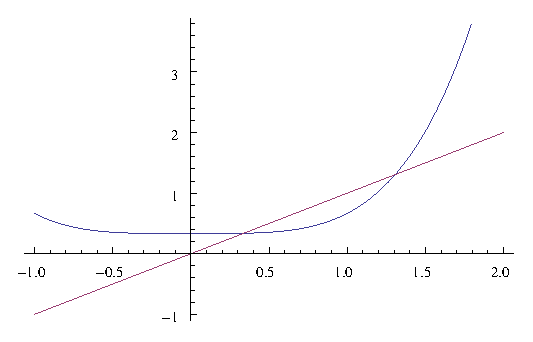
\includegraphics{Analysis/Analysis_1_1.eps}}
\end{figure}

\centertexdraw{
    
    \def\bdot {\fcir f:0 r:0.03 }
    
    \drawdim in

    \arrowheadtype t:F \arrowheadsize l:0.08 w:0.04
    \linewd 0.01 \setgray 0 

    \move (-1 -1) \lvec(2 2)
    \move (-1 0) \clvec (1 0.5)(1.5 1)(2 1.5)
  
    \move (-1 -1) \avec (-1 0 ) \avec(0 0) \avec(0 0.3) \avec(0.3 0.3) \avec(0.3 0.4)
    \move (2 2) \avec (2 1.5) \avec(1.5 1.5) \avec(1.5 1.05) \avec(1.05 1.05) \avec(1.05 0.75) \avec(0.75 0.75) \avec(0.75 0.6)\avec(0.6 0.6)
    
    \move (0.46 0.46) \bdot   
    \htext (-1.1 -1){0}
    \htext (0.4 0.2){$r_1$}

    \move (2 -1) \lvec(5 2)
    \move (2.2 -1) \clvec (3.2 0.5)(3.4 1)(3.7 2)

    \move (2.57 -0.43) \bdot   
    \move (3 0) \avec (3 0.3) \avec (3.3 0.3) \avec (3.3 0.85) \avec (3.85 0.85) \avec (3.85 2) 
    \htext (2.8 -0.5){$r_2$}
 
\move (0 -1.2)
}

Let the two roots of $f(x) = (x^4+1)/3 - x$ be $r_1$ and $r_2$ ($r_1 < r_2$). Because $f(0)>0$, $f(1) <0$ and $f(2) >0$, we have $r_1 \in (0,1)$ and $r_2\in (1,2)$.

Graphical analysis tells us that sequences starting with $a_1 =0,1$ converge to $r_1$ and $a_1 = 2$ diverges to infinity.

$a_1 = 0$. If $a_n \in (0,r_1)$, $f(a_n) = (a_n^4+1)/3 - a_n = a_{n+1} -a_n >0\ \ra \ a_{n+1} > a_n$. But
\be
a_{n+1} = (a_n^4+1)/3 < (r_1^4+1)/3 = r_1   
\ee

Thus, $a_n$ is increasing and bounded above so it is converging.

$a_1 = 1$. If $a_n \in (r_1,r_2)$, $f(a_n) = (a_n^4+1)/3 - a_n = a_{n+1} -a_n < 0\ \ra \ a_{n+1} < a_n$. But
\be
a_{n+1} = (a_n^4+1)/3 > (r_1^4+1)/3 = r_1   
\ee

Thus, $a_n$ is decreasing and bounded above so it is converging.

$a_1 = 2$. If $a_n \in (r_2,\infty)$, $f(a_n) = (a_n^4+1)/3 - a_n = a_{n+1} -a_n >0\ \ra \ a_{n+1} > a_n$. Thus, $a_n$ is increasing and unbounded above so it is diverging.

\vspace{2mm}

------------------------------------------------------------------------------------------------------------------

\begin{exercise}
Let $a_1>b_1>0$ and let $a_{n+1} = (a_n + b_n)/2$, $b_{n+1} = 2a_nb_n/(a_n+b_n)$ for $n\geq 1$. Show that $a_n>a_{n+1}>b_{n+1}>b_n$ and deduce the two sequences converge to a common limit. What limit?
\end{exercise}

Solution. Since $a_1>b_1>0$,
\be
\left\{\ba{l}
2a_1 > a_1 + b_1 \ \ra \ a_1 > \frac{a_1 + b_1}2 = a_2\\
\frac 1{a_1} < \frac 1{b_1} \ \ra \  \frac 1{a_1} + \frac 1{b_1}  < \frac 2{b_1} \ \ra \ b_1 < \frac 2{\frac 1{a_1} + \frac 1{b_1}} = b_2\\
a_2 - b_2 = \frac{a_1 + b_1}2 - \frac {2a_1b_1}{a_1 + b_1} = \frac {(a_1 - b_1)^2}{2(a_1+b_1)} >0
\ea\right. \ \ra \ a_1 > a_2 > b_2 > b_1.
\ee

By induction, we have $a_n>a_{n+1}>b_{n+1}>b_n$. Since $a_n$ is a decreasing sequence, and bounded below (by 0), thus $a_n$ converges to $a$. Similarly, $b_n$ is an increasing sequence and bounded above (by $a_1$). Thus,
\be
\left\{\ba{l}
a = \frac {a+b}2 \\
b = \frac {2ab}{a+b}
\ea\right. \ \ra \ a = b.
\ee
which means that $a_n$ and $b_n$ converge to a common limit $c$. We know that
\be
a_{n+1}b_{n+1} = (a_n + b_n)/2 \times 2a_nb_n/(a_n+b_n) = a_n b_n \ \ra \ c^2 = a_1 b_1 \ \ra \ c = \sqrt{a_1b_1}.
\ee

\begin{exercise}
Let $[a_n,b_n], \ n=1,2,\dots$ be closed intervals with $[a_n,b_n]\cap[a_m,b_m]\neq \emptyset$ for all $n,m$. Prove that $\cap^\infty_{n=1}[a_n,b_n]\neq \emptyset$.
\end{exercise}

Solution. First, we can not use induction to prove the statements about infinity! For example, consider the sets $A_n = [n,\infty),n\in \N$. We have
\be
\bigcap^k_{n=1} A_n = A_k \neq \emptyset = \bigcap^\infty_{n=1}A_n.
\ee

\begin{exercise}
The real sequence $a_n$ is bounded but does not converge. Prove that it has two convergent subsequences with different limits.
\end{exercise}

Solution. By Balzano-Weierstrass Theorem, $a_n$ is real and bounded, so $a_n$ contains a convergent subsequence. Let its limit be $l$. Because $a_n$ is not convergent, there exist $\ve>0$ s.t. there exists infinityly many terms of $a_n$ which satisfy 
\be
\abs{a_n -l} > \ve.
\ee
Now apply Balzano-Weierstrass Theorem again for these $a_n$. There exists another subsequence converges to another limit $m \neq l$. Thus, this real sequence $a_n$ has two convergent subsequences with different limits.

\begin{exercise}
Investigate the convergence of the following series. For those expressions containing the complex number $z$, find those $z$ for which convergence occurs.
\be
\sum_n\frac{\sin n}{n^2}\quad \quad \sum_n\frac{n^2z^n}{5^n}\quad\quad \sum_n\frac{(-1)^n}{4+\sqrt{n}}\quad\quad \sum_n \frac{z^n(1-z)}{n}
\ee
\end{exercise}

Solution. \ben
\item [(i)] It's obvious that $\abs{\frac {\sin n}{n^2}} \leq \frac 1{n^2}$ and $\sum_n \frac 1{n^2}$ converges. By comparison test, $\sum_n\frac{\sin n}{n^2}$ is absolutely convergent.

\item [(ii)] Using ratio test, we check
\be
\abs{\frac {a_{n+1}}{a_n}} = \abs{\frac{z(n+1)^2}{5n^2}} \to \abs{\frac z5}  \quad \text{as }n \to \infty.
\ee

Thus, we have
\be
\sum_n\frac{n^2z^n}{5^n}\quad
\left\{\ba{ll}
\text{converges absolutely }\quad \quad & \abs{z}<5\\
\text{inconclusive} & \abs{z} = 5\\
\text{diverges} & \abs{z} >5
\ea\right..
\ee

\item [(iii)] We know that $\frac 1{4+\sqrt{n}}$ is decreasing. Thus, by alternative test, $\sum_n\frac{(-1)^n}{4+\sqrt{n}}$ converges.

\item [(iv)] Use ratio test again, 
\be
\abs{\frac {a_{n+1}}{a_n}} = \abs{\frac{zn}{n+1}} \to \abs{z}  \quad \text{as }n \to \infty.
\ee
Thus, we have
\be
\sum_n \frac{z^n(1-z)}{n}\quad
\left\{\ba{ll}
\text{converges absolutely }\quad \quad & \abs{z}<1\\
\text{inconclusive} & \abs{z} = 1\\
\text{diverges} & \abs{z} >1
\ea\right..
\ee

\een

\begin{exercise}
Show that $\sum 1/(n\log^\alpha n)$ converges if $\alpha>1$ and diverges otherwise. Does $\sum 1/(n\log n\log\log n)$ converge?
\end{exercise}

Solution. Cauchy's condensation test. $a_n$ is decreasing sequence of positive terms, then $\sum^\infty_{n=1}a_n$ converges iff $\sum^\infty_{n=1}2^n a_{2^n}$ converges.

We know that $\frac 1{n\log^\alpha n}$ is decreasing. Using Cauchy' condensation test, we have
\be
\sum \frac 1{n\log^\alpha n} \text{ converges } \ \lra \ \sum \frac {2^n}{2^n\log^\alpha 2^n} \text{ converges } \ \lra \ \frac 1{\log^\alpha 2}\sum \frac {1}{n^\alpha } \text{ converges }
\ee

Thus $\sum_n \frac {1}{n^\alpha }$ converges iff $\alpha >1$, diverges otherwise.

For the decreasing sequence $\frac 1{n\log n\log\log n}$, we apply Cauchy's condensation test again,
\beast
\sum \frac 1{n\log n\log\log n} \text{ converges }& \lra & \sum \frac {2^n}{2^n\log 2^n\log\log 2^n} \text{ converges } \\
& \lra & \frac 1{\log 2}\sum \frac {1}{n\bb{\log n + \log\log 2}} \text{ converges }\\
& \lra & \sum \frac {2^n}{2^n\bb{n\log 2 + \log\log 2}} \text{ converges }\quad\quad \text{Cauchy's condensation test once more}\\
& \lra & \sum \frac {1}{n\log 2 + \log\log 2} \text{ converges }
\eeast

It's obvious that
\be
\frac {1}{n\log 2 + \log\log 2} \text{ diverges } \ \ra \ \sum \frac 1{n\log n\log\log n} \text{ diverges.}
\ee

\begin{exercise}
Let $a_n\in\C$ and let $b_n = \frac 1n\sum^n_{i=1}a_i$. Show that, if $a_n\to a$ as $n\to\infty$, then $b_n\to a$ also.
\end{exercise}

Solution. 

\begin{exercise}
Consider the two series $1-\frac 12 + \frac 13 - \frac 14+ \frac 15- \frac 16+\cdots$ and $1+ \frac 13 -\frac 12 + \frac 15 + \frac 17 - \frac 14+ \cdots$ having the same terms but taken in a different order. Let $s_n$ and $t_n$ be the corresponding partial sums to $n$ terms. Show that $s_{2n} = H_{2n}-H_n$ and $t_{3n} = H_{4n} - \frac 12H_{2n} -\frac 12H_{n}$, where $H_n = 1 + \frac 12 + \frac 13 + \frac 14 + \frac 15 + \cdots + \frac 1n$. Show that $s_n$ converges to a limit $s$ and that $t_n$ converges to $3s/2$.
\end{exercise}

Solution. We have
\beast
s_{2n} & = &  1 - \frac 12 + \frac 13 - \frac 14 \dots + \frac 1{2n-1} - \frac 1{2n}\\
& = & 1 + \frac 12 + \frac 13 + \frac 14 + \dots + \frac 1{2n-1} + \frac 1{2n} - 2\bb{\frac 12 + \frac 14 + \dots + \frac 1{2n}}\\
& = & H_{2n} - H_n.
\eeast

\beast
t_{3n} & = &  \bb{1 + \frac 13 - \frac 12 } + \bb{\frac 15 + \frac 17 - \frac 14 } + \bb{ \frac 1{4n-3} + \frac 1{4n-1}- \frac 1{2n}}\\
& = & \bb{1 + \frac 12 + \frac 13 + \frac 14 + \dots + \frac 1{4n-1} + \frac 1{4n}} - \bb{\frac 12 + \frac 14 + \dots + \frac 1{4n-2} + \frac 1{4n}} - \bb{\frac 12 + \frac 14 + \dots + \frac 1{2n}}\\
& = & H_{4n} - \frac 12 H_{2n} - \frac 12 H_n.
\eeast

Also,
\be
s_{n} \to 1 - \frac 12 + \frac 13 - \frac 14 \dots + \dots = \sum \frac {(-1)^{n+1}}{n} = \log(1+1) = \log 2.
\ee

\beast
t_{n} & \to & \sum \bb{ \frac 1{4n-3} + \frac 1{4n-1}- \frac 1{2n}} \\
& = & \sum \bb{ \frac 1{4n-3} + \frac 1{4n-1}- \frac 1{4n-2} - \frac 1{4n}} +  \sum \bb{ \frac 1{4n-2} + \frac 1{4n}- \frac 1{2n}}\\
& = & \sum \frac {(-1)^{n+1}}{n} + \frac 12 \sum \frac {(-1)^{n+1}}{n} = \frac 32 \sum \frac {(-1)^{n+1}}{n} = \frac 32 \log 2.
\eeast

\begin{exercise}
Suppose that $\sum a_n$ diverges and $a_n>0$. Show that there exist $b_n$ with $b_n/a_n\to 0$ and $\sum b_n$ divergent.
\end{exercise}

Solution. Since $\sum a_n$ is increasing and divergent, we take a subsequence $N_k$ s.t. $N_0 = 0$, $N_1$ is the first integer where $\sum a_n$ crosses 1, similarly
\be
N_k = \inf\left\{n:\sum^n_{i=N_{k-1}+1}a_i \geq 1,\ n\in \N\right\}.
\ee

Then we define
\be
b_n := \frac {a_n}{k},\quad N_{k-1} < n \leq N_k
\ee
so that $b_n/a_n$ converges to 0 as $n\to \infty$. Also,
\be
\sum b_n = \sum^\infty_{k=1} \sum^{N_{k}}_{N_{k-1}+1} b_n = \sum^\infty_{k=1} \sum^{N_{k}}_{N_{k-1}+1} \frac {a_n}k = \sum^\infty_{k=1} \frac 1k \sum^{N_{k}}_{N_{k-1}+1}a_n \geq \sum^\infty_{k=1} \frac 1k = \infty.
\ee

Hence, $b_n$ is divergent.

\begin{exercise}[Abel's test]
Let $a_n$ and $b_n$ be two sequences and let $S_n=\sum^n_{j=1}a_j$ and $S_0=0$. Show that for any $1\leq m\leq n$ we have
\be
\sum^n_{j=m}a_jb_j = S_nb_n - S_{m-1}b_m + \sum^{n-1}_{j=m}S_j(b_j-b_{j+1}).
\ee
Suppose now that $b_n$ is a decreasing sequence of positive terms tending to zero. Moreover, suppose that $S_n$ is a bounded sequence. Prove that $\sum^\infty_{j=m}a_jb_j$ converges. Deduce the alternative series test. Does the series $\sum^\infty_{n=1}\frac{\cos(n)}{n}$ converge or diverge?
\end{exercise}

Solution. First, we have
\be
S_n b_n = a_1b_n + a_2b_n + \dots + a_nb_n,\quad \quad S_{m-1}b_m = a_1b_m + a_2b_m + \dots + a_{m-1}b_m
\ee
and
\be
\sum^{n-1}_{j=m}S_j(b_j-b_{j+1}) = (a_1 + a_2+ \dots + a_m)b_m + (a_{m+1}b_{m+1} + \dots + a_{n-1}b_{n-1}) - (a_1 + a_2 + \dots + a_{n-1})b_n
\ee

Thus, we sum these up to get
\be
S_nb_n - S_{m-1}b_m + \sum^{n-1}_{j=m}S_j(b_j-b_{j+1}) = a_m b_m + (a_{m+1}b_{m+1} + \dots + a_{n-1}b_{n-1}) + a_n b_n = \sum^n_{j=m}a_jb_j.
\ee

Also, we know that $S_n$ is bounded, $\abs{S_n} \leq k$ for some $k$ and $\forall n\in \N$
\beast
\abs{\sum^n_{j=m} a_j b_j} & \leq & \abs{S_nb_n} + \abs{S_{m-1}b_m} + \abs{\sum^{n-1}_{j=m}S_j(b_j-b_{j+1})}\\
& \leq & k b_n + k b_m + k \abs{b_m - b_{n-1}} = 2k b_m.
\eeast

Since $\lim_{m\to\infty}b_m = 0$, $2kb_m$ can be arbitrarily small so by Cauchy's criterion, $\abs{\sum^n_{j=1} a_j b_j}$ converges, so does $\abs{\sum^n_{j=m} a_j b_j}$.

Now let $a_n = (-1)^{n+1}$ then $S_n = 0 \text{ or }1$ which is bounded. Then by Abel's test, the alternative series test holds. 

For the series $\sum^\infty_{n=1}\frac{\cos(n)}{n}$, we have $b_n = \frac 1n$, and 
\be
\sum^n_{k=1} a_k = \sum^n_{k=1} \cos k = \Re\bb{\sum^n_{k=1} e^{ki}} = \Re\bb{\frac{e^{(n+1)i}-1}{e^i - 1}}
\ee
is bounded. Thus, with Abel's test, we know that the series converges.

\begin{exercise}
For $n\geq 1$, let 
\be
a_n = \frac 1{\sqrt{n}} + \frac{(-1)^{n-1}}{n}.
\ee
Show that each $a_n$ is positive and that $\lim a_n =0$. Show also that $\sum^\infty_{n=1}(-1)^{n-1}a_n$ diverges. [This shows that, in the alternative series test, it is essential that the moduli of the terms decrease as $n$ increases.]
\end{exercise}

Solution. Since $n\geq 1$, $\frac 1{\sqrt{n}}\geq \frac 1n$. Thus, we have $a_n \geq 0$. Also,
\be
\lim_{n\to\infty}a_n = \lim_{n\to\infty}\frac 1{\sqrt{n}} + \lim_{n\to\infty}\frac{(-1)^{n-1}}{n} = 0 + 0 = 0.
\ee

Assume $\sum^\infty_{n=1}(-1)^{n-1}a_n$ converges, we have
\be
\sum^\infty_{n=1}(-1)^{n-1}a_n = \sum^\infty_{n=1}(-1)^{n-1}\frac 1{\sqrt{n}} + \sum^\infty_{n=1}\frac 1n.
\ee
The first part converges by alternative test and second part diverges. Hence, this contradiction gives the divergence of the series.

\begin{exercise}
Let $z\in \C$. Show that the series
\be
\frac{z}{1-z^2} + \frac{z^2}{1-z^4} + \frac{z^4}{1-z^8} + \frac{z^8}{1-z^{16}} + \cdots
\ee
converges to $z/(1-z)$ if $|z|<1$, converges to $1/(1-z)$ if $|z|>1$, and diverges if $|z|=1$.
\end{exercise}

Solution. Let $S_n$ be the partial sum of the $n$th partial sum and assume
\be
S_n = \frac 1{1-z} - \frac 1{1-z^{2^n}}.
\ee

Thus,
\be
S_1 = \frac 1{1-z} - \frac 1{1-z^{2}} = \frac z{1-z^2}
\ee
holds. Then by induction, 
\be
S_k = \frac 1{1-z} - \frac 1{1-z^{2^k}}  \ \ra \ S_{k+1} =  \frac 1{1-z} - \frac 1{1-z^{2^k}} + \frac {z^{2^k}}{1-z^{2^{k+1}}} = \frac 1{1-z} - \frac 1{1-z^{2^{k+1}}}. 
\ee
So $S_n$ is true for all $n\in \N$.

If $|z|<1$, as $n\to\infty$, $z^{2^n} \to 0$, thus $S_n \to \frac 1{1-z}-1 = \frac z{1-z}$ as $n\to\infty$.

If $|z|>1$, $\frac 1{|z^{2^n}|}\to 0$ as $n\to\infty$, so $\frac 1{1-z^{2^n}}\to 0$ and $S_n \to \frac 1{1-z}$ as $n\to\infty$.

If $|z|=1$, $S_n$ converges iff $\frac 1{1-z^{2^n}}\to 0$. We have
\be
\abs{\frac 1{1-z^{2^n}}-0} = \abs{\frac 1{1-z^{2^n}}} = \frac 1{\abs{1-z^{2^n}}} \geq \frac 1{1+\abs{z^{2^n}}} = \frac 12 \neq 0
\ee
Thus, we can say that $S_n$ diverges.

\begin{exercise}
Prove that every real sequence has a monotonic subsequence. Deduce the Bolzano-Weierstrass theorem. Show that the Bolzano-Weierstrass theorem is in fact equivalent to the fundamental axim, that is, give a proof of the fundamental axiom assuming Bolzano-Weierstrass.
\end{exercise}

Solution. Let $\{x_n\}$ be a real sequence. Let's call $x_N$ a 'peak' point if $x_N\geq x_i,\ \forall i >N$. 
\ben
\item [(i)] If there are inifinitely many 'peak' points, then these 'peak' points can form a monotonically decreasing subsequence.
\item [(ii)] If there are only finitely many 'peak' ponts, let them be $x_{N_1},x_{N_2},\dots,x_{N_k}$. Pick $m_1>N_k$, then there exists $m_2>m_10$ s.t. $x_{m_2} > x_{m_1}$ (since $x_{m_1}$ is not a 'peak' point). Again pick $m_3>m_2$ s.t. $x_{m_3} > x_{m_2}$. Continuing this procedure, we have a sequence $x_{m_i},\ i \in \N$ which is a monotonically increasing subsequence.
\een
Thus, every real sequence has a monotonic subsequence.

\vspace{4mm}

{\bf The Bolzano-Weierstrass Theorem}. If $x_n\in\mathbb{R}$ and there exists $K$ s.t. $|x_n|<K,\forall n$, then we can find $n_1<n_2<\dots$ and $x\in\mathbb{R}$ s.t. $x_{n_j}\to x$ as $j\to \infty$. (every bounded sequence has a convergent subsequence.)

{\bf Proof}. We see $[a_n,b_n] = [-K,K]$, let $c=\frac{a_0+b_0}{2}$ (mid-point), thus, either
\ben
\item [(i)] $x_n\in[a_0,c]$ for infinitely many values of $n$;
\item [(ii)] $x_n\in[c,b_0]$ for infinitely many values of $n$.
\een

In case (i), set $a_1=a_0, b_1=c$; 

In case (ii), set $a_1=c,b_1=b_0$. 

Proceed inductively to obtain sequences $a_n$ and $b_n$ s.t. the following holds ($m\leq n$)
\ben
\item [(i)] $a_m\leq a_n\leq b_n\leq b_m$; ($a_n$ is a bounded increasing sequence, $b_n$ is a bounded decreasing sequence.)
\item [(ii)] $x_m\in[a_n,b_n]$ for infinitely many values of $m$;
\item [(iii)] $b_n-a_n=\frac{b_{n-1}-a_{n-1}}{2}$.
\een

By the Fundamental Axiom, $a_n\to a$ and $b_n\to b$. By property (iii) passing to the limit,
\begin{equation*}
b-a = \frac{b-a}{2}\ \Rightarrow \ a=b
\end{equation*}

Having selecting $n_j$ s.t. $x_{n_j}\in[a_j,b_j]$, select $n_{j+1}>n_j$ s.t. $x_{n_{j+1}}\in[a_{j+1},b_{j+1}]$, we can always do this because $x_m\in[a_{j+1},b_{j+1}]$ for infinitely many values of $m$. In other words, 
\be
\left\{\ba{c}
a_j\leq x_{n_j} \leq b_j, \forall j\\
\\
a_j\to a,\ b_j\to b=a
\ea\right.\ \Rightarrow \ x_{n_j}\to a. \quad\quad \fbox{}
\ee

\begin{exercise}
Can we write the open interval $(0,1)$ as a disjoint union of closed intervals of positive length?
\end{exercise}

Solution. 

\vspace{2mm}

------------------------------------------------------------------------------------------------------------------

\begin{exercise}
Is there an enumeration of $\Q$ as $q_1,q_2,q_3,\dots$ such that $\sum(q_n-q_{n+1})^2$ converges?
\end{exercise}

Solution. 

%%%%%%%%%%%%%%%%%%%%%%%%%%%%%%%%%%%%%%%%%%%%%%%%%%%%

\begin{exercise}
Define $f : \R \to \R$ by $f(x) = x$ if $x \in \Q$ and $f(x) = 1-x$ otherwise. Find $\{a : f \text{ is continuous at }a\}$.
\end{exercise}

Solution. $\forall \ve >0$, let $\delta = \ve$. Then for $x$ s.t. $\abs{x-\frac 12} < \delta$, 
\be
\abs{f(x)-f\bb{\frac 12}} = \left\{\ba{ll}
\abs{x-\frac 12} < \delta = \ve & \text{if }x\in \Q\\
\abs{1-x-\frac 12} = \abs{x-\frac 12}  < \delta = \ve  \quad\quad & \text{if }x\in \R\backslash\Q
\ea\right.
\ee
Thus $f(x)$ is continuous at $\frac 12$.



\emph{Approach 1}. Now if $f(x)$ is also continuous at $a>\frac 12$. Let $a=\frac 12 + \ve$, $\ve >0$ and $x,y >a$, $\exists \delta >0$ 
\be
\abs{x-a} < \delta, \ x \in \Q,\quad\quad \abs{y-a} < \delta, \ y \in \R\backslash\Q
\ee
such that
\be
\abs{f(x)-f(a)} < \ve,\quad \abs{f(y)-f(a)} < \ve \ \ra \ \abs{f(x)-f(y)} < 2\ve.
\ee

However,
\be
\abs{f(x)-f(y)} = \abs{x+y-1} = x+y-1 > 2a-1 = 2\bb{\frac 12+\ve} -1 = 2\ve \ \ra \ \text{Contradiction.}
\ee

\emph{Approach 2}. If $f(x)$ is continuous at $a\neq \frac 12$, then for any sequence $x_n \to a$, $f(x_n)\to f(a)$. Thus, we pick the sequence $y_n \in \R\backslash\Q$ s.t. $y_n \to a$, then $f(y_n) \to a$.
\be
a =  \lim_{n\to \infty}f(y_n) =  \lim_{n\to \infty}1-y_n = 1 -  \lim_{n\to \infty}y_n = 1-a \ \ra \ a = \frac 12. \quad \text{Contradiction.}
\ee

Hence, $f(x)$ is only continuous at $\frac 12$.

\begin{exercise}
Write down the definition of "$f(x) \to \infty$ as $x \to \infty$". Prove that $f(x) \to \infty$ as $x \to\infty$ if, and only if, $f(x_n) \to \infty$ for every sequence such that $x_n \to\infty$.
\end{exercise}

Solution. Definition. $f(x) \to \infty$ as $x \to \infty$ if $\forall \ve >0$, $\exists \delta >0$ s.t. $\forall x> \delta$, $f(x)>\ve$.

Proof. '$\Longrightarrow$'.
\beast
\left\{\ba {l}
f(x) \to \infty \text{ as }x \to \infty \ \ra \ \forall \ve >0,\ \exists \delta >0 \text{ s.t. }\forall x> \delta,\ f(x)>\ve\\
x_n \to \infty \ra \forall \delta >0,\ \exists N>0 \text{ s.t. } \forall n\geq N,\ x_n > \delta
\ea\right.\quad\quad\quad\quad\quad\quad\quad\quad\quad\quad\quad\quad\quad\quad\quad\quad\quad\quad\\
\ra
\left\{\ba{l}
\forall \ve >0,\ \exists N >0 \text{ s.t. }\forall n \geq N,\ f(x_n)>\ve\\
\text{ which means }f(x_n) \to \infty.
\ea\right.
\eeast

'$\Longleftarrow$'. We have
\be
f(x) \nrightarrow \infty \text{ as }x \to \infty\ \ra \ \forall \delta >0,\ \exists \ve>0 \text{ s.t. }\exists x > \delta,\ f(x)<\ve.
\ee

Choose $\delta_n = n$, thus there is a sequence $x_n > \delta_n$, so $x_n \to \infty$. As $n=\delta_n \to\infty$,
\be
\exists \ve>0, n>0, \ f(x_n) <\ve\ \ra \ f(x_n) \nrightarrow \infty.
\ee
%
%\beast
%\left\{\ba {l}
%f(x) \nrightarrow \infty \text{ as }x \to \infty\ \ra \ \forall \delta >0,\ \exists \ve>0 \text{ s.t. }\exists x > \delta,\ f(x)<\ve\\
%x_n \to \infty \ra \forall \delta >0,\ \exists N>0 \text{ s.t. } \forall n\geq N,\ x_n > \delta
%\ea\right. \quad\quad\quad\quad\quad\quad\quad\quad\quad\quad\quad\quad\\
%\\
% \ra 
%\forall \delta >0,\ \exists \ve>0, N>0 \text{ s.t. }\exists n \geq N, x_n > \delta,\ f(x_n)<\ve\quad\quad\quad\quad\quad\quad\quad\quad\\
%\\
% \ra \left\{\ba{l}
%\forall N>0,\ \exists \ve>0, n\geq N \text{ s.t. } \ f(x_n)<\ve \\
%\text{ which means }f(x_n) \nrightarrow \infty.
%\ea\right.
%\eeast

\begin{exercise}
Suppose that $f(x) \to l$ as $x \to a$ and $g(y) \to k$ as $y \to l$. Must it be true that $g(f(x)) \to k$ as $x \to a$?
\end{exercise}

Solution. No. If $f(x)$ is continuous at $a$ and $g(y)$ is not continuous at $l$, let's say
\be
f(x) = 2,\quad\quad g(y) = \left\{\ba{ll}
1 \quad\quad & y \neq 2\\
3 & y = 2
\ea\right.
\ee
which means that $l = 2$, $k=1$. However,
\be
g(f(x)) \to g(2) = 3 \neq 1 \ (k) \quad\quad \text{as }x\to a.
\ee

\begin{exercise}
Let $f_n : [0, 1] \to [0, 1]$ be continuous, $n \in \N$. Let $h_n(x) = \max\{f_1(x), f_2(x), \dots, f_n(x)\}$. Show that $h_n$ is continuous on $[0, 1]$ for each $n \in \N$. Must $h(x) = \sup\{f_n(x) : n \in \N\}$ be continuous?
\end{exercise}

Solution. Realizing for two continuous functions $f$ and $g$
\be
\max\{f,g\} = \frac{(f+g)+\abs{f-g}}2
\ee

We have $f+g$ and $abs{f-g}$ as continuous functions as well. Thus, $\max\{f,g\}$ is continuous. Also, we know that

\be
\max\{f_1(x), f_2(x), \dots, f_n(x)\} = \max\{f_1(x),\max\{f_2(x),\dots,f_n(x) \}\}.
\ee

By induction, we have that $h_n(x)$ is continuous.

Now consider $f_n(x) = \min\{nx,1\},\ x\in[0,1]$. Obviously, $f_n(x)$ is continuous. For any $x\in(0,1]$, there exists $N\in \N$ s.t. $Nx > 1$. Thus, $\forall n\geq N$, $f_n(x) = 1$. This implies that 
\be
h(x) = \sup\{f_n(x) : n \in \N\} = 1,\quad x\in (0,1].
\ee

Then consider $x=0$, we have $f_n(x) = 0$ for all $n$. Hence we have
\be
h(x) = \left\{\ba{ll}
1 \quad\quad & x\neq 0\\
0 & x= 0
\ea\right.
\ee
which is NOT continuous on $[0,1]$.

\begin{exercise}
The unit circle in $\C$ is mapped to $\R$ by a map $e^{i\theta} \mapsto f(\theta)$, where $f : [0, 2\pi] \to \R$ is continuous and $f(0) = f(2\pi)$. Show that there exist two diametrically opposite points that have the same image.
\end{exercise}

Solution. Consider $g(x) = f(x+\pi)-f(x)$, $x\in [0,\pi]$. Then we have three cases:
\ben
\item [(i)] If $f(0) = f(\pi)$, 0 and $\pi$ are diametrically oppositte points, done.
\item [(ii)] If $f(0) > f(\pi)$, 
\be
g(0) = f(\pi) -f(0) < 0, \quad g(\pi) = f(2\pi) - f(\pi) = f(0) - f(\pi) > 0.
\ee
By I.V.T., $\exists x^* $ such that $g(x^*) = 0$ which implies that $f(x^*+\pi) = f(x^*)$.
\item [(iii)] If $f(0) < f(\pi)$, use the same argument.
\een

\begin{exercise}
Let $f(x) = \sin^2 x + \sin^2(x + \cos^7 x)$. Assuming the familiar features of $\sin$ without justification, prove that there exists $k > 0$ such that $f(x) \geq k$ for all $x \in \R$.
\end{exercise}

Solution. First, we have $f(x)$ is non-negative and continuous on $[0,2\pi]$. Thus, there exists $k \geq 0$ such that $f(x)\geq k$. If $f(x) = 0$, we have 
\be
\left\{\ba{l}
\sin^2 x = 0\\
\sin^2(x + \cos^7 x) = 0
\ea\right. \ \ra \ 
\left\{\ba{l}
x = k\pi,\ k\in \Z \\
x + \cos^7 x = m\pi,\ m\in \Z
\ea\right. \ \ra \ \cos^7 x = (m-k)\pi
\ee
which gives
\beast
 -1\leq (m-k)\pi\leq 1 & \ra & k-\frac 1{\pi} \leq m \leq k+ \frac 1{\pi} \\
& \ra &  m=k \ \ra \ \cos^7x = 0 \ \ra \ \cos x = 0 \ \ra \ x = n\pi + \frac {\pi}2, \ n\in\Z \quad \text{contradiction}.
\eeast
Thus, there is no $x$ satisfying $f(x) = 0$ and $f(x) >0$. So $k$ can not be 0, then we have $k>0$.

\begin{exercise}
Suppose that $f : [0, 1] \to \R$ is continuous, that $f(0) = f(1) = 0$, and that for every $x \in (0, 1)$ there exists $0 < \delta < \min\{x, 1 - x\}$ with $f(x) = (f(x - \delta) + f(x + \delta))/2$. Show that $f(x) = 0$ for all $x$.
\end{exercise}

Solution. Since $f:[0,1]\mapsto \R$ is continuous, $\exists K$ s.t. $f(x)\leq K$ and $K$ can be achieved. ($K\geq 0$)

Let $S =\{x:f(x) = K, x\in [0,1]\}$. Since $S$ is bounded below (by zero), $\inf S$ exists. Let $r= \inf S$. By definition of infimum, $\exists x_n \in [0,1]$ s.t. 
\be
r+\frac 1n \geq x_n \geq r,\quad \quad f(x_n) = K.
\ee

By Bolzano-Weierstrass Theorem, $\exists x_{n_j} \to a$ as $j\to \infty$, thus
\be
r \leq x_{n_j} \leq r+ \frac1{n_j} \to r \text{ as }j\to \infty\ \ra \ r=a \ \ra \ \lim_{j}f(x_{n_j}) = f(a) =f(r) = K.
\ee

If $0<r<1$, $f(r-\delta) <K$ (since $r$ is infimum of $S$), we have
\be
f(x) = (f(x - \delta) + f(x + \delta))/2 \ \ra \ f(r) = (f(r - \delta) + f(r + \delta))/2 \ \ra \ f(r+\delta) > K.
\ee
This contradiction gives $r=0$, so $K = 0$. 

Similarly, $\exists L$ s.t. $f(x)\geq L$ and $L$ can be achieved. ($L\leq 0$). Using the same argument, we have $K=L=0$ which means that $f(x)=0$ for all $x$.

\begin{exercise}
Let $f : [a, b] \to \R$ be bounded. Suppose that $f((x + y)/2) \leq (f(x) + f(y))/2$ for all $x, y \in [a, b]$. Prove that $f$ is continuous on $(a, b)$. Must it be continuous at $a$ and $b$ too?
\end{exercise}

Solution. For $x\in (a,b)$, we consider $x,x+h,x+2h,\dots$. With the given inequality, we have
\beast
2f(x+h) \leq f(x) + f(x+2h) & \ra & 2\bb{f(x+h)-f(x)} \leq f(x+2h)-f(x) \\
& \ra & 2^k\bb{f(x+h)-f(x)} \leq f(x+2^k h)-f(x)
\eeast

We require that
\be
a \leq x+ 2^k h \leq b \ \ra \ h \leq 2^{-k}\min\{\abs{x-a},\abs{x-b}\}.
\ee

Also, we know that $f(x)$ is bounded, thus, $\exists M \geq 0$ such that
\be
\abs{f(x)} \leq M, \quad f(y)-f(x)\leq 2M, \ \forall x,y \in (a,b)
\ee

Thus, $\forall \ve >0$, if $f(x+h)-f(x) \geq \ve$, we have
\be
2^k\ve \leq 2^k\bb{f(x+h)-f(x)} \leq f(x+2^k h)-f(x) \ \ra \ f(x+2^k h)-f(x) \geq 2^k\ve
\ee

If we pick $k$ s.t.
\be
2^k\ve > 2M \ \bb{\text{i.e. }2^{-k} < \frac{\ve}{2M}},
\ee
then this is a contradiction for the bounded condition then implies $f(x+h)-f(x) < \ve$. So $\forall \ve>0$, we can have $f(x+h)-f(x) < \ve$ by choosing
\be
h \leq 2^{-k}\min\{\abs{x-a},\abs{x-b}\} < \frac{\ve}{2M} \min\{\abs{x-a},\abs{x-b}\}.
\ee

Hence, $f(x)$ is continuous on $(a,b)$. 

Now consider the case
\be
f(x) = \left\{\ba{ll}
1 \quad\quad & x=a,b\\
0 & x\in (a,b)
\ea\right.
\ee
The inequality 
\be
f((x + y)/2) \leq (f(x) + f(y))/2, \ \forall x, y \in [a, b]
\ee
is satisfied but $f(x)$ is NOT continuous at $a$ and $b$.

\begin{exercise}
Prove that $2x^5 +3x^4 +2x +16 = 0$ has no real solutions outside $[-2,-1]$ and exactly one inside.
\end{exercise}

Solution. First we have
\be
f(-1) = 15,\quad f(-2) = -4.
\ee

With I.V.T., $\exists c \in [-2,-1]$ s.t. $f(c) = 0$. Also, we have
\be
f'(x) = 10x^4+ 12x^3 + 2 = 2x^3(5x+6) + 2 =  2(x+1)(5x^3+x^2-x+1).% 10x^3 (x+1) + 2x^3 + 2=
\ee

Let $g(x) = 5x^3+x^2-x+1$. Thus,
\be
g'(x) = 15x^2 +2x -1 \ \ra g'(x) > 0, \ x \leq -1
\ee

With $g(-1) = -2$, we have $g(x) <0$, $x\leq -1$. Thus,
\be
f'(x) = 2(x+1)g(x) \geq 0,\ x\leq -1.
\ee

Hence, there is only one solution in $[-2,-1]$ and no solution in $(-\infty,-2]$. Furthermore, for $x\geq -1$, 
\be
f(x) = 2x^5 +3x^4 +2x +16 \geq -2 + 0 + -2 + 16 = 12 > 0.
\ee
Thus, there is no solution outline $[-2,-1]$.

\begin{exercise}
Let $f : [a, b] \to \R$ be continuous on $[a, b]$ and differentiable on $(a, b)$. Which of (1)-(4) must be true?
\ben
\item [(1)] If $f$ is increasing then $f'(x) \geq 0$ for all $x \in (a, b)$.
\item [(2)] If $f'(x) \geq 0$ for all $x \in (a, b)$ then $f$ is increasing.
\item [(3)] If $f$ is strictly increasing then $f'(x) > 0$ for all $x \in (a, b)$.
\item [(4)] If $f'(x) > 0$ for all $x \in (a, b)$ then $f$ is strictly increasing.
\een
[Increasing means $f(x) \leq f(y)$ if $x < y$, and strictly increasing means $f(x) < f(y)$ if $x < y$.]
\end{exercise}

Solution. \ben
\item [(1)] True. $\forall x\in(a,b)$, 
\be
f'(x) = \lim_{h\to 0} \frac{f(x+h)-f(x)}{h}
\ee
since
\be
\forall h>0,\ \frac{f(x+h)-f(x)}{h} \geq 0 \quad \text{(definition of increasing function)}
\ee
Thus,
\be
\lim_{h\to 0} \frac{f(x+h)-f(x)}{h} \geq 0 \ \ra \ f'(x) \geq, \ \forall x\in(a,b).
\ee
\item [(2)] True. Let $x,y\in [a,b]$ with $x<y$. The mean value theorem says 
\be
f(y)-f(x) = f'(c)(y-x), \quad \exists c\in (x,y).
\ee

Then $f'(c)\geq 0 \ \Rightarrow \ f(y)-f(x) = f'(c)(y-x) \geq 0 \ \ra \ f(y) \geq f(x)  \ra f(x) \text{ is increasing}$.

\item [(3)] False. Let $f(x) = x^3,\ x\in[-1,1]$. $f(x)$ is strictly increasing, but $f'(0) = 0$.
\item [(4)] True. Similar argument with (1).
\een

\begin{exercise}
Let $f : \R \to \R$ be differentiable for all $x$. Prove that if $f'(x) \to l$ as $x \to \infty$ then $f(x)/x \to l$. If $f(x)/x \to l$ as $x \to \infty$, must $f'(x)$ tend to a limit?
\end{exercise}

Solution. Without loss of generality, we assume $l=0$, since
\be
g(x) = f(x) - lx \ \ra\ g'(x) = f'(x) -l,\quad \frac{g(x)}{x} = \frac{f(x)}{x} -l.
\ee

With condition provided, we get $\forall \ve >0$, $\exists K >0$ s.t. 
\be
\abs{g'(x)} < \ve,\quad \forall x \geq K.
\ee

Now for any $y<x$,
\be
\abs{\frac{g(x)}{x}} \leq \abs{\frac{g(x)-g(y)}{x}} + \abs{\frac{g(y)}{x}}
\ee

Thus, $\forall \ve>0$, 
\be
\abs{\frac{g(x)-g(y)}{x}} \leq \abs{\frac{g(x)-g(y)}{x-y}} = \abs{g'(x^*)},\ x^*\in (y,x)\quad \bb{\text{by M.V.T. since $g(x)$ is differentiable}}
\ee
So $\exists K_1 >0$ s.t. 
\be
\abs{g'(x^*)} < \frac{\ve}2,\quad \forall x^* \geq K_1.
\ee

Also, $\exists K_2$ s.t.
\be
\abs{\frac{g(K_1)}{x}} < \frac {\ve}2, \quad \forall x\geq K_2
\ee

Thus, $\forall \ve>0$, $\exists K = \max\{K_1,K_2\}$ s.t.
\be
\abs{\frac{g(x)}{x}} \leq \abs{\frac{g(x)-g(K_1)}{x}} + \abs{\frac{g(K_1)}{x}} \leq \abs{g'(x^*)} + \abs{\frac{g(K_1)}{x}} < \frac{\ve}2 + \frac{\ve}2 = \ve, \quad \forall x\geq K.
\ee

It can be proved by L'H\^opital rule which is proved by using M.V.T..
\be
f(x)\to \infty,\ x \to \infty \ \ra \ \lim \frac{f'(x)}{x'} = \lim \frac{f(x)}{x} = l.
\ee

However, the inverse does not hold. For example, 
\be
f(x) = \sin x \ \ra \ \frac{f(x)}{x} = \frac{\sin x}{x} \to 0
\ee
but $f'(x) = \cos x$ does not converge.

\begin{exercise}
Let $f(x) = x + 2x^2 \sin(1/x)$ for $x \neq 0$ and $f(0) = 0$. Show that $f$ is differentiable everywhere and that $f'(0) = 1$, but that there is no interval around 0 on which $f$ is increasing.
\end{exercise}

Solution. For the function $f(x)$
\be
f'(x) = 1 + 4x\sin (1/x) - 2\cos(1/x),\quad x\neq 0
\ee
and
\be
f'(0) = \lim_{h\to 0} \frac{f(h)-f(0)}{h-0} = \lim_{h\to 0} \frac{f(h)}h = \lim_{h\to 0} \frac{h+ 2h^2 \sin(1/h)}{h} = 1+ 2\lim_{h\to 0}h \sin(1/h) = 1.
\ee

Thus, $f$ is differentiable everywhere. 

Now assume there is an interval around 0 on which $f$ is increasing. By the previous result, we have $f'(x)\geq 0$ for all $x$ on this interval.

However, $\forall \ve >0$, $\exists n$ s.t. $x = \frac 1{2n\pi} < \ve$ and
\be
f'(x) = 1 + 4x\sin (1/x) - 2\cos(1/x) = 1 + \frac2{n\pi} \sin (2n\pi) - 2\cos (2n\pi) = 1 -2 = -1 < 0.
\ee
The contradiction gives that there is no interval around 0 on which $f$ is increasing.

\begin{exercise}
Let $f :\R \to \R$ be a function which has the intermediate value property: If $f(a) < c < f(b)$, then $f(x) = c$ for some $x$ between $a$ and $b$. Suppose also that for every rational $r$, the set $S_r$ of all $x$ with $f(x) = r$ is closed, that is, if $x_n$ is any sequence in $S_r$ with $x_n \to a$, then $a \in S_r$. Prove that $f$ is continuous.
\end{exercise}

Solution. Proof by contradiction. Assume all the assumptions hold and $f(x)$ is NOT continuous at some points. That is saying there exists a convergent sequence $\{x_n\}$, $x_n \to a$ s.t. 
\be
\forall \delta >0, \ \exists \ve>0,\ \exists i \in \N \text{ s.t. } \abs{x_i -a}< \delta,\ \abs{f(x_i)-f(a)}>\ve.
\ee

Now without loss of generality, let $\{x_{n_j}\} =\{y_{j}\}$ be the subsequence s.t. $y_j<a$ satisfying the above condition. Then by the intermediate value property, $\forall k \in \N$, $\exists r \in (f(a),f(y_k))$ (or $(f(y_k),f(a))$) s.t. $f(z_k)=r$ for some $y_k < z_k < a$. 

Thus, we obtain a convergent sequence $\{z_k\}$ with $z_k \to a$ (since $y_k \to a$ and $y_k < z_k < a$). Also, $f(z_k) = r$, $\forall k\in\N$, $\lim_{k\to\infty}f(z_k) \neq f(a)$. Thus, $a\notin S_r$, so $S_r$ is not closed.

Hence, $f(x)$ must be continuous everywhere.

\begin{exercise}
Suppose that $f : \R \to \R$ satisfies $|f(x)-f(y)| \leq |x-y|^2$ for all $x, y \in \R$. Show that $f$ is constant.
\end{exercise}

Solution. Suppose $f$ is not constant. Take $a,b\in \R$ with $a<b$ and $f(a)\neq f(b)$, then choose $n\in\N$ with 
\be
n>\frac{(b-a)^2}{\abs{f(b)-f(a)}}
\ee
and for $i=0,1,\dots,n$ set 
\be
c_i = a + \frac in(b-a)
\ee
so that $c_0 = a$ and $c_n = b$. Then
\be
\abs{f(b)-f(a)} = \abs{f(c_n)- f(c_0)} \leq \sum^n_{i=1}\abs{f(c_i) -f(c_{i-1})} \leq \sum^n_{i=1}\abs{c_i - c_{i-1}}^2 = \sum^n_{i=1}\bb{\frac{b-a}n}^2 = \frac {(b-a)^2}n < \abs{f(b)-f(a)}.
\ee

The contradiction implies that $f$ must be constant. An alternative way to prove is to use $f'(x)$.

\begin{exercise}
Given $\alpha \in \R$, define $f_\alpha : [-1, 1] \to \R$ by $f_\alpha(x) = x^\alpha \sin(1/x)$ for $x \neq 0$ and $f_\alpha(0) = 0$. Is $f_0$
continuous? Is $f_1$ differentiable? Draw a table, with 4 columns labelled 0, 1, 2, 3 and with 6 rows labelled "$f_\alpha$ bounded", "$f_\alpha$ continuous2, "$f_\alpha$ differentiable", "$f'_\alpha$ bounded", "$f'_\alpha$ continuous", "$f'_\alpha$ differentiable". Place ticks and crosses at appropriate places in the table. 

Does $|x|^\alpha \sin(1/x)$ behave the same way? Complete 5 extra columns, for $\alpha = -\frac 12 , \frac 12 , \frac 32 , \frac 52 , \frac 72$.
\end{exercise}

Solution. The table is
\begin{center}
\begin{tabular}{l|ccccccccc}
 & \ $-\frac 12 $ \ & \ 0 \ & \ $\frac 12 $ \ & \ 1 \ & \ $\frac 32 $ \ & \ 2 \ & \ $\frac 52 $ \ & \ 3 \  & \ $\frac 72$ \ \\ \hline
$f_\alpha$ bounded & $\times$ & $\surd$ & $\surd$ & $\surd$ & $\surd$ & $\surd$ & $\surd$ & $\surd$ & $\surd$  \\ 
$f_\alpha$ continuous & $\times$ & $\times$ & $\surd$ & $\surd$ & $\surd$ & $\surd$ & $\surd$ & $\surd$ & $\surd$  \\ 
$f_\alpha$ differentiable & $\times$ & $\times$ & $\times$ & $\times$ & $\surd$ & $\surd$ & $\surd$ & $\surd$ & $\surd$  \\ 
$f_\alpha'$ bounded & $\times$ & $\times$ & $\times$ & $\times$ & $\times$ & $\surd$ & $\surd$ & $\surd$ & $\surd$  \\ 
$f_\alpha'$ continuous & $\times$ & $\times$ & $\times$ & $\times$ & $\times$ & $\times$ & $\surd$ & $\surd$ & $\surd$  \\ 
$f_\alpha$ differentiable & $\times$ & $\times$ & $\times$ & $\times$ & $\times$ & $\times$ & $\times$ & $\times$ & $\surd$  
\end{tabular}
\end{center}

Both functions behave in the same way for $\alpha\in\Z$. 
\beast
|x|^\alpha \sin(1/x)\text{ is bounded } & \lra & \alpha \geq 0,\\
|x|^\alpha \sin(1/x)\text{ is continuous } & \lra & \lim_{h\to 0} \abs{h}^\alpha \sin \frac 1h = 0 \lra \alpha >0, \\
|x|^\alpha \sin(1/x)\text{ is differentiable} & \lra & \lim_{h\to 0}\frac{\abs{h}^\alpha \sin \frac 1h}{h} \text{ exists} \lra \alpha >1. 
\eeast

Thus, we obtain the table shown.

\begin{exercise}
By applying the mean value theorem to $\log(1 + x)$ on $[0, a/n]$ with $n > |a|$, prove carefully that $(1 + a/n)^n \to e^a$ as $n \to \infty$.
\end{exercise}

Solution. Set $f(x) = \log (1+x)$ and fix $a\in\R$. If $a =0$, then
\be
\bb{1+\frac an}^n = 1 = e^0 = e^a, \ \forall n \in \N.
\ee

So we assume $a\neq 0$, given $n > |a|$, apply the M.V.T. to either $\bsb{0,\frac an}$ or $\bsb{\frac an, 0}$ according as $a>0$ or $a<0$, there exists $x\in \bb{0,\frac an}$ with 
\be
f'(x) = \frac{f\bb{\frac an}-0}{\frac an - 0} \quad \text{i.e.},\quad \frac 1{1+x} = \frac na \log \bb{1+\frac an}.
\ee

As $n\to \infty$, since $|x| < \frac {\abs{a}}n$ we have $x\to 0$, so
\be
\frac 1{1+x} \to 1 \ \ra \ \frac na \log \bb{1+\frac an} \to 1 \ \log \bb{1+\frac an}^n \to a.
\ee

Finally, as $\exp$ is continuous, 
\be
\bb{1 + \frac an}^n \to e^a.
\ee

\begin{exercise}
Find $\lim_{n\to\infty} n(a^{1/n} - 1)$, where $a > 0$.
\end{exercise}

Solution. Set $f(x) = a^x$ and apply the M.V.T. to $\bsb{0,\frac 1n}$, there exists $x\in \bb{0,\frac 1n}$ with
\be
f'(x) = \frac{f\bb{\frac 1n} - f(0)}{\frac 1n - 0} \ \ra \ a^x \log a = n\bb{a^{\frac 1n} - 1}.
\ee

As $n\to \infty$, we have $x\to 0$. Thus,
\be
\lim_{n\to \infty} n\bb{a^{\frac 1n} - 1} = \lim_{x\to 0} a^x \log a = \log a.
\ee

\begin{exercise}
"Let $f'$ exist on $(a, b)$ and let $c \in (a, b)$. If $c + h \in (a, b)$ then $(f(c + h) - f(c))/h = f'(c + \theta h)$. Let $h \to 0$; then $f'(c + \theta h) \to f'(c)$. Thus $f'$ is continuous at $c$." Is this argument correct?
\end{exercise}

Solution. The argument is NOT correct as it can be seen by taking 
\be
f(x) = x^2\sin \frac 1x, \ x\neq 0,\quad f(0) = 0 \ \ra \ f'(x) = 2x\sin \frac 1x - \cos \frac 1x.
\ee

Thus, $\lim_{h\to 0} f'(c+\theta h) \neq f'(c)$ because $f'(c)$ contains $\cos \frac 1c$. 

Although as $h\to 0$ the values $c+\theta h$ tend to $c$, the $\theta$ may vary, so one cannot conclude that for all sequences $(x_n)$ tending to $c$ we have $f'(x_n) \to f'(c)$.

\begin{exercise}
Let $f : \R \to \R$ be defined by $f(x) = \exp(-1/x^2)$ for $x \neq 0$ and $f(0) = 0$. Show that $f$ is continuous and differentiable. Show that $f$ is twice differentiable. Indeed, show that $f$ is infinitely differentiable, and that $f^{(n)}(0) = 0$ for all $n\in \N$. Comment, in the light of what you know about Taylor series.
\end{exercise}

Solution. We prove by induction that for all $n\in \N$ the function $f$ is $n$ times differentiable, with $f^{(n)}(0)=0$ and $f^{(n)}(x) = P_n\bb{\frac 1x}f(x)$ for $x\neq 0$, where $P_n$ is some polynomial. Since 
\be
f'(0) = \lim_{h\to 0} \frac{f(h)-f(0)}{h} = \lim_{h\to 0} \frac{e^{-\frac 1{h^2}}-f(0)}{h} = \lim_{y\to \infty} \frac{y}{e^{y^2}} = 0,
\ee
while for $x\neq 0$ we have
\be
f'(x) = \frac 2{x^3}e^{-1/x^2} = P_1\bb{\frac 1x} f(x),
\ee
where $P_1(t) = 2t^3$, thus the statement is true if $n=1$. (The differentiability implies the continuity.)

Proof. $f$ is differentiable at $x_0$, which implies
\be
\lim_{x\to x_0} = \frac{f(x)-f(x_0)}{x-x_0} = f'(x_0).
\ee

We want to prove that $\lim_{x\to x_0}f(x) = f(x_0)$.
\be
\lim_{x\to x_0} f(x)-f(x_0) = \lim_{x\to x_0} (x-x_0) \frac{f(x)-f(x_0)}{x-x_0} = \lim_{x\to x_0} (x-x_0) \lim_{x\to x_0}\frac{f(x)-f(x_0)}{x-x_0} = 0 \cdot f'(x_0) = 0.
\ee
Thus, $f$ is continuous at $x_0$.

Now assume it is true for $n=k$, then 
\be
f^{(k+1)}(0) = \lim_{h\to 0} \frac{P_k\bb{\frac 1h}f(h)-0}h = \lim_{h\to 0} \frac 1h P_k\bb{\frac 1h}e^{-1/h^2} = \lim_{y\to \infty} \frac{yP_k(y)}{e^{y^2}} = 0,
\ee
while for $x\neq 0$ we have 
\be
f^{(k+1)}(x) = -\frac 1{x^2} P_k'\bb{\frac 1x} f(x) + \frac 2{x^3} P_k\bb{\frac 1x}f(x) = P_{k+1} \bb{\frac 1x}f(x),
\ee
where
\be
P_{k+1}(t) = -t^2 P_k'(t) + 2t^3 P_k(t).
\ee
So it is true for $n= k+1$. Thus, by induction $f$ is infinitely differentiable and $f^{(0)}(0) =0$ for all $n\in \N$. It follows that the Taylor expansion of $f$ about 0 is valid at non-zero points.

\begin{exercise}
Find the radius of convergence of each of these power series.
\be
\sum_{n\geq 0} \frac{ 2 \cdot 4 \cdot 6 \dots (2n + 2) }{1 \cdot 4 \cdot 7 \dots (3n + 1)} z^n,\quad \quad \sum_{n\geq 1} \frac{z^{3n}}{n2^n},\quad\quad \sum_{n\geq 0} \frac {n^nz^n}{n!},\quad\quad \sum_{n\geq 1} n^{\sqrt{n}} z^n
\ee
\end{exercise}

Solution. Let the $n$th term of each power series be denoted $A_n$.
\ben
\item \be
\frac{A_{n+1}}{A_n} = \frac{2n+4}{3n+4}z \to \frac 23 z \quad \text{as }n\to \infty \quad \ra \ \text{ radius of convergence is }\frac 32.
\ee
\item \be
\frac{A_{n+1}}{A_n} = \frac{nz^3}{2(n+1)} \to \frac 12 z^3 \quad \text{as }n\to \infty \quad \ra \ \text{ radius of convergence is }\sqrt[3]{2}.
\ee
\item \be
\frac{A_{n+1}}{A_n} = \frac{(n+1)^{n+1} n!}{(n+1)!n^n}z = \bb{\frac {n+1}{n}}^n z = \bb{1 + \frac 1n}^n z \to ez \quad \text{as }n\to \infty \quad \ra \ \text{ radius of convergence is }\frac 1e.
\ee
\item \be
A_n^{1/n} = n^{1/\sqrt{n}}z \to z \quad \text{as }n\to \infty \quad \ra \ \text{ radius of convergence is 1}.
\ee
Note that $n^{1/\sqrt{n}} = \bb{\sqrt{n}^{1/\sqrt{n}}}^2$, and $m^{1/m} \to 1$ as $m\to \infty$. 
\een

\begin{exercise}[L'H\^opital's rule]
Suppose that $f, g : [a, b] \to \R$ are continuous and differentiable on $(a, b)$. Suppose that $f(a) = g(a) = 0$, that $g'(x)$ does not vanish near $a$ and $f'(x)/g'(x) \to l$ as $x \to a$. 

Show that $f(x)/g(x) \to l$ as $x \to a$. Use the rule with $g(x) = x - a$ to show that if $f'(x) \to l$ as $x \to a$, then $f$ is differentiable at a with $f'(a) = l$.

Find a pair of functions $f$ and $g$ as above for which $\lim_{x\to a} f(x)/g(x)$ exists, but $\lim_{x\to a} f'(x)/g'(x)$ does not.

Investigate the limit as $x \to 1$ of
\be
\frac{x - (n + 1)x^{n+1} + nx^{n+2}}{(1 - x)^2}.
\ee
\end{exercise}

Solution. The generalized M.V.T. shows that for all $x\in (a,b)$ there exists $y\in (a,x)$ with 
\be
\frac{f'(y)}{g'(y)} = \frac{f(x)-f(a)}{g(x)-g(a)} = \frac {f(x)}{g(x)}.
\ee
Thus, as $x\to a$, we have
\be
y \to a \ \ra \ \frac{f(x)}{g(x)} = \frac{f'(x)}{g'(y)} \to l
\ee
as required. If we take $g(x) = x-a$, then $g(a) = 0$, while $g'(x)=1$ so that $g'(x)$ does not vanish near $a$. Thus if $f'(x)\to l$ as $x\to a$, then as $x\to a$ we have
\be
\frac{f'(x)}{g'(x)} \to l,
\ee
so that by the rule,
\be
\frac{f(x)-f(a)}{x-a} = \frac{f(x)}{g(x)} \to l \quad \text{i.e., $f$ is differentiable at $a$ with }f'(a) = l.
\ee

Now set $f = x^2\sin\frac 1x$, $g(x) =x$ and $a=0$. Then $f$ and $g$ are both continuous and differentiable on $\R$, with $f(0)=g(0)=0$, and $g'(x)$ does not vanish near $a$. We have 
\be
\lim_{x\to 0} \frac{f(x)}{g(x)} = \lim_{x\to 0}x\sin \bb{\frac 1x} = 0,
\ee
but if $x\neq 0$, then
\be
\frac{f'(x)}{g'(x)} = f'(x) = 2x\sin\frac 1x - \cos\frac 1x,
\ee
which does not tend to a limit as $x\to 0$.

Set 
\be
f(x) = x-(n+1)x^{n+1} +nx^{n+2},\quad\quad g(x) = (1-x)^2.
\ee

Then $f$ and $g$ are infinitely differentiable on $\R$, and we have
\be
\left\{\ba{l}
f'(x) = 1-(n+1)^2x^n + n(n+2)x^{n+1}\\
f''(x) = -n(n+1)^2x^{n-1}+n(n+1)(n+2)x^n
\ea\right.\quad\quad 
\left\{\ba{l}
g'(x) = - 2(1-x)\\
g''(x) = 2
\ea\right.
\ee

Thus,
\be
\frac{f''(x)}{g''(x)} = \frac 12 n(n+1)x^{n-1}\bb{(n+2)x - (n+1)} \to \frac 12 n(n+1) \quad \text{as }x\to 1.
\ee
so as $f'(1) = g'(1) = 0$, applying the rule to $f'$ and $g'$ gives
\be
\frac{f'(x)}{g'(x)} \to \frac 12 n(n+1) \quad \text{as }x\to 1.
\ee

Then as $f(1)=g(1) = 0$, applying the rule to $f$ and $g$ gives 
\be
\frac{f(x)}{g(x)} \to \frac 12 n(n+1) \quad \text{as }x\to 1.
\ee

\begin{exercise}
Find the derivative of $\tan x$. How do you know there is a differentiable inverse function $\arctan x$ for $x \in \R$? What is its derivative? Now let $g(x) = x-x^3/3+x^5/5+\dots$ for $|x| < 1$. By considering $g'(x)$, explain carefully why $\arctan x = g(x)$ for $|x| < 1$.
\end{exercise}

Solution. $\tan x = \frac{\sin x}{\cos x}$, so
\be
\tan'x = \frac{\cos x \cos x - \sin x(-\sin x)}{\cos^2 x} = \frac 1{\cos^2 x} = \sec^2 x.
\ee

Since $\tan:\ \bb{-\frac {\pi}2, \frac {\pi}2} \mapsto \R$ is strictly increasing (as the derivative is positive), bijective and differentiable with non-zero derivative, by the inverse function theorem the inverse map $\arctan:\ \R \mapsto \bb{-\frac {\pi}2, \frac {\pi}2} $ is also differentiable, and we have
\be
\bb{\arctan}'(\tan x) = \frac 1{\tan'x} = \frac 1{\sec^2 x} = \frac 1{1+\tan^2 x}, \quad \text{i.e., } \bb{\arctan}'y = \frac 1{1+y^2}.
\ee

If $\abs{x} <1$, then
\be
\frac 1{1+x^2} = 1-x^2 + x^4 - x^6 + \dots
\ee
which is a power series with radius of convergence 1, so if $\abs{x}<1$ we may integrate term by term to obtain
\be
\arctan x = c+x - \frac {x^3}3 + \frac {x^5}5 - \frac {x^7}7 + \dots
\ee
for some constant $c$. Evaluating both sides at 0, we have $c=0$, so
\be
\arctan x = x - \frac {x^3}3 + \frac {x^5}5 - \frac {x^7}7 + \dots,\quad \text{for }\abs{x}<1.
\ee

\begin{exercise}
The infinite product $\prod^\infty_{n=1}(1 + a_n)$ is said to converge if the sequence $p_n = (1 + a_1) \dots (1 + a_n)$ converges. Suppose that $a_n \geq 0$ for all $n$. Putting $s_m = a_1+\dots+a_m$, prove that $s_n \leq p_n \leq e^{s_n}$, and deduce that $\prod^\infty_{n=1}(1+a_n)$ converges if and only if $\sum^\infty_{n=1} a_n$ converges. Evaluate $\prod^\infty_{n=2} (1+1/(n^2-1))$.
\end{exercise}

Solution. If $p_n = (1 + a_1) \dots (1 + a_n)$ then
\be
p_n = 1 + \sum_i a_i + \sum_{i<j}a_ia_j + \dots > \sum_i a_i  = s_n.
\ee

Also,
\be
e^{a_i} =  1+a_i + \frac 12 a_i^2 + \geq 1+a_i \ \ra \ e^{s_n} = e^{a_1}\dots e^{a_n} \geq (1 + a_1) \dots (1 + a_n) = p_n.
\ee

Thus, $s_n \leq p_n \leq e^{s_n}$. Therefore, if $\sum a_n$ converges then $p_n$ is an increasing series bounded above by $e^{\sum^\infty_{n=1}a_n}$, so $\prod^\infty_{n=1}(1 + a_n)$ converges. 

Conversely if $\prod^\infty_{n=1}(1 + a_n)$ converges then $s_n$ is an increasing sequence bounded above by $\prod^\infty_{n=1}(1 + a_n)$, so $\sum a_n$ converges.

Now consider $a_n = \frac 1{n^2-1}$, then 
\be
p_n = \prod^n_{i=2} \frac {i^2}{i^2-1} = \prod^n_{i=2} \frac {i\cdot i}{(i-1)(i+1)} = \frac 21 \frac 23 \cdot \frac 32 \frac 34 \cdot \dots \frac n{n-1}\frac n{n+1} = \frac {2n}{n+1} \to 2 \quad \text{as }n \to \infty.
\ee

Hence, $\sum^\infty_{n=2} \frac 1{n^2-1}$ converges.

\begin{exercise}
Let $f$ be continuous on $[-1, 1]$ and twice differentiable on $(-1, 1)$. Let $\phi(x) = (f(x) - f(0))/x$ for $x \neq 0$ and $\phi(0) = f'(0)$. Show that $\phi$ is continuous on $[-1, 1]$ and differentiable on $(-1, 1)$. Using a second order mean value theorem for $f$, show that $\phi'(x) = f''(\theta x)/2$ for some $0 < \theta < 1$. Hence prove that there exists $c \in (-1, 1)$ with $f''(c) = f(-1) + f(1) - 2f(0)$.
\end{exercise}

Solution. For continuity on $[-1,1]$ and differentiability on $(-1,1)$, it clearly suffices to check the behaviour of $\phi$ at 0, since each other point lies in an interval on which $\phi$ is defined as a composition of continuous and differentiable functions.

We have 
\be
\lim_{x\to 0} \phi(x) = \lim_{x\to 0} \frac {f(x)-f(0)}x = f'(0) = \phi(0),
\ee
so $\phi$ is continuous at 0. 

Now take $z\neq 0$ and write $f(z) = f(0) + zf'(0) + \frac 12 z^2 A$. Set $g(u) = f(u)-f(0)-uf'(0) -\frac 12u^2A$, then $g(0)=g(z) = 0$. So by Rolle's theorem, there exists $y\in (0,z)$ with 
\be
g'(y) = 0,\quad \text{i.e., } f'(y)-f'(0) - Ay = 0, \ \ra \ A = \frac{f'(y)-f'(0)}{y}.
\ee

Then we have
\be
f(z) = f(0) + zf'(0) + \frac 12 z^2 \frac{f'(y)-f'(0)}{y} \ \ra \ \phi(z) = \frac{f(z)-f(0)}{z} = f'(0) + \frac 12z \frac{f'(y)-f'(0)}{y}
\ee

Thus,
\be
\frac{\phi(z)-\phi(0)}z = \frac 12 \frac{f'(y)-f'(0)}{y} \ \ra \ \lim_{z\to 0}\frac{\phi(z)-f(0)}{z} = \frac 12 \lim_{y\to 0}\frac{f'(y)-f'(0)}{y} = \frac 12 f''(0).
\ee
Thus, $\phi$ is differentiable at 0, and $\phi'(x) = \frac 12 f''(\theta x)$ holds for $x=0$. 

Now take $x\neq 0$, we have
\beast
f(0) = f(x+(-x)) & = & f(x) + (-x)f'(x) + \frac 12 (-x)^2f''(x + \theta(-x)) \quad \text{for some }\theta' \in (0,1)\\
& = & f(x) -xf'(x) + \frac 12 x^2f''(\theta x ) \quad \theta = 1-\theta' \in (0,1)\\
\eeast

Thus.
\be
\phi(x) = \frac{f(x)-f(0)}x \ \ra\ \phi'(x) = \frac 1{x^2}\bb{f'(x)x-(f(x)-f(0))} = \frac 12 f''(\theta x)
\ee
as required.

To conclude, apply the M.V.T. to $\phi$ on $[-1,1]$, there exists $a\in (-1,1)$ with $\phi'(a) = \frac{\phi(1)-\phi(-1)}{1-(-1)}$, so
\be
\frac 12 f''(\theta a) = \frac 12 \bb{\phi(1)-\phi(-1)} = \frac 12 \bb{f(1)-f(0) + f(-1) - f(0)}
\ee

Let $c=\theta a$, we have
\be
f''(c) = f(-1)+f(1)-2f(0).
\ee

\begin{exercise}
Prove the theorem of Darboux: that if $f : \R \to \R$ is differentiable then $f'$ has the "property of Darboux". (That is to say, if $a < b$ and $f'(a) < z < f'(b)$ then there exists $c,\ a < c < b$, with $f'(c) = z$.)
\end{exercise}

Solution. Take $a<b$ and suppose $f'(a)<z<f'(b)$. Set $g(x) = f(x)-zx$, then $g$ is differentiable and 
\be
g'(x) = f'(x) - z \ \ra \ g'(a) < 0 < g'(b).
\ee

We must show that there exists $c\in (a,b)$ with $g'(c) = 0$, since then $f'(c) =z$.

By replacing $g(x)$ by $g(a+b-x)$ if necessary (which preserves the assumption $g'(a) <0< g'(b)$) we may assume $g(a)\geq g(b)$. Take $\epsilon = \frac 12 g'(b)>0$, then $\exists \delta >0$ such that $\abs{x-b}<\delta$ s.t. 
\be
\abs{\frac{g(x)-g(b)}{x-b}-g'(b)} < \epsilon \ \ra \ \frac{g(x)-g(b)}{x-b} > \frac 12g'(b)
\ee

Set $x=b-\frac 12 \delta$, then $g(b)-g(x) > \frac 12 \delta g'(b)$, so $g(x)<g(b)$. Now by I.V.T. there exists $y\in (a,x)$ with $g(y)=g(b)$, then Rolle's theorem shows that there exists $c\in(y,b)$ with $g'(c)=0$ as required.


\begin{exercise}
Let $h : \R \mapsto \R$ be defined by $h(x) = \exp(-1/x^2)$ for $x \neq 0$ and $h(0) = 0$. Construct a function $g : \R \to \R$ that is infinitely-differentiable, positive on a given interval $(a, b)$ and zero elsewhere. Now set 
\be
f(x) = \frac{\int^x_{-\infty} g}{\int^\infty_{-\infty} g}.
\ee
Show that $f$ is infinitely-differentiable, $f(x) = 0$ for $x < a$, $f(x) = 1$ for $x > b$ and $0 < f(x) < 1$ for $x \in (a, b)$. [For this part of the question you may assume standard properties of integration, including that $f'(x) = g(x)/\int^\infty_{-\infty} g$.]

Finally, construct a function from $\R$ to $\R$ that is infinitely-differentiable, but is identically 1 on $[-1, 1]$ and identically 0 outside $(-2, 2)$.
\end{exercise}

Solution. From the previous question, we know 
\be
h:\ \R\mapsto \R, \quad h(x) = \left\{\ba{ll}
e^{-1/x^2} \quad\quad & x > 0\\
0 & x \leq 0
\ea\right.
\ee
is infinitely differentiable. Next, define 
\be
g:\ \R\mapsto \R, \quad g(x)= h(x-a)h(b-x).
\ee

Then $g$ is also infinitely differentiable, is positive on $(a,b)$ and zero elsewhere. Now define 
\be
f:\ \R\mapsto \R, \quad f(x) = \frac{\int^x_{-\infty} g(t)dt}{\int^\infty_{-\infty} g(t)dt}.
\ee

Then as 
\be
f'(x) = \frac{g(x)}{\int^\infty_{-\infty} g(t)dt}
\ee
we see that $f$ is infinitely differentiable.

If $x<a$, then
\be
f(x) = \frac{\int^x_{-\infty} g(t)dt}{\int^\infty_{-\infty} g(t)dt} = \frac{\int^x_{-\infty}0 dt}{\int^\infty_{-\infty} g(t)dt} = 0.
\ee

If $x>b$, then
\be
f(x) = \frac{\int^x_{-\infty} g(t)dt}{\int^\infty_{-\infty} g(t)dt} = \frac{\int^\infty_{-\infty}g(t) dt}{\int^\infty_{-\infty} g(t)dt} = 1.
\ee

If $a<x<b$, then
\be
0 < \int^x_{-\infty} g(t)dt < \int^\infty_{-\infty} g(t)dt \ \ra \ 0<f(x)<1.
\ee

Finally take $a=1$, $b=2$ and define
\be
k:\ \R\mapsto \R\quad k(x) = 1-f(\abs{x}).
\ee

Then $k$ is infinitely differentiable, and is identically 1 on $[-1,1]$ and identically 0 outside $[-2,2]$.

\begin{exercise}
Show directly from the definition of an integral that $\int^a_0 x^2 = a^3/3$ for $a > 0$.
\end{exercise}

Solution. Consider 
\be
D = \left\{0,\frac an, \frac {2a}n, \dots, \frac {(n-1)a}n, a\right\}
\ee

Then
\be
S(x^2,D) = \sum^n_{j=1} \sup_{x\in [x_{j-1},x_j]}x^2(x_j - x_{j-1}) = \sum^n_{j=1} \bb{\frac{aj}n }^2 \frac an = \frac {a^3}{n^3}\frac 16 n(n+1)(2n+1)= \frac {(n+1)(2n+1)}{6n^2}a^3,
\ee
\be
s(x^2,D) = \sum^n_{j=1} \inf_{x\in [x_{j-1},x_j]}x^2(x_j - x_{j-1}) = \sum^n_{j=1} \bb{\frac{a(j-1)}n }^2 \frac an = \frac {a^3}{n^3}\frac 16 (n-1)n(2n-1)= \frac {(n-1)(2n-1)}{6n^2}a^3.
\ee

Thus, we have
\be
I^*(x^2) = \inf_D S(x^2,D) = \frac {a^3}3 = \inf_D s(x^2,D) = I_*(x^2).
\ee

Hence, $x^2$ is integrable, (which can be achieved by monotonicity of $x^2$ (in the lecture notes)) and 
\be
\int^a_0 x^2 = \frac {a^3}3.
\ee

\begin{exercise}
Let $f(x) = \sin(1/x)$ for $x \neq 0$ and $f(0) = 0$. Does $\int^1_0 f$ exist?
\end{exercise}

Solution. Since $f(x)$ is continuous at $x\neq 0$, $\forall \ve >0$, $\exists$ a partition $D_1$ of $[\ve,1]$ s.t.
\be
S(f,D_1) - s(f,D_1) < \ve
\ee
by Riemann Theorem. Also, for any $D_2$ of $[0,\ve]$ s.t. 
\be
S(f,D_2) \leq \ve \sup_{x\in[0,\ve]} \sin \frac 1x \leq \ve, \quad\quad s(f,D_2) \geq \ve \inf_{x\in[0,\ve]} \sin \frac 1x \geq -\ve
\ee
with $f(0) = 0$. Thus,
\be
S(f,D_2) - s(f,D_2) \leq 2\ve.
\ee

Now let $D = D_1 \cup D_2$, we have
\be
S(f,D) - s(f,D) = S(f,D_1) - s(f,D_1) + S(f,D_2) - s(f,D_2) < \ve + 2\ve = 3\ve.
\ee

Thus, $f$ is integrable by Riemann Theorem and $\int^1_0 f$ exists.

\begin{exercise}
Give an example of a continuous function $f : [0,\infty) \to [0,\infty)$, such that $\int^\infty_0 f$ exists but $f$ is unbounded.
\end{exercise}

Solution. See the diagram. For each step, we double the height of the triangles and shrink the width to $\frac 14$ of previous one.

Thus, the area is 
\be
1\times \frac 12 + \frac 14 \times 1 + \frac 16 \times 2 + \dots = \frac 12 + \frac 14 + \frac 18 + \dots \to 1.
\ee

Thus, $\int^\infty_0 f$ exists but $f$ is unbounded.

\centertexdraw{
\drawdim in

\arrowheadtype t:F \arrowheadsize l:0.08 w:0.04
\linewd 0.01 \setgray 0

\move (0.5 0) \lvec(1 0.25) \lvec(1.5 0) 
\move (1.75 0) \lvec(2 0.5) \lvec(2.25 0) 
\move (2.875 0) \lvec(3 1) \lvec(3.125 0) 

\htext(3.5 0.5){$\dots$}
\move (-0.2 0) \avec(4.3 0)
\move (0 -0.2) \avec(0 1.3)
}

\begin{exercise}\label{ques:vanish_identically} 
Give an example of an integrable function $f : [0, 1] \to \R$ with $f \geq 0$, $\int^1_0 f = 0$, and $f(x) > 0$ for some value of $x$. Show that this cannot happen if $f$ is continuous.
\end{exercise}

Solution. Here we give two examples
\be
f_1(x) = \left\{\ba{ll}
1 \quad\quad & x=\frac 12\\
0 & x \neq \frac 12
\ea\right.,\quad\quad\quad\quad 
f_2(x) = \left\{\ba{ll}
\frac 1q \quad\quad & x = \frac pq \in [0,1]\\
0 & x \text{ is irrational in }[0,1]
\ea\right..
\ee

Now consider a function $f$ which continuous at $[0,1]$ and $f(x)>0$ for some $x$, let's say, $x=a$. Choose $\ve>0$ s.t. $f(a) = 2\ve$. Since $f$ is continuous, $\exists \delta >0$ s.t.
\be
\forall \abs{x-a} < \delta \ \ra \ \abs{f(x)-f(a)}< \ve \ \ra \ f(x) > \frac 12 f(a)
\ee

Thus,
\be
\int^1_0 f = \int^{a-\delta}_0 f + \int^{a+\delta}_{a-\delta}f + \int^1_{a+\delta}f > \int^{a-\delta}_0 0 + \frac 12f(a) \int^{a+\delta}_{a-\delta}dx + \int^1_{a+\delta}0 = \delta f(a) > 0.
\ee

Hence, the contradiction gives the fact that $f$ is NOT continuous.

\begin{exercise}
Let $f : \R \to \R$ be monotonic. Show that $\{x \in \R : f \text{ is discontinuous at }x\}$ is countable. Let $x_n,\ n \geq 1$ be a sequence of distinct points in $(0, 1]$. Let $f_n(x) = 0$ if $0 \leq x < x_n$ and $f_n(x) = 1$ if $x_n \leq x \leq 1$. Let $f(x) = \sum^\infty_{n=1} 2^{-n}f_n(x)$. Show that this series converges for every $x \in [0, 1]$. Show that $f$ is increasing (and so is integrable). Show that $f$ is discontinuous at every $x_n$.
\end{exercise}

Solution. Without loss of generality, we have $f$ increasing. Let $S=\{x\in\R: \ x \text{ is a discontinuity of }f\}$, take $y\in S$ and define
\be
Ly = \{f(x):\ x<y\},\quad\quad Ry= \{f(x):\ x>y\}
\ee
then we have
\be
\sup Ly \leq f(y) \leq \inf Ry.
\ee

Since $f(x)$ is discontinuous at $y$, $\sup Ly < \inf Ry$. Since rational number is dense in $\R$, we can take any rational number $y_0 \in (\sup Ly , \inf Ry)$ then the map $y\mapsto y_0$ is an injection. Thus, rationals are countable implies that $S$ is countable.

Now consider the function $g_m(x) = \sum^m_{n=1} 2^{-n}f_n(x)$, then by fundamental axiom, $\forall x\in [0,1]$, the sequence $\{g_m(x)\}$ is non-decreasing and bounded above by $f(1)=\sum^\infty_{n=1}2^{-n} = 1$. So the sequence converges and the series converges for every $x\in [0,1]$.

If $x_1\leq x_2$, we have $f_n(x_1)\leq f_n(x_2)$, then
\be
f(x_1) = \sum^\infty_{n=1}2^{-n}f_n(x_1) \leq \sum^\infty_{n=1}2^{-n}f_n(x_2) = f(x_2).
\ee

Thus, $f$ is increasing and therefore integrable (since it is monotonic). 

Consider $y<x_n$, then
\be
f(x_n)-f(y) = \sum^\infty_{m=1}2^{-m} \bb{f_m(x_n)-f_m(y)} = \sum_{m\neq n} 2^{-m}\underbrace{\bb{f_m(x_n)-f_m(y)}}_{\geq 0\text{ since increasing}} + 2^{-n}\bb{\underbrace{f_n(x_n)}_{=1}-\underbrace{f_n(y)}_{=0}} = 2^{-n} >0
\ee

Thus, $\forall \delta >0$ s.t. $\abs{y-x_n}<\delta$, $\exists \ve= 2^{-n}$ s.t. $\abs{f(y)-f(x_n)}\geq \ve$, which means that $f$ is discontinuous at $x_n$.

\begin{exercise}
Let $f(x) = \log(1-x^2)$. Use the mean value theorem to show that $|f(x)| \leq 8x^2/3$ for $0 \leq x \leq 1/2$. Now let 
\be
I_n = \int^{n+1/2}_{n-1/2} \log x dx - \log n
\ee
for $n \in \N$. Show that 
\be
I_n = \int^{1/2}_0 f(t/n) dt
\ee
and hence that $|I_n| < 1/9n^2$. By considering $\sum^n_{j=1} I_j$, deduce that $n!/n^{n+1/2}e^{-n} \to l$ for some constant $l$.

[The bounds $8x^2/3$ and $1/9n^2$ are not best possible; they are merely good enough for the conclusion.]
\end{exercise}

Solution. First we know that $g(x) = \log x$ and $h(x) = 1-x^2$ are differentiable on $\left[0,\frac 12\right]$, then we have $f(x)$ is differentiable. Thus, $\exists c \in \bb{0,x}$ s.t.
\be
f(x)-f(0) = f'(c)(x-0) \ \ra \ \frac 1x f(x) = \frac {-2c}{1-c^2} \ \ra \ \abs{f(x)} = \abs{\frac{2cx}{1-c^2}} \leq \abs{\frac{2cx}{1-\bb{\frac12}^2}} \leq \abs{\frac{2x^2}{\frac 34}} = \frac 83 x^2.  
\ee

Now consider $I_n$,
\beast
I_n & = & \int^{n+1/2}_{n-1/2} \log x dx - \log n = \int^{n+1/2}_{n-1/2} \log \frac xn dx \\
& = & \int^{n+1/2}_n \log \frac xn dx + \int^n_{n-1/2} \log \frac xn dx = \int^{1/2}_0 \log \bb{1+\frac tn} dt + \int^{1/2}_0 \log \bb{1-\frac tn} dt\\
& = & \int^{1/2}_0 \log \bb{1-\frac {t^2}{n^2}} dt = \int^{1/2}_0 f(t/n) dt.
\eeast

Thus,
\be
\abs{I_n} = \abs{\int^{1/2}_0 f\bb{\frac tn} dt} \leq \frac 83 \abs{\int^{1/2}_0  \bb{\frac tn}^2 dt} = \frac 1{9n^2}.
\ee

Therefore, we have $\sum^n_{j=1} I_j$ is absolutely convergent and 
\beast
\sum^n_{j=1} I_j & = & \sum^n_{j=1}\bb{\int^{j+1/2}_{j-1/2} \log x dx - \log j} = \int^{n+1/2}_{1/2}\log xdx - \log n!\\
& = & \left. x\log x\right|^{n+1/2}_{1/2} - n -\log n! = \bb{n+ \frac 12}\log \bb{n+ \frac 12} - \frac 12 \log \frac 12 -n - \log n!\\
& = & \log \bb{\frac{\sqrt{2}\bb{n+ \frac 12}^{n+ \frac 12}}{e^n n!}} \to c \ \ra \ \frac{e^n n!}{\sqrt{2}\bb{n+ \frac 12}^{n+ \frac 12}} \to e^{-c}.
\eeast

Furthermore, we have
\be
\frac{e^n n!}{\sqrt{2}\bb{n+ \frac 12}^{n+ \frac 12}}= \frac{e^n n!}{\sqrt{2}\bb{n\bb{1+ \frac 1{2n}}}^{n+ \frac 12}} \to \frac{e^n n!}{\sqrt{2}n^{n+ \frac 12}e^{\frac 12}} \ \ra \ \frac{e^n n!}{n^{n+ \frac 12}} \to \sqrt{2}e^{\frac 12}e^{-c} = l.
\ee

\begin{exercise}
Let 
\be 
I_n = \int^{\pi/2}_0 \cos^n x dx.
\ee
Prove that $nI_n = (n - 1)I_{n-2}$, and hence $\frac{2n}{2n+1}\leq I_{2n+1}/I_{2n} \leq 1$. Deduce Wallis’s Product:
\be
\frac {\pi}2 = \lim_{n\to\infty}\frac{2 \cdot 2 \cdot 4 \cdot 4 \dots 2n \cdot 2n}{1 \cdot 3 \cdot 3 \cdot 5 \dots (2n - 1) \cdot (2n + 1)} = \lim_{n\to\infty} \frac{2^{4n}}{2n + 1} \binom{2n}{n}^{-2}.
\ee
By taking note of the previous exercise, prove that 
\be
n!/n^{n+1/2}e^{-n} \to \sqrt{2\pi}\quad\quad \text{(Stirling's formula)}.
\ee
\end{exercise}

Solution. We have
\beast
I_n & = & \int^{\pi/2}_0 \cos^n x dx =  \int^{\pi/2}_0 (1-\sin^2x)\cos^{n-2} x dx \\
& = & I_{n-2} + \int^{\pi/2}_0 \sin x\cos^{n-2} x d\cos x = I_{n-2} + \frac 1{n-1} \int^{\pi/2}_0 \sin x d \cos^{n-1} x\\
& = & I_{n-2} + \frac 1{n-1} \bb{\left. \sin x \cos^{n-1} x \right|^{\pi/2}_0 - \int^{\pi/2}_0  \cos^{n-1} x d\sin x}\\
& = & I_{n-2} - \frac 1{n-1} I_n \ \ra \ nI_n = (n - 1)I_{n-2}.
\eeast

Also,

\be
I_{2n+1} = \int^{\pi/2}_0 \cos^{2n+1} x dx \leq \int^{\pi/2}_0 \cos^{2n} x dx = I_{2n} \ \ra \ \frac{I_{2n+1}}{I_{2n}}\leq 1,
\ee
\be
\frac{I_{2n+1}}{I_{2n}} = \frac{2n I_{2n-1}}{(2n+1)I_{2n}} \geq \frac{2n }{2n+1} \cdot 1 = \frac{2n }{2n+1}.
\ee
So 
\be
\frac{I_{2n+1}}{I_{2n}} \to 1\quad \text{as }n\to \infty.
\ee

Thus,
\be
\lim_{n\to\infty}\frac{2 \cdot 2 \cdot 4 \cdot 4 \dots 2n \cdot 2n}{1 \cdot 3 \cdot 3 \cdot 5 \dots (2n - 1) \cdot (2n + 1)} = \lim_{n\to \infty} \frac{I_0}{I_2} \frac{I_3}{I_1} \dots \frac{I_{2n-2}}{I_{2n}} \frac{I_{2n+1}}{I_{2n-1}} = \lim_{n\to \infty} \frac{I_0I_{2n+1}}{I_1I_{2n}} \to \frac{I_0}{I_1} = \frac {\pi/2}{1} =  \frac {\pi}2.
\ee

Using the previous results, we have
\be
l = \lim_{n\to\infty} \frac{e^n n!}{n^{n+ \frac 12}} = \lim_{n\to\infty}\frac{e^{2n} (2n)!}{(2n)^{2n+ \frac 12}}
\ee
Thus,
\be
l = \frac{l^2}l = \left.\lim_{n\to\infty} \bb{\frac{e^n n!}{n^{n+ \frac 12}}}^2 \right/\lim_{n\to\infty}\frac{e^{2n} (2n)!}{(2n)^{2n+ \frac 12}} = \lim_{n\to \infty}\frac{2^{2n+\frac 12} (n!)^2}{n^{\frac 12}(2n)!}.
\ee

Then
\be
l^2 = \lim_{n\to \infty}\bb{\frac{2^{2n+\frac 12} (n!)^2}{n^{\frac 12}(2n)!}}^2 = \lim_{n\to \infty}\frac{2^{4n+1} (n!)^4}{n((2n)!)^2} = = \lim_{n\to\infty} \frac{2^{4n}}{2n + 1} \binom{2n}{n}^{-2} \lim_{n\to\infty} \frac{2(2n + 1)}n = \frac {\pi}2 \cdot 4 = 2\pi.
\ee

Thus, we have $l = \sqrt{2\pi}$.

\begin{exercise}
Do these improper integrals converge? 
\be
\text{(i)} \quad \int^\infty_1 \sin^2(1/x)dx,\quad\quad \text{(ii)}\quad \int^\infty_0 x^p \exp(-x^q)dx \quad \text{where }p, q > 0.
\ee
\end{exercise}

Solution. \ben
\item [(i)] We know that $\forall t\geq 0$, $\sin t \leq t$ (which can be checked by Taylor expansion), 
\be
\sin t = t+ \bb{-\frac {z^3}{3!} + \frac {z^5}{5!}} + \bb{-\frac {z^7}{7!} + \frac {z^9}{9!}} + \dots
\ee

For $t\geq 1$, the inequality is obvious, so for $t<1$, we have each term in the bracket,
\be
-\frac{t^{4n-1}}{(4n-1)!} + \frac{t^{4n+1}}{(4n+1)!} = \frac{t^{4n-1}}{(4n-1)!}\bb{-1 + \frac{t^2}{4n(4n+1)}} <0,\quad\quad n=1,2,\dots
\ee
So
\be
\int^\infty_1 \sin^2(1/x)dx \leq \int^\infty_1 \bb{\frac 1x}^2dx = -\int^\infty_1 d\frac 1x = 1.
\ee
Thus, the integral converges.

\item [(ii)] We have $x^{p+2} \leq \exp(x^q)$ for some $x\geq n$. Thus,
\be
\int^\infty_0 x^p \exp(-x^q)dx = \int^n_0 x^p \exp(-x^q)dx + \int^\infty_n x^p \exp(-x^q)dx \leq \int^n_0 x^p \exp(-x^q)dx + \int^\infty_n \frac 1{x^2}dx
\ee
So the integral converges.

\een

\begin{exercise}
Show that 
\be
\frac 1{n+1} + \frac 1{n+2} + \dots + \frac 1{2n} \to \log 2 \quad \text{as }n \to \infty,
\ee
and find 
\be
\lim_{n\to\infty} \frac 1{n+1} - \frac 1{n+2} + \dots + \frac{(-1)^{n-1}}{2n}.
\ee
\end{exercise}

Solution. Let  $g(x) =  \frac 1x$ on $[1,2]$, $\int^2_1 f = \log 2$. We choose partition
\be
D = \left\{1+\frac in:\ 0\leq i\leq n\right\} \ \ra \ L(g,D) = \sum^n_{i=1} \frac 1{1+ \frac in} \cdot \frac 1n = \sum^n_{i=1} \frac 1{n+i}.
\ee

Let $f(x) =  \frac 1{n+x}$, $f$ is decreasing and $\forall x\in [n-1,n]$,
\be
f(n-1) \geq f(x) \geq f(n) \ \ra \ f(n-1) \geq \int^n_{n-1} f(x)dx \geq f(n) \ \ra \ \sum^{n-1}_{i=1} f(i) \geq \int^n_1 f(x)dx \geq \sum^n_{i=2} f(i).
\ee

Thus, we have
\be
\frac 1{n+1} + \dots + \frac 1{2n-1} \geq \log \bb{\frac{2n}{n+1}} \geq \frac 1{n+2} + \dots + \frac 1{2n}.
\ee

Let $S_n =\frac 1{n+1} + \dots + \frac 1{2n-1}$, $T_n = \frac 1{n+2} + \dots + \frac 1{2n}$. We have $\forall \ve > 0$, $\exists N\geq 0$ s.t. $\abs{S_n - T_n} < \ve$ as $n\geq N$. Thus,
\be
S_n =\frac 1{n+1} + \dots + \frac 1{2n-1} \to \log 2 \ \ra \ \frac 1{n+1} + \frac 1{n+2} + \dots + \frac 1{2n} \to \log 2.
\ee

Alternatively, we know 
\be
1 + \frac 12 + \dots + \frac 1n - \log n \to \gamma \quad \text{as }n \to \infty, \quad\quad 1 + \frac 12 + \dots + \frac 1{2n} - \log 2n \to \gamma \quad \text{as }n \to \infty, 
\ee
So
\be
\frac 1{n+1} + \frac 1{n+2} + \dots + \frac 1{2n} - \log 2n + \log n \to 0 \quad \text{as }n \to \infty \ \ra \ \frac 1{n+1} + \frac 1{n+2} + \dots + \frac 1{2n} \to \log 2.
\ee

For $\lim_{n\to\infty} \frac 1{n+1} - \frac 1{n+2} + \dots + \frac{(-1)^{n-1}}{2n}$, if $n$ be even
\beast
\lim_{n\to\infty} \frac 1{n+1} - \frac 1{n+2} + \dots + \frac{(-1)^{n-1}}{2n} & = & \lim_{n\to\infty} \frac 1{(n+1)(n+2)} + \dots + \frac 1{(2n-1)2n} \\
& \leq & \frac 12 \lim_{n\to\infty} \frac n{(n+1)(n+2)} = 0.
\eeast

For $n$ odd it's similar. Alternatively, we let
\be
S_n = \frac 1{n+1} - \frac 1{n+2} + \dots + \frac{(-1)^{n-1}}{2n},\quad\quad T_n = \frac 1{n} - \frac 1{n+1} + \dots + \frac 1{2n} \ \ra \ T_{2n}-T_n = -\frac 1{2n} + S_{2n}
\ee

We know $T_n \to \log 2$, so $S_{2n} \to 0$, also $S_{2n+1} \to 0$, thus $S_n \to 0$.

\begin{exercise}
Let $f : [a, b] \to \R$ be continuous and suppose that $\int^b_a f(x)g(x) dx = 0$ for every continuous function $g : [a, b] \to \R$ with $g(a) = g(b) = 0$. Must $f$ vanish identically?
\end{exercise}

Solution. Let $g(x) = f(x)(x-a)^2(x-b)^2$. Then $fg \geq 0$ and $\int^b_a fg = 0$. Since $fg$ is continuous, we use the previous result (question \ref{ques:vanish_identically}) and conclude that $fg = 0$ on $(a,b)$. Thus $f=0$ on $(a,b)$ and $f=0$ at $a$ and $b$ by continuity.

\begin{exercise}
Suppose that $f :\ \R \mapsto \R$ has a continuous derivative, $f(0) = 0$ and $|f'(x)| \leq M$ for $x \in [0, 1]$. Show that $\abs{\int^1_0 f} \leq M/2$. Show that if, in addition, $f(1) = 0$ then $\abs{\int^1_0 f} \leq M/4$. What could you say if $\abs{f'(x)} \leq Mx$?
\end{exercise}

Solution. By the definition, we have
\be
\abs{f(x)} = \abs{f(x)-f(0)} = \abs{\int^x_0 f'(t)dt} \leq \abs{\int^x_0 M dt} = Mx.
\ee

Thus,
\be
\abs{\int^1_0f}  \leq \int^1_0 \abs{f} \leq \int^1_0 Mt dt = \frac M2.
\ee

Additionally, if $f(1)=0$, we have $x\geq \frac 12$,
\be
\abs{f(x)} = \abs{f(1)-f(x)} = \abs{\int^1_x f'(t)dt} \leq \int^1_x \abs{f'(t)}dt \leq \int^1_x M dt = M(1-x).
\ee

Then,
\beast
\abs{\int^1_0f} & = & \abs{\int^{\frac 12}_0 f + \int^1_{\frac 12} f } \leq \int^{\frac 12}_0 \abs{f} + \int^1_{\frac 12} \abs{f} \\
& \leq & \int^{\frac 12}_0 Mt dt + \int^1_{\frac 12} M(1-t) dt = \frac M8 + \frac M8 = \frac M4.
\eeast

If $\abs{f'(x)} \leq Mx$,
\be
\abs{f(x)} = \abs{f(x)-f(0)} = \abs{\int^x_0 f'(t)dt} \leq \abs{\int^x_0 Mt dt} = \frac 12 Mx^2.
\ee

Thus,
\be
\abs{\int^1_0f}  \leq \int^1_0 \abs{f} \leq \frac 12 \int^1_0 Mt^2 dt = \frac M6.
\ee

Additionally, if $f(1)=0$, we have $x\geq \frac 12$,
\be
\abs{f(x)} = \abs{f(1)-f(x)} = \abs{\int^1_x f'(t)dt} \leq \int^1_x \abs{f'(t)}dt \leq \int^1_x Mt dt = \frac 12 M(1-x^2).
\ee

Then,
\beast
\abs{\int^1_0f} & = & \abs{\int^{\frac 12}_0 f + \int^1_{\frac 12} f } \leq \int^{\frac 12}_0 \abs{f} + \int^1_{\frac 12} \abs{f} \\
& \leq & \frac 12\int^{\frac 12}_0 Mt^2 dt + \frac 12 \int^1_{\frac 12} M(1-t^2) dt = \frac M{48} + \frac {5M}{48} = \frac M8.
\eeast

\begin{exercise}
Let $f : [0, 1] \to \R$ be continuous. Let $G(x, t) = t(x - 1)$ for $t \leq x$ and $G(x, t) = x(t - 1)$ for $t \geq x$. Let $g(x) = \int^1_0 f(t)G(x, t)dt$. Show that $g''(x)$ exists for $x \in (0, 1)$ and equals $f(x)$.
\end{exercise}

Solution. First, we have
\beast
g(x) & = & \int^1_0 f(t)G(x,t)dt = \int^x_0 f(t)G(x,t)dt + \int^1_x f(t)G(x,t)dt = (x-1) \int^x_0 tf(t)dt + x\int^1_x (t-1)f(t)dt.
\eeast
Thus,
\be
g'(x) = \int^x_0 tf(t)dt + (x-1)xf(x) + \int^1_x (t-1)f(t)dt - x(x-1)f(x) = \int^x_0 tf(t)dt + \int^1_x (t-1)f(t)dt,
\ee
\be
g''(x) = xf(x) - (x-1)f(x) = f(x).
\ee

\begin{exercise}
Let 
\be
I_n(\theta) = \int^1_{-1} (1 - x^2)^n \cos(\theta x)dx.
\ee

Prove that 
\be
\theta^2 I_n = 2n(2n - 1)I_{n-1} - 4n(n - 1)I_{n-2} 
\ee
for $n \geq 2$, and hence that $\theta^{2n+1}I_n(\theta) = n!(P_n(\theta) \sin \theta +Q_n(\theta) \cos \theta)$, where $P_n$ and $Q_n$ are polynomials
of degree at most $2n$ with integer coefficients. Deduce that $\pi$ is irrational.
\end{exercise}

Solution. With the definition, we have
\be
I_n(\theta) = \int^1_{-1} (1 - x^2)^n \cos(\theta x)dx = \frac 1{\theta} \underbrace{\sin \theta x (1-x^2)^n|^1_{-1}}_{=0} + \frac n{\theta} \int^1_{-1}\sin \theta x (1-x^2)^{n-1}2x dx.
\ee

Then
\beast
\theta^2 I_n & = & 2\theta n\int^1_{-1}\sin \theta x (1-x^2)^{n-1}2x dx \\
& = & -2n\cos \theta x (1-x^2)^{n-1}|^1_{-1} + 2n\int^1_{-1}\cos \theta x \bb{(1-x^2)^{n-1}+ x(1-x^2)^{n-2}(n-1)(-2x)}dx\\
& = & 2n\int^1_{-1} (1-x^2)^{n-1}\cos \theta x dx - 4n(n-1) \int^1_{-1} \cos \theta x (1-x^2)^{n-2}x^2dx\\
& = & 2nI_{n-1} - 4n(n-1)\bb{I_{n-2}-I_{n-1}} = 2n(2n-1)I_{n-1} - 4n(n-1)I_{n-2}.
\eeast

For $\theta^{2n+1}I_n(\theta) = n!(P_n(\theta) \sin \theta +Q_n(\theta) \cos \theta)$, we show by induction,
\be
n=0:\ I_0 = \int^1_{-1}\cos \theta x dx = \frac 2{\theta}\sin\theta \ \ra \ \theta I_0 = 0!\bb{2\sin\theta + 0 \cos \theta}, \quad P_0(\theta) = 2,\ Q_0(\theta) = 0.
\ee
\beast
n=1:\ I_1 & = & \int^1_{-1}(1-x^2)\cos \theta x dx = \frac 1{\theta}\bb{(1-x^2)\sin\theta x|^1_{-1} - \int^1_{-1} \sin\theta x (-2x)dx }\\
& = & \frac 2{\theta} \int^1_{-1} \sin\theta x x dx = \frac 2{\theta^2} \bb{ - x \cos\theta x|^1_{-1} + \int^1_{-1} \cos\theta x dx}\\
& = & \frac 4{\theta^3} \sin\theta - \frac 4{\theta^2} \cos \theta \ \ra \ \theta^3 I_1 = 1!\bb{4\sin\theta - 4\theta \cos \theta},\quad P_1(\theta) = 4,\ Q_0(\theta) = -4\theta.
\eeast

Now if it holds for $I_k$ and $I_{k+1}$, then it is true for $I_{k+2}$,
\beast
& & I_k: \ \theta^{2k+1} I_k(\theta) = k! \bb{P_k(\theta)\sin\theta + Q_k(\theta)\cos\theta},\\
& & I_{k+1}: \ \theta^{2k+3} I_{k+1}(\theta) = (k+1)! \bb{P_{k+1}(\theta)\sin\theta + Q_{k+1}(\theta)\cos\theta},
\eeast
and 
\beast
I_{k+2}: \quad & & \theta^{2k+5} I_{k+2}(\theta) = \theta^{2k+3} \bb{\theta^2 I_{k+2}(\theta)}\\
& = & \theta^{2k+3} \bb{2(k+2)(2k+3)I_{k+1}(\theta) - 4(k+2)(k+1)I_k(\theta)}\\
& = & 2(k+2)(k+1)! \bb{(2k+3)P_{k+1}(\theta)\sin\theta + Q_{k+1}(\theta)\cos\theta} - 4\theta^2 (k+2)(k+1)k! \bb{P_k(\theta)\sin\theta + Q_k(\theta)\cos\theta}\\
& = & (k+2)! \bb{\bb{(4k+6) P_{k+1}(\theta)\sin\theta + (4k+6) Q_{k+1}(\theta)\cos\theta} - 4\theta^2 \bb{P_k(\theta)\sin\theta + Q_k(\theta)\cos\theta}}\\
& = & (k+2)! \bb{[(4k+6) P_{k+1}(\theta) - 4\theta^2 P_k(\theta)]\sin\theta  + [(4k+6) Q_{k+1}(\theta) - 4\theta^2 Q_k(\theta)]\cos\theta}
\eeast
as required.

If $\pi$ is rational, write $\pi = \frac ab$ and let $\theta = \frac {\pi}2 = \frac a{2b}$, then
\be
\bb{\frac{a}{2b}}^{2n+1} I_n\bb{\frac {\pi}2} = n! P_n\bb{\frac{a}{2b}} \ \ra \ \frac{a^{2n+1}}{n!} I_n\bb{\frac {\pi}2} = (2b)^{2n+1}P_n\bb{\frac{a}{2b}}.
\ee

$P_n\bb{\frac{a}{2b}}$ has at most order $2n$ so we have
\be
(2b)^{2n+1}P_n\bb{\frac{a}{2b}} \in \Z \ \ra \ \frac{a^{2n+1}}{n!} I_n\bb{\frac {\pi}2} \in \Z.
\ee

However, $a$ is fixed and $\exists n$ s.t. 
\be
\frac{a^{2n+1}}{n!} < \frac 12
\ee
and 
\be
I_n\bb{\frac {\pi}2} = \int^1_{-1} (1-x^2)^n \cos \frac{\pi x}2 dx \leq \int^1_{-1} dx = 2 \ \ra \ \frac{a^{2n+1}}{n!} I_n\bb{\frac {\pi}2} < 1
\ee

It is obvious that $\frac{a^{2n+1}}{n!} I_n\bb{\frac {\pi}2} > 0$, so this contradiction implies that $\pi$ is an irrational number.

\begin{exercise}
Let $f_1, f_2 : [-1, 1] \to \R$ be increasing and $g = f_1 - f_2$. Show that there exists $K$ such that, for any dissection $D = x_0 < \dots < x_n$ of $[-1, 1]$, 
\be
\sum^n_{j=1} |g(x_j)-g(x_{j-1})| \leq K.
\ee

Now let $g(x) = x \sin(1/x)$ for $x \neq 0$ and $g(0) = 0$. Show that $g$ is integrable but is not the difference of two increasing functions.
\end{exercise}

Solution. For $g = f_1 - f_2$, 
\beast
\sum^n_{j=1} |g(x_j)-g(x_{j-1})| & = & \sum^n_{j=1} \abs{f_1(x_j)-f_2(x_j)-f_1(x_{j-1})+f_2(x_{j-1})}\\
& \leq & \sum^n_{j=1} \abs{f_1(x_j)-f_1(x_{j-1})}+ \abs{f_2(x_j) - f_2(x_{j-1})} \\
& \leq & \sum^n_{j=1} f_1(x_j)-f_1(x_{j-1}) + f_2(x_j) - f_2(x_{j-1})\quad\quad \text{since $f_1,f_2$ increasing}\\
& = & f_1(x_n)-f_1(x_0) + f_2(x_n) - f_2(x_0) = K.
\eeast

Since $g(x) =x \sin(1/x)$, it is continuous and thus integrable. Now we want to prove it is not the difference of two increasing functions. It suffices to show that there exist a partition $D = x_0 < \dots < x_n$ of $[-1, 1]$ s.t. 
\be
\sum^n_{j=1} |g(x_j)-g(x_{j-1})| \to \infty.
\ee

Since $g$ is an even function, we only consider the interval $[-1,0]$. We choose the partition $D$ of $[-1,0]$ s.t.
\be
x_0= -1,\quad x_n = -\frac 2{n\pi},\ n\geq 1.
\ee

Thus,
\be
\sum^n_{j=1} |g(x_j)-g(x_{j-1})| = \abs{\sin 1 - \frac 2{\pi}} + \sum^n_{j=2} |g(x_j)-g(x_{j-1})|
\ee

If $n$ is even,
\be
\sum^n_{j=1} |g(x_j)-g(x_{j-1})| = \sin 1 - \frac 4{\pi} + \frac 4{\pi}\sum^{n-1}_{j \text{ odd}}\frac 1j
\ee

If $n$ is odd,
\be
\sum^n_{j=1} |g(x_j)-g(x_{j-1})| = \sin 1 - \frac 4{\pi} + \frac 4{\pi}\sum^{n-2}_{j \text{ odd}}\frac 1j + \frac 2{n\pi}
\ee

Since
\be
\sum^\infty_{j \text{ odd}}\frac 1j = \frac 12 \sum^\infty_{j \text{ odd}}\frac 2j \geq \frac 12 \sum^\infty_{j \text{ odd}}\bb{\frac 1j+ \frac 1{j+1}} = \frac 12 \sum^\infty_{j=1}\frac 1j
\ee
which is divergent. Thus, $\sum^n_{j=1} |g(x_j)-g(x_{j-1})|$ is unbounded as $n\to \infty$, as required.

\begin{exercise}
Show that if $f : [0, 1] \to \R$ is integrable then $f$ has infinitely many points of continuity.
\end{exercise}

Solution. 

%%%%%%%%%%%%%%%%%%%%%%%%%%%%%%%%%%%%%%%%%%%%%%%%%%%%%%%%%%%%%%%%%%%%%%%%%%%%%%%


This course centres around 1 idea, the re-founding of calculus on a rigorous basis.

This is essentially based on the definition of a limit:

\begin{equation*}
\forall \epsilon > 0 \ \exists n_0(\epsilon) \text{ such that } |a_n-a| < \epsilon \ \forall n \geq n_0(\epsilon)
\end{equation*}

From this we get the FUNDAMENTAL THEOREM OF ANALYSIS

\mbox{Every strictly increasing sequence bounded above tends to a limit}

This does not work in $\mathbb{Q}$, e.g. look at the decimal expansion of $\sqrt{2}$, as you add more and more digits it is clearly increasing, it is bounded above by 2, but its limit ($\sqrt{2}$) does not exist in $\mathbb{Q}$. However, it always works on $\mathbb{R}$

Using this axiom and the laws of algebra (e.g. $a + b = b + a$), we can now refound the calculus.\\

NOTE: We can now split proofs and results into two groups, those which are mere algebra (i.e. proof also works on $\mathbb{Q}$) and those using analysis.

\section{Why do we bother?}

It is surprising how many people think that analysis consists in the difficult proofs of obvious theorems. All we need know, they say, is what a limit is, the definition of continuity and the definition of the derivative. All the rest is `intuitively clear'.

If pressed they will agree that these definitions apply as much to the rationals ${\mathbb Q}$ as to the real numbers ${\mathbb R}$. They then have to explain the following interesting example.
\begin{AYExample}
\label{RationalExample}
If $f:{\mathbb Q}\rightarrow{\mathbb Q}$ is given by
\begin{align*}
f(x)&=-1 \qquad \text{if $x^{2}<2$,}\\
f(x)&=1 \qquad \text{otherwise,}
\end{align*}

then

(i) $f$ is a continuous function with $f(0)=-1$, $f(2)=1$ yet there does not exist a $c$ with $f(c)=0$,

(ii) $f$ is a differentiable function with $f'(x)=0$ for all $x$ yet $f$ is not constant.
\end{AYExample}

What is the difference between $\mathbb{R}$ and $\mathbb{Q}$ which makes calculus work on one even though it fails on the other? Both are `ordered fields', that is, both support operations of `addition' and `multiplication' together with a relation `greater than' (`order') with the properties that we expect. If the reader is interested she will find a complete list of the appropriate axioms in texts like the altogether excellent book of Spivak~\cite{Spivak} and its many rather less excellent competitors, but, interesting as
such things may be, they are irrelevant to our purpose which is not to consider the shared properties of $\mathbb{R}$ and $\mathbb{Q}$ but to identify a \emph{difference} between the two systems which will enable us to exclude the possibility of a function like that of Example~\ref{RationalExample} for functions from $\mathbb{R}$ to $\mathbb{R}$.

To state the difference we need only recall a definition
from course~C3.
\begin{AYDefinition}
\label{ConvergenceFirstDefinition}
If $a_n \in \mathbb{R}$ for each $n \geq 1$ and $a \in \mathbb{R}$ then we say that $a_n \rightarrow a$ if given $\epsilon > 0$ we can find an $n_0 (\epsilon)$ such that
\begin{equation*}
|a_{n}-a| < \epsilon \text{ for all $n \geq n_0 (\epsilon)$}
\end{equation*}
\end{AYDefinition}

The key property of the reals, the \emph{fundamental axiom} which makes everything work was also stated in the course~C3.

\begin{AYAxiom}[The fundamental axiom of analysis]
If $a_n \in \mathbb{R}$ for each $n \geq 1$, $A \in \mathbb{R}$ and $a_1 \leq a_2 \leq a_3 \leq \ldots$ and $a_n < A$ for each $n$ then there exists an $a \in \mathbb{R}$ such that $a_n \rightarrow a$ as $n \rightarrow \infty$.
\end{AYAxiom}

Less ponderously, and just as rigorously, the fundamental axiom for the real numbers says \emph{every increasing sequence bounded above tends to a limit}.

Everything which depends on the fundamental axiom is analysis, everything else is mere algebra.

\section{The axiom of Archimedes}

We start by proving the following results on limits, some of which you saw proved in course~C3.
\begin{AYLemma}
\label{SequenceLimitProperties}
(i) The limit is unique. That is, if $a_n \rightarrow a$ and $a_n \rightarrow b$ as $n \rightarrow \infty$ then $a=b$.

(ii) If $a_n \rightarrow a$ as $n \rightarrow \infty$ and $n(1) < n(2) < n(3) \ldots$ then $a_{n(j)} \rightarrow a$ as $j \rightarrow \infty$.

(iii) If $a_n = c$ for all $n$ then $a_n \rightarrow c$ as $n \rightarrow \infty$.

(iv) If $a_n \rightarrow a$ and $b_n \rightarrow b$ as $n \rightarrow \infty$ then $a_n + b_n \rightarrow a + b$.

(v) If $a_n \rightarrow a$ and $b_n \rightarrow b$ as $n \rightarrow \infty$ then $a_n b_n \rightarrow ab$.

(vi) If $a_n \rightarrow a$ as $n \rightarrow \infty$, $a_n \neq 0$ for each $n$ and $a \neq 0$, then $a_n^{-1} \rightarrow  a^{-1}$.

(vii) If $a_n\leq A$ for each $n$ and $a_n\rightarrow a$ as $n\rightarrow\infty$ then $a\leq A$.
\end{AYLemma}

\begin{proof}
i) If $b \neq a$ then $|b-a| > 0$ so set $\epsilon = |\frac{b - a}{4}|$\\
There exists an $n_0$ such that $|a_n - a| < \epsilon \ \forall n > n_0$\\
There exists an $n_1$ such that $|a_n - b| < \epsilon \ \forall n > n_1$\\
Set $n_2 = \max \{n_0, n_1\}$\\
We have $|a_{n_2} - a| < \epsilon$ and $|a_{n_2} - b| < \epsilon$ so $|a-b| < 2 \epsilon = |\frac{a-b}{2}| < |a-b|$\#\\

ii) Suppose $a_n \rightarrow a$\\
Then given $\epsilon > 0 \ \exists n_0$ such that $|a_n - a| < \epsilon \ \forall n \geq n_0$\\
If $j \geq n_0$ then $n(j) \geq n_0$, generates a subsequence, so $|a_{n(j)} - a| < \epsilon$, thus $a_{n(j)} \rightarrow a$\\

iii) If $_n = c$ then given $\epsilon > 0$ set $n_0(\epsilon) = 1$.\\
Then $|a_n - c| = |c-c| = 0 < \epsilon \ \forall n \geq n_0(\epsilon)$ as required\\

iv) We know that\\
Given $\epsilon > 0 \ \exists n_0(\epsilon)$ such that $|a_n - a| < \epsilon \ \forall n \geq n_0(\epsilon)$\\
Given $\epsilon > 0 \ \exists n_1(\epsilon)$ such that $|b_n - b| < \epsilon \ \forall n \geq n_1(\epsilon)$\\

Thus if $n \geq n_2(\epsilon) = \max\{n_0(\frac{\epsilon}{2}), n_1(\frac{\epsilon}{2})\}$

\begin{align*}
|(a_n + b_n) - (a - b)| &= |(a_n - a) + (b_n - b)|\\
&\leq |a_n - a| + |b_n -b|\\
&< \frac{\epsilon}{2} + \frac{\epsilon}{2}
\end{align*}
for $n \geq n_2(\epsilon)$\\

v) As before, we have that \\
There exists an $n_0$ such that $|a_n - a| < \epsilon \ \forall n > n_0$\\
There exists an $n_1$ such that $|a_n - b| < \epsilon \ \forall n > n_1$\\

Thus if $n \geq n_2(\frac{\epsilon}{3}) = \max\{n_1(1), n_0(\frac{\epsilon}{2(|b|+1)}), n_1(\frac{\epsilon}{2(|a|+1)})\}$

\begin{align*}
\text{Then }|a_n b_n - ab| &\leq |a_n b_n - a b_n + a b_n - ab|\\
&= |(a_n - a)b_n + a(b_n - b)|\\
&\leq |(a_n - a)b_n| + |a(b_n - b)|\\
&= |a_n - a||b_n| + |a||b_n - b|\\
&\leq |a_n - a|(|b| + 1) + |a| |b_n - b|\\
&< \frac{\epsilon}{2(|b| + 1)} + \frac{|a| \epsilon}{2(|a| + 1)}\\
&\leq \frac{\epsilon}{2} + \frac{\epsilon}{2} = \epsilon
\end{align*}

Note: If $n \geq n_1(1), |b_n -b| < 1$ so $|b_n| < |b|+1$\\
We use $\frac{\epsilon}{2(|a| + 1)}$ instead of $\frac{\epsilon}{2|a|}$ in case $a =0$\\

vi) Again, given $\epsilon > 0 \ \exists n_0(\epsilon)$ such that $|a_n - a| < \epsilon$\\
Thus if $n \geq n_1(\epsilon) = \max\{n_0(\frac{|a|}{2}), n_0(\frac{\epsilon|a|^2}{2})\}$

\begin{align*}
\Big|\frac{1}{a_n} - \frac{1}{a}\Big| = \Big|\frac{a - a_n}{aa_n}\Big| &= \frac{|a-a_n|}{|a||a_n|}\\
&<\frac{2|a_n - a|}{|a|^2}\\
&<\frac{\epsilon|a|^2}{2} . (\frac{2}{|a|^2}) = \epsilon
\end{align*}

Note: If $n \geq n_1(\epsilon)$ then $|a_n - a| < \frac{|a|}{2}$ so $|a_n| > \frac{|a|}{2}$\\

vii) If $a > A$ then set $\epsilon = \frac{a-A}{2}$. Then $a - a_n \geq a-A > \epsilon \ \forall n$, so $a_n \cancel{\rightarrow} a$ \#\\

[Remark: $a_n < A, a_n \rightarrow a \cancel{\Rightarrow} a < A$, observe $-\frac{1}{n} < 0$ but $-\frac{1}{a_n} \rightarrow 0$]
\end{proof}

We need the following variation on the fundamental axiom.
\begin{AYExercise}
\label{Exercise 1.4}
A decreasing sequence of real numbers bounded below tends to a limit.
\end{AYExercise}

[Hint. If $a \leq b$ then $-b \leq -a$.]

\begin{proof}
If $b_1 \geq b_2 \geq b_3 \ldots $ and $b_n \geq B$ then $-b_1 \leq -b_2 \leq -b_3 \ldots$ and $-b_n \leq -B$ so by the fundamental axiom $-b_n \rightarrow \beta$, say, so $b_n = (-1).(-b_n) \rightarrow (-1).\beta = -\beta$
\end{proof}

Useful as the results of Lemma~\ref{SequenceLimitProperties} are, they are also true of sequences in $\mathbb{Q}$. They are therefore mere, if important, algebra. Our first truly `analysis' result may strike the reader as rather odd.

\begin{AYTheorem}[Axiom of Archimedes]
\label{ArchimedesAxiom}
\begin{equation*}
\frac{1}{n} \rightarrow 0\ \text{as $n\rightarrow\infty$}
\end{equation*}
\end{AYTheorem}

\begin{proof}
The sequence $1, \frac{1}{2}, \frac{1}{3}, \ldots$ is decreasing, and bounded below by 0, so $\frac{1}{n} \rightarrow l$ for some $l$.

Observe that $\frac{1}{2n}$ is a subsequence of $\frac{1}{n}$ so $\frac{1}{2n} \rightarrow l$.

But $\frac{1}{2n} = \frac{1}{2} \frac{1}{n} \rightarrow \frac{1}{2} l = \frac{l}{2}$

$\therefore l = \frac{l}{2} \Rightarrow l = 0$
\end{proof}

Theorem~\ref{ArchimedesAxiom} shows that there is no `exotic' real number $\gimel$ say (to choose an exotic symbol) with the property that $1/n > \gimel$ for all integers $n \geq 1$ yet $\gimel >0$ (that is, $\gimel$ is strictly positive and yet smaller than all strictly positive rationals). There exist number systems with such exotic numbers (the famous `non-standard analysis' of Abraham Robinson and the `surreal numbers' of Conway constitute two such systems) but, just as the rationals are, in some sense, too small a system for the standard theorems of analysis to hold so these non-Archimedean systems are, in some sense, too big. Archimedes and  Eudoxus realised the need for an axiom to show that there is no exotic number $\daleth$ bigger
than any integer\footnote{Footnote for passing historians, this is a course in mathematics.} (i.e. $\daleth > n$ for all integers $n\geq 1$; to see the connection with our form of the axiom consider $\gimel = 1/ \daleth$). However, in spite of its name, what was an axiom for Archimedes is a theorem for us.

\begin{AYTheorem} 
Given any real number $K$ we can find an integer $n$ with $n>K$.
\end{AYTheorem}

\begin{proof}
Assume we can find a $K$ that is greater than all numbers. Clearly it is greater than 1.

Thus $0 < \frac{1}{K} \leq \frac{1}{n}$, and thus $\frac{1}{n} \cancel{\rightarrow}0$\#

By reductio ad absurdum, $\cancel{\exists} K$ such that $K \geq n \ \forall n \in \mathbb{Z}$
\end{proof}

\section{Series and sums}

There is no need to restrict the notion of a limit to real numbers. 

\begin{AYDefinition}
\label{ComplexConvergenceDefinition}
If $a_n \in\mathbb{C}$ for each $n \geq 1$ and $a \in \mathbb{C}$ then we say that $a_n \rightarrow a$ if given $\epsilon > 0$ we can find an $n_0 (\epsilon)$ such that 
\begin{equation*}
|a_n-a| < \epsilon \text{ for all $n \geq n_0(\epsilon)$}
\end{equation*}
\end{AYDefinition}

\begin{AYExercise}
\label{ComplexSequencesExercise}
We work in $\mathbb{C}$.

(i) The limit is unique. That is, if $a_n \rightarrow a$ and $a_n \rightarrow b$ as $n \rightarrow \infty$ then $a = b$.

(ii) If $a_n \rightarrow a$ as $n \rightarrow \infty$ and $n(1) < n(2) < n(3) \ldots$ then $a_{n(j)} \rightarrow a$ as $j \rightarrow \infty$.

(iii) If $a_n = c$ for all $n$ then $a_n \rightarrow c$ as $n \rightarrow \infty$.

(iv) If $a_n \rightarrow a$ and $b_n \rightarrow b$ as $n \rightarrow \infty$ then $a_n + b_n \rightarrow a + b$.

(v) If $a_n \rightarrow a$ and $b_n \rightarrow b$ as $n \rightarrow \infty$ then $a_n b_n \rightarrow ab$.

(vi) If $a_n \rightarrow a$ as $n \rightarrow \infty$, $a_n \neq 0$ for each $n$ and $a \neq 0$, then $a_n^{-1} \rightarrow a^{-1}$.
\end{AYExercise}

\begin{AYExercise}
Explain why there is no result in Exercise~\ref{ComplexSequencesExercise} corresponding
to part (vii) of Lemma~\ref{SequenceLimitProperties}.
\end{AYExercise}

We illustrate some of the ideas introduced by studying infinite sums.

\begin{AYDefinition}
We work in $\mathbb{F}$ where $\mathbb{F}=\mathbb{R}$ or $\mathbb{F}=\mathbb{C}$. If $a_j \in \mathbb{F}$ we say that $\sum_{j=1}^\infty a_j$ converges to $s$ if
\begin{equation*}
\sum_{j=1}^N a_j \rightarrow s
\end{equation*}
as $N \rightarrow \infty$. We write $\sum_{j=1}^\infty a_j = s$.

If $\sum_{j=1}^N a_j$ does not tend to a limit as $N \rightarrow \infty$, we say that the sum $\sum_{j=1}^\infty a_j$
diverges.
\end{AYDefinition}

Note: Work as much as possible with $\sum_1^N a_n$ and as little as possible with $\sum_1^\infty a_n$ until you know that $\sum_1^\infty a_n$ exists\\

Example: Let $u_n = (-1)^{n+1}, S = \sum_1^\infty u_n$

i) $S = u_1 + \sum_{n=2}^\infty u_n = u_1 + \sum_{n=1}^\infty (-1) u_n = u_1 - \sum_{n=1}^\infty u_n = 1-S$ so $S = \frac{1}{2}$

ii) $S = \sum_{r=1}^\infty (u_{2r-1} + u_{2r}) = \sum_{r=1}^\infty (1-1) = \sum_{r=1}^\infty 0 = 0$

The above logic is faulty because $S$ does not exist

$\sum_1^N u_n = 1 - 1 + \cdots = \left\{\begin{array}{cl}
0 & \text{if }N \text{ even}\\
1 & \text{if }N \text{ odd}
\end{array}\right.$ does not converge

\begin{AYLemma}
We work in $\mathbb{F}$ where $\mathbb{F}=\mathbb{R}$ or $\mathbb{F}=\mathbb{C}$.

(i) Suppose $a_j, b_j \in \mathbb{F}$ and $\lambda, \mu \in \mathbb{F}$. If $\sum_{j=1}^\infty a_j$ and $\sum_{j=1}^\infty b_j$
converge then so does $\sum_{j=1}^\infty \lambda a_j + \mu b_j$ and
\begin{equation*}
\sum_{j=1}^\infty \lambda a_j + \mu b_j =\lambda \sum_{j=1}^\infty a_j + \mu \sum_{j=1}^\infty b_j
\end{equation*}

(ii) Suppose $a_j, b_j \in \mathbb{F}$ and there exists an $N$ such that $a_j = b_j$ for all $j \geq N$. Then, either $\sum_{j=1}^\infty a_j$ and $\sum_{j=1}^\infty b_j$ both converge or they both diverge. (In other words, initial terms do not matter.)
\end{AYLemma}

\begin{proof}
i) $\sum_{j=1}^N (\lambda a_j + \mu b_j) = \lambda \sum_{j=1}^N a_j + \mu \sum_{j=1}^N b_j \rightarrow \lambda \sum_{j=1}^\infty a_j + \mu \sum_{j=1}^\infty b_j$

ii) Suppose $a_j = b_j$ for $j \geq M$, then $a_j = b_j + c_j$ where $c_j = 0$ for $j \geq M$, so $\sum_1^N c_j = \sum_1^M c_j$ for $N \geq M \rightarrow \sum_1^M c_j$

So $\sum_1^\infty c_j$ exists, so if $\sum_1^\infty b_j$ exists, then $\sum_1^\infty (b_j + c_j)$ exists, $\therefore \sum_1^\infty a_j$ exists
\end{proof}

\begin{AYExercise}
Any problem on sums $\sum_{j=1}^\infty a_j$ can be converted into one on sequences by considering the sequence $s_n = \sum_{j=1}^n a_j$. Show conversely that a sequence $s_n$ converges if and only if, when we set $a_1 = s_1$ and $a_n = s_n - s_{n-1}$ $[n \geq 2]$ we have $\sum_{j=1}^\infty a_j$ convergent. What can you say about  $\lim_{n \rightarrow \infty} \sum_{j=1}^n a_j$ and $\lim_{n \rightarrow \infty} s_n$ if both exist?
\end{AYExercise}

The following results are fundamental to the study of sums. 
\begin{AYTheorem}[The comparison test]
\label{ComparisonTestTheorem}
We work in $\mathbb{R}$. Suppose that $0 \leq b_j \leq a_j$ for all $j$. Then, if $\sum_{j=1}^\infty a_j$ converges, so does
$\sum_{j=1}^\infty b_j$. 
\end{AYTheorem}

\begin{proof}
Observe that $\sum_{j=1}^N a_j$ is increasing, and recall that if $c_N \leq k \ \forall N$ and $c_N \rightarrow c$ then $c \leq k$, It follows that $\sum_{j=1}^N a_j \leq \sum_{j=1}^\infty a_j$

$0 \leq \sum_{j=1}^N b_j \leq \sum_{j=1}^N a_j \leq \sum_{j=1}^\infty a_j$. $\sum_{j=1}^N b_j$ is an increasing sequence, since $b_j \geq 0$

so since it is bounded above the fundamental theorem tells us that $\sum_{j=1}^N b_j$ tends to a limit as $n \rightarrow \infty$ i.e. $\sum_{j=1}^\infty b_j$ exists
\end{proof}

Note that was can use this an another proof of summing a geometric progression. Let $|x| < 1$

\begin{align*}
\sum_{n=0}^N x^n = \frac{1-x}{1-x} \sum_{n=0}^N x^n &= \frac{1 - x + x - x^2 + x^2 - \ldots - x^{N+1}}{1-x} \\
&= \frac{1 - x^{N+1}}{1-x} \rightarrow \frac{1}{1-x} \text{ as }N \rightarrow \infty
\end{align*}

Now look at $\sum_{n=1}^N \frac{x^n}{n^2 + 3 + \sin x}$ for $0 \leq x < 1$

Since $0 \leq \frac{x^n}{n^2 + 3 + \sin x} \leq x^n, \sum_{n=1}^\infty x^n$ exists, $\Rightarrow \sum_{n=1}^\infty \frac{x^n}{n^2 + 3 + \sin x}$ exists. 

\begin{AYTheorem}
\label{AbsoluteConvergenceTheorem}
We work in $\mathbb{F}$ where $\mathbb{F} = \mathbb{R}$ or $\mathbb{F} = \mathbb{C}$. If $\sum_{j=1}^\infty |a_j|$ converges, then so does $\sum_{j=1}^\infty a_j$.
\end{AYTheorem}

This is saying that, if we take a sequence, and plot the points of the sequence and join them up, $\sum_{j=1}^\infty |a_j|$ converges means the length of the line produced is bounded, and thus it converges to a point.

\begin{proof}
First consider it over $\mathbb{R}$

Set $a_j^+ = \left\{\begin{array}{cl}
a_j & \text{if } a_j \geq 0\\
0 & \text{if } a_j < 0
\end{array}\right.$

Set $a_j^- = \left\{\begin{array}{cl}
0 & \text{if } a_j \geq 0\\
-a_j & \text{if } a_j < 0
\end{array}\right.$
$\therefore a_j = a_j^+ - a_j^-$ and $0 \leq a_j^+ |a_j|, 0 \leq a_j^- \leq |a_j|$

$\sum_1^\infty a_j^+, \sum_1^\infty a_j^-$ converge because $\sum_1^\infty |a_j|$ does, using the comparison test. Thus

$\sum_{j=1}^\infty a_j = \sum_{j=1}^\infty (a_j^+ - a_j^-)$ convergses to $\sum_1^\infty a_j^+ - \sum_1^\infty a_j^-$

If $\mathbb{F} = \mathbb{C}$ with $a_j = x_j + i y_j, x_j, y_j \in \mathbb{R}$

$|x_j| \leq |a_j|$ so by comparison $\sum_1^\infty |x_j|$ converges, and so by the first part $\sum_1^\infty x_j$ also converges. Similarly $\sum_1^\infty y_j$ converges

So $\sum_{j=1}^\infty a_j = \sum_{j=1}^\infty (x_j = i y_j)$ converges to $\sum_{j=1}^\infty x_j + i \sum_{j=1}^\infty y_j$
\end{proof}

Theorem~\ref{AbsoluteConvergenceTheorem} is often stated using the following definition.

\begin{AYDefinition} We work in $\mathbb{F}$ where $\mathbb{F}=\mathbb{R}$ or $\mathbb{F}=\mathbb{C}$. If $\sum_{j=1}^\infty |a_j|$ converges we say that the sum $\sum_{j=1}^\infty a_j$ is absolutely convergent.
\end{AYDefinition}

Theorem~\ref{AbsoluteConvergenceTheorem} then becomes the statement that absolute convergence implies convergence.

Here is a trivial but useful consequence of Theorems~\ref{ComparisonTestTheorem} and~\ref{AbsoluteConvergenceTheorem}.

\begin{AYLemma}[Ratio test]
\label{RatioTestLemma}
Suppose $a_j \in \mathbb{C}$ and $|a_{j+1} / a_j| \rightarrow l$ as $j \rightarrow \infty$. If $l<1$, then $\sum_{j=1}^\infty |a_j|$ converges. If $l>1$, then $\sum_{j=1}^\infty a_j$ diverges.
\end{AYLemma}
Of course Lemma~\ref{RatioTestLemma} tells us nothing if $l=1$ or $l$ does not exist.

\begin{proof}
If $|\frac{a_{j+1}}{a_j}| \rightarrow l < 1$ then choose $\epsilon = \frac{1-l}{2}$. $\exists j(0)$ such that $\Big| |\frac{a_{j+1}}{a_j}| - l\Big| < \epsilon$ for $j \geq j(0)$

so $|\frac{a_{j+1}}{a_j} < l + \epsilon = \frac{1+l}{2} = K < 1$ for $j \geq j(0)$, so $|a_j| \leq |a_{j(0)}|K^{j - j(0)}$ for $j \geq j(0)$

We know that $\sum_1^\infty |a_{j(0)}K^{j - j(0)}$ converges (as it is a geometric progression with ratio $0 \leq K < 1$). We also know that the first $j(0)$ terms are irrelevant to convergence, and we know that
\begin{equation*}
|a_j| \leq |a_{j(0)}| K^{j - j(0)} \quad j \geq j(0)
\end{equation*}
so by comparison $\sum|a_j|$ converges

To prove the second part (if $|\frac{a_{n+1}}{a_n}| \rightarrow l$, $l > 1$ then $\sum a_n$) set $\epsilon = \frac{l-1}{2}$. $\exists N$ such that $\Big| |\frac{a_n + 1}{a_n}| - l\Big| < \epsilon = \frac{l-1}{2}$ for $n \geq N$, so $|\frac{a_n + 1}{a_n}| > \frac{l+1}{2}$ for $n \geq N$

$|a_n| > K(\frac{l+1}{2})^n$ for $n \geq N$, so $|a_n|$ unbounded, so $\sum a_n$ cannot converge
\end{proof}

Sums which are not absolutely convergent are much harder to deal with in general. It is worth keeping in mind the following trivial observation.

\begin{AYLemma}
We work in $\mathbb{F}$ where $\mathbb{F} = \mathbb{R}$ or $\mathbb{F} = \mathbb{C}$. If $\sum_{j=1}^\infty a_j$ converges, then
$a_j \rightarrow 0$ as $j \rightarrow \infty$.
\end{AYLemma}

\begin{proof}
Set $S_n = \sum_{j=1}^n a_j$. $a_{n+1} = s_{n+1} - s_n \rightarrow \sum_1^\infty a_j - \sum_1^\infty a_j = 0$
\end{proof}

At a deeper level the following result is sometimes useful.

\begin{AYLemma}[Alternating series test]
\label{AlternatingSeriesTest}
We work in $\mathbb{R}$. If we have a decreasing sequence of positive numbers $a_n$ with $a_n \rightarrow 0$ as $n \rightarrow \infty$, then $\sum_{j=1}^\infty (-1)^{j+1} a_j$ converges. Further
\begin{equation*}
\left|\sum_{j=1}^n (-1)^{j+1} a_j - \sum_{j=1}^\infty (-1)^{j+1} a_j \right| \leq |a_{N+1}|
\end{equation*}
for all $N\geq 1$.
\end{AYLemma}

\begin{proof}Set
\begin{align*}
S_1 & = a_1\\
S_2 & = a_1 - a_2\\
S_3 & = a_1 - a_2 + a_3\\
&\ \vdots
\end{align*}

Obeserve that $S_{2N + 1} = S_{2N-1} + (-a_{2N} + a_{2N + 1}) \leq S_{2N - 1}$ so the sequence $S_{2N+1}$ is decreasing. But also

\begin{align*}
S_{2N+1} &= a_1 - a_2 + a_3 - a_4 + \cdots\\
&= (a_1 - a_2) + (a_3 - a_4) + \ldots + (a_{2N-1} - a_{2N}) + a_{2N+1}\\
&\geq a_1 - a_2
\end{align*}
So $S_{2N+1}$ is a decreasing sequence bounded below, so $S_{2N+1} \rightarrow l$. Similarly $S_{2N}$ is an increasing sequence bounded above so $S_{2N} \rightarrow l'$. Now $a_{2N+1} = S_{2N+1} - S_{2N} \rightarrow l-l'$ and $a_{2N+1} \rightarrow 0$ so $l-l' = 0$ so $l = l'$ and $S_n \rightarrow l$ as $n \rightarrow \infty$

To finish observe that $S_{2N+1}$ is decreasing, $S_{2N}$ is increasing, so $S_{2N+1} \geq l \geq S_{2N}$ so $|l-S_{2N}| \leq |S_{2N} - S_{2N+1}| = a_{2N+1}$. Similarly $|l - S_{2N+1}| \leq a_{2N+2}$
\end{proof}

The last lemma is sometimes expressed by saying `the error caused by replacing a convergent infinite alternating sum of decreasing terms by the sum of its first few terms is no greater than the absolute value of the first term neglected'.

Later we will give another test for convergence called the integral test (Lemma~\ref{IntegralTestLemma}) from which we deduce the result known to many of you that $\sum_{n=1}^\infty n^{-1}$ diverges. I will give another proof in the next example.

\begin{AYExample}
(i) ${\displaystyle \sum_{n=1}^\infty \frac{1}{n}}$ diverges.

(ii) ${\displaystyle \sum_{n=1}^\infty \frac{(-1)^n }{n}}$ is
convergent but not absolutely convergent.

(iii) If $v_{2n} = 1/n$, $v_{2n-1} = -1/(2n)$ then $\sum_{n=1}^\infty v_n$ is not convergent.
\end{AYExample}

\begin{proof}
i) This shows that $a_n \rightarrow 0 \cancel{\rightarrow} \sum a_n$ converges

\begin{align*}
1 + \frac{1}{2} + \frac{1}{3} + \frac{1}{4} + \cdots &= 1 + \frac{1}{2} + (\frac{1}{3} + \frac{1}{4}) + (\frac{1}{5} + \frac{1}{6} + \frac{1}{7} + \frac{1}{8})\\
&\qquad + \cdots + (\frac{1}{2^{N-1} + 1} + \frac{1}{2^{N-1} + 2} + \cdots + \frac{1}{2^N}) + \cdots\\
&\geq 1 + \frac{1}{2} + (\frac{1}{4} + \frac{1}{4}) + (\frac{1}{8} + \frac{1}{8} + \frac{1}{8} + \frac{1}{8}) \\
&\qquad + \cdots + (\frac{1}{2^n} + \frac{1}{2^n} + \frac{1}{2^n} + \cdots + \frac{1}{2^n}) + \cdots\\
&\geq 1 + \frac{1}{2} + \frac{1}{2} + \frac{1}{2} + \cdots
\end{align*}
So $\sum_1^N \frac{1}{r}$ is not bounded and diverges

Note: $1 + \frac{1}{2} + \frac{1}{3} + \cdots = 1 + (\frac{1}{2} + \frac{1}{3}) + (\frac{1}{4} + \frac{1}{5} + \frac{1}{6} + \frac{1}{7}) + \cdots \leq 1 + (\frac{1}{2} + \frac{1}{2}) + (\frac{1}{4} + \frac{1}{4} + \frac{1}{4} + \frac{1}{4}) + \cdots + \frac{1}{2^N} \leq N+1$. Note that $2^20 \approx 10^6$, so $\sum_1^{10^6} \leq 21$ so it is very slow to diverge

ii) $\frac{1}{n}$ is decreasing, $\frac{1}{n} \rightarrow 0$ and $\frac{1}{n} \geq 0$ so we can apply the alternating series test. Thus $\sum \frac{(-1)^n}{n}$ is convergent, and i) tells us that is it not absolutely convergent.

iii) This is similar to i)
\begin{align*}v_1 + v_2 + \ldots + v_{2n} &= (v_1 + v_2) + (v_3 + v_4) + \cdots\\
&= (1 - \frac{1}{2}) + (\frac{1}{2} - \frac{1}{4}) + \cdots + (\frac{1}{n} - \frac{1}{2n})\\
&= \frac{1}{2} (1 + \frac{1}{2} + \frac{1}{3} + \cdots) \rightarrow \infty
\end{align*}
So $\sum v_j$ does not converge
\end{proof}

\section{Least upper bounds}
A non-empty bounded set in $\mathbb{R}$ need not have a maximum. 

\begin{AYExample}
The set $E= \{-1/n : n\geq 1\}$ is non-empty and any $e\in E$ satisfies the inequalities $-1 \leq e \leq 0$ but $E$ has no largest member.
\end{AYExample}

\begin{proof}
If $x \leq 0$ then $\exists n$ such that $-x > \frac{1}{n} > 0$ so $-\frac{1}{n} > x$ and $x$ is not a maximum

If $x \geq 0$ then $x \notin E$

Thus $E$ contains no largest member
\end{proof}

However, as we shall see every non-empty bounded set in $\mathbb{R}$ has a least upper bound (or supremum).

\begin{AYDefinition}
\label{SetSupremumDefinition}
Let $E$ be a non-empty set in $\mathbb{R}$. We say that $\alpha$ is a least upper bound for $E$ if

\begin{quote}
(i) $\alpha \geq e$ for all $e \in E$ [that is, $\alpha$ is an upper bound
for E] and
(ii) If $\beta \geq e$ for all $e \in E$ then $\beta \geq \alpha$ [that is, $\alpha$ is the least such upper bound]
\end{quote}
\end{AYDefinition}

If $E$ has a supremum $\alpha$ we write $\sup_{e \in E} e= \sup E = \alpha$.

\begin{AYLemma}
\label{UniqueSupremumLemma}
If the least upper bound exists it is unique.
\end{AYLemma}

\begin{proof}
Suppose $E$ is a non-empty subset of $\mathbb{R}$ and $\alpha, \alpha'$ are least upper bounds for $E$. Then since $\alpha'$ is an upper bound, and $\alpha$ is a least upper bound $\alpha \leq \alpha'$. Similarly $\alpha' \leq \alpha$ and so $\alpha' = \alpha$
\end{proof}

The following remark is trivial but sometimes helpful.

\begin{AYLemma}
\label{LeastSupremumExists}
Let $E$ be a non-empty set in $\mathbb{R}$. Then $\alpha$ is a least upper bound for $E$ if and only if we can find $e_n \in E$ with $e_n \rightarrow \alpha$ and $b_n$ such that $b_n \geq e$ for all $e \in E$ and $b_n \rightarrow \alpha$ as $n \rightarrow \infty$.
\end{AYLemma}

\begin{proof}
First show that $\alpha$ is an upper bound.

If $e \in E$ then $b_n \geq e$. But $b_n \rightarrow \alpha$ so $\alpha \geq e$.

Then show $\alpha$ is the least upper bound i.e. if $\beta$ is an upper bound $\beta \geq \alpha$

If $\beta$ is an upper bound then, in particular, $\beta \geq e_n$, but $e_n \rightarrow \alpha$ so $\beta \geq \alpha$
\end{proof}

Here is the promised result.

\begin{AYTheorem}
\label{UBImpliesLUB}
Any non-empty set in $\mathbb{R}$ with an upper bound has a least upper bound.
\end{AYTheorem}

\begin{proof}
Let $E$ be such a set. Since $E$ is non-empty, we can find $a_0 \in E$. Observe that $\exists e \in E$ such that $e \geq a_0$ (e.g. $a_0$ itself). Since $E$ is bounded, we can find $b_0$ such that $b_0 \geq e \ \forall e \in E$. Set $c_0 = \frac{a_0 + b_0}{2}$. 

Either $\exists e \in E$ such that $e \geq c_0$ and we put $a_1 = c_0, b_1 = b_0$

Or $\forall e \in E \ c_0 > e$ and we put $a_1 = a_0, b_1 = c_0$

Observe that 

\begin{quote}
$a_0 \leq a_1 \leq b_1 \leq b_0$

$b_1 - a_1 = \frac{b_0 - a_0}{2^1}$ and 

1) $\exists e_1 \in E$ such that $e_1 \geq a_1$

2) $b_1 \geq e \ \forall e \in E$
\end{quote}

Repeating we obtain

\begin{quote}
$a_0 \leq a_1  \leq \ldots \leq a_n \leq b_n \leq \ldots \leq b_1 \leq b_0$

$b_n - a_n = \frac{b_0 - a_0}{2^n}$ and 

1) $\exists e_n \in E$ such that $e_n \geq a_1$

2) $b_n \geq e \ \forall e \in E$
\end{quote}

The $a_n$s form an increasing sequence bounded above, so $a_n \rightarrow \alpha$ by the fundamental theorem

$b_n = a_n + (b_n + a_n) = a_n + 2^{-n} (b_0 - a_0) \rightarrow \alpha + 0 = \alpha$ so $a_n \leq e_n \leq b_n$ with all the $e_n \in E$, so $e_n \rightarrow \alpha$ and $b_n \geq e \ \forall e \in E$ so $\alpha$ is the least upper bound of $E$
\end{proof}

We observe that this result is actually equivalent to the fundamental axiom.

\begin{AYTheorem}
Theorem~\ref{UBImpliesLUB} implies the fundamental axiom.
\end{AYTheorem}

\begin{proof}
On the assumption that every bounded non-empty set has a least upper bound, suppose $a_1 \leq a_2 \leq \ldots \leq a_n \leq A_0 \forall n$

Set $A = \{a_1, a_2, \ldots \}$ is non-empty and bounded, so it has a supremum which we call $\alpha$. Given $\epsilon > 0$ we know $\alpha - \epsilon$ is not an upper bound, so $\exists N$ such that $a_N > \alpha - \epsilon$. Now if $n \geq N, \alpha \geq a_n \geq a_N \geq \alpha - \epsilon$, so $|a_n - \alpha| < \epsilon$ and $a_n \rightarrow \alpha$
\end{proof}

Of course we have the notion of a greatest lower bound or infimum.

\begin{AYExercise}
\label{InfimumExercise}
Define the greatest lower bound in the manner of Definition~\ref{SetSupremumDefinition}, prove its uniqueness in the manner of Lemma~\ref{UniqueSupremumLemma} and state and prove a result corresponding to Lemma~\ref{LeastSupremumExists}.
\end{AYExercise}

If $E$ has an infimum $\beta$ we write $\inf_{e \in E} e = \inf E = \beta$. One way of dealing with the infimum is to use the following observation.

\begin{AYLemma}
\label{NegativeInfimumLemma}
Let $E$ be a non-empty set in $\mathbb{R}$ and write $-E=\{-e : e \in E\}$. Then $E$ has an infimum if and only if $-E$ has a supremum. If $E$ has an infimum $\inf E = -\sup (-E)$.
\end{AYLemma}

\begin{proof}
If $-E$ has a supremum $\alpha$

i) $\alpha \geq -e \ \forall e \in E$

ii) If $\beta \geq -e \ \forall e \in E$ then $\beta \geq \alpha$

So 

i)' $-a \leq e \ \forall e \in E$

ii)' If $-\beta \leq e \ \forall e \in E$ then $-\beta \leq -\alpha$

So $-\alpha$ is the infimum of $E$
\end{proof}

\begin{AYExercise}
Use Lemma~\ref{NegativeInfimumLemma} and Theorem~\ref{UBImpliesLUB} to show that any non-empty set in $\mathbb{R}$ with a lower bound has a greatest lower bound. 
\end{AYExercise}

The notion of a supremum will play an important  r\^{o}le in our proofs of Theorem~\ref{BoundedContinuousAttainsBounds} and Theorem~\ref{ConvergenceRadiusTheorem}.

The following result is also equivalent to the fundamental axiom (that is, we can deduce it from the fundamental axiom and conversely, if we take it as an axiom, rather than a theorem, then we can deduce the fundamental axiom as a theorem).

\begin{AYTheorem}[Bolzano-Weierstrass]
\label{BolzanoWeierstrassTheorem}
If $x_n \in \mathbb{R}$ and there exists a $K$ such that $|x_n| \leq K$ for all $n$, then we can find $n(1) < n(2) < \ldots$ and $x \in \mathbb{R}$ such that $x_{n(j)} \rightarrow x$ as $j \rightarrow \infty$.
\end{AYTheorem}

\begin{proof}
Set $a_0 = -K, b_0 = K$. $\{m : x_m \in [a_0, b_0]\}$ is infinite. Set $c_0 = \frac{a_0 + b_0}{2}$

If $\{m : x_m \in [a_0, c_0]\}$ is infinite we set $a_1 = a_0, b_1 = c_0$, otherwise set $a_1 = c_0, b_1 = b_0$

Observe that
\begin{quote}
$a_0 \leq a_1 \leq b_1 \leq b_0$

$b_1 - a_1 = 2^{-1} (b_0 - a_0)$

$\{m : x_m \in [a_1, b_1]\}$ is infinite
\end{quote}

Repeat. $a_n$ is increasing and bounded above so tends to a limit, call it $\alpha$

$b_n = a_n + (b_n - a_n) = a_n + (b_0 - a_0)2^{-n} \rightarrow \alpha$

Since $[a_n, b_n]$ contains an $x_m$ for infinitely many $m$ I can choose $m(1) < m(2) < m(3) < \ldots$ such that $x_{m(j)} \in [a_j, b_j]$. Thus $a_j \leq x_{m(j)} \leq b_j$ and as $a_j, b_j \rightarrow \alpha$, $x_{m(j)} \rightarrow \alpha$
\end{proof}

The Bolzano-Weierstrass theorem says that every bounded sequence of reals has a convergent subsequence. Notice that we say nothing about uniqueness; if $x_n=(-1)^n $ then $x_{2n}\rightarrow 1$ but $x_{2n+1}\rightarrow -1$ as $n\rightarrow\infty$.

We proved the theorem of Bolzano-Weierstrass by `lion hunting' but your supervisor may well show you another method. We shall use the Bolzano-Weierstrass theorem to prove that every continuous function on a closed bounded interval is bounded and attains its bounds (Theorem~\ref{BoundedContinuousAttainsBounds}). The Bolzano-Weierstrass theorem will be much used in the next analysis course because it generalises to many dimensions.

Note also that the Bolzano-Weierstrass theorem implies the fundamental axiom

\begin{proof}
Suppose $a_1 \leq a_2 \leq \ldots$ and $a_n \leq A$. Then $\{a_j\}$ is a bounded sequence so by Bolzano-Weierstrass it has a convergent subset i.e. $\exists n(1) < n(2) < \ldots$ such that $a_{n(k)} \rightarrow \alpha$

Since $a_{n(k)} \leq a_j \ \forall j \geq n(k)$ we have $\alpha \geq a_n(k) \ \forall k$ so $\alpha \geq a_j \ \forall j$

Now given $\epsilon > 0 \ \exists n(k)$ such that $|\alpha - a_{n(k)}| < \epsilon$ so $\alpha \geq a_j \geq a_{n(k)} \ \forall j \geq n(k)$, so $|\alpha - a_j| < \epsilon \ \forall j \geq n(k)$ and thus $a_j \rightarrow \alpha$
\end{proof}

\begin{figure}[htbp]
	\centering
		\includegraphics{Images/AY01.jpeg}
	\caption{Equivalence of fundamental axioms}
	\label{Equivalence of fundamental axioms}
\end{figure}

\section{Continuity}

We make the following definition.

\begin{AYDefinition}
\label{ContinuityDefinitionOne}
A function $f: \mathbb{R} \rightarrow \mathbb{R}$ is continuous at $x$ if given $\epsilon > 0$ we can find a $\delta (\epsilon, x) > 0$ [read `a delta depending on epsilon and $x$'] such that
\begin{equation*}
|f(x)-f(y)| < \epsilon
\end{equation*}
for all $y$ with $|x-y| < \delta(\epsilon, x)$.

If $f$ is continuous at each point $x \in \mathbb{R}$ we say that $f$ is a continuous function on $\mathbb{R}$.
\end{AYDefinition}

I shall do my best to make this seem a reasonable definition but it is important to realise that I am really stating a rule of the game (like a knights move in chess or the definition of offside in football). If you wish to play the game you must accept the rules. Results about continuous functions must be derived from the definition and not stated as `obvious from the notion of continuity'.

In practice we use a slightly more general definition.

\begin{AYDefinition}
\label{ContinuityDefinitionTwo}
Let $E$ be a subset of $\mathbb{R}$. A function $f: E \rightarrow \mathbb{R}$ is continuous at $x \in E$ if given $\epsilon > 0$ we can find a $\delta(\epsilon, x) > 0$ [read `a delta depending on epsilon and $x$'] such that 
\begin{equation*}
|f(x)-f(y)| < \epsilon
\end{equation*}
for all $y \in E$ with $|x-y| <\delta(\epsilon, x)$.

If $f$ is continuous at each point $x \in E$, we say that
$f$ is a continuous function on $E$.
\end{AYDefinition}

However, it will do no harm and may be positively helpful if, whilst you are getting used to the idea of continuity, you concentrate on the case $E = \mathbb{R}$.

\begin{AYLemma}
\label{ContinuityProperties}
Suppose that $E$ is a subset of $\mathbb{R}$, that $x \in E$, and that $f$ and $g$ are functions from $E$ to $\mathbb{R}$.

(i) If $f(x) = c$ for all $x \in E$, then f is continuous on $E$.

(ii) If $f$ and $g$ are continuous at $x$, then so is $f + g$.

(iii) Let us define $f \times g : E \rightarrow \mathbb{R}$ by $f \times g(t) = f(t) g(t)$ for all $t \in E$. Then if $f$ and $g$ are continuous at $x$, so is $f \times g$.

(iv) Suppose that $f(t) \neq 0$ for all $t \in E$. If $f$ is continuous at $x$ so is $1/f$.
\end{AYLemma}

\begin{proof}
i) Trivial

ii) As $f, g$ are continous at $x$

Given $\epsilon > 0 \ \exists \delta_1(\epsilon) > 0$ such that $|f(x) - f(y)| < \epsilon$ for $|x-y| < \delta_1(\epsilon)$

Given $\epsilon > 0 \ \exists \delta_2(\epsilon) > 0$ such that $|g(x) - g(y)| < \epsilon$ for $|x-y| < \delta_2(\epsilon)$

Now set $\delta_3(\epsilon) = \min \{\delta_1(\frac{\epsilon}{2}), \delta_2(\frac{\epsilon}{2})\}$

Then if $|x - y| < \delta_3(\epsilon)$
\begin{align*}
|(f + g)(x) - (f + g)(y)| &= |f(x) + g(x) - f(y) + g(y)|\\
&= |(f(x) - f(y)) + (g(x) - g(y))|\\
&\leq |f(x) - f(y)| + |g(x) - g(y)|\\
&\leq \frac{\epsilon}{2} + \frac{\epsilon}{2} = \epsilon
\end{align*}

iii) Is done similarly

iv) $f$ is continuous at $x$

Thus given $\epsilon > 0 \ \exists \delta(\epsilon) > 0$ such that $|f(x) - f(y)| < \epsilon$ for $|x-y| < \delta(\epsilon)$

Set $\delta_1(\epsilon) = \min\{\delta(\frac{|f(x)|}{2}), \delta(\frac{\epsilon |f(x)|^2}{2})\}$

Then if $|x-y| < \delta_1(\epsilon)$
\begin{align*}
|\frac{1}{f(x)} - \frac{1}{f(y)}| &\leq \frac{|f(y) - f(x)|}{|f(x)||f(y)|}\\
&\leq \frac{2|f(x) - f(y)|}{|f(x)|^2|}\\
&< \epsilon
\end{align*}
Using $|f(y) - f(x)| < \frac{|f(x)|}{2}$ so $|f(y)| > \frac{|f(x)|}{2}$
\end{proof}

\begin{AYLemma}
\label{ContinuousChainRule} 
Let $U$ and $V$ be subsets of $\mathbb{R}$. Suppose $f : U \rightarrow \mathbb{R}$ is such that $f(t) \in V$ for all $t \in U$. If $f$ is continuous at $x \in U$ and $g : V \rightarrow \mathbb{R}$ is continuous at $f(x)$, then the composition $g \circ f$ is continuous at $x$.
\end{AYLemma}

\begin{proof}
Given $\epsilon > 0 \ \exists \ \delta_1(\epsilon) > 0$ such that $|f(x) - f(y)| < \epsilon$ for $|x-y| < \delta_1(\epsilon)$

Given $\epsilon > 0 \ \exists \ \delta_2(\epsilon) > 0$ such that $|g(f(x)) - g(u)| < \epsilon$ for $|u-f(x)| < \delta_2(\epsilon)$

Set $\delta_3(\epsilon) = \delta_1 (\delta_2(\epsilon))$

Then if $|x-y| < \delta_3(\epsilon)$ we have $|f(x) - f(y)| < \delta_2(\epsilon)$ and so $|g(f(x)) - g(f(y))| < \epsilon$
\end{proof}

By repeated use of parts~(ii) and~(iii) of Lemma~\ref{ContinuityProperties} it is easy to show that polynomials $P(t)=\sum_{r=0}^n a_r t^{r}$ are continuous. The details are spelled out in the next exercise.

\begin{AYExercise}
Prove the following results.

(i) Suppose that $E$ is a subset of $\mathbb{R}$ and that $f : E \rightarrow \mathbb{R}$ is continuous at $x \in E$. If $x \in  E' \subset E$ then the restriction $f|_{E'}$ of $f$ to $E'$ is also continuous at $x$.

(ii) If $J : \mathbb{R} \rightarrow \mathbb{R}$ is defined by $J(x) = x$ for all $x \in \mathbb{R}$, then $J$ is continuous on $\mathbb{R}$.

(iii) Every polynomial $P$ is continuous on $\mathbb{R}$.

(iv) Suppose that $P$ and $Q$ are polynomials and that $Q$ is never zero on some subset $E$ of $\mathbb{R}$. Then the rational function $P/Q$ is continuous on $E$ (or, more precisely, the restriction of $P/Q$ to $E$ is continuous.)
\end{AYExercise}

The following result is little more than an observation but will be very useful.

\begin{AYLemma}
Suppose that $E$ is a subset of $\mathbb{R}$, that $x \in E$, and that $f$ is continuous at $x$. If $x_n \in E$ for all $n$ and $x_n \rightarrow x$ as $n \rightarrow \infty$, then $f(x_n) \rightarrow f(x)$ as $n \rightarrow \infty$.
\end{AYLemma}

\begin{proof}
Given $\epsilon > 0 \ \exists \ \delta(\epsilon) > 0$ such that $|f(x) - f(y)| < \epsilon$ for $|x-y| < \delta(\epsilon)$

Given $\epsilon > 0 \ \exists \ N(\epsilon)$ such that $|x_n - x| < \epsilon$ for $n \geq N(\epsilon)$

If we set $M(\epsilon) = N(\delta(\epsilon))$ then $n \geq M(\epsilon) \Rightarrow |x_n - x| < \delta(\epsilon) \Rightarrow |f(x_n) - f(x)| < \epsilon$
\end{proof}

So far in this section we have only done algebra but the next result depends on the fundamental axiom. It is one of the key results of analysis and although my recommendation runs contrary to a century of enlightened pedagogy I can see no objections to students learning the proof as a model. Notice that the theorem resolves the problem posed by Example~\ref{RationalExample}~(i).

\begin{AYTheorem}[The intermediate value theorem]
\label{IntermediateValueTheorem}
If $f : [a,b] \rightarrow \mathbb{R}$ is continuous and $f(a) \geq 0 \geq f(b)$ then there exists a $c \in [a, b]$ such that $f(c)=0$
\end{AYTheorem}

\begin{proof}
This relies on the fact that we are working in $\mathbb{R}$

Set $a_0 = a, b_0 = b, c_0 = \frac{a_0 + b_0}{2}$

If $f(c_0) \geq 0$ set $a_1 = c_0, b_1 = b_0$, otherwise set $a_1 = a_0, b_1 = c_0$. Observe that 

\begin{quote}
$a_0 \leq a_1 \leq b_1 \leq b_0$

$b_1 - a_1 = 2^{-1} (b_0 - a_0)$

$f(a_1) \geq 0 \geq f(b_1)$
\end{quote}

Repeat, obtaining

\begin{quote}
$a_0 \leq a_1 \leq \ldots \leq a_n \leq b_n \leq \ldots \leq b_1 \leq b_0$

$b_n - a_n = 2^{-n} (b_0 - a_0)$

$f(a_n) \geq 0 \geq f(b_n)$
\end{quote}

$a_n$ is an increasing sequence bounded above, so $a_n \rightarrow \alpha$ with $\alpha \leq b_n \forall n$ as $a_n \leq b_n$

$b_n = a_n + (b_n - a_n) = a_n + 2^{-n} (b_0 - a_0) \rightarrow \alpha + 0 = \alpha$, and as $b_n \geq a_n \ \forall n, \alpha \geq a$

Now $a_n \rightarrow \alpha$ so $f(a_n) \rightarrow f(\alpha)$ and similarly $f(b_n) \rightarrow f(\alpha)$. But $f(a_n) \geq 0$ so $f(\alpha) \geq 0$ and $f(b_n) \leq 0$ so $f(\alpha) \leq 0$. Thus $f(\alpha) = 0$
\end{proof}

The next three exercises are applications of the intermediate value theorem.

\begin{AYExercise}
Show that any real polynomial of odd degree has at least one root. Is the result true for polynomials of even degree? Give a proof or counterexample.
\end{AYExercise}

\begin{proof}
Let $p(x) = x^3 + ax^2 + bx + c = x^3(\frac{a}{x} + \frac{b}{x^2} + \frac{c}{x^3}) \geq x^3 (1 - \frac{|a|}{x} - \frac{|b|}{x^2} - \frac{|c|}{x^3}) > \frac{x^5}{4}$

If we set $x \geq 4(2 + |a| + |b| + |c|), p(x) \geq 0$ and for $x$ sufficiently large and negative $p(x)$ is negative, so by continuity has a root.
\end{proof}

\begin{AYExercise}
Suppose that $g : [0,1] \rightarrow [0,1]$ is a continuous function. By considering $f(x) = g(x)-x$, or otherwise, show that there exists a $c \in [0,1]$ with $g(c) = c$. (Thus every continuous map of $[0,1]$ into itself has a fixed point.) Give an example of a bijective (but, necessarily, non-continuous) function $h : [0,1] \rightarrow [0,1]$ such that $h(x) \ neq x$ for all $x \in [0,1]$.

\noindent [Hint: First find a function $H : [0,1] \setminus \{0, 1, 1/2 \} \rightarrow [0,1] \setminus \{0, 1, 1/2 \}$ such that $H(x) \neq x$.]
\end{AYExercise}

\begin{proof}
Let $f(x) = g(x) - x$

$f(0) \geq 0$ (if $f(0) = 0, 0 = c$ and done)

$f(1) \leq 0$ (if $f(1) = 0, 0 = c$ and done)
Therefore using the Intermediate Value Theorem $\exists c$ such that $f(c) = 0$ and thus $g(c) = c$
\end{proof}

\begin{AYExercise}
Every mid-summer day at six o'clock in the morning, the youngest monk from the monastery of Damt starts to climb the narrow path up Mount Dipmes. At six in the evening he reaches the small temple at the peak where he spends the night in meditation. At six o'clock in the morning on the following day he starts downwards, arriving back at the monastery at six in the evening. Of course, he does not always walk at the same speed. Show that, none the less, there will be some time of day when he will be at the same place on the path on both his upward and downward journeys.
\end{AYExercise}

We proved the intermediate value theorem (Theorem~\ref{IntermediateValueTheorem}) by lion hunting. We prove the next two theorems by using the Bolzano-Weierstrass Theorem (Theorem~\ref{BolzanoWeierstrassTheorem}). Again the results are very important and I can see no objection to learning the proofs as a model. 

\begin{AYTheorem}
If $f : [a,b] \rightarrow \mathbb{R}$ is continuous then we can find an $M$ such that $|f(x)| \leq M$ for all $x \in [a,b]$.
\end{AYTheorem}

\begin{proof}
Note that this needs to be on a closed interval, on $(0, 1) \ f: x \mapsto \frac{1}{x}$ is unbounded

Suppose $f$ is unbounded

Then we can find $x_n \in [a, b]$ such that $|f(x_n)| \geq n$

The $x_n$ lie in a bounded interval so they have a convergent subsequence $x_{n(j)} \rightarrow \alpha$ say. Since $x_{n(j)} \leq b, \alpha \leq b$ and since $x_{n(j)} \geq a, \alpha \geq a$ so $\alpha \in [a, b]$

Now $f$ is continuous at $\alpha$ so $\exists \ \delta > 0$ such that $|f(\alpha) - f(x)| < 1 \ \forall |x-\alpha| < \delta$

$x \in [a, b]$ so $|f(x)| \leq |f(\alpha) + 1| \ \forall |x-\alpha| < \delta, x \in [a, b]$

But $x_{n(j)} \rightarrow \alpha$. So $\exists J$ such that if $j \geq J \ |x_{n(j)} - \alpha| < \delta$

so $n(j) \leq |f(x_{n(j)}| \leq |f(\alpha)| + 1 \ \forall j \geq J$ \#

Thus $f$ must be bounded
\end{proof}

In other words a continuous function on a closed bounded interval is bounded. We improve this result in the next theorem.

\begin{AYTheorem}
\label{BoundedContinuousAttainsBounds}
If $f : [a,b] \rightarrow \mathbb{R}$ is continuous then we can find $x_1, x_2 \in [a,b]$ such that
\begin{equation*}
f(x_1) \leq f(x) \leq f(x_2)
\end{equation*}
for all $x\in[a,b]$.
\end{AYTheorem}

\begin{proof}
Start by observing that $\{f(x) : x \in [a, b]\}$ is a non-empty bounded set, so it has a supremum $M$. What we need to show is that $\exists \alpha \in [a, b]$ such that $f(\alpha) = M$

Since $M$ is the supremum of $\{f(x) : x \in [a, b]\}$ we can certainly find $x_n \in [a, b]$ such that $f(x_n) \geq M - \frac{1}{n}$ (if not, then $(M - \frac{1}{n})$ would be an upper bound, but $M$ is the least upper bound). Automatically $M \geq f(x_n)$

By Bolzano-Weierstrass there is a convergenet subsequence $x_{n(j)} \rightarrow \alpha$. As before $\alpha \in [a, b]$ and $f(x_{n(j)}) \rightarrow f(\alpha)$. But $M \geq f(x_{n(j)}) \geq M - \frac{1}{n(j)}$, so $f(x_{n(j)}) \rightarrow M$ so $f(\alpha) = M$
\end{proof}

In other words a continuous function on a closed bounded interval is bounded and attains its bounds. 

\section{Differentiation}

In this section it will be useful to have another type of limit.

\begin{AYDefinition}
Let $E$ be a subset of $\mathbb{R}$, $f$ be some function from $E$ to $\mathbb{R}$, and $x$ some point of $E$. If $l \in \mathbb{R}$ we say that $f(y) \rightarrow l$ as $y \rightarrow x$ [or, if we wish to emphasise the restriction to $E$
that $f(y) \rightarrow l$ as $y \rightarrow x$ through values $y \in E$] if, given $\epsilon > 0$, we can find a $\delta(\epsilon)>0$ [read `a delta depending on epsilon'] such that
\begin{equation*}
|f(y)-l|<\epsilon
\end{equation*}
for all $y \in E$ with $0 < |x-y| < \delta(\epsilon)$.
\end{AYDefinition}

As before there is no real loss if the reader initially takes $E=\mathbb{R}$.

The following two exercises are easy but useful. 

\begin{AYExercise}
Let $E$ be a subset of $\mathbb{R}$. Show that a function $f : E \rightarrow \mathbb{R}$ is continuous at $x \in E$ if and only if  $f(y) \rightarrow f(x)$ as $y \rightarrow x$. 
\end{AYExercise}

\begin{AYExercise}
Let $E$ be a subset of $\mathbb{R}$, $f$, $g$ be some functions from $E$ to $\mathbb{R}$, and $x$ some point of $E$. 

(i) The limit is unique. That is, if $f(y) \rightarrow l$ and $f(y) \rightarrow k$ as $y \rightarrow x$ then $l=k$.

(ii) If $x \in E' \subseteq E$ and $f(y) \rightarrow l$ as $y \rightarrow x$ through values $y \in E$, then $f(y) \rightarrow l$
as $y \rightarrow x$ through values $y \in E'$.

(iii) If $f(t) = c$ for all $t \in E$ then $f(y) \rightarrow c$ as $y \rightarrow x$.

(iv) If $f(y) \rightarrow l$ and $g(y) \rightarrow k$ as $y \rightarrow x$ then $f(y) + g(y) \rightarrow l+k$.

(v) If $f(y) \rightarrow l$ and $g(y) \rightarrow k$ as $y \rightarrow x$ then $f(y) g(y) \rightarrow lk$.

(vi) If $f(y) \rightarrow l$ as $y \rightarrow x$, $f(t) \neq 0$ for each $t \in E$ and $l \neq 0$ then $f(t)^{-1} \rightarrow l^{-1}$.

(vii) If $f(t) \leq L$ for each $t \in E$ and $f(y)\rightarrow l$  as $y\rightarrow x$ then $l\leq L$.
\end{AYExercise}

\begin{proof}
iii) $f(t) = c \ \forall t$. Given $\epsilon > 0$ set $\delta = 1$. $|f(y) - c| = |c-c| = |0| = 0 < \epsilon$

iv) Since $f(y) \rightarrow l, g(y) \rightarrow k$ as $y \rightarrow x$

Given $\epsilon > 0 \ \exists \ \delta_1(\epsilon) > 0$ such that $|f(y) - l| < \epsilon$ for $|y-x| < \delta_1(\epsilon)$

Given $\epsilon > 0 \ \exists \ \delta_2(\epsilon) > 0$ such that $|g(y) - k| < \epsilon$ for $|y-x| < \delta_2(\epsilon)$

Thus given $\epsilon > 0$ if we set $\delta_3(\epsilon) = \min \{(\delta_1(1), \delta_1(\frac{\epsilon}{2(1 + |k|)}), \delta_2(\frac{\epsilon}{2(1 + |l|)})\}$ then

\begin{align*}
|f(y) g(y) - lk| &= |f(y) g(y) - f(y) k + f(y) k - lk|\\
&\leq |f(y) g(y) - f(y) k| + |f(y) k - lk|\\
&= |f(y)||g(y) - k| + |f(y) - l||k|\\
&\leq (|l| + 1)|g(y) - k| + |f(y) - l||k|
\end{align*}
\end{proof}

We can now define the derivative.

\begin{AYDefinition}
Let $E$ be a subset of $\mathbb{R}$. A function $f : E \rightarrow \mathbb{R}$ is differentiable at $x \in E$ with derivative $f'(x)$
if 
\begin{equation*}
\frac{f(y)-f(x)}{y-x}\rightarrow f'(x)
\end{equation*}
as $y \rightarrow x$.

If $f$ is differentiable at each point $x \in E$, we say that $f$ is a differentiable function on $E$. 
\end{AYDefinition}
As usual, no harm will be done if you replace $E$ by $\mathbb{R}$.

You can think of differentiation as 
\begin{equation*}
f(y) = \underbrace{f(x) + f'(x)(y-x)}_{\text{linear}} + \text{error term}
\end{equation*}

to be useful the error has to $\rightarrow 0$ faster than the linear term.

Note: We can also use this in 3-D with grad

\begin{align*}
\delta f &= \bigtriangledown f . \delta x\\
\delta f &= \frac{\delta f}{\delta x_1} \delta x_1 + \frac{\delta f}{\delta x_2} \delta x_2 + \frac{\delta f}{\delta x_3} \delta x_3\\
\Rightarrow f(\underline{y}) &= f(\underline{x}) + \bigtriangledown f_0 . (\underline{y} - \underline{x}) + \text{error term}
\end{align*}
and as before error $\rightarrow 0$ faster than the linear term

Here are some easy consequences of the definition.

\begin{AYExercise} 
Let $E$ be a subset of $\mathbb{R}$, $f$ some function from $E$ to $\mathbb{R}$, and $x$ some point of $E$. Show that if $f$ is differentiable at $x$ then $f$ is continuous at $x$.
\end{AYExercise}

\begin{proof}
Given $\epsilon > 0 \ \exists \ \delta(\epsilon) > 0$ such that $|\frac{f(x) - f(y)}{y-x} - f'(x)| < \epsilon$ for $|y - x| < \delta(\epsilon)$, so

\begin{align*}
|f(y) - f(x) - f'(x)(y-x)| &< \epsilon|y-x|\\
\text{thus }|f(y) - f(x)| &< \epsilon |y-x| + |f'(x) (y-x)|\\
&= \epsilon |y-x| + |f'(x)||y-x|
\end{align*}

All of the terms in the last expression are small except $|f'(x)|$ which is fixed. So if we set $\delta_1(\epsilon) = \min\{\delta(1), \frac{\epsilon}{2}, \frac{\epsilon}{2(|f'(x) + 1|)}\}$ for $\epsilon < 1$. Then if $0 < |x-y| < \delta_1(\epsilon)$

\begin{align*}
|f(x) - f(y)| &< 1 . |y-x| + |f'(x)||y-x|\\
&< \frac{\epsilon}{2} + \frac{\epsilon}{2}\\
&= \epsilon
\end{align*}
\end{proof}

\begin{AYExercise}
Let $E$ be a subset of $\mathbb{R}$, $f$, $g$ be some functions from $E$ to $\mathbb{R}$, and $x$ some point of $E$. Prove the following results.

(i) If $f(t) = c$ for all $t \in E$ then $f$ is differentiable at $x$ with $f'(x) = 0$.

(ii) If $f$ and $g$ are differentiable at $x$ then so is their sum $f + g$ and 
\begin{equation*}
(f+g)'(x) = f'(x) + g'(x)
\end{equation*}

(iii) If $f$ and $g$ are differentiable at $x$ then so is their product $f \times g$ and 
\begin{equation*}
(f \times g)'(x) = f'(x)g(x) + f(x)g'(x)
\end{equation*}

(iv) If $f$ is differentiable at $x$ and $f(t) \neq 0$ for all $t \in E$ then $1/f$ is differentiable at $x$ and
\begin{equation*}
(1/f)'(x) = -f'(x)/f(x)^{2}
\end{equation*}

(v) If $f(t)=\sum_{r=0}^n a_r t^{r}$ on $E$ then $f$ is differentiable at $x$ and
\begin{equation*}f'(x)=\sum_{r=1}^n ra_r x^{r-1}
\end{equation*}
\end{AYExercise}

\begin{proof}
iii) \begin{align*}
\frac{f(y) g(y) - f(x) g(x)}{y - x} &= \frac{f(y) (g(y) - g(x))}{y-x} + \frac{g(x) (f(y) - f(x))}{y-x}\\
&= f(x) g'(x) + g(x) f'(x)
\end{align*}
(Note: We have used that, as we pass to the limit, $f(y) \rightarrow f(x)$)

iv) \begin{align*}
\frac{\frac{1}{f(y)} - \frac{1}{f(x)}}{y-x} &= \frac{1}{f(y)f(x)} . \frac{f(x) - f(y)}{y-x}\\
&= -\frac{1}{f(y) f(x)} . \frac{f(y) - f(x)}{y-x}\\
&\rightarrow -\frac{f'(x)}{(f(x))^2}
\end{align*}
\end{proof}
The next result is slightly harder to prove than it looks. (we split the proof into two halves depending on whether $f'(x)\neq 0$ or $f'(x)=0$).

\begin{AYLemma}
Let $U$ and $V$ be subsets of $\mathbb{R}$. Suppose $f : U \rightarrow \mathbb{R}$ is such that $f(t) \in V$ for all $t \in U$. If $f$ is differentiable at $x \in U$ and $g : V \rightarrow \mathbb{R}$ is differentiable at $f(x)$, then the composition $g \circ f$ is differentiable at $x$ with 
\begin{equation*}
(g \circ f)'(x)=f'(x)g'(f(x))
\end{equation*}
\end{AYLemma}

\begin{proof}
If $f'(x) \neq 0$ then $f(x+h) - f(x) \neq 0$ for $h$ small and thus

\begin{align*}
\frac{g(f(x+h)) - g(f(x))}{h} &= \frac{g(f(x+h)) - g(f(x))}{f(x+h) - f(x)} . \frac{f(x+h) - f(x)}{h}\\
&= g'(f(x)). f'(x)
\end{align*}
(since $f$ is continuous at $x \leq 0$, $f(x+h) \rightarrow f(x)$)

We have lots of different ways of dealing with $f'(x) = 0$. Here is one

Since $g$ is differentiable at $f(x)$
\begin{equation*}
\frac{g(f(x) + h) - g(f(x))}{k} \rightarrow g'(f(x))
\end{equation*}
so if $k$ is sufficiently small, say for $0 < |k| < \mu$
\begin{equation*}
\Big|\frac{g(f(x) + k) - g(f(x))}{k} - g'(f(x))\Big| < 1
\end{equation*}
So $|g(f(x) + k) - g(f(x))| \leq |k| (1 + |g'(f(x))|)$

Now $f$ is continuous at $x$ so $\exists \delta(\mu) > 0$ such that $|f(x+h) - f(x)| < \mu$ for $|h| < \delta(\mu)$

Take $k = f(x+h) - f(x)$. We have

\begin{equation*}
|g(f(x+h)) - g(f(x))| \leq |f(x+h) - f(x)|(1 + |g'(f(x))|)
\end{equation*}
so
\begin{equation*}
\Big|\frac{g(f(x+h)) - g(f(x))}{h}\Big| \leq \underbrace{\Big|\frac{f(x+h) - f(x)}{h}\Big|}_{\rightarrow 0} (1 + |g'(f(x))|)
\end{equation*}

Thus $g \circ f$ is differentiable with derivative 0
\end{proof}

\section{The mean value theorem}
We have almost finished our project of showing that the horrid situation revealed by Example~\ref{RationalExample} can not occur for the reals.

Our first step is to prove Rolle's theorem.
\begin{AYTheorem}[Rolle's theorem]
If $g : [a,b] \rightarrow \mathbb{R}$ is a continuous function with $g$ differentiable on $(a,b)$ and $g(a) = g(b)$, then we can find a $c \in (a,b)$ such that $g'(c) = 0$.
\end{AYTheorem}

\begin{proof}
A continuous function on a closed bounded interval is bounded and attains its bounds (by theorem \ref{BoundedContinuousAttainsBounds})

In other words, we can find $c_1, c_2 \in [a, b]$ such that $g(c_1) \geq g(x) \geq g(c_2) \ \forall x \in [a, b]$

If both are end points (i.e. $c_1, c_2 \in \{a, b\}$) then $g(c_1) = g(c_2)$ so $g(x) = g(c_1) \ \forall x \in [a, b]$ so $g$ is constant and we could take $c = \frac{a+b}{2}$. Hence we may assume that at least one of $c_1, c_2$ is not an end point.

WLOG assume that $c_1$ is not an end point (otherwise consider $-g$

Let $c_1 = c$, we have $(c-\delta, c + \delta) \subset [a, b]$ for some $\delta > 0$

Observe that $f(c+h) - g(c) \leq 0$ (as $c$ is a maximum point)

So, if $h > 0 \quad \frac{g(c+h) - g(c)}{h} \leq 0$ so allowing $h \rightarrow 0$ through positive values $g'(c) \leq 0$

Similarly if $h < 0 \quad \frac{g(c+h) - g(c)}{h} \geq 0$ so allowing $h \rightarrow 0$ through negative values $g'(c) \geq 0$. 

Thus $g'(c) = 0$
\end{proof}

A simple tilt gives the famous mean value theorem.

\begin{AYTheorem}[The mean value theorem]
\label{MeanValueTheorem}
If $f : [a,b] \rightarrow \mathbb{R}$ is a continuous function with $f$ differentiable on $(a,b)$, then we can find a $c\in (a,b)$ such that
\begin{equation*}
f(b)-f(a)=(b-a)f'(c)
\end{equation*}
\end{AYTheorem}

\begin{proof}
Set $g(t) = (f(t) - f(a)) - \frac{t-a}{t-b} (f(b) - f(a))$

$g(t) = A f(t) + B$ where $A, B$ are such that $g(a) = g(b) = 0$. As $g$ is differentiable on $(a, b)$ and continuous on $[a, b]$, by Rolle's Theorem $\exists c \in (a, b)$ such that $g'(c) = 0$ i.e. $0 = f'(c) - \frac{f(b) - f(a)}{b-a}$
\end{proof}

We now have the results so long desired.

\begin{AYLemma}
\label{DifferentiableFunctionProperties}
If $f : [a,b] \rightarrow \mathbb{R}$ is a continuous function with $f$ differentiable on $(a,b)$, then the following results hold.

(i) If $f'(t) > 0$ for all $t \in (a,b)$ then $f$ is strictly increasing on $[a,b]$. (That is, $f(y) > f(x)$ whenever $b \geq y > x\geq a$.)

(ii) If $f'(t)\geq 0$ for all $t\in (a,b)$ then $f$ is increasing on $[a,b]$. (That is, $f(y)\geq f(x)$ whenever $b\geq y>x\geq a$.)

(iii) {\bf [The constant value theorem]} If $f'(t)=0$ for all $t\in (a,b)$ then $f$ is constant on $[a,b]$. (That is, $f(y)=f(x)$ whenever $b \geq y > x \geq a$.)
\end{AYLemma}

\begin{proof}
i) $f(y) - f(x) = (y-x)f'(c)$ with $c$ between $x$ and $y$ by the MVT, and thus as $f'(c)$ is positive and $y-x$ is $f(y) > f(x)$

ii) Same as above, except that $f'(c)$ might be 0, so can get $\geq$ instead of $>$

iii) $f(y) - f(x) = (y-x) f'(c) = 0$

The partical converses are easy:

If $f$ is differentiable, and increasing, then $\frac{f(x+h) - f(x)}{h} \geq 0 \ \forall h \neq 0$ so 
\begin{equation*}
f'(x) = \lim_{h \rightarrow 0} \frac{f(x+h) - f(x)}{h} \geq 0
\end{equation*}
\end{proof}

Notice that since we deduce Lemma~\ref{DifferentiableFunctionProperties} from the mean value theorem we can not use it in the proof of Rolle's theorem.

The mean value theorem has many important consequences, some of which we look at in the remainder of the section.

We start by looking at inverse functions.

\begin{AYLemma}
(i) Suppose $f : [a,b] \rightarrow \mathbb{R}$ is continuous. Then $f$ is injective if and only if it is strictly increasing (that is $f(t) > f(s)$ whenever $a \leq s < t \leq b$) or strictly decreasing.

(ii) Suppose $f : [a,b] \rightarrow \mathbb{R}$ is continuous and strictly increasing. Let $f(a) = c$ and $f(b) = d$. Then the map $f : [a,b] \rightarrow [c,d]$ is bijective and $f^{-1}$ is continuous on $[c,d]$. 
\end{AYLemma}

\begin{proof}
If $f$ is strictly increasing, $y \neq x$ then either $y > x$ or $x > y$. If $y > x, f(y) > f(x)$ so $f(y) \neq f(x)$, same for $x > y$

Conversely, suppose $f$ is not strictly increasing. Then either
\begin{quote}
A) We can find $x_1 < x_2 < x_3$ such that $f(x_1) \leq f(x_2)$ and $f(x_3) \leq f(x_2)$

B) we can find $x_1 < x_2 < x_3$ such that $f(x_1) \geq f(x_2)$ and $f(x_3) \geq f(x_2)$
\end{quote}

WLOG assume case A (otherwise look at $-f$)

If $f(x_1) = f(x_2)$ or $f(x_2) = f(x_3)$ then we have a contradiction ($f$ would not be injective). So suppose all are strict inequalities

Choose $c$ with $f(x_2) > c > \max\{f(x_1), f(x_2)\}$. By the Intermediate Value Theorem we can find $\alpha_1, \alpha_2$ such that $x_1 < \alpha_1 < x_3, x_2 < \alpha_2 < x_3$ and $f(\alpha_1) = x = f(\alpha_2)$. Thus $f$ is not injective

ii) The injectivity follows from i)

Surjectivity follows from the Intermediate Value Theorem: If $x \leq \gamma \leq d$ then since $f(a) = c, f(b) = d \ \exists t$ with $a \leq t \leq b$ such that $f(t) = \gamma$

Thus $f$ is bijective and $f^{-1}$ is defined as a function, $f^{-1} : [c, d] \mapsto [a, b]$

Claim that $f^{-1}$ is continuous

Let $y \in [c, d]$. To simplify matters, suppose $y \neq c, y \neq d$

If $\delta > 0$ consider the interval $[\theta_1, \theta_2] = [a, b] \cap [f^{-1}(y - \frac{\delta}{2}), f^{-1}(y + \frac{\delta}{2})]$

$\theta_1 < f^{-1}(y) < \theta_2$

$f(\theta_1) < y < f(\theta_2)$ so choose $\epsilon > 0$ such that $f(\theta_1) < y - \epsilon < y < y + \epsilon < f(\theta_2)$

If $|y-z| < \epsilon$, $f(\theta_1) < z < f(\theta_2)$ so $\theta_1 < f^{-1}(z) < \theta_2$ and so $|f^{-1}(z) - f^{-1}(y)| < \frac{\delta}{2} < \delta$

The proof if $y = c$ or $y = d$ is similar, but one-sided
\end{proof}

\begin{AYLemma}[Inverse rule]
Suppose $f : [a,b] \rightarrow \mathbb{R}$ is differentiable on $[a,b]$ and $f'(x) > 0$ for all $x \in [a,b]$. Let $f(a) = c$ and $f(b) = d$. Then the map $f : [a,b] \rightarrow [c,d]$ is bijective and $f^{-1}$ is differentiable on $[c,d]$ with
\begin{equation*}
f^{-1}{}'(x)=\frac{1}{f'(f^{-1}(x))}
\end{equation*}
\end{AYLemma}

\begin{proof}
\begin{equation*}
\frac{f^{-1}(y + h) - f^{-1}(y)}{h} = \frac{f^{-1}(y + h) - f^{-1}(y)}{f(f^{-1}(y+h)) - f(f^{-1}(y))}
\end{equation*}
But $f$ is continuous, so $f^{-1}(y + h) - f^{-1}(y) \rightarrow 0$ and thus
\begin{equation*}
\frac{f^{-1}(y + h) - f^{-1}(y)}{h} \rightarrow \frac{1}{f'(f^{-1}(y))}
\end{equation*}
\end{proof}

Note: Suppose we know that $f$ and $f^{-1}$ are differentiable, then $t = f(f^{-1}(t)) = f \circ f^{-1}(t)$. By the chain rule $1 = f'(f^{-1}(t)) . (f^{-1})'(t)$ so $(f^{-1})'(t) = \frac{1}{f'(f^{-1}(t))}$

This does not constitute a proof!

In the opinion of the author the true meaning of the inverse rule and the chain rule only becomes clear when we consider higher dimensions in the next analysis course.

We now prove a form of Taylor's theorem. 

\begin{AYTheorem}[$n$th mean value theorem]
Suppose that $b > a$ and $f : [a,b] \rightarrow \mathbb{R}$ is $n+1$ times differentiable. Then 
\begin{equation*}
f(b)-\sum_{j=0}^n \frac{f^{(j)}(a)}{j!} (b-a)^{j}= \frac{f^{(n+1)}(c')}{(n+1)!} (b-a)^{n+1}
\end{equation*}
for some $c'$ with $a < c' < b$.
\end{AYTheorem}

\begin{proof}
This is complicated, so we try to simplify a little

Step 1: By translation $x \mapsto x-a$ we may suppose $a = 0$, and our statement becomes
\begin{equation*}
f(b) - \sum_{n=0}^n \frac{f^{(j)}(0)}{j!} b^j = \frac{f^{(n+1)}(c')}{(n+1)!} b^{n+1}
\end{equation*}
with $0 < c' < b$

Step 2: Set $g(t) = f(t) - \sum_{r=0}^n \frac{f^{(r)} (0)}{r!} t^r$

Then $g(0) = g'(0) = \cdots = g^{(n)}(0) = 0$ and our theorem becomes

If $g$ is $(n+1)$ times differentiable, and $g(0) = g'(0) = \cdots = g^{(n)}(0) = 0$ then
\begin{equation*}
g(b) = \frac{g^{(n+1)}(c)}{(n+1)!} b^{n+1} \tag{$g$ theorem}
\end{equation*}
We now need to prove the $g$ theorem

Let $G(x) = g(x) - \frac{x^{n+1}}{b^{n+1}} g(b)$. Then $G(0) = G'(0) = \cdots = G^{(n)}(0) = 0$ and $G(b) = 0$, so by Rolle, $\exists 0 < b_1 < b$ such that $G'(b_1) = 0$

And because $G'(0) = 0 \ \exists 0 < b_2 < b_1$ such that $G''(b_2) = 0$

And because $G''(0) = 0 \ \exists 0 < b_3 < b_2$ such that $G'''(b_3) = 0$ and so on

Until we get to $0 < b_n < b_{n-1}$ with $G^{(n)}(b_n) = 0$. But $G^{(n)}(0) = 0$ so $\exists 0 < c < b_n$ such that $G^{(n+1)}(c) = 0$

\begin{equation*}
G^{(n+1)}(x) = g^{(n+1)}(c) - \frac{g(b) (n+1)!}{b^n} \Rightarrow g(b) = \frac{g^{(n+1)}(c) b^{n+1}}{(n+1)!}
\end{equation*}
\end{proof}

This gives us a global and a local Taylor's theorem.

\begin{AYTheorem}[Global Taylor theorem]
Suppose that $b > a$ and $f : [a,b] \rightarrow \mathbb{R}$ is $n+1$ times differentiable. If $x,\, t\in[a,b]$
\begin{equation*}
f(t) = \sum_{j=0}^n \frac{f^{(j)}(x)}{j!} (t-x)^{j} + \frac{f^{(n+1)}(x+\theta(t-x))}{(n+1)!} (t-x)^{n+1}
\end{equation*}
for some $\theta \in (0,1)$.
\end{AYTheorem}

\begin{AYTheorem}[Local Taylor theorem]
\label{LocalTaylorTheorem}
Suppose that $\delta>0$ and $f:(x-\delta,x+\delta)\rightarrow\mathbb{R}$ is $n$ times differentiable on $(x-\delta,x+\delta)$ and $f^{(n)}$ is continuous at $x$. Then
\begin{equation*}
f(t) = \sum_{j=0}^n \frac{f^{(j)}(x)}{j!} (t-x)^{j} + \epsilon(t)(t-x)^n
\end{equation*}
where $\epsilon(t) \rightarrow 0$ as $t \rightarrow x$.
\end{AYTheorem}

\begin{proof}
Move to the origin, $f(t) = f(0) + f'(0)t + \cdots + \frac{f^{(n-1)}(0)}{(n-1)!} t^{n-1} + \frac{f^{(n)}(c)t^n}{n!}$

If $f^{(n)}$ is continuous at O
\begin{align*}
f^{(n)}(c) - f^{(n)}(0) \rightarrow &\text{as }t \rightarrow 0\\
&\text{so }c \rightarrow 0
\end{align*}

Write $\epsilon(t) = (f^{(n)}(c) - f^{(n)}(0))\frac{1}{n!}$

\begin{equation*}
f(t) = f(0) + f'(0)t + \cdots + \frac{f^{(n-1)}(0) t^{n-1}}{(n-1)!} + \frac{f^{(n)}(0) t^n}{n!} \epsilon(t) t^n
\end{equation*}
\end{proof}

Notice that the local Taylor theorem always gives us some information but that the global one is useless unless we can find a useful bound on the $n+1$th derivative.

To reinforce this warning we consider a famous example of Cauchy. 

\begin{AYExercise}
\label{InitialJumpExample}
Consider the function $F:\mathbb{R}\rightarrow\mathbb{R}$ defined by
\begin{align*}
F(0) &= 0\\
F(x) &= \exp(-1/x^{2}) \qquad \text{otherwise}.
\end{align*}

(i) Prove by induction, using the standard rules of differentiation, that $F$ is infinitely differentiable at all points $x \neq 0$ and that, at these points, 
\begin{equation*}
F^{(n)}(x) = P_n (1/x) \exp(-1/x^{2})
\end{equation*}
where $P_n$ is a polynomial which need not be found explicitly.

(ii) Explain why $x^{-1} P_n(1/x) \exp(-1/x^{2}) \rightarrow 0$ as $x\rightarrow 0$.

(iii) Show by induction, using the definition of differentiation, that $F$ is infinitely differentiable at $0$ with $F^{(n)}(0)=0$ for all $n$. [Be careful to get this part of the argument right.]

(iv) Show that
\begin{equation*}
F(x)=\sum_{j=0}^\infty\frac{F^{(j)}(0)}{j!}x^{j}
\end{equation*}
if and only if $x=0$. (The reader may prefer to say that `The Taylor expansion of $F$ is only valid at $0$'.)

(v) Why does part~(iv) not contradict the local Taylor theorem (Theorem~\ref{LocalTaylorTheorem})?
\end{AYExercise}

Since examiners are fonder of the global Taylor theorem than it deserves I shall go through the following example. 

\begin{AYExample}
Assuming the standard properties of the exponential function show that
\begin{equation*}
\exp x=\sum_{j=0}^\infty\frac{x^{j}}{j!}
\end{equation*}
for all $x$.
\end{AYExample}

\begin{proof}
If $f(x) = e^x$ then $f^{(r)}x = e^x$ and using the formula
\begin{equation*}
f(x) = f(0) + \frac{f'(0)}{1!}x + \cdots + \frac{f^{(n)}(0)}{n!} x^n + \frac{f^{(n+1)}(c)}{(n+1)!} x^{n+1} \quad |c| < |x|
\end{equation*}
which becomes 

\begin{equation*}
e^x = 1 + \frac{x}{1!} + \frac{x^2}{2!} + \cdots + \frac{x^n}{n!} + e^c \frac{x^{n+1}}{(n+1)!}
\end{equation*}

Look at $R_n = e^c \frac{x^{n+1}}{(n+1)!}$, the error term

$|R_n| \leq e^{|x|}\frac{|x|^{n+1}}{(n+1)!} \rightarrow 0$ (because if $n \geq 2|x| + 1, \frac{|x|}{n} \leq \frac{1}{2}$

So $e^x = 1 + x + \frac{x^2}{2!} + \cdots$
\end{proof}

Please note that in a pure mathematics question many (or even most) of the marks in a question of this type will depend on estimating the remainder term. [In methods questions you may simply be asked to `find the Taylor's series' without being asked to prove convergence.]

\section{Complex variable}

The field $\mathbb{C}$ of complex numbers resembles the field $\mathbb{R}$ of real numbers in many ways but not in all. 

\begin{AYLemma}
We can not define an order on $\mathbb{C}$ which will behave in the same way as $>$ for $\mathbb{R}$.
\end{AYLemma}

However there is sufficient similarity for us to define limits, continuity and differentiability. (We have already seen some of this in  Definition~\ref{ComplexConvergenceDefinition} and Exercise~\ref{ComplexSequencesExercise}.)

\begin{AYDefinition}
Let $E$ be a subset of $\mathbb{C}$, $f$ be some function from $E$ to $\mathbb{C}$, and $z$ some point of $E$. If $l \in \mathbb{C}$ we say that $f(w) \rightarrow l$ as $w \rightarrow z$ [or, if we wish to emphasise the restriction to $E$ that $f(w) \rightarrow l$ as $w \rightarrow z$ through values $w \in E$] if, given $\epsilon > 0$, we can find a $\delta(\epsilon)>0$ [read `a delta depending on epsilon'] such that
\begin{equation*}
|f(w)-l| < \epsilon
\end{equation*}
for all $w \in E$ with $0 < |w-z| < \delta(\epsilon)$.
\end{AYDefinition}

As usual there is no real loss if the reader initially takes $E=\mathbb{C}$.

\begin{AYDefinition}
Let $E$ be a subset of $\mathbb{C}$. We say that a function $f : E \rightarrow \mathbb{C}$ is continuous at $z \in E$ if and only if $f(w) \rightarrow f(z)$ as $w \rightarrow z$. 
\end{AYDefinition}

\begin{AYExercise}
Let $E$ be a subset of $\mathbb{C}$, $f$, $g$ be some functions from $E$ to $\mathbb{C}$, and $z$ some point of $E$.

(i) The limit is unique. That is, if $f(w) \rightarrow l$ and $f(w) \rightarrow k$ as $w \rightarrow z$ then $l=k$.

(ii) If $z \in E' \subseteq E$ and $f(w) \rightarrow l$ as $w \rightarrow z$ through values $w \in E$, then $f(w) \rightarrow l$ as $w \rightarrow x$ through values $w \in E'$.

(iii) If $f(u) = c$ for all $u \in E$ then $f(w) \rightarrow c$ as $w \rightarrow z$.

(iv) If $f(w) \rightarrow l$ and $g(w) \rightarrow k$ as $w \rightarrow z$ then $f(w) + g(w) \rightarrow l + k$.

(v) If $f(w) \rightarrow l$ and $g(w) \rightarrow k$ as $w \rightarrow z$ then $f(w) g(w) \rightarrow lk$.

(vi) If $f(w) \rightarrow l$ as $w \rightarrow z$, $f(u) \neq 0$ for each $u \in E$ and $l \neq 0$ then $f(w)^{-1} \rightarrow l^{-1}$.
\end{AYExercise}

\begin{AYExercise}
Suppose that $E$ is a subset of $\mathbb{C}$, that $z \in E$, and that $f$ and $g$ are functions from $E$ to $\mathbb{C}$.

(i) If $f(u) = c$ for all $u \in E$, then f is continuous on $E$.

(ii) If $f$ and $g$ are continuous at $z$, then so is $f + g$.

(iii) Let us define $f \times g : E \rightarrow \mathbb{C}$ by $f \times g(u) = f(u) g(u)$ for all $u \in E$. Then if $f$ and $g$ are continuous at $z$, so is $f \times g$.

(iv) Suppose that $f(u) \neq 0$ for all $u \in E$. If $f$ is continuous at $z$ so is $1/f$.

(v) If $z \in E' \subset E$ and $f$ is continuous at $z$ then the restriction $f|_{E'}$ of $f$ to $E'$ is also continuous at $z$.

(vi) If $J : \mathbb{C} \rightarrow \mathbb{C}$ is defined by $J(z) = z$ for all $z \in \mathbb{C}$, then $J$ is continuous on $\mathbb{C}$.

(vii) Every polynomial $P$ is continuous on $\mathbb{C}$.

(viii) Suppose that $P$ and $Q$ are polynomials and that $Q$ is never zero on some subset $E$ of $\mathbb{C}$. Then the rational function $P/Q$ is continuous on $E$ (or, more precisely, the restriction of $P/Q$ to $E$ is continuous.) 
\end{AYExercise}

\begin{AYExercise}
Let $U$ and $V$ be subsets of $\mathbb{C}$. Suppose $f : U \rightarrow \mathbb{C}$ is such that $f(z) \in V$ for all $z \in U$. If $f$ is continuous at $w \in U$ and $g : V \rightarrow \mathbb{C}$ is continuous at $f(w)$, then the composition $g \circ f$ is continuous at $w$.
\end{AYExercise}

\begin{AYDefinition}
Let $E$ be a subset of $\mathbb{C}$. A function $f : E \rightarrow \mathbb{C}$ is differentiable at $z \in E$ with derivative $f'(z)$ if 
\begin{equation*}
\frac{f(w)-f(z)}{w-z}\rightarrow f'(z)
\end{equation*}
as $w \rightarrow z$.

If $f$ is differentiable at each point $z\in E$ we say that $f$ is a differentiable function on $E$.
\end{AYDefinition}

\begin{AYExercise}
Let $E$ be a subset of $\mathbb{C}$, $f$ some function from $E$ to $\mathbb{C}$, and $z$ some point of $E$. Show that if $f$ is differentiable at $z$ then $f$ is continuous at $z$.
\end{AYExercise}

\begin{AYExercise}
Let $E$ be a subset of $\mathbb{C}$, $f$, $g$ be some functions from $E$ to $\mathbb{C}$, and $z$ some point of $E$. Prove the following results.

(i) If $f(u)=c$ for all $u\in E$ then $f$ is differentiable at $z$ with $f'(z)=0$.

(ii) If $f$ and $g$ are differentiable at $z$ then so is their sum $f + g$ and 
\begin{equation*}
(f + g)'(z) = f'(z) + g'(z)
\end{equation*}

(iii) If $f$ and $g$ are differentiable at $z$ then so is their product $f \times g$ and 
\begin{equation*}
(f \times g)'(z)=f'(z) g(z) + f(z) g'(z)
\end{equation*}

(iv) If $f$ is differentiable at $z$ and $f(u) \neq 0$ for all $u \in E$ then $1/f$ is differentiable at $z$ and
\begin{equation*}
(1/f)'(z)=-f'(z)/f(z)^{2}
\end{equation*}

(v) If $f(u) = \sum_{r=0}^n a_r u^{r}$ on $E$ then $f$ is differentiable at $z$ and
\begin{equation*}
f'(z)=\sum_{r=1}^n ra_r z^{r-1}
\end{equation*}
\end{AYExercise}

\begin{proof}
v) If $f_n(z) = z^n$ then $f$ is differentiable with $f_n' = nf_{n-1}$

So prove by induction, already proved for 0, 1

Suppose true for $n$. $f_{n+1} = f_n . f_1$ so by the multiplicative rule

$f_{n+1}' = f_n'.f_1 + f_n . f_1' = nf_{n-1} . f_1 + f_n . 1 = (n+1)f_n$
\end{proof}

\begin{AYExercise}[Chain rule]
Let $U$ and $V$ be subsets of $\mathbb{C}$. Suppose $f : U \rightarrow \mathbb{C}$ is such that $f(z) \in V$ for all $t \in U$. If $f$ is differentiable at $w \in U$ and $g : V \rightarrow \mathbb{R}$ is differentiable at $f(w)$, then the composition $g \circ f$ is differentiable at $w$ with 
\begin{equation*}
(g \circ f)'(w) = f'(w)g'(f(w))
\end{equation*}
\end{AYExercise}

In spite of these similarities the subject of  complex differentiable functions is very different from that of real differentiable functions. It turns out that `well behaved' complex functions need not be differentiable.

\begin{AYExample}
Consider the map $\Gamma : \mathbb{C} \rightarrow \mathbb{C}$ given by $\Gamma(z)=\overline{z}$. The function $\Gamma$ is nowhere differentiable.
\end{AYExample}

\begin{proof}
\begin{equation*}
\frac{\Gamma(z + h) - \Gamma(z)}{h} = \frac{\overline{(z + h)} - \overline{z}}{h} = \frac{\overline{h}}{h}
\end{equation*}

Claim that $\frac{\overline{h}}{h}$ does not tend to a limit as $h \rightarrow 0$

First, let $h \in \mathbb{R}, h \rightarrow 0$. $\frac{\overline{h}}{h} = \frac{h}{h} = 1 \rightarrow 1$

Now let $h = ik, j \in \mathbb{R}, k \rightarrow 0$. $\frac{\overline{h}}{h} = \frac{-ik}{ik} = -1 \rightarrow -1$ \#
\end{proof}

We can view this another way (this is not a proof)

\begin{align*}
\frac{\overline{(z + h)} - \overline{z}}{h} &= \frac{\overline{(z + re^{i \theta})} - \overline{z}}{re^{i \theta}}\\
&= \frac{re^{-i\theta}}{re^{i\theta}}\\
&= e^{-2i\theta}
\end{align*}
so the derivative depends on the direction taken

$f(z + iw) = f(z) + Re^{i\theta} + \text{error}$

Also, given that $\overline{z}$ changes sense it is not surprising that it is not differentiable

Because complex differentiability is so much more restrictive than real differentiability we can prove stronger theorems about  complex differentiable functions. For example it can be shown that such functions can be written locally  as power series\footnote{The syllabus says that this fact is part of this course. In this one instance I advise you to ignore the syllabus.} (contrast the situation in the real case revealed by Example~\ref{InitialJumpExample}). To learn more go to the course~P3 on complex methods. 

\section{Power series}

In this section we work in $\mathbb{C}$ unless otherwise stated. We start with a very useful observation.

\begin{AYLemma}
If $\sum_{n=0}^\infty a_n z_{0}^n$ converges and $|z| < |z_{0}|$ then $\sum_{n=0}^\infty a_n z^n$ converges. 
\end{AYLemma}

\begin{proof}
Since $\sum a_n z_0^n$ converges, $a_n z^n \rightarrow 0$. Since the series $a_n z_0^n \rightarrow 0$ it is bounded i.e. $\exists K$ such that $|a_n z_0^n| \leq K \ \forall n \geq 1$

(this follows: $a_n z_0^n \rightarrow 0 \Rightarrow \exists N : |a_n z_0^n| \leq 1 \ \forall n \geq N$, take $K = \max\{1, |a_0|, |a_1z|, |a_2 z_0^2|, \ldots, |a_N z_0^N|\}$

Thus $|a_n z^n| = |a_n z_0^n| |\frac{z}{z_0}|^n \leq K|\frac{z}{z_0}|^n$

Since $|\frac{z}{z_0}| \leq 1, \sum|\frac{z}{z_0}|^n$ converges over the reals (as it is a geometric progression) (note, we say nothing about $\mathbb{C}$), so by the comparison test $\sum |a_n z^n|$ converges, and since an absolutely convergent series converges, $\sum a_n z^n$ converges
\end{proof}

This gives us the following basic theorem on power series.

\begin{AYTheorem}
\label{ConvergenceRadiusTheorem}
Suppose that $a_n \in \mathbb{C}$. Then either $\sum_{n=0}^\infty a_n z^n $ converges for all $z \in \mathbb{C}$, or there exists a real number $R$ with $R \geq 0$ such that

(i) $\sum_{n=0}^\infty a_n z^n $ converges if $|z| < R$,

(ii) $\sum_{n=0}^\infty a_n z^n $ diverges if $|z| > R$.
\end{AYTheorem}

\begin{proof}
If $\sum a_n z^n$ converges $\forall z$, we set $R = \infty$, nothing to prove.

If not, consider $E = \{|z| : \sum a_n z_n $diverges$\}$

$E$ is a subset of $\mathbb{R}$, $E \neq \phi$, $E$ bounded below by 0. $R = \in E$ is thus defined. We must now prove that it has the required properties.

If $|z| < R$ then $\sum a_n z^n$ converges by definition

If $|z| > R$ then by definition we can find $|w| \in \mathbb{C}$ such that $|z| > |w|$ and $\sum a_n w^n$ diverges. Now, by the previous lemma, if $\sum a_n z^n$ converged then $\sum a_n w^n$ would converge, but it does not, so $\sum a_n z^n$ diverges
\end{proof}

We call $R$ the radius of convergence of $\sum_{n=0}^\infty a_n z^n$. If $\sum_{n=0}^\infty a_n z^n$ converges for all $z$ we write $R = \infty$. 

Warning: Although the ratio test is a useful first test for trying to find $R$ it is not always successful and it cannot be used in the definition. Look at

$1 + 2z + z^2 + 2z^3 + z^4 + 2z^5 + \cdots$

$|\frac{a_{n+1}}{a_n}|$ is alternately $2 |z|$ and $\frac{|z|}{2}$

However, $1 + z^2 + z^4 + \cdots$ converges, and $2z + 2z^3 + 2z^5 + \cdots = 2z(1 + z^2 + z^4 + \cdots)$ converges too (if $|z| < 1$, so $1 + 2z + z^2 + 2z^3 + z^4 + 2z^5 + \cdots$ converges for $|z|<1$

$|z|^n \rightarrow \infty$ if $|z| > 1$, so $1 + 2z + z^2 + 2z^3 + z^4 + \cdots$ must diverge if $|z| > 1$, so the radius of convergence if 1

We never say anything about behaviour on the radius of convergence.

The following useful strengthening is left to the reader as an exercise.

\begin{AYExercise}
Suppose that $\sum_{n=0}^\infty a_n z^n $ has radius of convergence $R$. Then the sequence $|a_n z^n |$ is unbounded if $|z|>R$
and $\sum_{n=0}^\infty a_n z^n $ converges absolutely if $|z|<R$.
\end{AYExercise}
Note that we say nothing about what happens on the circle of convergence. 

\begin{AYExample}

(i) $\sum_{n=1}^\infty n^{-2}z^n$ has radius of convergence $1$ and converges for all $z$ with $|z|=1$.

(ii) $\sum_{n=1}^\infty z^n $ has radius of convergence $1$ and diverges for all $z$ with $|z|=1$. 
\end{AYExample}

\begin{proof}
i) If $|z| = 1, |\frac{z^n}{n^2}| = \frac{1}{n^2}$ so $\sum n^{-2} z^n$ is absolutely convergent

Using the ratio test: $|\frac{z^{n+1}}{(n+1)^2} / \frac{z^n}{n^2}| = \frac{|z|}{(1 + \frac{1}{n})^2} \rightarrow |z|$ so the radius of convergence is 1, and we have convergence on the circle of convergence

ii) $\sum_0^N z^n = \frac{1-z^{N+1}}{1-z}$ for $z \neq 1$ which tends to a limit iff $|z| < 1$

and $\sum_0^N1^n = N \rightarrow \infty$ so $\sum z^n$ has radius of convergence 1 and diverges at every point on the circle of convergence
\end{proof}

A more complicated example is given in question 16 on the 3rd example sheet.

It is a remarkable fact that we can operate with power series in the same way as polynomials (within the radius of convergence). In particular we shall show that we can differentiate term by term. 

\begin{AYTheorem} If $\sum_{n=0}^\infty a_n z^n $ has radius of convergence $R$ and we write $f(z)= \sum_{n=0}^\infty a_n z^n$ then $f$ is differentiable at all points $z$ with $|z| < R$ and 
\begin{equation*}
f'(z) = \sum_{n=1}^\infty n a_n z^{n-1}
\end{equation*}
\end{AYTheorem}

The proof is starred in the syllabus. We use three simple observations.

\begin{AYLemma}
If $\sum_{n=0}^\infty a_n z^n$ has radius of convergence $R$ then given any $\epsilon>0$ we can find a $K(\epsilon)$ such that $\sum_{n=0}^\infty |a_n z^n | < K(\epsilon)$ for all $|z| \leq R - \epsilon$.
\end{AYLemma}

\begin{AYLemma}
If $\sum_{n=0}^\infty a_n z^n $ has radius of convergence $R$ then so do $\sum_{n=1}^\infty n a_n z^{n-1}$ and $\sum_{n=2}^\infty n (n-1) a_n z^{n-2}$.
\end{AYLemma}

\begin{proof}
Suppose $\sum a_n z^n$ has radius of convergence $R$. If $|z| < R$ we can find $w_0$ with $|z| < |w_0| < R$

Since $|w_0| < R, \sum a_n w_0^n$ converges, so $\exists M$ such that $|a_n w_0^n| \leq M \ \forall n$

Now $|n a_n z^{n-1}| = |a_n w_0^n| |\frac{z}{w_0}|^{n-1} \frac{n}{|w_0|} \leq \frac{Mn}{w_0} |\frac{z}{w_0}|^{n-1} = u_n$

Claim that $\sum u_n$ converges $\because \frac{u_{n+1}}{u_n} = \frac{z}{w_0} (1 + \frac{1}{n}) \rightarrow \frac{z}{w_0} < 1$ so ratio test works.

Since $\sum u_n$ converges the comparison test tells us that $\sum |na_n z^{n-1}|$ converges, so $\sum na_n z^{n-1}$ converges.

Thus $\sum n a_n z^{n-1}$ has radius of convergence at least $R$, since $|n a_n z^{n-1}| \geq n |a_n| |z|^{n-1} = \frac{1}{|z|} n |a_n z^n|$

$\sum n (n-1) a_n z^{n-2}$ has radius of convergence $R$ by ``differentiating'' again.
\end{proof}

\begin{AYLemma}
(i) ${\displaystyle \binom{n}{r} \leq n(n-1) \binom{n-2}{r-2}}$ for all $2\leq r\leq n$.

(ii) $|(z+h)^n -z^n -n h z^{n-1}| \leq n(n-1)(|z| + |h|)^{n-2}|h|^{2}$ for all $z, h \in \mathbb{C}$.
\end{AYLemma}

\begin{proof}
i)
\begin{equation*}
n (n-1) \binom{n-2}{r-2} = \frac{n(n-1)(n-2)}{(r-2)!(n-r)!} = \frac{n!}{(r-2)!(n-r)!} \geq \frac{n!}{r!(n-r)!} = \binom{n}{r}
\end{equation*}

ii) 
\begin{align*}
|(z + h)^n - nz^{n-1} h - z^n| &= \sum_{r=2}^n |\binom{n}{r} z^{n-r} h^2|\\
&\leq n(n-1) \sum_{r=2}^n \binom{n-2}{r-2} |z^{n-r} h^r|\\
&= n(n-1) h^2 \sum_{r=0}^n \binom{n-2}{r} |z^{n-2-r}||h^r|\\
&= n(n-1)|h|^2 (|z| + |h|)^{n-2}
\end{align*}
Thus if $|z| + |h| < R$
\begin{align*}
|\frac{\sum a_n (z+h)^n - \sum a_n z^n}{h} - \sum n a_n z^{n-1}| &= |\frac{1}{h} (\sum a_n ((z+h)^n - z^n - nz^{n-1}h))|\\
&\leq \frac{1}{|h|} \sum |a_n| |(z+h)^n - z^n - nz^{n-1}h|\\
&\leq \frac{1}{|h|} \sum |a_n||h|^2 (|z| + |h|)^{n-2} n (n-1)\\
&= |h| \sum n (n-1) |a_n| (|z| + |h|)^{n-2}
\end{align*}
and given that we are within the radius of convergence this sum converges to a bounded value, so $\sum n (n-1) |a_n| |w|^n \leq K$ for $|w| < R - \epsilon$
\end{proof}

In this course we shall mainly work on the real line. Restricting to the real line we obtain the following result.

\begin{AYTheorem}
(i) If $a_j \in \mathbb{R}$ there exists a unique $R$ (the radius of convergence) with $0 \leq R \leq \infty$ such that $\sum_{n=0}^\infty a_n x^n $ converges for all real $x$ with $|x| < R$ and diverges for all real $x$ with $x > R$.

(ii) If $\sum_{n=1}^\infty a_n x^n $ has radius of convergence $R$ and we write $f(x)= \sum_{n=0}^\infty a_nx^n $ then $f$ is differentiable at all points $x$ with $|x|<R$ and 
\begin{equation*}
f'(x)=\sum_{n=1}^\infty na_nx^{n-1}
\end{equation*}
\end{AYTheorem}

\section{The standard functions}

In school you learned all about the functions $\exp$, $\log$, $\sin$ and $\cos$ and about the behaviour of $x^{\alpha}$. Nothing that you learned was wrong (we hope) but you might be hard pressed to prove all the facts you know in a coherent manner,

To get round this problem, we start from scratch making new definitions and assuming nothing about these various functions. One of your tasks is to make sure that the lecturer does not slip in some unproved fact. On the other hand you must allow your lecturer to choose definitions which allow an easy development of the subject rather than those that follow some `historic', `intuitive'  or `pedagogically appropriate' path\footnote{If you want to see a treatment along these lines see the excellent text of Burn\cite{Burn}.}.

Let us start with the exponential function. Throughout this section we shall restrict ourselves to the real line.

\begin{AYLemma}
The sum $\sum_{n=0}^\infty \frac{x^n }{n!}$ has infinite radius of convergence.
\end{AYLemma}

\begin{proof}
\begin{equation*}
|\frac{x^{n+1}}{(n+1)!}| / |\frac{x^n}{n!}| = \frac{|x|}{n+1} \rightarrow 0
\end{equation*}
so by the ratio test $\sum_{n=0}^\infty \frac{x^n}{n!}$ converges $\forall x$ so the radius of convergence is $\infty$
\end{proof}

We can thus define a function $e:\mathbb{R}\rightarrow\mathbb{R}$ by
\begin{equation*}
e(x)=\sum_{n=0}^\infty\frac{x^n }{n!}
\end{equation*}
(We use $e(x)$ rather than $\exp(x)$ to help us avoid making unjustified assumptions.)

\begin{AYTheorem}
\label{ExponentialRealProperties}
(i) The function $e : \mathbb{R} \rightarrow \mathbb{R}$ is everywhere differentiable with $e'(x) = e(x)$.

(ii) $e(x + y) = e(x)e(y)$ for all $x, y \in \mathbb{R}$. 

(iii) $e(x) > 0$ for all $x \in \mathbb{R}$.

(iv) $e$ is a strictly increasing function.

(v) $e(x) \rightarrow \infty$ as $x \rightarrow \infty$, $e(x) \rightarrow 0$ as $x \rightarrow -\infty$.

(vi) $e : \mathbb{R} \rightarrow (0,\infty)$ is a bijection.
\end{AYTheorem}

\begin{proof}
i) Since a power series can be differentiated term by term within its radius of convergence $e(x)$ is differentiable
\begin{equation*}
\therefore e'(x) = \sum_1^\infty n . \frac{x^{n-1}}{n!} = \sum_1^\infty \frac{x^{n-1}}{(n-1)!} = \sum_0^\infty \frac{x^n}{n!} = e(x)
\end{equation*}

ii) Let $f(x) = e(a-x) e(x)$ with $a$ a constant
\begin{align*}
f'(x) &= -e'(a-x) e(x) + e(a-x) e'(x)\\
&=-e(a-x)e(x) + e(a-x)e(x)\\
&= 0
\end{align*}
so by the mean value theorem, $f$ is constant, $\therefore f(x) = f(0)$ i.e. $e(a-x)e(x) = e(a) e(0)$

Looking at power series $e(0) = 1 + \frac{0}{1!} + \frac{0}{2!} + \cdots = 1$ so $e(a-x)e(x) = e(a) \ \forall a, x$

Set $a = x+y$ to get $e(y) e(x) = e(x + y)$

iii) $e(x) = \sum_0^\infty \frac{x^r}{r!} \geq 1 \ \forall x \geq 0$ but $(e^{-x}) e^x = e(-x + x) = e(0) = 1$

Therefore $e^{-x} > 0$ for $x > 0$, and thus $e^x > 0 \ \forall x$

iv) One of the corollaries of the mean value theorem (theorem \ref{MeanValueTheorem}) tells us that since $e'(x) = e(x) >0$ $e$ is strictly increasing

v) $e(x) = \sum_0^\infty \frac{x^r}{r!} \geq 1 + \frac{x}{1!} = 1+x \rightarrow \infty$ so $e(x) \rightarrow \infty$ as $x \rightarrow \infty$

$e(-x) = \frac{1}{e(x)}$ (by $e(-x) e(x) = e(0) = 1$), and $\frac{1}{e(x)} \rightarrow 0$ as $x \rightarrow \infty$, so $e(x) \rightarrow 0$ as $x \rightarrow -\infty$

vi) Since $e$ is strictly increasing it is injective ($x > y \Rightarrow e(x) > e(y)$)

If $0 < c$ since $e(x) \rightarrow 0$ as $x \rightarrow -\infty$ we can find $x_1$ with $e(x_1) < c$

Since $e(x) \rightarrow \infty$ as $x \rightarrow \infty$ we can find $x_3$ with $e(x_3) > c$

So by the Intermediate Value Theorem $\exists x_2$ such that $e(x_2) = c$

Thus $e$ is surjective
\end{proof}

It is worth stating some of our results in the language of group theory.

\begin{AYLemma}
The mapping $e$ is an isomorphism of the group $(\mathbb{R},+)$ and the group $((0,\infty),\times)$.
\end{AYLemma}

\begin{proof}
$e(x + y) = e(x) e(y)$
\end{proof}

Since $e : \mathbb{R} \rightarrow (0,\infty)$ is a bijection we can consider the inverse function $l : (0,\infty) \rightarrow \mathbb{R}$.

\begin{AYTheorem} 
(i) $l : (0,\infty) \rightarrow \mathbb{R}$ is a bijection. We have $l(e(x)) = x$ for all $x \in \mathbb{R}$ and $e(l(t)) = t$ for all $t \in (0,\infty)$.

(ii) The function $l:(0,\infty) \rightarrow \mathbb{R}$ is everywhere differentiable with $l'(t)=1/t$.

(iii) $l(uv) = l(u) + l(v)$ for all $u, v \in(0,\infty)$.
\end{AYTheorem}

\begin{proof}
i) Just repeats what it means to be an inverse function

ii) We know that the inverse of a bijective function $f$ is differentiable and $(f^{-1})'(x) = \frac{1}{f'(f^{-1}(x))}$

so $l'(x) = \frac{1}{e'(l(x))} = \frac{1}{e(l(x))} = \frac{1}{x}$

iii) Just isomorphism

$e$ goes from $(\mathbb{R}, +)$ to $((0, \infty), \times)$

$l$ goes from $((0, \infty), \times)$ to $(\mathbb{R}, +)$

(Or, $e(l(u) + l(v)) = e(l(u))e(l(v)) = uv = e(l(uv))$, so as $e$ is bijective, $l(u) + l(v) = l(uv)$)
\end{proof} 

We now write $e(x) = \exp(x)$, $l(t) = \log t$ (the use of $\ln$ is unnecessary). If $\alpha \in \mathbb{R}$ and $x>0$ we write $r_{\alpha}(x) = \exp(\alpha \log x)$.

\begin{AYTheorem}
\label{IndicesProperties}
Suppose $x,\, y > 0$ and $\alpha, \beta \in \mathbb{R}$. Then

(i) $r_{\alpha}(xy) = r_{\alpha}(x) r_{\alpha}(y)$,

(ii) $r_{\alpha + \beta}(x) = r_{\alpha}(x)r_{\beta}(x)$,

(iii) $r_{\alpha} (r_{\beta}(x)) = r_{\alpha\beta}(x)$

(iv) $r_1(x)=x$.
\end{AYTheorem}

\begin{proof}
i) 
\begin{align*}
r_\alpha(xy) &= \exp(\alpha \log(xy))\\
&= \exp(\alpha \log x + \alpha \log y)\\
&= \exp (\alpha \log x) \exp (\alpha log y)\\
&= r_\alpha(x) r_\alpha(y)
\end{align*}
ii)
\begin{align*}
r_{\alpha + \beta}(x) &= \exp ((\alpha + \beta)\log x)\\
&= \exp(\alpha \log x + \beta \log x)\\
&= \exp(\alpha \log x)\exp(\beta \log x)\\
&= r_\alpha(x) r_\beta(x)
\end{align*}
iii)
\begin{align*}
r_\alpha(r_\beta(x)) &= \exp(\alpha \log(\exp(\beta(\log x))))\\
&= \exp(\alpha \beta \log x)\\
&= r_{\alpha \beta}(x)
\end{align*}
iv)
\begin{align*}
r_1(x) = \exp(\log(x)) = x
\end{align*}
\end{proof}

\begin{AYExercise}
Use the results of Theorem~\ref{IndicesProperties} to show that if $n$ is a strictly positive integer and $x>0$ then
\begin{equation*}
r_n(x)=\underbrace{xx\dots x}_n
\end{equation*}
\end{AYExercise}

\begin{proof}
$r_n(x) = r_{\underbrace{1 + 1 + 1 + \cdots + 1}_{n \text{ times}}}(x) = \underbrace{r_1(x) r_1(x) r_1(x) \ldots r_1(x)}_{n \text{ times}} = \underbrace{x . x . x . \ldots . x}_{n \text{ times}}$
\end{proof}

Thus, if we write $x^{\alpha} = r_{\alpha}(x)$, our new notation is \emph{consistent} with our old school notation when $\alpha$ is rational but gives, in addition, a valid definition when $\alpha$ is irrational. 

\begin{AYLemma}
(i) If $\alpha$ is real, $r_{\alpha} : (0,\infty) \rightarrow (0,\infty)$ is everywhere differentiable and $r_{\alpha}'(x) = \alpha r_{\alpha -1}(x)$.

(ii) If $x>0$ and we define $f_{x} (\alpha) = x^{\alpha}$ then $f_{x} : \mathbb{R} \rightarrow (0,\infty)$ is everywhere differentiable and $f_{x}'(\alpha) = \log x f_{x}(\alpha)$.
\end{AYLemma}

\begin{proof}
i)
\begin{align*}
\frac{d}{dx} r_\alpha(x) &= \frac{d}{dx} (\exp(\alpha \log x))\\
&= \frac{d}{dx} (e(\alpha l(x)))\\
&= \alpha l'(x) e'(\alpha l(x)) \text{ (chain rule)}\\
&= \frac{\alpha}{x} e(\alpha l(x))\\
&= \frac{\alpha}{x} r_\alpha(x)\\
&= \alpha_{r-1} (x) r_\alpha(x)\\
&= \alpha r_{\alpha-1}(x)
\end{align*}

ii) $f_x(\alpha) = \exp(x \log \alpha)$

$\therefore (f_x)'(\alpha) = \log \alpha \exp'(x \log \alpha) = \log \alpha f_x (\alpha)$
\end{proof}

Note: This may appear circular, as we use $x^n$ in the definition of $e^x$, and then $e^x$ for $x^n$. However, the logic actually goes as follows:
\begin{quote}
i) Define $x^n$ for $n \in \mathbb{N}$, find properties

ii) Define $r_\alpha(x)$ for $\alpha \in \mathbb{R}, x > 0$, show that $r_n(x) = x^n$ for $n \in \mathbb{N}$

iii) Decide to write $r_alpha(x) = x^\alpha$
\end{quote}

Finally we look at the trigonometric functions.

\begin{AYLemma}
The sums $\sum_{n=0}^\infty \frac{(-1)^n x^{2n+1}}{(2n+1)!}$ and $\sum_{n=0}^\infty\frac{(-1)^n x^{2n}}{(2n)!}$ have infinite radius of convergence.
\end{AYLemma}

\begin{proof}
Observe that
\begin{equation*}
|\frac{(-1)^{n+1} x^{2n+3}}{(2n+3)!}| / |\frac{(-1)^n x^{2n+1}}{(2n+1)!}| = \frac{x^2}{(2n+2)(2n+2)} \rightarrow 0 \text{ as }n \rightarrow 0 \ \forall x
\end{equation*}

$\therefore \sum_{n=0}^\infty \frac{(-1)^n x^{2n+1}}{(2n+1)!}$ converges $\forall x$ i.e. infinite radius of convergence

Similarly for the other half
\end{proof}

We can thus define functions $s,\, c:\mathbb{R}\rightarrow\mathbb{R}$ by
\begin{equation*}
s(x)=\sum_{n=0}^\infty\frac{(-1)^n x^{2n+1}}{(2n+1)!} \text{ and }c(x)=\sum_{n=0}^\infty\frac{(-1)^n x^{2n}}{(2n)!}
\end{equation*}

\begin{AYLemma}
\label{TrigonometricFunctionsProperties}
(i) The functions $s,\, c : \mathbb{R} \rightarrow \mathbb{R}$ are everywhere differentiable with $s'(x) = c(x)$ and $c'(x) = -s(x)$.

(ii) $s(x + y) = s(x)c(y) + c(x)s(y)$, $c(x + y)=c(x)c(y) - s(x)s(y)$ and $s(x)^{2} + c(x)^{2}=1$ for all $x, y \in \mathbb{R}$.

(iii) $s(-x) = -s(x)$, $c(-x) = c(x)$ for all $x \in \mathbb{R}$.
\end{AYLemma}

\begin{proof}
i) We can differentiate term by term within the radius of convergence so, for example
\begin{equation*}
c'(x) = \sum_{n=1}^\infty \frac{d}{dx} (\frac{x^{2n} (-1)^n}{(2n)!}) = \sum_1^\infty (-1) \frac{x^{2n-1}(-1)^{n-1}}{(2n-1)!} = -\sum_0^\infty \frac{(-1)^n x^{2n+1}}{(2n+1)!} = -s(x)
\end{equation*}

ii) Fix $\alpha, \beta$, let $a = \alpha + \beta$, Consider
\begin{align*}
f(x) &= s(x) c(a-x) + s(a-x)c(x)\\
f'(x) &= s'(x) c(a-x) - s(x) c'(a-x) - s'(a-x) c(x) + s(a-x) c'(x)\\
&= c(x) c(a-x) - s(x) s(a-x) - c(a-x) c(x) - s(a-x) s(x) \\
&= 0
\end{align*}
sp $f$ is constant, so $f(x) = f(a) \ \forall x$, i.e. $s(x) c(a-x) + s(a-x)c(x) = s(a) c(a-a) + s(a-a)c(a) = s(a)c(0) + s(0)c(a)$

From the power series $c(0) = 1, s(0) = 0$, so not set $x = \beta$ to get
\begin{equation*}
s(\beta)c(\alpha) + s(\alpha)c(\beta) = s(\alpha + \beta)
\end{equation*}

$c(x+y)$ is proved similarly

\begin{align*}
\frac{d}{dx}(c^2(x) + s^2(x)) &= 2c'(x) c(x) + 2s'(x) s(x)\\
&= -2s(x)c(x) + 2s(x) c(x)\\
&= 0
\end{align*}

$\therefore c^2(x) + s^2(x)$ is constant, and thus $c^2(x) + s^2(x) = c^2(0) + s^2(0) = 1 + 0 = 1$ and thus $c^2(x) + s^2(x) = 1 \ \forall x$

iii) $s(-x) = \sim_{n=0}^\infty \frac{(-1)^n (-x)^{2n+1}}{(2n+1)!} = \sum_{n=0}^\infty - \frac{(-1)^n x^{2n+1}}{(2n+1)!} = -s(x)$

Similarly $c(-x) = c(x)$
\end{proof}

\begin{AYExercise}
Write down what you consider to be the chief properties of $\sinh$ and $\cosh$. (They should convey enough information to draw a reasonable graph of the two functions.)

(i) Obtain those properties by starting with the definitions 
\begin{equation*}
\sinh x = \sum_{n=0}^\infty \frac{x^{2n+1}}{(2n+1)!} \text{ and }\cosh x = \sum_{n=0}^\infty \frac{x^{2n}}{(2n)!}
\end{equation*}
and proceeding along the lines of Lemma~\ref{TrigonometricFunctionsProperties}.

(ii) Obtain those properties by starting with the definitions
\begin{equation*}
\sinh x = \frac{\exp x-\exp (-x)}{2} \text{ and }\cosh x = \frac{\exp x+\exp (-x)}{2}
\end{equation*}
\end{AYExercise}

We have not yet proved one of the most remarkable properties of the sine and cosine functions, their periodicity.

\begin{AYTheorem}
Let $s$ and $c$ be as in Lemma~\ref{TrigonometricFunctionsProperties}.

(i) If $c(a)=0$ and $c(b) = 0$ then $s(b-a)=0$.

(ii) We have $s(x) > 0$ for all $0 < x \leq 1$.

(iii) There exists a unique $\omega \in [0,2]$ such that $c(\omega)=0$.

(iv) $s(\omega) = 1$.

(v) $s(x + 4\omega) = s(x)$, $c(x + 4 \omega) = c(\omega)$.

(vi) The function $c$ is strictly decreasing from $1$ to $-1$ as $x$ runs from $0$ to $2\omega$,
\end{AYTheorem}

\begin{proof}
i)
\begin{align*}
s(b-a) &= s(b)c(-a) + s(-a)c(b)\\
&=s(b)c(a) - s(a)c(b)\\
&= 0 - 0 = 0
\end{align*}

ii) $s(x)$ by $s(x) = x - \frac{x^3}{3!} + \frac{x^5}{5!} - \cdots$

and if $0 < x \leq 1$, $\frac{x^{2n+1}}{(2n+1)!} < \frac{x^{2n-1}}{(2n-1)!}$ (proof: $\frac{x^{2n+1}}{(2n+1)!} / \frac{x^{2n-1}}{(2n-1)!} = \frac{x^2}{(2n+1)(2n)} < 1$)

The error in computing an alternating [convergent] series is less than the first term omitted, so $|s(x) - x| \leq \frac{x^3}{3!}$ so $s(x) \geq x - \frac{x^3}{3!} > 0$ for $x \in (0, 1]$

So by i) if $a, b$ are distinct zeroes of $c(x)$ we have $|a-b|>1 \qquad (\dagger)$

iii) If $0 \leq x \leq 1$ then the terms $\frac{x^{2n}}{(2n)!}$ are strictly decreasing, tending to 0

So by alternating series the error in
\begin{equation*}
c(x) = \sum (-1)^n \frac{x^{2n}}{(2n)!}
\end{equation*}
is equal to the first term neglected, so $|c(x) - 1| \leq \frac{x^2}{2!}$ so $c(x) \geq 1 - \frac{x^2}{2!} \geq \frac{1}{2} \ \forall x \in [0, 1]$

Look at $c(2)$: $c(2) = 1 - \frac{2^2}{2!} + \frac{2^4}{4!} - \frac{2^6}{6!} + \cdots$, not decreasing, alternating, but $-\frac{2^2}{2!} + \frac{2^4}{4!} - \frac{2^6}{6!}$ is

So $|c(2) - (1-\frac{2^2}{2!})| \leq \frac{2^4}{4!}$, sp $|c(2) + 1| \leq \frac{2}{3}$, so $c(2) \leq -\frac{1}{3}$

By the Intermediate Value Theorem since $c(1) > 0 > c(2) \ \exists \omega \in [1, 2]$ such that $c(\omega) = 0$. By the earlier result $(\dagger)$ it is unique.

The rest is simple algebra, using
\begin{align*}
c(2\omega)&=c(\omega)c(\omega) - s(\omega)s(\omega)\\
&=-s^2(\omega)\\
&=-1 + c^2(\omega)\\
&=-1
c(4\omega) &= c(2\omega)c(2\omega) - s(2\omega)s(2\omega)\\
&=1 + (1-c^2(2\omega))\\
&=1
\end{align*}

$s'(x) = c(x) \geq 0$ for $0 \leq x \leq \omega$, so since $s(0) =0$ the Mean Value Theorem says $s(x) \geq 0$ for $0 \leq x \leq \omega$

$s^2(\omega) + c^2(\omega) = 1$ so $s^2(\omega) = 1$ so since $s(\omega) \geq 0, s(\omega) = 1$

$s(2\omega) = 2s(\omega)c(\omega) = 0$ and $s(4\omega) = 2s(2\omega)c(2\omega) = 0$

$s(x+4\omega) = s(x) c(4\omega) + c(x) s(4\omega) = s(x)$ and $c(x+4\omega) = c(x) c(4\omega) - s(x) s(4\omega) = c(x)$
\end{proof}

We now {\bf define} $\pi = 2\omega$. If $\overline{x}$ and $\overline{y}$ are non-zero vectors in $\mathbb{R}^{m}$ we know by the Cauchy-Schwarz inequality that $|\overline{x}.\overline{y}|\leq \|\overline{x}\|\|\overline{y}\|$ and we may {\bf define} the angle between the two vectors to be that $\theta$ with $0 \leq \theta \leq \pi$ which satisfies
\begin{equation*}
\cos \theta=\frac{\overline{x}.\overline{y}}{\|\overline{x}\|\|\overline{y}\|}
\end{equation*}

We can also justify the standard use of polar coordinates.
 
\begin{AYLemma}
If $(x,y) \in \mathbb{R}^{2}$ and $(x,y) \neq(0,0)$ then there exist a unique $r > 0$ and $\theta$ with $0 \leq \theta < 2 \pi$ such that
\begin{equation*}
x = r \cos \theta, y = r \sin \theta
\end{equation*}
\end{AYLemma}

\begin{proof}
If $\underline{x}, \underline{y}$ are non-zero then Caughy Schwarz tells us
\begin{equation*}
-1 \leq \frac{\underline{x} . \underline{y}}{||\underline{x}|| \ ||\underline{y}||} < 1
\end{equation*}
We have already seen that $\cos ' \theta = - \sin \theta < 0$ for $0 < \theta < \pi$ so $\cos$ is strictly decreasing, and continous on $[0, \pi]$ with $\cos 0 = 1, \cos \pi = -1$ so the equation
\begin{equation*}
\cos \theta = \frac{\underline{x} . \underline{y}}{||\underline{x}|| \ ||\underline{y}||}
\end{equation*}
has exactly only solution $\theta$ with $0 \leq \theta \leq \pi$. We call the angle between $\underline{x}$ and $\underline{y}$ $\theta$

Suppose that $(x, y) \neq (0, 0)$, then
\begin{equation*}
-1 \leq \frac{x}{\sqrt{x^2 + y^2}} \leq 1
\end{equation*}
so as before there is $\theta_1 \in [0, \pi]$ such that $\cos \theta_1 = \frac{x}{\sqrt{x^2 + y^2}}$ and there is also $\theta_2 \in [\pi, 2\pi]$ such that $\cos \theta_2 = \frac{x}{\sqrt{x^2 + y^2}}$

$\cos^2 \theta_1 + \sin^2 \theta_1 = 1 = \cos^2 \theta_2 + \sin^2 \theta_2$, $\frac{x}{\sqrt{x^2 + y^2}} + \frac{y}{\sqrt{x^2 + y^2}} = 1$ and $\sin \theta_1 \geq 0, \sin \theta_2 \leq 0$ so we can choose a unique $\theta \in [0, 2 \pi]$ such that $\cos \theta = \frac{x}{\sqrt{x^2 + y^2}}, \sin \theta = \frac{y}{\sqrt{x^2 + y^2}}$

(we must take care if $(x, y) = (1,0)$ or $(-1,0)$)

Writing $r$ for the positive square root of $(x^2 + y^2)$

\begin{equation*}
x = r \cos \theta \qquad y = r \sin \theta
\end{equation*}
\end{proof}

You may be unhappy with a procedure which reduces geometry to analysis. It is possible to produce treatments which soften the blow\footnote{The matter is more subtle than it looks. Classical Euclidean geometry is `weaker' than the geometry required to justify analysis and if you wished to obtain analysis from geometry you would need to add extra axioms.} but what we can not do is to justify analytic results by appealing to geometry and then appeal to analysis to justify the geometry.

\section{Onwards to the complex plane}

This section contains useful background material which does not really form part of the course. If time is short I shall omit it entirely.

The mean value theorem {\bf fails} for differentiable functions $f : \mathbb{C} \rightarrow \mathbb{C}$. (See Example~\ref{NoComplexMVT}.) However, the constant value theorem holds.

\begin{AYTheorem}
\label{ComplexZeroDerivativeConstant}
If $f : \mathbb{C} \rightarrow \mathbb{C}$ is differentiable and $f'(z) = 0$ for all $z \in \mathbb{C}$ then $f$ is constant.
\end{AYTheorem}

\begin{proof}
(This is an ad hoc proof, better ones will follow)

Fix $y_0$, we show that $\Re(f(x + iy_0))$ is constant
\begin{quote}
\begin{proof}
Set $u(x) = \Re(f(x + iy_0))$
\begin{align*}
\frac{u(x + \delta x)- u(x)}{\delta x} &= \Re(\frac{f(x + \delta x + i y_0) - f(x + iy_0)}{\delta x})\\
&=\Re(f'(x + i y_0))\\
&= 0
\end{align*}
So $u$ is differentiable and $u'(x) = 0 \ \forall x$, and $u: \mathbb{R} \rightarrow \mathbb{R}$ so $u$ is constant

Now set $v(y) = \Re(f(x_0 + i y_0))$ ($x_0$ fixed)
\begin{align*}
\frac{v(y + \delta y) - v(y)}{\delta y} &= \Re(\frac{f(x_0 + iy + i \delta y) - f(x_0 + iy)}{\delta y})\\
&= \Re(i.\frac{f(x_0 + iy + i \delta y) - f(x_0 + iy)}{i \delta y})\\
&= \Re(i f'(x_0 + iy))\\
&= 0
\end{align*}
so $v$ is constant, and as $\Re(f(x + iy))$ is constant if we vary $x$ and $y$ $\Re(f(x_1 + i y_1)) = \Re(f(x_1 + i y_2)) = \Re(f(x_2 + i y_2))$ so $\Re(f(x))$ is constant
\end{proof}
\end{quote}
Similarly $\Im(f(x))$ is constant (or look at $\Re(if(x))$), so $f$ is constant
\end{proof}

The proof of Theorem~\ref{ComplexZeroDerivativeConstant} that I shall give is very ad hoc and you will meet better ones later.

Since the constant value theorem holds we can extend the proof of Theorem~\ref{ExponentialRealProperties}~(ii) to this wider context and obtain a version of the exponential function for complex numbers. In this section we work in $\mathbb{C}$ unless otherwise stated.

\begin{AYLemma}
The sum $\sum_{n=0}^\infty \frac{z^n }{n!}$ has infinite radius of convergence.
\end{AYLemma}

\begin{proof}
\begin{equation*}
|\frac{z^{n+1}}{(n+1)!} / \frac{z^n}{n!}| = \frac{|z|}{n+1} \rightarrow 0 \text{ as }n \rightarrow \infty
\end{equation*}
\end{proof}

We can thus define a function $\exp : \mathbb{C} \rightarrow \mathbb{C}$ by 
\begin{equation*}
\exp(z)=\sum_{n=0}^\infty\frac{z^n }{n!}
\end{equation*}

\begin{AYTheorem}
(i) The function $e : \mathbb{C} \rightarrow \mathbb{C}$ is everywhere differentiable with $e'(z) = e(z)$.

(ii) $e(z + w) = e(z) e(w)$ for all $z, w \in \mathbb{C}$.
\end{AYTheorem}

\begin{proof}
i) Differentiate term by term

ii) Show that $\frac{d}{dz}(e(a-z)e(z)) = 0$ for $a$ constant

Use the constant value theorem to deduce that $e(a-z)e(z) = e(a) \ \forall z$ so $e(z-z)e(z) = e(a) \ \forall z, \forall a$ and so $e(w)e(z) = e(z+w)$
\end{proof}

Notice that the remaining parts of Theorem~\ref{ExponentialRealProperties} are either meaningless or false (compare Theorem~\ref{ExponentialRealProperties}~(vi) with Lemma~\ref{ExponentialComplexProperties}~(iii) which shows that $\exp:\mathbb{C}\rightarrow\mathbb{C}$ is not injective). We must be very careful in making the transition from real to complex.

We obtain a series of famous formulae.

\begin{AYLemma}
\label{ExponentialComplexProperties}
(i) If $\theta$ is real 
\begin{equation*}
\exp i \theta = \cos \theta + i \sin \theta
\end{equation*}

(ii) If $x$ and $y$ are real
\begin{equation*}
\exp (x + iy) = (\exp x) (\cos y + i \sin y)
\end{equation*}

(iii) $\exp$ is periodic with period $2 \pi i$, that is to say
\begin{equation*}
\exp(z + 2 \pi i) = \exp z
\end{equation*}
for all $z \in \mathbb{C}$.

(iv) $\exp(\mathbb{C}) = \mathbb{C} \setminus \{ 0 \}$.
\end{AYLemma}

\begin{proof}
i)
\begin{align*}
\exp(i \theta) = \sum_{n=0}^\infty \frac{i \theta}{n!} &= \sum_{n=0}^\infty \frac{(i \theta)^{2n}}{(2n)!} + \sum_{n=0}^\infty \frac{(i \theta)^{2n+1}}{(2n+1)!}\\
&= \sum_{n=0}^\infty \frac{(-1)^n \theta^{2n}}{(2n)!} + i \sum_{n=0}^\infty \frac{(-1)^n \theta^{2n+1}}{(2n+1)!}\\
&= \cos \theta + i \sin \theta \text{ for }\theta \in \mathbb{R}
\end{align*}
ii)
\begin{align*}
\exp(x + iy) &= \exp(x) \exp (iy)\\
&= \exp(x) (\cos y + i \sin y) \text{ for }x, y \in \mathbb{R}
\end{align*}
iii)
\begin{align*}
\exp(z + 2\pi i) &= \exp(z) \exp(2 \pi i)\\
&= \exp(z) (\cos 2 \pi + i \sin 2\pi)\\
&= \exp z
\end{align*}
so $\exp$ is periodic with period $2 \pi i$
iv) If $z \in \mathbb{C}$ and $z \neq 0$ then $z = x + iy$ with $(x, y) \neq (0,0)$, so $z = r \cos \theta + i r \sin \theta$ for some $r > 0, \theta \in \mathbb{R}$, which in turn is equal to $r \exp(i \theta) = \exp(\log r) \exp (i \theta) = \exp(\log r + i \theta)$ so $\exp(\mathbb{C}) \supset \mathbb{C} \setminus \{0\}$

It is impossible to have $\exp(\omega) = 0$ for then $\exp(z) = \exp(z - \omega) \exp(\omega) = 0 \ \forall z$, but set $z = 0, \exp(0) = 1 \#$

So the range of $\exp$ is $\mathbb{C} \setminus \{0\}$, and thus $\exp$ takes every value except 0 infinitely often, as it is periodic
\end{proof}

\begin{AYExample}
\label{NoComplexMVT} 
Observe that $\exp 0 = \exp 2 \pi i = 1$ but $\exp'(z) = \exp(z) \neq 0$ for all $z \in \mathbb{C}$. Thus the  mean value theorem does not hold for differentiable functions $f : \mathbb{C} \rightarrow \mathbb{C}$.
\end{AYExample}

It is also possible to extend the definition of sine and cosine to the complex plane but the reader is warned that the behaviour of the new functions may be somewhat unexpected. Since these extended functions most certainly do not form part of this course (though you will be expected to know them after the Complex Methods course) their study is left as an exercise.

\begin{AYExercise}
(i) Explain why the infinite sums
\begin{equation*}
\sin z = \sum_{n=0}^\infty \frac{(-1)^n z^{2n+1}}{(2n+1)!} \text{ and } \cos z = \sum_{n=0}^\infty \frac{(-1)^n z^{2n}}{(2n)!}
\end{equation*}
converge everywhere and are differentiable everywhere with $\sin' z = \cos z$, $\cos' z = -\sin z$.

(ii) Show that
\begin{equation*}
\sin z = \frac{\exp iz-\exp (-iz)}{2i}, \cos z = \frac{\exp iz + \exp (-iz))}{2}
\end{equation*}
and
\begin{equation*}
\exp iz = \cos z + i\sin z
\end{equation*}
for all $z \in \mathbb{C}$.

(iii) Show that
\begin{equation*}
\sin (z + w) = \sin z\cos w + \cos z\sin w, \cos(z + w)=\cos z \cos w - \sin z\sin w
\end{equation*}
and $(\sin z)^{2} + (\cos z)^{2} = 1$ for all $z, w \in \mathbb{C}$.

(iv) $\sin(-z) = -\sin z$, $\cos (-z) = \cos z$ for all $z \in \mathbb{C}$.

(v) $\sin$ and $\cos$ are $2\pi$ periodic in the sense that
\begin{equation*}
\sin (z+2\pi)=\sin z \text{ and } \cos (z + 2\pi) = \cos z\] for all $z \in \mathbb{C}$.

(vi) If $x$ is real then $\sin ix = i\sinh x$ and $\cos ix = \cosh x$.

(vii) Recover the addition formulae for $\sinh$ and $\cosh$ by setting $z = ix$ and $w = iy$ in part~(iii).

(ix) Show that $|\sin z|$ and $|\cos z|$ are bounded if $|\Im z| \leq K$ for some $K$ but that $|\sin z|$ and $|\cos z|$ are unbounded on $\mathbb{C}$.
\end{AYExercise}

\begin{proof}
ii)
\begin{align*}
\exp(iz) - \exp(-iz) &= \sum_0^\infty \frac{(iz)^n}{n!} - \frac{(-iz)^n}{n!}\\
&= \sum_0^\infty \frac{1}{n!} (i^n - (-i)^n)z^n\\
&= \sum_0^\infty \frac{1}{(2r+1)!} 2 i^{2r+1} z^{2r+1}\\
&= 2i \sum_0^\infty \frac{1}{(2r+1)!} (-1)^r z^{2r+1}
\end{align*}
so $\sin z = \frac{exp(iz) - exp(-iz)}{2i}$ and similarly $\cos z = \frac{\exp(iz) + \exp(-iz)}{2}$

For the other parts

iii) Use ii) or i) and the CVT

iv) Use ii)

v) By iii) $\sin(z + 2 \pi) = \sin z \cos 2 \pi + \cos z \sin 2\pi = \sin z$

vi) Use ii)
ix) Use ii), $|z_1 - z_2| \leq \Big| |z_1| - |z_2| \Big|$
\end{proof}

However, as you were already shown in the Algebra and Geometry course and will be shown again in the Complex Methods course

\begin{center}
{\bf There is no logarithm defined on all of $\mathbb{C} \setminus \{ 0 \}$.}
\end{center}

\begin{AYExercise}
\label{NoComplexLogarithm}
Suppose, if possible, that there exists a continuous $L : \mathbb{C} \setminus \{ 0 \} \rightarrow \mathbb{C}$ with $\exp(L(z)) = z$ for all $z \in \mathbb{C} \setminus \{ 0 \}$.

(i) If $\theta$ is real, show that $L(\exp(i\theta)) = i(\theta + 2 \pi n(\theta))$ for some $n(\theta) \in \mathbb{Z}$.

(ii) Define $f:\mathbb{R}\rightarrow\mathbb{R}$ by
\begin{equation*}
f(\theta) = \frac{1}{2\pi} \left(\frac{L(\exp i\theta) - L(1)}{i} - \theta\right)
\end{equation*}
Show that $f$ is a well defined continuous function, that $f(\theta) \in {\mathbb Z}$ for all $\theta \in \mathbb{R}$, that $f(0) = 0$ and that $f(2\pi) = -1$.

(iii) Show that the statements made in the last sentence of (ii) are incompatible with the intermediate value theorem and deduce that no function can exist with the supposed properties of $L$.

(iv) Discuss informally what connection, if any, the discussion above has with the existence of the international date line.
\end{AYExercise}

\begin{proof}
Let us assume that such a $L$ exists

$\exp(L(\exp (i \theta))) = \exp(i \theta)$ so $L(\exp(i \theta)) = i \theta + 2 N \pi i$ for some integer $N$, call this $L(\exp(i \theta)) = i \theta + 2 \pi n(\theta)i$

Let $f(\theta) = \frac{1}{2 \pi} (\frac{L(\exp (i \theta)) - L(1)}{i} - \theta) = \frac{1}{2 \pi} (\frac{i \theta + 2 \pi  n(\theta) i - 2 \pi n(0) i}{i}) = n(\theta) - n(0) \in \mathbb{Z}$

$f$ is continuous (from chain rule etc), and $f(0) = \frac{1}{2\pi}(\frac{L(1) - L(1)}{i}) = 0, f(1) = \frac{1}{2 \pi}(\frac{L(1) - L(1)}{i} - 2 \pi) = -1$

Therefore the Intermediate Value Theorem states that $\exists c$ such that $f(c) = -\frac{1}{2} \notin \mathbb{Z}$ \#
\end{proof}

A similar argument shows that it is not possible to produce a continuous square root on the complex plane. 

\begin{AYExercise}
Show by modifyiing the argument of Exercise~\ref{NoComplexLogarithm}, that there does not exist a continuous $S : \mathbb{C} \rightarrow \mathbb{C}$ with $S(z)^{2} = z$ for all $z \in \mathbb{C}$.
\end{AYExercise}

More generally, it is not possible to define continuous non-integer powers $z^{\alpha}$ on the complex plane. (Of course, $z \mapsto z^n $ is well behaved if $n$ is an integer.) However, in the special case when $x$ is real and strictly positive we can define
\begin{equation*}
x^{z} = \exp(z\log x)
\end{equation*}
without problems and this enables us to write $\exp z = e^{z}$ where $e = \exp 1$. Surprisingly, Exercise~\ref{NoComplexLogarithm} is not an end but a beginning of much important mathematics -- but that is another story.

(The next bit was given in lectures, but did not form part of the printed notes)

Take the circle $\{e^{i \theta} : 0 \leq \theta < 2 \pi\}$. Say that $e^{i \theta_1} \sim e^{i \theta_2}$ iff $\theta_1 - \theta_2 = 2 \pi \mathbb{Z}$, so there are equivalence classes $[e^{i \phi}] = \{e^{i \theta} : e^{i \theta} \sim e^{i \phi}\}$

Pick one member from each equivalence class (one representative from each class) and call the result $E$

There are countably many rationals in $[0, 1)$, call them $x_1, x_2, x_3, \ldots$

Look at $E_n = \{e^{2\pi i x_n + i \theta} : e^{i \theta} \in E\} = e^{2 \pi i x_n}E$

$E_n \cap E_m = \phi$ and $\bigcup_{\forall n } E_n$ = whole circle

So what is the ``mass'' of $E_n$ if the circle ``weighs'' 1g?

We have a paradox - if it's posiitve then the circle weighs $\infty$ (made up of a union of countable infinite objects), and if 0 then the circle weighs 0

Therefore we have constructed a set with no ``natural'' definition of area. We need to carefully define area and also integrals as a result and even still we will find some integrals which cannot be found.

\section{The Riemann integral}

At school we are taught that an integral is the area under a curve. If pressed the framer of this definition might reply that
everybody knows what area is, but then everybody knows what honey tastes like. But does honey taste the same to you as it does to me? Perhaps the question is unanswerable but, for many practical purposes, it is sufficient that we agree on what we call honey.

In order to agree on what an integral is, we need a definition which does not depend on intuition. It is important that, as far as possible, the properties of our formally defined integral shall agree with our intuitive ideas on area {\bf but we have to prove this agreement} and not simply assume it.

In this section we introduce a notion of integral due to Riemann. For the moment we only attempt to define our integral for bounded functions on bounded intervals.

Let $f : [a,b] \rightarrow \mathbb{R}$ be a function such that there exists a $K$ with $|f(x)| \leq K$ for all $x \in [a,b]$. [To see the connection with `the area under the curve' it is helpful to suppose initially that $0 \leq f(x) \leq K$. However, all the definitions and proofs work more generally for  $-K \leq f(x) \leq K$.]

A dissection $\mathcal{D}$ of $[a,b]$ is a finite subset of $[a,b]$ containing the end points $a$ and $b$. By convention, we write
\begin{equation*}
\mathcal{D} = \{ x_{0}, x_1, \ldots, x_n\} \text{ with } a = x_{0} \leq x_1 \leq x_2 \leq \ldots \leq x_n = b
\end{equation*}
We define the \emph{upper sum} and \emph{lower sum}  associated with $\mathcal{D}$ by
\begin{align*}
S(f,\mathcal{D}) = & \sum_{j=1}^n (x_j-x_{j-1}) \sup_{x \in [x_{j-1},x_j]}f(x),\\
s(f,\mathcal{D}) = & \sum_{j=1}^n (x_j-x_{j-1}) \inf_{x \in [x_{j-1},x_j]}f(x)
\end{align*}
[Observe that, \emph{if the integral $\int_{a}^{b}f(t)\,dt$ exists,} then the upper sum ought to provide an upper bound and the lower sum a lower bound for that integral.]

\begin{figure}[htbp]
	\centering
		\includegraphics{Images/AY02.jpeg}
	\caption{Upper and Lower sums for integrals}
	\label{Upper and Lower sums for integrals}
\end{figure}

The next lemma is obvious but useful. 
\begin{AYLemma}
If $\mathcal{D}$ and $\mathcal{D}'$ are dissections with $\mathcal{D}' \supseteq \mathcal{D}$ then
\begin{equation*}
S(f,\mathcal{D})\geq S(f,\mathcal{D}') \geq s(f,\mathcal{D}')\geq s(f,\mathcal{D})
\end{equation*}
\end{AYLemma}

\begin{proof}
If $x_1 \geq y \geq x_0$ then
\begin{align*}
(x_1 - y) \sup_{t \in [y, x_1]} f(t) + (y - x_0) \sup_{t \in [y, x_0]} f(t) &\leq (x_1 - y) \sup_{t \in [x_0, x_1]} f(t) + (y-x) \sup_{t \in [x_0, x_1]} f(t)\\
&=(x_1 - x_0) \sup_{t \in [x_0, x_1]} f(t)
\end{align*}
So adding one point does not increase the upper sum, thus by induction
\begin{equation*}
S(f,\mathcal{D})\geq S(f,\mathcal{D}') \geq s(f,\mathcal{D}')\geq s(f,\mathcal{D})
\end{equation*}
\end{proof}

The next lemma is again hardly more than an observation but it is the key to the proper treatment of the integral. 

\begin{AYLemma}[Key integration property]
If $f : [a,b] \rightarrow \mathbb{R}$ is bounded and $\mathcal{D}_1$ and $\mathcal{D}_2$ are two dissections, then
\begin{equation*}
S(f,\mathcal{D}_1) \geq S(f,\mathcal{D}_1\cup\mathcal{D}_2) \geq s(f,\mathcal{D}_1\cup\mathcal{D}_2) \geq s(f,\mathcal{D}_2).
\tag*{$\bigstar$}
\end{equation*}
\end{AYLemma}

\begin{proof}
Immediate from the preceding lemma
\end{proof}

The inequalities $\bigstar$ tell us that, whatever dissection you pick and whatever dissection I pick, your lower sum cannot exceed my upper sum. There is no way we can put a quart in a pint pot\footnote{Or put a litre in a half litre bottle.}.

Since $S(f,\mathcal{D}) \geq -(b-a)K$ for all dissections $\mathcal{D}$  we can define the \emph{upper integral} as $I^{*}(f) = \inf_{\mathcal{D}}S(f,\mathcal{D})$. We define the \emph{lower integral} similarly as $I_{*}(f) = \sup_{\mathcal{D}}s(f,\mathcal{D})$. The inequalities $\bigstar$ tell us that these concepts behave well.

\begin{AYLemma}
If $f : [a,b] \rightarrow \mathbb{R}$ is bounded, then $I^{*}(f) \geq I_{*}(f)$.
\end{AYLemma}

\begin{proof}
$S(f, D_1) \geq s(D_2, f)$, thence immediate
\end{proof}

[Observe that, \emph{if the integral $\int_{a}^{b}f(t)\,dt$ exists,} then the upper integral ought to provide an upper bound and the lower integral a lower bound for that integral.]

If $I^{*}(f)=I_{*}(f)$, we say that $f$ is Riemann integrable and we write 
\begin{equation*}
\int_{a}^{b}f(x)\,dx=I^{*}(f)
\end{equation*}

The following lemma provides a convenient criterion for Riemann integrability.

\begin{AYLemma}
\label{RiemannIntegrableCriterion}
(i) A bounded function $f : [a,b] \rightarrow \mathbb{R}$ is Riemann integrable if and only if, given any $\epsilon > 0$, we can find a dissection $\mathcal{D}$ with
\begin{equation*}
S(f,\mathcal{D}) - s(f,\mathcal{D}) < \epsilon
\end{equation*}

(ii) A bounded function $f : [a,b] \rightarrow \mathbb{R}$ is Riemann integrable with integral $I$ if and only if, given any $\epsilon > 0$, we can find a dissection $\mathcal{D}$ with
\begin{equation*} 
S(f,\mathcal{D})-s(f,\mathcal{D})<\epsilon \ \text{and}\ |S(f,\mathcal{D})-I|\leq\epsilon
\end{equation*}
\end{AYLemma}

\begin{proof}
i) Suppose $f$ is Riemann integrable. Then $I^*(f) = I_*(f) = If$ say

Given any $\epsilon > 0$ we can find $\mathcal{D}_1$ such that $I^*(f) \geq S(f, \mathcal{D}_1) - \epsilon$ and $\mathcal{D}_2$ such that $I_*(f) \leq s(f, \mathcal{D}_2) + \epsilon$

\begin{align*}
\therefore I*(f) + \epsilon &\geq S(f, \mathcal{D}_1)\\
&\geq S(f, \mathcal{D}_1 \cup \mathcal{D}_2)\\
&\geq s(f, \mathcal{D}_1 \cup \mathcal{D}_2)\\
&\geq s(f, \mathcal{D}_2) = I_*(f) - \epsilon
\end{align*}

So $S(f, \mathcal{D}_1 \cup \mathcal{D}_2) - s(f, \mathcal{D}_1 \cup \mathcal{D}_2)< 2 \epsilon$

Conversely, suppose given any $\epsilon > 0$ we can find $\mathcal{D}$ with $S(f, \mathcal{D}) - s(f, \mathcal{D}) < \epsilon$. Then
\begin{align*}
0 &\leq I^*(f) - I_*(f)\\
&\leq S(f, \mathcal{D}) - s(f, \mathcal{D})\\
&< \epsilon
\end{align*}
So, since $\epsilon$ is arbitrary $I^*(f) = I_*(f)$

ii) Observe that i) shows the existence of the integral and note that
\begin{equation*}
S(f, \mathcal{D}) \geq I^*(f) \geq I_*(f) \geq s(f, \mathcal{D})
\end{equation*}
so if $S(f, \mathcal{D}) - s(f, \mathcal{D})< \epsilon$, $|S(f, \mathcal{D}) - I^*(f)| < \epsilon$ and $|s(f, \mathcal{D}) - I_*(f)| < \epsilon$
\end{proof}

Many students are tempted to use Lemma~\ref{RiemannIntegrableCriterion}~(ii) as the \emph{definition} of the Riemann integral.
The reader should reflect that, without the inequality $\bigstar$, it is not even clear that such a definition gives a unique value for $I$. (This is only the first of a series of nasty problems that arise if we attempt to develop the theory without first proving $\bigstar$, so I strongly advise the reader not to take this path.)

We now prove a series of standard results on the integral.

\begin{AYLemma}
(i) The function $J : [a,b] \rightarrow \mathbb{R}$ given by $J(t) = 1$ is integrable and
\begin{equation*}
\int_{a}^{b} 1\,dx=b-a
\end{equation*}

(ii) If $f, g : [a,b] \rightarrow \mathbb{R}$ are Riemann integrable, then so is $f + g$ and
\begin{equation*}
\int_{a}^{b} f(x) + g(x)\,dx = \int_{a}^{b}f(x)\,dx + \int_{a}^{b}g(x)\,dx
\end{equation*}

(iii) If $f : [a,b] \rightarrow \mathbb{R}$ is Riemann integrable, then $-f$ is and 
\begin{equation*}
\int_{a}^{b} (-f(x))\,dx = -\int_{a}^{b}f(x)\,dx
\end{equation*}

(iv) If $\lambda \in \mathbb{R}$ and $f : [a,b] \rightarrow \mathbb{R}$ is Riemann integrable, then $\lambda f$ is Riemann integrable and
\begin{equation*}
\int_{a}^{b} \lambda f(x)\,dx = \lambda \int_{a}^{b}f(x)\,dx
\end{equation*}

(v) If $f,g:[a,b]\rightarrow\mathbb{R}$ are Riemann integrable functions with $f(t)\geq g(t)$ for all $t\in[a,b]$, then 
\begin{equation*}
\int_{a}^{b}f(x)\,dx \geq \int_{a}^{b}g(x)\,dx
\end{equation*}
\end{AYLemma}

\begin{proof}
i) $S(1, \mathcal{D}) = \sum(x_j - x_{j-1})1 = x_n - x_{n-1} + x_{n-1} - x_{n-2} + \cdots - x_0 = x_n - x_0 = b-a$, and similarly $s(1, \mathcal{D}) = b-a$, so $I^*1 = b-a = I_*1$ so 1 is integrable $\int_a^b 1 = b-a$

ii) Suppose $f, g$ integrable on $[m, l]$. Then given $\epsilon > 0$ we can find a dissection $\mathcal{D}_1$ such that $S(f, \mathcal{D}_1) - s(f, \mathcal{D}_1) < \epsilon$ and a dissection $\mathcal{D}_2$ such that $S(g, \mathcal{D}_2) - s(g, \mathcal{D}_2) < \epsilon$

Take $\mathcal{D} = \mathcal{D}_1 \cup \mathcal{D}_2$
\begin{equation*}
S(f, \mathcal{D}_1) \geq S(f, \mathcal{D}) \geq If \geq s(f, \mathcal{D}) \geq s(f, \mathcal{D}_1)
\end{equation*}
so $S(f, \mathcal{D}) - s(f, \mathcal{D}) < \epsilon$, and similarly $S(g, \mathcal{D}) - s(g, \mathcal{D}) < \epsilon$

\begin{align*}
S(f+g, \mathcal{D}) &= \sum(x_j - x_{j-1}) \sup_{t \in [x_{j-1}, x_j]} (f(t) + g(t))\\
&\geq \sum(x_j - x_{j-1}) \sup_{t \in [x_{j-1}, x_j]} f(t) + \sup_{t \in [x_{j-1}, x_j]} g(t)\\
&= S(f, \mathcal{D}) + S(g, \mathcal{D})\\
&\geq s(f, \mathcal{D}) + s(g, \mathcal{D})\\
\geq s(f+g, \mathcal{D}) \text{ similarly}
\end{align*}

So
\begin{align*}
0 &\leq S(f+g, \mathcal{D}) + s(f+g, \mathcal{D})\\
&\leq (S(f, \mathcal{D}) - s(f, \mathcal{D})) + (S(g, \mathcal{D}) - s(g, \mathcal{D}))\\
&< 2 \epsilon
\end{align*}

so since $\epsilon > 0$ is arbitrary $f+g$ is integrable. Moreover
\begin{align*}
I(f+g) &\geq s(f, \mathcal{D}) + s(g, \mathcal{D})\\
&\geq (If - \epsilon) + (Ig - \epsilon)\\
&=If + Ig - 2\epsilon
\end{align*}

and sum to get $If + Ig + 2 \epsilon \geq I(f+g)$, so since this is true $\forall \epsilon > 0 \ If + Ig = I(f+g)$
\begin{equation*}
\int_a^bf + \int_a^bg = \int_a^b(f+g)
\end{equation*}

iii) Observe that
\begin{equation*}
S(-f, \mathcal{D}) = -s(f, \mathcal{D}) \qquad \text{so} \qquad I^*(-f) = -I_*(f)
\end{equation*}
\begin{equation*}
s(-f, \mathcal{D}) = -S(f, \mathcal{D}) \qquad \text{so} \qquad I_*(-f) = -I^*(f)
\end{equation*}
so $f$ integrable $\Rightarrow -f$ integrable

iv) Consider first the case when $\lambda \geq 0$
\begin{align*}
S(\lambda f,\mathcal{D}) &= \lambda S(f, \mathcal{D})\\
\text{so } I^*(\lambda f) &= \lambda I^*f\\
\text{similarly }I_*(\lambda f) &= \lambda I_*f
\end{align*}

so if $f$ is integrable so is $\lambda f$ and $I(\lambda f) = \lambda If$

For the case $\lambda < 0$ consider $|\lambda| (-f) = \lambda f$ and use the case $\lambda \geq 0$

v) If $f \geq g$ then $S(f, \mathcal{D}) \geq S(g, \mathcal{D})$ so $I^*f \geq I^*g$ so if $f$ and $g$ are integrable $If \geq Ig$
\end{proof}

\begin{AYLemma}
(i) If $f : [a,b] \rightarrow \mathbb{R}$ is Riemann integrable then so is $f^{2}$.

(ii) If $f, g : [a,b] \rightarrow \mathbb{R}$ are Riemann integrable, then so is the product $fg$. 
\end{AYLemma}

\begin{proof}
i) Suppose $|f(t)| \leq M \ \forall t$. Then
\begin{align*}
|f(t)^2 - f(s)^2| &= |f(t) - f(s)||f(t) + f(s)|\\
&\leq |f(t) - f(s)|(|f(t)| + |f(s)|)\\
&= 2M |f(t) - f(s)|
\end{align*}
so $\sup_{t \in J} f(t)^2 - \inf_{s \in J} f(s)^2 \leq 2M (\sup_{t \in J} f(t) - \inf_{s \in J} f(s))$. Thus
\begin{align*}
S(f^2, \mathcal{D}) - s(f^2, \mathcal{D}) &= \sum(x_j - x_{j-1}) \sup_{t \in [x_{j-1}, x_j]} f(t)^2 - \inf_{s \in [x_{j-1}, x_j]} f(s)^2\\
&\leq 2M \sum (x_j - x_{j-1} (\sup_{t \in [x_{j-1}, x_j]} f(t) - \inf_{s \in [x_{j-1}, x_j]} f(s))\\
&= 2M(S(f, \mathcal{D}) - s(f, \mathcal{D}))
\end{align*}
If $f$ is integrable then given any $\epsilon > 0$ we can find $\mathcal{D}$ such that $S(f, \mathcal{D}) - s(f, \mathcal{D}) < \frac{\epsilon}{2M+1}$ and so $S(f^2, \mathcal{D}) - s(f^2, \mathcal{D}) < \epsilon$ so $f^2$ is integrable

iii) If $f, g$ are integrable then $f+g, f-g$ are integrable so $(f+g)^2$ and $(f-g)^2$ are integrable, so $4fg = (f+g)^2 - (f-g)^2$ is integrable, and thus $fg = \frac{1}{4} (4fg)$ is integrable
\end{proof}

\begin{AYLemma}
(i) If $f : [a,b] \rightarrow \mathbb{R}$ is Riemann integrable then so is $f_{+}(t) = \max(f(t),0)$.

(ii) If $f : [a,b] \rightarrow \mathbb{R}$ is Riemann integrable, then $|f|$ is Riemann integrable and
\begin{equation*}
\int_{a}^{b} |f(x)|\,dx \geq \left|\int_{a}^{b}f(x)\,dx\right|
\end{equation*}
\end{AYLemma}

\begin{proof}
i) $|f(t) - f(s)| \geq |f_+(t) - f_+(s)|$ so $\sup_{t \in J}(f(t)) - \inf_{s \in J} (f(s)) \geq \sup_{t \in J} f_+(t) - \inf_{s \in J} f_+(s)$

so along the same lines as the previous lemma $S(f, \mathcal{D}) - s(f, \mathcal{D}) \geq S(F_+, \mathcal{D}) - s(f_+, \mathcal{D})$, so if $f$ is integrable, given $\epsilon > 0, \exists \mathcal{D}$ such that $S(f, \mathcal{D}) - s(f, \mathcal{D}) < \epsilon$ so $S(f_+, \mathcal{D}) - s(f_+, \mathcal{D}) < \epsilon$. Thus $f_+$ is integrable

ii) Write

\begin{align*}
f_+(t) &= f(t) \quad \text{for }f(t) \geq 0\\
&= 0 \quad \text{for }f(t) < 0\\
f_-(t) &= 0 \quad \text{for }f(t) \geq 0\\
&= -f(t) \quad \text{for }f(t) < 0\\
\end{align*}

Then $f = f_+ - f_-$ and $|f| = f_+ + f_-$

By i) if $f$ is integrable so are $f_+$ and $f_-$, so $|f| = f_+ + f_-$ is integrable

$|f| = f_+ + f_-$ so $\int_a^b|f| = \int f_+ + \int f_-$, $\int_a^b f = \int f_+ - \int f_-$

$\int f_+, \int f_- \geq 0$ so $\int_a^b |f| \geq |\int_a^b f|$
\end{proof}

Notice that we often only need the much weaker inequality
\begin{equation*}
\left|\int_{a}^{b}f(x)\,dx\right|\leq \sup_{t\in[a,b]}|f(t)|(b-a)\] usually stated as \[|\text{integral}|\leq\text{length}\times\text{sup}
\end{equation*}

(For the simplest proof, write $M = \sup|f|$, then $M \geq f(s) \geq -M \ \forall s \in [a,b]$

so $M(b-a) \geq S(f, \mathcal{D}) \geq s(f, \mathcal{D}) \geq -M(b-a)$

so $M(b-a) \geq I^*f \geq I_*f \geq -M(b-a)$

so if $If$ exists, $|If| \geq M(b-a)$

The next lemma is also routine in its proof but continues our programme of showing that the integral has all the properties we expect.

\begin{AYLemma}
\label{RiemannOverTwoRanges}
Suppose that $a \leq c \leq b$ and that $f : [a, b] \rightarrow \mathbb{R}$ is a bounded function.  Then, $f$ is Riemann integrable on $[a, b]$ if and only if $f|_{[a, c]}$ is Riemann integrable on $[a, c]$ and $f|_{[c, b]}$ is Riemann integrable on $[c, b]$. Further, if $f$ is Riemann integrable on $[a, b]$, then
\begin{equation*}
\int_{a}^{b}f(x)\,dx=\int_{a}^{c}f|_{[a,c]}(x)\,dx +\int_{c}^{b}f|_{[c,b]}(x)\,dx
\end{equation*}
\end{AYLemma}

\begin{proof}
Suppose $f: [a, b] \rightarrow \mathbb{R}$ and $a < c < b$. If $\mathcal{D}_1$ is a dissection of $[a, c]$ with $a = x_0 \leq x_1 \leq \ldots \leq x_n = c$ and $\mathcal{D}_2$ is a dissection of $[c, b]$ with $c = x_{n+1} \leq x_{n+1} \leq \ldots \leq x_m = b$
\begin{align*}
S_{[a, b]}(f, \mathcal{D}_1 \cup \mathcal{D}_2) &= \sum(x_j - x_{j-1}) \sup_{t \in [a, b]} f(t)\\
&= S_{[a, c]} (f, \mathcal{D}_1) + S_{[c, b]} (f, \mathcal{D}_2)
\end{align*}
and so $I^*_{[a, b]} f \leq I^*_{[a, c]} f + I^*_{[c, b]} f$

On the other hand if $\mathcal{D}$ is a dissection of $[a, b]$
\begin{align*}
S_{[a, b]}(f, \mathcal{D}) &\geq S_{[a, b]} (f, \mathcal{D} \cup \{c\})\\
&= S_{[a, c]} (f, \mathcal{D}_1) + S_{[c, b]} (f, \mathcal{D}_2)
\end{align*}

where $\mathcal{D}_1$ is a dissection of $[a, c]$ and $\mathcal{D}_2$ is a dissection of $[c, b]$, and thus $\mathcal{D}_1 \cup \mathcal{D}_2 = \mathcal{D} \cup \{c\}$

so $I_{[a, b]}^*f \geq I_{[a, c]}^*f + I_{[c, b]}^*f$

$\therefore I_{[a, b]}^*f = I_{[a, c]}^*f + I_{[c, b]}^*f$

Similarly ${I_*}_{[a, b]}f = {I_*}_{[a, c]}f + {I_*}_{[c, b]}f$

So if $f$ is integrable over $[a, c], [c, b]$ which gives us
\begin{equation*}
I^*_{[a, c]} f = {I_*}_{[a,c]} f = I_{[a, c]}f \qquad I^*_{[c, b]} f = {I_*}_{[c,b]} f = I_{[c, b]}f
\end{equation*}
and thus
\begin{equation*}
I^*_{[a, b]} f = {I_*}_{[a,b]} f = I_{[a, b]}f
\end{equation*}

Conversely, if $f$ is integrable over $[a, b]$

\begin{align*}
I_{[a, b]}f &= I^*_{[a,b]} f = I^*_{[a, c]}f + I^*_{[c, b]}f\\
&\geq {I_*}_{[a, c]} f + {I_*}_{[c, b]} f = {I_*}_{[a, b]} f\\
&= I_{[a, b]} f
\end{align*}
so $f$ is integrable on $[a, c], [c, b]$ with
\begin{equation*}
I_{[a, b]}f = I_{[a, c]}f + I_{[c, b]}f
\end{equation*}
\end{proof}

In a very slightly less precise and very much more usual notation we write
\begin{equation*}
\int_{a}^{b}f(x)\,dx = \int_{a}^{c}f(x)\,dx + \int_{c}^{b}f(x)\,dx
\end{equation*}

There is a standard convention which says that, if $b\geq a$ and $f$ is Riemann integrable on $[a,b]$, we define \begin{equation*}
\int_{b}^{a}f(x)\,dx=-\int_{a}^{b}f(x)\,dx
\end{equation*}
It is, however, a convention that requires care in use. 

\begin{AYExercise}
Suppose that $b \geq a$, $\lambda, \mu \in \mathbb{R}$, and $f$ and $g$ are Riemann integrable. Which of the following statements are always true and which are not? Give a proof or counter-example. If the statement is not always true, find an appropriate correction and prove it.

(i) ${\displaystyle \int_{b}^{a} \lambda f(x) + \mu g(x)\,dx =\lambda \int_{b}^{a}f(x)\,dx + \mu \int_{b}^{a}g(x)\,dx}$.

(ii) If $f(x) \geq g(x)$ for all $x \in[a, b]$, then ${\displaystyle \int_{b}^{a}f(x)\,dx \geq \int_{b}^{a}g(x)\,dx}$. 
\end{AYExercise}

\section{Some properties of the integral}

Not all bounded functions are Riemann integrable 

\begin{AYLemma}
If $f : [0, 1] \rightarrow \mathbb{R}$ is given by
\begin{align*}
f(x) = 1 &\qquad \text{when $x$ is rational,}\\
f(x) = 0 &\qquad \text{when $x$ is irrational,}
\end{align*}
then $f$ is not Riemann integrable
\end{AYLemma}

This does not worry us unduly, but makes it more important to show that the functions we wish to be integrable actually are.

Our first result goes back to Riemann (indeed, essentially, to Newton and Leibniz). 

\begin{AYLemma}
\label{RiemannIncreasingCriterion}
(i) If $f : [a, b] \rightarrow \mathbb{R}$ is increasing, then $f$ is Riemann integrable.
 
(ii)If $f : [a, b] \rightarrow \mathbb{R}$ can be written as $f = f_1 - f_2$ with $f_1, f_2 : [a,b] \rightarrow \mathbb{R}$
increasing, then $f$ is Riemann integrable.

(iii) If $f : [a, b] \rightarrow \mathbb{R}$ is piecewise monotonic, then $f$ is Riemann integrable.
\end{AYLemma}

\begin{proof}
i) We show that given $\epsilon \ \exists$ a $\mathcal{D}$ such that $S(f, \mathcal{D}) -s(f, \mathcal{D}) < \epsilon$ (the hard bit is to find the dissection)

Choose $\mathcal{D}$ to be $a, a + \frac{b-a}{N}, a + \frac{2(b-a)}{N}, \ldots, b$

\begin{align*}
S(f, \mathcal{D}) - s(f, \mathcal{D}) &= \sum (\sup_{t \in [a + \frac{(b-a)(r-1)}{N}, a + \frac{(b-a)r}{N}]} f(t) - \inf_{t \in [a + \frac{(b-a)(r-1)}{N}, a + \frac{(b-a)r}{N}]} f(t))\\
&= \sum(f(a + \frac{(b-a)r}{N}) - f(a + \frac{(b-a)(r-1)}{N})).\frac{b-a}{N}\\
&=(f(b)-f(a))\frac{b-a}{N}
\end{align*}

By choosing $N$ large enough we have $(f(b) - f(a)) \frac{b-a}{N} < \epsilon$

ii) This means $f$ is the sum of an increasing and decreading function (both Riemann integrable), so thus it is Riemann integrable

iii) Using Lemma $\ref{RiemannOverTwoRanges}$ and induction
\end{proof}

It should be noted that the results of  Lemma~\ref{RiemannIncreasingCriterion} do not require $f$ to be continuous. (For example, the Heaviside function, given by $H(t)=0$ for $t<0$, $H(t)=1$ for $t\geq 0$ is increasing but not continuous.) It is quite hard to find a continuous function which is not the difference of two increasing functions but  an example is given in
question 18 on the 4th example sheet.

The proof of the next result is starred. Next year you will see a simpler proof based on a different idea (that of uniform continuity).

\begin{AYTheorem}
If $f : [a, b] \rightarrow \mathbb{R}$ is continuous then $f$ is Riemann integrable.
\end{AYTheorem}

\begin{proof}
Suppose that $f : [a, b] \rightarrow \mathbb{R}$ is not integrable. Then there exists a $\delta > 0$ such that $I^*_{[a, b]}f - {I_*}_{[a, b]}f = \delta(b-a)$

Set $a_0 = a, b_0 = b$, $c_0 = c = \frac{a_0 + b_0}{2}$

\begin{equation*}
I^*_{[a, c]}f - I^*_{[c, b]}f = I^*_{[a, b]}f \qquad {I_*}_{[a, c]}f - {I_*}_{[c, b]}f = {I_*}_{[a, b]}f
\end{equation*}
so
\begin{align*}
\max\{I^*_{[a, c]}f - {I_*}_{[a, c]}f, I^*_{[c, b]}f - {I_*}_{[c, b]}f\} &\geq \frac{1}{2} (I^*_{[a, b]}f - {I_*}_{[a, b]}f)\\
&=\frac{1}{2} \delta(b-a)
\end{align*}

Choose $a_1 = a_0, b_1 = c_0$ if $I^*_{[a, c]}f - {I_*}_{[a, c]}f \geq \frac{1}{2} \delta(b-a)$, otherwise $a_1 = c_0, b_1 = b_0$

Observe
\begin{quote}
$a_0 \leq a_1 \leq b_1 \leq b$

$I^*_{[a_1, b_1]}f - {I_*}_{[a_1, b_1]}f \geq (b_1 - a_1) \delta$

$b_1 - a_1 = 2^{-1} (b_0 - a_0)$
\end{quote}

Extend this by induction to get

\begin{quote}
$a_0 \leq a_1 \leq \ldots \leq a_n \leq b_n \ldots \leq b_1 \leq b_0$

$I^*_{[a_n, b_n]}f - {I_*}_{[a_n, b_n]}f \geq (b_n - a_n) \delta$

$b_n - a_n = 2^{-n} (b_0 - a_0)$
\end{quote}

By the same arguments that we have made before, the $a_n$ are increasing, bounded above, and so $a_n$ tend to a limit $\alpha$, and as $b_n - a_n \rightarrow 0$ so $b_n \rightarrow \alpha$, and further $b_n \leq b$ so $\alpha \leq b$ and $a_n \leq \alpha$ so $a \leq \alpha$

Examine what happens at $\alpha$

$f$ is continuous at $\alpha$ so $\exists \eta > 0$ such that $|f(x) - f(\alpha)| \leq \frac{\delta}{4} \ \forall x \in [a, b], |x-\alpha| \leq \eta$

Pick $n$ such that $|a_n \alpha|, |b_n \alpha| < \eta$

Then $f(\alpha) -\frac{\delta}{4} \leq f(x) \leq f(\alpha) + \frac{\delta}{4}$ for $x \in [a_n, b_n]$, so

\begin{align*}
I^*_{[a_n, b_n]}f - {I_*}_{[a_n, b_n]}f &\leq 2 \frac{\delta}{4} (b_n - a_n)\\
&= \frac{\delta}{2} (b_n - a_n)\\
&< \delta (b_n - a_n) \#
\end{align*}

So $I^*f = I_*f$ and $f$ is integrable
\end{proof}

We complete the discussion of integration and this course with a series of results which apply only to \emph{continuous} functions.

Our first result is an isolated, but useful, one. 

\begin{AYLemma}
If $f : [a, b] \rightarrow \mathbb{R}$ is continuous, $f(t)\geq 0$ for all $t\in[a,b]$ and 
\begin{equation*}
\int_{a}^{b}f(t)\,dt=0
\end{equation*}
it follows that $f(t) = 0$ for all $t \in [a,b]$.
\end{AYLemma}

\begin{proof}
Suppose $f:[a, b] \rightarrow \mathbb{R}$ is continuous and $f(t) \geq 0 \ \forall t \in [a, b]$

Suppose $\exists c \in [a, b]$ and $f(c) \neq 0$

Then $f(c) > 0$ and by continuity $\exists \delta > 0$ such that $|f(x) - f(c)| < \frac{f(c)}{2}$ for $|x-c| \leq \delta$ and $x \in [a, b]$, so $f(x) > \frac{f(c)}{2}$ is $|x-c| \leq \delta$ and $x \in [a, b]$

Write $J = \{a \in [a, b] : |x-c| \leq \delta\}$

$J$ is an interval, with the length of $J \geq \delta$

(note: we must allow for the possibility that $c=a$ or $c=b$)

\begin{figure}[htbp]
	\centering
		\includegraphics{Images/AY03.jpeg}
	\caption{Interval around a point}
	\label{Interval around a point}
\end{figure}

\begin{align*}
\int_a^b f(x)\, dx &= \int_J f(x) \, dx + \int_{[a, b]\setminus J} f(x) \, dx\\
&\geq \int_J f(x)\, dx\\
&\geq \text{length }J . \frac{f(x)}{2}\\
&\> 0
\end{align*}
\end{proof}

\begin{AYExercise}
Let $a \leq c \leq b$. Give an example of a Riemann integrable function $f : [a, b] \rightarrow \mathbb{R}$ such that $f(t) \geq 0$ for all $t \in [a, b]$ and
\begin{equation*}
\int_{a}^{b}f(t)\,dt=0
\end{equation*}
but $f(c) \neq 0$.
\end{AYExercise}

\begin{proof}
$f(c) = 1, f(t) = 0$ otherwise will do
\end{proof}

We now come to the justly named fundamental theorem of the calculus. 
\begin{AYTheorem}[The fundamental theorem of the calculus]
\label{FundamentalTheoremCalculus}
Suppose that $f : (a, b) \rightarrow \mathbb{R}$ is a continuous function and that $u \in (a, b)$. If we set 
\begin{equation*}
F(t) = \int_{u}^{t}f(x)\,dx
\end{equation*}
then $F$ is differentiable on $(a, b)$ and $F'(t) = f(t)$ for all $t \in (a, b)$.
\end{AYTheorem}

\begin{proof}
\begin{align*}
|\frac{F(t+h) - F(t)}{h} - f(t)| &= |\frac{1}{h} (\int_u^{t+h} f(x) \, dx - \int_u^t f(x) \, dx) - f(t)|\\
&=|\frac{1}{h} \int_t^{t+h} f(x) \, dx - f(t)|\\
&= |\frac{1}{h} \int_t^{t+h} (f(u) - f(t)) \, du| \quad (\int_t^{t+h} f(t) \, du = hf(t) \because f(t) \text{ constant wrt }u)\\
&\leq \frac{1}{|h|} \text{ length }.\sup\\
&= \frac{1}{|h|} |h| \sup_{|u-t| \leq |h|} |f(u) - f(t)|\\
&= \sup_{|u-t| \leq |h|} |f(u) - f(t)| \rightarrow 0 \text{ as } h \rightarrow 0 \because f \text{ is continuous}\\
\therefore F'(t) &= f(t)
\end{align*}
\end{proof}

\begin{AYExercise}
(i) Let $H$ be the Heaviside function $H : \mathbb{R} \rightarrow \mathbb{R}$ given by $H(x) = 0$ for $x < 0$, $H(x) = 1$ for $x \geq 0$. Calculate $F(t) = \int_{0}^{t}H(x)\,dx$ and show that $F$ is not differentiable at $0$. Where does our proof of Theorem~\ref{FundamentalTheoremCalculus} break down?

(ii) Let $f(0) = 1$, $f(t) = 0$ otherwise. Calculate $F(t) = \int_{0}^{t}f(x)\,dx$ and show that $F$ is differentiable at $0$ but $F'(0) \neq f(0)$. Where does our proof of Theorem~\ref{FundamentalTheoremCalculus} break down?
\end{AYExercise}

Sometimes we think of the fundamental theorem in a slightly different way. 

\begin{AYTheorem}
Suppose that $f : (a, b) \rightarrow \mathbb{R}$ is continuous, that $u \in(a,b)$ and $c \in \mathbb{R}$. Then there is a unique solution to the differential equation $g'(t) = f(t)$ $[t \in (a, b)]$ such that $g(u) = c$.
\end{AYTheorem}

\begin{proof}
First, prove existence

Let $g(t) = \int_u^t f(x) \, dx$

By the fundamental theorem of the calculus $g'(t) = f(t)$

Observe $g(u) = 0 + c = c$

Next, show uniqueness

If $h'(t) = g'(t) = f(t)$ with $h(u) = g(u) = c$ set $a(t) = h(t) - g(t)$, and thus $a'(t) = h'(t) - g'(t) = f(t) - f(t) = 0 \ \forall t$, so by the Mean Value Theorem $a(t)$ is constant

$\therefore a(u) = h(u) - g(u) = c -c =0$ so $a(t) = 0 \ \forall t$ so $h(t) = g(t)$
\end{proof}

We call the solutions of $g'(t) = f(t)$ \emph{indefinite integrals} (or, simply, \emph{integrals}) of $f$.

Yet another version of the fundamental theorem is given by the next theorem.

\begin{AYTheorem}
\label{IntegrationDifferentiationTheorem}
Suppose that $g : [a, b] \rightarrow \mathbb{R}$ has continuous derivative. Then
\begin{equation*}
\int_{a}^{b}g'(t)\,dt = g(b)-g(a)
\end{equation*}
\end{AYTheorem}

\begin{proof}
Set $G(s) = \int_a^s g'(t) /. dt - g(s)$

$G'(s) = g'(s) - g'(s)$ so by the Mean Value Theorem $G$ is constant, so $G(b) = G(a)$ i.e. $\int_a^b g'(t) \, dt - g(b) = -g(a)$ so $\int_a^b g'(t) \, dt = g(b) - g(a)$
\end{proof}

Theorems~\ref{FundamentalTheoremCalculus} and~\ref{IntegrationDifferentiationTheorem} show that (under appropriate circumstances) integration and differentiation are inverse operations and the the theories of differentiation and integration are subsumed in the greater theory of the calculus.
 
We use the fundamental theorem of the calculus to prove the formulae for integration by substitution and integration by parts.

\begin{AYTheorem}[Change of variables for integrals]
Suppose that $f : [a, b] \rightarrow \mathbb{R}$ is continuous and $g : [\gamma,\delta] \rightarrow \mathbb{R}$ is differentiable with continuous derivative. Suppose further that $g([\gamma,\delta]) \subseteq [a,b]$. Then, if $c, d \in [\gamma,\delta]$, we have 
\begin{equation*}
\int_{g(c)}^{g(d)}f(s)\,ds = \int_{c}^{d}f(g(x))g'(x)\,dx
\end{equation*}
\end{AYTheorem}

\begin{proof}
Rearrange to $\int_c^d f(g(x)) g'(x) \, dx - \int_{g(c)}^{g(t)} f(s) \, ds = 0$, and replace by the more general problem

\begin{equation*}
\int_c^t f(g(x)) g'(x) \, dx - \int_{g(c)}^{g(t)} f(s) \, ds = 0 \quad \forall c \leq t \leq d
\end{equation*}
Proof begins:
\begin{equation*}
\frac{d}{dt} (\int_c^t f(g(x)) g'(x) \, dx - \int_{g(c)}^{g(t)} f(s) \, ds) = f(g(t)) g'(t) - g'(t) f(g(t)) = 0
\end{equation*}
(by the chain rule, $\frac{d}{dt} f(g(t)) = g'(t) f'(g(t))$)

so $\int_c^t f(g(x)) g'(x) \, dx - \int_{g(c)}^{g(t)} f(s) \, ds$ is constant (MVT)

Taking $t = c$ we see that the constant is zero, so

\begin{equation*}
\int_c^t f(g(x)) g'(x) \, dx - \int_{g(c)}^{g(t)} f(s) \, ds = 0
\end{equation*}
\end{proof}

\begin{AYExercise}
The following exercise is traditional.

(i) Show that integration by substitution, using $x = 1/t$, gives
\begin{equation*}
\int_{a}^{b}\frac{dx}{1 + x^{2}} = \int_{1/b}^{1/a}\frac{dt}{1 + t^{2}}
\end{equation*}
when $b > a > 0$.

(ii) If we set $a = -1$, $b = 1$ in the formula of~(i), we obtain
\begin{equation*}
\int_{-1}^{1}\frac{dx}{1 + x^{2}} \overset{?}{=} -\int_{-1}^{1}\frac{dt}{1 + t^{2}}
\end{equation*}
Explain this apparent failure of the method of integration by substitution.

(iii) Write the result of (i) in terms of $\tan^{-1}$ and prove it using standard trigonometric identities.
\end{AYExercise}

\begin{AYLemma}
Suppose that $f : [a, b] \rightarrow \mathbb{R}$ has continuous derivative and $g : [a, b] \rightarrow \mathbb{R}$ is continuous. Let $G : [a, b] \rightarrow \mathbb{R}$ be an indefinite integral of $g$. Then, we have 
\begin{equation*}
\int_{a}^{b}f(x)g(x)\,dx=\left[f(x)G(x)\right]_{a}^{b} -\int_{a}^{b}f'(x)G(x)\,dx
\end{equation*}
\end{AYLemma}

\begin{proof}
\begin{align*}
&\frac{d}{dt} (\int_a^t f(x) g(x) \, dx - (f(t)G(t) - f(a)G(a)) + \int_a^t f'(x) G(x)) \ dx \\
& \quad = f(t)g(t) - (f'(t)G(t) + f(t) G'(t)) + f'(t) G(t) = 0
\end{align*}

So by the MVT $\int_a^t f(x) g(x) \, dx - (f(t)G(t) - f(a)G(a)) + \int_a^t f'(x) G(x)$ is constant. Setting $t=a$ we see that the constant is zero, and the result follows
\end{proof}

We obtain the following version of Taylor's theorem by repeated integration by parts. 

\begin{AYTheorem}[A global Taylor's theorem with integral remainder]
If $n \geq 1$ and $f : (-a, a) \rightarrow \mathbb{R}$ is $n$ times differentiable with continuous $n$th derivative, then 
\begin{equation*}
f(t) = \sum_{j = 0}^{n - 1}\frac{f^{(j)}(0)}{j!}t^{j} + R_n(f,t)
\end{equation*}
for all $|t| < a$, where
\begin{equation*}
R_n(f,t) = \frac{1}{(n-1)!} \int_{0}^{t}(t-x)^{n-1}f^{(n)}(x)\,dx
\end{equation*} 
\end{AYTheorem}

\begin{proof}
$R_n = \frac{1}{(n-1)!} \int_0^t (t-x)^{n-1} f^{(n)} (x) \, dx$

Integrate by parts:

\begin{align*}
R_n &= \left[\frac{(t-x)^{n-1}}{(n-1)!} f^{(n-1)}(x)\right]_0^t + \frac{1}{(n-2)!} \int_0^t (t-x)^{n-1} f^{(n-1)}(x) \, dx\\
&= \frac{-f^{(n-1)}(0) t^{n-1}}{(n-1)!} + R_{n-1}\\
&= -\frac{f^{(n-1)}(0)t^{n-1}}{(n-1)!} - \frac{f^{(n-2)}(0)t^{n-2}}{(n-2)!} + R_{n-2}\\
&= -\frac{f^{(n-1)}(0)t^{n-1}}{(n-1)!} - \cdots - {f'(0)t}{1!} + \underbrace{\int_0^t f'(x) \, dx}_{R_1}\\
&= -\frac{f^{(n-1)}(0)t^{n-1}}{(n-1)!} - \cdots - {f'(0)t}{1!} + f(t) - f(0)
\end{align*}
Rearranging:
\begin{equation*}
f(t) = f(0) + \frac{f'(0)t}{1!} + \cdots + \frac{f^{(n-1)}(0) t^{n-1}}{(n-1)!} + R_n(f, t)
\end{equation*}
\end{proof}

In the opinion of the lecturer this form is powerful enough for most purposes and is a form that is easily remembered and proved for examination.

\section{Infinite integrals}

The reader may already be familiar with definitions of the following type.

\begin{AYDefinition}
\label{InfiniteIntegrationDefinition} 
If $f:[a,b]\rightarrow\mathbb{R}$ and $M,P\geq 0$ let us write 
\begin{equation*}
f_{M,P}(x)= 
\begin{cases}
f(x) & \text{if $-P \leq f(x) \leq M$}\\
M & \text{if $f(x) > M$}\\
-P & \text{if $f(x) < -P$.}
\end{cases}
\end{equation*}
If $f_{M,P}$ is Riemann integrable for each $M, P \geq 0$ and
\begin{equation*}
\int_{a}^{b}f_{M,P}(x)\,dx\rightarrow L
\end{equation*}
as $M, P \rightarrow \infty$ then we say that $f$ is Riemann integrable and 
\begin{equation*}
\int_{a}^{b}f(x)\,dx=L
\end{equation*}
\end{AYDefinition}

\begin{AYDefinition}
\label{UpperLimitIntegrationDefinition}
If $f:[a, \infty) \rightarrow \mathbb{R}$ is such that $f|_{[a, X]}$ is Riemann integrable for each $X > a$ and $\int_{a}^{X}f(x)\,dx \rightarrow L$ as $X \rightarrow \infty$, then we say that $\int_{a}^\infty f(x)\,dx$ exists with value $L$.
\end{AYDefinition}

It must be said that neither Definition~\ref{InfiniteIntegrationDefinition} nor Definition~\ref{UpperLimitIntegrationDefinition} are more than ad hoc. 

In the rest of this section we look at Definition~\ref{UpperLimitIntegrationDefinition}.
\begin{AYLemma}
\label{BoundedFunctionIntegrable} 
Suppose $f : [a, \infty) \rightarrow \mathbb{R}$ is such that $f|_{[a,X]}$ is Riemann integrable on $[a, X]$ for each $X > a$. If $f(x) \geq 0$ for all $x$, then $\int_{a}^\infty f(x)\,dx$ exists if and only if there exists a $K$ such that $\int_{a}^{X}f(x)\,dx \leq K$ for all $X$.
\end{AYLemma}

\begin{proof}
Set $u_n = \int_a^n f(x) \, dx$, then $u_{n+1} - u_n = \int_n^{n+1} f(x) \, dx \geq 0$ (as $f \geq 0$)

so $u_n$ is an increasing sequence bounded above by the hypothesis, so $u_n$ tends to a limit, $L$ say.

Thus given $\epsilon > 0 \ \exists N(\epsilon)$ such that $L \geq u_n \geq L - \epsilon \ \forall n \geq N(\epsilon)$ If $X \geq N(\epsilon)$ we can choose $m$ so that $m+1 \geq X \geq m$, with $u_{m+1} \geq u_X \geq u_m$ so $L \geq u_X \geq L - \epsilon$ and $u_X \rightarrow L$ as $X \rightarrow \infty$
\end{proof}

We use Lemma~\ref{BoundedFunctionIntegrable} to prove the integral comparison test.

\begin{AYLemma}
\label{IntegralTestLemma}
If $f : [1, \infty) \rightarrow \mathbb{R}$ is a decreasing function with $f(x) \rightarrow 0$ as $x \rightarrow \infty$ then 
\begin{equation*}
\sum_{n=1}^\infty f(n) \text{ and } \int_1^\infty f(x)\,dx
\end{equation*}
either both diverge or both converge.
\end{AYLemma}

\begin{figure}[htbp]
	\centering
		\includegraphics{Images/AY04.jpeg}
	\caption{Integration of a decreasing function}
	\label{Integration of a decreasing function}
\end{figure}

\begin{proof}
$f(n-1) \geq f(x) \geq f(n)$ for $n \geq x \geq (n-1)$

\begin{equation*}
\int_{n-1}^n f(n-1) \, dx \geq \int_{n-1}^n f(x) \, dx \geq \int_{n-1}^n f(n) \, dx
\end{equation*}

i.e. $f(n-1) \geq \int_{n-1}^n f(x) \, dx \geq f(n)$. Sum from $n=2$ to $N+1$

\begin{equation*}
\sum_{n=2}^{N+1} f(n-1) \geq \sum_{n=2}^{N+1} \int_{n-1}^n f(x) \, dx \geq \sum_{n=2}^{N+1} f(n)
\end{equation*}
\begin{equation*}
\therefore \sum_1^N f(n) \geq \int_1^{N+1} f(x) \, dx \geq \sum_2^{N+1} f(n)
\end{equation*}

If $\sum f(n)$ converges then $\sum_1^N f(n)$ is bounded
\begin{equation*}
\sum_1^N f(n) \leq A \ \forall N
\end{equation*}

So $A \geq \int_1^{N+1} f(x) \, dx \ \forall N \geq 1$

so since $f$ is positive, $A \geq \int_1^X f(x) \, dx \ \forall X \in \mathbb{R}, X \geq 1$, so $\int_1^\infty f(x) \, dx$ converges.

Conversely, if $\int_1^\infty f(x) \, dx$ converges $\exists B$ such that $B \geq \int_1^X f(x) \, dx \ \forall X$ so $B \geq \sum_2^{N+1} f(n) \ \forall N$ such that $B + f(1) \geq \sum_1^M f(r) \ \forall M$ so $\sum f(n)$ converges
\end{proof}

\begin{AYExample}
If $\alpha > 1$ then $\sum_{n=1}^\infty n^{-\alpha}$ converges. If $\alpha\leq 1$ then $\sum_{n=1}^\infty n^{-\alpha}$ diverges.
\end{AYExample}

\begin{proof}
\begin{align*}
\int_1^X x^{-\alpha} \, dx &= \left[\frac{x^{1-\alpha}}{1-\alpha}\right]^X_1 \quad \alpha \neq 1\\
&= \frac{X^{1-\alpha}-1}{1-\alpha}
\end{align*}
Which tends to $\infty$ if $\alpha < 1$ and converges to $\frac{1}{1-\alpha}$ if $\alpha > 1$

Thus $\sum n^{-\alpha}$ diverges for $\alpha < 1$ and converges for $\alpha > 1$

($x^{-1\alpha}$ is decreasing for $\alpha > 0$, $\alpha \leq 0$ is trivial, $x^{-\alpha} \cancel{\rightarrow} 0$)

In the case $\alpha = 1$, $\frac{1}{x}$ is a decreasing positive function, and $\int_1^X \frac{1}{x} \, dx = \log X \rightarrow \infty$ so $\sum \frac{1}{n}$ diverges
\end{proof}

Along the same lines
\begin{equation*}
\int_\xi^X \frac{1}{x (\log x)^\alpha} \, dx = \left[\frac{(\log x)^{1- \alpha}}{1-\alpha}\right]_\xi^X
\end{equation*}
which converges if $\alpha >1$ and diverges if $\alpha <1$

\begin{equation*}
\int_\xi^X \frac{1}{x \log x} \, dx = \left[\log (\log x)\right]_\xi^X \rightarrow \infty \text{ as }X \rightarrow \infty
\end{equation*}
$\sum_{n=\xi}^\infty \frac{1}{X(\log X)^\beta}$ converges if $\beta > 1$ and diverges if $\beta \leq 1$

This is really as far as we need to go, but I will just add one further remark. 

\begin{AYLemma}
\label{AbsoluteConvergenceImpliesConvergence}
Suppose $f : [a, \infty) \rightarrow \mathbb{R}$ is such that $f|_{[a, X]}$ is Riemann integrable on $[a, X]$ for each $X > a$. If $\int_{a}^\infty|f(x)|\,dx$ exists, then $\int_{a}^\infty f(x)\,dx$ exists.
\end{AYLemma}

\begin{proof}
Let
\begin{align*}
f_+(x) &= f(x) \text{ when }f(x) \geq 0\\
&= 0 \text{ when }f(x) \leq 0
f_-(x) &= -f(x) \text{ when }f(x) \leq 0\\
&= 0 \text{ when }f(x) \geq 0
\end{align*}

$f_+, f_-$ are locally integrable with $|f| \geq f_+ \geq 0$ so $\int_a^x |f| \geq \int_a^x f_+ \geq 0$

But $\int_a^\infty |f|$ converges such that $\int_a^X |f| \leq A \ \forall X$ for some $A$, so $\int_a^X f_+ \leq A \ \forall X$ i.e. $\int_a^\infty f_+(x)\, dx$ tends to a limit $\int_a^\infty f_+(x) \, dx$

$\int_a^\infty f_-$ exists for the same reason, and 
\begin{equation*}
\int_a^X f = \int_a^X f_+ - f_- \rightarrow \int_a^\infty f_+ - \int_a^\infty f_-
\end{equation*}
and thus $\int_a^\infty f$ exists
\end{proof}

It is natural to state Lemma~\ref{AbsoluteConvergenceImpliesConvergence} in the form `absolute convergence of the integral implies convergence'. 

Speaking broadly, infinite integrals $\int_{a}^\infty f(x)\,dx$ work well when they are absolutely convergent, that is to say,
$\int_{a}^\infty|f(x)|\,dx<\infty$, but are full of traps for the unwary otherwise. This is not a weakness of the Riemann integral but inherent in any mathematical situation where an object only exists `by virtue of the cancellation of two infinite objects'. (Question 17 on the 4th example sheet gives an example of an integral which is convergent but not absolutely convergent.)

(The final lemma and example were given in lectures, but did not form part of the printed notes)

\begin{AYLemma}
If $f, g$ are locally Riemann-integrable and $f \geq g \geq 0$
\begin{equation*}
\int_a^\infty f \text{ converges }\rightarrow \int_a^\infty g \text{ converges}
\end{equation*}
\end{AYLemma}

\begin{proof}
Similar to the proof of the preceding lemma. As $f \geq g \geq 0, \int_a^X f(x) \geq \int_a^X g(x) \geq 0$

Thus $\int_a^\infty f$ converges $\Rightarrow \int_a^X f$ is bounded $\Rightarrow \int_a^X g$ is bounded and thus $\int_a^\infty g$ exists
\end{proof}

\begin{AYExample}
\begin{equation*}
\int_{-\infty}^{+\infty} \exp \left(-\frac{x^2}{2}\right) \text{ exists}
\end{equation*}
\end{AYExample}

\begin{proof}
$\exp \left(-\frac{x^2}{2}\right) \leq \exp \left(-\frac{x}{2}\right)$ for $x \geq 1$
\begin{equation*}
\int_1^X \exp \left(-\frac{x}{2}\right) = \frac{1}{2} (e^{-\frac{1}{2}} - e^{-\frac{x}{2}}) \rightarrow \frac{1}{2} e^{-\frac{1}{2}}
\end{equation*}
so $\int_1^\infty \exp\left(-\frac{x}{2}\right)$ exists, so $\int_1^\infty \exp \left(-\frac{x^2}{2}\right)$ exists, so $\int_{-\infty}^{-1} \exp \left(-\frac{x^2}{2}\right)$ exists, and thus $\int_{-\infty}^{+\infty} \exp \left(-\frac{x^2}{2}\right)$ exists
\end{proof}

However, we note that there is no way of writing $\int_{-\infty}^X \exp \left(-\frac{x^2}{2}\right) \, dx$ using $\log, \exp$, polynomials or trig functions.

\section{Further reading}

The two excellent books Spivak's \emph{Calculus}~\cite{Spivak} and J.~C.~Burkill's \emph{A First Course in Mathematical Analysis}~\cite{Burkill} both cover the course completely and should be in your college library\footnote{A quieter version of the JCR with shelves of books replacing the bar.}. Burkill's book is more condensed and Spivak's more leisurely. A completely unsuitable but interesting version of the standard analysis course is given by Berlinski's \emph{A Tour of the Calculus}~\cite{Berlinski} --- Spivak rewritten by Sterne with additional purple passages by the Ankh-Morpork tourist board. I have written \emph{A Companion to Analysis}~\cite{Korner} which covers this course at a higher level together with the next analysis course. It is available off the web but is unlikely to be as suitable for beginners as Spivak and Burkill. If you do download it, remember that you are under a moral obligation to send me an e-mail about any mistakes you find.

\begin{thebibliography}{9} 
\bibitem{Berlinski} D.~Berlinski \emph{A Tour of the Calculus} Mandarin Paperbacks 1997. 
\bibitem{Burkill} J.~C.~Burkill \emph{A First Course in Mathematical Analysis} CUP, 1962. 
\bibitem{Burn} R.~P.~Burn \emph{Numbers and Functions} CUP, 1992. 
\bibitem{Korner} T.~W.~K\"{o}rner \emph{A Companion to Analysis} for the moment available via my home page {\sf http://www.dpmms.cam.ac.uk/\textasciitilde twk/}\ . 
\bibitem{Spivak} M.~Spivak, \emph{Calculus} Addison-Wesley/Benjamin-Cummings, 1967. 
\end{thebibliography} 

%% analysis II

%%%%%%%%%%%%%%%%%%%%%%%%%%%%%%%%%%%%%%%%%%%%%%%%%%%%%%%%%%%%%%%%%%%%%%%%%%%%%%%%%%%%%%%%%%%%%%%%%%%%%%%%%%%%%%%%%%%%





\chapter{Analysis II (draft)}


\section{Why do we bother?} It is surprising how many people
think that that analysis consists in the difficult
proofs of obvious theorems. All we need know, they say, is what
a limit is, the definition of continuity
and the definition of the derivative. All the
rest is `intuitively clear'.

If pressed they will agree that these definitions apply as
much to the rationals ${\mathbb Q}$ as to the real
numbers ${\mathbb R}$. They then have
to explain the following interesting
example.
\begin{example}\label{Rational} 
If $f:{\mathbb Q}\rightarrow{\mathbb Q}$
is given by
\begin{alignat*}{2}
f(x)&=-1&&\qquad\text{if $x^{2}<2$,}\\
f(x)&=1&&\qquad\text{otherwise,}
\end{alignat*}
then 

(i) $f$ is continuous function with $f(0)=-1$, $f(2)=1$ yet
there does not exist a $c$ with $f(c)=0$,

(ii) $f$ is a differentiable function with $f'(x)=0$ for
all $x$ yet $f$ is not constant.
\end{example}

What is the difference between ${\mathbb R}$ and ${\mathbb Q}$
which makes  
calculus work on one even though it fails on the other.
Both are `ordered fields', that is, both support operations
of `addition'
and `multiplication' together with a relation `greater than'
(`order') with the properties that we expect. If the
reader is interested she will find a complete list of 
the appropriate axioms in texts like the altogether
excellent book of Spivak~\cite{Spivak} and its
many rather less excellent competitors,
but, interesting as
such things may be, they are irrelevant to our purpose
which is not to consider the shared properties
of ${\mathbb R}$ and ${\mathbb Q}$ 
but to identify  a \emph{difference} between the
two systems which will enable us to exclude the
possibility of a function like that of Example~\ref{Rational}
for functions from ${\mathbb R}$ to ${\mathbb R}$.

To state the difference we need only recall a definition
from the beginning of the course~C5/6.
\begin{definition}\label{one convergence definition}
If $a_{n}\in{\mathbb R}$ for each $n\geq 1$
and $a\in{\mathbb R}$ then we say that $a_{n}\rightarrow a$
if given $\epsilon>0$ we can find an $n_{0}(\epsilon)$
such that
\[|a_{n}-a|<\epsilon\ \text{for all $n\geq n_{0}(\epsilon)$}.\]
\end{definition}
The key property of the reals, the \emph{fundamental axiom}
which makes everything work was also stated in 
the course~C5/6.
\begin{axiom}[The fundamental axiom of analysis]
If $a_{n}\in{\mathbb R}$ for each $n\geq 1$, $A\in{\mathbb R}$
and $a_{1}\leq a_{2}\leq a_{3}\leq \ldots$ and
$a_{n}<A$ for each $n$ then there exists an $a\in{\mathbb R}$
such that $a_{n}\rightarrow a$ as $n\rightarrow\infty$.
\end{axiom}
Less ponderously, and just as rigorously, the fundamental axiom
for the real numbers
says \emph{every increasing sequence bounded above tends
to a limit}.

Everything which depends on the fundamental axiom is
analysis, everything else is mere algebra.

\section{The axiom of Archimedes} In the course~C5/6 you
proved the following results on the limits of sequences.
\begin{lemma}\label{one sequences} 
(i) The limit is unique. That is, if $a_{n}\rightarrow a$
and $a_{n}\rightarrow b$ as $n\rightarrow\infty$
then $a=b$.

(ii) If $a_{n}\rightarrow a$ as $n\rightarrow\infty$
and $n(1)<n(2)<n(3)\ldots$ then
$a_{n(j)}\rightarrow a$ as $j\rightarrow\infty$.

(iii) If $a_{n}=c$ for all $n$ then $a_{n}\rightarrow c$
as $n\rightarrow\infty$.

(iv) If $a_{n}\rightarrow a$ and $b_{n}\rightarrow b$
as $n\rightarrow\infty$ then
$a_{n}+b_{n}\rightarrow a+b$.

(v) If $a_{n}\rightarrow a$ and $b_{n}\rightarrow b$
as $n\rightarrow\infty$ then
$a_{n}b_{n}\rightarrow ab$.

(vi) If $a_{n}\rightarrow a$
as $n\rightarrow\infty$ and $a_{n}\neq 0$ for each $n$,
$a\neq 0$ then $a_{n}^{-1}\rightarrow a^{-1}$.

(vii) If $a_{n}\leq A$ for each $n$ and
$a_{n}\rightarrow a$
as $n\rightarrow\infty$ then $a\leq A$.
\end{lemma}

Since these results were proved in the earlier course I shall
not prove them. However, it is \emph{essential} for
further progress that the reader should be able to prove
them for herself. If you can not prove these results
\emph{consult your supervisor at once}. You should do the
same if you cannot prove the following variation
on the fundamental axiom.
\begin{lemma}\label{Exercise 1.4} 
A decreasing sequence of real numbers bounded below tends
to a limit.
\end{lemma}
[Hint. If $a\leq b$ then $-b\leq -a$.]


Useful as the results of Lemma~\ref{one sequences} are,
they are also true of sequences in ${\mathbb Q}$.
They are therefore mere, if important, algebra.
Our first truly `analysis' result may strike the
reader as rather odd.
\begin{theorem}[Axiom of Archimedes]\label{Archimedes}
\[\frac{1}{n}\rightarrow 0\ \text{as $n\rightarrow\infty$}\]
\end{theorem}
Theorem~\ref{Archimedes} shows that there is no `exotic'
real number $\gimel$ say (to choose an exotic symbol)
with the property that $1/n>\gimel$ for all integers $n\geq 1$
yet $\gimel>0$ (that is, $\gimel$ is strictly positive
and yet smaller than all strictly positive rationals). 
There exist number systems with such exotic numbers
(the famous `non-standard analysis' of Abraham Robinson
and the `surreal numbers' of Conway constitute two
such systems) but, just as the rationals are, in
some sense, too
small a system for the standard theorems of analysis to hold
so these non-Archimedean systems are, in some sense,
too big. Archimedes and  Eudoxus
realised the need for an axiom
to show that there is no exotic number $\daleth$ bigger
than any integer\footnote{Footnote for passing historians,
this is a course in mathematics.}
(i.e. $\daleth>n$ for all integers $n\geq 1$;
to see the connection with our form of the axiom consider
$\gimel=1/\daleth$). However, in spite of its name, what
was an axiom for Archimedes is a theorem
for us. 
\begin{theorem} Given any real number $K$ we can find
an integer $n$ with $n>K$.
\end{theorem}
\section{The Bolzano--Weierstrass theorem} It is all very well
knowing that the fundamental axiom is the foundation
of mathematics but how can we find a proof technique
which will allow us to apply it.  One technique uses
the  Bolzano--Weierstrass theorem.
\begin{theorem}[Bolzano--Weierstrass]\label{one Bolzano}
If $x_{n}\in{\mathbb R}$ and there exists a $K$
such that $|x_{n}|\leq K$ for all $n$ then we can find
$n(1)<n(2)<\ldots$ and $x\in{\mathbb R}$ such that
$x_{n(j)}\rightarrow x$ as $j\rightarrow\infty$.
\end{theorem}
Recall from C5/6
that we say that a sequence converges if it tends to 
a limit.
The Bolzano--Weierstrass theorem thus
says that every bounded sequence of reals has a convergent
subsequence. Notice that we say nothing about uniqueness,
if $x_{n}=(-1)^{n}$ then $x_{2n}\rightarrow 1$ but
$x_{2n+1}\rightarrow -1$ as $n\rightarrow\infty$.

There is a proof of the Bolzano--Weierstrass theorem 
by repeated dissection along the lines of the proof
of the intermediate value theorem given in course~C5/6.
We shall give another proof based on the following
elegant combinatorial lemma.
\begin{lemma} If $x_{n}\in{\mathbb R}$ then at least
one of the following two statements must be true.

(A) There exist $n(1)<n(2)<\ldots$ such that
$x_{n(j)}\leq x_{n(j+1)}$ for each $j\geq 1$.

(B) There exist $m(1)<m(2)<\ldots$ such that
$x_{m(j)}\geq x_{m(j+1)}$ for each $j\geq 1$.
\end{lemma}

There are a variety of techniques for using the fundamental axiom:-
successive dissection, using Heine--Borel, looking for
the supremum and so on. When the reader is confident
in her control of the material in this course (and when she
knows the various techniques enumerated in
the last sentence) she should test her skill by
proving the main results of this course by using each
technique in turn. For the moment it seems sensible
to concentrate on one proof technique until
it is fully mastered. The technique chosen for this
exposition is that of Bolzano--Weierstrass.
We conclude this section with two important examples,
Theorem~\ref{supremum} on the existence of suprema
and Theorem~\ref{Cauchy} on the general principle of convergence.

It is an unfortunate fact of life that many, otherwise
perfectly well behaved sets of numbers do not have
greatest members (maxima). A simple example is
given by $\{x\in{\mathbb R}:0<x<1\}$. However,
we shall see in Theorem~\ref{supremum}
any non-empty bounded set of real numbers does have 
a least upper bound (supremum).
\begin{definition} Consider a non-empty set $A$ of real 
numbers. We say that $\alpha$ is a \emph{least upper bound}
(or \emph{supremum})
for $A$ if the following two conditions hold.

(i) $\alpha\geq a$ for all $a\in A$ (that is, $\alpha$ is
an upper bound).

(ii) If $\beta\geq a$ for all $a\in A$ then $\beta\geq\alpha$
(that is, $\alpha$ is no greater than any possible upper bound).
\end{definition}
\begin{lemma} The supremum is unique if it exists.
\end{lemma}

It is convenient to have the following alternative characterisation
of the supremum.
\begin{lemma} Consider a non-empty set $A$ of real 
numbers; $\alpha$ is a \emph{least upper bound}
for $A$ if and only if
the following two conditions hold.

(i) $\alpha\geq a$ for all $a\in A$.

(ii) Given $\epsilon>0$ there exists an $a\in A$ such that
$a+\epsilon\geq \alpha$.
\end{lemma}
We write $\sup A$ or $\sup_{a\in A}a$ for the supremum 
of $A$ if it exists.

Here is the promised theorem.
\begin{theorem}[Existence of the supremum]\label{supremum}
If $A$ is a non empty set of real numbers which is
bounded above (that is, there exists a $K$ such that
$a\leq K$ for all $a\in A$) then $A$ has a supremum.
\end{theorem}
That this is a genuine theorem of analysis is shown
by the fact that, if we work in $\mathbb Q$ the set
$\{x\in\mathbb Q:x^{2}<2\}$ has no least upper bound.
(See Question~\ref{square supremum} for a detailed
discussion.)

We leave it to the reader to define the \emph{greatest
lower bound} also called the \emph{infimum}
of a set $A$ and written $\inf A$ or $\inf_{a\in A}a$.
She should prove that
\[\inf_{a\in A}a=-\sup_{a\in A}(-a)\]
provided that either side of the equation exists.

As an example of its use, recall the following lemma
from course C5/6.
\begin{lemma} We work in ${\mathbb C}$.
If $\sum_{n=0}^{\infty}a_{n}z^{n}$ converges
for $z=z_{0}$ then it converges for all $z$ with
$|z|<|z_{0}|$.
\end{lemma}
The use of Theorem~\ref{supremum} gives us a rather
transparent proof of the existence of the radius of convergence.
\begin{theorem} We work in ${\mathbb C}$. Consider
the sum $\sum_{n=0}^{\infty}a_{n}z^{n}$. Either
$\sum_{n=0}^{\infty}a_{n}z^{n}$ converges for all
$z$ (in this case we say that the series has infinite radius of
convergence) or there exists a real number $R\geq 0$
such that

(i) $\sum_{n=0}^{\infty}a_{n}z^{n}$ converges for all $|z|<R$,

(ii) $\sum_{n=0}^{\infty}a_{n}z^{n}$ diverges for all $|z|>R$,

\noindent (in this case we say that the series has radius of
convergence R).
\end{theorem}

The nature of the supremum is illustrated by the
following example which we leave to the reader as an
exercise in the methods of the course C5/6. (As usual
contact your supervisor if you can not do it.)
\begin{example}\label{on and off}
(i) The sum $\sum_{n=1}^{\infty}n^{-2}z^{n}$
has radius of convergence $1$ and converges for all $|z|=1$.

(ii) The sum $\sum_{n=0}^{\infty}z^{n}$
has radius of convergence $1$ and diverges for all $|z|=1$.

(iii) The sum $\sum_{n=1}^{\infty}n^{-1}z^{n}$
has radius of convergence $1$, diverges for $z=1$
and converges for $z=-1$.
\end{example}
[When revising this part of the course you should also bear in
mind Theorem~\ref{Radius and uniform} discussed later.]

We turn now to the general principle of convergence.
\begin{definition}\label{one Cauchy sequence} 
We say that a sequence of real numbers
$x_{n}$ is a \emph{Cauchy sequence} if given any
$\epsilon>0$ we can find $n_{0}(\epsilon)$ such that
$|x_{p}-x_{q}|<\epsilon$ whenever $p,q\geq n_{0}(\epsilon)$.
\end{definition}
Our first lemma is merely algebraic. 
\begin{lemma} Any convergent sequence forms a Cauchy sequence.
\end{lemma}
The converse is a powerful theorem of analysis.
\begin{theorem} Any Cauchy sequence of real numbers
converges.
\end{theorem}
Combining the two results we get the general principle
of convergence.
\begin{theorem}[General principle of convergence]\label{Cauchy}
A sequence of real numbers converges if and only if
it is a Cauchy sequence.
\end{theorem}
The general principle of convergence is usually
too general to
be used in the same way as
the convergence tests of Course~C5/6
but has great theoretical importance as we shall see.

For those who can not wait here is a proof of the
uncountability of ${\mathbb R}$. The argument is
much closer to Cantor's original proof than the
standard one given in course C1. I present
it as a heavily starred exercise.
\begin{exercise}[Uncountability of the reals]%
\label{Cantor}
Let $y_{1}$, $y_{2}$, \dots be any
sequence of points in ${\mathbb R}$. Let $x_{0}=0$,
$\delta_{0}=1$.

(i) Show that you can construct inductively
a sequence of real numbers $x_{1}$, $x_{2}$, \dots
and positive numbers $\delta_{j}$ such that

\ \ (a) $|x_{n}-x_{n-1}|<\delta_{n-1}/4$,

\ \ (b) $x_{n}\neq y_{n}$,

\ \ (c) $0<\delta_{n}<|x_{n}-y_{n}|$,

\ \ (d) $\delta_{n}<\delta_{n-1}/4$.

(ii) Show that $\delta_{n+m}<4^{-m}\delta_{n}$ for $m,n\geq 0$
and deduce that the $x_{n}$ form a Cauchy sequence.
Conclude that $x_{n}$ tends to a limit $x$.

(iii) Show that $|x_{n+m}-x_{n}|<\delta_{n}/3$ for all 
$m,n\geq 0$. Deduce that $|x-x_{n}|\leq \delta_{n}/3$
for all $n\geq 0$. Why does this show that $y_{n}\neq x$
for all $n$?

(iv) Deduce that the real numbers are uncountable.
\end{exercise}

\section{Higher dimensions} In 1908, G.~H.~Hardy wrote
a textbook to introduce the new rigorous
analysis (or `continental analysis' as it was known
in a Cambridge even more insular than today)
to `first year students at the Universities
whose abilities approach something like what is
usually described as ``scholarship standard''\,'.
Apart from the fact that even the most hardened
analyst would now hesitate to call an introduction
to analysis  \emph{A Course of Pure Mathematics}
it is striking how close the book is in both
content and feel to a modern first course in
analysis. (And where there are changes it is
often not clear that the modern course\footnote{Indeed,
anyone who works through the exercises in Hardy
as a first course and the exercises in Whittaker
and Watson's even older 
\emph{A Course of Modern Analysis}~\cite{Whittaker}
as a second will have had a splendid education in analysis.}  
has the advantage.)
The only major difference is that Hardy only
studies the real line but later advances in mathematics
mean that we must now study analysis in ${\mathbb R}^{m}$
as well.

In the course C1/2 you saw that ${\mathbb R}^{m}$  has
a  Euclidean norm
\[\|{\mathbf x}\|=\left(\sum_{i=1}^{m}x_{j}^{2}\right)^{1/2}\]
(taking the positive square root) with the
following properties.
\begin{lemma}\label{Euclidean norm}
If $\|\ \|$ is the Euclidean norm on 
${\mathbb R}^{m}$  then

(i) $\|{\mathbf x}\|\geq 0$ for all ${\mathbf x}\in{\mathbb R}^{m}$,

(ii) If  $\|{\mathbf x}\|= 0$ then ${\mathbf x}={\mathbf 0}$,

(iii) If $\lambda\in{\mathbb R}$ and ${\mathbf x}\in{\mathbb R}^{m}$
then $\|\lambda {\mathbf x}\|=|\lambda|\|{\mathbf x}\|$.

(iv) (The triangle inequality)
If  ${\mathbf x},{\mathbf y}\in{\mathbb R}^{n}$
then $\|{\mathbf x}+{\mathbf y}\|
\leq\|{\mathbf x}\|+\|{\mathbf y}\|$.
\end{lemma}
The only non-trivial part of this lemma was the triangle inequality
which you proved using the Cauchy-Schwarz inequality.

In the course C5/6 you studied the notion of the
limit for sequences in ${\mathbb R}^{m}$.
\begin{definition}\label{many convergence definition}
If $\mathbf{a}_{n}\in{\mathbb R}^{m}$ for each $n\geq 1$
and $\mathbf{a}\in{\mathbb R}^{m}$ then we say that 
$\mathbf{a}_{n}\rightarrow \mathbf{a}$
if given $\epsilon>0$ we can find an $n_{0}(\epsilon)$
such that
\[\|\mathbf{a}_{n}-\mathbf{a}\|<\epsilon
\ \text{for all $n\geq n_{0}(\epsilon)$}.\]
\end{definition}
Notice that this shows that Definition~\ref{one convergence definition}
was about the \emph{distance} between two points and not
the absolute value of the difference of two numbers.

You proved the following results on sequences
in ${\mathbb R}^{m}$  in exactly the same way as
you proved the corresponding results in ${\mathbb R}$.
\begin{lemma}\label{many sequences}
(i) The limit is unique. That is, if 
$\mathbf{a}_{n}\rightarrow \mathbf{a}$
and $\mathbf{a}_{n}\rightarrow \mathbf{b}$
as $n\rightarrow\infty$
then $\mathbf{a}=\mathbf{b}$.

(ii) If $\mathbf{a}_{n}\rightarrow \mathbf{a}$
as $n\rightarrow\infty$
and $n(1)<n(2)<n(3)\ldots$ then
$\mathbf{a}_{n(j)}\rightarrow \mathbf{a}$ 
as $j\rightarrow\infty$.

(iii) If $\mathbf{a}_{n}=\mathbf{c}$ for all $n$ 
then $\mathbf{a}_{n}\rightarrow \mathbf{c}$
as $n\rightarrow\infty$.

(iv) If $\mathbf{a}_{n}\rightarrow \mathbf{a}$
and $\mathbf{b}_{n}\rightarrow\mathbf{b}$
as $n\rightarrow\infty$ then
$\mathbf{a}_{n}+\mathbf{b}_{n}
\rightarrow \mathbf{a}+\mathbf{b}$.

(v) Suppose $\mathbf{a}_{n}\in {\mathbb R}^{m}$,
$\mathbf{a}\in {\mathbb R}^{m}$,
$\lambda_{n}\in {\mathbb R}$
and $\lambda\in {\mathbb R}$. 
If $\mathbf{a}_{n}\rightarrow \mathbf{a}$
and $\lambda_{n}\rightarrow\lambda$ then
$\lambda_{n}\mathbf{a}_{n}\rightarrow 
\lambda\mathbf{a}$.


\end{lemma}
Once again I leave it to the reader to check that
she can indeed prove these results and to
consult her supervisor if she can not. She should also
make sure that she understands why certain results
in Lemma~\ref{one sequences} which dealt with
an ordered field do not appear in Lemma~\ref{many sequences}
which deals with a vector space.

Lemma~\ref{many sequences} is, of course, merely algebra
and applies to ${\mathbb Q}^{m}$ as much as to 
${\mathbb R}^{m}$. In order to do analysis we need
a more powerful tool  and, in keeping with the spirit
of this course, we extend the Bolzano--Weierstrass
theorem to ${\mathbb R}^{m}$. The extension is easy
since the real work has already been done in the one dimensional
case.
\begin{theorem}[Bolzano--Weierstrass]\label{many Bolzano}
If $\mathbf{x}_{n}\in{\mathbb R}^{m}$ and there exists a $K$
such that $\|\mathbf{x}_{n}\|\leq K$ for all $n$ then we can find
$n(1)<n(2)<\ldots$ and $\mathbf{x}\in{\mathbb R}$ such that
$\mathbf{x}_{n(j)}\rightarrow \mathbf{x}$ as $j\rightarrow\infty$.
\end{theorem}
Once again `any bounded sequence has a convergent subsequence'.

The proof of Theorem~\ref{many Bolzano} involves
extending a one dimensional result to several dimensions.
This is more or less inevitable because we stated the
fundamental axiom of analysis in a one dimensional form.
However the Bolzano--Weierstrass theorem itself 
contains no reference as to whether we are working in ${\mathbb R}$
or ${\mathbb R}^{m}$.  Thus \emph{exactly the same proofs}
as we used in the one dimensional case
give us a general principle of convergence in ${\mathbb R}^{m}$.
(Compare Definition~\ref{one Cauchy sequence} and
Theorem~\ref{Cauchy} with what follows.)
\begin{definition} We say that a sequence of points
$\mathbf{x}_{n}$ in ${\mathbb R}^{m}$ is a \emph{Cauchy sequence} 
if given any
$\epsilon>0$ we can find $n_{0}(\epsilon)$ such that
$\|\mathbf{x}_{p}-\mathbf{x}_{q}\|<\epsilon$ 
for all $p,q\geq n_{0}(\epsilon)$.
\end{definition}
\begin{theorem}[General Principle of Convergence]\label{many Cauchy}
A sequence in ${\mathbb R}^{m}$ converges if and only if
it is a Cauchy sequence.
\end{theorem}

Here is an example of the use of the general principle of convergence.
(Following the conventions of course C5/6 we say that 
$\sum_{j=1}^{\infty}\mathbf{a}_{j}$ converges if
the sequence of partial sums
$\sum_{j=1}^{N}\mathbf{a}_{j}$ tends to a limit  ${\mathbf s}$
say. We write $\sum_{j=1}^{\infty}\mathbf{a}_{j}={\mathbf s}$.)
\begin{theorem} Let $\mathbf{a}_{n}\in{\mathbb R}^{m}$ for each $n$.
If $\sum_{j=1}^{\infty}\|\mathbf{a}_{j}\|$ converges then so does
$\sum_{j=1}^{\infty}\mathbf{a}_{j}$.
\end{theorem}
This result substantially generalises the result in course C5/6
which says that an absolutely convergent series converges.
\section{Open and closed sets}\label{open and closed}
When we work in ${\mathbb R}$
the intervals are, in some sense, the `natural' sets
to consider. One of the problems that we face when we
try to do analysis in many dimensions is that the
types of sets with which we have to deal are much more
diverse. It turns out that the so called closed
and open sets are both sufficiently diverse
and sufficiently well behaved to be useful.
This short section is devoted to deriving some of their
simpler properties. Novices frequently find the
topic hard but eventually the reader will appreciate
that this section is a rather trivial interlude
in a deeper discussion.

The definition of a closed set is a natural one.
\begin{definition} A set $F\subseteq{\mathbb R}^{m}$
is closed if whenever $\mathbf{x}_{n}\in F$ for each
$n$ and $\mathbf{x}_{n}\rightarrow \mathbf{x}$
as $n\rightarrow\infty$ then $\mathbf{x}\in F$.
\end{definition}
Thus a set is closed in the sense of this course if
it is `closed under the operation of taking limits'.
An indication of why this is good definition is given
by the following version of the Bolzano--Weierstrass
theorem.
\begin{theorem} If $K$ is closed bounded set in
${\mathbb R}^{m}$ then every sequence in $K$ has
a subsequence converging to a point of $K$.
\end{theorem}
When working in ${\mathbb R}^{m}$ the words
`closed and bounded' should always elicit
the response `Bolzano--Weierstrass'. We shall
see important examples of this slogan in action
in the next section (Theorem~\ref{compact image}
and Theorem~\ref{uniform continuity}).

We turn now to the definition of an open set.
\begin{definition} A set $U\subseteq{\mathbb R}^{m}$
is open if whenever $\mathbf{x}\in U$ there exists
an $\epsilon({\mathbf x})>0$ such that whenever
$\|\mathbf{x}-\mathbf{y}\|<\epsilon({\mathbf x})$ we
have $\mathbf{y}\in U$.
\end{definition}
Thus every point of an open set lies `well inside the set'.
\begin{example} Consider sets in ${\mathbb R}$.
The interval $[a,b]=\{x\in{\mathbb R}:a\leq x \leq b\}$ is closed, 
the interval $(a,b)=\{x\in{\mathbb R}:a< x <b\}$ is open,
the interval $[a,b)=\{x\in{\mathbb R}:a\leq x <b\}$ is 
neither open nor closed, ${\mathbb R}$ is both open and
closed.
\end{example}
\begin{example} Consider sets in ${\mathbb R}^{m}$. Let
${\mathbf x}\in{\mathbb R}^{m}$ and $r>0$. 

(i) The set $B({\mathbf x},r)
=\{\mathbf{y}\in{\mathbb R}^{m}:
\|\mathbf{x}-\mathbf{y}\|<r\}$ is open.

(ii) The set $\bar{B}({\mathbf x},r)
=\{\mathbf{y}\in{\mathbb R}^{m}:
\|\mathbf{x}-\mathbf{y}\|\leq r\}$ is closed.
\end{example}
We call $B({\mathbf x},r)$ the open ball of radius $r$
and centre ${\mathbf x}$.
We call $\bar{B}({\mathbf x},r)$ the closed ball of radius $r$
and centre ${\mathbf x}$. Observe that the closed and and open
balls of ${\mathbb R}$ are precisely the closed
and open intervals.

The following restatement of the
definition helps us picture an open set.
\begin{lemma} A subset $A$ of ${\mathbb R}^{m}$ is open
if and only if each point of $A$ is the centre of
an open ball lying entirely within $A$.
\end{lemma}
Thus every point of an open set is surrounded by a ball
consisting only of points of the set.

The topics of this section are often treated
using the idea of \emph{neighbourhoods}. We shall
not use neighbourhoods very much but 
they come in useful from time to time.
\begin{definition} The set $N$ is a neighbourhood
of the point ${\mathbf x}$ if we can find an $r({\mathbf x})>0$
such that $B({\mathbf x},r({\mathbf x}))\subseteq N$.
\end{definition}
Thus a set is open if and only if it is neighbourhood
of every point that it contains.

Returning to the main theme we note the following
remarkable fact.
\begin{lemma}\label{complement open}
A subset $A$ of ${\mathbb R}^{m}$ is open
if and only if its complement ${\mathbb R}^{m}\setminus A$
is closed.
\end{lemma}
We observe the following basic results on open and closed sets.

\begin{lemma}\label{open familly} 
Consider the collection $\tau$ of open sets
in ${\mathbb R}^{m}$.

(i) $\emptyset\in\tau$, ${\mathbb R}^{m}\in \tau$.

(ii)  If $U_{\alpha}\in\tau$ for all $\alpha\in A$ then
$\bigcup_{\alpha\in A} U_{\alpha}\in\tau$.

(iii) If $U_{1},U_{2},\dots,U_{n}\in\tau$ then
$\bigcap_{j=1}^{n}U_{j}\in\tau$.
\end{lemma}
\begin{lemma}\label{closed familly}
Consider the collection $\mathcal{F}$ of closed sets
in ${\mathbb R}^{m}$.

(i) $\emptyset\in\mathcal{F}$, ${\mathbb R}^{m}\in \mathcal{F}$.

(ii)  If $F_{\alpha}\in\mathcal{F}$ for all $\alpha\in A$ then
$\bigcap_{\alpha\in A} F_{\alpha}\in\mathcal{F}$.

(iii) If $F_{1},F_{2},\dots,F_{n}\in\mathcal{F}$ then
$\bigcup_{j=1}^{n}F_{j}\in\mathcal{F}$.
\end{lemma}
In this context you should note the following examples.
\begin{example} (i) $\bigcap_{j=1}^{\infty}(-2-j^{-1},2+j^{-1})
=[-2,2]$, $\bigcap_{j=1}^{\infty}(-2+j^{-1},2-j^{-1})
=(-1,1)$, $\bigcap_{j=1}^{\infty}(-2+j^{-1},2+j^{-1})=(-1,2]$.

(ii) $\bigcup_{j=1}^{\infty}[-1-j^{-1},1+j^{-1}]
=[-2,2]$, $\bigcup_{j=1}^{\infty}[-1+j^{-1},1-j^{-1}]
=(-1,1)$, $\bigcup_{j=1}^{\infty}[-1+j^{-1},1+j^{-1}]=(-1,2]$.
\end{example}
Thus the restriction to finite collections
in part~(iii) of Lemmas~\ref{open familly}
and~\ref{closed familly} can not be removed.

So far in this course we have only dealt with
subsets and sequences. But analysis deals
with functions, or rather with `well behaved
functions'. The simplest such class was defined
in course C5/6.
\begin{definition}\label{definition continuity}
Let $E\subseteq{\mathbb R}^{m}$
we say that a function $f:E\rightarrow{\mathbb R}^{p}$
is continuous at some point ${\mathbf x}\in E$
if given $\epsilon>0$ we can find a 
$\delta(\epsilon,{\mathbf x})>0$ such that
whenever ${\mathbf y}\in E$ and
$\|{\mathbf x}-{\mathbf y}\|<\delta(\epsilon,{\mathbf x})$
we have 
\[\|f({\mathbf x})-f({\mathbf y})\|<\epsilon.\]
If $f$ is continuous at every point ${\mathbf x}\in E$
we say that $f$ is a continuous function on $E$.
\end{definition}
In other words $f$ is continuous at ${\mathbf x}$ if
$f({\mathbf y})$ can be made as close as we wish
to $f({\mathbf x})$ simply by taking ${\mathbf y}$ sufficiently
close to ${\mathbf x}$. In other words
$f$ is locally approximately constant. In less precise
terms `small changes produce small effects'.

\begin{exercise}\label{art of continuity} 
After looking at parts~(iii) to~(v)
of Lemma~\ref{many sequences} state the corresponding
results for continuous functions. (Thus part~(v) 
corresponds to the statement that if 
$\lambda:E\rightarrow{\mathbb R}$ and 
$f:E\rightarrow{\mathbb R}^{p}$ are continuous
at ${\mathbf x}\in E$ then so is $\lambda f$.)
Prove your statements directly from 
Definition~\ref{definition continuity}.
Consult your supervisor if you have any problems.
\end{exercise}

In this course we shall mainly use the following
simple consequence of the definition.
\begin{lemma} Let $E\subseteq{\mathbb R}^{m}$
and suppose that the function $f:E\rightarrow{\mathbb R}^{p}$
is continuous at ${\mathbf x}\in E$. Then if 
${\mathbf x}_{n}\in E$ and ${\mathbf x}_{n}\rightarrow{\mathbf x}$
it follows that $f({\mathbf x}_{n})\rightarrow f({\mathbf x})$.
\end{lemma}

However, more advanced work uses generalisations of the
following lemma. (Remember that if $f:X\rightarrow Y$ is a function
and $A\subseteq Y$
we write
\[f^{-1}(A)=\{x\in X\, :\, f(x)\in A\}\]
and this notation does not require $f$ to be invertible.)
\begin{lemma}\label{continuous open}
The function 
$f:{\mathbb R}^{m}\rightarrow {\mathbb R}^{p}$
is continuous if and only if $f^{-1}(O)$ is open
whenever $O$ is open.
\end{lemma}
As a simple example of how Lemma~\ref{continuous open}
can be used contrast the `$\epsilon$, $\delta$ proof'
of the next lemma
using Definition~\ref{definition continuity} with
a proof using  Lemma~\ref{continuous open}.
\begin{lemma}\label{composition} 
If $f:{\mathbb R}^{m}\rightarrow {\mathbb R}^{p}$
and $g:{\mathbb R}^{p}\rightarrow {\mathbb R}^{g}$
are continuous the so is their composition 
$g\circ f$.
\end{lemma}
(Recall that we write $g\circ f({\mathbf x})=g(f({\mathbf x}))$.)

Although we shall not make much use of it, the following
is an important consequence of the Bolzano--Weierstrass theorem.
\begin{theorem}\label{nested}
Suppose that $F_{1}$, $F_{2}$, \dots are 
non-empty bounded
closed sets in ${\mathbb R}^{m}$ such that 
$F_{1}\supseteq F_{2}\supseteq\dots$. 
Then $\bigcap_{j=1}^{\infty}F_{j}\neq\emptyset.$
\end{theorem}
That is, the intersection of bounded, closed, nested non-empty
sets is itself non-empty.
The example $F_{j}=[j,\infty)$ shows that `bounded'
can not be dropped from the hypothesis. 
The example $F_{j}=(0,j^{-1})$ shows that `closed'
can not be dropped from the hypothesis.

Finally, it is worth emphasising that openess is not an
intrinsic property of a set but depends on the space in which
the set finds itself.
\begin{example}\label{now you}  The set 
$\{(x,0)\in{\mathbb R}^{2}:0<x<1\}$ is not open
in ${\mathbb R}^{2}$.
\end{example}
(If you have a sufficiently logical mind Example~\ref{now you}
is otiose. Few of us have that kind of mind.)
\section{The central theorems of analysis} This section contains the core
of a first course in analysis. For completeness I shall include
some theorems already proved in course C5/6.
The first such theorem is the intermediate value theorem
proved in C5/6 by successive bisection. That proof is
entirely satisfactory but, as an exercise, we shall prove
the result using the method of Bolzano--Weierstrass.
\begin{theorem}[Intermediate value theorem]  If 
$f:[a,b]\rightarrow{\mathbb R}$ is continuous and
$f(a)\leq 0\leq f(b)$ then there exists a $c\in[a,b]$
such that $f(c)=0$.
\end{theorem}
You should compare this result with part~(i)
of Example~\ref{Rational}. Note also that
the result depends on $f$ taking values in ${\mathbb R}$
rather than ${\mathbb R}^{2}$ or ${\mathbb C}$.
\begin{example} If $f:[0,1]\rightarrow {\mathbb C}$ 
is given by $f(t)=\exp \pi it$ then $f$
is continuous,  $f(0)=1$, $f(1)=-1$ but $f(t)\neq 0$ for
all $t$.
\end{example}

Our next result looks a little abstract at first.
\begin{theorem}\label{compact image}
Let $K$ be a closed bounded subset of
${\mathbb  R}^{m}$ and $f:K\rightarrow {\mathbb  R}^{p}$
a continuous function. Then  $f(K)$ is closed and bounded.
\end{theorem}
Thus the continuous image of a closed bounded set is
closed and bounded. (The example $m=2$, $p=1$,
\[K=\{(x,y)\, : \, y\geq x^{-1}\ ,x>0\}\]
$f(x,y)=x$ shows that the continuous image of a closed
set need not be closed.
 
The example The example $m=1$, $p=1$, $K$ the open
interval $(0,1)$, $f(x)=x^{-1}$,
shows that the continuous image of a bounded
set need not be bounded.)

We derive a much more concrete corollary.
\begin{theorem}\label{maximum}
Let $K$ be a non-empty closed bounded subset of
${\mathbb  R}^{m}$ and $f:K\rightarrow {\mathbb  R}$
a continuous function. Then we can find ${\mathbf k}_{1}$
and ${\mathbf k}_{2}$ in $K$ such that
\[f({\mathbf k}_{1})\leq f({\mathbf k})\leq f({\mathbf k}_{2})\]
for all ${\mathbf k}\in K$.
\end{theorem}
In other words a real valued continuous function on a closed
bounded set is bounded and attains its bounds. Less usefully
we may say that, in this case $f$ actually has a maximum
and a minimum. Notice that there is no analogous result
for vector valued functions.  Much of economics consists
in an attempt to disguise this fact (there is unlikely to
be a state of the economy in which \emph{everybody}  is best
off\footnote{Of course economists know this but few of their
public pronouncements seem to mention it.}).

Theorem~\ref{maximum} has an even more concrete consequence.
\begin{theorem}\label{interval maximum}
Let $f:[a,b]\rightarrow {\mathbb  R}$
be a continuous function. Then we can find $k_{1},k_{2}\in [a,b]$ 
such that
\[f(k_{1})\leq f(k)\leq f(k_{2})\]
for all $k\in [a,b]$
\end{theorem}
In course C5/6 you used this result to prove  Rolle's
theorem.
\begin{theorem}[Rolle's theorem] If $f:[a,b]\rightarrow {\mathbb  R}$
is a continuous function with $f$ differentiable on $(a,b)$
and $f(a)=f(b)$ then we can find a $c\in (a,b)$ such that
$f'(c)=0$.
\end{theorem}
By `tilting Rolle's theorem' we obtain the mean value
(in one dimension).
\begin{theorem}[The one dimensional
mean value theorem]~\label{mean}
If $f:[a,b]\rightarrow {\mathbb  R}$
is a continuous function with $f$ differentiable on $(a,b)$
then we can find a $c\in (a,b)$ such that
\[f(b)-f(a)=(b-a)f'(c).\]
\end{theorem}
Historically, mathematicians were slow to grasp the
importance of the mean value theorem and the subtlety 
of its proof. Fallacious proofs still appeared in textbooks
(British textbooks, admittedly) in the early years of the 20th
century. (The proofs were fallacious in the strictest sense.
They `proved' the impossibility of the result given
in part~(ii) of Example~\ref{Rational}.)

As you saw in course C5/6, the mean value theorem  
Theorem~\ref{mean} has the following key corollaries.
\begin{theorem}\label{one growth} Suppose that
$f:(\alpha,\beta)\rightarrow {\mathbb  R}$
is a differentiable function.

(i) If $f'(x)\geq 0$ for all $x\in (\alpha,\beta)$
then $f$ is an increasing function 
on $(\alpha,\beta)$ (that is $f(x)\leq f(y)$ whenever
$\alpha<x<y<\beta$).

(ii) If $f'(x)> 0$ for all $x\in (\alpha,\beta)$
then $f$ is a strictly increasing function 
on $(\alpha,\beta)$ (that is $f(x)<f(y)$ whenever
$\alpha<x<y<\beta$).

(iii) If $f'(x)=0$ for all $x\in (\alpha,\beta)$
then $f$ is constant.

(iv) If $|f'(x)|\leq K$ for all $x\in (\alpha,\beta)$
then $|f(u)-f(v)|\leq K|u-v|$ for all $u,v\in (\alpha,\beta)$
\end{theorem}

Part~(iii) of of Theorem~\ref{one growth} is the result
that tells us that the solutions (if any)
of $f'(x)=g(x)$ on $(\alpha,\beta)$ differ only by
the addition of a constant (the so called
`constant of integration'). 

Part~(iv) of of Theorem~\ref{one growth} is an excellent
example of the way that the theorems of this section
(and many other theorems of analysis) convert \emph{local}
information into \emph{global} information. We know
that $|f'(x)|\leq K$ so that \emph{locally} the rate
of change of $f$ is no greater than $K$. We deduce that
$|f(u)-f(v)|\leq K|x-y|$ so that \emph{globally} the rate
of change of $f$ is no greater than $K$.

The final theorem of this section (Theorem~\ref{uniform continuity}
on uniform continuity) is another excellent example of the
conversion of local information to global. We need
a couple of definitions and examples. Recall first
from Definition~\ref{definition continuity} what
it means for a function to be continuous on a set
\begin{definition}\label{pointwise continuity}
Let $E\subseteq{\mathbb R}^{m}$
we say that a function $f:E\rightarrow{\mathbb R}^{p}$
is \emph{continuous} on $E$ if given any point ${\mathbf x}\in E$
and any $\epsilon>0$ we can find a 
$\delta(\epsilon,{\mathbf x})>0$ such that
whenever ${\mathbf y}\in E$ and
$\|{\mathbf x}-{\mathbf y}\|<\delta(\epsilon,{\mathbf x})$
we have 
\[\|f({\mathbf x})-f({\mathbf y})\|<\epsilon.\]
\end{definition}
Now compare that definition with our definition of
\emph{uniform} continuity.
\begin{definition}\label{definition uniform continuity}
Let $E\subseteq{\mathbb R}^{m}$
we say that a function $f:E\rightarrow{\mathbb R}^{p}$
is \emph{uniformly continuous} on $E$ 
if given any 
$\epsilon>0$ we can find a 
$\delta(\epsilon)>0$ such that
whenever ${\mathbf x},{\mathbf y}\in E$ and
$\|{\mathbf x}-{\mathbf y}\|<\delta(\epsilon)$
we have 
\[\|f({\mathbf x})-f({\mathbf y})\|<\epsilon.\]
\end{definition}

\begin{example} The following three functions are continuous
but not uniformly continuous.

(i) $f_{1}:{\mathbb R}\rightarrow{\mathbb R}$ given by
$f_{1}(x)=x^{2}$.

(ii) $f_{2}:(0,1)\rightarrow{\mathbb R}$ given by
$f_{2}(x)=x^{-1}$.

(iii) $f_{3}:(0,1)\rightarrow{\mathbb R}$ given by
$f_{2}(x)=\sin(x^{-1})$.
\end{example}
\begin{theorem}\label{uniform continuity}
Let $K$ be a closed bounded subset of
${\mathbb  R}^{m}$. If $f:K\rightarrow {\mathbb  R}^{p}$
is continuous on $K$ then $f$ is uniformly continuous
on K.
\end{theorem}

The results of this section are the foundations of all
analysis. It took 200 years to found analysis on the
same axiomatic basis as Greek geometry and the successful
completion of the project was a triumph of the human intellect.
If you can trace a compete path from the fundamental axiom
to the one dimensional mean value theorem you will
have mastered the essential point of this course.
\section{Differentiation}  A function is continuous if
it is locally approximately constant. A function is
differentiable if it is locally approximately linear.
More precisely, a function is continuous at a point ${\mathbf x}$
if it is locally approximately constant  with an error
which decreases to zero as we approach ${\mathbf x}$.
A function is
differentiable at a point ${\mathbf x}$
if it is locally approximately linear with an error
which decreases to zero \emph{faster than linearly}
as we approach  ${\mathbf x}$.
\begin{definition}\label{differentiation}
Suppose that $E$ is a subset of
of ${\mathbb R}^{m}$ and ${\mathbf x}$ a point such that
there exists a $\delta>0$ with 
$B({\mathbf x},\delta)\subseteq E$.
We say that $f:E\rightarrow  {\mathbb R}^{p}$,
is differentiable at ${\mathbf x}$ if we can find a linear
map $\alpha:{\mathbb R}^{m}\rightarrow{\mathbb R}^{p}$
such that, when $\|{\mathbf h}\|<\delta$
\begin{equation*}
f({\mathbf x}+{\mathbf h})=f({\mathbf x})+\alpha{\mathbf h}
+{\boldsymbol\epsilon}({\mathbf x},{\mathbf h})\|{\mathbf h}\|
\tag*{$\bigstar$}
\end{equation*}
where 
$\|{\boldsymbol\epsilon}({\mathbf x},{\mathbf h})\|\rightarrow 0$
as $\|{\mathbf h\|}\rightarrow 0$.
We write $\alpha=Df({\mathbf x})$
or $\alpha=f'({\mathbf x})$.

If $E$ is open and $f$ is differentiable at each point of
$E$ we say that $f$ is differentiable on $E$.
\end{definition}
Needless to say, the centre of the definition is
the formula $\bigstar$ and the reader should concentrate
on understanding the r\^{o}le of each term in that
formula. The rest of the definition is just supporting
waffle. Formula $\bigstar$ is sometimes rewritten
\[\frac{f({\mathbf x}+{\mathbf h})-f({\mathbf x})
-\alpha{\mathbf h}}{\|{\mathbf h}\|}\rightarrow 0\]
as $\|{\mathbf h}\|\rightarrow 0$.

You have already studied differentiation in
course C5/6 and you regularly use partial differentiation
in applied courses and elsewhere. I shall therefore
concentrate on recalling some of the key points.
\begin{lemma} Let $f$ be as in Definition~\ref{differentiation}.
If we use standard coordinates then
if $f$ is differentiable at ${\mathbf x}$ its
partial derivatives 
${\displaystyle  f_{i,j}({\mathbf x})=
\frac{\partial f_{i}}{\partial x_{j}}}$ exist and the
matrix of the derivative $Df({\mathbf x})$ is the 
Jacobian matrix $(f_{i,j}({\mathbf x}))$ of partial 
derivatives.
\end{lemma}
It is customary to point out that the existence
of the partial derivatives does not imply the
differentiability of the function (see Example~\ref{Jacob not}
below) but the main objections to over-reliance on
partial derivatives are that this makes formulae
cumbersome and stifles geometric intuition.
Let your motto be
{\bf `coordinates and matrices for calculation,
vectors and linear maps for understanding'.}

One key property of differentiation is the chain
rule. You have already seen this discussed and proved
in course C5/6.  Our discussion will run along the same lines
but is slightly neater.
\begin{lemma} If
$\alpha:{\mathbb R}^{m}\rightarrow{\mathbb R}^{p}$ 
is a linear map we can find a constant $K$
such that $|\alpha{\mathbf x}|\leq K\|{\mathbf x}\|$
for all ${\mathbf x}\in {\mathbb R}^{m}$.
\end{lemma}
We can now make the following definition.
\begin{definition}\label{Definition operator norm}
If
$\alpha:{\mathbb R}^{m}\rightarrow{\mathbb R}^{p}$
is a linear map then
\[\|\alpha\|=\sup_{\|{\mathbf x}\|\leq 1}\|\alpha{\mathbf x}\|.\]
\end{definition}
The following easy exercise provides an equivalent definition.
\begin{exercise} Show that if
$\alpha:{\mathbb R}^{m}\rightarrow{\mathbb R}^{p}$
is a linear map then 
\[\|\alpha\|=\sup_{\|{\mathbf x}\|= 1}\|\alpha{\mathbf x}\|.\]
\end{exercise}
This `operator norm' has many pleasant properties.
\begin{lemma}\label{Operator norm}
Let  $\alpha,\beta:{\mathbb R}^{m}\rightarrow{\mathbb R}^{p}$
be linear maps.

(i) If ${\mathbf x}\in{\mathbb R}^{m}$ then
$\|\alpha{\mathbf x}\|\leq\|\alpha\|\,\|{\mathbf x}\|$.

(ii) $\|\alpha\|\geq 0$,

(iii) If  $\|\alpha\|= 0$ then $\alpha=0$,

(iv) If $\lambda\in{\mathbb R}$
then $\|\lambda \alpha\|=|\lambda|\|\alpha\|$.

(v) (The triangle inequality)
$\|\alpha+\beta\|\leq\|\alpha\|+\|\beta\|$.

(vi) If $\gamma:{\mathbb R}^{p}\rightarrow{\mathbb R}^{q}$
then $\|\gamma\alpha\|\leq\|\gamma\|\,\|\alpha\|$.
\end{lemma}

\begin{lemma}[The chain rule] Let $U$ be a neighbourhood
of ${\mathbf x}$ in ${\mathbb R}^{m}$, and
$V$ a neighbourhood of ${\mathbf x}$ in ${\mathbb R}^{p}$.
Suppose that $f:U\rightarrow V$ is differentiable
at ${\mathbf x}$ with derivative $\alpha$, that
$f:V\rightarrow {\mathbb R}^{q}$ is differentiable
at ${\mathbf y}$ with derivative $\beta$ and that
$f({\mathbf x})={\mathbf y}$. Then $g\circ f$ is
differentiable at ${\mathbf x}$ with derivative
$\beta\alpha$.
\end{lemma}
In more condensed notation
\begin{equation*}
D(g\circ f)({\mathbf x})=Dg(f({\mathbf x}))Df({\mathbf x}).
\tag*{$\bigstar\bigstar$}
\end{equation*}
It is important to see that formula $\bigstar\bigstar$
is exactly what we should expect and that its proof
is simple book-keeping.

\noindent{\bf Remark} One of the most troublesome
culture clashes between pure mathematics and applied
is that to an applied mathematician variables
like $x$ and $t$ have meanings such
as position and
time whereas to a pure mathematician 
all variables are `dummy variables' or `place-holders'
to be interchanged at will. To a pure mathematician
$v$ is an arbitrary function defined by its
effect on a variable so that $v(t)=At^{3}$ means
precisely the same thing as $v(x)=Ax^{3}$
whereas to an applied mathematician who thinks of
$v$ as a velocity the statements $v(t)=At^{3}$ and
$v(x)=Ax^{3}$ mean very different (indeed incompatible)
things. The applied mathematician writes
\[\frac{dv}{dt}=\frac{dv}{dx}\frac{dx}{dt}\]
but the nearest the pure mathematician can get
to this statement is
\[\frac{d\ }{dt}v(x(t))=v'(x(t))x'(t).\]
The same problems occur in still more confusing form
when we deal with partial derivatives. 
In particular the formula
\[\frac{\partial f}{\partial x_{i}}
=\sum_{k=1}^{n}\frac{\partial f}{\partial y_{k}}
\frac{\partial y_{k}}{\partial x_{i}}\]
makes no sense without using further
\emph{unspoken} conventions.
The only
remedy that I can suggest is `think like a pure mathematician
when doing pure mathematics and like an applied
mathematician when doing applied mathematics'.

The following simple result has a simple 
direct proof but
it is instructive to prove it by the chain rule.
\begin{lemma} Let $U$ be a neighbourhood
of ${\mathbf x}$ in ${\mathbb R}^{m}$.
Suppose that $f,g:U\rightarrow{\mathbb R}^{p}$
are differentiable at ${\mathbf x}$. Then
$f+g$ is differentiable at ${\mathbf x}$
and $D(f+g)({\mathbf x})=Df({\mathbf x})+Dg({\mathbf x})$. 
\end{lemma}

So far our study of differentiation in higher dimensions
has remained on the level of mere algebra. (The definition
of the operator norm used the supremum and so lay
deeper but we could have avoided the use of the
operator norm as was done in course C5/6.) The
next result is a true theorem of analysis.
\begin{theorem}[The mean value inequality] Suppose that
$U$ is an open set in ${\mathbb R}^{m}$ and that
$f:U\rightarrow{\mathbb R}^{p}$ is differentiable.
Consider the straight line segment 
\[L=\{(1-t){\mathbf a}+t{\mathbf b}:0\leq t\leq 1\}\]
joining ${\mathbf a}$ and ${\mathbf b}$. If $L\subseteq U$
(i.e. $L$ lies entirely within $U$) and
$\|Df({\mathbf x})\|\leq K$ for all 
${\mathbf x}\in L$ then
\[\|f({\mathbf a})-f({\mathbf b})\|
\leq K\|{\mathbf a}-{\mathbf b}\|.\]
\end{theorem}
The reader may be disappointed that a theorem involving
an equality in one dimension should be replaced by
one involving an inequality in many dimensions.
However, inspection of the use of the mean value
theorem in one dimension shows that its essential content
is the statement that `local growth bounds global
growth' and this statement is precisely the
mean value inequality. 

In any case the following example shows that we can
not hope for an exact analogue of the one dimensional
theorem.
\begin{example} Let $f:{\mathbb R}\rightarrow{\mathbb R}^{2}$
be given by $f(t)=(\cos t,\sin t)^{T}$. Then
$f(0)=f(2\pi)$ but $Df(t)\neq 0$ for all $t$.
\end{example}
It is also clear (though we shall not prove it,
and, indeed can not state it without using concepts
which we have not formally defined) that the
correct generalisation when $L$ is not a straight
line will run as follows.
`If  $L$ is a well behaved path lying entirely
within $U$  and
$\|Df({\mathbf x})\|\leq K$ for all
${\mathbf x}\in L$ then
$\|f({\mathbf a})-f({\mathbf b})\|
\leq K\times\operatorname{length}L$'.
\begin{example} Let
\[U=\{{\mathbf x}\in{\mathbb R}^{2}:\|{\mathbf x}\|>1\}
\setminus\{(x,0)^{T}:x\leq 0\}\}\]
If we take $\theta({\mathbf x})$ to be the unique solution 
of
\[\cos(\theta({\mathbf x}))=x,\ \sin(\theta({\mathbf x}))=y,
\ -\pi<\theta(\mathbf x)<\pi\]
for ${\mathbf x}=(x,y)^{T}\in U$ then
$\theta:U\rightarrow{\mathbb R}$ is everywhere differentiable
with $\|D\theta({\mathbf x})\|<1$. However
if $\mathbf{a}=(-1,10^{-1})^{T}$, $\mathbf{b}=(-1,-10^{-1})^{T}$
then 
\[|\theta(\mathbf{a})-\theta(\mathbf{b})|>                  
\|\mathbf{a}-\mathbf{b}\|.\]
\end{example}
\section{Local Taylor theorems} In this section we exploit
the mean value inequality to obtain information  about
the behaviour of reasonably well behaved functions
$f:{\mathbb R}^{m}\rightarrow{\mathbb R}$ in the neighbourhood
of a point ${\mathbf x}$. (Since we can always translate 
we shall sometimes put ${\mathbf x}={\mathbf 0}$ without
comment.) It may be worth alerting the reader to the
fact that we shall be using the one-dimensional
mean value inequality (see
Theorem~\ref{one growth}~(iv)) in forms like the following.
`If $|f_{,1}(x,c)|\leq K$  for some fixed $c$ and
all $a\leq x\leq b$ then $|f(a,c)-f(b,c)|\leq K|b-a|$.'
In this section we shall use row rather than column 
vectors.

Here is our first example.
\begin{theorem}[Continuity of partial derivatives implies
differentiability]\label{continuous first} Suppose $\delta>0$,
${\mathbf x}=(x,y)\in{\mathbb R}^{2}$,
$B({\mathbf x},\delta)\subseteq  E\subseteq {\mathbb R}^{2}$
and that $f:E\rightarrow{\mathbb R}$. If  the partial
derivatives $f_{,1}$ and $f_{,2}$ exist in $B({\mathbf x},\delta)$
and are continuous at ${\mathbf x}$ then writing
\[f((x+h,y+k))=f(x,y)+f_{,1}(x,y)h+f_{,2}(x,y)k+
\epsilon(h,k)(h^{2}+k^{2})^{1/2}\]
we have $\epsilon(h,k)\rightarrow 0$ as
$(h^{2}+k^{2})^{1/2}\rightarrow 0$.  (In other words
$f$ is differentiable at ${\mathbf x}$.)
\end{theorem}
Although this is not one of the great theorems
of all time (or indeed of this course) it does provide
a useful short cut for proving functions differentiable.
The following easy extension is left to the reader.
\begin{theorem}
(i) Suppose $\delta>0$,
${\mathbf x}\in{\mathbb R}^{m}$
$B({\mathbf x},\delta)\subseteq  E\subseteq {\mathbb R}^{m}$
and that $f:E\rightarrow{\mathbb R}$. If  the partial
derivatives $f_{,1}$, $f_{,2}$, \dots $f_{,m}$ 
exist in $B({\mathbf x},\delta)$
and are continuous at ${\mathbf x}$ then 
$f$ is differentiable at ${\mathbf x}$.

(ii)  Suppose $\delta>0$,
${\mathbf x}\in{\mathbb R}^{m}$
$B({\mathbf x},\delta)\subseteq  E\subseteq {\mathbb R}^{m}$
and that $f:E\rightarrow{\mathbb R}^{p}$. If  the partial
derivatives $f_{i,j}$ 
exist in $B({\mathbf x},\delta)$
and are continuous at ${\mathbf x}$ 
$[1\leq i\leq p,\ 1\leq j\leq m]$ then 
$f$ is differentiable at ${\mathbf x}$.
\end{theorem}

The next result, although along similar lines, is
much more interesting. We write
\[f_{,ij}({\mathbf x})=(f_{,j})_{,i}({\mathbf x}),\]
or, in more familiar notation
\[f_{,ij}=\frac{\partial^{2}f}{\partial x_{i}\partial x_{j}}.\]
\begin{theorem}[Second order Taylor series]\label{2 Taylor}
Suppose $\delta>0$,
${\mathbf x}=(x,y)\in{\mathbb R}^{2}$
$B({\mathbf x},\delta)\subseteq  E\subseteq {\mathbb R}^{2}$
and that $f:E\rightarrow{\mathbb R}$. If  the partial
derivatives $f_{,1}$, $f_{,2}$, $f_{,11}$, $f_{,12}$,
$f_{,22}$ exist in $B({\mathbf x},\delta)$
and are continuous at ${\mathbf x}$ then writing
\begin{align*}
f((x+h,y+k))=&f(x,y)+f_{,1}(x,y)h+f_{,2}(x,y)k\\
&+\tfrac{1}{2}(f_{,11}(x,y)h^{2}+2f_{,12}(x,y)hk
+f_{,22}(x,y)k^{2})+\epsilon(h,k)(h^{2}+k^{2})
\end{align*}
we have $\epsilon(h,k)\rightarrow 0$ as
$(h^{2}+k^{2})^{1/2}\rightarrow 0$.
\end{theorem}
We have the following important corollary.
\begin{theorem}[Symmetry of second partial derivative]%
\label{Symmetry derivative}
Suppose $\delta>0$,
${\mathbf x}=(x,y)\in{\mathbb R}^{2}$
$B({\mathbf x},\delta)\subseteq  E\subseteq {\mathbb R}^{2}$
and that $f:E\rightarrow{\mathbb R}$. If  the partial
derivatives $f_{,1}$, $f_{,2}$, $f_{,11}$, $f_{,12}$, $f_{,21}$
$f_{,22}$ exist in $B({\mathbf x},\delta)$
and are continuous at ${\mathbf x}$ then 
$f_{,12}({\mathbf x})=f_{,21}({\mathbf x})$.
\end{theorem}
Stripped of all the fine (and for practical purposes
irrelevant) detail this tells us that we can  interchange
the order of partial differentiation for well behaved functions.

It is possible to produce plausibility arguments
for the symmetry of second partial derivatives.
Here are a couple.

(1) If $f$ is a multinomial, i.e.
$f(x,y)=\sum_{p=0}^{P}\sum_{q=0}^{Q}a_{p,q}x^{p}y^{q}$,
then $f_{,12}=f_{,21}$. But smooth functions are
very close to being polynomial so we would expect
the result to be true in general.

(2) Although we can not interchange limits in general
it is plausible that if $f$ is well behaved then
\begin{align*}
f_{,12}(x,y)&=\lim_{h\rightarrow 0}\lim_{k\rightarrow 0}
h^{-1}k^{-1}(f(x+h,y+k)-f(x+h,y)-f(x,y+k)+f(x,y))\\
&=\lim_{k\rightarrow 0}\lim_{h\rightarrow 0}
h^{-1}k^{-1}(f(x+h,y+k)-f(x+h,y)-f(x,y+k)+f(x,y))\\
&=f_{,21}(x,y).
\end{align*}

\noindent However, these are merely plausible arguments.
They do not make clear the role of the continuity
of the second derivative (in Example~\ref{symmetry fail}
we shall see that the result
may fail for discontinuous second partial derivatives).
More fundamentally they are \emph{algebraic} arguments
and, as the use of the mean value theorem indicates,
the result is one of \emph{analysis}. 

Theorems~\ref{continuous first} and~\ref{Symmetry derivative}
are inextricably linked in many examiners' minds with the
following two counter-examples. The present lecturer
would rather you forgot all the course than that
you forgot how to prove the theorems and remembered
the counter-examples but will not let his personal
feelings get in the way of his duty.

Suppose $f:{\mathbb R}^{2}\rightarrow{\mathbb R}$
has $f({\mathbf 0})=0$. We write 
$g(r,\theta)=f(r\cos\theta,r\sin\theta)$ 
(i.e. use polar coordinates). 
If $f$ is once differentiable then, to first order in $r$,

(i) $g(r,\theta)$ grows like $r$,

(ii) the contours $f(x,y)=c$ are parallel lines.

\noindent If we seek counter-examples it is reasonable
to look for an $f$ such that (i) is true but (ii) is not.
We might therefore be led to consider
$g(r,\theta)=r\sin 2\theta$. (Finding counter-examples
is more like tinkering with a meccano kit than anything else.)
\begin{example}\label{Jacob not} If
\begin{align*}
f(x,y)&=\frac{xy}{(x^{2}+y^{2})^{1/2}}\qquad\text{for $(x,y)\neq (0,0)$},\\
f(0,0)&=0,
\end{align*}
then $f$ has first partial derivatives everywhere,
$f$ is differentiable except at $(0,0)$ where
it is not.
\end{example}

Emboldened by our success we could well guess immediately
a suitable function to look for in the context of 
Theorem~\ref{Symmetry derivative}. If not
let us consider $f$ and $g$ as before. Suppose that
\[f({\mathbf 0})=f_{,1}({\mathbf 0})=f_{,2}({\mathbf 0})=0.\]
If $f$ obeys the conclusions of Theorem~\ref{2 Taylor}
(i.e. has a second order Taylor series) then,
to second order in $r$, 

(i) $g(r,\theta)$ grows like $r^{2}$,

(ii) the contours $f(x,y)=c$ are conics.

\noindent Once again
we look for an $f$ such that (i) is true but (ii) is not.
We might, for example, consider
$g(r,\theta)=r^{2}\sin 4\theta$.
\begin{example}\label{symmetry fail} If
\begin{align*}
f(x,y)&=\frac{xy(x^{2}-y^{2})}{(x^{2}+y^{2})}
\qquad\text{for $(x,y)\neq (0,0)$},\\
f(0,0)&=0,
\end{align*}
then $f$ has first and second partial derivatives everywhere
but $f_{,12}(0,0)\neq f_{,21}(0,0)$.
\end{example}     

It is profoundly unfortunate that the last contact
many mathematicians have with this topic is a couple
of complicated counter-examples. Multi-dimensional
calculus leads towards differential geometry and
infinite dimensional calculus (functional analysis).
Both subjects depend on \emph{understanding}
objects which we know to be well behaved but
which our limited geometric intuition makes
it hard for us to comprehend. Counter-examples
such as the ones just produced are simply irrelevant


What happens if a function is smooth (has partial
derivatives of all orders)? The following theorem
completes the discussion of this section. It is not
on the syllabus and left to the reader as an exercise
(but a very instructive one).
\begin{theorem}[The local Taylor's theorem]\label{local}
Suppose $\delta>0$,
${\mathbf x}\in{\mathbb R}^{m}$
$B({\mathbf x},\delta)\subseteq  E\subseteq {\mathbb R}^{m}$
and that $f:E\rightarrow{\mathbb R}^{p}$. If the
all partial
derivatives $f_{i,j}$, $f_{i,jk}$, $f_{i,jkl}$, \dots
exist in $B({\mathbf x},\delta)$
and are continuous at ${\mathbf x}$ then writing
\begin{align*}
f_{i}({\mathbf x}+{\mathbf h})=f_{i}({\mathbf x})&
+\sum_{j=1}^{m}f_{i,j}({\mathbf x})h_{j}+
\sum_{j=1}^{m}\sum_{k=1}^{m}f_{i,jk}({\mathbf x})h_{j}h_{k}\\
&+\dots+\text{sum up to $n$th powers}+
\epsilon_{i}(\mathbf{h})\|\mathbf{h}\|^{n}
\end{align*}
we have $\|{\boldsymbol\epsilon}(\mathbf{h})\|\rightarrow 0$ as
$\|\mathbf{h}\|\rightarrow 0$.
\end{theorem}

The wide awake reader may observe that I used (gasp,
horror!) coordinates in the statement of Theorem~\ref{local}.
However, the main formula
can be stated in a coordinate free way
as
\[
f({\mathbf x}+{\mathbf h})=f({\mathbf x})
+\alpha_{1}({\mathbf h})+\alpha_{2}({\mathbf h},{\mathbf h})+
+\dots+\alpha_{n}({\mathbf h},{\mathbf h},\dots,{\mathbf h})
+{\boldsymbol\epsilon}(\mathbf{h})\|\mathbf{h}\|^{n},
\]
where $\alpha_{k}:{\mathbb R}^{m}\times{\mathbb R}^{m}
\dots\times{\mathbb R}^{m}\rightarrow{\mathbb R}^{p}$
is linear in each variable (i.e. a $k$-linear function).
For more details consult section~12
of chapter VIII of Dieudonn\'{e}'s
\emph{Foundations of Modern Analysis}~\cite{Dieudonn}
where the  higher derivatives are dealt with in a coordinate
free way. Like Hardy's book~\cite{Hardy}, Dieudonn\'{e}'s
is a masterpiece but in very different tradition.

Anyone who feels that the higher derivatives are best
studied using coordinates should reflect
that if $f:{\mathbb R}^{3}\rightarrow{\mathbb R}^{3}$
is well behaved then the `third derivative behaviour'
at of $f$ at a single point is apparently
given by the
$3\times3\times3\times3=81$ numbers
$f_{i,jkl}(\mathbf{x})$. By symmetry (see
Theorem~\ref{Symmetry derivative}) only $30$
of the numbers are distinct but these
$30$ numbers are independent  (consider
polynomials in three variables  for which
the total degree of each term is $3$).
How can we understand the information carried
by an array of $30$ real numbers?
\section{Riemann integration}\label{Riemann integration}
(Much of this section was sketched in the course C5/6
but this treatment will supply some important
extra detail.) Everybody knows what area is,
but then everybody knows what honey tastes like.
But does honey taste the same to you as it
does to me? Perhaps the question is unanswerable
but for many practical purposes it is sufficient
that we agree on what we call honey.
In the same way it is important that when
two mathematicians talk about area that
(1) they should agree on which sets $E$ actually have area,
and that
(2) when a set $E$ has area they should agree as
to what the area is.

At one time some mathematicians may well have
hoped that every bounded set in ${\mathbb R}^{2}$
could be given an area,
every bounded set in ${\mathbb R}^{3}$ could be given a volume,
and so on.
However Banach and Tarski showed that a ball
in ${\mathbb R}^{3}$ could be split into seven
parts which could be reassembled after rotation
and translation into a ball of smaller radius.
(The proof is non-trivial but there is a good discussion
in Wagon's book \emph{The Banach--Tarski Paradox}~\cite{Wagon}.)
If each of these seven parts had a volume then
repeated Banach Tarski decompositions would enable
us to get a quart into a pint pot.
Warned by this we shall not attempt to assign
area to every subset of ${\mathbb R}^{2}$ or
to integrate every function.

Turning specifically to the Riemann integral we
consider bounded functions $f:[a,b]\rightarrow{\mathbb R}$.
(Thus there exists a $K$ with $|f(x)|\leq K$ for all
$x\in[a,b]$). A dissection $\mathcal{D}$ of $[a,b]$
is a finite subset of $[a,b]$ containing the end
points $a$ and $b$. By convention we write
\[\mathcal{D}=\{x_{0},x_{1},\dots,x_{n}\}
\ \text{with}\ a=x_{0}\leq x_{1}\leq x_{2}\leq\dots\leq x_{n}=b.\]
We define the \emph{upper sum} and \emph{lower sum}
of $f$ associated with $\mathcal{D}$ by
\begin{align*}
S(f,\mathcal{D})=&\sum_{j=1}^{n}(x_{j}-x_{j-1})
\sup_{x\in [x_{j-1},x_{j}]}f(x),\\
s(f,\mathcal{D})=&\sum_{j=1}^{n}(x_{j}-x_{j-1})
\inf_{x\in [x_{j-1},x_{j}]}f(x)
\end{align*}

The next lemma is hardly more than an observation
but it is the key to the proper treatment of the integral.
\begin{lemma}[Key integration property] If
$f:[a,b]\rightarrow{\mathbb R}$
is bounded and
$\mathcal{D}_{1}$ and $\mathcal{D}_{2}$ are two dissections
then
\begin{equation*}
S(f,\mathcal{D}_{1})\geq S(f,\mathcal{D}_{1}\cup\mathcal{D}_{2})
\geq
s(f,\mathcal{D}_{1}\cup\mathcal{D}_{2})\geq s(f,\mathcal{D}_{2}).
\tag*{$\bigstar$}
\end{equation*}
\end{lemma}
The inequality $\bigstar$ tells us that, whatever dissection
you pick and whatever dissection I pick, your lower
sum can not exceed my upper sum. There is no way we
can put a quart in a pint pot and the Banach-Tarski
phenomenon is avoided.


Since $S(f,\mathcal{D})\geq -(b-a)K$
for all dissections $\mathcal{D}$
we can define the \emph{upper integral}
$I^{*}(f)=\inf_{\mathcal{D}}S(f,\mathcal{D})$.
We define the \emph{lower integral} similarly
as $I_{*}(f)=\sup_{\mathcal{D}}s(f,\mathcal{D})$.
The inequality $\bigstar$ tells us that these
concepts behave well.
\begin{lemma} If $f:[a,b]\rightarrow{\mathbb R}$
is bounded then $I^{*}(f)\geq I_{*}(f)$.
\end{lemma}
If $I^{*}(f)=I_{*}(f)$ we say that $f$ is Riemann
integrable and we write
\[\int_{a}^{b}f(x)\,dx=I^{*}(f).\]
We write $\mathcal{R}[a,b]$ or sometimes
just $\mathcal{R}$ for the set of Riemann integrable
functions on $[a,b]$.

The following lemma provides a convenient criterion
for Riemann integrability.
\begin{lemma}\label{Riemann criterion}
(i) A bounded function
$f:[a,b]\rightarrow{\mathbb R}$ is Riemann integrable
if and only if given any $\epsilon>0$ we can find
a dissection ${\mathcal D}$ with
\[S(f,{\mathcal D})-s(f,{\mathcal D})<\epsilon.\]

(ii) A bounded function
$f:[a,b]\rightarrow{\mathbb R}$ is Riemann integrable
with integral $I$
if and only if given any $\epsilon>0$ we can find
a dissection ${\mathcal D}$ with
\[S(f,{\mathcal D})-s(f,{\mathcal D})<\epsilon,
\ \text{and}\ S(f,{\mathcal D})\geq I\geq s(f,{\mathcal D}).\]
\end{lemma}
The reader who is tempted to start her treatment of
the Riemann integral with Lemma~\ref{Riemann criterion}~(ii)
should reflect that without the inequality $\bigstar$
she will find it hard to prove the uniqueness of $I$.

Even though we admit that we can not expect all functions
to be integrable, any satisfactory theory of integration
must have a large collection of integrable functions.
\begin{theorem}\label{Riemann class}
(i) Any monotonic (that is any increasing
or decreasing) function $f:[a,b]\rightarrow{\mathbb R}$
is Riemann integrable.

(ii) Any continuous function $f:[a,b]\rightarrow{\mathbb R}$
is Riemann integrable.
\end{theorem}
Part~(i) of Theorem~\ref{Riemann class} looks a little
odd. However most of the functions $f$ met with in `every day
life' including many discontinuous ones
are the difference of two increasing functions
(that is $f=f_{1}-f_{2}$ with $f_{1}$ and $f_{2}$ 
increasing). Such functions are called `functions of
bounded variation' and have a very pretty,
if old fashioned, theory of their own.
Lemma~\ref{add  Riemann} tells us that every
function of bounded variation is  Riemann 
integrable. It is worth noting that
Riemann did not have the theorem that every
continuous function on a closed bounded interval
is uniformly continuous and so was unable to
prove that every continuous function
is Riemann integrable.

The reader will recall from course C5/6 the standard
example of bounded function which is not Riemann
integrable.
\begin{example} If $f:[0,1]\rightarrow{\mathbb R}$ is
given by
\begin{align*} 
f(x)=0&\qquad\text{when $x$ is rational,}\\
f(x)=1&\qquad\text{when $x$ is irrational,}
\end{align*}
then $f$ is not Riemann integrable.
\end{example}

The following results are easy to prove.
\begin{lemma} Suppose that $a\leq c\leq b$ and
$f:[a,b]\rightarrow{\mathbb R}$. 
If $f|_{[a,c]}\in{\mathcal R}[a,c]$ and
$f|_{[c,b]}\in{\mathcal R}[c,b]$ then
$f\in{\mathcal R}[a,b]$ and
\[\int_{a}^{b}f(x)\,dx=\int_{a}^{c}f(x)\,dx
+\int_{c}^{b}f(x)\,dx .\]
\end{lemma}
If we adopt the convention that 
$\int_{b}^{a}f(x)\,dx=-\int_{a}^{b}f(x)\,dx$
then the formula
\[\int_{a}^{b}f(x)\,dx=\int_{a}^{c}f(x)\,dx
+\int_{c}^{b}f(x)\,dx \]
holds independently of the order of $a$, $b$ and $c$.
\begin{lemma}\label{add Riemann} 
If $\lambda,\mu\in{\mathbb R}$ and
$f,g:[a,b]\rightarrow{\mathbb R}$ are
Riemann integrable then so is $\lambda f+\mu g$
and 
\[\int_{a}^{b}\lambda f(x)+\mu g(x)\,dx
=\lambda\int_{a}^{b}f(x)\,dx+\mu \int_{a}^{b}g(x)\,dx.\]
\end{lemma}
In the language of linear algebra ${\mathcal R}[a,b]$
is a vector space and the integral is a linear functional
(i.e. a linear map from ${\mathcal R}[a,b]$ to
${\mathbb R}$.). 
\begin{lemma} If $f,g:[a,b]\rightarrow{\mathbb R}$ are
Riemann integrable and $f(x)\geq g(x)$ for all $x\in [a,b]$
then 
\[\int_{a}^{b}f(x)\geq \int_{a}^{b}g(x)\,dx.\]
\end{lemma}
\begin{lemma} If $f:[a,b]\rightarrow{\mathbb R}$ is
Riemann integrable then so is $|f|$.
\end{lemma}
The next result requires
a small idea.
\begin{lemma} (i) If $f:[a,b]\rightarrow{\mathbb R}$ is
Riemann integrable then so is $f^{2}$.

(ii) If $f,g:[a,b]\rightarrow{\mathbb R}$ are
Riemann integrable then so is $fg$.
\end{lemma}  

We are now in a position to prove the fundamental
theorem of the calculus.
\begin{theorem}[Fundamental theorem of the calculus]
Suppose that $u\in (a,b)$ and
$f:(a,b)\rightarrow{\mathbb R}$ is a
Riemann integrable function function which is
continuous at some $t\in(a,b)$. If we set
\[F(s)=\int_{u}^{s}f(x)\,dx\]
then $F$ is differentiable at $t$ and $F'(t)=f(t)$.
\end{theorem}

Sometimes we think of the fundamental theorem
in a slightly different way.
\begin{theorem} Suppose that $f:(a,b)\rightarrow{\mathbb R}$ is
continuous, that $u\in(a,b)$ and $c\in{\mathbb R}$.
Then there is a unique solution
to the differential equation $g'(t)=f(t)$ $[t\in(a,b)]$
such that $g(u)=c$.
\end{theorem}
Thus (under appropriate circumstances) integration
and differentiation are inverse operations and the
the theories of differentiation and integration
are subsumed in the greater theory of the calculus.
Under appropriate circumstances, if the graph of $F$
has tangent with slope $f(x)$ at $x$
\begin{align*}
\text{area under}&\ \text{the graph of slope of tangent of $F$}\\
&=\text{area under the graph of $f$}\\
&=\int_{a}^{b}f(x)\,dx=\int_{a}^{b}F'(x)\,dx=F(b)-F(a).
\end{align*}

Although it is not explicitly on the syllabus
the examiners seem deeply attached to the
next theorem. The result was stated in
course~C4 and the proof makes use of quite 
a lot of the methods developed in the present course.
\begin{theorem}[Differentiation under the integral]%
\label{under integral} 
Suppose $g:[a,b]\times[c,d]$ is
continuous and that the partial derivative $g_{2}$
exists and is continuous. Then writing 
$G(y)=\int_{a}^{b}g(x,y)\,dx$
we have $G$ differentiable on $(c,d)$ with
\[G'(y)=\int_{a}^{b}g_{,2}(x,y)\,dx.\]
\end{theorem}

In the last few years the examiners
have shown an excessive interest in the next lemma
probably because the proof
neatly combines several of our previous results.
\begin{lemma}~\label{double}
Suppose that $g:{\mathbb R}^{2}\rightarrow{\mathbb R}$
is continuous and has continuous partial derivative
$g_{,2}$.

(i) If we set $G(x,y)=\int_{0}^{x}g(u,y)\,du$ then
$G$ is differentiable with partial derivatives
\[G_{,1}(x,y)=g(x,y)\ \text{and}
\ G_{,2}(x,y)=\int_{0}^{x}g_{,2}(u,y)\,du.\]

(ii) If we set $F(t)=\int_{0}^{t}g(u,t)\,du$ then
$F$ is differentiable with derivative
\[F'(t)=g(t,t)+\int_{0}^{t}g_{,2}(u,t)\,du.\]
\end{lemma}

\section{Further remarks on integration} We have
defined Riemann integration for bounded functions
on bounded intervals. However, the reader will already
have evaluated, as a matter of routine, integrals 
in the following manner
\[\int_{0}^{1}x^{-1/2}\,dx=\lim_{\epsilon\rightarrow 0+}
\int_{\epsilon}^{1}x^{-1/2}\,dx=
\lim_{\epsilon\rightarrow 0+}[2x^{1/2}]_{\epsilon}^{1}=2,\]
and
\[\int_{1}^{\infty}x^{-2}\,dx=\lim_{R\rightarrow \infty}
\int_{1}^{R}x^{-2}\,dx=
\lim_{R\rightarrow \infty}[-x^{-1}]_{1}^{R}=1.\]

A full theoretical treatment of such integrals with
the tools at our disposal is apt to lead into
a howling wilderness of `infinite integrals of the first kind',
`Cauchy principal values' and so on. Instead I shall give
a few typical theorems, definitions and counter-examples
from which the reader should be able to reconstruct
any parts of the theory that she needs.
\begin{definition} If $f:[a,\infty)\rightarrow{\mathbb R}$
is such that $f|_{[a,X]}\in{\mathcal R}[a,X]$ for each $X>a$
and $\int_{a}^{X}f(x)\,dx\rightarrow L$ as $X\rightarrow\infty$
then we say that $\int_{a}^{\infty}f(x)\,dx$ exists
with value $L$.
\end{definition}
\begin{lemma} Suppose $f:[a,\infty)\rightarrow{\mathbb R}$
is such that $f|_{[a,X]}\in{\mathcal R}[a,X]$ for each $X>a$.
If $f(x)\geq 0$ for all $x$ then
$\int_{a}^{\infty}f(x)\,dx$ exists if and only if
there exists a $K$ such that
$\int_{a}^{X}f(x)\,dx\leq K$ for all $X$.
\end{lemma}
\begin{lemma}\label{conditional}
Suppose $f:[a,\infty)\rightarrow{\mathbb R}$
is such that $f|_{[a,X]}\in{\mathcal R}[a,X]$ for each $X>a$.
If
$\int_{a}^{\infty}|f(x)|\,dx$ exists then
$\int_{a}^{\infty}f(x)\,dx$ exists.
\end{lemma}
It is natural to state Lemma~\ref{conditional} as saying
that `absolute convergence of the integral implies
conditional convergence'.

Additional problems arise when there are two limits
involved.
\begin{example} If $\lambda,\mu>0$ then
\[\int_{-\mu R}^{\lambda R}\frac{x}{1+x^{2}}\,dx
\rightarrow\log\frac{\lambda}{\mu}\]
as $R\rightarrow\infty$.
\end{example}
A pure mathematician gets round this problem
by making a definition along these lines.
\begin{definition} If $f:{\mathbb R}\rightarrow{\mathbb R}$
is such that $f|_{[-X,Y]}\in{\mathcal R}[X,Y]$ for each $X,Y>0$
$\int_{-\infty}^{\infty}f(x)\,dx$ exists
with value $L$ if and only if the following condition holds.
Given $\epsilon>0$ we can find an $X_{0}(\epsilon)>0$
such that
\[\left|\int_{-X}^{Y}f(x)\,dx-L\right|<\epsilon.\]
for all $X,Y>X_{0}(\epsilon)$.
\end{definition}
The physicist gets round the problem by ignoring it.
If she is a \emph{real physicist} with correct
physical intuition this works 
splendidly\footnote{In~\cite{Boas}
Boas reports the story of
a friend visiting the Princeton common room
`\dots where Einstein was talking to another man,
who would shake his head and stop him; Einstein
then thought for a while, then started talking
again; was stopped again; and so on. After
a while, \dots my friend was introduced to
Einstein. He asked Einstein who the other
man was. ``Oh,'' said Einstein, ``that's my mathematician.''\,'}
but if not, not.

Speaking broadly, infinite integrals $\int_{E}f(x)\,dx$
work well when they are absolutely convergent, that is
$\int_{E}|f(x)|\,dx<\infty$, but are full of traps for
the unwary otherwise.

So far we have dealt only with the integration
of functions $f:E\rightarrow{\mathbb R}$ with
$E$ a `well behaved' subset of ${\mathbb R}$.
It is not difficult to extend our definitions to
the full multidimensional case but the main users
of multidimensional integrals are either
applied mathematicians (in the broadest sense),
differential geometers and analysts (including probabilists).
The applied mathematicians are happy to take the
details on trust and both the differential geometers
and the analysts require more sophisticated approaches
(though of rather different kinds).

However the particular case of a function
$f:[a,b]\rightarrow{\mathbb R}^{m}$ is needed
in the complex variable courses (with $m=2$)
and elsewhere when line integrals are used.
The definition is simple.
\begin{definition} If $f:[a,b]\rightarrow{\mathbb R}^{m}$
is such that $f_{j}:[a,b]\rightarrow{\mathbb R}$
is Riemann integrable for each $j$ then 
$\int_{a}^{b}f(x)\,dx=\mathbf{y}$ where
${\mathbf y}\in{\mathbb R}^{m}$ and
\[y_{j}=\int_{a}^{b}f_{j}(x)\,dx.\]
\end{definition}
It is easy to obtain the properties of this
integral directly from its definition. Here
is an example.
\begin{lemma} If 
$\alpha:{\mathbb R}^{m}\rightarrow{\mathbb R}^{p}$
is linear and $f:[a,b]\rightarrow{\mathbb R}^{m}$
is Riemann integrable then so is $\alpha\circ f$
and
\[\int_{a}^{b}\alpha(f(x))\,dx=\alpha\left(
\int_{a}^{b}f(x)\,dx\right).\]
\end{lemma}
Taking $\alpha$ to be any orthogonal transformation
of ${\mathbb R}^{m}$ to itself we see that that
our definition is, in fact, coordinate independent.
Choosing a particular orthogonal transformation
we obtain the following nice result.
\begin{theorem} If $f:[a,b]\rightarrow{\mathbb R}^{m}$
is Riemann integrable then
\[\left\|\int_{a}^{b}f(x)\,dx\right\|
\leq (b-a)\sup_{x\in [a,b]}\|f(x)\|.\]
\end{theorem}
This result and its extensions are often quoted in the form
\[\text{integral}\leq\text{length}\times\text{$\sup$}.\] 
\begin{exercise} Show that the collection ${\mathcal R}$ of
Riemann integrable functions 
$f:[a,b]\rightarrow{\mathbb R}^{m}$ form
a real vector space. If we write
\[Tf=\int_{a}^{b}f(x)\,dx\]
show that $T:{\mathcal R}\rightarrow{\mathbb R}$
is a linear map and $|Tf|\leq (b-a)\|f\|$.
\end{exercise}

The Riemann integral is simple to define and easy to
use. So long as we only need to integrate continuous
functions (or functions continuous except at a few
simple discontinuities) it is perfectly satisfactory.
The great majority of mathematicians need nothing
else. However, the modern theory of probability
and many parts of modern analysis need the
more powerful integral of Lebesgue
(a hint as to why this might be is given
in Exercise~\ref{integral not complete}) and
its relatives. This is just as easy to use but
substantially harder to set up\footnote{I know
of two universities which teach undergraduates
Lebesgue theory in their
first year but of no university where
undergraduates learn Lebesgue theory in their
first year.}.
\section{Metric spaces}\label{section metric}
One of the unifying ideas
of modern analysis is that of distance.
We start with a definition modelled on those
properties of Euclidean distance which do not
refer to vector space structures. (Thus you
should both \emph{compare} and \emph{contrast}
Lemma~\ref{Euclidean norm}.)
\begin{definition}\label{metric}
We say that $(X,d)$ is a metric space if $X$ is
a set and $d:X^{2}\rightarrow\mathbb{R}$ is a function with the
following properties:-

(i) $d(x,y)\geq 0$ for all $x,y\in X$.

(ii) $d(x,y)=0$ if and only if $x=y$.

(iii) $d(x,y)=d(y,x)$ for all $x,y\in X$.

(iv) (The triangle inequality)
$d(x,z)\leq d(x,y)+d(y,z)$
\end{definition}
As ought to be the case, we have the following result.
\begin{lemma}~\label{natural Euclid}
If $d({\mathbf x},{\mathbf y})=\|{\mathbf x}-{\mathbf y}\|$
then $({\mathbb R}^{m},d)$ is a metric space.
\end{lemma}
I shall give later some examples of metric spaces which are
both useful and novel (in the context of this course).
The metric of Lemma~\ref{natural Euclid} is useful
but hardly novel. In the interest of balance 
let me give a metric which will be novel to most
of my readers even if it is not useful.
\begin{example}\label{Railway 1}
If 
$d({\mathbf x},{\mathbf y})=\|{\mathbf x}\|+\|{\mathbf y}\|$
when $\mathbf{x}\neq \mathbf{y}$ and 
$d({\mathbf x},{\mathbf x})=0$ then 
$({\mathbb R}^{m},d)$ is a metric space.
\end{example}
(This metric is called the British Railway metric.)
Here is an even odder railway metric.
\begin{example}\label{Railway 2}
If
${\mathbf x}$ and ${\mathbf y}$ are linearly dependent
(in more geometrical language) if 
${\mathbf x}$, ${\mathbf y}$ and ${\mathbf 0}$
are on the same straight line) then set
\[d({\mathbf x},{\mathbf y})=\|{\mathbf x}-{\mathbf y}\|.\]
Otherwise, set
\[d({\mathbf x},{\mathbf y})=\|{\mathbf x}\|+\|{\mathbf y}\|.\]
With this definition,
$({\mathbb R}^{m},d)$ is a metric space.
\end{example}

Surprising as it may seem the following rather trivial
metric is a rich source of intuition for communication
theory. (However it is of no analytic interest.)
\begin{lemma}[Hamming metric] Let  $M$ be the space
of sequences
\[{\mathbf x}=(x_{1},x_{2},\dots,x_{n})\]
with $x_{j}=0$ or $x_{j}=1$.  We call $M$ the space
of messages of length $n$. If  ${\mathbf x}$ and
${\mathbf y}$ are messages we define
\[d({\mathbf x},{\mathbf y})=\sum_{j=1}^{n}|x_{j}-y_{j}|\]
to be the \emph{Hamming distance} between the two messages.
$(M,d)$ is a metric space.
\end{lemma}

Much of the `mere algebra' which we did for the
Euclidean metric carries over with hardly any
change to the general metric case. Compare
the following definition with 
Definition~\ref{many convergence definition}.)
\begin{definition}\label{metric convergence definition}
Let $(X,d)$ be a metric space.
If $a_{n}\in X$ for each $n\geq 1$
and $a\in X$ then we say that 
$a_{n}\rightarrow a$
if given $\epsilon>0$ we can find an $n_{0}(\epsilon)$
such that
\[d(a_{n},a)<\epsilon
\ \text{for all $n\geq n_{0}(\epsilon)$}.\]
\end{definition}
However, we are not now dealing with a `norm 
on a vector space' so some results do not carry over.
The result corresponding to Lemma~\ref{many sequences}
has far fewer parts.
\begin{lemma}\label{metric sequences}
Let $(X,d)$ be a metric space.

(i) The limit is unique. That is, if 
$a_{n}\rightarrow a$
and $a_{n}\rightarrow b$
as $n\rightarrow\infty$
then $a=b$.

(ii) If $a_{n}\rightarrow a$
as $n\rightarrow\infty$
and $n(1)<n(2)<n(3)\ldots$ then
$a_{n(j)}\rightarrow a$ 
as $j\rightarrow\infty$.

(iii) If $a_{n}=c$ for all $n$ 
then $a_{n}\rightarrow c$
as $n\rightarrow\infty$.
\end{lemma}

The material on open and closed sets from 
Section~\ref{open and closed} goes through 
essentially unchanged.
\begin{definition} Let $(X,d)$ be metric space.
A set $F\subseteq X$
is closed if whenever $x_{n}\in F$ for each
$n$ and $x_{n}\rightarrow x$
as $n\rightarrow\infty$ then $x\in F$.
\end{definition}
\begin{definition} Let $(X,d)$ be metric space
A set $U\subseteq X$
is open if whenever $x\in U$ there exists
an $\epsilon>0$ such that whenever
$d(x,y)<\epsilon$ we
have $y\in U$.
\end{definition}
\begin{example} Let $(X,d)$ be metric space.
Let $x\in X$ and $r>0$. 

(i) The set $B(x,r)
=\{y\in X:d(x,y)<r\}$ is open.

(ii) The set $\bar{B}(x,r)
=\{y\in X:d(x,y)\leq r\}$ is closed.
\end{example}
We call $B(x,r)$ the open ball of radius $r$
and centre $x$.
We call $\bar{B}(x,r)$ the closed ball of radius $r$
and centre $x$.
\begin{lemma} Let $(X,d)$ be a metric space.
A subset $A$ of $X$ is open
if and only if each point of $A$ is the centre of
an open ball lying entirely within $A$.
\end{lemma}
\begin{definition} The set $N$ is a neighbourhood
of the point $x$ if we can find an $r>0$
such that $B(x,r)\subseteq N$.
\end{definition}
\begin{lemma}\label{complement open metric}
Let $(X,d)$ be a metric space.
A subset $A$ of $X$ is open
if and only if its complement $X\setminus A$
is closed.
\end{lemma}
\begin{lemma}\label{open familly metric}
Let $(X,d)$ be a metric space. 
Consider the collection $\tau$ of open sets
in $X$.

(i) $\emptyset\in\tau$, $X\in \tau$.

(ii)  If $U_{\alpha}\in\tau$ for all $\alpha\in A$ then
$\bigcup_{\alpha\in A} U_{\alpha}\in\tau$.

(iii) If $U_{1},U_{2},\dots,U_{n}\in\tau$ then
$\bigcap_{j=1}^{n}U_{j}\in\tau$.
\end{lemma}
\begin{lemma}\label{closed familly metric}
Let $(X,d)$ be a metric space.
Consider the collection $\mathcal{F}$ of closed sets
in $X$.

(i) $\emptyset\in\mathcal{F}$, $X\in \mathcal{F}$.

(ii)  If $F_{\alpha}\in\mathcal{F}$ for all $\alpha\in A$ then
$\bigcap_{\alpha\in A} F_{\alpha}\in\mathcal{F}$.

(iii) If $F_{1},F_{2},\dots,F_{n}\in\mathcal{F}$ then
$\bigcup_{j=1}^{n}F_{j}\in\mathcal{F}$.
\end{lemma}
 
The new definition of continuity only breaks the chain
of translations slightly because it involves 
\emph{two} metric spaces.
\begin{definition}\label{definition continuity metric}
Let $(X,d)$ and $(Z,\rho)$ be metric spaces.
We say that a function $f:X \rightarrow Z$
is continuous at some point $x\in X$
if given $\epsilon>0$ we can find a 
$\delta(\epsilon,x)>0$ such that
if $y\in X$ and
$d(x,y)<\delta(\epsilon,x)$
we have 
\[\rho[(f(x),f(y))<\epsilon.\]
If $f$ is continuous at every point $x\in X$
we say that $f$ is a continuous function on $X$.
\end{definition}
The reader may feel that 
Definition~\ref{definition continuity} is more general 
in than Definition~\ref{definition continuity metric}
because it involves a set $E$.

The following remark shows that this is not so.
\begin{lemma}\label{restriction metric}
Let $(X,d)$ be a metric space and $E\subseteq X$.
Let $d_{E}:E^{2}\rightarrow{\mathbb R}$ be given
by $d_{E}(u,v)=d(u,v)$ whenever $u,v\in E$. Then
$(E,d_{E})$ is a metric space.
\end{lemma}

We conclude this section with more results
taken directly from Section~\ref{open and closed}
\begin{lemma} Let $(X,d)$ and $(Z,\rho)$
be metric spaces
and suppose that the function $f:X\rightarrow Z$
is continuous at $x\in X$. Then if 
$x_{n}\in X$ and $x_{n}\rightarrow x$
it follows that $f(x_{n})\rightarrow f(x)$.
\end{lemma}
\begin{lemma}\label{continuous open metric}
Let $(X,d)$ and $(Z,\rho)$
be metric spaces. 
The function $f:X\rightarrow Z$
is continuous if and only if $f^{-1}(O)$ is open
whenever $O$ is open.
\end{lemma}
\begin{lemma} Let $(X,d)$ $(Y,\theta)$
and $(Z,\rho)$ be metric spaces.
If $f:X\rightarrow Y$
and $g:Y\rightarrow Z$
are continuous then so is their composition 
$g\circ f$.
\end{lemma}

Question~\ref{Odd railway} which asks you to look at
open balls and open sets in the  two railway metrics
given in
Examples~\ref{Railway 1} and~\ref{Railway 2}
emphasises the fact that open sets in different metrics
may be very different.

\section{A look to the future} In this short starred
section I look at a very important class of metrics.
The discussion will be informal, as indicated by the
replacement of the word `Theorem' by `Statement'.

Suppose we wish to build a road joining two points of the
plane. The cost of a building will depend on the
nature of the terrain. If the cost of building 
a short stretch of length $\delta s$ near a point $(x,y)$
is (to first order) $g(x,y)\delta s$ then
subject to everything being well behaved the cost
of  road  $\Gamma$ will be 
\[\int_{\Gamma}g(x,y)ds.\]
`But' cries the reader `you have not defined line
integrals yet!' To which I reply `Mathematical discourse
takes place on many levels and we must learn to move
freely between them'\footnote{`Shut up!' he explained.}.
It is tempting to define the distance $d(A,B)$ between
two points $A$ and $B$ in the plane as
\[d(A,B)=\inf\left\{\int_{\Gamma}g(x,y)ds:
\text{$\Gamma$ joining $A$ and $B$}\right\}.\]

If we include amongst our conditions that
$g$ is continuous and $g(x,y)>0$ everywhere
we see that $d$ is a metric.
\begin{statement}\label{geodesic distance}
(i) $d(A,B)\geq 0$ for all $A$ and $B$.

(ii) $d(A,B)=0$ if and only if $A=B$.

(iii) $d(A,B)=d(B,A)$ for all $A$ and $B$.

(iv) $d(A,C)\leq d(A,B)+d(B,C)$ for all $A$, $B$ and $C$.
\end{statement}

I have rather carefully kept to `$\inf$' rather than to `$\min$'.
One problem is that I have not specified the kind of
$\Gamma$ that is permissible. (Notice that the argument
we used to prove Statement~\ref{geodesic distance}
means that we could not just use `smooth'.)
However, it can be shown that if we choose a suitable
class for the possible $\Gamma$ and a suitably
well behaved $g$ then the minimum is attained.
If $\Gamma_{0}$ is a path from $A$ to $B$
such that
\[\int_{\Gamma_{0}}g(x,y)ds=d(A,B)\]
we call $\Gamma_{0}$ a geodesic. (The geodesic need
not be unique, consider road building for
two towns at diametrically
opposite points of a circular marsh.)
If any two points are joined by a geodesic then
$d(A,B)$ is the `length of the geodesic path joining
$A$ and $B$' where length refers to the metric $d$
and not to the Euclidean metric.

Let us try to use these ideas to find a metric
on the upper half-plane 
\[H=\{z\in{\mathbb C}:\Im z>0\}\]
which is invariant under M\"{o}bius transformation.
(See course C1/2 for background). More precisely
we want a metric $d$ such that if $T$ is a 
M\"{o}bius map mapping $H$ to itself bijectively,
then $d(Tz_{1},Tz_{2})=d(z_{1},z_{2})$ for all
$z_{1},z_{2}\in H$. Of course no such map may
exist but we shall see where the question leads.

\begin{statement} The set $\mathcal{H}$
of M\"{o}bius maps $T$ such that $T|_{H}:H\rightarrow H$
is bijective
is a subgroup of the group $\mathcal{M}$
of all M\"{o}bius transformations.
The subgroup $\mathcal{H}$ is generated by
the transformations $T_{a}$ with $a\in{\mathbb R}$,
$D_{\lambda}$ with $\lambda>0$ and $J$ where
\begin{align*}
T_{a}=&a+z\\
D_{\lambda}(z)=&\lambda z\\
J(z)=&-z^{-1}
\end{align*}
\end{statement}
By looking at the effect of elements of $\mathcal{H}$
on a small arc, we are led to the following.
(Throughout we write write $z=x+iy$ and identify
the plane ${\mathbb R}^{2}$ with ${\mathbb C}$ in
the usual manner.)
\begin{statement} Suppose $g:H\rightarrow {\mathbb R}$ is well 
behaved. Then
\[\int_{T(\Gamma)}g(x,y)ds=\int_{\Gamma}g(x,y)ds\]
for all nice paths $\Gamma$ in $H$ and all $T\in{\mathcal H}$
if and only if $g(x,y)=Ay^{-1}$ for some  $A>0$.
\end{statement}

Let us now fix $g(x,y)=y^{-1}$  and let $d$ be the
derived metric. 
\begin{statement} The metric just
described is invariant under M\"{o}bius transformation.
\end{statement}
We can use the calculus of
variations (course C10, Mathematical Methods) to find geodesics.
\begin{statement} The geodesics for the metric just
described are arcs of circles with centres
on the real axis and straight lines
which cut the real axis at right angles.
\end{statement}
Those who are interested in the axiom of parallels
for Euclidean geometry will note that, for $(H,d)$,
if we call circles with centres
on the real axis and straight lines
which cut the real axis at right angles
geodesic lines for $(H,d)$,  then given
any geodesic line $\Gamma$ and any point $A$ in $H$
not on $\Gamma$ we can find many  geodesic
lines through $A$ which do not intersect $\Gamma$.
More details are given in course  D1 (Geometry).

Of course the methods of C10 are indicative rather
than conclusive. (We have used a \emph{necessary}
condition and not a \emph{sufficient} one.)
However, in this particular case, it is not hard,
once the answer is known, to state and prove everything
rigorously. If we want general underpinning theorems
they can be found in Differential Geometry
but require a lot of hard work.

There is an interesting analogue of this kind
of metric for groups.
\begin{lemma} Let $G$ be a group and $A$ a subset
of $G$ generating $G$.  Write $A^{-1}=\{a^{-1}:a\in A\}$.
If we set
\[d(x,y)=\min\{n:
\text{we can find $a_{1},a_{2},\dots,a_{n}\in A\cup A^{-1}$
with $a_{1}a_{2}\dots a_{n}=xy^{-1}$}\},\]
then $d$ is a metric on $G$ with $d(xz,yz)=d(x,y)$
for all $x,y,z\in G$. (Thus $d$ is a right translation
invariant metric.)
\end{lemma}
If $d(x,y)$ is bounded we call $\max d(x,y)$ the
\emph{diameter} of the group. The notion of diameter
has an obvious relevance to the problem
`How many shuffles do we need to produce a well shuffled
pack?'.


\section{Completeness} If we examine the arguments
of Section~\ref{section metric}  we see that they
are all mere algebra. What do we need to
introduce to do genuine analysis on metric spaces.
We can not use a variant of the fundamental axiom
because there is no order on our spaces\footnote{There
is an appropriate theory  for objects with order
(lattices) but we shall not pursue it here.}. 
The correct variant of the Bolzano--Weierstrass
method is, it is generally agreed, the notion of compactness
which will be studied in the context of topological
spaces (a concept more general than metric spaces)
in course C~12. Instead we use a generalisation of
the general principle of convergence.
\begin{definition} If $(X,d)$ is a metric space
we say that a sequence of points $x_{n}\in X$
is Cauchy if given any $\epsilon>0$ we
can find $n_{0}(\epsilon)$ such that
$d(x_{p},x_{q})<\epsilon$ for all $p,q\geq n_{0}(\epsilon)$.
\end{definition}
\begin{definition} A metric space $(X,d)$ is complete
if every Cauchy sequence converges.
\end{definition}
Of course, ${\mathbb R}^{n}$ with the Euclidean metric
is complete.

To show that the notion of completeness is distinct
from `Bolzano--Weierstrass notions' we introduce a dull but
useful metric space.
\begin{lemma} Let $X$ be any set. If we define
$d:X^{2}\rightarrow\mathbb{R}$ by
\begin{align*}
d(x,y)=&1\qquad\text{if $x\neq y$}\\
d(x,x)=&0
\end{align*}
then  $(X,d)$ is a metric space.
\end{lemma}
We call the metric $d$ of the previous lemma the
\emph{discrete metric}.
\begin{lemma} Let $(X,d)$ be a space with the discrete
metric. Then $(X,d)$ is complete.

Suppose $X$ is infinite. Then although $X$ is bounded
(if $x_{0}\in X$ then $\bar{B}(x_{0},1)=X$)
we can find a sequence $x_{n}$ such that no subsequence converges.
\end{lemma}
Here is another property of the discrete metric.
\begin{lemma} If $(X,d)$ is a space with the discrete
metric then every subset of $X$ is both open and closed.
\end{lemma}

The contraction mapping theorem (Theorem~\ref{contraction})
and its applications will provide a striking example
of the utility of the concept of completeness. However this section
and the next are devoted more to examples of spaces
which are and are not complete. Students
who want to see completeness in action immediately
should do the next, starred, example.

\begin{exercise}
We say that a metric space $(X,d)$ has no isolated points
if given $y\in X$ and $\epsilon>0$ we can find
an $x\in X$ such that $0<d(x,y)<\epsilon$. Show
by the methods of Exercise~\ref{Cantor} that
a non-empty metric space with no isolated points
is uncountable.

Give an example of an infinite countable metric space.
Give an example of an uncountable metric space
all of whose points are isolated.
\end{exercise}

The next lemma gives a good supply of metric spaces
which are complete and of metric spaces
which are not complete. 
\begin{lemma}\label{closed complete}
Let $(X,d)$ be a complete metric space.
If $E$ is a subset of $X$ and we define 
$d_{E}:E^{2}\rightarrow{\mathbb R}$
by $d_{E}(u,v)=d(u,v)$ whenever $u,v\in E$
then $(E,d_{E})$ is complete if and only if
$E$ is closed in $(X,d)$.
\end{lemma}
Thus, for example, the closed interval $[a,b]$
is complete for the usual metric but the
open interval $(a,b)$ is not.

Here is a more interesting example of a metric which 
is not complete.
\begin{example}\label{one norm} 
Consider $C([-1,1])$ the set of continuous
functions $f:[-1,1]\rightarrow{\mathbb R}$. If we set
\[d(f,g)=\|f-g\|_{1}=\int_{-1}^{1}|f(x)-g(x)|\,dx\]
then $d$ is a metric. Let
\begin{alignat*}{2}
f_{n}(x)&=-1&&\qquad\text{for $-1\leq x\leq -1/n$}\\
f_{n}(x)&=nx&&\qquad\text{for $-1/n\leq x\leq 1/n$}\\
f_{n}(x)&=1&&\qquad\text{for $1/n\leq x\leq 1$}.
\end{alignat*}
The sequence $f_{n}$ is Cauchy but has no limit.
Thus $(C([-1,1]),d)$ is not complete.
\end{example}

The example just given leaves open the possibility
that the same type of metric might be be complete
when applied to Riemann integrable functions.
The following example which is long, heavily starred,
and only for the ambitious shows that this is not so.
\begin{exercise}\label{integral not complete}
Consider ${\mathcal R}([-1,1])$ the set of
Riemann integrable functions 
functions $f:[-1,1]\rightarrow{\mathbb R}$. If we set
\[d(f,g)=\|f-g\|_{1}=\int_{-1}^{1}|f(x)-g(x)|\,dx\]
show that $d$ satisfies conditions~(i), (iii) and
(iv) of the definition of a metric (see Definition~\ref{metric})
but give an example to show that condition~(ii)
may fail.  We could now stop since $d$ is not a metric
but this would be to miss the interesting part.

In many ways, condition~(ii) is the least important
part of the definition of a metric. We call something
satisfying all the other conditions a \emph{pseudo-metric}.
We can define limits for a pseudo-metrics in the same way
as for metrics. 

If $(X,\rho)$ is a pseudo-metric space 
show that if $x_{n}\rightarrow x$
then $x_{n}\rightarrow y$ if and only if $\rho(x,y)=0$.

In the same way we can define Cauchy sequences. A
pseudo-metric space is called complete if every
Cauchy sequence converges. Our object is to show
that $({\mathcal R}([-1,1]),d)$ is not complete.

(i) Set
\begin{alignat*}{2} 
\Delta_{n}(x)=&0&&\qquad\text{if $2^{-3n}\leq |x|$}\\
\Delta_{n}(x)=&1-2^{3n}|x|&&\qquad\text{if $|x|\leq 2^{-3n}$.}
\end{alignat*}
and $g_{n}(t)=\sum_{r=-2^{n}}^{2^{n}}\Delta_{n}(t-r2^{-n})$
for all $-1\leq t\leq 1$. Sketch $g_{n}$ and show that
$\|g_{n}\|_{1}\leq 2^{-2n+1}$.

(ii) If $f_{n}(x)=\max\{f_{1}(x),f_{2}(x),\dots,f_{n}(x)\}$
explain briefly why $f_{n}$ is a continuous function
on $[-1,1]$ with $0\leq f_{n}(x)\leq 1$. Show that
$\|f_{n+1}-f_{n}\|\leq 2^{-2n+3}$ and deduce that
$f_{n}$ is a Cauchy sequence in $({\mathcal R}([-1,1]),d)$.

(iii) Suppose if possible that there exists an 
$f\in {\mathcal R}([-1,1])$ such that $\|f_{n}-f\|\rightarrow 0$
as $n\rightarrow\infty$. Show that $\|f\|\leq 2/3$.

(iv) We now use the notation of Section~\ref{Riemann integration}.
Explain why there must exist a dissection 
$\mathcal{D}$ of $[-1,1]$ such that $S(f,\mathcal{D})\leq 1$.
Deduce that we can find $a$ and $b$ with $-1\leq a <b\leq 1$
such that $f(x)\leq 1/2$ for all $x\in [a,b]$. 

(v) Show that $\int_{a}^{b}|f(x)-f_{n}(x)|\,dx\nrightarrow 0$
and deduce that $\|f-f_{n}\|_{1}\nrightarrow 0$. This
contradiction shows that the sequence $f_{n}$ does not converge
and $({\mathcal R}([-1,1]),d)$ is not complete.

The reader who has got this far can feel well pleased
with herself but by working still harder
we can extract a little more juice from this example
and show that $f_{n}$ converges pointwise to a function
which is not Riemann integrable.

(v) Show that, for each $x$, $f_{n}(x)$ is a bounded increasing
function. Deduce that $f_{n}(x)$ tends to limit $F(x)$,
say, for each $x$. Show that $I^{*}(F)=2$.

(vi)  Let $Z_{n}=f_{n}^{-1}(0)$. Explain why $Z_{n}$
is closed and $Z_{1}\supseteq Z_{2}\supseteq \dots$.
If $\mathcal{D}$ is a fixed dissection of $[-1,1]$
show that for each $n$ we can find a collection
of  $\mathcal{I}_{n}$ of intervals $I=[x_{j},x_{j-1}]$
with end points successive points of the dissection
and of total length greater than $1$ such that
$I\cap Z_{n}\neq\emptyset$.

(vii) Let $\mathcal{I}=\bigcap_{n=1}^{\infty}\mathcal{I}_{n}$.
Show that $\mathcal{I}$ is a collection
of intervals $I=[x_{j},x_{j-1}]$
with end points successive points of the dissection
$\mathcal{D}$
and with total length greater than $1$ such that
$I\cap Z_{n}\neq\emptyset$ for each $n$.

(viii) Use Theorem~\ref{nested} to
show that $I\cap\bigcap_{n=1}^{\infty}Z_{n}\neq\emptyset$
whenever $I\in mathcal{I}$. Deduce that
$s(F,\mathcal{D})\leq 1$.

(ix) Conclude that $F$ is not Riemann integrable.
\end{exercise}

If we seek to embed $({\mathcal R}([-1,1]),d)$ in
some larger space of functions which is complete
we are led to Lebesgue theory.
\section{The uniform metric} This section is devoted
to one of the most important metrics on functions.
We shall write $\mathbb{F}$ to mean either
$\mathbb{R}$ or $\mathbb{C}$.
\begin{definition} If $E$ is a non-empty set
we write $\mathcal{B}(E)$ for the set of bounded
functions $f:E\rightarrow{\mathbb F}$.
The uniform norm $\|\ \|_{\infty}$ on $\mathcal{B}$
is defined by $\|f\|_{\infty}=\sup_{x\in E}|f(x)|$.
\end{definition}
\begin{lemma} If we use the standard operations
$\mathcal{B}(E)$  is a vector space
over $\mathbb{F}$. If $f,g,h\in\mathcal{B}(E)$ the following
results are true.

(i) $\|f\|_{\infty}\geq 0$,

(ii) If  $\|f\|_{\infty}= 0$ then $f=0$,

(iii) If $\lambda\in{\mathbb F}$
then $\|\lambda f\|_{\infty}=|\lambda|\|f\|_{\infty}$.

(iv) (The triangle inequality)
$\|f+g\|_{\infty}\leq\|f\|_{\infty}+\|g\|_{\infty}$.

(v) The pointwise product $fg\in \mathcal{B}(E)$
(where $fg(x)=f(x)g(x)$) and 
$\|fg\|_{\infty}\leq\|f\|_{\infty}\|g\|_{\infty}$.
\end{lemma}
We call the metric $d$ given by $d(f,g)=\|f-g\|_{\infty}$
the uniform metric.
\begin{theorem}\label{uniform complete}
The uniform metric on
$\mathcal{B}(E)$ is complete.
\end{theorem}

The space $\mathcal{B}(E)$ is not very interesting
in itself but if $E$ is a metric space it has 
a very interesting subspace.
\begin{definition} If $(E,d)$ is a 
non-empty metric space
we write $\mathcal{C}(E)$ for the set of bounded
continuous functions $f:E\rightarrow{\mathbb F}$.
\end{definition}
The next remark merely restates what we already know.
\begin{lemma}
If $(E,d)$ is a 
non-empty metric space
then $\mathcal{C}(E)$ is a vector subspace of 
$\mathcal{B}(E)$. Further if $f,g\in \mathcal{C}(E)$
the pointwise product $fg\in \mathcal{C}(E)$.
\end{lemma}

However the next result is new and crucial.
\begin{theorem}\label{uniform closed}
If $(E,d)$ is a 
non-empty metric space
then $\mathcal{C}(E)$ is a
closed subset of $\mathcal{B}(E)$
under the uniform metric.
\end{theorem}
This is the famous `$\epsilon/3$ Theorem'\footnote{Or
according to a rival school of thought the
`$3\epsilon$ Theorem'.}. Traditionally, it
has been presented in a different but
essentially equivalent manner.
\begin{definition}[Uniform convergence]
If $E$ is a non-empty set and
$f_{n}:E\rightarrow{\mathbb F}$  
and $f:E\rightarrow{\mathbb F}$ 
are functions
we say that $f_{n}$ \emph{converges uniformly}
to $f$ as $n\rightarrow\infty$
if, given any $\epsilon>0$
we can find an $n_{0}(\epsilon)$ such that
$|f_{n}(x)-f(x)|<\epsilon$ for all $x\in E$
and all $n\geq n_{0}(\epsilon)$.
\end{definition}
Theorem~\ref{uniform closed} now takes the following
form.
\begin{theorem} If $(E,d)$ is a non-empty metric space
and $f_{n}:E\rightarrow{\mathbb F}$  form
a sequence of continuous functions tending
uniformly to $f$ then $f$ is continuous.
\end{theorem}
More briefly, the uniform limit of continuous
functions is continuous. (To see the exact
equivalence observe that if $f_{n}\rightarrow f$
uniformly then we can find an $N$ such that
$f_{n}-f_{N}$ is bounded for all $n\geq N$.)

Since $\mathcal{C}(E)$ is a closed subset
of $\mathcal{B}(E)$, Theorem~\ref{uniform complete}
and Lemma~\ref{closed complete}
gives us another important theorem. 
\begin{theorem} If $(E,d)$ is a 
non-empty metric space
then the the uniform metric on $\mathcal{C}(E)$ is 
complete.
\end{theorem}
This result, also, has a more traditional form.
\begin{theorem}[General principle of uniform convergence]
Suppose that $(E,d)$ is a non-empty metric space
and $f_{n}:E\rightarrow{\mathbb F}$ is a continuous
function $[n\geq 1]$.
The sequence $f_{n}$ converge uniformly to
a continuous function $f$ if and only if
given any $\epsilon>0$ we can find an $n_{0}(\epsilon)$
such that $|f_{n}(x)-f_{m}(x)|<\epsilon$ for all
$n,m\geq n_{0}(\epsilon)$.
\end{theorem}
This theorem is also known as the GPUC by those who do
not object to theorems which sound as though they were
a branch of the secret police.

If $E$ is a closed bounded subset of ${\mathbb R}^{m}$
with the Euclidean metric then by Theorem~\ref{maximum}
all continuous functions $f:E\rightarrow{\mathbb F}$
are bounded. In these circumstances we shall
write $C(E)=\mathcal{C}$. 
For the rest of the course we will only
consider this special case. We start with a couple of
important examples.
\begin{example}[The witch's hat] Define 
$f_{n}:[0,2]\rightarrow{\mathbb R}$ by
\begin{alignat*}{2}
f_{n}(x)=&1-n|x-n^{-1}|&&\qquad\text{for $|x-n^{-1}|\leq n^{-1}$,}\\
f_{n}(x)=&0&&\qquad\text{otherwise.}
\end{alignat*}
Then the $f_{n}$ are continuous functions such that
$f_{n}(x)\rightarrow 0$ as $n\rightarrow \infty$
for each $x$ but $f_{n}\nrightarrow 0$ uniformly.
\end{example}
More briefly, pointwise convergence does not imply
uniform convergence.
\begin{example} Define $f_{n}:[0,1]\rightarrow{\mathbb R}$
by $f_{n}(x)=x^{n}$. Then $f_{n}(x)\rightarrow f(x)$
as $n\rightarrow\infty$ where $f(x)=0$ for $0\leq x<1$
but $f(1)=1$.
\end{example}
Thus the pointwise limit of continuous functions need
not be continuous.

Uniform convergence is a very useful tool when dealing
with integration.
\begin{theorem}\label{limit of integral}
Let $f_{n}\in C([a,b])$. 
If $f_{n}\rightarrow f$ uniformly then $f\in C([a,b])$
and
\[\int_{a}^{b}f_{n}(x)\,dx\rightarrow \int_{a}^{b}f(x)\,dx.\]
\end{theorem}
Students often miss the full force of this theorem
because the formula is so easy to prove. We also
need to prove that the second integral actually
exists.
The second half of Example~\ref{integral not complete} 
shows that the pointwise limit
of continuous functions need not be integrable.

Theorem~\ref{limit of integral} should be considered
in the context of the following two examples.
\begin{example}[The tall witch's hat] Define 
$f_{n}:[0,2]\rightarrow{\mathbb R}$ by
\begin{alignat*}{2}
f_{n}(x)=&n(1-n|x-n^{-1}|)&&\qquad
\text{for $|x-n^{-1}|\leq n^{-1}$,}\\
f_{n}(x)=&0&&\qquad\text{otherwise.}
\end{alignat*}
Then the $f_{n}$ are continuous functions such that
$f_{n}(x)\rightarrow 0$ as $n\rightarrow \infty$
but
\[\int_{0}^{2}f_{n}(x)\,dx\nrightarrow  0\]
as $n\rightarrow\infty$.
\end{example}
\begin{example}[Escape to infinity]\label{escape}
Define 
$f_{n}:{\mathbb R}\rightarrow{\mathbb R}$ by
\begin{alignat*}{2}
f_{n}(x)=&1-n^{-1}|x|&&\qquad
\text{for $|x|\leq n$,}\\
f_{n}(x)=&0&&\qquad\text{otherwise.}
\end{alignat*}
Then the $f_{n}$ are continuous functions such that
$f_{n}(x)\rightarrow 0$ uniformly as $n\rightarrow \infty$
but
\[\int_{-\infty}^{\infty}f_{n}(x)\,dx\nrightarrow  0\]
as $n\rightarrow\infty$.
\end{example}
Example~\ref{escape} must be well understood since
it represents a very common phenomenon which we
have to learn to live with.

Traditionally, Theorem~\ref{limit of integral}
is always paired with the following result
which is really a disguised theorem on integration!
\begin{theorem}\label{limit of derivative}
Suppose that 
$f_{n}:[a,b]\rightarrow{\mathbb R}$ is differentiable
on $[a,b]$ with continuous derivative $f_{n}'$
(we take the one-sided derivative at end points 
if necessary). Suppose that $f_{n}(x)\rightarrow f(x)$
as $n\rightarrow\infty$ for each $x\in [a,b]$
and suppose that $f_{n}'$ converges uniformly
to a limit $F$ on $[a,b]$. Then $f$ is differentiable
with derivative $F$.
\end{theorem}

The reader knows how to turn results on the limits of
sequences into results on infinite sums and vice versa.
Applied to Theorems~\ref{limit of integral} 
and~\ref{limit of derivative} the techniques produces
the following results.
\begin{theorem}[Term by term integration] Let 
$g_{j}:[a,b]\rightarrow{\mathbb R}$ be continuous.
If $\sum_{j=1}^{n}g_{j}$ converges uniformly as 
$n\rightarrow\infty$ then
\[\int_{a}^{b}\sum_{j=1}^{\infty}g_{j}(x)\,dx
=\sum_{j=1}^{\infty}\int_{a}^{b}g_{j}(x)\,dx.\]
\end{theorem}
\begin{theorem}[Term by term differentiation]
Let $g_{j}:[a,b]\rightarrow{\mathbb R}$ be differentiable
with continuous derivative. If $\sum_{j=1}^{n}g_{j}(x)$
converges for each $x$ and 
$\sum_{j=1}^{n}g_{j}'$ converges uniformly as 
$n\rightarrow\infty$ then $\sum_{j=1}^{\infty}g_{j}$ is
differentiable and
\[\frac{d\ }{dx}\left(\sum_{j=1}^{\infty}g_{j}(x)\right)
=\sum_{j=1}^{\infty}g_{j}(x).\]
\end{theorem}

Here is a starred application of 
Theorem~\ref{limit of derivative}.
The reader may, of course omit it but I include
it partly because it is often more useful than the
theorem (Theorem~\ref{under integral}) that it extends and
partly because it provides an excellent example
of how Theorem~\ref{limit of derivative} is used in practice.
\begin{theorem}[Differentiation under an infinite integral]%
\label{under infinite} 
Suppose $g:[0,\infty]\times[c,d]$ is
continuous and that the partial derivative $g_{,2}$
exists and is continuous.  Suppose further that
that there exists a continuous function 
$h:[0,\infty]\times[c,d]$ with $|g_{,2}(x,y)|\leq h(x)$
for all $(x,y)$ and such that $\int_{0}^{\infty}h(x)\,dx$
exists and is finite. Then, if 
$G(y)=\int_{0}^{\infty}g(x,y)\,dx$ exists for all $y\in (c,d)$
we have $G$ differentiable on $(c,d)$ with
\[G'(y)=\int_{0}^{\infty}g_{,2}(x,y)\,dx.\]
\end{theorem}

We conclude this section with a remark which may
appear rather isolated but will become more important
in course C12 and later work on complex variable.
\begin{theorem}\label{Radius and uniform}
We work in ${\mathbb C}$. Let
$\sum_{n=0}^{\infty}a_{n}z^{n}$ be a power series
with radius of convergence $R$. If $0\leq r< R$
then  $\sum_{n=0}^{N}a_{n}z^{n}$ converges uniformly
on $\bar{B}(0,r)$ as $N\rightarrow\infty$. However,
it need not be true that $\sum_{n=0}^{N}a_{n}z^{n}$ 
converges uniformly on $B(0,R)$.
\end{theorem}
\section{The contraction mapping theorem}
The next result is a beautiful example of the
power of abstraction. In it Banach transformed
a `folk-technique' into a theorem.
\begin{theorem}[The contraction mapping theorem]%
\label{contraction}
Let $(X,d)$ be a non-empty complete metric space
and $T:X\rightarrow X$ a mapping such that
there exists a $K<1$ with $d(Tx,Ty)\leq K d(x,y)$
for all $x,y\in X$. Then there exists a unique
$x_{0}\in X$ such that $Tx_{0}=x_{0}$.
\end{theorem}
More briefly, a contraction mapping on a complete
metric space has a unique fixed point.

Wide though the conditions are the reader should exercise
caution before attempting to widen them further.
\begin{example}\label{no fixed}
(i) If $X$ is the unit circle centre ${\mathbf 0}$
in the plane, $d$ Euclidean distance and $T$ a 
non-trivial rotation then $(X,d)$ is a complete
metric space and 
$d(T{\mathbf x},T{\mathbf y})=d({\mathbf x},{\mathbf y})$
for all ${\mathbf x},{\mathbf y}\in X$ but $T$ has
no fixed point.

(ii) If $X={\mathbb R}$, $d$ is Euclidean distance
and
\[Tx=1+x+g(x)\]
for some suitably chosen $g$ then $(X,d)$ is a complete
metric space and $d(Tx,Ty)< d(x,y)$
for all $x,y\in X$ but $T$ has
no fixed point.
\end{example}

We use the contraction mapping theorem to show
that a wide class of differential equations
actually have a solution. We shall be looking
at equations of the form
\[y'=f(x,y).\]
Our first, simple but important, result is that
this problem on differential equations can be turned into
a problem on integral equations.
\begin{lemma} If $f:{\mathbb R}^{2}\rightarrow{\mathbb R}$
is continuous, $x_{0},y_{0}\in{\mathbb R}$ and $\delta>0$
then the following two statements
are equivalent.

(A) The function 
$y:(x_{0}-\delta,x_{0}+\delta)\rightarrow{\mathbb R}$
is differentiable and satisfies the equation $y'(x)=f(x,y(x))$
for all $x\in (x_{0}-\delta,x_{0}+\delta)$ together
with the boundary condition $y(x_{0})=y_{0}$.

(B) The function 
$y:(x_{0}-\delta,x_{0}+\delta)\rightarrow{\mathbb R}$
is continuous and satisfies the condition
\[y(x)=y_{0}+\int_{x_{0}}^{x}f(u,y(u))\,du\]
for all $x\in (x_{0}-\delta,x_{0}+\delta)$.
\end{lemma}

\begin{theorem}~\label{integral solution}
Suppose $f:{\mathbb R}^{2}\rightarrow{\mathbb R}$
is continuous, $x_{0},y_{0}\in{\mathbb R}$ and $\delta>0$.
Suppose further that there exists a $K>0$ such that
$K\delta<1$ and
\begin{equation*}
|f(x,u)-f(x,v)|\leq K|u-v| \tag*{$\bigstar$}
\end{equation*}
for all $u,v\in (x_{0}-\delta,x_{0}+\delta)$.
Then there exists a unique
$y:(x_{0}-\delta,x_{0}+\delta)\rightarrow{\mathbb R}$
is continuous and satisfies the condition
\[y(x)=y_{0}+\int_{x_{0}}^{x}f(t,y(t))\,dt\]
for all $x\in (x_{0}-\delta,x_{0}+\delta)$.
\end{theorem}
Condition $\bigstar$ is called a Lipschitz condition.
It closely related to differentiability (consider
the mean value theorem) but does not imply differentiability
(consider $f(x,y)=|y|$). In the absence of such
a condition differential equations can have unexpected
properties.
\begin{example} There are an infinity of different
solutions to the equation
\[y'=3y^{2/3}\]
with $y(0)=0$.
\end{example}

The lecturer can not bear to let the topic go at 
this point but the rest of this section is heavily
starred.
As it stands Theorem~\ref{integral solution} is not
quite powerful enough for practical purposes. 
Careful thought, without the need for new ideas
shows that it can be extended to the following                              
result. 
\begin{theorem}\label{local solution}
Suppose $f:{\mathbb R}^{2}\rightarrow{\mathbb R}$
is a continuous function satisfying the following condition.
There exists a $K:[0,\infty)\rightarrow{\mathbb R}$
such that 
\[|f(x,u)-f(x,v)|\leq K(R) |u-v| \]
whenever $|x|,|u|,|v|\leq R$.
Then given any $(x_{0},y_{0})\in{\mathbb R}^{2}$
we can find a $\delta(x_{0},y_{0})>0$ such that there
exists a unique differentiable function
$y:(x_{0}-\delta,x_{0}+\delta)\rightarrow{\mathbb R}$
which satisfies the equation $y'(x)=f(x,y(x))$
for all $x\in (x_{0}-\delta,x_{0}+\delta)$ together
with the boundary condition $y(x_{0})=y_{0}$.
\end{theorem}
Theorem~\ref{local solution} tells us that the
under very wide conditions the differential
equation has a \emph{local solution} through each
$(x_{0},y_{0})$. Does it have a \emph{global solution}, 
that is, can we find a solution for
the equation $y'(x)=f(x,y(x))$ which is defined for all 
$x\in{\mathbb R}$?

We finish our discussion by showing that the question
is non-trivial.
\begin{theorem}\label{nice global}
Suppose $f:{\mathbb R}^{2}\rightarrow{\mathbb R}$
is a continuous function satisfying the following condition.
There exists a $K:[0,\infty)\rightarrow{\mathbb R}$
such that
\[|f(x,u)-f(x,v)|\leq K(R) |u-v| \]
for all $|x|\leq R$ and all $u$ and $v$.
Then given any $(x_{0},y_{0})\in{\mathbb R}^{2}$
we can find 
a unique $y:{\mathbb R}\rightarrow{\mathbb R}$
which is
is differentiable and satisfies the equation $y'(x)=f(x,y(x))$
for all $x\in {\mathbb R}$ together
with the boundary condition $y(x_{0})=y_{0}$
\end{theorem}

\begin{example} If $f(x,y)=1+y^{2}$ then
\[|f(x,u)-f(x,v)|\leq 2R |u-v| \]
whenever $|u|,|v|\leq R$. However, there does not exist
a differentiable function $y:{\mathbb R}\rightarrow{\mathbb R}$
with $y'=f(x,y)$ for all $x$.
\end{example}
\section{Green's function} (The contents of this section are
all starred)

In course C12 you saw how to solve the differential
equation
\begin{equation*}
y''+a(x)y'+b(x)y=f(x) \tag*{$(*)$}
\end{equation*}
subject to the conditions $y(0)=y(1)=0$ by using the
Green's function. There is no doubt in the present
author's mind that the `physicist's approach'
using impulses, delta functions and hand-waving
is the most important for the student to master.
However, it adds to our confidence in the hand-waving
approach to see that its results can be confirmed
rigourously.

We start by looking at solutions of
\begin{equation*}
y''+a(x)y'+b(x)y=0 \tag*{$(**)$}
\end{equation*}
Observe first that the results of the last section
on the existence of solutions of differential
equations can be extended to the vectorial case
with only the most minor variations in the proof.
Thus, for example, Theorem~\ref{nice global}
extends as follows.
\begin{theorem}\label{nice global many}
Suppose $f:{\mathbb R}\times{\mathbb R}^{m}
\rightarrow{\mathbb R}^{m}$
is a continuous function satisfying the following condition.
There exists a $K:[0,\infty)\rightarrow{\mathbb R}$
such that
\[\|f(x,{\mathbf w})-f(x,{\mathbf z})\|
\leq K(R) \|{\mathbf w}-{\mathbf z}\| \]
for all $|x|\leq R$
and all $\mathbf{w}$ and $\mathbf{z}$.
Then given any $x_{0}\in{\mathbb R}$
and ${\mathbf y}_{0}\in{\mathbb R}^{m}$
we can
find a unique
$\mathbf{y}:{\mathbb R}\rightarrow{\mathbb R}^{m}$
which is
is differentiable and satisfies the equation 
\[{\mathbf y}'(x)=f(x,{\mathbf y})\]
for all $x\in {\mathbb R}$ together
with the boundary condition $\mathbf{y}(x_{0})=\mathbf{y}_{0}$.
\end{theorem}

As the the reader knows from course C4 (Differential Equations)
it is easy to convert equation $(**)$ into a form appropriate
for the application of Theorem~\ref{nice global many}.
If we set
\[{\mathbf y}=\begin{pmatrix}y\\y'\end{pmatrix}
\ \text{and}\ f(x,{\mathbf w})=
\begin{pmatrix}0&1\\-a(x)&-b(x)\end{pmatrix}{\mathbf w}
=\begin{pmatrix}w_{2}\\-b(x)w_{1}-a(x)w_{2}\end{pmatrix},\]
then
\[{\mathbf y}'(x)=f(x,{\mathbf y}).\]
Now
\begin{align*}
\|f(x,{\mathbf w})-f(x,{\mathbf z})\|
&=\left\|\begin{pmatrix}
w_{2}-z_{2}\\-b(x)(w_{1}-z_{1})-a(x)(w_{2}-z_{2})
\end{pmatrix}\right\|\\
&\leq (1+|a(x)|+|b(x)|)\|{\mathbf w}-{\mathbf z}\|
\end{align*}
so that writing $K(R)=\sup_{t\in[-R,R]}(1+|a(t)|+|b(t)|)$
we have
\[\|f(x,{\mathbf w})-f(x,{\mathbf z})\|\leq K(R)
\|{\mathbf w}-{\mathbf z}\|\]
whenever $\|x|\leq K(R)$.
Thus there is one and only one solution $y_{[\lambda]}$, say,
of $(**)$ with $y(0)=0$ and $y'(0)=\lambda$. By linearity,
$y_{[\lambda]}=\lambda y_{[1]}$.

Let us write $y_{1}$ for the solution of $(**)$ with
$y_{1}(0)=0$, $y_{1}'(0)=1$. We make the following
\[\text{\bf key assumption}\qquad y_{1}(1)\neq 0.\]
We write $y_{2}$ for the solution of $(**)$ with
$y_{2}(0)=0$, $y_{2}'(0)=1$. The next lemmas are
familiar from courses~C4 and C10. We define
\[W(x)=y_{1}(x)y_{2}'(x)-y_{2}(x)y_{1}'(x).\]
The function $W$ is called the Wronskian.
\begin{lemma} (i) The Wronskian is differentiable
with
\[W'(x)=-a(x)W(x).\]

(ii) The Wronskian is never zero.
\end{lemma}

We can now define the Green's function 
$G:{\mathbb R}^{2}\rightarrow{\mathbb R}$ by
\begin{alignat*}{2}
G(s,t)=&y_{1}(s)y_{2}(t)W(t)^{-1}&&\qquad\text{for $s<t$}\\
G(s,t)=&y_{2}(s)y_{1}(t)W(t)^{-1}&&\qquad\text{for $t\leq s$.}
\end{alignat*}
(Why should we do any such thing? Because the intuitive
arguments of C10 tell us to.) Using Lemma~\ref{double}
it is easy to verify our main result.
\begin{theorem} If $f:{\mathbb R}\rightarrow{\mathbb R}$
is continuous then
\[y(x)=\int_{0}^{1}G(x,w)f(w)\,dw\]
is twice differentiable and satisfies
\begin{equation*}
y''+a(x)y'+b(x)y=f(x) \tag*{$(*)$}
\end{equation*}
together with the conditions $y(0)=y(1)=0$.
\end{theorem}
(Our proof is very direct and involves neither differentiation
under the integral nor Lemma~\ref{double}. However,
it is not hard to see that such ideas would
be relevant in more complicated situations.)

From the point of view of more advanced work
this shows how differential operators like
\[y\mapsto Sy=y''+a(x)y+b(x)y\]
can be linked with better behaved integral
operators like
\[f\mapsto Tf \ \text{with}\ Tf(x)=\int_{0}^{1}G(x,v)f(v)\,dv.\]
Note that we have shown $STf=f$ for $f$ continuous,
but note also
that, if $f$ is merely continuous, $Sf$ need not
be defined. The Green's function $G$ is an example
of an integral kernel\footnote{Most of the new words
in this last paragraph are well worth dropping.
\begin{verse}
You must lie among the daisies and discourse in novel
phrases of your complicated state of mind,\\
The meaning doesn't matter if it's only idle chatter
of a transcendental kind.\\
And everyone will say,\\
As you walk your mystic way,\\
`If this young man expresses himself in terms too deep for
me\\
Why, what a very singularly deep young man this deep
young man must be!'
\end{verse}}. More formally, if we
write
\[Tf(x)=\int_{0}^{1}K(x,v)f(v)\,dv,\]
then $T$ is called an integral operator with kernel $K$.
(So far as I know, there is no connection with the
`kernel' that you meet in the linear mathematics course~P1.)



We end with an example to show that things really
do go awry if our {\bf key assumption} fails.
\begin{example} The equation
\[y''+\pi^{2}y=x\]
has no solution satisfying $y(0)=y(1)=0$.
\end{example}
\section{Further reading} Since new introductions to
analysis pour off the printing presses in an unending
torrent, it may well be my fault that I can not
recommend one book to cover the whole course. 
Spivak's \emph{Calculus}~\cite{Spivak} and
J.~C.~Burkill's
\emph{A First Course in Mathematical Analysis}~\cite{Burkill 1}
are both excellent introductions to analysis
but only deal with the real line and not with ${\mathbb R}^{m}$.
J.~C.~Burkill and H.~Burkill's
\emph{A Second Course in Mathematical Analysis}~\cite{Burkill 2}
is also good but rather old fashioned. (Of course, this
has nothing to do with the authors' knowledge but a great
deal to do with what was then thought the appropriate
content for a second course.) Dieudonn\'{e}'s
\emph{Foundations of Modern Analysis}~\cite{Dieudonn}
is superb
but written by someone who neither knew nor cared
what others thought was the appropriate
content for a second course\footnote{Boas notes that
`There
is a test for identifying some of the future professional
mathematicians at an early age. These are students
who instantly comprehend a sentence beginning
``Let $X$ be an ordered quintuple 
$(a,T,\pi,\sigma,{\mathcal B})$ where \dots'. They are 
even more promising if they add, `I never really understood
it before.''\,' (\cite{Boas} page231.)}. 
A  suitable compromise is reached in Marsden and Hoffman's
\emph{Elementary Classical Analysis}~\cite{Marsden}.
This covers the material on multidimensional calculus
very clearly and is probably the book that most students
will find most useful. Make sure that your college
library has a copy of the second edition.

The material on metric spaces is covered
in Sutherland's \emph{Introduction to Metric and Topological
Spaces}~\cite{Sutherland} which is workmanlike though
a bit dull. (Once analytic topology is detached from its 
applications it takes a very gifted writer to 
make it exciting.)

I would be glad to hear of other suggestions for suitable books.
A completely unsuitable but interesting version of the
standard analysis course is given by Berlinski's
\emph{A Tour of the Calculus}~\cite{Berlinski}
--- Spivak rewritten by Sterne with additional purple
passages by the Ankh-Morpork tourist board.
\begin{thebibliography}{10}
\bibitem{Berlinski} D.~Berlinski
\emph{A Tour of the Calculus}
Mandarin Paperbacks 1997.
\bibitem{Boas} R.~P.~Boas 
\emph{Lion Hunting and Other Mathematical Pursuits}
(Editors G.~L.~Alexander and D.~H.~Mugler),
Dolciani Expositions, Vol 15, MAA, 1995.
\bibitem{Burkill 1} J.~C.~Burkill
\emph{A First Course in Mathematical Analysis}
CUP, 1962.
\bibitem{Burkill 2} J.~C.~Burkill and H.~Burkill
\emph{A Second Course in Mathematical Analysis}
CUP, 1970.
\bibitem{Dieudonn} J.~Dieudonn\'{e}
\emph{Foundations of Modern Analysis},
Academic Press, 1960.
\bibitem{Hardy} G.~H.~Hardy
\emph{A Course of Pure Mathematics}, CUP, 1908. 
(Still available in its 10th edition.)
\bibitem{Marsden} J.~E.~Marsden and M.~J.~Hoffman
\emph{Elementary Classical Analysis} (2nd Edition),
W.~H.~Freeman,
New York, 1993.
\bibitem{Spivak} M.~Spivak,
\emph{Calculus}
Addison-Wesley/Benjamin-Cummings, 1967.
\bibitem{Sutherland} W.~A.~Sutherland
\emph{Introduction to Metric and Topological Spaces},
OUP, 1975.
\bibitem{Wagon}S.~Wagon \emph{The Banach--Tarski Paradox},
CUP, 1993.
\bibitem{Whittaker} E.~T.~Whittaker and G.~N.~Watson
\emph{A Course of Modern Analysis} CUP, 1902
(Still available in its 4th edition.)
\end{thebibliography}
\newpage
\section{First Sheet of Exercises} 
I have tried to 
produce 12 rather routine questions for each sheet.
Any further questions are for interest
only. Ambitious
students and their supervisors should look at Tripos 
questions to supplement this meagre fare.
\vspace{1\baselineskip}
                                        
\begin{question}\label{1.1}
(We work with the same ideas as
in Example~\ref{Rational}.) 
(i) Find a differentiable function 
$f:{\mathbb Q}\rightarrow{\mathbb Q}$ such that
$f'(x)=1$ for all $x\in{\mathbb Q}$ but $f(0)>f(1)$.

(ii) If we define $g:{\mathbb Q}\rightarrow{\mathbb Q}$
by $g(x)=(x^{2}-2)^{-2}$ show that $g$ is continuous
but unbounded on $\{x\in{\mathbb Q}:|x|\leq 2\}$.
\end{question}
\begin{question}
In Question~\ref{1.3} below you are asked to
prove Lemma~\ref{one sequences}. Write a paragraph
on each of the following subjects.

(i) Would it have been better for the lecturer to prove
Lemma~\ref{one sequences} rather than leave it to you.
Why?

(ii) What benefit, if any, do you expect to derive from
doing Lemma~\ref{one sequences}? Give reasons.

(iii) What is the best way of approaching Question~\ref{1.1}.
For example should you look at your notes from last year
before attacking the question? Should you look at your notes 
from last year after attacking the question?
\end{question}
\begin{question}~\label{1.3}
Prove Lemma~\ref{one sequences}
(restated below for your convenience)

(i) The limit is unique. That is, if $a_{n}\rightarrow a$
and $a_{n}\rightarrow b$ as $n\rightarrow\infty$
then $a=b$.

(ii) If $a_{n}\rightarrow a$ as $n\rightarrow\infty$
and $n(1)<n(2)<n(3)\ldots$ then
$a_{n(j)}\rightarrow a$ as $j\rightarrow\infty$.

(iii) If $a_{n}=c$ for all $n$ then $a_{n}\rightarrow c$
as $n\rightarrow\infty$.

(iv) If $a_{n}\rightarrow a$ and $b_{n}\rightarrow b$
as $n\rightarrow\infty$ then
$a_{n}+b_{n}\rightarrow a+b$.

(v) If $a_{n}\rightarrow a$ and $b_{n}\rightarrow b$ 
as $n\rightarrow\infty$ then
$a_{n}b_{n}\rightarrow ab$.

(vi) If $a_{n}\rightarrow a$
as $n\rightarrow\infty$ and $a_{n}\neq 0$ for each $n$,
$a\neq 0$ then $a_{n}^{-1}\rightarrow a^{-1}$.

(vii) If $a_{n}\leq A$ for each $n$ and
$a_{n}\rightarrow a$
as $n\rightarrow\infty$ then $a\leq A$.


\end{question}
\begin{question}
Prove
Lemma~\ref{Exercise 1.4} which states that 
a decreasing sequence of real numbers bounded below tends
to a limit.

\end{question}
\begin{question} (i) If $a_{j}$ is a integer 
with $0\leq a_{j}\leq 9$ show \emph{from the fundamental axiom}
that
\[\sum_{j=1}^{\infty}a_{j}10^{-j}\]
exists. Show that $0\leq \sum_{j=1}^{\infty}a_{j}10^{-j}\leq 1$
carefully quoting any theorems that you use.

(ii) If $0\leq x\leq 1$ show that we can find integers
$x_{j}$ with $0\leq x_{j}\leq 9$ such that
\[x=\sum_{j=1}^{\infty}x_{j}10^{-j}.\]
What important deep result do you use?

(iii) If $a_{j}$ and $b_{j}$ are integers 
with $0\leq a_{j},b_{j}\leq 9$ and
$a_{j}=b_{j}$ for $j<N$, $a_{N}>b_{N}$ show that
\[\sum_{j=1}^{\infty}a_{j}10^{-j}\geq \sum_{j=1}^{\infty}b_{j}10^{-j}.\]
Give the precise necessary and sufficient condition
for equality and prove it.

\end{question}
\begin{question} (i) Let us write
\[S_{n}=\sum_{r=0}^{n}\frac{1}{r!}.\]
Show, from first principles, that $S_{n}$ converges
to a limit (which, with the benefit of extra knowledge,
we call $e$).

(ii) Show that, if $n\geq 2$  and $r\geq 0$ then
\[\frac{n!}{(n+r)!}\leq \frac{1}{3^{r}}.\]
Deduce carefully that, if $m\geq n\geq 2$,
\[0\leq n!(S_{m}-S_{n})\leq \frac{1}{2}.\] 
and that
\[0<n!(e-S_{n})\leq \frac{1}{2}.\]
Deduce that $n!e$ is not an integer for any $n$  and
conclude that $e$ is irrational.

(iii) Show similarly that 
${\displaystyle\sum_{r=0}^{\infty}\frac{1}{(2r)!}}$
is irrational.

\end{question}
\begin{question}
In this question you should feel free
to use any results you know (provided you quote them 
correctly).

(i) By using the mean value theorem, show that 
$(1+x^{-1})^{x}$  is an increasing function of
$x$ for $x\geq 0$.

(ii) Show that $(1+n^{-1})^{n}$ tends to limit $L$
as $n\rightarrow\infty$.

(iii) Show that, if $n\geq N$,
\[e\geq \left(1+\frac{1}{n}\right)^{n}\geq 
\sum_{r=0}^{N}\binom{n}{r}n^{-r}.\]
Deduce that
\[e\geq L\geq \sum_{r=0}^{N}\frac{1}{r!},\]
and conclude that
\[\left(1+\frac{1}{n}\right)^{n}\rightarrow e\]
as $n\rightarrow\infty$.

(iv) Assuming the Taylor expansion for $e^{t}$ show
that
\[\left(1+\frac{t}{n}\right)^{n}\rightarrow e^{t}\]
as $n\rightarrow\infty$ for all $t>0$.

(v) Show that
\[1-\left(1+\frac{t^{2}}{n^{2}}\right)^{n}\rightarrow 0\]
and deduce that
\[1-\left(1-\frac{t^{2}}{n^{2}}\right)^{n}\rightarrow 0\]
as $n\rightarrow\infty$.
Hence deduce that
\[\left(1-\frac{t}{n}\right)^{n}\rightarrow e^{-t}\]
as $n\rightarrow\infty$ for all $t>0$.

(vi) Conclude that 
\[\left(1+\frac{t}{n}\right)^{n}\rightarrow e^{t}\]
as $n\rightarrow\infty$ for all real $t$.

\end{question}
\begin{question} (a) Prove the statements made in
Example~\ref{on and off}.

(i) The sum $\sum_{n=1}^{\infty}n^{-2}z^{n}$
has radius of convergence $1$ and converges for all $|z|=1$.

(ii) The sum $\sum_{n=0}^{\infty}z^{n}$
has radius of convergence $1$ and diverges for all $|z|=1$.

(iii) The sum $\sum_{n=1}^{\infty}n^{-1}z^{n}$
has radius of convergence $1$, diverges for $z=1$
and converges for $z=-1$.

(b) Suppose
that $\sum_{j=0}^{\infty}a_{j}z^{j}$ has radius of convergence
$R$ and $\sum_{j=0}^{\infty}b_{j}z^{j}$ has radius of
convergence $S$.

(i) Show that if $R\neq S$ then
$\sum_{j=0}^{\infty}(a_{j}+b_{j})z^{j}$ has radius of convergence
$\min(R,S)$.

(ii) Show that if $R=S$ then
$\sum_{j=0}^{\infty}(a_{j}+b_{j})z^{j}$ has radius of convergence
at least $R$.

(iii) If $T\geq 1=R=S$ give an example where
$\sum_{j=0}^{\infty}(a_{j}+b_{j})z^{j}$ has radius of convergence
$T$.
\end{question}
\begin{question} (i) Suppose that  $x_{n}$ is a bounded
sequence of real
numbers. Show that $y_{n}=\sup_{m\geq n}x_{m}$
is a well defined bounded decreasing sequence
and so $y_{n}$ tends to a limit $y$ say. We
write
\[\limsup_{n\rightarrow\infty}x_{n}=y.\]

(ii) Let $a_{n}$ be a sequence of complex numbers.
Show that if the sequence $|a_{n}|^{1/n}$ is unbounded, then
$\sum_{j=0}^{\infty}a_{j}z^{j}$ has radius of convergence $0$
and if the the sequence $|a_{n}|^{1/n}$ is bounded and non-zero, then
$\sum_{j=0}^{\infty}a_{j}z^{j}$ has radius of convergence 
$(\limsup_{n\rightarrow\infty}|a_{n}|^{1/n})^{-1}$.
State, with reasons, what happens when 
$\limsup_{n\rightarrow\infty}|a_{n}|^{1/n}=0$

\end{question}
\begin{question}
Suppose that $A$ and $B$ are non-empty
bounded subsets of ${\mathbb R}$. Show that
\[\sup\{a+b:a\in A,\ b\in B\}=\sup A+\sup B.\]
The last formula is more frequently written
\[\sup_{a\in A,\ b\in B}a+b=\sup_{a\in A}a+\sup_{b\in B}b.\]

Suppose, further that $a_{n}$ and $b_{n}$ are bounded
sequences of real numbers. For each of the following
statements either give a proof that it is always true
or an example to show that it is sometimes false.

(i) $\sup_{n}(a_{n}+b_{n})=\sup_{n}a_{n}+\sup_{n}b_{n}$.

(ii) $\sup_{a\in A,\ b\in B}ab=(\sup_{a\in A}a)(\sup_{b\in B}b)$.

(iii) $\inf_{a\in A,\ b\in B}a+b=\inf_{a\in A}a+\inf_{b\in B}b$.

\end{question}
\begin{question}
Prove all the statements made
in Lemma~\ref{many sequences}, viz:

(i) The limit is unique. That is, if 
$\mathbf{a}_{n}\rightarrow \mathbf{a}$
and $\mathbf{a}_{n}\rightarrow \mathbf{b}$
as $n\rightarrow\infty$
then $\mathbf{a}=\mathbf{b}$.

(ii) If $\mathbf{a}_{n}\rightarrow \mathbf{a}$
as $n\rightarrow\infty$
and $n(1)<n(2)<n(3)\ldots$ then
$\mathbf{a}_{n(j)}\rightarrow \mathbf{a}$ 
as $j\rightarrow\infty$.

(iii) If $\mathbf{a}_{n}=\mathbf{c}$ for all $n$ 
then $\mathbf{a}_{n}\rightarrow \mathbf{c}$
as $n\rightarrow\infty$.

(iv) If $\mathbf{a}_{n}\rightarrow \mathbf{a}$
and $\mathbf{b}_{n}\rightarrow\mathbf{b}$
as $n\rightarrow\infty$ then
$\mathbf{a}_{n}+\mathbf{b}_{n}
\rightarrow \mathbf{a}+\mathbf{b}$.

(v) Suppose $\mathbf{a}_{n}\in {\mathbb R}^{m}$,
$\mathbf{a}\in {\mathbb R}^{m}$
$\lambda_{n}\in {\mathbb R}$,
and $\lambda\in {\mathbb R}$. 
If $\mathbf{a}_{n}\rightarrow \mathbf{a}$
and $\lambda_{n}\rightarrow\lambda$ then
$\lambda_{n}\mathbf{a}_{n}\rightarrow 
\lambda\mathbf{a}$.

\end{question}
\begin{question}
Use the Bolzano--Weierstrass theorem to prove 
the general principle of convergence in ${\mathbb R}^{m}$
(Theorem~\ref{many Cauchy}).
\end{question}

\vspace{1\baselineskip}

The remaining questions are included for general interest
and not for relevance to the syllabus or to passing Tripos exams.

\vspace{1\baselineskip}

\begin{question}\label{square supremum} By comparing
\[\frac{a}{b}\ \text{with}\ \frac{3a+4b}{2a+3b}\]
show that given any $x\in{\mathbb Q}$ with $x^{2}\leq 2$
we can find a $y\in{\mathbb Q}$ with $y>x$ and $y^{2}\leq 2$.
Deduce that
the set $\{x\in{\mathbb Q}:x^{2}<2\}$ has no supremum
in ${\mathbb Q}$. (The idea of comparing $a/b$ with
$(3a+4b)/(2a+3b)$ goes back as far as Euclid.)
\end{question}


\vspace{1\baselineskip}

\begin{question}
If $a<c<b$ and $E$ is a subset of ${\mathbb R}$
explain why if $E\cap [a,c]$ and $E\cap [c,b]$ are finite
then so is $E\cap [a,b]$. Use this to give a proof by bisection
of Bolzano's theorem.

\end{question}
\begin{question}
Do Exercise~\ref{Cantor}
showing the uncountability of the reals.

Let $y_{1}$, $y_{2}$, \dots be any
sequence of points in ${\mathbb R}$. Let $x_{0}=0$,
$\delta_{0}=1$.

(i) Show that you can construct inductively
a sequence of real numbers $x_{1}$, $x_{2}$, \dots
and positive numbers $\delta_{j}$ such that

\ \ (a) $|x_{n}-x_{n-1}|<\delta_{n-1}/4$,

\ \ (b) $x_{n}\neq y_{n}$,

\ \ (c) $0<\delta_{n}<|x_{n}-y_{n}|$,

\ \ (d) $\delta_{n}<\delta_{n-1}/4$.

(ii) Show that $\delta_{n+m}<4^{-m}\delta_{n}$ for $m,n\geq 0$
and deduce that the $x_{n}$ form a Cauchy sequence.
Conclude that $x_{n}$ tends to a limit $x$.

(iii) Show that $|x_{n+m}-x_{n}|<\delta_{n}/3$ for all 
$m,n\geq 0$. Deduce that $|x-x_{n}|\leq \delta_{n}/3$
for all $n\geq 0$. Why does this show that $y_{n}\neq x$
for all $n$.

(iv) Prove that the real numbers are uncountable.

\end{question}
\begin{question}
Suppose we consider the collection $\mathcal Q$
of rational functions
\[f(X)=\frac{a_{0}+a_{1}X+\dots+a_{n}X^{n}}
{b_{0}+b_{1}X+\dots+b_{m}X^{m}}\]
(where the $a_{j}$ and $b_{j}$ are real
and where $b_{m}\neq 0$ and $a_{n}\neq 0$ if $n\geq 1$)
with the usual rules for addition and multiplication.
Suppose that we say that $f(X)>0$ if
$a_{n}b_{m}>0$ and that $f>g$ if $f-g>0$.
Convince yourself that  $\mathcal Q$
has all the standard properties of arithmetic
and order we expect. (Some students will only be able
to convince themselves by looking up the axioms for
an ordered field in, for example,~\cite{Spivak}
and then verifying each axiom in turn. Good luck
to them, I say.)

Show that $1/n>1/X>0$ for all integers $n$ and
so Archimedes' Axiom is false for $\mathcal Q$.
\end{question}

\newpage
\section{Second Sheet of Exercises}
I have tried to
produce 12 rather routine questions for each sheet.
Any further questions are for interest
only. Ambitious
students and their supervisors should look at Tripos
questions to supplement this meagre fare.

\vspace{1\baselineskip}

\begin{question}
Here is an alternative proof of Theorem~6.8

(i) Let $K\geq 0$ and $\epsilon>0$.
If $f:[a,b]\rightarrow{\mathbb R}$  has the property
that
\[f(b)-f(a)\geq (K+\epsilon)(b-a)\]
and $N$ is strictly
positive integer show that there exists an integer $r$
with $1\leq r\leq N$ and
\[f(a+r(b-a)/N)-f(a+(r-1)(b-a)/N)\geq (K+\epsilon)(b-a)/N\]

(ii) Under the conditions of part (i) deduce that there
exists a sequence of closed intervals $[x_{n},y_{n}]$
with
\[[a,b]=[x_{0},y_{0}]\supseteq [x_{1},y_{1}]\supseteq
[x_{2},y_{2}]\supseteq \dots\]
such that $f(y_{n})-f(x_{n})\geq (K+\epsilon)(y_{n}-x_{n})$
and $y_{n}-x_{n}\rightarrow 0$ as $n\rightarrow\infty$.

(iii) Continuing with the same notation, show that
$x_{n}\rightarrow c$ for some $c\in [a,b]$. Show
that $c\in [x_{n},y_{n}]$ for all $n$ and that,
if $c\neq x_{n},y_{n}$ then
\[\max\left(
\frac{f(y_{n})-f(c)}{y_{n}-c},
\frac{f(c)-f(x_{n})}{c-x_{n}}
\right)\geq K+\epsilon.\]
Conclude that if $f$ is differentiable at $c$ then
$f'(c)\geq K+\epsilon$.

(iv) Deduce all the results of Theorem 6.8.

\end{question}
\begin{question} (i) If $E$ is a set show that the set
\[E^{\circ}=\bigcup\{U:\text{$U$ is open and $U\subseteq E$}\}\]
has the following properties.

\ \ (a) $E^{\circ}$ is open.

\ \ (b) $E^{\circ}\subseteq E$.

\ \ (c) If $A$ is open and $A\subseteq E$
then $A\subseteq E^{\circ}$.

(ii) Suppose that $E'$ is such that

\ \ (a) $E'$ is open.

\ \ (b) $E'\subseteq E$.

\ \ (c) If $A$ is open and $A\subseteq E$
then $A\subseteq E'$.

\noindent
Show that $E'=E^{\circ}$.

(iii) Explain why (i) and (ii) make it possible to define
the \emph{interior} of $E$ as the largest open set
contained in $E$.

(iv) Show why it is possible to define the
\emph{closure} of $E$ as the smallest closed set
containing $E$.

(v) Find the interior and closure of $(a,b)$, $[a,b)$,
$(a,b]$ and $[a,b]$ where $a<b$.

\end{question}
\begin{question}\label{2.3}
Do the Exercise~\ref{art of continuity}
restated below.
 
After looking at parts~(iii) to~(v)
of Lemma~\ref{many sequences} state the corresponding
results for continuous functions. (Thus part~(v) 
corresponds to the statement that if 
$\lambda:E\rightarrow{\mathbb R}$ and 
$f:E\rightarrow{\mathbb R}^{p}$ are continuous
at ${\mathbf x}\in E$ then so is $\lambda f$.)
Prove your statements directly from 
Definition~\ref{definition continuity}.

\end{question}
\begin{question}
If $f,g:{\mathbb R}^{p}\rightarrow{\mathbb R}^{m}$
are continuous
show that 
\[\begin{pmatrix}
f\\g
\end{pmatrix}
:{\mathbb R}^{p}\rightarrow{\mathbb R}^{2m}
={\mathbb R}^{m}\times{\mathbb R}^{m}\]
defined by
\[\begin{pmatrix}
f\\g
\end{pmatrix}({\mathbf x})=
\begin{pmatrix}
f({\mathbf x})\\g({\mathbf x})
\end{pmatrix}\]
is continuous.

Show that the map $A:{\mathbb R}^{m}\times{\mathbb R}^{m}
\rightarrow {\mathbb R}^{m}$ defined by
\[A\begin{pmatrix}
\mathbf{x}\\ \mathbf{y}
\end{pmatrix}=\mathbf{x}+\mathbf{y}\]
whenever $\mathbf{x},\mathbf{y}\in {\mathbb R}^{m}$
is continuous. By applying the continuity of compositions
of continuous functions (Lemma~\ref{composition}) to 
${\displaystyle A\circ
\begin{pmatrix}
f\\g
\end{pmatrix}}$
deduce that $f+g$ is continuous.

Obtain the other results of Question~\ref{2.3} similarly. 

\end{question}
\begin{question}
Let $f:{\mathbb R}\rightarrow{\mathbb R}$.
State which of the following statements are always
true and which may be false giving a proof or a counter
example as appropriate.

(i) If $f^{-1}(E)$ is closed whenever $E$ is closed
then $f$ is continuous.

(ii) If $f$ is continuous then $f(U)$ is open whenever
$U$ is open.

(iii) If $f$ is continuous then $f(E)$ is bounded whenever
$E$ is bounded.

(iv) If $f(E)$ is bounded whenever
$E$ is bounded then $f$ is continuous.

\end{question}
\begin{question}
Suppose that $E$ is a subset of ${\mathbb R}^{n}$.
Show that $E$ is closed and bounded if and only if
every continuous function $f:E\rightarrow{\mathbb R}^{n}$
is bounded.                      

\end{question}
\begin{question}
If $A$ and $B$ are subsets of ${\mathbb R}^{m}$
we write
\[A+B=\{{\mathbf a}+{\mathbf b}:
{\mathbf a}\in A,\ {\mathbf b}\in B\}\]

By considering the case $m=1$, 
\[A=\{-n:n\in{\mathbb N}\}\ \text{and}
\ B=\{n+1/n:n\in{\mathbb N},\ n\geq 2\}\]
show that if $A$ and $B$ are closed it does not follow
that $A+B$ is closed.

Show however that if $A$ is closed and bounded and
$B$ is closed then $A+B$ is closed.

If $A$ and $B$ are open, does it follow that $A+B$
is open? Give reasons.  

\end{question}
\begin{question}
Consider the map 
$\Omega:{\mathbb R}^{6}\rightarrow{\mathbb R}^{3}$
given by
\[\Omega\begin{pmatrix}{\mathbf x}\\{\mathbf y}
\end{pmatrix}=
{\mathbf x}\wedge{\mathbf y}\]
for all ${\mathbf x},{\mathbf y}\in{\mathbb R}^{3}$.
(Here $\wedge$ is the `vector product' of mathematical
methods.)
Show directly from
the definition that $\Omega$ is differentiable.

Having done this, find the Jacobian matrix of $\Omega$.

\end{question}
\begin{question}[Very traditional] Consider the map
$f:{\mathbb R}^{2}\rightarrow{\mathbb R}$ given 
by
\[f(x,y)=xy|x-y|.\]
At which points is $f$ differentiable? Prove
your statements.

\noindent
[Deal quickly with the easy part. Do not be surprised
if the hard part reveals a special case that must
be dealt with separately.]

\end{question}
\begin{question}[Also very traditional]
(i) Consider the function $f:{\mathbb R}\rightarrow{\mathbb R}$
given by $f(t)=t^{2}\sin 1/t$ for $t\neq 0$, $f(0)=0$.
Show that $f$ is everywhere differentiable and find its derivative.
Show that $f'$ is not continuous.
\noindent
[Deal quickly with the easy part and then
go back to the definition to deal with $t=0$.
There are wide selection of counter-examples
obtained by looking at $t^{\beta}\sin t^{\alpha}$
for various values of $\alpha$ and $\beta$.]

(ii) Find an infinitely differentiable
function $g:(1,\infty)\rightarrow{\mathbb R}$
such that $g(t)\rightarrow 0$ but $g'(t)\nrightarrow 0$
as $t\rightarrow\infty$.

(iii) Consider the function 
$F:{\mathbb R}^{2}\rightarrow{\mathbb R}$
given by $F(s,t)=f(s)+f(t)$ where $f$ is the function
defined in (i). Show that $F$ is everywhere differentiable
but $F_{,1}$ and $F_{,2}$ are not continuous at
$(0,0)$.

\end{question}
\begin{question}
Let $\mathbf{u}$ and $\mathbf{v}$ be linearly
independent vectors in ${\mathbb R}^{2}$.
Suppose that $F:{\mathbb R}^{2}\rightarrow{\mathbb R}$
has the property that
\[\frac{F({\mathbf x}+h{\mathbf u})-F({\mathbf x})}{h}
\rightarrow a({\mathbf x}),\ \text{and}
\ \frac{F({\mathbf x}+h{\mathbf v})-F({\mathbf x})}{h}
\rightarrow b({\mathbf x})\]
as $h\rightarrow 0$ for all ${\mathbf x}\in{\mathbb R}^{2}$.
Suppose further that $a:{\mathbb R}^{2}\rightarrow{\mathbb R}$
is continuous. Show that $F$ is everywhere differentiable.

\end{question}
\begin{question}
Show that Definition~\ref{Definition operator norm}
can be modified to give the definition of an operator
norm $\|\alpha\|$ for a linear map 
$\alpha:{\mathbb C}^{m}\rightarrow{\mathbb C}^{p}$
and that the results of Lemma~\ref{Operator norm}
continue
hold \emph{mutatis mutandis}\footnote{Changing those
things that need to be changed.}.

If $\alpha$ has matrix $(a_{ij})$ with respect to
the standard bases show that
\[\max_{i,j}|a_{ij}|\leq \|\alpha\|\leq mp\max_{i,j}|a_{ij}|.\]

For the rest of this question we take $m=p$ (so we
are dealing with \emph{endomorphisms} of the
vector space ${\mathbb C}^{m}$).

(i) If $\alpha$ has a lower triangular matrix $(a_{ij})$
with respect to the standard basis show that the
set of its eigenvalues is precisely the set
of the diagonal entries $a_{ii}$. (Pure algebra.)

(ii) If $\alpha$ has a lower triangular matrix $(a_{ij})$
and $\epsilon>0$ show that we can find $\beta$ such that
$\beta$ has $m$ distinct non-zero eigenvalues and
$\|\beta-\alpha\|<\epsilon$.

(iii) In algebra you show that given any endomorphism
$\alpha$ we can find an invertible endomorphism
$\theta$ such that $\theta\alpha\theta^{-1}$
has a lower triangular matrix
with respect to the standard basis.
(N.B. This is true for complex vector spaces but not
for real ones.) Use this fact to show that
given any endomorphism
$\alpha$ and any $\eta>0$ we can an endomorphism $\gamma$
such that $\|\gamma-\alpha\|<\eta$ and 
$\gamma$ has $m$ distinct non-zero eigenvalues.

(iv) Write $P_{\alpha}(t)=\det(t\iota-\alpha)$
(where $\iota$ is the identity endomorphism). 
Show that if $\alpha$ has $m$ distinct eigenvalues
then $P_{\alpha}(\alpha)=0$. (Pure algebra.)

(v) Let $\alpha$ be any endomorphism. By considering
a sequence $\alpha_{n}$ of endomorphisms with
$m$ distinct eigenvalues such that 
$\|\alpha_{n}-\alpha\|\rightarrow 0$ as $n\rightarrow \infty$
show that $P_{\alpha}(\alpha)=0$.

\noindent
[This procedure is substantially longer than that used to
prove the Cayley-Hamilton theorem in your algebra
course but it is an instructive way of looking at things.]  
\end{question}    


\section{Third Sheet of Exercises}
I have tried to
produce 12 rather routine questions for each sheet.
Any remaining questions are for interest
only. Ambitious
students and their supervisors should look at Tripos
questions to supplement this meagre fare.

\vspace{1\baselineskip}

\begin{question}
At the beginning of the 19th century it was
hoped that the calculus could be reduced to 
\emph{mere algebra} by using Taylor's theorem.
The following example due to Cauchy shows why
such hopes were misplaced.

Let $E:{\mathbb R}\rightarrow{\mathbb R}$ be defined
by $E(t)=\exp(-1/t^{2})$ for $t\neq 0$ and $E(0)=0$.
Use induction to show that $E$ is infinitely differentiable
with
\begin{align*}
E^{(n)}(t)&=Q_{n}(1/t)E(t)\qquad\text{for $t\neq 0$}\\
E^{(n)}(0)&=0.
\end{align*}
where $Q_{n}$ is a polynomial.
For which values of $t$ is it true that
\[E(t)=\sum_{n=0}^{\infty}\frac{E^{n}(0)t^{n}}{n!}?\] 

Explain why the behaviour of $E$ is consistent
with Lemma~\ref{local} (taking $m=1$).

\end{question}
\begin{question}
In the first year you saw how the find
stationary points for a well behaved
function $f:{\mathbb R}^{2}\rightarrow{\mathbb R}$
and how to decide (except in
certain specified cases) whether they
are maxima, minima or saddle-points.
Use Theorem~\ref{2 Taylor} to state and
prove your results rigorously.

In the course on quadratic mathematics you
will see that given any real symmetric $m\times m$
matrix $A$ you can find a special orthogonal
matrix $P$ such that $PAP^{T}$ is diagonal.
Explain the relevance of this result to
the problem of deciding (except in certain
\emph{specified} cases) when a stationary
point of a well behaved function
$f:{\mathbb R}^{m}\rightarrow{\mathbb R}$
is a maximum, a minimum or a saddle point.

\end{question}
\begin{question}
Define $f:[0,1]\rightarrow{\mathbb R}$ by
$f(p/q)=1/q$ when $p$ and $q$ are coprime integers
with $1\leq p <q$ and $f(x)=0$ otherwise.

(i) Show that $f$ is Riemann integrable and
find $\int_{0}^{1}f(x)\,dx$.

(ii) At which points is $f$ continuous? Prove
your answer.

\end{question}
\begin{question}
We say that a function $f:[0,1]\rightarrow{\mathbb R}$
is of bounded variation if there exists a constant $K$
such that whenever
$0\leq x_{0}\leq x_{1}\leq x_{2}\dots\leq x_{n}\leq 1$
we have
\[\sum_{j=1}^{n}|f(x_{j-1})-f(x_{j})|\leq K.\]

(i) Show that if $g:[0,1]\rightarrow{\mathbb R}$ is
increasing then $g$ is of bounded variation. Show that
if $h_{1},h_{2}:[0,1]\rightarrow{\mathbb R}$ are
increasing then $h=h_{1}-h_{2}$ is of bounded variation.

(ii) Suppose that $f$ is of bounded variation. Show
that
\[f_{1}(x)=\sup\{
{\textstyle \sum_{j=1}^{n}f(x_{j})-f(y_{j})}
:0\leq y_{1}\leq x_{1}\leq y_{2}\leq x_{2}\leq
\dots\leq y_{n}\leq x_{n}\leq x\}\]
is a well defined increasing function. Show
that $f_{1}-f$ is also an increasing function
and so $f$ is the difference of two increasing functions.

(iii) Show that if we set $f(x)=x\sin x^{-1}$ for
$x\neq 0$ and $f(0)=0$ then $f:[0,1]\rightarrow{\mathbb R}$
is a continuous function which is not of bounded
variation.

\noindent
[Remember diagrams may not be rigorous but they certainly help
you understand what you are talking about.]

\end{question}
\begin{question}
If $f:[0,1]\rightarrow{\mathbb R}$ is increasing
show that if $x_{n}$ is an increasing sequence
then $f(x_{n})$ tends to limit as $n\rightarrow\infty$.
Deduce carefully that if $0<y\leq 1$ then
$f(x)$ tends to a limit $f(y-)$ as $x\rightarrow y$
through values of $x$ with $x<y$. (We shall set $f(0-)=f(0)$.)
Define $f(y+)$ similarly.

Let us call $f(y+)-f(y-)$ the jump $J(y)$ at $y$. Show
that if $y_{1}$, $y_{2}$, \dots $y_{n}$ are distinct
points of $(0,1)$ then
\[\sum_{j=1}^{n}J(y_{j})\leq f(1)-f(0).\]
Show that $f$ can have only finitely many jumps of
size $1/n$ or more. Deduce that $f$ has only
countably many jumps
and that $f$ must be continuous at some point.

\end{question}
\begin{question}
Let ${\mathcal K}$ be the set of functions
$f:[0,1]\rightarrow{\mathbb R}$ such that $f$ is continuous
on $(0,1]$ and $f$ has an improper Riemann integral
\[{\mathcal I}f=\int_{0}^{1}f(x)\,dx.\]

Show that if $f,g\in \mathcal K$ and $\lambda,\mu\in{\mathbb R}$
then $\lambda f+\mu g\in \mathcal K$ and
\[{\mathcal I}(\lambda f+\mu g)=\lambda {\mathcal I}f
+\mu {\mathcal I}g.\]

By giving a proof or counter-example establish whether
it is always true that if $f,g\in {\mathcal K}$
then $fg\in {\mathcal K}$.

\end{question}
\begin{question}
Suppose that $f:{\mathbb R}^{2}\rightarrow{\mathbb R}$
is continuous. By using results on the differentiation
of integrals which should be quoted exactly show that
\[\frac{d\ }{dt}\int_{a}^{t}
\left(\int_{c}^{d}f(u,v)\,dv\right)\,du
=\frac{d\ }{dt}\int_{c}^{d}
\left(\int_{a}^{t}f(u,v)\,du\right)\,dv.\]
Deduce that
\[\int_{a}^{b}
\left(\int_{c}^{d}f(u,v)\,dv\right)\,du
=\int_{c}^{d}
\left(\int_{a}^{b}f(u,v)\,du\right)\,dv,\]
or, more informally
\[\int_{a}^{b}
\int_{c}^{d}f(u,v)\,dv\,du
=\int_{c}^{d}
\int_{a}^{b}f(u,v)\,du\,dv.\]

\end{question}
\begin{question}\label{First whinge}
Prove all the results of Section~\ref{section metric}.
(A long but easy and useful exercise. In order to keep the
noise level from whinging students down to tolerable
levels this counts as 2 questions.)
\end{question}
\begin{question}
See Question~\ref{First whinge}.
\end{question}
\begin{question}\label{3.10}
Consider ${\mathcal E}$ the space of linear
maps $\alpha:{\mathbb R}^{u}\rightarrow{\mathbb R}^{u}$.
We wish to show that $d(\alpha,\beta)=\|\alpha -\beta\|$
(with $\|\alpha\|$ the usual `operator norm') defines
a complete metric. 

To this end consider a Cauchy sequence $\alpha_{n}$ in
${\mathcal E}$. Show that if $\mathbf{x}\in{\mathbb R}^{u}$
then $\alpha_{n}(\mathbf{x})$ tends to limit, call it
$\alpha(\mathbf{x})$. Now show that 
$\alpha:{\mathbb R}^{u}\rightarrow{\mathbb R}^{u}$
is linear. By using the inequality
\begin{align*}
\|\alpha(\mathbf{x})-\alpha_{n}(\mathbf{x})\|&
\leq\|\alpha_{m}(\mathbf{x})-\alpha_{n}(\mathbf{x})\|
+\|\alpha_{m}(\mathbf{x})-\alpha(\mathbf{x})\|\\
&\leq\sup_{p,q\geq n}\|\alpha_{p}(\mathbf{x})-\alpha_{q}(\mathbf{x})\|
+\|\alpha_{m}(\mathbf{x})-\alpha(\mathbf{x})\|,
\end{align*}
and allowing $m\rightarrow\infty$ show that
\[\|\alpha-\alpha_{n}\|\leq\sup_{p,q\geq n}\|\alpha_{p}-\alpha_{q}\|,\]
and deduce that $\|\alpha-\alpha_{n}\|\rightarrow\infty$
as $n\rightarrow\infty$.

\end{question}
\begin{question}\label{3.11}
In Question~\ref{3.10}
we showed that $\mathcal{E}$ with
the appropriate metric is complete. In this question
we make use of the result.

(i) Suppose $\alpha\in\mathcal{E}$ and $\|\alpha\|<1$.
Let 
\[\sigma_{n}=\iota+\alpha+\alpha^{2}+\dots+\alpha^{n}.\]
Show that $\sigma_{n}$ converges to a limit $\sigma$,
say.

Compute $(\iota-\alpha)\sigma_{n}$ and show, carefully
that $(\iota-\alpha)\sigma=\iota$.

(iii) Deduce that if $\|\iota-\gamma\|<1$ then $\gamma$
is invertible.

(iv) Show that if $\beta\in\mathcal{E}$ is invertible
and $\|\beta-\tau\|<\|\beta^{-1}\|^{-1}$ then $\tau$
is invertible.

(v) Conclude that the invertible elements of ${\mathcal E}$
form an open set.
\end{question}
\begin{question}  
Consider $C([-1,1])$ the set of continuous
functions $f:[-1,1]\rightarrow{\mathbb R}$. Show that,
if we set
\[d(f,g)=\|f-g\|_{2}=
\left(\int_{-1}^{1}|f(x)-g(x)|^{2}\,dx\right)^{1/2}\]
then $d$ is a metric but $d$ is not complete.

Show that if $\|f-g\|_{1}$ is defined as in
Example~\ref{one norm} then $2^{1/2}\|f\|_{2}\geq \|f\|_{1}$
for all $f\in C([-1,1])$ but that, given any
constant $K>0$ we can find a $g\in C([-1,1])$
such that $\|g\|_{2}\geq K\|g\|_{1}$.
\end{question}

\vspace{1\baselineskip}

The remaining question is included for general interest
and not for relevance to the syllabus or to passing Tripos exams.
\vspace{1\baselineskip}

\begin{question}
We use the notation of Questions~\ref{3.10} and~\ref{3.11}.

(i) Show that if $\alpha\in\mathcal{E}$ we can find
$e^{\alpha}\in\mathcal{E}$ such that
\[\left\|\sum_{r=0}^{n}\frac{\alpha^{r}}{r!}
-e^{\alpha}\right\|\rightarrow 0\]
as $n\rightarrow\infty$.

(ii) Show carefully that if $\alpha$ and $\beta$ commute
\[e^{\alpha}e^{\beta}=e^{\alpha+\beta}.\]

(iii) Show that if $\alpha$ and $\beta$ are general
(not necessarily commuting) elements of ${\mathcal E}$
then
\[\left\|h^{-2}(e^{h\alpha}e^{h\beta}-e^{h\beta}e^{h\alpha})
-(\alpha\beta-\beta\alpha)\right\|\rightarrow 0\]
as the real number $h\rightarrow 0$.

Conclude that, in general, $e^{\alpha}e^{\beta}$
and $e^{\alpha+\beta}$ need not be equal.
\end{question}
\newpage
\section{Fourth Sheet of Exercises}
I have tried to
produce 12 rather routine questions for each sheet.
The remaining questions are for interest
only. Ambitious
students and their supervisors should look at Tripos
questions to supplement this meagre fare.

\vspace{1\baselineskip}

\begin{question}\label{Odd railway}
Consider the two railway metrics
$d_{1}$ and $d_{2}$ on ${\mathbb R}^{2}$ given in
Examples~\ref{Railway 1} and~\ref{Railway 2}.
For each of the two metrics give a reasonably
simple description of the open balls
of radius $r$ and centre ${\mathbf x}$
when  ${\mathbf x}={\mathbf 0}$
and when  ${\mathbf x}\neq{\mathbf 0}$
and (a)~$r\leq\|{\mathbf x}\|$, (b)~$r<\|{\mathbf x}\|\leq 2r$,
(c)~$2r<\|{\mathbf x}\|$.

Explain the statement `when finding open sets only
balls of small radius are important so cases
(b) and (c) are irrelevant'.

Give the simplest description you can find
of open sets in the two metrics.
\end{question}

\begin{question}
Let $f:{\mathbb R}^{2}\rightarrow{\mathbb R}$
be differentiable  and let $g(x)=f(x,c-x)$ where $c$
constant. Show that $g:{\mathbb R}\rightarrow{\mathbb R}$
is differentiable and find its derivative

(i) directly from the definition of differentiability

\noindent
and also

(ii) by using the chain  rule.

\noindent
Deduce that if $f_{,1}=f_{,2}$ throughout ${\mathbb R}$
then $f(x,y)=h(x+y)$ for some differentiable
function $h$.

\end{question}
\begin{question}
[Traditional] Consider the functions
$f_{n}:[0,1]\rightarrow{\mathbb R}$ defined by
$f_{n}(x)=n^{p}x\exp(-n^{q}x)$ where $p,q>0$.

(i) Show that $f_{n}$ converges pointwise on $[0,1]$.

(ii) Show that if $p<q$ then $f_{n}$ converges uniformly
on $[0,1]$.

(iii) Show that if $p\geq q$ then $f_{n}$ does not converge
uniformly on $[0,1]$. Does $f_{n}$ converge
uniformly on $[0,1-\epsilon]$? 
Does $f_{n}$ converge
uniformly on $[\epsilon,1]$?
(Here $0<\epsilon<1$, you should justify your answers.)

\end{question}
\begin{question}
Let $(X,d)$ be a metric space. We say
that $E$ is dense in $X$ if whenever $x\in X$
we can find $e_{n}\in E$ with $e_{n}\rightarrow x$.

(i) Show that the rationals are dense in the reals
(i.e. $\mathbb Q$ is dense in $\mathbb R$ if we give
$\mathbb R$ the usual metric). Show that the
irrationals are dense in the reals.

\noindent
[You should make explicit any use you make of the axiom
of Archimedes.]

(ii) Consider the space $C([0,1])$ of continuous
functions with the uniform norm. Show that the
piecewise linear functions are dense in $C([0,1])$.

\end{question}
\begin{question}\label{4.3}
Recall from your courses
in mathematical methods that, if 
$f:{\mathbb R}\rightarrow{\mathbb C}$ is a 
continuous periodic function with period $2\pi$
then we  write
\[\hat{f}(n)=\frac{1}{2\pi}
\int_{-\pi}^{\pi}f(t)\exp(-int)\,dt.\]

Show, quoting carefully any results that you use,
that, if $a_{n}\in{\mathbb C}$ and 
$\sum_{n=-N}^{N} |a_{n}|$ converges,
then $\sum_{n=-N}^{N} a_{n}\exp(int)$ converges
uniformly to a continuous periodic function
$f(t)$, say, with period $2\pi$.
Show that $\hat{f}(n)=a_{n}$. for each $n$.

\noindent
[This chain of thought is continued in Question~\ref{4.13}.]
\end{question}
\begin{question}
Recall that $\|\ \|$ is said to be a norm
on a real vector space $V$ if the following conditions
hold.

(1) $\|\mathbf{x}\|\geq 0$ for all $\mathbf{x}\in V$.

(2) $\|\mathbf{x}\|=0$ implies $\mathbf{x}=\mathbf{0}$.
     
(3) $\|\lambda\mathbf{x}\|=|\lambda|\|\mathbf{x}\|$
for all $\lambda\in{\mathbb R}$ and all $\mathbf{x}\in V$.

(4) $\|\mathbf{x}+\mathbf{y}\|\leq \|\mathbf{x}\|+
\|\mathbf{y}\|$ for all $\mathbf{x},\mathbf{y}\in{\mathbb R}$.

(i) Let $\|\ \|_{2}$ be the usual Euclidean norm
on ${\mathbb R}^{m}$ and let $\|\ \|$ be another
norm on ${\mathbb R}^{m}$. Let 
$I:({\mathbb R}^{m},\|\ \|_{2})\rightarrow ({\mathbb R}^{m},\|\ \|)$
be the identity map, given by $I\mathbf{x}=\mathbf{x}$.
By considering basis vectors or 
otherwise that there exists a constant $K$ 
such that $\|\mathbf{x}\|\leq K\|\mathbf{x}\|_{2}$
for all $\|\mathbf{x}\|\in {\mathbb R}^{m}$. Deduce
that $I$ is continuous. 

By applying a theorem on continuous functions on closed
bounded sets show that there exists a $k>0$ such that
$\|\mathbf{x}\|\geq k$ for all $\mathbf{x}$ with
$\|\mathbf{x}\|_{2}=1$. Conclude that  
\[k\|\mathbf{x}\|_{2}\leq
\|\mathbf{x}\|\leq K\|\mathbf{x}\|_{2}\]
for all $\|\mathbf{x}\|\in {\mathbb R}^{m}$.

\noindent
[Thus all norms on a finite dimensional space are
essentially the same.]


(ii) Consider the real vector space $\mathbb{R}^{\mathbb{N}}$
of all real sequences $\mathbf{x}=(x_{1},x_{2},\dots)$
with the usual vector addition and multiplication
by scalars.
Let $V$ be the set of all sequences 
$\mathbf{x}=(x_{1},x_{2},\dots)$ such that $x_{j}\neq 0$ for
only finitely many $j$. Show that $V$ is a subspace of
$\mathbb{R}^{\mathbb{N}}$ and so a vector space in its own right.
By considering norms of the form 
$\|\mathbf{x}\|=\max_{j}\kappa_{j}|x_{j}|$, or otherwise,
find two norms $\|\ \|_{A}$ and $\|\ \|_{B}$ such that
\[\sup_{\|\mathbf{x}\|_{A}=1}\|\mathbf{x}\|_{B}
=\sup_{\|\mathbf{x}\|_{B}=1}\|\mathbf{x}\|_{A}=\infty.\]

\end{question}
\begin{question} (i) Suppose that $f:{\mathbb R}\rightarrow{\mathbb R}$
is a twice differentiable function such that
\[\left|\frac{f(x)f''(x)}{f'(x)^{2}}\right|
\leq\lambda\]
for all $x$ and some $|\lambda|<1$
Show that the mapping
\[Tx=x-\frac{f(x)}{f'(x)}\]
is a contraction mapping and deduce that $f$ has
a unique root $y$.

(ii) Suppose that $F:{\mathbb R}\rightarrow{\mathbb R}$
is a twice differentiable function such that
\[\left|\frac{F(x)F''(x)}{F'(x)^{2}}\right|
\leq\lambda\]
for all $|x|\leq a$ and some $|\lambda|<1$
and that $F(0)=0$. 
Consider the mapping
\[Tx=x-\frac{F(x)}{F'(x)}.\]
Show that $T^{n}x\rightarrow 0$.

Suppose that
\[\frac{\sup_{|t|\leq a}|f'(t)|\sup_{|t|\leq a}|f''(t)|}
{\inf_{|t|\leq a}|f'(t)|^{2}}=M.\]
By using the mean value theorem twice,
show that if $|x|\leq a$ then
\[|Tx|\leq Mx^{2}.\]

(iii) If you know what the Newton--Raphson method is,
comment on the relevance of the results of (i) and (ii)
to that method.


\end{question}
\begin{question}
We work in ${\mathbb R}^{m}$
with the usual `Euclidean norm'.
The following line of thought is
extremely important in later work. Suppose
we want the solution ${\mathbf x}_{0}$  of
\[{\mathbf x}+{\boldsymbol\epsilon}({\mathbf x})=
{\mathbf y}\]
where ${\boldsymbol\epsilon}({\mathbf x})$ is 
`a small error term' or `of first order compared
to ${\mathbf x}$. The following method
of solution is traditional (for the excellent
reason that it usually works like a Spanish charm).
Start by ignoring the small ${\boldsymbol\epsilon}$
term and guess ${\mathbf x}_{0}\approx
{\mathbf x}_{1}={\mathbf y}$.
Since this initial guess is good we estimate
the small ${\boldsymbol\epsilon}$
term as
${\boldsymbol\epsilon}({\mathbf x}_{1})$.
Feeding this estimate back into the equation
we now guess ${\mathbf x}_{0}\approx
{\mathbf x}_{2}={\mathbf y}-{\boldsymbol\epsilon}({\mathbf x}_{1})$.
Repeating this process gives us the rule for
successive approximations
\[\mathbf{x}_{n+1}=\mathbf{y}-{\boldsymbol\epsilon}(\mathbf{x}_{n}).\]
We now try to justify this in certain cases.

(i) Suppose that ${\boldsymbol\epsilon}({\mathbf 0})={\mathbf 0}$
and 
\[\|{\boldsymbol\epsilon}({\mathbf a})-
{\boldsymbol\epsilon}({\mathbf b})\|
<\|{\mathbf a}-{\mathbf b}\|/2\]
for all $\|\mathbf{a}\|,\|\mathbf{b}\|\leq\delta$ where $\delta>0$.
(Note that these are rather stronger conditions
than might have been expected. However, this is not
to say that the general idea might not work under
weaker conditions.)
We shall show that the method works for $\|{\mathbf y}\|\leq\delta/2$.

Consider the closed ball 
$B=\{{\mathbf x}:\|{\mathbf x}\|\leq \delta\}$.
Show that the equation
\[T({\mathbf x})=\mathbf{y}-{\boldsymbol\epsilon}({\mathbf x})\]
defines a map $T:B\rightarrow B$. Now use the contraction
mapping theorem to show that
\[{\mathbf x}+{\boldsymbol\epsilon}({\mathbf x})=
{\mathbf y}\]
has a unique solution ${\mathbf x}(\mathbf{y})$ with
$\|{\mathbf x}(\mathbf{y})\|\leq\delta$ and that
$T^{n}({\mathbf y})\rightarrow {\mathbf x}(\mathbf{y})$
as $n\rightarrow\infty$.

(ii) Suppose that $f:{\mathbb R}^{m}\rightarrow{\mathbb R}^{m}$
is a differentiable function with derivative continuous
at ${\mathbf 0}$, $f({\mathbf 0})={\mathbf 0}$ 
and $Df({\mathbf 0})=I$. Show that
we can find a $\delta>0$ such that whenever
$\|{\mathbf y}\|\leq\delta/2$ the equation
\[f({\mathbf x})={\mathbf y}\]
has a unique solution ${\mathbf x}(\mathbf{y})$ with
$\|{\mathbf x}(\mathbf{y})\|\leq\delta$.

(iii) Suppose that $f:{\mathbb R}^{m}\rightarrow{\mathbb R}^{m}$
is a differentiable function
with derivative continuous
at ${\mathbf 0}$, $f({\mathbf 0})={\mathbf 0}$ 
and $Df({\mathbf 0})$ invertible. Show that
we can find a $\delta_{1},\delta_{2}>0$ such that whenever
$\|{\mathbf y}\|\leq\delta_{1}$ the equation
\[f({\mathbf x})={\mathbf y}\]
has a unique solution ${\mathbf x}(\mathbf{y})$ with
$\|{\mathbf x}(\mathbf{y})\|\leq\delta_{2}$.


\end{question}
\begin{question} (A method of Abel) (i) Suppose that
$a_{j}$ and $b_{j}$ are sequences of complex numbers
and that $S_{n}=\sum_{j=1}^{n}a_{j}$ for $n\geq 1$
and $S_{0}=0$. Show that, if $1\leq u\leq v$ then
\[\sum_{j=u}^{v}a_{j}b_{j}=\sum_{j=u}^{v}S_{j}(b_{j}-b_{j+1})
-S_{u-1}b_{u}+S_{v}b_{v+1}.\]
(This is known as partial summation, for obvious reasons.)

(ii) Suppose now that, in addition, the $b_{j}$
form a decreasing sequence of positive terms
and that $|S_{n}|\leq K$ for all $n$.
Show that
\[\left|\sum_{j=u}^{v}a_{j}b_{j}\right|
\leq 2Kb_{u}.\]
Deduce that if $b_{j}\rightarrow 0$ as $j\rightarrow\infty$
then $\sum_{j=1}^{\infty}a_{j}b_{j}$ converges.

Deduce the alternating series test.

(iii) If $b_{j}$ is a decreasing sequence of positive terms
with $b_{j}\rightarrow 0$ as $j\rightarrow\infty$ show
that  $\sum_{j=1}^{\infty}b_{j}z^{j}$ converges uniformly
in the region given by $|z|\leq 1$ and $|z-1|\geq \epsilon$
for all $\epsilon>0$.


\end{question}
\begin{question}\label{4.9}
We work in ${\mathbb R}^{m}$ with the usual distance.

(i) Show that if $A_{1}$, $A_{2}$, are non-empty,
closed and bounded with $A_{1}\supseteq A_{2}\supseteq\dots$
then $\bigcap_{j=1}^{\infty}A_{j}$ is non empty.
Is this result true if we merely assume $A_{j}$ closed and non-empty?
Give reasons.

(ii) If $A$ is non-empty, closed and bounded show that we can find
${\mathbf a}',{\mathbf b}'\in A$ such that
\[\|{\mathbf a}'-{\mathbf b}'\|\geq\|{\mathbf a}-{\mathbf b}\|\]
for all ${\mathbf a},{\mathbf b}\in A$.
Is this result true if we merely assume $A$ bounded and non-empty?
Give reasons.


\end{question}
\begin{question}
We work in ${\mathbb R}^{m}$ with the usual distance.
Let $E$ be a closed non-empty subset of ${\mathbb R}^{m}$
and let $T$ be a map $T:E\rightarrow E$.

(i) Suppose
$\|T({\mathbf a})-T({\mathbf b})\|<\|{\mathbf a}-{\mathbf b}\|$
for all ${\mathbf a},{\mathbf b}\in E$
with ${\mathbf a}\neq{\mathbf b}$. We saw in
Example~\ref{no fixed} that $T$ need not have a fixed point.
Show that, if $T$ has a fixed point, it is unique.

(ii) Suppose
$\|T({\mathbf a})-T({\mathbf b})\|>\|{\mathbf a}-{\mathbf b}\|$
for all ${\mathbf a},{\mathbf b}\in E$
with  ${\mathbf a}\neq{\mathbf b}$.
In Question~\ref{4.16} it is shown that $T$ need not have a fixed
point. Show
that, if $T$ has a fixed point, it is unique.

(iii) Suppose
$\|T({\mathbf a})-T({\mathbf b})\|=\|{\mathbf a}-{\mathbf b}\|$
for all ${\mathbf a},{\mathbf b}\in E$.
Show that $T$ need not have a fixed point.
and that, if $T$ has a fixed point, it need not be unique.

(iv) Suppose now that $E$ is non-empty, closed and bounded and
\[\|T({\mathbf a})-T({\mathbf b})\|<\|{\mathbf a}-{\mathbf b}\|\]
for all ${\mathbf a},{\mathbf b}\in E$
with ${\mathbf a}\neq{\mathbf b}$.
By considering $\inf_{{mathbf x}\in E}\|{\mathbf x}-T({mathbf x})\|$,
or otherwise
show that $T$ has a fixed point.


\end{question}
\begin{question}
From time to time numerical analysts mention
the \emph{spectral radius}. It forms no part of any
of non-optional 1B courses but the reader may be interested
to see what it is.

(i) Give an example of a linear map
$\beta:{\mathbb R}^{m}\rightarrow{\mathbb R}^{m}$
such that $\beta^{m-1}\neq {\mathbf 0}$ but
$\beta^{m}={\mathbf 0}$.

(ii) Let $\alpha:{\mathbb R}^{m}\rightarrow{\mathbb R}^{m}$
be linear.
If $n=jk+r$ explain why
\[\|\alpha^{jk+r}\|\leq \|\alpha^{j}\|^{k}\|\alpha\|^{r}.\]

(iii) Continuing with the hypotheses of (ii), show that
$\Delta=\inf_{n}\|\alpha^{n}\|^{1/n}$ is well defined
and, by using the result of (ii), or otherwise, that
\[\|\alpha^{n}\|^{1/n}\rightarrow \Delta.\]
We call $\Delta$ the spectral radius of $\alpha$
and write $\rho(\alpha)=\Delta$.

(iv) If $\alpha:{\mathbb R}^{m}\rightarrow{\mathbb R}^{m}$
is diagonalisable show that
\[\rho(\alpha)=\max\{|\lambda|:\lambda\ \text{an eigenvalue
of $\alpha$}\}.\]

(v) Give an example of linear maps
$\alpha,\beta:{\mathbb R}^{2}\rightarrow{\mathbb R}^{2}$
such that $\rho(\alpha)=\rho(\beta)=0$ but
$\rho(\alpha+\beta)=1$.

(vi) Recalling Question~\ref{3.11} of the third sheet, show that
if $\rho(\iota-\gamma)<1$ then $\gamma$ is invertible.


\end{question}

\vspace{1\baselineskip}

The remaining questions are included for general interest
and not for relevance to the syllabus or to passing Tripos exams.

\begin{question}\label{4.12}
We work in ${\mathbb R}^{m}$, 
$\|{\mathbf x}-{\mathbf y}\|$ will represent the
usual Euclidean distance between ${\mathbf x}$ and
${\mathbf y}$.

(i) If $K$ is a closed non-empty bounded set and ${\mathbf x}$
is any point, show that there exists a point
${\mathbf k}'\in K$ such that  
\[\|{\mathbf x}-{\mathbf k}\|\geq \|{\mathbf x}-{\mathbf k}'\|\]
for all ${\mathbf k}\in K$.  Is ${\mathbf k}'$ 
necessarily unique?

(ii) If $E$ is a non-empty closed set and ${\mathbf x}$
is any point, show that there exists a point
${\mathbf e}'\in E$ such that  
\[\|{\mathbf x}-{\mathbf e}\|\geq \|{\mathbf x}-{\mathbf e}'\|\]
for all ${\mathbf e}\in E$. 
We write $d({\mathbf x},E)=\|{\mathbf x}-{\mathbf e}'\|.$

(iii) With the notation of (ii) show that
\[d({\mathbf x},E)+\|{\mathbf x}-{\mathbf y}\|
\geq d({\mathbf y},E).\]
Show that $d(\ ,E):{\mathbb R}^{m}\rightarrow{\mathbb R}$
is continuous.

(iv) If $E$ is closed and non-empty and $K$ closed,
bounded
and non-empty show that
there exist ${\mathbf e}'\in E$ and ${\mathbf k}'\in K$
such that
\[\|{\mathbf e}-{\mathbf k}\|\geq \|{\mathbf e}'-{\mathbf k}'\|.\]
Would this result be true if we only assumed $E$ and $K$
closed and non-empty. 

\end{question}

\begin{question}\label{4.13}
(i)  Show that if
$f:{\mathbb R}\rightarrow{\mathbb C}$ is a
continuous periodic function with period $2\pi$
such that $\hat{f}(n)=0$ for all $n$
then
\[\int_{-\pi}^{\pi}(1-\epsilon_{1}+\epsilon_{2}\cos t)^{N}f(t)\,dt=0\]
for all $N$.

(ii) Show that, given $\delta>0$ we can find 
$\epsilon_{1},\ \epsilon_{2}>0$
and an $\eta>0$ such that
\begin{align*}
(1-\epsilon_{1}+\epsilon_{2}\cos t)^{N}\rightarrow\infty&\ \text{uniformly
for $|t|\leq\eta$}\\
(1-\epsilon_{1}+\epsilon_{2}\cos t)^{N}\rightarrow 0&\ \text{uniformly
for $\delta\leq |t|\leq\pi$}
\end{align*}
as $N\rightarrow\infty$.

(iii) Show that if $f:{\mathbb R}\rightarrow{\mathbb C}$ is a
continuous periodic function with period $2\pi$
such that $f(0)$ is real and $f(0)>0$ 
we can find $\epsilon_{1},\ \epsilon_{2}>0$ such that
\[\Re\int_{-\pi}^{\pi}(1-\epsilon_{1}+\epsilon_{2}\cos t)^{N}f(t)\,dt
\rightarrow\infty\]
as $N\rightarrow\infty$.

(iv) Show that if
$f:{\mathbb R}\rightarrow{\mathbb C}$ is a
continuous periodic function with period $2\pi$
such that $\hat{f}(n)=0$ for all $n$
then $f(t)=0$ for all $t$.

(v) By using Question~\ref{4.3}, or otherwise, show that if
if
$F:{\mathbb R}\rightarrow{\mathbb C}$ is a
continuous periodic function with period $2\pi$
such that $\sum |\hat{F}(n)|$ converges then
\[F(t)=\sum_{n=-\infty}^{\infty}\hat{F}(n)\exp (int).\]

\end{question}
\begin{question}
(i)  Suppose that
$g:{\mathbb R}\rightarrow{\mathbb C}$ is a
continuous periodic function with period $2\pi$.
Show that
\[\frac{1}{2\pi}\int_{0}^{2\pi}
\left|g(t)-\sum_{r=-N}^{N}\hat{g}(r)\exp(irt)\right|^{2}
\,dt
=\frac{1}{2\pi}\int_{0}^{2\pi}|g(t)|^{2}\,dt
-\sum_{r=-N}^{N}|\hat{g}(r)|^{2}.\]
Deduce that
\[\sum_{r=-N}^{N}|\hat{g}(r)|^{2}
\leq\frac{1}{2\pi}\int_{0}^{2\pi}|g(t)|^{2}\,dt.\]
(This is a version of Bessel's inequality.)

(ii) Now suppose that
$f:{\mathbb R}\rightarrow{\mathbb C}$ is a
continuously differentiable
periodic function with period $2\pi$.
If $f$ has derivative $g$, obtain a simple
relation between $\hat{f}(n)$ and $\hat{g}(n)$.
By applying the Cauchy-Schwarz inequality
to $\sum_{n\neq 0,\ |n|\leq N} |n||\hat{g}(n)|$ show that
\[\sum _{n\neq 0,\ |n|\leq N} |\hat{f}(n)|
\leq A \frac{1}{2\pi}\int_{0}^{2\pi}|g(t)|^{2}\,dt,\]
for some constant $A$.
Conclude that  $\sum |\hat{f}(n)|$ converges. 

(iii) Deduce, using Question~\ref{4.13}, that if
$f:{\mathbb R}\rightarrow{\mathbb C}$ is a
continuously differentiable
periodic function with period $2\pi$
then
\[f(t)=\sum_{n=-\infty}^{\infty}\hat{f}(n)\exp (int).\]

\end{question}
\begin{question}
We continue with the ideas of Question~\ref{4.12}.
From now on all sets will belong to the collection
$\mathcal{K}$
of closed bounded non-empty subsets of ${\mathbb R}^{m}$.
Define
\[d(E,F)=\sup_{e\in E}d(e,F)+\sup_{f\in F}d(f,E).\]
Show that $d$ is a metric on $\mathcal{K}$.

Show also that $d$ is a complete metric.

\end{question}
\begin{question}\label{4.16} If $(X,d)$ is a complete metric
space and $T:X\rightarrow X$ is a surjective
map such that
\[d(Tx,Ty)\geq Kd(x,y)\]
for all $x,y\in X$ and some $K>1$ show that
$T$ has a unique fixed point.


By considering the map 
$T:{\mathbb R}\rightarrow{\mathbb R}$ defined by
$T(x)=1+4n+2x$ for $0\leq x<1$ and $n$ an integer,
or otherwise show that the condition $T$ surjective
can not be dropped.
\end{question}
\begin{question}[A continuous nowhere differentiable function]
The following construction is due to Van der Waerden.

(i) Sketch the graph of the function $g$ given by the condition
\[g(x+k)=|x|\ \ \ \ \mbox{if $k$ is any integer and
$-1/2<x\leq 1/2$.}\]

(ii) Let $g_{n}(t)=2^{-n}g(8^{n}t)$. Sketch the graphs of
$g_{1}$, $g_{2}$ and $g_{3}$.

(iii) Let $f_{n}(t)=g_{1}(t)+g_{2}(t)+\ldots+g_{n}(t)$. Sketch the
graphs of $f_{1}$, $f_{2}$ and $f_{3}$.

(iv) Show that $f_{n}$ converges uniformly to a continuous function 
$f$.

(v) If $n$ is a positive integer and $r$ an odd integer give
an expression for $f(r2^{-n})$. Show that when $n$ is large
then $2^{n}|f((r+2)2^{-n})-f(r2^{-n})|$ is large.
Conclude that
if $r2^{-n}<t<(r+2)2^{-n}$ then
\[\max\left(\left|\frac{f(t)-f(r2^{-n})}{t-r2^{-n}}\right|,
\left|\frac{f((r+2)2^{-n})-f(t)}{(r+2)2^{-n}-t}\right|\right).\]

(vi) By developing the ideas of part (v) show that $f$ is
nowhere differentiable.
\end{question}
\begin{center}
{\bf Final Note To Supervisors}
\end{center}
Let me reiterate my request for corrections and improvements
\emph{particularly to the exercises}. The easiest
path for me is e-mail. My e-mail address is \verb+twk@dpmms+.
I have to express my gratitude to Drs Barden and Pinch
for finding a multitude of errors but I am sure that once the first
veil of error has been lifted a further veil of deeper errors
will appear.


%%%%%%%%%%%%%%%%%%%%%%%%%%%%%%%%%%%%%%%%%%%%%%%%%%%%%%%%%%%%%%%%%%%%

\section{Exercises}

\begin{exercise}
Which of the following sequences of functions converge uniformly on $X$?
\ben
\item [(a)] $f_n(x) = x^n$ on $X = \bb{0, \frac 12}$;
\item [(b)] $f_n(x) = \sin(n^2x)/ \log n$ on $X = \R$;
\item [(c)] $f_n(x) = x^n$ on $X = (0, 1)$;
\item [(d)] $f_n(x) = x^n - x^{2n}$ on $X = [0, 1]$;
\item [(e)] $f_n(x) = xe^{-nx}$ on $X = [0,\infty)$;
\item [(f)] $f_n(x) = e^{-x^2}\sin(x/n)$ on $X = \R$.
\een
\end{exercise}

Solution. \ben
\item [(a)] Yes. $\forall \ve >0$, take $N>\log_2\frac 1{\ve}$, then $\forall n\geq N$, $\forall x \in \bb{0,\tfrac 12}$, we have $f(x)=0$
\be
\abs{f_n(x)-f(x)} = \abs{x^n-0} = x^n < \frac 1{2^n} < \frac 1{2^N} < \ve.
\ee

\item [(b)] Yes. $\forall \ve >0$, take $N>e^{\frac 1{\ve}}$, then $\forall n\geq N$, $\forall x \in \R$, we have $f(x)=0$
\be
\abs{f_n(x)-f(x)} = \abs{\frac{\sin(n^2x)}{\log n}-0} \leq \frac 1{\log n} < \frac 1{\log N} < \ve.
\ee

\item [(c)] No. $\forall x\in(0,1)$, $\lim_{n\to\infty}f_n(x) = 0$, but $\forall n\in \N$, 
\be
f_n\bb{2^{-\frac 1n}} =\frac 12,
\ee
so the convergence is not uniform.

\item [(d)] No. $\forall x\in(0,1)$, $\lim_{n\to\infty}f_n(x) = 0$, but $\forall n\in \N$, 
\be
f_n\bb{2^{-\frac 1n}} =\frac 14,
\ee
so the convergence is not uniform. 

\item [(e)] Yes. Each $f_n$ is differentiable, with 
\be
f_n'(x) = e^{-nx} - nxe^{-nx} = (1-nx)e^{-nx},
\ee
so the maximum value occurs at $\frac 1n$ and $f_n\bb{\tfrac 1n} = \tfrac 1{ne}$, thus, the maximum value tends to 0 as $n\to \infty$.

\item [(f)] Yes. $\forall \ve >0$, choose $X>0$ such that $e^{-X^2}<\ve$, and take $N> \tfrac X{\ve}$, then $\forall n\geq N$, $\forall x \in \R$, if $\abs{x} > X$ we have 
\be
\abs{f_n(x)} = \abs{e^{-x^2}\sin(x/n)} \leq \abs{e^{-x^2}} < \abs{e^{-X^2}} < \ve,
\ee
while if $\abs{x} \leq X$, we have
\be
\abs{f_n(x)} = \abs{e^{-x^2}\sin(x/n)} \leq \abs{\sin \frac xn} < \sin \frac Xn < \frac Xn \leq \frac XN < \ve.
\ee

\een

\begin{exercise}
Suppose that $f : [0, 1] \mapsto \R$ is continuous. Show that the sequence $(x^nf(x))$ is uniformly convergent on $[0, 1]$ if and only if $f(1) = 0$.
\end{exercise}

Solution. "$\Longrightarrow$". Since a uniform limit of continuous functions is continuous, and the limit as $n\to \infty$ of $x^nf(x)$ is 0 if $x<1$ and $f(1)$ if $x=1$, for $x^n f(x)$ to converge uniformly requires $f(1)=0$.

"$\Longleftarrow$". Conversely, suppose $f(1)=0$, as $f$ is continuous on a closed bounded interval, it is bounded. So $\exists M$ s.t. $\abs{f(x)} \leq M$ for all $x\in [0,1]$. Given $\ve >0$, $\exists\delta>0$ s.t.
\be
\abs{x-1}<\delta, \ \abs{f(x)-f(1)} = \abs{f(x)} < \ve \quad(\text{definition of continuity at 1}).
\ee

Choose $N$ with 
\be
\bb{1-\frac 12 \delta}^N < \frac {\ve}M,
\ee

then $\forall n\geq N$, $\forall x\in [0,1]$, if $x< 1 -\tfrac 12 \delta $ we have
\be
\abs{x^nf(x)} < \bb{1-\frac 12 \delta}^nM \leq \bb{1-\frac 12 \delta}^NM < \ve,
\ee
while if $x\geq 1 -\tfrac 12 \delta$ we have
\be
\abs{x^nf(x)} \leq \abs{f(x)} < \ve.
\ee

\begin{exercise}\label{ques:x^2_uniform_continuous} 
Let $f$ and $g$ be uniformly continuous real-valued functions on a set $E \subseteq \R$. Show that the pointwise sum $f + g$ is uniformly continuous on $E$, and so is $\lm f$ for each real constant $\lm$. Give an example showing that the (pointwise) product $fg$ need not be uniformly continuous on $E$. Is
it possible to find such an example with $f$ bounded?
\end{exercise}

Solution. Since $f$ ang $g$ are uniformly continuous, $\forall \ve >0$, then $\exists \delta_1>0$ s.t. $\forall x,y \in E$ and $\abs{x-y}<\delta_1$,
\be
\abs{f(x)-f(y)} < \frac {\ve}2,
\ee
$\exists \delta_2>0$ s.t. $\forall x,y \in E$ and $\abs{x-y}<\delta_2$,
\be
\abs{g(x)-g(y)} < \frac {\ve}2.
\ee

Take $\delta = \min\{\delta_1,\delta_2\}$, we have $\forall \ve>0$, $\exists \delta>0$ s.t. $\forall x,y \in E$ and $\abs{x-y}<\delta$,
\be
\abs{f(x)+g(x)-f(y)-g(y)} \leq \abs{f(x)-f(y)} + \abs{g(x)-g(y)} < \frac {\ve}2 + \frac {\ve}2 = \ve.
\ee

so $f+g$ is uniformly continuous.

Now given $\lm \in \R$, if $\lm = 0$ the result is trivial, so assume $\lm \neq 0$. $\forall \ve >0$, $\exists \delta >0$ s.t. $\forall x,y \in E$ and $\abs{x-y}<\delta$,
\be
\abs{f(x)-f(y)} < \frac {\ve}{\abs{\lm}} \ \ra \ \abs{(\lm f)(x)-(\lm f)(y)} = \abs{\lm} \cdot \abs{f(x)-f(y)} < \abs{\lm}\cdot \frac {\ve}{\abs{\lm}} = \ve.
\ee
so $\lm f$ is uniformly continuous.

Let $E = \R$ and $f(x)=g(x)=x$, then $f$ and $g$ are both uniformly continuous (given $\ve>0$, we may let $\delta = \ve$), but we have
\be
fg(x) = x^2,\quad x\in \R.
\ee

Take $\ve = 1$, then $\forall \delta >0$, $\exists x > \frac 1{\delta}$ and set $y = x+ \frac {\delta}2$, then $\abs{x-y} = \frac {\delta}2 < \delta$ but
\be
\abs{fg(x)-fg(y)} = \abs{x^2 - \bb{x+\tfrac {\delta}2}^2} = \delta \abs{x+\tfrac{\delta}4} > \delta \abs{x} > \delta \frac 1{\delta} = 1 = \ve.
\ee
so $fg$ need not be uniformly continuous.

Now consider $E\in \R$ and $f(x)=\sin x$, $g(x) = x$ (note that $f$ is periodic with period $2\pi$, and on $[0,2\pi]$ (closed and bounded), it is continuous and hence uniformly continuous). Take $\ve =1$, then $\forall \delta >0$, $\exists$
\be
n > \frac 1{2\pi \abs{\sin \frac{\delta}2}},\ n \in \N, \quad x = 2n\pi,\quad y = 2n\pi + \tfrac {\delta}2,
\ee
then $\abs{x-y}=\frac{\delta}2 < \delta$ but
\beast
\abs{fg(x)-fg(y)} & = & \abs{x\sin x - \bb{x+\tfrac {\delta}2}\sin \bb{x+\tfrac {\delta}2}} = \abs{\bb{x+\tfrac {\delta}2}\sin \bb{x+\tfrac {\delta}2}} \\
& = & \abs{\bb{2n\pi +\tfrac {\delta}2}\sin \bb{2n\pi+\tfrac {\delta}2}} = \abs{\bb{2n\pi +\tfrac {\delta}2}\sin \tfrac {\delta}2} = \abs{\bb{2n\pi +\tfrac {\delta}2}}\abs{\sin \tfrac {\delta}2} > \delta \abs{x} > 1 = \ve.
\eeast
so $fg$ need nto be uniformly continuous if $f$ is bounded but $g$ is not.

\begin{exercise}
Let $(f_n)$ be a sequence of continuous real-valued functions on a closed, bounded interval $[a, b]$, and suppose that $f_n$ converges pointwise to a continuous function $f$.

Show that if $f_n \to f$ uniformly on $[a, b]$ and $(x_n)$ is a sequence of points in $[a, b]$ with $x_n \to x$, then $f_n(x_n) \to f(x)$. [Careful -- this is not quite as easy as it looks!]

On the other hand, show that if $f_n$ does not converge uniformly to $f$, then we can find a convergent sequence $x_m \to x$ in $[a, b]$ such that $f_n(x_n)$ does not converge to $f(x)$. 

[Hint: Bolzano-Weierstrass.]
\end{exercise}

Solution. Since $f$ is continuous and $x_n \to x$, we have $f(x_n) \to f(x)$ i.e. $\forall \ve>0$, $\exists N$ s.t. $n\geq N$,
\be
\abs{f(x_n)-f(x)} < \frac {\ve}2.
\ee

Also, if $f_n \to f$ uniformly on $[a, b]$, we have given $\ve>0$, $\exists N'$ s.t. 
\be
\abs{f_n(y) - f(y)} < \frac {\ve}2,
\ee
for all $y\in [a,b]$. Thus, $\forall \ve>0$, we take $n \geq \max\{N,N'\} $,
\be
\abs{f_n(x_n)-f(x)} \leq \abs{f(x_n)-f(x)} + \abs{f_n(x_n) - f(x_n)} < \frac {\ve}2 + \frac {\ve}2 = \ve.
\ee
so $f_n(x_n) \to f(x)$.

If $f_n$ does not converge uniformly to $f$, for each $n\in \N$ the continuous function $f_n-f$ is bounded on $[a,b]$ and attains its bounds, so we take $y_n$ such that $\abs{f_n(y_n) - f(y_n)}$ is maximal. Then
\be
f_n(y_n) - f(y_n) \nrightarrow 0 \quad \text{as }n\to \infty, \quad (\text{otherwise it converges uniformly})
\ee
so $\exists \ve>0$ s.t. $\forall N \in\N$, $\exists n \geq N$ with 
\be
\abs{f_n(y_n) - f(y_n)} > \ve.
\ee

Thus, there exists a sequence $n_1<n_2< \dots$ such that $\forall k \in \N$ we have
\be
\abs{f_{n_k}(y_{n_k}) - f(y_{n_k})} > \ve.
\ee

With Bolzano-Weierstrass Theorem, the bounded sequence $(y_{n_k})$ has a convergent subsequence $(y_{n_{k_i}})$ converging to $x$, say. For $m\in \N$, define
\be
x_m = \left\{\ba{ll}
y_{n_{k_i}} \quad\quad & m= n_{k_i}\\
x & m \neq \{ n_{k_i}:i\in \N\}
\ea\right.
\ee
then $x_m \to x$, so as $f$ is continuous $f(x_m)\to f(x)$, and thus given $\ve>0$, $\exists N'\in \N$ such that $\forall m \geq N'$,
\be
\abs{f(x_m) -f(x)} < \frac{\ve}2.
\ee

Thus, $\forall N$, there exist $\ve>0$ and $N'$, and then $\exists i \in\N$ s.t. $n_{k_i}\geq \max\{N,N'\}$ with
\be
\abs{f_{n_{k_i}}(y_{n_{k_i}}) - f(y_{n_k})} > \ve,\quad\quad \abs{f(y_{n_{k_i}}) -f(x)} < \frac{\ve}2.
\ee

Hence, 
\beast
\abs{f_{n_{k_i}}(y_{n_{k_i}}) - f(x)} & = & \abs{f_{n_{k_i}}(y_{n_{k_i}}) - f(y_{n_k}) + f(y_{n_k}) - f(x)} \\
& \geq & \abs{f_n(y_{n_{k_i}}) - f(y_{n_k})} - \abs{f(y_{n_{k_i}}) -f(x)} > \ve - \frac{\ve}2 =  \frac{\ve}2.
\eeast

so we have $f_n(x_n)\nrightarrow f(x)$.

\begin{exercise}
Suppose that $f :\ [0,\infty) \mapsto \to \R$ is continuous and that $f(x)$ tends to a (finite) limit as $x \to \infty$. Is $f$ necessarily uniformly continuous on $[0,\infty)$? Give a proof or a counter-example as appropriate.
\end{exercise}

Solution. Let $f(x)\to \ell$ as $x\to \infty$. Given $\ve>0$, $\exists M >0$ s.t. $x > M$ with
\be
\abs{f(x) - \ell} < \frac{\ve}2.
\ee

On $[0,M+1]$ (closed and bounded) $f$ is continuous and hence uniformly continuous, so $\exists \delta >0$ (we may assume $\delta <1$) such that if $0\leq x<y \leq M+1$ then
\be
\abs{y-x} \ \ra \ \abs{f(y)-f(x)} < \ve.
\ee

If $y>M+1$, then $\abs{y-x}<\delta$ implies $x > M$, thus,
\be
\abs{f(y)-f(x)} \leq \abs{f(y)-\ell} + \abs{f(x)-\ell} < \frac{\ve}2 + \frac{\ve}2 = \ve.
\ee

Thus, $f$ is uniformly continuous on $[0,\infty)$.

\begin{exercise}
Which of the following functions $f$ on $[0,\infty)$ are (a) uniformly continuous, (b) bounded?
\ben
\item [(i)] $f(x) = \sin x^2$;
\item [(ii)] $f(x) = \inf\{\abs{x - n^2}:\ n \in \N\}$;
\item [(iii)] $f(x) = (\sin x^3)/(x + 1)$.
\een
\end{exercise}

Solution. \ben
\item [(i)] (a) Take $\ve = \frac 12$, then $\forall \delta >0$ (we may assume that $\delta < \frac{\sqrt{\pi}}2$) and choose
\be
N > \frac{\sqrt{\pi}}{4\delta \sqrt{2}},\ N\in \N \quad\quad \delta' = \frac{\sqrt{\pi}}{4N\sqrt{2}}<\delta
\ee

Take $x = N\sqrt{2\pi}$ and $y = x + \delta'$ we have $\abs{x-y}< \delta$, but
\beast
\abs{f(x)-f(y)} & = & \abs{\sin y^2} = \abs{\sin (2\pi N^2 + 2\delta' \sqrt{2\pi} N + \delta'^2)} = \abs{\sin (\tfrac {\pi}2 + \delta'^2)}\\
& > & \sin \tfrac {3\pi}4 = \frac 1{\sqrt{2}} > \frac 12 = \ve. \quad\quad (\text{since $\delta'^2 < \delta^2 < \frac {\pi}4$})
\eeast
So it is not uniformly continuous. (b) It is bounded by $\pm 1$.

\item [(ii)] (a) $f$ is piecewise linear with linear sections of gradient $\pm 1$, so $\forall \ve >0$ we may take $\delta = \ve$ to prove that $f$ is uniformly continuous. (b) $\forall n\in\N$, we have $f(n^2 +n) = n$, which implies that $f$ is unbounded.

\item [(iii)] (a) Since $f:\ [0,\infty) \mapsto \to \R$ is continuous and that $f(x)$ tends to a limit 0 as $x \to \infty$, we can see that it is uniformly continuous by previous question. (b) Obviously, it is bounded by $\pm 1$.

\een

\begin{exercise}
Show that if $(f_n)$ is a sequence of uniformly continuous functions on $\R$, and $f_n \to f$ uniformly on $\R$, then $f$ is uniformly continuous. Give an example of a sequence of uniformly continuous functions $f_n$ on $\R$, such that $f_n$ converges pointwise to a continuous function $f$, but $f$ is not uniformly continuous.

[Hint for the last part: choose the limit function $f$ first.]
\end{exercise}

Solution. $\forall \ve >0$, by uniform convergence of $f_n$, we have $\exists N \in \N$ s.t. $\forall n\geq N$, $\forall x \in\R$, we have
\be
\abs{f_n(x)-f(x)} < \frac{\ve}3.
\ee

Then by uniform continuity of $f_N$, given $\ve$, $\exists \delta >0$ s.t. $\abs{x-y}<\delta $ with
\be
\abs{f_N(x) - f_N(y)} < \frac{\ve}3.
\ee

Thus, $\forall \ve>0$, $\exists \delta >0$ s.t. $\abs{x-y}<\delta$ with
\be
\abs{f(x)-f(y)} \leq \abs{f(x)-f_N(x)} + \abs{f_N(x) - f_N(y)} + \abs{f(y)-f_N(y)} < \frac{\ve}3 + \frac{\ve}3 + \frac{\ve}3 = \ve.
\ee

Hence, $f$ is uniform continuous.

Now consider function
\be
f_n(x) = \left\{\ba{ll}
x^2 \quad\quad & \abs{x} \leq n\\
n^2 & \abs{x} >n
\ea\right.,
\ee
then $f_n$ is uniformly continuous on $\R$, as its restriction to $[-n,n]$ is continuous and hence uniformly continuous, and it is constant outside $[-n,n]$. 

Let $f(x)=x^2$, then $f_n \to f$ pointwise, so the limit is continuous but not uniformly continuous by previous question (question \ref{ques:x^2_uniform_continuous}).

\begin{exercise}
Let $f_n(x) = n^\alpha x^n(1 - x)$, where $\alpha$ is a real constant.
\ben
\item [(i)] For which values of $\alpha$ does $f_n(x) \to 0$ pointwise on $[0, 1]$?
\item [(ii)] For which values of $\alpha$ does $f_n(x) \to 0$ uniformly on $[0, 1]$?
\item [(iii)] For which values of $\alpha$ does $\int^1_0 f_n(x)dx \to 0$?
\item [(iv)] For which values of $\alpha$ does $f'_n(x) \to 0$ pointwise on $[0, 1]$?
\item [(v)] For which values of $\alpha$ does $f'_n(x) \to 0$ uniformly on $[0, 1]$?
\een
\end{exercise}

Solution. \ben
\item [(i)] First $f_n(0)=f_n(1)=0$ for all $n\in\N$. Now for $x\in (0,1)$ we have
\be
\frac{f_{n+1}(x)}{f_n(x)} = \bb{\frac {n+1}n}^\alpha x = \bb{1+\frac 1n}^\alpha x,
\ee
so for large enough $n$ we have 
\be
\frac{f_{n+1}(x)}{f_n(x)} < \sqrt{x} < 1,
\ee
and thus $f_n(x)\to 0$. Thus $f_n(x) \to 0$ pointwise on $[0,1]$ for all $\alpha \in \R$.

\item [(ii)] Since 
\be
f_n'(x) = n^\alpha \bb{nx^{n-1} - (n+1)x^n},
\ee
the maximum value take by $f_n$ occurs at $\frac n{n+1}$ and is 
\be
f_n\bb{\tfrac n{n+1}} = n^\alpha \bb{\frac n{n+1}}^n\bb{1-\frac n{n+1}} = \frac{n^{n+\alpha}}{(n+1)^{n+1}}.
\ee

Thus, if $\alpha <1$ then given $\ve >0$ take $N\in \N$ s.t. $N^{\alpha -1} < \ve$, then we have $\forall n\geq N$ and $\forall x\in [0,1]$
\be
\abs{f_n(x)} \leq \frac{n^{n+\alpha}}{(n+1)^{n+1}} < n^{\alpha -1} < N^{\alpha -1} < \ve.
\ee
as required for uniform convergence. However, if $\alpha \geq 1$ then
\be
f_n\bb{\tfrac n{n+1}} = \frac{n^{n+\alpha}}{(n+1)^{n+1}} \geq \bb{\frac n{n+1}}^{n+1} = \bb{1+ \frac 1n}^{-n} \cdot \frac 1{1+ \frac 1n} \to \frac 1e \quad\text{as }n\to \infty,
\ee
so we do not have uniform convergence. Thus, $f_n \to 0$ uniformly on $[0,1]$ for $\alpha < 1$.

\item [(iii)] We have
\be
\int^1_0 f_n(x)dx = \int^1_0 n^\alpha x^n(1 - x) dx = \frac{n^\alpha}{(n+1)(n+2)},
\ee
so $\int^1_0 f_n(x)dx\to 0$ for $\alpha < 2$.

\item [(iv)] We already have
\be
f_n'(x) = n^\alpha \bb{nx^{n-1} - (n+1)x^n} = n^{\alpha+1} x^{n-1}\bb{1 - \frac {n+1}nx},
\ee
for $x \in [0,1)$, for large enough $n$ we have $\frac{n+1}n x <1$ so that $1-\frac {n+1}nx >0$, and then
\be
0\leq f_n'(x)\leq n^{\alpha+1} x^{n-1}.
\ee

So $f_n'(x) \to 0$ for any $\alpha\in \R$. However, $f_n'(1) = -n^{\alpha}$, so for $f_n'(1) \to 0$ we need $\alpha <0$. Thus $f_n'(x)\to 0$ pointwise on $[0,1]$ for $\alpha <0$.


\item [(v)] The minimum value taken by $f_n'$ is $f_n'(1)=-n^\alpha$, the maximum value occurs when $f_n''(x) = 0$, i.e., 
\be
n^\alpha \bb{n(n-1)x^{n-2} - n(n+1)x^{n-1}} = n^{\alpha+1}(n-1)x^{n-2}\bb{1 - \frac{n+1}{n-1}x} = 0 \ \ra \ x = \frac {n-1}{n+1}.
\ee
So the maximum value is 
\be
f_n'\bb{\tfrac {n-1}{n+1}} = n^{\alpha+1} \bb{\frac {n-1}{n+1}}^{n-1}\bb{1 - \frac {n+1}n \frac {n-1}{n+1}} = n^{\alpha} \bb{\frac {n-1}{n+1}}^{n-1}.
\ee

Thus, if $\alpha <0 $ then given $\ve >0$ take $N\in \N$ s.t. $N^{\alpha} < \ve$, then we have $\forall n\geq N$ and $\forall x\in [0,1]$
\be
\abs{f_n'(x)} \leq n^{\alpha} \bb{\frac {n-1}{n+1}}^{n-1} < n^{\alpha} < N^{\alpha} < \ve.
\ee
as required for uniform convergence. However, if $\alpha \geq 0$ then
\be
f_n'\bb{\tfrac {n-1}{n+1}} = n^{\alpha} \bb{\frac {n-1}{n+1}}^{n-1} \geq \bb{\frac {n-1}{n+1}}^{n-1}  = \bb{1+ \frac 2{n-1}}^{-(n-1)} \to e^{-2} \quad\text{as }n\to \infty,
\ee
so we do not have uniform convergence. Thus, $f_n' \to 0$ uniformly on $[0,1]$ for $\alpha < 0$.

\een

\begin{exercise}
Consider the sequence of functions $f_n :\ \R\backslash \Z \to \R$ defined by $f_n(x) = \sum^n_{m=-n}(x-m)^{-2}$. Show that $f_n$ converges pointwise on $\R\backslash \Z$ to a function $f$. Show that $f_n$ does not converge uniformly on $\R \backslash \Z$. Why can we nevertheless conclude that the limit function $f$ is continuous, and indeed differentiable, on $\R \backslash \Z$?
\end{exercise}

Solution. Given $x\in \R\bs\Z$ and $\ve>0$, choose $M\in\N$ s.t. 
\be
\sum^\infty_{k=M+1} \frac 1{k^2} < \frac{\ve}2
\ee
and take $N > \abs{x} + M, N\in\N$. Then if $\abs{m} = N+\ell$ with $\ell \in \N$, we have
\be
\abs{m-x} \geq \abs{m}-\abs{x} = N+\ell -\abs{x} > M + \ell,
\ee
so that if $n' > n>N$, we have
\beast
\abs{f_{n'}(x)-f_n(x)} & = & \sum^{-(n+1)}_{m=-n'} (x-m)^{-2} + \sum^{n'}_{m=n+1} (x-m)^{-2} <  \sum^{-(N+1)}_{m=-n'} (x-m)^{-2} + \sum^{n'}_{m=N+1} (x-m)^{-2}\\
& \leq & 2\sum^{n'-N}_{\ell=1} (M+\ell)^{-2} < 2\sum^{\infty}_{k=M+1} k^{-2} < \ve,
\eeast
so the sequence $\bb{f_n(x)}$ is Cauchy and hence converges. Thus, $f_n$ converges pointwise on $\R\bs\Z$ to function $f$.

Now we prove that the sequence $(f_n)$ does not converge uniformly to $f$ on $\R\bs\Z$. Take $\ve =1$, then $\forall N\in\N$ and take $x=N+\frac 12$, we have
\be
\abs{f_N(x)-f(x)} = \sum_{\abs{m}>N}(x-m)^{-2} > \bb{\frac 12}^{-2} = 4 > \ve.
\ee
Thus, $f_n$ does not converge to a function $f$. 

However, $f$ is differentiable and therefore continuous: take $x\in \R\bs\Z$ and choose $N>\abs{x}+2$, then as $f_N$ is a finite sum of differentiable functions, it suffices to show $f-f_N$ is differentiable at $x$. Take $y\in \R\bs\Z$ with $\abs{y-x}<1$, then we have
\beast
& & \frac{(f-f_N)(y)-(f-f_N)(x)}{y-x} + 2\sum_{\abs{m}>N}(x-m)^{-3} \\
& = & \frac 1{y-x}\sum_{\abs{m}>N}\bb{(y-m)^{-2}-(x-m)^{-2}} + 2\sum_{\abs{m}>N}(x-m)^{-3} \\
& = & \sum_{\abs{m}>N}\frac {(x-m)^3- (y-m)^2(x-m) + 2 (y-x)(y-m)^2 }{(y-x)(y-m)^2(x-m)^3} \\
& = & \sum_{\abs{m}>N}\frac {(x-m)\bb{(x-m)^2- (y-m)^2} + 2 (y-x)(y-m)^2 }{(y-x)(y-m)^2(x-m)^3} \\
& = & \sum_{\abs{m}>N}\frac { 2(y-m)^2 - (x-m)(x+y-2m)}{(y-m)^2(x-m)^3} = \sum_{\abs{m}>N}\frac { (2(y-m)+ (x-m))((y-m)-(x-m))}{(y-m)^2(x-m)^3}\\
& = & (y-x)\sum_{\abs{m}>N}\frac {2(y-m)+ (x-m)}{(y-m)^2(x-m)^3} = (y-x)\sum_{\abs{m}>N}\frac {2}{(y-m)(x-m)^3} + \frac {1}{(y-m)^2(x-m)^2}.
\eeast

since $\abs{x-m}>2$ and $\abs{y-m} \geq \abs{x-m}-\abs{x-y} > 1$ if $\abs{m}>N$, we have
\be
\sum_{\abs{m}>N}\frac {2}{(y-m)(x-m)^3} + \frac {1}{(y-m)^2(x-m)^2} < 2 \sum_{\abs{m}>N}\frac 1{(x-m)^2}
\ee
which converges, so as $y\to x$ we have 
\be
\frac{(f-f_N)(y)-(f-f_N)(x)}{y-x} + 2\sum_{\abs{m}>N}(x-m)^{-3} \to 0 \ \ra \ \frac{(f-f_N)(y)-(f-f_N)(x)}{y-x} \to - 2\sum_{\abs{m}>N}(x-m)^{-3}.
\ee
Thus, $f-f_N$ is differentiable at $x$ as required.

\begin{exercise}
Let $f$ be a differentiable, real-valued function on a (bounded or unbounded) interval $E \subseteq \R$, and suppose that $f'$ is bounded on $E$. Show that $f$ is uniformly continuous on $E$.

Let $g :\ [-1, 1] \mapsto \R$ be the function defined by $g(x) = x^2 \sin(1/x^2)$, for $x \neq 0$ and $g(0) = 0$. Show that $g$ is differentiable, but its derivative is unbounded. Is $g$ uniformly continuous on $[-1, 1]$?
\end{exercise}

Solution. Suppose $\forall x\in\R$, $\abs{f'(x)}<M$, given $\ve>0$ set $\delta = \frac{\ve}M$, then if $\abs{y-x}<\delta$ and with Mean Value Theorem, we have
\be
\abs{f(y)-f(x)} = \abs{y-x}\cdot \abs{f'(z)}
\ee
for some $z\in (x,y)$, so 
\be
\abs{f(y)-f(x)} < \delta M = \ve.
\ee
Thus, $f$ is uniformly continuous.

Now consider function $g$,
\be
\lim_{h\to 0} \frac{g(h)-g(0)}{h} = \lim_{h\to 0} \frac{h^2\sin \tfrac 1{h^2}}{h} = 0,
\ee
we see that $g$ is differentiable at 0. At $x\neq 0$, $g$ is clearly differentiable with 
\be
g'(x) = 2x\sin \tfrac 1x - \frac 2x \cos \tfrac 1x.
\ee

In particular,
\be
g'\bb{\tfrac 1{\sqrt{2n\pi}}}= -2\sqrt{2n\pi},
\ee
so $g'$ is unbounded. However, as $g$ is continuous on a closed bounded interval it is uniformly continuous.

\begin{exercise}
Suppose that a function $f$ has a continuous derivative on $(a, b) \subseteq \R$ and
\be
f_n(x) = n\bb{f\bb{x +\tfrac 1n} - f(x)}.
\ee
Show that $f_n$ converges uniformly to $f'$ on each interval $[\alpha , \beta] \subset (a, b)$.
\end{exercise}

Solution. Take an interval $[\alpha , \beta] \subset (a, b)$. Let
\be
c = \frac 12 (a + \alpha),\quad\quad d = \frac 12 (b+\beta)
\ee
so that $a<c<\alpha$ and $\beta <d<b$. Since $f'$ is continuous on $[c,d]$, it is uniformly continuous there. Thus, $\forall \ve>0$, $\exists \delta >0$ (and we may assume $\delta < \min(a-c,d-\beta)$) such that if $y,x\in [c,d]$, then
\be
\abs{y-x} < \delta \ \ra \ \abs{f'(y)-f'(x)}< \ve.
\ee

Take $N > \frac 1{\delta}$, then for all $x\in[\alpha,\beta]$, $\forall n> N$ we may write (since $f$ is continuous and differentiable on $(c,d)$),
\be
f_n(x) = n\bb{f\bb{x +\tfrac 1n} - f(x)} = \frac{f\bb{x +\tfrac 1n} - f(x)}{x+\frac 1n -x} = f'(y)
\ee
for some $y\in (x,x+\tfrac 1n)$ by M.V.T. (where $x+ \frac 1n \in (\alpha -\delta, \beta + \delta)\subseteq (c,d)$). Then as $\abs{y-x} < \frac 1n < \delta$, we have $y\in [c,d]$ and so
\be
\abs{f_n(x)-f'(x)} = \abs{f'(y)-f(x)} < \ve. 
\ee

Thus, $f_n$ converges uniformly to $f'$ on $[\alpha, \beta]$.

\begin{exercise}
Let $\sum^\infty_{n=1} a_n$ be an absolutely convergent series of real numbers. Define a sequence $(f_n)$ of functions on $[-\pi, \pi]$ by 
\be
f_n(x) = \sum^n_{m=1} a_m \sin mx
\ee
and show that each $f_n$ is differentiable with 
\be
f'_n(x) = \sum^n_{m=1} m a_m \cos mx.
\ee
Show further that 
\be
f(x) = \sum^\infty_{m=1} a_m \sin mx
\ee
defines a continuous function on $[-\pi, \pi]$, but that the series 
\be
\sum^\infty_{m=1} m a_m \cos mx
\ee
need not converge.
\end{exercise}

Solution. As $x\mapsto \sin mx$ is a differentiable function on $[-\pi,\pi]$ with derivative $x\mapsto m\cos mx$, it follows that $f_n$, being a finite sum of such functions, is differentiable with 
\be
f_n'(x) = \sum^n_{m=1} ma_m \cos mx.
\ee

As $\sum^\infty_{n=1}a_n$ is absolutely convergent, $\forall \ve>0$, $\exists N\in \N$ s.t. 
\be
\sum_{m>N}\abs{a_m} < \ve.
\ee

Thus, $\forall n\geq N$, $\forall x\in [-\pi,\pi]$,
\be
\abs{f_n(x)-f(x)} = \abs{\sum_{m>n}a_m \sin mx} \leq \sum_{m>n}\abs{a_m \sin mx} \leq \sum_{m>n} \abs{a_m} \leq \sum_{m>N}\abs{a_m} < \ve
\ee
so $f_n$ converges uniformly to $f$, thus $f$ is a uniform limit of continuous functions, hence is continuous. However, if we take $a_m = \frac 1{m^2}$, then $\sum a_m$ is absolutely convergent but 
\be
\sum m a_m \cos mx = \sum \frac 1m \cos mx,
\ee
which does not converge at 0.

\begin{exercise}
Let $f$ be a bounded function defined on a set $E \subseteq \R$, and for each positive integer $n$ let $g_n$ be a function defined on $E$ by
\be
g_n(x) = \sup\{\abs{f(y) - f(x)} :\ y \in E, \abs{y - x} < 1/n\}.
\ee

Show that $f$ is uniformly continuous on $E$ if and only if $g_n \to 0$ uniformly on $E$ as $n \to \infty$.
\end{exercise}

Solution. "$\Longrightarrow$". Suppose $f$ is uniformly continuous on $E$ and take $\ve>0$. Then $\exists \delta >0$ such that for all $x,y\in E$, $\abs{y-x}< \delta$, with $\abs{f(y)-f(x)}< \ve$. So $\forall \ve >0$, $\exists \delta >0$ and $n> \frac 1{\delta} \ \ra \ \abs{y-x}<\frac 1n < \delta$, we have $g_n(x) < \ve$, which means that $g_n \to 0$ uniformly on $E$.

"$\Longleftarrow$". Suppose $g_n \to 0$ uniformly on $E$ and take $\ve>0$. Then there exists $N\in \N$ s.t. $\forall x\in E$ and $\forall n \geq N$, we have
\be
\abs{g_n(x)} < \ve \ \ra g_n(x) < \ve.
\ee

So we set $\delta = \frac 1{N+1}$, then for $\forall x,y \in E$ with $\abs{x-y} < \delta = \frac 1{N+1} < \frac 1N$,
\be
\abs{f(y)-f(x)} \leq g_N(x) < \ve.
\ee

Thus, $f$ is uniformly continuous on $E$.

\begin{exercise}[Dini's theorem]
Let $f_n :\ [0, 1] \mapsto \R$ be a sequence of continuous functions converging pointwise to a continuous function $f :\ [0, 1] \mapsto \R$. Suppose that $f_n(x)$ is a decreasing sequence $f_n(x) \geq f_{n+1}(x)$ for each $x \in [0, 1]$. Show that $f_n \to f$ uniformly on $[0, 1]$.

[If you have done Metric and Topological Spaces then you may prefer to find a topological proof.]
\end{exercise}

Solution. Here we use two approaches.

\vspace{2mm}

{\bf Non-topological proof.} 

By replacing each $f_n$ by the continuous function $g_n = f_n -f$, we may assume $g=0$. Then $\forall n\in \N$ and $x\in [0,1]$ we have $g_n$ is decreasing sequence and $g_n(x) \geq 0$.

If $g_n$ does not converge to 0 uniformly, $\forall N\in \N$, $\exists \ve >0$ and $\exists n\geq N, \exists x_n\in [0,1]$ s.t.
\be
\abs{g_n(x_n)} \geq \ve.
\ee  
Then the bounded sequence $(x_n)$ has a convergent subsequence $(x_{n_i})$ with limit $\ell \in [0,1]$. 

But with the above argument, $\forall \delta >0$, $\exists \ve >0, i\in \N$ with
\be
\abs{x_{n_i}-\ell}<\delta,\quad\quad \abs{g_{n_i}(x_{n_i})} \geq \ve. \quad\quad (*)
\ee

Since $g_n \to 0$ pointwise, there exists $N\in \N$, $\forall n\geq N$ with $g_n(\ell) < \frac{\ve}2$. 

Since $g_n$ is continuous, there exists $\delta > 0$ with $\abs{y-\ell} < \delta \ \ra \ \abs{g_n(y)-g_n(\ell)} < \frac {\ve}2$. Thus,
\be
\abs{g_n(y)} \leq \abs{g_n(y) - g_n(\ell)} + \abs{g_n{\ell}} <  \frac{\ve}2 +  \frac{\ve}2 = \ve.
\ee

So $\forall m \geq n$ we have 
\be
\abs{y-\ell}< \delta \ \ra \ g_m(y) < \ve.
\ee

i.e., $\forall \ve >0$, $\exists \delta >0, N\in\N$, $\forall m \geq N$ with $\abs{y-\ell}< \delta$,
\be
g_m(y) < \ve.
\ee

This is a contradiction to $(*)$. Thus $g_n\to 0$ uniformly.

\vspace{4mm}

{\bf Topological proof.} 

Given $\ve>0$, let $E_n= \{x\in [0,1]: f_n(x)-f(x) < \ve\}$. For all $n\in\N$, since $f_n-f$ is continuous $E_n$ is open, and as $f_n(x)\geq f_{n+1}(x)$ for all $x$ we have $E_n\subseteq E_{n+1}$. Since $f_n\to f$, for all $x$ there exists $n\in \N$ with $x\in E_n$, so the $E_n$ form an open cover of the compact set $[0,1]$, and thus there is a finite subcover, and so there exists $N\in \N$ with $E_N=[0,1]$. Then $n> N$, $\forall x\in [0,1]$ we have
\be
\abs{f_n(x)-f(x)} = f_n(x)-f(x) < \ve.
\ee
So $f_n \to f$ uniformly on $[0,1]$.

\begin{exercise}[Abel's test]
Let $a_n$ and $b_n$ be real-valued functions on $E \subseteq \R$. Suppose that $\sum^\infty_{n=0} a_n(x)$ is uniformly convergent on $E$. Suppose further that the $b_n(x)$ are uniformly bounded on $E$ (this means there is a constant $K$ with $\abs{b_n(x)} \leq K$ for all $n$ and all $x \in E$), and that $b_n(x) \geq b_{n+1}(x)$ for all $n$ and all $x \in E$. Show that the sum 
\be
\sum^\infty_{n=0} a_n(x)b_n(x)
\ee
is uniformly convergent on $E$. 

[Hint: show first that 
\be
\sum^m_{k=n} a_k b_k = \sum^{m-1}_{k=n} (b_k-b_{k+1}) A_k + b_mA_m - b_nA_{n-1},
\ee
where $A_n = \sum^n_{k=0} a_k$.]

Deduce that if $a_n$ are real constants and $\sum^\infty_{n=0} a_n$ is convergent, then $\sum^\infty_{n=0} a_nx^n$ is uniformly convergent on $[0, 1]$. (But note that $\sum^\infty_{n=0} a_nx^n$ need not be convergent at $x = -1$; you almost certainly know a counterexample!)
\end{exercise}

Solution. Set 
\be
A_n =\sum^n_{k=0} a_k \ \ra \ a_n = A_n - A_{n-1}.
\ee

then if $m>n$, we have
\beast
& & \sum^{m-1}_{k=n}(b_k-b_{k+1}) A_k + b_mA_m - b_nA_{n-1} \\
& = & -b_nA_{n-1} + (b_n - b_{n+1})A_n + (b_{n+1}-b_{n+2})A_{n+1} + \dots + (b_{m-1}-b_m)A_{m-1} + b_mA_m \\
& = & b_n(A_n - A_{n-1}) + b_{n+1} (A_{n+1}-A_n) + \dots + b_m(A_m - A_{m-1}) = \sum^m_{k=n} a_k b_k.
\eeast

Thus,
\beast
\sum^m_{k=n} a_k b_k & = & \sum^{m-1}_{k=n}(b_k-b_{k+1}) A_k + b_mA_m - b_nA_{n-1} \\
& = & \sum^{m-1}_{k=n}(b_k-b_{k+1})(A_k - A_m) + \sum^{m-1}_{k=n}(b_k-b_{k+1}) A_m + b_mA_m - b_nA_{n-1}\\
& = & \sum^{m-1}_{k=n}(b_k-b_{k+1})(A_k - A_m) + (b_n-b_m) A_m + b_mA_m - b_nA_{n-1}\\
& = & \sum^{m-1}_{k=n}(b_k-b_{k+1})(A_k - A_m) + b_n(A_m - A_{n-1}).
\eeast

Now take $\ve >0$, as $\sum^\infty_{n=0} a_n(x)$ uniformly convergent on $E$, there exists $N\in \N$ s.t. if $m>n\geq N$, then for all $x\in E$ we have
\be
\abs{A_m(x)-A_n(x)} < \frac {\ve}{3K}.
\ee

Then, if $m>n\geq N+1$, we have
\beast
\abs{\sum^m_{k=n} a_k b_k} & = & \abs{\sum^{m-1}_{k=n}(b_k-b_{k+1})(A_k - A_m) + b_n(A_m - A_{n-1})}\\
& \leq & \sum^{m-1}_{k=n}(b_k-b_{k+1})\abs{A_k - A_m} + \abs{b_n(A_m - A_{n-1})}\\
& \leq & \sum^{m-1}_{k=n}(b_k-b_{k+1})\frac{\ve}{3K} + \abs{b_n}\abs{A_m - A_{n-1})}\\
& \leq & 2K \frac{\ve}{3K} + K \frac{\ve}{3K} = \ve.
\eeast
Thus, $\sum^\infty_{n=0} a_n(x)b_n(x)$ is uniformly convergent on $E$. 

Set $E =[0,1]$, $a_n(x)=a_n$ and $b_n(x) = x^n$. Since $a_n$ are real constants and $\sum^\infty_{n=0} a_n$ is convergent, then it is uniformly convergent. Thus, applying the Abel's test, we have $\sum^\infty_{n=0} a_nx^n$ is uniformly convergent on $[0,1]$.

\begin{exercise}
Define $\varphi(x) = |x|$ for $x\in [-1, 1]$ and extend the definition of $\varphi(x)$ to all real $x$ by requiring that
\be
\varphi(x + 2) = \varphi(x).
\ee
\ben
\item [(i)] Show that $\abs{\varphi(s) - \varphi(t)} \leq \abs{s - t}$ for all $s$ and $t$.
\item [(ii)] Define $f(x) = \sum^\infty_{n=0} \bb{\frac 34}^n \varphi(4^nx)$. Prove that $f$ is well-defined and continuous.
\item [(iii)] Fix a real number $x$ and positive integer $m$. Put $\delta_m = \pm \frac 12 4^{-m}$, where the sign is so chosen that no integer lies between $4^m x$ and $4^m(x + \delta_m)$. Prove that
\be
\abs{\frac {f(x + \delta_m) - f(x)}{\delta_m} } \geq \frac 12 (3^m + 1).
\ee
\item [(iv)] Conclude that $f$ is not differentiable at $x$. Hence there exists a real continuous function on the real line which is nowhere differentiable.
\een
\end{exercise}

\scutline

Solution. \ben
\item [(i)] We may assume $s>t$. Since $\varphi$ has period 2 and takes values in $[0,1]$, it suffices to consider $s,t$ s.t. 
\be
\abs{t} \leq 1,\quad\quad \abs{s-t} \leq 1. \quad (\text{the inequality is obvious when }\abs{s-t}> 1)
\ee
If $\abs{s} \leq 1$, then
\be
\abs{\varphi(s)-\varphi(t)} = \abs{\abs{s}-\abs{t}} \leq \abs{s-t} \quad\quad (\text{by triangle inequality}).
\ee

If $\abs{s} >1$, then $s\in (1,2]$ and hence $t\in (0,1]$. Hence,
\be
\abs{\varphi(s)-\varphi(t)} = \abs{(2-s) - t} \leq \abs{s-1}+\abs{t-1} = s-1 + 1-t = s-t = \abs{s-t}.
\ee

Thus for all $s$ and $t$, the inequality holds.

\item [(ii)] For all $x$, the partial sum of $\sum^\infty_{n=N+1} \bb{\frac 34}^n \varphi(4^nx)$ are bounded by 
\be
\sum^\infty_{n=0}\bb{\tfrac 34}^n = \frac 1{1-\frac 34} = 4.
\ee
so as the terms are all non-negative, the sum converges, thus $f$ is well-defined. For $m\in\N$, set
\be
f_m(x) = \sum^m_{n=0}\bb{\tfrac 34}^n \varphi(4^nx).
\ee

Given $\ve>0$, choose $N\in\N$ s.t. $\sum^\infty_{n=N+1}\bb{\frac 34}^n < \frac {\ve}3$, then $f_N$ is a finite sum of continuous functions, so is continuous. Thus given $x$ there exists $\delta>0$ s.t. 
\be
\abs{y-x}< \delta,\quad\quad\abs{f_N(y)-f_N(x)}< \frac {\ve}3.
\ee
Thus,
\beast
\abs{f(y)-f(x)} & \leq & \abs{f(x)- f_N(x)} + \abs{f(y)- f_N(y)} + \abs{f_N(y)-f_N(x)} \\
& \leq & \sum^\infty_{n=N+1}\bb{\tfrac 34}^n \bb{\varphi(4^nx)+\varphi(4^ny)} + \abs{f_N(y)-f_N(x)} \\
& \leq & 2 \sum^\infty_{n=N+1}\bb{\tfrac 34}^n + \abs{f_N(y)-f_N(x)} < \frac {2\ve}3 + \frac {\ve}3 = \ve.
\eeast

Thus, $f$ is continuous.

\item [(iii)] If $n>m$, then $4^n(x+\delta_m) = 4^nx \pm 2\cdot 4^{n-m-1}$, so that
\be
\varphi(4^nx) = \varphi(4^n(x+\delta_m)) \ \ra \ (f-f_m)(x+\delta_m) = (f-f_m)(x) \ \ra \ f(x+\delta_m)-f(x) = f_m(x+\delta_m) - f_m(x).
\ee

If $n\leq m$, as no integer lies between $4^nx$ and $4^n(x+\delta_m)$, the function $y\mapsto \bb{\tfrac 34}^n \varphi(4^ny)$ is linear between $x$ and $x+\delta_m$, and its gradient is $\pm \bb{\frac 34}^n 4^n = 3^n$. Thus $f_m$ is linear between $x$ and $x+\delta_m$ and the absolute value of its gradient is at least 
\be
3^m - 3^{m-1} - \dots - 3 -1 = 3^m - \frac 12 (3^m-1) = \frac 12\bb{3^m + 1}
\ee

Thus, we have
\be
\abs{\frac {f(x + \delta_m) - f(x)}{\delta_m} } = \abs{\frac {f_m(x + \delta_m) - f_m(x)}{\delta_m} } \geq \frac 12 (3^m + 1).
\ee

\item [(iv)] If $f$ is differentiable at $x$ with $f'(x) = M$, there exists $\delta>0$ s.t. $\abs{h}<\delta$, 
\be
\abs{\frac{f(x+h)-f(x)}{h}-M} < 1 \ \ra \ \abs{\frac{f(x+h)-f(x)}{h}} < \abs{M}+1,
\ee
but we may choose $m$ s.t. $\abs{\delta_m}< \delta$ and $\frac 12 (3^m+1)>\abs{M}+1$, and we have a contradiction. Thus $f$ is not differentiable at $x$. Since $x$ is arbitrary, $f$ is a real continuous function which is nowhere differentiable.

\een

\qcutline

Unless stated otherwise, the norm on $\R^n$ may be taken to be the Euclidean norm $\|x\|_2 = \sqrt{\sum^n_{i=1} x_i^2}$, and the spaces $\ell_0$ and $\ell_\infty$ may be assumed to have the sup-norm $\|x\|_\infty = \sup_i |x_i|$. ($\ell_0$ denotes the space of real sequences $(x_n)^\infty_{n=1}$ such that all but finitely many $x_n$ are zero.) 

%%%%%%%%%%%%%%%%%%%%%%%%%%%%%%%%%%%%%%%%%%%%%%%%%%%%%%%%%%%%%%%%%%%%%%%%%

\begin{exercise}
Let $(x^{(m)})$ and $(y^{(m)})$ be sequences in $\R^n$ converging to $x$ and $y$ respectively. Show that $x^{(m)}\cdot y^{(m)}$ converges to $x \cdot y$. Deduce that if $f :\ \R^n \to \R^p$ and $g :\ \R^n \to \R^p$ are continuous at $x \in \R^n$, then so is the pointwise scalar product function $f \cdot g:\ \R^n \to \R$.
\end{exercise}

Solution. First observe that if $a,b\in \R^n$ then 
\be
\abs{a\cdot b}^2 = \bb{\sum a_i b_i}^2 \leq \bb{\sum a_i^2}\cdot \bb{\sum b_i^2} = \dabs{a}^2 \cdot\dabs{b}^2 \ \ra \ \abs{a\cdot b} \leq \dabs{a}\cdot \dabs{b}.
\ee 

Now given $\ve>0$, $\exists N_1 \in\N$ s.t. $m>N_1$ 
\be
\dabs{x^{(m)}-x} < \frac {\ve}{2\bb{\dabs{y}+1}}
\ee
and $\exists N_2 \in\N$ s.t. $m>N_2$ 
\be
\dabs{y^{(m)}-y} < \frac {\ve}{2\bb{\dabs{x}+\frac{\ve}{2\bb{\dabs{y}+1}}}}.
\ee

Thus, $m> \max\{N_1,N_2\}$, we have
\beast
\abs{x^{(m)}\cdot y^{(m)} - x\cdot y} & \leq & \abs{x^{(m)}\cdot y^{(m)} - x^{(m)}\cdot y} + \abs{x^{(m)}\cdot y - x\cdot y}\\
 & \leq & \dabs{x^{(m)}}\dabs{y^{(m)} - y} + \dabs{y}\dabs{x^{(m)} - x}\\
 & < & \bb{\dabs{x} + \frac {\ve}{2\bb{\dabs{y}+1}}}\dabs{y^{(m)} - y} + \dabs{y}\frac {\ve}{2\bb{\dabs{y}+1}} \\
& < & \frac {\ve}2 + \frac {\ve}2 = \ve.
\eeast

Thus, $x^{(m)}\cdot y^{(m)}$ converges to $x \cdot y$. 

Now if $f$, $g$ are continuous at $x$, take any sequence $x^{(m)}$ converging to $x$, then by continuity we have
\be
f(x^{(m)}) \to f(x),\quad \quad g(x^{(m)}) \to g(x) \quad  \ra\quad  (f\cdot g)(x^{(m)}) = f(x^{(m)}) \cdot g(x^{(m)}) \to f(x)\cdot g(x) = f\cdot g(x) 
\ee
by the previous result. Thus, $f\cdot g$ is continuous at $x$.

\begin{exercise}
Show that $\dabs{x}_1 = \sum^n_{i=1} \abs{x_i}$ defines a norm on $\R^n$. Show directly that it is Lipschitz equivalent to the Euclidean norm.
\end{exercise}

Solution. For $\dabs{x}_1 = \sum^n_{i=1} \abs{x_i}$, we check \ben
\item [(i)] Clearly $\dabs{\cdot}_1:\R^n \to \R$ takes non-negative values,
\item [(ii)] $\dabs{x}_1 = 0 \ \ra\ \sum^n_{i=1} \abs{x_i} = 0 \ \ra \ \forall i,\ x_i = 0 \ \ra \ x = (0,\dots,0)^T$,
\item [(iii)] For all $\lm \in\R$, $\dabs{\lm x}_1 = \sum^n_{i=1} \abs{\lm x_i} = \abs{\lm} \sum^n_{i=1} \abs{x_i} = \abs{\lm}\cdot \dabs{x}_1$,
\item [(iv)] and
\be
\dabs{x+y}_1 = \sum^n_{i=1} \abs{(x+y)_i} = \sum^n_{i=1} \abs{x_i+y_i} \leq \sum^n_{i=1} \abs{x_i}+\abs{y_i} = \sum^n_{i=1} \abs{x_i} +\sum^n_{i=1} \abs{y_i} = \dabs{x}_1 + \dabs{y}_1.
\ee
\een
So $\dabs{\cdot}_1$ is a norm. 

We have
\be
\dabs{x}^2 = \sum^n_{i=1} x_i^2 \leq \bb{\sum^n_{i=1} \abs{x_i}}^2= \dabs{x}_1^2 \ \ra \ \dabs{x} \leq \dabs{x}_1.
\ee
and
\be
\dabs{x}_1^2 = \bb{\sum^n_{i=1} \abs{x_i}}^2 \leq \bb{\sum^n_{i=1} \abs{x_i}^2}\bb{\sum^n_{i=1} 1^2} = n\dabs{x}^2 \ \ra \ \dabs{x}_1 \leq \sqrt{n}\dabs{x}.
\ee
Thus, $\dabs{\cdot}_1$ is Lipschitz equivalent to the Euclidean norm $\dabs{\cdot}$.

\begin{exercise}\label{ques:norm_one} 
\ben
\item [(a)] Show that $\dabs{f}_1 = \int^1_0 \abs{f(x)} dx$ defines a norm on the space $C[0, 1]$. Is it Lipschitz equivalent to the uniform norm?
\item [(b)] Let $R[0, 1]$ denote the vector space of all integrable functions on $[0, 1]$. Does $\dabs{f} = \int^1_0 \abs{f(x)} dx$ define a norm on $R[0,1]$?
\een
\end{exercise}

Solution. \ben
\item [(a)] For $\dabs{f}_1 = \int^1_0 \abs{f(x)} dx$ on the space $C[0,1]$, we check \ben
\item [(i)] Clearly $\dabs{\cdot}_1:C[0,1] \to \R$ takes non-negative values,
\item [(ii)] $\dabs{f}_1 = 0 \ \ra\ \int^1_0 \abs{f} = 0 \ \ra \ f = 0$, (Analysis I Example Sheet 4)
\item [(iii)] For all $\lm \in\R$, $\dabs{\lm f}_1 = \int^1_0 \abs{\lm f} = \abs{\lm } \int^1_0 \abs{f} = \abs{\lm}\cdot \dabs{f}_1$,
\item [(iv)] and
\be
\dabs{f+g}_1 = \int^1_0 \abs{f+g} \leq \int^1_0 \abs{f}+\abs{g} = \int^1_0 \abs{f} + \int^1_0 \abs{g} = \dabs{f}_1 + \dabs{g}_1.
\ee
\een
so $\dabs{\cdot}_1$ is a norm. Given $M>0$, choose $n\in \N$ with $n>M+1$ and define $f \in C[0,1]$ by
\be
f(x) = \left\{\ba{ll}
nx & 0\leq x< \frac 1n\\
2-nx \quad\quad & \frac 1n \leq x < \frac 2n\\
0 & \frac 2n \leq x \leq 1
\ea\right..
\ee 
then
\be
\dabs{f}_1 = \int^1_0 \abs{f(x)}dx = \int^{\frac 1n}_0 nx dx + \int^{\frac 2n}_{\frac 1n}(2-nx)dx = \frac n2\frac 1{n^2} + 2\frac 1n - \frac n2 \bb{\frac 4{n^2}-\frac 1{n^2}} = \frac 1n.
\ee
\be
\dabs{f}_\infty = \sup_{x\in [0,1]}\abs{f(x)} = 1.
\ee
so $\dabs{f}_\infty = n\dabs{f}_1 > M\dabs{f}_1$, so $\dabs{\cdot}_1$ is not Lipschitz equivalent to $\dabs{\cdot}_\infty$.

\item [(b)] No. Define $f\in R[0,1]$ by 
\be
f(x) = \left\{\ba{ll}
1 & x=0\\
0 \quad\quad & x>0
\ea\right. \ \ra \ f\neq 0, \text{ but }\dabs{f} = \int^1_0 \abs{f(x)} dx = 0.
\ee 

\een

\begin{exercise}
Which of the following subsets of $\R^2$ are open? Which are closed? (And why?)
\ben
\item [(i)] $\{(x, 0) :\ 0 \leq x \leq 1\}$;
\item [(ii)] $\{(x, 0) :\ 0 < x < 1\}$;
\item [(iii)] $\{(x, y) :\ y \neq 0 \}$;
\item [(iv)] $\{(x, y) :\ x \in \Q \text{ or }y \in \Q\}$;
\item [(v)] $\{(x, y) :\ y = nx \text{ for some }n \in \N \} \cup \{(x, y) :\ x = 0\}$;
\item [(vi)] $\{(x, f(x)) :\ x \in \R\}$, where $f :\ \R \to \R$ is a continuous function.
\een
\end{exercise}

Solution. In each case we denote the subset concerned by $S$.
\ben
\item [(i)] Not open. $S$ contains no open ball about any point. 

Closed. If $(x,y)\notin S$ then either $y\neq 0$ or $y=0$ and $x<0$, or $y=0$ and $x>1$. The open ball about $(x,y)$ of radius $\frac {\abs{y}}2$ or $-\frac x2$, or $\frac{x-1}2$ as appropriate lies outside $S$.

\item [(ii)] Not open. as in (i). 

Not closed. $(0,0)\notin S$ but any open ball about $(0,0)$ meets $S$.

\item [(iii)] Open. If $(x,y)\in S$ the open ball about $(x,y)$ of radius $\frac{\abs{y}}2$ lies in $S$.

Not closed. as in (ii).

\item [(iv)] Not open. as in (i).

Not closed. If $(x,y)\notin S$ then any open ball about $(x,y)$ meets $S$.

\item [(v)] Not open. $(1,1)\in S$ but $S$ contains no open ball about $(1,1)$.

Closed. If $(x,y)\notin S$ then $x\neq 0$ and $\frac yx \notin \N$. If $\frac yx <1$ set
\be
S_1 = \{(x',0):x'\in \R\},\quad\quad S_2 = \{(x',x'):x'\in \R\},
\ee
while if $\frac yx >1$ choose $n\in\N$ such that $n< \frac yx < n+1$ and set
\be
S_1 = \{(x',nx'):x'\in \R\},\quad\quad S_2 = \{(x',(n+1)x'):x'\in \R\}.
\ee

As in (iii), $S_1$ and $S_2$ are closed, so $S_1\cup S_2$ is closed and thus $\R^2\bs (S_1\cup S_2)$ is open, and as this set contains $(x,y)$ it contains an open about $(x,y)$, which then lies outside $S$.


\item [(vi)] Not open. as in (i). 

Closed. If $(x,y)\not\in S$ then $f(x) \neq y$. Let $\ve=\frac 12 \abs{f(x)-y}$, then $\exists \delta >0$ such that
\be
\abs{z-x}< \delta \ \ra \ \abs{f(z)-f(x)} < \ve \ \ra \ \abs{y-f(z)} \geq \abs{y-f(x)}-\abs{f(x)-f(z)} > 2\ve - \ve = \ve,
\ee
so the open ball about $(x,y)$ of radius $\min\{\delta, \ve\}$ lies outside $S$.

\centertexdraw{
\drawdim in
\def\bdot {\fcir f:0 r:0.02 }

\arrowheadtype t:F \arrowheadsize l:0.08 w:0.04
\linewd 0.01 \setgray 0

\move (-0.2 0) \avec(2.3 0)
\move (0 -0.2) \avec(0 1.8)

\move (2.8 0) \avec(5.3 0)
\move (3 -0.2) \avec(3 1.8)

\lpatt( )
\move (0 0) \lvec (1.8 1.8)
\move (0 0) \lvec (0.9 1.8)

\move (3.2 0.5) \clvec (3.5 0.8)(4 0)(4.5 1.2)
\move (4.5 1.2) \clvec (4.8 2)(4.9 1.5)(5 1.3)

\htext (0.1 1.9){$x=0$}
\htext (0.8 1.9){$y = 2x$}
\htext (1.4 1.9){$y = x$}


\htext (3.2 0.6){$f$}
\htext (1 -0.2){(v)}
\htext (4 -0.2){(vi)}

\lpatt(0.05 0.05)

\move (1.5 1.2) \lcir r:0.2
\move (1.5 1.2) \bdot

\move (4.5 1.2) \lcir r:0.2
\move (4.5 1.2) \bdot
\move (0 2.2)
}

\een

\begin{exercise}
Is the set $\{f : f(1/2) = 0\}$ closed in the space $C[0, 1]$ with the uniform norm? What about the set $\{f : \int^1_0 f(x)dx = 0\}$? In each case, does the answer change if we replace the uniform norm with the norm $\dabs{\cdot}_1$ defined in Question \ref{ques:norm_one}?
\end{exercise}

Solution. Let $S=\{f : f(1/2) = 0\}$. Given $f\in C[0,1]\bs S$, set $r = \frac 12 \abs{f(\tfrac 12)} \ (\neq 0)$. Given $g\in C[0,1]$, if we have
\be
\dabs{g-f}_\infty < r \ \ra \ \sup_{x\in [0,1]}\abs{g(x)-f(x)} < r \ \ra \ g(\tfrac 12) - f(\tfrac 12) < r.
\ee

Thus,
\be
\abs{g(\tfrac 12)}  \geq \abs{f(\tfrac 12)} - \abs{g(\tfrac 12) - f(\tfrac 12)} > 2r -r = r \ \ra \ g \notin S.
\ee
So $C[0,1]\bs S$ is open and thus $S$ is closed in $C[0,1]$ with the uniform norm.

Now define $f\in C[0,1]\bs S$ by $f(x)=1$ and $g_1, g_2, \dots \in C[0,1]$ by
\be
g_n(x) = \left\{\ba{ll}
n\abs{x-\frac 12} \quad\quad & \abs{x-\frac 12}\leq \frac 1n\\
1 & \text{otherwise}
\ea\right. \ \ra \ g_n \in S.
\ee
and $\dabs{h}_1 = \int^1_0 \abs{h(x)}dx$
\be
\dabs{g_n - f}_1 = \int^1_0 \abs{g_n - f} = \frac 2n - n\int^{\frac 12 + \frac 1n}_{\frac 12 - \frac 1n}\abs{x-\frac 12}dx  = \frac 2n - 2n\int^{\frac 1n}_0 x dx = \frac 1n.
\ee

So $S$ meets every open ball about $f$, and hence is not closed on $C[0,1]$ with norm $\dabs{\cdot}_1$.

Now consider $S'= \{f : \int^1_0 f(x)dx = 0\}$. Given $f\in C[0,1]\bs S'$, set $r = \frac 12 \abs{\int^1_0 f} \ (\neq 0)$. Given $g\in C[0,1]$, if we have
\be
\dabs{g-f}_\infty < r \ \ra \ \sup_{x\in [0,1]}\abs{g(x)-f(x)} < r \ \ra \ \int^1_0 \abs{g-f} < r.
\ee
Thus,
\be
\abs{\int^1_0 g} \geq \abs{\int^1_0 f} - \abs{\int^1_0 (g-f)} \geq 2r -\int^1_0  \abs{g-f} > 2r -r = r \ \ra \ g \notin S'.
\ee
So $C[0,1]\bs S'$ is open and thus $S'$ is closed in $C[0,1]$ with the uniform norm.

Similarly, if $\dabs{g-f}_1 < r$ then $\dabs{h}_1 = \int^1_0 \abs{h(x)}dx$
\be
\int^1_0 \abs{g-f} < r \ \ra \ \abs{\int^1_0 g} \geq r \ \ra \ g\notin S'.
\ee
So $C[0,1]\bs S'$ is open and thus $S'$ is closed in $C[0,1]$ with the norm $\dabs{\cdot}_1$.

\begin{exercise}
Which of the following functions $f$ are continuous?
\ben
\item [(i)] The linear map $f :\ \ell_\infty \to \R$ defined by $f(x) = \sum^\infty_{n=1} x_n/n^2$.
\item [(ii)] The identity map from the space $C[0, 1]$ with the uniform norm to the space $C[0, 1]$ with the norm $\dabs{\cdot}_1$ defined in Question \ref{ques:norm_one}.
\item [(iii)] The identity map from $C[0, 1]$ with the norm $\dabs{\cdot}_1$ to $C[0, 1]$ with the uniform norm.
\item [(iv)] The linear map $f :\ \ell_0 \to \R$ defined by $f(x) = \sum^\infty_{i=1} x_i$.
\een
\end{exercise}

Solution. \ben
\item [(i)] Continuous. Given $x\in \ell_\infty$ and $\ve>0$, set $\delta = \frac {6\ve}{\pi^2}$, then 
\be
\dabs{y-x}_\infty < \delta \ \ra \ \forall n \in \N, \ \abs{y_n - x_n} < \frac {6\ve}{\pi^2}.
\ee

Thus,
\be
\abs{f(y)-f(x)} = \abs{\sum^\infty_{n=1} \frac{y_n-x_n}{n^2}} \leq \abs{y_n - x_n} \sum^\infty_{n=1} \frac 1{n^2} < \frac {6\ve}{\pi^2}\sum^\infty_{n=1} \frac 1{n^2} = \ve.
\ee

\item [(ii)] Continuous. Given $f\in C[0,1]$ and $\ve>0$, set $\delta = \ve$, then 
\be
\dabs{g-f}_\infty < \delta \ \ra \ \sup\abs{g(x)-f(x)} < \delta \ \ra \ \forall x \in [0,1], \ \abs{g(x)-f(x)} < \delta = \ve
\ee
Then
\be
\dabs{g-f}_1 = \int^1_0 \abs{g-f} < \int^1_0 \ve dx = \ve.
\ee

\item [(iii)] Not continuous. Take $f\in C[0,1]$ defined by $f(x)=1$ and set $\ve = \frac 12$. So $\forall \delta >0$ choose $n\in\N$ with $n> \frac 1{\delta}$, and define $g\in C[0,1]$ by 
\be
g(x) = \left\{\ba{ll}
n\abs{x-\frac 12} \quad\quad & \abs{x-\frac 12}\leq \frac 1n\\
1 & \text{otherwise}
\ea\right.
\ee
Then 
\be
\dabs{g-f}_1 = \int^1_0 \abs{g-f} = \frac 1n < \delta \quad (\text{by previous result})
\ee
but 
\be
\dabs{g-f}_\infty = \sup\abs{g(x)-f(x)} = 1 > \ve.
\ee

\item [(iv)] Not continuous. Take $x=0\in \ell_0$ and set $\ve= \frac 12$. Given $\delta>0$ choose $N>\frac 1{\delta}$ and take $y=(y_n)$ where 
\be
y_n = \left\{\ba{ll}
\frac 1N \quad\quad & n\leq N\\
0 & n>N
\ea\right. \ \ra \ \dabs{y-x} = \frac 1N< \delta, \quad \quad \text{but } \abs{f(y)-f(x)} = 1 > \ve.
\ee

\een

\begin{exercise}
If $A$ and $B$ are subsets of $\R^n$, we write $A + B$ for the set $\{a + b :\ a \in A,\ b \in B\}$. Show that if $A$ and $B$ are both closed and one of them is bounded then $A + B$ is closed. Give an example in $\R^1$ to show that the boundedness condition cannot be omitted. If $A$ and $B$ are both open, is $A + B$ necessarily open? Justify your answer.
\end{exercise}

Solution. If say $A$ is bounded, suppose $c\in \R^n$ is such that for all $\ve>0$, there exists $a\in A$, $b\in B$ with 
\be
\dabs{c-(a+b)} < \ve.
\ee

Taking $\ve = 1,\frac 12,\frac 13,\dots$, we obtain sequences $(a_m)$ in $A$ and $(b_m)$ in $B$ with $a_m+b_m\to c$. As the sequence $(a_m)$ is bounded, it has a convergent subsequence $(a_{m_i})$ (by Bolzano-Weierstrass Theorem) with limit $a$, and as $A$ is closed we have $a\in A$. Then
\be
\lim (a_{m_i} + b_{m_i}) = c \ \ra \ \lim b_{m_i} = c - \lim a_{m_i} = c-a, 
\ee
and as $B$ is closed we have $c-a \in B$, thus $c=a+(c-a) \in A+B$ and so $A+B$ is closed.

Let $A=\Z$ and $B=\{n+\frac 1n:n\geq 2,n\in \N\}$. Both sets are clearly closed. We have
\be
A+B = \{m+\tfrac 1n,\ m\in \Z,\ n\geq 2,n\in\N\}
\ee
So $0\notin A+B$ but $\forall n\geq 2$, $\frac 1n\in A+B$, so any open ball about 0 meets $A+B$, thus $A+B$ is not closed.

If $A,B\subset \R^n$ are open, $\forall c\in A+B$, then $\exists a\in A$, $b\in B$ with $c=a+b$. As $A$ is open, $\exists r>0$ s.t.
\be
\dabs{a'-a} < r \ra \ a' \in A, 
\ee
So 
\be
\dabs{c'-c} < r \ \ra \ \dabs{(c'-b)-a}<r \ \ra \ c'-b \in A \ \ra \ c'-b = a', a'\in A \ \ra \ c' = a'+b \in A+B.
\ee
Thus, $A+B$ is open.

\begin{exercise}
\ben
\item [(a)] Show that the space $\ell_\infty$ is complete. Show also that $c_0 = \{x\in \ell_\infty:\ x_n \to 0\}$, the vector subspace of $\ell_\infty$ consisting of all sequences converging to 0, is complete.
\item [(b)] Is the space $R[0, 1]$ of integrable functions on $[0, 1]$, equipped with the uniform norm, complete?
\een
\end{exercise}

Solution. \ben
\item [(a)] Take a Cauchy sequence $x^{(1)}, x^{(2)}, \dots, $ in $\ell_\infty$. Given $\ve>0$, $\exists N\in\N$ such that $n,m>N$,
\be
\dabs{x^{(n)}- x^{(m)}}_\infty < \ve \ \ra \ \forall t \in \N, \quad \abs{x^{(n)}_t - x^{(m)}_t} < \ve.
\ee
Thus, $\forall t\in \N$ the sequence $x^{(1)}_t, x^{(2)}_t,\dots$ is Cauchy and hence converges to some $x_t \in \R$. Set $x=(x_1, x_2,\dots)$. $\exists N\in \N$ such that $n>N$,
\be
\dabs{x^{(n)}- x^{(N)}} < 1, \quad \text{i.e., }\forall t\in\N,\quad \abs{x^{(n)}_t - x^{(N)}_t} < 1 \ \ra \ \abs{x_t-x^{(N)}_t} < 1 \ \ra\ \abs{x_t} < \abs{x^{(N)}_t}  + 1.
\ee

Thus, as $x^{(N)}$ is a bounded sequence, so is $x$, and $x\in \ell_\infty$. As above, $\forall \ve >0$, $\exists N\in \N$ such that $n,m>N$,
\be
\forall t\in \N,\quad \abs{x_t^{(n)}-x_t^{(m)}} < \ve,
\ee
taking the limit as $m\to\infty$ gives $\forall t\in \N$, 
\be
\abs{x_t^{(n)}-x_t} < \ve \ \ra \ \dabs{x^{(n)}-x}_\infty < \ve \ \ra\ x^{(n)}\to x. \ \ra \ \ell_\infty \text{ is complete.}
\ee

Now suppose $x^{(1)}, x^{(2)},\dots$ is a Cauchy sequence in $c_0$, then $x^{(n)}\to x$ for some $x\in \ell_\infty$. Given $\ve>0$, $\exists N\in\N$ such that $n,m>N$
\be
\forall t\in \N,\quad \abs{x^{(n)}_t -x^{(m)}_t} < \frac {\ve}2,
\ee
taking the limit as $m\to\infty$ gives 
\be
\forall t\in \N,\quad \abs{x^{(n)}_t -x_t} < \frac {\ve}2.
\ee
Then $\exists T\in\N$ such that $\forall t>T$,
\be
\abs{x^{(n)}_t} < \frac{\ve}2 \quad\quad (\text{by }x_n\to 0)
\ee
Thus,
\be
\abs{x_t} \leq \abs{x_t^{(n)}-x_t} + \abs{x_t^{(n)}} < \frac {\ve}2 + \frac {\ve}2 = \ve \ \ra \ x\in c_0 \ \ra \ c_0 \text{ is complete}.
\ee

\item [(b)] Take a Cauchy sequence $f_1,f_2,\dots$ in $R[0,1]$. Given $\ve >0$, $\exists N\in\N$ such that $n,m>N$
\be
\dabs{f_n - f_m}_\infty < \ve \ \ra \ \sup_{x\in [0,1]}\abs{f_n(x)-f_m(x)} < \ve.
\ee
Then $\forall x \in [0,1]$, the sequence $f_1(x),f_2(x),\dots$ is Cauchy and hence converges in $\R$. Define $f:[0,1]\to \R$ by $f(x)=\lim_{n\to\infty}f_n(x)$. Thus, given $\ve>0$, $\exists N\in\N$ such that 
\be
n>N,\ \forall x \in [0,1], \quad \abs{f_n(x)-f(x)} < \frac {\ve}3.
\ee
Choose $n>N$, then exists a dissection $\sD$ of $[0,1]$ such that 
\be
S_{\sD}(f_n) - s_{\sD}(f_n) < \frac {\ve}3.
\ee

On any interval $[a,b]\subseteq [0,1]$ we have
\be
\sup_{[a,b]}f \leq \sup_{[a,b]}f_n + \frac {\ve}3,\quad\quad \inf_{[a,b]}f \geq \inf_{[a,b]}f_n - \frac {\ve}3,
\ee
then
\be
S_{\sD}(f) \leq S_{\sD}(f_n) + \frac {\ve}3, \quad s_{\sD}(f) \geq s_{\sD}(f_n) - \frac {\ve}3 \ \ra \ S_{\sD}(f) - s_{\sD}(f) < \frac {\ve}3 + \frac {\ve}3 + \frac {\ve}3 = \ve \ \ra \ f\in R[0,1].
\ee

As above, $\forall \ve>0$, $\exists N\in\N$ such that $n,m > N$
\be
\forall x\in [0,1],\quad \abs{f_n(x)-f_m(x)} < \ve.
\ee
Taking the limit as $m\to \infty$ gives $\forall x\in [0,1]$, 
\be
\abs{f_n(x) -
 f(x)} < \ve \ \ra \ \dabs{f_n - f}_{\infty} < \ve \ \ra \ f_n \to f\ \ra \ R[0,1]\text{ is complete.}
\ee
\een

\begin{exercise}
Let $\alpha:\R^n \to \R^m$ be a linear map. Show that $\dabs{x}' = \dabs{x}+\dabs{\alpha x}$ defines a norm on $\R^n$. Using the fact that all norms on a finite-dimensional space are Lipschitz equivalent, deduce that $\alpha$ is continuous.
\end{exercise}

Solution. For $\dabs{x}' = \dabs{x}+\dabs{\alpha x}$ we check
\ben
\item [(i)] Clearly, $\dabs{\cdot}':\R^n\to\R$ takes non-negative values
\item [(ii)]
\be
\dabs{x}' = 0 \ \ra \ \dabs{x} = \dabs{\lm x} = 0 \ \ra \ x = 0,
\ee
\item [(iii)] For all $\lm \in\R$
\be
\dabs{\lm x}' = \dabs{\lm x} +\dabs{\alpha \lm x} = \abs{\lm} \dabs{x} + \abs{\lm \alpha}\dabs{x} = \abs{\lm}\dabs{x}',
\ee
\item [(iv)] and
\be
\dabs{x+y}' = \dabs{x+y}+\dabs{\alpha (x+y)} \leq \dabs{x} + \dabs{y} + \abs{\alpha} \dabs{x+y} = \dabs{x}' + \dabs{y}'.
\ee
\een
Thus, $\dabs{x}'$ defines a norm on $\R^n$. 

As $\dabs{\cdot}$ and $\dabs{\cdot}'$ are Lipschitz equivalent, $\exists M>0$ such that $\forall x\in\R^n$
\be
\dabs{x}' \leq M\dabs{x} \ \ra \ \dabs{x} + \dabs{\alpha x}\leq M\dabs{x} \ \ra \ \dabs{\alpha x} \leq (M-1)\dabs{x}
\ee

Given $\ve>0$, set $\delta = \frac {\ve}{M-1}$, then
\be
\dabs{y-x} < \delta \ \ra \ \dabs{\alpha(y)-\alpha(x)} = \abs{\alpha(y-x)} \leq (M-1)\dabs{y-x} < \ve,
\ee
thus, $\alpha$ is continuous.

\begin{exercise}
Which of the following vector spaces of functions, considered with the uniform norm, are complete? (Justify your answer.)
\ben
\item [(i)] The space $C_b(\R)$ of bounded continuous functions $f : \R \to \R$.
\item [(ii)] The space $C_0(\R)$ of continuous functions $f : \R \to \R$ such that $f(x) \to 0$ as $\abs{x} \to \infty$.
\item [(iii)] The space $C_c(\R)$ of continuous functions $f : \R \to \R$ such that $f(x) = 0$ for $\abs{x}$ sufficiently large.
\een
\end{exercise}

Solution. In each case, let $S$ be the space and $(f_n)$ be a Cauchy sequence in $S$. We know that the space of continuous function $\R\to\R$ is complete with respect to the uniform norm, so $f_n \to f$ for some continuous function $f$. It thus suffices to determine whether or not we must have $f\in S$.
\ben
\item [(i)] If $S=C_b(\R)$, there exists $N\in\N$ such that $\forall m>n\geq N$,
\be
\dabs{f_n-f_m}_\infty = \sup\{\abs{f_n - f_m}:x\in\R\} <1.
\ee
Since $f_N$ is bounded, there exists $K\in\R$ such that for all $x\in\R$, we have $\abs{f_N(x)}<K$, and then $\forall m>N$ and $x\in\R$, 
\be
\abs{f_m(x)} \leq \abs{f_m(x)-f_N(x)} + \abs{f_N(x)} < K+1 \ \ra \ \abs{f(x)}\leq \abs{f(x)-f_m(x)} + \abs{f_m(x)} 
\ee
we take $\ve = 1$, $\exists N'\in\N$ such that $\forall n > N, x\in\R$, $\abs{f_n(x) -f(x)} < 1$, then take $N'' = \max\{N,N'\}$, then $\forall n>N$
\be
\abs{f(x)}\leq \abs{f(x)-f_n(x)} + \abs{f_n(x)} < 1 + K+1 = K+2 \ \ra \ f \in C_b(\R).
\ee

\item [(ii)] If $S=C_0(\R)$, given $\ve>0$, there exists $N\in\N$ such that $\forall m>n\geq N,\ x\in S$,
\be
\sup\{\abs{f_n(x)-f_m(x)}:x\in\R\} < \frac {\ve}4, \ \ra \ \abs{f_N(x)-f_m(x)} < \frac {\ve}4,
\ee
and then by the definition of $C_0(\R)$ and $f_N\in C_0(\R)$, $\exists M>0$ such that $\abs{x}>M$, 
\be
\abs{f_N(x)} < \frac{\ve}4.
\ee
Take $x\in\R$ with $\abs{x}>M$, then 
\be
\abs{f_m(x)} \leq \abs{f_m(x)-f_N(x)} + \abs{f_N(x)} < \frac {\ve}4 + \frac {\ve}4 = \frac {\ve}2.
\ee
then since $f_m \to f$, $\exists N'\in\N$ such $\forall n \geq N'$, 
\be
\abs{f_m(x)-f(x)} < \frac {\ve}2.
\ee

Thus, $\forall \ve>0$, $\exists M>0$ such that $\abs{x}>M$ and $\exists N'' = \max\{N,N'\}$ such that $\forall n\geq N''$, 
\be
\abs{f(x)} \leq \abs{f_m(x)-f(x)} + \abs{f_m(x)} < \frac {\ve}2 + \frac {\ve}2 = \ve \ \ra \ f\in C_0(\R).
\ee

\item [(iii)] If $S=C_c(\R)$, define $f_n$ by 
\be
f_n(x)= \left\{\ba{ll}
1 & \abs{x}\leq 1 \\
\frac 1{\abs{x}} & 1<\abs{x}\leq n\\
\frac 1n\bb{n+1-\abs{x}} \quad\quad & n< \abs{x} \leq n+1\\
0 & n+1 < \abs{x}
\ea\right.
\ee

It is obvious that $f_n \in S$. Given $\ve>0$ choose $N > \frac 1{\ve}$, then if $m>n\geq N$ the function $f_m$ and $f_n$ agree on $[-n,n]$, while $\abs{x}>n$, we have
\be
\abs{f_m(x)-f_n(x)} \leq \frac 1n < \ve \ \ra \ (f_n) \text{ is a Cauchy sequence in }S.
\ee

Also, we know that $f_n \to f$ with 
\be
f(x) = \left\{\ba{ll}
1 & \abs{x}\leq 1 \\
\frac 1{\abs{x}} \quad\quad & \abs{x}>1
\ea\right. \quad \ra \ f\notin S \ \ra \ C_c(\R) \text{ is not complete.}
\ee

\een

\begin{exercise}
In lectures we proved that if $E$ is a closed and bounded set in $\R^n$, then any continuous function defined on $E$ has bounded image. Prove the converse: if every continuous real-valued function on $E \subseteq \R^n$ is bounded, then $E$ is closed and bounded.
\end{exercise}

Solution. Take $a\in E$ and define $f:E\to\R$ by $f(x) = \dabs{x-a}$, then $f$ is continuous and therefore bounded (by the assumption), there exists $r>0$ such that for all $x\in E$ we have $\abs{f(x)} \leq r$. So $E$ lies in the ball of radius $r$ about $a$, thus $E$ is bounded.

Given $b\in \R^n\bs E$ define $f:E\to \R$ by $f(x) = \frac 1{\dabs{x-b}},\ x\in E$, then $f$ is continuous therefore bounded (by the assumption), there exists $\ve>0$ such for all $x\in E$ we have 
\be
\abs{f(x)} < \frac 1{\ve} \ \ra \ \dabs{x-b} > \ve.
\ee
So the open ball of radius $\ve$ about $b$ does not meet $E$, thus $E$ is closed.

\begin{exercise}
Let $(x^{(m)})_{m\geq 1}$ be a bounded sequence in $\ell_\infty$. Show that there is a subsequence $(x^{(m_j)})_{j\geq 1}$ which converges in every coordinate; that is to say, the sequence $(x^{(m_j)}_i)_{j\geq 1}$ of real numbers converges for each $i$. Why does this not show that every bounded sequence in $\ell_\infty$ has a convergent subsequence?
\end{exercise}

Solution. Choose a subsequence $(x^{(m_i)})$ of $x^{(m)}$ as follow. The value $x_1^{(m)}$ form a bounded sequence, so they have a convergent subsequence $x_1^{(l_{1,m})}$. 
\begin{center}
\begin{tabular}{c|ccc}
 & \ bounded \  & \ bounded \  &  \\ 
 & \ sequence \  & \ sequence \  & $\quad$ \\ \hline
$x^{(1)}$ & $x_1^{(1)}$ & $x_2^{(1)}$ & $\dots$  \\ 
$x^{(2)}$ & $x_1^{(2)}$ & $x_2^{(2)}$ & $\dots$  \\ 
$\vdots$ & & &\\
$x^{(m)}$ & $x_1^{(m)}$ & $x_2^{(m)}$ & $\dots$  
\end{tabular} $\ \ra \ $
\begin{tabular}{c|ccc}
 & \ convergent \  & \ bounded \  &  \\ 
 & \ sequence \  & \ sequence \  & $\quad$ \\ \hline
$x^{(l_{1,1})}$ & $x_1^{(l_{1,1})}$ & $x_2^{(l_{1,1})}$ & $\dots$  \\ 
$x^{(l_{1,2})}$ & $x_1^{(l_{1,2})}$ & $x_2^{(l_{1,2})}$ & $\dots$  \\ 
$\vdots$ & & & \\
$x^{(l_{1,m})}$ & $x_1^{(l_{1,m})}$ & $x_2^{(l_{1,m})}$ & $\dots$  
\end{tabular} $\  \ra \ $
\begin{tabular}{c|ccc}
 & \ convergent \  & \ convergent \  &  \\ 
 & \ sequence \  & \ sequence \  & $\quad$ \\ \hline
$x^{(l_{2,1})}$ & $x_1^{(l_{2,1})}$ & $x_2^{(l_{2,1})}$ & $\dots$  \\ 
$x^{(l_{2,2})}$ & $x_1^{(l_{2,2})}$ & $x_2^{(l_{2,2})}$ & $\dots$  \\ 
$\vdots$ & & & \\
$x^{(l_{2,m})}$ & $x_1^{(l_{2,m})}$ & $x_2^{(l_{2,m})}$ & $\dots$  
\end{tabular}
\end{center}
Then for the bounded sequence $x_2^{(l_{1,m})}$, we have a convergent subsequence $x_2^{(l_{2,m})}$. Repeating these steps we can find a convergent subsequence $x_i^{(l_{i,m})}$ converges in the 1st, 2nd, $\dots,\ i$th co-ordinates. Thus, there is subsequence as required. 

This does not show that every bounded sequence in $l_{\infty}$ has a convergent subsequence. We have shown the statement
\be
\forall i \in \N,\ \forall \ve>0, \ \exists N\in\N \text{ such that }\forall m\geq N,\quad \abs{x_i^{(l_{i,m})}-\lim_{m\to\infty}x_i^{(l_{i,m})}}<\ve,
\ee
but this does not imply
\be
\forall \ve >0, \ \exists N\in\N \text{ such that }\forall m\geq N,\ \forall i\in \N,\quad \abs{x_i^{(l_{i,m})}-\lim_{m\to\infty}x_i^{(l_{i,m})}}<\ve.
\ee

For instance, take $\ve= \frac 12$,
\be
\left\{\ba{l}
x^{(m_1)} = \bb{1,1,1,\dots}\\
x^{(m_2)} = \bb{0,\frac 12,\frac 23,\dots}\\
\vdots\\
x^{(m_n)} = \bb{0,0,\dots, \frac 1n, \frac 2{n+1},\dots,}
\ea\right. \ \ra \ x^{(m_n)} = \bb{0,0,\dots, \frac 1n, \frac 2{n+1},\dots,\underbrace{\frac {n+1}{2n}}_{>\frac 12},\dots}.
\ee

\begin{exercise}
Show that $\dabs{x}_1 = \sum^\infty_{i=1} \abs{x_i}$ defines a norm on $\ell_0$ and that this norm is not Lipschitz equivalent to the uniform norm $\dabs{\cdot}$. Find a third norm on $\ell_0$ which is neither Lipschitz equivalent to $\dabs{\cdot}_1$, nor to $\dabs{\cdot}$. Is it possible to find uncountably many norms on $\ell_0$ such that no two are Lipschitz equivalent?
\end{exercise}

Solution. For $\dabs{x}_1 = \sum^\infty_{i=1} \abs{x_i}: \ell_0 \to\R$, we check \ben
\item [(i)] Clearly $\dabs{\cdot}_1:\ell_0 \to \R$ takes non-negative values,
\item [(ii)] $\dabs{x}_1 = 0 \ \ra\ \sum^\infty_{i=1} \abs{x_i} = 0 \ \ra \ \forall i,\ x_i = 0 \ \ra \ x = 0$,
\item [(iii)] For all $\lm \in\R$, $\dabs{\lm x}_1 = \sum^\infty_{i=1} \abs{\lm x_i} = \abs{\lm} \sum^\infty_{i=1} \abs{x_i} = \abs{\lm}\cdot \dabs{x}_1$,
\item [(iv)] and
\be
\dabs{x+y}_1 = \sum^\infty_{i=1} \abs{(x+y)_i} = \sum^\infty_{i=1} \abs{x_i+y_i} \leq \sum^\infty_{i=1} \abs{x_i}+\abs{y_i} = \sum^\infty_{i=1} \abs{x_i} +\sum^\infty_{i=1} \abs{y_i} = \dabs{x}_1 + \dabs{y}_1.
\ee
\een
so $\dabs{\cdot}_1$ is a norm. 

For $n\in \N$ define $x^{(n)}\in \ell_0$ by 
\be
x_t^{(n)} = \left\{\ba{ll}
1 \quad\quad & t\leq n\\
0 & t>n
\ea\right. \ \ra \ \dabs{x^{(n)}}_\infty = 1,\quad \dabs{x^{(n)}}_1 = n.
\ee
Thus, $\forall M>0$, we may choose $n\in \N$ with $n>M$, and then
\be
\dabs{x^{(n)}}_1 > M \dabs{x^{(n)}}_\infty
\ee
So $\dabs{\cdot}_1$ is not Lipschitz equivalent to the uniform norm $\dabs{\cdot}_\infty$.

Note that if $x\in\ell_0$, then $\exists k\in\N$ such that 
\be
\sum_{i>k} \abs{x_i} < 1 \ \ra\ \forall i>k, \ \abs{x_i} <1 \ \ra \ \forall i>k,\ \abs{x_i}^2 < \abs{x_i} \ \ra \ \sum\abs{x_i} \text{ converges (increasing and bounded).}
\ee

We may therefore define the norm $\dabs{\cdot}_2: \ell_0 \to \R$ by
\be
\dabs{x}_2 = \bb{\sum^\infty_{i=1} x_i^2}^{\frac 12}.
\ee
We check \ben
\item [(i)] Clearly $\dabs{\cdot}_2:\ell_0 \to \R$ takes non-negative values,
\item [(ii)] $\dabs{x}_2 = 0 \ \ra\ \sum^\infty_{i=1} x_i^2 = 0 \ \ra \ \forall i,\ x_i = 0 \ \ra \ x = 0$,
\item [(iii)] For all $\lm \in\R$, 
\be
\dabs{\lm x}_2 = \bb{\sum^\infty_{i=1} (\lm x_i)^2}^{\frac 12} = \abs{\lm} \bb{\sum^\infty_{i=1} x_i^2}^{\frac 12} = \abs{\lm}\cdot \dabs{x}_2,
\ee
\item [(iv)] and
\beast
\dabs{x+y}_2 & = & \bb{\sum^\infty_{i=1} ((x+y)_i)^2}^{\frac 12} = \bb{\sum^\infty_{i=1} (x_i+y_i)^2}^{\frac 12} = \bb{\sum^\infty_{i=1} x_i^2 +y_i^2 + 2x_iy_i}^{\frac 12}\\
& \leq & \bb{\sum^\infty_{i=1} x_i^2 +y_i^2 + 2\sqrt{\sum^\infty_{i=1}x_i^2 \sum^\infty_{i=1}y_i^2}}^{\frac 12} \quad\quad (\text{by Cauchy-Schwarz inequality}) \\
& = & \bb{\bb{\sqrt{\sum^\infty_{i=1}x_i^2} + \sqrt{\sum^\infty_{i=1}y_i^2} }^2}^{\frac 12} = \sqrt{\sum^\infty_{i=1}x_i^2} + \sqrt{\sum^\infty_{i=1}y_i^2} = \dabs{x}_2 + \dabs{y}_2.
\eeast
\een
so $\dabs{\cdot}_2$ is a norm. Given $M>0$ we may choose $n\in\N$ with $n>M^2$, since $\dabs{x^{(n)}}_2 = \sqrt{n}$ we have 
\be
\dabs{x^{(n)}}_1 > M\dabs{x^{(n)}}_2,\quad\quad \dabs{x^{(n)}}_2 > M\dabs{x^{(n)}}_\infty
\ee
so $\dabs{\cdot}_2$ is Lipschitz equivalent to neither $\dabs{\cdot}_1$ nor $\dabs{\cdot}_\infty$.

In fact, for all $p\geq 1$ we observe as above that $\abs{x_i}^p$ converges (since $\abs{x_i}<1$), and hence we may define the map $\dabs{\cdot}_p:\ell_0\to\R$ by
\be
\dabs{x}_p = \bb{\sum^\infty_{i=1}\abs{x_i}^p}^{\frac 1p}.
\ee
We claim that $\dabs{\cdot}_p$ is a norm. Assuming this, whenever $p>q\geq 1$, Given $M>0$, we may choose $n\in\N$ with $n> M^{pq/(p-q)}$, then we have
\be
\dabs{x^{(n)}}_p = n^{\frac 1p}, \quad \dabs{x^{(n)}}_q = n^{\frac 1q} \ \ra \ \dabs{x^{(n)}}_q/\dabs{x^{(n)}}_p = n^{\frac 1q - \frac 1p} = n^{\frac {p-q}{pq}} > M \ \ra \ \dabs{x^{(n)}}_q > M \dabs{x^{(n)}}_p.
\ee
Thus $\dabs{\cdot}_p$ is not Lipschitz equivalent to $\dabs{\cdot}_q$. Thus the uncountably many norms $\dabs{\cdot}_p$ for $p\geq 1$ have the property that no two are Lipschitz equivalent.

It remains to check that $\dabs{\cdot}_p $ is a norm. The only property which is not obvious is the triangle inequality. Take $p$ and write $q=\frac p{p-1}$ so that $\frac 1p + \frac 1q = 1$. We first show the Young inequality:

Since the function $\log$ is concave, for all $a,b>0$ we have
\be
\log ab = \tfrac 1p \log a^p + \tfrac 1q \log b^q \leq \log \bb{\tfrac 1p a^p + \tfrac 1q b^q} \ \ra \ ab \leq \tfrac 1p a^p + \tfrac 1q b^q.
\ee

Next we use this to prove H\"older's inequality: given $x,y\in \ell_0$ we have
\be
\frac{\abs{\sum^\infty_{k=1} x_ky_k}}{\dabs{x}_p\dabs{y}_q} \leq \frac{\sum^\infty_{k=1} \abs{x_k}\cdot\abs{y_k}}{\dabs{x}_p\dabs{y}_q} \leq \sum^\infty_{k=1} \frac{\abs{x_k}}{\dabs{x}_p} \cdot \frac{\abs{y_k}}{\dabs{y}_q} \leq \frac 1p \sum^\infty_{k=1} \frac{\abs{x_k}^p}{\dabs{x}_p^p} + \frac 1q\frac{\abs{y_k}^q}{\dabs{y}_q^q} = \frac 1p + \frac 1q = 1.
\ee
Thus,
\be
\abs{\sum^\infty_{k=1}x_ky_k}\leq \dabs{x}_p\dabs{y}_q = \bb{\sum^\infty_{k=1}\abs{x_k}^p}^{\frac 1p}\bb{\sum^\infty_{k=1}\abs{y_k}^q}^{\frac 1q}
\ee

Finally, given $x,y\in \ell_0$, for all $k\in\N$ we have
\be
\abs{x_k+y_k}^p = \abs{x_k + y_k} \cdot \abs{x_k + y_k}^{p-1} \leq \abs{x_k}\cdot \abs{x_k + y_k}^{p-1} + \abs{y_k}\cdot \abs{x_k + y_k}^{p-1}.
\ee

By H\"older's inequality, we have
\be
\sum^\infty_{k=1}\abs{x_k}\cdot \abs{x_k + y_k}^{p-1} \leq \bb{\sum^\infty_{k=1}\abs{x_k}^p}^{\frac 1p} \bb{\sum^\infty_{k=1}\abs{x_k+y_k}^{(p-1)q}}^{\frac 1q},
\ee
\be
\sum^\infty_{k=1}\abs{y_k}\cdot \abs{x_k + y_k}^{p-1} \leq \bb{\sum^\infty_{k=1}\abs{y_k}^p}^{\frac 1p} \bb{\sum^\infty_{k=1}\abs{x_k+y_k}^{(p-1)q}}^{\frac 1q}.
\ee
Thus,
\beast
\sum^\infty_{k=1}\abs{x_k + y_k}^{p} & \leq & \bb{\bb{\sum^\infty_{k=1}\abs{x_k}^p}^{\frac 1p}+ \bb{\sum^\infty_{k=1}\abs{y_k}^p}^{\frac 1p}} \bb{\sum^\infty_{k=1}\abs{x_k+y_k}^p}^{\frac 1q}\\ 
\ra \ \bb{\sum^\infty_{k=1}\abs{x_k + y_k}^{p}}^{1-\frac 1q} & \leq & \bb{\bb{\sum^\infty_{k=1}\abs{x_k}^p}^{\frac 1p}+ \bb{\sum^\infty_{k=1}\abs{y_k}^p}^{\frac 1p}} \\
\ra \ \bb{\sum^\infty_{k=1}\abs{x_k + y_k}^{p}}^{\frac 1p} & \leq & \bb{\bb{\sum^\infty_{k=1}\abs{x_k}^p}^{\frac 1p}+ \bb{\sum^\infty_{k=1}\abs{y_k}^p}^{\frac 1p}} \\
\ra \ \dabs{x+y}_p & \leq & \dabs{x}_p + \dabs{y}_p
\eeast
as require.

\begin{exercise}
Let $V$ be a normed space in which every bounded sequence has a convergent subsequence.
\ben
\item [(a)] Show that $V$ must be complete.
\item [(b)] Show further that $V$ must be finite-dimensional.
\een
[Hint for (b): Show first that for every finite-dimensional subspace $V_0$ of $V$ there exists an $x \in V$ with $\dabs{x + y} > \dabs{x}/2$ for each $y \in V_0$.]
\end{exercise}

Solution. \ben
\item [(a)] Let $x_1,x_2,\dots$ be a Cauchy sequence in $V$. Take $\ve=1$, then $\exists N\in\N$ such that 

\be
\forall n,m>N, \quad \dabs{x_n-x_m} <1 \ \ra\ \forall n >N,\quad \dabs{x_n} \leq \dabs{x_n-x_{N+1}} + \dabs{x_{N+1}} < \dabs{x_{N+1}} + 1.
\ee
Thus, the sequence $(x_n)$ is bounded by $\max\{\dabs{x_1},\dots,\dabs{x_N},\dabs{x_{N+1}}+1\}$, so it has a convergent subsequenct $(x_{n_i})$ with limit $x\in V$. 

Now given $\ve>0$, $\exists M\in \N$ such that 
\be
\forall n,m>M,\quad \dabs{x_n-x_m}< \frac {\ve}2.
\ee
As $x_{n_i}\to x$, we may choose $n_i > M$ such that 
\be
\dabs{x_{n_i}-x} < \frac {\ve}2.
\ee
Then $\forall m>M$,
\be
\dabs{x_m-x} \leq \dabs{x_m - x_{n_i}} + \dabs{x_{n_i}-x} < \frac {\ve}2 + \frac{\ve}2 = \ve \ \ra \ x_m \to x \ \ra\ V \text{ is complete.}
\ee

\item [(b)] Let $V$ be an infinite-dimensional normed space. Suppose we have chosen $x_1,\dots,x_k\in V$ with $\dabs{x_i} = 1$ for all $i$ and $x_i$ has the bases
\be
\bb{1,0,0,\dots},\quad \bb{0,1,0,\dots}, \quad \dots, \quad (0,0,\dots,0,\underbrace{1}_{i\text{th}},0,\dots).
\ee
Let $S$ be the subspace spanned by $x_1,\dots,x_k$, and choose $y\in V\bs S$. Let
\be
r=\inf\{\dabs{y-s}:s\in S\},
\ee
then as $S$ is closed subspace (any finite dimensional subspace of a normed vector space is closed), we have $r>0$. Choose $s\in S$ with $r\leq \dabs{y-s}< 2r$ and set 
\be
x_{k+1} = \frac {y-s}{\dabs{y-s}} \ \ra \ \dabs{x_{k+1}} = 1.
\ee

Then, for all $i\leq k$, since $x_i \in S$ we have
\be
s+ \dabs{y-s}x_i \in S \quad \quad (\text{since $S$ is spanned by $x_1,\dots,x_k$}).
\ee
so that 
\be
\dabs{x_{k+1}-x_i} = \dabs{\frac {y-s}{\dabs{y-s}}-x_i} = \frac 1{\dabs{y-s}} \dabs{y- (s+\dabs{y-s}x_i)} \leq \frac 1{\dabs{y-s}}r > \frac 12.
\ee

Thus the sequence $(x_n)$ bounded, but for all $i<j$ we have $\dabs{x_i - x_j} > \frac 12$, so there can be no convergent subsequence. Therefore any normed space in which every bounded sequence has a convergent subsequence must be finite-dimensional.

\een

\begin{exercise}
Recall from the lectures the normed space $\ell_2$. The Hilbert cube is the subset of $\ell_2$ consisting of all the sequences $(x_n)^\infty_{n=1}$ such that for each $n$, $\abs{x_n} \leq 1/n$. Show that the Hilbert cube is closed in $\ell_2$, and that it has the Bolzano-Weierstrass property, that is, any sequence in the Hilbert cube has a convergent subsequence. (So the Hilbert cube is \emph{compact}.)
\end{exercise}

Solution. Let $H$ be the Hilbert cube, and take $(x_n)\in \ell_2\bs H$. Then there exists $k\in\N$ with $\abs{x_k}>\frac 1k$. Let 
\be
\ve = \frac 12 \bb{\abs{x_k}-\frac 1k},
\ee
then if $(y_n)\in \ell_2$ with $\abs{(y_n)-(x_n)}_2 < \ve$, then
\be
\ve^2 > \sum^\infty_{k=1}\abs{y_k -x_k}^2 \geq \abs{y_k - x_k}^2 \ \ra \ \abs{y_k - x_k} < \ve.
\ee
Thus,
\be
\abs{y_k}\geq \abs{x_k} - \abs{y_k - x_k} > \abs{x_k} -\ve = \frac 12 \bb{\abs{x_k}+\frac 1k} > \frac 1k \ \ra \ (y_n) \in \ell_2\bs H.
\ee
Therefore, $\ell_2\bs H$ is open, and hence $H$ is closed in $\ell_2$.

Let $(x_n^{(m)})$ be any sequence in $H$ (bounded). As previous question we may obtain a subsequence $(x_n^{m_j})$ which converges in every co-ordinate. For each $n\in \N$, let 
\be
\lim_{j\to \infty} x_n^{(m_j)} = x_n,
\ee
then as $\abs{x_n^{(m_j)}} \leq \frac 1n$ for all $j$, we have $\abs{x_n}\leq \frac 1n$. Thus $(x_n)\in H$.

Given $\ve>0$, take $N\in\N$ such that 
\be
\sum_{n>N} \frac 1{n^2} < \frac {\ve^2}8.
\ee

For each $n\leq N$ choose $M_n\in \N$ such that
\be
j>M_n \ \ra \ \abs{x_n^{(m_j)}-x_n} < \frac {\ve}{\sqrt{2N}},
\ee
and let $M = \max\{M_1,M_2,\dots, M_N\}$. Then if $j>M$, we have
\beast
\bb{\dabs{(x_n^{(m_j)})-(x_n)}}^2 & = & \sum^N_{n=1}\bb{x_n^{(m_j)}-x_n}^2 + \sum_{n>N}\bb{x_n^{(m_j)}-x_n}^2 \\
& \leq & \sum^N_{n=1}\bb{x_n^{(m_j)}-x_n}^2 + \sum_{n>N}\bb{\abs{x_n^{(m_j)}}+\abs{x_n}}^2 \\
& < & N\cdot \bb{\frac{\ve}{\sqrt{2N}}}^2 + \sum_{n>N} \bb{\frac 2{n}}^2 < \frac {\ve^2}2 + \frac {\ve^2}2 = \ve^2.
\eeast
so
\be
\dabs{(x_n^{(m_j)})-(x_n)} < \ve \ \ra \ (x_n^{(m_j)}) \to (x_n).
\ee
Hence $H$ has the Bolzano-Weierstrass property.

\begin{exercise}\label{ques:norm_derivative} 
Let $\dabs{\cdot}$ denote the usual Euclidean norm on $\R^n$. Show that the map sending $x$ to $\dabs{x}^2$ is differentiable everywhere. What is its derivative? Where is the map sending $x$ to $\dabs{x}$ differentiable and what is its derivative?
\end{exercise}

Solution. Define $f:\R^n\to \R$ by $f(x) = \dabs{x}^2$. Given $x,h\in\R$ we have
\be
f(x+h)-f(x) = \sum^n_{i=1}(x_i + h_i)^2 - \sum^n_{i=1}x_i^2 = \sum^n_{i=1} 2x_ih_i + \sum^n_{i=1}h_i^2.
\ee
Define $\alpha: \R^n\to \R$ by $\alpha(h) = 2x\cdot h$, then $\alpha$ is linear and 
\be
\abs{\frac {f(x+h)-f(x)-\alpha(h)}{\dabs{x+h-x}}} = \frac{\dabs{h}^2}{\dabs{h}} = \dabs{h} \to 0 \quad \text{as }h\to 0.
\ee

Thus, $f$ is differentiable at $x$ and the derivative is $D_xf(h) = 2x\cdot h$.

Now define $g:\R^n\to\R$ by $g(x) = \dabs{x}$. Then $g = j\circ f$ where $j:\R\to\R$ is defines by $j(r) = \sqrt{\abs{r}}$. We know that if $r>0$ then $j$ is differentiable at $r$ with $Dj(r)= \frac 1{2\sqrt{r}}$. Thus if $x\in\R^n\bs\{0,\dots,0\}$, by the chain rule $g$ is differentiable with
\be
D_xg(h) = D_{f(x)}j \cdot \bb{D_xf(h)} = \bb{D_{\dabs{x}^2}j} \cdot \bb{D_xf(h)} = \frac 1{2\dabs{x}} 2x\cdot h = \frac {x\cdot h}{\dabs{x}}
\ee

However, $g$ is not differentiable at $(0,\dots,0)$. If it had derivative $\alpha:\R^n\to \R$ with $\alpha(h) = \sum^n_{i=1} \lm_i \frac{h_i}{\dabs{h}}$, choosing $h= (\delta,0,\dots,0)$ gives
\be
\abs{\frac{g(h)-g(0)- \alpha(h)}{\dabs{h-0}}} = \abs{1-\lm_1 \frac{\delta}{\abs{\delta}}},
\ee
and for this to tend to 0 as $\delta \to 0^+$ we need $\lm_1 = 1$, but then it does not tend to 0 as $\delta \to 0^-$.

\begin{exercise}
At which points of $\R^2$ are the following functions $\R^2 \mapsto \R$ differentiable?
\ben
\item [(i)] $f(x, y) = \left\{\ba{ll} x/y \quad\quad & y \neq 0,\\ 0 & y = 0.\ea\right.$
\item [(ii)] $f(x, y) = \abs{x}\abs{y}$.
\item [(iii)] $f(x, y) = xy \abs{x - y}$.
\item [(iv)] $f(x, y) = \left\{\ba{ll} xy / \sqrt{x^2 + y^2}\quad\quad & (x, y) \neq (0, 0),\\ 0 & (x, y) = (0, 0). \ea\right.$
\item [(v)] $f(x, y) = \left\{\ba{ll} xy \sin(1/x) \quad\quad & x \neq 0, \\ 0 & x = 0.\ea\right.$
\een
\end{exercise}


Solution. \ben
\item [(i)] At $(x,y)$ with $y\neq 0$, $f$ is clearly differentiable, at $(x,0)$ with $x\neq 0$, $f(x,h) = \frac xh \nrightarrow 0$ as $h\to 0$, so $f$ is not even countinuous. At $(0,0)$, $f(h,h)=1 \nrightarrow 0$ as $h\to 0$, so again $f$ is not even continuous.
\item [(ii)] At $(x,y)$ with $x,y\neq 0$, write $\abs{x} = ex$, $\abs{y} = e'y$ with $e,e'\in\{\pm 1\}$, then in a neighourhood of $(x,y)$ we have $f(x,y) = ee'xy$ so $f$ is clearly differentiable. At $(0,y)$ with $y\neq 0$, $f$ is not differentiable, for if it had derivative $\alpha:\R^2\to\R$ where $\alpha(h,k) = \lm h + \mu k$, then
\be
f(h,y) - f(0,y) = \abs{h}\abs{y}= \lm h + \epsilon(h,0)\abs{h} \ \ra\ \abs{y}-\lm \frac{h}{\abs{h}} = \epsilon(h,0).
\ee
If $h>0$, this forces $\lm = \abs{y}$ while if $h<0$, it forces $\lm = -\abs{y}$, a contradiction. Similarly, at $(x,0)$ with $x\neq 0$, $f$ is not differentiable. At $(0,0)$ it is differentiable with derivative 0, since 
\be
\abs{\frac{f(h,k)-f(0,0)}{\dabs{(h,k)-(0,0)}}} = \abs{\frac{f(h,k)}{\dabs{(h,k)}}} = \frac{\abs{h}\abs{k}}{\dabs{(h,k)}} = \frac{\abs{h}\abs{k}}{\sqrt{h^2+k^2}} \leq \frac 12 \bb{\frac{\abs{h}\abs{k}}{\sqrt{h^2}} + \frac{\abs{h}\abs{k}}{\sqrt{k^2}}} = \frac 12\bb{\abs{h}+\abs{k}} \to 0 
\ee
as $(h,k)\to (0,0)$.
\item [(iii)] At $(x,y)$ with $a \neq b$, there is neighbourhood on which $f(x,y) = exy(x-y)$ for some $e\in\{\pm 1\}$, so $f$ is clearly differentiable. At $(x,x)$ with $x\neq 0$, $f$ is not differentiable, for if it had derivative $\alpha:\R^2\to\R$ where $\alpha (h,k) = \lm h + \mu k$, then
\be
f(x+h,x)-f(x,x) = x(x+h)\abs{x+h-x} - 0 = x(x+h)\abs{h} = \lm h + \epsilon(h,0)\abs{h}.
\ee
So
\be
x^2 + xh - \lm \frac {h}{\abs{h}} = \epsilon(h,0).
\ee
If $h>0$ this forces $\lm = x^2$ while if $h<0$ it forces $\lm = -x^2$, a contradiction. At $(0,0)$ it is differentiable with derivative 0, since
\beast
\abs{\frac{f(h,k)-f(0,0)}{\dabs{(h,k)-(0,0)}}} & = & \abs{\frac{hk\abs{h-k}}{\dabs{(h,k)}}} = \frac{\abs{h}\abs{k}\abs{h-k}}{\dabs{(h,k)}} = \frac{\abs{h}\abs{k}\abs{h-k}}{\sqrt{h^2+k^2}} \leq \frac 12 \abs{h-k} \bb{\frac{\abs{h}\abs{k}}{\sqrt{h^2}} + \frac{\abs{h}\abs{k}}{\sqrt{k^2}}} \\
& = & \frac 12\bb{\abs{h}+\abs{k}}\abs{h-k} \to 0 \quad \quad \text{as }(h,k)\to (0,0).
\eeast

\item [(iv)] At $(x,y)\neq (0,0)$, $f$ is clearly differentiable. At $(0,0)$, $f$ is not differentiable, for if it had derivative $\alpha:\R^2\to \R$ where $\alpha(h,k)=\lm h + \mu k$, then
\be
f(h,0) - f(0,0) = 0 = \lm h + \epsilon(h,0)\abs{h}
\ee
forces $\lm = 0$, and similarly we must have $\mu = 0$, so that $\alpha(h,k)=0$, but
\be
\abs{\frac{f(h,k)-f(0,0)}{\dabs{(h,k)-(0,0)}}} = \abs{\frac{hk/\sqrt{h^2+k^2}}{\dabs{(h,k)}}} = \frac{\abs{h}\abs{k}}{h^2+k^2}.
\ee
Without loss of generality, we have $\abs{h}= M\abs{k}$. Thus,
\be
\abs{\frac{f(h,k)-f(0,0)}{\dabs{(h,k)-(0,0)}}} = \frac{\abs{h}\abs{k}}{h^2+k^2} = \frac{M\abs{k}^2}{(1+M^2)k^2} = \frac M{1+M^2} \nrightarrow 0=\alpha(h,k).
\ee
\item [(v)] At $(x,y)$ with $x\neq 0$, $f$ is clearly differentiable. At $(0,y)$ with $y \neq 0$, $f$ is not differentiable, for if it had derivative $\alpha:\R^2\to\R$ at $(0,y)$, where $\alpha(h,k)= \lm h + \mu k$, then
\be
f(h,y)-f(0,y) = hy\sin \tfrac 1h = \lm h + \epsilon(h,0)\abs{h} \ \ra \ \bb{y\sin \tfrac 1h - \lm}\frac{h}{\abs{h}} = \epsilon(h,0) \ \ra \ \lm = y\sin\tfrac 1h
\ee
which is a contradiction. At $(0,0)$ it is differentiable with derivative 0, since
\be
\abs{\frac{f(h,k)-f(0,0)}{\dabs{(h,k)-(0,0)}}} = \abs{\frac{hk\sin \tfrac 1h}{\dabs{(h,k)}}} \leq \frac{\abs{h}\abs{k}}{\dabs{(h,k)}} = \frac{\abs{h}\abs{k}}{\sqrt{h^2+k^2}} \leq \frac 12 \bb{\frac{\abs{h}\abs{k}}{\sqrt{h^2}} + \frac{\abs{h}\abs{k}}{\sqrt{k^2}}} = \frac 12\bb{\abs{h}+\abs{k}} \to 0 .
\ee
\een

\begin{exercise}
Let $f(x, y) = x^2y/(x^2 + y^2)$ for $(x, y) \neq (0, 0)$, and $f(0, 0) = 0$. Show that $f$ is continuous at $(0, 0)$ and that it has directional derivatives in all directions there (i.e. for any fixed $\alpha$, the function $t \mapsto f(t \cos \alpha, t \sin \alpha )$ is differentiable at $t = 0$). Is $f$ differentiable at $(0, 0)$?
\end{exercise}

Solution. Given $\ve>0$, take $\delta = \ve$, then
\be
\dabs{(x,y)-(0,0)} < \delta \ \ra \ \abs{y}<\ve \ \ra \ \abs{f(x,y)-f(0,0)}= \abs{\frac{x^2y}{x^2 + y^2}} \leq \abs{\frac{x^2y}{x^2}} = \abs{y}< \ve.
\ee
so $f$ is continuous at $(0,0)$. For fixed $\alpha$, let $f_\alpha:\R\to\R$ be the function defined by 
\be
f_\alpha(t) = f(t\cos\alpha,t\sin \alpha) = \frac{t^3\cos^2\alpha\sin\alpha}{t^2} = t\cos^2\alpha\sin\alpha
\ee
then $f_\alpha$ is linear and thus differentiable at $t=0$, i.e., $f$ has directional derivatives in all directions at $(0,0)$. Suppose $f$ had derivative $\alpha:\R^2\to \R$ at $(0,0)$ where $\alpha(h,k) = \lm h + \mu k$, then
\be
f(h,0)-f(0,0) = 0 = \lm h + \epsilon(h,0)\abs{h}
\ee
forces $\lm = 0$, and similarly we must have $\mu = 0$, thus $\alpha = 0$, but (ithout loss of generality, we have $\abs{h}= M\abs{k}$)
\be
\abs{\frac{f(h,k)-f(0,0)}{\dabs{(h,k)-(0,0)}}} = \abs{\frac{f(h,k)}{\dabs{(h,k)}}} = \abs{\frac{h^2k/(h^2+k^2)}{\dabs{(h,k)}}} = \abs{\frac{M^2}{(1+M^2)^{\frac 32}}} \nrightarrow 0 \quad\text{as }(h,k)\to (0,0).
\ee
So $f$ is not differentiable at $(0,0)$.

\begin{exercise}
We work in $\R^3$ with the usual inner product. Consider the map $f :\R^3 \mapsto \R^3$ given by $f(x) = x/\dabs{x}$ for $x \neq 0$ and $f(0) = 0$. Show that $f$ is differentiable except at 0 and 
\be
D_xf(h) = \frac h{\dabs{x}} - \frac{x(x \cdot h)}{\dabs{x}^3},\quad\quad x \neq 0, \ h \in \R^3
\ee

Verify that $D_xf(h)$ is orthogonal to $x$ and explain geometrically why this is the case.
\end{exercise}


Solution. Since $\dabs{f(x)} = 1$ for all $x\neq 0$ but $f(0)=0$, $f$ is not continuous at 0, so it is certianly not differentiable there. Define $g:\R^3\to \R^3$ by $g(x) = \dabs{x}$, $i:\R^3\to\R^3$ by $i(x)=x$, and $k:\R\bs\{0\}$ by $k(r) = \frac 1r$. Then by question \ref{ques:norm_derivative}, $g$ is differentiable on $\R^3\bs\{0\}$ with $D_xg(h) = \frac {x\cdot h}{\dabs{x}}$, and we know that $i$ and $k$ are differentiable at $x$ with
\be
D_xi(h) = h,\quad \quad D k(r) = -\frac 1{r^2}.
\ee

Since on $\R^3\to \{0\}$ we have $f=i \cdot (k\circ g)$, by the chain and product rules $f$ is differentiable at $x$ with
\beast
D_xf(h) & = & D_xi(h) \cdot (k\circ g)(x) + i(x) \cdot D_{g(x)}k \cdot D_xg(h)\\
& = & h \frac 1{\dabs{x}} + x \bb{-\frac 1{\dabs{x}^2} \frac {x\cdot h}{\dabs{x}}} = \frac h{\dabs{x}} - \frac{x(x \cdot h)}{\dabs{x}^3}.
\eeast

Thus,
\be
x\cdot D_xf(h) = x\cdot \bb{\frac h{\dabs{x}} - \frac{x(x \cdot h)}{\dabs{x}^3}} = \frac {x\cdot h}{\dabs{x}} - \frac{\dabs{x}^2(x \cdot h)}{\dabs{x}^3} =0.
\ee
so $D_xf(h)$ is orthogonal to $x$. The geometrical reason is that for fixed $x$ the value of $f$ is constant in the direction of $x$.

\begin{exercise}
\ben
\item [(i)] Suppose that $f : \R^2 \mapsto \R$ is such that $D_1 f= \partial f/\partial x$ is continuous in some open ball around $(a, b)$, and $D_2 f= \partial f/\partial y$ exists at $(a, b)$. Show that $f$ is differentiable at $(a, b)$.
\item [(ii)] Suppose that $f : \R^2 \mapsto \R$ is such that $\partial f/\partial x$ exists and is bounded near $(a, b)$, and that for a fixed, $f(a, y)$ is continuous as a function of $y$. Show that $f$ is continuous at $(a, b)$.
\een
\end{exercise}

Solution. \ben
\item [(i)] Take $r>0$ such that $\partial f/\partial x$ exists and is continuous at $(a+h,b+k)$ whenever $\dabs{(h,k)}<r$. Given $\ve>0$, $\exists \delta >0$ with $\delta<r$ such that
\be
\dabs{(h',k')} < \delta \ \ra \ \abs{D_1 f(a+h',b+k')-D_1 f(a,b)} < \ve. \quad (\text{by continuity of }\partial f/\partial x)
\ee
We may write 
\be
f(a,b+k) = f(a,b) + kD_2 f(a,b) + \epsilon_1(k)\abs{k}
\ee
where $\epsilon_1(k)\to 0$ as $k\to 0$. Take $(h,k)$ with $\dabs{(h,k)}<r$, then by the MVT $\exists \theta\in(0,1)$ with
\be
f(a+h,b+k) - f(a,b+k) = hD_1 f(a+\theta h,b+k).
\ee

Thus provided $\dabs{(h,k)}< \delta$ we have
\beast
& & \abs{f(a+h,b+k) -f(a,b) - hD_1 f(a,b) - kD_2 f(a,b) } \\
& = & \abs{\bb{f(a+h,b+k) -f(a,b+k) - hD_1 f(a,b)} + \bb{ f(a,b+k) - f(a,b) -kD_2 f(a,b) }}\\
& = & \abs{\bb{hD_1 f(a+\theta h,b+k) - hD_1 f(a,b)} + \bb{ f(a,b+k) - f(a,b) -kD_2 f(a,b) }}\\
& \leq & \abs{hD_1 f(a+\theta h,b+k) - hD_1 f(a,b)} + \abs{ f(a,b+k) - f(a,b) -kD_2 f(a,b)}\\
& < & \ve \abs{h} + \epsilon_1(k)\abs{k}
\eeast
Since we can make $\ve$ arbitrarily small, we have 
\be
\abs{f(a+h,b+k) -f(a,b) - hD_1 f(a,b) - kD_2 f(a,b) }/\dabs{(h,k)} \to 0
\ee
as $(h,k)\to (0,0)$. Thus $f$ is differetiable at $(a,b)$ with
\be
D_{(a,b)} f(h,k) = hD_1f(a,b) + kD_2f(a,b). 
\ee

\item [(ii)] Take $r>0$ such that $D_1f$ exists and is bounded by $M$ at $(a+h,b+k)$ whenever $\dabs{h,k}<r$. By MVT $\theta \in (0,1)$,
\be
f(a+h,b+k) - f(a,b+k) = h D_1 f(a+\theta h,b+k).
\ee

Given $\ve>0$, $\delta >0$ with $\delta<r$ such that $\abs{k}<\delta$
\be
\abs{f(a,b+k)-f(a,b)} < \frac {\ve}2. \quad (\text{by the continuity as a function of }y)
\ee

Then take $\delta < \frac {\ve}{2M}$, then we have $\abs{(h,k)} < \delta  \ra \ \abs{h},\abs{k}<\delta$, 
\beast
\abs{f(a+h,b+k)-f(a,b)} & \leq & \abs{f(a+h,b+k)-f(a,b+k)} + \abs{f(a,b+k)-f(a,b)} \\
& < & \abs{h D_1 f(a+\theta h,b+k)} + \frac {\ve}2\\
& \leq & \abs{h} M + \frac {\ve}2 < \delta M + \frac {\ve}2 < \frac {\ve}2 + \frac {\ve}2 = \ve.
\eeast
Thus $f$ is continuous at $(a,b)$.
\een

\begin{exercise}
Let $M_n = M_n(\R)$ be the space of $n \times n$ real matrices (it can be identified with $\R^{n^2}$). Show that the function $f : M_n \mapsto M_n$ defined by $f(X) = X^2$ is differentiable everywhere in $M_n$. Is it true that $D_Af = 2A$? If not, what is the derivative of $f$?
\end{exercise}

Solution. Given $A,H\in M_n$ we have 
\be
f(A+H)-f(A) = (A+H)^2 -A^2 = AH + HA + H^2. 
\ee
Define $\alpha (H) = AH + HA$, then $\alpha$ is linear and
\be
\dabs{\frac{f(A+H)-f(A)-\alpha(H)}{\dabs{H}}} = \dabs{\frac{H^2}{\dabs{H}}} = \dabs{H}\to 0\quad \text{as }H\to 0.
\ee
Thus, $f$ is differentiable at $A$ and 
\be
D_Af(H)= AH + HA.
\ee
(It would not even make sense to say that $D_A f = 2A$, since $D_af$ is linear map $M_n\to M_n$.)

\begin{exercise}
Let $A : \R^n \to \R^m$ be a linear map. Recall that the operator norm of $A$ is
\beast
\dabs{A}' = \sup \left\{ \dabs{Ax} : x\in \R^n,\ \dabs{x} \leq 1\right\} & = & \sup \left\{ \frac{\dabs{Ax}}{\dabs{x}}: 0 \neq x \in \R^n\right\} = \inf\{k\in\R: k \text{ is a Lipschitz constant for }A\}.
\eeast

Complete the proof that this defines a norm on the vector space $L(\R^n,\R^m)$ of all linear maps $\R^n \mapsto \R^m$.

Now assume $m = n$ and identify $L(\R^n,\R^n)$ with $M_n(\R)$, the space of $n\times n$ real matrices. Show that if the operator norm of $A \in M_n$ satisfies $\dabs{A}' < 1$, then the sequence $B_k = I +A+A^2+\dots + A^{k-1}$ converges (here $I$ is the identity matrix), and deduce that $I - A$ is then invertible. Deduce that the set $GL_n(\R)$ of all invertible $n\times n$ real matrices is an open subset of $M_n(\R)$.
\end{exercise}

Solution. Given $A$, set
\be
S=\left\{ \dabs{Ax} : x\in \R^n,\ \dabs{x} \leq 1\right\}, \quad\quad R = \left\{ \frac{\dabs{Ax}}{\dabs{x}}: 0 \neq x \in \R^n\right\},
\ee
\be
T = \{k\in\R:k \text{ is a Lipschitz constant for }A\}.
\ee

Given $k\in T$, for all $x\in\R^n$ we have $\dabs{Ax} \leq k\dabs{x}$, so 
\be
\dabs{x}\leq 1 \ \ra \ \dabs{Ax}\leq k \ \ra \ \forall s\in S,\ s\leq k \ \ra \ \sup S\leq k
\ee
and 
\be
x\neq 0 \ \ra \ \dabs{A\frac{x}{\dabs{x}}}\leq k \ \ra \ \forall r\in R,\ r\leq k \ \ra \ \sup R\leq k.
\ee
Since this is true for all $k\in T$ and $\sup S\leq \inf T$ and $\sup R \leq \inf T$. 

On the other hand, for all $x\in \R^n\bs\{0\}$ we have $\dabs{\frac{x}{\dabs{x}}}=1$, so that $\dabs{A\frac{x}{\dabs{x}}}\in S$ and hence 
\be
\dabs{A\frac{x}{\dabs{x}}} \leq \sup S \ \ra \ \dabs{Ax} \leq (\sup S)\dabs{x},
\ee
so $\sup S$ is a Lipschitz constant for A, i.e., $\sup S\in T$, and so $\sup S \geq \inf T$. 

Similarly, $\sup R \in T$ and $\sup R\geq \inf T$. 

Thus $\sup S = \sup R = \inf T$ as required.

If we set
Define $\dabs{\cdot}': L(\R^n,\R^m)\to \R$ by $\dabs{A}' = \sup S$.
\ben
\item [(i)] Clearly $\dabs{\cdot}'$ takes non-negative values,
\item [(ii)] \beast
\dabs{A}' = 0 & \ra & \sup\{\dabs{Ax}:\dabs{x}\leq 1\}= 0 \ \ra \ \forall x\in\R^n\bs\{0\}, \ \dabs{A\bb{\frac{x}{\dabs{x}}}}=0\\
& \ra & \forall x\in\R^n, \ \dabs{Ax}=0 \ \ra \ \forall x\in\R^n,\ Ax = 0 \quad(\text{since $\dabs{\cdot}$ is a norm}) \ \ra \ A = 0.
\eeast
\item [(iii)] For all $\lm \in\R$, $\dabs{\lm A}' = \sup\{\dabs{\lm A x}:\dabs{x}\leq 1\} = \abs{\lm} \sup\{\dabs{A x}:\dabs{x}\leq 1\} = \dabs{A}'$,
\item [(iv)] and
\beast
\dabs{A+B}' & = & \sup\{\dabs{(A+B)x}:\dabs{x}\leq 1\} \leq \sup\{\dabs{Ax} + \dabs{Bx}:\dabs{x}\leq 1\}  \\
& \leq & \sup\{\dabs{Ax}:\dabs{x}\leq 1\} + \sup\{\dabs{Bx}:\dabs{x}\leq 1\}  = \dabs{A}' + \dabs{B}'.
\eeast
\een

Now given $A,B\in M_n$, for all $x\in \R^n$, $\dabs{x}\leq 1$ we have
\beast
\dabs{(AB)x} & = & \dabs{A(Bx)} \leq \dabs{A}'\dabs{Bx} \quad\quad (\text{by the set }R) \\
& \leq & \dabs{A}' \dabs{B}' \quad\quad\quad\quad\quad\quad (\text{by the set }S)
\eeast

Thus, we have
\be
\dabs{AB}' \leq \dabs{A}' \dabs{B}'.
\ee

Hence, for all $k\in \N$, we have $\dabs{A^k}' \leq \dabs{A}'^k$. So if $\dabs{A}'<1$, then the sequence
\be
B_k = I + A + A^2 + \dots + A^{k-1} 
\ee
is a Cauchy squence, because given $\ve>0$ we may choose $N\in\N$ with $\dabs{A}'^N < \ve(1-\dabs{A}')$, and then if $m>n\geq N$ we have
\be
\dabs{B_m - B_n}' = \dabs{A^{m-1} + A^{m-1} + \dots + A^n}' \leq \sum^{m-1}_{k=n} \dabs{A^k}'  \leq \sum^{m-1}_{k=n} \dabs{A}'^k < \sum^{\infty}_{k=N} \dabs{A}'^k = \frac{\dabs{A}'^N}{1-\dabs{A}'}< \ve.
\ee

Since $M_n$ is complete it follows that $B_k$ converges and let the limit be $B$. Since 
\be
\dabs{\lim_{k\to \infty} A^k}' = \lim_{k\to\infty} \dabs{A^k}' \leq \lim_{k\to\infty}\dabs{A}'^k = 0,
\ee
we have $\lim_{k\to\infty} A^k = 0$, whence 
\be
(I-A)B = (I-A)\lim_{k\to\infty}B_k = \lim_{k\to\infty} (I-A)B_k = \lim_{k\to\infty} I - A^k = I - \lim_{k\to\infty} A^k = I.
\ee
So $I-A$ is invertible. Thus there is an open ball about $I$ in $GL_n(\R)$. Given $X\in GL_n(\R)$, left multiplication by $X^{-1}$ is a linear and hence continuous map from $M_n$ to itself. 

Thus the preimage of the open ball $\{I-A : \dabs{A}'<1\}$ is an open set, i.e.,, $\{X(I-A):\dabs{A}'<1\}$ is an open set and it contains $X$, and lies in $GL_n(\R)$. Thus each element of $GL_n(\R)$ lies in an open ball in $GL_n(\R)$, so $GL_n(\R)$ is an open subset of $M_n$.

\begin{exercise}
We regard $GL_n(\R)$ as an open subset of $M_n(\R) \simeq \R^{n^2}$ (cf. the previous question). Define $g : GL_n(\R) \to M_n(\R)$ by $g(X) = X^{-1}$ for $X \in GL_n(\R)$. Show that $g$ is differentiable at the identity matrix $I \in GL_n(\R)$, and that its derivative there is the map $D_I g(H) = -H$.

Let $A \in GL_n(\R)$. By writing $(A + H)^{-1} = A^{-1}\bb{I + HA^{-1}}^{-1}$, or otherwise, show that $g$ is differentiable at $X = A$. What is $D_Ag$?

Show further that $g$ is twice differentiable at $I$, and find $D^2_I g$ as a bilinear map $M_n \times M_n \to M_n$.
\end{exercise}

Solution. From the previous question, we know that $\dabs{H}' < 1 \ \ra \ I+H \text{ is invertible}$, then
\be
(I+H)^{-1}-I^{-1} + H = (I+H)^{-1}\bb{I-I-H+H+H^2}= \bb{I+H}^{-1} H^2 = \epsilon(H)\dabs{H}'
\ee
where $\epsilon(H)\to 0$ as $H\to 0$, so
\be
g(I+H)=g(I)-H + \epsilon(H)\dabs{H}'
\ee
and hence $g$ is differentiable at $I$ with derivative given by $D_I g(H) = -H$.

Now given $A\in GL_n(\R)$, take $\delta >0$ such that $\dabs{H}<\delta \ \ra \ A+H\in GL_n(\R)$ (since $GL_n(\R)$ is an open set), then
\beast
(A+H)^{-1} & = & A^{-1}(I+HA^{-1})^{-1} = A^{-1}\bb{I+HA^{-1}}^{-1}\bb{I-(HA^{-1})^2 + (HA^{-1})^2}\\
& = & A^{-1}(I-HA^{-1} + (I+HA^{-1})^{-1}(HA^{-1})^2) \\
& = & A^{-1} - A^{-1}HA^{-1} + A^{-1}\bb{I + HA^{-1}}^{-1} (HA^{-1})^2\\
& = & A^{-1} - A^{-1}HA^{-1} + \bb{A + H}^{-1} (HA^{-1})^2
\eeast

Since 
\be
\frac 1{\dabs{H}'} \bb{A + H}^{-1} (HA^{-1})^2 \to 0 \quad \text{as }H\to 0,
\ee

$g$ is differentiable at A with derivative 
\be
D_Ag(H) = -A^{-1}HA^{-1}.
\ee

For all $H,K \in M_n$ with $\dabs{H}'<1$ (then $g$ is differentiable at $I+H$), we have
\beast
D_{I+H}g(K) - D_I g(K) & = & -(I+H)^{-1}K(I+H)^{-1} + K = (I+H)^{-1}\bb{-K + (I+H)K(I+H)}(I+H)^{-1} \\
& = &  (I+H)^{-1}\bb{ HK + KH + HKH}(I+H)^{-1}
\eeast

Set $\psi(H,K) = HK + KH$, then
\beast
& & \frac1{\dabs{H}'}\bb{D_{I+H}g(K) - D_I g(K)-\psi(H,K)}\\
& = & \frac1{\dabs{H}'}\bb{(I+H)^{-1}\bb{ HK + KH + HKH}(I+H)^{-1} - (HK+KH)}\\
& = & \frac1{\dabs{H}'}(I+H)^{-1}\bb{ HK + KH + HKH - (I+H)(HK+KH)(I+H)}(I+H)^{-1} \\
& = & \frac1{\dabs{H}'}(I+H)^{-1}\bb{ HK + KH + HKH - (HK + H^2K + KH + HKH )(I+H)}(I+H)^{-1} \\
& = & -\frac1{\dabs{H}'}(I+H)^{-1}\bb{ H^2K + HKH + H^2KH + KH^2 + HKH^2}(I+H)^{-1} \to 0 \quad \text{as }H\to 0.
\eeast

Thus $g$ is twice differentiable at $I$ and $D^2_Ig(H,K) = HK + KH$.

\begin{exercise}
\ben
\item [(i)] Define $f : M_n \to M_n$ by $f(X) = X^3$. Find the Taylor series of $f(A + H)$ about $A$.
\item [(ii)] Let again $g : GL_n(\R) \to GL_n(\R)$ be defined by $g(X) = X^{-1}$. Find the Taylor series of $g(I + H)$ about $I$.
\een
\end{exercise}


Solution. \ben
\item [(i)] Given $A,H\in M_n$ we have
\be
f(A+H)-f(A) = (A^2H + AHA + HA^2) + (AH^2 + HAH + H^2A + H^3).
\ee
Define $\alpha:M_n\to M_n$ by
\be
\alpha (H) = A^2H + AHA + HA^2,
\ee
then $\alpha$ is linear and 
\be
\frac 1{\dabs{H}'}\bb{f(A+H)-f(A)-\alpha (H)} \to 0 \quad \text{as }H\to 0.
\ee
Thus, $f$ is differentiable at $A$ and $D_Af = \alpha$.

Now given $A,H,K\in M_n$ we have
\beast
D_{A+H}f(K) - D_Af(K) & = & (A+H)^2K + (A+H)K(A+H) + K(A+H)^2 - \bb{A^2K + AKA + KA^2}\\
 & = & AHK + HAK + H^2K + HKA + AKH + HKH + KAH + KHA + KH^2 \\
 & = & \bb{AHK + HAK + HKA + AKH + KAH + KHA} + \bb{H^2K + KH^2 + HKH}
\eeast

Define $\psi(H,K) = AHK + HAK + HKA + AKH + KAH + KHA$, then $\psi$ is bilinear and 
\be
\frac 1{\dabs{H}'}\bb{D_{A+H}f(K) - D_Af(K)-\psi(H,K)} = \frac 1{\dabs{H}'}\bb{H^2K + KH^2 + HKH} \to 0 \quad \text{as }H\to 0.
\ee
Thus, $f$ is differentiable at $A$ and $D^2_Af = \psi$.

Finally, given $A,H,K,L\in M_n$ we have
\beast
& & D^2_{A+H}f(K,L) - D_Af(K,L) \\
& = & (A+H)KL + K(A+H)L + KL(A+H) + (A+H)LK + L(A+H)K + LK(A+H)\\ 
& & \quad -\bb{AKL + KAL + KLA + ALK + LAK + LKA }\\
 & = & HKL + KHL + KLH + HLK + LHK + LKH .
\eeast

Define $\chi(H,K,L) = HKL + KHL + KLH + HLK + LHK + LKH$, then $\chi$ is trilinear and 
\be
\frac 1{\dabs{H}'}\bb{D^2_{A+H}f(K,L) - D^2_Af(K,L)-\chi(H,K,L)} = 0.
\ee
Thus, $f$ is thrice differentiable at $A$ and $D^3_Af = \chi$. Hence the Taylor series of $(A+H)^3$ about $A$ is
\beast
f(A+H) & = & f(A) + D_Af(H) + \frac 12 D^2_Af(H,H) + \frac 16 D^3_A f(H,H,H)\\
& = & f(A) + A^2H + AHA + HA^2 + AH^2 + HAH + H^2A + H^3.
\eeast

\item [(ii)] For each $k\in\N$ we define a $k$-linear map $\psi_k:M_n\times M_n\times \dots\times M_n \to M_n$ by 
\beast
\psi_k(H_1,H_2,\dots,H_k) & = & (-1)^k \sum_{\sigma\in S_k}A^{-1}H_{\sigma(1)}A^{-1}H_{\sigma(2)}\dots A^{-1}H_{\sigma(k)}A^{-1} \\
& = & (-1)^k \sum_{\sigma\in S_k}A^{-1} \prod^k_{i=1} \bb{H_{\sigma(i)}A^{-1}}
\eeast
where $\sigma(k)$ is a permutation of $S_k$. We claim that $D^k_Ag = \psi_k$ for all $k\in\N$. By previous question, we know that this is true for $k=1$. For convenience we write $B=A^{-1}$. Note that
\beast
(A+H)^{-1} & = & A^{-1}(I+HA^{-1})^{-1} = A^{-1}\bb{I+HA^{-1}}^{-1}\bb{I-(HA^{-1})^2 + (HA^{-1})^2}\\
& = & A^{-1}(I-HA^{-1} + (I+HA^{-1})^{-1}(HA^{-1})^2) \\
& = & A^{-1} - A^{-1}HA^{-1} + A^{-1}\bb{I + HA^{-1}}^{-1} (HA^{-1})^2\\
& = & A^{-1} - A^{-1}HA^{-1} + \bb{A + H}^{-1} (HA^{-1})^2 \\
& = & B - BHB + (A+H)^{-1}(HB)^2.
\eeast

Thus, ignoring terms involving at least two factors $H_{k+1}$ we have
\beast
& & D^k_{A+H_{k+1}}g(H_1,\dots,H_k) - D^k_{A}g(H_1,\dots,H_k) - \psi_{k+1}(H_1,\dots,H_k) \\
& = & (-1)^k\bb{\sum_{\sigma\in S_k}\bb{(A+H_{k+1})^{-1} \prod^k_{i=1} \bb{H_{\sigma(i)}(A+H_{k+1})^{-1}} - B \prod^k_{i=1} \bb{H_{\sigma(i)}B}} + \sum_{\tau\in S_{k+1}}B \prod^{k+1}_{i=1} \bb{H_{\tau(i)}B}}\\
& =& (-1)^k\bb{\sum_{\sigma\in S_k}\bb{(B - BH_{k+1}B)\prod^k_{i=1} \bb{H_{\sigma(i)}(B - BH_{k+1}B)} - B \prod^k_{i=1} \bb{H_{\sigma(i)}B}} + \sum_{\tau\in S_{k+1}}B \prod^{k+1}_{i=1} \bb{H_{\tau(i)}B}}.
\eeast
The final step is made since the remainders are at least two factors $H_{k+1}$. If we multiply out the products in the first sum, each first term is of the form $B \prod^k_{i=1} \bb{H_{\sigma(i)}B}$ and thus is cancelled, each term involving one factor $BH_{k+1}B$ and $k$ factors $B$ cancels with one in the final sum, and all remaining terms involve at least two factors $H_{k+1}$, so
\be
\frac 1{\dabs{H_{k+1}}'} \bb{D^k_{A+H_{k+1}}g(H_1,\dots,H_k) - D^k_{A}g(H_1,\dots,H_k) - \psi_{k+1}(H_1,\dots,H_k)} \to 0 \quad \text{as }H_{k+1} \to 0.
\ee
Thus, $D^{k+1}_A g = \psi_{k+1}$ as required. Thus the Taylor series of $g(I+H)$ about $I$ is
\beast
\sum^\infty_{k=0}\frac 1{k!}D^k_I g(\underbrace{H,\dots,H}_{k \text{ terms}}) & = & \sum^\infty_{k=0}\frac 1{k!}(-1)^k \sum_{\sigma\in S_k}I^{-1} \prod^k_{i=1} \bb{HI^{-1}} = \sum^\infty_{k=0}\frac 1{k!}(-1)^k k! H^k\\
& = & I - H+ H^2 -H^3 + \dots.
\eeast

\een

\begin{exercise}
Show that $\det : M_n \to \R$ is differentiable at the identity matrix $I$ with $(D_I \det)(H) = \tr(H)$. 

Deduce that $\det$ is differentiable at any invertible matrix $A$ with $(D_A \det)(H) = \det(A) \tr(A^{-1}H)$. 

Show further that $\det$ is twice differentiable at $I$ and find $D^2_I \det$ as a bilinear map.
\end{exercise}

Solution. Given $H\in M_n$, each term of $\det(I+H)$ other than 1 is either $h_{ii}$ for some $i$ or a product of two or more entries $h_{ij}$, 
\beast
& & \det\bepm
1+h_{11} & h_{12} & \dots & h_{1n}\\
h_{21} & 1+h_{22} & \dots & h_{2n}\\
\vdots & \vdots & \ddots &\\
h_{n1} & h_{n2} & \dots & 1+ h_{nn} 
\eepm \\
& = & (1+h_{11}) \det\bepm
1+h_{22} & h_{23} & \dots & h_{2n}\\
h_{32} & 1+h_{33} & \dots & h_{3n}\\
\vdots & \vdots & \ddots &\\
h_{n2} & h_{n3} & \dots & 1+ h_{nn} 
\eepm + \underbrace{\sum^n_{i=2} (-1)^{1+i}h_{1i}\det\bepm
h_{21} & \dots\\
\vdots & \dots\\
h_{n1} & \dots
\eepm}_{\text{two or more entries of $h_{ij}$, $(i\neq j)$}}\\
& = & (1+h_{11})(1+h_{22}) \det\bepm
1+h_{33} & h_{34} & \dots & h_{3n}\\
h_{43} & 1+h_{44} & \dots & h_{4n}\\
\vdots & \vdots & \ddots &\\
h_{n3} & h_{n4} & \dots & 1+ h_{nn} 
\eepm + \underbrace{\text{two or more entries of $h_{ij}$}}_{i\neq j}\\
& = & (1+h_{11})(1+h_{22}) \dots (1+h_{nn}) + \underbrace{\text{two or more entries of $h_{ij}$}}_{i\neq j}\\
& = & 1+\underbrace{\bb{h_{11}+h_{22} \dots h_{nn}}}_{\tr H} + \underbrace{\text{two or more entries of $h_{ij}$}}_{i\neq j}
\eeast
thus,
\be
\frac 1{\dabs{H}'}\bb{\det(I+H)-\det I-\tr H} \to 0 \quad\text{as }H\to 0,
\ee
so as $H\to \tr H$ is a linear map we see that $\det$ is differentiable at $I$ with derivative $D_I\det(H) = \tr H$.

Thus, if $A\in GL_n(\R)$ we have
\be
\frac 1{\dabs{H}'} \bb{\det (A+H) -\det A - \det (A) \tr(A^{-1}H)} = \frac 1{\dabs{H}'} \det A \bb{\det (I+A^{-1}H) - \det I - \tr(A^{-1}H)} \to 0 
\ee
as $H\to 0$. So $\det$ is differentiable at $A$ with derivative $D_A \det (H) = \det(A) \tr(A^{-1}H) $.

Now given $H,K\in M_n$ such that $\dabs{H}'<1 \ \ra \ I+H\in GL_n(\R)$ (since $GL_n(\R)$ is open), we have
\beast
D_{I+H}\det(K) - D_I \det(K) & = & \det(I+H)\tr((I+H)^{-1}K) - \tr K \\
& = & \tr(\det(I+H)(I+H)^{-1}K) - \tr K \\
& = & \tr((I+H)^*K) - \tr K \\
& = & \tr\bb{\bb{(I+H)^* - I}K}
\eeast
where $X^*$ is the adjugate matrix of $X$. Write $H=(h_{ij})$, $K = (k_{ij})$ and work modulo terms involving 2 or more $h_{ab}$. Then if $i\neq j$, without loss of generality, we assume that $i<j$, the element corresponding to $C_{ij} = (-1)^{i+j}M$ (where $M$ is determinant of the $(n-1)\times(n-1)$ matrix that results from deleting row $i$ and column $j$ of $H$) is 
\be
(-1)^{i+j} \det\bepm
\underline{1+h_{11}} & h_{12} & \dots & \dots & \dots & \dots & h_{1,j-1} & h_{1,j+1} & \dots & h_{1n}\\
h_{21} & \underline{1+h_{22}} & \dots & \dots & \dots & \dots & h_{2,j-1} & h_{2,j+1} & \dots & h_{2n}\\
\vdots & \vdots & \vdots & \vdots & \vdots & \vdots & \vdots & \vdots & \vdots &\\
h_{i-1,1} & h_{i-1,2} & \dots & \underline{1+ h_{i-1,i-1}} & \dots & \dots & h_{i-1,j-1} & h_{i-1,j+1} & \dots & h_{i-1,n}\\
h_{i+1,1} & h_{i+1,2} & \dots & h_{i+1,i-1}  & \underline{h_{i+1,i}} & 1 + h_{i+1,i+1} &  h_{i+1,j-1} &  h_{i+1,j+1} & \dots & h_{i-1,n}\\
\vdots & \vdots & \vdots & \vdots & \vdots & \vdots & \vdots & \vdots & \vdots &\\
h_{j-1,1} & h_{j-1,2} & \dots & h_{j-1,i-1} &  \dots & \dots & 1+h_{j-1,j-1} & h_{j-1,j+1} & \dots & h_{j-1,n}\\
h_{j,1} & h_{j,2} & \dots & h_{j,i-1} &  h_{ji}  & \dots & \underline{h_{j,j-1}} & h_{j,j+1} & \dots & h_{j,n}\\
h_{j+1,1} & h_{j+1,2} & \dots & h_{j+1,i-1}  & h_{i+1,i} &  \dots & h_{j+1,j-1} &  \underline{1 + h_{j+1,j+1}} & \dots & h_{j-1,n}\\
\vdots & \vdots & \ddots &\ddots &\ddots &\ddots &\ddots &\ddots &\ddots &\\
h_{n1} & h_{n2} & \dots & \dots & \dots &  \dots & \dots & \dots &\dots & \underline{1+ h_{nn}}
\eepm 
\ee
where the underlined terms are the diagonal elements of matrix. Thus, its value is 
\be
(-1)^{i+j}(1+h_{11})\dots (1+ h_{i-1,i-1}) (1 + h_{j+1,j+1})\dots (1+ h_{nn})
\det\bepm
\underline{h_{i+1,i}} & 1 + h_{i+1,i+1} &  \dots & h_{i-1,n}\\
\vdots & \vdots & \vdots & \vdots \\
h_{j-1,i} & \dots & \dots & 1+h_{j-1,j-1} \\
h_{ji}  & \dots & \dots & \underline{h_{j,j-1}}
\eepm 
\ee
which is
\be
(-1)^{i+j} (-1)^{(j-i)+1} h_{ji} = -h_{ji}.
\ee

If $i = j$ we have
\be
C_{ii} = 1 + (h_{11}+h_{nn}) = 1 + \tr H - h_ii
\ee

so $(I+H)^* = C^T$ and
\be
\bb{(I+H)^* - I}_{ij} = \left\{\ba{ll}
\tr H - h_{ii} \quad\quad & i = j\\
-h_{ij} & i\neq j
\ea\right.
\ee

Then we have
\beast
\tr\bb{\bb{(I+H)^* - I}K} & = & \sum_{i,j} \bb{(I+H)^*-I)_{ij}k_{ji}} =  \sum_i \bb{\tr H -h_{ii}}k_{ii} - \sum_{j\neq i} h_{ij}k_{ji}\\
& = & \tr H \sum_i k_{ii} - \sum_i h_{ii}k_{ii} - \sum_{j\neq i} h_{ij}k_{ji}\\
& = & \tr H \tr K - \sum_{ij} h_{ij}k_{ji} = \tr H \tr K - \tr HK.
\eeast

Therefore, define $\psi: M_n\times M_n\to M_n$ by 
\be
\psi(H,K) =  \tr H \tr K - \tr HK,
\ee
then $\psi$ is bilinear and 
\be
\frac1{\dabs{H}'}\bb{D_{I+H}\det(K) - D_I \det(K) - \psi(H,K)} \to 0 \quad\text{as }H\to 0.
\ee

Hence, $\det$ is twice differentiable at $I$ and $D^2_I\det(H,K) = \tr H \tr K - \tr HK$.

\begin{exercise}
Show that there is a continuous square-root function on some neighbourhood of $I$ in $M_n$; that is, show that there is an open ball $B(I; r) \subset M_n$ for some $r > 0$ and a continuous function $g : B(I; r) \to M_n$ such that $g(X)^2 = X$ for all $X \in B(I; r)$.

Is it possible to define a square-root function on all of $M_n$? What about a cube-root function?
\end{exercise}

Solution. Define $f:M_n \to M_n$ by $f(A) = A^2$. By previous question, we have 
\be
D_Af(H) = AH + HA.
\ee

Thus, the map sending $A$ to $D_Af$ is linear and hence continuous. Since $D_If(H) = 2H$, the derivative $D_If$ is an isomorphism $M_n\to M_n$. Thus, by the inverse function theorem $f$ is a local $C^1$-diffeomorphism at $I$, i.e., there exists an open set $U$ in $M_n$ containing $I$ such that $f:U\to f(U)$ is bijective, $f(U)$ is open an both $f:U\to f(U)$ and $f^{-1}:f(U)\to U$ are continuously differentiable.

Since $f(U)$ is open and $f(I) = I$, $I\in U$, $\exists r>0$ such that $B(I;r) \subseteq f(U)$. Let $g: B(I,r)\to M_n$ be the restriction of $f^{-1}$, then $g$ is certainly continuous and for all $A\in B(I,r)$ we have
\be
f(g(A)) = f(f^{-1}A) = A \ \ra \ g(A)^2 = A.
\ee

It is not possible to define either a square-root or a cube root function on the whole of $M_n$, since not all matrices have square or cube root. To see this, let
\be
A = \bepm
0 & 1 & 0 & \dots & 0 & 0\\
0 & 0 & 1 & \dots & 0 & 0\\
\vdots & \vdots & \vdots & \vdots & \vdots & \vdots \\
0 & 0 & 0 & \dots & 0 & 1\\
0 & 0 & 0 & \dots & 0 & 0
\eepm \ \ra \ A^{n-1} = \bepm
0 & 0 & 0 & \dots & 0 & 1\\
0 & 0 & 0 & \dots & 0 & 0\\
\vdots & \vdots & \vdots & \vdots & \vdots & \vdots \\
0 & 0 & 0 & \dots & 0 & 0\\
0 & 0 & 0 & \dots & 0 & 0
\eepm \neq 0, \quad A^n = 0.
\ee

Thus if $B^r = A$ for $r\in\{2,3\}$, then $B^{rn} = A^n=0$, so that if we work over $\C$ then all eigenvalues of $B$ are 0, whence its Jordan normal form consists of blocks with diagonal entries 0. But raising such a matrix to the $n$th power then gives 0, so as $r(n-1)\geq n$ we have $0=B^{r(n-1)} = A^{n-1}$, a contradiction.

\begin{exercise}
Define $f : \R^2 \to \R^2$ by $f(x, y) = (x, x^3+y^3-3xy)$ and let $C = \{(x, y) \in \R^2 : x^3+y^3-3xy = 0\}$. Show that $f$ is locally invertible around each point of $C$ except $(0, 0)$ and $(2^{\frac 23}, 2^{\frac 13})$; that is, show that if $(x_0,y_0) \in C \left\backslash \left\{(0, 0), (2^{\frac 23}, 2^{\frac 13})\right\}\right.$ then there are open sets $U$ containing $(x_0, y_0)$ and $V$ containing $f(x_0, y_0)$ such that $f$ maps $U$ bijectively to $V$. What is the derivative of the local inverse function? Deduce that for each point $(x_0,y_0) \in C$ other than $(0, 0)$ and $(2^{\frac 23}, 2^{\frac 13})$ there exist open intervals $I$ containing $x_0$ and $J$ containing $y_0$ such that for each $x \in I$ there is a unique $y \in J$ with $(x, y) \in C$.
\end{exercise}

Solution. By computing partial derivatives we have
\be
D_{(x,y)}f(h,k) = (h,3hx^2-3hy + 3ky^2 - 3kx) \ \ra \ D_{(x,y)}f = \bepm
1 & 0 \\
3x^2 - 3y & 3y^2 - 3x
\eepm.
\ee

Therefore 
\be
D_{(x,y)}f \text{ is invertible } \ \lra \ 3y^2 -3x \neq 0 \ \lra \ x \neq y^2.
\ee

Thus if $(x,y)\in C$ and $D_{(x,y)}f$ is not invertible, then 
\be
x^3 + y^3 = 3xy, \quad x = y^2 \ \ra \ y^6 + y^3 = 3y^3 \ \ra \ y^3(y^3-2) = 0 \ \ra \ y =0,\ 2^{\frac 13} \ \ra \ (x,y) = \bb{0,0},\bb{2^{\frac 23},2^{\frac 13}}.
\ee

Therefore by the inverse function theorem if $(x_0,y_0)\in C \left\backslash \left\{(0, 0), (2^{\frac 23}, 2^{\frac 13})\right\}\right.$ then exist open sets $U$ containing $(x_0,y_0)$ and $V$ containing $f(x_0,y_0)$ such that $f:U\to V$ is a bijection with continuously differentiable inverse.

By the chain rule, 
\be
Df^{-1}(f(x,y))= (D_{(x,y)}f)^{-1} = \frac 1{3y^2 - 3x} \bepm
3y^2 - 3x & 0\\
3y - 3x^2 & 1
\eepm.
\ee

Suppose $(x_0,y_0)\in C \left\backslash \left\{(0, 0), (2^{\frac 23}, 2^{\frac 13})\right\}\right.$ and take open sets $U$ and $V$ as above. Then $\exists r>0$ such that $B((x,y);r)\subseteq U$. Let
\be
I' = \bb{x_0-\frac r2,x_0+\frac r2},\quad\quad J = \bb{y_0-\frac r2,y_0+\frac r2}
\ee  
then
\be
(x_0,y_0) \in I' \times J \subseteq U.
\ee

The set $f(I'\times J)\subseteq V$ is open and contains $f(x_0,y_0) = (x_0,0)$, so $\exists r'>0$ such that 
\be
B((x_0,0),r') \subseteq f(I'\times J).
\ee
Let
\be
I = \bb{x_0-\frac {r'}2,x_0+\frac {r'}2}, \quad\quad K = \bb{-\frac {r'}2,\frac {r'}2}
\ee
then
\be
(x_0,0) \in I\times K \subseteq f(I'\times J).
\ee

We know that $f: I\times J \to f(I\times J)$ is a bijection and $I\times K \subseteq f(I\times J)$ (since $f$ does not change first co-ordinates). Thus, $\forall x\in I$ we have
\be
(x,0)\in I\times K \subseteq f(I\times J)
\ee
so there is a unique $y\in J$ such that $f(x,y) = (x,0)$, i.e., we have $(x,y)\in C$.

\begin{exercise}
Let $f : \R^2 \to \R$ be a differentiable function and let $g(x) = f(x, c- x)$ where $c$ is a constant. Show that $g : \R \to \R$ is differentiable and find its derivative
\ben
\item [(i)] directly from the definition of differentiability

and also
\item [(ii)] by using the chain rule.
\een

Deduce that if $\partial f/\partial x = \partial f/\partial y$ holds throughout $\R^2$, then $f(x, y) = h(x + y)$ for some differentiable function $h$.
\end{exercise}

Solution. \ben
\item [(i)] Write 
\be
f(x+h,y+k) = f(x,y) + D_{1,(x,y)}f h + D_{2,(x,y)}f k + \epsilon(h,k)\dabs{(h,k)},
\ee
where $\epsilon(h,k)\to 0$ as $(h,k)\to (0,0)$. Then
\beast
g(x+h)-g(x) & = & f(x+h,c-x-h) - f(x,c-x) = D_{1,(x,c-x)}f h + D_{2,(x,c-x)}f(-h) + \epsilon(h,-h)\abs{h}\\
& = & \bb{D_{1,(x,c-x)}f - D_{2,(x,c-x)}f}h + \epsilon(h,-h)\abs{h},
\eeast
so as $\epsilon(h,-h) \to 0$ as $h\to 0$ we see that $g$ is differentiable and its derivative at $x$ is $D_{1,(x,c-x)}f - D_{2,(x,c-x)}f$.

\item [(ii)] Define $j:R\to \R^2$ by $j(x) = (x,c-x)$, so that $g= f\circ i$. Then $j$  is linear so it is differentiable with derivative given by 
\be
D_xj(h) = (h,-h).
\ee

Thus, $g$ is differentiable, and we have
\beast
D_xg(h) & = & D_{(x,c-x)}f D_xj(h) = D_{(x,c-x)}f(h,-h) \\
& = & D_{1,(x,c-x)}fh + D_{2,(x,c-x)}f(-h) \\
& = & \bb{D_{1,(x,c-x)}f - D_{2,(x,c-x)}f}h.
\eeast
Thus $D_xg = D_{1,(x,c-x)}f - D_{2,(x,c-x)}f$.
\een

Thus, if $D_1f = D_2f$ holds throughtout $\R^2$, then $g$ has derivative 0 and hence is constant (for each value of $c$). Define $h:\R\to\R$ by $h(t) = f(0,t)$, then $h$ is differentiable. Given $(x,y)\in\R^2$, set $c=x+y$ and let $g$ be as given then
\be
f(x,y) = f(x,c-x) = g(x) = g(0) = f(0,c) = f(0,x+y) = h(x+y).
\ee

\begin{exercise}
Let $U \subset \R^2$ be an open set that contains a rectangle $[a, b] \times [c, d]$. Suppose that $g : U \to \R$ is continuous and that the partial derivative $\partial g/\partial y$ exists and is continuous. Set $G(y) = \int^b_a g(x, y)dx$. Show that $G$ is differentiable on $(c, d)$ with derivative
\be
G'(y) = \int^b_a (\partial g/\partial y)(x, y)dx.
\ee

Show further that 
\be
H(y) = \int^y_a g(x, y)dx
\ee
is differentiable. What is its derivative $H'(y)$?

[Hint: consider a function $F(y, z) = \int^z_a g(x, y)dx$ before dealing with $H$.]
\end{exercise}

Solution. Given $x\in[a,b]$ and $y\in(c,d)$, choose $\delta >0$ such that $(y-\delta ,y+\delta) \subseteq (c,d)$. Then if $\abs{k}<\delta$ we have
\be
g(x,y+k) -g(x,y) = D_{2,(x,y)}g k + \epsilon(k)\abs{k}
\ee
where $\epsilon(k)\to 0$ as $k\to 0$. So 
\be
\frac{G(y+k)-G(y)}{k} = \frac 1{k}\bb{\int^b_a g(x,y+k)dx - \int^b_a g(x,y)dx} = \int^b_a \bb{D_2g(x,y) + \frac{\epsilon(k)\abs{k}}{k}}dx.
\ee

Thus 
\be
\lim_{k\to 0} \frac{G(y+k)-G(y)}{k} = \int^b_a D_2g(x,y) dx = \int^b_a \fp{}{y} g(x, y)dx,
\ee
i.e., $G$ is differentiable at $y$ with derivative $G'(y) = \int^b_a \fp{}{y} g(x, y)dx$.

Now assume that $[c,d]\subseteq [a,b]$ and define $F:[c,d]\times [c,d]\to \R$ by $F(y,z) = \int^z_a g(x,y)dx$. Then by above
\be
D_1F(y,z) = \int^z D_2g(x,y)dx \ \ra \ D_2F(y,z) = g(z,y) \quad\quad (\text{fundamental theorem of calculus})
\ee

Since both partial derivatives exist and are continuous on $[c,d]\times [c,d]$, it follows that $F$ is differentiable on $(c,d)\times (c,d)$.

Now define $j:\R\to \R^2$ by $j(y) = (y,y)$, so that $H=F\circ j$. Then $j$ is linear, so it is differentiable with derivative given by $D_yj(h) = (h,h)$. Thus $H$ is differentiable on $(c,d)$ and we have
\be
D_yH(h) = D_{(y,y)}F (D_y j(h)) = D_{(y,y)}F(h,h) = D_1 F(y,y)h + D_2 F(y,y)h = \bb{\int^y_a D_2g(x,y)dx + g(y,y)}h.
\ee
Thus, $H'(y) = \int^y_a \fp{}{y}g(x,y)dx + g(y,y)$.

\begin{exercise}
\ben
\item [(i)] For each of the following metric spaces $Y$
\be
\text{(a)}\ Y = \R,\quad\quad \text{(b)}\ Y = [0, 2],\quad\quad \text{(c)}\ Y = (1, 3),\quad\quad \text{(d)}\ Y = (1, 2] \cup (3, 4],
\ee
with metric $d(x, y) = \abs{x - y}$, is the set $(1, 2]$ an open subset of $Y$? Is it closed?

\item [(ii)] Suppose that $X$ is a metric space and $A_1,A_2$ are two closed balls in $X$ with radius respectively $r_1, r_2$, such that $r_1 > r_2 > 0$. Can $A_1$ be a proper subset of $A_2$ (i.e. $A_1 \subset A_2$ and $A_1 \neq A_2$)?
\een
\end{exercise}

Solution. \ben
\item [(i)] \ben 
\item [(a)] Not open. It contains 2 but no open ball about 2.

Not close. The complement contains 1 but no open ball about 1.

\item [(b)] Open. Given $x\in(1,2]$, $B(x;x-1)$ lies in the set.

Not closed. As in (a).

\item [(c)] Not open. As in (a).

Closed. The complement is (2,3), and given $x\in (2,3)$, $B(x;x-2)$ lies in it.

\item [(d)] Open. Given $x\in (1,2]$, $B(x;x-1)$ lies in the set. 

Closed. The complement is $(3,4]$, and given $x\in(3,4]$, $B(x;x-3)$ lies in it.
\een
\item [(ii)] Take $X=[0,\infty)$ with the usual metric. Let $A_1$ be the closed ball of radius 1 centred at 0, and $A_2$ be the closed ball of radius $\tfrac 34$ centred at $\frac 12$, $A_1=[0,1]$ is proper subset of $A_2 = [0,\frac 54]$.
\een

\begin{exercise}\label{ques:open_ball} 
For each of the following sets $X$, determine whether or not the given function d defines a metric on $X$. In each case where the function does define a metric, describe the open ball $B(x;r)$ for each $x \in X$ and $r > 0$ small.
\ben
\item [(i)] $X = \R^n$; $d(x, y) = \min\{\abs{x_1 -y_1}, \abs{x_2 - y_2},\dots,\abs{x_n - y_n}\}$.
\item [(ii)] $X = \Z$; $d(x, x) = 0$ and for $x \neq y$, $d(x, y) = 2^n$, where $x - y = 2^n a$ with $n$ a non-negative integer and $a$ an odd integer.
\item [(iii)] $X = \Q$; $d(x, x) = 0$ and for $x \neq y$, $d(x, y) = e^{-n}$, where $x - y = 3^{-n}a/b$ for $n, a, b \in \Z$ with both $a$ and $b$ not divisible by 3.
\item [(iv)] $X$ is the set of functions from $\N$ to $\N$; $d(f, f) = 0$ and for $f \neq g$, $d(f, g) = 2^{-n}$ for the least $n$ such that $f(n) \neq g(n)$.
\item [(v)] $X = \C$; $d(z, z) = 0$ and for $z \neq w$, $d(z,w) = \abs{z} + \abs{w}$.
\item [(vi)] $X = \C$; $d(z,w) = \abs{z - w}$ if $z$ and $w$ lie on the same straight line through the origin, $d(z,w) = \abs{z} + \abs{w}$ otherwise.
\een
\end{exercise}

Solution. \ben
\item [(i)] No. If $x=\bb{1,0,\dots,0}$, $y=\bb{0,0,\dots,0}$ then $x\neq y$ but $d(x,y) = 0$.
\item [(ii)] No. Take $n=0,a=1$, $d(0,1) + d(1,4) = 1 + 1 = 2 < 4 = d(0,4)$.
\item [(iii)] No. Take $x-y = 3^{-2}$ and $x-z = 3^{-1}$, then $y-z = 2\cdot 3^{-2}$. Thus
\be
d(x,z) = e^{-1} > e^{-1} \frac 2{e} = 2e^{-2} = d(x,y) + d(y,z).
\ee
\item [(iv)] Yes. We check
\ben
\item [(a)] $d(f,g)\geq 0$ for all $f,g\in X$. 
\item [(b)] If $d(f,g)=0\ \lra f=g$.
\item [(c)] The symmetry is obvious.
\item [(d)] Given $f,g,h$ the triangle inequality is clear if two of them are equal, while if $d(f,g) = 2^{-n}$ and $d(g,h) = 2^{-m}$ then $f$ and $g$ agree at $1,2,\dots \min(n,m)-1$ so 
\be
d(f,h) \leq 2^{-\min(n,m)} < 2^{-n} + 2^{-m} = d(f,g) + d(g,h).
\ee
\een
We have 
\be
B(f;r) = \{g:g(n)=f(n), \forall n \leq \log_2 \tfrac 1r\}.
\ee
\item [(v)] Yes. We check \ben
\item [(a)] $d(z,w)\geq 0$ for all $z,w\in X$. 
\item [(b)] If $d(z,w)=0\ \lra z=w$.
\item [(c)] The symmetry is obvious.
\item [(d)] Given $z,w,v$ the triangle inequality is clear if two of them are equal, while if $d(z,w) = \abs{z}+\abs{w}$ and $d(w,v) = \abs{w} + \abs{v}$ then \be
d(z,v) = \abs{z} + \abs{v} \leq \abs{z}+\abs{w}+\abs{w} + \abs{v} = d(z,w) + d(w,v).
\ee
\een
We have 
\be
B(0;r) = \{w:\abs{w}<r\}
\ee
while if $z\neq 0$ and $r<\abs{z}$ then $B(z;r) = \{z\}$.
\item [(vi)] Yes. We check
\ben
\item [(a)] $d(z,w)\geq 0$ for all $z,w\in X$. 
\item [(b)] If $d(z,w)=0\ \lra z=w$.
\item [(c)] The symmetry is obvious.
\item [(d)] Given $z,w,v$ the triangle inequality is clear if two of them are equal, or if all three lies on the same straight line through the orgin (by the standard triangle inequality). If $z,w$ do but not $v$ then
\be
d(z,v) = \abs{z} + \abs{v} \leq \abs{z-w} +\abs{w} + \abs{v} = d(z,w) + d(w,v).
\ee
If $v,w$ do but not $z$ the case is similar. If $z,v$ do but not $w$ then
\be
d(z,v) = \abs{z-v} \leq \abs{z}+\abs{v} \leq \abs{z}+\abs{w}+\abs{w} + \abs{v} = d(z,w) + d(w,v).
\ee
\een
If no two do the argument is as in previous question. We have 
\be
B(0;r) = \{w:\abs{w}<r\}
\ee
while if $z\neq 0$ and $r<\abs{z}$ then $B(z;r) = \left\{\lm z: \abs{\lm -1} < \frac r{\abs{z}}\right\}$.

\een

\begin{exercise}
Let $d$ and $d'$ denote the usual and discrete metrics respectively on $\R$. Show that all functions $f$ from $\R$ with metric $d'$ to $\R$ with metric $d$ are continuous. What are the continuous functions from $\R$ with metric $d$ to $\R$ with metric $d'$?
\end{exercise}

Solution. Given any $f:(\R,d') \to (\R,d)$, $\forall x\in\R$, $\forall \ve >0$ choose $\delta=\frac 12$, then
\be
d'(y,x) < \delta \ \ra \ y = x \ \ra \ d(f(y),f(x)) = 0< \ve,
\ee
so $f$ is continuous. 

Given $f:(\R,d) \to (\R,d')$, continous, if $f$ is not constant, $\exists a,b\in\R$ with 
\be
a<b,\quad f(a) \neq f(b).
\ee
Set $S = \{x>a:f(x)\neq f(a)\}$, then $b\in S$ and $a$ is a lower bound for $S$, $exists s = \inf S$. By continuity, $\exists \delta >0$ such that
\be
d(x,s) < \delta \ \ra \ d'(f(x),f(s)) < \frac 12 \ \ra \ f(x) = f(s).
\ee

If $s\in S$ then
\be
f(s-\tfrac{\delta}2) = f(s) \neq f(a)
\ee
which is contrary to $s$ being a lower bound for $S$, while if $s\notin S$, then $f(s) = f(a)$, so $\forall t\in [0,\delta)$ we have
\be
f(s+t) = f(a) \ \ra \ s+t\notin S \ \ra \ s+\delta \text{ is a lower bound for }S,
\ee
contrary to $s$ being the greatest such. Thus, $f$ must be constant. As constant functions are clearly continuous, the continuous functions $(\R,d)\to (\R,d')$ are the constant functions.

\begin{exercise}
\ben
\item [(a)] Show that the intersection of an arbitrary collection of closed subsets of a metric space must be closed.
\item [(b)] We define the \emph{closure} of subset $Y$ of a metric space $X$ to be the smallest closed set $cl(Y)$ containing $Y$. Why does the result of (a) tell us that this definition makes sense?
%if $Y$ is a subset of a metric space $X$, there is a unique closed subset $Z$ of $X$ such that $Z$ contains $Y$ and any closed subset of $X$ containing $Y$ also contains $Z$. The set $Z$ is called the closure of $Y$ in $X$, denoted $\bar{Y}$ or $cl(Y)$.
\item [(c)] Show that
\be
cl(Y) = \{x \in X : x_n \to x \text{ for some sequence $(x_n)$ in }Y \}.
\ee
\een
\end{exercise}

Solution. \ben
\item [(a)] Let $C_i$ for $i\in I$ be closed sets, then their complements $C_i^c$ are open. Given $x\in \bigcup_{i\in I}C_i^c$, take $i\in I$ such that $x \in C_i^c$, then $\exists r>0$ such that 
\be
B(x;r)\subseteq C_i^c \ \ra \ B(x;r)\subseteq \cup_{i\in I}C_i^c \ \ra \ \bigcup_{i\in I}C_i^c \text{ is open} \ \ra \ \bigcap_{i\in I}C_i = \bb{\bigcup_{i\in I}C_i^c}^c \text{ is closed}. 
\ee
\item [(b)] Given $Y$, let $C_i$ for $i\in I$ be the closed sets containing $Y$, then $\bigcap_{i\in I}C_i$ is closed by (a), contains $Y$, and lies in any closed set containing $Y$, so it is the smallest such.
\item [(c)] Let $S =\{x \in X : x_n \to x \text{ for some sequence $(x_n)$ in }Y \}$. Take $x\in X$. If there exists a sequence $(x_n)$ in $Y$ with $x_n\to x$, given $ve>0$, $\exists N\in\N$ such that
\be
n>N \ \ra \ d(x_n, x) < \ve \ \ra \ x_n \in B(x;\ve),
\ee
so that meets $Y$ and hence $cl(Y)$. Thus the open set $cl(Y)^c$ contains no open ball about $x$, so we must have $x\notin cl(Y)^c$, whence $x\in cl(Y)$ and $S\subseteq cl(Y)$.

Conversely, if $x\in cl(Y)$, then $\forall n \in\N$ the closed set $B(x;\frac 1n)^c$ does not contain $cl(Y)$, so cannot contain $Y$. So $\exists x_n \in B(x;\frac 1n)\cap Y$, and then $(x_n)$ is a sequence in $Y$ with $x_n\to x$. This gives $cl(Y) \subseteq S$.

\een

\begin{exercise}
Let $V$ be a normed space, $x \in V$ and $r > 0$. Prove that the closure of the open ball $B(x; r)$ is the closed ball $\{y \in V : \dabs{x - y} \leq r\}$. Give an example to show that, in a general metric space $(X, d)$, the closure of the open ball $B(x; r)$ need not be the closed ball $\{y \in X : d(x, y) \leq r\}$.
\end{exercise}

Solution. Let $A_r(x) = \{y \in V : \dabs{x - y} \leq r\}$. To show $A_r(x) \subseteq cl(B(x;r))$. Take $y\in V$. If $\dabs{x-y}\leq r$, define a sequence $(y_n)$ by 
\be
y_n = \frac 1n x + \frac {n-1}n y \ \ra \ \dabs{x-y_n} = \dabs{\frac{n-1}n(x-y)} = \frac {n-1}n \dabs{x-y} \leq \frac {n-1}n r<r \ \ra \ y_n \in B(x;r).
\ee
and
\be
\dabs{y_n -y} = \dabs{\frac 1n(x-y)} = \frac 1n \dabs{x-y} \to 0 \quad \text{as }n\to \infty \ \ra \ y_n \to y.
\ee
Thus by previous question we have $y\in cl(B(x;r))$. 

Now we need to show $cl(B(x;r)) \subseteq A_r(x) $. If $\dabs{x-y}>r$, let $r' = \dabs{x-y}-r$, then
\be
B(y;r')\cap B(x;r) = \emptyset \quad (\text{because if $\dabs{z-y}\leq r'$, then }\dabs{z-x}\geq \dabs{x-y}-\dabs{z-y} \geq \dabs{x-y} - r' = r)
\ee
so $B(y;r')^c$ is a closed set containing $B(x;r)$, so it contains $cl(B(x;r))$, and hence $y \notin cl(B(x;r))$. Thus,
\be
cl(B(x;r)) = \{y \in V : \dabs{x - y} \leq r\} = A_r(x).
\ee

Let $V=\Z$ with the discrete metric. If $r=1$ then $B(x;r)=\{x\}$ which is closed, so $cl(B(x;r))=\{x\}$, while $A_r(x) = V$.

\begin{exercise}
Show that the space of real sequences $a = (a_n)$, such that all but finitely many of the $a_n$ are zero, is not complete in the norm defined by $\dabs{a}_1 = \sum^\infty_{n=1} \abs{a_n}$. Is there an obvious 'completion'?
\end{exercise}


Solution. Let $\ell_0$ be the space of real sequence with finitely many non-zero terms, with the norm 
\be
\dabs{a}_1 = \sum^\infty_{n=1}\abs{a_n}.
\ee

Define
\be
a_n^{(k)} = \left\{\ba{ll}
\frac 1{2^n} \quad\quad & n\leq k\\
0 & n > k
\ea\right.
\ee
then each sequence $a^{(k)}$ lies in $\ell_0$. Given $\ve>0$, take $M\in \N$ with $\frac 1{2^M} < \ve$, then if $k>l>M$ we have
\be
\dabs{a^{(k)}-a^{(l)}} = \sum^\infty_{n=1} \abs{a_n^{(k)}-a_n^{(l)}} = \sum^k_{n=l+1} \frac 1{2^n} < \sum^\infty_{n=M+1} \frac 1{2^n} = \ve.
\ee

Thus $a^{(k)}$ is a Cauchy sequence in $\ell_0$. Given $a\in X$, take $N\in\N$ with $a_n = 0$ for all $n>N$, and let $\ve = \frac 1{2^{n+2}}$. Then if $k>N$ we have
\be
\dabs{a^{(k)}-a}_1 = \sum^\infty_{n=1}\abs{a_n^{(k)}-a_n} \geq \abs{a_{N+1}^{(k)} - a_{N+1}} = \frac 1{2^{N+1}} > \ve.
\ee

Thus $a$ is not the limit of the sequence $a^{(k)}$, so this Cauchy sequence has no limit in $\ell_0$, whence $\ell_0$ is not complete.

Set 
\be
X = \left\{(a_n): \sum^\infty_{n=1} \abs{a_n} <  \infty \right\},
\ee
so that $X$ contains $\ell_0$. We claim that $X$ is complete. Take a Cauchy sequence $a^{(k)}$ in $X$. For all $n\in \N$ the sequence $a_n^{(k)}$ is then Cauchy, so converges to some $a_n\in \R$. Let $a$ be the sequence whose $n$th term is $a_n$. 

We claim that $a\in X$ and that $a$ is the limit of the sequence $a^{(k)}$.

Take $M\in\N$ such that $k>l\geq M$, then $\sum^\infty_{n=1}\abs{a_n^{(k)}-a_n^{(l)}} < 1$. Let $\sum^\infty_{n=1} \abs{a_n^{(M)}}=R<\infty$. Take $N\in\N$, then for all $n\leq N$ there exists $K_n\in\N$ such that 
\be
k>K_n \ \ra \ \abs{a_n-a_n^{(k)}} < \frac 1N.
\ee

Let $K = \max\{K_1,\dots,K_N,M\} + 1$, then 
\be
\sum^N_{n=1} \abs{a_n - a_n^{(K)}} < N \cdot \frac 1N = 1, \quad\quad \sum^\infty_{n=1}\abs{a_n^{(K)}-a_n^{(M)}} < 1,
\ee
so
\be
\sum^N_{n=1} \abs{a_n} \leq \sum^N_{n=1} \abs{a_n - a_n^{(K)}} + \sum^N_{n=1} \abs{a_n^{(K)}-a_n^{(M)}} + \sum^N_{n=1} \abs{a_n^{(M)}} < 1+ 1+R = R+2.
\ee

Thus, $\sum^\infty_{n=1}\abs{a_n}$ is bounded by $R+2$, and so $a\in X$.

Now choose $M\in\N$ such that 
\be
\sum^\infty_{n=M+1} \abs{a_n} < \frac {\ve}4,\quad\quad \sum^\infty_{n=M+1} \abs{a_n^{(k)}} < \frac {\ve}4. \quad\quad (\text{since }a,a^{(k)}\in X)
\ee

For all $n\leq M$ take $L_n\in \N$ such that $l\geq L_n$, we have
\be
\abs{a_n - a_n^{(l)}} <  \frac {\ve}{4M}.
\ee

Let $l = \max\{L_1,\dots,L_M,K\}+1$, then
\beast
\sum^\infty_{n=1} \abs{a_n - a_n^{(k)}} & = & \sum^M_{n=1} \abs{a_n - a_n^{(k)}} +\sum^\infty_{n=M+1} \abs{a_n - a_n^{(k)}} \\
& \leq & \sum^M_{n=1} \abs{a_n - a_n^{(l)}} + \sum^M_{n=1} \abs{a_n^{(l)} - a_n^{(k)}} + \sum^\infty_{n=M+1} \abs{a_n} + \sum^\infty_{n=M+1} \abs{a_n^{(k)}} \\
& \leq & \sum^M_{n=1} \abs{a_n - a_n^{(l)}} + \sum^\infty_{n=1} \underbrace{\abs{a_n^{(l)} - a_n^{(k)}}}_{\text{Cauchy sequence}} + \sum^\infty_{n=M+1} \abs{a_n} + \sum^\infty_{n=M+1} \abs{a_n^{(k)}} \\
& < & M\cdot \frac{\ve}{4M} + \frac {\ve}4 + \frac {\ve}4 + \frac {\ve}4 = \ve.
\eeast
Thus $a$ is the limit of the sequence $a^{(k)}$ as required.

\begin{exercise}
Use the Contraction Mapping Theorem to show that the equation $\cos x = x$ has a unique real solution. Find this solution to some reasonable accuracy using a pocket calculator or the calculator on your computer (remember to work in radians!), and justify the claimed accuracy of your approximation.
\end{exercise}

Solution. Since $\abs{\cos x}\leq 1$, $\forall x\in\R$, any solution to $\cos x = x$ must lies in $[-1,1]$. Let $f(x) = \cos x$, then by the MVT, $\forall x,y \in [-1,1]$, $\exists z \in (x,y)$ such that
\be
\abs{f(y)-f(x)} = \abs{f'(z)}\cdot\abs{y-x} = \abs{\sin z}\cdot \abs{y-x} = (\sin 1) \abs{y-x}.
\ee
So $f$ is a contraction on $[-1,1]$ with constant $K =\sin 1 \simeq 0.841$, and hence $f$ has a unique fixed point. Take $x_0 =1$, 
\be
x_n = f(x_{n-1}) \quad \text{for }n\in\N \ \ra\ x_1 = 0.540 \dots \ \ra \ d(x_0,x_1) = 0.46.
\ee
Thus $m>n$, we have
\be
d(x_n,x_m) < d(x_0,x_1) \frac {K^n}{1-K} < 0.46 \frac{0.842^n}{0.158} < 3(0.842)^n,
\ee
so for 3 decimal place accuracy take $n > \frac{\log\bb{\frac{0.001}3}}{\log 0.842} = 46.55\dots$. Thus if we take $x_{47} = 0.739\dots$, this is correct to 3 decimal places. 

\begin{exercise}
Let $I = [0,R]$ be an interval and let $C(I)$ be the space of continuous functions on $I$. Show that, for any $\alpha \in \R$, we may define a norm by $\dabs{f}_\alpha = \sup_{x\in I} \abs{f(x)e^{-\alpha x}}$, and that the norm $\dabs{\cdot}_\alpha$ is Lipschitz equivalent to the uniform norm $\dabs{f} = \sup_{x\in I}\abs{f(x)}$.

Now suppose that $\varphi: \R^2 \to \R$ is continuous, and Lipschitz in the second variable $\abs{\varphi(t,x) - \varphi(t, y)} \leq K\abs{x - y}$, for all $t,x,y \in \R$. Consider the map $T$ from $C(I)$ to itself sending $f$ to $y_0+ \int^x_0 \varphi(t,f(t))dt$. Give an example to show that $T$ need not be a contraction under the uniform norm. Show, however, that $T$ is a contraction under the norm $\dabs{\cdot}_\alpha$ for some $\alpha$, and deduce that the differential equation $f' = \varphi(x,f(x))$ has a unique solution on $I$ satisfying $f(0) = y_0$.
\end{exercise}

Solution. First, we check
\ben
\item [(i)] Clearly, $\dabs{\cdot}_\alpha$ takes non-negative values.
\item [(ii)] If $\dabs{f}_\alpha = 0 \ \ra \ f=0$.
\item [(iii)] For $\lm \in\R$, 
\be
\dabs{\lm f}_\alpha = \sup_{x\in I} \abs{\lm f(x)e^{-\alpha x}} = \abs{\lm }\sup_{x\in I} \abs{f(x)e^{-\alpha x}} = \abs{\lm}\dabs{f}_\alpha.
\ee
\item [(iv)]
\be
\dabs{f+g}_\alpha = \sup_{x\in I} \abs{(f(x)+g(x))e^{-\alpha x}} \leq \sup_{x\in I} \abs{f(x)e^{-\alpha x}} + \sup_{x\in I} \abs{g(x)e^{-\alpha x}} = \dabs{f}_\alpha + \dabs{g}_\alpha.
\ee
\een
so $\dabs{\cdot}_\alpha$ is a norm.

$\forall x\in I$, we have
\be
\abs{f(x)e^{-\alpha x}} \leq \abs{f(x)}e^{\abs{\alpha} R} \leq e^{\abs{\alpha} R} \dabs{f} \ \ra \ \dabs{f}_\alpha = \sup_{x\in I} \abs{f(x)e^{-\alpha x}} \leq e^{\abs{\alpha} R}\dabs{f}.
\ee
Conversely, $\forall x\in I$, we have
\be
e^{-\abs{\alpha}R}\abs{f(x)} \leq \abs{f(x)e^{-\alpha x}} \leq \dabs{f}_\alpha \ \ra \ e^{-\abs{\alpha}R}\dabs{f} \leq \sup_{x\in I} e^{-\abs{\alpha}R} \abs{f(x)} \leq \dabs{f}_\alpha.
\ee
Thus 
\be
e^{-\abs{\alpha}R}\dabs{f} \leq \dabs{f}_\alpha \leq e^{\abs{\alpha}R}\dabs{f} \ \ra \ \dabs{\cdot}_\alpha \text{ is Lipschitz equivalent to }\dabs{\cdot}.
\ee

Take $R=1$, $\varphi(t,s) = 2s$ (which is continuous and Lipschitz in the second variable), $f(x)=1$, $g(x)=0$ for all $x$. Then $\dabs{f-g} =1$ while 
\be
\dabs{T(f)-T(g)} = \sup_{x\in[0,1]} \abs{\int^x_0 \bb{\varphi(t,f(t)) - \varphi(t,g(t))}dt} = \sup_{x\in[0,1]} 2 \abs{\int^x_0 \bb{f(t) - g(t)}dt} = 2 = 2\dabs{f-g},
\ee
so that $T$ is not a contraction under norm $\dabs{\cdot}$. Now take $\alpha >0$. Given $\varphi$ continuous and Lipschitz in the second variable with Lipschitz constant $K$, $\forall f,g\in C(I)$ we have
\beast
\dabs{T(f)-T(g)}_\alpha & = & \sup_{x\in I} \abs{e^{-\alpha x}\bb{\int^x_0(\varphi(t,f(t))- \varphi(t,g(t))dt}}\\
& \leq & \sup_{x\in I} \bb{\int^x_0 e^{-\alpha x}\abs{\varphi(t,f(t))- \varphi(t,g(t)}dt}\\
& \leq & \sup_{x\in I} \bb{\int^x_0 e^{-\alpha x}K\abs{f(t)- g(t)}dt} \leq \sup_{x\in I} \bb{\int^x_0 e^{-\alpha x}K\dabs{f-g}_\alpha e^{\alpha t}dt}\\
& \leq & K\dabs{f-g}_\alpha \sup_{x\in I} e^{-\alpha x} \bb{\int^x_0  e^{\alpha t}dt} = \frac K{\alpha}\dabs{f-g}_\alpha \sup_{x\in I} \bb{1-e^{-\alpha x}}\\
& < & \frac K{\alpha}\dabs{f-g}_\alpha.
\eeast
then $T$ is a contraction under the norm $\dabs{\cdot}_\alpha$. If $f$ is the fixed point of $T$ then
\be
f(x) = (T(f))(x) = y_0 + \int^x_0 \varphi(t,f(t))dt.
\ee

Differentiating gives 
\be
f'(x) = \varphi(x,f(x)), \quad\quad f(0)= y_0.
\ee

Conversely, if $f$ is a solution of $f'(x) = \varphi(x,f(x))$ and $f(0) = y_0$, then the fundamental theorem of calculus gives 
\be
f(x) = y_0 + \int^x_0 f'(t)dt = y_0 + \int^x_0 \varphi(t,f(t))dt.
\ee
So $f$ is a fixed point of $T$. Thus the differential equation $f'(x) = \varphi(x,f(x))$ has a unique solution on $I$ satisfying $f(0)=y_0$.

\begin{exercise}
Let $(X,d)$ be a non-empty complete metric space. Suppose $f : X \to X$ is a contraction and $g : X \to X$ is a function which commutes with $f$, i.e. such that $f(g(x)) = g(f(x))$ for all $x \in X$.

Show that $g$ has a fixed point. Must this fixed point be unique?
\end{exercise}

Solution. Let $x$ be the unique fixed point of $f$, then $f(g(x)) = g(f(x)) = g(x)$, so $g(x)$ is fixed point of $f$, by uniqueness we must have
\be
g(x) = x,
\ee
i.e., $x$ is a fixed point of $g$. It need not be unique, e.g. $g$ might be the identity map on $X$.

\begin{exercise}
Give an example of a non-empty complete metric space $(X,d)$ and a function $f : X \to X$ satisfying $d(f(x), f(y)) < d(x, y)$ for all $x, y \in X$ with $x \neq y$, but such that $f$ has no fixed point.

Suppose now that $X$ is a non-empty closed bounded subset of $\R^n$ with the Euclidean metric. Show that in this case $f$ must have a fixed point. If $g : X \to X$ satisfies $d(g(x), g(y)) \leq d(x, y)$ for all $x, y \in X$, must $g$ have a fixed point?
\end{exercise}

Solution. Take $X=[1,\infty)$ with usual metric $d$, and define $f:X\to X$ by 
\be
f(x) = x + \frac 1x.
\ee
Then
\be
d(f(x),f(y)) = \abs{x+\frac 1x - y - \frac 1y} = \abs{x-y - \frac{x-y}{xy}} = \abs{x-y}\bb{1-\frac 1{xy}} < \abs{x-y} = d(x,y),
\ee
but $f$ has no fixed point.

If $X$ is a closed bounded set in $\R^n$, define $h:X\to \R$ by $h(x) = d(x,f(x))$. Given $\ve>0$, if $d(y,x) < \frac {\ve}2$ then
\beast
d(f(y),f(x)) < \frac {\ve}2 \ \ra \ d(y,f(y)) & \leq & d(y,x) + d(x,f(x)) + d(f(x),f(y)) \\
& < & \frac {\ve}2 + d(x,f(x)) + \frac {\ve}2 = d(x,f(x)) + \ve.
\eeast

Similarly, $d(x,f(x)) < d(y,f(y)) + \ve$, so that
\be
\abs{h(y)-h(x)} < \ve.
\ee
Thus $h$ is continuous, so it is bounded and attains its bounds, and hence $\exists x\in X$ such that $\forall y\in X$ we have $h(y)\geq h(x)$. Now if $h(x)>0$ then
\be
h(f(x)) = d(f(x),f(f(x))) < d(x,f(x)) = h(x),
\ee
a contradiction (since $f(x)\in X$), so we must have $h(x) = 0 \ \ra \ d(x,f(x)) = 0 \ \ra\ x=f(x)$, and thus $x$ is a fixed point of $f$. 

Take $X= [-2,-1]\cup [1,2]$ and define $g:X\to X$ by $g(x)=-x$. Then $\forall x,y \in X$ we have
\be
d(g(x),g(y)) = d(x,y),
\ee
but $g$ has no fixed point.

\begin{exercise}
\ben
\item [(i)] Suppose that $(X, d)$ is a non-empty complete metric space, and $f : X \to X$ a continuous map such that, for any $x,y \in X$, the sum $\sum^\infty_{n=1} d(f^n(x),f^n(y))$ converges. ($f^n$ denotes the function $f$ applied $n$ times.) Show that $f$ has a unique fixed point.
\item [(ii)] By considering the function $x \mapsto \max \{x - 1, 0\}$ on the interval $[0,1) \subset \R$, show that a function satisfying the hypotheses of (i) need not be a contraction mapping.
\item [(iii)] Give an example to show that the result of (i) need not be true if $f$ is not assumed to be continuous.
\een
\end{exercise}

Solution. \ben
\item [(i)] Take $x_0 \in X$ and set $x_n = f^n(x_0)$ for $n\in\N$. Take $\ve>0$, since 
\be
\sum^\infty_{n=1}d(x_n,x_{n+1}) = \sum^\infty_{n=1}d(f^n(x_0),f^n(x_1)) 
\ee
converges, there exists $N\in\N$ such that 
\be
\sum_{n>N} d(x_n,x_{n+1}) < \ve.
\ee

Thus if $k>l>N$, we have 
\be
d(x_k,x_l) \leq \sum^{l-1}_{n=k}d(x_n,x_{n+1})\leq \sum_{n>N} d(x_n,x_{n+1}) < \ve \ \ra \ \text{the sequence $(x_n)$ is Cauchy.}
\ee

As $X$ is complete it therefore converges to some $x\in X$. Since $f$ is continuous we have 

\be 
f(x) = \lim_{n\to \infty} f(x_n) = \lim_{n\to\infty} x_{n+1} = x,
\ee
so that $x$ is a fixed point. If $y \neq x$ were any other fixed point then for all $n\in\N$, we would have
\be
d(f^n(x),f^n(y)) = d(x,y) \ \ra \ \sum^\infty_{n=1} d(f^n(x),f^n(y)) = \sum^\infty_{n=1} d(x,y) ,
\ee
which would not converge, so that $f$ has a unique fixed point.

\item [(ii)] Set $X=[0,\infty)$ with standard metric, and define $f:X\to X$ by $f(x)= \max\{x-1,0\}$. Given $x,y\in X$, we have
\be
d(f(x),f(y)) \leq d(x,y)
\ee
so $f$ is continuous, and if we choose $M\in\N$ with $M>\max{x,y}$, then
\be
f^M(x) = 0 = f^M(y) \ \ra\  \sum^\infty_{n=1}d(f^n(x),f^n(y)) \text{ is finite sum and hence converges.}
\ee
However, $f$ is not a contraction since 
\be
d(f(1),f(2)) = d(0,1) = 1 = d(1,2).
\ee

\item [(iii)] Let $X=[-1,1]$ with standard metric, and define $f: X\to X$ by 
\be
f(x) = \left\{\ba{ll}
\frac x2 \quad\quad x\neq 0\\
1 & x = 0
\ea\right.
\ee
then clearly, $f$ has no fixed point. However, given $x,y\in X$, for all $m\in \N$, we have $f^m(x), f^m(y)\neq 0$ whence ($f(x) \neq 0$)
\be
d\bb{f^{m+1}(x),f^{m+1}(y)} = \abs{f^{m+1}(x)-f^{m+1}(y)} = \abs{f^m(f(x))- f^m(f(y))} = \frac 12 \abs{f^m(x)- f^m(y)}.
\ee

Thus,
\be
\sum^\infty_{n=1} d\bb{f^n(x),f^n(y)} = d(f(x),f(y)) \sum^\infty_{n=0}\frac 1{2^n} = 2d(f(x),f(y)) \leq 3.
\ee
\een

\begin{exercise}
\ben
\item [(i)] Let $(X, d)$ be a metric space. For a nonempty subset $Y \subset X$ and $x \in X$ define
\be
d(x, Y) = \inf_{y\in Y} d(x, y).
\ee
Show that for fixed $Y$, the function $x \mapsto d(x, Y)$ defines a continuous function on $X$, and determine the subset of $X$ on which it vanishes.

\item [(ii)] For $Y, Z \subset X$ nonempty, define
\be
d(Y,Z) = \inf_{y\in Y} d(y,Z).
\ee

Show that if $Y$ and $Z$ are closed subsets of $\R^n$, and at least one of $Y$, $Z$ is bounded, then $d(Y,Z) > 0$ iff $Y$ and $Z$ are disjoint. Show that this conclusion can fail if the boundedness condition is removed.
\een
\end{exercise}

Solution. 

\begin{exercise}
A metric $d$ on a set $X$ is called an ultrametric if it satisfies the following stronger form of the triangle inequality:
\be
d(x, z) \leq \max \{d(x, y), d(y, z)\} \text{ for all }x, y, z \in X.
\ee

Which of the metrics in question \ref{ques:open_ball} are ultrametrics? Show that in an ultrametric space 'every triangle is isosceles' (that is, at least two of $d(x, z)$, $d(y, z)$ and $d(x, y)$ must be equal), and deduce that every open ball in an ultrametric space is a closed set. Does it follow that every open set must be closed?
\end{exercise}

Solution. The metric in question \ref{ques:open_ball}.(iv) is an ultrametric: in the notation of the answer above we have
\be
d(f,h) \leq 2^{-\min(n,m)} = \max\{2^{-n}, 2^{-m}\} = \max\{d(f,g), d(g,h)\}.
\ee

Those in question \ref{ques:open_ball}.(v) and (vi) are not ultrametric: in both cases 
\be
d(-1,0) = d(0,1) = 1, \quad d(-1,1) = 2.
\ee

Suppose $X$ is an ultrametric space. Take $x,y,z\in X$ and assume wlog that 
\be
d(x,y) \leq d(y,z) \ \ra \ d(x,z) \leq \max\{d(x,y),d(y,z)\} = d(y,z),
\ee
and $d(y,z) \leq \max\{d(y,x),d(x,z)\}$, we must have $d(y,z) \leq d(x,z)$, so $d(y,z) = d(x,z)$. Thus 'every triangle is isosceles', and indeed in any triangle the two longest sides have the same length. 

Now take $x\in X$ and $r>0$. If $y \notin B(x;r)$ then $d(x,y)\geq r$, then given $z\in B(y;r)$ we have
\be
d(z,y)< r\leq d(x,y) \ \ra \ d(x,z) = d(x,y) \geq r  \ \ra \ z\notin B(x;r).
\ee

Hence every point in $B(x;r)^c$ lies in an open ball contained in $B(x;r)^c$, so $B(x;r)^c$ is open, and thus $B(x;r)$ is closed.

It does not follow that every open set must be closed: take $X$ as in question \ref{ques:open_ball}.(iv) and choose $x\in X$, then $\{x\}^c$ is open since if $y\in \{x\}^c$ then $B(y;d(x,y)/2) \subseteq \{x\}^c$. But $\{x\}$ is not open since it contains no open ball, i.e., $\{x\}^c$ is not closed.

\begin{exercise}
There is (rumoured to be) a persistent 'urban myth' about the mathematics research student who spent three years writing a thesis about properties of 'antimetric spaces', where an antimetric on a set $X$ is a function $d : X \times X \to \R$ satisfying the same axioms as a metric except that the triangle inequality is reversed (i.e. $d(x, z) \geq d(x, y) + d(y, z)$ for all $x,y,z$). Why would such a thesis be unlikely to be considered worth a Ph.D.?
\end{exercise}

Solution. If $a,b\in X$ with $a\neq b$, then
\be
0 = d(a,a) \geq d(a,b) + d(b,a) =  2d(a,b) > 0,
\ee
a contradiction. So $\abs{X} \leq 1$.

\begin{exercise}
Let $X$ be the space of bounded real sequences. Is there a metric on $X$ such that a sequence $(x^{(k)})$ in $X$ converges to $x$ in this metric if and only if $(x^{(k)})$ converges to $x$ in every coordinate (i.e. $x^{(k)}_n \to x_n$ in $\R$ for every $n$)? Is there a norm with this property?
\end{exercise}

Solution. First, note that if $0\leq p\leq q$, then
\be
p(1+q) = p + pq \leq q + pq = q(1+p) \ \ra \ \frac p{1+p} \leq \frac q{1+q}.
\ee

Then if $0\leq r \leq p+q$ we have
\be
\frac r{1+r} \leq \frac{p+q}{1+p+q} = \frac p{1+p+q} + \frac q{1+p+q} \leq \frac p{1+p} + \frac q{1+q}.
\ee

Thus if we define $\delta:\R^2\to\R$ by 
\be
\delta(a,b) = \frac{\abs{a-b}}{1+\abs{a-b}},
\ee
then $\delta$ satisfies the triangle inequality, and hence $\delta$ is a metric on $\R$ and clearly $\forall a,b\in \R$ we have $\delta(a,b)<1$.

Thus if we define $d:X^2\to\R$ by 
\be
d(x,y) = \sum^\infty_{n=1} \frac 1{2^n}\delta(x_n,y_n),
\ee
it immediately follows that $d$ is metric on $X$. Suppose $x^{(k)}\to x$ in this metric. $\forall n\in\N$, $\forall \ve>0$,  $\exists K\in\N$ such that $\forall k>K$
\be
d(x^{(k)},x) < \frac 1{2^n} \frac {\ve}{1+\ve} \ \ra \  \frac 1{2^n} \frac {\ve}{1+\ve} > \sum^\infty_{m=1}\frac 1{2^m}\delta(x_m^{(k)},x_m) \geq \frac 1{2^n}\delta(x_n^{(k)},x_n) = \frac 1{2^n} \frac{\abs{x_n^{(k)}-x_n}}{1+\abs{x_n^{(k)}-x_n}},
\ee
giving 

\be
\frac {\ve}{1+\ve} > \frac{\abs{x_n^{(k)}-x_n}}{1+\abs{x_n^{(k)}-x_n}} \ \ra \ \abs{x_n^{(k)}-x_n} < \ve.
\ee
Thus, for all $n\in\N$, we have $x_n^{(k)}\to x_n$.

Conversely, assume that for all $n\in\N$ we have $x_n^{(k)}\to x_n$, and $\forall \ve>0$, we can choose $N\in\N$ such that $\frac 1{2^N} < \frac{\ve}2$. For all $n\leq N$, choose $K_n$ such that 
\be
\forall k > K \ \ra \ \abs{x_n^{(k)}-x_n} < \frac {\ve}2,
\ee
and set $K=\max\{K_1,\dots,K_N\}$. Then if $k>N$ we have
\beast
d(x^{(k)},x) & = & \sum^\infty_{n=1} \frac 1{2^n}\delta(x_n^{(k)},x_n) = \sum^N_{n=1}\frac 1{2^n}\delta(x_n^{(k)},x_n) + \sum^\infty_{n=N+1} \frac 1{2^n}\delta(x_n^{(k)},x_n) \\
& < & \sum^N_{n=1}\frac 1{2^n}\abs{x_n^{(k)}-x_n)} + \sum^\infty_{n=N+1} \frac 1{2^n} < \frac {\ve}2 \frac {\frac 12-\frac 1{2^N}}{1-\frac 12} + \frac 1{2^N} < \frac {\ve}2 + \frac {\ve}2 = \ve.
\eeast
Thus, $x^{(k)}\to x$ in the metric $d$.

However, if $\dabs{\cdot}'$ is any norm on $X$, for each $k\in\N$ let $y^{(k)}$ be the sequence with $y_n^{(k)} = \delta_{nk}$ and set $x^{(k)} = \frac{y^{(k)}}{\dabs{y^{(k)}}'}$ so that $\dabs{x^{(k)}}' = 1$. Let $x$ be the zero sequence, then for all $n\in\N$, as $k\to \infty$, we have $x_n^{k} \to 0 = x_n$, but for all $k\in\N$ we have $\dabs{x^{(k)}-x}' = \dabs{x^{(k)}}' = 1$ so that $x^{(k)}\nrightarrow x$. Thus there is no norm on $X$ with the requied property. 

\begin{exercise}
Metrics $d$, $d'$ on $X$ are said to be uniformly equivalent if the identity maps $(X, d) \to (X, d')$ and $(X, d') \to (X, d)$ are both uniformly continuous. Give an example of a pair of metrics on $\R$ which are uniformly equivalent but not Lipschitz equivalent. Show that for every metric space $d$
on a set $X$ there exists a metric $d'$ which is uniformly equivalent to $d$ and which is bounded.
\end{exercise}

Solution. 

\begin{exercise}
Let $(X, d)$ be a non-empty complete metric space and let $f : X \to X$ be a function such that for each positive integer $n$ we have
\ben
\item [(i)] if $d(x, y) < n + 1$ then $d(f(x), f(y)) < n$; and
\item [(ii)] if $d(x, y) < 1/n$ then $d(f(x), f(y)) < 1/(n + 1)$.
\een
Must $f$ have a fixed point?
\end{exercise}


Solution. Take $x\in X$ and define $x_0 = x$, $x_n = f(x_{n-1})$ for $n\in\N$. Take $n\in\N$ such that 
\be
d(x_0,x_1) < n+1 \ \ra \ d(f(x_0),f(x_1))=d(x_1, x_2) < n \ \ra \ \dots \ \ra \ d(x_n,x_{n+1}) < 1. \quad (\text{by (i)})
\ee
Write $y_i=x_{n+i}$ for $i\geq 0$, so $d(y_0,y_1)<1$. Given $k\in\N$, by (ii) we have
\be
d(y_k,y_{k+1})< \frac 1{k+1} < 1.
\ee
Assume $d(y_k,y_{k+n}) <1$ for some $n\in\N$, then
\be
d(y_k,y_{k+n+1}) \leq d(y_k,y_{k+1}) + d(y_{k+1},y_{k+n+1}) < \frac 1{k+1} + d(f(y_k),f(y_{k+n})) < \frac 1{k+1} + \frac 12 \leq 1.
\ee

Thus by induction $\forall n\in\N$, $d(y_k,y_{k+n}) < 1$, and this is true $\forall k\in\N$ (since $\frac 1{k+1} + \frac 12 \leq 1$).

Now $\forall \ve>0$, $\exists N > \frac 1{\ve} -1$, then $m,n>N$
\be
d(y_{m-N},y_{n-N}) < 1 \ \ra \ d(y_m,y_n) = d\bb{f^N(y_{m-N}),f^N(y_{n-N})} < \frac 1{N+1} < \ve \ \ra \ (y_n) \text{ is a Cauchy sequence}.
\ee

So as $X$ is complete we have $y_n \to y$ for some $y\in X$. As $f$ is Lipschitz with Lipschitz constant 1, it is continuous, so
\be
y_{n+1} = f(y_n) \to f(y) (\text{by continuity})
\ee
Thus by uniqueness of limits we must have $f(y)=y$, i.e., $y$ is fixed point of $f$.


%%%%%%%%%%%%%%%%%%%%%%%%%%%%%%%%%%%%%%%%%%


\chapter{Functions}

\section{Elementary function}


\subsection{Kronecker delta}

\begin{definition}[Kronecker delta\index{Kronecker delta}]\label{def:kronecker_delta}
Kronecker delta\footnote{named after Leopold Kronecker}, is a function of two variables, usually integers. The function is 1 if the variables are equal, and 0 otherwise:
\be
\delta_{ij} = \left\{\begin{matrix} 0, & \mbox{if } i \ne j \\ 1, & \mbox{if } i=j \end{matrix}\right.
\ee
where Kronecker delta $\delta_{ij}$ is a piecewise function of variables $i$ and $j$. For example, $\delta_{12} = 0$, whereas $\delta_{33} = 1$.
\end{definition}


\subsection{Error Function}

\begin{definition}[error function\index{error function}]\label{def:error_function}
For $x\in \C$, the error function is defined by:
\be
\erf(x) = \frac{2}{\sqrt{\pi}} \int^x_0 e^{-t^2}dt .
\ee

By Proposition \footnote{Gaussian density function proposition needed.}, error function is well-defined and $\erf(x) \in [0,1]$ with $\erf(0) = 0$ and $\erf(\infty) = 1$.

Also, we can have that%\footnote{proof needed.}
\be
\erf(x) =  \frac{2}{\sqrt{\pi}}  \sum^\infty_{k=0} \frac{(-1)^kx^{2k+1}}{k!(2k+1)}  =\frac{2}{\sqrt{\pi}} e^{-x^2} \sum^\infty_{k=0} \frac{2^k x^{2k+1}}{1\cdot 3\cdot 5\cdots (2k+1)} .
\ee

Accordingly,
\be
\erfc(x) := 1 - \erf(x) = \frac{2}{\sqrt{\pi}} \int^\infty_x e^{-t^2}dt
\ee
is complementary error function\index{complementary error function}.
\end{definition}

\footnote{more error functions needed here.}

\subsection{Factorials}


\begin{definition}[factorial\index{factorial}]\label{def:factorial}
factorial of a non-negative integer $n$, denoted by $n!$, is the product of all positive integers less than or equal to $n$. That is,
\be
n! = \prod^n_{k=1} k = 1\cdot 2\cdot \dots \cdot (n-1)\cdot n.
\ee

For example,
\be
5!=5\times 4\times 3\times 2\times 1=120.
\ee

The value of $0!$ is 1, according to the convention for an empty product.
\end{definition}

\begin{definition}[double factorial\index{double factorial}]\label{def:double_factorial}
The product of all the odd integers up to some odd positive integer $n$ is called the double factorial of $n$,  denoted by $n!!$. For even $n$, its double factorial is defined by the product of all the even positive integers up to $n$. That is,
\be
n!! := \left\{\ba{ll}
(2k-1)!! = \prod^k_{i=1} (2i-1) = (2k-1)\cdot (2k-3)\cdot\dots\cdot 3 \cdot 1 \quad \quad & n= 2k-1 \\
(2k)!! = \prod^k_{i=1} (2i) = 2^k k! = 2k\cdot (2k-2)\cdot\dots\cdot 4 \cdot 2 \quad \quad & n= 2k \\
\ea\right.
\ee
\end{definition}

%$(n-k)!! := n\cdot (n-2)\cdot\dots\cdot (n-2(k-2)) \cdot (n-2(k-1))$


\section{Fundamental Series}

\subsection{Harmonic series}

\begin{definition}[harmonic series\index{harmonic series}]
The harmonic series is the divergent infinite series
\be
\sum^\infty_{n=1} \frac 1n = 1+ \frac 12 + \frac 13 + \dots.
\ee
\end{definition}

\begin{remark}
Harmonic series' name derives from the concept of overtones: the wavelengths of the overtones of a vibrating string are $1/2$, $1/3$, $1/4$, etc., of the string's fundamental wavelength.
\end{remark}

\begin{definition}[harmonic number]
The $n$th partial sum of the diverging harmonic series
\be
H_n := \int^1_0 \frac{1-x^n}{1-x}dx,\qquad H_n = \sum^n_{k=1}\frac 1k%H_n = \sum^n_{k=1} \frac 1k
\ee
is called the $n$th harmonic number.
\end{definition}

\subsection{Grandi's series}

\begin{definition}[Grandi's series]
The divergent infinite series $1-1+1-1+\dots$, also written
\be
\sum^\infty_{n=0} (-1)^n
\ee
is sometimes called Grandi's series.
\end{definition}

\begin{remark}
It is named after Italian mathematician Guido Grandi, who gave a memorable treatment of the series in 1703.
\end{remark}

\begin{proposition}
The Ces\'aro sum of Grandi series is 1/2.
\end{proposition}

\begin{proof}[\bf Proof]
\footnote{proof needed.}
\end{proof}


\subsection{Telescoping series}

\begin{definition}[telescoping series\index{telescoping series}]\label{def:telescoping_series}
a telescoping series is a series whose partial sums eventually only have a fixed number of terms after cancellation.\footnote{The cancellation technique, with part of each term cancelling with part of the next term, is known as the method of differences.} That is, Let $a_{n}$ be a sequence of numbers. Then,
\be
\sum _{{n=1}}^{N}\left(a_{n}-a_{{n-1}}\right)=a_{N}-a_{{0}},
\ee
and, if $a_n \to 0$
\be
\sum _{{n=1}}^{\infty }\left(a_{n}-a_{{n-1}}\right)=-a_{{0}}.
\ee
\end{definition}

\begin{example}
The series
\be
\sum _{n=1}^{\infty }{\frac {1}{n(n+1)}}
\ee
(the series of reciprocals of pronic numbers) simplifies as
\beast
\sum _{n=1}^{\infty }{\frac {1}{n(n+1)}} & = & \sum _{n=1}^{\infty }\left({\frac {1}{n}}-{\frac {1}{n+1}}\right) = \lim _{N\to \infty }\sum _{n=1}^{N}\left({\frac {1}{n}}-{\frac {1}{n+1}}\right)\\
& = & \lim _{N\to \infty }\brb{{\left(1-{\frac {1}{2}}\right)+\left({\frac {1}{2}}-{\frac {1}{3}}\right)+\cdots +\left({\frac {1}{N}}-{\frac {1}{N+1}}\right)}}\\
& = & \lim _{N\to \infty }\brb{1+\left(-{\frac {1}{2}}+{\frac {1}{2}}\right)+\left(-{\frac {1}{3}}+{\frac {1}{3}}\right)+\cdots +\left(-{\frac {1}{N}}+{\frac {1}{N}}\right)-{\frac {1}{N+1}}} \\
& = & \lim _{N\to \infty }\brb{ {1-{\frac {1}{N+1}}}} =1.
\eeast
\end{example}

\subsection{Geometric series}

\begin{definition}[geometric series\index{geometric series!complex series}]\label{def:geometric_series_complex}
A geometric series is a series with a constant ratio between successive terms. That is, for $z\in \C$,
\be
\sum^\infty_{n=0} z^n.
\ee
\end{definition}

\begin{proposition}\label{pro:geometric_series_sum}
The geometric series is convergent for $\abs{z}<1$. Otherwise, the geometric series diverges (for $\abs{z}\geq 1$). In particular,
\be
\sum^\infty_{n=0} z^n = \frac 1{1-z},\quad \abs{z}<1.
\ee

Moreover, we have
\beast
\sum^\infty_{n=0} nz^n & = & \frac {z}{(1-z)^2},\quad \abs{z}<1,\\
\sum^\infty_{n=0} n(n-1)z^n & = & \frac {2z^2}{(1-z)^3},\quad \abs{z}<1.
\eeast%For $\abs{z}\geq $
\end{proposition}

\begin{proof}[\bf Proof]
First, it can be see that the radius of convergence of series $\sum^\infty_{n=0} z^n$ is 1. Then consider the partial sum
\be
\sum^N_{n=0}z^n = 1+z+z^2 + \dots + z^N = \frac{1-z^{N+1}}{1-z}.
\ee

By Proposition \ref{pro:convergence_of_complex_power_function}, we know that $\lim_{N\to \infty}z^{N+1} = 0$ for $\abs{z}<1$. Thus, we have for $\abs{z}<1$,
\be
\sum^\infty_{n=0} z^n = \lim_{N\to \infty} \sum^N_{n=0}z^n =  \lim_{N\to \infty}\frac{1-z^{N+1}}{1-z} = \frac{1}{1-z}.
\ee

By Lemma \ref{lem:complex_series_sum_convergence_imples_sequence_zero}, we have that the geometric series diverges since $z^n \not\to 0$ for $\abs{z}\geq 1$.


Furthermore, by Theorem \ref{thm:power_series_differentiation},
\be
\sum^\infty_{n=0} z^n,\qquad \sum^\infty_{n=0} nz^n,\qquad \sum^\infty_{n=0} n(n-1)z^n
\ee
have the same radius of convergence and
\beast
\sum^\infty_{n=0} nz^n = z\sum^\infty_{n=0} nz^{n-1} = z\sum^\infty_{n=0} \brb{z^{n}}' =  z\brb{\sum^\infty_{n=0} z^n}' = z \brb{\frac 1{1-z}}' = z\cdot \frac{1}{(1-z)^2} = \frac{z}{(1-z)^2},
\eeast
\beast
\sum^\infty_{n=0} n(n-1)z^n & = & z^2\sum^\infty_{n=0} n(n-1)z^{n-2} = z^2\sum^\infty_{n=0} n\brb{z^{n-1}}' =  z^2\brb{\sum^\infty_{n=0} n z^{n-1}}' = z^2\brb{\sum^\infty_{n=0} \brb{z^n}'}' = z^2\brb{\sum^\infty_{n=0} z^n}''\\
&  = & z^2 \brb{\frac 1{1-z}}'' = z^2\cdot \frac{2}{(1-z)^3} = \frac{2z^2}{(1-z)^3}
\eeast
as required.
\end{proof}

%\subsection{Geometric series}

%\begin{definition}% where $\F$ is $\R$ or $\C$. Then
%For $\rho\in \C$, the geometric series is
%\be
%\sum^\infty_{n=1} \rho^n.
%\ee
%\end{definition}

%\begin{proof}[\bf Proof]
%$\sum^\infty_{n=0}x^n$, $S_n =1+x+x^2+\dots+x^n$, $x\in\F$,
%\be
%x S_n = \underbrace{x+x^2 + \dots + x^n}_{S_n-1} + x^{n+1} = S_n -1 + x^{n+1} \ \ra \ 1-x^{n+1} = S_n(1-x).
%\ee

%If $x\neq 1, S_n = \frac{1-x^{n+1}}{1-x}=\frac{1}{1-x}-\frac{x^{n+1}}{1-x}$. (If $x=1$, the series clearly diverge.)

%Applying Lemma \ref{lem:sum_convergence_imples_sequence_zero}, we have
%\be
%\sum^n_{i=0}x^i\text{ converges }\ \ra \ x^n\to 0 \ \lra \ |x|^n\to 0 \ \lra\ |x|<1.
%\ee

%Also, we can see that if $|x|<1$, $S_n\to\frac{1}{1-x}= \sum^\infty_{n=0}x^n$.

%Thus, $\sum^n_{i=0}x^i$ converges iff $|x|<1$.
%\end{proof}




%\section{Natural Exponential Function}

\section{Exponential and Logarithm Functions}


\subsection{Natural exponential function of real numbers}

\begin{definition}[natural exponential function]\label{def:exponential_function_natural_real}
For $x\in\R$, we define the natural exponential function by
\be
\exp(x) := \sum^\infty_{n=0} \frac{x^n}{n!}.
\ee

$\exp(x)$ can be abbreviated as $e^x$.
\end{definition}

\begin{remark}
For $x=0$, we can easily have $\exp(0)=1$ by definition.

For $x\neq 0$, the series exists by ratio test (Theorem \ref{thm:ratio_test_real}). That is, for $a_n = \frac{\abs{x}^n}{n!} > 0$,
\be
\frac{a_{n+1}}{a_n} = \frac{\abs{x}^{n+1}/(n+1)!}{\abs{x}^n/n!} = \frac{\abs{x}}{n+1} \to 0
\ee
as $n\to \infty$. So the series converges absolutely and thus converges.
\end{remark}

\begin{proposition}
The natural exponential function bears power functions for real numbers. That is, for any $n>0$
\be
\frac{e^x}{x^n}\to \infty\ \text{ as }x\to\infty.
\ee
\end{proposition}

\begin{proof}[\bf Proof]
Take a positive integer $k$ such that $k>n$ and observe (from the definition of $e^x$ as a power series) that for $x>0$,
\be
e^x >\frac{x^k}{k!} \ \ra\ \frac {e^x}{x^n} > \frac{x^{k-n}}{k!} \to \infty \text{ as } x\to \infty
\ee
since $k>n$.
\end{proof}

\begin{proposition}\label{pro:exponential_1_plus_x_inequalities}
For $0\leq x<1$,
\be
1 + x \leq \exp(x) \leq (1-x)^{-1}.
\ee
\end{proposition}

\begin{proof}[\bf Proof]
Clearly, the left-hand side inequality is directly implied by the definition.% Taylor expansion\footnote{theorem needed.}.

The right-hand side can be converted to
\beast
(1-x)e^x & = & (1-x)\brb{1 + x + \frac {x^2}{2!} + \frac {x^3}{3!}+\dots } \\
& = & 1 - x(1-1) - x^2\brb{1 - \frac 1{2!}} - x^3\brb{\frac{1}{2!} - \frac 1{3!}} \dots \leq 1.
\eeast

Note that we can switch the order of the terms as the series is absolutely convergent (see Theorem \ref{thm:absolute_convergence_change_term_order_same_sum_real}).
\end{proof}





%By definition of exponential function,
%\beast
%\exp\brb{x_1+x_2} & = & \sum^\infty_{n=0} \frac{(x_1+x_2)^n}{n!} = \sum^\infty_{n=0} \frac{1}{n!}\sum^n_{k=0}\binom{n}{k}x_1^kx_2^{n-k} = \sum^\infty_{n=0} \sum^n_{k=0} \frac{1}{n!} \frac{n!}{k!(n-k)!} x_1^kx_2^{n-k}\\
%& = &  \sum^\infty_{n=0} \sum^n_{k=0} \frac{x_1^k}{k!} \frac{x_2^{n-k}}{(n-k)!} = \sum^\infty_{n=0} \sum^\infty_{k=0} \frac{x_1^k}{k!} \frac{x_2^{n}}{n!} = \sum^\infty_{k=0} \frac{x_1^k}{k!} \sum^\infty_{n=0} \frac{x_2^{n}}{n!} = \exp\brb{x_1}\cdot \exp\brb{x_2}.
%\eeast
%Note that it is feasible to switch the order the terms since the series is absolute convergence (Theorem \ref{thm:absolute_convergence_change_term_order_same_sum_real})


\begin{proposition}\label{pro:natural_exponential_real_continuous}
The natural exponential $\exp:\R\to \R$ is continuous at every point $x\in \R$.
\end{proposition}

\begin{proof}[\bf Proof] For any $x\in \R$, we can find $r>0$ such that $\abs{x} < r$ and define $I := (-r,r)$. Thus, for any $x\in I$,
\be
\sum^\infty_{n=0} \abs{\frac{x^n}{n!}} \leq \sum^\infty_{n=0} \frac{r^n}{n!} = \sum^\infty_{n=0} a_n.
\ee

Apply the ratio test, as $n\to \infty$
\be
\frac{a_{n+1}}{a_n} = \frac{r^{n+1}/(n+1)!}{r^n/n!} = \frac{r}{n} \to 0 < 1
\ee
which implies that $\sum^\infty_{n=0} \frac{r^n}{n!}$ is convergent. Thus, $\sum^\infty_{n=0} \frac{x^n}{n!}$ converges absolutely and therefore converges (Theorem \ref{thm:absolutely_convergence_implies_convergence_real}). Moreover, $\sum^\infty_{n=0} \frac{r^n}{n!}$ is a Cauchy sequence on $I$ so for any given we can find $N\in\N$ such that for all $n>m>N$
\be
\abs{\sum^n_{k=m+1} \frac{r^k}{k!}} = \abs{\sum^n_{k=0} \frac{r^k}{k!} - \sum^n_{k=0} \frac{r^k}{k!}} < \ve.
\ee

Therefore, for any $x\in I$,
\be
\abs{\sum^n_{k=m+1} \frac{x^k}{k!}} \leq \sum^n_{k=m+1} \abs{\frac{x^k}{k!}} \leq \sum^n_{k=m+1} \abs{\frac{r^k}{k!}} = \abs{\sum^n_{k=m+1} \frac{r^k}{k!}} < \ve
\ee
which implies that $\sum^\infty_{n=0} \frac{x^n}{n!}$ converges uniformly on $I$. Since $\sum^n_{k=0} \frac{x^k}{k!}$ are continuous (as finite summation of power functions), its limit $\exp(x) = \sum^\infty_{n=0} \frac{x^n}{n!}$ is continuous on $I$ by Theorem \ref{thm:uniform_convergence_continuous_real}.
\end{proof}

\begin{proposition}\label{pro:natural_exponential_real_differentiable}
For any $x\in \R$, $\exp(x)$ is differentiable. In particular,
\be
\fd{}{x}\exp(x) = \exp(x).
\ee
\end{proposition}

\begin{proof}[\bf Proof]
For any $x_0\in \R$, consider the limit
\be
\lim_{x\to x_0}\frac{f(x) - f(x_0)}{x-x_0} = \lim_{x\to x_0} \frac{e^{x} - e^{x_0}}{x-x_0} = e^{x_0}\lim_{x\to x_0} \frac{e^{x-x_0} - 1}{x-x_0}.
\ee
by Proposition \ref{pro:exponential_of_sum_is_product_of_exponential_complex}. Let $h:=x-x_0$. The limit becomes
\be
e^{x_0}\lim_{h\to 0}\frac{e^{h} - 1}{h} = e^{x_0}\lim_{h\to 0}\frac{\brb{1+h+\frac 12 h^2 + o(h^2)} - 1}{h} =  e^{x_0}\lim_{h\to 0} \brb{1+\frac 12h + o(h)} = e^{x_0}.
\ee
by definition of $\exp$.
\end{proof}


\begin{proposition}\label{pro:exponential_of_sum_is_product_of_exponential_real}
For any $x_1,x_2\in \R$, we have
\be
\exp\brb{x_1+x_2} = \exp\brb{x_1} \cdot \exp\brb{x_2}.
\ee
\end{proposition}

\begin{remark}
Since $1 = \exp(0) = \exp(x-x)$,
\be
\exp(-x) = 1/\exp(x).
\ee
\end{remark}


\begin{proof}[\bf Proof]
Define function $f:\R\to \R$ for any $x_1,x_2\in \R$
\be
f(x) = \exp(x_1+x_2-x)\cdot \exp(x).
\ee

Then for any $x\in \R$, we take the derivative with respect to $x$ and get
\be
f'(x) = -\exp(x_1+x_2-x)\cdot \exp(x) + \exp(x_1+x_2-x)\cdot \exp(x) = 0.
\ee

Thus, by Corollary \ref{cor:derivative_greater_equal_to_zero}, $f$ is constant in $\R$. Therefore,
\be
\exp(x_1)\cdot \exp(x_2) = \exp(x_1+x_2-x_2)\cdot \exp(x_2) = f(x_2) = f(0) = \exp(x_1+x_2-0)\cdot \exp(0) = \exp(x_1 + x_2).
\ee
\end{proof}


\begin{proof}[\bf Alternative Proof]
By definition of exponential function,
\beast
\exp\brb{x_1+x_2} = \sum^\infty_{n=0} \frac{(x_1+x_2)^n}{n!} = \sum^\infty_{n=0} \frac{1}{n!}\sum^n_{k=0}\binom{n}{k}x_1^kx_2^{n-k} = \sum^\infty_{n=0} \sum^n_{k=0} \frac{1}{n!} \frac{n!}{k!(n-k)!} x_1^kx_2^{n-k}
=  \sum^\infty_{n=0} \sum^n_{k=0} \frac{x_1^k}{k!} \frac{x_2^{n-k}}{(n-k)!} .%= \sum^\infty_{n=0} \sum^\infty_{k=0} \frac{x_1^k}{k!} \frac{x_2^{n}}{n!} = \sum^\infty_{k=0} \frac{x_1^k}{k!} \sum^\infty_{n=0} \frac{x_2^{n}}{n!} = \exp\brb{x_1}\cdot \exp\brb{x_2}.
\eeast

Since $\exp(x)$ for $x\in\R$ is absolutely convergent, we have
\be
\exp\brb{x_1+x_2} = \exp\brb{x_1} \cdot \exp\brb{x_2}
\ee
by Mertens' theorem (Theorem \ref{thm:mertens_cauchy_product}).
\end{proof}

\begin{proposition}\label{pro:natural_exponential_real_properties}
Let $\exp:\R\to \R$ be real-valued natural exponential function. Then
\ben
\item [(i)] $\exp(x)>0$, for any $x\in\R$.
\item [(iv)] $\exp(x)$ is strictly increasing on $\R$.
\item [(v)] $\exp(x)\to \infty$ as $x\to\infty$, $e(x)\to 0$ as $x\to -\infty$.
\item [(vi)] The function $\exp:\R\to (0,\infty)$ is a bijection.
\een
\end{proposition}

\begin{proof}[{\bf Proof}]
\ben
\item [(i)] Clearly from the definition of $\exp(x)$, $\exp(x)>0$ if $x\geq 0$ and $\exp(0)=1$. Also, we have by Proposition \ref{pro:exponential_of_sum_is_product_of_exponential_real},
\be
1 = \exp(0) = \exp(x-x) = \exp(x)\exp(-x)\ \ra \ \exp(x)>0, \ \forall x\in\R.
\ee

\item [(ii)] By Proposition \ref{pro:natural_exponential_real_differentiable}, $\fd{}{x}\exp(x) = \exp(x)>0$, then $\exp$ is strictly increasing by Corollary \ref{cor:derivative_greater_equal_to_zero}.

\item [(iii)] From definition of (i), by $\exp(-x) = \frac 1{\exp(x)}$
\be
\exp(x) > 1+x,\quad x>0\ \ra \ \exp(x)\to \infty \text{ as }x\to\infty \ \ra \ \exp(x)\to 0 \text{ as }x\to-\infty.
\ee

\item [(vi)] If $x_1> x_2$, then $\exp(x_1)>\exp(x_2)$ since $\exp$ is strictly increasing. Thus,
\be
x_1 \neq x_2 \ \ra\ \exp(x_1) \neq \exp(x_2)
\ee
which implies that $\exp$ is injective.

For any $y\in (0,\infty)$, there exist $a,b\in \R$ such that $\exp(a)<y<\exp(b)$ by (iii). Thus, with intermediate value theorem (Theorem \ref{thm:intermediate_value}), $\exists x\in\R$ such that $\exp(x)=y$ since $\exp$ is continuous. This implies surjectivity.
\een
\end{proof}


\begin{proposition}\label{pro:one_plus_x_over_n_power_n_strictly_increasing}
For any $x> -n$ and $n\in \Z^+$, the sequence
\be
a_n := \brb{1+\frac xn}^n,\quad x\neq 0\quad\text{is strictly increasing ($a_{n+1} > a_n$)}
\ee% for $x\neq 0$. %Furthermore, for any $x\in \R\bs\bra{0}$, $(a_n)$ is eventually strictly increasing ($a_{n+1} > a_n$ for large enough $n$).
and the sequence
\be
b_n := \brb{1+\frac 1n}^{n+1},\quad\text{is strictly decreasing ($b_{n+1} < b_n$)}.
\ee
\end{proposition}

\begin{remark}
Note that $\brb{1+\frac xn}^{n+1}$ is not strictly decreasing. For instance,
\be
\brb{1 + \frac 32}^3 = 15.625, \qquad \brb{1+\frac 33}^4 = 16
\ee
\end{remark}

\begin{proof}[\bf Proof]
Consider the positive numbers
\be
x_1 = x_2 = \dots = x_n = \frac{n+x}{n}, \ x_{n+1} = 1.
\ee

Then arithmetic-geometric mean inequality (Theorem \ref{thm:arithmetic_geometric_mean_inequality}) implies
\be
\brb{\frac{n+x}{n}}^{\frac n{n+1}}= \brb{\prod^{n+1}_{k=1} a_k}^{\frac 1{n+1}} < \frac 1{n+1} \sum^{n+1}_{k=1} a_k = \frac 1{n+1}\brb{n\cdot \frac{n+x}{n} + 1} = \frac{n+x+1}{n+1}.
\ee

Note that the inequality is strict as $a_1\neq a_{n+1}$. Taking power $n+1$ on both sides we have
\be
\brb{1+\frac xn}^n < \brb{1 + \frac{x}{n+1}}^{n+1}.
\ee

%For any real number $x\neq 0$, we can find large enough $n$ such that $1 + \frac xn >0$ and the required result can be given by similar argument.

In particular, we can consider let $0<x<n$,
\be
\frac{\brb{1-\frac{x}{n+1}}^{n+1}}{{\brb{1-\frac{x}{n}}^{n+1}}} = \brb{1+\frac{x}{(n+1)(n-x)}}^{n+1} > 1+ \frac{(n+1)x}{(n+1)(n-x)} > 1+ \frac x{n-x} = \frac{n}{n-x}
\ee
by Bernoulli inequality (Theorem \ref{thm:bernoulli_inequality_one_plus_x_power_n}). Then
\be
\brb{1-\frac{x}{n+1}}^{n+1} > \frac{n}{n-x} \brb{1-\frac{x}{n}}^{n+1} = \brb{1-\frac{x}{n}}^{n}.
\ee


On the other hand,
\be
\frac{\brb{1+\frac{1}{n}}^{n+1}}{{\brb{1+\frac{1}{n+1}}^{n+1}}} = \brb{1+\frac{1}{n(n+2)}}^{n+1} > 1+ \frac{(n+1)}{n(n+2)} > 1+ \frac 1{n+1} = \frac{n+2}{n+1}
\ee
by Bernoulli inequality (Theorem \ref{thm:bernoulli_inequality_one_plus_x_power_n}). Then
\be
\brb{1+\frac{1}{n+1}}^{n+2} = \frac{n+2}{n+1} \brb{1+\frac{1}{n+1}}^{n+1} < \brb{1+\frac{1}{n}}^{n+1}.
\ee
\end{proof}




\begin{theorem}\label{thm:convergence_of_one_plus_x_over_n_power_n}
For any real $x$, then
\be
\lim_{n\to \infty}\brb{1+\frac xn}^n = e^x.
\ee
\end{theorem}


\begin{proof}[\bf Proof]
For $x=0$,
\be
\brb{1+\frac{x}{n}}^n = 1 = e^0 = e^x.
\ee

For $x>0$, by binomial theorem (Theorem \ref{thm:binomial_non_negative_integer_power}) we have
\beast
\brb{1+\frac xn}^n & = & \sum^n_{k=0}\binom{n}{k} \frac{x^k}{n^k} = \sum^n_{k=0} \frac{x^k}{n^k}\frac{n!}{(n-k)!k!} = \sum^n_{k=0} \frac{x^k}{k!}\frac{n!}{(n-k)!n^k} = \sum^n_{k=0} \frac{x^k}{k!}\frac{n(n-1)\dots (n-k+1)}{n^k} \\
& = & \sum^n_{k=0} \frac{x^k}{k!}\brb{\frac{n}{n}}\brb{\frac{n-1}n}\dots \brb{\frac{n-k+1}{n}} = \sum^n_{k=0} \frac{x^k}{k!}\brb{1 - \frac{1}n}\dots \brb{1 - \frac{k-1}{n}} \leq \sum^n_{k=0} \frac{x^k}{k!}.
\eeast

Thus, we can see that $\brb{1+\frac xn}^n$ converges as it is strictly increasing (Proposition \ref{pro:one_plus_x_over_n_power_n_strictly_increasing}) and bounded above by $\sum^\infty_{k=0} \frac{x^k}{k!} = e^x$. Also, by binomial theorem we can also that for any non-negative integer $p< n$,
\be
\sum^p_{k=0}\binom{n}{k} \frac{x^k}{n^k} \leq \brb{1+\frac xn}^n.
\ee

Then we can see that
\be
\lim_{n\to \infty} \binom{n}{k} \frac{x^k}{n^k} = \frac{x^k}{k!} \ \ra\ \lim_{n\to \infty} \sum^p_{k=0} \binom{n}{k} \frac{x^k}{n^k} = \sum^p_{k=0}  \frac{x^k}{k!}.
\ee

Thus, for any $p\in \N$,
\be
\sum^p_{k=0}  \frac{x^k}{k!} \leq \lim_{n\to \infty}\brb{1+\frac{x}n}^n \leq \sum^\infty_{k=0} \frac{x^k}{k!} = e^x.
\ee

Then we can let $p\to \infty$ to reveal that
\be
\lim_{n\to \infty}\brb{1+\frac{x}n}^n = \sum^\infty_{k=0} \frac{x^k}{k!} = e^x.
\ee

Again, by Proposition \ref{pro:one_plus_x_over_n_power_n_strictly_increasing}, we have $\brb{1-\frac xn}^n$ converges as it is strictly increasing and bounded above by 1. Thus, for $n\geq 2$,
\be
\brb{1-\frac{x}{n}}^n\brb{1+\frac xn}^n = \brb{1 - \frac{x^2}{n^2}}^n.
\ee

But by Bernoulli inequality (Theorem \ref{thm:bernoulli_inequality_one_plus_x_power_n}),
\be
1 \geq  \brb{1 - \frac{x^2}{n^2}}^n > 1 - \frac{nx^2}{n^2} = 1 - \frac{x^2}{n} \ \ra\ \lim_{n\to \infty}  \brb{1 - \frac{x^2}{n^2}}^n = 1.
\ee

Therefore, we have
\be
1 = \lim_{n\to \infty} \brb{1-\frac{x}{n}}^n \lim_{n\to \infty} \brb{1+\frac xn}^n \ \ra\ \lim_{n\to \infty} \brb{1-\frac xn}^n = \brb{\lim_{n\to \infty} \brb{1+\frac xn}^n}^{-1} = e^{-x}
\ee
as required.
\end{proof}

\begin{remark}
$\lim_{n\to \infty} \brb{1-\frac 1n}^n = e^{-1}$ can be given by taking the limit of the following equation,
\be
\brb{1-\frac 1{n+1}}^{n+1} \cdot\brb{1+\frac 1n}^{n+1} = 1
\ee
\end{remark}


\begin{corollary}
For $n\in \Z^+$,
\be
\brb{1+\frac 1n}^n < e < \brb{1+\frac 1{n}}^{n+1}.
\ee
\end{corollary}

\begin{proof}[\bf Proof]
Proposition \ref{pro:one_plus_x_over_n_power_n_strictly_increasing} gives that $\brb{1+\frac 1{n}}^{n}$ is strictly increasing and converges to $e$ by Theorem \ref{thm:convergence_of_one_plus_x_over_n_power_n}.

Also, Proposition \ref{pro:one_plus_x_over_n_power_n_strictly_increasing} gives that $\brb{1+\frac 1{n}}^{n+1}$ is strictly decreasing and bounded below. Therefore, it converges and
\be
\lim_{n\to \infty}\brb{1+\frac 1{n}}^{n+1} = \lim_{n\to \infty} \brb{1+\frac 1{n}}\brb{1+\frac 1{n}}^{n} = \lim_{n\to \infty} \brb{1+\frac 1{n}} \lim_{n\to \infty}\brb{1+\frac 1{n}}^{n} = 1 \cdot e = e
\ee
by Theorem \ref{thm:convergence_of_one_plus_x_over_n_power_n}.
\end{proof}


\begin{corollary}\label{cor:one_plus_x_over_n_power_n_smaller_than_exp_x}
For any $n\in \Z^+$,
\be
\brb{1+\frac xn}^n \leq e^x,\qquad x\geq -n.
\ee

The equality holds only for $x=0$.
\end{corollary}

\begin{proof}[\bf Proof]
We know that $\brb{1+\frac xn}^n$ is strictly increasing by Proposition \ref{pro:one_plus_x_over_n_power_n_strictly_increasing} and get the required result by \ref{thm:convergence_of_one_plus_x_over_n_power_n}.
\end{proof}




\subsection{Natural exponential function of complex numbers}

\begin{definition}[natural exponential function]\label{def:exponential_function_natural_complex}
For $z\in\C$, we define the natural exponential function by
\be
\exp(z) := \sum^\infty_{n=0} \frac{z^n}{n!}.
\ee

$\exp(z)$ can be abbreviated as $e^z$.
\end{definition}

\begin{proposition}\label{pro:natural_exponential_complex_continuous}
The natural exponential $\exp:\C\to \C$ is continuous at every point $z\in \C$.
\end{proposition}

\begin{proof}[\bf Proof]
For any $z\in \C$, we can find $r>0$ such that $\abs{z} < r$ and define the disc $A := \bra{z:\abs{z}<r}$. Thus, for any $z\in A$,
\be
\abs{\frac{z^n}{n!}} \leq M_n := \frac{r^n}{n!},\qquad \sum^\infty_{n=0}M_n \ \text{converges}
\ee
since the radius of convergence of $\sum^\infty_{n=0} \frac{z^n}{n!}$ is $\infty$. Then by Weierstrass M-test (Theorem \ref{thm:weierstrass_m_test}), we have that
\be
\sum^\infty_{n=0} \frac{z^n}{n!}\ \text{converges absolutely and uniformly on }A.
\ee

Since $\sum^n_{k=0} \frac{z^k}{k!}$ are continuous (as finite summation of power functions), its limit $\exp(z) = \sum^\infty_{n=0} \frac{z^n}{n!}$ is continuous on $A$ by Theorem \ref{thm:uniform_convergence_continuous_complex}.
\end{proof}


\begin{proposition}\label{pro:derivative_natural_exponential_complex}
The exponential function $\exp(z)$ is continuous and differentiable for any point on complex plane. In particular,
\be
\fd{}{z}\exp(z) = \exp(z),\qquad z\in \C.
\ee
\end{proposition}

\begin{proof}[\bf Proof]
Direct result by Proposition \ref{pro:differentiability_implies_continuity_complex_function} and Theorem \ref{thm:power_series_differentiation} as $\exp$ have radius of convergence $\infty$.
\be
\frac{d}{dz}\exp(z) = \sum^\infty_{n=1} na_nz^{n-1} = \sum^\infty_{n=1} \frac 1{(n-1)!} z^{n-1} = \sum^\infty_{n=0} \frac 1{n!} z^n = \exp(z).
\ee

Alternatively, we can see Example \ref{exa:derivative_of_exponential_complex}.%\footnote{add example in complex analysis here. or we can give a link of that exmaple}
\end{proof}

%\begin{remark}
%$F:\C\mapsto\C$ is differentiable. If $F'(z)=0,\ \forall z\in \C$, then $F$ is constant. Let $g(t)=F(tz)$, $g:[0,1]\mapsto \C$. Write
%\be
%g(t) = u(t) + iv(t), \quad \text{where } u,v:[0,1]\mapsto \R.
%\ee

%With chain rule, we have $g'(t) = F'(tz)z = 0 \ \ra \ u'(t)=v'(t)=0$. By Corollary \ref{cor:derivative_greater_equal_to_zero}, we have $u$ and $v$ are constants.


\begin{proposition}\label{pro:exponential_of_sum_is_product_of_exponential_complex}
For any $z_1,z_2\in \C$, we have
\be
\exp\brb{z_1+z_2} = \exp\brb{z_1} \cdot \exp\brb{z_2}.
\ee
\end{proposition}

%\begin{remark}
%This gives
%\be
%e^z = e^{x+iy} = e^x \brb{\cos x + i\sin y}.
%\ee
%which implies $e^z \neq 0$.

%Also, since $1 = \exp(0) = \exp(z-z)$,
%\be
%\exp(-z) = 1/\exp(z).
%\ee
%\end{remark}

\begin{remark}
Therefore, we have the following conclusions
\ben
\item [(i)] For $z = x + iy$,
\be
e^z = e^{x+iy} = e^x \brb{\cos x + i\sin y}
\ee
by Euler's formula.

\item [(ii)] (i) implies that $e^z \neq 0$ for any $z\in \C$. Also, for any $w\in \C\bs\bra{0}$, we can find $z\in \C$ such that $e^z = w$ by the argument of polar form.

\item [(iii)] Since $1 = \exp(0) = \exp(z-z)$, we have for any $z\in \C$,
\be
\exp(-z) = 1/\exp(z).
\ee
\een
\end{remark}

\begin{proof}[\bf Proof]%{\bf Approach 1.}
By definition of exponential function,
\beast
\exp\brb{z_1+z_2} = \sum^\infty_{n=0} \frac{(z_1+z_2)^n}{n!} = \sum^\infty_{n=0} \frac{1}{n!}\sum^n_{k=0}\binom{n}{k}z_1^kz_2^{n-k} = \sum^\infty_{n=0} \sum^n_{k=0} \frac{1}{n!} \frac{n!}{k!(n-k)!} z_1^kz_2^{n-k}= \sum^\infty_{n=0} \sum^n_{k=0} \frac{z_1^k}{k!} \frac{z_2^{n-k}}{(n-k)!}.% = \sum^\infty_{n=0} \sum^\infty_{k=0} \frac{z_1^k}{k!} \frac{z_2^{n}}{n!} = \sum^\infty_{k=0} \frac{z_1^k}{k!} \sum^\infty_{n=0} \frac{z_2^{n}}{n!} = \exp\brb{z_1}\cdot \exp\brb{z_2}.
\eeast

%Note that it is feasible to switch the order the terms since the series is absolute convergence (Theorem \ref{thm:absolute_convergence_change_term_order_same_sum_complex})

Since $\exp(z)$ for $x\in\C$ is absolutely convergent, we have
\be
\exp\brb{z_1+z_2} = \exp\brb{z_1} \cdot \exp\brb{z_2}
\ee
by Mertens' theorem (Theorem \ref{thm:mertens_cauchy_product}).
\end{proof}

\begin{proof}[\bf Alternative Proof.]
First we define the function $f:\C\to \C$ for any $z_1,z_2\in \C$
\be
f(z) = \exp(z_1+z_2-z)\cdot \exp(z).
\ee

Then by Proposition \ref{pro:derivative_natural_exponential_complex}.
\be
f'(z) = -\exp(z_1+z_2-z)\cdot \exp(z) + \exp(z_1+z_2-z)\cdot \exp(z) = 0
\ee
which implies that $f(z)$ is constant for any $z\in \C$ by Theorem \ref{thm:holomorphic_derivative_zero_on_open_connected_set_implies_constant}. %Corollary \ref{cor:holomorphic_derivative_zero_on_open_connected_set_implies_constant}%{pro:holomorphic_derivative_zero_implies_constant}.

%Thus, we claim $e(a+b)=e(a)e(b), \ a,b\in\C$ and define $F:\C\mapsto\C$

Therefore,
\be
f(z) = f(0) = \exp\brb{z_1+z_2}\cdot \exp(0) = \exp\brb{z_1+z_2}.
\ee

Meantime, for $z = z_2$, we have
\be
\exp\brb{z_1+z_2} = f(z_2) = \exp(z_1+z_2-z_2)\cdot \exp(z_2) = \exp(z_1)\cdot \exp(z_2)
\ee
as required.%Thus, $F(z) = F(0) = e(a+b)e(0)$. From the definition of $e$, $e(0)=1$, so $F(z)= e(a+b),\ \forall z\in\C$. Let $z=b$, we have $e(a+b)=e(a)e(b)$.
\end{proof}


%{\bf Approach 2.} Consider the function
%\be
%f(z_1,z_2) = \frac{e^{z_1}e^{z_2}}{e^{z_1+z_2}},\qquad z_1,z_2\in \C.
%\ee

%Taking partial differentiation\footnote{definition needed.} with respect to $z_1$, we have
%\be
%\fp{f}{z_1} = \frac{\brb{e^z_1}'e^{z_2}e^{z_1+z_2} - e^{z_1} e^{z_2}\brb{e^{z_1+z_2}}'}{\brb{e^{z_1+z_2}}^2} = \frac{e^{z_1}e^{z_2}e^{z_1+z_2} - e^{z_1} e^{z_2} e^{z_1+z_2}}{\brb{e^{z_1+z_2}}^2} = 0
%\ee
%by derivatives of exponential function $\exp$. Similarly,
%\be
%\fp{f}{z_2} = 0
%\ee
%which implies that $f$ is a constant function. But we know that $f(0,0) = 1$ by series definition, so we have
%\be
%\exp\brb{z_1+z_2} = \exp\brb{z_1} \cdot \exp\brb{z_2}
%\ee





%\subsection{Cauchy's functional equation}

%\section{Logarithm Function}


\subsection{Logarithm function of real numbers}



%\begin{remark}
%(vi) and (ii) are saying that the map $e:(\R,+)\mapsto ((0,\infty),\times)$ is group isomorphism. Since $e:\R\mapsto(0,\infty)$ is a bijection, $\exists l:(0,\infty)\mapsto \R$ s.t. $e(l(t))=t,\ \forall t\in(0,\infty)$ and $l(e(x))=x,\ \forall x\in\R$.
%\end{remark}

\begin{theorem}[logarithm function of real numbers]\label{thm:logarithm_function_real_numbers}
There exists a unique inverse function of $\exp:\R\to (0,\infty)$. We denote this function as logarithm function, $\log(x)$. That is,
\be
\log\brb{\exp(x)} = x,\quad \forall x\in \R,\qquad \exp\brb{\log(x)}=x,\quad \forall x\in (0,\infty).
\ee

Furthermore, $\log:(0,\infty)\to \R$ is strictly increasing, continuous and bijective.
\end{theorem}

%\begin{remark}
%Since $\exp$ and $\log$ are bijective, we have for any $x\in (0,\infty)$,
%\be
%\exp\brb{\log(x)} = x.
%\ee
%\end{remark}

\begin{proof}[\bf Proof]%Since $\exp$ is strictly increasing continuous bijection by Proposition and Proposition \ref{pro:natural_exponential_real_properties}, we have logarithm function by Theorem \ref{thm:real_strictly_increasing_continuous_bijective_inverse_strictly_increasing_continuous}.
Since $\exp:\R\to (0,\infty)$ is bijective by Proposition \ref{pro:natural_exponential_real_properties}, it has a unique inverse function, denoted by $\log:(0,\infty)\to \R$, by Theorem \ref{thm:bijective_function_has_unique_inverse}.

Then since $\exp$ is continuous and strictly increasing (see Proposition \ref{pro:natural_exponential_real_continuous} and Proposition \ref{pro:natural_exponential_real_properties}), $\log$ is also continuous and strictly increasing by Theorem \ref{thm:real_strictly_increasing_continuous_bijective_inverse_strictly_increasing_continuous}.

Finally, we have $\log:(0,\infty)\to \R$ is bijective by Corollary \ref{cor:inverse_of_bijective_function_is_bijective}.
\end{proof}


\begin{proposition}
Let $\log:(0,\infty)\to \R$ be logarithm function. Then $\log(x)$ is differentiable at any $x\in (0,\infty)$ and
\be
\fd{}{x}\log(x)=\frac 1x.
\ee
\end{proposition}

\begin{proof}[\bf Proof]
$\log$ is differentiable by the inverse rule (Theorem \ref{thm:inverse_rule_real_function}). For any $x\in (0,\infty)$
\be
\fd{}{x}\log(x) = \frac{1}{e'(\log(x))} = \frac1{e(\log(x))} = \frac 1x
\ee
by Theorem \ref{thm:logarithm_function_real_numbers}.
\end{proof}

\begin{proposition}\label{pro:logarithm_product_is_summation_of_logarithm}
Let $\log:(0,\infty)\to \R$ be logarithm function. For any $x,y\in(0,\infty)$,
\be
\log(xy) = \log(x) + \log(y).
\ee
\end{proposition}

\begin{proof}[\bf Proof]
Let $a = \exp(x)$ and $b= \exp(y)$. By Proposition \ref{pro:exponential_of_sum_is_product_of_exponential_real}
\be
\log x + \log(y) = \log\brb{\exp\brb{\log x + \log(y)}} = \log\brb{\exp\brb{\log x}\exp\brb{\log y}} = \log\brb{xy}.
\ee
\end{proof}

The following proposition can be considered as the alternative proof of Theorem \ref{thm:convergence_of_one_plus_x_over_n_power_n}.

\begin{proposition}\label{pro:one_plus_one_over_n_power_n_converges_exp}
For $n\in \Z^+$,
\be
\lim_{n\to\infty} \brb{1+\frac 1n}^n = e.
\ee

Furthermore, for any $x\in \R$
\be
\lim_{n\to\infty} \brb{1+\frac xn}^n = e^x.
\ee
\end{proposition}

\begin{remark}
This is the definition of exponential function proposed by Leonhard Euler around 1730.\footnote{check if it can be $\C$.}%\footnote{see wiki} With the proposition, it is also easy to have for $x\in \R$
\end{remark}

\begin{proof}[\bf Proof]
First, we can pick large enough $n\in \N$ such that $1+\frac xn > 0$. Due to the continuity (see Definition \ref{def:continuous_function_real}) of $\exp$, we have that
\beast
\lim_{n\to\infty} \brb{1+\frac xn}^n & = & \lim_{n\to\infty} \exp\brb{\log\brb{1+\frac xn}^n } = \exp\brb{\lim_{n\to\infty} n\log\brb{1+\frac xn}} \\
& = &  \exp\brb{\lim_{n\to\infty}n\brb{\frac xn + O\brb{ \frac{1}{2n^2}}}} = \exp\brb{\lim_{n\to\infty} x  + O\brb{\frac 1{n}}} = e^x
\eeast
by Taylor expansion\footnote{theorem needed.} on real domain.
\end{proof}

\begin{proposition}\label{pro:exponential_limit_quadratic_power}
For $a,b,x\in \R$ with $a\neq 0$,
\be
\lim_{x\to \infty}e^{bx}\brb{1 + \frac{b}{ax}}^{-ax^2 - bx} = \exp\brb{-\frac{b^2}{2a}}.
\ee
\end{proposition}

\begin{proof}[\bf Proof]
Due to the continuity (see Definition \ref{def:continuous_function_real}) of $\exp$ and Taylor expansion\footnote{theorem needed.} on real domain, we have that
\beast
\lim_{x\to\infty}  e^{bx}\brb{1 + \frac{b}{ax}}^{-ax^2 - bx} & = & \exp\brb{\lim_{x\to\infty}  bx - \brb{ax^2 + bx} \log \brb{1 + \frac{b}{ax}}  }  \\
& = &  \exp\brb{\lim_{x\to\infty}bx - \brb{ax^2 + bx} \brb{\frac {b}{ax} - \frac{b^2}{2a^2x^2} + O\brb{ \frac{1}{2x^3}}}} \\
& = &  \exp\brb{\lim_{x\to\infty} - \frac{b^2}{2a} + O\brb{\frac 1{x}}} = \exp\brb{-\frac{b^2}{2a}}.
\eeast
\end{proof}

\begin{proposition}\label{pro:log_bound_of_summation_natural_inverse}
For any $n\in \Z^+$,
\be
\log n < \sum^n_{k=1}\frac 1k <  1+\log n.
\ee
\end{proposition}

\begin{proof}[\bf Proof]
Define real-valued function $f_1,f_2,f_3$ on $[1,n]$,
\be
f_1(x) = \frac 1{\floor{x}}, \quad f_2(x) = \frac 1{x}, \quad f_3(x) = \frac 1{\ceil{x}}.
\ee

\begin{center}
\begin{pspicture}(-0.5,-0.5)(10.4,4.5)
 \psaxes[Dx=1,Dy=1,dx=2,dy=4,labelFontSize=\scriptstyle]{->}(10.4,4.5)
 \psplot[plotpoints=100,linewidth=1pt,algebraic]{2}{10}{8/x}
\psStep[linecolor=magenta,fillstyle=hlines](2,10){4}{8 x div}
\psStep[linecolor=blue,StepType=upper,fillstyle=vlines](2,10){4}{8 x div}
\rput[lb](8,4){\textcolor{red}{$f_1(x) = 1/\floor{x}$}}
\rput[lb](8,3.5){\textcolor{black}{$f_2= 1/x$}}
\rput[lb](8,3){\textcolor{blue}{$f_3= 1/\ceil{x}$}}
\end{pspicture}
\end{center}

It obvious that $f_1>f_2>f_3$ on $[1,n]$. Then integrating these three functions from 1 to $n$, we have
\be
\sum^{n}_{k=2} \frac 1k < \int^n_1 \frac 1x dx = \log n < \sum^{n-1}_{k=1} \frac 1k < \sum^{n}_{k=1} \frac 1k \ \ra\ \log n < \sum^n_{k=1}\frac 1k < 1+\log n
\ee
as required.
\end{proof}

\begin{proposition}
We introduce a tuning parameter $\alpha \in [0,\infty]$.

Consider the sequence
\be
x_\alpha (n) := \brb{1+\frac 1n}^{n+\alpha}.
\ee

Then $\lim_{n\to \infty}x_\alpha (n) =e$ for any $\alpha$, but the monotonicity and the position of $x_\alpha(n)$ with respect to $e$ changes with $\alpha$ (i.e., they both can be tuned by varying $\alpha$). Then %the following statements can be proved.
\ben
\item [(i)] If $\alpha \geq 1/2$, then $x_\alpha(n)$ decreases strictly and converges to $e$ from above.
\item [(ii)] There exists a number $a\in (0,1/2)$ such that
\ben
\item [(a)] If $\alpha\in (0,a)$, then $x_\alpha(n)$ increases strictly and converges to $e$ from below.
\item [(b)] If $\alpha \in (a,1/2)$, then there exist $\nu = \nu(\alpha)\in \N$ such that $x_\alpha(n)$ decreases for $1\leq n\leq \nu$, increases for $n>\nu$ and converges to $e$ from below.
\een
\een
\end{proposition}

\begin{proof}[\bf Proof]
\footnote{proof needed.}
\end{proof}

\begin{remark}
The number $a$ is something like $\ln 4 -1 \approx 0.3863$\footnote{proof needed. The proofs of these facts are tedious and lengthy but also elementary, for they rely on Differential Calculus.}

Moreover, a simple computation with Taylor series expansion yields that $x_{1/2}(n)$ is the sequence which has the best rate of convergence to $e$ among the $x_\alpha(n)$. In fact, we have for $\alpha \neq 1/2$,
\beast
x_\alpha(n) - e & = & \exp\brb{(n+\alpha)\log\brb{1+\frac 1n}} - e = \exp\brb{(n+\alpha)\brb{\frac 1n - \frac 1{2n^2} + o\brb{\frac 1{n^2}}}} - e \\
& = & \exp\brb{1 + \frac {2\alpha-1}{2n} + o\brb{\frac 1n}} - e = \frac {e(2\alpha-1)}{2n} + o\brb{\frac 1n}.
\eeast

However,
\beast
x_{1/2}(n) - e & = & \exp\brb{(n+1/2)\log\brb{1+\frac 1n}} - e = \exp\brb{(n+1/2)\brb{\frac 1n - \frac 1{2n^2} + \frac 1{3n^3} + o\brb{\frac 1{n^3}}}} - e \\
& = & \exp\brb{1 + \frac 1{12n^2} + o\brb{\frac 1{n^2}}} - e = \frac e{12n^2} + o\brb{\frac 1{n^2}}.
\eeast
\end{remark}



\subsection{Stirling's formula}

\begin{theorem}[Stirling's formula]\label{thm:stirling_formula}
As $n \to \infty$,
\be
\log\brb{\frac{n! e^n}{n^{n+\frac 12}} } = \log\brb{\sqrt{2\pi}} + O(1/n).
\ee
\end{theorem}

\begin{proof}[\bf Proof]
Let $c_n = \log (n!) + n - (n + \tfrac 12)\log n$, then
\be
c_n - c_{n+1} = (n + \tfrac 12 ) \log (1 + 1/n) - 1.\quad\quad (*)
\ee
For $0 < x < 1$, if we subtract the two expressions
\beast
\log(1 + x) - x & = & -\frac {x^2}2 + \frac{x^3}3 - \frac{x^4}4 + \dots \quad\quad (\dag)\\
\log(1 - x) + x & = & -\frac {x^2}2 - \frac{x^3}3 - \frac{x^4}4 - \dots \quad\quad (\dag\dag)
\eeast
and divide by $2x$, we obtain
\beast
\frac 1{2x} \log\brb{\frac{1 + x}{1 - x}} - 1 = \frac{x^2}3 + \frac{x^4}5 + \frac{x^6}7 + \dots \leq \frac{x^2}3 + \frac{x^4}3 + \frac{x^6}3 + \dots = \frac 13 \frac{x^2}{1 - x^2}.
\eeast
Now put $x = 1/(2n + 1)$ and we see from ($*$) that the left-hand side of ($\dag$) is then $c_n - c_{n+1}$, and furthermore from ($\dag$) that $c_n - c_{n+1} \geq 0$ and from ($\dag\dag$) that
\be
c_n - c_{n+1} \leq \frac 1{12} \brb{\frac 1n - \frac 1{n + 1}}.
\ee
This shows that $c_n$ is monotone non-increasing in $n$ and $c_n - 1/(12n)$ is monotone non-decreasing so that $c_n$ is bounded below and hence converges $c_n \to c$, for some $c$.

To determine the value of $c$, define $I_r = \int^{\pi/2}_0 \sin^r \theta d\theta$, for $r \geq 0$, so that $I_0 = \pi/2$ and $I_1 = 1$. Integrating by parts for $r > 1$, we have
\be
I_r = -[-\sin^{r-1} \theta \cos \theta ]^{\pi/2}_0 + (r - 1) \int^{\pi/2}_0 \sin^{r-2} \theta \cos^2 \theta d\theta = (r - 1) (I_{r-2} - I_r),
\ee
so that $rI_r = (r - 1)I_{r-2}$. It is immediate that $I_{2n+1} \leq I_{2n} \leq I_{2n-1}$, hence
\be
1 \leq \frac{I_{2n}}{I_{2n+1}} \leq \frac{I_{2n-1}}{I_{2n+1}} = \frac{2n + 1}{2n} \to 1,\quad\text{as }n \to \infty.
\ee
Calculate
\be
I_{2n} = \frac{2n-1}{2n} I_{2n-2} = \frac{(2n-1)(2n - 3) \dots 1}{(2n)(2n - 2) \dots 2}I_0 = \frac{(2n)!}{(2^n n!)^2}\frac{\pi}2.
\ee
\be
I_{2n+1} = \frac{2n}{2n + 1} I_{2n-1} = \frac{(2n)(2n - 2) \dots 2}{(2n + 1)(2n - 1) \dots 1}I_1 = \frac{(2^nn!)^2}{(2n + 1)!}.
\ee
Dividing these we see that, as $n \to \infty$,
\be
\frac{I_{2n}}{I_{2n+1}} = \frac{(2n + 1)((2n)!)^2}{ (2^nn!)^4} \frac{\pi}2 \to 1,\quad \text{ or } \quad \frac{(2^nn!)^2}{(2n)!} \frac 1{\sqrt{n}} \to \sqrt{\pi}.
\ee
Now note that
\be
2c_n - c_{2n} = \log\sqrt{2} + \log\brb{\frac{(2^nn!)^2}{(2n)!} \frac 1{\sqrt{n}}} \to \log \sqrt{2} + \log\sqrt{\pi} = \log\sqrt{2\pi},
\ee
so that $c = \lim_{n\to \infty} (2c_n - c_{2n}) = \log\sqrt{2\pi}$, as required.
\end{proof}

The most common statement of Stirling's formula is given as a corollary.

\begin{corollary}[Stirling's formula\index{Stirling's formula}]
As $n \to \infty$,
\be
n! \sim \sqrt{2\pi} e^{-n} n^{n+\frac 12},
\ee
where, in this context, $\sim$ indicates that the ratio of the two sides tends to 1.
\end{corollary}

\begin{example}
Suppose that $4n$ balls, of which $2n$ are red and $2n$ are black, are put at random into two urns, so that each urn contains $2n$ balls. What is the probability that each urn contains $n$ red balls and $n$ black balls? The probability is
\beast
p_n = \binom{2n}{n} \binom{2n}{n} \left/\binom{4n}{2n}\right. = \brb{\frac{(2n)!}{n!}}^4 \frac 1{(4n)!} \sim \brb{\frac{\sqrt{2\pi} e^{-2n} (2n)^{2n+\frac 12}}{\sqrt{2\pi} e^{-n} n^{n+\frac12}}}^4 \frac 1{\sqrt{2\pi} e^{-4n}(4n)^{4n+\frac 12}} = \sqrt{\frac{2}{\pi n}} = a_n.
\eeast
We may calculate the exact probability $p_n$, its approximant $a_n$ from Stirling's formula and their ratio for different values of $n$.
\begin{center}
\begin{tabular}{c|ccccccc}
$n$ & 1 & 10 & 13 & 20 & 40 & 60 & 100\\
\hline
$p_n$ & 0.667 & 0.248 & 0.218 & 0.177 & 0.126 & 0.103 & 0.080\\
$a_n$ & 0.798 & 0.252 & 0.221 & 0.178 & 0.126 & 0.103 & 0.080\\
$p_n/a_n$ & 0.836 & 0.981 & 0.986 & 0.991 & 0.995 & 0.997 & 0.998\\
\end{tabular}
\end{center}
The case $n = 13$ corresponds to dividing a standard pack of cards in two and obtaining equal numbers of red and black cards in each half.
\end{example}

\subsection{Logarithm function of complex numbers}

\begin{definition}[multi-valued logarithm function]
For $z\in \C\bs\bra{0}$, we define the multi-valued logarithm function by
\be
\log z = \log\abs{z} + i\arg z
\ee
where $\arg z$ is an argument of $z$ and $\log \abs{z}$ denotes the natural logarithm of the positive number $\abs{z}$. We can also write that
\be
\log z = \log\abs{z} + i\brb{\Arg z + 2k\pi}
\ee
where $k$ is an integer and $\Arg z$ is the principal value of argument of $z$.
\end{definition}

\begin{example}
By standard computations, we have
\be
\log(1+i)= \log\abs{1+i} + i\arg(1+i) = \frac 12 \ln 2 + i\brb{\frac {\pi}4 + 2k\pi},
\ee
where $n$ is an integer.
\end{example}


\begin{definition}[principal value of logarithm function]
For $z\in\C\bs\bra{0}$, we define the principal value of the logarithm function as
\be
\Log z = \log \abs{z} + i\Arg z, \quad \abs{z}>0, \ -\pi < \Arg z \leq \pi.
\ee
where $\Arg z$ is the principal value of argument of $z$ and $\log \abs{z}$ denotes the natural logarithm of the positive number $\abs{z}$. Indeed,
\be
\log(z) = \Log(z) + 2k\pi i,\qquad k\in \Z.
\ee

The branch cut of $\Log$ is $(-\infty,0]$, the negative axis plus the origin.
\end{definition}

\begin{example}[principal values of logarithm function]
\ben
\item [(i)] $z=i$,
\be
\Log(i) = \log\abs{i} + i\Arg(i) = 0 + \frac {\pi}2i = \frac {\pi i}2.
\ee
\item [(ii)] $z = i+1$,
\be
\Log (1+i) = \log\abs{1+i} + i\Arg(1+i)  = \frac 12 \ln 2 + \frac {\pi i}4.
\ee
\item [(iii)] $z = -e$,
\be
\Log (-e) = \log\abs{-e} + i\Arg(-e) = 1 + \pi i.
\ee
\een
\end{example}

\begin{proposition}\label{pro:exp_logarithm_composition}
Let $\Log$ be the logarithm function with principal value.
\ben
\item [(i)] $\exp\brb{\log(z)} = \exp\brb{\Log(z)} = z$, $z\in \C\bs\bra{0}$.
\item [(ii)] $\Log\brb{\exp(z)} = z$, $\Im(z) \in (-\pi,\pi]$.
\een
\end{proposition}

\begin{proof}[\bf Proof]
\ben
\item [(i)] Let $z = re^{i\theta}$ with $\abs{z} =r>0$ and $\theta = \arg z$. Then
\be
\log(z) = \log r + i\theta + 2k\pi i,\qquad k\in \Z
\ee
and
\be
\exp\brb{\log(z)} = \exp\brb{\log r + i\theta + 2k\pi i} = \exp\brb{\log r} \cdot \exp\brb{i\theta} \cdot \exp\brb{2k\pi i} = r e^{i\theta} = z.
\ee
by Proposition \ref{pro:exponential_of_sum_is_product_of_exponential_complex}. Similarly, we have
\be
\exp\brb{\Log(z)} = z
\ee
as required.

%Let $z = re^{i\theta}$ with $r>0$. Then
%\be
%\Log (z) = \Log \brb{re^{i\theta}} = \log r + i\theta + 2k\pi i,\qquad k\in \Z.
%\ee

%Thus, by Proposition \ref{pro:exponential_of_sum_is_product_of_exponential_complex},
%\be
%\exp\brb{\Log(z)} = \exp\brb{\log r + i\theta + 2k\pi i} = \exp\brb{\log r} \cdot \exp\brb{i\theta}\cdot 1 = r\exp\brb{i\theta} = z.
%\ee

\item [(ii)] Let $z=x+iy$ with $x,y\in \R$ and $y \in (-\pi,\pi]$. Thus, since $\exp(x)>0$
\beast
\Log\brb{\exp\brb{z}} & = & \Log\brb{\exp\brb{x+ iy}} = \log\abs{\exp\brb{x+ iy}} + i\Arg\brb{\exp\brb{x+ iy}} \\
& = & \log\abs{\exp\brb{x}}\log\abs{\exp\brb{iy}} + i\Arg\brb{\exp\brb{iy}} = \log\abs{\exp\brb{x}} + i\Arg\brb{\exp\brb{iy}} \\
& = & \log\brb{\exp\brb{x}} + iy = x + iy = z
\eeast
as $w=\Log z$ maps from domain $\bra{z:\abs{z}>0}$ to horizontal strip $\bra{w:\Im\brb{w}\in (-\pi,\pi]}$.
\een
\end{proof}



\begin{example}
Unlike real logarithm function, we have $\Log\brb{z_1z_2} =\Log (z_1) + \Log(z_2) $ is not always valid. For instance,
\be
z_1 = -\sqrt{3}+i,\ z_2 = -1+i\sqrt{3} \ \ra \ z_1z_2 = -4i \ \ra\ \Log(z_1z_2) = \ln 4 - i \frac {\pi}2.
\ee

However,
\be
\Log(z_1) + \Log(z_2) = \ln 2 + i \frac{5\pi}{6}  + \ln 2 + i \frac{2\pi}{3} = 2\ln 2 + i \brb{\frac{5\pi}{6} + \frac{2\pi}{3}} = \ln 4 + i\frac{3\pi}2 \neq \Log(z_1z_2)
\ee
\end{example}

\begin{proposition}\label{pro:principal_value_logarithm_product_summation}
For principal value logarithm function $\Log$, we have
\be
\Log\brb{z_1z_2} = \Log (z_1) + \Log(z_2) \quad \text{if and only if}\quad -\pi < \Arg z_1 + \Arg z_2 \leq \pi.
\ee
\end{proposition}

\begin{proof}[\bf Proof]
For $z_1 = r_1e^{i\theta_1}$ and $z_1 = r_2e^{i\theta_2}$ with $\theta_1,\theta_2\in (-\pi,\pi]$
\beast
\Log\brb{z_1z_2} & = & \log\abs{z_1z_2} + \Arg(z_1z_2) = \ln(r_1r_2) + \Arg\brb{e^{i(\theta_1+\theta_2)}} = \ln r_1 + \ln r_2 + \Arg\brb{e^{i(\Arg z_1+ \Arg z_2)}} \\
& = & \ln r_1 + \ln r_2 + \Arg z_1+ \Arg z_2 = \Log (z_1) + \Log(z_2)
\eeast
if and only if $-\pi < \Arg z_1 + \Arg z_2 \leq \pi$.
\end{proof}

\begin{proposition}[continuity of $\Log$]
Let $\Log:\C\bs\bra{0}$ be the principal value logarithm function. The $\Log$ is continuous on $\Arg z\in (-\pi,\pi)$ and discontinuous on $\Arg z = \pi$.
\end{proposition}

\begin{proof}[\bf Proof]
Note that $\log\abs{z}$ and $\Arg z$ are real and imaginary parts of $\Log$.

It is easy to see that $\log \abs{z}$ is continuous by Proposition \ref{pro:basic_continuous_complex_property} at any point $z\in \C\bs\bra{0}$ since $\abs{\cdot}$ and $\log(\cdot)$ are continuous (see Proposition \ref{pro:complex_real_imaginary_conjugate_modulus_continuous} and Theorem \ref{thm:logarithm_function_real_numbers}) on the corresponding domain.

Also, $\Arg z$ is continuous on $\Arg z\in (-\pi,\pi)$ and discontinuous on $\Arg z = \pi$ by Theorem \ref{thm:principal_value_argument_continuous_discontinuous}.

Thus, we have $\Log(z)$ is continuous on $\Arg z\in (-\pi,\pi)$ and discontinuous on $\Arg z = \pi$ by Proposition \ref{pro:complex_continuous_iff_real_imaginary_parts_continuous}.
\end{proof}

\begin{proposition}[differentiability of $\Log$]\label{pro:principal_value_logarithm_derivative}
Let $\Log$ be the principal value logarithm function. Then
\be
\frac{d}{dz}\Log(z) = \frac 1{z},\qquad z\neq 0,\ \Arg z \in (-\pi,\pi).
\ee
\end{proposition}

\begin{proof}[\bf Proof]
Let $z = re^{i\theta}$ for $r>0$ and $\theta\in (-\pi,\pi]$. Then
\be
\Log(z) = \log\abs{z} + i\Arg z = \ln r + i\theta := u(r,\theta) + iv(r,\theta)
\ee
with $(r,\theta) = \ln r$ and $v(r,\theta) = \theta$. Obviously, $\Arg z$ is discontinuous only at the points that lie on the negative real axis so $v_\theta(r,\theta)$ does not exists at $\theta = \pi$. Therefore, $\Log(z)$ is not differentiable for $\theta=\pi$ by Theorem \ref{thm:cauchy_riemann_equation_polar_form}.

Then for $\theta\in (-\pi,\pi)$, we have
\be
u_r(r,\theta) = \frac 1r = \frac 1r v_\theta(r,\theta),\qquad v_r(r,\theta) = 0 = -\frac 1r u_\theta(r,\theta)
\ee
which implies that $u_r$, $v_r$, $u_\theta$ and $v_\theta$ are continuous. Then we can apply Theorem \ref{thm:sufficient_conditions_differentiable_complex_polar_form},
\be
\Log'(z_0) = e^{-i\theta_0}\brb{u_r(r_0,\theta_0) + i v_r(r_0,\theta_0)} = e^{-i\theta_0}\brb{\frac 1{r_0} + i\cdot 0} = \brb{r_0e^{i\theta_0}}^{-1} = \frac 1{z_0}.
\ee
\end{proof}


\begin{theorem}\label{thm:principal_value_logarithm_expansion}
For $z\in \C$ and the (principal value) logarithm function $\Log$, we have
\beast
\Log(1-z) & = &  -\sum^\infty_{n=1}\frac{z^n}{n} = -z - \frac{z^2}2- \frac{z^3}{3} - \dots , \quad \abs{z}\leq 1,\ z\neq 1,\\
\Log(1+z) & = & \sum^\infty_{n=1} (-1)^{n+1} \frac{z^n}{n} = z - \frac{z^2}{2} + \frac{z^3}{3} - \dots,\quad \abs{z}\leq 1,\ z\neq -1.
\eeast
\end{theorem}

\begin{remark}
We can also apply Taylor expansion on $\Log(1-z)$ as $\fd{}{z}\Log(1-z)$ is well-defined since $\Arg(1-z)\neq \pi$ for $\abs{z}<1$.%$\Arg(1-z) \in (-\pi,\pi)$.
\end{remark}

\begin{proof}[\bf Proof]

We know from Proposition \ref{pro:geometric_series_sum} that for $\abs{z}<1$,
\be
\sum^\infty_{n=0} z^n = \frac 1{1-z} = \sum^k_{n=0}z^n + \frac{z^{k+1}}{1-z}.
\ee%\footnote{$\frac{d}{dz}\Log(z) = \frac 1z$ for $z=re^{i\theta}$ with $r>0$ and $\theta \in (-\pi,\pi)$. Theorem needed here. In this case, $\abs{1-z}>0$ and $\Arg(1-z)\in (-\pi,\pi)$.}

Integrate this along the straight line $L$ from 0 to $z$. By Proposition \ref{pro:principal_value_logarithm_derivative}, we know that the primitive function of $1/(1-z)$ is $-\Log(1-z)$. Then
\be
\int_L \frac 1{1-w} dw = -\Log(1-z) + \Log(1-0) = -\Log(1-z)
\ee
by Theorem \ref{thm:contour_integral_primitive_function}. Thus,
\be
-\Log(1-z) = \sum^k_{n=0}\frac 1{n+1}z^{n+1} + \int_L\frac {w^{k+1}}{1-w}dw.
\ee

%We can find an upper bound for the absolute value of the integral
%\be
%\abs{\int_L\frac {w^{k+1}}{1-w}dw} \leq \abs{z} \frac{\abs{z}^{k+1}}{1-\abs{z}} = \frac {\abs{z}^{k+2}}{1-\abs{z}}
%\ee

Also, for all $w$ on $L$, we have $\abs{1-w} \geq \abs{1} - \abs{w} \geq 1 - \abs{z}$ and $\frac{w^{k+1}}{1-w} \leq \frac{\abs{z}^{k+1}}{1-\abs{z}}$. Thus, by modulus inequality (Proposition \ref{pro:contour_integral_continuous_basic_properties}),
\be
\abs{\int_L \frac{w^{k+1}}{1-w}dw} \leq \frac{\abs{z}^{k+1}}{1-\abs{z}} \int_L dw = \frac{\abs{z}^{k+1}}{1-\abs{z}}\abs{z} = \frac{\abs{z}^{k+2}}{1-\abs{z}}.
\ee
which implies
\be
\lim_{k\to \infty} \int_L\frac {w^{k+1}}{1-w}dw = 0 \ \ra\ -\Log(1-z) = \sum^\infty_{n=1}\frac 1n z^{n},\quad \abs{z}<1.\qquad (*)
\ee

Then for any $w$ with $\abs{w}=1$ and $w\neq 0$, we can find $r = \abs{1-w} > 0$. So we can define a domain
\be
E_r = \bra{z:\abs{z}\leq 1,\abs{1-z}\geq r}
\ee
such that $w\in E_r$. Also, for any $z$ satisfying $\abs{z}\leq 1$ and $z\neq 1$, we can define
\be
a_n=1/n,\quad b_n=z^n,\quad B_n = \sum^n_{k=1} b_k = \sum^n_{k=1} z^k = \frac{z-z^{n+1}}{1-z}
\ee
and thus for any $m\geq n$
\beast
\abs{\sum^m_{k=n} \frac{z^k}{k}} & = & \abs{\sum^m_{k=n} a_k b_k} = \abs{a_{m}\sum^m_{k=n}b_k + \sum^{m-1}_{k=n}b_k\brb{a_k-a_{m}}} = \abs{a_{m}\brb{B_m - B_{n-1}} + \sum^{m-1}_{k=n}b_k\sum^{m-1}_{i=k}\brb{a_i-a_{i+1}} } \\
& = & \abs{a_{m}\brb{B_m - B_{n-1}} + \sum^{m-1}_{i=n}\brb{a_i-a_{i+1}}\sum^i_{k=n}b_k } =  \abs{a_{m}\brb{B_m - B_{n-1}} + \sum^{m-1}_{i=n}\brb{a_i-a_{i+1}}\brb{B_i - B_{n-1}} }\\%\abs{a_mB_m - a_{n}B_{n-1} - \sum^{m-1}_{k=n}B_k(a_{k+1} - a_k)}
& = & \abs{a_{m}\brb{B_m - B_{n-1}} + \brb{a_m- a_n} B_{n-1}+ \sum^{m-1}_{i=n}\brb{a_i-a_{i+1}}B_i } = \abs{a_{m}B_m  - a_n B_{n-1}+ \sum^{m-1}_{i=n}\brb{a_i-a_{i+1}}B_i } \\
& \leq & \frac 2{\abs{1-z}}\brb{\frac 1m + \frac 1n + \sum^{m-1}_{i=n}\brb{\frac 1i - \frac 1{i+1}}} = \frac 4{n\abs{1-z}}.\qquad (\dag)
\eeast

Then we have that
\be
\abs{\sum^\infty_{k=n} \frac{z^k}{k}} \leq \frac 4{n\abs{1-z}}.
\ee

If not, we can find $\ve >0$ such that
\be
\abs{\sum^\infty_{k=n} \frac{z^k}{k}} - \frac 4{n\abs{1-z}} > \ve \ \ra\ \abs{\sum^\infty_{k=n} \frac{z^k}{k}} > \frac 4{n\abs{1-z}} + \ve.
\ee

But given such $\ve$, we can find $m$ large enough (since $\abs{\sum^m_{k=n} \frac{z^k}{k}}$ converges) such that
\be
\abs{\sum^\infty_{k=n} \frac{z^k}{k} - \sum^m_{k=n} \frac{z^k}{k}} < \ve.
\ee

Then by Proposition \ref{pro:real_number_inequality_absolute_value},
\beast
\abs{\sum^m_{k=n} \frac{z^k}{k}} & = & \abs{\sum^\infty_{k=n} \frac{z^k}{k}- \sum^m_{k=n} \frac{z^k}{k} - \sum^\infty_{k=n} \frac{z^k}{k}} \geq \abs{\abs{\sum^\infty_{k=n} \frac{z^k}{k} - \sum^m_{k=n} \frac{z^k}{k}} - \abs{\sum^\infty_{k=n} \frac{z^k}{k}}} \\
& \geq & \abs{\sum^\infty_{k=n} \frac{z^k}{k}} - \abs{\sum^\infty_{k=n} \frac{z^k}{k} - \sum^m_{k=n} \frac{z^k}{k}} > \frac 4{n\abs{1-z}} + \ve - \ve = \frac 4{n\abs{1-z}}
\eeast
which is a contradiction with ($\dag$).

Therefore, for any $z\in E_r$, we have
\be
\abs{\sum^\infty_{k=1} \frac{z^k}{k} - \sum^{n}_{k=1} \frac{z^k}{k}} = \abs{\sum^\infty_{k=n+1} \frac{z^k}{k}} \leq \frac 4{(n+1)\abs{1-z}} \leq \frac 4{(n+1)r}
\ee
which means that
\be
\sum^{n}_{k=1} \frac{z^k}{k} \ \text{ uniformly converges on }E_r.
\ee

Since $f_n(z) := \sum^{n}_{k=1} \frac{z^k}{k}$ are continuous, so we can have the
\be
\lim_{n\to \infty} f_n(z) = f(z) = \sum^{\infty}_{n=1} \frac{z^n}{n}\ \text{ is continuous on }E_r.
\ee

But $w\in E_r$ and thus
\be
\lim_{z\to w}\sum^{\infty}_{n=1} \frac{z^n}{n} = \sum^{\infty}_{n=1} \frac{w^n}{n}, \quad \abs{w}=1,\ w \neq 1.
\ee

So by ($*$) and continuity of $\Log$, we have that for any $\abs{z}\leq 1$ but $z\neq 1$,
\be
\sum^{\infty}_{n=1} \frac{z^n}{n} = \lim_{w\to z,\abs{w}<1}\sum^{\infty}_{n=1} \frac{w^n}{n} = -\lim_{w\to z,\abs{w}<1}\Log(1-w) = -\Log(1-z).
\ee

Then replace $z$ with $-z$ we can have
\be
\Log(1+z) = \sum^\infty_{n=1} \frac{(-1)^{n+1}}{n}z^n,\qquad \abs{z}\leq 1,\ z\neq -1.
\ee
\end{proof}


\begin{example}
Let $z=1$, we have
\be
\sum^\infty_{n=1} \frac{(-1)^{n+1}}{n} = \sum^\infty_{n=1} \frac{(-1)^{n+1}}{n}z^n =  \Log(1+z) = \Log(2) = \ln 2.
\ee

In other words,
\be
1 - \frac 12 + \frac 13 - \frac 14 + \frac 15 - \dots = \ln 2.
\ee
\end{example}

\subsection{Exponential function of real numbers}

%$a^z$
%For real $x$ and $a>0$, we have
%\be
%a^x = e^{x\ln a}
%\ee

\begin{definition}[exponential function of real numbers]
For $a>0$, $x\in \R$, the exponential function is defined by
\be
a^x := \exp\brb{x\log a}.
\ee
\end{definition}

\begin{remark}
Clearly,
\be
\log\brb{a^x} = \log\brb{\exp\brb{x\log a}} = x\log a
\ee
by definition of $\log$.
\end{remark}



\subsection{Exponential function of complex numbers}

\begin{definition}[exponential function of complex number]
Let $z\in \C$. If $a>0$,
\be
a^z := e^{z\log a}.
\ee

If $a\in \C\bs\bra{0}$,
\be
a^z := e^{z\log a} = e^{z\log\abs{a} + iz\Arg a + 2i k\pi z} .
\ee
\end{definition}

\begin{remark}
Clearly, if $a>0$ and $z = x+iy$,
\be
\abs{a^z} = \abs{e^{z\log a}} = \abs{e^{x\log a + iy\log a}} =\abs{e^{x\log a}} = e^{x\log a} = a^{\Re z}.
\ee
\end{remark}

\begin{example}
For $a=i$ and $z = i$, we have
\be
i^i = e^{i\log\abs{i} + i^2\Arg i + 2i^2 k\pi} = e^{0 - \frac {\pi}2 - 2 k\pi} = e^{-\brb{\frac {\pi}2 + 2k\pi}}.
\ee
\end{example}

\subsection{Additive functions}

\begin{definition}[additive function\index{additive function!real analysis}]\label{def:cauchy_equation_additive_function}
A function $f : \R \to \R$ is additive if it satisfies the Cauchy equation
\be
f(x+y)=f(x)+f(y) \qquad x,y\in \R.
\ee
\end{definition}

\begin{remark}
Clearly, linear functions are additive.
\end{remark}

We give the theorem about ``tam'' additive functions.

\begin{theorem}
Let $f : \R \to \R$ be an additive function, and let $I = [a,b]$ be an arbitrary interval (with $a < b$). Then $f$ is linear, that is, $\exists c$ such that $\forall x$, $f(x) = cx$ on $I$ if any one of the following is satisfied
\ben
\item [(i)] $f$ is monotone on $I$.
\item [(ii)] $f$ is continuous on $I$.\footnote{This is proved by Cauchy in 1821. This condition was weakened in 1875 by Darboux who showed that it was only necessary for the function to be continuous at one point.}
\item [(iii)] $f$ is bounded on $I$.
\item [(iv)] $f$ is Lebesgue measurable.
\een
\end{theorem}

\begin{proof}[\bf Proof]
\footnote{proof needed.}
\end{proof}

%\subsection{Exponential function}

\begin{theorem}\label{thm:function_product_is_function_of_sum_continuous_version}
If a real non-zero continuous function (or it is also sufficient to be continuous at one point) has the property $f(x+y) = f(x)f(y)$ then $f(x) = a^{x}$ for some constant $a\in \R^+$.
\end{theorem}

\begin{proof}[\bf Proof]
First for any $x\in \R$, $f(x) = f(x/2 + x/2) = \brb{f(x/2)}^2 \geq 0$. Also if there is any value $y$ such that $f(y) = 0$ then
\be
f(x) = f(x-y+y) = f(x-y)f(y) = 0
\ee
which implies that $f$ is a zero function. Thus, $f(x)>0$. Then we have that $f(x) = f(x+0) = f(x)f(0) \ \ra\ f(0) = 1$. Therefore we assume that $f(1) = a>1$. Then $f(n+1) = f(n)f(1) = a^n$ for all $n\in\N$. Also, we have
\be
f(0) = f(n + (-n)) = f(n)f(-n) \ \ra\ f(-n) = a^{-n}\ \ra\ f(x) = a^x,\ x\in \Z.
\ee

Then we can pick $p\in \Z^+$, such that
\be
a = f(1) = f\brb{\frac 1p + \dots + \frac 1p} = \brb{f\brb{\frac 1p}}^p \ \ra\ f\brb{\frac 1p} = a^{\frac 1p}
\ee

Thus, we have $f(x) = a^x$ for all $x\in \Q$. Since $f$ is continuous everywhere it can be shown that $f(x) =a^x$ for all $x\in\R$ since $\Q$ is dense in $\R$. (Let $f$ and $g$ be continuous functions and $f(x) =g(x)$ for all rational $x$. Then for any real number $c$, there exists a Cauchy sequence of rational numbers such that $\lim_{n\to\infty}x_n =c$. Since $f$ and $g$ are continuous, $\lim_{n\to \infty}f(x_n) = f(c)$ and $\lim_{n\to \infty}g(x_n) = g(c)$. Since $x_n$ is rational, $f(x_n) = g(x_n)$ for all $n$, so the two limits must be equal and so $f(c) = g(c)$ for all real $c$.)%then by the similar argument, we have that $f$ is continuous at any point $y$ where $y = qx$ with rational $q$
\end{proof}

\begin{remark}
It is actually sufficient for $f$ to be continuous merely at one point. If $f$ is continuous at point $x$, then $f(x) = \lim_{\Delta x \to 0}f(x+\Delta x) = \lim_{\Delta x \to 0}f(x)f(\Delta x) = f(x)\lim_{\Delta x \to 0}f(\Delta x) $ which implies that $\lim_{\Delta x \to 0}f(\Delta x) = 1$. Then for any $y$, we have $\lim_{\Delta y \to 0} f(y+\Delta y) = \lim_{\Delta y \to 0} f(y)f(\Delta y) = f(y) \lim_{\Delta y \to 0} f(\Delta y) = f(y)$. Therefore, $f$ is continuous at any point.
\end{remark}

Furthermore, to get the same conclusion, it suffices to assume that the function is monotone. We give a slightly stronger result first\footnote{See \cite{Feller_1968_v2}.$P_{459}$}.

\begin{theorem}\label{thm:function_product_is_function_of_sum_bounded_version}
Let $f$ be a real-valued function satisfying
\be
f(x+y) = f(x)f(y),\qquad x,y>0\qquad (*)
\ee
defined for $x>0$ and bounded in some interval $[s,t]$. Then either $f(x)=0$ for all $x$, or else $f(x) = e^{\lm x}$ for some constant $\lm\in\R$.
\end{theorem}

\begin{remark}
$(*)$ is only a notational variant of the famous Cauchy equation (see Definition \ref{def:cauchy_equation_additive_function}) $f(x+y) = f(x) + f(y)$. We can prove that its solutions are either of the form $ax$ or else unbounded in every interval. It is known that no such function is a Baire function, that is, no such function can be obtained by series expansions or other limiting processes starting from continuous functions.
\end{remark}

\begin{proof}[\bf Proof]
With the same argument in Theorem \ref{thm:function_product_is_function_of_sum_continuous_version} we have $f(x)\geq 0$ and $f(x) = \brb{f\brb{\frac 12 x}}^2$. Suppose first that $f(x) =0$ for same value $x$. Then we conclude by induction that $f(2^{-n}x) = 0$ for all integers $n$, and from $(*)$ it is clear that $f(y)=0$ implies $f(x)=0$ for all $x>y$. Thus $f(x)=0$ implies that $f$ vanishes identically. So it remains only to consider strictly positive solution of $(*)$.

Put $e^{\lm} = f(1)$ and $g(x) = e^{-\lm x}f(x)$. Note that $\lm\in\R$, otherwise $f(x)$ is not bounded in any interval. Then
\be
g(x+y) = e^{-\lm (x+y)}f(x+y) = e^{-\lm x}f(x) e^{-\lm y}f(y) = g(x)g(y),\qquad g(1) = 1.
\ee

We have to prove that this implies $g(x) = 1$ for all $x$. Obviously for arbitrary positive integers $m,n$
\be
g\brb{\frac mn} = g^m\brb{\frac 1n} = \sqrt[n]{g^m(1)} = 1
\ee
and hence $g(x) =1$ for all rational $x$. Furthermore, if $g(x) =a$ then $g(x^n) = a^n$ for any posotive or negative integer $n$. It follows that if $g$ assumes some value $a\neq 1$ then it can also be assumed to be arbitrarily large values. But using $(*)$ with $x+y = z$ it is seen that
\be
g(z-x) = g(z),\qquad x\in \Q.
\ee

That is, if $g(z) = c$, since $x$ is dense, the same value can be assumed in every interval, however small. The boundedness of $f$ in some interval therefore precludes the possibility of any value $\neq 1$.

Thus, $g(x) =1$ for all $t>0$ which implies that $f(x) = e^{\lm x}$ for all $t>0$.
\end{proof}

\begin{corollary}
Let $f$ be a real-valued monotone function satisfying
\be
f(x+y) = f(x)f(y),\qquad x,y\in \R.
\ee

Then either $f(x)=0$ for all $x$, or else $f(x) = e^{\lm x}$ for some constant $\lm\in\R$.
\end{corollary}

\begin{proof}[\bf Proof]
Without loss of generality, we can assume that $f$ is a decreasing function so we only consider the positive real values. %If $f(x)\neq 0$ for all $x>0$ and we cannot find any interval whose $f$ value is bounded. Then

Using the same argument in Theorem \ref{thm:function_product_is_function_of_sum_bounded_version}, $f(x)>0$. Since $f(x) = f(x+0) = f(x)f(0)$ for all $x$, we have that $f(0) = 1$ and $f(x)\leq f(0)=1$ for all $x$. Thus, $f$ on all positive values is bounded. Thus, we can apply Theorem \ref{thm:function_product_is_function_of_sum_bounded_version} to get the required result. Then we use the fact $f(0)=1$ to get the corresponding result for negative real values.
\end{proof}




\section{Trigonometric Functions}

%\subsection{Trigonometric functions}

\subsection{Sine and cosine functions}

\begin{definition}[sine function\index{sine function}, cosine function\index{cosine function}]\label{def:sine_cosine_function}
For complex number $z$, we define the sine function $\sin:\C\to \C$ by
\be
\sin z = \sum^\infty_{n=0}\frac{(-1)^n}{(2n+1)!}z^{2n+1} = z - \frac {z^3}{3!}+ \frac {z^5}{5!} - \frac {z^7}{7!} + \dots
\ee
and cosine function $\cos:\C\to \C$ by
\be
\cos z= \sum^\infty_{n=0}\frac{(-1)^n}{(2n)!}z^{2n} = 1 - \frac {z^2}{2!} + \frac {z^4}{4!} - \frac {z^6}{6!} + \dots
\ee
\end{definition}

\begin{remark}
Both functions have infinite radius of convergence.

For sine function, by Proposition \ref{pro:ratio_test_convergence_radius}, %{pro:ratio_convergence_radius},%Cauchy-Hadamard theorem (Theorem \ref{thm:cauchy_hadamard_radius_of_convergence}),
\be
\abs{\frac{a_{n+1}}{a_n}} = \abs{\frac{(2n+1)!}{(2n+3)!}} = \abs{\frac{1}{(2n+2)(2n+3)}} \to 0 \ \ra\ \ R = \infty.
\ee

Similarly for cosine function.
\end{remark}


\begin{theorem}[Euler's formula\index{Euler's formula}]\label{thm:euler_formula_exponential}
Let $z\in \C$. Then
\be
e^{iz} = \cos z + i\sin z
\ee
where $\exp(\cdot)$ is the complex-valued exponential function.
\end{theorem}

\begin{proof}[\bf Proof]
Substituting $iz$ into the definition of exponential function, we have
\be
e^{iz} = \sum^\infty_{n=0}\frac 1{n!} (iz)^n = \sum^\infty_{n=0} \frac {(-1)^n}{(2n)!} z^{2n} + i\sum^\infty_{n=0} \frac {(-1)^n}{(2n+1)!} z^{2n+1} = \cos z + i\sin z
\ee
by infinite summation definitions of $\cos z$ and $\sin z$. Note that we can change the order of series terms since the series is absolutely convergent.
\end{proof}




\begin{proposition}\label{pro:sine_cosine_continuous_differentiable}
For any $z\in \C$, $\sin z$ and $\cos z$ are both continuous and differentiable. Furthermore,
\be
\frac{d}{dz} \sin z = \cos z,\qquad \frac{d}{dz}\cos z = -\sin z.
\ee

In particular, for any $x\in \R$, $\sin x$ and $\cos x$ are both continuous and differentiable. Then
\be
\frac{d}{dx} \sin x = \cos x,\qquad \frac{d}{dx}\cos x = -\sin x.
\ee
\end{proposition}

\begin{proof}[\bf Proof]
Direct result by Proposition \ref{pro:differentiability_implies_continuity_complex_function} and Theorem \ref{thm:power_series_differentiation} as both sine and cosine have radius of convergence $\infty$.

Note that we can have the derivative limit along the real axis and get the required results for real number $x$.
\end{proof}



%{\bf Approach 2.} Another proof is based on the fact that all the complex numbers can be expressed in polar coordinates\footnote{theorem needed.}. Therefore, for some $r$ and $\theta$ depending on $x$,
%\be
%e^{ix} = r\brb{\cos \theta + i\sin \theta},\qquad \theta\in [0,2\pi).
%\ee

%Since the derivative of $e^{ix}$ is $ie^{ix}$, we have
%\be
%r\brb{i\cos \theta - \sin \theta} = ie^{ix} = \frac{d}{dx}e^{ix} = \frac{d}{dx}\brb{r\brb{\cos\theta + i\sin\theta}} = \brb{\cos\theta + i\sin\theta}\frac{dr}{dx} + r\brb{-\sin\theta + i\cos \theta} \frac{d\theta}{dx}
%\ee

%Thus, equating the real and imaginary parts,
%\beast
%-r \sin \theta = \cos\theta \frac{dr}{dx} - r\sin \theta \frac{d\theta}{dx},\\
%r\cos\theta = \sin\theta \frac{dr}{dx} + r\cos\theta \frac{d\theta}{dx}.
%\eeast

%Thus these equations implies
%\be
%\frac{dr}{dx} = 0,\quad \frac{d\theta}{dx} = 1 \ \ra\ r = C_1,\quad \theta = x + C_2
%\ee
%where $C_1$ and $C_2$ are constant. But we have that $e^{i0} = 1$ which implies that $r(0) = 1$ and $\theta(0) = 0$ and therefore
%\be
%r = 1,\ \theta = 0 + x = x \ \ra\ e^{ix} = 1\cdot \brb{\cos\theta + i\sin x} = \cos x + i\sin x.
%\ee



\subsection{Basic properties of sine and cosine functions}


%\begin{remark}
%For any $z\in \C$,
%\be
%\sin z = \frac{e^{iz} - e^{-iz}}{2i},\qquad \cos z = \frac{e^{iz} + e^{-iz}}{2}.
%\ee
%\end{remark}


\begin{proposition}\label{pro:basic_properties_of_sine_and_cosine}
For any $z\in \C$,
\be
\sin (-z) = -\sin z,\qquad \cos(-z) = \cos z.
\ee

In other words, $\sin$ is an odd function and $\cos$ is an even functon.

Also,
\be
\sin z = \frac{e^{iz} - e^{-iz}}{2i},\qquad \cos z = \frac{e^{iz} + e^{-iz}}{2}.
\ee

Furthermore,
\be
\cos^2 z + \sin^2 z = 1.
\ee
\end{proposition}


\begin{remark}
Note that if $x\in \R$, we have
\be
\abs{\sin x} \leq 1,\quad \abs{\cos x}\leq 1.
\ee

However, $\abs{\sin z}$ and $\abs{\cos z}$ are not bounded in general for $z\in\C$. For instance, for $z = iy$, $y\in \R$
\be
\cos z  = \cos (iy) = \frac{e^{-y} + e^{y}}2 \to \infty
\ee
as $y\to \infty$.
\end{remark}

\begin{proof}[\bf Proof]
It is easy to have the first result by definitions of sine and cosine functions. Combining Euler's formula, we have
\be
\left\{\ba{l}
e^{iz} = \cos z + i\sin z,\\
e^{-iz} = \cos z - i\sin z
\ea\right. \ \ra\ \cos z = \frac{e^{iz} + e^{-iz}}2,\ \sin z  = \frac{e^{iz} - e^{-iz}}{2i}.
\ee

Then by Proposition \ref{pro:exponential_of_sum_is_product_of_exponential_complex}
\beast
\cos^2 z + \sin^2 z & = & \brb{\frac{e^{iz} + e^{-iz}}2}^2 + \brb{\frac{e^{iz} - e^{-iz}}{2i}}^2 \\
& = & \frac 14\brb{e^{2iz} + e^{-2iz} + 2e^0 - \brb{e^{2iz} + e^{-2iz} - 2e^0}} = 1.
\eeast
\end{proof}


\begin{proposition}\label{pro:sine_and_cosine_of_summation}
For any $z,w\in \C$,
\beast
\sin (z+w) & = & \sin z \cos w + \cos z \sin w,\\
\cos(z+w) & = & \cos z \cos w - \sin z\sin w.
\eeast
\end{proposition}

\begin{proof}[\bf Proof]
By Euler's formula (Theorem \ref{thm:euler_formula_exponential}), Proposition \ref{pro:basic_properties_of_sine_and_cosine} and \ref{pro:exponential_of_sum_is_product_of_exponential_complex}, we have
\beast
\sin (z+w) & = & \frac{e^{i(z+w)}-e^{-i(z+w)}}{2i} = \frac{e^{iz}e^{iw}-e^{-iz}e^{-iw}}{2i} = \frac{e^{iz}e^{iw}-e^{-iz}e^{iw} + e^{-iz}e^{iw} -e^{-iz}e^{-iw}}{2i} \\
& = &  \frac{\brb{e^{iz}-e^{-iz}}}{2i}e^{iw} + \frac{\brb{e^{iw} -e^{-iw}}}{2i}e^{-iz} =e^{iw} \sin z  + e^{-iz} \sin w  \\
& = & \sin z \brb{\cos w + i\sin w} + \sin w \brb{\cos z - i\sin z} = \sin z \cos w + \cos z \sin w.
\eeast

\beast
\cos (z+w) & = & \frac{e^{i(z+w)}+e^{-i(z+w)}}{2} = \frac{e^{iz}e^{iw}+e^{-iz}e^{-iw}}{2} = \frac{e^{iz}e^{iw}+e^{-iz}e^{iw} - e^{-iz}e^{iw} +e^{-iz}e^{-iw}}{2} \\
& = &  \frac{\brb{e^{iz}+e^{-iz}}}{2}e^{iw} - \frac{\brb{e^{iw} -e^{-iw}}}{2i} ie^{-iz} =e^{iw} \cos z  -i e^{-iz} \sin w  \\
& = & \cos z \brb{\cos w + i\sin w} - i\sin w \brb{\cos z - i\sin z} = \cos z \cos w - \sin z \sin w.
\eeast
\end{proof}


\begin{proposition}\label{pro:trigonometric_product_difference}
Let $\alpha,\beta,\theta \in \C$. Then% and $\in [0,2\pi]$
\beast
\sin\brb{(\alpha +1)\theta}\sin\brb{(\beta+1)\theta} - \sin\brb{\alpha\theta}\sin\brb{\beta\theta} & = & \sin\brb{(\alpha+\beta+1)\theta}\sin\theta \\
\sin\brb{(\alpha +1)\theta}\cos\brb{(\beta+1)\theta} - \sin\brb{\alpha\theta}\cos\brb{\beta\theta} &= & \cos\brb{(\alpha+\beta+1)\theta}\sin\theta.
\eeast
\end{proposition}

\begin{proof}[\bf proof]
First, we have
\beast
\sin\brb{(\alpha +1)\theta}\sin\brb{(\beta+1)\theta} & = & \frac 12\brb{\cos\brb{(\alpha-\beta)\theta} - \cos\brb{(\alpha+\beta+2)\theta}} \\
\sin\brb{\alpha\theta}\sin\brb{\beta\theta}  & = & \frac 12\brb{\cos\brb{(\alpha-\beta)\theta} - \cos\brb{(\alpha+\beta)\theta}}.
\eeast

Then we have the required result is
\be
\frac 12\brb{\cos\brb{(\alpha+\beta)\theta} - \cos\brb{(\alpha+\beta+2)\theta}} = \sin\brb{(\alpha+\beta+1)\theta}\sin\theta.
\ee

Second, we have
\beast
\sin\brb{(\alpha +1)\theta}\cos\brb{(\beta+1)\theta} & = & \frac 12\brb{\sin\brb{(\alpha+\beta+2)\theta} +\sin\brb{(\alpha-\beta)\theta} } \\
\sin\brb{\alpha\theta}\cos\brb{\beta\theta}  & = & \frac 12\brb{\sin\brb{(\alpha+\beta)\theta}+\sin\brb{(\alpha-\beta)\theta}}.
\eeast

Then we have the required result is
\be
\frac 12\brb{\sin\brb{(\alpha+\beta+2)\theta}-\sin\brb{(\alpha+\beta)\theta} } = \cos\brb{(\alpha+\beta+1)\theta}\sin\theta
\ee
as required.
\end{proof}


%\begin{remark}
%\footnote{check needed.}
%$\sin z, \cos z: \C\mapsto \C$. By Theorem \ref{thm:power_series_differentiation}, they are differentiable and
%\be
%(\sin z)' = \cos z,\quad (\cos z)' = -\sin z
%\ee

%\be
%e^{iz} = \sum^\infty_{n=0}\frac {(iz)^n}{n!} = \sum^\infty_{n=0}\frac{(iz)^{2n}}{(2n)!} + \sum^\infty_{n=0}\frac{(iz)^{2n+1}}{(2n+1)!} = \cos z + i\sin z.
%\ee

%From defintion,
%\be
%\cos (-z) = \cos z,\quad \sin(- z) = -\sin z.
%\ee
%\be
%\cos z = \frac{e^{iz}+e^{-iz}}{2},\quad \sin z = \frac{e^{iz}-e^{-iz}}{2}
%\ee



%Now we get using $e^{a+b} = e^a e^b$,
%\be
%\sin (z+w) = \sin z \cos w + \cos z \sin w,\quad \cos (z+w) = \cos z \cos w - \sin z \sin w, \quad z,w \in\C
%\ee

%Also, $\cos^2 z + \sin^2 z = 1$, $z\in\C$. If $x\in\R$, $|\sin x|\leq 1$ and $|\cos x|\leq 1$.

%\underline{Warning} $|\cos z|\ (|\sin z|)$ are not bounded for $z\in \C$. If $z=iy$, $\cos(iy)=\frac{e^y+e^{-y}}{2}\to \infty$ as $y\to \pm\infty$.
%\end{remark}

\begin{theorem}[De Moivre's formula\index{De Moivre's formula}]\label{thm:de_moivre_formula}%{cor:de_moivre_formula}
For any $\theta\in \R$ and $n\in \Z$,
\be
\brb{\cos \theta + i\sin\theta}^n = \cos (n\theta) + i\sin (n\theta)
\ee
\end{theorem}

\begin{proof}[\bf Proof]
{\bf Approach 1.} Direct result of Theorem \ref{thm:euler_formula_exponential} and Proposition \ref{pro:exponential_of_sum_is_product_of_exponential_real}.

{\bf Approach 2.} First prove for the $n\geq 0$ case by induction. The $n=0$ case is true since it merely reads
\be
(\cos\theta + i\sin\theta)^0 =1=1 = \cos(0) + i\sin(0) = \cos(n\theta) + i\sin(n\theta).
\ee

Now assume the conclusion holds for case $n$. Then we have
\beast
(\cos \theta + i\sin\theta)^{n+1} & = & (\cos \theta + i\sin\theta)^{n}(\cos \theta + i\sin\theta) = (\cos(n\theta)+ i\sin(n\theta))(\cos \theta + i\sin\theta)\\
& = & \cos(n\theta)\cos\theta -  \sin(n\theta)\sin\theta + i\brb{\cos(n\theta)\sin\theta + \sin(n\theta)\cos\theta} \\
& = & \cos((n+1)\theta) + i\sin((n+1)\theta).
\eeast

If $n<0$, let $m=-n$. Then $m>0$ and
\beast
(\cos \theta + i\sin\theta)^{-m} & = & (\cos (m\theta) + i\sin(m\theta))^{-1} = \frac{(\cos (m\theta) -i\sin(m\theta))}{(\cos (m\theta) + i\sin(m\theta))(\cos (m\theta) - i\sin(m\theta))} \\
& = & \frac{(\cos (-m\theta) + i\sin(-m\theta))}{\cos^2(m\theta) + \sin^2(m\theta)} = \cos (-m\theta) + i\sin(-m\theta) = \cos (n\theta) + i\sin(n\theta).
\eeast
\end{proof}

\begin{example}
We have $\cos (5\theta) + i\sin(5\theta) = \brb{\cos \theta + i\sin \theta}^5$. By binomial expansion of the RHS we have
\beast
& & \cos (5\theta) + i\sin(5\theta) \\
& = & \cos^5\theta + 5i\cos^4\theta\sin \theta - 10\cos^3\theta\sin^2 \theta - 10i\cos^4\theta\sin^3 \theta + 5 \cos\theta\sin^4 \theta + i\sin^5\theta \\
& = & \cos^5\theta + 5i(1-\sin^2\theta)^2\sin \theta - 10\cos^3\theta(1-\cos^2 \theta) - 10i(1-\sin^2\theta)\sin^3 \theta + 5 \cos\theta(1-\cos^2 \theta)^2 + i\sin^5\theta
\eeast
and thus
\beast
\cos (5\theta) & = & 5\cos\theta - 20\cos^3\theta + 16\cos^5\theta, \\
\sin (5\theta) & = & 5\sin\theta - 20\sin^3\theta + 16\sin^5\theta
\eeast
by taking real and imaginary parts.
\end{example}



\subsection{Periodicity of the sine and cosine functions}

%\begin{proposition}
%There is a smallest positive number $w$ (when $\sqrt{2} < w/2 <\sqrt{3}$) s.t.
%\be
%\cos(w/2)=0.
%\ee
%\end{proposition}

%\begin{proof}[{\bf Proof}]
%If $0<x<2$,
%\be
%\sin x = \underbrace{\lob x - \frac {x^3}{3!}\rob}_{>0} + \underbrace{\lob \frac {x^5}{5!} - \frac {x^7}{7!}\rob}_{>0} + \dots \quad \lob \frac{x^{2n-1}}{(2n-1)!} >  \frac{x^{2n+1}}{(2n+1)!} \rob \ \ra \  \sin x>0.
%\ee

%But $(\cos x)'=-\sin x<0$, $x\in(0,2)$ implies that $\cos x$ is a strictly decreasing function in $(0,2)$. We will prove that $\cos \sqrt{2}>0, \cos\sqrt{3}<0$. By the Intermediate value theorem, there exists $w$ s.t. $w/2\in (\sqrt{2},\sqrt{3})$.
%\beast
%\cos x = 1 - \frac {x^2}{2!} + \frac {x^4}{4!} - \frac {x^6}{6!} + \dots \ \ra \
%\left\{
%\ba{rcl}
%\cos \sqrt{2} & = &  \underbrace{\lob 1 - \frac {\sqrt{2}^2}{2!}\rob}_{>0} + \underbrace{\lob \frac {\sqrt{2}^4}{4!} - \frac {\sqrt{2}^6}{6!}\rob}_{>0} + \dots  > 0 \\
%\cos \sqrt{3} & = & \underbrace{\lob 1 - \frac {\sqrt{3}^2}{2!} + \frac {\sqrt{3}^4}{4!} \rob}_{<0} - \underbrace{\lob \frac {\sqrt{3}^6}{6!} - \frac {\sqrt{3}^8}{8!} \rob}_{>0} + \dots < 0
%\ea\right.
%\eeast
%\end{proof}

%\begin{corollary}
%$\sin \frac w2 = 1$
%\end{corollary}

%\begin{proof}[{\bf Proof}]
%$\underbrace{\cos^2 \frac w2}_{=0} + \sin^2 \frac w2 = 1 \ \ra \ \sin^2 \frac w2 = 1 \ \ra \ \sin \frac w2 = 1 \text{ since } \sin x>0$.
%\end{proof}

%\begin{definition}
%$\pi := w$.
%\end{definition}

%\begin{theorem}
%(i) $\sin(z + \frac {\pi}2) = \cos z,\quad \cos(z + \frac {\pi}2) = - \sin z$;
%(ii) $\sin(z + \pi) = -\sin z,\quad \cos(z + \pi) = - \cos z$;
%(iii) $\sin(z + 2\pi) = \sin z,\quad \cos(z + 2\pi) = \cos z$.
%\end{theorem}
%Note that we $e^{z+2\pi i} = e^z$.


\begin{theorem}[$\pi$\index{$\pi$@pi} derived from trigonometric functions]\label{thm:pi_derived_from_trigonometric_function}
There exists a smallest positive real number $w$ such that
\be
\cos w = 0,\quad \sin w = 1.
\ee
in the interval $(\sqrt{2},\sqrt{3})$. Then we define $\pi := 2w$.
\end{theorem}

\begin{proof}[\bf Proof]
If $0<x<2$,
\be
\sin x = \underbrace{\brb{ x - \frac {x^3}{3!}}}_{>0} + \underbrace{\brb{ \frac {x^5}{5!} - \frac {x^7}{7!}}}_{>0} + \dots + \underbrace{ \brb{ \frac{x^{2n-1}}{(2n-1)!} -  \frac{x^{2n+1}}{(2n+1)!} }}_{>0} + \dots \ \ra \  \sin x>0.
\ee

Then $(\cos x)'=-\sin x<0$, $x\in(0,2)$ implies that $\cos x$ is a strictly decreasing function in $(0,2)$. Also,
\beast
\cos x = 1 - \frac {x^2}{2!} + \frac {x^4}{4!} - \frac {x^6}{6!} + \dots \ \ra \
\left\{
\ba{rcl}
\cos \sqrt{2} & = &  \underbrace{\brb{ 1 - \frac {\sqrt{2}^2}{2!}}}_{\geq 0} + \underbrace{\lob \frac {\sqrt{2}^4}{4!} - \frac {\sqrt{2}^6}{6!}\rob}_{>0} + \dots  > 0 \\
\cos \sqrt{3} & = & \underbrace{\lob 1 - \frac {\sqrt{3}^2}{2!} + \frac {\sqrt{3}^4}{4!} \rob}_{<0} - \underbrace{\lob \frac {\sqrt{3}^6}{6!} - \frac {\sqrt{3}^8}{8!} \rob}_{>0} + \dots < 0
\ea\right.
\eeast

Thus, by the intermediate value theorem (Theorem \ref{thm:intermediate_value}), there exists $w\in (\sqrt{2},\sqrt{3})$ such that
\be
\cos w = 0.
\ee
since cosine is continuous (Proposition \ref{pro:sine_cosine_continuous_differentiable}). Furthermore, by Proposition \ref{pro:basic_properties_of_sine_and_cosine} we have
\be
\sin^2 w = 1 \ \ra\ \sin w = 1
\ee
since $\sin w>0$ for $w\in (0,2)$.
\end{proof}

\begin{corollary}\label{cor:sine_cosine_pi_properties}
For sine and cosine functions
\beast
& & \sin 0 = 0,\quad \sin\frac{\pi}2 = 1,\quad \sin \pi = 0,\quad \sin\frac{3\pi}2 = -1.\\
& & \cos 0 = 1,\quad \cos\frac{\pi}2 = 0,\quad \cos \pi = -1,\quad \cos\frac{3\pi}2 = 0.
\eeast
\end{corollary}

\begin{proof}[\bf Proof]
For $x=0$, we can have the result by definition of sine and cosine functions. For $x= \pi/2$, the results are directly from Theorem \ref{thm:pi_derived_from_trigonometric_function}. Furthermore, by Proposition \ref{pro:sine_and_cosine_of_summation}
\beast
\sin \pi & = & \sin \brb{\frac{\pi}2 + \frac{\pi}2} = 2 \sin \frac{\pi}2 \cos \frac{\pi}2 = 0, \\
\cos \pi & = & \cos \brb{\frac{\pi}2 + \frac{\pi}2} = \cos^2 \frac{\pi}2 - \sin^2\frac{\pi}2 = 0-1 = -1, \\
\sin\frac{3\pi}2 & = & \sin \brb{\pi + \frac{\pi}2} = \sin \pi\cos\frac{\pi}2 + \cos \pi \sin \frac{\pi}2 = 0 -1 = -1, \\
\cos\frac{3\pi}2 & = & \cos \brb{\pi + \frac{\pi}2} = \cos \pi\cos\frac{\pi}2 - \sin \pi \sin \frac{\pi}2 = 0 + 0 = 0.
\eeast
\end{proof}

\begin{proposition}\label{pro:sine_cosine_relation_with_pi_over_2_difference}
Let $z\in \C$.
\ben
\item [(i)] $\sin (z + \frac {\pi}2) = \cos z$, $\cos (z + \frac {\pi}2) = -\sin z$.
\item [(ii)] $\sin (z + \pi) = -\sin z$, $\cos (z + \pi) = -\cos z$.
\item [(iii)] $\sin (z + 2 \pi) = \sin z$, $\cos (z + 2\pi) = \cos z$.
\een

That is, sine and cosine functions have period of $2\pi$.
\end{proposition}

\begin{remark}
It is implied that $e^{iz} = e^{iz + 2i k\pi}$ for $z\in \C$.
\end{remark}

\begin{proof}[\bf Proof]
We use Proposition \ref{pro:sine_and_cosine_of_summation} and \ref{cor:sine_cosine_pi_properties}.
\beast
\sin \brb{z + \frac {\pi}2} & = & \sin z \cos \frac {\pi}2 + \cos z \sin \frac {\pi}2 = 0 \cdot \sin z + 1 \cdot \cos z = \cos z,\\
\cos \brb{z + \frac {\pi}2} & = & \cos z \cos \frac {\pi}2 - \sin z \sin \frac {\pi}2 = 0 \cdot \cos z - 1 \cdot \sin z = -\sin z.
\eeast

\beast
\sin \brb{z + \pi} & = & \sin z \cos \pi + \cos z \sin \pi = -1 \cdot \sin z + 0 \cdot \cos z = - \sin z,\\
\cos \brb{z + \pi} & = & \cos z \cos \pi - \sin z \sin \pi = -1 \cdot \cos z - 0 \cdot \sin z = -\cos z.
\eeast

\beast
\sin \brb{z + 2\pi} & = & \sin \brb{z + \pi} \cos \pi + \cos \brb{z + \pi} \sin \pi = -1 \cdot (-\sin z) + 0 \cdot (-\cos z) = \sin z,\\
\cos \brb{z + 2\pi} & = & \cos \brb{z + \pi} \cos \pi - \sin \brb{z + \pi} \sin \pi = -1 \cdot (-\cos z) - 0 \cdot (-\sin z) = \cos z.
\eeast
\end{proof}

\begin{proposition}
Let $\sin(x)$ and $\cos(x)$ be sine function and cosine function. Then for $x\in [0,2\pi] \subseteq \R$,
\be
\sin x \left\{\ba{ll}
>0\quad\quad & x\in \brb{0,\pi},\\
<0 & x \in \brb{\pi,2\pi} \\
=0 & x= 0,\pi,2\pi \ea\right.,\qquad \qquad \cos x \left\{\ba{ll}
>0\quad\quad & x\in \left[0,\frac{\pi}2\right)\cup\left(\frac{3\pi}2,2\pi\right] \\
<0 & x\in \brb{\frac{\pi}2,\frac{3\pi}2} \\
=0 & x = \frac{\pi}2 , \frac{3\pi}2
\ea\right.
\ee
\end{proposition}

\begin{proof}[\bf Proof]
For all the values in $[0,\pi]$, we have the following arguments.
\ben
\item [(i)] For $x\in \brb{0,\frac{\pi}2}$, we have that $\sin x >0$ and $(\cos x)' = - \sin x <0$ ($\cos x$ is also concave since $\brb{\cos x}'' = -\cos x <0$). Since cosine function is continuous on $[0,\frac{\pi}2]$ with $\cos 0 = 1$ and $\cos \frac{\pi}{2}=0$, $\cos x$ takes every value in $[-1,1]$. Therefore, $\cos x$ is continuous decreasing function from 1 to 0 in $\bsb{0,\frac{\pi}2}$.

Since $\sin\brb{x+\frac{\pi}2} = \cos x$, we can shift the same values of $\cos x$ for $x\in \bsb{0,\frac{\pi}2}$ to $\sin x$ for $x\in \bsb{\frac{\pi}2,\pi}$.

\item [(ii)] For $x\in \brb{\frac{\pi}2,\pi}$, we have that $\sin x >0$ and $(\cos x)' = - \sin x <0$ so $\cos x$ is decreasing function from 0 to -1 in $\bsb{\frac{\pi}2,\pi}$. Since $\sin\brb{x+\frac{\pi}2} = \cos x$, we can shift the same values of $\cos x$ for $x\in \bsb{\frac{\pi}2,\pi}$ to $\sin x$ for $x\in \bsb{\pi,\frac{3\pi}2}$.

\item [(iii)] For $x\in \brb{\pi,\frac{3\pi}2}$, we have that $\sin x <0$ and $(\cos x)' = - \sin x >0$ so $\cos x$ is increasing function from -1 to 0 in $\bsb{\pi,\frac{3\pi}2}$. Since $\sin\brb{x+\frac{\pi}2} = \cos x$, we can shift the same values of $\cos x$ for $x\in \bsb{\pi,\frac{3\pi}2}$ to $\sin x$ for $x\in \bsb{\frac{3\pi}2,2\pi}$.

\item [(iv)]For $x\in \brb{\frac{3\pi}2,2\pi}$, we have that $\sin x <0$ and $(\cos x)' = - \sin x >0$ so $\cos x$ is increasing function from 0 to 1 in $\bsb{\frac{3\pi}2,2\pi}$. Since $\sin\brb{x+\frac{\pi}2} = \cos x$, we can shift the same values of $\cos x$ for $x\in \bsb{\frac{3\pi}2,2\pi}$ to $\sin x$ for $x\in \bsb{2\pi,\frac{5\pi}2}$ and these values are the same with $\sin x$ for $x\in \bsb{0,\frac{\pi}2}$ since $\sin(x+2\pi) = \sin x$.
\een

\begin{figure}[h]
\begin{center}%1.5708, 3.1416
\begin{pspicture}(-1,-3)(8,3)
\psaxes[dy =2,Dy=1]{->}(0,0)(-1,-3)(8,3)
\psset{plotpoints=500,linewidth=1pt}
\psFourier[cosCoeff=0 2,sinCoeff=0,linecolor=red]{0}{1.5708}
\psFourier[cosCoeff=0 2,sinCoeff=0,linecolor=blue]{1.5708}{3.1416}
\psFourier[cosCoeff=0 2,sinCoeff=0,linecolor=green]{3.1416}{4.7124}
\psFourier[cosCoeff=0 2,sinCoeff=0,linecolor=magenta]{4.7124}{6.2832}

\psFourier[cosCoeff=0,sinCoeff=2,linecolor=magenta]{0}{1.5708}
\psFourier[cosCoeff=0,sinCoeff=2,linecolor=red]{1.5708}{3.1416}
\psFourier[cosCoeff=0,sinCoeff=2,linecolor=blue]{3.1416}{4.7124}
\psFourier[cosCoeff=0,sinCoeff=2,linecolor=green]{4.7124}{6.2832}
\psFourier[cosCoeff=0,sinCoeff=2,linecolor=magenta]{6.2832}{7.8540}

\pstGeonode[PointSymbol=none,PointName=none](1.5708,3){A}
\pstGeonode[PointSymbol=none,PointName=none](1.5708,-3){AA}
\pstLineAB[linestyle=dashed]{A}{AA}

\pstGeonode[PointSymbol=none,PointName=none](3.1416,3){B}
\pstGeonode[PointSymbol=none,PointName=none](3.1416,-3){BB}
\pstLineAB[linestyle=dashed]{B}{BB}

\pstGeonode[PointSymbol=none,PointName=none](4.7124,3){C}
\pstGeonode[PointSymbol=none,PointName=none](4.7124,-3){CC}
\pstLineAB[linestyle=dashed]{C}{CC}

\pstGeonode[PointSymbol=none,PointName=none](6.2832,3){D}
\pstGeonode[PointSymbol=none,PointName=none](6.2832,-3){DD}
\pstLineAB[linestyle=dashed]{D}{DD}

\psline[linecolor=red,linestyle=dashed]{->}(1.1,1.2)(2.4,1.2)
\psline[linecolor=magenta,linestyle=dashed]{->}(5.5,1.2)(6.8,1.2)
\psline[linecolor=magenta,linestyle=dashed]{->}(6.4,0.5)(0.3,0.5)
\psline[linecolor=blue,linestyle=dashed]{->}(2.3,-1.2)(3.6,-1.2)
\psline[linecolor=green,linestyle=dashed]{->}(4.2,-1.2)(5.5,-1.2)


\rput[lb](0.2,2.1){$\cos x$}
\rput[lb](1.7,2.1){$\sin x$}

\rput[lb](1.6,-2.9){$\frac{\pi}2$}
\rput[lb](3.2,-2.9){$\pi$}
\rput[lb](4.75,-2.9){$\frac{3\pi}2$}
\rput[lb](6.3,-2.9){$2\pi$}
\end{pspicture}
\end{center}
\end{figure}
\end{proof}

\begin{proposition}\label{pro:sine_cosine_real_particular_interval_bijective}
The sine function, $\sin:\bsb{-\frac{\pi}2,\frac{\pi}2}\to [-1,1]$ is bijective.

The cosine function, $\cos:\bsb{0,\pi}\to [-1,1]$ is bijective.
\end{proposition}

\begin{proof}[\bf Proof]
For cosine function, we have it is continuous on $[0,\pi]$ by Proposition \ref{pro:sine_cosine_continuous_differentiable}. Then since $\cos 0 = 1$ and $\cos \pi = -1$, we have $\cos x$ takes every value in $[-1,1]$ by intermediate value theorem (Theorem \ref{thm:intermediate_value}). This implies that $\cos x$ is surjective from $[0,\pi]$ to $[-1,1]$.

Let $x_1,x_2\in [0,\pi]$ with $\cos x_1 = \cos x_2$. Then since for any $x\in \R$,
\be
\cos^2 x + \sin^2 x =1,
\ee
we have that $\sin x_1 = \pm \sin x_2$.

If $\sin x_1 = \sin x_2$, we have that
\be
\cos\brb{x_1-x_2} = \cos x_1\cos x_2 + \sin x_1 \sin x_2 = 1 \ \ra\ x_1 -x_2 = 2k\pi, \ k\in \N
\ee
and we have $x_1-x_2 = 0$ since $x_1-x_2\in [-\pi,\pi]$. This implies that $x_1=x_2$.

If $\sin x_1 = -\sin x_2$, we have that
\be
\cos\brb{x_1+x_2} = \cos x_1\cos x_2 - \sin x_1 \sin x_2 = 1 \ \ra\ x_1 +x_2 = 2k\pi, \ k\in \N
\ee
and we have $x_1+x_2 = 0,2\pi$ since $x_1+x_2\in [0,2\pi]$. This implies that $x_1=x_2=0$ or $\pi$. Thus, both cases give the conclusion $x_1=x_2$. Thus, $\cos x$ is injective.

Therefore, $\cos:\bsb{0,\pi}\to [-1,1]$ is bijective.

Similar for $\sin:\bsb{-\frac{\pi}2,\frac{\pi}2}\to [-1,1]$.
\end{proof}

\subsection{Tangent and cotangent functions}

\begin{definition}[tangent function\index{tangent function}, cotangent function\index{cotangent function}]
The tangent function $\tan$ of complex domain is defined by
\be
\tan z = \frac{\sin z}{\cos z} = \frac{e^{iz} - e^{-iz}}{i\brb{e^{iz} + e^{-iz}}} = \frac{e^{2iz}-1}{i\brb{e^{2iz}+1}}.
\ee

The cotangent function $\cot$ of complex domain is defined by
\be
\cot z = \frac 1{\tan z} =  \frac{\cos z}{\sin z} = \frac{i\brb{e^{iz} + e^{-iz}}}{e^{iz} - e^{-iz}} = i\frac{e^{2iz}+1}{e^{2iz}-1}.
\ee
\end{definition}

\begin{remark}%$\tan z$ is not defined at $\cos z = 0$.
Note that since $\cos \brb{k\pi + \frac{\pi}2} = 0$, $\tan\brb{k\pi + \frac{\pi}2}$ is not well-defined.\footnote{We can see later that $\cos z = 0$ gives $z = k\pi + \frac{\pi}2$ for $k\in \Z$ in this case.}. Also, $\sin\brb{k\pi} = 0, \tan\brb{k\pi}$ is not well-defined. However, by convention, we define
\be
\tan \brb{2k\pi + \frac{\pi}2} = \infty,\qquad \tan\brb{2k\pi-\frac{\pi}2}= -\infty,
\qquad \cot \brb{2k\pi} = \infty,\qquad \tan\brb{2k\pi+\pi}= -\infty .
\ee

Also, $\tan (-z) = - \tan z$ and $\cot (-z) = - \cot z$ since $\sin (-z) = - \sin z$ and $\cos (-z) = \cos z$ by Proposition \ref{pro:basic_properties_of_sine_and_cosine}. In other words, $\tan$ is an odd function.

%\end{remark}\begin{remark}

%\be
%\tan z = \frac{e^{2iz}-1}{i\brb{e^{2iz}+1}}.
%\ee

Tangent and cotangent function both have a period of $\pi$ by definition.
\end{remark}

\begin{proposition}\label{pro:tan_inverse_is_pi_over_2_minus_angle}
For $\theta \in \R\bs\bra{\frac{k\pi}2,k\in \Z}$,
\be
\tan\brb{\pm\frac{\pi}2- \theta}\tan \theta = 1.
\ee

That is, $\tan\brb{\pm\frac{\pi}2- \theta} = \cot \theta$.
\end{proposition}

\begin{proof}[\bf Proof]
For $\theta \in \R\bs\bra{\frac{k\pi}2,k\in \Z}$,
\be
\tan\brb{\pm\frac{\pi}2- \theta}\tan \theta = \frac{e^{\pm\pi i-2i\theta}-1}{i\brb{e^{\pm\pi i-2i\theta}+1}}\frac{e^{2i\theta}-1}{i\brb{e^{2i\theta}+1}} = -\frac{-e^{-2i\theta}-1}{-e^{-2i\theta}+1}\frac{e^{2i\theta}-1}{e^{2i\theta}+1} = \frac{e^{2i\theta} - e^{-2i\theta}}{e^{2i\theta} - e^{-2i\theta}} = 1.
\ee
\end{proof}


\begin{proposition}\label{pro:sine_cosine_tangent_relation}
For $z\in \C$,
\be
\cos^2 z = \frac 1{1+\tan^2z},\qquad \sin^2 z = \frac{\tan^2z }{1+\tan^2z}.
\ee
\end{proposition}

\begin{proof}[\bf Proof]
Obviously, by Proposition \ref{pro:basic_properties_of_sine_and_cosine}
\be
1 + \tan^2z = 1 + \frac{\sin^2 z}{\cos^2 z} = \frac{\sin^2 z + \cos^2 z}{\cos^2 z} = \frac{1}{\cos^2 z}
\ee
as required.
\end{proof}

\begin{proposition}\label{pro:sum_tangent_complex}
For $z,w\in \C$ with $z,w,z+w\notin \bra{k\pi + \frac{\pi}2,k\in \Z}$,
\be
\tan(z+w) =  \frac{\tan z + \tan w}{1 - \tan z \tan w}.
\ee

In particular, $z\in \C\bs\bra{k\pi + \frac{\pi}2, \frac{k\pi}2 \pm \frac{\pi}4,k\in \Z}$,
\be
\tan(2z) =  \frac{2\tan z}{1 - \tan^2 z }.
\ee
\end{proposition}

\begin{remark}
The second equation is called universal formula of trigonometric function\index{universal formula of trigonometric function}. Accordingly, the universal formula have the following alternative forms
%\beast
%\sin(2z) & = & \cos(2z) \tan (2z) = \cos(z+z)\frac{2\tan z}{1-\tan^2 z} = \brb{\cos^2 z - \sin^2 z}\frac{2\tan z}{1-\tan^2 z} \\
%& = & \brb{\cos^2 z - \sin^2 z}\frac{2\sin z\cos z}{\cos^2 z - \sin^2 z}
%\eeast
\beast
\cos(2z) & = & \cos^2 z - \sin^2 z = \frac{1-\tan^2z }{1+\tan^2z},\\
\sin(2z) & = & \cos (2z)\tan(2z) = \frac{1-\tan^2z }{1+\tan^2z} \cdot \frac{2\tan z}{1 - \tan^2 z } = \frac{2\tan z}{1 + \tan^2 z }.
\eeast
by Proposition \ref{pro:sine_cosine_tangent_relation}.
\end{remark}

\begin{proof}[\bf Proof]
For $z,w\in \C$, by Proposition \ref{pro:sine_and_cosine_of_summation}
\beast
\tan(z+w) = \frac{\sin(z+w)}{\cos(z+w)} = \frac{\sin z \cos w + \cos z \sin w}{\cos z \cos w - \sin z \sin w} = \frac{\frac{\sin z}{\cos z} + \frac{\sin w}{\cos w}}{1 - \frac{\sin z \sin w}{\cos z \cos w}} = \frac{\tan z + \tan w}{1 - \tan z \tan w}
\eeast
as required.
\end{proof}


\begin{proposition}\label{pro:tangent_differentiable_continuous}
The tangent function, $\tan$, is continuous and differentiable on $\C\bs\bra{k\pi + \frac {\pi}2}$, $k\in \Z$ and
\be
\fd{}{z} \tan z = \frac 1{\cos^2 z}= \sec^2 z.
\ee

In particular, $\tan$ is continuous and differentiable on $\brb{k\pi-\frac{\pi}2,k\pi+\frac{\pi}2}$, $k\in \Z$ and
\be
\fd{}{x} \tan x = \frac 1{\cos^2 x}= \sec^2 x.
\ee

The cotangent function, $\cot$, is continuous and differentiable on $\C\bs\bra{k\pi}$, $k\in \Z$ and
\be
\fd{}{z} \cot z = -\frac 1{\sin^2 z}= -\csc^2 z.
\ee

In particular, $\cot$ is continuous and differentiable on $\brb{k\pi,(k+1)\pi}$, $k\in \Z$ and
\be
\fd{}{x} \cot x = -\frac 1{\sin^2 x}= -\csc^2 x.
\ee
\end{proposition}


\begin{proof}[\bf Proof]
Excluding the case $\cos z = 0$ for $z\in \bra{k\pi + \frac {\pi}2}$, we have that by definition
\be
\fd{}{z}\tan z = \brb{\frac{\sin z}{\cos z}}' = \frac{\brb{\sin z}'\cos z - \brb{\cos z}'\sin z}{\cos^2 z} = \frac{\cos^2 z +\sin^2 z}{\cos^2 z} = \frac 1{\cos^2 z}.
\ee

Then the fact that differentiability implies continuous gives the required result.

The proof is similar for the real case and cotangent function.
\end{proof}

\begin{proposition}\label{pro:tangent_real_particular_interval_bijective}
The real tangent function, $\tan:\brb{-\frac{\pi}2,\frac{\pi}2}\to (-\infty,\infty)$ is bijective.
\end{proposition}

\begin{proof}[\bf Proof]
First, we have $\tan x$ is continuous on $\brb{-\frac{\pi}2,\frac{\pi}2}$ since $\sin x$ and $\cos x$ ($\neq 0$) are continuous with derivative
\be
\brb{\tan x}' = \frac 1{\cos^2 x}>0,\qquad \cos x \neq 0.
\ee%So for any $y\in (-\infty,\infty)$, we can find $y',y''$ such that $y' < y < y''$.

%Then  := \frac{x-\pi/2}2$ and $x' := \frac{x+\pi/2}2$ such $x'<x<x''$. Then we can have $\tan x' < \tan x < \tan x''$.

Thus, $\tan x$ is strictly increasing on $\brb{-\frac{\pi}2,\frac{\pi}2}$. Then for any $x_1,x_2\in \brb{-\frac{\pi}2,\frac{\pi}2}$ with $x_1<x_2$, $\tan : [x_1,x_2]\to [\tan x_1,\tan x_2]$ is bijective by Theorem \ref{thm:inverse_rule_real_function}.%\footnote{strictly increasing and continuous theorem.}.

For any $M>0$, we can find $x>0$ (as $\cos$ is continuous) such that
\be
\cos x = \frac 1{M+1} \ \ra\ \sin x = \frac{\sqrt{M^2+ 2M}}{M+1} \ \ra\ \tan x = \sqrt{M^2+ 2M} > M.
\ee

So we have that $\tan x\to \infty$ as $x \to \frac{\pi}2$. We have the similar argument for $x \to -\frac{\pi}2$.%$\delta >0$ such that $\abs{x-\frac{\pi}2}<\delta$ and $\abs{\tan x} > M$.
\end{proof}



\begin{proposition}
\beast
\tan z & =& \sum^\infty_{n=0} \frac{U_{2n+1}}{(2n+1)!} z^{2n+1} = \sum^\infty_{n=1} \frac{(-1)^{n-1}2^{2n}\brb{2^{2n}-1}B_{2n}}{(2n)!} z^{2n-1} \\
& = & z + \frac 13 z^3 + \frac 2{15}z^5 + \frac{17}{315}z^7 + \dots,\qquad \abs{z} < \frac{\pi}2
\eeast
where $U_n$ is the $n$th up/down number\footnote{details needed.} and $B_n$ is the $n$th Bernoulli number (of first kind)\footnote{definition needed.}.
\end{proposition}

\begin{proof}[\bf Proof]
\footnote{proof needed.}
\end{proof}

\subsection{Secant and cosecant functions}

\begin{definition}[secant function\index{secant function}, cosecant function\index{cosecant function}]
The secant function $\sec$ of complex domain is defined by
\be
\sec z = \frac 1{\cos z} = \frac 2{e^{iz} + e^{-iz}}.
\ee

The cosecant function $\csc$ of complex domain is defined by
\be
\csc z = \frac 1{\sin z} = \frac {2i}{e^{iz} - e^{-iz}}.
\ee
\end{definition}


\begin{proposition}\label{pro:relation_between_tangent_secant}
For any $z\in \C$, we have
\be
1 + \tan^2 z = \sec^2 z, \qquad z \neq k\pi + \frac{\pi}2,
\ee
\be
1 + \cot^2 z = \csc^2 z, \qquad z \neq k\pi .
\ee
\end{proposition}

\begin{proof}[\bf Proof]
For any $z\in \C\bs\bra{k\pi + \frac{\pi}2,k\in \Z}$,
\be
1 + \tan^2 z = 1 + \frac{\sin^2 z}{\cos^2 z} = \frac{\cos^2 z + \sin^2 z}{\cos^2 z} = \frac 1{\cos^2 z} = \sec^2 z
\ee
by Proposition \ref{pro:basic_properties_of_sine_and_cosine}. Similar for the cosecant case.
\end{proof}

\begin{proposition}\label{pro:secant_differentiable_continuous}
The secant function, $\sec$, is continuous and differentiable on $\C\bs\bra{k\pi + \frac {\pi}2}$, $k\in \Z$ and
\be
\fd{}{z} \sec z = \sec z \tan z.
\ee

In particular, $\sec$ is continuous and differentiable on $\brb{k\pi-\frac{\pi}2,k\pi+\frac{\pi}2}$, $k\in \Z$ and
\be
\fd{}{x} \sec x = \sec x \tan x.
\ee

The cosecant function, $\csc$, is continuous and differentiable on $\C\bs\bra{k\pi}$, $k\in \Z$ and
\be
\fd{}{z} \csc z = -\csc z\cot z.
\ee

In particular, $\csc$ is continuous and differentiable on $\brb{k\pi,(k+1)\pi}$, $k\in \Z$ and
\be
\fd{}{x} \csc x = -\csc x\cot x.
\ee
\end{proposition}

\begin{proof}[\bf Proof]
Excluding the case $\cos z = 0$ for $z\in \bra{k\pi + \frac {\pi}2}$, we have that by definition
\be
\fd{}{z}\sec z = \brb{\frac{1}{\cos z}}' = \frac{- \brb{\cos z}'}{\cos^2 z} = \frac{\sin z}{\cos^2 z} = \frac{1}{\cos z} \frac{\sin z}{\cos z} = \sec z \tan z.
\ee

Then the fact that differentiability implies continuous gives the required result.

The proof is similar for the real case and cosecant function.
\end{proof}


\subsection{Properties of summations}

\begin{proposition}[partial sum of trigonometric functions]\label{pro:partial_sum_multiple_trigonometric_function}
For real $x$ and $m,n\in \Z^+$,
\be
\sin\brb{\frac {x}2}\sum^m_{n=1} \sin(nx) = \sin\brb{\frac{mx}2}\sin\brb{\frac{(m+1)x}2},\qquad
\sin\brb{\frac {x}2}\brb{\frac 12 + \sum^m_{n=1} \cos(nx)} = \frac 12 \sin\brb{\frac{(2m+1)x}2}.
\ee
\end{proposition}

\begin{proof}[\bf Proof]
{\bf Approach 1.} By Proposition \ref{pro:trigonometric_product_difference}, let
\be
\alpha = n-1,\quad \beta = n,\quad \theta = \frac{x}2,
\ee
then
\beast
\sin\brb{\frac{mx}2}\sin\brb{\frac{(m+1)x}2}  & = & \sin\brb{\frac{(m-1)x}2}\sin\brb{\frac{mx}2} + \sin\brb{\frac{(2m-1+1)x}2}\sin\brb{\frac{x}2} \\
& = &  \sin\brb{\frac{(m-1)x}2}\sin\brb{\frac{mx}2} + \sin\brb{mx}\sin\brb{\frac{x}2} \\
& = & \sin\brb{\frac{(m-2)x}2}\sin\brb{\frac{(m-1)x}2} + \sin\brb{(m-1)x}\sin\brb{\frac{x}2}  + \sin\brb{mx}\sin\brb{\frac{x}2} \\
& = & \dots = \sin\brb{\frac{x}2} \sum^m_{n=1} \sin(nx).
\eeast

By Proposition \ref{pro:trigonometric_product_difference} again, let
\beast
\sin\brb{\frac{x}2} \sum^m_{n=1} \cos(nx) & = & \sum^m_{n=1} \sin\brb{\frac{x}2}  \cos(nx) =  \sum^m_{n=1} \brb{\sin\brb{\frac {nx}2}\cos\brb{\frac{(n+1)x}2} - \sin\brb{\frac {(n-1)x}2}\cos\brb{\frac{nx}2}} \\
& = & \sin\brb{\frac {mx}2}\cos\brb{\frac{(m+1)x}2} = \frac 12\brb{\sin\brb{\frac{(2m+1)x}2} - \sin\brb{\frac {x}2}}
\eeast
as required.

{\bf Approach 2.} For real $x\neq 0$,
\be
\frac 12 + \sum^m_{n=1} \cos(nx)\quad \text{and }\quad \sum^m_{n=1} \sin(nx)
\ee
are the real and imaginary parts of function of $z= e^{ix}$
\be
\frac 12 + z + z^2 +\dots + z^m = \frac 12 + \frac{z-z^{m+1}}{1-z} = \frac{1+z-2z^{m+1}}{2(1-z)}.
\ee

Then substitute $z = \cos x + i\sin x$ into the function,
\beast
&  & \frac{1+\cos x + i\sin x - 2\cos((m+1)x) - 2i\sin((m+1)x)}{2(1-\cos x - i\sin x)} \\
& = & \frac{\brb{1+\cos x  - 2\cos((m+1)x) + i\brb{\sin x - 2\sin((m+1)x)} }\cdot \brb{1-\cos x + i\sin x}}{2\brb{(1-\cos x)^2 + \sin^2 x}}.
\eeast

Its real part is
\beast
& & \frac{\brb{1+\cos x  - 2\cos((m+1)x)(1-\cos x) -\sin x \brb{\sin x - 2\sin((m+1)x)}}}{2\brb{(1-\cos x)^2 + \sin^2 x}} \\
& = & \frac{\sin x \sin((m+1)x) - \cos((m+1)x)(1-\cos x) }{2\brb{(1-\cos x}} = \frac{\cos(mx) - \cos((m+1)x)}{4\sin^2\brb{\frac x2}} \\
& = & \frac{\cos\brb{\frac{(2m+1)x}2 - \frac x2} - \cos\brb{\frac{(2m+1)x}2 + \frac x2}}{4\sin^2\brb{\frac x2}} = \frac{2\sin\brb{\frac{(2m+1)x}2} \sin\brb{\frac x2}}{4\sin^2\brb{\frac x2}} = \frac{\sin\brb{\frac{(2m+1)x}2}}{2\sin\brb{\frac x2}}
\eeast
as required. Its imaginary part is
\beast
& & \frac{\sin x\brb{1+\cos x  - 2\cos((m+1)x) +(1-\cos x)\brb{\sin x - 2\sin((m+1)x)}}}{2\brb{(1-\cos x)^2 + \sin^2 x}} \\
& = &  \frac{2\sin x - 2\sin x\cos((m+1)x) - 2(1-\cos x)\sin((m+1)x) }{8\sin^2\brb{\frac x2}} = \frac{\sin x - \sin((m+1)x) + \sin (mx) }{4\sin^2\brb{\frac x2}} \\
& = & \frac{2\sin\brb{\frac x2}\cos\brb{\frac x2} - 2\cos\brb{\frac{(2m+1)x}2}\sin\brb{\frac{x}2}}{4\sin^2\brb{\frac x2}} = \frac{\cos\brb{\frac x2} - \cos\brb{\frac{(2m+1)x}2}}{2\sin\brb{\frac x2}} \\
& = & \frac{\cos\brb{\frac {(m+1)x}2 - \frac {mx}2} - \cos\brb{\frac {(m+1)x}2 + \frac {mx}2}}{2\sin\brb{\frac x2}} = \frac{\sin\brb{\frac {(m+1)x}2} \sin\brb{\frac {mx}2}}{\sin\brb{\frac x2}}
\eeast
as required.
\end{proof}

It is obvious that neither of
\be
\sum^\infty_{n=1} \sin(nx) \quad \text{nor}\quad \sum^\infty_{n=1} \cos(nx)
\ee
converges since neither of $\sin(nx)$ nor $\cos (nx)$ converges to zero (see Lemma \ref{lem:real_series_sum_convergence_imples_sequence_zero}).

However, we have the following propositions.

\begin{proposition}
For real $0\leq r <1$ and $x\in [-\pi,\pi]$,
\be
\sum^\infty_{n=1} r^n \cos (nx) = \frac{r\brb{\cos x -r}}{1-2r\cos x + r^2},\qquad \sum^\infty_{n=1} r^n \sin (nx) = \frac{r\sin x}{1-2r\cos x + r^2}
\ee
\end{proposition}

\begin{proof}[\bf Proof]
First we have for $z = re^{ix}$ with $\abs{z} <1$,
\beast
\sum^\infty_{n=1}z^n = \frac{z}{1-z} & \ra & \frac 12 + \sum^\infty_{n=1}z^n = \frac{z}{1-z} = \frac 12 \frac{1+z}{1-z} = \frac 12\frac{1+r\cos x + ir \sin x}{1-r\cos x - ir\sin x} \\
& = & \frac{1-r^2 +2 ir\sin x} {2\brb{1-2r\cos x + r^2}} = \frac{1-r^2} {2\brb{1-2r\cos x + r^2}} + i\frac{r\sin x} {\brb{1-2r\cos x + r^2}}.
\eeast

Then we can split the series and its sum into their respective real and imaginary parts.
\beast
\sum^\infty_{n=1} r^n \cos (nx) & = & \frac{1-r^2} {2\brb{1-2r\cos x + r^2}} - \frac 12 = \frac{r\brb{\cos x -r}}{1-2r\cos x + r^2}, \\
\sum^\infty_{n=1} r^n \sin (nx) & = & \frac{r\sin x}{1-2r\cos x + r^2}
\eeast
as required.
\end{proof}


\begin{proposition}
For real $x \in [-\pi,0)\cup (0,\pi]$ for $k\in \Z$,
\be
\sum^\infty_{n=1} \frac 1n \cos (nx) = - \log\abs{2\sin\brb{\frac x2}},\qquad \sum^\infty_{n=1} \frac 1n \sin (nx) = \left\{\ba{ll}\frac 12\pi - \frac 12 x & x\in (0,\pi) \\
-\frac 12\pi - \frac 12 x \quad\quad & x\in (-\pi,0)
\ea\right.
\ee
\end{proposition}

\begin{remark}
Let $a_n = \frac 1n$, $b_n = \sin (nx)$ or $\cos(nx)$. So we can apply Dirichlet's test (Theorem \ref{thm:dirichlet_test}) as
\be
\abs{\sum^m_{n=1} \sin (nx)} = \abs{\frac {\sin\brb{\frac {mx}2}\sin\brb{\frac {(m+1)x}2}}{\sin \brb{\frac x2}}} \leq \frac 1{\abs{\sin \brb{\frac x2}}},
\ee
\be
\abs{\sum^m_{n=1} \cos (nx)} = \abs{\frac {\sin\brb{\frac {(2m+1)x}2}}{2\sin \brb{\frac x2}} -\frac 12} \leq \frac 1{2\abs{\sin \brb{\frac x2}}} + \frac 12
\ee
by Proposition \ref{pro:partial_sum_multiple_trigonometric_function}.
\end{remark}


\begin{proof}[\bf Proof]
By Theorem \ref{thm:principal_value_logarithm_expansion} on $z = e^{ix}$ with $x\neq 2k\pi$, we have
\beast
\sum^\infty_{n=1} \frac 1n\cos(nx) + i\sum^\infty_{n=1} \frac 1n\sin(nx) & = & \sum^\infty_{n=1} \frac 1n e^{inx} = \sum^\infty_{n=1} \frac 1n z^{n} = -\Log\brb{1-z} \\
& = & -\Log\brb{1-e^{ix}} = -\log\abs{1-e^{ix}} - i\Arg\brb{1-e^{ix}}.
\eeast

Then we can split the series and its sum into their respective real and imaginary parts we get two nice formulas.
\beast
\sum^\infty_{n=1} \frac 1n\cos(nx) & = & -\log\abs{1-e^{ix}} = -\log\abs{1-\cos x - i\sin x} = -\frac 12 \log\abs{(1-\cos x)^2 + \sin^2 x} \\
& = & -\frac 12 \log\brb{2-2\cos x} = -\frac 12 \log\brb{4\sin^2\brb{\frac x2}} = -\log\abs{2\sin\brb{\frac x2}}.
\eeast

For $x\in (0,\pi]$,
\beast
\sum^\infty_{n=1} \frac 1n\sin(nx) & = & - \Arg\brb{1-e^{ix}} = - \Arg\brb{1-\cos x - i\sin x} = \arctan\brb{\frac{\sin x}{1-\cos x}}\\
& = & \arctan\brb{\frac{2\sin \brb{\frac x2}\cos \brb{\frac x2}}{2\sin^2 \brb{\frac x2}}} = \arctan\brb{\frac{\cos \brb{\frac x2}}{\sin \brb{\frac x2}}} = \arctan\brb{\tan \brb{\frac 12\pi - \frac 12 x}} = \frac 12\pi - \frac 12 x.
\eeast

The sum must be an odd function so
\be
\sum^\infty_{n=1} \frac 1n\sin(nx) = -\frac 12\pi - \frac 12x,\quad x \in [-\pi,0).
\ee
\end{proof}




\begin{proposition}
For real $0\leq r<1$ and $x\in [-\pi,\pi]$,
\be
\sum^\infty_{n=1} \frac 1n r^n\cos (nx) = -\frac 12 \log\abs{1-2r \cos x +r^2},\qquad \sum^\infty_{n=1} \frac 1n r^n \sin (nx) = \arctan\brb{\frac{r\sin x}{1-r\cos x}}.
\ee
\end{proposition}

\begin{proof}[\bf Proof]
By Theorem\footnote{Log expansion} on $z = r e^{ix}$, we have
\beast
\sum^\infty_{n=1} \frac 1n r^n\cos(nx) + i\sum^\infty_{n=1} \frac 1n r^n\sin(nx) & = & \sum^\infty_{n=1} \frac 1n r^n e^{inx} = \sum^\infty_{n=1} \frac 1n z^{n} = -\Log\brb{1-z} \\
& = & -\Log\brb{1- r e^{ix}} = -\log\abs{1- r e^{ix}} - i\Arg\brb{1-r e^{ix}}.
\eeast

Then we can split the series and its sum into their respective real and imaginary parts.
\beast
\sum^\infty_{n=1} \frac 1n r^n \cos(nx) & = & -\log\abs{1-r e^{ix}} = -\log\abs{1-r\cos x - ir \sin x} = -\frac 12 \log\abs{(1-r\cos x)^2 + r^2\sin^2 x} \\
& = & -\frac 12 \log\abs{1-2r \cos x +r^2} .
\eeast

\be
\sum^\infty_{n=1} \frac 1n r^n \sin(nx) = - \Arg\brb{1-r e^{ix}} = - \Arg\brb{1-r\cos x - ir\sin x} = \arctan\brb{\frac{r\sin x}{1-r\cos x}}.
\ee
\end{proof}

\begin{example}
Let $x = \pi/2$. We have that $\sin x = 1$ and $\cos x = 0$ and thus
\be
\arctan(r) = \arctan\brb{\frac{r\sin x}{1-r\cos x}} = \sum^\infty_{n=1} \frac 1n r^n \sin(nx) = \sum^\infty_{n=0}\frac{(-1)^n}{2n+1}r^{2n+1}
\ee
which is the Taylor expansion of $\arctan$ function.
\end{example}


%%%%%%%%%

\begin{proposition}
\be
\sum^\infty_{n=-\infty} \frac{(-1)^n}{z-n} = \frac 1z - 2z\sum^\infty_{n=1}\frac{(-1)^n}{n^2 -z^2} = \frac{\pi}{\sin(\pi z)}
\ee
\end{proposition}

\begin{proof}[\bf Proof]
\footnote{proof needed.}
\end{proof}

\begin{proposition}
\be
\frac{\pi^2}{\sin^2(\pi z)} = \sum^\infty_{n=-\infty} \frac 1{(z-n)^2}.
\ee
\end{proposition}

\begin{proof}[\bf Proof]
\footnote{proof needed.}
\end{proof}

%\subsection{Infinite products}

\subsection{Properties of products}

\begin{proposition}\label{pro:trigonometric_function_multiangle_finite_product}
\be
\prod^{n-1}_{k=1} \sin\brb{\frac{k\pi}n} = \frac n{2^{n-1}},\qquad \prod^{n-1}_{k=1} \cos\brb{\frac{k\pi}n} = \frac{\sin\brb{\frac{n\pi}2}}{2^{n-1}}, \qquad \prod^{n-1}_{k=1} \tan\brb{\frac{k\pi}n} = \frac n{\sin\brb{\frac{n\pi}2}}.
\ee
\end{proposition}

\begin{proof}[\bf Proof]
\footnote{proof needed (Edwards 2001, pp. 18 and 47; Borwein et al. 2004, p. 5). Edwards, H. M. Riemann's Zeta Function. New York: Dover, 2001, Borwein, J.; Bailey, D.; and Girgensohn, R. Experimentation in Mathematics: Computational Paths to Discovery. Wellesley, MA: A K Peters, 2004.}
\end{proof}

\begin{theorem}\label{thm:trigonometric_function_infinite_product}
For $z\in \C$,%\bs\bra{ n\pi:n\in \Z}
\be
\sin z = z\prod^\infty_{n=1}\brb{1-\frac{z^2}{n^2\pi^2}}.
\ee
\end{theorem}

\begin{proof}[\bf Proof]
\footnote{theorem needed. $\sin x = x\prod^\infty_{n=1}\brb{1 - \frac{x^2}{n^2\pi^2}}$. See Whittaker Watson book, 7.5, example 1.}
\end{proof}

%\footnote{see wiki list of trigonometric identities for other functions.}

\subsection{Multiple-angle formula}



\begin{theorem}[multiple-angle formula of sine and cosine functions, binomial form]\label{thm:multple_angle_sine_cosine_binomial}
Let $n\in \Z^+$. For any $z\in \C$,
\beast
\sin\brb{nz} & = & \sum^n_{k=0} \binom{n}{k} \brb{\cos z}^k \brb{\sin z}^{n-k}\sin \brb{\frac {(n-k)\pi}2} = \sum^n_{k=0} \binom{n}{k}  \brb{\sin z}^k \brb{\cos z}^{n-k} \sin \brb{\frac {k\pi}2}\\
& = & \sum^{\floor{(n-1)/2}}_{k=0} (-1)^k\binom{n}{2k+1} \brb{\sin z}^{2k+1} \brb{\cos z}^{n-2k-1} = \sin z \sum^{\floor{(n-1)/2}}_{k=0} (-1)^k\binom{n-k-1}{k} 2^{n-2k-1} \brb{\cos z}^{n-2k-1}.
\eeast
\beast%\footnote{check needed.}
\cos\brb{nz} & = & \sum^n_{k=0} \binom{n}{k} \brb{\cos z}^k \brb{\sin z}^{n-k}\sin \brb{\frac {(n-k)\pi}2} = \sum^n_{k=0} \binom{n}{k}  \brb{\sin z}^k \brb{\cos z}^{n-k} \sin \brb{\frac {k\pi}2}\\
& = & \sum^{\floor{n/2}}_{k=0} (-1)^k\binom{n}{2k} \brb{\sin z}^{2k} \brb{\cos z}^{n-2k} = 2^{n-1}\cos^n z + n \sum^{\floor{n/2}}_{k=1} \frac{(-1)^k}k \binom{n-k-1}{k-1} 2^{n-2k-1} \brb{\cos z}^{n-2k}.
\eeast
\end{theorem}

\begin{proof}[\bf Proof]
For any $z\in \C$, by Euler's formula (Theorem \ref{thm:euler_formula_exponential})
\beast
\sin\brb{nz} & = & \frac{e^{inz} - e^{-inz}}{2i} = \frac{\brb{e^{iz}}^n - \brb{e^{-iz}}^n}{2i} = \frac{\brb{\cos z + i\sin z}^n - \brb{\cos z - i\sin z}^n}{2i} \\
& = & \sum^n_{k=0}\binom{n}{k} \frac{\brb{\cos z}^k\brb{i\sin z}^{n-k}- \brb{\cos z}^k\brb{-i\sin z}^{n-k}}{2i} = \sum^n_{k=0}\binom{n}{k} \brb{\cos z}^k\brb{\sin z}^{n-k} \frac{i^{n-k} - (-i)^{n-k}}{2i}\\
& = & \sum^n_{k=0}\binom{n}{k} \brb{\cos z}^k\brb{\sin z}^{n-k} \frac{e^{i\frac{(n-k)\pi}2} - e^{-i\frac{(n-k)\pi}2}}{2i} = \sum^n_{k=0} \binom{n}{k} \brb{\cos z}^k \brb{\sin z}^{n-k}\sin \brb{\frac {(n-k)\pi}2}.
\eeast

Let $k = n-k$ then
\be
\sin\brb{nz} = \sum^n_{k=0} \binom{n}{k}  \brb{\sin z}^k \brb{\cos z}^{n-k} \sin \brb{\frac {k\pi}2}.
\ee

This summation only has non-zero terms for odd $k$. So
\beast
\sin\brb{nz} & = & \sum^{\floor{(n-1)/2}}_{k=0} (-1)^k\binom{n}{2k+1} \brb{\sin z}^{2k+1} \brb{\cos z}^{n-2k-1} = \sin z \sum^{\floor{(n-1)/2}}_{k=0} (-1)^k\binom{n}{2k+1} \brb{1-\cos^2 z}^{k} \brb{\cos z}^{n-2k-1} \\
& = & \sin z \sum^{\floor{(n-1)/2}}_{k=0} \binom{n}{2k+1} \sum^k_{p=0}(-1)^{2k-p}\binom{k}{k-p}\brb{\cos z}^{n-2k+2(k-p)-1}\\
 & = & \sin z \sum^{\floor{(n-1)/2}}_{p=0} (-1)^{p}\brb{\cos z}^{n-2p-1} \sum^{\floor{(n-1)/2}}_{k=p}\binom{k}{p}\binom{n}{2k+1} \\
 & = & \sin z \sum^{\floor{(n-1)/2}}_{p=0} (-1)^{p} \binom{n-p-1}{p} 2^{n-2p-1} \brb{\cos z}^{n-2p-1}
\eeast
by Proposition \ref{pro:binomial_odd_even_choice}. Similarly,
\beast
\cos\brb{nz} & = & \frac{e^{inz} + e^{-inz}}{2} = \frac{\brb{e^{iz}}^n + \brb{e^{-iz}}^n}{2} = \frac{\brb{\cos z + i\sin z}^n + \brb{\cos z - i\sin z}^n}{2} \\
& = & \sum^n_{k=0}\binom{n}{k} \frac{\brb{\cos z}^k\brb{i\sin z}^{n-k} + \brb{\cos z}^k\brb{-i\sin z}^{n-k}}{2} = \sum^n_{k=0}\binom{n}{k} \brb{\cos z}^k\brb{\sin z}^{n-k} \frac{i^{n-k} + (-i)^{n-k}}{2}\\
& = & \sum^n_{k=0}\binom{n}{k} \brb{\cos z}^k\brb{\sin z}^{n-k} \frac{e^{i\frac{(n-k)\pi}2} + e^{-i\frac{(n-k)\pi}2}}{2} = \sum^n_{k=0} \binom{n}{k} \brb{\cos z}^k \brb{\sin z}^{n-k}\cos \brb{\frac {(n-k)\pi}2}.
\eeast

Let $k = n-k$ then
\be
\cos\brb{nz} = \sum^n_{k=0} \binom{n}{k}  \brb{\sin z}^k \brb{\cos z}^{n-k} \cos\brb{\frac {k\pi}2}.
\ee

This summation only has non-zero terms for even $k$. So
\beast
\cos\brb{nz} & = & \sum^{\floor{n/2}}_{k=0} (-1)^k\binom{n}{2k} \brb{\sin z}^{2k} \brb{\cos z}^{n-2k} = \sum^{\floor{n/2}}_{k=0} (-1)^k\binom{n}{2k} \brb{1-\cos^2 z}^{k} \brb{\cos z}^{n-2k} \\
& = & \sum^{\floor{n/2}}_{k=0} (-1)^{2k-p}\binom{n}{2k} \sum^k_{p=0}\binom{k}{k-p}\brb{\cos z}^{n-2k+2(k-p)} = \sum^{\floor{n/2}}_{p=0} (-1)^{p}\brb{\cos z}^{n-2p} \sum^{\floor{n/2}}_{k=p}\binom{k}{p}\binom{n}{2k} \\
 & = & \sum^{\floor{n/2}}_{p=0} (-1)^{p}\brb{\cos z}^{n-2p} 2^{n-2p-1}\frac{n}{n-p}\binom{n-p}{p} \\
 & = & 2^{n-1}\cos^n z +  n\sum^{\floor{n/2}}_{p=1} \frac{(-1)^{p}}p \binom{n-p-1}{p-1} 2^{n-2p-1} \brb{\cos z}^{n-2p}
\eeast
by Proposition \ref{pro:binomial_odd_even_choice} again.
\end{proof}


\begin{theorem}[multiple-angle formula of sine and cosine functions, polynomial form]\label{thm:multple_angle_sine_cosine_polynomial}
%For $n$ a positive integer and $x\in \C$, the expressions of the form $\sin( nx)$ can be expressed in terms of $\sin x$ and $\cos x$ only using the Euler formula and binomial theorem. That is\footnote{should replace $x$ with $z$},
%\be
%\sin(nx) = \sum^n_{k=0}\binom{n}{k}\brb{\cos x}^k \brb{\sin x}^{n-k}\sin\brb{\frac 12\brb{n-k}\pi}.
%\ee
%\beast
%\sin(nx)  & = & \sin x \sum^{\floor{(n-1)/2}}_{k=0} (-1)^k\binom{n-k-1}{k} 2^{n-2k-1} \brb{\cos x}^{n-2k-1}\\
%& = &  \sum^{\floor{(n-1)/2}}_{k=0}(-1)^k\binom{n}{2k+1} \brb{\sin x}^{2k+1}\brb{\cos x}^{n-2k-1}.
%\eeast
$\sin(nx)$ can be expressed as a polynomial in $\sin x$ (for $n$ odd) or $\cos x$ times a polynomial in $\sin x$ (for $n$ even) as
\be
\sin (nx) = \left\{\ba{ll}
(-1)^{(n-1)/2}T_n(\sin x)  & n \text{ is odd}\\
(-1)^{(n-1)/2}\cos x U_n\brb{\sin x}\quad\quad &n \text{ is even}
\ea
\right.
\ee
where $T_n$ is a Chebyshev polynomial of the first kind and $U_n$ is a Chebyshev polynomial of the second kind\footnote{link needed}.

Similarly, $\sin(nx)$ can be expressed as $\sin x$ times a polynomial in $\cos x$ as
\be
\sin(nx) = \sin x \cdot U_{n-1}(\cos x).
\ee
\end{theorem}
%, $\cos(nx)$ and $\tan (nx)$

\begin{proof}[\bf Proof]
\footnote{proof needed.}
\end{proof}


\begin{example}
For binomial form,
\beast
\sin(2z) & = & \binom{2}{1}\sin z \cos z = \sin z \binom{1}{0} 2^1 \cos z = 2\sin z \cos z.\\
\sin(3z) & = & \binom{3}{1}\sin z \cos^2 z -  \binom{3}{3}\sin^3 z = \sin z \brb{\binom{2}{0} 2^2 \cos^2 z - \binom{1}{1}} = \sin z \brb{3-4\sin^2 z}.\\
\sin(4z) & = & \binom{4}{1}\sin z \cos^3 z -  \binom{4}{3}\sin^3 z \cos z = \sin z \brb{\binom{3}{0} 2^3 \cos^3 z - \binom{2}{1}2^1\cos z} \\
& = & \cos z \brb{4\sin z-8\sin^3 z}= 4\sin z \cos z \brb{1-2\sin^2 z}.\\
\sin(5z) & = & \binom{5}{1}\sin z \cos^4 z -  \binom{5}{3}\sin^3 z \cos^2 z + \binom{5}{5}\sin^5z = \sin z \brb{\binom{4}{0} 2^4 \cos^4 z - \binom{3}{1}2^2\cos^2 z + \binom{2}{2}} \\
& = & \sin z \brb{1 - 12\cos^2 z + 16\cos^4 z} = \sin z \brb{5 - 20\sin^2 z + 16\sin^4 z}.
\eeast

\beast
\cos(2z) & = & \binom{2}{0}\cos^2 z - \binom{2}{2}\sin^2 z = 2\cos^2 z - 2 \binom{0}{0}2^{-1}  = 2\cos^2 z - 1 = \cos^2 z - \sin^2 z.\\
\cos(3z) & = & \binom{3}{0}\cos^3 z -  \binom{3}{2}\sin^2 z\cos z = 2^2\cos^3 z - 3\binom{1}{0} \cos z = \cos z\brb{4\cos^2 z-3} = \cos z\brb{1- 4\sin^2 z} .\\
\cos(4z) & = & \binom{4}{0}\cos^4 z -  \binom{4}{2}\sin^2 z \cos^2 z + \binom{4}{4}\sin^4 z = 2^3 \cos^4 z - 4\binom{2}{0} 2 \cos^2 z + 4\binom{1}{1}\frac 12 2^{-1}\\
& = & 1 - 8\cos^2 z + 8\cos^4 z = 1 - 8\sin^2 z + 8\sin^4 z.\\
\cos(5z) & = & \binom{5}{0}\cos^5 z -  \binom{5}{2}\cos^3 z \sin^2 z + \binom{5}{4}\cos z \sin^4 z = 2^4 \cos^5 z - 5\binom{3}{0} 2^2 \cos^3 z + 5\binom{2}{1}\frac 12 2^{0}\cos z\\
& = & \cos z \brb{5 - 20\cos^2 z + 16\cos^4 z} = \cos z \brb{1 - 12\sin^2 z + 16\sin^4 z}.
\eeast
\end{example}


\begin{example}\label{exa:sin_pi_divided_by_5}
The trigonometric formulas for $\pi/5$ can be derived using the multiple-angle formula
\be
\sin(5\theta)=5\sin\theta-20\brb{\sin \theta}^3+16\brb{\sin \theta}^5. 	
\ee

Letting $\theta=\pi/5$ and $x=\sin\theta$ then gives
\be
\sin\pi = 0 = 5x- 20x^3+16x^5.
\ee 	

Factoring out one power of $x$ gives
\be
16x^4-20x^2+5=0. 	
\ee

Solving the quadratic equation for $x^2$ gives
\be
x^2=\frac 18 \brb{5 \pm \sqrt{5}}. 	
\ee

But $x=\sin(\pi/5)$ must be less than
\be
\sin(\pi/4)=\frac 12\sqrt{2}, 	
\ee
so taking the minus sign and simplifying gives
\be
\sin(\pi/5)=\sqrt{\frac{5-\sqrt{5}}{8}}=\frac 14\sqrt{10-2\sqrt{5}}.
\ee
\end{example}

\subsection{Special values in trigonometric functions}

\be
\ba{|c|cccccccccc|}
{\begin{matrix}{\text{Radian}}\\{\text{Degree}}\end{matrix}} &
{\begin{matrix}0\\0^{\circ }\end{matrix}} &
{\begin{matrix}{\frac {\pi }{12}}\\15^{\circ }\end{matrix}}&
{\begin{matrix}{\frac {\pi }{8}}\\22.5^{\circ }\end{matrix}}&
{\begin{matrix}{\frac {\pi }{6}}\\30^{\circ }\end{matrix}}&
{\begin{matrix}{\frac {\pi }{5}}\\36^{\circ }\end{matrix}}&
{\begin{matrix}{\frac {\pi }{4}}\\45^{\circ }\end{matrix}}&
{\begin{matrix}{\frac {\pi }{3}}\\60^{\circ }\end{matrix}}&
{\begin{matrix}{\frac {2\pi }{5}}\\72^{\circ }\end{matrix}}&
{\begin{matrix}{\frac {5\pi }{12}}\\75^{\circ }\end{matrix}}&
{\begin{matrix}{\frac {\pi }{2}}\\90^{\circ }\end{matrix}}\\
\hline
\sin &0&{\frac {{\sqrt {6}}-{\sqrt {2}}}{4}}&{\frac {\sqrt {2-{\sqrt {2}}}}{2}}&{\frac {1}{2}}& {\frac {\sqrt{10-2\sqrt{5}}}4} & {\frac {\sqrt {2}}{2}}&{\frac {\sqrt {3}}{2}} & \frac {\sqrt{10+2\sqrt{5}}}4&{\frac {{\sqrt {6}}+{\sqrt {2}}}{4}}&1\\
\cos &1&{\frac {{\sqrt {6}}+{\sqrt {2}}}{4}}&{\frac {\sqrt {2+{\sqrt {2}}}}{2}}&{\frac {\sqrt {3}}{2}}& \frac{\sqrt{5}+1}4& {\frac {\sqrt {2}}{2}}&{\frac {1}{2}}& \frac{\sqrt{5}-1}4& {\frac {{\sqrt {6}}-{\sqrt {2}}}{4}}&0\\
\tan &0&2-{\sqrt {3}}&{\sqrt {2}}-1&{\frac {\sqrt {3}}{3}}& \sqrt{5-2\sqrt{5}}& 1&{\sqrt {3}}& \sqrt{5+2\sqrt{5}}&2+{\sqrt {3}}&\infty \\
\cot &\infty &2+{\sqrt {3}}&{\sqrt {2}}+1&{\sqrt {3}}& \frac{\sqrt{25+10\sqrt{5}}}5 & 1&{\frac {\sqrt {3}}{3}}& \frac{\sqrt{25-10\sqrt{5}}}5 &2-{\sqrt {3}}&0\\
\sec &1&{\sqrt {6}}-{\sqrt {2}}&{\sqrt {2}}{\sqrt {2-{\sqrt {2}}}}&{\frac {2{\sqrt {3}}}{3}}& \sqrt{5}-1& {\sqrt {2}}&2& \sqrt{5}+1&{\sqrt {6}}+{\sqrt {2}}&\infty \\
\csc &\infty &{\sqrt {6}}+{\sqrt {2}}&{\sqrt {2}}{\sqrt {2+{\sqrt {2}}}}&  2 & \frac{\sqrt{50+10\sqrt{5}}}5&{\sqrt {2}}&{\frac {2{\sqrt {3}}}{3}}& \frac{\sqrt{50-10\sqrt{5}}}5 & {\sqrt {6}}-{\sqrt {2}}&1\\
\ea
\ee

\subsection{Inequalities}

\begin{proposition}
For any real $x\in \bsb{0,\frac{\pi}2}$, we have
\be
\sin x \leq x,\qquad \tan x\geq x,\qquad \sin x \geq \frac{2x}{\pi}.
\ee
\end{proposition}

\begin{proof}[\bf Proof]
Taking the derivative of the difference of the functions, we have
\be
\brb{x - \sin x}' = 1 - \cos x \geq 0 \ \ra\ x - \sin x \text{ is increasing on }[0,\infty) \ \ra\ x\geq \sin x
\ee

\be
\brb{\tan x - x}' = \sec^2 x - 1 \geq 0 \ \ra\ \tan x - x \text{ is increasing on }[0,\infty) \ \ra\ \tan x \geq x.
\ee

The line pass through $(0,0)$ and $(\pi/2,1)$ is $y = \frac{2x}{\pi}$. Since $\brb{\sin x}'' = -\sin x <0$ on $\brb{0,\frac{\pi}2}$, we have that $\sin x$ is strictly concave in $\bsb{0,\frac{\pi}2}$ by Theorem \ref{thm:second_order_derivative_implis_convex_concave_strictly}. So $\sin x \geq \frac{2x}{\pi}$ on $\bsb{0,\frac{\pi}2}$.
\end{proof}

\begin{proposition}
For any $x\in \R$,
\be
\abs{e^{ix}-1} \leq \abs{x}.
\ee
\end{proposition}

\begin{proof}[\bf Proof]
Clearly, $\sin\abs{\frac x2} \leq \abs{\frac{x}2}$. Thus,
\beast
x^2 \geq 4\sin^2 \brb{\frac{x}2} = 2 - 2\cos x = \brb{\cos x -1}^2 + \sin^2 x = \abs{e^{ix}- 1}^2 \ \ra\ \abs{x} \geq \abs{e^{ix}- 1}
\eeast
as required.
\end{proof}

\subsection{Other properties}

\be
\sin(nx) = 2^{n-1}\prod^{n-1}_{k=0}\sin\brb{\frac {\pi k}n + x}.
\ee

Finally\footnote{given by Bromwich (1991), Bromwich, T. J. I'A. and MacRobert, T. M. An Introduction to the Theory of Infinite Series, 3rd ed. New York: Chelsea, pp. 202-207, 1991.},
\be
\sin(na)=\left\{\ba{ll}
nx-\frac{n(n^2-1^2)x^3}{3!}+\frac{n(n^2-1^2)(n^2-3^2)x^5}{5!} - ...& n \text{ is odd}\\
n \cos a\bsb{x-\frac{(n^2-2^2)x^3}{3!}+\frac{(n^2-2^2)(n^2-4^2)x^5}{5!} - ...} \quad\quad &  n \text{ is even} 	
\ea
\right.
\ee
where $x=\sin a$.\footnote{proof needed.}



\section{Power Function}

\subsection{Power function of real numbers}

\begin{definition}[power function of real numbers]
Let $a$ be real number and $x>0$. The power function with the base $x$ and the exponent $a$ defined by
\be
x^a := \exp\brb{a\log (x)}.
\ee
\end{definition}

\begin{remark}
Clearly,
\beast
x^1 & = & \exp\brb{\log (x)} = x,\\
x^0 & = & \exp\brb{0} = 1,\\
x^{-1} & = & \exp\brb{-\log(x)} = \frac 1{\exp\brb{\log(x)}} = \frac 1x.
\eeast

For any positive integer $n$,
\be
x^n = \exp\brb{n\log(x)} = \exp\brb{\underbrace{\log(x) +\dots + \log(x)}_{n\text{ times}}} = \underbrace{\exp\brb{\log(x)}\dots \exp\brb{\log(x)}}_{n\text{ times}} = \underbrace{x \dots x}_{n\text{ times}}.
\ee

\beast
x^{-n} & = & \exp\brb{-n\log(x)} = \exp\brb{\underbrace{-\log(x) -\dots - \log(x)}_{n\text{ times}}} = \underbrace{\exp\brb{-\log(x)}\dots \exp\brb{-\log(x)}}_{n\text{ times}} \\
& = & \underbrace{\frac 1x \dots \frac 1x}_{n\text{ times}} = \brb{x^{-1}}^{n}
\eeast

We we can see the power function is consistent with exponentiation (Definition \ref{def:exponentiation_natural_number}, \ref{def:exponentiation_negative_integer})
\end{remark}

\begin{proposition}\label{pro:basic_properties_real_power_function}
Let $a,b\in \R$ and $x,y>0$. Then
\ben
\item [(i)] $(xy)^a = x^a y^a$.
\item [(ii)] $x^{a+b} = x^a x^b$.
\item [(iii)] $\brb{x^a}^b = x^{ab}$.
\een
\end{proposition}

\begin{proof}[\bf Proof]
By the property of $\exp$ and $\log$ (Proposition \ref{pro:exponential_of_sum_is_product_of_exponential_real}, \ref{pro:logarithm_product_is_summation_of_logarithm}),
\beast
(xy)^a & = & e^{a\log(xy)} = e^{a\log x +a\log y} = e^{a\log x}e^{a\log y} = x^a y^a,\\
x^{a+b} & = & e^{(a+b)\log x} = e^{a\log x + b\log x} = e^{a\log x} e^{b\log x} = x^a x^b,\\
\brb{x^a}^b & = & e^{b\log \brb{x^a}} = e^{b\log \brb{e^{a\log x}}} =  e^{b\brb{a\log x}} = e^{ab\log x} = x^{ab}.
\eeast
\end{proof}


\begin{remark}
For any positive integer $n$ and $b>0$,
\be
\brb{b^{1/n}}^n = b^{\frac 1n \cdot n} = b^1 = b
\ee
which implies that $b^{1/n}$ solves $x^n = b$.
\end{remark}

\begin{proposition}
Let $a\in \R$ and $x>0$. Then
\be
\fd{}{x}x^a = a x^{a-1}.
\ee
\end{proposition}

\begin{proof}[\bf Proof]
By chain rule of real function (Theorem \ref{thm:chain_rule_real_function}),
\beast
\fd{}{x}x^a & = & \fd{}{x}e^{a\log x} = \brb{e^{a\log x}}' \brb{a\log x}' = e^{a\log x} \frac ax \\
& = & a e^{a\log x} e^{-\log x} =  a e^{(a-1)\log x} = ax^{a-1}.
\eeast
\end{proof}



\subsection{Integer power function of complex numbers}

\begin{definition}[integer power function of complex number]
Let $z\in \C$ and $a\in \Z$. The integer power function (also known as exponentiation) is defined by
\be
z^a  := \left\{\ba{ll}
\underbrace{z\times z \times \dots \times z}_{a\text{ times}} \quad\quad & a>0 \\
1 & a= 0\\
1\left/z^{-a}\right. & a<0
\ea\right.
\ee
\end{definition}

\begin{remark}
Clearly, for $k,n\in \Z$,
\be
z^{kn} = \brb{z^{k}}^n = \brb{z^{n}}^k.
\ee
\end{remark}

\begin{example}
For $z = 1+i$, we have
\be
z^3 = (1+i)^3 = (1+i)(1+i)(1+i) = 2i(1+i) = -2 + 2i
\ee
and
\be
z^{-3} = \frac{1}{z^3} = \frac{1}{-2+2i} = \frac{-2-2i}{\abs{-2+2i}^2} = -\frac 14\brb{1+i}.
\ee
\end{example}

\subsection{Root of unity}

\begin{definition}[root of unity\index{root of unity}]\label{def:root_of_unity}
Let $n$ be a positive integer. Then the $n$th root of unity is a complex number satisfying the equation
\be
z^n = 1.
\ee
\end{definition}

\begin{remark}
Any integer (maybe negative) power of an $n$th root of unity is also $n$th root of unity. That is
\be
\brb{z^k}^n = z^{kn} = \brb{z^n}^k = 1^k = 1.
\ee
\end{remark}

\begin{theorem}\label{thm:nth_roots_of_unity}
The $n$th roots of unity are
\be
\cos\frac{2k\pi}{n} + i\sin\frac{2k\pi}{n},\qquad k\in \Z.
\ee

Furthermore, the sum of unit roots is zero.
\end{theorem}

\begin{proof}[\bf Proof]
Let $z$ be an $n$th root of unity and $z = \abs{z} e^{i\theta} = \abs{z}\brb{\cos \theta + i\sin \theta}$. Then by $\abs{z}^n = 1$, $\abs{z} = 1$. Then $z = \cos \theta + i\sin \theta$ and by De Moivre's formula\footnote{Corollary needed.}
\be
1 = z^n = \cos \brb{n\theta} + i\sin\brb{n\theta} \ \ra\ n\theta = 2k\pi, \quad k\in \Z
\ee
which implies that
\be
z = \cos\frac{2k\pi}{n} + i\sin\frac{2k\pi}{n},\qquad k\in \Z.
\ee

By Euler's formula, $n$ roots can be represented by
\be
z_k = \cos\frac{2k\pi}n + i\sin \frac{2k\pi}n = e^{\frac{2k\pi }n i}, \qquad k=1,\dots,n.
\ee

Then assuming $w = z_1$, we have
\be
\sum^n_{k=1} z_k = w + w^2 + \dots + w^{n-1} + w^n = 1 + w + \dots + w^{n-1} =  \frac{w^n-1}{w-1} = \frac{1-1}{w-1} = 0.
\ee
\end{proof}



\begin{proposition}\label{pro:root_of_unity_equivalent_modulo_n_implies_equivalent_power}
If $z$ is an $n$th root of unity and $a\equiv b \lmod{n}$ for $a,b\in \Z$, then $z^a = z^b$.
\end{proposition}

\begin{remark}
Therefore, given a power $z^k$ of $z$, it can be assumed that $1\leq k\leq n$.
\end{remark}


\begin{proof}[\bf Proof]
By definition of congruence, $a = b+ kn$ for some $k\in \Z$ and
\be
z^a = z^{b+kn} = z^b z^{kn} = z^b \brb{z^n}^k = z^b \cdot 1^k = z^b \cdot 1 = z^b.
\ee
\end{proof}


\begin{example}
The reciprocal of an $n$th root of unity is its complex conjugate, and is also an $n$th root of unity. That is, for the $n$th root of unity, $z = \cos \frac{2k\pi}{n} + i\sin\frac{2k\pi}{n}$ for $k=0,1,\dots,n-1$,
\beast
\frac 1z = z^{-1} = z^{n-1} & = & \cos\frac{2(n-1)k\pi}{n} + i\sin\frac{2(n-1)k\pi}{n} = \cos\frac{-2k\pi}{n} + i\sin\frac{-2k\pi}{n} \\
& = & \cos\frac{2k\pi}{n} - i\sin\frac{2k\pi}{n} = \ol{z}.
\eeast
\end{example}


\begin{definition}[primitive root of unity]
An $n$th root of unity is called primitive if it is not a $k$th root of unity for some smaller positive integer $k\in \Z^+$. That is,
\be
z^k \neq 1,\qquad k=1,2,\dots, n-1.
\ee
\end{definition}


\begin{remark}
\ben
\item [(i)] Every $n$th root of unity, $z$, is a primitive $k$th root of unity for some $k$ where $1\leq k\leq n$.
\item [(ii)] The $n$th root of unity
\be
z = \cos\frac{2\pi}{n} + i\sin\frac{2\pi}{n}\quad \text{ is primitive.}
\ee
\een
\end{remark}

\begin{proposition}
If $n$ is prime number, then all $n$th roots of unity, except 1, are primitive.
\end{proposition}

\begin{proof}[\bf Proof]
Assume $z$ is one of $n$th roots of unity ($z^n = 1$). Then if there exists a positive integer $1\leq k<n$ such that $z^k = 1$, we have there exist $x,y\in \Z$ such that
\be
xk + yn = 1
\ee
since $k$ and $n$ are coprime\footnote{Corollary in Number theorem needed.}. Then
\be
z = z^1 = z^{xk+yn} = z^{xk}z^{yn} = \brb{z^k}^x\brb{z^n}^y = 1^x \cdot 1^y = 1.
\ee

Therefore, there is no such integer $k$ for $n$th root of unity, except 1.
\end{proof}

\begin{lemma}\label{lem:primitive_root_of_unity_power_are_roots_of_unity_and_distinct}
Let $z$ be a primitive $n$th root of unity. Then the powers $z,z^2,\dots,z^{n-1},z^n= z^0=1$ are all of the $n$th roots of unity and distinct.
\end{lemma}

\begin{proof}[\bf Proof]
Obviously, the powers $z^k$ with $k\in \bra{1,2,\dots,n}$ are all $n$th roots of unity as
\be
\brb{z^k}^n = z^{kn} = \brb{z^n}^k = 1^k = 1.
\ee

If the powers $z,z^2,\dots,z^{n-1},z^n$ are not distinct, we can find that $a,b\in \Z$ such that $z^a= z^b$ with $1\leq a<b\leq n$. Then $z^{b-a} = 1$ which is contradicts $z$ being primitive as $0<b-a<n$. Thus, the powers $z,z^2,\dots,z^{n-1},z^n= z^0=1$ are all distinct.

Since an $n$th-degree polynomial equation can only have $n$ distinct roots\footnote{theorem needed.}, this implies that the powers of a primitive root $z,z^2,\dots,z^{n-1},z^n= z^0=1$ are all of the $n$th roots of unity.
\end{proof}


\begin{theorem}
If $z$ is a primitive $n$th root of unity, then for $a,b\in \Z$
\be
z^a = z^b \ \lra \ a \equiv b \lmod{n}.
\ee
\end{theorem}

\begin{proof}[\bf Proof]
($\la$). This is direct result of Proposition \ref{pro:root_of_unity_equivalent_modulo_n_implies_equivalent_power}.


($\ra$). Let $a' \equiv a\lmod{n}$ and $b' \equiv b\lmod{n}$ such that $0\leq a',b'\leq n-1$ and by Proposition \ref{pro:root_of_unity_equivalent_modulo_n_implies_equivalent_power},
\be
z^{a'} = z^a = z^b = z^{b'}.
\ee

Then by Lemma \ref{lem:primitive_root_of_unity_power_are_roots_of_unity_and_distinct}, we have $a' = b'$ which implies $a \equiv b \lmod{n}$, as required.
\end{proof}

\subsection{Rational power function of complex numbers}

\begin{definition}[rational power function of complex number]
Let $z\in \C$ and $a\in \Q$. We can define
\be
z^{\frac 1n} := \abs{z}^{\frac 1n} \cdot e^{i\frac{\Arg z}{n}} \cdot e^{i\frac{2k\pi}n }, \qquad n\in \Z^+,\ k = 0,1,\dots,n-1.
\ee

If $a = m/n$ with $\gcd(m,n)=1$, then
\be
z^a := \brb{z^{\frac 1n}}^m
\ee
with $n$ different values.

Sometimes we only take $k=0$ for $z^{1/n}$,
\be
z^{\frac 1n} = \abs{z}^{\frac 1n}e^{i\frac{\Arg z}{n}}.
\ee
which is principal $n$th root function.
\end{definition}


\subsection{Complex power function of complex numbers}

\begin{definition}[power function of complex numbers]
Let $z\in \C$. Then we have the following definition. % and $a\in\R$.
\ben
\item [(i)] Consider real $a$. Define
\be
z^a := e^{a\log z} = e^{a\log\abs{z} + ia\arg z} = \abs{z}^a\cdot e^{ia\arg z} = \abs{z}^a\cdot e^{ia\brb{\Arg z + 2k\pi}},\qquad k\in \Z
\ee
with infinitely many values. Obviously,
\be
\abs{z^a} = \abs{z}^a,\qquad \arg \brb{z^a} = a\cdot \arg z.
\ee

\item [(ii)] Consider complex $a = \alpha + i\beta$. Define
\beast
z^a := e^{a\log z} & = & e^{\brb{\alpha + i\beta}\brb{\log\abs{z} + i\arg z}} = e^{\alpha \log\abs{z} - \beta\arg z}\cdot e^{i\brb{\alpha \arg z + \beta \log\abs{z}}}\\
& = & e^{\alpha \log\abs{z} - \beta\brb{\Arg z + 2k\pi}}\cdot e^{i\brb{\alpha \brb{\Arg z + 2k\pi} + \beta \log\abs{z}}}\\
& = & \abs{z}^\alpha \cdot e^{ - \beta\brb{\Arg z + 2k\pi}}\cdot e^{i\brb{\alpha \brb{\Arg z + 2k\pi} + \beta \log\abs{z}}}
\eeast
one value for each $k\in \Z$.
\een
\end{definition}

\begin{example}
The function $z^{\frac 12} = \sqrt{z}$ is two-valued for all $z\in \C$.
\be
\sqrt{\abs{z}} e^{\frac 12i\Arg z},\qquad -\sqrt{\abs{z}} e^{\frac 12i\Arg z} = \sqrt{\abs{z}} e^{\frac 12i\Arg z + i\pi}.
\ee

Since $\arg z = \Arg z + 2k\pi$ for $k\in \Z$, we can have these two values for odd and even $k$, respectively. So the branch point is $(-\infty,0]$, the negative axis plus the origin.
\end{example}


\begin{example}
For $z = i$ and $a = i$, we have $\ln\abs{z} = 0$, $\Arg z = \pi/2$, $\alpha = 0$ and $\beta = 1$. Then for $k\in \Z$,
\be
i^i = e^{0\cdot 0 - 1\cdot \brb{\pi/2 + 2k\pi}}\cdot e^{i\brb{0\cdot \brb{\pi/2 + 2k\pi} + 1\cdot 0}} = e^{- \brb{\pi/2 + 2k\pi}}.
\ee
\end{example}




\section{Inverse Trigonometric Functions}

\subsection{Inverse sine and cosine functions of real numbers}


\begin{definition}[real inverse sine, real inverse cosine]\label{def:inverse_sine_cosine_real}
The inverse sine function is the inverse of sine function $\sin:\bsb{-\frac{\pi}2,\frac{\pi}2}\to [-1,1]$, denoted by
\be
\arcsin:[-1,1]\to \bsb{-\frac{\pi}2,\frac{\pi}2}.
\ee


\begin{center}
\psset{yunit=2cm,xunit=2cm}
\begin{pspicture}(-2,-2)(2,2)
  %\psgrid[griddots=10,gridlabels=0pt, subgriddiv=0, gridcolor=black!40]
  \psaxes[]{->}(0,0)(-1.9,-1.9)(2,2)%axesstyle=frame,dx=2,dy=2
  \psset{algebraic,linewidth=1.5pt}

\pstGeonode[PointSymbol=*,PointName=none,dotscale=1,linecolor=red](-1,-1.5708){A}(1,1.57083){B}
\pstGeonode[PointSymbol=*,PointName=none,dotscale=1,linecolor=blue](-1.5708,-1){C}(1.5708,1){D}
  \psplot[linecolor=blue]{-1.5708}{1.5708}{sin(x)}
  \psplot[linecolor=red]{-1}{1}{ASIN(x)}
  \psplot[linecolor=black,linestyle=dashed,linewidth=0.5pt]{-1.8}{1.8}{x}

  \rput[cb](1.5,0.5){\textcolor{blue}{$\sin x$}}
  \rput[cb](0.5,1.8){\textcolor{red}{$\arcsin x$}}

        \rput[cb](-2,-0.8){\textcolor{blue}{$\brb{-\frac{\pi}2,-1}$}}
      \rput[cb](1.9,0.9){\textcolor{blue}{$\brb{\frac{\pi}2,1}$}}
    \rput[cb](-1,-1.8){\textcolor{red}{$\brb{-1,-\frac{\pi}2}$}}
      \rput[cb](1.3,1.7){\textcolor{red}{$\brb{1,\frac{\pi}2}$}}
\end{pspicture}
\end{center}


The inverse cosine function is the inverse of cosine function $\cos:\bsb{0,\pi}\to [-1,1]$, denoted by
\be
\arccos:[-1,1]\to \bsb{0,\pi}.
\ee

\begin{center}
\psset{yunit=1.8cm,xunit=1.8cm}
\begin{pspicture}(-2,-1.1)(3.3,3.3)
  %\psgrid[griddots=10,gridlabels=0pt, subgriddiv=0, gridcolor=black!40]
  \psaxes[]{->}(0,0)(-2.3,-1.1)(3.3,3.3)%axesstyle=frame,dx=2,dy=2
  \psset{algebraic,linewidth=1.5pt}

\pstGeonode[PointSymbol=*,PointName=none,dotscale=1,linecolor=red](1,0){A}(-1,3.1416){B}
\pstGeonode[PointSymbol=*,PointName=none,dotscale=1,linecolor=blue](0,1){C}(3.1416,-1){D}
  \psplot[linecolor=blue]{0}{3.1416}{cos(x)}
  \psplot[linecolor=red]{-1}{1}{ACOS(x)}
  \psplot[linecolor=black,linestyle=dashed,linewidth=0.5pt]{-1}{3}{x}

  \rput[cb](2,-0.8){\textcolor{blue}{$\cos x$}}
  \rput[cb](-0.5,2.8){\textcolor{red}{$\arccos x$}}


      \rput[cb](3,-0.8){\textcolor{blue}{$(\pi,-1)$}}
      \rput[cb](-0.4,0.8){\textcolor{blue}{$(0,1)$}}
    \rput[cb](-1.4,3){\textcolor{red}{$(-1,\pi)$}}
      \rput[cb](0.7,-0.15){\textcolor{red}{$(1,0)$}}
\end{pspicture}
\end{center}

\end{definition}


\begin{remark}
The existence and uniqueness are guaranteed by Proposition \ref{pro:sine_cosine_real_particular_interval_bijective} and Theorem \ref{thm:bijective_function_has_unique_inverse}.

Clearly, inverse sine function is odd function as
\be
\arcsin(-x) = -\arcsin x.
\ee
\end{remark}

\begin{example}
\be
\arcsin 0 = 0,\quad \arcsin\brb{-\frac {1}{2}} = -\frac{\pi}6,\quad \arcsin \brb{-\frac{\sqrt{2}}2} = -\frac{\pi}4, \quad \arcsin\brb{ -\frac{\sqrt{3}}2} = -\frac{\pi}3,
\ee
\be
\arccos 0 = \frac{\pi}2,\quad \arccos\brb{-\frac {1}{2}} = \frac{2\pi}3,\quad \arccos \brb{-\frac{\sqrt{2}}2} = \frac{3\pi}4, \quad \arccos\brb{ -\frac{\sqrt{3}}2} = \frac{5\pi}6.
\ee
\end{example}

\begin{theorem}\label{thm:inverse_sine_inverse_cosine_sum_pi_over_2}
For any $x\in [-1,1]$, we have
\be
\arcsin x +  \arccos x = \frac {\pi}2
\ee
\end{theorem}

\begin{proof}[\bf Proof]
For any $x\in [-1,1]$,
\be
\cos\brb{\frac {\pi}2 - \arcsin x} = \cos \brb{\arcsin x}\cos \frac{\pi}2 + \sin\brb{\arcsin x}\sin \frac{\pi}2 = \sin\brb{\arcsin x} = x = \cos\brb{\arccos x}
\ee

For any $x\in \bsb{0,\pi}$, by Proposition \ref{pro:sine_cosine_relation_with_pi_over_2_difference} (as $x - \frac {\pi}2\in \bsb{-\frac{\pi}2,\frac{\pi}2}$),
\beast
\frac {\pi}2 - \arcsin (\cos x) & = & \frac {\pi}2 + \arcsin (-\cos x) =  \frac {\pi}2 + \arcsin \brb{\cos \brb{x-\pi}} \\
& = & \frac {\pi}2 + \arcsin \brb{\sin \brb{x - \frac {\pi}2}} = \frac {\pi}2 + \brb{x - \frac {\pi}2} = x = \arccos\brb{\cos x}
\eeast
since $\arcsin$ is odd function. So $\frac {\pi}2 - \arcsin x$ is also the inverse of $\cos$. Since the inverse is unique, we have that for any $x\in [-1,1]$
\be
\frac {\pi}2 - \arcsin x = \arccos x \ \ra\ \arcsin x +  \arccos x = \frac {\pi}2.
\ee
\end{proof}

\begin{theorem}
The inverse sine function $\arcsin:[-1,1]\to \bsb{-\frac{\pi}2,\frac{\pi}2}$ and cosine function $\arccos:[-1,1]\to \bsb{0,\pi}$ are continuous on $[-1,1]$ and differentiable on $(-1,1)$. Furthermore,
\be
\fd{}{x} \arcsin(x) = \frac{1}{\sqrt{1-x^2}},\qquad \fd{}{x} \arccos(x) = -\frac{1}{\sqrt{1-x^2}},\qquad x\in (-1,1).
\ee
\end{theorem}

\begin{proof}[\bf Proof]
Since $\sin:\bsb{-\frac{\pi}2,\frac{\pi}2}\to [-1,1]$ is continuous and strictly increasing, we have that it is bijective and the inverse function $\arcsin:[-1,1]\to \bsb{-\frac{\pi}2,\frac{\pi}2}$ is continuous on $[-1,1]$ and differentiable on $(-1,1)$ by Theorem \ref{thm:inverse_rule_real_function}. Moreover, the theorem implies that for $x\in (-1,1)$
\be
\brb{\arcsin x}' = \frac{1}{\sin'\brb{\arcsin x}} = \frac{1}{\cos\brb{\arcsin x}}.
\ee

Since $\arcsin x \in \brb{-\frac{\pi}2,\frac{\pi}2}$, we have $\cos\brb{\arcsin x}>0$. Thus,
\be
\brb{\arcsin x}' = \frac{1}{\sqrt{\cos^2\brb{\arcsin x}}} = \frac{1}{\sqrt{1 - \sin^2\brb{\arcsin x}}} = \frac{1}{\sqrt{1-x^2}}.
\ee

%Let $y = \arcsin x$, we have $\sin y = x$, Then
%Consider the limit
%\be
%\lim_{x\ua 1} \arcsin x \ \ra \sin\brb{\lim_{x\ua 1} \arcsin x} = \lim_{x\ua 1} \sin\brb{\arcsin x} = \lim_{x\ua 1} x = 1 = \arcsin\frac{\pi}2
%\ee
%since $\sin$ is continuous. Thus, $fef$



Take the limit
\be
L = \lim_{x\ua 1} \frac{\arcsin x - \arcsin 1}{x-1} =  \lim_{x\ua 1} \frac{\arcsin x -\frac{\pi}2}{x-1}.
\ee

Now let $x=\sin u$ with $u\ua \frac{\pi}2$ and $x\ua 1$ since $\sin$ is continuous. Then since $\arcsin$ is continuous on [-1,1] ($\sin u\to 1$ implies that $u\to \frac{\pi}2$)
\be
L = \lim_{\sin u\ua 1} \frac{u -\frac{\pi}2}{\sin u -1} = \lim_{ u\to \frac{\pi}2 } \frac{u -\frac{\pi}2}{\sin u -1} = \lim_{ u\to \frac{\pi}2 } \frac{1}{\cos u } = \infty
\ee
by L'H\^optial's rule (Theorem \ref{thm:lhopital_rule_special}). Thus $\arcsin$ is not differentiable at $x=1$.

Similar, we have the conclusion for cosine function. Note that we can get
\be
\fd{}{x} \arccos(x) = -\frac{1}{\sqrt{1-x^2}},\qquad x\in (-1,1)
\ee
directly by Theorem \ref{thm:inverse_sine_inverse_cosine_sum_pi_over_2}.
\end{proof}


\subsection{Inverse tangent function of real numbers}

\begin{definition}[real inverse tangent]
The inverse tangent function is the inverse of tangent function $\tan:\brb{-\frac{\pi}2,\frac{\pi}2}\to (-\infty,\infty)$, denoted by
\be
\arctan:(-\infty,\infty) \to \brb{-\frac{\pi}2,\frac{\pi}2}.
\ee
\end{definition}


\begin{center}
\psset{yunit=1cm,xunit=1cm}
\begin{pspicture}(-5,-5.3)(5,5)
  %\psgrid[griddots=10,gridlabels=0pt, subgriddiv=0, gridcolor=black!40]
  \psaxes[Dx=2,Dy=2]{->}(0,0)(-5.2,-5)(5.2,5)%axesstyle=frame,
  \psset{algebraic,linewidth=1.5pt}
  \psplot[linecolor=red]{-5}{5}{ATAN(x)}
  \psplot[linecolor=blue]{-1.36}{1.36}{tan(x)}

    \psplot[linecolor=black,linestyle=dashed,linewidth=0.5pt]{-4.5}{4.5}{x}

  \psline[linecolor=blue,linestyle=dashed](1.5708,5)(1.5708,-5)
    \psline[linecolor=blue,linestyle=dashed](-1.5708,5)(-1.5708,-5)
      \psline[linecolor=red,linestyle=dashed](-5,1.5708,5)(5,1.5708)
        \psline[linecolor=red,linestyle=dashed](-5,-1.5708,5)(5,-1.5708)

  \rput[cb](0.8,4.5){\textcolor{blue}{$\tan x$}}
  \rput[cb](4,1){\textcolor{red}{$\arctan x$}}

   \rput[cb](1.5,-5.4){\textcolor{blue}{$-\frac{\pi}2$}}
      \rput[cb](-1.5,-5.4){\textcolor{blue}{$\frac{\pi}2$}}
    \rput[cb](-5.5,-1.5){\textcolor{red}{$-\frac{\pi}2$}}
      \rput[cb](-5.5,1.5){\textcolor{red}{$\frac{\pi}2$}}
\end{pspicture}
\end{center}


\begin{remark}
The existence and uniqueness are guaranteed by Proposition \ref{pro:tangent_real_particular_interval_bijective} and Theorem \ref{thm:bijective_function_has_unique_inverse}.

Usually, we write $\arctan \brb{\infty} = \frac {\pi}2$ and $\arctan \brb{-\infty} = -\frac {\pi}2$ by convention.
\end{remark}

\begin{example}
For $x\in \R$,
\be
\arctan 0 = 0,\quad \arctan \frac {\sqrt{3}}{3} = \frac{\pi}6,\quad \arctan 1 = \frac{\pi}4, \quad \arctan \sqrt{3} = \frac{\pi}3.
\ee
\end{example}

\begin{proposition}
For any $x>0$, %\in\R \bs\bra{0}$,
\be
\arctan x + \arctan \frac 1{x} = \frac{\pi}2.
\ee
\end{proposition}



\begin{proof}[\bf Proof]
{\bf Approach 1.} By Proposition \ref{pro:sum_tangent_complex},
\be
\tan\brb{\arctan x + \arctan \frac 1{x}} = \frac{\tan\brb{\arctan x} + \tan\brb{\arctan \frac 1{x}}}{1 - \tan\brb{\arctan x} \tan\brb{\arctan \frac 1{x}}} = \frac {x+\frac 1x}{1-x\frac 1x} = \frac {x+\frac 1x}{1-1} = \infty.\qquad (*)
\ee

Since $\arctan x + \arctan \frac 1{x} \in (0,\pi)$, the only possible value to satisfies $(*)$ is $\frac{\pi}2$.

{\bf Approach 2.} Since $\frac{\pi}2 - \arctan \frac 1{x}\in \brb{0,\frac{\pi}2}$, by Proposition \ref{pro:tan_inverse_is_pi_over_2_minus_angle}
\be
\tan\brb{\frac{\pi}2 - \arctan \frac 1{x}} = \frac 1{\tan\brb{ \arctan \frac 1x}} = \frac 1{\frac 1x} = x \ \ra\ \frac{\pi}2 - \arctan \frac 1{x} = \arctan x
\ee
as required.
\end{proof}

\begin{remark}
For any $x<0$,
\be
\arctan x + \arctan \frac 1{x} = -\frac{\pi}2.
\ee
since $\arctan$ is odd function.
\end{remark}



\begin{theorem}
The inverse tangent function $\arctan:(-\infty,\infty)\to \brb{-\frac{\pi}2,\frac{\pi}2}$ is continuous and differentiable on $(-\infty,\infty)$. Furthermore,
\be
\fd{}{x} \arctan(x) = \frac{1}{1+x^2},\qquad x\in (-\infty,\infty).
\ee
\end{theorem}

\begin{proof}[\bf Proof]
Since $\tan:\brb{-\frac{\pi}2,\frac{\pi}2}\to (-\infty,\infty)$ is continuous and strictly increasing, we have that it is bijective and the inverse function $\arctan:(-\infty,\infty)\to \brb{-\frac{\pi}2,\frac{\pi}2}$ is continuous and differentiable on $(-\infty,\infty)$ by Theorem \ref{thm:inverse_rule_real_function}. Moreover, the theorem implies that for $x\in (-\infty,\infty)$
\be
\brb{\arctan x}' = \frac{1}{\tan'\brb{\arctan x}} = \frac 1{\sec^2\brb{\arctan x}} = \frac{1}{1+\tan^2\brb{\arctan x}} = \frac 1{1+x^2}.
\ee
\end{proof}


\subsection{Inverse sine and inverse cosine function of complex numbers}

\begin{definition}[complex inverse sine]
The inverse sine function $\arcsin:\C \to D$ is defined by
\be
\arcsin z :=  -i\log\brb{iz + \sqrt{1-z^2}}
\ee
where $\log$ is the logarithm of complex number. Since $\log$ is multi-valued function on $\C$, $\arctan$ is also multi-valued with branch point $\pm i$.

Furthermore, the principal value of inverse sine function $\Arcsin:\C \to D$ is defined by
\be
\Arcsin z =  -i\Log\brb{iz + \sqrt{1-z^2}}
\ee
where $D = \bra{z: \Re(z) \in \bsb{-\frac{\pi}2,\frac{\pi}2}}$.

%The inverse cosine function $\Arccos :\C \to E$ is defined by
%\be
%\Arccos z = \frac{\pi}2  + i\Log\brb{iz + \sqrt{1-z^2}} % i\log\brb{z + \sqrt{z^2-1}}
%\ee
%where $E = \bra{z: \Re(z) \in \bsb{0,\pi}}$.

%The branch cut of these two functions is $(-\infty,-1)\cup (1,\infty)$.

Obviously, for any $z\in \C$
\be
\arcsin z = \Arcsin z + 2k\pi ,\qquad  k\in \Z.
\ee

The branch cut of these two functions is $(-\infty,-1)\cup (1,\infty)$ as it is the branch cut of $\sqrt{1-z^2}$.
\end{definition}

\begin{proof}[\bf Proof]
For $z = \sin w$, we want to find such $w = x+iy$ with $x,y\in \R$.

Start with $w = u+iv$ with $\Re(w)\in (-\pi,\pi]$ since $\sin$ has period $2\pi$.
\be
z = \sin w = \frac{e^{iw} - e^{-iw}}{2i} = e^{2iw} - 2ize^{iw} -1 =0\ \ra\ e^{iw} = \frac{2iz \pm\sqrt{-4z^2+4}}2 = iz\pm \sqrt{1-z^2}.
\ee

For $\sqrt{1-z^2}$ with $z = x+iy$, $1-z^2\neq -r$ for $r> 0$ since $\sqrt{1-z^2}$ cannot have multiple values. That is, we want to these values,
\be
1 - x^2 + y^2 -2ixy = -r \ \ra\ xy =0.
\ee

If $x = 0$, we have $-r=1+y^2 > 1$ which is a contradiction. Thus, $y=0$ and
\be
1-x^2 < 0 \ \ra\ x^2 < 1 \ \ra\ x \in (-\infty,-1)\cup (1,\infty)
\ee
which is the branch cut of $\sqrt{1-z^2}$. Since $z = \sin w = \frac{e^{iw} - e^{-iw}}{2i}$, we have
\beast
\sqrt{1-z^2} & = & \brb{1-\brb{\frac{e^{iw} - e^{-iw}}{2i}}^2}^{1/2} =  \brb{1+ \frac{e^{2iw} +  e^{-2iw} - 2}{4}}^{1/2}  = \brb{\frac{e^{2iw} +  e^{-2iw} +2}{4}}^{1/2} \\
& = & \brb{\brb{\frac{e^{iw} +  e^{-iw}}{2}}^2}^{1/2} = \brb{\brb{\frac{e^{iu-v} +  e^{-iu+v}}{2}}^2}^{1/2} = \brb{\brb{\frac{e^{-v}\brb{\cos u+ i\sin u} +  e^{v}\brb{\cos u- i\sin u}}{2}}^2}^{1/2}.
\eeast

If $u\in \brb{-\frac{\pi}2,\frac{\pi}2}$, $\frac 12\brb{e^{-v} + e^v}\cos u > 0$, then
\be
\sqrt{1-z^2} = \frac{e^{-v}\brb{\cos u+ i\sin u} +  e^{v}\brb{\cos u- i\sin u}}{2} = \frac{e^{iu-v} +  e^{-iu+v}}{2} = \frac{e^{iw} + e^{-iw}}{2}.
\ee

If $u\in \brb{-\pi,-\frac{\pi}2}$, $\frac 12\brb{e^{-v} + e^v}\cos u <0$ and $\Re\brb{1-z^2} < 0$, then
\be
\sqrt{1-z^2} =-\frac{e^{iw} + e^{-iw}}{2}= -\frac{e^{iu-v} +  e^{-iu+v}}{2} = \frac{e^{i(u+\pi)-v} +  e^{-i(u+\pi)+v}}{2}.
\ee

%\cup \brb{\frac{\pi}2,\pi}$

Similarly, if $u\in \left(\frac{\pi}2,\pi\right]$,
\be
\sqrt{1-z^2} = -\frac{e^{iw} + e^{-iw}}{2} = -\frac{e^{iu-v} +  e^{-iu+v}}{2} = \frac{e^{i(u-\pi)-v} +  e^{-i(u-\pi)+v}}{2}.
\ee

If $u = \pm \frac{\pi}2$, $\frac 12\brb{e^{-v} + e^v}\cos u =0$,
\be
 = \brb{i\frac{e^{-v}- e^{v}}{2}\sin u }^2 = - \brb{\frac{e^{-v}- e^{v}}{2}\cdot (\pm 1) }^2 =  - \brb{\frac{e^{-v}- e^{v}}{2}}^2
\ee
which implies that $\sqrt{1-z^2}$ is well-defined only if $v = 0$. Then
\be
iz + \sqrt{1-z^2} = \left\{\ba{ll}
i\frac{e^{iw} - e^{-iw}}{2i} + \frac{e^{iw} + e^{-iw}}{2} = e^{iw} = e^{-v}e^{iu} & u\in \brb{-\frac{\pi}2,\frac{\pi}2}\\
i\frac{e^{iw} - e^{-iw}}{2i} - \frac{e^{iw} + e^{-iw}}{2} = -e^{-iw} = -e^{v}e^{-iu} = e^{v}e^{i(\pi-u)} \quad\quad & u \in \left(\frac{\pi}2,\pi\right]\\
i\frac{e^{iw} - e^{-iw}}{2i} - \frac{e^{iw} + e^{-iw}}{2} = -e^{-iw} = -e^{v}e^{-iu} = e^{v}e^{i(-\pi-u)} \quad\quad & u \in \brb{-\pi,-\frac{\pi}2} \\
i\frac{e^{iw} - e^{-iw}}{2i} = \frac 12\brb{e^{iu}- e^{-iu}} = \pm i & u = \pm \frac{\pi}2
\ea\right.
\ee

\be
iz - \sqrt{1-z^2} = \left\{\ba{ll}
i\frac{e^{iw} - e^{-iw}}{2i} - \frac{e^{iw} + e^{-iw}}{2} = -e^{-iw} = -e^{v}e^{-iu} = e^{v}e^{i(\pi-u)} \quad\quad & u\in \brb{0,\frac{\pi}2}\\
i\frac{e^{iw} - e^{-iw}}{2i} - \frac{e^{iw} + e^{-iw}}{2} = -e^{-iw} = -e^{v}e^{-iu} = e^{v}e^{i(-\pi-u)} \quad\quad & u\in \brb{-\frac{\pi}2,0}\\
i\frac{e^{iw} - e^{-iw}}{2i} - \frac{e^{iw} + e^{-iw}}{2} = -e^{-iw} = -e^{v} \quad\quad & u=0\\
i\frac{e^{iw} - e^{-iw}}{2i} + \frac{e^{iw} + e^{-iw}}{2} = e^{iw} = e^{-v}e^{iu} = e^{-v}e^{iu} \quad\quad & u \in \left(\frac{\pi}2,\pi\right]\\
i\frac{e^{iw} - e^{-iw}}{2i} + \frac{e^{iw} + e^{-iw}}{2} = e^{iw} = e^{-v}e^{iu} = e^{-v}e^{iu} \quad\quad & u \in \brb{-\pi,-\frac{\pi}2} \\
i\frac{e^{iw} - e^{-iw}}{2i} = \frac 12\brb{e^{iu}- e^{-iu}} = \pm i & u = \pm \frac{\pi}2
\ea\right.
\ee

Since they are all of the form of $e^{v'}e^{iu'}$ where $u' \in (-\pi,\pi]$, we have by Proposition \ref{pro:exp_logarithm_composition},
\be
w = -i\Log\brb{iz + \sqrt{1-z^2}} = \left\{\ba{ll}
-i\brb{-v + iu} = u + iv & u\in \brb{-\frac{\pi}2,\frac{\pi}2}\\
-i\brb{v + i(\pi-u)} = \pi - u - iv \quad\quad & u \in \left(\frac{\pi}2,\pi\right]\\
-i\brb{v - i(\pi+u)} = -\pi - u - iv\quad\quad & u \in \brb{-\pi,-\frac{\pi}2} \\
-i \cdot \brb{\pm \frac{\pi}2 i} = \pm \frac{\pi}2 & u = \pm \frac{\pi}2
\ea\right.
\ee

\be
w' = -i\Log\brb{iz - \sqrt{1-z^2}} = \left\{\ba{ll}
-i\brb{v+i(\pi-u)} = \pi - u - iv\quad\quad & u\in \brb{0,\frac{\pi}2}\\
-i\brb{v-i(\pi+u)} = -\pi -u -iv \quad\quad & u\in \brb{-\frac{\pi}2,0}\\
-i\brb{v+i\pi} = \pi - iv \quad\quad & u=0\\
-i\brb{-v+iu} = u + iv \quad\quad & u \in \left(\frac{\pi}2,\pi\right]\\
-i\brb{-v+iu} = u + iv \quad\quad & u \in \brb{-\pi,-\frac{\pi}2} \\
-i \cdot \brb{\pm \frac{\pi}2 i} = \pm \frac{\pi}2 & u = \pm \frac{\pi}2
\ea\right.
\ee

%
%\beast
%iz \pm \sqrt{1-z^2} & = & \frac{e^{iw} - e^{-iw}}{2} \pm \brb{1-\brb{\frac{e^{iw} - e^{-iw}}{2i}}^2}^{1/2} =\frac{e^{iw} - e^{-iw}}{2} \pm \brb{1+ \frac{e^{2iw} +  e^{-2iw} - 2}{4}}^{1/2} \\
%& = & \frac{e^{iw} - e^{-iw}}{2} \pm \brb{\frac{e^{2iw} +  e^{-2iw} +2}{4}}^{1/2}.
%\eeast
%
%Also, let $w = u+iv$ with $u,v\in \R$ and $u\in (-\pi,\pi]$,
%\beast
%iz \pm \sqrt{1-z^2} & = & \frac{e^{iw} - e^{-iw}}{2} \pm \brb{\frac{e^{2iu-2v} +  e^{-2iu+2v} +2}{4}}^{1/2} \\
%& = & \frac{e^{iw} - e^{-iw}}{2} \pm \brb{\brb{\frac{e^{iu-v} +  e^{-iu+v}}{2}}^2}^{1/2} \\
%& = & \frac{e^{iw} - e^{-iw}}{2} \pm \brb{\brb{\frac{e^{-v}\brb{\cos u+ i\sin u} +  e^{v}\brb{\cos u- i\sin u}}{2}}^2}^{1/2}
%\eeast
%
%Also, let $w = u+ iv$ with $u,v\in \R$ and $u\in (-\pi,\pi]$%
%\be
%iz + \sqrt{1-z^2} = i\frac{e^{iw} - e^{-iw}}{2i} \pm \frac{e^{iw} + e^{-iw}}{2} = \left\{\ba{ll}
%e^{iw} = e^{-v}e^{iu} & u\in \brb{-\frac{\pi}2,\frac{\pi}2}\\
%-e^{-iw} = -e^{v}e^{-iu} = e^{v}e^{-iu+\pi i} \quad\quad & u \in \brb{-\pi,-\frac{\pi}2} \cup \brb{\frac{\pi}2,\pi}
%\ea\right.
%\ee
%
%Since $e^v$ and $e^{-v}$ are positive for all $v$, we can have that
%\be
%\Log\brb{iz + \sqrt{1-z^2}} = \left\{\ba{l}
%\log(e^{-v}) + i\Arg\brb{e^{iu}} = -v + iu\\
%\log(e^{v}) + i\Arg\brb{e^{(\pi-u)i}} = \left\{\ba{ll}
%v + i\brb{\pi-u}\quad\quad & u\in [0,\pi] \\
%v - i\brb{u+\pi}\quad\quad & u\in [-\pi,0)
%\ea\right.
%\ea\right.
%\ee
%
%Therefore,
%\be
%-i\Log\brb{iz + \sqrt{1-z^2}} = \left\{\ba{l}
%u+iv = w\\
%\left\{\ba{ll}
%\pi-u-iv = \pi -w \quad\quad & u\in [0,\pi] \\
%-\pi-u-iv = -\pi - w \quad\quad & u\in [-\pi,0)
%\ea\right.
%\ea\right.
%\ee

This means that if $\Re(w)\in [0,\pi]$ two solutions must lie on different sides of $\Re(w) = \frac{\pi}2$. Also, if $\Re(w)\in (-\pi,0)$ two solutions must lie on different sides of $\Re(w) = -\frac{\pi}2$. Therefore, we only define $w$ within strip $\bsb{-\frac{\pi}2,\frac{\pi}2}$ by $-i\Log\brb{iz + \sqrt{1-z^2}}$.

Note that we need $iz + \sqrt{1-z^2}\neq 0$ so $\Log\brb{iz + \sqrt{1-z^2}}$ is well-defined. That is,
\be
iz + \sqrt{1-z^2} \neq 0 \ \ra\ -z^2 \neq 1-z^2 \ \ra\ 0 \neq 1
\ee
which implies that it holds for all complex numbers. The branch cut of $\Log\brb{iz + \sqrt{1-z^2}}$ is $iz + \sqrt{1-z^2} = -x$ for $x>0$. So
\be
iz + \sqrt{1-z^2} = -x \ \ra\ x+iz = \sqrt{1-z^2} \ \ra\ x^2 + 2izx - z^2 = 1 - z^2 \ \ra\ z = \frac{x^2-1}{2x}i
\ee

Plug this value into the formula,
\be
iz + \sqrt{1-z^2} = -\frac{x^2-1}{2x} + \sqrt{1+\brb{\frac{x^2-1}{2x}}^2} = -\frac{x^2-1}{2x} + \frac{x^2+1}{2x} = \frac{2}{2x} = \frac 1x>0
\ee

So the branch cut of the composition of $iz+\sqrt{1-z^2}$ and $\Log(z)$ is still $(-\infty,-1)\cup (1,\infty)$.

\begin{figure}[t]
\begin{center}%1.5708, 3.1416
\begin{pspicture}(-5,-3)(5,3)
\psaxes[ticks=none,labels=none]{->}(0,0)(-5,-3)(5,3)
\psset{plotpoints=500,linewidth=1pt,arrowscale =2}
%\psFourier[cosCoeff=0 2,sinCoeff=0,linecolor=red]{0}{1.5708}
%\psFourier[cosCoeff=0 2,sinCoeff=0,linecolor=blue]{1.5708}{3.1416}
%\psFourier[cosCoeff=0 2,sinCoeff=0,linecolor=green]{3.1416}{4.7124}
%\psFourier[cosCoeff=0 2,sinCoeff=0,linecolor=magenta]{4.7124}{6.2832}

%\psFourier[cosCoeff=0,sinCoeff=2,linecolor=magenta]{0}{1.5708}
%\psFourier[cosCoeff=0,sinCoeff=2,linecolor=red]{1.5708}{3.1416}
%\psFourier[cosCoeff=0,sinCoeff=2,linecolor=blue]{3.1416}{4.7124}
%\psFourier[cosCoeff=0,sinCoeff=2,linecolor=green]{4.7124}{6.2832}
%\psFourier[cosCoeff=0,sinCoeff=2,linecolor=magenta]{6.2832}{7.8540}

\pstGeonode[PointSymbol=none,PointName=none](2,3){A}
\pstGeonode[PointSymbol=none,PointName=none](2,-3){AA}
\pstLineAB[linestyle=dashed]{A}{AA}

\pstGeonode[PointSymbol=none,PointName=none](4,3){B}
\pstGeonode[PointSymbol=none,PointName=none](4,-3){BB}
\pstLineAB[linestyle=dashed]{B}{BB}

\pstGeonode[PointSymbol=none,PointName=none](-2,3){C}
\pstGeonode[PointSymbol=none,PointName=none](-2,-3){CC}
\pstLineAB[linestyle=dashed]{C}{CC}

\pstGeonode[PointSymbol=none,PointName=none](-4,3){D}
\pstGeonode[PointSymbol=none,PointName=none](-4,-3){DD}
\pstLineAB[linestyle=dashed]{D}{DD}

\psline[linecolor=red]{->}(0,0)(1.5,2.5)
\psline[linecolor=red]{->}(0,0)(2.5,-2.5)
\psline[linestyle=dashed](1.5,2.5)(4,0)
\psline[linestyle=dashed](2.5,-2.5)(4,0)

\psline[linecolor=green]{->}(0,0)(-3,1)
\psline[linecolor=green]{->}(0,0)(-1,-1)
\psline[linestyle=dashed](-3,1)(-4,0)
\psline[linestyle=dashed](-1,-1)(-4,0)

\psline[linecolor=blue]{->}(0,0)(0,2)
\psline[linecolor=blue]{->}(0,0)(4,-2)
\psline[linestyle=dashed](0,2)(4,0)
%\psline[linestyle=dashed](4,-2)(4,0)

%\psline[linecolor=magenta,linestyle=dashed]{->}(5.5,1.2)(6.8,1.2)
%\psline[linecolor=magenta,linestyle=dashed]{->}(6.4,0.5)(0.3,0.5)
%\psline[linecolor=blue,linestyle=dashed]{->}(2.3,-1.2)(3.6,-1.2)
%\psline[linecolor=green,linestyle=dashed]{->}(4.2,-1.2)(5.5,-1.2)

%
\rput[lb](-2.9,1.1){$w$}
\rput[lb](-1.4,-1.4){$w'$}

\rput[lb](1.1,2.4){$w$}
\rput[lb](2.7,-2.5){$w'$}

\rput[lb](0.1,2){$w$}
\rput[lb](3.6,-2.3){$w'$}

\rput[lb](2.05,-2.9){$\frac{\pi}2$}
\rput[lb](4.05,-2.9){$\pi$}
\rput[lb](-2.6,-2.9){$-\frac{\pi}2$}
\rput[lb](-4.6,-2.9){$-\pi$}

\pspolygon[fillstyle=solid, fillcolor=blue,opacity=0.1,linestyle=none](A)(C)(CC)(AA)

\end{pspicture}
\end{center}
\end{figure}

\end{proof}



\begin{remark}
Since $\Arcsin z = -i\Log\brb{iz + \sqrt{1-z^2}} $, we have
\beast
\Arcsin(1) & = & -i\Log\brb{i + 0} = -i \brb{\log \abs{i} + i\Arg(i)} = -i \ln 1 + \Arg(i) = 0 + \frac{\pi}2 =  \frac{\pi}2,\\
\Arcsin(0) & = & -i\Log\brb{0 + 1} = -i \ln 1 = 0, \\
\Arcsin(-1) & = & -i\Log\brb{-i + 0} = -i \brb{\log \abs{-i} + i\Arg(-i)} = -i \ln 1 + \Arg(-i) = 0 - \frac{\pi}2 = - \frac{\pi}2.
\eeast
\beast
\Arcsin\brb{\frac12} & = &  -i\Log\brb{\frac{\sqrt{3}+i}2} = \Arg \brb{\frac{\sqrt{3}+ i}2} = \frac {\pi}6,\\
\Arcsin\brb{-\frac12} & = &  -i\Log\brb{\frac{\sqrt{3}-i}2} = \Arg \brb{\frac{\sqrt{3}- i}2} = -\frac {\pi}6,\\
\Arcsin(i) & = &  -i\Log\brb{-1 + \sqrt{2}} = -i \ln\brb{\sqrt{2}- 1}, \\
\Arcsin(-i) & = & -i\Log\brb{1 + \sqrt{2}} = -i \ln\brb{\sqrt{2}+ 1}.
\eeast
\end{remark}

\begin{definition}[complex inverse cosine]
The inverse cosine function $\arccos :\C \to \C$ is defined by%\frac{\pi}2  + i\log\brb{iz + \sqrt{1-z^2}}
\be
\arccos z =  \frac{\pi}2  + i\log\brb{iz + \sqrt{1-z^2}} % - i \log \brb{z + \sqrt{z^2-1}} % i\log\brb{z + \sqrt{z^2-1}}
\ee
where $\log$ is the logarithm of complex number. Since $\log$ is multi-valued function on $\C$, $\arctan$ is also multi-valued with branch point $\pm i$.

Furthermore, the principal value of inverse cosine function $\Arccos :\C \to E$ is defined by
\be
\Arccos z = \frac{\pi}2  + i\Log\brb{iz + \sqrt{1-z^2}} %- i \Log \brb{z + \sqrt{z^2-1}} %\frac{\pi}2  + i\Log\brb{iz + \sqrt{1-z^2}} % i\log\brb{z + \sqrt{z^2-1}}
\ee
where $E = \bra{z: \Re(z) \in \bsb{0,\pi}}$.

Obviously, for any $z\in \C$
\be
\arccos z = \Arccos z + 2k\pi ,\qquad  k\in \Z.
\ee

The branch cut of these two functions is $(-\infty,-1)\cup (1,\infty)$ as it is the branch cut of $\sqrt{1-z^2}$.
\end{definition}

\begin{remark}
By definition, for any $z\in \C$,
\be
\Arcsin z + \Arccos z = \frac {\pi}2.
\ee

Indeed, since $\cos\brb{\frac {\pi}2 - z} = \sin z$, we have that
\beast
z = \cos w = \sin \brb{\frac{\pi}2-w} & \ra & \frac{\pi}2 -w = -i\Log\brb{iz + \sqrt{1-z^2}} \\
& \ra & \Arccos z = w =  \frac{\pi}2 + i\Log\brb{iz + \sqrt{1-z^2}} .
\eeast
\end{remark}

%\begin{proof}[\bf Proof]
%{\bf Approach 1.} By definition, since $\Arcsin z + \Arccos z\in \bsb{-\frac{\pi}2,\frac{3\pi}2}$,
%\beast
%\Arcsin z + \Arccos z & = & -i\brb{\Log\brb{iz + \sqrt{1-z^2}} + \Log\brb{z + \sqrt{z^2-1}}} =   -i\brb{\Log\brb{iz + \sqrt{1-z^2}} + \Log\brb{z + i\sqrt{1-z^2}}}
%\eeast
%

%{\bf 	Approach 2.}

%Thus, $\Arcsin z + \Arccos z = \frac {\pi}2$.
%\end{proof}

\begin{remark}
Since $\Arccos z = \frac{\pi}2 - \Arcsin z$, we have
\beast
\Arccos(1) & = & \frac{\pi}2 - \frac{\pi}2 = 0 \\
\Arccos(0) & = & \frac{\pi}2 - 0 = \frac{\pi}2 , \\
\Arccos(-1) & = & \frac{\pi}2 + \frac{\pi}2 = \pi,
\eeast
\beast
\Arccos\brb{\frac12} & = &  \frac{\pi}2 -\frac{\pi}6 = \frac {\pi}3,\\
\Arccos\brb{-\frac12} & = & \frac{\pi}2 + \frac{\pi}6= \frac {2\pi}3,\\
\Arccos(i) & = & \frac{\pi}2 + i\ln\brb{\sqrt{2}-1} ,\\
\Arccos(-i) & = & \frac{\pi}2 + i\ln\brb{\sqrt{2}+1}.
\eeast
\end{remark}

\begin{proposition}
For any $z\in \C$, we have %for $z \notin (-\infty,-1]\cup[1,\infty)$,
\beast
\frac{d}{dz}\Arcsin z = \frac 1{\sqrt{1-z^2}} ,\qquad \frac{d}{dz}\Arccos z =  -\frac 1{\sqrt{1-z^2}},\qquad z\neq \pm 1.
\eeast
\end{proposition}

\begin{proof}[\bf Proof]
By Proposition \ref{pro:principal_value_logarithm_derivative}, we have to pick $z$ such that $\Arg\brb{iz + \sqrt{1-z^2}} \neq \pi$ ($iz + \sqrt{1-z^2} = -x$ for real number $x>0$). Thus,
\be
(iz + x)^2 = 1-z^2 \ \ra\ x^2 + 2izx - z^2 = 1-z^2 \ \ra\ z = \frac{x^2-1}{2x}i : = yi,\quad y\in \R
\ee

But we have
\be
iz + \sqrt{1-z^2} = -y + \sqrt{1+y^2} > 0 \ \ra\ \Arg\brb{iz + \sqrt{1-z^2}} \in (-\pi,\pi) \quad \text{for all }z\in \C.
\ee

%
%and
%\be
%iz + \sqrt{1-z^2}
%\ee
%%e^{i\theta} = iz + \sqrt{1-z^2} \ \ra\ e^{2i\theta} - z^2 - 2ize^{i\theta} = 1 - z^2 \ \ra\ z = \frac{}{}
%%\ee

Therefore, we use $\brb{\Log z}' = \frac 1z$ and have for $z\neq \pm 1$,
\be
\frac{d}{dz}\Arcsin z = -i \frac{d}{dz} \Log\brb{iz + \sqrt{1-z^2}} = -i \frac{i - \frac{z}{\sqrt{1-z^2}}}{iz + \sqrt{1-z^2}}  = \frac{1 + \frac{iz}{\sqrt{1-z^2}}}{iz + \sqrt{1-z^2}} = \frac 1{\sqrt{1-z^2}}.
\ee

%Again, by Proposition \ref{pro:principal_value_logarithm_derivative}, we have to pick $z$ such that $\Arg\brb{z + \sqrt{z^2-1}} \neq \pi$ ($z + \sqrt{z^2-1} = -x$ for real number $x>0$). Thus,
%\be
%(z + x)^2 = z^2 - 1 \ \ra\ x^2 + 2zx + z^2 = z^2-1 \ \ra\ z = \frac{-x^2-1}{2x} \leq -1
%\ee

%Therefore, we use $\brb{\Log z}' = \frac 1z$ and have for $z\neq  1$ and $z\notin (-\infty,-1]$,
%\be
%\frac{d}{dz}\arccos z = -i \frac{d}{dz} \Log\brb{z + \sqrt{z^2-1}} = -i \frac{1 + \frac{z}{\sqrt{z^2-1}}}{z + \sqrt{z^2-1}}  = - \frac{i}{\sqrt{z^2-1}} =  - \frac {\sqrt{-1}}{\sqrt{\brb{z^2-1}}} = - \frac {1}{\sqrt{\brb{1-z^2}}}.
%\ee

Since $\Arccos z = \frac{\pi}2 - \Arcsin z$, we have the required result for inverse cosine.
\end{proof}

\subsection{Inverse tangent function pf complex numbers}

\begin{definition}[inverse tangent function\index{inverse tangent function!complex}]\label{def:inverse_tangent_function_complex}
The inverse tangent function $\arctan:\C\to \C$ on complex domain by
\be
\arctan z := \frac 1{2i}\log\brb{\frac {1+iz}{1-iz}},\qquad z\neq\pm i
\ee
where $\log$ is the logarithm of complex number. Since $\log$ is multi-valued function on $\C$, $\arctan$ is also multi-valued with branch point $\pm i$.

Furthermore, the principal value of inverse tangent function $\Arctan:\C\to D$ is deifned by
\be
\Arctan z := \frac 1{2i}\Log\brb{\frac {1+iz}{1-iz}},\qquad z\neq\pm i
\ee
where $D = \bra{z: \Re(z) \in \brb{-\frac{\pi}2,\frac{\pi}2}}$.

Obviously, for any $z\in \C$
\be
\arctan z = \Arctan z + k\pi ,\qquad  k\in \Z, \qquad z\neq \pm i.
\ee

The branch cut is $(-i \infty,-i]\cup [i,i\infty)$.  %,\ \abs{\Arg z} \leq \frac{\pi}2.
\end{definition}

\begin{remark}
$\Arctan z$ is a composition
\be
z \mapsto \frac{1+iz}{1-iz} \mapsto \frac 1{2i} \Log\brb{\frac{1+iz}{1-iz}}.
\ee

The function maps $i$ to 0 and $-i$ to $\infty$, which are branch points of $\Log z$. So $i$ and $-i$ are branch points of $\arctan z$.
\end{remark}

\begin{proof}[\bf Proof]
For $z = \tan w$, we want to know $w = \arctan z$. Start with $\Re(w) \in (-\pi/2,\pi/2]$
\be
z = \frac{\sin w}{\cos w} = \frac 1i \frac{e^{iw} - e^{-iw}}{e^{iw} + e^{-iw}} = \frac 1i\frac{e^{2iw}-1}{e^{2iw}+1} \ \ra\ e^{2iw} = \frac {1+iz}{1-iz}\ \ra\ 2iw = \Log\brb{\frac {1+iz}{1-iz}}.
\ee%by Proposition\footnote{proposition needed $z = \exp\brb{\log(z)}$}.
by Proposition \ref{pro:exp_logarithm_composition}. Therefore,
\be
w = \frac 1{2i}\Log\brb{\frac {1+iz}{1-iz}}.
\ee

%Furthermore,
%\be
%\Log\brb{\frac {1+iz}{1-iz}} = \Log\brb{\frac {1-y+ix}{1+y-ix}} = \Log\brb{\frac {1-y+ix}{1+y-ix}} = \Log\brb{\frac {1-y^2-x^2 + 2ix}{(1+y)^2+x^2}}
%\ee

Thus, since $\tan z$ has period $\pi$, $z = \tan w$ for
\be
w = \frac 1{2i}\Log\brb{\frac {1+iz}{1-iz}} + k\pi = \frac 1{2i}\log\brb{\frac {1+iz}{1-iz}},\quad k\in \Z,\ z\neq \pm 1.
\ee


Note that the branch cut of $\Log\brb{\frac {1+iz}{1-iz}}$ is $\frac {1+iz}{1-iz}=-x$ for $x\in[ 0,1)\cup (1,\infty)$ (negaive axis plus origin). This is
\be
1+iz = ixz - x \ \ra\ z = \frac{1+x}{1-x}i.
\ee

But $\frac{1+x}{1-x} = (-\infty,-1)\cup [1,\infty)$. So the branch cut is $(-i \infty,-i]\cup [i,i\infty)$.

%Thus, for $z=x$ with real $x$ we have for any case,
%\beast
%w & = & \frac 1{4i} \log\abs{\frac {1+x^2}{1+x^2}} + \frac 1{2} \Arg \brb{\frac{1-x^2 + 2ix}{1+x^2}} + k\pi  = \frac 1{4i} \log\abs{\frac {1+x^2}{1+x^2}} + \frac 1{2} \arctan \brb{\frac{2x}{1-x^2}} + k\pi \\
%& = & 0 + \frac 1{2} 2 \arctan x + k\pi = \arctan x + k\pi
%\eeast
%by universal substitution for rational trigonometric functions\footnote{proposition needed.}.

%For $z = iy$ with real $y\neq \pm 1$ we have
%\be
%w = \frac 1{2i} \log\abs{\frac {1-y}{1+y}} + k\pi = \frac i2   \log\abs{\frac {1+y}{1-y}} + k\pi.
%\ee

\begin{figure}[t]
\begin{center}
\begin{pspicture}(-4,-2.5)(12,3)
\pstGeonode[PosAngle=-135](0,0){O}%\pstGeonode[PosAngle=-135](0,0){O}
\psaxes[labels=none,ticks=none]{-}(0,0)(-3,-3)(3,3)
\psset{PointSymbol=none,PointName=none,linewidth=2pt}
\pstGeonode[](0,2){A}(0,-2){B}(0,3){C}(0,-3){D}
\pstArcnOAB[linecolor=red]{O}{B}{A}
\pstArcnOAB[linecolor=blue]{O}{A}{B}
\pstLineAB[linecolor=black]{A}{C}
\pstLineAB[linecolor=black]{B}{D}
\pstLineAB[linecolor=green]{A}{B}

\pstGeonode[PointSymbol=o,linecolor=red](-2,0){E}
\pstGeonode[PointSymbol=o,linecolor=blue](2,0){F}
\pstGeonode[PointSymbol=o,linecolor=black](0,2){AA}
\pstGeonode[PointSymbol=o,linecolor=black](0,-2){BB}
\pstGeonode[PointSymbol=o,linecolor=green](0,0){OO}

\rput[lb](-0.4,2.8){$\infty$}
\rput[lb](-2.4,0.2){-1}
\rput[lb](2.2,-0.25){1}
\rput[lb](0.2,2.2){$i$}
\rput[lb](-0.5,-2.3){$-i$}
\rput[lb](-2,2){$z$}
%\end{pspicture}
%\begin{pspicture}(-4,-3)(4,3)
\psaxes[labels=none,ticks=none]{-}(8,0)(5,-3)(11,3)
\pstGeonode[PosAngle=-135,](8,0){O1}
\psset{PointSymbol=none,PointName=none,linewidth=2pt}
\pstGeonode[](8,3){A1}(8,-3){B1}(5,0){C1}(11,0){D1}
\pstLineAB[linecolor=black]{O1}{C1}
\pstLineAB[linecolor=red]{O1}{B1}
\pstLineAB[linecolor=blue]{O1}{A1}
\pstLineAB[linecolor=green]{O1}{D1}

\pstGeonode[PointSymbol=o,linecolor=red](8,-2){E1}
\pstGeonode[PointSymbol=o,linecolor=blue](8,2){F1}
\pstGeonode[PointSymbol=o,linecolor=black](6,0){AA1}
\pstGeonode[PointSymbol=o,linecolor=green](10,0){BB1}
\pstGeonode[PointSymbol=o,linecolor=black](8,0){OO1}

\rput[lb](-7.8,-0.2){O}
\rput[lb](4.9,0.2){$\infty$}
\rput[lb](6.1,0.2){-1}
\rput[lb](9.9,0.2){1}
\rput[lb](8.2,1.8){$i$}
\rput[lb](8.2,-1.9){$-i$}
\rput[lb](10,2){$\frac{1+iz}{1-iz}$}

\psset{linewidth=1pt}
\pscurve[showpoints=false,linecolor=black,linestyle=dashed]{->}(0.1,2.1)(3,2)(6,1)(7.9,0.1)
\pscurve[showpoints=false,linecolor=black,linestyle=dashed]{->}(0.1,-2)(2,-1.9)(4,-0.5)(4.9,0)
\pscurve[showpoints=false,linecolor=black,linestyle=dashed]{->}(0.1,2.9)(3,2.7)(5,2)(5.9,0.1)
\pscurve[showpoints=false,linecolor=blue,linestyle=dashed]{->}(2.1,0.1)(3,1)(6,2)(7.9,2)
\pscurve[showpoints=false,linecolor=red,linestyle=dashed]{->}(-2,-0.1)(-1.5,-2)(0,-2.5)(4,-2.3)(7.9,-2)
\pscurve[showpoints=false,linecolor=green,linestyle=dashed]{->}(0.1,-0.1)(5,-1)(9.9,-0.1)
\end{pspicture}
\end{center}
\end{figure}
%\begin{pspicture}(-4,-3)(4,3)
%\pstGeonode[PosAngle=-135](0,0){O}
%\psaxes[labels=none,ticks=none]{-}(0,0)(-3,-3)(3,3)
%\psset{PointSymbol=none,PointName=none,linewidth=2pt}
%\pstGeonode[](0,3){A}(0,-3){B}(-3,0){C}(3,0){D}
%\pstLineAB[linecolor=black]{O}{C}
%\pstLineAB[linecolor=red]{O}{B}
%\pstLineAB[linecolor=blue]{O}{A}
%\pstLineAB[linecolor=green]{O}{D}
%
%\pstGeonode[PointSymbol=o,linecolor=red](0,-2){E}
%\pstGeonode[PointSymbol=o,linecolor=blue](0,2){F}
%\pstGeonode[PointSymbol=o,linecolor=black](-2,0){AA}
%\pstGeonode[PointSymbol=o,linecolor=green](2,0){BB}
%\pstGeonode[PointSymbol=o,linecolor=black](0,0){OO}
%
%\rput[lb](-3.1,0.2){$\infty$}
%\rput[lb](-1.9,0.2){-1}
%\rput[lb](1.9,0.2){1}
%\rput[lb](0.2,1.8){$i$}
%\rput[lb](0.2,-1.9){$-i$}
%\rput[lb](-2.2,2,2){$\frac{1+iz}{1-iz}$}
%\end{pspicture}

For $\log\brb{\frac {1+iz}{1-iz}}$, we can use the different branch cuts (see the picture) with the same branch points $\pm i$.
\end{proof}



\begin{example}
Since $\Arctan z = \frac 1{2i}\Log\brb{\frac{1+iz}{1-iz}}$, we have
\beast
\Arctan(1) & = & \frac 1{2i}\Log\brb{\frac{1+i}{1-i}} = \frac 1{2i}\Log\brb{i} = \frac 1{2i} \frac {\pi}2i = \frac{\pi}4,\\
\Arctan(0) & = & \frac 1{2i}\Log\brb{1} = \frac 1{2i}\cdot 0 = 0, \\
\Arctan(-1) & = & \frac 1{2i}\Log\brb{\frac{1-i}{1+i}} = \frac 1{2i}\Log\brb{-i} = -\frac 1{2i} \frac {\pi}2i = -\frac{\pi}4,\\
\Arctan(\sqrt{3}) & = & \frac 1{2i}\Log\brb{\frac{1+i\sqrt{3}}{1-i\sqrt{3}}} = \frac 1{2i}\Log\brb{\frac{-2+2i\sqrt{3}}4} = \frac 1{2i}\Log\brb{\frac{-1+i\sqrt{3}}2} = \frac 1{2i} \frac {2\pi}3 i = \frac{\pi}3,\\
\Arctan(-\sqrt{3}) & = & \frac 1{2i}\Log\brb{\frac{1-i\sqrt{3}}{1+i\sqrt{3}}} = \frac 1{2i}\Log\brb{\frac{-2-2i\sqrt{3}}4} = \frac 1{2i}\Log\brb{\frac{-1-i\sqrt{3}}2} = -\frac 1{2i} \frac {2\pi}3 i = -\frac{\pi}3.
\eeast

\beast
\Arctan\brb{-2+i} & = & \frac 1{2i}\Log\brb{\frac {1+i(-2+i)}{1-i(-2+i)}} = \frac 1{2i}\Log\brb{\frac {-i}{1+i}} = \frac{1}{2i}\brb{\log\frac{1}{\sqrt{2}} + i\Arg\brb{-1-i}} \\
& = & -\frac {3\pi}8 + \frac i4\ln 2.
\eeast
\end{example}


\begin{proposition}
Let $\Arctan z$ be principal value of inverse tangent function. Then
\be
\frac{d}{dz}\Arctan z = \frac 1{1+z^2},\qquad z\neq \pm i
\ee
where branch cut $D:= (-i\infty,-i]\cup [i,i\infty)$.
\end{proposition}

\begin{proof}[\bf Proof]
As we can see in the proof of definition (Definition \ref{def:inverse_tangent_function_complex}), we can take the derivative of $\Log(\cdot)$ since it does not have multiple values in the region $\C\bs D$. Thus, by Proposition \ref{pro:properties_differentiable_function_complex}
\beast
\frac{d}{dz}\Arctan z & = & \frac 1{2i}\frac{d}{dz} \Log\brb{\frac{1+iz}{1-iz}} = \frac 1{2i} \frac{1-iz}{1+iz}\frac{d}{dz}\brb{\frac{1+iz}{1-iz}}\\
& = & \frac 1{2i} \frac{1-iz}{1+iz}\frac{i(1-iz)+i(1+iz)}{\brb{1-iz}^2} = \frac{1}{(1-iz)(1+iz)} = \frac 1{1+z^2}
\eeast
as required.
\end{proof}


%\begin{theorem}
%For $z\in \C$, the inverse tangent function $\arctan$ can be expressed by
%\be
%\arctan z = \sum^\infty_{n=0}\frac{(-1)^nz^{2n+1}}{2n+1} = z -\frac {z^3}3 + \frac {z^5}5 - \frac{z^7}7 + \dots.\qquad \abs{z}\leq 1,\ z\neq \pm i.
%\ee
%\end{theorem}


\begin{theorem}\label{thm:complex_inverse_tangent_infinite_sum}
For $z\in \C$, the inverse tangent function $\arctan$ can be expressed by
\be
\Arctan z = \sum^\infty_{n=0} \frac{(-1)^nz^{2n+1}}{2n+1} = z - \frac {z^3}3 + \frac{z^5}5 - \frac{z^7}7 + \dots \qquad \abs{z}\leq 1,\ z\neq \pm i.
\ee
\end{theorem}


\begin{proof}[\bf Proof]
By definition of $\arctan z = \frac 1{2i}\Log\brb{\frac{1+iz}{1-iz}}$, we have that $\frac{1+iz}{1-iz} \neq -x$ for $x\geq 0$ in the region $D:=\bra{z:\abs{z}\leq 1,z\neq \pm i}$. That is,
\be
\frac{1+iz}{1-iz} = -x \ \ra\ 1+ iz = ixz - x \ \ra\ z = \frac{1+x}{1-x}i \in [-i\infty,-i) \cup [i,i\infty].
\ee

This means that $\Log$ does not have multiple values in $D$. Thus, in this region,
\be
\frac{1+iz}{1-iz} = \frac{i-z}{z+i}
\ee
gives that $\Arg(i-z) \in (0,\pi)$, $\Arg(z+i) \in (0,\pi)$ so $\Arg\brb{\frac{1}{z+i}} = - \Arg(z+i)$ and
\be
\Arg(i-z) + \Arg\brb{\frac{1}{z+i}} = \Arg(i-z) - \Arg(z+i) \in (-\pi,\pi).
\ee

\begin{figure}[t]
\begin{center}
\begin{pspicture}(-4,-3)(4,3.5)
\psaxes[ticks=none,labels=none]{->}(0,0)(-4,-3.5)(4,3.5)
\psset{plotpoints=500,linewidth=1pt,arrowscale =2}

\pstGeonode[PointSymbol=none,PointName=none](0,3){A}(0,-3){B}(4,-3){C}(2.5,1){Z}(4,1){D}
\pstCircleOA[PointSymbol=none,PointName=none,linestyle=dashed,linecolor=green]{O}{A}

\psline[linecolor=blue]{->}(O)(Z)
\psline[linecolor=red]{->}(Z)(A)
\psline[linecolor=red]{->}(B)(Z)
\psline[linestyle=dashed,linecolor=green](B)(C)
\psline[linestyle=dashed,linecolor=green](Z)(D)

\pstMarkAngle[MarkAngleRadius=0.2,LabelAngleOffset=-15,LabelSep=1.2]{C}{B}{Z}{$\Arg(z+i)$}
\pstMarkAngle[MarkAngleRadius=0.2,LabelAngleOffset=-15,LabelSep=0.6]{D}{Z}{A}{$\Arg(i-z)$}

\rput[lb](0.1,3.1){$i$}
\rput[lb](0.1,-3.4){$-i$}

\rput[lb](0.5,1.8){$i-z$}
\rput[lb](1.5,-1){$z+i$}

\rput[lb](1.1,0.6){$z$}

\pstGeonode[PointSymbol=o,PointName=none](0,3){AA}(0,-3){BB}

\rput[lb](2.5,2.5){$\abs{z}\leq 1,z\neq \pm i$}
\end{pspicture}
\end{center}
\end{figure}

Thus, by Proposition \ref{pro:principal_value_logarithm_product_summation}
\beast
\Log\brb{\frac{1+iz}{1-iz}} &=&\Log\brb{\frac{i-z}{z+i}} = \Log\brb{i-z} - \Log\brb{z+i} \\
& = & \Log\brb{-i(i-z)} + \Log(i)- \brb{\Log\brb{(-i)(z+i)} + \Log(i)} \\
& =& \Log\brb{1+iz} - \Log\brb{1-iz}
\eeast

Then by Theorem \ref{thm:principal_value_logarithm_expansion} for $z\in D$
\be
\Log\brb{1+iz} = \sum^\infty_{n=1} (-1)^{n+1} \frac{(iz)^n}{n},\qquad  \Log\brb{1-iz}  = - \sum^\infty_{n=1}\frac{(iz)^n}{n}
\ee

Therefore,
\beast
\Log\brb{\frac{1+iz}{1-iz}} & = & 2\sum^\infty_{n\text{ is odd}} (-1)^{n+1} \frac{(iz)^n}{n} = 2\sum^\infty_{n=0} (-1)^{2n+2} \frac{(iz)^{2n+1}}{2n+1} \\
& = & 2i\sum^\infty_{n=0} (-1)^{2n+2}(-1)^n \frac{z^{2n+1}}{2n+1} = 2i\sum^\infty_{n=0} (-1)^n \frac{z^{2n+1}}{2n+1}
\eeast

Hence, for $z\in D$,
\be
\Arctan z = \frac 1{2i}\Log\brb{\frac{1+iz}{1-iz}} = \frac 1{2i}2i\sum^\infty_{n=0} (-1)^n \frac{z^{2n+1}}{2n+1}= \sum^\infty_{n=0} (-1)^n \frac{z^{2n+1}}{2n+1}
\ee
as required.
\end{proof}

\begin{corollary}[Leibniz formula for $\pi$\index{Leibniz formula for $\pi$}]
\be
\sum_{n=0}^{\infty} \frac{(-1)^{n}}{2n+1} = \frac{\pi }{4}.
\ee
\end{corollary}

\begin{remark}
See Proposition \ref{pro:alternative_odd_series} for alternative proof.
\end{remark}



%\begin{remark}
%Note that we cannot apply the Taylor expansion of $\Log(\frac{1+iz}{1-iz})$ (see Theorem \ref{thm:principal_value_logarithm_expansion}) as we must have that
%\be
%\abs{\frac{1+iz}{1-iz} - 1} \leq 1,\quad \brb{\frac{1+iz}{1-iz} - 1}\neq -1 \ \ra\ \abs{\frac{2iz}{1-iz}} \leq 1,\ z\neq\pm i.
%\ee

%This implies that for $z = x+iy$,
%\be
%4\brb{x^2 + y^2} \leq x^2 + (y+1)^2 \ \ra\ x^2 + \brb{y-\frac 13}^2 \leq \frac 49.
%\ee
%This region can only cover $\bsb{-\frac {\sqrt{3}}3,\frac {\sqrt{3}}3}$ on real axis.
%\end{remark}

In particular, we can only prove the real case.

\begin{proposition}\label{pro:arctan_real_series_module_smaller_than_equal_1}
For $x\in \R$ with $\abs{x} \leq 1$,
\be
\arctan x = \sum^\infty_{n=0} \frac{(-1)^n}{2n+1}x^{2n+1}.
\ee
\end{proposition}


\begin{proof}[\bf Proof]
For $x\in (0,1)$,
\beast
\arctan x & = & \int^x_0 \frac{1}{1+t^2}dt = \int^x_0 \frac{1}{1-(-t^2)}dt = \int^x_0 \brb{1+(-t^2) + (-t^2)^2 + \dots  } dt = \int^x_0 \brb{1 - t^2 + t^4 + \dots  } dt \\
& = & x - \frac{x^3}{3} + \frac{x^5}{5}- \frac{x^7}{7} + \dots = \sum^\infty_{n=0} \frac{(-1)^n}{2n+1}x^{2n+1}.
\eeast

For $x=1$,
\beast
\frac{\pi}4 = \arctan(1) & = & \int^1_0 \frac 1{1+x^2}dx = \int^1_0 \brb{\sum^n_{k=0}(-1)^k x^{2k} + \frac{(-1)^{n+1}x^{2n+2}}{1+x^2}}dx\\
& = & \sum^n_{k=0} \frac{(-1)^k}{2k+1} + (-1)^{n+1}\int^1_0 \frac{x^{2n+2}}{1+x^2}dx.
\eeast

Considering only the integral in the last line, we have
\be
0< \int^1_0 \frac{x^{2n+2}}{1+x^2}dx < \int^1_0 x^{2n+2}dx = \frac{1}{2n+3}\to 0
\ee
as $n\to \infty$. Thus, we can have the required result by symmetry of $\arctan x$.
\end{proof}



%\begin{proposition}%[arctangent function\index{arctangent function!complex}]\label{def:arctangent_function_complex}
%Let $z = \tan w$ on complex domain. So we can have that %, we want to know $w = \arctan z$. The arctangent function $\arctan$  is defined by
%\be
%w = \frac 1{2i}\Log\brb{\frac {1+iz}{1-iz}} + k\pi,\qquad z\neq \pm i,\ k\in \Z.
%\ee
%\end{proposition}

%\begin{proof}[\bf Proof]
%Start with
%\be
%z = \frac{\sin w}{\cos w} = \frac 1i \frac{e^{iw} - e^{-iw}}{e^{iw} + e^{-iw}} = \frac 1i\frac{e^{2iw}-1}{e^{2iw}+1} \ \ra\ e^{2iw} = \frac {1+iz}{1-iz}\ \ra\ 2iw = \log\brb{\frac {1+iz}{1-iz}}
%\ee
%by Proposition\footnote{proposition needed $z = \exp\brb{\log(z)}$}. Thus,
%\be
%w = \frac 1{2i}\log\brb{\frac {1+iz}{1-iz}} = \frac 1{2i}\Log\brb{\frac {1+iz}{1-iz}} + k\pi.
%\ee


%Thus, for $z = x + iy = re^{i\theta}$ with $x,y\in\R$ and $\theta\in (-\pi,\pi]$ %\in (-\pi,\pi]
%\be
%\Arg\brb{\frac {1+iz}{1-iz}}  = \Arg\brb{\frac {1-y+ix}{1+y-ix}} = \Arg\brb{\frac {(1-x^2-y^2 + 2ix} {(1+y)^2+x^2}}. %\left\{\ba{ll} \arctan \brb{\frac{2x}{1-x^2-y^2}} \quad\quad & x\geq 0 \\ \pi + \arctan \brb{\frac{2x}{1-x^2-y^2}} & \\ \ea\right.
%\ee

%If $r = 1$, we have for
%\be
%\Arg\brb{\frac {1+iz}{1-iz}} = \frac {\pi}2\sgn(x)
%\ee
%for $y\neq \pm 1$ ($z\neq \pm i$). Thus, if $r<1$
%\be
%\Arg\brb{\frac {1+iz}{1-iz}} = \arctan \brb{\frac{2x}{1-x^2-y^2}}.
%\ee

%If $r>1$,
%\be
%\Arg\brb{\frac {1+iz}{1-iz}} = \left\{\ba{ll}
%\arctan \brb{\frac{2x}{1-x^2-y^2}} + \pi \quad\quad & x \geq 0\\
%\arctan \brb{\frac{2x}{1-x^2-y^2}} - \pi \quad\quad & x < 0
%\ea\right.
%\ee

%Let $z=x$ where $x$ is real number. We have for $\arg z \in (-\pi/2,\pi/2]$,
%\beast
%w & = & \frac 1{2i} \Log\brb{\frac {1+iz}{1-iz}} + k\pi = \frac 1{2i} \log\abs{\frac {1+iz}{1-iz}} + \frac 1{2i} i \Arg\brb{\frac {1+iz}{1-iz}} + k\pi .%& = & \frac 1{4i} \log\abs{\frac {(1-y)^2+x^2}{(1+y)^2+x^2}} + \frac 1{2} \arctan \brb{\frac{2x}{1-x^2-y^2}} + k\pi.
%\eeast
%\end{proof}







%\subsection{Applications}






\section{Gamma Function}

\subsection{Gamma function}

Historically, the gamma function was first defined by Euler as the limit of a product (see Theorem \ref{thm:euler_formula_for_gamma_function}) from which can be derived the infinite integral $\int^\infty_0 t^{z-1}e^{-t} dt$. However, in developing the theory of the function, it is more convenient to define it by means of an infinite product of Weierstrass' canonical form. We use the result in Whittaker and Watson \cite{Whittaker_Watson_1963}.

\begin{definition}[gamma function (Weierstrass' canonical form)\index{gamma function}]\label{def:gamma_function_weierstrass_canonical_form}
For any $z\in \C\bs\bra{0,-1,-2,\dots}$, we define gamma function by the product
\be
\frac 1{\Gamma(z)} := ze^{\gamma z} \prod^\infty_{n=1}\brb{\brb{1+\frac zn}e^{-\frac zn}}
\ee% Corollary \ref{cor:euler_constant_definition}
where $\gamma$ is Euler constant (see Definition \ref{def:euler_mascheroni_constant}) given by
\be
\gamma = \lim_{n\to \infty}\brb{\sum^n_{k=1} \frac 1k - \log n} = 0.5772157....
\ee
\end{definition}

\begin{remark}
The product under consideration represents an analytic function of $z$ for all values of $z$. Let $N$ be an integer such that $\abs{z}\leq \frac N2$. Then for any $n>N$, we can take the principal value\footnote{details needed.} of $\log\brb{1+\frac zn}$ and have
\beast
\abs{\log\brb{1+\frac zn} - \frac zn} & = & \abs{-\frac 12 \frac{z^2}{n^2} + \frac 13 \frac{z^3}{n^3} - \dots} \leq \frac{\abs{z}^2}{n^2}\brb{1 +\abs{\frac zn} + \abs{\frac{z^2}{n^2}} + \dots} \\
& \leq & \frac 14 \frac{N^2}{n^2} \brb{1+\frac 12 + \frac 1{2^2} + \dots} \leq \frac {N^2}{2n^2}.
\eeast

Since the series $\sum^\infty_{n=N+1} N^2/(2n^2)$ converges, it follows that, when $\abs{z}\leq \frac N2$,
\be
\sum^\infty_{n=N+1} \brb{\log\brb{1+\frac zn} -\frac zn}
\ee
is an absolutely and uniformly convergent series of analytic functions, and so it is an analytic function\footnote{details needed.}. Consequently its exponential
\be
\prod^\infty_{n=N+1} \brb{\brb{1+\frac zn}e^{-\frac zn}}
\ee
is an analytic function and so is $\Gamma(z)$ is an analytic function when $\abs{z}\leq \frac N2$ where $N$ is any integer. That is to say, the product $\Gamma(z)$ is analytic for all finite values of $z$.

So $\Gamma(z)$ is well-defined and analytic except at the points $z=0,-1,-2,\dots$ where it has simple poles.
\end{remark}

\begin{center}
\psset{yunit=0.5cm,algebraic,labelsep=5pt,
  linewidth=0.4pt,arrowsize=3pt 2,arrowinset=0.25}
\begin{pspicture}(-5.75,-5.75)(5.75,6.75)%
\psaxes[labelFontSize=\scriptstyle,Dy=2,ticksize=-2pt 0,
   subticks=0]{->}(0,0)(-5.2,-6)(4.5,6.5)%
\rput[lb](-5.2,-5.5){%
  \begin{pspicture*}(-5.2,-5.5)(5.75,6.2)
  \psplot[plotpoints=5000,yMaxValue=6,linewidth=1.5pt,
    linecolor=blue]{-5.2}{6}{GAMMA(x)}%
  \multido{\iA=-1+-1}{5}{\psline[linestyle=dashed](\iA,-6)(\iA,6)}%
  \psdots[dotsize=2pt 0,dotstyle=*](!1 1 GAMMA)\uput[90](!1 1 GAMMA){0!}
  \psdots[dotsize=2pt 0,dotstyle=*](!2 2 GAMMA)\uput[90](!2 2 GAMMA){1!}
  \psdots[dotsize=2pt 0,dotstyle=*](!3 3 GAMMA)\uput[110](!3 3 GAMMA){2!}
  \psdots[dotsize=2pt 0,dotstyle=*](!4 4 GAMMA)\uput[200](!4 4 GAMMA){3!}
  \end{pspicture*}}%
 \end{pspicture}
 \end{center}





\begin{proposition}
Let $\Gamma(\cdot)$ be gamma function. Then for $m\in \Z^+$,
\be
\Gamma(m) = (m-1)!,\qquad \Gamma'(1) = -\gamma%\qquad \Gamma(2) = 1,
\ee
where $\gamma$ is Euler's constant.
\end{proposition}

\begin{proof}[\bf Proof]
Taking the logarithm of the product in the definition of gamma function at $z=m$, we have
%\beast
%\gamma + \sum^\infty_{n=1}\brb{\log\brb{1+\frac 1n}-\frac 1n} & = & \gamma + \lim_{n\to \infty}\brb{\log\brb{n+1} - \sum^n_{k=1}\frac 1k} \\
%& = & \gamma + \lim_{n\to \infty}\brb{\log n - \sum^n_{k=1}\frac 1k} + \lim_{n\to \infty} \log\brb{\frac{n+1}n} \\
%& = & \lim_{n\to \infty} \log\brb{\frac{n+1}n} = 0
%\eeast
%Similarly, for $z=2$, we have
\beast
& & \log m + m\gamma + \sum^\infty_{n=1}\brb{\log\brb{1+\frac mn}-\frac mn} \\
& = & \log m + m\gamma + \lim_{n\to \infty}\brb{\log\brb{\frac{(n+1)\dots (n+m)}{1\cdot 2\cdot \dots \cdot m}} - m  \sum^n_{k=1}\frac 1k} \\
& = & m\gamma + m\lim_{n\to \infty}\brb{\log n - \sum^n_{k=1}\frac 1k} + \lim_{n\to \infty} \log\brb{\frac{(n+1)\dots(n+m)}{n^m}} - \log((m-1)!) \\
& = & m\gamma - m\gamma + \lim_{n\to \infty} \log\brb{\frac{(n+1)\dots(n+m)}{n^m}} - \log((m-1)!) = - \log((m-1)!)
\eeast
by definition of $\gamma$. Then we have
\be
1/\Gamma(m) = \exp\brb{- \log((m-1)!)}  \ \ra\ \Gamma(m)=(m-1)!.
\ee

Applying the logarithm again and taking differentiation with respect to $z$, we have
\be
-\frac{\Gamma'(z)}{\Gamma(z)} = \brb{-\log\Gamma(z)}' = \brb{\ln z + \gamma z + \sum^\infty_{n=1}\brb{\log\brb{1+\frac zn}-\frac zn}}'  = \brb{\frac 1z + \gamma + \sum^\infty_{n=1}\brb{\frac{1}{n\brb{1+\frac zn}}-\frac 1n}}
\ee

Thus,
\be
-\frac{\Gamma'(1)}{\Gamma(1)} = \brb{1 + \gamma + \sum^\infty_{n=1}\brb{\frac{1}{n+1}-\frac 1n}} = \brb{1 + \gamma -1 + \lim_{n\to\infty}\frac{1}{n+1}} = \gamma.
\ee

Therefore,
\be
\Gamma'(1) = -\gamma \Gamma(1) = -\gamma.
\ee
\end{proof}

%\begin{proposition}\label{pro:gamma_function_induction}
%For $z\in \C$ and $\Re z\in \Z^+$ and $n\in \Z^+$%\notin \Z^-\cup \bra{0}$,
%\be \Gamma(z+1)=z \Gamma(z),\qquad \Gamma(n) = (n-1)!.
%\ee
%\end{proposition}

%\begin{proof}[\bf Proof]
%\footnote{proof needed.}
%\end{proof}



\begin{theorem}[Euler formula for gamma function]\label{thm:euler_formula_for_gamma_function}
For any $z\in \C\bs \bra{0,-1,-2,-3,\dots}$, gamma function is
\be
\Gamma(z) = \frac 1z \prod^\infty_{n=1} \brb{\brb{1+\frac 1n}^z\brb{1+\frac zn}^{-1}}
\ee
\end{theorem}

\begin{remark}
This formula was given by Euler in 1729 in a letter to Goldbach, printed in Fuss' Corresp. Math.
\end{remark}

\begin{proof}[\bf Proof]
By the definition of an infinite product (see Definition \ref{def:gamma_function_weierstrass_canonical_form}) we have
\beast
\frac 1{\Gamma(z)} & = & z\brb{\lim_{n\to\infty}e^{\brb{1+\frac 12 + \dots + \frac 1n - \log n}z}}\brb{\lim_{n\to \infty}\prod^n_{k=1}\brb{\brb{1+\frac zk}e^{-\frac zk}}} \\
& = & z\lim_{n\to\infty}\brb{e^{\brb{1+\frac 12 + \dots + \frac 1n - \log n}z}\prod^n_{k=1}\brb{\brb{1+\frac zk}e^{-\frac zk}}} = z\lim_{n\to\infty}\brb{n^{-z} \prod^n_{k=1}\brb{1+\frac zk}} \\
& = & z\lim_{n\to\infty}\brb{\prod^{n-1}_{k=1} \brb{1+\frac 1k}^{-z}\prod^n_{k=1}\brb{1+\frac zk}} = z\lim_{n\to\infty}\brb{\brb{1+\frac 1n}^{z} \prod^{n}_{k=1} \brb{1+\frac 1k}^{-z}\brb{1+\frac zk}} \\
& = & z\lim_{n\to\infty}\brb{\prod^{n}_{k=1} \brb{1+\frac 1k}^{-z}\brb{1+\frac zk}}
\eeast
as required.
\end{proof}


\begin{proposition}[Gauss limit for Gamma function]\label{pro:gauss_limit_gamma_function}%{pro:gamma_function_product_ratio}
For any $z\in \C\bs \bra{0,-1,-2,-3,\dots}$,
\be
\Gamma(z) = \lim_{n\to \infty} \frac{1\cdot 2\cdot \dots \cdot (n-1)\cdot n^z}{z\cdot (z+1)\cdot \dots \cdot (z+n-1)} .
\ee
\end{proposition}

\begin{proof}[\bf Proof]
Using the result in Theorem \ref{thm:euler_formula_for_gamma_function}, we have
\beast
\Gamma(z) & = & \lim_{n\to \infty}\brb{\frac 1z \prod^{n-1}_{k=1} \brb{\brb{1+\frac 1k}^z\brb{1+\frac zk}^{-1}}} = \lim_{n\to \infty}\brb{\frac 1z \prod^{n-1}_{k=1} \brb{\brb{\frac {k+1}k}^z\brb{\frac{z+k}k}^{-1}}} \\
& = & \lim_{n\to \infty}\brb{\frac {n^z}z \prod^{n-1}_{k=1}\brb{\frac{z+k}k}^{-1}} = \lim_{n\to \infty}\brb{\frac {n^z}z \frac{1\cdot 2 \cdot \dots \cdot (n-1)}{(z+1)\cdot (z+2) \cdot \dots \cdot (z+n-1)}}
\eeast
as required.
\end{proof}



\subsection{The difference equation satisfied by gamma function}

\begin{proposition}\label{pro:gamma_function_product_z_z_plus_1}
For any $z\in \C\bs \bra{0,-1,-2,-3,\dots}$,
\be
\Gamma(z+1) = z\Gamma(z).
\ee

In particular, for $n\in \Z^+$, $\Gamma(n) = (n-1)!$.
\end{proposition}

\begin{remark}
This is one the most important properties of gamma function.
\end{remark}

\begin{proof}[\bf Proof]
By Euler formula (Theorem \ref{thm:euler_formula_for_gamma_function}), if $z$ is not a negative integer,
\beast
\frac{\Gamma(z+1)}{\Gamma(z)} & = & \left.\frac 1{z+1} \lim_{n\to \infty}\brb{\prod^n_{k=1}\frac{\brb{1+\frac 1k}^{z+1}}{1+\frac{z+1}k}}  \right/ \frac 1{z} \lim_{n\to \infty}\brb{\prod^n_{k=1}\frac{\brb{1+\frac 1k}^{z}}{1+\frac{z}k}} \\
& = & \frac z{z+1} \lim_{n\to \infty}\brb{\prod^n_{k=1}\frac{\brb{1+\frac 1k}\brb{z+k}}{z+k+1}} = z \lim_{n\to \infty} \frac{n+1}{z+n+1} = z.
\eeast
\end{proof}
%
%\begin{example}
%
%\end{example}

\subsection{Connection between gamma function and trigonometric function}

\begin{proposition}\label{pro:gamma_function_z_1_minus_z}
For any $z\in \C\bs \Z$,
\be
\Gamma(z) \Gamma(1-z) = \frac{\pi}{\sin (\pi z)}.
\ee
\end{proposition}

\begin{proof}[\bf Proof]
By definition of gamma function (Weierstrass canonical form)
\be
\Gamma(z) \Gamma(-z) = -\frac 1{z^2}\prod^\infty_{n=1}\brb{\brb{1+\frac zn}e^{-\frac zn}}^{-1}\prod^\infty_{n=1}\brb{\brb{1-\frac zn}e^{\frac zn}}^{-1} = -\frac 1{z^2}\prod^\infty_{n=1}\brb{1-\frac {z^2}{n^2}}^{-1} = \frac{-\pi}{z\sin (\pi z)}
\ee
by Theorem \ref{thm:trigonometric_function_infinite_product}. Then we use proposition \ref{pro:gamma_function_product_z_z_plus_1}, $\Gamma(1-z) = -z\Gamma(-z)$ and get the required result.
\end{proof}


\begin{proposition}\label{pro:gamma_half_values}
\beast
\Gamma\brb{\frac{1}{2}} & = &\sqrt{\pi},\\
\Gamma\brb{\frac{1}{2}+n} & = & {(2n)! \over 4^n n!} \sqrt{\pi} = \frac{(2n-1)!!}{2^n}\sqrt{\pi} = \sqrt{\pi} \cdot \left[ {n-\frac{1}{2}\choose n} n! \right] \\
\Gamma\brb{\frac{1}{2}-n} & = & {(-4)^n n! \over (2n)!} \sqrt{\pi} = \frac{(-2)^n}{(2n-1)!!} \sqrt{\pi} = \sqrt{\pi} \left/ \left[ {-\frac{1}{2} \choose n} n! \right]\right.
\eeast%\be\Gamma\brb{\frac 12} = \sqrt{\pi}.\ee
\end{proposition}

\begin{proof}[\bf Proof]
Using Proposition \ref{pro:gamma_function_z_1_minus_z} with $z= \frac 12$, we have
\be
\brb{\Gamma\brb{\frac 12}}^{2} = \frac{\pi}{\sin (\pi/2)} = \pi \ \ra\ \Gamma\brb{\frac 12} = \sqrt{\pi}
\ee
since $\Gamma\brb{\frac 12}>0$ by Weierstrass canonical form.

For the other equations, we can simply apply Proposition \ref{pro:gamma_function_product_z_z_plus_1}.
\end{proof}


\begin{proposition}[multiplication theorem]
For any $z\in \C\bs \bra{0,-1,-2,-3,\dots}$ and $n\in \Z^+$,
\be
\Gamma(z)\Gamma\brb{z + \frac 1n}\Gamma\brb{z + \frac 2n}\dots \Gamma\brb{z + \frac {n-1}n} = (2\pi)^{\frac 12(n-1)}n^{\frac 12 - nz}\Gamma(nz).
\ee
\end{proposition}

\begin{remark}
The case in which $n=2$ was given by Legendre. That is,
\be
\Gamma(2z) = \frac{2^{2z-1}}{\sqrt{\pi}}\Gamma(z) \Gamma\brb{z+\frac 12}.
\ee
\end{remark}

\begin{proof}[\bf Proof]
Let
\be
f(z) = \frac{n^{nz}\Gamma(z)\Gamma\brb{z + \frac 1n}\Gamma\brb{z + \frac 2n}\dots \Gamma\brb{z + \frac {n-1}n} }{n\Gamma(nz)}.
\ee

Then by Euler formula (Proposition \ref{pro:gauss_limit_gamma_function})%\ref{thm:euler_formula_for_gamma_function})
\beast
f(z) & = & \frac{n^{nz} \prod^{n-1}_{r=0} \lim_{m\to \infty} \frac{1\cdot 2\cdot \dots \cdot (m-1)\cdot m^{z+r/n}}{\brb{z+\frac rn}\cdot \brb{z + \frac rn +1}\cdot \dots \cdot \brb{z+\frac rn +m-1}} }{n\lim_{m\to \infty} \frac{1\cdot 2\cdot \dots \cdot (mn-1)\cdot (mn)^{nz}}{nz\cdot (nz+1)\cdot \dots \cdot (nz+mn-1)} } = n^{nz-1}\lim_{m\to\infty} \frac{\brb{(m-1)!}^nm^{nz + \frac 12 (n-1)}n^{mn}}{(mn-1)!(mn)^{nz}} \\
& = & \lim_{m\to \infty} \frac{\brb{(m-1)!}^nm^{\frac 12 (n-1)}n^{mn-1}}{(mn-1)!}.
\eeast

It is evident from this last equation that $f(z)$ is independent of $z$. Thus $f(z)$ is equal to the value which it has when $z = \frac 1n$ and so
\be
f(z) = \frac{n^1\Gamma\brb{\frac 1n}\Gamma\brb{\frac 2n} \dots \Gamma\brb{\frac {n-1}n}\Gamma\brb{1}}{n\Gamma(1)} = \Gamma\brb{\frac 1n}\Gamma\brb{\frac 2n} \dots \Gamma\brb{\frac {n-1}n}.
\ee

Therefore, by Proposition \ref{pro:gamma_function_z_1_minus_z},
\be
f^2(z) = \prod^{n-1}_{k=1}\brb{\Gamma\brb{\frac kn}\Gamma\brb{\frac {n-k}n}} = \frac{\pi^{n-1}}{\sin\brb{\frac {\pi}n}\sin\brb{\frac {2\pi}n}\dots \sin\brb{\frac {(n-1)\pi}n}} = \frac{(2\pi)^{n-1}}{n}
\ee
by Proposition \ref{pro:trigonometric_function_multiangle_finite_product}. Since $f(1/n)$ is positive,
\be
f(z) = (2\pi)^{\frac 12(n-1)}n^{-\frac 12}
\ee
which implies the required result.
\end{proof}


%\begin{proposition}
%For $z\in \C$ and $\Re z\in \Z^+$, \be \Gamma(z)\Gamma(1-z)= \frac{\pi}{\sin(\pi z)}.\ee
%\end{proposition}

%\begin{proof}[\bf Proof]
%\footnote{proof needed.}
%\end{proof}


%\begin{proposition}
%For $z\in \C$ and $\Re z\in \Z^+$, \be \Gamma(2z) = \frac{2^{2z-1}}{\sqrt{\pi}}\Gamma(z)\Gamma\brb{z+\frac 12}.\ee
%\end{proposition}
%\begin{proof}[\bf Proof]
%\footnote{proof needed.}
%\end{proof}



%\subsection{Gamma function with postive real part}

\subsection{Gamma function as an infinite integral for positive real part}

%\begin{definition}[gamma function\index{gamma function}]\label{def:gamma_function_positive_real_part}
%The gamma function (represented by the capital Greek letter $\Gamma$) is an extension of the factorial function, with its argument shifted down by 1, to real and complex numbers. That is, if $n$ is a positive integer, $\Gamma(n) = (n-1)!$.

%The gamma function is defined for all complex numbers except the non-positive integers. For complex numbers with a positive real part ($\Re z >0$), it is defined via an improper integral that converges:

%\end{definition}

\begin{theorem}[infinite integral of gamma function for positive values]\label{thm:infinite_integral_of_gamma_function_for_positive_values}
When the real part of $z\in \C$ is positive ($\Re z >0$), we have
\be
\Gamma(z) = \int_0^\infty e^{-t} t^{z-1} dt .
\ee
\end{theorem}

\begin{remark}
It is also known as the Euler integral of the second kind (the Euler integral of the first kind defines the beta function).
\end{remark}

\begin{proof}[\bf Proof]%\footnote{proof needed.}
First, we can see that for $z\in \C$ such that $\Re z >0$,
\be
\Gamma_1(z) := \int^\infty_0 e^{-t} t^{z-1}dt \quad \text{is well-defined and an analytic function of $z$.}
\ee

This is direct result of Theorem \ref{thm:complex_exponential_function_f_integral_exists} as the function $f(t)= t^{z-1}$. That is,
\be
\abs{f(t)} = \abs{t^{z-1}} = \abs{e^{(z-1)\log t}} = \abs{t}^{\Re z -1} = \brb{t^{\Re z}}^{\frac{\Re z -1}{\Re z}} < \brb{\brb{\Re z}! e^t}^{\frac{\Re z -1}{\Re z}}  = \brb{(\Re z)!}^{\frac{\Re z -1}{\Re z}} e^{\brb{\frac{\Re z -1}{\Re z}}t}
\ee%for $t>1$. For $t<1$, we have that
with $1>  \frac{\Re z -1}{\Re z}$. %denote the real part of $z$ by $x$ with $x>0$. Then we

Now we define
\be
\Pi(z,n) := \int^n_0 \brb{1-\frac tn}^n t^{z-1} dt = n^z \int^1_0 (1-\tau)^n \tau^{z-1} d\tau.
\ee

It is easily shown by repeated integrations by parts\footnote{details needed.}, when $\Re z>0$ and $n$ is a positive integer,
\beast
\int^1_0 (1-\tau)^n \tau^{z-1} d\tau & = & \bsb{\frac 1z \tau^z (1-\tau)^n}^1_0 + \frac nz \int^1_0 (1-\tau)^{n-1}\tau^z d\tau \\
& = & \dots = \frac {n(n-1)\dots 1}{z(z+1)\dots (z+n-1)} \int^1_0 \tau^{z+n-1}d\tau.
\eeast

Therefore, we have
\be
\Pi(z,n) = \frac {n(n-1)\dots 1}{z(z+1)\dots (z+n-1)} n^z  \ \ra\ \Pi(z,n) \to \Gamma(z)
\ee
as $n\to \infty$ by Proposition \ref{pro:gauss_limit_gamma_function}. Consequently,
\be
\Gamma(z) = \lim_{n\to \infty}\int^n_0 \brb{1 - \frac tn}^n t^{z-1}dt.
\ee

Therefore,
\beast
\Gamma_1(z) - \Gamma(z) & = & \lim_{n\to \infty}\bsb{\int^n_0 \brb{e^{-t} - \brb{1 - \frac tn}^n}t^{z-1}dt + \int^\infty_n e^{-t}z^{z-1}dt} \\
& = & \lim_{n\to \infty} \int^n_0 \brb{e^{-t} - \brb{1 - \frac tn}^n}t^{z-1}dt \qquad\qquad  (*)
\eeast
since $\lim_{n\to\infty} \int^\infty_n e^{-t}t^{z-1}dt = 0$ ($\int^\infty_0 e^{-t}t^{z-1}dt$ converges). %To show that zero is the limit of the

Also, by Proposition \ref{pro:exponential_1_plus_x_inequalities} we have that
\be
\brb{1 + \frac tn}^{-n} \geq e^{-t} \geq \brb{1-\frac tn}^n.
\ee

Thus, we have
\be
0 \leq e^{-t} - \brb{1-\frac tn}^n = e^{-t}\brb{1-e^t\brb{1-\frac tn}^n} \leq e^{-t}\brb{1- \brb{1-\frac {t^2}{n^2}}^n}.
\ee

By Bernoulli's inequality (Theorem \ref{thm:bernoulli_inequality_one_plus_x_power_n}) we have
\be%Proposition \ref{pro:one_minus_x_power_n_greater_than_one_minus_nx}
\brb{1 - \frac{t^2}{n^2}}^n \geq 1 - n\frac{t^2}{n^2}\ \ra\ 1 - \brb{1 - \frac{t^2}{n^2}}^n \leq \frac {t^2}{n}\ \ra\ e^{-t} - \brb{1-\frac tn}^n \leq \frac{e^{-t}t^2}n.
\ee

From the inequalities, it follows at once that
\be
\abs{\int^n_0 \brb{ e^{-t} - \brb{1-\frac tn}^n }t^{z-1}dt } \leq \int^n_0 \frac{e^{-t}t^{\Re z+1}}{n} dt < \frac 1n\int^\infty_0 e^{-t}t^{\Re z + 1}dt \to 0
\ee
as $n\to \infty$. Hence, $\Gamma_1(z) = \Gamma(z)$ since ($*$) converges.
\end{proof}

\begin{remark}
This definition of gamma function is a component in various probability-distribution functions, and as such it is applicable in the fields of probability and statistics, as well as combinatorics.
\end{remark}%This integral function is extended by analytic continuation to all complex numbers except the non-positive integers (where the function has simple poles), yielding the meromorphic function we call the gamma function.

\begin{proposition}
For $z\in \C$ and $\Re z\in \Z^+$ \be \frac 1{\Gamma(z)} \approx z\quad \text{as }z\to 0.\ee
\end{proposition}

\begin{proof}[\bf Proof]
\footnote{proof needed.}
\end{proof}

\begin{proposition}\label{pro:gamma_function_positive_real_part_half}
For $n\in \N$,
\beast
\Gamma\brb{\frac{1}{2}} & = &\sqrt{\pi},\\
\Gamma\brb{\frac{1}{2}+n} & = & {(2n)! \over 4^n n!} \sqrt{\pi} = \frac{(2n-1)!!}{2^n}\sqrt{\pi} = \sqrt{\pi} \cdot \left[ {n-\frac{1}{2}\choose n} n! \right] .%\Gamma\brb{\frac{1}{2}-n} & = & {(-4)^n n! \over (2n)!} \sqrt{\pi} = \frac{(-2)^n}{(2n-1)!!} \sqrt{\pi} = \sqrt{\pi} \left/ \left[ {-\frac{1}{2} \choose n} n! \right]\right.
\eeast
\end{proposition}

\begin{proof}[\bf Proof]
By definition of gamma function,
\be
\Gamma\brb{\frac 12} =  \int_0^\infty \frac 1{\sqrt{t}}e^{-t}  dt = 2\int_0^\infty e^{-t}  d\sqrt{t}  = 2\int_0^\infty e^{-t^2}  dt = \sqrt{\pi} \erf\brb{\infty} = \sqrt{\pi}
\ee
by definition of error function (Definition \ref{def:error_function}).

By induction, it is easy to see that $\Gamma\brb{\frac 12}$ satisfies the other equation when $n = 0$. We assume that for $n\geq 1$,
\be
\Gamma\brb{\frac{1}{2}+n-1} = {(2n-2)! \over 4^{n-1} (n-1)!} \sqrt{\pi}.
\ee

Then
\beast
\Gamma\brb{\frac{1}{2}+n} & = & \int_0^\infty e^{-t} t^{n-\frac 12}  dt =  \left. t^{n-\frac 12} e^{-t}\right|^0_\infty + \int_0^\infty e^{-t}  d t^{n-\frac 12} =  \brb{n-\frac 12} \int_0^\infty e^{-t}  t^{n-\frac 32}dt \\
& = & \frac 12\brb{2n-1} \Gamma\brb{\frac{1}{2}+n-1} = \frac {2n(2n-1)}{4n} {(2n-2)! \over 4^{n-1} (n-1)!} \sqrt{\pi} = {(2n)! \over 4^n n!} \sqrt{\pi}
\eeast
as required. %Similarly, we get $\Gamma\brb{\frac{1}{2}-n}$.
\end{proof}

\begin{proposition}
For $z\in \C$ with $\Re z\in \Z^+$ and $a>0$, \be \Gamma(az+b) \approx \sqrt{2\pi} e^{-az} (az)^{az+b-1/2}\quad\text{as }z\to \infty.\ee
\end{proposition}

\begin{proof}[\bf Proof]
\footnote{proof needed.}
\end{proof}


\subsection{Gamma function as an infinite integral for negative real part}

\begin{theorem}[inifinite integral of gamma function for negative values]
For $z\in \C\bs \bra{0,-1,-2,\dots}$ with $\Re(z)<-1$, we have
\be
\Gamma(z) = \int^\infty_0 t^{z-1}\brb{e^{-t} - 1 + t - \frac{t^2}{2!} -+ \dots +(-1)^{k+1} \frac{t^k}{k!}}dt
\ee
where $k = \floor{-\Re(z)}$.
\end{theorem}

\begin{remark}
This proof is proposed by Cauchy\footnote{Exercises de Math. II. (1827), pp. 91-92.} and Saalsh\"utz\footnote{Zeitschrift f\"ur Math. und Phyz. XXXII. (1887), XXXIII (1888).}
\end{remark}

\begin{proof}[\bf Proof]
\footnote{proof needed.}
\end{proof}

\subsection{Hankel's expression of gamma funciton as a contour integral}

\begin{theorem}[Hankel's formula]\label{thm:hankel_formula_gamma_function}
Let $z\in \C\bs \Z$ and $C$ be a contour which starts from a large enough point $x$ on real axis, encircles the orgin once counter-clockwise and returns to $x$. Then
\be
\Gamma(z) = -\frac 1{2i\sin (\pi z)} \int_C (-t)^{z-1} e^{-t}dt.
\ee
\end{theorem}

\begin{proof}[\bf Proof]
\footnote{proof needed.}
\end{proof}

\begin{corollary}
Let $z\in \C\bs \Z$ and $C$ be a contour which starts from a large enough point $x$ on real axis, encircles the orgin once counter-clockwise and returns to $x$. Then
\be
\frac 1{\Gamma(z)} = \frac i{2\pi} \int_C (-t)^{-z} e^{-t} dt.
\ee
\end{corollary}

\begin{proof}[\bf Proof]
Direct result of applying Theorem \ref{thm:hankel_formula_gamma_function} and Proposition \ref{pro:gamma_function_z_1_minus_z}.
\end{proof}

\subsection{Digamma function}

\begin{definition}[digamma function]
The digamma function is defined by
\be
\Psi(z) = \frac{d}{dz}\log \brb{\Gamma(z)} = \frac{\Gamma'(z)}{\Gamma(z)}
\ee
where $\Gamma(\cdot)$ is the gamma function.
\end{definition}


\begin{proposition}\label{pro:digamma_function_properties}
Let $\Psi(z)$ be the digamma function. Then for $z\in \C\bs\bra{0,-1,-2,\dots}$ and $n=0,1,2,\dots$,
\beast
\text{(i)}\ \Psi(z+1) = \frac 1z + \Psi(z) ,\qquad
\text{(ii)}\ \Psi(n+1) = -\gamma + \sum^n_{k=1}\frac 1k ,\qquad
\text{(iii)} \ \Psi(z) = -\gamma - \sum^\infty_{k=0}\brb{\frac 1{z+k}-\frac 1{k+1} }.
\eeast
\end{proposition}

\begin{proof}[\bf Proof]
\footnote{proof needed. see notes psifun\_11.pdf}
\end{proof}

\subsection{Derivatives of gamma function}

\begin{proposition}\label{pro:derivatives_of_gamma_1234}
For $z\in \C\bs\bra{0,-1,-2,\dots}$, we have
\be
\text{(i)} \ \Gamma'(z) = \Gamma(z) \Psi(z) = -\Gamma(z) \brb{\gamma + \sum^\infty_{k=0}\brb{\frac 1{z+k}-\frac 1{k+1} }},
\ee

\be
\text{(ii)} \ \Gamma''(z) = \frac{\brb{\Gamma'(z)}^2}{\Gamma(z)} + \Gamma(z) \sum^\infty_{k=0}\frac 1{(z+k)^2}  ,
\ee

\be
\text{(iii)} \ \Gamma'''(z) = \frac{\brb{\Gamma'(z)}^3}{\brb{\Gamma(z)}^2} + 3\Gamma'(z)\sum^\infty_{k=0}\frac 1{(z+k)^2} - 2\Gamma(z)\sum^\infty_{k=0}\frac 1{(z+k)^3} ,
\ee

\be
\text{(iv)}\ \Gamma''''(z) = \frac{\brb{\Gamma'(z)}^4}{\brb{\Gamma(z)}^3} + \frac{6\brb{\Gamma'(z)}^2}{\Gamma(z)}\sum^\infty_{k=0}\frac 1{(z+k)^2}  + 3\Gamma(z)\brb{\sum^\infty_{k=0}\frac 1{(z+k)^2} }^2 - 8\Gamma'(z)\sum^\infty_{k=0}\frac 1{(z+k)^3} + 6\Gamma(z)\sum^\infty_{k=0}\frac 1{(z+k)^4}\nonumber
\ee
\end{proposition}

\begin{remark}
In particular, if $z=1$ we have
\be
\Gamma'(1) = -\gamma,\quad \Gamma''(1) = \gamma^2 + \frac {\pi^2}6,\quad \Gamma'''(1) = -\gamma^3 - \frac{\gamma\pi^2}2 - 2\zeta(3),\quad \Gamma''''(1) = \gamma^4 + \gamma^2 \pi^2 + 8\gamma \zeta(3) + \frac{3\pi^4}{20}.
\ee
\end{remark}

\begin{proof}[\bf Proof]
Since $\Psi(z) = -\gamma - \sum^\infty_{k=0}\brb{\frac 1{z+k}-\frac 1{k+1} }$ for $z\in \C\bs\bra{0,-1,-2,\dots}$ (see Proposition \ref{pro:digamma_function_properties}), we can get (i). Then take the differentiation of $\Psi(z)$ and get
\be
\sum^\infty_{k=0}\frac 1{(z+k)^2} = \brb{\frac{\Gamma'(z)}{\Gamma(z)}}' = \frac{\Gamma''(z)\Gamma(z) - \brb{\Gamma'(z)}^2}{\brb{\Gamma(z)}^2} \ \ra\ \Gamma''(z) = \frac{\brb{\Gamma'(z)}^2}{\Gamma(z)} + \Gamma(z) \sum^\infty_{k=0}\frac 1{(z+k)^2}
\ee

Taking the differentiation again, we have
\beast
-2\sum^\infty_{k=0}\frac 1{(z+k)^3} & = & \brb{\frac{\Gamma'(z)}{\Gamma(z)}}'' = \brb{\frac{\Gamma''(z)\Gamma(z) - \brb{\Gamma'(z)}^2}{\brb{\Gamma(z)}^2} }' \\
& = & \frac{\Gamma'''(z)\Gamma(z) - \Gamma''(z)\Gamma'(z)}{\brb{\Gamma(z)}^2} - \frac{2\Gamma''(z)\Gamma'(z)\Gamma(z) - 2\brb{\Gamma'(z)}^3}{\brb{\Gamma(z)}^3} \\
& = & \frac{\Gamma'''(z)}{\Gamma(z)} - \frac{3\Gamma''(z)\Gamma'(z)}{\brb{\Gamma(z)}^2} +\frac{2\brb{\Gamma'(z)}^3}{\brb{\Gamma(z)}^3}.
\eeast

Therefore, the third derivative is given by
\beast
\Gamma'''(z) & = & \frac{3\Gamma''(z)\Gamma'(z)}{\Gamma(z)} - \frac{2\brb{\Gamma'(z)}^3}{\brb{\Gamma(z)}^2} - 2\Gamma(z)\sum^\infty_{k=0}\frac 1{(z+k)^3} \\
& = & \frac{\brb{\Gamma'(z)}^3}{\brb{\Gamma(z)}^2} + 3\Gamma'(z)\sum^\infty_{k=0}\frac 1{(z+k)^2} - 2\Gamma(z)\sum^\infty_{k=0}\frac 1{(z+k)^3} .
\eeast

Furthermore, we take the differentiation again,
\beast
6\sum^\infty_{k=0}\frac 1{(z+k)^4} & = & \brb{\frac{\Gamma'(z)}{\Gamma(z)}}''' = \brb{\frac{\Gamma''(z)\Gamma(z) - \brb{\Gamma'(z)}^2}{\brb{\Gamma(z)}^2} }'' =\brb{ \frac{\Gamma'''(z)}{\Gamma(z)} - \frac{3\Gamma''(z)\Gamma'(z)}{\brb{\Gamma(z)}^2} +\frac{2\brb{\Gamma'(z)}^3}{\brb{\Gamma(z)}^3}}'\\
& = & \frac{\Gamma''''(z)\Gamma(z) - \Gamma'''(z)\Gamma'(z)}{\brb{\Gamma(z)}^2} - \frac{3\Gamma'''(z)\Gamma'(z)\brb{\Gamma(z)}^2 + 3\brb{\Gamma''(z)}^2\brb{\Gamma(z)}^2 - 6\Gamma''(z)\brb{\Gamma'(z)}^2\Gamma(z)}{\brb{\Gamma(z)}^4} \\
& & \qquad\qquad + \frac{6\Gamma''(z)\brb{\Gamma'(z)}^2\brb{\Gamma(z)}^3 - 6\brb{\Gamma'(z)}^4\brb{\Gamma(z)}^2}{\brb{\Gamma(z)}^6} \\
& = & \frac{\Gamma''''(z)}{\Gamma(z)}  - \frac{4\Gamma'''(z)\Gamma'(z)}{\brb{\Gamma(z)}^2} - \frac{3\brb{\Gamma''(z)}^2}{\brb{\Gamma(z)}^2} + \frac{12\Gamma''(z)\brb{\Gamma'(z)}^2}{\brb{\Gamma(z)}^3} - \frac{6\brb{\Gamma'(z)}^4}{\brb{\Gamma(z)}^4} .
\eeast

Therefore, the fourth derivative is given by
\beast
\Gamma''''(z) & = & \frac{4\Gamma'''(z)\Gamma'(z)}{\Gamma(z)} + \frac{3\brb{\Gamma''(z)}^2}{\Gamma(z)} - \frac{12\Gamma''(z)\brb{\Gamma'(z)}^2}{\brb{\Gamma(z)}^2} + \frac{6\brb{\Gamma'(z)}^4}{\brb{\Gamma(z)}^3} + 6\Gamma(z)\sum^\infty_{k=0}\frac 1{(z+k)^4} \\
& = & \frac{4\brb{\Gamma'(z)}^4}{\brb{\Gamma(z)}^3} + \frac{12\brb{\Gamma'(z)}^2}{\Gamma(z)}\sum^\infty_{k=0}\frac 1{(z+k)^2} - 8\Gamma'(z)\sum^\infty_{k=0}\frac 1{(z+k)^3} + \frac{3\brb{\Gamma'(z)}^4}{\brb{\Gamma(z)}^3} + \frac{6\brb{\Gamma'(z)}^2}{\Gamma(z)}\sum^\infty_{k=0}\frac 1{(z+k)^2} \\
& & \qquad + 3\Gamma(z)\brb{\sum^\infty_{k=0}\frac 1{(z+k)^2} }^2 - \frac{12\brb{\Gamma'(z)}^4}{\brb{\Gamma(z)}^3} - \frac{12\brb{\Gamma'(z)}^2}{\Gamma(z)}\sum^\infty_{k=0}\frac 1{(z+k)^2}  + \frac{6\brb{\Gamma'(z)}^4}{\brb{\Gamma(z)}^3} + 6\Gamma(z)\sum^\infty_{k=0}\frac 1{(z+k)^4} \\
& = & \frac{\brb{\Gamma'(z)}^4}{\brb{\Gamma(z)}^3} + \frac{6\brb{\Gamma'(z)}^2}{\Gamma(z)}\sum^\infty_{k=0}\frac 1{(z+k)^2}  + 3\Gamma(z)\brb{\sum^\infty_{k=0}\frac 1{(z+k)^2} }^2 - 8\Gamma'(z)\sum^\infty_{k=0}\frac 1{(z+k)^3} + 6\Gamma(z)\sum^\infty_{k=0}\frac 1{(z+k)^4}.
\eeast
\end{proof}

\begin{proposition}\label{pro:derivatives_of_gamma_function_integral}
For $\Re(z)>0$, the $n$th derivative of the gamma function is\footnote{see wiki, gamma function}
\be
\frac{d^n}{dz^n}\Gamma(z) = \int^\infty_0 x^{z-1} e^{-x}\brb{\log x}^n dx.
\ee
\end{proposition}

\begin{proof}[\bf Proof]
\footnote{proof needed. see wiki, gamma function. This can be derived by differentiating the integral form of the gamma function with respect to x, and using the technique of differentiation under the integral sign.)}
\end{proof}



\subsection{Pochhammer symbol}

\begin{definition}[Pochhammer symbol\index{Pochhammer symbol}]\label{def:pochhammer_symbol}
The Pochhammer symbol $(\cdot)_n$ is defined by
\be
(z)_n := \frac{\Gamma(z+n)}{\Gamma(z)} = z(z+1)\dots (z+n-1),\qquad z\notin \Z^- = \bra{\dots,-3,-2,-1}.
\ee

In closed form $(z)_n$ can be written as
\be
(z)_n = \sum^n_{k=0}(-1)^{n-k} s(n,k)z^k
\ee
where $s(n,k)$ is a Stirling number of the first kind\footnote{definition needed.}.
\end{definition}

\begin{remark}
\beast
(z)_0 & = & 1, \\
(z)_1 & = & z, \\
(z)_2 & = & z^2 + z, \\
(z)_3 & = & z^3 + 3z^2 + 2z, \\
(z)_4 & = & z^4 + 6z^3 + 11z^2 + 6z.
\eeast

\be
(1)_n = n!,\quad \brb{\frac 12}_n = \frac{(2n-1)!!}{2^n}.
\ee
\end{remark}

\footnote{add more properties of Pochhammer symbol. See wolfram mathworld}




\section{Beta function}

\begin{definition}[beta function\index{beta function}]\label{def:beta_function}
In mathematics, the beta function, also called the Euler integral of the first kind, is a special function defined by
\be
B(a,b) = \int_0^1 x^{a-1}(1-x)^{b-1} dx,\qquad \Re a, \Re b > 0.
\ee
%The beta function was studied by Euler and Legendre and was given its name by Jacques Binet; its symbol Β is a Greek capital β rather than the similar Latin capital B.
\end{definition}

\begin{remark}
$B(a,b)$ is well-defined as the integrand is non-negative.
\end{remark}

\begin{proposition}\label{pro:beta_gamma_relation}
\be
B(a,b) = \frac{\Gamma(a)\Gamma(b)}{\Gamma(a+b)}
\ee
\end{proposition}

\begin{proof}[\bf Proof]
First, write the product of two factorials as
\be
\Gamma(a)\Gamma(b) = \int_0^\infty e^{-u} u^{a-1}du \int_0^\infty e^{-v} v^{b-1}dv =\int_0^\infty\int_0^\infty\ e^{-u-v} u^{a-1}v^{b-1}du dv.
\ee

Changing variables by putting $u=zt$, $v=z(1-t)$ shows that this is
\be
\int_{0}^\infty\int_{0}^1 e^{-z} (zt)^{a-1}(z(1-t))^{b-1}z dtdz =\int_{0}^\infty \ e^{-z}z^{a+b-1} \,dz\int_{0}^1t^{a-1}(1-t)^{b-1}dt.
\ee
Hence $\Gamma(a)\Gamma(b)=\Gamma(a+b)B(a,b)$.
\end{proof}

%\section{Bessel function}
\subsection{Incomplete beta function}

Incomplete beta function is first given by Pearson's (1934) (see \cite{Pearson_1934}).

\begin{definition}[incomplete beta function\index{beta function!incomplete}]\label{def:incomplete_beta_function}
The incomplete beta function, a generalization of the beta function, is defined as
\be
B_x(a,b) = \int_0^x t^{a-1}(1-t)^{b-1} dt,\qquad \Re a, \Re b > 0.
\ee
\end{definition}

\begin{definition}[regularized incomplete beta function\index{regularized incomplete beta function}]\label{def:regularized_incomplete_beta_function}
The regularized incomplete beta function (or regularized beta function for short) is defined in terms of the incomplete beta function and the complete beta function:
\be
I_x(a,b) = \frac{B_x(a,b)}{B(a,b)}.
\ee
\end{definition}

\begin{remark}%\footnote{need to check}
The regularized incomplete beta function is the cumulative distribution function of the Beta distribution, and is related to the cumulative distribution function of a random variable $X$ from a binomial distribution, where
the "probability of success" is p and the sample size is $n$:
\be
F(k;n,p) = \pro(X \le k) = I_{1-p}(n-k, k+1) = 1 - I_p(k+1,n-k).
\ee
%Working out the integral (one can use integration by parts) for integer values of $a$ and $b$, one finds:
%\be
%I_x(a,b) = \sum_{j=a}^{a+b-1} \binom{a+b-1}{j} x^j (1-x)^{a+b-1-j}.
%\ee
\end{remark}

\begin{lemma}\label{lem:incomplete_beta_function_integral}
For $p\in (0,1)$ and $n\in \Z^+$,
\be
\sum^n_{k=i}\binom{n}{k} p^k(1-p)^{n-k} = \int^p_0 \frac{n!}{(i-1)!(n-i)!} t^{i-1} (1-t)^{n-i}dt.
\ee
\end{lemma}

\begin{proof}[\bf Proof]
This can be proved by repeated integration by parts,
\beast
& & \int^p_0 \frac{n!}{(i-1)!(n-i)!} t^{i-1} (1-t)^{n-i}dt \\
& = & \int^p_0 \frac{n!}{i!(n-i)!}  (1-t)^{n-i}dt^i = \frac{n!}{i!(n-i)!} p^i(1-p)^{n-i} + \int^p_0 \frac{n!}{i!(n-i-1)!}  t^i (1-t)^{n-i-1} dt = \dots \\
& = & \frac{n!}{i!(n-i)!} p^i(1-p)^{n-i} + \frac{n!}{(i+1)!(n-i-1)!} p^{i+1}(1-p)^{n-i-1} + \dots + \int^p_0 \frac{n!}{(n-1)!}  t^{n-1} dt \\
& = & \frac{n!}{i!(n-i)!} p^i(1-p)^{n-i} + \frac{n!}{(i+1)!(n-i-1)!} p^{i+1}(1-p)^{n-i-1} + \dots + p^n \\
& = & \sum^n_{k=i}\binom{n}{k} p^k(1-p)^{n-k}.
\eeast
\end{proof}

\begin{proposition}\label{pro:regularized_incomplete_beta_function}
\be
\text{(i)}\ I_0(a,b) = 0,\quad \text{(ii)} \ I_1(a,b) = 1,\quad \quad \text{(ii)} \ I_x(a,1) = x^a,\quad \text{(iv)} \ I_x(1,b) = 1-(1-x)^b, \nonumber
\ee
\be
\text{(v)}\ I_x(a,b) = 1 - I_{1-x}(b,a), \quad \text{(vi)}\ I_x(a+1,b) = I_x(a,b)-\frac{x^a(1-x)^b}{a B(a,b)},\quad \text{(vii)}\ I_x(a,b+1) = I_x(a,b)+\frac{x^a(1-x)^b}{b B(a,b)}.\nonumber
\ee
\end{proposition}

\begin{proof}[\bf Proof]
(i), (ii) and (iii) are obvious. For (iv), we have $\Re a,\Re b>0$,%\footnote{need to check (iv)}
\beast
I_x(a+1,b) & = & \frac{B_x(a+1,b)}{B(a+1,b)} = \frac{\Gamma(a+b+1)}{\Gamma(a+1)\Gamma(b)}\int_0^x t^{a}(1-t)^{b-1} dt = - \frac{(a+b)\Gamma(a+b)}{ab\Gamma(a)\Gamma(b)}\int_0^x t^{a}d(1-t)^{b}\qquad \text{(Proposition \ref{pro:gamma_function_induction})}\\
& = & \frac{(a+b)}{ab B(a,b)}\brb{\int_0^x (1-t)^{b} dt^a -x^{a}(1-x)^{b}} = \frac{(a+b)}{b B(a,b)}\int_0^x t^{a-1}(1-t)^{b} dt - \frac{a+b}{ab B(a,b)} x^{a}(1-x)^{b}\\
& = & \frac{(a+b)}{b B(a,b)}\int_0^x t^{a-1}(1-t)^{b-1} dt - \frac{(a+b)}{b B(a,b)}\int_0^x t^{a}(1-t)^{b} dt - \frac{a+b}{ab B(a,b)} x^{a}(1-x)^{b}\\
& = & \frac{(a+b)}{b} I_x (a,b) - \frac{a}{b }I_x(a+1,b) - \frac{a+b}{ab B(a,b)} x^{a}(1-x)^{b}
\eeast

Rebalancing the equation, we have the required result.
\end{proof}


\section{Binomial Coefficients and Binomial Series}

\subsection{Binomial coefficients}

%\subsection{Binomial coefficients}

\begin{definition}[binomial coefficients\index{binomial coefficients!positive integers}]\label{def:binomial_coefficients}
Given two positive integers $m\geq n>0$, the binomial coefficient is defined to be
\be
\binom{m}{n} =\frac{m!}{n!(m-n)!}.
\ee
\end{definition}

%Explicitly, for $z\in \C$,
%\be
%(1+z)^m = \sum^m_{n=1} \binom{m}{n} z^n.
%\ee

\begin{lemma}\label{lem:prime_power_divides_factorial}
Let $p$ be a prime and $n$ be a positive integer. The largest $a$ such that $p^a$ divides $n!$ can be expressed as
\be
a = \sum^\infty_{k=1} \floor{\frac{n}{p^k}}.
\ee
\end{lemma}

\begin{proof}[\bf Proof]
For each $k\geq 0$, let $a_k$ be the size of the set
\be
A_k := \bra{m\in \Z: 1\leq m\leq n, p^k\mid m, p^{k+1}\nmid m}.
\ee

Then each number in the $A_k$ has exact power $k$ dividing $n!$. Therefore, it is easy to see that $A_k \cap A_r = \emptyset$ if $k\neq r$. So
\be
a = \sum^\infty_{k=0} ka_k,\qquad \text{with }a_k = \floor{\frac{n}{p^k}} - \floor{\frac{n}{p^{k+1}}}.
\ee

So
\be
a = \sum^\infty_{k=0} k\brb{\floor{\frac{n}{p^k}} - \floor{\frac{n}{p^{k+1}}}} = \sum^\infty_{k=0} (k+1)\floor{\frac{n}{p^{k+1}}} -\sum^\infty_{k=0} k\floor{\frac{n}{p^{k+1}}}= \sum^\infty_{k=0} \floor{\frac{n}{p^{k+1}}} =  \sum^\infty_{k=1} \floor{\frac{n}{p^k}}.
\ee
\end{proof}

\begin{theorem}\label{thm:binomial_coefficient_is_positive_integer}
For all $m,n\in \Z^+$ with $m\geq n>0$, $\binom{m}{n}$ is a positive integer.
\end{theorem}

\begin{proof}[\bf Proof]
Let $p$ be a prime number. If $p\mid n!(m-n)!$, then $p\mid n!$ or $p\mid (m-n!)$. Since $n,m-n<m$, we have $p\mid m!$. By Lemma \ref{lem:prime_power_divides_factorial}, if $a_i, i=1,2,3$ are the largest integers such that
\be
p^{a_1} \mid n!,\quad p^{a_2} \mid (m-n)!,\quad p^{a_3} \mid m!,
\ee
then
\be
a_1 = \sum^\infty_{k=1} \floor{\frac{n}{p^k}},\quad a_2 = \sum^\infty_{k=1} \floor{\frac{m-n}{p^k}},\quad ,a_3 = \sum^\infty_{k=1} \floor{\frac{m}{p^k}}.
\ee

For each $k\geq 0$, we have
\be
\floor{\frac{n}{p^k}} + \floor{\frac{m-n}{p^k}} \leq \floor{\frac{m}{p^k}}
\ee
and so $a_1 + a_2 \leq a_3$. This shows that if $p^k\mid n!(n-m)!$ then $p^k\mid m!$ for any prime $p$ and so by fundamental theorem of arithmetic (Theorem \ref{thm:fundamental_theorem_arithmetic}), $\binom{m}{n}$ is an integer.
\end{proof}


\subsection{Binomial theorem}

\begin{theorem}[Pascal's rule]\label{thm:Pascal_rule_binomial_coefficients}
For $k,n\in \Z^+$ with $1\leq k\leq n$,
\be
\binom{n-1}{k} + \binom{n-1}{k-1} = \binom{n}{k}.
\ee
\end{theorem}

\begin{proof}[\bf Proof]
By definition of binomial coefficients,
\beast
\binom{n-1}{k} + \binom{n-1}{k-1}  & = & \frac{\brb{n-1}!}{k!(n-k-1)!} + \frac{\brb{n-1}!}{\brb{k-1}!(n-k)!} = \frac{n!}{k!(n-k)!} \frac{n-k}{n}+ \frac{n!}{k!(n-k)!}\frac{k}{n} \\
& = & \frac{n!}{k!(n-k)!} = \binom{n}{k}.
\eeast
\end{proof}

\begin{corollary}
For all $m,n\in \Z^+$ with $m\geq n>0$, $\binom{m}{n}$ is a positive integer.
\end{corollary}

\begin{remark}
This is the alternative proof of Theorem \ref{thm:binomial_coefficient_is_positive_integer}.
\end{remark}

\begin{proof}
We can induct on $n$ using Pascal's rule (Theorem \ref{thm:Pascal_rule_binomial_coefficients}) to have that $\binom{n}{m} = \binom{n-1}{m} + \binom{n-1}{m-1} $ and each of $\binom{n-1}{0}$ is just 1.
\end{proof}

\begin{theorem}[binomial theorem]\label{thm:binomial_non_negative_integer_power}
Let $x,y\in \C$ and $n\in \N$. Then
\be
(x+y)^n = \sum^n_{k=0} \binom{n}{k}x^ky^{n-k}.
\ee
\end{theorem}

\begin{proof}[\bf Proof]
We prove this theorem with inductive method. For $n=0$,
\be
(x+y)^0 = 1 = \binom{0}{0}x^0y^0 = \sum^n_{k=0} \binom{n}{k}x^k y^{n-k}.
\ee

For $n=1$, we have
\be
(x+y)^1 = x+y = \binom{1}{1}x^1y^0 + \binom{1}{0}x^0y^1 = \sum^n_{k=0} \binom{n}{k}x^k y^{n-k}.
\ee

Now let the equation hold for $n$, that is
\be
(x+y)^n = \sum^n_{k=0} \binom{n}{k}x^ky^{n-k}.
\ee

Then by Pascal's rule (Theorem \ref{thm:Pascal_rule_binomial_coefficients})
\beast
(x+y)^{n+1} & = & (x+y)\sum^n_{k=0} \binom{n}{k}x^ky^{n-k} = \sum^n_{k=0} \binom{n}{k} \brb{x^{k+1}y^{n-k} + x^k y^{n-k+1}} \\
& = & \sum^{n+1}_{k=1} \binom{n}{k-1} x^{k}y^{n+1-k} + \sum^n_{k=0} \binom{n}{k} x^{k}y^{n+1-k} = x^{n+1} + \sum^n_{k=1} \brb{\binom{n}{k-1} + \binom{n}{k}}x^{k}y^{n-k+1}  + y^{n+1}\\
& = & \binom{n+1}{n+1}x^{n+1} + \sum^n_{k=1} \binom{n+1}{k}x^{k}y^{n-k+1}  + \binom{n+1}{0} y^{n+1} = \sum^{n+1}_{k=0} \binom{n+1}{k}x^ky^{n+1-k},
\eeast
as required.
\end{proof}

\subsection{Properties of binomial coefficients}


\begin{lemma}\label{lem:binomial_inequality}
For $r,n\in \Z^+$,
\be
\binom{n}{r} \leq n(n-1)\binom{n-2}{r-2},\quad 2\leq r\leq n.
\ee
\end{lemma}

\begin{proof}[\bf Proof]
\be
\frac{\binom{n}{r}}{\binom{n-2}{r-2}} = \frac{n!}{r!(n-r)!}\cdot \frac{(r-2)!(n-r)!}{(n-2)!} = \frac{n(n-1)}{r(r-1)} \leq n(n-1).
\ee
\end{proof}

%\begin{lemma}
%If $\alpha$ is a non-negative integer $n$, then the $(n + 1)$th term and all later terms in the series are 0, since each contains a factor $(n - n)$; thus in this case the series is finite and gives the algebraic binomial formula.

%The following variant holds for arbitrary complex $\beta$, but is especially useful for handling negative integer exponents in (*) in Definition \ref{def:binomial_series}:
%\be
%\frac{1}{(1-z)^{\beta+1}} = \sum_{k=0}^{\infty}{k+\beta \choose k}z^k.
%\ee
%\end{lemma}

%To prove it, substitute x = −z in (1) and apply a binomial coefficient identity.
%\begin{proof}[\bf Proof]
%\footnote{need proof.}
%\end{proof}

%\section{Partial sums}



\begin{proposition}\label{pro:binomial_double_choice}
\be
\sum^n_{k=0}\binom{k}{m} \binom{n}{k} = \binom{n}{m} 2^{n-m}.
\ee
\end{proposition}

\begin{remark}
In particular,
\beast
\sum^n_{k=0}\binom{n}{k} = 2^n,\qquad \sum^n_{k=0}k \binom{n}{k} & = & n2^{n-1},\qquad \sum^n_{k=0}k(k-1) \binom{n}{k} = n(n-1)2^{n-1}.
\eeast
\end{remark}

\begin{proof}[\bf Proof]
\beast
\sum^n_{k=0} \binom{k}{m}\binom{n}{k} & = & \sum^n_{k=0} \frac{k!}{(k-m)!m!}\frac{n!}{k!(n-k)!} = \frac{n!}{m!(n-m)!} \sum^n_{k=0} \frac{(n-m)!}{(k-m)!(n-k)!} \\
& = & \frac{n!}{m!(n-m)!} \sum^n_{k=0} \frac{(n-m)!}{(k-m)!(n-m-(k-m))!} = \binom{n}{m} \sum^{n-m}_{k=0} \frac{(n-m)!}{k!(n-m-k)!} = \binom{n}{m} 2^{n-m}.
\eeast
\end{proof}

\begin{proposition}
\be
\sum^{\floor{n/2}}_{k=0} \binom{n}{2k}  = \sum^{\floor{(n-1)/2}}_{k=0} \binom{n}{2k+1} = 2^{n-1}.
\ee
\end{proposition}

\begin{proof}[\bf Proof]
By definition, we have
\beast
2 ^n & = & (1+1)^n = \sum^n_{k=0} \binom{n}{k} = \sum^{\floor{n/2}}_{k=0}\binom{n}{2k} + \sum^{\floor{(n-1)/2}}_{k=0}\binom{n}{2k+1}, \\
0 & = & (1-1)^n = \sum^n_{k=0} (-1)^k\binom{n}{k} = \sum^{\floor{n/2}}_{k=0}\binom{n}{2k} - \sum^{\floor{(n-1)/2}}_{k=0}\binom{n}{2k+1},
\eeast
which implies that
\be
2^n = 2\sum^{\floor{n/2}}_{k=0}\binom{n}{2k} = 2\sum^{\floor{(n-1)/2}}_{k=0}\binom{n}{2k+1}
\ee
as required.
\end{proof}

\begin{example}
For $n=4$,
\beast
\sum^n_{k=0} \binom{n}{2k} & = & \binom{4}{0} + \binom{4}{2} + \binom{4}{4} = 1 + 6 + 1 = 8 = 2^3 = 2^{n-1}, \\
\sum^n_{k=0} \binom{n}{2k+1} & = & \binom{4}{1} + \binom{4}{3} = 4 + 4 = 8 = 2^3 = 2^{n-1}.
\eeast

For $n=5$,
\beast
\sum^n_{k=0} \binom{n}{2k} & = & \binom{5}{0} + \binom{5}{2} + \binom{5}{4} = 1 + 10 + 5 = 16 = 2^4 = 2^{n-1}, \\
\sum^n_{k=0} \binom{n}{2k+1} & = & \binom{5}{1} + \binom{5}{3} + \binom{5}{5} = 5 + 10 + 1 = 16 = 2^4 = 2^{n-1}.
\eeast
\end{example}




\subsection{Binomial series}

\begin{definition}[binomial series]\label{def:binomial_series}
The binomial series is the Taylor series at $x = 0$ of the function $f(z)$ (for $z\in \C$) given by $f(z) = (1 + z)^\alpha$, where $\alpha \in \C$ is an arbitrary complex number. Explicitly,
\be
(1 + z)^\alpha =\sum_{k=0}^{\infty}  \binom{\alpha}{k}  z^k  = 1 + \alpha z + \frac{\alpha(\alpha-1)}{2!} z^2 + \cdots, \quad(*)
\ee
and the binomial series\index{binomial series} is the power series on the right hand side, expressed in terms of the (generalized) binomial coefficients
\be
\binom{\alpha}{k} := \frac{\alpha (\alpha-1) (\alpha-2) \cdots (\alpha-k+1)}{k!}.
\ee
\end{definition}

\begin{remark}
For any complex number $\alpha$,
\be
\binom{\alpha}{0} = 1,\qquad \binom{\alpha}{k+1} = \binom{\alpha}{k} \frac{\alpha - k}{k+1}.
\ee
\end{remark}



\begin{proposition}\label{pro:binomial_addition_split}
For any $\alpha \in \C$ and $k\in \N$,
\be
\binom{\alpha +1}{k+1} = \binom{\alpha}{k+1} + \binom{\alpha}{k}
\ee
\end{proposition}

\begin{proof}[\bf Proof]
\beast
\binom{\alpha}{k+1} + \binom{\alpha}{k} & = & \frac{\alpha!}{(k+1)!(\alpha-k-1)!} + \frac{\alpha!}{k!(\alpha-k)!} = \frac{(\alpha+1)!}{(k+1)!(\alpha-k)!} \frac{\alpha-k}{\alpha+1} + \frac{(\alpha+1)!}{(k+1)!(\alpha-k)!}\frac{k+1}{\alpha+1} \\
& = &  \frac{(\alpha+1)!}{(k+1)!(\alpha-k)!} \brb{\frac{\alpha-k}{\alpha+1} + \frac{k+1}{\alpha+1}} = \frac{(\alpha+1)!}{(k+1)!(\alpha-k)!} = \binom{\alpha+1}{k+1}.
\eeast
\end{proof}

\subsection{Convergence of binomial series}


\begin{lemma}[Landau notation]\label{lem:binomial_coefficients_landau_notation}
Let $\alpha \in \C \bs\bra{0,1,2,\dots}$. Then binomial coefficient
\be
\binom{\alpha}{k} = \frac{(-1)^k}{\Gamma(-\alpha) k^{1+\alpha}}\brb{1 + o(1)},\quad \text{as }k\to \infty.
\ee
\end{lemma}

\begin{proof}[\bf Proof]
By Proposition \ref{pro:gauss_limit_gamma_function}, we have
\beast
\Gamma(-\alpha) & = & \lim_{k\to \infty} \frac{k!k^{-\alpha}}{(-\alpha)(-\alpha + 1)\dots (-\alpha + k) } =  \lim_{k\to \infty} \frac{k!k^{-1-\alpha}}{(-\alpha)(-\alpha + 1)\dots (-\alpha + k-1) }  \\
& = & \lim_{k\to \infty} \frac{k!k^{-1-\alpha}}{(-1)^{k}\alpha(\alpha - 1)\dots (\alpha - k+1)} = \lim_{k\to \infty} \frac{(-1)^{k} }{ \binom{\alpha}{k} k^{1+\alpha}}
\eeast
as required.
\end{proof}

Note that the radius of convergence $R$ is proposed by the following theorem.

\begin{theorem}\label{thm:convergence_binomial_series}
Consider the binomial series for $\alpha\in \C$ %\bs\bra{0,1,2,\dot} = \C\bs\N$\footnote{Otherwise, the coefficients will be zero eventually and thus the series is finite.},
\be
\sum^\infty_{k=0} \binom{\alpha}{k}z^k.
\ee

Its radius of convergence is $R=1$. In particular,
\ben
\item [(i)] If $\abs{z}<1$, the series converges absolutely for all complex number $\alpha$.
\item [(ii)] If $\abs{z}>1$, the series only converges for non-negative integer $\alpha$.
\item [(iii)] Consider $\abs{z} =1$.
\ben
\item [(a)] The series converges absolutely if and only if either $\Re(\alpha)>0$ or $\alpha =0$.
\item [(b)] If $z\neq -1$, the series converges if and only if $\Re(\alpha) > -1$.
\een
\een
\end{theorem}

\begin{proof}[\bf Proof]
First, if $\alpha$ is non-negative integer, the coefficients will be zero eventually and thus the series is finite.

Note that $a_n = \binom{\alpha}{n}$ and thus
\be
\abs{\frac{a_{n+1}}{a_n}} = \abs{\frac{\binom{\alpha}{n+1}}{\binom{\alpha}{n}}} = \abs{\frac{\alpha (\alpha-1) (\alpha-2) \cdots (\alpha-n)n!}{\alpha (\alpha-1) (\alpha-2) \cdots (\alpha-n+1)(n+1)!}} = \abs{\frac{\alpha-n}{n+1}} \to  1\ \text{ as }n\to \infty.
\ee

Therefore, the radius of convergence is $1$ by Proposition \ref{pro:ratio_convergence_radius} and (i) and (ii) are obvious.

Now consider $\abs{z} =1$. By Lemma \ref{lem:binomial_coefficients_landau_notation}, we have there exist $m,M>0$ such that
\be
\frac{m}{k^{1+\Re \alpha}} = \abs{\frac{(-1)^k m}{k^{1+\alpha}}} \leq\abs{\binom{\alpha}{k} z^k} \leq \abs{\frac{(-1)^k M}{k^{1+\alpha}}} = \frac{M}{k^{1+\Re \alpha}} .\quad(*)
\ee

Thus, the binomial series converges absolutely if and only if $\Re \alpha +1>1 \ \lra\ \Re\alpha >0$ by Corollary \ref{cor:riemann_zeta_function_real}.

By Proposition \ref{pro:binomial_addition_split}, we have
\beast
(1+z)\sum^n_{k=0}\binom{\alpha}{k} z^k & = & \sum^n_{k=0}\binom{\alpha}{k} z^k + \sum^{n}_{k=0}\binom{\alpha}{k} z^{k+1}  = \sum^n_{k=0}\binom{\alpha}{k} z^k + \sum^{n}_{k=1}\binom{\alpha}{k-1} z^k + \binom{\alpha}{n+1} z^{n+1} \\
& = & \sum^n_{k=0}\binom{\alpha+1}{k} z^k + \binom{\alpha}{n} z^{n+1}. \qquad\qquad (\dag)
\eeast

Then with the similar argument we can have that the right hand converges when $\Re \alpha > -1$. The first term is $\alpha+1$ for previous case and the second term converges as
\be
\lim_{n\to \infty}\abs{\binom{\alpha}{n}z^{n+1}} = \lim_{n\to \infty}\abs{\frac{1}{\Gamma(-\alpha) k^{1+\Re \alpha}}} \to 0
\ee
by Lemma \ref{lem:binomial_coefficients_landau_notation}. So if $z\neq -1$, the series converges for $\Re \alpha >-1$. On the other hand, the series does not converge if $\abs{z}=1$ and $\Re\alpha \leq -1$ ($-\alpha \geq 1$) as for all $k$,
\be
\abs{\binom{\alpha}{k}z^k} = \abs{\frac{-\alpha (-\alpha + 1)\dots(-\alpha +k-1)}{k!}} \geq 1.
\ee

If $z = -1$, we plug it into ($\dag$) and replace $\alpha$ with $\alpha -1$,
\be
\sum^n_{k=0}\binom{\alpha}{k} (-1)^k = -\binom{\alpha -1}{n}(-1)^{n+1} = \binom{\alpha -1}{n}(-1)^{n}.
\ee

Thus, by ($*$) again, the binomial series converges if and only if $1 + \Re(\alpha-1)>0$ for $z=-1$. That is, $\Re \alpha >0$.
\end{proof}

\begin{example}
Isaac Newton considered the following function for binomial series.

For any $\abs{z}\leq 1$,
\beast
(1+z)^{1/2} = 1 + \alpha z + \frac{\alpha (\alpha-1)}{2!}z^2 + \frac{\alpha (\alpha-1)(\alpha -2)}{3!}z^3 + \dots =  1 + \frac z2 - \frac{z^2}8 + \frac {z^3}{16} - \frac{5z^4}{128} + \frac{7z^5}{256}-\dots
\eeast

For $\abs{z}<1$,
\beast
(1+z)^{-1} = 1 + \alpha z + \frac{\alpha (\alpha-1)}{2!}z^2 + \frac{\alpha (\alpha-1)(\alpha -2)}{3!}z^3 + \dots =  1 - z + z^2 - z^3 + z^4 - z^5 + \dots
\eeast

For $\abs{z}\leq 1$ with $z\neq -1$,
\beast
(1+z)^{-1/2} = 1 + \alpha z + \frac{\alpha (\alpha-1)}{2!}z^2 + \frac{\alpha (\alpha-1)(\alpha -2)}{3!}z^3 + \dots =  1 - \frac{z}2 + \frac{3z^2}8 - \frac{5z^3}{16} + \frac{35z^4}{128} - \frac{63z^5}{256} + \dots
\eeast

The binomial series of following functions are given by John Wallis when he considered the expressions of the form $y = (1-x^2)^m$ where $m$ is a fraction.

For $\abs{z}\leq 1$,
\beast
(1-z^2)^{1/2} = 1 + \alpha (-z^2) + \frac{\alpha (\alpha-1)}{2!}z^4 + \frac{\alpha (\alpha-1)(\alpha -2)}{3!}(-z^2)^3 + \dots =  1 - \frac{z^2}2 - \frac{z^4}8 - \frac{z^6}{16}-\dots
\eeast
\beast
(1-z^2)^{3/2} = 1 + \alpha (-z^2) + \frac{\alpha (\alpha-1)}{2!}z^4 + \frac{\alpha (\alpha-1)(\alpha -2)}{3!}(-z^2)^3 + \dots =  1 - \frac{3z^2}2 + \frac{3z^4}8 + \frac{z^6}{16}+\dots
\eeast
\beast
(1-z^2)^{1/3} = 1 + \alpha (-z^2) + \frac{\alpha (\alpha-1)}{2!}z^4 + \frac{\alpha (\alpha-1)(\alpha -2)}{3!}(-z^2)^3 + \dots =  1 - \frac{z^2}3 - \frac{z^4}9 - \frac{5z^6}{81} - \dots
\eeast
\end{example}




\subsection{Properties of binomial series}


\begin{theorem}[Chu-Vandermonde identity]
Let $r,s\in \R$ and $n\in \Z^+$. Then
\be
\sum^n_{k=0} \binom{r}{k}\binom{s}{n-k} = \binom{r+s}{n}.
\ee
\end{theorem}

\begin{proof}[\bf Proof]
By definition of binomial series, for any $\abs{z}<1$,
\beast
\sum^\infty_{n=0} \binom{r+s}{n}z^n & = & (1+z)^{r+s} = (1+z)^r (1+z)^s = \sum^\infty_{k=0}\binom{r}{k}z^k \cdot \sum^\infty_{m=0}\binom{s}{m}z^m\\
& = &  \sum^\infty_{k=0}\binom{r}{k}z^k \cdot \sum^\infty_{n=k}\binom{s}{n-k}z^{n-k} = \sum^\infty_{n=0}\brb{\sum^n_{k=0} \binom{r}{k}\binom{s}{n-k}}z^{n}
\eeast
by Mertens' theorem (Theorem \ref{thm:mertens_cauchy_product}) since $\abs{z}<1$ implies the absolute convergence (Theorem \ref{thm:convergence_binomial_series}). Then we have the required result by comparing the coefficients.
\end{proof}%by properties of power function\footnote{proposition needed. $x^{r+s} = z^rz^s$}.

\begin{proposition}\label{pro:negative_binomial_pmf}
For $r\in \R^+$ and $z\in \C$ with $\abs{z}<1$,
\be
\sum^\infty_{k=0}{k+r-1 \choose k}\cdot z^k = \brb{1-z}^{-r} .
\ee
\end{proposition}

\begin{proof}[\bf Proof]
\beast
 {k+r-1 \choose k} & = & \frac{(k+r-1)!}{k!\,(r-1)!} = \frac{(k+r-1)(k+r-2)\cdots(r)}{k!} \\
& = & \frac{(k+r-1)\cdots(r)}{k!} = (-1)^k \frac{(-r)(-r-1)(-r-2)\cdots(-r-k+1)}{k!} = (-1)^k{-r \choose k} \qquad (*).
\eeast

Then by Definition \ref{def:binomial_series} and $(*)$,
\be
(1-z)^{-r}= (1+(-z))^{-r} = \sum_{k=0}^\infty{-r \choose k}(-z)^k =\sum_{k=0}^\infty{k+r-1\choose k} z^k
\ee
as required.
\end{proof}

\subsection{Binomial coefficients by complex integral}


%We can get binomial coefficients by complex integral

\begin{proposition}\label{pro:binomial_complex_integral_representation}
For $m,n\in \Z$ with $0\leq m\leq n$,
\be
\binom{n}{m} = \frac 1{2\pi i} \int_{\abs{z}=\ve} \frac{1}{z^{m+1}}(1+z)^n dz
\ee
\end{proposition}

\begin{remark}
This is the coefficient of $z^{-1}$ of the integrand.
\end{remark}

\begin{proof}[\bf Proof]
\footnote{proof needed.}
\end{proof}


\begin{example}
Consider
\beast
 \sum^{\floor{n/2}}_{k=m}(-1)^k \binom{2n-2k}{n} \binom{n}{k} \binom{k}{m} & = & \sum^{\floor{n/2}}_{k=m}(-1)^k \binom{2n-2k}{n} \frac{n!}{(n-k)!m!(k-m)!}\\
 & = & \sum^{\floor{n/2}}_{k=m}(-1)^k \binom{2n-2k}{n} \binom{n}{m} \frac{(n-m)!}{(n-k)!(k-m)!} \\
& = & \binom{n}{m} \sum^{\floor{n/2}}_{k=m}(-1)^k \binom{2n-2k}{n}  \binom{n-m}{k-m}.
\eeast

We introduce
\be
\binom{2n-2k}{n} =  \binom{2n-2k}{n-2k} = \frac 1{2\pi i}\int_{\abs{z} =\ve}\frac{1}{z^{n-2k+1}}(1+z)^{2n-2k} dz.
\ee

Note that this vanishes when $2k>n$ so we may raise $k$ to end at $n$, getting that
\beast
\sum^{\floor{n/2}}_{k=m}(-1)^k \binom{2n-2k}{n}  \binom{n-m}{k-m} & = & \sum^{n}_{k=m}(-1)^k  \binom{n-m}{k-m} \frac 1{2\pi i}\int_{\abs{z} =\ve}\frac{1}{z^{n-2k+1}}(1+z)^{2n-2k} dz \\
& = & \frac 1{2\pi i}\int_{\abs{z} =\ve}\frac{(1+z)^{2n}}{z^{n+1}}  \sum^{n}_{k=m}(-1)^k  \binom{n-m}{k-m}  \frac{z^{2k}}{(1+z)^{2k}} dz %\\ & = & \frac 1{2\pi i}\int_{\abs{z} =\ve}\frac{(1+z)^{2n}}{z^{2n+1}}  \sum^{n}_{k=m}(-1)^k  \binom{n-m}{k-m}  \frac{z^{2k}}{(1+z)^{2k}} dz \\
\eeast

Then replace $k-m$ with $k$,
\beast
\sum^{\floor{n/2}}_{k=m}(-1)^k \binom{2n-2k}{n}  \binom{n-m}{k-m} & = &  \frac 1{2\pi i}\int_{\abs{z} =\ve}\frac{(1+z)^{2n}}{z^{n+1}} \frac{(-1)^mz^{2m}}{(1+z)^{2m}} \sum^{n-m}_{k=0}(-1)^k  \binom{n-m}{k}  \frac{z^{2k}}{(1+z)^{2k}} dz \\
& = &  \frac 1{2\pi i}\int_{\abs{z} =\ve} (-1)^m \frac{(1+z)^{2n-2m}}{z^{n-2m+1}} \brb{1- \frac{z^{2}}{(1+z)^{2}}}^{n-m} dz \\
& = &   (-1)^m \frac 1{2\pi i}\int_{\abs{z} =\ve} \frac{\brb{1+2z}^{n-m}}{z^{n-2m+1}} dz = (-1)^m 2^{n-2m} \frac 1{2\pi i}\int_{\abs{z} =\ve} \frac{\brb{1+2z}^{n-m}}{(2z)^{n-2m+1}}d(2z) \\
& = & (-1)^m 2^{n-2m} \binom{n-m}{n-2m}
\eeast

Thus,
\beast
 \sum^{\floor{n/2}}_{k=m}(-1)^k \binom{2n-2k}{n} \binom{n}{k} \binom{k}{m} & = &  \binom{n}{m} (-1)^m 2^{n-2m} \binom{n-m}{n-2m} = (-1)^m 2^{n-2m} \binom{n}{m} \binom{n-m}{m} .
\eeast
\end{example}




%\begin{proof}[\bf Proof]
%Note that this vanishes when $2k+1>n$ so we may raise $k$ to end at $n-1$, getting that
%\be
%\sum_{k=m}^{\floor{(n-1)/2}} \binom{k}{m}\binom{n}{2k+1} = \sum_{k=0}^{\floor{(n-1)/2}} \binom{k}{m}\binom{n}{2k+1} .%= \sum_{k=m}^{n} \binom{k}{m}\binom{n}{n-2k-1}
%\ee
%
%We introduce
%\be
%\binom{k}{m}  = \frac 1{2\pi i}\int_{\abs{z} =\ve}\frac{1}{z^{m+1}}(1+z)^{k} dz.
%\ee
%
%
%
%\beast
%\sum_{k=m}^{\floor{(n-1)/2}} \binom{k}{m}\binom{n}{2k+1} & = & \sum_{k=0}^{\floor{(n-1)/2}} \binom{n}{2k+1} \frac 1{2\pi i}\int_{\abs{z} =\ve}\frac{1}{z^{m+1}}(1+z)^{k} dz \\
%& = & \frac 1{2\pi i}\int_{\abs{z} =\ve} \frac{1}{z^{m+1}} \brb{\sum_{k=0}^{\floor{(n-1)/2}} \binom{n}{2k+1} (1+z)^k } dz.
%\eeast
%
%In particular,
%\be
%\sum_{k=0}^{\floor{(n-1)/2}} \binom{n}{2k+1} (1+z)^k =
%\ee
%%
%%\beast
%%\sum_{k=m}^{\floor{(n-1)/2}} \binom{k}{m}\binom{n}{2k+1} & = & \sum_{k=m}^{n} \binom{k}{m} \frac 1{2\pi i}\int_{\abs{z} =\ve}\frac{1}{z^{n-2k}}(1+z)^{n} dz = \frac 1{2\pi i}\int_{\abs{z} =\ve} \frac{(1+z)^n}{z^n} \brb{\sum_{k=0}^{n} \binom{k}{m} z^{2k}} dz\\
%%\eeast
%
%\end{proof}


\begin{proposition}\label{pro:binomial_odd_even_choice}
For $n,m\in \Z$ with $n\geq m$,
\beast
\sum_{k=m}^{\floor{n/2}}\binom{n}{2k} \binom{k}{m} & = &  2^{n-2m-1}\bigg[\binom{n-m}{m}+\binom{n-m-1}{m-1}\bigg],\qquad 0\leq m\leq \frac n2, \\
\sum_{k=m}^{\floor{(n-1)/2}}\binom{n}{2k+1}\binom{k}{m} & = &  2^{n-2m-1}\binom{n-m-1}{m},\qquad\qquad\qquad 0\leq m \leq \frac {n-1}2.
\eeast%\be
%\sum^{\floor{(n-1)/2}}_{m=k} \binom{m}{k}\binom{n}{2m+1} = \binom{n-k-1}{k} 2^{n-2k-1}.
%\ee
\end{proposition}

\begin{remark}
In other form
\be
\sum_{k=m}^{\floor{n/2}}\binom{n}{2k} \binom{k}{m}= 2^{n-2m-1}\frac{n}{n-m}\binom{n-m}{m},\qquad 0\leq m\leq \frac n2.
\ee
\end{remark}

\begin{proof}[\bf Proof]
{\bf Approach 1.} Indeed, we can write the equation in general form since the terms will vanish when $k<m$ and $2k+1>n$ or $2k>n$%.\sum_{k=m}\binom{n}{2k}\binom{k}{m}=2^{n-2m-1}\bigg[\binom{n-m}{m}+\binom{n-m-1}{m-1}\bigg]
\beast
\sum_{k=0}^{n}\binom{n}{2k} \binom{k}{m} & = &  2^{n-2m-1}\bigg[\binom{n-m}{m}+\binom{n-m-1}{m-1}\bigg],\qquad 0\leq m\leq \frac n2, \\
\sum_{k=0}^{n}\binom{n}{2k+1} \binom{k}{m}& = &  2^{n-2m-1}\binom{n-m-1}{m},\qquad\qquad \qquad 0\leq m \leq \frac {n-1}2.
\eeast

We will use induction to prove the identity. First assume $n=1$ and $m=0$. Then both equations hold.
\beast
\sum_{k=0}^{n}\binom{n}{2k} \binom{k}{m} & = & \binom{1}{0}\binom{0}{0} + \binom{1}{2}\binom{2}{0} = 1+0 = 1 = 2^{1-0-1}\bigg[\underbrace{\binom{1-0}{0}}_{=1}+\underbrace{\binom{1-0-1}{0-1}}_{=0} \bigg] \\
\sum_{k=0}^{n}\binom{n}{2k+1}\binom{k}{m} & = & \binom{1}{1}\binom{0}{0} + \binom{1}{3}\binom{1}{0} = 1+0 = 1 = 2^{1-0-1}\underbrace{\binom{1-0-1}{0}}_{=1}
\eeast

So assume that both equation are valid for some $n\in\N$. Then \footnote{for $k<0$, $\binom{n}{k} = 0$}
\beast
\sum_{k=0}^{n+1} \binom{k}{m} \binom{n+1}{2k}  & = &  \sum_{k=0}^{n+1}\binom{k}{m}\brb{\binom{n}{2k-1} + \binom{n}{2k} } = \sum_{k=0}^{n+1}\binom{k}{m}\binom{n}{2k-1} + \sum_{k=0}^{n+1}\binom{k}{m}\binom{n}{2k} \\
& = & \sum_{k=0}^{n}\binom{k+1}{m}\binom{n}{2k+1} + \sum_{k=0}^{n}\binom{k}{m}\binom{n}{2k} = \sum_{k=0}^{n}\brb{\binom{k}{m-1}+\binom{k}{m}}\binom{n}{2k+1} + \sum_{k=0}^{n}\binom{k}{m}\binom{n}{2k} \\
& = & 2^{n-2m+1}\binom{n-m}{m-1} + 2^{n-2m-1}\binom{n-m-1}{m} + 2^{n-2m-1}\bigg[\binom{n-m}{m}+\binom{n-m-1}{m-1}\bigg] \\
& = & 2^{n-2m-1}\bsb{4\binom{n-m}{m-1}+ \binom{n-m-1}{m} +\binom{n-m}{m}+\binom{n-m-1}{m-1} } \\
& = & 2^{n-2m-1}\bsb{4\binom{n-m}{m-1}+ 2\binom{n-m}{m}} = 2^{(n+1)-2m-1}\bsb{\binom{(n+1)-m}{m}+\binom{(n+1)-m-1}{m-1}}
\eeast

We also need to consider $m+1$ case when $n$ is an odd number ($m =\frac{n-1}{2}$). Thus, we consider
\be
\sum_{k=0}^{n+1}\binom{k}{m+1} \binom{n+1}{2k}
\ee

However, to pick non-zero term, we have
\be
\ba{l}
k\geq m+1\\
n+1 \geq 2k
\ea \ \ra\  m+1 \geq k\geq m+1\ \ra\ k = m+1 .
\ee
%which is a contradiction so we have
%\beast
%\sum_{k=0}^{n+1}\binom{k}{m+1} \binom{n+1}{2k} = \sum_{k=0}^{n}\binom{n+1}{2k+2} \binom{k}{m} = \sum_{k=0}^{n}\bsb{\binom{n}{2k+2} + \binom{n}{2k+1}} \binom{k}{m}.
%\eeast
%
%
%\beast
%& & \sum_{k=0}^{n+1} \binom{k}{m} \binom{n+1}{2k} = \sum_{k=0}^{n+1}\binom{k}{m}\brb{\binom{n}{2k-1} + \binom{n}{2k} } = \sum_{k=0}^{n+1}\binom{k}{m}\binom{n}{2k-1} + \sum_{k=0}^{n+1}\binom{k}{m}\binom{n}{2k} \\
%& = & \sum_{k=0}^{n}\binom{k+1}{m}\binom{n}{2k+1} + \sum_{k=0}^{n}\binom{k}{m}\binom{n}{2k} = \sum_{k=0}^{n}\brb{\binom{k}{m-1}+\binom{k}{m}}\binom{n}{2k+1} + \sum_{k=0}^{n}\binom{k}{m}\binom{n}{2k} \\
%& = & 2^{n-2m+1}\binom{n-m}{m-1} + 2^{n-2m-1}\binom{n-m-1}{m} + 2^{n-2m-1}\bigg[\binom{n-m}{m}+\binom{n-m-1}{m-1}\bigg] \\
%& = & 2^{n-2m-1}\bsb{4\binom{n-m}{m-1}+ \binom{n-m-1}{m} +\binom{n-m}{m}+\binom{n-m-1}{m-1} } \\
%& = & 2^{n-2m-1}\bsb{4\binom{n-m}{m-1}+ 2\binom{n-m}{m}} = 2^{n-2m}\bsb{\binom{n-m+1}{m}+\binom{n-m}{m-1}}
%\eeast

Therefore, since $n = 2m+1$,
\be
\sum_{k=0}^{n+1}\binom{k}{m+1} \binom{n+1}{2k}  = \binom{m+1}{m+1} \binom{n+1}{2m+2}= 1
\ee
which is consistent with
\be
2^{n+1-2(m+1)-1}\bsb{\binom{n+1-(m+1)}{m+1}+\binom{n+1-(m+1)-1}{m+1-1}} = 2^{-1}\brb{\binom{m+1}{m+1} + \binom{m}{m}} = 2^{-1}\cdot 2 = 1.
\ee

Similarly,
\beast
\sum_{k=0}^{n+1}\binom{k}{m}\binom{n+1}{2k+1}  & = & \sum_{k=0}^{n+1}\binom{k}{m}\brb{\binom{n}{2k+1} + \binom{n}{2k} } = \sum_{k=0}^{n}\binom{k}{m}\binom{n}{2k+1} + \sum_{k=0}^{n}\binom{k}{m}\binom{n}{2k} \\
& = & 2^{n-2m-1}\binom{n-m-1}{m} + 2^{n-2m-1}\bsb{\binom{n-m}{m}+\binom{n-m-1}{m-1}} \\
& = & 2^{(n+1)-2m-1}\binom{(n+1)-m-1}{m}
\eeast

We also need to consider $m+1$ case when $n$ is an even number ($m =\frac{n}{2}-1$). Thus, we consider
\be
\sum_{k=0}^{n+1}\binom{k}{m+1} \binom{n+1}{2k+1}.
\ee

However, to pick non-zero term, we have
\be
\ba{l}
k\geq m+1\\
n+1 \geq 2k+1
\ea \ \ra\  m+1 \geq k\geq m+1\ \ra\ k = m+1 .
\ee

Therefore, since $n = 2m+2$,
\be
\sum_{k=0}^{n+1}\binom{k}{m+1} \binom{n+1}{2k+1}  = \binom{m+1}{m+1} \binom{2m+3}{2m+3}= 1
\ee
which is consistent with
\be
2^{n+1-2(m+1)-1}\binom{n+1-(m+1)-1}{m+1} = 2^{0}\binom{m+1}{m+1} = 2^{0}\cdot 1 = 1.
\ee

{\bf Approach 2.} Indeed, we can write the equation in general form since the terms will vanish when $k<m$ and $2k+1>n$ or $2k>n$%.\sum_{k=m}\binom{n}{2k}\binom{k}{m}=2^{n-2m-1}\bigg[\binom{n-m}{m}+\binom{n-m-1}{m-1}\bigg]
\beast
\sum_{k=0}^{\infty}\binom{n}{2k} \binom{k}{m} & = &  2^{n-2m-1}\bigg[\binom{n-m}{m}+\binom{n-m-1}{m-1}\bigg],\qquad 0\leq m\leq \frac n2, \\
\sum_{k=0}^{\infty}\binom{n}{2k+1} \binom{k}{m}& = &  2^{n-2m-1}\binom{n-m-1}{m},\qquad\qquad \qquad 0\leq m \leq \frac {n-1}2.
\eeast

By Proposition \ref{pro:binomial_complex_integral_representation},
\be
\binom{n}{2k+1} = \binom{n}{n-2k-1}  = \frac 1{2\pi i} \int_{\abs{z}=\ve} \frac{1}{z^{n-2k}}(1+z)^n dz = \frac 1{2\pi i} \int_{\abs{z}=\ve} \frac{(1+z)^n}{z^{n}}  z^{2k} dz
\ee
which implies that
\beast
\sum_{k=0}^{\infty}\binom{n}{2k+1} \binom{k}{m} & = & \frac 1{2\pi i} \int_{\abs{z}=\ve} \frac{(1+z)^n}{z^{n}} \brb{\sum_{k=m}^{\infty}\binom{k}{m} z^{2k}} dz \\
& = & \frac 1{2\pi i} \int_{\abs{z}=\ve} \frac{(1+z)^n}{z^{n}} \brb{\sum_{k=0}^{\infty}\binom{k+m}{m} z^{2k+2m}} dz \\
& = & \frac 1{2\pi i} \int_{\abs{z}=\ve} \frac{(1+z)^n}{z^{n-2m}} \brb{\sum_{k=0}^{\infty}\binom{k+m}{k} z^{2k}} dz
\eeast

By Proposition \ref{pro:negative_binomial_pmf}
\be
\sum_{k=0}^{\infty}\binom{k+m}{k} z^{2k} = (1-z^2)^{-(m+1)}.
\ee

So,
\beast
\sum_{k=0}^{\infty}\binom{n}{2k+1} \binom{k}{m} & = & \frac 1{2\pi i} \int_{\abs{z}=\ve} \frac{(1+z)^n}{z^{n-2m}} (1-z^2)^{-(m+1)}  dz \\
& = & \frac 1{2\pi i} \int_{\abs{z}=\ve} \frac{(1+z)^{n-m-1}(1-z)^{-(m+1)}}{z^{n-2m}}   dz
\eeast

By Proposition \ref{pro:negative_binomial_pmf} again,
\beast
(1-z)^{-(m+1)} & = & \sum_{k=0}^{\infty}\binom{k+m}{k} z^{k} = \sum_{k=0}^{\infty}\binom{k+m}{m} z^{k} \\
(1+z)^{n-m-1} & = & \sum_{l=0}^{n-m-1}\binom{n-m-1}{l} z^{l} .
\eeast

So the coefficient of $z^{n-2m-1}$ in $(1+z)^{n-m-1}(1-z)^{-(m+1)}$ is
\beast
\sum^{n-2m-1}_{p=0}  \binom{n-m-1}{p} \binom{(n-2m-1-p)+m}{m} &  = & \sum^{n-2m-1}_{p=0}  \binom{n-m-1}{n-m-1-p} \binom{n-m-1-p}{m} \\
& = & \sum^{n-m-1}_{p=m}  \binom{n-m-1}{p} \binom{p}{m} = 2^{n-2m-1}\binom{n-m-1}{m}
\eeast
by Proposition \ref{pro:binomial_double_choice}. Similarly,
\be
\binom{n}{2k} = \binom{n}{n-2k}  = \frac 1{2\pi i} \int_{\abs{z}=\ve} \frac{1}{z^{n-2k+1}}(1+z)^n dz = \frac 1{2\pi i} \int_{\abs{z}=\ve} \frac{(1+z)^n}{z^{n+1}}  z^{2k} dz.
\ee
which implies that
\beast
\sum_{k=0}^{\infty}\binom{n}{2k} \binom{k}{m} & = & \frac 1{2\pi i} \int_{\abs{z}=\ve} \frac{(1+z)^n}{z^{n-2m+1}} \brb{\sum_{k=0}^{\infty}\binom{k+m}{k} z^{2k}} dz \\
& = & \frac 1{2\pi i} \int_{\abs{z}=\ve} \frac{(1+z)^{n-m-1}(1-z)^{-(m+1)}}{z^{n-2m+1}}   dz
\eeast

So the coefficient of $z^{n-2m}$ in $(1+z)^{n-m-1}(1-z)^{-(m+1)}$ is%\footnote{more details needed.}
\beast
\sum^{n-2m}_{p=0}  \binom{n-m-1}{p} \binom{(n-2m-p)+m}{m} & = &
\sum^{n-2m}_{p=0}  \binom{n-m-1}{n-m-1-p} \binom{n-m-p}{m} = \sum^{n-m-1}_{p=m-1}  \binom{n-m-1}{p} \binom{p+1}{m}  \\ %& = & \sum^{n-m-1}_{p=m-1}  \binom{n-m-1}{p} \binom{p}{m} = 2^{n-2m-1}\binom{n-m-1}{m}
&  = & \sum^{n-m-1}_{p=m-1}  \binom{n-m-1}{p} \bsb{\binom{p}{m} + \binom{p}{m-1}  }
\eeast
by Proposition \ref{pro:binomial_addition_split}. Then
\beast
\sum_{k=0}^{\infty}\binom{n}{2k} \binom{k}{m}  & = & \sum^{n-m-1}_{p=m}  \binom{n-m-1}{p} \binom{p}{m} + \sum^{n-m-1}_{p=m-1}  \binom{n-m-1}{p}\binom{p}{m-1}  \\
& = & 2^{n-2m-1}\binom{n-m-1}{m} + 2^{n-2m}\binom{n-m-1}{m-1} \\
& = & 2^{n-2m-1}\bsb{\binom{n-m}{m} - \binom{n-m-1}{m-1} + 2\binom{n-m-1}{m-1} } \\
& = & 2^{n-2m-1}\bsb{\binom{n-m}{m} + \binom{n-m-1}{m-1}}
\eeast
by Proposition \ref{pro:binomial_double_choice}. So we can have the required result.
\end{proof}

\begin{example}
For $n=11$ and $m=3$, we have $k=3,4,5$. Then
\beast
\sum^{\floor{(n-1)/2}}_{k=m} \binom{k}{m}\binom{n}{2k+1} & = & \binom{3}{3} \binom{11}{7} + \binom{4}{3}\binom{11}{9} + \binom{5}{3}\binom{11}{11} = 1\cdot 330 + 4 \cdot 55 + 10 \cdot 1 \\
& = & 560 = 35 \cdot 16 =  2^4 \cdot \binom{7}{3} = 2^{n-2m-1}\binom{n-m-1}{m} .
\eeast
\beast
\sum^{\floor{(n-1)/2}}_{k=m} \binom{k}{m}\binom{n}{2k} & = & \binom{3}{3} \binom{11}{6} + \binom{4}{3}\binom{11}{8} + \binom{5}{3}\binom{11}{10} = 1\cdot 924 + 4 \cdot 165 + 10 \cdot 11 \\
& = & 1232 = 16\cdot 77 =  2^4 \cdot \brb{56 + 21 } = 2^4 \cdot \bsb{\binom{8}{3} + \binom{7}{2}}  = 2^{n-2m-1} \bsb{\binom{n-m}{m} + \binom{n-m-1}{m-1}}.
\eeast

For $n=12$ and $m=3$, we have $k=3,4,5$. Then
\beast
\sum^{\floor{(n-1)/2}}_{k=m} \binom{k}{m}\binom{n}{2k+1} & = & \binom{3}{3} \binom{12}{7} + \binom{4}{3}\binom{12}{9} + \binom{5}{3}\binom{12}{11} = 1\cdot 792 + 4 \cdot 220 + 10 \cdot 12 \\
& = & 1792 =  32 \cdot 56 =  2^5\cdot \binom{8}{3} = 2^{n-2m-1}\binom{n-m-1}{m} .
\eeast
\beast
\sum^{\floor{(n-1)/2}}_{k=m} \binom{k}{m}\binom{n}{2k} & = & \binom{3}{3} \binom{12}{6} + \binom{4}{3}\binom{12}{8} + \binom{5}{3}\binom{12}{10} + \binom{6}{3}\binom{12}{12} =  1\cdot 924 + 4 \cdot 495 + 10 \cdot 66 + 20 \cdot 1 \\
& = & 3584 = 32 \cdot 112  = 2^5 \bsb{84 + 28} = 2^5 \bsb{\binom{9}{3} + \binom{8}{2}} = 2^{n-2m-1} \bsb{\binom{n-m}{m} + \binom{n-m-1}{m-1}}.
\eeast
\end{example}

\subsection{Elementary boundary of binomial coefficients}

\begin{theorem}[elementary boundary of binomial coefficients]
For any $\alpha \in \C$, there exist $M>0$ independent of $k$ as follows such that
\be
\abs{\binom{\alpha}{k}} \leq \frac{M}{k^{1+\Re\alpha}},\qquad \forall k\in\Z^+.
\ee
\end{theorem}

\begin{proof}[\bf Proof]
By arithmetic-geometric mean inequality (Theorem \ref{thm:arithmetic_geometric_mean_inequality}),
\be
\abs{\binom{\alpha}{k}} = \abs{\frac{\alpha (\alpha -1)\dots (\alpha-k+1)}{k!}}^2 = \prod^k_{n=1}\abs{\frac{\alpha-n+1}{n}}^2 = \prod^k_{n=1}\abs{1 -\frac{\alpha+1}{n}}^2 \leq \brb{\frac 1k \sum^k_{n=1}\abs{1 -\frac{\alpha+1}{n}}^2  }^k.
\ee

Using the expansion,
\be
\abs{1-z}^2 = \brb{1-z}\brb{1-\ol{z}} = 1 - 2\Re z + \abs{z}^2,
\ee
we have
\beast
\frac 1k \sum^k_{n=1}\abs{1 -\frac{\alpha+1}{n}}^2 & = & \frac 1k \sum^k_{n=1} \brb{1 - 2\Re\brb{\frac{\alpha+1}{n}} + \frac{\abs{\alpha+1}^2}{n^2}} \\
& = & 1 + \frac 1k \brb{-2(1+\Re\alpha)\sum^k_{n=1}\frac 1n  + \abs{1+\alpha}^2 \sum^k_{n=1}\frac 1{n^2}}.
\eeast

\be
-2(1+\Re\alpha)\sum^k_{n=1}\frac 1n  + \abs{1+\alpha}^2 \sum^k_{n=1}\frac 1{n^2} > \abs{1+\alpha}^2 -2\abs{1+\Re\alpha}\brb{1+\log k} \geq -2\abs{1+\Re\alpha}\brb{1+\log k}
\ee
since
\be
\log k < \sum^k_{n=1}\frac 1n <  1+\log k,\qquad 1\leq \sum^k_{n=1} \frac 1{n^2} = \frac{\pi^2}{6} \leq 2
\ee%Proposition \ref{pro:one_plus_one_over_n_power_n_strictly_increasing}
by Theorem \ref{thm:log_bound_of_summation_natural_inverse} and Theorem \footnote{zeta function $\zeta(2)$ needed.}. By Corollary \ref{cor:one_plus_x_over_n_power_n_smaller_than_exp_x}, we have for any $x\geq -k$,
\be
\brb{1+\frac xk}^k \leq e^x.
\ee

So we can pick large enough $k$ such that $-2\abs{1+\Re\alpha}\brb{1+\log k} \geq -k$, and get
\be
\abs{\binom{\alpha}{k}}^2 \leq \exp\brb{-2(1+\Re\alpha)\sum^k_{n=1}\frac 1n  + \abs{1+\alpha}^2 \sum^k_{n=1}\frac 1{n^2}} \leq \exp\brb{-2(1+\Re\alpha)\sum^k_{n=1}\frac 1n  + 2\abs{1+\alpha}^2 }
\ee

When $\Re\alpha \leq -1$,
\beast
\abs{\binom{\alpha}{k}}^2 & \leq & \exp\brb{-2(1+\Re\alpha)\brb{1+\log k} + 2\abs{1+\alpha}^2 } \\
& = & \exp\brb{-2(1+\Re\alpha)\log k}\exp\brb{-2(1+\Re\alpha) + 2\abs{1+\alpha}^2 } \\
& = & \frac 1{k^{2(1+\Re\alpha)}}\exp\brb{-2(1+\Re\alpha) + 2\abs{1+\alpha}^2 } .
\eeast

When $\Re\alpha \geq -1$,
\beast
\abs{\binom{\alpha}{k}}^2 & \leq & \exp\brb{-2(1+\Re\alpha)\log k + 2\abs{1+\alpha}^2 } \\
& = & \exp\brb{-2(1+\Re\alpha)\log k}\exp\brb{2\abs{1+\alpha}^2 } = \frac 1{k^{2(1+\Re\alpha)}}\exp\brb{ 2\abs{1+\alpha}^2 }.
\eeast


Therefore, we can always find $M>0$ such that
\be
\abs{\binom{\alpha}{k}}^2 \leq \frac{M^2}{k^{2(1+\Re\alpha)}}  \ \ra\ \abs{\binom{\alpha}{k}} \leq \frac{M}{k^{1+\Re\alpha}}
\ee
as required.
\end{proof}


\section{Riemann Zeta Function}

\subsection{Definition}

\begin{definition}[Riemann zeta function\index{Riemann zeta function}]\label{def:riemann_zeta_function}
The Riemann zeta function $\zeta(s)$ is a function of a complex variable $s = \sigma + it$. The following infinite series converges for all complex numbers $s$ with real part greater than 1, and defines $\zeta(s)$ in this
case:
\be
\zeta(s) = \sum_{n=1}^\infty n^{-s} = \frac{1}{1^s} + \frac{1}{2^s} + \frac{1}{3^s} + \cdots, \qquad \sigma = \Re s  > 1.
\ee
\end{definition}

\subsection{Properties}

\begin{theorem}
For positive even integer $k$,
\be
\zeta(2k) = \sum^\infty_{n=1}\frac{1}{n^{2k}} = \frac{(-1)^{k-1}B_{2k}(2\pi)^{2k}}{2(2k)!}
\ee
where $B$ is Bernoulli number\footnote{definition needed}.
\end{theorem}

\begin{proof}[\bf Proof]
\footnote{proof needed.}
\end{proof}

\begin{proposition}
\be \zeta(3) = \frac 43 \sum^\infty_{n=0}\frac{(-1)^n}{(n+1)^3} \approx 1.202.
\ee
\end{proposition}

\begin{proof}[\bf Proof]
\footnote{proof needed.}
\end{proof}

\subsection{Euler product}

\begin{definition}[Euler product]
An Euler product is an expansion of a Dirichlet series into an infinite product indexed by prime numbers.
\end{definition}

\begin{remark}
Euler product arose from the case of the Riemann zeta function, where such a product representation was proved by Leonhard Euler.
\end{remark}

\begin{theorem}[Euler product attached to Riemann zeta function]\label{thm:euler_product_riemann_zeta_function}
For $s\in \C$ with $\Re(s)>1$ and all prime numbers $p$,
\be
\prod_p \frac 1{1-p^{-s}} = \prod_p \brb{\sum^\infty_{n=0} p^{-ns}} = \sum^\infty_{n=1}\frac 1{n^s} = \zeta(s).
\ee
\end{theorem}

\begin{proof}[\bf Proof]
\footnote{proof needed.}
\end{proof}


\section{Constants}

\subsection{Euler-Mascheroni constant}

\begin{definition}[Euler constant]\label{def:euler_mascheroni_constant}
The Euler constant (also called Euler-Mascheroni constant) is defined by
\be
\gamma := \lim_{n\to \infty} \brb{\sum^n_{k=1}\frac 1k - \ln n} = \lim_{n\to \infty} \brb{H_n - \log n} = \int^\infty_{1} \brb{\frac 1{\floor{x}}-\frac 1x}dx
\ee
where $\floor{x}$ represents the floor function.
\end{definition}


%\begin{corollary}[Euler's constant\index{Euler's constant}]\label{cor:euler_constant_definition}
%\be
%1+\frac 12 + \frac 13 + \cdots + \frac 1n - \log n\to \gamma \text{ as } n\to \infty, \quad 0\leq \gamma \leq 1.
%\ee
%\end{corollary}


\begin{remark}
\ben
\item [(i)] The existence is implied by applying $f(x)=1/x$ in integral test (Theorem \ref{thm:integral_test_real}) with $0\leq \gamma \leq 1 = f(1)$.
\item [(ii)] Still unknown if $\gamma$ is rational/irrational;
\item [(iii)] $\gamma \sim 0.577$;
\een
\end{remark}

\begin{proposition}
For Euler constant $\gamma$, we have $\frac 12 < \gamma < 1$.
\end{proposition}

\begin{proof}[{\bf Proof}]
\be
a_n := \int^1_0 \frac{t}{n(n-t)dt},\quad n\geq 2.
\ee

We will derive an estimate for $a_n$. Let $g(t) = t$, $f(t) = 1/(n-t)$, $\exists c\in (0,1)$,
\be
a_n = \frac 1n \frac 1{n-c}\int^1_0 tdt = \frac 1{2n(n-c)} < \frac 1{2n(n-1)}\ \ra \ 0 < a_n < \frac 1{2n(n-1)}
\ee
Thus,
\be
0 < \sum^N_{n=2}a_n < \sum^N_{n=2}\frac 1{2n(n-1)} = \frac 12 \sum^N_{n=2}\lob\frac 1{n-1} -\frac 1n\rob = \frac 12 \lob 1 -\frac 1N\rob\to \frac 12.
\ee

But $a_n$ can be easily computed integrating by parts. If you do the calculation, you can get
\be
a_n = \log\lob\frac n{n-1}\rob - \frac 1n
\ee
\be
\sum^N_{n=2}a_n = -\sum^N_{n=2}\frac 1n + \lob \log 2 - \log 1\rob + \lob \log 3 - \log 2\rob + \dots + \lob \log N - \log (N-1)\rob  = -\sum^N_{n=2}\frac 1n + \log N \to 1 -\gamma.
\ee
\end{proof}




\begin{proposition}[de la Vall\'ee-Pousin's formula]
\be
\gamma = \lim_{n\to \infty} \frac 1n \sum^n_{k=1}\brb{\ceil{\frac{n}{k}}- \frac{n}{k}}
\ee
where $\ceil{\cdot}$ is the ceiling function.
\end{proposition}


\begin{proposition}
Let $\Gamma(z)$ be gamma function and $\Psi(x)$ be the digamma function. Then the Euler constant is
\be
\gamma = -\Gamma'(1) = -\Psi(1).
\ee

Also,
\be
\gamma = -\lim_{z\to 0} \brb{\Gamma(z) - \frac 1z} = -\lim_{z\to 0} \brb{\Psi(z) +\frac 1z}
\ee
and\footnote{see Kr\"amer, Stefan (2005) Die Eulersche Konstante $\gamma$ und verwandte Zahlen, Ph.D. Thesis,Unversity of G\"ottingen, Germany.}
\beast
\lim_{z\to 0} \frac 1z \brb{\frac 1{\Gamma(1+z)} - \frac 1{\Gamma(1-z)}}  & = & 2\gamma, \\
\lim_{z\to 0} \frac 1z \brb{\frac 1{\Psi(1-z)} - \frac 1{\Psi(1+z)}}  & = & \frac{\pi^2}{3\gamma^2}.
\eeast

Furthermore,
\be
\gamma =\lim_{n\to \infty} \brb{\frac{\Gamma\brb{\frac 1n}\Gamma(n+1)n^{1+\frac 1n}}{\Gamma\brb{2+n+\frac 1n}} - \frac{n^2}{n+1}} = \lim_{n\to\infty} \sum^m_{k=1}\binom{m}{k} \frac{(-1)^k}{k} \ln\brb{\Gamma(k+1)}.
\ee
\end{proposition}

\begin{proof}[\bf Proof]
\footnote{proof needed.}
\end{proof}

\begin{proposition}
Let $\zeta(\cdot)$ be the Riemann zeta function. Then
\be
\gamma = \sum^\infty_{k=2} (-1)^k \frac{\zeta(k)}{k} = \ln \frac{4}{\pi} + \sum^\infty_{k=2} (-1)^k \frac{\zeta(k)}{2^{k-1}k}
\ee
and for $s\in \R$,
\be
\gamma = \lim_{s\to 1^+} \sum^\infty_{n=1} \brb{\frac 1{n^s} - \frac 1{s^n}} = \lim_{s\to 1}\brb{\zeta(s) - \frac{1}{s-1}} = \lim_{s\to 0} \frac{\zeta(1+s) +\zeta(1-s)}2
\ee
\end{proposition}

\begin{proof}[\bf Proof]
\footnote{proof needed.}
\end{proof}


\begin{proposition}[Catalan's 1875 integral (see Sondow and Zudilin\footnote{Sondow, Jonathan and Zudilin, Wadim, Euler's constant, $q$-logarithms, and formulas of Ramanujan and Gosper, Ramanujan Journal 12, 225-244})]
\be
\gamma = \int^1_0 \brb{\frac 1{1+x}\sum^\infty_{n=1}x^{2^n-1}}dx.
\ee
\end{proposition}

\begin{proof}[\bf Proof]
\footnote{proof needed.}
\end{proof}

\subsection{Series expansions of Euler constant}

\begin{proposition}
Euler showed that the following infinite series approaches $\gamma$,
\be
\gamma = \sum^\infty_{k=1} \brb{\frac 1k - \ln \brb{1+\frac 1k}}.
\ee
\end{proposition}

\begin{proof}[\bf Proof]
\footnote{proof needed.}
\end{proof}


\begin{proposition}
Nielsen and Vacca (1910) showed that
\be
\gamma = 1 - \sum^\infty_{k=2} (-1)^k\frac{\floor{\log_2 k}}{k+1} = \sum^\infty_{k=2} (-1)^k\frac{\floor{\log_2 k}}{k} .
\ee
\end{proposition}

\begin{proof}[\bf Proof]
\footnote{proof needed.}
\end{proof}


\begin{proposition}
Vacca (1926) showed that
\be
\gamma + \zeta(2) = \sum^\infty_{k=2} \brb{\frac{1}{\floor{\sqrt{k}}^2} - \frac 1k} = \sum^\infty_{k=2}\frac{k- \floor{\sqrt{k}}^2}{k\floor{\sqrt{k}}^2}.
\ee
\end{proposition}

\begin{proof}[\bf Proof]
\footnote{proof needed.}
\end{proof}

\begin{proposition}
From the Malmsten-Kummer expansion for the logarithm of the gamma function we get
\be
\gamma = \ln \pi - 4\ln\brb{\Gamma\brb{\frac 34}} + \frac 4{\pi} \sum^\infty_{k=1} (-1)^{k+1} \frac{\ln (2k+1)}{2k+1} .
\ee
\end{proposition}

\begin{proof}[\bf Proof]
\footnote{proof needed.}
\end{proof}


\begin{proposition}
\be
\gamma = \sum^\infty_{n=1} \frac{\abs{G_n}}{n} = \frac 12 + \frac 1{24} + \frac 1{72} + \frac{19}{2880} +\frac{3}{800}+\dots
\ee
where $G_n$ are Gregory coefficients.
\end{proposition}

\begin{proof}[\bf Proof]
\footnote{proof needed.}
\end{proof}

\begin{proposition}
For prime number $p$,
\be
\gamma = \lim_{n\to\infty} \brb{\ln n - \sum_{p\leq n}\frac{\ln p}{p-1}}.
\ee
\end{proposition}

\begin{proof}[\bf Proof]
\footnote{proof needed.}
\end{proof}


\begin{proposition}
\be
\gamma = \lim_{n\to\infty} \brb{\sum^n_{k=1}\frac 1k - \ln\sqrt{\sum^n_{k=1}k}} - \frac{\ln 2}2.
\ee
\end{proposition}

\begin{proof}[\bf Proof]
\footnote{proof needed.}
\end{proof}

\begin{proposition}
Let $p_n$ be the $n$th prime number. Then
\be
e^\gamma = \lim_{n\to\infty} \frac 1{\ln p_n} \prod^n_{k=1} \frac{p_k}{1-p_k}.
\ee
\end{proposition}

\begin{remark}
The constant $e^\gamma$ is important in number theory.
\end{remark}

\begin{proof}[\bf Proof]
\footnote{proof needed.}
\end{proof}


\begin{proposition}
\be
\frac{e^{1+\frac{\gamma}2}}{\sqrt{2\pi}} = \prod^\infty_{k=1} e^{-1+\frac 1{2k}}\brb{1+\frac 1k}^k,\qquad \frac{e^{3+2\gamma}}{2\pi} = \prod^\infty_{k=1} e^{-2+\frac 2{k}}\brb{1+\frac 2k}^k.
\ee
\end{proposition}

\begin{proof}[\bf Proof]
\footnote{proof needed.}
\end{proof}

\begin{proposition}
\be
e^\gamma = \sqrt{\frac 21}\cdot \sqrt[3]{\frac{2^2}{1\cdot 3}}\cdot \sqrt[4]{\frac{2^3\cdot 4}{1\cdot 3^3}}\cdot \sqrt[5]{\frac{2^4\cdot 4^4}{1\cdot 3^6\cdot 5}} \dots
\ee
where the $n$th factor is the $(n+1)$th root of
\be
\prod^n_{k=0} (k+1)^{(-1)^{k+1}\binom{n}{k}}.
\ee
\end{proposition}

\begin{proof}[\bf Proof]
\footnote{proof needed. First discovered by Ser in 1926, was rediscovered by Sondow (2003) using hypergeometric functions.}
\end{proof}

\subsection{Euler's generalized constants}

\begin{definition}
Euler's generalized constants are given by
\be
\gamma_\alpha = \lim_{n\to\infty}\brb{\sum^n_{k=1}\frac 1{k^\alpha} - \int^n_1 \frac 1{x^\alpha} dx},
\ee
for $0<\alpha <1$, with $\gamma$ as the special case $\alpha =1$.
\end{definition}

\begin{remark}
The can be further generalized to
\be
c_f := \lim_{n\to \infty} \brb{\sum^n_{k=1}f(k) - \int^n_1 f(x)dx}
\ee
for some positive decreasing function $f$ (see Theorem \ref{thm:integral_test_real}). Note that Stieltjes constants are also of this kind.
\end{remark}


%\item %Stieltjes constants

\begin{definition}[Stieltjes constants]
For function $f_n(x) = \brb{\ln x}^n/x$, Stieltjes constants is defined by
\be
\gamma_n := \lim_{m\to \infty} \brb{\sum^m_{k=1}f_n(k) - \int^m_1 f_n(x)dx} = \lim_{m\to \infty} \brb{\sum^m_{k=1} \frac{\brb{\ln k}^n}k - \int^m_1 \frac{\brb{\ln x}^n}x dx}.
\ee

Note that the limit exists by Theorem \ref{thm:integral_test_real}.
\end{definition}

\begin{remark}
If $n=0$, Stieltjes constant is actually Euler constant.
\end{remark}

\begin{theorem}
The Riemann zeta function about $z=1$ is
\be
\zeta(z) = \frac{1}{z-1} + \sum^\infty_{n=0}\frac{(-1)^n}{n!}\gamma_n (z-1)^n
\ee
where $\gamma_n$ are the Stieltjes constants.
\end{theorem}

\begin{proof}[\bf Proof]
\footnote{proof needed. See Havil 2003, p118, Havil, J. , Gamma: Exploring Euler's Constant, Princeton, NJ: Princeton University Press, 2003}
\end{proof}


\begin{definition}
For function $f_a(x) = x^{-a}$ with $a>0$,
\be
\gamma_{f_a} := \lim_{n\to \infty} \brb{\sum^n_{k=1}f_a(k) - \int^n_1 f_a(x)dx} = \lim_{n\to \infty} \brb{\sum^n_{k=1} \frac 1{k^{a}}- \int^n_1 x^{-a}  dx}.
\ee

Note that the limit exists by Theorem \ref{thm:integral_test_real}.
\end{definition}

\begin{proposition}
\be
\gamma_{f_a} = \frac{(a-1)\zeta(a)-1}{a-1}.
\ee

Then we have
\be
\gamma = \lim_{a\to 1} \brb{\zeta(a) - \frac 1{a-1}}
\ee
where $\gamma$ is the Euler constant.
\end{proposition}

\section{Partial Sums}

\subsection{Faulhaber's formula}

\begin{theorem}[Faulhaber's formula\footnote{named after Johann Faulhaber}]
Let $p\in \N$. Then the sum of the $p$th powers of the first $n$ positive integers can be expressed as a $(p+1)$ degree polynomial function of $n$, the coefficients involving Bernoulli number (of first kind) $B_k$ (see Definition \ref{def:bernoulli_numbers_first_kind}). That is,
\be
\sum^n_{k=1} k^p = \frac 1{p+1} \sum^p_{k=0}(-1)^k\binom{p+1}{k} B_k n^{p+1-k}.
\ee
\end{theorem}

\begin{proof}[\bf Proof]
Let $z\in \C$ and
\be
S_p(n) = \sum^n_{k=1}k^p \leq n^{p+1}.
\ee

Then define the exponential generating function with indeterminate $z$,
\be
G(z,n) = \sum^\infty_{p=0}S_p(n) \frac 1{p!}z^p \leq n \sum^\infty_{p=0}\frac 1{p!}(nz)^p = ne^{nz}
\ee
which is bounded. Then by Fubini theorem we have
\be
G(z,n) = \sum^\infty_{p=0} \sum^n_{k=1} \frac 1{p!}(kz)^p = \sum^n_{k=1} e^{kz} = e^z\cdot \frac{1-e^{nz}}{1-e^z} = \frac{1-e^{nz}}{e^{-z}-1}.
\ee

Using definition of Bernoulli numbers (see Definition \ref{def:bernoulli_numbers})
\be
\frac{z}{e^z -1} = \sum^\infty_{m=0}B_m \frac{z^m}{m!} \ \ra\ \frac{-z}{e^{-z} -1} = \sum^\infty_{m=0}B_m \frac{(-z)^m}{m!}
\ee
and
\be
-\frac{1- e^{nz}}{z} = - \frac 1z\brb{-\sum^\infty_{k=1}\frac{(nz)^k}{k!}}
\ee

Therefore,
\beast
G(z,n) & = & \sum^\infty_{m=0}B_m \frac{(-z)^{m-1}}{m!} \brb{-\sum^\infty_{k=1}\frac{(nz)^k}{k!}} = \sum^\infty_{p=0} z^p \sum^p_{m=0} (-1)^m \frac{1}{m!(p+1-m)!} B_m n^{p+1-m} \\
& = & \sum^\infty_{p=0} \frac{z^p}{p!} \frac 1{p+1}\sum^p_{m=0} (-1)^m \binom{p+1}{m} B_m n^{p+1-m}.
\eeast

This gives the required result as we can differentiate the sum and let $z=0$ repeatedly.
\end{proof}

\begin{example}
For the case $p=1$, since $B_0 =1$ and $B_1 = -1/2$,
\beast
1 + 2 + \dots + n & = & \frac 12 \sum^1_{k=0}(-1)^k\binom{2}{k} B_k n^{2-k} =\frac 12 \brb{B_0 n^2 - 2B_1 n } \\
& = & \frac 12 \brb{n^2 + n} = \frac 12n(n+1).
\eeast

For the case $p=2$, since $B_2 = 1/6$,
\beast
1^2 + 2^2 + \dots + n^2 & = & \frac 13 \sum^1_{k=0}(-1)^k\binom{3}{k} B_k n^{3-k} = \frac 13 \brb{B_0 n^3 - 3B_1 n^2 + 3B_2 n } \\
& = & \frac 13 \brb{n^3 + \frac 32 n^2 + \frac 12 n} = \frac 16 n(n+1)(2n+1).
\eeast
\end{example}

Then we have the following corollary for the common cases.
\begin{corollary}
For $n\in \Z^+$,
\beast
\sum^n_{k=1} k & = & \frac{n^2+n}2 = \frac{n(n+1)}2, \\
\sum^n_{k=1} k^2 & = & \frac{2n^3+3n^2 + n}6 = \frac{n(n+1)(2n+1)}6, \\
\sum^n_{k=1} k^3 & = & \frac{n^4+2n^3 + n^2}4 = \bsb{\frac{n(n+1)}2}^2, \\
\sum^n_{k=1} k^4 & = & \frac{6n^5 + 15n^4+10n^3 - n}{30} = \frac{n(n+1)(2n+1)(3n^2 + 3n -1)}{30}, \\
\sum^n_{k=1} k^5 & = & \frac{2n^6 + 6n^5 + 5n^4 - n^2}{12} = \frac{n^2(n+1)^2(2n^2 + 2n -1)}{12}, \\
\sum^n_{k=1} k^6 & = & \frac{6n^7 + 21n^6 + 21n^5 - 7n^3 + n}{42} = \frac{n(n+1)(2n+1)(3n^4 + 6n^3 - 3n+1)}{42}.
\eeast
\end{corollary}


\subsection{Pascal's identity}

\begin{theorem}
$\sigma_m(n) := \sum^n_{k=1}k^m$ is a polynomial in $n$ of degree $m+1$.
\end{theorem}

\begin{proof}[\bf Proof]
For $m,n\in \N$, by binomial theorem\footnote{theorem needed.},
\beast
(n+1)^{m+1} -1 & = & \sum^n_{k=1}\brb{(k+1)^{m+1} - k^{m+1}} = \sum^n_{k=1}\brb{\sum^{m+1}_{r=0} \binom{m+1}{r} k^r - k^{m+1}} \\
& = &  \sum^n_{k=1}\sum^{m}_{r=0} \binom{m+1}{r} k^r = \sum^{m}_{r=0} \binom{m+1}{r} \brb{\sum^n_{k=1} k^r} = \sum^{m}_{r=0} \binom{m+1}{r} \sigma_r(n)\qquad (*)
\eeast
from which it follows (by induction) that $\sigma_m(n)$ is a polynomial in $n$ of degree $m+1$. ($*$) is called Pascal's identity\index{Pascal's identity}.
\end{proof}

\begin{remark}
$\sigma_k(z)$ can be considered as a polynomial in a complex variable $z$ and $\sigma_k(0) = 0$.
\end{remark}



\subsection{Faulhaber polynomials}

Faulhaber polynomial was first proposed by \footnote{citation needed. See C.G.J. Jacobi, De usu legitimo formulae summatoriae Maclaurinianae, Journal f\"ur die reine und angewandte Mathematik, Vol 2, 263-272, 1834}.

\begin{theorem}
If $m$ is odd, then
\be
\sum^n_{k=1} k^m = 1^m + 2^m + \dots + n^m
\ee
is a polynomial function of
\be
a = \sum^n_{k=1} k = 1+ 2 + \dots + n = \frac {n(n+1)}2.
\ee

More generally, for $p\in \N$,
\be
\sum^n_{k=1} k^{2p+1}= \frac 1{2^{2p+2}(2p+2)}\sum^p_{k=0}\binom{2p+2}{2k}(2-2^{2k})B_{2k}\brb{(8a+1)^{p+1-k}-1}.
\ee
\end{theorem}

\begin{proof}[\bf Proof]
\footnote{proof needed.}
\end{proof}





\section{Hyperbolic functions}

%\subsection{Hyperbolic functions}

%\be
%\cosh z = \frac 12(e^z + e^{-z}), \quad \sinh z = \frac 12(e^z - e^{-z}), \quad z\in\C
%\ee

%From this,
%\be
%\left\{\ba{rcl}
%\cosh z = \cos iz\\
%i\sinh z = \sin iz
%\ea\right.,\quad
%\left\{
%\ba{rcl}
%(\cosh z)' = \sinh z\\
%(\sinh z)' = \cosh z
%\ea\right.,\quad \cosh^2 z - \sinh^2 z =1
%\ee

%\begin{remark}
%\ben
%\item The other trigonometric functions ($\tan, \sec$, etc.) are defined in the usual way.

%\ite
%\een
%\end{remark}



\subsection{Definitions}

\begin{definition}[hyperbolic functions]\label{hyperbolic_function}
The hyperbolic functions are:

Hyperbolic sine:
\be
\sinh x = \frac {e^x - e^{-x}} {2} = \frac {e^{2x} - 1} {2e^x}
\ee

Hyperbolic cosine:
\be
\cosh x = \frac {e^x + e^{-x}} {2} = \frac {e^{2x} + 1} {2e^x}
\ee

Hyperbolic tangent:
\be
\tanh x = \frac{\sinh x}{\cosh x} = \frac {e^x - e^{-x}} {e^x + e^{-x}} = \frac{e^{2x} - 1} {e^{2x} + 1}
\ee

Hyperbolic cotangent:
\be
\coth x = \frac{\cosh x}{\sinh x} = \frac {e^x + e^{-x}} {e^x - e^{-x}} = \frac{e^{2x} + 1} {e^{2x} - 1}
\ee

Hyperbolic secant:
\be
\operatorname{sech}\,x = \left(\cosh x\right)^{-1} = \frac {2} {e^x + e^{-x}} = \frac{2e^x} {e^{2x} + 1}
\ee

Hyperbolic cosecant:
\be
\operatorname{csch}\,x = \left(\sinh x\right)^{-1} = \frac {2} {e^x - e^{-x}} = \frac{2e^x} {e^{2x} - 1}
\ee

Hyperbolic functions can be introduced via imaginary circular angles:

Hyperbolic sine: \be \sinh x = - i \sin \brb{ix} \ee

Hyperbolic cosine: \be \cosh x = \cos \brb{ix} \! \ee

Hyperbolic tangent: \be \tanh x = - i \tan \brb{ix} \! \ee

Hyperbolic cotangent: \be \coth x = i \cot \brb{ix} \! \ee

Hyperbolic secant: \be \operatorname{sech} x = \sec \brb{ix}  \ee

Hyperbolic cosecant: \be \operatorname{csch}x = i \csc\brb{ix} \ee where $i$ is the imaginary unit defined by $i^2 = -1$. The complex forms in the definitions above derive from Euler's formula.
\end{definition}

\begin{proposition}\label{pro:hyperbolic_function_relation}
Odd and even functions:
\be
\sinh(-x) = -\sinh (x),\quad  \cosh(-x) = \cosh (x)
\ee

Hence:
\begin{align}
\tanh(-x) &= -\tanh (x) \\ \coth(-x) &= -\coth (x) \\ \operatorname{sech}(-x) &= \operatorname{sech}(x) \\ \operatorname{csch}(-x) &= -\operatorname{csch}(x) \end{align}

It can be seen that cosh x and sech x are even functions; the others are odd functions.
\begin{align} \operatorname{arsech}(x) &= \operatorname{arcosh} \left(\frac{1}{x}\right) \\ \operatorname{arcsch}(x) &= \operatorname{arsinh} \left(\frac{1}{x}\right) \\ \operatorname{arcoth}(x) &= \operatorname{artanh} \left(\frac{1}{x}\right) \end{align}


Hyperbolic sine and cosine satisfy the identity
\be
\cosh^2 (x) - \sinh^2 (x) = 1\,
\ee
which is similar to the Pythagorean trigonometric identity. One also has
\begin{align} \operatorname{sech} ^{2}(x) &= 1 - \tanh^{2}(x) \\ \coth^{2}(x) &= 1 + \operatorname{csch}^{2}(x) \end{align}
for the other functions.

The hyperbolic tangent is the solution to the nonlinear boundary value problem\footnote{see wiki}:
\be
\frac{1}{2} f'' = f^3 - f ; \quad f(0) = f'(\infty) = 0
\ee

It can be shown that the area under the curve of $\cosh (x)$ is always equal to the arc length:
\be
\text{area} = \int_a^b{ \cosh{(x)} } \ dx = \int_a^b\sqrt{1 + \left(\frac{d}{dx} \cosh{(x)}\right)^2} \ dx = \text{arc length}
\ee

Sums of arguments:
\begin{align} \cosh {(x + y)} &= \sinh{(x)} \cdot \sinh {(y)} + \cosh {(x)} \cdot \cosh {(y)} \\ \sinh {(x + y)} &= \cosh{(x)} \cdot \sinh {(y)} + \sinh {(x)} \cdot \cosh {(y)} \end{align}

Sum and difference of cosh and sinh:
\begin{align} \cosh{(x)} + \sinh{(x)} &= e^x \\ \cosh{(x)} - \sinh{(x)} &= e^{-x} \end{align}
\end{proposition}



\subsection{Euler numbers}

\begin{definition}[Euler numbers\index{Euler numbers}]\label{def:euler_numbers}
The Euler numbers are a sequence En of integers defined by the following Taylor series expansion:
\be
\frac{1}{\cosh t} = \frac{2}{e^{t} + e^ {-t} } = \sum_{n=0}^\infty \frac{E_n}{n!} \cdot t^n
\ee
where $\cosh t$ is the hyperbolic cosine. The Euler numbers appear as a special value of the Euler polynomials.
\end{definition}

The odd-indexed Euler numbers are all zero. The even-indexed ones have alternating signs. Some values are:
\beast
E_0 & = & 1 \\
E_2 & = & -1 \\
E_4 & = & 5 \\
E_6 & = & -61 \\
E_8 & = & 1,385 \\
E_{10} & = & -50,521 \\
E_{12} & = & 2,702,765 \\
E_{14} & = & -199,360,981 \\
E_{16} & = & 19,391,512,145 \\
E_{18} & = & -2,404,879,675,441
\eeast

%%Some authors re-index the sequence in order to omit the odd-numbered Euler numbers with value zero, and/or change all signs to positive. This encyclopedia adheres to the convention adopted above.
%
%The Euler numbers appear in the Taylor series expansions of the secant and hyperbolic secant functions. The latter is the function in the definition. They also occur in combinatorics, specifically
%when counting the number of alternating permutations of a set with an even number of elements.
%
%Contents
%
%    1 Explicit formulas
%        1.1 Iterated sum
%        1.2 Sum over partitions
%        1.3 Determinant
%    2 Asymptotic approximation
%    3 Euler zigzag numbers
%    4 Generalized Euler numbers
%    5 See also
%    6 References
%    7 External links
%                                  Explicit formulas Iterated sum

\begin{proposition}
An explicit formula for Euler numbers is given by:
\be
E_{2n}=i\sum _{k=1}^{2n+1} \sum _{j=0}^k {k\choose j}\frac{(-1)^j(k-2j)^{2n+1}}{2^k i^k k}
\ee
where $i$ denotes the imaginary unit with $i^2= -1$.
\end{proposition}

\begin{proof}[\bf Proof]
\footnote{Ross Tang, "An Explicit Formula for the Euler zigzag numbers (Up/down numbers) from power series"}
\end{proof}



%\section{Polynomials}%\subsection{Le polynomials}

\section{Polynomials}

\subsection{Basic properties}


Newton's identities, also known as the Newton-Girard formulae, give relations between two types of symmetric polynomials, namely between power sums and elementary symmetric polynomials.

\begin{proposition}[Newton's identities]\label{pro:newton_identities}

\end{proposition}

\begin{proof}[\bf Proof]
\footnote{see wiki, Newton's identities.}
\end{proof}

\subsection{Chebyshev polynomials}



\section{Taylor Series}

\subsection{Maclaurin series}

\begin{definition}[Maclaurin series]
A Maclaurin series is a Taylor series expansion of a function about 0,
\be
f(z) = \sum^\infty_{n=0} \frac{f^{(n)}(0)}{n!}z^n = f(0) + f'(0)z + \frac{f''(0)}{2!}z^2 + \dots .
\ee
\end{definition}

\subsection{Exponential function}

\begin{proposition}[Maclaurin series of exponential function]
For $z\in \C$, the Maclaurin series of exponential function is
\be
\exp\brb{z} = \sum^\infty_{n=0} \frac{z^n}{n!} = 1 + z + \frac{z^2}{2!} + \frac{z^3}{3!} + \dots.
\ee
\end{proposition}

%\subsection{Logarithm function}


%\begin{proposition}
%For $z\in \C$ with $\abs{z}<1$ and $\arg z \in [0,2\pi)$, the Maclaurin series of (principal value) logarithm function is
%\beast
%\Log(1-z) & = &  -\sum^\infty_{n=1}\frac{z^n}{n} = -z - \frac{z^2}2- \frac{z^3}{3} - \dots , \\
%\Log(1+z) & = & \sum^\infty_{n=1} (-1)^{n+1} \frac{z^n}{n} = z - \frac{z^2}{2} + \frac{z^3}{3}.
%\eeast
%\end{proposition}

\subsection{Geometric series}

%\begin{proposition}
%For $x\in \R$ with $\abs{x}<1$,
%\be
%\sum^\infty_{n=1} nx^{n-1} = \frac 1{(1-x)^2}.
%\ee

%Similarly,
%\be
%\sum^\infty_{n=2} n(n-1) x^{n-2} = \frac 2{(1-x)^3},
%\ee
%\be
%\sum^\infty_{n=3} n(n-1)(n-2) x^{n-3} = \frac 6{(1-x)^4}.
%\ee
%\end{proposition}

\begin{proposition}[Geometric series]
For $z\in \C$ with $\abs{z}<1$,
\be
\frac{1}{1-z} = \sum^\infty_{n=0}z^n ,\quad \frac{1}{(1-z)^2} = \sum^\infty_{n=1}nz^{n-1} ,\quad \frac{2}{(1-z)^3} = \sum^\infty_{n=2}n(n-1)z^{n-2}.
\ee
\end{proposition}

\subsection{Binomial series}

\begin{proposition}
For $z\in \C$ with $\abs{z}<1$ and any $\alpha\in \C$,
\be
(1+z)^\alpha = \sum^\infty_{n=0} \binom{\alpha}{n} z^n
\ee
with general binomial coefficients
\be
\binom{\alpha}{n} = \prod^n_{k=1} \frac{\alpha -k+1}{k} = \frac{\alpha(\alpha-1)\dots (\alpha -n+1)}{n!}.
\ee
\end{proposition}

\begin{example}
\beast
(1+z)^{1/2} & = & 1 + \frac 12 z - \frac{1}{8}z^2 + \frac{1}{16}z^3 - \frac{5}{128}z^4 + \frac{7}{256}z^5 -\dots \\
(1-z)^{-1/2} & = & 1 - \frac 12 z + \frac{3}{8}z^2 - \frac{5}{16}z^3 + \frac{35}{128}z^4 - \frac{63}{256}z^5 -\dots
\eeast
\end{example}

\subsection{trigonometric functions}

\begin{proposition}[trigonometric functions, sine and cosine]
For all $z\in \C$,
\beast
\sin z & = & \sum^\infty_{n=0} \frac{(-1)^n}{(2n+1)!}z^{2n+1} = z - \frac{z^3}{3!} + \frac{z^5}{5!} - \dots \\
\cos z & = & \sum^\infty_{n=0} \frac{(-1)^n}{(2n)!}z^{2n} = 1 - \frac{z^2}{2!} + \frac{z^4}{4!} - \dots
\eeast
\end{proposition}


\begin{proposition}
For all $z\in \C$ with $\abs{z} <\frac {\pi}2$,
\beast
\tan z & = & \sum^\infty_{n=1} \frac{B_{2n}(-4)^n(1-4^n)}{(2n)!}z^{2n-1} = z + \frac{z^3}3 + \frac{2z^5}{15} + \dots ,\\
\sec z & = & \sum^\infty_{n=0} \frac{(-1)^nE_{2n}}{(2n)!}z^{2n}  = 1 + \frac 12z^2 + \frac{5}{24}z^4 + \frac{61}{720}z^6 + \frac{277}{8064}z^8 + \dots.
\eeast
where $B_k$ are Bernoulli numbers and $E_k$ are Euler numbers.
\end{proposition}


\subsection{Maclaurin series of inverse trigonometric functions}%Maclaurin series of i

\begin{proposition}[Maclaurin series of inverse sine and inverse cosine]
For all $z\in \C$ with $\abs{z} \leq 1$,
\beast
\Arcsin z & = & \sum^\infty_{n=0} \frac{(2n)!}{4^n (n!)^2(2n+1)}z^{2n+1} = \sum^\infty_{n=0} \frac{(2n-1)!!}{(2n+1)2^n n!}z^{2n+1} = z + \frac 16 z^3 + \frac{3}{40} z^5 + \frac{5}{112}z^7 +  \frac{35}{1152}z^9 + \dots, \\
\Arccos z & = & \frac {\pi }2 - \arcsin z = \frac {\pi }2 - \sum^\infty_{n=0} \frac{(2n)!}{4^n (n!)^2(2n+1)}z^{2n+1}.
\eeast%Furthermore, for $\abs{z} \leq 1$ with $z\neq \pm i$,
%\be
%\arctan z = \sum^\infty_{n=0} \frac{(-1)^n}{2n+1}z^{2n+1}.
%\ee
\end{proposition}

\begin{proof}[\bf Proof]
\footnote{proof needed.}
\end{proof}


%\begin{proposition}
%For $x\in [-1,1]$,
%\be
%\arcsin x = \sum^\infty_{n=0} \frac{(2n-1)!!}{(2n+1)2^n n!}x^{2n+1} = x + \frac 16 x^3 + \frac{3}{40} x^5 + \frac{5}{112}x^7 +  \frac{35}{1152}x^9 + \dots
%\ee
%\end{proposition}

\begin{remark}
The radius of convergence of $\arcsin z$ is calculated by
\be
\abs{\frac{a_{n+1}}{a_n}} = \abs{\frac{\frac{(2n+1)!!}{(2n+3)2^{n+1}(n+1)!}}{\frac{(2n-1)!!}{(2n+1)2^n n!}}} = \frac{\frac{2n+1}{2(2n+3)(n+1)}}{\frac 1{2n+1}} = \abs{\frac{(2n+1)^2}{2(n+1)(2n+3)}} \to 1 \ \ra\ R=1.
\ee

Therefore, for $z=1$,
\be
\pi = \sum^\infty_{n=0} \frac{(2n-1)!!}{(2n+1)2^{n-1} n!} = \underbrace{2 + \frac 13 + \frac 3{20} + \frac{5}{56} + \frac{35}{576}}_{\approx 2.6334} + \dots
\ee

For $z=\frac 12$,
\be
\pi = 6\arcsin\frac 12 = 3 \sum^\infty_{n=0} \frac{(2n-1)!!}{(2n+1)8^n n! } = \underbrace{3 + \frac 1{8} + \frac 9{640} + \frac{15}{7168}}_{\approx 3.1412} + \dots
\ee
which is used to show that $\pi>3.14$.
\end{remark}

\begin{proposition}
For all $z\in \C$ with $\abs{z} \leq 1$,
\be
\brb{\arcsin z}^2 = \frac 12 \sum^\infty_{n=1} \frac{4^{n}(n!)^2}{n^2(2n)!}z^{2n} = z^2 + \frac 13z^4 + \frac{8}{45} z^6 + \frac{4}{35}z^8 + \frac{128}{1575}z^{10} + \dots.
\ee
\end{proposition}


\begin{proof}[\bf Proof]
\footnote{proof needed.}
\end{proof}

\begin{remark}
Therefore, for $z=1$\footnote{The second equation of $\brb{\arcsin x}^2$ has been checked.},
\be
\pi^2 =  2 \sum^\infty_{n=1} \frac{4^{n}(n!)^2}{n^2(2n)!} = \underbrace{4 + \frac 43 + \frac {32}{45} + \frac{16}{35} + \frac{512}{1575}}_{\approx 2.6128^2} + \dots
\ee

For $z=\frac 12$,
\be
\pi^2 = 36\brb{\arcsin\frac 12}^2 = 18 \sum^\infty_{n=1} \frac{(n!)^2}{n^2 (2n)!} = \underbrace{9 + \frac 3{4} + \frac 1{10} + \frac{9}{560}}_{\approx 3.1410^2} + \dots
\ee
\end{remark}

%\begin{proposition}[Maclaurin series of inverse cosine]
%For $x\in [-1,1]$
%\be
%\arccos x = \frac {\pi}2 - \arcsin x=  \frac {\pi}2 - \sum^\infty_{n=0} \frac{(2n-1)!!}{(2n+1)2^n n!}x^{2n+1} =  \frac {\pi}2 - x - \frac 16 x^3 - \frac{3}{40} x^5 - \frac{5}{112}x^7 - \frac{35}{1152}x^9 -\dots
%\ee
%\end{proposition}


\begin{proposition}[Maclaurin series of inverse tangent]
For all $z\in \C$ with $\abs{z} \leq 1$ with $z\neq \pm i$,
\be
\Arctan z = \sum^\infty_{n=0} \frac{(-1)^n}{2n+1}z^{2n+1}.
\ee
\end{proposition}

\begin{proof}[\bf Proof]
See Theorem \ref{thm:complex_inverse_tangent_infinite_sum}.%{thm:principal_value_logarithm_expansion}.
\end{proof}


\subsection{Hyperbolic functions}

For hyperbolic functions, we have\footnote{see \cite{Abramowitz_1972}.$P_{85}$}%\begin{proposition}\label{pro:hyperbolic_functions_taylor_expansion}

\begin{proposition}[hyperbolic sine, hyperbolic cosine]
For all $z\in \C$,
\beast
\sinh z & = & \sum^\infty_{n=0} \frac{z^{2n+1}}{(2n+1)!} = z +\frac{z^3}{3!} + \frac{z^5}{5!}+ \frac{z^7}{7!} + \cdots\quad\abs{z} <\infty,\\
\cosh z & = & \sum^\infty_{n=0} \frac{z^{2n}}{(2n)!} = 1 +\frac{z^2}{2!} + \frac{z^4}{4!} + \frac{z^6}{6!} + \cdots\quad \abs{z} <\infty.
\eeast
\end{proposition}

In following propositions, $B_n$ is the $n$th Bernoulli numbers of the first kind\footnote{Actually, Bernoulli numbers of the first and the  second kind are the same except for the index $1$} (see Definition \ref{def:bernoulli_numbers_first_kind}) and $E_n$ is the $n$th Euler numbers (see Definition \ref{def:euler_numbers}).

\begin{proposition}[hyperbolic tangent]
For all $z\in \C$,% with $\abs{z} <\frac {\pi}2$,
\beast%\tanh z = \sum^\infty_{n=1} \frac{B_{2n}4^n(4^n-1)}{(2n)!}z^{2n-1}.
\tanh z & = & \sum^{\infty}_{n=1} \frac{4^n (4^n-1)B_{2n}z^{2n-1}}{(2n)!}  = z-\frac{1}{3}z^3+\frac{2}{15}z^5-\frac{17}{315}z^7+\cdots \quad \abs{z} < \frac{\pi}{2},\\
\coth z & = & \sum^{\infty}_{n=0} \frac{4^n B_{2n} z^{2n-1}}{(2n)!}  = \frac 1z + \frac 13z - \frac{1}{45}z^3 + \frac{2}{945}z^5- \cdots \quad \abs{z} < \pi.
\eeast
\end{proposition}

\begin{proposition}
For all $z\in \C$,
\beast
\sech z & = & \sum^\infty_{n=0} \frac{E_{2n}z^{2n}}{(2n)!} = 1 - \frac 12 z^2 + \frac 5{24} z^4 - \frac {61}{720} z^6 +\cdots \quad \abs{z} < \frac{\pi}{2}, \\
\csch z & = & -\sum^\infty_{n=0} \frac{2\brb{2^{2n-1}-1}B_{2n}z^{2n-1}}{(2n)!} = \frac 1z - \frac 16 z + \frac 7{360} z^3 - \frac {31}{15120} z^5 +\cdots \quad \abs{z} < \pi
\eeast
\end{proposition}

\begin{proposition}
For all $z\in \C$ with $\abs{z} \leq 1$,
\be
\arcsinh z = \sum^\infty_{n=0} \frac{(-1)^n (2n)!}{4^n (n!)^2(2n+1)}z^{2n+1}.
\ee
\end{proposition}

\begin{proposition}
For all $z\in \C$ with $\abs{z} \leq 1$ and $z\neq \pm 1$,
\be
\arctanh z = \sum^\infty_{n=0} \frac{z^{2n+1}}{2n+1}
\ee
\end{proposition}

%\subsection{Taylor expansion of functions}

% \be \sinh z = \sum^{\infty}_{n=0} \frac{z^{2n+1}}{(2n+1)!} = z + \frac{z^3}{3!} + \frac{z^5}{5!} + \frac{z^7}{7!} + \cdots\quad\abs{z} <\infty.
%\ee

%\be \cosh z = \sum^{\infty}_{n=0} \frac{z^{2n}}{(2n)!} = 1 + \frac{z^2}{2!} + \frac{z^4}{4!} + \frac{z^6}{6!} + \cdots\quad \abs{z} <\infty \ee

%\be \tanh z = \sum^{\infty}_{n=1} \frac{4^n (4^n-1)B_{2n}z^{2n-1}}{(2n)!}  = z-\frac{1}{3}z^3+\frac{2}{15}z^5-\frac{17}{315}z^7+\cdots \quad \abs{z} < \frac{\pi}{2} \ee

% \end{proposition}

\section{Convolution of Functions}

\subsection{Convolution of probability density functions}

The red lines are the convolutions of two probability density functions.

\begin{center}
\psset{xunit=1cm,yunit=4cm}
\begin{pspicture}[linewidth=1pt](-5,-.2)(5,0.75)
\psaxes[dx=1cm,Dx=1,Dy=0.5]{->}(0,0)(-5,0)(5,0.75)
%\psplot[linecolor=blue,plotpoints=200]{-5}{5}{x abs 2 le {0.25}{0} ifelse}
\psplot[linecolor=green,plotpoints=200]{-5}{5}{x abs 1 le {0.5}{0} ifelse}
\psConv[plotpoints=100,Simpson=1000,linecolor=red]{-5}{5}(-10,10){abs 1 le {0.5}{0} ifelse}{abs 1 le {0.5}{0} ifelse}
\rput(4,0.5){$f_1(x) = f_2(x) = \left\{\ba{ll}
0.5 \quad\quad & \abs{x} \leq 1 \\
0 & \abs{x} >1
\ea\right.$}
\end{pspicture}
\end{center}

\begin{center}
\psset{xunit=1cm,yunit=4cm}
\begin{pspicture}[linewidth=1pt](-5,-.2)(5,0.75)
\psaxes[dx=1cm,Dx=1,Dy=0.5]{->}(0,0)(-5,0)(5,0.75)
\psplot[linecolor=blue,plotpoints=200]{-5}{5}{x abs 2 le {0.25}{0} ifelse}
\psplot[linecolor=green,plotpoints=200]{-5}{5}{x abs 1 le {0.5}{0} ifelse}
\psConv[plotpoints=100,Simpson=1000,linecolor=red]{-5}{5}(-10,10){abs 2 le {0.25}{0} ifelse}{abs 1 le {0.5}{0} ifelse}
\rput(-4,0.5){$f_1(x) = \left\{\ba{ll}
0.5 \quad\quad & \abs{x} \leq 1 \\
0 & \abs{x} >1
\ea\right.$}
\rput(4,0.5){$f_2(x) = \left\{\ba{ll}
0.25 \quad\quad & \abs{x} \leq 2 \\
0 & \abs{x} >2
\ea\right.$}
\end{pspicture}
\end{center}




\begin{center}
\psset{xunit=1cm,yunit=4cm}
\begin{pspicture}[linewidth=1pt](-5,-.2)(5,0.75)
\psaxes[dx=1cm,Dx=1,Dy=0.5]{->}(0,0)(-5,0)(5,0.75)%\psplot[linecolor=blue,plotpoints=200]{-1}{1}{x abs 1 le {0.333}{0} ifelse}%\psplot[linecolor=blue,plotpoints=200]{-1}{1}{x -5 ge -1 le {0.333}{0} ifelse}
\psplot[linecolor=blue,plotpoints=200]{-5}{5}{x abs 1 ge {x abs -3 exp 0.3333 mul}{0.3333} ifelse}
%\psplot[linecolor=blue,plotpoints=200]{-5}{5}{x abs -3 exp 0.333 mul}
%\psplot[linecolor=blue,plotpoints=1000]{-5}{5}{x abs 1 ge -3 exp 0.333 mul}
\psplot[linecolor=green,plotpoints=200]{-5}{5}{x abs 1 le {0.5}{0} ifelse}
%\psConv[plotpoints=100,Simpson=1000,linecolor=red]{-5}{5}(-10,10){abs 1 ge {x abs -3 exp 0.3333 mul}{0.3333} ifelse}{abs 1 le {0.5}{0} ifelse}
\psConv[plotpoints=100,Simpson=2000,linecolor=red]{-5}{5}(-10,10){abs 1 ge {x abs -3 exp 0.3333 mul}{0.3333} ifelse}{abs 1 le {0.5}{0} ifelse}
\rput(-4,0.5){$f_1(x) = \left\{\ba{ll}
0.5 \quad\quad & \abs{x} \leq 1 \\
0 & \abs{x} >1
\ea\right.$}
\rput(4,0.5){$f_2(x) = \left\{\ba{ll}
\frac 13  & \abs{x} \leq 1 \\
\frac 13\abs{x}^{-3} \quad\quad & \abs{x} >1
\ea\right.$}
\end{pspicture}
\end{center}

\begin{center}
\psset{xunit=1cm,yunit=4cm}
\begin{pspicture}[linewidth=1pt](-5,-.2)(5,1.1)
\psaxes[dx=1cm,Dx=1,Dy=1]{->}(0,0)(-5,0)(5,1.1)%\psplot[linecolor=blue,plotpoints=200]{-1}{1}{x abs 1 le {0.333}{0} ifelse}%\psplot[linecolor=blue,plotpoints=200]{-1}{1}{x -5 ge -1 le {0.333}{0} ifelse}
\psplot[linecolor=blue,plotpoints=200]{-5}{5}{x abs 1 ge {x abs -3 exp 0.3333 mul}{0.3333} ifelse}
%\psplot[linecolor=blue,plotpoints=200]{-5}{5}{x abs -3 exp 0.333 mul}
%\psplot[linecolor=blue,plotpoints=1000]{-5}{5}{x abs 1 ge -3 exp 0.333 mul}
\psplot[linecolor=green,plotpoints=200]{-5}{5}{x abs 0.5 le {1}{0} ifelse}
%\psConv[plotpoints=100,Simpson=1000,linecolor=red]{-5}{5}(-10,10){abs 1 ge {x abs -3 exp 0.3333 mul}{0.3333} ifelse}{abs 1 le {0.5}{0} ifelse}
\psConv[plotpoints=100,Simpson=2000,linecolor=red]{-5}{5}(-10,10){abs 1 ge {x abs -3 exp 0.3333 mul}{0.3333} ifelse}{abs 0.5 le {1}{0} ifelse}
\rput(-4,0.5){$f_1(x) = \left\{\ba{ll}
1 \quad\quad & \abs{x} \leq 0.5 \\
0 & \abs{x} >0.5
\ea\right.$}
\rput(4,0.5){$f_2(x) = \left\{\ba{ll}
\frac 13  & \abs{x} \leq 1 \\
\frac 13\abs{x}^{-3} \quad\quad & \abs{x} >1
\ea\right.$}
\end{pspicture}
\end{center}



\section{Theta Functions}

\footnote{See \cite{Bellman_1961} for the proof.}

\begin{definition}[Jacobi theta function\index{Jacobi theta function}]\label{def:jacobi_theta_function}
Jacobi theta function (named after Carl Gustav Jacob Jacobi) is a function defined\footnote{details needed.} for two complex variables $z$ and $\tau$, where $z$ can be any complex number and $\tau$
is confined to the upper half-plane, which means it has positive imaginary part. It is given by the formula
\be
\vartheta(z, \tau) = \sum_{n=-\infty}^\infty \exp \brb{\pi i n^2 \tau + 2 \pi i n z} = 1 + 2 \sum_{n=1}^\infty \left(e^{\pi i\tau}\right)^{n^2} \cos(2\pi n z) = \sum_{n=-\infty}^\infty q^{n^2}\eta^n
\ee
where $q = \exp(\pi i \tau)$ and $\eta = \exp(2\pi iz)$.
\end{definition}

\begin{remark}
If $\tau$ is fixed, this becomes a Fourier series for a periodic entire function of $z$ with period 1; in this case, the theta function satisfies the identity
\be
\vartheta(z+1, \tau) = \vartheta(z, \tau).
\ee

The function also behaves very regularly with respect to its quasi-period\footnote{explanation needed.} $\tau$ and satisfies the functional equation
\be
\vartheta(z+a+b\tau,\tau) = \exp(-\pi i b^2 \tau -2 \pi i b z)\vartheta(z,\tau)
\ee
where $a$ and $b$ are integers.
\end{remark}

\begin{theorem}\label{thm:jacobi_theta_function_transform}
For Jacobi theta function $\vartheta(z,\tau)$, we have that (see \cite{Bellman_1961}.$P_{4}$)
\be
\vartheta \brb{\frac{z}{\tau}, \frac{-1}{\tau}} = \alpha \vartheta \brb{z, \tau} \ee where \be \alpha = (-i \tau)^{1/2} \exp\brb{\frac{\pi}{\tau} i z^2 }.
\ee
\end{theorem}

\begin{proof}[\bf Proof]
\footnote{proof needed. This is actually $\theta_3$ in \cite{Bellman_1961}.}
\end{proof}

\begin{proposition}
For $s\in \C$ with $\Re s >0$, we have
\be
\frac 1s + 2\sum^\infty_{n=1}\frac 1{n^2 + s} = \frac {\pi}{\sqrt{s}} \frac{1+e^{-2\pi\sqrt{s}}}{1-e^{-2\pi\sqrt{s}}} =   \frac {\pi}{\sqrt{s}}\coth\brb{\pi\sqrt{s}}.
\ee
\end{proposition}

\begin{remark}
This is a general case of equation
\be
\sum^\infty_{n=1} \frac 1{n^2 + a^2} = \frac {\pi a \coth(\pi a) -1}{2a^2},\quad a>0.
\ee%\in \R\backslash\bra{0}.\ee
\end{remark}

\begin{proof}[\bf Proof]
\footnote{proof needed.}
\end{proof}

\section{Summary}

\begin{figure}[h]%[t]
\begin{center}
\begin{pspicture}(-4,-2)(4,4.5)
%\psaxes[ticks=none,labels=none]{->}(0,0)(-4,-1)(4,4)
\psset{plotpoints=500,linewidth=0.5pt,arrowscale =2}

\pstGeonode[PointSymbol=none,PointName=none](-3.5,4.2){O1}(-5,4){O2}(-2.5,4.2){A1}(-1,4){A2}(1,4){A3}(-2,3.5){B1}(-4,3.5){B2}(-3,3){B3}(3,2.5){C1}(3,2){C2}
\pstGeonode[PointSymbol=none,PointName=none](-3,2.5){D1}(-3,2){D2}(-3,1.5){E1}(-3,1){E2}(-2,0.5){F1}(1,0.5){F2}(0,0){F3}(-2,0){F4}(2,0){F5}(0,-1.5){G1}(-3,-0.5){H1}(3,-0.5){I1}

\psline[linecolor=black]{->}(O1)(A1)
\psline[linecolor=black]{->}(O2)(B2)
\psline[linecolor=black]{->}(A2)(B1)
\psline[linecolor=black]{->}(A3)(C1)
\psline[linecolor=black]{->}(B3)(D1)
\psline[linecolor=black]{->}(D2)(E1)
\psline[linecolor=black]{->}(E2)(F1)
\psline[linecolor=black]{->}(C2)(F2)
\psline[linecolor=black]{->}(F3)(G1)
\psline[linecolor=black]{->}(F4)(H1)
\psline[linecolor=black]{->}(F5)(I1)
%\psline[linestyle=dashed](Z)(Y)


\rput[cb](-5,4.2){infinite summation}
\rput[cb](0,4.2){natural exponential function}

\rput[cb](-3,3.2){trigonometric function}
\rput[cb](3,2.2){real logarithm function}

\rput[cb](-3,2.3){real inverse trigonometric function}
\rput[cb](-3,1.3){argument}

\rput[cb](0,0.3){complex logarithm function}
\rput[cb](0,-1.7){complex inverse trigonometric function}
\rput[cb](-3,-0.7){complex exponential function}
\rput[cb](3,-0.7){complex power function}

\end{pspicture}
\end{center}
\end{figure}


%\be
%\text{natural exponential function} \ra \left\{\ba{l}
%\text{real logarithm function (as inverse)} \\
%\text{trigonometric function}\ \ra \ \text{argument}
%\ea\right. \ \ra\ \text{complex logarithm function}
%\ee

\section{Problems}


\subsection{Logarithm function}

\begin{problem}
For any $x\in [0,1]$,
\be
x - \frac {x^2}2 \leq \log (1+x) \leq x - \frac{x^3}{2(1+x)}.
\ee
\end{problem}

\begin{solution}[\bf Solution.]
\footnote{proof needed.}
\end{solution}



\subsection{Gamma function}


\begin{problem}
Show that
\be
1+\frac 12 + \frac 13 + \dots + \frac 1n = \int^1_0 \frac{1-(1-t)^n}{t} dt
\ee
and hence that Euler's constant is given by\footnote{may also be written by $\int^1_0\brb{1-e^{-t}}\frac{dt}t - \int^\infty_1 \frac{e^{-t}dt}t$.}
\be
\lim_{n\to \infty} \brb{\int^1_0 \brb{1-\brb{1-\frac tn}^n}\frac {dt}t - \int^n_1 \brb{1-\frac tn}^n \frac {dt}t}.
\ee
\end{problem}

\begin{solution}[\bf Solution.]
\footnote{solution needed.}
\end{solution}

\begin{problem}
Show that
\be
\prod^\infty_{n=1} \brb{\brb{1 - \frac x{z+n}}e^{\frac xn}} = \frac{e^{\gamma x}\Gamma(z+1)}{\Gamma(z-x+1)}.
\ee
\end{problem}

\begin{solution}[\bf Solution.]
\footnote{solution needed.}
\end{solution}



\begin{problem}
For any $z\in \C\bs \bra{0,-1,-2,-3,\dots}$,
\be
\frac 1{\Gamma(z+1)} + \frac 1{\Gamma(z+2)} + \frac 1{\Gamma(z+3)} + \dots = \frac e{\Gamma(z)}\brb{\frac 1z - \frac 1{1!}\frac 1{z+1} + \frac 1{2!}\frac 1{z+2} - \dots}
\ee
\end{problem}

\begin{solution}[\bf Solution.]
Consider the expression
\be
\frac 1z + \frac 1{z(z+1)} + \frac 1{z(z+1)(z+2)} + \dots + \frac 1{z(z+1)\dots(z+m)}.
\ee

It can be expressed\footnote{details needed.} in partial fractions in the form $\sum^m_{n=0}\frac{a_n}{z+n}$, where
\be
a_n = \frac{(-1)^n}{n!}\brb{1 +\frac 1{1!} + \frac 1{2!} + \dots + \frac 1{(m-n)!}}  = \frac{(-1)^n}{n!} \brb{e- \sum^\infty_{r=m-n+1}\frac 1{r!}}.
\ee

Noting that
\be
\sum^\infty_{r= m-n+1}\frac 1{r!}< \frac{e}{(m-n+1)!} \ \ra\ \sum^m_{n=0} \frac{(-1)^n}{n!}\frac 1{z+n}\brb{\sum^\infty_{r=m-n+1}\frac 1{r!}} \to 0
\ee
as $m\to \infty$ when $z$ is not a negative integer.
\end{solution}

%\subsection{Gamma function}

\begin{problem}
Show that\footnote{see a course of modern analysis, Whittaker and Watson p35}
\be
\frac{1\cdot 2\cdot \dots \cdot (n-1)n^z}{(z+1)(z+2)\dots (z+n-1)}
\ee
tends to a finite limit as $n\to \infty$, unless $z$ is a negative integer.
\end{problem}

\begin{remark}
This is equal to $z\Gamma(z)$ (see Proposition \ref{pro:gauss_limit_gamma_function}).
\end{remark}

\begin{solution}[\bf Solution.]
When $z$ is a negative integer the expression does not exists because one of the factors in the denominator vanishes. Thus, the expression can be written as %a product of which the $n$th factor is
\beast
\prod^n_{k=1}\frac{k}{z+k}\brb{\frac{k+1}{k}}^z & = &  \prod^n_{k=1} \brb{1+\frac 1k}^z \brb{1+\frac zk}^{-1}= \prod^n_{k=1} \brb{1+\frac{z}{k} + \frac{z(z-1)}{2k^2} + O\brb{\frac 1{k^3}}} \brb{1-\frac{z}{k} + \frac{2z^2}{2k^2} + O\brb{\frac 1{k^3}}} \\
& = & \prod^n_{k=1} \brb{1 +\frac{z}{k}-\frac{z}{k} -\frac{z^2}{k^2} + \frac{z(z-1)}{2k^2} + \frac{2z^2}{2k^2}+O\brb{\frac 1{k^3}} } = \prod^n_{k=1} \brb{1 + \frac{z(z-1)}{2k^2} +O\brb{\frac 1{k^3}} } \\
& = & 1 +  \sum^n_{k=1}\brb{ \frac{z(z-1)}{2k^2} + O\brb{\frac 1{k^3}}}
\eeast

Note that we can expand the power by binomial series in the above steps. Therefore this product is absolute convergent with the convergent series $\sum^\infty_{n=1}\frac 1{n^2}$.
\end{solution}

\subsection{Trigonometric functions}

\begin{problem}
Prove that %for $z\in \Z\bs $
\be
z\brb{1 - \frac z{\pi}}\brb{1 - \frac {z}{2\pi}}\brb{1 + \frac z{\pi}}\brb{1 - \frac {z}{3\pi}}\brb{1 - \frac {z}{4\pi}}\brb{1 + \frac {z}{2\pi}} \dots = e^{-\frac{z}{\pi}\ln 2}\sin z.
\ee
\end{problem}

\begin{proof}[\bf Proof]
For the given product
\beast
& & \lim_{k\to \infty} z\brb{1-\frac z{\pi}}\brb{1-\frac {z}{2\pi}}\brb{1+\frac z{\pi}} \dots \brb{1-\frac z{(2k-1)\pi}}\brb{1-\frac z{2k\pi}}\brb{1+\frac z{k\pi}} \\
& = & \lim_{k\to \infty}e^{\frac{z}{\pi}\brb{-1-\frac 12 + 1  - \dots -\frac 1{2k-1} - \frac 1{2k} + \frac 1k}} z\brb{1-\frac z{\pi}}e^{\frac{z}{\pi}}\brb{1-\frac {z}{2\pi}}e^{\frac{z}{2\pi}}\dots \brb{1-\frac z{2k\pi}}e^{\frac{z}{2k\pi}} \brb{1+\frac z{k\pi}}e^{-\frac{z}{k\pi}} \\
& = & \lim_{k\to \infty}e^{-\frac{z}{\pi}\brb{1-\frac 12 \dots + \frac 1{2k-1} -\frac 1{2k}} } z\brb{1-\frac z{\pi}}e^{\frac{z}{\pi}}\brb{1+\frac {z}{\pi}}e^{-\frac{z}{\pi}} \brb{1-\frac z{2\pi}}e^{\frac{z}{2\pi}}\brb{1+\frac {z}{2\pi}}e^{-\frac{z}{2\pi}} \dots \brb{1-\frac z{k\pi}}e^{\frac{z}{k\pi}} \brb{1+\frac z{k\pi}}e^{-\frac{z}{k\pi}}
\eeast
since the product whose factors
\be
\brb{1-\frac{z}{k\pi}}e^{\frac{z}{k\pi}}
\ee
is absolutely convergent\footnote{details needed.}, and so the order of its factors can be altered. Since
\be
\ln 2 = 1 -\frac 12 + \frac 13 - \frac 14 + \dots,
\ee
this shows that the given product is equal to $e^{-\frac{z}{\pi}\ln 2}\sin z$ by Theorem \ref{thm:trigonometric_function_infinite_product}.
\end{proof}






\chapter{Calculus}

\section{Integrals}

\subsection{Integrals related to exponential function}

\begin{proposition}\label{pro:integral_exponential_trigonometric_function}%{pro:integral_exponential_cosine}
For $a,b,y,z\in\R$, Then
\be
\int^y_z \exp\brb{ax}\cos(bx)dx = \left. \frac {1}{a^2 + b^2}\brb{b \exp\brb{ax}\sin(bx) + a \exp\brb{ax} \cos(bx)}\right|^y_z,
\ee
\be
\int^y_z \exp\brb{ax}\sin(bx)dx = \left. \frac {1}{a^2 + b^2}\brb{-b \exp\brb{ax}\cos(bx) + a \exp\brb{ax} \sin(bx)}\right|^y_z,
\ee
\end{proposition}

\begin{proof}[\bf Proof]
Let $I = \int^y_z \exp\brb{ax}\cos(bx)dx$. Then by integral by part, we have \beast I & = & \frac 1b \int^y_z \exp\brb{ax}d\sin(bx) = \frac 1b\brb{\left.\exp\brb{ax}\sin(bx) \right|^y_z - a\int^y_z \exp\brb{ax}\sin(bx) dx} \\
& = & \frac 1b\brb{\left.\exp\brb{ax}\sin(bx) \right|^y_z + \frac ab \int^y_z \exp\brb{ax}d \cos(bx)} \\
& = & \frac 1b\brb{\left.\exp\brb{ax}\sin(bx) \right|^y_z + \frac ab \brb{\left.\exp\brb{ax} \cos(bx)\right|^y_z - a\int^y_z \exp\brb{ax} \cos(bx)dx}}\\
& = & \left.\frac 1b \exp\brb{ax}\sin(bx) + \frac a{b^2} \exp\brb{ax} \cos(bx)\right|^y_z - \frac {a^2}{b^2} I
\eeast

So we have
\be
\frac {a^2 + b^2}{b^2} I =  \left.\frac 1b \exp\brb{ax}\sin(bx) + \frac a{b^2} \exp\brb{ax} \cos(bx)\right|^y_z\ee which implies \be I = \left. \frac {1}{a^2 + b^2}\brb{b \exp\brb{ax}\sin(bx) + a \exp\brb{ax}
\cos(bx)}\right|^y_z
\ee


Let $I = \int^y_z \exp\brb{ax}\sin(bx)dx$. Then by integral by part, we have
\beast
I & = & -\frac 1b \int^y_z \exp\brb{ax}d\cos(bx) = -\frac 1b\brb{\left.\exp\brb{ax}\cos(bx) \right|^y_z - a\int^y_z \exp\brb{ax}\cos(bx) dx} \\
& = & -\frac 1b\brb{\left.\exp\brb{ax}\cos(bx) \right|^y_z - \frac ab \int^y_z \exp\brb{ax}d \sin(bx)} \\
& = & -\frac 1b\brb{\left.\exp\brb{ax}\cos(bx) \right|^y_z - \frac ab \brb{\left.\exp\brb{ax} \sin(bx)\right|^y_z - a\int^y_z \exp\brb{ax} \sin(bx)dx}}\\
& = & -\left.\frac 1b \exp\brb{ax}\cos(bx) + \frac a{b^2} \exp\brb{ax} \sin(bx)\right|^y_z - \frac {a^2}{b^2} I
\eeast

So we have
\be
\frac {a^2 + b^2}{b^2} I =  -\left.\frac 1b \exp\brb{ax}\cos(bx) + \frac a{b^2} \exp\brb{ax} \sin(bx)\right|^y_z
\ee
which implies
\be
I = \left. \frac {1}{a^2 + b^2}\brb{-b \exp\brb{ax}\cos(bx) + a \exp\brb{ax}\sin(bx)}\right|^y_z
\ee
\end{proof}


\subsection{The integrals related to logarithm function}

\begin{proposition}\label{pro:integral_x_lnx_product}
For $m,n\in \N$, we have
\be
\int^1_0 x^m\brb{\log x}^n dx = \frac{(-1)^n n!}{(m+1)^{n+1}}.
\ee
\end{proposition}

\begin{proof}[\bf Proof]
Integrating by parts,
\beast
\int^1_0 x^m \brb{\log x}^n dx & = & \left.\frac{1}{m+1} x^{m+1}\brb{\log x}^n \right|^1_0 - \frac{n}{m+1}\int^1_0 x^{m} \brb{\log x}^{n-1} dx \\
& = &  \dots = \frac{(-1)^n n!}{(m+1)^n} \int^1_0 x^{m} dx = \frac{(-1)^n n!}{(m+1)^{n+1}}.
\eeast

Note that $x^{m+1} \brb{\log x}^n \to 0$ as $x\to 0$ by L'Hopital's rule.
\end{proof}

\begin{proposition}
For $n\in \Z^+$, we have
\be
\int^1_0 \frac{\brb{\log x}^n}{(1-x)^2} dx = (-1)^n \zeta(n)\Gamma(n+1).
\ee
\end{proposition}

\begin{proof}[\bf Proof]
Apply Proposition \ref{pro:geometric_series_sum} and Proposition \ref{pro:integral_x_lnx_product},
\beast
\int^1_0 \frac{\brb{\log x}^n}{(1-x)^2}dx & = & \int^1_0 \sum^\infty_{k=1} k x^{k-1}\brb{\log x}^n dx =\sum^\infty_{k=1} k \int^1_0 x^{k-1}\brb{\log x}^n dx = \sum^\infty_{k=1} k \frac{(-1)^n n!}{k^{n+1}} \\
& = & (-1)^n n! \sum^\infty_{k=1} \frac{1 }{k^n} = (-1)^n n!\zeta(n) = (-1)^n \zeta(n)\Gamma(n+1).
\eeast
\end{proof}


\begin{proposition}
For $n\in\Z^+$, The integral
\be
\int^1_0 \frac{\brb{\log x}^n}{1+x}dx = (-1)^n \brb{1 - 2^{-n}}\zeta(n+1)\Gamma(n+1)
\ee
where $\zeta(\cdot)$ is the zeta function and $\Gamma(\cdot)$ is the gamma function.
\end{proposition}

\begin{proof}[\bf Proof]
For $\abs{x}<1$, we have by Proposition \ref{pro:geometric_series_sum}
\be
\sum^\infty_{k=0} (-x)^{k}  = \frac{1}{1+x}.
\ee

Then by Fubini theorem (Theorem \ref{thm:fubini}) and Proposition \ref{pro:integral_x_lnx_product}
\beast
\int^1_0 \frac{\brb{\log x}^n}{1+x}dx & = & \int^1_0 \sum^\infty_{k=0} (-x)^{k}\brb{\log x}^n dx = \sum^\infty_{k=0} (-1)^{k}\int^1_0 x^{k}\brb{\log x}^n dx = \sum^\infty_{k=0} (-1)^{k}\frac{(-1)^n n!}{\brb{k+1}^{n+1}} \\
& = & (-1)^n n! \sum^\infty_{k=1} (-1)^{k-1} \frac{1 }{k^{n+1}} = (-1)^{n} \brb{1 - 2^{-n}}\zeta(n+1)\Gamma(n+1)
\eeast
as required.
\end{proof}

\begin{example}
\beast
\int^1_0 \frac{\log x}{1+x} dx & = & -\brb{1 - \frac 12}\zeta(2)\Gamma(2) = - \frac{\pi^2}{12},\\
\int^1_0 \frac{\brb{\log x}^2}{1+x} dx & = & \brb{1 - \frac 14}\zeta(3)\Gamma(3) = \frac 34 \cdot \zeta(3) \cdot 2 = \frac {3\zeta (3)}{2}.
\eeast
\end{example}

\begin{proposition}\label{pro:integral_ln_even_power_over_one_plus_x_square}
\be
\int^{\infty}_0 \frac{\brb{\log x}^2}{(1+x)^2} dx = \frac {\pi^2}3,\qquad \int^{\infty}_0 \frac{\brb{\log x}^4}{(1+x)^2} dx = \frac {7\pi^4}{15}
\ee
\end{proposition}

\begin{proof}[\bf Proof]
Since the functions have pole -1 of order 2, we have that for keyhole contour $C$\footnote{details needed.},
\beast
\int_C \frac{\brb{\Log z}^m}{(1+z)^2}dz & = & 2\pi i \res\bsb{\frac{\brb{\Log z}^m}{(1+z)^2},-1} = 2\pi i \lim_{z\to -1}\frac{d}{dz}\brb{\Log z}^m \\
& = & 2\pi i \lim_{z\to -1}\frac{m}{z}\brb{\Log z}^{m-1} = -2\pi i m\brb{\ln\abs{-1}+\pi i}^{m-1} = -2m\pi^mi^m.
\eeast

Then set $m=3$, we have that (the integrals along $R$ and around zero are zeros)
\beast
6\pi^3i & = & \int_C \frac{\brb{\Log z}^3}{(1+z)^2}dz = \int^R_0 \frac{\brb{\Log (x+i\ve)}^3}{(1+x+i\ve)^2}dz + \int^0_R \frac{\brb{\Log (x-i\ve)}^3}{(1+x-i\ve)^2}dz \\
& \to & \int^\infty_0 \frac{\brb{\log x}^3 - \brb{\log x + 2\pi i}^3}{(1+x)^2} dx = \int^\infty_0 \frac{-6\pi i \brb{\log x}^2 + 12\pi^2 \log x + 8\pi^3 i}{(1+x)^2} dx.
\eeast

Then for the imaginary part, we have
\be
6\pi^3 = -6\pi \int^\infty_0 \frac{ \brb{\log x}^2}{(1+x)^2} dx + 8\pi^3 \int^\infty_0 \frac{ 1}{(1+x)^2} dx = -6\pi \int^\infty_0 \frac{ \brb{\log x}^2}{(1+x)^2} dx +8\pi^3.
\ee

Therefore, we have
\be
\int^\infty_0 \frac{ \brb{\log x}^2}{(1+x)^2} = \frac{2\pi^3}{6\pi} = \frac{\pi^2}{3}.
\ee

For $m=5$, we have that
\beast
-10\pi^5i & = & \int_C \frac{\brb{\Log z}^5}{(1+z)^2}dz = \int^R_0 \frac{\brb{\Log (x+i\ve)}^5}{(1+x+i\ve)^2}dz + \int^0_R \frac{\brb{\Log (x-i\ve)}^5}{(1+x-i\ve)^2}dz \\
\ra\   \int^\infty_0 \frac{\brb{\log x}^5 - \brb{\log x + 2\pi i}^5}{(1+x)^2} dx & = & \int^\infty_0 \frac{-10\pi i \brb{\log x}^4 + 40\pi^2 \brb{\log x}^3 + 80\pi^3 i \brb{\log x}^2 - 80\pi^4\brb{\log x} - 32\pi^5i  }{(1+x)^2} dx.
\eeast

Then for the imaginary part, we have
\be
-10\pi^5 = -10\pi  \int^{\infty}_0 \frac{\brb{\log x}^4}{(1+x)^2} dx + 80\pi^3 \frac{\pi^2}{3} - 32\pi^5.
\ee

Therefore,
\be
\int^{\infty}_0 \frac{\brb{\log x}^4}{(1+x)^2} dx = \frac{14\pi^5}{3\cdot 10\pi} = \frac{7\pi^4}{15} .
\ee
\end{proof}



%\begin{proposition}%\label{pro:integral_ln_odd_power_over_one_plus_x_square}%
%\be
%\int^1_0 \frac{\ln x}{(1+x)^2} dx = -\ln 2,\qquad \int^1_0 \frac{\brb{\ln x}^3}{(1+x)^2} dx = -\frac {9\zeta(3)}{2},\qquad \int^1_0 \frac{\brb{\ln x}^5}{(1+x)^2} dx = -\frac {225\zeta(5)}{2}.
%\ee
%\end{proposition}

%\begin{proof}[\bf Proof]
%By integral by parts,
%\be
%\int^1_0 \frac{\ln x}{(1+x)^2}dx = -\int^{\infty}_1 \frac{\ln x}{(1+x)^2}dx = \left.\frac{\ln x}{1+x}\right|^{\infty}_1  - \int^{\infty}_1 \frac{1}{x(1+x)}dx = -\left.\ln\brb{\frac{x}{x+1}}\right|^{\infty}_1 = -\ln 2.
%\ee

%\footnote{proof needed.}
%\end{proof}



%Similarly, we have



\begin{proposition}
For $n\in\Z^+$, The integral
\be
\int^{\infty}_1 \frac{\brb{\log x}^n}{(1+x)^2}dx = (-1)^n\int^1_0  \frac{\brb{\log x}^n}{(1+x)^2}dx.
\ee

In particular,
\be
\int^{\infty}_1 \frac{\log x}{(1+x)^2}dx = -\int^1_0  \frac{\log x}{(1+x)^2}dx = \ln 2.
\ee

For $n\in \bra{2,3,\dots}$, we have
\beast
\int^{\infty}_1 \frac{\brb{\log x}^n}{(1+x)^2}dx = (-1)^n\int^1_0  \frac{\brb{\log x}^n}{(1+x)^2}dx & = & n!\brb{1 - 2^{-(n-1)}}\zeta(n) \\
 & = & \brb{1 - 2^{-(n-1)}}\zeta(n)\Gamma(n+1)
\eeast
where $\zeta(\cdot)$ is the zeta function and $\Gamma(\cdot)$ is the gamma function.
\end{proposition}

\begin{proof}[\bf Proof]
First we use substitution $t = 1/x$, then
\be
\int^{\infty}_1 \frac{\brb{\log x}^n}{(1+x)^2}dx = \int^{0}_1 \frac{\brb{-\log t}^n}{-t^2(1+1/t)^2}dt = (-1)^n\int^1_0  \frac{\brb{\log t}^n}{(1+t)^2}dt.
\ee

For $n=1$, integrating by parts we have
\beast
\int^\infty_1  \frac{\log x}{(1+x)^2}dx & = & -\int^\infty_1 \log x d \brb{\frac{1}{1+x}} = -\left. \frac{\log x}{1+x}\right|^\infty_1 + \int^\infty_1  \frac{1}{x(1+x)}d x \\
& = &  \int^\infty_1  \frac{1}{x(1+x)}d x  = \left.\log\brb{\frac{x}{1+x}}\right|^\infty_1 = 0 - \ln(1/2) = \ln 2.
\eeast

For $n\geq 2$, we have that for $\abs{x}<1$, Proposition \ref{pro:geometric_series_sum},
\be
\sum^\infty_{k=1} k (-x)^{k-1}  = \frac{1}{(1+x)^2}.
\ee

Then by Fubini theorem (Theorem \ref{thm:fubini}) and Proposition \ref{pro:integral_x_lnx_product}
\beast
\int^\infty_1 \frac{\brb{\log x}^n}{(1+x)^2}dx & = & (-1)^n\int^1_0 \frac{\brb{\log x}^n}{(1+x)^2}dx  = (-1)^n\int^1_0 \sum^\infty_{k=1} k(-x)^{k-1}\brb{\log x}^n dx \\
& = & (-1)^n\sum^\infty_{k=1} k(-1)^{k-1}\int^1_0 x^{k-1}\brb{\log x}^n dx = (-1)^n\sum^\infty_{k=1} k(-1)^{k-1} \frac{(-1)^n n!}{k^{n+1}} \\
& = & n! \sum^\infty_{k=1} (-1)^{k-1} \frac{1 }{k^n} = n!\brb{1 - 2^{-(n-1)}}\zeta(n)
\eeast
as required.
\end{proof}


\begin{example}
For $n=2$, we have that $\zeta(n) = \zeta(2) = \pi^2 /6$,
\be
\int^\infty_1 \frac{\brb{\log x}^2}{(1+x)^2}dx = \int^1_0 \frac{\brb{\log x}^2}{(1+x)^2}dx = 2!\brb{1 - \frac 12}\zeta(2) = \frac{\pi^2}6 \ \ra\ \int^\infty_0 \frac{\brb{\log x}^2}{(1+x)^2}dx = \frac{\pi^2}3
\ee
which is consistent with Proposition \ref{pro:integral_ln_even_power_over_one_plus_x_square} approached by other method.
\end{example}

\begin{example}
For $n=3$, we have that
\be
\int^{\infty}_1 \frac{\brb{\log x}^3}{(1+x)^2}dx = 3!\brb{1 - \frac 14}\zeta(3) = \frac{9\zeta(3) }{2}\approx 5.4093.
\ee
\end{example}

Similarly, we have
\begin{proposition}
\be
\int^1_0 \frac{\brb{\log x}^n}{(1+x)^3} dx = \frac 12 (-1)^n n! \brb{\brb{1-2^{-(n-2)}}\zeta(n-1) + \brb{1-2^{-(n-1)}}\zeta(n)}.
\ee
\end{proposition}

\begin{example}
\be
\int^1_0 \frac{\brb{\log x}^3}{(1+x)^3} dx = -3\brb{\frac 12\zeta(2) + \frac 34 \zeta(3)} = -\frac{\pi^2}{4} - \frac {9\zeta(3)}{4}.
\ee

\be
\int^1_0 \frac{\brb{\log x}^4}{(1+x)^3} dx = 12 \brb{\frac 34\zeta(3) + \frac 78 \zeta(4)} = 9\zeta(3) + \frac{7\pi^4}{60} .
\ee
\end{example}

\begin{proposition}
\be
\int^1_0 \frac{\brb{\log x}^n}{(1+x)^4} dx = \frac 16 (-1)^n n! \brb{\brb{1-2^{-(n-3)}}\zeta(n-2) + 3\brb{1-2^{-(n-2)}}\zeta(n-1) + 2\brb{1-2^{-(n-1)}}\zeta(n)}.
\ee
\end{proposition}

\begin{example}
\be
\int^1_0 \frac{\brb{\log x}^4}{(1+x)^4} dx = 4 \brb{\frac 12\zeta(2) + 3\frac 34\zeta(3) + 2\frac 78 \zeta(4)} = \frac{\pi^2}{3} + 9\zeta(3) + \frac{7\pi^4}{90} .
\ee
\end{example}

\begin{proposition}\label{pro:logarithm_integral_x_divided_1-x}
\be
\int^1_0 \bsb{\log\brb{\frac x{1-x}}}^n dx = \brb{2-2^{2-n}} \zeta(n)\Gamma(n+1)=  \pi^n \brb{2^n-2} \cdot\abs{B_n}
\ee
where $B_n$ are the Bernoulli numbers of first kind.
\end{proposition}

\begin{proof}[\bf Proof]
Let $t = \frac x{1-x}$, we have $x = \frac{t}{1+t}$,
\be
\int^1_0 \bsb{\log\brb{\frac x{1-x}}}^n dx = \int^\infty_0 \brb{\log t}^n d\brb{\frac{t}{1+t}} = \int^\infty_0 \frac{\brb{\log t}^n}{(1+t)^2} dt .
\ee

If $n$ is odd, the result is zero. If $n$ is even, we have
\be
\int^1_0 \bsb{\log\brb{\frac x{1-x}}}^n dx = \brb{2-2^{2-n}} \zeta(n)\Gamma(n+1).
\ee

Then by Proposition \ref{pro:zeta_function_first_bernoulli_number}, $\abs{B_{n}} = \frac{2n!}{(2\pi)^{n}}\zeta(n)$ and
\be
\int^1_0 \bsb{\log\brb{\frac x{1-x}}}^n dx = \brb{2-2^{2-n}} \abs{B_{n}} \frac{(2\pi)^{n}}{2n!} \Gamma(n+1) = \pi^n \brb{2^n-2} \cdot\abs{B_n}.
\ee
\end{proof}


\subsection{Integral related to gamma function}

\begin{proposition}[Raabe, 1840]% proved that
\be
\int^{a+1}_a \log\Gamma(z)dz = \frac 12 \ln(2\pi) + a\ln a - a, \quad a>0.
\ee

In particular, if $a=0$ then
\be
\int^1_0 \log \Gamma(z)dz = \frac 12\ln (2\pi).
\ee
\end{proposition}

\begin{proof}[\bf Proof]
\footnote{proof needed.}
\end{proof}

\subsection{Integral related to Euler's constant}%$\gamma$}

\begin{proposition}\label{pro:gamma_integral_equivalent_forms}
\beast
\gamma = \int^\infty_0 \brb{\frac 1{e^x -1} - \frac 1{xe^x}} dx = \int^1_0 \brb{\frac 1{\log x} + \frac 1{1-x}}dx = \int^\infty_0 \brb{\frac{1}{1+x^k} - e^{-x}} \frac{dx}{x} ,\ k>0.
\eeast
\end{proposition}

\begin{proof}[\bf Proof]
\footnote{proof needed.}
\end{proof}

\begin{proposition}\label{pro:gamma_integral_exp_x_power_of_ln_x}
\be
\gamma = -\Gamma'(1) =  -\int^\infty_0 e^{-x}\log x dx = -4\int^\infty_0e^{-x^2} x\log xdx = -\int^1_0 \log\brb{\log \brb{\frac 1x}} dx ,
\ee

\be
\int^\infty_0 e^{-x }\brb{\log x}^2 dx = \Gamma''(1) = \gamma^2 + \frac{\pi^2}6,\qquad \int^\infty_0 e^{-x }\brb{\log x}^3 dx = \Gamma'''(1) = -\gamma^3 - \frac {\gamma \pi^2}2 - 2\zeta(3),
\ee

\be
\int^\infty_0 e^{-x }\brb{\log x}^4 dx = \Gamma''''(1) = \gamma^4 + \pi^2 \gamma^2 + 8 \gamma \zeta(3) + \frac{3\pi^4}{20}.
\ee
\end{proposition}

\begin{proof}[\bf Proof]
Direct result of Proposition \ref{pro:derivatives_of_gamma_function_integral} and \ref{pro:derivatives_of_gamma_1234}.%\footnote{proof needed. see Whittaker, E. T. and Watson, G. N. A Course in Modern Analysis, 4th ed. Cambridge, England: Cambridge University Press, pp. 235-236, 246, and 271, 1990.}\footnote{also see wiki gamma function}
\end{proof}

\begin{proposition}\label{pro:gamma_integral_exp_x_square_ln_x}
\be
\int^\infty_0 e^{-x^2 }\log x dx = -\frac{\brb{\gamma + 2\ln 2}\sqrt{\pi}}{4}
\ee
\end{proposition}

\begin{proof}[\bf Proof]
\footnote{proof needed. This integral is actually equal to $\Gamma'\brb{\frac 12}$. see Proposition \ref{pro:derivatives_of_gamma_function_integral}}
\end{proof}

\begin{proposition}
\beast
\gamma & = & \int^1_0\int^1_0 \frac{x-1}{(1-xy)\log (xy)}dxdy = \sum^\infty_{n=1}\brb{\frac 1n - \ln \brb{\frac{n+1}n}} ,\\
\ln \brb{\frac 4{\pi}} & = & \int^1_0\int^1_0 \frac{x-1}{(1+xy)\log (xy)}dxdy = \sum^\infty_{n=1}\brb{(-1)^{n-1}\brb{\frac 1n - \ln \brb{\frac{n+1}n}}}.
\eeast
\end{proposition}

\begin{remark}
It shows that $\ln \brb{\frac 4{\pi}}$ may be thought of as an `alternative Euler constant'.
\end{remark}

\begin{proof}[\bf Proof]
\footnote{proof needed.}
\end{proof}


\section{Polar Coordinate}


\section{Cylindrical Coordinates}


\section{Spherical Coordinates}

\subsection{Integration and differentiation in spherical coordinates}

The surface element spanning from $\theta$ to $\theta + d\theta$ and $\phi$ to $\phi + d\phi$ on a spherical surface at (constant) radius $r$ is

\be
d S_{r}=r^{2}\sin \phi \,d\theta \,d \phi
\ee
as the area of small square on surface is $(r\sin \phi d\theta)\times (r d\phi) = r^2\sin \phi d\theta d \phi $ .

Thus the differential solid angle is
\be
d\Omega ={\frac {d S_{r}}{r^{2}}}=\sin \phi \,d\theta \,d \phi .
\ee

The surface element in a surface of polar angle $\phi$ constant (a cone with vertex the origin) is
\be
d S_{\phi }=r\sin \phi \,d\theta \,d r.
\ee

The surface element in a surface of azimuth $\theta$ constant (a vertical half-plane) is
\be
d S_{\theta }=r\,d r\,d\phi .
\ee

\subsection{Applications}

\begin{theorem}
The area of the sphere with radius $r$ is $4\pi r^2$.
\end{theorem}

\begin{proof}[\bf Proof]
The area of the sphere can be consider as %the cumulation of the circumference of circular sections of the sphere. That is.
%\be
%\int^{\pi}_0 \pi \ell_{r\sin\theta} d\theta = \int^{\pi}_0 \pi r\sin\theta d\theta = -2r\int^{\pi/2}_0 d \sin\theta
%\ee
\be
\int^{\pi}_0 \int^{2\pi}_0 r^{2}\sin \phi \,d\theta \,d \phi = 2\pi r^2 \int^{\pi}_0 \sin\phi d\phi = 2\pi r^2 \left.(-\cos\phi)\right|^{\pi}_0 = 4\pi r^2.
\ee
\end{proof}

\begin{theorem}\label{thm:spherical_area_between_parallel_planes_proportional_to_height}
Let $S$ be a sphere with radius $r$. Then the spherical area between to parallel planes is proportional to the height of the zone (i.e., the distance between to planes).
\end{theorem}

\begin{proof}[\bf Proof]
Let two parallel planes have polar angle $\phi_1<\phi_2$. Thus the height of the zone between two planes is $r\brb{\cos\phi_1 - \cos\phi_2}$. Thus, the area is
\be
\int^{\phi_2}_{\phi_1} \int^{2\pi}_0 r^2\sin \phi \,d\theta \,d \phi= 2r^2  \int^{\phi_2}_{\phi_1}  \sin\phi d\phi = 2r^2 \left.\brb{-\cos \phi}\right|^{\phi_2}_{\phi_1} = 2r^2 \brb{\cos \phi_1 - \cos\phi_2}
\ee
as required.
\end{proof}



\section{Fractional Calculus}

\subsection{Definition of fractional calculus}

\section{Problems}

\begin{problem}
Let $f$ be continuously differentiable on $[0,a]$ with $f(0) = 0$. Then show that
\be
\int^a_0 \abs{f(x)f'(x)}dx \leq \frac a2 \int^a_0 \brb{f'(x)}^2 dx.
\ee
\end{problem}

\begin{solution}[\bf Solution.]
{\it Approach 1.} By AM-GM theorem\footnote{theorem needed.} and the fact $f(x) = f(x) -f(0)= \int^x_0 f'(y)dy$
\beast
\int^a_0 \abs{f(x)f'(x)}dx & = & \int^a_0 \abs{f'(x)}\abs{ \int^x_0 f'(y)dy }dx \leq \int^a_0 \int^x_0 \abs{f'(x) f'(y) }dy dx \\
& \leq & \frac 12 \int^a_0 \int^x_0 \brb{f'(x)}^2 dy dx + \frac 12 \int^a_0 \int^x_0 \brb{f'(y)}^2 dy dx = \frac 12 \int^a_0  x \brb{f'(x)}^2 dx + \frac 12 \int^a_0 \brb{f'(y)}^2 \int^a_y dx dy \\
& = & \frac 12 \int^a_0  x \brb{f'(x)}^2 dx + \frac 12 \int^a_0 (a-x)\brb{f'(x)}^2 dx = \frac a2 \int^a_0  \brb{f'(x)}^2 dx.
\eeast

{\it Approach 2.} , we have
\beast
\int^a_0 \abs{f(x)f'(x)}dx & \leq & \int^a_0 \int^x_0 \abs{f'(x) f'(y) }dy dx \\
& \leq & \frac 12 \brb{\int^a_0 \int^x_0 \abs{f'(x) f'(y) }dy dx + \int^a_0 \int^a_y \abs{f'(x) f'(y) } dx dy} = \frac 12 \brb{\int^a_0  \abs{f'(x)} dx }^2 \\
& \leq & \frac 12 \int^a_0 1 dx \int^a_0 \brb{f'(x)}^2 dx = \frac a2 \int^a_0  \brb{f'(x)}^2 dx
\eeast
by Cauchy-Schwartz inequality\footnote{theorem needed.}.
\end{solution}

\begin{remark}
For $f(x) = x$, $f'(x) = 1$, then
\be
\int^a_0 \abs{f(x)f'(x)}dx = \int^a_0 x dx = \frac 12 a^2 \leq \frac a2 \int^a_0 1 dx = \frac a2 \int^a_0  \brb{f'(x)}^2 dx
\ee

For $f(x) = x^2$, $f'(x) = 2x$, then
\be
\int^a_0 \abs{f(x)f'(x)}dx = \int^a_0 2x^3 dx = \frac 12 a^4 \leq \frac 23a^4 = \frac a2 \int^a_0 4x^2 dx = \frac a2 \int^a_0  \brb{f'(x)}^2 dx
\ee
\end{remark}
                					%p
\chapter{Metric Space}

%%%%%%%%%%%%%%%%%%%%%%%%%%%%%%%%%%%%%%%%%%%%%

\section{Basic Definitions and Concepts}

\subsection{Metric and metric space}

\begin{definition}[metric\index{metric}, metric space\index{metric space}]\label{def:metric_space}
A metric on a set $X$ is a function (called the distance function or simply distance) $d : X \times X \to \R$ (where $\R$ is the set of real numbers). For all $x, y, z \in X$, this function is required to satisfy the following conditions:
\ben
\item [(i)] $d(x, y) \geq 0$. (non-negativity, or separation axiom)
\item [(ii)] $d(x, y) = 0$ if and only if $x = y$. (identity of indiscernibles, or coincidence axiom)
\item [(iii)] $d(x, y) = d(y, x)$. (symmetry)
\item [(iv)] $d(x, z) \leq d(x, y) + d(y, z)$. (subadditivity / triangle inequality)
\een

Then $(X,d)$ is called metric space.
\end{definition}

\begin{remark}
Note that (i) and (ii) together produce positive definiteness and (i) is implied by the others.
\end{remark}

\subsection{Other metrics}

\begin{definition}[ultrametric\index{ultrametric}]\label{def:ultrametric}
A metric is called an ultrametric if it satisfies the following stronger version of the triangle inequality where points can never fall `between' other points:
\be
d(x, z) \leq \max\bra{d(x, y), d(y, z)},\quad \forall x, y, z \in X.
\ee
\end{definition}

\begin{definition}[intrinsic metric\index{intrinsic metric}]\label{def:intrinsic_metric}
A metric $d$ on $X$ is called intrinsic if any two points $x,y \in X$ can be joined by a curve with length arbitrarily close to $d(x, y)$.
\end{definition}

\begin{definition}[translation invariant metric\index{translation invariant!metric}]\label{def:translation_invariant_metric}
For sets on which an addition $+ : X \times X \to X$ is defined, $d$ is called a translation invariant metric if
\be
d(x, y) = d(x + a, y + a),\quad x,y \in X.
\ee
\end{definition}


\begin{definition}[pseudometric\index{pseudometric}]\label{def:pseudometric}
A pseudometric on $X$ is a function $d : X \times X \to \R$ which satisfies the axioms for a metric, except that instead of the second (identity of indiscernibles) only $d(x,x)=0$ for all $x$ is required. In other words, the axioms for a pseudometric are: for any $x,y,z \in X$,
\ben
\item [(i)] $d(x, y) \geq 0$.
\item [(ii)] $d(x, x) = 0$ (but possibly $d(x,y)=0$ for some distinct values $x\neq y$).
\item [(iii)] $d(x, y) = d(y, x)$.
\item [(iv)] $d(x, z) \leq  d(x, y) + d(y, z)$.
\een
\end{definition}

\begin{remark}
This is the most common generalization of metrics. In some contexts, pseudometrics are referred to as semimetrics because of their relation to seminorms\footnote{need details}.
\end{remark}

\begin{definition}[quasimetric\index{quasimetric}]\label{def:quasimetric}
A quasimetric is defined as a function that satisfies all axioms for a metric with the possible exception of symmetry:
\ben
\item [(i)] $d(x, y) \geq 0$. (positivity)
\item [(ii)] $d(x, y) = 0$ if and only if $x = y$. (positive definiteness)
\item [(iii)] $d(x, z) \leq d(x, y) + d(y, z)$ (triangle inequality)
\een
\end{definition}

\begin{remark}
Quasimetrics are common in real life. For example, given a set $X$ of mountain villages, the typical walking times between elements of $X$ form a quasimetric because travel up hill takes longer than travel down hill. Another example is a taxicab geometry topology having one-way streets, where a path from point $A$ to point $B$ comprises a different set of streets than a path from $B$ to $A$. Nevertheless, this notion is rarely used in mathematics, and its name is not entirely standardized (see Rolewicz\cite{Rolewicz_1987}).
\end{remark}

\begin{example}
A quasimetric on the reals can be defined by setting
\be
d(x, y) = \left\{ \ba{ll}
x - y\quad\quad & x \geq y,\\
1 & \text{otherwise}
\ea\right.
\ee

The 1 may be replaced by infinity or by $1+10(y-x)$.

The topological space underlying this quasimetric space is the Sorgenfrey line. This space describes the process of filing down a metal stick: it is easy to reduce its size, but it is difficult or impossible to grow it.
\end{example}

\begin{example}
If $d$ is a quasimetric on $X$, a metric $d'$ on $X$ can be formed by taking
\be
d'(x, y) = (d(x, y) + d(y, x))/2.
\ee
\end{example}

\begin{definition}[semimetric\index{semimetric}]\label{def:semimetric}
A semimetric on $X$ is a function $d : X \times X \to\R$ that satisfies the first three axioms, but not necessarily the triangle inequality:
\ben
\item [(i)] $d(x, y) \geq 0$.
\item [(ii)] $d(x, y) = 0$ if and only if $x = y$.
\item [(iii)] $d(x, y) = d(y, x)$.
\een
\end{definition}

\begin{remark}
Some mathematicians work with a weaker form of the triangle inequality, such as:
\beast
& & d(x, z) \leq \rho (d(x, y) + d(y, z)) \qquad (\text{$\rho$-relaxed triangle inequality})\\
& & d(x, z) \leq \rho \max\bra{d(x, y), d(y, z)}\qquad (\text{$\rho$-inframetric inequality}).
\eeast
\end{remark}


\begin{definition}[Euclidean metric space\index{Euclidean metric space}]\label{def:euclidean_metric_space}
\footnote{definition}
\end{definition}

\begin{definition}[discrete metric space\index{discrete metric space}]\label{def:discrete_metric_space}
\footnote{definition}
\end{definition}





\section{Sequence and Convergence in Metric Space}


\subsection{Sequence in metric space}

\begin{definition}[sequence\index{sequence!metric space}]\label{def:sequence_metric_space}
Let $(X,d)$ a metric space. Then a map $f:\Z^+\to X$ is defined to a sequence $(x_n)$ in $X$ as $x_n = f(n)$.
\end{definition}

\subsection{Convergence in metric space}

\begin{definition}[convergence\index{convergence!metric space}, limit\index{limit!metric space}]\label{def:limit_convergence_metric_space}
Consider a sequence $\brb{x_{n}}$ in a metric space $(X,d)$. If for $x\in X$ and any $\ve > 0$, we can find an integer $N\geq 1$ (depending on $\ve$) such that
\be
d(x_{n},x)<\ve \quad \text{for all $n\geq N$},
\ee
then we say that $x_n$ converges to $x$, i.e., $x_{n} \to x$ as $n\to\infty$.

In other words, $x_{n} \to x$ if for any $\ve>0$ there eixsts $N\geq 1$ such that $x_n\in B_\ve(x)$ whenever $n\geq N$.
\end{definition}

\begin{theorem}[uniqueness of limit]\label{thm:limit_unique_metric_space}
Let $(X,d)$ be a metric space. If a sequence $\brb{x_{n}}$ has a limit then that limit is unique.
\end{theorem}

\begin{proof}[\bf Proof]
Suppose $x_{n}\to x$ and $x_{n}\to y$. Then, given any $\ve>0$, we can find $N_{1}$ and $N_{2}$ such that
\be
d(x_{n},x)<\ve/2\quad \text{for all $n\geq N_{1}$},\qquad d(x_{n},y)<\ve/2\quad \text{for all $n\geq N_{2}$}.
\ee

Taking $N=\max\bra{N_{1},N_{2}}$, we obtain
\be
d(x,y) \leq d(x_{N},x)+d(x_{N},y) < \ve/2+\ve/2=\ve.
\ee

Since $\ve$ was arbitrary, $d(x,y)=0$ and therefore $x=y$ by definition.
\end{proof}

\subsection{Cauchy sequence}

\begin{definition}[Cauchy sequence\index{Cauchy sequence!metric space}]\label{def:cauchy_sequence_metric_space}
A sequence $(x_n)$ in a metric space $(X,d)$ is called Cauchy sequence if for any $\ve>0$ there exists $N\in \Z^+$ such that
\be
d\brb{x_m,x_n} <\ve,\qquad\text{whenever }m,n\geq N.
\ee
\end{definition}

\begin{proposition}\label{pro:convergent_sequence_is_cauchy_sequence_metric}
Any convergent sequence in a metric space is a Cauchy sequence.
\end{proposition}

\begin{proof}[\bf Proof]
Suppose that sequence $(x_n)$ converges to $x$ in metric space $(X,d)$. Then given $\ve>0$, there exists $N\in \Z^+$ such that
\be
d\brb{x_n,x} <\ve/2,\quad \text{for all }n\geq N.
\ee

So for $m,n\geq N$ the triangle inequality gives
\be
d(x_m,x_n) \leq d\brb{x_m,x} + d\brb{x_n,x} < \ve/2 + \ve/2 = \ve
\ee
which implies that $(x_n)$ is a Cauchy sequence.
\end{proof}


\begin{theorem}\label{thm:cauchy_sequence_convergent_iff_convergent_subsequence}
Cauchy sequence in metric space is convergent if and only if it has a convergent subsequence.
\end{theorem}

\begin{proof}[\bf Proof]
($\ra$). Since sequence is convergent, any of its subsequences is convergent.

($\la$). Let $(x_n)$ be a Cauchy sequence in metric space $(X,d)$. Then given any $\ve>0$ we can find $N_1\in \N$ such that for any $m,n\geq N_1$
\be
d(x_m,x_n) < \ve/2.
\ee

Also, since $(x_n)$ has convergent subsequence $(x_{n_k})$ with $\lim_{k\to \infty} x_{n_k} = x$. Then we can find $N_2$ such that for all $n_k \geq N_2$,
\be
d(x_{n_k},x) < \ve/2.
\ee

Then let $N = \max\bra{N_1,N_2}$. Then for all $m,n_{k}\geq N$,
\be
d(x_m,x) \leq d(x_m,x_{n_k}) + d(x_{n_k},x) < \ve/2 + \ve/2= \ve.
\ee

This implies that $(x_n)$ converges to $x$.
\end{proof}

\subsection{Uniform convergence in metric space}

\begin{definition}[uniformly convergent sequence]
Let $X$ be a set and $(Y,d_Y)$ be a metric space and suppose $f,f_n: X\to Y$ are functions from $X$ to $Y$ for $n\in \N$. Then the sequence $(f_n)$ converges uniformly to $f$ if given any $\ve>0$, there exists an integer $N$ (depending on $\ve$ along) such that $d_Y(f_n(x),f(x))$ for all $x\in X$, whenever $n\geq N$. In other words,
\be
\sup_{x\in X} d_Y(f_n(x),f(x)) \leq \ve
\ee
whenever $n\geq N$. It can be denoted by $f_n \stackrel{u}{\to}f$ or $\lim_{n\to \infty} f_n = f$ uniformly.
\end{definition}





\section{Open and Closed Sets in Metric Space}

\subsection{Open ball and closed ball}

\begin{definition}[open ball\index{open ball!metric space}]\label{def:open_ball_metric_space}
Let $(X,d)$ be a metric space, $x_0\in X$ and $r>0$ a real number. The open ball in $X$ of radius $r$ centred on $x_0$ is the set
\be
B_r(x_0) = \bra{x\in X:d(x,x_0) < r}.
\ee

If we are considering more than one metric on $X$ then we write $B^d_r (x_0)$. We can also write $B_r(x_0) = B(r,x_0)$.
\end{definition}


\begin{definition}[closed ball\index{closed ball!metric space}]\label{def:closed_ball_metric_space}
Let $(X,d)$ be a metric space, $x_0\in X$ and $r>0$ a real number. The closed ball in $X$ of radius $r$ centred on $x_0$ is the set
\be
\ol{B}_r(x_0) := \bra{x\in X:d(x,x_0) \leq r}.
\ee

If we are considering more than one metric on $X$ then we write $\ol{B}^d_r (x_0)$. We can also write $\ol{B}_r(x_0) = \ol{B}(r,x_0)$.
\end{definition}

\subsection{Open sets in metric space}

\begin{definition}[open set\index{open set!metric space}]\label{def:open_set_metric_space}
Let $(X,d)$ be a metric space. We say that a subset $A$ is open in $X$ if, whenever $a\in A$, we can find a $\delta>0$ (depending on $a$) such that
\be
x\in A\ \text{whenever}\ d(x,a)<\delta.
\ee

That is, for any $a\in A$, there exists $\delta >0$ such that $B_\delta(a) \subseteq A$.
\end{definition}

\begin{theorem}\label{thm:open_ball_properties}
\ben
\item [(i)] Let $(X,d)$ be a metric space. If $r>0$, then $B_r(x)=\bra{y:d(x,y)<r}$ is open.
\item [(ii)] If we work in $\R^n$ with the Euclidean metric, then the one point set $\bra{x}$ is not open.
\item [(iii)] If $(X,d)$ is a discrete metric space, then $\bra{x} = B_{1/2}(x)$ and all subsets of $X$ are open.
\een
\end{theorem}

\begin{proof}[\bf Proof]
\ben
\item [(i)] If $y\in B_r(x)$, then $\delta=r-d(x,y)>0$ and, whenever $d(z,y)<\delta$, the triangle inequality gives us
\be
d(x,z)\leq d(x,y)+d(y,z)<r
\ee
so $z\in B_r(x)$. Thus $B_r(x)$ is open.

\item [(ii)] Choose $a \in \R^{n}$ with $\dabs{a}=1$. (We could take $a=(1,0,0,\dots,0)$.) For any $\delta>0$, then, setting $y=x+ a\delta/2$,
we have $\dabs{x-y} < \delta$, yet $y \notin \bra{x}$. Thus $\bra{x}$ is not open.

\item [(iii)] Recalling Definition \ref{def:discrete_metric_space}, we observe that $d(x,x)=0<1/2$ and $d(x,y)=1>1/2$ for $x\neq y$. Therefore, $\bra{x}$ is open.

For any subset $E$, if $x\in E$ then $d(x,y)<1/2$ implies $y=x\in E$ so $E$ is open.
\een
\end{proof}

\begin{example}\label{exa:countable intersection open_set_metric_space}
Let us work in $\R^{n}$ with the usual metric. Then the open ball $B(x,1/j)$ is open (by Theorem \ref{thm:open ball properties}.(i)) but
$\bigcap_{j=1}^{\infty} B(x,1/j)=\bra{x}$ is not.
\end{example}
%\begin{proof} See Example~\ref{E;Open ball open}.\end{proof}

\begin{corollary}
Let $(X,d)$ be a metric space. Given an open ball $B_r(x)$ and any point $y\in B_r(x)$, there exists $\ve >0$ such that $B_{\ve}(y) \subseteq B_r(x)$.
\end{corollary}

\begin{proof}[\bf Proof]
This is direct result by Theorem \ref{thm:open_ball_properties}.(i) and Definition \ref{def:open_set_metric_space}.
\end{proof}

\begin{proposition}\label{pro:open_ball_triangle_inequality}
Let $(X,d)$ be a metric space. If $y\in B_{\ve/2}(x)$ for any $\ve >0$ and $x,y\in X$, then $B_{\ve/2}(y) \subseteq B_{\ve}(x)$.
\end{proposition}

\begin{proof}[\bf Proof]
If $y \in B_{\ve/2}(x)$, then for any $z\in B_{\ve/2}(y)$, $d(y,z)< \ve/2$. Then
\be
d(x,z) \leq d(x,y) + d(y,z) < \ve/2 + \ve/2 = \ve \ \ra\ z\in B_\ve(x) \ \ra\ B_{\ve/2}(y) \subseteq B_\ve(x).
\ee
\end{proof}

\subsection{Properties of open sets}

\begin{theorem}\label{thm:open_set_metric}
If $(X,d)$ is a metric space, then the following statements are true.
\ben
\item [(i)] The empty set $\emptyset$ and the space $X$ are open.
\item [(ii)] If $U_i$ is open for all $i\in I$, then $\bigcup_{i \in I} U_i$ is open. (In other words, the union of open sets is open.)
\item [(iii)] If $U_{j}$ is open for all $1\leq j\leq n$, then $\bigcap_{j=1}^{n} U_{j}$ is open.
\een
\end{theorem}

\begin{remark}
It is important to realise that we place no restriction on the size of $I$ in (ii). In particular, $I$ could be uncountable. However, conclusion (iii) cannot be extended.
\end{remark}



\begin{proof}[\bf Proof]
\ben
\item [(i)] Since there are no points $a$ in $\emptyset$, the statement
\be
x\in \emptyset\quad \text{whenever}\ d(x,a)<1
\ee
holds for all $a\in \emptyset$. Since every point $x$ belongs to $X$, the statement
\be
x\in X\quad \text{whenever}\ d(x,a)<1
\ee
holds for all $a\in X$.

\item [(ii)] If $a\in \bigcup_{i\in I} U_i$, then we can find a particular $i_1\in I$ with $a\in U_{i_1}$. Since $U_{i_{1}}$ is open, we can find a $\delta>0$ such that
\be
x\in U_{i_{1}}\quad \text{whenever}\ d(x,a)<\delta.
\ee

Since $U_{i_{1}}\subseteq \bigcup_{i\in I} U_i$,
\be
x\in \bigcup_{i\in I} U_i \quad \text{whenever}\ d(x,a)<\delta \ \ra \ \text{ $\bigcup_{i\in I} U_i$ is open. }
\ee

\item [(iii)] If $a\in \bigcap_{j=1}^{n} U_j$ then $a\in U_{j}$ for each $1\leq j\leq n$. Since $U_{j}$ is open, we can find a $\delta_{j}>0$ such that
\be
x\in U_{j}\quad \text{whenever}\ d(x,a)<\delta_{j}.
\ee

Setting $\delta=\min_{1\leq j\leq n}\delta_{j}$, we have $\delta>0$ and
\be
x \in U_{j}\quad \text{whenever}\ d(x,a)<\delta
\ee
for all $1\leq j\leq n$. Thus
\be
x\in \bigcap_{j=1}^{n} U_{j}\quad \text{whenever}\ d(x,e)<\delta \ \ra\ \text{ $\bigcap_{j=1}^{n} U_{j}$ is open. }
\ee
\een
\end{proof}




%\section{Closed Sets in Metric Space}


\subsection{Closed sets in metric space}

Besides open set, the second class of well behaved sets identified by Cantor were the closed sets. In order to define closed sets in metric spaces we need the notion of limit (see Definition \ref{def:limit_convergence_metric_space}). Fortunately, the classical definition generalises without difficulty. Now we generalize the notion of `closed interval' $[a,b]$ in $\R$.

\begin{definition}[closed set\index{closed set!metric space}]\label{def:closed_set_metric_space}
Let $(X,d)$ be a metric space. A set $V\subseteq X$ is said to be closed if, whenever $x_{n}\in V$ and $x_{n}\to x$ as $n\to\infty$, it follows that $x\in V$.
\end{definition}

\begin{example}
\ben
\item [(i)] The following sets are all closed in $\R$:
\be
[a,b],\quad (-\infty,0],\quad \bra{0},\quad \bra{1,1/2,1/3,\dots,1/n,\dots}\cup\bra{0}.
\ee

\item [(ii)] The closed unit disc $\bra{(x_1,x_2)\in \R^2: x_1^2 + x_2^2 \leq 1}$ is closed in $\R^2$.

\item [(iii)] The closed rectangle $\bra{(x_1,x_2)\in \R^2: a\leq x_1 \leq b, c\leq x_2 \leq d}$ is closed in $\R^2$.

\item [(iv)] For discrete metric space $X$, any subset of $X$ is closed in $X$.\footnote{definition needed.}

\item [(v)] In the space $C([0,1])$ of continuous real-valued functions on $[0,1]$ with the sup metric\footnote{definition needed.}, the subset $\bra{f\in C([0,1]): f(1) =0}$ is closed. If $f(1)\neq 0$ then the same is true for all $g\in C([0,1])$ which are close enough to $f$ in the sup metric, e.g., such that $d_\infty(g,f) < \abs{f(1)}/2$. Thus, the complement of $\bra{f\in C([0,1]): f(1) =0}$ is open and $\bra{f\in C([0,1]): f(1) =0}$ is closed by Theorem \ref{thm:closed_complements_open_metric_space}.
\een
\end{example}

\begin{theorem}\label{thm:closed_ball_properties}%\ben\item [(i)]
Let $(X,d)$ be a metric space. If $r>0$, then $\ol{B}_r(x)=\bra{y:d(x,y)\leq r}$ is closed.
%\item [(ii)] If we work in $\R^n$ with the Euclidean metric, then the one point set $\bra{x}$ is not open.
%\item [(iii)] If $(X,d)$ is a discrete metric space, then $\bra{x} = B_{1/2}(x)$ and all subsets of $X$ are open.
%\een
\end{theorem}

\begin{proof}[\bf Proof]
Let $A = \ol{B}_r(x)=\bra{y:d(x,y)\leq r}$. If $A$ is not closed, there must exists sequence $z_n\in A$ converges to $z\in X\bs A$ (such that $d(z_n,x)\leq r$) by definition of closed set. Then we have $d(z,x) > r$ so we can find $\delta >0$ such that $d(z,x)  = r + \delta$. Then
\be
d(z,x) \leq d(z_n,z) + d(z_n,x) \ \ra\ d(z_n,z) \geq d(z,x) - d(z_n,x) \geq r + \delta - r = \delta
\ee
which contradicts the convergence of $z_n$. Thus, $A$ is closed.
\end{proof}


\begin{theorem}\label{thm:closed_complements_open_metric_space}
Let $(X,d)$ be a metric space. A set $V$ in $X$ is closed if and only if its complement is open.
\end{theorem}

\begin{proof}[\bf Proof]
$(\ra)$. Suppose that $V$ is closed and $A=X\bs V$. If $A$ is not open, we can find an $a\in A$ such that
\be
B_\delta(a) \cap V \neq \emptyset\quad \text{for all }\delta>0\qquad \text{(as we can find $B_\delta(a)\subseteq A$ for some $\delta$ if $A$ is open)}.
\ee

In particular, we can find $x_{n}\in V$ such that $d(x_{n},a)<1/n$ for each $n\geq 1$. Thus, $x_{n}\to a$. Since $V$ is closed, we have $a\in V$ contradicting our initial assumption that $a\in A$. Thus $A$ is open.

($\la$). Suppose $A$ is open and $V=X\bs A$. For any sequence $x_{n}\in V$ and $x_{n}\to x$. If $x\in A$, then, since $A$ is open we can find a $\delta>0$ such that $B_\delta(x)\subseteq A$.
Thus $d(x_{n},x)\geq \delta$ for all $n$ which is absurd. Thus $x\in V$ and $V$ is closed.
\end{proof}



\subsection{Properties of closed sets}

We can now deduce properties of closed sets from properties of open sets by complementation. In particular, we have the following complementary versions of Theorems \ref{thm:open_set_metric}.% and \ref{thm:continuity_reserves_open_metric}.

\begin{theorem}\label{thm:closed_set_metric_space}
If $(X,d)$ is a metric space, then the following statements are true.
\ben
\item [(i)] The empty set $\emptyset$ and the space $X$ are closed.
\item [(ii)] If $V_i$ is closed for all $i\in I$, then $\bigcap_{i \in I} V_i$ is clsoed. (In other words, the intersection of closed sets is closed.)
\item [(iii)] If $V_{j}$ is closed for all $1\leq j\leq n$, then $\bigcup_{j=1}^{n} V_{j}$ is closed.
\een
\end{theorem}


\begin{proof}[\bf Proof]
\ben
\item [(i)] Observe that $\emptyset = X \bs X$ and $X=X\bs \emptyset$, we have (i) by Theorem \ref{thm:closed complements open_metric_space} and Theorem \ref{thm:open_set_metric}.(i).

\item [(ii)] Since $V_i$ is closed, $X\bs V_i$ is open for all $i \in I$. It follows that (by De Morgan laws, Theorem \ref{thm:basic_set_properties}.(viii))
\be
X\left\bs \bigcap_{i\in I} V_i \right. = \bigcup_{i\in I}\brb{X\bs V_i}
\ee
is open (by Theorem \ref{thm:open_set_metric}.(ii)) and so $\bigcap_{i\in I} V_i$ is closed.

(iii) Since $V_{j}$ is closed, $X\bs V_{j}$ is open for all $1\leq j\leq n$. It follows that
\be
X\left\bs \bigcup_{j=1}^{n} V_{j}\right. = \bigcap_{j=1}^{n}(X\bs V_{j})
\ee
is open (by Theorem \ref{thm:open_set_metric}.(iii)) and so $\bigcup_{j=1}^{n} V_{j}$ is closed.
\een
\end{proof}


\subsection{Closedness of finite sets}

\begin{proposition}\label{pro:singleton_set_is_closed_metric}
Let $(X,d)$ be a metric space. Then for each $x\in X$ the singleton set $\bra{x}$ is closed in $X$.
\end{proposition}

\begin{proof}[\bf Proof]
Let $x\in X$ and consider the singleton set $\bra{x}$. By \ref{thm:closed_complements_open_metric_space}, it suffices to show that $X\bs\bra{x}$ is an open set.

Let $y\in X\bs\bra{x}$. There there exists a distance $d(x,y)>0$ between the points $x,y$ with respect to the metric $d$. Let $r = d(x,y)/2$. Then the open ball centered at $y$ with radius $r$, $B_r(y)$ is fully contained in $X\bs \bra{x}$. Thus, $X\bs\bra{x}$ is open.
\end{proof}


\begin{proposition}
Let $(X,d)$ be a metric space. If $Y\subseteq X$ is a finite set then $Y$ is closed in $X$.
\end{proposition}

\begin{proof}[\bf Proof]
Let $Y\subseteq X$ be a finite set. Then $Y$ has $n$ elements for some $n\in \N$ and can be written as
\be
Y = \bra{x_1,x_2,\dots,x_n}.
\ee

Thus, $Y = \bigcup^n_{i=1}\bra{x_i}$ is finite union of closed sets $\bra{x_i}$ by Proposition \ref{pro:singleton_set_is_closed_metric} and it is hence closed by Theorem \ref{thm:closed_set_metric_space}.
\end{proof}



\subsection{Open and closed set in submetric space}

\begin{theorem}\label{thm:open_closed_subset_in_submetric_space_open_closed}
Let $(X,d)$ be a metric space and $Y\subseteq X$. Suppose $A\subseteq X$ is open (or closed). Then $A\cap Y$ is open (or closed) in $(Y,d)$.

Conversely, if $B\subseteq Y$ is open (or closed) in $(Y,d)$, there is an open (or closed) set $A\subseteq X$ such that $B = A\cap Y$.
\end{theorem}

\begin{proof}[\bf Proof]
($\ra$). If $A$ is $\emptyset$, the conclusion is Obvious so we assume that $A$ is non-empty. Since $A$ is open, for any $a\in A\cap Y$, we can find $\ve$ such that $B_\ve(a)\subseteq A$ thus $B_\ve(a) \cap Y \subseteq A\cap Y$. Thus, $A\cap Y$ is open in $Y$.

($\la$). Suppose $B\subseteq Y$ be open in $(Y,d)$. If $B= \emptyset$, we can let $A = B$ and we are done. So assume that $B$ is non-empty. Then for any $x\in B$, we have that there exists $r_x>0$ such that $B_{r_x}(x) \cap Y \subseteq B$. Since every open ball is open in $X$ we have that
\be
A : = \bigcup_{x\in B} B_{r_x}(x) \quad \text{is also open in $X$ by Theorem \ref{thm:open_set_metric}.}
\ee

Then since $B_{r_x}(x) \cap Y \subseteq B$, we have that
\be
A \cap Y =  Y \cap \bigcup_{x\in B} B_{r_x}(x) = \bigcup_{x\in B} \bra{B_{r_x}(x) \cap Y} \cap Y \subseteq B\cap Y = B.
\ee

On the other hand, for any $x\in B$,
\be
x\in B \ \ra\ x \in B_{r_x}(x) \cap Y \ \ra\ x\in \bigcup_{x\in B} \bra{B_{r_x}(x) \cap Y} = \bigcup_{x\in B} B_{r_x}(x) \cap Y = A\cap Y.
\ee
means that $B \subseteq A\cap Y$. Therefore, $B = A\cap Y$. %
%
%If $B_\ve(b) \cap X \subseteq B$, then $B$ is open in $X$ and thus we can pick $A = B$ such that $B = A\cap Y$. Otherwise, we can find a point $x\in B_\ve(b)$ such that $x\in X\bs Y$. Then we can define an open set $C = X\bs \bra{x} = Y \cup \bra{\bra{X\bs Y}\bs\bra{x}}$ as finite set is closed in $X$
%%
%Thus, $B$ is also open in $X$. Then
%

Similarly, we can consider open set $A^c$ for closed case.
\end{proof}






\section{Closure, Interior and Boundary}

\subsection{Closure}

We have already remarked that a general subset of a metric space $(X,d)$ is likely to be neither open nor closed in $X$. However, we can get from an arbitrary subset of $X$ to one that is closed in
$X$ and also to one that is open in $X$, in rather natural ways. We shall explain first how to get from a general subset $A$ of $X$ to a related set, called the closure of $A$ in $X$, which is
closed in $X$. Intuitively, to get from $A$ to its closure, written $\ol{A}$, we add in all points of $X$ which are `arbitrarily close to $A$'.

\begin{definition}[closure\index{closure}]\label{def:closure_metric_space}
Let $(X,d)$ be a metric space and $A$ be its subset. For $x\in X$, we say that $x$ is a point of closure of $A$ in $X$ if for any $\ve >0$ we have $B_\ve(x)\cap A\neq \emptyset$. The closure of $A$
in $X$ is the set of all points of closure of $A$ in $X$.

We denote the closure of $A$ in $X$ by $\ol{A}$.
\end{definition}

\begin{remark}
The closure of an empty set is empty set by definition.
\end{remark}



\begin{example}
\ben
\item [(i)] The closure of each of the intervals $(0,1)$, $[0,1)$, $(0,1]$, $[0,1]$ in $\R$ is the interval $[0,1]$.
\item [(ii)] The closure of $B_1((0,0))$ in $\R^2$ is $\bra{x\in \R^2:d_2(x,(0,0)) \leq 1}$.
\item [(iii)] If $A$ is non-empty bounded subset of $\R$ then $\sup A$ and $\inf A$ are in $\ol{A}$.
\een
\end{example}



\begin{proposition}\label{pro:closure_properties_metric_space}%used to closure_properties
Let $A,B$ be subsets of a metric space $(X,d)$. Then
\ben
\item [(i)] $A\subseteq \ol{A}$.
\item [(ii)] $A \subseteq B$ implies that $\ol{A}\subseteq \ol{B}$.
\item [(iii)] $A$ is closed in $X$ if and only if $\ol{A} = A$.
\item [(iv)] $\ol{\ol{A}} = \ol{A}$.
\item [(v)] $\ol{A}$ is closed in $X$.
\item [(vi)] $\ol{A}$ is the smallest closed subset of $X$ containing $A$ and is the intersection of all sets which are both closed in $X$ and contain $A$.%$\ol{A}$ is the smallest closed subset of $X$ containing $A$.
\een
\end{proposition}

\begin{proof}[\bf Proof]
\ben
\item [(i)] If $x\in A$, then $x\in B_\ve(x)$ for any $\ve>0$. Thus, $x\in B_\ve(x) \cap A$ and therefore $x\in \ol{A}$. Hence, $A\subseteq \ol{A}$.

\item [(ii)] Assume $A\subseteq B$ and there exists $x$ such that $x\in \ol{A}$ but $x\notin \ol{B}$. Then there exists $\ve>0$ such that
\be
B_\ve(x)\cap B = \emptyset\ \ra\ B_\ve(x)\cap A = \emptyset
\ee
which is contradiction with the assumption that $x\in \ol{A}$.

\item [(iii)] Suppose first that $A$ is closed in $X$. We shall show that no point of its complement is in $\ol{A}$. By Theorem \ref{thm:closed_complements_open_metric_space}, $X\bs A$ ($A^c$) is open in $X$. So if $x\in X\bs A$ then exists $\ve>0$ such that $B_\ve(x) \subseteq X\bs A$ (by Definition \ref{def:open_set_metric_space}). Therefore $B_{\ve}(x)\cap A = \emptyset$. This shows that $x\notin \ol{A}$. Hence, $\ol{A}\subseteq A$ which implies $A=\ol{A}$ by (i).

Conversely, if $\ol{A} = A$ we can show that $X\bs A$ is open in $X$, hence $A$ is closed in $X$ by Theorem \ref{thm:closed_complements_open_metric_space}. For any $x\in X\bs A = X\bs \ol{A}$, we have $x\notin \ol{A}$, so for some $\ve>0$ we have $B_\ve(x)\cap A = \emptyset$, so $B_\ve(x) \subseteq X\bs A$, and the latter is open (by Definition \ref{def:open_set_metric_space}) as required.

\item [(iv)] First note that $\ol{A} \subseteq \ol{\ol{A}}$ by (i) and (ii). Now let $x\in \ol{\ol{A}}$. Then for any $\ve >0$, $B_{\ve/2}(x) \cap \ol{A} \neq \emptyset$. Thus, there is some $y\in B_{\ve/2}(x) \cap \ol{A}$. Then by Proposition \ref{pro:open_ball_triangle_inequality}, $B_{\ve/2}(y) \subseteq B_\ve(x)$. Also, $B_{\ve/2}(y) \cap A \neq \emptyset$ since $y\in \ol{A}$. Hence $B_{\ve}(x) \cap A \neq \emptyset$, so $x\in \ol{A}$. This shows that $\ol{\ol{A}} \subseteq \ol{A}$ which implies that $\ol{\ol{A}} = \ol{A}$.

\item [(v)] Direct result followed by (iii) and (iv).

\item [(vi)] Obviously, $A\subseteq \ol{A}$ from (i). Suppose $B$ is any closed subset of $X$ containing $A$ ($A\subseteq B$). We can have $\ol{A}\subseteq \ol{B}$ by (ii). But by (iii) we have $\ol{B} = B$ since $B$ is closed. Thus, $\ol{A}\subseteq B$ as required.

Another way of expressing (vi) is to say that $\ol{A}$ is the intersection, call it $B$, of all sets which are both closed in $X$ and contain $A$. By Theorem \ref{thm:closed_set_metric_space}, $B$ is also closed in $X$ and $B$ contains $A$. Thus, $A\subseteq B$ implies $\ol{A} \subseteq B$. However, $\ol{A}$ is itself closed in $X$ by (v) and it contains $A$ by (i), so it is one of the sets we take the intersection of to form $B$, so $B\subseteq \ol{A}$. This implies that $B = \ol{A}$.
\een
\end{proof}



\begin{proposition}
Let $(X,d)$ be a metric space, then
\ben
\item [(i)] Let $A_i$ be subsets of $(X,d)$ for all $1\leq i\leq n$, then
\be
\ol{\bigcup_{i=1}^n A_i} = \bigcup^n_{i=1}\ol{A_i}.
\ee
\item [(ii)] If $A_i$ be subsets of $(X,d)$ for all $i\in I$ ($I$ can be uncountable), then
\be
\ol{\bigcap_{i\in I} A_i} \subseteq \bigcap_{i\in I} \ol{A_i}.
\ee
\een
\end{proposition}

\begin{remark}
For intersection case, the equality may fail even when there are only two sets involved.

In $\R$ we may take $A_1 = (0,1)$, $A_2 = (1,2)$. Then $A_1\cap A_2 = \emptyset$ so $\ol{A_1\cap A_2} = \emptyset$, whereas $\ol{A_1} = [0,1]$ and $\ol{A_2} = [1,2]$ so $\ol{A_1} \cap \ol{A_2} = \bra{1}$.
\end{remark}

\begin{proof}[\bf Proof]
\ben
\item [(i)] Since for each $1\leq i\leq n$ we have $A_i \subseteq \ol{A_i}$ by Proposition \ref{pro:closure_properties_metric_space}.(i). Then it follows that
\be
\bigcup_{i=1}^n A_i \subseteq \bigcup_{i=1}^n \ol{A_i} \ \ra\ \ol{\bigcup_{i=1}^n A_i} \subseteq \bigcup_{i=1}^n \ol{A_i}
\ee
since $\bigcup_{i=1}^n \ol{A_i}$ is closed by Theorem \ref{thm:closed_set_metric_space}. For any $x\in \bigcup_{i=1}^n \ol{A_i}$, it must be contained in one of the $\ol{A_i}$, say $\ol{A_j}$. Then we have
\be
A_j \subseteq \bigcup_{i=1}^n A_i \ \ra\ \ol{A_j} \subseteq \ol{\bigcup_{i=1}^n A_i} \ \ra\ x \in  \ol{\bigcup_{i=1}^n A_i} \ \ra\ \bigcup_{i=1}^n \ol{A_i} \subseteq \ol{\bigcup_{i=1}^n A_i}
\ee
which implies that $\ol{\bigcup_{i=1}^n A_i} = \bigcup_{i=1}^n \ol{A_i}$.

\item [(ii)] Since for each $i\in I$ we have $A_i \subseteq \ol{A_i}$ by Proposition \ref{pro:closure_properties_metric_space}.(i). Then it follows that
\be
\bigcap_{i\in I}A_i \subseteq \bigcap_{i\in I}\ol{A_i} \ \ra\ \ol{\bigcap_{i\in I}A_i} \subseteq \bigcap_{i\in I}\ol{A_i}
\ee
since $\bigcap_{i\in I}\ol{A_i}$ is closed by Theorem \ref{thm:closed_set_metric_space} and Proposition \ref{pro:closure_properties_metric_space}.(iii),(v).
\een
\end{proof}


\begin{theorem}\label{thm:sequence_convergence_in_closure_metric_space}
Suppose that $A$ is a subset of a metric space $(X,d)$ and $(x_n)$ is a sequence in $A$ converges to a point $x\in X$. Then $x\in \ol{A}$.
\end{theorem}

\begin{proof}[\bf Proof]
Since $(x_n)$ converges to $x$, then for any $\ve>0$ we have that $x_n \in B_\ve(x)$ for all sufficiently large $n$ and $x_n$ is a point of $A$. This gives that $B_\ve(x)\cap A \neq \emptyset$ and implies that $x\in \ol{A}$ by definition of closure.
\end{proof}


\begin{corollary}
If $A$ is closed subset of a metric space $(X,d)$ and $(x_n)$ is a sequence of points in $A$ which converges to a point $x\in X$. Then $x\in A$.
\end{corollary}

\begin{proof}[\bf Proof]
Direct result of Theorem \ref{thm:sequence_convergence_in_closure_metric_space} and Proposition \ref{pro:closure_properties_metric_space}.(iii).
\end{proof}



\subsection{Limit points}

For analysis it is often useful to consider limit points as well as closure.

\begin{definition}[limit point\index{limit point!metric space}]\label{def:limit_point_metric_space}%{def:limit_point}
A point $x$ in a metric space $(X,d)$ is said to be a limit point of a subset $A\in X$ if given $\ve>0$ there is a point in $B_\ve(x)\cap A$ other than $x$ itself, i.e.,
\be
\brb{B_\ve(x)\bs\bra{x}}\cap A \neq \emptyset.
\ee
\end{definition}

\begin{remark}
Note that the difference from the definition of a point of closure: it is not enough for $x$ itself to be in $A$. Thus points in $A$ may or may not be limit points of $A$ although they are always points of closure of $A$.

On the other hand it follows immediately from the definition that all limits points of $A$ in $X$ are in $\ol{A}$.
\end{remark}

\begin{example}
\ben
\item [(i)] Let $A=[0,1)\cup \bra{2}$. Then the limit points of $A$ in $\R$ are the points of $[0,1]$, while $\ol{A} = [0,1]\cup\bra{2}$.

\item [(ii)] Let $A = \bra{1/n:n\in \N}\cup \bra{0}$. Then $A$ has only one limit point in $\R$, namely 0, while $\ol{A} = A$.
\een
\end{example}

\begin{theorem}
Let $(X,d)$ be a metric space and $A$ be any subset of $X$. Then $\ol{A}$ is the union of $A$ with all its limit points in $X$.
\end{theorem}

\begin{proof}[\bf Proof]
Let $B$ be the union of $A$ with all its limit points in $X$. We have already noted that from the definitions all limit points of $A$ in $X$ are contained in $\ol{A}$. Also, we have $A\subseteq \ol{A}$ by Proposition \ref{pro:closure_properties_metric_space}.(i). Therefore, $B\subseteq \ol{A}$.

Conversely suppose $x\in \ol{A}$. If $x\in A$ then $x\in B$ as required. Suppose $x\notin A$. Then since $x\in \ol{A}$, for any $\ve>0$ we know that $B_\ve(x)\cap A \neq \emptyset$. Since $x\notin A$, we have that $\brb{B_\ve(x)\bs{x}}\cap A \neq \emptyset$ so $x$ is a limit point of $A$ in $X$. Thus, $x\in B$. Hence, $\ol{A}\subseteq B$ and this implies that $B = \ol{A}$ as required.
\end{proof}

Thus, we have the following corollary.

\begin{corollary}\label{cor:closed_set_iff_contains_all_limit_points_metric}
A subset $A$ of metric space $(X,d)$ is closed in $X$ if and only if it contains all its limit points in $X$.
\end{corollary}


\subsection{Interior}

The idea of interior is dual to the idea of closure. The closure of a subset $A$ adds in all points which are intuitively very close to $A$, whereas the interior of $A$ consists of all points which
are `well inside' $A$.

\begin{definition}[interior\index{interior}]\label{def:interior}
The interior $\inter{A}$ of a subset $A$ in metric space $(X,d)$ is the set of points $a\in A$ such that $B_\ve(a)\subseteq A$ for some $\ve >0$.
\end{definition}

\begin{example}
\ben
\item [(i)] The interior of any of the interval $(a,b)$, $[a,b)$, $(a,b]$, $[a,b]$ in $\R$ is $(a,b)$.
\item [(ii)] The interior of $\Q$ in $\R$ is $\emptyset$.
\een
\end{example}




\begin{proposition}\label{pro:relation_between_closure_and_interior}
Let $(X,d)$ be a metric space and $A$ is any subset of $X$. Then
\be
\inter{A} = X\left\bs\brb{ \ol{X\bs A} }\right.\qquad (\text{or } \ol{X\bs A} = X\left\bs \inter{A}\right.)% \ol{A^c} = \brb{\inter{A}}^c )
\ee
\end{proposition}

\begin{proof}[\bf Proof]
Suppose that $A$ is any subset in $X$.

For any $x\in \ol{A}$, if $x\in \inter{\brb{X\bs A}}$ then $x\in X\bs A$ and there exists $\ve>0$ such that $B_\ve(x) \subseteq X\bs A$. This implies that $B_\ve(x) \cap A = \emptyset$ and thus $x\notin \ol{A}$. Contradiction. Thus, $x\in X\left\bs\inter{\brb{X\bs A}}\right.$. This is actually
\be
\ol{A}\subseteq X\left\bs\inter{\brb{X\bs A}}\right. \ \ra\ \inter{\brb{X\bs A}} \subseteq X\left\bs\ol{A}\right..
\ee

For any $x\in X\left\bs\ol{A}\right.$, there exists $\ve>0$ such that $B_\ve(x)\cap A = \emptyset$. This implies that $B_\ve(x)\subseteq (X\bs A)$. Also, by Proposition \ref{pro:closure_properties_metric_space}.(i)
\be
A \subseteq \ol{A} \ \ra\ X\left\bs\ol{A}\right. \subseteq X\bs A \ \ra\ x \in X\bs A \ \ra\ x\in \inter{\brb{X\bs A}}.
\ee

This gives that $X\left\bs\ol{A}\right.\subseteq \inter{\brb{X\bs A}}$ and thus $X\left\bs\ol{A}\right.= \inter{\brb{X\bs A}}$.

Then we can replace $A$ by $X\bs A$ and get $X\left\bs\brb{\ol{X\bs A}}\right.= \inter{A} \ \lra\ \ol{X\bs A}= X\left\bs\inter{A}\right.$ as required.
\end{proof}



\begin{proposition}\label{pro:interior_properties_metric_space}
Let $A,B$ be subsets of a metric space $(X,d)$. Then
\ben
\item [(i)] $\inter{A}\subseteq A$.
\item [(ii)] $A \subseteq B$ implies that $\inter{A}\subseteq \inter{B}$.
\item [(iii)] $A$ is open in $X$ if and only if $\inter{A} = A$.
\item [(iv)] $\inter{\inter{A}} = \inter{A}$.
\item [(v)] $\inter{A}$ is open in $X$.
\item [(vi)] $\inter{A}$ is the largest open subset of $X$ contained in $A$ and the union of all open sets contained in $A$.%$\inter{A}$ is the largest open subset of $X$ contained in $A$.
\een
\end{proposition}

\begin{remark}
Note that we can prove these properties by relating interior to closure (see Proposition \ref{pro:relation_between_closure_and_interior}, $\inter{A} = X\left\bs\brb{ \ol{X\bs A} }\right.$) and applying Proposition \ref{pro:closure_properties_metric_space} and Theorem \ref{thm:closed_complements_open_metric_space}.
\end{remark}

\begin{proof}[\bf Proof]
\ben
\item [(i)] For any $x\in \inter{A}$, then by definition $x\in A$. Thus, $\inter{A}\subseteq A$. % and for any $\ve>0$, $B_\ve(x) \subset$
\item [(ii)] If $A\subseteq B$ and $x\in \inter{A}$ then there exists $\ve>0$ with $B_\ve(x) \subseteq A\subseteq B$ which implies that $x\in \inter{B}$.
\item [(iii)] If $A$ is open in $X$ then it follows from Definition \ref{def:open_set_metric_space} that for any $x\in A$, there exists $\ve>0$ such that $B_\ve(x)\subseteq A$. Therefore $x\in \inter{A}$ and thus $A\subseteq \inter{A}$. Since $\inter{A}\subseteq A$ by (i), we have $\inter{A} = A$.

Conversely, if $\inter{A} = A$ then any $x\in A$ is in $\inter{A}$, there exists $\ve >0$ such that $B_\ve(x) \subseteq A$. This is the definition of open set. Thus, $A$ is open.

\item [(iv)] From (i) and (ii), $\inter{\inter{A}} \subseteq \inter{A}$. Conversely, for any $x\in \inter{A}$. Then there exists $\ve>0$ such that $B_{\ve}(x)\subseteq A$. Then for any $y\in B_\ve(x)$ there exists $\delta>0$ such that $B_\delta(y) \subseteq B_{\ve}(x)\subseteq A$ by Corollary\footnote{corollary needed.}. Therefore $y\in \inter{A}$ and this implies that $B_{\ve}(x)\subseteq \inter{A}$. Hence, $x\in \inter{\inter{A}}$ and $\inter{A} \subseteq \inter{\inter{A}}$. Then $\inter{\inter{A}} = \inter{A}$ as required.

\item [(v)] Direct result from (iii) and (iv).

\item [(vi)] First $\inter{A}\subseteq A$ by (i). Suppose $B$ is any open subset of $X$ contained in $A$ ($B\subseteq A$) thus we can have $\inter{B}\subseteq \inter{A}$ by (ii). But $\inter{B}=B$ by (iii) since $B$ is open. Therefore, we have $B \subseteq \inter{A}$ which implies that $\inter{A}$ is the largest open subset of $X$ contained in $A$.

Let $C$ be the union of all open sets contained in $A$. Then we have that $C$ is open and thus $C \subseteq \inter{A}$. Also, $C$ must contain open set $\inter{A}$. Thus, $\inter{A}$ is the union of all open set contained in $A$ and is the largest open set contained in $A$.
\een
\end{proof}

\subsection{Boundary}

\begin{definition}[boundary]
The boundary (or frontier) $\partial A$ of a subset $A$ in metric space $(X,d)$ is the set $\ol{A}\left\bs \inter{A}\right.$.
\end{definition}

\begin{example}
\ben
\item [(i)] The boundary of $\Q$ in $\R$ is $\R$.
\item [(iI)] In $\R$, the boundary of each interval $(a,b)$, $[a,b)$, $(a,b]$, $[a,b]$ is $\bra{a,b}$. The boundary of $[0,1]\cup \bra{2}$ is $\bra{0,1,2}$.
\een
\end{example}

\begin{proposition}
Given a subset $A$ of metric space $(X,d)$, a point $x\in X$ is in $\partial A$ if and only if for every $\ve >0$ both $A\cap B_\ve(x)$ and $(X\bs A)\cap B_\ve(x)$ are non-empty.
\end{proposition}

\begin{proof}[\bf Proof]
Suppose $x\in \partial A$ and this gives that $x\in \ol{A}$ and $x\notin\inter{A}$. Then for any $\ve>0$, $x\in \ol{A}$ implies that $A\cap B_\ve(x)\neq \emptyset$. Also, $x\notin \inter{A}$ so we have two cases: (i) $x\in A$ and $B_\ve(x) \nsubseteq A$ and (ii) $x\notin A$. But both cases show that $(X\bs A)\cap B_\ve(x)\neq \emptyset$.

Conversely suppose that $A\cap B_\ve(x)$ and $(X\bs A)\cap B_\ve(x)$ are non-empty, for any choice of $\ve>0$. Then by definition we can have $x\in \ol{A}$ and $x\notin \inter{A}$ which implies that $x\in \partial A$.
\end{proof}


\begin{proposition}
Let $(X,d)$ be a metric space and $A$ be any subset in $X$. Then
\ben
\item [(i)] $\inter{A} = A\bs \partial A = \ol{A}\bs\partial A$.
\item [(ii)] $A$ is closed if and only if $A$ contains $\partial A$.
\item [(iii)] $\partial A = \ol{A}\cap \ol{X\bs A} = \partial (X\bs A)$.
\item [(iv)] $\partial A$ is closed in $X$.
\een
\end{proposition}

\begin{proof}[\bf Proof]
\ben
\item [(i)] First $A\bs \partial A \subseteq \ol{A}\bs \partial A = \inter{A}$ since $A\subseteq \ol{A}$. Also, since $\inter{A} \subseteq A$ by Proposition \ref{pro:interior_properties_metric_space}.(i), we have $\inter{A} = \inter{A}\bs \partial A \subseteq A\bs \partial A$. Therefore, $\inter{A} = A\bs \partial A$.

\item [(ii)] ($\ra$). If $A$ is closed then $A = \ol{A}$ by Proposition \ref{pro:closure_properties_metric_space}, so $\partial A \subseteq \ol{A} = A$.

($\la$). If $A$ contains $\partial A$, we have that
\be
\inter{A} \subseteq A \ \ra\ \ol{A} = \inter{A}\cup \partial A \subseteq A \cup \partial A = A
\ee
which implies that $A = \ol{A}$ and $A$ is closed.

\item [(iii)] By Proposition \ref{pro:relation_between_closure_and_interior}, we have that
\be
\inter{A} = X\left\bs \brb{\ol{X\bs A}}\right.
\ee

Then substituting this into the definition of boundary, we have
\be
\partial A = \ol{A} \left\bs \inter{A}\right. = \ol{A} \cap \brb{X \left\bs \inter{A}\right.} = \ol{A} \cap \ol{X\bs A}.
\ee

The second equality follows by symmetry.

\item [(iv)] By (iii), $\partial A$ is the intersection of two closed sets so it is closed by Theorem \ref{thm:closed_set_metric_space}.
\een
\end{proof}


\subsection{Dense sets}

\begin{definition}[dense set\index{dense!metric space}]\label{def:dense_set_metric_space}
A subset $A$ of a metric space $(X,d)$ is said to be dense in $(X,d)$ if $\ol{A} = X$.
\end{definition}



%\section{Cauchy Sequence in Metric Space}

%\subsection{Limit points}

%\subsection{Cauchy sequence in metric space}



\section{Functions of set}

\subsection{Diameter}

\begin{definition}[diameter]
Let $A$ be a subset of metric space $(X,d)$. Then its diameter by
\be
\diam\brb{A} := \sup_{z,w\in A}d(z,w).
\ee
\end{definition}


\begin{remark}
Clearly, for $A\subseteq B$, we have $\diam A \leq \diam B$.
\end{remark}


\begin{definition}[distance of point and set]
Let $(X,d)$ be a metric space with $x\in X$ and $A\subseteq X$. Then the distance from point $x$ to set $A$ is defined by
\be
d(x,A) := \inf\bra{d(x,a): a\in A}.
\ee
\end{definition}


\begin{definition}[distance of sets]
Let $(X,d)$ be a metric space and $A,B$ be subsets of $X$. Then the distance from $A$ to $B$ is defined by
\be
d(A,B) := \inf\bra{d(a,b): a\in A,b\in B}.
\ee
\end{definition}

\begin{example}
\ben
\item [(i)] If $B$ is singleton set $\bra{x}$ then $d(A,B) = d(A,\bra{x}) = d(x,A)$.
\item [(ii)] If $A = \bra{x}$ and $B= \bra{y}$, then $d(A,B) = d(\bra{x},\bra{y}) = d(x,y)$.
\item [(iii)] If $A\cap B \neq \emptyset$, then $d(A,B) = 0$. However, we can have $d(A,B) = 0$ with $A$ and $B$ disjoint.
\item [(iv)] Let $A = \bra{(x,0):x\in \R}\subseteq \R^2$ and $B = \bra{(x,e^x):x\in \R} \subseteq \R^2$. Then $A$ and $B$ are both closed and disjoint and still $d(A,B) = 0$.
\een
\end{example}

\begin{proposition}\label{pro:distance_of_point_set_inequality_metric}
Let $(X,d)$ be a metric space with $A\subseteq X$. Then
\be
\abs{d(x,A) - d(y,A)} \leq d(x,y),\qquad \forall x,y\in X.
\ee
\end{proposition}

\begin{proof}[\bf Proof]
For any $a\in A$, we have that $d(x,a) \leq d(x,y) + d(y,a)$. Hence,
\beast
d(x,A) & = & \inf\bra{d(x,a): a\in A} \leq \inf\bra{d(x,y)+ d(y,a): a\in A} \\
& = & d(x,y)+ \inf\bra{ d(y,a): a\in A} = d(x,y)+ d(y,A)
\eeast
which gives that $d(x,A) - d(y,A) \leq d(x,y)$. Similarly, $d(y,A) - d(x,A) \leq d(x,y)$ so the desired inequality follows.
\end{proof}

\subsection{Properties of distance with respect to closure}

\begin{proposition}\label{pro:diameter_set_closure_equal}
Let $A$ be a subset in metric space $(X,d)$. Then $\diam A = \diam \ol{A}$.
\end{proposition}

\begin{proof}[\bf Proof]
Clearly, $\diam A \leq \diam \ol{A}$. Then given $\ve>0$ and any $x,y\in \ol{A}\bs A$, we can always find $(x_n),(y_n)\in A$ such that there exists $N\in \N$,
\be
\lim_{n\to \infty} x_n = x,\qquad \lim_{n\to \infty} y_n = y.\qquad (d(x_n,x)<\ve/2,\quad d(y_n,y)<\ve/2\quad\text{ for all $n\geq N$})
\ee

Then for any $n\geq N$,
\beast
\diam \ol{A} & = & \sup_{z,w\in \ol{A}} d(z,w) \\
& = & \sup\bra{\sup_{z,w\in A} d(z,w), \sup_{\substack{z\in A \\ x\in \ol{A}\bs A}}d(z,x), \sup_{x,y\in \ol{A}\bs A}d(x,y)} \\
& \leq & \sup\bra{\sup_{z,w\in A} d(z,w), \sup_{\substack{z,x_n\in A \\ x\in \ol{A}\bs A}}\bra{d(z,x_n)+d(x_n,x)}, \sup_{\substack{x_n,y_n\in A \\ x,y\in \ol{A}\bs A}}\bra{d(x_n,x) + d(y_n,y) + d(x_n,y_n)}} \\
& \leq & \sup\bra{\diam A, \sup_{z,x_n\in A}d(z,x_n) + \sup_{\substack{x_n\in A \\ x\in \ol{A}\bs A}}d(x_n,x), \sup_{\substack{x_n\in A \\ x\in \ol{A}\bs A}}d(x_n,x) + \sup_{\substack{y_n\in A \\ y\in \ol{A}\bs A}}d(y_n,y) + \sup_{x_n,y_n\in A}d(x_n,y_n)} \\
& \leq & \sup\bra{\diam A, \diam A + \ve/2, \diam A+\ve} = \diam A+\ve.
\eeast

Since $\ve$ is arbitrarily small, we have $\diam A = \diam \ol{A}$.
\end{proof}

\begin{proposition}
Let $(X,d)$ be a metric space with $A\subseteq X$. Then
\ben
\item [(i)] $d(x,A) = d(x,\ol{A})$.
\item [(ii)] $d(x,A) = 0$ if and only if $x\in \ol{A}$.
\een
\end{proposition}

\begin{proof}[\bf Proof]
\ben
\item [(i)] Clearly, if $A\subseteq B$, then $d(x,B) \leq d(x,A)$. Thus, we have $d(x,\ol{A}) \leq d(x,A)$.

On the other hand, given any $\ve>0$ there is a point $y\in \ol{A}$ such that
\be
d(x,\ol{A}) \geq d(x,y) - \ve/2\qquad (*)
\ee
by definition of $d(x,\ol{A})$. Also, there is a point $a\in A$ with $d(y,a) < \ve/2$ by definition of closure. But by triangle inequality,
\be
\abs{d(x,y) - d(x,a)} \leq d(y,a) < \ve/2 \ \ra\ d(x,y) > d(x,a) - \ve/2. \qquad (*)
\ee

Thus, combining ($*$) and ($\dag$) we have
\be
d(x,\ol{A}) > d(x,a) - \ve \geq d(x,A) - \ve.
\ee

Since $\ve$ is arbitrary we have $d(x,\ol{A}) \geq d(x,A)$ which implies that $d(x,\ol{A}) = d(x,A)$.

\item [(ii)] If $x\in \ol{A}$ then $0 = d(x,\ol{A}) = d(x,A)$ by (i). Now for any $x\in X$ there is a minimizing sequence $(a_n)$ in $A$ such that
\be
d(x,A) = \lim_{n\to \infty} d(x,a_n).
\ee

Otherwise, for any sequence $(a_n)$ in $A$ and any $n\in \N$, there exists $\ve>0$ such that
\be
\abs{d(x,A) - d(x,a_n)} > \ve \ \ra\ d(x,a_n) - \ve > d(x,A) = \inf_{y\in A} d(x,y)
\ee

This contradicts the definition of distance. Thus, if $d(x,A) = 0$, we have that
\be
\lim_{n\to \infty} d(x,a_n) = d(x,A) = 0 \ \ra\ \lim_{n\to \infty} a_n = x \ \ra\ x\in \ol{A}
\ee
by Theorem \ref{thm:sequence_convergence_in_closure_metric_space}.
\een
\end{proof}






\section{Connected Sets}

\subsection{Connected sets}

\begin{definition}[connected set\index{connected set!metric space}]\label{def:connected_set_metric}
A metric space $(X,d)$ is connected if the only subsets of $X$ which are both open and closed in $X$ are $\emptyset$ and $X$. That is, there is no non-empty sets $A,B$ which are both open in $X$ such that $A\cap B = \emptyset$ and $A\cup B = X$.
\end{definition}

\begin{remark}
Equivalently, with the similar argument in Definition \ref{def:connected_set_complex_space} $X$ is connected if we cannot find two non-empty disjoint open sets $X_1$ and $X_2$ such that $X = X_1\cup X_2$.
\end{remark}



\subsection{Separation and equivalent definition of connected set}

\begin{definition}[separated sets]
Let $(X,d)$ be a metric space. Then two subsets $A,B\subseteq X$ are said to be separated in $X$ if
\be
A\cap \ol{B} = \ol{A} \cap B = \emptyset.
\ee
\end{definition}

\begin{remark}
If $A,B\subseteq X$ are separated, then $A$ and $B$ are disjoint because $A\cap B \subseteq A \cap \ol{B} = \emptyset$.
\end{remark}

\begin{example}
The converse is not true in general. For instance, $A = [0,1]\subseteq \R$ and $B = (1,2)\subseteq \R$ are clearly disjoint, but not separated because $\bra{1}\in A\cap \ol{B}$. On the other hand $(0,1)$ and $(1,2)$ are separated.
\end{example}

However, we have the following theorem.

\begin{theorem}\label{thm:subsets_both_open_closed_are_separated_iff_disjoint_metric}
Let $(X,d)$ be a metric space. Suppose that two subsets $A,B\subseteq X$ are both open or both closed in $X$. Then $A$ and $B$ are separated if and only if they are disjoint.
\end{theorem}

\begin{proof}[\bf Proof]
($\ra$). Obviously, $A$ and $B$ are disjoint because $A\cap B \subseteq A \cap \ol{B} = \emptyset$.

($\la$). Suppose that $A$ and $B$ are disjoint open sets in $X$ and assume they are not separated. Then without loss of generality, we have $\ol{A} \cap B \neq \emptyset$ and choose $x\in \ol{A}\cap B$. Since $A$ and $B$ are disjoint and since $x\in B$, it must be the case that $x\not\in A$. This means that $x\in \ol{A}\bs A$, implying that $x$ is a limit point of $A$. Since $B$ is neighbourhood of $x$ (there is an open $B_\ve(x)\subseteq B$ since $B$ is open), it follows that by Definition \ref{def:limit_point_metric_space}
\be
A\cap B = B \cap \bra{A\bs\bra{x}} \neq \emptyset
\ee
contradicting the fact that $A$ and $B$ are disjoint. Thus, $A$ and $B$ must be separated.

Now suppose that $A$ and $B$ are disjoint closed sets in $X$. In this case, the result is immediate because $\ol{A} = A$ and $\ol{B} = B$ by Proposition \ref{pro:closure_properties_metric_space}.(iii).
\end{proof}

Thus, we can have the alternative definition of connected set.

\begin{definition}[connected set]\label{def:connected_set_no_separation_metric}
Let $(X,d)$ be a metric space. Then $X$ is connected if there are no pair of non-empty separated sets $A,B\subseteq X$ such that $A\cup B = X$.
\end{definition}

\begin{remark}
From Definition \ref{def:connected_set_metric}, suppose $A,B$ are non-empty open and closed subsets of $X$ with $A\cap B = \emptyset$ and $A\cup B = X$. Then by Theorem \ref{thm:subsets_both_open_closed_are_separated_iff_disjoint_metric}, $A,B$ are non-empty separated set.

Conversely, if $A,B$ are non-empty separated set with $A\cup B = X$, then $A\cap \ol{B} = \emptyset$. Thus, $\ol{B} \subseteq B$ which implies that $B= \ol{B}$. So $B$ is closed by Proposition \ref{pro:closure_properties_metric_space}.(iii). Similarly, we have $A,B$ are both open and closed.
\end{remark}




\subsection{Basic properties of connected set}


\begin{proposition}\label{pro:connected_subset_contained_in_separation}
Let $(X,d)$ be a metric space and $Y$ be connected subset in $X$. If there exist two non-empty open and closed subsets $A$ and $B$ in $X$ such that $A\cap B =\emptyset$ and $A\cup B = X$, then either $Y\subseteq A$ or $Y\subseteq B$.
\end{proposition}


\begin{proof}
Since $A$ and $B$ are both open and closed in $X$, $A\cap Y$ and $B\cap Y$ are both open and closed in $Y$ by Theorem \ref{thm:open_closed_subset_in_submetric_space_open_closed}. Obviously, if $A\cap Y = \emptyset$, then $Y\subseteq B$. Otherwise, if $A\cap Y \neq \emptyset$, then $A\cap Y \subseteq Y$ since $Y$ is connected. This implies that $Y\subseteq A$.
\end{proof}


\begin{proposition}\label{pro:set_contained_in_closure_of_connected_set_is_connected}
Let $(X,d)$ be a metric space. If $C\subseteq X$ is connected and $C\subseteq D\subseteq \ol{C}$, then $D$ is connected.
\end{proposition}

\begin{remark}
What is implied by this proposition is that the connectedness of $C$ is preserved even if you add some or all of the limit points of $C$.
\end{remark}

\begin{proof}[\bf Proof]
Assume that there are two open and closed subsets $A$ and $B$ in $D$ such that $A\cap B = \emptyset$ and $A\cup B = D$. Since $C$ is connected, then we have $C\subseteq A$ or $C\subseteq B$ by Proposition \ref{pro:connected_subset_contained_in_separation}. Without loss of generality, we assume that $C\subseteq A$. Then
\be
A\cup B  = D \subseteq \ol{C} \subseteq \ol{A} \ \ra\ B\subseteq \ol{A} \ \ra\ B\subseteq \ol{A}\cap D.
\ee

Since $\ol{A}\cap D$ contains all limit points of $A$ in $D$, we have $A = \ol{A}\cap D$ as $A$ is closed in $D$ by Corollary \ref{cor:closed_set_iff_contains_all_limit_points_metric}. Therefore, $B \subseteq A$ which implies that $B = \emptyset$ thus $A = D$. This means that $D$ is connected.
\end{proof}




\begin{lemma}\label{lem:collection_of_conneted_subsets_is_connected}
Let $(X,d)$ be a metric space. For any $x\in X$, let $\bra{D_i}_{i\in I}$ be a collection of connected subsets of $X$ such that $x\in D_i$ for each $i\in I$. Then
\be
D = \bigcup_{i\in I} D_i\quad \text{is connected.}
\ee
\end{lemma}

\begin{proof}[\bf Proof]
Let $A$ be a subset of the metric space $(D,d)$ which is both open and closed in $D$ and suppose that $A\neq \emptyset$. Then $A\cap D_i$ is open and closed in metric space $(D_i,d)$ for each $i$ by Theorem \ref{thm:open_closed_subset_in_submetric_space_open_closed}. Since $D_i$ is connected we get that $A\cap D_i = \emptyset$ or $A\cap D_i = D_i$ for each $i$. Since $A\neq \emptyset$, there is at least one $k$ such that $A\cap D_k \neq \emptyset$. Hence, $A\cap D_k = D_k$.

In particular, $x\in D_k = A\cap D_k \subseteq A$ so that $x\in A\cap D_i$ for each $i$. Thus $A\cap D_i \neq \emptyset$ and therefore $A\cap D_i = D_i$ ($D_i \subseteq A$) for each $i$. So $D\subseteq A$ which implies that $A = D$. Therefore, $D$ is connected.
\end{proof}


\begin{lemma}
Let $(X,d)$ be a metric space. Let $\bra{D_i}_{i\in I}$ be a collection of connected subsets of $X$ such that $D_i\cap D_j \neq \emptyset$ for each $i,j\in I$. Then
\be
D = \bigcup_{i\in I} D_i\quad \text{is connected.}
\ee
\end{lemma}

\begin{remark}
This Lemma is the generalization of Lemma \ref{lem:collection_of_conneted_subsets_is_connected}.
\end{remark}

\begin{proof}[\bf Proof]
\footnote{proof needed.}
\end{proof}





\subsection{Component}

\begin{definition}[component]
Let $(X,d)$ be a metric space. Then a subset $A\subseteq X$ is called component of $X$ if it is a maximal connected subset of $X$. That is, $A$ is connected and there is no connected subset of $X$ that properly contains $A$.
\end{definition}

\begin{example}
\ben
\item [(i)] Let $X = \bra{z\in\C: \abs{z} \leq 1} \cup \bra{z\in \C:\abs{z-3}<1}$. Then both $\bra{z\in\C: \abs{z} \leq 1}$ and $\bra{z\in \C:\abs{z-3}<1}$ are components of $X$.

\item [(ii)] Let $X = \bra{0,1,1/2,1/3,\dots}$. Then clearly every component of $X$ is a point and each point is a component. Note that while the components $\bra{\frac 1n}$ are all open in $X$, the component $\bra{0}$ is not.
\een
\end{example}


\begin{theorem}
Let $(X,d)$ be a metric space. Then
\ben
\item [(i)] Each $x\in X$ is contained in a component of $X$. In other words, $X$ is the union of its components.
\item [(ii)] Distinct components of $X$ are disjoint.
\een
\end{theorem}

\begin{proof}[\bf Proof]
\ben
\item [(i)] Let $\sD$ be the collection of all connected subsets of $X$ which contains the given point $x$. Note that $x\in \sD$ so that $\sD\neq \emptyset$. Also, by Lemma \ref{lem:collection_of_conneted_subsets_is_connected}, $C = \bigcup_{D\in \sD} D$ is connected and $x\in C$.

If $D$ is connected and $C \subseteq D$, then we have that $x\in D$ so that $D\in \sD$ and $D\subseteq C$. Thus, $C = D$ which implies that $C$ is a maximal connected set.

\item [(ii)] Suppose $C_1$ and $C_2$ are two distinct components such that $C_1\neq C_2$ and suppose that there is a point $x\in C_1\cap C_2$. By Lemma \ref{lem:collection_of_conneted_subsets_is_connected}, we have that $C_1\cup C_2$ is connected since $C_1,C_2$ are connected. Since both $C_1$ and $C_2$ are components, this gives $C_1 = C_1\cup C_2 = C_2$ which contradicts the assumption.
\een
\end{proof}


\begin{proposition}
Let $(X,d)$ be a metric space. If $C$ is component of $X$ then $C$ is closed in $X$.
\end{proposition}

\begin{proof}[\bf Proof]
By Proposition \ref{pro:set_contained_in_closure_of_connected_set_is_connected}, the closure $\ol{C}$ is also connected. But $C$ is a component then we must have that $C = \ol{C}$ which implies that $C$ is closed in $X$ by Proposition \ref{pro:closure_properties_metric_space}.(iii).
\end{proof}




%Let $x\in X$ be a point outside $C$. Then $B = C\cup \bra{x}$ is not connected (otherwise $C$ is not a component). Let $U,V$ be open and closed sets in $B$ such that $U\cap V = \emptyset$ and $U\cup V = B$. Then by Proposition \ref{pro:connected_subset_contained_in_separation}, $C \subseteq U$ or $C\subseteq V$

%Theorem \ref{thm:open_closed_subset_in_submetric_space_open_closed}, $U\cap C$ and $V\cap C$ are open and closed in $C$. Since $C$ is connected, we have that $U\cap C = C$ ($C\sub$) or $V\cap C = C$.

%Suppose $x\in U$.


\begin{theorem}
Let $A$ be an open set in $\C$. Then the component of $A$ are open and there are only a countable number of them.
\end{theorem}

\begin{proof}[\bf Proof]%\footnote{proof needed.}
Let $C$ be a component of $A$ and let $x\in C$. Since $A$ is open there exists $\ve>0$ with $B_\ve(x) \subseteq A$. Then by Lemma \ref{lem:collection_of_conneted_subsets_is_connected}, $B_\ve(x) \cup C$ is connected so it must be $C$. That is, $B_\ve(x) \subseteq C$ which implies that $C$ is open in $\C$.

Let $S = \bra{a+ib\in A:a,b\text{ rational}}$. Then $S$ is countable and each component of $A$ contains a point of $S$ since each component is open. Therefore, the number of components is countable.
\end{proof}




\section{Complete Sets}

\subsection{Complete space}

\begin{definition}[complete metric space]
Let $(X,d)$ be a metric space. Then $(X,d)$ is complete if each Cauchy sequence in $X$ converges to a limit $x\in X$.
\end{definition}

\begin{remark}
We have that $\C$ is complete (Theorem \ref{thm:complex_plane_is_complete}).
\end{remark}


\begin{theorem}\label{thm:metric_complete_iff_cauchy_sequence_has_convergent_subsequence}
A metric space is complete if and only if every Cauchy sequence in it has a convergent subsequence.
\end{theorem}

\begin{proof}[\bf Proof]
Direct result from the definition of completeness and Theorem \ref{thm:cauchy_sequence_convergent_iff_convergent_subsequence}.
\end{proof}


\subsection{Cantor's theorem}


\begin{theorem}[Cantor's theorem]\label{thm:cantor_theorem_metric}
A metric space $(X,d)$ is complete if and only if for any sequence $(A_n)_{n\in \N}$ of non-empty closed sets in $X$ with $A_1 \supseteq A_2 \supseteq \dots $ and $\diam A_n \to 0$, $\bigcap^\infty_{n=1}A_n$ is non-empty (and consists of a single point in $X$).
\end{theorem}

\begin{remark}
This is the variant of Cantor's intersection theorem\footnote{topological theorem needed. see wiki}
\end{remark}



\begin{proof}[\bf Proof]
($\ra$). Suppose $(X,d)$ is complete and let $(A_n)$ be a sequence of closed sets with $A_1 \supseteq A_2 \supseteq \dots$ and $\diam A_n = 0$. For each $n$, let $x_n$ be an arbitrary point in $A_n$. Then for any $n,m\geq N$, $x_n,x_m\in A_N$ so that by definition
\be
d(x_n,x_m) \leq \diam A_N \to 0
\ee
by assumption. This shows that $(x_n)$ is a Cauchy sequence. Therefore, $(x_n)$ is convergent sequence since $X$ is complete. Thus, we have
\be
\lim_{n\to \infty} x_n = x.
\ee

Also, $x\in A_N$ for all $n\geq N$ since $A_N$ is closed and $A_n \subseteq A_N$. Thus, we have
\be
x\in \bigcap^\infty_{n=1} A_n := A.
\ee

So $A$ contains at least one point. If $y$ is also in $A$ then $x,y\in A_n$ for each $n$ and this gives that
\be
d(x,y) \leq \diam A_n \to 0.
\ee

Thus, we have $d(x,y)=0$ which implies that $x=y$.

($\la$). Let $(x_n)$ be any Cauchy sequence in $X$ and define $A_n$ as the closure of
\be
\bra{x_n,x_{n+1},\dots }.
\ee
Thus, we have $A_1\supseteq A_2 \supseteq \dots$.

Given any $\ve>0$, we can choose $N\in \N$ such that $d(x_n,x_m) < \ve$ for any $n,m\geq N$ since $(x_n)$ is Cauchy sequence. This give that $\diam\bra{x_n,x_{n+1},\dots } \leq \ve$. Thus, by Proposition \ref{pro:diameter_set_closure_equal},
\be
\diam A_n = \diam\ol{\bra{x_n,x_{n+1},\dots }} = \diam\bra{x_n,x_{n+1},\dots } \leq \ve \ \ra \ \diam A_n \to 0.
\ee

By assumption, there is only one point $x\in X$ with $\bra{x} = \bigcap^\infty_{n=1} A_n$. In particular, $x\in A_n$ for each $n\geq 1$, so
\be
d(x,x_n)\leq \diam A_n \to 0 \ \ra\ \lim_{n\to\infty} x_n = x
\ee
which implies that $(x_n)$ converges and thus $X$ is complete.
\end{proof}

\footnote{example needed for the case that $A = \bigcap^\infty_{n=1} A_n$ is either empty or consisting of more than one point.}



\begin{proposition}\label{pro:complete_space_subset_complete_iff_closed_metric}
Let $(X,d)$ be a complete metric space and let $Y\subseteq X$. Then $(Y,d)$ is compete metric space if and only $Y$ is closed in $X$.
\end{proposition}

\begin{proof}[\bf Proof]
($\ra$). Assume $(Y,d)$ to be complete. Let $y$ be a limit point of $Y$ then there is a sequence $(y_n)$ in $Y$ such that $\lim_{n\to \infty}$. Since $(y_n)$ is a convergent sequence then it is a Cauchy sequence in $Y$ by Proposition \ref{pro:convergent_sequence_is_cauchy_sequence_metric}. Then $(y_n)$ must converges to some point in $Y$ since $Y$ is complete. Thus, $y\in Y$ which implies that $Y$ is closed.

($\la$). Let $(y_n)$ be a Cauchy sequence in $Y$. Then $(y_n)$ is also a Cauchy sequence in $X$. Thus, we can find $y\in X$ such that $\lim_{n\to \infty} y_n = y$ since $X$ is complete. However, since $Y$ is closed, it contains all of its limit points (Corollary \ref{cor:closed_set_iff_contains_all_limit_points_metric}) including $y$. Thus, $(y_n)$ converges to $y\in Y$ which implies that $Y$ is complete.
\end{proof}




\section{Compact Space}

\subsection{Compact set}

The concept of compactness is an extension of the benefits of finiteness to infinite sets. Most properties of compact sets are analogues of properties of finite sets which are quite trivial. For example, every sequence in a finite set has a convergent subsequence. This is quite trivial since there must be at least one point which is repeated an infinite number of times. However the same statement remains true if `finite' is replaced by `compact' (actually `sequentially compact').

\begin{definition}[cover]
Let $(X,d)$ be a metric space. An cover of the set $A\subseteq X$ is a family of sets $\bra{U_{\alpha}}_{\alpha\in\sA}$ (not necessarily countable) such that
\be
A \subseteq \bigcup_{\alpha\in \sA} U_{\alpha}.
\ee
\end{definition}

\begin{definition}[open cover]
Let $(X,d)$ be a metric space. An open cover of the set $A\subseteq X$ is a family of open sets $\bra{U_{\alpha}}_{\alpha\in\sA}$ (not necessarily countable) such that
\be
A \subseteq \bigcup_{\alpha\in \sA} U_{\alpha}.
\ee
\end{definition}


\begin{definition}[compact set]
Let $(X,d)$ be a metric space. A subset $A\subseteq X$ is compact if every open cover of $A$ has a finite subcover.
\end{definition}

\begin{remark}
Clearly the empty set and all finite sets are compact.
\end{remark}

\subsection{Basic properties of compact set}

\begin{proposition}\label{pro:closed_subset_is_compact_metric}
Let $(X,d)$ be a metric space and $A$ be a compact subset of $X$. Then
\ben
\item [(i)] $A$ is closed.
\item [(ii)] If $C$ is closed and $C\subseteq A$, then $C$ is compact.
\een
\end{proposition}

\begin{proof}[\bf Proof]
\ben
\item [(i)] Let $x\in \ol{A}$. Then by definition of closure, we have $B_\ve(x)\cap A \neq \emptyset$ for any $\ve>0$. Let $B_n := X \bs \ol{B}_{1/n}(x)$ and suppose that $x\notin A$. Then each $B_n$ is open since $\ol{B}_{1/n}(x)$ is closed by Theorem \ref{thm:closed_ball_properties} and Theorem \ref{thm:closed_complements_open_metric_space}. Also,
    \be
    \bigcap^\infty_{n=1} \ol{B}_{1/n}(x) = \bra{x} \ \ra\ A \subseteq X\bs \bra{x} = X \left\bs \bigcap^\infty_{n=1} \ol{B}_{1/n}(x)\right. = \bigcup^\infty_{n=1} X\left\bs \ol{B}_{1/n}(x) \right. = \bigcup^\infty_{n=1} B_n.
    \ee
    by De Morgan law\footnote{theorem needed.}. Since $A$ is compact there is an integer $m$ such that $A \subseteq \bigcup^m_{n=1}B_n$. But $B_1\subseteq B_2 \subseteq \dots$ so that $A \subseteq X\left\bs \ol{B}_{1/m}(x)\right.$. But this give that $B_{1/m}(x)\cap A = \emptyset$, a contradiction. Thus, $A = \ol{A}$.

    \item [(ii)] Let $\sF = \bra{C_1,C_2,\dots}$ be an open cover of $C$. Then since $C$ is closed, $\sF\cup (X\bs C)$ is an open cover of $A$. Since $A$ is compact, we can find finite many subcover such that $A \subseteq C_1 \cup C_2 \cup \dots \cup C_m \cup (X\bs C)$. Clearly, $C \subseteq C_1 \cup C_2 \cup \dots \cup C_m$ and so $C$ is compact.
\een
\end{proof}









\subsection{Finite intersection property}

\begin{definition}[finite intersection property\index{finite intersection property!metric space}]\label{def:finite_intersection_property_metric}
Let $(X,d)$ be a metric space and $\sF$ be a collection of subsets of $X$. Then we say that $\sF$ has finite intersection property (f.i.p.) if for any finitely many $U_1,U_2,\dots,U_n \subseteq \sF$, $U_1 \cap U_2 \cap \dots U_n \neq \emptyset$.
\end{definition}

\begin{theorem}\label{thm:compact_metric_space_iff_closed_subsets_with_fip_non_empty}
Let $(X,d)$ be a metric space. Then a set $A\subseteq X$ is compact if and only if every collection $\sF = \bra{U_i}_{i\in I}$ of closed subsets (with respect to $X$) of $A$ with the finite intersection property (f.i.p. with respect to $\sF$) has $\bigcap_{i\in I} U_i \neq \emptyset$.
\end{theorem}

\begin{proof}[\bf Proof]
($\ra$). Suppose $A$ is compact and $\sF = \bra{U_i}_{i\in I}$ is a collection of closed subsets of $A$ having finite intersection property. Assume that $\bigcap_{i\in I} U_i = \emptyset$ and let $\sG :=  \bra{V_i:i\in I} = \bra{X\bs U_i:i\in I}$. Then by De Morgan law\footnote{theorem needed.}
\be
\bigcup_{i\in I} V_i = \bigcup_{i\in I} (X\bs U_i) = X\left\bs \bigcap_{i\in I}U_i \right. = X\bs \emptyset = X.
\ee

In particular, $\sG$ is an open cover of $A$. Since $A$ is compact there are finitely many $V_1,\dots, V_n \in \sF$ such that
\be
A \subseteq \bigcup^n_{k=1} V_k = \bigcup^n_{k=1} \brb{X\bs U_k} = X\left\bs \bigcap^n_{k=1} U_k \right. \ \ra \ \bigcap^n_{k=1} U_k \subseteq X\bs A.
\ee

Since each $U_k$ is a subset of $A$ it must be that $\bigcap^n_{k=1} U_k = \emptyset$ which contradicts the finite intersection property.

($\la$). Let $\bra{V_i}_{i\in I}$ be any open cover of $A$. Then %$\bra{V_i\cap \ol{A}}_{i\in I}$ is open cover of $A$%\bigcap_{i\in I} (X\bs V_i) =
\be
A \subseteq \bigcup_{i\in I} V_i \ \ra\   X\left\bs \bigcup_{i\in I} V_i\right. \subseteq X\bs A
\ee

%Also, for $\bra{X\bs V_i}_{i\in I}$ is a collection of closed sets

Suppose that $A \not\subseteq \bigcup_{i\in J}V_i$ for all finite $J\subseteq I$, then
\be
A \cap \brb{X\left\bs \bigcup_{i\in J}V_i \right.} = A \cap \brb{\bigcap_{i\in J} X\left\bs V_i \right.} \neq \emptyset.
\ee

Then we can find $x\in A \cap \brb{X\left\bs \bigcup_{i\in J}V_i \right.}$. Then $B = \bra{x}$ is a closed set in $A$ by Proposition \ref{pro:singleton_set_is_closed_metric}. Then we consider the collection $ \bra{U_i}_{i\in I} := \bra{B\cap \brb{X\bs V_i}}_{i\in I}$ which consists of closed subsets of $A$ with finite intersection property. Thus, we have
\be
\emptyset \neq \bigcap_{i\in I} U_i = \bigcap_{i\in I} \brb{B\cap \brb{X\bs V_i}} = B \cap \bigcap_{i\in I} \brb{X\bs V_i} = \underbrace{B}_{\subseteq A}\cap \underbrace{\brb{X\left\bs \bigcup_{i\in I} V_i\right.}}_{\subseteq X\bs A}
\ee
which is absurd. Thus, we have $A \subseteq \bigcup_{i\in J}V_i$ for some finite $J\subseteq I$ and this means that $A$ is compact.
\end{proof}





\begin{theorem}\label{thm:compact_metric_space_is_complete}
Every compact metric space is complete.
\end{theorem}

\begin{remark}
Indeed, complete space requires that every cauchy sequence has a convergent subsequence whereas compact space (equivalently, sequentially compact) requires every sequence with convergent subsequence. Thus, every compact space is complete.
\end{remark}


\begin{proof}[\bf Proof]
Let $(X,d)$ be a metric space and $(A_n)$ be any descending sequence of non-empty closed sets in $X$ satisfying that $\diam A_n \to 0$ as $n\to \infty$. We can easily pick that finitely many $m_1<m_2<\dots < m_k$ such that
\be
A_{m_1} \cap A_{m_2} \cap \dots \cap A_{m_k} = A_{m_k} \neq \emptyset.
\ee

Thus $A_n$ satisfies finite intersection property. Since $X$ is compact, $\bigcap_{n=1}^\infty A_n \neq \emptyset$ by Theorem \ref{thm:compact_metric_space_iff_closed_subsets_with_fip_non_empty}. Then by Cantor's theorem (Theorem \ref{thm:cantor_theorem_metric}), $X$ is complete. %Since
%\be
%\diam \bigcap^\infty_{n=1}A_n \leq \diam A)n \to 0.
%\ee
\end{proof}

\begin{corollary}\label{cor:infinite_subset_of_compact_set_has_limit_point}
Let $(X,d)$ be a metric space. If $X$ is compact then every infinite subset $A\subseteq X$ has a limit point in $X$.
\end{corollary}


\begin{proof}[\bf Proof]
Let $Y$ be an infinite subset of $X$ and suppose $Y$ has no limit point in $X$. Let $(x_1)$ be a sequence of distinct points in $Y$. Then $A_n = \bra{x_n,x_{n+1},\dots}$ also has no limit point in $X$. But if set $A$ has no limit point $X$ then it contains all its limit points and thus $A$ must be closed by Corollary \ref{cor:closed_set_iff_contains_all_limit_points_metric}. Thus, each $A_n$ is closed and $(A_n)$ has the finite intersection property. Then $\bigcup^\infty_{n=1}A_n \neq \emptyset$ by Theorem \ref{thm:compact_metric_space_iff_closed_subsets_with_fip_non_empty}. However, since the points $x_1,x_2,\dots$ are distinct, $\bigcup^\infty_{n=1}A_n = \emptyset$ which contradicts the deducted result. %\footnote{proof needed.}
\end{proof}


\subsection{Sequentially compact set}

\begin{definition}[sequentially compact set]
A metric space $(X,d)$ is sequentially compact if every sequence in $X$ has a convergent subsequence.
\end{definition}

\begin{remark}
It will be shown that compact and sequentially compact metric spaces are the same.
\end{remark}

\begin{lemma}[Lebesgue's covering lemma]\label{lem:lebesgue_covering_metric}
Let $(X,d)$ be a sequentially compact metric space and $\sG$ be an open cover of $X$ then there exists $\ve>0$ such that for any $x\in X$ there is a set $G\in \sG$ with $B_\ve(x) \subseteq G$.
\end{lemma}

\begin{remark}
There are two common misinterpretations of Lebesgue's covering lemma. One implies that it says nothing and the other that it says too much.

Since $\sG$ is an open covering of $X$ it follows that each $x\in X$ is contained in some $G\in \sG$. Thus there exists $\ve>0$ such that $B_\ve(x) \subseteq G$ since $G$ is open. The lemma, however, gives one $\ve>0$ such that for any $x$, $B_\ve(x)$ is contained in some member of $\sG$. The other misinterpretation is to believe that for the $\ve>0$ obtained in the lemma, $B_\ve(x)$ is contained in each $G$ in $\sG$ such that $x\in G$.
\end{remark}



\begin{proof}[\bf Proof]
Suppose that $\sG$ is an open cover of $X$ and there is no such $\ve>0$ can be found. In particular, for every integer $n\geq 1$ there is a point $x_n\in X$ such that $B_{1/n}(x_n)$ is not contained in any set in $\sG$.

Since $X$ is sequentially compact there is a point $x_0\in X$ and subsequence $(x_{n_k})$ such that $\lim_{k\to \infty}x_{n_k} = x_0$. Let $G_0\in \sG$ such that $x_0 \in G_0$ and we can choose $\ve>0$ such that $B_\ve(x_0)\subseteq G_0$ since $\sG$ is open cover.

Now we can choose $N_1\in \N$ such that for all $n_k\geq N_1$,
\be
d(x_0,x_{n_k}) < \ve/2.
\ee

Also, we can choose $N_2 = \ceil{2/\ve}$ such that for all $n_k\geq N_2$ and any $y\in B_{1/n_k}(x_{n_k})$,
\be
d(x_{n_k},y) < 1/n_k \leq 1/N_2 \leq \ve/2.
\ee

Therefore, we choose $N = \max\bra{N_1,2/\ve}$ such that for any $n_k\geq N$
\be
d(x_0,y) \leq d(x_0,x_{n_{k}}) + d(x_{n_k},y) < \ve/2 + \ve/2 = \ve \ \ra\ y\in B_\ve(x_0) \subseteq G_0
\ee
which contradicts the choice of $x_{n}$.
\end{proof}


\subsection{Equivalence of compactness}

\begin{definition}[$\ve$-net]
Let $(X,d)$ be a metric space. Then a set $\bra{x_\alpha\in X:\alpha\in I}$ is $\ve$-net for $X$ if given any $\ve>0$,
\be
X = \bigcup_{\alpha \in I}B_\ve(x_\alpha).
\ee
\end{definition}

\begin{definition}[total boundedness]
Let $(X,d)$ be a metric space. Then it is totally bounded if it has a finite $\ve$-net for every $\ve>0$. That is, given any $\ve>0$, there are a finite number of points $x_1,x_2,\dots,x_n\in X$ such that
\be
X = \bigcup_{k=1}^n B_\ve(x_k).
\ee
\end{definition}


\begin{theorem}\label{thm:equivalent_form_of_compactness}
Let $(X,d)$ be a metric space. Then the following are equivalent statements.
\ben
\item [(i)] $X$ is compact.
\item [(ii)] Every infinite set in $X$ has a limit point.
\item [(iii)] $X$ is sequentially compact.
\item [(iv)] $X$ is complete and totally bounded.
\een
\end{theorem}

%infinite subset $A\subseteq X$ has a limit point

\begin{proof}[\bf Proof]
(i) $\ra$ (ii). Direct result of Corollary \ref{cor:infinite_subset_of_compact_set_has_limit_point}.% and suppose, without loss of generality, that the point $x_1,x_2,\dots,$ are all distinct

(ii) $\ra$ (iii). Let $(x_n)$ be any sequence in $X$. By (ii), the set $\bra{x_1,x_2,\dots}$ has a limit point $x_0$. Thus, there is a point $x_{n_1} \in B_1(x_0)\bs\bra{x_0}$. Similarly, there is an integer $n_2 > n_1$ with $x_{n_2}\in B_{1/2}(x_0)\bs\bra{x_0}$. Continuing we get integers $n_1 < n_2 < \dots$ with $x_{n_k} \in B_{1/k}(x_0)\bs\bra{x_0}$. Thus, we have
\be
\lim_{k\to \infty} x_{n_k} = x_0
\ee
which implies that $X$ is sequentially compact.

(iii) $\ra$ (iv). Let $(x_n)$ be a Cauchy sequence in $X$. Since $X$ is sequentially compact (every sequence has a convergent subsequence), $(x_n)$ has a convergent subsequence. Then $X$ is complete by Theorem \ref{thm:metric_complete_iff_cauchy_sequence_has_convergent_subsequence}.

Now given any $\ve>0$ and any $x_1\in X$. If $X = B_\ve(x_1)$ then we are done. Otherwise we can choose $x_2\in X\bs B_\ve(x_1)$. Again, if $X = B_\ve(x_1) \cup B_\ve(x_2)$ we are done. If not, let $x_3 \in X \bs \bra{B_\ve(x_1) \cup B_\ve(x_2)}$. If this process never stops we can find a sequence $(x_n)$ such that
\be
x_{n+1} \in X\left\bs \bigcup^n_{k=1} B_\ve(x_k)\right.
\ee

But this implies that for $n\neq m$, $d(x_n,x_m) \geq \ve >0$. Thus $(x_n)$ can have no convergent subsequence, contradicting (iii).

(iv) $\ra$ (iii). This part of the proof will sue a variation of the `pigeon hole principle'. This principle states that if you have more objects than you have receptacles then at least one receptacle must hold more than one object. Moreover, if you have an infinite number of points contained in a finite number of balls then one ball contains infinitely many points. So (iv) says that given any $\ve>0$ and any infinite set in $X$, there is a point $y\in X$ such that $B_\ve(y)$ contains infinitely many points of this set.

Assume $(x_n)$ is any sequence in $X$. Without loss of generality, let $(x_n)$ be a sequence of distinct points\footnote{If point $a$ appears finitely many times we can skip it. Otherwise if $a$ appears infinitely many times, we can pick a subsequence with the same value $a$}. Then there is a point $y_1\in X$ and a subsequence $(x_n^1)$ of $(x_n)$ such that $(x_n^1) \subseteq B_1(y_1)$. Also, there is a point $y_2\in X$ and a subsequence $(x_n^2)$ of $(x_n)$ such that $(x_n^2) \subseteq B_{1/2}(y_2)$. Continuing, for each integer $k\geq 1$ there is a point $y_k\in X$ and a subsequence $(x_n^k)$ of $(x_n)$ such that $(x_n^k) \subseteq B_{1/k}(y_k)$.

Let $A_k = \ol{\bra{x_n^k}}$. Then $\diam A_k \leq \diam B_{1/k}(y_k) \leq 2/k$ and $A_1 \supseteq A_2 \supseteq \dots$. Thus, by Cantor's theorem (Theorem \footnote{metric space version of complete iff}), we have $\bigcap^\infty_{k=1} A_k = \bra{x_0}$ where $x_0\in X$ since $X$ is complete. Then we have that $(x_k^k)$ is a subsequence of $(x_n)$ and
\be
d(x_0,x_k^k) \leq \diam A_k \leq 2/k \to 0\ \text{ as }k \to \infty
\ee
which implies that $(x_k^k)$ converges to $x_0$. Thus, any sequence in $X$ has a convergent subsequence which implies that $X$ is sequentially compact.

(iii) $\ra$ (i). Let $\sG$ be any open cover of $X$. Then Lebesgue covering lemma (Lemma \ref{lem:lebesgue_covering_metric}) gives that there exists $\ve>0$ such that for any $x\in X$ there is a $G\in \sG$ with $B_\ve(x) \subseteq G$. Since (iii) implies (iv), there are points $x_1,x_2,\dots,x_n\in X$ such that
\be
X = \bigcup^n_{k=1}B_\ve(x_k,\ve).
\ee

Now for $1\leq k\leq n$ there is a set $G_k\in \sG$ with $B_\ve(x_k) \subseteq G_k$. Thus,
\be
X = \bigcup^n_{k=1}B_\ve(x_k,\ve) \subseteq \bigcup^n_{k=1}G_k \ \ra\ \bra{G_1,\dots,G_n}\text{ is a finite subcover of }\sG
\ee
which implies that $X$ is compact.
\end{proof}



Now we recall Heine-Borel theorem (Theorem \ref{thm:heine_borel_compact_real_n_closed_bounded}) and give the alternative proof.% of Heine-Borel theorem

\begin{theorem}[Heine-Borel theorem]\label{thm:heine_borel_compact_real_n_closed_bounded_metric_proof}
Let $A \subseteq \R^n$. Then the following are equivalent.
\ben
\item [(i)] $A$ is compact.
\item [(ii)] Every sequence of points of $A$ has a subsequence that converges to a point of $A$.
\item [(iii)] $A$ is closed and bounded.
\een
\end{theorem}

\begin{proof}[\bf Proof]
(i) and (ii) are equivalent since (ii) is actually sequentially compact by Theorem \ref{thm:equivalent_form_of_compactness}.

(i) $\ra$ (iii). If $A$ is compact then $A$ $A$ must be closed by Proposition \ref{pro:closed_subset_is_compact_metric}.(i). Also, $A$ is totally bounded by Theorem \ref{thm:equivalent_form_of_compactness}. It is easy to show that a totally bounded set is also bounded.

(iii) $\ra$ (i). Now suppose that $A$ is closed and bounded. Hence, there are real numbers $a_1,\dots,a_n$ and $b_1,\dots,b_n$ such that
\be
A \subseteq K = [a_1,b_1] \times [a_2,b_2] \times \dots \times [a_n,b_n].
\ee

So it suffices to show that $K$ is compact so that we can have $A$ is compact by Proposition \ref{pro:closed_subset_is_compact_metric}.(ii) since $A$ is closed.

Since $\R^n$ is complete and $K$ is closed it follows that $K$ is complete by Proposition \ref{pro:complete_space_subset_complete_iff_closed_metric}. Hence, by Theorem \ref{thm:equivalent_form_of_compactness} we need only show that $K$ is totally bounded.

Given any $\ve>0$, Then let
\be
m_i = \sqrt{n+1}\ceil{\frac{b_i- a_i}{\ve}} ,\qquad 1\leq i\leq n
\ee
such that each interval $[a_i,b_i]$ can be covered by $m_i$ closed intervals $[c_j^i,d_j^i]$ with equal length $\ve/\sqrt{n+1}$ for $j = 1,\dots ,m_i$. Thus, $K$ is contained in union of $m_1\times m_2\times \dots \times m_n$ almost disjoint rectangles (Definition \ref{def:almost_disjoint_rectangles_real_n}). That is,
\be
K \subseteq \bigcup_{k_1=1}^{m_1} \dots \bigcup_{k_n=1}^{m_n} [c^1_{k_1},d^1_{k_1}]\times [c^2_{k_2},d^2_{k_2}]\times \dots \times [c^n_{k_n},d^n_{k_n}].
\ee

Let $X$ be any of these rectangles and its diameter is actually
\be
\diam X = \sup_{x,y\in X}\abs{x-y} = \sqrt{\sum^n_{k=1} \brb{\frac{\ve}{\sqrt{n+1}}}^2} = \ve \sqrt{\frac{n}{n+1}}
\ee

Thus, for any $x\in X$, we can have that all the point in $X$ are contained in $B_\ve(x)$. Thus, we can have that for any $\ve>0$ there are $m_1\times m_2\times \dots \times m_n$ finite number of points such that
\be
K \subseteq \bigcup^{m_1\times\dots\times m_n}_{k=1} B_\ve(x_k)
\ee
which means $K$ is totally bounded.
\end{proof}




\section{Continuity in Metric Space}

\subsection{Continuous functions}

\begin{definition}[continuity in metric space\index{continuous!metric space}]\label{def:continuous_metric_space}
Let $(X,d_X)$ and $(Y,d_Y)$ be metric spaces. A function $f:X\to Y$ is called continuous at $x\in X$ if given any $\ve>0$, we can find a $\delta (x,\ve)>0$ such that
\be
d_Y(f(x),f(x'))< \ve \quad \text{whenever }\ d_X(x,x')<\delta(x,\ve).
\ee

We say that $f$ is continuous if $f$ is continuous at every $x\in X$.
\end{definition}

\footnote{need convergence verison of continuity.}



\begin{definition}[equivalent definition of continuity at point]
Let $(X,d_X)$ and $(Y,d_Y)$ be metric spaces. A function $f:X\to Y$ is called continuous at $x\in X$ if and only if for any $\ve >0$, there exists $\delta >0$ such that
\be
f\brb{B^{d_X}_\delta(x)} \subseteq B^{d_Y}_\ve\brb{f(x)}.
\ee
\end{definition}

\subsection{Properties of continuous functions}

There is a remarkable connection between the notion of open sets and continuity.

\begin{theorem}\label{thm:continuity_inverse_image_open_is_open_metric}%{thm:continuity_reserves_open_metric}%{thm:metric_continuous_open}
Let $(X,d_X)$ and $(Y,d_Y)$ be metric spaces. A function $f:X \to Y$ is continuous if and only if $f^{-1}(U)$ is open in $X$ whenever $U$ is open in $Y$.
\end{theorem}

\begin{remark}
Note that the theorem does not work `in the opposite direction'.
\end{remark}

\begin{proof}[\bf Proof]
($\ra$). Suppose first that $f$ is continuous and that $U$ is open in $Y$. For any $x\in f^{-1}(U)$, then we can find a $y\in U$ with $f(x)=y$. Since $U$ is open in $Y$, we can find an $\ve>0$ such that
\be
z\in U\quad \text{whenever }\ d_Y(y,z)< \ve.
\ee

Since $f$ is continuous, we can find a $\delta>0$ such that
\be
d_Y(y,f(w))=d_Y(f(x),f(w))<\ve \quad \text{whenever }\ d_X(x,w)<\delta.
\ee

Thus, we can find $\delta >0$ such that
\be
f(w)\in U\quad \text{whenever }\ d_X(x,w)<\delta \ \ra \ w\in f^{-1}(U)\quad \text{whenever }\ d(x,w)<\delta.
\ee

Thus, we have shown that $f^{-1}(U)$ is open (as $x\in f^{-1}(U)$).

($\la$). Suppose that $f^{-1}(U)$ is open in $X$ whenever $U$ is open in $Y$. For any $x\in X$ and $\ve>0$. We know that the open ball
\be
B_\ve(f(x))=\bra{y\in Y: d_Y(f(x),y)<\ve} \quad \text{is open in $Y$ (by Theorem \ref{thm:open_ball_properties}.(i)).}
\ee
Thus
$x\in f^{-1}\brb{B_\ve(f(x))}$ and $f^{-1}\brb{B_\ve(f(x))}$ is open by assumption. It follows that there is a $\delta>0$ such that
\be
w\in f^{-1}\brb{B_\ve(f(x))} \quad \text{whenever }\ d_X(x,w)<\delta \ \ra\  f(w) \in B_\ve(f(x)) \quad \text{whenever }\ d_X(x,w)<\delta.
\ee

So, in other words,
\be
d_Y(f(x),f(w))<\ve\quad \text{whenever }\ d_X(x,w)<\delta \ \ra \ \text{$f$ is continuous}
\ee
as required.
\end{proof}



\begin{corollary}[composition of continuous functions]
Let $(X,d_X), (Y,d_Y), (Z,d_Z)$ be three metric spaces and two functions $f:X\to Y$ and $g:Y\to Z$ be continuous. Then $g\circ f$ (where $g\circ f(x) = g(f(x))$) is a continuous function from $X$ to $Z$.
\end{corollary}

\begin{proof}[\bf Proof]
If $U$ is open in $Z$, then $g^{-1}(U)$ is open in $Y$ by Theorem \ref{thm:continuity_inverse_image_open_is_open_metric}. Then by Proposition \ref{pro:composition_of_inverse_images} and Theorem \ref{thm:continuity_inverse_image_open_is_open_metric},
\be
(g\circ f)^{-1}(U) = f^{-1}\brb{g^{-1}(U)}
\ee
is open in $X$. Thus, by Theorem \ref{thm:continuity_inverse_image_open_is_open_metric} again, we have that $g\circ f$ is continuous.
\end{proof}




Also, we have the another version of Theorem \ref{thm:continuity_inverse_image_open_is_open_metric}.%{thm:continuity_reserves_open_metric}.

\begin{corollary}\label{cor:continuity_inverse_image_closed_is_closed}%{thm:metric_continuous_closed}
Let $(X,d_X)$ and $(Y,d_Y)$ be metric spaces. A function $f:X\to Y$ is continuous if and only if $f^{-1}(V)$ is closed in $X$ whenever $V$ is closed in $Y$.
\end{corollary}

\begin{remark}
We use the fact that $X = f^{-1}(Y)$.
\end{remark}

\begin{proof}[\bf Proof]
($\ra$). Suppose that $f$ is continuous. If $V$ is closed in $Y$, then $Y\bs V$ is open, so by Proposition \ref{pro:inverse_image_preserves_set_operation}
\be
X \left\bs f^{-1}(V) \right. = f^{-1}(Y) \left\bs f^{-1}(V) \right. = f^{-1}(Y\bs V)
\ee
is open by Theorem \ref{thm:continuity_inverse_image_open_is_open_metric}. Thus $f^{-1}(V)$ is closed.

($\la$). Suppose $f^{-1}(V)$ in $X$ is closed whenever $V$ is closed in $Y$. For any open set $U \subseteq Y$, then $Y\bs U$ is closed (by Theorem \ref{thm:closed_complements_open_metric_space}). So by
\be
X\left\bs f^{-1}(U)\right. = f^{-1}(Y) \left\bs f^{-1}(U)\right. = f^{-1}(Y\bs U)
\ee
is closed by assumption.

Thus $f^{-1}(U)$ is open by Theorem \ref{thm:closed_complements_open_metric_space}. We have shown that $f$ is continuous by Theorem \ref{thm:continuity_inverse_image_open_is_open_metric}.
\end{proof}


Now we can express continuity of a map in terms of closure.

\begin{theorem}\label{thm:continuous_closure_relation}
Let $(X,d_X)$ and $(Y,d_Y)$ be two metric spaces. Then a map $f:X\to Y$ of metric spaces is continuous if and only if
\be
f\brb{\ol{A}} \subseteq \ol{f(A)} \quad \text{for every }A\subseteq X.
\ee
\end{theorem}

\begin{proof}[\bf Proof]
($\ra$). Suppose that $f:X\to Y$ is continuous.

Apporach 1. Let $y\in f\brb{\ol{A}}$ for some $A\subseteq X$. Then $y = f(x)$ for at least one $x\in \ol{A}$. Then by continuity of $f$ at $x$, for any $\ve>0$ there exists $\delta>0$ such that $f\brb{B_\delta(x)}\subseteq B_\ve(y)$. By definition of $\ol{A}$ there exists some $a\in A\cap B_\delta(x)$. Then
\be
f(a) \in f\brb{B_\delta(x)} \subseteq B_\ve(y) \ \ra\ f(a) \in B_\ve(y)\cap f(A) \ \ra\ B_\ve(y)\cap f(A) \neq \emptyset \ \ra\ y \in\ol{f(A)} \ \ra\  f\brb{\ol{A}} \subseteq \ol{f(A)}.
\ee
%{lem:image_inverse_image_composition}

Apporach 2. By Lemma \ref{lem:image_inverse_image_composition} and Proposition \ref{pro:closure_properties_metric_space}.(i),(ii), we have that
\be
A \subseteq f^{-1}\brb{f(A)} \ \ra\ A \subseteq f^{-1}\brb{\ol{f(A)}} \ \ra\ \ol{A} \subseteq \ol{f^{-1}\brb{\ol{f(A)}}}.
\ee

But $f$ is continuous, we have $\ol{f^{-1}\brb{\ol{f(A)}}} = f^{-1}\brb{\ol{f(A)}}$ by Proposition \ref{pro:closure_properties_metric_space}.(v) and Corollary \ref{cor:continuity_inverse_image_closed_is_closed}. Therefore,
\be
\ol{A} \subseteq f^{-1}\brb{\ol{f(A)}} \ \ra\ f\brb{\ol{A}} \subseteq f\brb{f^{-1}\brb{\ol{f(A)}}}
\ee

By Lemma \ref{lem:image_inverse_image_composition} again,
\be
 f\brb{f^{-1}\brb{\ol{f(A)}}} = \ol{f(A)}\cap f(X) \ \ra\  f\brb{f^{-1}\brb{\ol{f(A)}}} \subseteq \ol{f(A)} \ \ra\ f\brb{\ol{A}} \subseteq \ol{f(A)}
\ee
as required. %Theorem \ref{thm:metric_continuous_closed}.

($\la$). Suppose that $f\brb{\ol{A}} \subseteq \ol{f(A)}$ for any subset $A$ of $X$. We shall prove that the inverse image of any closed subset $B$ of $Y$ is closed in $X$, so that $f$ is continuous by Corollary \ref{cor:continuity_inverse_image_closed_is_closed}. So suppose that $B$ is closed in $Y$. We have by Lemma \ref{lem:image_inverse_image_composition}, $f\brb{f^{-1}(B)} \subseteq B$ and then by the assumption and Proposition \ref{pro:closure_properties_metric_space}.(ii) we have
\be
f\brb{\ol{f^{-1}(B)}} \subseteq \ol{f\brb{f^{-1}(B)}} \subseteq \ol{B} = B
\ee
since $B$ is closed. By Lemma \ref{lem:image_inverse_image_composition} again,
\be
\ol{f^{-1}(B)} \subseteq f^{-1}\brb{f\brb{\ol{f^{-1}(B)} }} \subseteq f^{-1}(B).
\ee

However, we have $f^{-1}(B)\subseteq \ol{f^{-1}(B)}$ by Proposition \ref{pro:closure_properties_metric_space}.(i) and this implies that $f^{-1}(B)= \ol{f^{-1}(B)}$. By Proposition \ref{pro:closure_properties_metric_space}.(iii), $f^{-1}(B)$ is closed in $X$, which was what we want.
\end{proof}


\subsection{Continuous function on compact or connected set}

\begin{theorem}\label{thm:image_of_compact_or_connected_reserves_property}
Let $(X,d_X)$ and $(Y,d_Y)$ be two metric spaces and $f: X\to Y$ be a continuous function. Then
\ben
\item [(i)] If $X$ is compact then $f(X)$ is a compact subset of $Y$.
\item [(ii)] If $X$ is connected then $f(X)$ is a connected subset of $Y$.
\een
\end{theorem}

\begin{proof}[\bf Proof]%Let $f(X) = A$.
\ben
\item [(i)] Let $(y_n)$ be any sequence in $f(X)$. Then there is, for each $n\geq 1$, a point $x_n\in X$ with $y_n = f(x_n)$. Since $X$ is compact there is a point $x\in X$ and a subsequence $(x_{n_k})$ such that $\lim_{k\to\infty} x_{n_k} = x$. If $f(x) = y$, then by continuity of $f$ we have
    \be
    \lim_{k\to\infty}y_{n_k} = \lim_{k\to \infty} f(x_{n_k}) = f(x) = y.
    \ee

    Thus, $f(X)$ is compact by Theorem \ref{thm:equivalent_form_of_compactness}.

\item [(ii)] Suppose $A\subseteq f(X)$ is both open and closed in $f(X)$ and $A\neq \emptyset$. Since $f$ is continuous, we have $f^{-1}(A)$ is both open and continuous by Theorem \ref{thm:continuity_inverse_image_open_is_open_metric} and Corollary \ref{cor:continuity_inverse_image_closed_is_closed} and $f^{-1}(A) \neq \emptyset$. Thus, $f^{-1}(A) = X$ since $X$ is connected. Then by Lemma \ref{lem:image_inverse_image_composition}
    \be
    A = f(f^{-1}(A)) = f(X)
    \ee
    which implies that $f(X)$ is connected.
\een
\end{proof}

\begin{corollary}
Let $(X,d)$ be a metric space. If $f:X\to \R$ is continuous and $X$ is connected then $f(X)$ is an interval.
\end{corollary}

\begin{remark}
This is the general version of intermediate value theorem (Theorem \ref{thm:intermediate_value}).
\end{remark}


\begin{proof}[\bf Proof]
Direct result of Theorem \ref{thm:image_of_compact_or_connected_reserves_property} and Theorem \ref{thm:real_subset_connected_iff_interval}.
\end{proof}



\begin{corollary}\label{cor:continuous_function_on_compact_set_reachs_sup_inf}
Let $(X,d)$ be a metric space. If $f:X\to \R$ is continuous and $A\subseteq X$ is compact then there are points $y,z \in A$ with
\be
f(y) = \sup\bra{f(x):x\in A},\qquad g(z) = \inf\bra{g(x):x\in A}.
\ee
\end{corollary}

\begin{proof}[\bf Proof]
Since $A$ is compact and $f$ is continuous, $f(A)$ is also compact by Theorem \ref{thm:image_of_compact_or_connected_reserves_property}. Thus, $f(A)$ must be closed and bounded in $\R$ by Heine-Borel theorem (Theorem \ref{thm:heine_borel_compact_real_n_closed_bounded}).

Let $a = \sup\bra{f(x):x\in A}$. If $a\not\in f(A)$, then there must exist $\ve>0$ such that $(a-\ve,a+\ve)\subseteq f(A)^c$ since $f(A)^c$ is open. This contradicts the assumption that $a$ is supremum of $f(A)$. Thus, we must have that $a\in f(A)$, as required. Similarly, we have the result for infimum case.
\end{proof}

\begin{corollary}
Let $(X,d)$ be a metric space. If $A$ is a compact subset of $X$ and $x$ is any point in $X$, then there is a point $a \in A$ with $d(x,a) = d(x,A)$.
\end{corollary}

\begin{proof}[\bf Proof]
Define $f:X\to \R$ by $f(y) = d(x,y)$. Then $f$ is continuous by definition of convergence in metric space. Then by Corollary \ref{cor:continuous_function_on_compact_set_reachs_sup_inf}, there is a point $a\in A$ such that $f(a) = \inf_{y\in A} f(y)$ since $A$ is compact. This is actually saying
\be
d(x,a)= f(a)= \inf_{y\in A} f(y) = \inf_{y\in A} d(x,y) = d(x,A).
\ee
\end{proof}






\begin{theorem}\label{thm:compact_disjoint_sets_real_n_imples_distance_positive}
Let $(X,d)$ be a metric space. If $A,B$ are disjoint subsets in $X$ with $A$ compact and $B$ closed, then $d(A,B)>0$.
\end{theorem}


\begin{proof}[\bf Proof]%\footnote{proof needed. see p28 of Conway's book.}
Define $f:X\to \R$ by $f(x) = d(x,B)$. By definition of convergence, if $x_n \to x$ which means $d(x_n, x)\to 0$ then
\be
\abs{f(x_n) - f(x)} = \abs{d(x_n,B) - d(x,B)} \leq d\brb{x_n,x} \to 0
\ee
by Proposition \ref{pro:distance_of_point_set_inequality_metric}, Thus, $f$ is continuous.


Since $A\cap B = \emptyset$ and $B$ is closed, for any $a\in A$ there exists $\ve>0$ such that $B_\ve(a)\subseteq X\bs B$. Thus, we have $d(a,y) \geq \ve$ for any $y\in B$ and therefore $f(a) \geq \ve >0$.

But since $A$ is compact and $f$ is continuous, there is a point $a\in A$ such that $f(a) = \inf\bra{f(x):x\in A}$ by Corollary \ref{cor:continuous_function_on_compact_set_reachs_sup_inf}. Therefore,
\be
d(A,B) = \inf\bra{d(x,B):x\in A} = \inf\bra{f(x):x\in A} = f(a) > 0,
\ee
as required.
\end{proof}


\subsection{Uniform convergence theorem in metric space}

\begin{theorem}
Let $(X,d_X)$ and $(Y,d_Y)$ be two metric spaces. Suppose $f_n:X\to Y$ is continuous for each $n$ and that $f_n \stackrel{u}{\to} f$ ($\lim_{n\to \infty} f_n = f$ uniformly) for a function $f:X\to Y$ defined on $X$. Then $f$ is continuous on $X$.
\end{theorem}

\begin{proof}[\bf Proof]
For any $\ve>0$ and any $x_0\in X$, we have there exists $\delta >0$ such that $d_X(x,x_0)<\delta$ and
\be
d_Y(f_n(x),f_n(x_0)) < \frac{\ve}{3}
\ee
since $f_n$ is continuous at $x_0$. Also, there exists $N$ such that for all $x\in X$ and all $n\geq N$,
\be
d_Y(f_n(x),f(x)) < \frac{\ve}3
\ee
since $f_n$ uniformly converges to $f$ on $X$. In particular, we must have
\be
d_Y(f_n(x_0),f(x_0)) < \frac{\ve}3.
\ee

Therefore, for all $n\geq N$,
\beast
d_Y(f(x), f(x_0)) & \leq &  d_Y(f(x), f_n(x)) + d_Y(f_n(x), f_n(x_0)) + d_Y(f_n(x_0) , f(x_0)) \\
& < & \frac{\ve}3 + \frac{\ve}3+ \frac{\ve}3 = \ve
\eeast
which implies that $f$ is continuous on $X$.
\end{proof}




\subsection{Uniformly continuous function in metric space}

\begin{definition}[uniform continuity]\label{def:uniformly_continuous_function_metric}
Let $(X,d_X)$ and $(Y,d_Y)$ be two metric spaces. Then a function $f:X\to Y$ is uniformly continuous if for any $\ve>0$ and any $x,y\in X$ there exists $\delta>0$ (depending only on $\ve$) such that $d_Y(f(x),f(y)) < \ve$ whenever $d_X(x,y) < \delta$.
\end{definition}


\begin{theorem}\label{thm:continuous_on_compact_set_implies_uniformly_continuous_metric}
Let $(X,d_X)$ and $(Y,d_Y)$ be two metric spaces. If $f:X\to Y$ is continuous and $X$ is compact, then $f$ is uniformly continuous on $X$.
\end{theorem}

\begin{remark}
This is the general version of Theorem \ref{thm:continuous_on_closed_interval_implies_uniformly_continuous}.
\end{remark}

\begin{proof}[\bf Proof]
Given any $\ve>0$, we wish to find $\delta>0$ such that $d_X(x,y)<\delta$ implies that $d_Y(f(x),f(y))<\ve$.

Suppose there is no such $\delta$. In particular, each $\delta = 1/n$ will fail to work. Then there are sequences $(x_n)$ and $(y_n)$ such that the points $x_n,y_n\in X$ with $d_X(x_n,y_n)<\delta$ but $d_Y(f(x_n),f(y_n)) > \ve$ for every $n\geq 1$.

Since $X$ is compact (thus sequentially compact by Theorem \ref{thm:equivalent_form_of_compactness}), there is a subsequence $(x_{n_k})$ and a point $x\in X$ with $\lim_{k\to\infty} x_{n_k} = x$. Also,
\be
d_X(y_{n_k},x) \leq d_X(x_{n_k},y_{n_k}) + d_X(x_{n_k},x) < 1/n_k + d_X(x_{n_k},x) \to 0 \ \ra\  \lim_{k\to\infty} y_{n_k} = x.
\ee

Thus, by continuity of $f$ we have
\be
\lim_{k\to\infty} f(x_{n_k}) = \lim_{k\to\infty} f(y_{n_k}) = f(x)
\ee
which implies that
\be
\ve \leq d_Y(f(x_{n_k}), f(y_{n_k})) \leq d_Y(f(x_{n_k}), f(x)) + d_Y(f(y_{n_k}), f(x)) \to 0.
\ee

This is a contradiction.
\end{proof}



\subsection{Lipschitz continuous functions}

\begin{definition}[Lipschitz continuous\index{Lipschitz continuous!metric space}]\label{def:lipschitz_continuous}\footnote{need checking}
Given two metric spaces $(X, d_X)$ and $(Y, d_Y)$, where $d_X$ denotes the metric on the set $X$ and $d_Y$ is the metric on set $Y$. A function $f: X \to Y$ is called Lipschitz continuous if there
exists a real constant $K \geq 0$ such that, for all $x_1$ and $x_2$ in $X$,
\be
d_Y(f(x_1), f(x_2)) \le K d_X(x_1, x_2).
\ee

Any such $K$ is referred to as a Lipschitz constant\index{Lipschitz constant} for the function $f$. The smallest constant is sometimes called the (best) Lipschitz constant. The space of Lipschitz
continuous functions with constant $K$ is $\lip_K(X,Y)$ and the space of Lipschitz continous functions on $X$ is $\lip(X,Y) = \bigcup\limits_{K>0}\lip_K(X,Y)$.
\end{definition}

\begin{remark}\footnote{need checking}
Lipschitz continuity is a strong form of uniform continuity.
\end{remark}

\begin{lemma}\label{lem:zero_one_lipschitz}\footnote{need checking}
Let $(X,d)$ be a metric space. For any closed set $A\subseteq X$ and any $\ve>0$, there is a Lipschitz continuous map $\rho_{A,\ve}:X\to [0,1]$ with
\be
\rho_{A,\ve}(x) = \left\{\ba{ll}
1 \quad\quad & \text{if }x\in A,\\
0 & \text{if }d(x,A) \geq \ve.
\ea\right.
\ee
\end{lemma}

\begin{proof}[\bf Proof]\footnote{need checking}
Let $\varphi:\R \to [0,1]$, $t \mapsto (t\vee 0)\wedge 1$. For $x\in X$, define $\rho_{A,\ve} = 1 - \varphi(\ve^{-1}d(x,A))$.
\end{proof}


\section{Other Properties}

\subsection{Equivalent metrics}

\begin{definition}[topologically equivalent metrics\index{topologically equivalent metrics}]\label{def:topologically_equivalent_metric}
Metrics $d_1,d_2$ on a set $X$ are called topologically equivalent if a subset $U$ of $X$ is $d_1$-open in $X$ iff it is $d_2$-open in $X$.%\footnote{see Metric and Topological Space}
\end{definition}


\begin{definition}[Lipschitz equivalent metrics\index{Lipschitz equivalent metrics}]\label{def:lipschitz_equivalent_metric}
Two metrics $d_1,d_2$ on a set $X$ are called Lipschitz equivalent if there are positive constants $k,K$ such that for any $x,y \in X$,
\be
kd_2(x,y) \leq d_1(x,y) \leq Kd_2(x,y).
\ee
\end{definition}

\begin{proposition}\footnote{need checking}
Lipschitz equivalent metrics are topologically equivalent.
\end{proposition}

\begin{proof}[\bf Proof]
\footnote{need proof}
\end{proof}

\subsection{Isometry in metric space}

\begin{definition}[isometry]\label{def:isometry_metric}
Let $(X,d_X)$ and $(Y,d_Y)$ be metric spaces. Then a map $f:X\to Y$ is called an isometry (or distance preserving) if for any $a,b\in X$
\be
d_Y(f(a),f(b)) = d_X(a,b).
\ee
\end{definition}

\begin{remark}
An isometry is automatically injective. Otherwise two distinct points, $a$ and $b$, could be mapped to the same point thereby contradicting the coincidence axiom of the metric $d$.
\end{remark}



\section{Summary}

closed vs complete in metric space

close: whenever $x_n\in X$ and $x_n\to x$ as $n\to \infty$, it follows that $x\in X$.

complete: $(x_n)$ is a Cauchy sequence in $X$, i.e., $d(x_n,x_m) \to 0$ for $n,m\to \infty$, then $(x_n)$ converges to $x\in X$.

compact space $\subseteq$ complete space

compact $\lra$ sequentially compact $\lra$ complete + totally bounded.
							%p
\chapter{Matrix Analysis}

\section{Matrix Norm}


\section{Field of Values}

\subsection{Basic Properties}

\subsection{Convexity}




\section{Convergence of Matrix}

$A\in M_n(\F)$ is convergent matrix iff the moduli of all its eigenvalues are smaller than 1 (see \cite{Horn_Johnson_1990}.$P_{137}$).



%\chapter{Matrix Calculus}

%\footnote{need Mike Brooks homepage and matrix calculus.}


\section{Multi-dimensional Functions}

\begin{center}
\begin{tabular}{cccc}
\hline
& scalar variable & vector variable & matrix variable \\
\hline
scalar function & $\phi(\xi)$ & $\phi(x)$ & $\phi(X)$  \\
vector function & $f(\xi)$ & $f(x)$ & $f(X)$  \\
matrix function & $F(\xi)$ & $F(x)$ & $F(X)$  \\
\hline
\end{tabular}
\end{center}


\subsection{Scalar functions}

\subsection{Vector functions}

\subsection{Matrix functions}

\section{Differentals and differentiability}

\subsection{Jacobian matrix}

\section{Impartant Differentials}




\section{The Second Differentials}






 						%p
\chapter{Topological Space}

%\subsection{Topology}
\section{Topology}

\subsection{Topology and topological space}

\begin{definition}[topology\index{topology}, topological space\index{topological space}]
A topological space $T= (X,\sT)$ consists of a non-empty set $X$ together with a fixed family $\sT$ of subsets of $X$ satisfying
\ben
\item [(i)] $X,\emptyset \in \sT$,
\item [(ii)] the intersection of finitely many sets in $\sT$ is in $\sT$,
\item [(iii)] the union of any collection of sets in $\sT$ is in $\sT$.
\een

The family $\sT$ is called a topology for $X$.
\end{definition}

\begin{remark}
Note that the collection can be uncountable in (iii).
\end{remark}

\begin{proposition}
If $(X,d)$ is a metric space, then the collection of open sets forms a topology and we call the collection of open sets the topology induced by the metric\index{topology induced by metric}.
\end{proposition}

\begin{proof}[\bf Proof]
Direct results from Theorem \ref{thm:open_set_metric}.
\end{proof}

Thus, we define the open set and closed set in topological space.

\begin{definition}[open\index{open set!topological space} and closed\index{closed set!topological space} sets in topological space]
Let $T=(X,\sT)$ be a topological space. The set $A \in \sT$ is called the open set of $T$ and the set $A^c = X\bs A\in \sT$ is called the closed set of $T$.
\end{definition}

\begin{remark}
Note that $A\subseteq X$.
\end{remark}

\begin{definition}[neighbourhood]\label{def:neighbourhood_topology}
A neighbourhood of a point $x$ in a space $X$ is a subset $N$ of $X$ which contains an open subset of $X$ containing $x$.
\end{definition}




\section{Compact Set}

\begin{definition}[support\index{support}]
The support of a function is the set of points where the function is not zero, or the closure of that set.\footnote{should be put in topology, also see wiki}
\end{definition}

\begin{definition}[compact support\index{compact support}]\label{def:compact_support}
Functions with compact support in $X$ are those with support that is a compact subset of $X$\footnote{need to be moved to topology section}.
\end{definition}

\begin{remark}
If $X$ is the real line, they are functions of bounded support and therefore vanish at infinity (and negative infinity).
\end{remark}


\begin{theorem}[Cantor's intersection theorem]\label{thm:cantor_intersection_topological_space}
Let $X$ be a Hausdorff topological space. Then a decreasing nested sequence of non-empty compact subsets of $X$ has a non-empty intersection. In other words, supposing $(A_n)$ is a sequence of non-empty compact subsets of $X$ satisfying
\be
A_0 \supseteq A_1 \supseteq A_2 \supseteq \dots \supseteq A_n \supseteq A_{n+1} \supseteq \dots,
\ee
it follows that
\be
\bigcap_{n=1}^\infty A_n \neq \emptyset.
\ee
\end{theorem}

\begin{remark}
See Theorem \ref{thm:intersection_of_decreasing_non_empty_compact_sets_in_real_n_non_emptyset_compact} for special case.
\end{remark}

\begin{proof}[\bf Proof]
\footnote{proof needed.}
\end{proof}

\section{Continuity in topological space}%{thm:metric continuous open}

The idea of downward compatibility suggests `turning Theorem \ref{thm:continuity_reserves_open_metric} in a definition'.

\begin{definition}[continuity in topological space\index{continuous!topological space}]\label{def:continuous_topological_space}
Let $(X,\sT_X)$ and $(Y,\sT_Y)$ be topological spaces. A function $f:X\to Y$ is said to be continuous if and only if $f^{-1}(U)$ is open in $X$ whenever $U$ is open in $Y$.
\end{definition}

\begin{remark}
Theorem \ref{thm:continuity_reserves_open_metric} tells us that if $(X,d_X)$ and $(Y, d_Y)$ are metric spaces the notion of a continuous function $f:X \to Y$ is the same whether we consider the metrics or the topologies derived from them.
\end{remark}



\begin{theorem}[continuity preserves compactness]
Let $f$ be a continuous function from topology $(X,\sT)$ to topology $(Y,\sS)$. If the subset $A\subseteq X$ is compact, then $f(A)$ is also compact.

In other words, the continuity preserves the compactness.
\end{theorem}

\begin{remark}
Note that the set $A$ might not be bounded and closed as the case of complex plane.
\end{remark}

\begin{proof}[\bf Proof]
Let $\bra{U_\alpha}$ be an open cover of $f(X)$ (also an open cover $f(A)$). It exists since $f(X) \subseteq Y$. Since $f$ is continuous, we know that each of the sets $f^{-1}(U_\alpha)$ is open. Since $A$ is compact, there are finitely many indices $\alpha_1,\dots,\alpha_n$ such that
\be
A \subseteq \bigcup_{k=1}^n f^{-1}(U_{\alpha_k}) = f^{-1}\brb{\bigcup_{k=1}^n U_{\alpha_k}}
\ee
by Proposition \footnote{inverse image preserves set operation, p14}.

Since $f\brb{f^{-1}(B)} \subseteq B$ for every subset $B \subseteq Y$, the above implies that
\be
f(A) \subseteq f\brb{f^{-1}\brb{\bigcup_{k=1}^n U_{\alpha_k}}} \subseteq \bigcup_{k=1}^n U_{\alpha_k}
\ee
by Lemma \footnote{$f(f^{-1}(B)) = B\cap f(X)$ in p15}. Thus, we can have $f(A)$ is compact as it has finite subcover.
\end{proof}



\section{Spaces}

\begin{definition}[separable space\index{separable space}]\label{def:separable_space}
A topological space is called separable if it contains a countable, dense subset. That is, there exists a sequence $\bra{x_n}_{n=1}^\infty$ of elements of the space such that every non-empty open subset of the spade contains at least one element of the sequence.\index{check needed for the definition.}
\end{definition}

\begin{remark}
Any topological space which is itself finite or countably infinite is separable, for the whole space is a countable dense subset of itself. An important example of an uncountable separable space is the real line, in which the rational numbers form a countable dense subset. Similarly the set of all vectors $\brb{r_{1},\ldots ,r_{n}}\in \R^n$ in which $r_{i}$ is rational for all $i$ is a countable dense subset of $\R^n$; so for every $n$ the $n$-dimensional Euclidean space is separable.

A simple example of a space which is not separable is a discrete space of uncountable cardinality.\index{check needed for the whole remark.}
\end{remark}


\begin{definition}[second-countable space\index{second-countable space}]\label{def:second_countable_space}
A second-countable space, also called a completely separable space, is a topological space satisfying the second axiom of countability\footnote{need details}.

A space is said to be second-countable if its topology has a countable base. More explicitly, this means that a topological space $X$ is second countable if there exists some countable collection $\sU = \bra{U_i}_{i=1}^\infty$ of open subsets of $X$ such that any open subset of $X$ can be written as a union of elements of some subfamily of $\sU$.
\end{definition}

\begin{remark}
Like other countability axioms, the property of being second-countable restricts the number of open sets that a space can have.
\end{remark}

\subsection{Baire space}

\begin{definition}[Baire space]
A Baire space is a topological space such that every intersection of a countable collection of open dense sets in the space is also dense.
\end{definition}


\begin{remark}
The spaces are named in honor of Ren\'e-Louis Baire who introduced the concept.
\end{remark}

\begin{example}
Complete metric spaces adn locally compact Hausdorff spaces are examples of Baire spaces according to Baire category theorem.\footnote{proof needed.}
\end{example}

\section{Function Sequence}

\begin{definition}[convergence on compact set\index{convergence!compact set}]\label{def:convergence_on_compact}
Let $(X, \sT)$ be a topological space and $(Y,d_Y)$ be a metric space. A sequence of functions
\be
f_{n} : X \to Y,\quad n \in \N,
\ee
is said to converge on compact set (or converge compactly) as $n \to \infty$ to some function $f : X \to Y$ if, for every compact set $K \subseteq X$, $\forall x\in K$,
\be
\lim_{n\to\infty} d_Y\brb{f_{n}(x), f(x)} = 0.
\ee
\end{definition}

\begin{definition}[uniform convergence on compacts\index{uniform convergence on compacts}]\label{def:uniform_convergence_on_compacts}
Let $(X, \sT)$ be a topological space and $(Y,d_Y)$ be a metric space. A sequence of functions
\be
f_{n} : X \to Y, n \in \N,
\ee
is said to converge uniformly on compacts (or converge uniformly compactly) as $n \to \infty$ to some function $f : X \to Y$ if, for every compact set $K \subseteq X$,
\be
\lim_{n \to \infty} \sup_{x \in K} d_{Y} \left( f_{n} (x), f(x) \right) = 0.
\ee
\end{definition}%converges uniformly on K as n \to \infty. This means that for all compact K \subseteq X,

\section{Sets}

\begin{theorem}\label{thm:non_decreasing_function_continuous_points_dense_set}
Let $A$ be a subinterval of $\R$ ($A$ doesn't have to be a proper subinterval and the case $A=\R$ is allowed.). Let $f$ be a non-decreasing function from $A$ into $\R$. Define
\be
\sD_f := \bra{x\in A: f\text{ is discontinuous at }x},\qquad \sC_f := \bra{x\in A: f\text{ is continuous at }x}.
\ee

Then $\sD_f$ is countable and $\sC_f$ is dense in $A$.
\end{theorem}

\begin{proof}[\bf Proof]
\footnote{proof needed. First show that for any closed bounded subinterval $B$ of $A$ and any number $\ve >0$, there are at most finitely many points $x\in B$ such that the jump $f(x^+) - f(x^-)$ of $f$ at $x$ exceeds $\ve$. Then use the conclusion $sD_f$ is countable to prove that $\sC_f$ is dense in $A$.}
\end{proof}


					%p
\chapter{Measure Theory}\label{cha:measure_theorey}

\section{Set Systems and Set Functions}

\subsection{Set systems}

%\subsection{$\sigma$-algebra, $\pi$-system and $d$-system}

In this chapter, we denote $E$ as a set. Then we have the following definitions.

\begin{definition}
Let $\sA$ be a set of subsets of $E$. Say that $\sA$ is an algebra\index{algebra} on $E$ if for all $A,B\in \sA$
\be
\text{(i)}\ \emptyset\in \sA \quad\quad \text{(ii)}\ A^c=E\bs A\in\sA \quad\quad \text{(iii)}\ A\cup B\in \sA .
\ee
\end{definition}

\begin{definition}[$\sigma$-algebra]\label{def:sigma_algebra}
Let $\sE$ be a set of subsets of $E$. Say that $\sE$ is a $\sigma$-algebra\index{sigma-algebra@$\sigma$-algebra} (also called $\sigma$-field) on $E$ if for all countable sequences $(A_n:n\in \N)\in \sE$ and $A\in \sE$,
\be
\text{(i)}\ \emptyset\in \sE \quad\quad \text{(ii)}\ A^c=E\bs A\in\sE \quad\quad \text{(iii)}\ \bigcup_nA_n\in \sE .
\ee
\end{definition}

\begin{remark}
$\bigcap_{i\in I} \sF_i$ is still a $\sigma$-albebra, but $\bigcup_{i\in I} \sF_i$ is not in general. Note $I$ can be uncountable.
\end{remark}

\begin{proposition}\label{pro:intersection_of_sigma_algebra_is_still_sigma_algebra}
The intersection of $\sigma$-algebras is still a $\sigma$-algebra.
\end{proposition}

\begin{proof}[\bf Proof]
Let $\sF = \bigcap_{i\in I} \sF_i$ where $\sF_i$ are all $\sigma$-algebras. Then
\ben
\item [(i)] Since $\emptyset \in \sF_i$ for all $i$, we have that $\emptyset \in \sF$.
\item [(ii)] For any $A\in \sF$, we have $A\in \sF_i$ for all $i$. Then $A^c\in \sF_i$ since $\sF_i$ are $\sigma$-algebras. Then $A^c \in \sF$.
\item [(iii)] For any countable sequences $(A_n)\in \sF$, we have that $(A_n)\in \sF_i$ and thus $\bigcup_n A_n\in \sF_i$. Therefore, $\bigcup_n A_n \in \sF$.
\een

Thus, $\sF$ is a $\sigma$-algebra.
\end{proof}

\begin{definition}[measurable space\index{measurable space}]\label{def:measurable_space}
The pair $(E,\sE)$ is called a measurable space. Given $(E,\sE)$, each $A\in \sE$ is called a measurable set\index{measurable set}.
\end{definition}

\begin{definition}\label{def:separable_sigma_algebra}
A separable\index{separable!$\sigma$-algebra} (or countably generated\index{countably generated!$\sigma$-algebra}) $\sigma$-algebra (or separable $\sigma$-field) is a $\sigma$-algebra that can be generated by a countable collection of sets, i.e. for the separable $\sigma$-algebra $\sF$, there are countable sets $A_1,A_2,\dots$ such that $\sF = \sigma\brb{A_1,A_2,\dots}$.
\end{definition}

\begin{definition}[$\pi$-system]\label{def:pi_system}
Let $\sA$ be a set of subsets of $E$. Say that $\sA$ is a $\pi$-system\index{pi-system@$\pi$-system} on $E$ if for all $A,B\in \sA$
\be
\text{(i)}\ \emptyset\in \sA \quad\quad \text{(ii)}\ A\cap B\in \sA .
\ee
\end{definition}

\begin{remark}
$\bigcup_{i\in I} \sF_i$ is a $\pi$-system. Note $I$ can be uncountable.
\end{remark}

%\begin{example}
%For $E = \R$,
%\end{example}

\begin{definition}[$d$-system]\label{def:d_system}
Let $\sA$ be a set of subsets of $E$. Say that $\sA$ is a $d$-system\index{d-system@$d$-system} on $E$ if for all $A,B\in \sA$ with $A\subseteq B$ and all increasing sequences\index{increasing!set sequence} $(A_n)_{n\in \N}$ in $\sA$, i.e., $\forall A_1,A_2,\dots,\in \sA: A_1\subseteq A_2\subseteq \dots$
\be
\text{(i)}\ E\in \sA \quad\quad \text{(ii)}\ B \bs A\in\sA \quad\quad \text{(iii)}\ \bigcup_n A_n\in \sA.
\ee
\end{definition}

\begin{lemma}\label{lem:pi_d_sigma_algebra}
If $\sE$ is both a $\pi$-system and a $d$-system, then $\sE$ is a $\sigma$-algebra.
\end{lemma}

\begin{proof}[\bf Proof]
($\la$) If $\sE$ is a $\sigma$-algebra, $\forall A,B\in \sA$, $\forall A_1,A_2,\dots,\in \sA: A_1\subseteq A_2\subseteq \dots$ (increasing sequence). Thus, by definition of $\sigma$-algebra (Definition \ref{def:sigma_algebra}).
\be
E\in \sE,\ A^c \in \sE,\ B^c \in \sE, \ A^c \cup B^c \in \sE,\ \bigcup_n A_n\in \sE.
\ee

Thus,
\be
\text{(i)}\ \emptyset \in \sE,\quad \text{(ii)}\ A\cap B = \brb{A^c \cup B^c}^c \in \sE,\quad\quad \ra\quad \sE \text{ is $\pi$-system.}
\ee

Also, if $A\subseteq B$,
\be
\text{(i)}\ E \in \sE,\quad \text{(ii)}\ B\bs A = B\cap A^c = \brb{A \cup B^c}^c \in \sE,\quad \text{(iii)}\ \bigcup_n A_n\in \sE \quad\quad\ra\quad \sE \text{ is $d$-system.}
\ee


($\ra$) Suppose that $\sE$ is both a $\pi$-system and a $d$-system on a set $E$. Then, we know that
\ben
\item [(i)] $\emptyset = E\backslash E \in \sE$ (since $\sE$ is a $d$-system $\ra$ for $A=B=E\in \sE$, $A\subseteq B$, $B\backslash A \in \sE$)
\item [(ii)] $A\in \sE$ $\ra$ $A^c\in\sE$ (since $\sE$ is a $d$-system $\ra$ for $B=E\in \sE$, $\forall A\subseteq B$, $B\backslash A = A^c\in \sE$)
\item [(iii)] $\forall (A_n:n\in\N)\in \sE$, we set
\be
B_n = \bigcup_{m\leq n} A_m = \lob \bigcap_{m\leq n}A_m^c\rob^c
\ee
Since $\sE$ is a $d$-system, we have that $A_m^c\in \sE$. Also, $\bigcap_{m\leq n}A_m^c\in \sE$ since $\sE$ is $\pi$-system. Consequently, $B_n = \lob \bigcap_{m\leq n}A_m^c\rob^c\in\sE$. We know that $\bigcup\limits_n A_n = \bigcup\limits_n B_n$ and $B_n$ is an increasing sequence. Since $\sE$ is a $d$-system, for the increasing sequence $B_n\in\sE$, we have
\be
\bigcup\limits_nB_n \in\sE \ \ra \ \bigcup\limits_n A_n \in \sE
\ee
\een
Thus, (i), (ii) and (iii) imply that $\sE$ is a $\sigma$-algebra.
\end{proof}

\begin{definition}
Let $\sA$ be a set of subsets of $E$. Define
\be
\sigma(\sA) = \{A\subseteq E: A \in \sE \ \text{for all $\sigma$-algebra $\sE$ containing $\sA$}\}.
\ee
Then $\sigma(\sA)$ is a $\sigma$-algebra, which is called the $\sigma$-algebra generated\index{generated $\sigma$-algebra} by $\sA$. It is the smallest $\sigma$-algebra containing $\sA$.
\end{definition}

\begin{proposition}\label{pro:intersection_d_system}
The intersection of $d$-systems containing a set of subsets $\sA$, is also a $d$-system.
\end{proposition}

\begin{proof}[\bf Proof]
For the set $E$, we have $\sD$, the intersection of all $d$-system.
\ben
\item[(i)] $E\in \sD'$ for any $d$-system $\sD'$, then $E\in \sD$.
\item[(ii)] For all $A,B\in \sD$ with $A\subseteq B$, we have for any $d$-system $\sD'$, $\sD\subseteq \sD'$. Then
\be
A,B\in \sD' \ \ra \ B\bs A\in \sD'\ \ra \ B\bs A\in \sD.
\ee
\item[(iii)] For all increasing sequences $(A_n:n\in\N)\in \sD$, we have for any $d$-system $\sD'$, $\sD\subseteq \sD'$. Then
\be
(A_n:n\in\N) \in \sD' \ \ra \ \bigcup_n A_n \in \sD'\ \ra \ \bigcup_n A_n \in \sD.
\ee
\een
Thus, we have $\sD$ is also a $d$-system.
\end{proof}

\begin{lemma}[Dynkin's Lemma\index{Dynkin's Lemma}]\label{lem:dynkin_lemma}
Let $\sA$ be a $\pi$-system. Then any $d$-system containing $\sA$ also contains the $\sigma$-algebra generated by $\sA$.
\end{lemma}

\begin{proof}[\bf Proof]
Denote by $\sD$ the intersection of all $d$-systems containing $\sA$, then $\sD$ itself is a $d$-system (by proposition \ref{pro:intersection_d_system}).

We shall show that $\sD$ is also a $\pi$-system and hence a $\sigma$-algebra, thus proving the lemma. Consider
\be
\sD' = \{B\in \sD: A\cap B\in \sD \text{ for all }A\in \sA\}.\quad\quad\quad(\sD'\subseteq \sD)
\ee
Then $\sA\subseteq \sD'$ because $\sA$ is a $\pi$-system ($\forall B\in \sA\subseteq \sD$, for all $A\in \sA$, $A\cap B\in \sA \subseteq \sD$). Let us check that $\sD'$ is a $d$-system,
\ben
\item[(i)] $E\in \sD$ since $\sD$ is a $d$-system and $E\cap A = A \in \sA \subseteq \sD$ for all $A\in \sA$. Thus, $E\in \sD'$.
\item[(ii)] Suppose $B_1,B_2\in \sD'$ with $B_1\subseteq B_2$, then $B_1,B_2\in \sD \ \ra \ B_2\bs B_1\in \sD$ since $\sD'\subseteq \sD$ and $\sD$ is a $d$-system. Also for all $A\in \sA$,
\be
A \cap (B_2\bs B_1) = (\underbrace{A\cap B_2}_{\in \sD})\bs (\underbrace{A\cap B_1}_{\in \sD}) \in \sD
\ee
since $\sD$ is a $d$-system, so $B_2\bs B_1 \in \sD'$.
\item[(iii)] If $B_n\in \sD'$, $n\in \N$ and $B_n\uparrow B$, then for all $A\in \sA$ we have $A\cap B_n\uparrow A\cap B$. Thus, $B\in \sD$ and $A\cap B\in \sD$ and hence $B\in \sD'$.
\een
Combine the fact that $\sD'$ is a $d$-system, $\sD$ is a intersection of all $d$-system and $\sD'\subseteq \sD$, we have $\sD = \sD'$.

Now we consider
\be
\sD'' = \{B\in \sD: A\cap B\in \sD \text{ for all }A\in \sD\}.\quad\quad\quad(\sD''\subseteq \sD)
\ee

Then $\sA\subseteq \sD''$ by definition of $\sD'$ and $\sD''$ ($\forall B\in \sA\subseteq \sD$, for all $A\in \sD'(=\sD)$, $A\cap B\in \sD$). Let us check that $\sD''$ is also a $d$-system,
\ben
\item[(i)] $E\in \sD$ since $\sD$ is a $d$-system and $E\cap A = A \in \sD$ for all $A\in \sD$. Thus, $E\in \sD''$.
\item[(ii)] Suppose $B_1,B_2\in \sD''$ with $B_1\subseteq B_2$, then $B_1,B_2\in \sD \ \ra \ B_2\bs B_1\in \sD$ since $\sD''\subseteq \sD$ and $\sD$ is a $d$-system. Also for all $A\in \sD$,
\be
A \cap (B_2\bs B_1) = (\underbrace{A\cap B_2}_{\in \sD})\bs (\underbrace{A\cap B_1}_{\in \sD}) \in \sD
\ee
since $\sD$ is a $d$-system, so $B_2\bs B_1 \in \sD''$.
\item[(iii)] If $B_n\in \sD''$, $n\in \N$ and $B_n\uparrow B$, then for all $A\in \sD$ we have $A\cap B_n\uparrow A\cap B$. Thus, $B\in \sD$ and $A\cap B\in \sD$ and hence $B\in \sD''$.
\een
Combine the fact that $\sD''$ is a $d$-system, $\sD$ is a intersection of all $d$-system and $\sD''\subseteq \sD$, we have $\sD = \sD''$. That is,
\be
\sD = \{B\in \sD: A\cap B\in \sD \text{ for all }A\in \sD\}.
\ee
This result shows that $\emptyset\in \sD$ and for all $A,B\in \sD$, $A\cap B \in \sD$. Thus $\sD$ is a $\pi$-system as promised.
\end{proof}

\begin{definition}[ring\index{ring!set}]\label{def:ring_set}
Let $\sA$ be a set of subsets of $E$. Say that $\sA$ is a ring on $E$ if for all $A,B\in \sA$
\be
\text{(i)}\ \emptyset\in \sA \quad\quad \text{(ii)}\ B\bs A \in\sA \quad\quad \text{(iii)}\ A\cup B\in \sA .
\ee
\end{definition}

\begin{remark}
If $\sA$ is a ring on $E$, for all $A,B\in\sA$, recalling Definition \ref{def:symmetric_difference}, we have $A\triangle B \in \sA$. Thus
\be
A\cap B = (A\cup B)\bs (A \triangle B) \in \sA,
\ee
so any ring is also stable by intersection. Thus, any ring is also a $\pi$-system.
\end{remark}

\begin{definition}[Borel $\sigma$-algebra, Borel set, Borel measurable space]\label{def:borel_measurable_space}
Let $(E,\sT)$ be a topological space. The $\sigma$-algebra generated by the set of open sets in $E$ is called the Borel $\sigma$-algebra\index{Borel $\sigma$-algebra} of $E$ and is denoted $\sB(E)$, which is the smallest $\sigma$-algebra contains all the open sets.

A Borel set\index{Borel set} (or Borel measurable set) is an element of Borel $\sigma$-algebra.

$(E,\sB(E))$ is called Borel measurable space\index{Borel measurable space}.
\end{definition}
\begin{remark}
Obviously, $\sT\subseteq \sB(E)$. The Borel $\sigma$-algebra of $\R$ is denoted by $\sB(\R)$.
\end{remark}

\begin{lemma}\label{lem:open_sets_half_open_sets_close_infinity_sets_generate_the_same_sigma_algebra}
The following sets of subsets of $\R$ all generate the same $\sigma$-algebra:
\be
\text{(i)}\ \{(a,b):a<b\},\quad \quad\text{(ii)}\ \{(a,b]:a<b\},\quad\quad \text{(iii)} \{(-\infty,b]:b\in \R\}.
\ee
\end{lemma}
\begin{proof}[\bf Proof]
Let $\sA_1,\sA_2,\sA_3$ be the set systems in (i), (ii) and (iii) respectively. So it is sufficient to show that
\be
\left\{\ba{l}
\sA_2 \subseteq \sigma(\sA_1)\\
\sA_3 \subseteq \sigma(\sA_2)\\
\sA_1 \subseteq \sigma(\sA_3)
\ea\right.\ \ra \
\left\{\ba{l}
\sigma(\sA_2) \subseteq \sigma(\sA_1)\\
\sigma(\sA_3) \subseteq \sigma(\sA_2)\\
\sigma(\sA_1) \subseteq \sigma(\sA_3)
\ea\right. \ \ra \ \sigma(\sA_1) = \sigma(\sA_2) =\sigma(\sA_3)
\ee
since $\sigma(\sA_i)$ is the smallest $\sigma$-algebra contains $\sA_i$. Then we can check that
\vspace{2mm}

$\qquad\underbrace{(a,b]}_{\in\sA_2} = \underbrace{\bigcap_{n\in \N}\lob a,b+\frac 1n\rob}_{\in \sigma(\sA_1)},\quad\quad \underbrace{(-\infty,b]}_{\in\sA_3} = \underbrace{\bigcup_{n\in \N}( a-n,b]}_{\in \sigma(\sA_2)},\quad\quad \underbrace{(a,b)}_{\in\sA_1} = \underbrace{\left.\lob\bigcup_{n\in \N}\left(-\infty,b-\frac 1n\right]\rob \right\backslash (-\infty, a]}_{\in \sigma(\sA_3)}$.
\end{proof}

\begin{proposition}
Let $(E_1,d_1)$ and $(E_2,d_2)$ be metric spaces and let $f:E_1\to E_2$ be an arbitrary map. Denote the set of points of discontinuity of $f$, $U_f = \bra{x\in E_1:f \text{ is discontinuous at }x}$. Then $U_f \in \sB(E_1)$.
\end{proposition}

\begin{proof}[\bf Proof]
For any $\ve,\delta >0$, the set%see \cite{Klenke_2008}.$P_{11}$.
\be
U^{\delta,\ve}_f := \bra{x\in E_1: \text{there are }y,z\in B_\ve(x),\ d_2(f(y),f(z))\geq \delta}
\ee
where $B_\ve(x) = \bra{y\in \E_1:d_1(x,y)<\ve}$. Then
\be
U^{\delta,\ve}_f = \bigcup_{\substack{y,z\in E_1\\ d_2(f(y),f(z))\geq\delta }} \bigcup_{x\in E_1} \bra{x:d_1(x,y)<\ve}\cap \bra{x:d_1(x,z)<\ve}
\ee

We see that $\bra{x:d_1(x,y)<\ve}$ and $\bra{x:d_1(x,z)<\ve}$ are open. then by Theorem \ref{thm:open_set_metric}, we have $U^{\delta,\ve}_f$ is open. Thus, by Theorem \ref{thm:open_set_metric} again, $U_f = \bigcup_{\ve >0} \bigcup_{\delta>0}U^{\delta,\ve}_f$ is open. Hence $U_f\in \sB(E_1)$.
\end{proof}

%%%%%%%%%%%%%%%%%%%%%%%%%%%%%%%%%%%%%%%%

\subsection{Set functions}

\begin{definition}[set function]\label{def:set_function}
Let $\sA$ be any set of subsets of $E$ containing the empty set $\emptyset$. A set function\index{set function} on $\sA$ is a function $\mu:\sA \to [0,\infty]$ with $\mu(\emptyset)=0$.
\end{definition}

\begin{definition}[increasing and decreasing set functions]\label{def:increasing_set_function}
Let $\mu$ be a set function on a set of subsets of $E$, $\sA$. We say that $\mu$ is increasing\index{increasing!set function} (decreasing\index{decreasing!set function}) if, for all $A,B\in \sA$ with $A\subseteq B$,
\be
\mu(A)\leq \mu(B)\quad \brb{\mu(A)\geq \mu(B)}.
\ee
\end{definition}

\begin{definition}[additivity\index{additive set function}]\label{def:additive_set_function}
Let $\mu$ be a set function on a set of subsets of $E$, $\sA$. We say that $\mu$ is additive if, for all disjoint\index{disjoint} sets $A,B\in \sA$ with $A\cap B = \emptyset$, $A\cup B\in \sA$,
\be
\mu(A\cup B) = \mu(A) + \mu(B).
\ee
\end{definition}

\begin{definition}[countable additivity\index{countably additive set function}]\label{def:countably_additive_set_function}
Let $\mu$ be a set function on a set of subsets of $E$, $\sA$. We say that $\mu$ is countably additive if, for all sequences of disjoint sets $(A_n)_{n\in\N} \in \sA$ with $\bigcup_n A_n \in \sA$,
\be
\mu\brb{\bigcup_n A_n} = \sum_n \mu(A_n).
\ee
\end{definition}

\begin{definition}[countable subadditivity\index{countably subadditive set function}]
Let $\mu$ be a set function on a set of subsets of $E$, $\sA$. We say that $\mu$ is countably subadditive if, for all sequences $(A_n)_{n\in\N} \in \sA$ with $\bigcup_n A_n \in \sA$,
\be
\mu\brb{\bigcup_n A_n} \leq \sum_n \mu(A_n).
\ee
\end{definition}

\begin{lemma}\label{lem:countably_subadditive_set_function_on_ring_increasing}%{lem:countably_subadditive_set_function_on_ring_increasing}
Let $\mu$ be a countably additive set function on a ring $\sA$. Then $\mu$ is increasing and countably subadditive.
\end{lemma}

\begin{proof}[\bf Proof]
$\mu$ is increasing since $\mu$ is countably additive and $\sA$ is a ring. Suppose that $A,B\in \sA$ with $A\subseteq B$,
\be
\mu(A) \leq \mu(A) + \mu(\underbrace{B\bs A}_{\in \sA}) = \mu \brb{A \cup (B\bs A)} = \mu(B) \ \ra \ \mu \text{ is increasing}.
\ee

Now assume that $A_n\in \sA$ and $\bigcup_n A_n\in \sA$. Let $B_1 = A_1,\ B_2 = A_2\bs B_1,\ \dots,\ B_n= A_n\left\bs \bigcup\limits^{n-1}_{i=1}B_i\right.$. By induction, $B_n\in\sA$ since $\sA$ is a ring. Moreover, $B_n$ are disjoint, and $\bigcup^n_{i=1}B_i = \bigcup^n_{i=1}A_i$. Thus by countable additivity, we get
\be
\mu\brb{\bigcup_n A_n} = \mu\brb{\bigcup_n B_n} = \mu\brb{\bigcup^\infty_{i=1} B_i} = \sum^\infty_{i=1}\mu(B_i) \leq \sum^\infty_{i=1}\mu(A_i),
\ee
since $\mu$ is increasing ($\mu(B_i)\leq \mu(A_i)$).
\end{proof}

\begin{lemma}\label{lem:decreasing_sequence_set_function_converges_to_zero_implies_countably_additive}%{lem:decreasing_set}
Let $\mu$ be a finite-valued additive set function on a ring $\sA$. Then $\mu$ is countably additive if and only if any decreasing sequence $A_n$ in $\sA$,
\be
A_n\supseteq A_{n+1}\in \sA,\ n\in \N,\quad \bigcap_nA_n= \emptyset \ \ra \ \mu(A_n)\to 0,\text{ as }n\to \infty.
\ee
\end{lemma}

\begin{proof}[\bf Proof]
($\ra$) Assume $\mu$ is countably additive and let $B_n = A_n\backslash A_{n+1}$. We have $B_n$ are disjoint and $B_n \in \sA$ since $\sA$ is a ring. Then we have
\be
\bigcup_{m\leq n} B_m = \bigcup_{m\leq n} \lob A_m\backslash A_{m+1} \rob = A_1\backslash A_{n+1}\in \sA.
\ee
\be
\bigcup_n B_n =\bigcup_n\bigcup_{m\leq n} B_m = \bigcup_n \lob A_1\backslash A_{n+1}\rob = A_1 \left\backslash \lob \bigcap_n A_{n+1} \rob \right. = A_1 \left\backslash \underbrace{\lob \bigcap_n A_{n}\rob}_{=\emptyset}\right. = A_1\in \sA.
\ee

Since $\mu$ is countably additive we have
\be
\sum_{m\leq n} \mu(B_m) = \mu\lob \bigcup_{m\leq n} B_m \rob = \mu\lob A_1\backslash A_{n+1}\rob = \mu(A_1) - \mu(A_{n+1}),\quad \quad \sum_{n} \mu(B_n) = \mu(A_1)<\infty.
\ee

Thus we have $\lim\limits_{n\to\infty}\sum\limits_{m\geq n}\mu(B_m) = 0$ and then from the above two equations
\be
\mu(A_{n+1}) =\sum_{m>n}\mu(B_m) \ \ra \ \lim_{n\to\infty} \mu(A_n) = \lim_{n\to\infty} \sum\limits_{m\geq n}\mu(B_m) = 0.
\ee

($\la$) Suppose that $B_n$ is a sequence of disjoint sets with $\bigcup\limits_nB_n\in\sA$, we define
\be
A_1 = \bigcup_nB_n,\quad A_n = \bigcup_{m\geq n}B_m = \bigcup_mB_m \left\backslash \lob \bigcup_{m< n}B_m\rob\right. \in \sA \ \ra \ A_n\supseteq A_{n+1},
\ee
\be
\bigcap_nA_n = \bigcap_n \lob \bigcup_{m\geq n}B_m\rob = \bigcap_n \lob \bigcup_mB_m \left\backslash \lob \bigcup_{m< n}B_m\rob\right. \rob = \bigcup_mB_m \left\backslash \lob \bigcup_n\bigcup_{m< n}B_m\rob\right. = \bigcup_mB_m \left\backslash \bigcup_nB_n\right. = \emptyset
\ee

Since $\mu$ is finite and additive. we have
\beast
\mu(A_n) & = & \mu\lob \bigcup_mB_m \left\backslash \lob \bigcup_{m< n}B_m\rob\right. \rob = \mu\lob A_1\left\backslash \lob \bigcup_{m< n}B_m\rob\right. \rob = \mu(A_1) - \mu\lob \bigcup_{m< n}B_m\rob \\
& = & \mu(A_1) - \sum_{m< n}\mu(B_m) = \mu\lob \bigcup_nB_n\rob - \sum_{m< n}\mu(B_m)
\eeast

Thus, we have
\be
\mu(A_n)\to 0 \ \ra \ \mu\lob \bigcup_nB_n\rob - \sum_{n}\mu(B_n) = 0 \ \ra \ \mu\lob \bigcup_nB_n\rob = \sum_{n}\mu(B_n)
\ee
which implies that $\mu$ is countably additive.
\end{proof}


\subsection{Outer measure}

\begin{definition}[outer measure\index{outer measure}]\label{def:outer_measure}
Let $\sA$ be a ring of subsets of $E$ and let $\mu:\sA\to[0,\infty]$ be a countably additive set function. For any $B\subseteq E$ ($B\in \sP(E)$), define outer measure $\mu^*$,
\be
\mu^*(B) = \inf_{(A_n)}\sum_n \mu(A_n)
\ee
where the infimum is taken over all sequences $(A_n)_{n\in\N}$ in $\sA$ such that $B\subseteq \bigcup_n A_n$ and is taken to be $\infty$ if there is no such sequence.
\end{definition}

\begin{proposition}
Let $\sA$ be a ring of subsets of $E$ and $\mu:\sA\to[0,\infty]$ be a countably additive set function. If $\mu^*$ is an outer measure, then $\mu^*$ is increasing and $\mu^*(\emptyset)=0$.
\end{proposition}

\begin{proof}[\bf Proof]
For $\mu^*(\emptyset)=0$, we simply let $A_n=\emptyset$ for all $n$. Now we prove $\mu^*$ is increasing. For $B,B'\in \sA$ with $B\subseteq B'$,
\ben
\item [(i)] If we can not find a sequence $A_n$ such that $B\subseteq \bigcup_n A_n$, then we can not find a sequence $A_n'$ such that $B'\subseteq \bigcup_n A_n'$ either, otherwise $B\subseteq \bigcup_n A_n'$. Thus, $\mu^*(B)=\mu^*(B') = \infty$.

\item [(ii)] If we can find a sequence $A_n$ such that $B\subseteq \bigcup_n A_n$ but we can not find a sequence $A_n'$ such that $B'\subseteq \bigcup_n A_n'$, $\mu^*(B') = \infty$, which gives $\mu^*(B)\leq \mu^*(B')$.

\item [(iii)] If we can find a sequence $A_n'$ such that $B'\subseteq \bigcup_n A_n'$, then we can find a sequence $A_n = A_n' \bs(B'\bs B)$ such that $B\subseteq \bigcup_n A_n$. Then we have
\be
\mu^*(B) = \inf_{(A_n)}\sum_n \mu(A_n) \leq \inf_{(A_n')}\sum_n \mu(A_n) \leq \inf_{(A_n')}\sum_n \mu(A_n') = \mu^*(B').	
\ee%For any sequence $A_n'$, we have $B\subseteq \bigcup_n A_n'$, thus $\{A_n',n\in\N\} \subseteq \{A_n,n\in\N\}$.
since $\mu$ is increasing by Lemma \ref{lem:countably_subadditive_set_function_on_ring_increasing}. Thus $\mu^*$ is increasing for any case.
\een
\end{proof}

\section{Measures}

\subsection{Measures}

\begin{definition}[measure]\label{def:measure}
A measure\index{measure} $\mu$ on measurable space $(E,\sE)$ is a set function $\mu:\sE\to [0,\infty]$, such that, for any sequence $(A_n)_{n\in\N}$ of disjoint elements of $\sE$,
\be
\mu\brb{\bigcup_n A_n} = \sum_n \mu(A_n)\quad\quad (\text{countably additive})
\ee
The triple $(E,\sE,\mu)$ is called a measure space\index{measure space}.
\end{definition}

\begin{remark}
Note that the set function is defined on $\sA$, a set of subsets of $E$ and the measure is defined on a $\sigma$-algebra $\sE$ on $E$.
\end{remark}

\begin{definition}[finite measure]\label{def:inite_measure}
Let $(E,\sE,\mu)$ be a measure space. If $\mu(E) <\infty$, then $\mu$ is a finite measure\index{finite measure}.
\end{definition}

\begin{definition}[$\sigma$-finite Measure]\label{def:sigma_finite_measure}
Let $(E,\sE,\mu)$ be a measure space. The measure $\mu$ is called $\sigma$-finite\index{sigma-finite measure@$\sigma$-finite measure} if $E$ is the countable union of measurable sets of finite measure, i.e., there exists $A_n$ with $\bigcup_n A_n= E$, $\mu(A_n) <\infty$ $\forall n$.
\end{definition}

Now we give some basic properties of measure:

\begin{proposition}\label{pro:measure_property}
Let $(E,\sE,\mu)$ be a measure space, then for $A,B,A_n\in \sE$, $n\in \N$,
\vspace{2mm}

$\qquad\text{(i)}\ \mu(A\cup B) \leq \mu(A)+\mu(B), \quad\quad \text{(ii)}\ \mu\brb{\bigcup\limits^n_{i=1}A_i} \leq \sum\limits_i^n \mu(A_i),\quad\quad \text{(iii)}\ \mu\brb{\bigcup_n A_n} \leq \sum_n \mu(A_n),$

If $\mu(E)<\infty$,
\vspace{2mm}

$\quad\ \ \text{(iv)}\ \mu(A\cup B) = \mu(A)+\mu(B) - \mu(A\cap B)$,
\beast
\qquad\quad \text{(v)}\ \mu\brb{\bigcup^n_{i=1}A_i} = \sum^n_{i=1} \mu(A_i) - \sum_{1\leq i_1<i_2 \leq n} \mu(A_{i_1} \cap A_{i_2}) + \sum_{1\leq i_1<i_2<i_3\leq n} \mu(A_{i_1} \cap A_{i_2} \cap A_{i_3}) - \dots + (-1)^{n-1} \mu\brb{\bigcap^n_{i=1} A_i}.
\eeast
\end{proposition}

\begin{remark}
(v) is called inclusion-exclusion formula\index{inclusion-exclusion formula!measure theory}.
\end{remark}

\begin{proof}[\bf Proof]
(i), (ii) and (iii) are implied by Lemma \ref{lem:countably_subadditive_set_function_on_ring_increasing}.

For (iv), we have disjoint sets $A\cap B$, $B\bs A$, $A\bs B$, by definition of measure (Definition \ref{def:measure}),
\be
\mu\brb{A \cup B} = \mu \brb{\brb{A\cap B}\cup \brb{A\bs B}\cup\brb{B\bs A}} = \mu\brb{A\cap B} + \mu\brb{A\bs B} + \mu\brb{B\bs A}.
\ee

Also, $\mu(A) = \mu(A\bs B) + \mu(A\cap B)$, $\mu(B) = \mu(B\bs A) + \mu(A\cap B)$. Since $\mu(A\cap B)$ is finite,
\be
\mu\brb{A \cup B} = \mu\brb{A\cap B} + \mu(A) - \mu\brb{A\cap B} + \mu(B) - \mu\brb{A\cap B} = \mu(A)+\mu(B) - \mu(A\cap B).
\ee

The proof of (v) is by the induction on (iv). The case $n = 2$ is just (iv). Now assume the result holds for any $n$ events and consider $A_1,\dots,A_{n+1}$. Now see from (iv) again that
\be\label{equ:inclusion_exclusion_measure}
\mu\brb{\bigcup^{n+1}_{i=1} A_i} = \mu\brb{\bigcup^{n}_{i=1} A_i} + \mu(A_{n+1}) - \mu\brb{\brb{\bigcup^{n}_{i=1} A_i}\cap A_{n+1}}\nonumber = \mu\brb{\bigcup^{n}_{i=1} A_i} + \mu(A_{n+1}) - \mu\brb{\bigcup^{n}_{i=1} (A_i\cap A_{n+1})}.
\ee
and then apply the inductive hypothesis to the first and the third terms to complete the induction and obtain the conclusion.
\end{proof}



Now we give the monotone convergece properties of measure.

\begin{lemma}[fundamental property of measure\index{fundamental property of measure}]\label{lem:measure_increasing_sequence}
Let $(E,\sE,\mu)$ be a measure space. $A_n$ is an increasing sequence of $\sE$, and let $A=\bigcup_n A_n$. Then $\mu(A) = \lim_n\mu(A_n)$.
\end{lemma}

\begin{proof}[\bf Proof]
Let $B_1=A_1,B_2 = A_2\bs A_1, \dots, B_n = A_n\bs A_{n-1}\in \sE$. Moreover, the $B_n$ are disjoint, and $\bigcup^n_{i=1}B_i = \bigcup^n_{i=1}A_i$ for all $n\geq 1$. Thus by countable additivity, we get
\vspace{2mm}

$\quad\quad\quad\quad\mu(A) = \mu\brb{\bigcup\limits_n A_n} = \mu\brb{\bigcup\limits_n B_n} = \sum\limits_n \mu(B_n) = \lim\limits_n\sum\limits^n_{i=1}\mu(B_i) = \lim\limits_n \mu(A_n)$.
\end{proof}

\begin{corollary}\label{cor:measure_decreasing_sequence}
Let $(E,\sE,\mu)$ be a measure space. $A_n$ is a decreasing sequence of $\sE$ and $A=\bigcap_n A_n$. Also, $\mu(A_n) <\infty$ for some $n$. Then $\mu(A) = \lim_n\mu(A_n)$.
\end{corollary}
\begin{proof}[\bf Proof]
For $m\in \N$, $\mu(A_m) <\infty$ and let $B_n :=A_m\bs A_{m+n}$ and $B_n$ is an increasing sequence. Applying fundamental property of measure (Lemma \ref{lem:measure_increasing_sequence}), we have
\beast
\mu(B) = \lim_n \mu(B_n) & \ra & \mu\brb{A_m\bs A} = \lim_n \mu\brb{A_m \bs A_{m+n}} \ \ra \ \mu\brb{A_m} - \mu\brb{A} = \lim_n \mu\brb{A_m} - \lim_n\mu\brb{A_{m+n}}\\
& \ra & \mu\brb{A} = \lim_n\mu\brb{A_{m+n}} \quad \ra \quad \mu\brb{A} = \lim_n\mu\brb{A_n}
\eeast
\end{proof}

\begin{corollary}\label{cor:countable_null_set}
Let $(E,\sE,\mu)$ be a measure space. The union of a countable number of $\mu$-null sets is $\mu$-null.
\end{corollary}
\begin{proof}[\bf Proof]
For the $\mu$-null sets $N_n\subseteq B_n$, $n\in \N$, with $\mu(B_n) = 0$, $\bigcup_n N_n \subseteq \bigcup_n B_n$, we know that $\bigcup^n_{m=1}N_m \ua \bigcup_n N_n$ and apply fundamental property of measure (Lemma \ref{lem:measure_increasing_sequence}),
\vspace{2mm}

$\quad\quad\quad\quad\mu\brb{\bigcup\limits_n B_n} = \underbrace{\lim_n \mu\brb{\bigcup\limits^n_{m=1}B_m} \leq \lim\limits_n \sum\limits^n_{m=1}\mu\brb{B_m}}_{\text{by countable subadditivity}} = \sum\limits_n 0 = 0 \quad \ra \quad \text{$\bigcup\limits_n N_n$ is $\mu$-null set}$.
\end{proof}

\begin{definition}
Given a sequence of events $(A_n:n\in\N)$, we may ask for the probability that infinitely many occur. Set
\be
\limsup A_n = \bigcap_n \bigcup_{m\geq n}A_m,\quad\quad \liminf A_n = \bigcup_n \bigcap_{m\geq n}A_m.
\ee
We write $\{A_n \text{ infinitely often\index{infinitely often}}\}$ as an alternative for $\limsup A_n$, because $\omega \in \limsup A_n$ if and only if $\omega\in A_n$ for infinitely many $n$. Similarly, we write $\{A_n \text{ eventually\index{eventually}}\}$ for $\liminf A_n$. The abbreviations i.o. and ev. are often used.
\end{definition}

Note that $\{A_n \text{ i.o.}\}^c = \{A^c_n\text{ ev.}\}$.

\begin{lemma}[First Borel-Cantelli Lemma\index{Borel-Cantelli Lemma!measure}]\label{lem:borel_cantelli_1_measure}
Let $(E,\sE,\mu)$ be a measure space. For sequence $A_n \subseteq E$, if $\sum\limits_n \mu(A_n) < \infty$, then $\mu(A_n\text{ i.o.}) = 0$. (That is almost surely, $A_n^c$ occurs eventually.)
\end{lemma}

\begin{proof}[\bf Proof]
As $n\to \infty$, we have $\mu(A_n \text{ i.o.})\leq \mu\brb{\bigcup\limits_{m\geq n}A_m} \leq \sum\limits_{m\geq n}\mu(A_m) \to 0$.
\end{proof}

\begin{lemma}[Fatou's lemma\index{Fatou's lemma!set}]\label{lem:fatou_set}
Let $(E,\sE,\mu)$ be a measure space. For any sequence of sets $(A_n:n\in \N)\in\sE$,
\be
\mu(\lim \inf A_n)\leq \lim \inf \mu(A_n).
\ee
(inverse Fatou's lemma). If $\mu$ is finite, then also
\be
\mu(\lim \sup A_n)\geq \lim \sup \mu(A_n)
\ee
\end{lemma}
\begin{proof}[\bf Proof]
Set $B_n = \bigcap_{m\geq n}A_m$, then $B_n\subseteq B_{n+1}$
\be
\mu(B_n)\leq \inf_{m\geq n}\mu(A_m) \ \ra \ \lim_{n\to\infty}\mu(B_n)\leq \lim_{n\to\infty} \inf_{m\geq n}\mu(A_m)
\ee
We know that $B_n\uparrow \bigcup\limits_n B_n = \bigcup\limits_n \bigcap\limits_{m\geq n}A_m = \lim\inf A_n\ \ra \ \lim\limits_{n\to \infty}\mu(B_n)= \mu\lob \liminf A_n\rob \ \ra \ \mu(\liminf A_n)\leq \liminf \mu(A_n)$.

Now we have $E\backslash \limsup A_n = \liminf (E\backslash A_n)$, then
\be
\mu(E\backslash \lim\sup A_n) = \mu(\lim\inf (E\backslash A_n)) \leq \lim \inf \mu(E\backslash A_n)
%= \lim \inf \mu(A_n^c)  = \lim \sup \mu(A_n)
\ee

If $\mu(E)<\infty$, $\mu(E)- \mu(\lim\sup A_n) \leq \mu(E) + \lim \inf (-\mu(A_n)) = \mu(E) - \lim \sup \mu(A_n)$.

Then, we have $\mu(\lim \sup A_n)\geq \lim \sup \mu(A_n)$.
\end{proof}

\begin{example}
The second inequality of Fatou's lemma may fail if $\mu$ is not finite. If $\mu$ is counting measure on $E=\N$, $A_n = \{n,n+1,\dots\}$, then $\mu(A_n)=\infty$,
\beast
\mu\brb{\limsup_n A_n} & = & \mu\lob \bigcap_n\bigcup_{m\geq n} A_m \rob = \mu\lob \lob \bigcup_n\bigcap_{m\geq n}A_m^c\rob^c\rob = \mu\lob \lob \bigcup_n\bigcap_{m\geq n}\{1,\dots,m-1\}\rob^c\rob \\
& = & \mu\lob \lob \bigcup_n\{1,\dots,n-1\}\rob^c\rob =  \mu\lob \{1,2,\dots\} ^c\rob = \mu(E^c) = \mu(\emptyset) = 0.
\eeast
Also, $\lim \sup \mu(A_n) = \lim \sup \infty = \infty \ \ra \ \mu(\lim \sup A_n) < \lim \sup \mu(A_n)$.
\end{example}

\begin{definition}
Let $E$ be a countable set and let $\sE=\sP(E)$. A mass function\index{mass function} is any function $m:E\to [0,\infty]$.
\end{definition}

If $\mu$ is a measure on $(E,\sE)$, then, by countable additivity
\be
\mu(A) = \sum_{x\in A}\mu(\{x\}),\quad A\subseteq E.
\ee

So there is a one-to-one correspondence between measures and mass functions, given by
\be
m(x) = \mu(\{x\}),\quad\quad \mu(A) = \sum_{x\in A}m(x).
\ee

This sort of measure space provides a 'toy' version of the general theory, where each of the results we prove for general measure spaces reduces to some straightforward fact about the convergence of series. This is all one needs to do elementary discrete probability and discrete-time Markov chains, so these topics are usually introduced without discussing measure theory.

Discrete measure theory is essentially the only context where one can define a measure explicitly, because, in general, $\sigma$-algebras are not amenable to an explicit presentation which allow us to make such a definition. Instead one specifies the values to be taken on some smaller set of subsets, which generates the $\sigma$-algebra.

This gives rise to two problems: first to know that there is a measure extending the given set function, second to know that there is not more than one. The first problem, which is one of construction, is often dealt with by Carath\'eodory's extension theorem. The second problem, that of uniqueness, is often dealt with by Dynkin's $\pi$-system lemma.


\subsection{Existence and uniqueness of measure}

Now we study the existence and uniqueness of measures.

\begin{theorem}[Carath\'eodory's extension theorem\index{Carath\'eodory's extension theorem}]\label{thm:caratheodory_extension}
Let $\sA$ be a ring of subsets of $E$ and let $\mu:\sA\to[0,\infty]$ be a countably additive set function. Then $\mu$ extends to a measure $\mu^*$ on the $\sigma$-algebra generated by $\sA$.
\end{theorem}

\begin{proof}[\bf Proof]
Let $\mu^*$ be a outer measure defined in Definition \ref{def:outer_measure} and we say that $A\subseteq E$ is $\mu^*$-measurable if, for all $B\subseteq E$,
\be
\mu^*(B) = \mu^*(B\cap A) + \mu^*(B\cap A^c).
\ee

Write $\sM$ for the set of all $\mu^*$-measurable sets. We shall show that $\sM$ is a $\sigma$-algebra containing $\sA$ and that $\mu^*$ is a measure on $\sM$, extending $\mu$. This will prove the theorem. Note that $\sigma(\sA)\subseteq \sM$ might not be equal.

\hspace{-5.5mm}{\bf Step I. We show that $\mu^*$ is countably subadditive.} Suppose that $B\in E$, $B_n\in E$ and $B\subseteq \bigcup_n B_n$. If $\mu^*(B_n) = \infty$ for some $n$,
\be
\mu^*\brb{\bigcup_n B_n} \leq \infty = \sum_n \mu^*(B_n).
\ee

If $\mu^*(B_n)< \infty$ for all $n$, then given $\ve>0$, there exist sequences $(A_{nm}:m\in \N)$ in $\sA$, with
\be
\underbrace{B_n\subseteq \bigcup_m A_{nm}}_{\text{definition of $\mu^*$}}, \quad\quad \underbrace{\mu^*(B_n) + \ve/2^n \geq \sum_m \mu(A_{nm})}_{\text{definition of infimum}}.
\ee

Then $B \subseteq \bigcup_n B_n \subseteq \bigcup_n \bigcup_m A_{nm}$ implies that

\be
\mu^*(B) = \underbrace{\inf \sum_n \mu(A_n) = \inf \sum_n\sum_m \mu(A_{nm})}_{\N\times \N \text{ is countable}}\leq \sum_n\sum_m \mu(A_{nm}) \leq \sum_n \brb{\mu^*(B_n) + \ve/2^n} = \sum_n \mu^*(B_n) + \ve.
\ee

Hence, in any case,
\be
\mu^*(B) \leq \sum_n \mu^*(B_n) \ \ra \ \mu^*\brb{\bigcup_n B_n}\leq \sum_n \mu^*(B_n).
\ee

\hspace{-5.5mm}{\bf Step II. We show that $\mu^*$ extends $\mu$.} Since $\sA$ is a ring and $\mu$ is countably additive,  we have $\mu$ is countably subadditive and increasing by using Lemma \ref{lem:countably_subadditive_set_function_on_ring_increasing}. Hence, for $A\in \sA$ and any sequence $(A_n:n\in\N)\in \sA$ with $A\subseteq \bigcup_nA_n$,

\be
\mu(A)\underbrace{\leq}_{\mu \text{ is increasing}} \mu\brb{\bigcup_nA_n} \underbrace{\leq}_{\mu \text{ is countably subadditive}} \sum_n \mu(A_n)
\ee

On taking the infimum over all such sequences, we see that $\mu(A) \leq \mu^*(A)$. On the other hand, Set the sequence to be $B_1=A,B_2=\emptyset,B_3=\emptyset,\dots$, we have $A\subseteq \bigcup_n B_n$
\be
\mu^*(A) = \inf_{A_n}\sum_n \mu(A_n) \leq \sum_n \mu(B_n) = \mu(A).
\ee

Thus, $\mu(A) = \mu^*(A)$ for all $A\in\sA$.

\hspace{-5.5mm}{\bf Step III. We show that $\sM$ contains $\sA$.} To show $\sA\subseteq \sM$, we have to show that $\forall A\in\sA$, $B\subseteq E$, $\mu^*(B) = \mu^*(B\cap A) + \mu^*(B\cap A^c)$. By countable subadditivity of $\mu^*$,
\be
\mu^*(B) = \mu^*\brb{(B\cap A)\cup (B\cap A^c)} \leq \mu^*(B\cap A) + \mu^*(B\cap A^c).
\ee
so it is enough to show that
\be
\mu^*(B) \geq \mu^*(B\cap A) + \mu^*(B\cap A^c).
\ee

If $\mu^*(B)=\infty$, this is clearly true, so let us assume that $\mu^*(B)<\infty$. Then given $\ve>0$, we can find a sequence $(A_n:n\in\N)\in \sA$ such that
\be
\underbrace{B \subseteq \bigcup_n A_n}_{\text{definition of $\mu^*$}},\quad\quad \underbrace{\mu^*(B)+\ve \geq \sum_n \mu(A_n)s}_{\text{definition of infimum}}\quad\ra\quad
B\cap A \subseteq \bigcup_n (A_n \cap A),\quad\quad B\cap A^c \subseteq \bigcup_n (A_n \cap A^c).
\ee

Since $A_n \cap A \in \sA$ and $A_n \cap A^c = A_n \bs A \in \sA$,
\beast
\mu^*(B\cap A) + \mu^*(B\cap A^c) & = & \inf_{A_n\cap A} \sum_n \mu\brb{A_n \cap A} + \inf_{A_n\cap A^c} \sum_n \mu\brb{A_n \cap A^c}\\
& \leq & \sum_n \brb{\underbrace{\mu\brb{A_n \cap A} + \mu\brb{A_n \cap A^c}}_{\text{two disjoint sets}}}= \underbrace{\sum_n \mu\brb{A_n}}_{\text{countably additive}} \leq \mu^*(B)+\ve.
\eeast

Since $\ve>0$ was arbitrary, we are done.

\hspace{-5.5mm}{\bf Step VI. We show that $\sM$ is an algebra.} Clearly $E\in \sM$ and $A^c\in \sM$ whenever $A\in \sM$. Suppose that $A_1,A_2\in \sM$ and $B\subseteq E$. Then
\beast
\mu^*(B) & \stackrel{A_1\in \sM}{=} & \mu^*(B\cap A_1) + \mu^*(B\cap A_1^c) \stackrel{A_2\in \sM}{=} \mu^*(B\cap A_1\cap A_2) + \mu^*(B\cap A_1 \cap A_2^c) + \mu^*(B\cap A_1^c)\\
& = & \mu^*(B\cap A_1\cap A_2) + \mu^*(B\cap \brb{\emptyset \cup \brb{A_2^c\cap A_1}}) + \mu^*(B\cap \brb{A_1^c \cup (A_1^c \cap A_2^c)})\\
& = & \mu^*(B\cap A_1\cap A_2) + \mu^*(B\cap \brb{\brb{A_1^c\cap A_1}  \cup \brb{A_2^c\cap A_1}}) + \mu^*(B\cap \brb{(A_1^c \cup A_1^c) \cap (A_1^c \cup A_2^c)})\\
& = & \mu^*(B\cap A_1\cap A_2) + \mu^*(B\cap \brb{A_1^c\cup A_2^c}\cap A_1) + \mu^*(B\cap A_1^c \cap (A_1^c \cup A_2^c))\\
& = & \mu^*(B\cap A_1\cap A_2) + \mu^*(B\cap \brb{A_1\cap A_2}^c \cap A_1) + \mu^*(B \cap \brb{A_1\cap A_2}^c \cap A_1^c )\\
& \stackrel{A_1\in \sM}{=} & \mu^*(B\cap A_1\cap A_2) + \mu^*(B\cap \brb{A_1\cap A_2}^c)
\eeast
Hence, $A_1 \cap A_2 \in \sM$. Then we can have $A_1\cup A_2 \in \sM$, thus $\sM$ is an algebra.

\hspace{-5.5mm}{\bf Step V. We show that $\sM$ is a $\sigma$-algebra and that $\mu^*$ is a measure on $\sM$.} We already know that $\sM$ is an algebra, so it suffices to show that, for any sequence of disjoint sets $(A_n:n\in \N)$ in $\sM$, for $A=\bigcup_n A_n$ we have
\be
A \in \sM,\quad\quad \mu^*\brb{\bigcup_n A_n} = \mu^*(A) = \sum_n \mu^*(A_n).
\ee

So take any $B\subseteq E$, then
\beast
\mu^*(B) & \stackrel{A_1\in \sM}{=} & \mu^*(B\cap A_1) + \mu^*(B\cap A_1^c) \stackrel{A_2\in \sM}{=} \mu^*(B\cap A_1) + \mu^*(B\cap A_1^c \cap A_2) + \mu^*(B\cap A_1^c \cap A_2^c) \\
& = & \mu^*(B\cap A_1) + \mu^*(B\cap A_2) + \mu^*(B\cap A_1^c \cap A_2^c) \quad\quad\quad\quad(A_1, A_2\text{ are disjoint})\\
& = & \dots = \sum^n_{i=1} \mu^*(B\cap A_i) + \mu^*(B\cap A_1^c \cap A_2^c \cap \dots \cap A_n^c) = \sum^n_{i=1} \mu^*(B\cap A_i) + \mu^*\brb{B\cap \brb{\bigcap^n_{i=1}A_i^c}}.
\eeast

Since $A = \bigcup_n A_n$,
\be
A^c = \bigcap_n A_n^c \ \ra \ B\cap A^c = B\cap \brb{\bigcap_n A_n^c} \subseteq B\cap \brb{\bigcap^n_{i=1}A_i^c} \ \ra \ \mu^*\brb{B\cap A^c} \leq \mu^*\brb{B\cap \brb{\bigcap^n_{i=1}A_i^c}},
\ee
for all $n$ since $\mu^*$ is increasing. Hence, we get
\beast
\mu^*(B) & = & \sum^n_{i=1} \mu^*(B\cap A_i) + \mu^*\brb{B\cap \brb{\bigcap^n_{i=1}A_i^c}}\\
& \geq & \sum^n_{i=1} \mu^*(B\cap A_i) + \mu^*\brb{B\cap A^c} = \sum_n \mu^*(B\cap A_n) + \mu^*\brb{B\cap A^c} \quad\quad \text{as }n\to\infty\\
& \geq & \mu^*\brb{\bigcup_n (B\cap A_n)} + \mu^*\brb{B\cap A^c} \quad\quad\quad\quad(\mu^*\text{ is countably additive})\\
& = & \mu^*\brb{B\cap \brb{\bigcup_n A_n}} + \mu^*\brb{B\cap A^c} = \mu^*\brb{B\cap A} + \mu^*\brb{B\cap A^c}.
\eeast

Also, using countable subadditivity, we have
\be
\mu^*(B) \leq \mu^*\brb{B\cap A} + \mu^*\brb{B\cap A^c} \ \ra \ \mu^*(B) = \mu^*\brb{B\cap A} + \mu^*\brb{B\cap A^c}
\ee

Thus, $A\in \sM$. Then setting $B=A$, we get
\beast
\mu^*(B) & = & \sum^n_{i=1} \mu^*(B\cap A_i) + \mu^*\brb{B\cap \brb{\bigcap^n_{i=1}A_i^c}}\\
\mu^*(A) & = & \sum^n_{i=1} \mu^*(A\cap A_i) + \mu^*\brb{A\cap \brb{\bigcap^n_{i=1}A_i^c}} = \sum_n \mu^*(A\cap A_n) + \mu^*\brb{A\cap \brb{\bigcup_nA_n}^c}\quad\quad \text{as }n\to\infty\\
& = & \sum_n \mu^*(A_n) + \mu^*\brb{A\cap A^c} = \sum_n \mu^*(A_n) + \mu^*\brb{\emptyset} = \sum_n \mu^*(A_n),
\eeast
as $\mu^*\brb{\emptyset}=0$.
\end{proof}

\begin{theorem}[uniqueness of extension\index{uniqueness of extension!measure}]\label{thm:uniqueness_of_extension_measure}
Let $\mu_1$, $\mu_2$ be measures on $(E,\sE)$ with $\mu_1(E)=\mu_2(E)<\infty$. Suppose $\mu_1=\mu_2$ on $\sA$, for some $\pi$-system $\sA$ generating $\sE$. Then $\mu_1=\mu_2$ on $\sE$.
\end{theorem}

\begin{proof}[\bf Proof]
Consider $\sD = \{A\in\sE:\mu_1(A) = \mu_2(A)\}$, which gives $\sA \subseteq \sD$ and $\sD\subseteq \sE$. By hypothesis, $E\in \sD$. For $A,B\in\sD$ with $A\subseteq B$, we have $A,B\in \sE$ and $B\bs A\in \sE$. Then we have
\be
\mu_1(A) + \mu_1(B\bs A)= \mu_1(B) < \infty,\quad \mu_2(A) + \mu_2(B\bs A)= \mu_2(B) < \infty \ \ra \ \mu_1(B\bs A) = \mu_2(B\bs A)\ \ra \ B\bs A\in\sD.
\ee

Now suppose that $A_n\in \sD, n\in\N$ with $A_n \uparrow A$, thus $A_n \in\sE \ \ra \ \bigcup_n A_n \in \sE$. Then by Lemma \ref{lem:measure_increasing_sequence},
\be
\mu_1(A) = \lim_n \mu_1(A_n) \underbrace{=}_{A_n \in \sD} \lim_n \mu_2(A_n) = \mu_2(A) \ \ra \ A\in \sD.
\ee

Thus $\sD$ is a $d$-system containing the $\pi$-system $\sA$. We apply Dynkin's Lemma (Lemma \ref{lem:dynkin_lemma}) and get that $\sD$ is a $\sigma$-algebra containing $\sA$. Since $\sD \subseteq \sE$ and $\sE$ is the smallest $\sigma$-algebra (by definition of $\sE$) containing $\sA$, we have $\sD = \sE$.
\end{proof}

%%%%%%%%%%%%%%%%%%%%%%%%%%%%%%

\subsection{Measure notations}

\begin{definition}[Borel measure\index{Borel measure}]\label{def:borel_measure}
A measure $\mu$ on $(E,\sB(E))$ is called Borel measure on $(E,\sB(E))$.
\end{definition}

Recall $\sigma$-finite measure and Borel measurable space (Definition \ref{def:sigma_finite_measure}, \ref{def:borel_measurable_space}), we have following definitions with respect to topology:

\begin{definition}[locally finite measure\index{locally finite!measure}]\label{def:locally_finite_measure}
Let $\mu$ be $\sigma$-finite measure on $(E,\sE)$. It is called locally finite if for any $x\in E$, there exists an open neighourhood $U$, such that $x\in U$ and $\mu(U) < \infty$.
\end{definition}

\begin{definition}[inner regular measure\index{inner regular measure}]\label{def:inner_regular_measure}
Let $\mu$ be $\sigma$-finite measure on $(E,\sE)$. It is called inner regular if
\be
\mu(A) = \sup\bra{\mu(K):K\subseteq A\text{ is compact}},\quad \forall A\in \sE.
\ee
\end{definition}

\begin{definition}[outer regular measure\index{outer regular measure}]\label{def:outer_regular_measure}
Let $\mu$ be $\sigma$-finite measure on $(E,\sE)$. It is called outer regular if
\be
\mu(A) = \inf\bra{\mu(U):U\text{ is open}, A\subseteq U},\quad \forall A\in \sE.
\ee
\end{definition}

\begin{definition}[regular measure\index{regular measure}]\label{def:regular_measure}
Let $\mu$ be $\sigma$-finite measure on $(E,\sE)$. It is called regular measure if it is inner regular and outer regular.
\end{definition}

\begin{definition}[Radon measure\index{Radon measure}]\label{def:radon_measure}
Let $\mu$ be $\sigma$-finite measure on $(E,\sE)$. It is called a Radon measure if it is inner regular, locally finite Borel measure.
\end{definition}

\begin{definition}
We introduce the following spaces of measures\index{spaces of measures} on $E$ (in \cite{Klenke_2008}):
\beast
\sM_R(E) := \bra{\text{Radon measures on }(E,\sB(E))}, & \quad\quad&  \sM_f(E) := \bra{\text{finite Borel measures on }(E,\sB(E))}.%\sM_1(E) := \bra{\mu \in \sM_f(E):\mu(E)=1}, \quad & \quad\quad & \sM_{\leq 1}(E) := \bra{\mu \in \sM_f(E):\mu(E)\leq 1}.
\eeast%The element of $\sM_1(E)$ are called probability measures (see Definition \ref{def:probability_space}) and $\sM_{\leq 1}(E)$ are called sub-probability measures\index{sub-probability measure} on $E$.
\end{definition}

\begin{definition}
Furthermore, we agree on the following notations for spaces of continuous functions:
\beast
& C(E) := \bra{f:E\to \R \text{ is continuous}},\quad\quad C_b(E) := \bra{f\in C(E) \text{ is bounded}},\\
&\qquad\qquad C_c(E) := \bra{f\in C(E) \text{ has compact support}}\subseteq C_b(E).
\eeast
\end{definition}

\begin{remark}
Recall that the support of a real function $f$ is $\ol{f^{-1}(\R\bs\bra{0})}$.
\end{remark}

%%%%%%%%%%%%%%%%%%%%%%%%%%%%%%%%%%%%%%%%%%%%%%

\subsection{Completion of measure space}


%\begin{definition}[negligible set\index{negligible set!measure}]
%Let $(E,\sE,\mu)$ be a measure space.  We call a subset $N\subseteq E$ $\mu$-negligible set if $\mu(N) = 0$.
%\end{definition}

\begin{definition}[null set\index{null set!measure}]\label{def:null_set_measure}
Let $(E,\sE,\mu)$ be a measure space. We call a subset $N\subseteq E$ $\mu$-null set if %$\mu(N) = 0$.
\be
N\subseteq B \text{ for some }B\in\sE \text{ with }\mu(B)=0.
\ee
\end{definition}

\begin{remark}
Obviously, all null sets have measure 0 as $\mu$ is a set function (see Lemma \ref{lem:countably_subadditive_set_function_on_ring_increasing}).

Some books define the null set $N\subseteq E$ by the set satisfying $\mu(N)= 0$.
\end{remark}


\begin{lemma}\label{lem:null_set_property}
Let $(E,\sE,\mu)$ be a measure space. Then
\ben
\item [(i)] The empty set is $\mu$-null set.
\item [(ii)] Any subset of $\mu$-null set is a $\mu$-null set.
\item [(iii)] The union of countably many $\mu$-null sets is still a $\mu$-null set.
\een
\end{lemma}

\begin{proof}[\bf Proof]
\ben
\item [(i)] By defintion, $\mu(\emptyset) = 0$.
\item [(ii)] By property of measure (set function) $\mu$, $\mu(A) \geq\mu(B)$ if $B\subseteq A$.
\item [(iii)] For $\mu$-null sets sequence $N_n\subseteq B_n\in \sE, n\in \N$ such that $\mu(B_n) = 0$, we have $\bigcup_n N_n \subseteq \bigcup_n B_n$.
\be
\mu\brb{\bigcup_n N_n} \leq \mu\brb{\bigcup_n B_n}  \leq \sum_n \mu(B_n) = \sum_n 0 = 0
\ee
since $n$ is countable.
\een
\end{proof}

\begin{definition}[complete measure space\index{complete!measure space}]\label{def:complete_measure_space}%\label{def:complete_sigma_algebra}
Let $(E,\sE,\mu)$ be a measure space. Then it is said to be complete if $\sE$ contains all $\mu$-null set, i.e., if $A\in \sF$ and $\mu(A)=0$ then for all $B\subseteq A$, we have $B\in \sE$.
%if for all $A\in \sE$ such that $\mu(A)=0$ and then for all $B\subseteq A$ we have $\mu(B)\in \sE$.%In other words, the measure space is complete if $\sE$ contains all the $\mu$-null sets.
\end{definition}% (with measure 0)

\begin{remark}
The alternative definition is the following. The measure space $(E,\sE,\mu)$ is complete if it contains all the sets $A$ such there exist $A_1,A_2\in \sE$ such that $A_1\subseteq A \subseteq A_2$ with $\mu\brb{A_2\cap A_1^c} = 0$.
\end{remark}

\begin{theorem}\label{thm:completion_of_measure}%{pro:completion}
The set of subsets $\sE^\mu = \{A\cup N: A\in \sE, N \text{ is $\mu$-null set}\}$ is a $\sigma$-algebra and the measure $\mu$ has a well-defined and countably additive extension to $\sE^\mu$ given by
\be
\ol{\mu}(A\cup N) = \mu(A).
\ee %complete the$\sE^\mu$

Then $\brb{E,\sE^\mu,\ol{\mu}}$ is a complete measure space and we call it the completion\index{completion of measure} of the measure space $(E,\sE,\mu)$. %be a . $\sE$ with respect to $\mu$.
\end{theorem}

\begin{remark}
If a measure space is not complete, there exists a completion of it, which is a complete measure space $(E,\sE^\mu,\ol{\mu})$ such that $\sE \subset\sE^\mu$ and $ \ol{\mu}|_\sE = \mu$ (i.e., $\forall A\in \sE$, $\ol{\mu}(A) = \mu (A)$), where $\sE^\mu$ is the smallest $\sigma$-algebra containing both $\sE$ and all subsets of elements of zero measure of $\sE$.
\end{remark}


\begin{proof}[\bf Proof]
First, we prove that $\sE^\mu$ is a $\sigma$-algebra. Suppose $A_n\cup N_n\in \sE^\mu$ with $A_n\in\sE$ and $N_n \subseteq B_n$, $B_n\in \sE$ and $\mu(B_n)=0$. Then
\ben
\item [(i)] It is obvious that $\emptyset \in \sE^\mu$.
\item [(ii)] For $A\cup N\in \sE^\mu$, we have $A,B\in \sE$ and $N\subseteq B$ with $\mu(B) =0$.%$N\subseteq B\in\sE$ and $\mu(B)= 0$.
\be%\lob A \cup N\rob^c = A^c\cap N^c = \underbrace{\bra{ A^c \cap B^c}}_{\in\sE}  \cup \underbrace{\bra{  A^c\cap B \cap N^c }}_{\subseteq B\in \sE} \in \sE^\mu.
\brb{A\cup N}^c = A^c \cap N^c = \underbrace{\bra{ A^c \cap B^c}}_{\in\sE}  \cup \underbrace{\bra{\underbrace{\bra{  A^c\cap B) }}_{\text{measure 0 in }\sE}\cap N^c}}_{\text{\text{$\mu$-null set}}} \in \sE^\mu.
\ee
\item [(iii)]Suppose $(A_n\cup N_n:n\in\N)\in\sE^\mu$. Then by Lemma \ref{lem:null_set_property}%\subseteq \bigcup\limits_n B_n \in\sE
\be
\bigcup_n\bra{ A_n\cup N_n} = \underbrace{\bra{ \bigcup_n A_n }}_{\in\sE}\cup \underbrace{\bra{\bigcup_n N_n }}_{\text{$\mu$-null set}} \in \sE^\mu %\quad \lob \text{since }\mu\lob \bigcup\limits_n B_n\rob \leq \sum_n \mu(B_n)= 0\rob
\ee
\een
Thus, $\sE^\mu$ is a $\sigma$-algebra.

Now consider the set function $\ol{\mu}:\sE^\mu \to [0,\infty]$ and suppose $A_1\cup N_1=A_2\cup N_2$, then
\be
\mu(A_1) = \mu(A_1) + \mu(B_1) \geq \mu\lob A_1\cup B_1\rob \geq \mu\lob A_1\cup N_1\rob = \mu\lob A_2\cup N_2\rob \geq \mu(A_2)
\ee
Similarly,
\be
\mu(A_2) \geq \mu(A_1) \ \ra \ \ol{\mu}(A_1\cup N_1) = \mu(A_1) = \mu(A_2) = \ol{\mu}(A_2\cup N_2)\ \ra \ \mu \text{ is well defined on }\sE^\mu.
\ee

Now we check countable additivity. Suppose that $\bra{ A_n \cup N_n}$ are sequences of disjoint sets. Since $\bigcup\limits_n N_n$ is $\mu$-null set, %\vspace{2mm}
\be
\ol{\mu}\brb{ \bigcup\limits_n \bra{A_n \cup N_n}} = \ol{\mu}\brb{\bra{ \bigcup\limits_n A_n} \cup \bra{\bigcup\limits_n N_n}} = \mu\brb{ \bigcup\limits_n A_n} = \sum\limits_n\mu (A_n)=\sum\limits_n\ol{\mu} (A_n\cup N_n).
\ee

Finally, we want to show that $\sE^\mu$ contains all $\ol{\mu}$-null sets. Let $C \subseteq A\cup N$ be a $\ol{\mu}$-null set for $A\in \sE$ and $\mu$-null set $N$ with $\ol{\mu}\brb{A\cup N} = 0$. Then we can write $C = D\cup M$ such that
\be
D \subseteq A,\quad M\subseteq N.
\ee

This expression exists since we can let $D = C \cap A$ and $M = C\cap N$. Then $M$ is obviously a $\mu$-null set. Also,
\be
0 = \ol{\mu}\brb{A\cup N} = \mu\brb{A} \ \ra\ D \text{ is $\mu$-null set.}
\ee

But the union of countably many null sets is still a null set and therefore $C = D\cup M$ is a $mu$-null set. Thus, any $\ol{\mu}$-null set $C= \emptyset \cup C\in \sE^\mu$. Hence, $\brb{E,\sE^\mu,\ol{\mu}}$ is a complete measure space.
\end{proof}

%%%%%%%%%%%%%%%%%%%%%%%%%%%%%%%%%%%%%%%%%%%%%%%%%


\section{Lebesgue Measure of $\R^n$}



\subsection{Lebesgue outer measure}

\begin{definition}[Lebesgue outer measure]
For any subset $E\subseteq \R^n$, the Lebesgue outer measure (or exterior measure) of $A$ is defined by
\be
m^*(A) = \inf_{\sS} \sum_{I_k\in \sS} \vol(I_k)
\ee
where the infimum is taken over countable collection $\sS = (I_k)$ with rectangles $I_k$ such that $E \subseteq \bigcup_k I_k$ ($(I_k)$ is a cover of $E$) and is taken to be $\infty$ if there is no such collection. $\vol(\cdot)$ is the volume of rectangle (Definition \ref{def:volume_of_rectangle_in_real_n}).
\end{definition}



\begin{lemma}\label{lem:lebesgue_outer_measure_increasing}
Let $A \subseteq B \subseteq \R^n$, then for Lebesgue outer measure $m^*$,
\be
m^*(A) \leq m^*(B).
\ee
\end{lemma}

\begin{remark}
In particular, any subset of a set with Lebesgue outer measure zero has Lebesgue outer measure zero.
\end{remark}

\begin{proof}
It follows immediately from the fact that any cover of $B$ is also a cover of $A$.
\end{proof}


\begin{lemma}\label{lem:countable_union_of_lebesgue_outer_measure}
Let $A = \bigcup_k A_k$ is a countable union of sets $A_k \subseteq \R^n$, then for Lebesgue outer measure $m^*$,
\be
m^*(A) \leq \sum_k m^*(A_k).
\ee
\end{lemma}

\begin{remark}
In particular, a countable union of sets with zero Lebesgue outer measure has zero Lebesgue outer measure.
\end{remark}

\begin{proof}
We may assume that $m^*(A_k) < \infty$ for each $k=1,2,\dots$, since otherwise the conclusion is obvious.

Given any $\ve>0$ and $k$, we can find rectangles $I_i^k$ such that $A_k \subseteq \bigcup_i I_i^k$ and
\be
\sum_i \vol(I_i^k) \leq m^*(A_k) + \ve 2^{-k}
\ee
by definition. Since $A\subseteq \bigcup_i \bigcup_k I_i^k$ ($I_i^k$ is still countable\footnote{theorem needed. A countable union of countable sets is still countable set.}), we have by Tonelli theorem (Theorem \ref{thm:tonelli_summation}),%\footnote{need to prove that it is ok to change order of non-negative series.}
\be
m^*(A) \leq \sum_{i}\sum_{k}\vol\brb{I_i^k} = \sum_k \sum_{i}\vol\brb{I_i^k} \leq \sum_k \brb{m^*(A_k) + \ve 2^{-k}} = \sum_k m^*(A_k) + \ve
\ee
and the result follows by letting $\ve\to 0$.
\end{proof}


\begin{theorem}\label{thm:rectangle_real_n_lebesgue_outer_measure_is_volume}
Let $I$ be a rectangle in $\R^n$. Then Lebesgue outer measure of $I$,
\be
m^*(I) = \vol(I)
\ee
where $\vol(\cdot)$ is the volume of rectangle.
\end{theorem}

\begin{proof}[\bf Proof]
Since $I$ covers itself, we have $m^*(I) \leq \vol(I)$.

To show the opposite inequality, suppose that $\sS = (I_k)^\infty_{k=1}$ is a cover of $I$. Given $\ve> 0$, let $I_k^*$ be a rectangle containing $I_k$ in its interior ($I_k \subseteq \inter{I_k^*}$) such that
\be
\vol\brb{I_k^*} \leq (1 + \ve)\vol(I_k).
\ee

Then
\be
I \subseteq \bigcup_{k=1}^\infty I_k \subseteq \bigcup_{k=1}^\infty \inter{I_k^*}
\ee

Since $I$ is closed and bounded, Heine-Borel Theorem (Theorem \ref{thm:heine_borel_compact_real_n_closed_bounded}) implies $I$ is compact and there is an integer $N$ such that
\be
I \subseteq \bigcup_{k=1}^N \inter{I_k^*} \subseteq \bigcup_{k=1}^N I_k^*.
\ee

Then by Theorem \ref{thm:volume_of_rectangle_additivity_subadditivity}, we have that
\be
\vol(I) \leq \sum^N_{k=1} \vol\brb{I_k^*} \leq (1 + \ve) \sum^N_{k=1} \vol(I_k)  \leq (1 + \ve) \sum_{I_k\in \sS} \vol(I_k).
\ee

Since $\ve$ can be chosen arbitrarily small, it follows that
\be
\vol(I) \leq \sum_{I_k\in \sS} \vol(I_k) \ \ra\ \vol(I) \leq \inf_{\sS}\sum_{I_k\in \sS} \vol(I_k) = m^*(I)
\ee
by takeing infimum of $\sS$ on both sides.
\end{proof}



\begin{theorem}\label{thm:existence_of_open_set_with_infimum_outer_measure}
Let $A \subseteq \R^n$. Then given any $\ve > 0$, there exists an open set $B$ such that $A \subseteq B$ and
\be
m^*(B) < m^*(A) + \ve.
\ee

Hence,
\be
m^*(A) = \inf m^*(B),
\ee
where the infimum is taken over all open sets $B$ containing $A$.
\end{theorem}

\begin{proof}[\bf Proof]
Given $\ve > 0$, by definition we can choose rectangles $I_k$ with $A\subseteq \bigcup^\infty_{k=1} I_k$ such that
\be
\bigcup^\infty_{k=1} \vol(I_k) = m^*(A) + \frac 12 \ve.
\ee

Let $I_k^*$ be an rectangle containing $I_k$ in its interior $\inter{I_k^*}$ such that
\be
\vol(I_k^*) < \vol(I_k) + \ve 2^{-k-1}.
\ee

If $B = \bigcup_k \inter{I_k^*}$, then $B$ is open and contains $A$. Furthermore, by Lemma \ref{lem:lebesgue_outer_measure_increasing},
\be
m^*(B) = m^*\brb{\bigcup_k \inter{I_k^*}} \leq m^*\brb{\bigcup_k I_k^*} <  m^*\brb{\bigcup_k I_k} + \ve \sum^\infty_{k=1}2^{-k-1} \leq m^*(A) + \frac 12 \ve + \frac 12 \ve = m^*(A) + \ve.
\ee
as required.
\end{proof}

\begin{lemma}\label{lem:hyperplane_real_n_zero_lebesgue_outer_measure}
Let $k$ be an integer among $,\dots,n$ and $\alpha$ be a real number. Then any hyperplane in $\R^n$ of the form
\be
H = \bra{x = \bra{x_1,\dots,x_n}:x_k = \alpha}
\ee
has zero Lebesgue outer measure.

Furthermore, given any $\ve>0$, there exists a collection $(Q_i)_{i\in \N}$ of cubes in $\R^n$ with edges parallel to the coordinate axes such that $H\subseteq \bigcup_{i=1}^{\infty}Q_i$ and
\be
\sum_{i=1}^\infty \vol(Q_i) < \ve.
\ee
\end{lemma}

\begin{proof}[\bf Proof]
Without loss of generality, we assume that $k =1$. Then given any $\ve>0$ we consider the rectangle $I_M$, $M\in \Z^+$,
\be
I_M = \bsb{\alpha - \ve 2^{-M-1}(2M)^{1-n} ,\alpha+ \ve 2^{-M-1}(2M)^{1-n}} \times \underbrace{[-M,M] \times \dots \times [-M,M]}_{n-1\text{ times}}.
\ee

Clearly, $H \subseteq \bigcup^\infty_{M=1} I_M$. Since each interval $[-M,M]$ can be decomposed into $2M$ unit length intervals. Thus, $I_M$ can be decomposed into $(2M)^{n-1}$ almost disjoint sub-rectangles $A_i$ such that $I_M = \bigcup_i^{(2M)^{n-1}} A_i$ and
\be
A_i = \bsb{\alpha - \ve 2^{-M-1}(2M)^{1-n} ,\alpha+ \ve 2^{-M-1}(2M)^{1-n}} \times [m_2,m_2+1] \times \dots \times [m_n,m_n+1],
\ee
where
\be
-M \leq m_j \leq M-1,\qquad  2\leq j\leq n.
\ee

Clearly, we have for all $i$
\be
\vol(A_i) = \ve 2^{-M}(2M)^{1-n} \cdot 1^{n-1} = \ve 2^{-M}(2M)^{1-n} \ \ra\ \vol(I_M) = \sum^{(2M)^{n-1}}_{i=1}\vol(A_i) =  \ve 2^{-M}
\ee
by Theorem \ref{thm:volume_of_rectangle_additivity_subadditivity}. Then by Theorem \ref{thm:volume_of_rectangle_additivity_subadditivity} again,
\be
m^*(H) \leq \sum^\infty_{M=1}\vol(I_M) = \ve \sum^\infty_{M=1}2^{-M} = \ve.
\ee
which implies that $H$ has zero Lebesgue outer measure.

Furthermore, we can take $N\in \Z^*$ such that $1/N <\ve$ and form a sub-rectangle of $A_i$,
\be
B_i := \bsb{\alpha - 2^{-M-1}(2M)^{1-n}/N ,\alpha+ 2^{-M-1}(2M)^{1-n}/N} \times [m_2,m_2+1]\times \dots \times [m_n,m_n+1],
\ee

Then we can decompose $B_i$ into $\brb{2^M (2M)^{n-1}N}^{n-1}$ sub-cubes with edge length $2^{-M}(2M)^{1-n}/N$. Then we can have the required conclusion by similar argument.
\end{proof}

\begin{proposition}\label{pro:rectangle_real_n_boundary_zero_lebesgue_outer_measure}
The boundary of any rectangle has zero Lebesgue outer measure.
\end{proposition}

\begin{proof}[\bf Proof]
Clearly, boundary of any rectangle is a finite union of hyperplanes in $\R^n$ of the form
\be
H = \bra{x = \bra{x_1,\dots,x_n}:x_k = \alpha}.
\ee

Thus, by Lemma \ref{lem:hyperplane_real_n_zero_lebesgue_outer_measure} and Lemma \ref{lem:countable_union_of_lebesgue_outer_measure}, boundary of any rectangle has zero Lebesgue outer measure.
\end{proof}


\subsection{Lebesgue measurable sets}

\begin{definition}[Lebesgue measurable set]\label{def:Lebesgue_measurable_set}
A subset $A$ of $\R^n$ is called Lebesgue measurable if given any $\ve>0$, there exists an open set $B$ such that $A\subseteq B$ and
\be
m^*\brb{B\bs A} < \ve
\ee
where $m^*$ is Lebesgue outer measure.
\end{definition}

\begin{remark}
The condition that $A$ is Lebesgue measurable should not be confused with the conclusion of Theorem \ref{thm:existence_of_open_set_with_infimum_outer_measure}, which states that there exists an open set $B$ containing $A$ such that $m^*(B) \leq m^*(A) + \ve$.

In general, since $B = A\cup (B\bs A)$ when $A\subseteq B$, we only have
\be
m^*(B) \leq m^*(A) + m^*(B\bs A)
\ee
by Lemma \ref{lem:countable_union_of_lebesgue_outer_measure}, and we cannot conclude from $m^*(B) \leq m^*(A) + \ve$ that $m^*(B\bs A) < \ve$.
\end{remark}

\begin{proposition}\label{pro:open_set_real_n_lebesgue_measurable}
Every open set in $\R^n$ is Lebesgue measurable.
\end{proposition}

\begin{proof}[\bf Proof]
This is immediate from the definition of Lebesgue measurable set.
\end{proof}


\begin{proposition}\label{pro:zero_lebesgue_outer_measure_set_is_lebesgue_measurable}
Every set of zero Lebesgue outer measure in $\R^n$ is Lebesgue measurable.
\end{proposition}

\begin{proof}[\bf Proof]
Suppose that $m^*(A) = 0$. Then by Theorem \ref{thm:existence_of_open_set_with_infimum_outer_measure} given any $\ve>0$, there exists an open set $B$ containing $A$ with
\be
m^*(B) < m^*(A) +\ve = \ve.
\ee

Hence, by Lemma \ref{lem:lebesgue_outer_measure_increasing},
\be
m^*(B\bs A) \leq m^*(B) < \ve \ \ra\ A\text{ is Lebesgue measurable set.}
\ee
\end{proof}

\begin{theorem}\label{thm:union_of_countable_lebesgue_measurable_sets_is_lebesgue_measurable}
The union $A = \bigcup_k A_k$ of a countable number of Lebesgue measurable sets is Lebesgue measurable. %Also, for Lebesgue outer measure $m^*$,
%\be
%m^*(A) \leq \sum_k m^*(A_k).
%\ee
\end{theorem}


\begin{proof}[\bf Proof]
Given any $\ve>0$, for each $k=1,2,\dots$, we can choose an open set $B_k$ such that $A_k\subseteq B_k$ and
\be
m^*\brb{B_k\bs A_k} < \ve 2^{-k}.
\ee
by Theorem \ref{thm:existence_of_open_set_with_infimum_outer_measure}. Then define
\be
B := \bigcup_k B_k \ \ra\ A\subseteq B
\ee
and $B$ is open since it is union of open sets. Moreover, since $B\bs A \subseteq \bigcup_k \brb{B_k\bs A_k}$ (since $\forall x\in B\bs A$, $x\in B_k\bs A_k$ for some $k$), we have by Lemma \ref{lem:lebesgue_outer_measure_increasing} and Lemma \ref{lem:countable_union_of_lebesgue_outer_measure},
\be
m^*\brb{B\bs A} \leq m^*\brb{\bigcup_k \brb{B_k\bs A_k}} \leq \sum_k m^*\brb{B_k\bs A_k} < \ve \sum_{k=1}^\infty 2^{-k} = \ve.
\ee

This proves that $A$ is Lebesgue measurable. %The fact $m(A) \leq \sum_k m(A_k)$ follows from Lemma \ref{lem:countable_union_of_lebesgue_outer_measure}.
\end{proof}


\begin{corollary}\label{cor:rectangle_real_n_lebesgue_measurable}
Any rectangle $I\subseteq \R^n$ is Lebesgue measurable.
\end{corollary}

\begin{proof}[\bf Proof]
$I$ is the union of its interior and its boundary. Since its boundary has zero Lebesgue outer measure by Proposition \ref{pro:rectangle_real_n_boundary_zero_lebesgue_outer_measure}, it is Lebesgue measurable by Proposition \ref{pro:zero_lebesgue_outer_measure_set_is_lebesgue_measurable}.

Also, its interior is open and thus Lebesgue measurable by Proposition \ref{pro:open_set_real_n_lebesgue_measurable}.

Therefore, union of its interior and its boundary is also Lebesgue measurable by Theorem \ref{thm:union_of_countable_lebesgue_measurable_sets_is_lebesgue_measurable}.
\end{proof}




\begin{lemma}\label{lem:almost_disjoint_rectangles_lebesgue_outer_measure_summation}%{lem:non_overlapping_rectangles_lebesgue_outer_measure_summation}%non-overlapping
If $(I_k)_{k=1}^N$ is a finite collection of almost disjoint rectangles, then $\bigcup_{k=1}^N I_k$ is Lebesgue measurable and
\be
m^*\brb{\bigcup^N_{k=1}I_k} = \sum^N_{k=1} m^*(I_k)
\ee
\end{lemma}

\begin{proof}[\bf Proof]
Since any rectangle in $\R^n$ is Lebesgue measurable (Corollary \ref{cor:rectangle_real_n_lebesgue_measurable}), the finite union $\bigcup_{k=1}^N I_k$ of rectangles is Lebesgue measurable by Theorem \ref{thm:union_of_countable_lebesgue_measurable_sets_is_lebesgue_measurable}.

Then by Lemma \ref{lem:countable_union_of_lebesgue_outer_measure}, we have
\be
m^*\brb{\bigcup^N_{k=1}I_k} \leq \sum^N_{k=1} m^*(I_k).
\ee

Suppose $(A_i)_{i\in\N}$ be any rectangle cover of $I:=\bigcup^N_{k=1}I_k$ with $I \subseteq \bigcup_{i=1}^\infty A_i$. Thus, $(A_i)_{i\in\N}$ is also the cover of each $I_k$ and we can have
\be
I_k \subseteq \bigcup_{i=1}^\infty B_{k,i},\qquad B_{k,i} := \bra{I_k\cap A_i}.
\ee

Given any $\ve>0$, let $B^*_{k,i}$ be a rectangle containing $B_{k,i}$ in its interior ($B_{k,i} \subseteq \inter{B^*_{k,i}}$) such that
\be
\vol\brb{B^*_{k,i}} \leq (1 + \ve)\vol(B_{k,i}).
\ee

Then
\be
I_k \subseteq \bigcup_{i=1}^\infty B_{k,i} \subseteq \bigcup_{i=1}^\infty \inter{B^*_{k,i}}.
\ee

Since $I_k$ is closed and bounded, Heine-Borel Theorem (Theorem \ref{thm:heine_borel_compact_real_n_closed_bounded}) implies $I_k$ is compact and there is an integer $M_k$ such that
\be
I_k \subseteq \bigcup_{i=1}^{M_k} \inter{B^*_{k,i}} \subseteq \bigcup_{i=1}^{M_k} B^*_{k,i}.
\ee

Then by Theorem \ref{thm:volume_of_rectangle_additivity_subadditivity}, we have that
\be
\vol(I_k) \leq \sum^{M_k}_{i=1} \vol\brb{B^*_{k,i}} \leq (1 + \ve) \sum^{M_k}_{i=1} \vol(B_{k,i}). % \leq (1 + \ve) \sum_{I_k\in \sS} \vol(I_k).
\ee

Then sum up all $I_k$, we have
\be
\sum^N_{k=1}\vol(I_k) \leq (1 + \ve) \sum^{\max_k M_k}_{i=1} \sum^N_{k=1} \vol(B_{k,i}).
\ee

Since $\bigcup_{k=1}^N B_{k,i} \subseteq A_i$, and $B_{k,i}$ are almost disjoint (as $I_k$ are almost disjoint), we have
\be
\sum^N_{k=1}\vol(I_k) \leq (1 + \ve) \sum^{\max_k M_k}_{i=1} \sum^N_{k=1} \vol(B_{k,i}) \leq (1 + \ve) \sum^{\max_k M_k}_{i=1} \vol(A_i) \leq (1 + \ve) \sum^\infty_{i=1} \vol(A_i)
\ee
by Theorem \ref{thm:volume_of_rectangle_additivity_subadditivity}. Since $\ve$ can be chosen arbitrarily small, it follows that
\be
\sum^N_{k=1}\vol(I_k) \leq (1 + \ve) \sum^\infty_{i=1} \vol(A_i)  \ \ra\ \sum^N_{k=1}\vol(I_k)  \leq \inf_{\sS}\sum_{A_i\in \sS} \vol(A_i) = m^*\brb{I} = m^*\brb{\bigcup^N_{k=1}I_k}
\ee
by takeing infimum of $\sS$ on both sides. By Theorem \ref{thm:rectangle_real_n_lebesgue_outer_measure_is_volume},
\be
m^*(I_k) = \vol(I_k) \ \ra\ \ \sum^N_{k=1}m^*(I_k) \leq m^*\brb{\bigcup^N_{k=1}I_k}
\ee
which implies the required result.
\end{proof}

\begin{lemma}\label{lem:distance_function_positive_implies_lebesgue_outer_measure_additivity}
Let $A,B\subseteq \R^n$. If $d(A,B)>0$ where the distance function is defined as
\be
d(A,B):= \inf\bra{\abs{a-b}:a\in A,b\in B},
\ee
then $m^*(A\cup B) = m^*(A) + m^*(B)$.
\end{lemma}

\begin{proof}[\bf Proof]
First by Lemma \ref{lem:countable_union_of_lebesgue_outer_measure}, we have
\be
m^*\brb{A\cup B} \leq m^*(A) + m^*(B).
\ee

To prove the opposite inequality, suppose $\ve>0$, and choose rectangles $(I_k)_{k\in \N}$ such that
\be
A\cup B \subseteq \bigcup_{k=1}^\infty I_k,\qquad \sum_{k=1}^\infty \vol(I_k) \leq m^*(A \cup B)+\ve.
\ee

We may assume that the diameter of each $I_k$ ($\diam E = \sup\bra{\abs{x-y}:x,y\in E}$) is less than $d(A,B)$.\footnote{Otherwise, we can divide each $I_k$ into a finite number of almost disjoint sub-rectangles with property and apply Lemma \ref{lem:almost_disjoint_rectangles_lebesgue_outer_measure_summation}.} Hence, $(I_k)_{k=1}^\infty$ splits into two subsequences $(I_k')_{k\in \N}$ and $(I_k'')_{k\in \N}$, the first of which covers $A$ and the second covers $B$. Clearly,
\be
m^*(A) + m^*(B) \leq \sum_{k=1}^\infty \vol\brb{I_k'} + \sum_{k=1}^\infty \vol\brb{I_k''} = \sum_{k=1}^\infty \vol\brb{I_k} \leq m^*(A \cup B)+\ve.
\ee

Since $\ve$ can be chosen arbitrarily small, it follows that
\be
m^*(A) + m^*(B) \leq m^*(A \cup B) \ \ra\ \ m^*(A \cup B) = m^*(A) + m^*(B).
\ee
\end{proof}

\begin{theorem}\label{thm:closed_set_real_n_lebesgue_measurable}
Every closed set in $\R^n$ is Lebesgue measurable.
\end{theorem}

\begin{proof}[\bf Proof]
Let $A$ be any closed set in $\R^n$.

Suppose first $A$ is compact. Given any $\ve>0$, we can choose an open set $B$ such that
\be
A\subseteq B,\qquad m^*(A) < m^*(B) + \ve
\ee
by Theorem \ref{thm:existence_of_open_set_with_infimum_outer_measure}. Since $B\bs A$ is open, Theorem \ref{thm:open_set_real_n_can_be_countable_union_of_almost_disjoint_closed_cubes} implies that there are almost disjoint closed rectangles $I_k$, $k\in \N$, such that
\be
B\bs A = \bigcup_{k=1}^\infty I_k \ \ra\ m^*(B\bs A) \leq \sum_{k=1}^\infty m^*\brb{  I_k}
\ee
by Lemma \ref{lem:countable_union_of_lebesgue_outer_measure}. So it suffices to show that
\be
\sum_{k=1}^\infty m^*\brb{  I_k} \leq \ve.
\ee

We have
\be
B = A\cup \bigcup_{k} I_k \supseteq A \cup \bigcup^N_{k=1} I_k
\ee
for every finite number $N$. Therefore, since $A$ and $\bigcup^N_{k=1} I_k$ are compact and disjoint, we have $d\brb{A,\bigcup^N_{k=1} I_k}>0$ by Theorem \ref{thm:compact_disjoint_sets_real_n_imples_distance_positive}. Then by Lemma \ref{lem:distance_function_positive_implies_lebesgue_outer_measure_additivity} and Lemma \ref{lem:lebesgue_outer_measure_increasing},
\be
m^*(B) \geq m^*\brb{A \cup \bigcup^N_{k=1} I_k} = m^*\brb{A} + m^*\brb{\bigcup^N_{k=1} I_k}.
\ee

By Lemma \ref{lem:almost_disjoint_rectangles_lebesgue_outer_measure_summation}, we have that $m^*\brb{\bigcup^N_{k=1} I_k} = \sum^N_{k=1}m^*(I_k)$ which implies that
\be
\sum^N_{k=1}m^*(I_k) = m^*(B) - m^*\brb{A} < \ve
\ee
for every $N$. Thus, we have
\be
\sum^\infty_{k=1}m^*(I_k) = m^*(B) - m^*\brb{A} \leq \ve
\ee
as desired. So $A$ is Lebesgue measurable by definition.

Now let $A$ be any closed subset of $\R^n$ and write $A = \bigcup_k A_k$ where
\be
A_k = A \cap \bra{x:\abs{x}\leq k},\qquad k\in \N.
\ee

Then each $A_k$ is compact and therefore Lebesgue measurable. Therefore, $A$ is Lebesgue measurable by Theorem \ref{thm:union_of_countable_lebesgue_measurable_sets_is_lebesgue_measurable}.
\end{proof}

\begin{corollary}\label{cor:complement_of_lebesgue_measurable_set_is_lebesgue_measurable}
The complement of a Lebesgue measurable set in $\R^n$ is Lebesgue measurable.
\end{corollary}

\begin{proof}[\bf Proof]
Let $A$ be Lebesgue measurable. For each positive integer $k$, we can choose an open set $B_k$ by definition such that
\be
A \subseteq B_k,\qquad m^*\brb{B_k \bs A} < 1/k.
\ee

Since $B_k^c$ is closed, it is Lebesgue measurable by Theorem \ref{thm:closed_set_real_n_lebesgue_measurable}. Let
\be
H := \bigcup_k B_k^c.
\ee

Then $H$ is Lebesgue measurable by Theorem \ref{thm:union_of_countable_lebesgue_measurable_sets_is_lebesgue_measurable} and $H \subseteq A^c$. Write $A^c = H \cup Z$ where $Z = A^c\bs H$. Then
\be
Z \subseteq A^c \bs B_k^c = B_k \bs A,
\ee
and therefore $m^*(Z) \leq m^*(B_k\bs A) <  1/k$ for every $k$ by Lemma \ref{lem:lebesgue_outer_measure_increasing}. Hence, $M^*(Z) = 0$ and, in particular, $Z$ is Lebesgue measurable by Proposition \ref{pro:zero_lebesgue_outer_measure_set_is_lebesgue_measurable}.

Thus, $A^c$ is measurable since it is the union of two measurable sets by Theorem \ref{thm:union_of_countable_lebesgue_measurable_sets_is_lebesgue_measurable}.
\end{proof}



\begin{corollary}\label{cor:countable_intersection_lebesgue_measurable_sets_is_lebesgue_measurable}
The intersection $A = \bigcap_{k=1}^\infty A_k$ of a countable number of Lebesgue measurable sets is also Lebesgue measurable.
\end{corollary}

\begin{proof}[\bf Proof]
Direct result from Theorem \ref{thm:union_of_countable_lebesgue_measurable_sets_is_lebesgue_measurable} and Corollary \ref{cor:complement_of_lebesgue_measurable_set_is_lebesgue_measurable}.
\end{proof}


\begin{corollary}\label{cor:lebesgue_measurable_iff_contains_closed_set_and_difference_set_small}
Let set $A\in\R^n$ be Lebesgue measurable if and only if given any $\ve >0$ there exists a closed set $B\subseteq A$ such that
\be
m^*(A\bs B) < \ve.
\ee
\end{corollary}

\begin{proof}[\bf Proof]
By Corollary \ref{cor:complement_of_lebesgue_measurable_set_is_lebesgue_measurable} $A$ is Lebesgue measurable if and only if $A^c$ is Lebesgue measurable. That is, if and only if given any $\ve>0$, there exists an open $C$ such that
\be
A^c \subseteq C,\qquad m^*(C\bs A^c) < \ve.
\ee

Thus such $C$ exists if and only if the $B = C^c$ is closed and $B \subseteq A$ and
\be
m^*(A\bs B) = m^*(C\bs A^c) < \ve.
\ee
\end{proof}



\begin{theorem}\label{thm:collection_of_lebesgue_measurable_sets_is_sigma_algebra}
The collection of Lebesgue measurable subsets of $\R^n$ is a $\sigma$-algebra.

Therefore, every Lebesgue measurable set is measurable in general.
\end{theorem}

\begin{proof}[\bf Proof]
Let $\sM$ be the collection of Lebesgue measurable subsets of $\R^n$.

Since $\emptyset$ is open in $\R^n$, $\emptyset\in \sM$ by Proposition \ref{pro:open_set_real_n_lebesgue_measurable}.

Let $A\in \sM$. Then $A^c\in \sM$ by Corollary \ref{cor:complement_of_lebesgue_measurable_set_is_lebesgue_measurable}.

Let $A_k\in \sM$ for $k\in \N$. Then $\bigcup_k A_k\in \sM$ by Theorem \ref{thm:union_of_countable_lebesgue_measurable_sets_is_lebesgue_measurable}.

These are the definition of $\sigma$-algebra.
\end{proof}

Therefore, we have the following corollaries.

\begin{corollary}
Let $A,B$ be two Lebesgue measurable sets, then $B\bs A$ is also Lebesgue measurable.
\end{corollary}

%\begin{proof}[\bf Proof]
%\end{proof}

\begin{corollary}
Let $(A_k)_{k\in \N}$ be countable number of Lebesgue measurable sets, then the intersection
\be
A := \bigcap_{k=1}^\infty A_k
\ee
is also Lebesgue measurable.
\end{corollary}

\begin{corollary}\label{cor:borel_set_is_lebesgue_measurable}
Every Borel set in $\R^n$ is Lebesgue measurable.
\end{corollary}

\begin{proof}[\bf Proof]
Let $\sM$ be the collection of Lebesgue measurable subsets of $\R^n$. Then by Theorem \ref{thm:collection_of_lebesgue_measurable_sets_is_sigma_algebra}, $\sM$ is a $\sigma$-algebra. Since every open set belongs to $\sM$ (Proposition \ref{pro:open_set_real_n_lebesgue_measurable}), and $\sB$ is the smallest $\sigma$-algebra containing the open sets, $\sB$ is contained in $\sM$.
\end{proof}

\begin{example}
Some Lebesgue measurable set is not Borel set. \footnote{need example}
\end{example}


\subsection{Lebesgue measure}


\begin{definition}[Lebesgue measure]\label{def:Lebesgue_measure}
If $A \subseteq \R^n$ is Lebesgue measurable, then its outer measure $m^*$ is called its Lebesgue measure, denoted by $m$. That is,
\be
m(A) = m^*(A),\qquad \text{for all Lebesgue measurable set }A.%\brb{B\bs A} < \ve.
\ee
\end{definition}

%\begin{proposition}
%Lebesgue measure is a Borel measure on $\R^n$.\footnote{need uniqueness.}
%\end{proposition}

%\begin{proof}[\bf Proof]
%Direct result from Corollary \ref{cor:borel_set_is_lebesgue_measurable}.
%\end{proof}




%\item countable sets have measure zero

\begin{proposition}
For any rectangle $I\subseteq \R^n$,
\be
m(I) = \vol(I).
\ee
\end{proposition}

\begin{proof}[\bf Proof]
Direct result of Corollary \ref{cor:rectangle_real_n_lebesgue_measurable} and Theorem \ref{thm:rectangle_real_n_lebesgue_outer_measure_is_volume}.
\end{proof}



\begin{theorem}
Let $X$ be a countable set on $\R$.

Then $X$ has zero Lebesgue outer measure, $m^*(X) = 0$.

Furthermore, $X$ is Lebesgue measurable and the Lebesgue measure of $X$ is zero, i.e., $m(X) = 0$.
\end{theorem}

\begin{proof}[\bf Proof]
Let $(x_k)_{k\in \N}$ be an enumeration of the elements of $X$. Then for any given $\ve>0$, we define
\be
A_k := \bsb{x_k-\ve 2^{-k-1},x_k+\ve 2^{-k-1}}.
\ee

Thus, we have $A_k$ are Lebesgue measurable thus $\bigcup_k A_k$ is Lebesgue measurable and
\be
X \subseteq \bigcup_{k=1}^\infty A_k \ \ra\ m^*(X) \leq m^*\brb{\bigcup_{k=1}^\infty A_k} \leq \sum^\infty_{k=1} \vol(A_k) = \ve \sum^\infty_{k=1} 2^{-k } = \ve
\ee
by Lemma \ref{lem:lebesgue_outer_measure_increasing}. Thus, $m^*(X) = 0$ which implies that $X$ is Lebesgue measurable (Proposition \ref{pro:zero_lebesgue_outer_measure_set_is_lebesgue_measurable}). Thus, we have
\be
m(X) = m^*(X) = 0.
\ee
\end{proof}


\begin{theorem}[countable additivity of Lebesgue measure]\label{thm:lebesgue_measure_countable_additivity}
If $(A_k)_{k\in \N}$ is a countable collection of non-empty disjoint Lebesgue measurable sets, then
\be
m\brb{\bigcup_{k} A_k} = \sum_k m(A_k).
\ee
\end{theorem}

\begin{proof}[\bf Proof]
First, $\bigcup_{k} A_k$ is Lebesgue measurable so Lebesgue measure $m$ is equivalent to Lebesgue outer measure $m^*$ for this case.

By Lemma \ref{lem:countable_union_of_lebesgue_outer_measure},
\be
m^*\brb{\bigcup_k A_k} \leq \sum^\infty_{k=1} m^*(A_k).\qquad (*)
\ee

Suppose each $A_k$ is bounded. Given any $\ve>0$ and $k\in \Z^+$, we can choose a closed set $B_k\subseteq A_k$ with
\be
m(A_k \bs B_k) < \ve 2^{-k}
\ee
by Corollary \ref{cor:lebesgue_measurable_iff_contains_closed_set_and_difference_set_small}. Then by Lemma \ref{lem:countable_union_of_lebesgue_outer_measure}, we have
\be
m^*\brb{A_k} \leq m^*(B_k) + m^*(A_k\bs B_k) < m^*(B_k) + \ve 2^{-k}.
\ee

Since $A_k$ are bounded and disjoint, $B_k$ are compact and disjoint. Therefore, $d(B_i,B_j) >0$ for any $i\neq j$ by Theorem \ref{thm:compact_disjoint_sets_real_n_imples_distance_positive}. Then by Lemma \ref{lem:distance_function_positive_implies_lebesgue_outer_measure_additivity}, for every finite number $N$,
\be
m^*\brb{\bigcup_{k=1}^N B_k} = \sum^N_{k=1}m^*(B_k).
\ee

Then the fact that $\bigcup_{k=1}^N B_k \subseteq \bigcup_k A_k$ implies that
\be
\sum^N_{k=1}m^*(B_k) \leq m^*\brb{\bigcup_k A_k}.
\ee

Thus,
\be
m^*\brb{\bigcup_k A_k} \geq \sum^\infty_{k=1}m^*(B_k) \geq \sum^\infty_{k=1} \brb{m^*(A_k)- \ve 2^{-k}} = \sum^\infty_{k=1} m^*(A_k) - \ve.\qquad (**)
\ee

Thus, combining ($*$) and ($**$), we have
\be
m^*\brb{\bigcup_k A_k} = \sum^\infty_{k=1} m^*(A_k).\qquad (\dag).
\ee

For the general case, let $S_i$, $i\in \Z^+$ be a sequence of rectangles increasing to $\R^n$ and define sequence $(T_i)$
\be
T_1 := S_1,\quad T_i := S_i\bs S_{i-1},\ i\geq 2.
\ee
such that $T_i$ are bounded, disjoint and Lebesgue measurable. Then the sets
\be
C_{k,i} := A_k\cap T_i
\ee
are bounded, disjoint and Lebesgue measurable with $A_k = \bigcup_i C_{k,i}$ and $\bigcup_k A_k = \bigcup_k \bigcup_{i}C_{k,i}$. Thus, by ($\dag$), we have
\be
m^*\brb{\bigcup_k A_k} = m^*\brb{\bigcup_k \bigcup_{i} C_{k,i}} = \sum_{k}m^*\brb{\bigcup_{i}C_{k,i}} = \sum_k m^*(A_k)
\ee%= \sum_{k}\sum_i m^*\brb{C_{k,i}}
as required.
\end{proof}



\begin{corollary}\label{cor:lebesgue_measure_is_measure_extends_borel_measure_in_real_n}
Lebesgue measure is a measure and it extends Borel measure in $\R^n$.

That is, $\sB(\R^n)\subseteq \sM$ where $\sB(\R^n)$ is Borel $\sigma$-algebra and $\sM$ is the collection of Lebesgue measurable sets in $\R^n$.
\end{corollary}

\begin{proof}[\bf Proof]
Direct result from Corollary \ref{cor:borel_set_is_lebesgue_measurable} and Theorem \ref{thm:collection_of_lebesgue_measurable_sets_is_sigma_algebra} and Theorem \ref{thm:lebesgue_measure_countable_additivity}.
\end{proof}


\begin{corollary}\label{cor:difference_increasing_lebesgue_measurable_sets}
Suppose $A,B$ are Lebesgue measurable with $A\subseteq B$ and $m(A)<\infty$. Then
\be
m(B\bs A) = m(B) - m(A)
\ee
\end{corollary}

\begin{proof}[\bf Proof]
Since $B = A\cup (B\bs A)$, Theorem \ref{thm:lebesgue_measure_countable_additivity} gives
\be
m(B) = m(A) + m(B\bs A) \ \ra\ m(B\bs A) = m(B) - m(A)
\ee
as $m(A)<\infty$.
\end{proof}


\begin{theorem}\label{thm:limit_of_sequence_of_lebesgue_measurable_sets}
Let $(A_k)$ be a sequence of Lebesgue measurable sets.
\ben
\item [(i)] If $A_k\ua A$, then $\lim_{k\to \infty} m(A_k) = m(A)$.
\item [(ii)] If $A_k\da A$ and $m(A_k) <\infty$ for some $k$, then $\lim_{k\to \infty} m(A_k) = m(A)$.
\een
\end{theorem}

\begin{remark}
These results are the special cases of Lemma \ref{lem:measure_increasing_sequence} and Corollary \ref{cor:measure_decreasing_sequence}.
\end{remark}

\begin{proof}[\bf Proof]
\ben
\item [(i)] We may assume that $m(A_k) < \infty$ for all $k$, otherwise both $\lim_{k\to \infty} m(A_k)$ and $m(A)$ are infinite. Write
\be
A = A_1 \cup (A_2\bs A_1) \cup \dots \cup (A_k\bs A_{k-1})\cup \dots.
\ee

Since the terms in this union are Lebesgue measurable and disjoint, we have by Theorem \ref{thm:lebesgue_measure_countable_additivity},
\be
m(A) = m(A_1) + m(A_2\bs A_1) + \dots + m (A_k\bs A_{k-1}) + \dots.
\ee

Then by Corollary \ref{cor:difference_increasing_lebesgue_measurable_sets},
\be
m(A) = m(A_1) + m(A_2) - m(A_1) + \dots + m (A_k) - m(A_{k-1}) + \dots = \lim_{k\to \infty}m(A_{k})
\ee

\item [(ii)] We may clearly assume that $m(A_k) < \infty$. Write
\be
A_1 = A \cup (A_1\bs A_2) \cup \dots \cup (A_k\bs A_{k+1})\cup \dots.
\ee

Since the terms on the right are Lebesgue measurable and disjoint and each $A_k$ has finite Lebesgue measure, we have
\be
m(A_1) =  m(A) + m(A_1) - m(A_2) + \dots  m(A_k) - m(A_{k+1})\cup \dots = m(A) + m(A_1) - \lim_{k\to \infty}m(A_{k})
\ee
which implies that the required result.
\een
\end{proof}

\begin{theorem}
Let $A_k\ua A\subseteq \R^n$. Then $\lim_{k\to \infty}m^*(A_{k}) = m^*(A)$ where $m^*$ is Lebesgue outer measure.
\end{theorem}

\begin{remark}
Note that $A_k$ do not need to be Lebesgue measurable sets.
\end{remark}

\begin{proof}[\bf Proof]
For each $k$, given any $i\in \Z^+$, we can find an open (Lebesgue measurable) set $B_{k,i}$ such that
\be
A_k \subseteq B_{k,i},\qquad m^*(B_{k,i}) < m^*(A_k) + 1/i.
\ee
by Theorem \ref{thm:existence_of_open_set_with_infimum_outer_measure}. Then define $B_k := \bigcap_i B_{k,i}$ and it is Lebesgue measurable by Corollary \ref{cor:countable_intersection_lebesgue_measurable_sets_is_lebesgue_measurable}, we have that $m^*(B_k) \leq m^*(A_k)$. However, $A_k\subseteq B_k$ implies the opposite inequality and thus $m^*(B_k) = m^*(A_k)$.

For $m\in \Z^+$, let $C_m = \bigcap^\infty_{k=m} B_k$. Since $C_m$ is Lebesgue measurable by Corollary \ref{cor:countable_intersection_lebesgue_measurable_sets_is_lebesgue_measurable} and increasing to Lebesgue measurable set $C = \bigcup_m C_m$, it follows from Theorem \ref{thm:limit_of_sequence_of_lebesgue_measurable_sets} that
\be
\lim_{m\to \infty} m^*(C_m) = m^*(C).
\ee

Since $A_m \subseteq C_m \subseteq B_m$, we have
\be
m^*(A_m) \leq m^*(C_m) \leq m^*(B_m) \ \ra\ m^*(C_m) = m^*(A_m) \ \ra\ \lim_{m\to \infty} m^*(A_m) = \lim_{m\to \infty} m^*(C_m) = m^*(C).
\ee

However, by Lemma \ref{lem:lebesgue_outer_measure_increasing},
\be
A = \bigcup_m A_m \subseteq \bigcup_m C_m = C \ \ra\ m^*(A) \leq m^*(C) \ \ra\ \lim_{m\to \infty} m^*(A_m) \geq m^*(A).
\ee

Again, we have $A_m \subseteq A$ which implies $m^*(A_m) \leq m^*(A)$ and thus $\lim_{m\to \infty} m^*(A_m) \leq m^*(A)$  by Lemma \ref{lem:lebesgue_outer_measure_increasing}. Thus, we have
\be
\lim_{m\to \infty} m^*(A_m) = m^*(A)
\ee
as required.
\end{proof}

\subsection{Lebesgue measure of $\R$}

Now we define Lebesgue measure with alternative approach. Recall Definition \ref{def:borel_measure}, we have

\begin{theorem}[Lebesgue measure\index{Lebesgue measure}]\label{thm:lebesgue_measure}
There exists a unique Borel measure $\mu$ on $\R$ such that, for all $a,b\in \R$ with $a<b$,
\be
\mu((a,b]) = b-a.
\ee
The measure $\mu$ is called Lebesgue measure on $\R$.\footnote{For $\R^n$ case, $\mu(A)$}
\end{theorem}

\begin{proof}[\bf Proof]
(Existence). Consider the ring $\sA$ of finite unions of disjoint intervals of the form $A = (a_1, b_1] \cup \dots\cup (a_n, b_n]$.

We note that $\sA$ generates $\sB$ (see Lemma \ref{lem:open_sets_half_open_sets_close_infinity_sets_generate_the_same_sigma_algebra}). Define for such $A \in \sA$, the set function
\be
\mu(A) = \sum^n_{i=1} (b_i - a_i).
\ee

Note that the presentation of $A$ is not unique, as $(a, b] \cup (b, c] = (a, c]$ whenever $a < b < c$. Nevertheless, it is easy to check that $\mu$ is well-defined and additive. We aim to show that
$\mu$ is countably additive on $\sA$, which then proves existence by Carath\'eodory's extension theorem (Theorem \ref{thm:caratheodory_extension}).

%By additivity, it suffices to show that, if $A \in \sA$ and if $(A_n : n \in \N)$ is an increasing sequence in $\sA$ with $A_n \ua A$, then $\mu(A_n) \to \mu(A)$ (by fundamental property of measure, Lemma \ref{lem:measure_increasing_sequence}). Set $B_n = A \bs A_n$ then $B_n \in \sA$ and $B_n \da \emptyset$.

Set $B_n \in \sA$ with $B_n\supseteq B_{n+1}$ and $B_n \da \emptyset$ ($\bigcap_n B_n = \emptyset$). By additivity again, it suffices to show that $\mu(B_n) \to 0$ (Lemma \ref{lem:decreasing_sequence_set_function_converges_to_zero_implies_countably_additive}). Suppose, in fact, that for some $\ve > 0$, we have $\mu(B_n) \geq 2\ve$ for all $n$. For each $n$ we can find $C_n \in \sA$ with $\ol{C}_n \subseteq B_n$ and $\mu(B_n \bs C_n) \leq \ve 2^{-n}$ (since $B_n\bs C_n\in \sA$), where $\ol{C}_i$ is the closure of $C_i$. That is, for
\be
B_n = (a_1,b_1] \cup \dots \cup (a_m,b_m]
\ee
where $m$ is finite by definition, we can find $m'\leq m$ (the inequality is strict for the case that $a_i + \frac{\ve 2^{-n}}m \geq b_i $) and choose
\be
C_n = \left(a_1 + \frac{\ve 2^{-n}}m, b_1\right]\bigcup \dots \bigcup \left(a_{m'} + \frac{\ve 2^{-n}}m, b_{m'}\right].
\ee

Thus,
\be
\mu(B_n \bs C_n) = \underbrace{\mu(B_n) - \mu(C_n)}_{\text{by additivity of }\mu} = \underbrace{\sum^m_{i=1} (b_i - a_i) - \sum^{m'}_{i=1} \brb{b_i - a_i - \frac{\ve 2^{-n}}m}}_{\text{definition of }\mu} \leq \sum\limits^m_{i=1} \frac{\ve 2^{-n}}m = \ve 2^{-n}.
\ee

Then
\be
\mu(B_n \bs (C_1 \cap \dots\cap C_n)) \leq \mu((B_1 \bs C_1) \cup \dots\cup (B_n \bs C_n)) \leq \sum_{n \in\N} \ve 2^{-n} = \ve.
\ee

Since $\mu(B_n) \geq 2\ve$, we must have $\mu(C_1 \cap \dots\cap C_n) \geq \ve$, so $C_1 \cap \dots\cap C_n \neq \emptyset$ (definition of the set function), and so $K_n = \ol{C}_1 \cap \dots \cap
\ol{C}_n \neq \emptyset$. Now $(K_n)_{n \in \N}$ is a decreasing sequence of bounded non-empty closed sets in $\R$, so $\bigcap_n K_n$ is non-empty and compact (Theorem \ref{thm:intersection_of_decreasing_non_empty_compact_sets_in_real_n_non_emptyset_compact}) and $\emptyset\neq \bigcap_n K_n \subseteq \bigcap_n B_n$, which is a contradiction.% (since the intersect of closed sets is closed)

(Uniqueness). Let $\mu$, $\lm$ be two measures on $\sB(\R)$ with
\be
\mu((a, b]) = b - a,\quad\quad \lm((a, b]) = b - a,\quad\quad
\ee
for all $a < b$. Fix $n$ and consider $A\in \sA$
\be
\mu_n(A) = \mu((n, n + 1] \cap A), \quad\quad \lm_n(A) = \lm((n, n + 1] \cap A).
\ee

Then we have $\mu_n$ and $\lm_n$ are measures on $\sB$ with $\mu_n(\R)=\lm_n(\R) = 1<\infty$ since with disjoint sets $A_n$,
\beast
\mu_n \brb{\bigcup_m A_m} & = & \mu\brb{(n,n+1] \cap \bigcup_m A_m} = \mu\brb{ \bigcup_m (n,n+1] \cap A_m} = \mu\brb{ \bigcup_m B_m} \\
& = & \sum_m \mu(B_m) = \sum_m \mu\brb{(n,n+1] \cap A_m} = \sum_m \mu_n\brb{A_m} \eeast where $B_m := (n,n+1] \cap A_m$ are disjoint. So $\mu_n = \lm_n$ on the $\pi$-system of intervals of the form
$(a, b]$, which generates $\sB$. So, by Theorem \ref{thm:uniqueness_of_extension_measure} (Uniqueness of extension), $\mu_n = \lm_n$ on $\sB$. Hence, for all $A \in \sB$, we have
\beast
\mu(A) =
\underbrace{\mu(\R\cap A) = \sum\limits_n \mu\brb{(n, n + 1] \cap A}}_{\text{countable additivity of }\mu} = \sum\limits_n \mu_n(A) = \sum\limits_n \lm_n(A) = \underbrace{\sum\limits_n \lm\brb{(n, n +
1] \cap A} = \lm(\R\cap A) }_{\text{countable additivity of }\lm} = \lm(A).
\eeast

Note that you cannot apply uniqueness of extension (Theorem \ref{thm:uniqueness_of_extension_measure}) directly to $\mu$ since $\mu(\R)$ is not finite.
\end{proof}

\begin{proposition}\label{pro:singleton_point_measure}
For Lebesgue measure space $(\R,\sB(\R),\mu)$ and singleton point $x$, $\mu(\{x\}) = 0$.
\end{proposition}
\begin{proof}[\bf Proof]
For Lebesgue measure $\mu$, we have for any $a<b$, $\mu((a,b]) = b-a$. Now fix $b$ and let $a<b-1$ and define
\be
A_n := \left(a,b-\frac 1n\right] \quad\ra\quad A_n \ua \brb{a,b} := A.
\ee
By fundamental property of measure (Lemma \ref{lem:measure_increasing_sequence}),
\beast
\lim_n\mu\brb{A_n} = \mu\brb{A} \quad \ra \quad \lim_n \mu\brb{\left(a,b-\frac 1n\right]} & = & \mu\brb{(a,b)} = \mu\brb{(a,b]} - \mu(\{b\})\\
\lim_n \brb{b-\frac 1n - a} & = & b-a - \mu(\{b\}) \quad\ra\quad \mu(\{b\}) = \lim_n \frac 1n = 0.
\eeast
\end{proof}

\begin{example}[Existence of a non-Lebesgue-measurable subset of $\R$]
For $x, y \in [0, 1)$, let us write $x \sim y$ if $x-y \in \Q$. Then $\sim$ is an equivalence relation. Using the Axiom of Choice, we can find a subset $S$ of $[0, 1)$ containing exactly one representative of each equivalence class. Set $Q = \Q \cap [0, 1)$ and, for each $q \in Q$, define $S_q = S + q = \{s + q (\bmod 1): s \in S\}$. It is an easy exercise to check that the sets $S_q$ are all disjoint and their union is $[0, 1)$.

Now, Lebesgue measure $\mu$ on $\sB = \sB([0, 1))$ is translation invariant. That is to say, $\mu(B) = \mu(B + x)$ for all $B \in \sB$ and all $x \in [0, 1)$. If $S$ were a Borel set, then we would have
\be
1 = \mu([0, 1)) = \sum_{q\in Q} \mu(S + q) = \sum_{q\in Q} \mu(S)
\ee
which is impossible. Hence $S\notin \sB$.
\end{example}

\begin{remark}
A Lebesgue measurable set in $\R$ is any set of the form $A \cup N$, with A Borel and $N \subseteq B$ for some Borel set $B$ with $\mu(B) = 0$. Thus the set of Lebesgue measurable sets is the completion of the Borel $\sigma$-algebra with respect to $\mu$.
\end{remark}

\begin{proposition}\label{pro:borel_set_symmetric_difference}
For every Borel set $B\subseteq\R$ of finite Lebesgue measure and every $\ve>0$, there exists a finite union of disjoint intervals $A=(a_1,b_1]\cup\dots\cup(a_n,b_n]$ such that the Lebesgue measure of symmetric difference $A\triangle B (=(A^c\cap B)\cup(A\cap B^c))$ is less than $\ve$.
\end{proposition}

\begin{proof}[\bf Proof]
First let $\mu$ be Lebesgue measure on $(\R,\sB)$ and let
\be
\sA_n = \left\{\lob (a_1,b_1]\cup \dots \cup (a_m,b_m]\rob \cap [-n,n]:\ a_1,\dots,a_m,b_1,\dots,b_m \in \R, m \text{ is finite} \right\}
\ee
Then it is obvious that $\sA_n$ is a $\pi$-system (also a ring) with $\sigma(\sA_n)=\sB([-n,n])$ (the Borel $\sigma$-algebra on $[-n,n]$). Let
\be
\sD_n = \left\{B\in \sB([-n,n]): \forall \ve>0,\ \exists A\in \sA_n,\ \mu(A\triangle B)<\ve \right\}.
\ee
It is clear that $\sA_n\subseteq\sD_n\subseteq \sB([-n,n])$. We shall show that $\sD_n$ is a $d$-system on $[-n,n]$. Then by Dynkin's lemma we will have that $\sB([-n,n]) \subseteq\sD_n $. Thus, $\sD_n = \sB([-n,n])$. Thus,

\ben
\item [(i)] For $A=B=[-n,n]$, $\mu\lob A\triangle B \rob = \mu\lob (A^c\cap B)\cup(A\cap B^c) \rob = \mu\lob \emptyset \cup \emptyset \rob = 0<\ve$.
\item [(ii)] Suppose $A_1,A_2\in \sD_n$ with $A_1\subseteq A_2$. We know that $\forall \ve$, $\exists A_1',A_2'\in \sA_n$
\be
\mu\lob A_1'\triangle A_1)\rob<\frac{\ve}2,\quad \mu\lob A_2'\triangle A_2)\rob<\frac{\ve}2
\ee
then $A_2'\backslash A_1'\in \sA_n$ since $\sA_n$ is a ring. Thus, $\exists A = A_2'\backslash A_1'\in \sA_n$
\beast
A\triangle \lob A_2\backslash A_1\rob & = & \lob A_2'\backslash A_1' \rob \triangle \lob A_2\backslash A_1\rob \subseteq \lob A_2'\triangle A_1' \rob \triangle \lob A_2\triangle A_1\rob \\
& = & \lob A_1'\triangle A_1 \rob \triangle \lob A_2'\triangle A_2\rob \quad \quad(\text{$\triangle$ is commutative and associative})\\
& \subseteq & \lob A_1'\triangle A_1 \rob \cup \lob A_2'\triangle A_2\rob
\eeast
Thus, we have $\mu \lob A\triangle \lob A_2\backslash A_1\rob\rob \leq \mu\lob \lob A_1'\triangle A_1 \rob \cup \lob A_2'\triangle A_2\rob \rob \leq \mu\lob A_1'\triangle A_1)\rob + \mu\lob A_2'\triangle A_2)\rob < \ve \ \ra \ A_2\backslash A_1 \in \sD_n$.

\item [(iii)] Suppose $\{A_m:m\in \N\}$ is an increasing sequence in $\sD_n$ with $A_m\uparrow \bigcup\limits_nA_n = A$. Then $A\backslash A_m\downarrow \emptyset$. Since $\mu$ is finite on $[-n,n]$ and countably additive. From the previous question (4), we have
\be
\bigcap_n\lob A\backslash A_n\rob = A \left\backslash\lob \bigcup_nA_n\rob\right. = A\backslash A = \emptyset \ \ra \ \mu\lob A\backslash A_n \rob \to 0.
\ee
Thus, $\forall \ve$, $\exists N$ s.t. $A_N\in \sD_n,\ \mu\lob A\backslash A_N \rob < \frac {\ve}2$. Since $A_N\in\sD_n$, $\exists A_N'\in \sA_n$ s.t. $\mu\lob A_N'\triangle A_N \rob < \frac {\ve}2$.

Thus, we have $A\triangle A_N' = A\triangle A_N \triangle A_N\triangle A_N' = \lob A\triangle A_N \rob \triangle \lob A_N\triangle A_N'\rob = \underbrace{\lob A\backslash A_N \rob \triangle \lob A_N\triangle A_N'\rob }_{\text{since $A_N\subseteq A$}} \subseteq \lob A\backslash A_N \rob \cup \lob A_N\triangle A_N'\rob$.

Then, we have $\mu \lob A\triangle A_N'\rob \leq \mu \lob A\backslash A_N \rob \cup \lob A_N\triangle A_N'\rob \leq \mu\lob A\backslash A_N \rob + \mu\lob A_N\triangle A_N' \rob < \ve \ \ra \ A=\bigcup_n A_n \in \sD_n$.
\een

Thus, we say that $\sD_n$ is a $d$-system and $\sD_n=\sB([-n,n])$. Now, for any $B\in \sB$ with $\mu(B)<\infty$, set $B_n=B\cap[-n,n]$. Then $B_n\uparrow B$ and $B\backslash B_n\downarrow \emptyset$. So $\mu\lob B\backslash B_n\rob\to 0$. Then $\forall \ve$, $\exists N$ s.t. $\mu\lob B\backslash B_N\rob < \frac {\ve}2$. Also, we have $B_N\in \sD_N$, so $\exists A_N\in \sA_N$ s.t.
\be
\mu\lob A_N\triangle B_N\rob < \frac {\ve}2.
\ee

Hence, $A_N\triangle B = \lob A_N\triangle B_N\rob \triangle \lob B_N\triangle B\rob = \lob A_N\triangle B_N\rob \triangle \lob B\backslash B_N\rob\subseteq \lob A_N\triangle B_N\rob \cup \lob B\backslash B_N\rob$, and
\vspace{2mm}

$\quad\quad\quad\quad\mu\lob A_N\triangle B \rob \leq \mu\lob \lob A_N\triangle B_N\rob \cup \lob B\backslash B_N \rob\rob \leq \mu \lob A_N\triangle B_N \rob + \mu\lob B\backslash B_N\rob <\ve$.
\end{proof}


%%%%%%%%%%%%%%%%%%%%%%%%%%%%%%%%%%%%


\section{Measurable Functions}

\subsection{Measurable functions}

\begin{definition}[measurable function\index{measurable function}]\label{def:measurable_function}
Let $(E, \sE)$ and $(G, \sG)$ be measurable spaces. A function $f : E \to G$ is $\sE$-measurable (or $\sE$-$\sG$-measurable) if $f^{-1}(A) \in\sE$ whenever $A \in \sG$. Here $f^{-1}(A)$ denotes the inverse image\index{inverse image!measure} of $A$ by $f$
\be
f^{-1}(A) = \{x \in E : f(x) \in A\}.
\ee
\end{definition}

\begin{remark}
Usually $G = \R$ or $G = \RC = [-\infty,\infty]$, in which case $\sG$ is always taken to be the Borel $\sigma$-algebra.
\end{remark}

\begin{definition}[Borel function\index{Borel function}]\label{def:borel_function}
If $(E,\sT)$ is a topological space and $\sE = \sB(E)$, then a measurable function on $E$ is called a Borel function.
\end{definition}


\begin{proposition}[inverse image preserves set operation]\label{pro:inverse_image_preserves_set_operation_measure}
Let $(E, \sE)$ and $(G, \sG)$ be measurable spaces and $f : E \to G$ be a measurable function. Then the set $\{f^{-1}(A) : A \in \sG\}$ is a $\sigma$-algebra on $E$ and $\{A \subseteq G : f^{-1}(A) \in \sE\}$ is a $\sigma$-algebra on $G$.\footnote{should be in topology}
\end{proposition}

\begin{proof}[\bf Proof]
For any function $f : E \to G$ and $A_i,A\subseteq B\in \sG$, we have $f^{-1}\brb{A^c} = E\left\bs f^{-1}\brb{A}\right. = \brb{f^{-1}\brb{A}}^c$, $f^{-1}\brb{A} \subseteq f^{-1}\brb{B}$. Also, by
Proposition \ref{pro:inverse_image_preserves_set_operation} and \ref{pro:inverse_image_preserves_set_operation_infinite} we have,
\be
f^{-1} \brb{\bigcup_i A_i} = \bigcup_i f^{-1}(A_i),\quad\quad f^{-1}(B \bs A) = f^{-1}(B) \left\bs f^{-1}(A)\right..
\ee

Therefore, for $\sE = \{f^{-1}(A) : A \in \sG\}$ and $A\subseteq B,A_i\in \sG$, we have $f^{-1}(A) \subseteq f^{-1}(B) \in \sE$, $f^{-1}\brb{A_i} \in \sE$ and
\beast
B\bs A\in \sG,\quad \bigcup_i A_i\in \sG & \ra & f^{-1}\brb{B\bs A}\in \sE,\quad f^{-1}\brb{\bigcup_i A_i} \in \sE\\
& \ra & f^{-1}(B) \left\bs f^{-1}(A)\right. \in \sE,\quad  \bigcup_i f^{-1}(A_i) \in \sE
\eeast
Thus, $\{f^{-1}(A) : A \in \sG\}$ is a $\sigma$-algebra on $E$ and similar for $\{A \subseteq G : f^{-1}(A) \in \sE\}$.
\end{proof}

\begin{theorem}\label{thm:pi_system_measurable}
Let $(E, \sE)$ and $(G, \sG)$ be measurable spaces and $f : E \to G$ be a function. If $\sA$ is a $\pi$-system and $\sG = \sigma(\sA)$ with $f^{-1}(A) \in \sE$ whenever $A \in \sA$, then $\bra{A\subseteq G : f^{-1}(A) \in \sE}$ is a $\sigma$-algebra containing $\sA$ and hence $\sG$, so $f$ is $\sE$-measurable.
\end{theorem}

\begin{proof}[\bf Proof]
Obviously, $\bra{A\subseteq G : f^{-1}(A) \in \sE}$ is also a $d$-system containing $\sA$ from
Proposition \ref{pro:inverse_image_preserves_set_operation} and \ref{pro:inverse_image_preserves_set_operation_infinite}. Therefore, it is a $\sigma$-algebra by Lemma \ref{lem:dynkin_lemma}. Thus, for any $A\in \sigma(\sA)\subseteq \bra{A\subseteq G : f^{-1}(A) \in \sE}$, we have that $f^{-1}(A) \in \sE$, which gives that $f$ is measurable.
\end{proof}

In the case $G = \R$, the Borel $\sigma$-algebra is generated by intervals of the form $(-\infty, y], y \in \R$ and we have the following corollary.

\begin{corollary}
Let $(E, \sE)$ be measurable space and $f:E\to \R$. If $\bra{x \in E : f(x) \leq y} \in \sE$ for all $y\in \R$, then $f : E \to \R$ is $\sE$-measurable. %, it suffices to show that .%\footnote{this should be a proposition. see Rogers-Williams\cite{Rogers_1994} I P89.}
\end{corollary}

\begin{proposition}\label{pro:continuous_measurable}
For topological spaces $(E,\sT)$ and $(G,\sS)$, any continuous function $f : E \to G$ is $\sB(E)$-measurable (Borel function).
\end{proposition}

\begin{remark}
We need to prove that left-continuous function and right-continuous function are measurable on metric space.
\end{remark}

\begin{proof}[\bf Proof]
If $(E,\sB(E))$ is Borel measurable space and $f : E \to G$ is continuous, then $f^{-1}(U)$ is open in $E$, whenever $U$ is open in $G$ ($U\in \sB(G)$, Definition \ref{def:continuous_topological_space}). Thus, $f^{-1}(U)\in \sB(E)$ since $\sB(E)$ is generated by all the open sets in $E$. Since the set of all the open sets is $\pi$-system of $\sB(G)$, we can have that $f$ is measurable by Theorem \ref{thm:pi_system_measurable}.% and hence any continuous function is measurable\footnote{see Rogers \& Williams I P90.}.
\end{proof}

\begin{definition}\label{def:sigma_algebra_generated_by_measurable_function}
Given any family of functions $f_i : E \to G, i \in I$, we can make them all measurable by taking
\be
\sE = \sigma\brb{f^{-1}_i (A) : A \in \sG, i \in I}.
\ee

Then $\sE$ is the $\sigma$-algebra generated by $(f_i : i \in I)$, and is often denoted by $\sigma(f_i, i \in I)$.
\end{definition}

\begin{definition}[indicator function]\label{def:indicator_function}
For $A \subseteq E$, the indicator function\index{indicator function} $\ind_A$ of $A$ is the function $\ind_A : E \to \{0, 1\}$ which takes the value 1 on $A$ and 0 otherwise, i.e.,
\be
\ind_A(x) = \left\{ \ba{ll}
1 \quad\quad & x \in A,\\
0 & x \notin A,
\ea\right.
\ee
\end{definition}

\begin{proposition}\label{pro:indicator_function}
Let $A$ and $B$ be two sets in $E$. Then%\beI_A(\omega) = \eeand $\ind_A$ is 1 or 0 according as the event $A$ occurs or does not occur. The following properties of indicator random variables should be noted for events $A$ and $B$:
\ben
\item [(i)] $\ind_{A^c} = 1 - \ind_A$.
\item [(ii)] $\ind_{A\cap B} = \ind_A\ind_B$.
\item [(iii)] $\ind_{A\cup B} = 1- (1 - \ind_A) (1 - \ind_B)$.
\item [(iv)] For sets $A_1,A_2,\dots,A_n$, (ii) and (iii) generalize to $\ind_{A_1\cap A_2\cap \dots\cap A_n} = \prod^n_{i=1} \ind_{A_i}$, and
\beast
\ind_{A_1\cup A_2\cup \dots \cup A_n} = 1 - \prod^n_{i=1} (1 - \ind_{A_i}) & = & \sum_i \ind_{A_i} - \sum_{i_1<i_2} \ind_{A_{i_1}} \ind_{A_{i_2}} + \sum_{i_1<i_2<i_3} \ind_{A_{i_1}} \ind_{A_{i_2}}\ind_{A_{i_3}} - \dots + (-1)^{n-1} \ind_{A_1}\dots \ind_{A_n} \\
& = & \sum_i \ind_{A_i} - \sum_{i_1<i_2} \ind_{A_{i_1}\cap A_{i_2}} + \sum_{i_1<i_2<i_3} \ind_{A_{i_1}\cap A_{i_2}\cap A_{i_3}} - \dots + (-1)^{n-1} \ind_{A_1 \cap \dots \cap A_n}.
\eeast
\een
\end{proposition}
%In the next section we see how this last relation

\begin{proof}[\bf Proof]
Direct results from Definition \ref{def:indicator_function}.
\end{proof}

\begin{remark}
(iv) provides an alternate proof of the inclusion-exclusion formula (see Proposition \ref{pro:probability_property}).
\end{remark}



\begin{proposition}\label{pro:indicator_measurable}
The indicator function of any measurable set is a measurable function.
\end{proposition}
\begin{proof}[\bf Proof]
For any measurable set $A\in \sE$, we have $A^c\in\sE$,

{\bf Case 1}. If $y\geq 1$, we have $\{x \in E : \ind_A(x) \leq y\} = E \in \sE$,

{\bf Case 2}. If $y < 0$, we have $\{x \in E : \ind_A(x) \leq y\} = \{x \in E : \ind_A(x) > y\}^c = E \in \sE \ \ra \ \{x \in E : \ind_A(x) \leq y\} = \emptyset \in \sE$,

{\bf Case 3}. If $y \in [0,1)$, we have $\{x \in E : \ind_A(x) \leq y\} = A^c \in \sE$.
\end{proof}

\begin{proposition}[composition of measurable functions]\label{pro:composition_measurable}
The composition of measurable functions is measurable.
\end{proposition}
\begin{proof}[\bf Proof]
For the measurable spaces $(E,\sE)$, $(G,\sG)$, $(H,\sH)$ and the functions $f : E \to G$ and $g : G \to H$  are measurable if $f^{-1}(A) \in\sE$ whenever $A \in \sG$, $f^{-1}(B) \in\sG$ whenever $B \in \sH$ respectively. Thus, given $A = f^{-1}(B)$, $f^{-1}(A) \in\sE$ whenever $B \in \sH$, for the composition function $f\circ g : E\to H$ and hence it is measurable.
\end{proof}

In the following theorem, we agree that $\frac x0 := 0$ for all $x\in \R$.

\begin{theorem}\label{thm:measurable_function_property}
Let $f,g : E \to \R$, $n \in \N$ be $\sB(\R)$-measurable functions and $\lm \in \R$. Then so are $f^+$, $f^-$, $f+g$\footnote{what about countably many $f$?}, $fg$, $\lm f$ and $f/g$.
\end{theorem}

\begin{proof}[\bf Proof]
\ben
\item [(i)] $f^+ = \max\{f,0\} \geq 0$. We have for any $y\in \R$, if $y<0$, $\{x\in E: f^+(x) \leq y\} = \emptyset \in \sE$. For the case $y\geq 0$,
\be
\{x\in E: f^+(x) \leq y \} = \{x\in E: f^+(x) > y \}^c = \{x\in E: f(x)>y\}^c = \{x\in E: f(x)\leq y\} \in \sE
\ee
as $f$ is measurable. Thus, $f^+$ is measurable. Similarly, $f^-$ is measurable.

\item [(ii)] Note that
\be
\{f+g > y\} = \bigcup_{q\in\Q}\{f > q\}\cap \{g>y-q\} \ \ra \ f+g \text{ is measurable.}
\ee

\item [(iii)] Using the identity $ab = \frac 14\lob(a+b)^2 - (a-b)^2\rob$, it suffices to prove that $f^2$ is measurable whenever $f$ is. So
\beast
& & \{f^2 > y\} = E\ind_{\{y<0\}}\cup \{-\sqrt{y}<f<\sqrt{y}\}\ind_{\{y\geq 0\}} \\
& = & E\ind_{\{y<0\}}\cup \lob \{f<\sqrt{y}\}\cap \{f>-\sqrt{y}\}\rob\ind_{\{y\geq 0\}}\\
& = & E\ind_{\{y<0\}}\cup \lob \lob \bigcup_n \{f\leq \sqrt{y}-1/n\}\rob\cap \{f>-\sqrt{y}\}\rob\ind_{\{y\geq 0\}}\quad\ra\quad \text{$fg$ is measurable}.
\eeast

\item [(iv)] For $\lm \in\R$,
\beast
\{\lm f> y\} & = & \{f>y/\lm\}\ind_{\{\lm >0\}} \cup \{f < y/\lm\}\ind_{\{\lm <0\}} \cup \{0>y\}\ind_{\{\lm =0\}}\\
& = & \{f>y/\lm\}\ind_{\{\lm >0\}} \cup \lob \bigcup_n \{f \leq y/\lm-1/n\}\ind_{\{\lm <0\}} \rob\cup \{0>y\}\ind_{\{\lm =0\}}\quad\ra\quad\text{$\lm f_1$ is measurable}.
\eeast

\item [(v)] From (iv), we only need to check that $1/g$ is measurable. Therefore, for any $y\in \R$
\be
\bra{1/g > y} = \bra{\bra{\bra{g\geq 0}\cup \bra{g<1/y}}\cap \bra{y<0}} \cup \bra{\bra{g>0}\cap \bra{y=0}} \cup \bra{\bra{g>1/y}\cap \bra{y>0}}
\ee

Thus, $1/g$ is measurable and we get the required result.
\een
\end{proof}

\begin{theorem}\label{thm:measurable_function_property_infinity}
Let $f,g : E \to \ol{\R}$, $n \in \N$ be $\sB\brb{\ol{\R}}$-measurable functions (see Klenke\cite{Klenke_2008}.$P_{39}$). Then the following function are measurable:
\be
\inf_n f_n,\quad \sup_n f_n,\quad \liminf_n f_n,\quad  \limsup_n f_n.
\ee

Also, for any sequence $(f_n:n\in\N)$ of measurable functions on $(E,\sE)$,
\be
\bra{x\in E: f_n(x) \text{ converges as }n\to \infty}\in \sE.
\ee
\end{theorem}

\begin{proof}[\bf Proof]
\ben
\item [(i)] $\forall a\in \R$, $\left\{x\in E: \inf_n f_n(x)>a\right\} = \bigcap_n f_n^{-1}((a,\infty))$, so $\inf_n f_n$ is measurable.

\item [(ii)] If $f$ is measurable, $-f$ is also measurable. Thus $\sup_n f_n = - \inf_n (-f_n)$ is measurable.

\item [(iii)] Since $\inf_n f_n$ and $\sup_n f_n$ are measurable,
\be
{\lim\inf}_nf_n = \sup_n\lob \inf_{m\geq n}f_m \rob \quad\text{ and }\quad {\lim\sup}_nf_n = \inf_n\lob \sup_{m\geq n}f_m \rob \text{ are measurable.}
\ee
\item [(iv)] Let $g=\lim\inf_n f_n$ and $h=\lim \sup_n f_n$, we have
\be
\{x\in E: f_n(x) \text{ converges as }n\to \infty\} = g^{-1}((-\infty,\infty))\cap h^{-1}((-\infty,\infty)) \cap (h-g)^{-1}(\{0\}) \in \sE.
\ee
Thus, $\{x\in E: f_n(x) \text{ converges as }n\to \infty\}\in \sE$.
\een
\end{proof}

\begin{theorem}[monotone class Theorem\index{monotone class Theorem}]\label{thm:monotone_class}
Let $(E, \sE)$ be a measurable space and let $\sA$ be a $\pi$-system generating $\sE$. Let $\sV$ be a vector space of bounded functions (satisfying some conditions) $f : E \to \R$ such that:
\ben
\item [(i)] $\ind_E \in \sV$ and $\ind_A \in \sV$ for all $A \in \sA$;
\item [(ii)] if $f_n \in \sV$ for all $n$ and $f$ is bounded with $0 \leq f_n \ua f$, then $f \in \sV$.
\een
Then $\sV$ contains every bounded measurable function.
\end{theorem}
\begin{remark}
The monotone class theorem says that the smallest monotone class containing an algebra $\sA$ is precisely the smallest $\sigma$-algebra containing $\sA$.
\end{remark}
\begin{proof}[\bf Proof]
Consider $\sD = \{A \in \sE : \ind_A \in \sV\}$. Clearly, $\sA \subseteq \sD\subseteq \sE$. Now we show that $\sD$ is a $d$-system containing $\sA$,
\ben
\item[(i)] $E\in \sD$ since $E\in \sE$ and $\ind_E \in \sV$ by definition (i) of $\sV$, then $E\in \sD$.
\item[(ii)] For all $A,B\in \sD$ with $A\subseteq B$, we have $\ind_A = \{0,1\}\ \ra \ \ind_{\{A\cap B\}} = \ind_A \ind_B = \ind_B \cdot (0 \text{ or }1) \in \sV$ by definition of vector space.
\be
\left\{\ba{l}
A,B\in \sE \ \ra \ B\bs A \in \sE, \quad (\text{definition of $\sE$}) \\
\ind_A \in \sV,\ \ind_B \in \sV\ \ra \ \ind_{\{B\bs A\}} = \underbrace{\ind_B - \ind_{\{A\cap B\}} \in \sV }_{\text{definition of vector space}}
\ea\right\}\ \ra \ B\bs A\in \sD.
\ee
\item[(iii)] For all increasing sequences $(A_n:n\in\N)\in \sD$, then let $A = \bigcup_n A_n$,
\be
\left\{\ba{l}
A_n \in \sE \ \ra \ \bigcup_n A_n \in \sE, \quad (\text{definition of $\sE$}) \\
\ind_{A_n} \in \sV \ \ra \ \ind_A \in \sV \quad (\text{definition (ii) of $\sV$}) \ \ra \ \ind_{\{\bigcup_n A_n \}} \in \sV
\ea\right\} \ \ra \ \bigcup_n A_n \in \sD.
\ee
\een
Hence, we have $\sD$ is also a $d$-system containing $\sA$, thus $\sD$ also contains $\sigma$-algebra generated by $\sA$, $\sE$ (by Dynkin's Lemma (Lemma \ref{lem:dynkin_lemma})). Thus, $\sE \subseteq \sD \ \ra \ \sD = \sE$.

Since $\sV$ is a vector space, it thus contains all finite linear combinations of indicator functions of measurable sets.

For any bounded and non-negative measurable function $f$, the functions
\be
f_n = 2^{-n}\floor{2^nf}\land n,\quad n \in\N \quad\text{are measurable as}\quad \floor{2^nf} = \sum^\infty_{k=1} \ind_{\{2^nf\geq k\}} = \sum^\infty_{k=1} \ind_{\{f\geq k2^{-n}\}}
\ee
is measurable (since $f$ is measurable). Hence $f_n$ belong to $\sV$ and $0 \leq f_n \ua f$, so $f \in \sV$ (by definition (ii) of $\sV$).

Finally, any bounded measurable function $f$ is the difference of two non-negative such functions, $f^+$ and $f^-$,
\be
f= f^+ - f^-,\quad\quad \text{where}\quad f^+ = \max\{f,0\}, \quad f^- = \max\{-f,0\}.
\ee
From proposition \ref{thm:measurable_function_property}, we know that both of $f^+$ and $f^-$ are measurable. Also,
\be
\abs{f^+} = \abs{\max\{f,0\}} \leq \abs{f} < \infty, \quad\quad \abs{f^-} = \abs{\max\{-f,0\}} \leq \abs{f} < \infty.
\ee
Thus $f^+$ and $f^-$ are bounded and therefore $f^+,f^-\in \sV$. So $f \in \sV$ by the definition of vector space.
\end{proof}

\subsection{Image measures}

\begin{definition}[image measure\index{image measure}]\label{def:image_measure}
Let $(E, \sE)$ and $(G, \sG)$ be measurable spaces and let $\mu$ be a measure on $\sE$. Then any measurable function $f : E\to G$ induces an image measure $\nu = \mu \circ f^{-1}$ on $\sG$\footnote{should prove that $\nu$ is a measure}, given by
\be
\nu(A) = \mu(f^{-1}(A)).
\ee
\end{definition}

We shall construct some new measures from Lebesgue measure in this way.


\begin{theorem}\label{thm:existence_radon}
Let $g : \R \to \R$ be non-constant, right-continuous and non-decreasing. Then there exists a unique Borel measure $dg$ on $\R$ such that, for all $a, b \in \R$ with $a < b$,
\be
dg((a, b]) = g(b) - g(a).
\ee

Moreover, we obtain in this way all non-zero Radon measures on $\R$.

The measure $dg$ is called the Lebesgue-Stieltjes measure\index{Lebesgue-Stieltjes measure} associated with $g$.
\end{theorem}
\begin{proof}[\bf Proof]%Let $g : \R \to \R$ be non-constant, right-continuous and non-decreasing.
Let $I = (g(-\infty), g(\infty))$ and let $\mu$ denote Lebesgue measure on $I$. Then for
\be
f(x) := \inf\bra{y\in \R : g(y) \geq x},
\ee
we have by Theorem \ref{thm:switching_formula_right_continuous_function} for all $y \in \R$,
\be
\{x \in I : f(x) \leq y\} = \{x \in I : x \leq g(y)\} = I \cap (-\infty, g(y)].
\ee

Thus, $f$ is Borel measurable. The induced Borel measure $dg = \mu\circ f^{-1}$ on $\R$ satisfies
\be
dg((a, b]) = \mu(f^{-1}((a,b])) = \underbrace{\mu\brb{\{x : f(x) > a \text{ and }f(x) \leq b\}} = \mu\brb{(g(a), g(b)]} }_{f(x) \leq y \text{ if and only if }x \leq g(y)\text{ by Theorem \ref{thm:switching_formula_right_continuous_function}}} = g(b) - g(a).
\ee
The argument used for uniqueness of Lebesgue measure (Theorem \ref{thm:lebesgue_measure}) shows that there is a unique (Lebesgue measure) $\mu$ with this property and therefore there is a unique Borel measure $dg$ with this property.

Finally, if $\nu$ is any non-zero Radon measure on $\R$, we can define $g : \R \to \R$, by
\be
g(y) = \left\{\ba{ll}
\nu((0, y]) & y \geq 0,\\
-\nu((y, 0]) \quad\quad & y < 0.
\ea\right.
\ee
Then $g$ is nondecreasing and nonconstant, since $\nu$ is not the zero measure. Moreover, $\nu$ is finite-valued for compact set $[0,y]$ or $[y,0]$, thus $\nu((0,y])$ or $\nu((y,0])$ are finite (due to the additivity of measure).

If $y\geq 0$, let $y_n \da y \geq 0$. Then $\bigcap_n(y,y_n] = \emptyset$, $\nu((y,y_n])$ are finite and $\nu((y,y_n]) \to 0$ by \ref{lem:decreasing_set}. Thus
\be
g(y) = \nu((0,y]) = \nu((0,y_n]) - \nu((y,y_n]) \to \lim_{n\to \infty}\nu((0,y_n])
\ee
since the limit exists as $\nu((0,y_n])$ is monotone and bounded (Fundamental Axiom of Real Numbers, Axiom \ref{axm:fundamental_axiom_of_analysis}).

If $y<0$, let $0 >y_n\da y$. Then similarly, $\bigcap_n(y,y_n] = \emptyset$, $\nu((y,y_n])$ are finite and $\nu((y,y_n]) \to 0$ by \ref{lem:decreasing_set}.
\be
g(y) = -\nu((y,0]) = -\brb{\nu((y,y_n])+ \nu((y_n,0])} \to - \lim\nu((y_n,0]).
\ee

Again, the limit exists as $\nu((0,y_n])$ is monotone and bounded (fundamental axiom of real numbers, Axiom \ref{axm:fundamental_axiom_of_analysis}). So $g$ is right-continuous. Then $\nu((a, b]) = g(b)-g(a)$ whenever $a < b$, so $\nu = dg$ by uniqueness.
\end{proof}

\begin{example}
Let $\alpha > 0$, and let $g(x) = \alpha x$. Then $g$ satisfies the conditions of Theorem \ref{thm:existence_radon}, and the Lebesgue-Stieltjes measure associated with it is $dg = \alpha\mu$, where $\mu$ is Lebesgue measure.
\end{example}

\begin{example}
Dirac mass. Let $x \in \R$, and $k > 0$. The Dirac mass at the point $x$, with mass $k$ is the Borel measure on $\R$ defined by
\be
\mu(A) = k \quad \text{if }x \in A
\ee
and $\mu(A) = 0$ else, for all Borel set $A$. Then $\mu$ is a Radon measure. Moreover, it is the Radon measure $dg$ associated with the function:
\be
g(t) = k\ind_{[x,\infty)}(t).
\ee
If $k = 1$, then $\mu$ is simply denoted by $\delta_{\{x\}}$, and hence in general $\mu$ is written $k\delta_{\{x\}}$. We thus have
\be
\delta_{\{x\}} = dg,
\ee
where $g$ is the Heavyside function at $x$.
\end{example}

\subsection{Convergence in measure and convergence almost everywhere}

\begin{definition}\label{def:convergence_almost_everywhere}
Let $(E, \sE, \mu)$ be a measure space. A set $A \in \sE$ is sometimes defined by a property shared by its elements. If $\mu(A^c) = 0$, then we say that property holds almost everywhere\index{almost everywhere!set} (or a.e.). Thus, for a sequence of measurable functions $(f_n : n \in \N)$, we say $f_n$ converges to $f$ a.e.\index{convergence!almost everywhere} to mean that
\be
\mu(\{x \in E : f_n(x) \nrightarrow f(x)\}) = 0,\quad\quad \text{denoted as $f_n \to f$ a.e..}
\ee
\end{definition}

\begin{definition}\label{def:convergence_in_measure}
Let $(E, \sE, \mu)$ be a measure space. For a sequence of measurable functions $(f_n)_{n \in \N}$ and a measurable function $f$, we have that
\be
\mu(\{x \in E : |f_n(x) - f(x)| > \ve\}) \to 0,\quad \text{ for all }\ve > 0,
\ee
then we say $f_n$ converges to $f$ in measure\index{convergence!in measure}, denoted as $f_n \stackrel{\mu}{\longrightarrow} f$.
\end{definition}

\begin{theorem}\label{thm:convergence_in_measure}
Let $(f_n)_{n \in \N}$ be a sequence of measurable functions.
\ben
\item [(i)] Assume that $\mu(E) < \infty$. If $f_n \to 0$ a.e. then $f_n \to 0$ in measure.
\item [(ii)] If $f_n \to 0$ in measure then $f_{n_k}\to 0$ a.e. for some subsequence ($n_k$).
\een
\end{theorem}

\begin{proof}[\bf Proof]
\ben
\item [(i)] Suppose $f_n \to 0$ a.e.. For each $\ve > 0$,
\be
\mu(|f_n| \leq \ve) \geq \underbrace{\mu \brb{\bigcap_{m\geq n} \{|f_m| \leq \ve\}} \ua \mu(|f_n| \leq \ve \text{ ev.})}_{\text{Lemma }\ref{lem:measure_increasing_sequence}} \geq \mu(f_n \to 0),
\ee
\be
\mu(|f_n| > \ve) = \mu(E) - \mu(|f_n| \leq \ve) \leq \mu(E) - \mu(f_n \to 0) = \mu(f_n \nrightarrow 0) = 0.
\ee
Hence $\mu(|f_n| > \ve) \to 0$ and $f_n \to 0$ in measure.

\item [(ii)] Suppose $f_n \to 0$ in measure, then $\forall \ve>0$, $\mu(\{|f_n| > \ve\}) \to 0$ i.e.
\be
\forall \ve>0,\ \delta >0, \ \exists N,\ \forall n\geq N,\quad \mu(\{|f_n| > \ve\}) < \delta.
\ee
so we can find a subsequence ($n_k$) such that $\ve_k = 1/k$ and $\delta_k = 2^{-k}$,
\be
\mu\brb{\{\abs{f_{n_k}} > 1/k\}} < 2^{-k} \ \ra \ \sum_k \mu(\{|f_{n_k} | > 1/k\}) < \sum_k 2^{-k} = 1 < \infty.
\ee
So, by the first Borel-Cantelli lemma (Lemma \ref{lem:borel_cantelli_1_measure}),
\be
0 = \mu(\{|f_{n_k} | > 1/k \text{ i.o.}\}) = \mu\brb{\bra{|f_{n_k} | \leq 1/k \text{ ev.}}^c} = \mu\brb{\bra{f_{n_k} \to 0}^c} \ \ra\ f_{n_k} \to 0\text{ a.e.}.
\ee
\een
\end{proof}

\begin{proposition}[uniqueness of limit of convergence in measure]\label{pro:uniqueness_limit_convergence_in_measure}
Let $(f_n)_{n \in \N}$ be a sequence of measurable functions and $f,g$ be measurable functions. If $f_n \to f$ in measure and $f_n \to g$ in measure,
\be
f = g \text{\ a.e.}\quad \text{ i.e., } \mu\brb{x:f(x)\neq g(x)} = 0.
\ee
\end{proposition}

\begin{proof}[\bf Proof]
If $f_n \to f$ in measure and $f_n \to g$ in measure, we have for any $\ve$,
\be
\mu\brb{\abs{f_n - f} > \ve} \to 0,\quad \mu\brb{\abs{f_n - g} > \ve} \to 0
\ee
as $n\to \infty$. Thus,
\beast
\mu\brb{\abs{f-g} > \ve}  & \leq & \mu\brb{\abs{f_n -f} + \abs{f_n -g} > \ve} \\
& \leq & \mu\brb{\abs{f_n -f} > \ve/2,\abs{f_n -g} > \ve/2} +  \mu\brb{\abs{f_n -f} > \ve/2,\abs{f_n -g} \leq \ve/2} +  \mu\brb{\abs{f_n -f} \leq \ve/2,\abs{f_n -g} > \ve/2} \\
& \leq & \mu\brb{\abs{f_n -f} > \ve/2} + \mu\brb{\abs{f_n -g} > \ve/2} \to 0.
\eeast

Thus, $\mu\brb{\abs{f-g} > \ve} = 0$ which imples that $f=g$ a.e..
\end{proof}


%%%%%%%%%%%%%%%%%%%%%%%%%%%%%%%%%%%%%%%%%%%%%%


\section{Integration and Basic Theorems}

\subsection{Definition of integral and basic properties}

\begin{definition}
For measure space $(E,\sE,\mu)$, a simple function\index{simple function} is a non-negative one may be written as a finite sum
\be
f = \sum^m_{i=1} a_i\ind_{A_i}
\ee
where $a_i \in [0,\infty]$ and $A_i \in \sE$ for all $i$, and where $m \in \N$.
\end{definition}

\begin{definition}\label{def:integral_simple_function}
For measure space $(E,\sE,\mu)$ and simple functions $f = \sum^m_{i=1} a_i\ind_{A_i}$ and measure space $(E,\sE,\mu)$, we define
\be
\mu(f) = \sum^m_{i=1} a_i\mu(A_i),
\ee
where we adopt the convention $0\cdot\infty = 0$.
\end{definition}

Although the representation of $f$ is not unique, it is straightforward to check that $\mu(f)$ is well defined and ensure that they yield the same value.

\begin{definition}
For measure space $(E,\sE,\mu)$ and a simple function $f$ with the form of $f=\sum^m_{i=1} a_i\ind_{A_i}$, if $A_1,\dots,A_m \in \sE$ are disjoint sets, then the form is called a normal representation\index{normal representation} of $f$.
\end{definition}

\begin{lemma}
A simple function $f$ has two normal representations:
\be
f= \sum^m_{i=1}a_i \ind_{A_i}=\sum^n_{j=1}b_j \ind_{B_j} \quad\ra \quad \mu(f) = \sum^m_{i=1}a_i \mu(A_i) = \sum^n_{j=1}b_j \mu(B_j).
\ee
\end{lemma}
\begin{proof}[\bf Proof]
If $\mu(A_i\cap B_j) > 0$ for some $i$ and $j$, then $A_i \cap B_j \neq \emptyset$, and for any $x\in A_i \cap B_j$
\be
f(x) = \sum^m_{i=1} a_i \ind_{A_i} = a_i = b_j = \sum^n_{j=1}b_j \ind_{B_j},
\ee
for the disjoint sets $A_i$ and disjoint sets $B_j$. Furthermore, clearly $A_i \subseteq \bigcup^n_{j=1}B_j$ if $a_i \neq 0$, and $B_j \subseteq \bigcup^m_{i=1}A_i$ if $b_j \neq 0$. We conclude that

$\quad\quad\quad\quad\quad\quad\quad\quad \sum\limits^m_{i=1} a_i \mu(A_i) = \sum\limits^m_{i=1}\sum\limits^n_{j=1} a_i \mu(A_i\cap B_j) = \sum\limits^n_{j=1} \sum\limits^m_{i=1} b_j \mu(A_i\cap B_j) = \sum\limits^n_{j=1} b_j \mu(B_j)$.
\end{proof}

\begin{lemma}
A simple function $f$ has two representations:
\be
f= \sum^m_{i=1}a_i \ind_{A_i}=\sum^n_{j=1}b_j \ind_{B_j} \quad\ra\quad \mu(f) = \sum^m_{i=1}a_i\mu(A_i) = \sum^n_{j=1}b_j\mu(B_j).
\ee
\end{lemma}
\begin{proof}[\bf Proof]

For $\ve\in\{0,1\}^m$ define $A_\ve = A_1^{\ve_1}\cap\dots\cap A_m^{\ve_m}$ where $A^0_i = A_i^c$, $A^1_i = A_i$.

For $\delta\in\{0,1\}^n$ define $B_\delta = B_1^{\delta_1}\cap\dots\cap B_n^{\delta_n}$ where $B^0_j = B_j^c$, $B^1_j = B_j$. Then set
\be
f_{\ve,\delta} = \left\{\ba{ll}
\sum\limits^m_{i=1} a_i\ve_i \quad\quad & \text{if }A_\ve \cap B_\delta \neq \emptyset\\
\infty & \text{otherwise.}
\ea\right.
\ee

We note that the sets $A_\ve$ are disjoint and $A_k = \bigcup\limits_{\ve:\ve_k=1}A_\ve$. Thus, for any measure $\mu$,
\be
\mu(A_k) = \sum_{\ve}\ve_k \mu(A_\ve) = \sum_\delta \sum_\ve \ve_k \mu(A_\ve\cap B_\delta)
\ee

Then $\sum\limits^m_{i=1}a_i\mu(A_i) = \sum\limits^m_{i=1}a_i  \sum\limits_\delta \sum\limits_\ve \ve_i \mu(A_\ve\cap B_\delta) =  \sum\limits_\delta \sum\limits_\ve \mu(A_\ve\cap B_\delta)\sum\limits^m_{i=1}a_i \ve_i = \sum\limits_{\ve,\delta}\mu(A_\ve \cap B_\delta)f_{\ve,\delta}$. If $A_\ve \cap B_\delta \neq \emptyset$, for any point $x\in A_\ve \cap B_\delta$, $f(x) = \sum^m_{i=1}a_i \ve_i = \sum^n_{j=1}b_j\delta_j = f_{\ve,\delta}$. Then by symmetry, we have
\be
\sum_{\ve,\delta}\mu(A_\ve \cap B_\delta)f_{\ve,\delta} = \sum_\delta \sum_\ve \mu(A_\ve\cap B_\delta)\sum^n_{j=1}b_j \delta_j = \sum^n_{j=1}b_j  \sum_\delta \sum_\ve \delta_j \mu(A_\ve\cap B_\delta) = \sum^n_{j=1}b_j\mu(B_j).
\ee

Hence $\mu(f)$ is well-defined.
\end{proof}

\begin{proposition}\label{pro:simple_normal}
Every simple function has normal representation.
\end{proposition}
\begin{proof}[\bf Proof]
Assume $f = \sum^m_{i=1}a_i \ind_{A_i}$ and let
\be
B_1 = A_i,\quad\quad b_1 = a_1 + \sum^m_{i=2}a_i\ind_{A_1\cap A_i},
\ee
and then we have $A_j' = A_{j+1}\bs A_1$, $a_j' = a_{j+1}$, $j = 1,\dots,m-1$. Repeating the above steps for $A'_j$, we get disjoint set $B_i$ such that
\be
f = \sum^m_{i=1}a_i \ind_{A_i} = \sum^m_{j=1}b_j \ind_{B_j},
\ee
which is normal representation.
\end{proof}

\begin{proposition}\label{pro:simple_function_property}
For simple functions $f$, $g$ and constants $\alpha, \beta \in [0,\infty]$, we have
\ben
\item [(i)] $\mu(\alpha f + \beta g) = \alpha\mu(f) + \beta\mu(g)$,
\item [(ii)] $f \leq g$ a.e. implies $\mu(f) \leq \mu(g)$, $f=g$ a.e. implies $\mu(f) = \mu(g)$,
\item [(iii)] $f = 0$ a.e. if and only if $\mu(f) = 0$.
\een
\end{proposition}
\begin{proof}[\bf Proof]
Let $f = \sum^m_{i=1}a_i \ind_{A_i}$ and $g = \sum^n_{j=1}b_j \ind_{B_i}$, $a_i,b_i \in [0,\infty]$, where $A_i$ and $B_j$ are disjoint (by Proposition \ref{pro:simple_normal}).
\ben
\item [(i)] We have $\mu(\alpha f + \beta g) = \mu \brb{\alpha \sum\limits^m_{i=1}a_i \ind_{A_i} + \beta \sum\limits^n_{j=1}b_j \ind_{B_i}} = \mu\brb{ \sum\limits^m_{i=1}\alpha a_i \ind_{A_i} + \sum\limits^n_{j=1} \beta b_j \ind_{B_i}}$, then
\beast
\mu(\alpha f + \beta g)& = & \sum^m_{i=1}\alpha a_i \mu(A_i) + \sum^n_{j=1}\beta b_j \mu(B_i) = \alpha \sum^m_{i=1} a_i \mu(A_i) + \beta\sum^n_{j=1} b_j \mu(B_i) = \alpha\mu(f) + \beta\mu(g).
\eeast
\item [(ii)] We have $g = \sum\limits^m_{i=1}\brb{\sum\limits^n_{j=1} b_j\ind_{A_i\cap B_j}}\ind_{A_i} + \sum\limits^n_{j=1} b_j\ind_{B_j\bs \bigcup^n_{i=1} A_i}$ where $A_i$ and $B_j\bs \bigcup^n_{i=1} A_i$ are $m+n$ disjoint sets. $\forall A_i$, $\forall x \in A_i$, $a_i = f(x) \leq g(x) = \sum^n_{j=1} b_j\ind_{A_i\cap B_j}$. Hence,
\beast
\mu(f) & = & \mu\brb{\sum^m_{i=1}a_i \ind_{A_i}} = \sum^m_{i=1}a_i \mu\brb{A_i} \leq \sum^m_{i=1}\brb{\sum^n_{j=1} b_j\ind_{A_i\cap B_j}} \mu\brb{A_i} \\
& \leq & \sum^m_{i=1}\brb{\sum^n_{j=1} b_j\ind_{A_i\cap B_j}} \mu\brb{A_i} + \sum^n_{j=1} b_j\mu\brb{B_j\left\bs \bigcup^n_{i=1} A_i\right.} = \mu(g).
\eeast

If $f\leq g$ a.e., we have simple functions $f\ind_{\{f\leq g\}}$ and $f\ind_{\{f > g\}}$,
\be
\mu(f) = \mu\brb{f\ind_{\{f\leq g\}} + f\ind_{\{f > g\}}} = \mu\brb{f\ind_{\{f \leq g\}}} + \mu\brb{f\ind_{\{f > g\}}}.\quad\quad \text{by (i)}
\ee

Then we have $f\ind_{\{f\leq g\}} \leq g \ \ra \ \mu\brb{f\ind_{\{f\leq g\}}} \leq \mu(g)$, and simple functions

\be
f\ind_{\{f > g\}} \leq \brb{\sup_{x\in E}f(x)}\ind_{\{f > g\}} \quad \ra \quad \mu\brb{f\ind_{\{f > g\}}} \leq \mu\brb{\brb{\sup_{x\in E}f(x)}\ind_{\{f > g\}} }.
\ee
\beast
\ra\quad \mu(f) & = & \mu\brb{f\ind_{\{f \leq g\}}} + \mu\brb{f\ind_{\{f > g\}}} \leq \mu(g) + \mu\brb{f\ind_{\{f > g\}}} \leq \mu(g) + \mu\brb{\brb{\sup_{x\in E}f(x)}\ind_{\{f > g\}}} \\
& = & \mu(g) + \brb{\sup_{x\in E}f(x)}\mu\brb{\ind_{\{f > g\}}} \leq \mu(g) + \infty\cdot\mu\brb{\{f > g\}} = \mu(g) + \infty \cdot 0 = \mu(g) + 0 = \mu(g).
\eeast

Furthermore, if $f=g$ a.e., $f\leq g$ a.e. and $g\leq f$ a.e. gives that $\mu(f) \leq \mu(g),\  \mu(g)\leq \mu(f) \ \ra \ \mu(f) = \mu(g)$.

\item [(iii)] $(\ra)$ If $f=0$ a.e., $\mu(\{f\neq 0\}) = 0$,
\beast
\mu(f) & = & \mu\brb{f\ind_{\{f=0\}} + f\ind_{\{f\neq 0\}}} = \mu\brb{f\ind_{\{f\neq 0\}}} = \mu\brb{\brb{\sum^m_{i=1}a_i \ind_{A_i}}\ind_{\{f\neq 0\}}} = \sum^m_{i=1}a_i \mu\brb{{A_i}\cap \{f\neq 0\}}\\
& \leq & \sum^m_{i=1}a_i \mu\brb{\{f\neq 0\}} = 0 \quad \ra \quad \mu(f) = 0.
\eeast

$(\la)$ If $\mu(f) = 0$, let $\ve_n = \frac 1n > 0$, by (ii), we have
\be
\ve_n \ind_{\{f\geq \ve_n\}} \leq f \quad \ra \quad \mu\brb{\ve_n \ind_{\{f\geq \ve_n\}}} \leq \mu\brb{f} \quad \ra \quad \ve_n \mu\brb{\ind_{\{f\geq \ve_n\}}} \leq \mu\brb{f}
\ee
(by definition of $\mu(f)$ (Definition \ref{def:integral_simple_function})) since $\ve_n\ind_{\{f\geq \ve_n\}}$ and $f$ are simple functions. Then we have
\be
\mu\brb{\{f\geq \ve_n\}} = \mu\brb{\ind_{\{f\geq \ve_n\}}} \leq \frac 1{\ve_n} \mu(f).
\ee

As $\ind_{\{f\geq \ve_n\}} \ua \ind_{\{f\neq 0\}}$, $\{f\geq \ve_n\} \subseteq \{f\neq 0\}$ we have
\be
\mu\brb{\{f\geq \ve_n\}} \ua \mu \brb{\{f\neq 0\}}. \quad\quad (\text{by fundamental property of measure (Lemma \ref{lem:measure_increasing_sequence})})
\ee

Thus, $\mu \brb{\{f\neq 0\}} \leq \infty \cdot \mu(f) = \infty \cdot 0 = 0 \quad \ra \quad f = 0 \text{ a.e.}$.
\een
\end{proof}

\begin{definition}\label{def:non_negative_measurable_integral}
The integral\index{integral!non-negative measurable function} $\mu(f)$ of a non-negative measurable function $f$ by
\be
\mu(f) = \sup\left\{\mu(g) : g \text{ is simple},\ g \leq f\right\}.
\ee
\end{definition}

\begin{definition}\label{def:integral_measurable_function}
Let $(E,\sE,\mu)$ be a measure space. For any measurable function $f$, set $f^+ = \max\{f, 0\}$ and $f^- = \max\{-f,0\}$. Then $f = f^+ - f^-$ and $|f| = f^+ + f^-$. Unless both $\mu(f^+)$ and $\mu(f^-)$ are $\infty$, we define
\be
\mu(f) = \mu(f^+) - \mu(f^-).
\ee
\end{definition}

\begin{definition}\label{def:mu_integral}
Let $(E, \sE, \mu)$ be a measure space. We shall define, where possible, for a measurable function $f : E \to [-\infty,\infty]$, the integral\index{integral!measurable function} of $f$, to be denoted
\be
\mu(f) = \int_E fd\mu = \int_E f(x)\mu(dx).
\ee
\end{definition}

Here is the key result for the theory of integration.

\begin{theorem}[monotone convergence theorem\index{monotone convergence theorem!pointwise}]\label{thm:monotone_convergence_pointwise}
Let $(E,\sE,\mu)$ be a measure space. Let $f$ be a non-negative measurable function and let $(f_n : n \in \N)$ be a sequence of such functions. Suppose that $f_n \ua f$. Then $\mu(f_n) \ua \mu(f)$.
\end{theorem}
\begin{proof}[\bf Proof] We discuss in following cases:
\begin{description}
\item [Case 1]: If $A_n \ua A$, $f_n = \ind_{A_n}$, $f = \ind_A$ and $f_n \ua f$. By fundamental property of measure (Lemma \ref{lem:measure_increasing_sequence}),

\be
\mu\brb{f_n} = \mu\brb{\ind_{A_n}} = \underbrace{\mu\brb{A_n} \ua \mu\brb{A} }_{\text{Lemma \ref{lem:measure_increasing_sequence}}}= \mu\brb{\ind_{A}} = \mu\brb{f}
\ee

\item [Case 2]: $f_n$ is simple, $f = \ind_A$. Fix $\ve > 0$ and set $A_n = \{f_n > 1 - \ve\}$. Then $A_n \ua A$ and
\be
(1 - \ve)\ind_{A_n} \leq f_n \leq \ind_A \quad\ra \quad (1 -\ve)\mu(A_n) \leq \mu(f_n) \leq \mu(A).
\ee
by Proposition \ref{pro:simple_function_property} (ii). But $\mu(A_n) \ua \mu(A)$ by Case 1 and $\ve > 0$ was arbitrary, so the result follows.

\item [Case 3]: $f_n$ simple, $f$ simple. We can write $f$ in the form $f = \sum^m_{k=1} a_k\ind_{A_k}$ with $a_k > 0$ for all $k$ and the sets $A_k$ disjoint. Then $f_n \ua f$ implies
\be
\ind_{A_k} f_n \ua \brb{\sum^m_{k=1} a_k\ind_{A_k}}\ind_{A_k} \quad\ra \quad \ind_{A_k} f_n \ua a_k\ind_{A_k} \quad\ra \quad a^{-1}_k \ind_{A_k} f_n \ua \ind_{A_k}
\ee
so, by Case 2,
\be
\mu(f_n) = \sum_k \mu\brb{\ind_{A_k}f_n} \ua \sum_k a_k\mu(A_k) = \mu(f).
\ee

\item [Case 4]: $f_n$ simple, $f \geq 0$ measurable. Let $g$ be simple with $g \leq f$. Then $f_n \ua f$ implies $f_n \land g \ua g$ so, by Case 3,
\be
\mu(f_n) \geq \mu(f_n \land g) \ua \mu(g).
\ee
Since $g$ was arbitrary, we have $\lim_n \mu(f_n) \geq \mu(f)$. However, we know that $\mu(f_n) \leq \mu(f)$ (by definition of $\mu(f)$, Definition \ref{def:non_negative_measurable_integral}) as $f_n$ is simple function. Thus, $\lim_n \mu(f_n) = \mu(f)$. With Proposition \ref{pro:simple_function_property} (ii), we have $\mu(f_n)$ is increasing, thus $\mu(f_n)\ua \mu(f)$.

\item [Case 5]: $f_n \geq 0$ measurable, $f \geq 0$ measurable. Set $g_n = (2^{-n}\floor{2^nf_n}) \land n$ then $g_n$ is simple and $g_n \leq f_n \leq f$, so by Theorem \ref{thm:non_negative_measurable_property} (ii),
\be
\mu(g_n) \leq \mu(f_n) \leq \mu(f).
\ee
But $f_n \ua f$ forces $g_n \ua f$, so $\mu(g_n) \ua \mu(f)$, by Case 4, and so $\mu(f_n) \ua \mu(f)$.
\end{description}
\end{proof}


\begin{proposition}
Let $\mu$ and $\nu$ be finite Lebesgue measures. Let $f: \R\to \R$ be a continuous bounded function on $\R$. Show that $f$ is Lebesgue-integrable with respect to $\mu$ and $\nu$. If $\mu(f)=\nu(f)$ for all such $f$, then $\mu=\nu$.
\end{proposition}

\begin{proof}[\bf Proof]
Suppose that $\abs{f} \leq M < \infty$. The function $f$ is measurable as it is continuous (Proposition \ref{pro:continuous_measurable}), and $\mu(f)\leq M \mu(\R)<\infty$, so $f$ is moreover integrable.

Suppose that $\mu(f)=\nu(f)$ for all continuous bounded functions $f$. For any interval $A$, we can find continuous bounded functions $f_n$ with $0\leq f_n\uparrow \ind_A$ as $n\to \infty$. By monotone convergence theorem (Theorem \ref{thm:monotone_convergence_pointwise}), we deduce that $\mu(A)=\nu(A)$. Hence $\mu=\nu$ by uniqueness of extension (Theorem \ref{thm:uniqueness_of_extension_measure}).
\end{proof}


\begin{theorem}\label{thm:non_negative_measurable_property}
For all non-negative measurable functions $f$, $g$ and all constants $\alpha, \beta \in [0,\infty]$,
\ben
\item [(i)] $\mu(\alpha f + \beta g) = \alpha\mu(f) + \beta\mu(g)$,
\item [(ii)] $f \leq g$ a.e. implies $\mu(f) \leq \mu(g)$, $f=g$ a.e. implies $\mu(f) = \mu(g)$,
\item [(iii)] $f = 0$ a.e. if and only if $\mu(f) = 0$.
\een
\end{theorem}
\begin{proof}[\bf Proof]
Define simple functions $f_n$, $g_n$ by
\be
f_n = (2^{-n}\floor{2^nf}) \land n,\quad\quad  g_n = (2^{-n}\floor{2^ng}) \land n.
\ee

Then $f_n \ua f$ and $g_n \ua g$, so $\alpha f_n+\beta g_n \ua \alpha f +\beta g$.
\ben
\item [(i)] Hence, by monotone convergence theorem,
\be
\mu(f_n) \ua \mu(f),\quad \mu(g_n) \ua \mu(g),\quad \mu(\alpha f_n + \beta g_n) \ua \mu(\alpha f + \beta g).
\ee

We know that $\mu(\alpha f_n + \beta g_n) = \alpha\mu(f_n) + \beta\mu(g_n)$ by Proposition \ref{pro:simple_function_property} (i), so we have
\be
\mu(\alpha f + \beta g) = \alpha\mu(f) + \beta\mu(g)
\ee
\item [(ii)] If $f\leq g$ a.e., then $f_n \leq g_n$ a.e. and $\mu(f_n) \leq \mu(g_n)$ by Proposition \ref{pro:simple_function_property} (ii). Also, we have
\be
\mu(f_n) \ua \mu(f),\quad \mu(g_n) \ua \mu(g) \quad\ra\quad \mu(f)\leq \mu(g).
\ee

\item [(iii)] $(\ra)$ If $f = 0$ a.e., then $f_n = 0$ a.e., for all $n$, so by Proposition \ref{pro:simple_function_property} (iii), $\mu(f_n) = 0$ for all $n$ and $\mu(f_n)\ua \mu(f)$ by monotone convergence theorem. Thus $\mu(f) = 0$.

$(\la)$ If $\mu(f) = 0$, we have $f_n \leq f$, by (ii), we have $\mu(f_n) \leq \mu(f) = 0$ and thus $\mu(f_n) = 0$ for all $n$, so $f_n = 0$ a.e. for all $n$ by Proposition \ref{pro:simple_function_property} (iii) i.e., $\mu\{f_n \neq 0\}) = 0$. Then
\be
\{f_n \neq 0\} = \{f \geq 2^{-n}\} \ua \{f\neq 0\} \quad \ra \quad \mu(\{f_n \neq 0\} ) \ua \mu(\{f\neq 0\})
\ee
by fundamental property of measure (Lemma \ref{lem:measure_increasing_sequence}), then
\een

$\qquad\qquad\qquad\qquad \mu(\{f\neq 0\}) = \lim_n\mu(\{f_n \neq 0\} ) = 0 \quad \ra \quad f = 0 \text{ a.e.}$.
\end{proof}

Here are some minor variants on the monotone convergence theorem.

\begin{theorem}[monotone convergence theorem\index{monotone convergence theorem!almost everywhere}]\label{thm:monotone_convergence_almost_everywhere}
Let $(E,\sE,\mu)$ be a measure space. Let $f$ be a non-negative measurable function and $(f_n : n \in \N)$ be a sequence of measurable functions, with $f_n \geq 0$ a.e.. Then
\be
f_n \ua f \text{ a.e.} \ \ra \ \mu(f_n) \ua \mu(f).
\ee
\end{theorem}

\begin{remark}
Thus the pointwise hypotheses of non-negativity and monotone convergence can be relaxed to hold almost everywhere.
\end{remark}
\begin{proof}[\bf Proof]
Consider $\bra{x:0\leq f_n(x) \ua f(x)} \subseteq \bra{x:f_n(x) \ua f(x) }^c \bigcup \brb{ \bra{x:f_n(x) \ua f(x) }\bigcap \brb{\bigcup_n \bra{x:f_n(x)<0}}}$. Then we have
\beast
\mu\brb{\bra{x:0\leq f_n(x) \ua f(x)}} & \leq & \mu\brb{\bra{x:f_n(x) \ua f(x) }^c \bigcup \brb{ \bra{x:f_n(x) \ua f(x) }\bigcap \brb{\bigcup_n \bra{x:f_n(x)<0}}} }\\
& \leq & \mu\brb{\bra{x:f_n(x) \ua f(x) }^c \bigcup \brb{ \bigcup_n \bra{x:f_n(x)<0}}} \\
& \leq & \mu\brb{\bra{x:f_n(x) \ua f(x) }^c} + \sum_n \mu\brb{\bra{x:f_n(x)<0}} =  0 + 0\cdot \infty = 0.
\eeast

So we have $0\leq f_n(x) \ua f(x)$ a.e.. Define
\be
A = \bra{x:0\leq f_n(x) \ua f(x)} \quad\ra \quad f_n \ind_A \ua f \ind_A
\ee
where $f_n\ind_A$ and $f \ind_A$ are non-negative measurable functions. Applying monotone convergence theorem (Theorem \ref{thm:monotone_convergence_pointwise}), we have
\be
\mu\brb{f_n \ind_A} \ua \mu\brb{f\ind_A}
\ee

We have $f_n\geq 0$ a.s. thus $\mu\brb{f_n^-} = 0$, thus we can have non-negative measurable functions $f_n \ind_{\{f_n\geq 0\}} \geq f_n \ind_A$,
\be
\mu(f_n) = \mu\brb{f_n^+} - \mu\brb{f_n^-} = \mu(f_n^+) = \underbrace{\mu \brb{f_n \ind_{\{f_n\geq 0\}}} \geq \mu\brb{f_n \ind_A}}_{\text{Theorem \ref{thm:non_negative_measurable_property} (ii)}} \quad\ra \quad \mu(f_n)  \ua \mu\brb{f\ind_A}.
\ee

Also, $f\ind_A = f$ a.e. implies $\mu\brb{f\ind_A} = \mu\brb{f}$ by Theorem \ref{thm:non_negative_measurable_property} (ii). Hence, $\mu(f_n)  \ua \mu\brb{f}$.
\end{proof}
\begin{remark}
There are other versions of monotone convergence theorem, i.e. Chung\cite{Chung_2000}, the condition $f_n \geq 0$ a.e. may be weakened to $\mu(f_n) > -\infty$ for some $n$.
\end{remark}

\begin{proposition}
Let $(f_n : n \in \N)$ be a sequence of non-negative measurable functions. Then
\be
\sum^\infty_{n=1} \mu(f_n) = \mu\brb{\sum^\infty_{n=1} f_n}.
\ee
\end{proposition}
\begin{remark}
This reformulation of monotone convergence makes it clear that it is the counterpart for the integration of functions of the countable additivity property of the measure on sets.
\end{remark}
\begin{proof}[\bf Proof]
Let $g_n = \sum^n_{k=1} f_k$, then $g_n \leq g_{n+1}$ and $g_n$ is non-negative measurable $\forall n$, thus $g_n \ua \sum^\infty_{k=1}f_k$ with $\sum^\infty_{k=1}f_k $ is non-negative measurable function. Thus, applying monotone convergence theorem (Theorem \ref{thm:monotone_convergence_pointwise}), we have
\vspace{2mm}

$\quad\quad\quad\quad\mu\brb{g_n} \ua \mu\brb{\sum\limits^\infty_{k=1}f_k}  \quad\ra\quad \mu\brb{\sum\limits^\infty_{k=1} f_k} = \sum\limits^\infty_{k=1}\mu\brb{f_k}$.
\end{proof}

\begin{definition}\label{def:integrable_measurable_function}
For any measurable function $f$ and $|f| = f^+ + f^-$. If $\mu(|f|) < \infty$, then we say that $f$ is Lebesgue-integrable\index{integrable!Lebesgue} and define
\be
\mu(f) = \mu(f^+) - \mu(f^-).
\ee
\end{definition}
\begin{remark}\label{rem:integral_either_finite}
Note that $|\mu(f)| \leq \mu(|f|)$ for all integrable functions $f$. We sometimes define the integral $\mu(f)$ by the same formula, even when $f$ is not integrable, but when either $\mu(f^-)$ or $\mu(f^+)$ is finite. In such cases the integral take the value $\infty$ or $-\infty$.
\end{remark}
\begin{theorem}\label{thm:lebesgue_integrable_function_property}
For all integrable functions $f$, $g$ and all constants $\alpha, \beta \in \R$,
\ben
\item [(i)] $\mu(\alpha f + \beta g) = \alpha\mu(f) + \beta\mu(g)$,
\item [(ii)] $f \leq g$ a.e. implies $\mu(f) \leq \mu(g)$, $f=g$ a.e. implies $\mu(f) = \mu(g)$,
\item [(iii)] $f = 0$ a.e. implies $\mu(f) = 0$,
\item [(iv)] $\abs{\mu(f)}\leq \mu\abs{f}$.
\een
\end{theorem}

\begin{proof}[\bf Proof]
We note that $\mu(-f) = -\mu(f)$ (by Definition \ref{def:integrable_measurable_function}).
\ben
\item [(i)] For $\alpha \geq 0$, we have
\be
\mu(\alpha f) = \underbrace{\mu\brb{\brb{\alpha f}^+} - \mu\brb{\brb{\alpha f}^-} = \alpha\mu(f^+) - \alpha\mu(f^-)}_{\text{by Theorem \ref{thm:non_negative_measurable_property} (i) since $f^+$ and $f^-$ are non-negative measurable}} = \alpha\mu(f).
\ee

For $\alpha \geq 0$, we set $\beta = -\alpha >0$
\be
\mu(\alpha f) = \mu\brb{-\beta f} = \underbrace{- \mu\brb{\beta f} \ = \ -\brb{\beta \mu(f)}}_{\text{use the result from the above case}} = \alpha \mu(f).
\ee

If $h = f + g$ then $h^+ + f^- + g^- = h^- + f^+ + g^+$, so
\be
\mu(h^+) + \mu(f^-) + \mu(g^-) = \mu(h^-) + \mu(f^+) + \mu(g^+)\quad\quad (\text{by Theorem \ref{thm:non_negative_measurable_property} (i)})
\ee
and so $\mu(h) = \mu(f)+\mu(g)$ (by definition of $\mu$ for integrable functions).

\item [(ii)] If $f \leq g$ a.e., then $f^+ \geq g^+$ a.e. and $g^-\leq f^-$ a.e.. By Theorem \ref{thm:non_negative_measurable_property} (ii),
\be
\left\{\ba{l}
\mu(f^+) \leq \mu(g^+) \\
\mu(g^-) \leq \mu(f^-)
\ea\right. \quad\ra\quad \mu(f^+) + \mu(g^-) \leq \mu(g^+) + \mu(f^-) \quad\ra\quad \mu(f) \leq \mu(g)
\ee
by definition of integral. Thus, we have $f=g$ a.e. implies $\mu(f) = \mu(g)$.

\item [(iii)] If $f = 0$ a.e., then $f^\pm = 0$ a.e., so $\mu(f^\pm) = 0$ and thus $\mu(f) = 0$.

\item [(iv)] Finally, by (i), $\abs{\mu(f)} = \abs{\mu(f^+)-\mu(f^-)} \leq \abs{\mu\brb{f^+}} + \abs{\mu\brb{f^-}} = \mu(f^++f^-) = \mu(\abs{f})$.
\een
\end{proof}

\subsection{Integrals and limits}

In the monotone convergence theorem, the hypothesis that the given sequence of functions is non-decreasing is essential. In this section we obtain some results on the integrals of limits of functions without such a hypothesis.

\begin{lemma}[Fatou's lemma\index{Fatou's lemma!function}]\label{lem:fatou_function}
Let $(f_n:E\to [0,\infty], n \in \N)$ be a sequence of non-negative measurable functions. Then
\be
\mu\brb{\liminf_n f_n} \leq \liminf_n\mu(f_n).
\ee

(inverse Fatou's lemma). Additionally, if there exists a non-negative integrable function $g$ (measurable and $\mu(g) <\infty$) such that $f_n\leq g$ for all $n$, then
\be
\mu\brb{\limsup_n f_n} \geq \limsup_n \mu(f_n).
\ee
\end{lemma}
\begin{proof}[\bf Proof]
For $k \geq n$, we have
\be
\underbrace{\inf_{m\geq n} f_m \leq f_k \quad\ra \quad \mu\brb{\inf_{m\geq n} f_m} \leq \mu(f_k)}_{\text{by Theorem \ref{thm:non_negative_measurable_property} (ii) since $f_n$ and $\inf f_n$ are non-negative measurable}} \quad \ra \quad \mu\brb{\inf_{m\geq n} f_m} \leq \inf_{k\geq n}\mu(f_k) .
\ee

Then we have
\be
\quad \mu\brb{\inf_{m\geq n} f_m} \leq \inf_{k\geq n} \mu(f_k) \leq \sup_n \inf_{k\geq n} \mu(f_k) = \liminf_n \mu(f_n).
\ee

But, as $n \to \infty$,
\be
\inf_{m\geq n} f_m \ua \sup_n\brb{\inf_{m\geq n} f_m} = \liminf f_n \quad\ra \quad \mu\brb{\inf_{m\geq n} f_m} \ua \mu(\liminf f_n)
\ee
by monotone convergence theorem. Thus, $\mu(\liminf f_n) \leq \liminf \mu(f_n)$.

For the second inequality, clearly we see that $f_n$ and $\limsup f_n$ are integrable and apply Fatou's lemma to the sequence $g-f_n$,
\beast
\mu\brb{\liminf (g-f_n)} & \leq & \liminf \mu\brb{ g-f_n}\\
\mu\brb{g - \limsup f_n} & \leq & \liminf \mu(g)- \mu(f_n)\quad\quad (\text{by Theorem \ref{thm:lebesgue_integrable_function_property} (i)})\\
\mu\brb{g} - \mu\brb{\limsup f_n} & \leq & \mu(g) - \limsup \mu(f_n)\quad\quad (\text{by Theorem \ref{thm:lebesgue_integrable_function_property} (i)})\\
\limsup \mu(f_n) & \leq & \mu(\limsup f_n). \quad\quad \quad\quad(\text{as }\mu(g) <\infty)
\eeast
\end{proof}

\begin{theorem}[dominated convergence theorem\index{dominated convergence theorem!measure}]\label{thm:dominated_convergence_measure}
Let $(E,\sE,\mu)$ be a measure space. Let $f$ be a measurable function and let $(f_n : n \in \N)$ be a sequence of such functions. Suppose that $f_n(x) \to f(x)$ a.e.. and that $|f_n| \leq g$ a.e. for all $n$, for some integrable function $g$. Then $f_n$ and $f$ are integrable, for all $n$ and $\mu(f_n) \to \mu(f)$.
\end{theorem}
\begin{proof}[\bf Proof]
Clearly, $f_n$ is integrable. The limit $f$ is measurable and $|f| \leq g$ a.e.,
\be
\underbrace{\abs{f} \leq g \text{ a.e.}\quad\ra\quad \mu(\abs{f}) \leq \mu(g)}_{\text{by Theorem \ref{thm:non_negative_measurable_property} (ii)}} \underbrace{<\quad\infty}_{g \text{ is integrable}}\quad\ra\quad f \text{ is integrable}.
\ee

We have $0 \leq g \pm f_n \to g \pm f$ a.e. so certainly $\liminf(g \pm f_n) = g \pm f$ a.e.. By Theorem \ref{thm:lebesgue_integrable_function_property} (i), (ii) and Fatou's lemma,
\beast
\mu(g) + \mu(f) & = & \mu(\liminf(g + f_n)) \leq \liminf \mu(g + f_n) = \mu(g) + \liminf \mu(f_n),\\
\mu(g) - \mu(f) & = & \mu(\liminf(g - f_n)) \leq \liminf \mu(g - f_n) = \mu(g) - \limsup \mu(f_n).
\eeast

Since $\mu(g) < \infty$, we can deduce that
\be
\mu(f) \leq \liminf \mu(f_n) \leq \limsup \mu(f_n) \leq \mu(f).
\ee

This proves that $\mu(f_n) \to \mu(f)$ as $n \to \infty$ (from Definition \ref{def:number_limsup_liminf} (iii)).
\end{proof}

\begin{remark}
\ben
\item [(i)] The convergence of the sequence and domination by $g$ is relaxed to hold only $\mu$-almost everywhere provided the measure space $(E, \sE, \mu)$ is complete or $f$ is chosen as a measurable function which agrees with the $\mu$-almost everywhere existing pointwise limit. Sometimes it is called merely in measure (Chung\cite{Chung_2000}). (These precautions are necessary, because otherwise there might exist a non-measurable subset of a $\mu$-null set $N \in \sE$, hence $f$ might not be measurable.)
\item [(ii)] Actually, dominated convergence theorem also implies that $X_n \to X$ in $\sL^1(E,\sE,\mu)$ by Lemma \ref{lem:scheffe}.
\item [(iii)] The condition that there is a dominating integrable function $g$ can be relaxed to uniform integrability of the sequence $\{f_n\}$, see Vitali convergence theorem (Theorem \ref{thm:vitali_convergence}).
\een
\end{remark}

\begin{example}
\be
\text{(i) } \int^\infty_0 \sin(e^x)/(1+nx^2)dx \to 0\quad \text{as }\ n\to\infty, \quad\quad \text{(ii) } \int^1_0 (n\cos x)/(1+n^2x^{\frac 32})dx\to 0\quad \text{as }\ n\to \infty.
\ee
\end{example}

\begin{solution} \ben
\item [(i)] Let $f_n(x) = \sin(e^x)/(1+nx^2)\to 0$ and $g(x)=1/(1+x^2)$. It is easy to check that $g$ is measurable and integrable and $|f_n|\leq g$. Applying dominated convergence theorem (Theorem \ref{thm:dominated_convergence_measure}), we have
\be
\int^\infty_0 \sin(e^x)/(1+nx^2)dx \to \int^\infty_0 0\ dx = 0 \quad\text{as }n\to\infty.
\ee
\item [(ii)] \emph{Approach 1}. Let $f_n(x) = (n\cos x)/(1+n^2x^{\frac 32})\to 0$ and $g(x)=x^{-3/4}$. It is easy to check that $g$ is measurable and integrable on $(0,1]$ and
\be
|f_n| \leq \frac n{1+n^2x^{\frac 32}} = \frac 1{\frac1n+nx^{\frac 32}} \leq \frac1{2\sqrt{\frac1n \ nx^{\frac 32}}} = \frac 12 x^{-\frac34}\leq g.
\ee
Applying dominated convergence theorem (Theorem \ref{thm:dominated_convergence_measure}), we have
\be
\int^1_0 (n\cos x)/(1+n^2x^{\frac 32})dx\to 0 \text{ as }n\to \infty.
\ee

\emph{Approach 2}. Clearly the integral is at most
\[
 \int_0 ^1 \frac{n}{1+ n^2 x^{\frac{3}{2}}} dx
\]
Now we can substitute $x \mapsto y/n$ to get
\be
\int_0 ^n \frac{1}{1+n^{\frac{1}{2}} y^\frac{3}{2}} dy \leq \int_0 ^1 \frac{1}{1+ (yn^\frac{1}{4})^2} dy + \int _1 ^n \frac{1}{1 + \sqrt{n} y} dy \leq \frac{\tan ^{-1}(1)}{n^\frac{1}{4}} + \frac{\log(n)}{\sqrt{n}} \to 0.
\ee
\een
\end{solution}

Note that in Theorem \ref{thm:lebesgue_integrable_function_property} (iii) we lose the reverse implication. The following result is sometimes useful:

\begin{proposition}
Let $\sA$ be a $\pi$-system containing $E$ and generating $\sE$. Then, for any integrable function $f$,
\be
\mu(f\ind_A) = 0 \quad \text{for all }A \in \sA \ \ra\  f = 0 \text{ a.e.}.
\ee
\end{proposition}
\begin{proof}[\bf Proof]
Consider $\sD=\left\{A\in\sE:\mu(f\ind_A)=0\right\}$. Obviously, $\sA\subseteq \sD$ and $\sD\subseteq \sE$. Now we want to prove that $\sD=\sE$. It suffices to show that $\sE\subseteq \sD$ and $\sD$ is $d$-system (then $\sD$ is a $\sigma$-algebra by Dynkin's Lemma (Lemma \ref{lem:dynkin_lemma})).
\ben
\item [(i)] We know that $\sA$ contains $E$, thus $E\in\sD$.
\item [(ii)] $\forall A,B\in\sD$ with $A\subseteq B$, we have $\mu(f\ind_A)= 0,\  \mu(f\ind_B)= 0$
\be
\underbrace{\mu\brb{ f\ind_{\{B\bs A\}}} = \mu(f\ind_B) - \mu\lob f\ind_{\{A\cap B\}}\rob}_{f\text{ is integrable}} = \mu(f\ind_B) - \mu\lob f\ind_A\rob =0 \ \ra \ B\bs A \in\sD.
\ee
\item [(iii)] For increasing sequence $A_n\in \sD$ with $A_n\subseteq A_{n+1}$, we have $\mu(f\ind_{A_n})= 0$. Also we have
\be
f\ind_{A_n} \to f\ind_{\left\{\bigcup\limits_nA_n\right\}}
\ee
Since $f$ is integrable function, we have that $f_n = f\ind_{A_n}$ is bounded by $f$, ($|f\ind_{A_n}|\leq |f|$). Then apply dominated convergence theorem (Theorem \ref{thm:dominated_convergence_measure}), we have
\be
\mu\lob f\ind_{A_n} \rob \to \mu\lob f\ind_{\left\{\bigcup\limits_nA_n\right\}}\rob \ \ra \ \mu\lob f\ind_{\left\{\bigcup\limits_nA_n\right\}}\rob =0 \ \ra \ \bigcup\limits_nA_n \in \sD.
\ee
\een
Then we can say that $\sD=\sE$ and for all $A\in \sE$, we have $\mu(f\ind_A)=0$. Thus,
\be
\mu(f^+) = \mu \lob f\ind_{\{f>0\}}\rob = 0\ \ra \ f^+ = 0 \text{ a.e.}. \quad\quad (\text{Theorem \ref{thm:non_negative_measurable_property} (iii)})
\ee
Similarly, we have $f^-=0$ a.e. and
\beast
\mu\brb{\{f\neq 0\}} & = & \mu\brb{\{f>0\} \text{ or } \{f<0\}} = \mu\brb{\{f>0\}} + \mu\brb{\{f<0\}} \\
& = & \mu\brb{\{f^+ \neq 0\}} + \mu\brb{\{f^-\neq 0\}} = 0 + 0 = 0 \quad\ra\quad f=0 \text{ a.e.}.
\eeast
\end{proof}



%\begin{corollary}[bounded convergence theorem\index{bounded convergence theorem!measurable function}]\label{thm:bounded_convergence_measure}
%Let $(E,\sE,\mu)$ be a measure space. Let $f$ be a measurable function and let $(f_n : n \in \N)$ be a sequence of such functions. Suppose that $f_n(x) \to f(x)$ a.e.. and that $|f_n| \leq M$ a.e. for all $n$, for a constant $M$. Then for all $n$ and $\mu(f_n) \to \mu(f)$.
%\end{corollary}
%\begin{proof}[\bf Proof]
%Let $g = M$ (since the constant $M$ is integrable) and apply dominated convergence theorem (Theorem \ref{thm:dominated_convergence_measure})
%\end{proof}
%\begin{remark}


If we release the condition to $f_n(x) \to f(x)$ in measure with additional condition that $\mu$ is finite, we can have bounded convergence theorem (Durrett\cite{Durrett_2004}).
%\end{remark}

\begin{theorem}[bounded convergence theorem\index{bounded convergence theorem!finite measure}]\label{thm:bounded_convergence_finite_measure}
Let $(E,\sE,\mu)$ be a measure space with $\mu(E) <\infty$. Let $f$ be a measurable function and let $(f_n : n \in \N)$ be a sequence of such functions. Suppose $f_n \to f$ in measure and $|f_n| \leq M$ for all $n$, for some constant $M < \infty$. Then $\mu\brb{\abs{f_n - f}}\to 0$, which implies that $\mu(f_n)\to \mu(f)$.
\end{theorem}

\begin{proof}[\bf Proof]
Let $\mu(E) = C$. By Theorem \ref{thm:convergence_in_measure} (ii), $f$ is the almost everywhere limit of a subsequence, so
\be
|f| = \abs{f_{n_k} - f_{n_k} + f} \leq \abs{f_{n_k}-f} + \abs{f_{n_k}} \leq \abs{f_{n_k}-f} + M \to M \text{ \ a.e.}\quad\ra\quad f \text{ is integrable}.
\ee

For $\ve > 0$, there exists $N$ such that $n \geq N$ implies (by definition of convergence in measure (Definition \ref{def:convergence_in_measure}))
\be
\mu\brb{\{\abs{f_n - f} > \ve/(2C)\}} \leq \ve/(4M).
\ee

Then $\mu\brb{|f_n-f|} = \mu\brb{|f_n-f|\ind_{\{|f_n-f|>\ve/(2C)\}}}+\mu\brb{|f_n-f|\ind_{\{|f_n-f|\leq \ve/(2C)\}}}  \leq 2M(\ve/4M)+\ve/2 = \ve$ implies that
\be
\mu(\abs{f_n-f})\to 0.
\ee

Also, by Theorem \ref{thm:lebesgue_integrable_function_property} (i), (iv), $\abs{\mu(f_n) - \mu(f)} = \abs{\mu(f_n - f)} \leq \mu(\abs{f_n-f})\to 0\ \ra\  \mu(f_n)\to \mu(f)$.
\end{proof}

\begin{theorem}
Let $(f_n:n\in\N)$ be a sequence of integrable functions and suppose that $f_n\to f$ a.e. for some integrable function $f$. Show that, if $\mu\brb{\abs{f_n}} \to \mu\brb{\abs{f}}$, then $\mu\brb{\abs{f_n - f}} \to 0$.
\end{theorem}

\begin{proof}[\bf Proof]
We have $\liminf_{n \to \infty} \abs{f_n} = \abs{f} \; \mathrm{a.e.}$, and $\liminf_{n \to \infty} \abs{f_n-f} = 0 \; \mathrm{a.e.}$, so by Theorem \ref{thm:non_negative_measurable_property},
\[
 \mu(\liminf_{n \to \infty} \abs{f_n}) = \mu(\abs{f}) \quad \text{and} \quad  \mu(\liminf_{n \to \infty} \abs{f_n-f}) = 0.
\]

Thus, by Fatou's lemma (Lemma \ref{lem:fatou_function}) (as $\abs{f} + \abs{f_n} - \abs{f_n-f}\geq 0$) and the fact that $\mu\brb{\abs{f_n}} \to \mu\brb{\abs{f}}$, we have that
\beast
 \mu(\liminf_{n \to \infty} (\abs{f} + \abs{f_n} - \abs{f_n-f})) & \leq & \liminf_{n \to \infty} \mu(\abs{f}+\abs{f_n}-\abs{f_n-f})\\
 \mu\brb{\liminf_{n \to \infty} \abs{f}} + \mu\brb{\liminf_{n \to \infty} \abs{f_n}} - \mu\brb{\liminf_{n \to \infty} \abs{f_n-f}} & \leq & \liminf_{n \to \infty} \mu\brb{\abs{f}}+\liminf_{n \to \infty} \mu\brb{\abs{f_n}}-\limsup_{n \to \infty} \mu\brb{\abs{f_n-f}}\\
2\mu\brb{\abs{f}}  & \leq & 2\mu\brb{\abs{f}} -\limsup_{n \to \infty} \mu\brb{\abs{f_n-f}}\\
\limsup_{n \to \infty} \mu\brb{\abs{f_n-f}} & \leq & 0.
\eeast

But of course, $0 \leq \liminf_{n \to \infty} \mu\brb{\abs{f_n -f}} \leq \limsup_{n \to \infty}\mu\brb{\abs{f_n-f}}$, whence $\mu\brb{\abs{f_n - f}} \to 0$.
\end{proof}

The above theorems give us Scheff\'e's Lemma. A different proof is given in Williams\cite{Williams_1991}.$P_{55}$.

\begin{lemma}[Scheff\'e's lemma\index{Scheff\'e's lemma!measure}]\label{lem:scheffe_measure}
let $(f_n : n \in \N)$ and $f$ be a sequence of integrable functions. Suppose that $f_n(x) \to f(x)$ a.e..
\ben
\item [(i)] If $f_n$ and $f$ are non-negative, then $\mu\brb{\abs{f_n -f}} \to 0$ if and only if $\mu(f_n) \to \mu(f)$.
\item [(ii)] $\mu\brb{\abs{f_n -f}} \to 0$ if and only if $\mu(\abs{f_n}) \to \mu(\abs{f})$.
\een
\end{lemma}

\begin{proof}[\bf Proof]
The 'only if' part of (i) and (ii) is in Theorem \ref{thm:bounded_convergence_finite_measure}.

($\la$) (i) Now suppose $\mu\brb{f_n}\to \mu(f)$. Since $(f-f_n)^+ = (f_n -f)^- \leq f$, by dominated convergence theorem (Theorem \ref{thm:dominated_convergence_measure}), $\mu((f_n - f)^-) \to 0$. By Theorem \ref{thm:lebesgue_integrable_function_property},
\be
\abs{\mu\brb{(f_n -f)\ind_{f_n < f}}} = \abs{\mu\brb{(f_n-f)^-}} \leq \mu\brb{\abs{(f_n-f)^-}} \to 0
\ee

Thus,
\be
\abs{\mu((f_n -f)^+)} = \abs{\mu\brb{(f_n -f)\ind_{f_n \geq f}} } = \abs{\mu(f_n) - \mu(f) - \mu\brb{(f_n -f)\ind_{f_n < f}}}\leq \abs{\mu(f_n) - \mu(f)} +\abs{\mu\brb{(f_n -f)\ind_{f_n < f}}} \to 0.
\ee
\be
\ra\quad\quad \mu\brb{f_n - f} = \mu((f_n -f)^+) - \mu((f_n -f)^-) \to 0 \quad \ra\quad \mu(f_n) \to \mu(f).
\ee

(ii) Since $f_n \to f$ a.e., $f_n^+ \to f^+$ a.e. and $f_n^- \to f^-$ a.e.. Then apply (i) to get the required result.
\end{proof}


\subsection{Transformations of integrals}

\begin{proposition}\label{pro:sub_measure}
Let $(E, \sE, \mu)$ be a measure space and let $A \in \sE$. Then the set $\sE_A$ of measurable subsets of $A$ is a $\sigma$-algebra and the restriction $\mu_A$ of $\mu$ to $\sE_A$ is a measure. Moreover, for any non-negative measurable function $f$ on $E$, we have
\be
\mu(f\ind_A) = \mu_A(f|_{\{x\in A\}}).
\ee
\end{proposition}
\begin{proof}[\bf Proof]
For any measurable set $A\in \sE$, we define $\sE = \{B\in \sE: B\subseteq A\}$ and we prove that $\sE_A$ is a $\sigma$-algebra.
\ben
\item [(i)] We have $\emptyset \in \sE$ and $\emptyset \subseteq A$ imply $\emptyset \in \sE_A$. Also, $A\in \sE$ and $\emptyset \subseteq A$ imply $A \in \sE_A$.

\item [(ii)] If $B\in \sE_A$, then $B\in \sE$ and $B\subseteq A$. So $B^c_A = A\bs B\subseteq A$ and $B^c_A = A\bs B \in \sE$ as $A\in \sE,\ B\in \sE \ \ra\ B^c_A \in \sE_A$.

\item [(iii)] For $A_n \in \sE_A$, $n\in\N$, $A_n \subseteq A$ and $A_n \in \sE$. Then
\be
\left\{\ba{l}
A_n \in \sE \ \ra \ \bigcup_n A_n \in \sE\\
A_n \subseteq A, \ n\in \N \ \ra \ \bigcup_n A_n \subseteq A
\ea\right. \quad\ra \quad \bigcup_n A_n \in \sE_A.
\ee
\een

Second, we prove $\mu_A$, the measure $\mu$ to $\sE_A$ is a measure on $(A,\sE_A)$. Then $\mu_A(\underbrace{\emptyset}_{\in \sE_A}) = \mu(\emptyset) = 0$ as $\mu$ is a measure.

For disjoint sets $B_n \in \sE_A$, $n\in\N$,
\be
\mu_A\underbrace{\brb{\bigcup_n B_n}}_{\in \sE_A} = \mu\brb{\bigcup_n B_n} = \sum_n \mu\brb{B_n} = \sum_n \mu_A\brb{B_n} \quad\ra \quad \mu_A \text{ is a measure.}
\ee

Now if $f$ is indicator function $\ind_B$, $B\in \sE$, we have
\be
\mu\brb{f\ind_A} = \mu\brb{\ind_B \ind_A} = \mu\underbrace{\brb{\ind_{B\cap A}}}_{\in \sE_A} = \mu_A \brb{\ind_{B\cap A}} = \mu_A\brb{\ind_B|_{\{x\in A\}}} = \mu_A\brb{f|_{\{x\in A\}}}.
\ee

By linearity, the result also hold for simple function. For non-negative measurable function $f$, set $f_n = 2^{-n}\floor{2^nf}\land n$ and $f_n$ are simple. Then $f_n \ind_A \ua f \ind_A$ and $f_n|_{\{x\in A\}} \ua f|_{\{x\in A\}}$. By monotone convergence (Theorem \ref{thm:monotone_convergence_pointwise}),
\be
 \mu(f_n \ind_A) \ua \mu(f\ind_A) \quad \text{ and } \quad \mu_A (f_n |_{\{x\in A\}}) \ua \mu_A (f|_{\{x\in A\}}).
\ee
Since $\mu(f_n \ind_A)=\mu_A (f_n |_{\{x\in A\}})$ , the result follows.
\end{proof}

\begin{example}
In the case of Lebesgue measure on $\R$, we write, for any interval $I$ with inf $I = a$ and $\sup I = b$,
\be
\underbrace{\int_{\R} f(x)\ind_I(x)\mu(dx) = \int_I f(x)\mu(dx)}_{\text{Proposition \ref{pro:sub_measure}}}= \underbrace{\int_I f(x)dx}_{\text{Lebesgue measure}} = \int^b_a f(x)dx.
\ee
Note that the sets $\{a\}$ and $\{b\}$ have measure zero (by Proposition \ref{pro:singleton_point_measure}), so we do not need to specify whether they are included in $I$ or not.
\end{example}

\begin{proposition}\label{pro:image_measure_function}
Let $(E, \sE)$ and $(G, \sG)$ be measurable spaces and let $f : E \to G$ be a measurable function. Given a measure $\mu$ on $(E, \sE)$, define $\nu = \mu \circ f^{-1}$, the image measure on $(G, \sG)$. Then, for all non-negative measurable functions $g:G\to [0,\infty]$,
\be
\nu(g) = \mu(g \circ f).
\ee
\end{proposition}
\begin{proof}[\bf Proof]
If $g = \ind_A$, $A\in \sG$, $\nu(g) = \nu\brb{\ind_A} = \nu\brb{A} = \mu\brb{f^{-1}(A)} = \mu \brb{\ind_{\{x:f(x)\in A\}}} = \mu\brb{\ind_A \circ f} = \mu\brb{g \circ f}$.

By linearity, the result also hold for simple function, $g = \sum^n_{k=1} a_k \ind_{A_k}$, $a_k\in [0,\infty]$, with $A_k$ disjoint,
\be
\nu\brb{\sum^n_{k=1}a_k\ind_{A_k}} = a_k \sum^n_{k=1} \nu\brb{\ind_{A_k}} = a_k \sum^n_{k=1} \mu\brb{\ind_{A_k} \circ f} = \mu\brb{\sum^n_{k=1} \brb{a_k \ind_{A_k} \circ f}} = \underbrace{\mu\brb{\brb{\sum^n_{k=1} a_k \ind_{A_k}} \circ f}}_{A_k \text{ is disjoint}} = \mu\brb{g \circ f}
\ee
by Theorem \ref{thm:non_negative_measurable_property} as $\{f(x):x\in E\}$ is measurable and hence $\ind_{A_k} \circ f = \ind_{A_k \cap \{f(x):x\in E\}} = \ind_{\{x:f(x)\in A\}}$ is non-negative measurable function. For non-negative measurable function $g$, set
\be
g_n = 2^{-n}\floor{2^ng}\land n
\ee
and thus $g_n$ are simple. Then $g_n \ua g$ and $g_n \circ f \ua g \circ f$. By monotone convergence theorem (Theorem \ref{thm:monotone_convergence_pointwise}),
\be
\nu(g_n) \ua \nu(g) ,\quad\quad \mu\brb{g_n \circ f} \ua \mu\brb{g \circ f}.
\ee
Since $\nu(g_n) = \mu\brb{g_n \circ f}$, $\nu(g) = \mu\brb{g \circ f}$.
\end{proof}


\begin{proposition}\label{pro:density_function_measure}
Let $(E, \sE, \mu)$ be a measure space and let $f:E\to [0,\infty]$ be a non-negative measurable function on $E$. Define $\nu(A) = \mu(f\ind_A)$, $A \in \sE$. Then $\nu$ is a measure on $E$ and, for all non-negative measurable functions $g:E\to [0,\infty]$,
\be
\nu(g) = \mu(fg).
\ee
We say that $\nu$ has density $f$ (with respect to Lebesgue measure). $f$ is called the density function\index{density function!measure} of $\nu$ with respect to $\mu$.
\end{proposition}

\begin{proof}[\bf Proof]
If $g = \ind_A$, $A\in \sE$, $\nu\brb{g} = \nu\brb{\ind_A} = \nu\brb{A} = \mu\brb{f\ind_A} = \mu\brb{fg}$.

By linearity, the result also hold for simple function, $g = \sum^n_{k=1} a_k \ind_{A_k}$, $a_k\in [0,\infty]$, with $A_k$ disjoint,
\be
\nu\brb{\sum^n_{k=1}a_k\ind_{A_k}} = a_k \sum^n_{k=1} \nu\brb{\ind_{A_k}} = a_k \sum^n_{k=1} \mu\brb{f\ind_{A_k}} = \mu\brb{f \sum^n_{k=1} a_k \ind_{A_k} } = \mu\brb{fg}
\ee
by Theorem \ref{thm:non_negative_measurable_property}. For non-negative measurable function $g$, set $g_n = 2^{-n}\floor{2^ng}\land n$ and thus $g_n$ are simple. Then $g_n \ua g$ and $fg_n \ua fg$. By monotone convergence theorem (Theorem \ref{thm:monotone_convergence_pointwise}),
\be
\nu(g_n) \ua \nu(g) ,\quad\quad \mu\brb{fg_n} \ua \mu\brb{fg}.
\ee

Since $\nu(g_n) = \mu\brb{fg_n}$, $\nu(g) = \mu\brb{fg}$.
\end{proof}

\begin{remark}
$\mu$ and $\nu$ are measures on $(E,\sE)$.

In particular, to each non-negative Borel function $f$ on $\R$, there corresponds a Borel measure $\nu$ on $\R$ given by
\be
\nu(A) = \int_A f(x)\mu(dx).
\ee

Then, for all non-negative Borel functions $g$,

\be
\nu(g) = \int_{\R} g(x)f(x)\mu(dx) = \int_{\R} g(x)f(x)dx.
\ee
\end{remark}


\begin{theorem}[uniqueness of the density function]\label{thm:uniqueness_density_function}%$\nu(E)<\infty$,
Let $\mu$ and $\nu$ be two measures on $(E,\sE)$. If $f$, $g$ are two density functions of $\nu$ with respect to $\mu$ and $\nu$ is $\sigma$-finite, then $f = g$, $\mu$-a.e., $\nu$-a.e. as well.
\end{theorem}

\begin{proof}[\bf Proof]
Assume $f,g$ are two densities of $\nu$ with respect to $\mu$. Let $A_n \ua E$ with $A_n \in \sE$ and
\be
B_n = A_n \cap \{f>g\}\in \sE\quad \text{as $f$, $g$ is measurable.}
\ee

Then $(f-g)\ind_{B_n}$ is non-negative measurable, by Theorem \ref{thm:non_negative_measurable_property} (i),
\beast
\mu\brb{(f-g)\ind_{B_n}} + \mu\brb{g\ind_{B_n}} & = & \mu\brb{f\ind_{B_n}}\\
\mu\brb{(f-g)\ind_{B_n}} + \nu\brb{B_n} & = & \nu\brb{B_n}\\
\mu\brb{(f-g)\ind_{B_n}} & = & 0.\quad\quad (\text{as }\nu(B_n) < \infty)
\eeast

By Theorem \ref{thm:non_negative_measurable_property} (iii), $(f-g)\ind_{B_n} = 0 \ \mu\text{-a.e.}$, thus,
\be
0 = \mu\brb{\bra{f\neq g}\cap B_n} = \mu\brb{B_n} \ \ra\  \ind_{B_n} = 0 \ \mu\text{-a.e.} \ \ra \ \mu\brb{B_n} = 0.
\ee

As $\ind_{B_n}\ua \{f>g\}$, by monotone convergence theorem (Theorem \ref{thm:monotone_convergence_almost_everywhere}),
\be
\mu\brb{B_n} \ua \mu\brb{\{f>g\}} \quad\ra\quad 0 = \mu\brb{\{f>g\}} .
\ee
Similarly, for the case $f<g$, we have $\mu\brb{\{f<g\}} = 0$, and hence
\be
\mu\brb{\{f\neq g\}} = \mu\brb{\{f>g\}} + \mu\brb{\{f<g\}} = 0 + 0 = 0 \quad\ra\quad f=g  \ \ \mu\text{-a.e.}
\ee

With the same setting,
\beast
\nu\brb{(f-g)\ind_{B_n}} + \nu\brb{g\ind_{B_n}} & = & \nu\brb{f\ind_{B_n}}\\
\nu\brb{(f-g)\ind_{B_n}} + \mu\brb{fg\ind_{B_n}} & = & \mu\brb{fg\ind_{B_n}}\\
\nu\brb{(f-g)\ind_{B_n}} & = & 0. \quad\quad (\text{as } fg\ind_{B_n} = 0 \text{ $\mu$-a.e.})%\mu\brb{fg\ind_{B_n}} \leq \brb{\sup fg}\mu(B_n) = 0)
\eeast

Then we have $f=g$ $\nu$-a.e., with the same argument for $\mu$.
\end{proof}


\subsection{Relation to Riemann integral}

\begin{theorem}[Riemann-Lebesgue Integral]\label{thm:riemann_lebesgue_integral}
Let $I = [a, b]$ and $f : I \to \R$. Let $\mu$ denote the Lebesgue measure. Then $f$ is Lebesgue-integrable on $I$ with integral
\be
\int_I fd\mu = \int^b_a f(x)dx.
\ee
\end{theorem}
\begin{proof}[\bf Proof]
Recall that $f$ is said Riemann-integrable\index{integrable!Riemann} with integral $R$ if for all $\ve > 0$, there exists $\delta > 0$ such that for all finite partitions of $I$ into subintervals $I_1= (a_1,b_1],\ \dots,\ I_k = (a_k,b_k]$ of mesh $\max_{1\leq j\leq k} \mu(I_j) = \max_{1\leq j\leq k} (b_j -a_j) \leq \delta$,
\be\label{equ:relation_to_riemann}
\abs{R - \sum^k_{j=1} f(x_j)\mu(I_j)} < \ve,\quad\quad R = \int^b_a f(x)dx \quad \quad \text{whenever }x_j \in I_j, \ 1 \leq j \leq k.
\ee

We may assume without loss of generality that $I = [0, 1]$. Consider the dyadic subdivision of $I$, that is, for $n \geq 1$ and $0 \leq k \leq 2^n - 1$, let $I_{k,n} = [k2^{-n}, (k + 1)2^{-n}]$. Consider the function
\be
F^+ = \lim_{n\to\infty} \sum^{2^n-1}_{k=0} 2^{-n} \sup_{I_{k,n}} f, \quad\quad F^- =\lim_{n\to\infty} \sum^{2^n-1}_{k=0} 2^{-n} \inf_{I_{k,n}} f,
\ee

\be
\ol{f}_n(x) = \sum^{2^n-1}_{k=0} \sup_{I_{k,n}} f \ind_{I_{k,n}}(x),\quad\quad \ul{f}_n(x) = \sum^{2^n-1}_{k=0} \inf_{I_{k,n}} f\ind_{I_{k,n}}(x)
\ee

Then note that
\be
\ol{f}_n = \sum^{2^n-1}_{k=0} \sup_{I_{k,n}} (f^+ - f^-) \ind_{I_{k,n}}(x) = \sum^{2^n-1}_{k=0} \brb{\sup_{I_{k,n}} f^+ - \inf_{I_{k,n}}f^-} \ind_{I_{k,n}}(x)
\ee
is a linear combination of simple functions and is a decreasing sequence of functions, while $\ul{f}_n$ is non-decreasing. Moreover
\be
\ul{f}_n \leq f \leq \ol{f}_n.
\ee

Since $f$ is Riemann integrable, we know that $F^+ = F^-$ and therefore $f$ is bounded (i.e. $\abs{f} <M$ for some $M$, from Definition \ref{def:riemann_integrable}). Thus
\be
\mu\brb{\brb{\sup_{I_{k,n}} f^+ - \inf_{I_{k,n}}f^-} \ind_{I_{k,n}}(x)} = \mu\brb{\sup_{I_{k,n}} f^+\ind_{I_{k,n}}(x)} - \mu\brb{\inf_{I_{k,n}}f^- \ind_{I_{k,n}}(x)}
\ee
by boundedness. Then, we have
\beast
R & = & \lim_{n\to\infty} \mu\brb{\ol{f}_n} = \lim_{n\to\infty} \int_I \ol{f}_n d\mu = \lim_{n\to\infty} \sum^{2^n-1}_{k=0} \brb{\sup_{I_{k,n}} f^+ - \inf_{I_{k,n}}f^-} 2^{-n} = \lim_{n\to\infty} \sum^{2^n-1}_{k=0} 2^{-n} \sup_{I_{k,n}} f \\
& = & \lim_{n\to\infty} \mu\brb{\ul{f}_n} = \lim_{n\to\infty} \int_I \ul{f}_n d\mu = \lim_{n\to\infty} \sum^{2^n-1}_{k=0} \brb{\inf_{I_{k,n}} f^+ - \sup_{I_{k,n}}f^-} 2^{-n} = \lim_{n\to\infty} \sum^{2^n-1}_{k=0} 2^{-n} \inf_{I_{k,n}} f
\eeast
To see this, use (\ref{equ:relation_to_riemann}) with $x_k$ such that $f(x_k)$ is arbitrarily close to $\sup_{I_{k,n}} f$ and $\inf_{I_{k,n}} f$ respectively, $0 \leq k \leq 2^n - 1$ since $f$ is bounded. Since $\ol{f}_n$ and $\ul{f}_n$ are monotone and bounded, by fundamental axiom of real numbers (Axiom \ref{axm:fundamental_axiom_of_analysis}), the limit of $\ol{f}_n$ and $\ul{f}_n$ exist, define
\be
\ol{f}_n \da \lim \ol{f}_n := \ol{f} ,\quad\quad \ul{f}_n \ua \lim \ul{f}_n := \ul{f}.
\ee

Then $\ol{f}$ and $\ul{f}$ are measurable as pointwise limits of simple functions linear combination, and by the dominated convergence theorem (Theorem \ref{thm:dominated_convergence_measure}, actually bounded convergence theorem Theorem \ref{thm:bounded_convergence_finite_measure}),
\be
\int_I \ol{f} d\mu = \mu\brb{\lim \ol{f}_n} = \lim_{n\to\infty}\mu\brb{\ol{f}_n} = R = \lim_{n\to\infty}\mu\brb{\ul{f}_n} = \mu\brb{\lim \ul{f}_n} = \int_I \ul{f} d\mu.
\ee

Since $\ul{f}$ and $\ol{f}$ are measurable and bounded, they are Lebesgue-integrable. With the fact that $\ul{f} \leq \ol{f}$, we have
\be
\underbrace{\mu\brb{\ol{f} - \ul{f}} + \mu\brb{\ul{f}} = \mu\brb{\ol{f}}}_{\text{Theorem \ref{thm:lebesgue_integrable_function_property}}}\quad \ra \quad \mu\brb{\ol{f} - \ul{f}} = 0 \quad \lra \quad \ol{f} = \ul{f} \text{ a.e.}.
\ee

Thus, since $\ul{f} \leq f \leq \ol{f}$, we deduce that $f = \ol{f}$ a.e. and then $\ol{f}_n \to f$ a.e. ($\ol{f}$ is $\sB(I)$-measurable and $f$ is $\sB(I)^\mu$-measurable, where $\sB(I)^\mu$ is Lebesgue completion of $\sB(I)$, from Proposition \ref{pro:completion}, see Klenke\cite{Klenke_2008}). So by bounded convergence theorem Theorem \ref{thm:bounded_convergence_finite_measure}, $f$ is integrable.
\be
\int_I f d\mu = \mu\brb{f} = \lim_{n\to \infty}\mu\brb{\ol{f}_n} = R,
\ee
which proves the result.
\end{proof}

\begin{example}
The function $\ind_{\{\Q\cap [0,1]\}}$ is Lebesgue-integrable with integral 0 (since $\mu(\Q) = 0$) but is not Riemann-integrable.
\end{example}

\subsection{Fundamental theorem of calculus}

We show that integration with respect to Lebesgue measure on $\R$ acts as an inverse to differentiation. Since we restrict here to the integration of continuous functions, the proof is the same as for the Riemann integral.

\begin{theorem}[fundamental theorem of calculus\index{fundamental theorem of calculus!measure theory}]\label{thm:fundamental_theorem_of_calculus_lebesgue}
\

\ben
\item [(i)] Let $f : [a, b] \to \R$ be a continuous function and set
\be
F_a(t) = \int^t_a f(x)dx.
\ee

Then $F_a$ is differentiable on $(a, b)$, with $F'_a := \frac{dF_a(t)}{dt} = f(t)$.

\item [(ii)] Let $F : [a, b] \to \R$ be differentiable with continuous derivative $f$. Then
\be
\int^b_a f(x)dx = F(b) - F(a).
\ee
\een
\end{theorem}
\begin{proof}[\bf Proof]
\ben
\item [(i)] First, $f$ is bounded (from Theorem \ref{thm:continuous_on_bounded_set_is_bounded}) and measurable (from the definition), thus integrable. Fix $t \in [a, b)$. Given $\ve > 0$, there exists $\delta > 0$ such that $|f(x) - f(t)| < \ve$ whenever $|x - t| <\delta$ (definition of continuity). So, for $0 < h \leq \delta$,
\beast
\abs{\frac{F_a(t + h) - F_a(t)}h - f(t)} & = & \frac 1h \abs{\int^{t+h}_t (f(x) - f(t))dx} = \frac 1h \abs{\int_I (f(x) - f(t))dx}  = \frac 1h \abs{\int (f(x) - f(t))\ind_I dx} \\
& \leq & \frac 1h \int \abs{(f(x) - f(t))\ind_I}dx \quad\quad (\text{Theorem \ref{thm:lebesgue_integrable_function_property} (iv)})\\
& = & \frac 1h \int^{t+h}_t |f(x) - f(t)|dx < \frac {\ve}h \int^{t+h}_t dx = \ve.
\eeast

Hence $F_a$ is differentiable on the right at $t$ with derivative $f(t)$. Similarly, for all $t \in (a, b]$, $F_a$ is differentiable on the left at $t$ with derivative $f(t)$.

\item [(ii)] We know that $F_a$ is continuous on $[a,b]$ (by Theorem \ref{thm:integral_continuity}) and differentiable on $(a,b)$ (by (i)). Thus, $F-F_a$ is continuous on $[a,b]$ and differentiable on $(a,b)$ (by Proposition \ref{pro:basic_continuous_property} and Proposition \ref{pro:differentiable_property}). Then by the mean value theorem (Theorem \ref{thm:mean_value}), there exists $c\in (a,b)$ such that
\be
(F-F_a)(b) - (F-F_a)(a) = (F-F_a)'(c)(b-a) = (f(c) - f(c))(b-a) = 0.
\ee

Also, $(F -F_a)'(t) = (f-f)(t) = 0$ for all $t \in (a, b)$ so $F -F_a$ is constant on $(a,b)$ (thus on $[a,b]$ by continuity),

\be
F(b) - F(a) = F_a(b) - F_a(a) = \int^b_a f(x)dx.
\ee
\een
\end{proof}

\begin{proposition}
Let $\phi : [a, b] \to \R$ be continuously differentiable and strictly increasing. Then, for all non-negative Borel functions $g$ on $[\phi(a), \phi(b)]$,
\be
\int^{\phi(b)}_{\phi(a)} g(y)dy = \int^b_a g(\phi(x))\phi'(x)dx. \quad\quad (*)
\ee
\end{proposition}
\begin{proof}[\bf Proof]
First, the case where $g$ is the indicator function of an interval, $\ind_{[\phi(\alpha),\phi(\beta)]}$
\beast
\int^b_a g(\phi(x))\phi'(x)dx & = & \int^b_a \ind_{\phi(x) \in [\phi(\alpha),\phi(\beta)]}\phi'(x)dx = \int^\beta_\alpha \phi'(x)dx\\
& = & \phi(\beta) - \phi(\alpha) \quad\quad\quad \text{(fundamental theorem of calculus (Theorem \ref{thm:fundamental_theorem_of_calculus_lebesgue} (ii)))} \\
& = & \int^{\phi(b)}_{\phi(a)} \ind_{[\phi(\alpha),\phi(\beta)]} dy = \int^{\phi(b)}_{\phi(a)} g(y)dy.
\eeast

Let $(E,\sE)$ be a measurable space ($E=[a,b]$) and $\sA$ be a set of all the intervals (thus $\pi$-system generating $\sE$). Let $\sV$ be a set of bounded, measurable (thus Lebesgue-integrable) function for which $(*)$ holds, then $\sV$ is a vector space. We have check that for any interval $A\in \sA$, $(*)$ holds for $\ind_A$, thus, $\ind_A \in \sV$. Obviously, $\ind_E \in \sV$.

Furthermore, if $f_n\in \sV$ for all $n$ and $f$ is bounded with $0\leq f_n \ua f$, then $f$ is measurable (as $f$ is the limit of $f_n$). Since $\phi$ and $\phi'$ are continuous, $\phi$ and $\phi'$ are measurable (by Proposition \ref{pro:continuous_measurable},).

Therefore functions $f_n$, $f$, $(f_n\circ \phi)\phi'$, $(f_n\circ \phi)\phi'$ are measurable as composition of measurable functions is also measurable (Proposition \ref{pro:composition_measurable}). Thus
\be
f_n \ua f,\quad \quad (f_n\circ\phi)\phi' \ua (f\circ\phi)\phi' \quad\quad \text{as\quad $f_n,f\geq 0$, $\phi'>0$ ($\phi$ is strictly increasing).}
\ee

Thus, by monotone convergence theorem (Theorem \ref{thm:monotone_convergence_pointwise})
\be
\int^{\phi(b)}_{\phi(a)} f_n(y)dy = \int^b_a f_n(\phi(x))\phi'(x)dx \quad\ra\quad \int^{\phi(b)}_{\phi(a)} f(y)dy = \int^b_a f(\phi(x))\phi'(x)dx\quad\ra\quad f \in \sV.
\ee

Then, by monotone class theorem (Theorem \ref{thm:monotone_class}), $\sV$ contains every bounded measurable function. Now consider any non-negative Borel function $g$ (which is measurable). Thus $g_n = g\land n \in \sV$ for all $n$ as $g_n$ is bounded. With $g_n \ua g$ and $(g_n\circ \phi)\phi'\ua(g\circ \phi)\phi'$, we have
\be
\int^{\phi(b)}_{\phi(a)} g_n(y)dy = \int^b_a g_n(\phi(x))\phi'(x)dx\quad\ra\quad \int^{\phi(b)}_{\phi(a)} g(y)dy = \int^b_a g(\phi(x))\phi'(x)dx.
\ee
\end{proof}

\begin{proposition} \label{pro:integral_by_parts}
Let $u$ and $v$ be differentiable functions on $[a,b]$ with continuous derivatives $u'$ and $v'$. Then
\be
\int^b_a u(x)v'(x)dx = \{u(b)v(b)-u(a)v(a)\} - \int^b_a u'(x)v(x)dx.
\ee
\end{proposition}

\begin{proof}[\bf Proof]
We know that $(uv)' = uv' + u'v$ and $(uv)'$ is continuous. Thus, apply fundamental theorem of calculus (Theorem \ref{thm:fundamental_theorem_of_calculus_lebesgue} (ii)),
\be
\int^b_a (u(x)v(x))' dx = (u(x)v(x))|^b_a = u(b)v(b)-u(a)v(a).
\ee

Since $(uv)'$, $uv'$ and $u'v$ are continuous and thus bounded on $[a,b]$, they are Lebesgue-integrable, thus we can apply Theorem \ref{thm:lebesgue_integrable_function_property} (i) to get the required result.
\end{proof}



\subsection{Product measure and Fubini's theorem}

\begin{definition}\label{def:product_sigma_algebra}
Let $(E_1, \sE_1, \mu_1)$ and $(E_2, \sE_2, \mu_2)$ be finite measure spaces. The set
\be
\sA = \{A_1 \times A_2 : A_1 \in \sE_1,A_2 \in \sE_2\}
\ee
is a $\pi$-system of subsets of $E = E_1 \times E_2$. Define the product $\sigma$-algebra\index{product $\sigma$-algebra}
\be
\sE := \sE_1 \otimes \sE_2 = \sigma(A).
\ee
\end{definition}

\begin{remark}
To prove a function $f$ is $\sE$-measurable, we usually fix $x_2\in E_2$, then we can see that the function $x_1 \mapsto f(x_1,x_2)$ is $\sE_1$-measurable and thus $\sE_1\otimes \sE_2$-measurable ($\sE$-measurable). Then we can take a union of countable many sets with respect to different $x_2$ and conclude union is $\sE$-measurable. This will imply that $f$ is $\sE$-measurable.
%This means that if for fixed $x_2$, the funtion $f_1:E_1\to \R,x_1 \mapsto f(x_1,x_2)$ is $\sE_1$-measurable and for fixed $x_1$, the funtion $f_2:E_2\to \R,x_2 \mapsto f(x_1,x_2)$ is $\sE_2$-measurable, then $f$ is $\sE$-measurable.
\end{remark}


\begin{lemma}\label{lem:e_2_measurable}
Let $f : E \to \R$ be $\sE$-measurable. Then, for all $x_1 \in E_1$, the function $x_2 \mapsto f(x_1, x_2) : E_2 \to \R$ is $\sE_2$-measurable.
\end{lemma}

\begin{proof}[\bf Proof]
Denote by $\sV$ the set of bounded functions $f$ such that for all $x_1 \in E_1$, the function $x_2 \mapsto f(x_1, x_2) : E_2 \to \R$ is $\sE_2$-measurable. Clearly, $\sV$ is a vector space (Definition \ref{def:vector_space}).

First, $\ind_E = \ind_{E_1}\ind_{E_2} = 1$, which is bounded. Also, it is $\sE_2$-measurable since it is a constant. For the indicator function $\ind_A$ of any set $A \in \sA$ where $\sA$ is a $\pi$-system generating $\sE$, thus $\ind_A$ is bounded. Then $\ind_A = \ind_{A_1}\ind_{A_2}$, where $\ind_{A_1}$ can be considered as a constant with respect to $\sE_2$. Thus, $A_2$ is $\sE_2$-measurable and so is $\ind_{A_2}$. So the $\ind_A$ is product of $\ind_{A_2}$ and constant, hence $\sE_2$-measurable.

Moreover, if $f_n \in \sV$ for all $n$ and if $f$ is bounded with $0 \leq f_n \ua f$ for any $x_1\in E_1,x_2\in E_2$, we can fix $x_1$ and get that the limit $f$ of $\sE_2$-measurable functions $f_n$ is also $\sE_2$-measurable, thus $f \in \sV$.

So, by the monotone class theorem (Theorem \ref{thm:monotone_class}), $\sV$ contains all bounded $\sE$-measurable functions $f$. Now consider any $\sE$-measurable function $f$, $f_n := (-n)\lor f \land n$ is bounded and $\sE$-measurable, thus for all $x_1 \in E_1$, the function $x_2 \mapsto f_n(x_1, x_2) : E_2 \to \R$ is $\sE_2$-measurable. For all $x_1\in E_1$, $f_n(x_1,x_2)\ua f(x_1,x_2)$ or $f_n(x_1,x_2)\da f(x_1,x_2)$, $f(x_1,x_2)$ is $\sE_2$-measurable as a limit of $\sE_2$-measurable sequence $f_n$.
\end{proof}

\begin{lemma}\label{lem:e_1_measurable}
For all bounded $\sE$-measurable functions $f$, the function
\be
x_1 \mapsto g(x_1) = \int_{E_2} f(x_1, x_2)\mu_2(dx_2) : E_1 \to \R
\ee
is bounded and $\sE_1$-measurable.
\end{lemma}

\begin{proof}[\bf Proof]
From Lemma \ref{lem:e_2_measurable}, we know that for any bounded $\sE$-measurable $f$, $f(x_1, x_2)$ is $\sE_2$-measurable for any $x_1\in E_1$. Also, as $f$ is bounded, $\abs{f}\leq M$ for some constant $M>0$, we have for any $x_1\in E_1$
\be
\underbrace{\mu_2(\abs{f}) \leq \mu_2(M)}_{\text{Theorem \ref{thm:non_negative_measurable_property}}} \quad\ra \quad \mu_2(\abs{f}) \leq M\mu_2(E_2) < \infty. \quad\quad (\text{by finiteness of $\mu_2$})
\ee
So the integral ($g(x_1)$) is well-defined and bounded, $f$ is Lebesgue-integrable (with respect to $\mu_2$).

If $\mu_2$ is zero measure, the conclusion is obvious as $g(x_1) = 0$ for all $x_1\in E_1$. The following proof is based on the fact that $\mu_2(E_2)>0$. Now let $\sV$ be the set of bounded measurable functions $f$ such that for all $x_1 \in E_1$,
\be
g(x_1) = \int_{E_2} f(x_1, x_2)\mu_2(dx_2)
\ee
which is bounded and $\sE_1$-measurable. Since $f$ is Lebesgue-integrable, $\sV$ is a vector space (Theorem \ref{thm:lebesgue_integrable_function_property} and Definition \ref{def:vector_space}).

Clearly, if $f(x_1,x_2) = \ind_{E}$ is bounded and $\sE$-measurable, so
\be
g(x_1) = \int_{E_2} \ind_E \mu_2(dx_2) = \int_{E_2} \ind_{E_1\times E_2} \mu_2(dx_2) =  \int_{E_2} \ind_{E_1}\ind_{E_2} \mu_2(dx_2) = \ind_{E_1} \int_{E_2} \ind_{E_2} \mu_2(dx_2) = \ind_{E_1}\mu_2(E_2)
\ee
where $\ind_{E_1}\mu_2(E_2)$ is bounded and $\sE_1$-measurable function (as $\mu_2(E_2)$ is a constant). So $\ind_{E}\in \sV$.

Let $\sA$ be the $\pi$-system generating $\sE$, for any $A \in \sA\subseteq \sE$, we have $\ind_{A}$ is bounded and $\sE$-measurable,
\be
g(x_1) = \int_{E_2} \ind_A \mu_2(dx_2) = \int_{E_2} \ind_{A_1\times A_2} \mu_2(dx_2) =  \int_{E_2} \ind_{A_1}\ind_{A_2} \mu_2(dx_2) = \ind_{A_1} \int_{E_2} \ind_{A_2} \mu_2(dx_2) = \ind_{A_1}\mu_2(A_2)
\ee
where $\ind_{A_1}\mu_2(A_2)$ is bounded and $\sE_1$-measurable function (as $\mu_2(A_2)$ is a constant). So $\ind_{A}\in \sV$.

Moreover, if $f_n \in \sV$ for all $n$ and if $f$ is bounded with $0 \leq f_n \ua f$ for any $x_1\in E_1$, $f_n$ is $\sE$-measurable and thus $f$ is $\sE$-measurable. Then
\be
g_n(x_1) = \int_{E_2} f_n(x_1, x_2)\mu_2(dx_2)
\ee
where $g_n$ is bounded and $\sE_1$-measurable for all $n$. By monotone convergence theorem (Theorem \ref{thm:monotone_convergence_pointwise}),
\be
g_n(x_1) = \int_{E_2} f_n(x_1, x_2)\mu_2(dx_2) \ua \int_{E_2} f(x_1, x_2)\mu_2(dx_2) := g(x_1)
\ee

Since $g(x_1)$ is the limit of $\sE_1$-measurable functions $g_n(x_1)$, it is bounded and $\sE_1$-measurable. So $f\in \sV$.

Applying the monotone class theorem (Theorem \ref{thm:monotone_class}), we have $\sV$ contains all bounded $\sE$-measurable functions.
\end{proof}


\begin{theorem}[Product Measure]\label{thm:product_measure}
Let $(E_1, \sE_1, \mu_1)$ and $(E_2, \sE_2, \mu_2)$ be finite measure spaces.  Then there exists a unique product measure\index{product measure} $\mu = \mu_1 \otimes \mu_2$ on $\sE$ such that
\be
\mu(A_1 \times A_2) = \mu_1(A_1)\mu_2(A_2)
\ee
for all $A_1 \in \sE_1$ and $A_2 \in \sE_2$.
\end{theorem}
\begin{proof}[\bf Proof]
Uniqueness holds because $\sA$ is a $\pi$-system generating $\sE$ (by Theorem \ref{thm:uniqueness_of_extension_measure}).

For existence, by Lemma \ref{lem:e_2_measurable} and \ref{lem:e_1_measurable}, we can define for $A\in \sE$,
\be
\mu(A) = \int_{E_1} \brb{\int_{E_2} \ind_A(x_1, x_2)\mu_2(dx_2)} \mu_1(dx_1)
\ee
which is well-defined as $\int_{E_2} \ind_A(x_1, x_2)\mu_2(dx_2)$ is $\sE_1$-measurable.

Obviously, $\mu$ is a set function as $\mu(\emptyset) = 0$. To check the countable additivity, let $(A_m)$ be disjoint sets and $A = \bigcup_m A_m$. Let $f=\ind_A$ and $f_n = \ind_{\bigcup^n_{m=1}A_m}$, then $f_n \ua f$. So
\beast
\mu\brb{\bigcup_n A_n} = \mu(A) & = & \int_{E_1} \brb{\int_{E_2} \ind_A \mu_2(dx_2)} \mu_1(dx_1) = \int_{E_1} \brb{\int_{E_2} f\mu_2(dx_2)} \mu_1(dx_1)\\
& = & \int_{E_1} \brb{\lim_{n\to\infty}\int_{E_2} f_n \mu_2(dx_2)} \mu_1(dx_1) \quad\quad \text{monotone convergence theorem (Theorem \ref{thm:monotone_convergence_pointwise})}\\
& = & \lim_{n\to\infty} \int_{E_1} \brb{\int_{E_2} f_n \mu_2(dx_2)} \mu_1(dx_1) \quad\quad \text{monotone convergence theorem (Theorem \ref{thm:monotone_convergence_pointwise})}\\
& = & \sum^\infty_{n=1} \mu(A_n).\quad\quad (\text{by definition of }\mu)
\eeast

Thus $\mu$ is a measure on $\sE$.
\end{proof}

\begin{theorem}[Fubini's Theorem\index{Fubini's Theorem}]\label{thm:fubini}
\ben
\item [(i)] Let $f$ be $\sE$-measurable and non-negative. Then
\be
\mu(f) = \int_{E_1} \brb{\int_{E_2} f(x_1, x_2)\mu_2(dx_2)} \mu_1(dx_1).\quad\quad (*)
\ee
\item [(ii)] Let $f$ be $\mu$-integrable. Then
\ben
\item [(a)] $x_1 \mapsto \int_{E_2} f(x_1, x_2)\mu_2(dx_2)$ is $\mu_1$-integrable,
\item [(b)] $x_2 \mapsto f(x_1, x_2)$ is $\mu_2$-integrable for $\mu_1$-almost all $x_1$,
\item [(c)] the formula for $\mu(f)$ in (i) holds.
\een
\een
\end{theorem}

\begin{proof}[\bf Proof]
\ben
\item [(i)] Denote by $\sV$ the set of all bounded $\sE$-measurable functions $f$ for which the formula ($*$) holds. By boundedness of $f$, we have that $\sV$ is a vector space.

Then $\sV$ contains the indicator function of every $\sE$-measurable set and if $f_n \in \sV$ and bounded $f$ with $0\leq f_n\ua f$, by monotone convergence theorem (Theorem \ref{thm:monotone_convergence_pointwise}), we have $f\in \sV$. So, by the monotone class theorem (Theorem \ref{thm:monotone_class}), $\sV$ contains all bounded $\sE$-measurable functions. Hence, for all $\sE$-measurable functions $f$, we have
\be
\mu(f_n) = \int_{E_1} \brb{\int_{E_2} f_n(x_1, x_2)\mu_2(dx_2) }\mu_1(dx_1) \quad\quad (\dag)
\ee
where $f_n = (-n) \lor f \land n$.

For $f$ non-negative, we have $f_n \ua f$ and can pass to the limit as $n \to \infty$ by monotone convergence to extend the formula to $f$. That proves (i).

\item [(ii)] If $f$ is $\mu$-integrable, then, by (i)
\be
\int_{E_1}\abs{\int_{E_2} f(x_1, x_2)\mu_2(dx_2)}\mu_1(dx_1) \leq \int_{E_1}\brb{\int_{E_2} |f(x_1, x_2)|\mu_2(dx_2)}\mu_1(dx_1) = \mu(|f|) < \infty.
\ee

Hence we obtain $\int_{E_2} f(x_1, x_2)\mu_2(dx_2)$ is $\mu_1$-integrable and $f(x_1, x_2)$ is $\mu_2$-integrable for $\mu_1$-almost all $x_1$. Then, by dominated convergence theorem (Theorem \ref{thm:dominated_convergence_measure}), we can pass to the limit as $n \to \infty$ in the formula ($\dag$) to obtain the desired formula for $\mu(f)$.
\een
\end{proof}

\begin{proposition}\label{pro:product_measure}
Let $\wh{\sE} = \sE_2 \otimes \sE_1$ and $\wh{\mu} = \mu_2 \otimes \mu_1$. For a function $f$ on $E_1 \times E_2$, write $\wh{f}$ for the function on $E_2 \times E_1$ given by $\wh{f}(x_2, x_1) = f(x_1, x_2)$. Suppose that $f$ is $\sE$-measurable. Then $\wh{f}$ is $\wh{\sE}$-measurable, and if $f$ is also non-negative or $\mu$-integrable, then $\wh{\mu}\brb{\wh{f}} = \mu(f)$.
\end{proposition}

\begin{proof}[\bf Proof]
Recall the notation in Fubini's theorem (Theorem \ref{thm:fubini} (i), (ii).(c)), if $f$ is non-negative or $\mu$-integrable,
\be
\mu(f) = \int_{E_1} \brb{\int_{E_2} f(x_1, x_2)\mu_2(dx_2)} \mu_1(dx_1).
\ee

With the similar argument, we have
\be
\wh{\mu}\brb{\wh{f}} = \int_{E_2} \brb{\int_{E_1} \wh{f}(x_2, x_1)\mu_1(dx_1)} \mu_2(dx_2) = \int_{E_2} \brb{\int_{E_1} f(x_1, x_2)\mu_1(dx_1)} \mu_2(dx_2).
\ee

If $f = \ind_A = \ind_{A_1\times A_2}$, $A = A_1\times A_2 \in \sE$, we have
\beast
\mu(f) & = & \int_{E_1} \brb{\int_{E_2} \ind_{A_1}\ind_{A_2}\mu_2(dx_2)} \mu_1(dx_1) = \int_{E_1}\ind_{A_1} \brb{\int_{E_2} \ind_{A_2}\mu_2(dx_2)} \mu_1(dx_1) = \int_{E_1}\ind_{A_1} \mu_2\brb{A_2} \mu_1(dx_1) \\
& = & \mu_1\brb{A_1} \mu_2\brb{A_2} = \int_{E_2}\ind_{A_2} \mu_1\brb{A_1} \mu_2(dx_2) = \int_{E_2}\ind_{A_2} \brb{\int_{E_1} \ind_{A_1}\mu_1(dx_1)} \mu_2(dx_2)\\
& = & \int_{E_2} \brb{\int_{E_1} \ind_{A_2}\ind_{A_1}\mu_1(dx_1)} \mu_2(dx_2) = \wh{\mu}\brb{\wh{f}} .
\eeast

If $f$ is simple function, we have the same conclusion by Proposition \ref{pro:simple_function_property}.

If $f$ is non-negative measurable, we define $f_n = \brb{2^{-n}\floor{2^nf}}\land n$. Thus $f_n$ are simple functions and $f_n \to f$. We get the result required by applying monotone convergence theorem (Theorem \ref{thm:monotone_convergence_pointwise}).

If $f$ is $\mu$-integrable, we have that $f$ is measurable and thus $f^+,f^-$ are a non-negative measurable functions (Proposition \ref{thm:measurable_function_property}). So $\mu(f^+) = \wh{\mu}\brb{\wh{f^+}} = \wh{\mu}\brb{\wh{f}^+}$ and $\mu(f^-) = \wh{\mu}\brb{\wh{f^-}} = \wh{\mu}\brb{\wh{f}^-}$ and
\be
\wh{\mu}\brb{\abs{\wh{f}}} = \wh{\mu}\brb{\wh{f}^+} +  \wh{\mu}\brb{\wh{f}^-} = \mu(f^+) + \mu(f^-) = \mu(\abs{f}) < \infty \quad\ra\quad \text{$\wh{f}$ is $\wh{\mu}$-integrable.}
\ee

Thus $\mu(f) = \mu(f^+) - \mu(f^-) = \wh{\mu}\brb{\wh{f}^+} - \wh{\mu}\brb{\wh{f}^-} = \wh{\mu}\brb{\wh{f}}$ as $\wh{\mu}\brb{\wh{f}}$ is well-defined by integrability of $\wh{f}$.
\end{proof}

\begin{remark} Note that the iterated integral in Fubini's theorem (i) (Theorem \ref{thm:fubini}) is well defined, for all bounded or non-negative measurable functions $f$, by Lemmas \ref{lem:e_2_measurable} and \ref{lem:e_1_measurable}. Note also that, in combination wih Proposition \ref{pro:product_measure}, Fubini's theorem (Theorem \ref{thm:fubini}) allows us to interchange the order of integration in multiple integrals, whenever the integrand is non-negative or $\mu$-integrable.
\end{remark}

\begin{remark}
The existence of product measure and Fubini's theorem extend easily to $\sigma$-finite measure spaces (Definition \ref{def:sigma_finite_measure} as we can break up $\sigma$-finite spaces into countable unions of disjoint finite blocks). More important, it is crucial to have $\sigma$-finite.
\end{remark}

\begin{example}
Let $f_n$ be a sequence of functions on some finite measure space $(E,\sE,\mu)$. Now consider $g(n,x) = f_n(x)$ and a $\sigma$-finite measure space $(\N,\sP(\N),\nu)$ where $\nu(A) = \#A$ (the number of integers in the set $A\subseteq \N$). It is easy to prove that $\nu$ is a measure. Then define on $G = \N \times E$, product $\sigma$-algebra $\sG = \sP(\N)\otimes \sE$, product measure (by Theorem \ref{thm:product_measure})
\be
\lm(A) = \int_{\N} \brb{\int_E \ind_{A}(n,x)\mu(dx)}\nu(dn) = \sum^\infty_{n=1} \brb{\int_E \ind_{A}(n,x)\mu(dx)}
\ee

Assume that
\be
\lm(\abs{f}) = \sum^\infty_{n=1} \brb{\int_E \abs{f(n,x)}\mu(dx)} = \sum^\infty_{n=1}\int \abs{f_n}d\mu < \infty,
\ee
then $f$ is $\lm$-integrable. Thus, by Fubini's theorem (Theorem \ref{thm:fubini} (ii)), we have
\be
\lm(f) = \sum^\infty_{n=1} \brb{\int_E f(n,x)\mu(dx)}\quad\ra\quad \sum^\infty_{n=1}\int f_n d\mu = \int \brb{\sum^\infty_{n=1} f_n} d\mu.\quad \quad (\text{Proposition \ref{pro:product_measure}})
\ee
\end{example}

\begin{example}
Take $(E_1,\sE_1) = (E_2,\sE_2) = ([0,1],\sB([0,1]))$ and let $\mu_1$ be Lebesgue measure and $\mu_2 (A) = \#A$ (number of real numbers in $A$) for $A\in \sB$. Note that $\mu_2$ is not $\sigma$-finite. Consider the $\sE$-measurable function
\be
f(x,y) = \ind_{y=x} = \underbrace{\ind_{E_1}}_{\in \sE_1}\underbrace{\ind_{y=x}}_{\text{ for fixed }x,\{y=x\} \in \sE_2 },
\ee
\be
\int_{E_1} \brb{\int_{E_2} f(x, y)\mu_2(dy)} \mu_1(dx) = \int_{E_1} \brb{\int_{E_2} \ind_{y=x}\mu_2(dy)} \mu_1(dx) = \int_{E_1} 1 \mu_1(dx) = \mu_1(E_1) = 1,
\ee
since there is only a point to make $\ind_{y=x} = 1$. On the other hand,
\be
\int_{E_2} \brb{\int_{E_1} f(x, y)\mu_1(dx)} \mu_2(dy) = \int_{E_2} \underbrace{\brb{\int_{E_1} \ind_{y=x}\mu_1(dx)}}_{\ind_{y=x} = 0 \text{ a.e. for fixed y}} \mu_2(dy) = \int_{E_2} \underbrace{0}_{\text{Theorem \ref{thm:non_negative_measurable_property} (iii)}} \mu_2(dy) = 0 \cdot \infty = 0.
\ee
Thus, we can see $\sigma$-finiteness is essential for Fubini's theorem.
\end{example}


\begin{example}
Another example is as follows for the function
\be
\frac{x^2-y^2}{(x^2+y^2)^2} = -\frac{\partial^2}{\partial x\partial y}\arctan \frac yx.
\ee

The iterated integrals
\be
\int_{x=0}^1\left(\int_{y=0}^1\frac{x^2-y^2}{(x^2+y^2)^2}\,dy\right)dx=\frac{\pi}{4}
\ee
and
\be
\int_{y=0}^1\left(\int_{x=0}^1\frac{x^2-y^2}{(x^2+y^2)^2}\, dx\right) dy=-\frac{\pi}{4}
\ee
have different values. The corresponding double integral does not converge absolutely (in other words the integral of the absolute value is not finite)\footnote{proof needed.}:
\be
\int_0^1\int_0^1 \abs{\frac{x^2-y^2}{(x^2+y^2)^2}} dydx = \int_{0\leq x,y\leq 1} \abs{\frac{x^2-y^2}{(x^2+y^2)^2}} \mu(dx,dy) =\infty.
\ee
\end{example}

\begin{remark}
The operation of taking the product of two measure spaces is associative,
\be
\mu_1 \otimes \brb{\mu_2 \otimes \mu_3} = \brb{ \mu_1 \otimes \mu_2} \otimes \mu_3
\ee
by a $\pi$-system uniqueness argument as
\be
\mu(A) = \mu(A_1)\mu(A_2)\mu(A_3),\quad\quad A = A_1 \times A_2 \times A_3 \text{ is a $\pi$-system}.
\ee
So we can, by induction, take the product of a finite number, without specifying the order. Again, $\sigma$-finite is essential for the argument. In particular, the $n$-fold product of Lebesgue measure on $\R$ is called Lebesgue measure on $\R^n$. The corresponding integral is written \be
\int_{\R^n} f(x)dx = \int_\R \dots \int_\R f(x_1,\dots,x_n)dx_n \dots dx_1.
\ee
\end{remark}


\begin{proposition}
Let $\sB(\R^n)$ be the Borel set of $\R^n$ and $\sE = \sB(\R)^n = \sB(\R)\otimes \dots\otimes \sB(\R)$. Then $\sE = \sB(\R^n)$.
\end{proposition}
\begin{proof}[\bf Proof]
To prove $\sE\subseteq \sB(\R^n)$, we have two approaches:
\begin{description}
\item [Approach 1.] $\sB(\R^n)$ is constructed from the topological space $(\R^n,\sT)$. Now, if $f_i:\R^n\to \R$ is the $i$th coordinate map:
\be
f_i(x_1,x_2,\dots,x_n) = x_i,
\ee
then $f_i$ is continuous\footnote{need checking}, and hence $\sB(\R^n)$-measurable (Proposition \ref{pro:continuous_measurable}). Thus,
\be
\sB(\R)^n = \sigma\brb{f_i:1\leq i\leq n} \subseteq \sB(\R^n)
\ee
\item [Approach 2.] Assume $n=2$ and let $A_1\in \sB(\R)$, $A_2 \in \sB(\R)$, we want to show that $A_1\times A_2 \in \sB(\R^2)$.

Let $C$ be an open interval in $\R$, then $\{B :C\times B \in \sB(\R^2)\}$ is a $d$-system\footnote{need checking} containing finite unions of open intervals. Hence it contains $\sB(\R)$, so it contains $A_2$.

As a consequence, $\{A :A\times A_2\in \sB(\R^2)\}$ is a $d$-system containing open intervals (and hence finite unions), so contains $\sB(\R)$. Thus, we have $A_1\times A_2 \in \sB(\R^2)$ and $\sA \subseteq \sB(\R^2)$, $\sA$ is $\pi$-system, so by Dynkin's lemma (Lemma \ref{lem:dynkin_lemma}), $\sE \in \sB(\R^2)$. Then we have the conclusion by induction.
\end{description}

On the other hand, $\sB(\R^n)$ is generated by the open subsets of $\R^n$, and every such open subsets is a countable union of open 'hypercubes' of the form
\be
\prod_{1\leq i\leq n}(a_i,b_i)
\ee
and such products are in $\sB(\R)^n$. Hence, $\sB(\R^n) \subseteq \sB(\R)^n$ by Dynkin's lemma (Lemma \ref{lem:dynkin_lemma}). Thus, $\sB(\R^n) = \sB(\R)^n$\footnote{need proof}.
\end{proof}

\begin{remark}
$\sB\brb{\R^n}$ is not a topology. Let $A\subseteq \R^n$ such that $A \notin \sB(\R^n)$. If $\sB(\R^n)$ were a topology, then it would be closed under arbitrary unions. As $\{x\}\in \sB(\R^n)$ for all $x\in \R^n$, we would get the contradiction $A = \bigcup_{x\in A}\{x\}\in \sB(\R^n)$ since $A$ is an uncountable union (Klenke\cite{Klenke_2008}.$P_9$).
\end{remark}

\begin{proposition}\label{pro:measure_change_integral}
Let $(E,\sE)$ be measurable space and $\mu$ be a $\sigma$-finite measure, then for any non-negative measurable function $f:E\to \R$,
\be
\mu(f) = \int^\infty_0 \mu(f\geq t)dt.
\ee
\end{proposition}

\begin{proof}[\bf Proof]
With Fubini theorem (Theorem \ref{thm:fubini}),
\be
\int^\infty_0 \mu(f\geq t)dt = \int^\infty_0 \mu\brb{\ind_{\bra{f\geq t}}}dt = \int^\infty_0 \int_E \ind_{\bra{f\geq t}}d \mu dt = \int_E \int^\infty_0  \ind_{\bra{f\geq t}} dtd \mu = \int_E \int^f_0 dt d\mu = \int_E f d\mu = \mu(f),
\ee
as required.
\end{proof}

\subsection{Applications}

\begin{example}\label{exa:integral_sinx_over_x}
The function $f(x) = \sin x/x$ is not Lebesgue-integrable over $[1,\infty)$ but that the following limit does exist:
\be
\lim_{N\to \infty} \int^N_1 \frac{\sin x}x dx.
\ee
\end{example}

\begin{solution} \emph{Approach 1}. Set $a_n=\int^{(n+1)\pi}_{n\pi}\frac{\sin x}xdx$. Then $\text{sgn}(a_n)=(-1)^n$ and
\be
|a_n|\geq \frac 1{(n+1)\pi}\left|\int^{(n+1)\pi}_{n\pi}\sin xdx\right| = \frac 1{(n+1)\pi},\quad  |a_n|\leq \int^{(n+1)\pi}_{n\pi}\frac1xdx \leq \frac1{n\pi}\int^{(n+1)\pi}_{n\pi}dx = \frac 1n\quad\quad (*)
\ee

Thus,
\be
\lim_{N\to \infty} \int^N_1 \left|\frac{\sin x}x\right| dx = \int^\pi_1 \left|\frac{\sin x}x\right| dx + \sum^\infty_{n=1}|a_n| \geq \int^\pi_1 \left|\frac{\sin x}x\right| dx + \frac1{\pi} \sum^\infty_{n=2}\frac 1n = \infty.
\ee

Also, we can see that $\text{sgn}(a_n)=(-1)^n$ and $|a_n|$ is a decreasing sequence. Thus, with alternatiing series theorem, we have
\be
\lim_{N\to \infty} \int^N_1 \frac{\sin x}x dx = \int^\pi_1 \frac{\sin x}x dx + \sum^\infty_{n=1}a_n \quad \text{converges.}
\ee

\emph{Approach 2}. We need to show that the integral of $ \abs{\frac{\sin x}{x}}$ over $[1, \infty)$ is infinite. But by considering $n$ triangles with vertices $(j\pi,0)$, $\left(\frac{(2j+1)\pi}{2},\frac{2}{(2j+1)\pi}\right)$, $((j+1)\pi,0)$, $j=1,\ldots,n$ (draw a picture), we see that
\[
 \int_{1} ^{(n+1)\pi} \abs{\frac{\sin x}{x}} dx > \sum_{j=1} ^n \frac{1}{2j+1}
\]
Since the RHS tends to $\infty$ as $n \to \infty$, the LHS must also tend to $\infty$. Then by monotone convergence, we see that
\[
 \int_{1} ^{\infty} \abs{\frac{\sin x}{x}} dx = \infty.
\]
For the second part of the question, note that
\[
 \int_{j\pi} ^{(j+1)\pi} \frac{\sin x}{x} dx
\]
changes sign as $j$ is odd or even, and then use the alternating series test.
\end{solution}

\begin{example}
The Lebesgue integral $\int^\infty_0 \brb{\sin x/x} dx$ does not exist. However,
\be
\lim_{N\to \infty} \int^N_0 \frac{\sin x}x dx = \frac {\pi}2.
\ee
\end{example}

\begin{solution}
From Example \ref{exa:integral_sinx_over_x}, we know that (from $(*)$)
\be
\int^\infty_0 \brb{\frac{\sin x}x}^+ dx > \sum^\infty_{n=1} \frac 1{2n} = \infty,\quad\quad \int^\infty_0 \brb{\frac{\sin x}x}^- dx \geq \sum^\infty_{n=1} \frac 1{2n-1} = \infty.
\ee

Thus, the Lebesgue integral is not well-defined. The calculation of $\lim_{N\to \infty} \int^N_0 (\sin x/x) dx$ is given in Example \ref{exa:sinx_over_x_integral}.
\end{solution}


\section{Differentiation}


\subsection{Differentiation under integral sign}

Integration in one variable and differentiation in another can be interchanged subject to some regularity conditions.

\begin{theorem}[differentiation under integral sign\index{differentiation under integral sign}]\label{thm:differentiation_under_integral_sign}
Let $U \subseteq \R$ be open and $(E,\sE)$ be a measurable space. Suppose that $f : U \times E \to \R$ satisfies:
\ben
\item [(i)] $x \mapsto f(t, x)$ is integrable for all $t$,
\item [(ii)] $t \mapsto f(t, x)$ is differentiable for all $x$,
\item [(iii)] for some integrable function $g$, for all $x \in E$ and all $t \in U$, $\abs{\fp{f}{t}(t, x)} \leq g(x)$.
\een

Then the function $x \mapsto (\partial f/\partial t)(t, x)$ is integrable for all $t$. Moreover, the function $F : U \to \R$, defined by
\be
F(t) = \int_E f(t, x)\mu(dx) \quad \text{is differentiable and }\quad \frac{d}{dt} F(t) = \int_E \fp{f}{t} (t, x)\mu(dx).
\ee
\end{theorem}

\begin{proof}[\bf Proof]
Take any sequence $h_n \to 0$ and set
\be
g_n(x) = \frac{f(t + h_n, x) - f(t, x)}{h_n} - \fp{f}{t} (t, x).
\ee
Then $g_n(x) \to 0$ for all $x \in E$ (since $t$ is differentiable) and, by the mean value theorem (Theorem \ref{thm:mean_value}), $\exists c\in (0,h_n)$,
\beast
|g_n| & = & \abs{\frac{f(t + h_n, x) - f(t, x)}{h_n} - \fp{f}{t} (t, x)} \leq \abs{\frac{f(t + h_n, x) - f(t, x)}{h_n}}+ \abs{\fp{f}{t} (t, x)} \\
& \leq & \abs{f'(t+c, x)}  + \abs{\fp{f}{t} (t, x)} \leq g+ g= 2g
\eeast
for all $n$. In particular, for all $t$, the limit of measurable functions $(f(t + h_n, x) - f(t, x))/h_n $, the function $x\mapsto (\partial f/\partial t)(t, x)$ is hence measurable, and hence integrable, by (iii).Then, by dominated convergence,
\be
\frac{F(t + h_n) - F(t)}{h_n} - \int_E \fp{f}{t}(t, x)\mu(dx) = \int_E g_n(x)\mu(dx) \to 0.
\ee
\end{proof}

\subsection{Monotone function properties}


Specitally,  the monotone functions are differentiable almost everywhere (see \cite{Wheeden_Zygmund_2015}.$P_{145}$).

\begin{theorem}\label{thm:monotone_increasing_function_differentiable_almost_everywhere}
Let $f$ be monotone increasing and finite on a open interval $(a,b) \subset \R$. Then $f$ has a measurable, non-negative, finite derivative $f'$ almost everywhere (wrt Lebesgue measure $\mu$) in $(a,b)$. Moreover,
\be
0\leq \int^b_a f'(x)\mu(dx) \leq f(b^-) - f(a^+).
\ee
\end{theorem}

\begin{proof}[\bf Proof]
\footnote{proof needed.}
\end{proof}


\section{$\sL^p$ Space, $L^p$ Space and Convergence in $\sL^p(E,\sE,\mu)$}

\subsection{$\sL^p$-norms}

\begin{definition}[$\sL^p$ norm\index{lp-norm@$\sL^p$-norm} and $\sL^p$ space\index{lp-space-measure@$\sL^p$-space, measure}]\label{def:slp_norm}
Let $(E, \sE, \mu)$ be a measure space. For $1 \leq p < \infty$, we denote by $\sL^p = \sL^p(E, \sE, \mu)$ the set of measurable functions $f$ with finite $\sL^p$-norm: \be \dabs{f}_p = \brb{\int_E |f|^pd\mu }^{1/p} <
\infty. \ee
\end{definition}

\begin{definition}[essential supremum\index{essential supremum, measure}]\label{def:essential_sup}
We denote by $\sL^\infty = \sL^\infty(E, \sE, \mu)$ the set of measurable functions $f$ with the essential supremum of $f$:
\be
\dabs{f}_\infty := \esssup\brb{f} = \inf\{\lm : |f| \leq \lm \text{ a.e.}\} = \inf\bra{\lm : \mu\brb{x:|f(x)| > \lm} = 0} < \infty.
\ee
\end{definition}

\begin{remark}
Note that $\dabs{f}_p \leq \mu(E)^{1/p}\dabs{f}_\infty$ for all $1 \leq p < \infty$.

Clearly, bounded function $f\in \sL^\infty(E,\sE,\mu)$.
\end{remark}

\begin{example}
For $\alpha\in(0,\infty)$ and $p\in [1,\infty)$ and for
\be
f_\alpha(x) = x^{-\alpha}, \quad x>0.
\ee

For $0<a<b<\infty$ by the fundamental theorem of calculus (Theorem \ref{thm:fundamental_theorem_of_calculus_lebesgue}), we have over intervals $[a,b]$,
\be
 \int_a ^b x^{-\alpha p} dx = \frac{b^{1-\alpha p} - a^{1 - \alpha p}}{1 - \alpha p}.
\ee

Now note that $f_{\alpha} \ind_{[\tfrac{1}{n},1]} \uparrow f_{\alpha} \ind_{[0,1]}$, $f_{\alpha} \ind_{[1,n]} \uparrow f_{\alpha} \ind_{[1,\infty)}$ and then with monotone convergence theorem (Theorem \ref{thm:monotone_convergence_pointwise})by passing to the limits $a\downarrow 0$ with $b=1$ and $b\uparrow \infty$ with $a=1$, we have
\beast
f_\alpha \in \sL^p((0,1],dx) \ \Leftrightarrow \ \alpha p <1,\quad \quad  f_\alpha \in \sL^p([1,\infty),dx) \ \Leftrightarrow \ \alpha p >1.
\eeast
\end{example}



\begin{definition}
For $1 \leq p \leq \infty$ and $f_n \in \sL^p$, we say that $f_n$ converges to $f$ in $\sL^p$ if $\dabs{f_n - f}_p \to 0$.
\end{definition}

\subsection{Chebyshev's inequality}

\begin{theorem}\label{thm:chebyshev_inequality}
Let $f$ be a non-negative measurable function and let $\lm \geq 0$. Then $\lm\mu(f \geq \lm) \leq \mu(f)$.
\end{theorem}
\begin{proof}[\bf Proof]
We use the notation $\{f \geq \lm\}$ for the set $\{x \in E : f(x) \geq \lm\}$. Then $\lm\ind_{\{f\geq\lm\}} \leq f  \ra \lm\mu(f \geq \lm) \leq \mu(f)$, by Theorem \ref{thm:non_negative_measurable_property}.
\end{proof}

Now let $g$ be any measurable function. We can deduce inequalities for $g$ by choosing some non-negative measurable function $\phi$ and applying Chebyshev's inequality (Theorem \ref{thm:chebyshev_inequality}) to $f = \phi \circ g$.

For example, if $g \in \sL^p$, $p < \infty$ and $\lm > 0$, then $\mu(|g| \geq \lm) = \mu(|g|^p \geq \lm^p) \leq \lm^{-p}\mu(|g|^p) < \infty$.

So we obtain the tail estimate $\mu(|g| \geq \lm) = O(\lm^{-p}),\ \text{ as }\lm \to \infty$.


\subsection{Jensen's inequality}

Recall the definition of convexity (Definition \ref{def:convex_function_concave_function_real}).

\begin{definition}
Let $I \subseteq \R$ be an interval. A function $f : I \to \R$ is convex\index{convex} if, for all $x, y \in I$ and $t \in [0, 1]$,
\be
f(tx + (1 - t)y) \leq tf(x) + (1 - t)f(y).
\ee
\end{definition}

\begin{lemma}\label{lem:jensen_affine}
Let $f : I \to \R$ be convex and let $m$ be a point in the interior of $I$. Then there exist $a, b \in \R$ such $f(x) \geq ax + b$ for all $x$, with equality at $x = m$.
\end{lemma}

\begin{proof}[\bf Proof]
By convexity, for $m, x, y \in I$ with $x < m < y$, we have
\be
\frac{f(m) - f(x)}{m - x} \leq \frac{f(y) - f(m)}{y - m}.
\ee

So, fixing an interior point $m$, there exists $a \in \R$ such that, for all $x < m$ and all $y > m$
\be
\frac{f(m) - f(x)}{m - x} \leq a \leq \frac{f(y) - f(m)}{y - m}.
\ee
Then $f(x) \geq a(x - m) + f(m)$, for all $x \in I$.
\end{proof}

\begin{theorem}[Jensen's inequality\index{Jensen's inequality!measure}]\label{thm:jensen_inequality_measure}
For measure space $(E,\sE,\mu)$ with $\mu(E) =1$, let $g$ be an integrable function with values in $I$ and $f : I \to \R$ be convex. Then $\mu(f\circ g)$ is well defined and
\be
\mu(f\circ g) \geq f(\mu(g)).
\ee

The equality holds when $f$ is not strictly convex, e.g. when it is a straight line, or when $g$ follows a degenerate distribution, i.e. $g = \mu(g)$ a.e..
\end{theorem}

\begin{remark}
\ben
\item [(i)] Note that this won't hold for finite measure ($\mu(E)< \infty$). We can think about the case $g$ equals to some constant $c$ a.e.. as we can not tell that $f(c)\mu(E) \geq f\brb{c\mu(E)}$.

\item [(ii)] Jensen's inequality also gets other versions, i.e., alternative finite form\footnote{see wikipedia}.
\een
\end{remark}

\begin{proof}[\bf Proof]
If $f$ is a stright line, it is easy to have the equality.

For the case where $g$ is almost everywhere constant. We say $g=c$ a.e., then $\mu\brb{g}=c\mu(E) =c$ by Theorem \ref{thm:lebesgue_integrable_function_property}.

Otherwise, $m = \mu(g)$ must lie in the interior of $I$ (if not the equality $m = \mu(g)$ does not hold). Choose $a, b \in \R$ as in Lemma \ref{lem:jensen_affine}, then $f\circ g \geq ag + b$ a.e. with equality at $g = m = \mu(g)$ a.e.. In particular,
\be
f\circ g \geq ag + b \quad\ra\quad \brb{f\circ g}^- \leq (ag+b)^-.
\ee
and $(ag+b)^-$ is a convex function, thus for $t\in [0,1]$
\be
(ag+b)^- \leq t (ag)^- + (1-t)b^- \leq t\brb{(ag)^- + (ag)^+} + (1-t)\brb{b^- + b^+} = t \abs{ag} + (1-t)\abs{b}.
\ee
Then by Theorem \ref{thm:non_negative_measurable_property}, $\mu(\brb{f\circ g}^-) \leq |a|\mu(|g|) + |b| < \infty$, since $g$ is $\mu$-integrable.

So $\mu(f\circ g)$ is well defined (as existence of one of $\mu\brb{\brb{f\circ g}^+}$ and $\mu\brb{\brb{f\circ g}^-}$ implies the existence of $\mu(f\circ g)$ in Remark \ref{rem:integral_either_finite}). If $f\circ g$ is not $\mu$-integrable, we have $\mu(f\circ g) = \infty$ which satisfies the inequality. Moreover, if $f\circ g$ is $\mu$-integrable, by Theorem \ref{thm:lebesgue_integrable_function_property} (ii),
\be
\mu(f\circ g) \geq a\mu(g) + b = am + b = f(m) = f(\mu(g))
\ee
with equality at $g = \mu(g)$ a.e..

Finally, note that for the equality to be held, $\mu\brb{g \neq \mu(g)} >0$ can not be the case since this will give different values of $ag +b$.
\end{proof}

We deduce from Jensen's inequality the monotonicity of $\sL^p(E,\sE,\mu)$-norms with respect to a measure.

\begin{proposition}\label{pro:lp-norm_monotonicity}
Let $1 \leq p < q < \infty$ and $\mu(E) =1$. For any real-valued function $g \in \sL^p(E,\sE,\mu)$, $\dabs{g}_p \leq \dabs{g}_q$. Moreover, $\sL^q(E,\sE,\mu)\subseteq \sL^p(E,\sE,\mu)$.
\end{proposition}

\begin{proof}[\bf Proof]
First, set $f(x) = |x|^{q/p}$, then $f$ is convex. Since $g^p$ is real-valued integrable function, by Jensen's inequality (Theorem \ref{thm:jensen_inequality_measure}),
\be
\dabs{g}_p = (\mu|g|^p)^{1/p} = (f(\mu|g|^p))^{1/q} \leq (\mu f(|g|^p))^{1/q} = (\mu|g|^q)^{1/q} = \dabs{g}_q.
\ee

Then $\forall g\in \sL^q(E,\sE,\mu)$, set $g_n = \abs{g}\land n$. Thus, $g_n$ is bounded real-valued function and thus integrable, so is $g_n^{q}$. So, by Jensen's inequality (Theorem \ref{thm:jensen_inequality_measure}),
\be
\dabs{g_n}_p = (\mu|g_n|^p)^{1/p} = (f(\mu|g_n|^p))^{1/q} \leq (\mu f(|g_n|^p))^{1/q} = (\mu|g_n|^q)^{1/q} = \dabs{g_n}_q \leq \dabs{g}_q < \infty.
\ee

Since $g_n \ua \abs{g}$, with monotone convergence theorem (Theorem \ref{thm:monotone_convergence_pointwise}), we have $\dabs{g_n}_p \ua \dabs{g}_p$, thus, $\dabs{g}_p \leq \dabs{g}_q < \infty$, $g\in \sL^p(E,\sE,\mu)$. Hence $\sL^q(E,\sE,\mu)\subseteq \sL^p(E,\sE,\mu)$.
\end{proof}

\begin{remark}
This statement is not ture for infinite measure, for example, $f(x) = \frac 1x$,
\beast
\dabs{f}_1 = \mu(\abs{f}) & = & \int^\infty_1 \frac 1x dx = \left.\log x\right|^\infty_1 \quad \ra \quad f \notin \sL^1\brb{[1,\infty),\sB([1,\infty)),\text{Leb}}\\
\dabs{f}_2 = \mu(\abs{f}^2)^{1/2} & = & \brb{\int^\infty_1 \frac 1{x^2} dx}^2 = \brb{-\left.\frac 1x\right|^\infty_1}^{1/2} = 1 < \infty \ \ra \ f \in \sL^2\brb{[1,\infty),\sB([1,\infty)),\text{Leb}}
\eeast
\end{remark}

\subsection{H\"older's inequality and Minkowski's inequality}

\begin{definition}
For $p, q \in [1,\infty]$, we say that $p$ and $q$ are conjugate indices\index{conjugate indices} if
\be
\frac 1p + \frac 1q = 1.
\ee
\end{definition}

\begin{theorem}[H\"older's inequality\index{H\"older's inequality!measure}]\label{thm:holder_inequality_measure}
Let $p, q \in [1,\infty]$ be conjugate indices. Then, for all measurable functions $f\in \sL^p(\E,\sE,\mu)$ and $g\in \sL^q(\E,\sE,\mu)$, $fg$ is integrable and % we have\footnote{need equality case.}
\be
\mu(|fg|) \leq \dabs{f}_p\dabs{g}_q.
\ee

\ben
\item [(i)] For $p,q\in (1,\infty)$, H\"older's inequality becomes an equality if and only if $\abs{f}^p$ and $\abs{g}^q$ are linearly dependent in $\sL^1(E,\sE,\mu)$, i.e., for $f\in \sL^p(\E,\sE,\mu)$ and $g\in \sL^q(\E,\sE,\mu)$, there exist real number $\alpha,\beta \geq 0$ such that $\alpha \abs{f}^p = \beta \abs{g}^q$ a.e.%\footnote{need proof, see wiki}.
\item [(ii)] For $p,q\in \bra{1}\cup \bra{\infty}$, H\"older's inequality becomes an equality if and only if $p=1$ and $g = \dabs{g}_\infty$ a.e. or $q=1$ and $f = \dabs{f}_\infty$ a.e..
\een
\end{theorem}

\begin{proof}[\bf Proof]
Consider the case that $p,q \in (1,\infty)$. If $\dabs{f}_p = 0$, we have
\be
\brb{\int_E |f|^pd\mu }^{1/p} = 0 \quad\ra\quad \brb{\int_E |f|^pd\mu } = 0 \quad\ra\quad \abs{f}^p = 0 \ \text{ a.e.\quad (by Theorem \ref{thm:non_negative_measurable_property})}
\ee

Thus, $\abs{f}= 0$ a.e. $\abs{fg} = 0$ a.e.. This is because
\be
\bra{\abs{fg} > 0} = \bigcup_{n\in \Z^+} \bra{\abs{fg} > \frac 1n} = \bigcup_{n\in \Z^+} \bigcup_{q\in \R^+} \bra{\abs{f} > \frac 1{nq}}\cap \bra{\abs{g}>q} \subseteq \bigcup_{n\in \Z^+} \bigcup_{q\in \R^+} \bra{\abs{f} > \frac 1{nq}}
\ee
is a sum of countable zero-measure sets. This implies that $\mu\brb{\bra{\abs{fg} > 0}} = 0$. Thus, $\abs{fg} = 0$ a.e. and by Theorem \ref{thm:non_negative_measurable_property}, $\mu(\abs{fg}) = 0$ and the inequality holds.

% we can not give the order of the following infinities...
%If $\dabs{f}_p = \infty$ and $\mu\brb{\abs{fg}} < \infty$, the inequality holds for $\dabs{g}_q >0$. If $\dabs{g}_q= 0$, we use the previous case and get the inequality.
%If $\dabs{f}_p = \infty$ and $\mu\brb{\abs{fg}} = \infty$, it is obvious that $\dabs{g}_q > 0$ (use the argument in the previous case). Set $f_n = \abs{f}\land n$, $g_n = \abs{g}\land n$, thus $\mu\brb{f_ng_n} < \infty= \dabs{f}_p\dabs{g}_q$ for all $n$\footnote{but this is only true for finite measure}. Thus, by monotone convergence theorem (Theorem \ref{thm:monotone_convergence_pointwise}),
%\be
%\mu\brb{f_ng_n} \ua \mu\brb{\abs{fg}} \quad\ra\quad \mu\brb{\abs{fg}} \leq \dabs{f}_p\dabs{g}_q.
%\ee

If $\dabs{f}_p \in (0,\infty)$, let $\dabs{f}_p = a$. So we can define a finite measure $\nu$ on $\sE$ by
\be
\nu(A) = \frac 1{a^p}\int_A |f|^pd\mu = \frac 1{a^p} \mu \brb{|f|^p\ind_A}.
\ee

Obviously, $\nu(E)=1$ and for simple function $h$ ($h\geq 0$), we have $a^p\nu(h) = \mu(h|f|^p)$. Thus, for non-negative measurable function $h$, by monotone convergence theorem (Theorem \ref{thm:monotone_convergence_pointwise}), we have $a^p\nu(h) = \mu(h|f|^p)$. Or we can have this by Proposition \ref{pro:density_function_measure}.

Now for the non-negative measurable function $h$, if it is $\nu$-integrable, $h<\infty$ a.e.. %\be
%\nu(h) = \nu\brb{h\ind_{\{h<\infty\}}} + \nu \brb{h \ind_{\{h=\infty\}}} < \infty \ \ra\ \nu \brb{h \ind_{\{h=\infty\}}} < \infty \ \ra \ \brb{\ind_{\{h=\infty\}}} =0 \ \ra\ h<\infty \text{ a.e.}.
%\ee
Thus,
\beast
\nu \brb{h} = \underbrace{ \nu\brb{h\ind_{\bra{h<\infty}}} + \nu \brb{h \ind_{\{h=\infty\}}} }_{\text{Theorem \ref{thm:non_negative_measurable_property}}} \leq \underbrace{ \nu\brb{h^q\ind_{\{h<\infty\}}}^{1/q} + \nu \brb{h \ind_{\{h=\infty\}}} }_{\text{Proposition \ref{pro:lp-norm_monotonicity}}}\leq \underbrace{ \nu\brb{h^q}^{1/q} + 0}_{\text{as $h<\infty$ a.e.}} = \nu\brb{h^q}^{1/q} \qquad (*).
\eeast

%If $h$ is not $\nu$-integrable, $\nu(h) = \infty$. $\nu(h^q) \geq \nu(h) =\infty$ by Theorem \ref{thm:non_negative_measurable_property}. Then $\dabs{h}_q = \nu\brb{h^q}^{1/q} =\infty$ and hence by the above case that $\dabs{f}_p = \infty$,
%\be
%\nu(h) = \nu(\abs{h\cdot 1}) \leq \dabs{h}_q\dabs{1}_p = \dabs{h}_q \brb{\nu(E)}^{1/p} = \dabs{h}_q.
%\ee

%Thus, in both cases, $\nu(h) \leq \nu(h^q)^{1/q}.\ (*)$

Note that $q(p - 1) = p$ and $1+\frac pq = p$. Then use ($*$) and Jensen's inequality (Theorem \ref{thm:jensen_inequality_measure})

\be
\mu(|fg|) = \mu \brb{\frac{ |g|}{|f|^{p-1}} |f|^p} = a^p \nu \brb{\frac{ |g|}{|f|^{p-1}}} \leq a a^{p/q} \nu \brb{ \frac{|g|^q}{|f|^{q(p-1)}}}^{1/q} = a \mu(|g|^q)^{1/q} = \dabs{f}_p\dabs{g}_q.
\ee
with equality when $\frac{ |g|}{|f|^{p-1}} = c$ a.e. for some $c\geq 0$ as $l(x) = x^{q}$ is strictly convex. So the equality holds when
\be
\abs{g} = c |f|^{p-1} \text{ a.e.} \ \ra \ \abs{g}^q = c^q |f|^{q(p-1)}  = c^q |f|^p \text{ a.e.}.
\ee

If $p,q = 1$ or $\infty$. Let $p=1$ and $q=\infty$, we have $\dabs{g}_\infty = \inf \bra{\lm\geq 0: \abs{g} \leq \lm\text{ a.e.} } \ \ra \ \mu\brb{g} \leq \dabs{g}_\infty$ (by Theorem \ref{thm:non_negative_measurable_property}). %If $\dabs{g}_\infty=\infty$, the inequality is obvious.
If $\dabs{g}_\infty <\infty$,
$\abs{f}\abs{g} \leq \abs{f}\dabs{g}_\infty$ a.e.,
\be
\mu\brb{\abs{fg}} = \mu\brb{\abs{f}\abs{g}} \leq \mu\brb{\abs{f}\dabs{g}_\infty} = \mu\brb{\abs{f}}\dabs{g}_\infty = \dabs{f}_1\dabs{g}_\infty.
\ee

Obviously, the eqaulity holds for $\abs{g} = \dabs{g}_\infty$ a.e.
\end{proof}

\begin{remark}
H\"older's inequality can also be proved by Young's inequality. See Klenke\cite{Klenke_2008}.$P_{150}$.

If $p=q=2$, H\"older's inequality is Cauchy-Schwarz inequality (Theorem \ref{thm:cauchy_schwarz_inequality_measure}). H\"older's inequality also holds for complex-valued functions $f$ and $g$ on $E$\footnote{need checking}.
\end{remark}

\begin{theorem}[Cauchy-Schwarz inequality\index{Cauchy-Schwarz inequality!measure}]\label{thm:cauchy_schwarz_inequality_measure}
Let $(E,\sE,\mu)$ be a measure space. Then for all measurable functions $f,g\in \sL^2(E,\sE,\mu)$, $fg$ is integrable and %thus $\mu(fg)$ is well-defined, then
\be
\brb{\mu\brb{fg}}^2 \leq \brb{\mu\abs{fg}}^2 \leq \mu \brb{f^2}\mu\brb{g^2}.
\ee

The equality holds when $\alpha f = \beta g$ for some $\alpha,\beta \in \R$ a.e..
\end{theorem}

\begin{remark}
The first inequality is given by Theorem \ref{thm:lebesgue_integrable_function_property}.(iv) and second is given by Theorem \ref{thm:holder_inequality_measure}
\end{remark}

\begin{theorem}[Minkowski's inequality\index{Minkowski's inequality!measure}]\label{thm:minkowski_inequality_measure}
For $p \in [1,\infty]$ and measurable functions $f,g\in \sL^p(E,\sE,\mu)$, we have
\be
\dabs{f + g}_p \leq \dabs{f}_p + \dabs{g}_p.
\ee

For $p\in (1,\infty)$, the equality holds if and only if $f=cg$ or $g = cf$ for some $c\geq 0$ a.e..
\end{theorem}

\begin{proof}[\bf Proof]
If $p=1$, $\abs{f+g} = \abs{f^+ -f^- + g^+-g^-} \leq \abs{f^+ + f^-} + \abs{g^+ + g^-} = \abs{f} + \abs{g}$, then
\be
\mu(\abs{f+g}) \leq \mu(\abs{f})+\mu(\abs{g}) \quad\quad\text{(by Theorem \ref{thm:non_negative_measurable_property} (ii))}.
\ee

If $p=\infty$, we let $\dabs{f}_\infty = \lm_f$ and $\dabs{g}_\infty = \lm_g$,
\be
\abs{f}\leq \lm_f \text{ a.e.},\quad \abs{g}\leq \lm_g \text{ a.e.} \quad\ra \quad \abs{f}+\abs{g}\leq \lm_f+\lm_g \text{ a.e.}\quad\ra\quad \abs{f+g} \leq \lm_f+\lm_g \text{ a.e.} .
\ee

Thus, $\dabs{f+g}_\infty = \inf\bra{\lm:\abs{f+g}\leq \lm \text{ a.e.}} \leq \lm_f + \lm_g = \dabs{f}_\infty + \dabs{g}_\infty$, so the inequality holds for $p=\infty$.

Now consider the case $p\in (1,\infty)$. If $\dabs{f}_p = \infty$ or $\dabs{g}_p = \infty$, the inequality holds obviously.

So we consider the case that $p>1$ and $\dabs{f}_p < \infty$ or $\dabs{g}_p < \infty$, then

\be
\abs{\frac{f + g}2}^p \leq \abs{\frac{\abs{f} + \abs{g}}2}^p \leq \abs{\max\bra{\abs{f},\abs{g}}}^p \leq (|f|^p + |g|^p)  \quad\ra\quad \abs{f + g}^p \leq 2^p\brb{\abs{f}^p + \abs{g}^p}
\ee

By Theorem \ref{thm:non_negative_measurable_property} (ii), $\mu(|f + g|^p) \leq 2^p\brb{\mu(|f|^p) + \mu(|g|^p)} < \infty \ (*)$.

The case where $\dabs{f + g}_p = 0$ is clear, so let us assume $\dabs{f + g}_p > 0$. Observe that

\be
\dabs{|f + g|^{p-1}}_q = \mu\brb{|f + g|^{(p-1)q}}^{1/q} = \mu\brb{|f + g|^p}^{1-1/p}\quad\quad(\dag).
\ee

Also, we can see that $|f + g|^{p-1} \in \sL^q(E,\sE,\mu)$ as $\dabs{|f + g|^{p-1}}_q =\mu\brb{|f + g|^p}^{1-1/p} < \infty$ by ($*$). So, by H\"older's inequality (Theorem \ref{thm:holder_inequality_measure}),
\beast
\mu(|f + g|^p) & \stackrel{(**)}{\leq} & \mu\brb{|f||f + g|^{p-1}} + \mu\brb{|g||f + g|^{p-1}} \\
& \leq & \brb{\dabs{f}_p + \dabs{g}_p}\dabs{|f + g|^{p-1}}_q = \brb{\dabs{f}_p + \dabs{g}_p}\mu\brb{|f + g|^p}^{1-1/p}.
\eeast

As $\mu(|f + g|^p) < \infty$ $(*)$, we can divide both sides by $\dabs{|f + g|^{p-1}}_q = \mu\brb{|f + g|^p}^{1-1/p}$ ($\dag$), then the result follows.

For $p\in (1,\infty)$, we have the equality holds when
\be
\alpha_1 |f|^p = \beta_1|f + g|^{p-1}\text{ a.e.},\ \alpha_2 |g|^p = \beta_2|f + g|^{p-1} \text{ a.e. }\quad \text{for some }\alpha_1,\alpha_2,\beta_1,\beta_2 \geq 0.
\ee
by H\"older's inequality (Theorem \ref{thm:holder_inequality_measure}. Then we have $\abs{f} = c\abs{g}$ for some $c \geq 0$ a.e.. Also, we can see that $f$ and $g$ must have the same sign to imply the equality ($**$). Thus, the equality holds when $f = cg$ or $g = cf$ for some $c \geq 0$ a.e..
\end{proof}

\subsection{Cauchy sequence in $\sL^p$ and completeness of $L^p$}

\begin{theorem}[completeness of $\sL^p$\index{completeness of $\sL^p$}]\label{thm:completeness_of_slp}
Let $p \in [1,\infty]$. Let $(f_n : n \in \N)$ be a sequence in $\sL^p$ such that
\be
\dabs{f_n - f_m}_p \to 0\quad\text{as }n,m \to \infty.
\ee
Then there exists $f \in \sL^p$ such that
\be
\dabs{f_n - f}_p \to 0 \quad\text{as }n \to \infty.
\ee

In other words, $\sL^p$ is complete.
\end{theorem}
\begin{proof}[\bf Proof]
$f_n$ is Cauchy sequence in $\sL^p$, then $\forall \ve >0$ we can find $N\in \N$ and $\exists m,n \geq N$ such that $
\dabs{f_n - f_m}_p < \ve$. So we can find a subsequence $(n_k)_{k\geq 1}$ such that
\be
\dabs{f_{n_{k+1}} - f_{n_k}}_p < \frac 1{2^k}\quad\ra \quad  S = \sum^\infty_{k=1} \dabs{f_{n_{k+1}} - f_{n_k}}_p < 1 < \infty.
\ee

By Minkowski's inequality, for any $K \in \N$, $\dabs{\sum\limits^K_{k=1} \abs{f_{n_{k+1}} - f_{n_k}}}_p \leq \sum\limits^K_{k=1} \dabs{f_{n_{k+1}} - f_{n_k}}_p \leq S < \infty$. Then we have two cases:

\ben
\item [(i)] For the case that $p<\infty$, by monotone convergence theorem (Theorem \ref{thm:monotone_convergence_pointwise}), this bound holds also for $K = \infty$, as
\be
\sum^K_{k=1} \abs{f_{n_{k+1}} - f_{n_k}} \ua \sum^\infty_{k=1} \abs{f_{n_{k+1}} - f_{n_k}} \quad\ra\quad \dabs{\sum^K_{k=1} \abs{f_{n_{k+1}} - f_{n_k}}}_p \ua \dabs{\sum^\infty_{k=1} \abs{f_{n_{k+1}} - f_{n_k}}}_p.
\ee
\be
\text{So\quad}\dabs{\sum^\infty_{k=1} \abs{f_{n_{k+1}} - f_{n_k}}}_p < \infty \quad\ra\quad \int \brb{\sum^\infty_{k=1} \abs{f_{n_{k+1}} - f_{n_k}}}^p d\mu = \mu\brb{\brb{\sum^\infty_{k=1} \abs{f_{n_{k+1}} - f_{n_k}}}^p} < \infty.
\ee

Then for any $\lm \geq 0$, by Theorem \ref{thm:non_negative_measurable_property} (ii),
\beast
\lm \ind_{\bra{\brb{\sum^\infty_{k=1} \abs{f_{n_{k+1}} - f_{n_k}}}^p \geq \lm}}\leq \brb{\sum^\infty_{k=1} \abs{f_{n_{k+1}} - f_{n_k}}}^p \quad \ra \quad \lm\mu\brb{ \ind_{\bra{\brb{\sum^\infty_{k=1} \abs{f_{n_{k+1}} - f_{n_k}}}^p \geq \lm}}}\leq \mu\brb{\brb{\sum^\infty_{k=1} \abs{f_{n_{k+1}} - f_{n_k}}}^p}.
\eeast

Let $\lm = \infty$, we have
\be
\infty \cdot \mu\brb{ \ind_{\bra{\brb{\sum^\infty_{k=1} \abs{f_{n_{k+1}} - f_{n_k}}}^p = \infty}}}\leq \mu\brb{\brb{\sum^\infty_{k=1} \abs{f_{n_{k+1}} - f_{n_k}}}^p} < \infty
\ee
which gives $\mu\brb{ \ind_{\bra{\brb{\sum^\infty_{k=1} \abs{f_{n_{k+1}} - f_{n_k}}}^p = \infty}}} = 0 \ \ra\ \sum^\infty_{k=1} \abs{f_{n_{k+1}} - f_{n_k}} < \infty$ a.e..

\item [(ii)] If $p=\infty$, $\dabs{\sum\limits^K_{k=1}\abs{f_{n_{k+1}} - f_{n_k}}}_p = \inf\bra{\lm : \abs{\sum\limits^K_{k=1}\abs{f_{n_{k+1}} - f_{n_k}}}\leq \lm \text{ a.e.}} \leq S \ \ra\  \mu\brb{\abs{\sum\limits^K_{k=1}\abs{f_{n_{k+1}} - f_{n_k}}}}\leq S$.

Then by monotone convergence (Theorem \ref{thm:monotone_convergence_pointwise}),
\be
\sum^K_{k=1} \abs{f_{n_{k+1}} - f_{n_k}} \ua \sum^\infty_{k=1} \abs{f_{n_{k+1}} - f_{n_k}} \quad\ra\quad \mu\brb{\sum^K_{k=1} \abs{f_{n_{k+1}} - f_{n_k}}} \ua \mu\brb{\sum^\infty_{k=1} \abs{f_{n_{k+1}} - f_{n_k}}} \leq S<\infty.
\ee

Using the same argument, we have the same result that $\sum^\infty_{k=1} \abs{f_{n_{k+1}} - f_{n_k}} < \infty$ a.e..
\een

Hence, for both cases, by completeness of $\R$ (Theorem \ref{thm:completeness_of_r}), $f_{n_k}$ converges a.e. (as $f_{n_k}$ is a cauchy sequence a.e.). We define a measurable function $f$ by
\be
f(x) = \left\{\ba{ll}
\lim f_{n_k} (x) \quad \quad & \text{if the limit exists}\\
0 & \text{otherwise}
\ea\right.
\ee

Given $\ve > 0$, we can find $N$ so that $n \geq N$ implies
\be
\dabs{f_n-f_m}_p = \left\{\ba{ll}
\mu(|f_n - f_m|^p) < \ve\quad\quad & p \in [1,\infty)\\
\inf\bra{\lm:\abs{f_n - f_m} \leq \lm \text{ a.e.}} < \ve\quad\quad & p =\infty
\ea\right.\quad \text{for all }m \geq n,
\ee

\ben
\item [(i)] For $p\in [1,\infty)$, $\mu(|f_n - f_{n_k}|^p) < \ve$ for all sufficiently large $k$. Hence, for $n \geq N$, $\abs{f_n-f}^p \geq 0$ and $\abs{f_n -f} = \abs{f_n - \lim_{k\to \infty} f_{n_k}}$ a.e., by Theorem \ref{thm:non_negative_measurable_property} (ii)
\beast
\mu(|f_n - f|^p) & = & \mu\brb{\abs{f_n - \lim_{k\to \infty} f_{n_k}}^p} = \mu\brb{\lim_{k\to \infty} \abs{f_n -  f_{n_k}}^p}  \\
& = & \mu\brb{\liminf_{k\to \infty} |f_n - f_{n_k}|^p} \quad\text{(Definition \ref{def:number_limsup_liminf} (iii))}\\
& \leq & \liminf_{k\to \infty} \mu\brb{|f_n - f_{n_k}|^p} < \ve.\quad \text{(Fatou's lemma, Lemma \ref{lem:fatou_function}) }.
\eeast
Thus, $\dabs{f_n - f}_p \to 0$.

\item [(ii)] If $p=\infty$, $\inf\bra{\lm:\abs{f_n - f_{n_k}} \leq \lm \text{ a.e.}} < \ve$ for all sufficiently large $k$ and $\mu\brb{\abs{f_n - f_{n_k}}} < \ve$. Hence, for $n \geq N$, $\abs{f_n-f}\geq 0$ and $\abs{f_n -f} = \abs{f_n - \lim_{k\to \infty} f_{n_k}}$ a.e., for arbitrarily small $\delta$,
\beast
\inf\bra{\lm:\abs{f_n - f} \leq \lm \text{ a.e.}} & = & \inf\bra{\lm:\abs{f_n - \lim_{k\to \infty}f_{n_k}} \leq \lm \text{ a.e.}} \\
& \leq & \mu\brb{\abs{f_n - \lim_{k\to \infty}f_{n_k}}} + \delta \quad\quad \text{(Definition \ref{def:infimum}, infimum)}\\
& \leq & \liminf \mu\brb{\abs{f_n - f_{n_k}}} + \delta < \ve+\delta. \quad\quad \text{(Fatou's lemma, Lemma \ref{lem:fatou_function})}
\eeast
Thus, $\dabs{f_n - f}_\infty \to 0$.
\een

Furthermore, we need to show that $f\in \sL^p$. For $p\in [1,\infty)$,
\be
\underbrace{\mu\brb{\abs{f}^p} = \mu\brb{\lim_{k\to\infty} \abs{f_{n_k}}^p}}_{\text{Theorem \ref{thm:non_negative_measurable_property} (ii)}} = \mu\brb{\liminf \abs{f_{n_k}}^p} \leq \liminf \mu\brb{\abs{f_{n_k}}^p} < \infty.
\ee

For $p=\infty$, $\mu \brb{\abs{f_{n_k}}} \leq \inf\bra{\lm :\abs{f_{n_k}} \leq \lm \text{ a.e.}} < \infty$. For arbitrarily small $\delta$,
\be
\inf\bra{\lm :\abs{f} \leq \lm \text{ a.e.}} = \inf\bra{\lm :\lim\abs{f_{n_k}} \leq \lm \text{ a.e.}} \underbrace{\leq \mu \brb{\lim \abs{f_{n_k}}} + \delta}_{\text{Definition \ref{def:infimum} (infimum)}} \leq  \underbrace{\liminf \mu\brb{\abs{f_{n_k}}}+\delta}_{\text{Fatou lemma (Lemma \ref{lem:fatou_function})}}  < \infty.
\ee

Hence, $f \in \sL^p$ and, since $\ve > 0$ was arbitrarily small, $\dabs{f_n - f}_p \to 0$.
\end{proof}

With Theorem \ref{thm:completeness_of_slp}, we have the following proposition.

\begin{proposition}\label{pro:cauchy_sequence_iff_slp}
The sequence $f_n$ is a Cauchy sequence in $\sL^p(E,\sE,\mu)$ if and and only if $f_n$ converges in $\sL^p$ to $f\in \sL^p(E,\sE,\mu)$.
\end{proposition}


%\subsection{$L^p$ space}

Recall the definitions of norm (Definition \ref{def:norm}) and inner product (Definition \ref{def:inner_product}). Minkowski's inequality shows that each $L^p$ space is a vector space and that the $\sL^p$-norms satisfy condition (i), (iii) and (iv), but condition (ii) fails, because $\dabs{f}_p = 0$ does not imply that $f = 0$, only that $f = 0$ a.e..

However, it is possible to make the $\sL^p$-norms into true norms by quotienting out by the subspace of measurable functions vanishing a.e.. This quotient will be denoted $L^p$.

The notion of convergence in $\sL^p$ defined in previous section is the usual notion of convergence in a normed space. We can define a equivalence relation
\be
u\sim v \quad\lra \quad u=v \text{ \ a.e.}
\ee

Then this quotienting gives us a complete space. Usually, we do not do this quotienting in probability theory. % (see Williams\cite{Williams_1991})

Note that, for $f \in L^2$, we have $\dabs{f}^2_2 = \inner{f}{f}$, where $\inner{\cdot}{\cdot}$ is the symmetric bilinear form on $L^2$ given by
\be
\inner{f}{g} = \int_E fg d\mu.
\ee

Thus $L^2$ is an inner product space.

A normed vector space $V$ is complete\index{complete} if every Cauchy sequence in $V$ converges, that is to say, given any sequence $(v_n : n \in \N)$ in $V$ such that $\dabs{v_n - v_m} \to 0$ as $n,m \to \infty$, there exists $v \in V$ such that $\dabs{v_n-v} \to 0$ as $n \to \infty$. A complete normed vector space is called a Banach space (Definition \ref{def:banach_space}). A complete inner product space is called a Hilbert space\index{Hilbert space}. Such spaces have many useful properties, which makes the following result important.

\begin{corollary}
We have
\ben
\item [(a)] $L^p(E,\sE,\mu)$ is a Banach space, for all $1 \leq p \leq \infty$,
\item [(b)] $L^2(E,\sE,\mu)$ is a Hilbert space.
\een
\end{corollary}


\subsection{Orthogonal projection}

We shall apply some general Hilbert space arguments to $\sL^2$. First, we have

\begin{proposition}
Pythagoras' rule\index{Pythagoras' rule}
\be
\dabs{f + g}_2^2 = \dabs{f}_2^2 + 2\inner{f}{g} + \dabs{g}^2_2
\ee
and the parallelogram law\index{parallelogram law}
\be
\dabs{f + g}^2_2 + \dabs{f - g}^2_2 = 2\brb{\dabs{f}^2_2 + \dabs{g}^2_2}.
\ee
\end{proposition}

\begin{definition}
If $\inner{f}{g} = 0$, then we say that $f$ and $g$ are orthogonal\index{orthogonal!general inner product space}. For any subset $V \subseteq \sL^2$, we define\footnote{could be introduced earlier}
\be
V^\perp = \{f \in \sL^2 : \inner{f}{v} = 0 \text{ for all }v \in V \}.
\ee
\end{definition}

\begin{definition}\label{def:closed_sl2_space}
A subset $V \subseteq \sL^2$ is closed\index{closed!$\sL^2(E,\sE,\mu)$ space} if, for every sequence $(f_n : n \in \N)$ in $V$, with $f_n \to f$ in $\sL^2$, we have $f = v$ a.e., for some $v \in V$.
\end{definition}

\begin{theorem}[orthogonal projection theorem\index{rrthogonal projection theorem!measure}]\label{thm:orthogonal_projection_sl2}
Let $V$ be a complete subspace of $\sL^2$. Then each $f \in \sL^2$ has a decomposition $f = g + h$, with $g \in V$ and $h \in V^\perp$. Moreover, $\dabs{f - g}_2 \leq \dabs{f - u}_2$ for all $u \in V$, $f-g \perp v$ for all $v\in V$ with equality only if $g = u$ a.e..

The function $g$ is called the orthogonal projection\index{orthogonal projection!measure} of $f$ on $V$.
\end{theorem}
\begin{proof}[\bf Proof]
Choose a sequence $g_n \in V$ such that
\be
\dabs{f - g_n}_2 \to d(f, V) = \inf\{\dabs{f - u}_2 : u \in V \}.
\ee

By the parallelogram law,
\be
\dabs{2(f - (g_n + g_m)/2)}_2^2 + \dabs{g_n - g_m}_2^2 = 2\brb{\dabs{f - g_n}_2^2 + \dabs{f - g_m}_2^2}.
\ee
But $\dabs{2(f-(g_n+g_m)/2)}_2^2 \geq 4d(f, V)^2$, so we must have $\dabs{g_n-g_m}_2 \to 0$ as $n,m \to \infty$. So $g_n$ is a Cauchy sequence in $\sL^2$. By completeness of $\sL^2$, $\dabs{g_n - g}_2 \to 0$, for some $g \in \sL^2$.

Hence, $\dabs{f-g}_2 \leq \dabs{f-g_n} + \dabs{g_n -g}_2$ implies that $\dabs{f-g}_2 = \inf\{\dabs{f - u}_2 : u \in V \}$.

Now, for any $v \in V$ and $t \in \R$, we have
\be
d(f, V)^2 \leq \dabs{f - (g + tv)}_2^2 = d(f, V )^2 - 2t\inner{f - g}{v} + t^2\dabs{v}_2^2.
\ee
So we must have $\inner{f - g}{v} = 0$ for arbitrarily small $t$. Hence $h = f - g \in V^\perp$, as required.

If $g=u$ a.e., i.e., $\dabs{g-u}_2=0$ for some $u \in V$, then
\be
\dabs{f - u}_2 \leq \dabs {g-u}_2 + \dabs{f-g}_2 = 0 + d(f, V) = d(f, V).
\ee
Thus, the equality holds.
\end{proof}


\begin{proposition}
Let $(E,\sE,\mu)$ be a measure space and let $V_1\subseteq V_2\subseteq \dots$ be an increasing sequence of closed subspaces of $\sL^2 = \sL^2(E,\sE,\mu)$ for $f\in\sL^2$, denoted by $f_n$ the orthogonal projection of $f$ on $V_n$. Show that $f_n$ converges in $\sL^2$.
\end{proposition}

\begin{proof}[\bf Proof]
Since $\sL^2$ is complete, we need only show that the $f_n$ are Cauchy. We have, for $m\leq n$,
\be
\norm{f_m - f_n}^2_2 = \norm{(f - f_n) - (f - f_n)}^2_2 = \norm{f-f_n}^2_2 - 2\langle f-f_n,f-f_m\rangle + \norm{f-f_m}^2_2.
\ee

By the definition of orthogonal projection (Theorem \ref{thm:orthogonal_projection_sl2}), we have
\begin{equation}
 \norm{f - f_n}^2_2 + \norm{f_n}^2_2 = \norm{f}^2_2 \quad\quad (*)
\end{equation}
Using this, and also noting that $f - f_n \in V_n ^\perp \subseteq V_m ^\perp$, we get
\begin{align}
\norm{f_m - f_n}^2_2 &= 2\norm{f}^2_2 - \norm{f_m}^2_2 - \norm{f_n}^2_2 - 2\langle f-f_n,f-f_m\rangle \\
&= 2\norm{f}^2_2 - \norm{f_m}^2_2 - \norm{f_n}^2_2 - 2(\norm{f}^2_2 - \norm{f_n}^2_2) = \norm{f_n}^2_2 - \norm{f_m}^2_2 \quad \quad (\dag)
\end{align}
Thus $f_n$ is Cauchy if $\norm{f_n}^2_2$ is Cauchy. But $(\dag)$ shows that the $\norm{f_n}^2$ are increasing, and ($*$) shows they are bounded above by $\norm{f}^2_2$. Thus $\norm{f_n}_2$ converges and is therefore Cauchy.
\end{proof}


\subsection{Bounded in $\sL^p(E,\sE,\mu)$ and uniformly integrable}

\begin{definition}\label{def:bounded_in_slp}
For a measure space $(E,\sE,\mu)$, let $\sF$ be a collection of measurable functions. For $p \in [1,\infty]$, we say that $\sF$ is bounded in $\sL^p(E,\sE,\mu)$\index{bounded in $\sL^p$!measurable
function} if \be \sup_{f\in \sF} \dabs{f}_p < \infty. \ee
\end{definition}

\begin{definition}\label{def:uniformly_integrable}
Let $(E,\sE,\mu)$ be a measure space. We say a function family $\sF\subseteq \sL^1(E,\sE,\mu)$ is uniformly integrable\index{uniformly integrable!measurable function family} or UI\index{UI (uniformly integrable)!measurable function family} if
\ben
\item [(i)] $\sF$ is bounded in $\sL^1(E,\sE,\mu)$, i.e., $C := \sup_{f\in \sF} \mu \abs{f} < \infty$.
\item [(ii)] There exists a non-negative integrable function $h$ ($0\leq h\in \sL^1(E,\sE,\mu)$), such that for any $\ve >0$, there exists a $\delta(\ve) >0$ with
\be
\sup_{f\in \sF}\mu\brb{\abs{f}\ind_A} < \ve, \quad \forall A\in \sE \text{ such that }\ \mu\brb{h\ind_A} < \delta(\ve).
\ee
\een

If $\mu\brb{E} < \infty$, then (ii) becomes
\ben
\item [(iii)] $\forall \ve>0$, there exists $\delta(\ve) > 0$ such that
\be
\sup_{f\in \sF}\mu\brb{\abs{f}\ind_A} < \ve, \quad \forall A\in \sE \text{ such that }\ \mu\brb{A} < \delta(\ve).
\ee
\een
\end{definition}

\begin{proof}[\bf Proof]
(ii) $\ra$ (iii). Let $\ve >0$ and choose $\delta(\ve)$ as in (ii). Choose $K<\infty$ large enough that $\mu\brb{h\ind_{h\geq K}} < \delta(\ve)/2$ (as $h<\infty$ a.e.). For all $A\in \sE$ with
$\mu(A) < \delta(ve)/(2K)$, we obtain
\be
\mu\brb{h\ind_A} \leq K\mu\brb{A} + \mu \brb{h\ind_{h\geq K}} < \ve/2 + \ve/2 = \ve.
\ee

Hence, $\mu\brb{\abs{f}\ind_A} < \ve$ for all $f\in \sF$.

(ii) $\ra$ (iii). If $\mu(E) < \infty$, then $h \equiv 1$ serves the purpose.
\end{proof}



\begin{example}
The sequence $f_n = n\ind_{(0,1/n)}$ is bounded in $\sL^1(E,\sE,\mu)$ for Lebesgue measure on $(0, 1]$, but not uniformly integrable as for all $n$, $\sup \mu\brb{n\ind_{(0,1/n)}} = 1$.
\end{example}


%\begin{proposition}\label{pro:uniformly_integrable_finite_measure}
%Let $(E,\sE,\mu)$ be a measure space. Define
%\be
%I_{\sF}(\delta) = \sup\{\mu(|f|\ind_A) : f\in \sF ,A \in \sE, \mu(A) \leq \delta\}.
%\ee
%
%We say that $\sF$ is uniformly integrable\index{uniformly integrable!measurable function family} or UI\index{UI (uniformly integrable)!measurable function family} if $\sF$ is bounded in $\sL^1(E,\sE,\mu)$ and
%\be
%I_{\sF}(\delta) \da 0\ \text{ as }\ \delta \da 0,\quad\text{i.e.,}\quad \forall \ve>0, \exists \delta >0 \text{ s.t. }I_{\sF}(\delta) <\ve.
%\ee
%\end{proposition}



\begin{lemma}\label{lem:uniformly_integrable_finite_measure}
Let $(E,\sE,\mu)$ be a measure space with $\mu(E)<\infty$. Let $\sF$ be a family of measurable functions. Then $f\in \sF$ is UI if and only if \be \sup_{f \in \sF} \mu\brb{|f|\ind_{|f|\geq K}} \to 0,
\quad \text{as }\ K \to \infty. \ee
\end{lemma}

\begin{proof}[\bf Proof]
Suppose $\sF$ is UI. Given $\ve > 0$, choose $\delta > 0$ so that $\sup_{f\in \sF}\mu\brb{\abs{f}\ind_A} < \ve$, $\forall A\in \sE$ satisfying $\mu\brb{A} < \delta(\ve)$.
Then choose $K < \infty$ so that $\sup_{f\in \sF}\mu(\abs{f}) \leq K\delta$ since $\sF$ is bounded in $\sL^1$ by the definition of UI. Then, for $f\in \sF$ and $A = \{|f| \geq K\}$, we have
\be
\mu(A) = \underbrace{\mu\brb{\abs{f} \geq K} \leq \frac{\mu(\abs{f})}K}_{\text{Chebyshev's inequality (Theorem \ref{thm:chebyshev_inequality})}} \leq \frac{\sup \mu(\abs{f})}{K} \leq \frac{\delta K}{K} =\delta,
\ee
so $\mu(|f|\ind_A) < \ve$. Hence, as $K \to \infty$, $\sup\{\mu(|f|1_{\{|f|\geq K\}}) : f\in \sF\} \to 0$.

On the other hand, if this condition holds, then, since
\beast
\abs{f} = \abs{f}\ind_{\{|f|< K\}} + \abs{f}\ind_{\{|f|\geq K\}} \quad \ra \quad \underbrace{ \mu\brb{\abs{f}} \leq \mu\brb{\abs{f}\ind_{\{|f|< K\}}} + \mu{|f|\ind_{\{|f|\geq K\}}} }_{\text{Minkowski's inequality, Theorem \ref{thm:minkowski_inequality_measure}}} \quad \ra\quad \mu\brb{\abs{f}} < K\mu\brb{E} + \mu{|f|\ind_{\{|f|\geq K\}}}
\eeast

Thus, take $\ve=1$, we can choose $K$ \be \sup_{f\in \sF}\mu(\abs{f}) < K\mu\brb{E} + \sup_{f\in \sF}\mu{|f|\ind_{\{|f|\geq K\}}} < K\mu\brb{E} + 1 < \infty\quad\ra\quad \sF \text{ is bounded in
}\sL^1. \ee

Given $\ve > 0$, choose $K < \infty$ so that $\mu(|f|\ind_{\{|f|\geq K\}}) < \ve/2$ for all $f \in \sF$. Then choose $\delta > 0$ so that $K\delta < \ve/2$. For all $f \in \sF$ and $A \in \sE$ with
$\mu(A) < \delta$, we have \be \mu(|f|\ind_A) \leq \mu(|f|\ind_{\{|f|\geq K\}}\ind_A) + \mu(|f|\ind_{\{|f|< K\}}\ind_A) < \mu(|f|\ind_{\{|f|\geq K\}})  + K\mu(A) < \ve. \ee

Hence $\sF$ is UI.
\end{proof}

Alternative definition of uniformly integrable is given by the following theorem.

\begin{theorem}\label{thm:ui_equivalent_finite_measure}
Let $(E,\sE,\mu)$ be a measure space. A collection of measurable functions $\sF$ is uniformly integrable, it is equivalent to either of the following two conditions:
\be
\text{(i)}\ \inf\limits_{0\leq g\in \sL^1(E,\sE,\mu)}\sup\limits_{f\in \sF} \mu\brb{\abs{f}\ind_{\abs{f}>g}}= 0, \quad\quad\quad\quad
\text{(ii)}\ \inf\limits_{0\leq g\in \sL^1(E,\sE,\mu)}\sup\limits_{f\in \sF} \mu\brb{\brb{\abs{f}-g}^+} = 0.
\ee

If $\mu(E) < \infty$, then uniformly integrability is equivalent to either of the following two conditions:
\be
\text{(iii)}\ \inf\limits_{K\in[0,\infty)}\sup\limits_{f\in \sF} \mu\brb{\abs{f}\ind_{\abs{f}>K}} = 0,\quad\quad\quad\quad
\text{(iv)}\ \inf\limits_{K\in[0,\infty)}\sup\limits_{f\in \sF} \mu\brb{\brb{\abs{f}-K}^+} = 0.
\ee
\end{theorem}

\begin{proof}[\bf Proof]
We use the proof in \cite{Klenke_2008}.$P_{135}$.%\footnote{need proof}

\ben
\item [(i)] ($\ra$). If $\sF$ is UI. Let $\ve >0$ and choose $\delta(\ve)$ as in (ii) and $C$ as in (i) in Definition \ref{def:uniformly_integrable}. Define $\wt{h} = Ch/\delta(\ve)$ and we can see that $0\leq \wt{h} \in \sL^1(E,\sE,\mu)$. Then
\be
\mu\brb{h\ind_{\abs{f}> \wt{h}}} = \frac{\delta (\ve)}{C} \mu\brb{\wt{h}\ind_{\abs{f}> \wt{h}}} < \frac{\delta (\ve)}{C} \mu \abs{f} \leq \delta(\ve).
\ee

Thus, by (ii) in Definition \ref{def:uniformly_integrable},
\be
\sup_{f\in \sF}\mu\brb{\abs{f}\ind_{\abs{f}> \wt{h}}} < \ve \ \ra\  \inf\limits_{0\leq g\in \sL^1(E,\sE,\mu)}\sup\limits_{f\in \sF} \mu\brb{\abs{f}\ind_{\abs{f}>g}}  = 0
\ee

($\la$). Let $\wt{g}_{\ve/3} \geq 0$ be an $\ve/3$ bound for $\sF$ with $\wt{g}_{\ve/3} \in \sL^1(E,\sE,\mu)$ such that
\be
\sup_{f\in \sF}\mu\brb{\abs{f}\ind_{\abs{f}> \wt{g}_{\ve/3}}} < \ve/3\quad \text{ for any }\ve.
\ee  %It is easy to see that $\mu\brb{\wt{g}_{\ve/3}} \leq \mu\brb{\abs{f}\ind_{\abs{f}> \wt{g}_{\ve/3}}} $

Also, let $h\in \sL^1(E,\sE,\mu)$ with $h>0$ a.e.. % and $\wt{g}$
Since $\bra{\wt{g}_{\ve/3}\geq \alpha h}\da \emptyset$ for $\alpha \to \infty$, for sufficiently large $\alpha = \alpha(\ve)$, we have
\be
\mu\brb{\wt{g}_{\ve/3} \ind_{\wt{g}_{\ve/3} \geq \alpha h}} < \ve.
\ee

Letting $\delta(\ve) = \ve/(3\alpha(\ve))$, we have for any $A\in \sE$ with $\mu\brb{h\ind_A} < \delta(\ve)$ and any $f\in \sF$,
\beast
\mu\brb{\abs{f}\ind_A} & \leq & \mu\brb{\abs{f}\ind_{\abs{f}\geq \wt{g}_{\ve/3}}} + \mu\brb{\wt{g}_{\ve/3}\ind_A} \\
& \leq & \frac {\ve}3 + \alpha \mu\brb{h\ind_A} + \mu\brb{\wt{g}_{\ve/3}\ind_{\wt{g}_{\ve/3}\geq \alpha h}} \leq \frac {\ve}3 + \frac {\ve}3 + \frac {\ve}3 < \ve.
\eeast

Thus, we have shown (ii) in Definition \ref{def:uniformly_integrable}. To obtain (i) in Definition \ref{def:uniformly_integrable}, we simply let $A=E$ and get
\be
\mu\abs{f} \leq \frac {\ve}3 + \alpha \mu\brb{h} + \frac {\ve}3 < \infty
\ee
as required.

\item [(ii)] (i) $\ra$ (ii) is clear that $\brb{\abs{f}-g}^+ \leq \abs{f}\ind_{\abs{f}>g}$ for any $g\in \sL^1(E,\sE,\mu)$.

If (ii) holds, for any $\ve >0$, we choose $g_\ve \in \sL^1(E,\sE,\mu)$ such that
\be
\sup_{f\in \sF}\mu\brb{\brb{\abs{f} - g_\ve}^+} < \ve.
\ee

Define $\wt{g}_\ve = 2g_{\ve/2}$. Then by construction, \be \mu\brb{\brb{\abs{f}-g_{\ve/2}}^+ \ind_{\abs{f}> \wt{g}_\ve}} \leq \mu\brb{\brb{\abs{f}-g_{\ve/2}}^+ } < \ve/2, \qquad g_{\ve/2}\ind_{\abs{f}>
\wt{g}_\ve} \leq  \brb{\abs{f}-g_{\ve/2}}^+ \ind_{\abs{f}> \wt{g}_\ve}. \ee

Thus,
\be
\mu\brb{g_{\ve/2}\ind_{\abs{f}> \wt{g}_\ve}} \leq \mu\brb{\brb{\abs{f}-g_{\ve/2}}^+ \ind_{\abs{f}> \wt{g}_\ve}} <  \frac{\ve}2.
\ee

Summing up, we have for $f\in \sF$,
\be
\mu\brb{\abs{f}\ind_{\abs{f} > \wt{g}_\ve}} \leq  \mu\brb{\brb{\abs{f}-g_{\ve/2}}^+ \ind_{\abs{f} > \wt{g}_\ve}} + \mu\brb{g_{\ve/2} \ind_{\abs{f} > \wt{g}_\ve}} < \ve\quad  \ra \quad
\sup_{f\in \sF} \mu\brb{\abs{f}\ind_{\abs{f} > \wt{g}_\ve}} < \ve.
\ee

\item [(iii)] This is direct result from Lemma \ref{lem:uniformly_integrable_finite_measure}.
\item [(iv)] (iii) $\ra$ (iv) is clear that $\brb{\abs{f}-K}^+ \leq \abs{f}\ind_{\abs{f}>K}$ for any $K\in [0,\infty)$.

Also, (iv) implies (ii) (as $K$ is bounded constant and thus integrable). Then (ii) implies (iii) when $\mu(E) < \infty$. This means that (iv) $\ra$ (iii).
\een
\end{proof}




\begin{proposition}\label{pro:slp_implies_ui}
Let $(E,\sE,\mu)$ be a measure space. If $\mu(E)<\infty$ and a collection of measurable function, $\sF$ is bounded in $\sL^p(E,\sE,\mu)$, for some $p \in (1,\infty]$, then $\sF$ is UI.
\end{proposition}
\begin{proof}[\bf Proof]
By H\"older's inequality (Theorem \ref{thm:holder_inequality_measure}), for conjugate indices $p \in (1,\infty]$, $q \in [1,\infty)$, \be \mu(|f|\ind_A) \leq \dabs{f}_p(\mu(A))^{1/q}. \ee Hence, if
$\sF$ is bounded in $\sL^p(E,\sE,\mu)$, $\dabs{f}_p(\mu(A))^{1/q} \leq \sup_{f\in \sF}\dabs{f}_p (\mu(E))^{1/q} < \infty$, then $\sF$ is UI.
\end{proof}



\begin{lemma}\label{lem:single_integrable_function_ui}
For a measure space $(E,\sE,\mu)$, let $f$ be an integrable measurable function. Then $\sF = \bra{f}$ is UI.
\end{lemma}


\begin{proof}[\bf Proof]
For $\mu(E) <\infty$, we set and recall Definition \ref{def:uniformly_integrable}.(iii)
\be
I_f(\delta) = \sup\{\mu(|f|\ind_A) : A \in \sE, \mu(A) \leq \delta\}.
\ee

Then we need to prove that $I_f(\delta) \da 0$ as $\delta \da 0$.

Suppose not. Then, for some $\ve > 0$, there exists $A_n \in \sE$, with $\mu(A_n) \leq 2^{-n}$ and $\mu(|f|\ind_{A_n}) \geq \ve$ for all $n$. By the first Borel-Cantelli lemma (Lemma
\ref{lem:borel_cantelli_1_measure}), $\mu(A_n \text{ i.o.}) = 0$. But then, by dominated convergence theorem ,
\be
|f|\ind_{\{\bigcup_{m\geq n} A_m\}} \to |f|\ind_{\{A_n\text{ i.o.}\}} \quad\ra\quad \ve \leq \mu\brb{|f|\ind_{\{\bigcup_{m\geq n} A_m\}}} \to \mu\brb{|f|\ind_{\{A_n\text{ i.o.}\}}} = 0
\ee
which is a contradiction.

For more general case of measure space (as it can be infinite measure), we apply Theorem \ref{thm:ui_equivalent_finite_measure}.(i) by using $g = 2\abs{f}$ for integrable function $f$.
\end{proof}



\begin{proposition}\label{pro:finite_integrable_implies_ui}%Any single integrable measurable function is uniformly integrable. This extends easily to any finite collection of integrable measurable functions.
Let $(E,\sE,\mu)$ be a measure space. If $\sF\subseteq \sL^1(E,\sE,\mu)$ is finite set, then $\sF$ is UI.
\end{proposition}

\begin{proof}[\bf Proof]
Assume $f_1,\dots,f_n\in \sF$. Then for any $\ve >0$, we have can find non-negative integrable functions $g_1,\dots,g_n$ (by Lemma \ref{lem:single_integrable_function_ui} and Theorem
\ref{thm:ui_equivalent_finite_measure}.(i) as single integrable function is UI) such that
\be
\mu\brb{\abs{f_i}\ind_{\abs{f_i}> g_i}} < \ve,\quad 1\leq i\leq n.
\ee

Therefore, we can take $g = \max_{1\leq i\leq n}\bra{g_i}$ and get $0\leq g\in \sL^1(E,\sE,\mu)$ and
\be
\sup_{f\in \sF} \mu\brb{\abs{f}\ind_{\abs{f}> g}} < \ve.
\ee

Thus, $\sF$ is UI by Theorem \ref{thm:ui_equivalent_finite_measure}.(i).%Direct result from  and H\"older's inequality (Theorem \ref{thm:holder_inequality_measure}).
\end{proof}

\begin{proposition}\label{pro:sum_of_ui_is_ui}
Let $\sF,\sG$ be UI families. Then (see \cite{Klenke_2008}.$P_{136}$)
\be
\text{(i)}\quad \sH^+ := \bra{f+g: f\in \sF,g\in \sG},\qquad \text{(ii)}\quad  \sH^- := \bra{f-g: f\in \sF,g\in \sG},\qquad \text{(iii)}\quad \bra{\abs{f}: f\in \sF}
\ee
are UI families as well.
\end{proposition}

\begin{proof}[\bf Proof]
(iii) is obvious from Theorem \ref{thm:ui_equivalent_finite_measure}.(i). Also, (i) and (ii) are similar by changing the sign so we only need to prove (i).

For any $\ve>0$, by Theorem \ref{thm:ui_equivalent_finite_measure}.(ii) we can find $0\leq u,v\in \sL^1(E,\sE,\mu)$ such that
%\be
%\sup_{f\in \sF}\mu\brb{\abs{f}\ind_{\abs{f} > u}} < \ve/2,\qquad \sup_{g\in \sG}\mu\brb{\abs{g}\ind_{\abs{g} > v}} < \ve/2.
%\ee

\be
\sup_{f\in \sF}\mu\brb{\brb{\abs{f} - u}^+} < \ve/2,\qquad \sup_{g\in \sG}\mu\brb{\brb{\abs{g} - v}^+} < \ve/2.
\ee

Thus, for $0\leq u+v\in \sL^1(E,\sE,\mu)$, we have (as $p(x) = x^+$ is an increasing function)
\beast
& & \sup_{f+g\in \sH^+}\mu\brb{\brb{\abs{f+g}- (u+v)}^+} \\
& \leq & \sup_{f\in \sF,g\in \sG} \mu\brb{\brb{\abs{f}+\abs{g} - (u+v)}^+} = \sup_{f\in \sF,g\in \sG} \mu\brb{\brb{\abs{f}+\abs{g} - (u+v)}\ind_{\abs{f}+\abs{g} > u+v}} \\
& \leq & \sup_{f\in \sF,g\in \sG} \mu\brb{\brb{\abs{f}+\abs{g} - (u+v)}\brb{\ind_{\abs{f} > u,\abs{g} > v}+ \ind_{\abs{f} > u,\abs{g} \leq v} + \ind_{\abs{f} \leq u,\abs{g} > v}}} \\
& = & \sup_{f\in \sF,g\in \sG} \mu\brb{\brb{\abs{f}-u} \brb{\ind_{\abs{f} > u,\abs{g} > v} + \ind_{\abs{f} > u,\abs{g} \leq v}} + \brb{\abs{g} - v} \brb{\ind_{\abs{f} > u,\abs{g} > v} + \ind_{\abs{f} \leq u,\abs{g} > v}}} \\
& = & \sup_{f\in \sF,g\in \sG} \mu\brb{\brb{\abs{f}-u} \ind_{\abs{f} > u} + \brb{\abs{g} - v} \ind_{\abs{g} > v}} = \sup_{f\in \sF,g\in \sG} \mu\brb{\brb{\abs{f}-u}^+ + \brb{\abs{g} - v}^+ } \\
& \leq & \sup_{f\in \sF} \mu\brb{\brb{\abs{f}-u}^+} + \sup_{g\in \sG} \mu\brb{\brb{\abs{g} - v}^+ } < \ve/2 + \ve/2 = \ve.
\eeast

%Thus, for $0\leq u+v\in \sL^1(E,\sE,\mu)$,
%\beast
%& & \sup_{f+g\in \sH^+}\mu\brb{\abs{f+g}\ind_{\abs{f+g} > u+v}} \leq \sup_{f\in \sF,g\in \sG} \mu\brb{\brb{\abs{f}+\abs{g}}\ind_{\abs{f} +\abs{g} > u+v}} \\
%& \leq & \sup_{f\in \sF,g\in \sG} \mu\brb{\brb{\abs{f}+\abs{g}}\brb{\ind_{\abs{f}> u, \abs{g}>v}+ \ind_{\abs{f} > u, \abs{g} \leq v, \abs{f} +\abs{g} > u+v} + \ind_{\abs{f} \leq u, \abs{g} > v, \abs{f} +\abs{g} > u+v}}} \\
%& \leq & \sup_{f\in \sF,g\in \sG} \mu\brb{\abs{f}\ind_{\abs{f}> u} + \abs{g} \ind_{\abs{g} > v} + \abs{f} \ind_{\abs{f} \leq u, \abs{g} > v, \abs{f} +\abs{g} > u+v}+ \abs{g}\ind_{\abs{f} > u, \abs{g} \leq v, \abs{f} +\abs{g} > u+v} } \\
%& \leq & \sup_{f\in \sF,g\in \sG} \mu\brb{\abs{f}\ind_{\abs{f}> u} + \abs{g} \ind_{\abs{g} > v} + u\ind_{\abs{g} > v, \abs{f} +\abs{g} > u+v} + v\ind_{\abs{f} > u, \abs{f} +\abs{g} > u+v}} \\
%& \leq & \sup_{f\in \sF,g\in \sG} \brb{\mu\brb{\abs{f}\ind_{\abs{f}> u}} + \mu\brb{\abs{g} \ind_{\abs{g} > v}} } \\
%& \leq & \sup_{f\in \sF} \mu\brb{\abs{f}\ind_{\abs{f}> u}} + \sup_{g\in \sG} \mu\brb{\abs{g} \ind_{\abs{g} > v}} < \ve.
%\eeast

Hence, $\sH^+$ is UI by Theorem \ref{thm:ui_equivalent_finite_measure}.(ii).
\end{proof}

\begin{proposition}\label{pro:dominated_integrable_implies_ui}
For any integrable measurable function $g$, the set \be \sF = \bra{f : f \text{ is a measurable function}, |f| \leq g }\quad\text{is UI.} \ee
\end{proposition}

\begin{proof}[\bf Proof]
First, $\mu(|f|1_A) \leq \mu(g 1_A)$ for all $A$. By Lemma \ref{lem:single_integrable_function_ui}, we have $\sF$ is UI.
\end{proof}

This can be extended to the following proposition.

\begin{proposition}
Let $(E,\sE,\mu)$ be a measure space and $\sF,\sG$ be two families. If $\sF$ is UI and if, for any $g\in \sG$, there exists an $f\in \sF$ with $\abs{g}\leq \abs{f}$, then $\sG$ is also UI.
\end{proposition}

\begin{proof}[\bf Proof]
Direct result from Theorem \ref{thm:ui_equivalent_finite_measure}.(i).
\end{proof}



\begin{theorem}[de la Vall\'ee-Poussin theorem\index{de la Vall\'ee-Poussin theorem}]\label{thm:de_la_vallee_poussin}
Let $(E,\sE,\mu)$ be a measure space with $\mu(E) <\infty$. $\sF\subseteq \sL^1(E,\sE,\mu)$ is UI if and only if there is a function $H:[0,\infty)\to [0,\infty)$ with
\be
\lim_{x\to \infty}\frac{H(x)}{x} = \infty\quad \text{ and }\qquad \sup_{f\in \sF} \mu \brb{H(\abs{f})} < \infty.
\ee
\end{theorem}

\begin{remark}
$H$ can be chosen to be monotone increasing and convex. This theorem can be considered as a general version of Proposition \ref{pro:slp_implies_ui}.
\end{remark}

\begin{proof}[\bf Proof]
($\la$). Assume there is an $H$ with the advertised properties. Then define
\be
K_a := \inf_{x > a}\frac{H(x)}{x}\ua \infty\quad\text{if }a\ua \infty.
\ee

Hence, for $a>0$,
\be
\sup_{f\in \sF}\mu \brb{\abs{f}\ind_{\abs{f}> a}} \leq \frac 1{K_a} \sup_{f\in \sF}\mu\brb{H(\abs{f})\ind_{f> a}}  \leq \frac 1{K_a} \sup_{f\in \sF}\mu\brb{H(\abs{f})} \to 0 \quad \text{as }a\to \infty.
\ee

($\ra$) Assume that $\sF$ is UI. Since $\mu(E)<\infty$, by Theorem \ref{thm:ui_equivalent_finite_measure}, there exists a sequence $a_n \ua \infty$ with
\be
\sup_{f\in \sF}\mu\brb{\brb{\abs{f} - a_n}^+} < 2^{-n}.
\ee

Define
\be
H(x) = \sum^\infty_{n=1} (x-a_n)^+\quad \forall x\geq 0.
\ee

As a sum of convex functions ($(x-a_n)^+$ is convex), $H$ is convex\footnote{countably infinite many sum of inequality. proof needed.}. Further, for any $n\in \N$ and $x\geq 2a_n$,
\be
\frac{H(x)}{x} \geq \sum^n_{k=1} \brb{1 - \frac{a_n}{x}} \geq \frac n2.
\ee

Hence, we have $H(x)/x \ua \infty$. Finally, by monotone convergence theorem (Theorem \ref{thm:monotone_convergence_almost_everywhere}), for any $f\in \sF$,
\be
\mu\brb{H(\abs{f})} = \mu\brb{\sum^\infty_{n=1}\abs{\abs{f}-a_n}^+} = \sum^\infty_{n=1} \mu\brb{\abs{\abs{f}-a_n}^+} \leq \sum^\infty_{n=1}2^{-n} = 1
\ee
which implies that $\sup_{f\in \sF} \mu \brb{H(\abs{f})} < \infty$, as required.
\end{proof}

\subsection{Convergence in $\sL^p(E,\sE,\mu)$}

\begin{definition}\label{def:convergence_in_slp_measure}
Let $(E,\sE,\mu)$ be a measure space. We say the sequence of measurable functions $f_n$ converges in $\sL^p$\index{convergence!in $\sL^p(E,\sE,\mu)$} to $f$, for some $p \in [1,\infty)$, denoted by $f_n \stackrel{\sL^p}{\to} f$, if $f,f_n\in \sL^p(E,\sE,\mu)$ for all $n$ and
\be
\mu \abs{f_n-f}^p  \to 0 \ \text{ as } n\to \infty.
\ee

If $p = \infty$, we say $f_n$ converges in $\sL^\infty$ to $f$, if $f,f_n \in \sL^\infty(E,\sE,\mu)$ for all $n$ and
\be
\dabs{f_n - f}_\infty \to 0 \ \text{ as } n\to \infty.
\ee
\end{definition}

\begin{proposition}\label{pro:convergence_slp_monotone_measure}
Let $(E,\sE,\mu)$ be a measure space and $\mu(E) = 1$. For $p=[1,\infty)$, if $f_n\stackrel{\sL^p}{\to} f$, then for any $q \in [1,p)$, $f_n \stackrel{\sL^q}{\to} f$.
\end{proposition}

\begin{proof}[\bf Proof]
This is direct result from Proposition \ref{pro:lp-norm_monotonicity}.
\end{proof}

\begin{proposition}\label{pro:convergence_slp_implies_measure}
Let $(E,\sE,\mu)$ be a measure space. For $p\in [1,\infty)$, if $f_n\stackrel{\sL^p}{\to} f$, then $f_n \stackrel{\mu}{\to} f$.
\end{proposition}

\begin{remark}
Actually, we can release the condition $p \in [1,\infty)$ to $p \in \R^+$.
\end{remark}

\begin{proof}[\bf Proof]
If  $f_n\stackrel{\sL^p}{\to} f$, $\forall \ve >0$, and then $\ve \ind_{\{\abs{f_n-f} \geq \ve\}} \leq \abs{f_n-f}$,
\beast
\mu\brb{\{\abs{f_n-f} \geq \ve\}}^{1/p} = \frac 1{\ve}\dabs{\ve \ind_{\{\abs{f_n-f} \geq \ve\}}}_p \underbrace{\leq \frac 1{\ve} \dabs{f_n-f}_p}_{\text{by Theorem \ref{thm:lebesgue_integrable_function_property}}} \to \frac 1{\ve}0 = 0\quad\ra\quad \mu\brb{\{\abs{f_n-f} \geq \ve\}} \to 0 \ \text{ as }\ n\to\infty.
\eeast
Thus, $f_n$ converges to $f$ in measure.
\end{proof}

\begin{theorem}[bounded convergence theorem\index{bounded convergence theorem!$\sL^p$ finite measure}]\label{thm:bounded_convergence_finite_measure_lp}
Let $(E,\sE,\mu)$ be a measure space with $\mu(E) <\infty$. Let $f$ be a measurable function and let $(f_n : n \in \N)$ be a sequence of such functions. Suppose $f_n \to f$ in measure and $|f_n| \leq M$ for all $n$, for some constant $M < \infty$. Then for $p\in [1,\infty)$. $f_n \stackrel{\sL^p}{\to} f$.
\end{theorem}

\begin{remark}
When $p=1$, this is Theorem \ref{thm:bounded_convergence_finite_measure}.
\end{remark}

\begin{proof}[\bf Proof]
Let $\mu(E) = C$. Since $|f_n| \leq M$ for all $n$, we have $f_n\in \sL^p(E,\sE,\mu)$. By Theorem \ref{thm:convergence_in_measure} (ii), $f$ is the almost everywhere limit of a subsequence, so
\be
|f| = \abs{f_{n_k} - f_{n_k} + f} \leq \abs{f_{n_k}-f} + \abs{f_{n_k}} \leq \abs{f_{n_k}-f} + M \to M \text{ \ a.e.}\ \ra\ \abs{f}^p \leq M^p \text{ a.e.} \ \ra \ f \in \sL^p(E,\sE,\mu).
\ee

For $\ve > 0$, there exists $N$ such that $n \geq N$ implies (by definition of convergence in measure (Definition \ref{def:convergence_in_measure}))
\be
\mu\brb{\bra{\abs{f_n - f}^p > \ve/(2C)}} \leq \ve/(2^{p+1}M^p).\quad\quad (*)
\ee

Then by Theorem \ref{thm:lebesgue_integrable_function_property}.(ii),
\beast
\mu|f_n-f|^p & = & \mu\brb{|f_n-f|^p\ind_{\{|f_n-f|^p>\ve/(2C)\}}}+\mu\brb{|f_n-f|^p\ind_{\{|f_n-f|^p \leq \ve/(2C)\}}} \\
& \leq & \mu\brb{2^pM^p\ind_{\{|f_n-f|^p>\ve/(2C)\}}}+\mu\brb{\ve/(2C)} \\
& = & 2^pM^p\mu\brb{\ind_{\{|f_n-f|^p>\ve/(2C)\}}}+ \frac{\ve}{2C}\mu\brb{E} \\
& \leq & 2^p M^p \ve/(2^{p+1}M^p)+\ve/2 = \ve, \quad \text{by $(*)$}
\eeast
which implies that $\mu(\abs{f_n-f}^p)\to 0$. Hence, $f_n \stackrel{\sL^p}{\to} f$.
\end{proof}

\begin{theorem}[Vitali convergence theorem\index{Vitali convergence theorem}]\label{thm:vitali_convergence}
Let $f_1, f_2, \dots$ be $\sL^p(E,\sE,\mu)$-integrable functions, for $1\leq p<\infty$. Then the sequence $f_n$ is a Cauchy sequence in $\sL^p(E,\sE,\mu)$ if and and only if
\ben
\item [(i)] the sequence $f_n$ is a Cauchy sequence in measure,
\item [(ii)] the collection of functions, $\{\abs{f_n}^p\}$ is uniformly integrable,
\item [(iii)] for every $\ve > 0$, there exists a set $A$ of finite measure, such that $\dabs{f_n\ind_{A^c}}_p < \ve$ for all $n$.
\een
\end{theorem}
\begin{remark}
The statement ``$f_n$ is a Cauchy sequence in $\sL^p(E,\sE,\mu)$'' can be replaced by ``$f_n$ is convergent in $\sL^p(E,\sE,\mu)$'' by Proposition \ref{pro:cauchy_sequence_iff_slp}. Also, ``$f_n$ is
convergent in $\sL^p(E,\sE,\mu)$'' can imply strong statement ``$f_n$ is convergent in measure'' by Proposition \ref{pro:convergence_slp_implies_measure}.

Note that if the sequence $f_n$ is a Cauchy sequence in measure, then there exists $f$ such that $f_n$ converges to $f$ in measure\footnote{need proof}.
\end{remark}

\begin{proof}[\bf Proof]
($\ra$) Assume $f_n$ is Cauchy sequence in $\sL^p(E,\sE,\mu)$, then given $\ve >0$, there exists $N$, $\dabs{f_m-f_n}_p < \ve$ for all $m,n \geq N$ i.e., $\dabs{f_m-f_n}_p \to 0$ as $m,n \to \infty$
\ben \item [(i)] Fix $\eta >0$, and then $\eta\ind_{\{\abs{f_m-f_n} \geq \eta\}} \leq \abs{f_m-f_n}$,
\beast
\mu\brb{\{\abs{f_m-f_n} \geq \eta\}}^{1/p} = \frac 1{\eta}\dabs{\eta \ind_{\{\abs{f_m-f_n} \geq \eta\}}}_p \underbrace{\leq \frac 1{\eta} \dabs{f_m-f_n}_p}_{\text{by Theorem \ref{thm:lebesgue_integrable_function_property}}} \to \frac 1{\eta}0 = 0\quad\ra\quad \mu\brb{\{\abs{f_m-f_n} \geq \eta\}} \to 0 \ \text{ as }\ m,n\to\infty.
\eeast
Thus, $f_n$ is a Cauchy sequence in measure.

\item [(ii)] Given $\ve>0$, select $N$ such that $\dabs{f_n-f_N}_p<\ve$ when $n\geq N$. The family $\{f^N_{\alpha}\} = \{\abs{f_1}^p, \dots, \abs{f_{N-1}}^p, \abs{f_N}^p \}$ is uniformly integrable because it consists of only finitely many integrable functions.

So for every $\ve>0$, there is $\delta>0$ such that $\mu(A)\leq \delta$ implies $\dabs{f_n\ind_A}_p< \ve$ for $n\leq N$ by the fact that $\{f^N_{\alpha}\}$ is UI. On the other hand, for $n>N$,
\be
\dabs{f_n\ind_A}_p \leq \dabs{(f_n-f_N)\ind_A}_p + \dabs{f_N\ind_A}_p \leq \dabs{f_n-f_N}_p + \dabs{f_N\ind_A}_p < 2\ve
\ee
for the same sets $A$, and thus the entire infinite sequence $\{\abs{f_n}^p\}$ is uniformly integrable too.

\item [(iii)] Given $\ve$, select N such that $\dabs{f_n-f_N}_p< \ve$ for all $n\geq N$. Then let
\be
\varphi_m = 2^{-m}\floor{2^m f_N^+}\land m - 2^{-m}\floor{2^m f_N^-}\land m = \sum^m_{i=1}a_i \ind_{A_i} - \sum^m_{j=1}b_j \ind_{B_j}.
\ee
where $a_i,b_j \in [0,\infty)$ and $A_i, B_j$ are disjoint sets. Note that the integral of $\varphi_m$ is well-definted since $f_N$ is integrable. Since $\varphi_m \to f_N \ \ra\ (\varphi_m - f_N)^p\to 0$, by dominated convergence theorem (Theorem \ref{thm:dominated_convergence_measure}), we have some $\varphi^N:= \varphi_k$ in the sequence $(\varphi_m)$ s.t. $\dabs{f_N-\varphi^N}_p < \ve$. Then by Minkowski's inequality (Theorem \ref{thm:minkowski_inequality_measure}), we have
\be
\dabs{f_n - \varphi^N}_p \leq \dabs{f_n-f_N}_p + \dabs{f_N-\varphi^N}_p < 2\ve\quad \text{for all }n\geq N.
\ee

Let $S_N=\{\varphi^N \neq 0\}$ be the support of $\varphi^N$,
\beast
\mu(S_N) & \leq & \underbrace{\max_{1\leq i\leq k}\{a_i,b_i:a_i,b_i \neq 0\}}_{\text{finite many}}\mu\brb{\left\{\bigcup^k_{i=1}(A_i\cup B_i):a_i,b_i \neq 0\right\}} \\
& \leq & \frac{\max_{1\leq i\leq k}\{a_i,b_i:a_i,b_i \neq 0\}}{\min_{1\leq i\leq k}\{a_i,b_i:a_i,b_i \neq 0\}}\mu\brb{\abs{\varphi^N}} \leq \frac{\max_{1\leq i\leq k}\{a_i,b_i:a_i,b_i \neq 0\}}{\min_{1\leq i\leq k}\{a_i,b_i:a_i,b_i \neq 0\}}\mu\brb{\abs{f_N}} < \infty
\eeast
since $f_N$ is integrable. Hence $S_N$ must have finite measure. Then we have
\be
\dabs{f_n \ind_{S_N^c}}_p = \dabs{f_n - f_n \ind_{S_N}}_p \underbrace{\leq \dabs{f_n - \varphi^N}_p + \dabs{\varphi^N - f_n \ind_{S_N}}_p}_{\text{Minkowski's inequality (Theorem \ref{thm:minkowski_inequality_measure})}} = \dabs{f_n - \varphi^N}_p + \dabs{(\varphi^N - f_n) \ind_{A_N}}_p < 2\ve + 2\ve = 4\ve.
\ee	

For each $n<N$, we can similarly construct $\varphi^n$ (as we did for $\varphi^N$), such that $\dabs{f_n-\varphi^n}_p<2\ve$ and let $S_n = \{\varphi^n \neq 0\}$ of finite measure,
\be
\dabs{f_n \ind_{S_n^c}}_p= \dabs{f_n - f_n \ind_{S_n}}_p \underbrace{\leq \dabs{f_n - \varphi^n}_p + \dabs{\varphi^n - f_n \ind_{S_n}}_p}_{\text{Minkowski's inequality (Theorem \ref{thm:minkowski_inequality_measure})}} = \dabs{f_n - \varphi^n}_p + \dabs{(\varphi^n - f_n) \ind_{S_n}}_p < 2\ve + 2\ve = 4\ve.
\ee

Then we set $A = S_1 \cup \dots \cup S_{N-1} \cup S_N$, a finite union, then $A$ has finite measure, and clearly
\be
\dabs{f_n \ind_{A^c}}_p < 4\ve\ \text{ for any }n .
\ee
\een

$(\la)$ We show $\dabs{f_m-f_n}_p$ to be small for large $m,n$ by a multi-step estimate: fix $\eta>0$, we have (by Minkowski's inequality, Theorem \ref{thm:minkowski_inequality_measure}),
\be
\dabs{f_m - f_n}_p \leq \dabs{\abs{f_m - f_n}\ind_{A\bs\{\abs{f_m - f_n} \geq \eta\}}}_p + \dabs{\abs{f_m - f_n}\ind_{\{\abs{f_m - f_n} \geq \eta\}}}_p + \dabs{\abs{f_m - f_n} \ind_{E\bs A}}_p.
\ee

Use condition (iii) to choose $A$ of finite measure such that
\be
\dabs{f_n\ind_{A^c}}_p <\ve \ \text{ for all }n \quad\ra\quad \dabs{\abs{f_m - f_n}\ind_{A^c}}_p < 2\ve.
\ee

Let $\eta = \ve/\mu(A)^{1/p} >0$ and $A_{mn} = \{\abs{f_m - f_n}\geq \eta\}$. By condition (ii), choose $\delta>0$ s.t.
\be
\dabs{f_n \ind_{A_{mn}}}_p < \ve \quad \text{whenever }\ \mu(A_{mn}) < \delta \quad\ra\quad \dabs{\abs{f_m - f_n} \ind_{A_{mn}}}_p < 2\ve.
\ee

Then by condition (i), exists $N$ such that $\mu(A_{mn}) < \delta$ if $m,n\geq N$. Thus,
\beast
\dabs{f_m - f_n}_p & \leq & \dabs{\abs{f_m - f_n}\ind_{A\bs\{\abs{f_m - f_n} \geq \eta\}}}_p + \dabs{\abs{f_m - f_n}\ind_{\{\abs{f_m - f_n} \geq \eta\}}}_p + \dabs{\abs{f_m - f_n} \ind_{A^c}}_p\\
& < & \dabs{\eta \ind_A}_p + \dabs{\abs{f_m - f_n}\ind_{A_{mn}}}_p + \dabs{\abs{f_m - f_n} \ind_{A^c}}_p\\
& = & \frac {\ve}{\mu(A)^{1/p}}\dabs{\ind_A}_p + \dabs{\abs{f_m - f_n}\ind_{A_{mn}}}_p + \dabs{\abs{f_m - f_n} \ind_{A^c}}_p < \ve + 2\ve + 2\ve = 5\ve.
\eeast

Hence, $\dabs{f_m-f_n}_p < 5\ve$ for $m,n \geq N$.
\end{proof}

\begin{remark}
This theorem can be used as a replacement for the more well-known dominated convergence theorem (Theorem \ref{thm:dominated_convergence_measure}), when a dominating factor cannot be found for the functions $f_n$ to be integrated. (If this theorem is known, the dominated convergence theorem can be derived as a special case.)

In a finite measure space, condition (iii) is trivial. In fact, condition (iii) is the tool used to reduce considerations in the general case to the case of a finite measure space.

In probability theory, the definition of 'uniform integrability' (in fact, the definition is Lemma \ref{lem:uniformly_integrable_finite_measure}) is slightly different from its definition in general measure theory. The special case is Theorem \ref{thm:ui_prob_iff_sl1}.
\end{remark}

\subsection{Dense property}

\begin{definition}\label{def:stepfunction}
A stepfunction\index{stepfunction} $f:\R\to\R $ is any finite linear combination of indicator functions of finite intervals.
\end{definition}

\begin{proposition}
The set of stepfunctions $\sJ$ is dense in $\sL^p(\R,\sB(\R),\mu)$ for all $p\in[1,\infty)$, i.e., for all $f\in\sL^p(\R,\sB(\R),\mu)$ and all $\ve>0$ there exists $g\in \sJ$ such that $\|f-g\|_p<\ve$.
\end{proposition}

\begin{proof}[\bf Proof]
Let $f \in \sL^p(\R,\sB(\R),\mu)$ and assume first, for simplicity, that $f \geq 0$. Given $\ve>0$, there exists $N_1 \in \mathbb{R}$ such that
\begin{equation}
 \dabs{f-f\ind_{[-N_1,N_1]}}_p < \frac{\ve}{3}\quad\quad (*)
\end{equation}
To see this, note that $\abs{f}^p \geq \abs{f-f\ind_{[-n,n]}}^p \to 0$ as $n \to \infty$, and use dominated convergence (Theorem \ref{thm:dominated_convergence_measure}).

Now, set $f_n = 2^{-n} \floor{2^n f \ind_{[-N_1,N_1]}} \wedge n$, so $f_n$ simple and $\abs{f_n - f\ind_{[-N_1,N_1]}}^p \to 0$. Again, by dominated convergence, there exists $N_2 \in \mathbb{N}$ with
\begin{equation}
\dabs{f\ind_{[-N_1,N_1]} - f_{N_2}}_p < \frac{\ve}{3}\quad\quad (\dag)
\end{equation}

Suppose $f_{N_2} = \sum_{k=1} ^m a_k \ind _{A_k}$, for Borel sets $A_k$ containted in $[-N_1,N_1]$, and positive reals $a_k$, $k=1,\ldots,m$. By Proposition \ref{pro:borel_set_symmetric_difference}, for each $A_k$ one can find a finite collection of finite, disjoint intervals $B_{1,k},\dots,B_{l_k, k}$, contained in $[-N_1,N_1]$, such that
\be
\mu\left(A_k \triangle \bigcup_{j=1}^{l_k} B_{j,k} \right) = \dabs{\ind_{A_k} - \ind_{\bra{\bigcup_{j=1} ^{l_k} B_{j,k}}}}_p < \frac{\ve}{3m \max_k a_k}
\ee
Set $g= \sum\limits_{k=1} ^m \brb{ a_k \sum\limits_{j=1} ^{l_k} \ind_{B_{j,k}} }$, so $g$ is a stepfunction. Thus,
\be
\dabs{f_{N_2} - g}_p < \dabs{\sum_{k=1} ^m a_k \ind _{A_k} - \sum_{k=1} ^m \brb{ a_k \sum_{j=1} ^{l_k} \ind_{B_{j,k}} }}_p \leq m\max_k a_k \dabs{\ind_{A_k} - \ind_{\bra{\bigcup_{j=1} ^{l_k} B_{j,k}}}}_p < \frac{\ve}{3}\quad \quad (\ddag)
\ee
Combining ($*$) and ($\dag$), and ($\ddag$) using Minkowski's inequality (Theorem \ref{thm:minkowski_inequality_measure}), we have that
\[
 \dabs{f-g}_p \leq \dabs{f-f\ind_{[-N_1,N_1]}}_p + \dabs{f\ind_{[-N_1,N_1]} - f_{N_2}}_p + \dabs{f_{N_2} - g}_p < \ve.
\]

Finally for general $f \in \sL_p(\R,\sB(\R),\mu)$ and $\ve >0$, we set $f = f^+ - f^-$. From the above, we can find stepfunctions $g_1, g_2$ such that $\norm{f^+ - g_1}_p, \norm{f^- - g_2}_p < \frac{\ve}{2}$. But then by Minkowski's inequality again,
\be
\dabs{f-(g_1 - g_2)}_p \leq \dabs{f^+ - g_1}_p + \norm{f^- - g_2}_p < \epsilon,
\ee
and $g_1 - g_2$ is of course a stepfunction.
\end{proof}



\subsection{Fourier transform}

\begin{definition}[Fourier transform, finite Borel measure\index{Fourier transform!finite Borel measure}]\label{def:fourier_transform_borel}
For a finite Borel measure $\mu$ on $\R^n$, we define the Fourier transform
\be
\wh{\mu}(u) = \int_{\R^n} e^{i\inner{u}{x}} \mu(dx),\quad u \in \R^n.
\ee
\end{definition}

\begin{remark}
Here, $\inner{\cdot}{\cdot}$ denotes the usual inner product on $\R^n$. Note that $\wh{\mu}$ is in general complex-valued, with $\ol{\wh{\mu}(u)} = \wh{\mu}(-u)$, and $\dabs{\wh{\mu}}_\infty = \wh{\mu}(0) = \mu(\R^n)$.
\end{remark}


\begin{proposition}\label{pro:fourier_transform_continuity}
The Fourier transform of a finite Borel measure is a bounded continuous function.
\end{proposition}

\begin{proof}[\bf Proof]
First we have $\forall u \in \R^n$
\be
\abs{\wh{\mu}(u)} = \abs{\int_{\R^n} e^{i\inner{u}{x}} \mu(dx)} \leq \int_{\R^n} \abs{e^{i\inner{u}{x}}} \mu(dx) = \int_{\R^n} \mu(dx) = \mu(\R^n) < \infty.
\ee

Moreover, for any sequence $u_n \to u$ and $\forall x \in \R^n$, we have $e^{i\inner{u_n}{x}} \to e^{i\inner{u}{x}}$. Then
\be
\abs{\wh{\mu}(u_n) - \wh{\mu}(u)} = \abs{\int_{\R^n} \brb{e^{i\inner{u_n}{x}} - e^{i\inner{u}{x}}}\mu(dx)} \to 0
\ee
by bounded convergence theorem (Theorem \ref{thm:bounded_convergence_measure}, $\abs{e^{i\inner{u_n}{x}} - e^{i\inner{u}{x}}} < 2$). Thus, $\wh{\mu}$ is continuous on $\R^n$.
\end{proof}


\begin{proposition}
For a finite Borel measure $\mu$ on $\R$ and $\int|x|^kd\mu(x)<\infty$, then the Fourier transform $\hat{\mu}$ of $\mu$ has a $k$th continuous derivative, which at 0 is given by
\be
\hat{\mu}^{(k)}(0) = i^k\int x^k d\mu(x).
\ee
\end{proposition}

\begin{proof}[\bf Proof]
Note that if $\int \abs{x}^k \mu(dx) < \infty$ and $\mu$ finite, by H\"older's inequality (Theorem \ref{thm:holder_inequality_measure}), for all $n \leq k$,
\be
\int_\mathbb{R} \abs{x}^n \mu(dx) \leq \left(\int_\mathbb{R} \abs{x}^k \mu(dx) \right)^\frac{n}{k} \, \mu(\mathbb{R})^{1-\frac{n}{k}} < \infty
\ee

Thus we have
\ben
\item [(i)] $x \mapsto e^{iux}$ is integrable for all $u$.
\item [(ii)] $u \mapsto e^{iux}$ is infintely differentiable for all $x$.
\item [(iii)] $\abs{\frac{\partial^n}{\partial u^n} e^{iux}} \leq \abs{x}^n$, which is integrable for $n \leq k$.
\een

These properties allow for differention $k$ times under the integral (Theorem \ref{thm:differentiation_under_integral_sign}). Thus, by H\"older's inequality (Theorem \ref{thm:holder_inequality_measure})
\be
\abs{\wh{\mu}^{(k)}(u)} = \abs{\int_{\R} i^kx^ke^{iux} \mu(dx)} \leq \int_{\R} \abs{x^k e^{iux}} \mu(dx) = \int_{\R} \abs{x^k}\mu(dx) < \infty.
\ee

Thus, for any sequence $u_n \to u$ and $\forall x \in \R$, we have $x^ke^{iu_nx} \to x^k e^{iux}$. Then
\be
\abs{\wh{\mu}^{(k)}(u_n) - \wh{\mu}^{(k)}(u)} = \abs{\int_{\R^n} x^k \brb{e^{iu_n x} - e^{iux}}\mu(dx)} \to 0
\ee
by bounded convergence theorem (Theorem \ref{thm:bounded_convergence_measure}, $\abs{e^{i\inner{u_n}{x}} - e^{i\inner{u}{x}}} < 2$). Thus, $\wh{\mu}^{(k)}$ is continuous on $\R$. In particular,
\be
\wh{\mu}^{(k)}(0) = \int_{\R} i^kx^ke^{i0x} \mu(dx) = i^k \int_{\R} x^k \mu(dx).
\ee

Simiarly, the conclusion holds for all $n\leq k$.%Bounded convergence shows that the $k^\mathrm{th}$ derivative is also continuous.
\end{proof}

\begin{lemma}[Riemann-Lebesgue lemma\index{Riemann-Lebesgue lemma}]\label{lem:rieman_lebesgue_fourier_transform}
Suppose that $\mu$ is a finite Borel measure on $\R$ which has a density $f$ with respect to Lebesgue measure. Show that its Fourier transform
\be
\wh{\mu}(t) = \int^\infty_{-\infty} e^{itx} f(x)dx \to 0\ \text{ as }|t|\to \infty.
\ee
\end{lemma}

\begin{proof}[\bf Proof]
For any real numbers $a$, $b$ one has $\int^b_a e^{itx} dx \to 0$ as $|t|\to \infty$.
\be
\int^b_a e^{itx} dx = \int^b_a \cos tx dx + i \int^b_a \sin tx dx = \frac{\sin tb - \sin ta}t + i \frac{\cos ta - \cos tb}t \to 0
\ee
as $|t|\to \infty$. Thus, we can have that
\be
\wh{f}(t) \to 0\ \text{ as }\abs{t}\to \infty\quad \text{whenever $f$ is a stepfunction (see Definition \ref{def:stepfunction})}
\ee

Now given any $f \in \sL^1(E,\sE,\leb)$, and $\ve > 0$, we can pick a stepfunction $g$ with $\dabs{f-g}_1 < \ve/2$. Then pick $T \in \R$ such that for all $t: \abs{t} \geq T$, $\wh{g}(t) < \ve/2$. Hence,
\beast
\abs{\int_{-\infty} ^\infty e^{itx}f(x) dx} & \leq & \abs{\int_{-\infty} ^\infty e^{itx}(f(x)-g(x)+g(x)) dx} \leq \abs{\int_{-\infty} ^\infty e^{itx}(f(x)-g(x))dx} + \abs{\int_{-\infty} ^\infty e^{itx}g(x)dx}\\
& \leq & \int_{-\infty} ^\infty \abs{f(x)-g(x)}dx  + \abs{\int_{-\infty} ^\infty g(x)dx} = \dabs{f-g}_1  + \abs{\wh{g}(t)}  < \ve/2 + \ve/2 = \ve
\eeast
as required.
\end{proof}

\begin{proposition}
Suppose that $\mu$ is a finite Borel measure on $\R$ which has a density $f$ with respect to Lebesgue measure. Suppose $f$ has an integrable and continuous derivative $f'$. Show that
\be
\hat{\mu}(t) = o(t^{-1}), \quad \text{i.e.},\quad t\hat{\mu}(t)\to 0 \text{ as }|t|\to\infty.
\ee%Extend to higher derivatives.
\end{proposition}

\begin{proof}[\bf Proof]
By Proposition \ref{pro:integral_by_parts} (integration by parts, note the integrand is continuous). For any $N$, we have
\be
\left.e^{itx}f(x)\right|_{-N}^N  = it\, \int_{-N} ^N e^{itx} f(x) \, dx + \int_{-N} ^N e^{itx} f'(x) \, dx
\ee

We see that the LHS tends to 0 as $N \to \infty$\footnote{need details}. Now $\abs{e^{itx} f'(x) \ind_{[-N,N]}(x)} \leq f'(x)$, and $f'$ is integrable (given). Therefore, by dominated convergence theorem,
\beast
 \lim_{N \to \infty} \int_{-N} ^N e^{itx} f'(x) \, dx =  \lim_{N \to \infty} \int_{-\infty} ^\infty e^{itx} f'(x) \ind_{[-N,N]}(x) \, dx = \int_{-\infty} ^\infty \lim_{N \to \infty} e^{itx} f'(x) \ind_{[-N,N]}(x) \, dx = \int_{-\infty} ^\infty e^{itx} f'(x) \, dx
\eeast
Similarly,
\[
 it\lim_{N \to \infty} \int_{-N} ^N e^{itx} f(x) \, dx =it \int_{-\infty} ^\infty e^{itx} f(x) \, dx.
\]
Thus we have
\[
 \int_{-\infty} ^\infty e^{itx} f'(x) \, dx=-it \int_{-\infty} ^\infty e^{itx} f(x) \, dx
\]
Now $f' \in \sL^1(E,\sE,\leb)$, so by the result in Lemma \ref{lem:rieman_lebesgue_fourier_transform}, the LHS tends to 0 as $\abs{t} \to \infty$. Then of course, we have $t\hat{\mu}(t) \to 0$ as $\abs{t} \to \infty$. The extension to higher derivatives is similar.
\end{proof}


\section{Convergence of Measures}

\subsection{Weak convergence and vague convergence}

We have a variety of notions of convergence for measurable functions, including almost everywhere convergence, convergence in $\sL^p$, and convergence in measure. All these notions depend on the measurable function themselves. Weak convergence is a notion of convergence for measures.

If $(\mu_n, n \geq 0)$ is a sequence of measures on $(E,\sE)$, we could say that $\mu_n \to \mu$ if $\mu_n(A)\to \mu(A)$ for all $A \in \sE$, but this form of convergence (i.e. pointwise convergence) is very rigid. Instead we use the following definition.

\begin{definition}
Let $(E, d)$ be a metric space and endow it with its Borel $\sigma$-algebra $\sB(E)$. Let $\mu$ be a finite measure and $(\mu_n, n \geq 1)$ be a sequence of finite measures defined on $(E,\sE)$. We say that $(\mu_n)$ converges weakly\index{convergence!weakly!finite measure} to $\mu$ if for every continuous bounded function $f : E \to \R$, $\mu_n( f )\to \mu(f)$ as $n\to\infty$, denoted by $\mu_n \stackrel{w}{\to} \mu$, i.e.,
\be
\int fd\mu_n \to \int fd\mu \quad \text{as }n\to\infty,\quad \mu,\mu_n \in \sM_f(E),\quad \forall f\in C_b(E),
\ee
\end{definition}


\begin{example}
\ben
\item [(i)] $x_n \to x$ in $\R$ if and only if $\delta_{x_n} \stackrel{w}{\to} \delta_x$. Indeed, the latter is equivalent to requiring that $f (x_n)\to  f (x)$ for every continuous bounded function $f$.
\item [(ii)] Let $\mu_n = \frac 1n \sum^{n-1}_{k=0} \delta_{\frac kn}$ on $[0, 1]$. Then $\mu_n \stackrel{w}{\to} d x$, Lebesgue measure on $[0, 1]$. Indeed, $\mu_n(f)$ is a Riemann sum of $f$.
\een
\end{example}

Also, we give vague convergence. Recall the definition of compact support (Definition \ref{def:compact_support}),

\begin{definition}
Let $(E, d)$ be a metric space and endow it with its $\sigma$-algebra $\sB(E)$. Let $\mu$ be a Radon measure and $(\mu_n, n \geq 1)$ be a sequence of Radon measures defined on $(E,\sE)$. We say that $(\mu_n)$ converges vaguely\index{convergence!vaguely} to $\mu$ if for every continuous function with compact support, $f : E \to \R$, $\mu_n( f )\to \mu(f)$ as $n\to\infty$, denoted by $\mu_n \stackrel{v}{\to} \mu$, i.e.,
\be
\int fd\mu_n \to \int fd\mu \quad \text{as }n\to\infty,\quad \mu,\mu_n \in \sM_R(E), \quad \forall f\in C_c(E),
\ee
\end{definition}

\begin{theorem}[Portmanteau theorem\index{Portmanteau theorem}]\label{thm:portmanteau}
Let Let $(\mu_n, n \geq 1)$ and $\mu$ be finite Borel measures on $E$, i.e., $\mu,\mu_n\in \sM_f(E)$. Let $U_f$ be the set of points of discontinuity of $f$. The following are equivalent:
\ben
\item [(i)] $\mu_n \stackrel{w}{\to} \mu$.
\item [(ii)] For every $G \subseteq E$ open, $\liminf\limits_n \mu_n(G) \geq \mu(G)$.
\item [(iii)] For every $F \subseteq E$ closed, $\limsup\limits_n \mu_n(F) \leq \mu(F)$.
\item [(iv)] For every $A\subseteq E$ Borel such that $\mu(\partial A) = 0$, $\lim\limits_n \mu_n(A) = \mu(A)$.
\item [(v)] $\int fd\mu_n \to \int fd\mu$ as $n\to \infty$ for all bounded Lipschitz continuous $f$.
\item [(vi)] $\int fd\mu_n \to \int fd\mu$ as $n\to \infty$ for all bounded measurable $f$ with $\mu(U_f) = 0$.
\een
The idea is the mass can be 'won or lost' only through the boundary.\footnote{for vague convergence part check Klenke\cite{Klenke_2008}.$P_{253}$}
\end{theorem}
\begin{proof}[\bf Proof]
(i) $\ra$ (ii): Let $G$ be an open set and introduce the sequence of functions $f_k(x) := 1 \land kd(x,G^c)$ (for $x \in E$). For each $k \geq 1$, $f_k$ is continuous and bounded (in fact, uniformly
continuous), so $\mu_n(f_k) \to  \mu(f_k)$.

As $G$ is open, $x \in G$ if and only if $d(x,G^c) > 0$. Thus $f_k \ua \ind_G$ pointwise as $k \to \infty$. For every $n$, $\mu_n(G) = \mu_n(\ind_G) \geq \mu_n(f_k)$ by fundamental property of
measure (Lemma \ref{lem:measure_increasing_sequence}), so $\liminf_n \mu_n(G) \geq \mu( f_k)$ for all $k$. By the monotone convergence theorem (Theorem \ref{thm:monotone_convergence_pointwise}),
taking $k \to \infty$ we have $\liminf_n \mu_n(G) \geq \mu(G)$.

(ii) $\ra$ (iii): Let $F$ be a closed set and thus $F^c$ is open. Then by (ii)
\be
\mu(F) = 1-\mu(F^c) \geq 1-\liminf_n \mu_n(F^c) = \limsup_n (1-\mu_n(F^c)) = \limsup_n\mu_n(F).
\ee

(ii) + (iii) $\ra$ (iv): Let $A$ be a Borel set such that $\mu(\partial A) = 0$. Then $\ol{A}$ is closed (Proposition \ref{pro:closure_properties}.(v)) and $\mathring{A}$ is open (Proposition \ref{pro:interior_properties}.(v)),
\beast
\limsup_n \mu_n(A) & \leq & \limsup_n \mu_n(\bar{A}) \leq \mu(\bar{A}) = \mu(\mathring{A} \cup \partial A) = \mu(\mathring{A}) \leq \liminf_n \mu_n(\mathring{A}) \leq \liminf_n \mu_n(A).
\eeast

It follows that the limit exists and equals to $\mu(A)$.

(iv) $\ra$ (i): Let $f \in C^+_b (E)$. We must show that $\mu_n( f )\to \mu( f)$ as $n\to \infty$. Write $f \leq K$, so by Proposition \ref{pro:measure_change_integral}
\be
\mu( f ) = \int^\infty_0 \mu( f \geq t)d t = \int^K_0 \mu( f \geq t)d t,\quad\quad \mu_n( f )=  \int^\infty_0 \mu_n( f \geq t)d t = \int^K_0 \mu_n( f \geq t)d t.\quad\quad(*)
\ee

Note that the set $A:= \{f \geq t\} = f^{-1}([t,\infty))$ is closed, while the set $\{f > t\}$ is open, so $\partial A = \partial\{f \geq t\} \subseteq \{f = t\}$. The set $B := \{t | \mu(\bra{f = t}) > 0\}$ is countable since it is equal to $\bigcup_{n\geq1}\{t | \mu(\bra{f = t}) \geq n^{-1}\mu(E)\}$, and each set in the union is finite since $\mu$ is a finite measure (for fixed $n$, the number of $t$ such that $\mu(f=t) \geq n^{-1}\mu(E)$ is smaller than $n$). Therefore $\mu(B)=0$, since the whole set is uncountable. Then $\mu(A)\leq \mu(B) = 0$, so by given condition (iv), $\mu_n (A) \to \mu(A)$ as $n\to \infty$. Thus,
\beast
\mu_n( f ) & = & \int^K_0 \mu_n( f \geq t)d t \qquad \text{by }(*)\\
& \to & \int^K_0 \mu( f \geq t)d t \qquad \text{dominated convergence theorem (Theorem \ref{thm:dominated_convergence_measure})}\\
& = & \mu( f )\qquad \text{by }(*)
\eeast

Then check the definition of weak convergence, decompose elements of $C_b(E)$ into positive and negative parts.

(vi) $\ra$ (i) $\ra$ (v): It is trivial since all the bounded continuous function satisfies (vi) and all bounded Lipschitz continuous satisfies (i) by Definition \ref{def:lipschitz_continuous}.

(v) $\ra$ (iii): For closed set $F$ and any $\ve>0$, we can construct a Lipschitz continuous function $\rho_{F,\ve}$ as in Lemma \ref{lem:zero_one_lipschitz}. Thus, use the same argument in Fatou's lemma (Lemma \ref{lem:fatou_function}), for $k\geq n$ and non-negative function $g$, we have
\be
\inf_{m\geq n} g_m \leq g_k \quad \ra\quad \mu\brb{\inf_{m\geq n} g_m} \leq \mu\brb{g_k }\quad \ra \quad \mu\brb{\inf_{m\geq n} g_m} \leq \inf_{k\geq n} \mu\brb{g_k }.\quad \quad (\dag)
\ee

We know that $\ind_F \leq \rho_{F,\ve}$, so $\ind_F \leq \lim\limits_{\ve\da 0}\rho_{F,\ve} = \inf\limits_{\ve>0}\rho_{F,\ve}$, which gives $\mu_n(F) \leq \mu_n\brb{ \inf\limits_{\ve>0}\rho_{F,\ve}} \leq \inf\limits_{\ve>0}\mu_n\brb{\rho_{F,\ve}}$ by $(\dag)$, then for fixed $n$, we have
\be
\sup_{m\geq n} \brb{\inf\limits_{\ve>0}\mu_m\brb{\rho_{F,\ve}}} \leq \sup_{m\geq n} \brb{\mu_m\brb{\rho_{F,\ve}}}  \quad\ra\quad \sup_{m\geq n} \brb{\inf\limits_{\ve>0}\mu_m\brb{\rho_{F,\ve}}} \leq \inf\limits_{\ve>0}\sup_{m\geq n} \brb{\mu_m\brb{\rho_{F,\ve}}}
\ee
\be
\limsup_n \mu_n (F) = \inf_{n}\sup_{m\geq n}\mu_m (F) \leq \inf_{n}\sup_{m\geq n}\brb{\inf\limits_{\ve>0}\mu_m\brb{\rho_{F,\ve}}} \leq \inf_{n}\inf\limits_{\ve>0}\sup_{m\geq n}\mu_m\brb{\rho_{F,\ve}} \leq \inf\limits_{\ve>0}\inf_{n}\sup_{m\geq n}\mu_m\brb{\rho_{F,\ve}}.
\ee

But we know that (v) $\lim_{n\to \infty} \mu_n(f) = \mu(f)$ for all bounded Lipschitz continuous functions $f$, i.e., the limit of $\mu_n(f)$ exists, and $\lim_{n\to \infty}\mu_n(f) = \limsup_n \mu_n(f) = \inf_n\sup_{m\geq n}\mu_m(f)$. Then with condition (v), we have
\be
\limsup_n \mu_n (F) \leq \inf\limits_{\ve>0}\lim_{n\to \infty}\mu_n(\rho_{F,\ve}) = \inf\limits_{\ve>0}\mu(\rho_{F,\ve}) = \lim_{\ve\da 0} \mu(\rho_{F,\ve}) = \mu(F),
\ee
by dominited convergence theorem (Theorem \ref{thm:dominated_convergence_measure}) as $\rho_{F,\ve}$ is bounded.
\end{proof}

\subsection{Tightness}

\begin{definition}\label{def:tight_measure}
Let $(\mu_i)_{i\in I}$ be a family of finite measures on $(E, d)$. We say that $(\mu_i)_{i\in I}$ is tight\index{tight!measure family} if for all $\ve > 0$ there is $K \subseteq E$ compact such that $\sup\limits_{i\in I} \mu_i(E \bs K) < \ve$.
\end{definition}

\begin{remark}
The intuitive idea is that a given collection of measures does not "escape to infinity".
\end{remark}

\begin{proposition}
If $E$ is a compact space, then every collection of (possibly complex) measures on $E$ is tight.
\end{proposition}

\begin{proof}[\bf Proof]
\footnote{need proof}
\end{proof}


\section{Ergodic theory}

\subsection{Measure-preserving transformations}

\begin{definition}\label{def:measure_preserving_transformation}
Let $(E, \sE, \mu)$ be a measure space. A measurable function $\theta : E \to E$ is called a measure-preserving transformation\index{measure-preserving transformation} if
\be
\mu(\theta^{-1}(A)) = \mu(A),\quad \text{for all }A \in \sE.
\ee

A set $A \in \sE$ is invariant\index{invariant!set} if $\theta^{-1}(A) = A$. A measurable function $f:E\to \R$ is invariant\index{invariant!measurable function} if $f = f \circ \theta$.
\end{definition}

\begin{proposition}\label{pro:invariant_measure_preserving}
Let $(E, \sE, \mu)$ be a measure space and $\theta : E \to E$ a measure-preserving transformation. Then the class of all invariant sets forms a $\sigma$-algebra, which we denote by
\be
\sE_\theta := \{A \in \sE : \theta^{-1}(A) = A\}
\ee

Then $f$ is invariant if and only if $f$ is $\sE_\theta$-measurable.
\end{proposition}

\begin{proof}[\bf Proof]
Checking that $\sE_\theta$ is a $\sigma$-algebra by Definition \ref{def:sigma_algebra},
\ben
\item [(i)] $\emptyset \in \sE_\theta$ since $\theta^{-1}(\emptyset) = \emptyset$.
\item [(ii)] If $A\in \sE_\theta$, by Proposition \ref{pro:inverse_image_preserves_set_operation}, $\theta^{-1}(A^c) = \theta^{-1}(E\bs A) = E\bs\theta^{-1}(A) = E\bs A = A^c$. Thus, $A^c \in \sE_\theta$.
\item [(iii)] If $A_n \in \sE_\theta$, by Proposition \ref{pro:inverse_image_preserves_set_operation}, $\theta^{-1}\brb{\bigcup_n A_n} = \bigcup_n \theta^{-1}(A_n) = \bigcup_n A_n$. Thus, $\bigcup_n A_n \in \sE_\theta$.
\een

Thus, $\sE_\theta$ is a $\sigma$-algebra.

Now suppose that $f$ is invariant ($f = f\circ \theta$). Then, for all $B \in \sB(\R)$, we have
\be
f^{-1}(B) = (f \circ \theta)^{-1}(B) = \theta^{-1}\brb{f^{-1}(B)} \ \ra \ f^{-1}(B) \in \sE_\theta.
\ee

Conversely, suppose $f$ is $\sE_\theta$-measurable. Then, for all $x \in \R$ ($\bra{x}\in \sB(\R)$), we have $f^{-1}(\bra{x}) \in \sE_\theta$ (by Definition \ref{def:measurable_function}), i.e.,
\be
f^{-1}(\{x\}) = \theta^{-1}\brb{f^{-1}(\bra{x})} = \brb{f\circ \theta}^{-1}(\bra{x})
\ee

Thus, $\forall y \in E$, $\exists x\in \R$ such that $f(y) = x$. Then $f^{-1}(\bra{x}) \neq \emptyset$, thus we have $y\in f^{-1}(\bra{x}) = \brb{f\circ \theta}^{-1}(\bra{x})$. So
\be
f(y) = x = f\circ \theta (y) \ \ra \ f \text{ is invariant.}
\ee %Check that this implies $f(y)=f\circ \theta(y)$ %Check that this implies $f(y)=f\circ \theta(y)$ for all $y \in E$\footnote{need to check}.
\end{proof}

Here are two simple examples of measure preserving transformations:

\begin{example}
\ben
\item [(i)] Translation map on the torus. Take $E = [0, 1)^n$ with Lebesgue measure on its Borel $\sigma$-algebra, and consider addition modulo 1 in each coordinate. For $a \in E$ set
\be
\theta_a(x_1, \dots, x_n) = (x_1 + a_1, \dots, x_n + a_n).
\ee

\item [(ii)] Bakers' map. Take $E = [0, 1)$ with Lebesgue measure. Set
\be
\theta(x) = 2x - \floor{2x}.
\ee
\een
\end{example}

\begin{proposition}\label{pro:integrable_measure_preserving}
Let $(E, \sE, \mu)$ be a measure space. If $f$ is integrable and $\theta$ is measure-preserving, then $f \circ \theta$ is integrable and
\be
\int_E fd\mu = \int_E f \circ \theta d\mu.
\ee
\end{proposition}

\begin{proof}[\bf Proof]
First assume $f = \ind_A$ where $A\in \sE$. We have that
\be
\mu(f\circ \theta) = \mu \brb{\ind_A \circ \theta} = \mu \brb{\ind_{\theta^{-1}(A)}} = \mu \brb{\theta^{-1}(A)}.
\ee

Then by Definition \ref{def:measure_preserving_transformation},
\be
\mu \brb{\theta^{-1}(A)} = \mu (A) = \mu \brb{\ind_A} = \mu (f) < \infty
\ee
since $f$ is integrable. By lineality, we have $f\circ \theta$ is integrable and $\mu(f) = \mu(f\circ \theta)$ for simple $f$ of the form
\be
f = \sum^m_{k =1} a_k \ind_{A_k}, \quad m\in \N,\ a_k \geq 0.
\ee

For non-negative measurable function $f$, let $f_n = 2^{-n}\floor{2^n f}$, $g_n = 2^{-n}\floor{2^n f\circ \theta }$. Thus $f_n$ and $g_n$ are simple and
\be
f_n \ua f,\quad g_n \ua f\circ \theta.
\ee

Thus by monotone converge theorem (Theorem \ref{thm:monotone_convergence_pointwise}), we have
\be
\mu(f_n) \ua \mu(f),\quad \mu(g_n) \ua \mu (f\circ \theta).
\ee

But by the previous results for simpe $f$, $\mu(f_n) = \mu(g_n)$ since they are simple. Thus, $\mu(f\circ \theta) = \mu(f) < \infty$ and $f\circ \theta$ is integrable.

For integrable $f$, we know that $f = f^+ - f^-$ where $f^+$ and $f^-$ are non-negative measurable and integrable. Thus,
\be
\mu \brb{\abs{f\circ \theta}} = \mu \brb{\brb{f^+ + f^-}\circ \theta} = \mu \brb{f^+ \circ \theta} + \mu \brb{f^- \circ \theta} = \mu \brb{f^+} + \mu \brb{f^-} = \mu\brb{\abs{f}} < \infty
\ee
by Theorem \ref{thm:non_negative_measurable_property} and previous results for non-negative measurable $f$.
\end{proof}

\subsection{Ergodic measure-preserving transformation}

\begin{definition}[ergodic measure-preserving transformation\index{ergodic!measure preserving transformation}]\label{def:ergodic_measure_preserving_transformation}
Let $(E, \sE, \mu)$ be a measure space and $\theta : E \to E$ a measure-preserving transformation. We say that $\theta$ is ergodic if $\sE_\theta$ contains only sets of measure zero and their complements.
\end{definition}

\begin{proposition}\label{pro:ergodic_invariant_constant}
$(E, \sE, \mu)$ is a measure space. If $\theta$ is ergodic and $f$ is invariant, then $f = c$ a.e., for some constant $c$.
\end{proposition}

\begin{proof}[\bf Proof]
$f$ is $\sE_\theta$-measurable since $f$ is invariant (by Proposition \ref{pro:invariant_measure_preserving}). Let
\be
c = \sup \{ a: \mu(f<a)=0\} = \sup \bra{a:\mu(f\geq a) \neq 0}\quad \quad (*)
\ee
but we must check that the set over which we are taking the supremum on $\mathbb{R}$ or $\emptyset$ does not pose any problems.

First suppose $\bra{ a: \mu(f<a)=0}=\mathbb{R}$. Then by Proposition \ref{pro:measure_property}.(ii),
\be
 \mu(E) = \mu \left( \bigcup_{n \in \mathbb{N}} \{f<n\} \right) \leq \sum_{n \in \N} \mu(f < n) = 0
\ee

So, trivially, we have that for any $c$, $\mu(f \neq c) \leq \mu(E) = 0$.

Now assume $\{ a: \mu(f<a)=0\}=\emptyset$. This means that $\mu(f<a) > 0$ for all $a$. Since $f$ is $\sE_\theta$ measurable, and $\sE_\theta$ contains only null sets and their complements, we must have that $\mu( f \geq a) =0$ for all $a$. Then by Proposition \ref{pro:measure_property}.(ii),
\[
 \mu(E) = \mu \left( \bigcup_{n \in \mathbb{N}} \{f \geq -n\} \right) \leq \sum_{n \in \mathbb{N}} \mu(f \geq -n) = 0
\]
which contradicts $\mu(f > a) > 0$.

Thus we can follow through with our initial idea and define $s$ as in ($*$). Since $\sE_\theta$ is ergodic, $\forall n \in \mathbb{N}$ we have that
\be
\mu\brb{\bra{f\leq c + \frac 1n}} \neq 0 \ \ra \ \mu\brb{\bra{f> c+\frac 1n}} =0.
\ee
by definition of $c$. Also, there exists arbitary small $\ve \leq \frac 1n$,
\be
\mu \brb{f\geq c- \frac 1n} \geq \mu \brb{f\geq c - \ve} \neq 0 \ \ra \ \mu\brb{f<c-\frac 1n}=0
\ee

Then
\beast
\mu\brb{\bra{f \neq c}} & = & \mu \brb{ \bigcup_{n \in \mathbb{N}} \bra{f< c - \tfrac{1}{n}} \cup \bra{f > c + \tfrac{1}{n}} } \\
& \leq & \sum_{n \in \mathbb{N}} \brb{\mu\brb{\bra{f< c - \tfrac{1}{n}}} + \mu\brb{\bra{f> c + \tfrac{1}{n}}}}=0
\eeast
by Proposition \ref{pro:measure_property}.(i),(ii).
\end{proof}



\subsection{Birkhoff's and von Neumann's ergodic theorems}

Throughout this section, $(E, \sE, \mu)$ will denote a measure space, on which is given a measure-preserving transformation $\theta$. Given an measurable function $f$, set $S_0 = 0$ and define, for $n \geq 1$,
\be
S_n = S_n(f) = f + f \circ \theta + \dots + f \circ \theta^{n-1}.
\ee

\begin{lemma}[maximal ergodic lemma\index{maximal ergodic lemma}]\label{lem:maximal_ergodic}
Let $\theta : E \to E$ be a measure-preserving transformation (Note that $\theta$ does not need to be ergodic). Let $f$ be an integrable function on $E$. Set $S^* = \sup_{n\geq 0} S_n(f)$. Then
\be
\int_{\{S^*>0\}} fd\mu \geq 0.
\ee
\end{lemma}
\begin{proof}[\bf Proof]
Set $S^*_n = \max_{0\leq m \leq n}S_m$ and $A_n = \{S^*_n > 0\}$. Note that $S^*_n \geq 0$. Then, for $m = 1, \dots, n$,
\be
S_m = f + S_{m-1} \circ \theta \leq f + S^*_n \circ \theta.
\ee

On $A_n$, we have $S^*_n = \max_{1\leq m\leq n} S_m$, so
\be
S^*_n \leq f + S^*_n \circ \theta.
\ee

On $A^c_n$, we have
\be
S^*_n = 0 \leq S^*_n \circ \theta.
\ee

So, integrating and adding (by Theorem \ref{thm:non_negative_measurable_property} since both sides are non-negative), we obtain
\be
\int_E S^*_n d\mu \leq \int_{A_n} fd\mu + \int_E S^*_n \circ\theta d\mu.
\ee

But $S^*_n$ is integrable (since $S_m,\ m=1,\dots n$ are integrable by Proposition \ref{pro:integrable_measure_preserving}), so
\be
\int_E S^*_n\circ \theta d\mu = \int_E S^*_n d\mu < \infty \quad\ra\quad \int_{A_n} f d\mu \geq 0.
\ee

As $n \to \infty$, $A_n \ua \{S^* > 0\}$ so, by dominated convergence, with dominating function $|f|$,
\be
\int_{\{S^*>0\}} fd\mu = \lim_{n\to\infty} \int_{A_n} fd\mu \geq 0.
\ee
\end{proof}

\begin{theorem}[Birkhoff's almost everywhere ergodic theorem\index{Birkhoff's almost everywhere ergodic theorem}]\label{thm:birkhoff_ergodic}
Assume that $(E, \sE, \mu)$ is $\sigma$-finite and that $f$ is an integrable function on $E$. Let $\theta : E \to E$ be a measure-preserving transformation (Note that $\theta$ does not need to be ergodic). Then there exists an invariant function $\ol{f}$, with $\mu(|\ol{f}|) \leq \mu(|f|)$, such that $S_n(f)/n \to \ol{f}$ a.e. as $n \to \infty$.
\end{theorem}



\begin{proof}[\bf Proof]
We know that
\be
S_n \circ \theta = S_{n+1} - f  \ \ra \ \frac {S_n}n \circ \theta = \frac{S_{n+1}}{n+1}\frac{n+1}{n} - \frac fn.
\ee

Taking $\liminf$ on both sides, we have
\be
\brb{\liminf_n \frac{S_n}n}\circ \theta = \liminf_n \frac{S_{n+1}}{n+1} \frac {n+1}{n} - 0 = \liminf_n \frac{S_n}n.
\ee

Thus, the functions $\liminf_n(S_n/n)$ is invariant. Similarly, $\limsup_n(S_n/n)$ is also invariant.

Therefore, for $a < b$, so is the following set
\be
D = D(a, b) = (a,b),\quad\quad \liminf_n (S_n/n) < a < b < \limsup_n (S_n/n).
\ee

We shall show that $\mu(D) = 0$.

First, $f$ is integrable on $E$, thus $f$ is integrable on $D$ since $\mu(\abs{f}\ind_D) \leq \mu (\abs{f}) < \infty$.

Thus, we make the following argument on $D$. Note that either $b > 0$ or $a < 0$. We can interchange the two cases by replacing $f$ by $-f$. Let us assume then that $b > 0$.

Let $B \in \sE$ with $\mu(B) < \infty$, then $g = f - b\ind_B$ is integrable (since $\ind_B$ is integrable) and, for each $x \in D$, for some $n$,
\be
S_n(g)(x) = S_n(f- b\ind_B)(x) = S_n(f)(x) - b S(\ind_B)(x) \geq S_n(f)(x) - nb.
\ee

Hence $S^*(g) \geq \limsup_n S_n(f) - nb > 0$ everywhere in $D$ and, by the maximal ergodic lemma (Lemma \ref{lem:maximal_ergodic}),
\be
0 \leq \int_D (f - b\ind_B)d\mu = \int_D fd\mu - b\mu(B).
\ee

Since $\mu$ is $\sigma$-finite (see Definition \ref{def:sigma_finite_measure}), there is a sequence of sets $B_n \in \sE$, with $\mu(B_n) < \infty$ for all $n$ and $B_n \ua D$. Hence, by fundamental property of measure (Lemma \ref{lem:measure_increasing_sequence}),
\be
b\mu(D) = \lim_{n\to\infty} b\mu(B_n) \leq \int_D fd\mu < \infty
\ee
since $f$ is integrable on $D$. In particular, we see that $\mu(D) < \infty$.

Similarly, $h = a\ind_B - f$ is also integrable for each $x \in D$, for some $n$. Let $B=D$, then
\be
S_n(h)(x) = S_n(a\ind_B - f)(x) = a n\ind_D - S_n(f)(x) = an - S_n(f)(x).
\ee

Hence $S^*(h) \geq an - \liminf_n S_n(f) > 0$ everywhere in $D$, and by the maximal ergodic lemma (Lemma \ref{lem:maximal_ergodic}),
\be
\int_D(a - f)d\mu \geq 0 \ \ra \ a\mu(D) \geq \int_D fd\mu \quad\ra\quad b\mu(D) \leq \int_D fd\mu \leq a\mu(D).
\ee
by Theorem \ref{thm:lebesgue_integrable_function_property}.(i). Since $a < b$ and the integral is finite, this forces $\mu(D) = 0$. Set
\be
\Delta = \left\{\liminf_n (S_n/n) < \limsup_n (S_n/n)\right\}
\ee
then $\Delta$ is invariant (by Proposition \ref{pro:indicator_measurable} since $\liminf_n (S_n/n)$ and $\limsup_n (S_n/n)$ are invariant ($\sE_\theta$-measurable)). Also,
\be
\Delta = \bigcup_{a,b\in\Q,a<b} D(a, b),
\ee
so by Proposition \ref{pro:measure_property}.(ii),
\be
\mu(\Delta) = \mu \brb{\bigcup_{a,b\in\Q,a<b} D(a, b)} \leq \sum_{a,b\in\Q,a<b} \mu(D(a,b)) = 0.
\ee

On the complement of $\Delta$, $S_n/n$ converges in $[-\infty,\infty]$, so we can define an invariant function $\ol{f}$ by
\be
\ol{f} = \left\{\ba{ll}
\lim_n(S_n/n) \quad\quad & \text{on } \Delta^c,\\
0 & \text{on }\Delta.
\ea\right.\qquad \text{ i.e. } \ol{f} = \lim_n (S_n/n) \ind_{\Delta^c}
\ee

Finally, $\mu(|f \circ \theta^n|) = \mu(|f|)$ by Proposition \ref{pro:integrable_measure_preserving} since $f$ is integrable on $E$, so
\be
\mu(|S_n|) \leq \mu(\abs{f}) + \mu (\abs{f\circ \theta}) + \dots + \mu(\abs{f\circ \theta^{n-1}}) = n\mu(|f|)
\ee
for all $n$. Since $\ol{f} = \lim \lim_n(S_n/n)$ on $\Delta^c$, we have $\abs{\ol{f}} = \lim \lim_n\abs{S_n/n}$ on $\Delta^c$. Hence, by Fatou's lemma (Lemma \ref{lem:fatou_function}),
\be
\mu(|\ol{f}|) = \mu \brb{\lim_n \abs{S_n/n}} = \mu\brb{\liminf\limits_n |S_n/n|} \leq \liminf\limits_n \mu(|S_n/n|) \leq \mu(|f|).
\ee
\end{proof}



\begin{example}
For $E = [0, 1)$, $a \in E$ and $\mu(dx) = dx$, define
\be
\theta (x) = x + a \lmod{1}.
\ee

It is measure-preserving and $\theta$ is not guaranteed to be ergodic for all $a\in [0,1)$. %Determine for which values of a the transformation $\tau$ is ergodic.
%Let $f$ be an integrable function on $[0,1)$. Determine for each value of a the limit
%\be
%\bar{f} = \lim_{n\to\infty} \frac 1n (f + f \circ \tau + \dots + f \circ \tau^{n-1}).
%\ee
%\end{problem}


First we have

\begin{center}
\begin{pspicture}(-6,-0.5)(4.5,4.5)%[showgrid](-3,-1.5)(3,4)
\psaxes[Dx=0.25,dx =1,Dy=0.25,dy=1,labels=none,ticks=none]{->}(0,0)(-0.5,-0.5)(4.5,4.5)%
\psset{algebraic}
\psplot{0}{1.6}{x+2.4}
\psplot{1.6}{4}{x-1.6}
\rput[lb](-.4,-.4){0}
\rput[lb](3.9,-.4){1}
\rput[lb](-.4,3.9){1}
\rput[lb](-.4,2.3){$a$}
\rput[lb](1.4,-.4){$1-a$}

\pstGeonode[PointSymbol=none,PointName=none](0,2.4){A}(4,2.4){AA}(1.6,0){B}(1.6,4){BB}(0,4){C}(4,4){D}(4,0){E}

\pstLineAB[linestyle=dashed]{A}{AA}
\pstLineAB[linestyle=dashed]{B}{BB}

\pstLineAB[linestyle=dashed]{C}{D}
\pstLineAB[linestyle=dashed]{D}{E}

\rput[lb](-7,2){$\theta(x) = \left\{\ba{ll}x+a & x\in [0,1-a)\\ x+a-1 \quad\quad & x\in [1-a ,1)\ea\right.$}
\end{pspicture}
\end{center}

Thus, $\forall b<c\in [0,1)$ and $A = (b,c)$, then $\mu\brb{\theta^{-1}(A)} = \mu\brb{(b,c)}$. So $\mu\circ \theta^{-1} = \mu$ on intervals of the form $(b,c)$, which form a $\pi$-system generating $\sB([0,1))$. Then by uniqueness of extension theorem (Theorem \ref{thm:uniqueness_of_extension_measure}, $\mu(E) = 1 <\infty$ since $\mu$ is Lebesgue measure and $E = [0,1)$), $\mu \circ \theta^{-1} = \mu$ on $\sB([0,1))$. Thus, $\theta$ is measure-preserving.

%Again, show that $\tau$ is measure preserving by checking the property for intervals (or any $\pi$-system which generates $\mathcal{B}([0,1))$.

First we show that $\theta$ is not ergodic when $a$ is rational. Indeed, suppose $a=p/q$, with $p,q \in \N$ and $p,q$ coprime. Then set
\be
A:= \bigcup_{k=0}^{q-1} \left[\frac kq, \frac kq + \frac 1{2q}\right) = \left[0, \frac{1}{2q} \right) \cup \left[ \frac{2}{2q}, \frac{3}{2q} \right) \cup \cdots \cup \left[ \frac{2q-2}{2q}, \frac{2q-1}{2q} \right)
\ee
It is easy to see that $\mu(A)=\frac{1}{2}$, but $A$ is invariant. So $\theta$ is not ergodic. Also, as $\theta^q$ is the identity ($\theta^q (x) = x + p \lmod{1} = x$), we have
\beast
\frac{S_n(f)}{n} & = & \frac{1}{n}(f+ f \circ \theta + \cdots  + f \circ \theta^{n-1}) \\
& = & \frac{\floor{\frac{n}{q}}}{n} (f+ f \circ \theta + \cdots + f \circ \theta^{q-1}) + \frac{1}{n}(f + f \circ \theta + \cdots + f \circ \theta^{n - q\floor{\frac{n}{q}}-1})
\eeast
so by Birkhoff's theorem (Theorem \ref{thm:birkhoff_ergodic}),
\be
\ol{f} \stackrel{\text{a.e.}}{=} \lim_{n\to \infty} \frac{S_n(f)}{n} \stackrel{\text{a.e.}}{=} \frac{1}{q}(f+ f \circ \theta + \cdots + f \circ \theta^{q-1}).
\ee
since $f+ f \circ \theta + \cdots + f \circ \theta^{q-1}$ is finite a.e.. Equivalently,
\be
\ol{f} = \frac{1}{q} \sum^{q-1}_{k=0} f\brb{\brb{x+k\frac pq}\lmod{1}} \ \text{ a.e.}.
\ee

%alternative proof

%The case where $a$ is irrational is more difficult. We claim that in this case, $\theta$ is ergodic. Suppose $B$ is an invariant set. First note that we may assume there exists an interval $L$ of the form $L=\left[\frac{i-1}{2^n},\frac{i}{2^n}\right)$, with $\mu(B \cap L) < \mu(B)\mu(L)$. Indeed, if not, it is easy to see that we must have $\mu(B \cap A) = \mu(B)\mu(A)$ for all $A \in \mathcal{A}$ (with $\mathcal{A}$ defined as in 9.4). We can then proceed using the same argument as in 9.4.

%There must also exist $U:=\left[\frac{j-1}{2^n},\frac{i}{2^n}\right)$ with $\mu(B \cap U) > \mu(B)\mu(U)>\mu(B \cap L)$, for otherwise we would have
%\[
%\mu(B)=\sum_{k=1} ^{2^n} \mu \left( B \cap \left[\frac{k-1}{2^n},\frac{k}{2^n}\right) \right) < \sum_{k=1} ^{2^n} \frac{1}{2^n} \mu(B) = \mu(B)
%\]
%which is a contradiction. Think of $L$ as a lower than average density interval, and $U$ as a higher than average density interval.

%Now, if we can find a sequence $n_1,n_2, \ldots$ with $\liminf_k \tau^{-n_k}(B \cap L) = B \cap U$, we are done. To see this, note that then
%\[
%\mu(B \cap U) = \mu(\liminf_k \theta^{-n_k}(B \cap L)) \leq \liminf_k \mu(\theta^{-n_k}(B \cap L)) =\mu(B \cap L)
%\]
%since $\tau$ is measure-preserving, and this is a contradiction. Luckily, we can ideed find such a sequence. First note that $\liminf_k \theta^{-n_k}(B \cap L) = B \cap \liminf_k \theta^{-n_k}(L)$, as $B$ is invariant. Let us assume $j>0$. The case when $j=0$ is not much more difficult (and in a sense can be excluded by the rotational symmetry of the problem). Now as the orbit $\{i, \theta^{-1}(i), \ldots \}$ is dense in $[0,1)$ (check this using the pigeon-hole principle), we can find a sequence $n_k$ such that $\theta^{-n_k}(i) \to j$ from below. Then $\liminf_k \theta^{-n_k}(L) = U$, and we are done. As in 9.3, we get that $\frac{1}{n}(f + f \circ\theta + \cdots + f \circ\theta^{n-1}) \to \int f$ a.e.

Now suppose $a \in [0,1)\bs \Q$ and $f$ is invariant. Then the Fourier coefficients of $f$ will be
\beast
a_n & = & \int^1_0 f(x) e^{-i2\pi nx}dx = \int^1_0 f\brb{(x+a)\lmod{1}}e^{-i2\pi n \brb{(x+a)\lmod{1}}} dx \\
& = & \int^1_0 f(x) e^{-i2\pi n \brb{(x+a)\lmod{1}}} dx = \int^1_0 f(x)e^{-i2\pi n x} e^{-i2\pi na} = a_n e^{-i2\pi na}.
\eeast

Thus, $a_n = 0$, $\forall n \neq 0$ (since $a\notin \Q$). So $f$ is a constant. If there exists $A\in \sE_\theta$ such that $\mu(A) \in (0,1)$, then the function $\ind_A$ must be $\sE_\theta$-measurable (Proposition \ref{pro:indicator_measurable}) and thus invariant (Proposition \ref{pro:ergodic_invariant_constant}). However, $\ind_A$ is not constant. Contradiction. Thus, all the sets in $\sE_\theta$ are of measure 0 or 1. That is, $\theta$ is ergodic for irrational $a$.%Hence $f^{-1}([0,x)) \in \bra{\emptyset,E}$

Thus, for an integrable function $f$, by Birkhoff's almost everywhere ergodic theorem (Theorem \ref{thm:birkhoff_ergodic}), there exists an integrable, invariant function $\ol{f}$, such that, for some constant $c$ (since $\ol{f}$ is invariant),
\be
c = \ol{f} = \lim_{n \to \infty} \frac{S_n(f)}n = \frac{1}{n}(f + f \circ \theta + \cdots + f \circ \theta^{n-1}) \ \text{ a.e..}
\ee

Thus, since $f$ is integrable, by Proposition \ref{pro:integrable_measure_preserving}, $f\circ \theta^{n}$ is integrable for all $n$,
\be
\int_E f\circ \theta^n(x) dx = \int_E f(x) dx \ \ra \ \int \frac{S_n(f)}{n}(x) = \int_E f(x) dx
\ee

Then by Dominated convergence theorem (Theorem \ref{thm:dominated_convergence_probability}),
\be
c = \int_E c dx = \lim_{n\to \infty} \int_E \frac{S_n(f)}{n}(x) dx = \int_E f(x)dx = \int^1_0 f(x)dx.
\ee

%Also, by von Neumann's $\sL^p$ ergodic theorem (Theorem \ref{thm:von_neumann_lp_ergodic}), $f$ is integrable ($\in \sL^1(E,\sE,\mu)$), then
%\be
%\mu\brb{\abs{\bar{f} - \frac{S_n(f)}{n}}} \to 0
%\ee
% then scheffe lemma

%so, in particular,
%\[
% \int \tfrac{1}{n}(f + f \circ \tau + \cdots + f \circ \tau^{n-1}) \to \int \bar{f}
%\]
%Since $\tau$ is measure-preserving, $\int f \circ \tau^k = \int f$ for all $k$. Thus the LHS is simply $\int f$. Therefore, putting everything together,
%\[
% \lim_{n \to \infty} \frac{1}{n}(f + f \circ \tau + \cdots + f \circ \tau^{n-1}) = \int_0 ^1 f \quad \mathrm{a.e.}
%\]

Thus, $\ol{f} = \int^1_0 f(x)dx$.
\end{example}



\begin{example}\label{exa:baker_map}
For $E = [0, 1)$ and $\mu(dx) = dx$, define Bakers' map\index{Bakers' map},
\be
\theta (x) = 2x - \floor{2x} = 2x \lmod{1}.
\ee

It is a measure-preserving transformation of Lebesgue measure on $[0, 1)$, and that $\theta$ is ergodic. %Find $\bar{f}$ for each integrable function $f$.

First we have

\begin{center}
\begin{pspicture}(-6,-0.5)(4.5,4.5)%[showgrid](-3,-1.5)(3,4)
\psaxes[Dx=0.25,dx =1,Dy=0.25,dy=1,labels=none,ticks=none]{->}(0,0)(-0.5,-0.5)(4.5,4.5)%
\psset{algebraic}
\psplot{0}{2}{2*x}
\psplot{2}{4}{2*x-4}
\rput[lb](-.4,-.4){0}
\rput[lb](3.9,-.4){1}
\rput[lb](-.4,3.9){1}
\rput[lb](-.4,1.5){$a$}
\rput[lb](-.4,2.3){$b$}
\rput[lb](.7,-.5){$\frac a2$}
\rput[lb](1.1,-.5){$\frac b2$}
\rput[lb](2.6,-.5){$\frac {a+1}2$}
\rput[lb](3.2,-.5){$\frac {b+1}2$}

\pstGeonode[PointSymbol=none,PointName=none](0,1.6){A}(4,1.6){AA}(0,2.4){B}(4,2.4){BB}(0,4){C}(4,4){D}(4,0){E}(0.8,0){A1}(2.8,0){A2}(1.2,0){B1}(3.2,0){B2}(0.8,1.6){AA1}(1.2,2.4){BB1}(2.8,1.6){AA2}(3.2,2.4){BB2}
\pstLineAB[linestyle=dashed]{A}{AA}
\pstLineAB[linestyle=dashed]{B}{BB}

\pstLineAB[linestyle=dashed]{C}{D}
\pstLineAB[linestyle=dashed]{D}{E}
\pstLineAB[linestyle=dashed]{AA1}{A1}
\pstLineAB[linestyle=dashed]{BB1}{B1}
\pstLineAB[linestyle=dashed]{AA2}{A2}
\pstLineAB[linestyle=dashed]{BB2}{B2}

\rput[lb](-6,2){$\theta(x) = \left\{\ba{ll}2x & x\in [0,\frac 12)\\ 2x-1 \quad\quad & x\in [\frac 12 ,1)\ea\right.$}
\end{pspicture}
\end{center}



%\centertexdraw{
 %   \drawdim in
%
%    \arrowheadtype t:F \arrowheadsize l:0.08 w:0.04
%
%   \linewd 0.01 \setgray 0
%
%    \move (-0.2 0) \avec(1.8 0)
%    \move (0 -0.2) \avec(0 1.8)

%    \move (0 0) \lvec(0.75 1.5)
%    \move (0.75 0) \lvec(1.5 1.5)
%%    \lvec(0.25 0) \lvec(0 0) \lvec(0 0.25) \lvec(1.25 1.5)
%%    \lfill f:0.8
%
%    \htext (-0.1 0.9){$b$}
 %   \htext (-0.1 0.6){$a$}
%    \htext (-0.1 1.5){1}
%    \htext (1.5 -0.15){1}
%    \htext (-0.1 -0.15){0}
%
%%    \htext (1.6 0.5){$\frac a2$}
%%    \htext (0.5 1.6){$\frac b2$}
%
%%    \move (1.55 0.55) \avec(0.8 0.55)
%%    \move (0.75 1.55) \avec(0.75 1)
%    \lpatt(0.05 0.05)
%    \move (0 1.5) \lvec(1.5 1.5) \lvec(1.5 0)
%   \move (0 0.6) \lvec(1.5 0.6)
%    \move (0 0.9) \lvec(1.5 0.9)
% \move (0.3 0.6) \lvec(0.3 0)
%    \move (0.45 0.9) \lvec(0.45 0)
%
 %   \move (1.05 0.6) \lvec(1.05 0)
 %   \move (1.2 0.9) \lvec(1.2 0)
%
%    \htext (0.25 -0.2){$\frac a2$}
%    \htext (0.4 -0.2){$\frac b2$}

 %   \htext (0.9 -0.2){$\frac {a+1}2$}
 %   \htext (1.15 -0.2){$\frac {b+1}2$}

    %\htext (-3 0.5){$\theta(x) = \left\{\ba{ll} 2x & x\in \left[0,\frac 12\right)\\ 2x-1 \quad\quad & x \in \left[\frac 12,1\right) \ea\right.$}
%
%}

Thus, $\forall a<b\in [0,1)$ and $A = (a,b)$, then $\theta^{-1}(A) = \brb{\frac a2,\frac b2}\cup \brb{\frac {a+1}2,\frac {b+1}2}$. Then %See that very easily if we make the graph of $\theta$.
\beast
\mu\brb{\theta^{-1}(A)} & = & \mu\brb{\theta^{-1}(a,b)} = \mu \brb{\brb{\frac a2,\frac b2}} + \mu \brb{\brb{\frac {a+1}2,\frac {b+1}2}} \\
& = & \frac {b-a}2 + \frac{b+1}2 - \frac {a+1}2 = b-a = \mu\brb{(a,b)}.
\eeast

Thus, $\mu\circ \theta^{-1} = \mu$ on intervals of the form $(a,b)$, which form a $\pi$-system generating $\sB([0,1))$. Then by uniqueness of extension theorem (Theorem \ref{thm:uniqueness_of_extension_measure}, $\mu(E) = 1 <\infty$ since $\mu$ is Lebesgue measure and $E = [0,1)$), $\mu \circ \theta^{-1} = \mu$ on $\sB([0,1))$. Thus, $\theta$ is measure-preserving.

Now to each $x \in [0,1)$, we may assign a unique binary representation $x=0.x_1 x_2 x_3 \ldots$, provided we do not allow an infinite string of 1's. Then we see that $\theta(x) = 0.x_2 x_3 \ldots $. Define random variables $X_n (x) = x_n$ (the probability triple is $([0,1),\mathcal{B}([0,1)),\mu)$). Then the $X_n$ are the Rademacher functions, and are i.i.d. $\bd(1,\frac{1}{2})$. Now
\[
 \theta^{-n}(\{X_1 = \varepsilon_1, \ldots, X_k = \varepsilon_k\}) = \{X_{n+1} = \varepsilon_1, \ldots X_{n+k} = \varepsilon_k \} \in \mathcal{T}_n
\]
where $\mathcal{T}_n= \sigma(X_k : k \geq n + 1)$. Since $\mathcal{B}([0,1)) = \sigma(X_n : n \in \mathbb{N})$ (check this), we have that $\theta^{-n}(B) \in \mathcal{T}_n$ for all $B \in \mathcal{B}([0,1))$. Now if $A$ is invariant then $A \in \sE_\theta$ and thus $\theta^{-n}(A) = A$ for all $n$. Thus
\[
 \sE_\theta \subset \bigcap_n \mathcal{T}_n =: \sT_\infty
\]
Since $\sT_\infty$ is the tail $\sigma$-algebra, by Kolmogorov's 0-1 Law (Theorem \ref{thm:kolmogorov_0_1}), $\sE_\theta$ can contain only events of measure 1 or 0, so $\theta$ is ergodic.

%{\bf Approach 2.} First observe that
%\[
% \mu(\tau^{-n}(B) \cap [0,\tfrac{1}{2^n})) = \mu([0,\tfrac{1}{2^n}))\mu(\tau^{-n}(B))
%\]
%It is not hard to see that this extends to $\mu(\tau^{-n}(B) \cap A) = \mu(A)\mu(\tau^{-n}(B))$ whenever $A$ is in the $\pi$-system of dyadic intervals
%\[
% \mathcal{A}:=\{[\tfrac{a}{2^n},\tfrac{b}{2^n}) \cap [0,1) : a,b,n \in \mathbb{Z}_+\}
%\]
%Then we see that, if $B$ is invariant, and $A \in \mathcal{A}$, we have that $\mu(B \cap A) = \mu(B)\mu(A)$. Thus the probability measure $\mu$ is independent on the $\pi$-systems $\mathcal{E}_\tau$ and $\mathcal{A}$. Theorem 1.11.1 from the printed notes then gives that $\mu$ is independent on $\sigma(\mathcal{E}_\tau) = \mathcal{E}_\tau$ and $\sigma(\mathcal{A}) = \mathcal{B}([0,1)) \supset \mathcal{E}_\tau$ (check this). So, in particular, for $B \in \mathcal{E}_\tau$, we have that $\mu(B) = \mu(B \cap B) = \mu(B)\mu(B) =0$ or 1.

For an integrable function $f$, by Birkhoff's almost everywhere ergodic theorem (Theorem \ref{thm:birkhoff_ergodic}), there exists an integrable, invariant function $\ol{f}$, such that,
\be
\ol{f}= \lim_{n \to \infty} \frac{1}{n}(f + f \circ \theta + \cdots + f \circ \theta^{n-1}) \ \text{ a.e..}
\ee

As $\theta$ is ergodic, $\ol{f}$ is invariant, then $\ol{f}$ is a constant $c$ almost everywhere (Proposition \ref{pro:ergodic_invariant_constant}), so
\be
c = \ol{f} = \lim_{n\to \infty} \frac{S_n(f)}{n}(x)  \ \text{ a.e..}
\ee

Thus, since $f$ is integrable, by Proposition \ref{pro:integrable_measure_preserving}, $f\circ \theta^{n}$ is integrable for all $n$,
\be
\int_E f\circ \theta^n(x) dx = \int_E f(x) dx \ \ra \ \int \frac{S_n(f)}{n}(x) = \int_E f(x) dx
\ee

Then by Dominated convergence theorem (Theorem \ref{thm:dominated_convergence_probability}),
\be
c = \int_E c dx = \lim_{n\to \infty} \int_E \frac{S_n(f)}{n}(x) dx = \int_E f(x)dx = \int^1_0 f(x)dx.
\ee

%Also, by von Neumann's $\sL^p$ ergodic theorem (Theorem \ref{thm:von_neumann_lp_ergodic}), $f$ is integrable ($\in \sL^1(E,\sE,\mu)$), then
%\be
%\mu\brb{\abs{\bar{f} - \frac{S_n(f)}{n}}} \to 0
%\ee
% then scheffe lemma

%so, in particular,
%\[
% \int \tfrac{1}{n}(f + f \circ \tau + \cdots + f \circ \tau^{n-1}) \to \int \bar{f}
%\]
%Since $\tau$ is measure-preserving, $\int f \circ \tau^k = \int f$ for all $k$. Thus the LHS is simply $\int f$. Therefore, putting everything together,
%\[
% \lim_{n \to \infty} \frac{1}{n}(f + f \circ \tau + \cdots + f \circ \tau^{n-1}) = \int_0 ^1 f \quad \mathrm{a.e.}
%\]

Thus, $\ol{f} = \int^1_0 f(x)dx$ a.e..
\end{example}



\begin{theorem}[von Neumann's $\sL^p$ ergodic theorem\index{von Neumann's $\sL^p$ ergodic theorem}]\label{thm:von_neumann_lp_ergodic}
Assume that $\mu(E) < \infty$. Let $p \in [1,\infty)$. Let $\theta : E \to E$ be a measure-preserving transformation (Note that $\theta$ does not need to be ergodic). Then, for all $f \in \sL^p(E,\sE,\mu)$, $S_n(f)/n \to \ol{f}$ in $\sL^p(E,\sE,\mu)$.
\end{theorem}

\begin{proof}[\bf Proof]
We have (by Proposition \ref{pro:integrable_measure_preserving}),
\be
\dabs{f \circ \theta^n}_p = \brb{\int_E |f|^p \circ \theta^n d\mu}^{1/p} = \brb{\int_E |f|^p d\mu}^{1/p} = \dabs{f}_p.
\ee

So, by Minkowski's inequality (Theorem \ref{thm:minkowski_inequality_measure}),
\be
\dabs{S_n(f)}_p \leq \dabs{f}_p + \dots + \dabs{f\circ \theta^{n-1}}_p = n\dabs{f}_p \ \ra \ \dabs{S_n(f)/n}_p \leq \dabs{f}_p.
\ee

Given $\ve > 0$, choose $K < \infty$ so that $\dabs{f - g}_p < \ve/3$, where $g = (-K) \lor f \land K$. Note that $g\in \sL^p(E,\sE,\mu)$.

By Birkhoff's theorem (Theorem \ref{thm:birkhoff_ergodic}), $S_n(g)/n \to \ol{g}$ a.e.. We have $|S_n(g)/n| \leq K$ for all $n$ so, by bounded convergence theorem (Theorem \ref{thm:bounded_convergence_finite_measure_lp}), $S_n(g)/n,\ol{g} \in \sL^p(E,\sE,\mu)$ and there exists $N$ such that, for $n \geq N$,
\be
\dabs{S_n(g)/n - \ol{g}}_p < \ve/3.
\ee

Since ($f-g \in \sL^p(E,\sE,\mu)$ and by Proposition \ref{pro:integrable_measure_preserving}), $\mu\brb{\abs{(f-g)\circ \theta^n}^p} = \mu\brb{\abs{f-g}^p}$ for all $n$. Then by Minkowski's inequality (Theorem \ref{thm:minkowski_inequality_measure}),
\beast
\mu\brb{ |S_n(f - g)|^p }^{1/p} = \dabs{S_n(f - g)}_p & \leq & \dabs{f-g}_p + \dabs{(f-g)\circ \theta} + \dots \dabs{(f-g)\circ \theta^{n-1}}_p \\
& = & \mu(\abs{f-g}^p)^{1/p} + \mu (\abs{(f-g)\circ \theta}^p)^{1/p} + \dots + \mu(\abs{(f-g)\circ \theta^{n-1}}^p)^{1/p} \\
& = & n\mu(|f-g|^p)^{1/p} =  n\dabs{f-g}_p.
\eeast

Thus, we have
\be
\mu\brb{ |S_n(f - g)/n|^p } \leq \mu(|f-g|^p) =  \dabs{f-g}_p^p.
\ee

By Birkhoff's theorem (Theorem \ref{thm:birkhoff_ergodic}), $\ol{f} = \lim_n (S_n(f)/n)$ a.e. then $\abs{\ol{f}} = \lim_n \abs{S_n(f)/n}$ a.e.. Similary, we have
\be
\ol{f} - \ol{g} = \lim_n (S_n(f-g)/n)\text{ a.e. } \ \ra \ \abs{\ol{f} - \ol{g}} = \lim_n \abs{S_n(f-g)/n}\text{ a.e. }.
\ee

By Fatou's lemma (Lemma \ref{lem:fatou_function}),
\be
\dabs{\ol{f} - \ol{g}}_p^p = \mu \brb{\lim_n \abs{S_n(f-g)/n}^p} = \mu \brb{ \liminf_n |S_n(f - g)/n|^p } \leq \liminf_n \mu\brb{ |S_n(f - g)/n|^p } \leq \dabs{f - g}^p_p
\ee


Hence, for $n \geq N$, by Minkowski's inequality (Theorem \ref{thm:minkowski_inequality_measure}),
\vspace{2mm}
\beast
\dabs{S_n(f)/n - \ol{f}}_p & \leq & \dabs{S_n(f - g)/n}_p + \dabs{S_n(g)/n - \ol{g}}_p + \dabs{\ol{g} - \ol{f}}_p \\
& \leq & \dabs{S_n(f - g)/n}_p + \dabs{S_n(g)/n - \ol{g}}_p + \dabs{g - f}_p  \\
& < & \ve/3 + \ve/3 + \ve/3 = \ve.
\eeast
\end{proof}


%%%%%%%%%%%%%%%%%%%%%%%%%%%%%%%%%%%%%%%%%%%%%%%%%%%%%%%%%%%%%%%%%%%%%%%%%

\section{Signed Measure}


\section{Summary}

Borel sets $\subseteq$ Lebesgue measurable sets.

\subsection{Lebesgue measure of $\R^n$}

Borel sets $\subseteq$ Lebesgue measurable sets


\section{Problems}
						%done
\chapter{Linear Analysis}

\section{Normed Space}

\subsection{Normed space}

\begin{definition}[normed space\index{normed space}]\label{def:normed_space}
A normed (vector) space over field $\F$\footnote{Usually, we take $\F = \R,\C$} is a pair $(X,\dabs{\cdot})$ where $X$ is a vector space over $\F$ and $\dabs{\cdot} : X\to [0,\infty), x\mapsto \dabs{x}$ such
that:
\ben
\item [(i)] $\dabs{x}\geq 0,\forall x\in X$.
\item [(ii)] $\dabs{x} = 0 \ \lra\ x = 0$.
\item [(iii)] $\dabs{\lm x} = \abs{\lm}\dabs{x}$, $\forall \lm \in \F$, $\forall x\in X$.
\item [(iv)] $\dabs{x+y} \leq \dabs{x} + \dabs{y}$, $\forall x,y\in X$.
\een

$\dabs{\cdot}$ is called a norm\index{norm} on $X$ (see Definition \ref{def:norm_vector_space}).
\end{definition}



\begin{remark}\label{rem:normed_space_is_metric_space}
Note that every normed space is a metric space. Recalling the definition of metric space (Definition \ref{def:metric_space}), we can define a metric $d(x,y) = \dabs{x-y}$ on $X$.

Conversely, if $X$ is a vector space over $\F$ and $d$ is a metric on $X$ with
\be
d(\lm x, \lm y) = \abs{\lm} d(x,y),\qquad d(x+z,y+z) = d(x,y),\qquad \forall \lm \in \F,x,y,z\in X,
\ee
then $\dabs{x} = d(x,0)$ is a norm on $X$. So metric space is not normed space in general case.
\end{remark}


\begin{proposition}
For normed vector space $(X,\dabs{\cdot})$, we have for $x,y\in X$,
\be
\abs{\dabs{x}-\dabs{y}} \leq \dabs{x-y}.
\ee
\end{proposition}

\begin{remark}
For metric space, the triangle inequality is
\be
\abs{d(y,x) - d(x,z)} \leq d(y,z).
\ee
\end{remark}

\begin{proof}[\bf Proof]
First, by the triangle inequality we have
\be
\dabs{x} = \dabs{(x-y)+y} \leq \dabs{x-y} + \dabs{y} \ \ra\ \dabs{x} -\dabs{y} \leq \dabs{x-y}.
\ee

Then switch $x$ and $y$ we have
\be
\dabs{y} - \dabs{x} \leq \dabs{x-y} \ \ra\ \dabs{x} -\dabs{y} \geq -\dabs{x-y}.
\ee

Therefore,
\be
-\dabs{x-y} \leq \dabs{x} -\dabs{y} \leq \dabs{x-y} \ \ra\ \abs{\dabs{x} -\dabs{y}} \leq \dabs{x-y}.
\ee
\end{proof}


\subsection{Typical spaces}

Let us give a list of examples of normed vector spaces.

\begin{example}
\ben
\item [(i)] The $n$-dimensional Euclidean space\footnote{definition needed.}. The vector space $X$ is $\R^n$ or $\C^n$ and the norm is 
\be
\dabs{x} := \bb{\sum^n_{i=1}\abs{x_i}^2}^{1/2},\qquad x=(x_1,\dots, x_n)\in X.
\ee

The former is a real Euclidean space, the latter is a complex one.

\item [(ii)] Let $X$ be any set and $\F_b(X)$ be the vector space of all bounded scalar-valued functions ($f: X \to \F$) of $X$. The norm is defined by
\be
\dabs{f} := \sup_{x\in X}\abs{f(x)},\qquad f\in \F_b(X).
\ee

This norm is the uniform or supremum norm.

\item [(iii)] Let $L$ be a topological space and $X = C_b(L)$ be the vector space of all bounded continuous scalar-valued functions on $L$ and set
\be
\dabs{f} := \sup_{t\in L}\abs{f(t)},\qquad f\in C_b(L).
\ee

\item [(iv)] Consider the speical case of (ii) and (iii). Let $K$ be a compact Hausdorff space and let $C(K)$ be the space of continuous functions on $K$, with the supremum norm
\be
\dabs{f} = \dabs{f}_\infty = \sup_{x\in K}\abs{f(x)}.
\ee

Since $K$ is compact, $\abs{f(x)}$ is bounded on $K$ and attains its supremum.

\item [(v)] Let $X$ be $\R^n$ or $\C^n$ and set
\be
\dabs{x}_1 = \sum^n_{i=1}\abs{x_i} .
\ee

The space is $\ell^n_1(X)$ space and the norm is the $\ell_1$ norm. Also,
\be
\dabs{x}_\infty = \max_{1\leq i \leq n}\abs{x_i} .
\ee
is a norm, the $\ell_\infty$ norm. The space is $\ell_\infty^n(X)$ space.

\item [(vi)]

\een
\end{example}


\subsection{Formulas}

\begin{theorem}[arithmetic-geometric mean inequality\index{arithmetic-geometric mean inequality}]\label{thm:arithmetic_geometric_mean_inequality}
For positive real numbers $x_1, \dots, x_n$, 
\be 
\bb{\prod^n_{i=1} x_i}^{1/n} \leq \frac 1n \sum^n_{i=1} x_i. 
\ee

The equality holds only if $x_1 = x_2 = \dots = x_n$.
\end{theorem}

\begin{proof}[\bf Proof]
See Corollary \ref{cor:arithmetic_geometric_mean_inequality_probability_proof} for probability proof.
\end{proof}


\subsection{Separable normed space}


\begin{definition}[separable normed space\index{separable!normed space}]\label{def:separable_normed_space}
A normed space $(X,\dabs{\cdot})$ is called separable if there exist countably many dense subsets of $X$.
\end{definition}

\footnote{there is different definition for separable space.}

\begin{example}
$\forall p\in [1,\infty)$, $\ell_p(\F)$ is separable. However, $\ell_\infty(\F)$ is not separable\footnote{proof needed.}.
\end{example}


\section{Hahn-Banach Theorem}





\section{Banach Space}



\begin{definition}[Banach space\index{Banach space}]\label{def:banach_space}
\footnote{definition needed.}
\end{definition}

\begin{theorem}[Stone-Weierstrass theorem\index{Stone-Weierstrass theorem}]\label{thm:stone_Weierstrass_separates_points}
Suppose $X$ is a compact Hausdorff space and $\sA$ is a subalgebra of $C(X)$ which contains a non-zero constant function. Then $\sA$ is dense in $C(X)$ if and only if it separates points, i.e.,
$\forall x\in X$, there exist elements $f,g\in \sA$ such that $f(x) \neq g(x)$.
\end{theorem}

\begin{proof}[\bf Proof]
see \cite{Rogers_1994}.II80
\end{proof}


\begin{corollary}[Weierstrass' approximation theorem\index{Weierstrass' approximation theorem}]\label{cor:weierstrass_approximation}
Since the polynomials on $[a,b]$ form a subalgebra of $C[a,b]$\footnote{Note that the coefficients of the polynomial can be outside of $[a,b]$}, $\sA$, which contains the constants and separates
points, then $\sA$ is dense.
\end{corollary}

\begin{proof}[\bf Proof]
\footnote{see Rogers' book}
\end{proof}


\section{Hilbert Space}

\begin{definition}[orthogonal complement\index{orthogonal complement}]
\footnote{details needed.}
\end{definition}

\begin{proposition}
For infinite dimensional Hilbert space $X$ with linear subspace (vector space) W, we have 
\be
\bb{W^\perp }^\perp = \ol{W}.
\ee 

Furthermore, if $W$ is closed, we have 
\be
\bb{W^\perp }^\perp = W.
\ee
\end{proposition}

\begin{proof}[\bf Proof]
\footnote{proof needed. see wiki, orthogonal complement}
\end{proof}

\subsection{Adjoint operator}

\begin{definition}[adjoint operator\index{adjoint operator}]
Let $\sL$ be operator for all functions $f$ and $g$ in the Hilbert space with inner product. Then $\sL^*$ is defined as its adjoint operator if
\be
\inner{f}{\sL g} = \inner{\sL^*f}{g}.
\ee
\end{definition}

\begin{definition}[self-adjoint operator\index{self-adjoint operator}]
Let $\sL$ be operator in the Hilbert space and its adjoint operator is $\sL^*$. Then we call $\sL$ self-adjoint if $\sL = \sL^*$.
\end{definition}


\section{Summary}

normed space $\subseteq$ metric space (see Remark \ref{rem:normed_space_is_metric_space}).

normed space $\subseteq$ topological space\footnote{with respect to the norm topology}.

topological vector space $\subseteq$ Hausdorff.

complete metric space $\subseteq$ Baire space.
							%p
\chapter{Fourier Analysis}


%\section{Waves in strings}
%It is said that Pythagoras was the first to realise that the notes emitted by struck strings of lengths $l$, $l/2$, $l/3$ and so on formed particularly attractive harmonies for the human ear. From
%this he concluded, it is said, that all is number and the universe is best understood in terms of mathematics --- one of the most outrageous and most important leaps of faith in human history.
%
%Two millennia later the new theory of mechanics and the new method of mechanics enabled mathematicians to write down a model for a vibrating string. Our discussion will be exploratory with no attempt at rigour. Suppose that the string is in tension $T$ and has constant density $\rho$. If the graph of the position of the string at time $t$ is given by $y=Y(x,t)$ where $Y(x,t)$ is always very small then, working to the first order in $\delta x$, the portion of the string between $x$ and $x+\delta x$ experiences a force parallel to the $y$-axis of
%\be
%T\left(\frac{\partial Y}{\partial x}(x+\delta x,t) -\frac{\partial Y}{\partial x}(x,t)\right) =T\delta x\frac{\partial^{2} Y}{\partial x^{2}}.
%\ee
%
%Applying Newton's second law\footnote{theorem needed here.}, we obtain (still working to first order)
%\be
%\rho\delta x\frac{\partial^{2} Y}{\partial t^{2}} =T\delta x\frac{\partial^{2} Y}{\partial x^{2}}.
%\ee
%
%Thus we have the exact equation
%\be
%\rho\frac{\partial^{2} Y}{\partial t^{2}} =T\frac{\partial^{2} Y}{\partial x^{2}}.
%\ee
%
%For reasons which will become apparent later, it is usual to write $c$ for the positive square root of $T/\rho$ giving our equation in the form
%\be
%\frac{\partial^{2} Y}{\partial t^{2}} =c^{2}\frac{\partial^{2} Y}{\partial x^{2}}.
%\ee
%
%This equation is often called `the wave equation'.



\section{Fourier Series}


\footnote{need sine cosine expression of fourier series here. Note that period is $\sL = 2L$}

\begin{corollary}\label{cor:fourier_series_linear}
Assume $x\in [-L,L]$. Then
\be
x  = 2L\sum^\infty_{n=1} \frac {(-1)^{n-1}}{n\pi}\sin \bb{\frac{n\pi x}{L}}.
\ee
\end{corollary}

\begin{proof}[\bf Proof]
Since $x$ is an odd function, we have\footnote{need theorem here}, $a_n = 0$ and
\be
b_n = \frac 2L \int^L_0 x\sin\bb{\frac{n\pi x}{L}}dx = \frac {2L}{Ln\pi} \left.x\cos\bb{\frac{n\pi x}{L}}\right|^0_L = \frac{2L(-1)^{n-1}}{n\pi},
\ee
as required.
\end{proof}

\begin{corollary}\label{cor:fourier_series_cube}
Assume $x\in [-L,L]$. Then
\be
x^3  = 2L^3\sum^\infty_{n=1} (-1)^{n-1} \bb{\frac 1{n\pi} - \frac{6}{n^3\pi^3}}\sin \bb{\frac{n\pi x}{L}} = L^2 x - 12L^3\sum^\infty_{n=1} \frac{(-1)^{n-1} }{n^3\pi^3}\sin \bb{\frac{n\pi x}{L}}
\ee
\end{corollary}

\begin{proof}[\bf Proof]
Since $x^3$ is an odd function, we have\footnote{need theorem here}, $a_n = 0$ and
\beast
b_n & = & \frac 2L \int^L_0 x^3\sin\bb{\frac{n\pi x}{L}}dx = \frac {2L}{Ln\pi} \bb{\left.x^3\cos\bb{\frac{n\pi x}{L}}\right|^0_L + \int^L_0 3x^2\cos\bb{\frac{n\pi x}{L}}dx} \\
& = & \frac {2}{n\pi} \bb{L^3(-1)^{n-1} + \frac{3L}{n\pi}\bb{\left.x^2\sin\bb{\frac{n\pi x}{L}}\right|^0_L  - \int^L_0 2x \sin\bb{\frac{n\pi x}{L}}dx}} \\
& = & \frac {2}{n\pi} \bb{L^3(-1)^{n-1} - \frac{6L^2}{n^2\pi^2}\bb{\left.x\cos\bb{\frac{n\pi x}{L}}\right|^0_L}} = \frac {2}{n\pi} \bb{L^3(-1)^{n-1} + \frac{6L^2}{n^2\pi^2}L(-1)^n} \\
& = & 2L^3(-1)^{n-1} \bb{\frac 1{n\pi} - \frac{6}{n^3\pi^3}}.
\eeast
as required. The second equation is obtained by Corollary \ref{cor:fourier_series_linear}.
\end{proof}

\begin{corollary}\label{cor:fourier_series_power_5}
Assume $x\in [-L,L]$. Then
\be
x^5  = 2L^5\sum^\infty_{n=1} (-1)^{n-1} \bb{\frac{1}{n\pi}-\frac{20}{n^3\pi^3} + \frac{120}{n^5\pi^5}}  \sin \bb{\frac{n\pi x}{L}} = \frac {10}3L^2 x^3 -\frac 73 L^4 x + 240L^5\sum^\infty_{n=1} \frac{(-1)^{n-1} }{n^5\pi^5}\sin \bb{\frac{n\pi x}{L}}
\ee
\end{corollary}

\begin{proof}[\bf Proof]
Since $x^5$ is an odd function, we have\footnote{need theorem here}, $a_n = 0$ and
\beast
b_n & = & \frac 2L \int^L_0 x^5\sin\bb{\frac{n\pi x}{L}}dx = \frac {2L}{Ln\pi} \bb{\left.x^5\cos\bb{\frac{n\pi x}{L}}\right|^0_L + \int^L_0 5x^4\cos\bb{\frac{n\pi x}{L}}dx} \\
& = & \frac {2}{n\pi} \bb{L^5(-1)^{n-1} - \frac{20L}{n\pi}\int^L_0 x^3 \sin\bb{\frac{n\pi x}{L}}dx} = \frac {2}{n\pi} \bb{L^5(-1)^{n-1} - \frac{20L^2}{n^2\pi^2}\bb{\left.x^3\cos\bb{\frac{n\pi x}{L}}\right|^0_L+ \int^L_0 3x^2\cos\bb{\frac{n\pi x}{L}}dx}} \\
& = & \frac {2}{n\pi} \bb{L^5(-1)^{n-1}\bb{1-\frac{20}{n^2\pi^2}} + \frac{60L^3}{n^3\pi^3}\int^L_0 2x\sin\bb{\frac{n\pi x}{L}}dx} = \frac {2L^5(-1)^{n-1}}{n\pi} \bb{1-\frac{20}{n^2\pi^2} + \frac{120}{n^4\pi^4}}
\eeast
as required. The second equation is obtained by Corollary \ref{cor:fourier_series_linear} and Corollary \ref{cor:fourier_series_cube}.
\end{proof}



%\begin{proposition}
%\be

%\ee
%\end{proposition}

%\begin{proof}[\bf Proof]
%\footnote{this can be calculated by $a_n = \frac 2L\int^L_0 1\sin \bb{\frac{n\pi x}{L}} dx$}
%\end{proof}

\begin{proposition}\label{pro:alternative_odd_series}
\be
\sum^\infty_{n=0} \frac{(-1)^{n}}{2n+1} = 1-\frac 13 + \frac 15 - \frac 17 + \dots = \frac{\pi}{4}.\qquad (\text{Leibniz formula for }\pi)
\ee

\be
\sum^\infty_{n=0} \frac{(-1)^{n}}{(2n+1)^3} = 1-\frac 1{3^3} + \frac 1{5^3} - \frac 1{7^3} + \dots = \frac{\pi^3}{32}.
\ee

\be
\sum^\infty_{n=0} \frac{(-1)^{n}}{(2n+1)^5} = 1-\frac 1{3^5} + \frac 1{5^5} - \frac 1{7^5} + \dots = \frac{5\pi^5}{1536}.
\ee

\be
\sum^\infty_{n=0} \frac{(-1)^{n}}{(2n+1)^7} = 1-\frac 1{3^7} + \frac 1{5^7} - \frac 1{7^7} + \dots = \frac{61\pi^7}{184320}.
\ee
\end{proposition}

\begin{proof}[\bf Proof]
These are easily implied by letting $x = L/2$ in Proposition \ref{cor:fourier_series_linear}, \ref{cor:fourier_series_cube} and \ref{cor:fourier_series_power_5}\footnote{checking needed for the last equation}.
\end{proof}


\begin{proposition}\label{pro:sum_inverse_even_power}
\be
\sum^\infty_{n=1} \frac 1{n^2} = \frac {\pi^2}6,\qquad \sum^\infty_{n=1}\frac 1{n^4} = \frac {\pi^4}{90},\qquad \sum^\infty_{n=1} \frac 1{n^6} = \frac {\pi^6}{945}.
\ee
\end{proposition}

\begin{proof}[\bf Proof]
\footnote{proof needed.}
\end{proof}

\begin{corollary}\label{cor:sum_inverse_square_odd}
\be
\sum^\infty_{n=1} \frac 1{(2n-1)^2} = \frac {\pi^2}8, \qquad \sum^\infty_{n=1} \frac 1{(2n-1)^4} = \frac {\pi^4}{96}, \qquad \sum^\infty_{n=1} \frac 1{(2n-1)^6} = \frac {\pi^6}{960}.
\ee
\end{corollary}

\begin{proof}[\bf Proof]
We have that
\be
\sum^\infty_{n=1} \frac 1{(2n-1)^2} = \sum^\infty_{n=1} \frac 1{n^2} - \sum^\infty_{n=1} \frac 1{(2n)^2} = \frac 34 \sum^\infty_{n=1} \frac 1{n^2} = \frac{\pi^2}{8}
\ee
by Proposition \ref{pro:sum_inverse_even_power}. We can apply the similar method for the other results.
\end{proof}

\begin{proposition}
\be
\sum^\infty_{n=1} (-1)^{n-1}\frac 1{n^2} = \frac {\pi^2}{12},\qquad \sum^\infty_{n=1}(-1)^{n-1}\frac 1{n^4} = \frac {7\pi^4}{720},\qquad \sum^\infty_{n=1} (-1)^{n-1}\frac 1{n^6} = \frac {31\pi^6}{30240}.
\ee
\end{proposition}

\begin{proof}[\bf Proof]
\footnote{proof needed.}
\end{proof}


\section{Fourier Transform}

\subsection{Definitions of Fourier transform}

\begin{definition}[Fourier transform, unitary ordinary frequency\index{Fourier transform!unitary ordinary frequency}]\label{def:fourier_transform_unitary_ordinary_frequency}
The Fourier transform $\wh{f}$ of an integrable function $f : \R \to \C$\footnote{Kaiser 1994, p. 29, Rahman 2011, p. 11} is
\be
\wh{f}(\xi) = \int_{-\infty}^\infty f(x)\ \exp\bb{- 2\pi i x \xi}dx, \qquad  \forall \xi \in \R.
\ee
\end{definition}

\begin{remark}
When the independent variable $x$ represents time (with unit of seconds), the transform variable $\xi$ represents frequency (in hertz).

There are other version of Fourier transform, i.e., Definition \ref{def:fourier_transform_borel}.
\end{remark}

\begin{theorem}[Fourier inversion theorem\index{Fourier inverse transform!unitary ordinary frequency}]
Under suitable conditions\footnote{details needed.}, $f$ is determined by $\wh{f}$ via the inverse transform:
\be
f(x) = \int_{-\infty}^\infty \wh{f}(\xi) \exp\bb{2 \pi i \xi x}\,d\xi,  \qquad \forall x\in \R.
\ee
\end{theorem}

\begin{remark}
The statement that $f$ can be reconstructed from $\wh{f}$ is known as the Fourier inversion theorem, and was first introduced in Fourier's Analytical Theory of Heat (Fourier 1822, p. 525), (Fourier \& Freeman 1878, p. 408), although what would be considered a proof by modern standards was not given until much later (Titchmarsh 1948, p. 1). The functions $f$ and $\wh{f}$ often are referred to as a Fourier integral pair or Fourier transform pair (Rahman 2011, p. 10).
\end{remark}

\begin{proof}[\bf Proof]
\footnote{proof needed.}
\end{proof}

\subsection{Fourier transform of functions}

\begin{proposition}\label{pro:fourier_transform_exponential_minus_quadratic}
For $f(x) = \exp\bb{-a x^2}$ with $\Re(a) >0$
\be
\wh{f}(\xi) = \sqrt{\frac{\pi}a} \exp\bb{-\frac{\pi^2 \xi^2}a},\qquad \wh{f}(\omega) = \frac{1}{\sqrt{2 a}} \exp\bb{-\frac{\omega^2}{4a}},\qquad \wh{f}(\nu) = \sqrt{\frac{\pi}{a}}\cdot \exp\bb{-\frac{\nu^2}{4 a}}.
\ee
\end{proposition}

\begin{proof}[\bf Proof]
\footnote{proof needed.}
\end{proof}


\begin{proposition}\label{pro:fourier_transform_exponential_absolute}
For $f(x) = \exp\bb{-a \abs{x}}$ with $a>0$,
\be
\wh{f}(\xi) = \frac{2 a}{a^2 + 4 \pi^2 \xi^2} ,\qquad \wh{f}(\omega) = \sqrt{\frac{2}{\pi}} \cdot \frac{a}{a^2 + \omega^2},\qquad \wh{f}(\nu) = \frac{2a}{a^2 + \nu^2}.
\ee

That is, the Fourier transform of a decaying exponential function is a Lorentzian function.
\end{proposition}

\begin{proof}[\bf Proof]
\footnote{proof needed.}
\end{proof}


\subsection{Poisson summation formula}

%\be
%\underbrace{\sum_{n=-\infty}^{\infty} s(t + nP)}_{S_P(t)} = \sum_{k=-\infty}^{\infty} \underbrace{\frac{1}{P}\cdot \hat s\left(\frac{k}{P}\right)}_{S[k]}\ e^{i 2\pi \frac{k}{P} t }
%\ee

\begin{theorem}[Poisson summation formula\index{Poisson summation formula}]\label{thm:poisson_summation_formula}
For function $f(x)$\footnote{condition needed},
\be
\sum_{n=-\infty}^{\infty} f(x + ny) = \sum_{k=-\infty}^{\infty} \frac{1}{y}\cdot \wh{f}\left(\frac{k}{y}\right)\ \exp\bb{\frac{2\pi i kx} y}.
\ee
where
\be
\wh{f}(\xi) = \int_{-\infty}^{\infty} f(x) e^{-2\pi i\xi x}  dx.
\ee
is Fourier transform of unitary, ordinary frequency.
\end{theorem}

\begin{proof}[\bf Proof]
\footnote{proof need. (Pinsky 2002; Zygmund 1968), Pinsky, M. (2002), Introduction to Fourier Analysis and Wavelets., Brooks Cole., Zygmund, Antoni (1968), Trigonometric series (2nd ed.), Cambridge University Press (published 1988), ISBN 978-0-521-35885-9.}
\end{proof}
						%p
%\chapter{Linear Analysis}

\section{Normed Space}

\subsection{Normed space}

\begin{definition}[normed space\index{normed space}]\label{def:normed_space}
A normed (vector) space over field $\F$\footnote{Usually, we take $\F = \R,\C$} is a pair $(X,\dabs{\cdot})$ where $X$ is a vector space over $\F$ and $\dabs{\cdot} : X\to [0,\infty), x\mapsto \dabs{x}$ such
that:
\ben
\item [(i)] $\dabs{x}\geq 0,\forall x\in X$.
\item [(ii)] $\dabs{x} = 0 \ \lra\ x = 0$.
\item [(iii)] $\dabs{\lm x} = \abs{\lm}\dabs{x}$, $\forall \lm \in \F$, $\forall x\in X$.
\item [(iv)] $\dabs{x+y} \leq \dabs{x} + \dabs{y}$, $\forall x,y\in X$.
\een

$\dabs{\cdot}$ is called a norm\index{norm} on $X$ (see Definition \ref{def:norm_vector_space}).
\end{definition}



\begin{remark}\label{rem:normed_space_is_metric_space}
Note that every normed space is a metric space. Recalling the definition of metric space (Definition \ref{def:metric_space}), we can define a metric $d(x,y) = \dabs{x-y}$ on $X$.

Conversely, if $X$ is a vector space over $\F$ and $d$ is a metric on $X$ with
\be
d(\lm x, \lm y) = \abs{\lm} d(x,y),\qquad d(x+z,y+z) = d(x,y),\qquad \forall \lm \in \F,x,y,z\in X,
\ee
then $\dabs{x} = d(x,0)$ is a norm on $X$. So metric space is not normed space in general case.
\end{remark}


\begin{proposition}
For normed vector space $(X,\dabs{\cdot})$, we have for $x,y\in X$,
\be
\abs{\dabs{x}-\dabs{y}} \leq \dabs{x-y}.
\ee
\end{proposition}

\begin{remark}
For metric space, the triangle inequality is
\be
\abs{d(y,x) - d(x,z)} \leq d(y,z).
\ee
\end{remark}

\begin{proof}[\bf Proof]
First, by the triangle inequality we have
\be
\dabs{x} = \dabs{(x-y)+y} \leq \dabs{x-y} + \dabs{y} \ \ra\ \dabs{x} -\dabs{y} \leq \dabs{x-y}.
\ee

Then switch $x$ and $y$ we have
\be
\dabs{y} - \dabs{x} \leq \dabs{x-y} \ \ra\ \dabs{x} -\dabs{y} \geq -\dabs{x-y}.
\ee

Therefore,
\be
-\dabs{x-y} \leq \dabs{x} -\dabs{y} \leq \dabs{x-y} \ \ra\ \abs{\dabs{x} -\dabs{y}} \leq \dabs{x-y}.
\ee
\end{proof}


\subsection{Typical spaces}

Let us give a list of examples of normed vector spaces.

\begin{example}
\ben
\item [(i)] The $n$-dimensional Euclidean space\footnote{definition needed.}. The vector space $X$ is $\R^n$ or $\C^n$ and the norm is 
\be
\dabs{x} := \bb{\sum^n_{i=1}\abs{x_i}^2}^{1/2},\qquad x=(x_1,\dots, x_n)\in X.
\ee

The former is a real Euclidean space, the latter is a complex one.

\item [(ii)] Let $X$ be any set and $\F_b(X)$ be the vector space of all bounded scalar-valued functions ($f: X \to \F$) of $X$. The norm is defined by
\be
\dabs{f} := \sup_{x\in X}\abs{f(x)},\qquad f\in \F_b(X).
\ee

This norm is the uniform or supremum norm.

\item [(iii)] Let $L$ be a topological space and $X = C_b(L)$ be the vector space of all bounded continuous scalar-valued functions on $L$ and set
\be
\dabs{f} := \sup_{t\in L}\abs{f(t)},\qquad f\in C_b(L).
\ee

\item [(iv)] Consider the speical case of (ii) and (iii). Let $K$ be a compact Hausdorff space and let $C(K)$ be the space of continuous functions on $K$, with the supremum norm
\be
\dabs{f} = \dabs{f}_\infty = \sup_{x\in K}\abs{f(x)}.
\ee

Since $K$ is compact, $\abs{f(x)}$ is bounded on $K$ and attains its supremum.

\item [(v)] Let $X$ be $\R^n$ or $\C^n$ and set
\be
\dabs{x}_1 = \sum^n_{i=1}\abs{x_i} .
\ee

The space is $\ell^n_1(X)$ space and the norm is the $\ell_1$ norm. Also,
\be
\dabs{x}_\infty = \max_{1\leq i \leq n}\abs{x_i} .
\ee
is a norm, the $\ell_\infty$ norm. The space is $\ell_\infty^n(X)$ space.

\item [(vi)]

\een
\end{example}


\subsection{Formulas}

\begin{theorem}[arithmetic-geometric mean inequality\index{arithmetic-geometric mean inequality}]\label{thm:arithmetic_geometric_mean_inequality}
For positive real numbers $x_1, \dots, x_n$, 
\be 
\bb{\prod^n_{i=1} x_i}^{1/n} \leq \frac 1n \sum^n_{i=1} x_i. 
\ee

The equality holds only if $x_1 = x_2 = \dots = x_n$.
\end{theorem}

\begin{proof}[\bf Proof]
See Corollary \ref{cor:arithmetic_geometric_mean_inequality_probability_proof} for probability proof.
\end{proof}


\subsection{Separable normed space}


\begin{definition}[separable normed space\index{separable!normed space}]\label{def:separable_normed_space}
A normed space $(X,\dabs{\cdot})$ is called separable if there exist countably many dense subsets of $X$.
\end{definition}

\footnote{there is different definition for separable space.}

\begin{example}
$\forall p\in [1,\infty)$, $\ell_p(\F)$ is separable. However, $\ell_\infty(\F)$ is not separable\footnote{proof needed.}.
\end{example}


\section{Hahn-Banach Theorem}





\section{Banach Space}



\begin{definition}[Banach space\index{Banach space}]\label{def:banach_space}
\footnote{definition needed.}
\end{definition}

\begin{theorem}[Stone-Weierstrass theorem\index{Stone-Weierstrass theorem}]\label{thm:stone_Weierstrass_separates_points}
Suppose $X$ is a compact Hausdorff space and $\sA$ is a subalgebra of $C(X)$ which contains a non-zero constant function. Then $\sA$ is dense in $C(X)$ if and only if it separates points, i.e.,
$\forall x\in X$, there exist elements $f,g\in \sA$ such that $f(x) \neq g(x)$.
\end{theorem}

\begin{proof}[\bf Proof]
see \cite{Rogers_1994}.II80
\end{proof}


\begin{corollary}[Weierstrass' approximation theorem\index{Weierstrass' approximation theorem}]\label{cor:weierstrass_approximation}
Since the polynomials on $[a,b]$ form a subalgebra of $C[a,b]$\footnote{Note that the coefficients of the polynomial can be outside of $[a,b]$}, $\sA$, which contains the constants and separates
points, then $\sA$ is dense.
\end{corollary}

\begin{proof}[\bf Proof]
\footnote{see Rogers' book}
\end{proof}


\section{Hilbert Space}

\begin{definition}[orthogonal complement\index{orthogonal complement}]
\footnote{details needed.}
\end{definition}

\begin{proposition}
For infinite dimensional Hilbert space $X$ with linear subspace (vector space) W, we have 
\be
\bb{W^\perp }^\perp = \ol{W}.
\ee 

Furthermore, if $W$ is closed, we have 
\be
\bb{W^\perp }^\perp = W.
\ee
\end{proposition}

\begin{proof}[\bf Proof]
\footnote{proof needed. see wiki, orthogonal complement}
\end{proof}

\subsection{Adjoint operator}

\begin{definition}[adjoint operator\index{adjoint operator}]
Let $\sL$ be operator for all functions $f$ and $g$ in the Hilbert space with inner product. Then $\sL^*$ is defined as its adjoint operator if
\be
\inner{f}{\sL g} = \inner{\sL^*f}{g}.
\ee
\end{definition}

\begin{definition}[self-adjoint operator\index{self-adjoint operator}]
Let $\sL$ be operator in the Hilbert space and its adjoint operator is $\sL^*$. Then we call $\sL$ self-adjoint if $\sL = \sL^*$.
\end{definition}


\section{Summary}

normed space $\subseteq$ metric space (see Remark \ref{rem:normed_space_is_metric_space}).

normed space $\subseteq$ topological space\footnote{with respect to the norm topology}.

topological vector space $\subseteq$ Hausdorff.

complete metric space $\subseteq$ Baire space.

%\chapter{Functional Analysis (draft)}

\section{Some notes on prerequisites} Many years ago
it was more or less clear what could and what could
not be assumed in an introductory functional analysis
course. Since then, however, many of the concepts
have drifted into courses at lower levels. 

I shall therefore assume that you know what is a normed space,
and what is a
a linear map and that you can do the following exercise.
\begin{exercise} Let $(X,\|\ \|_{X})$ and $(Y,\|\ \|_{Y})$
be normed spaces.

(i) If $T:X\rightarrow Y$ is linear, then $T$ is continuous
if and only if there exists a constant $K$ such that
\[\|Tx\|_{Y}\leq K\|x\|_{X}\]
for all $x\in X$.

(ii) If $T:X\rightarrow Y$ is linear and $x_{0}\in X$,
then $T$ is continuous at $x_{0}$
if and only if there exists a constant $K$ such that
\[\|Tx\|_{Y}\leq K\|x\|_{X}\]
for all $x\in X$. 

(iii) If we write ${\mathcal L}(X,Y)$ for the space of continuous
linear maps from $X$ to $Y$ and write
\[\|T\|=\sup\{\|Tx\|_{Y}\,:\, \|x\|_{X}=1,\ x\in X\}\]
then $({\mathcal L}(X,Y),\|\ \|)$  is a normed space.
\end{exercise}

I also assume familiarity with the concept of a metric
space and a complete metric space. You should be able
to do at least parts~(i) and~(ii) of the following exercise
(part~(iii) is a little harder).
\begin{exercise}  Let $(X,\|\ \|_{X})$ and $(Y,\|\ \|_{Y})$
be normed spaces.

(i) If $(Y,\|\ \|_{Y})$ is complete then 
$({\mathcal L}(X,Y),\|\ \|)$ is.

(ii) Consider the set $s$ of sequences $x=(x_{1},x_{2},\dots)$
in which only finitely many of the $x_{j}$ are non-zero.
Explain briefly how $s$ may be considered as a vector space.
If we write
\[\|x\|=\sup_{j}|x_{j}|\]
show that $(s,\|\ \|)$ is a normed vector space which
is not complete.

(iii) If $(X,\|\ \|_{X})$ is complete does it follow that 
$({\mathcal L}(X,Y),\|\ \|)$ is? Give a proof or a counter-example.
\end{exercise}

The reader will notice that I have not distinguished
between vector spaces over ${\mathbb R}$ and those over ${\mathbb C}$.
I shall try to make the distinction when it matters but,
if the two cases are treated in the same way, I shall
often proceed as above.

Although I shall stick with metric spaces as much
as possible, there will be points where we shall need
the notions of a topological space, a compact
topological space and a Hausdorff topological space.
I would be happy, if requested, to give a supplementary
lecture introducing these notions. (Even where I use them,
no great depth of understanding is required.)

I shall also use, without proof, the famous
Stone-Weierstrass theorem.
\begin{theorem} (A) Let $X$ be a compact space and
$C(X)$ the space of real valued continuous functions
on $X$. Suppose $A$ is a subalgebra of $C(X)$ (that is a
subspace which is algebraically closed under multiplication)
and

(i) $1\in A$, 

(ii) Given any two distinct points $x$ and $y$
in $X$ there is an $f\in A$ with $f(x)\neq f(y)$.

Then $A$ is uniformly dense in $C(X)$.

(B) Let $X$ be a compact space and
$C(X)$ the space of complex valued continuous functions
on $X$. Suppose $A$ is a subalgebra of $C(X)$
and

(i) $1\in A$, 

(ii) Given any two distinct points $x$ and $y$
in $X$ there is an $f\in A$ with $f(x)\neq f(y)$.

(iii) If $f\in A$ then $f^{*}\in A$.

Then $A$ is uniformly dense in $C(X)$.
\end{theorem}

The proof will not be examinable, but if you have not
met it, you may wish to request a supplementary lecture
on the topic.

Functional analysis goes hand in hand with measure theory.
Towards the end of the course I will need to refer
Borel measures on the line. However, I will not
use any theorems from measure theory proper
and I will make my treatment independent of previous knowledge.
Elsewhere I may make a few remarks involving measure
theory. These are for interest only and will not be 
examinable\footnote{In this course, as in other Part~III
courses you should assume that everything in the
lectures and nothing outside them is examinable
unless you are explicitly told to the contrary. If you
are in any doubt, ask the lecturer.}. I intend the course
to be fully accessible without measure theory.
\section{Baire category} If $(X,d)$ is a metric space
we say that a set $E$ in $X$ has dense 
complement\footnote{If the lecturer uses the words
`nowhere dense' correct him for using an old fashioned
and confusing terminology} if,
given $x\in E$ and $\delta>0$, we can find a $y\notin E$
such that $d(x,y)<\delta$.
\begin{exercise} Consider the space $M_{n}$ of $n\times n$
complex matrices with an appropriate norm. Show that
the set of matrices which do not have $n$ distinct
eigenvalues is a closed set with dense complement.
\end{exercise}

\begin{theorem}[Baire's theorem]
If $(X,d)$ is a complete metric
space and $E_{1}$, $E_{2}$, \dots are
closed sets with dense complement
then $X\neq \bigcup_{j=1}^{\infty}E_{j}$.
\end{theorem}
\begin{exercise} (If you are happy with general topology.)
Show that a result along the same lines holds true
for compact Hausdorff spaces.
\end{exercise}
We call the countable union of closed
sets with dense complement
a set of first category. The following observations
are trivial but useful.
\begin{lemma} (i) The countable union of first
category sets is itself of first category.

(ii) If $(X,d)$ is a complete metric
space, then Baire's theorem asserts that $X$
is not of first category.
\end{lemma}
\begin{exercise}
If $(X,d)$ is a complete metric space
and $X$ is countable show that there
is an $x\in X$ and a $\delta>0$ such that
the ball $B(x,\delta)$ with centre $x$ and
radius $\delta$ consists of one point.
\end{exercise}

The following exercise is a standard application of
Baire's theorem.
\begin{exercise} Consider the space $C([0,1])$
of continuous functions under the uniform norm
$\|\ \|$. Let
\begin{align*}
E_{m}=\{f\in C([0,1])\,:&\, \text{there exists an $x\in [0,1]$
with}\\
&\text{$|f(x+h)-f(x)|\leq m|h|$ for all $x+h\in[0,1]$}\}.
\end{align*}

(i) Show that $E_{m}$ is closed in $(C([0,1],\|\ \|_{\infty})$.

(ii) If $f\in C([0,1])$ and $\epsilon>0$ explain why we can
find an infinitely differentiable function $g$ such that
$\|f-g\|_{\infty}<\epsilon/2$. By considering the function $h$
given by
\[h(x)=g(x)+\tfrac{\epsilon}{2}\sin Nx\]
with $N$ large show that $E_{m}$ has dense complement.

(iii) Using Baire's theorem show that there exist continuous
nowhere differentiable functions.
\end{exercise}
\begin{exercise} (This is quite long and not very
central.)

(i) Consider the space ${\mathcal F}$ of non-empty
closed sets in $[0,1]$. Show that if we write
\[d_{0}(x,E)=\inf_{e\in E}|x-e|\]
when $x\in[0,1]$ and $E\in{\mathcal F}$
and write
\[d(E,F)=\sup_{f\in F}d_{0}(f,E)+\sup_{e\in E}d_{0}(e,F)\]
then $d$ is a metric on ${\mathcal F}$.

(ii) Suppose $E_{n}$ is a Cauchy sequence in 
$({\mathcal F},d)$. By considering
\[E=\{x\,:\,\text{there exist $e_{n}\in E_{n}$ such that
$e_{n}\rightarrow x$}\},\]
or otherwise, show that $E_{n}$ converges.
Thus $({\mathcal F},d)$ is complete.

(iii) Show that the set
\[\mathcal{A}_{n}=\{E\in{\mathcal F}\,:\,\text{there exists
an $x\in E$ with $(x-1/n,x+1/n)\cap E=\{x\}$}\}\]
is closed with dense complement in $({\mathcal F},d)$.
Deduce that the set of elements of ${\mathcal F}$ with
isolated points is of first category. (A set $E$ has
an isolated point $e$ if we can find a $\delta>0$
such that $(e-\delta,e+\delta)\cap E=\{e\}$.)

(iv) Let $I=[r/n,(r+1)/n]$ with $0\leq r\leq n-1$ and
$r$ and $n$ integers. Show that the set
\[\mathcal{B}_{r,n}=
\{E\in{\mathcal F}\,:\,E\supseteq I\}\]
is closed with dense complement in $({\mathcal F},d)$.
Deduce that the set of elements of ${\mathcal F}$
containing an open interval is of first category.

(v) Deduce the existence of non-empty closed sets
which have no isolated points and contain no intervals.
\end{exercise} 
\section{Non-existence of functions of several variables}
This course is very much a penny plain rather than tuppence
coloured\footnote{And thus suitable for those
`who want from books plain cooking made still
plainer by plain cooks'.}. One exception is the
theorem proved in this section.
\begin{theorem}\label{Hilbert; Theorem} Let $\lambda$ be irrational
We can find increasing continuous functions
$\phi_{j}:[0,1]\rightarrow{\mathbb R}$ $[1\leq j\leq 5]$
with the following property. Given any continuous
function
$f:[0,1]^{2}\rightarrow{\mathbb R}$ we can find a
function $g:{\mathbb R}\rightarrow{\mathbb R}$ such that
\[f(x,y)=\sum_{j=1}^{5}g(\phi_{j}(x)+\lambda\phi_{j}(y)).\]
\end{theorem}
The main point of Theorem~\ref{Hilbert; Theorem}
may be expressed as follows.
\begin{theorem}\label{Gilbert; Theorem}
Any continuous function of two variables
can be written in terms of 
continuous functions of one variable
and addition.
\end{theorem}
That is, there are no true functions of two variables!
(We shall explain why this statement is slightly
less shocking than it seems at the end of this section.)

For the moment we merely observe that the result is due
in successively more exact forms to Kolmogorov, Arnol'd
and a succession of mathematicians ending with Kahane 
whose proof we use here. It is, of course, much easier to
prove a specific result like Theorem~\ref{Hilbert; Theorem}
than one like Theorem~\ref{Gilbert; Theorem}.

Our first step is to observe that Theorem~\ref{Hilbert; Theorem}
follows from the apparently simpler result that follows.
\begin{lemma}\label{Hilbert A; Lemma} Let $\lambda$ be irrational.
We can find increasing continuous functions
$\phi_{j}:[0,1]\rightarrow{\mathbb R}$ $[1\leq j\leq 5]$
with the following property. Given any continuous
function
$F:[0,1]^{2}\rightarrow{\mathbb R}$ we can find a
function $G:{\mathbb R}\rightarrow{\mathbb R}$ such that
$\|G\|_{\infty}\leq\|F\|_{\infty}$ and 
\[\sup_{(x,y)\in[0,1]^{2}}
\left|F(x,y)-\sum_{j=1}^{5}G(\phi_{j}(x)+\lambda\phi_{j}(y))
\right|\leq \frac{999}{1000}\|F\|_{\infty}.\]
\end{lemma}

Next we make the following observation.
\begin{lemma}\label{Hilbert B; Lemma} We can find
a sequence of functions $f_{n}:[0,1]^{2}\rightarrow{\mathbb R}$
which are uniformly dense in $C([0,1])^{2}$.
\end{lemma}
This enables us to obtain Lemma~\ref{Hilbert A; Lemma}
from a much more specific result.
\begin{lemma}\label{Hilbert C; Lemma} Let $\lambda$ be irrational
and let the $f_{n}$ be as in Lemma~\ref{Hilbert B; Lemma}.
We can find increasing continuous functions
$\phi_{j}:[0,1]\rightarrow{\mathbb R}$ $[1\leq j\leq 5]$
with the following property. We can find 
functions $g_{n}:{\mathbb R}\rightarrow{\mathbb R}$ such that
$\|g_{n}\|_{\infty}\leq\|f_{n}\|_{\infty}$ and 
\[\sup_{(x,y)\in[0,1]^{2}}
\left|f_{n}(x,y)-\sum_{j=1}^{5}g_{n}(\phi_{j}(x)+\lambda\phi_{j}(y))
\right|\leq \frac{998}{1000}\|f_{n}\|_{\infty}.\]
\end{lemma}

Now that we have reduced the matter to 
satisfying a countable set of conditions,
we can use a Baire category argument.
We need to use the correct metric space.
\begin{lemma}\label{Lemma Kahane space}
The space $Y$ of continuous functions
${\boldsymbol \phi}:[0,1]\rightarrow{\mathbb R}^{5}$
with norm
\[\|{\boldsymbol \phi}\|_{\infty}=
\sup_{t\in[0,1]}\|{\boldsymbol \phi}(t)\|\]
is complete. The subset $X$ of $Y$ consisting of
those ${\boldsymbol \phi}$ such that each $\phi_{j}$
is increasing is a closed
subset of $Y$. Thus if $d$ is the metric on $X$
obtained by restricting the metric on $Y$ derived from
$\|\ \|_{\infty}$  we have $(X,d)$ complete.
\end{lemma}
\begin{exercise} Prove Lemma~\ref{Lemma Kahane space}
\end{exercise}

\begin{lemma}\label{Hilbert D; Lemma}  Let
$f:[0,1]^{2}\rightarrow{\mathbb R}$ be continuous
and let $\lambda$ be irrational. Consider the
set $E$ of ${\boldsymbol \phi}\in X$ such that
there exists a 
$g:{\mathbb R}\rightarrow{\mathbb R}$ such that
$\|g\|_{\infty}\leq\|f\|_{\infty}$
\[\sup_{(x,y)\in[0,1]^{2}}
\left|f(x,y)-\sum_{j=1}^{5}g(\phi_{j}(x)+\lambda\phi_{j}(y))
\right|<\frac{998}{1000}\|f\|_{\infty}.\]
Then $X\setminus E$ is a closed set with dense complement
in $(X,d)$.
\end{lemma}
(Notice that it is important to take `$<$' rather than
`$\leq$' in the displayed formula of Lemma~\ref{Hilbert D; Lemma}.)
Lemma~\ref{Hilbert D; Lemma} is the heart of the proof
and once it is proved we can easily retrace our steps
and obtain Theorem~\ref{Hilbert; Theorem}.

By using appropriate notions of information
Vitushkin was able to show that we can not replace
continuous by continuously differentiable
in Theorem~\ref{Gilbert; Theorem}. Thus
Theorem~\ref{Hilbert; Theorem} is an `exotic'
rather than a `central' result.
\section{The principle of uniform boundedness}
We start with a result which is sometimes useful
by itself but which, for us, is merely a stepping 
stone to Theorem~\ref{Theorem, Banach Steinhaus}.
\begin{lemma}[Principle of uniform boundedness]
Suppose that $(X,d)$ is a complete metric space
and we have a collection ${\mathcal F}$ of continuous
functions $f:X\rightarrow{\mathbb R}$ which
are pointwise bounded, that is, given any $x\in X$
we can find a $K(x)>0$ such that
\[|f(x)|\leq K(x)\ \text{for all $f\in{\mathcal F}$}.\]
Then we can find a ball $B(x_{0},\delta)$ and a $K$
such that
\[|f(x)|\leq K\ \text{for all $f\in{\mathcal F}$
and all $x\in B(x_{0},\delta)$ }.\]
\end{lemma}
\begin{exercise} (i) Suppose that $(X,d)$ is a complete metric space
and we have a sequence of continuous
functions $f_{n}:X\rightarrow{\mathbb R}$ and
a function $f:X\rightarrow{\mathbb R}$
such that $f_{n}$ converges pointwise
that is
\[f_{n}(x)\rightarrow f(x)\ \text{for all $f\in{\mathcal F}$}.\]
Then we can find a ball $B(x_{0},\delta)$ and a $K$
such that
\[|f_{n}(x)|\leq K\ \text{for all $n$
and all $x\in B(x_{0},\delta)$ }.\]

(ii) (This is elementary but acts as a hint for (iii).)
Suppose $y\in [0,1]$. Show that we can find
a sequence of continuous functions $f_{n}:[0,1]\rightarrow{\mathbb R}$
such that $1\geq f_{n}(x)\geq 0$ for all $x$ and $n$,
$f_{n}$ converges pointwise to $0$ everywhere,
$f_{n}$ converges uniformly on $[0,1]\setminus (y-\delta,y+\delta)$
and fails to converge uniformly on 
$[0,1]\cap (y-\delta,y+\delta)$  for all $\delta>0$.

(iii) State with reasons whether the following statement
is true or false. Under the conditions of (i) we can obtain the 
stronger conclusion that
we can find a ball $B(x_{0},\delta)$ such that
\[f_{n}(x)\rightarrow f(x)\ \text{uniformly on}
\ B(x_{0},\delta).\]
\end{exercise}
\begin{exercise}
Suppose that $(X,d)$ is a complete metric space
and $Y$ is a subset of $X$ which is of first category
in $X$.
Suppose further that we have a collection ${\mathcal F}$ of continuous
functions $f:X\rightarrow{\mathbb R}$ which
are pointwise bounded on $X\setminus Y$,
that is, given any $x\notin Y$,
we can find a $K(x)>0$ such that
\[|f(x)|\leq K(x)\ \text{for all $f\in{\mathcal F}$}.\]
Show that
we can find a ball $B(x_{0},\delta)$ and a $K$
such that
\[|f(x)|\leq K\ \text{for all $f\in{\mathcal F}$
and all $x\in B(x_{0},\delta)$ }.\]
\end{exercise}

We now use the principle of uniform boundedness to prove
the Banach-Steinhaus theorem\footnote{You should be warned that
a lot of people, including the present writer, tend to
confuse the names of these two theorems. My research supervisor
took the simpler course of referring to all the theorems
of functional analysis as `Banach's theorem'.}.
\begin{theorem}{\bf (Banach-Steinhaus theorem)}%
\label{Theorem, Banach Steinhaus}
Let $(U,\|\ \|_{U})$ and $(V,\|\ \|_{V})$ be normed
spaces and suppose $\|\ \|_{U}$ is complete.
If we have a collection ${\mathcal F}$ of continuous
linear maps from $U$ to $V$ which are pointwise bounded
then we can find a $K$ such that $\|T\|\leq K$
for all $T\in{\mathcal F}$.
\end{theorem}

Here is a typical use of the Banach-Steinhaus theorem.
\begin{theorem} There exists a continuous
$2\pi$ periodic function $f:{\mathbb R}\rightarrow{\mathbb R}$
whose Fourier series fails to converge at a given point.
\end{theorem}
The next exercise contains results that most
of you will have already met.
\begin{exercise} (i) Show that the set $l^{\infty}$ of
bounded sequences over ${\mathbb F}$ (with
${\mathbb F}={\mathbb R}$ or ${\mathbb F}={\mathbb C}$) 
\[{\mathbf a}=(a_{1},\ a_{2},\ \dots)\]
can be made into a vector space in a natural manner.
Show that $\|{\mathbf a}\|_{\infty}=\sup_{j\geq 1}|a_{j}|$
defines a complete norm on $l^{\infty}$.

(ii) Show that $s$, the set of convergent sequences
and $s_{0}$ the set of sequences convergent to $0$
are both closed subspaces of $(l^{\infty},\|\ \|_{\infty})$.

(iii) Show that the set $l^{1}$ of
sequences
\[{\mathbf a}=(a_{1},\ a_{2},\ \dots)
\ \text{such that $\sum_{j=1}^{\infty}|a_{j}|$ converges}\]
can be made into vector space in a natural manner.
Show that $\|{\mathbf a}\|_{1}=\sum_{j=1}^{\infty}|a_{j}|$
defines a complete norm on $l^{1}$.

(iv) Show that, if ${\mathbf a}\in l^{1}$, then
\[T_{\mathbf a}({\mathbf b})=\sum_{j=1}^{\infty}a_{j}b_{j}\]
defines a continuous linear map from $l^{\infty}$ to ${\mathbb F}$
and that $\|T_{\mathbf a}\|=\|{\mathbf a}\|_{1}$.
\end{exercise}
Here is another use of the Banach-Steinhaus theorem.
\begin{lemma}\label{Lemma, summation}
Let $a_{ij}\in{\mathbb R}$ $[i,j\geq 1]$.
We say that the $a_{ij}$ constitute a summation
method if whenever $c_{j}\rightarrow c$ we have
$\sum_{j=1}^{\infty}a_{ij}c_{j}$ convergent for each $i$
and
\[\sum_{j=1}^{\infty}a_{ij}c_{j}\rightarrow c\]
as $i\rightarrow\infty$.

The following conditions are necessary and sufficient
for the $a_{ij}$ to constitute a summation method:-

(i) There exists a $K$ such that
\[\sum_{j=1}^{\infty}|a_{ij}|\leq K\ \text{for all $i$}.\]

(ii) ${\displaystyle
\sum_{j=1}^{\infty}a_{ij}\rightarrow 1\ \text{as $i\rightarrow\infty$}}$.

(iii) $a_{ij}\rightarrow 0$ as $i\rightarrow\infty$ for each $j$.
\end{lemma}
\begin{exercise} Ces\`{a}ro's summation method takes
a sequence $c_{0},\ c_{1},\ c_{2},\dots $ and replaces it
with a new sequence whose $n$th term
\[b_{n}=\frac{c_{1}+c_{2}+\dots+c_{n}}{n}\]
is the average of the first $n$ terms of the old sequence.

(i) By rewriting the statement above along the lines
of Lemma~\ref{Lemma, summation} show that if the old
sequence converges to $c$ so does the new one.

(ii) Examine what happens when $c_{j}=(-1)^{j}$.
Examine what happens if $c_{j}=(-1)^{k}$ when
$2^{k}\leq j<2^{k+1}$.

(iii) Show that, in the notation of Lemma~\ref{Lemma, summation},
taking $a_{n,2n}=1$, $a_{n,m}=0$, otherwise, gives a summation
method. Show that
taking $a_{n,2n+1}=1$, $a_{n,m}=0$, otherwise, 
also gives a summation
method. Show that the two methods disagree
when presented with the sequence $1$, $-1$, $1$, $-1$, \dots. 
\end{exercise}
Another important consequence of the Baire
category theorem is the open mapping theorem.
(Recall that a complete normed space is called
a Banach space.)
\begin{theorem}[Open mapping theorem]
Let $E$ and $F$ be Banach spaces and
$T:E\rightarrow F$ be a continuous linear
surjection. Then $T$ is an open map
(that is to say, if $U$ is open in $E$
we have $TU$ open in $F$.)
\end{theorem}
This has an immediate corollary.
\begin{theorem}[Inverse mapping theorem]
Let $E$ and $F$ be Banach spaces and let
$T:E\rightarrow F$ be a continuous linear
bijection. Then $T^{-1}$ is continuous.
\end{theorem}
The next exercise is simple, and if you can not
do it this reveals a gap in your knowledge
(which can be remedied by asking the lecturer)
rather than in intelligence.
\begin{exercise} Let $(X,d)$ and $(Y,\rho)$
be metric spaces with associated topologies
$\tau$ and $\sigma$. Then the product topology
induced on $X\times Y$ by $\tau$ and $\sigma$
is the same as the topology given by the metric
\[\triangle((x_{1},y_{1}),(x_{2},y_{2}))
=d(x_{1},x_{2})+\rho(y_{1},y_{2}).\]
\end{exercise} 
The inverse mapping theorem has the
following useful consequence.
\begin{theorem}[Closed graph theorem]
Let $E$ and $F$ be Banach spaces and let
$T:E\rightarrow F$ be linear.
Then $T$ is continuous if and only
the graph
\[\{(x,Tx)\,:\,x\in E\}\]
is closed in $E\times F$ with the product topology.
\end{theorem}
\section{Zorn's lemma and Tychonov's theorem}
Let $A$ be a non-empty set and, for each $\alpha\in A$,
let $X_{\alpha}$
be a non-empty set. Is $\prod_{\alpha\in A}X_{\alpha}$
non-empty (or, equivalently, does there exist a function
$f:A\rightarrow\bigcup_{\alpha\in A}X_{\alpha}$ with
$f(\alpha)\in X_{\alpha})$? It is known that the standard
axioms of set theory do not suffice to answer this question
in general. (In particular cases they do suffice. If
$X_{\alpha}=A$ for all $\alpha\in A$ then $f(\alpha)=\alpha$
will do.) Specifically, if there exists any
model for standard
set theory, then there exist models for set theory
obeying the standard axioms in which the answer to
our question is always yes (such systems are said to
obey the axiom of choice) and there exist models in
which the answer is sometimes no.

Most mathematicians are happy to add the axiom of choice
to the standard axioms and this is what we shall do.
Note that if we prove something using 
the standard axioms and the axiom of choice
then we will be unable to find a counter-example
using only the standard axioms. Note also that,
when dealing with specific systems we may be able
to prove the result for that system without using
the axiom of choice.

The axiom of choice is not very easy to use in the form
that we have stated it and it is usually more convenient
to use an equivalent formulation called Zorn's lemma.
\begin{definition} Suppose $X$ is a non-empty set.
We say that
$\succeq$ is a partial order on $X$, that is to say,
that $\succeq$ is a relation on $X$ with

(i) $x\succeq y$, $y\succeq z$ implies $x\succeq z$,

(ii) $x\succeq y$ and $y\succeq x$ implies $x=y$,

(iii) $x\succeq x$

\noindent for all $x$, $y$, $z$.

We say that a subset $C$ of $X$ is a chain
if, for every $x,\ y\in C$ at least one of
the statements $x\succeq y$, $y\succeq x$ is true.

If $Y$ is a non-empty subset of $X$ we say that $z\in X$
is an upper bound for $Y$ if $z\succeq y$ for all $y\in Y$.

We say that $m$ is a maximal element for $(X,\succeq)$
if $x\succeq m$ implies $x=m$.
\end{definition}
You must be able to do the following exercise.
\begin{exercise} (i) Give an example of a partially
ordered set which is not a chain.

(ii) Give an example of a partially ordered set
and a chain $C$ such that (a) the chain has an upper bound
lying in $C$, (b) the chain has an upper bound but no
upper bound within $C$, (c) the chain has no upper bound.

(iii) If a chain $C$ has an upper bound lying in $C$,
show that it is unique. Give an example to show that,
even in this case $C$ may have infinitely many
upper bounds (not lying in $C$).

(iv) Give examples of partially ordered sets
which have (a) no maximal elements, (b) exactly one
maximal element, (b) infinitely many maximal elements.

(v) how should a minimal element be defined?
Give examples of partially ordered sets
which have (a) no maximal or minimal elements, (b) exactly one
maximal element and no minimal element, 
(c) infinitely many maximal elements and infinitely many minimal
elements.
\end{exercise}
\begin{axiom}[Zorn's lemma] Let $(X,\succeq)$ be
a partially ordered set. If every chain in $X$ has
an upper bound then $X$ contains a maximal element.
\end{axiom}

Zorn's lemma is associated with a proof routine
which we illustrate in Lemmas~\ref{Zorn to choice}
and~\ref{Hamel}
\begin{lemma}\label{Zorn to choice} Zorn's lemma implies the axiom of choice.
\end{lemma}
The converse result is less important to us
but we prove it for completeness.
\begin{lemma}\label{choice to Zorn} The axiom of choice
implies Zorn's lemma.
\end{lemma}
\begin{proof} (Since the proof we use is non-standard,
I give it in detail.)
Let $X$ be a non-empty set with a partial order $\succeq$
having no maximal elements. We show that the assumption
that every chain has a upper bound leads to a contradiction.

We write $x\succ y$ if $x\succeq y$ and $x\neq y$.
If $C$ is a chain we write 
\[C_{x}=\{c\in C\,:\,x\succ c\}.\]

Observe that, if $C$ is a chain in $X$, we can
find an $x\in X$ such that $x\succ c$ for all $c\in C$.
(By assumption, $C$ has an upper bound, $x'$, say.
Since $X$ has no maximal elements, we can find an 
$x\in X$ such that $x\succ x'$.) We shall take
$\emptyset$ to be a well ordered chain. 

We shall look at well ordered chains, that is to say,
chains for which every non-empty subset has a minimum.
(Formally, if $S\subseteq C$ is non-empty we can
find an $s_{0}\in C$ such that $s\succeq s_{0}$
for all $s\in S$. We write $\min C=s_{0}$.)
By the previous paragraph 
\[A_{C}=\{x\,:\,x\succ c\ \text{for all $c\in C$}\}\neq\emptyset.\]
Thus, if we write ${\mathcal W}$ for the set of all well
ordered chains, the axiom of choice tells us that
there is a function $\kappa:{\mathcal W}\rightarrow X$
such that $\kappa(C)\succ c$ for all $c\in C$.

We now consider `special chains' defined to be
well ordered chains $C$ such that
\[\kappa(C_{x})=x\ \text{for all $x\in C$}.\]
(Note that `well ordering' is an important general
idea, but `special chains' are an ad hoc notion
for this particular proof. Note also that if $C$
is a special chain and $x\in C$ then $C_{x}$ is a special
chain.)

The key point is that, if $K$ and $L$ are special
chains, then either $K=L$ or $K=L_{x}$ for some $x\in L$
or $L=K_{x}$ for some $x\in K$.
\newline\emph{Subproof} If $K=L$, we are done. If not, at
least one of $K\setminus L$ and $L\setminus K$ is non-empty.
Suppose, without loss of generality, that $K\setminus L\neq \emptyset$.
Since $K$ is well ordered, $x=\min K\setminus L$ exists.
We observe that $K_{x}\subseteq L$. If $K_{x}=L$, we are done.

We show that the remaining possibility $K_{x}\neq L$ leads
to contradiction. In this case, $L\setminus K_{x}\neq \emptyset$
so $y=\min L\setminus K_{x}$ exists. 

If $L_{y}=K_{x}$
then
\[y=\kappa(L_{y})=\kappa(K_{x})=x\]
so $x=y\in L\cap K$ contradicting the statement that $x\in K\setminus L$.

If $L_{y}\neq K_{x}$ let $z$
be the least member of $K_{x}\setminus L_{y}$.   
Observe that, since $K_{x}\subseteq L$
and so
\[w\in L_{y},\ z'\in K_{x},\ w\succ z'\Rightarrow
z'\in L,\ y\succ w\succ z'\Rightarrow z'\in L_{y}\]
whence
\[z'\notin L _{y},\ z'\in K_{x},\ w\succ z'\Rightarrow
w\notin L_{y}.\]
Thus $K_{z}=L_{y}$ and
\[y=\kappa(L_{y})=\kappa(K_{z})=z\]
so $y=z\in K\cap L$ contradicting the definition of $y$.
\newline\emph{End subproof}

We now take $S$ to be the union of all special chains.
Using the key observation, it is routine to see that:

(i) $S$ is a chain. (If $a,\,b\in S$, then $a\in L$ and $b\in K$
for some special chains. By our key observation, either $L\supseteq K$
of $K\supseteq L$. Without loss of generality, $K\supseteq L$ so $a,\,b \in K$
and $a\succeq b$ or $b\succeq a$.)

(ii) If $a\in S$, then $S_{a}$ is a special chain. (We must have
$a\in K$ for some special chain $K$. Since $K\subseteq S$, we have 
$K_{a}\subseteq S_{a}$. On the other hand, if $b\in S_{a}$
then $b\in L$ for some special chain $L$  and each of the three
possible relationships given in our key observation imply $b\in K_{a}$.
Thus $S_{a}\subseteq K_{a}$, so $S_{a}=K_{a}$ and $S_{a}$ is a special chain.)

(iii) $S$ is well ordered. (If $E$ is a non empty subset of $S$,
pick an $x\in E$. If $S_{x}\cap E=\emptyset$, then $x$ is a minimum for $E$.
If not, then $S_{x}\cap E$ is a non-empty subset of the special, so
well ordered, chain  $S_{x}$, so $\min S_{x}\cap E$ 
exists and is a minimum for $E$.)

(iv) $S$ is a special chain. (If $x\in S$, we can find a special chain $K$
such that $x\in K$. Let $y=\kappa(K)$. Then $L=K\cup\{y\}$ is a special
chain. As in (ii), $S_{y}=L_{y}$, so $S_{x}=L_{x}$ and
$\kappa(S_{x})=\kappa(L_{x})=x$.)

We can now swiftly obtain a contradiction. Since $S$ is well ordered
$\kappa(S)$ exists and does not lie in $S$. But $S$ is special,
so $S\cup \kappa(S)$ is, so $S\cup\kappa(S)\subseteq S$,
so $\kappa(S)$ lies in $S$. The required result follows
by reductio ad absurdum\footnote{To the best of my knowledge, 
this particular proof is due to
Jonathon Letwin (\emph{American Mathematical Monthly},
Volume 98, {\bf 1991}, pp. 353--4). If you know about
transfinite induction, there are more direct proofs.}.
\end{proof}
\begin{lemma}[Hamel basis theorem]\label{Hamel} 
(i) Every vector space
has a basis.

(ii) If $U$ is an infinite dimensional normed space
over ${\mathbb F}$ then we can find a
linear map $T:U\rightarrow{\mathbb F}$.

(iii) If $U$ is an infinite dimensional normed space
over ${\mathbb F}$ then we can find a
discontinuous linear map $T:U\rightarrow{\mathbb F}$.
\end{lemma}
[Note that we do not claim that $T$ in (ii) is continuous.]
\begin{exercise} (i) Show that, if 
$f:{\mathbb R}\rightarrow{\mathbb R}$ is continuous
and satisfies the equation
\[f(x+y)=f(x)+f(y)\]
for all $x,\ y\in{\mathbb R}$, then there exists a $c$
such that $f(x)=cx$ for all $x\in{\mathbb R}$.

(ii) Show that there exists a discontinuous function
$f:{\mathbb R}\rightarrow{\mathbb R}$
satisfying the equation
\[f(x+y)=f(x)+f(y)\]
for all $x,\ y\in{\mathbb R}$.

\noindent[Hint. Consider ${\mathbb R}$ as a vector space
over ${\mathbb Q}$.]
\end{exercise}

The rest of this section is devoted to a proof of Tychonov's
theorem. We recall a definition.
\begin{added}[Definition]\label{D;weak} 
Let $(X_{\alpha},\tau_{\alpha})$
be a topological space for each $\alpha\in A$.
The weak (or Tychonov) topology $\tau$ on 
$\prod_{\alpha\in A}X_{\alpha}$ is the collection of sets
$U$ such that if ${\mathbf u}\in U$ we can find
$\alpha_{1},\,\alpha_{2},\,\dots,\,\alpha_{n}\in A$
and $O_{\alpha_{j}}\in\tau_{\alpha_{j}}$ such that
${\mathbf x}\in U$ whenever $x_{\alpha_{j}}\in O_{\alpha_{j}}$
for $1\leq j\leq n$.  
\end{added} 
\begin{added}[Exercise] We retain the notation of
Definition Added~\ref{D;weak} and write 
$\pi_{\alpha}{\mathbf x}=x_{\alpha}$.

(i) Show that $\tau$ is indeed a topology
and that, with this topology, the maps 
$\pi_{\alpha}:X\rightarrow X_{\alpha}$
are continuous. 

(ii) Show that $\tau$ is the weakest topology
for which the $\pi_{\alpha}$ are continuous.
[Thus, if $\sigma$ is a topology for which
the $\pi_{\alpha}$ are continuous, we have 
$\sigma\supseteq\tau$.]

(iii) Show that if all the $\tau_{\alpha}$ are Hausdorff
so is $\tau$. 

(iv) Suppose that $A=[0,1]$ and $X_{t}={\mathbb R}$
and $\tau_{t}$ is the usual Euclidean topology
on $X_{t}$. Explain how an $f\in\prod_{t\in[0,1]}X_{t}$
can be identified in a natural manner with a function
$f:[0,1]\rightarrow{\mathbb R}$. With this identification
show that the sequence of functions $f_{n}\rightarrow f$
pointwise if and only if, given any $U\in\tau$ with $f\in U$
we can find an $N$ such that $f_{n}\in U$ for all $n\geq N$.
\end{added}
\begin{theorem}[Tychonov] The product of compact
spaces is itself compact.
\end{theorem}
We follow the presentation in~\cite{Bollobas}.
(The method of proof is due to Bourbaki.)

The following result should be familiar to almost
all of my readers.
\begin{lemma}[Finite intersection property] 
(i) A topological
space is compact if and only if whenever a non-empty collection
of closed sets ${\mathcal F}$ has the property
that $\bigcap_{j=1}^{n}F_{j}\neq\emptyset$,
for any $F_{1}$, $F_{2}$, \dots, $F_{n}\in {\mathcal F}$
it follows that $\bigcap_{F\in{\mathcal F}}F\neq\emptyset$.

(ii) A topological
space is compact if and only if whenever a non-empty collection
of sets ${\mathcal A}$ has the property
that $\bigcap_{j=1}^{n}A_{j}\neq\emptyset$
for any $A_{1}$, $A_{2}$, \dots, $A_{n}\in {\mathcal A}$
it follows that $\bigcap_{A\in{\mathcal A}}\bar{A}\neq\emptyset$.
\end{lemma}
\begin{definition} A system ${\mathcal F}$
of subsets of a given set $S$ is said to be of finite character
if 

(i) whenever every finite subset of a set $A\subseteq S$
belongs to ${\mathcal F}$ it follows that $A\in{\mathcal F}$
and

(ii) whenever $A\in{\mathcal F}$ every finite subset
of $A$ belongs to ${\mathcal F}$.
\end{definition}
\begin{lemma} [Tukey's lemma] If a system ${\mathcal F}$
of subsets of a given set $S$ has finite character
and $F\in{\mathcal F}$ then ${\mathcal F}$ has a maximal 
(with respect to inclusion) element containing $F$.
\end{lemma}
We now prove Tychonov's theorem.

\begin{added}[Exercise] If $(X,\tau)$ is a Hausdorff
space and ${\mathcal G}$ is a maximal collection 
of sets with the finite intersection property
explain why $\bigcap_{G\in{\mathcal G}}\bar{G}$
consists of one point.

If you are interested, examine how the second 
(but not the first) appeal to the axiom of choice
may be avoided in our proof of Tychonov's theorem
if all our spaces are Hausdorff.
\end{added} 

The reason why Tychonov's theorem demands the axiom 
of choice is made clear by the final result
of this section.
\begin{lemma} Tychonov's theorem implies the axiom 
of choice.
\end{lemma}
\section{The Hahn-Banach theorem} A good example
of the use of Zorn's lemma occurs when we ask
if given a Banach space $(U,\|\ \|)$ (over ${\mathbb C}$,
say) there exist
any non-trivial continuous linear maps $T:U\rightarrow{\mathbb C}$.
For any space that we can think of, the answer is
obviously yes, but to show that the result is
always yes we need Zorn's lemma\footnote{In fact the statement
is marginally weaker than Zorn's lemma but you need to
be logician either to know or care about this.}.
Our proof uses the theorem of Hahn-Banach.

One form of this theorem is the following.
\begin{theorem}{\bf (Hahn--Banach)}\label{T;Hahn--Banach} Let $U$
be a real vector space. Suppose
$p:U\rightarrow{\mathbb R}$ is such that
\[p(u+v)\leq p(u)+p(v)\ \text{and}\ p(au)=ap(u)\]
for all $u,\ v\in U$ and all real and positive $a$.

If $E$ is a subspace of $U$ and there exists
a linear map $T:E\rightarrow{\mathbb R}$
with $Tx\leq p(x)$ for all $x\in E$
then there exists 
a linear map $\tilde{T}:U\rightarrow{\mathbb R}$
with $Tx\leq p(x)$ for all $x\in U$
and $\tilde{T}(x)=Tx$ for all $x\in E$.
\end{theorem}
\noindent[Note that we do not assume that
the vector space $U$ is normed but we do assume
that the vector space is real.]
\begin{added}[Exercise] We say that a function
$f:{\mathbb R}\rightarrow{\mathbb R}$ is convex if
\[f\big(\lambda x+(1-\lambda)y\big)\leq \lambda f(x)+(1-\lambda)f(y)\]
for all $x,\,y\in{\mathbb R}$. Using the ideas of the
proof of the Hahn--Banach theorem but not the result itself
show that a convex function $f$ is continuous
and that given any $a\in{\mathbb R}$ we can find
a $c$ such that
\[f(x)\geq f(a)+c(x-a)\]
for all $x\in{\mathbb R}$. Give an example to show that
$f$ need not be differentiable.
\end{added}
\begin{added}[Exercise] Let $X$ be a real vector space and
$p,\,q:X\rightarrow {\mathbb R}$ be functions such that
$p(\lambda x)=\lambda p(x)$, $q(\lambda x)=\lambda q(x)$
for all $\lambda\in{\mathbb R}$ with $\lambda\geq 0$
and all $x\in X$, whilst
\[p(x+y)\leq p(x)+p(y),\ q(x)+q(y)\leq q(x+y)\]
for all $x,\,y\in X$.

(i) Suppose that $Y$ is a subspace of $X$ and 
$S:Y\rightarrow{\mathbb R}$ a linear function such that
\[S(y)\leq p(x+y)-q(x)\]
for all $x\in X$, $y\in Y$. Show that
\[S(y')-p(x'+y'-z)+q(x')\leq -S(y)+p(x+y+z)-q(x)\]
for all $x,\,x',\,z\in X$ and $y,\,y' \in Y$.

(ii) Suppose that $Y_{0}$ is a subspace of $X$ and
$T_{0}:Y\rightarrow{\mathbb R}$ a linear function such that
\[T_{0}(y)\leq p(x+y)-q(x)\]
for all $x\in X$, $y\in Y_{0}$. Show that there exists a linear
function $T_{0}:X\rightarrow{\mathbb R}$ such that
\[T(y)\leq p(x+y)-q(x)\]
for all $x,\,y\in X$ and $Tu=Tu_{0}$  for all $u\in Y_{0}$.
Show that 
\[q(x)\leq T(x)\leq p(x)\]
for all $x\in X$.

(iii) Suppose $p(x)\geq q(x)$ for all $x\in X$. 
Show that there exists 
a linear function (possibly the zero function) 
$U:X\rightarrow{\mathbb R}$
such that
\[q(x)\leq U(x)\leq p(x)\]
for all $x\in X$.

(iv) Let $X={\mathbb R}^{2}$, ${\mathbf n}$ be a unit vector
and $p({\mathbf x})=|{\mathbf n}.{\mathbf x}|$
(the absolute value of the usual inner product)
and $q({\mathbf x})=-|{\mathbf n}.{\mathbf x}|$.
Show that $p$ and $q$ obey the conditions of the introductory
paragraph and part~(iii). What can you say about $U$? 
\end{added}
We have the following important corollary
to Theorem~\ref{T;Hahn--Banach}.
\begin{theorem} Let $(U,\|\ \|)$
be a real normed vector space.
If $E$ is a subspace of $U$ and there exists
a continuous linear map $T:E\rightarrow{\mathbb R}$,
then there exists 
a continuous linear map $\tilde{T}:U\rightarrow{\mathbb R}$
with $\|\tilde{T}\|=\|T\|$.
\end{theorem}
The next result is famous as `the result that
Banach did not prove'.
\begin{theorem} Let $(U,\|\ \|)$
be a complex normed vector space.
If $E$ is a subspace of $U$ and there exists
a continuous linear map $T:E\rightarrow{\mathbb C}$
then there exists 
a continuous linear map $\tilde{T}:U\rightarrow{\mathbb C}$
with $\|\tilde{T}\|=\|T\|$.
\end{theorem}
We can now answer the question posed in the first 
sentence of this section.
\begin{lemma} If $(U,\|\ \|)$ is
normed space over the field ${\mathbb F}$
of real or complex numbers
and $a\in U$ with $a\neq 0$, then
we can find a continuous linear map
$T:U\rightarrow{\mathbb F}$ with $Ta\neq 0$.
\end{lemma} 
The importance of this lemma becomes more obvious if
we state it in reverse. If $Ta=0$ for all continuous linear
maps then $a=0$.


Here are a couple of results proved by Banach using his theorem.
\begin{theorem}[Generalised limits]\label{Theorem, Banach limits}
Consider the vector space $l^{\infty}$ of bounded real
sequences. There exists a linear map $L:l^{\infty}\rightarrow {\mathbb R}$
such that

(i) If $x_{n}\geq 0$ for all $n$ then $L{\mathbf x}\geq 0$.

(ii) $L((x_{1},x_{2},x_{3},\dots))=L((x_{0},x_{1},x_{2},\dots))$.
                                                                
(iii) $L((1,1,1,\dots))=1$.
\end{theorem}
The theorem is illustrated by the following lemma.
\begin{lemma} Let $L$ be as in Theorem~\ref{Theorem, Banach limits}.
Then
\[\limsup_{n\rightarrow\infty}x_{n}\geq L({\mathbf x})
\geq \liminf_{n\rightarrow\infty}x_{n}.\]
In particular, if $x_{n}\rightarrow x$ then $L({\mathbf x})=x$.
\end{lemma}
\begin{exercise} (i) Show that, even though the sequence
$x_{n}=(-1)^{n}$ has no limit, $L({\mathbf x})$ is uniquely
defined.

(ii) Find, with reasons, a sequence ${\mathbf x}\in l^{\infty}$ 
for which $L({\mathbf x})$ is not uniquely
defined.
\end{exercise}

Banach used the same idea to prove the following
odd result.
\begin{lemma}\label{Banach integral} 
Let ${\mathbb T}={\mathbb R}/{\mathbb Z}$
be the unit circle and let $B({\mathbb T})$ be the 
vector space
of real valued bounded functions.
Then we can find a linear map 
$I:B({\mathbb T})\rightarrow{\mathbb R}$ obeying the following conditions.

(i) $I(1)=1$.

(ii) $If\geq 0$ if $f$ is positive.

(iii) If $f\in B({\mathbb T})$, $a\in{\mathbb T}$ and
we write $f_{a}(x)=f(x-a)$ then $If_{a}=If$.
\end{lemma}
\begin{exercise} Show that if $I$ is as in
Lemma~\ref{Banach integral} and $f$ is Riemann
integrable then 
\[If=\int_{\mathbb T}f(t)\,dt.\]
\end{exercise}

However, Lemma~\ref{Banach integral} is put in context
by the following.
\begin{lemma}\label{Two generators}
Let $G$ be the group freely generated by
two generators and $B(G)$ be the 
vector space
of real valued bounded functions on $G$.
If $f\in B(G)$ let us write $f_{c}(x)=f(xc^{-1})$
for all $x,\ c\in G$.  

There exists a function $f\in B(G)$ 
and $c_{1},\ c_{2},\ c_{3}$ such that
$f(x)\geq 0$ for all $x\in G$ and
\[f(x)+f_{c_{1}}(x)-f_{c_{2}}(x)-f_{c_{3}}(x)\leq -1\]
for all $x\in G$. 
\end{lemma}
\begin{exercise} If $G$ is as in Lemma~\ref{Two generators}
then there is no linear map $I:B(G)\rightarrow{\mathbb R}$
obeying the following conditions.

(i) $I(1)=1$.

(ii) $If\geq 0$ if $f$ is positive.

(iii)  $If_{c}=If$ for all $c\in G$.
\end{exercise}
It can be shown that there is a finitely additive,
congruence respecting integral for ${\mathbb R}$ and
${\mathbb R}^{2}$ but not ${\mathbb R}^{n}$ for $n\geq 3$.
\section{Banach algebras} Many of the objects studied
in analysis turn out to be Banach algebras.
\begin{definition} An algebra $(B,+,.,\times)$
is a vector space $(B,+,.,{\mathbb C})$ equipped
with a multiplication $\times$ such that

(i) $x\times( y\times z)=(x\times y)\times z$,

(ii) $(x+y)\times z=x\times z+y\times z$
and $z\times(x+y)=z\times x+z\times y$,

(iii) $(\lambda x)\times y=x\times(\lambda y)=\lambda(x\times y)$
for all $x,\ y,\ z\in B$.

\noindent[We shall write $x\times y=xy$.]
\end{definition}
Note that there is no assumption that multiplication
is commutative. In principle, we could talk about
real Banach algebras (in which ${\mathbb C}$ is replaced by
${\mathbb R}$) but, though some elementary results carry
over, our treatment will only cover complex Banach algebras.
\begin{definition} A Banach algebra 
$(B,+,.,\times,\|\ \|)$ is an algebra
$(B,+,.,\times,{\mathbb C})$ such that
$(B,+,.,{\mathbb C},\|\ \|)$ is a 
Banach space and such that the map $(x,y)\mapsto xy$
is continuous.
\end{definition}

Note that the two definitions above are not to
be memorised; so far as this course is concerned the
following definition is all that is required.
\begin{definition} A Banach algebra $(B,\|\ \|)$
is a Banach space equipped with a continuous multiplication
which makes it an algebra.
\end{definition}
As usual there is a little amount of playing about
with the definition.
\begin{lemma} The following statements about
$(B,\|\ \|)$ a Banach space equipped with a multiplication
are equivalent.

(i) Multiplication is left and right continuous
(that is, the map $x\mapsto xy$ is continuous
for all $y$ and the map $y\mapsto xy$ is continuous
for all $x$).

(ii) There exists a $K$ such that $\|xy\|\leq K\|x\|\|y\|$
for all $x$ and $y$.

(iii) $(B,\|\ \|)$ is a Banach algebra.
\end{lemma}
\begin{lemma}\label{Lemma, renorm}
If $(B,\|\ \|)$ is a Banach algebra
we can find a norm $\|\ \|_{B}$ on $B$ which is
equivalent to $\|\ \|$ (that is, there exists a $C>0$
such that $C^{-1}\|x\|\leq \|x\|_{B}\leq C\|x\|$)
such that
\[\|xy\|_{B}\leq \|x\|_{B}\|y\|_{B}\]
for all $x,\ y\in B$.
\end{lemma}
\emph{Unless specifically indicated otherwise} you
may assume both in the rest of the notes and in the
literature generally that the norm on a Banach algebra
has been chosen to satisfy
\[\|xy\|\leq \|x\|\|y\|\]
for all $x$ and $y$.

\begin{definition} We say that a Banach algebra $B$ has a unit
$e$ if $xe=ex=x$ for all $x\in B$.
\end{definition}
The following remarks form part of the course but
are left as an exercise.
\begin{exercise} (i) If a Banach algebra has a unit 
that unit is unique.

(ii) If $(B,\|\ \|)$ is a Banach algebra with unit $e$
we can find a norm $\|\ \|_{B}$ on $B$ which is
equivalent to $\|\ \|$ such that
\[\|xy\|_{B}\leq \|x\|_{B}\|y\|_{B}\]
for all $x,\ y\in B$ and
\[\|e\|_{B}=1.\]
\end{exercise}
\emph{Unless specifically indicated otherwise} you
may assume both in the rest of the notes and in the
literature generally that the norm on a Banach algebra
with unit $e$
has been chosen to satisfy
$\|e\|= 1$ and $\|xy\|_{B}\leq \|x\|_{B}\|y\|_{B}$
for all $x$ and $y$.
\begin{example} (i) A Banach space $(B,\|\ \|)$ becomes
a commutative Banach algebra if we define $xy=0$ for
all $x,\ y\in B$. If $B$ is non-trivial the resulting algebra
has no unit.

(ii) Consider the Banach space $l^{1}$ of sequences
${\mathbf a}=(a_{0},a_{1},\dots)$. If we define
${\mathbf a}*{\mathbf b}={\mathbf c}$ with
\[c_{r}=\sum_{k+j=r,\,k\geq 0,j\geq 0}a_{j}b_{k}\]
then $*$ is a well defined multiplication
and $l^{1}$ is a Banach algebra with this multiplication.
As a Banach algebra, $l^{1}$ is commutative with a unit.

(iii) Consider the Banach space $l^{1}$ of sequences
${\mathbf a}=(a_{1},a_{2},\dots)$. If we define
${\mathbf a}*{\mathbf b}={\mathbf c}$ with
\[c_{r}=\sum_{k+j=r,\,k\geq 1,j\geq 1}a_{j}b_{k}\]
then $*$ is a well defined multiplication
and $l^{1}$ is a Banach algebra with this multiplication.
As a Banach algebra, $l^{1}$ is commutative but has no unit.

(iv) Consider the Banach space $l^{1}$ of 
two sided sequences
${\mathbf a}=(\dots,a_{-2},a_{-1},a_{0},a_{1},\dots)$. If we define
${\mathbf a}*{\mathbf b}={\mathbf c}$ with
\[c_{r}=\sum_{k+j=r}a_{j}b_{k}\]
then $*$ is a well defined multiplication
and $l^{1}$ is a Banach algebra with this multiplication.
As a Banach algebra, $l^{1}$ is commutative and has a unit.

\end{example}
\begin{exercise}\label{L one} 
If you know measure theory you ought
to work through this exercise. We work in $L^{1}$
the space of Lebesgue integrable functions 
$f:{\mathbb R}\rightarrow{\mathbb C}$.

(i) Use Fubini's theorem to show that, if $f,\ g\in L^{1}$,
then
\[f*g(x)=\int_{-\infty}^{\infty}f(x-t)g(t)\,dx\]
is well defined almost everywhere and that 
$f*g\in L^{1}$ with
\[\|f*g\|_{1}\leq \|f\|_{1}\|g\|_{1}\]

(ii) Use Fubini's theorem to show that, if $f,\ g\in L^{1}$
then
\[\widehat{f*g}(\lambda)=\hat{f}(\lambda)\hat{g}(\lambda)\]
for all $\lambda\in{\mathbb R}$.

(iii) If $e_{a}(t)=e^{-iat}$ compute $\hat{e_{a}f}$
for $f\in L^{1}$. Show that if $e\in L^{1}$ is a unit then
$\hat{e}=1$.

(iv) Show that if $f\in L^{1}$ then 
$\sup_{\lambda\in{\mathbb R}}|\hat{f}(\lambda)|\leq \|f\|_{1}$.
Show that if $f$ is once continuously differentiable with
$f,\ f'\in L^{1}$ and $f(t),\ f'(t)\rightarrow 0$ 
as $|t|\rightarrow \infty$ then $\hat{f}(\lambda)\rightarrow 0$
as $|\lambda|\rightarrow\infty$. Use a density argument
to show that $\hat{g}(\lambda)\rightarrow 0$
as $|\lambda|\rightarrow\infty$ whenever $g\in L^{1}$
(this is the Lebesgue-Riemann lemma).

(v) Use~(iii) and~(iv) to show that $(L^{1},*)$ 
has no unit.
\end{exercise}
\begin{lemma}\label{Lemma, add unit} 
If $B$ is a Banach algebra without unit
we can find $\tilde{B}$ a Banach algebra with a unit $e$
such that

(i) $B$ is a sub Banach algebra of $\tilde{B}$,

(ii) $B$ is closed in $\tilde{B}$,

(iii) $\tilde{B}=\operatorname{span}(B,e)$ in the
algebraic sense.
\end{lemma}
\begin{exercise} (i) Suppose we apply the construction 
of Lemma~\ref{Lemma, add unit} to a Banach algebra $B$
with unit $u$. Is $u$ a unit of the extended algebra
$\tilde{B}$? Does $\tilde{B}$ have a unit? 

(ii) (Needs measure theory.) Can you find a natural
identification for the unit of $\widetilde{L^{1}}$
where $L^{1}$ is the Banach algebra of Exercise~\ref{L one}.
\end{exercise}
Thus any Banach algebra $B$ without a unit
can be studied by `adjoining
a unit and then removing it'. This is our excuse
for only studying Banach algebras with a unit. 

The following result is easy but fundamental.
\begin{lemma}\label{Lemma, nice inverse}
Let $B$ be a Banach algebra with
unit $e$. 

(i) If $\|e-a\|<1$ then $a$ is invertible (that is
has a multiplicative inverse).

(ii) If $E$ is the set of invertible elements
in $B$ then $E$ is open.
\end{lemma}

Lemma~\ref{Lemma, nice inverse}~(i) can be improved
in a useful way.
\begin{theorem}\label{Theorem, spectral radius}
(i) If $B$ is a Banach algebra and $b\in B$ then,
writing $\rho(b)=\inf_{n}\|b^{n}\|^{1/n}$
we have
\[\|b^{n}\|^{1/n}\rightarrow \rho(b)\]
as $n\rightarrow\infty$.

(ii) If $B$ is a Banach algebra with unit $e$
and $\rho(e-a)<1$ then $a$ is invertible.
\end{theorem}
We call $\rho(a)$
the spectral radius of $a$.

\begin{exercise} Consider the space $M_{n}$
of $n\times n$ matrices over ${\mathbb C}$
with the operator norm.

(i) Show that $M_{n}$ is a Banach algebra with
unit. For which values of $n$ is it commutative?

(ii) Give an example of an $A\in M_{2}$ with
$A\neq 0$ but $\rho(A)=0$.

(iii) If $A$ is diagonalisable show that 
\[\rho(A)=\max\{|\lambda|\,:\,\lambda\ \text{an eigenvalue of $A$}\}.\]

(iv) (Harder and not essential.) Show that the formula
of (iii) holds in general.
\end{exercise}
\section{Maximal ideals} We now embark on a line of reasoning
which will eventually lead to a characterisation of
a large class of commutative Banach algebras.

Initially we continue to deal with Banach algebras which
are not necessarily commutative. The generality is
more apparent than real as the next exercise reveals.
\begin{exercise} Let $B$ be a Banach algebra with unit
$e$. Let $A$ be the closed Banach algebra generated by 
$e$ and some $a\in B$. (Formally, $A$ is the smallest closed sub
Banach algebra containing $e$ and $a$.) Then $A$ is
commutative.
\end{exercise}
\begin{definition}\label{Definition, resolvent}
Let $B$ be a Banach space with unit $e$.
If $x\in B$ the resolvent $R(x)$ of $x$ is defined by
\[R(x)=\{\lambda\in{\mathbb C}\,:\,x-\lambda e
\ \text{is invertible}\}.\]
\end{definition}
\begin{lemma}\label{Lemma, not all resolvent}
We use the notation of 
Definition~\ref{Definition, resolvent}.

(i) ${\mathbb C}\setminus R(x)$ is bounded.

(ii) $R(x)$ is open.

(iii) If $\mu\in R(x)$ we can find a $\delta>0$
and $a_{0}$, $a_{1}$, \dots $\in B$ such that
$\sum_{j=0}^{\infty}a_{j}z^{j}$ converges for all
$|z|<\delta$ and
\[(x-\lambda e)^{-1}=\sum_{j=0}^{\infty}a_{j}(\lambda-\mu)^{j}\]
for $\lambda\in{\mathbb C}$ and $|\lambda-\mu|<\delta$.

(iv) $R(x)\neq {\mathbb C}$.
\end{lemma}
Lemma~\ref{Lemma, not all resolvent} gives us our first
substantial result on the nature of commutative
Banach algebras.
\begin{theorem}[Gelfand-Mazur] Any Banach algebra which
is also a field is isomorphic as a Banach algebra to
${\mathbb C}$.
\end{theorem}
\section{Analytic functions}
In order to extract more information on the resolvent
we take a detour through a little (easy)
integration theory and complex variable theory.
\begin{theorem} Let $U$ be a Banach space, $[a,b]$
a closed bounded interval in ${\mathbb R}$.
Then we can define an integral $\int_{a}^{b}F(t)\,dt$
for every $F:[a,b]\rightarrow U$ a continuous function
having the following properties (here
$F,\ G:[a,b]\rightarrow U$ are continuous and 
$\lambda,\ \mu\in{\mathbb C}$).

(i) ${\displaystyle \int_{a}^{b}\lambda F(t)+\mu G(t)\,dt 
=\lambda \int_{a}^{b} F(t)\,dt
+\mu \int_{a}^{b} G(t)\,dt}$.

(ii) If $a<c<b$ then
\[ \int_{a}^{b} F(t)\,dt
=\int_{a}^{c} F(t)\,dt+\int_{c}^{b} F(t)\,dt.\]

(iii) ${\displaystyle \left\|\int_{a}^{b} F(t)\,dt\right\|
\leq \int_{a}^{b} \|F(t)\|\,dt.}$

(iv) If $T:U\rightarrow{\mathbb C}$ is a continuous
linear functional
\[ \int_{a}^{b}T (F(t))dt 
=T\int_{a}^{b} F(t)\,dt.\]
\end{theorem}

Using the integral just defined we can define
contour integrals as we did in the complex variable course.
\begin{definition} If $\gamma:[a,b]\rightarrow{\mathbb C}$
is continuously differentiable with $\gamma(a)=\gamma(b)$
and 
$F:[a,b]\rightarrow U$ a continuous function
we define
\[\int_{\gamma}F(z)\,dz=\int_{a}^{b}F(\gamma(t))\gamma'(t)\,dt.\]
\end{definition}
(We shall talk about the `closed contour' $\gamma$.)         

We can now introduce the notion of an
analytic Banach algebra valued function.
\begin{definition} Let $B$ be a Banach algebra
and $\Omega$ a simply connected\footnote{Informally `with no holes'.}
open set in ${\mathbb C}$.
A function $f:\Omega\rightarrow B$ is said to be analytic
on $\Omega$ if there exists an $f':\Omega\rightarrow B$
such that, for all $z\in \Omega$
\[\left\|\frac{f(z+h)-f(z)}{h}-f'(z)\right\|\rightarrow 0\]
as $h\rightarrow 0$ through values of $h$
such that $z+h\in\Omega$.
\end{definition}
\begin{theorem} Let $B$ be a Banach algebra,
$\Omega$ an open simply connected set in ${\mathbb C}$,
and $\gamma$ a closed contour in $\Omega$.
Then, if $f$ is analytic on $\Omega$,
\[\int_{\gamma}f(z)\,dz=0.\]
\end{theorem}

We can follow a first undergraduate complex variable
course to prove the following results.
\begin{lemma} Let $B$ be a Banach algebra
with a unit $e$,
$\Omega$ an open set in ${\mathbb C}$
containing a disc $D(z_{0},R)$,
$f:\Omega\rightarrow B$ an analytic function
and $\gamma$ a contour describing a circle
centre $z_{0}$ radius $0<r<R$. If
$|z_{0}-z|<r$ then
\[f(z)=\frac{1}{2\pi i}\int_{\gamma}\frac{f(w)}{w-z}\,dw.\]
\end{lemma}
\begin{lemma} Let $B$ be a Banach algebra
with a unit $e$,
$\Omega$ an open set in ${\mathbb C}$
containing a disc $D(z_{0},R)$
and $f$ an analytic function on $\Omega$.
There exist unique $a_{0}$, $a_{1}$, $a_{2}$, \dots$\in B$
such that $\sum_{j=0}^{\infty}a_{r}(z-z_{0})^{r}$ converges and
\[f(z)=\sum_{j=0}^{\infty}a_{r}(z-z_{0})^{r}\]
for all $|z-z_{0}|<R$.
\end{lemma}
\begin{theorem} If $B$ is a Banach algebra with unit
\[\sup\{|\lambda|\,:\,\lambda\notin R(x)\}=\rho(x).\]
\end{theorem}
\begin{added}[Exercise] It may help the reader's understanding to
prove the corresponding classical result.

We work in ${\mathbb C}$. Suppose that $a_{j}\in{\mathbb C}$
and that $\limsup_{n\rightarrow\infty}|a_{n}|^{1/n}<\infty$.
Write
\[R=\frac{1}{\limsup_{n\rightarrow\infty}|a_{n}|^{1/n}}\]
and 
\[D(0,r)=\{z\in\in{\mathbb C}\,:\,|z|<r\}.\]


(i) Show that there exists an analytic function
$f:D(0,r)\rightarrow{\mathbb C}$ such that $f^{(j)}(0)=a_{j}$
for all $j$.

(ii) Show that, if $\delta>0$ there does not exist
an analytic function
$g:D(0,r+\delta)\rightarrow{\mathbb C}$ such that $g^{(j)}(0)=a_{j}$
for all $j$.
\end{added} 
\section{Maximal ideals}
One way of exploiting the Gelfand-Mazur theorem is
to introduce the notion of maximal ideals. (From
now on all our Banach algebras will be commutative.)
\begin{lemma} Every proper ideal in a commutative algebra
with unit is contained in a maximal ideal.
\end{lemma}

(Recall that an ideal $I$ in a commutative algebra
$B$ is a vector subspace of $B$ such that
if $a\in B$ and $b\in I$ then $ab\in I$.
An ideal $J$ is maximal if $J\neq B$ but
whenever an ideal $K$ satisfies $J\subseteq K\subseteq B$
either $K=J$ or $K=B$.)

\begin{added}[Lemma] If $I$ is a closed ideal in a Banach algebra
then $B/I$ is a Banach algebra under the norm
\[\|x+I\|_{B/I}=\inf\{\|y\|\,:\,y-x\in I\}\]
If $I\neq B$, then
\[\|e+I\|_{B/I}=1.\]
\end{added}
\begin{added}[Exercise] The following remark is useful
in proving results like the above.

Show that a normed space $(V,\|\ \|)$ is complete
if and only if $\sum_{j=1}^{\infty}x_{j}$ converges whenever
$\sum_{j=1}^{\infty}\|x_{j}\|$ does.
\end{added}
\begin{lemma} Every maximal ideal $M$ in a commutative
Banach algebra with unit is closed.
\end{lemma}
\begin{lemma} If $M$ is a maximal ideal in a commutative
Banach algebra with unit then the quotient $B/M$
is isomorphic to ${\mathbb C}$ as a Banach algebra.
\end{lemma} 


The notion of a maximal ideal is closely linked
to that of a multiplicative linear functional.
\begin{definition} A multiplicative linear functional
on a Banach algebra is  a non-trivial
(i.e. not the zero map)
linear map $\chi:B\rightarrow{\mathbb C}$
such that $\chi(xy)=\chi(x)\chi(y)$ for all $x,\ y\in B$.
\end{definition}
\begin{lemma} If $B$ is a commutative Banach algebra
with identity and $\chi$ is a multiplicative linear
functional then the following results hold.

(i) $\ker\chi$ is a maximal ideal.

(ii) The map $x+\ker\chi\mapsto\chi(x)$ is an algebraic 
isomorphism of $B/\ker\chi$ with ${\mathbb C}$.

(iii) $\chi$ is continuous and $\|\chi\|=1$.
\end{lemma}
\begin{theorem}\label{Theorem, functionals and ideals}
If $B$ is a commutative Banach algebra
with identity then the mapping $\chi\mapsto\ker\chi$
is a bijection between the set of multiplicative
linear functionals on $B$ and its maximal ideals.
\end{theorem}
We now have the following useful corollary.
\begin{lemma} If $B$ is a commutative Banach algebra
with identity then an element $x\in B$ is invertible if
and only $\chi(x)\neq 0$ for all multiplicative
linear functionals $\chi$.
\end{lemma}

The Banach algebra proof Theorem~\ref{Weiner via Banach}
was the first result to convince classical analysts
of the utility of these ideas. The lemma that precedes
it places the result in context.
\begin{lemma} If $f\in C({\mathbb T})$ has 
an absolutely convergent
Fourier series (that is to say,
$\sum_{-\infty}^{\infty}|\hat{f}(n)|<\infty$)
then
\[f(t)=\sum_{-\infty}^{\infty}\hat{f}(n)\exp(int).\]
\end{lemma}
\begin{theorem}[Wiener's theorem]\label{Weiner via Banach} 
Suppose
$f\in C({\mathbb T})$ has an absolutely convergent
Fourier series.
Then, if $f(t)\neq 0$ for all $t\in{\mathbb T}$,
$1/f$ also has an absolutely convergent
Fourier series.
\end{theorem}
\begin{exercise}\label{Exercise, not many ideals}
Let $B$ be any Banach space.
Make it into a Banach algebra by defining $xy=0$
for all $x,\ y\in B$. Now add an identity in the
usual manner. Identify all the multiplicative 
linear functionals.
\end{exercise}
\section{The Gelfand representation}
Throughout
this section $B$ will be a commutative Banach
algebra with a unit $e$ and ${\mathcal M}$ will
be the space of maximal ideals.
If $x\in B$ and $M\in{\mathcal M}$
we know by
Theorem~\ref{Theorem, functionals and ideals}
that there is a unique multiplicative linear
functional $\chi_{M}$ with kernel $M$
so we may write $M(x)=\chi_{M}(x)$.
We give the space
${\mathcal M}$ the weak star topology, that
is to say, the smallest topology containing
sets of the form
\[\{M\in {\mathcal M}\,:\ |M(x)-M_{0}(x)|<\epsilon\}\]
with $M_{0}\in {\mathcal M}$ and $x\in B$.
\begin{lemma} Under the weak topology ${\mathcal M}$ is
a compact Hausdorff space.
\end{lemma}

If $x\in B$ and $M\in{\mathcal M}$ we now write
$\hat{x}(M)=M(x)$.
\begin{lemma} Let $B$ be a commutative Banach algebra with unit.
The mapping $x\mapsto \hat{x}$
is an algebraic homomorphism of $B$ into $C({\mathcal M})$.
As linear map from $(B,\|\ \|)$ to $C({\mathcal M},\|\ \|_{\infty})$
it is continuous with operator norm exactly $1$.
\end{lemma}

We know that the homomorphism $x\mapsto \hat{x}$
need not be injective
\begin{exercise} Justify this statement by considering
the Banach algebra of Exercise~\ref{Exercise, not many ideals}.
\end{exercise}
The following simple observation is the key
to the question of when we have isomorphism.

\begin{lemma} Suppose $x$ is an element of a 
commutative Banach algebra with unit.
Then the complement of the resolvent $R(x)$ is the range of $\hat{x}$.
\end{lemma}
That is to say,
\[\{\hat{x}(M)\,:\,M\in{\mathcal M}\}
=\{\lambda\in{\mathbb C}\,:\,
(x-\lambda e)\ \text{is not invertible}\}.\]

There are two immediate corollaries.
\begin{lemma} If $x$ is an element of a 
commutative Banach algebra with unit,
then $\|\hat{x}\|_{\infty}=\rho(x)$.
\end{lemma}
\begin{lemma} If $x$ is an element of a 
commutative Banach algebra with unit,
then $\rho(x)=0$ if and only if $x$ is contained
in every maximal ideal.
\end{lemma}

We make the following definitions.
\begin{definition} If $B$ is a commutative
Banach algebra with unit we define the radical of $B$
to be the set of all elements contained in every
maximal ideal.
\end{definition}
Thus $x\in\operatorname{radical}(B)$ if and only
if $\rho(x)=0$.
\begin{definition} We say that a commutative
Banach algebra with unit is semi-simple if
and only if its radical consists of $0$ alone.
\end{definition}
\begin{theorem} Let $B$ be a commutative Banach algebra with unit.
The mapping $x\mapsto \hat{x}$
is injective if and only if $B$ is semi-simple.
\end{theorem}
\begin{exercise} Consider the Banach algebra $X$ of continuous
linear maps $T:l^{\infty}\rightarrow l^{\infty}$.
Let $S$ be the map given by
\[S(a_{1},a_{2},\dots)=(0,c_{1}a_{1},c_{2}a_{2},\dots),\]
with the sequence $c_{j}$ bounded.
Explain why the closed Banach subalgebra generated by
$I$ and $S$ is a commutative Banach algebra. Show that
with an appropriate choice of $c_{j}$ we can have $S^{n}\neq 0$
for all $n$ but $\rho(S)=0$.
\end{exercise}
\begin{theorem} Let $B$ be a commutative Banach algebra with unit.
If there exists a $K>0$ such that $\|x\|^{2}\leq K\|x^{2}\|$
for all $x\in B$, then $\rho$ is a norm equivalent to
the original norm on $B$.
\end{theorem}

\section{Finding the Gelfand representation}
Suppose we are given a commutative Banach algebra $B$ and
we wish to find its Gelfand representation. It is not
enough to find its maximal ideals (or, equivalently
its multiplicative linear functionals). We must also
find the correct topology on the space of maximal ideals.
The following simple remarks resolve the problem in
all the cases that we shall consider.
\begin{exercise} Write out the proof that if $(X,\tau)$
and $(Y,\sigma)$ are topological spaces
with $(X,\tau)$ compact and $(Y,\sigma)$ Hausdorff
then, if $f:(X,\tau)\rightarrow (Y,\sigma)$ is
a continuous bijection, $f$ is a homeomorphism.
\end{exercise}
\begin{lemma} Suppose $\tau$ is a compact
topology on the space
${\mathcal M}$ of maximal ideals of commutative Banach
space $B$ with identity. If the maps 
$\hat{x}:({\mathcal M},\tau)\rightarrow{\mathbb C}$
are continuous for each $x\in B$
then $\tau$ is the weak star topology on ${\mathcal M}$.
\end{lemma}

Our first identification was adumbrated in our proof of
Wiener's theorem.
\begin{example} Consider the space $A({\mathbb T})$
of continuous functions $f:{\mathbb T}\rightarrow{\mathbb C}$
with absolutely convergent
Fourier series (that is to say,
$\sum_{-\infty}^{\infty}|\tilde{f}(n)|<\infty$
where $\tilde{f}(n)$ is the $n$th Fourier coefficient). If we set
\[\|f\|_{A}=\sum_{-\infty}^{\infty}|\tilde{f}(n)|,\]
then $(A({\mathbb T}),\|\ \|_{A})$ is a commutative
Banach algebra with unit $1$ under pointwise multiplication.
$(A({\mathbb T}),\|\ \|_{A})$ has maximal ideal space
(identified with) ${\mathbb T}$ under its usual topology.
We have $\hat{f}(t)=f(t)$.
\end{example}
\begin{example} The `transform' nature of the Gelfand transform
is clearer if we seek the maximal ideal space and transform
associated with the Banach algebra $l^{1}({\mathbb Z})$
with standard norm and addition and multiplication
given by convolution (that is ${\mathbf a}*{\mathbf b}={\mathbf c}$
where $c_{m}=\sum_{r=-\infty}^{\infty}a_{m-r}b_{r}$).
\end{example}

Here is a variation on the theme.
\begin{lemma} Let $D=\{z\in{\mathbb C}\,:\,|z|<1\}$
and $\bar{D}=\{z\in{\mathbb C}\,:\,|z|\leq1\}$.
Consider $A(D)$ the set of continuous functions
$f:\bar{D}\rightarrow{\mathbb C}$ such that $f$
is analytic in $D$. If $f_{1},\ f_{2},\ \dots,\ f_{n}\in A(D)$
are such that $\sum_{j=1}^{n}|f_{j}(z)|>0$ for all $z\in{\mathbb C}$
(that is to say that the $f_{j}$ do not vanish simultaneously)
show that we can find $g_{1},\ g_{2},\ \dots,\ g_{n}\in A(D)$
such that $\sum_{j=1}^{n}f_{j}(z)g_{j}(z)=1$ for
all $z\in\bar{D}$.
\end{lemma}
We deviate slightly from our main theme to
introduce some interesting algebras.
\begin{added}[Lemma] If $K$ is a compact set in ${\mathbb C}$,
then the following are closed subalgebras of $C(K)$.

(i) $A(K)$ the collection of $f\in C(K)$ such that
$F$ is analytic on $\Int K$.

(ii) $R(K)$ the collection of $f\in C(K)$ which are
uniform limits of rational functions with poles outside $K$.

(iii) $P(K)$ the collection of $f\in C(K)$ which are
uniform limits of polynomials.

We have $C(K)\supseteq A(K)\supseteq R(K)\supseteq P(K)$.
\end{added}
\begin{added}[Exercise] (i) If $K$ is the closed unit disc, then
$P(K)=R(K)=A(K)\neq C(K)$.

(ii) If $K=\{z\,:\,|z|=1\}$, then
$P(K)\neq R(K)=A(K)=C(K)$.
\end{added}
\begin{added}[The Swiss Cheese] There exists a $K$ with
$R(K)\neq A(K)$.
\end{added}
\begin{added}[Exercise] There exists a $K$ with
$P(K)\neq R(K)\neq A(K)\neq C(K)$.
\end{added}


The next example is a key one in understanding the kind
of problem we face.
\begin{example} Consider the sub Banach algebra $A_{+}({\mathbb T})$
of $A({\mathbb T})$ consisting of elements $f$ of $A({\mathbb T})$
with $\tilde{f}(n)=0$ for $n<0$. Show that $A_{+}({\mathbb T})$
has maximal ideal space
(identified with) ${\mathbb D}$ the closed unit disc.
We have $\hat{f}(z)=\sum_{n=0}^{\infty}\tilde{f}(n)z^{n}$.
\end{example}
\begin{exercise} Consider the sub Banach algebra $A_{-}({\mathbb T})$
of $A({\mathbb T})$ consisting of elements $f$ of $A({\mathbb T})$
with $\tilde{f}(n)=0$ for $n>0$. Find the maximal ideal
space and associated Gelfand transform.
\end{exercise}
\begin{exercise} Consider the space $B({\mathbb T})$
of continuous functions $f:{\mathbb T}\rightarrow{\mathbb C}$
with
$\sum_{-\infty}^{\infty}|n\tilde{f}(n)|<\infty$.
Show that if we set
\[\|f\|_{B}=\sum_{-\infty}^{\infty}(|n|+1)|\tilde{f}(n)|\]
then $(B({\mathbb T}),\|\ \|_{B})$ is a commutative
Banach algebra with unit $1$ under pointwise multiplication.
Find the maximal ideal
space and associated Gelfand transform.
\end{exercise}
\begin{exercise} Consider the sub Banach algebra $B_{+}({\mathbb T})$
of $B({\mathbb T})$ consisting of elements $f$ of $B({\mathbb T})$
with $\tilde{f}(n)=0$ for $n<0$. Find the maximal ideal
space and associated Gelfand transform.
\end{exercise}

Our next example is fundamental.
\begin{example} Let $(X,\tau)$ be a compact Hausdorff
space. The space $C(X)$
of continuous functions $f:X\rightarrow{\mathbb C}$
with the uniform norm is a commutative
Banach algebra with unit $1$ under pointwise operations.
$C(X)$ has maximal ideal space
(identified with) $X$ under its usual topology.
We have $\hat{f}(t)=f(t)$.
\end{example}

One way of expressing many of our results is in
terms of function algebras.
\begin{definition}\label{Definition, function algebra}
Let $(X,\tau)$ be a compact Hausdorff
space. If we consider $C(X)$ as a Banach algebra
in the usual way then any subalgebra $A$ with
a norm which makes it a Banach algebra is
called a function algebra.
\end{definition}
\begin{lemma} With the notation of 
Definition~\ref{Definition, function algebra},
if $A$ is a function algebra containing $1$
with norm $\|\ \|$,
then $\|f\|\geq\|f\|_{\infty}$ for all $f\in A$.
\end{lemma}
\begin{lemma} We use the notation of 
Definition~\ref{Definition, function algebra}.

(i) If
$A$ separates points (that is, given $x,\, y\in X$
with $x\neq y$, we can find an $f\in A$ such that
$f(x)\neq f(y)$),
if $f\in A$ implies $f^{*}\in A$ and
if $f(t)\neq 0$ for all $t\in X$ and $f\in A$ implies $1/f\in A$,
then
$A$ has maximal ideal space
(identified with) $X$ under its usual topology.
We have $\hat{f}(t)=f(t)$.

(ii) If $A$ satisfies (i) and, in addition,
there exists a $K$ such that
$\|f\|^{2}\leq K\|f^{2}\|$, then
$A=C(X)$ and there exists a $\kappa$ such that
\[\kappa \|f\|_{\infty}\geq\|f\|\geq\|f\|_{\infty}\]
for all $f\in A$ 
(so the norms $\|\ \|$ and $\|\ \|_{\infty}$
are Lipschitz equivalent)
\end{lemma}
\begin{exercise} Show that the space $B$
of continuous functions $f:[0,1]\cup[2,3]\rightarrow{\mathbb C}$
such that $f(2+t)=f(t)$ for $t\in[0,1]$ equipped with the
uniform norm
is a function algebra.
Find the maximal ideal
space and associated Gelfand transform.
\end{exercise}

\begin{exercise} Show that the space $C^{1}([0,1])$
of once
continuously differentiable functions equipped
with norm 
\[\|f\|=\|f\|_{\infty}+\|f'\|_{\infty}\]
is a function algebra. 
Find the maximal ideal
space and associated Gelfand transform.
\end{exercise}
Our final set of results on Gelfand transforms is introduced by the 
following fairly simple exercise.
\begin{added}[Exercise] (i) If $B$ is a (not necessarily commutative) 
Banach algebra with unit
then $\exp a$ can be defined in a natural manner using power series.
Show that if $a$ and $b$ commute then
\[\exp(a+b)=\exp(a)\exp(b).\]

(ii) Show that this result may be false if $a$ and $b$ do not commute.

[Hint: Suppose that $a$ and $d$ do not commute. Consider
the expression
$\exp(\eta a+\eta b)-\exp(\eta a)\exp(\eta b)$ when $\eta$ is very
small.]
\end{added}
\begin{added}[Definition] If $B$ is a commutative Banach algebra
with a unit we say that $B$ has an involution if there
exists a map $B\rightarrow B$ given by $f\mapsto f^{*}$
with the following properties.

(i) $f^{**}=f$.

(ii) $(\lambda f)^{*}=\bar{\lambda}f^{*}$ where $\lambda\in{\mathbb C}$
and $\bar{\lambda}$ is the complex conjugate of $\lambda$.

(iii) $(f+g)^{*}=f^{*}+g^{*}$.

(iv) $(fg)^{*}=f^{*}g^{*}$.

(v) $\|ff^{*}\|=\|f\|^{2}$
\end{added}
\begin{added}[Theorem] If $B$ is a commutative Banach algebra
with a unit and $B$ has an involution   $f\mapsto f^{*}$
then the Gelfand transform $B\rightarrow C({\mathcal M})$
is a norm preserving isomorphism with $(f^{*})\hat{\ }=(f\hat{\ })\bar{\ }$.
\end{added}
\begin{added}[Corollary] Suppose that $V$ is a finite dimensional
complex inner product space and
$\alpha:V\rightarrow V$
is a linear map which is normal 
(that is to say $\alpha\alpha^{*}=\alpha^{*}\alpha$
where $\alpha^{*}$ denotes the adjoint map). Then we can
find a set $\pi_{1}$, $\pi_{2}$, \dots, $\pi_{m}$
of commuting orthogonal projections and $\lambda_{1}$, $\lambda_{2}$,
\dots, $\lambda_{m}\in{\mathbb C}$ such that
\[\alpha=\sum_{j=1}^{m}\lambda_{j}\pi_{j}.\]
\end{added}
The result and proof extend without problems to
normal compact operators on Hilbert space.
The general
spectral theorem for normal operators in Hilbert space
can also be obtained in the same way but requires some discussion
of integration theory.
\begin{added}[Exercise] Consider the Banach algebra of $n\times n$
complex matrices. 
Let $A$ be an $n\times n$ diagonal matrix.
Write down a typical matrix in the closed subalgebra generated
by $A$, $A^{*}$ and $I$. What are the multiplicative linear functionals.
\end{added}
\section{Three more uses of Hahn-Banach} The following exercise
provides background for our first discussion but is not examinable.
For the moment $C([a,b])$ will be the set of real valued
continuous functions.
\begin{exercise} We say that a function $G:[a,b]\rightarrow{\mathbb R}$
is of bounded variation if there exists a $K$ such that
whenever we have a dissection 
\[{\mathcal D}=\{x_{0},\ x_{1},\ x_{2},\ \dots,\ x_{n}\}\]
$a=x_{0}<x_{1}<x_{2}<\dots<x_{n}=b$ we have
\[\sum_{j=1}^{n}|G(x_{j})-G(x_{j-1})|\leq K.\]
We write
\[\|G\|_{BV}=\sup_{\mathcal D}\sum_{j=1}^{n}|G(x_{j})-G(x_{j-1})|\]
where the supremum is taken over all possible dissections.

Suppose $f:[a,b]\rightarrow{\mathbb R}$ is continuous.
Let us write
\[S({\mathcal D},f,G)=\sum_{j=1}^{n}f(x_{j})\big(G(x_{j})-G(x_{j-1})\big).\]
If ${\mathcal D}=\{x_{0},\ x_{1},\ x_{2},\ \dots,\ x_{n}\}$
and ${\mathcal D'}=\{x_{0}',\ x_{1}',\ x_{2}',\ \dots,\ x_{n'}'\}$
are such that $|f(t)-f(s)|<\epsilon$ for all $t,\ s\in[x_{j-1},x_{j}]$
$[1\leq j\leq n]$ and for all $t,\ s\in[x_{j-1}',x_{j}']$
$[1\leq j\leq n']$ show by considering 
${\mathcal D}\cup{\mathcal D'}$, or otherwise that
\[|S({\mathcal D},f,G)-S({\mathcal D}',f,G)|\leq 2K\epsilon.\]

Hence, or otherwise, show that there exists a unique $I(f,G)$
such that, given any $\epsilon>0$ we can find a $\delta>0$
such that, given any 
\[{\mathcal D}=\{x_{0},\ x_{1},\ x_{2},\ \dots,\ x_{n}\}\]
with $|x_{j-1}-x_{j}|<\delta$ $[1\leq j\leq n]$ we have
\[|S({\mathcal D},f,G)-I(f,G)|<\epsilon.\] 

We write 
\[I(f,G)=\int_{a}^{b}f(t)\,dG(t).\]

(i) Let $[a,b]=[0,1]$. Find elementary expressions
for $\int_{a}^{b}f(t)\,dG(t)$ 
in the three cases when $G(t)=t$, when $G(t)=-t$
and when $G(t)=0$ for $t<1/2$, $G(t)=1$ for $t\geq 1/2$.

(ii) Show that the map $T:(C([a,b]),\|\ \|_{\infty})\rightarrow{\mathbb R}$
given by
\[Tf=\int_{a}^{b}f(t)\,dG(t)\]
is linear and continuous with $\|T\|\leq\|G\|_{BV}$.
\end{exercise}
(In order to obtain the more satisfactory result $\|T\|=\|G\|_{BV}$
we must put an extra condition on $G$ such as left continuity.)
\begin{added}[Exercise] (i) Suppose $G:{\mathbb R}\rightarrow{\mathbb R}$
is of bounded variation in every interval $[a,b]$. 
Show that if we write
\[G_{+}(t)=G(a)+\sup\left\{\sum_{j=1}^{m}G(b_{j})-G(a_{j})
\,:\,a\leq a_{1}\leq b_{1}\leq a_{2}\leq b_{2}\leq\dots\leq
a_{m}\leq b_{m}\leq t,\ m\geq 1\right\}\]
and
\[G_{-}(t)=\sup\{\sum_{j=1}^{m}G(a_{j})-G(b_{j})
\,:\,a\leq a_{1}\leq b_{1}\leq a_{2}\leq b_{2}\leq\dots\leq
a_{m}\leq b_{m}\leq t,\ m\geq 1\}\]
then $G_{+},\,G_{-}:[a,b]\rightarrow{\mathbb R}$
are increasing functions with
\[G(t)=G_{+}(t)-G_{-}(t)\]
and $\|G\|_{BV}=(G_{+}(b)-G_{+}(a))+(G_{-}(b)-G_{-}(a))$.

(ii) By first considering increasing functions, or otherwise,
show that if $G$ is a function of bounded variation in every interval
then the left and right limits
\[G(t+)=\lim_{h\rightarrow 0,h>0}G(t+h), 
G(t-)=\lim_{h\rightarrow 0,h>0}G(t-h)\]
exist everywhere. 
\end{added}
\begin{theorem} If $T:C([a,b])\rightarrow{\mathbb R}$
is a continuous linear function then we can find
a left continuous function $G:{mathbb R}\rightarrow{\mathbb R}$
of bounded variation in every interval such that
\[Tf=\int_{a}^{b}f(t)\,dG(t)\]
for all $f\in C([a,b])$.
\end{theorem}

If you know a little measure theory you can restate
the theorem in more modern language.
\begin{theorem} {\bf (The Riesz representation theorem.)}
The dual of $C([a,b])$ is the space of Borel
measures on $[a,b]$.
\end{theorem}
The method used can easily be extended to all compact
spaces.

Our second result is more abstract. We require
Aloaoglu's theorem.
\begin{theorem} The unit ball of the dual of a normed
space $X$ is compact in the weak star topology.
\end{theorem}
Our proof of the Riesz representation theorem
used the Hahn-Banach theorem as a convenience.
Our proof of the next result uses it as basic
ingredient.
\begin{theorem} Every Banach space is isometrically
isomorphic to some subspace of $C(K)$ for some
compact space $K$.
\end{theorem}
(In my opinion this result looks more interesting
than it is.)

Our third result requires us to recast 
the Hahn Banach theorem in a geometric form.
\begin{lemma}\label{L;geometrical Banach} 
If $V$ is a real normed space
and $E$ is a convex subset of $V$ containing
$B({\boldsymbol 0},\epsilon)$ for some $\epsilon>0$,
then, given any ${\mathbf x}\notin E$ we can find
a continuous linear map $T:V\rightarrow{\mathbb R}$
such that $T{\mathbf x}=1\geq T{\mathbf e}$ for
all ${\mathbf e}\in E$.
\end{lemma}
\begin{theorem} 
If $V$ is a real normed space
and $F$ is a closed convex subset of $V$,
then, given any ${\mathbf x}\notin F$ we can find
a continuous linear map $T:V\rightarrow{\mathbb R}$
and a real $\alpha$
such that $T{\mathbf x}>\alpha>T{\mathbf k}$ for
all ${\mathbf k}\in F$.
\end{theorem}
\begin{definition} Let $V$ be a real or complex
vector space. If $K$ is a non-empty subset of $V$
we say that $E\subseteq K$ is an \emph{extreme set}
of $K$ if, whenever $u,\ v\in K$, $1>\lambda>0$
and $\lambda u+(1-\lambda)v\in E$, it follows that
$u,\ v\in E$. If $\{e\}$ is an extreme set we
call $e$ an extreme point.
\end{definition}
\begin{exercise} Define an extreme point directly.
\end{exercise}
\begin{exercise} We work in ${\mathbb R}^{2}$.
Find the extreme points, if any, of the following sets
and prove your statements.

(i) $E_{1}=\{{\mathbf x}\,:\,\|{\mathbf x}\|<1\}$.
 
(ii) $E_{2}=\{{\mathbf x}\,:\,\|{\mathbf x}\|\leq 1\}$.

(iii) $E_{3}=\{(x,0)\,:\,x\in{\mathbb R}\}$.

(iv) $E_{4}=\{(x,y)\,:\,|x|,|y|\leq 1\}$.
\end{exercise}
\begin{theorem}{\bf (Krein-Milman).} A non-empty
compact convex subset $K$ of a normed vector space
has at least one extreme point.
\end{theorem}
\begin{theorem} A non-empty
compact convex subset $K$ of a normed vector space
is the closed convex hull of its extreme points
(that is, is the smallest closed convex set
containing its extreme points).
\end{theorem}
Our hypotheses in our version of the Krein-Milman theorem
are so strong as to make the conclusion practically useless.
However the hypotheses can be much weakened as is indicated
by the following version.
\begin{theorem}{\bf (Krein-Milman).} Let $E$
be the dual space of a normed vector space.
A non-empty
convex subset $K$ which is compact in the weak star topology
has at least one extreme point.
\end{theorem}
\begin{theorem} Let $E$
be the dual space of a normed vector space.
A non-empty
convex subset $K$ which is compact in the weak star topology
is the weak star closed convex hull of its extreme points.
\end{theorem}
The results follow at once from a new version of 
Lemma~\ref{L;geometrical Banach}
\begin{added}[Lemma]
If $V$ is a real normed space
and $E$ is a convex subset of the dual space $V'$ containing
an open neighbourhood of ${\boldsymbol 0}$,
then, given any ${\mathbf x}\notin E$ we can find
a continuous linear map $T:V\rightarrow{\mathbb R}$
such that $T{\mathbf x}=1\geq T{\mathbf e}$ for
all ${\mathbf e}\in E$.
\end{added}

\begin{lemma} The extreme points of the closed
unit ball of the dual of $C([0,1])$ are the delta masses
$\delta_{a}$ and $-\delta_{a}$ with $a\in[0,1]$.
\end{lemma}
 


\section{The Rivlin-Shapiro formula} In this section
we give an elegant use of extreme points due to
Rivlin and Shapiro.
\begin{lemma}{\bf Carath\'{e}odory}
We work in ${\mathbb R}^{n}$. Suppose
that ${\mathbf x}\in{\mathbb R}^{n}$ and we are given
a finite set of points ${\mathbf e}_{1}$,
${\mathbf e}_{2}$, \dots, ${\mathbf e}_{N}$ and positive
real numbers $\lambda_{1}$, $\lambda_{2}$, \dots, $\lambda_{N}$
such that
\[\sum_{j=1}^{N}\lambda_{j}=1,
\ \sum_{j=1}^{N}\lambda_{j}{\mathbf e}_{j}={\mathbf x}.\]
Then {\bf after renumbering} the ${\mathbf e}_{j}$
we can find positive
real numbers $\lambda_{1}'$, $\lambda_{2}'$, \dots, $\lambda_{m}'$
with $m\leq n+1$ such that
\[\sum_{j=1}^{m}\lambda_{j}'=1,
\ \sum_{j=1}^{m}\lambda_{j}'{\mathbf e}_{j}={\mathbf x}.\]
\end{lemma}
\begin{added}[Exercise] Show by means of an example
that we can not necessarilly 
take $m=n$ in Carath\'{e}odory's lemma.
\end{added} 
\begin{lemma}\label{Shapiro 1} 
Consider ${\mathcal P}_{n}$, the subspace
of $C([-1,1])$ consisting of real polynomials of degree
$n$ or less. If $S:{\mathcal P}_{n}\rightarrow{\mathbb R}$
is linear then we can find an $N\leq n+2$
and 
distinct points $x_{1}$, $x_{2}$, \dots, $x_{N}\in[-1,1]$
and non-zero
real numbers $\lambda_{1}$, $\lambda_{2}$, \dots, $\lambda_{N}$
such that
\[\sum_{j=1}^{N}|\lambda_{j}|=1,
\ \|S\|\sum_{j=1}^{N}\lambda_{j}P(x_{j})=SP\]
for all $P\in{\mathcal P}_{n}$. 
\end{lemma}
\begin{lemma}\label{Shapiro 2} 
We continue with the hypotheses
and notation of Lemma~\ref{Shapiro 1}
There exists a $P_{*}\in{\mathcal P}_{n}$ such that
\[P_{*}(x_{j})=\|P_{*}\|_{\infty}\sgn\lambda_{j}\]
for all $j$ with $0\leq j\leq N$.
Further, if $P\in{\mathcal P}_{n}$ satisfies
\[P(x_{j})=\|P\|_{\infty}\sgn\lambda_{j}\]
then $\|P\|_{\infty}\|S\|=SP$.
\end{lemma}

The following
results are of considerable interest
in view of Lemma~\ref{Shapiro 2}.
\begin{lemma} We have $\cos n\theta=T_{n}(\cos\theta)$
where $T_{n}$ is a real polynomial of degree $n$.
Further

(i) $|T_{n}(x)|\leq 1$ for all $x\in [-1,1]$.

(ii) There exist $n+1$ 
distinct points $x_{1}$, $x_{2}$, \dots, $x_{n+1}\in[-1,1]$
such that $|T_{n}(x_{j})|=1$ for all $1\leq j\leq n+1$.
\end{lemma}
\begin{lemma}\label{L;Tchebychev extremme}
Suppose that $P$ is a real polynomial of degree
$n$ or less such that

(i) $|P(x)|\leq 1$ for all $x\in [-1,1]$ and

(ii) there exist $n+1$ 
distinct points $x_{1}$, $x_{2}$, \dots, $x_{n+1}\in[-1,1]$
such that $|P(x_{j})|=1$ for all $1\leq j\leq n+1$.

\noindent Then $P=\pm T_{n}$.
\end{lemma}
Note that Lemma~\ref{L;Tchebychev extremme} tells
us that there is no  real polynomial of degree
$n$ or less which takes its extreme absolute value
on $[-1,1]$ at $n+2$ points. (Thus we can replace the condition
$N\leq n+2$ in Lemma~\ref{Shapiro 1} by $N\leq n+1$.)
\begin{theorem}If
$P$ is a real polynomial of degree at most $n$
and $t\notin[-1,1]$, then
\[|P(t)|\leq \sup _{|x|\leq 1}|P(x)||T_{n}(t)|.\]
\end{theorem}
\begin{exercise} If
$P$ is a real polynomial of degree at most $n$
and $t\notin[-1,1]$, then
then
\[|P^{(r)}(t)|\leq |T^{(r)}(t)|\sup_{|x|\leq 1}|P(x)|.\]
\end{exercise}
\begin{exercise} (This exercise is part of the course.)
(i) Show that if $n\geq 1$ the coefficient of $t^{n}$ in
$T_{n}(t)$ is $2^{n-1}$.

(ii) Show that if $n\geq 1$ and $P$ is a real polynomial
of degree $n$ or less with $|P(t)|\leq 1$ then 
the coefficient of $t^{n}$ in
$P(t)$ has absolute value at most $2^{n-1}$.

(iii) Find, with proof, a polynomial $P$ of degree at
most $n-1$ which minimises
\[\sup_{t\in[-1,1]}|t^{n}-P(t)|.\]
Show that $P$ is unique. (Tchebychev introduced his polynomials
$T_{n}$ in this context.)
\end{exercise}

   
\begin{thebibliography}{9}
\bibitem{Bollobas} B. Bollob\'as \emph{Linear Analysis
: an Introductory Course} (CUP 1991)
\bibitem{Gofman}
C. Gofman and G. Pedrick \emph{A First
Course in Functional Analysis} (Prentice Hall 1965,
available as a Chelsea reprint from the AMS)
\bibitem{Pryce} J. D. Pryce \emph{Basic Methods of Linear Functional
Analysis} (Hutchinson 1973)
\bibitem{Rudin 1}
W. Rudin \emph{Real and Complex Analysis} (McGraw Hill, 2nd Edition, 1974)
\bibitem{Rudin 2}
W. Rudin \emph{Functional Analysis} (McGraw Hill 1973)
\end{thebibliography}

%\chapter{Asymptotic Analysis}

Gamma function \cite{Abramowitz_1972}.

%\cite{ABRAMOWITZ_1972}

Watson Lemma

%%%%%%%%%%%%%%%%%%%%%%%%%%%%%%%%%%%%%%%%%%%%%%%%%%%%%%%%%%%%
%%%%%%%%%%%%%%%%%%%%%%%%%%%%%%%%%%%%%%%%%%%%%%%%%%%%%%%%%%%%
\part{Numerical Analysis}
\chapter{Numerical Analysis}

\section{Least square fitting of polynomials}

Suppose we want to use $m$ distinct points $(X,Y)$ (where $X = (x_1,\dots,x_m)^T$, $Y = (y_1,\dots,y_m)^T$) to fit a $n$th degree polynomials
\be
y = a_0 + a_1 x + \dots + a_n x^n
\ee
with $m\geq n+1$ and $A = (a_0,\dots,a_n)^T$. The residual is given by
\be
R^2 = \sum^m_{i=1} \brb{y_i - (a_0 + a_1x_i + \dots + a_n x_i^n)}^2.
\ee

Then partial derivatives are
\beast
0 & = & \fp{R^2}{a_0} = -2\sum^m_{i=1} \brb{y_i - (a_0 + a_1x_i + \dots + a_n x_i^n)}, \\
0 & = & \fp{R^2}{a_1} = -2\sum^m_{i=1} \brb{y_i - (a_0 + a_1x_i + \dots + a_n x_i^n)}x_i, \\
& \vdots & \\
0 & = & \fp{R^2}{a_n} = -2\sum^m_{i=1} \brb{y_i - (a_0 + a_1x_i + \dots + a_n x_i^n)}x_i^n.
\eeast

These lead to the equations
\beast
\sum^m_{i=1} y_i & = &  a_0 m + a_1 \sum^m_{i=1} x_i + \dots + a_n \sum^m_{i=1} x_i^n \\
\sum^m_{i=1} x_i y_i & = &  a_0 \sum^m_{i=1} x_i + a_1 \sum^m_{i=1} x_i^2 + \dots + a_n \sum^m_{i=1} x_i^{n+1} \\
& \vdots & \\
\sum^m_{i=1} x_i^n y_i & = &  a_0 \sum^m_{i=1} x_i^n + a_1 \sum^m_{i=1} x_i^{n+1} + \dots + a_n \sum^m_{i=1} x_i^{2n}.
\eeast

Or we can write it in matrix form
\beast
\bepm
m &  \sum^m_{i=1} x_i & \dots & \sum^m_{i=1} x_i^n \\
\sum^m_{i=1} x_i &  \sum^m_{i=1} x_i^2 & \dots & \sum^m_{i=1} x_i^{n+1} \\
& & \ddots & \\
\sum^m_{i=1} x_i^n &  \sum^m_{i=1} x_i^{n+1} & \dots & \sum^m_{i=1} x_i^{2n}
\eepm \bepm a_0 \\ a_1 \\ \vdots \\ a_n\eepm = \bepm \sum^m_{i=1} y_i \\ \sum^m_{i=1} x_i y_i \\ \vdots \\ \sum^m_{i=1} x_i^n y_i \eepm
\eeast

Let $V\in M_{m,n+1}(\F)$ be a Vandermonde matrix
\be
V = \bepm
1 & x_1 & x_1^2 & \dots & x_1^n \\
1 & x_2 & x_2^2 & \dots & x_2^n \\
& & & \ddots & \\
1 & x_m & x_m^2 & \dots & x_m^n
\eepm
\ee
such that
\be
\bepm \sum^m_{i=1} y_i \\ \sum^m_{i=1} x_i y_i \\ \vdots \\ \sum^m_{i=1} x_i^n y_i \eepm  =
\bepm
1 & 1 & \dots & 1 \\
x_1 & x_2 & \dots & x_m \\
x_1^2 & x_2^2 & \dots & x_m^2 \\
& & \ddots &  \\
x_1^n & x_2^n & \dots & x_m^n
\eepm  \bepm  y_1 \\ y_2 \\ \vdots \\ y_m \eepm = V^T \bepm  y_1 \\ y_2 \\ \vdots \\ y_m \eepm = V^T Y
\ee
and
\be
\bepm
m &  \sum^m_{i=1} x_i & \dots & \sum^m_{i=1} x_i^n \\
\sum^m_{i=1} x_i &  \sum^m_{i=1} x_i^2 & \dots & \sum^m_{i=1} x_i^{n+1} \\
& & \ddots & \\
\sum^m_{i=1} x_i^n &  \sum^m_{i=1} x_i^{n+1} & \dots & \sum^m_{i=1} x_i^{2n}
\eepm \bepm a_0 \\ a_1 \\ \vdots \\ a_n\eepm =
\bepm
1 & 1 & \dots & 1 \\
x_1 & x_2 & \dots & x_m \\
x_1^2 & x_2^2 & \dots & x_m^2 \\
& & \ddots &  \\
x_1^n & x_2^n & \dots & x_m^n
\eepm
\bepm
1 & x_1 & x_1^2 & \dots & x_1^n \\
1 & x_2 & x_2^2 & \dots & x_2^n \\
& & & \ddots & \\
1 & x_m & x_m^2 & \dots & x_m^n
\eepm
\bepm a_0 \\ a_1 \\ \vdots \\ a_n\eepm = V^TV A.
\ee

Since $m\geq n+1$ and $x_i$ are distinct, $V^TV$ is full rank and therefore its inverse exists. Hence
\be
V^T V A = V^T Y  \ \ra\ A = \brb{V^TV}^{-1} V^T Y.
\ee
		%p
%%%%%%%%%%%%%%%%%%%%%%%%%%%%%%%%%%%%%%%%%%%%%%%%%%%%%%%%%%%%
%%%%%%%%%%%%%%%%%%%%%%%%%%%%%%%%%%%%%%%%%%%%%%%%%%%%%%%%%%%%
%\part{Topology}
%\chapter{Vector Calculus}



%\chapter{Electromagnetism}



%\chapter{Matrix Calculus}



%%%%%%%%%%%%%%%%%%%%%%%%%%%%%%%%%%%%%%%%%%%%%%%%%%%%%%%%%%%%
%%%%%%%%%%%%%%%%%%%%%%%%%%%%%%%%%%%%%%%%%%%%%%%%%%%%%%%%%%%%

\part{Number Theory}
\chapter{Elementary Number Theory}

\section{Division}

\subsection{Division algorithm}

\begin{definition}[division\index{division}]
Let $a,b\in \Z$. We say $b$ divides $a$, denoted by $b\mid a$, if there exists an integer $c$ such that $a = bc$. $b$ is called a factor\index{factor!division} (or \index{divisor!division}divisor) of $a$.
\end{definition}

\begin{lemma}\label{lem:integer_division_remainder}
Let $a,b \in \Z, b>0$, then $\exists q,r \in \Z$ such that $a=bq+r$, where $0 \leq r <b$.
\end{lemma}

\begin{proof}[\bf Proof] 
Let $S =\bra{a - nb: n \in \Z}$. If $0\in S$ then exists $q$ such that $a-bq =0$. 

If $0\notin S$, then clearly $S$ contains some positive integer. Let $r$ be the smallest positive integer in $S$. For any $x\in S$, $x-b\in S$. Therefore, if $r\geq b$ then $r-b$ is another positive integer in $S$ and $r-b<r$ which is a contradiction.% a least non-zero integer, say $r$, and let $r=b-qa$. Then $r < a$ because if $r \ge a$ then $r-a =b - (q+1)a \in S$, which contradicts $r$ being least in $S$. This is a special case of Euclidean algorithm in group theory, which we will discuss later.
\end{proof}

\begin{definition}[prime number\index{prime!number theory}, composite number\index{composite!number thoery}]
A prime number (or a prime) is a natural number greater than 1 that has no positive divisors other than 1 and itself. 

A natural number greater than 1 that is not a prime number is called a composite number.
\end{definition}

\begin{example}
5 is prime because 1 and 5 are its only positive integer factors, whereas 6 is composite because it has the divisors 2 and 3 in addition to 1 and 6. 
\end{example}


\subsection{Greatest common divisor}

\begin{definition}[greatest common divisor (gcd)\index{greatest common divisor}]
Let $a_1,\dots, a_n\in \Z$. The greatest common divisor $d$ of $a_1,\dots,a_n$, denoted by $\gcd\bb{a_1,\dots,a_n}$ (or simply $\bb{a_1,\dots,a_n}$), is a positive integer $d$ such that $d\mid a_i$ for all $i$, and every common divisor of $a_1,\dots, a_n$ also divides $d$.

$a_1,\dots, a_n$ are called coprime if $\gcd\bb{a_1,\dots,a_n} =1$.

The greatest common divisor is also called highest common factor (hcf)\index{highest common factor}.
\end{definition}

\begin{remark}
The existence is guaranteed since at least 1 can divides all $a_i$. The uniqueness is also promised as followed. If $d_1,d_2$ are two gcds, then $d_1\mid d_2$ and $d_2\mid d_1$. This gives that $d_1=d_2$.
\end{remark}

\begin{lemma}\label{lem:linear_combination_set_of_integers}
Given $a_1,\dots, a_n\in \Z$, not all zero, let 
\be
I =\bra{a_1 x_1 + \ldots +a_n x_n: x_i \in \Z}. 
\ee

Then there exists $d>0$, such that $I = d \Z$.
\end{lemma}

\begin{proof}[\bf Proof]
Let $d$ be the smallest positive integer in $I$. Then clearly, $d\Z \subseteq I$. $\forall a\in I$, then by Lemma \ref{lem:integer_division_remainder} there exist $q$ and $r$ such that $a = qd+r$ where $0\leq r<d$. Since $d$ is the smallest integer $I$, so $r=0$. Therefore $d\mid a$ and so $I \subseteq d\Z$. Hence, $I = d\Z$.
\end{proof}

\begin{lemma}\label{lem:linear_combination_set_gcd}
Let $a_1,\dots,a_n\in \Z$, not all zero. Then the greatest common divisor of $a_1,\dots,a_n$ is $d$ where
\be
d\Z =\bra{\sum^n_{i=1}a_ix_i: x_i \in \Z}.
\ee
\end{lemma}

\begin{proof}[\bf Proof]
Let $I := \bra{\sum^n_{i=1}a_ix_i: x_i \in \Z} = d\Z$ for some $d$ by Lemma \ref{lem:linear_combination_set_of_integers}. Since $a_i\in I$ we have $d\mid a_i$ for all $i$. Let $d'$ be a common factor of $a_1,\dots,a_n$, then $a_i\in d'\Z$ for all $i$ so $d\Z = I \subseteq d'\Z$. Therefore $d'\mid d$ and $d$ is the gcd.
\end{proof}

\begin{theorem}\label{thm:gcd_divides_linear_combination}
Let $a_1,\dots,a_n\in \Z$, not all zero. Then there exist $x_1,\dots,x_n\in \Z$ such that 
\be
\sum^n_{i=1}a_ix_i=c \ \lra\ d\mid c
\ee
where $d$ is the greatest common divisor of $a_1,\dots,a_n$.
\end{theorem}

\begin{proof}[\bf Proof]
By Lemma \ref{lem:linear_combination_set_of_integers} and Lemma \ref{lem:linear_combination_set_gcd}, $d$ is greatest common divisor of $a_1,\dots,a_n$ such that
\be
d\Z = \bra{\sum^n_{i=1}a_ix_i: x_i \in \Z}.
\ee

So there exist integer $x_1,\dots,x_n$ such that $\sum^n_{i=1}a_ix_i = d$. So if $d\mid c$ then $\frac{c}{d} \in \Z$ and
\be
\sum^n_{i=1}a_i \bb{\frac{x_i c}{d}} = \frac{c}{d} \sum^n_{i=1}a_i x_i = c,\qquad \frac{x_i c}{d}\in \Z.
\ee

Conversely, if there exist $x_1,\dots,x_n\in \Z$ such that $\sum^n_{i=1}a_ix_i = c$, then
\be
c \in \bra{\sum^n_{i=1}a_ix_i: x_i \in \Z} = d\Z \ \ra\ d\mid c.
\ee
\end{proof}

Then we can have 

\begin{corollary}\label{cor:linear_combination_set_1_coprime}
Let $a_1,\dots,a_n\in \Z$, not all zero. Then there exist $x_1,\dots,x_n\in \Z$ such that
\be
\sum^n_{i=1}a_ix_i= 1  \lra\ \gcd \bb{a_1,\dots,a_n} = 1.
\ee
\end{corollary}

\begin{lemma}\label{lem:prime_coprime_power_coprime}
For any positive integer $n,a$ and prime $p$, we have 
\be
\gcd\bb{n,p^a}=1 \ \lra \ \gcd(n,p)=1.
\ee
\end{lemma}

\begin{proof}[\bf Proof]
If $\gcd\bb{n,p^a} = 1$, then by Corollary \ref{cor:linear_combination_set_1_coprime} there exist $x,y\in \Z$ such that 
\be
n x + p^a y = 1 \ \ra\ nx + p\bb{p^{a-1}y} = 1 \ \ra\ \gcd\bb{n,p}=1.
\ee

Conversely, if $\gcd\bb{n,p^a} > 1$, then gcd must be the power of $p$ and therefore $p \mid n$. Then we have $\gcd\bb{n,p} = p >1$. 
\end{proof}


\begin{proposition}\label{pro:gcd_associativity}
For $a,b,c\in \Z$,
\be
\gcd(a,b,c) = \gcd(\gcd(a,b),c) = \gcd(a,\gcd(b,c)).
\ee
\end{proposition}

\begin{proof}[\bf Proof]
This is the direct result from Theorem \ref{thm:gcd_divides_linear_combination}.
\end{proof}

\subsection{Euclidean algorithm}


We now give an algorithm to compute the greatest common divisor of two positive integers $a,b$. Since $\gcd(a,b,c) = \gcd(\gcd(a,b),c)$ by Proposition \ref{pro:gcd_associativity}, this can be used to compute the greatest common factor of $a_1,\dots,a_n$.

\begin{algorithm}\label{alg:euclidean_number_theory}
If $a=b$ then $\gcd(a,b) = a$. So we may assume $a>b>0$. Let $a= r_0$ and $b = r_1$. For each $i\geq 1$, by Lemma \ref{lem:integer_division_remainder}, take $q_i,r_{i+1}$ to be positive integers such that
\be
r_{i-1} = r_i q_i + r_{i+1}, \qquad 0\leq r_{i+1} < r_i
\ee
until $r_{k+1} = 0$ for some $k$. So we have
\beast
r_0 & = & r_1 q_1 + r_2 ,\qquad 0< r_2 <r_1 \\
r_1 & = & r_2 q_2 + r_3 ,\qquad 0< r_3 <r_2 \\
& \vdots & \\
r_{k-2} & = & r_{k-1} q_{k-1} + r_k ,\qquad 0< r_k <r_{k-1} \\ 
r_{k-1} & = & r_k q_k.
\eeast

We claim that $r_k = \gcd(a,b)$. Indeed,
\be
\gcd(a,b) = \gcd(r_0,r_1) = \gcd(r_1,r_2) = \dots = \gcd(r_{k-1},r_k) = r_k.
\ee

Moreover, by Theorem \ref{thm:gcd_divides_linear_combination} there exist $x,y\in \Z$ such that $ax+by = d$ where $d = \gcd(a,b)$. 
\end{algorithm}

\begin{remark}
Euclidean algorithm gives a way to compute the integers $x,y$. We simply work backwards:
\be
d = r_k = r_{k-2} - r_{k-1}q_{k-1} = r_{k-2} - q_{k-1}(r_{k-3} - r_{k-2}q_{k-2}) = \dots
\ee
is an function of $r_0,r_1$ (linear combination of $a,b$).
\end{remark}

\begin{example}
Compute $x$ and $y$ such that $32x + 12y = 4$ as $\gcd(32,12) = 4$. We have
\be
32 = 12\cdot 2 + 8, \quad 12 = 8\cdot 1 + 4,\quad 8 = 4\cdot 2 
\ee
and so 
\be
4 = 12 - 8 = 12 - (32 - 12\cdot 2) = 12\cdot 3 - 32 \ \ra\ x = -1,\ y = 3.
\ee
\end{example}

\subsection{Fundamental theorem of arithmetic}

\begin{lemma}\label{lem:prime_divides_product}
Let $p$ be a prime. If $p\mid ab$ then $p\mid a$ or $p\mid b$.
\end{lemma}

\begin{proof}[\bf Proof]
If $p\mid ab$ and $p\nmid a$, then $\gcd(p,a) = 1$. By Corollary \ref{cor:linear_combination_set_1_coprime}, there exists $x,y$ such that $px + ay =1$. Therefore, $pxb + aby = b$. Since $p\mid ab$ and $p\mid pxb$ so $p\mid b$. 
\end{proof}

\begin{lemma}\label{lem:integer_divides_product}
Let $n$ be a positive integer. If $n\mid ab$ then $\gcd(n,a)>1$ or $n\mid b$.
\end{lemma}

\begin{proof}[\bf Proof]
If $\gcd(n,a) = 1$, then there exist $x,y$ such that $nx+ay = 1$ by Corollary \ref{cor:linear_combination_set_1_coprime}. Therefore, 
\be
nxb + aby = b \ \ra\ n\mid nxb,\ n\mid ab,\ \ra\ n\mid b.
\ee
\end{proof}

\begin{theorem}[fundamental theorem of arithmetic]\label{thm:fundamental_theorem_arithmetic}
Every integer $n\geq 1$ can be written as a product of primes. The representation is unique up to order.
\end{theorem}

\begin{proof}[\bf Proof]
Existence is clear. If $n$ is a prime, then we are done. Otherwise there exists a factor $m$ of $n$ such that $1<m<n$. Let $m$ be the smallest such factor between 1 and $n$. Then $m$ must be a prime. Now repeat this with $n/m$.

For uniqueness, suppose
\be
n = p_1 \dots p_r = q_1 \dots q_k.
\ee

Since $p_1\mid n$ so $p_1 \mid q_1\dots q_k$. Apply Lemma \ref{lem:prime_divides_product} repeatedly we conclude $p_1\mid q_i$ for some $i$. We may relabel $q_1,\dots,q_k$ so that $p_1\mid q_1$. Then $p_1 = q_1$ since $p_1$ and $q_1$ are primes. Then we have
\be
\frac{n}{p_1} = p_2\dots p_r = q_2 \dots q_k.
\ee

Repeat the above so we conclude $r=k$ and $p_i = q_i$ after relabeling $q_1,\dots,q_k$.
\end{proof}

\subsection{Least common multiple}

\begin{definition}[least common multiple]\label{def:least_common_multiple}
Let $a_1,\dots,a_n$ be positive integers. $m$ is a common multiple\index{common multiple!number theory} of $a_1,\dots,a_n$ if $a_i\mid c$ for all $i$. $m$ is called the least common multiple\index{least common multiple!number theory} of $a_1,\dots,a_n$, denoted by $\lcm\bb{a_1,\dots,a_n}$ (or simply $\bra{a_1,\dots,a_n}$), if $m$ is a common multiple of $a_1,\dots,a_n$ and $m\mid m'$ for any other common multiple $m'$ of $a_1,\dots,a_n$.
\end{definition}

\begin{theorem}
Let $a,b$ be two positive integer. Then
\be
\gcd\bb{a,b}\cdot \lcm\bb{a,b} = ab.
\ee 
\end{theorem}

\begin{remark}
Note that the existence and uniqueness of least common multiple is guaranteed by this theorem and the existence and uniqueness of greatest common divisor.
\end{remark}

\begin{proof}[\bf Proof]
By fundamental theorem of arithmetic (Theorem \ref{thm:fundamental_theorem_arithmetic}),
\be
a = \prod^r_{i=1} p_i^{a_i},\qquad b = \prod^r_{i=1} p_i^{b_i} 
\ee 
where $p_1,\dots,p_r$ are distinct primes and $a_i,b_i\geq 0$. Then
\be
\gcd\bb{a,b} = \prod^r_{i=1}p_i^{c_i},\qquad \lcm\bb{a,b} = \prod^r_{i=1}p_i^{d_i}
\ee
where $c_i = \min\bra{a_i,b_i}$ and $d_i = \max\bra{a_i,b_i}$. Note that $a_i+b_i = c_i + d_i$ so we have the required result.
\end{proof}

\section{Arithmetic Functions}

\subsection{Arithmetic functions}

\begin{definition}[arithmetic function\index{arithmetic function}]\label{def:arithmetic_function}
An arithmetic function (or arithmetical, or number-theoretic function) is a real or complex valued function $f(n)$ defined on the set of positive integers $n$.
\end{definition}

\begin{lemma}[sum over divisors equals sum over quotients]\label{lem:sum over_divisors_equals_sum_over_quotients}
Let $n$ be a positive integer and $f:\Z^+\to \Z^+$ be arithmetic function. Then
\be
\sum_{d\mid n} f(d) = \sum_{d\mid n}f\bb{\frac{n}{d}}.
\ee 
\end{lemma}

\begin{proof}[\bf Proof]
If $d$ is a divisor of $n$ then $d\times \frac{n}{d} =n$ and so $\frac nd$ is also a divisor of $n$. Therefore, if $d_1,\dots,d_r$ are divisors of $n$, then so are $\frac {n}{d_1},\dots,\frac{n}{d_r}$ except in a different order. Hence,
\be
\sum_{d\mid n}f\bb{\frac{n}{d}} = f\bb{\frac{n}{d_1}} + \dots + f\bb{\frac{n}{d_2}} = f(d_1) + \dots + f(d_r) = \sum_{d\mid n} f(d).
\ee
\end{proof}

\begin{definition}[convolution\index{convolution!arithmetic function}]
Let $f,g$ be two arithmetic functions. For positive integer $n$, an arithmetic function, the convolution of $f$ and $g$, written by $f*g$, is defined by%\footnote{definition needed.}
\be
f*g(n) = \sum_{d\mid n}f(d)g\bb{\frac nd}.
\ee
\end{definition}

\begin{example}
By convention, the function $1(n)$ is defined to be $1(n)=1$ for all $n$. Therefore, 
\be
\sum_{d\mid n}f(d) = f*1.
\ee
\end{example}

\begin{proposition}[commutativity and associativity of convolution]
Let $f,g,h$ be any three arithmetic functions. Then $f*g = g*f$. Furthermore, $(f*g)*h = f*(g*h)$.
\end{proposition}

\begin{proof}[\bf Proof]
For any $f,g$, $d$ and $\frac nd$ are factors with different order and
\be
f* g = \sum_{d\mid n}f(d) g\bb{\frac nd} = \sum_{d\mid n}f\bb{\frac nd} g(d) = g* f.
\ee

For any $f,g,h$,
\beast
(f*g)*h & = & \sum_{d\mid n}(f* g)(d)h\bb{\frac nd}= \sum_{d\mid n}\sum_{e\mid d}f(e) g\bb{\frac de}h\bb{\frac nd} \\
& = & \sum_{dd' = n}\sum_{ee'= d} f(e) g(e')h(d') = \sum_{ee'd' = n} f(e) g(e')h(d').
\eeast

Since $f*(g*h) = (g*h)* f = (h*g)*f$, by symmetry,
\beast
 (h*g)*f & = & \sum_{d\mid n}(h*g)(d)f\bb{\frac nd} = \sum_{d\mid n}\sum_{e\mid d}h(e) g\bb{\frac de}f\bb{\frac nd} \\
 & = & \sum_{dd' = n}\sum_{ee' = d} h(e) g(e')f(d') = \sum_{ee'd' =  n} h(e) g(e')f(d').
\eeast

So $(f*g)*h = f*(g*h) $.
\end{proof}

\subsection{Multiplicative functions}

\begin{definition}[multiplicative function\index{multiplicative function}]
An arithmetic function $f$ is said to be multiplicative if for all $m,n$ with $\gcd\bb{m,n}=1$,
\be
f(mn) = f(m)f(n).
\ee

It is said to be completely multiplicative\index{completely multiplicative function} if for all positive integers $m,n$,
\be
f(mn) = f(m)f(n).
\ee 

In particular, if $n = \prod^k_{i=1} p_i^{a_i}$ for $p_i$ and $a_i$, then
\be
f(n) = \prod^k_{i=1} f\bb{p_i^{a_i}}.
\ee 
\end{definition}

\begin{example}
\ben
\item [(i)] For fixed integer $k$, $f(n) = \gcd(n,k)$ is multiplicative but not completely multiplicative.

For $k=2$, $m =3$ and $n=5$,
\be
f(mn) = \gcd(mn,k) = \gcd(15,2) = 1 = \gcd (3,2)\gcd(5,2) = f(m)f(n).
\ee

%We can conclude that $f(mn)$

For $k=2$, $m=4$ and $n=6$,
\be
f(mn) = \gcd(mn,k) = \gcd(24,2) = 2 \neq 4 = 2\cdot 2 = \gcd(4,2)\gcd(6,2) = \gcd(m,k)\gcd(n,k) = f(m)f(n).
\ee
\item [(ii)] The power function $f(n) = n^k$ for any complex number $k$ is completely multiplicative.
\een
\end{example}

\begin{lemma}\label{lem:bijective_function_coprime_product}
For all $\gcd(m,n) =1$, there is a bijective function
\be
f: \bra{(d_1,d_2)\in \N^2:d_1\mid m,d_2\mid n} \to \bra{d\in \N:d\mid mn}, \quad (d_1,d_2)\mapsto d_1d_2.
\ee%In particular, $f$ is multiplicative.
\end{lemma}

\begin{proof}[\bf Proof]
Obviously, $d_1d_2\mid mn$ so the map is well-defined. 

It is injective. Suppose $d_1d_2 = d_3d_4$ where 
\be
d_1,d_3 \mid m,\quad d_2,d_4 \mid n
\ee
and $d_1\mid d_3d_4$. But $\gcd(d_1,d_4) = 1$ since $\gcd(m,n)=1$. Therefore $d_1\mid d_3$ by Lemma \ref{lem:integer_divides_product}. Similarly, $d_3\mid d_1$ so $d_1=d_3$ and $d_2= d_4$.

It is surjective. By fundamental theorem of arithmetic (Theorem \ref{thm:fundamental_theorem_arithmetic}) we have
\be
m = \prod_i p_i^{a_i},\quad n = \prod_j q_j^{b_j},\qquad p_i \neq q_j \text{ for all }i,j.
\ee

Then $mn = \prod_{i,j}p_i^{a_i}q_j^{b_j}$. For any $d\mid mn$ we have 
\be
d = \prod_{i,j}p_i^{a'_i}q_j^{b'_j},\qquad a'_i \leq a_i,b'_j \leq b_j.
\ee

Let 
\be
d_1 = \prod_{i}p_i^{a'_i},\quad d_2 = \prod_{j}q_j^{b'_j} \ \ra \ d_1\mid m, \ d_2 \mid n.
\ee

So the map is bijective.
\end{proof}

\begin{proposition}\label{pro:multiplicative_function_factor_sum_is_multiplicative}
Let $f$ be multiplicative and $g(n) = \sum_{d\mid n}f(d)$ for $n\in \Z^+$. Then the function $g$ is also multiplicative.
\end{proposition}

\begin{proof}[\bf Proof]
By Lemma \ref{lem:bijective_function_coprime_product}, we have a bijective function 
\be
\bra{(d_1,d_2)\in \N^2:d_1\mid m,d_2\mid n} \to \bra{d\in \N:d\mid mn}, \quad (d_1,d_2)\mapsto d_1d_2 \qquad (*)
\ee
for any $\gcd(m,n)=1$. Therefore, %since $f$ is multiplicative,
\beast
g(mn) = \sum_{d\mid mn}f(d) & = & \sum_{d_1\mid m,d_2\mid n}f(d_1d_2)\qquad \text{(by bijection of $d = d_1d_2 \to (d_1,d_2)$)}\\ 
& = & \sum_{d_1\mid m,d_2\mid n}f(d_1)f(d_2) \qquad \text{(since $f$ is multiplicative)}\\
& = & \sum_{d_1\mid m,d_2\mid n}f(d_1)f(d_2) = g(m)g(n).
\eeast
\end{proof}





\subsection{Ramanujan tau function $\tau(n)$}

\begin{definition}[Ramanujan tau function\index{Ramanujan tau function}]\label{def:ramanujan_tau_function}
For $n\in \Z^+$, Ramanujan tau function $\tau$ is the number of all positive factors of $n$, denoted by
\be
\tau(n) = \sum_{d\mid n} 1.
\ee
\end{definition}

\begin{example}
For $n= 6,20,32$,
\beast
\tau(6) & = & \#\bra{1,2,3,6} = 4, \\
\tau(20) & = & \#\bra{1,2,4,5,10,20} = 6,\\ 
\tau(32) & = & \#\bra{1,2,4,8,16,32} = 6.
\eeast
\end{example}

\begin{proposition}
Ramanujan tau function $\tau(n)$ is multiplicative.
\end{proposition}

\begin{proof}[\bf Proof]
Since $1(n) = 1$ is multicative, then $\tau$ is multiplicative by Proposition \ref{pro:multiplicative_function_factor_sum_is_multiplicative}.
\end{proof}

\begin{proposition}
Let $n = \prod_i^m p_i^{a_i}$ where $p_i$, $i=1,\dots,m$ are primes. Then
\be
\tau(n) = \prod_i^m (a_i + 1).
\ee
\end{proposition}

\begin{proof}[\bf Proof]
By fundamental theorem of arithmetic (Theorem \ref{thm:fundamental_theorem_arithmetic}), it suffices to show that
\be
\tau\bb{p^a} = a+1
\ee
for all prime $p$. Indeed, the factors of $p^a$ are $\bra{1,p,p^2,\dots, p^{a-1},p^a}$ with size $a+1$.
\end{proof}


\subsection{Euler's totient function $\phi(n)$}

\begin{definition}[Euler's totient function\index{Euler's totient function}]\label{def:euler_totient_function}%The order of $R^*_n$ is $\phi(n)$, 
For $n\in \Z^+$, Euler's totient function\index{Euler's totient function} is defined by the set size of the numbers smaller than $n$ and coprime to $n$. That is,
\be
\phi(n) = \#\bra{a:\hcf(a,n)=1,1\leq a\leq n}.
\ee
\end{definition}

\begin{remark}
Note that $\phi(p) = p-1$ for prime $p$.
\end{remark}

\begin{example}
\ben
\item [(i)] $\phi(5) = \#\bra{1,2,3,4} = 4$.
\item [(ii)] $\phi(20) = \#\bra{1,3,7,9,11,13,17,19} = 8$.
\een
\end{example}


\begin{lemma}\label{lem:bijiective_function_coprime_remainder}
For all $\gcd(m,n)=1$, there is a bijection
\be
\bra{d\in \Z^+: d\leq mn,\gcd(d,mn)=1} \to \bra{(d_1,d_2)\in \bb{\Z^+}^2: d_1\leq m_1,\gcd(d_1,m)=1, d_2\leq n,\gcd(d_2,n)=1}, \quad d\mapsto (d_1,d_2) \nonumber
\ee
where $0\leq d_1< m$, $0\leq d_2<n$ such that
\be
d= q_1m + d_1,\quad d = q_2n + d_2
\ee
for some integers $q_1,q_2$. %In particular, $\phi$ is multiplicative.
\end{lemma}

\begin{proof}[\bf Proof]
Let $\gcd(d,mn)=1$. Since 
\be
d = q_1m + d_1,\quad d = q_2n + d_2,
\ee
we conclude that $\gcd(d_1,m)=1$ and $\gcd(d_2,n)=1$ as
\beast
m n x_1 + dy_1 = 1 & \ra & mn x_1 + q_1m y_1 + d_1y_1 = 1 \ \ra\ (nx_1 + q_1y_1) m + d_1y_1 = 1 \ \ra \ \gcd(m,d_1) =1 ,\\
m n x_2 + dy_2 = 1 & \ra & mn x_2 + q_2n y_2 + d_2y_2 = 1 \ \ra\ (mx_2 + q_2y_2) n + d_2y_2 = 1 \ \ra \ \gcd(n,d_2) =1 
\eeast
by Corollary \ref{cor:linear_combination_set_1_coprime}. So the map is well-defined. 

It is injective. Suppose that 
\be
d= q_1m + d_1,\ d= q_2n + d_2,\qquad d'= q_3m + d_1,\ d'= q_4n + d_2.
\ee

Then
\be
m\mid (q_1-q_3)m\mid (d-d'),\quad n\mid (q_2-q_4)n\mid (d-d') .
\ee

Since $\gcd(m,n)=1$ so $mn\mid (d-d')$ and so $d-d'=0$ because $0<d,d' \leq mn$.

It is surjective. Given $d_1,d_2$ with $d_1\leq m$ with $\gcd(d_1,m)=1$ and $d_2\leq n$ with $\gcd(d_2,n)=1$, let
\be
d:= d_1ny + d_2mx + mnz
\ee
where $mx + ny =1$ and $z$ is an integer such that $0<d\leq mn$. Write $ny = 1-mx$ we have 
\be
d = d_1 + (d_2-d_1)mx + mnz \ \ra\ d = \bb{(d_2-d_1)x + zn}m + d_1
\ee
and similarly by writing $mx - 1-ny$ we have
\be
d = \bb{(d_1-d_2)y + mz}n + d_2.
\ee

So $d\mapsto (d_1,d_2)$. Finally, 
\beast
\gcd(d,m) & = & \gcd(d_1ny + d_2mx + mnz,m) = \gcd(d_1ny,m) = \gcd (d_1-d_1mx,m) = \gcd(d_1,m) = 1,\\
\gcd(d,n) & = & \gcd(d_1ny + d_2mx + mnz,n) = \gcd(d_2my,n) = \gcd (d_2-d_2ny,n) = \gcd(d_2,n) = 1.
\eeast

Thus, $\gcd(d,mn)=1$. So $d$ is the preimage of $(d_1,d_2)$.
\end{proof}

\begin{proposition}\label{pro:euler_totient_multiplicative}
Euler's totient function $\phi(n)$ is multiplicative.
\end{proposition}

\begin{proof}[\bf Proof]
Let $\gcd(m,n)=1$. Then
\beast
\phi(mn) & = & \# \bra{d:\hcf(d,mn)=1,1\leq d\leq mn} \\
& = & \#\bra{(d_1,d_2): 1\leq d_1\leq m,\gcd(d_1,m)=1, 1\leq d_2\leq n,\gcd(d_2,n)=1} \qquad \text{Lemma \ref{lem:bijiective_function_coprime_remainder}}\\
& = & \#\bra{d_1: 1\leq d_1\leq m,\gcd(d_1,m)=1}\times \#\bra{d_2: 1\leq d_2\leq n,\gcd(d_2,n)=1} \\
& = & \phi(m)\phi(n).
\eeast
\end{proof}

\begin{proposition}\label{pro:euler_totient_function_prime_product}
Let $n = \prod^m_{i=1} p_i^{a_i}$. Then its Euler's totient function is
\be
\phi(n) = \prod^m_{i=1} p_i^{a_i-1}\bb{p_i -1}.
\ee
\end{proposition}

\begin{remark}
Note that this also shows that $\phi(n)$ is always even for all $n>2$. 
\end{remark}

\begin{proof}[\bf Proof]
Since $\phi$ is multiplicative (see Proposition \ref{pro:euler_totient_multiplicative}), it suffices to show that 
\be
\phi(p^a) = p^{a-1}(p-1)
\ee
for a prime $p$ by fundamental theorem of arithmetic (Theorem \ref{thm:fundamental_theorem_arithmetic}). Indeed, for any $n$, $\gcd\bb{n,p^a}=1$ if and only if $\gcd(n,p)=1$ (see Lemma \ref{lem:prime_coprime_power_coprime}). Therefore, the number of positive integers less than $p^a$ which are divisible by $p$ is $p^{a-1}$, so
\be
\phi(p^a) = p^a - p^{a-1} = p^{a-1}(p-1).
\ee
\end{proof}

\begin{example}
For $n = 1000 = 2^3\cdot 5^3$,
\be
\phi(1000) = \phi(8)\phi(125) = 2^2(2-1)\cdot 5^2(5-1) = 400.
\ee
\end{example}


\begin{theorem}\label{thm:sum_of_factor_totient_equals_n}
Let $n$ be a positive integer and $\phi$ be Euler's totient function. Then
\be
\sum_{d\mid n}\phi(d) = n.
\ee

\end{theorem}

\begin{proof}[\bf Proof]
{\bf Approach 1.} Since $\phi$ is multiplicative (Proposition \ref{pro:euler_totient_multiplicative}), then $\sum_{d\mid n} \phi(d)$ is also multiplicative by Proposition \ref{pro:multiplicative_function_factor_sum_is_multiplicative}. So it suffices to show that 
\be
\sum_{d\mid p^a} \phi(d) = p^a
\ee
for any prime $p$. Indeed, by Proposition \ref{pro:euler_totient_function_prime_product},
\be
\sum_{d\mid p^a} \phi(d) = \sum^a_{i=0} \phi\bb{p^i} = 1 + \sum^a_{i=1} \bb{p^i - p^{i-1}} = p^a.
\ee

{\bf Approach 2.} Let $S_d$ is all the numbers less than or equal to $n$ whose greatest common factor with $n$ is $d$. 
\be
S_d = \bra{m\in \Z: 1\leq m\leq n, \gcd(m,n)=d}.
\ee%\footnote{proof needed.}

Consider the bijective mapping (guaranteed by Theorem \ref{thm:gcd_divides_linear_combination}) 
\be
\bra{m\in \Z^+: 1\leq m\leq n, \gcd (m,n) = d} \to \bra{k\in\Z^+,1\leq k\leq \frac nd, \gcd\bb{k,\frac nd} =1},\ m \mapsto \frac{m}{d}.
\ee

%If $k_1 = k_2\leq \frac nd$, $dk_1 = dk_2 \leq n$ we have that 
%\be
%\gcd \bb{k_1,\frac nd} =\gcd \bb{k_2,\frac nd} = 1, \ \ra\ k 
%\ee

We can have that the number of $S_d$ equals the number of positive integers no bigger than $\frac nd$ which are coprime to $\frac nd$. That is, the size of $S_d$
\be
\abs{S_d} = \phi\bb{\frac nd}.
\ee

Also, from the definition of $S_d$, we have that
\be
\bigcup_{d\mid n} S_d = \bra{1,2,\dots, n}
\ee
as $S_d$ are pairwise disjoint. Thus, we have
\be
n = \sum_{d\mid n} \abs{S_d} = \sum_{d\mid n} \phi\bb{\frac nd}.
\ee

Then by Lemma \ref{lem:sum over_divisors_equals_sum_over_quotients}, we have
\be
\sum_{d\mid n} \phi\bb{d} = \sum_{d\mid n} \phi\bb{\frac nd} = n.
\ee
\end{proof}

\subsection{Divisor sum $\sigma(n)$}

\begin{definition}[divisor sum\index{divisor sum!number theory}]
The divisor sum function $\sigma(n)$ is defined to the sum of all positive factors of $n$. That is,
\be
\sigma(n) = \sum_{d\mid n} d.
\ee
\end{definition}

\begin{proposition}\label{pro:divisor_sum_multiplicative}
The divisor sum function $\sigma(n)$ is multiplicative.
\end{proposition}

\begin{proof}[\bf Proof]
Since $f(n)= n$, we have the conclusion by Proposition \ref{pro:multiplicative_function_factor_sum_is_multiplicative}.
\end{proof}

\begin{proposition}
Let $n = \prod^m_{i=1} p_i^{a_i}$. Then
\be
\sigma(n) = \prod^m_{i=1} \frac{p_i^{a_i+1}-1}{p_i-1}.
\ee
\end{proposition}

\begin{example}
For $n = 20 = 2^2 \cdot 5$, the factors are $\bra{1,2,4,5,10,20}$ and thus
\be
\sigma(20) = 1 + 2 +4 +5 +10 + 20 = 42
\ee
which is consistent with
\be
\prod^2_{i=1}\frac{p_i^{a_i+1}-1}{p_i-1} = \frac{2^3-1}{2-1}\cdot \frac{5^2 -1}{5-1} = \frac 71\cdot \frac {24}{4} = 42.
\ee
\end{example}

\begin{proof}[\bf Proof]
By fundamental theorem of arithmetic (Theorem \ref{thm:fundamental_theorem_arithmetic}), it suffices to show that
\be
\sigma\bb{p^a} = \frac{p^{a+1}-1}{p-1}
\ee
for all primes $p$. Indeed,
\be
\sigma\bb{p^a} = \sum^a_{i=0} p^i = \frac{p^{a+1}-1}{p-1}.
\ee
\end{proof}

\subsection{M\"obius function $\mu(n)$}

\begin{definition}[M\"obius function]
For positive integer $n$, the M\"obius function $\mu(n)$ is defined to be
\be
\mu(n) = \left\{\ba{ll}
1 & n=1 \\
0 & n \text{ is divisible by $p^2$ for some prime $p$}\\
(-1)^k\quad\quad  & \text{$n=p_1\dots p_k$ where $p_i$ are distinct primes.}
\ea\right.
\ee
\end{definition}

\begin{proposition}\label{pro:mobius_function_multiplicative}
M\"obius function $\mu(n)$ is multiplicative.
\end{proposition}

\begin{proof}[\bf Proof]
Let $\gcd (m,n)=1$. If one of $m,n$ is divisible by $p^2$ for some $p$, so is $mn$. So $\mu(mn) = 0 = \mu(m)\mu(n)$. 

If $m,n$ are both square free (i.e., not divisible by $p^2$ for any prime) then $mn$ is also square free (otherwise there exists a gcd greater than 1). 

Since $(-1)^{k_1+k_2} = (-1)^{k_1}(-1)^{k_2}$, $\mu$ is multiplicative. 
\end{proof}

\begin{proposition}\label{pro:nu_number_theory}
For positive integer $n$, let
\be
\nu(n) := \sum_{d\mid n}\mu(d).
\ee

Then $\nu(n)$ is multiplicative and 
\be
\nu(n) = \left\{\ba{ll}
1 & n=1\\
0 \quad\quad & n\geq 2
\ea\right..
\ee
\end{proposition}

\begin{proof}[\bf Proof]
By Proposition \ref{pro:multiplicative_function_factor_sum_is_multiplicative}, we have that $\nu(n)$ is multiplicative. 

If $n=1$, $\nu(n) = \mu(n) =1$. Then by fundamental theorem of arithmetic (Theorem \ref{thm:fundamental_theorem_arithmetic}), it suffices to show that for any $a\in \N$ and prime $p$,
\be
\nu\bb{p^a} = \sum_{d\mid p^a} \mu(d) = 1 - 1 + 0 + 0 + \dots = 0.
\ee

Therefore $\nu(n)=0$ for all $n\geq 2$.
\end{proof}

\begin{theorem}[M\"obius inversion formula\index{M\"obius inversion formula}]\label{thm:mobius_inversion}
Let $f$ be any arithmetic function (not necessarily multiplicative). Then 
\be
g = f*1 \ \lra \ f = g* \mu.
\ee%$. Conversely, if $f =g*\mu$, then $g = f*1$
\end{theorem}

\begin{proof}[\bf Proof]
Let $g = f*1$. Then
\beast
g*\mu & = & \sum_{d\mid n} g\bb{\frac nd}\mu(d) = \sum_{d\mid n}\sum_{e\mid \frac nd} f(e)1\bb{\frac n{de}} \mu(d) = \sum_{dd'=n}\sum_{e\mid d'} f(e)1\bb{\frac {d'}{e}} \mu(d) = \sum_{dee'=n}f(e)\mu(d)1\bb{e'} \\
& = & \sum_{e\mid n}f(e) \sum_{d\mid \frac ne}\mu(d)1\bb{\frac{n}{de}}  = \sum_{e\mid n}f(e) \sum_{d\mid \frac ne}\mu(d) = \sum_{e\mid n}f(e) \nu\bb{\frac ne} = f(n) 
\eeast
by the property of $\nu$ (Proposition \ref{pro:nu_number_theory}).

Conversely, if $f =g*\mu$, then
\beast
f*1 & = & \sum_{d\mid n}f(d) = \sum_{d\mid n}\sum_{e\mid d}g(e)\mu\bb{\frac de} = \sum_{dd' = n}\sum_{e\mid d}g(e)\mu\bb{\frac de} 1\bb{d'} = \sum_{d'ee'=n} g(e)\mu(e')1\bb{d'} \\
& = &  \sum_{e\mid n}g(e) \sum_{e'\mid \frac ne}\mu(e')1\bb{\frac n{ee'}} = \sum_{e\mid n}g(e) \sum_{e'\mid \frac ne}\mu(e') =\sum_{e\mid n}g(e) \nu\bb{\frac ne} = g(n) 
\eeast
as required.
\end{proof}

\begin{corollary}
Let $f$ be an arithmetic function. Then for any positive integer $n$,
\be
F(n) = \prod_{d\mid n}f(d) \ \ra\ f(n) = \prod_{d\mid n} F(d)^{\mu\bb{\frac nd}}.
\ee
\end{corollary}

\begin{proof}[\bf Proof]
Let $G(n) = \log F(n)$ and $g(n) = \log f(n)$. Then $G(n) = \sum_{d\mid n} g(d)$ and so by M\"obius inversion formula (Theorem \ref{thm:mobius_inversion})
\be
g(n) = \sum_{d\mid n}G(d) \mu\bb{\frac nd}.
\ee

Therefore,
\be
f(n) = \exp\bb{g(n)} = \prod_{d\mid n} F(d)^{\mu\bb{\frac nd}}.
\ee
\end{proof}


\section{Congruences}%Basic Properties}

%In this section we introdue the concept of congruences. We shall assume  $n\geq 2$.

\subsection{Definitions}

\begin{definition}
Let $a,b\in \Z$ and $n\in\Z^+$ with $n\geq 2$. If $n\mid (a-b)$, we say $a$ is congruent to $b$ with respect to $n$, written
\be
a\equiv b \lmod{n}.
\ee
\end{definition}

\begin{remark}
The congruence is an equivalence relation\footnote{details needed.}.
\end{remark}

\begin{example}
$4\equiv 1 \lmod{3}$.
\end{example}

\begin{lemma}
Let $a,a',b,b'$ be integers and $n$ be positive integer with $n\geq 2$. If $a\equiv a' \lmod{n},b\equiv b'\lmod{n}$, then
\be
a+b \equiv a'+b' \lmod{n},\qquad ab\equiv a'b'\lmod{n}.
\ee

For any integer $c$, $ca \equiv ca' \lmod{n}$. Conversely, if $ca \equiv ca' \lmod{n}$ and $\gcd(c,n)=1$, then $a\equiv a' \lmod{n}$.

Furthermore, if $f$ is a polynomial with integer coefficients, then $f(a)\equiv f(a') \lmod{n}$.
\end{lemma}

\begin{proof}[\bf Proof]%\footnote{proof needed.}
The first statement is clear because if $n\mid (a-a')$, $n\mid (b-b')$ then $n\mid (a+b-a'-b')$. 

Now $ab-a'b' = ab- ab'+ ab'- a'b' = a(b-b') + (a-a')b'$, so $n\mid (ab-a'b')$. 

It is clear that if $n\mid (a-a')$ then $n\mid\bb{ca-ca'}$ for any $c$. Converserly, if $n\mid c\bb{a-a'}$ and $\gcd(c,n)=1$ then $n\mid (a-a')$ by Lemma \ref{lem:prime_divides_product}.

Finally, $n\mid (a-a')\mid (f(a) - f(a'))$ for any polynomial $f$ with integer coefficients.
\end{proof}

\subsection{Basic properties of congruences}

\begin{lemma}
For any integers $x$ and $y$ and for any prime $p$, 
\be
(x + y)^p \equiv x^p + y^p \lmod{p}.
\ee
\end{lemma}

\begin{proof}[\bf Proof]
\footnote{proof needed.}
\end{proof}

%\section{Fermat's Little Theorem}


\subsection{Fermat-Euler theorem and Fermat's little theorem}

\begin{theorem}[Fermat-Euler theorem]\label{thm:fermat_euler}
If $n\in\N$, $a\in \Z$ with $\gcd(a, n) = 1$, then 
\be
a^{\phi(n)}\equiv 1\lmod{n}.
\ee

In particular, for prime $p$, if $p\nmid a$ then 
\be
a^{p-1} \equiv 1 \lmod{p}.
\ee
\end{theorem}

\begin{proof}[\bf Proof]
Since $\bb{\Z/n\Z}^\times$ has size $\phi(n)$ (Theorem \ref{thm:multiplicative_group_znz_size_euler_totient}), then for any element $a\in \bb{\Z/n\Z}^\times$, its order $d\mid \phi(n)$ by Lagrange theorem (Corollary \ref{cor:lagrange_group}). Therefore,
\be
a^{\phi(n)}\equiv 1\lmod{n}.
\ee%Since $\abs{R^*_n} = \phi(n)$, $r_n(a^{\phi(n)}) =1$ in $R^*_n$ by Corollary \ref{cor:lagrange_group}. Hence $a^{\phi(n)} \equiv 1\lmod{n}$. \footnote{There is another proof in Numbers and Sets.}
\end{proof}

\begin{example}
Let $a = 5, n = 8$ with $\gcd(5,8)=1$. Also, $\phi(n) = \#\bra{1,3,5,7} = 4$ and then
\be
a^{\phi(n)} = 5^4 = 25^2 \equiv 1^2 \equiv 1 \lmod{8}.
\ee
\end{example}

%\begin{theorem}[Fermat's little theorem]\label{thm:fermat_little_group}
%If $p$ is a prime and $a\in \Z$ with $p\nmid a$, then $a^{p-1} \equiv 1\lmod{p}$.
%\end{theorem}

%\begin{proof}[\bf Proof]
%This is just the special case of Theorem \ref{thm:fermat_euler} when $n$ is prime.
%\end{proof}


\begin{theorem}[Fermat's little theorem]\label{thm:fermat_little}
If $p$ is a prime number, then for any integer $a$, the number $a^p - a$ is an integer multiple of $p$. In the notation of modular arithmetic, this is expressed as
\be
a^p \equiv a \lmod{p}.
\ee

In particular, if $p\nmid a$, then
\be
a^{p-1} \equiv 1 \lmod{p}.
\ee
\end{theorem}

\begin{remark}
For example, if $a = 2$ and $p = 7$, $2^7 = 128$, and $128 - 2 = 7 \times 18$ is an integer multiple of 7.

If $a$ is not divisible by $p$, Fermat's little theorem is equivalent to the statement that $a^{p - 1}- 1$ is an integer multiple of $p$, for example, if $a = 2$ and $p = 7$ then $2^6 = 64$ and 64 -1 = 63 is thus a multiple of 7.

Fermat's little theorem is the basis for the Fermat primality test and is one of the fundamental results of elementary number theory.
\end{remark}

\begin{proof}[\bf Proof]
\footnote{proof needed}%. Also see Theorem \ref{thm:fermat_little_group}}.
\end{proof}

\subsection{Chinese remainder theorem}

The earliest known statement of the theorem, as a problem with specific numbers, appears in the 3rd-century book Sunzi Suanjing by the Chinese mathematician Sunzi:

``There are certain things whose number is unknown. If we count them by threes, we have two left over; by fives, we have three left over; and by sevens, two are left over. How many things are there? ''

\begin{lemma}\label{lem:congruence_equation_soluble_iff_gcd_division}
The linear congruence $ax\equiv b\lmod{n}$ is soluble (i.e., there exists such $x$) for some integer $x$ if and only if $\gcd(a,n)\mid b$.
\end{lemma}

\begin{proof}[\bf Proof]
Suppose such $x$ exists, then $n\mid (ax-b)$ and so 
\be
\gcd(a,n)\mid n \ \ra\ \gcd(a,n)\mid (ax-b).
\ee
 
Since $\gcd(a,n)\mid ax$ so $\gcd(a,n)\mid b$.

Conversely, if $\gcd(a,n)\mid b$ then there exist $x,y$ such that $ax + ny = \gcd(a,n)$ and so
\be
ax \frac b{\gcd(a,n)} + ny \frac b{\gcd(a,n)} = b \ \ra\ a\bb{\frac {bx}{\gcd(a,n)}} \equiv b \mod{n}.
\ee
\end{proof}

\begin{theorem}[Chinese remainder theorem\index{Chinese remainder theorem!number theory}]\label{thm:chinese_remainder_number_theory}
Let $n_1,\dots,n_k$ be positive integers and suppose that they are pairwise coprime, that is $\gcd(n_i,n_j)=1$ for all $i\neq j$. Then $\forall c_1,\dots,c_k$, the congruences
\be
x\equiv c_i \lmod{n_i},\quad 1\leq i\leq k 
\ee
are soluble simultaneously for some integer $x$. The solution $x$ is unique with respect to modulo $n = \prod^m_{i=1} n_i$.
\end{theorem}

\begin{proof}[\bf Proof]
{\bf Existence.} Let $n = \prod^k_{i=1} n_i$ and $m_i = n/n_i$ for all $i$. Then we have that $n_i\mid m_j$ for all $i\neq j$ and $m_i$ is coprime to $n_i$.\footnote{If there exists prime $p>1$ such that $p = \gcd(n_i,m_i)$, then $p\mid n_i$ and $p\mid m_i$ then $p\mid n_j$ for some $j\neq i$, contradiction.} So $\gcd(n_i,m_i) = 1 \mid c_i$ and by Lemma \ref{lem:congruence_equation_soluble_iff_gcd_division} there exists $x_i$ such that 
\be
m_i x_i \equiv c_i\lmod{n_i}.
\ee

Then let $x := \sum^k_{i=1} x_im_i$, then
\be
x = \sum^k_{i=1} x_i m_i \equiv x_i m_i \equiv c_i\lmod{n_i}.
\ee

{\bf Uniqueness.} Suppose $x\equiv y \equiv c_i\lmod{n_i}$ for all $i$. Then $n_i\mid (x-y)$ for all $i$ so $n\mid (x-y)$.
\end{proof}

\begin{example}
Use the statement in Sunzi Suanjing, we want to find $x$ such that 
\be
x \equiv 2\lmod{3},\quad x\equiv 3 \lmod{5},\quad x\equiv 2\lmod{7}.
\ee
which means 
\beast
& & n_1 = 3,\quad m_1 = 35, \quad c_1 = 2,\\
& & n_2 = 5,\quad m_2 = 21, \quad c_2 = 3,\\
& & n_3 = 7,\quad m_3 = 15, \quad c_3 = 2.
\eeast

First, by Euclidean algorithm (Algorithm \ref{alg:euclidean_number_theory}) we have that 
\beast
& & 35 - 3\cdot 11 = 2 \ \ra \ 3 -2 =1 \ \ra\ 1 = 3 - (35 - 3\cdot 11) =  - 35 + 3\cdot 12\ \ra\ y_1 = -1 \\
& & 21 - 5\cdot 4 = 1 \ \ra \ 1 = 21 - 5\cdot 4 \ \ra\ y_2 = 1 \\
& & 15 - 7\cdot 2 = 1 \ \ra \ 1 = 15 - 7\cdot 2 \ \ra\ y_3 = 1
\eeast

Thus, $x_i = y_ic_i $ with $x_1 = y_1c_1 = -1\cdot 2 = -2$, $x_2 = y_2 c_2 = 1\cdot 3 = 3$, $x_3 = y_3 c_3 = 1\cdot 2 = 2$. Thus,
\be
x = \sum_i m_ix_i = 35 \cdot (-2) + 21 \cdot 3 +15 \cdot 2 = -70 + 63 + 30 = 23.
\ee
\end{example}

\subsection{Wilson's theorem}

\begin{theorem}[Wilson's theorem\index{Wilson's theorem}]\label{thm:wilson_number_theory}
For any prime $p$,
\be
(p-1)!\equiv -1 \lmod{p}.
\ee
\end{theorem}

\begin{example}
For $p=7$, $(p-1)!= 6! = 720 = 721 -1 = 7\cdot 103 -1 \equiv -1 \lmod{7}$.
\end{example}

\begin{proof}[\bf Proof]
{\bf Approach 1.} For $p=2$ the conclusion is obvious. Assume $p$ is an odd prime, then for each $a=1,2,\dots, p-1$, we have $a^2 \equiv  1\lmod{p}$ if and only if $p\mid (a-1)(a+1)$, if and only if $a\equiv \pm 1\lmod{p}$. Therefore, if $a\not\equiv \pm 1 \lmod{p}$, then there exists $b\not\equiv a \lmod{p}$ such that $ab\equiv 1\lmod{p}$. Since the inverse $b$ is unique, we can pair them up and get $\frac 12 (p-3)$ pairs whose product is congruent to 1 with respect to $p$. So
\be
(p-1)! \equiv 1\cdot (p-1) = -1\lmod{p}.
\ee

{\bf Approach 2.} By considering $f\in R[X]$ where $R= \Z/p\Z$ and $p$ is prime, let
\be
f(X) = X^{p-1} -1 -\prod^{p-1}_{i=1}(X-i).
\ee%we have another proof of Wilson's theorem (Theorem \ref{thm:wilson_number_theory}) by using Lagrange's theorem. 

Indeed, $f$ has degree at most $p-2$ but $X=1,\dots, p-1$ are roots of $f$. Therefore, $f=0$ by Lagrange's theorem (Theorem \ref{thm:lagrange_ring}). By considering the constant term we have $-1\equiv (p-1)!\lmod{p}$.
\end{proof}

\begin{corollary}
Let $p$ be an odd prime. Then there exists $x$ such that
\be
x^2 \equiv -1\lmod{p} \ \lra \ p\equiv 1 \lmod 4.
\ee
\end{corollary}

\begin{example}
For $p=13$, we can find $x =720$ such that
\be
720^2 = (55 \cdot 13 + 5)^2 \equiv 5^2 = 25 \equiv -1 \lmod{13}.
\ee
\end{example}

\begin{proof}[\bf Proof]
Suppose there exists $x$ such that $x^2 \equiv -1\lmod{p}$ (i.e., $-x^2 + py = 1$ thus $\gcd(x,p)=1$). Then we can apply Fermat little theorem (Theorem \ref{thm:fermat_little}), $1\equiv x^{p-1} \lmod{p}$. Then
\be
1 \equiv x^{p-1} = \bb{x^2}^{\frac 12(p-1)} \equiv (-1)^{\frac 12(p-1)}\lmod{p}.
\ee

This implies that $\frac 12 (p-1)$ is even and so $p\equiv 1 \lmod{4}$.

Conversely, suppose $p\equiv 1\lmod{4}$. Let $r = \frac 12(p-1)$ and so $r$ is even. Then by Wilson's theorem (Theorem \ref{thm:wilson_number_theory}) and symmetry of $\bra{1,2\dots, p-1}$,
\be
(-1) \equiv (p-1)! \equiv (r!)^2 (-1)^r \equiv (r!)^2 \lmod{p}
\ee
where we write every integer $i$ between $r+1$ and $p-1$ as $p-j$ for some $j\leq r$. Then let $x:=r!$.
\end{proof}


%---------------------





%\subsubsection{Equivalence relations and Lagrange's theorem}
%\subsection{An application of Lagrange's theorem: Fermat's little theorem}


%\begin{definition}[numbers coprime to $n$]
%Let $n\in \N$. Define $R^*_n = \bra{a\in R_n|\hcf(a,n) =1}$\footnote{need definition of $\hcf$}. Define the operation $\otimes_n$ to be multiplication $\lmod{n}$, that is, $a\otimes_n b = r_n(ab)$.
%\end{definition}

%\begin{lemma}
%$R^*_n$ is an abelian group with operation $\otimes_n$.
%\end{lemma}

%\begin{proof}[\bf Proof]
%\ben
%\item [(i)] Closure. If $\hcf(a,n) =1 = \hcf(b,n)$, then $\hcf(ab,n)=1$, so $(a\otimes_n b)\in R^*_n$.
%\item [(ii)] Abelian. Multiplication in $\Z$ is abelian, so $a\otimes_n b = b\otimes_n a$.
%\item [(iii)] Identity is 1, since $a\otimes_n 1 = a,\forall a \in R^*_n$.
%\item [(iv)] Associativity. Multiplication in $\Z$ is associative.
%\item [(v)] Inverses. Given $a\in R^*_n$, there exist $u,v\in \Z$ with $au+nv = 1$\footnote{see Numbers and Sets}. So $a\otimes_n u = 1\lmod{n}$. Then $r_n(u)$ is the inverse of $a$ under $\otimes_n$.
%\een
%\end{proof}



\section{Quadratic Residues}

\subsection{Quadratic Residues}

\begin{definition}[quadratic residue\index{quadratic residue}, quadratic non-residue\index{quadratic non-residue}]\label{def:quadratic_residue_number_theory}
Let $a\in \Z$ and $n\in \Z^+$ such that $\gcd(a,n)=1$. 

$a$ is called a quadratic residue (QR) $\bmod\, n$ (with respect to modulo $n$) if the congruence $x^2\equiv a\lmod{n}$ has a solution. Otherwise $a$ is called a quadratic non-residue (QNR) $\bmod\, n$.
\end{definition}

\begin{remark}
\ben
\item [(i)] Clearly, we all QR $\bmod\, n$ and QNR  $\bmod\, n$ are in $\bb{\Z/n\Z}^\times$. Furthermore,
\be
\bra{\text{QR }\bmod\, n} \cup \bra{\text{QNR }\bmod\, n} = \bb{\Z/n\Z}^\times.
\ee
\item [(ii)] Note that if $a\mid n$ then $x^2\equiv a \lmod{n}$ is also soluble (though in this case $a$ is not a QR $\bmod n$). For instance, $a =5$ and $n=10$ with $a\mid n$, we can find $x = 5$ such that
\be
x^2 = 25 \equiv 5 \lmod{10}.
\ee
\een
\end{remark}

\begin{example}
For $a = 4$ and $n = 5$ with $\gcd(4,5) = 1$, we can find $x=3$ such that 
\be
x^2 = 9 \equiv 4 \lmod{5}.
\ee
\end{example}

\begin{lemma}
For each $n\in \Z^+$, the set of QR $\bmod\, n$ forms a group $G$ under multiplication.
\end{lemma}

\begin{proof}[\bf Proof]
Clearly, 1 is a QR $\bmod\, n$ because $1^2 \equiv 1\lmod{n}$. If $a,b\in G$ then there exist $x,y$
\be
x^2 \equiv a \lmod n,\ y^2 \equiv b \lmod{n} \ \ra\ (xy)^2 \equiv ab \lmod{n}.
\ee

Let $a\in G$. Since $\gcd\bb{x^2,n} = \gcd(a,n) = 1$, we have $\gcd(x,n) =1$ thus there exists $y:=x^{-1}$ such that $xy \equiv 1 \lmod{n}$. Therefore, there exist $z,z'$
\be
x^2 y^2 + nz = 1 \ \ra\ a y^2 + nz' = 1 \ \ra\ y^2 \equiv a^{-1}\lmod{n} \ \ra\ a^{-1}\in G.
\ee
\end{proof}


\subsection{Legendre's symbol}

\begin{definition}[Legendre symbol\index{Legendre symbol}]
Let $p$ be a prime and $a\in \Z$. Then the Legendre symbol 
\be
\bb{\frac{a}{p}} = \left\{\ba{ll}
1 \quad\quad & a\text{ is a QR }\bmod\, p \\
-1 \quad\quad & a\text{ is a QNR }\bmod\, p \\
0 & a \equiv 0 \lmod{p}\quad (i.e., p \mid a) 
\ea\right.
\ee
\end{definition}

\begin{remark}
Clearly, if $a\equiv b\lmod{p}$ for $a,b\in \Z$, then
\be
\bb{\frac ap} = \bb{\frac bp}.
\ee
\end{remark}

\begin{example}
We can see
\be
\bb{\frac 23} = -1,\quad \bb{\frac 27} = 1,\quad \bb{\frac {3}{13}} = 1
\ee
since $ 3^2 \equiv 2 \lmod{7}$ and $4^2 \equiv 3 \lmod{13}$.
\end{example}

\begin{lemma}\label{lem:size_of_qr_group_modulo_n}
For each $n>2$, the set of QR $\bmod\, n$ has size $\phi(n)/\vp(n)$ where $\vp(n)$ is number of elements $x\in \bb{\Z/n\Z}^\times$ such that $x^2 \equiv 1\mod n$. 
\end{lemma}

\begin{proof}[\bf Proof]
Consider the map $\theta$:
\be
\bb{\Z/n\Z}^\times \to \bb{\Z/n\Z}^\times, \ x\mapsto x^2.
\ee

This map is a group homomorphism under multiplication since for $x_1,x_2\in \bb{\Z/n\Z}^\times$,
\be
\theta(x_1x_2) = \bb{x_1x_2}^2 = x_1^2 x_2^2 = \theta(x_1)\theta(x_2).
\ee

Also, the image $\im\theta$ is the set of QR $\bmod \, n$. The kernel is the set of elements $x$ such that $x^2 \equiv 1\lmod{n}$ and thus $\abs{\ker\theta}=\vp(n)$. Then by first isomorphism theorem (Theorem \ref{thm:isomorphism_1_group}), we have
\be
\left.\bb{\Z/n\Z}^\times \right/ \ker\theta \cong \im \theta.
\ee

Thus, by Proposition \ref{pro:quotient_groups_order_product},
\be
\abs{\im \theta} = \abs{\left.\bb{\Z/n\Z}^\times \right/ \ker\theta} = \frac{\abs{\bb{\Z/n\Z}^\times}}{\abs{\ker\theta}} = \frac{\phi(n)}{\vp(n)}.
\ee
\end{proof}


In particular, we have the following lemma.

\begin{lemma}\label{lem:qr_mod_prime_number}
The set (group) $G$ of QR $\bmod\, p$ has size $(p-1)/2$ for any odd prime $p$.
\end{lemma}

\begin{remark}
The set of QNR $\bmod\, p$ also has size $(p-1)/2$ by definition since 
\be
\phi(p)- \abs{G} = p-1 - (p-1)/2 = (p-1)/2.
\ee
\end{remark}

\begin{proof}[\bf Proof]
We have $a^2\equiv 1 \lmod{p}$ if and only if $p\mid (a-1)(a+1)$, if and only if $a\equiv \pm 1\lmod{p}$. This gives that $\vp(p) = 2$. Since $\phi(p)= p-1$, we have the required result by Lemma \ref{lem:size_of_qr_group_modulo_n}.
\end{proof}

\begin{example}
For $p=7$, The set of QR $\bmod\, 7$ is $\bra{1,2,4}$ whose size is $3 = (7-1)/2$ since
\be
1^2 \equiv 1 \lmod{7},\ 2^2 \equiv 4 \lmod{7},\ 3^2 \equiv 2 \lmod{7}, 4^2 \equiv 2 \lmod{7},\ 5^2 \equiv 4 \lmod{7},\ 6^2 \equiv 1 \lmod{7}.
\ee

The set of QNR $\bmod\, 7$ is $\bra{3,5,6}$ whose size is $3 = (7-1)/2$.
\end{example}

\subsection{Euler's criterion}

\begin{theorem}[Euler's criterion]\label{thm:euler_criterion_number_theory}
Let $p$ be an odd prime and $a\in \Z$. Then
\be
\bb{\frac ap} \equiv a^{\frac{p-1}2}\lmod{p}.
\ee
\end{theorem}

\begin{proof}[\bf Proof]
Let $g$ be a generator of $\bb{\Z/p\Z}^\times$. Then $g^{2k}$ are QR $\bmod\, p$ for $k=1,2,\dots, (p-1)/2$. Since there are $(p-1)/2$ QR $\bmod\, p$ by Lemma \ref{lem:qr_mod_prime_number} so these are all the QR $\bmod\, p$ and every QNR $\bmod,\ p$ has the form $g^{2k+1}$ for some $k=1,2,\dots,(p-1)/2$. If $a$ is a QR $\bmod\, p$ then $a = g^{2k}$ and so 
\be
\bb{\frac ap} =1 \equiv g^{k(p-1)} = a^{\frac{p-1}2}\lmod{p}.
\ee
as $g$ has order $p-1$. Since $x^2 \equiv 1\lmod{p}$ if and only if $x\equiv \pm 1\lmod{p}$, so $g^{\frac {p-1}2} \equiv -1 \lmod{p}$. Therefore, if $a$ is a QNR $\bmod\, p$ and $a = g^{2k+1}$ for some $k$, then
\be
\bb{\frac ap} = -1 \equiv g^{k(p-1) + \bb{p-1}/2} = a^{(p-1)/2}\lmod{p}.
\ee

Hence, we get the required result as it is obvious for the case $p\mid a$.
\end{proof}

\begin{corollary}\label{cor:minus_1_is_qr_iff_prime_1_mod_4}
Let $p$ be an odd prime. Then -1 is a square with respect to modulo $p$ if and only if $p\equiv 1\lmod 4$.
\end{corollary}

\begin{proof}[\bf Proof]
Applying Euler's criterion (Theorem \ref{thm:euler_criterion_number_theory}) with $a = -1$, we have
\be
\bb{\frac{-1}p} \equiv (-1)^{\frac{p-1}2}\lmod{p}.
\ee

Thus, we can have
\be
\bb{\frac{-1}p} = 1 \ \lra\ p\equiv 1\lmod{4} 
\ee
as required.
\end{proof}


We can use this concept to reprove Corollary \ref{cor:square_sum_iff_prime_3_mod_4_even_power}.

\begin{theorem}
Let $n$ be a positive integer. $n$ is the sum of two squares (could be zero) if and only if every prime number $p\mid n$ with $p\equiv 3\lmod{4}$ divides $n$ with an even power.
\end{theorem}

\begin{proof}[\bf Proof]
($\ra$).  Suppose $n = x^2 + y^2$ for some $x,y$ and $p\mid n$ where $p\equiv 3\lmod{4}$. Then $x^2 \equiv -y^2\lmod{p}$. Since $-1$ is not a square $\bmod\, p$ by Corollary \ref{cor:minus_1_is_qr_iff_prime_1_mod_4}, so we must have
\be
x\equiv y \equiv 0\lmod{p}. \qquad (\text{Otherwise, }x^2y^{-2} \equiv -1 \lmod{p})
\ee

This means $p\mid x,y$ and so $p^2 \mid (x^2+y^2)$. Then $n^2/p^2$ is a sum of two squares and we repeat the above until $p\nmid n$. Therefore $p$ divides $n$ with an even power.

($\la$). Conversely, let $n = mb^2$ where $m$ is square free. It suffices to prove that $m$ can be written as a sum of two squares. Suppose that if $p\mid n$ where $p \equiv 3\lmod{4}$ then $p$ divides $n$ with an even power. Therefore, $p\nmid m$ and so $p\mid m$ then $p=2$ or $p\equiv 1\lmod{4}$. Each such $p$ can be written as sum of two squares (by Corollary \ref{cor:prime_equals_square_sum}), and since 
\be
(x^2+y^2)(x'^2 + y'^2) = (xx' + yy')^2+ (xy'-x'y)^2
\ee
so $m$ can be written as a sum of two squares.
\end{proof}



\begin{proposition}\label{pro:product_of_legendre_symbol}
for all integers $a,b$ and odd prime $p$,
\be
\bb{\frac{ab}p} = \bb{\frac ap}\bb{\frac bp}.
\ee

In particular, the map $\theta$:
\be
\bb{\Z/p\Z}^\times \to \bra{\pm 1},\quad a\mapsto \bb{\frac ap}
\ee
is a group homomorphism with kernel the set of QR $\bmod\, p$.
\end{proposition}

\begin{proof}[\bf Proof]
By Euler's criterion (Theorem \ref{thm:euler_criterion_number_theory}) we have
\be
\bb{\frac {ab}p} \equiv \bb{ab}^{(p-1)/2} = a^{(p-1)/2}b^{(p-1)/2}\equiv \bb{\frac ap}\bb{\frac bp}\lmod{p}. 
\ee

Since they can only be $\pm 1$, we have $\bb{\frac{ab}p} = \bb{\frac ap}\bb{\frac bp}$. This implies that $\theta$ is a group homomorphism whose kernel is the set of QR $\bmod \, p$.
\end{proof}


\begin{proposition}
Let $p$ be an odd prime. Then
\ben
\item [(i)] $\sum^{p-1}_{a=1}\bb{\frac ap} = 0$.
\item [(ii)] $\sum^{p-1}_{a=1}a\bb{\frac ap} \equiv 0\lmod{p}$ if $p>3$.
\item [(iii)] $\sum^{p-1}_{a=1}\bb{\frac{a(a+1)}p} = -1$.
\een
\end{proposition}

\begin{proof}[\bf Proof]
\ben
\item [(i)] Let $b$ be a QNR $\bmod\, p$ (which exists for $p>2$, see Lemma \ref{lem:qr_mod_prime_number}). Then $\theta$:
\be
\bb{\Z/p\Z}^\times \to \bb{\Z/p\Z}^\times, \quad a\mapsto ab
\ee
is a bijection\footnote{Note that if $b$ is a QR $\bmod\, p$, this mapping is also bijective as all QR and QNR belong to $\bb{\Z/p\Z}^\times$.}. So
\be
\sum^{p-1}_{a=1}\bb{\frac ap}  = \sum^{p-1}_{a=1}\bb{\frac {ab}p} = \bb{\frac bp}\sum^{p-1}_{a=1}\bb{\frac ap}  \ \ra\ \sum^{p-1}_{a=1}\bb{\frac ap}  = 0.
\ee

\item [(ii)] Since $p>3$, we pick $b\in \bb{\Z/p\Z}^\times$ such that $b \not\equiv \pm 1, 0\lmod{p}$, and by the bijection in (i) we have
\be
\sum^{p-1}_{a=1}a \bb{\frac ap} \equiv \sum^{p-1}_{a=1} ab\bb{\frac {ab}p}  = b\bb{\frac bp}\sum^{p-1}_{a=1}a\bb{\frac ap} = \pm b \sum^{p-1}_{a=1}a\bb{\frac ap} 
\ee

So we have
\be
(1\pm b)\sum^{p-1}_{a=1}a\bb{\frac ap} \equiv 0 \lmod{p} \ \ra\ \sum^{p-1}_{a=1}a\bb{\frac ap} \equiv 0 \lmod{p}.
\ee

\item [(iii)] Since all elements in $\bb{\Z/p\Z}^\times$ have inverses, the mapping $\theta$:
\be
\bb{\Z/p\Z}^\times \to \bb{\Z/p\Z}^\times,\quad a\mapsto a^{-1}
\ee
is bijective. So by Proposition \ref{pro:product_of_legendre_symbol} we have
\be
\sum^{p-1}_{a=1} \bb{\frac {a(a+1)}p}  = \sum^{p-1}_{a=1} \bb{\frac{a^2}p}\bb{\frac {1+a^{-1}}p} = \sum^{p}_{b=2} \bb{\frac bp}
\ee
where in the last step we set $b = 1+a^{-1}$. Then by (i), we have
\be
\sum^{p}_{b=2} \bb{\frac bp} = \sum^{p}_{b=1} \bb{\frac bp}  - 1 = -1.
\ee
\een
\end{proof}

\begin{example}
\ben
\item [(i)] For $p = 7$, 
\be
1^2 \equiv 1\mod{7},\ 2^2 \equiv 4 \mod{7},\ 3^2 \equiv 2\lmod{7},\ 4^2 \equiv 2\lmod{7},\ 5^2\equiv 4\lmod{7},\ 6^2 \equiv 1 \lmod{7}.
\ee

So
\be
\sum^{6}_{a=1}\bb{\frac a7} = \bb{\frac 17} + \bb{\frac 27} + \bb{\frac 37}+ \bb{\frac 47} + \bb{\frac 57} + \bb{\frac 67} = 1 + 1 - 1+ 1- 1 -1 = 0.
\ee

\item [(ii)] For $p=3$, 
\be
\sum^2_{a=1}a\bb{\frac a3} = 1\bb{\frac 13} + 2\bb{\frac 23} = 1 \cdot 1 + 2\cdot (-1) = -1 \not\equiv 0 \lmod{3}.
\ee

For $p=5$,
\be
1^2 \equiv 1\mod{5},\ 2^2 \equiv 4 \mod{5},\ 3^2 \equiv 4\lmod{5},\ 4^2 \equiv 1\lmod{5}.
\ee

Thus,
\be
\sum^4_{a=1}a\bb{\frac a5} = 1\bb{\frac 15} + 2\bb{\frac 25} + 3\bb{\frac 35} + 4\bb{\frac 45}  = 1 \cdot 1 +  2\cdot (-1) +  3\cdot (-1) + 4\cdot 1  = 0\equiv 0 \lmod{5}.
\ee

For $p = 7$, 
\be
\sum^6_{a=1}a\bb{\frac a7} = 1 \cdot 1 +  2\cdot 1 +  3\cdot (-1) + 4\cdot 1 + 5\cdot (-1) + 6\cdot (-1) = -7\equiv 0 \lmod{7}.
\ee

\item [(iii)] For $p = 7$, 
\beast
\sum^{6}_{a=1}\bb{\frac{a(a+1)}7} & = & \bb{\frac 27} + \bb{\frac 67} + \bb{\frac {12}7} + \bb{\frac {20}7} + \bb{\frac {30}7} + \bb{\frac {42}7} \\
& = & \bb{\frac {2}7} + \bb{\frac {6}7} + \bb{\frac 57} + \bb{\frac {6}7} + \bb{\frac {2}7} + 0 =1 -1 -1 - 1 +1 = -1.
\eeast
\een
\end{example}

\subsection{Gauss's lemma}

\begin{theorem}[Gauss's lemma]\label{thm:gauss_lemma_number_theory}
Let $p$ be an odd prime and $a\in\Z$ such that $\gcd(a,p)=1$. Let $a_k$ be the integer such that
\be
a_k \equiv a k \lmod{p},\qquad -\frac{p-1}2 \leq a_k \leq \frac{p-1}2.
\ee

Then 
\be
\bb{\frac ap} = (-1)^{\nu}.
\ee
where $\nu$ is the size of $\bra{k:a_k <0,\ 1\leq k\leq \frac{p-1}2}$, 
\be
\nu = \sum_{i=1}^{2m}(-1)^i\floor{\frac{ip}{2a}},\qquad m = \floor{\frac a2}.\qquad (*)
\ee
\end{theorem}

\begin{proof}[\bf Proof]
For each $1\leq i,j\leq \frac{p-1}2$, if $a_i = \pm a_j$, then we have
\be
\bb{j\pm i}a \equiv 0 \lmod{p}.
\ee

Since $-p < j\pm i< p$ and $\gcd(a,p)=1$, $j\pm i = 0$. Therefore, for all $1\leq i\neq j \leq \frac{p-1}2$, $a_i\neq \pm \abs{a_j}$. So 
\be
\bra{\abs{a_1},\dots, \abs{a_{\frac{p-1}2}}} = \bra{1,2,\dots, \frac{p-1}2}.
\ee

Therefore, for $k = 1,2,\dots, (p-1)/2$, 
\be
(-1)^\nu \bb{\frac{p-1}{2}}! = \prod_k a_k \equiv \prod_k (ak) = a^{\frac {p-1}2} \prod_k k  = a^{\frac {p-1}2} \bb{\frac{p-1}{2}}! \lmod{p} \ \ra\ a^{\frac {p-1}2} \equiv (-1)^\nu \lmod{p}
\ee
where $\nu$ is the size of $\bra{k:a_k <0,\ 1\leq k\leq \frac{p-1}2}$. Then we have the required result by applying Euler's criterion (Theorem \ref{thm:euler_criterion_number_theory}).

Furthermore, we can assume that $a\in \bb{\Z/p\Z}^\times$, since $\bb{\frac ap} = \bb{\frac bp}$ if $a\equiv b  \lmod{p}$. We can see that $\nu$ is the number of $k$ (which can be $1,2,\dots,\frac{p-1}2$) such that $ak$ is inside one of the following intervals
\be
\bsb{\frac p2, p},\ \bsb{\frac{3p}{2},2p},\ \dots\ , \bsb{\bb{m - \frac 12}p,mp}, \qquad m = \floor{\frac a2}.
\ee

Note that $ak$ is bounded by $mp$. If $a = 2j$, $j\in\Z$, we have
\be
ak \leq a \frac{p-1}2 = (p-1)j < pj = p\frac{a}{2}= mp < \bb{m+\frac 12}p.
\ee

If $a=2j+1 $, $j\in \Z$, we have $a\leq p-2 \ \ra\ j\leq \frac{p-3}2$ and
\be
ak \leq a\frac{p-1}2 = \frac 12\bb{2j+1}(p-1) = pj + \frac p2 - \frac 12 -j < \bb{j + \frac 12}p = \bb{m+\frac 12}p.
\ee

Therefore $\nu$ is the number $k$ such that $k$ is in one of the intervals
\be
\bsb{\frac p{2a}, \frac{2p}{2a}},\ \bsb{\frac{3p}{2a},\frac{4p}{2a}},\ \dots\ , \bsb{\frac{\bb{2m - 1}p}{2a},\frac{2mp}{2a}}.
\ee 

The end points of the intervals are not integers since $\gcd(a,p) =1$. Since the number of integers inside an interval $[\alpha,\beta]$ with $\alpha,\beta\notin\Z$ is $\floor{\beta} - \floor{\alpha}$, this proves the statement.
\end{proof}

\begin{example}
\ben
\item [(i)] For $p=7$ and $a=3$, we have that 
\be
\bra{a_1,a_2,a_3} = \bra{3,-1,2} \ \ra\ \bra{\abs{a_1},\abs{a_2},\abs{a_3}} = \bra{1,2,3}.
\ee

Therefore, $\nu = 1$ and thus
\be
\bb{\frac 37} = (-1)^1 = -1
\ee
which is consistent with the fact that 3 is QNR $\bmod\, 7$.

Furthermore, $m = \floor{\frac{a}{2}} = 1$. Thus,
\be
\nu = \sum^2_{k=1}(-1)^k\floor{\frac {7k}6} = - \floor{\frac 76} + \floor{\frac {14}6} = -1 + 2 = 1.
\ee

\item [(ii)] For $p =13$ and $a = 5$, we can see that $\bb{\frac 5{13}} = -1$ by definition. Alternatively, we can have $m = 2$ and 
\be
\nu = \sum^4_{k=1} (-1)^k\floor{\frac{13k}{10}} = -\floor{\frac {13}{10}} + \floor{\frac {26}{10}}  -\floor{\frac {39}{10}} +  \floor{\frac {52}{10}} = -1 + 2-3 + 5 = 3.
\ee

Thus $\bb{\frac 5{13}} = (-1)^3 = -1$.
\een
\end{example}

\begin{corollary}
Let $p$ be an odd prime. Then $\bb{\frac 2p} = 1$ if and only if $p \equiv \pm 1\lmod{8}$.
\end{corollary}

\begin{proof}[\bf Proof]
Using Gauss's lemma (Theorem \ref{thm:gauss_lemma_number_theory}), we let $a=2$. Thus, $a_k = 2k$ for $1\leq k \leq \floor{\frac p4}$ and $a_k = 2k-p<0$ for $\floor{\frac p4} < k \leq \frac{p-1}2$. Therefore, $\nu = \frac{p-1}2 - \floor{\frac p4}$ and 
\be
\nu \text{ is even} \ \lra \ p \equiv \pm 1\lmod{8}.
\ee
\end{proof}

\begin{example}
For $p=7$, $7\equiv -1 \lmod{8}$ and thus $\bb{\frac 27} = 1$.

For $p=5$, $5\not\equiv \pm 1\lmod{8}$ and thus $\bb{\frac 25} = -1$.
\end{example}

\subsection{Law of quadratic reciprocity}

We now study the relation between $\bb{\frac pq}$ and $\bb{\frac qp}$ for odd primes $p$ and $q$.

\begin{lemma}\label{lem:distinct_odd_primes_pm_congruence_legendre_symbol}
Let $p,q$ be distinct odd primes and $a\in \Z$ such that $\gcd(a,p) = \gcd(a,q)=1$. If $p\equiv \pm q\lmod{4a}$, then $\bb{\frac ap} = \bb{\frac aq}$.
\end{lemma}

\begin{proof}[\bf Proof]
Let $\nu_1,\nu_2$ be the numbers for $p,q$ respectively as in Gauss's lemma (Theorem \ref{thm:gauss_lemma_number_theory}). Then by Gauss's lemma it suffices to show that $\nu_1$ and $\nu_2$ have the same parity (i.e., the difference is even). 

Suppose $p\equiv q \lmod{4a}$, then $\floor{\frac{ip}{2a}}$ and $\floor{\frac{iq}{2a}}$ have the same parity for all $i$. Then $\nu_1,\nu_2$ have the same parity by ($*$) in Gauss's lemma.

Suppose $p\equiv -q\lmod{4a}$, then $\floor{\frac{ip}{2a}}$ and $\floor{\frac{-iq}{2a}}$ have the same parity for all $i$. Since $\floor{\alpha} = -\floor{\alpha}-1$ for all non-integer real number $\alpha$ and so non-integer $\floor{\frac{ip}{2a}}$ and $\floor{\frac{iq}{2a}}$ have different parities. Since there are $2m$ terms having different parities, $\nu_1$ and $\nu_2$ have the same parity by ($*$) in Gauss's lemma.
\end{proof}

\begin{theorem}[law of quadratic reciprocity for Legendre's symbol]\label{thm:law_of_quadratic_reciprocity_legendre_symbol}
Let $p,q$ be distinct odd primes. Then
\be
\bb{\frac pq} \bb{\frac qp} = (-1)^{\frac{(p-1)(q-1)}4}.
\ee
\end{theorem}

\begin{proof}[\bf Proof]
Suppose $p\not\equiv q\lmod{4}$ then $4\mid (p+q)$ and let $p+q=4a$ for some $a\in \Z$. Then
\be
\bb{\frac pq} = \bb{\frac{4a-q}{q}} = \bb{\frac{4a}{q}} = \bb{\frac{4}{q}}\bb{\frac{a}{q}} = \bb{\frac{a}{q}} 
\ee
since $4$ is always a QR $\bmod\, q$ and $\bb{\frac 4q} = 1$. Similarly, we have 
\be
\bb{\frac qp} = \bb{\frac ap} 
\ee

Then by Lemma \ref{lem:distinct_odd_primes_pm_congruence_legendre_symbol}, since $p \equiv -q\lmod{4a}$ so
\be
\bb{\frac{p}{q}} = \bb{\frac{a}{q}} =\bb{\frac{a}{p}} =  \bb{\frac{q}{p}} \ \ra\ \bb{\frac{p}{q}}\bb{\frac{q}{p}} = 1 \quad \text{if }p+q\equiv 0\lmod{4}.
\ee

Suppose now $p\equiv q\lmod{4}$, then $4\mid\bb{p-q}$ and $p-q = 4a$ for some $a\in \Z$. Then
\be
\bb{\frac pq} = \bb{\frac{4a+q}{q}} = \bb{\frac{4a}{q}} = \bb{\frac{a}{q}} ,\quad \bb{\frac qp}  = \bb{\frac {p-4a}p} = \bb{\frac{-a}{p}}.
\ee

Then by Lemma \ref{lem:distinct_odd_primes_pm_congruence_legendre_symbol}, since $p \equiv q\lmod{4a}$ so
\be
\bb{\frac{p}{q}} = \bb{\frac{a}{q}} = \bb{\frac{a}{p}}=   \bb{\frac{-1}{p}} \bb{\frac{-a}{p}} = \bb{\frac{-1}{p}} \bb{\frac{q}{p}} \equiv \bb{-1}^{\frac{p-1}2} \bb{\frac{q}{p}} \lmod{p}
\ee
by Euler's criterion (Theorem \ref{thm:euler_criterion_number_theory}). Thus, we have if $p\equiv q \equiv 1\lmod{4}$,
\be
\bb{\frac{p}{q}} \bb{\frac {q}p} = \bb{-1}^{\frac{p-1}2} = 1
\ee
and if $p\equiv q\equiv 3\lmod{4}$.,
\be
\bb{\frac{p}{q}} \bb{\frac {q}p} = \bb{-1}^{\frac{p-1}2} = -1.
\ee

This is what we want in the statement by checking $p$ and $q$.
\be
 \ \ra\ \bb{\frac{p}{q}}\bb{\frac{q}{p}} = 1 \quad \text{if }p+q\equiv 0\lmod{4}.
\ee
\end{proof}

\begin{example}
For $p =5$ and $q = 7$,
\be
\bb{\frac pq} \bb{\frac qp} = \bb{\frac 57} \bb{\frac 75} =  \bb{\frac 57} \bb{\frac 25} = (-1)(-1) = 1 = (-1)^{\frac{4\cdot 6}4} = (-1)^{\frac{(5-1)(7-1)}4}.
\ee
\end{example}

\begin{corollary}
Let $p$ be an odd prime. Then -3 is quadratic residue $\bmod\, p$ if and only if $p\equiv 1\lmod{3}$. 
\end{corollary}

\begin{proof}[\bf Proof]
By Euler criterion (Theorem \ref{thm:euler_criterion_number_theory}) and law of quadratic reciprocity (Theorem \ref{thm:law_of_quadratic_reciprocity_legendre_symbol}), we have
\be
\bb{\frac{-3}p} = \bb{\frac{-1}{p}}\cdot \bb{\frac 3p} =\underbrace{ (-1)^{\frac{p-1}2}}_{\text{Euler criterion}} \cdot \underbrace{(-1)^{\frac{(p-1)(3-1)}4}\bb{\frac p3}}_{\text{law of quadratic reciprocity}} = \bb{\frac p3}.
\ee

Therefore $\bb{\frac{-3}p} = 1$ if and only if $\bb{\frac p3} = 1$, if and only if $p\equiv 1\lmod{3}$.
\end{proof}

\subsection{Jacobi's symbol}

Now we make the generalization of Legendre's symbol.

\begin{definition}[Jacobi's symbol]
Let $n>1$ be a positive odd integer and $n = \prod_i p_i$ as a product of primes, not necessarily distinct. Then for any integer $a\in \Z$, the Jacobi's symbol is defined by
\be
\bb{\frac an} = \prod_i \bb{\frac a{p_i}}.
\ee

By convention we also define $\bb{\frac an} =1$ if $n=1$.
\end{definition}

\begin{remark}
This definition implies that $\bb{\frac an} = 0$ if $\gcd(a,n) >1$. 

Note that $\bb{\frac an} = 1$ does not imply $a$ is QR $\bmod\, n$. For example, if $a=2$ and $n=15$ then
\be
\bb{\frac 2{15}} = \bb{\frac{2}{3}}\bb{\frac{2}{5}} = (-1)(-1) = 1.
\ee

But if 2 is QR $\bmod\, 15$ then 2 is QR $\bmod\,3$, which is a contradiction. 

But if $\bb{\frac an} = -1$ then $a$ is a QNR $\bmod\, n$ because by definition, $\bb{\frac an} =-1$ implies $\bb{\frac ap} = -1$ for some prime $p\mid n$. So $a$ is a QNR $\bmod\, p$ and hence a QNR $\bmod \, n$ (see Lemma \ref{lem:qr_product_iff_qr_coprime_factor}).
\end{remark}

\begin{proposition}
Let $n>1$ be a positive odd integer and $a\equiv b\lmod{n}$ for $a,b\in \Z$. Then their Jacobi's symbols 
\be
\bb{\frac an} = \bb{\frac bn}.
\ee
\end{proposition}

\begin{proof}[\bf Proof]
Since $a\equiv b\lmod{n}$, there exists $x\in \Z$ such that $b = a+ xn$. So by definition we have $n = \prod_i p_i$ and
\be
\bb{\frac bn} = \prod_i\bb{\frac b{p_i}} = \prod_i\bb{\frac {a+xn}{p_i}} =\prod_i\bb{\frac {a}{p_i}} = \bb{\frac an}.
\ee
\end{proof}

\begin{proposition}\label{pro:jacobi_symbol_product}
Let $n>1$ be a positive odd integer. Then for any $a,b\in \Z$,
\be
\bb{\frac {ab}n} = \bb{\frac an}\bb{\frac bn}.
\ee
\end{proposition}

\begin{proof}[\bf Proof]
By definition of Jacobi's symbol, we have $n = \prod_i p_i$ and
\be
\bb{\frac {ab}n} = \prod_i\bb{\frac {ab}{p_i}}= \prod_i\bb{\frac {a}{p_i}}\bb{\frac {b}{p_i}} = \prod_i\bb{\frac {a}{p_i}}\prod_i\bb{\frac {b}{p_i}} = \bb{\frac {a}n}\bb{\frac {b}n}.
\ee
\end{proof}

\begin{proposition}
Let $n$ be a positive odd integer. $\bb{\frac 2n}=1$ if and only if $n\equiv \pm 1\lmod{8}$.
\end{proposition}

\begin{proof}[\bf Proof]
Let $n = \prod_i p_i$ and so $\bb{\frac 2n} = \prod_i \bb{\frac 2{p_i}}$. If $p_i\equiv \pm 3\lmod{8}$, by Lemma \ref{lem:distinct_odd_primes_pm_congruence_legendre_symbol} we have
\be
\bb{\frac{2}{p_i}} = \bb{\frac 23} = -1.
\ee

Similarly, if $p_i\equiv \pm 1\lmod{8}$, by Lemma \ref{lem:distinct_odd_primes_pm_congruence_legendre_symbol} we have
\be
\bb{\frac{2}{p_i}} = \bb{\frac 13} = 1.
\ee

Thus, 
\be
\bb{\frac 2n} = \prod_i \bb{\frac 2{p_i}} = (-1)^m
\ee
where $m$ is the number of $p_i$ such that $p_i \equiv \pm 3\lmod{8}$. So $m$ is even if and only if $n\equiv \pm 1\lmod{8}$.
\end{proof}

\begin{example}
\ben
\item [(i)] For $n = 15$, we have $15\equiv - 1\lmod{8}$ and thus we can assert that $\bb{\frac 2{15}} = 1$. %Indeed, we can find 

\item [(ii)] For $n= 17$, we have $17\equiv 1\lmod{8}$ and thus we can assert that $\bb{\frac 2{17}} = 1$. Indeed, we can find 6 such that $6^2 \equiv 2 \lmod{17}$.
\een
\end{example}


\begin{theorem}[law of quadratic reciprocity for Jacobi's symbol]\label{thm:law_of_quadratic_reciprocity_jacobi_symbol}
Let $m,n$ be odd positive integers such that $\gcd(m,n) = 1$. Then Jacobi's symbols have relation
\be
\bb{\frac mn}\bb{\frac nm} = (-1)^{\frac{(m-1)(n-1)}4}.
\ee
\end{theorem}

\begin{proof}[\bf Proof]
Let $n = \prod_i p_i$ and $m = \prod_j q_j$ where $p_i \neq q_j$ for all $i,j$. Then by definition of Jacobi's symbol, Proposition \ref{pro:jacobi_symbol_product} and law of quadratic reciprocity for Legendre's symbol]\label{thm:law_of_quadratic_reciprocity_legendre_symbol}
\be
\bb{\frac mn}\bb{\frac nm} = \prod_i \bb{\frac{m}{p_i}} \prod_j \bb{\frac{n}{q_j}} = \prod_i \prod_j \bb{\frac{q_j}{p_i}} \bb{\frac{p_i}{q_j}} = \prod_i \prod_j (-1)^{\frac{(p_i-1)(q_j-1)}4} = \prod_i \prod_j (-1)^{a_{ij}}
\ee
where $a_{ij} =-1$ if $p_i \equiv q_j\equiv 3\lmod{4}$ and $a_{ij} = 1$ otherwise.

Therefore, $\prod_i\prod_j (-1)^{a_{ij}} = (-1)^{uv}$ where $u$ is the number of $p_i \equiv 3\lmod{4}$ and $v$ is the number of $q_j$ such that $q_j\equiv 3\lmod{4}$. Note that $u$ is even if and only if $n\equiv 1 \lmod{4}$ and $v$ is even if and only if $m\equiv 1 \lmod{4}$. So $uv$ has the same parity as $\frac{m-1}2\frac{n-1}2$.
\end{proof}


\begin{example}
For $m= 7$ and $n = 9$, we have that $4^2 \equiv 7\lmod{9}$, $3^2 \equiv 9\lmod{7}$
\be
\bb{\frac {7}{9}} = 1, \ \bb{\frac 97} = 1 \ \ra\ \  \bb{\frac {7}{9}}\bb{\frac 97} = 1 = (-1)^{\frac{(7-1)(9-1)}{4}}.
\ee
\end{example}


\subsection{Hensel's lemma and QR with respect to modulo $\mathbf{n}$}

We want to determine whether $a$ is a QR $\bmod\, n$ for given integers $a$ and $n$. First we want to decompose the integer $n$.

\begin{lemma}\label{lem:qr_product_iff_qr_coprime_factor}
For integer $n>1$ and $n = \prod_i n_i$ where $n_i\in \Z^+$ are pairwise coprime. Then an integer $x$ with $\gcd(x,n)=1$ is a QR $\bmod\, n$ if and only if $x$ is a QR $\bmod\, n_i$ for each $i$. 
\end{lemma}

\begin{remark}
This lemma can imply that for $n = \prod_i p_i^{a_i}$ with distinct primes $p_i$, $x$ is a QR $\bmod\, n$ if and only if $x$ is a QR $\bmod\, p_i^{a_i}$ for each $i$. 
\end{remark}

\begin{proof}[\bf Proof]
($\ra$). It is obvious that if there exists $y$ such that $y^2 \equiv x \lmod{n}$, we have $y^2 = x+ nz$ for $z\in \Z$. Since $n_i \mid n$, we have $y^2 = x + n_i z_i$ with $z_i\in \Z$. Thus, $x$ is a QR $\bmod\, n_i$ for each $i$. 

($\la$). If $x$ is a QR $\bmod\, n_i$ for each $i$, then we can find $y_i$ such that for each $i$
\be
y_i^2 \equiv x \lmod{n_i}.
\ee

Then by Chinese remainder theorem (Theorem \ref{thm:chinese_remainder_number_theory}), we can find $y\in \Z/n\Z$ such that for each $i$
\be
y \equiv y_i \lmod{n_i} \ \ra\ \ y^2 \equiv y_i^2 \equiv x \lmod{n_i}\ \ra\ n_i\mid \bb{y^2 -x}. 
\ee

Since $n_i$ are pairwise coprime, we have that $n\mid \bb{y^2 -x}$ which implies that $y^2 \equiv x\lmod{n}$. Therefore, $x$ is a QR $\bmod\, n$. 
\end{proof}

\begin{theorem}[Hensel's lemma\index{Hensel's lemma}]\label{thm:hensel_lemma_number_theory}
For each odd prime $p$, $x$ is a QR $\bmod \, p$ if and only if $x$ is a QR $\bmod\, p^n$ for all $n\geq 1$. 
\end{theorem}

\begin{proof}[\bf Proof]
Obviously, if $x$ is a QR $\bmod\, p^n$ for all $n\geq 1$ then $x$ is a QR $\bmod\, p$. 

Conversely, if $x$ a QR $\bmod\, p$, then we prove by induction that $x$ is a QR $\bmod\, p^n$ for all $n\geq 1$. This is true for $n=1$. Suppose $x$ is a QR $\bmod\, p^{n-1}$ where $n\geq 2$, then exists $y,k$ such that
\be
y^2 =  x + p^{n-1}k
\ee
where $\gcd(y,p)=1$ because $\gcd(x,p)=1$. 

We search for an element of the form $y + p^{n-1}b$ such that $\bb{y + p^{n-1}b}^2 \equiv x \lmod{p^n}$. Then we must have
\be
\bb{y + p^{n-1}b}^2 = x + p^{n-1}(k+2by) + p^{2n-2}b^2 \equiv x \lmod{p^n}.
\ee

Since $2n-2\geq n$ so we need to pick $b$ such that 
\be
k + 2by \equiv 0 \lmod{p}
\ee
and so $b \equiv - 2^{-1}y^{-1}k \lmod{p}$. Such $b$ exists because $\gcd(2,p)=1$ and so $2^{-1}$ exists.
\end{proof}

\begin{theorem}\label{thm:qr_mod_power_of_2_iff_2}
Let $x$ be an odd integer. Then 
\ben
\item [(i)] $x$ is a QR $\bmod\, 2$ if and only if $x\equiv 1\lmod{2}$.
\item [(ii)] $x$ is a QR $\bmod\, 2^2$ if and only if $x\equiv 1\lmod{4}$
\item [(iii)] $x$ is a QR $\bmod\, 2^n$ for all $n\geq 3$ if and only if $x\equiv 1\lmod{8}$.
\een
\end{theorem}

\begin{proof}[\bf Proof]
\ben
\item [(i)] Obviously,  if $x$ is odd then $x\equiv 1\equiv 1^2 \lmod{2}$ if and only if $x$ is QR $\bmod\, 2$. 
\item [(ii)] If $x$ is a QR $\bmod\, 2^2$ then $x\equiv 1\lmod{4}$ because
\be
1^2 \equiv 3^2 \equiv 1 \lmod{4}.
\ee 

Conversely, let $x\equiv 1\lmod{4}$ and we can find $1$ such that $1^2 = 1\equiv x\lmod{4}$ which implies that $x$ is a QR $\bmod\, 2^2$.

\item [(iii)] If $x$ is a QR $\bmod\, 2^n$ for all $n\geq 3$ then $x\equiv 1 \lmod{8}$ because
\be
1^2 \equiv 3^2 \equiv 5^2 \equiv 7^2 \equiv 1 \lmod{8}.
\ee%By (i) and (ii), we know that $x$ is 

Conversely, let $x\equiv 1 \lmod{8}$. We prove by induction that $x$ is a QR $\bmod\, 2^n$ for all $n\geq 3$. It is clearly true for $n=3$ as $x\equiv 1^2\lmod{8}$. Suppose $x$ is a QR $\bmod\,2^{n-1}$ where $n\geq 4$, then there exist integers $y,k$ such that
\be
y^2 = x+ 2^{n-1}k
\ee
where $y$ is odd thus $\gcd(y,2^n)=1$. We search an element of the form $y + 2^{n-2}b$ such that $\bb{y + 2^{n-2}b}^2 \equiv x \lmod{2^n}$. Then we must have 
\be
y^2 + 2^{n-1}by + 2^{2n-4}b^2 = x + 2^{n-1}(k+by) + 2^{2n-4}b^2 \equiv x\lmod{2^n}.
\ee
So it suffices to pick $b$ such that $k$ and $b$ have the same parity. %since $k+by$ is even.
\een
\end{proof}

\begin{example}
\ben
\item [(i)] Let $n = 15= 3\cdot 5$ and $x = 2$. So we have that 2 is a QNR $\bmod\, 3$. Similarly, 2 is a QNR $\bmod\, 5$. Thus, 2 is a QNR $\bmod\, 15$ by Lemma \ref{lem:qr_product_iff_qr_coprime_factor}.

\item [(ii)] Let $n = 100 = 2^2\cdot 5^2$ and $x = 9$. So we have that 9 is a QR $\bmod\, 2^2$ since $9\equiv 1\lmod{8}$ by Theorem \ref{thm:qr_mod_power_of_2_iff_2}. Similarly, 9 is a QR $\bmod\, 5^2$ since 9 is QR $\bmod \, 5$ by Hensel's lemma (Theorem \ref{thm:hensel_lemma_number_theory}). Thus, 9 is a QR $\bmod\, 100$ by Lemma \ref{lem:qr_product_iff_qr_coprime_factor}.

\item [(iii)] Let $n = 180 = 2^2\cdot 3^2\cdot 5 $ and $x = 17$. So we have that 17 is a QR $\bmod\, 2^2$ since $17\equiv 1\lmod{8}$ by Theorem \ref{thm:qr_mod_power_of_2_iff_2}. Similarly, 17 is a QNR $\bmod\, 3^2$ since $17\equiv 2\lmod{3}$ by Hensel's lemma (Theorem \ref{thm:hensel_lemma_number_theory}). Thus, 17 is a QNR $\bmod\, 180$ by Lemma \ref{lem:qr_product_iff_qr_coprime_factor}.
\een
\end{example}


\section{Problems}

		%p
\chapter{Analytic Number Theory}


\section{Basic functions in number theory}

\subsection{Greatest common divisor}

\begin{definition}[greatest common divisor (gcd)]
\footnote{definition needed.}
\end{definition}

\begin{proposition}
Let $a,b$ be two positive integers, then
\be
\gcd\bb{a,b} = \frac 1a \sum^{a-1}_{m=0}\sum^{a-1}_{n=0} \exp\bb{\frac{2\pi i mn b}{a}}.
\ee
\end{proposition}

\begin{theorem}
\be
\gcd(k,n) = \sum^n_{m=1} \exp\bb{\frac{2\pi i km}n}\sum_{d\mid n}\frac{c_d(m)}{d}.
\ee
\end{theorem}

\subsection{Gcd-sum function}

\begin{definition}[gcd-sum function]
\be
g(n) = \sum^n_{k=1}\gcd(k,n).
\ee
\end{definition}

\begin{theorem}
For every prime number $p$ and positive integer $\alpha\geq 1$,
\be
g\bb{p^{\alpha}} = \bb{\alpha+1}p^{\alpha} - \alpha p^{\alpha -1}.
\ee
\end{theorem}

\begin{proof}[\bf Proof]
\footnote{proof needed.}
\end{proof}


\section{Orders of Arithmetical Functions}

\begin{definition}[prime count function]
$\pi(x)$\footnote{definition needed.}
\end{definition}

\section{Distribution of Primes}

\subsection{Sum and product of primes}

\begin{theorem}
For all primes $p$, 
\be
\sum_p p^{-1},\quad \prod_p\frac 1{1-p^{-1}}\quad  \text{ are both divergent.}
\ee
\end{theorem}

\begin{proof}[\bf Proof]
\footnote{proof needed.}
\end{proof}		%p

\part{Dynamics}
%%%%%%%%%%%%%%%%%%%%%%%%%%%%%%%%%%%%%%%%%%%%%%%%%%%%%%%%%%%%
\chapter{Ordinary Differential Equations}

\section{Some literature reviews}

There is a striking difference between ordinary differential equations and partial differential equations. A classical result of Peano states that the ordinary differential equation $dy/dx = f(x,y)$ has a solution under a single condition of the continuity of the function $f$. This result has also been extended to equations of higher order or to systems of equations. However, for partial differential equations, the situation is entirely different (see \cite{Yoshida_1980}.$P_{182}$).

\begin{definition}[linear differential equation\index{linear differential equation}]\label{def:linear_differentia_ equation}
The linear differential equations are differential equations having solutions which can be added together in particular linear combinations to form further solutions.

The solutions to (homogeneous) linear differential equations form a vector space (unlike non-linear differential equations).
\end{definition}

\section{Linear Systems of Ordinary Differential Equations}

The application of Jordan canonical form for multi-dimension ODE (see \cite{Horn_Johnson_1990}.$P_{132}$).



\section{Sturm-Liouville ODE}

\subsection{Eigenvalue of function}

Singular points have two kinds: regular points and irregular points.

\begin{definition}[eigenvalue of function]
Let $\sL$ be a linear second-order operator with form
\be
\sL(x) = p(x)\frac{d^2}{dx^2} + q(x)\frac{d}{dx} + r(x).
\ee

If for some constant $\lm$,
\be
\sL f(x) = \lm f(x),
\ee
then $\lm$ is called the eigenvalue of function $f$.
\end{definition}

\subsection{Self-adjoint ODE}


\begin{definition}[self-adjoint operator of differential equation\index{self-adjoint operator!differential equation}]\label{def:self_adjoint_ode}
Let $\sL$ be a linear second-order operator with form
\be
\sL(x) = p(x)\frac{d^2}{dx^2} + q(x)\frac{d}{dx} + r(x).
\ee

Then we call the operator self-adjoint if
\be
p'(x) = q(x).
\ee

We can rewrite the operator by
\be
\sL(x) = \frac{d}{dx}\brb{p(x)\frac{d}{dx}}  + r(x).
\ee
\end{definition}

\begin{proposition}[self-adjoint operator of differential equation is self-adjoint operator]\label{pro:self_adjoint_differential_equation_self_adjoint_operator}
Let $\sL$ be a self-adjoint operator on $[a,b]$. If $p(x)$ has singular points at the boundary, then $\sL$ is self-adjoint operator in Hilbert space. That is,
\be
\inner{f}{\sL g} = \inner{\sL f}{g}, \qquad \brb{\int^b_a f(x)\sL g(x)dx = \int^b_a g(x)\sL f(x)dx}
\ee
for suitable functions $f(x)$ and $g(x)$. Also, if $f$ and $g$ have different eigenvalues ($\lm_f\neq \lm_g$), $f$ and $g$ are orthogonal on $[a,b]$. That is,
\be
\inner{f}{g} = 0 \qquad \brb{\int^b_a f(x)g(x) dx =0}.
\ee
\end{proposition}

\begin{proof}[\bf Proof]
By definition, we have
\beast
\inner{f}{\sL g} & = & \int^b_a f(x)\sL g(x)dx = \int^b_a \brb{f(x)\brb{p(x)g'(x)}' + f(x)r(x)g(x)}dx \\
& = & \left.f(x)p(x) g'(x) \right|^b_a - \int^b_a \brb{p(x)g'(x)f'(x) - f(x)r(x)g(x)}dx \\
& = & \left.p(x)\brb{f(x)g'(x) - g(x) f'(x)} \right|^b_a + \int^b_a \brb{g(x)\brb{p(x)f'(x)}' + g(x)r(x)f(x)}dx \\
& = & \int^b_a g(x)\sL f(x)dx =  \inner{\sL f}{g}
\eeast
since $p(a) = p(b) = 0$. Also, let $\lm_f\neq \lm_g$ be two eigenvalues such that $\sL f(x) = \lm_f f(x)$ and $\sL g(x) = \lm_g g(x)$. Then
\be
0 = \int^b_a g(x)\sL f(x)dx - \int^b_a f(x)\sL g(x)dx = (\lm_f - \lm_g) \int^b_a f(x)g(x)dx  \ \ra\ \int^b_a f(x)g(x)dx = 0.
\ee
\end{proof}

\begin{example}
For Legendre polynomials (see Definition \ref{def:legendre_polynomials}) $P_1(x) = x$ and $P_2(x) = \frac 32x^2 - \frac 12$,
\be
\int^1_{-1} P_1(x)P_2(x) dx = \int^1_{-1} \brb{\frac 32x^3 - \frac 12 x}dx = 0
\ee
since the integrand is an odd function.
\end{example}

In general, the ODE might not be self-adjoint, we will take some method to make an ODE self-adjoint.




\subsection{Power series method}


\subsection{Frobenius method}



\subsection{Rodrigues formulas}

\begin{theorem}[Rodrigues formula\index{Rodrigues formula}]\label{thm:rodrigues_formula}
Consider a second-order Sturm-Liouville ODE of the general form
\be
p(x) y'' + q(x) y' + \lm y = 0\qquad (*)
\ee
where $\lm$ is defined to be constant. $p(x)$ and $q(x)$ is restricted to the polynomial forms\footnote{The forms of $p$ and $q$ are sufficiently general to include most of the ODEs with classical sets of polynomials as solutions (e.g., Legendre, Hermite, Laguerre ODEs)}
\be
p(x) = \alpha x^2 + \beta x+ \gamma,\qquad q(x) = \mu x + \nu.
\ee

Define $w(x)$ as the weight factor which can convert the ODE into self-adjoint (see Definition \ref{def:self_adjoint_ode}) form (such that $(wp)' = wq$ or $w' = w\frac{q-p'}{p}$) so it can be written by
\be
w(x) = p^{-1}(x) \exp\brb{\int^x \frac{q(t)}{p(t)}dt}.
\ee

Then
\be
y_n = \frac 1{w(x)}\brb{\frac{d}{dx}}^n\bsb{w(x)p^n(x)}.
\ee
is a solution of the ODE ($*$).% has a solution. %$y_n$ which is a polynomial of degree $n$, then we can write it as
\end{theorem}

\begin{proof}[\bf Proof]
Let $x_n$ be a polynomial of degree $n$,
\be
x_n = \sum^n_{i=0} a_i x^i,\quad a_n \neq 0.
\ee

If $x_n$ is a solution of the ODE ($*$), the coefficient of $x^n$ for the ODE is
\be
n(n-1)\alpha a_n + n\mu a_n + \lm a_n = 0 \ \ra\ \lm_n = -n(n-1)\alpha - n\mu
\ee
where $\lm_n$ is the eigenvalue which corresponds to $x_n$. %For the weight factor $w(x)$, we have
%\be
%(wp)' = wq \ \ra\ wpy'' + wq y' + \lm w y = 0
%\ee
%
%Then the introduction of $w$ enables the ODE to assume the form
%\be
%\frac{d}{dx}\brb{w(x)p(x)y'} + \lm w(x)y = 0.
%\ee
Using the definition of $w(x)$, we have
\be
p\brb{wp^n}' = p \brb{wp \cdot p^{n-1}}' = (n-1)p wp p^{n-2}p' + p^n (wp)' =wp^n(n-1)p' + q). %p w n p^{n-1}p' + w'p p^n =
\ee

Then we can differentiate this equation $n+1$ times and divide by $w$. Because $p$ is only quadratic in $x$and $q$ is linear in $x$, application of Leibniz rule (Proposition \ref{thm:leibniz_rule}) to the multiple differentiations leads to only three terms on the left-hand side and two on the right
\beast
& & \frac pw\brb{\frac{d}{dx}}^{n+2}\brb{wp^n} + \binom{n+1}{1} \frac {p'}{w} \brb{\frac{d}{dx}}^{n+1}\brb{wp^n} + \binom{n+1}{2}\frac{p''}{w}\brb{\frac{d}{dx}}^{n}\brb{wp^n}\\
& = & \frac{(n-1)p' + q}{w}\brb{\frac{d}{dx}}^{n+1}\brb{wp^n} + \binom{n+1}{1}\frac{(n-1)p'' + q'}{w}\brb{\frac{d}{dx}}^{n}\brb{wp^n}
\eeast

Balancing the equation, we can have
\be
\frac{p}{w} \brb{\frac{d}{dx}}^{n+2}\brb{wp^n} + \frac{2p'-q}{w} \brb{\frac{d}{dx}}^{n+1}\brb{wp^n} - \brb{\frac{n^2-n-2}2 p'' +(n+1)q'}y_n = 0.\qquad (\dag)
\ee

We can see that
\beast
\frac pw\brb{\frac{d}{dx}}^{n+2}\brb{wp^{n}} & = & p\brb{\frac 1{w}\brb{\frac{d}{dx}}^{n}\brb{wp^{n}}}'' - 2p \frac{dw^{-1}}{dx} \brb{\frac{d}{dx}}^{n+1}\brb{wp^{n}} - p\frac{d^2w^{-1}}{dx^2} \brb{\frac{d}{dx}}^{n}\brb{wp^{n}} \\
& = & py_n'' + \frac{2(q-p')}{w}\brb{\frac{d}{dx}}^{n+1}\brb{wp^{n}} - \brb{p''-q' + \frac{q(q-p')}{p}}y_n.
\eeast

Substitute this into the equation ($\dag$) and get
\be
py_n'' + \frac{q}{w}\brb{\frac{d}{dx}}^{n+1}\brb{wp^{n}} - \brb{\frac{n^2-n}2 p'' + nq' + \frac{q(q-p')}{p}}y_n = 0
\ee

Also, we have
\beast
\frac{q}{w}\brb{\frac{d}{dx}}^{n+1}\brb{wp^{n}} & = & qy'_n - q\frac{dw^{-1}}{dx} \brb{\frac{d}{dx}}^{n}\brb{wp^{n}} = qy'_n + \frac{q(q-p')}{p}y_n
\eeast

Substitute this again and get
\be
py_n'' + qy'_n - \brb{\frac{n^2-n}2 p'' + nq'}y_n = 0 \ \ra\ \lm = - \brb{\frac{n^2-n}2 p'' + nq'} = - \brb{n(n-1)\alpha + n\mu} = \lm_n
\ee
which implies that $y_n$ is a solution of ODE ($*$) and a polynomial of order $n$.
\end{proof}


\subsection{Schlaefli integral}

\begin{theorem}[Schlaefli integral\index{Schlaefli integral}]\label{thm:schlaefli_integral}
Consider a second-order Sturm-Liouville ODE of the general form
\be
p(x) y'' + q(x) y' + \lm y = 0\qquad (*)
\ee
where $\lm$ is defined to be constant. $p(x)$ and $q(x)$ is restricted to the polynomial forms\footnote{The forms of $p$ and $q$ are sufficiently general to include most of the ODEs with classical sets of polynomials as solutions (e.g., Legendre, Hermite, Laguerre ODEs)}
\be
p(x) = \alpha x^2 + \beta x+ \gamma,\qquad q(x) = \mu x + \nu.
\ee

Define $w(x)$ as the weight factor which can convert the ODE into self-adjoint (see Definition \ref{def:self_adjoint_ode}) form (such that $(wp)' = wq$ or $w' = w\frac{q-p'}{p}$) so it can be written by
\be
w(x) = p^{-1}(x) \exp\brb{\int^x \frac{q(t)}{p(t)}dt}.
\ee

Then
\be
y_n = \frac 1{w(x)} \frac{n!}{2\pi i}\oint_C\frac{w(z)p^n(z)}{(z-x)^{n+1}}dz.
\ee
where the contour $C$ encloses the point $x$ and must be such that $w(z)p^n(z)$ is analytic everywhere on and within $C$. (see mathematical methods of physicists, p554)
\end{theorem}

\begin{proof}[\bf Proof]
\footnote{proof needed.}
\end{proof}


\subsection{Generating functions}


\section{Bernoulli Polynomials}

\subsection{Bernoulli numbers}


\subsection{Bernoulli polynomials}


\begin{definition}[Bernoulli numbers\index{Bernoulli numbers}]\label{def:bernoulli_numbers}
For any $t,x\in \R$, we can define Bernoulli numbers $B_n(x)$ for $n\in N$ by
\be
\frac{te^{xt}}{e^t-1} = \sum^\infty_{n=0}B_n(x) \frac{t^n}{n!}.
\ee
\end{definition}


\begin{remark}
Bernoulli numbers crop up all over mathematics -- particularly in number theory and topology. %See wolfram.com for details.
\end{remark}

%In particular, the first and second Bernoulli numbers now follow by setting $n = 0$ (resulting in $B_1= -\frac 12$, ``first Bernoulli numbers'') respectively $n = 1$ (resulting in $B_1= \frac 12$, ``second Bernoulli numbers''). That is,
%\beast
%\frac{t}{e^t-1} & = & \sum^\infty_{m=0}B_m \frac{t^m}{m!}\qquad n=0 ,\\
%\frac{t}{1-e^{-t}} & = & \sum^\infty_{m=0}B_m \frac{(-t)^m}{m!}\qquad n=1.
%\eeast

%The first Bernoulli numbers will be
%\be
%B_0 =1, \ B_1 = -1/2, \ B_2 = 1/6,\ B_3 = B_5=B_{2r+1} = 0,\ B_{12} = -691/2370.
%\ee

%We can also introduce Bernoulli numbers by recursive definition
%\beast
%B_m(n) & = & n^m - \sum^{m-1}_{k=0} \binom{m}{k} \frac{B_k(n)}{m-k+1} \\
%B_0(n) & = & 1.
%\eeast
%


\begin{definition}[Bernoulli numbers of the first kind]\label{def:bernoulli_numbers_first_kind}
Let $C$ be the counterclockwise contour enclosing the origin with radius less than $2\pi$ (to avoid the poles at $\pm 2\pi i$)\footnote{see Arfken,G. Bernoulli Numbers, Euler-Maclaurin Formula, 5.9 in Mathematical Methods for Physicists, 3rd ed. Orlando, FL, Academic Press, pp327-338, 1985, p413.}. For $n\in \N$, Bernoulli numbers of the first kind are defined by
\be
B_n := B_n(0)
\ee
where $B_n(x)$ is the Bernoulli number defined in Definition \ref{def:bernoulli_numbers}. The first few Bernoulli numbers $B_n$ are
\be
B_0 = 1, \ B_1 = -\frac 12,\ B_2 = \frac 16,\  B_4 = -\frac 1{30},\ B_3 = B_5 = \dots = 0,\ B_{12} = -\frac{691}{2730},\dots
\ee
\end{definition}

\begin{remark}
Usually we refer to this first kind as Bernoulli numbers.
\end{remark}

\begin{proposition}
The Bernoulli numbers (of the first kind) can be expressed in terms of
\be
B_n := \frac{n!}{2\pi i} \oint_C \frac{z}{e^z-1} \frac{dz}{z^{n+1}},\qquad n\in \N.
\ee
\end{proposition}

\begin{proof}[\bf Proof]
\footnote{proof needed.}
\end{proof}

\begin{proposition}\label{pro:zeta_function_first_bernoulli_number}
The Bernoulli numbers (of the first kind) can be expressed in terms of the Riemann zeta function as
%\be
%\zeta(n) = \frac{(-1)^{\frac n2 -1}(2\pi)^n B_n}{2(n!)}.
%\ee
\be
B_{2n} = (-1)^{n+1} \frac{2(2n)!}{(2\pi)^{2n}}\zeta(2n)
\ee
for $n\in\N$.
\end{proposition}


\begin{proof}[\bf Proof]
\footnote{proof needed.}
\end{proof}

\begin{definition}[Bernoulli numbers of the second kind]\label{def:bernoulli_numbers_second_kind}
 For $n\in \N$, Bernoulli numbers of the second kind are defined by
\be
b_n := B_n(1)
\ee
where $B_n(x)$ is the Bernoulli number defined in Definition \ref{def:bernoulli_numbers}. The first few Bernoulli numbers $b_n$ are
\be
b_0 = 1, \ b_1 = \frac 12,\ b_2 = \frac 16,\  b_4 = -\frac 1{30},\ b_3 = b_5 = \dots = 0,\ b_{12} = -\frac{691}{2730},\dots
\ee

That is, the only different term from Bernoulli numbers of the first kind is $b_1$.
\end{definition}

\begin{proposition}
Let $b_n, n\in \N$ be the Bernoulli numbers of the second kind. Then for $m\in \Z^+$,
\be
\sum^{m-1}_{n=0}\binom{m}{n}b_n = m.
\ee
\end{proposition}

\begin{proof}[\bf Proof]
\footnote{proof needed.}
\end{proof}
%Bernoulli numbers feature prominently in the closed form expression of the sum of the $m$th powers of the first $n$ positive integers.

%\begin{definition}[Bernoulli numbers\index{Bernoulli numbers}]\label{def:bernoulli_numbers}
%For $m, n \geq 0$, we define
%\be
%S_m(n) = \sum_{k=1}^n k^m = 1^m + 2^m + \cdots + n^m.\qquad (*)
%\ee

%This expression can always be rewritten as a polynomial in $n$ of degree $m + 1$. The coefficients of these polynomials are related to the Bernoulli numbers by Bernoulli's formula: \be S_m(n) ={1\over{m+1}}\sum_{k=0}^m {m+1\choose{k}} B_k n^{m+1-k}, \ee where the convention $B_1 = 1/2$ is used. $\binom{m+1}{k}$ denotes the binomial coefficient, $m+1$ choose $k$.
%\end{definition}

%\begin{remark}
%For example, taking $m$ to be 1 gives the triangular numbers 0, 1, 3, 6, ... . \be 1 + 2 + \cdots + n = \frac{1}{2}\left(B_0 n^2+2B_1 n^1\right) = \frac{1}{2}\left(n^2+n\right). \ee

%Taking $m$ to be 2 gives the square pyramidal numbers 0, 1, 5, 14, ... . \be 1^2 + 2^2 + \cdots + n^2 = \frac{1}{3}\left(B_0 n^3+3B_1 n^2+3B_2 n^1 \right) =\frac{1}{3}\left(n^3+\frac{3}{2}n^2+\frac{1}{2}n\right). \ee

%Some authors use the convention $B_1 = -1/2$ and state Bernoulli's formula in this way: \be S_m(n) = {1\over{m+1}}\sum_{k=0}^m (-1)^k {m+1\choose{k}} B_k n^{m+1-k}. \ee

%Bernoulli's formula is sometimes called Faulhaber's formula after Johann Faulhaber who also found remarkable ways to calculate sum of powers.
%\end{remark}

%\begin{definition}[alternative definition of Bernoulli numbers]
%Alternatively, we can define Bernoulli numbers $B_k$ by
%\be
%\frac{x}{e^x -1} = \sum^\infty_{k=0} B_k \frac{x^k}{k!}
%\ee
%for any $x\in \R$. One has $B_0 = 1$,
%\end{definition}

\section{Bessel Differential Equations}


\subsection{Bessel function of first kind}

Bessel functions, first defined by the mathematician Daniel Bernoulli and generalized by Friedrich Bessel, are the canonical solutions $y(x)$ of Bessel differential equation\index{Bessel differential equation}
\be
x^2 \frac{d^2 y}{dx^2} + x \frac{dy}{dx} + (x^2 - \nu^2)y = 0
\ee




\begin{definition}[Bessel function of first kind\index{Bessel function!first kind}]\label{def:bessel_function_first_kind}
The Bessel funciton of first kind is defined by
\be
J_{\nu}(z) = \sum^\infty_{k=0} \frac{(-1)^k}{k!\Gamma\brb{\nu+k+1}}\brb{\frac{z}2}^{2k+\nu} = \brb{\frac 12 z}^\nu \sum^\infty_{k=0} \frac{\brb{-\frac 14z^2}^k}{k!\Gamma(\nu+k+1)}
\ee
where $\nu,z\in \C$.
\end{definition}

\begin{center}
\psset{xunit=0.4,yunit=5}
\begin{pspicture}(-13,-.75)(13,1.15)
\rput(10,0.8){$J_n(x)=\frac{1}{\pi}\int_0^{\pi}\cos(x\sin t-nt)dt,\quad x\in \R$}
\psaxes[Dy=0.2,Dx=2.5]{->}(0,0)(-22,-.7)(22,1.1)
\psset{linewidth=1pt}
\psBessel[linecolor=red]{0}{-20}{20}%
\psBessel[linecolor=blue]{1}{-20}{20}%
\psBessel[linecolor=green]{2}{-20}{20}%
\psBessel[linecolor=cyan]{3}{-20}{20}%magenta
\rput(-15,1){\textcolor{red}{$J_0(x)$}}
\rput(-15,0.8){\textcolor{blue}{$J_1(x)$}}
\rput(-15,0.6){\textcolor{green}{$J_2(x)$}}
\rput(-15,0.4){\textcolor{cyan}{$J_3(x)$}}
\end{pspicture}
\end{center}

\begin{proposition}
For $x\in \R$ and $\nu\in \R$,
\be
J_{\nu}(z) = \frac 1{2\pi } \int^{2\pi}_0 \cos\brb{z\sin \theta - \nu \theta} d\theta.
\ee

For integer $n$,
\be
J_{n}(z) = \frac 1{2\pi } \int^{2\pi}_0 \cos\brb{z\sin \theta - n \theta} d\theta = \frac 1{\pi } \int^{\pi}_0 \cos\brb{z\sin \theta - n \theta} d\theta
\ee
\end{proposition}

\begin{proof}[\bf Proof]
see \cite{Arfken_Weber_Harris_2013}.$P_{647}$.
\end{proof}



\subsection{Modified Bessel functions}

\begin{theorem}\label{thm:modified_bessel_function}
The solutions of
\be
z^2 \frac{d^2w}{dz^2} + z \frac{dw}{dz} - (z^2 + \nu^2)w = 0
\ee
are $I_{\pm \nu}(z)$ and $K_\nu(z)$ where $I$ and $K$ are modified Bessel functions of two kinds with $\nu,z\in\C$.
\end{theorem}

\begin{proof}[\bf Proof]
\footnote{proof needed.}
\end{proof}

\footnote{$I_{\nu}(z)$ and $K_{\nu}(z)$ are real and positive when $\nu>-1$ and $z>0$.}

\begin{definition}[modified Bessel function of first kind\index{modified Bessel function!first kind}]\label{def:modified_bessel_function_first_kind}
The modified Bessel funciton of first kind is defined by
\be
I_{\nu}(z) = \sum^\infty_{k=0} \frac{1}{k!\Gamma\brb{\nu+k+1}}\brb{\frac{z}2}^{2k+\nu} = \brb{\frac 12 z}^\nu \sum^\infty_{k=0} \frac{\brb{\frac 14z^2}^k}{k!\Gamma(\nu+k+1)} = i^{-\nu} J_\nu(iz)
\ee
where $\nu,z\in \C$.
\end{definition}

% check needed!!!!
%\begin{remark}
%Obviously, we have that $I_{-\nu}(z) = I_\nu(z)$, $\nu = 1,2,\dots.$\footnote{proof needed.}

%For $x\in [0,\infty)$, we have the following graph.
\begin{center}
\psset{xunit=1,yunit=0.5}
\begin{pspicture}(0,-0.5)(5,15)
\psaxes[Dy=2,Dx=1,ticksize=-5pt 0]{->}(0,0)(-2,-.5)(6,15)%
\rput(-1.5,11){\textcolor{red}{$I_0(x)$}}
\rput(-1.5,10){\textcolor{blue}{$I_1(x)$}}
\rput(-1.5,9){\textcolor{green}{$I_2(x)$}}
\rput(-1.5,8){\textcolor{cyan}{$I_3(x)$}}
\psModBessel[yMaxValue=15,nue=0,linecolor=red]{0}{5}%
\psModBessel[yMaxValue=15,nue=1,linecolor=blue]{0}{5}%
\psModBessel[yMaxValue=15,nue=2,linecolor=green]{0}{5}%
\psModBessel[yMaxValue=15,nue=3,linecolor=cyan]{0}{5} %\psModBessel[yMaxValue=15,nue=-0.5,linecolor=black]{0}{5}
\end{pspicture}
\end{center}
%\end{remark}

%\begin{remark}%By this proposition,
%Obviously, we have that $I_{-\nu}(z) = I_\nu(z),\qquad \nu = 1,2,\dots.$
%\end{remark}

\begin{definition}[modified Bessel function of second kind\index{modified Bessel function!second kind}]
\footnote{definition needed.}
\end{definition}

%\begin{proposition}\label{pro:modified_bessel_function_first_ascending_series}
%\be I_\nu(z) = \brb{\frac 12 z}^\nu \sum^\infty_{k=0} \frac{\brb{\frac 14z^2}^k}{k!\Gamma(\nu+k+1)} = i^{-\nu} J_\nu(iz). \ee
%\end{proposition}

%\begin{proof}[\bf Proof]
%\footnote{proof needed.}
%\end{proof}



\begin{proposition}\label{pro:modified_bessel_function_first_second_relation}
\be
K_\nu(z) = \frac 12\pi \frac{I_{-\nu}(z) - I_\nu(z)}{\sin (\nu \pi)}.
\ee
\end{proposition}

\begin{remark}
By this proposition, we have that $K_{\nu}(z) = K_{-\nu}(z)$.
\end{remark}

\begin{proof}[\bf Proof]
\footnote{proof needed.}
\end{proof}

\subsection{General case $\nu$}

\begin{proposition}\label{pro:modified_bessel_function_first_close_to_zero}
When $\nu$ is fixed and $z\to 0$,
\be
I_\nu(z) \sim \left.\brb{\frac 12z}^\nu\right/\Gamma(\nu+1),\qquad \nu \neq -1,-2,\dots.
\ee
\end{proposition}

\begin{proposition}\label{pro:modified_bessel_function_first_difference}
\be
I_{\nu - 1}(z) - I_{\nu+1}(z) = \frac {2\nu}z I_\nu(z).
\ee
\end{proposition}


\begin{proposition}\label{pro:modified_bessel_function_second_close_to_zero}
When $\nu$ is fixed and $z\to 0$,
\be
K_0(z) \sim -\ln z,\qquad K_\nu(z) \sim \frac 12 \Gamma(\nu) \brb{\frac 12z}^{-\nu},\quad \Re\nu > 0.
\ee
\end{proposition}

\begin{proposition}\label{pro:modified_bessel_function_second_sinh_integral}
For $\Re \nu > - \frac 12,\ x>0,\ \abs{\arg z} < \frac 12\pi$,
\beast
K_\nu(z) = \frac{\sqrt{\pi}\brb{\frac 12 z}^\nu}{\Gamma(\nu + 1/2)} \int^\infty_0 e^{-z\cosh t}\sinh^{2\nu}t dt = \frac{\sqrt{\pi}\brb{\frac 12 z}^\nu}{\Gamma(\nu + 1/2)} \int^\infty_1 e^{-zt}(t^2-1)^{\nu - \frac 12}dt.
\eeast
\end{proposition}

\begin{proposition}\label{pro:modified_bessel_function_second_cosh_integral}
\be
K_\nu(z) = \int^\infty_0 e^{-z\cosh t} \cosh(\nu t)dt, \qquad \abs{\arg z} < \frac 12\pi.
\ee
\end{proposition}


\begin{proposition}\label{pro:modified_bessel_function_second_cos_integral}
\be
K_\nu(xz) = \frac{\Gamma(\nu + 1/2)(2z)^\nu}{\sqrt{\pi}x^\nu} \int^\infty_0 \frac{\cos(xt)dt}{(t^2 + z^2)^{\nu + \frac 12}}, \qquad \Re \nu > - \frac 12,\ x>0,\ \abs{\arg z} < \frac 12\pi.
\ee
\end{proposition}

\begin{proposition}\label{pro:modified_bessel_function_second_difference}
\be
e^{(\nu-1)\pi i}K_{\nu - 1}(z) - e^{(\nu+1)\pi i} K_{\nu+1}(z) = \frac {2\nu}z e^{\nu \pi i} K_\nu(z).
\ee
\end{proposition}

\begin{proposition}\label{pro:modified_bessel_function_first_asymptotic_expansions}
When $\nu$ is fixed, $\abs{z}$ is large and $\mu = 4\nu^2$,
\be
I_\nu(z)\sim \frac{e^z}{\sqrt{2\pi z}}\brb{1-\frac{\mu-1}{8z} + \frac{(\mu-1)(\mu-9)}{2!(8z)^2} - \frac{(\mu-1)(\mu-9)(\mu-25)}{3!(8z)^3} +\cdots},\qquad \abs{\arg z} < \frac 12\pi.
\ee
\end{proposition}


\begin{proposition}\label{pro:modified_bessel_function_second_asymptotic_expansions}
When $\nu$ is fixed, $\abs{z}$ is large and $\mu = 4\nu^2$,
\be
K_\nu(z)\sim \sqrt{\frac{\pi}{2z}} e^{-z} \brb{1 + \frac{\mu-1}{8z} + \frac{(\mu-1)(\mu-9)}{2!(8z)^2} + \frac{(\mu-1)(\mu-9)(\mu-25)}{3!(8z)^3} +\cdots},\qquad \abs{\arg z} < \frac 32\pi.
\ee
\end{proposition}


\subsection{Special case $\nu$}

\begin{proposition}\label{pro:modified_bessel_function_first_nu_special_value}
\beast
& & \sqrt{\frac12 \pi /z}\, I_{1/2}(z) = \frac{\sinh z}z,\qquad \sqrt{\frac12 \pi /z}\, I_{3/2}(z) = -\frac{\sinh z}{z^2} + \frac{\cosh z}z,\qquad \sqrt{\frac12 \pi /z}\, I_{5/2}(z) = \brb{\frac 3{z^3} + \frac 1z}\sinh z - \frac 3{z^2}\cosh z,\\
& & \sqrt{\frac12 \pi /z}\, I_{-1/2}(z) = \frac{\cosh z}z,\qquad \sqrt{\frac12 \pi /z}\, I_{-3/2}(z) = \frac{\sinh z}{z} - \frac{\cosh z}{z^2},\qquad \sqrt{\frac12 \pi /z}\, I_{-5/2}(z) = - \frac 3{z^2}\sinh z + \brb{\frac 3{z^3} + \frac 1z}\cosh z .
\eeast
\end{proposition}

This is from \cite{Abramowitz_1972}.$P_{443}$.

\begin{proposition}\label{pro:modified_bessel_function_second_nu_special_value}
\be
K_{1/2}(z) = K_{-1/2}(z) = \sqrt{\frac {\pi}{ 2z}}e^{-z},\qquad K_{3/2}(z) = K_{-3/2}(z) = \sqrt{\frac 12 \pi z}\brb{\frac 1z + \frac 1{z^2}}e^{-z},
\ee
\be
K_{5/2}(z) = K_{-5/2}(z) = \sqrt{\frac 12 \pi z}\brb{\frac 1z -\frac 3{z^2} + \frac 3{z^3}}e^{-z}.
\ee
\end{proposition}

\section{Legendre Differential Equation}


\subsection{Legendre different equation}


\begin{definition}[Legendre differential equation\index{Legendre differential equation}]\label{def:legendre_differential_equation}
Legendre differential equation is of the form
\be
{d \over dx} \brb{ (1-x^2) {d \over dx} P_n(x) } + n(n+1)P_n(x) = 0\qquad (*).
\ee

Alternatively, we can write ($*$) as
\be
(1-x^2)P''(x)  - 2xP'(x) + n(n+1)P(x) = 0.
\ee
\end{definition}

\begin{remark}    	
They are named after Adrien-Marie Legendre. This ordinary differential equation is frequently encountered in physics and other technical fields. In particular, it occurs when solving Laplace's
equation (and related partial differential equations) in spherical coordinates.

The Legendre differential equation may be solved using the standard power series method. The equation has regular singular points at $x = \pm 1$ so, in general, a series solution about the origin will
only converge for $|x| < 1$. When $n$ is an integer, the solution $P_n(x)$ that is regular at $x = 1$ is also regular at $x = -1$, and the series for this solution terminates (i.e. it is a polynomial).
\end{remark}


\subsection{Legendre polynomials}

\begin{definition}[Legendre polynomials\index{Legendre polynomials}]\label{def:legendre_polynomials}
The solutions to $(*)$ in Definition \ref{def:legendre_differential_equation} for $n = 0, 1, 2, ...$ (with the normalization $P_n(1) = 1$) form a polynomial sequence of orthogonal polynomials called the Legendre polynomials.

Each Legendre polynomial $P_n(x)$ is an $n$th-degree polynomial. It may be expressed using Rodrigues' formula (Theorem \ref{thm:rodrigues_formula}) and a scalar $(-1)^n/(2^n n!)$,
\be
P_n(x) = {1 \over 2^n n!} {d^n \over dx^n } \brb{ (x^2 -1)^n }.
\ee

Then by Leibniz rule (Proposition \ref{thm:leibniz_rule}) we have
\be
P_n(x) = \sum_{k=0}^n (-1)^k \binom{n}{k}^2 \brb{ \frac{1+x}{2}}^{n-k} \brb{\frac{1-x}{2}}^k.
\ee
\end{definition}

\begin{remark}
That these polynomials satisfy the Legendre differential equation follows by differentiating $n +1$ times both sides of the identity
\be
(x^2-1)\frac{d}{dx}(x^2-1)^n = 2nx(x^2-1)^n
\ee
and employing the general Leibniz rule (Proposition \ref{thm:leibniz_rule}) for repeated differentiation.\footnote{Courant \& Hilbert 1953, II, 8, check needed.}%The $P_n$ can also be defined as the coefficients in a Taylor series expansion:\footnote{George B. Arfken, Hans J. Weber (2005), Mathematical Methods for Physicists, Elsevier Academic Press, p. 743, ISBN 0-12-059876-0}
%\be
%\frac{1}{\sqrt{1-2xt+t^2}} = \sum_{n=0}^\infty P_n(x) t^n.
%\ee
%In physics, this ordinary generating function is the basis for multipole expansions.
\end{remark}

We can derive the solutions of Legendre ODE by generating function.

\begin{theorem}\label{thm:generating_function_legendre_polynomials}
The generating function of Legendre polynomials $P_n(x)$ is
\be
g(x,t) = \frac 1{\sqrt{1-2xt + t^2}} = \sum^\infty_{n=0} P_n(x)t^n.
\ee
\end{theorem}

\begin{proof}[\bf Proof]
The Legendre differential equation
\be
(1-x^2)y'' - 2xy' + \lm y = 0
\ee
implies that
\be
p(x) = 1-x^2,\quad q(x) = - 2x,\quad w(x) = 1
\ee
since the equation is self-adjoint (see Definition \ref{def:self_adjoint_ode}). From the generating function formula based on the Schl\"afli integral (Theorem \ref{thm:schlaefli_integral}),
\be
y_n(x) = \frac 1{w(x)}\frac {n!}{2\pi i} \oint_C \frac{w(z)p^n(z)}{(z-x)^{n+1}}dz = \frac {n!}{2\pi i} \oint_C \frac{(1-z^2)^n}{(z-x)^{n+1}}dz
\ee
where the contour $C$ encloses the point $x$, and must be such that $w(z)p^n(z)$ is analytic everywhere on and within $C$. We choose $c_n = (-1)^n/(2^nn!)$ and reach
\be
g(x,t) = \sum^\infty_{n=0} \brb{\frac{(-1)^nt^n}{2^nn!}} \frac{n!}{2\pi i}\oint_C\frac{(1-z^2)^n}{(z-x)^{n+1}}dz.
\ee

That is,
\be
P_n(x) = \frac {1}{2^{n+1}\pi i} \oint_C \frac{(z^2-1)^n}{(z-x)^{n+1}}dz.
\ee

Interchanging the summation and integration\footnote{theorem needed. This is legitimate since the summation is uniformly convergent (with respect to $z$) for all points at which it is used (i.e., everywhere on the contour $C$). It is convenient to analyze the convergence for small $t$ and $x$ and for a contour with $\abs{z}=1$. On the assumed contour and for small $x$, there will be a range of $\abs{t}\ll 1$ for which $\abs{\frac{(z^2-1)t}{2(z-x)}}<1$}, the factors dependent on $n$ form a geometric series, which we can sum
\be
\sum^\infty_{n=0} \brb{\frac{(z^2-1)t}{2(z-x)}}^n \frac 1{z-x} = \frac{1}{z-x -\frac 12 (z^2-1)t} = -\frac 2t\brb{z^2 - \frac{2z}{t} + \frac{2x-t}{t}}^{-1}.
\ee

Substituting this result into the formula for $g(x,t)$, we now have
\be
g(x,t) = -\frac 2t \frac{1}{2\pi i} \oint_C \brb{z^2 -\frac {2z}t + \frac{2x-t}{t}}^{-1} dz = -\frac 2t \frac 1{2\pi i} \oint_C \frac{dz}{(z-z_1)(z-z_2)}
\ee
where $z_1$ and $z_2$ are the roots of the quadratic form of the equation
\be
z_1 = \frac 1t - \frac{\sqrt{1-2xt + t^2}}{t},\quad z_2 = \frac 1t + \frac{\sqrt{1-2xt + t^2}}{t}.
\ee

Then it has two poles, at $z=z_1$ and $z=z_2$. For small $x$and $\abs{t}$, $z_2$ will be approximately $2/t$ and will be exterior to the contour, while $z_1$ will be close to the origin of $z$. Thus, only residue of the integrand at $z=z_1$ will contribute tot he contour integral, which will have the value
\be
g(x,t) = -\frac 2t \frac{1}{z_1-z_2} = \frac{1}{\sqrt{1-2xt+t^2}}
\ee
since
\be
z_1 - z_2 = -\frac 2t\sqrt{1-2xt+t^2}.
\ee
\end{proof}


\begin{proposition}\label{pro:legendre_polynomials_value}
For Legendre polynomials $P_n(x)$ we have for $n\in \N$,
\ben
\item [(i)] $P_n(1)=1$.
\item [(ii)] $P_{n}(-x) = (-1)^nP_n(x)$.
\item [(iii)] $P_{2n+1}(0) = 0$, $P_{2n}(0) = (-1)^n\frac{(2n-1)!!}{(2n)!!}$.
\item [(iv)] The coefficient of $x^n$ of $P_n(x)$ is $\frac{(2n-1)!!}{n!}$.
\item [(v)] $P_n(x)$ contains alternative powers of $x$. That is $x^n,x^{n-2},\dots, (x^1\text{ or }x^0)$.
\een
\end{proposition}


\begin{proof}[\bf Proof]
\ben
\item [(i)] By Theorem \ref{thm:generating_function_legendre_polynomials}, we have for $\abs{t}<1$\footnote{should be $\abs{t}<\min\abs{z\pm \sqrt{z^2-1}}$ see Cauchy-Hadamard theorem (Theorem \ref{thm:cauchy_hadamard_radius_of_convergence}), but is $x\in [-1,1]$ implies $\min\abs{x\pm \sqrt{x^2-1}}=1$, more details needed. see table of integrals, series and products, 8th edition, p997}
\be
\frac 1{\sqrt{1-2xt + t^2}} = \sum^\infty_{n=0} P_n(x)t^n.
\ee

Let $x=1$ and then
\be
\sum^\infty_{n=0} P_n(x)t^n = \frac 1{\sqrt{1-2t + t^2}} = \frac 1{1-t} = \sum^\infty_{n=0}t^n \ \ra\ P_n(1) = 1.
\ee

\item [(ii)] We can replace $x$ and $t$ by $-x$ and $-t$ and get
\be
\sum^\infty_{n=0} P_n(x)t^n = \frac 1{\sqrt{1-2xt + t^2}} = g(x,t) = g(-x,-t) = \frac 1{\sqrt{1-2(-x)(-t) + (-t)^2}} = \sum^\infty_{n=0} P_n(-x)(-t)^n
\ee
which implies $P_n(-x) = (-1)^n P_n(x)$.

\item [(iii)] From (ii) we have for $2n+1$, $P_{2n+1}(0) = (-1)^{2n+1}P_{2n+1}(0) = -P_{2n+1}(0)\ \ra\ P_{2n+1}(0) = 0$. By Theorem \ref{thm:generating_function_legendre_polynomials} and Binomial expansion\footnote{theorem needed.}
    \be
    \sum^\infty_{n=0} P_{2n}(0)t^{2n} = g(0,t) = \frac 1{\sqrt{1+t^2}} = (1+t^2)^{-1/2} = \sum^\infty_{n=0} \binom{-1/2}{n} t^{2n}.
    \ee

Therefore,
\beast
P_{2n}(0) = \binom{-1/2}{n} = \frac{(-1)\cdot (-3)\cdot \dots \cdot (-1 - (2n-2))}{n!2^n}=(-1)^n \frac{1\cdot 3\cdot \dots \cdot (2n-1)}{2^n n!} = (-1)^n \frac{(2n-1)!!}{(2n)!!}
\eeast

\item [(iv)] The leading terms of the Legendre ploynomial can be done by applying the binimial expansion\footnote{theorem needed.} to the generating function,
\be
\sum^\infty_{n=0} P_n(x) t^n = g(x,t) = \brb{1-2xt + t^2}^{-1/2} = \sum^\infty_{n=0} \binom{-1/2}{n}\brb{-2xt + t^2}^n
\ee
from which we see that the maximum power of $x$ that can multiply $t^n$ will be $x^n$ (the leading term of Legendre polynomial), and is obtained from the term $(-2xt)^n$ in the expansion of the final factor. Thus, the coefficient of $x^n$ in $P_n(x)$ is
\be
\binom{-1/2}{n} (-2)^n = 2^n  \frac{(2n-1)!!}{(2n)!!} = 2^n  \frac{(2n-1)!!}{2^n n!} = \frac{(2n-1)!!}{ n!}
\ee

\item [(v)] This is direct result from (ii) and (iv).
\een
\end{proof}


\begin{proposition}[recurrence formulas]\label{pro:legendre_polynomials_recurrence_formulas}
Let $P_n(x)$ be Legendre polynomials. Then
\ben
\item [(i)] (Bonnet's recursion formula\index{Bonnet's recursion formula}) $(2n+1) xP_n(x) = (n+1)P_{n+1}(x) + nP_{n-1}(x),\qquad n=1,2,3,\dots.$
\item [(ii)] $P_{n+1}'(x) + P_{n-1}'(x) = 2xP_{n}'(x) + P_n(x)$,
\item [(iii)] $P_{n+1}'(x) - P_{n-1}'(x) = (2n+1)P_n(x)$,
\item [(iv)] $P_{n+1}'(x) = (n+1)P_n(x) + xP_{n}'(x)$,
\item [(v)] $P_{n-1}'(x) = -n P_n(x) + xP_{n}'(x)$,
\item [(vi)] $(1-x^2)P_n'(x) = nP_{n-1}(x) - nxP_n(x)$,
\item [(vii)] $(1-x^2)P_n'(x) = (n+1)x P_{n}(x) - (n+1)P_{n+1}(x)$.
\een
\end{proposition}


\begin{remark}
We can use (i) to generate successive $P_n$ from the values $P_0$ and $P_1$ that we have previously identified. For example
\beast
3xP_1(x) & = & 2P_2(x) + P_0(x) \ \ra\ P_2(x) = \frac 12\brb{3xP_1(x)-P_0(x)} = \frac 32 x^2 - \frac 12,\\
5xP_2(x) & = & 3P_3(x) + 2P_1(x) \ \ra\ P_3(x) = \frac 13\brb{5xP_2(x)-2P_1(x)} = \frac 13\brb{5x\brb{\frac 32 x^2 - \frac 12} - 2x} = \frac 52 x^3 - \frac 32 x,
\eeast

\beast
7xP_3(x) = 4P_4(x) + 3P_2(x) \ \ra\ P_4(x) & = & \frac 14\brb{7xP_3(x)-3P_2(x)} \\
& = & \frac 14\brb{7x\brb{\frac 52 x^3 - \frac 32x} - 3\brb{\frac 32 x^2 - \frac 12}} = \frac{35}8x^4 - \frac {15}4 x^2 + \frac 38.
\eeast

Continuing this process, we can build the list of Legendre polynomials.
\beast
P_0(x) & = & 1 \\
P_1(x) & = & x \\
P_2(x) & = & \frac 12(3x^2-1) \\
P_3(x) & = & \frac 12(5x^3-3x) \\
P_4(x) & = & \frac 18(35x^4-30x^2 + 3) \\
P_5(x) & = & \frac 18(63x^5-70x^3 + 15x) \\
P_6(x) & = & \frac 1{16}(231x^6-315x^4 + 105x^2 -5) \\
P_7(x) & = & \frac 1{16}(429x^7-693x^5 + 315x^3 -35x) \\
P_8(x) & = & \frac 1{128}(6435x^8-12012x^6+6930 x^4 -1260 x^2 +35) .
\eeast

Because we derived the generating function $g(x,t)$ from the Legendre ODE and then obtained the recurrence formulas using $g(x,t)$, that ODE automatically be consistent with these recurrence relations. It is nevertheless of interest to verify this consistency, because then can conclude that any set of functions satisfying the recurrence formulas will be a set of solutions the Legendre ODE.

It can also be seen by Proposition \ref{pro:legendre_polynomials_value}.(i) and Proposition \ref{pro:legendre_polynomials_recurrence_formulas}.(iii)
\be
P_{n+1}'(1) - P_{n-1}'(1) = (2n+1)P_n(1) = 2n+1 \ \ra\ P_{n}'(1) = 1+\dots +n = \frac 12 n(n+1).
\ee
\end{remark}

\begin{proof}[\bf Proof]%\footnote{proof needed}
\ben
\item [(i)] From the generating function equation we can generate recurrence formula by differentiating $g(x,t)$ with respect to $x$ or $t$. We start from
\be
\fp{g(x,t)}{t} = \frac{x-t}{(1-2xt + t^2)^{3/2}} = \sum^\infty_{n=0} nP_n(x) t^{n-1},
\ee
which we rearrange to
\be
(1-2xt+t^2)\sum^\infty_{n=0} nP_n(x) t^{n-1} + (t-x)\sum^\infty_{n=0} P_n(x)t^{n} = 0.
\ee

Then expand and get
\be
\sum^\infty_{n=0} nP_n(x) t^{n-1} - 2x \sum^\infty_{n=0} nP_n(x) t^n + \sum^\infty_{n=0} nP_n(x) t^{n+1} + \sum^\infty_{n=0} P_n(x) t^{n+1} - x\sum^\infty_{n=0} P_n(x) t^{n} = 0
\ee

Collecting the coefficients of $t^n$ from the various terms and setting the result to zero, we have
\be
(2n+1) xP_n(x) = (n+1)P_{n+1}(x) + n P_{n-1}(x),\qquad n=1,2,3,\dots.
\ee

\item [(ii)] We can also obtain a recurrence formula involving $P_n'(x)$ by differentiating $g(x,t)$ with respect to $x$. This gives
\be
\fp{g(x,t)}{x} = \frac t{\brb{1-2xt + t^2}^{3/2}} = \sum^\infty_{n=0} P_n'(x) t^n
\ee
or
\be
(1-2xt+t^2) \sum^\infty_{n=0} P_n'(x)t^n - \sum^\infty_{n=0} P_n(x)t^{n+1} = 0.
\ee

Then this equation implies that
\be
P_{n+1}'(x) + P_{n-1}'(x) = 2xP_{n}'(x) + P_n(x),\qquad n=1,2,3,\dots \qquad (*)
\ee

\item [(iii)] Taking differentiation of the result of (i) with respect to $x$, we have
\be
(2n+1)P_n(x) + (2n+1)xP_n'(x) = (n+1)P_{n+1}'(x) + nP_{n-1}'(x),\qquad n=1,2,3,\dots \qquad (\dag)
\ee

Then $(*)\times (2n+1) + (\dag)\times 2$ gives
\be
P_{n+1}'(x) - P_{n-1}'(x) = (2n+1)P_n(x).
\ee

\item [(iv)] and (v) are just linear combination of (ii) and (iii).
\item [(vi)] Put $n-1$ instead of $n$ in (iv) and add it to (v)$\times x$
\beast
P_{n}'(x) & = & nP_{n-1}(x) -nxP_{n}(x) + x^2P_{n}'(x) \\
(1- x^2)P_{n}'(x)& = & nP_{n-1}(x) -nxP_{n}(x)
\eeast

\item [(vii)] Put $n+1$ instead of $n$ in (v) and add it to (iv)$\times x$
\beast
P'_{n}(x) & = & x(n+1)P_n(x) + x^2P_{n}'(x) - (n+1)P_{n+1}(x)\\
(1- x^2)P_{n}'(x) & = & (n+1)xP_n(x) - (n+1)P_{n+1}(x).
\eeast
\een
\end{proof}

\begin{proposition}[explicit representation of Legendre polynomials]\label{pro:legendre_polynomials_explicit_representation}
Let $P_n(z)$ be Legendre polynomials for $z\in \C$. Then
\be
\text{(i)}\quad P_n(x) = \frac 1{2^n} \sum^n_{k=0} \binom{n}{k}^2 (x-1)^{n-k}(x+1)^k,
\ee

\be
\text{(ii)}\quad P_n(x) = \sum^n_{k=0} \binom{n}{k}\binom{-n-1}{k}\brb{\frac{1-x}2}^k,
\ee

\be
\text{(iii)}\quad P_n(x) = 2^n \sum^n_{k=0}  x^k \binom{n}{k}\binom{\frac{n+k-1}2}{n},
\ee

\be
\text{(iv)}\quad P_n(x) = \sum^{\floor{n/2}}_{k=0} (-1)^k \frac{(2n-2k)!}{2^nk!(n-k)!(n-2k)!}x^{n-2k}.
\ee
\end{proposition}

\begin{proof}[\bf Proof]
\footnote{proof needed. from definition and recurrence formula, see mathematical methods for physicists, p718}
\ben
\item [(i)]
\item [(ii)]
\item [(iii)]
\item [(iv)] Since
\be
\frac{d^n}{dz^n}(z^2-1)^n = \frac{d^n}{dz^n}\brb{\sum^n_{k=0}(-1)^k\binom{n}{k}z^{2n-2k}} = \sum^{\floor{n/2}}_{k=0} (-1)^k \frac{n!}{k!(n-k)!}\frac{(2n-2k)!}{(n-2k)!}z^{n-2k}
\ee
by Leibniz rule (Proposition \ref{thm:leibniz_rule}), we have
\be
P_n(z) = \frac 1{2^nn!}\frac{d^n}{dz^n}(z^2-1)^n = \sum^{\floor{n/2}}_{k=0} (-1)^k \frac{(2n-2k)!}{2^nk!(n-k)!(n-2k)!}x^{n-2k}.
\ee
\een
\end{proof}


\begin{proposition}
For $n\in \Z^+$ and $z\in \C$, legendre polynomials can be expressed by
\be
P_n(z) = \frac 1{2\pi} \int^\pi_{-\pi}\brb{z+\brb{z^2-1}^{1/2}\cos\phi}^n d\phi = \frac 1{\pi} \int^\pi_0\brb{z+\brb{z^2-1}^{1/2}\cos\phi}^n d\phi .
\ee
\end{proposition}

\begin{proof}[\bf Proof]
For $z\in \C$ and $n\in \Z^+$,
\be
P_n(z) = \frac 1{2^{n+1}\pi i} \int_C \frac{(t^2-1)^n}{(t-z)^{n+1}}dt
\ee
where $C$ is any contour which encircles the point $z$ counter-clockwise. Take $C$ to be the circle center $z$ and radius $\abs{z^2-1}^{1/2}$, so that, on $C$,
\be
t = z + \brb{z^2-1}^{1/2}e^{i\phi}
\ee
where $\phi$ may be taken to increase from $-\pi$ to $\pi$. Then,
\beast
P_n(z) & = & \frac 1{2^{n+1}\pi i} \int^\pi_{-\pi} \brb{\frac{\brb{z -1+ \brb{z^2-1}^{1/2}e^{i\phi}}\brb{z +1+ \brb{z^2-1}^{1/2}e^{i\phi}}}{\brb{z^2-1}^{1/2}e^{i\phi}}}^n \frac 1{\brb{z^2-1}^{1/2}e^{i\phi}} i \brb{z^2-1}^{1/2}e^{i\phi}d\phi\\
& = & \frac 1{2\pi } \int^\pi_{-\pi} \brb{\frac{\brb{z^2-1}\brb{1+e^{2i\phi}} + 2z \brb{z^2-1}^{1/2}e^{i\phi}}{2\brb{z^2-1}^{1/2}e^{i\phi}}}^n d\phi = \frac 1{2\pi } \int^\pi_{-\pi} \brb{\frac{\brb{z^2-1}^{1/2}\brb{e^{-i\phi}+e^{i\phi}} + 2z }{2}}^n d\phi\\
& = & \frac 1{2\pi} \int^\pi_{-\pi}\brb{z+\brb{z^2-1}^{1/2}\cos\phi}^n d\phi = \frac 1{\pi} \int^\pi_0\brb{z+\brb{z^2-1}^{1/2}\cos\phi}^n d\phi
\eeast
since $\cos$ is even function.
\end{proof}


\subsection{Orthogonality of Legendre polynomials}

An important property of the Legendre polynomials is that they are orthogonal with respect to the $L^2$ inner product on the interval $-1 \leq x \leq 1$.

\begin{proposition}[orthogonality of legendre polynomials]\label{pro:orthogonality_of_legendre_polynomials}
Let $P_n(x)$ be Legendre polynomials, the solution of Legendre differential equation
\be
(1-x^2)P_n''(x)  - 2xP_n'(x) + n(n+1)P_n(x) = 0.
\ee

Then
\be
\int^1_{-1} P_n(x)P_m(x)dx = \frac{2\delta_{nm}}{2n+1}.
\ee

If we switch to polar coordinate,
\be
\int^\pi_0 P_n(\cos\phi) P_m(\cos\phi) \sin\phi d\phi = \frac{2\delta_{nm}}{2n+1}.
\ee
\end{proposition}

\begin{remark}
Note that the orthogonality of eigenfunction is implied by self-adjoint property of operator of differential equation. If the differential equation is not self-adjoint, then a weighted factor $w$ is introduced and the orthogonality of the eigenfunction will get this $w$ involved.\footnote{example needed.}

In fact, an alternative derivation of the Legendre polynomials is by carrying out the Gram-Schmidt process on
the polynomials $\bra{1, x, x^2, \dots}$ with respect to this inner product. The reason for this orthogonality property is that the Legendre differential equation can be viewed as a Sturm-Liouville problem,
where the Legendre polynomials are eigenfunctions of a Hermitian differential operator:
\be
{d \over dx} \brb{ (1-x^2) {d \over dx} P(x) } = -\lm P(x),
\ee
where the eigenvalue $\lm$ corresponds to $n(n + 1)$.
\end{remark}

\begin{proof}[\bf Proof]
First, we proof that for $n\neq m$
\be
\int^1_{-1} P_n(x)P_m(x)dx = 0.
\ee

Since $p(x) = 1-x^2$ has to two singular points at $\pm 1$ and eigenvalues of $P_n$ and $P_m$ are $n(n+1)$ and $m(m+1)$, we can have the required result by Proposition \ref{pro:self_adjoint_differential_equation_self_adjoint_operator}.

For $\abs{t}<1$,
\be
\brb{1-2xt + t^2}^{-1} = \brb{\sum^\infty_{n=0} P_n(x)t^n}^2
\ee

According to orthogonality
\be
\int^1_{-1} \frac{dx}{1-2tx + t^2} = \sum^\infty_{n=0}t^{2n} \int^1_{-1} P_n^2(x) dx.
\ee

Making the substitution $y = 1-2tx + t^2$ with $dy = -2t dx$, we obtain
\be
\int^1_{-1} \frac{dx}{1-2tx + t^2} = \frac 1{2t} \int^{(1+t)^2}_{(1-t)^2} \frac {dy}y = \frac 1t \ln\brb{\frac {1+t}{1-t}}
\ee

Expanding the result in a power series
\be
\frac 1t \ln\brb{\frac{1+t}{1-t}} = 2\sum^\infty_{n=0} \frac{t^{2n}}{2n+1},
\ee
which implies that
\be
\int^1_{-1} P_n^2(x) dx = \frac{2}{2n+1}.
\ee

Therefore,
\be
\int^1_{-1} P_n(x)P_m(x)dx = \frac{2\delta_{nm}}{2n+1}.
\ee
\end{proof}

\begin{example}
For $n=1$ and $m=2$,
\be
\int^1_{-1} P_1(x)P_2(x)dx = \int^1_{-1} \brb{\frac 32 x^3 - \frac 12x }dx = 0,
\ee
and
\be
\int^1_{-1} P_1^2(x)dx = \int^{1}_{-1} x^2 dx = \frac 23,
\ee
\be
\int^1_{-1} P_2^2(x)dx = \int^{1}_{-1} \brb{\frac 94 x^4 - \frac 32x^2 + \frac 14} dx = \frac 15\brb{\frac 92 - 5 + \frac 52} = \frac 25.
\ee
\end{example}




%\begin{proposition}[orthogonality\index{orthogonality!Legendre polynomials}]\label{pro:orthogonality_legendre_polynomials}
%Let $P_n(x)$ be Legendre polynomials on $[-1,1]$. Then
%\be
%\int_{-1}^{1} P_m(x) P_n(x)\,dx = {2 \over {2n + 1}} \delta_{mn}
%\ee
%where $\delta_{mn}$ denotes the Kronecker delta, equal to 1 if $m = n$ and to 0 otherwise.
%\end{proposition}


%From Bonnet's recursion formula one obtains by induction the explicit representation


\subsection{Legendre function}


\begin{proposition}
$\abs{\Arg z}<\frac 12\pi$ ($\Re z >0$) and $\nu\in \R$,
\be
P_\nu(z) = \frac 1{2\pi} \int^\pi_{-\pi}\brb{z+\brb{z^2-1}^{1/2}\cos\phi}^\nu d\phi.
\ee
\end{proposition}

\begin{proof}[\bf Proof]
\footnote{proof needed.}
\end{proof}



\begin{corollary}\label{cor:legendre_function_n_minus_n_minus_one}
For $\nu,z\in \C$ and Legendre polynomials $P_n(z)$,
\be
P_n(z) = P_{-n-1}(z).
\ee
\end{corollary}

\begin{proof}[\bf Proof]
\footnote{proof needed. need hypergeometric function in \cite{Whittaker_Watson_1963}}.
\end{proof}



\begin{proposition}
$\abs{\Arg z}<\frac 12\pi$ ($\Re z >0$) and $n\in \Z^+$,
\be
P_{n}(z) = \frac 1{2\pi} \int^{\pi}_{-\pi} \frac{d\phi}{\brb{z + \brb{z^2-1}^{1/2}\cos\phi}^{n+1}}
\ee
\end{proposition}

\begin{proof}[\bf Proof]
We can make the Schl\"afli integral to get general case of $P_\nu(z)$. However, it is necessary in addition to verify that $t=1$ is inside the contour and $t=-1$ outside it, and it is also necessary that we should specify the branch of $\brb{z+ (z^2-1)\cos\phi}^n$, which is now a multi-valued function of $\phi$.

The conditions that $t=1$ and $t=-1$ should be inside and outside $C$ respectively are that the distances of $z$ from these points should be less and greater than $\abs{z^2-1}^{1/2}$. These conditions are both satisfied if $\abs{z-1} < \abs{z+1}$, which gives $\Re z>0$ and so (given $\Arg z$ its principal value) we must have $\abs{\Arg z} < \frac 12 \pi$.\footnote{check needed.}

Since $P_n(z) = P_{-n-1}(z)$, we have
\be
P_{n}(z) = \frac 1{2\pi} \int^{\pi}_{-\pi} \brb{z + \brb{z^2-1}^{1/2}\cos\phi}^{-n-1}d\phi
\ee
which is meaningful only if $\Re z>0$. %$z + \brb{z^2-1}^{1/2}\cos\phi\neq 0$. This implies
%\be
%\abs{\frac{z}{\brb{z^2-1}^{1/2}}} > 1
%\ee
Therefore,
\be
P_{n}(z) = \frac 1{2\pi} \int^{\pi}_{-\pi} \frac{d\phi}{\brb{z + \brb{z^2-1}^{1/2}\cos\phi}^{n+1}}
\ee
\end{proof}

\subsection{Associated Legendre differential equation}

Consider
\be
(1-x^2)y'' - 2xy' + \brb{\lm - \frac{m^2}{1-x^2}}y = 0 \qquad (*)
\ee

Assume the solution is $P$ and let $P = (1-x^2)^{m/2} \sP$. Then we have
\be
(1-x^2) \sP'' - 2x(m+1)\sP' + \brb{\lm - m(m+1)}\sP = 0.\qquad (**)
\ee

Also, we let
\be
\sP_n^m(x) = (-1)^m \frac{d^m}{dx^m}P_n(x)
\ee
where $P_n(x)$ is the Legendre polynomials satisfy
\be
(1-x^2)P_n'' - 2xP_n' + n(n+1)P_n = 0.\qquad (\dag)
\ee

Then we differentiate ($\dag$) and get
\be
(1-x^2) {\sP_n^m}'' (x) - 2x(m+1){\sP_n^m}'(x) + \brb{n(n+1)-m(m+1)}\sP_n^m(x) = 0.
\ee

Therefore, $\sP_n^m(x)$ is the solution of ($**$) and it is called associated Legendre polynomials\index{associated Legendre polynomials}.

Furthermore, for $m\geq 0$
\be
P_n^m(x) = (-1)^m(1-x^2)^{m/2} \frac{d^m}{dx^m}P_n(x)
\ee
is the solution of ($*$) and is called associated Legendre function\index{associated Legendre function}.

Therefore, for $\abs{m}\leq n$,
\be
P_n^{m}(x) = \frac{(-1)^m}{2^n n!} (1-x^2)^{m/2} \frac{d^{n+m}}{dx^{n+m}} (x^2-1)^n.
\ee

In other words, for $m\geq 0$,
\be
P_n^{-m}(x) = \frac{(-1)^m}{2^n n!} (1-x^2)^{-m/2} \frac{d^{n-m}}{dx^{n-m}} (x^2-1)^n.
\ee




\subsection{Associated Legendre polynomials}

\begin{definition}[associated Legendre polynomials\index{associated Legendre polynomials}]\label{def:associated_Legendre_polynomials}
$\sP^m_n(x)$ is solution of ODE
\be
(1-x^2) \sP'' - 2x(m+1)\sP' + \brb{n(n+1) - m(m+1)}\sP = 0.
\ee

Also, it can be expressed by
\be
\sP_n^m(x) = (-1)^m \frac{d^m}{dx^m}P_n(x).
\ee

$\sP^m_n(x)$ called associated Legendre polynomials.
\end{definition}

\begin{example}
\beast
\sP_1^1(x) & = & (-1)^1 \frac{d}{dx}P_1(x) = - \frac{1}{2^11!}\frac{d^2}{dx^2} (x^2-1) = -1,\\
\sP_2^1(x) & = & (-1)^1 \frac{d}{dx}P_2(x) = - \frac{1}{2^22!}\frac{d^3}{dx^3} (x^2-1)^2 = -3x,\\
\sP_2^2(x) & = & (-1)^2 \frac{d^2}{dx^2}P_2(x) = \frac{1}{2^22!}\frac{d^4}{dx^4} (x^2-1)^2 = 3,\\
\sP_3^1(x) & = & (-1)^1 \frac{d}{dx}P_3(x) = -\frac{1}{2^33!}\frac{d^4}{dx^4} (x^2-1)^3 = -\frac 32 (5x^2-1),\\
\sP_3^2(x) & = & (-1)^2 \frac{d^2}{dx^2}P_3(x) = \frac{1}{2^3 3!}\frac{d^5}{dx^5} (x^2-1)^3 = 15x,\\
\sP_3^3(x) & = & (-1)^3 \frac{d^3}{dx^3}P_3(x) = -\frac{1}{2^3 3!}\frac{d^6}{dx^6} (x^2-1)^3 = -15,\\
\sP_4^1(x) & = & (-1)^1 \frac{d}{dx}P_4(x) = -\frac{1}{2^44!}\frac{d^5}{dx^5} (x^2-1)^4 = -\frac {5x}2 (7x^2-3),\\
\sP_4^2(x) & = & (-1)^2 \frac{d^2}{dx^2}P_4(x) = \frac{1}{2^44!}\frac{d^6}{dx^6} (x^2-1)^4 = \frac {15}2 (7x^2-1),\\
\sP_4^3(x) & = & (-1)^3 \frac{d^3}{dx^3}P_4(x) = -\frac{1}{2^44!}\frac{d^7}{dx^7} (x^2-1)^4 = -\frac {105x}2,\\
\sP_4^4(x) & = & (-1)^2 \frac{d^4}{dx^4}P_4(x) = \frac{1}{2^44!}\frac{d^8}{dx^8} (x^2-1)^4 = 105.
\eeast
\end{example}

\begin{theorem}
The generating function of associated Legendre polynomials $\sP^m_n(x)$ is
\be
g_m(x,t) = \frac{(-1)^m(2m-1)!	!}{(1-2xt +t^2)^{m+1/2}} = \sum^\infty_{k=0} \sP^m_{k+m}(x)t^k.
\ee
\end{theorem}

\begin{proof}[\bf Proof]
By Theorem \ref{thm:generating_function_legendre_polynomials}, the generating function of $P_n(x)$ is
\be
\frac 1{(1-2xt+t^2)^{1/2}} = \sum^\infty_{n=0} P_n(x)t^n
\ee
for $\abs{t}<1$. Then by definition of associated Legendre polynomials, we differentiate both sides $m$ times and get
\beast
\brb{-\frac 12}\dots \brb{-\frac 12 -(m-1)}(-2t)^m\frac 1{(1-2xt+t^2)^{m+1/2}} & = & \sum^\infty_{n=0} \frac{d^m}{dx^m}P_n(x)t^n \\
\frac {(-1)^m(2m-1)!!}{(1-2xt+t^2)^{m+1/2}} & = & \sum^\infty_{n=0}P_n^m(x)t^{n-m}.
\eeast

Then we have
\be
\sum^\infty_{k=0}P_{k+n}^m(x)t^k = \frac {(-1)^m(2m-1)!!}{(1-2xt+t^2)^{m+1/2}}.
\ee
\end{proof}


%\subsection{Associated Legendre function}

\subsection{Associated Legendre function}

\begin{definition}[associated Legendre function\index{associated Legendre function}]\label{def:associated_legendre_function}
$P^m_n(x)$ is solution of ODE
\be
(1-x^2)y'' - 2xy' + \brb{\lm - \frac{m^2}{1-x^2}}y = 0
\ee
for $\abs{m}\leq n$. Also, it can be expressed by
\be
P_n^m(x) = (-1)^m(1-x^2)^{m/2} \frac{d^m}{dx^m}P_n(x) = \frac{(-1)^m}{2^n n!} (1-x^2)^{m/2} \frac{d^{n+m}}{dx^{n+m}} (x^2-1)^n.
\ee
\end{definition}

\begin{remark}
Note that the associated Legendre function might not be polynomials.
\end{remark}

%\subsection{Associated Legendre function}

%associated Legendre function of first kind
%\be
%P^m_n(x) = (-1)^m (1-x^2)^{m/2}\frac{d^m}{dx^m}P_n(x).
%\ee

\begin{example}\label{exa:associated_legendre_function_lower_order}
\beast
P_1^1(x) & = & -(1-x^2)^{1/2} = - \sin\phi \\
P_2^1(x) & = & - 3x(1-x^2)^{1/2} = -3\cos\phi\sin\phi \\
P_2^2(x) & = & 3(1-x^2) = 3\sin^2\phi \\
P_3^1(x) & = & -\frac 32 (5x^2-1)(1-x^2)^{1/2} = -\frac 32(5\cos^2\phi-1)\sin\phi\\
P_3^2(x) & = & 15x(1-x^2) = 15\cos\phi\sin^2\phi \\
P_3^3(x) & = & -15(1-x^2)^{3/2} = -15\sin^3\phi \\
P_4^1(x) & = & -\frac 52 (7x^3 -3x)(1-x^2)^{1/2} = -\frac 52(7\cos^3\phi-3\cos\phi)\sin\phi\\
P_4^2(x) & = & \frac{15}2 (7x^2-1)(1-x^2) = \frac{15}2 \brb{7\cos^2\phi-1}\sin^2\phi \\
P_4^3(x) & = & -105x(1-x^2)^{3/2} = -105\cos\phi\sin^3\phi \\
P_4^4(x) & = & 105(1-x^2)^{2} = 105\sin^4\phi
\eeast
\end{example}


\begin{proposition}
Let $P_n^m(x)$ be associated Legendre function. Then
\be
P_n^{-m}(x) = (-1)^m \frac{(n-m)!}{(n+m)!}P_n^m (x) .
\ee
\end{proposition}

\begin{proof}[\bf Proof]
First,
\be
\frac{d^{n+m}}{dx^{n+m}} (x^2-1)^n = \sum^{n+m}_{k=0}\binom{n+m}{k} \frac{d^{n+m-k}}{dx^{n+m-k}}\brb{ (x^2-1)^{n-m}} \frac{d^k}{dx^{k}} \brb{(x^2-1)^{m}}
\ee

By Leibniz rule (Proposition \ref{thm:leibniz_rule})
\beast
(-1)^m \frac{(n-m)!}{(n+m)!}P_n^m (x) & = & \frac {1}{2^nn!}\frac{(n-m)!}{(n+m)!} (1-x^2)^{m/2} \frac{d^{n+m}}{dx^{n+m}} (x^2-1)^n \\
& = & \frac {1}{2^nn!} (1-x^2)^{m/2} \frac{(n-m)!}{(n+m)!} \sum^{n+m}_{k=0}\binom{n+m}{k} \frac{d^{n+m-k}}{dx^{n+m-k}}\brb{ (x+1)^{n}} \frac{d^k}{dx^{k}} \brb{(x-1)^{n}}\\
& = & \frac {1}{2^nn!} (1-x^2)^{m/2} \frac{(n-m)!}{(n+m)!} \sum^{n}_{k=m}\frac{(n+m)!}{k!(n+m-k)!} \frac{d^{n+m-k}}{dx^{n+m-k}}\brb{ (x+1)^{n}} \frac{d^k}{dx^{k}} \brb{(x-1)^{n}}.
\eeast

Then we have
\beast
(-1)^m \frac{(n-m)!}{(n+m)!}P_n^m (x) & = & \frac {1}{2^nn!} (1-x^2)^{m/2} \frac{(n-m)!}{(n+m)!} \sum^{n}_{k=m}\frac{(n+m)!}{k!(n+m-k)!} \frac{n!}{(k-m)!}\brb{ (x+1)^{k-m}} \frac{n!}{(n-k)!} \brb{(x-1)^{n-k}}.
\eeast

%\beast
%& & (-1)^m \frac{(n-m)!}{(n+m)!}P_n^m (x) \\
%& = & \frac {(-1)^m}{2^nn!} (x^2-1)^{m/2} \frac{(n-m)!}{(n+m)!} \sum^{n-m}_{k=0}\frac{(n+m)!}{(m+k)!(n-k)!} \frac{d^{n-m-k}}{dx^{n-m-k}}\brb{\frac{d^{m}}{dx^{m}} (x+1)^{n}} \frac{d^{k}}{dx^{k}} \brb{\frac{d^{m}}{dx^{m}}(x-1)^{n}}.
%\eeast
%

Let $k$ be $k-m$ in above equation
\beast
& & (-1)^m \frac{(n-m)!}{(n+m)!}P_n^m (x) \\
& = & \frac {1}{2^nn!} (1-x^2)^{m/2} \frac{(n-m)!}{(n+m)!} \sum^{n-m}_{k=0}\frac{(n+m)!}{(m+k)!(n-k)!} \frac{n!}{k!} (x+1)^{k} \frac{n!}{(n-m-k)!} (x-1)^{n-m-k}\\
& = & \frac {(-1)^m}{2^nn!} (1-x^2)^{-m/2} \sum^{n-m}_{k=0}\frac{(n-m)!}{k!(n-m-k)!} \frac{n!}{(m+k)!} (x+1)^{m+k} \frac{n!}{(n-k)!} (x-1)^{n-k}\\
& = & \frac {(-1)^m}{2^nn!} (1-x^2)^{-m/2} \sum^{n-m}_{k=0}\frac{(n-m)!}{k!(n-m-k)!} \frac{d^{n-m-k}}{dx^{n-m-k}}(x+1)^{n} \frac{d^{k}}{dx^{k}}(x-1)^{n}\\
& = & \frac {(-1)^m}{2^nn!} (1-x^2)^{-m/2} \frac{d^{n-m}}{dx^{n-m}}\brb{(x+1)^{n} (x-1)^{n}} = \frac {(-1)^m}{2^nn!} (1-x^2)^{-m/2} \frac{d^{n-m}}{dx^{n-m}}\brb{(x^2-1)^{n}} = P_n^{-m}(x)
\eeast
by Leibniz rule (Proposition \ref{thm:leibniz_rule}) again.
\end{proof}

\begin{example}
For $n=1$ and $m= 1$,
\beast
P_{1}^{1}(x) & = & \frac{(-1)^1}{2^11!} (1-x^2)^{1/2} \frac{d^2}{dx^2}\brb{x^2-1}^1 =  -\frac 12 (1-x^2)^{1/2} 2 = -(1-x^2)^{1/2},\\
P_{1}^{-1}(x) & = & \frac{(-1)^{-1}}{2^11!} (1-x^2)^{-1/2} \brb{x^2-1}^1 =  \frac 12 (1-x^2)^{1/2}.
\eeast

Thus,
\be
(-1)^m \frac{(n-m)!}{(n+m)!}P_n^m(x) = -\frac 12 \cdot \brb{-(1-x^2)^{1/2}} = \frac 12 (1-x^2)^{1/2}.
\ee
\end{example}

%\begin{proposition}
%Let $P_n(x)$ be Legendre polynomial of order $n\in\N$. Then for $n\geq m\geq 0$ the associated Legendre function can be expressed as
%\be%P_n^m(x) & = & (-1)^m(1-x^2)^{m/2} \frac{d^m}{dx^m}P_n(x), \\
%P_n^{-m}(x) = (-1)^m\frac{(n-m)!}{(n+m)!} P^m_n(x).
%\ee
%\end{proposition}

%\begin{proof}[\bf Proof]
%\footnote{proof needed.}
%\end{proof}

%\begin{theorem}
%Let $P_n^m(x)$ be associated Legendre function. Then
%\beast
%P_n^m(x) & = & \frac{(-1)^m(n+1)(n+2)\dots(n+m)}{2^{n+1}\pi i} (1-x^2)^{m/2} \oint_C \frac{(z^2-1)^n}{(z-x)^{n+m+1}}dz \\
%& = & \frac{(-1)^m(n+1)(n+2)\dots(n+m)}{2\pi} \int^{\pi}_{-\pi} \brb{x+\cos\phi\sqrt{1-x^2}}^n \cos(m\phi) d\phi.
%\eeast
%\end{theorem}

%\begin{proof}[\bf Proof]
%\footnote{proof needed.}
%\end{proof}

%\begin{proposition}
%For $x>0$\footnote{This can be extended to $\abs{\arg z} < \frac 12\pi$},
%\be
%P^m_n(x) = \frac{(n+1)(n+2)\dots(n+m)}{\pi} \int^{\pi}_0 \frac{ \cos(m\phi) d\phi}{\brb{x+\cos\phi\sqrt{1-x^2}}^{n+1}}.
%\ee
%\end{proposition}

\begin{proposition}\label{pro:associated_legendre_function_recurrence}
Let $P_n^m(x)$ be associated Legendre function. Then
\be
\frac{d}{dx} P_n^m (x) = - (1-x^2)^{-1/2} P_n^{m+1}(x) - mx(1-x^2)^{-1} P_n^m(x).
\ee
\end{proposition}

\begin{proof}[\bf Proof]
Then by definition of $P_n^m(x) = (1-x^2)^{m/2}\sP_n^m(x)$, we can have for $n\neq n'$
\be
\int^1_{-1} P_n^m(x)P_{n'}^m(x)  dx = 0.
\ee

By definition $P_n^m = (-1)^m(1-x^2)^{m/2} \frac{d^m}{dx^m}P_n(x)$ again,
\beast
\frac{d}{dx} P_n^m (x)& = & (-1)^m (1-x^2)^{m/2} \frac{d^{m+1}}{dx^{m+1}}P_n(x) + (-1)^m \frac{m}{2} (-2x) (1-x^2)^{(m-2)/2} \frac{d^m}{dx^m}P_n(x) \\
&= & - (1-x^2)^{-1/2} P_n^{m+1}(x) - mx(1-x^2)^{-1} P_n^m(x).
\eeast%Therefore,\beP_n^{m+1}(x) = -(1-x^2)^{1/2}\frac{d}{dx} P_n^m(x) - mx(1-x^2)^{-1/2} P_n^m(x).\ee
\end{proof}

\subsection{Orthogonality of associated Legendre polynomials and function}

\begin{proposition}[orthogonality of associated Legendre polynomials and function]\label{pro:orthogonality_of_associated_legendre_function}
For associated Legendre polynomials $\sP_n^m(x)$,
\be
\int^1_{-1} \sP^m_n(x) \sP^m_{n'}(x) (1-x^2)^m dx = \frac{2}{2n+1} \frac{(n+m)!}{(n-m)!}\delta_{nn'}.
\ee

Also, for associated Legendre functions $P_n^m(x)$
\be
\int^1_{-1} P^m_n(x) P^m_{n'}(x) dx = \frac{2}{2n+1} \frac{(n+m)!}{(n-m)!}\delta_{nn'}.
\ee
\end{proposition}

\begin{proof}[\bf Proof]
Since $\sP_n^m(x)$ is the solution of differential equation
\be
(1-x^2)\sP'' - 2x(m+1)\sP' + \brb{n(n+1) - m(m+1)}\sP = 0,
\ee
we have that $p(x) = (1-x^2)$ and $q(x) = 2x(m+1)$. Thus,
\be
w(x) = \frac 1{1-x^2} \exp\brb{(m+1)\int^x \frac{-2t}{1-t^2}dt} = \frac{\brb{1-x^2}^{m+1}}{1-x^2} = \brb{1-x^2}^{m}
\ee
such that $(wp)' = wq$. Thus, by Proposition \ref{pro:self_adjoint_differential_equation_self_adjoint_operator} for $n\neq n'$,
\be
0 = \int^1_{-1} \sP_n^m(x)\sP_{n'}^m(x) w(x)dx = \int^1_{-1} \sP_n^m(x)\sP_{n'}^m(x) \brb{1-x^2}^{m} dx
\ee

By Proposition \ref{pro:associated_legendre_function_recurrence},
\be
P_n^{m+1}(x) = -(1-x^2)^{1/2}\frac{d}{dx} P_n^m(x) - mx(1-x^2)^{-1/2} P_n^m(x).
\ee

Squaring and integrating, we get
\beast
\int^1_{-1}\brb{P_n^{m+1}(x)}^2 dx & = & \int^1_{-1} \brb{(1-x^2)\brb{\frac{d}{dx} P_n^m(x)}^2 + 2mx P_n^m(x)\frac{d}{dx} P_n^m(x) + \frac{m^2x^2}{1-x^2} \brb{P_n^m(x)}^2}dx \\
& = & -\int^1_{-1} \brb{P_n^m(x)\frac{d}{dx}\brb{(1-x^2)\frac{d}{dx} P_n^m(x)} + m \brb{P_n^m(x)}^2  - \frac{m^2x^2}{1-x^2} \brb{P_n^m(x)}^2}dx
\eeast
with integral by parts. Since
\be
(1-x^2)\brb{P_n^m(x)}'' - 2x\brb{P_n^m(x)}' + \brb{n(n+1) - \frac{m^2}{1-x^2}}P_n^m(x) = 0,
\ee
we can reduce the equation to
\beast
\int^1_{-1}\brb{P_n^{m+1}(x)}^2 dx & = & \int^1_{-1} \brb{\brb{n(n+1) - \frac{m^2}{1-x^2}} - m  + \frac{m^2x^2}{1-x^2}} \brb{P_n^m(x)}^2 dx \\
& = & \brb{n(n+1) - m(m+1)}  \int^1_{-1} \brb{P_n^m(x)}^2 dx \\
& = & (n-m)(n+m+1)\int^1_{-1} \brb{P_n^m(x)}^2 dx
\eeast

For $m\geq 0$, we have
\beast
\int^1_{-1}\brb{P_n^{m+1}(x)}^2 dx & = & (n-m)(n+m+1)\int^1_{-1} \brb{P_n^m(x)}^2 dx = \dots = \frac{n!}{(n-m-1)!}\frac{(n+m+1)!}{n!}\int^1_{-1} P_n^2(x) dx \\
& = & \frac{(n+m+1)!}{(n-m-1)!} \int^1_{-1} P_n^2(x) dx = \frac{(n+m+1)!}{(n-m-1)!}\frac{2}{2n+1}
\eeast
by the orthogonality of Legendre polynomials. Therefore, we have
\be
\int^1_{-1} P_n^{m}(x)P_{n'}^{m}(x) dx = \frac 2{2n+1}\frac{(n+m)!}{(n-m)!} \delta_{nn'}.
\ee

Similarly, by definition $P_n^m(x)$ again, we can have
\be
\int^1_{-1} \brb{\sP_n^m(x)}^2\brb{1-x^2}^{m} dx =  \frac{2}{2n+1} \frac{(n+m)!}{(n-m)!}.
\ee
\end{proof}

We can also have orthogonality of the $P_n^m(x)$ with respect to the upper index when the lower index is held constant.

\begin{proposition}%[orthogonality of associated Legendre function]\label{pro:orthogonality_of_associated_legendre_function_divides_1_minus_x_square}
Let $P_n^m(x)$ be associated Legendre function. Then
\be
\int^1_{-1} \frac{P^m_n(x) P^{m'}_{n}(x)}{1-x^2} dx = \frac{(n+m)!}{m(n-m)!}\delta_{mm'}.
\ee
\end{proposition}

\begin{proof}[\bf Proof]
\footnote{proof needed.}
\end{proof}

\subsection{Addition theorem for associated Legendre function}

\begin{proposition}
For $z\in \C$, $n\in \Z^+$ and $m\in \Z$ with $\abs{m}\leq n$,
\be
P_n^m(z) = \frac{(-1)^{3m/2}(n+1)(n+2)\dots (n+m)}{2\pi}  \int^{\pi}_{-\pi }  \brb{z+\brb{z^2-1}^{1/2}\cos\phi}^n \cos\brb{m\phi} d\phi.
\ee
\end{proposition}

\begin{proof}[\bf Proof]
Since
\be
P_n^{m}(x) = \frac{(-1)^m}{2^n n!} (1-x^2)^{m/2} \frac{d^{n+m}}{dx^{n+m}} (x^2-1)^n
\ee
we have
\beast
P_n^m(z) & = & \frac{(-1)^m}{2^n n!} (1-z^2)^{m/2} \frac{(n+m)!}{2\pi i} \oint_C \frac{(t^2 -1)^n}{(t-z)^{n+m+1}}dt  \\
& = & \frac{(-1)^m(n+1)(n+2)\dots (n+m)}{2^{n+1}\pi i} (1-z^2)^{m/2} \oint_C \frac{(t^2 -1)^n}{(t-z)^{n+m+1}}dt.
\eeast

Then let $t = z+\brb{z^2-1}^{1/2} e^{i\phi}$, $P_n^m(z)$ becomes
\beast
& & \frac{(-1)^{3m/2}(n+1)(n+2)\dots (n+m)}{2^{n+1}\pi i} (z^2-1)^{m/2} \int^{\pi}_{-\pi }  \frac {\brb{\brb{z+1+ \brb{z^2-1}^{1/2}e^{i\phi}}\brb{z-1 + \brb{z^2-1}^{1/2}e^{i\phi}}}^n}{\brb{\brb{z^2-1}^{1/2}e^{i\phi}}^{m+n+1}\brb{\brb{z^2-1}^{1/2}e^{i\phi}}^{-1}}  i d\phi \\
& = & \frac{(-1)^{3m/2}(n+1)(n+2)\dots (n+m)}{2\pi}  \int^{\pi}_{-\pi }  \brb{z+\brb{z^2-1}^{1/2}\cos\phi}^n e^{-im\phi} d\phi\\
& = & \frac{(-1)^{3m/2}(n+1)(n+2)\dots (n+m)}{2\pi}  \int^{\pi}_{-\pi }  \brb{z+\brb{z^2-1}^{1/2}\cos\phi}^n \cos\brb{m\phi} d\phi
\eeast
since $\cos$ is even function.
\end{proof}

\begin{example}
If $n = 2$ and $m=1$,
\beast
P_2^1(z) & = & \frac{-3i}{2\pi} \int^\pi_{-\pi} \brb{z + (z^2-1)^{1/2}\cos\phi}^2 \cos\phi d\phi = \frac{-3i}{2\pi} \int^\pi_{-\pi} \brb{z^2 + (z^2-1)\cos^2\phi + 2z\brb{z^2-1}^{1/2}\cos\phi} \cos\phi d\phi \\
& = &\frac{-3i}{2\pi} \int^\pi_{-\pi} 2z\brb{z^2-1}^{1/2}\cos^2\phi d\phi = \frac{-3i\cdot 2z\brb{z^2-1}^{1/2}}{2\pi} \int^\pi_{-\pi} \frac {1+\cos(2\phi)}2 d\phi = -3iz\brb{z^2-1}^{1/2} = -3z\brb{1-z^2}^{1/2}
\eeast
which consistent with Example \ref{exa:associated_legendre_function_lower_order}.
\end{example}

If $n$ is not positive integer, we can have the same formula\footnote{proof needed.}, that is, for $\abs{\Arg z}<\frac 12\pi$ ($\Re z >0$) and $\nu\in \R$ and $m\in \Z$ with $\abs{m}\leq n$,
\be
P_{\nu}^m(z) = \frac{(-1)^{3m/2}(\nu+1)(\nu+2)\dots (\nu+m)}{2\pi}  \int^{\pi}_{-\pi }  \brb{z+\brb{z^2-1}^{1/2}\cos\phi}^\nu \cos\brb{m\phi} d\phi
\ee

\begin{proposition}
For $\abs{\Arg z}<\frac 12\pi$ and $n\in \Z^+$,
\be
P^m_{n}(z) = (-1)^{m/2} \frac{n(n-1)\dots(n-m+1)}{2\pi} \left.\int^\pi_{-\pi} \frac{\cos(m\phi) d\phi}{\brb{z+\brb{z^2-1}^{1/2}\cos\phi}^{n+1}}\right..
\ee
\end{proposition}

\begin{proof}[\bf Proof]
By Definition of associated Legendre function and Corollary \ref{cor:legendre_function_n_minus_n_minus_one}, for $\abs{\Arg z}<\frac 12\pi$ and $n\in \Z^+$
\beast
P^m_{n}(z) = P^m_{-n-1}(z) & = & \frac{(-1)^{3m/2}(-n)(-n+1)\dots (-n+m-1)}{2\pi}  \int^{\pi}_{-\pi }  \brb{z+\brb{z^2-1}^{1/2}\cos\phi}^n \cos\brb{m\phi} d\phi \\
& = & (-1)^{m/2} \frac{n(n-1)\dots(n-m+1)}{2\pi} \left.\int^\pi_{-\pi} \frac{\cos(m\phi) d\phi}{\brb{z+\brb{z^2-1}^{1/2}\cos\phi}^{n+1}}\right..
\eeast
\end{proof}

\begin{theorem}[addition theorem for Legendre polynomials \index{addition theorem!Legendre polynomials}]\label{thm:Legendre_polynomials_addition}
Let $P_n(x)$ be Legendre polynomials and $P_n^m(x)$ be associated Legendre function. Then for $\theta\in[0,2\pi]$, $\phi\in [0,\pi]$, $n\in \Z^+$ and $m\in\Z$ with $\abs{m}\leq n$,
\be
P_n(\cos\vp) = P_n(\cos\phi)P_n(\cos\phi') + 2\sum^n_{m=1}\frac{(n-m)!}{(n+m)!}P_n^m(\cos\phi)P_n^m(\cos\phi')\cos\brb{m(\theta-\theta')}
\ee
where $\cos\vp = \cos\phi\cos\phi' + \sin\phi\sin\phi'\cos(\theta-\theta')$.
\end{theorem}

\begin{proof}[\bf Proof]
First let $x = \cos \phi$ and $x' = \cos\phi'$ with $\Re(x') > 0$ ($\abs{\arg z} < \frac 12\pi$) so that
\be
\abs{\frac{x+(x^2-1)^{1/2}\cos\theta}{x'+(x'^2-1)^{1/2}\cos\theta'}} < M
\ee
for some constant $M$. Also, define $\omega = \theta - \theta'$ and
\be
z = xx' -(x^2-1)^{1/2}(x'^2-1)^{1/2}\cos\omega.
\ee

If $\abs{t} < 1/M$, we have
\be
\sum^\infty_{n=0} \frac{\brb{x+(x^2-1)^{1/2}\cos\theta}^n}{\brb{x'+(x'^2-1)^{1/2}\cos\theta'}^{n+1}} t^n
\ee
converges uniformly with regard to $\theta'$. Thus\footnote{theorem needed.},
\beast
\sum^\infty_{n=0} t^n \int^\pi_{-\pi } \frac{\brb{x+(x^2-1)^{1/2}\cos\theta}^n}{\brb{x'+(x'^2-1)^{1/2}\cos\theta'}^{n+1}} d\theta' & = & \int^\pi_{-\pi } \sum^\infty_{n=0} t^n \frac{\brb{x+(x^2-1)^{1/2}\cos\theta}^n}{\brb{x'+(x'^2-1)^{1/2}\cos\theta'}^{n+1}} d\theta' \\
& = & \int^\pi_{-\pi } \frac{d\theta'}{x'+(x'^2-1)^{1/2}\cos\theta' - t\brb{x+(x^2-1)^{1/2}\cos\theta}}
\eeast

By Proposition\footnote{trigonometric function proposition needed.},
\be
\int^\pi_{-\pi} \frac{d\theta}{A+B\cos\theta + C\sin\theta} = \frac{2\pi}{\brb{A^2-B^2-C^2}^{1/2}}
\ee
where the value of radical is taken which makes
\be
\abs{A - (A^2-B^2-C^2)^{1/2}} < \abs{(B^2+C^2)^{1/2}}.
\ee

Therefore,
\beast
& & \int^\pi_{-\pi } \frac{d\theta'}{x'+(x'^2-1)^{1/2}\cos\theta' - t\brb{x+(x^2-1)^{1/2}\cos\theta}} \\
& = & \int^\pi_{-\pi } \frac{d\theta'}{x'+(x'^2-1)^{1/2}\cos\theta' - t\brb{x+(x^2-1)^{1/2}\cos\brb{\omega+\theta'}}} \\
& = & \int^\pi_{-\pi } \frac{d\theta'}{\brb{x'-tx}+\brb{(x'^2-1)^{1/2}- t(x^2-1)^{1/2}\cos\omega}\cos\theta' + t(x^2-1)^{1/2}\sin\omega\sin\theta'} \\
& = & \frac{2\pi}{\brb{\brb{x'-tx}^2 - \brb{(x'^2-1)^{1/2}- t(x^2-1)^{1/2}\cos\omega}^2 - \brb{t(x^2-1)^{1/2}\sin\omega}^2}^{1/2}} \\
& = & \frac{2\pi}{\brb{1-2tz + t^2}^{1/2}}.
\eeast

Thus, expanding in powers of $t$ and equating coefficients, we have
\be
P_n(z) = \frac 1{2\pi} \int^\pi_{-\pi } \frac{\brb{x+(x^2-1)^{1/2}\cos(\omega+\theta')}^n}{\brb{x'+(x'^2-1)^{1/2}\cos\theta'}^{n+1}} d\theta'
\ee

Since $P_n(z)$ is a polynomial of degree $n$ in $\cos\omega$ so it can consequently be expressed in the form of
\be
\frac 12 a_0 + \sum^n_{k=1} a_k\cos(k\omega),
\ee
where $a_0,a_1,\dots,a_n$ are independent of $\omega$. To determine them, we use Fourier rule\footnote{theorem needed.} and get
\beast
a_k = \frac 1{\pi} \int^\pi_{-\pi} P_n(z)\cos(k\omega) d\omega & = & \frac 1{2\pi^2} \int^\pi_{-\pi} \int^\pi_{-\pi} \frac{\brb{x+(x^2-1)^{1/2}\cos(\omega+\theta')}^n\cos(k\omega)}{\brb{x'+(x'^2-1)^{1/2}\cos\theta'}^{n+1}} d\theta' d\omega\\
& = & \frac 1{2\pi^2} \int^\pi_{-\pi} \brb{\int^\pi_{-\pi} \frac{\brb{x+(x^2-1)^{1/2}\cos(\theta)}^n\cos(k(\theta-\theta'))}{\brb{x'+(x'^2-1)^{1/2}\cos\theta'}^{n+1}} d\theta } d\theta'\\
& = & \frac 1{2\pi^2} \int^\pi_{-\pi} \brb{\int^\pi_{-\pi} \frac{\brb{x+(x^2-1)^{1/2}\cos(\theta)}^n\cos(k\theta)}{\brb{x'+(x'^2-1)^{1/2}\cos\theta'}^{n+1}} d\theta } \cos(k\theta') d\theta'
\eeast
since $\int^\pi_{-\pi} \brb{x+(x^2-1)^{1/2}\cos(\theta)}^n\sin(k\theta)d\theta = 0$ as the integrand is an odd function. Therefore, by Proposition\footnote{propositions needed.}
\beast
a_m & = & \frac 1{\pi(-1)^{2m}(n+1)(n+2)\dots(n+m)} \int^\pi_{-\pi} \frac{P_n^m(x)\cos(m\theta')}{\brb{x'+(x'^2-1)^{1/2}\cos\theta'}^{n+1}}  d\theta' \\
& = & \frac 2{(-1)^{2m}(n+1)(n+2)\dots(n+m)n(n-1)\dots (n-m+1)} P_n^m(x) P_n^m(x') \\
& = & 2\frac {(n-m)!}{(n+m)!} P_n^m(x) P_n^m(x').
\eeast

Therefore,
\be
P_n(z) = P_n(x)P_n(x') + 2\sum^n_{m=1} \frac {(n-m)!}{(n+m)!} P_n^m(x) P_n^m(x')\cos(m\omega).
\ee

Since $x=\cos\phi$ and $x' = \cos\phi'$ and $\phi,\phi'\in [0,\pi]$,
\be
z = xx' - (x^2-1)^{1/2}\brb{x'^2-1}^{1/2}\cos\omega = \cos\phi\cos\phi' - i^2\sin\phi\sin\phi'\cos\omega = \cos\phi\cos\phi' + \sin\phi\sin\phi'\cos(\theta - \theta').
\ee

The above conclusion holds for $\Re(x')> 0$ (but $x$ can be any value). However, the conclusion holds for all values by the symmetry property. The case $\Re x=\Re x'=0$ can be done by the continuity of $P_n(\cdot)$ and $P_n^m(\cdot)$.%For $x' = \cos\phi' = 0$, $\omega$ is meaningless as it is actually the north pole of spherical coordinate so we let $\omega = \frac 12\pi $ have
%\be
%P_n(z) = P_n(xx' - (x^2-1)^{1/2}\brb{x'^2-1}^{1/2}\cos\omega) = P_n(0)
%\ee
\end{proof}

\begin{theorem}[addition theorem for Legendre functions\index{addition theorem!Legendre functions}]\label{thm:legendre_functions_addition}
For $\nu\in \R$ and $\abs{\Arg z} < \frac12\pi$,
\be
P_{\nu}(\cos\vp) = P_\nu(\cos\phi)P_\nu(\cos\phi') + 2\sum^\infty_{m=1} \frac{\Gamma(\nu-m+1)}{\Gamma(\nu+m+1)} P_\nu^m(\cos\phi)P_\nu^m(\cos\phi')\cos(m(\theta-\theta'))
\ee
where $\cos\vp = \cos\phi\cos\phi' + \sin\phi\sin\phi'\cos(\theta-\theta')$.
\end{theorem}

\begin{proof}[\bf Proof]
\footnote{proof needed.}
\end{proof}

\section{Spherical harmonics}

\subsection{Complex spherical harmonics}

\begin{definition}[spherical harmonics\index{spherical harmonics}]\label{def:spherical_harmonics}
For $\theta\in (-\infty,\infty)$, $\phi \in [0,\pi]$, the spherical harmonics is defined by
\be
Y_n^m(\theta,\phi) := \sqrt{\frac{2n+1}{4\pi}\frac{(n-m)!} {(n+m)!}}\cdot P_n^m(\cos\phi)e^{im\theta}
\ee
where $P_n^m(\cdot)$ is the associated Legendre function\footnote{definition needed.}.
\end{definition}

\begin{example}\label{exa:sperical_harmonics}
Assume that $x, y, z$, and $r$ are related to $\theta$ and $\phi$, through the usual spherical-to-Cartesian coordinate transformation:
\be
x =r\sin \phi \cos \theta,\quad y =\sin \phi \sin \theta, \quad z = r\cos \phi.
\ee

Then for $n=0$\footnote{See more details on wiki (table of spherical harmonics)},
\be
Y_{0}^{0}(\theta ,\phi )={1 \over 2}{\sqrt {1 \over \pi }}
\ee

For $n=1$,
\beast
Y_{1}^{-1}(\theta ,\phi ) & = & {1 \over 2}{\sqrt {3 \over 2\pi }}\cdot e^{-i\theta }\cdot \sin \phi = {1 \over 2}{\sqrt {3 \over 2\pi }}\cdot {(x-iy) \over r}\\
Y_{1}^{0}(\theta ,\phi ) & = & {1 \over 2}{\sqrt {3 \over \pi }}\cdot \cos \phi = {1 \over 2}{\sqrt {3 \over \pi }}\cdot {z \over r}\\
Y_{1}^{1}(\theta ,\phi ) & = & -{1 \over 2}{\sqrt {3 \over 2\pi }}\cdot e^{i\theta }\cdot \sin \phi =- {1 \over 2}{\sqrt {3 \over 2\pi }}\cdot {(x+iy) \over r}
\eeast

For $n=2$,
\beast
Y_{2}^{-2}(\theta ,\phi ) & = & {1 \over 4}{\sqrt {15 \over 2\pi }}\cdot e^{-2i\theta }\cdot \sin^{2}\phi  = {1 \over 4}{\sqrt {15 \over 2\pi }}\cdot {(x-iy)^{2} \over r^{2}}, \\
Y_{2}^{-1}(\theta ,\phi ) & = & {1 \over 2}{\sqrt {15 \over 2\pi }}\cdot e^{-i\theta }\cdot \sin \phi \cdot \cos \phi = {1 \over 2}{\sqrt {15 \over 2\pi }}\cdot {(x-iy)z \over r^{2}},\\
Y_{2}^{0}(\theta ,\phi ) & = & {1 \over 4}{\sqrt {5 \over \pi }}\cdot (3\cos ^{2}\phi -1) = {1 \over 4}{\sqrt {5 \over \pi }}\cdot {(2z^{2}-x^{2}-y^{2}) \over r^{2}},\\
Y_{2}^{1}(\theta ,\phi ) & = & -{1 \over 2}{\sqrt {15 \over 2\pi }}\cdot e^{i\theta }\cdot \sin \phi \cdot \cos \phi = -{1 \over 2}{\sqrt {15 \over 2\pi }}\cdot {(x+iy)z \over r^{2}},\\
Y_{2}^{2}(\theta ,\phi ) & = & {1 \over 4}{\sqrt {15 \over 2\pi }}\cdot e^{2i\theta }\cdot \sin ^{2}\phi = {1 \over 4}{\sqrt {15 \over 2\pi }}\cdot {(x+iy)^{2} \over r^{2}}.
\eeast
\end{example}

\begin{proposition}
$Y_n^m(\theta,\phi)$ ($\abs{m}\leq n$) is the solution of
\be
\brb{\frac{1}{\sin\phi}\fp{}{\phi}\brb{\sin\phi \fp{}{\phi}} + \frac{1}{\sin^2\phi}\fpp{}{\theta} + n(n+1)}Y = 0.
\ee
\end{proposition}

\begin{proof}[\bf Proof]
By definition
\be
Y_n^m(\theta,\phi) = \sqrt{\frac{2n+1}{4\pi}\frac{(n-m)!}{(n+m)!}}\cdot P_n^m(\cos\phi) e^{im\theta} := NP_n^m(\cos\phi) e^{im\theta}. %\ \ra\ P_n^m(\cos\phi) =
\ee

Then
\be
\fp{}{\phi} Y_n^m(\theta,\phi) = -N \sin\phi \left.\fp{}{x}P_n^m(x)\right|_{x=\cos\phi}  e^{im\theta},\qquad \fp{}{\theta} Y_n^m(\theta,\phi) = im N P_n^m(\cos\phi)  e^{im\theta}
\ee
and
\be
\fpp{}{\phi} Y_n^m(\theta,\phi) = N  e^{im\theta}\left.\brb{\sin^2\phi \fpp{}{x}P_n^m(x) - \cos\phi\fp{}{x}P_n^m(x)}\right|_{x=\cos\phi}  ,\qquad \fpp{}{\theta} Y_n^m(\theta,\phi) = -m^2 N P_n^m(\cos\phi)  e^{im\theta}\nonumber
\ee

Then
\beast
& & \brb{\frac 1{\sin\phi}\fp{}{\phi}\brb{\sin\phi \fp{}{\phi}} + \frac 1{\sin^2\phi} \fpp{}{\theta} + n(n+1)} Y_n^m(\theta,\phi)\\
& = & N  e^{im\theta}\left.\brb{(1-x^2) \fpp{}{x}P_n^m(x) - 2x\fp{}{x}P_n^m(x)+ \brb{n(n+1)- \frac{m^2}{1-x^2}}P_n^m(x)}\right|_{x=\cos\phi}
\eeast

We know that $P_n^m(x)$ is the solution of
\be
(1-x^2) y'' - 2x y' + \brb{n(n+1)- \frac{m^2}{1-x^2}}y = 0.
\ee

Thus,
\be
\brb{\frac 1{\sin\phi}\fp{}{\phi}\brb{\sin\phi \fp{}{\phi}} + \frac 1{\sin^2\phi} \fpp{}{\theta} + n(n+1)} Y_n^m(\theta,\phi) = 0.
\ee
\end{proof}


\begin{proposition}\label{pro:spherical_harmonics_conjugate}
Let $Y_n^m(\theta,\phi)$ be spherical harmonics. Then
\be
\ol{Y_n^m(\theta,\phi)} = (-1)^m Y_n^{-m}(\theta,\phi).
\ee
\end{proposition}

\begin{proof}[\bf Proof]
By definition we have
\beast
Y_n^{-\abs{m}}(\theta,\phi) & = & \sqrt{\frac{2n+1}{4\pi}\frac{(n+\abs{m})!} {(n-\abs{m})!}}\cdot P_n^{-\abs{m}}(\cos\phi)e^{-i\abs{m}\theta} = \sqrt{\frac{2n+1}{4\pi}\frac{(n+\abs{m})!} {(n-\abs{m})!}}\cdot (-1)^m\frac{(n-\abs{m})!}{(n+\abs{m})!} P^{\abs{m}}_n(\cos\phi) e^{-i\abs{m}\theta}\\
& = & (-1)^m\sqrt{\frac{2n+1}{4\pi}\frac{(n-\abs{m})!}{(n+\abs{m})!}}\cdot P^{\abs{m}}_n(\cos\phi) e^{-i\abs{m}\theta} = (-1)^m Y_n^{\abs{m}}(\theta,\phi)e^{-2i\abs{m}\theta}
\eeast

It can be seen that $Y_n^{-\abs{m}}(\theta,\phi)e^{i\abs{m}\theta}$ is real. Thus,
\be
\ol{Y_n^{-\abs{m}}(\theta,\phi)e^{i\abs{m}\theta}} = Y_n^{-\abs{m}}(\theta,\phi)e^{i\abs{m}\theta} = (-1)^m Y_n^{\abs{m}}(\theta,\phi)e^{-i\abs{m}\theta} \ \ra\ \ol{Y_n^{-\abs{m}}(\theta,\phi)} = (-1)^m Y_n^{\abs{m}}(\theta,\phi)
\ee
which implies the required result for both positive and negative $m$.
\end{proof}


\begin{proposition}
For spherical harmonics $Y_n^m(\theta,\phi)$,
\be
Y^m_n(\theta,0) = \sqrt{\frac{2n+1}{4\pi}}\delta_{m0},\qquad Y^m_n(\theta,\pi) = (-1)^n \sqrt{\frac{2n+1}{4\pi}}\delta_{m0}.
\ee
\end{proposition}

\begin{proof}[\bf Proof]
By definition
\be
Y^m_n(\theta,\phi) = \sqrt{\frac{2n+1}{4\pi}\frac{(n-m)!}{(n+m)!}} \cdot P_n^m(\cos\phi) e^{im\theta} = \sqrt{\frac{2n+1}{4\pi}\frac{(n-m)!}{(n+m)!}} \cdot (-1)^m (1-\cos^2\phi)^{m/2} \frac{d^m}{dx^m}P_n(\cos\phi) e^{im\theta}
\ee

Thus, since $\cos 0 = 1$,
\be
Y^m_n(\theta,0) = \sqrt{\frac{2n+1}{4\pi}\frac{(n-m)!}{(n+m)!}} \cdot (-1)^m \delta_{m0} \frac{d^m}{dx^m}P_n(1) e^{im\theta} = \sqrt{\frac{2n+1}{4\pi}} P_n(1) \delta_{m0} = \sqrt{\frac{2n+1}{4\pi}} \delta_{m0}.
\ee

Similarly,
\be
Y^m_n(\theta,\pi) = \sqrt{\frac{2n+1}{4\pi}\frac{(n-m)!}{(n+m)!}} \cdot (-1)^m \delta_{m0} \frac{d^m}{dx^m}P_n(-1) e^{im\theta} = \sqrt{\frac{2n+1}{4\pi}} P_n(-1) \delta_{m0} = (-1)^n\sqrt{\frac{2n+1}{4\pi}} \delta_{m0}.
\ee
by Proposition \ref{pro:legendre_polynomials_value}.(ii).
\end{proof}



\subsection{Laplacian (real) spherical harmonics}

\begin{definition}[Laplacian (real) spherical harmonics\index{Laplacian spherical harmonics}]\label{def:spherical_harmonics_laplacian}
The Laplacian (real) spherical harmonics can be defined in terms of (complex) spherical harmonics by
\beast
Y_{n,m} & = & \left\{\ba{ll}
\frac{i}{\sqrt{2}}\brb{Y_n^{m} - (-1)^m Y_n^{-m}} \quad \quad & m<0 \\
Y_n^0 & m=0 \\
\frac{1}{\sqrt{2}}\brb{Y_n^{-m} + (-1)^m Y_n^{m}} \quad \quad & m>0
\ea\right. \quad = \quad
\left\{\ba{ll}
\frac{i}{\sqrt{2}}\brb{Y_n^{-\abs{m}} - (-1)^m Y_n^{\abs{m}}} \quad \quad & m<0 \\
Y_n^0 & m=0 \\
\frac{1}{\sqrt{2}}\brb{Y_n^{-\abs{m}} + (-1)^m Y_n^{\abs{m}}} \quad \quad & m>0
\ea\right.\\
& = & \left\{\ba{ll}
\sqrt{2}(-1)^m \Im\brb{Y_n^{\abs{m}}} \quad \quad & m<0 \\
Y_n^0 & m=0 \\
\sqrt{2}(-1)^m \Re\brb{Y_n^{\abs{m}}} \quad \quad & m>0
\ea\right. \nonumber
\eeast

Note that $Y_{n,m}(\theta,\phi)$ are real for all $m,n$.
\end{definition}

\begin{remark}
\beast
Y_n^{-\abs{m}}(\theta,\phi) & = & \sqrt{\frac{2n+1}{4\pi}\frac{(n+\abs{m})!} {(n-\abs{m})!}}\cdot P_n^{-\abs{m}}(\cos\phi)e^{-i\abs{m}\theta} = \sqrt{\frac{2n+1}{4\pi}\frac{(n+\abs{m})!} {(n-\abs{m})!}}\cdot (-1)^m\frac{(n-\abs{m})!}{(n+\abs{m})!} P^{\abs{m}}_n(\cos\phi) e^{-i\abs{m}\theta}\\
& = & (-1)^m\sqrt{\frac{2n+1}{4\pi}\frac{(n-\abs{m})!}{(n+\abs{m})!}}\cdot P^{\abs{m}}_n(\cos\phi) e^{-i\abs{m}\theta} = (-1)^m Y_n^{\abs{m}}(\theta,\phi)e^{-2i\abs{m}\theta}
\eeast

Thus,
\beast
Y_n^{-\abs{m}}(\theta,\phi) - (-1)^m Y_n^{\abs{m}}(\theta,\phi) & = &(-1)^m   Y_n^{\abs{m}}(\theta,\phi)\brb{1-e^{-2i\abs{m}\theta}} \\
&= & (-1)^m\sqrt{\frac{2n+1}{4\pi}\frac{(n-\abs{m})!}{(n+\abs{m})!}}\cdot P^{\abs{m}}_n(\cos\phi)\brb{e^{i\abs{m}\theta}-e^{-i\abs{m}\theta}}
\eeast
only has imaginary part. Thus, $Y_{n,m}$ is real. Similarly, we have the same conclusion other cases.
\end{remark}

\begin{example}\label{exa:laplacian_real_sperical_harmonics}
Assume that $x, y, z$, and $r$ are related to $\theta$ and $\phi$, through the usual spherical-to-Cartesian coordinate transformation:
\be
x =r\sin \phi \cos \theta,\quad y =\sin \phi \sin \theta, \quad z = r\cos \phi.
\ee

For $n=1$,
\be
Y_{0,0} = Y_{0}^{0} ={\frac {1}{2}}{\sqrt {\frac {1}{\pi }}}
\ee

For $n=1$
\beast
Y_{1,-1} & = & i{\sqrt {\frac {1}{2}}}\left(Y_{1}^{-1}+Y_{1}^{1}\right)={\sqrt {\frac {3}{4\pi }}}\cdot {\frac {y}{r}} = {\sqrt {\frac {3}{4\pi }}}\cdot \sin\phi\sin\theta,\\
Y_{1,0} & = & Y_{1}^{0}={\sqrt {\frac {3}{4\pi }}}\cdot {\frac {z}{r}}= {\sqrt {\frac {3}{4\pi }}}\cdot \cos\phi, \\
Y_{1,1} & = & {\sqrt {\frac {1}{2}}}\left(Y_{1}^{-1}-Y_{1}^{1}\right)={\sqrt {\frac {3}{4\pi }}}\cdot {\frac {x}{r}} = {\sqrt {\frac {3}{4\pi }}}\cdot \sin\phi\cos\theta.
\eeast

For $n=2$,
\beast
Y_{2,-2} & = & i{\sqrt {\frac {1}{2}}}\left(Y_{2}^{-2}-Y_{2}^{2}\right)={\frac {1}{2}}{\sqrt {\frac {15}{\pi }}}\cdot {\frac {xy}{r^{2}}} = {\frac {1}{4}}{\sqrt {\frac {15}{\pi }}}\cdot \sin^2\phi \sin(2\theta),\\
Y_{2,-1} & = & i{\sqrt {\frac {1}{2}}}\left(Y_{2}^{-1}+Y_{2}^{1}\right)={\frac {1}{2}}{\sqrt {\frac {15}{\pi }}}\cdot {\frac {yz}{r^{2}}} = {\frac {1}{2}}{\sqrt {\frac {15}{\pi }}}\cdot \cos\phi\sin\phi \sin\theta \\
Y_{2,0} & = & Y_{2}^{0}={\frac {1}{4}}{\sqrt {\frac {5}{\pi }}}\cdot {\frac {-x^{2}-y^{2}+2z^{2}}{r^{2}}} = {\frac {1}{4}}{\sqrt {\frac {5}{\pi }}}\cdot (2\cos^2\phi - \sin^2\phi)\\
Y_{2,1} & = & {\sqrt {\frac {1}{2}}}\left(Y_{2}^{-1}-Y_{2}^{1}\right)={\frac {1}{2}}{\sqrt {\frac {15}{\pi }}}\cdot {\frac {zx}{r^{2}}} =  {\frac {1}{2}}{\sqrt {\frac {15}{\pi }}}\cdot \cos\phi\sin\phi \cos\theta \\
Y_{2,2} & = & {\sqrt {\frac {1}{2}}}\left(Y_{2}^{-2}+Y_{2}^{2}\right)={\frac {1}{4}}{\sqrt {\frac {15}{\pi }}}\cdot {\frac {x^{2}-y^{2}}{r^{2}}} = {\frac {1}{4}}{\sqrt {\frac {15}{\pi }}}\cdot \sin^2\phi\cos(2\theta).
\eeast
\end{example}


\subsection{Orthogonality of spherical harmonics}

\begin{proposition}\label{pro:orthogonality_of_spherical_harmonics}
\be
\int^{2\pi}_0 \int^{\pi}_0 Y_n^m(\theta,\phi) \ol{Y_{n'}^{m'}(\theta,\phi)}\sin\phi d\phi d\theta = \delta_{nn'}\delta_{mm'}.
\ee
\end{proposition}

\begin{proof}[\bf Proof]
By definition
\be
Y_n^m(\theta,\phi) = \sqrt{\frac{2n+1}{4\pi}\frac{(n-m)!}{(n+m)!}} P_n^m(\cos\phi) e^{im\theta},
\ee
we have
\beast
& & \int^{2\pi}_0 \int^{\pi}_0 Y_n^m(\theta,\phi) \ol{Y_{n'}^{m'}(\theta,\phi)}\sin\phi d\phi d\theta \\
& = & \sqrt{\frac{2n+1}{4\pi}\frac{(n-m)!}{(n+m)!}} \sqrt{\frac{2n'+1}{4\pi}\frac{(n'-m')!}{(n'+m')!}} \int^{2\pi}_0 e^{i(m-m')\theta} d\theta \int^{\pi}_0 P_n^m(\cos\phi) P_{n'}^{m'}(\cos\phi)\sin\phi d\phi \\
& = & \sqrt{\frac{2n+1}{4\pi}\frac{(n-m)!}{(n+m)!}} \sqrt{\frac{2n'+1}{4\pi}\frac{(n'-m')!}{(n'+m')!}} \cdot 2\pi \delta_{mm'}\cdot \frac{2}{2n+1} \frac{(n+m)!}{(n-m)!}\delta_{nn'} =  \delta_{mm'}\delta_{nn'}
\eeast
by Proposition \ref{pro:orthogonality_of_associated_legendre_function}.
\end{proof}





\subsection{Addition theorem for spherical harmonics}

\begin{theorem}[spherical harmonic addition theorem\index{spherical harmonic addition theorem}]\label{thm:spherical_harmonic_addition}
Let $r$ and $r'$ be two unit vectors in spherical coordinate with $(\theta,\phi)$ and $(\theta',\phi')$. Then
\beast
P_n(r\cdot r') & = & \frac {4\pi}{2n+1} \sum^n_{m=-n} Y^m_n(\theta,\phi)\ol{Y^m_n(\theta',\phi')} =  \frac {4\pi}{2n+1} \sum^n_{m=-n} Y_{n,m}(\theta,\phi)Y_{n,m}(\theta',\phi')
\eeast
where $r\cdot r'$ is dot product of the two vectors and $P_n(\cdot)$ is Legendre polynomial of order $n$.
\end{theorem}


\begin{proof}[\bf Proof]
By definition of spherical harmonics,
\beast
& & \frac {4\pi}{2n+1}\sum^n_{m=-n} Y_n^m(\theta,\phi)\ol{Y_n^m(\theta',\phi')} \\
& = & \frac {4\pi}{2n+1} \frac {2n+1}{4\pi}\sum^n_{m=-n} \frac{(n-m)!}{(n+m)!} P_n^m(\theta,\phi)P_n^m(\theta',\phi')e^{im\theta}e^{-im\theta'} = \sum^n_{m=-n} \frac{(n-m)!}{(n+m)!} P_n^m(\theta,\phi)P_n^m(\theta',\phi')e^{im\theta}e^{-im\theta'} \\
& = & P_n^m(\theta,\phi)P_n^m(\theta',\phi') + \sum^n_{m=1} \brb{\frac{(n-m)!}{(n+m)!} P_n^m(\theta,\phi)P_n^m(\theta',\phi')e^{im\theta}e^{-im\theta'}+ \frac{(n+m)!}{(n-m)!} P_n^{-m}(\theta,\phi)P_n^{-m}(\theta',\phi')e^{-im\theta}e^{im\theta'}}.
\eeast

Since $P^{-m}_n(x) = (-1)^m\frac{(n-m)!}{(n+m)!}P^m_n(x)$,
\beast
& & \frac {4\pi}{2n+1}\sum^n_{m=-n} Y_n^m(\theta,\phi)\ol{Y_n^m(\theta',\phi')} \\
& = & P_n^m(\theta,\phi)P_n^m(\theta',\phi') + \sum^n_{m=1} \brb{\frac{(n-m)!}{(n+m)!} P_n^m(\theta,\phi)P_n^m(\theta',\phi')e^{im\theta}e^{-im\theta'}+ \frac{(n-m)!}{(n+m)!}P_n^{m}(\theta,\phi)P_n^{m}(\theta',\phi')e^{-im\theta}e^{im\theta'}} \\
& = & P_n^m(\theta,\phi)P_n^m(\theta',\phi') + 2\sum^n_{m=1} \frac{(n-m)!}{(n+m)!} P_n^m(\theta,\phi)P_n^m(\theta',\phi')\cos\brb{m(\theta-\theta')}.
\eeast
Then we can apply Legendre polynomials addition theorem (Theorem \ref{thm:Legendre_polynomials_addition}).

For the second equality, we have by Proposition \ref{pro:spherical_harmonics_conjugate}
\beast
\sum^n_{m=-n} Y_{n,m}(\theta,\phi)Y_{n,m}(\theta',\phi') & = & -\frac 12 \sum_{-n\leq m<0} \brb{Y_n^{m} - (-1)^m Y_n^{-m}}(\theta,\phi)\brb{Y_n^{m} - (-1)^m Y_n^{-m}}(\theta',\phi') + Y_n^0(\theta,\phi)Y_n^0(\theta',\phi')\\
& & \qquad\qquad \frac 12 \sum_{0<m\leq n} \brb{(-1)^{-m} Y_n^{m} +  Y_n^{-m}}(\theta,\phi)\brb{(-1)^{-m} Y_n^{m} +  Y_n^{-m}}(\theta',\phi') \\
& = & -\frac 12 \sum_{-n\leq m<0} \brb{Y_n^{m} - \ol{Y_n^m}}(\theta,\phi)\brb{Y_n^{m} - \ol{Y_n^m}}(\theta',\phi') + Y_n^0(\theta,\phi)Y_n^0(\theta',\phi')\\
& & \qquad\qquad \frac 12 \sum_{0<m\leq n} \brb{\ol{Y_n^{-m}} +  Y_n^{-m}}(\theta,\phi)\brb{\ol{Y_n^{-m}} +  Y_n^{-m}}(\theta',\phi') \\
& = & -\frac 12 \sum_{-n\leq m<0} \brb{Y_n^{m} - \ol{Y_n^m}}(\theta,\phi)\brb{Y_n^{m} - \ol{Y_n^m}}(\theta',\phi') + Y_n^0(\theta,\phi)Y_n^0(\theta',\phi')\\
& & \qquad\qquad \frac 12 \sum_{-n\leq m <0} \brb{\ol{Y_n^{m}} +  Y_n^{m}}(\theta,\phi)\brb{\ol{Y_n^{m}} +  Y_n^{m}}(\theta',\phi').% \\%& = & \frac 12 \sum^n_{m=-n} Y^m_n(\theta,\phi)\ol{Y^m_n(\theta',\phi')} + \frac 12 \sum^n_{m=-n} \ol{Y^m_n(\theta,\phi)}Y^m_n(\theta',\phi')\\
\eeast

Then we can rearrange the formula and get
\beast
\sum^n_{m=-n} Y_{n,m}(\theta,\phi)Y_{n,m}(\theta',\phi') & = & \sum_{-n\leq m \leq 0} Y^m_n(\theta,\phi)\ol{Y^m_n(\theta',\phi')} + \sum_{-n\leq m < 0} \ol{Y^m_n(\theta,\phi)}(-1)^m(-1)^{-m}Y^m_n(\theta',\phi') \\
& = & \sum_{-n\leq m \leq 0} Y^m_n(\theta,\phi)\ol{Y^m_n(\theta',\phi')} + \sum_{-n\leq m < 0} Y^{-m}_n(\theta,\phi)\ol{Y^{-m}_n(\theta',\phi')} \\
& = & \sum^n_{m=-n} Y^m_n(\theta,\phi)\ol{Y^m_n(\theta',\phi')}
\eeast
as required.
\end{proof}

\begin{example}
Let $n=2$, we have (by Example \ref{exa:sperical_harmonics})
\beast
& & \sum^n_{m=-n} Y^m_n(\theta,\phi)\ol{Y^m_n(\theta',\phi')} \\
& = & \frac{15}{32\pi} e^{-2i\theta }e^{2i\theta' }\sin^{2}\phi  \sin^{2}\phi' +  \frac{15}{8\pi} e^{-i\theta }e^{i\theta' }\sin\phi\cos\phi \phi'\cos\phi' + \frac{15}{16\pi} (3\cos^2\phi-1) (3\cos^2\phi'-1) \\
& & \qquad + \frac{15}{8\pi} e^{i\theta }e^{-i\theta' }\sin\phi\cos\phi  \sin\phi'\cos\phi' + \frac{15}{32\pi} e^{2i\theta }e^{-2i\theta' }\sin^{2}\phi  \sin^{2}\phi' \\
& = & \frac{(2n+1)}{4\pi} \brb{\frac{3}{4}\cos\brb{2(\theta-\theta')}\sin^{2}\phi  \sin^{2}\phi' +  3\cos(\theta-\theta')\sin\phi\cos\phi  \sin\phi'\cos\phi' + \frac 14(3\cos^2\phi-1) (3\cos^2\phi'-1)} \\
& = & \frac{(2n+1)}{4\pi} \brb{\frac{3}{4}\brb{2\cos^2\brb{\theta-\theta'}-1}\sin^{2}\phi  \sin^{2}\phi' +  3\cos(\theta-\theta')\sin\phi\cos\phi  \sin\phi'\cos\phi' + \frac 14(3\cos^2\phi-1) (3\cos^2\phi'-1)}\\
& = & \frac{(2n+1)}{4\pi} \brb{\frac{3}{2}\brb{\cos\brb{\theta-\theta'}\sin\phi  \sin\phi' + \cos\phi  \cos\phi'}^2  + \frac 14(3\cos^2\phi-1) (3\cos^2\phi'-1) - \frac{3}{4}\sin^{2}\phi  \sin^{2}\phi' - \frac{3}{2}\cos^{2}\phi  \cos^{2}\phi'}\\
& = & \frac{(2n+1)}{4\pi} \brb{\frac{3}{2}\brb{\cos\brb{\theta-\theta'}\sin\phi  \sin\phi' + \cos\phi  \cos\phi'}^2 - \frac 12} =  \frac{(2n+1)}{4\pi} P_2\brb{\cos\brb{\theta-\theta'}\sin\phi  \sin\phi' + \cos\phi  \cos\phi'}.
\eeast

Similarly, we have (by Example \ref{exa:laplacian_real_sperical_harmonics})
\beast
& &  \sum^n_{m=-n} Y_{n,m}(\theta,\phi)Y_{n,m}(\theta',\phi')\\
& = & \frac{15}{16\pi} \sin^2\phi \sin(2\theta)\sin^2\phi' \sin(2\theta') + \frac{15}{4\pi}\cos\phi\sin\phi \sin\theta \cos\phi'\sin\phi' \sin\theta' + \frac{5}{16\pi}(2\cos^2\phi - \sin^2\phi)(2\cos^2\phi' - \sin^2\phi') \\
& & \qquad + \frac{15}{4\pi} \cos\phi\sin\phi \cos\theta\cos\phi'\sin\phi' \cos\theta' + \frac{15}{16\pi}\sin^2\phi\cos(2\theta)\sin^2\phi'\cos(2\theta')\\
& = & \frac{(2n+1)}{4\pi}\brb{\frac 34 \sin^2\phi \sin^2\phi' \cos(2(\theta-\theta')) + 3\cos\phi\sin\phi \cos\phi'\sin\phi'\cos(\theta-\theta') + \frac 14(2\cos^2\phi - \sin^2\phi)(2\cos^2\phi' - \sin^2\phi')}\\
& = & \frac{(2n+1)}{4\pi}\brb{\frac 32 \brb{\cos\phi'\sin\phi'\cos(\theta-\theta')+\cos\phi\sin\phi }^2 + \frac 14(3\cos^2\phi-1) (3\cos^2\phi'-1) -\frac{3}{4}\sin^{2}\phi  \sin^{2}\phi' - \frac{3}{2}\cos^{2}\phi  \cos^{2}\phi'}\\
& =& \frac{(2n+1)}{4\pi} P_2\brb{\cos\brb{\theta-\theta'}\sin\phi  \sin\phi' + \cos\phi  \cos\phi'}.
\eeast
\end{example}



\section{Hermite Differential Equation}

\subsection{Hermite differential equation}

\begin{definition}[Hermite differential equation\index{Hermite differential equation}]\label{def:hermite_differential_equation}
The Hermite ODE is
\be
y'' - 2xy' + \lm y = 0,\qquad \text{or}\qquad y'' - xy' + \lm y = 0.
\ee
where $p=1$ and $q=-2x$ or $q=-x$.
\end{definition}

\begin{remark}
The weighted factor can be given by
\be
w(x) = p^{-1} \exp\brb{\int^x \frac{q(t)}{p(t)}}dt = \exp\brb{\int^x (-2t)dt} = e^{-x^2}
\ee
or
\be
w(x) = p^{-1} \exp\brb{\int^x \frac{q(t)}{p(t)}}dt = \exp\brb{\int^x (-t)dt} = e^{-\frac{x^2}2}.
\ee
\end{remark}


\subsection{Hermite polynomials}

\begin{definition}[Hermite polynomials\index{Hermite polynomials}]\label{def:hermite_polynomials}
There are two different ways of standardizing the Hermite polynomials:

The ``physicists' Hermite polynomials'' are given by Rodrigues formula (Theorem \ref{thm:rodrigues_formula}) multiplied by factor $(-1)^n$
\be
H_n(x)=(-1)^n\frac 1{w(x)} \frac{d}{dx}^n\brb{w(x)p^n(x)} = (-1)^n e^{x^2}\frac{d^n}{dx^n}\brb{e^{-x^2}}=\left (2x-\frac{d}{dx} \right )^n \cdot 1 .
\ee
for $w(x) = e^{-x^2}$ and $p(x)=1$.

The ``probabilists' Hermite polynomials'' are given by Rodrigues formula (Theorem \ref{thm:rodrigues_formula}) multiplied by factor $(-1)^n$
\be
He_n(x)=(-1)^n\frac 1{w(x)} \frac{d}{dx}^n\brb{w(x)p^n(x)} = (-1)^n e^{\frac{x^2}{2}}\frac{d^n}{dx^n}\brb{e^{-\frac{x^2}{2}}}=\left (x-\frac{d}{dx} \right )^n \cdot 1
\ee
for $w(x) = e^{-\frac{x^2}2}$ and $p(x)=1$.

These two definitions are not exactly identical\footnote{The notation $He$ and $H$ is that used in the standard references Tom H. Koornwinder, Roderick S. C. Wong, and Roelof Koekoek et al. (2010) and Abramowitz \& Stegun
\cite{Abramowitz_1972}.}; each one is a rescaling of the other,
\be
H_n(x)=2^{\tfrac{n}{2}}{\mathit{He}}_n(\sqrt{2} \,x), \qquad \mathit{He}_n(x)=2^{-\tfrac{n}{2}}H_n\left(\frac x{\sqrt{2}} \right).
\ee

%These are Hermite polynomial sequences of different variances; see the material on variances below.

The polynomials $He_n$ are sometimes denoted by $H_n$, especially in probability theory, because $\frac{1}{\sqrt{2\pi}}e^{-\frac{x^2}{2}} $ is the probability density function for the normal distribution with expected value
0 and standard deviation 1. %The first six (probabilists') Hermite polynomials $He_n(x)$.

The first eleven physicists' Hermite polynomials are:
\beast
H_0(x) & = & 1, \\
H_1(x) & = & 2x, \\
H_2(x) & = & 4x^2-2 ,\\
H_3(x) & = & 8x^3-12x,\\
H_4(x) & = & 16x^4-48x^2+12, \\
H_5(x) & = & 32x^5-160x^3+120x, \\
H_6(x) & = & 64x^6-480x^4+720x^2-120 ,\\
H_7(x) & = & 128x^7-1344x^5+3360x^3-1680x, \\
H_8(x) & = & 256x^8-3584x^6+13440x^4-13440x^2+1680, \\
H_9(x) & = & 512x^9-9216x^7+48384x^5-80640x^3+30240x, \\
H_{10}(x) & = & 1024x^{10}-23040x^8+161280x^6-403200x^4+302400x^2-30240.
\eeast

The first eleven probabilists' Hermite polynomials are:
\beast
He_0(x) & = & 1, \\
He_1(x) & = & x, \\
He_2(x) & = & x^2-1,\\
He_3(x) & = & x^3-3x , \\
He_4(x) & = & x^4-6x^2+3, \\
He_5(x) & = & x^5-10x^3+15x ,\\
He_6(x) & = & x^6-15x^4+45x^2-15 ,\\
He_7(x) & = & x^7-21x^5+105x^3-105x,\\
He_8(x) & = & x^8-28x^6+210x^4-420x^2+105,\\
He_9(x) & = & x^9-36x^7+378x^5-1260x^3+945x,\\
He_{10}(x) & = & x^{10}-45x^8+630x^6-3150x^4+4725x^2-945.
\eeast%The first six (physicists') Hermite polynomials Hn(x).
\end{definition}

\begin{proposition}
The physicists' Hermite polynomials can be written explicitly as\footnote{check needed.}
\be
H_n(x) = n! \sum_{m = 0}^{\frac{n}{2}} \frac{(-1)^{\tfrac{n}{2} - m}}{(2m)! \left(\tfrac{n}{2} - m \right)!} (2x)^{2m}
\ee
for even value of $n$ and
\be
H_n(x) = n! \sum_{m = 0}^{\frac{n-1}{2}} \frac{(-1)^{\frac{n-1}{2} - m}}{(2m + 1)! \left (\frac{n-1}{2} - m \right )!} (2x)^{2m + 1}
\ee
for odd values of $n$.

These two equations may be combined into one using the floor function,
\be
H_n(x) = n! \sum_{m=0}^{\floor{\frac{n}{2}}} \frac{(-1)^m}{m!(n - 2m)!} (2x)^{n - 2m}.
\ee

The probabilists' Hermite polynomials He have similar formulas, which may be obtained from these by replacing the power of $2x$ with the corresponding power of $\sqrt{2}x$, and multiplying the entire sum by $2^{-n/2}$.
\be
He_n(x) = n! \sum_{m=0}^{\floor{\frac{n}{2} }} \frac{(-1)^m}{m!(n - 2m)!} \frac{x^{n - 2m}}{2^m}.
\ee
\end{proposition}

\begin{proof}[\bf Proof]
\footnote{proof needed.}
\end{proof}



\begin{proposition}[orthogonality of Hermite polynomials]\label{pro:orthogonality_hermite_polynomials}
$H_n(x)$ and $He_n(x)$ are $n$th-degree polynomials for $n = 0, 1, 2, 3, \dots$. These polynomials are orthogonal with respect to the weight function (measure)
\be
w(x) = e^{-\frac{x^2}{2}}  \quad (He) \qquad \text{or}\qquad  w(x) = e^{-x^2}    \quad  (H)
\ee
i.e., we have
\be
\int_{-\infty}^\infty H_m(x) H_n(x) w(x)  dx = 0,\quad \text{or }\quad \int_{-\infty}^\infty He_m(x) He_n(x) w(x)  dx = 0 \quad m \neq n.
\ee

Furthermore,
\be
\int_{-\infty}^\infty He_m(x) He_n(x) e^{-\frac{x^2}{2}} dx = \sqrt{2 \pi} n! \delta_{nm}   \quad \text{(probabilists')}
\ee
or
\be
\int_{-\infty}^\infty H_m(x) H_n(x) e^{-x^2}dx = \sqrt{ \pi} 2^n n! \delta_{nm}   \quad \text{(physicists')}.
\ee

The probabilist polynomials are thus orthogonal with respect to the standard normal probability density function.
\end{proposition}

\begin{proof}[\bf Proof]
\footnote{proof needed.}
\end{proof}

\begin{theorem}[completeness of space spanned by Hermite polynomials]
The Hermite polynomials (probabilist or physicist) form an orthogonal basis of the Hilbert space of functions satisfying
\be
\int_{-\infty}^\infty |f(x)|^2 w(x)dx <\infty
\ee
in which the inner product is given by the integral including the weight function $w(x)$ defined in Proposition \ref{pro:orthogonality_hermite_polynomials},
\be
\inner{f}{g}=\int_{-\infty}^\infty f(x)\ol{g(x)} w(x) dx.
\ee

An orthogonal basis for $L^2(R, w(x) dx)$ is a complete orthogonal system. For an orthogonal system, completeness is equivalent to the fact that the 0 function is the only function $f \in L^2(R, w(x) dx)$ orthogonal to all
functions in the system.
\end{theorem}


\begin{proof}[\bf Proof]
\footnote{proof needed.}
\end{proof}

\begin{proposition}[exponential generating function of Hermite polynomials]\label{pro:exponential_generating_function_hermite_polynomials}
For all $x,t\in \C$, the Hermite polynomials are given by the exponential generating function
\be
\exp \brb{xt-\frac{t^2}{2}} = \sum_{n=0}^\infty He_n(x) \frac {t^n}{n!}   \qquad\text{(probabilists')},
\ee

\be
\exp \brb{2xt-t^2} = \sum_{n=0}^\infty H_n(x) \frac {t^n}{n!}   \qquad\text{(physicists')}.
\ee
\end{proposition}

\begin{remark}
This can be obtained by writing the Taylor expansion at $x$ of the entire function $z \to \exp\brb{-z^2}$ (in physicist's case). One can also derive the (physicist's) generating function by using Cauchy's integral formula to
write the Hermite polynomials as
\be
H_n(x)=(-1)^n e^{x^2}\frac{d^n}{dx^n}e^{-x^2}= (-1)^n e^{x^2}{n! \over 2\pi i} \oint_\gamma {e^{-z^2} \over (z-x)^{n+1}}\, dz.
\ee
\end{remark}

\begin{proof}[\bf Proof]
\footnote{proof needed.}
\end{proof}

\begin{proposition}\label{pro:polynomials_hermite_polynomials}
For $n\geq 0$, we have \be x^n = \sum^{\floor{\frac n2}}_{k=0} \frac{n!}{(2k)!(n-2k)!} He_{n-2k}(x).\ee
\end{proposition}

\begin{remark}
Obviously, $1 = He_0(x)$, $x = He_1(x)$, $x^2 = He_2(x) + He_0(x)$ and $x^3 = He_3(x) + 3He_1(x)$.
\end{remark}

\begin{proof}[\bf Proof]
First, we have $\exp\brb{tx} = \exp\brb{t^2/2} \exp\brb{tx - x^2/2}$. Then we take Taylor expansion of $\exp(tx)$ and $\exp\brb{t^2/2}$ and Hermite expansion of $\exp\brb{tx - t^2/2}$ by Proposition
\ref{pro:exponential_generating_function_hermite_polynomials}. To match the term $t^n$, we have
\be
\frac {x^n}{n!} = \frac 1{n!} He_n(x) + \frac{1}{(n-2)!}\frac 1{2!}He_{n-2}(x) + \dots
\ee
which implies that
\be
x^n = He_n(x) + \frac{n!}{2!(n-2)!} He_{n-2}(x) + \dots = \sum^{\floor{\frac n2}}_{k=0} \frac{n!}{(2k)!(n-2k!)} He_{n-2k}(x) .
\ee
\end{proof}


%\subsection{Mehler's formula}

\begin{theorem}[Mehler's formula\index{Mehler's formula}]\label{thm:mehler_formula}
Let\footnote{Mehler, F. G. (1866), ``Ueber die Entwicklung einer Function von beliebig vielen Variabeln nach Laplaceschen Functionen h \"oherer Ordnung'', Journal f\"ur Reine und Angewandte
Mathematik (in German) (66): 161�C176, ISSN 0075-4102, JFM 066.1720cj (cf. p 174, (18) \& p 173, (13) ), Erd\'elyi, Arthur; Magnus, Wilhelm; Oberhettinger, Fritz; Tricomi, Francesco G. (1955), Higher
transcendental functions. Vol. II, McGraw-Hill (scan: p.194 10.13 (22))}
\be
f(x,y) =\frac 1{\sqrt{1-\rho^2}}\exp\left(-\frac{\rho^2 (x^2+y^2)-2\rho xy}{(1-\rho^2)}\right).
\ee
and showed, then it can be expanded in terms of Hermite polynomials $H(\cdot)$ based on weight function $\exp\brb{-x^2}$ as
\be
f(x,y) = \sum_{n=0}^\infty \frac{(\rho/2)^n}{n!} H_n(x) H_n(y).
\ee %\end{theorem} %}
\end{theorem}

\begin{proof}[\bf Proof]
\footnote{proof needed.}
\end{proof}

\begin{remark}
The result of Mehler can also be linked to probability. For this, the variables should be rescaled as $x \to x/\sqrt{2}, y \to y/\sqrt{2}$, so as to change from the ``physicist's'' Hermite polynomials $H(\cdot)$ (with
weight function $\exp\brb{-x^2}$) to ``probabilist's'' Hermite polynomials $He(\cdot)$ (with weight function $\exp\brb{-x^2/2}$). Then, $f$ becomes
\be
\frac 1{\sqrt{1-\rho^2}}\exp\brb{-\frac{\rho^2 (x^2+y^2)- 2\rho xy}{2(1-\rho^2)}} = \sum_{n=0}^\infty \frac{\rho^n}{n!} He_n(x) He_n(y) .
\ee

The left-hand side here is $p(x,y)/p(x)p(y)$ where $p(x,y)$ is the bivariate Gaussian probability density function for variables $x,y$ having zero means and unit variances:
\be
p(x,y) = \frac 1{2\pi \sqrt{1-\rho^2}}\exp\left(-\frac{(x^2+y^2)- 2\rho xy}{2(1-\rho^2)}\right) ,
\ee
and $p(x)$, $p(y)$ are the corresponding probability densities of $x$ and $y$,
\be
p(x) = \frac 1{\sqrt{2\pi}}\exp\brb{-\frac{x^2}{2}},\qquad p(y) = \frac 1{\sqrt{2\pi}}\exp\brb{-\frac{y^2}{2}}.
\ee
\end{remark}

There follows the usually quoted form of the result.\footnote{see Kibble, W. F. (1945), "An extension of a theorem of Mehler's on Hermite polynomials", Proc. Cambridge Philos. Soc. 41: 12�C15, doi:10.1017/S0305004100022313,
MR 0012728}

\begin{theorem}\label{thm:mehler_formula_extension}
Let $p(x,y)$ be the joint density function of bivariate normal distribution. Then
\be
p(x,y) = p(x) p(y)\sum_{n=0}^\infty \frac{\rho^n}{n!} He_n(x) He_n(y) .
\ee
\end{theorem}

\begin{remark}
This result is useful, in modified form, in quantum physics, probability theory, and harmonic analysis.
\end{remark}

\begin{proof}[\bf Proof]
\footnote{proof needed.}
\end{proof}


\chapter{Partial Differential Equations}

\section{Heat Equation}

\footnote{The solution of heat equation has two forms, density function of normal random variable and fourier series. Details needed.}

\subsection{Heat equation with homogeneous Dirichlet boundary conditions}

Heat equation with homogeneous Dirichlet boundary conditions is \be u_t(x,t) = ku_{xx}(u,t),\quad 0<x<L,t>0,k>0 \ee with boundary conditions \be u(0,t) = u(L,t) =0,\quad u(x,0) = g(x) \ee where 0 and $L$ are the boundary.

With Fourier series method\footnote{method needed.}, we know that the solution has the form \be u(x,t) = \sum^\infty_{n=1} b_n \exp\brb{-\frac{n^2\pi^2 k t}{L^2}} \sin\brb{\frac{n\pi x}{L}}.\ee

Also, we have \be b_n = \frac 2L\int^L_0 g(x) \sin\brb{\frac{n\pi x}{L}} dx .\ee



\begin{example}\label{exa:heat_equation_homogeneous_dirichlet_boundary_delta}
We set $g(x) = \delta(x-a)$ for $0<a<L$. Thus, we have \be b_n = \frac 2L\int^L_0 \delta(x-a) \sin\brb{\frac{n\pi x}{L}} dx = \frac 2L \sin\brb{\frac{n\pi a}{L}}.\ee

Thus,
\beast u(x,t) & = & \frac 2L  \sum^\infty_{n=1} \exp\brb{-\frac{n^2\pi^2 k t}{L^2}} \sin\brb{\frac{n\pi x}{L}} \sin\brb{\frac{n\pi a}{L}} \\
& = &  \frac 1L  \sum^\infty_{n=1} \exp\brb{-\frac{n^2\pi^2 k t}{L^2}} \brb{\cos\brb{\frac{n\pi (x-a)}{L}} - \cos\brb{\frac{n\pi (x+a)}{L}}}
\eeast

Applying Theorem \ref{thm:jacobi_theta_function_transform}, for $\tau = \frac{i\pi k t}{L^2}$ and $z_{1,2} = \frac 1{2L}(x\mp a)$, we have
\be
2L u(x,t) = (-i \tau)^{-1/2} \brb{\exp\brb{-\frac{\pi}{\tau} i z_1^2 }\vartheta \brb{\frac{z_1}{\tau}, \frac{-1}{\tau}} - \exp\brb{-\frac{\pi}{\tau} i z_2^2 }\vartheta \brb{\frac{z_2}{\tau}, \frac{-1}{\tau}}}  \ee where \be\vartheta(z, \tau) =\sum_{n=-\infty}^\infty \exp \brb{\pi i n^2 \tau + 2 \pi i n z}
=  1 + 2 \sum_{n=1}^\infty \left(e^{\pi i\tau}\right)^{n^2} \cos(2\pi n z).
\ee


Therefore,
\beast
& & 2L u(x,t) \\
& = & \frac L{\sqrt{\pi k t}} \sum_{n=-\infty}^\infty \brb{\exp\brb{-\frac{(x-a)^2}{4kt}}\exp\brb{-\frac{n^2L^2}{kt}} \exp\brb{\frac{nL(x-a)}{kt}} - \exp\brb{-\frac{(x+a)^2}{4kt}}\exp\brb{-\frac{n^2L^2}{kt}}
\exp\brb{\frac{nL(x+a)}{kt}}} \\
& = & \frac L{\sqrt{\pi k t}} \sum_{n=-\infty}^\infty \brb{\exp\brb{-\frac{(x-a-2nL)^2}{4kt}} - \exp\brb{-\frac{(x+a-2nL)^2}{4kt}}} .
\eeast

This will imply that
\be
u(x,t) = \frac 1{\sqrt{4\pi k t}} \sum_{n=-\infty}^\infty \brb{\exp\brb{-\frac{(x-a-2nL)^2}{4kt}} - \exp\brb{-\frac{(x+a-2nL)^2}{4kt}}}.
\ee
\end{example}

%\begin{proposition}
%For Heat equation with homogeneous Dirichlet boundary conditions \be u(x,t)=\frac{1}{\sqrt{4\pi kt}} \int_{0}^{\infty} \left[\exp\left(-\frac{(x-y)^2}{4kt}\right)-\exp\left(-\frac{(x+y)^2}{4kt}\right)\right] g(y)dy\ee
%\end{proposition}

\section{Numerical Methods}

\subsection{Explicit method}

\subsection{Implicit method}

\subsection{Crank-Nicolson method}

%%%%%%%%%%%%%%%%%%%%%%%%%%%%%%%%%%%%%%%%%%%%%%%%%%%%%%%%%%%%
%%%%%%%%%%%%%%%%%%%%%%%%%%%%%%%%%%%%%%%%%%%%%%%%%%%%%%%%%%%%
\part{Geometry}
%%%%%%%%%%%%%%%%%%%%%%%%%%%%%%%%%%%%%%%%%%%%%%%%%%%%%%%%%%%%%
\chapter{Euclidean Geometry}

\section{Euclidean Spaces}

\subsection{Vectors in $\R^n$ space}

\subsection{Dot product in $\R^n$ space}



\section{$\R^2$ space}

%\section{Basic Law in $\R^2$}

\subsection{Pythagorean theorem}

\subsection{Law of sines}

\begin{theorem}[law of sines\index{law of sines}]\label{thm:law_of_sines}
Let $ABC$ be any triangle where $a$, $b$, and $c$ are the lengths of the sides of a triangle, and $A$, $B$, and $C$ are the opposite angles. Then
\be
 \frac{\sin A}{a} = \frac{\sin B}{b} = \frac{\sin C}{c}.
\ee
\end{theorem}

\begin{proof}[\bf Proof]
The area $T$ of any triangle can be written as one half of its base times its height. Selecting one side of the triangle as the base, the height of the triangle relative to that base is computed as the length of another side times the sine of the angle between the chosen side and the base.

\begin{center}
\psset{yunit=3cm,xunit=3cm}
\begin{pspicture}(-0.3,-0.1)(2.3,1.6)
\psset{algebraic,linewidth=1pt,linecolor=blue}
\pstGeonode[PointSymbol=*,PointName=none,dotscale=1](0,0){C}(1.2,1.5){A}(2,0){B}%(1.6,0){D}%(1,0){C}(1,0.745){D}%(-2,0){C}(2,0){D}(2,1){AA}(-1,2){BB}(-2,1){CC}(1,0){DD}

\psline(C)(A)
\psline(B)(A)
\psline(B)(C)
%\pscustom[fillcolor=red!20](C)(A)(B)(C)

\psset{PointSymbol=none,PointName=none,linecolor=red}
\pstProjection{A}{B}{C}[I]
\pstProjection{A}{C}{B}[J]
\pstProjection{B}{C}{A}[K]

\psline[linestyle=dashed](I)(C)
\psline[linestyle=dashed](J)(B)
\psline[linestyle=dashed](K)(A)

\pstRightAngle[RightAngleSize=0.1,linecolor=red]{A}{I}{C}
\pstRightAngle[RightAngleSize=0.1,linecolor=red]{A}{J}{B}
\pstRightAngle[RightAngleSize=0.1,linecolor=red]{A}{K}{C}


\rput[cb](-.1,-0.1){$C$}
\rput[cb](1.2,1.6){$A$}
\rput[cb](2,-0.1){$B$}

\rput[cb](1,-0.1){$a$}
\rput[cb](0.45,0.7){$b$}
\rput[cb](1.8,0.7){$c$}
\end{pspicture}
\begin{pspicture}(-0.3,-0.1)(2.5,1.6)
\psset{algebraic,linewidth=1pt,linecolor=blue}
\pstGeonode[PointSymbol=*,PointName=none,dotscale=1](0,0.5){C}(2,1.5){A}(1.5,0.5){B}%(1.6,0){D}%(1,0){C}(1,0.745){D}%(-2,0){C}(2,0){D}(2,1){AA}(-1,2){BB}(-2,1){CC}(1,0){DD}

\psline(C)(A)
\psline(B)(A)
\psline(B)(C)
%\pscustom[fillcolor=red!20](C)(A)(B)(C)

\psset{PointSymbol=none,PointName=none,linecolor=red}
\pstProjection{A}{B}{C}[I]
\pstProjection{A}{C}{B}[J]
\pstProjection{B}{C}{A}[K]

\psline[linestyle=dashed](I)(C)
\psline[linestyle=dashed](J)(B)
\psline[linestyle=dashed](K)(A)
\psline[linestyle=dashed](I)(B)
\psline[linestyle=dashed](K)(B)

\pstRightAngle[RightAngleSize=0.1,linecolor=red]{A}{I}{C}
\pstRightAngle[RightAngleSize=0.1,linecolor=red]{A}{J}{B}
\pstRightAngle[RightAngleSize=0.1,linecolor=red]{A}{K}{C}


\rput[cb](-.1,0.4){$C$}
\rput[cb](2,1.6){$A$}
\rput[cb](1.6,0.4){$B$}

\rput[cb](1,0.4){$a$}
\rput[cb](0.6,0.9){$b$}
\rput[cb](1.8,0.9){$c$}
\end{pspicture}
\end{center}




Thus, depending on the selection of the base the area of the triangle can be written as any of:
\be
T={\frac  {1}{2}}b\cdot (c\sin A)={\frac  {1}{2}}c\cdot (a\sin B)={\frac  {1}{2}}a\cdot (b\sin C).
\ee
Multiplying these by $2/abc$ gives
\be
\frac{2T}{abc} = \frac{\sin A}{a} = \frac{\sin B}{b} = \frac{\sin C}{c}.
\ee
\end{proof}


%\subsection{Law of cosines}

\subsection{Law of cosines}

\begin{theorem}[law of cosines\index{law of cosines}]\label{thm:law_of_cosines}
Consider a triangle with sides of length $a, b, c$, where $\theta$ is the measurement of the angle opposite the side of length $c$. Then
\be
c^2 = a^2 + b^2 - 2ab\cos \theta.
\ee
\end{theorem}

\begin{proof}[\bf Proof]
This triangle can be placed on the Cartesian coordinate system by placing the following points
\be
A=(b\cos \theta , b\sin \theta ),\quad B=(a,0),\quad C=(0,0).
\ee

\begin{center}
\psset{yunit=3cm,xunit=3cm}
\begin{pspicture}(-0.5,-0.2)(2.5,1.5)
  %\psgrid[griddots=10,gridlabels=0pt, subgriddiv=0, gridcolor=black!40]
  \psaxes[labels=none,ticks=none]{->}(0,0)(-0.5,-0.2)(2.5,1.5)%axesstyle=frame,dx=2,dy=2
  \psset{algebraic,linewidth=1pt,linecolor=blue}
\pstGeonode[PointSymbol=*,PointName=none,dotscale=1](0,0){C}(1.6,1.2){A}(2,0){B}(1.6,0){D}
%\pscustom[fillstyle=solid,fillcolor=blue!20,linestyle=none]{
%\psline(C)(A)
%\psline(A)(B)
%\psline(B)(C)
%}

\psline(C)(A)
\psline(B)(A)
\psline(B)(C)
%\pscustom[fillcolor=red!20](C)(A)(B)(C)

\psline[linestyle=dashed](A)(D)
\pstMarkAngle[MarkAngleRadius=0.5,LabelAngleOffset=-1,LabelSep=0.3]{B}{C}{A}{$\theta$}


\rput[cb](-.1,-0.1){$C$}
\rput[cb](1.6,1.3){$A$}
\rput[cb](2,-0.1){$B$}
\rput[cb](1,-0.1){$a$}
\rput[cb](0.65,0.6){$b$}
\rput[cb](1.9,0.6){$c$}

\psset{PointSymbol=none,PointName=none,linecolor=red}
\psline[linestyle=dashed](A)(D)
\pstRightAngle[RightAngleSize=0.1,linecolor=red]{A}{D}{C}
\end{pspicture}
\end{center}


By the distance formula (Pythagorean theorem), we have
\be
c=\sqrt {(a-b\cos \theta )^{2}+(0-b\sin \theta )^2}.
\ee

Now, we just work with that equation
\beast
c^{2} & =& (a-b\cos \theta )^{2}+(-b\sin \theta )^{2}=  a^{2}-2ab\cos \theta +b^{2}\cos ^{2}\theta +b^{2}\sin ^{2}\theta \\
& = & a^{2}+b^{2}(\sin ^{2}\theta +\cos ^{2}\theta )-2ab\cos \theta = a^{2}+b^{2}-2ab\cos \theta.
\eeast
\end{proof}

Then we can have the geometric definition of dot product.

\begin{definition}[geometric definition of dot prodcut]
Let $a$ and $b$ be two vectors in $\R^n$ with angle $\theta$ between $a$ and $b$. Then the dot product of $a$ and $b$ is
\be
a\cdot b = \dabs{a}\dabs{b} \cos \theta.
\ee
\end{definition}

\begin{remark}
Note that the angle $\theta$ exists since $\dabs{a}$, $\dabs{b}$, $\dabs{a-b}$ satisfy the triangle inequality. If $a$ and $b$ are scalar multiples of each other we can have that $\theta = 0$ or $\theta = \pi$.

%with $\theta_1,\theta_2\in [0,2\pi]$. Without loss of generality, we can have that $\theta_2 \geq \theta_1$. Thus, $\theta_2 - \theta_1 \in [0,2\pi]$.

If $a$ and $b$ are not scalar multiples of each other, then by the law of cosines (Theorem \ref{thm:law_of_cosines}) we have
\be
\dabs{a-b}^2 = \dabs{a}^2 + \dabs{b}^2 - 2\dabs{a}\dabs{b}\cos\theta.
\ee

Also, we have $\dabs{a-b}^2 = (a-b)\cdot (a-b) = a\cdot a + b\cdot b - 2 a\cdot b$ and thus
\beast
\dabs{a}\dabs{b}\cos \theta & = & \frac 12 \brb{\dabs{a}^2 + \dabs{b}^2 - \dabs{a-b}^2} = \frac 12 \brb{\dabs{a}^2 + \dabs{b}^2 - a\cdot a - b\cdot b + 2 a\cdot b} \\
& = & \frac 12 \brb{\dabs{a}^2 + \dabs{b}^2 - \dabs{a}^2 - \dabs{b}^2 + 2 a\cdot b}  = a\cdot b.
\eeast

Otherwise, if $a$ and $b$ are scalar multiples of each other, we can assume that $a = kb$ where $k\in \R$.

If $k>0$, then $\theta=0$ and thus $\cos \theta =1$. If $k<0$, $\theta=\pi$ thus $\cos\theta = -1$. Note that $k$ cannot be 0 because that we may assume that $a$ and $b$ are non-zero vector. Then
\beast
a\cdot b & = & a \cdot (ka) = k(a\cdot a) = k\dabs{a}^2 = \dabs{a}\brb{k\sqrt{\sum^n_{i=1}a_i^2}} = \dabs{a}\brb{\sgn(k)\sqrt{k^2\sum^n_{i=1}a_i^2}} \\
& = & \dabs{a}\brb{\sgn(k)\sqrt{\sum^n_{i=1}(ka_i)^2}} = \sgn(k)\dabs{a}\sqrt{\sum^n_{i=1}(b_i)^2} = \sgn(k)\dabs{a}\dabs{b} = \dabs{a}\dabs{b}\cos\theta.
\eeast
\end{remark}

\subsection{Angle between vectors}

\begin{lemma}
Let $v_1,v_2$ be two vectors with spherical coordinate $(r_1,\theta_1,\phi_1)$ and $(r_2,\theta_2,\phi_2)$. Then $\phi$, the angle between $v_1$ and $v_2$ satisfies
\be
\cos\brb{\theta_2-\theta_1} \sin\phi_1\sin\phi_2 + \cos\phi_1\cos\phi_2.
\ee
\end{lemma}

\begin{proof}[\bf Proof]
Then the projections to $x-y$ plane are $r_1\sin\phi_1$ and $r_2\sin\phi_2$ with angle $\theta_2-\theta_1$. Thus, the distance of two projects is
\be
p = \sqrt{r_1^2\sin^2\phi_1 + r_2^2\sin^2\phi_2 - 2\cos\theta r_1r_2\sin\phi_1\sin\phi_2}.
\ee
by law of cosines (Theorem \ref{thm:law_of_cosines}). The height difference of two vectors is $h = \abs{r_1\cos\phi_1 - r_2\cos\phi_2}$. Then the distance between these two vectors are
\beast
c & = & \sqrt{p^2 + h^2} \\
& = & \sqrt{r_1^2\sin^2\phi_1 + r_2^2\sin^2\phi_2 - 2\cos\brb{\theta_2-\theta_1} r_1r_2\sin\phi_1\sin\phi_2 + \brb{r_1\cos\phi_1 - r_2\cos\phi_2}^2} \\
& = & \sqrt{r_1^2\sin^2\phi_1 + r_2^2\sin^2\phi_2 - 2\cos\cos\brb{\theta_2-\theta_1} r_1r_2\sin\phi_1\sin\phi_2 + r_1^2\cos^2\phi_1 + r_2^2\cos^2\phi_2 - 2r_1r_2\cos\phi_1\cos\phi_2} \\
& = & \sqrt{r_1^2 + r_2^2 - 2\cos\brb{\theta_2-\theta_1} r_1r_2\sin\phi_1\sin\phi_2 - 2r_1r_2\cos\phi_1\cos\phi_2}.
\eeast

Then the angle between the vectors $\phi$ has relation
\be
\cos\phi = \frac{r_1^2 + r_2^2 - c^2}{2r_1r_2} = \cos\brb{\theta_2-\theta_1} \sin\phi_1\sin\phi_2 + \cos\phi_1\cos\phi_2.
\ee
\end{proof}

\subsection{Heron's formula}

\section{Lengths of Segments}

\begin{example}
For the triangle $\triangle ABC$, $AC = BC$, $D$ is the middle point of $AC$. Furthermore, for the point $E$ on $BC$, $BD = BE$ and $\angle CDE=\angle ADB$. If $DE=2$ then $BE=?$

\begin{center}
\begin{pspicture}(-4.5,-.5)(4.5,5)%[showgrid](-3,-1.5)(3,4)
%$\cos\theta = BI/BD = x^2/8/x = x/8 = 5.068/8 = 0.6335$, $\theta = 50.6912$
%$CD = x^2/2(x-2) = 4.1859$
\pstGeonode[PosAngle={-90,-90,-90,60}](0,0){D}(4.1859,0){A}(-4.1859,0){C}(5.068;50.6912){B}
\pstGeonode[PointSymbol=none,PointName=none](0,1){DD}
\pstOrtSym[PosAngle=120]{D}{DD}{B}[H]
\psline(A)(C)(B)(A)
\psline[linestyle=dashed](B)(H)(C)
\pstLineAB{B}{D}
\pstLineAB[linestyle=dashed]{H}{D}
\pstInterLL[PosAngle=90]{B}{C}{D}{H}{E}
\pstInterLL[PosAngle=90]{D}{DD}{B}{H}{I}
\pstLineAB[linestyle=dashed]{I}{D}
\pstInterLL[PosAngle=-30]{D}{DD}{B}{C}{G}
\pstLineAB{E}{D}
\pstProjection[PosAngle=-90]{A}{C}{E}[F]
\pstLineAB[linestyle=dashed]{E}{F}
\pstRightAngle[RightAngleSize=0.2]{B}{I}{D}
\pstRightAngle[RightAngleSize=0.2]{A}{D}{I}
\end{pspicture}
\end{center}

%\begin{center}%\psset{yunit=4cm,xunit=4}
%\begin{pspicture}(-4,-4.5)(4,1)%\parbox{4.5cm}{
%% BD = x = 5.068, y_B = sqrt(x(1+x)/2) = 3.921, x_B = sqrt(x(x-1)/2) = 3.211
%% DE = 1, EC = DExBE/EH = 2x/(x-2) = 3.304, BC = x^2 /(x-2) = 8.372, DC = 4.186
%% EJ = sqrt(2(1+x)/x) = 1.547, DJ = sqrt(2(x-1)/x) = 1.267
%\psline[linewidth=0.5pt](-4.186,0)(4.186,0)             %AC
%\psline[linewidth=0.5pt](-4.186,0)(-3.211,-3.921)       %AB
%\psline[linewidth=0.5pt](4.186,0)(-3.211,-3.921)        %BC
%\psline[linewidth=0.5pt](0,0)(-3.211,-3.921)            %BD
%\psline[linewidth=0.5pt](1.267,-1.547)(0,0)             %DE
%\psline[linewidth=0.5pt,linestyle=dashed](1.267,-1.547)(3.211,-3.921) %EH
%\psline[linewidth=0.5pt,linestyle=dashed](4.186,0)(3.211,-3.921)
%\psline[linewidth=0.5pt,linestyle=dashed](-3.211,-3.921)(3.211,-3.921)
%\psline[linewidth=0.5pt,linestyle=dashed](0,0)(0,-3.921)
%\psline[linewidth=0.5pt,linestyle=dashed](1.267,-1.547)(1.267,0)
%%\psline[linewidth=0.5pt,linestyle=dashed](2,0)(1.6,0.8)
%%%\psaxes[labels=none]{->}(0,0)(-3.5,-3)(3.5,3)%[xLabels={},yLabels{}]
%%%
%\rput[lb](-4.5,0){\textcolor{black}{$A$}}
%\rput[lb](-3.6,-4){\textcolor{black}{$B$}}
%\rput[lb](4.2,0){\textcolor{black}{$C$}}
%\rput[lb](-0.1,0.1){\textcolor{black}{$D$}}
%\rput[lb](1.1,-2){\textcolor{black}{$E$}}
%\rput[lb](1.1,0.1){\textcolor{black}{$F$}}
%\rput[lb](-.3,-2.2){\textcolor{black}{$G$}}
%\rput[lb](3.3,-4){\textcolor{black}{$H$}}
%\rput[lb](-0.1,-4.3){\textcolor{black}{$I$}}

%%\rput[lb](0.6,0.05){\textcolor{black}{$\theta$}}
%\savedata{\mydata}[{{1.267,-1.547},{1.267,0},{0,-2.219},{0,-3.921}}]
%\dataplot[plotstyle=dots,showpoints,dotscale=1]{\mydata}
%\end{pspicture}
%\end{center}

Let $BD = BE= DH = x$. Then we extend $DE$ to $H$ such that $BD = DH$. Thus, Let $I$ be the middle point of $BH$ such $DI\perp AC$ and $DI \perp BH$. Then $\triangle DCE \sim \triangle HBE$
\be
\frac{DE}{EH} = \frac{CE}{BE} \ \ra\ CE = \frac{DE \cdot BE}{EH} = \frac{2x}{x-2} \ \ra\ BC = BE + CE = x + \frac{2x}{x-2} = \frac{x^2}{x-2}.
\ee

Also, $DC = BC/2 = \frac{x^2}{2(x-2)}$. Since $DI$ bisects $\angle BDH$,
\be
\frac{BD}{DE} = \frac{BG}{GE} \ \ra\ \frac{x}{BG} = \frac{2}{x-BG} \ \ra\ BG = \frac{x^2}{x+2} \ \ra\ CG = BC - BG = \frac{x^2}{x-2} - \frac{x^2}{x+2} = \frac{4x^2}{x^2-4}.
\ee

Since $\triangle BGI \sim \triangle CGD$,
\be
\frac{BI}{BG} = \frac{CD}{CG} \ \ra\ BI = \frac{CD}{CG}BG = \frac{\frac{x^2}{2(x-2)}}{\frac{4x^2}{x^2-4}} \frac{x^2}{x+2} = \frac {x^2}8 \ \ra\ BH = \frac {x^2}4
\ee

Furthermore,
\be
GI = \sqrt{BG^2 - BI^2} = \sqrt{\frac{x^4}{(x+2)^2} - \frac{x^4}{64}} = \frac{x^2}{8(x+2)}\sqrt{64 - (x+2)^2}.
\ee

Since $\triangle CEF \sim \triangle BGI$% and $\triangle CEF \triangle $,
\be
\frac{EF}{GI} = \frac{CE}{BG} \ \ra\ EF = \frac{CE}{BG} GI = \frac{\frac{2x}{x-2}}{\frac{x^2}{x+2}} \frac{x^2}{8(x+2)}\sqrt{64 - (x+2)^2} = \frac{x}{4(x-2)}\sqrt{64 - (x+2)^2}.
\ee
\be
\frac{CF}{BI} = \frac{CE}{BG} \ \ra\ CF = \frac{CE}{BG} BI = \frac{\frac{2x}{x-2}}{\frac{x^2}{x+2}} \frac {x^2}8  = \frac{x(x+2)}{4(x-2)}.
\ee

Therefore,
\be
DF = CD - CF = \frac{x^2}{2(x-2)} - \frac{x(x+2)}{4(x-2)} = \frac{2x^2 - x^2 - 2x}{4(x-2)} = \frac x4.
\ee

Then by Pythagorean theorem\footnote{theorem needed.},
\be
DE^2 = EF^2 + DF^2 \ \ra\ 4 = \frac{x^2}{16(x-2)^2}\brb{64 - (x+2)^2} + \frac{x^2}{16} \ \ra\ x^3 - 32x + 32 = 0.
\ee

%\begin{center}%\begin{pspicture}%(-4,-4.5)(4,2)
%\psset{llx = -0.5cm, lly =-0.5cm,ury = 0.5cm}
%\begin{psgraph}(0,-5)(5,5){6cm}{!}
%\psplot[linecolor=red,linewidth=1pt]{-8}{5}{x x mul x mul 100 div}
%\end{psgraph}%end{pspicture}
%\end{center}

\begin{center}%\pstScalePoints(1,0.001){}{}ylogBase=10%ylabelFactor=\cdot 100%,ylabelFactor=\cdot 100
\begin{pspicture}(-7,-2.5)(7,2.5)
\psaxes[Dx=1,Dy=100,dy=2]{->}(0,0)(-7,-2.5)(7,2.5)%[xlogBase=10]
\psplot[linecolor=red]{-7}{6.5}{x x mul x mul 32 x mul sub 32 add 50 div}
\end{pspicture}
\end{center}

Then the suitable solution of the equation is $x \approx 5.068$.
\end{example}



\section{Geometric Interpretation of Definitions in $\R^n$}

%\subsection{Geometric definition of dot product}




\section{Geometric Shadows}

\begin{example}
Let the rectangle be $4\times 2$ and it has two incircles with radius 1. Then the area of the shadow is given by the following argument.

%\begin{center}%\psset{yunit=4cm,xunit=4}
%\begin{pspicture}(-4,-2)(4,2)%\parbox{4.5cm}{
%\psclip{
%    \pscustom[linestyle= none]{
%        \psplot{0}{4}{0.5 x mul} % 2/x
%        \lineto(4,0)}
%    \pscustom[linestyle= none]{
%        \psplot{0}{4}{4 x sub x mul sqrt}
%        \lineto(4,4)}}
%\psframe*[linecolor=gray](-4,-3)(4,3)
%\endpsclip
%

%\psplot[linewidth=0.5pt]{-4}{4}{0.5 x mul}
%\psplot[linewidth=0.5pt]{-4}{0}{-4 x sub x mul sqrt}
%\psplot[linewidth=0.5pt]{-4}{0}{-4 x sub x mul sqrt -1 mul}
%\%psplot[linewidth=0.5pt]{-4}{2.828}{2.828 16 x x mul sub sqrt sub}
%%\psplot[linewidth=0.5pt]{-2.828}{0}{x 2.828 add}
%%\psplot[linewidth=0.5pt]{2.828}{0}{2.828 x sub}
%%\psplot[linewidth=0.5pt]{-2.828}{0}{-2.828 x sub}
%\psplot[linewidth=0.5pt]{0}{4}{4 x sub x mul sqrt}
%\psplot[linewidth=0.5pt]{0}{4}{4 x sub x mul sqrt -1 mul}
%%\psplot[linewidth=0.5pt]{0}{1.77}{x 0.6 mul}
%\psline[linewidth=0.5pt](-4,2)(4,2)
%\psline[linewidth=0.5pt](-4,-2)(4,-2)
%\psline[linewidth=0.5pt](4,-2)(4,2)
%\psline[linewidth=0.5pt](-4,-2)(-4,2)
%\psline[linewidth=0.5pt](-4,0)(4,0)
%\psline[linewidth=0.5pt,linestyle=dashed](2,0)(3.2,1.6)
%\psline[linewidth=0.5pt,linestyle=dashed](2,0)(1.6,0.8)
%%\psaxes[labels=none]{->}(0,0)(-3.5,-3)(3.5,3)%[xLabels={},yLabels{}]
%%
%\rput[lb](0.1,-0.3){\textcolor{black}{$A$}}
%\rput[lb](3.1,1.7){\textcolor{black}{$B$}}
%\rput[lb](4.1,-0.1){\textcolor{black}{$C$}}
%\rput[lb](4.1,1.9){\textcolor{black}{$D$}}
%\rput[lb](2,-.3){\textcolor{black}{$O$}}
%\rput[lb](1.5,1){\textcolor{black}{$G$}}
%\rput[lb](0.6,0.05){\textcolor{black}{$\theta$}}

%\savedata{\mydata}[{{0, 0}, {2, 0},{1.6, 0.8},{3.2,1.6}}]
%\dataplot[plotstyle=dots,showpoints,dotscale=1]{\mydata}
%%\dataplot[plotstyle=curve,showpoints,dotscale=1]{\mydata}
%\end{pspicture}
%\end{center}

\begin{center}
\begin{pspicture}(-3,-2.5)(3,2.5)
\psset{PointSymbol=none,PointName=none}
\pstGeonode(-4,2){A1}(-4,-2){B1}(4,-2){C1}(-2,0){O1}(-4,0){E}
\psset{PointSymbol=default,PointName=default,linewidth=0.5pt}
\pstGeonode[PosAngle={-90,0,0}](2,0){O}(4,0){C}(4,2){D}
\pstCircleOA{O}{C}
\pspolygon(A1)(B1)(C1)(D)
\pstLineAB{B1}{D}
\pstInterLC[PosAngleA=-45,PosAngleB=85,PointNameSep=0.25]{B1}{D}{O}{C}{A}{B}
\pstCircleOA{O1}{A}
\pstLineAB{E}{C}
\pstLineAB[linestyle=dashed]{O}{B}
\pstOrtSym[PointSymbol=none,PointName=none]{A}{B}{O}[F]
\pstInterLL[PosAngle=125]{A}{B}{O}{F}{G}
\pstLineAB[linestyle=dashed]{O}{G}

\pstRightAngle[RightAngleSize=0.15]{B}{G}{O}
\pscustom[linestyle=solid,fillstyle=solid,fillcolor=blue!40,opacity=0.5]{
\psarcAB(O)(C)(B)
\psline(A)(D)(C)}
\pstMarkAngle[MarkAngleRadius=0.4,LabelSep=0.8]{C}{A}{D}{$\theta$}
\end{pspicture}
\end{center}

{\bf Approach 1.} The area $\wt{ABC}$ with arc $BC$ is
\beast
\int^{\arctan \frac 12}_0 \int^{2\cos\theta}_0 rdr d\theta & = & 2\int^{\arctan \frac 12}_0 \cos^2\theta d\theta = \int^{\arctan \frac 12}_0 \brb{1 + \cos 2\theta} d\theta = \arctan \frac 12 + \left.\frac 12 \sin 2\theta \right|^{\arctan \frac 12}_0
\eeast

Then by universal formula of trigonometric function\footnote{theorem needed.} we have for $\theta = \arctan \frac 12$,
\be
\sin2\theta = \frac{2\tan\theta}{1+\tan^2\theta} = \frac{2\cdot \frac 12}{ 1+\frac 14} = \frac 45.
\ee

Therefore, the area of shadow is
\be
\frac 12 \cdot 1 \cdot 2 - S_{\wt{ABC}} = 1 - \brb{\arctan \frac 12 + \frac 25} = \frac 35 - \arctan \frac 12
\ee

{\bf Approach 2.} Let $G$ be the middle point of $AB$ then $\triangle AOB = 2\triangle AOG$. Since $\triangle AOG \sim \triangle ADC$,
\be
\frac{AD}{AO} = \frac{\sqrt{1+2^2}}{1} = \sqrt{5} \ \ra\ \frac{S_{\triangle AOG}}{S_{\triangle ADC}} = \brb{\frac{1}{\sqrt{5}}}^2 = \frac 15 \ \ra\  S_{\triangle AOB} = 2S_{\triangle AOG} = \frac 25 S_{\triangle ACD} = \frac 25.
\ee

Then the area of circular section $\wt{BOC}$ is
\be
S_{\wt{BOC}} = \frac 12\cdot 2\theta \cdot r^2 = \frac 12 \cdot 2\theta \cdot 1^2 = \theta = \arctan \frac 12.
\ee

Then
\be
S_{\wt{BCD}} = S_{\triangle ACD} - S_{\triangle AOB} - S_{\wt{BOC}} = 1 - \frac 25 - \arctan \frac 12 = \frac 35 - \arctan \frac 12.
\ee
\end{example}


\begin{example}
Let $O$ be the incircle with radius 1 in the square. Then the area of the shadow is given by the following argument.

{\bf Approach 1.} Let $x = r\cos \theta$ and $y =r\sin\theta$ with $r = OA$. Then
\be
x^2 + \brb{y+\sqrt{2}}^2 = 4 \ \ra\ x^2 + y^2 + 2\sqrt{2} y = 2 \ \ra\ r^2 + 2\sqrt{2} r\sin\theta = 2.
\ee

Thus,
\be
r = \frac 12\brb{-2\sqrt{2}\sin\theta + \sqrt{8 \sin^2\theta+ 8}} = \sqrt{2\sin^2\theta + 2} - \sqrt{2}\sin\theta = \sqrt{2}\brb{\sqrt{\sin^2\theta + 1} - \sin\theta}.
\ee

%\begin{center}%\psset{yunit=4cm,xunit=4}
%\begin{pspicture}(-4,-3)(4,3)%\parbox{4.5cm}{
%\psclip{
%   \pscustom[linestyle= none]{
%        \psplot{-1.871}{1.871}{4 x x mul sub sqrt} % 2/x
%        \lineto(0,0)}
%    \pscustom[linestyle= none]{
%        \psplot{-2}{2}{16 x x mul sub sqrt 2.828 sub}% 3 - x^2/3
%        \lineto(0,4)}}
%\psframe*[linecolor=gray](-3,-3)(3,3)
%\endpsclip

%\psclip{
%\pscustom[linestyle= none]{
%        \psplot{-1.871}{1.871}{0 4 x x mul sub sqrt sub} % 2/x
%        \lineto(0,0)}
%    \pscustom[linestyle= none]{
%        \psplot{-2}{2}{2.828 16 x x mul sub sqrt sub}% 3 - x^2/3
%        \lineto(0,-4)}}
%\psframe*[linecolor=gray](-3,-3)(3,3)
%\endpsclip


%\psplot[linewidth=0.5pt]{-2}{2}{4 x x mul sub sqrt}
%\psplot[linewidth=0.5pt]{-2}{2}{0 4 x x mul sub sqrt sub}
%\psplot[linewidth=0.5pt]{-2.828}{2.828}{16 x x mul sub sqrt 2.828 sub}
%\psplot[linewidth=0.5pt]{-2.828}{2.828}{2.828 16 x x mul sub sqrt sub}
%\psplot[linewidth=0.5pt]{-2.828}{0}{x 2.828 add}
%\psplot[linewidth=0.5pt]{2.828}{0}{2.828 x sub}
%\psplot[linewidth=0.5pt]{-2.828}{0}{-2.828 x sub}
%\psplot[linewidth=0.5pt]{2.828}{0}{-2.828 x add}
%\psplot[linewidth=0.5pt]{0}{1.77}{x 0.6 mul}
%\psline[linewidth=0.5pt,linestyle=dashed](1.48,0)(1.48,0.89)

%\psaxes[labels=none]{->}(0,0)(-3.5,-3)(3.5,3)%[xLabels={},yLabels{}]

%\rput[lb](0.6,0.1){\textcolor{black}{$\theta$}}
%\rput[lb](-0.3,-0.3){\textcolor{black}{$O$}}
%\rput[lb](1.5,0.5){\textcolor{black}{$A$}}
%\rput[lb](1.8,1.1){\textcolor{black}{$B$}}
%\rput[lb](1.5,-0.3){\textcolor{black}{$C$}}

%\savedata{\mydata}[{{0, 0}, {1.48, 0.89},{1.48, 0},{1.715,1.029}}]
%\dataplot[plotstyle=dots,showpoints,dotscale=1]{\mydata}
%\end{pspicture}
%\end{center}

If $r=1$, we have
\beast
\frac {\sqrt{2}}2 + \sin\theta = \sqrt{\sin^2\theta + 1}\ \ra\
\frac 12 + \sqrt{2}\sin\theta = 1 \ \ra\ \sin\theta = \frac{\sqrt{2}}{4}.
\eeast

Thus the shadow area is
\beast
4\int^{\pi/2}_{\arcsin \frac{\sqrt{2}}{4}} \int^1_{\sqrt{2}\brb{\sqrt{\sin^2\theta + 1} - \sin\theta}} rdr d\theta & = & 2\int^{\pi/2}_{\arcsin \frac{\sqrt{2}}{4}}  1 - 2\brb{2\sin^2\theta+1 -2\sin\theta\sqrt{\sin^2\theta + 1}}  d\theta \\
& = & -2\int^{\pi/2}_{\arcsin \frac{\sqrt{2}}{4}}  d\theta - 2\int^{\pi/2}_{\arcsin \frac{\sqrt{2}}{4}}  (1-\cos2\theta)d2\theta + 8\int^{\pi/2}_{\arcsin \frac{\sqrt{2}}{4}}  \sin\theta\sqrt{\sin^2\theta + 1}  d\theta \\
& = & -6\brb{\frac {\pi}2 - \arcsin \frac{\sqrt{2}}{4}}  - 4\frac{\sqrt{2}}{4}\frac{\sqrt{14}}{4} - 8\int^{\pi/2}_{\arcsin \frac{\sqrt{2}}{4}}\sqrt{2-\cos^2\theta}  d\cos\theta \\
& = & -6\brb{\frac {\pi}2 - \arcsin \frac{\sqrt{2}}{4}}  - 4\frac{\sqrt{2}}{4}\frac{\sqrt{14}}{4} + 8\int^{\frac{\sqrt{14}}4}_0 \sqrt{2-x^2}  dx .
\eeast

Then the integral\footnote{detail or proposition is needed.} is given by
\beast
& & -3\pi  + 6\arcsin \frac{\sqrt{2}}{4}  - \frac{\sqrt{7}}{2}+ 8\brb{\frac{\pi}2 - \arcsin \frac{3}{4}  +\frac{3\sqrt{7}}{16}} \\
& = & \pi + \sqrt{7} + 6\arcsin\frac{\sqrt{2}}{4} - 8\arcsin\frac 34 = \frac {5\pi}2 + \sqrt{7} - 11\arcsin\frac 34 \approx 1.1711
\eeast

since $2\arcsin \frac{\sqrt{2}}4 = \frac {\pi}2 - \arcsin\frac 34$.

\begin{figure}[t]
\begin{center}
\begin{pspicture}(-4,-3)(4,3)
\pstGeonode[PosAngle=-135](0,0){O}
\psset{PointSymbol=none,PointName=none,linewidth=0.5pt}
\psaxes[labels=none]{->}(0,0)(-3.5,-3.5)(3.5,3.5)
\pstGeonode(1.871,0.707){A1}(-1.871,0.707){B1}(0,-2.828){AB1}(1.871,-0.707){A2}(-1.871,-0.707){B2}(0,2.828){AB2}(-2.828,0){CC}(2.828,0){DD}(0,2){N}(1.414,1.414){NE}

\pstCircleOA{O}{A1}
\pstArcOAB{AB1}{DD}{CC}
\pstArcOAB{AB2}{CC}{DD}
\pspolygon(CC)(AB1)(DD)(AB2)

%
\pscustom[linestyle=solid,fillstyle=solid,fillcolor=blue!60,opacity=0.5]{
\psarcAB(AB1)(A1)(B1)
\psarcnAB(O)(B1)(A1)}

\pscustom[linestyle=solid,fillstyle=solid,fillcolor=blue!60,opacity=0.5]{
\psarcnAB(AB2)(A2)(B2)
\psarcAB(O)(B2)(A2)}

\psset{PointSymbol=*,PointName=default}

\pstGeonode[PointSymbol=none,PointName=none](3;30){BB}
\pstInterLL{O}{BB}{AB2}{DD}{B}
\pstInterLC[PointSymbol=none,PointNameA=,PosAngleB=-60]{O}{B}{AB1}{CC}{F}{A}
%PointName=none,PointSymbolA=none,,PointSymbolA=none
\pstLineAB[linestyle=dashed]{O}{B}
\pstOrtSym[PointSymbol=none,PointName=none]{O}{DD}{A}[C1]
\pstInterLL[PosAngle=-90]{A}{C1}{O}{DD}{C}
\pstLineAB[linestyle=dashed]{A}{C}
\pstInterLL[linestyle=none,PointSymbol=*,PointName=none]{A}{C}{O}{A}{AA}

\pstRightAngle[RightAngleSize=0.15]{A}{C}{O}

\pstMarkAngle[MarkAngleRadius=0.3,LabelSep=0.6]{C}{O}{A}{$\theta$}

\pstGeonode[PosAngle = {-135,-45,-45,120}](2;159.3){D}(0,1.172){E}(0,-2.828){F}(0,2){G}
\pstLineAB[linestyle=dashed]{O}{D}
%\pstLineAB[linestyle=dashed]{E}{D}
\pstLineAB[linestyle=dashed]{F}{D}

\pspolygon[fillstyle=solid,fillcolor=magenta!60,linestyle=dashed,opacity=0.5](O)(D)(F)
%\pscustom[linestyle=solid,fillstyle=solid,fillcolor=green,opacity=0.3]{
%\psarcAB(O)(NE)(N)
%\psline(O)(AB2)(DD)}

%\pscustom[linestyle=solid,fillstyle=solid,fillcolor=green,opacity=0.6]{
%\psarcAB(F)(E)(D)%\psline(O)(D)
%}
%\pspolygon[linestyle=none,fillstyle=solid,fillcolor=green,opacity=0.5](O)(D)(E)

\pscustom[linestyle=solid,fillstyle=solid,fillcolor=green!60,opacity=0.6]{
\psarcAB(F)(E)(D)
\psline(D)(O)(E)}


\pstMarkAngle[MarkAngleRadius=0.3,LabelSep=0.6]{G}{O}{D}{$\beta$}
\pstMarkAngle[MarkAngleRadius=0.3,LabelSep=0.6]{O}{F}{D}{$\alpha$}
\end{pspicture}
\end{center}
\end{figure}

{\bf Approach 2.}  The area of $\wt{DEG}$ is actually
\be
S_{\wt{DEG}} = S_{\wt{ODG}} - S_{\wt{ODE}} = S_{\wt{ODG}} - \brb{S_{\wt{FDE}} - S_{\triangle ODF}} = S_{\wt{ODG}} + S_{\triangle ODF} - S_{\wt{FDE}}.
\ee

For triangle $\triangle ODF$, $OD=1$, $OF =\sqrt{2}$ and $DF = 2$. Then by Heron's formula\footnote{theorem needed.}, we have that $s = \frac{OD+OF+DF}{2} = \frac{3+\sqrt{2}}{2}$ and the area of $\triangle ODF$ is
\be
S_{\triangle ODF } = \sqrt{s\brb{s-OD}\brb{s-OF}\brb{s-DF}} = \sqrt{\frac{3+\sqrt{2}}{2}\cdot\frac{1+\sqrt{2}}{2}\cdot \frac{3-\sqrt{2}}{2} \cdot \frac{-1+\sqrt{2}}{2}} = \frac{\sqrt{7}}{4}.
\ee

Also,
\be
S_{\triangle ODF} = \frac 12 OF\cdot DF\sin \alpha \ \ra\ \angle \alpha = \arcsin \brb{\frac{2S_{\triangle ODF}}{OF\cdot DF}} = \arcsin\frac{\frac{\sqrt{7}}2}{2\sqrt{2}} = \arcsin\frac{\sqrt{14}}{8}.
\ee

Thus,
\be
S_{\wt{FDE}} = \frac 12 DF^2 \angle \alpha = 2\arcsin\frac{\sqrt{14}}8.
\ee

Similarly,
\be
S_{\triangle ODF} = \frac 12 OF\cdot OD\sin \beta \ \ra\ \angle \beta = \arcsin \brb{\frac{2S_{\triangle ODF}}{OF\cdot OD}} = \arcsin\frac{\frac{\sqrt{7}}2}{\sqrt{2}} = \arcsin\frac{\sqrt{14}}4 = \frac{\pi}2 - \arcsin\frac{\sqrt{2}}4.
\ee

Thus,
\be
S_{\wt{ODG}} = \frac 12 OD^2 \angle \beta = \frac{\pi}4 - \frac 12 \arcsin\frac{\sqrt{2}}4.
\ee

Therefore,
\beast
S_{\wt{DEG}} & = & S_{\wt{ODG}} + S_{\triangle ODF} - S_{\wt{FDE}} \\
& = & \frac{\pi}4 - \frac 12 \arcsin\frac{\sqrt{2}}4 + \frac{\sqrt{7}}{4}  - 2\arcsin\frac{\sqrt{14}}8 = \frac{\pi}4 + \frac 32 \arcsin\frac{\sqrt{2}}4 + \frac{\sqrt{7}}{4}  - 2\brb{\arcsin \frac{\sqrt{14}}8 +\arcsin\frac{\sqrt{2}}4}\\
& = & \frac{\pi}4 + \frac 32 \arcsin\frac{\sqrt{2}}4 + \frac{\sqrt{7}}{4}  - 2\arcsin \brb{\frac{\sqrt{14}}8\frac{\sqrt{14}}4 +\frac{5\sqrt{2}}8\frac{\sqrt{2}}4} = \frac{\pi}4 + \frac 32 \arcsin\frac{\sqrt{2}}4 + \frac{\sqrt{7}}{4}  - 2\arcsin\frac 34.
\eeast

Then timing this result by 4 we have
\be
\pi + 6\arcsin\frac{\sqrt{2}}4 + \sqrt{7}  - 8\arcsin\frac 34
\ee
which is consistent with the result in Approach 1.
\end{example}


\section{Concyclic Points}


\section{Similar Triangles}



\begin{example}
Assume $ABCD$ is a trapezoid with $AE = AD$ and $\angle AFB = \angle DFC$ where $E$ and $F$ are points on $BC$ and $AD$. Suppose $AE$ intersect $BF$ at $M$ and $DE$ intersects $CF$ at $N$. Then $FMEN$ is a parallelogram.

\begin{center}
\psset{yunit=2.5cm,xunit=2.5cm}
\begin{pspicture}(-.3,-0.2)(2.3,1.7)
\psset{algebraic,linewidth=0.5pt}%,linecolor=blue
\pstGeonode[PointSymbol=*,PosAngle={-135,135,80,-50},dotscale=1](0,0){D}(0.3,1.5){A}(1.2,1.5){B}(2,0){C}%(-1.5,0.866){E}(1.5,0.866){F}%(3.464;60){G}

\psline(A)(B)
\psline(B)(C)
\psline(D)(C)
\psline(A)(D)
\pstOrtSym[PointSymbol=none,PointName=none]{D}{A}{C}[C']

\pstTranslation[PointSymbol=none,PointName=none]{D}{A}{C}[C'']
\pstMediatorAB[PointSymbol=none,PointName=none,linestyle=none]{A}{D}{I}{I'}

\pstInterLL[PosAngle=160]{C'}{B}{A}{D}{F}
\pstInterLL[PosAngle=10]{I}{I'}{B}{C}{E}

\psline(A)(E)
\psline(E)(D)
\psline(F)(B)
\psline(F)(C)

\pstInterLL[PosAngle=-90]{A}{E}{B}{F}{M}
\pstInterLL[PosAngle=-90]{D}{E}{C}{F}{N}

\pstMarkAngle[MarkAngleRadius=0.2,LabelAngleOffset=-1,LabelSep=0.3,linecolor=red]{B}{F}{A}{}
\pstMarkAngle[MarkAngleRadius=0.2,LabelAngleOffset=-1,LabelSep=0.3,linecolor=red]{D}{F}{C}{}

\pscustom[fillstyle=solid,fillcolor=red!40,linestyle=none,opacity=0.5]{
\psline(F)(M)
\psline(M)(E)
\psline(E)(N)
\psline(N)(F)
}
%\pstRightAngle[RightAngleSize=0.1]{A}{G}{E}
\end{pspicture}%\begin{center}\psset{yunit=2.5cm,xunit=2.5cm}
\begin{pspicture}(-1,-0.2)(2.3,3)
\psset{algebraic,linewidth=0.5pt}%,linecolor=blue
\pstGeonode[PointSymbol=*,PosAngle={-135,180,80,-50},dotscale=1](0,0){D}(0.3,1.5){A}(1.2,1.5){B}(2,0){C}%(-1.5,0.866){E}(1.5,0.866){F}%(3.464;60){G}

\psline(A)(B)
\psline(B)(C)
\psline(D)(C)
\psline(A)(D)
\pstOrtSym[PointSymbol=none,PointName=none]{D}{A}{C}[C']

\pstTranslation[PointSymbol=none,PointName=none]{D}{A}{C}[C'']
\pstMediatorAB[PointSymbol=none,PointName=none,linestyle=none]{A}{D}{I}{I'}

\pstInterLL[PosAngle=160]{C'}{B}{A}{D}{F}
\pstInterLL[PosAngle=10]{I}{I'}{B}{C}{E}

\psline(A)(E)
\psline(E)(D)
\psline(F)(B)
\psline(F)(C)

\pstInterLL[PosAngle=-90]{A}{E}{B}{F}{M}
\pstInterLL[PosAngle=-90]{D}{E}{C}{F}{N}

\pstMarkAngle[MarkAngleRadius=0.2,LabelAngleOffset=-1,LabelSep=0.3,linecolor=red]{B}{F}{A}{}
\pstMarkAngle[MarkAngleRadius=0.2,LabelAngleOffset=-1,LabelSep=0.3,linecolor=red]{D}{F}{C}{}

\pstInterLL[PosAngle=90]{D}{A}{C}{B}{G}

\psline[linestyle=dashed](G)(B)
\psline[linestyle=dashed](G)(A)

\pstProjection{A}{D}{B,E}[I,H]
\psline[linestyle=dashed,linecolor=red](I)(B)
\psline[linestyle=dashed,linecolor=red](H)(E)

\pstRightAngle[RightAngleSize=0.05,linecolor=red]{D}{H}{E}
\pstRightAngle[RightAngleSize=0.05,linecolor=red]{G}{I}{B}

\pstOrtSym{I}{B}{F}[J]
\psline[linestyle=dashed](J)(B)

\pscustom[fillstyle=solid,fillcolor=blue!40,linestyle=none,opacity=0.5]{
\psline(A)(D)
\psline(D)(E)
\psline(E)(A)
}

\pscustom[fillstyle=solid,fillcolor=green!40,linestyle=none,opacity=0.5]{
\psline(J)(F)
\psline(F)(B)
\psline(B)(J)
}
\end{pspicture}
\end{center}

Extend $DA$ and $CB$ and get their joint point $G$. Then take the orthogonal projection from $B$ and $E$ to $DG$ at $I$ and $H$. Thus, we can find a point $AG$ such that $IJ = IF$. Thus, $\triangle ADE$ and $\triangle JFB$ are isosceles triangles.



Then since $\angle BJF = \angle JFB = \angle DFC$, we have $BJ \parallelsum CF$ thus
\be
\triangle GBJ  \sim \triangle GCF.
\ee

Also, since $AB\parallelsum DC$, we have $\triangle GBA \sim \triangle GDC$ thus
\be
\frac{GJ}{GF} = \frac{GB}{GC} = \frac{GA}{GD} := k > 0.
\ee

Then
\beast
2GI & = & GJ + GF = (k+1)GF\\
2GH & = & GA + GD = (k+1)GD
\eeast
which implies that
\be
\frac{GI}{GH} = \frac{GF}{GD}
\ee

Furthermore, since $\triangle GIB \sim \triangle GHE$,
\be
\frac{GB}{GE} = \frac{GI}{GH} = \frac{GF}{GD} \ \ra\ FB \parallelsum DE \ \ra\ \angle AFB =\angle ADE
\ee
which implies that
\be
\angle DAE = \angle ADE = \angle AFB = \angle DFC \ \ra\ AE \parallelsum FC.
\ee

Thus, $FMEN$ is a parallelogram.
\end{example}


\begin{example}
Let $\triangle ABC$ be a triangle with $AB= AC$. Then we can draw an internally tangent circle with center $O$ at the middle point of $BC$ and $E,F$ are its tangent points. Let $G$ be a point on the circle such that $AG\perp EG$ and $GK$ is the tangent line intersecting $AC$ at $K$. Then $BK$ and $EF$ intersect at $H$. We want to prove that $H$ divides $EF$ equally.

\begin{center}
\psset{yunit=1.6cm,xunit=1.6cm}
\begin{pspicture}(-2.4,-2)(2.4,4)
%\psgrid[griddots=10,gridlabels=0pt, subgriddiv=0, gridcolor=black!40]
%  \psaxes[labels=none,ticks=none]{->}(0,0)(-0.5,-0.2)(2.5,1.5)%axesstyle=frame,dx=2,dy=2
\psset{algebraic,linewidth=0.5pt}%,linecolor=blue
\pstGeonode[PointSymbol=*,PosAngle={-90,90,180,0,180,0},dotscale=1](0,0){O}(0,3.464){A}(-2,0){B}(2,0){C}(-1.5,0.866){E}(1.5,0.866){F}%(3.464;60){G}

\pstGeonode[PointSymbol=none,PointName=none,dotscale=1](0,1.732){R}


%(1,0){C}(1,0.745){D}%(-2,0){C}(2,0){D}(2,1){AA}(-1,2){BB}(-2,1){CC}(1,0){DD}%PointName=none,
  %\psplot[linecolor=green]{-3.1416}{3.1416}{2*sin(x/2)}
  %\psplot[linecolor=blue,linewidth=1pt]{-1.05}{3.05}{x^3 - 3*x^2+1} %,linestyle=dashed
%\pstArcOAB[]{O}{A}{B}
%\pscurve[](0.75,1.3)(1.05,0.4)(1,0)%(1.5,0)%(0.5,-0.3)(0.6,-0.7)(0,-1)(-0.6,-0.7)(-0.5,-0.3)
%\psline(C)(A)%linecolor=blue

\pstCircleOA{O}{R}
\psline(A)(B)
\psline(A)(C)
\psline(B)(C)

\psline(E)(F)
%\pstMiddleAB[PointSymbol=none,PointName=none]{O}{G}{G'}
\pstMiddleAB[PointSymbol=*,PosAngle=130]{E}{F}{H}
\pstInterLL[PointSymbol=*]{B}{H}{A}{C}{K}

\psline(B)(K)
\pstMiddleAB[PointSymbol=none,PointName=none]{O}{K}{K'}%[PointSymbol=none,PointName=none]
\pstInterCC[PosAngleA=60,CodeFigColor=green]{O}{E}{K'}{O}{G}{N}%[PointSymbol=*]
\pstInterLL[PointSymbol=*,PosAngle=150]{K}{G}{A}{B}{D}

\psline(K)(D)
\psline(A)(G)
\psline(G)(E)

\pstRightAngle[RightAngleSize=0.1]{A}{G}{E}
\end{pspicture}
\begin{pspicture}(-2.4,-2)(2.4,4)
%\psgrid[griddots=10,gridlabels=0pt, subgriddiv=0, gridcolor=black!40]
%  \psaxes[labels=none,ticks=none]{->}(0,0)(-0.5,-0.2)(2.5,1.5)%axesstyle=frame,dx=2,dy=2
  \psset{algebraic,linewidth=0.5pt}%,linecolor=blue
\pstGeonode[PointSymbol=*,PosAngle={-90,90,180,0,180,0},dotscale=1](0,0){O}(0,3.464){A}(-2,0){B}(2,0){C}(-1.5,0.866){E}(1.5,0.866){F}%(3.464;60){G}

\pstGeonode[PointSymbol=none,PointName=none,dotscale=1](0,1.732){R}

\pstCircleOA{O}{R}
\psline(A)(B)
\psline(A)(C)
\psline(B)(C)

\psline(E)(F)
\pstMiddleAB[PointSymbol=*,PosAngle=130]{E}{F}{H}
\pstInterLL[PointSymbol=*]{B}{H}{A}{C}{K}

\psline(B)(K)
\pstMiddleAB[PointSymbol=none,PointName=none]{O}{K}{K'}%[PointSymbol=none,PointName=none]
\pstInterCC[PosAngleA=60,CodeFigColor=green]{O}{E}{K'}{O}{G}{N}%[PointSymbol=*]
\pstInterLL[PointSymbol=*,PosAngle=150]{K}{G}{A}{B}{D}

\psline(K)(D)
\psline(A)(G)
\psline(G)(E)



\psline[linestyle=dashed](O)(E)
\psline[linestyle=dashed](O)(F)
\psline[linestyle=dashed](O)(A)

\psline[linestyle=dashed](O)(K)
\psline[linestyle=dashed](O)(D)
\psline[linestyle=dashed](O)(G)

\pstRightAngle[RightAngleSize=0.1]{A}{G}{E}
\pstRightAngle[RightAngleSize=0.1]{A}{E}{O}
\pstRightAngle[RightAngleSize=0.1]{A}{F}{O}
\pstRightAngle[RightAngleSize=0.1]{A}{O}{B}

%\pstInterLC{B}{C}{O}{E}{X}{Y}

\pscustom[fillstyle=solid,fillcolor=blue!20,linestyle=none,opacity=0.5]{
\psline(O)(K)
\psline(K)(C)
\psline(C)(O)
}

\pscustom[fillstyle=solid,fillcolor=blue!20,linestyle=none,opacity=0.5]{
\psline(O)(B)
\psline(B)(D)
\psline(D)(O)
}

%\psline[linestyle=dashed](A)(D)
%\pstMarkAngle[MarkAngleRadius=0.5,LabelAngleOffset=-1,LabelSep=0.3]{B}{C}{A}{$\theta$}
%
%\rput[cb](-.1,-0.1){$C$}

\end{pspicture}
\end{center}

Clearly, $AD = DE= DG$, $BO = CO$ and
\be
AB \cdot BE = BO^2.\qquad (*)
\ee


Also, $\angle GEF= \angle KOF$ and $\angle FOC = \angle EOB = \angle OEF$. Therefore,
\be
\angle EDO = \angle GEO = \angle KOC \ \ra \ \triangle BOD \sim \triangle CKO \ \ra\ \frac{CO}{CK} = \frac{BD}{BO}
\ee
thus,
\be
\frac 1{CK} = \frac{BD}{BO^2}\qquad (\dag)
\ee

Then by $(*)$ and $(\dag)$
\beast
1 + \frac{CF}{AC} & = & 1 + \frac{BE}{AB}  = \frac{AB+ BE}{AB} = \frac{AE + 2BE}{AB} = \frac{BE(AE + 2BE)}{AB \cdot BE} \\
& = & \frac{BE(AE + 2BE)}{BO^2} = \frac{2BE\cdot BD}{BO^2} = 2 \frac{BE}{CK} = 2\frac{CF}{CK} = 2\brb{1 - \frac{FK}{CK}}
\eeast
which implies that
\be
2\frac{FK}{CK} = \frac{AF}{AC}.
\ee

Furthermore, we have $\triangle KHF \sim \triangle KBC$ and $\triangle AEF \sim \triangle ABC$
\be
2 \frac{HF}{BC} = 2\frac{FK}{CK} = \frac{AF}{AC} = \frac{EF}{BC} \ \ra\ 2HF = EF
\ee
as required.
\end{example}

\section{Adventitious Angles}

\subsection{Langley's adventitious angles}

This problem is first proposed and named after Edward Mann Langley.

\begin{proposition}\label{pro:langley_adventitious_angles}
Consider isosceles triangle $\triangle ABC$ with $\angle ABC = \angle ACB = 80^\circ$. If $\angle DBC = 60^\circ$ and $\angle BCE = 50^\circ$, then $\angle BDE = 30^\circ$.
\begin{center}
\begin{pspicture}(-1,-0.5)(1,6)
\psset{PointSymbol =none}
\pstTriangle(5.6713;90){A}(1;180){B}(1;0){C}
\pstBissectBAC[linestyle=none,PointSymbol=none, PointName=none]{C}{B}{A}{D1}
\pstBissectBAC[linestyle=none,PointSymbol=none, PointName=none]{D1}{B}{A}{D2}
\pstInterLL[PosAngle=30]{A}{C}{B}{D2}{D}
\pstLineAB{B}{D}

\pstBissectBAC[linestyle=none,PointSymbol=none, PointName=none]{A}{C}{B}{E1}
\pstBissectBAC[linestyle=none,PointSymbol=none, PointName=none]{A}{C}{E1}{E2}
\pstBissectBAC[linestyle=none,PointSymbol=none, PointName=none]{E2}{C}{E1}{E3}
\pstInterLL[PosAngle=120]{A}{B}{C}{E3}{E}

\pstLineAB{C}{E}
\pstLineAB{D}{E}

\pstMarkAngle[LabelSep=0.5,MarkAngleRadius=0.2]{E}{D}{B}{}

\rput[lb](2,2){$\angle DBC = 60^\circ$}
\rput[lb](2,1.5){$\angle BCE = 50^\circ$}
\end{pspicture}
\end{center}
\end{proposition}

\begin{proof}[\bf Proof]
We have two approaches.

{\bf Approach I.} Let $F$ be a point on $AC$ such that $\angle FBC = 20^\circ$ such that $\triangle BEF$ is an equilateral triangle. Then $BC = BF =BE = EF$ and $\angle DFE = 180^\circ - \angle BFE - \angle BFC = 40^\circ$. Then since $\angle BDF = \angle DBF = 40^\circ$ we have $BF = DF$ and thus $EF = DF$. So $\angle  FDE = \angle FED = 70^\circ$ and $\angle BDE = \angle FDE - \angle FDB = 70^\circ - 40^\circ = 30^\circ $.

\begin{figure}[t]
\begin{center}
\begin{pspicture}(-3,-1)(3,9)
\psset{PointSymbol =none}
\pstTriangle(8.507;90){A}(1.5;180){B}(1.5;0){C}
\pstBissectBAC[linestyle=none,PointSymbol=none, PointName=none]{C}{B}{A}{D1}
\pstBissectBAC[linestyle=none,PointSymbol=none, PointName=none]{D1}{B}{A}{D2}
\pstInterLL[PosAngle=30]{A}{C}{B}{D2}{D}
\pstLineAB{B}{D}

\pstBissectBAC[linestyle=none,PointSymbol=none, PointName=none]{C}{B}{D1}{D4}
\pstInterLL[PosAngle=30]{A}{C}{B}{D4}{F}
\pstLineAB[linestyle=dashed]{B}{F}
\pstLineAB[linestyle=dashed]{D}{F}

\pstBissectBAC[linestyle=none,PointSymbol=none, PointName=none]{A}{C}{B}{E1}
\pstBissectBAC[linestyle=none,PointSymbol=none, PointName=none]{A}{C}{E1}{E2}
\pstBissectBAC[linestyle=none,PointSymbol=none, PointName=none]{E2}{C}{E1}{E3}
\pstInterLL[PosAngle=120]{A}{B}{C}{E3}{E}
\pstLineAB{C}{E}
\pstLineAB{E}{D}
\pstLineAB[linestyle=dashed]{E}{F}
\pstMarkAngle[LabelSep=1]{C}{B}{F}{$20^\circ$}
\pstMarkAngle[LabelSep=0.7]{E}{C}{B}{$50^\circ$}

\rput[lb](0,-1){I}
\end{pspicture}
\begin{pspicture}(-3,-1)(3,9)
\psset{PointSymbol =none}
\pstTriangle(8.507;90){A}(1.5;180){B}(1.5;0){C}
\pstBissectBAC[linestyle=none,PointSymbol=none, PointName=none]{C}{B}{A}{D1}
\pstBissectBAC[linestyle=none,PointSymbol=none, PointName=none]{D1}{B}{A}{D2}
\pstInterLL[PosAngle=30]{A}{C}{B}{D2}{D}
\pstLineAB{B}{D}
\pstBissectBAC[linestyle=none,PointSymbol=none, PointName=none]{A}{C}{B}{E1}
\pstBissectBAC[linestyle=none,PointSymbol=none, PointName=none]{A}{C}{E1}{E2}
\pstBissectBAC[linestyle=none,PointSymbol=none, PointName=none]{E2}{C}{E1}{E3}
\pstInterLL[PosAngle=120]{A}{B}{C}{E3}{E}
\pstInterLL[PosAngle=30]{B}{D}{C}{E2}{F}

\pstLineAB{E}{D}
\pstLineAB{E}{C}

\pstInterLL[PosAngle=120]{A}{B}{C}{F}{G}
\pstLineAB[linestyle=dashed]{F}{G}
\pstLineAB[linestyle=dashed]{D}{G}

%\pstGeonode[PosAngle=30](2.598;90){F}
\pstLineAB[linestyle=dashed]{B}{F}
\pstLineAB[linestyle=dashed]{C}{F}
\pstLineAB[linestyle=dashed]{D}{F}
\pstLineAB[linestyle=dashed]{E}{F}
\pstInterLL[PointSymbol=none, PointName=none]{B}{D}{E}{F}{G}
%\pstRightAngle[RightAngleSize=0.2]{D}{G}{F}
\pstMarkAngle[LabelSep=0.7]{C}{B}{F}{$60^\circ$}
\pstMarkAngle[LabelSep=0.7]{E}{C}{B}{$50^\circ$}
\pstMarkAngle[LabelSep=0.7]{B}{F}{C}{$60^\circ$}
\rput[lb](0,-1){II}
\end{pspicture}

\end{center}
\end{figure}



{\bf Approach II.} Let $\angle BCG = 60^\circ$. Thus $DG = DF$. Also,
\be
\angle EGF = 180^\circ - \angle DGF - \angle AGD = 180^\circ - 60^\circ - 80^\circ = 40^\circ.
\ee

Furthermore, $\angle BEC = 50^\circ$ implies that $BC = BE$ and therefore
\be
BE = BF \ \ra\ \angle BEF = \angle BFE = \frac 12\brb{180^\circ - \angle EBF} = 80^\circ.
\ee

Hence, $\angle EFG = \angle BEF - \angle EGF = 80^\circ - 40^\circ = 40^\circ$ and thus $EG = EF$. So
\be
\triangle DEF \cong \triangle DEG \ \ra\ \angle EDG = \angle EDF \ \ra\ \angle EDG = 30^\circ
\ee
since $\angle EDG + \angle EDF = \angle FDG =60^\circ$.
\end{proof}

\subsection{World's hardest easy geometric problem}

\begin{lemma}\label{lem:world_hardest_easy_geometric_problem}
Consider isosceles triangle $\triangle ABC$ with $\angle ABC = \angle ACB = 80^\circ$. If $\angle DBC = 70^\circ$, then $AD = BC$.
\begin{center}
\begin{pspicture}(-1,-0.25)(1,5.8)
\psset{PointSymbol =none}
\pstTriangle(5.6713;90){A}(1;180){B}(1;0){C}
%\pstTriangle(2.8357;90){A}(0.5;180){B}(0.5;0){C}
\pstBissectBAC[linestyle=none,PointSymbol=none, PointName=none]{C}{B}{A}{D1}
\pstBissectBAC[linestyle=none,PointSymbol=none, PointName=none]{D1}{B}{A}{D2}
\pstBissectBAC[linestyle=none,PointSymbol=none, PointName=none]{D2}{B}{A}{D3}
\pstInterLL[PosAngle=30]{A}{C}{B}{D3}{D}
\pstLineAB{B}{D}
\rput[lb](2,2){$\angle DBC = 70^\circ$}
\rput[lb](2,1.5){$\angle BDC = 30^\circ$}
\rput[lb](2,1){$\angle DCB = 80^\circ$}
\end{pspicture}
\end{center}
\end{lemma}


%\psset{CodeFig, RightAngleSize=.25, CodeFigColor=red, CodeFigB=true, linestyle=dashed, dash=2mm 2mm}
%\pstGeonode[PosAngle={-90,0}]{O}(5,0){A}
%\pstGeonode[PosAngle={-90,180}]{O}(-5,0){B}
%\pstGeonode[PosAngle={-90,90}]{O}(0,5){C}
%\psset{PointSymbol =*}
%\pstTriangle (1;0){C}(5.7588;90) {A}(1;180) {B}

\begin{proof}[\bf Proof]
We can have three approaches.

{\bf Approach I.} Let $F$ be a point on $AC$ such that $\angle FBC = 20^\circ$ such that $\triangle BEF$ is an equilateral triangle. Then $BC = BF =BE = EF$. By law of sines\footnote{theorem needed.},
\be
\frac{\sin\angle BDC}{BC} = \frac{\sin\angle BCD}{BD}  \ \ra\ BD = 2 BC \sin 80^\circ .
\ee

Also, by law of cosines (Theorem \ref{thm:law_of_cosines}), we have that
\be
DE^2 = BE^2 + BD^2 - 2\cdot BE\cdot BD \cdot \cos 10^\circ = BC^2 + 4BC^2 \sin^2 80^\circ - 4BC^2  \sin 80^\circ \cos 10^\circ = BC^2 \ \ra\ DE = BC = EF.
\ee

Therefore, $\angle EDF = \angle DFE = 180^\circ - 80^\circ - 60^\circ = 40^\circ$ and thus $\angle AED = \angle EDC - \angle BAC = 40^\circ - 20^\circ = 20^\circ = \angle BAC$. This implies that $AD = DE$ and hence $AD = DE = BC$.

{\bf Approach II.} We can find a point $F$ such that $\triangle BCF$ is an equilateral triangle such that $BC = BF = CF$. It is easy to see that $BE = BF = BC$ and since $BD$ divides $\angle EBF$ equally we have $BD\perp EF$ and $DE = DF$. By law of sines\footnote{theorem needed.},
\be
\frac{\sin\angle BDC}{BC} = \frac{\sin\angle DBC}{CD}  \ \ra\ CD = 2 BC \sin 70^\circ .
\ee


Also, by law of cosines (Theorem \ref{thm:law_of_cosines}), we have that
\be
DF^2 = CF^2 + CD^2 - 2\cdot CF\cdot CD \cdot \cos 20^\circ = BC^2 + 4BC^2 \sin^2 70^\circ - 4BC^2 \sin 70^\circ \cos 20^\circ = BC^2
\ee
which impies that
\be
BE = BC = CF = DF = DE.
\ee

Thus, $\angle AED = 2\angle ABD = 20^\circ = \angle BAC$ and therefore $AD = DE = BC$.

\begin{figure}[t]
\begin{center}
\begin{pspicture}(-3,-1)(3,9)
\psset{PointSymbol =none}
\pstTriangle(8.507;90){A}(1.5;180){B}(1.5;0){C}
\pstBissectBAC[linestyle=none,PointSymbol=none, PointName=none]{C}{B}{A}{D1}
\pstBissectBAC[linestyle=none,PointSymbol=none, PointName=none]{D1}{B}{A}{D2}
\pstBissectBAC[linestyle=none,PointSymbol=none, PointName=none]{D2}{B}{A}{D3}
%\pstGeonode[PointSymbol=none, PointName=none]{B}(5;70){DD1}
\pstInterLL[PosAngle=30]{A}{C}{B}{D3}{D}
\pstLineAB{B}{D}

\pstBissectBAC[linestyle=none,PointSymbol=none, PointName=none]{C}{B}{D1}{D4}
\pstInterLL[PosAngle=30]{A}{C}{B}{D4}{F}
\pstLineAB[linestyle=dashed]{B}{F}
%\pstLineAB[linestyle=dashed]{D}{F}

\pstBissectBAC[linestyle=none,PointSymbol=none, PointName=none]{A}{C}{B}{E1}
\pstBissectBAC[linestyle=none,PointSymbol=none, PointName=none]{A}{C}{E1}{E2}
\pstBissectBAC[linestyle=none,PointSymbol=none, PointName=none]{E2}{C}{E1}{E3}
\pstInterLL[PosAngle=120]{A}{B}{C}{E3}{E}
\pstLineAB[linestyle=dashed]{C}{E}
\pstLineAB[linestyle=dashed]{E}{D}
\pstLineAB[linestyle=dashed]{E}{F}
\pstMarkAngle[LabelSep=1]{C}{B}{F}{$20^\circ$}
\pstMarkAngle[LabelSep=0.7]{E}{C}{B}{$50^\circ$}

\pstSegmentMark[linestyle=dashed]{B}{E}
\pstSegmentMark[linestyle=dashed]{B}{F}
\pstSegmentMark[linestyle=dashed]{E}{F}
\pstSegmentMark[linestyle=dashed]{B}{C}
\pstSegmentMark[linestyle=dashed]{E}{D}
\pstSegmentMark[linestyle=dashed]{A}{D}

\rput[lb](0,-1){I}
\end{pspicture}
\begin{pspicture}(-3,-1)(3,9)
\psset{PointSymbol =none}
\pstTriangle(8.507;90){A}(1.5;180){B}(1.5;0){C}
\pstBissectBAC[linestyle=none,PointSymbol=none, PointName=none]{C}{B}{A}{D1}
\pstBissectBAC[linestyle=none,PointSymbol=none, PointName=none]{D1}{B}{A}{D2}
\pstBissectBAC[linestyle=none,PointSymbol=none, PointName=none]{D2}{B}{A}{D3}
%\pstGeonode[PointSymbol=none, PointName=none]{B}(5;70){DD1}
\pstInterLL[PosAngle=30]{A}{C}{B}{D3}{D}
\pstLineAB{B}{D}
\pstBissectBAC[linestyle=none,PointSymbol=none, PointName=none]{A}{C}{B}{E1}
\pstBissectBAC[linestyle=none,PointSymbol=none, PointName=none]{A}{C}{E1}{E2}
\pstBissectBAC[linestyle=none,PointSymbol=none, PointName=none]{E2}{C}{E1}{E3}
\pstInterLL[PosAngle=120]{A}{B}{C}{E3}{E}
\pstLineAB[linestyle=dashed]{E}{D}
\pstLineAB[linestyle=dashed]{E}{C}

\pstGeonode[PosAngle=30](2.598;90){F}
\pstLineAB[linestyle=dashed]{B}{F}
\pstLineAB[linestyle=dashed]{C}{F}
\pstLineAB[linestyle=dashed]{D}{F}
\pstLineAB[linestyle=dashed]{E}{F}
\pstInterLL[PointSymbol=none, PointName=none]{B}{D}{E}{F}{G}
\pstRightAngle[RightAngleSize=0.2]{D}{G}{F}
\pstMarkAngle[LabelSep=0.7]{C}{B}{F}{$60^\circ$}
\pstMarkAngle[LabelSep=0.7]{E}{C}{B}{$50^\circ$}
\pstMarkAngle[LabelSep=0.7]{B}{F}{C}{$60^\circ$}

\pstSegmentMark[linestyle=dashed]{B}{C}
\pstSegmentMark[linestyle=dashed]{B}{E}
\pstSegmentMark[linestyle=dashed]{B}{F}
\pstSegmentMark[linestyle=dashed]{C}{F}
\pstSegmentMark[linestyle=dashed]{F}{D}
\pstSegmentMark[linestyle=dashed]{E}{D}
\pstSegmentMark[linestyle=dashed]{A}{D}

\rput[lb](0,-1){II}
\end{pspicture}
\begin{pspicture}(-3,-1)(3,9)
\psset{PointSymbol =none}
\pstTriangle(8.507;90){A}(1.5;180){B}(1.5;0){C}
\pstBissectBAC[linestyle=none,PointSymbol=none, PointName=none]{C}{B}{A}{D1}
\pstBissectBAC[linestyle=none,PointSymbol=none, PointName=none]{D1}{B}{A}{D2}
\pstBissectBAC[linestyle=none,PointSymbol=none, PointName=none]{D2}{B}{A}{D3}
%\pstGeonode[PointSymbol=none, PointName=none]{B}(5;70){DD1}
\pstInterLL[PosAngle=30]{A}{C}{B}{D3}{D}
\pstLineAB{B}{D}

\pstGeonode[PosAngle=30](2.598;90){E}
\pstLineAB[linestyle=dashed]{A}{E}
\pstLineAB[linestyle=dashed]{B}{E}
\pstLineAB[linestyle=dashed]{C}{E}
\pstMarkAngle[LabelSep=0.7]{C}{B}{E}{$60^\circ$}
\pstMarkAngle[LabelSep=0.7]{B}{E}{C}{$60^\circ$}
\pstMarkAngle[LabelSep=0.7]{E}{C}{B}{$60^\circ$}

\pspolygon[fillstyle=solid,fillcolor=magenta,linestyle=dashed,opacity=0.3](A)(B)(D)
\pspolygon[fillstyle=solid,fillcolor=green,linestyle=dashed,opacity=0.3](A)(C)(E)
\rput[lb](0,-1){III}
\end{pspicture}

\end{center}
\end{figure}



{\bf Approach III.} Let $E$ be a point such that $\triangle BCE$ is an equilateral triangle with $BC = CE$. Also, $AB = AC$, $\angle BAD = \angle ACE = 20^\circ$ and $\angle ABD = \angle CAE = 10^\circ$. Thus, $\triangle ABD \cong \triangle ACE$ which implies that $AD = CE$ and therefore $AD = BC$.
\end{proof}


\begin{proposition}
Consider isosceles triangle $\triangle ABC$ with $\angle ABC = \angle ACB = 80^\circ$. If $\angle DBC = 70^\circ$ and $\angle BCE = 60^\circ$, then $\angle BDE = 20^\circ$.
\begin{center}
\begin{pspicture}(-1,-0.5)(1,6)
\psset{PointSymbol =none}
\pstTriangle(5.6713;90){A}(1;180){B}(1;0){C}
\pstBissectBAC[linestyle=none,PointSymbol=none, PointName=none]{C}{B}{A}{D1}
\pstBissectBAC[linestyle=none,PointSymbol=none, PointName=none]{D1}{B}{A}{D2}
\pstBissectBAC[linestyle=none,PointSymbol=none, PointName=none]{D2}{B}{A}{D3}
\pstInterLL[PosAngle=30]{A}{C}{B}{D3}{D}
\pstLineAB{B}{D}

\pstBissectBAC[linestyle=none,PointSymbol=none, PointName=none]{A}{C}{B}{E1}
\pstBissectBAC[linestyle=none,PointSymbol=none, PointName=none]{A}{C}{E1}{E2}
%\pstBissectBAC[linestyle=none,PointSymbol=none, PointName=none]{E2}{C}{E1}{E3}
\pstInterLL[PosAngle=120]{A}{B}{C}{E2}{E}

\pstLineAB{C}{E}
\pstLineAB{D}{E}

\pstMarkAngle[LabelSep=0.5,MarkAngleRadius=0.2]{E}{D}{B}{}

\rput[lb](2,2){$\angle DBC = 70^\circ$}
\rput[lb](2,1.5){$\angle BCE = 60^\circ$}
\end{pspicture}
\end{center}
\end{proposition}


\begin{proof}[\bf Proof]
We can have three approaches.

{\bf Approach I.} Let $\angle CBF = 50^\circ$ with $BC=CF$ and $AD = BC$ by Lemma \ref{lem:world_hardest_easy_geometric_problem}. Then
\be
\angle DAE = \angle FCE = 20^\circ \ \ra\ \triangle ADE \cong \triangle CFE \ \ra\ \angle AED = \angle CEF = 30^\circ
\ee
by Proposition \ref{pro:langley_adventitious_angles}. Thus,
\be
\angle BDE = \angle EDF - \angle BDC = \angle AED + \angle EAD - \angle BDC = 30^\circ + 20^\circ - 30^\circ = 20^\circ.
\ee

{\bf Approach II.} Let $\angle CBF = 50^\circ$ with $BC=CF$. Then $\angle DBF = 20^\circ = \angle ECF$ and by Proposition \ref{pro:langley_adventitious_angles}
\be
\angle CEF = 30^\circ \ \ra\ \angle DFE = \angle CEF + \angle ECF = 30^\circ + 20^\circ = 50^\circ .
\ee

Thus,
\be
\ \ra\ \angle BFD = \angle CFE  \ \ra\ \triangle CEF \sim \triangle BDF \ \ra\ \frac{DF}{EF} = \frac{BF}{CF}
\ee
and the fact $\angle DFE = \angle BFC = 50^\circ$ implies that $\triangle DEF \sim \triangle BCF$, $\angle BDC = \angle CEF = 30^\circ$ and $\angle EDF = \angle CBF = 50^\circ$. Therefore,
\be
\angle EDF = \angle CBF = 50^\circ \ \ra\ \angle BDE = \angle EDF - \angle BDC = 50^\circ - 30^\circ = 20^\circ.
\ee

\begin{figure}[t]
\begin{center}
\begin{pspicture}(-3,-1)(3,9)
\psset{PointSymbol =none}
\pstTriangle(8.507;90){A}(1.5;180){B}(1.5;0){C}
\pstBissectBAC[linestyle=none,PointSymbol=none, PointName=none]{C}{B}{A}{D1}
\pstBissectBAC[linestyle=none,PointSymbol=none, PointName=none]{D1}{B}{A}{D2}
\pstBissectBAC[linestyle=none,PointSymbol=none, PointName=none]{D2}{B}{A}{D3}
\pstBissectBAC[linestyle=none,PointSymbol=none, PointName=none]{D1}{B}{D2}{D4}

%\pstGeonode[PointSymbol=none, PointName=none]{B}(5;70){DD1}
\pstInterLL[PosAngle=30]{A}{C}{B}{D3}{D}
\pstInterLL[PosAngle=30]{A}{C}{B}{D4}{F}
\pstLineAB{B}{D}
\pstLineAB[linestyle=dashed]{B}{F}

%\pstBissectBAC[linestyle=none,PointSymbol=none, PointName=none]{C}{B}{D1}{D4}
%\pstInterLL[PosAngle=30]{A}{C}{B}{D4}{F}
%\pstLineAB[linestyle=dashed]{B}{F}
%\pstLineAB[linestyle=dashed]{D}{F}

\pstBissectBAC[linestyle=none,PointSymbol=none, PointName=none]{A}{C}{B}{E1}
\pstBissectBAC[linestyle=none,PointSymbol=none, PointName=none]{A}{C}{E1}{E2}
%\pstBissectBAC[linestyle=none,PointSymbol=none, PointName=none]{E2}{C}{E1}{E3}
\pstInterLL[PosAngle=120]{A}{B}{C}{E2}{E}
\pstLineAB{C}{E}
\pstLineAB{E}{D}
%\pstLineAB[linestyle=dashed]{E}{F}
\pstMarkAngle[LabelSep=1]{C}{B}{F}{$50^\circ$}
\pstMarkAngle[LabelSep=0.7]{E}{C}{B}{$60^\circ$}
\pspolygon[fillstyle=solid,fillcolor=magenta,linestyle=dashed,opacity=0.3](A)(D)(E)
\pspolygon[fillstyle=solid,fillcolor=green,linestyle=dashed,opacity=0.3](C)(E)(F)
\rput[lb](0,-1){I}
\end{pspicture}
\begin{pspicture}(-3,-1)(3,9)
\psset{PointSymbol =none}
\pstTriangle(8.507;90){A}(1.5;180){B}(1.5;0){C}
\pstBissectBAC[linestyle=none,PointSymbol=none, PointName=none]{C}{B}{A}{D1}
\pstBissectBAC[linestyle=none,PointSymbol=none, PointName=none]{D1}{B}{A}{D2}
\pstBissectBAC[linestyle=none,PointSymbol=none, PointName=none]{D2}{B}{A}{D3}
\pstBissectBAC[linestyle=none,PointSymbol=none, PointName=none]{D1}{B}{D2}{D4}

%\pstGeonode[PointSymbol=none, PointName=none]{B}(5;70){DD1}
\pstInterLL[PosAngle=30]{A}{C}{B}{D3}{D}
\pstInterLL[PosAngle=30]{A}{C}{B}{D4}{F}
\pstLineAB{B}{D}
%\pstLineAB[linestyle=dashed]{B}{F}

%\pstBissectBAC[linestyle=none,PointSymbol=none, PointName=none]{C}{B}{D1}{D4}
%\pstInterLL[PosAngle=30]{A}{C}{B}{D4}{F}
%\pstLineAB[linestyle=dashed]{B}{F}
%\pstLineAB[linestyle=dashed]{D}{F}

\pstBissectBAC[linestyle=none,PointSymbol=none, PointName=none]{A}{C}{B}{E1}
\pstBissectBAC[linestyle=none,PointSymbol=none, PointName=none]{A}{C}{E1}{E2}
%\pstBissectBAC[linestyle=none,PointSymbol=none, PointName=none]{E2}{C}{E1}{E3}
\pstInterLL[PosAngle=120]{A}{B}{C}{E2}{E}
\pstLineAB{C}{E}
\pstLineAB{E}{D}
%\pstLineAB[linestyle=dashed]{E}{F}
\pstMarkAngle[LabelSep=1]{C}{B}{F}{$50^\circ$}
\pstMarkAngle[LabelSep=0.7]{E}{C}{B}{$60^\circ$}
\pstMarkAngle[LabelSep=1.5,MarkAngleRadius=0.8]{F}{B}{D}{$20^\circ$}
\pstMarkAngle[LabelSep=0.7]{C}{E}{F}{$30^\circ$}
\pstMarkAngle[LabelSep=0.7]{B}{F}{C}{$50^\circ$}

\pspolygon[fillstyle=solid,fillcolor=magenta,linestyle=dashed,opacity=0.3](B)(D)(F)
\pspolygon[fillstyle=solid,fillcolor=green,linestyle=dashed,opacity=0.3](C)(E)(F)
\rput[lb](0,-1){II}
\end{pspicture}
\begin{pspicture}(-3,-1)(3,9)
\psset{PointSymbol =none}
\pstTriangle(8.507;90){A}(1.5;180){B}(1.5;0){C}
\pstBissectBAC[linestyle=none,PointSymbol=none, PointName=none]{C}{B}{A}{D1}
\pstBissectBAC[linestyle=none,PointSymbol=none, PointName=none]{D1}{B}{A}{D2}
\pstBissectBAC[linestyle=none,PointSymbol=none, PointName=none]{D2}{B}{A}{D3}
\pstBissectBAC[linestyle=none,PointSymbol=none, PointName=none]{D1}{B}{D2}{D4}

%\pstGeonode[PointSymbol=none, PointName=none]{B}(5;70){DD1}
\pstInterLL[PosAngle=30]{A}{C}{B}{D3}{D}
\pstInterLL[PosAngle=-60]{A}{C}{B}{D4}{F}
\pstLineAB{B}{D}
%\pstLineAB[linestyle=dashed]{B}{F}

%\pstBissectBAC[linestyle=none,PointSymbol=none, PointName=none]{C}{B}{D1}{D4}
%\pstInterLL[PosAngle=30]{A}{C}{B}{D4}{F}
%\pstLineAB[linestyle=dashed]{B}{F}
%\pstLineAB[linestyle=dashed]{D}{F}

\pstBissectBAC[linestyle=none,PointSymbol=none, PointName=none]{A}{C}{B}{E1}
\pstBissectBAC[linestyle=none,PointSymbol=none, PointName=none]{A}{C}{E1}{E2}
%\pstBissectBAC[linestyle=none,PointSymbol=none, PointName=none]{E2}{C}{E1}{E3}
\pstInterLL[PosAngle=150]{A}{B}{C}{E2}{E}
\pstInterLL[PosAngle=220]{C}{E}{B}{D}{G}

\pstLineAB{C}{E}
\pstLineAB{E}{D}

%\pstLineAB[linestyle=dashed]{E}{F}%\pstLineAB[linestyle=dashed]{F}{G}
\pstMarkAngle[LabelSep=1]{C}{B}{F}{$50^\circ$}
\pstMarkAngle[LabelSep=0.7]{E}{C}{B}{$60^\circ$}
\pstMarkAngle[LabelSep=1.4,MarkAngleRadius=0.8]{F}{B}{D}{$20^\circ$}
\pstMarkAngle[LabelSep=0.8]{C}{E}{F}{$30^\circ$}
\pstMarkAngle[LabelSep=1.4,MarkAngleRadius=0.8]{F}{C}{E}{$20^\circ$}
\pstMarkAngle[LabelSep=1]{B}{D}{C}{$30^\circ$}

\pstMediatorAB[PointSymbolA=none,linestyle=none,PointName=none]{F}{G}{X}{FG}
\pstMediatorAB[PointSymbolA=none,linestyle=none,PointName=none]{D}{E}{Y}{DE}
\pstMediatorAB[PointSymbolA=none,linestyle=none,PointName=none]{B}{C}{Z}{BC}


\pstInterLL[PosAngle=120,PointName=none]{X}{FG}{Y}{DE}{O1}
\pstCircleOA[linestyle=dashed]{O1}{G}
\pstInterLL[PosAngle=120,PointName=none]{X}{FG}{Z}{BC}{O2}
\pstCircleOA[linestyle=dashed]{O2}{G}

\pspolygon[fillstyle=solid,fillcolor=magenta,linestyle=dashed,opacity=0.3](E)(F)(G)
\pspolygon[fillstyle=solid,fillcolor=magenta,linestyle=dashed,opacity=0.3](D)(F)(G)
\pspolygon[fillstyle=solid,fillcolor=green,linestyle=none,opacity=0.3](B)(F)(G)
\pspolygon[fillstyle=solid,fillcolor=green,linestyle=none,opacity=0.3](C)(F)(G)

\pstLineAB[linestyle=dashed]{B}{F}

%\pstCircleABC[CodeFig,CodeFigColor=blue,linecolor=red,PointSymbol=none]{A}{B}{C}{O}

%\pspolygon[fillstyle=solid,fillcolor=magenta,opacity=0.3](B)(D)(F)
%\pspolygon[fillstyle=solid,fillcolor=green,opacity=0.3](C)(E)(F)
\rput[lb](0,-1){III}
\end{pspicture}

\end{center}
\end{figure}

{\bf Approach III.} By Proposition \ref{pro:langley_adventitious_angles}, we have that $\angle GEF = 30^\circ = \angle GDF$ and thus $D,E,F,G$ are concyclic points\footnote{theorem needed.} which implies that $\angle EDG = \angle EFG$. Similarly, $\angle GBF = 20^\circ = \angle GCF$ and thus $B,C,F,G$ are concyclic points which implies that $\angle BFG = \angle BCG$. Then
\beast
\angle BDE & = & \angle EDG = \angle EFG = \angle EFB - \angle BFG = 180^\circ - \angle EBF - \angle BEF -  \angle BCG \\
& = &  180^\circ - \angle EBF - \angle BEC - \angle CEF  -  \angle BCE = 180^\circ - 30^\circ - 40^\circ - 30^\circ - 60^\circ  = 20^\circ.
\eeast
\end{proof}

\subsection{Curves}


%\subsection{Cardioid}

Cardioid

\begin{center}%
\psset{yunit=1cm,xunit=1cm}  %%%%%%% this is wrong as t is theta
\begin{pspicture}(-5,-3.5)(2,3.5)%(-2.5,-2.5)(2.5,2.5)
  %\psgrid[griddots=10,gridlabels=0pt, subgriddiv=0, gridcolor=black!40]
\psaxes[]{->}(0,0)(-4.5,-3.5)(2,3.5)%axesstyle=frame,dx=2,dy=2%labels=none,ticks=none
\psset{plotpoints=500}%algebraic}%,linewidth=1.5pt,,%\begin{psgraph}{->}(0,0)(-0.5,-2.5)(3.5,2.5){4cm}{5cm}
%\psset{plotpoints=500,algebraic}
\psplot[polarplot=true,linecolor=blue]{0}{360}{x cos 2 mul neg 2 add}% 1 mul}
%\psplot[polarplot=true]{0}{360}{1.5*(1+cos(x))}
%%\psaxes[axesstyle=polar,xAxisLabel=some,subticks=2,tickcolor=red,tickwidth=1pt,subtickcolor=green]{->}(0,0)(-2.5,2.5)(2.5,2.5)%axesstyle=frame,dx=2,dy=2
\rput[cb](-2.2,1){\textcolor{blue}{$r = 2 - 2\cos\theta$}}%
\end{pspicture}
\end{center}



\subsection{Implicit functions}

\begin{center}%
\psset{yunit=1.6cm,xunit=1.6cm}  %%%%%%% this is wrong as t is theta
\begin{pspicture}(-3,-3)(3,3)%(-2.5,-2.5)(2.5,2.5)
\psaxes[linewidth=0.25pt,xlabelPos=top,labelFontSize=\scriptscriptstyle,labelsep=2pt,ticksize=0.05]{->}(0,0)(-2,-1.75)(2,2)[x,0][y,90]
\psplotImp[linecolor=red,linewidth=1pt,stepFactor=0.2,algebraic](-2.5,-1.75)(2.5,2.5){x^2 + (5*y/4 -sqrt(abs(x)))^2-2.5}
\rput[cb](3.2,1){\textcolor{black}{$x^2 + \brb{\frac{5y}{4} - \sqrt{\abs{x}}}^2 - \frac 52 = 0$}}%
\end{pspicture}
\end{center}

\section{$\R^3$ space}

\subsection{Cross product in $\R^3$ space}

\subsection{Triple scalar product in $\R^3$ space}

\section{Ruler and Compass Constructions}%\section{Regular polygons}

%Striking picture created by K. F. Gauss. he also prooved that it is possible to build the regular polygons which have $2^{2^p} + 1$ sides, the following one has 17 sides!

Gauss proved that it is impossible to divide the circle into $p$ equal parts unless it is of form $p = 2^{2^n}+1$. However, this does not show that it is possible to divide a circle into $p = 17 = 2^{2^2}+1$ parts; it only shows that it is not impossible.

Klein takes this a step further by showing that it is in fact possible to perform such a construction. It turns out that the division of the circle into $p$ equal parts is equivalent to constructing a regular $p$-gon.

In this section, we present Felix Klein's algebraic proof for this construction with additional explanations and commentary. Klein's method involves breaking down the roots of the cyclotomic equation of degree 16. He shows that these roots can be arranged in a particular way, so that they also represent roots of quadratic equations. Because the roots of quadratic equations are written in terms of addition, subtraction, multiplication, division, and square roots, we know that they are constructible. Thus,in showing that these roots are constructible, Klein shows that it is possible to construct a regular 17-gon (see \cite{Klein_1897}).

First, we can construct a regular 5-sided polygon.

\begin{example}[construction of 5-sided polygon]
Recalling Example \ref{exa:sin_pi_divided_by_5}, we have that
\be
\sin\frac{\pi}5=\sqrt{\frac{5-\sqrt{5}}{8}}=\frac 14\sqrt{10-2\sqrt{5}}.
\ee

Then we can have that
\be
\cos \frac{2\pi}5 = 1 - 2\sin^2\frac{\pi}5 = 1- \frac{10-2\sqrt{5}}{8} = \frac{\sqrt{5}-1}{4}.
\ee


\ben
\item [(i)] {\bf Construct a circle with center $O$ and diameter $BA$. Construct the perpendicular bisector of $BA$, segment $OC$.}
\item [(ii)] {\bf Construct $OD = OC/2$. Then construct segment $DA$.}
\item [(iii)] {\bf Bisect angle $\angle ODA$ to construct angle $\angle ODE$.}

Since $DE$ equally divides angle $\angle ODA$, we have
\be
\frac{OE}{1-OE} = \frac{OE}{EA} =  \frac{OD}{DA} = \frac{\frac 12}{\frac{\sqrt{5}}2} \ \ra \ OE = \frac {\sqrt{5}-1}{4} = \cos \frac{2\pi}5.
\ee

Thus, the corresponding points $P_1$ and $P_4$ are the vertices of 5-sided polygon.

The theoretical proof can be found in the proof of Theorem \ref{thm:algebraic_proof_of_17_sided_polygon}.

\begin{center}
\begin{pspicture}(-5.5,-4.2)(5.5,4.7)
\psset{CodeFig, RightAngleSize=.14, CodeFigColor=red, CodeFigB=true, linestyle=dashed, dash=2mm 2mm}
\pstGeonode[PosAngle={-90,0}]{O}(4,0){A}
\pstGeonode[PosAngle={-90,180}]{O}(-4,0){B}
\pstGeonode[PosAngle={-90,90}]{O}(0,4){C}
\pstCircleOA[linestyle=solid]{O}{A} %% circle drawing
%\pstSymO[PointSymbol=none, PointName=none, CodeFig=false]{O}{A}[PP_0]
\ncline[linestyle=solid]{B}{A}
%\pstRotation[RotAngle=180, PosAngle=180]{O}{A}[B] %% rotation arrow
%\pstRotation[RotAngle=90, PosAngle=90]{O}{A}[C]
%\pstRightAngle[linestyle=solid]{C}{O}{PP_0} %% right angle
\ncline[linestyle=solid]{O}{C}
\pstHomO[HomCoef=.5,PosAngle=45]{O}{C}[D] %% 1/4 of OA
\ncline{D}{A} %% \ncline is line between A and D.
\pstBissectBAC[PointSymbol=none, PointName=none]{O}{D}{A}{PE} %% bissect angle
%\pstInterLL[PosAngle=-90]{O}{A}{D}{PE1}{N} %% first two is the segment points to have intersection
%\pstBissectBAC[PointSymbol=none, PointName=none]{O}{D}{PE1}{PE2}
\pstInterLL[PosAngle=-45]{O}{A}{D}{PE}{E}
%\pstHomO[HomCoef=.8, PointSymbol=none, PointName=none]{D}{E}[PD1]
%\pstRotation[PosAngle=-90, RotAngle=-45, PointSymbol=none, PointName=none]{D}{PD1}[PF1] %% Rotate arrow
%\pstInterLL[PosAngle=-135]{O}{B}{D}{PF1}{F}
%\ncline{D}{F}
%\pstMiddleAB[PointSymbol=none, PointName=none]{F}{A}{MFA1} %% middle point
%\pstCircleOA{MFA1}{A} %% circle drawing
%\pstInterLC[PosAngleA=-90,PosAngleB=135,PointNameB=G, PointNameA=]{O}{C}{MFA1}{A}{H_1}{G}%%[PointSymbolA=none, PointNameA=none] %% intersection of circles
%\ncline{O}{H_1}

%\pstCircleOA{E}{G}
%\pstInterLC[PosAngleA=-135,PosAngleB=-45]{O}{A}{E}{G}{H}{K}
\pstRotation[RotAngle=90,PointSymbol=none, PointName=none, CodeFigColor=white]{E}{A}[PP]%
\pstInterLC[PosAngleA=90,PosAngleB=-90, PointNameB=P_{4}]{PP}{E}{O}{A}{P_1}{P_4}
\ncline{P_1}{P_4}
%%\pstSegmentMark[SegmentSymbol=wedge]{H}{P_5}
%%\pstSegmentMark[SegmentSymbol=wedge]{P_{12}}{H}
%\pstRotation[RotAngle=90,PointSymbol=none, PointName=none, CodeFigColor=white]{K}{H}[PP_3] %% Rotation arrow
%\pstInterLC[PosAngleA=90,PosAngleB=-90,PointNameB=P_{14}]{K}{PP_3}{O}{A}{P_3}{P_14}
%%\pstSegmentMark[SegmentSymbol=cup]{K}{P_3}
%%\pstSegmentMark[SegmentSymbol=cup]{P_{14}}{K}
\pstRightAngle[linestyle=solid]{A}{E}{P_1}
%\pstRightAngle[linestyle=solid]{A}{K}{P_3}

%\ncline{P_5}{P_12}
%\ncline{P_3}{P_14}

%\ncline{O}{P_5}
%\ncline{O}{P_4}
%\ncline{O}{P_3}

%\pstGeonode[PosAngle=-90, PointSymbol=none]{O}(-1.1,4.9){L}
%\pstGeonode[PosAngle=-90, PointSymbol=none]{O}(1.9,4.6){M}


%\pstBissectBAC[PosAngle=90, linestyle=none]{P_3}{O}{P_5}{P_4}
\pstInterCC[PosAngleA=135, PointSymbolB=none, PointNameB=none]{O}{A}{P_1}{A}{P_2}{H_1}
\pstInterCC[PosAngleA=-135, PointSymbolB=none, PointNameB=none]{O}{A}{P_2}{P_1}{P_3}{H_1}
%\pstInterCC[PosAngleA=90, PointSymbolB=none, PointNameB=none]{O}{A}{P_5}{P_4}{P_6}{H_1}
%\pstInterCC[PosAngleA=100, PointSymbolB=none, PointNameB=none]{O}{A}{P_6}{P_5}{P_7}{H_1}
%\pstInterCC[PosAngleA=135, PointSymbolB=none, PointNameB=none]{O}{A}{P_7}{P_6}{P_8}{H_1}
%\pstOrtSym[PosAngle={-45,-45,-90,-100,-135},PointName={P_{16},P_{15},P_{13},P_{11},P_{10},P_{9}}]{O}{A}{P_1,P_2,P_4,P_6,P_7,P_8}[P_16,P_15,P_13,P_11,P_10,P_9]
\pspolygon[linecolor=blue, linestyle=solid, linewidth=2\pslinewidth](A)(P_1)(P_2)(P_3)(P_4)

\ncline[linestyle=solid]{B}{A}
\end{pspicture}

\end{center}

\een
\end{example}


\begin{theorem}[algebraic proof of 17-sided polygon]\label{thm:algebraic_proof_of_17_sided_polygon}
The circle can be equally divided into 17 parts by construction. In other words, 17-sided polygon can be constructed.
\end{theorem}

\begin{proof}[\bf Proof]
First we consider the roots of the cyclotomic equation
\be
\frac{x^{17}-1}{x-1} = x^{16} + x^{15} +\dots + x^2 + x+ 1 = 0.
\ee

The roots of this equation, denoted $\ve_k$ for $k=1,2,\dots,16$, can be put into polar form with $r=1$ and $\theta = 2k\pi /17$ for each $k$. The angle for $k$ of these equal arcs will be $k$ times the measure of one arc, or $2\pi/17$:
\be
\ve_k = \cos\frac{2k\pi}{17} + i\sin\frac{2k\pi}{17} ,\qquad k=1,2,\dots,16.
\ee

Note that using trigonometric identities, we get
\be
\ve_1^2 = \cos^2 \frac{2\pi}{17}  - \sin^2 \frac{2\pi}{17} + 2i\sin\frac{2\pi}{17} \cos\frac{2\pi}{17} = \cos\frac{4\pi}{17} + i\sin \frac{4\pi}{17} = \ve_2.
\ee

This property holds for all $k$, that is $\ve^k_1 = \ve_k$.

Geometrically, the roots of this cyclotomic equation are actually points on the unit circle in the complex plane. More specifically, these points are the vertices of the regular 17-gon inscribed in this circle.

Our next step is to arrange the roots of this equation in a set order. We will use a primitive root to aid us in this process. By definition, $a$ is a primitive root of 17 when the least solution of $a^s\equiv 1(\bmod 17)$ is $s=17-1=16$\footnote{definition needed.}. As mentioned previously, 3 is primitive root of 17, since $s=17-1=16$ is smallest value such that $3^s\equiv 1(\bmod 17)$:
\beast
& & 3^1\equiv 3(\bmod 17),\quad 3^2\equiv 9(\bmod 17),\quad 3^3\equiv 10(\bmod 17),\quad 3^4\equiv 13(\bmod 17),\\
& & 3^5\equiv 5(\bmod 17),\quad 3^6\equiv 15(\bmod 17),\quad 3^7\equiv 11(\bmod 17),\quad 3^8\equiv 16(\bmod 17),\\
& & 3^9\equiv 14(\bmod 17),\quad 3^{10}\equiv 8(\bmod 17),\quad 3^{11}\equiv 7(\bmod 17),\quad 3^{12}\equiv 4(\bmod 17),\\
& & 3^{13}\equiv 12(\bmod 17),\quad 3^{14}\equiv 2(\bmod 17),\quad 3^{15}\equiv 6(\bmod 17),\quad 3^{16}\equiv 1(\bmod 17).
\eeast

We then arrange our roots, $\ve_k$, so that the indices are the above remainders in order. Our list is as follows:
\be
\ve_3,\ve_9,\ve_{10},\ve_{13},\ve_{5},\ve_{15},\ve_{11},\ve_{16},\ve_{14},\ve_8,\ve_{7},\ve_{4},\ve_{12},\ve_{2},\ve_{6},\ve_{1}.
\ee

Note that this is a cycle. Then we will decompose this cycle into sums, each of which is called a period. In our case of 16 roots, we will have periods containing 8, 4, 2 and 1 roots, as these are the divisors of 16. The list above gives all the periods containing 1 root. To address the cases for periods containing 8, 4 and 2 roots, we complete the following process.

Begin by forming two periods of 8 roots, denoted by $x_1$ and $x_2$, where $x_1$ includes the roots in even positions in our list and $x_2$ includes the roots in odd positions:
\beast
x_1 &= & \ve_9+\ve_{13}+\ve_{15}+\ve_{16}+\ve_8+\ve_{4}+\ve_{2}+\ve_{1},\\
x_2 & = & \ve_3+\ve_{10}+\ve_{5}+\ve_{11}+\ve_{14}+\ve_{7}+\ve_{12}+\ve_{6}.
\eeast
with $x_1 + x_2 = -1$.

We can further break down each of these $x$ periods into four periods with four terms each. Again, we will take the roots in `even' and `odd' positions within each $x$ and form the following sums:
\beast
y_1 = \ve_{13}+\ve_{16}+\ve_{4}+\ve_{1},&\quad & y_2 = \ve_9+\ve_{15}+\ve_8+\ve_{2},\\
y_3 = \ve_{10}+\ve_{11}+\ve_{7}+\ve_{6},&\quad & y_4 = \ve_3+\ve_{5}+\ve_{14}+\ve_{12}.
\eeast

Again, operating in the same way on $y_1,y_2,y_3,y_4$, we get eight periods with 2 terms each:
\beast
& & z_1 = \ve_{16}+\ve_{1},\quad z_2 = \ve_{13}+ \ve_{4},\quad z_3 = \ve_{15}+\ve_{2},\quad z_4 = \ve_9+\ve_8,\\
& & z_5 = \ve_{11}+\ve_{6},\quad z_6 = \ve_{10}+\ve_{7}, \quad z_7 = \ve_{5}+\ve_{12},\quad z_8 = \ve_3+\ve_{14}.
\eeast

Note that the remainders corresponding to the roots forming a period $z_i$ for $i=1,2,\dots,8$ always sum to equal 17. For example, $z_1=\ve_{16}+\ve_1$ with $16+1 = 17$. For each $z_i$, these roots can be written generally as $\ve_r$ and $\ve_{17-r}$. Using the polar form for $\ve_k$,
\be
\ve_r = \cos\frac{2r\pi}{17} + i\sin \frac{2r\pi}{17},\qquad \ve_{17-r} = \cos\frac{2r\pi}{17} - i\sin \frac{2r\pi}{17}.
\ee

Therefore, when we add these roots together, the imaginary parts cancel. We are left with a real number
\be
\ve_r + \ve_{17-r} = 2\cos \frac{2r\pi}{17}.
\ee

Then for each of the periods $z_i$, we now know that $z_i$ is a real number, and we can write
\beast
& & z_1 = 2\cos \frac{2\pi}{17},\quad z_2 = 2\cos \frac{8\pi}{17},\quad z_3 = 2\cos \frac{4\pi}{17},\quad z_4 = 2\cos \frac{16\pi}{17},\\
& & z_5 = 2\cos \frac{12\pi}{17},\quad z_6 = 2\cos \frac{14\pi}{17}, \quad z_7 = 2\cos \frac{10\pi}{17},\quad z_8 = 2\cos \frac{6\pi}{17}.
\eeast

Additionally,
\beast
y_1 = z_1+z_2,&\quad & y_2 = z_3+z_4,\\
y_3 = z_5 + z_6,&\quad & y_4 = z_7+z_8.
\eeast
and
\be
x_1 =  z_1+z_2+ z_3+z_4,\quad x_2 = z_5 + z_6+ z_7+z_8.
\ee

Now we have established exactly what our periods are, we will determine the magnitude of each one (specifically, each $z_i$) relative to others. To do this, first consider a semicircle of radius 1. Divide this semicircle into 17 equal parts, and label the points of division $A_0,A_1,\dots,A_{17}$, where the segment between our starting point $A_0$ and $A_{17}$ is the diameter.\footnote{Note that this is not an actual construction, but rather a method used for determining magnitude.} Next, label the distances between $A_0$ and each $A_k$ as $S_1,S_2,\dots,S_{17}$, corresponding to $A_1,A_2,\dots,A_{17}$ respectively.



Consider $\angle A_kA_{17}A_0$ which is equal to half the measure of the arc $A_kA_0$. This arc $A_kA_0$ has measure $2k\pi/34 = k\pi/17$, since the measure of this arc is $k$ times the measure of arc $A_0A_1$, and arc $A_0A_1$ measures $1/34$ of the circle. Thus, $\angle A_kA_{17}A_0 = k\pi/34$. Also notice that $\angle A_kA_0A_{17} = \pi/2 - \angle A_kA_{17}A_0 = (17-k)\pi/34$. Thus,
\be
S_k = 2\sin\angle A_kA_{17}A_0 = 2\cos\angle A_kA_{17}A_0 = 2\cos\frac{(17-k)\pi}{34}.
\ee


\begin{center}
\begin{pspicture}(-4.5,-4.2)(4.5,4.5)
\psset{CodeFig, RightAngleSize=.14, CodeFigColor=red, CodeFigB=true, linestyle=solid}%dashed, dash=2mm 2mm}
\pstGeonode[PosAngle={-90,0},PointName={O,A_{17}}]{O}(4,0){A_17}
\pstCircleOA{O}{A_17}
\pstSymO[PosAngle=180,CodeFigColor=white]{O}{A_17}[A_0]
\ncline[linestyle=solid,CodeFigB=false]{A_0}{A_17}

\pstRotation[RotAngle=90, PosAngle=90,CodeFigB=false,PointSymbol=none, PointName=none,CodeFigColor=white]{O}{A_17}[B]
%\pstRightAngle[linestyle=solid]{B}{O}{A_0}
%\ncline[linestyle=solid]{O}{B}

\pstHomO[HomCoef=.25,PointSymbol=none, PointName=none]{O}{B}[J]
%\ncline{J}{P_1}
\pstBissectBAC[PointSymbol=none, PointName=none,linecolor=white]{O}{J}{A_17}{PE1}
\pstBissectBAC[PointSymbol=none, PointName=none,linecolor=white]{O}{J}{PE1}{PE2}

\pstInterLL[PosAngle=-90,PointSymbol=none, PointName=none,CodeFigB=false]{O}{A_17}{J}{PE2}{E}

\pstRotation[PosAngle=-90, RotAngle=-45, PointSymbol=none, PointName=none, CodeFigColor=white]{J}{E}[PF1]
\pstInterLL[PosAngle=-90,PointSymbol=none, PointName=none]{O}{A_17}{J}{PF1}{F}
\pstMiddleAB[PointSymbol=none, PointName=none,CodeFigColor=white]{F}{A_17}{MFP1} %\pstCircleOA{MFP1}{A_17}
\pstInterLC[PointName=none, PointSymbol=none]{O}{B}{MFP1}{A_17}{H}{K} %\pstCircleOA{E}{K}
\pstInterLC[PointName=none, PointSymbol=none]{O}{A_17}{E}{K}{N_6}{N_4}

\pstRotation[RotAngle=90,PointSymbol=none, PointName=none,CodeFigColor=white]{N_6}{E}[PP_6]
\pstInterLC[PosAngleA=90,PosAngleB=-90, PointNameA=A_7, PointNameB=,PointSymbol=none]{PP_6}{N_6}{O}{A_17}{A_7}{A_13}
%%\pstSegmentMark[SegmentSymbol=wedge]{N_6}{P_6}
%%\pstSegmentMark[SegmentSymbol=wedge]{P_13}{N_6}
%
\pstRotation[RotAngle=90,PointSymbol=none, PointName=,CodeFigColor=white]{N_4}{E}[PP_4]
\pstInterLC[PosAngleA=90,PosAngleB=-90,PointNameA=A_{k}, PointNameB=,PointSymbol=none]{N_4}{PP_4}{O}{A_17}{A_k}{A_15}
%%\pstSegmentMark[SegmentSymbol=cup]{N_4}{P_4}
%%\pstSegmentMark[SegmentSymbol=cup]{P_15}{N_4}
%%\pstRightAngle[linestyle=solid]{P_1}{N_6}{P_6}
%%\pstRightAngle[linestyle=solid]{P_1}{N_4}{P_4}
%
\pstBissectBAC[PosAngle=90, linestyle=none]{A_k}{O}{A_7}{A_9}
\pstBissectBAC[PosAngle=90, linestyle=none]{A_9}{O}{A_7}{A_8}
\pstInterCC[PosAngleA=90, PointSymbolB=none, PointName=none,CodeFigB=false]{O}{A_17}{A_8}{A_7}{H_1}{H}
\pstInterCC[PosAngleA=90, PointSymbolB=none, PointNameB=,CodeFigB=false]{O}{A_17}{A_7}{A_8}{A_6}{H}
\pstInterCC[PosAngleA=90, PointSymbolB=none, PointNameB=,CodeFigB=false]{O}{A_17}{A_6}{A_7}{A_5}{H}
\pstInterCC[PosAngleA=90, PointSymbolB=none, PointNameB=,CodeFigB=false]{O}{A_17}{A_5}{A_6}{A_4}{H}
\pstInterCC[PosAngleA=100, PointSymbolB=none, PointNameB=,CodeFigB=false]{O}{A_17}{A_4}{A_5}{A_3}{H}
\pstInterCC[PosAngleA=135, PointSymbolB=none, PointNameB=,CodeFigB=false]{O}{A_17}{A_3}{A_4}{A_2}{H}
\pstInterCC[PosAngleA=135, PointSymbolB=none, PointNameB=,CodeFigB=false]{O}{A_17}{A_2}{A_3}{A_1}{H}
\pstInterCC[PosAngleB=90, PointSymbol=none, PointNameB=,CodeFigB=false]{O}{A_17}{A_k}{A_9}{H}{A_13}

\pstBissectBAC[PosAngle=90, PointSymbol=none,linestyle=none,PointName=]{A_13}{O}{A_k}{A_12}

\pstInterCC[PosAngleA=90, PointSymbolA=none, PointNameA=,PointNameB=A_{14},CodeFigB=false]{O}{A_17}{A_13}{A_12}{H}{A_14}
\pstInterCC[PosAngleA=90, PointSymbolA=none, PointNameA=,PointNameB=A_{15},CodeFigB=false]{O}{A_17}{A_14}{A_13}{H}{A_15}
\pstInterCC[PosAngleA=90, PointSymbolA=none, PointNameA=,PointNameB=A_{16},CodeFigB=false]{O}{A_17}{A_15}{A_14}{H}{A_16}

\pstMiddleAB[PosAngleA=90,PointSymbol=none,CodeFigColor=white]{A_0}{A_k}{S_k}
\ncline{A_0}{A_k}
\ncline{A_k}{A_17}
\pstRightAngle[linestyle=solid]{A_0}{A_k}{A_17}
\ncline[linestyle=dashed, dash=2mm 2mm]{O}{A_14}
\pstInterLL[PosAngle=180]{O}{A_14}{A_k}{A_17}{B}
\pstRightAngle[linestyle=solid]{O}{B}{A_17}

\pstCircleOA{O}{A_17}
\ncline{A_0}{A_17}

%\pstInterCC[PosAngleB=90, PointSymbolA=none, PointNameA=, CodeFigB=false]{O}{P_1}{P_4}{P_5}{H}{P_3}

%%\pstInterCC[PosAngleA=90, PointSymbolB=none, PointNameB=none]{O}{P_1}{P_6}{P_5}{P_7}{H}
%%\pstInterCC[PosAngleA=100, PointSymbolB=none, PointNameB=none]{O}{P_1}{P_7}{P_6}{P_8}{H}
%%\pstInterCC[PosAngleA=135, PointSymbolB=none, PointNameB=none]{O}{P_1}{P_8}{P_7}{P_9}{H}
%%\pstOrtSym[PosAngle={-90,-90,-90,-100,-135},PointName={P_{17},P_{16},P_{14},P_{12},P_{11},P_{10}}]{O}{P_1}{P_2,P_3,P_5,P_7,P_8,P_9}[P_17,P_16,P_14,P_12,P_11,P_10]
%%\pspolygon[linecolor=green, linestyle=solid, linewidth=2\pslinewidth](P_1)(P_2)(P_3)(P_4)(P_5)(P_6)(P_7)(P_8)(P_9)(P_10)(P_11)(P_12)(P_13)(P_14)(P_15)(P_16)(P_17)
\end{pspicture}
\end{center}

If we rotate the real axis to $OB$, we can that $A_k$ and $A_17$ has the same real part which is equal to $S_k/2$\footnote{Note that $k$ is odd number to guarantee this.}. Since $z = 2\cos \frac{2h\pi}{17}$ for some $h$, we must have
\be
\frac{(17-k)\pi}{34} = \frac{2h\pi}{17} \ \ra\ k = 17 - 4h.
\ee

From here, we plug in the values of $1,2,\dots,8$ for $h$. This corresponds to the $h$ values in each $z$ period. That is, for $z_1$, $h=1$, for $z_2$, $h=4$, etc. To demonstrate, let $h=1$, $k = 17 - 4 = 13$. Thus,
\be
S_{13} = 2\cos\frac{(17-13)\pi}{34} = 2\cos \frac{2\pi}{17} = z_1.
\ee

So $z_1$ has relative magnitude $S_{13}$, which corresponds to the length from $A_0$ to $A_{13}$. Once this is completed for all $h=1,2,\dots,8$, we get corresponding values $k = 13,9,,5,1,-3,-7,-11,-15$. Therefore,
\beast
& & z_1 = S_{13},\quad z_2 = S_1,\quad z_3 = S_9,\quad z_4 = -S_{15},\\
& & z_5 = -S_{7},\quad z_6 = -S_{11},\quad z_7 = -S_3,\quad z_8 = S_{5}.
\eeast

Since $S_k$ increase as $k$ increases: $z_4<z_6<z_5<z_7<z_2<z_8<z_3<z_1$.

The relative magnitudes of each $z$ period can be used to determine the relative magnitude of each $y$ period. Consider the image below




Using the triangle inequality, we know that for $k,p=1,2,\dots,16$
\be
S_{k+p} < S_k + S_p.
\ee

%Additionally, the vertex at $A_k$ can be shifted along the circle. This is accounted for algebraically by shifting magnitudes $S_k$ to $S_{k+r}$ and $S_p$ to $S_{p+17-r}$. In particular, for $r<p$ we can have that
%\be
%S_{k+p} < S_{k+r} + S_{p-r}\qquad (*)
%\ee
%which is easy to see. If $r>p$, $17-r< 17-p$. Thus, plug back into $(*)$,
%\be
%S_{17+k-p} < S_{17+k-r} + S_{r-p}\qquad
%\ee

%Then we
%
%if $k+p > 34-(k+r)$
%%\be
%%S_{k+p} < S_{k+r} + S_{r-p} = S_{k+r} + S_{17+p-r}
%%\ee
%This expands our inequality, and
%\be
%S_{k+p} < S_{k+r} + S_{p+17-r}.
%\ee

To determine the relative magnitude of $y_1,y_2,y_3,y_4$, we can take their differences. To demonstrate, consider
\be
y_1 - y_2 = z_1+z_2 - z_3-z_4 = S_{13} + S_1 - S_9 + S_{15}.
\ee

Since $S_{15}>S_9$, we have that $y_1>y_2$. Similarly,
\beast
& & y_1 - y_3 = z_1+z_2 - z_5-z_6  = S_{13} + S_1 + S_7 + S_{11} > 0 ,\\
& & y_1 - y_4 = z_1+z_2 - z_7-z_8  = S_{13} + S_1 + S_3 - S_{5} > 0, \\
& & y_2 - y_3 = z_3+z_4 - z_5-z_6  = S_{9} - S_{15} + S_7 + S_{11} > S_{16} -S_{15} + S_{11} >0, \\
& & y_2 - y_4 = z_3+z_4 - z_7-z_8  = S_{9} - S_{15} + S_3 - S_{5} < 0, \\
& & y_3 - y_4 = z_5+z_6 - z_7-z_8  = -S_{7} - S_{11} + S_3 - S_{5} < 0.
\eeast

Therefore, $y_3 < y_2 < y_4 < y_1$.

\begin{center}
\begin{pspicture}(-4.5,-4.2)(4.5,4.5)
\psset{CodeFig, RightAngleSize=.14, CodeFigColor=red, CodeFigB=true, linestyle=solid}%dashed, dash=2mm 2mm}
\pstGeonode[PosAngle={-90,0},PointName={O,A_{17}}]{O}(4,0){A_17}
\pstCircleOA{O}{A_17}
\pstSymO[PosAngle=180,CodeFigColor=white]{O}{A_17}[A_0]
\ncline[linestyle=solid,CodeFigB=false]{A_0}{A_17}

\pstRotation[RotAngle=90, PosAngle=90,CodeFigB=false,PointSymbol=none, PointName=none, CodeFigColor=white]{O}{A_17}[B]
%\pstRightAngle[linestyle=solid]{B}{O}{A_0}
%\ncline[linestyle=solid]{O}{B}

\pstHomO[HomCoef=.25,PointSymbol=none, PointName=none]{O}{B}[J]
%\ncline{J}{P_1}
\pstBissectBAC[PointSymbol=none, PointName=none,linecolor=white]{O}{J}{A_17}{PE1}
\pstBissectBAC[PointSymbol=none, PointName=none,linecolor=white]{O}{J}{PE1}{PE2}

\pstInterLL[PosAngle=-90,PointSymbol=none, PointName=none,CodeFigB=false]{O}{A_17}{J}{PE2}{E}

\pstRotation[PosAngle=-90, RotAngle=-45, PointSymbol=none, PointName=none,CodeFigB=false,CodeFigColor=white]{J}{E}[PF1]
\pstInterLL[PosAngle=-90,PointSymbol=none, PointName=none]{O}{A_17}{J}{PF1}{F}
\pstMiddleAB[PointSymbol=none, PointName=none,CodeFigColor=white]{F}{A_17}{MFP1}
%\pstCircleOA{MFP1}{A_17}
\pstInterLC[PointNameA=,PointSymbol=none, PointNameB=]{O}{B}{MFP1}{A_17}{H}{K}
%\pstCircleOA{E}{K}
\pstInterLC[PointNameA=,PointSymbol=none, PointNameB=]{O}{A_17}{E}{K}{N_6}{N_4}

\pstRotation[RotAngle=90,PointSymbol=none, PointName=none,CodeFigColor=white]{N_6}{E}[PP_6]
\pstInterLC[PosAngleA=90,PosAngleB=-90, PointName=none, PointNameB=,PointSymbol=none]{PP_6}{N_6}{O}{A_17}{A_7}{A_13}
%%\pstSegmentMark[SegmentSymbol=wedge]{N_6}{P_6}
%%\pstSegmentMark[SegmentSymbol=wedge]{P_13}{N_6}
%
\pstRotation[RotAngle=90,PointSymbol=none, PointName=none,CodeFigColor=white]{N_4}{E}[PP_4]
\pstInterLC[PosAngleA=90,PosAngleB=-90,PointNameA=,PointSymbol=none, PointNameB=]{N_4}{PP_4}{O}{A_17}{A_k}{A_15}
%%\pstSegmentMark[SegmentSymbol=cup]{N_4}{P_4}
%%\pstSegmentMark[SegmentSymbol=cup]{P_15}{N_4}
%%\pstRightAngle[linestyle=solid]{P_1}{N_6}{P_6}
%%\pstRightAngle[linestyle=solid]{P_1}{N_4}{P_4}
%
\pstBissectBAC[PosAngle=90, linestyle=none,PointName=A_k]{A_k}{O}{A_7}{A_9}
\pstBissectBAC[PosAngle=90, linestyle=none, PointSymbol=none, PointName=none]{A_9}{O}{A_7}{A_8}
\pstInterCC[PosAngleA=90, PointSymbolB=none, PointNameB=,CodeFigB=false]{O}{A_17}{A_7}{A_8}{A_6}{H}
\pstInterCC[PosAngleA=90, PointSymbolB=none, PointNameB=,CodeFigB=false]{O}{A_17}{A_6}{A_7}{A_5}{H}
\pstInterCC[PosAngleA=90, PointSymbolB=none, PointNameB=,CodeFigB=false]{O}{A_17}{A_5}{A_6}{A_4}{H}
\pstInterCC[PosAngleA=100, PointSymbolB=none, PointNameB=,CodeFigB=false]{O}{A_17}{A_4}{A_5}{A_3}{H}
\pstInterCC[PosAngleA=135, PointSymbolB=none, PointNameB=,CodeFigB=false]{O}{A_17}{A_3}{A_4}{A_2}{H}
\pstInterCC[PosAngleA=135, PointSymbolB=none, PointNameB=,CodeFigB=false]{O}{A_17}{A_2}{A_3}{A_1}{H}

\pstInterCC[PosAngleB=60, PointSymbolA=none, PointNameA=,PointNameB= {\ A_{k+p}}, CodeFigB=false]{O}{A_17}{A_k}{A_9}{H}{A_13}
\pstBissectBAC[PosAngle=90, PointSymbol=none,linestyle=none,PointName=]{A_13}{O}{A_k}{A_12}

\pstInterCC[PosAngleA=90, PointSymbolA=none, PointNameA=,PointNameB=A_{14},CodeFigB=false]{O}{A_17}{A_13}{A_12}{H}{A_14}
\pstInterCC[PosAngleA=90, PointSymbolA=none, PointNameA=,PointNameB=A_{15},CodeFigB=false]{O}{A_17}{A_14}{A_13}{H}{A_15}
\pstInterCC[PosAngleA=90, PointSymbolA=none, PointNameA=,PointNameB=A_{16},CodeFigB=false]{O}{A_17}{A_15}{A_14}{H}{A_16}

\pstMiddleAB[PosAngle=90,PointSymbol=none,PointName=S_{k},CodeFigColor=white]{A_0}{A_9}{S_k}
\ncline{A_0}{A_9}
\ncline{A_9}{A_17}
\pstRightAngle[linestyle=solid]{A_0}{A_9}{A_17}

\pstMiddleAB[PosAngle=90,PointSymbol=none, PointName=S_{k+p},CodeFigColor=white]{A_0}{A_13}{S_kp}
\ncline{A_0}{A_13}
\ncline{A_13}{A_17}
\pstRightAngle[linestyle=solid]{A_0}{A_13}{A_17}

\pstMiddleAB[PosAngle=-60,PointSymbol=none, PointName=S_{p},CodeFigColor=white]{A_9}{A_13}{S_p}
\ncline{A_9}{A_13}

\pstCircleOA{O}{A_17}
\ncline{A_0}{A_17}

%\pstInterCC[PosAngleB=-20, PointSymbolA=none, PointNameA=,PointNameB=A_{k+r},CodeFigB=false]{O}{A_17}{A_17}{A_15}{H}{A_kr}
%\pstMiddleAB[PosAngle=-60,PointSymbol=none, PointName=S_{k+r}]{A_0}{A_kr}{S_kr}
%\ncline{A_0}{A_kr}
%
%\pstMiddleAB[PosAngle=180,PointSymbol=none, PointName=S_{r-p}]{A_13}{A_kr}{S_pr}
%\ncline{A_13}{A_kr}

%\ncline[linestyle=dashed, dash=2mm 2mm]{O}{A_14}
%\pstInterLL[PosAngle=180]{O}{A_14}{A_k}{A_17}{B}
%\pstRightAngle[linestyle=solid]{O}{B}{A_17}

%\pstInterCC[PosAngleB=90, PointSymbolA=none, PointNameA=, CodeFigB=false]{O}{P_1}{P_4}{P_5}{H}{P_3}

%%\pstInterCC[PosAngleA=90, PointSymbolB=none, PointNameB=none]{O}{P_1}{P_6}{P_5}{P_7}{H}
%%\pstInterCC[PosAngleA=100, PointSymbolB=none, PointNameB=none]{O}{P_1}{P_7}{P_6}{P_8}{H}
%%\pstInterCC[PosAngleA=135, PointSymbolB=none, PointNameB=none]{O}{P_1}{P_8}{P_7}{P_9}{H}
%%\pstOrtSym[PosAngle={-90,-90,-90,-100,-135},PointName={P_{17},P_{16},P_{14},P_{12},P_{11},P_{10}}]{O}{P_1}{P_2,P_3,P_5,P_7,P_8,P_9}[P_17,P_16,P_14,P_12,P_11,P_10]
%%\pspolygon[linecolor=green, linestyle=solid, linewidth=2\pslinewidth](P_1)(P_2)(P_3)(P_4)(P_5)(P_6)(P_7)(P_8)(P_9)(P_10)(P_11)(P_12)(P_13)(P_14)(P_15)(P_16)(P_17)
\end{pspicture}
\end{center}

Similarly,
\beast
x_1 - x_2 & = & z_1+z_2+ z_3+z_4-( z_5 + z_6+ z_7+z_8) = S_{13} + S_1 + S_9 - S_{15} + S_7 + S_{11} + S_3 - S_5\\
& > & S_{16} - S_{15} + S_1 + S_9 +  S_7 + S_{11} - S_5 >0
\eeast
which implies $x_1>x_2$.

Next, we will find quadratic equations for which each of our periods is a root. To begin, consider the period $z_1$ and $z_2$. First, we have that
\be
z_1 + z_2 = y_1.
\ee

Our next step is to determine $z_1z_2$:
\be
z_1z_2 = (\ve_{16}+\ve_1)(\ve_{13}+\ve_4) = \ve_{16+13} + \ve_{1+13} + \ve_{16+4} +\ve_{1+4} = \ve_{12} + \ve_{14} + \ve_{3} +\ve_5 = z_7 + z_8 = y_4.
\ee

Therefore, we may construct the quadratic equation with roots $z_1$ and $z_2$:
\be
z^2 - y_1 z + y_4 = 0 .
\ee

Since $z_1>z_2$, these roots may also be written as:

\be
z_1 = \frac{y_1 + \sqrt{y_1^2 - 4y_4}}{2},\qquad  z_2 = \frac{y_1 - \sqrt{y_1^2 - 4y_4}}{2}
\ee

We then determine $y_1$ and $y_4$. First, consider $y_1$ and $y_2$ which form the period $x_1$. That is,
\be
y_1 + y_2 = x_1.
\ee

Additionally,
\beast
y_1y_2 & = & \brb{\ve_{13} +\ve_{16} + \ve_4 + \ve_1}\brb{\ve_{9} +\ve_{15} + \ve_8 + \ve_2} \\
& = & \ve_{13+9} + \ve_{13+15} + \ve_{13 + 8} + \ve_{13+2} + \ve_{16+9} + \ve_{16+15} + \ve_{16 + 8} + \ve_{16+2} \\
& & \qquad + \ve_{4+9} + \ve_{4+15} + \ve_{4 + 8} + \ve_{4+2} + \ve_{1+9} + \ve_{1+15} + \ve_{1 + 8} + \ve_{1+2} \\
& = & \ve_{5} + \ve_{11} + \ve_{4} + \ve_{15} + \ve_{8} + \ve_{14} + \ve_{7} + \ve_{1} + \ve_{13} + \ve_{2} + \ve_{12} + \ve_{6} + \ve_{10} + \ve_{16} + \ve_{9} + \ve_{3} \\
& = & \sum^{16}_{k=1}\ve_k = -1.
\eeast

Therefore,$y_1$ and $y_2$ are the roots of the equation:
\be
(y-y_1)(y-y_2) = y^2 - x_1y -1 = 0.
\ee

Since $y_1 >y_2$, we have
\be
y_1 = \frac{x_1 + \sqrt{x_1^2 + 4}}2,\qquad y_1 = \frac{x_1 - \sqrt{x_1^2 + 4}}2.
\ee

Similarly, for $y_3$ and $y_4$,
\be
y_3 + y_4 = x_2,\qquad y_3y_4 = -1.
\ee

Therefore, $y_3$ and $y_4$ are roots of the equation
\be
y^2 - x_2 y - 1 = 0.
\ee

Since $y_4 >y_3$, we have
\be
y_3 = \frac{x_2 - \sqrt{x_2^2 + 4}}2,\qquad y_4 = \frac{x_2 + \sqrt{x_2^2 + 4}}2.
\ee

Then we want to determine $x_1$ and $x_2$. First,
\be
x_1 + x_2 = \sum^{16}_{k=1}\ve_k = -1.
\ee

Also,
\beast
x_1x_2 & = & \brb{\ve_{13} + \ve_{16} + \ve_4 +\ve_1 + \ve_9 +\ve_{15} +\ve_8 + \ve_2}\brb{\ve_{10} + \ve_{11} + \ve_7 +\ve_6 + \ve_3 +\ve_{5} +\ve_{14} + \ve_{12}} \\
& = & 4 \sum^{16}_{k=1}\ve_k = -4.
\eeast

Therefore, $x_1$ and $x_2$ are the roots of the equation
\be
x^2 + x - 4 = 0.
\ee

Since $x_1>x_2$, we have
\be
x_1 = \frac {-1+\sqrt{17}}2,\qquad x_2 = \frac {-1-\sqrt{17}}2.
\ee

Then we work back through $y_1,y_2,y_3,y_4$ and find
\be
y_{1,2} = \frac{\frac{-1+\sqrt{17}}2 \pm \sqrt{\brb{ \frac {-1+\sqrt{17}}2}^2 + 4}}{2} = \frac{-1+\sqrt{17}\pm \sqrt{34-2\sqrt{17}}}{4},
\ee

\be
y_{3,4} = \frac{\frac{-1-\sqrt{17}}2 \mp \sqrt{\brb{ \frac {-1-\sqrt{17}}2}^2 + 4}}{2} = \frac{-1-\sqrt{17} \mp \sqrt{34+2\sqrt{17}}}{4}.
\ee

Then we have
\beast
z_1 & = & \frac 12\brb{\frac{-1+\sqrt{17} + \sqrt{34-2\sqrt{17}}}{4} + \sqrt{\brb{\frac{-1+\sqrt{17}+ \sqrt{34-2\sqrt{17}}}{4}}^2 + 1 + \sqrt{17} - \sqrt{34+2\sqrt{17}}}} \\
& = & \frac 18\brb{-1+\sqrt{17} + \sqrt{34-2\sqrt{17}} + \sqrt{\brb{-1+\sqrt{17}+  \sqrt{34-2\sqrt{17}}}^2 + 16\brb{1 + \sqrt{17} - \sqrt{34+2\sqrt{17}}}}} \\
& = & \frac 18\brb{-1+\sqrt{17} + \sqrt{34-2\sqrt{17}} + \sqrt{68 + 12\sqrt{17} - 16\sqrt{34+2\sqrt{17}} + 2 \brb{\sqrt{17}-1}\sqrt{34-2\sqrt{17}}}} .
\eeast

Note that since $z_1$ consists of only addition, subtraction, multiplication, division, and square roots, $z_1$ is a constructible number\footnote{theorem needed.}. Also, $z_1 = \ve_1 + \ve_{16}$, and dividing $z_1$ by 2 gives us the real portion of both $\ve_1$ and $\ve_{16}$. This is also a real number. We can now construct a perpendicular through this point, which intersects the circle at $\ve_1$ and $\ve_{16}$.

Note that for 5-sided polygon, we can have that $a=3$ and
\be
3^1\equiv 3(\bmod 5),\quad 3^2\equiv 4(\bmod 5),\quad 3^3 \equiv 2(\bmod 5),\quad 3^4\equiv 1 (\bmod 5).
\ee

Thus, the corresponding roots $\ve_3,\ve_4,\ve_2,\ve_1$ (in order) of equation $x^4 + x^3 + x^2 + x + 1 = 0$ with
\be
x_1 = \ve_4 + \ve_1,\quad x_2 = \ve_3 + \ve_2.
\ee

Also, we knwo that $x_1+x_2 = -1$ and
\be
x_1 x_2 = (\ve_4+\ve_1)(\ve_3+\ve_2) = \ve_{4+3}+\ve_{4+2} + \ve_{1+3}+\ve_{1+2} = \ve_2 + \ve_1 + \ve_4 + \ve_3 = -1
\ee
which implies that $x_1,x_2$ are the roots of equation
\be
x^2 - (x_1+x_2)x + x_1x_2 = x^2 + x -1 = 0.
\ee

Thus, since $x_1>x_2$,
\be
x_{1,2} = \frac{\pm\sqrt{5}-1}{2}.
\ee

\end{proof}


\begin{example}[17-sided polygon]

Dozens of different constructions for the regular 17-gon have been given, some before Klein's algebraic proof, some after. Gauss and Klein both gave possible constructions, both of which were fairly complex. The following construction demonstrates a more modern (and much simpler) construction of the polygon.

\ben
\item [(i)] {\bf Construct a circle with center $O$ and diameter $BA$. Construct the perpendicular bisector of $BA$, segment $OC$.}
\item [(ii)] {\bf Construct $OD = OC/4$. Then construct segment $DA$.}



\item [(iii)] {\bf Bisect angle $\angle ODA$ twice to construct angle $\angle ODE$, where the measures of $\angle ODN$ and $\angle ODE$ are 1/2 and 1/4 that of angle $\angle ODA$.}

Since $DN$ equally divides angle $\angle ODA$, we have
\be
\frac{ON}{1-ON} = \frac{ON}{NA} =  \frac{OD}{DA} = \frac{\frac 14}{\frac{\sqrt{17}}4} \ \ra \ ON = \frac {\sqrt{17}-1}{16}.
\ee

Again, $DE$ equally divides angle $\angle ODN$, we have
\be
\frac{OE}{\frac {\sqrt{17}-1}{16} - OE} = \frac{OE}{EN} =  \frac{OD}{DN} = \frac{\frac 14}{\sqrt{\brb{\frac {\sqrt{17}-1}{16}}^2+\brb{\frac 14}^2}} = \frac{4}{\sqrt{34 - 2\sqrt{17}}}
\ee
which gives that
\beast
OE & = & \frac {\sqrt{17}-1}4\brb{\frac 1{\sqrt{34- 2\sqrt{17}}+4}} = \frac 14\brb{\frac {\brb{\sqrt{17}-1}\brb{\sqrt{34- 2\sqrt{17}}-4}} {34- 2\sqrt{17} - 16}} = \frac 14\brb{\frac {\brb{\sqrt{34- 2\sqrt{17}}-4}} {\sqrt{17}-1}} \\
& = & \frac 1{64}\brb{\sqrt{4^2 + (\sqrt{17}-1)^2}-4}\brb{\sqrt{17}+1} = \frac 1{16}\brb{-\sqrt{17}-1 + \sqrt{\brb{\sqrt{17}+1}^2 + 4^2}} \\
& = & \frac 1{16}\brb{-\sqrt{17}-1 + \sqrt{34 + 2\sqrt{17}}} = \frac {y_4}4
\eeast
where $y_4$ is defined in proof of Theorem \ref{thm:algebraic_proof_of_17_sided_polygon}.

\begin{center}
\begin{pspicture}(-5.5,-5.2)(5.5,5.7)
\psset{CodeFig, RightAngleSize=.25, CodeFigColor=red, CodeFigB=true, linestyle=dashed, dash=2mm 2mm}
\pstGeonode[PosAngle={-90,0}]{O}(5,0){A}
\pstGeonode[PosAngle={-90,180}]{O}(-5,0){B}
\pstGeonode[PosAngle={-90,90}]{O}(0,5){C}
\pstCircleOA{O}{A} %% circle drawing
%\pstSymO[PointSymbol=none, PointName=none, CodeFig=false]{O}{A}[PP_0]
\ncline[linestyle=solid]{B}{A}
%\pstRotation[RotAngle=180, PosAngle=180]{O}{A}[B] %% rotation arrow
%\pstRotation[RotAngle=90, PosAngle=90]{O}{A}[C]
%\pstRightAngle[linestyle=solid]{C}{O}{PP_0} %% right angle
\ncline[linestyle=solid]{O}{C}
\pstHomO[HomCoef=.25,PosAngle=45]{O}{C}[D] %% 1/4 of OA
\ncline{D}{A} %% \ncline is line between A and D.
\pstBissectBAC[PointSymbol=none, PointName=none]{O}{D}{A}{PE1} %% bissect angle
\pstInterLL[PosAngle=-90]{O}{A}{D}{PE1}{N} %% first two is the segment points to have intersection
\pstBissectBAC[PointSymbol=none, PointName=none]{O}{D}{PE1}{PE2}
\pstInterLL[PosAngle=-90]{O}{A}{D}{PE2}{E}
\pstHomO[HomCoef=.8, PointSymbol=none, PointName=none]{D}{E}[PD1]
\pstRotation[PosAngle=-90, RotAngle=-45, PointSymbol=none, PointName=none]{D}{PD1}[PF1] %% Rotate arrow
\pstInterLL[PosAngle=-135]{O}{B}{D}{PF1}{F}
\ncline{D}{F}
\pstMiddleAB[PointSymbol=none, PointName=none]{F}{A}{MFA1} %% middle point
\pstCircleOA{MFA1}{A} %% circle drawing
\pstInterLC[PosAngleA=-90,PosAngleB=135,PointNameB=G, PointNameA=]{O}{C}{MFA1}{A}{H_1}{G}%%[PointSymbolA=none, PointNameA=none] %% intersection of circles
\ncline{O}{H_1}

\pstCircleOA{E}{G}
\pstInterLC[PosAngleA=-135,PosAngleB=-45]{O}{A}{E}{G}{H}{K}
\pstRotation[RotAngle=90,PointSymbol=none, PointName=none, CodeFigColor=white]{H}{K}[PP_5]
\pstInterLC[PosAngleA=90,PosAngleB=-90, PointNameB=P_{12}]{PP_5}{H}{O}{A}{P_5}{P_12}
%\pstSegmentMark[SegmentSymbol=wedge]{H}{P_5}
%\pstSegmentMark[SegmentSymbol=wedge]{P_{12}}{H}
\pstRotation[RotAngle=90,PointSymbol=none, PointName=none, CodeFigColor=white]{K}{H}[PP_3] %% Rotation arrow
\pstInterLC[PosAngleA=90,PosAngleB=-90,PointNameB=P_{14}]{K}{PP_3}{O}{A}{P_3}{P_14}
%\pstSegmentMark[SegmentSymbol=cup]{K}{P_3}
%\pstSegmentMark[SegmentSymbol=cup]{P_{14}}{K}
\pstRightAngle[linestyle=solid]{A}{H}{P_5}
\pstRightAngle[linestyle=solid]{A}{K}{P_3}

\ncline{P_5}{P_12}
\ncline{P_3}{P_14}

\ncline{O}{P_5}
\ncline{O}{P_4}
\ncline{O}{P_3}

\pstGeonode[PosAngle=-90, PointSymbol=none]{O}(-1.1,4.9){L}
\pstGeonode[PosAngle=-90, PointSymbol=none]{O}(1.9,4.6){M}


\pstBissectBAC[PosAngle=90, linestyle=none]{P_3}{O}{P_5}{P_4}
\pstInterCC[PosAngleB=90, PointSymbolA=none, PointNameA=none]{O}{A}{P_3}{P_4}{H_1}{P_2}
\pstInterCC[PosAngleB=90, PointSymbolA=none, PointNameA=none]{O}{A}{P_2}{P_3}{H_1}{P_1}
\pstInterCC[PosAngleA=90, PointSymbolB=none, PointNameB=none]{O}{A}{P_5}{P_4}{P_6}{H_1}
\pstInterCC[PosAngleA=100, PointSymbolB=none, PointNameB=none]{O}{A}{P_6}{P_5}{P_7}{H_1}
\pstInterCC[PosAngleA=135, PointSymbolB=none, PointNameB=none]{O}{A}{P_7}{P_6}{P_8}{H_1}
\pstOrtSym[PosAngle={-45,-45,-90,-100,-135},PointName={P_{16},P_{15},P_{13},P_{11},P_{10},P_{9}}]{O}{A}{P_1,P_2,P_4,P_6,P_7,P_8}[P_16,P_15,P_13,P_11,P_10,P_9]
\pspolygon[linecolor=blue, linestyle=solid, linewidth=2\pslinewidth](A)(P_1)(P_2)(P_3)(P_4)(P_5)(P_6)(P_7)(P_8)(P_9)(P_10)(P_11)(P_12)(P_13)(P_14)(P_15)(P_16)

\ncline[linestyle=solid]{B}{A}
\end{pspicture}

\end{center}

%\begin{center}
%\begin{pspicture}(-5.5,-5.5)(5.5,6)
% \psset{CodeFig, RightAngleSize=.14, CodeFigColor=red, CodeFigB=true, linestyle=dashed, dash=2mm 2mm}
% \pstGeonode[PosAngle={-90,0}]{O}(5;0){P_1}
% \pstCircleOA{O}{P_1}
% \pstSymO[PointSymbol=none, PointName=none, CodeFig=false]{O}{P_1}[PP_1]
% \ncline[linestyle=solid]{PP_1}{P_1}
% \pstRotation[RotAngle=90, PosAngle=90]{O}{P_1}[B]
% \pstRightAngle[linestyle=solid]{B}{O}{PP_1}\ncline[linestyle=solid]{O}{B}
% \pstHomO[HomCoef=.25]{O}{B}[J] \ncline{J}{P_1}
% \pstBissectBAC[PointSymbol=none, PointName=none]{O}{J}{P_1}{PE1}
% \pstBissectBAC[PointSymbol=none, PointName=none]{O}{J}{PE1}{PE2}
% \pstInterLL[PosAngle=-90]{O}{P_1}{J}{PE2}{E}
% \pstRotation[PosAngle=-90, RotAngle=-45, PointSymbol=none, PointName=none]{J}{E}[PF1]
% \pstInterLL[PosAngle=-90]{O}{P_1}{J}{PF1}{F}
% \pstMiddleAB[PointSymbol=none, PointName=none]{F}{P_1}{MFP1}
% \pstCircleOA{MFP1}{P_1}
% \pstInterLC{O}{B}{MFP1}{P_1}{H}{K}%[PointSymbolA=none, PointNameA=none]
% \pstCircleOA{E}{K}
% \pstInterLC{O}{P_1}{E}{K}{N_6}{N_4}
% \pstRotation[RotAngle=90,PointSymbol=none, PointName=none]{N_6}{E}[PP_6]
% \pstInterLC[PosAngleA=90,PosAngleB=-90, PointNameB=P_{13}]{PP_6}{N_6}{O}{P_1}{P_6}{P_13}
% \pstSegmentMark[SegmentSymbol=wedge]{N_6}{P_6}
% \pstSegmentMark[SegmentSymbol=wedge]{P_13}{N_6}
%\pstRotation[RotAngle=90,PointSymbol=none, PointName=none]{N_4}{E}[PP_4]
% \pstInterLC[PosAngleA=90,PosAngleB=-90,PointNameB=P_{15}]{N_4}{PP_4}{O}{P_1}{P_4}{P_15}
% \pstSegmentMark[SegmentSymbol=cup]{N_4}{P_4}
% \pstSegmentMark[SegmentSymbol=cup]{P_15}{N_4}
% \pstRightAngle[linestyle=solid]{P_1}{N_6}{P_6}
% \pstRightAngle[linestyle=solid]{P_1}{N_4}{P_4}
% \pstBissectBAC[PosAngle=90, linestyle=none]{P_4}{O}{P_6}{P_5}
% \pstInterCC[PosAngleB=90, PointSymbolA=none, PointNameA=none]{O}{P_1}{P_4}{P_5}{H}{P_3}
% \pstInterCC[PosAngleB=90, PointSymbolA=none, PointNameA=none]{O}{P_1}{P_3}{P_4}{H}{P_2}
% \pstInterCC[PosAngleA=90, PointSymbolB=none, PointNameB=none]{O}{P_1}{P_6}{P_5}{P_7}{H}
% \pstInterCC[PosAngleA=100, PointSymbolB=none, PointNameB=none]{O}{P_1}{P_7}{P_6}{P_8}{H}
% \pstInterCC[PosAngleA=135, PointSymbolB=none, PointNameB=none]{O}{P_1}{P_8}{P_7}{P_9}{H}
% \pstOrtSym[PosAngle={-90,-90,-90,-100,-135},PointName={P_{17},P_{16},P_{14},P_{12},P_{11},P_{10}}]
% {O}{P_1}{P_2,P_3,P_5,P_7,P_8,P_9}[P_17,P_16,P_14,P_12,P_11,P_10]
% \pspolygon[linecolor=blue, linestyle=solid, linewidth=2\pslinewidth]
% (P_1)(P_2)(P_3)(P_4)(P_5)(P_6)(P_7)(P_8)(P_9)(P_10)(P_11)(P_12)(P_13)(P_14)(P_15)(P_16)(P_17)
% \end{pspicture}

%\end{center}


\item [(iv)] {\bf Construct angle $\angle EDF=\pi/4$. Then construct a semicircle with diameter $AF$, intersecting $OC$ at $G$.}

By proposition\footnote{proposition needed.}, we have that
\be
\frac 12 EF\cdot OD = \text{area of }EDF = \frac 12 \sin\angle EDF \cdot DE \cdot DF
\ee
which implies that
\beast
OD (OE + OF) & = &  \frac {\sqrt{2}}2 \sqrt{OD^2 + OE^2}\sqrt{OD^2 + OF^2} \\
OD^2 (OE + OF)^2 & = & \frac 12 \brb{OD^2 + OE^2}\brb{OD^2 + OF^2} \\
\frac 1{16} (OE + OF)^2 & = & \frac 12 \brb{\frac 1{16} + OE^2}\brb{\frac 1{16} + OF^2}
\eeast

Since $OE = y_4/4$, we have
\be
2(y_4/4 + OF)^2 = \brb{1+ y_4^2}\brb{\frac 1{16} + OF^2}
\ee
which implies that
\be
\brb{1- y_4^2} OF^2 + y_4 OF - \frac 1{16}\brb{1- y_4^2} = 0
\ee

Then since $y_4 <1$
\be
OF = \frac{-y_4 + \sqrt{y_4^2 + \frac 14 \brb{1- y_4^2}^2}}{2(1- y_4^2)} = \frac 14\frac{1-y_4}{1+y_4}
\ee

In particular,
\beast
\frac{1-y_4}{1+y_4} & = & \frac{\frac{5+\sqrt{17}-\sqrt{34+2\sqrt{17}}}4}{\frac{3-\sqrt{17}+\sqrt{34+2\sqrt{17}}}4} = \frac{5+\sqrt{17}-\sqrt{34+2\sqrt{17}}}{3-\sqrt{17}+\sqrt{34+2\sqrt{17}}} = \frac{\brb{5+\sqrt{17}-\sqrt{34+2\sqrt{17}}}\brb{3-\sqrt{17}-\sqrt{34+2\sqrt{17}}}}{\brb{3-\sqrt{17}}^2 - \brb{34+2\sqrt{17}}} \\
& = & \frac{32 - 8\sqrt{34+2\sqrt{17}}}{-8 - 8\sqrt{17}} = \frac{-4 + \sqrt{34+2\sqrt{17}}}{1+\sqrt{17}} = \frac 1{16}\brb{-4\sqrt{17} + 4 + \brb{\sqrt{17}-1}\sqrt{\brb{\sqrt{17}+1}^2 + 4^2}} \\
& = & \frac{1-\sqrt{17}+ \sqrt{34-2\sqrt{17}}}{4} = -y_2
\eeast
where $y_2$ is defined in proof of Theorem \ref{thm:algebraic_proof_of_17_sided_polygon}. Thus, $OF = -y_2/4$. Then we have
\be
OF \cdot OA = OG^2 \ \ra\ OF = OG^2
\ee
since $\angle FGA = \pi/2$.

\item [(v)] {\bf Construct a semicircle with center $E$ and radius $EG$, which intersects $AB$ at $H$ and $K$. }

We know that
\be
EH = EK = EG = \sqrt{OE^2 + OG^2} = \sqrt{OE^2+ OF} = \sqrt{\brb{\frac {y_4}4} - \frac{y_2}4} = \frac{\sqrt{y_4^2 - 4y_2}}{4}.
\ee

Therefore,
\be
OH = EH - OE = \frac{\sqrt{y_4^2 - 4y_2}}{4} - \frac {y_4}4 = -\frac {z_7}2\qquad (*)
\ee
and
\be
OK = EK + OE = \frac{\sqrt{y_4^2 - 4y_2}}{4} + \frac {y_4}4 = \frac{z_8}2\qquad (\dag)
\ee
where $z_7$ and $z_8$ are defined in proof of Theorem \ref{thm:algebraic_proof_of_17_sided_polygon}. To see ($*$) and ($\dag$), we have the definition
\be
z_7 + z_8 = y_4
\ee
and
\beast
z_7z_8 & = &  (\ve_5 + \ve_{12})(\ve_3+ \ve_{14}) =\ve_{5+3} + \ve_{5+14} + \ve_{12+3} + \ve_{12+14} \\
& = & \ve_8 + \ve_2+ \ve_{15} + \ve_9 = z_3 + z_4 = y_2.
\eeast

Thus, $z_7$ and $z_8$ are the roots of equation
\be
z^2 - y_4 z + y_2\ \ra\ z_{7,8} = \frac{y_4 \pm \sqrt{y_4^2 - 4y_2} }{2}.
\ee

\item [(vi)] {\bf Construct $HL$ and $KM$, both perpendicular to $AB$. Measure of angle $\angle LOM = 4\pi/17$, so bisecting this angle gives us $2\pi/17$.}

Since $z_7 = \ve_5 + \ve_{12}$, $z_8 = \ve_3 + \ve_{14}$, $-OH$ and $OK$ are the real parts of $\ve_5$ and $\ve_3$.

\een

We have now divided the circle into 17 equal parts. Connecting these points of division gives us 17-sided regular polygon (see \cite{Bold_1969}).
\end{example}


\section{Other Problems}

\subsection{Space division by planes}

The maximal number of regions into which space can be divided by $n$ planes is\footnote{check needed. Yaglom, A.M. and Yaglom, I.M., Challenging Mathematical Problems with Elementary Solutions Vol. 1, New York, 1987, pp 102-106.}
\be
f(n) = \frac 16\brb{n^3 + 5n + 6}.
\ee




\chapter{Spherical Geometry}

\chapter{Hyperbolic Geometry}
\chapter{Differential Geometry}

%\section{}


%
%\section{Curves}
%
%
%
%\subsection{Curves on topological space}
%
%\begin{definition}[curve]
%A curve is defined through a continuous mapping $\gamma: I \to X$ from an interval $I$ of the real numbers into a topological space $X$.
%\end{definition}
%
%\begin{remark}
%Curves are continuous.
%\end{remark}
%
%\subsection{Closed curve}
%
%\begin{definition}[simple closed curve]
%A simple closed curve (also known as Jordan curve) is a closed curve $\gamma:[a,b]\to \R^n$ that does not cross itself and ends at the same point where it begins (that is, the initial and final values of $\gamma(t)$ are the same).
%\end{definition}
%
%\subsection{Directed curves}
%
%\begin{definition}[positive and negative orientation]
%A simple closed curve $C$ has positive orientation if the region $R$ enclosed by the curve stays to the left of $C$ as the curve is traversed. A curve has negative orientation if the region stays to the right of $C$.
%\end{definition}
%
%
%\subsection{Smooth curves}
%
%\begin{definition}[smooth curve]\label{def:smooth_curve_multiple_real}
%A smooth curve $\gamma$ on complex plane, denoted by $z:\R\to \R^n$ is a curve with continuous derivative in the closed interval $t\in [a,b]$.% and non-zero in the open interval $t\in (a,b)$.
%\end{definition}
%
%\begin{remark}
%Some books assume $z'(t)\neq 0$ except at end points. If $z'(t)$ is allowed to be zero, the curve could trace out a path that contains a sharp cusp, despite $z$ being perfectly smooth. The trick is that $z$ has zero velocity at the sharp point so there is no abrupt change in direction. Often books show a few examples like this to explain why they impose such regularity condition.
%\end{remark}
%
%
%
%\begin{definition}[piecewise smooth curve]\label{def:piecewise_smooth_curve_multiple_real}
%A smooth curve $\gamma:\R\to \R^n$ is a curve consisting of a finite number of smooth curves joined end to end.
%\end{definition}
%
%
%\section{Connected Sets}
%
%\subsection{Connected sets}
%
%%item connected set, move connected set to differential geometry
%
%Recalling the definition of disconnectedness and partition in topology\footnote{definition and proposition needed.}, we have the following definition.
%
%\begin{definition}[connected set\index{connected set!multiple real space}]\label{def:connected_set_multiple_real_space}
%A set $X\subseteq \R^n$ is called disconnected if it is the union of two disjoint non-empty open sets $X_1,X_2$ in $X$. Otherwise, $X$ is called connected.
%\end{definition}
%
%\begin{remark}
%Note that the open set is with respect to $X$. For instance, for $X = [0,1)\cup (1,2]$, $X_1 = [0,1)$ and $X_2 = (1,2]$ are both open.
%\end{remark}
%
%\subsection{Pathwise connected sets}
%
%\begin{definition}[pathwise connected set]
%A set $X\subseteq \R^n$ is said to be pathwise connected if any two points in $X$ can be joined by a (continuous) curve entirely contained in $X$.
%\end{definition}
%
%\begin{definition}[smoothly pathwise connected set]
%A set $X\subseteq \R^n$ is said to be smoothly pathwise connected if any two points in $X$ can be joined by a smooth curve entirely contained in $X$.
%\end{definition}
%
%\begin{definition}[piecewise smoothly pathwise connected set]
%A set $X\subseteq \R^n$ is said to be piecewise smoothly pathwise connected if any two points in $X$ can be joined by a piecewise smooth curve entirely contained in $X$.
%\end{definition}
%
%Recalling the Proposition\footnote{proposition needed. Sutherland's book, p120}, we have
%
%\begin{proposition}
%Let $X\subseteq \R^n$ be pathwise connected. Then $X$ is connected.
%\end{proposition}
%
%Also, we have the following equivalent description when $X$ is open in $\R^n$ (see Princeton LN, complex analysis, p25).
%
%\begin{proposition}\label{pro:open_set_is_piecewise_smoothly_pathwise_connected_iff_connected_multiple_real}
%An open set $X\subseteq \R^n$ is piecewise smoothly pathwise connected if and only if $X$ is connected.
%\end{proposition}
%
%\begin{remark}
%For an open $X$ in $\R^n$, it is obviously smoothly pathwise connectedness implies piecewise smoothly pathwise connectedness.
%
%Conversely, for piecewise smoothly pathwise connected set, we can have finitely many joint points of the smooth curves. Since $X$ is open, we can always find a small ball about these joint points such that the balls are within $X$. Thus, we can easily twist the joint point into a smooth curve in each of these balls such that the whole curve is smooth.
%
%Therefore, for an open $X$ in $\R^n$ we have
%\beast
%\text{$X$ is connected} & \lra & \\
%\text{$X$ is pathwise connected} & \lra & \\
%\text{$X$ is smoothly pathwise connected} & \lra & \\
%\text{$X$ is piecewise smoothly pathwise connected} & . &
%\eeast
%
%See p25, complex analysis of princeton LN for the details.
%\end{remark}
%
%\begin{proof}[\bf Proof]
%($\ra$). Suppose first that $X$ is open and piecewise smoothly pathwise connected, and that it can be written as $X_1\cup X_2$ where $X_1$ and $X_2$ are disjoint, non-empty open sets. Choose two points $w_1 \in X_1$ and $w_2 \in X_2$ and let $\gamma$ denote a curve in $X$ joining $w_1$ to $w_2$.
%
%Consider a Parameterization $z : [0, 1] \to X$ of this curve with $z(0) = w_1$ and $z(1) = w_2$, and let
%\be
%t^* = \sup_{0\leq t\leq 1} \bra{t : z(s) \in X_1 \text{ for all }0 \leq s \leq t}.
%\ee
%
%Now consider the point $z(t^*)$.
%
%If $z(t^*)$ is in $X_1$, then because $X_1$ is open, there is an open ball $B$ containing $z(t^*)$. Since $z$ is continuous, it follows that $z^{-1}(B)$ is open as a subset of $[0,1]$ by Theorem \ref{thm:continuity_reserves_open_metric}. Thus (assuming $t^* < 1$) $z^{-1}(X_1)$ contains points to the right of $t^*$, which is impossible. If $t^* = 1$, then there is a sequence of points in $X_1$ that converges to $z(1) \in X_2$, contradicting the assumption that $X_2$ is open.
%
%If we assume instead that $z(t^*) \in X_2$, we recognize that $t \geq t^*$ if $z(t)\in X_2$. Thus, $t^*$ is the infimum of all values of $t$ such that $z(t) \in X_2$, and we can use the same argument as in the previous paragraph to conclude $z(t^*) \not\in X_2$. Since $z(t^*) \in X = X_1 \cup X_2$, this is a contradiction.
%
%
%($\la$). Conversely, suppose that $X$ is open and connected. Fix a point $w \in X$ and let $X_1 \subseteq X$ denote the set of all points that can be joined to $w$ by a piecewise smooth curve contained in $X$. Also, let $X_2 \subseteq X$ denote the set of all points that cannot be joined to $w$ by a piecewise smooth curve in $X$.
%
%We want to show that both $X_1$ and $X_2$ are open and disjoint and their union is $X$. Clearly, $X_1 \cup X_2 = X$ and $X_1\cap X_2 = \emptyset$. The only thing that remains to be shown is that both $X_1$ and $X_2$ are open.
%
%Let $w_1 \in X_1$. Because $X_1$ is open, it contains an open ball $B$ centered at $w_1$. It is obvious that for any $w^* \in B$, then there exists a smooth path (curve) $z^*$ connecting $w_1$ and $w^*$. Let $z_1$ be a curve joining $w$ to $w_1$. Then consider the curve defined by
%\be
%z(t) = \begin{cases}
%z_1(2t) & t \in [0, 1/2) \\
%z^*(2t - 1) \quad\quad & t\in [1/2,1]
%\end{cases}.
%\ee
%
%Then $z$ is a continuous, piecewise smooth curve that connects $w$ to $w^*$. It follows that $B \subseteq X_1$ and that $X_1$ is open.
%
%Now, for any $w_2 \in X_2$, since $X$ is open, it contains an open ball $B$ centered at $w_2$ so there exists a smooth curve connecting $w_2$ and any point in $B$. For any $w^* \in B$, if there were a curve $z_2$ that connected $w$ to $w^*$, then we could, as in the previous paragraph, find a curve connecting $w$ to $w_2$ by concatenating the path from $w$ to $w^*$ and the path from $w^*$ to $w_2$. Thus $w_2 \in X_1$, which is a contradiction.
%
%Since $X$ is connected, either $X_1 = X$ or $X_2 = X$. But $X_1$ is not empty since $X$ is open. So $X = X_1$.% by the assumption.
%\end{proof}
%
%

%\chapter{Euclidean Geometry}

\section{Basic Law}

\subsection{Law of cosine}



\section{Lengths of Segments}

\begin{example}
For the triangle $\triangle ABC$, $AC = BC$, $D$ is the middle point of $AC$. Furthermore, for the point $E$ on $BC$, $BD = BE$ and $\angle CDE=\angle ADB$. If $DE=2$ then $BE=?$

\begin{center}%\psset{yunit=4cm,xunit=4}
\begin{pspicture}(-4,-4.5)(4,1)%\parbox{4.5cm}{
% BD = x = 5.068, y_B = sqrt(x(1+x)/2) = 3.921, x_B = sqrt(x(x-1)/2) = 3.211
% DE = 1, EC = DExBE/EH = 2x/(x-2) = 3.304, BC = x^2 /(x-2) = 8.372, DC = 4.186
% EJ = sqrt(2(1+x)/x) = 1.547, DJ = sqrt(2(x-1)/x) = 1.267
\psline[linewidth=0.5pt](-4.186,0)(4.186,0)             %AC
\psline[linewidth=0.5pt](-4.186,0)(-3.211,-3.921)       %AB
\psline[linewidth=0.5pt](4.186,0)(-3.211,-3.921)        %BC
\psline[linewidth=0.5pt](0,0)(-3.211,-3.921)            %BD
\psline[linewidth=0.5pt](1.267,-1.547)(0,0)             %DE
\psline[linewidth=0.5pt,linestyle=dashed](1.267,-1.547)(3.211,-3.921) %EH
\psline[linewidth=0.5pt,linestyle=dashed](4.186,0)(3.211,-3.921)
\psline[linewidth=0.5pt,linestyle=dashed](-3.211,-3.921)(3.211,-3.921)
\psline[linewidth=0.5pt,linestyle=dashed](0,0)(0,-3.921)
\psline[linewidth=0.5pt,linestyle=dashed](1.267,-1.547)(1.267,0)
%\psline[linewidth=0.5pt,linestyle=dashed](2,0)(1.6,0.8)
%%\psaxes[labels=none]{->}(0,0)(-3.5,-3)(3.5,3)%[xLabels={},yLabels{}]
%%
\rput[lb](-4.5,0){\textcolor{black}{$A$}}
\rput[lb](-3.6,-4){\textcolor{black}{$B$}}
\rput[lb](4.2,0){\textcolor{black}{$C$}}
\rput[lb](-0.1,0.1){\textcolor{black}{$D$}}
\rput[lb](1.1,-2){\textcolor{black}{$E$}}
\rput[lb](1.1,0.1){\textcolor{black}{$F$}}
\rput[lb](-.3,-2.2){\textcolor{black}{$G$}}
\rput[lb](3.3,-4){\textcolor{black}{$H$}}
\rput[lb](-0.1,-4.3){\textcolor{black}{$I$}}

%\rput[lb](0.6,0.05){\textcolor{black}{$\theta$}}
\savedata{\mydata}[{{1.267,-1.547},{1.267,0},{0,-2.219},{0,-3.921}}]
\dataplot[plotstyle=dots,showpoints,dotscale=1]{\mydata}
\end{pspicture}
\end{center}

Let $BD = BE= DH = x$. Then we extend $DE$ to $H$ such that $BD = DH$. Thus, Let $I$ be the middle point of $BH$ such $DI\perp AC$ and $DI \perp BH$. Then $\triangle DCE \sim \triangle HBE$
\be
\frac{DE}{EH} = \frac{CE}{BE} \ \ra\ CE = \frac{DE \cdot BE}{EH} = \frac{2x}{x-2} \ \ra\ BC = BE + CE = x + \frac{2x}{x-2} = \frac{x^2}{x-2}.
\ee

Also, $DC = BC/2 = \frac{x^2}{2(x-2)}$. Since $DI$ bisects $\angle BDH$,
\be
\frac{BD}{DE} = \frac{BG}{GE} \ \ra\ \frac{x}{BG} = \frac{2}{x-BG} \ \ra\ BG = \frac{x^2}{x+2} \ \ra\ CG = BC - BG = \frac{x^2}{x-2} - \frac{x^2}{x+2} = \frac{4x^2}{x^2-4}.
\ee

Since $\triangle BGI \sim \triangle CGD$,
\be
\frac{BI}{BG} = \frac{CD}{CG} \ \ra\ BI = \frac{CD}{CG}BG = \frac{\frac{x^2}{2(x-2)}}{\frac{4x^2}{x^2-4}} \frac{x^2}{x+2} = \frac {x^2}8 \ \ra\ BH = \frac {x^2}4
\ee

Furthermore,
\be
GI = \sqrt{BG^2 - BI^2} = \sqrt{\frac{x^4}{(x+2)^2} - \frac{x^4}{64}} = \frac{x^2}{8(x+2)}\sqrt{64 - (x+2)^2}.
\ee

Since $\triangle CEF \sim \triangle BGI$% and $\triangle CEF \triangle $,
\be
\frac{EF}{GI} = \frac{CE}{BG} \ \ra\ EF = \frac{CE}{BG} GI = \frac{\frac{2x}{x-2}}{\frac{x^2}{x+2}} \frac{x^2}{8(x+2)}\sqrt{64 - (x+2)^2} = \frac{x}{4(x-2)}\sqrt{64 - (x+2)^2}.
\ee
\be
\frac{CF}{BI} = \frac{CE}{BG} \ \ra\ CF = \frac{CE}{BG} BI = \frac{\frac{2x}{x-2}}{\frac{x^2}{x+2}} \frac {x^2}8  = \frac{x(x+2)}{4(x-2)}.
\ee

Therefore,
\be
DF = CD - CF = \frac{x^2}{2(x-2)} - \frac{x(x+2)}{4(x-2)} = \frac{2x^2 - x^2 - 2x}{4(x-2)} = \frac x4.
\ee

Then by Pythagorean theorem\footnote{theorem needed.},
\be
DE^2 = EF^2 + DF^2 \ \ra\ 4 = \frac{x^2}{16(x-2)^2}\bb{64 - (x+2)^2} + \frac{x^2}{16} \ \ra\ x^3 - 32x + 32 = 0.
\ee

%\begin{center}%\begin{pspicture}%(-4,-4.5)(4,2)
%\psset{llx = -0.5cm, lly =-0.5cm,ury = 0.5cm}
%\begin{psgraph}(0,-5)(5,5){6cm}{!}
%\psplot[linecolor=red,linewidth=1pt]{-8}{5}{x x mul x mul 100 div}
%\end{psgraph}%end{pspicture}
%\end{center}

\begin{center}%\pstScalePoints(1,0.001){}{}ylogBase=10%ylabelFactor=\cdot 100%,ylabelFactor=\cdot 100
\begin{pspicture}(-7,-2.5)(7,2.5)
\psaxes[Dx=1,Dy=100,dy=2]{->}(0,0)(-7,-2.5)(7,2.5)%[xlogBase=10]
\psplot[linecolor=red]{-7}{6.5}{x x mul x mul 32 x mul sub 32 add 50 div}
\end{pspicture}
\end{center}

Then the suitable solution of the equation is $x \approx 5.068$.
\end{example}

\section{Geometric Shadows}

\begin{example}
Let the rectangle be $4\times 2$ and it has two incircles with radius 1. Then the area of the shadow is given by the following argument.

\begin{center}%\psset{yunit=4cm,xunit=4}
\begin{pspicture}(-4,-2)(4,2)%\parbox{4.5cm}{
\psclip{
    \pscustom[linestyle= none]{
        \psplot{0}{4}{0.5 x mul} % 2/x
        \lineto(4,0)}
    \pscustom[linestyle= none]{
        \psplot{0}{4}{4 x sub x mul sqrt}
        \lineto(4,4)}}
\psframe*[linecolor=gray](-4,-3)(4,3)
\endpsclip
%

\psplot[linewidth=0.5pt]{-4}{4}{0.5 x mul}
\psplot[linewidth=0.5pt]{-4}{0}{-4 x sub x mul sqrt}
\psplot[linewidth=0.5pt]{-4}{0}{-4 x sub x mul sqrt -1 mul}
%\psplot[linewidth=0.5pt]{-4}{2.828}{2.828 16 x x mul sub sqrt sub}
%\psplot[linewidth=0.5pt]{-2.828}{0}{x 2.828 add}
%\psplot[linewidth=0.5pt]{2.828}{0}{2.828 x sub}
%\psplot[linewidth=0.5pt]{-2.828}{0}{-2.828 x sub}
\psplot[linewidth=0.5pt]{0}{4}{4 x sub x mul sqrt}
\psplot[linewidth=0.5pt]{0}{4}{4 x sub x mul sqrt -1 mul}
%\psplot[linewidth=0.5pt]{0}{1.77}{x 0.6 mul}
\psline[linewidth=0.5pt](-4,2)(4,2)
\psline[linewidth=0.5pt](-4,-2)(4,-2)
\psline[linewidth=0.5pt](4,-2)(4,2)
\psline[linewidth=0.5pt](-4,-2)(-4,2)
\psline[linewidth=0.5pt](-4,0)(4,0)
\psline[linewidth=0.5pt,linestyle=dashed](2,0)(3.2,1.6)
\psline[linewidth=0.5pt,linestyle=dashed](2,0)(1.6,0.8)
%\psaxes[labels=none]{->}(0,0)(-3.5,-3)(3.5,3)%[xLabels={},yLabels{}]
%
\rput[lb](0.1,-0.3){\textcolor{black}{$A$}}
\rput[lb](3.1,1.7){\textcolor{black}{$B$}}
\rput[lb](4.1,-0.1){\textcolor{black}{$C$}}
\rput[lb](4.1,1.9){\textcolor{black}{$D$}}
\rput[lb](2,-.3){\textcolor{black}{$O$}}
\rput[lb](1.5,1){\textcolor{black}{$G$}}
\rput[lb](0.6,0.05){\textcolor{black}{$\theta$}}

\savedata{\mydata}[{{0, 0}, {2, 0},{1.6, 0.8},{3.2,1.6}}]
\dataplot[plotstyle=dots,showpoints,dotscale=1]{\mydata}
%\dataplot[plotstyle=curve,showpoints,dotscale=1]{\mydata}
\end{pspicture}
\end{center}

{\bf Approach 1.} The area $\wt{ABC}$ with arc $BC$ is 
\beast
\int^{\arctan \frac 12}_0 \int^{2\cos\theta}_0 rdr d\theta & = & 2\int^{\arctan \frac 12}_0 \cos^2\theta d\theta = \int^{\arctan \frac 12}_0 \bb{1 + \cos 2\theta} d\theta = \arctan \frac 12 + \left.\frac 12 \sin 2\theta \right|^{\arctan \frac 12}_0
\eeast

Then by universal formula of trigonometric function\footnote{theorem needed.} we have for $\theta = \arctan \frac 12$,
\be
\sin2\theta = \frac{2\tan\theta}{1+\tan^2\theta} = \frac{2\cdot \frac 12}{ 1+\frac 14} = \frac 45.
\ee

Therefore, the area of shadow is
\be
\frac 12 \cdot 1 \cdot 2 - S_{\wt{ABC}} = 1 - \bb{\arctan \frac 12 + \frac 25} = \frac 35 - \arctan \frac 12
\ee

{\bf Approach 2.} Let $G$ be the middle point of $AB$ then $\triangle AOB = 2\triangle AOG$. Since $\triangle AOG \sim \triangle ADC$,
\be
\frac{AD}{AO} = \frac{\sqrt{1+2^2}}{1} = \sqrt{5} \ \ra\ \frac{S_{\triangle AOG}}{S_{\triangle ADC}} = \bb{\frac{1}{\sqrt{5}}}^2 = \frac 15 \ \ra\  S_{\triangle AOB} = 2S_{\triangle AOG} = \frac 25 S_{\triangle ACD} = \frac 25.
\ee

Then the area of circular section $\wt{BOC}$ is 
\be
S_{\wt{BOC}} = \frac 12\cdot 2\theta \cdot r^2 = \frac 12 \cdot 2\theta \cdot 1^2 = \theta = \arctan \frac 12.
\ee

Then
\be
S_{\wt{BCD}} = S_{\triangle ACD} - S_{\triangle AOB} - S_{\wt{BOC}} = 1 - \frac 25 - \arctan \frac 12 = \frac 35 - \arctan \frac 12.
\ee
\end{example}


\begin{example}
Let $O$ be the incircle with radius 1 in the square. Then the area of the shadow is given by the following argument. Let $x = r\cos \theta$ and $y =r\sin\theta$ with $r = OA$. Then
\be
x^2 + \bb{y+\sqrt{2}}^2 = 4 \ \ra\ x^2 + y^2 + 2\sqrt{2} y = 2 \ \ra\ r^2 + 2\sqrt{2} r\sin\theta = 2.
\ee

Thus,
\be
r = \frac 12\bb{-2\sqrt{2}\sin\theta + \sqrt{8 \sin^2\theta+ 8}} = \sqrt{2\sin^2\theta + 2} - \sqrt{2}\sin\theta = \sqrt{2}\bb{\sqrt{\sin^2\theta + 1} - \sin\theta}.
\ee

\begin{center}%\psset{yunit=4cm,xunit=4}
\begin{pspicture}(-4,-3)(4,3)%\parbox{4.5cm}{
\psclip{
    \pscustom[linestyle= none]{
        \psplot{-1.871}{1.871}{4 x x mul sub sqrt} % 2/x
        \lineto(0,0)}
    \pscustom[linestyle= none]{
        \psplot{-2}{2}{16 x x mul sub sqrt 2.828 sub}% 3 - x^2/3
        \lineto(0,4)}}
\psframe*[linecolor=gray](-3,-3)(3,3)
\endpsclip

\psclip{
\pscustom[linestyle= none]{
        \psplot{-1.871}{1.871}{0 4 x x mul sub sqrt sub} % 2/x
        \lineto(0,0)}
    \pscustom[linestyle= none]{
        \psplot{-2}{2}{2.828 16 x x mul sub sqrt sub}% 3 - x^2/3
        \lineto(0,-4)}}
\psframe*[linecolor=gray](-3,-3)(3,3)
\endpsclip

        
\psplot[linewidth=0.5pt]{-2}{2}{4 x x mul sub sqrt}
\psplot[linewidth=0.5pt]{-2}{2}{0 4 x x mul sub sqrt sub}
\psplot[linewidth=0.5pt]{-2.828}{2.828}{16 x x mul sub sqrt 2.828 sub}
\psplot[linewidth=0.5pt]{-2.828}{2.828}{2.828 16 x x mul sub sqrt sub}
\psplot[linewidth=0.5pt]{-2.828}{0}{x 2.828 add}
\psplot[linewidth=0.5pt]{2.828}{0}{2.828 x sub}
\psplot[linewidth=0.5pt]{-2.828}{0}{-2.828 x sub}
\psplot[linewidth=0.5pt]{2.828}{0}{-2.828 x add}
\psplot[linewidth=0.5pt]{0}{1.77}{x 0.6 mul}
\psline[linewidth=0.5pt,linestyle=dashed](1.48,0)(1.48,0.89)

\psaxes[labels=none]{->}(0,0)(-3.5,-3)(3.5,3)%[xLabels={},yLabels{}]

\rput[lb](0.6,0.1){\textcolor{black}{$\theta$}}
\rput[lb](-0.3,-0.3){\textcolor{black}{$O$}}
\rput[lb](1.5,0.5){\textcolor{black}{$A$}}
\rput[lb](1.8,1.1){\textcolor{black}{$B$}}
\rput[lb](1.5,-0.3){\textcolor{black}{$C$}}

\savedata{\mydata}[{{0, 0}, {1.48, 0.89},{1.48, 0},{1.715,1.029}}]
\dataplot[plotstyle=dots,showpoints,dotscale=1]{\mydata}
\end{pspicture}
\end{center}

If $r=1$, we have
\beast
\frac {\sqrt{2}}2 + \sin\theta = \sqrt{\sin^2\theta + 1}\ \ra\ 
\frac 12 + \sqrt{2}\sin\theta = 1 \ \ra\ \sin\theta = \frac{\sqrt{2}}{4}. 
\eeast

Thus the shadow area is
\beast
4\int^{\pi/2}_{\arcsin \frac{\sqrt{2}}{4}} \int^1_{\sqrt{2}\bb{\sqrt{\sin^2\theta + 1} - \sin\theta}} rdr d\theta & = & 2\int^{\pi/2}_{\arcsin \frac{\sqrt{2}}{4}}  1 - 2\bb{2\sin^2\theta+1 -2\sin\theta\sqrt{\sin^2\theta + 1}}  d\theta \\
& = & -2\int^{\pi/2}_{\arcsin \frac{\sqrt{2}}{4}}  d\theta - 2\int^{\pi/2}_{\arcsin \frac{\sqrt{2}}{4}}  (1-\cos2\theta)d2\theta + 8\int^{\pi/2}_{\arcsin \frac{\sqrt{2}}{4}}  \sin\theta\sqrt{\sin^2\theta + 1}  d\theta \\
& = & -6\bb{\frac {\pi}2 - \arcsin \frac{\sqrt{2}}{4}}  - 4\frac{\sqrt{2}}{4}\frac{\sqrt{14}}{4} - 8\int^{\pi/2}_{\arcsin \frac{\sqrt{2}}{4}}\sqrt{2-\cos^2\theta}  d\cos\theta \\
& = & -6\bb{\frac {\pi}2 - \arcsin \frac{\sqrt{2}}{4}}  - 4\frac{\sqrt{2}}{4}\frac{\sqrt{14}}{4} + 8\int^{\frac{\sqrt{14}}4}_0 \sqrt{2-x^2}  dx .
\eeast

Then the integral\footnote{detail or proposition is needed.} is given by 
\beast
& & -3\pi  + 6\arcsin \frac{\sqrt{2}}{4}  - \frac{\sqrt{7}}{2}+ 8\bb{\frac{\pi}2 - \arcsin \frac{3}{4}  +\frac{3\sqrt{7}}{16}} \\
& = & \pi + \sqrt{7} + 6\arcsin\frac{\sqrt{2}}{4} - 8\arcsin\frac 34 = \frac {5\pi}2 + \sqrt{7} - 11\arcsin\frac 34 \approx 1.1711
\eeast

since $2\arcsin \frac{\sqrt{2}}4 = \frac {\pi}2 - \arcsin\frac 34$.
\end{example}


%%%%%%%%%%%%%%%%%%%%%%%%%%%%%%%%%%%%%%%%%%%%%%%%%%%%%%%%%%%%
%%%%%%%%%%%%%%%%%%%%%%%%%%%%%%%%%%%%%%%%%%%%%%%%%%%%%%%%%%%%
\part{Discrete Mathematics}
\chapter{Graph Theory}


\chapter{Combinatorics}




\section{Elementary Counting}

\subsection{Basic theorem of counting}

We start with several elementary methods that are used quite often.

\begin{definition}[falling factorial\index{falling factorial}]
Consider mappings from $\bra{1, 2, \dots , n}$ to $\bra{1, 2, \dots, k}$. Their total number is $k^n$. If the mappings are injections ($n\leq k$), then their number is the falling
factorial
\be
(k)_n := k(k - 1) \dots (k - n + 1) = k!/(k - n)!.
\ee
\end{definition}

We now consider a similar problem. The $n$ objects to be mapped are no longer distinguishable but the images are. We formulate this as follows. We have $n$ indistinguishable balls that are to be placed in $k$ boxes, marked $1, 2, \dots, k$. In how many different ways can this be done? We formulate this as the following theorem for this problem. %The solution is found by using the following trick.

\begin{theorem}\label{thm:non_negative_solution_number_of_linear_equation}
For $n\in \N$, the number of solutions of the equation
\be
x_1 + x_2 + \dots + x_k = n
\ee
in non-negative integers is $\binom{n+k-1}{k-1}$.
\end{theorem}

\begin{proof}[\bf Proof]
Think of the balls as being colored blue and line them up in front of the boxes that they will go into. Then insert a red ball between two consecutive boxes. We end up with a line of $n+k-1$ balls, $k-1$ of them red, describing the situation. So the answer to the problem is $\binom{n+k-1}{k-1}$. %Therefore, we Interpret $x_i$ as the number of balls in box $i$.
\end{proof}

\begin{corollary}\label{cor:positive_solution_number_of_linear_equation}
For $n\in \N$, the number of solutions of the equation
\be
x_1 + x_2 + \dots + x_k = n
\ee
in positive integers is $\binom{n-1}{k-1}$.
\end{corollary}

\begin{proof}[\bf Proof]
Replace $x_i$ by $y_i := x_i - 1$. Then
\be
\sum^k_{i=1} y_i = n -k.
\ee

Therefore, we apply Theorem \ref{thm:non_negative_solution_number_of_linear_equation} to get the required result.
\end{proof}

\begin{example}%By analogy with the question we encountered in Example 10.6,
We consider the problem of selecting $k$ of the integers $1, 2, \dots , n$ such that no two selected integers are consecutive.

Let $x_1 < x_2 < \dots < x_k$ be such a sequence. Then
\be
x_1 \geq 1,\quad x_2 - x_1 \geq 2,\quad \dots ,\ x_k - x_{k-1} \geq 2.
\ee

Define
\beast
y_1 & := & x_1,\\
y_i & := & x_i - x_{i-1} - 1,\quad 2 \leq i \leq k, \\
y_{k+1} & := & n - x_k + 1.
\eeast

Then the $y_i$ are positive integers and
\be
\sum^{k+1}_{i=1} y_i = n - k + 2.
\ee

By the Corollary \ref{cor:positive_solution_number_of_linear_equation}, we see that there are $\binom{n-k+1}{k}$ solutions.
\end{example}

\begin{problem}
On a circular array with $n$ positions, we wish to place the integers $1, 2, \dots, k$ in order, clockwise, such that consecutive integers with increasing order, including the pair $(k, 1)$, are not in adjacent positions on the array (e.g., if $i$th position is $m$, $(i+1)$th position cannot be $m+1$). Arrangements obtained by rotation are considered the same. In how many ways can this be done?
\end{problem}

If it has no increasing order, we have that the number is 0 for $n=k\leq 4$, 2 for $n=k=5$, 6 for $n=k=6$, 46 for $n=k=7$. The probability converges to $e^{-2}$ (see \footnote{book needed.}).

\section{Catalan Number}

\begin{definition}[Catalan number\index{Catalan number}]\label{def:catalan_number}

\end{definition}

\section{Young Tableaux}

\subsection{Young tableaux}

\begin{definition}[partition]
For a natural number $n$, we say $\lm$ is a partition of $n$ and write $\lm\vdash n$, if $\lm$ is a sequence $\brb{\lm_1,\lm_2,\dots,\lm_k}$ of positive integers satisfying
\be
\sum^k_{i=1} \lm_i = n,\qquad \lm_1 \geq \lm_2\geq \dots \geq \lm_k.
\ee
\end{definition}

\begin{definition}[Young diagram]
The Young diagram of a partition is an array of boxes, or cells, in the plane, left-justified, with $\lm_i$ cells in the $i$th row from the bottom.

We label these cells $(i,j)$, with $i$ denoting the row and $j$ the column.
\end{definition}

\begin{example}\label{exa:young_diagram_4432}
For example, in the following Young diagram of $(4,4,3,2)$, the cell $(2,3)$ is marked.
\begin{center}
\psset{yunit=3cm,xunit=3cm}
\begin{pspicture}(-0.2,-0.1)(1,0.9)
\psline(0,0)(0.8,0)
\psline(0,0.2)(0.8,0.2) %\lvec(1.5 1)
\psline(0,0.4)(0.8,0.4)
\psline(0,0.6)(0.6,0.6)
\psline(0,0.8)(0.4,0.8)
\psline(0,0)(0,0.8)
\psline(0.2,0)(0.2,0.8)
\psline(0.4,0)(0.4,0.8)
\psline(0.6,0)(0.6,0.6)
\psline(0.8,0)(0.8,0.4)
\pstGeonode[PointSymbol=*,PointName=none,dotscale=1.5](0.5,0.3){A}
\end{pspicture}
\end{center}
\end{example}



%\centertexdraw{%
%\drawdim in
%%\def\bdot {\fcir f:0 r:0.03 }
%\def\ebdot {\lcir r:0.02 }
%\arrowheadtype t:F \arrowheadsize l:0.08 w:0.04
%\linewd 0.01 \setgray 0
%%\move(0 0.9)
%\move (0 0) \lvec(0.8 0)
%\move (0 0.2 )\lvec(0.8 0.2) %\lvec(1.5 1)
%\move (0 0.4 )\lvec(0.8 0.4)
%\move (0 0.6 )\lvec(0.6 0.6)
%\move (0 0.8 )\lvec(0.4 0.8)
%%\move (0 0) \lvec(0 0.8)
%\move (0.2 0) \lvec(0.2 0.8)
%\move (0.4 0) \lvec(0.4 0.8)
%\move (0.6 0) \lvec(0.6 0.6)
%\move (0.8 0) \lvec(0.8 0.4)
%\move(0.5 0.3) \bdot
%%\htext (0.9 0.7){$F(x)$}
%
%}

\begin{definition}[precedence of Young diagram]
Given partitions $\lm \vdash n$, $\mu \vdash (n-1)$, we say that $\mu$ precedes $\lm$ (denoted by $\mu \to \lm$) if the Young diagram of $\mu$ is contained in the Young diagram of $\lm$.
\end{definition}



\begin{definition}[content]
The content of a cell $c = (i,j)$ is defined to $j-i$, and is denoted by $\ct(c)$.
\end{definition}

\begin{remark}
Content is a well-known statistic on the cells of a Young diagram, with many applications, i.e., hook-length formula.
\end{remark}

\begin{example}
The diagram of partition (4,3,2,2) with the content of every cell labelled is
\begin{center}
\psset{yunit=3cm,xunit=3cm}
\begin{pspicture}(-0.1,-0.1)(0.9,0.9)
\psline(0,0)(0.8,0)
\psline(0,0.2)(0.8,0.2) %\lvec(1.5 1)
\psline(0,0.4)(0.6,0.4)
\psline(0,0.6)(0.4,0.6)
\psline(0,0.8)(0.4,0.8)
\psline(0,0)(0,0.8)
\psline(0.2,0)(0.2,0.8)
\psline(0.4,0)(0.4,0.8)
\psline(0.6,0)(0.6,0.4)
\psline(0.8,0)(0.8,0.2)
%\pstGeonode[PointSymbol=*,PointName=none,dotscale=1.5](0.5,0.3){A}
\rput[lb](0.07,0.05){0}
\rput[lb](0.27,0.05){1}
\rput[lb](0.47,0.05){2}
\rput[lb](0.67,0.05){3}
\rput[lb](0.04,0.25){-1}
\rput[lb](0.27,0.25){0}
\rput[lb](0.47,0.25){1}
\rput[lb](0.04,0.45){-2}
\rput[lb](0.24,0.45){-1}
\rput[lb](0.04,0.65){-3}
\rput[lb](0.24,0.65){-2}
\end{pspicture}
\end{center}
\end{example}


\begin{definition}[outer corner, inner corner]\label{def:outer_inner_corner_young_tableaux}
The outer corners\index{outer corner} of the Young diagram for partition $\lm$ are those cells which can be removed to give the diagram of a partition $\mu \to \lm$.

For a fixed partition $\lm$ we label the outer corners from top to bottom as $X_i = (\alpha_i,\beta_i)$ for $1\leq i\leq m$. We then set $Y_i = (\alpha_{i+1},\beta_i)$ for $0\leq i\leq m$, where $\beta_0 = 0 = \alpha_{m+1}$; we call these cells the inner corners\index{inner corner} of the diagram. We also define the cell $X_0 = (\alpha_0, \beta_0) = (0,0)$.

Furthermore, we can define the partition $\mu^{(i)}$ as the new partition by removing $X_i$ for $1\leq i\leq m$ from $\lm$.
\end{definition}

\begin{remark}
Note that the cells $X_0 ,Y_0,Y_m$ are outside of the diagram of the partition. The following figure also gives the labelled corners of a diagram.
\begin{center}
\psset{yunit=2.5cm,xunit=2.5cm}
\begin{pspicture}(0,-0.3)(5,2.7)
%\rput(0,0){\pscirclebox[fillstyle=solid, fillcolor=red!50]{}}
\rput(-0.05,2.45){\psframebox[fillstyle=solid, fillcolor=blue!50]{}}
\rput(0.95,2.05){\psframebox[fillstyle=solid, fillcolor=blue!50]{}}
\rput(1.95,1.65){\psframebox[fillstyle=solid, fillcolor=blue!50]{}}
\rput(2.95,0.75){\psframebox[fillstyle=solid, fillcolor=blue!50]{}}
\rput(3.95,0.35){\psframebox[fillstyle=solid, fillcolor=blue!50]{}}
\rput(4.95,-0.05){\psframebox[fillstyle=solid, fillcolor=blue!50]{}}

\rput(0.95,2.45){\psframebox[fillstyle=solid, fillcolor=red!50]{}}
\rput(1.95,2.05){\psframebox[fillstyle=solid, fillcolor=red!50]{}}
\rput(2.95,1.65){\psframebox[fillstyle=solid, fillcolor=red!50]{}}
\rput(3.95,0.75){\psframebox[fillstyle=solid, fillcolor=red!50]{}}
\rput(4.95,0.35){\psframebox[fillstyle=solid, fillcolor=red!50]{}}
\rput(-0.05,-0.05){\psframebox[fillstyle=solid, fillcolor=red!50]{}}
%\pspolygon[fillstyle=solid,fillcolor=blue!50](0,0)(0,1)(1,1)(1,0)
%\pscircle*[linecolor=red!50](2,2){0.3}
%\pscircle[linecolor=black](2,2){0.3}

\psline(0,0)(0,2.5)(1,2.5)(1,2.1)(2,2.1)(2,1.7)(3,1.7)(3,0.8)(4,0.8)(4,0.4)(5,0.4)(5,0)(0,0)
\rput[lb](-0.2,2.55){$Y_0=(\alpha_1,0)$}
\rput[lb](1.05,2.45){$X_1=(\alpha_1,\beta_1)$}
\rput[lb](0.8,1.8){$Y_1=(\alpha_2,\beta_1)$}
\rput[lb](2.05,2.05){$X_2=(\alpha_2,\beta_2)$}
\rput[lb](1.8,1.4){$Y_2=(\alpha_3,\beta_2)$}
\rput[lb](3.05,1.65){$X_3=(\alpha_3,\beta_3)$}
\rput[lb](2.8,0.5){$Y_3=(\alpha_4,\beta_3)$}
\rput[lb](4.05,0.75){$X_4=(\alpha_4,\beta_4)$}
\rput[lb](3.8,0.1){$Y_4=(\alpha_5,\beta_4)$}
\rput[lb](5.05,0.35){$X_5=(\alpha_5,\beta_5)$}
\rput[lb](4.8,-0.3){$Y_5=(0,\beta_5)$}
\rput[lb](0.05,-0.2){$X_0=(0,0)$}
\end{pspicture}
\end{center}
\end{remark}


%\centertexdraw{
%
%\drawdim in
%
%\def\bdot {\fcir f:0 r:0.03 }
%\def\ebdot {\lcir r:0.02 }
%\arrowheadtype t:F \arrowheadsize l:0.08 w:0.04
%\linewd 0.01 \setgray 0
%
%\move(0 2.8)
%\move (0 0) \lvec(0 2.5) \lvec(1 2.5) \lvec(1 2.1) \lvec(2 2.1) \lvec(2 1.7) \lvec(3 1.7) \lvec(3 0.8) \lvec(4 0.8) \lvec(4 0.4) \lvec(5 0.4) \lvec(5 0) \lvec(0 0)
%\htext (-0.2 2.55){$Y_0=(\alpha_1,0)$}
%\htext (1.05 2.45){$X_1=(\alpha_1,\beta_1)$}
%\htext (0.8 1.8){$Y_1=(\alpha_2,\beta_1)$}
%\htext (2.05 2.05){$X_2=(\alpha_2,\beta_2)$}
%\htext (1.8 1.4){$Y_2=(\alpha_3,\beta_2)$}
%\htext (3.05 1.65){$X_3=(\alpha_3,\beta_3)$}
%\htext (2.8 0.5){$Y_3=(\alpha_4,\beta_3)$}
%\htext (4.05 0.75){$X_4=(\alpha_4,\beta_4)$}
%\htext (3.8 0.1){$Y_4=(\alpha_5,\beta_4)$}
%\htext (5.05 0.35){$X_5=(\alpha_5,\beta_5)$}
%\htext (4.8 -0.3){$Y_5=(0,\beta_5)$}
%
%\htext (0.05 -0.2){$X_0=(0,0)$}
%
%\move (0 2.5) \lvec(-0.1 2.5) \lvec(-0.1 2.4) \lvec(0 2.4) \lvec(0 2.5) \lfill f:0.8
%\move (1 2.1) \lvec(1 2) \lvec(0.9 2) \lvec(0.9 2.1) \lvec(1 2.1) \lfill f:0.8
%\move (2 1.7) \lvec(2 1.6) \lvec(1.9 1.6) \lvec(1.9 1.7) \lvec(2 1.7) \lfill f:0.8
%\move (3 0.8) \lvec(3 0.7) \lvec(2.9 0.7) \lvec(2.9 0.8) \lvec(3 0.8) \lfill f:0.8
%\move (4 0.4) \lvec(4 0.3) \lvec(3.9 0.3) \lvec(3.9 0.4) \lvec(4 0.4) \lfill f:0.8
%\move (5 0) \lvec(5 -0.1) \lvec(4.9 -0.1) \lvec(4.9 0) \lvec(5 0) \lfill f:0.8
%
%\move (1 2.5) \lvec(1 2.4) \lvec(0.9 2.4) \lvec(0.9 2.5) \lvec(1 2.5) \lfill f:0.8
%\move (2 2.1) \lvec(2 2) \lvec(1.9 2) \lvec(1.9 2.1) \lvec(2 2.1) \lfill f:0.8
%\move (3 1.7) \lvec(3 1.6) \lvec(2.9 1.6) \lvec(2.9 1.7) \lvec(3 1.7) \lfill f:0.8
%\move (4 0.8) \lvec(4 0.7) \lvec(3.9 0.7) \lvec(3.9 0.8) \lvec(4 0.8) \lfill f:0.8
%\move (5 0.4) \lvec(5 0.3) \lvec(4.9 0.3) \lvec(4.9 0.4) \lvec(5 0.4) \lfill f:0.8
%\move (0 0) \lvec(0 -0.1) \lvec(-0.1 -0.1) \lvec(-0.1 0) \lvec(0 0) \lfill f:0.8
%}

\begin{example}
The outer corners of diagram of partition (4,3,2,2) are the shadow ones on the left. Its inner corners are the shadow ones on the right.
\begin{center}
\psset{yunit=3cm,xunit=3cm}
\begin{pspicture}(-0.1,-0.3)(1.9,0.9)
\psline(0,0)(0.8,0)
\psline(0,0.2)(0.8,0.2) %\lvec(1.5 1)
\psline(0,0.4)(0.6,0.4)
\psline(0,0.6)(0.4,0.6)
\psline(0,0.8)(0.4,0.8)
\psline(0,0)(0,0.8)
\psline(0.2,0)(0.2,0.8)
\psline(0.4,0)(0.4,0.8)
\psline(0.6,0)(0.6,0.4)
\psline(0.8,0)(0.8,0.2)
\pspolygon[fillstyle=solid,fillcolor=red!50](0.6,0)(0.8,0)(0.8,0.2)(0.6,0.2)
\pspolygon[fillstyle=solid,fillcolor=red!50](0.4,0.2)(0.6,0.2)(0.6,0.4)(0.4,0.4)
\pspolygon[fillstyle=solid,fillcolor=red!50](0.2,0.6)(0.4,0.6)(0.4,0.8)(0.2,0.8)
\pspolygon[fillstyle=solid,fillcolor=red!50](0,0)(0,-0.2)(-0.2,-0.2)(-0.2,0)
%\pstGeonode[PointSymbol=*,PointName=none,dotscale=1.5](0.5,0.3){A}
\rput[lb](0.62,0.04){$X_3$}
\rput[lb](0.42,0.24){$X_2$}
\rput[lb](0.22,0.64){$X_1$}
\rput[lb](-0.18,-0.16){$X_0$}
\end{pspicture}
\begin{pspicture}(-0.1,-0.3)(0.9,0.9)
\psline(0,0)(0.8,0)
\psline(0,0.2)(0.8,0.2) %\lvec(1.5 1)
\psline(0,0.4)(0.6,0.4)
\psline(0,0.6)(0.4,0.6)
\psline(0,0.8)(0.4,0.8)
\psline(0,0)(0,0.8)
\psline(0.2,0)(0.2,0.8)
\psline(0.4,0)(0.4,0.8)
\psline(0.6,0)(0.6,0.4)
\psline(0.8,0)(0.8,0.2)
%\pstGeonode[PointSymbol=*,PointName=none,dotscale=1.5](0.5,0.3){A}
\pspolygon[fillstyle=solid,fillcolor=blue!50](0.6,0)(0.4,0)(0.4,0.2)(0.6,0.2)
\pspolygon[fillstyle=solid,fillcolor=blue!50](0.4,0.2)(0.2,0.2)(0.2,0.4)(0.4,0.4)
\pspolygon[fillstyle=solid,fillcolor=blue!50](-0.2,0.6)(0,0.6)(0,0.8)(-0.2,0.8)
\pspolygon[fillstyle=solid,fillcolor=blue!50](0.8,0)(0.8,-0.2)(0.6,-0.2)(0.6,0)
\rput[lb](0.63,-0.17){$Y_3$}
\rput[lb](0.43,0.03){$Y_2$}
\rput[lb](0.23,0.23){$Y_1$}
\rput[lb](-0.17,0.63){$Y_0$}
\end{pspicture}
\end{center}
\end{example}

%\centertexdraw{
%
%\drawdim in
%
%\def\bdot {\fcir f:0 r:0.03 }
%\def\ebdot {\lcir r:0.02 }
%\arrowheadtype t:F \arrowheadsize l:0.08 w:0.04
%\linewd 0.01 \setgray 0
%
%\move(0 0.9)
%\move (0 0) \lvec(0.8 0)
%\move (0 0.2 )\lvec(0.8 0.2) %\lvec(1.5 1)
%\move (0 0.4 )\lvec(0.6 0.4)
%\move (0 0.6 )\lvec(0.4 0.6)
%\move (0 0.8 )\lvec(0.4 0.8)
%
%\move (0 0) \lvec(0 0.8)
%\move (0.2 0) \lvec(0.2 0.8)
%\move (0.4 0) \lvec(0.4 0.8)
%\move (0.6 0) \lvec(0.6 0.4)
%\move (0.8 0) \lvec(0.8 0.2)
%%\move(0.5 0.3) \bdot%
%%\htext (0.07 0.05){0}
%%\htext (0.27 0.05){1}
%%\htext (0.47 0.05){2}
%\htext (0.61 0.03){$X_3$}
%%\htext (0.04 0.25){-1}
%%\htext (0.27 0.25){0}
%\htext (0.41 0.23){$X_2$}
%%\htext (0.04 0.45){-2}
%%\htext (0.24 0.45){-1}
%%\htext (0.04 0.65){-3}
%\htext (0.21 0.63){$X_1$}
%\htext (-0.19 -0.17){$X_0$}
%
%\move (0.6 0) \lvec(0.8 0) \lvec(0.8 0.2) \lvec(0.6 0.2) \lvec(0.6 0) \lfill f:0.8
%\move (0.4 0.2) \lvec(0.6 0.2) \lvec(0.6 0.4) \lvec(0.4 0.4) \lvec(0.4 0.2) \lfill f:0.8
%\move (0.2 0.6) \lvec(0.4 0.6) \lvec(0.4 0.8) \lvec(0.2 0.8) \lvec(0.2 0.6) \lfill f:0.8
%\move (0 0) \lvec(0 -0.2) \lvec(-0.2 -0.2) \lvec(-0.2 0) \lvec(0 0) \lfill f:0.8
%
%\move (2 0) \lvec(2.8 0)
%\move (2 0.2 )\lvec(2.8 0.2) %\lvec(1.5 1)
%\move (2 0.4 )\lvec(2.6 0.4)
%\move (2 0.6 )\lvec(2.4 0.6)
%\move (2 0.8 )\lvec(2.4 0.8)
%
%\move (2 0) \lvec(2 0.8)
%\move (2.2 0) \lvec(2.2 0.8)
%\move (2.4 0) \lvec(2.4 0.8)
%\move (2.6 0) \lvec(2.6 0.4)
%\move (2.8 0) \lvec(2.8 0.2)
%%\move(0.5 0.3) \bdot%
%%\htext (0.07 0.05){0}
%%\htext (0.27 0.05){1}
%%\htext (0.47 0.05){2}
%\htext (2.62 -0.17){$Y_3$}
%%\htext (0.04 0.25){-1}
%%\htext (0.27 0.25){0}
%\htext (2.42 0.03){$Y_2$}
%%\htext (0.04 0.45){-2}
%%\htext (0.24 0.45){-1}
%%\htext (0.04 0.65){-3}
%\htext (2.22 0.23){$Y_1$}
%\htext (1.82 0.63){$Y_0$}
%
%\move (2.4 0) \lvec(2.6 0) \lvec(2.6 0.2) \lvec(2.4 0.2) \lvec(2.4 0) \lfill f:0.8
%\move (2.2 0.2) \lvec(2.4 0.2) \lvec(2.4 0.4) \lvec(2.2 0.4) \lvec(2.2 0.2) \lfill f:0.8
%\move (2 0.6) \lvec(1.8 0.6) \lvec(1.8 0.8) \lvec(2 0.8) \lvec(2 0.6) \lfill f:0.8
%\move (2.6 0) \lvec(2.8 0) \lvec(2.8 -0.2) \lvec(2.6 -0.2) \lvec(2.6 0) \lfill f:0.8
%}

\begin{proposition}\label{pro:content_outer_inner_corner_young_diagram}
Let $\lm$ be a partition and $X_i,Y_i$ for $0\leq i\leq m$ be its outer corners and inner corners. Define $x_i = \ct(X_i)$ and $y_i = \ct(Y_i)$. Then we can have
\be
\sum^m_{i=0} x_i = \sum^m_{i=0} y_i.
\ee
\end{proposition}

\begin{proof}[\bf Proof]
This is due to the fact that in every row or column of the diagram in which a labelled cell appears, we have exactly one cell labelled with an $X$ and exactly one labelled with a $Y$. Thus every row-coordinate and every column-coordinate will cancel in the sum $\sum^m_{i=0}(x_i-y_i)$. In more detail we have (by Definition \ref{def:outer_inner_corner_young_tableaux})
\be
\sum^m_{i=0}(x_i-y_i) = \sum^m_{i=0}\brb{(\beta_i-\alpha_i) - (\beta_i-\alpha_{i+1})} = -\alpha_0 + \alpha_{m+1} = 0.
\ee
\end{proof}


\subsection{Hook length formula}



\begin{definition}[hook length\index{hook length}]
The hook length of a cell $c\in \lm$ is the number of cells weakly above (i.e., including $c$) and strictly to the right of $c$. We denote this by $h_{\lm}(c)$.
\end{definition}

\begin{remark}
For example, in Example \ref{exa:young_diagram_4432}, $h_{\lm}((2,3)) = 3$.
\end{remark}

\begin{definition}\label{def:east_north_young_diagram_hook_length}
Let $\lm$ be a partition and $c$ is one of Young diagram cells. Then $E(c)$ is the cell at the east end of the row containing $c$ and $N(c)$ is the cell at the north end of the column containing $c$. It is obvious that the hook length is
\be
h_{\lm}(c) = \ct\brb{E(c)} - \ct\brb{N(c)} + 1.\qquad (*)
\ee
\end{definition}

\begin{remark}
It is easy to see that $h_{\lm}(c) = 1$ if $c$ is outer corner. This is because $E(c) = N(c) = c$.
\end{remark}

\begin{definition}[standard tableaux\index{standard tableaux}]\label{def:standard_tableaux}
A standard tableau of shape $\lm$ is labeling of the cells of the Young diagram of $\lm$ with the numbers 1 to $n$ so that the labels are strictly increasing from bottom to top along the columns and from left to right along rows. For example, there are 5 standard tableaux of shape (3,2):


\begin{center}
\psset{yunit=2.5cm,xunit=2.5cm}
\begin{pspicture}(0,-0.2)(1,0.6)
\psline(0,0)(0.6,0)
\psline(0,0.2)(0.6,0.2) %\lvec(1.5 1)
\psline(0,0.4)(0.4,0.4)
\psline(0,0)(0,0.4)
\psline(0.2,0)(0.2,0.4)
\psline(0.4,0)(0.4,0.4)
\psline(0.6,0)(0.6,0.2)
\rput[lb](0.05,0.05){1}
\rput[lb](0.25,0.05){2}
\rput[lb](0.45,0.05){3}
\rput[lb](0.05,0.25){4}
\rput[lb](0.25,0.25){5}
\end{pspicture}
\begin{pspicture}(0,-0.2)(1,0.6)
\psline(0,0)(0.6,0)
\psline(0,0.2)(0.6,0.2) %\lvec(1.5 1)
\psline(0,0.4)(0.4,0.4)
\psline(0,0)(0,0.4)
\psline(0.2,0)(0.2,0.4)
\psline(0.4,0)(0.4,0.4)
\psline(0.6,0)(0.6,0.2)
\rput[lb](0.05,0.05){1}
\rput[lb](0.25,0.05){2}
\rput[lb](0.45,0.05){4}
\rput[lb](0.05,0.25){3}
\rput[lb](0.25,0.25){5}
\end{pspicture}
\begin{pspicture}(0,-0.2)(1,0.6)
\psline(0,0)(0.6,0)
\psline(0,0.2)(0.6,0.2) %\lvec(1.5 1)
\psline(0,0.4)(0.4,0.4)
\psline(0,0)(0,0.4)
\psline(0.2,0)(0.2,0.4)
\psline(0.4,0)(0.4,0.4)
\psline(0.6,0)(0.6,0.2)
\rput[lb](0.05,0.05){1}
\rput[lb](0.25,0.05){2}
\rput[lb](0.45,0.05){5}
\rput[lb](0.05,0.25){3}
\rput[lb](0.25,0.25){4}
\end{pspicture}
\begin{pspicture}(0,-0.2)(1,0.6)
\psline(0,0)(0.6,0)
\psline(0,0.2)(0.6,0.2) %\lvec(1.5 1)
\psline(0,0.4)(0.4,0.4)
\psline(0,0)(0,0.4)
\psline(0.2,0)(0.2,0.4)
\psline(0.4,0)(0.4,0.4)
\psline(0.6,0)(0.6,0.2)
\rput[lb](0.05,0.05){1}
\rput[lb](0.25,0.05){3}
\rput[lb](0.45,0.05){4}
\rput[lb](0.05,0.25){2}
\rput[lb](0.25,0.25){5}
\end{pspicture}
\begin{pspicture}(0,-0.2)(1,0.6)
\psline(0,0)(0.6,0)
\psline(0,0.2)(0.6,0.2) %\lvec(1.5 1)
\psline(0,0.4)(0.4,0.4)
\psline(0,0)(0,0.4)
\psline(0.2,0)(0.2,0.4)
\psline(0.4,0)(0.4,0.4)
\psline(0.6,0)(0.6,0.2)
\rput[lb](0.05,0.05){1}
\rput[lb](0.25,0.05){3}
\rput[lb](0.45,0.05){5}
\rput[lb](0.05,0.25){2}
\rput[lb](0.25,0.25){4}
\end{pspicture}
\end{center}

We denote the number of standard tableaux of shape $\lm$ by $f_{\lm}$. This work was first proposed by Alfred Young (see \cite{Young_1901,Young_1902}).%This number has implications beyond combinatorics
\end{definition}

\begin{theorem}[hook length formula]
For standard tableaux of shape $\lm$, $h_{\lm}(c)$ (or denoted by $h(c)$) is the hook length of cell $c$ and $f_{\lm}$ is the number of different standard tableaux of shape $
\lm$. Then
\be
f_{\lm} = \frac{n!}{\prod_{c\in \lm} h_{\lm}(c)}.
\ee
\end{theorem}

\begin{remark}
This theorem was first proved by Frame, Robinson and Thrall (see \cite{Frame_Robinson_Thrall_1954}) and many different proof have been given (see \cite{Greene_Nijenhuis_Wilf_1979, Krattenthaler_1995, Novelli_Pak_Stoyanovskii_1997}). Here we use the proof proposed by Jason Bandlow (see \cite{Bandlow_2008}).
\end{remark}

\begin{proof}[\bf Proof]
Given a standard tableaux of shape $\lm$, it is immediate that removing the cell containing $n$ gives a standard tableaux of shape $\mu \to \lm$. It is not hard to see that all standard tableaux of a shape preceding $\lm$ can be obtained in such a manner. Thus we see that the number of standard tableaux satisfies the recursion
\be
f_{\lm} = \sum_{\mu \to \lm} f_{\mu}.
\ee

Our goal is to show the right side of the hook-length formula satisfies the same recursion. That is, we wish to show
\be
\frac{n!}{\prod_{s\in\lm } h_{\lm}(s)} = \sum_{\mu\to \lm}\frac{(n-1)!}{\prod_{s\in\mu} h_{\mu}(s)}
\ee
or, more simply,
\be
\sum_{\mu\to \lm} \frac{\prod_{s\in\lm } h_{\lm}(s)}{\prod_{s\in\mu} h_{\mu}(s)} = n.
\ee

The proof will proceed in the following three steps. We let $m$ be number of corners of $\lm$, and define certain numbers $x_i,y_i$ for $0\leq i\leq m$, depending on $\lm$. We then prove
\beast
\sum_{\mu\to \lm} \frac{\prod_{s\in\lm } h_{\lm}(s)}{\prod_{s\in\mu} h_{\mu}(s)}  & = & - \sum^m_{i=1} \frac{\prod^m_{j=0} (x_i-y_j)}{\prod^m_{j=1,j\neq i} (x_i-x_j)}\qquad \quad(*) \\
& = & -\frac 12\sum^m_{i=0} \brb{x_i^2- y_i^2} \qquad\qquad\qquad (\dag)\\
& = & n. \qquad \qquad\qquad \qquad \qquad\qquad \ \ (\ddag)
\eeast

Proof of ($*$). Now for fixed $i$ with $1\leq i\leq m$ we work on the quotient
\be
\frac{\prod_{c\in\lm } h_{\lm}(c)}{\prod_{c\in\mu^{(i)}} h_{\mu^{(i)}}(c)}.
\ee

We first note that every cell not in the row or column of $X_i$ for $1\leq i\leq m$ will have the same hook length whether considered as a cell in $\lm$ or a cell in $\mu^{(i)}$. Thus, the factors corresponding to these cells will all cancel in the quotient.

In fact, there will be even more cancellation. A `generic' cell of $\lm$ in the row $X_i$ will have the same hook-length as the cell immediately to its left, considered as a cell of $\mu^{(i)}$. We can say most pairs of cells of the form
\be
\brb{\alpha_i ,b}\in \lm,\quad \brb{\alpha_i ,b-1}\in \mu^{(i)},\qquad b\neq \beta_j+1,\ 0\leq j< i
\ee
will have equal (and thus cancelling) hook-lengths. The cells for which this won't work will be those beneath outer corners of $\lm$. To be precise, we label the cells of $\lm$ in the row of $X_i$ which do not cancel as
\be
L_j = \brb{\alpha_i, \beta_j +1},\qquad 0\leq j< i.
\ee

We label the corresponding non-cancelling cells of $\mu^{(i)}$ in the row of $X_i$ as
\be
M_j = \brb{\alpha_i,\beta_j},\qquad 1\leq j<i.
\ee

Note that we do not need to worry about the cell $X_i$ itself, as it has a hook-length of 1 in $\lm$ and does not exist in $\mu^{(i)}$.

The cells in the column of $X_i$ are similarly described. We label the non-cancelling cells in $\lm$ as
\be
L_j = \brb{\alpha_{j+1}+1,\beta_i},\qquad i\leq j\leq m
\ee
and the corresponding cells in $\mu^{(i)}$ as
\be
M_j = \brb{\alpha_j,\beta_i},\qquad i<j\leq m.
\ee

This cancellation is illustrated in the following figure.

\begin{center}
\psset{yunit=2.5cm,xunit=2.5cm}
\begin{pspicture}(0,-0.15)(5,2.6)
%\rput(0,0){\pscirclebox[fillstyle=solid, fillcolor=red!50]{}}
\rput(0.95,2.05){\psframebox[fillstyle=solid, fillcolor=green!50]{}} % X3
\rput(2.95,1.65){\psframebox[fillstyle=solid, fillcolor=yellow!50]{}}  %Y1
% L
\rput(0.05,1.65){\psframebox[fillstyle=solid, fillcolor=blue!50]{}} % L0
\rput(1.05,1.65){\psframebox[fillstyle=solid, fillcolor=blue!50]{}} % L1
\rput(2.05,1.65){\psframebox[fillstyle=solid, fillcolor=blue!50]{}} % L2
\rput(2.95,0.85){\psframebox[fillstyle=solid, fillcolor=blue!50]{}} % L3
\rput(2.95,0.45){\psframebox[fillstyle=solid, fillcolor=blue!50]{}} % L4
\rput(2.95,0.05){\psframebox[fillstyle=solid, fillcolor=blue!50]{}} % L5

\rput(0.95,1.65){\pscirclebox[fillstyle=solid, fillcolor=red!50]{}}  % M1
\rput(1.95,1.65){\pscirclebox[fillstyle=solid, fillcolor=red!50]{}}  % M2
\rput(2.95,0.75){\pscirclebox[fillstyle=solid, fillcolor=red!50]{}} % M4
\rput(2.95,0.35){\pscirclebox[fillstyle=solid, fillcolor=red!50]{}} % M5

%\rput(-0.05,-0.05){\psframebox[fillstyle=solid, fillcolor=red!50]{}}
%\pspolygon[fillstyle=solid,fillcolor=blue!50](0,0)(0,1)(1,1)(1,0)
%\pscircle*[linecolor=red!50](2,2){0.3}
%\pscircle[linecolor=black](2,2){0.3}

\rput[lb](3.05,1.65){$X_3$}
\rput[lb](0.8,2.15){$Y_1$}
\rput[lb](0.8,1.75){$M_1$}
\rput[lb](1.8,1.75){$M_2$}
\rput[lb](2.7,0.65){$M_4$}
\rput[lb](2.7,0.25){$M_5$}

\psline(0,0)(0,2.5)(1,2.5)(1,2.1)(2,2.1)(2,1.7)(3,1.7)(3,0.8)(4,0.8)(4,0.4)(5,0.4)(5,0)(0,0)

\rput[lb](0.05,1.45){$L_0$}
\rput[lb](1.05,1.45){$L_1$}
\rput[lb](2.05,1.45){$L_2$}
\rput[lb](3.05,0.85){$L_3$}
\rput[lb](3.05,0.45){$L_4$}
\rput[lb](3.05,0.05){$L_5$}

\psline[linestyle=dashed](2,1.7)(0,1.7)
\psline[linestyle=dashed](2.9,1.6)(0,1.6)
\psline[linestyle=dashed](1,2.1)(1,1.6)
\psline[linestyle=dashed](2.9,1.6)(2.9,0)
\psline[linestyle=dashed](3,0.7)(3,0)
\psline[linestyle=dashed](2.9,0.4)(4,0.4)

\end{pspicture}
\end{center}

%
%\centertexdraw{
%
%\drawdim in
%
%\def\bdot {\fcir f:0.8 r:0.05 }
%\def\ebdot {\fcir f:0.8 r:0.05}
%\arrowheadtype t:F \arrowheadsize l:0.08 w:0.04
%\linewd 0.01 \setgray 0
%
%\move(0 2.8)
%\move (0 0) \lvec(0 2.5) \lvec(1 2.5) \lvec(1 2.1) \lvec(2 2.1) \lvec(2 1.7) \lvec(3 1.7) \lvec(3 0.8) \lvec(4 0.8) \lvec(4 0.4) \lvec(5 0.4) \lvec(5 0) \lvec(0 0)
%\htext (0.05 1.45){$L_0$}
%\htext (1.05 1.45){$L_1$}
%\htext (2.05 1.45){$L_2$}
%\htext (3.05 0.85){$L_3$}
%\htext (3.05 0.45){$L_4$}
%\htext (3.05 0.05){$L_5$}
%
%\htext (3.05 1.65){$X_3$}
%\htext (0.8 2.15){$Y_1$}
%
%\htext (0.8 1.75){$M_1$}
%\htext (1.8 1.75){$M_2$}
%\htext (2.7 0.65){$M_4$}
%\htext (2.7 0.25){$M_5$}
%
%%\htext (2.05 2.05){$X_2=(\alpha_2,\beta_2)$}
%%\htext (1.8 1.4){$Y_2=(\alpha_3,\beta_2)$}
%
%%\htext (2.8 0.5){$Y_3=(\alpha_4,\beta_3)$}
%%\htext (4.05 0.75){$X_4=(\alpha_4,\beta_4)$}
%%\htext (3.8 0.1){$Y_4=(\alpha_5,\beta_4)$}
%%\htext (5.05 0.35){$X_5=(\alpha_5,\beta_5)$}
%%\htext (4.8 -0.3){$Y_5=(0,\beta_5)$}
%%
%%\htext (0.05 -0.2){$X_0=(0,0)$}
%%
%\move (0 1.6) \lvec(0.1 1.6) \lvec(0.1 1.7) \lvec(0 1.7) \lvec(0 1.6) \lfill f:0.8
%\move (1 1.6) \lvec(1.1 1.6) \lvec(1.1 1.7) \lvec(1 1.7) \lvec(1 1.6) \lfill f:0.8
%\move (2 1.6) \lvec(2.1 1.6) \lvec(2.1 1.7) \lvec(2 1.7) \lvec(2 1.6) \lfill f:0.8
%\move (3 1.7) \lvec(3 1.6) \lvec(2.9 1.6) \lvec(2.9 1.7) \lvec(3 1.7) \lfill f:0.8
%
%\move(0.95 1.65)\lcir r:0.05 \fcir f:0.8 r:0.05
%\move(1.95 1.65)\lcir r:0.05 \fcir f:0.8 r:0.05
%
%%\move (4 0.4) \lvec(4 0.3) \lvec(3.9 0.3) \lvec(3.9 0.4) \lvec(4 0.4) \lfill f:0.8
%%\move (5 0) \lvec(5 -0.1) \lvec(4.9 -0.1) \lvec(4.9 0) \lvec(5 0) \lfill f:0.8
%%
%%\move (1 2.5) \lvec(1 2.4) \lvec(0.9 2.4) \lvec(0.9 2.5) \lvec(1 2.5) \lfill f:0.8
%\move (1 2.1) \lvec(1 2) \lvec(0.9 2) \lvec(0.9 2.1) \lvec(1 2.1) \lfill f:0.8
%
%%\move (4 0.8) \lvec(4 0.7) \lvec(3.9 0.7) \lvec(3.9 0.8) \lvec(4 0.8) \lfill f:0.8
%%\move (5 0.4) \lvec(5 0.3) \lvec(4.9 0.3) \lvec(4.9 0.4) \lvec(5 0.4) \lfill f:0.8
%%\move (0 0) \lvec(0 -0.1) \lvec(-0.1 -0.1) \lvec(-0.1 0) \lvec(0 0) \lfill f:0.8
%
%\move (3 0.8) \lvec(3 0.9) \lvec(2.9 0.9) \lvec(2.9 0.8) \lvec(3 0.8) \lfill f:0.8
%\move (3 0.4) \lvec(3 0.5) \lvec(2.9 0.5) \lvec(2.9 0.4) \lvec(3 0.4) \lfill f:0.8
%\move (3 0) \lvec(3 0.1) \lvec(2.9 0.1) \lvec(2.9 0) \lvec(3 0) \lfill f:0.8
%
%\move(2.95 0.75)\lcir r:0.05 \fcir f:0.8 r:0.05
%\move(2.95 0.35)\lcir r:0.05 \fcir f:0.8 r:0.05
%
%\lpatt (0.05 0.05)
%
%\move(2 1.7) \lvec(0 1.7)
%\move(2.9 1.6) \lvec(0 1.6)
%\move(1 2.1) \lvec(1 1.6)
%
%\move(2.9 1.6) \lvec(2.9 0)
%\move(3 0.7) \lvec(3 0)
%\move(2.9 0.4) \lvec(4 0.4)
%}



Thus the left hand side of ($*$) reduces to
\be
\sum^m_{i=1} \frac{\prod^m_{j=0} h_{\lm}(L_j)}{\prod^m_{j=1,j\neq i} h_{\mu^{(i)}}(M_j)}.
\ee

We define $x_i,y_i$ for $1\leq i\leq m$ by
\be
x_i = \ct(X_i),\quad y_i = \ct(Y_i)
\ee
where $\ct(\cdot)$ is the content the cell. Then for $0<j< i$, we have that $L_j = N(L_j)$ and
\be
y_j = \ct(Y_j) = \beta_j - \alpha_i = (\beta_j + 1)- \alpha_i - 1 = \ct(L_j) -1 = \ct(N(L_j)) -1.
\ee

Thus, by using ($*$) in Definition \ref{def:east_north_young_diagram_hook_length}, we have
\be
h_{\lm}(L_j) = \ct(E(L_j)) - \ct(N(L_j)) + 1 = \ct(X_j) - \ct(N(L_j)) + 1 = x_j - y_j.
\ee

Similarly, for $1<j<i$,
\beast
h_{\mu^{(i)}}(M_j)& = & \ct(E(M_j))  - \ct(N(M_j)) +1 = \brb{\ct(E(M_j))+1 } - \ct(N(M_j)) \\
&  = & \ct(X_i) - \ct(X_j) = x_i - x_j.
\eeast

An analogous computation for $i\leq j \leq m$ gives
\be
h_{\lm}(L_j) = \ct(E(L_j)) - \ct(N(L_j)) + 1 = \ct(E(L_j)) - \ct(X_i) + 1 = \ct(Y_j) - \ct(X_i) = y_j - x_i.
\ee
and for $i<j\leq m$,
\be
h_{\mu^{(i)}}(M_j) = \ct(E(M_j))  - \ct(N(M_j)) +1 =  x_j - x_i.
\ee

Therefore, we have
\beast
\sum_{\mu\to \lm} \frac{\prod_{s\in\lm } h_{\lm}(s)}{\prod_{s\in\mu} h_{\mu}(s)}  & = & \sum^m_{i=1} \frac{\prod^m_{j=0} h_{\lm}(L_j)}{\prod^m_{j=1,j\neq i} h_{\mu^{(i)}}(M_j)} \\
 & = & \sum^m_{i=1} \frac{\prod^{i-1}_{j=0} (x_i - y_j)\prod^m_{j=i} -(x_i - y_j) }{\prod^{i-1}_{j=1} (x_i - x_j)\prod^m_{j=i+1} -(x_i - x_j)  } = - \sum^m_{i=1} \frac{\prod^m_{j=0} (x_i-y_j)}{\prod^m_{j=1,j\neq i} (x_i-x_j)}.
\eeast

Proof of ($\dag$). We wish to show
\be
- \sum^m_{i=1} \frac{\prod^m_{j=0} (x_i-y_j)}{\prod^m_{j=1,j\neq i} (x_i-x_j)} = -\frac 12 \sum^m_{i=0} \brb{x_i^2 - y_i^2}.
\ee

Then we can use Lagrange interpolation\footnote{details needed.} to find the left hand side of the above equation. We consider the polynomial of $t$
\be
P(t) = - \sum^m_{i=1} \frac{\prod^m_{j=0} (x_i-y_j)}{\prod^m_{j=1,j\neq i} (x_i-x_j)}\prod^m_{j=1,j\neq i}(t-x_j).
\ee

One quickly verifies that this polynomial has the following properties
\ben
\item [(i)] For $1\leq k \leq m$,
\be
P(x_k) = - \prod^m_{j=0} (x_k-y_j).
\ee

\item [(ii)] $P(t)$ has degree $m-1$, with leading coefficient
\be
- \sum^m_{i=1} \frac{\prod^m_{j=0} (x_i-y_j)}{\prod^m_{j=1,j\neq i} (x_i-x_j)}.
\ee
\een

Since this quantity is the left hand side of the required result, we can complete the proof by evaluating the coefficient of $t^{m-1}$ in $P(t)$ in a different manner. Consider the polynomial
\be
Q(t) = \prod^m_{j=0} (t-y_j)
\ee
and note that $Q(t)$ satisfies
\ben
\item [(i)] For $1\leq k \leq m$,
\be
Q(x_k) = \prod^m_{j=0} (x_k - y_j).
\ee

\item [(ii)] The leading term of $Q(t)$ is $t^{m+1}$.
\een

Therefore, the polynomial $Q(t)+P(t)$ has leading term $t^{m+1}$ and has a zero at $t =x_k$ for $1\leq k\leq m$. Hence, for some $\alpha$,
\beast
Q(t) + P(t) & = & (t-\alpha) \prod^m_{k=1} (t-x_k) \\
\ra \ P(t) & = & (t-\alpha) \prod^m_{k=1} (t-x_k)  - \prod^m_{j=0} (t-y_j) \\
& = & \brb{-\alpha - \sum^m_{i=1}x_i + \sum^m_{i=0}y_i }t^m + \brb{\alpha\sum^m_{i=1}x_i + \sum_{1\leq i\leq j\leq m}x_ix_j - \sum_{0\leq i\leq j\leq m}y_iy_j }t^{m-1}+ \dots
\eeast

Since $P(t)$ has degree $m-1$, the coefficient of $t^m$ must be 0. Since $x_0 = 0$, we have
\be
\alpha = - \sum^m_{i=1}x_i + \sum^m_{i=0}y_i = 0
\ee
by Proposition \ref{pro:content_outer_inner_corner_young_diagram} as $x_0 = 0$. Then using again $x_0 =0$, the coefficient of $t^{m-1}$ in $P(t)$ can be written as
\be
\sum_{0\leq i\leq j\leq m}\brb{x_ix_j - y_iy_j}.
\ee

Finally, we have
\be
\sum_{0\leq i\leq j\leq m}\brb{x_ix_j - y_iy_j} = \frac 12\brb{\brb{\sum^m_{i=0}x_i}^2 -\brb{\sum^m_{i=0}y_i}^2 - \sum^m_{i=0}\brb{x_i^2 - y_i^2}} = - \frac 12 \sum^m_{i=0}\brb{x_i^2 - y_i^2}
\ee
where the second equality follows from another application of Proposition \ref{pro:content_outer_inner_corner_young_diagram}.

Proof of ($\ddag$). Expanding the $x_i$ and $y_i$ in terms of the coordinates gives
\beast
- \frac 12 \sum^m_{i=0}\brb{x_i^2 - y_i^2} & = & - \frac 12 \sum^m_{i=0}\brb{\brb{\beta_i-\alpha_i}^2 - \brb{\beta_i - \alpha_{i+1}}^2} \\
& = & \frac 12\brb{\alpha_{m+1}^2 - \alpha_0^2}  - \frac 12 \sum^m_{i=0}\brb{-2\alpha_i\beta_i + 2\alpha_{i+1}\beta_i} \\
& = & \sum^m_{i=1} \beta_i\brb{\alpha_i - \alpha_{i+1}}.
\eeast

By considering the diagram of $\lm$ as the disjoint union of rectangles of width $\beta_i$ and the height $(\alpha_i - \alpha_{i+1})$, we see that this sum is equal to $n$.

\begin{center}
\psset{yunit=2.5cm,xunit=2.5cm}
\begin{pspicture}(0,-0.15)(5,2.6)

\psline(0,0)(0,2.5)(1,2.5)(1,2.1)(2,2.1)(2,1.7)(3,1.7)(3,0.8)(4,0.8)(4,0.4)(5,0.4)(5,0)(0,0)

%\rput(0,0){\pscirclebox[fillstyle=solid, fillcolor=red!50]{}}
%\rput(0.95,2.05){\psframebox[fillstyle=solid, fillcolor=green!50]{}} % X3
%\rput(2.95,1.65){\psframebox[fillstyle=solid, fillcolor=yellow!50]{}}  %Y1
%% L
%\rput(0.05,1.65){\psframebox[fillstyle=solid, fillcolor=blue!50]{}} % L0
%\rput(1.05,1.65){\psframebox[fillstyle=solid, fillcolor=blue!50]{}} % L1
%\rput(2.05,1.65){\psframebox[fillstyle=solid, fillcolor=blue!50]{}} % L2
%\rput(2.95,0.85){\psframebox[fillstyle=solid, fillcolor=blue!50]{}} % L3
%\rput(2.95,0.45){\psframebox[fillstyle=solid, fillcolor=blue!50]{}} % L4
%\rput(2.95,0.05){\psframebox[fillstyle=solid, fillcolor=blue!50]{}} % L5
%
%\rput(0.95,1.65){\pscirclebox[fillstyle=solid, fillcolor=red!50]{}}  % M1
%\rput(1.95,1.65){\pscirclebox[fillstyle=solid, fillcolor=red!50]{}}  % M2
%\rput(2.95,0.75){\pscirclebox[fillstyle=solid, fillcolor=red!50]{}} % M4
%\rput(2.95,0.35){\pscirclebox[fillstyle=solid, fillcolor=red!50]{}} % M5

%\rput(-0.05,-0.05){\psframebox[fillstyle=solid, fillcolor=red!50]{}}
%\pspolygon[fillstyle=solid,fillcolor=blue!50](0,0)(0,1)(1,1)(1,0)
%\pscircle*[linecolor=red!50](2,2){0.3}
%%\pscircle[linecolor=black](2,2){0.3}
%
%\rput[lb](3.05,1.65){$X_3$}
\rput[lb](-0.2,2.45){$\alpha_1$}
\rput[lb](-0.2,2.05){$\alpha_2$}
\rput[lb](-0.2,1.65){$\alpha_3$}
\rput[lb](-0.2,0.75){$\alpha_4$}
\rput[lb](-0.2,0.35){$\alpha_5$}
\rput[lb](-0.2,-0.05){$\alpha_6$}

\rput[lb](0.95,-0.15){$\beta_1$}
\rput[lb](1.95,-0.15){$\beta_2$}
\rput[lb](2.95,-0.15){$\beta_3$}
\rput[lb](3.95,-0.15){$\beta_4$}
\rput[lb](4.95,-0.15){$\beta_5$}

\psline[linestyle=dashed](0,2.1)(1,2.1)
\psline[linestyle=dashed](0,1.7)(2,1.7)
\psline[linestyle=dashed](0,0.8)(3,0.8)
\psline[linestyle=dashed](0,0.4)(4,0.4)
\psline[linestyle=dashed](1,2.1)(1,0)
\psline[linestyle=dashed](2,1.7)(2,0)
\psline[linestyle=dashed](3,0.8)(3,0)
\psline[linestyle=dashed](4,0.4)(4,0)

\end{pspicture}
\end{center}
\end{proof}%\end{proof}

%
%
%\centertexdraw{
%
%\drawdim in
%
%\def\bdot {\fcir f:0.8 r:0.05 }
%\def\ebdot {\fcir f:0.8 r:0.05}
%\arrowheadtype t:F \arrowheadsize l:0.08 w:0.04
%\linewd 0.01 \setgray 0
%
%\move(0 2.7)
%\move (0 0) \lvec(0 2.5) \lvec(1 2.5) \lvec(1 2.1) \lvec(2 2.1) \lvec(2 1.7) \lvec(3 1.7) \lvec(3 0.8) \lvec(4 0.8) \lvec(4 0.4) \lvec(5 0.4) \lvec(5 0) \lvec(0 0)
%\htext (-0.2 2.45){$\alpha_1$}
%\htext (-0.2 2.05){$\alpha_2$}
%\htext (-0.2 1.65){$\alpha_3$}
%\htext (-0.2 0.75){$\alpha_4$}
%\htext (-0.2 0.35){$\alpha_5$}
%\htext (-0.2 -0.05){$\alpha_6$}
%
%\htext (0.95 -0.15){$\beta_1$}
%\htext (1.95 -0.15){$\beta_2$}
%\htext (2.95 -0.15){$\beta_3$}
%\htext (3.95 -0.15){$\beta_4$}
%\htext (4.95 -0.15){$\beta_5$}
%
%\lpatt (0.05 0.05)
%
%\move(0 2.1) \lvec(1 2.1)
%\move(0 1.7) \lvec(2 1.7)
%\move(0 0.8) \lvec(3 0.8)
%\move(0 0.4) \lvec(4 0.4)
%
%\move(1 2.1) \lvec(1 0)
%\move(2 1.7) \lvec(2 0)
%\move(3 0.8) \lvec(3 0)
%\move(4 0.4) \lvec(4 0)
%}
%


\begin{example}
For $2\times 3$ tableaux (i.e., tableaux (3,3)), we have that
\be
f_{\lm} = \frac{n!}{h\brb{(1,1)}h\brb{(1,2)}h\brb{(1,3)}h\brb{(2,1)}h\brb{(2,2)}h\brb{(2,3)}} = \frac{6!}{4\cdot 3\cdot 2 \cdot 3\cdot 2\cdot 1} = 5
\ee
which can be easily verified by the example in Definition \ref{def:standard_tableaux}.
\end{example}

\begin{corollary}
The number of standard rectangle table with $m$ rows and $n$ columns is
\be
\frac{(mn)!}{\prod^m_{i=1}\prod^n_{j=1} (i+j-1)}.
\ee
\end{corollary}

\begin{remark}
For $m=2$ and $n=3$, we can easily have the consistent result
\be
\frac{(2\times 3)!}{\brb{1\cdot 2 \cdot 3} \cdot \brb{2 \cdot 3 \cdot 4 }} = 5.
\ee
\end{remark}


\section{The Shifted Tableaux}

Also see the paper by Jason Bandlow\footnote{citation needed.}.

\section{Problems}

\begin{problem}
3 girls and 4 boys were standing in a circle. What's the probability that two girls are together but one is not with them?
\end{problem}

\begin{solution}[\bf Solution.]
If we fix one person on the circle, we can simply have $6!=720$ relative position possibilities.

We can first pick the single girl ($C_3^1$) and putting the other 2 girls in order ($P_2$). Then we can split 4 boys into two groups of 3 possible cases, 1+3, 2+2, 3+1. Then the number of possible arrangements is
\be
C_3^1 \cdot P_2 \cdot \begin{cases}
C_4^1 \cdot 1 \cdot P_3 \\
C_4^2 \cdot P_2 \cdot P_2 \\
C_4^1 \cdot 1 \cdot P_3 \\
\end{cases} = 3\cdot 2 \cdot \begin{cases}
4 \cdot 6 \\
6 \cdot 2 \cdot 2 \\
4 \cdot 6 \\
\end{cases} = 6 \cdot (24 + 24+24) = 432.
\ee

Thus, the probability is $432/720 = 60\%$.

We can also calculate the complement of the case. That is, 3 girls are together or separated individually.

If 3 girls are together, we have that $3!4! = 144$ possibilities (of ordering 3 girls in a row followed by a row of 4 boys).

If 3 girls are separated individually, we can pick 1 girl and put her in position 1.\footnote{Note that position index is ordered in clockwise sense.}. Since 3 girls are separated there must be 2 boys next to each other and separated with other 2 boys. We need to pick 2 boys ($C_4^2$) first and put in to one of there possible positions. Thus, we have
\be
\underbrace{P_2}_{\text{ordering the other 2 girls}} \cdot C_4^2 \cdot \underbrace{P_2}_{\text{ordering 2 selected boys}} \cdot \underbrace{C_3^1}_{\text{putting 2-boy group}} \cdot \underbrace{P_2}_{\text{ordering the other 2 boys}} = 2 \cdot 6 \cdot 2 \cdot 3 \cdot 2 = 144.
\ee

Thus, the probability is
\be
1 - \frac{144+144}{720}= 60\%.
\ee
\end{solution}


%%%%%%%%%%%%%%%%%%%%%%%%%%%%%%%%%%%%%%%%%%%%%%%%%%%%%%%%%%%%
%%%%%%%%%%%%%%%%%%%%%%%%%%%%%%%%%%%%%%%%%%%%%%%%%%%%%%%%%%%%
\part{Probability}
%%%%%%%%%%%%%%%%%%%%%%%%%%%%%%%%%%%%%%%%%%%%%%%%%%%%%%%%%%%%
\chapter{Probability}

\section{Basic Concepts}

\subsection{Sample spaces, events and probability}

\begin{definition}[sample space, observation]
We will deal with a experiment which has a ``random'' outcome, the possible outcomes being, say, $\omega_1,\omega_2,\dots$. The set of all possible outcomes $\Omega = \{\omega_1,\omega_2,\dots\}$ is
the sample space\index{sample space} of the experiment. A particular point $\omega \in \Omega$ is an observation\index{observation}.
\end{definition}

\begin{example}\label{exa:sample_space}
We have the following experiments
\ben
\item [(i)] Tossing a normal six-faced die, $\Omega = \{1, 2,\dots, 6\}$.
\item [(ii)] Picking a card from a standard pack, $\Omega$ is the pack of 52 cards.
\item [(iii)] Administer a drug to 20 patients. For simplicity assume there are only two possible outcomes for each patient, $R$ if the patient recovers, $D$ otherwise. Then
\be
\Omega = \{(i_1,\dots,i_{20}): i_j = R \text{ or }D\}
\ee
where $i_j$ is $R$ or $D$ according as patient $j$ recovers or not, so  has $2^{20}$ points.
\item [(iv)] Pick a point from the unit interval, $[0,1]$, then $\Omega = [0,1]$.
\een
\end{example}

All but (iv) are examples of discrete sample spaces.




\begin{definition}[event]
A subset A of $\Omega$, $A\subset \Omega$ is called an event\index{event}. If the experiment is performed with outcome $\omega$ and $\omega \in A$, the event A is said to occur\index{occur}.
\end{definition}

\begin{remark}
In Example \ref{exa:sample_space} (i), $A$ might be the event that "the outcome is even", so that $A = \{2,4,6\}$, in which case $A$ occurs if one of 2,4,6 is shown on the die.
\end{remark}

\begin{example}
Let $A,B,C$ be three events. we express the following in symbols:
\ben
\item [(i)] only $A$ occurs, $A\cap(B\cup C)^c=A\cap B^c\cap C^c$.
\item [(ii)] all three events occur, $A\cap B\cap C$.
\item [(iii)] at least one event occurs, $A\cup B\cup C$.
\item [(iv)] one and only one event occurs, $(A\cap(B\cup C)^c) \cup (B\cap(A\cup C)^c) \cup (C\cap(A\cup B)^c)$.
\item [(v)] no event occurs, $(A \cup B \cup C)^c = A^c \cap B^c \cap C^c$.
\item [(vi)] not more than two events occurs, $(A \cap B \cap C)^c = A^c \cup B^c \cup C^c$.
\een
\end{example}


\begin{definition}\label{def:probability_space}
Let $(E,\sE,\mu)$ be a measure space (Definition \ref{def:measure}). If $\mu(E)=1$, the measure space is a probability space\index{probability space}. Usually the probability space is denoted as
$(\Omega, \sF, \pro)$, wihch has the following interpretation: \bit
\item $\Omega$ is the sample space, the set of possible outcomes,
\item $\sF$ is the set of observable sets of outcomes, or events $A_i$,
\item $\pro(A)$ is the probability of the event $A\in \sF\ (A\subseteq \Omega)$.
\eit
\end{definition}

\begin{definition}
Furthermore, certain set-theoretic notions have special interpretations in probability.

\bit
\item The complement\index{complement} in $\Omega$ of the event $A$, $A^c$ is the event "not $A$", and occurs if and only if $A$ does not occur.
\item The union\index{union} $A \cup B$ of two events $A$ and $B$ is the event "at least one of $A$ or $B$ occurs".
\item The intersection\index{intersection} $A \cap B$ is the event "both $A$ and $B$ occur".
\item The inclusion relation\index{inclusion} $A \subseteq B$ means "the occurrence of $A$ implies the occurrence of $B$".
\item Events $A$ and $B$ are said to be mutually exclusive\index{mutually exclusive} if they are disjoint, $A \cap B = \emptyset$, and so both cannot occur together.
\eit
\end{definition}

\begin{definition}[almost surely event]\label{def:almost_surely_event}
Let $(\Omega, \sF, \pro)$ be a probability space.

Then $A \in \sF$ occurs almost surely\index{almost surely!set} (often abbreviated a.s.) if $\pro(A) = 1$. Equivalently, $A$ happens almost surely if the probability of $A$ not occurring is zero: $\pro\brb{A^c} = 0$.

More generally, any event $A$ (not necessarily in $\sF$) happens almost surely if $A^c$ is a null set (a subset of some $N\in \sF$ such that $\pro(N)=0$. see Defintion \ref{def:null_set_measure})
\end{definition}


\begin{example}[Classical probability]
Classical probability was concerned with modelling situations where there are just a finite number of possible outcomes of the experiment and each of these outcomes is "equally likely". For example,
tossing a fair coin or an unloaded die, or picking a card from a standard well-shuffled pack. Here $\Omega$ is a finite set with $N$ points, say, $\Omega = \{\omega_1,\dots,\omega_N\}$, and attached
to each event $A \subseteq \Omega$ is a measure of how "likely" the event $A$ is to occur.

Here we take $\pro(A)$, the probability of the event $A$ to be
\be
\pro(A) = \frac{N_A}N = \frac{\text{number of points in }A}{\text{number of points in }\Omega}
\ee
where $N_A$ is the number of points in $A$. Thus the probability $\pro(\cdot)$ is just a real-valued function defined on subsets $A$ of $\Omega$.
\end{example}

\begin{example}
Consider $\Omega = [0, 2\pi)$, $\sF$ the Borel $\sigma$-algebra, and $\pro(A) = \mu(A)/2\pi$ where $\mu$ is the Lebesgue measure. Then $(\Omega, \sF, \pro)$ may serve as a probability space for
choosing a point uniformly at random on the unit circle. e.g., if $A = [0, 2\pi) \bs\Q$ then $\pro(A) = 1$ so almost surely, the angle of the point is irrational.
\end{example}

\begin{example}
Infinite coin-tossing. Let
\be
\Omega = \{0, 1\}^\N = \{\omega = (\omega_1, \dots)\text{ with }\omega_n \in \{0, 1\} \text{ for all }n \geq 1\}.
\ee

We interpret the event $\{\omega_n = 1\}$ as the event that the $n$th toss results in a heads. We take for the $\sigma$-algebra $\sF$ the $\sigma$-algebra generated by events of the form
\be
A = \{\omega_1 = \ve_1, \dots, \omega_n = \ve_n\}
\ee
for any fixed sequence $(\ve_1, \dots) \in \{0, 1\}^\N$. We will soon define a probability measure $\pro$ on $(\Omega, \sF)$ under which the outcomes of the tosses are independent.
\end{example}


\subsection{Basic Properties of probability}

Recall Definitions \ref{def:set_function}, \ref{def:increasing_set_function}, \ref{def:additive_set_function}, \ref{def:countably_additive_set_function}, \ref{def:measure},
\ref{def:probability_space} and Proposition \ref{pro:measure_property} we have the following properties:

\begin{proposition}\label{pro:probability_property}
Let $(\Omega,\sF,\pro)$ be a measure space, $\forall A,B\in \sF$,
\ben
\item [(i)] $\pro(\emptyset) = 0$, $\pro(\Omega) = 1$.
\item [(ii)] $0 \leq \pro(A) \leq 1$, $\pro(A^c) = 1 - \pro(A)$.
\item [(iii)] If $A \cap B = \emptyset$, then $\pro(A \cup B) = \pro(A) + \pro(B)$. If $A_n\in \sF$, $n\in\N$ are disjoint, $\pro\brb{\bigcup\limits_n A_n} = \sum\limits_n\pro\brb{A_n}$.
\item [(iv)] If $A \subseteq B$ then $\pro(A) \leq \pro(B)$.
\item [(v)] $\pro(A \cup B) = \pro(A) + \pro(B) - \pro(A \cap B) \leq \pro(A) + \pro(B)$.
\item [(vi)] (inclusion-exclusion formula\index{inclusion-exclusion formula!probability}.) $\forall A_n\in \sF$, $n\in\N$, \be\label{equ:inclusion_exclusion_probability} \pro\brb{\bigcup^n_{i=1}A_i}
    = \sum^n_{i=1} \pro(A_i) - \sum_{1\leq i_1<i_2 \leq n} \pro(A_{i_1} \cap A_{i_2}) + \sum_{1\leq i_1<i_2<i_3\leq n} \pro(A_{i_1} \cap A_{i_2} \cap A_{i_3}) - \dots + (-1)^{n-1}
    \pro\brb{\bigcap^n_{i=1} A_i}. \ee
\item [(vii)] $\pro\brb{\bigcup_n A_n} \leq \sum_n \pro(A_n)$.
\een
\end{proposition}



\begin{example}
We now consider that how many of the number 1,...,500 are not divisible by 7 but are divisible by 3 or 5.

Let $A$ be the event that number $1\sim 500$ that divisible by 7, $B$ be the event that the number divisible by 3, $C$ be the event that the number divisible by 5. so
\beast
A & = &\{7,14,\dots,497\},|A|=71, \\
B & = &\{3,6,\dots,498\},|B|=166, \\
C & = &\{5,10,\dots,500\},|C|=100, \\
A\cap B & = &\{21,42,\dots,483\},|A\cap B|=23\\
A\cap C & = &\{35,70,\dots,490\},|A\cap C|=14 \\
B\cap C & = &\{15,30,\dots,495\},|B\cap C|=33 \\
A\cap B\cap C & = &\{105,210,\dots,420\},|A\cap B\cap C|=4
\eeast
so by inclusion-exclusion formula (Proposition \ref{pro:probability_property}.(vi)), we have $166 + 100 - 33 -23 - 14 + 4 = 200$.
\end{example}




\begin{example}
What is the probability that in a round of Bridge at least one player holds exactly two aces and two kings? Let $\Omega$ be the sample space of all possible (unordered) hands for 4 players, then the
number of points in $\Omega$ is $N = \binom{52}{13\ 13\ 13\ 13}$. For each player $i$, $i = 1, 2,3,4$, let $A_i$ be the event that player $i$ holds exactly two aces and two kings. Then \be \pro
(A_i) = \frac{\binom{4}{2}\binom{4}{2} \binom{44}{9} \binom{39}{13\ 13\ 13}}{\binom{52}{13\ 13\ 13\ 13}} = \frac{\binom{4}{2}\binom{4}{2} \binom{44}{9}}{\binom{52}{13}}. \ee think of choosing the
aces for player $i$, then the kings and then 9 other cards and finally distributing the remaining 39 cards among the other three players. If $i \neq j$, then \be \pro (A_i \cap A_j) =
\frac{\binom{4}{2}\binom{4}{2} \binom{44}{9\ 9\ 26} \binom{26}{13}}{\binom{52}{13\ 13\ 13\ 13}} = \frac{\binom{4}{2}\binom{4}{2} \binom{44}{9\ 9\ 26}}{\binom{52}{13\ 13\ 26}}, \ee as before, think
of picking the aces and kings for player $i$ with the remaining aces and kings going to player $j$, and then picking 9 other cards for each of $i$ and $j$. If $i, j, k$ are unequal then $A_i \cap
A_j \cap A_k = \emptyset$, so that by inclusion exclusion we have the required probability is \be \pro \brb{\bigcup^4_{i=1} A_i} = 4\times \frac{\binom{4}{2}\binom{4}{2} \binom{44}{9}
}{\binom{52}{13}} - \binom{4}{2}\times \frac{\binom{4}{2}\binom{4}{2} \binom{44}{9\ 9\ 26}}{\binom{52}{13\ 13\ 26}}. \ee
\end{example}

\begin{example}
Suppose that $n$ students leave their $n$ coats outside a lecture room and when they leave they pick up their coats at random. What is the probability that at least one student has his own coat? Let
consist of all permutations of $1,\dots,n$, so that if $(i_1,\dots,i_n) \in \Omega$ then $i_j$ is the index of the coat got by student $j$. Denote by $A_i$ the event that student $i$ gets his own
coat. Then for $i_1 < i_2 < \dots < i_r$, the probability that all of the students $i_1,\dots, i_r$ get their own coats is
\be
\pro\brb{\bigcap^r_{k=1} A_{ik}} = \frac{(n - r)!}{n!},
\ee
since the numerator is the number of ways that the remaining $n-r$ coats may be permuted among the remaining $n- r$ students. Then by inclusion-exclusion we have
\be
\pro\brb{\bigcup^n_{i=1} A_i} =m\sum^n_{r=1} \left[(-1)^{r-1} \sum_{i_1<\dots<i_r} \pro\brb{\bigcap^r_{k=1} A_{ik}}\right] = \sum^n_{r=1} (-1)^{r-1} \binom{n}{r} \frac{(n - r)!}{n !} = \sum^n_{r=1} (-1)^{r-1} \frac 1{r!},
\ee
so that for large $n$ the probability is approximately equal to
\be
1 - \frac 1{2 !} + \frac 1{3 !} - \frac 1{4 !} + \dots = 1 - e^{-1} \approx 0.632.
\ee
\end{example}










\begin{corollary}[Bonferroni's inequalities\index{Bonferroni's inequalities}]
For any events $A_1,A_2,\dots,A_n$ and for any $r$, $1 \leq r \leq n$,
\beast
\pro\brb{\bigcup^n_{i=1} A_i} \ba{c}
\leq \\
\text{ or }\\
\geq \ea \sum_i \pro(A_i) - \sum_{i_1<i_2} \pro(A_{i_1} \cap A_{i_2}) + \sum_{i_1<i_2<i_3} \pro(A_{i_1} \cap A_{i_2} \cap A_{i_3}) - \dots + (-1)^{r-1} \sum_{i_1<\dots<i_r} \pro(A_{i_1} \cap \dots
\cap A_{i_r}), \eeast according as $r$ is odd or even. That is, if the sum in the inclusion-exclusion formula is truncated after $r$ terms it overestimates or underestimates the probability of the
union of the $n$ events according as $r$ is odd or even.
\end{corollary}

\begin{proof}[\bf Proof]
The proof proceeds by induction on $n$. Assume it is true for $n$, then for $n + 1$ events it is true when $r = n + 1$, by the inclusion-exclusion formula, and for $r \leq n$, apply the inductive
hypothesis to probability of the two unions of $n$ events in relation (\ref{equ:inclusion_exclusion_probability}) to get the result.
\end{proof}





\subsection{Absolutely measurable sets}

\begin{definition}
Let $(\Omega,\sF)$ be a measurable space. Then we define
\be
\ol{\sF} := \bigcap_{\pro} \sF^{\pro}
\ee
which is taken over all probability measures $\pro$ on $(\Omega,\sF)$. Note that $\sF^{\pro}$ is the completion of $\sF$ with respect to $\pro$.

The system $\ol{\sF}$ is a $\sigma$-algebra whose sets are said to be absolutely measurable sets in the measurable space $\brb{\Omega,\sF}$.
\end{definition}





\subsection{Combinatorial analysis}

Fundamental rule: There are $r$ multiple choices to be made in sequence: there are $m_1$ possibilities for the first choice, after making the first choice there are $m_2$ possibilities for the
second choice, after making the first two choices there are $m_3$ possibilities for the third choice, and so on until after making the first $r-1$ choices there are $m_r$ possibilities for the $r$th
choice. Then the total number of different possibilities for the set of choices is $m_1m_2 \dots m_r$.

\begin{example}
A restaurant menu has 6 starters, 7 main courses and 6 puddings. The total number of different three-course meals that may be served is $6 \times 7 \times 6 = 252$.
\end{example}

\begin{example}[Sampling models]
Many of the standard calculations that arise in classical probability where outcomes need to be counted may be put in a standard framework of sampling\index{sampling!probability}. Think of drawing
$m$ balls from an urn which initially contains n distinguishable balls (they are numbered 1 to $n$, say). This may be done in a number of ways: \ben
\item [(i)] {\bf Sampling with replacement and with ordering.} The balls are replaced between successive draws and the order in which balls are drawn is noted. Then the Fundamental Rule shows that
    there are $n^m$ possible ways.
\item [(ii)] {\bf Sampling without replacement and with ordering ($m \leq n$).} The balls are not replaced after drawing and the order is noted. Then the number of ways is \be n (n- 1) \dots (n - m
    + 1) = \frac{n!}{(n - m)!} = P^n_m. \ee The symbol $P^n_m$ represents the number of permutations of $n$ objects $m$ at a time. An important special case occurs when $n = m$. We get the number of
    permutations of $n$ distinguishable objects (that is the number of distinguishable ways they may be laid out in a line, say) is $n!$.

\item [(iii)] {\bf Sampling without replacement and without ordering.} If we take $m$ balls from $n$ and they were ordered there would be $n(n - 1) \dots (n - m + 1) = n!/(n - m)!$ ways but each
    unordered selection may be permuted in $m!$ different ways (or give $m!$ ordered arrangements) so that the total number of unordered ways is \be \frac{n!}{(n - m)!m!} = \binom{n}{m} = C^n_m. \ee

The symbol $\binom{n}{m}$ is the binomial coe��cient, usually read "$n$ choose $m$", and represents the number of ways of picking $m$ objects from $n$, note that $\binom{n}{m}$ is the coefficient of
$x^m$ in the expansion of $(1 + x)^n$ using the binomial theorem.

Suppose that, of the $n$ balls, $m_1$ are of colour 1, $m_2$ are of colour 2 and so on up to $m_k$ balls of colour $k$, where $n = m_1 + \dots + m_k$. Consider the number of permutations of the $n$
balls when the balls are distinguishable only by colour. For example, if $n = 4$ and there are two black balls and two white balls then there are 6 possible arrangements: \be BBWW\quad BWBW\quad
BWWB\quad WBBW\quad WBWB\quad WWBB \ee

If the balls are distinguishable then there are $n!$ permutations, but within colour $i$ there are $m_i!$ ways of permuting the balls so the Fundamental Rule gives that for each distinguishable
arrangement there are $\prod^k_{i=1} (m_i!)$ ways of permuting the balls leaving the arrangement the same if the balls are distinguishable only by colour. Thus the number of arrangements
distinguishable only by colour is \be \frac{n!}{m_1!m_2! \dots m_k!} = \binom{n}{m_1 \dots m_k}, \ee which is the multinomial coefficient (the coefficient of $x^{m_1}_1 x^{m_2}_2 \dots x^{m_k}_k$ in
the expansion of $(x_1 + \dots + x_k)^n$). An alternative way of seeing this is to think of first choosing the positions for the balls of colour 1, which can be done in $\binom{n}{m_1}$ ways, then
choose the positions for the balls of colour 2 in $\binom{n- m_1}{m_2}$ ways and so on to see that the total number of ways, using the Fundamental Rule, is \be \binom{n}{m_1}\binom{n -m_1}{m_2}
\binom{n -m_1 -m_2}{m_3} \cdots \binom{n - m_1 - \dots - m_{k-1}}{m_k} = \binom{n}{m_1 \dots m_k}. \ee

\item [(iv)] {\bf Sampling with replacement and without ordering.} Draw $m$ balls one after another, each time noting the number of the ball and replacing it before the next draw,
\begin{center}
\begin{tabular}{lcc c|c|c|c|c|c}
Ball No. & & & 1 & 2 & 3 & 4 & \dots & $n$\\
Times drawn & & & $\surd$ & $\surd\surd$ & $\surd$ & $\surd\surd$ & \dots & $\surd$\\
\end{tabular}
\end{center}

so that the number of $\surd$ is the number of times the ball is drawn. The number of ways is then the number of ways that $n - 1$ vertical lines may be put between $m$ $\surd$ which is
\be
\binom{n + m -1}{n - 1}.
\ee
think of choosing $n-1$ slots for the vertical lines out of $n+m-1$ slots and then the checks go in the remainder.
\een
\end{example}

\begin{example}[Allocation models]
An alternative way of thinking of these counting schemes is to think about allocating $m$ tokens (labelled $1,\dots,m)$ to $n$ boxes (labelled $1,\dots, n$). The four cases considered previously
correspond to: \ben
\item [(i)] Each box may contain any number of tokens and the labels on the tokens are observed.
\item [(ii)] No box may contain more than one token and the labels on the tokens are observed.
\item [(iii)] No box may contain more than one token and the labels on the the tokens are not observed.
\item [(iv)] Each box may contain any number of tokens and the labels on the tokens are not observed. \een In the next examples in which each outcome in the probability space is equally likely we
    will calculate the probability of the event $A$ by computing the number of points $N$ in the sample space $\Omega$ and then computing the number $N_A$ of points in $A$. In each case the
    probability will then be \be \pro(A) = \frac{N_A}N \ee
\end{example}

\begin{example}
What is the probability that a Poker hand shows five different face values? (A poker hand contains 5 cards.) One way to do this is to think of  consisting of all possible poker hands, that is,
unordered sets of five cards chosen from a standard pack of 52. We have $N = \binom{52}{5}$ and $A$ consists of those hands showing five different face values so that \be N_A = \binom{13}{5} \times
4^5 \ee

since we may think of first choosing the unordered sets of 5 face values and then the different suits for each value, and use the Fundamental Rule. An alternative way in this problem, and in other
situations involving sampling without replacement, is to think of comprising all ordered sets of 5 cards (imagine the cards being dealt in sequence). Then $N = 52\times 51\times 50\times 49 \times
48$ and $N_A = 52\times 48\times 44\times 40\times 36$, thinking of the possible choices for the first card, second card in the hand and so on to give 5 different face values. You should check that
these two different approaches give the same probabilities. Either approach is fine, but remember to be consistent - if your sample space has unordered (respectively, ordered) points then the points
in A must be unordered (respectively, ordered).
\end{example}


\begin{example}
What is the probability that a Bridge hand (13 cards) contains 5 spades ($\spadesuit$), 3 hearts ($\heartsuit$), 4 diamonds ($\diamondsuit$) and 1 club ($\clubsuit$)? Take $\Omega$ to be the set of
unordered Bridge hands, so we have $N = \binom{52}{13}$ while \be N_A = \binom{13}{5} \times \binom{13}{3} \times \binom{13}{4} \times \binom{13}{1}. \ee since we may think of choosing in sequence
the spades, hearts, diamonds and club and then use the Fundamental Rule to get the total number of ways.
\end{example}

\begin{example}
If there are $r$ people in a room, what is the probability that at least two have the same birthday? In this case the number of points in the sample space $\Omega$ is $N = (365)^r$, since the sample
space consists of all possible $r$-tuples of birthdays. If $A$ is the required event, this is a case where it is easier to calculate the number of points in $A^c$, the complement of $A$, since $A^c$
is just the event that no two of the r people share a birthday. We then have
\be
N_{A^c} = 365 \times 364 \times 363 \times \dots \times (365 -r + 1)
\ee
which implies
\be
\pro(A) = 1 - \pro(A^c) = 1 - \frac{365 \times 364 \times 363 \times \dots \times (365 - r + 1)}{(365)^r} = p_r.
\ee

It is interesting to note the following values
\begin{center}
\begin{tabular}{c|ccccccccccc}
$r$ & 10 & 15 & 20 & 21 & 22 & 23 & 24 & 25 & 30 & 40 & 55\\
\hline
$p_r$ & 0.12 & 0.25 & 0.41 & 0.44 & 0.48 & 0.51 & 0.54 & 0.57 & 0.71 & 0.89 & 0.99\\
\end{tabular}
\end{center}
which shows the well known fact that if there are 23 or more people in a room there is higher than evens chances that at least 2 share a birthday.
\end{example}





\subsection{Independent events and Borel-Cantelli lemmas}

Relative to measure theory, probability theory is enriched by the significance attached to the notion of independence.

\begin{definition}[independent sets (events)]\label{def:independent_set}
Let $I$ be a countable set. Say that events $A_i$, $i \in I$, are independent\index{independent!set} if, for all finite subsets $J \subseteq I$,
\be
\pro\brb{\bigcap_{i\in J} A_i} = \prod_{i\in J} \pro(A_i).
\ee
\end{definition}

\begin{example}
Roll a die twice and let $A$ be the event that a 1 is obtained on the first roll and $B$ be the event that a 5 is obtained on the second roll. The sample space $\Omega=\{(i, j) : 1 \leq i \leq  6, 1
\leq j \leq 6\}$ has 36 points, all of which have the same probability $\frac 1{36}$. Then $A \cap B$ is just the outcome $(1, 5)$ and $\pro(A) = \frac 16 = \pro(B)$ so we can conclude that $A$ and
$B$ are independent.
\end{example}

\begin{proposition}
If $A$ and $B$ are independent then so are
\be
\text{(i) $A$ and $B^c$},\quad\quad \text{(ii) $A^c$ and $B^c$},\quad\quad \text{(iii) $A^c$ and $B$}.
\ee
\end{proposition}

\begin{proof}[\bf Proof]
For (i), $\pro(A \cap B^c) = \pro(A) - \pro(A \cap B) = \pro(A) - \pro(A)\pro(B) = \pro(A)(1 - \pro(B)) = \pro(A)\pro(B^c)$.

(ii) and (iii) follow from (i).
\end{proof}



The Definition \ref{def:independent_set} implies that if we take any two of the events $A_i$ and $A_j$ ($i$ distinct from $j$) then they are independent, so the events are said to be pairwise
independent\index{pairwise independent}. However, it should be noted that pairwise independence does not imply independence as the next example shows.

\begin{example}
Suppose that a fair coin is tossed twice (by a fair coin we mean the 4 possible outcomes $HH$, $HT$, $TH$ and $TT$ are equally likely and equal to $\frac 14$, so that a Head or a Tail on either toss
has probability $\frac 12$). Let $A_1$ be the event that a head is obtained on the first toss, $A_2$ the event that there is a head on the second toss and $A_3$ the event that exactly 1 head is
obtained. Then $\pro(A_i) = \frac 12$ for $i = 1, 2, 3$. It may be seen that the events are pairwise independent since, for example, \be \pro(A_1 \cap A_3) = \pro(A_1 \cap A^c_2) = \frac 14 =
\pro(A_1)\pro(A_3), \ee and similarly for $A_2$ and $A_3$ (and $A_1$ and $A_2$). But \be \pro(A_1 \cap A_2 \cap A_3) = 0 \neq \pro(A_1)\pro(A_2)\pro(A_3) = \frac 18, \ee so the three events are not
independent.
\end{example}



More than the independence of events, we give the independence of $\sigma$-algebra.

\begin{definition}[independent $\sigma$-algebra]
$\sigma$-algebras $\sA_i \subseteq \sF$, $i \in I$, are independent\index{independent!$\sigma$-algebra} if $A_i$, $i \in I$, are independent whenever $A_i \in \sA_i$ for all $i$.
\end{definition}

Here is a useful way to establish the independence of two $\sigma$-algebras.

\begin{theorem}\label{thm:pi_sigma_independent}
Let $\sA_1$ and $\sA_2$ be $\pi$-systems contained in $\sF$ and suppose that
\be
\pro(A_1 \cap A_2) = \pro(A_1)\pro(A_2)
\ee
whenever $A_1 \in \sA_1$ and $A_2 \in \sA_2$. Then $\sigma(\sA_1)$ and $\sigma(\sA_2)$ are independent.
\end{theorem}

\begin{proof}[\bf Proof]
Fix $A_1 \in \sA_1$ and define for $A \in \sF$, $\mu(A) = \pro(A_1 \cap A)$, $\nu(A) = \pro(A_1)\pro(A)$. Then $\mu$ and $\nu$ are measures which agree on the $\pi$-system $\sA_2$, with $\mu(\Omega)
= \nu(\Omega) = \pro(A_1) < \infty$. So, by uniqueness of extension, for all $A_2 \in \sigma(\sA_2)$, \be \pro(A_1 \cap A_2) = \mu(A_2) = \nu(A_2) = \pro(A_1)\pro(A_2). \ee

Now fix $A_2 \in \sigma(\sA_2)$ and repeat the argument with
\be
\mu'(A) = \pro(A \cap A_2),\quad\quad \nu'(A) = \pro(A)\pro(A_2)
\ee
to show that, for all $A_1 \in \sigma(\sA_1)$, $\pro(A_1 \cap A_2) = \pro(A_1)\pro(A_2)$.
\end{proof}


Then we extend the above theorem.

\begin{theorem}\label{thm:pi_sigma_independent_finite_many}
Let $\sA_i,i\in I$ be $\pi$-systems contained in $\sF$. $I$ is a countable set and $J\subseteq I$ is a finite set. Suppose that
\be
\pro\lob\bigcap_{i\in J}A_i\rob = \prod_{i\in J}\pro(A_i)
\ee
whenever $A_i\in \sA_i$. Then $\sigma(\sA_i),i\in I$ are independent.
\end{theorem}

\begin{proof}[\bf Proof]
We prove this by induction. First assume that for $\pi$-systems $\sA_i,i\leq k$ and $A_i \in \sA_i,i\leq k$,
\be
\pro\lob\bigcap\limits_{i\leq k}A_i\rob = \prod_{i\leq k}\pro(A_i) \ \ra \ \sigma(\sA_i),i\leq k \text{ are independent.}
\ee

Thus, Fix $A_i\in \sA_{i},i\leq k$ and define for $A\in \sF$,
\be
\mu(A) = \pro\lob\lob\bigcap\limits_{i\leq k}A_i \rob\bigcap A\rob,\quad \quad \nu(A) = \lob\prod_{i\leq k}\pro(A_i) \rob\pro(A)
\ee

Then $\mu$ and $\nu$ are measures which agree on the $\pi$-system $\sA_{k+1}$, with $\mu(\Omega)=\nu(\Omega)=\pro\lob\bigcap\limits_{i\leq k}A_i\rob<\infty$. So by uniqueness of extension, for all $A_{k+1}\in \sigma(\sA_{k+1})$, $\pro\lob\bigcap\limits_{i\leq k+1}A_i\rob = \mu(A_{k+1}) = \nu(A_{k+1}) = \prod\limits_{i\leq k+1}\pro(A_i) \ \ra \ \sigma(\sA_i),i\leq k+1$ are independent.
\end{proof}

\begin{proposition}\label{pro:independent_event_generated}
Let $(\Omega,\sF,\pro)$ be a probability space and $A_n, n\in \N$, a sequence of events. Then $A_n, n\in \N$ are independent if and only if the $\sigma$-algebras they generate
\be
\sigma(A_n) = \{\emptyset, A_n, A_n^c, \Omega\} \quad \text{ are independent.}
\ee
\end{proposition}

\begin{proof}[\bf Proof]
($\la$) Recall the definition that $\sigma$-algebras $\sA_i\subseteq \sF$, $i\in I$ are independent if $A_i$, $i\in I$ are independent whenever $A_i\in \sA_i$ for all $i$.

($\ra$) We take $\sA_n=\{\emptyset,A_n\}$. It is easy to check that $\sA_n$ is a $\pi$-system. Thus, by Theorem \ref{thm:pi_sigma_independent_finite_many}, the independence of $A_n$ implies the independence of $\sigma(A_n)$, the $\sigma$-algebras they generate.
\end{proof}


%\begin{proposition}
%For $\sigma$-algebras $(\sF_i)_{1\leq i\leq m}$ and $(\sG_j)_{1\leq j\leq n}$, if $\sF_1,\dots,\sF_m$ are independent of $\sG_1,\dots,\sG_n$ ($\sF_i$, $\sG_j$ are not necessarily independent), then $\sigma\brb{\bigcup_i \sF_i}$ and $\sigma\brb{\bigcup_j \sG_j}$ are independent.
%\end{proposition}

\begin{theorem}\label{thm:pi_sigma_independent_finite_many_ij}
Let $(\Omega,\sF,\pro)$ be a probability space. Suppose $(\sF_{i,j})_{1\leq i \leq n, 1 \leq j \leq m(i)}$ are independent % between different $i$ indices\footnote{e.g., $\sF_{1,1}$ and $\sF_{2,1}$ are independent but $\sF_{1,1}$ and $\sF_{1,2}$ are not}
and let $\sG_i = \sigma\brb{\bigcup_j \sF_{i,j}}$. Then $\sG_1, \dots, \sG_n$ are independent.
\end{theorem}

\begin{proof}[\bf Proof]
Let $\sA_i$ be the collection of sets of the form $\bigcap_jA_{i,j}$ where $A_{i,j} \in \sF_{i,j}$. Thus, $\sA_i$ is $\pi$-system of $\sigma$-algebra $\sigma\brb{\bigcup_j \sF_{i,j}} = \sG_i$. Also, $\sA_i$ are independent as $\sF_{i,j}$ are independent, i.e.,
\be
\pro\brb{\bigcap_i \bigcap_j A_{ij}} = \prod^n_{i=1}\pro\brb{\bigcap_j A_{ij}}.
\ee
%$\sA_i$ is a $\pi$-system that contains $\Omega$ and contains $\bigcup_j\sF_{i,j}$, so $\sG_i \subseteq \sigma(\sA_i)$. Also, $\bigcap_j A_{i,j} \in \bigcup_j \sF_{i,j}$ and thus $\sigma(\sA_i) \subseteq \sigma\brb{\bigcup_j \sF_{i,j}}$. Therefore, $\sigma(\sA_i) = \sG_i$.

Hence, $\sigma(\sA_i) =\sG_i$ are independent by Theorem \ref{thm:pi_sigma_independent_finite_many}.
\end{proof}


\subsection{Borel-Cantelli lemmas}


\begin{lemma}[first Borel-Cantelli lemma\index{Borel-Cantelli Lemma!probability}]\label{lem:borel_cantelli_1_probability}
Let $(\Omega,\sF,\pro)$ be a measure space. For sequence $A_n \subseteq \Omega$, if $\sum\limits_n \pro(A_n) < \infty$, then $\pro(A_n\text{ i.o.}) = 0$. (That is almost surely, $A_n^c$ occurs eventually.)
\end{lemma}

We note that first Borel-Cantelli lemma (Lemma \ref{lem:borel_cantelli_1_measure}) is valid whether or not $\mu$ is a probability measure. The converse is not true, but if we add the independence, then it is true, which is the second lemma.

\begin{lemma}[second Borel-Cantelli lemma\index{Borel-Cantelli Lemma!probability}]\label{lem:borel_cantelli_2}
Assume that the events $(A_n:n\in\N)$ are independent. If $\sum_n \pro(A_n)=\infty$, then $\pro(A_n \text{ i.o.})=1$. Hence, almost surely, $A_n$ holds infinitely often.
\end{lemma}

\begin{proof}[\bf Proof]
We use the inequality $1-a\leq e^{-a}$. Set $a_n = \pro(A_n)$. Then, for all $n$ we have
\vspace{2mm}

$\qquad\qquad\pro\brb{\bigcap\limits_{m\geq n}A_m^c} = \prod\limits_{m\geq n}(1-a_m) \leq \exp\brb{-\sum\limits_{m\geq n}a_m} = 0 \quad\ra\quad \pro(A_n \text{ i.o.})=1-\pro\brb{\bigcup\limits_n \bigcap\limits_{m\geq n}A_m^c}=1$.
\end{proof}

\begin{example}
Infinite coin-toss. Let $0 < p < 1$. We will soon construct a probability measure $\pro$ on the infinite coin-toss measurable space $(\Omega, \sF)$ such that the events $\{\omega_n = 1\}$, $n \in \sN$ are independent and for all $n \geq 1$, $\pro(\omega_n = 1) = p$. Then
\be
\sum_n \pro(\omega_n = 1) = \infty,
\ee
hence, since these events are independent, we may apply the second Borel-Cantelli lemma (Lemma \ref{lem:borel_cantelli_2}): almost surely, there are infinitely many heads in the coin-tossing experiment (no matter how small $p$ is).
\end{example}




\section{Random variables}

Recall the definition in measure theory, we have the following definitions:

\subsection{Random variables}\label{subsec:random_variable}

\begin{definition}
Let $(\Omega, \sF, \pro)$ be a probability space and let $(E, \sE)$ be a measurable space. A measurable function $X : \Omega \to E$ is called a random variable\index{random variable} in $E$.
\end{definition}

It has the interpretation of a quantity, or state, determined by chance. Where no space $E$ is mentioned, it is assumed that $X$ takes values in $\R$.

\begin{example}
Recall Definition \ref{def:indicator_function}. A real-valued random variable which takes on just the two values 0 and 1 is known as an indicator random variable\index{indicator random variable}, suppose that the event on which it takes the value 1 is $A \subseteq \Omega$ and otherwise 0, then the random variable is denoted by $\ind_A$.
\end{example}

\begin{definition}[distribution function of random variable]\label{def:r_random_variable_law}
The image measure (see Definition \ref{def:image_measure}) $\mu_X = \pro \circ X^{-1}$ is called the law\index{law} or distribution\index{distribution} of $X$. For real-valued random variables ($E=\R$), $\mu_X$ is uniquely determined by its values on the $\pi$-system of intervals $(-\infty, x]$, $x \in \R$, given by
\be
F_X(x) = \mu_X((-\infty, x]) = \pro(X \leq x) = \pro\brb{\{\omega:X(\omega) \leq x\}}.
\ee
Then $\mu_X$ is unique for any measurable $A\in \sB(\R)$ by uniqueness of extension (by Theorem \ref{thm:uniqueness_of_extension_measure}). The function $F_X$ is called the distribution function\index{distribution function of random variable} of $X$.
\end{definition}


\begin{definition}[equivalence of distribution]
Let $X$ and $Y$ be two random variables with distribution functions $F_X$ and $F_Y$. Then we say $X$ and $Y$ have the same distribution if their law functions are consistent for any $t\in \R$. That is,
\be
F_X(t) = \pro\brb{X\leq t} = \mu_X(-\infty,t] = \mu_Y(-\infty,t] = \pro\brb{Y\leq t} = F_Y(t),\qquad \forall t\in \R.
\ee
\end{definition}


\begin{proposition}[properties of distrubution function of random variables]
For any random variable $X$, the distribution function $F_X$ of $X$ has these properties:
\ben
\item [(i)] $F_X$ is increasing (non-decreasing).
\item [(ii)] $F_X$ is right-continuous but not necessarily left-continuous.
\item [(iii)] $\lim_{x\to -\infty} F_X(x) = 0$ and $\lim_{x\to \infty}F_X(x) = 1$.
\item [(iv)] $F_X(x^-) := \lim_{y\ua x} F_X(y) = \pro\brb{X< x}$.
\item [(v)] jump of $F_X$ at $x$ is $F_X(x) - F_X(x^-) = \pro\brb{X=x}$.
\een
\end{proposition}

\begin{proof}[\bf Proof]
\ben
\item [(i)] $F_X$ is also increasing by definition of measure.
\item [(ii)] Let $\ve = \frac 1n$, $\bigcap_n \lob x,x+\frac 1n\right] = \emptyset$,
\be
F_X(x+\ve) -F_X(x) = \mu_X((-\infty,x+\ve]) - \mu_X((-\infty,x]) = \mu_X\brb{(x,x+\ve]}  \to \mu_X\brb{\bigcap_n \lob x,x+\frac 1n\right]} = \mu_X(\emptyset) = 0
\ee
by Corollary \ref{cor:measure_decreasing_sequence}. Thus, $F_X$ is right-continuous. However, $F_X$ is not left-continuous since
\be
F_X(x-\ve) -F_X(x) = \mu_X((-\infty,x-\ve]) - \mu_X((-\infty,x]) = -\mu_X\brb{(x-\ve,x]} \to -\mu_X\brb{\bigcap_n \lob x-\frac 1n,x\right]} = -\mu_X(\{x\}),
\ee
which could be an atom (Definition \ref{def:atom_distribution}).

\item [(iii)] Direct result from definition of $F_X$.
\item [(iv)] Since $F_X$ is also increasing and bounded, the left limit exists for $F_X$ at $x$, denoted by $F_X(x^-)$. Since $(-\infty,x-\frac 1n] \ua (-\infty, x)$, we have $x_n = x-\frac 1n$
\be
F_X(x^-) := \lim_{x_n\ua x}F_X(x_n) = \lim_{n\to \infty}\mu_X\brb{\left(-\infty,x-\frac 1n\right]} = \mu_X\brb{(-\infty,x)} = \pro\brb{X<x}
\ee
by montone convergence theorem.
\item [(v)] By (iv), $F_X(x) - F_X(x^-) = \pro\brb{X\leq x} - \pro\brb{X<x} = \pro\brb{X=x}$.
\een
\end{proof}

\begin{definition}[atom and discontinuity of distribution]\label{def:atom_distribution}
If $\pro(X=c)>0$, then the law $\mu_X$ of $X$ is said to have an atom\index{atom!distribution function} at $c$, and the distribution function $F_X$ of $X$ has a discontinuity at $c$:
\be
\mu_X\brb{\bra{c}} = F_X(c) - F_X(c^-) = \pro(X=c). \quad\quad(\text{as $F_X$ is right-continuous})
\ee
\end{definition}

\begin{remark}
$\mu$ can have at most $n$ atoms of mass at least $1/n$, so that the number of atoms of $\mu$ is at most countable. So we have,
\end{remark}

\begin{proposition}\label{pro:non_atoms_dense}
given $x\in \R$, the set of non-atoms is dense, i.e. there exists a sequence $(y_n)$ of reals with $y_n \da x$ such that every $y_n$ is a non-atom of $\mu$ (equivalently a point of continuity of $F_X$), and then by right-continuous of $F_X$, $F_X(y_n) \da F_X(x)$.
\end{proposition}

\begin{proof}[\bf Proof]
\footnote{need proof}.
\end{proof}


\begin{definition}\label{def:rn_random_variable_law}
The law $\mu_X$ on $(\R^n,\sB(\R^n))$ is
\be
\mu_X(A) = \pro \brb{X_1\leq x_1,\dots, X_n \leq x_n},
\ee
where $A = \bigotimes\limits^n_{i=1}(-\infty,x_i] := (-\infty,x_1]\times \dots (-\infty,x_n],\ x_i \in \R$. Then $\mu_X$ is unique for any measurable $A\in \sB(\R^n)$.
\end{definition}


\subsection{Distribution function}

\begin{definition}[distribution function\index{distribution function}]
If an increasing and right-continuous function $F : \R \to [0, 1]$ satisfies the following conditions
\be
\lim_{x\to-\infty} F(x) = 0,\quad\quad \lim_{x\to\infty} F(x) = 1,
\ee
we call it distribution function.
\end{definition}


\begin{center}
\psset{yunit=5cm,xunit=6cm}
\begin{pspicture}(-0.25,-0.1)(1.1,1.1)
%\psaxes{->}(0,0)(-0.5,0)(1.1,1.1)%Dy=0.25,dy=0.25

\pstGeonode[PointSymbol=o,PointName=none,dotscale=1.5](0.25,0.2){A1}(0.4,0.4){A2}(0.6,0.7){A3}(0.75,0.85){A4}
\pstGeonode[PointSymbol=*,PointName=none,dotscale=1.5](0.25,0.25){B1}(0.4,0.5){B2}(0.6,0.75){B3}(0.75,0.9){B4}

\psline[linestyle=dashed](-0.25,1)(1.2,1)
\psline(-0.25,0)(1.2,0)
\psline(-0.25,0)(-0.25,1)

\rput[lb](0.85,0.6){$F(x)$}
\rput[lb](0.22,-0.08){$x_1$}
\rput[lb](0.37,-0.08){$x_2$}
\rput[lb](0.57,-0.08){$x_3$}
\rput[lb](0.72,-0.08){$x_4$}
\rput[lb](-0.42,0.2){$F(x_1)$}
\rput[lb](-0.42,0.45){$F(x_2)$}
\rput[lb](-0.42,0.7){$F(x_3)$}
\rput[lb](-0.42,0.85){$F(x_4)$}
\rput[lb](-0.3,0.95){1}
\rput[lb](-0.3,0){0}
\pstGeonode[PointSymbol=none,PointName=none,CurveType=curve] (-0.25,0){A1}(0,0.02){A2}(0.15,0.1){A3}(0.25,0.2){A4}
\pstGeonode[PointSymbol=none,PointName=none,CurveType=curve] (0.25,0.25){A1}(0.3,0.3){A2}(0.4,0.4){A3}
\pstGeonode[PointSymbol=none,PointName=none,CurveType=curve] (0.4,0.5){A1}(0.5,0.65){A2}(0.6,0.7){A3}
\pstGeonode[PointSymbol=none,PointName=none,CurveType=curve] (0.6,0.75){A1}(0.68,0.83){A2}(0.75,0.85){A3}
\pstGeonode[PointSymbol=none,PointName=none,CurveType=curve] (0.75,0.9){A1}(0.85,0.97){A2}(1,1){A3}

\psline[linestyle=dashed](0.75,0.9)(0.75,0)
\psline[linestyle=dashed](0.6,0.75)(0.6,0)
\psline[linestyle=dashed](0.4,0.5)(0.4,0)
\psline[linestyle=dashed](0.25,0.25)(0.25,0)

\psline[linestyle=dashed](0.75,0.9)(-0.25,0.9)
\psline[linestyle=dashed](0.6,0.75)(-0.25,0.75)
\psline[linestyle=dashed](0.4,0.5)(-0.25,0.5)
\psline[linestyle=dashed](0.25,0.25)(-0.25,0.25)
\end{pspicture}
\end{center}

%
%\centertexdraw{
%
%\drawdim in
%
%\def\bdot {\fcir f:0 r:0.03 }
%\def\ebdot {\lcir r:0.02 }
%\arrowheadtype t:F \arrowheadsize l:0.08 w:0.04
%\linewd 0.01 \setgray 0
%
%
%\move (-0.5 0)\clvec (0.2 0)(0.4 0.3)(0.5 0.4)\ebdot
%\move (0.5 0.5)\bdot\clvec (0.7 0.7)(0.75 0.8)(0.8 0.8)\ebdot
%\move (0.8 1)\bdot \clvec (1 1.2)(1.1 1.4)(1.2 1.4)\ebdot
%\move (1.2 1.5)\bdot \clvec (1.3 1.6)(1.4 1.7)(1.5 1.7)\ebdot
%\move (1.5 1.8)\bdot \clvec (1.7 2)(1.8 1.95)(2 2)
%
%\move(-1 -0)\lvec(3 -0)
%\move(-1 0)\lvec(-1 2)
%
%%\move(1 0.5)\bdot
%
%%\htext (0.2 0.5){$F_N(x)$}
%\htext (1.7 1.2){$F(x)$}
%%
%%\move (0.3 0)\ebdot
%%\move (0.3 0.2)\bdot \lvec(0.6 0.2)\ebdot
%%\move (0.6 0.4)\bdot \lvec(0.7 0.4)\ebdot
%%\move (0.7 0.6)\bdot \lvec(0.85 0.6)\ebdot
%
%\htext (0.4 -0.15){$x_1$}
%\htext (0.7 -0.15){$x_2$}
%\htext (1.1 -0.15){$x_3$}
%\htext (1.4 -0.15){$x_4$}
%
%\htext (-1.4 0.4){$F(x_1)$}
%\htext (-1.4 0.9){$F(x_2)$}
%\htext (-1.4 1.4){$F(x_3)$}
%\htext (-1.4 1.7){$F(x_4)$}
%\htext (-1.1 1.95){1}
%\htext (-1.1 0){0}
%
%%\move (1.1 1.4)\bdot \lvec(1.3 1.4)\ebdot
%%\move (1.3 1.6)\bdot \lvec(1.5 1.6)\ebdot
%%\move (1.5 1.8)\bdot \lvec(1.7 1.8)\ebdot
%%\move (1.7 2)\bdot \lvec(2 2)
%
%\lpatt (0.05 0.05)
%\move(-1 2)\lvec(3 2)
%\move (0.5 0.5)\lvec(0.5 0)
%\move (0.8 1)\lvec(0.8 0)
%\move (1.2 1.5)\lvec(1.2 0)
%\move (1.5 1.8)\lvec(1.5 0)
%
%\move (0.5 0.5)\lvec(-1 0.5)
%\move (0.8 1)\lvec(-1 1)
%\move (1.2 1.5)\lvec(-1 1.5)
%\move (1.5 1.8)\lvec(-1 1.8)
%}

\begin{definition}[degenerate distribution\index{degenerate distribution}, non-degenerate distribution\index{non-degenerate distribution}]
The degenerate distribution or deterministic distribution is the distribution of a random variable which only takes a single value. Otherwise, the distribution function is called non-degenerate distribution.
\end{definition}

Thus, we have following proposition:

\begin{proposition}
Every distribution function $F$ is the unique distribution function $F_X$ of a random variable $X$.
\end{proposition}

\begin{proof}[\bf Proof]
For any distribution function $F$, set $\Omega = (0, 1]$ and $\sF = \sB((0, 1])$. Let $\pro$ denote the restriction of Lebesgue measure to $\sF$. Then $(\Omega, \sF, \pro)$ is a probability space. Let $F$ be any distribution function. Define $X : \Omega \to \R$ by
\be
X(\omega) = \inf\{x : \omega \leq F(x)\}.
\ee

Then, by Theorem \ref{thm:switching_formula_right_continuous_function}, $X$ is a random variable and $X(\omega) \leq x$ if and only if $\omega \leq F(x)$. So
\be
F_X(x) = \pro(X \leq x) = \pro((0, F(x)]) = F(x) - 0 = F(x). \quad\quad(\pro \text{ is Lebesgue measure})
\ee

Alternatively, from Lemma \ref{thm:existence_radon}, we know that there exists a unique Borel measure $\mu_X$ ($F$ implies $X$ and thus implies $\mu_X$) such that
\be
F_X(x) = \underbrace{\mu_X((-\infty, x])}_{dg((a,b])} = \pro(X \leq x) = \underbrace{F(x)}_{g(b)} - \underbrace{\lim_{x\to-\infty}F(x)}_{g(a)} = F(x).
\ee
\end{proof}





\begin{example}
Let $C_n$ denote the $n$th approximation to the Cantor set $C$: thus $C_0=[0,1]$, $C_1=\left[1,\frac 13\right]\cup\left[\frac 23, 1\right]$, $C_2=\left[1,\frac 19\right]\cup\left[\frac 29, \frac 13\right]\cup\left[\frac 23,\frac 79\right]\cup\left[\frac 89, 1\right]$, etc. and $C_n\downarrow C$ as $n\to \infty$. Denote by $F_n$ the distribution function of a random variable uniformly distributed (see Definition \ref{def:uniform_rv}) on $C_n$. Note that $F_n$ is given recursively by
\be
F_{n+1}(x) =\left\{\ba{ll}
\frac 12 F_n(3x) & 0\leq x\leq \frac 13\\
\frac 12 & \frac 13 \leq x \leq \frac 23\\
\frac 12 + \frac 12 F_n(3x-2) \quad\quad & \frac 23 \leq x \leq 1
\ea \right.
\ee

Therefore,
\be
|F_{n+1}(x)-F_n(x)| \leq \frac 12 \sup_x |F_n(x)-F_{n-1}(x)| \leq 2^{-n}.
\ee

Hence $F_n$ converges uniformly with continuous limit $F$. If $x\notin C$ then $x\notin C_n$ for some $n$ and $F=F_n=$ constant in a neightbourhood of $x$, so $F$ is differentiable at $x$ with $F'(x)=0$. The Lebesgue measure of $C$ is zero.
\end{example}

\begin{definition}\label{def:minus_distribution_function}
Let $X$ be a random variable with distribution $F$. Then we denote the distribution of $-X$ by $\supbef{F}{-}$. At points of continuity we have
\be
\supbef{F}{-} (x) = 1 - F(-x)
\ee
and this defines $\supbef{F}{-}$ uniquely\footnote{details needed.}.
\end{definition}

\begin{definition}[symmetric distribution]\label{def:symmetric_distribution_function}
The distribution $F$ is called symmetric if $\supbef{F}{-} = F$ (for all points $x$). When a density $f$ exists this means that $f(-x) = f(x)$.
\end{definition}

\begin{lemma}
If $X_1,X_2$ are independent and identically distributed, then for $t>0$
\be
\pro\brb{\abs{X_1-X_2} > t}\leq 2\pro\brb{\abs{X_1}>\frac 12 t}.
\ee

If $a\geq 0$ is chosen so that $\pro\brb{X_i\leq a}\geq p$ and also $\pro\brb{X_i\geq -a} \geq p$, then
\be
\pro\brb{\abs{X_1-X_2} >t} \geq p\pro\brb{\abs{X_t} > t+a}.
\ee

In particular, if 0 is a median for $X_i$, then
\be
\pro\brb{\abs{X_1-X_2}>t} \geq \frac 12 \pro\brb{\abs{X_1} > t}.
\ee
\end{lemma}


\begin{proof}[\bf Proof]
First,

\be
\bra{\abs{X_1}\leq  \frac 12t} \cap \bra{\abs{X_2}\leq \frac 12t} \subseteq \bra{\abs{X_1-X_2}\leq t}
\ee

\be
\bra{\abs{X_1-X_2}>t} \subseteq \brb{\bra{\abs{X_1}\leq  \frac 12t} \cap \bra{\abs{X_2}\leq \frac 12t} }^c = \bra{\abs{X_1}> \frac 12t} \cup \bra{\abs{X_2}> \frac 12t}
\ee

Therefore,
\beast
\pro\brb{\abs{X_1-X_2}>t} & \leq & \pro\brb{\abs{X_1}> \frac 12t} \cup \bra{\abs{X_2}> \frac 12t} \\
& = & 2\pro\brb{\abs{X_1}> \frac 12t} - \pro\brb{\bra{\abs{X_1}> \frac 12t} \cap \bra{\abs{X_2}> \frac 12t}} \leq 2\pro\brb{\abs{X_1}> \frac 12t}.
\eeast

Second, we have $\bra{X_1>t+a,X_2\leq a} \cap \bra{X_1< -t-a,X_2\geq -a} = \emptyset$ and
\be
\bra{\abs{X_1-X_2}>t} \supseteq \bra{X_1>t+a,X_2\leq a} \cup \bra{X_1< -t-a,X_2\geq -a}.
\ee

Hence,
\beast
\pro\brb{\abs{X_1-X_2}>t} & \geq & \pro\brb{X_1>t+a,X_2\leq a} +  \pro\brb{X_1< -t-a,X_2\geq -a}\\
& = &  \pro\brb{X_1>t+a}\pro\brb{X_2\leq a} +  \pro\brb{X_1< -t-a}\pro\brb{X_2\geq -a} \\
& = & p \pro\brb{X_1>t+a} + p \pro\brb{X_1< -t-a} = p \pro\brb{\abs{X_1}>t+a} .
\eeast
\end{proof}

\begin{lemma}[symmetrization inequalities]\label{lem:distribution_symmetrization_inequalities}
If $X_1,X_2,\dots, X_n$ are independent and have symmetric distributions then $S_n = X_1 + X_2 + \dots + X_n$ has a symmetric distribution and for $t>0$
\be
\pro\brb{\abs{X_1+\dots+X_n} >t} \geq \frac 12 \pro\brb{\max_{1\leq i\leq n}\abs{X_i} > t}.
\ee

If the $X_i$ have a common distribution $F$ then for any continuous point $t>0$ of $F$,
\be
\pro\brb{\abs{X_1+\dots+X_n} >t} \geq \frac 12 \brb{1 - e^{-n\brb{1-F(t) + F(-t)}}}.
\ee
\end{lemma}


\begin{proof}[\bf Proof]
Let the random variable $M = \max_{1\leq i\leq n} \abs{X_i}$ and put $N = S_n - M$. The pair $(M,N)$ is symmetrically distributed in the sense that the four combinations $(\pm M,\pm N)$ have the same distribution\footnote{details needed.}. Clearly,
\be
\pro\brb{M>t} \leq \pro\brb{M>t, T\geq 0} + \pro\brb{M>t,T\leq 0}.
\ee

The two terms on the right have equal probabilities, and so
\be
\pro(S>t) = \pro\brb{M+T>t} \geq \pro\brb{M>t,T\geq 0} \geq \frac 12\pro(M>t)
\ee
as required. Let $F$ be continuous at $t$. Thus $F$ is also continuous at $-t$ since $F$ is symmetric (see Definition \ref{def:minus_distribution_function} and \ref{def:symmetric_distribution_function}) and
\beast
\pro\brb{\max_{1\leq i\leq n}\abs{X_i} \leq t} & = & \brb{ \pro\brb{\abs{X_1} \leq t}}^n = \brb{ \pro\brb{-t \leq X_1 \leq t}}^n = \brb{ \pro\brb{-t < X_1 \leq t}}^n \\
& = & \brb{F(t)  -F(-t)}^n \leq e^{-n\brb{1-F(t) + F(-t)}}
\eeast
since $1-x<e^{-x}$ when $0<x<1$.
\end{proof}




\subsection{Inverse distribution function}

\begin{definition}[inverse distribution function\index{inverse distribution function}]
Let $F$ be a distribution function. Then its inverse distribution function is for any $u\in (0,1)$,
\be
F^*(u):= \inf\bra{x\in \R: F(x) \geq u}.
\ee
\end{definition}



\begin{center}
\psset{yunit=5cm,xunit=7cm}
\begin{pspicture}(-0.1,-0.25)(1.1,1.25)
%\psaxes{->}(0,0)(-0.5,0)(1.1,1.1)%Dy=0.25,dy=0.25

\pstGeonode[PointSymbol=*,PointName=none,dotscale=1.5](0.25,0.2){A1}(0.4,0.4){A2}(0.6,0.7){A3}(0.75,0.8){A4}
\pstGeonode[PointSymbol=o,PointName=none,dotscale=1.5](0.25,0.25){B1}(0.4,0.5){B2}(0.6,0.8){B3}(0.75,0.9){B4}

\psline[linestyle=dashed](1,-0.25)(1,1.25)
\psline(0,-0.25)(0,1.2)
\psline(0,0)(1,0)

\rput[lb](1.05,0.6){$F^*(u)$}
\rput[lb](0.22,-0.08){$u_1$}
\rput[lb](0.37,-0.08){$u_2$}
\rput[lb](0.57,-0.08){$u_3$}
\rput[lb](0.72,-0.08){$u_4$}
\rput[lb](-0.17,0.17){$F^*(u_1)$}
\rput[lb](-0.17,0.4){$F^*(u_2)$}
\rput[lb](-0.17,0.67){$F^*(u_3)$}
\rput[lb](-0.17,0.77){$F^*(u_4)$}
\rput[lb](0.95,-0.1){1}
\rput[lb](-0.05,-0.1){0}
\pstGeonode[PointSymbol=none,PointName=none,CurveType=curve] (0,-0.25){A1}(0.02,0){A2}(0.1,0.15){A3}(0.25,0.2){A4}
\pstGeonode[PointSymbol=none,PointName=none,CurveType=curve] (0.25,0.25){A1}(0.3,0.3){A2}(0.4,0.4){A3}
\pstGeonode[PointSymbol=none,PointName=none,CurveType=curve] (0.4,0.5){A1}(0.5,0.65){A2}(0.6,0.7){A3}
\pstGeonode[PointSymbol=none,PointName=none,CurveType=curve] (0.6,0.8){A1}(0.7,0.8){A2}(0.75,0.8){A3}
\pstGeonode[PointSymbol=none,PointName=none,CurveType=curve] (0.75,0.9){A1}(0.9,1){A2}(1,1.25){A3}

\psline[linestyle=dashed](0.75,0.9)(0.75,0)
\psline[linestyle=dashed](0.6,0.8)(0.6,0)
\psline[linestyle=dashed](0.4,0.5)(0.4,0)
\psline[linestyle=dashed](0.25,0.25)(0.25,0)

\psline[linestyle=dashed](0.6,0.8)(0,0.8)
\psline[linestyle=dashed](0.6,0.7)(0,0.7)
\psline[linestyle=dashed](0.4,0.4)(0,0.4)
\psline[linestyle=dashed](0.25,0.2)(0,0.2)
\end{pspicture}
\end{center}

%\centertexdraw{
%
%\drawdim in
%
%\def\bdot {\fcir f:0 r:0.03 }
%\def\ebdot {\lcir r:0.02 }
%\arrowheadtype t:F \arrowheadsize l:0.08 w:0.04
%\linewd 0.01 \setgray 0
%
%
%\move (0 -0.2)\clvec (0 0.2)(0.3 0.4)(0.5 0.4)\bdot
%\move (0.5 0.5)\ebdot\clvec (0.7 0.7)(0.8 0.75)(0.8 0.8)\bdot
%\move (0.8 1)\ebdot \clvec (1 1.3)(1.1 1.6)(1.2 1.6)\bdot
%\move (1.2 1.7)\ebdot \clvec (1.3 1.7)(1.4 1.7)(1.6 1.7)\bdot
%\move (1.6 1.8)\ebdot \clvec (1.7 1.8)(1.9 1.9)(2 2.2)
%
%\move(0 2.2)\lvec(0 -0.2)
%%\move(-1 0)\lvec(-1 2)
%
%%\move(1 0.5)\bdot
%
%%\htext (0.2 0.5){$F_N(x)$}
%\htext (2.1 1.6){$F^*(x)$}
%%
%%\move (0.3 0)\ebdot
%%\move (0.3 0.2)\bdot \lvec(0.6 0.2)\ebdot
%%\move (0.6 0.4)\bdot \lvec(0.7 0.4)\ebdot
%%\move (0.7 0.6)\bdot \lvec(0.85 0.6)\ebdot
%
%\htext (0.4 -0.15){$u_1$}
%\htext (0.7 -0.15){$u_2$}
%\htext (1.1 -0.15){$u_3$}
%\htext (1.5 -0.15){$u_4$}
%
%\htext (-0.45 0.4){$F^*(u_1)$}
%\htext (-0.45 0.9){$F^*(u_2)$}
%\htext (-0.45 1.5){$F^*(u_3)$}
%\htext (-0.45 1.7){$F^*(u_4)$}
%\htext (2.05 -0.05){1}
%\htext (-0.1 -0.05){0}
%
%%\move (1.1 1.4)\bdot \lvec(1.3 1.4)\ebdot
%%\move (1.3 1.6)\bdot \lvec(1.5 1.6)\ebdot
%%\move (1.5 1.8)\bdot \lvec(1.7 1.8)\ebdot
%%\move (1.7 2)\bdot \lvec(2 2)
%
%\lpatt (0.05 0.05)
%\move(2 -0.2)\lvec(2 2.2)
%\move (0.5 0.5)\lvec(0.5 0)
%\move (0.8 1)\lvec(0.8 0)
%\move (1.2 1.5)\lvec(1.2 0)
%\move (1.6 1.8)\lvec(1.6 0)
%
%\move (0.5 0.4)\lvec(0 0.4)
%\move (0.8 0.8)\lvec(0 0.8)
%\move (1.2 1.6)\lvec(0 1.6)
%\move (1.6 1.7)\lvec(0 1.7)
%
%\move(0 0)\lvec(2 0)
%
%}


Therefore if we have a random number generator to generate numbers according to the uniform distribution, we can generate any random variable with a known distribution.

\begin{theorem}[inverse probability transformation (IPT)]\label{thm:inverse_probability_transformation}
Let $F$ be a distribution function (right-continuous) and $U(\omega)$ be a uniform random variable on $[0,1]$ (see Defintion \ref{def:uniform_rv}). If we set
\be
X(\omega) = F^*\circ U(\omega) = F^*( U(\omega)) := \inf\bra{x : U(\omega) \leq F(x)}.
\ee

Then $X$ is a random variable with distribution function $F$, that is, $F^*(U) \sim X$.
\end{theorem}

\begin{proof}[\bf Proof]
By Theorem \ref{thm:switching_formula_right_continuous_function}, we have that $F^*(U(\omega)) \leq x$ if and only if $U(\omega) \leq F(x)$. Thus, by definition of uniform distriubtion,
\be
F_X(x) = \pro\brb{X(\omega)\leq x} = \pro\brb{F^*(U(\omega))\leq x} = \pro\brb{U(\omega) \leq F(x)} = F(x).
\ee

Thus, $X$ has distribution function $F$.
\end{proof}

\begin{remark}
As a consequence, in order to simulate any random variable it is only necessary to use a random number generator to provide a random number uniform in $[0, 1]$ and then use the above procedures in the continuous and discrete cases.

This is important for computer simulation of random variables.
\end{remark}

If $F$ is strictly increasing and continuous, we can define $X= F^{-1}(U)$ and get the corresponding result.\footnote{plot needed here.}


\begin{example}[generating exponential random variables]
The distribution function of an exponential random variable is $F(x) = 1-e^{-\lm x}$ (see Definition \ref{def:exponential_rv}). Then we can generate a exponential random variable $X$ with uniform random variable $U$ by
\be
X = F^*(U) =  F^{-1}(U) = -\frac 1{\lm}\ln\brb{1-U}.
\ee
\end{example}

\begin{remark}
Furthermore, $\mu_X$ is non-zero Radon measure \footnote{need sort out} in $\R$ (since $\pro(X\leq x) \in [0,1]$). Thus, this unique non-zero Radon measure $\mu_X$ is Lebesgue-Stieltjes measure associated with $F$ (by Theorem \ref{thm:existence_radon}).
\end{remark}

\begin{definition}
Let $F^*$ be an inverse distribution function of distribution function $F$. Since $F^*$ is monotone and bounded, we can define
\be
F^*(u^+) := \lim_{v\da u} F^*(v)\quad u\in [0,1).
\ee
\end{definition}


\subsection{Switching formula of distribution functions}

\begin{theorem}[switching formula]\label{thm:switching_formula_distribution_function} %{lem:right_continuous}
Let $F$ be a distribution function and $F^*$ is its inverse distribution function. Then for $u\in (0,1)$, the infimum is attained, that is
\be
[F^*(u),\infty) = \bra{x\in \R: F(x)\geq u}.
\ee

Moreover, for $u\in (0,1)$ and $x\in \R$, we have
\be
F(x) \geq u \ \lra F^*(u) \leq x.
\ee

This is called the switching formula, which has an obvious counterpart:
\be
F(x) < u \ \lra \ F^*(u) > x.
\ee
\end{theorem}

\begin{proof}[\bf Proof]
This is direct result from Theorem \ref{thm:switching_formula_right_continuous_function}.
\end{proof}


\begin{proposition}\label{pro:switching_formula_inverse_distribution_function_open_set_sup}
Let $F$ be a distribution function and $F^*$ is its inverse distribution function. Then for $x\in \R$ and $u\in (0,1)$,
\be
F(x^-) \leq u \ \lra \ F^*(u^+) \geq x.
\ee

Furthermore,
\be
F^*(u^+) = \sup\bra{x:F(x^-)\leq u}.
\ee
\end{proposition}

\begin{proof}[\bf Proof]
We have that
\beast
F(x^-) \leq u & \lra & F(w) \leq u\text{ for all }w<x \qquad \text{($F$ is increasing)} \\
& \lra & F(w) < v\text{ for all }w<x, v>u \\%\qquad \text{($F$ is right-continuous)} \\
& \lra & F^*(v) > w\text{ for all }w<x, v>u \qquad \text{(switching formula, Theorem \ref{thm:switching_formula_distribution_function})}\\
& \lra & F^*(v) \geq x\text{ for all }v>u \qquad \text{($F^*$ is left-continuous)} \\
& \lra & F^*(u^+) \geq x. \qquad \text{($F^*$ is increasing)}
\eeast

Thus, if $F^*(u^+) > \sup\bra{x\in \R :F(x^-) \leq u}$, we can find $x'$ such that $F^*(u^+) \geq x'> \sup\bra{x\in \R :F(x^-) \leq u}$. Therefore, $x' \in \bra{x\in \R :F(x^-) \leq u}$ and there is contradiction. Thus, $F^*(u^+) \leq \sup\bra{x\in \R :F(x^-) \leq u}$.

If $F^*(u^+) < \sup\bra{x\in \R :F(x^-) \leq u}$, for any $x'\in (F^*(u^+), \infty]$ such that $F^*(u^+) < x'$ implies that $F(x'^-) > u$ and this is contradiction again. Therefore, $F^*(u^+) = \sup\bra{x:F(x^-)\leq u}$.
\end{proof}


\begin{proposition}[properties of inverse distribution function]\label{pro:inverse_distribution_properties}
Let $F$ be a distribution function and $F^*$ be its inverse distribution function for $u\in (0,1)$. Then
\ben
\item [(i)] $F^*(u)$ is increasing (non-decreasing).
\item [(ii)] $F^*(u)$ is left-continuous.
\item [(iii)] $\lim_{u\da 0} F^*(u) = \inf\bra{x\in \R: F(x)>0}$, $\lim_{u\ua 0}F^*(u) = \sup\bra{x\in\R:F(x)<1}$.
\item [(iv)] For each $u\in (0,1)$ and $x\in \R$ with $0<F(x)<1$,
\beast
F\brb{\brb{F^*(u)}^-} \leq & u & \leq F\brb{F^*(u)} \\
F^*\brb{F(x)} \leq & x & \leq F^*\brb{\brb{F(x)}^+}.
\eeast
\een
\end{proposition}

\begin{remark}
Note that (i) and (ii) can also be proved by Definition \ref{def:left_right_continuous inverses} and Proposition \ref{pro:left_right_continuous_inverse_continuity}, we know that $F^*(u)$ is left-continuous and non-decreasing.
\end{remark}

\begin{proof}[\bf Proof]
\ben
\item [(i)] For $0<u\leq v <1$, $F^*(u) \leq F^*(v)$ by definition of $F^*$. It also follows
\beast
F^*(v)\leq F^*(v) & \ra & v \leq F\brb{F^*(v)}\quad \text{switching formula (Theorem \ref{thm:switching_formula_distribution_function})}\\
& \ra & u\leq F\brb{F^*(v)}\quad \text{(since $u\leq v$)} \\
& \ra &   F^*(u)\leq F^*(v)\quad \text{switching formula (Theorem \ref{thm:switching_formula_distribution_function}) again.}
\eeast
\item [(ii)] Let $u_n \ua u$, then $F(u_n) \ua F(u)$. The assumption is $u_n \leq u_{n+1}$ for all $n$ and $u = \lim_n u_n$. Since $F^*$ is non-decreasing, we have
\be
F^*(u_n) \leq F^*(u_{n+1}) \leq F^*(u)
\ee
for all $n$, so $\ell := \lim_n F^*(u_n)$ exists and satisfies $\ell \leq F^*(u)$. To get the opposite inequality, consider an $x\in \R$ with $F^*(u)>x$. Then
\beast
F^*(u) > x & \ra & u> F(x) \quad \text{(switching formula (Theorem \ref{thm:switching_formula_distribution_function}))} \\
& \ra & u_n > F(x)\quad \text{ for all large $n$ since }u_n\ua u \\
& \ra & F^*(u_n) > x\quad \text{ for all large $n$ (switching formula)} \\
& \ra & \ell > x \quad \text{(since }\ell = \lim_{n\to\infty} F^*(u_n)).
\eeast

Now let $x$ tend up to $F^(u)$ to conclude $\ell \geq F^*(u)$ as desired.

\item [(iii)] Let $\ell =\lim_{u\da 0}F^*(u)$ and $\xi = \inf\bra{x\in \R : F(x) > 0}$\footnote{Note that $\ell$ and $\xi$ may be $-\infty$.}. Suppose that $u_n\da 0$. For each $x\in \bra{x\in \R : F(x) > 0}$, we can find $u_n>0$ such that $F(x)\geq u_n > 0$. Then by switching formula (Theorem \ref{thm:switching_formula_distribution_function}), $F^*(u_n) \leq x$. Therefore, $\ell \leq x$ and thus $\ell \leq \xi$.

For each $u>0$, we have $F^*(u)\in \bra{x\in \R : F(x) > 0}$ as $F\brb{F^*(u)} \geq u > 0 $ by (iii). Therefore, $F^*(u) \geq \xi$ and therefore $\ell \geq \xi$. Hence, $\lim_{u\da 0}F^*(u) = \ell = \xi = \inf\bra{x\in \R : F(x) > 0}$.

The proof of the other equality is similar.
%For $x\in \R$ with $0<F(x)<1$, we have (by switching formula (Theorem ...))
%\be
%F(x) \leq F(x) \ \ra \ F^*\brb{F(x)} \leq x.
%\ee
%
%Now we set $u = F(x)$and $v > u$, thus,
%\be
%v > u =F(x) \ \ra \ F^*(v) > x.
%\ee
%
%Then by letting $v\da u$ shows $F^*(u^+) \geq x$, as desired

\item [(iv)] For $u\in (0,1)$, $F^*(u) \leq F^*(u) \ \ra \ u\leq F\brb{F^*(u)}$ by switching formula (Theorem \ref{thm:switching_formula_distribution_function}). Set $x = F^*(u)$. We need to show $u\geq F(x^-)$. Let $\xi < x$. Then by switching formula
\be
F^*(u) = x > \xi \ \ra \ u> F(\xi).
\ee

Therefore by letting $\xi \ua x$ shows $u\geq F(x^-)$, as desired.

Similarly, for $F(x)\in (0,1)$, $F(x) \leq F(x) \ \ra \ x \geq F^*\brb{F(x)}$ by switching formula (Theorem \ref{thm:switching_formula_distribution_function}).

Set $u = F(x)$. We need to show $x \leq F^*(u^+)$. Let $\mu > u$. Then by switching formula
\be
F(x) = u < \mu \ \ra \ x < F^*(\mu).
\ee

Therefore by letting $\mu \da u$ shows $x \leq F^*(u^+)$, as desired.
\een
\end{proof}

\begin{corollary}\label{cor:continuous_distribution_function_inverse_composition}
Let $F$ be a distribution function and $F^*$ be its inverse distribution function for $u\in (0,1)$. Then
\ben
\item [(i)] $F(F^*(u)) = u$ if and only if $F$ is continuous.
\item [(ii)] $F^*(F(x)) = x$ for all $x\in A:=\bra{x\in \R:0<F(x)<1}$ if and only if $F$ is strictly increasing over $A$.
\een
\end{corollary}

\begin{proof}[\bf Proof]
\ben
\item [(i)] ($\la$). If $F$ is continuous, we have $F(F^*(u)) = u$ by Proposition \ref{pro:inverse_distribution_properties}.(iv).

%\footnote{proof needed.}
%$\forall u\in (0,1)$, we define $x:= F^*(u)$. Thus, from assumption for any small enough positive $\ve$, $\exists \delta >0$ such that $F^*(u) - F^*(u-\delta) < \ve$
%\be
%u -\delta = F(F^*(u-\delta)) \leq F(F^*(u^-)) = F((F^*(u))^-) =  F(F^*(u)) = F(x) = u.
%\ee
%So we have $F(x)$

($\ra$). Let $F(F^*(u)) = u$. Then $\forall x$, if $F$ is not continuous at $x$, we can define that
\be
u = \frac 12 \brb{F(x) + F(x^-)} \in (0,1)
\ee
where $F(x^-)< F(x)$. Therefore, by the definition of inverse distribution function, $F^*(u) =x$. Hence
\be
F(F^*(u)) = F(x) \neq\frac 12 \brb{F(x) + F(x^-)} = u
\ee
which is a contradiction. Thus, $F$ is continuous at all the points.

\item [(ii)] ($\la$). Let $F$ be strictly increasing and $F(x) = u$. Then for any $\delta>0$ we have
\be
F(x-\delta) < u \ \ra\ x - \delta < F^*(u) = F^*\brb{F(x)}
\ee
by switching formula (Theorem \ref{thm:switching_formula_distribution_function}). Then let $\delta \to 0$, we have
\be
x\leq F^*\brb{F(x)} \ \ra\ F^*\brb{F(x)} = x
\ee
by Proposition \ref{pro:inverse_distribution_properties}.(iv) ($F^*\brb{F(x)} \leq x$).

($\ra$). Let $F^*\brb{F(x)} = x$. If $F$ is not strictly increasing, we can find $x\in A$ and $\delta>0$ such that
\be
F(x-\delta) = F(x) \ \ra\ F^*\brb{F(x)} \leq x-\delta < x
\ee
which is a contradiction. Thus, $F$ is strictly increasing on $A$.
\een
\end{proof}


%If $x_1<x_2$, then $F(x_1) < F(x_2)$
%
%Thus for any $\delta>0$, $F(x+\delta) > (F(x))^+$, so $F^*\brb{F(x+\delta) } \geq F^*((F(x))^+)$
%
%Thus,
%\be
%F^*\brb{F(x)} \leq x \leq F^*\brb{\brb{F(x)}^+} \leq F^*\brb{F(x+\delta) }
%\ee
%
%Thus for any $\delta>0$, $F(x-\delta) < (F(x))^+$, so $x-\delta < F^*((F(x))^+)$





\begin{theorem}\label{thm:convergence_distribution_function_and_inverse_distribution_function_imply_each_other}
Let $F_1,F_2,\dots$ and $F$ be distribution functions with corresponding inverse distribution functions $F^*_1,F^*_2,\dots$ and $F^*$. Suppose that
\be
\lim_{n\to \infty} F_n(x) = F(x)\text{ for all continuous points $x\in \R$ of $F$.}\qquad (*)
\ee
\ben
\item [(i)] Suppose that $u\in (0,1)$ and $w$ is a continuous point of $F$ with $F^*(u)>w$. Then $F^*_n(u)>w$ for all large $n$.
\item [(ii)] Suppose that $u\in (0,1)$ and that $y$ is a continuous point of $F$ with $F^*(u)<y$. Then $F^*_n(u)\leq y$ for all large $n$.
\item [(iii)] For each $u\in (0,1)$, one has
\be
F^*(u) \leq \liminf_n F^*_n(u) \leq \limsup F^*_n(u) \leq F^*(u^+).
\ee
\item [(iv)] We have that
\be
\lim_{n\to \infty} F^*_n(u) = F^*(u)\text{ for all continuous points $u\in (0,1)$ of $F^*$.}\qquad (\dag)
\ee
\een

Furthermore, we can have that $(\dag)$ implies $(*)$. Thus, the following two statements are equivalent:
\beast
\text{(i)} & &\lim_{n\to \infty} F_n(x) = F(x)\text{ for all continuous points $x\in \R$ of $F$.} \\
\text{(ii)} & & \lim_{n\to \infty} F^*_n(u) = F^*(u)\text{ for all continuous points $u\in (0,1)$ of $F^*$.}
\eeast
\end{theorem}

\begin{remark}
This plays an important role in the theory of convergence of probability distributions. This is a weaker version of Theorem \ref{thm:convergence_increasing_function_and_its_left_inverse_function_imply_each_other}.
\end{remark}


\begin{proof}[\bf Proof]
\ben
\item [(i)] By switching formula (Theorem \ref{thm:switching_formula_distribution_function}), $F^*(u) > w \ \ra\ F(w) < u$ and we can have $F_n(w) < u$ for large $n$ since $F_n$ is converging to $F$ at $w$. Thus, $F_n^*(u) > w$ by switching formula again.

\item [(ii)] By Proposition \ref{pro:switching_formula_inverse_distribution_function_open_set_sup}, we have $F^*(u^+) <y \ \ra\ u < F(y^-)$. Since $y$ is continuous point of $F$,
\be
u < F(y^-) = F(y) = \lim_{n\to \infty}F_n(y).
\ee

Thus, $F_n(y) > u$ for large $n$. Then $F_n(y) \geq u \ \ra \ F_n^*(u) \leq y$ for large $n$ by switching formula.

\item [(iii)] For any $\ve>0$, we have $F^*(u) > F^*(u)-\ve$. Then by Theorem \ref{thm:non_decreasing_function_continuous_points_dense_set}, we can find $0<\ve' < \ve$ such that $F^*(u)-\ve'$ is a continuous point of $F$. Then by (i), we have that
\be
F^*_n(u) > F^*(u) - \ve' \ \ra\ \inf_{m \geq n} F^*_m(u) \geq F^*(u) \ \ra\ \liminf_n F^*_n(u) \geq F^*(u).
\ee

Similarly, for any $\ve>0$, we have $F^*(u^+) < F^*(u^+) + \ve$. Then by Theorem \ref{thm:non_decreasing_function_continuous_points_dense_set}, we can find $0<\ve' < \ve$ such that $F^*(u^+)+\ve'$ is a continuous point of $F$. Then by (ii), we have that
\be
F^*_n(u) \leq F^*(u^+) + \ve' \ \ra\ \sup_{m \geq n} F^*_m(u) \leq F^*(u^+) \ \ra\ \limsup_n F^*_n(u) \leq F^*(u^+).
\ee

Therefore, we have the required results.

\item [(iv)] By (iii), for all continuous points $u$ of $F^*$, $F^*(u) = F^*(u^+)$. Thus,
\be
\liminf_n F^*_n(u) = \limsup_n F^*_n(u) = \lim_{n\to \infty} F^*_n(u) = F^*(u) .
\ee
\een

Then with the similar argument, we can have $(\dag) \ra (*)$, as required.
\end{proof}




\begin{example}
If $u$ is not a continuous point of $F^*$, then $F^*(u)$ may not converges as $n\to \infty$.

Let $F(x)$ and $F^*(x)$ be the following two distribution functions in the graph. Also, $F^*(u)$ and $F^*_n(u)$ are their inverse distribution function for $u\in (0,1)$.

Then we can easily see that for any continuous point $x$ of $F$, $\lim_{n\to\infty}F_n(x) = F(x)$. However, for the discontinuous point $1/2$ of $F^*$, we have $F^*(1/2) = 1/3$ and $F^*_n(1/2) = 1/2$ for all $n$. Thus, $\lim_{n\to\infty} F^*_n(1/2) \neq F^*(1/2)$.
%
%\centertexdraw{
%
%\drawdim in
%
%\def\bdot {\fcir f:0 r:0.03 }
%\def\ebdot {\lcir r:0.02 }
%\arrowheadtype t:F \arrowheadsize l:0.08 w:0.04
%\linewd 0.01 \setgray 0
%
%\move(0 1.7)
%\move (0 0) \lvec(0.5 0.5) \lvec(1 0.5) \lvec(1.5 1)
%\move(0 -0)\lvec(1.5 -0)
%\move(0 0)\lvec(0 1)
%
%\htext (0.9 0.7){$F(x)$}
%
%
%\htext (0.4 -0.15){$1/3$}
%\htext (0.9 -0.15){$2/3$}
%\htext (-0.3 0.4){$1/2$}
%\htext (-0.1 0.95){1}
%\htext (-0.1 0){0}
%
%\move(0 -0)\lvec(1.5 -0)
%\move(0 0)\lvec(0 1)
%
%\htext (2 0.7){$\ra$}
%
%%-----------------
%
%\move (3 0) \lvec(3.5 0.5) \bdot
%\move (3.5 1)\ebdot \lvec(4 1.5)
%
%\move(3 0)\lvec(4 -0)
%\move(3 0)\lvec(3 1.5)
%
%\htext (2.75 0.4){$1/3$}
%\htext (2.75 0.9){$2/3$}
%\htext (3.4 -0.15){$1/2$}
%
%\htext (2.9 1.45){1}
%\htext (2.9 0){0}
%
%\htext (3.6 0.8){$F^*(u)$}
%
%%--------------
%
%\lpatt (0.05 0.05)
%\move(0 1)\lvec(1.5 1)
%\move (0.5 0.5)\lvec(0.5 0)
%\move (1 0.5)\lvec(1 0)
%
%\move (0.5 0.5)\lvec(0 0.5)
%\move (1.5 0)\lvec(1.5 1)
%
%
%%\move (3 0.5)
%
%\move(3.5 1) \lvec(3.5 0)
%\move(3.5 1) \lvec(3 1)
%\move(3.5 0.5) \lvec(3 0.5)
%
%\move(3 1.5) \lvec(4 1.5) \lvec(4 0)
%
%\move(0 -0.4)
%}
%
%\centertexdraw{
%
%\drawdim in
%
%\def\bdot {\fcir f:0 r:0.03 }
%\def\ebdot {\lcir r:0.02 }
%\arrowheadtype t:F \arrowheadsize l:0.08 w:0.04
%\linewd 0.01 \setgray 0
%
%\move (0 0) \lvec(0.5 0.4) \lvec(1 0.6) \lvec(1.5 1)
%\move(0 0)\lvec(1.5 0)
%\move(0 0)\lvec(0 1)
%
%\htext (0.85 0.75){$F_n(x)$}
%
%
%\htext (0.4 -0.15){$1/3$}
%\htext (0.9 -0.15){$2/3$}
%%\htext (-0.3 0.4){$1/2$}
%\htext (-0.65 0.5){$1/2+1/n$}
%\htext (-0.65 0.3){$1/2-1/n$}
%\htext (-0.1 0.95){1}
%\htext (-0.1 0){0}
%
%\move(0 -0)\lvec(1.5 -0)
%\move(0 0)\lvec(0 1)
%
%\htext (2 0.7){$\ra$}
%
%%-----------------
%
%\move (3 0) \lvec(3.4 0.5)\lvec(3.6 1)\lvec(4 1.5)
%
%\move(3 0)\lvec(4 -0)
%\move(3 0)\lvec(3 1.5)
%
%\htext (2.75 0.4){$1/3$}
%\htext (2.75 0.9){$2/3$}
%\htext (2.75 0.65){$1/2$}
%\htext (3.4 -0.15){$1/2$}
%
%\htext (2.9 1.45){1}
%\htext (2.9 0){0}
%
%\htext (3.6 0.8){$F^*_n(u)$}
%
%%--------------
%
%\lpatt (0.05 0.05)
%\move(0 1)\lvec(1.5 1)
%\move (0.5 0.4)\lvec(0.5 0)
%\move (1 0.6)\lvec(1 0)
%
%\move (0.75 0.5)\lvec(0 0.5)
%\move (1.5 0)\lvec(1.5 1)
%
%\move (0.5 0.4)\lvec(0 0.4)
%\move (1 0.6)\lvec(0 0.6)
%
%%\move (3 0.5)
%
%\move(3.5 1) \lvec(3.5 0)
%\move(3.6 1) \lvec(3 1)
%\move(3.4 0.5) \lvec(3 0.5)
%\move(3.5 0.75) \lvec(3 0.75)
%
%\move(3 1.5) \lvec(4 1.5) \lvec(4 0)
%}



\begin{center}
\psset{yunit=3cm,xunit=3cm}
\begin{pspicture}(0,-0.2)(4,1.5)
\psline(0,0)(0.5,0.5)(1,0.5)(1.5,1)
\psline(1.5,0)(0,0)(0,1)
\psline[linestyle=dashed](0,1)(1.5,1)(1.5,0)
\psline[linestyle=dashed](0.5,0)(0.5,0.5)(0,0.5)
\psline[linestyle=dashed](1,0.5)(1,0)

\rput[lb](0.9,0.7){$F(x)$}
\rput[lb](0.4,-0.15){$1/3$}
\rput[lb](0.9,-0.15){$2/3$}
\rput[lb](-0.3,0.4){$1/2$}
\rput[lb](-0.1,0.95){1}
\rput[lb](-0.1,0){0}

\rput[lb](2.2,0.7){$\ra$}

\pstGeonode[PointSymbol=*,PointName=none,dotscale=1.2](3.5,0.5){A}
\pstGeonode[PointSymbol=o,PointName=none,dotscale=1.2](3.5,1){B}

\psline(4,0)(3,0)(3,1.5)
\rput[lb](2.75,0.4){$1/3$}
\rput[lb](2.75,0.9){$2/3$}
\rput[lb](3.4,-0.15){$1/2$}

\rput[lb](2.9,1.45){1}
\rput[lb](2.9,0){0}
\rput[lb](3.6,0.8){$F^*(u)$}

\psline(3,0)(3.5,0.5)
\psline(3.5,1)(4,1.5)
\psline[linestyle=dashed](3,1.5)(4,1.5)(4,0)
\psline[linestyle=dashed](3.5,0)(3.5,1)(3,1)
\psline[linestyle=dashed](3.5,0.5)(3,0.5)

\end{pspicture}
\end{center}

\begin{center}
\psset{yunit=3cm,xunit=3cm}
\begin{pspicture}(0,-0.2)(4,1.5)
\psline(0,0)(0.5,0.4)(1,0.6)(1.5,1)
\psline(1.5,0)(0,0)(0,1)
\psline[linestyle=dashed](0,1)(1.5,1)(1.5,0)
\psline[linestyle=dashed](0.5,0)(0.5,0.4)(0,0.4)
\psline[linestyle=dashed](0,0.6)(1,0.6)(1,0)

\rput[lb](0.9,0.7){$F_n(x)$}
\rput[lb](0.4,-0.15){$1/3$}
\rput[lb](0.9,-0.15){$2/3$}
\rput[lb](-0.55,0.55){$1/2+1/n$}
\rput[lb](-0.55,0.35){$1/2-1/n$}
\rput[lb](-0.1,0.95){1}
\rput[lb](-0.1,0){0}

\rput[lb](2.2,0.7){$\ra$}

\psline(4,0)(3,0)(3,1.5)
\psline(3,0)(3.4,0.5)(3.6,1)(4,1.5)
\rput[lb](2.75,0.4){$1/3$}
\rput[lb](2.75,0.9){$2/3$}
\rput[lb](2.75,0.65){$1/2$}
\rput[lb](3.4,-0.15){$1/2$}

\rput[lb](2.9,1.45){1}
\rput[lb](2.9,0){0}
\rput[lb](3.6,0.8){$F^*_n(u)$}

\psline[linestyle=dashed](3,1.5)(4,1.5)(4,0)
\psline[linestyle=dashed](3.5,0)(3.5,1)
\psline[linestyle=dashed](3,1)(3.6,1)
\psline[linestyle=dashed](3.5,0.75)(3,0.75)
\psline[linestyle=dashed](3.4,0.5)(3,0.5)

\end{pspicture}
\end{center}
\end{example}

\subsection{Probability integral transform}

\begin{theorem}[probability integral transform (PIT)]\label{thm:probability_integral_transform}
For any random variable $X$ with distribution function $F$. Then probability integral transform is $Y:=F(X)$ and
\be
\pro\brb{F(X)\leq u} \leq u \quad\forall u\in (0,1).
\ee

Moreover, the transform $Y:=F(X)$ is $[0,1]$ uniformly distributed iff $F$ is continuous, that is,
\be
\pro\brb{Y\leq u} = \pro\brb{F(X)\leq u} = u \quad\forall u\in (0,1) \ \lra\ F\text{ is continuous.}
\ee%In this case, the transform is called probability integral transform.
\end{theorem}

\begin{proof}[\bf Proof]
Let $U$ be $(0,1)$ uniformly distributed and $X\sim F^*(U)$ by Theorem \ref{thm:inverse_probability_transformation}.

%Since $F$ is continuous, by Proposition \ref{pro:switching_formula_inverse_distribution_function_open_set_sup} we can have for $y\in (0,1)$,
%\be
%F(x) = F(x^-)\leq y \ \lra \ F^*(y^+) \geq x\qquad (*)
%\ee
%where $F^*$ is inverse distribution function of $F$. Thus,
%\beast
%F_Y(y) & = & \pro\brb{Y\leq y} = \pro\brb{F(X) \leq y} = \pro\brb{F^*(y^+)\geq X}\\
%& = & \pro\brb{X\leq F^*(y^+)} = F\brb{F^*(y^+)} = y^+ = y
%\eeast
%by Corollary \ref{cor:continuous_distribution_function_inverse_composition}.(i).

Also, we have $F\brb{F^*(U)}\geq U$ by Proposition \ref{pro:inverse_distribution_properties}.(iv) and therefore for all $u\in (0,1)$
\be
\pro\brb{F(X)\leq u} = \pro\brb{F(F^*(U))\leq u} \leq \pro\brb{U\leq u}  = u.
\ee

If $F$ is continuous, then $U = F\brb{F^*(U)}$ by Corollary \ref{cor:continuous_distribution_function_inverse_composition}, so
\be
F(X)\sim F(F^*(U)) = U \sim \ud{0}{1}.
\ee

On the other hand, if $F$ is not continuous, then there exists an $x\in \R$ such that
\be
0< F(x) - F(x^-) = \pro\brb{X = x} \leq \pro\brb{F(X) = F(x)}.
\ee

But $\pro\brb{U = F(x)} = 0$, so $F(X) \nsim U$.
\end{proof}

\subsection{Independence of random variables}


\begin{definition}\label{def:sigma_algebra_generated_by_random_variable}
Recall Definition \ref{def:sigma_algebra_generated_by_measurable_function}, given a countable family of random variables $X_i : \Omega \to G, i \in I$, the $\sigma$-algebra generated by $(X_i : i \in I)$ is
\be
\sigma(X_i, i \in I) = \sigma\brb{X^{-1}_i (A) : A \in \sG, i \in I}.
\ee
\end{definition}

\begin{definition}\label{def:random_variable_independent}
A countable family of random variables $(X_i : i \in I)$ is said to be independent (or $X_i$ are independent) if the $\sigma$-algebras $(\sigma(X_i) : i \in I)$ are independent.
\end{definition}

\begin{proposition}\label{pro:independent_sigma_algebra_random_variable}
If $\sF$ and $\sG$ are independent and random variables $X$ is $\sF$-measurable, $Y$ is $\sG$-measurable, then $X$ and $Y$ are independent.
\end{proposition}

\begin{proof}[\bf Proof]
First we have $\sigma(X) \subseteq \sF$ and $\sigma (Y)\subseteq \sG$. Then $\forall A\in \sigma(X),B\in \sigma(Y)$, we have
\be
\pro(A\cap B) = \pro(A)\pro(B)
\ee
since $A\in \sF,B\in \sG$ and $\sF,\sG$ are independent.
\end{proof}

\begin{proposition}\label{pro:independent_and_measurable}
Let $(\Omega,\sF,\pro)$ be a probability space. Let $X$ and $Y$ be two random variables. If $X$ is independent of $\sF$ and $Y$ is $\sF$-measurable, then $X$ and $Y$ are independent.
\end{proposition}

\begin{proof}[\bf Proof]
$Y$ is $\sF$-measurable, i.e., $\sigma(Y) \subseteq \sF$. Since $X$ is independent of $\sF$, i.e., for any $A\in \sigma(X)$, $B\in \sF$
\be
\pro(A\cap B) = \pro(A)\pro(B).
\ee

Since $\sigma(Y) \subseteq \sF$, the equation holds for all $A\in \sigma(X)$ and $B\in \sigma(Y)$, thus $X$ and $Y$ are independent (by Definition \ref{def:random_variable_independent}).
\end{proof}

\begin{theorem}\label{thm:random_variable_function_indenpence}
Let $(\Omega,\sF,\pro)$ be a probability space. If $(X_{i,j})_{1 \leq i \leq n,1 \leq j \leq m(i)}$ are independent and $f_i : \R^{m(i)} \to \R$ are measurable then $f_i(X_{i,1},\dots,X_{i,m(i)})$ are independent.
\end{theorem}

\begin{proof}[\bf Proof]
Let $\sF_{i,j} = \sigma(X_{i,j})$ and $\sG_i = \sigma \brb{\bigcup_j\sF_{i,j}}$. Then by Theorem \ref{thm:pi_sigma_independent_finite_many_ij}, $\sG_i$ are independent. Since $f_i(X_{i,1}, \dots,X_{i,m(i)})$ is $\sG_i$-measurable (as $f_i$ are measurable\footnote{need details}), we have $f_i(X_{i,1}, \dots,X_{i,m(i)})$ are independent by Proposition \ref{pro:independent_sigma_algebra_random_variable}.
\end{proof}

\begin{remark}
What if $(X_{i,j})_{1\leq j\leq m(i)}$ are not independent?\footnote{need proof}
\end{remark}

\begin{proposition}\label{pro:random_variable_independent}
Let $(X_n : n \in \N)$ be a sequence of real-valued random variables on $(\Omega,\sF,\pro)$ and suppose that for all for all $x_1, \dots, x_n \in \R$ and all $n$,
\be
\pro(X_1 \leq x_1, \dots ,X_n \leq x_n) = \pro(X_1 \leq x_1) \dots \pro(X_n \leq x_n)
\ee
if and only if $X_1,\dots, X_n$ are independent.
\end{proposition}

\begin{remark}
The equation is equivalent to $\pro(X_1 \in dx_1, \dots ,X_n \in dx_n) = \pro(X_1 \in dx_1) \dots \pro(X_n \in dx_n)$.
\end{remark}

\begin{proof}[\bf Proof]
($\la$) It the direct result from Definition \ref{def:independent_set}, \ref{def:sigma_algebra_generated_by_random_variable} and \ref{def:random_variable_independent}.

($\ra$) $X_i$ are independent means that $\sigma(X_i)$ are independent. From \ref{thm:pi_sigma_independent_finite_many}, we know that if $\sA_i$ are $\pi$-systems for which
\be
\pro\lob\bigcap^n_{i =1}A_i\rob = \prod^n_{i=1}\pro(A_i),\quad\quad A_i \in \sA_i
\ee
whenever $A_i\in \sA_i$. Then $\sigma(\sA_i)$ are independent. Clearly, $\{\{\omega: X(\omega)\leq x\},\ x\in\R\}$ is a $\pi$-system since
\be
\left\{\ba{ll}
A:= \{\{\omega: X(\omega)\leq x\},\ x\in\R\} \in \sA\\
B:= \{\{\omega: X(\omega)\leq y\},\ y\in\R\} \in \sA
\ea\right. \ \ra\ \emptyset\in \sA, \ A\cap B = A\text{ or }B \in \sA.
\ee

Thus, It suffices to show that
\be
\{\{\omega: X(\omega)\leq x\},\ x\in\R\}=\{X^{-1}(-\infty,x],\ x\in \R\} \quad\text{ generates }\quad \sigma(X) = \sigma(\{X^{-1}(B), B\in \sB\})
\ee
where $\sB$ is Borel $\sigma$-algebra on $\R$. It is equivalent to show that
\be
\sigma\lob\{X^{-1}(B), B\in \sB\}\rob \subseteq \sigma\lob \{X^{-1}(-\infty,x],\ x\in \R\} \rob
\ee
Then it suffices to show that
\be
\sA := \left\{B: X^{-1}(B) \in \sigma\lob \{X^{-1}(-\infty,x],\ x\in \R\} \rob,\ B\in \sB\right\} \supseteq \sB = \sigma\lob\{ (-\infty,x],\ x\in \R\} \rob
\ee
Then it is obvious that $\{(-\infty,x],\ x\in \R\} \subseteq \sA$.

Thus, it is enough to show that $\sA$ is a $\sigma$-algebra. (This follows by Proposition \ref{pro:inverse_image_preserves_set_operation}.)
\ben
\item [(i)] $B=\emptyset\in \sB$, then $X^{-1}(B)=\emptyset \in \sigma\lob \left\{X^{-1}(-\infty,x],\ x\in \R\right\} \rob$. So $\emptyset\in\sA$.
\item [(ii)] If $B\in \sA$, $X^{-1}(B) \in \sigma\lob \{X^{-1}(-\infty,x],\ x\in \R\} \rob$ and $B\in \sB$. Then
\be
B^c \in \sB,\quad X^{-1}(B^c) = \lob X^{-1}(B)\rob^c\in \sigma\lob \{X^{-1}(-\infty,x],\ x\in \R\} \rob \ \ra \ B^c\in \sA
\ee
\item [(iii)] If $B_n\in\sA \ \ra \ B_n\in \sB, \ \bigcup\limits_nB_n\in\sB$ and
\be
X^{-1}\lob\bigcup\limits_nB_n\rob = \bigcup\limits_n X^{-1}(B_n) \in \sigma\lob \{X^{-1}(-\infty,x],\ x\in \R\} \rob \ \ra \ \bigcup\limits_nB_n\in \sA.
\ee
\een
Hence, $\sA$ is a $\sigma$-algebra.
\end{proof}

\begin{remark}
A sequence of random variables $(X_n : n \geq 0)$ is often regarded as a process\index{process} evolving in time. The $\sigma$-algebra generated by $X_0, \dots,X_n$, $\sF_n = \sigma(X_0, \dots,X_n)$ contains those events depending (measurably) on $X_0, \dots,X_n$ and represents what is known about the process by time $n$.
\end{remark}



\begin{proposition}
Let $X_1,X_2,\dots$ be independent random variables with distribution uniform on $[0,1]$. Let $A_n$ be the event that a record\index{record!probability} occurs at time $n$, that is,
\be
X_n > X_m \quad \text{for all }m<n.
\ee
Then $A_1,A_2,\dots$ are independent. Also, with probability one, infinitely many records occur.
\end{proposition}

\begin{proof}[\bf Proof]
$\pro(A_n)$ means the probability that the maximum of $n$ appears at $n$, then $\pro(A_n) = 1/n$. Also
\be
A_1\cap A_2 \cap \dots \cap A_n \ \ra \ X_1<X_2<\dots< X_n
\ee
which is a increasing order. Then we have $\pro(A_1\cap A_2 \cap A_n) = 1/n!$. Thus, it is obvious that
\be
\pro(A_1\cap A_2 \cap A_n) = \prod_n \pro(A_n) \ \ra \ A_1,A_2,\dots \text{ are independent.}
\ee
With Second Borel-Cantelli lemma (Lemma \ref{lem:borel_cantelli_2}), we have $\sum_n \pro(A_n)=\sum_n \frac 1n=\infty$, then $\pro(A_n \ \text{i.o.}) = 1$.
\end{proof}

\begin{proposition}\label{pro:measurable_independent_measurable}
Let $X$ be a real-valued $\sG$-measurable random variable. If $\sH$ is independent of $\sigma\brb{\sigma(X),\sG}$, then
\be
X\text{ is $\sigma(\sG,\sH)$-measurable.}
\ee
\end{proposition}

\begin{proof}[\bf Proof]
By theorem , we only need to check the sets in $\pi$-system of $\sB(\R)$. Thus, for any $x \in \R$, $A = \bra{X\leq x}$, thus $X^{-1}(A) = G \in \sigma(X)\subseteq \sG$ by assumption.

Now support that
\be
X^{-1}(A) = G\cap H,\qquad G\in \sG, H\in \sH.
\ee
%Note that $G$ and $H$ must exist as we can take $H =\Omega$.

Therefore, Since $\sH$ is independent of $\sigma(\sigma(X),\sG)$, then
\be
\pro\brb{\omega:X(\omega)\leq x} = \pro\brb{G\cap H} = \pro(G)\pro(H) = \pro\brb{X^{-1}(A)}\pro(H) = \pro\brb{\omega:X(\omega)\leq x}\pro(H)
\ee
which implies that $\pro(H)=1$. Since $\Omega$ is the biggest set satisfying this condition, we can have $H = \Omega$ and thus $X^{-1}(A) = G\cap \Omega = G$ by definition of inverse image. Since $G\in \sG$ and $H=\Omega \in \sH$, $G\cap H \in \sigma(\sG,\sH)$. Thus, $X$ is $\sigma(\sG,\sH)$-measurable.
\end{proof}

%%%%%%%%%%%%%%%%%%%%%%%%%%%%%%%%%%%%%%%%%%%%%%%%%%%%%

\subsection{Rademacher functions}\label{subsec:rademacher_function}

We continue with the particular choice of probability space $(\Omega, \sF, \pro)$ made in the preceding section. Provided that we forbid infinite sequences of 0's, each $\omega \in \Omega$ has a unique binary expansion
\be
\omega = 0.\omega_1\omega_2\omega_3 \dots
\ee

Define random variables $R_n : \Omega \to \{0, 1\}$ by $R_n(\omega) = \omega_n$. Then
\be
R_1 = \ind_{(\frac 12 ,1]},\quad R_2 = \ind_{(\frac 14 ,\frac 12]} + \ind_{(\frac 34 ,1]},\quad R_3 = \ind_{( \frac 18 , \frac 14]} + \ind_{( \frac 38 , \frac 12 ]} + \ind_{(\frac 58 , \frac 34]} + \ind_{( \frac 78 ,1]}.
\ee

These are called the Rademacher functions\index{Rademacher functions}. The random variables $R_1,R_2, \dots$ are independent and Bernoulli\index{Bernoulli}, that is to say
\be
\pro(R_n = 0) = \pro(R_n = 1) = 1/2.
\ee
Let $E = \{0, 1\}^\N$ and let $\sE$ denote the $\sigma$-algebra generated by events of the form
\be
A = \{\omega \in E : \omega_1 = y_1, \dots, \omega_n = y_n\},\ n \in \N,\ y_i \in \{0, 1\}.
\ee
Let $R = (R_1, \dots, ) \in E$. Then $R$ is a random variable in $(E,\sE)$. The distribution $\mu$ of $R$ is then a probability measure on $(E,\sE)$, under which the events $\{\omega_n = y_n\}, n \in \N$, are independent. This is the infinite (fair) coin-toss measure.

We now use a trick involving the Rademacher functions to construct on $\Omega = (0, 1]$, not just one random variable, but an infinite sequence of independent random variables with given distribution functions.

\begin{proposition}
Let $(\Omega, \sF, \pro)$ be the probability space of Lebesgue measure on the Borel subsets of $(0, 1]$. Let $(F_n : n \in \N)$ be a sequence of distribution functions. Then there exists a sequence $(X_n : n \in \N)$ of independent random variables on $(\Omega, \sF, \pro)$ such that $X_n$ has distribution function $F_{X_n} = F_n$ for all $n$.
\end{proposition}

\begin{proof}[\bf Proof]
Choose a bijection $m : \N^2 \to \N$ and set $Y_{k,n} = R_{m(k,n)}$, where $R_m$ is the $m$th Rademacher function. Set
\be
Y_n = \sum^\infty_{k=1} 2^{-k}Y_{k,n}.
\ee
Then $Y_1, Y_2, \dots$ are independent and, for all $n$, for $i2^{-k} = 0.y_1\dots y_k$, we have
\be
\pro(i2^{-k} < Y_n \leq (i + 1)2^{-k}) = \pro(Y_{1,n} = y_1, \dots, Y_{k,n} = y_k) = 2^{-k}
\ee
so $\pro(Y_n \leq x) = x$ for all $x \in (0, 1]$. Set
\be
G_n(y) = \inf\bra{x : y \leq F_n(x)}
\ee%%{lem:right_continuous} \ref{lem:right_continuous}
then, by Theorem \ref{thm:switching_formula_distribution_function}, $G_n$ is Borel and $G_n(y) \leq x$ if and only if $y \leq F_n(x)$. So, if we set $X_n = G_n(Y_n)$, then $X_1,X_2, \dots$ are independent random variables on $\Omega$ and
\be
\pro(X_n \leq x) = \pro(G_n(Y_n) \leq x) = \pro(Y_n \leq F_n(x)) = F_n(x).
\ee
Thus, $X_n$ has distribution function $F_{X_n} = F_n$ for all $n$.
\end{proof}

\subsection{Tail events}

\begin{definition}[tail $\sigma$-algebra\index{tail sigma-algebra@tail $\sigma$-algebra}]\label{def:tail_sigma_algebra}
Let $(X_n : n \in \N)$ be a sequence of random variables. Define
\be
\sT_n = \sigma(X_m:m\geq n+1) = \sigma(X_{n+1},X_{n+2}, \dots),\quad \sT_\infty = \bigcap_n \sT_n.
\ee
\end{definition}

Then $\sT_\infty$ is a $\sigma$-algebra, called the tail $\sigma$-algebra of $(X_n : n \in \N)$. It contains the events which depend only on the limiting behaviour of the sequence.

\begin{theorem}[Kolmogorov's 0-1 law\index{Kolmogorov's 0-1 law}]\label{thm:kolmogorov_0_1}
Suppose that $(X_n : n \in \N)$ is a sequence of independent random variables. Then the tail $\sigma$-algebra $\sT_\infty$ of $(X_n : n \in \N)$ contains only events of probability 0 or 1. Moreover, any $\sT_\infty$-measurable random variable is almost surely constant.
\end{theorem}

\begin{proof}[\bf Proof]
Set $\sF_n = \sigma(X_1, \dots,X_n)$. Then $\sF_n$ is generated by the $\pi$-system of events
\be
A = \{X_1 \leq x_1, \dots ,X_n \leq x_n\}
\ee
whereas $\sT_n$ is generated by the $\pi$-system of events
\be
B = \{X_{n+1} \leq x_{n+1}, \dots ,X_{n+k} \leq x_{n+k}\},\quad k \in \N.
\ee

We have $\pro(A\cap B) = \pro(A)\pro(B)$ for all such $A$ and $B$, by independence. Hence $\sF_n$ and $\sT_n$ are independent, by Theorem \ref{thm:pi_sigma_independent} (Independence). It follows that $\sF_n$, $n\in\N$ and $\sT_\infty$ are independent since $\forall A_n \in \sF_n$, $\forall B\in \sT \subseteq \sT_n$,
\be
\pro\brb{A_n \cap B} = \pro(A_n)\pro(B). \quad\quad (\text{by independence of $\sF_n$ and $\sT_n$})
\ee

Now $\bigcup_n \sF_n$ is a $\pi$-system which generates the $\sigma$-algebra $\sF_\infty = \sigma(X_n : n \in \N)$. So by Theorem \ref{thm:pi_sigma_independent} again, $\sF_\infty$ and $\sT_\infty$ are independent, since $\forall A \in \sF_\infty$, $\forall B\in \sT_\infty$, we can find that $A\in \sF_m$ for some $m\in \N$,
\be
\pro\brb{A \cap B} = \pro(A)\pro(B).\quad\quad (\text{by independence of $\sF_m$ and $\sT_\infty$})
\ee

But $T \subseteq \sF_\infty$. So, if $A \in \sT_\infty$,
\be
\pro(A) = \pro(A \cap A) = \pro(A)\pro(A) \ \ra \ \pro(A) \in \{0, 1\}.
\ee

Finally, if $Y$ is any $\sT_\infty$-measurable random variable, then $F_Y (y) = \pro(Y \leq y)$ takes values in $\{0, 1\}$, so $\pro(Y = c) = 1$, where $c = \inf\{y : F_Y (y) = 1\}$.
\end{proof}


\begin{example}
Let $U$ be a uniform random variable on $[0, 1]$ (see Definition \ref{def:uniform_rv}) and let $R_n$ be its binary expansion. Then $R_n$ are independent and identically distributed (i.i.d.).

The strong law of large numbers (Theorem \ref{thm:slln}) applies here to show that $n^{-1}\sum^n_{i=1} R_i$ converges to 1/2, almost surely. Reformulating this using the canonical probability space $(\Omega, \sF, \pro)$,
\be
\pro\brb{\left\{\omega \in (0, 1]: \frac{|\{k \leq n : \omega_k = 1\}|}n \to \frac 12\right\}} = \pro\brb{\frac{R_1 + \dots+ R_n}n \to \frac 12} = 1.
\ee
This is called Borel's normal number theorem (Theorem \ref{thm:borel_normal}).
\end{example}

\subsection{Large values in sequences of IID random variables}

Consider a sequence $(X_n : n \in \N)$ of independent random variables, all having the same distribution function $F$. Assume that $F(x) < 1$ for all $x \in \R$. Then, almost surely, the sequence $(X_n : n \in \N)$ is unbounded above, so $\limsup_n X_n = \infty$. A way to describe the occurrence of large values in the sequence is to find a function $g : \N \to (0,\infty)$ such that, almost surely,
\be
\limsup_n X_n/g(n) = 1.
\ee

\begin{example}
We now show that $g(n) = \log n$ is the right choice when $F(x) = 1 - e^{-x}$. The same method adapts to other distributions.

Fix $\alpha > 0$ and consider the event $A_n = \{X_n \geq \alpha \log n\}$. Then
\be
\pro(A_n) = e^{-\alpha \log n} = n^{-\alpha},
\ee
so the series $\sum_n \pro(A_n)$ converges if and only if $\alpha > 1$. By the Borel-Cantelli lemmas (Lemma \ref{lem:borel_cantelli_1_measure}, \ref{lem:borel_cantelli_2}), we deduce that, for all $\ve > 0$,
\be
\pro(X_n/ \log n \geq 1 \text{ i.o.}) = 1,\quad\quad \pro(X_n/ \log n \geq 1 + \ve \text{ i.o.}) = 0.
\ee
Hence, almost surely,
\be
\limsup_n X_n/ \log n = 1.
\ee
\end{example}

\begin{example}
Let $X_1,X_2,\dots$ be independent $\sN(0,1)$ random variables. Let
\be
A=\left\{\omega:\lim\sup_n\left\{X_n(\omega)\left/\sqrt{2\log n }\right. \geq 1 \right\}  \right\},\quad B=\left\{\omega:\lim\sup_n\left\{X_n(\omega)\left/\sqrt{2\log n }\right. > 1 \right\}  \right\}
\ee

We want to show that $\pro(A)=1$ and $\pro(B)=0$. First, consider the event $\left\{ X_n(\omega)\left/\sqrt{2\log n }\right. \geq \alpha \right\}$
\beast
\sum_n\pro\lob X_n(\omega)\left/\sqrt{2\log n }\right. \geq \alpha \rob & = & \sum_n \int^\infty_{-\infty}\frac1{\sqrt{2\pi}}e^{-\frac 12 x^2}\ind_{\left\{x\geq \alpha \sqrt{2\log n}\right\}}dx \quad\quad (\text{standard Gaussian density (Definition \ref{def:standard_gaussian_density})})\\
& = & \int^\infty_{-\infty}\frac1{\sqrt{2\pi}}e^{-\frac 12 x^2}\sum_n \ind_{\left\{ n \leq \exp\left\{\frac 12 \frac {x^2}{\alpha^2}\right\}\right\}}dx \quad\quad (\text{by Fubini's theorem (Theorem \ref{thm:fubini})})\\
& = & \int^\infty_{-\infty}\frac1{\sqrt{2\pi}}e^{-\frac 12 x^2}\left\lfloor e^{\frac 12 x^2/\alpha^2} \right\rfloor dx < \int^\infty_{-\infty}\frac1{\sqrt{2\pi}}e^{-\frac 12 x^2\brb{1-\frac 1{\alpha^2}}} dx < \infty \ \Leftrightarrow\ \alpha >1.
\eeast

Thus, let $\alpha = 1$,
\beast
\sum_n\pro\brb{ X_n(\omega)\left/\sqrt{2\log n }\right.} & = & \sum_n \int^\infty_{-\infty}\frac1{\sqrt{2\pi}}e^{-\frac 12 x^2}\ind_{\left\{x\geq \sqrt{2\log n}\right\}}dx = \int^\infty_{-\infty}\frac1{\sqrt{2\pi}}e^{-\frac 12 x^2}\floor{e^{\frac 12 x^2} } dx \\
& > & \int^\infty_{-\infty}\frac1{\sqrt{2\pi}}e^{-\frac 12 x^2}\brb{e^{\frac 12 x^2}-1 } dx = \frac1{\sqrt{2\pi}} \int^\infty_{-\infty}dx -1 =  \infty.
\eeast

With Second Borel-Cantelli lemma (Lemma \ref{lem:borel_cantelli_2}), we have $\pro(A)=1$.

Also, we have $\alpha =1+1/m,\ m\in \N$, $\sum_n\pro\lob X_n(\omega)\left/\sqrt{2\log n }\right. \geq \alpha \rob < \infty$. Then by First Borel-Cantelli lemma (Lemma \ref{lem:borel_cantelli_1_measure}),
\be
\pro\lob \left\{\omega: X_n(\omega)\left/\sqrt{2\log n }\right. \geq 1+1/m \right\} \text{ i.o.}\rob = 0
\ee
and since $B = \bigcup_{m\in \N}\lob \left\{\omega: X_n(\omega)\left/\sqrt{2\log n }\right. \geq 1+1/m \right\} \ \text{i.o.}\rob $, we have
\be
\pro(B) \leq \sum_n \pro\lob \left\{\omega: X_n(\omega)\left/\sqrt{2\log n }\right. \geq 1+1/m \right\} \text{ i.o.}\rob = 0 \ \ra \ \pro(B)=0.
\ee

Thus, $\limsup\limits_n(X_n/\sqrt{2\log n})=1$ a.s.
\end{example}



\subsection{Convergence almost surely and convergence in probability}

Recall Definitions \ref{def:convergence_almost_everywhere} and \ref{def:convergence_in_measure}, we have the following two definitions.

\begin{definition}\label{def:convergence_almost_surely}
Let $(\Omega, \sF, \pro)$ be a probability space. We say a sequence of random variables $(X_n : n \in \N)$ converges to $X$ a.s.\index{convergence!almost surely} if
\be
\pro\brb{\{\omega \in \Omega : X_n(\omega) \nrightarrow X(\omega)\}} = 0\quad \lra \quad \pro\brb{\{\omega \in \Omega : X_n(\omega) \to X(\omega)\}} = 1,\quad\quad \text{denoted as $X_n \to X$ a.s.}
\ee
\end{definition}

\begin{definition}\label{def:version_probability}
Let $(\Omega, \sF, \pro)$ be a probability space and $X$ be a random variable. We say a random variable $Y$ is a version of $X$ if $X=Y$ a.s.
\end{definition}

\begin{definition}\label{def:convergence_in_probability}
Let $(\Omega, \sF, \pro)$ be a probability space. For a sequence of random variables $(X_n : n \in \N)$, we have that
\be
\pro\brb{\{\omega \in \Omega : |X_n(\omega) - X(\omega)| > \ve\}} \to 0,\quad \text{ for all }\ve > 0,
\ee
then we say $X_n$ converges to $X$ in probability\index{convergence!in probability!real space}, denoted as $X_n \stackrel{p}{\longrightarrow} X$.
\end{definition}

Recall Theorem \ref{thm:convergence_in_measure}, we have particular theorem for probability.

\begin{theorem}\label{thm:convergence_in_probability}
Let $(\Omega,\sF,\pro)$ be a probability space and $(X_n : n \in \N)$ be a sequence of random variables.
\ben
\item [(i)] If $X_n \to 0$ a.s. then $X_n \stackrel{p}{\longrightarrow} 0$.
\item [(ii)] If $X_n \stackrel{p}{\longrightarrow} 0$ then $X_{n_k}\to 0$ a.s. for some subsequence ($n_k$).
\een
\end{theorem}

For more general case, we define convergence in probability by

\begin{definition}\label{def:convergence_in_probability_metric}
Let $(\Omega, \sF, \pro)$ be a probability space. For a sequence of random variables $(X_n : n \in \N)$ on metric space $(\Omega,d)$, we have that
\be
\pro\brb{\{\omega \in \Omega : d\brb{X_n(\omega),X(\omega)} \geq \ve\}} \to 0,\quad \text{ for all }\ve > 0,
\ee
then we say $X_n$ converges to $X$ in probability\index{convergence!in probability!metric space}, denoted as $X_n \stackrel{p}{\longrightarrow} X$.
\end{definition}

\begin{proposition}
Let $X_n,Y_n$ be two sequences of random variables and $X,Y$ be two random variables such that
\be
X_n \stackrel{p}{\to} X, \quad Y_n \stackrel{p}{\to} Y.
\ee

Then $(X_n,Y_n) \stackrel{p}{\to} (X,Y)$
\end{proposition}

\begin{proof}[\bf Proof]
With triangle inequality of metric ($d\brb{(X_n,Y_n), (X,Y)} \leq d(X_n,X)+d(Y_n,Y)$), we have that for $\ve>0$
\be
\pro\brb{\omega\in \Omega:d\brb{(X_n,Y_n), (X,Y)} \geq \ve } \leq \pro\brb{\omega\in \Omega:d\brb{(X_n,X} \geq \ve/2 } + \pro\brb{\omega\in \Omega:d\brb{(Y_n,Y} \geq \ve/2 } \to 0 + 0 = 0
\ee
as required.
\end{proof}

Recalling Propsoition \ref{pro:uniqueness_limit_convergence_in_measure}, we have

\begin{proposition}[uniqueness of limit of convergence in probability]\label{pro:uniqueness_limit_convergence_in_probability}
Let $(X_n)_{n \in \N}$ be a sequence of random variables and $X,Y$ be random variables. If $X_n \xrightarrow{p} X$ and $X_n \xrightarrow{p} Y$,
\be
X = Y \text{\ a.s.}\quad \text{ i.e., } \pro\brb{X=Y} = 1.
\ee
\end{proposition}


\begin{proposition}[Skorokhod representation of a random variable with prescribed distribution function]\label{pro:skorokhod_representation_distribution_function}
Let $F:\R\to [0,1]$ be distribution function. For probability space $(\Omega,\sF,\pro) = ([0,1],\sB[0,1],\text{Leb})$, define
\beast
X^+(\omega) & := & \inf\bra{x:F(x) > \omega} = \sup\bra{y:F(y)\leq \omega},\\
X^-(\omega) & := & \inf\bra{x:F(x)\geq \omega} = \sup\bra{y:F(y) < \omega}.
\eeast
Then, the random variable $X^-$ has distribution function $F$, and almost surely, $X^+ = X^-$.
\end{proposition}

\begin{proof}[\bf Proof]
By definition of $X^-$, we have
\be
\bra{\omega \leq F(c)} \ \ra \ \bra{X^-(\omega) \leq c}.
\ee

Also,
\be
\bra{x>X^-(\omega)} \ \ra \ \bra{F(x)\geq \omega},
\ee
so, by the right-continuity of $F$, $F(X^-(\omega)) \geq \omega$, and
\be
\bra{X^-(\omega)\leq c} \ \ra \ \bra{\omega \leq F(X^-(\omega)) \leq F(c)}.
\ee

Thus, $\bra{\omega \leq F(c)} \lra \bra{X^-(\omega) \leq c}$, so that
\be
\pro\brb{X^-(\omega)\leq c} = \pro\brb{\omega \leq F(c)}  = F(c),
\ee
i.e., the random variable $X^-$ has distribution function $F$. By definition of $X^+$,
\be
\bra{\omega < F(c)} \ \ra \ \bra{X^+(\omega) \leq c}.
\ee
so that $F(c) \leq \pro(X^+(\omega) \leq c)$. SInce $X^- \leq X^+$, it is clear that
\be
\bra{X^- \neq X^+} = \bigcup_{c\in \Q}\bra{X^-\leq c < X^+}.
\ee

But, for every $c\in \R$,
\be
\pro\brb{\bra{X^- \leq c < X^+}} = \pro\brb{\bra{X^-\leq c}\bs \bra{X^+ \leq c}} \leq F(c) - F(c) = 0.
\ee

Since $\Q$ is countable, the result follows.\footnote{need graph in Williams\cite[P.34]{Williams_1991}}
\end{proof}



%%%%%%%%%%%%%%%%%%%%%%%%%%%%%%%%%%%%%%%%%%%%%%%%%%%%%%%


\section{Expectation and Convergence in $\sL^p\brb{\Omega,\sF,\pro}$}

\subsection{Expectation}

Recall Definition \ref{def:mu_integral}, in particular,

\begin{definition}\label{def:expectation}
Let $(\Omega, \sF, \pro)$ be a probability space. We shall define, where possible, for a random variable $X : \Omega \to [-\infty,\infty]$, the expectation \index{expectation} of $X$, to be denoted
\be
\E(X) = \int_\Omega X d\pro = \int_\Omega X(\omega)\pro(d\omega).
\ee
\end{definition}

\begin{remark}
For any random variable $X$ denote by $X^+ = \max\bra{X, 0}$, the positive part of $X$, and $X^- = \max\bra{-X, 0}$, the negative part of $X$ are non-negative random variables, for which so that $X = X^+ - X^-$ and $\abs{X} = X^+ + X^-$. Provided not both $\E X^+ = \infty$ and $\E X^- = \infty$, we define the expectation of $X$ to be
\be
\E X = \E X^+ - \E X^-,
\ee
if both $\E X^+$ and $\E X^-$ are infinite then the expectation of $X$ is not defined. In the following, when we write $\E X$ for a random variable $X$, it may be assumed that the expectation of $X$ is well defined (see Definition \ref{def:integral_measurable_function}).
\end{remark}

Recall Definition \ref{def:integral_simple_function}, Theorem \ref{thm:non_negative_measurable_property} and Theorem \ref{thm:lebesgue_integrable_function_property}, we have

\begin{proposition}[properties of expectation]\label{pro:expectation_property}
Let $X,Y$ be random variables and $\E X$, $\E Y$ are well-defined. Then
\ben
\item [(i)] For the indicator of any event $A \subseteq \Omega$ we have $\E\brb{ \ind_A} = \pro(A)$.
\item [(ii)] If $X \geq 0$, then $\E X \geq 0$, and $\E X = 0$ implies that $X = 0$ a.s..
\item [(iii)] If $X,Y \geq 0$ and $a,b\in [0,\infty]$, then $\E(aX + bY) = a\E X+ b\E Y$.
\item [(iv)] If $X,Y$ are integrable and $a, b\in \R$, $\E(aX + bY) = a\E X + b\E Y$.
\een
\end{proposition}

\begin{definition}[moment of random variable\index{moment!random variable}]
For a random variable $X$, the expected values of powers of $X$ are known as moments of $X$, thus $\E (X^r)$ (assuming it is well defined) is the $r$th moment of $X$ and $\E (\abs{X}^r)$ is the $r$th absolute moment of $X$.
\end{definition}

\begin{example}
Let $X_1,X_2,\dots$ be random variables with
\be
X_n=\left\{\ba{ll}
n^2 -1 \quad \quad & \text{with probability }1/n^2\\
-1 \quad \quad & \text{with probability }1-1/n^2
\ea\right.
\ee

Thus,
\be
\E X_n = (n^2-1)\frac 1{n^2} + (-1)\lob 1-\frac 1{n^2}\rob = 0 \ \ra \ \E\lob\frac{X_1 +\dots + X_n}n\rob = 0
\ee

Also, we consider the event
\be
\left\{\frac{X_1 +\dots + X_n}n \nrightarrow -1\right\} = \left\{X_n=n^2-1 \ \ \text{i.o.}\right\}
\ee

However, with First Borel-Cantelli lemma (Lemma \ref{lem:borel_cantelli_1_probability}), we have
\be
\sum_{n=1}^\infty \pro(X_n = n^2-1)= \sum_{n=1}^\infty \frac 1{n^2} = \frac{\pi^2}6 <\infty \quad\ra\quad \pro\lob X_n=n^2-1 \ \ \text{i.o.}\rob = 0.
\ee
\end{example}

\begin{example}[Another proof of inclusion-exclusion formula.]
For events $A_1,\dots,A_n$, use $\E\brb{\ind_A} = \pro(A)$ (Definition \ref{def:integral_simple_function} and Proposition \ref{pro:expectation_property}), the expression for the product of indicators (Proposition \ref{pro:indicator_function}) and linearity of the expectation (Theorem \ref{thm:lebesgue_integrable_function_property}.(i)),
\beast
\pro(A_1 \cup \dots \cup A_n) & = & \E \brb{\ind_{A_1\cup A_2\cup \dots \cup A_n}} = \E\brb{1 - \prod^n_{i=1} (1 - \ind_{A_i})}\\
& = & \E\brb{\sum_i \ind_{A_i} - \sum_{i_1<i_2} \ind_{A_{i_1}\cap A_{i_2}} + \sum_{i_1<i_2<i_3} \ind_{A_{i_1}\cap A_{i_2} \cap A_{i_3}} - \dots + (-1)^{n-1} \ind_{A_1\cap \dots\cap A_n}}\\
& = & \sum_i \E (\ind_{A_i}) - \sum_{i_1<i_2} \E\brb{\ind_{A_{i_1}\cap A_{i_2}}} + \dots + (-1)^{n-1}\E \brb{\ind_{A_1\cap \dots \cap A_n}}\\
& = & \sum_i \pro(A_i) - \sum_{i_1<i_2} \pro\brb{A_{i_1} \cap A_{i_2}} + \dots + (-1)^{n-1} \pro(A_1 \cap \dots \cap A_n),
\eeast
which is the required expression for the inclusion-exclusion formula.
\end{example}


\begin{example}
Let $X$ be a non-negative integer-valued random variable. We have
\be
\sum^\infty_{n=1}\pro(X\geq n) = \sum^\infty_{n=1} \sum^\infty_{k=n}\pro(X=k)= \sum^\infty_{k=1} \sum^k_{n=1}\pro(X=k)= \sum^\infty_{k=1} k\pro(X=k)=\E(X).
\ee

If $\E(X)=\infty$, let $X_1,X_2,\dots$ is a sequence of independent random variables with the same distribution as $X$, then let $A_n=\{X_n\geq n\}$. Since $\sum^\infty_{n=1}\pro(A_n) = \E(X) =\infty$, By the second Borel-Cantelli lemma (Lemma \ref{lem:borel_cantelli_2}), we have then
\be
\pro(A_n \text{ i.o.})=\pro(X_n\geq n \text{ i.o.})=1 \ \ra \ \limsup_n (X_n/n)\geq 1 \quad \text{a.s.}
\ee

Hence, if $\E(X)=\infty$, $\E(X/k)=\infty$, with the same argument we have
\be
\limsup_n (X_n/(kn))\geq 1 \quad \text{a.s.} \ \ra \ \limsup_n (X_n/n)\geq k \quad \text{a.s.} \ \ra \ \limsup_n (X_n/n)=\infty \quad \text{a.s.}
\ee

Now suppose that $Y_1,Y_2,\dots$ is any sequence of independent identically distributed random variables with $\E|Y_1|=\infty$. Now let $X_n = |Y_n|$. We have
\be
\limsup_n (|Y_n|/n)=\infty \quad \text{a.s.}
\ee

Also, we know that
\be
|Y_n|\leq |Y_1+\dots+Y_n| + |Y_1+\dots+Y_{n-1}| \ \ra \ \limsup_n (|Y_1+\dots+Y_n|/n) \geq \frac 12\limsup_n (|Y_n|/n) = \infty \quad \text{a.s.}
\ee
\end{example}



\subsection{$\sL^p$ space}

Recalling Definition \ref{def:slp_norm} and \ref{def:essential_sup}, we define the following terms.

\begin{definition}[$\sL^p$ space\index{lp-space-probability@$\sL^p$-space, probability}]\label{def:slp_space_probability}
Let $(\Omega, \sF, \pro)$ be a probability space. For $1 \leq p < \infty$, we denote by $\sL^p = \sL^p(\Omega, \sF, \pro)$ the set of random variables $X$ with finite $\sL^p$-norm:
\be
\dabs{X}_p = \brb{\int_\Omega |X(\omega)|^p d\pro(\omega) }^{1/p} < \infty.
\ee
\end{definition}

\begin{definition}[essential supremum\index{essential supremum, probability}]\label{def:essential_sup_probability}
We denote by $\sL^\infty = \sL^\infty(\Omega, \sF, \pro)$ the set of random variables $X$ with the essential supremum of $X$:
\be
\dabs{X}_\infty := \esssup\brb{X} = \inf\{\lm : |X| \leq \lm \text{ a.s.}\} = \inf\bra{\lm : \pro\brb{\omega:\abs{X(\omega)} > \lm} = 0} < \infty.
\ee
\end{definition}

\begin{proposition}\label{pro:lp_rv_monotonicity}
Let $X$ be a random variable and let $1\leq p<q<\infty$. Then
\be
\E(|X|^p) = \int^\infty_0 p\lm^{p-1}\pro(|X|\geq \lm)d\lm\quad\quad\text{and}\quad\quad X \in\sL^q (\pro) \ \ra \ \pro(|X|\geq \lm) = O(\lm^{-q}) \ \ra \ X\in \sL^p(\pro).
\ee
\end{proposition}

\begin{remark}
We can get the special version of Proposition \ref{pro:lp-norm_monotonicity}.
\end{remark}

\begin{proof}[\bf Proof]
We have
\beast
\int_0 ^\infty p \lambda^{p-1} \mathbb{P}(\abs{X} \geq \lambda) d\lambda  & = & \int_0 ^\infty p\lambda^{p-1} \mathbb{E}(\ind _{\{\abs{X} \geq \lambda\}}) \,\, d\lambda =  \int_0 ^\infty p\lambda^{p-1} \int_\Omega \ind _{\{\omega':\abs{X(\omega')} \geq \lambda \}} (\omega) \,\, \mathbb{P}(d\omega) \, d\lambda \\
& =& \int_\Omega \int_0 ^\infty p\lambda^{p-1} \ind _{\{\omega':\abs{X(\omega')} \geq \lambda \}} (\omega) \,\, d\lambda \, \mathbb{P}(d\omega) \quad\quad \text{(Fubini theorem, Theorem \ref{thm:fubini})} \\
& =& \int_\Omega \int_0 ^{\abs{X(\omega)}} p\lambda^{p-1} \,\, d\lambda \, \mathbb{P}(d\omega) = \int_\Omega \abs{X(\omega)}^p \,\, \mathbb{P} (d\omega) = \mathbb{E}(\abs{X}^p)
\eeast
Now if $X \in L^q (\mathbb{P})$, $\mathbb{E}(\abs{X}^q)<\infty$ by definition. We want to be able to say that since
\[
 \int_0 ^\infty p\lambda^{q-1} \lambda^{-q} \,\, d\lambda = \infty
\]
we must have that $\mathbb{P}(\abs{X} \geq \lambda) = \mathcal{O}(\lambda^{-q})$. To make this argument rigorous, we first note that if $\mathbb{P}(\abs{X} \geq \lambda) \neq \mathcal{O}(\lambda^{-q})$, then  for each $n \in \mathbb{N}$, there exits $\lambda_n$ such that $\mathbb{P}(\abs{X} \geq \lambda_n) > n\lambda_n ^{-q}$. Since $\mathbb{P}(\abs{X} \geq \lambda)$ is non-increasing as a function of $\lambda$, this means that
\[
 \mathbb{P}(\abs{X} \geq \lambda)>\lambda^{-q} \quad \text{for} \quad \lambda \in [\lambda_n ^- , \lambda_n] \quad n=1,2,\ldots
\]
where $\lambda_n ^- := \frac{\lambda_n}{n^{1/q}}$. Thus, for all $n \in \mathbb{N}$, we have that
\[
 \mathbb{E}(\abs{X}^q) > q \int_{\lambda_n ^-} ^{\lambda_n} \lambda^{-1} \, d\lambda = \log(n)
\]
and so $\mathbb{E}(\abs{X}^q) = \infty$. Alternatively, we could have used Chebyshev's inequality.

Now if $\mathbb{P}(\abs{X} \geq \lambda) \leq C\lambda^{-q}$, some $C$, then
\[
 \mathbb{E}(\abs{X}^p) \leq C \int_0 ^\infty p\lambda^{p-1} \lambda^{-q} \,\, d\lambda < \infty.
\]

This is special of Proposition \ref{pro:measure_change_integral}.
\end{proof}


\subsection{Convergence theorems for probability}

From measure theory (Theorem \ref{thm:monotone_convergence_almost_everywhere}, Lemma\ref{lem:fatou_function}, Theorem \ref{thm:dominated_convergence_measure}, Theorem \ref{thm:bounded_convergence_finite_measure} and Lemma \ref{lem:scheffe_measure}), we have the following special theorems:

\begin{theorem}[monotone convergence theorem\index{monotone convergence theorem!probability}]\label{thm:monotone_convergence_probability}
Let $(\Omega,\sF,\pro)$ be a probability space. Let $X$ be a non-negative random variable and $(X_n : n \in \N)$ be a sequence of random variables, with $X_n \geq 0$ a.s. Then
\be
X_n \ua X \text{ a.s.} \ \ra \ \E(X_n) \ua \E(X).
\ee
\end{theorem}

\begin{lemma}[Fatou's lemma\index{Fatou's lemma!probability}]\label{lem:fatou_probability}
Let $(X_n)_{n \in \N}$ be a sequence of non-negative random variables. Then
\be
\E(\liminf X_n) \leq \liminf \E(X_n).
\ee
(inverse Fatou's lemma). Additionally, if there exists a non-negative integrable random variable $Y$ such that $X_n\leq Y$ for all $n$, then
\be
\E(\limsup X_n) \geq \limsup \E(X_n).
\ee
\end{lemma}

\begin{theorem}[dominated convergence theorem\index{dominated convergence theorem!probability}]\label{thm:dominated_convergence_probability}
Let $(\Omega,\sF,\pro)$ be probability space. Let $X$ be a random variable and let $(X_n : n \in \N)$ be a sequence of such random variables. Suppose that $X_n(\omega) \to X(\omega)$ a.s. and that $|X_n| \leq Y$ a.s. for all $n$, for some integrable random variable $Y$. Then $X_n$ and $X$ are integrable, for all $n$ and $\E X_n \to \E X$.
\end{theorem}

\begin{remark}
Actually, dominated convergence theorem also implies that $X_n \to X$ in $\sL^1(\Omega,\sF,\pro)$ by Lemma \ref{lem:scheffe_probability}.
\end{remark}

\begin{example}\label{exa:max_to_zero_in_probability}
Let $(X_n:n\in\N)$ be an identically distributed sequence in $\sL^2(\Omega,\sF,\pro)$. for $\ve>0$,
\be
n\mathbb{P}(\abs{X}>\epsilon \sqrt{n}) = n \mathbb{P}\left( \frac{X_1 ^2}{\epsilon^2} > n \right)  = \mathbb{E}\left( n \ind\brb{\left\{\tfrac{X_1 ^2}{\epsilon^2} > n \right\}} \right) \leq \frac{1}{\epsilon^2}\mathbb{E} (X_1 ^2) < \infty
\ee

Now $n \ind\brb{ \left\{\tfrac{X_1 ^2}{\epsilon^2} > n \right\}} \to 0$ as $n \to \infty$, so by dominated convergence, $n \mathbb{P}(\abs{X}>\epsilon \sqrt{n}) \to 0$.

\be
\mathbb{P}\left( n^{-\frac{1}{2}} \max_{k \leq n} \abs{X_k} > \epsilon \right)  = \mathbb{P} \left( \bigcup_{k \leq n} \{ \abs{X_k} > \epsilon \sqrt{n} \} \right) \leq n \, \mathbb{P}(\abs{X}>\epsilon \sqrt{n}) \to 0 \qquad \brb{n^{-\frac{1}{2}} \max_{k \leq n} \abs{X_k} \stackrel{p}{\to} 0}
\ee
where we have used countable subadditivity (Lemma \ref{lem:countably_subadditive_increasing} since $\pro$ is a measure) and the fact that the $X_n$ are i.i.d. in the final line.
\end{example}


\begin{theorem}[bounded convergence theorem\index{bounded convergence theorem!probability}]\label{thm:bounded_convergence_probability}
Let $(\Omega,\sF,\pro)$ be a measure space. Let $X$ be a random variable and let $(X_n : n \in \N)$ be a sequence of such functions. Suppose $X_n \to X$ in probability and $|X_n| \leq M$ for all $n$, for some constant $M < \infty$. Then $\E\abs{X_n - X}\to 0$, which implies that $\E X_n\to \E X$.
\end{theorem}

\begin{lemma}[Scheff\'e's lemma\index{Scheff\'e's lemma!probability}]\label{lem:scheffe_probability}
let $X$ and $(X_n : n \in \N)$ integrable random variables. Suppose that $X_n(\omega) \to X(\omega)$ a.s., then $\E\abs{X_n -X} \to 0$ if and only if $\E\abs{X_n} \to \E\abs{X}$.
\end{lemma}


Then combining dominated convergence theorem and Scheffe's lemma we have
\begin{corollary}
Let $(\Omega,\sF,\pro)$ be probability space. Let $X$ be a random variable and let $(X_n : n \in \N)$ be a sequence of such random variables. Suppose that $X_n(\omega) \to X(\omega)$ a.s. and that $|X_n| \leq Y$ a.s. for all $n$, for some integrable random variable $Y$. Then $X_n\to X$ in $\sL^1(\Omega,\sF,\pro)$.
\end{corollary}

\begin{proof}[\bf Proof]
Since $X_n\to X$ a.s., we have $\abs{X_n}\to \abs{X}$ a.s. by Lemma \ref{lem:basic_convergence_real}. Then by dominated convergence theorem (Theorem \ref{thm:dominated_convergence_probability}) we have $\E\abs{X_n} \to \E\abs{X}$. Therefore this implies that $\E\abs{X_n -X} \to 0$ by Scheffe's lemma (Lemma \ref{lem:scheffe_probability}). This is actually $X_n \to X$ in $\sL^1(\Omega,\sF,\pro)$.
\end{proof}


\begin{proposition}\label{pro:expectation_of_independent_product}
For independent random variables $X$ and $Y$, $\E|XY| = \E|X|\E|Y|$ and that if both $X$ and $Y$ are integrable then
\be
\E(XY) = \E(X)\E(Y).
\ee
\end{proposition}

\begin{proof}[\bf Proof]
Let $X$ and $Y$ be random variables. If $X=\ind_A$ and $Y=\ind_B$, then
\be
\E(XY) = \pro(A\cap B) = \pro(A)\pro(B) = \E(X)\E(Y).	
\ee

The identity extends to simple random variables by linearity, if $X=\sum\limits^m_{k=1} a_k {\bf 1}_{A_k}$ and $Y=\sum\limits^n_{j=1} b_j {\bf 1}_{B_j}$ ($a_k,b_j \in [0,\infty]$ and $A_k$ and $B_j$ are disjoint
respectively), \be \E(XY) = \sum\limits^m_{k=1}\sum\limits^n_{j=1} a_kb_j\pro \lob A_k\cap B_j \rob = \sum\limits^m_{k=1}\sum\limits^n_{j=1} a_kb_j \pro(A_k)\pro(B_j) = \E(X)\E(Y). \ee then it extends to non-negative random
variables by monotone convergence theorem (Theorem \ref{thm:monotone_convergence_probability}, by using the approximation $X_n=2^{-n}\left\lfloor 2^nX\right\rfloor$).

For $X$, $Y$ integrable we have $\E(|XY|) = \E(|X|)\E(|Y|) < \infty \ \ra \ XY$ is integrable. Hence, as $X^{\pm}$ and $Y^{\pm}$ are independent, $\E(XY) = \E\lob (X^+-X^-)(Y^+-Y^-)\rob = \lob \E(X^+) - \E (X^-)\rob\lob \E(Y^+) - \E (Y^-)\rob = \E(X)\E(Y)$.
\end{proof}

Then, we have the following proposition by extending to $n$ random variables.

\begin{proposition}\label{pro:expectation_of_independent_product_n}
For independent random variables $X_1,\dots,X_n$, $\E \brb{\prod^n_{i=1} \abs{X_i}} = \prod^n_{i=1} \E \abs{X_i}$ and that if all $X_i$ are integrable then
\be
\E \brb{\prod^n_{i=1} X_i} = \prod^n_{i=1} \E (X_i).
\ee
\end{proposition}




\subsection{Transformations of expectations and density function}

Recall Definition \ref{def:r_random_variable_law}, Proposition \ref{pro:image_measure_function}, \ref{pro:density_function_measure}, we have the following propositions:

\begin{theorem}\label{thm:image_measure_probability}
Let $(\Omega, \sF)$ and $(G, \sG)$ be measurable spaces and let $X : \Omega \to G$ be a random variable. Given a probability $\pro$ on $(\Omega, \sF)$, define $\mu_X = \pro \circ X^{-1}$, the image measure on $(G, \sG)$. Then, for all non-negative measurable functions $g:G\to [0,\infty]$,
\be
\mu_X(g) = \E(g \circ X) = \E(g(X)).
\ee
\end{theorem}

\begin{theorem}[density function\index{density function!probability}]\label{thm:density_function_probability}
Let $(\R^n, \sB(\R^n), \mu)$ be a Lebesgue measure space and let $f_X:\R^n \to [0,\infty]$ be a non-negative $\mu$-integrable function on $\R^n$. For real-valued random variable $X\in \R^n$, define
\be
\mu_X(A) = \pro(X \in A) := \int_{\R^n} \ind_A(x) f_X(x)\mu(dx) = \int_A f_X(x)dx,
\ee
$A \in \sB(\R^n)$ and $\pro(\R^n) =1$. Then $\pro$ is a probablity on $\sB(\R^n)$ and, for all non-negative measurable functions $g:\R^n\to [0,\infty]$,
\be
\mu_X(g) = \int_{\R^n} g(x)f_X(x)dx.
\ee
$f_X$ is called the density function of random variable $X$. As $\pro(\Omega) = 1< \infty$, we have that $f$ is Lebesgue-integrable a.e. by Theorem \ref{thm:uniqueness_density_function}.
\end{theorem}

\begin{remark}
Obviously, $g$ could be extended to integral functions.
\end{remark}

\begin{proposition}\label{pro:density_function_probability}
Combine the above results
\be
\int_\Omega g(X(\omega))\pro(d\omega) = \E(g(X)) = \mu_X(g) = \int_{\R^n} g(x)f_X(x)dx.
\ee
\end{proposition}

\begin{example}
Let $X$ be an exponential random variable. That is, its distribution function satisfies $F(t) = 1 - e^{-t}$, $t \geq 0$. Therefore, by the fundamental theorem of calculus (Theorem \ref{thm:fundamental_theorem_of_calculus_lebesgue}),
\be
\pro(X \leq t) = 1 - e^{-t} = \int^t_0 e^{-x}dx = \int^\infty_0 e^{-x}\ind_{[0,t]}(x)dx.
\ee

For any interval $(a,b]$, the set $\{(a,b],a<b\}$ is $\pi$-system and
\be
\pro(X \in (a,b]) = \underbrace{\pro(X \in (0,b]) - \pro(X \in (0,a])}_{\pro\text{ is a measure}} = F(b) - F(a) = \int^b_a f(x)dx = \int^\infty_0 f(x)\ind_{(a,b]} dx
\ee
where $f_X(x) = e^{-x}\ind_{[0,\infty)}(x)$. Then by uniqueness of extension (Lemma \ref{thm:uniqueness_of_extension_measure}), it follows that for all Borel set $A$,
\be\label{equ:integrate_distribution}
\pro(X \in A) = \int f_X(x)\ind_A(x)dx.
\ee
Note that $F$ need not differentiate to $f$ everywhere (e.g. uniform distribution in $[a,b]$), all that is required is that $f$ integrate properly (equation (\ref{equ:integrate_distribution})). On the other hand, if $F$ does differentiate to $f$ and $f$ is continuous, it follows by the fundamental theorem of calculus (Theorem \ref{thm:fundamental_theorem_of_calculus_lebesgue}) that $f$ is indeed a density for $F$ Billingsley\cite{Billingsley_1995}.

Thus $\mu_X$ has a density function $f_X$. Hence, by Proposition \ref{pro:image_measure_function} and \ref{pro:density_function_measure},
\be
\E(X^2) = \int x^2f_X(x)dx = \int^\infty_0 x^2e^{-x}dx = \Gamma(3) = 2.
\ee
\end{example}

\begin{proposition}\label{pro:density_difficult_to_integrate}
Let $\mu$ and $\nu$ be probability measures on $(E,\sE)$ and suppose that, for some measurable function $f:E\to [0,R]$,
\be
\nu(A) = \int_A fd\mu, \quad A\in\sE.
\ee

Let $(X_n)_{n\in \N}$ be a sequence of independent random variables in $E$ with law $\mu$ and let $(U_n)_{n\in \N}$ be a sequence of independent $U[0,1]$ random variables. Set
\be
T =\min\{n\in \N:RU_n \leq f(X_n)\},\quad Y=X_T.
\ee

Then $Y$ has law $\nu$.
\end{proposition}

\begin{remark}
This is important in applications, where one wishes to simulate a random variable whose density function is difficult to integrate numerically.
\end{remark}

\begin{proof}[\bf Proof]
To make this question work, we shall assume that $f(X_1)$ is positive with positive probability, to ensure that
\[
 \{n \in \mathbb{N}:RU_n \leq f(X_n)\} \neq \emptyset \quad \mathrm{a.s.}
\]
We may define $T$ as taking the value $\infty$ and $Y$ in an arbitrary way on the null set for which equality holds in the above. Then, for any $A \in \mathcal{E}$,
\be
 \mathbb{P}(Y \in A) =  \mathbb{P}(X_T \in A) = \sum_{n \in \mathbb{N}} \mathbb{P}(X_n \in A,T=n) = \sum_{n \in \mathbb{N}} \mathbb{P}(X_n \in A, RU_n \leq f(X_n),T \geq n)
\ee
since $\{RU_n \leq f(X_n)\}=\{T \leq n\}$. But
\[
 \{T \geq n\}=\bigcup_{m < n} \{RU_m > f(X_m)\}
\]
Thus the events $\{X_n \in A, RU_n \leq f(X_n)\}$ and $\{T \geq n\}$ are independent. Therefore, taking $\mathbb{E}(T)=C$, say, we have
\begin{align*}
 \mathbb{P}(Y \in A) =& C \, \mathbb{P}(X_1 \in A, RU_1 \leq f(X_1)) \\
=& C \int_E \int_0 ^1 \ind \{(x',u'):x' \in A, Ru' \leq f(x')\}(x,u) \, du \, \mu (dx) \\
=& \frac{C}{R} \int_E f\ind_A d\mu = \frac{C}{R} \nu(A)
\end{align*}
In particular,
\[
 1=\mathbb{P}(Y \in E) = \frac{C}{R}\nu(E)
\]
But $\nu$ is a probability measure so $\frac{C}{R}=1$, and $\mathbb{P}(Y \in A) = \nu(A)$ as required.
\end{proof}

Now we give the joint distribution function and joint density function. To start with, to keep the notation simpler, consider just the case of two random variables. Then these definitions can be extended to multi-dimensional case.

\begin{definition}[joint distribution function\index{joint distribution function}, joint density function\index{joint density function!probability}, marginal probability density functions\index{marginal density function!probability}]\label{def:joint_distribution_joint_density_marginal_density}
The joint distribution function of $X \in \R^m$ and $Y\in \R^n$ is
\be
F(x,y) = \mu_{X,Y} := \mu = \pro\brb{X \leq x, Y \leq y},\quad x \in \R^m, y \in \R^n,
\ee
so that $F : \R^{m+n} \to [0,1]$. If there exists a Lebesgue-integrable ($\mu$-integrable) function $f(\cdot,\cdot)$ a.e. (by Theorem \ref{thm:density_function_probability}) with
\be
F(x,y) = \int_{Y\leq y} \int_{X\leq x} f(x,y)dx dy,
\ee
so that $dF(x,y) = f(x,y)dxdy := f_{X,Y}(x,y)dxdy$. %f(x_1,\dots, x_n) = \frac{\partial^2F}{\partial x\partial y}
Then $f$ is the joint probability density function of $X$ and $Y$. % Note that, for any region $C \subseteq \R^2$,
%\be
%\pro ((X, Y ) \in C) = {\int\int}_{(x,y)\in C} f(x, y)dxdy.
%\ee

Furthermore,
\be
f_{X}(x) = \int_{\R^n} f_{X,Y}(x,y)dy,\qquad f_{Y}(y) = \int_{\R^m} f_{X,Y}(x,y)dx,
\ee
are the marginal density functions of $X$ and $Y$, respectively. Note that the marginal density function are well-definied and integrable (with respect to Lebesgue-$dx$ or Lebesgue-$dy$ a.e.) by Fubini theorem (Theorem \ref{thm:fubini}.(ii).(a))
\end{definition}


\begin{example}\label{exa:joint_density_8xy}
Consider the joint density for $X$ and $Y$ given by

\begin{center}
\psset{yunit=4cm,xunit=4cm}
\begin{pspicture}(-1.7,-0.2)(1.2,1.2)%[showgrid](-3,-1.5)(3,4)
\psaxes[dx =1,dy=1,labels=none,ticks=none]{->}(0,0)(-0.2,-0.2)(1.2,1.2)%Dx=0.25,Dy=0.25
\psset{algebraic}
\psplot{0}{1}{x}

%\rput[lb](-1.5,0.75){$\max\{X,Y\}-\min\{X,Y\}<\frac 12$}
\rput[lb](-1.7,0.5){$f(x, y) = \left\{\ba{ll} 8xy \quad\quad & 0 \leq x \leq y \leq 1,\\ 0 & \text{otherwise.}\ea\right.$}
\rput[lb](1.1,0.05){$x$}
\rput[lb](0.05,1.1){$y$}
\rput[lb](-0.1,1){1}
\rput[lb](1,-0.1){1}

\pstGeonode[PointSymbol=none,PointName=none](0,0.167){A}(1,0.833){AA}(0.167,0){B}(0.833,1){BB}(0,1){C}(1,1){D}(1,0){E}

\pstLineAB[linestyle=dashed]{C}{D}
\pstLineAB[linestyle=dashed]{D}{E}

\pscustom[fillstyle=solid,fillcolor=red!30]{%linestyle=dashed,
\psline(0,0)(1,1)(0,1)(0,0)
}%
\end{pspicture}
\end{center}


Here, $(X, Y)$ are distributed over the upper half of the unit square as illustrated in the diagram. You should check that this is indeed a joint p.d.f. in that it integrates to 1 over the region.

We now compute the marginal densities of $X$ and $Y$,
\be
f_X(x) = \int^1_x 8xy dy = 4x(1 - x^2) \quad\text{and}\quad f_Y (y) = \int^y_0 8xy dx = 4y^3,
\ee
for $0 \leq x \leq 1$ and $0 \leq y \leq 1$. Calculate that
\be
\E X = \int^1_0 xf_X(x)dx = \int^1_0 4x^2(1 - x^2)dx = 4\brb{\frac 13 - \frac 15} = \frac 8{15}
\ee
and similarly $\E Y = \frac 45$.
\end{example}



%%%%%%%%%%%%%%%%%%%%%%%%%%%%%%%%%%%%%%%%%%%%%%%%%%%%%%%%%%%%%

%\section{$\sL^p$ Space and Convergence in $\sL^p(\Omega,\sF,\pro)$}

\subsection{Inequalities and orthogonal projection}

Applying Definition \ref{def:slp_norm}, \ref{def:essential_sup}, Theorem \ref{thm:chebyshev_inequality}, \ref{thm:jensen_inequality_measure},\ref{thm:holder_inequality_measure}, \ref{thm:minkowski_inequality_measure} in probability space, we have %, Proposition \ref{pro:lp-norm_monotonicity}

\begin{theorem}[Markov's inequality\index{Markov's inequality}]\label{thm:markov_inequality_probability}
If $X$ is any random variable and $a > 0$, then
\be
\pro\brb{\abs{X} \geq a} \leq \frac{\E\abs{X}}a.
\ee
\end{theorem}

\begin{theorem}[Chebyshev's inequality\index{Chebyshev's inequality}]\label{thm:chebyshev_inequality_probability}
If $X$ is any random variable and $a > 0$, then
\be
\pro\brb{\abs{X-\E(X)} \geq a} \leq \frac{\var(X)}{a^2}.
\ee
\end{theorem}


\begin{theorem}[Jensen's inequality\index{Jensen's inequality!expectation}]\label{thm:jensen_inequality_expectation}
For probability space $(\Omega,\sF,\pro)$, let $X$ be an integrable function with values in $I$ and let $f : I \to \R$ be convex. Then $\E(f(X))$ is well defined and
\be
\E(f(X)) \geq f(\E(X)).
\ee

The equality holds when $f$ is not strictly convex, e.g. when it is a straight line, or when $X$ follows a degenerate distribution, i.e. $X = \E X$ a.s..
\end{theorem}


\begin{corollary}[arithmetic-geometric mean inequality]\label{exa:arithmetic_geometric_mean_inequality_probability_proof}
For positive real numbers $x_1, \dots, x_n$,
\be
\brb{\prod^n_{i=1} x_i}^{1/n} \leq \frac 1n \sum^n_{i=1} x_i.
\ee

The equality holds only for $x_1= x_2 = \dots = x_n$.
\end{corollary}

\begin{proof}[\bf Proof]
This follows by Jensen's inequality (Theorem \ref{thm:jensen_inequality_expectation}) applied to the convex function $f(x) = -\log x$, and the random variable $X$ which takes the value $x_i$ with probability $\frac 1n$, so that
\be
-\frac 1n \sum^n_{i=1} \log x_i = \E (-\log(X)) \geq -\log(\E X) = -\log\brb{\frac 1n \sum^n_{i=1}x_i}
\ee
from which we see that
\be
\log\brb{\brb{\prod^n_{i=1} x_i}^{1/n}} \leq \log\brb{\frac 1n \sum^n_{i=1} x_i},
\ee
which gives the result, since $\log$ is an increasing function. Furthermore, the equality holds for $X = \E X$ a.s. implies that $x_1= x_2 = \dots = x_n$ with equal weight.
\end{proof}



\begin{theorem}[H\"older's inequality\index{H\"older's inequality!expectation}]\label{thm:holder_inequality_expectation}
Let $p, q \in [1,\infty]$ be conjugate indices. Then, for all random variables $X\in \sL^p(\Omega,\sF,\pro)$ and $Y\in \sL^q(\Omega,\sF,\pro)$, we have
\be
\E(|XY|) \leq \brb{\E\abs{X}^p}^{1/p}\brb{\E\abs{Y}^q}^{1/q}.
\ee

\ben
\item [(i)] H\"older's inequality becomes an equality if and only if $\abs{X}^p$ and $\abs{Y}^q$ are linearly dependent in $\sL^1(\Omega,\sF,\pro)$, i.e., for $X\in \sL^p(\Omega,\sF,\pro)$ and $Y \in \sL^q(\Omega,\sF,\pro)$, there exist real number $a,b \geq 0$ such that $a \abs{X}^p = b \abs{Y}^q$ a.s..%\footnote{need proof, see wiki}.
\item [(ii)] For $p,q\in \bra{1}\cup \bra{\infty}$, H\"older's inequality becomes an equality if and only if $p=1$ and $Y = \dabs{Y}_\infty$ a.e. or $q=1$ and $X = \dabs{X}_\infty$ a.s..
\een
\end{theorem}

\begin{theorem}[Cauchy-Schwarz inequality\index{Cauchy-Schwarz inequality!probability}]\label{thm:cauchy_schwarz_inequality_probability}
For all random variables $X,Y\in \sL^2(\Omega,\sF,\pro)$, we have that $XY$ is integrable and
\be
\brb{\E\brb{XY}}^2 \leq \brb{\E\abs{XY}}^2 \leq \E X^2 \E Y^2.
\ee

The equality holds when $aX = bY$ for some $a,b \in \R$ a.s., i.e., $X,Y$ are linearly dependent.
%If $\E(Y^2) > 0$, equality occurs if and only if $X = aY$ for some constant $a \in \R$ (which is implied by equality in H\"older's inequality (Theorem \ref{thm:holder_inequality_expectation})).
\end{theorem}

\begin{remark}
The first inequality is given by Theorem \ref{thm:lebesgue_integrable_function_property}.(iv) and the second is given by Theorem \ref{thm:holder_inequality_expectation}.
\end{remark}


\begin{proposition}\label{pro:lp_subset_decreasing_order}
Let $1 \leq p < q < \infty$. For any random variable $X \in \sL^p(\Omega,\sF,\pro)$,
\be
\brb{\E\abs{X}^p}^{1/p} \leq \brb{\E\abs{Y}^q}^{1/q}.
\ee

Moreover, $\sL^q(\Omega,\sF,\pro)\subseteq \sL^p(\Omega,\sF,\pro)$.
\end{proposition}

\begin{proof}[\bf Proof]
For the conjuate indices
\be
r = q/p,\quad s = \frac {q}{q-p},
\ee
and two random variables $X^p$ and $\ind_{\Omega}$, by H\"older's inequality (Theorem \ref{thm:holder_inequality_expectation})
\be
\E \abs{X}^p = \E\brb{ \abs{X}^p\ind_{\Omega}} \leq \brb{\E \abs{X^{pr}}}^{1/r} \brb{\E \ind_{\Omega}^s}^{1/s} = \brb{\E \abs{X}^q}^{p/q}.
\ee

Thus, we can the required result.
\end{proof}

\begin{theorem}[Minkowski's inequality\index{Minkowski's inequality!expectation}]\label{thm:minkowski_inequality_expectation}
For $p \in [1,\infty]$ and random variables $X,Y\in \sL^p(\Omega,\sF,\pro)$, we have
\be
\brb{\E\abs{X + Y}^p}^{1/p} \leq \brb{\E\abs{X}^p}^{1/p}+\brb{\E\abs{Y}^p}^{1/p}.
\ee

For $p\in (1,\infty)$, the equality holds if and only if $X=cY$ or $Y = cX$ for some $c\geq 0$ a.s..
\end{theorem}

Applying Definition \ref{def:closed_sl2_space} and Theorem \ref{thm:orthogonal_projection_sl2} for probabilty space, we have

\begin{definition}\label{def:closed_sl2_space_probability}
A subset $V \subseteq \sL^2$ is closed\index{closed!$\sL^2(\Omega,\sF,\pro)$ space} if, for every random variable sequence $(X_n : n \in \N)$ in $V$, with $X_n \to X$ in $\sL^2$, we have $X = Y$ a.s., for some $Y \in V$.
\end{definition}

\begin{theorem}[Orthogonal Projection\index{Orthogonal Projection Theorem!probability}]\label{thm:orthogonal_projection_sl2_probability}
Let $\sK$ be a complete subspace of $\sL^2(\Omega,\sF,\pro)$. Then each $X \in \sL^2(\Omega,\sF,\pro)$ has a decomposition $X = Y + Z$, with $Y \in \sK$ and $Z \in \sK^\perp$. Moreover, $\dabs{X - Y}_2 \leq \dabs{X -V}_2$ for all $V \in \sK$, $X-Y \perp Z$ for all $Z\in \sK$ with equality only if $X = Y$ a.s.

The random variable $Y$ is called (a version of) the orthogonal projection\index{orthogonal projection!probability} of $X$ on $E$.
\end{theorem}


\subsection{Bounded in $\sL^p$ and uniform integrability}

Recall Definition \ref{def:bounded_in_slp}, \ref{def:uniformly_integrable}, we give

\begin{definition}\label{def:bounded_in_slp_probability}
For a probability space $(\Omega,\sF,\pro)$, let $\sX$ be a collection of random variables. For $1 \leq p \leq \infty$, we say that $\sX$ is bounded in $\sL^p(\Omega,\sF,\pro)$\index{bounded in $\sL^p$!random variable family} if
\be
\sup_{X\in\sX} \dabs{X}_p < \infty.
\ee
\end{definition}

\begin{proposition}\label{pro:bounded_in_slp_monotonicity}
Let $1\leq p<q < \infty$. If $\sX$ is bounded in $\sL^q(\Omega,\sF,\pro)$, then it is also bounded in $\sL^p(\Omega,\sF,\pro)$.
\end{proposition}

\begin{proof}[\bf Proof]
By Proposition \ref{pro:lp-norm_monotonicity}, we have
\be
\dabs{X}_p \leq \dabs{X}_q \ \ra \ \sup_{X\in\sX} \dabs{X}_p \leq \sup_{X\in\sX} \dabs{X}_q.
\ee

Thus, if $\sX$ is bounded in $\sL^q(\Omega,\sF,\pro)$, then it is also bounded in $\sL^p(\Omega,\sF,\pro)$.
\end{proof}

\begin{definition}\label{def:uniformly_integrable_probability}
Let $(\Omega,\sF,\pro)$ be a probability space. Define
\be
I_\sX(\delta) = \sup\{\E(|X|\ind_A) : X\in \sX ,\forall A \in \sF, \pro(A) \leq \delta\}.
\ee
We say that $\sX$ is uniformly integrable\index{uniformly integrable!random variable family} or UI\index{UI (uniformly integrable)!random variable family} if $\sX$ is bounded in $\sL^1(\Omega,\sF,\pro)$ and
\be
I_\sX(\delta) \da 0\ \text{ as }\ \delta \da 0,\quad\text{i.e.,}\quad \forall \ve>0, \exists \delta >0 \text{ s.t. }I_\sX(\delta) <\ve.
\ee
\end{definition}

Then, from Lemma \ref{lem:uniformly_integrable_finite_measure} and Theorem \ref{thm:ui_equivalent_finite_measure}, we have

\begin{theorem}\label{thm:ui_equivalent_probability}
Let $(\Omega,\sF,\pro)$ be a probability space. A collection of random variables $\sX$ is uniformly integrable, it is equivalent to either of the following two conditions:
\be
\text{(i)}\ \inf\limits_{K\in[0,\infty)}\sup\limits_{X\in \sX} \E\brb{\abs{X}\ind_{\abs{X}>K}} = 0,\quad \text{ i.e., }\quad \sup\limits_{X\in \sX} \E\brb{\abs{X}\ind_{\abs{X}>K}} \to 0 \text{ as }K\to \infty.
\ee

\be
\text{(ii)}\ \inf\limits_{K\in[0,\infty)}\sup\limits_{X\in \sX} \E\brb{\brb{\abs{X}-K}^+} = 0, \quad \text{ i.e., }\quad \sup\limits_{X\in \sX} \E\brb{\brb{\abs{X}-K}^+} \to 0 \text{ as }K\to \infty.
\ee
\end{theorem}

\begin{proof}[\bf Proof]
This is special case for Theorem \ref{thm:ui_equivalent_finite_measure}. %For (i), we prove it in probability sence.\footnote{check pm notes}
\end{proof}


\begin{proposition}\label{pro:finite_integrable_random_variables_implies_ui}
Any single integrable random variable is uniformly integrable. This extends easily to any finite collection of integrable random variables.
\end{proposition}

\begin{proof}[\bf Proof]
See Proposition \ref{pro:finite_integrable_implies_ui}.
\end{proof}

\begin{proposition}\label{pro:sum_of_ui_rv_is_ui}
Let $\sX,\sY$ be UI random variable collections. Then
\be
\text{(i)}\quad \bra{X+Y: X\in \sX,Y\in \sY},\qquad \text{(ii)}\quad  \bra{X-Y: X\in \sX,Y\in \sY},\qquad \text{(iii)}\quad \bra{\abs{X}: X\in \sX}
\ee
are UI as well.
\end{proposition}

\begin{proof}[\bf Proof]
See Proposition \ref{pro:sum_of_ui_is_ui}.
\end{proof}



\begin{proposition}\label{pro:dominated_integrable_random_variable_implies_ui}
For any integrable random variable $Y$, the set
\be
\sX = \bra{X : X \text{ is a random variable}, |X| \leq Y }\quad\text{is UI.}
\ee
\end{proposition}

\begin{proof}[\bf Proof]
See Proposition \ref{pro:dominated_integrable_implies_ui}.
\end{proof}


\begin{proposition}\label{pro:bounded_lp_implies_ui}
If a random variable family $\sX$ is bounded in $\sL^p(\Omega,\sF,\pro)$, for $p\in (1,\infty]$, then it is UI.
\end{proposition}

\begin{proof}[\bf Proof]
%For $X\in \sX$, $X\in \sL^p(\Omega,\sF,\pro)$ thus $X\in \sL^1(\Omega,\sF,\pro)$ (by Jensen inequality (Theorem \ref{thm:jensen_inequality_expectation})). by H\"older inequality (Theorem \ref{thm:holder_inequality_expectation}), for $K >0$.
%\be
%\E\brb{\abs{X}\ind_{\bra{\abs{X} > K}}} \leq \dabs{X}_p\brb{\E\brb{\ind_{\bra{\abs{X}>K}}}}^{1/q} = \dabs{X}_p \brb{\pro\brb{\abs{X}>K}}^{1/q}
%\ee
%where $q = \frac p{p-1}$ and $q\in [1,\infty)$. Since $X$ is integrable, by Markov's inequality (Theorem \ref{thm:markov_inequality_probability})
%\be
%\pro\brb{\abs{X}>K} \leq \frac{\E\abs{X}}K \to 0\text{ as }K \to \infty
%\ee
%Since $\sup\dabs{X}_p < \infty$,
%\be
%\sup_{X\in \sX}\E\brb{\abs{X}\ind_{\bra{\abs{X} > K}}} \leq \sup_{X\in \sX} \dabs{X}_p \sup_{X\in \sX} \brb{\pro\brb{\abs{X}>K}}^{1/q} \to 0.
%\ee%See Theorem \ref{thm:martingale_bounded_lp_as_lp_closed} and Theorem \ref{thm:martingale_ui_as_l1_closed}.
%Thus, $\sX$ is UI.
Direct result of Proposition \ref{pro:slp_implies_ui}.
\end{proof}

\begin{corollary}
If $(X_i)_{i\in I}$ is a family of random variables with
\be
\sup_{i\in I} \abs{\E X_i} < \infty\quad \text{ and }\quad \sup_{i\in I}\var(X_i) < \infty,
\ee
then $(X_i)_{i\in I}$ is UI.
\end{corollary}

\begin{proof}[\bf Proof]
Since $\E X_i^2 = \brb{\E X_i}^2 + \var(X_i)$ for $i\in I$, is bounded, this follows from Proposition \ref{pro:bounded_lp_implies_ui} with $p = 2$.
\end{proof}



\begin{proposition}\label{pro:expected_sup_bounded_implies_ui}
If a random variable family $\sX$ satisfies that
\be
\E\brb{\sup_{X\in \sX}\abs{X}} < \infty,\qquad \text{i.e., }\quad  \sup_{X\in \sX}\abs{X} < \infty \quad\text{a.s..}
\ee

Then $\sX$ is UI.
\end{proposition}

\begin{proof}[\bf Proof]
Since $\sup_{X\in \sX}\abs{X} <\infty$ a.s., we have
\be
\E\brb{\abs{X}\ind_{\abs{X}>K}} \leq \E\brb{\sup_{X\in \sX}\abs{X}\ind_{\sup_{X\in \sX}\abs{X}>K}}
\ee
which is 0 when $K$ is bigger than $\sup_{X\in \sX}\abs{X}$. Thus,
\be
\sup_{X\in \sX} \E\brb{\abs{X}\ind_{\abs{X}>K}} \to 0 \quad \text{as }K\to\infty \ \ra\ \sX \text{ is UI}
\ee
by Theorem \ref{thm:ui_equivalent_probability}.
%Since we know $\esssup X \leq \sup X$\footnote{proof needed.}, we can apply H\"older's inequality (Theorem \ref{thm:holder_inequality_expectation}) for $\pro(A) \to 0$
%\be
%\E\brb{\abs{X}\ind_A} \leq \E\brb{\sup_{X\in \sX}\abs{X}\ind_A}
%\ee
\end{proof}

\begin{remark}
However, the inverse is not true. Note that $\sup_n \E\abs{X_n} \neq \E\brb{\sup_n \abs{X_n}} $ in general.
\end{remark}

\begin{example}%Find a uniformly integrable sequence of random variables $(X_n:n\in\N)$ such that
Take uniformly distributed random variable $X \sim \sU(0,1)$ and consider the sequence \be X_{n,k} = n\ind_{\bra{X \in (k/n^2,(k+1)/n^2]}},\quad k=0,1,\dots,n-1. \ee

The sequence is: $X_{1,0},X_{2,0},X_{2,1},X_{3,0},X_{3,1},X_{3,2},\dots$. Thus, $X_n \in \bra{X_{n,k}}$, $k =0,1,\dots,n-1$ and
\be
\pro\brb{X_{n,k} = n} = \frac 1{n^2} \ \ra \ X_n \to 0\  \text{ a.s. as }n\to \infty
\ee

It is also UI since
\beast
\lim_{K\to \infty} \sup_n \E\brb{\abs{X_n}\ind_{\bra{\abs{X_n}>K}}} & = & \lim_{K\to \infty} \sup_n \E\brb{n \ind_{\bra{X\in (k/n^2,(k+1)/n^2]}}\ind_{\bra{n>K}}} \\
& = & \lim_{K\to \infty} \sup_n n \pro\brb{\bra{X\in (k/n^2,(k+1)/n^2]}}\ind_{\bra{n>K}} \\
& = & \lim_{K\to \infty} \sup_{n>K} n \pro\brb{\bra{X\in (k/n^2,(k+1)/n^2]}}\\
& = & \lim_{K\to \infty} \sup_{n>K} n \cdot \frac 1{n^2} = \lim_{K\to \infty} \sup_{n>K} \frac 1{n} = \lim_{K\to \infty} \frac 1{\ceil{K}} = 0.
\eeast

For $U \in \left(0,\frac 1n\right]$, we have $\abs{X_n} = n$, thus we can find $m$ such that $\forall n\geq m$, $\abs{X_m} \geq \frac 1U$. Then
\be
\E\brb{\sup_n |X_n|} \geq \E \brb{\frac 1U} = \int^1_0 \frac 1u du = \infty.
\ee
\end{example}





\subsection{Convergence in $\sL^p(\Omega,\sF,\pro)$}

Recalling Definition \ref{def:convergence_in_slp_measure}, Proposition \ref{pro:convergence_slp_monotone_measure} and Proposition \ref{pro:convergence_slp_implies_measure}, we have

\begin{definition}\label{def:convergence_in_slp_probability}
Let $(\Omega,\sF,\pro)$ be a probability space. We say that the sequence of random variables $X_n$ converges in $\sL^p$\index{convergence!in $\sL^p(\Omega,\sF,\pro)$} (or in the $p$-th mean) to $X$, for some $p \in [1,\infty)$, if $X,X_n\in \sL^p(\Omega,\sF,\pro)$ for all $n$ and
\be
\E \abs{X_n-X}^p  \to 0 \ \text{ as } n\to \infty.
\ee

If $p = \infty$, we say $X_n$ converges in $\sL^\infty$ to $X$, if $X,X_n \in \sL^\infty(\Omega,\sF,\pro)$ for all $n$ and
\be
\dabs{X_n - X}_\infty \to 0 \ \text{ as } n\to \infty.
\ee
\end{definition}

\begin{proposition}\label{pro:convergence_slp_monotone_probability}
Let $(\Omega,\sF,\pro)$ be a probability space. For $p=[1,\infty)$, if $X_n\stackrel{\sL^p}{\to} X$, then for any $q \in [1,p)$, $X_n \stackrel{\sL^q}{\to} X$.
\end{proposition}

\begin{proposition}\label{pro:convergence_slp_implies_probability}
Let $(\Omega,\sF,\pro)$ be a probability space. For $p=[1,\infty)$, if $X_n\stackrel{\sL^p}{\to} X$, then $X_n \xrightarrow{p} X$.
\end{proposition}

\begin{remark}
Actually, we can release the condition $p \in [1,\infty)$ to $p \in \R^+$ by Markov inequality (Theorem \ref{thm:markov_inequality_probability}).
\end{remark}


\begin{theorem}\label{thm:ui_prob_iff_sl1}
Let $X$ be a random variable and let $(X_n : n \in \N)$ be a sequence of random variables. The following are equivalent:
\ben
\item [(i)] $X_n \in \sL^1(\Omega,\sF,\pro)$ for all $n$, $X \in \sL^1(\Omega,\sF,\pro)$ and $X_n \to X$ in $\sL^1(\Omega,\sF,\pro)$,
\item [(ii)] $\{X_n : n \in \N\}$ is UI and $X_n \to X$ in probability.
\een
\end{theorem}

\begin{remark}
This is the special case of Vitali convergence theorem (Theorem \ref{thm:vitali_convergence})
\end{remark}

\begin{proof}[\bf Proof]
Suppose (i) holds. By Chebyshev's inequality (Theorem \ref{thm:chebyshev_inequality}), for $\ve > 0$, \be \pro(|X_n - X| > \ve) \leq \ve^{-1}\E(|X_n - X|) \to 0 \ee so $X_n \to X$ in probability.
Moreover, given $\ve > 0$, there exists $N$ such that $\E(|X_n - X|) < \ve/2$ whenever $n \geq N$. Then we can find $\delta > 0$ so that $\pro(A) < \delta $ implies $\E(|X|\ind_A) < \ve/2$ by Lemma
\ref{lem:single_integrable_function_ui}.

Then, for $n \geq N$ and $\pro(A) \leq \delta$,
\be
\E(|X_n|\ind_A) \leq \E(|X_n - X|) + \E(|X|\ind_A) < \ve.
\ee
Hence $\{X_n : n \in \N\}$ is UI. We have shown that (i) implies (ii).

Suppose, on the other hand, that (ii) holds. Then there is a subsequence $(n_k)$ such that $X_{n_k} \to X$ a.s. by Theorem \ref{thm:convergence_in_measure} (ii). So, by Fatou's lemma,
\be
\E(|X|) = \E\brb{\liminf_{k} \abs{X_{n_k}}} \leq \underbrace{\liminf_k \E(|X_{n_k}|) < \infty}_{\text{Definition \ref{def:bounded_in_slp}, \ref{def:uniformly_integrable}}} \quad \ra\quad X\in \sL^1(\Omega,\sF,\pro).
\ee

Thus, $X$ is integrable, then by Lemma \ref{lem:single_integrable_function_ui}, $I_X(\delta) \da 0$ as $\delta \da 0$. So $\bra{X_n,n\in \N}\cup X$ is UI.

Now, given $\ve > 0$, there exists $K < \infty$ such that, for all $n$,
\be
\E(|X_n|\ind_{\{|X_n|\geq K\}}) < \ve/3,\quad\quad \E(|X|\ind_{\{|X|\geq K\}}) < \ve/3.\quad\quad\text{(Lemma \ref{lem:uniformly_integrable_finite_measure})}
\ee

Consider the uniformly bounded sequence $X^K_n = (-K) \lor X_n \land K$ and set $X^K = (-K)\lor X \land K$. Then
\be
\bra{\abs{X^K_n-X^K}>\ve} \subseteq \bra{\abs{X_n-X}>\ve}\quad\ra\quad \pro\brb{\abs{X^K_n-X^K}>\ve} \leq \pro\brb{\abs{X_n-X}>\ve} \to 0.
\ee

Thus $X^K_n \to X^K$ in probability, so by bounded convergence theorem (Theorem \ref{thm:bounded_convergence_finite_measure}, $\abs{X^K_n}\leq K$), there exists $N$ such that, for all $n \geq N$, $\E|X^K_n - X^K| < \ve/3$. But then, for all $n \geq N$,
\beast
\E|X_n - X| & \leq & \E|X_n - X^K_n| + \E|X^K_n - X^K| + \E|X - X^K|\\
& \leq & \E(|X_n|\ind_{\{|X_n|\geq K\}}) + \E|X^K_n - X^K| + \E(|X|\ind_{\{|X|\geq K\}}) < \ve.
\eeast
Since $\ve > 0$ was arbitrary, we have shown that (ii) implies (i).
\end{proof}


\begin{proposition}
Let $(X_n)_{n\in\N}$ be an identically distributed sequence in $\sL^2(\Omega,\sF,\pro)$. Then
\be
\E\brb{\left.\max_{k\leq n}|X_k|\right/\sqrt{n}}\to 0 \text{ as }n\to \infty.
\ee
\end{proposition}

\begin{proof}[\bf Proof]
First we have for some constant $M$
\be
\E\brb{\max_{k \leq n} X_k ^2/n} \leq  \frac{1}{n} \mathbb{E} \left( \sum_{k=1} ^n X_k ^2 \right) =  \mathbb{E}(X_1 ^2) \leq M \ \ra \ \bra{\left.\max_{k\leq n}|X_k|\right/\sqrt{n}}_n \ \text{ is bounded in }\sL^2(\Omega,\sF,\pro).
\ee

So it is UI by Proposition \ref{pro:bounded_lp_implies_ui} (as $\sup\dabs{\left.\max_{k\leq n}\abs{X_k}\right/\sqrt{n}}_2 \leq M < \infty$). Also, by Example \ref{exa:max_to_zero_in_probability}, it converges to 0 in probability.

Hence, we can have
\be
\left.\max_{k\leq n}|X_k|\right/\sqrt{n}\to 0\  \text{ in }\sL^1(\Omega,\sF,\pro) \ \ra \ \E\brb{\left.\max_{k\leq n}|X_k|\right/\sqrt{n}}\to 0 \text{ as }n\to \infty
\ee
by Theorem \ref{thm:ui_prob_iff_sl1}.
\end{proof}


Since probability is finite measure, (iii) of Theorem \ref{thm:vitali_convergence} is automatically satisfied, so we have probability version of \ref{thm:vitali_convergence}:

\begin{theorem}\label{thm:slp_iff_probability_ui}
Let $X_1, X_2, \dots$ be $\sL^p(\Omega,\sF,\pro)$-integrable random variables, for $1\leq p<\infty$. Then the sequence $X_n$ converges in $\sL^p(\Omega,\sF,\pro)$ if and and only if
\ben
\item [(i)] the sequence $X_n$ converges in probability,
\item [(ii)] the collection of random variables, $\{\abs{X_n}^p\}$ is uniformly integrable,
\een
\end{theorem}

\begin{proof}[\bf Proof]
We can use Theorem \ref{thm:ui_prob_iff_sl1}. % and Theorem \ref{thm:martingale_ui_as_l1_closed}.
\end{proof}

\begin{remark}
This theorem is Theorem \ref{thm:ui_prob_iff_sl1} when $p=1$. %, Theorem \ref{thm:martingale_bounded_lp_as_lp_closed}
\end{remark}


%%%%%%%%%%%%%%%%%%%%%%%%%%%%%%%%%%%%%%%


\subsection{Variance and covariance}

Now we look at some $\sL^2$ notions relevant to probability.

\begin{definition}[variance\index{variance}]\label{def:variance}
For $X\in \R$ and $X \in \sL^2(\Omega,\sF,\pro)$, with mean $\E X$ (this is well-defined as $\sL^2(\Omega,\sF,\pro) \subseteq \sL^1(\Omega,\sF,\pro)$, see Proposition \ref{pro:lp_rv_monotonicity}), we define variance
\be
\var(X) = \E\brb{(X - \E X)^2}.
\ee
\end{definition}

\begin{remark}
The variance is a measure of how much the distribution of $X$ is spread out around the mean, the smaller the distribution the more the distribution of $X$ is concentrated close to $\E X$. The quantity $\sqrt{\var (X)}$ is known as the standard deviation of $X$. When we use the notation $\var (X)$ we will assume implicitly that it is a finite quantity.
\end{remark}

\begin{proposition}[properties of $\var (X)$]
Let $X\in \R$ and $X\in \sL^2(\Omega,\sF,\pro)$.
\ben
\item [(i)] $\var (X) = \E X^2 - (\E X)^2$.
\item [(ii)] If $c$ is a constant, $\var (cX) = c^2 \var (X)$.
\item [(iii)] If $c$ is a constant, $\var (X + c) = \var (X)$.
\item [(iv)] $\var (X) \geq 0$, and $\var (X) = 0$ if and only if $X = \E X$ a.s..
\item [(v)] The expression $\E (X - c)^2$ is minimized over constants $c$ when $c = \E X$, so that $\E (X - c)^2 \geq \var (X)$, for all $c$, with equality when $c = \E X$.
\een
\end{proposition}

\begin{proof}[\bf Proof]
(i)-(iii) are from definition directly.

\ben
\item [(iv)] By Proposition \ref{pro:expectation_property}.(ii),
\be
(X-\E X)^2 = 0\text{ a.s. }\ \ra \ X = \E X \text{ a.s.}.
\ee
%Thus, let $\E X = c$, we have $X = c$ a.s., for some constant $c$.
\item [(v)] Expand out the expression
\be
\E (X - c)^2 = \E \brb{X^2 - 2cX + c^2} = \E X^2 - 2c\E X + c^2,
\ee
and minimize the right-hand side in $c$ to see that the minimum occurs at $c = \E X$.
\een
\end{proof}

\begin{definition}[covariance\index{covariance}]\label{def:covariance}
For $X,Y \in \R$ and $X, Y \in \sL^2(\Omega,\sF,\pro)$, with means $\E X, \E Y$ (well-defined), covariance of $X$ and $Y$ is
\be
\cov(X, Y) = \E\brb{(X - \E X)(Y - \E Y )}.
\ee
\end{definition}

\begin{remark}
We shall see that this is a measure of the dependence between the random variables $X$ and $Y$.

For a random variable $X = (X_1, \dots,X_n)$ in $\R^n$, we define its covariance matrix
\be
V = \cov(X) = (\cov(X_i,X_j))^n_{i,j=1}, \quad \text{i.e., }\cov(X_i,X_j) = V_{ij}.
\ee
\end{remark}

\begin{proposition}\label{pro:independent_implies_covariance_zero}
For two independent random variables $X, Y \in \sL^2(\Omega,\sF,\pro)$, with means $\E X, \E Y$ (well-defined), we have $\cov(X, Y) = 0$.
\end{proposition}

\begin{proof}[\bf Proof]
This is from Definition \ref{def:covariance} and Proposition \ref{pro:expectation_of_independent_product}.
\end{proof}

\begin{remark}
The converse is generally false. One special case is multivariate Gaussian random variables (see Theorem \ref{thm:multivariate_gaussian_rv_property}.(v)).
\end{remark}

\begin{example}\label{equ:cov_notto_independent} [Covariance equal to 0 does not imply independence]
Suppose that $X$ is a random variable with distribution determined by
\begin{center}
\begin{tabular}{ccccc}
$x$ & 2 & 1 & -1 & -2 \\
\hline
$\pro(X = x)$ & $\frac 14$ & $\frac 14$ & $\frac 14$ & $\frac 14$
\end{tabular}
\end{center}
and let $Y = X^2$. Then $\E X = 0$ and $\E(X^3) = 0$ so that $\cov (X, Y ) = \E(X^3) = 0$, but
\be
\pro(X = 2, Y = 4) = \frac 14 \neq \pro (X = 2) \pro (Y = 4) = \frac 14\times \frac 12,
\ee
so that $X$ and $Y$ are not independent.
\end{example}

\begin{example}
Let $(X,Y)=(\cos\theta,\sin\theta)$ where $\theta=\frac{K\pi}{4}$ and $K$ is a random variable such that $\mathbb{P}(K=r)=1/8,\ r=0,1,\dots,7$.

\begin{center}%\begin{table}[ph]
\begin{tabular}{c|cccccccc}
$K$ & \quad 0 \quad &\quad 1 \quad & \quad 2 \quad & \quad 3 \quad &\quad 4 \quad &\quad 5 \quad & \quad 6 \quad & \quad 7 \quad \\ \hline
$X$ & 1 & $\frac{1}{\sqrt{2}}$ & 0 & $-\frac{1}{\sqrt{2}}$ & -1 & $-\frac{1}{\sqrt{2}}$ & 0 & $\frac{1}{\sqrt{2}}$ \\ \hline
$Y$ & 0 & $\frac{1}{\sqrt{2}}$ & 1 & $\frac{1}{\sqrt{2}}$ & 0 & $-\frac{1}{\sqrt{2}}$ & -1 & $-\frac{1}{\sqrt{2}}$
\end{tabular}
\end{center}%\end{table}

So it is immediate that $\cov(X,Y)=0$. We also have
\begin{equation}
\mathbb{P}\left(X=1/\sqrt{2}\right) = \mathbb{P}\left(Y=1/\sqrt{2}\right) = \frac{1}{4}
\end{equation}
but
\begin{equation}
\mathbb{P}\left(X=1/\sqrt{2},Y=1/\sqrt{2}\right) = \frac{1}{8} \neq \mathbb{P}\left(X=1/\sqrt{2}\right)\mathbb{P}\left(Y=1/\sqrt{2}\right)
\end{equation}
so that $X$ and $Y$ are not independent.
\end{example}


\begin{proposition}[properties of covariance]\label{pro:covariance_property}
Let $X,Y,Z\in\R$ and $X,Y,Z\in \sL^2(\Omega,\sF,\pro)$. Then
\ben
\item [(i)] $\cov (X,Y) = \cov (Y,X)$.
\item [(ii)] $\cov (X,Y ) = \E (XY ) - (\E X) (\E Y)$.
\item [(iii)] $\cov (X,X) = \var (X)$.
\item [(iv)] $\var (X + Y) = \var (X) + \var (Y) + 2\cov (X, Y )$.
\item [(v)] If $c$ is a constant, $\cov (X, c) = 0$.
\item [(vi)] If $c$ is a constant, $\cov (X + c,Y ) = \cov (X, Y )$.
\item [(vii)] If $c$ is a constant, $\cov (cX, Y ) = c\cov (X, Y )$.
\item [(viii)] $\cov (X + Z, Y ) = \cov (X, Y ) + \cov (Z, Y )$. These last two generalize to the case of random variables $X_1,\dots,X_n\in \sL^2(\Omega,\sF,\pro)$ and $Y_1,\dots,Y_n\in \sL^2(\Omega,\sF,\pro)$ and constants $c_1,\dots,c_n, d_1,\dots,d_n \in \R$ to give, by induction,
\be
\cov \brb{\sum^n_{i=1}c_iX_i,\sum^n_{j=1} d_jY_j} = \sum^n_{i=1}\sum^n_{j=1} c_id_j\cov (X_i,Y_j).
\ee

\item [(ix)] Using (iii), we see that a special case of this is
\be%\label{equ:var_cov}
\var\brb{\sum^n_{i=1} X_i} = \sum^n_{i=1} \var (X_i) + \sum^n_{i=1} \sum_{j\neq i} \cov (X_i,X_j),\qquad (*)
\ee
for any random variables $X_1,\dots,X_n$.

\item [(x)] Using (viii), if $X_1,\dots,X_n$ are independent, we have
\be
\var\brb{\sum^n_{i=1} c_iX_i} = \sum^n_{i=1} c_i^2\var (X_i).
\ee
\een
\end{proposition}

\begin{proof}[\bf Proof]
This is obvious from Definitions \ref{def:covariance}.%\beast
%\cov (X,Y) & = & \E (XY - X(\E Y) - Y (\E X) + (\E X)(\E Y ))\\
%& = & \E(XY ) - (\E X)(\E Y ) - (\E X)(\E Y ) + (\E X)(\E Y )\\
%& = & \E (XY ) - (\E X) (\E Y).
%\eeast
%\beast
%\var (X + Y ) & = & \E (X + Y - \E X - \E Y )^2 = \E ((X - \E X) + (Y - \E Y ))^2\\
%& = & \E\brb{(X - \E X)^2 + (Y - \E Y )^2 + 2 (X - \E X) (Y - \E Y)}\\
%& = & \E (X - \E X)^2 + \E (Y - \E Y )^2 + 2\E (X - \E X) (Y - \E Y).
%\eeast
\end{proof}

\begin{definition}[covariance matrix for multi-dimension\index{covariance matrix!multi-dimension}]\label{def:covariance_multidimension}
For random variables $X\in \R^n$ and $X \in \sL^2(\Omega,\sF,\pro)$ with $\E X$ well-defined, we define covariance
\be
\cov(X) = \E\brb{(X-\E X)(X-\E X)^T}.
\ee

For more general case, if $X\in \C^n$ and $X \in \sL^2(\Omega,\sF,\pro)$ with $\E X$ well-defined, we define covariance
\be
\cov(X) = \E\brb{(X-\E X)(X-\E X)^*}
\ee
where $*$ denotes the adjoint matrix (or conjugate transpose matrix).
\end{definition}

%Similarly, we have
%\begin{definition}[covariance matrix for multi-dimension]
%For random variables $X,Y\in \R^n$ and $X,Y\in \sL^2(\Omega,\sF,\pro)$ with $\E X$, $\E Y$ well-defined, we define the covariance of $X$ and $Y$,
%\be
%\cov(X,Y) = \E\brb{(X-\E X)(Y-\E X)^T}.
%\ee
%\end{definition}

\begin{proposition}
Every covariance matrix (which is symmetric or Hermitian) is non-negative definite.
\end{proposition}

\begin{proof}[\bf Proof]
For any $a \in \C^n$ and covariance matrix $\cov\brb{X}$ for $X\in \C^n$, recalling Definition\footnote{need definition here} and Definition \ref{def:covariance_multidimension},
\be
a^*\cov(X)a = \var(a^* X) \geq 0.
\ee

Therefore, $\cov\brb{X}$ is non-negative definite.
\end{proof}

\begin{definition}[correlation\index{correlation}]\label{def:correlation}
For $X, Y \in \sL^2(\Omega,\sF,\pro)$, with means $\E X, \E Y$ (well-defined), then correlation of $X$ and $Y$ is
\be
\corr(X, Y) = \cov(X, Y)/\sqrt{\var(X) \var(Y )}.
\ee

Note that the $\cov(X,Y) \in [-1,1]$. This is implied by Cauchy-Schwarz inequality (Theorem \ref{thm:cauchy_schwarz_inequality_probability}).
\end{definition}

\begin{remark}
It may be further seen that $\abs{\corr (X, Y )} = 1$ if and only if $X = aY +b$ for some constants $a$ and $b$. One property of correlation that we should note is that for constants $a$, $b$, $c$ and $d$ with $ac \neq 0$, we have
\be
\corr (aX + b, cY + d) = \left\{\ba{ll}
\corr(X, Y )\quad\quad & ac > 0,\\
-\corr(X, Y )& ac < 0.
\ea\right.
\ee

This follows easily from the definition of correlation and the properties of the covariance and variance, notice that when $ac = 0$, $\cov (aX + b, cY + d) = 0$, and the correlation is not defined because at least one of $\var (aX + b) = 0$ or $\var (cY + d) = 0$.

Notice that one consequence of this fact is that the correlation between two random variables is scale invariant - if we multiply the observation of $X$ and $Y$ by positive constants we do not alter the correlation.
\end{remark}




%%%%%%%%%%%%%%%%%%%%%%%%%%%%%%%%%%%%%%%

\section{Conditional Expectation}

\subsection{Elementary conditional probabilities of events}

\begin{definition}\label{def:conditional_probability_elementary}
Let $(\Omega,\sF,\pro)$ be a probability space. Let $A, B \in \sF$ and suppose that $\pro(B) > 0$. The conditional probability\index{conditional probability} of $A$ with respect to $B$ is
\be
\pro(A | B) = \frac{\pro(A\cap B)}{\pro(B)}.
\ee
\end{definition}

\begin{remark}
The conditional probability is interpreted as the probability of event $A$ happening given that event $B$ has happened.
\end{remark}

\begin{proposition}\label{pro:basic_conditional_probability_properties}
The first thing to observe is that $\pro (\cdot|B)$ is a probability distribution on the sample space $B$, because it satisfies the following
\ben
\item [(i)] For $C \subseteq B$, $\pro(C | B) = \pro(C)/\pro(B)$, so that $0 \leq \pro(C | B) \leq 1$.
\item [(ii)] $\pro(B | B) = \pro(B)/\pro(B) = 1$.
\item [(iii)] For countable disjoint events $C_1,C_2,\dots$ in $B$,
\be
\pro\brb{\left.\bigcup^\infty_{i=1} C_i\right|B} = \frac{\pro\brb{\bigcup^\infty_{i=1} C_i \cap B}}{\pro(B)} = \frac{\pro\brb{\bigcup^\infty_{i=1} C_i}}{\pro(B)} = \frac{\sum^\infty_{i=1} \pro(C_i)}{\pro(B)} = \sum^\infty_{i=1} \pro (C_i | B).
\ee

\item [(iv)] The next thing to notice is the multiplication rule that \be \pro(A \cap B) = \pro(A | B)P(B), \ee so that the probability of two events occurring can be broken up into calculating successive probabilities --
    firstly the probability that $B$ occurs and then given that $B$ has occurred the probability that $A$ occurs. This is one of two central procedures for calculating probabilities (the second is the law of total probability (Theorem \ref{thm:law_total_probability})). \een
\end{proposition}

\begin{example}
What is the probability that a Bridge hand contains the ace of hearts given that it contains exactly 5 hearts? Let $A$ be the event that the hand contains the ace of hearts and $B$ the event that the hand contains exactly 5 hearts. Then
\be
\pro(B) = \frac{\binom{13}{5}\binom{39}{8}}{\binom{52}{13}},\quad \pro(A \cap B) = \frac{\binom{12}{4}\binom{39}{8}}{\binom{52}{13}} \quad \ra \quad \pro(A|B) = \frac{\binom{12}{4}}{\binom{13}{5}} = \frac{5}{13}.
\ee
\end{example}

\begin{example}
Suppose that two students are selected, without replacement, from a class of 5 women and 13 men. What is the probability that the first student selected is a man and the second is a woman? Let $B$ be the event that the first is a man and $A$ the event that the second is a woman, then $\pro(A \cap B) = \pro(A | B)\pro(B) = \frac 5{17} \times \frac{13}{18}$.
\end{example}

More generally we can write down the multiplication rule for events $A_1,\dots,A_n$,
\be
\pro(A_1 \cap A_2 \dots \cap A_n) = \pro(A_1)\pro(A_2 |A_1)\pro(A_3 |A_1 \cap A_2) \dots \pro(A_n | A_1 \cap \dots\cap A_{n-1}).
\ee

\begin{example}
In drawing three cards without replacement from a pack what is the probability of three successive aces? Here $A_i$ would be the event that an ace is obtained on draw $i$, $i = 1,2,3$, then
\be
\pro(A_1 \cap A_2 \cap A_3) = \pro(A_1)\pro(A_2 | A_1)\pro(A_3 | A_1 \cap A_2) =  \frac 4{52} \times \frac 3{51} \times \frac 2{50}.
\ee
\end{example}


\begin{example}
For $s>1$ define the zeta function $\zeta(s)=\sum^\infty_{n=1}n^{-s}$. Let $X$ and $Y$ be independent random variables with
\be
\pro(X=n)=\pro(Y=n)=n^{-s}/\zeta(s).
\ee

Let $A_n$ be the event $\left\{n \text{ divides }X\right\}$ then
\be
\pro(A_n)=\pro\lob\bigcup_m \{X=mn\}\rob = \sum_m \pro(X=mn) = \sum_m (mn)^{-s}/\zeta(s) = n^{-s}.
\ee

Let $p_1,\dots,p_k$ be distinct primes
\be
\prod^k_{j=1}p_j = n \ \Leftrightarrow \ p_j \text{ divides $n$ for all }j\leq k \quad\ra\quad \pro\lob \bigcap^k_{j=1} A_{p_j}\rob = \pro\lob A_{(p_1\dots p_k)}\rob = \lob p_1\dots p_k\rob^{-s} = \prod^k_{j=1}\pro(A_{p_j}).
\ee
Thus, the events $\lob A_{p}, p \text{ is prime}\rob$ are independent. Hence the events $\lob A^c_{p}, p \text{ is prime}\rob$ are also independent (from Proposition \ref{pro:independent_event_generated}). Then
\be
\prod_p \lob 1-\frac 1{p^s}\rob = \prod_p \pro\brb{A_p^c} = \pro\lob \bigcap_p A_p^c\rob = \pro\lob \lob \bigcup_p A_p\rob^c\rob = \pro(X\text{ has no prime factors}) = \pro(X=1) = \frac 1{\zeta(s)}.
\ee

which is Euler's formula\index{Euler's formula}. The same argument show that the events $\lob A^c_{p^2}, p \text{ is prime}\rob$ are independent
\be
\pro(X \text{ is square-free}) = \prod_p \lob 1-\frac 1{p^{2s}}\rob = \frac 1{\zeta(2s)}.
\ee

Next, we have the event $\{H=n\} = A_n^X\cap A_n^Y \cap \lob \bigcup\limits_p A_{pn}^X\cap A_{pn}^Y\rob^c$, where $\lob\bigcup\limits_p A_{pn}^X\cap A_{pn}^Y\rob$ means that there exists a prime $p$ s.t. $X$ and $Y$ have a bigger common factor $pn$. Thus,
\be
\pro(\bra{H=n}) = \pro\lob A_n^X\cap A_n^Y \cap \lob \bigcup_p A_{pn}^X\cap A_{pn}^Y\rob^c\rob = \pro\lob A_n^X\cap A_n^Y \cap \lob \bigcap_p \lob A_{pn}^X\cap A_{pn}^Y\rob^c\rob\rob
\ee

Also, we check the event $(A_{pn}|A_n)$ (note that $\pro(A_{kn}|A_n) = k^{-s}$)
\be
\pro\lob \bigcap^k_{j=1}\lob A_{p_jn}|A_n\rob\rob = \pro\lob \left.\bigcap^k_{j=1}A_{p_jn}\right|A_n\rob = \pro\lob \left.A_{(p_1\dots p_jn)}\right|A_n\rob = \lob p_1\dots p_k\rob^{-s} = \prod^k_{j=1}\pro(A_{p_jn}|A_n).
\ee

Thus, we say that $\lob(A_{pn}|A_n), p \text{ is prime}\rob$ are independent. The similar argument for $\lob A_{pn}^X\cap A_{pn}^Y |A_n^X\cap A_n^Y\rob$. Then
\beast
\pro(\bra{H=n}) & = & \pro\lob A_n^X\cap A_n^Y \cap \lob \bigcap_p \lob A_{pn}^X\cap A_{pn}^Y\rob^c\rob\rob = \pro\lob \left.\bigcap_p \lob A_{pn}^X\cap A_{pn}^Y\rob^c \right|A_n^X\cap A_n^Y \rob \pro\lob A_n^X\cap A_n^Y\rob\\
& = & \pro\lob A_n^X\cap A_n^Y\rob \prod_p \pro \lob \lob\left. A_{pn}^X\cap A_{pn}^Y\rob^c \right|A_n^X\cap A_n^Y \rob = \pro\lob A_n^X\cap A_n^Y\rob \prod_p \lob 1 -\pro \lob \lob\left. A_{pn}^X\cap A_{pn}^Y\rob \right|A_n^X\cap A_n^Y \rob\rob \\
& = & \pro\lob A_n^X\rob \pro\lob A_n^Y\rob \prod_p \lob 1 - \pro \lob \left. A_{pn}^X\right|A_n^X\rob \pro\lob \left. A_{pn}^Y \right| A_n^Y \rob\rob = n^{-2s}\prod_p \lob 1 -p^{-2s}\rob = n^{-2s}/\zeta(2s).
\eeast
\end{example}


\begin{theorem}[law of total probability\index{law of total probability}]\label{thm:law_total_probability}
A countable collection $\bra{B_i}^\infty_{i=1}$ of disjoint events for which $\bigcup^{\infty}_{i=1} B_i = \Omega$ is said to be a partition\index{partition} of the sample space $\Omega$. For any partition of the sample space, $\{B_i\}$, and for any event $A$, we may write
\be\label{equ:law_of_total_probability}
\pro(A) = \sum^\infty_{i=1} \pro(A \cap B_i) = \sum_i \pro (A | B_i) \pro(B_i),
\ee
where the second summation extends only over those events $B_i$ in the partition for which $\pro(B_i) > 0$. The identity in (\ref{equ:law_of_total_probability}) is known as the law of total probability.
\end{theorem}

\begin{proof}[\bf Proof]
It follows immediately from \ref{pro:basic_conditional_probability_properties}.(iii),(iv), because the event A may be represented as $A = \bigcup^\infty_{i=1}(A \cap B_i)$.
\end{proof}


\begin{example}
An urn contains $b$ black balls and $r$ red balls from which two balls are drawn without replacement. What is the probability that the second ball drawn is black? Let $A$ represent the event that the second ball is black and $B$ the event that the first ball is black. Then $B$ and $B^c$ form a partition of the sample space (think of the other events in the partition as being $\emptyset$). Then
\be
\pro(A) = \pro (A | B) \pro(B) + \pro (A | B^c) \pro(B^c) = \brb{\frac{b - 1}{b + r - 1}} \brb{\frac{b}{b + r}} + \brb{\frac{b}{b + r - 1}}\brb{\frac r{b + r}}
= \frac b{b + r}.
\ee
This probability may be seen to be the same as the probability that the second ball is black when sampling with replacement.
\end{example}

\begin{example}\label{exa:us_voter}
A survey of US voters shows the following figures for proportions of voters registered with the main parties and the proportions of voters registered for each of the parties who declare an intention to vote for Dubya.
\begin{center}
\begin{tabular}{lcc}
& \quad Registered\quad & \quad Proportion for Bush\quad\\
\hline
Democratic & 45\% & 10\%\\
Republican & 35\% & 60\%\\
Not affiliated\quad & 20\% & 40\%
\end{tabular}
\end{center}
Suppose that a voter is chosen at random, what is the probability (s)he is a Bush voter? Here the partition of the sample space is $D$ (Democrat), $R$ (Republican) and $NA$ (No affiliation), and if $B$ is the event the voter is a Bush supporter then
\be
\pro(B) = \pro(B| D)\pro(D) + \pro(B | R)\pro(R) + \pro(B | NA)\pro(NA) = 0.1 \times 0.45 + 0.6 \times 0.35 + 0.4 \times 0.2 = 0.335.
\ee
\end{example}




\begin{theorem}[Bayes' Theorem\index{Bayes' Theorem}]\label{thm:bayes_theorem_two}
For any events $A$ and $B$, for which $\pro(A) > 0$ and $\pro(B) > 0$, we have
\be
\pro (B |A) = \frac{\pro (A | B) \pro(B)}{\pro(A)}.
\ee
\end{theorem}

\begin{example}
In Example \ref{exa:us_voter}, given that the voter chosen is a Bush supporter, what is the probability that (s)he is a Republican?
\be
\pro(R | B) = \frac{\pro (B | R) \pro(R)}{\pro(B)} = 0.6 \times 0.35/0.335 \approx 0.63.
\ee
\end{example}

Combining the law of total probability (Theorem \ref{thm:bayes_theorem_two})  with the statement in (\ref{thm:bayes_theorem_two}), gives the general statement of Bayes' Theorem:

\begin{theorem}[Bayes' Theorem\index{Bayes' Theorem}]\label{thm:bayes_theorem}
Suppose that $\{B_i\}_i$ is a partition of the sample space and that $A$ is an event for which $\pro(A) > 0$. Then for any event, $B_i$, in the partition with $\pro(B_i) > 0$, we have
\be
\pro(B_i| A) = \frac{\pro (A | B_i) \pro (B_i)}{\sum_j \pro (A | B_j) \pro (B_j)},
\ee
where the summation in the denominator extends over all $j$ for which $\pro(B_j) > 0$.
\end{theorem}



\begin{example}
Consider a diagnostic test for some disease for which the outcome of the test is either positive, +, or negative, -, and which is 99\% accurate, so that if $D$ represents the event that the patient has the disease then
\be
\pro (+ | D) = 0.99 = \pro (- | D^c).
\ee
Suppose that 0.1\% of patients have the disease. A patient is chosen at random and tests positive, what is the probability that (s)he has the disease? Then from Bayes' Theorem
\be
\pro(D | +) = \frac{\pro (+ | D) \pro(D)}{\pro (+ | D) \pro(D) + \pro (+ | D^c) \pro(D^c)} =\frac{0.99 \times 0.001}{0.99 \times 0.001 + 0.01 \times 0.999} \approx 0.09.
\ee
At first sight this conclusion, that the probability that someone testing positive has a somewhat low probability of having the disease, may be counter intuitive. It arises because the probability of a 'false positive', $\pro (+ | D^c)$, is large compared to the probability of the disease in the population, $\pro(D)$. Notice that
\be
\pro(D | +) = \frac 1{1 + (\pro(+ | D^c) \pro(D^c)/\pro (+ | D) \pro(D))}.
\ee
typically $\pro(D^c)$ and $\pro(+ | D)$ will be close to 1 so that $\pro(D | +)$ will be large or small according as the ratio $\pro(+| D^c) =\pro (D)$ is small or large. This becomes less mysterious when you consider a population of 1,000 patients with just one person suffering from the disease. Of the 999 not suffering from the disease there will be about 10 who will test positive so there will be about 11 in the population who will test positive, given that
17 the person selected has tested positive then there is about a 1 in 11 chance that the person is the one suffering from the disease. A similar calculation to the above shows that $\pro(D |-) \approx 0.000001$.
\end{example}

\begin{example}[Simpson's paradox]
One example of conditional probability that appears counter-intuitive when first seen is the following situation which can arise frequently. Consider one individual chosen at random from 50 men and 50 women applicants to a particular College. Figures on the 100 applicants are given in the following table indicating whether they were educated at a state school or at an independent school and whether they were admitted or rejected.
\begin{center}
\begin{tabular}{cccc}
\quad All applicants\quad & \quad Admitted\quad & \quad Rejected \quad &\quad \% Admitted \quad\\
\hline
State & 25 & 25 & 50\% \\
Independent & 28 & 22 & 56\%
\end{tabular}
\end{center}

Note that overall the probability that an applicant is admitted is 0.53, but conditional on the candidate being from an independent school the probability is 0.56 while conditional on being from a state school the probability is lower at 0.50. Suppose that when we break down the figures for men and women we have the following figures.
\begin{center}
\begin{tabular}{cccc}
\quad Men only\quad & \quad Admitted\quad & \quad Rejected \quad &\quad \% Admitted \quad\\
\hline
State & 15 & 22 & 41\%\\
Independent & 5 & 8 & 38\%\\
\end{tabular}
\end{center}
\begin{center}
\begin{tabular}{cccc}
\quad Women only \quad & \quad Admitted\quad & \quad Rejected \quad &\quad \% Admitted \quad\\
\hline
State & 10 & 3 & 77\%\\
Independent & 23 & 14 & 62\%\\
\end{tabular}
\end{center}
It may now be seen that now for both men and women the conditional probability of being admitted is higher for state school applicants, at 0.41 and 0.77, respectively. This may seem to be a surprising result in that while the aggregate data suggests that independent school applicants have a better chance of being admitted, the individual tables for both men and women show that in both cases state school applicants have a higher acceptance rate. A 18 result of this type in tables of this sort (called contingency tables in statistics) is known as Simpson's paradox. Strictly, it is not a paradox in that it has an easy explanation. Note that overall women have a much higher acceptance rate (66\%) than men (40\%) whereas the proportion of men from state schools is 74\% with 26\% from independent schools while those proportions are reversed for women. This situation is known in statistics as confounding, it occurs when figures for two separate and different populations are aggregated to give misleading conclusions. It may be difficult or impossible to determine whether data such as that presented in the first table arise from two disparate populations and so confounding is present.

The example shows that if $A, B, C$ are three events it is possible to have the three inequalities
\be\label{equ:conditional_inequality}
\pro (A | B \cap C) > \pro (A | B \cap C^c),\quad\quad \pro (A | B^c \cap C) > \pro (A | B^c \cap C^c),\quad\quad \pro (A | C^c) > \pro (A | C),
\ee
holding simultaneously. In this example, A would be the event 'being admitted', $B$ the event 'being a man' (with $B^c$ being a woman) and $C$ being 'state school' (with $C^c$ being independent school). One situation where the three inequalities in (\ref{equ:conditional_inequality}) cannot hold simultaneously is when
\be\label{equ:conditional_equality}
\pro (B| C) = \pro (B | C^c)
\ee
To see this, suppose that (\ref{equ:conditional_inequality}) and (\ref{equ:conditional_equality}) hold, then we see that
\be
\pro(A \cap B | C) > \pro (A \cap B | C^c),\quad\quad  \pro(A \cap B^c | C) > \pro (A \cap B^c | C^c)
\ee
and then adding and observing that, for example,
\be
\pro (A \cap B | C) + \pro (A \cap B^c | C) = \pro(A | C),
\ee
we obtain $\pro (A | C) > \pro (A | C^c)$, which contradicts (\ref{equ:conditional_inequality}). In this example it would not be possible to engineer that (\ref{equ:conditional_equality}) holds, but consider the situation where a clinical trial of a new drug for some illness is being conducted to test its effectiveness against a standard drug. Then $A$ would be the event that a patient recovers from the illness and $C$ would be the event that the patient receives the new drug ($C^c$ the event that (s)he receives the standard drug), again $B$ or $B^c$ would correspond to the patient being a man or woman,
respectively. Then to avoid the sort of situation described in this example, (\ref{equ:conditional_equality}) would require that the trial be designed so that the relative proportions of men and women that receive the new drug are the same as the relative proportions that receive the standard drug.
\end{example}

\subsection{Elementary conditional probabilities of random variables}

\begin{definition}\label{def:conditional_expectation_elementary_set}
Let $(\Omega,\sF,\pro)$ be a probability space. If $X \in \sL^1(\Omega,\sF,\pro)$ then the conditional expectation\index{conditional expectation!elementary for set} of $X$ given $B$ is
\be
\E\brb{X | B} = \frac{\E(X\ind_B)}{\pro(B)}.
\ee
\end{definition}

Comparing with Definition \ref{def:conditional_expectation_elementary_set}, we define more general conditional expectation:


\begin{definition}\label{def:conditional_expectation_elementary_sigma_algebra}
$(\Omega,\sF,\pro)$ is a probability space. Let $(B_i)_{i\in I}$ be a partition of $\Omega$ i.e., $(B_i)$ are disjoint and $\bigcup_{i\in I}B_i = \Omega$ such that $B_i \in \sF$ for all $i\in I$ where $I$ is a countable
set. Let $\sG = \sigma(B_i , i \in I)$ and for $X \in \sL^1$ define the conditional expectation\index{conditional expectation!elementary for $\sigma$-algebra} of $X$ with respect to $\sG$ to be \be Y := \E\brb{X | \sG} =
\sum_{i\in I} \E\brb{X | B_i}\ind_{B_i}, \quad\quad (\text{i.e., }\E\brb{X | \sG} = \E\brb{X | B_i} \ \lra \ \omega \in B_i) \ee with the convention that $E\brb{X | B_i} = 0$ if $\pro(B_i) = 0$\footnote{If we rule out the event
$B_i$ with $\pro(B_i) = 0$, we can define $\E(X|\sG) = \sum_{i\in I} \E\brb{X | B_i}\ind_{B_i}$ a.s. which is consistent with general definition (see \ref{thm:conditional_expectation_existence_uniqueness}). Note that we can
get a.s. since $I$ is countable}. Also, if $Z$ is a random variable, $\E(X|Z) = \E\brb{X|\sigma(Z)}$.
\end{definition}

\begin{lemma}\label{lem:conditional_expectation_elementary_sigma_algebra}
Let $X \in \sL^1(\Omega,\sF,\pro)$ and $(B_i)_{i\in I}$ be a partition of $\Omega$. The conditional expectation with respect to $\sG = \sigma(B_i , i \in I)$ satisfies
\ben
\item [(i)] $\E\brb{X | \sG}$ is $\sG$-measurable,
\item [(ii)] $\E\brb{X | \sG} \in \sL^1(\Omega,\sG,\pro)$,
\item [(iii)] $\E\brb{X\ind_A} = \E\brb{\E\brb{X | \sG}\ind_A}$ for all $A \in \sG$.
\een
\end{lemma}

\begin{proof}[\bf Proof]
\ben
\item [(i)] Let $f$ be the map $f:\Omega \to I$ with $f(\omega) = i \ \lra \ \omega \in B_i$. For any $J\subseteq I$, we have $f^{-1}(J) = \bigcup_{j\in J} B_j \in \sG$, as $B_j \in \sG, j\in J$. Thus, $f$ is $\sG$-measurable (by Definition \ref{def:measurable_function}). Further, let $g:I \to \R, i \mapsto \E(X|B_i)$. Since $I$ is discrete, $g$ is measurable. Then
\be
\E\brb{X|\sG} = g \circ f(\omega) \quad\text{is $\sG$-measurable (by Proposition \ref{pro:composition_measurable}).}
\ee

\item [(ii)] Let $I' := \bra{i\in I:\pro(B_i) >0}$, by Definition \ref{def:conditional_expectation_elementary_sigma_algebra} and Fubini theorem (Theorem \ref{thm:fubini}),
\beast
\E\brb{\abs{\E\brb{ X | \sG}}} & = & \E\brb{\abs{\sum_{i\in I} \E\brb{X | B_i}\ind_{B_i}}} = \E\brb{\abs{\sum_{i\in I} \frac{\E(X\ind_{B_i})}{\pro(B_i)} \ind_{B_i}}} \leq \E\brb{\sum_{i\in I} \frac{\abs{\E\brb{X\ind_{B_i}}}}{\pro(B_i)} \ind_{B_i}}\\
& \leq & \E\brb{\sum_{i\in I'} \frac{\E\brb{\abs{X}\ind_{B_i}}}{\pro(B_i)} \ind_{B_i}} = \sum_{i\in I'} \frac{\E\brb{\abs{X}\ind_{B_i}}}{\pro(B_i)} \E\brb{\ind_{B_i}} = \E\brb{\abs{X}\ind_{\bra{\bigcup_{i\in I'} B_i}}} \leq \E\brb{\abs{X}} < \infty.
\eeast
\item [(iii)] For every $A\in \sG$, we have $J\subseteq I$ with $A = \bigcup_{j\in J}B_j$. Let $J' := \bra{i\in J:\pro(B_i) >0}$. So, we have $\ind_A = \ind_{\bra{\bigcup_{i\in J'}B_i}}$ a.s., which gives that $X\ind_A = X\ind_{\bra{\bigcup_{i\in J'}B_i}} = X\sum_{i\in J'} \ind_{B_i}$ a.s. Hence,


by Definition \ref{def:conditional_expectation_elementary_sigma_algebra} and Fubini theorem (Theorem \ref{thm:fubini}),
\beast
\E\brb{\E\brb{X | \sG}\ind_A} & = & \int_A \E\brb{X | \sG} d\pro(\omega) = \int_A \brb{\sum_{i\in I} \E\brb{X | B_i}\ind_{B_i}}d\pro(\omega) = \int_A \brb{\sum_{i\in I} \frac{\E(X\ind_{B_i})}{\pro(B_i)} \ind_{B_i}}d\pro(\omega)\\
& = & \int_\Omega \brb{\sum_{i\in I} \frac{\E(X\ind_{B_i})}{\pro(B_i)} \ind_{A\cap B_i}}d\pro(\omega) = \sum_{i\in J'} \frac{\E\brb{X\ind_{B_i}}}{\pro(B_i)} \int_\Omega \ind_{B_i} d\pro(\omega) = \sum_{i\in J'} \E\brb{X\ind_{B_i}} \\
& = &  \E\brb{\sum_{i\in J'}X\ind_{B_i}} = \E\brb{X \sum_{i\in J'}\ind_{B_i}} = \E\brb{X\ind_A}. \quad\quad \text{(Theorem \ref{thm:lebesgue_integrable_function_property})}
\eeast
\een

You can see the proof in Klenke\cite{Klenke_2008}.$P_{172}$.
\end{proof}


\begin{proposition}[law of total expectation]\label{pro:conditional_expectation_elementary_event}
Let $X \in \sL^1(\Omega,\sF,\pro)$ and $(B_i)_{i\in I}$ ($I$ is a countable set) be a partition of $\Omega$. The conditional expectation with respect to $\sG = \sigma(B_i , i \in I)$ satisfies
\be
\E X = \sum_{i\in I} \E\brb{X | B_i}\pro\brb{B_i}.
\ee
\end{proposition}

\begin{proof}[\bf Proof]
Direct result from Definition \ref{def:conditional_expectation_elementary_sigma_algebra} and the proof of Lemma \ref{lem:conditional_expectation_elementary_sigma_algebra}.(iii).
\end{proof}

\begin{example}
Let $X_1,\dots,X_n$ be $n$ independent random variable with
\be
\pro(X_n =0) = \pro(X_n=1)=\frac 12, \quad\quad S_n = \sum^n_{i=1}X_i,\quad\quad \sG := \sigma(S_n).
\ee

For $0\leq k\leq n$, let $G_k = \{S_n = k\}$, then $\bigcup^n_{k=0}G_k = \Omega$, and $G_k$ are pairwise disjoint. Thus $\sG := \sigma(G_0,\dots,G_n)$. So
\be
\E\brb{X_1|\sG} = \sum^n_{k=0}\E\brb{X_1|G_k}\ind_{G_k}.
\ee

Now, $\E(X_1|G_k) = \pro(X_1=1|S_n = k), \quad\quad \pro(S_n =k) = \binom{n}{k}\brb{\frac 12}^k\brb{\frac12}^{n-k} = \binom{n}{k}2^{-n}$.

Hence
\be
\pro\brb{X_1=1|S_n=k} = \frac{\pro\brb{X_1=1,S_n=k}}{\pro(S_n=k)} = \frac{\frac 12 \binom{n-1}{k-1}\brb{\frac 12}^{n-1}}{\binom{n}{k}2^{-n}} = \frac kn \quad\ra\quad \E\brb{X_1|\sG} = \sum^n_{k=0} \frac kn \ind_{S_n =k} = \frac{S_n}n.
\ee
\end{example}

\begin{example}
Let $X \in \sL^1(\Omega,\sF,\pro)$ and let $Y$ be a r.v. taking values in some countable set $E$. Then $\Omega = \bigcup_{y\in E} \{Y = y\}$ is a partition of $\Omega$ which generates $\sigma(Y)$, and
\be
\E\brb{X| Y} := \E\brb{X | \sigma(Y)} = \sum_{y\in E}\E\brb{X| \{Y = y\}}\ind_{\bra{Y=y}}.
\ee
\end{example}


%%%%%%%%%%%%%%%%%%%%%



\subsection{Conditional expectation}

We now define the conditional expectation with respect to a sub-$\sigma$-algebra so that it satisfies the same properties as conditional expectation with respect to $\sG = \sigma(B_i , i \in I)$ (as Definition \ref{def:conditional_expectation_elementary_sigma_algebra}). The following definition and theorem are due to Kolmogorov.

\begin{theorem}\label{thm:conditional_expectation_existence_uniqueness}
Let $X \in \sL^1(\Omega,\sF,\pro)$ and $\sG \subseteq \sF$ be a sub-$\sigma$-algebra. Then there exists an integrable r.v. $Y$ such that
\ben
\item [(i)] $Y$ is $\sG$-measurable,
\item [(ii)] $Y \in \sL^1(\Omega,\sG,\pro)$,
\item [(iii)] $\E\brb{X\ind_A} = \E\brb{Y\ind_A}$ for all $A \in \sG$.
\een

Moreover, if $\wt{Y}$ is another such r.v. then $Y = \wt{Y}$ a.s. We write $Y = \E\brb{X|\sG}$, a.s.
\end{theorem}

\begin{remark}
Note that if $\sG$ is the trivial $\sigma$-algebra $\{\emptyset, \Omega\}$ (which contains no information), then $\E\brb{X|\sG} = \E(X)$ for all $\omega$.
\end{remark}

\begin{proof}[\bf Proof of Almost sure uniqueness of $\E\brb{X|\sG}$]
Suppose that $X\in \sL^1$ and that $Y$ and $\wt{Y}$ are versions of $\E\brb{X|\sG}$. Then, $Y,\wt{Y} \in \sL^1\brb{\Omega,\sG,\pro}$, and for all $A\in \sG$
\be
\E \brb{Y\ind_A} = \E \brb{X\ind_A} = \E \brb{\wt{Y}\ind_A}\quad\ra\quad \E\brb{\brb{Y-\wt{Y}}\ind_A} = 0. \quad (*)\quad \text{(Theorem \ref{thm:lebesgue_integrable_function_property})}
\ee

Suppose that $Y$ and $\wt{Y}$ are not almost surely equal. We may assume that the labelling is such that $\pro(Y>\wt{Y}) >0$. Since
\be
\bra{Y>\wt{Y} + \frac 1n} \ua \bra{Y>\wt{Y}},
\ee
we see that $\pro\brb{Y-\wt{Y} > \frac 1n} >0$ for some $n$. But the set $\bra{Y-\wt{Y}> \frac 1n}$ is in $\sG$, because $Y$ and $\wt{Y}$ are $\sG$-measurable and
\be
\E\brb{\brb{Y-\wt{Y}}\ind_{Y-\wt{Y}> \frac 1n}} \geq \frac 1n \pro\brb{\bra{Y-\wt{Y}>\frac 1n}} >0,
\ee

a contradiction with $(*)$. Hence $Y=\wt{Y}$ a.s.
\end{proof}

\begin{proof}[\bf Existence of $\E(X|\sG)$ for $X\in \sL^2(\Omega,\sF,\pro)$]
Suppose that $X\in \sL^2(\Omega,\sF,\pro)$. Let $\sG$ be a sub-$\sigma$-algebra of $\sF$, then $\sL^2(\Omega,\sG,\pro)$ is complete by Theorem \ref{thm:completeness_of_slp}. Then by orthogonal projection theorem (Theorem \ref{thm:orthogonal_projection_sl2_probability}, there exists $Y\in \sL^2(\Omega,\sG,\pro)$ such that
\be
\E\brb{\brb{X-Y}^2} = \inf \bra{\E\brb{(X-W)^2}:W\in \sL^2(\Omega,\sG,\pro)},\quad \quad \inner{X-Y}{Z} = 0,\quad Z\in \sL^2(\Omega,\sG,\pro).
\ee

Now, if $A\in \sG$, then $Z:=\ind_A\in \sL^2(\Omega,\sG,\pro)$, we have $\E\brb{(X-Y)Z} = 0\ \ra\ \E\brb{Y\ind_A} = \E\brb{X\ind_A}$. Thus, $Y$ is a version of $\E(X|\sG)$.
\end{proof}

%Before proving the existence for the case that $X\in \sL^1(\Omega,\sF,\pro)$, we have the following lemma:

\begin{proof}[\bf Existence of $\E(X|\sG)$ for $X\in \sL^1(\Omega,\sF,\pro)$]
By splitting $X$ as $X=X^+ - X^-$, we see that it is enough to deal with the case when $X\in \brb{\sL^1(\Omega,\sF,\pro)}^+$. We can now choose bounded variables $X_n = X\land n$ with $0\leq X_n \ua X$. Since $X_n$ is bounded and thus in $\sL^2(\Omega,\sF,\pro)$, we can choose a version $Y_n$ of $\E(X_n|\sG)$.

Since $X_n$ is non-negative bounded random variable, from Lemma \ref{lem:non_negative_bounded_conditional_expectation}, $Y_n \geq 0$ a.s. Also, $X_{n+1} - X_n \geq 0$ implies that $Y_{n+1} \geq Y_n$ a.s.
\be
\bra{0\leq Y_n \ua}^c = \brb{\bigcap_n \bra{Y_{n+1}-Y_n \geq 0}}^c = \bigcup_n \bra{Y_{n+1}-Y_n < 0}
\ee

Thus,
\be
\pro\brb{\bra{0\leq Y_n \ua}^c} = \pro\brb{\bigcup_n \bra{Y_{n+1}-Y_n < 0}} \leq \sum_n \pro \brb{\bra{Y_{n+1}-Y_n < 0}} = 0 \cdot \underbrace{\infty}_{\text{countable}} = 0 \quad\ra\quad 0\leq Y_n \ua \ \text{ a.s.}.
\ee

Then we set $Y(\omega) := \lim_n Y_n(\omega),\ \omega \in \bra{0\leq Y_n \ua}$, thus
\be
Y \text{ is $\sG$-measurable since $Y_n$ is measurable (by Theorem \ref{thm:measurable_function_property}), and $Y_n \ua Y$ a.s.}.
\ee

For any $A \in \sG$, $\E\brb{X_n\ind_A} = \E\brb{Y_n\ind_A}$, also by monotone convergence theorem (Theorem \ref{thm:monotone_convergence_probability}),
\be
\E\brb{X_n\ind_A} \to \E\brb{X\ind_A},\quad\quad \E\brb{Y_n \ind_A} \to \E\brb{Y\ind_A}\quad\ra\quad \E\brb{X\ind_A} = \E\brb{Y\ind_A}.
\ee

Finally, we let $A = \Omega$, $\E\abs{Y} = \E Y = \E\brb{Y \ind_\Omega} = \E\brb{X \ind_\Omega} = \E X < \infty$, thus $Y \in \sL^1(\Omega,\sG,\pro)$.
\end{proof}

\begin{remark}
The condition (iii) in Theorem \ref{thm:conditional_expectation_existence_uniqueness} can be generalized to
\be
\text{(iii')}\quad \E\brb{ZX} = \E\brb{ZY}\ \text{ for every bounded $\sG$-measurable r.v. $Z$}.
\ee
To prove (iii') from (i), (ii) and (iii), first prove it for simple functions $Z$ and then approximate general $Z$.
\end{remark}

\begin{lemma}\label{lem:non_negative_bounded_conditional_expectation}
Let $(\Omega,\sF,\pro)$ be a probability measure and $X$ be a non-negative bounded random variable, then
\be
\E\brb{X|\sG} \geq 0\quad \quad \text{a.s.}
\ee
\end{lemma}

\begin{proof}[\bf Proof]
Since $X$ is non-negative bounded, we have $X\in \sL^2(\Omega,\sF,\pro)$, thus, $\E(X|\sG)$ exists. Let $Y$ be a version of $\E(X|\sG)$. If $\pro(Y<0) >0$, then for some $n$, the set
\be
A := \bra{Y< -\frac 1n}\in \sG \quad\text{has positive probability,} \quad\ra \quad 0 \leq \E\brb{X\ind_A} = \E\brb{Y\ind_A} < - \frac 1n \pro(A) <0.
\ee
The contradiction finishes the proof.
\end{proof}

\begin{proposition}\label{pro:conditional_expectation_basic_property}
Let $(\Omega,\sF,\pro)$ be a probability space and $\sG \subseteq \sF$,
\ben
\item [(i)] If $X \in \sL^1(\Omega,\sF,\pro)$, then $\E\brb{\E\brb{X |\sG}} = \E X$.
\item [(ii)] If $X$ is $\sG$-measurable and $X \in \sL^1(\Omega,\sF,\pro)$ then $\E\brb{X |\sG} = X$ a.s.
\item [(iii)] If $X, Y \in \sL^1(\Omega,\sF,\pro)$ and $a, b \in \R$ then $\E\brb{aX + bY |\sG} = a\E\brb{X |\sG}+ b\E\brb{Y | \sG}$ a.s.
\item [(iv)] If $X \in \sL^1(\Omega,\sF,\pro)$ then $\abs{\E\brb{X |\sG}} \leq \E\brb{\abs{X}|\sG}$ a.s., which implies that $\E\brb{\abs{\E\brb{X |\sG}}} \leq \E\abs{X}$.
\item [(v)] If $X \in \sL^1(\Omega,\sF,\pro)$ and $X\geq 0$ then $\E\brb{X|\sG} \geq 0$ a.s.
\een
\end{proposition}

\begin{proof}[\bf Proof]
\ben
\item [(i)] Use Theorem \ref{thm:conditional_expectation_existence_uniqueness} and let $\Omega = A\in \sG$. Let $Y$ be a version of $\E\brb{X|\sG}$, $\E\brb{\E\brb{X|\sG}} = \E \brb{Y\ind_\Omega} = \E\brb{X\ind_\Omega} = \E X$.

\item [(ii)] Recall Theorem \ref{thm:conditional_expectation_existence_uniqueness} and let $Y = X$, then $\E\brb{Y\ind_A} = \E\brb{X \ind_A}$ for any $A\in \sG$, thus $X$ is a version of $\E\brb{X|\sG}$, so $X = \E\brb{X|\sG}$ a.s.

\item [(iii)] Let $X'$ be a version of $\E(X|\sG)$, $Y'$ be a version of $\E(Y|\sG)$, for any $A\in \sG$, by Theorem \ref{thm:lebesgue_integrable_function_property} as $X'$ and $Y'$ are integrable,
\be
\E\brb{X'\ind_A} = \E\brb{X\ind A}, \quad \E\brb{Y'\ind_A} = \E\brb{Y\ind_A} \quad\ra\quad \E\brb{\brb{aX' + bY'}\ind_A} = \E\brb{\brb{aX + bY}\ind_A}.
\ee
then $aX' + bY'$ is a version of $\E\brb{aX + bY|\sG}$. Thus, $\E\brb{aX + bY |\sG} = a\E\brb{X |\sG}+ b\E\brb{Y | \sG}$ a.s.

\item [(iv)] We have by (iii) %Let $Y$ be a version of $\E\brb{X|\sG}$, then
\be
\abs{\E\brb{X |\sG}} = \abs{\E\brb{X^+ - X^-|\sG}} \stackrel{\text{a.s.}}{=} \abs{\E\brb{X^+|\sG} - \E\brb{X^-|\sG}} \leq \abs{\E \brb{X^+|\sG}} + \abs{\E\brb{X^-|\sG}}.
\ee

Since $X^+,X^- \geq 0$, we have $\abs{\E \brb{X^+|\sG}} + \abs{\E\brb{X^-|\sG}} \stackrel{\text{a.s.}}{=} \E\brb{X^+ + X^-|\sG} = \E\brb{\abs{X}|\sG}$. so \
\be
\abs{\E\brb{X |\sG}} \leq \E\brb{\abs{X}|\sG} \ \text{ a.s.} \quad \ra \quad \E\brb{\abs{\E\brb{X |\sG}}} \leq \E\brb{\E\brb{\abs{X}|\sG}} = \E\abs{X} \quad \text{(by Theorem \ref{thm:lebesgue_integrable_function_property} and (i))}
\ee

\item [(v)] We can use the same as Lemma \ref{lem:non_negative_bounded_conditional_expectation}.
\een
\end{proof}







\subsection{Non-negative conditional expectation}

With Theorem \ref{thm:conditional_expectation_existence_uniqueness}, we actually built an object $\E(X|\sG)$ as the a.s. increasing limit of $\E(X\land n|\sG)$ for any non-negative random variable $X$, not necessarily integrable. This random variable enjoys similar properties as $\sL^1$ case:


\begin{theorem}\label{thm:conditional_expectation_existence_uniqueness_non_negative}
Let $X$ be a non-negative random variable and $\sG \subseteq \sF$ be a sub-$\sigma$-algebra. Then there exists a r.v. $Y\geq 0$ such that
\ben
\item [(i)] $Y$ is $\sG$-measurable,
\item [(ii)] $\E\brb{ZX} = \E\brb{ZY}$ for all non-negative $\sG$-measurable random variable $Z$.
\een

Moreover, if $\wt{Y}$ is another such r.v. then $Y = \wt{Y}$ a.s. We write $Y = \E\brb{X|\sG}$, a.s.
\end{theorem}

\begin{proof}[\bf Proof]
{\bf Existence}. Let $Y_n = \E(X\land n|\sG)$ a.s. and $Y_n$ is $\sG$-measurable (by Theorem \ref{thm:conditional_expectation_existence_uniqueness} since $X\land n$ is bounded and thus integrable). Also, we know that $Y_n \geq 0$ a.s. by Lemma \ref{lem:non_negative_bounded_conditional_expectation}. Now let
\be
Y = \begin{cases}
\limsup_n Y_n & Y_n \geq 0\\
0 & Y_n < 0
\end{cases} \quad \text{i.e.,}\quad Y = \limsup_n Y_n\ind_{\bigcap_n\bra{Y_n\geq 0}}.
\ee

Thus $Y\geq 0$ is $\sG$-measurable by Theorem \ref{thm:measurable_function_property_infinity}. Then let $Z_n = Z\land n$, we have $Y_nZ \ua Y Z$ a.s. for any non-negative random variable $Z$. Thus, by monontone convergence theorem (Theorem \ref{thm:monotone_convergence_probability})
\be
\E(Y_n Z_n) \ua \E(YZ).
\ee

Also $X_nZ_n \ua XZ$ implies $E(X_nZ_n) \ua \E(XZ)$ by monontone convergence theorem (Theorem \ref{thm:monotone_convergence_probability}). With Theorem \ref{thm:conditional_expectation_existence_uniqueness} (iii'), we have
\be
\E(X_nZ_n) = \E(Y_nZ_n) \quad\ra\quad \E(XZ) = \E(YZ).
\ee

\hspace{-6mm}{\bf Uniqueness}. If $Y$ and $\wt{Y}$ are non-negative and satisfy (i) and (ii). For any $a<b\in \Q^+$, by letting $B = \bra{Y\leq a<b\leq \wt{Y}}\in \sG$ since $Y$ and $\wt{Y}$ are $\sG$-measurable, we obtain
\be
b\pro(B) \leq \E(\wt{Y}\ind_B) = \E(X\ind_B) = \E(Y\ind_B) \leq a\pro(B)
\ee
which entails that $\pro(B) = 0$, so that
\be
\bra{Y<\wt{Y}} = \underbrace{\bigcup_{a<b\in \Q^+} \bra{Y\leq a<b\leq \wt{Y}}}_{\text{countable many}} \quad\ra\quad \pro\brb{Y<\wt{Y}}  = 0
\ee

Similarly, $\pro\brb{\wt{Y}<Y} = 0$, thus $Y = \wt{Y}$ a.s.
\end{proof}

Now we can generalize Proposition \ref{pro:conditional_expectation_basic_property}

\begin{proposition}\label{pro:non_negative_conditional_expectation}
For $(\Omega,\sF,\pro)$ and $\sG \subseteq \sF$ be a sub-$\sigma$-algebra. If $0\leq X\leq Y$, then $0\leq \E(X|\sG) \leq \E(Y|\sG)$ a.s.
\end{proposition}

\begin{proof}[\bf Proof]
First by Theorem \ref{thm:conditional_expectation_existence_uniqueness_non_negative}, $\E(X|\sG)$ and $\E(Y|\sG)$ are well-defined. We can use the same as Lemma \ref{lem:non_negative_bounded_conditional_expectation} to show that $\E(X|\sG)\geq 0$ a.s. and $\E(Y|\sG)\geq 0$ a.s.

%Let $X_n = X\land n$, $Y_n = Y\land n$, we

%If $Y\in \sL^1(\Omega,\sF,\pro)$, then $X\in \sL^1(\Omega,\sF,\pro)$, so $0\leq Y-X\in \sL^1(\Omega,\sF,\pro)$. Thus, by Proposition \ref{pro:conditional_expectation_basic_property} (v), $\E(Y-X|\sG) \geq 0$ a.s. Then by Proposition \ref{pro:conditional_expectation_basic_property} (iii),
%\be
%\E(Y|\sG) - \E(X|\sG) \geq 0 \ \text{a.s.} \quad\ra \quad \E(Y|\sG) \geq \E(X|\sG) \ \text{a.s.}
%\ee

%If $Y$ is not integrable, we have $\E(Y) = \infty$,


Now let $X'$ be a non-negative version of $\E(X|\sG)$ and $Y'$ be a non-negative version of $\E(Y|\sG)$. If $\pro(Y'< X') >0$, then for some $n$, the set
\beast
A := \bra{Y' < X'-\frac 1n} = \bra{Y'+ \frac 1n < X'} \in \sG \quad\text{has positive probability,} %\quad\quad (\text{note that }A\subseteq \bra{Y'<\infty})
\eeast

Then by Theorem \ref{thm:non_negative_measurable_property} (ii), since $Y'\ind_A + \frac 1n \ind_A \leq X'\ind_A$,
\be
\E\brb{Y'\ind_A} + \frac 1n \pro(A) \leq \E\brb{X'\ind_A} = \E\brb{X\ind_A} \leq \E\brb{Y\ind_A} = \E\brb{Y'\ind_A}. %\quad\ra\quad \frac 1n \pro(A) < 0
\ee
The contradiction finishes the proof.
\end{proof}



\subsection{Specific theorems of conditional expectation}


\begin{theorem}[conditional monotone convergence Theorem\index{monotone convergence theorem!conditional expectation}]\label{thm:monotone_convergence_conditional_expectation}
Let $X_n \geq 0 (n \geq 0)$ be such that $X_n \ua X$ a.s. Then
\be
\E\brb{X_n| \sG}\ua \E\brb{X |\sG} \text{ a.s.}
\ee
\end{theorem}

\begin{proof}[\bf Proof]
Note that if $0 \leq X \leq Y$ then $0 \leq \E\brb{X |\sG} \leq \E\brb{Y | \sG}$ a.s. (by Proposition \ref{pro:non_negative_conditional_expectation}). Let $Y_n = \E\brb{X_n | \sG}$ a.s., then $Y_n$ increases with $n$ a.s., so let $Y = \lim_{n\to \infty} Y_n$. Then for any $A \in \sG$, by Theorem \ref{thm:monotone_convergence_probability},
\be
\E\brb{X_n\ind_A} \ua \E\brb{X\ind_A},\quad\quad \E\brb{Y_n\ind_A} \ua \E\brb{Y\ind_A}
\ee
so $\E\brb{Y\ind_A} = \E\brb{X\ind_A}$ and $Y = \E\brb{X| \sG}$ a.s. by uniqueness.
\end{proof}

\begin{theorem}[conditional Fatou's lemma\index{Fatou's lemma!conditional expectation}]\label{thm:fatou_conditional_expectation}
Let $X_n \geq 0$, $n \geq 0$. Then
\be
\E\brb{\left.\liminf_{n\to \infty} X_n\right| \sG} \leq \liminf_{n\to \infty} \E\brb{X_n |\sG}\ \text{ a.s.}
\ee
(inverse conditional Fatou's lemma). Additionally, if there exists a non-negative integrable random variable $Y$ such that $X_n\leq Y$ for all $n$, then
\be
\E\brb{\left.\limsup_n X_n\right|\sG} \geq \limsup_n \E(X_n|\sG)\ \text{ a.s.}
\ee
\end{theorem}

\begin{proof}[\bf Proof]
For $k \geq n$, we have
\be
\underbrace{\inf_{m\geq n} X_m \leq X_k \quad\ra \quad \E\brb{\left.\inf_{m\geq n} X_m\right|\sG} \leq \E(X_k|\sG)\ \text{ a.s.}}_{\text{by Proposition \ref{pro:conditional_expectation_basic_property} (v) since $X_n$ and $\inf X_n$ are non-negative measurable}} \quad \ra \quad \E\brb{\left.\inf_{m\geq n} X_m\right|\sG} \leq \inf_{k\geq n}\E(X_k|\sG) \ \text{ a.s.}
\ee

Then we have
\be
\quad \E\brb{\left.\inf_{m\geq n} X_m\right|\sG} \leq \inf_{k\geq n} \E(X_k |\sG) \leq \sup_n \inf_{k\geq n} \E(X_k|\sG) = \liminf_n \E(X_n|\sG)\ \text{ a.s.}
\ee

But, as $n \to \infty$,
\be
\inf_{m\geq n} X_m \ua \sup_n\brb{\inf_{m\geq n} X_m} = \liminf_n X_n \quad\ra \quad \E\brb{\left.\inf_{m\geq n} X_m\right|\sG} \ua \E\brb{\left.\liminf_n X_n\right|\sG}\ \text{ a.s.}
\ee
by conditional monotone convergence theorem (Theorem \ref{thm:monotone_convergence_conditional_expectation}). Thus, $\E\brb{\left.\liminf_n X_n\right|\sG} \leq \liminf \E(X_n|\sG)$.

For the second inequality, clearly we see that $X_n$ and $\limsup X_n$ are integrable and apply Fatou's lemma to the sequence $Y-X_n$,
\beast
\E\brb{\left.\liminf_n (Y-X_n)\right|\sG} & \leq & \liminf_n \E\brb{ Y-X_n|\sG}\quad \text{a.s.}\\
\E\brb{\left.Y - \limsup X_n\right|\sG} & \leq & \liminf \E(Y|\sG)- \E(X_n|\sG)\quad\text{a.s.}\quad (\text{by Proposition \ref{pro:conditional_expectation_basic_property} (iii)})\\
\E\brb{Y|\sG} - \E\brb{\left.\limsup_n X_n\right|\sG} & \leq & \E(Y|\sG) - \limsup \E(X_n|\sG)\quad\text{a.s.}\quad (\text{by Proposition \ref{pro:conditional_expectation_basic_property} (iii)})\\
\limsup_n \E(X_n|\sG) & \leq & \E\brb{\left.\limsup_n X_n\right|\sG} \quad \text{a.s.} \quad (\E\brb{Y|\sG}\text{ is integrable ($\E\brb{Y|\sG} < \infty$ a.s.) by Theorem \ref{thm:conditional_expectation_existence_uniqueness}})
\eeast
\end{proof}

\begin{theorem}[conditional dominated convergence theorem\index{dominated convergence theorem!conditional expectation}]\label{thm:dominated_convergence_conditional_expectation}
Let $X_n \to X$ a.s., and assume that $\sup\limits_{n\geq 0} \abs{X_n} \leq Y$ for some integral random variable $Y$. Then $\E\brb{X |\sG}$ is integrable and
\be
\E\brb{X_n|\sG} \to \E\brb{X | \sG} \text{ a.s.}
\ee
\end{theorem}

\begin{proof}[\bf Proof]
Consider $Y - X_n$, $Y + X_n \geq 0$. By Proposition \ref{pro:conditional_expectation_basic_property} (iii) and conditional Fatou's lemma (Lemma \ref{thm:fatou_conditional_expectation}),
\be
\E\brb{Y - X |\sG} \leq \liminf_{n\to \infty} (\E\brb{Y |\sG}-\E\brb{X_n | \sG}) \ \text{ a.s.},\quad\quad \E\brb{Y + X | \sG} \leq \liminf_{n\to \infty} (\E\brb{Y | \sG}+\E\brb{X_n |\sG}) \ \text{ a.s.}
\ee

As $\E\brb{Y |\sG}$ is integrable, we get
\vspace{2mm}

$\qquad\qquad\qquad\qquad\liminf\limits_{n\to \infty} \E\brb{X_n | \sG} \geq \E\brb{X | \sG} \geq \limsup\limits_{n\to \infty} \E\brb{X_n | \sG} \ \text{ a.s.}\quad \ra\quad \E(X|\sG) = \lim\limits_{n\to \infty} \E\brb{X_n | \sG}\ \text{ a.s.}$
\end{proof}

\begin{theorem}[conditional Jensen inequality\index{Jensen's inequality!conditional expectation}]\label{thm:jensen_inequality_conditional_expectation}
Let $c : I \to \R$ with $I\subseteq \R$ be a convex function, $X \in \sL^1(\Omega,\sF,\pro)$, and assume that $c(X) \in \sL^1(\Omega,\sF,\pro)$ or $c\geq 0$. Then
\be
c(\E\brb{X | \sG}) \leq \E\brb{c(X) | \sG}\ \text{ a.s.}\footnote{need the condition for equality.}
\ee
\end{theorem}

\begin{proof}[\bf Proof]
Since $c(X)\in \sL^1(\Omega,\sF,\pro)$, $\E\brb{c(X) | \sG}$ is well-defined. From Lemma \ref{lem:jensen_affine}, we have that there exist $a,b\in \R$ such that $c(x) \geq ax + b$ for all $x$. Furthermore, there exists a countable sequence $(a_n,b_n)$ of points in $\R^2$ such that
\be
c(x) \geq a_n x + b_n,\quad\quad c(x) = \sup_n (a_n x + b_n),\ x\in \R.
\ee

For $c(X)\in \sL^1$, $c(x) - a_n x - b_n\geq 0$. Thus, by Proposition \ref{pro:conditional_expectation_basic_property} (v), $\E\brb{c(X)-a_nX -b_n|\sG} \geq 0 \ \text{ a.s.}\ \ra\ \E\brb{c(X)|\sG} \geq \E\brb{a_nX+b_n|\sG}$ a.s. since $X\in \sL^1$.

If $c\geq 0$, there exist $a_n x + b_n \geq 0$ and with Proposition \ref{pro:non_negative_conditional_expectation}, we also have $\E\brb{c(X)|\sG} \geq \E\brb{a_nX+b_n|\sG}$ a.s.

Therefore, by Proposition \ref{pro:conditional_expectation_basic_property}, $\E\brb{a_nX+b_n|\sG} = a_n\E\brb{X|\sG}+b_n$ a.s. Thus,
\be
\E\brb{c(X)|\sG} \geq \sup_n\bra{ a_n\E\brb{X|\sG}+b_n} \ \text{a.s.}
\ee

But $\sup\limits_n\bra{ a_n\E\brb{X|\sG}+b_n} = c(\E\brb{X|\sG})$. So we have $\E\brb{c(X)|\sG} \geq c(\E\brb{X|\sG})$ a.s.
\end{proof}

\begin{corollary}\label{cor:conditional_expectation_norm_smaller}
For probability space $(\Omega,\sF,\pro)$, $\sG \subseteq \sF$ and $p\in [1,\infty)$, if $X\in \sL^p(\Omega,\sF,\pro)$, then%previous version is X\in \sL^1(\Omega,\sF,\pro)$
\be
\dabs{\E\brb{X|\sG}}_p \leq \dabs{X}_p.
\ee
\end{corollary}

\begin{proof}[\bf Proof]
Let $c(x) = \abs{x}^p$. It clear that $c(x)$ is convex. Since $X\notin \sL^p(\Omega,\sF,\pro)$, we have $\dabs{X}_p < \infty$. %, the inequality holds.
If $X\in \sL^1(\Omega,\sF,\pro)$, we use conditional Jensen's inequality (Theorem \ref{thm:jensen_inequality_conditional_expectation}) to get
\be
\abs{\E\brb{X|\sG}}^p \leq \E\brb{\abs{X}^p|\sG} \ \text{a.s.}
\ee
We know that $\E\brb{\abs{X}^p|\sG}\geq 0$ a.s., thus construct the non-negative random variable
\be
Y = \left\{\ba{ll}
\E\brb{\abs{X}^p|\sG} \quad \quad & \E\brb{\abs{X}^p|\sG}\geq 0\\
0 & \E\brb{\abs{X}^p|\sG} < 0
\ea\right. \quad \ra \quad \abs{\E\brb{X|\sG}}^p \leq Y\ \text{ a.s.}
\ee

Thus, by Theorem \ref{thm:non_negative_measurable_property}, we have
\be
\E\brb{\abs{\E\brb{X|\sG}}^p} \leq \E Y = \E\brb{\E\brb{\abs{X}^p|\sG}} = \E\brb{\abs{X}^p} \quad\quad \text{(Proposition \ref{pro:conditional_expectation_basic_property} (i))}
\ee
which gives the inequality $\dabs{\E\brb{X|\sG}}_p \leq \dabs{X}_p$.
\end{proof}

\begin{remark}
We can see that $X \mapsto  \E\brb{X |\sG}$ is a continuous linear operator on $\sL^p$ of (operator) norm (by Definition \ref{def:continuous_rc_2}).
\end{remark}

\begin{proposition}\label{pro:conditional_expectation_tower_independence}
Let $\sG \subseteq \sF$, then
\ben
\item [(i)] (tower property\index{tower property}) If $\sH\subseteq \sG$ and either $X\in \sL^1\brb{\Omega,\sF,\pro}$ or $X\geq 0$, then $\E\brb{\E\brb{X|\sG}|\sH} = \E\brb{X|\sH}$ a.s.
\item [(ii)] ('take out what is known') If $Z$ is $\sG$-measurable and bounded, $X\in \sL^1\brb{\Omega,\sF,\pro}$, then $\E\brb{ZX|\sG} = Z\E\brb{X|\sG}$ a.s.
\item [(iii)] If $p>1$, $\frac 1p + \frac 1q =1$, $X\in \sL^p(\Omega,\sF,\pro)$ and $Z\in \sL^q(\Omega,\sG,\pro)$, then $\E\brb{ZX|\sG} = Z\E\brb{X|\sG}$ a.s.
\item [(iv)] If either $X\in \sL^1\brb{\Omega,\sF,\pro}$ $ZX\in \sL^1\brb{\Omega,\sF,\pro}$ or $X,Z\geq 0$, then if $Z$ is $\sG$-measurable, $\E\brb{ZX|\sG} = Z\E\brb{X|\sG}$ a.s.
\item [(v)] (role of independence) If $\sH$ is independent of $\sigma(\sigma(X),\sG)$ and $X\in \sL^1\brb{\Omega,\sF,\pro}$, then
\be
\E\brb{X|\sigma(\sG,\sH)} = \E\brb{X|\sG} \ \text{ a.s.}
\ee

In particular, if $X$ is independent of $\sH$ then $\E\brb{X | \sH} = \E\brb{X}$ a.s.
\item [(vi)] Let $\sG$ be any $\sigma$-algebra and $\sN$ be set of all the $\pro$-null sets. If $X$ is an integrable random variable, then
\be
\E\brb{X|\sigma(\sG,\sN)} = \E\brb{X|\sG}\ \text{ a.s.}
\ee
\een
\end{proposition}

\begin{proof}[\bf Proof]
\ben
\item [(i)] If $X\in \sL^1$, let $A \in \sH\subseteq \sG$, then by Theorem \ref{thm:conditional_expectation_existence_uniqueness},
\be
\E\brb{\E\brb{X |\sH}\ind_A} = \E\brb{X\ind_A} = \E\brb{\E\brb{X |\sG}\ind_A} = \E\brb{\E\brb{\E\brb{X |\sG} |\sH}\ind_A}
\ee
so both $\E\brb{X |\sH}$ and $\E\brb{\E\brb{X |\sG} |\sH}$ are version of $\E\brb{X |\sH}$, thus $\E\brb{\E\brb{X |\sG} |\sH} = \E\brb{X |\sH}$ a.s. by uniqueness (Theorem \ref{thm:conditional_expectation_existence_uniqueness}).

If $X\geq 0$, let $W$ be any non-negative $\sH$-measurable random variable, by Theorem \ref{thm:conditional_expectation_existence_uniqueness_non_negative},
\be
\E\brb{\E\brb{X |\sH}W} = \E\brb{XW} = \E\brb{\E\brb{X |\sG}W} = \E\brb{\E\brb{\E\brb{X |\sG} |\sH}W}
\ee

\item [(ii)] Since $Z$ is bounded, we have $ZX\in \sL^1(\Omega,\sF,\pro)$, so $\E\brb{ZX|\sG}$ is well-defined. Thus, let $Y$ be a version of $\E(X|\sG)$, it is enough to show that for any $A\in \sG$,
\be
\E\brb{\E\brb{ZX|\sG}\ind_A} = \E \brb{ZX\ind_A} \stackrel{\text{need to show}}{=} \E \brb{ZY\ind_A} = \E\brb{Z\E\brb{X|\sG}\ind_A} \quad \quad(*)
\ee

If $Z = \ind_B$ where $B\in \sG$, we have
\be
\E \brb{ZX\ind_A} = \underbrace{\E \brb{X\ind_{A\cap B}}= \E \brb{Y\ind_{A\cap B}}}_{\text{definition of condition expectation}} = \E \brb{ZY\ind_A}
\ee

If $Z$ is a simple function, we have the same result by Proposition \ref{pro:conditional_expectation_basic_property} (iii). For any non-negative $Z$, we have the same result by letting $Z_n = 2^{-n}\floor{2^n Z}$ thus $Z_n \ua Z$ and apply monotone convergence theorem (Theorem \ref{thm:monotone_convergence_probability}). For general bounded $Z$, we can split $Z = Z^+ - Z^-$ then apply Proposition \ref{pro:conditional_expectation_basic_property} (iii) again.

\item [(iii)] With H\"older's inequality (Theorem \ref{thm:holder_inequality_expectation}), we have
\be
\E(\abs{ZX}) \leq \dabs{Z}_q \dabs{X}_p < \infty \quad\ra\quad ZX \text{ is integrable}.
\ee

Let $Y$ be a version of $\E(X|\sG)$, with the fact that $X\in \sL^p(\Omega,\sF,\pro)$ and $Y\in \sL^p(\Omega,\sG,\pro)$ (by Corollary \ref{cor:conditional_expectation_norm_smaller}, so $YZ$ is integrable by H\"older's inequality (Theorem \ref{thm:holder_inequality_expectation}) and $\E(YZ)$ is well-defined) we can apply the same argument (*) in (ii).

\item [(iv)] Let $Y$ be a version of $\E(X|\sG)$.

With the assumption, we know that $XZ$ is integrable, also and $YZ$ is non-negative a.s. as $Y\geq 0$ a.s. (by Proposition \ref{pro:conditional_expectation_basic_property} (v)). Thus, we can choose any non-negative version of $\E(X|\sG)$, $Y'$ such that $\E(Y'Z)$ is well-defined. Again, we can apply the argument (*) in (ii).

Let $W$ be any non-negative $\sG$-measurable random variable, then $ZW$ is non-negative $\sG$-measurable, by Theorem \ref{thm:conditional_expectation_existence_uniqueness_non_negative},
\be
\E\brb{X(ZW)} = \E\brb{\E\brb{X|\sG}(ZW)} \ \ra\  \E\brb{XZ(W)} = \E\brb{YZ(W)} \ \ra\  \E\brb{XZ|\sG} = Z\E\brb{X|\sG} \text{ a.s.}
\ee
by uniqueness of Theorem \ref{thm:conditional_expectation_existence_uniqueness_non_negative}.

\item [(v)] Without loss of generality, we assume that $X\geq 0$. For $G\in \sG$, $H\in \sH$, $X\ind_G$ and $H$ are independent (by Definition \ref{def:random_variable_independent}), then by Proposition \ref{pro:expectation_of_independent_product},
\be
\E\brb{X\ind_{G\cap H}} = \E\brb{\brb{X\ind_G}\ind_H} = \E(X\ind_G) \pro(H).
\ee

Now let $Y$ be a version of $\E(X|\sG)$. Since $Y$ is $\sG$-measurable, $Y\ind_G$ is independent of $\sH$ so that
\be
\E\brb{(Y\ind_G)\ind_H} = \E\brb{Y\ind_G}\pro(H) \ \ra\ \E\brb{X\ind_{G\cap H}} = \E\brb{Y\ind_{G\cap H}}.
\ee

Thus, consider two finite measures on $(\Omega,\sigma(\sG,\sH))$ where $\sigma(\sG,\sH)$ has $\pi$-system with form $G\cap H$, $G\in \sG,H\in \sH$.
\be
\mu_1(A) := \E\brb{X\ind_A},\quad \mu_2(A) := \E\brb{Y\ind_A},\quad \forall A = G\cap H,\ G\in \sG,\ H\in \sH.
\ee

We know that $\mu_1(\Omega) = \mu_2(\Omega) < \infty$ since $X$ is integrable and two measures agree on the $\pi$-system generating $\sigma(\sG,\sH)$. Thus, by uniqueness of extension (Theorem \ref{thm:uniqueness_of_extension_measure}), we have $\mu_1 = \mu_2$ on $\sigma(\sG,\sH)$. Hence, $\forall A\in \sigma(\sG,\sH)$
\be
\E\brb{\E(X|\sigma(\sG,\sH))\ind_A} = \E\brb{X\ind_A} = \mu_1(A) = \mu_2(A) = \E\brb{Y\ind_A}.
\ee

Then uniqueness of conditional expectation (Theorem \ref{thm:conditional_expectation_existence_uniqueness}) gives that
\be
\E(X|\sigma(\sG,\sH)) = Y \ \text{ a.s.} \ \ra\ \E(X|\sigma(\sG,\sH)) = \E(X|\sG) \ \text{ a.s.}
\ee
Now let $\sG = \bra{\emptyset,\Omega}$, we have $\E(X|\sH) = X$ a.s.

\item [(vi)] It suffices to show that $\forall G\in \sG,N\in \sN$, for $Z= \E(X|\sG)$, $\E(X\ind_{G\cap N}) = \E(Z\ind_{G\cap N})$ (since $G\cap N$ is $\pi$-system of $\sigma(\sG,\sN)$). Since $X$ is integrable and $X\ind_G\ind_N = 0 = Z\ind_G\ind_N$ a.s., we can apply Theorem \ref{thm:lebesgue_integrable_function_property}, % as any set in $\sigma(\sG,\sN)$ can be expressed in the form of union of $G$ and $N$).
\be
\E(X\ind_{G\cap N}) = 0 = \E(Z\ind_{G\cap N}). %\E(X\ind_{G}) - \E(X\ind_{G\cap N^c}) = \E(Z\ind_G) - \E\brb{X\ind_{N^c}\ind_{G}}
\ee
\een
\end{proof}

\begin{remark}
(v) does not hold if we assume that $\sigma(X)$ is independent of $\sH$ and $\sG$ is independent of $\sH$\footnote{see example sheet}.
\end{remark}

\begin{proposition}
If $\sH\subseteq \sG \subseteq \sF$ and $X\in \sL^1\brb{\Omega,\sF,\pro}$, then
\be
\E\brb{\E\brb{X|\sG}|\sH} = \E\brb{\E\brb{X|\sH}|\sG} \text{ a.s.}
\ee
\end{proposition}

\begin{proof}[\bf Proof]
We can get the required result by combining Proposition \ref{pro:conditional_expectation_tower_independence}.(i) and Proposition \ref{pro:conditional_expectation_basic_property}.(ii).
\end{proof}




\subsection{Uniformly integrable property and multivariable conditional expectation}

\begin{theorem}\label{thm:ui_conditional_expectation_implies_ui}
Let $\sX$ be a UI family of random variables on probability space $(\Omega,\sF,\pro)$. Then, the set
\be
\bra{\E\brb{X|\sG}, X\in \sX, \sG\subseteq \sF} \quad \text{is also UI.}
\ee
\end{theorem}

\begin{proof}[\bf Proof]
Recalling Theorem \ref{thm:ui_equivalent_probability}, $\sX$ is UI iff
\be
\sup\limits_{X\in \sX} \E\brb{\abs{X}\ind_{\abs{X}>K}} \to 0 \text{ as }K\to \infty.
\ee

By Definition \ref{def:uniformly_integrable_probability}, we have that if $\sX$ is UI then $X\in \sX$ is bounded in $\sL^1$, so for all $X\in \sX$, we have
$\E\abs{X} < M$ where $M$ is a constant. By Definition \ref{def:uniformly_integrable_probability} again, $\sX$ is UI then for any $\ve>0$, there exists $\delta >0$ such that for any $A\in \sF$ with $\pro(A) <\delta$,
\be
\sup_{X\in \sX}\bra{\E(\abs{X}\ind_A)} < \ve.
\ee

Let $Y= \E\brb{X|\sG}$. If set $c(x) = \abs{x}$, with Jensen's inequality (Theorem \ref{thm:jensen_inequality_conditional_expectation}, as $\abs{X}$ is integrable),
\be
\abs{Y} = \abs{\E\brb{X | \sG}} \leq \E\brb{\abs{X} | \sG}\ \text{ a.s.} \quad (*)\quad\ra\quad  \abs{Y}\ind_{\bra{\abs{Y}>K}} \leq \E\brb{\abs{X} | \sG}\ind_{\bra{\abs{Y}>K}}\ \text{ a.s.} \quad (\dag)
\ee

Now take $K = M/\delta$, let $A = \{\abs{Y} > K\}$, we have (by Chebyshev inequality (Theorem \ref{thm:chebyshev_inequality})),
\be
\pro\brb{A} = \pro\brb{\bra{\abs{Y} > K}} \leq \frac 1K \E\abs{Y} \stackrel{(*)}{\leq} \frac 1K\E\brb{ \E\brb{\abs{X} | \sG}} = \frac 1K\E\abs{X} \leq \frac MK = \delta \quad\ra\quad \sup_{X\in \sX}\bra{\E(\abs{X}\ind_A)}< \ve.
\ee

Also, with $(\dag)$, we have (by Theorem \ref{thm:lebesgue_integrable_function_property}),
\be
\E\brb{\abs{Y}\ind_{\bra{\abs{Y}>K}}} \leq \E\brb{\E\brb{\abs{X} | \sG}\ind_{\bra{\abs{Y}>K}}} = \E\brb{\E\brb{\abs{X}\ind_{\bra{\abs{Y}>K}} | \sG}}
\ee
by Proposition \ref{pro:conditional_expectation_tower_independence} (ii) since $\ind_{\bra{\abs{Y}>K}}$ is $\sG$-measurable and bounded (as $Y = \E\brb{X|\sG}$ is $\sG$-measurable). Then,
\be
\E\brb{\abs{Y}\ind_{\bra{\abs{Y}>K}}} \leq \E\brb{\E\brb{\abs{X}\ind_{\bra{\abs{Y}>K}} | \sG}} = \underbrace{\E\brb{\abs{X}\ind_{\bra{\abs{Y}>K}}}}_{\text{Proposition \ref{pro:conditional_expectation_basic_property} (i)}} < \ve.
\ee
Thus, $Y = \E\brb{X|\sG}$ is UI.
\end{proof}

\begin{corollary}\label{cor:single_integrable_conditional_expectation_implies_ui}
If $X$ is $\sL^1(\Omega,\sF,\pro)$ random variable on a probability space $\Omega$, then the set of all of its condition expectations,
\be
\bra{\E\brb{X|\sG}: \sG \subseteq \sF}\quad \text{is UI.}
\ee
\end{corollary}

\begin{proof}[\bf Proof]
It is the direct result from Proposition \ref{pro:finite_integrable_implies_ui} and Theorem \ref{thm:ui_conditional_expectation_implies_ui}. %Alternative, we give the following proof.
\end{proof}

%\begin{proof}[\bf Proof]
%By Definition \ref{def:uniformly_integrable_probability}, given $\ve > 0$, we can find $\delta > 0$ so that $\E(\abs{X}\ind_A) \leq \ve$ whenever $\pro(A) \leq \delta$. Then choose $K < \infty$ so that $\E(\abs{X}) \leq K\delta$.

%Suppose $Y = \E(X|\sG)$, then $\abs{Y} \leq \E\brb{\abs{X}|\sG}$ (by Proposition \ref{pro:conditional_expectation_basic_property} (iv)). Then
%\be
%\pro(\abs{Y}| \geq K) \leq \frac 1K \E(\abs{Y}) \leq \delta.
%\ee

%Then,
%\be
%\E\brb{\abs{Y}\ind_{\abs{Y} \geq K}} \leq \E\brb{\abs{X}\ind_{\abs{Y}\geq K}} \leq \ve.
%\ee
%Since $K$ was chosen independently of $\sG$, we are done.
%\end{proof}

\begin{proposition}
Let $X$ and $Y$ be random variables and $g$ be a non-negative measurable function with $g(X,Y)\in \sL^1(\Omega,\sF,\pro)$. Let $\sG \subseteq \sF$ be a sub-$\sigma$-algebra, and assume that $Y$ is $\sG$-measurable and $\sigma(X)$ is independent of $\sG$. Then
\be
\E[g(X, Y)|\sG] = \int g(x, Y)\pro_X (d x).
\ee

Here $\pro_X$ is the law of $X$, i.e. $\pro_X (A) := \pro(X \in A)$.
\end{proposition}

\begin{proof}[\bf Proof]
Let $Z$ be $\ind_A$ where $A\in \sG$ thus $Z$ is $\sG$-measurable. Then (by Theorem \ref{thm:image_measure_probability})
\be
\E\brb{Z g(X, Y )} = \int z g(x, y) \pro_{X,Y,Z}(d x, d y, dz)
\ee

But $X$ is independent of $(Z, Y)$ (Proposition \ref{pro:independent_and_measurable}), so (by Proposition \ref{pro:random_variable_independent})
\be
\pro_{X,Y,Z}(d x, d y, dz) = \pro_X(d x) \pro_{Y,Z}(d y, dz).
\ee

By Fubini's Theorem (Theorem \ref{thm:fubini}),
\beast
\int z g(x, y)\pro_{X,Y,Z}(d x, d y, dz) = \int \brb{\int z g(x, y) \pro_{Y,Z}(d y, dz)} \pro_X (d x) = \int \E\brb{Zg(x, Y)}\pro_X (d x) = \E \brb{Z\int g(x, Y )\pro_X (d x)}.
\eeast

Thus,
\be
\E\brb{g(X, Y )\ind_A} = \E \brb{\int g(x, Y )\pro_X (d x)\ind_A}.
\ee

Since $\int g(x, Y )\pro_X (d x)$ is $\sG$-measurable (Lemma \ref{lem:e_1_measurable}) and integrable (Theorem \ref{thm:fubini}), it is $\E\brb{g(X, Y ) |\sG}$ by uniqueness (Theorem \ref{thm:conditional_expectation_existence_uniqueness}).
\end{proof}




\subsection{Conditional probability density function}

\begin{definition}[Conditional density function\index{density function!conditional}]\label{def:density_function_conditional}
Let $f_{X,Y}(x,y)$ be the joint distribution function of $X \in \R^m$ and $Y\in \R^n$ and
\be
f_Y (y) = \int_{\R^m} f_{X,Y}(x, y)d x
\ee
be the marginal density function of $Y$ (see Definition \ref{def:joint_distribution_joint_density_marginal_density}). Note that $f_Y$ is Lebesgue-$dy$-integrable by Fubini theorem (Theorem \ref{thm:fubini}.(ii).(a)).

Define the conditional probability density function\index{density function!conditional probability} of $X$ given $Y$, $X|Y$,\footnote{$X|Y$ is a random variable}
\be
f_{X|Y}(x|y) := \begin{cases}
f_{X,Y}(x,y)/f_Y(y) & f_Y(y) \neq 0\\
0 & \text{otherwise}
\end{cases}.
\ee
\end{definition}

\begin{proposition}\label{pro:conditional_probability_density_function}
Let $X\in \R^m$ and $Y\in \R^n$ be two random variables. Let $f_{X|Y}(x,y)$ be the conditional probability density function of $X$ given $Y$ and $h$ be Borel function on $\R^m$ such that $h(X)$ is integrable, i.e., \be
\E\abs{h(X)} = \int_{\R^m} \abs{h(x)}f_X(x) dx < \infty, \ee where $f_X(x) = \int_{\R} f_{X,Y}(x,y)dy$. Set function $g:\R^n \to \R$, \be g(y) = \int_{\R^m} h(x)f_{X|Y}(x|y) dx. \ee

Then $Z := g(Y)$ is a version of the conditional expectation of $h(X)$ given $\sG:=\sigma(Y)$. That is, \be \E\brb{\left.h(X)\right|\sigma(Y)} = \E\brb{\left.h(X)\right|\sG} \stackrel{\text{a.s.}}{=} Z = \int_\R
h(x)f_{X|Y}(x|Y) dx . \ee
\end{proposition}

\begin{remark}
When $Y = y$, we have \be \E\brb{\left.h(X)\right|Y= y} = \int_{\R^m} h(x)f_{X|Y}(x|y) dx \qquad \text{a.s.}. \ee

Let $\nu(Y, d x)$ be the measure with density $f_{X|Y} (x | Y )$ with respect to Lebesgue measure $dx$. Then $\E\brb{h(X) | Y } = \int_{x\in \R} h(x)\nu(Y, d x)$. When we have such a formula, we say that $\nu(Y, d x)$ is the conditional distribution of $X$ given $Y$. Sometimes $\nu( y, d x)$ is called the conditional distribution of $X$ given $Y = y$. These are defined only up a set of zero measure for $y$. We also say that $f_{X|Y} (x|y)$ is the conditional density function of $X$ given $Y = y$.
\end{remark}

\begin{proof}[\bf Proof]
For any $A\in \sigma(Y)$, for $x\in \R^m$ and $y\in \R^n$,
\be
\E\brb{h(X)\ind_A} = \int h(x) \ind_A(y) f_{X,Y}(x, y)d xd y = \underbrace{\int \brb{ \int h(x) \frac{f_{X,Y}(x, y)}{f_Y ( y)} d x}\ind_A(y) f_Y ( y)d y}_{\text{Fubini theorem (Theorem \ref{thm:fubini}}} = \E\brb{g(Y)\ind_A}.
\ee

Since $\E(h(X)) = \int\int h(X) f_{X,Y}(x,y)dxdy <\infty$, $h(X) f_{X,Y}(x,y)$ is $dx\otimes dy$-integrable, and $f_{X,Y}(x,y)$ is also $dx\otimes dy$-integrable. Thus, by Fubini theorem (Theorem \ref{thm:fubini}) (ii).(a), the following two integrals
\be
\int_{\R^m} h(X) f_{X,Y}(x,Y)dx,\quad\quad \int_{\R^m} f_{X,Y}(x,Y)dx,
\ee
are $\sG$-integrable. Thus, if $f_{X|Y}(x|Y) =0$, then $g(Y)=0$, is $\sG$-measurable. Otherwise, by Theorem \ref{thm:non_negative_measurable_property},
\be
g(Y) = \int_{\R^m} h(x)f_{X|Y}(x|Y) dx = \int_{\R^m} \frac{h(X) f_{X,Y}(x,Y)}{f_Y(Y)} dx = \frac{\int_{\R^m} h(X) f_{X,Y}(x,Y) dx}{f_Y(Y)} = \frac{\int_{\R^m} h(X) f_{X,Y}(x,Y) dx}{\int_{\R^m} f_{X,Y}(x,y)dx}.
\ee

So both of denominator and numerator are $\sG$-measurable, so $g(Y)$ is $\sG$-measurable. Hence $g(Y)$ is a version of $\E\brb{h(X)|\sG}$.
\end{proof}

\begin{example}
Recalling Example \ref{exa:joint_density_8xy}, the conditional densities are \be f_{X|Y} (x | y) = \frac{8xy}{4y^3} = \frac{2x}{y^2},\quad\quad f_{Y|X}(y | x) = \frac{8xy}{4x(1 - x^2)} = \frac{2y}{1 - x^2}, \ee for $0 \leq
x \leq y \leq 1$. We then have \be \E (X | Y = y) = \int^y_0 x\frac{2x}{y^2} dx = \frac {2y}3\text{ a.s.},\quad\quad \E (Y | X = x) = \int^1_x y\frac{2y}{1 - x^2} dy = \frac{2(1 - x^3)}{3(1 - x^2)}\text{ a.s.}. \ee We see
that for $U := X|Y$ and $V:= Y|X$, $\E U  = 2Y/3$ a.s. and $\E V = 2\brb{1- X^3}/\brb{3\brb{1- X^2}}$ a.s.. Then by tower property (Proposition \ref{pro:conditional_expectation_tower_independence}.(i)) and Proposition \ref{pro:conditional_probability_density_function}, we have \beast
& & \E X = \E\brb{\E(X|Y)} = \E\brb{\E U} = \int^1_0 \frac {2y}3f_Y(y) dy = \int^1_0 \frac{8y^4}{3}dy = \frac 8{15},\\
& & \E Y = \E\brb{\E(Y|X)} = \E\brb{\E V} = \int^1_0 \frac{2(1 - x^3)}{3(1 - x^2)} f_X(x) dx = \int^1_0 \frac{8x(1 - x^3)}{3} dx = \frac 4{5} , \eeast which are consistent with results in Example \ref{exa:joint_density_8xy}.
\end{example}


%%%%%%%%%%%%%%%%%%%%%%%%%%%%%%%%%%%%

\section{Characteristic Function and Moment Generating Function}

\subsection{Characteristic function}%Definition}

\begin{definition}[Characteristic Function]\label{def:characteristic_function_n}
For a random variable $X$ in $\R^n$, we define the characteristic function\index{characteristic function}
\be
\phi_X(u) = \E\brb{e^{i\inner{u}{X}}} = \int_\Omega e^{i\inner{u}{X(\omega)}}\pro(d\omega) = \int_{\R^n} e^{i\inner{u}{x}}d\mu_X(x) ,\quad u \in \R^n.
\ee

Thus $\phi_X = \wh{\mu}_X$ (Fourier transform (Definition \ref{def:fourier_transform_borel}) of $\mu_X$ and Theorem \ref{thm:image_measure_probability}), where $\mu_X$ is the law of $X$. Also, $\ol{\phi_X(u)} = \phi_X(-u)$.
\end{definition}

\begin{remark}
\ben
\item [(i)] Actually, $u$ could be in a subset of $\R^n$ rather than $\R^n$.

\item [(ii)] The characteristic function of a real-valued random variable always exists, since it is an integral of a bounded continuous function over a space whose measure is finite.%\item [(iii)] A characteristic function is uniformly continuous on the entire space\footnote{proof needed.}.
\een
\end{remark}


\begin{proposition}
The characteristic function of any random variable is continuous at all points.

Furthermore, the characteristic function of any random variable is uniformly continuous on the entire space.
\end{proposition}

\begin{proof}[\bf Proof]
Let $X$ be a $n$-dimensional random variable and $t_n \to t \in \R^n$. Thus, $e^{i\inner{t_n}{X}} \to e^{i\inner{t}{X}}$ and by dominated convergence theorem,
\be
\phi_X(t_n) = \E\brb{e^{i\inner{t_n}{X}}} \to \E\brb{e^{i\inner{t}{X}}} = \phi_X(t).
\ee

For any $t,h\in \R^n$, we have
\beast
\abs{\phi_X(t+h) - \phi(t)} & = & \abs{\int_{\R^n} e^{i\inner{t+h}{x}}dF_X(x) - \int_{\R^n} e^{i\inner{t}{x}}dF_X(x)} = \abs{\int_{\R^n} \brb{e^{i\inner{h}{x}}-1} e^{i\inner{t}{x}}dF_X(x)} \\
& \leq &  \int_{\R^n} \abs{e^{i\inner{h}{x}}-1} \abs{e^{i\inner{t}{x}}}dF_X(x) = \int_{\R^n} \abs{e^{i\inner{h}{x}}-1} dF_X(x) = \int_{\Omega} \abs{e^{i\inner{h}{X(\omega)}}-1} \pro(d\omega)
\eeast
which is independent of $t$. Let $h_n\to 0$ and then $e^{i\inner{h_n}{X}} \to 1$. Thus, by bounded convergence theorem, we have
\be
\lim_{n\to \infty}\int_{\Omega} \abs{e^{i\inner{h_n}{X(\omega)}}-1} \pro(d\omega) = 0
\ee
which implies that given any $\ve$, we can find large enough $n$ such that
\be
\abs{\phi_X(t+h_n) - \phi(t)} \leq \int_{\Omega} \abs{e^{i\inner{h_n}{X(\omega)}}-1} \pro(d\omega) < \ve.
\ee

Thus, we can pick this $h_n$ as the interval $\delta$ of $x$ in the definition of uniform continuity.
\end{proof}

\begin{definition}\label{def:standard_gaussian_density}
A random variable $X$ in $\R^n$ is standard Gaussian\index{Gaussian random variable!standard} if
\be
\pro(X \in A) = \int_A \frac 1{(2\pi)^{n/2}} e^{-|x|^2/2}dx,\quad A \in\sB(\R^n).
\ee
\end{definition}

\begin{proposition}[The characteristic function of a standard Gaussian random variable $X$ in $\R$]
We have
\be
\phi_X(u) = \int_{\R} e^{iux}\frac 1{\sqrt{2\pi}} e^{-x^2/2}dx = e^{-u^2/2}I\quad\quad \text{where}\quad I = \int_\R \frac 1{\sqrt{2\pi}} e^{-(x-iu)^2/2}dx.
\ee

The integral $I$ can be evaluated by considering the integral of the analytic function $e^{-z^2/2}$ around the rectangular contour with corners $R$, $R - iu$, $-R - iu$, $-R$: by Cauchy's residue theorem (Theorem \ref{thm:cauchy_residue_complex}), the integral round the contour vanishes, as do, in the limit $R \to \infty$, the contributions from the vertical sides of the rectangle. We deduce that
\be
I = \int_\R \frac 1{\sqrt{2\pi}}e^{-x^2/2}dx = 1 \quad\ra\quad \phi_X(u) = e^{-u^2/2}.
\ee
\end{proposition}

%\subsection{Uniqueness and inversion}

We now show that a finite Borel measure is determined uniquely by its Fourier transform and obtain, where possible, an inversion formula by which to compute the measure from its transform.

\begin{definition}[heat kernel\index{heat kernal}]\label{def:heat_kernel}
Define, for $t > 0$ and $x, y \in \R^n$, the heat kernel (or transition density of $n$-dimensional Brownian motion (starts from $x$)),
\be
p_t(x, y) = \frac 1{(2\pi t)^{n/2}} e^{-|y-x|^2/2t} = \prod^n_{k=1} \frac 1{\sqrt{2\pi t}} e^{-|y_k-x_k|^2/2t}.
\ee
\end{definition}

\begin{remark}
This is the fundamental solution for the heat equation $\brb{\partial/\partial t - \frac 12\Delta}p = 0$ in $\R^n$, where $\Delta = \sum^n_{i=1}\frac{\partial^2}{\partial x_i^2}$. But we shall not pursue this property here.\footnote{in sfm}
\end{remark}

\begin{lemma}\label{lem:heat_kernal_density}
Let $Z$ be a standard Gaussian random variable in $\R^n$. Let $x \in \R^n$ and $t \in (0,\infty)$. Then
\ben
\item [(i)] the random variable $Y = x +\sqrt{t}Z$ has density function $p_t(x, \cdot)$ on $\R^n$,
\item [(ii)] for all $y \in \R^n$, we have
\be
p_t(x, y) = \frac 1{(2\pi)^n} \int_{\R^n} e^{i\inner{u}{x}} e^{-|u|^2t/2} e^{-i\inner{u}{y}}du.
\ee
\een
\end{lemma}

\begin{proof}[\bf Proof]
The component random variables $Y_k = x_k + \sqrt{t}Z_k$ are independent Gaussians with mean $x_k$ and variance $t$. So $Y_k$ has density
\be
\frac 1{\sqrt{2\pi t}} e^{-|y_k-x_k|^2/2t}
\ee
and we obtain the claimed density function for $Y$ as the product of the marginal densities.

For $u \in \R$ and $t \in (0,\infty)$, we know that
\be
\int_\R e^{iux}\frac 1{\sqrt{2\pi t}} e^{-|x|^2/2t}dx = \E\brb{e^{iu \sqrt{t}Z_1}} = e^{-u^2t/2}.
\ee

let $u_k = tx$, $x_k - y_k = u/t$, thus $x_k, y_k, u_k \in \R$ and $t \in (0,\infty)$,
\be
\int_\R e^{iu_k(x_k-y_k)} \frac{\sqrt{t}}{\sqrt{2\pi}} e^{-t|u_k|^2/2} du_k = e^{-(x_k-y_k)^2/2t}\quad\ra\quad \frac 1{\sqrt{2\pi t}} e^{-|y_k-x_k|^2/2t} = \frac 1{2\pi} \int_\R e^{iu_k x_k}e^{-u^2_kt/2} e^{-i u_k y_k} du_k.
\ee

On taking the product over $k \in \{1, \dots, n\}$, we obtain the claimed formula for $p_t(x, y)$.
\end{proof}


\begin{theorem}[The inversion formula for densities]\label{thm:inversion_density}
Let $X$ be a random variable in $\R^n$. The law $\mu_X$ of $X$ is uniquely determined by its characteristic function $\phi_X$. Moreover, if $\phi_X$ is integrable, and we define
\be
f_X(x) = \frac 1{(2\pi)^n} \int_{\R^n} \phi_X(u)e^{-i\inner{u}{x}}du,
\ee
then $f_X$ is a bounded, continuous and real, non-negative function, which is a density function for $X$, i.e., if $n=1$
\be
\pro(a<X\leq b) = \int^b_a f_X(x) dx,\quad\quad \text{for all }-\infty<a<b<\infty.
\ee
\end{theorem}

\begin{proof}[\bf Proof]
Let $m\in \N$ and let $g_m:\R\to \R$ be the function graphed below:

\begin{center}
\psset{yunit=3cm,xunit=3cm}
\begin{pspicture}(-2,-0.1)(2,0.6)
\psline[linestyle=dashed](0.5,0)(0.5,0.5)
\psline[linestyle=dashed](-0.5,0)(-0.5,0.5)
\psline[linestyle=dashed](-1,0.5)(1,0.5)

\psline(-1.5,0)(1.5,0)
\psline[linewidth=1.5pt](-1.5,0)(-1,0)(-0.5,0.5)(0.5,0.5)(1,0)(1.5,0)

\rput[lb](-1,-0.16){$a$}
\rput[lb](-0.6,-0.2){$a+\tfrac 1m$}
\rput[lb](0.45,-0.16){$b$}
\rput[lb](0.8,-0.2){$b+\tfrac 1m$}
\rput[lb](-1.1,0.4){1}
\rput[lb](1,0.2){$g_m$}
\rput[lb](1.6,-0.1){$\R$}

\end{pspicture}
\end{center}

Let $Z$ be a standard Gaussian random variable in $\R^n$, independent of $X$, and for any $t \in (0,\infty)$. Let $X_t = X + \sqrt{t}Z$, from Lemma \ref{lem:heat_kernal_density}, random variable $x +\sqrt{t}Z$ has density function
\be
p_t(x, y) = \frac 1{(2\pi)^n} \int_{\R^n} e^{i\inner{u}{x}} e^{-\abs{u}^2t/2} e^{-i\inner{u}{y}}du.
\ee

by Fubini's theorem (Theorem \ref{thm:fubini} since $g$ is bounded and thus integrable),
\be
\E(g_m(X + \sqrt{t}Z)) = \frac 1{(2\pi)^n} \int_{\R^n} \int_{\R^n} g_m(x + \sqrt{t}z)e^{-|z|^2/2} dz\mu_X(dx).
\ee

Then we have (by Theorem \ref{thm:density_function_probability})
\beast
\int_{\R^n} g_m(x + \sqrt{t}z)\frac 1{(2\pi)^n} e^{-|z|^2/2} dz & = & \E(g_m(x + \sqrt{t}Z)) = \int_{\R^n} g_m(y)p_t(x, y)dy \\
& = & \frac 1{(2\pi)^n}\int_{\R^n}  \int_{\R^n} e^{i\inner{u}{x}} e^{-\abs{u}^2t/2} e^{-i\inner{u}{y}} du g_m(y)dy,
\eeast
so, by Fubini theorem again,
\beast
\E\brb{g_m(X_t)} & = & \int_{\R^n}\brb{\frac 1{(2\pi)^n} \int_{\R^n} \brb{\int_{\R^n} e^{i\inner{u}{x}} \mu_X(dx)} e^{-\abs{u}^2t/2}e^{-i\inner{u}{y}}du }g_m(y)dy \\
& = & \int_{\R^n}\brb{\frac 1{(2\pi)^n} \int_{\R^n} \phi_X(u)e^{-\abs{u}^2t/2}e^{-i\inner{u}{y}}du }g_m(y)dy.\quad (*)
\eeast

Let $Y$ be another random variable with characteristic function $\phi_Y$. If $\phi_X = \phi_Y$, let $Y_t = Y + \sqrt{t}Z$, thus, with the same argument for ($*$), we have
\beast
\int_{\R^n}\brb{\frac 1{(2\pi)^n} \int_{\R^n} \phi_X(u)e^{-\abs{u}^2t/2}e^{-i\inner{u}{y}}du }g_m(y)dy = \int_{\R^n}\brb{\frac 1{(2\pi)^n} \int_{\R^n} \phi_Y(u)e^{-\abs{u}^2t/2}e^{-i\inner{u}{y}}du }g_m(y)dy = \E\brb{g_m(Y_t)}.
\eeast
%\be
%\E\brb{g_m(X_t) - g_m(Y_t)} = \int_{\R^n}\brb{\frac 1{(2\pi)^n} \int_{\R^n} (\phi_X(u)-\phi_Y(u))e^{-\abs{u}^2t/2}e^{-i\inner{u}{y}}du }g_m(y)dy = 0.
%\ee

Note that the integral (expectation) of left hand side is well defined since $g_m$ is bounded. So by Theorem \ref{thm:image_measure_probability} we have
\be
\mu_{X_t}(g_m) = \E\brb{g_m(X_t)} = \E\brb{g_m(Y_t)} = \mu_{Y_t}(g_m).
\ee

Then by bounded convergence theorem (Theorem \ref{thm:bounded_convergence_probability}),
\be
\mu_{X_t}(g_m) = \E \brb{g_m(X_t)} \to \E\brb{g(X_t)} \to \E\brb{g(X)} = \mu_X((a,b]). \quad\quad \text{(similar for $Y_t$)}
\ee

Let $a=-\infty$, we have $\mu_{X_t}(g_m) \to \mu_X((-\infty,b])$. Thus $\mu_X((-\infty,b]) = \mu_Y((-\infty,b])$. Since $(-\infty,b]$ forms a $\pi$-system and thus
\be
\mu_X(A) = \mu_Y(A) \quad \forall A\in \sB(\R^n)\quad\ra\quad\text{Thus, $\phi_X$ determines $\mu_X$ uniquely.}
\ee

Now if $\phi_X$ is integrable, $f_X(x)$ exists since
\be
\int_{\R^n} \abs{e^{-i\inner{u}{x}}\phi_X(u)} du = \int_{\R^n} \abs{\phi_X(u)}du < \infty.
\ee

$f_X$ is bounded since
\be
(2\pi)^n \abs{f_X(x)} = \abs{\int_{\R^n} e^{-i\inner{u}{x}}\phi_X(u) du} \leq \int_{\R^n} \abs{\phi_X(u)}du < \infty.
\ee

To show that $f_X$ is continuous, i.e. $f(x_n)\to f(x)$, as $x_n\to x$. That is
\be
\frac 1{(2\pi)^n} \int_{\R^n} \phi_X(u)e^{-i\inner{u}{x_n}}du \to \frac 1{(2\pi)^n} \int_{\R^n} \phi_X(u)e^{-i\inner{u}{x}}du.
\ee

This follows from the dominated convergence theorem (Theorem \ref{thm:dominated_convergence_probability}), since
\be
\phi_X(u)e^{-i\inner{u}{x_n}} \to \phi_X(u)e^{-i\inner{u}{x}} \quad \quad \text{for all }u\in \R,\quad\quad\text{and }\quad \int_{\R^n} \abs{\phi_X(u)e^{-i\inner{u}{x_n}}} \leq \int_{\R^n} \abs{\phi_X(u)} < \infty.
\ee

Since $\ol{\phi_X(u)} = \phi_X(-u)$, we have $\ol{f}_X = f_X$, so $f_X$ is real-valued. Since $f_X$ is continuous, if it took a negative value anywhere, it would do so on an open interval of positive length, $I$ say. There would exist a continuous function $g$, positive on $I$ and vanishing outside $I$. Then we would have $\E(g(X)) \geq 0$ and $\int_{\R^n} g(x)f_X(x)dx < 0$, a contradiction. Hence, $f_X$ is non-negative.

Now consider the case $n=1$, from ($*$) and Propositions \ref{thm:image_measure_probability},
\be
\mu_{X_t}(g_m) = \E \brb{g_m(X_t)} = \int_\Omega g_m \brb{X_t(\omega)} \pro(d\omega) = \int_\R g_m(x)f_t(x)dx.
\ee
where
\be
f_t(x) := \frac 1{2\pi} \int_\R \phi_X(u)e^{-u^2t/2}e^{-i\inner{u}{x}}du.\quad\quad (\dag)
\ee

We have as $t \to 0$, by bounded convergence theorem (Theorem \ref{thm:bounded_convergence_probability})
\be
\int_\R g_m \brb{X_t(\omega)} \pro(d\omega) \to \int_\R g_m \brb{X(\omega)} \pro(d\omega) \quad \text{since }\quad g_m \brb{X_t(\omega)}  \to  g_m \brb{X(\omega)} \ \text{and }\  \abs{g_m \brb{X_t(\omega)}} \leq 1.
\ee

Also, by dominated convergence theorem (Theorem \ref{thm:dominated_convergence_probability})
\be
\int_\R g_m(x)f_t(x)dx  \to \int_\R g_m(x)f(x)dx
\ee
since by ($\dag$), $f_t(x)\to f(x)$,
\beast
g_m(x)f_t(x) \to g_m(x)f(x) \ \text{ and } \int \abs{g_m(x)f_t(x)} dx \leq \abs{\int g_m(x)dx }\sup\abs{f_t(x)} \leq (b+1-a)\int_\R\abs{\phi(u)}du  < \infty.
\eeast

Thus, we get
\be
\E \brb{g_m(X)} = \int_\Omega g_m \brb{X(\omega)} \pro(d\omega) = \int_\R g_m(x)f(x)dx.
\ee

Since $g_m \to g = \ind_{(a,b]}$ pointwise and boundedly, by bounded convergence theorem (Theorem \ref{thm:bounded_convergence_probability}), we have
\be
\int_\Omega g_m \brb{X(\omega)} \pro(d\omega) \to \int_\Omega g \brb{X(\omega)} \pro(d\omega) \quad  \text{ since }\quad g_m \brb{X(\omega)}  \to g \brb{X(\omega)}  \ \text{ and } \abs{g_m \brb{X(\omega)}} \leq 1.
\ee

Also, by dominated convergence theorem (Theorem \ref{thm:dominated_convergence_probability})
\be
\int_\R g_m(x)f(x)dx \to \int_\R g(x)f(x)dx \quad\quad\text{since}
\ee
\beast
g_m(x)f(x) \to g(x)f(x) \ \text{ and } \int \abs{g_m(x)f(x)} dx \leq \abs{\int g_m dx} \sup \abs{f(x)} \leq (b+1-a) \int_\R\abs{\phi(u)}du  < \infty.
\eeast

Then, we have
\be
\E \brb{g(X)} = \int_\Omega g \brb{X(\omega)} \pro(d\omega) = \int_\R g(x)f(x)dx = \int_\R \ind_{(a,b]}f(x)dx = \int^b_a f(x)dx.
\ee

The proof of higher dimensional case is similar.
\end{proof}

\begin{remark}[The relation of law, distribution function, characteristic function and density function]
From the previous results, we have the law of random variable (distribution function) determines the characteristic function (Definition \ref{def:characteristic_function_n}). Then characteristic function determines the law (no matter integrable or not) and density function if it is integrable (Theorem \ref{thm:inversion_density}). Since the law is unique, the characteristic function and density function are unique as well.
\end{remark}

\begin{remark}
Binomial, Poisson, $U[0,1]$ distributions do not have continuous density function so cannot have integrable characteristic functions.
\end{remark}


\subsection{Characteristic functions and independence}

\begin{theorem}\label{thm:characteristic_function_independence}% original {thm:characteristic_function_independence}
Let $X = (X_1, \dots,X_n)$ be a random variable in $\R^n$. Then the following are equivalent:
\ben
\item [(i)] $X_1, \dots,X_n$ are independent,
\item [(ii)] $\mu_X = \mu_{X_1} \otimes\dots \otimes \mu_{X_n}$,
\item [(iii)] $\E\brb{\prod_k f_k(X_k)} = \prod_k \E(f_k(X_k))$, for all bounded Borel functions $f_1,\dots, f_n$,
\item [(iv)] $\phi_X(u) = \prod_k \phi_{X_k}(u_k)$, for all $u = (u_1, \dots, u_n) \in \R^n$,
\item [(v)] $f_X(x) = \prod_k f_{X_k}(x_k)$, $\text{Leb}^n$-a.e. for the density functions $f_X,f_{X_1},\dots,f_{X_n}$.
\een
\end{theorem}
\begin{proof}[\bf Proof]
If (i) holds, then by Proposition \ref{pro:random_variable_independent}, for all $x_i\in \R$,
\be
\pro(X_1\leq x_1,\dots, X_n \leq x_n) = \pro(X_1\leq x_1)\dots\pro(X_n \leq x_n).
\ee

Then by Definitions \ref{def:r_random_variable_law}, \ref{def:rn_random_variable_law},
\be
\mu_X(A_1 \times \dots \times A_n) = \prod_k \mu_{X_k}(A_k)
\ee
for all Borel sets $A_1,\dots,A_n$, so (ii) holds, since this formula characterizes the product measure (Theorem \ref{thm:product_measure}).

If (ii) holds, then, for $f_1,\dots, f_n$ bounded Borel functions (thus $\mu_{X_i}$-integrable),
\be
\E\brb{\prod_k f_k(X_k)} \underbrace{= \int_{\R^n} \prod_k f_k(x_k)\mu_X(dx)}_{\text{Theorem \ref{thm:density_function_probability}}} \underbrace{= \prod_k \int_\R f_k(x_k)\mu_{X_k}(dx_k)}_{\text{Fubini's theorem (Theorem \ref{thm:fubini})}} \underbrace{= \prod_k \E(f_k(X_k))}_{\text{Theorem \ref{thm:density_function_probability}}},
\ee
so (iii) holds. Statement (iv) is a special case of (iii) since (by Definition \ref{def:characteristic_function_n})
\be
\phi_X = \E\brb{e^{i\inner{u}{X}}}, \quad\quad \text{where}\quad e^{i\inner{u}{x}} \text{ is bounded}, \ x\in \R^n.
\ee

Suppose that (iv) holds and take independent random variables $\wt{X}_1, \dots, \wt{X}_n$ with $\mu_{\wt{X}_k} = \mu_{X_k}$ for all $k$. Note that such $\wt{X}_i$ exists as it can be defined on different probability space\footnote{theorem needed.}. We know that (i) implies (iv), $\phi_{\wt{X}_k} (u_k) = \phi_{X_k}(u_k)$ so
\be
\phi_{\wt{X}}(u) = \prod_k \phi_{\wt{X}_k} (u_k) = \prod_k \phi_{X_k}(u_k) = \phi_X(u)
\ee
so $\mu_{\wt{X}} = \mu_X$ by Theorem \ref{thm:inversion_density}. Thus, $\forall x_i \in \R,i=1,\dots,n$,
\beast
\pro(X_1\leq x_1,\dots, X_n \leq x_n) & = & \mu_X\brb{\bigotimes^n_{i=1}(-\infty,x_i]} \quad\quad \text{(Definition \ref{def:rn_random_variable_law})}\\
& = & \mu_{\wt{X}} \brb{\bigotimes^n_{i=1}(-\infty,x_i]}  = \mu_{\wt{X}_1}((-\infty,x_1]) \otimes\dots \otimes \mu_{\wt{X}_n}((-\infty,x_n]) \quad\text{by (ii)}\\
& = & \mu_{X_1}((-\infty,x_1]) \otimes\dots \otimes \mu_{X_n}((-\infty,x_n]) \\
& = & \pro(X_1\leq x_1)\dots\pro(X_n \leq x_n). \quad\quad \text{(Definition \ref{def:r_random_variable_law})}
\eeast

Then by Proposition \ref{pro:random_variable_independent}, $X_1,\dots,X_n$ are independent. Hence (i) holds.

Finally, if (ii) holds, we have by Theorem \ref{thm:product_measure},
\be
\mu_X\brb{\bigotimes_k (-\infty,y_k] } = \mu_{X_1}((-\infty,y_1]) \dots \mu_{X_n}((-\infty,y_n])
\ee
which is equivalent to
\be
\int_{\bigotimes_k (-\infty,y_k]} f_X(x)dx = \int^{y_1}_{-\infty} f_{X_1}(x_1)dx_1 \dots \int^{y_n}_{-\infty} f_{X_n}(x_n)dx_n = \int_{\bigotimes_k (-\infty,y_k]} \prod_k f_{X_k} (x_k)dx\quad\quad (*)
\ee
by Theorem \ref{thm:density_function_probability}. Thus since $f$ is non-negative, by Theorem \ref{thm:non_negative_measurable_property}, it holds if $f_X(x) = \prod\limits_k f_{X_k}(x_k)$ a.e. (with respect to Lebesgue measure). If ($*$) holds, then $f_X(x) = \prod\limits_k f_{X_k}(x_k)$ a.e. by uniqueness of density function (Theorem \ref{thm:uniqueness_density_function}) as $f_X(x)$ and $\prod\limits_k f_{X_k}(x_k)$ are density function. %\footnote{this can only prove if part, need further proof.}.
Hence (v) holds.
\end{proof}

\begin{example}
We will show that there do not exist independent identically distributed random variables $X$, $Y$ such that
\be
X-Y \sim \sU[-1,1]\footnote{see Definition \ref{def:uniform_rv}}.
\ee

Using the fact that $X$ and $Y$ are i.i.d., we have by Definition \ref{def:characteristic_function_n} and Theorem \ref{thm:characteristic_function_independence},
\be
\phi_{X-Y} = \phi_X \phi_{-Y} = \phi_X  \overline{\phi_Y} = \phi_X \overline{\phi_X} = \abs{\phi_X}^2 \geq 0
\ee

However,
\be
\phi_{X-Y}(u) = \E\brb{e^{iu(X-Y)}} = \frac 12 \int^1_{-1}e^{iux}dx = \frac{\sin u}{u}.
\ee

When $u = 3\pi/2$ the right hand side is negative. So the characteristic function of $\sU[-1,1]$ is not non-negative everywhere.
\end{example}

%\section{Properties of Specific Random Variables}

\begin{proposition}\label{pro:sigma_algebra_random_variable_independence}
Let $(\Omega,\sF,\pro)$ be probability space and $\sE$ be a $\sigma$-algebra. The the random variable vector $X = (X_1,\dots,X_k)$ is independent of $\sE$ if and only if for any $A\in \sE$ and any continuous bounded function $f:\R^n \to \R$,
\be
\E\brb{\ind_A f(X_1,\dots,X_k)} = \pro(A)\E\brb{f(X_1,\dots,X_k)}\quad\quad (*).
\ee
\end{proposition}

\begin{proof}[\bf Proof]
%If $X$ is independent of $\sE$, we have that for any $A\in \sE$ and $B\in \sigma(X_1,\dots,X_k)$,
%\be
%\pro\brb{A\cap B} = \pro(A)\pro(B).
%\ee
Since $A\in \sE$, $\ind_A$ is $\sE$-measurable, so we have $\ind_A$ and $X$ are independent by Proposition \ref{pro:independent_and_measurable}. Then by Theorem \ref{thm:characteristic_function_independence}.(iii), for any bounded continuous function $f$,
\be
\E\brb{\ind_A f(X_1,\dots,X_k)} = \E\brb{\ind_A} \E(f(X_1,\dots,X_k)) = \pro(A) \E \brb{f(X_1,\dots,X_k)}.
\ee

Now suppose for any $A\in \sF$, $(*)$ holds. Let $B\in \sA$ where $\sA$ is the $\pi$-system generating $\sigma(X_1,\dots,X_k)$. Thus, $B$ is of the form $\bigcap^k_{i=1} B_i = \bigcap^k_{i=1} \bra{\omega:X_i(\omega) \leq y_i}$. Thus, we define continuous bounded functions $f_n$,
\be
f_n(x_1,\dots, x_k) = \prod^k_{i=1} f_{n,i} ,\qquad \text{where } f_{n,i} = \left\{\ba{ll}
1 \quad\quad & x_i \leq y_i\\
\frac{x_i - y_i}{\frac 1n} \quad\quad & y_i \leq x_i \leq y_i + \frac 1n\\
0 & x_i \geq y_i + \frac 1n
\ea\right.,\quad i =1,\dots,k.
\ee

Then by the assumption, we have
\be
\E\brb{\ind_A f_n(X_1,\dots,X_k)} = \pro(A)\E\brb{f_n(X_1,\dots,X_k)}
\ee

Also, we can see that $f_n(X_1,\dots,X_1) \to \ind_{B}$ as $n\to \infty$. Thus, by bounded convergence theorem (Theorem \ref{thm:bounded_convergence_probability}), we have
\be
\E\brb{\ind_A \ind_B} = \pro(A)\E\brb{\ind_B} = \pro(A)\pro(B).
\ee

Since $B$ is arbitary set in the $\pi$-system generating $\sigma(X_1,\dots,X_k)$, we have for any $A\in \sE$ and $B\in \sigma(X_1,\dots,X_k)$ (by Theorem \ref{thm:pi_sigma_independent}), $\E\brb{\ind_A \ind_B} = \pro(A)\pro(B)$. This means that $X$ is independent of $\sE$.
\end{proof}

\begin{corollary}\label{cor:sigma_algebra_random_variable_independence_by_conditional_expectation}
Let $(\Omega,\sF,\pro)$ be probability space and $\sG$ be a $\sigma$-algebra. The the random variable vector $X = (X_1,\dots,X_k)$ is independent of $\sG$ if and only if for any continuous bounded Borel function $f:\R^n \to \R$,
\be
\E\brb{f(X_1,\dots,X_k)|\sG} = \E\brb{f(X_1,\dots,X_k)} \text{ a.s.}.
\ee
\end{corollary}

\begin{remark}
Note that when $f$ is continuous bounded Borel function, the statement is actually the inverse of Proposition \ref{pro:conditional_expectation_tower_independence}.(v).
\end{remark}

\begin{proof}[\bf Proof]
Let $Y = \E\brb{f(X_1,\dots,X_k)|\sG}$ a.s.. Then by Definition of conditional expectation, for any $A\in \sG$ (as $f(X_1,\dots,X_k)$ is bounded and thus integrable),
\be
\E\brb{Y\ind_A} = \E\brb{f(X_1,\dots,X_k)\ind_A} \underbrace{= \pro(A)\E\brb{f(X_1,\dots,X_k)}}_{\text{Proposition \ref{pro:sigma_algebra_random_variable_independence}}} = \E\brb{\ind_A \E\brb{f(X_1,\dots,X_k)}}.
\ee

This equality holds if and only if $Y = \E\brb{f(X_1,\dots,X_k)}$ a.s. by Theorem \ref{thm:conditional_expectation_existence_uniqueness}.
\end{proof}

\begin{theorem}\label{thm:sigma_algebra_random_variable_independence_by_conditional_expectation}
Let $(\Omega,\sF,\pro)$ be probability space and $\sG$ be a $\sigma$-algebra. The the random variable vector $X = (X_1,\dots,X_k)^T$ is independent of $\sG$ if and only if% for the characteristic function $\phi_X$,
\be
\E\brb{\left.e^{i\bsa{u,X}}\right|\sG} = \E\brb{e^{i\bsa{u,X}}} \text{ a.s.}.\quad (*)
\ee
\end{theorem}

\begin{proof}[\bf Proof]
The only if part is implied by Proposition \ref{pro:conditional_expectation_tower_independence}.(v).

Now we prove the if part. For any $A\in \sG$, we have $u\in \R^{k}$ and $v = \brb{u^T,u_{k+1}}^T$ where $u_{k+1} \in \R$, and $Y = \brb{X^T,\ind_A}$
\beast
\phi_Y(v) & = & \E\brb{e^{i\bsa{v,Y}}} = \E\brb{e^{i\bsa{u,X}}e^{iu_{k+1}\ind_A}} = \E\brb{e^{i\bsa{u,X}}e^{iu_{k+1}}\ind_A}\\
& = & e^{iu_{k+1}} \E\brb{e^{i\bsa{u,X}}\ind_A} = e^{iu_{k+1}} \E\brb{e^{i\bsa{u,X}}} \E\brb{\ind_A} \qquad (\text{by ($*$)}) \\
& = & \E\brb{e^{i\bsa{u,X}}} \E\brb{e^{iu_{k+1}}\ind_A} = \E\brb{e^{i\bsa{u,X}}} \E\brb{e^{iu_{k+1}\ind_A}} = \phi_X(u)\phi_{\ind_A}(u_{k+1}).
\eeast

Thus, we can see that $X$ is independent of $\ind_A$ by Theorem \ref{thm:characteristic_function_independence}. Then we can say that $X$ is independent of $\sG$.
\end{proof}



\subsection{Moment generating function}

\begin{definition}[moment generating function\index{moment generating function}]\label{def:mgf_probability}
The moment generating function $M_X$ of a real-valued random variable $X$ is defined by
\be
M_X(\theta)=\E\brb{e^{\theta X}},\quad \theta\in \R.
\ee
\end{definition}

\begin{example}
The set $I=\bra{\theta:M_X(\theta)<\infty}$ is an interval (i.e., $\R$, $\{0\}$ and $(-\infty,1)$). %Assume for simplicity that $X\geq 0$.

Suppose $M_X(a)$ and $M_X(b)$ are both finite with $a<b$. Then for all $c \in (a,b)$,
\be
M_X(c) \leq \E\brb{\max\bra{e^{aX},e^{bX}}} < M_X(a) + M_X(b) < \infty.
\ee

\ben
\item [(i)] For $I=\mathbb{R}$, we can take $X$ with $X(\omega)=1$ for all $\omega$ as $M_X(\theta) = e^{\theta } < \infty$, $\forall \theta \in \R$.

\item [(ii)] For $I=\{0\}$, we can take $X$ with a Cauchy distribution (i.e. density $1/(\pi(1+x^2)$, see Definition \ref{def:cauchy_random_variable}) since for $\theta \neq 0$,
\beast
M_X(\theta) & = & \int^\infty_{-\infty} \frac{e^{\theta x}}{\pi(1+x^2)}dx = \int^\infty_0 \frac{e^{\theta x}+ e^{-\theta x}}{\pi(1+x^2)}dx \geq \int^\infty_0 \frac{e^{\abs{\theta} x}}{\pi(1+x^2)}dx \geq \int^\infty_0 \frac{e^{\abs{\theta} x}}{\pi(1+x)^2}dx\\
& \geq & e^{-\abs{\theta}}\int^\infty_1 \frac{e^{\abs{\theta} x}}{\pi x^2} dx = \frac{e^{-\abs{\theta}}}{\pi}\int^\infty_1 \brb{\frac 1{x^2} + \frac 1{x} + \frac 12 + \frac {x}{3!} + \frac {x^2}{4!} + \dots}dx = \infty
\eeast
and $M_X(0) = 1<\infty$.

\item [(iii)] For $I=(-\infty,1)$, we can take $X \sim \sE(1)$ (i.e. density $e^{-x}$ on $[0, \infty)$) since $\theta \neq 1$ ($M_X(1) = \infty$ when $\theta =1$),
\beast
M_X(\theta) & = & \int^\infty_0 e^{\theta x}e^{-x}dx = \int^\infty_0 e^{(\theta-1) x}dx = \frac 1{\theta -1} \left.e^{(\theta -1)x}\right|^\infty_0 < \infty \ \text{ only if $\theta < 1$.}
\eeast
\een
\end{example}

\begin{proposition}\label{pro:mgf_finite_moment}
Let $\theta \in I = \bra{\theta:M_X(\theta)<\infty}$ and $I$ contains a neighbourhood of 0 (i.e., an open set contains 0) then $X$ has finite moments of all orders given by
\be
\E X^n = \left.\brb{\frac {d^n M_X(\theta)}{d\theta^n}}\right|_{\theta=0}.
\ee%Find a necessary and sufficient condition on the sequence of moments $m_n = \E(X^n)$ for $I$ to contain a neighbourhood of 0. Furthermore, for an event $A$ ($A\in \sF$), we have \be \E \brb{X^n\ind_A} =  \ee
\end{proposition}

\begin{proof}[\bf Proof]
For all $\theta$, we have that
\be
\sum_{n=0} ^N \frac{(\theta X)^n}{n!} \to e^{\theta X} \text{ pointwise as } N \to \infty.
\ee

Now take $\ve \in I$ with $\ve >0$ and $M_X(-\ve) < \infty$. Then for all $\theta \in (-\ve,\ve)$, we have that
\be
\abs{\sum_{n=0} ^N \frac{(\theta X)^n}{n!}} \leq \sum_{n=0}^N \frac{\abs{\theta X}^n}{n!} \leq e^{\abs{\ve X}} \leq e^{\ve X} +  e^{-\ve X}
\ee
for all $N$. Thus,
\be
\E \abs{\sum_{n=0} ^N \frac{(\theta X)^n}{n!}} \leq \E\brb{e^{\ve X} + e^{-\ve X} } < \infty \ \ra \ \sum_{n=0} ^N \frac{(\theta X)^n}{n!}\text{ is integrable.}
\ee

Hence by dominated convergence theorem (Theorem \ref{thm:dominated_convergence_probability}), $e^{\theta X} $ is integrable and
\be
M_X(\theta) = \E(e^{\theta X}) = \E\brb{\lim_{N\to \infty} \sum_{n=0} ^N \frac{(\theta X)^n}{n!} } = \lim_{N \to \infty} \E \brb{ \sum_{n=0} ^N \frac{(\theta X)^n}{n!} } = \sum_{n=0} ^\infty \frac{\theta^n \E(X^n)}{n!} .\quad (*)
\ee
by Fubini theorem (Theorem \ref{thm:fubini}). Also, for each $n$
\be
\frac{\theta^n \E(\abs{X}^n)}{n!} < \infty \ \ra \ \E\brb{\abs{X}^n} < \infty.
\ee
%Thus $\mathbb{E}(X^n) < \infty$ for all $n$.

%If $I$ contains a neighbourhood of 0, then ($\dag$) must have positive radius of convergence. Conversely, if ($\dag$) has positive radius of convergence $R$, say, then for $0<r<R$,
%\[
% \mathbb{E}(e^{rX}) = \sum_{n=0} ^\infty \frac{r ^n \mathbb{E}(X^n)}{n!} <\infty
%\]
%by monotone convergence. Also, as $X \geq0$, $\phi(-r) \leq \phi(r) < \infty$. Thus $I$ contains a neighbourhood of 0. Using results from power series, ($\dag$) has positive radius of convergence if and only if
%\[
% \limsup_{n \to \infty} \abs{\frac{m_n}{n!}}^\frac{1}{n} < \infty,
%\]
%for example.

Using standard results for power series,
\begin{equation}
\sum_{n=0} ^\infty \frac{\theta^n \E(X^n)}{n!}\quad (\dag)
\end{equation}
is infinitely differentiable for all $\theta$ within its radius of convergence\footnote{details needed.}, so in particular for all $\theta \in (-\ve,\ve)$. The $n$th derivative at 0 is given by $\E X^n$. By the relationship in ($*$), this also equals $\left.\brb{\frac{d^nM_X(\theta)}{d\theta^n}}\right|_{\theta = 0}$.
\end{proof}

%\begin{proposition}\label{pro:mgf_finite_moment_positive_rv}
%Let $X$ be a positive random variable and $\theta \in I = \bra{\theta:M_X(\theta)<\infty}$ where $I$ contains an interval $(-\ve,0]$ then $X$ has moments of all orders given by
%\be
%\E X^n = \left.\brb{\frac {d^n M_X(\theta)}{d\theta^n}}\right|_{\theta=0}.
%\ee

%Note that $X$ may not have finite moments in this case. The $n$th finite %moments exist as long as
%\end{proposition}

%\begin{proof}[\bf Proof]
%We apply the similar argument in Proposition \ref{pro:mgf_finite_moment} and get
%\be
%\E \abs{\sum_{n=0} ^N \frac{(\theta X)^n}{n!}} \leq \E\brb{e^{\abs{\ve X}}  } \leq 1 < \infty \ \ra \ \sum_{n=0} ^N \frac{(\theta X)^n}{n!}\text{ is integrable.}
%\ee
%\end{proof}



\begin{theorem}\label{thm:mgf_uniquely_determine_law}
Let $X$ and $Y$ be two random variables. If their moment generatring functions exist, say $M_X(\theta)$ and $M_Y(\theta)$ with $M_X(\theta) =M_Y(\theta) < \infty$ for any $\theta \in \R$. Then we have that $X$ and $Y$ have the same distribution. In other words, $M_X$ determines the law $\mu_X$ uniquely.
\end{theorem}

\begin{proof}[\bf Proof]
Apply the same argument in proof of Theorem \ref{thm:inversion_density}.
\end{proof}

\begin{corollary}\label{cor:mgf_indicator_expectation_independent}
Let $A$ be an event and $X$ be a random variable satisfies that
\be
\E\brb{e^{\theta X}\ind_A} = \E\brb{e^{\theta X}}\pro(A).
\ee
where $e^{\theta X}$ is integrable. Then $X$ is independent of $A$.
\end{corollary}

\begin{proof}[\bf Proof]
Let $X'$ be a random variable independent of $A$ with
\be
\pro\brb{X\leq x, \ind_A \leq a} = \pro\brb{X'\leq x,\ind_A\leq a}.
\ee

In other words, they have the same joint law. Therefore,
\be
\E\brb{e^{\theta X} \ind_A} = \E\brb{e^{\theta X'} \ind_A} = \E\brb{e^{\theta X'}}\pro(A)
\ee
by Theorem \ref{thm:characteristic_function_independence}.(iii) since $X'$ is independent of $A$. Also, we know that by assumption
\be
\E\brb{e^{\theta X}}\pro(A) = \E\brb{e^{\theta X} \ind_A} \ \ra \  \E\brb{e^{\theta X}}\pro(A) = \E\brb{e^{\theta X'}}\pro(A).
\ee

Hence, we have that $M_X(\theta) = \E\brb{e^{\theta X}} = \E\brb{e^{\theta X'}} = M_{X'}(\theta) < \infty$ (for the case $\pro(A) >0$\footnote{For $\pro(A) =0$, $X$ is of course independent of $A$ by definition}) as $e^{\theta X}$ is integrable. Then by Theorem \ref{thm:mgf_uniquely_determine_law}, we have that $X\sim X'$. Therefore,
\be
\pro\brb{X\leq x,\ind_A\leq a} = \pro\brb{X'\leq x,\ind_A\leq a} = \pro\brb{X'\leq x} \pro\brb{\ind_A\leq a} = \pro\brb{X\leq x} \pro\brb{\ind_A\leq a}
\ee
by Proposition \ref{pro:random_variable_independent} and the fact that $X\sim X'$. Hence, we have that $X$ is independent of $A$ by Proposition \ref{pro:random_variable_independent}.
\end{proof}

\begin{proposition}\label{pro:independent_mgf}
Let $X_1,X_2,\dots,X_n$ be random variables with $\theta \in \R^n$ ($\theta$ can just be in a subset of $\R^n$) and $e^{\theta_1 X_1},\dots, e^{\theta_n X_n}$ are integrable. Then $X_1,\dots,X_n$ are independent if and only if for moment generating functions $M_{X_1},\dots,M_{X_n}$,
\be%M_{X_1+\dots+X_n}(\theta) = M_X(\theta)M_Y(\theta).
\E\brb{e^{\theta_1X_1 + \dots + \theta_nX_n}} = M_X = M_{X_1}\dots M_{X_n} = \E\brb{e^{\theta_1X_1}}\dots \E\brb{e^{\theta_n X_n}}.
\ee
\end{proposition}

\begin{proof}[\bf Proof]
Apply the same argument in proof of Theorem \ref{thm:inversion_density}.%Direct result from Theorem \ref{thm:characteristic_function_independence}
\end{proof}


\begin{definition}[skewness\index{skewness}]\label{def:skewness}
The skewness of a random variable $X$ with mean $\mu$ and variance $\sigma^2$ is defined as
\be
\skewness(X) = \E\brb{\brb{\frac{X-\mu}{\sigma}}^3} = \frac{\E(X-\mu)^3}{\brb{\E (X-\mu)^2 }^{3/2}} .
\ee
\end{definition}

\begin{remark}
If skewness is positive, the distribution tends to lean to left.
\end{remark}

\begin{definition}[kurtosis\index{kurtosis}]\label{def:kurtosis}
The kurtosis of a random variable $X$ with mean $\mu$ and variance $\sigma^2$ is defined as \be \kurt(X) = \frac{\E (X-\mu)^4}{\brb{\E (X-\mu)^2 }^2} = \frac{\E (X-\mu)^4}{\sigma^4}. \ee

Also, the excess kurtosis is defined by $\ekurt(X) = \kurt(X)-3$.
\end{definition}

\begin{remark}
If excess kurtosis is positive, it means that the distribution has 'heavy tail'\index{heavy tail} (or 'fat tail').
\end{remark}

For non-negative random variable $X$, we have the following speical version theorem of moment related to Laplace transform.

\begin{theorem}[Uniqueness of Laplace transform of random variables]\label{thm:laplace_uniquely_determine_law}
Let $X$ be a non-negative random variable and $s>0$. Also, define
\be
\sL(s) = \E\brb{e^{-s X}}.
\ee

Then for non-negative random variables $X$ and $Y$ with $\sL_X(s) =\sL_Y(s) $ for any $s >0$. Then we have that $X$ and $Y$ have the same distribution. In other words, $\sL_X(s)$ determines the law $\mu_X$ uniquely.
\end{theorem}

\begin{remark}
Note that the Laplace form is guaranteed to be finite.
\end{remark}

\begin{proof}[\bf Proof]
\footnote{proof needed. see \cite{Feller_1968_v2}.$P_{430}$}
\end{proof}

\begin{proposition}\label{pro:laplace_finite_moment}
Let $X$ be a non-negative random variable and $\theta>0$. Also, define
\be
\sL(\theta) = \E\brb{e^{-\theta X}}.
\ee

Given $r\in \R$ with $r =n-\alpha$ where $n$ is a non-negative integer and $\alpha >0$. %If $ \sL^{(n)}(\theta)\theta^{\alpha-1}$, then
If $\E X^n < \infty$, then
\be
\E X^r = \frac{(-1)^n}{\Gamma(\alpha)}\int^\infty_{0} \sL^{(n)}(\theta) \theta^{\alpha-1} d\theta
\ee
with $\Gamma$ the usual Gamma function.

In particular, we have
\be
\E X^{n} = \left.(-1)^n \sL^{(n)}(\theta)\right|_{\theta = 0}.
\ee
\end{proposition}

\begin{proof}[\bf Proof]
Since $\E X^n < \infty$, we can see that $\E X^m < \infty$ for all integer $m \leq n$ by Proposition \ref{pro:lp_subset_decreasing_order} and Theorem \ref{thm:differentiation_under_integral_sign},
\be
\sL^{(n)}(\theta) = (-1)^n\E \brb{X^n e^{-\theta X}}\qquad (*)
\ee

Since $X^ne^{-\theta X}$ is non-negative, the integral
\be
\int^\infty_0 \sL^{(n)}(\theta) \theta^{\alpha -1}d\theta
\ee
is well defined. Then by Fubini theorem (Theorem \ref{thm:fubini}), the integral is
\beast
(-1)^n\int^\infty_0 \E \brb{X^n e^{-\theta X}} \theta^{\alpha -1}d\theta & = & (-1)^n \E\brb{X^n \int^\infty_0 e^{-\theta X}\theta^{\alpha -1}d\theta} \\
& = & (-1)^n \E\brb{X^{n-\alpha} \int^\infty_0 e^{-\theta X}(\theta X)^{\alpha -1}d(\theta X)} \\
& = & (-1)^n \E\brb{X^{n-\alpha} \int^\infty_0 e^{-\theta} \theta^{\alpha -1}d\theta} = (-1)^n \Gamma(\alpha) \E X^{n-\alpha}
\eeast
as required. Since $X^ne^{-\theta X} \ua X^n$ as $\theta \to 0$ for ($*$), we can have
\be
\E X^{n} = \left.(-1)^n \sL^{(n)}(\theta)\right|_{\theta = 0}.
\ee
by dominated convergence theorem (Theorem \ref{thm:dominated_convergence_probability}).
\end{proof}

\section{Convergence in Distribution and Weak Convergence}

\subsection{Convergence in distribution for random variables}

\begin{definition}
Let $F$ be a distribution function on $\R$ and let $(F_n : n \in \N)$ be a sequence of such distribution functions. We say that $F_n \to F$ as distribution
functions\index{convergence!as distribution function} if $F_n(x) \to F(x)$ at every point $x \in \R$ where $F$ is continuous.
\end{definition}

\begin{definition}\label{def:convergence_in_distribution}
Let $X$ be a random variable and let $(X_n : n \in \N)$ be a sequence of random variables. We say that $X_n \to X$ in distribution\index{convergence!in distribution} (denoted by $X_n \stackrel{d}{\to}X$) if $F_{X_n} \to F_X$.
\end{definition}


\begin{theorem}[Skorokhod representation theorem\index{Skorokhod representation theorem}]\label{thm:skorokhod_representation}
Suppose that $(F_n:n\in\N)$ is a sequence of distribution function on $\R$, and $F$ is a distribution function on $\R$ that $F_n(x) \to F(x)$ at every point $x$ of continuity of $F$.

Then there exists a probability triple $(\Omega,\sF,\pro)$ carring a sequence $(X_n)$ of random variables and also a random variable $X$ such that
\be
F_n = F_{X_n},\quad F = F_X,\quad\quad \text{and }\quad X_n \to X \text{ a.s.}
\ee
\end{theorem}

\begin{remark}
This is a kind of `converse' to Lemma \ref{lem:weak_convergence_implies_in_distribution}.
\end{remark}

\begin{proof}[\bf Proof]
Take $(\Omega,\sF,\pro) = ([0,1],\sB([0,1]),\text{Leb})$, define
\be
X^+(\omega) := \inf\bra{x :F(x) > \omega},\quad  X^-(\omega) := \inf\bra{x :F(x) \geq \omega},
\ee
similarly,
\be
X_n^+(\omega) := \inf\bra{x :F_n(x) > \omega},\quad  X_n^-(\omega) := \inf\bra{x :F_n(x) \geq \omega}.
\ee

Thus, from Proposition \ref{pro:skorokhod_representation_distribution_function}, we have $\pro(X^+ = X^-) = 1$.

Now fix $\omega$. Let $x$ be a non-atom of $F$ with $x > X^+(\omega)$. Then $F(z) > \omega$ and hence, for large $n$, $F_n(x) > \omega$ (since $F_n \to F$ as distributio function), so that $X^+_n(\omega) \leq x$. So $\limsup_n X^+_n(\omega) \leq x$. Also we can choose $x\da X^+(\omega)$ (remark of Definition \ref{def:atom_distribution}). Hence
\be
\limsup_n X^+_n(\omega) \leq X^+(\omega),
\ee
and by similar arguments,
\be
\limsup_n X^-_n(\omega) \geq X^-(\omega).
\ee

Since $X^-_n \leq X^+_n$ and $\pro(X^+ = X^-) =1$, we have
\be
\limsup_n X^+_n = \liminf_n X^+_n = \lim_n X^+_n = X^+ \ \text{ a.s.}, \quad\quad \limsup_n X^-_n = \liminf_n X^-_n = \lim_n X^-_n = X^- \ \text{ a.s.},
\ee

Thus, $\pro(X^+_n = X^-_n) = 1$. Define
\be
X_n = \left\{\ba{ll}
X_n^- \quad\quad & X_n^+ = X_n^-\\
0 & \text{otherwise}
\ea\right.,\quad\quad X = \left\{\ba{ll}
X^+\quad\quad & X^+ = X^-\\
0 & \text{otherwise}
\ea\right.
\ee
we have $F_n(x) = \pro(X_n\leq x)$ and $F(x) = \pro\brb{X\leq x}$ (since $X_n^- = X_n$ a.s. and $X^- = X$ a.s.) and $\pro\brb{\lim_n X_n \to X} = 1$ since $X^- = X$ a.s., $X_n^- = X_n$ a.s. and $X_n^- \to X^-$ a.s.
\end{proof}

\subsection{Weak convergence}

\begin{definition}[weak convergence]
Let $\mu$ be a Borel probability measure on $(\R,\sB(\R))$ and let $(\mu_n : n \in \N)$ be a sequence of such measures. We say that $\mu_n \to \mu$ weakly\index{convergence!weakly!probability measure} or $\mu_n \stackrel{w}{\to} \mu$ if $\mu_n(f) \to \mu(f)$ for all continuous bounded functions $f$ on $\R$.
\end{definition}

%Recall the definition of compact support (Definition \ref{def:compact_support}),
%
%\begin{definition}
%Let $\mu$ be a Borel probability measure on $(\R,\sB(\R)$ and let $(\mu_n : n \in \N)$ be a sequence of such measures. We say that $\mu_n \to \mu$ vaguely\index{convergence!vaguely} or $\mu_n \stackrel{v}{\to} \mu$ if $\mu_n(f) \to \mu(f)$ for all continuous functions $f$ with compact support on $\R$.
%\end{definition}

\begin{lemma}\label{lem:convergence_in_distribution_implies_weak_convergence}
Suppose $X$, $(X_n:n\in \N)$ are random variables such that $X_n \to X$ in probability. Then $\mu$ and $(\mu_n : n \in \N)$ are the law (Borel probability measures on $\R$) corresponding to distribution function $F_X$ and $F_{X_n}$, i.e.
\be
\mu((-\infty,x]) = F_X(x),\quad\quad \mu_n((-\infty,x]) = F_{X_n}(x).
\ee
Then we have $\mu_n \stackrel{w}{\to} \mu$.
\end{lemma}

\begin{proof}[\bf Proof]
Suppose that $X_n \to X$ in probability, for any bounded continuous function $f$ on $\R$, $\forall \ve>0$, there exists $\delta >0$, s.t. $\abs{X_n - X}< \delta$, $\abs{f(X_n) - f(X)} < \ve$ (by definition of continuity (Definition \ref{def:continuous_real_2})). Let
\be
A := \{\abs{f(X_n) - f(X)} < \ve\}, \quad B := \{\abs{X_n - X}< \delta\} \quad \ra\quad B\subseteq A \ \ra\ A^c \subseteq B^c.
\ee

Thus, $\pro\brb{\bra{\abs{f(X_n) - f(X)} \geq \ve}} = \pro(A^c) \leq \pro(B^c) = \pro\brb{\bra{\abs{X_n - X} \geq \delta}} \to 0$. So $f(X_n) \to f(X)$ in probability. Then by bounded convergence theorem (Theorem \ref{thm:bounded_convergence_probability}) and Theorem \ref{thm:image_measure_probability}, we have
\vspace{2mm}

$\qquad\qquad\qquad\qquad\mu_n(f) = \E(f(X_n)) \to \E(f(X)) = \mu(f)\quad\ra\quad \mu_n \stackrel{w}{\to} \mu$.
\end{proof}

We check the fact that $F_n$ does not converge to $F$ at discontinuous points of $F$.

\begin{example}
Suppose that $X_n = \frac 1n$, $X=0$ ($F$ is not continuous at 0). Let $\mu_n$ be the law of $X_n$, so that $\mu_n$ is the unite mass at $\frac 1n$, and let $\mu$ be the law of $X$. Then, for any bounded continuous function on $\R$, $f\in C_b(\R)$,
\be
\mu_n(f) = \underbrace{f\brb{\frac 1n} \to f(0) }_{\text{by continuity}} = \mu(f) \quad \ra\quad \mu_n \stackrel{w}{\to} \mu.
\ee

However, $F_n(0) = 0 \nrightarrow 1 = F(0)$.
\end{example}


\begin{lemma}\label{lem:weak_convergence_implies_in_distribution}
If $\mu_n\stackrel{w}{\to} \mu$, then for the corresponding distribution functions $F_n(x) = \mu_n((-\infty,x])$ and $F = \mu((-\infty,x])$,
\be
\lim_n F_n (x) = F(x)
\ee
for every non-atom (that is, every point of continuity) $x$ of $F$.
\end{lemma}

\begin{proof}[\bf Proof]
Suppose that $\mu_n\stackrel{w}{\to} \mu$, let $x\in \R$, and let $\delta >0$. Construct bounded continuous function $f$
\be
f(y) := \left\{\ba{ll}
1& y\leq x\\
1- \delta^{-1}(y-x) \quad\quad & x< y < x + \delta\\
0 & y\geq x + \delta
\ea\right.
\ee

Then $\mu_n (f) \to \mu(f)$. Now,
\be
F_n(x) = \mu_n((-\infty,x]) \leq \mu_n (h),\quad\mu(h) \leq \mu((-\infty,x+\delta]) = F(x+\delta) \quad \ra\quad \limsup_n F_n(x) \leq F(x+\delta).
\ee

However, $F$ is right-continuous, so we may let $\delta \da 0$ to obtain
\be
\limsup_n F_n (x) \leq F(x),\quad \forall x\in \R.\quad (*)
\ee

In similar fashion, working with $y\to h(y+\delta)$, we find that for $x\in \R$ and
\be
\liminf F_n(x) \leq F(x-\delta) \quad \ra\quad \liminf F_n(x) \leq F(x-), \quad \forall x\in \R. \quad (\dag)
\ee

If $F$ is continuous at $x$, then we have $F(x^-) =F(x)$, which gives us that
\be
\limsup_n F_n(x) \leq \liminf_n F_n(x) \quad \ \ra\ \lim_n F_n(x) = F(x),
\ee
as required.
\end{proof}

Now we can merge Lemma \ref{lem:convergence_in_distribution_implies_weak_convergence} and \ref{lem:weak_convergence_implies_in_distribution},

\begin{theorem}\label{thm:weak_convergence_iff_convergence_in_distribution}
Let $\mu_n$, $\mu$ be probability measures on $\R$. $F_n$ and $F$ are corresponding distribution functions $F_n(x) = \mu_n((-\infty,x])$ and $F = \mu((-\infty,x])$,. The following are equivalent.
\ben
\item [(i)] $\mu_n \to \mu$ weakly.
\item [(ii)] $F_n(x)\to F(x)$ for every $x \in\R$ that is a continuity point of $F$.
\een
\end{theorem}

\begin{remark}
Of course, this theorem can be proved by previous argument, but we give the proof implied by the results in measure theory.
\end{remark}

\begin{proof}[\bf Proof]
(i) $\ra$ (ii): This is (i) $\ra$ (iv) in Theorem \ref{thm:portmanteau} ($E=\R$). Indeed, $\partial (-\infty, x] = \{x\}$, so if $F$ continuous at $x$ then $\mu(\{x\}) = 0$.

(ii) $\ra$ (i): Let $G$ be open in $\R$. We may write $G = \bigcup_{k\geq0}(a_k, b_k)$ for pairwise disjoint intervals $(a_k, b_k)$. Then $\mu_n(G) =
\sum_{k\geq0} \mu_n(a_k, b_k)$ by countable additivity. Now,
\be
\mu_n(a_k, b_k) = F_n (b_k^-)- F_n (a_k) \geq F_n (b)- F_n (a)
\ee
for every $a_k < a < b < b_k$. Choosing $a$ and $b$ to be continuity points of $F$ (such points are dense in $\R$ (given $x\in \R$, there exists a sequence $(y_n)$ of reals with $y_n \da x$ such that every $y_n$ is a non-atom of $\mu$) by Proposition \ref{pro:non_atoms_dense}), we obtain
\be
\liminf\mu_n(a_k, b_k) \geq \liminf \brb{F_n (b)- F_n (a)} = F(b)-F(a).\quad\quad (\text{by (ii)})
\ee

Letting $a \da a_k$ and $b \ua b_k$ along continuity points of $F$ (since the set of continuity points of $F$ is dense), we obtain
\be
\liminf\mu_n(a_k, b_k) \geq \underbrace{F(b_k^-)}_{\text{$F$ is increasing}}- \underbrace{F(a_k)}_{\text{$F$ is right-continuous}} = \mu(a_k, b_k). \quad\quad (*)
\ee

%%%%%% the following is found wrong
%Finally, applying the idea in proof of Fatou's lemma (Lemma \ref{lem:fatou_function}),
%\beast
%\inf_{m\geq n} \mu_m (a_k,b_k) \leq \mu_m (a_k,b_k) & \ra & \sum_{k\geq 0}\inf_{m\geq n} \mu_m (a_k,b_k) \leq \sum_{k\geq 0}\mu_m (a_k,b_k)\\
%& \ra & \sum_{k\geq 0}\inf_{m\geq n}  \mu_m (a_k,b_k) \leq \inf_{m\geq n}\sum_{k\geq 0}\mu_m (a_k,b_k). \quad\quad (**)
%\eeast

%Clearly,
%\be
%\sum_{k\geq 0}\sup_n\brb{\inf_{m\geq n}  \mu_m (a_k,b_k)} \leq \sup_n\sum_{k\geq 0}\brb{\inf_{m\geq n}  \mu_m (a_k,b_k)}. \quad\quad(\dag)
%\ee

%Thus,
%\beast
%\liminf\limits_n \mu_n(G) & = & \liminf\limits_n \sum\limits_{k\geq0}  \mu_n(a_k, b_k) = \sup_n \inf_{m\geq n} \sum\limits_{k\geq0}  \mu_m(a_k, b_k) \stackrel{(**)}{\geq} \sup_n \sum\limits_{k\geq0}  \inf_{m\geq n}  \mu_m(a_k, b_k) \\
%& \stackrel{(\dag)}{\geq } & \sum\limits_{k\geq0}  \sup_n \inf_{m\geq n}  \mu_m(a_k, b_k) =  \sum\limits_{k\geq0} \liminf\limits_n \mu_n(a_k, b_k) \stackrel{(*)}{\geq} \sum\limits_{k\geq0}\mu(a_k, b_k) = \mu(G).
%\eeast

Finally, applying Fatou's lemma (Lemma \ref{lem:fatou_function}, we consider $\sum_{k\geq 0}\ind_{(k,k+1]}$ a measure and $\mu_n$ a function sequence),
\beast
\liminf\limits_n \mu_n(G) & = & \liminf\limits_n \sum\limits_{k\geq0}  \mu_n(a_k, b_k) \geq \sum\limits_{k\geq 0} \liminf\limits_n \mu_n(a_k, b_k) \stackrel{(*)}{\geq} \sum\limits_{k\geq0}\mu(a_k, b_k) = \mu(G).
\eeast


This is actually (ii) in Theorem \ref{thm:portmanteau}, which is equivalent to (i).
\end{proof}


Then by Definition \ref{def:convergence_in_distribution}, Theorem \ref{thm:weak_convergence_iff_convergence_in_distribution} and Theorem \ref{thm:image_measure_probability},

\begin{corollary}\label{cor:convergence_in_distribution_iff_expectation}
$X_n \stackrel{d}{\to}  X$ if and only if $\E\brb{ f (X_n)}\to \E\brb{ f (X)}$ for all bounded continous functions, $f \in C_b(E)$.
\end{corollary}

\begin{example}
\ben
\item [(i)] If $X_n = x_n$ is constant and $x_n \to x$ then $X_n \stackrel{d}{\to}  X$ since $\delta_{x_n} \stackrel{w}{\to} \delta_x$.
\item [(ii)] Let $U$ be a uniform r.v. (see Definition \ref{def:uniform_rv}) in $[0, 1]$, and write $X_n = n^{-1}\floor{U}$. Then $X_n \to U$ a.s., so $X_n \stackrel{d}{\to} U$. Indeed, $\mu_{X_n} = \frac 1n \sum^{n-1}_{k=0} \delta_{\frac kn} \stackrel{w}{\to} d x = \mu_X(U)$.
\item [(iii)] Central Limit Theorem (see Theorem \ref{thm:central_limit}). Let $X_1, X_2, \dots$ be i.i.d. r.v.'s in $\sL^2(\R)$. If $\mu := \E[X]$ and $\sigma^2 := \var(X) = \E[X^2]$ then for all $a < b$,
\be
\pro\brb{a <\frac{X_1 +\dots + X_n - n\mu}{\sigma\sqrt{n}} < b} \to \int^b_a \frac{e^{- \frac {x^2}2}}{\sqrt{2\pi}}d x
\ee
which is saying that $\frac{X_1+\dots+X_n-n\mu}{\sigma\sqrt{n}}\stackrel{d}{\to}\sN(0,1)$ in distribution, where $\sN(0,1)$ is a Gaussian random variable with mean 0 and variance 1.
\een
\end{example}


\subsection{Properties of convergence in distribution}%of random variables}

\begin{lemma}\label{lem:convergence_in_probability_implies_in_distribution}
If $X_n \to X$ in probability then $X_n \to X$ in distribution.
\end{lemma}

\begin{proof}[\bf Proof]
Suppose $X_n \stackrel{p}{\to} X$ and write
\be
F_n(x) = \pro(X_n \leq x), \quad\quad F(x) = \pro(X\leq x),
\ee
for the distribution functions of $X_n$ and $X$ respectively. $\forall \ve>0$,
\be
F_n(x) = \pro(X_n\leq x) = \pro(X_n\leq x,X\leq x+\ve) + \pro(X_n \leq x,X> x+\ve) \leq F(x+\ve) + \pro\brb{\abs{X_n -X}>\ve}.
\ee

Similarly,
\be
F(x-\ve) = \pro(X \leq x -\ve) = \pro(X\leq x-\ve,X_n\leq x) + \pro(X\leq x-\ve,X_n> x) \leq F_n(x) + \pro\brb{\abs{X_n -X}>\ve}.
\ee

Thus,
\be
F(x-\ve)- \pro\brb{\abs{X_n -X}>\ve} \leq F_n(x) \leq F(x+\ve) + \pro\brb{\abs{X_n -X}>\ve}
\ee

Let $n\to \infty$ to obtain (as $\pro\brb{\abs{X_n -X}>\ve}\to 0$)
\be
F(x-\ve) \leq \liminf_{n\to \infty }F_n(x) \leq \limsup_{n\to \infty }F_n(x) \leq F(x+\ve),
\ee

If $F$ is continuous at $x$ then
\be
F(x-\ve) \ua F(x),\quad\quad F(x+\ve) \da F(x) \quad\text{as }\ve \da 0.
\ee

Thus, $\lim F_n(x) = F(x)$ for all continuous points, known as $X_n \to X$ in distribution.
\end{proof}

\begin{remark}
The inverse of above lemma is not true.
\end{remark}

\begin{example}
Let $X$ be a Bernoulli variable taking values 0 and 1 with equal probability $\frac 12$. Let $X_1,X_2,\dots$ be indentical random variables given by $X_n= X$ for all $n$. The $X_n$ are certainly not independent, but $X_n \stackrel{d}{\to} X$. Let $Y=1-X$. Clearly $X_n \stackrel{d}{\to} Y$, since $X$ and $Y$ have the same distribution. However, $X_n$ cannot converge to $Y$ in any other mode because $\abs{X_n - Y} =1$ always.
\end{example}

However, we have the following proposition:

%\begin{proposition}\label{pro:convergence_constant_distribution_implies_probability}
%Let $X_n$, $X$ be r.v.'s. If $X_n \to  X$ in probability, i.e.
%\be
%\lim_{n\to \infty} \pro(d(X_n, X) > \ve)\to 0\text{ for all }\ve > 0
%\ee
%then $X_n \to X$ in distribution. %If $X_n \to c$ in distribution for some constant $c$ then $X_n \to c$ in probability.
%\end{proposition}

%\begin{proof}[\bf Proof]
%\footnote{need proof}
%\end{proof}

\begin{proposition}\label{pro:convergence_in_distribution_constant_implies_convergence_in_probability}
If $X_n \to c$ in distribution for some constant $c$, then $X_n \to c$ in probability. That is,
\be
X_n \stackrel{d}{\to}c \ \lra\ X_n \stackrel{p}{\to}c.
\ee
\end{proposition}

\begin{proof}[\bf Proof]
For any $\ve>0$, let $B_{\ve}(c)$ be the open ball of radius $\ve$ around point $c$, and $B^c_{\ve}(c)$ its complement. Then
\be
\pro\brb{\abs{X_n - c} \geq \ve} = \pro\brb{X_n \in B^c_{\ve}(c)}.
\ee

Thus,
\be
\lim_{n\to \infty} \pro\brb{\abs{X_n - c} \geq \ve} \leq \limsup_{n\to \infty} \pro\brb{\abs{X_n - c} \geq \ve}  = \limsup_{n\to \infty}\pro\brb{X_n \in B^c_{\ve}(c)}
\ee

If $X_n$ converges in distribution to $c$, then $F_{X_n}(x) \to F_c(x)$ for every continuous point $x$ of $F$. Then by weak convergence theorem (Theorem \ref{thm:weak_convergence_iff_convergence_in_distribution}), $\mu_n \stackrel{w}{\to} \mu$ where $\mu_n = \pro\circ X_n^{-1}$ and $\mu = \pro\circ c^{-1}$. Then by Portmanteau theorem (Theorem \ref{thm:portmanteau}), we have that for closed set $B^c_{\ve}(c)$,
\be
\limsup_{n\to \infty}\pro\brb{X_n \in B^c_{\ve}(c)} = \limsup_{n\to \infty}\mu_n\brb{B^c_{\ve}(c)} \leq \mu\brb{B^c_{\ve}(c)} = \mu\brb{c\in B^c_{\ve}(c)} = 0
\ee
which implies that
\be
\lim_{n\to \infty} \pro\brb{\abs{X_n - c} \geq \ve} = 0 \ \lra\  X_n \stackrel{p}{\to }c.
\ee
\end{proof}


\begin{proposition}\label{pro:convergence_in_probability_with_convergence_in_distribution_implies_convergence_in_distribution}
Let $X_n,Y_n$ be random variable sequence and $X$ be random variable such that
\be
\abs{Y_n - X_n} \stackrel{p}{\to}0,\qquad X_n \stackrel{d}{\to} X.
\ee

Then $Y_n \stackrel{d}{\to} X$.
\end{proposition}

\begin{proof}[\bf Proof]
Consider any bounded function $f$ (i.e., $\abs{f(x)} \leq M$) which is also Lipschitz continuous: $\exists K>0,\quad \forall x,y$,
\be
\abs{f(x) -f(y)} \leq K\abs{x-y}.
\ee

For any $\ve>0$ we have
\beast
\abs{\E f(Y_n) - \E f(X_n)} & \leq & \E\abs{f(Y_n) - f(X_n)} \\
& = & \E\brb{\abs{f(Y_n) - f(X_n)} \ind_{\bra{\abs{Y_n - X_n}<\ve}}} + \E\brb{\abs{f(Y_n) - f(X_n)} \ind_{\bra{\abs{Y_n - X_n}\geq \ve}}} \\
& \leq & \E\brb{K\abs{Y_n - X_n} \ind_{\bra{\abs{Y_n - X_n}<\ve}}} + \E\brb{2M\ind_{\bra{\abs{Y_n - X_n}\geq \ve}}} \\
& \leq & K\ve \pro\brb{\abs{Y_n - X_n}<\ve} + 2M\pro\brb{\abs{Y_n - X_n}\geq \ve} \\
& \leq & K\ve + 2M\pro\brb{\abs{Y_n - X_n}\geq \ve}.
\eeast

Therefore,
\beast
\abs{\E f(Y_n) - \E f(X)} & \leq &  \abs{\E f(Y_n) - \E f(X_n)} + \abs{\E f(X_n) - \E f(X)} \\
& \leq & K\ve + 2M\pro\brb{\abs{Y_n - X_n}\geq \ve} + \abs{\E f(X_n) - \E f(X)}.
\eeast

Then since $\abs{Y_n - X_n} \stackrel{p}{\to}0$ and $X_n \stackrel{d}{\to} X$ (so $\lim_{n\to \infty}\abs{\E f(X_n) - \E f(X)}$ by Portmanteau theorem (Theorem \ref{thm:portmanteau}),
\beast
\lim_{n\to\infty}\abs{\E f(Y_n) - \E f(X)} & \leq & K\ve +  2M \lim_{n\to \infty}\pro\brb{\abs{Y_n - X_n}\geq \ve} + \lim_{n\to \infty}\abs{\E f(X_n) - \E f(X)}\\
& = & K\ve + 0 + 0 = K\ve.
\eeast

Since $\ve$ was arbitrary, we can conclude that the limit must in fact be equal to zero, and therefore, $\E f(Y_n) \to \E f(X)$, which again by Portmanteau theorem (Theorem \ref{thm:portmanteau}) imples that $Y_n$ converges to $X$ in distribution.
\end{proof}

\begin{proposition}\label{pro:convergence_in_distribution_and_constant_in_probability_implies_convergence_in_distribution}
Let $X_n,Y_n$ be two sequences of random variables, $X$ a random variable and $c$ a constant.

If $X_n \stackrel{d}{\to }X$ and $Y_n \stackrel{d}{\to}c$, then $X_nY_n \stackrel{d}{\to} cX$.
\end{proposition}

\begin{remark}
This is a special case of Slutsky theorem (Theorem \ref{thm:slutsky_convergence_in_distribution}).
\end{remark}

\begin{proof}[\bf Proof]
First, $Y_n \stackrel{d}{\to}c$ implies that $Y_n \stackrel{p}{\to}c$ by Proposition \ref{pro:convergence_in_distribution_constant_implies_convergence_in_probability}.

Consider $\mu_n = \pro\circ X_n^{-1}$ and $\mu = \pro\circ X^{-1}$. Then $\forall \ve,\delta>0$
\be
\pro\brb{\abs{X_n(Y_n - c)}\geq \ve} \leq \pro\brb{\abs{X_n} \geq \delta} + \pro\brb{\abs{Y_n-c} \geq \ve/\delta} = \mu_n\brb{B^c_\delta(0)} + \pro\brb{\abs{Y_n-c} \geq \ve/\delta}.
\ee

Then \footnote{subadditivity of limsup needed.}
\beast
\limsup_{n\to \infty}\pro\brb{\abs{X_n(Y_n - c)}\geq \ve} & \leq & \limsup_{n\to\infty}\mu_n\brb{B^c_\delta(0)} + \limsup_{n\to\infty}\pro\brb{\abs{Y_n-c} \geq \ve/\delta}\\
& \leq & \mu\brb{B^c_\delta(0)} + \limsup_{n\to\infty}\pro\brb{\abs{Y_n-c} \geq \ve/\delta} \\
& = & \mu\brb{B^c_\delta(0)} = \pro\brb{\abs{X}\geq \delta}
\eeast
by Portmanteau theorem (Theorem \ref{thm:portmanteau}) since $B^c_\delta(0)$ is a closed set and $Y_n \stackrel{p}{\to}c$. Since $\delta$ was also arbitrary, we have that $\pro\brb{\abs{X}\geq \delta} = 0$ and thus $\limsup_{n\to \infty}\pro\brb{\abs{X_n(Y_n - c)}\geq \ve} = 0$ which implies that $X_n(Y_n - c) \stackrel{p}{\to} 0$.

Then for every bounded $\abs{f(x)}\leq M$ Lipschitz continuous function ($\exists K>0,\quad \forall x,y$, $\abs{f(x) -f(y)} \leq K\abs{x-y}$)
\beast
\abs{\E f(X_nY_n) - \E f(cX)} & \leq & \E \abs{f(X_nY_n) - f(cX_n)} + \abs{\E f(cX_n) - \E f(cX)} \\
& \leq & \E\brb{K\abs{X_n(Y_n - c)} \ind_{\bra{\abs{X_n(Y_n - c)} <\ve}}} + \E\brb{2M\ind_{\bra{\abs{X_n(Y_n - c)}\geq \ve}}} + \abs{\E f(cX_n) - \E f(cX)} \\
& \leq & K \ve \pro\brb{ \abs{X_n(Y_n -  c)}<\ve} + 2M \pro\brb{ \abs{X_n(Y_n -  c)}\geq \ve} + \abs{\E f(cX_n) - \E f(cX)}\\
& \leq & K \ve + 2M \pro\brb{ \abs{X_n(Y_n -  c)}\geq \ve} + \abs{\E f(cX_n) - \E f(cX)}
\eeast

Then
\beast
\limsup_{n\to \infty}\abs{\E f(X_nY_n) - \E f(cX)} & \leq & K \ve + 2M \limsup_{n\to \infty}\pro\brb{ \abs{X_n(Y_n -  c)}\geq \ve} + \limsup_{n\to \infty}\abs{\E f(cX_n) - \E f(cX)} \\
& = & K\ve + 2M \cdot 0 + 0 = K\ve.
\eeast

Note that the last term is due to $X_n\stackrel{d}{\to} X$ ($f\circ c$ is also bounded Lipschitz function). Furthermore, since $\ve$ was arbitrary, we can conclude that the limit must in fact be equal to zero, and therefore, $\E f(X_nY_n) \to \E f(cX)$, which again by Portmanteau theorem (Theorem \ref{thm:portmanteau}) imples that $X_nY_n$ converges to $cX$ in distribution.
\end{proof}

Generally, $X_n \stackrel{d}{\to }X$ and $Y_n \stackrel{d}{\to }Y$ do not imply $(X_n,Y_n) \stackrel{d}{\to }(X,Y)$. However, this is the case when $Y = c$ for constant $c$.


\begin{proposition}[joint convergence in distribution\index{convergence in distribution!joint}]\label{pro:joint_convergence_in_distribution_constant}
Let $X_n,Y_n$ be two sequences of random variables with $X_n \stackrel{d}{\to }X$ and $Y_n \stackrel{d}{\to}c$ where $X$ a random variable and $c$ a constant. Then
\be
\brb{X_n, Y_n} \stackrel{d}{\to} \brb{X,c}.
\ee
\end{proposition}

\begin{proof}[\bf Proof]%\footnote{proof needed. see van der Vaart, A.W. (2000), Asymptotic Statistics, Cambridge University Press.}
First note that for any $\ve>0$,
\be
d\brb{(X_n,Y_n) - (X_n,c)} \leq d\brb{X_n,X_n} + d\brb{Y_n,c} = d\brb{Y_n,c}
\ee
and thus
\be
\pro\brb{d\brb{(X_n,Y_n), (X_n,c)}\geq \ve} \leq \pro\brb{d\brb{Y_n, c}\geq \ve} \to 0 \ \ra\  d\brb{(X_n,Y_n), (X_n,c)} \stackrel{p}{\to} 0.
\ee

Thus, according to Proposition \ref{pro:convergence_in_probability_with_convergence_in_distribution_implies_convergence_in_distribution},
it suffices to show that $\brb{X_n,c}\stackrel{d}{\to}(X,c)$. For every bounded continuous function $f: (x,y)\mapsto f(x,y)$, the function $g:x\mapsto f(x,c)$ is continuous and bounded. Thus since $X_n \stackrel{d}{\to} X$,
\be
\E f\brb{X_n,c} = \E\brb{g(X_n)} \to \E\brb{g(X)} = \E f(X,c) \ \ra\ \brb{X_n,c}\stackrel{d}{\to}(X,c)
\ee
as required.
\end{proof}





\subsection{Continuous mapping theorem}


\begin{theorem}[continuous mapping theorem\index{continuous mapping theorem}]\label{thm:continuous_mapping_probability}
Let $X_n,X$ be random elements defined on a metric space $\sS$. Suppose a function $g: \sS\to \sS'$ (where $\sS'$ is another metric space) has the set of discontinuity points $\sD_g$ such that $\pro\brb{X\in \sD_g} = 0$. Then
\ben
\item [(i)]  $X_{n} \stackrel{a.s.}{\to} X \ \ra\  g(X_{n})\stackrel{a.s.}{\to} g(X)$.
\item [(ii)] $X_{n} \stackrel{p}{\to} X \ \ra\  g(X_{n})\stackrel{p}{\to} g(X)$.
\item [(iii)] $X_{n} \stackrel{d}{\to} X \ \ra\  g(X_{n})\stackrel{d}{\to} g(X)$.
\een
\end{theorem}

\begin{proof}[\bf Proof]
Spaces $\sS$ and $\sS'$ are equipped with certain metrics. For simplicity we will denote both of these metrics using the $|x-y|$ notation, even though the metrics may be arbitrary and not necessarily Euclidean.
\ben
\item [(i)] {\bf convergence almost surely.} By definition of the continuity of the function $g$,
\be
\lim _{{n\to \infty }}X_{n}(\omega )=X(\omega )\ \ra\ \lim _{{n\to \infty }}g(X_{n}(\omega ))=g(X(\omega ))
\ee
at each point $X(\omega)$ where $g$ is continuous. Therefore
\beast
\pro\brb{\lim _{n\to \infty }g(X_{n})=g(X)} &\geq & \pro\brb{\lim _{n\to \infty }g(X_{n})=g(X),\ X\notin \sD_{g}}\\
& \geq & \pro\brb{\lim _{n\to \infty }X_{n}=X,\ X\notin \sD_{g}}=1
\eeast
because the intersection of two almost sure events is almost sure. By definition, we conclude that $g(X_n)$ converges to $g(X)$ almost surely.

\item [(ii)] {\bf Convergence in probability.} Fix an arbitrary $\ve > 0$. Then for any $\delta > 0$ consider the set $B_{\delta}$ defined as
\be
B_\delta = \big\{x\in S : x\notin D_g, \exists y\in S:\ |x-y|<\delta,\, |g(x)-g(y)|>\varepsilon\big\}.
\ee

This is the set of continuity points $x$ of the function $g$ for which it is possible to find, within the $\delta$-neighborhood of $x$, a point which maps outside the $\ve$-neighborhood of $g(x)$. By definition of continuity, this set shrinks as $\delta$ goes to zero, so that
\be
\lim_{\delta \to 0}  B_{\delta} = \emptyset.
\ee

Now suppose that $\abs{g(X) - g(X_n)} > \ve$. This implies that at least one of the following is true: either $\abs{X-X_n} \geq \delta$, or $X \in \sD_g$, or $X\in B_{\delta}$. In terms of probabilities this can be written as
\be
\pro\brb{\abs{g(X_{n})-g(X)}\geq \ve} \leq \pro\brb{\abs{X_{n}-X}\geq \delta } + \pro\brb{X\in B_{\delta}}+\pro\brb{X\in \sD_{g}}.
\ee

On the right-hand side, the first term converges to zero as $n \to \infty$ for any fixed $\delta$, by the definition of convergence in probability of the sequence $\bra{X_n}$. The second term converges to zero as $\delta \to 0$, since the set $B_\delta$ shrinks to an empty set. And the last term is identically equal to zero by assumption of the theorem. Therefore the conclusion is that
\be
\lim_{n\to\infty}\pro\brb{\abs{g(X_n)-g(X)}\geq \varepsilon} = 0,
\ee
which means that $g(X_n)$ converges to $g(X)$ in probability.

\item [(iii)] {\bf Convergence in distribution.} We will need a particular statement from the Portmanteau theorem (Theorem \ref{thm:portmanteau}) that convergence in distribution $X_{n}\stackrel{d}{\to} X$ is equivalent to
\be
\limsup _{{n\to \infty }}\pro\brb{X_{n}\in F}\leq \pro\brb{X\in F}\quad \text{ for every closed set }F.
\ee

Fix an arbitrary closed set $F\subseteq S'$. Denote by $g^{-1}(F)$ the pre-image of $F$ under the mapping $g$: the set of all points $x \in S$ such that $g(x)\in F$. Consider a sequence $\bra{x_k}$ such that $g(x_k) \in F$ and $x_k \to x$. Then this sequence lies in $g^{-1}(F)$, and its limit point $x$ belongs to the closure of this set, $\ol{g^{-1}(F)}$ (by definition of the closure). The point $x$ may be either:
\bit
\item a continuity point of $g$, in which case $g(x_k) \to g(x)$, and hence $g(x)\in F$ because $F$ is a closed set, and therefore in this case $x$ belongs to the pre-image of $F$,
\item a discontinuity point of $g$, so that $x \in \sD_g$.
\eit

Thus the following relationship holds:
\be
\overline{g^{{-1}}(F)}\ \subseteq \ g^{{-1}}(F)\cup \sD_{g} .
\ee

Consider the event $\bra{g(X_n)\in F}$. The probability of this event can be estimated as
\be
\pro\brb{g(X_{n})\in F}=\pro\brb{X_{n}\in g^{{-1}}(F)}\leq \pro\brb{X_{n}\in \overline{g^{{-1}}(F)}},
\ee
and by the Portmanteau theorem (Theorem \ref{thm:portmanteau}) the $\limsup$ of the last expression is less than or equal to $\pro\brb{X \in g^{-1}(F)}$. Using the formula we derived in the previous paragraph, this can be written as
\beast
\pro \brb{X\in {\overline {g^{-1}(F)}}} & \leq &\pro\brb{X\in g^{-1}(F)\cup \sD_{g}} \\
& \leq & \pro\brb{X\in g^{-1}(F)}+\pro\brb{X\in \sD_{g}}=\pro\brb{g(X)\in F}+0.
\eeast

On plugging this back into the original expression, it can be seen that
\be
\limsup_{n\to\infty} \pro\brb{g(X_n)\in F}\leq \pro\brb{g(X) \in F},
\ee
which, by Portmanteau theorem (Theorem \ref{thm:portmanteau}), implies that $g(X_n)$ converges to $g(X)$ in distribution.
\een
\end{proof}


\begin{theorem}[Slutsky's theorem\index{Slutsky's theorem}]\label{thm:slutsky_convergence_in_distribution}
Let $X_n,Y_n$ be two sequences of random variables, $X$ a random variable and $c$ a constant. Let $X_n \stackrel{d}{\to }X$ and $Y_n \stackrel{d}{\to}c$. Then for a continuous function $g(x,y)$, we have
\be
g\brb{X_n,Y_n} \stackrel{d}{\to} g(X,c).
\ee
\end{theorem}

\begin{remark}
The following conclusions are the special cases.
\ben
\item [(i)] $X_n + Y_n \stackrel{d}{\to} X+c$.
\item [(ii)] $X_nY_n \stackrel{d}{\to} cX$.
\item [(iii)] $X_n/Y_n \stackrel{d}{\to} X/c$, provided that $c$ is invertible.
\een
\end{remark}

\begin{proof}[\bf Proof]
The couple $(X_n,Y_n)$ is jointly convergent in distribution to $(X,c)$ by the joint convergence proposition (Proposition \ref{pro:joint_convergence_in_distribution_constant}). Therefore, by continuous mapping theorem (Theorem \ref{thm:continuous_mapping_probability}), the fact that $g(x,y)$ is continuous implies that $g(X_n,Y_n)$ converges in distribution to $g(X,c)$.
\end{proof}





\subsection{Tightness and \levy's convergence theorem}

Recall Definition \ref{def:tight_measure},

\begin{definition}\label{def:tight_probability}
Let $(\mu_i)_{i\in I}$ be a family of probability measures on $(E, d)$. We say that $(\mu_i)_{i\in I}$ is tight if for all $\ve > 0$ there is $K \subseteq E$ compact such that $\sup\limits_{i\in I} \mu_i(E \bs K) < \ve$.
\end{definition}

\begin{theorem}[Prokhorov's Theorem]\label{thm:prokhorov_probability}
Let $(\mu_n, n \geq 0)$ be probability measures on $(E, d)$. %\ben\item [(i)] If $\mu_n \stackrel{w}{\to} \mu$ for some probability measure $\mu$, then $(\mu_n, n \geq 0)$ is tight.\item [(ii)]
If $(\mu_n, n \geq 0)$ is tight. Then there is a subsequence $(\mu_{n_k} , k \geq 0)$ and a probability measure $\mu$ such that $\mu_{n_k} \stackrel{w}{\to} \mu$ as $k \to \infty$.
%\een
\end{theorem}

To motivate this theorem, notice that for $(\delta_{x_n})$, tightness is exactly the requirement that the $x_n$ are contained in a compact set, so Prokhorov's Theorem may (loosely) be seen as a generalization of the Bolzano-Weierstrass Theorem.

\begin{proof}[\bf Proof]
We prove the case $E = \R$. Consider $(F_n (q), n \geq 0) \subseteq [0, 1]$ for $q$ a rational number. There exists a subsequence $n^q_k$ such that $F_{n^q_k}(q)\to  F(q)$ (i.e. the subsequence has a limit in $[0, 1]$ since it is bounded by Bolzano-Weierstrass theorem (Theorem \ref{thm:bolzano_weierstrass_r})). Since $\Q$ is countable, by a diagonal procedure\footnote{need to check}, we can find $(n_k, k \geq 0)$ such that $F_{n_k}(q)\to F(q)$ for all $q \in \Q$. Then $F$ is non-decreasing on $\Q$, so extend it to $\R$ via $F(t) = \lim\limits_{q\da t,q\in \Q} F(q)$ and $F$ is non-decreasing on $\R$. Thus, $F$ is \cadlag (it is right-continuous by definition of $F(t)$ and its left limit exists since $F$ is bounded and non-decreasing.)

Check that for every continuity point $t$ of $F$, $F_{n_k} (t) \to  F(t)$ as $k \to \infty$. $\forall \ve > 0$, and pick $\eta > 0$ such that $F(t + \eta) \leq F(t) + \ve$ and $t + \eta \in \Q$ (since $F$ is countinous at point $t$). Then $F_{n_k} (t +\eta)\to  F(t +\eta) \leq F(t)+\ve$. Thus, since $\limsup F_{n_k}(q) = \lim F_{n_k}(q)$ for all $q\in \Q$,
\beast
\limsup_k F_{n_k} (t) \leq \limsup_k F_{n_k} (t +\eta) = F(t +\eta) \leq F(t)+\ve\quad\ra\quad \limsup F_{n_k} (t) \leq F(t),
\eeast%{def:infimum}
by definition of infimum (Definition \ref{def:limsup_liminf_real}). Similarly we get that $F(t) \leq \liminf F_{n_k}(t)$. Thus, $\lim\limits_{k\to \infty} F_{n_k}(t) \to F(t),\ (*)$ by Definition \ref{def:limsup_liminf_real}.%{def:number_limsup_liminf}.

We want to show that $F$ is the corresponding distribution function of some probability measure $\mu$. It is sufficient to check that $F(t) \to  0, 1$ as $t \to  -\infty,+\infty$ (since we alrealy know that $F$ is non-decreasing and \cadlag).

By tightness given $\ve$, we can find compact set $K = [A, B]$ such that $\mu_n((B,\infty)) < \ve - \mu_n((-\infty,A))$ for all $n \geq 0$. But $\ve > \mu_{n_k} ((B,\infty)) = 1- F_{n_k} (B)$ and $\ve > \mu_{n_k} ((-\infty,A)) = F_{n_k} (A^-)$. Then we can pick continuous points $A'$ and $B'$ of $F$ such that $A'<A<B<B'$. Thus, by $(*)$,
\be
\ve > 1- F_{n_k} (B) > 1- F_{n_k} (B') \to 1 - F(B'),\quad\quad \ve > F_{n_k} (A^-) \geq F_{n_k}(A') \to F(A').
\ee
as required. Therefore, $F_{n_k} \to  F$ at every continuity point of $F$. Then by Theorem \ref{thm:weak_convergence_iff_convergence_in_distribution}, $\mu_{n_k} \to \mu$ weakly.
\end{proof}


\begin{lemma}\label{lem:levy_convergence_lemma}
Let $X$ be a random variable with values in $\R^n$. Then for any norm $\dabs{\cdot}$ on $\R^n$, there exists a constant $C>0$ (depending on $n$ and on the choice of the norm but not depending on $X$) such that
\be
\pro\brb{\dabs{X}\geq K} \leq CK^n \int_{\bsb{0,\frac 1K}^n} (1-\Re \phi_X(u))du.
\ee
\end{lemma}

\begin{proof}[\bf Proof]
Indeed, $\Re\phi_X (u) = \Re \E\brb{e^{i\inner{u}{X}}} = \E\brb{\cos(uX)}$. By Fubini's Theorem,
\beast
K^n \int_{\bsb{0,\frac 1K}^n} (1-\Re\phi_X (u))du & = & \E\brb{1- K^n\int_{\bsb{0,\frac 1K}^n} \prod^n_{i=1} \cos (u_iX_i) du } = \E\brb{1-\prod^n_{i=1}\frac{\sin( \frac {X_i}K )}{\frac {X_i}K}}.\quad\quad (*)
\eeast

Define the norm $\dabs{u} = \sup_{1\leq i\leq n}\abs{u_i}$, $u\in \R^n$. Then the continuous function $\sinc: t\in \R\to \frac 1t \sin t$ is such that there exists $0<c<1$ such that $\abs{\sinc t} \leq c$ for every $t\geq 1$, so that function $f:u\in \R^d \mapsto \prod^n_{i=1}\sin u_i/u_i$ satisfies that $\abs{f(u)}\leq c$ if any $u_i\geq 1$, i.e., we need $\dabs{u}\geq 1$ to have that $1-\abs{f(u)}\geq 1-c$. Then take $C = (1-c)^{-1}$, we have $\ind_{\dabs{u}\geq 1} \leq C(1- f(u))$. Then let $u = \frac XK$, since $\ind_{\dabs{u}\geq 1}$ and $C(1- f(u))$ are non-negative, by Theorem \ref{thm:non_negative_measurable_property}, we have
\be
\pro(\dabs{X} \geq K) = \E\brb{\ind_{\dabs{\frac XK}\geq1}} \leq C \E\brb{1-\frac{\sin( \frac XK )}{\frac XK}} \stackrel{(*)}{=} CK^n \int_{\bsb{0,\frac 1K}^n} (1-\Re\phi_X (u))du.
\ee

Then this result holds for any norm on $\R^n$ by the equivalence of norms in finite-dimensional vector spaces. Note that $C$ does not depend on the law of $X$.
\end{proof}

\begin{theorem}[\levy's continuity theorem\index{\levy's continuity theorem}, \levy's convergence theorem\index{\levy's convergence theorem}]\label{thm:levy_continuity}
\ben
\item [(i)] Let $(X_n)_{n \in \N}$, $X$ be r.v.'s such that $X_n \stackrel{d}{\to} X$. Then $\phi_{X_n} (u) \to  \phi_X (u)$ for all $u \in \R^d$.
\item [(ii)] Let $(X_n)_{n \in \N}$ be r.v.'s such that $\phi_{X_n} (u) \to \phi(u)$ for all $u \in \R^d$ for some function $\phi : \R^d \to\C$ that is continuous at 0. There is a r.v. $X$ such that $\phi = \phi_X$ and $X_n\stackrel{d}{\to} X$.
\een
\end{theorem}

\begin{remark}
In probability theory, \levy��s continuity theorem, named after the French mathematician Paul \levy, connects convergence in distribution of the sequence of random variables with pointwise convergence of their characteristic functions. An alternative name sometimes used is \levy��s convergence theorem (see \cite{Williams_1991}, sec 18.1).

Note that there a Laplace transform version of \levy's continuity theorem in \cite{Feller_1948}\footnote{details needed.}.
\end{remark}

\begin{proof}[\bf Proof]
\ben
\item [(i)] Recall Corollary \ref{cor:convergence_in_distribution_iff_expectation}, $X_n \stackrel{d}{\to} X$ if and only if $\E[ f (X_n)]\to \E[ f (X)]$ for all $f \in C_b(\R^d )$. Since, $e^{i\inner{u}{X_n}}\in C_b(\R^d)$,
\be
\phi_{X_n}(u) = \E \brb{e^{i\inner{u}{X_n}}} \to \E \brb{e^{i\inner{u}{X}}}= \phi_X(u)\quad \forall u \in \R^d.
\ee

\item [(ii)] From Lemma \ref{lem:levy_convergence_lemma}, we know that for any norm on $\R^d$, there exists a universal constant $C > 0$ such that for all r.v. $X_n$ taking values in $\R^d$,
\be
\pro(\dabs{X_n} \geq K) \leq CK^d \int_{\bsb{0,\frac 1K}^d} (1-\Re\phi_{X_n} (u))du.
\ee

Thus, since $\phi_{X_n} (u) \to  \phi(u)$, $\Re \phi_{X_n} (u) \to  \Re \phi(u)$ and $1-\Re \phi_{X_n}(u)$ is bounded. By dominated convergence theorem (Theorem \ref{thm:dominated_convergence_probability}),
\be
\pro(\dabs{X_n} \geq K) \leq CK^d \int_{\bsb{0,\frac 1K}^d} (1-\Re\phi_{X_n} (u))du \to CK^d \int_{\bsb{0,\frac 1K}^d} (1-\Re\phi (u))du
\ee

Since $\phi$ is continuous at zero and $\phi(0) = 1$, for any $\ve > 0$ there is $K$ large enough such that $\abs{1-\Re\phi(u)} \leq \frac{\ve}{2C}$ for any $u\in [0, \frac 1K ]^d$. Thus, for such $K$,
\be
\limsup_n\pro(\dabs{X_n} \geq K) \leq \frac{\ve}2.
\ee

Thus there is $N_\ve$ such that for all $n > N_\ve$, $\pro(\dabs{X_n} \geq K) \leq \ve$. Up to taking $K$ even larger, we may assume that
\be
\sup_{1\leq n\leq N_\ve} \pro(\dabs{X_n} \geq K) \leq \ve.
\ee

Now for such $K$, $\sup_n \pro(\dabs{X_n} \geq K) \leq \ve$ (for all $n$), but we know that $\bra{\sup_{1\leq i\leq d}X_n^i \geq K} = \bra{X_n \in (-K,K)^d}^c$
\be
\sup_n \pro(\dabs{X_n} \geq K) \leq \ve\quad \lra\quad \sup_n \mu_n\brb{\bra{(-K, K)^d}^c} \leq \ve \quad\ra\quad \sup_n \mu_n\brb{\bra{[-K, K]^d}^c}\leq \ve
\ee
where $\mu_n$ is the law of $X_n$. Since $[-K, K]^d$ is a compact set, then $\brb{\mu_n,n\geq1}$ is a tight family of measures.

By Prokhorov's theorem (Theorem \ref{thm:prokhorov_probability}), there is a subsequence such that $\mu_{n_k} \stackrel{w}{\to} \mu$, for some probability measure $\mu$ on $\R$. Hence $X_{n_k} \stackrel{d}{\to} X$ for some r.v. $X$ (by Theorem \ref{thm:weak_convergence_iff_convergence_in_distribution}).

But by part (i), $\phi_{X_{n_k}} \to \phi_X$ pointwise, so $\phi = \phi_X$ is the characteristic function of a r.v. Let us assume that $X_n$ does not converge in distribution to $X$. Then we could find $f \in C_b(\R)$ such that $\E[ f (X_n)]$ does not converge to $\E[ f (X)]$ (by Corollary \ref{cor:convergence_in_distribution_iff_expectation}). Thus we could find an extraction $n_k$ and $\ve > 0$ such that $\abs{\E\brb{ f (X_{n_k})} - \E\brb{ f (X)}} \geq \ve$.

But $(\mu_{n_k}, k \geq 1)$ is tight (since it is contained in a tight family), so we can further extract a subsequence such that $X_{n_{k_r}} \to X'$ in distribution for some r.v. $X'$. Similarly, $\phi_X = \phi_{X'}$, so $X$ and $X'$ have the same distribution (by Theorem \ref{thm:inversion_density}), i.e., $\mu_X = \mu_{X'}$, Then $\E\brb{ f(X_{n_{k_r}})}\to \E\brb{f(X')} = \mu_{X'}(f)=\mu_X(f) = \E[ f (X)]$ by Theorem \ref{thm:image_measure_probability} since $f\in C_b(\R)$. Contradiction.
\een
\end{proof}

Now combine Theorem \ref{thm:weak_convergence_iff_convergence_in_distribution}, \ref{thm:skorokhod_representation} and \ref{thm:levy_continuity}, we have:

\begin{theorem}[equivalent modes of convergence]\label{thm:equivalent_modes_of_convergence}
Suppose we are given a sequence of Borel probability measures $(\mu_n)_{n \in \N}$ on $\R$ and a further such measure $\mu$. Write $F_n$ and $F$ for the corresponding distribution functions, \be F_n(x) = \mu_n ((-\infty,x])
,\quad\quad F(x) = \mu ((-\infty,x]) \ee and write $\phi_n$ and $\phi$ for the corresponding Fourier transforms (Definition \ref{def:fourier_transform_borel}) \be \phi_n(u) = \int e^{iux}\mu_n(dx),\quad\quad \phi(u) = \int
e^{iux}\mu(dx). \ee

On the probability space $([0, 1),\sB([0, 1)), dx)$ (with Lebesgue measure), define random variables
\be
X_n(\omega) = \inf\{x \in \R : \omega \leq F_n(x)\},\quad\quad X(\omega) = \inf\{x \in \R : \omega \leq F(x)\},
\ee
Recall that $X_n \sim \mu_n$ and $X \sim \mu$. The following are equivalent:
\ben
\item [(i)] $\mu_n \to \mu$ weakly,
\item [(ii)] $F_n \to F$ as distribution functions,
\item [(iii)] $\phi_n(u) \to \phi(u)$ for all $u \in \R$,
\item [(iv)] $X_n \to X$ a.s.
\een
\end{theorem}

%\begin{proof}[\bf Proof]
%Recall Definition \ref{def:fourier_transform_borel},
%\end{proof}

%We do not prove this result in full, but note how to see certain of the implications. First, (iii) is a special case of (i), and (iv) implies (i) by bounded convergence, using $\mu_n(f) = \E(f(X_n)) \to \E(f(X)) = \mu(f)$. A proof that (ii) implies (iv) follows, with some care, from the definition of $X_n$ and $X$. The fact that (iii) implies (ii) is a consequence of the following famous result, which we do not prove here.

Furthermore, we have special version continuity theorem for Laplace transform.

\begin{theorem}[continuity theorem for Laplace transform]\label{thm:levy_continuity_laplace}
For a probability distribution $F$ of $X\in [0,\infty)$, the Laplace transform of $F$ is
\be
\sL(s) = \int^\infty_0 e^{-sx}F(dx)
\ee
for $s\geq 0$. Let $F_n$ be probability distributions of $X_n\in [0,\infty)$ with Laplace transform $\sL_n(s)$.

If $X_n \to X$ in distribution where $F$ is possibly defective, then $\sL_n(s) \to \sL(s)$ for $s>0$.

If $\sL_n(s)$ converges for each $s>0$ to a limit $\vp(s)$, then $\vp(s)$ is the transform of a possibly defective distribution $F$ of random variable $X$, say $\sL(s)$, and $X_n\to X$ in distribution.

Note that $F$ is not defective iff $\sL(s) \to 1$ as $s \to 0$.
\end{theorem}

\begin{proof}[\bf Proof]
\footnote{proof needed. proof needed. see \cite{Feller_1968_v2}.$P_{431}$.}
\end{proof}

In general, $X_n\stackrel{d}{\to} X$ and $Y_n\stackrel{d}{\to} Y$ does not imply that
\be
\brb{X_n,Y_n} \stackrel{d}{\to} (X,Y).
\ee

However, if $X_n$ and $Y_n$ are independent, the joint sequence converges in distribution.

\begin{theorem}\label{thm:joint_distribution_of_independent_sequences_converges_in_distribution}
Let $X_n$ and $Y_n$ be independent sequences and $X_n \stackrel{d}{\to} X$ and $Y_n \stackrel{d}{\to} Y$ where $X$ and $Y$ are random variables. Then there exist independent random variables $U$ and $V$ such that $U\sim X$ and $V\sim Y$ and%$X_n+Y_n \stackrel{d}{\to} X + Y$.
\be
\brb{X_n,Y_n}\stackrel{d}{\to} (U,V).
\ee
\end{theorem}

\begin{proof}[\bf Proof]
For $X_n \stackrel{d}{\to} X$ and $Y_n \stackrel{d}{\to} Y$, we can always find\footnote{theorem needed. Heinz Bauer, Probability Theory, De Gruyter, 1996, Theorem 9.5.} independent random variables $U$ and $V$ such that
\be
X_n\stackrel{d}{\to}U,\qquad Y_n\stackrel{d}{\to}V,\qquad X\sim U\qquad Y\sim V.
\ee

Thus, $\phi_{X_n}(t) \to \phi_U(t)$ and $\phi_{Y_n}(t) \to \phi_V(t)$ for all $t\in \R$ by \levy's continuity theorem (Theorem \ref{thm:levy_continuity}).

Also, since $X_n$ and $Y_n$ are independent, we have $Z_n := (X_n,Y_n)^T$ and $t = (t_1,t_2)^T$ for any $t_1,t_2\in \R$,
\be
\phi_{Z_n}(t) = \E\brb{e^{i\inner{t}{Z_n}}} = \E\brb{e^{i\brb{t_1X_n + t_2Y_n}}} = \E\brb{e^{it_1X_n}}\E\brb{e^{it_2Y_n}} = \phi_{X_n}(t_1)\phi_{Y_n}(t_2)
\ee
by Theorem \ref{thm:characteristic_function_independence}. Therefore, for $W = (U,V)$,
\be
\phi_{Z_n}(t) \to \phi_{U}(t_1)\phi_{V}(t_2) = \E\brb{e^{it_1 U}}\E\brb{e^{it_1 V}} = \E\brb{e^{i\brb{t_1 U + t_2 V}}} = \E\brb{e^{i\inner{t}{W}}} = \phi_W(t)
\ee
since $U$ and $V$ are independent (see Theorem \ref{thm:characteristic_function_independence}). $\phi_W(t)$ is a characteristic function, so it is continuous at 0\footnote{proposition needed.}. Thus, we have that
\be
(X_n,Y_n) = Z_n \stackrel{d}{\to} W = (U,V)
\ee
by \levy's continuity theorem (Theorem \ref{thm:levy_continuity}).
\end{proof}


\begin{corollary}\label{cor:independent_sequences_continuous_mapping_converges_in_distribution_independent_limits}
Let $X_n,Y_n$ be two independent sequences of random variables with $X_n \stackrel{d}{\to }X$ and $Y_n \stackrel{d}{\to} Y$ where $X,Y$ are random variable. Then for a continuous function $g(x,y)$, we have
\be
g\brb{X_n,Y_n} \stackrel{d}{\to} g(U,V)
\ee
where $U$ and $V$ are independent random variables with $U\sim X$ and $V \sim Y$.
\end{corollary}

\begin{proof}[\bf Proof]
Direct result of Theorem \ref{thm:joint_distribution_of_independent_sequences_converges_in_distribution} and continuous mapping theorem (Theorem \ref{thm:continuous_mapping_probability}).
\end{proof}

%--------------------

\section{Discrete Random Variables}

\subsection{Discrete random variable and probability generating function}

\begin{definition}[discrete random variable\index{random variable!discrete}, discrete probability distribution\index{probability distribution!discrete}, probability mass function\index{probability mass function}]\label{def:random_variable_discrete}
A discrete probability distribution shall be understood as a probability distribution characterized by a probability mass function. Thus, the distribution of a random variable $X$ is discrete, and X is then called a discrete random variable, if
\be
\sum_{u_k} \pro(X=u_k) = 1
\ee
as $u_k$ ($\bra{u_k}_k$ is countable) runs through the set of all possible values of $X$. $\pro(X=u_k)$ is called probability mass function. It follows that such a random variable can assume only a countable (finite or countably infinite) number of values.
\end{definition}

%Terminology.

\begin{remark}
If the probability distribution of $X$ is a standard distribution such as the binomial distribution (or Poisson, or geometric), we say that $X$ is a binomial (respectively, Poisson, or geometric) random variable.
\end{remark}

\begin{example}
Suppose that two standard dice are rolled so that the sample space is $\Omega = \bra{(i, j) : 1 \leq i, j \leq 6}$, and we are interested in the sum of the numbers shown so that the random variable $X : \Omega\to \R$ is given by $X(i, j) = i + j$. The probability of each point in $\Omega$ is $\frac 1{36}$ with the set of possible values taken on by $X$ being $\Omega_X = \{2,3,\dots,12\}$ and, for example,
\be
\pro(X = 6) = \pro (\{(1, 5), (2, 4), (3, 3), (4, 2), (5, 1)\}) = \frac{5}{36}.
\ee
If we set $p_j = \pro(X = j)$, for $j = 2,\dots, 12$, then the table
\begin{center}
\begin{tabular}{ccccccccccccc}
$j$ & 2 & 3 & 4 & 5 & 6 & 7 & 8 & 9 & 10 & 11 & 12\\
\hline
$p_j$ & $\frac{1}{36}$ & $\frac{2}{36}$ & $\frac{3}{36}$ & $\frac{4}{36}$ & $\frac{5}{36}$ & $\frac{6}{36}$ & $\frac{5}{36}$ & $\frac{4}{36}$ & $\frac{3}{36}$ & $\frac{2}{36}$ & $\frac{1}{36}$ \\
\end{tabular}
\end{center}
gives the full probability distribution of the random variable $X$.
\end{example}

\begin{definition}[probability generating function\index{probability generating function}]\label{def:pgf_probability}
If $X$ is a discrete random variable taking values in the non-negative integers $\bra{0,1, \dots}$, then the probability generating function of $X$ is defined by a continuous function\footnote{need to prove it's continuous}

\be G_X(z) = \E \brb{z^X} = \sum_{k=0}^{\infty}\pro(X=k)z^k = \sum_{k=0}^\infty p_k z^k,\quad z\in [0,1]. \ee
\end{definition}

\begin{remark}
Note that $G_X(z) \in [0,1]$ as $G_X(1) = \sum_{k=0}^{\infty}\pro(X=k) = 1$.
\end{remark}

\begin{theorem}\label{thm:pgf_unique}
The probability generating function of $X$, $G(z)$, $0 \leq z \leq 1$, determines the probability distribution of $X$ uniquely.
\end{theorem}

\begin{remark}
We can prove this by letting $\theta = \log z$ and applying Theorem \ref{thm:mgf_uniquely_determine_law}.
\end{remark}

\begin{proof}[\bf Proof]
Suppose that
\be
G(z) = \sum^\infty_{r=0} p_rz^r = \sum^\infty_{r=0} q_rz^r, \text{ for all }0 \leq z \leq 1,
\ee
where $p_r \geq 0$, and $q_r \geq 0$ for each $r$, and $\sum^\infty_{r=0} p_r = 1 = \sum^\infty_{r=0} q_r$. We will show by induction on $n$ that $p_n = q_n$ for all $n$. First see, by setting $z = 0$, that $p_0 = q_0$. Now assume that $p_i = q_i$ for $0 \leq i \leq n$, then for $0 < z < 1$
\be
\sum^\infty_{r=n+1} p_rz^r = \sum^\infty_{r=n+1} q_rz^r.
\ee

Divide through both sides by $z^{n+1}$ and let $z \downarrow 0$ (as $z^{n}$ is continuous at 0) to see that $p_{n+1} = q_{n+1}$ to complete the induction.
\end{proof}

In addition to determining the distribution uniquely, the probability generating function may be used to compute moments of the random variable by evaluating derivatives of the function.

\begin{proposition}\label{pro:independent_pgf}
Let $X_1,\dots,X_n$ be independent random variable taking values in $\bra{0,1,\dots}$. Then for $z_1,\dots,z_n \in [0,1]$,
\be
H(z) := \E\brb{\prod^n_{i=1}z_i^{X_i}} = \prod^n_{i=1}G_{X_i}(z_i).
\ee

In particular, for $X = X_1 + \dots + X_n$, we have $G_X(z) = \prod^n_{i=1}G_{X_i}(z)$.
\end{proposition}

\begin{proof}[\bf Proof]
Direct result from Proposition \ref{pro:independent_mgf} by letting $\theta_i = \log z_i$ as $H(z)$ is bounded.
\end{proof}

\begin{theorem}\label{thm:pgf_probability}
Let $X$ be a random variable with probability generating function $G(z)$, then% the mean of $X$ is
\be
\pro(X=k) = \frac{G^{(k)}(0)}{k!}.
\ee
\end{theorem}

\begin{proof}[\bf Proof]%\footnote{need proof.}
We know that $G(z) = \sum_{k=0}^\infty p_k z^k$ is convergent in $z\in [0,1]$. Then by Lemma \ref{lem:radius} and Theorem \ref{thm:power_series_differentiation}, for $z\in (0,1)$, we have%By Theorem \ref{thm:differentiation_under_integral_sign}, we can have that for $z\in (0,1)$%\footnote{need proof.}%From the definition, we have that
\be
G^{(k)}(z) = \sum^\infty_{n=k} p_n \frac{n!z^{n-k}}{(n-k)!} \ \ra \ G^{(k)}(0) = \lim_{z\da 0} G^{(k)}(z) = p_k k! \ \ra \ \pro(X=k) = p_k = \frac{G^{(k)}(0)}{k!}.
\ee
as $z^{n}$ is continuous at 0.
\end{proof}

\begin{theorem}\label{thm:pgf_moment}
Let $X$ be a random variable with probability generating function $G(z)$, then% the mean of $X$ is
\be
\E\brb{\frac{X!}{(X-k)!}} = \lim_{z\ua 1} G^{(k)}(z) = G^{(k)}(1^-).
\ee

In particular,
\be
\E X = \lim_{z\ua 1} G'(z) = G'(1^-), \qquad \var (X) = G''(1^-) + G'(1^-) - (G'(1^-))^2.
\ee
\end{theorem}

\begin{proof}[\bf Proof]%\footnote{need proof.}
First we see that $\E\brb{\frac{X!}{(X-k)!}}$ is well-defined as it is non-negative.

First assume that $\E\brb{\frac{X!}{(X-k)!}} < \infty$. For $0 < z < 1$, by Lemma \ref{lem:radius} and Theorem \ref{thm:power_series_differentiation}
%as $\frac{X!}{(X-k)!} z^{X-k}$ is non-negative and
%\be
%\E\brb{\frac{X!}{(X-k)!} z^{X-k}} < \E\brb{\frac{X!}{(X-k)!}} < \infty,
%\ee
%then by Theorem \ref{thm:differentiation_under_integral_sign}, we have
%\be
%G^{(k)}(z) = \E\brb{\frac{X!}{(X-k)!} z^{X-k}}
%\ee

\be
G^{(k)}(z) = \sum^\infty_{r=1} \frac{r!}{(r-k)!}p_rz^{r-k} \leq \sum^\infty_{r=1} \frac{r!}{(r-k)!} p_r = \E\brb{\frac{X!}{(X-k)!}}.
\ee

We see that $G^{(k)}(z)$ is non-decreasing in $z$ so that $\lim_{z\uparrow 1} G^{(k)}(z) \leq \E\brb{\frac{X!}{(X-k)!}}$.

Take $\ve > 0$, and choose $N$ so that $\sum^N_{r=1} \frac{r!}{(r-k)!} p_r \geq \E\brb{\frac{X!}{(X-k)!}} -\ve$. Then
\be
\lim_{z\uparrow 1} G^{(k)}(z) \geq \lim_{z\ua 1} \sum^N_{r=1} \frac{r!}{(r-k)!} p_r z^{r-k} = \sum^N_{r=1} \frac{r!}{(r-k)!} p_r \geq \E X - \ve.
\ee

Note that ($*$) holds because it takes the limit of the sum of finite items, having the form of $z^n$. This is true for each $\ve > 0$, whence $\lim_{z\uparrow 1} G^{(k)}(z) \geq \E X$ and it follows that $G^{(k)}(1^-) = \lim_{z\ua 1} G^{(k)}(z) = \E\brb{\frac{X!}{(X-k)!}}$.

If $\E\brb{\frac{X!}{(X-k)!}} = \infty$, then for any $M > 0$ choose $N$ so that $\sum^N_{r=1} \frac{r!}{(r-k)!} p_r \geq M$, and, as above, see that
\be
\lim_{z\uparrow 1} G^{(k)}(z) \geq \lim_{z\uparrow 1} \sum^N_{r=1} \frac{r!}{(r-k)!} p_r z^{r-1} = \sum^N_{r=1} \frac{r!}{(r-k)!} p_r \geq M,
\ee
this is true for any $M$, whence $G^{(k)}(1^-) = \lim_{z\uparrow 1} G^{(k)}(z) = \infty$ and $\E\brb{\frac{X!}{(X-k)!}} = G^{(k)}(1^-)$.

Accordingly, we have $\E X = G'(1^-)$ and
\be
\var(X) = \E\brb{X^2} - \brb{\E X}^2 = \E\brb{X(X-1)} + \E X - \brb{\E X}^2 = G''(1^-) + G'(1^-) - (G'(1^-))^2,
\ee
as required.
\end{proof}


\begin{remark}
Here we cannot write $G(1)$ as $z^{n}$ is NOT continuous at 1 when $n\to \infty$.
\end{remark}


\subsection{Bernoulli random variables}

\begin{definition}[Bernoulli random variable]\label{def:bernoulli_rv}
A random variable $X$ in $\bra{0,1}$ is Bernoulli distributed\index{Bernoulli random variable!$\R$} if, for some $p\in [0,1]$ and $q = 1-p$, has probability mass function
\be
\pro(X=k) = \begin{cases}  p & k =1  \\ q & k = 0   \end{cases}
\ee

We write $X \sim \berd(p)$. The cumulative distribution function of Bernoulli distribution is given by
\be
F(x) =  \begin{cases}    0 & x<0 \\ q & 0\leq x<1 \\ 1 & x\geq 1    \end{cases}
\ee
\end{definition}

\begin{example}[Bernoulli distribution]
Consider a sample space with just two points $\Omega =\{H,T\}$, where the two points may be thought of as $H$ = "heads", and $T$ = "tails", so we are modelling a coin toss where we will take $p$ as the probability of heads and $1- p$ as the probability of tails. Then $p = \pro(H)$ and $1 - p = \pro (T)$, with $0 \leq p \leq 1$.
\end{example}

\begin{proposition}\label{pro:pgf_bernoulli}
Suppose $X\sim \berd(p)$. Then for $\theta,t \in \R$,
\be
G_X(z) = (1-p) + pz,\qquad M_X(\theta) = (1-p) + pe^\theta,\qquad \phi_X(t) = (1-p) + pe^{it}.
\ee
\end{proposition}

\begin{proof}[\bf Proof]
From Definition \ref{def:pgf_probability}, \ref{def:mgf_probability},
\beast
G_X(z) & = & \E\brb{z^X} = \pro(X=1) z^1 + \pro(X=0)z^0 = p z + q,\\
M_X(\theta) & = & \E\brb{e^{\theta X}} = \pro(X=1) e^\theta + \pro(X=0)\cdot 1 = pe^\theta + q,\\
\phi_X(t) & = & \E\brb{e^{it X}} = \pro(X=1) e^{it} + \pro(X=0)\cdot 1 = pe^{it} + q.
\eeast
\end{proof}

\begin{proposition}
Suppose $X\sim \berd(p)$. Then \be \text{(i)}\ \E X = p,\quad\quad \text{(ii)}\ \var X = p(1-p),\quad\quad\text{(iii)}\ \skewness(X) = \frac{1-2p}{\sqrt{p(1-p)}},\quad\quad\text{(iv)}\ \ekurt(X) = \frac{1-6p(1-p)}{p(1-p)}.
\ee
\end{proposition}

\begin{proof}[\bf Proof]
Let $q=1-p$,
\be
\E X= \sum^1_{k=0}\pro(X=k) k = p,\qquad \E X^2 = \sum^1_{k=0}\pro(X=k) k^2 = p \ \ra \ \var X = p - p^2 = pq.
\ee

\be
\E(X-p)^3 = \sum^1_{k=0}\pro(X=k) (k-p)^3 = p(1-p)^3 + q(0-p)^3 = pq^3 - qp^3 = pq(q-p).
\ee

\be
\skewness(X) = \frac{pq(q-p)}{(pq)^{3/2}} = \frac{q-p}{\sqrt{pq}}.
\ee

\beast
\E(X-p)^4 & = & \sum^1_{k=0}\pro(X=k) (k-p)^4 = p(1-p)^4 + q(0-p)^4 = pq^4 + qp^4 \\
& = & pq(p^2 - pq + q^2) = pq(p^2 + 2pq + q^2 -3pq) = pq(1-3pq).
\eeast

\be \ekurt(X) = \frac{pq(1-3pq)}{p^2q^2} - 3 = \frac{1-3pq}{pq} - 3 = \frac{1-6pq}{pq}. \ee

We can also apply Theorem \ref{thm:pgf_moment},
\be
\E X = G'(1^-) = p, \quad \var(X) = G''(1^-) + G'(1^-) - \brb{G'(1^-)}^2 = 0 + p - p^2 = p(1-p) = pq.
\ee
\end{proof}


\subsection{Binomial random variables}

\begin{definition}[Binomial random variable]\label{def:binomial_rv}
A random variable $X$ in $\bra{0,1,\dots,n}$ is Binomial distributed\index{Binomial random variable!$\R$} if, for some $n\in \Z^+$ and $p\in [0,1]$, has probability mass function
\be
\pro(X=k) = {n\choose k}p^k(1-p)^{n-k},\quad\quad k\in \bra{0,1,\dots,n}.
\ee

We write $X \sim \bd(n,p)$. %The cumulative distribution function of Bernoulli distribution is given by
%\be
%F(x) =  \begin{cases}    0 & x<0 \\ q & 0\leq x<1 \\ 1 & x\geq 1    \end{cases}
%\ee
\end{definition}

\begin{remark}
This models the number of heads obtained in $n$ successive tosses of the coin. Note that if $n=1$, $X\sim \berd(p)$.
\end{remark}

\begin{proposition}\label{pro:pgf_binomial}
Suppose $X\sim \bd(n,p)$. Then for $\theta,t \in \R$,
\be
G_X(z) = \brb{(1-p)+ pz}^n,\qquad M_X(\theta) = \brb{(1-p)+ pe^{\theta}}^n,\qquad \phi_X(t) = \brb{(1-p)+ pe^{it}}^n.
\ee
\end{proposition}

\begin{proof}[\bf Proof]
From Definition \ref{def:pgf_probability}, \ref{def:mgf_probability},
\beast
G_X(z) & = & \E\brb{z^X} = \sum^n_{k=0}\pro(X=k) z^k = \sum^n_{k=0} {n\choose k}(zp)^k(1-p)^{n-k} = \brb{(1-p)+ pz}^n,\\
M_X(\theta) & = & \E\brb{e^{\theta X}} = \sum^n_{k=0}\pro(X=k) e^{\theta k} = \sum^n_{k=0} {n\choose k}(e^\theta p)^k(1-p)^{n-k} = \brb{(1-p)+ pe^\theta}^n.%\phi_X(t) & = & \E\brb{e^{it X}} = \sum^n_{k=0}\pro(X=k) e^{it k} = \sum^n_{k=0} {n\choose k}(e^{it} p)^k(1-p)^{n-k} = \brb{(1-p)+ pe^{it}}^n.
\eeast
and similarly for $\phi_X(t)$.
\end{proof}

\begin{remark}
By Proposition \ref{pro:independent_pgf}, we can see that $X\sim \bd(n,p)$ is sum of $X_1,\dots,X_n \stackrel{\text{i.i.d.}}{\sim} \berd(p)$ by assuming $\theta = \log z$.
\end{remark}

\begin{proposition}
Suppose $X\sim \bd(n,p)$. Then \be \text{(i)}\ \E X = np,\quad\quad \text{(ii)}\ \var X = np(1-p),\quad\quad\text{(iii)}\ \skewness(X) = \frac{1-2p}{\sqrt{np(1-p)}},\quad\quad\text{(iv)}\ \ekurt(X) =
\frac{1-6p(1-p)}{np(1-p)}. \ee
\end{proposition}

\begin{proof}[\bf Proof]
\be
\E X= \sum^n_{k=0}\pro(X=k) k = \sum^n_{k=1} {n\choose k}p^k(1-p)^{n-k} k = np\sum^n_{k=1} {n-1\choose k-1}p^{k-1}(1-p)^{n-k} = np.
\ee

\beast
\E X^2 & = & \sum^n_{k=0}\pro(X=k) k^2 = \sum^n_{k=1} {n\choose k}p^k(1-p)^{n-k} (k^2-k + k) \\
& = & n(n-1)p^2 \sum^n_{k=2} {n-2\choose k-2}p^{k-2}(1-p)^{n-k} + np = n(n-1)p^2 + np.
\eeast

Then $\var X = n(n-1)p^2 + np - n^2p^2 = np - np^2 = np(1-p)$. Furthermore,

\beast
\E(X-np)^3 & = & \sum^n_{k=0}\pro(X=k) (k-np)^3 = \sum^n_{k=0}\pro(X=k) k^3 - 3np\sum^n_{k=0}\pro(X=k) k^2  + 3n^2p^2 \sum^n_{k=0} \pro(X=k) k - n^3p^3\\
& = & \sum^n_{k=0}\pro(X=k) \brb{k(k-1)(k-2) + 3k^2 - 2k} - 3np\sum^n_{k=0}\pro(X=k) k^2  + 3n^2p^2 \sum^n_{k=0} \pro(X=k) k - n^3p^3\\
& = & n(n-1)(n-2)p^3 + \brb{3 - 3np}\brb{n(n-1)p^2 + np} + \brb{-2 + 3n^2p^2} np - n^3 p^3\\
& = & np(1-2p)(1-p).
\eeast
and
\be
\E X^3 = n(n-1)(n-2)p^3 + 3\brb{n(n-1)p^2 + np} - 2np = np\brb{(n-1)(n-2)p^2 + 3(n-1)p + 1}.
\ee

Therefore,
\be
\skewness(X) = \frac{np(1-2p)(1-p)}{\brb{np(1-p)}^{3/2}} = \frac{1-2p}{\sqrt{np(1-p)}}.
\ee

\beast
\E(X-np)^4 =  \sum^n_{k=0}\pro(X=k) k^4 - 4np\sum^n_{k=0}\pro(X=k) k^3  + 6n^2p^2 \sum^n_{k=0} \pro(X=k) k^2 - 4n^3p^3\sum^n_{k=0} \pro(X=k) k + n^4p^4
\eeast
and $\E X^4 = \sum^n_{k=0}\pro(X=k) \brb{k(k-1)(k-2)(k-3) + 6k^3 - 11k^2 + 6k}$. Therefore,
\beast
\E(X-np)^4 & = & n(n-1)(n-2)(n-3)p^4 + (6 - 4np)np\brb{(n-1)(n-2)p^2 + 3(n-1)p + 1} \\
& & \qquad + (-11+ 6n^2p^2) \brb{n(n-1)p^2 + np} + (6-4n^3p^3)np + n^4p^4\\
& = & np\brb{(3n-6)p^3 + (-6n+12)p^2 + (3n - 7)p + 1} = np (1-p)\brb{(3n-6)p(1-p) + 1}.
\eeast

Thus, \be \ekurt(X) = \frac{np (1-p)\brb{(3n-6)p(1-p) + 1}}{n^2p^2(1-p)^2} - 3 = \frac{(3n-6)p(1-p) + 1}{np(1-p)} - 3 = \frac{1-6p(1-p)}{np(1-p)}. \ee
\end{proof}

\subsection{Geometric random variables}

\begin{definition}[geometric random variable]\label{def:geometric_rv}
A random variable $X$ in $\bra{0,1,\dots}$ is geometric distributed\index{geometric random variable!$\R$} if, for some $p\in [0,1]$, has probability mass function
\be
\pro(X=k) = (1-p)^k p,\quad k\in \bra{0,1,\dots}
\ee

We write $X \sim \geo(p)$. The cumulative distribution function of geometric distribution is given by
\be
F(x) = 1-(1 - p)^{x+1}.
\ee
\end{definition}

\begin{proposition}\label{pro:pgf_geometric}
Suppose $X\sim \geo(p)$. Then for $\theta,t \in \R$,
\be
G_X(z) = \frac{p}{1-(1-p)z},\qquad M_X(\theta) = \frac{p}{1-(1-p)e^\theta},\qquad \phi_X(t) = \frac{p}{1-(1-p)e^{it}}.
\ee
\end{proposition}

\begin{proof}[\bf Proof]
From Definition \ref{def:pgf_probability}, \ref{def:mgf_probability},
\beast
G_X(z) & = & \E\brb{z^X} = \sum^\infty_{k=0}\pro(X=k) z^k = \sum^\infty_{k=0} (1-p)^k p z^k = p\sum^\infty_{k=0} (1-p)^kz^k = \frac p{1-(1-p)z},\\
M_X(\theta) & = & \E\brb{e^{\theta X}} = \sum^\infty_{k=0}\pro(X=k) e^{\theta k} = p\sum^\infty_{k=0} (1-p)^k \brb{e^\theta}^k = \frac p{1-(1-p)e^\theta}.
\eeast
and similarly for $\phi_X(t)$.
\end{proof}

\begin{proposition}
Suppose $X\sim \geo(p)$. Then \be \text{(i)}\ \E X = \frac{1-p}p,\quad\quad \text{(ii)}\ \var X = \frac{1-p}{p^2},\quad\quad\text{(iii)}\ \skewness(X) = \frac{2-p}{\sqrt{1-p}},\quad\quad\text{(iv)}\ \ekurt(X) = 6 +
\frac{p^2}{1-p}. \ee
\end{proposition}

\begin{proof}[\bf Proof]
\be
\E X= \sum^\infty_{k=0}\pro(X=k) k = \sum^\infty_{k=0} (1-p)^k p k = \sum^\infty_{k=0} (1-p)^k p (k+1-1) = -p\brb{\frac{1-p}{p}}' - 1= \frac{1-p}p.
\ee

\beast
\E X^2 & = & \sum^\infty_{k=0}\pro(X=k) k^2 = \sum^\infty_{k=0} (1-p)^k p k^2 = \sum^\infty_{k=0} (1-p)^k p (k^2 + 3k + 2 - 3k-2)\\
& = & p\brb{\frac{(1-p)^2}{p}}'' - 3\frac{1-p}p - 2 = \frac{(1-p)(2-p)}{p^2}.
\eeast

Therefore,
\be
\var X = \E X^2 - (\E X)^2 = \frac{(1-p)(2-p)}{p^2} - \brb{\frac{1-p}p}^2 = \frac{1-p}{p^2}.
\ee

\beast
\E X^3 & = & \sum^\infty_{k=0}\pro(X=k) k^3 = \sum^\infty_{k=0} (1-p)^k p k^3 = \sum^\infty_{k=0} (1-p)^k p (k^3 + 6k^2 + 11k + 6 - 6k^2 - 11k - 6)\\
& = & -p\brb{\frac{(1-p)^3}{p}}''' - 6\frac{(1-p)(2-p)}{p^2} - 11\frac{1-p}p - 6 = \frac{(1-p)(6-6p+p^2)}{p^3}.
\eeast

\be
\E\brb{X-\frac{1-p}p}^3 = \frac{(1-p)(6-6p+p^2)}{p^3} - 3 \frac{1-p}p\frac{(1-p)(2-p)}{p^2} + 2\brb{\frac{1-p}{p}}^3 =  \frac{(1-p)(2-p)}{p^3}.
\ee

\be
\skewness(X) = \frac{(1-p)(2-p)/p^3}{(1-p)^{3/2}/p^3} = \frac{2-p}{\sqrt{1-p}}.
\ee

Furthermore,
\beast
\E X^4 & = & \sum^\infty_{k=0}\pro(X=k) k^4 = \sum^\infty_{k=0} (1-p)^k p k^4 = \sum^\infty_{k=0} (1-p)^k p (k^4 + 10k^3 + 35k^2 + 50k + 24 - 10k^3 - 35k^2 - 50k - 24)\\
& = & p\brb{\frac{(1-p)^4}{p}}'''' - 10\frac{(1-p)(6-6p+p^2)}{p^3} - 35\frac{(1-p)(2-p)}{p^2} - 50\frac{1-p}p - 24 = \frac{(1-p)(2-p)(12-12p+p^2)}{p^4}.
\eeast


\beast
\E\brb{X-\frac{1-p}p}^4 & = &  \frac{(1-p)(2-p)(12-12p+p^2)}{p^4} - 4 \frac{1-p}p \frac{(1-p)(6-6p+p^2)}{p^3} + 6 \brb{\frac{1-p}p}^2\frac{(1-p)(2-p)}{p^2} - 3\brb{\frac{1-p}{p}}^4\\
& = &  \frac{(1-p)(9-9p + p^2)}{p^4}.
\eeast

\be \ekurt(X) = \frac{(1-p)(9-9p + p^2)/p^4}{(1-p)^2/p^4} - 3 = \frac{p^2}{1-p} + 9 - 3 = 6 + \frac{p^2}{1-p} . \ee
\end{proof}

\subsection{Negative binomial random variables}

Suppose there is a sequence of independent Bernoulli trials, each trial having two potential outcomes called ``success" and ``failure". In each trial the probability of failure is $p$ and of success is $1 - p$. We are observing this sequence until a predefined number $r$ of failures has occurred. Then the random number of successes we have seen, $X$, will have the negative binomial (or Pascal) distribution.

\begin{definition}[negative binomial random variable]\label{def:negative_binomial_rv}
A random variable $X$ in $\bra{0,1,\dots}$ is negative binomial distributed\index{negative binomial random variable!$\R$} if, for some $p\in [0,1]$ and $r\in \R^+$ (extended version), has probability mass function
\be
\pro(X=k) = {k+r-1 \choose k}\cdot (1-p)^k p^r,\quad k\in \bra{0,1,\dots}
\ee

We write $\nbd(r,p)$.% The cumulative distribution function of negative binomial distribution is given by
%\be
%F(x) = 1-(1 - p)^{x+1}.
%\ee
\end{definition}

\begin{remark}
The probability mass function makes sence
\be
\sum^\infty_{k=0}\pro(X=k) = \sum^\infty_{k=0}{k+r-1 \choose k}\cdot (1-p)^k p^r = 1
\ee
by Proposition \ref{pro:negative_binomial_pmf}.
\end{remark}

\begin{proposition}\label{pro:pgf_negative_binomial}
Suppose $X\sim \nbd(r,p)$. Then for $\abs{z} < \frac 1p$, $\theta<-\log p$ and $t\in \R$,
\be
G_X(z) = \brb{\frac{p}{1 - (1-p) z}}^r,\qquad M_X(\theta) = \brb{\frac{p}{1 - (1-p) e^\theta}}^r,\qquad \phi_X(t) = \brb{\frac{p}{1 - (1-p) e^{it}}}^r.
\ee
\end{proposition}

\begin{remark}
By Proposition \ref{pro:independent_pgf}, we can see that $X\sim \nbd(n,p)$ is sum of $X_1,\dots,X_n \stackrel{\text{i.i.d.}}{\sim} \geo(p)$ by assuming $\theta = \log z$.
\end{remark}

\begin{proof}[\bf Proof]
From Definition \ref{def:pgf_probability},% \ref{def:mgf_probability},
\beast
G_X(z) & = & \E\brb{z^X} = \sum^\infty_{k=0}\pro(X=k) z^k = \sum^\infty_{k=0} {k+r-1 \choose k}\cdot (1-p)^k p^r z^k \\
& = & p^r\sum^\infty_{k=0} {k+r-1 \choose k}\cdot ((1-p)z)^k = \brb{\frac{p}{1 - (1-p) z}}^r.
%M_X(z) & = & \E\brb{e^{\theta X}} = \sum^\infty_{k=0}\pro(X=k) e^{\theta k} = p\sum^\infty_{k=0} (1-p)^k \brb{e^\theta}^k = \frac p{1-(1-p)e^\theta}.
\eeast
and similarly for $M_X(\theta)$ and $\phi_X(t)$.
\end{proof}

\begin{proposition}
Suppose $X\sim \nbd(r,p)$. Then \beast \text{(i)}\ \E X = \frac{r(1-p)}{p},\quad\quad \text{(ii)}\ \var X = \frac{r(1-p)}{p^2},\quad\quad\text{(iii)}\ \skewness(X) = \frac{2-p}{\sqrt{r(1-p)}},\quad\quad\text{(iv)}\
\ekurt(X) = \frac 6r + \frac{p^2}{r(1-p)}. \eeast
\end{proposition}

\begin{proof}[\bf Proof]
From proof of Proposition \ref{pro:negative_binomial_pmf},
\beast
{k+r-1 \choose k} k & = & (-1)^k \frac{(-r)(-r-1)(-r-2)\cdots(-r-k+1)}{(k-1)!} \\
& = & r (-1)^{k-1}\frac{(-r-1)(-r-2)\cdots(-r-k+1)}{(k-1)!} = r {k+r-1 \choose k-1}.
\eeast

Thus,

\be
\E X= \sum^\infty_{k=0} {k+r-1 \choose k}\cdot (1-p)^k p^r k = \frac{r(1-p)}p \sum^\infty_{k=1} {k+r-1 \choose k-1}\cdot (1-p)^{k-1}p^{r+1}   = \frac{r(1-p)}p.
\ee

\beast
\E X^2 & = & \sum^\infty_{k=0} {k+r-1 \choose k}\cdot (1-p)^k p^r k^2 = \sum^\infty_{k=0} {k+r-1 \choose k}\cdot (1-p)^k p^r (k^2 -k +k)  \\
& = & r(r+1)\brb{\frac{1-p}{p}}^2\sum^\infty_{k=2} {k+r-1 \choose k-2}\cdot (1-p)^{k-2} p^{r+2} + \sum^\infty_{k=0} {k+r-1 \choose k}\cdot (1-p)^k p^rk \\
& = &  r(r+1)\brb{\frac{1-p}{p}}^2 + \frac{r(1-p)}p = \frac{r(1-p)}p \brb{\frac{r+1-rp}p}.
\eeast

Therefore,
\be
\var X = \E X^2 - (\E X)^2 = \frac{r(1-p)}p \brb{\frac{r+1-rp}p} - \brb{\frac{r(1-p)}p}^2 = \frac{r(1-p)}{p^2}.
\ee

\beast
\E X^3 & = & \sum^\infty_{k=0} {k+r-1 \choose k}\cdot (1-p)^k p^r k^3 = \sum^\infty_{k=0}  {k+r-1 \choose k}\cdot  (1-p)^k p^r (k^3 - 3k^2 + 2k + 3k^2 - 2k)\\
& = & r(r+1)(r+2)\brb{\frac{1-p}{p}}^3 + 3 \frac{r(1-p)}p \brb{\frac{r+1-rp}p} - 2\frac{r(1-p)}p \\
& = & \frac{r(1-p)}p \frac{r^2p^2 - (r+1)(2r+1)p + (r+1)(r+2)}{p^2}.%\sum^\infty_{k=3} {k+r-1 \choose k-3}\cdot (1-p)^{k-3} p^{r+3}
\eeast

\beast
\E\brb{X-\frac{r(1-p)}p}^3 & = & \frac{r(1-p)}p \frac{r^2p^2 - (r+1)(2r+1)p + (r+1)(r+2)}{p^2} - 3 \frac{r(1-p)}p\frac{r(1-p)}p \brb{\frac{r+1-rp}p}  + 2\brb{\frac{r(1-p)}{p}}^3 \\
& = & \frac{r(1-p)}p \frac{(2-p)}{p^2} = \frac{r(1-p)(2-p)}{p^3}.
\eeast

\be
\skewness(X) = \frac{r(1-p)(2-p)/p^3}{r^{3/2}(1-p)^{3/2}/p^3} = \frac{2-p}{\sqrt{r(1-p)}}.
\ee

Furthermore,
\beast
\E X^4 & = & \sum^\infty_{k=0} {k+r-1 \choose k}\cdot (1-p)^k p^r k^4 = \sum^\infty_{k=0} {k+r-1 \choose k}\cdot (1-p)^k p^r (k^4 -6k^3 + 11k^2 - 6k + 6k^3 - 11k^2 + 6k)\\
& = & \frac{r(1-p)}{p}\brb{(r+1)(r+2)(r+3)\brb{\frac{1-p}{p}}^3 + 6 \frac{r^2p^2 - (r+1)(2r+1)p + (r+1)(r+2)}{p^2} - 11 \brb{\frac{r+1-rp}p} + 6} \\
& = & \frac{r(1-p)}{p}\frac{(r+1)(r+2)(r+3) - 3(r+1)^2(r+2)p + (r+1)(3r^2 + 3r + 1)p^2 -r^3 p^3 }{p^3}.
\eeast


\beast
\E\brb{X-\frac{r(1-p)}p}^4 & = & \frac{r(1-p)}{p}\left(\frac{(r+1)(r+2)(r+3) - 3(r+1)^2(r+2)p + (r+1)(3r^2 + 3r + 1)p^2 -r^3 p^3 }{p^3}\right.\\
& & \qquad\qquad\qquad - 4\brb{\frac{r(1-p)}{p}}\frac{r^2p^2 - (r+1)(2r+1)p + (r+1)(r+2)}{p^2} \\
& & \left.\qquad\qquad\qquad + 6\brb{\frac{r(1-p)}{p}}^2\brb{\frac{r+1-rp}p} - 3\brb{\frac{r(1-p)}{p}}^3\right)\\
& = &  \frac{r(1-p)}{p}\brb{\frac{3(r+2)-\brb{3r + 6}p + p^2}{p^3}} .
\eeast

\be \ekurt(X) = \frac{r(1-p)(3(r+2)-\brb{3r + 6}p+ p^2)/p^4}{r^2(1-p)^2/p^4} - 3 = \frac 6r + \frac{p^2}{r(1-p)} . \ee
\end{proof}

\subsection{Poisson random variables}

\begin{definition}[Poisson random variable]\label{def:poisson_rv}
A random variable $X$ in $\bra{0,1,\dots}$ is poisson distributed\index{Poisson random variable!$\R$} if for some $\lm >0$ it has probability mass function
\be
\pro(X=k) = \frac{\lm^k e^{-\lm}}{k!},\qquad  k\in \bra{0,1,\dots}.
\ee

We write $\pd(\lm)$.% The cumulative distribution function of negative binomial distribution is given by
%\be
%F(x) = 1-(1 - p)^{x+1}.
%\ee
\end{definition}

\begin{proposition}\label{pro:pgf_poisson}
Suppose $X\sim \pd(\lm)$. Then for $z,\theta,t\in \R$,
\be
G_X(z) = \exp(\lambda (z-1)),\qquad M_X(\theta) = \exp(\lambda (e^\theta-1)),\qquad \phi_X(t) = \exp(\lambda (e^{it}-1)).
\ee
\end{proposition}

\begin{proof}[\bf Proof]
From Definition \ref{def:pgf_probability},% \ref{def:mgf_probability},
\be
G_X(z) = \E\brb{z^X} = \sum^\infty_{k=0}\pro(X=k) z^k = \sum^\infty_{k=0} \frac{\lm^k e^{-\lm}}{k!} z^k = e^{\lm z - \lm}\sum^\infty_{k=0} \frac{(\lm z)^k e^{-\lm z}}{k!} = e^{\lm (z - 1)}.%M_X(z) & = & \E\brb{e^{\theta X}} = \sum^\infty_{k=0}\pro(X=k) e^{\theta k} = p\sum^\infty_{k=0} (1-p)^k \brb{e^\theta}^k = \frac p{1-(1-p)e^\theta}.
\ee
and similarly for $M_X(\theta)$ and $\phi_X(t)$.
\end{proof}

\begin{proposition}\label{pro:moments_poisson}
Suppose $X\sim \pd(\lm)$. Then \beast \text{(i)}\ \E X = \lm,\quad\quad \text{(ii)}\ \var X = \lm,\quad\quad\text{(iii)}\ \skewness(X) = \lm^{-1/2},\quad\quad\text{(iv)}\ \ekurt(X) = \lm^{-1}. \eeast
\end{proposition}

\begin{proof}[\bf Proof]
\be
\E X= \sum^\infty_{k=0} \frac{\lm^k e^{-\lm}}{k!} k = \lm \sum^\infty_{k=1}  \frac{\lm^{k-1} e^{-\lm}}{(k-1)!}  = \lm.
\ee

\be
\E X^2 = \sum^\infty_{k=0} \frac{\lm^k e^{-\lm}}{k!} k^2 = \sum^\infty_{k=0} \frac{\lm^k e^{-\lm}}{k!} (k^2 -k +k) = \lm^2 \sum^\infty_{k=2} \frac{\lm^{k-2} e^{-\lm}}{(k-2)!} + \lm = \lm^2 + \lm.
\ee

Therefore, $\var X = \E X^2 - (\E X)^2 = \lm^2 + \lm - \lm^2 = \lm$.

\be
\E X^3 = \sum^\infty_{k=0} \frac{\lm^k e^{-\lm}}{k!} k^3 = \sum^\infty_{k=0}  \frac{\lm^k e^{-\lm}}{k!} (k^3 - 3k^2 + 2k + 3k^2 - 2k) = \lm^3 + 3(\lm^2 + \lm) - 2\lm = \lm^3 + 3\lm^2 + \lm.
\ee

\be
\E\brb{X-\lm}^3 = \lm^3 + 3\lm^2 + \lm - 3\lm(\lm^2 + \lm) + 2\lm^3 = \lm \ \ra \ \skewness(X) = \frac{\lm}{\lm^{3/2}} = \lm^{-1/2}.
\ee

Furthermore,
\beast
\E X^4 & = & \sum^\infty_{k=0} \frac{\lm^k e^{-\lm}}{k!} k^4 = \sum^\infty_{k=0} \frac{\lm^k e^{-\lm}}{k!} (k^4 -6k^3 + 11k^2 - 6k + 6k^3 - 11k^2 + 6k)\\
& = & \lm^4 + 6\brb{\lm^3 + 3\lm^2 + \lm} -  11\brb{\lm^2 + \lm} + 6\lm = \lm^4 + 6\lm^3 + 7\lm^2 + \lm.
\eeast


\be
\E\brb{X-\lm}^4 = \lm^4 + 6\lm^3 + 7\lm^2 + \lm - 4\lm\brb{\lm^3 + 3\lm^2 + \lm} + 6\lm^2\brb{\lm^2 + \lm} - 3\lm^4 = 3\lm^2 + \lm.
\ee

\be \ekurt(X) = \frac{\lm(3\lm + 1)}{\lm^2} - 3 = \lm^{-1}. \ee
\end{proof}

\begin{proposition}[sums of independent Poisson random variables]\label{pro:poisson_sum}
Let $X_1,\dots,X_n$ with $X_i \sim \pd(\lm_i)$ where $\lm_i > 0$ be independent random variables. Then
\be
X := X_1 + \dots + X_n \sim \pd\brb{\sum^n_{i=1}\lm_i}.
\ee
\end{proposition}

\begin{proof}[\bf Proof]
The probability generating function of $X_i$ is $e^{-\lm_i(1-z)}$. Then by Proposition \ref{pro:independent_pgf},
\be
G_X(z) = \prod^n_{i=1} G_{X_i}(z) = \prod^n_{i=1} e^{-\lm_i(1-z)} = e^{-(1-z)\sum^n_{i=1}\lm_i}.
\ee

Thus, $X$ is a Poisson random variables with parameter $\sum^n_{i=1}\lm_i$.
\end{proof}

\begin{proposition}[sums of independent Poisson random variables for fixed number]\label{pro:poisson_sum_fixed_number}
Let $X \sim \pd(\lm)$ and $Y \sim \pd(\mu)$ where $\lm,\mu > 0$ be independent random variables. Then given that $X+Y = n$, for $0\leq k\leq n$,
\be
X_{X+Y =n} \sim \bd\brb{n,\frac{\lm}{\lm + \mu}}.
\ee
\end{proposition}

\begin{proof}[\bf Proof]
By Proposition \ref{pro:poisson_sum}, $X+Y \sim \pd(\lm+\mu)$. For $0\leq k\leq n$,
\beast
\pro(X=k|X+Y=n) & = & \frac{\pro(X=k,X+Y=n)}{\pro(X+Y=n)} = \frac{\pro(X=k,Y=n-k)}{\pro(X+Y=n)} \\
 & = & \frac{\pro(X=k)\pro(Y=n-k)}{\pro(X+Y=n)} = \frac{e^{-\lm}\frac{\lm^k}{k!}e^{-\mu}\frac{\mu^{n-k}}{(n-k)!}}{e^{-(\lm+\mu)}\frac{(\lm+\mu)^n}{n!}} \\
& = & \binom{n}{k} \brb{\frac{\lm}{\lm+\mu}}^k\brb{1-\frac{\lm}{\lm+\mu}}^{n-k}
\eeast
as required.
\end{proof}

%\begin{definition}
%The discrete random variable $X$ has negative binomial distribution if,
%\be
%\pro(X = k) = {k+r-1 \choose k} (1-p)^r p^k \quad\text{for }k = 0, 1, 2, \dots
%\ee
%\end{definition}


\section{Continuous Random Variables}

\subsection{Continuous random variable}

%\begin{definition}[continuous random variable]
%\footnote{need definition.}
%\end{definition}

\begin{definition}[continuous probability distribution\index{continuous probability distribution}]\label{def:continuous_probability_distribution}
A continuous probability distribution is a probability distribution that is continuous and it is generated by having a probability density function.\footnote{The absolute continuity of cdf guarantees the existence of pdf. details needed.}
\end{definition}

\begin{definition}[absolutely continuous probability distribution\index{absolutely continuous probability distribution}]\label{def:absolutely_continuous_distribution}
A probability distribution with probability density function is called absolutely continuous, since their cumulative distribution function is absolutely continuous with respect to the Lebesgue measure $\mu$.\footnote{details needed for absolute continuous.}
\end{definition}

\begin{definition}[continuous random variable\index{continuous random variable}]\label{def:continuous_random_variable}
If the distribution function of random variable $X$ is continuous, then $X$ is called a continuous random variable. This means that its probability density function $f(x)$ exists and
\be
\pro\brb{X\in A} = \int_A f d\mu. %\pro(X\leq [a,b]) = \int^b_a f(x) dx.
\ee

Continuous random variable is also called absolutely continuous random variable.\footnote{details needed.}
\end{definition}


\begin{example}
$X$ has density function
\be
f_X(x) = \left\{\ba{ll}
4x^3 \quad\quad & x\in [0,1] \\
0 & \text{otherwise}
\ea\right..
\ee

Then the probability between 1/2 and 1 can be calculated as follows
\be
\pro\brb{X\in \bsb{\frac 12,1}} = \int^1_{1/2} f_X(x)dx = \int^1_{1/2} 4x^3 dx = \left.x^4\right|^1_{1/2} = 1 - \brb{\frac 12}^4 = \frac{15}{16}.
\ee
\end{example}


\begin{definition}[median\index{median!random variable}]\label{def:median_rv}
The median $m$ of a continuous random variable $X$ with density function $f$ is the point which satisfies
\be
\pro (X \geq m) = \int^\infty_m f(x)dx = \int^m_{-\infty} f(x)dx = \pro (X \leq m) = \frac 12.
\ee

Thus half the distribution lies on one side of $m$ and half on the other. For a discrete random variable, $X$, a median $m$ is a point satisfying
\be
\pro (X \geq m) \geq \frac 12 \quad \text{and}\quad \pro (X \leq m) \geq \frac 12.
\ee
\end{definition}

\begin{remark}
Note that for the normal distribution $\sN(\mu,\sigma^2)$ (see Definition \ref{def:gaussian_rv}) the mean is equal to the median (and this is true for any symmetric distribution).
\end{remark}

\begin{definition}[mode\index{mode!random variable}]\label{def:mode_rv}
A mode of a continuous random variable, with density function $f$, is a point $m$ for which $f(m) \geq f(x)$ for all $x$, that is the density function is maximized at a mode.

For a discrete random variable a mode is a point, $m$, for which $\pro(X = m) \geq \pro (X = x)$ for all possible values $x$.
\end{definition}

\begin{remark}
In the case of the normal distribution function (see Definition \ref{def:gaussian_rv}), the mean and median are also the mode. For example, for the $\sE(\lm)$ distribution with density function $\lm e^{-\lm x}$ for $x > 0$, we have seen that the mean is $1/\lm$, it is easy to check that the median is $\log 2/\lm$ and the mode is 0.
\end{remark}

\subsection{Uniform random variables}

\begin{definition}[uniform random variable]\label{def:uniform_rv}
A random variable $X$ in $\R$ is uniformly distributed\index{uniform random variable!$\R$} if, for some $a<b \in \R$, $X$ has density function
\be
f_X(x) = \begin{cases}  \frac{1}{b - a} & \text{for } x \in [a,b]  \\  0 & \text{otherwise}   \end{cases}
\ee

We write $X \sim \ud{a}{b}$. The cumulative distribution function of uniform distribution is given by
\be
F(x) = \begin{cases} 0  & \text{for } x < a \\  \frac{x-a}{b-a} & \text{for } x \in [a,b) \\ 1 & \text{for } x \ge b \end{cases}
\ee
\end{definition}

%A result that is important for computer simulation of random variables is the following.

%\begin{theorem}
%Suppose that $U \sim \sU[0, 1]$, then for any continuous distribution function $F$, the random variable $X = F^{-1}(U)$ has distribution function $F$.
%\end{theorem}

%\begin{proof}[\bf Proof]
%Note that for $u \in [0, 1]$, $\pro (U \leq u) = u$, so we have
%\be
%\pro (X \leq x) = \pro\brb{F^{-1} (U) \leq x} = \pro(U \leq F(x)) = F(x),
%\ee
%which gives the result.
%\end{proof}




\begin{proposition}\label{pro:mgf_uniform}
Suppose $X \sim \ud{a}{b}$. Then for $\theta,t\in \R$,
\be
M_X(\theta) = \frac{e^{\theta b} - e^{\theta a}}{\theta(b-a)},\quad\quad \phi_X(t) = \frac{e^{it b} - e^{it a}}{it(b-a)}.
\ee
\end{proposition}

\begin{proof}[\bf Proof]
From Definition \ref{def:mgf_probability},
\be
M_X(\theta) = \E\brb{e^{\theta X}} = \int^b_a e^{\theta x} \frac 1{b-a} dx = \frac 1{\theta(b-a)}  \int^b_a de^{\theta x} = \frac{e^{\theta b} - e^{\theta a}}{\theta(b-a)}.
\ee

\be
\phi_X(t) = \E\brb{e^{it X}} = \int^b_a e^{it x} \frac 1{b-a} dx = \frac 1{it(b-a)}  \int^b_a de^{it x} = \frac{e^{it b} - e^{it a}}{it(b-a)}.
\ee
\end{proof}

\begin{proposition}\label{pro:moments_uniform}
Suppose $X \sim \ud{a}{b}$. Then
\be
\text{(i)}\ \E X = \frac 12(b+a),\quad\quad \text{(ii)}\ \var X = \frac 1{12}(b-a)^2,\quad\quad\text{(iii)}\ \skewness(X) = 0,\quad\quad\text{(iv)}\ \ekurt(X) = -\frac 65.
\ee
\end{proposition}

\begin{proof}[\bf Proof]%(i) and (ii) can be done using integration by parts. Or
With Propositions \ref{pro:mgf_uniform}, \ref{pro:mgf_finite_moment}, with L'H\^opital Rule\footnote{need theorem}
\beast
\E X = \left.\frac {d M_X(\theta)}{d\theta}\right|_{\theta=0} = \left.  \frac{(\theta b -1)e^{\theta b} - (\theta a -1)e^{\theta a}}{\theta^2(b-a)} \right|_{\theta=0}  =  \left.  \frac{\theta b^2 e^{\theta b} - \theta a^2e^{\theta a}}{2\theta(b-a)} \right|_{\theta=0} = \left. \frac{b^2 e^{\theta b} - a^2e^{\theta a}}{2(b-a)}  \right|_{\theta=0}=\frac 12(b+a).
\eeast

\beast
\E X^2 & = & \left.\frac {d^2 M_X(\theta)}{d\theta^2}\right|_{\theta=0} = \left.  \frac{\theta^2\brb{\theta b^2 e^{\theta b} - \theta a^2e^{\theta a}} - 2\theta\brb{(\theta b -1)e^{\theta b} - (\theta a -1)e^{\theta a}} }{\theta^4(b-a)}  \right|_{\theta=0} \\
& = & \left.  \frac{\brb{\theta^2 b^2 - 2\theta b + 2}e^{\theta b} - \brb{\theta^2 a^2 - 2\theta a + 2}e^{\theta a}}{\theta^3(b-a)}  \right|_{\theta=0} = \left.  \frac{\theta^2 b^3 e^{\theta b} - \theta^2 a^3 e^{\theta a}}{3\theta^2(b-a)}  \right|_{\theta=0}\\
& = & \frac{b^3 - a^3}{3(b-a)} = \frac 13 \brb{b^2 + ab + a^2}.
\eeast

Thus, $\var X = \E X^2 - \brb{\E X}^2 = \frac 13 \brb{b^2 + ab + a^2} - \frac 14 (b^2+ 2ab+ a^2) = \frac{1}{12}(b-a)^2$. Also,
\beast
\E X^3 & = & \left.\frac {d^3 M_X(\theta)}{d\theta^3}\right|_{\theta=0} = \left. \frac{\theta^3\brb{\theta^2 b^3 e^{\theta b} - \theta^2 a^3 e^{\theta a}}- 3\theta^2 \brb{\brb{\theta^2 b^2 - 2\theta b + 2}e^{\theta b} - \brb{\theta^2 a^2 - 2\theta a + 2}e^{\theta a}}}{\theta^6(b-a)}   \right|_{\theta=0} \\
& = & \left. \frac{\brb{\theta^3 b^3 - 3\theta^2 b^2 + 6\theta b - 6}e^{\theta b} - \brb{\theta^3 a^3 - 3\theta^2 a^2 + 6\theta a - 6}e^{\theta a}}{\theta^4(b-a)}   \right|_{\theta=0} = \left. \frac{\theta^3 b^4 e^{\theta b} - \theta^3 a^4 e^{\theta a}}{4\theta^3(b-a)}   \right|_{\theta=0} \\
& = &  \frac{b^4 - a^4}{4(b-a)} = \frac 14 \brb{b^3 + b^2 a + ba^2 + a^3}.
\eeast

Thus,
\beast
\E\brb{X-\mu}^3 = \E X^3 - 3\mu\E X^2 + 3\mu^2 \E X - \mu^3 = \frac 14 \brb{b^3 + b^2 a + ba^2 + a^3} - \frac 32 (b+a) \frac 13 \brb{b^2 + ab + a^2} + \frac 28(b+a)^3 = 0.
\eeast

By Definition \ref{def:skewness}, $\skewness(X) = 0$. Furthermore,
\beast
\E X^4 & = & \left.\frac {d^4 M_X(\theta)}{d\theta^4}\right|_{\theta=0} = \left. \frac{\theta^4\brb{\theta^3 b^4 e^{\theta b} - \theta^3 a^4 e^{\theta a}}- 4\theta^3 \brb{\brb{\theta^3 b^3 - 3\theta^2 b^2 + 6\theta b - 6}e^{\theta b} - \brb{\theta^3 a^3 - 3\theta^2 a^2 + 6\theta a - 6}e^{\theta a}}}{\theta^8(b-a)}   \right|_{\theta=0} \\
& = &  \left. \frac{\brb{\theta^4 b^4 - 4\theta^3 b^3 + 12\theta^2b^2 - 24\theta b + 24}e^{\theta b} - \brb{\theta^4 a^4 - 4\theta^3 a^3 + 12\theta^2a^2 - 24\theta a + 24}e^{\theta a}}{\theta^5(b-a)}   \right|_{\theta=0} \\
& = & \left. \frac{\theta^4 b^5 e^{\theta b} - \theta^4 a^5 e^{\theta a}}{5\theta^4(b-a)}   \right|_{\theta=0} = \frac{b^5 - a^5}{5(b-a)} = \frac 15 \brb{b^4 + b^3a + b^2a^2 + ba^3 + a^4}.
\eeast

Thus,
\beast
& & \E\brb{X-\mu}^4 = \E X^4 - 4\mu\E X^3 + 6\mu^2 \E X^2 - 4\mu^3\E X + \mu^4 \\
& = & \frac 15 \brb{b^4 + b^3a + b^2a^2 + ba^3 + a^4} - \frac 42(b+a)\frac 14 \brb{b^3 + b^2 a + ba^2 + a^3} + \frac 64(b+a)^2 \frac 13 \brb{b^2 + ab + a^2}- \frac 4{16}(b+a)^4 + \frac 1{16}(b+a)^4 \\
& = & \frac 1{80}(b-a)^4
\eeast

By Definition \ref{def:kurtosis}, we have $\ekurt(X) = \frac{(b-a)^4/80}{(b-a)^4/144} -3 = -\frac 65$.
\end{proof}

In deed, we can have more general result.

\begin{proposition}\label{pro:moments_general_uniform}
Suppose $X \sim \ud{a}{b}$. Then with $\mu = \frac 12 (a+b)$, for $n\in \N$
\be
\E X^n = \frac {b^{n+1}- a^{n+1}}{(n+1)(b-a)},\quad\quad \E (X-\mu)^n = \begin{cases}  \frac {(b-a)^n}{(n+1)2^n} & n\text{ is even} \\  0 & n\text{ is odd}   \end{cases}.
\ee
\end{proposition}

\begin{proof}[\bf Proof]
We know that $e^x = \sum^\infty_{n=0} \frac {x^n}{n!}$ with Taylor expansion. Thus, by Proposition \ref{pro:mgf_uniform}, \ref{pro:mgf_finite_moment},
\beast%e^{\theta a} = \E\brb{\sum^\infty_{n=0} \frac{(\theta a)^n}{n!}} \ \ra \
\E X^n & = & \left.\frac {d^n M_X(\theta)}{d\theta^n}\right|_{\theta=0} = \left.\brb{\frac {d^n }{d\theta^n}\brb{\frac{e^{\theta b} - e^{\theta a}}{\theta(b-a)}}}\right|_{\theta=0} = \frac 1{b-a}\left.\brb{\frac {d^n }{d\theta^n}\brb{\sum^\infty_{n=0}\frac{(\theta b)^n - (\theta a)^n}{\theta n!}}}\right|_{\theta=0}  \\
& = & \frac 1{b-a} \frac{n!(b^{n+1}-a^{n+1})}{(n+1)!} = \frac {b^{n+1}- a^{n+1}}{(n+1)(b-a)}.
\eeast

\beast
\E (X-\mu)^n & = & \sum^n_{k=0} C_n^k \E X^{n-k} (-\mu)^k = \sum^n_{k=0} \frac{n!}{(n-k)!k!} \frac {b^{n-k+1}- a^{n-k+1}}{(n-k+1)(b-a)} (-\mu)^k = \sum^n_{k=0} \frac{(n+1)!}{(n-k+1)!k!} \frac {b^{n-k+1}- a^{n-k+1}}{(n+1)(b-a)} (-\mu)^k \\
& = & \frac 1{(n+1)(b-a)} \brb{\sum^n_{k=0} C^{k}_{n+1} b^{n-k+1} (-\mu)^k - \sum^n_{k=0} C^{k}_{n+1} a^{n-k+1} (-\mu)^k} \\
& = & \frac 1{(n+1)(b-a)} \brb{\brb{b -\mu}^{n+1} - (-\mu)^{n+1} - \brb{a-\mu}^{n+1} + (-\mu)^{n+1}} = \frac 1{(n+1)(b-a)} \brb{\brb{b -\mu}^{n+1} - \brb{a-\mu}^{n+1} }
\eeast

Since $\mu = \frac 12(a+b)$, then $\E (X-\mu)^n = 0$ if $n$ is odd. If $n$ is even,
\be
\E (X-\mu)^n = \frac 1{(n+1)(b-a)} \brb{\brb{\frac{b -a}2}^{n+1} - \brb{-\frac{b-a}2}^{n+1} } = \frac {(b-a)^n}{(n+1)2^n}.
\ee

Thus, Proposition \ref{pro:moments_uniform} can be derived easily.
\end{proof}

\begin{proposition}\label{pro:uniform_max_min}
Let $X_1,\dots,X_n \stackrel{\text{i.i.d.}}{\sim} \ud{0}{1}$. Then define
\be
Y := \max\bra{X_1,\dots,X_n},\qquad Z := \min\bra{X_1,\dots,X_n}.
\ee

Then
\be
f_Y(y) = ny^{n-1},\quad y\in [0,1]\qquad f_Z(z) = n(1-z)^{n-1}, \quad z\in [0,1]
\ee
and
\beast
M_Y(\theta) & = & n!e^{\theta} \brb{\frac{1}{\theta(n-1)!} - \frac{1}{\theta^2(n-2)!} + \dots  + \frac{\brb{-1}^{n-1}}{\theta^{n}} } + \frac {(-1)^{n}n!}{\theta^{n}},\\
M_Z(\theta) & = & \frac {n!}{\theta^{n}}e^\theta -n! \brb{\frac{1}{\theta(n-1)!} + \frac{1}{\theta^2(n-2)!} + \dots  + \frac{1}{\theta^{n}} }
\eeast

In particular,
\be
\E Y^m = \frac{n}{n+m},\qquad \E Z^m = \frac{n!m!}{(n+m)!}.
\ee

Also,
\be
\cov(Y,Z) = \frac 1{(n+1)^2(n+2)},\quad \corr(Y,Z) = \frac 1n.
\ee
\end{proposition}

\begin{remark}
That $Y$ and $Z$ have positive correlation make sense since when $Z$ becomes large, $Y$ tends to become large as well ($Y\geq Z$).
\end{remark}

\begin{proof}[\bf Proof]
First, we have (as $X_1,\dots,X_n$ are i.i.d.)
\beast
\pro\brb{Y\leq y} & = & \pro\brb{\max\bra{X_1,\dots,X_n}\leq y} = \pro\brb{X_1\leq y, \dots,X_n \leq y} \\
& = & \pro\brb{X_1\leq y}\dots \pro\brb{X_n\leq y} = y^n,
\eeast

and
\beast
\pro\brb{Z\leq z} & = & \pro\brb{\min\bra{X_1,\dots,X_n}\leq z} = 1 - \pro\brb{X_1\geq z, \dots,X_n \geq z} \\
& = & 1 - \pro\brb{X_1\geq z}\dots \pro\brb{X_n\geq z} = 1 - (1-z)^n.
\eeast

Taking differentiation,
\be
f_Y(y) = ny^{n-1},\qquad f_Z(z) = n(1-z)^{n-1}.
\ee

Therefore, for $\theta \neq 0$. Let $I(n) = \int^1_0 e^{\theta y} y^n dy$ and thus $M_Y(\theta) = nI(n-1)$. Then $I(0) = \frac 1{\theta}\brb{e^{\theta} -1}$ and
\be
I(1) = \int^1_0 e^{\theta y} y dy = \frac 1{\theta} \int^1_0 y de^{\theta y} = \frac 1{\theta}\brb{e^{\theta} - I(0)} = e^\theta \brb{\frac 1{\theta} - \frac 1{\theta^2}} + \frac 1{\theta^2}
\ee
\beast
I(n) & = & \int^1_0 e^{\theta y} y^{n} dy = \frac{1}{\theta} \int^1_0 y^{n} de^{\theta y} = \frac 1{\theta }\brb{\left.y^{n} e^{\theta y}\right|^1_0 - n \int^1_0 e^{\theta y} y^{n-1} dy} \\
& = & \frac 1{\theta }\brb{e^{\theta } - n \int^1_0 e^{\theta y} y^{n-1} dy} = \frac 1{\theta}\brb{e^{\theta } - nI(n-1)}.
\eeast

Let $J(n) := \theta^nI(n)/n!$. Then
\be
J(n) = \frac{\theta^{n-1}e^{\theta}}{n!} - J(n-1).
\ee

Therefore,
\beast
J(n) & = & \frac{\theta^{n-1}e^{\theta}}{n!} - \frac{\theta^{n-2}e^{\theta}}{(n-1)!} + \dots + (-1)^nJ(0)\\
\theta^nI(n)/n! & = & \frac{\theta^{n-1}e^{\theta}}{n!} - \frac{\theta^{n-2}e^{\theta}}{(n-1)!} + \dots + (-1)^nI(0) = \frac{\theta^{n-1}e^{\theta}}{n!} - \frac{\theta^{n-2}e^{\theta}}{(n-1)!} + \dots + (-1)^n\frac 1{\theta}\brb{e^{\theta} -1}\\
I(n) & = & n!e^{\theta} \brb{\frac{1}{\theta n!} - \frac{1}{\theta^{2}(n-1)!} + \dots + \frac{(-1)^n}{\theta^{n+1}} } + \frac {(-1)^{n+1} n!}{\theta^{n+1}}\\
I(n) & = & \frac {n!e^{\theta}}{\theta^{n+1}} \brb{\frac{\theta^{n}}{n!} - \frac{\theta^{n-1}}{(n-1)!} + \dots + (-1)^n } + \frac {(-1)^{n+1} n!}{\theta^{n+1}}\\
I(n) & = & \frac {(-1)^nn!e^{\theta}}{\theta^{n+1}} \brb{1 + \frac{\brb{-\theta}}{1!} + \dots + \frac{\brb{-\theta}^{n-1}}{(n-1)!} + \frac{\brb{-\theta}^{n}}{n!}} + \frac {(-1)^{n+1}n!}{\theta^{n+1}}%I(n) & = & \frac {(-1)^nn!e^{\theta}}{\theta^{n+1}} \brb{e^{-\theta} - \frac{(-1)^{n+1}\theta^{n+1}}{(n+1)!} - \text{other following Taylor expansion}} + \frac {(-1)^n}{\theta^{n+1}}\\%I(n) & = & \frac {(-1)^{n+1}n!e^{\theta}}{\theta^{n+1}} \brb{\frac{(-1)^{n+1}\theta^{n+1}}{(n+1)!} + \text{other following Taylor expansion}}
\eeast

Therefore,
\beast
M_Y(\theta) = nI(n-1) & = & \frac {(-1)^{n-1}n!e^{\theta}}{\theta^{n}} \brb{1 + \frac{\brb{-\theta}}{1!} + \dots + \frac{\brb{-\theta}^{n-1}}{(n-1)!} } + \frac {(-1)^{n}n!}{\theta^{n}}\\
& = & n!e^{\theta} \brb{\frac{1}{\theta(n-1)!} - \frac{1}{\theta^2(n-2)!} + \dots  + \frac{\brb{-1}^{n-1}}{\theta^{n}} } + \frac {(-1)^{n}n!}{\theta^{n}}\qquad (*)
\eeast

%\be
%I(n) = ne^{\theta}\brb{\frac{1}{\theta n!} - \frac{1}{\theta^{2}(n-1)!} + \dots + (-1)^{n-1}\frac{1}{\theta^{n}}} -  \frac n{\theta^{n+1}}\brb{e^{\theta} -1}.
%\ee

Then taking differentiation of ($*$),
\beast
\frac{dM_Y(\theta)}{d\theta} & = & n!e^{\theta} \brb{\frac{1}{\theta(n-1)!} - \frac{1}{\theta^2(n-2)!} + \dots  + \frac{\brb{-1}^{n-1}}{\theta^{n}} + \frac{-1}{\theta^2(n-1)!}  + \dots  + \frac{\brb{-1}^{n-1}(n-1)}{\theta^n} + \frac{\brb{-1}^{n}n}{\theta^{n+1}} } + \frac {n(-1)^{n+1}n!}{\theta^{n+1}}\\
& = & n!e^{\theta} \brb{\frac{n}{\theta n!} - \frac{n}{\theta^2(n-1)!} + \dots  + \frac{n\brb{-1}^{n-1}}{\theta^{n}1!} + \frac{n\brb{-1}^{n}}{\theta^{n+1}} } + \frac {n(-1)^{n+1}n!}{\theta^{n+1}}\qquad (**)\\
& = & \frac {n(-1)^n n!e^{\theta}}{\theta^{n+1}} \brb{1 + \frac{\brb{-\theta}}{1!} + \frac{\brb{-\theta}^2}{2!} + \dots + \frac{\brb{-\theta}^n}{n!}} + \frac {n(-1)^{n+1}n!}{\theta^{n+1}}\\
& = & \frac {n(-1)^n n!e^{\theta}}{\theta^{n+1}} \brb{e^{-\theta} - \frac{(-1)^{n+1}\theta^{n+1}}{(n+1)!} - \text{other following Taylor expansions}} + \frac {n(-1)^{n+1}n!}{\theta^{n+1}}\\
& = & -n(-1)^n n! \frac{(-1)^{n+1}}{(n+1)!} + O\brb{\theta} = \frac{n!n}{(n+1)!} + O\brb{\theta} = \frac{n}{n+1} + O\brb{\theta}.
\eeast

Letting $\theta = 0$, we have
\be
\E Y = \left.\frac{dM_Y(\theta)}{d\theta}\right|_{\theta = 0} = \frac{n}{n+1}.
\ee
%\beast
%M_Y(\theta) & = & \E\brb{e^{\theta Y}} = \int^1_0 e^{\theta y} ny^{n-1} dy = \frac{1}{\theta} \int^1_0 ny^{n-1} de^{\theta y} \\
%& = & \frac 1{\theta }\brb{\left.ny^{n-1} e^{\theta y}\right|^1_0 - n (n-1) \int^1_0 e^{\theta y} y^{n-2} dy} = \frac n{\theta }\brb{e^{\theta } - (n-1) \int^1_0 e^{\theta y} y^{n-2} dy}.
%\eeast
%By symmetry, we have $Z = 1-Y$

Taking differentiation of ($**$),
\beast
\frac{d^2M_Y(\theta)}{d\theta^2} & = & n!e^{\theta} n \brb{\frac{1}{\theta n!} - \frac{1}{\theta^2(n-1)!} + \dots  + \frac{\brb{-1}^{n-1}}{\theta^{n}1!} + \frac{\brb{-1}^{n}}{\theta^{n+1}} -\frac{1}{\theta^2 n!} + \frac{2}{\theta^3(n-1)!} - \dots  + \frac{n\brb{-1}^{n}}{\theta^{n+1}1!} + \frac{(n+1)\brb{-1}^{n+1}}{\theta^{n+2}}  } \\
& & \qquad + \frac {n(n+1)(-1)^{n+2}n!}{\theta^{n+2}} \\
& = & n!e^{\theta}n \brb{\frac{n+1}{\theta (n+1)!} - \frac{n+1}{\theta^2 n!} + \dots  + \frac{(n+1)\brb{-1}^{n}}{\theta^{n+1}1!} + \frac{(n+1)\brb{-1}^{n+1}}{\theta^{n+2}} } + \frac {n(n+1)(-1)^{n+2}n!}{\theta^{n+2}} \\
& = & \frac{n(n+1) (-1)^{n+1} n!e^{\theta}}{\theta^{n+2}} \brb{1 + \frac{(-\theta)}{1!} + \frac{(-\theta)^2}{2!} + \dots  + \frac{\brb{-\theta}^{n+1}}{(n+1)!} } + \frac {n(n+1)(-1)^{n+2}n!}{\theta^{n+2}} \\
& = & \frac{n(n+1) (-1)^{n+1} n!e^{\theta}}{\theta^{n+2}} \brb{e^{-\theta} - \frac{(-1)^{n+2}\theta^{n+2}}{(n+2)!} - \text{other following Taylor expansions}}  + \frac {n(n+1)(-1)^{n+2}n!}{\theta^{n+2}}  \\
& = & -n(n+1) (-1)^{n+1} n! \frac{(-1)^{n+2}}{(n+2)!}  + O\brb{\theta} = \frac{n(n+1)n!}{(n+2)!} + O\brb{\theta} = \frac{n}{n+2} + O\brb{\theta}.
\eeast

Letting $\theta = 0$, we have
\be
\E Y^2 = \left.\frac{d^2M_Y(\theta)}{d\theta^2}\right|_{\theta = 0} = \frac{n}{n+2} \ \ra \ \var Y = \frac{n}{n+2} - \brb{\frac{n}{n+1}}^2 = \frac{n}{(n+1)^2(n+2)}.
\ee

Similarly, we can see that
\be
\E Y^m = \frac{n}{n+m} = \int^1_0 nx^{n+m-1}dx = \int^1_0 x^m nx^{n-1}dx.
\ee

For $Z$, we have
\beast
M_Z(\theta) = \E\brb{e^{\theta Z}} & = & \int^1_0 e^{\theta z} n(1-z)^{n-1}dz = \int^1_0 e^{\theta(1-z)} nz^{n-1}dz = e^\theta \int^1_0 e^{-\theta z}nz^{n-1}dz = e^{\theta}M_Y(-\theta)\\
& = & n! \brb{\frac{1}{(-\theta)(n-1)!} - \frac{1}{\brb{-\theta}^2(n-2)!} + \dots  + \frac{\brb{-1}^{n-1}}{\brb{-\theta}^{n}} } + \frac {(-1)^{n}n!}{\brb{-\theta}^{n}} e^\theta \\
& = & -n! \brb{\frac{1}{\theta(n-1)!} + \frac{1}{\theta^2(n-2)!} + \dots  + \frac{1}{\theta^{n}} } + \frac {n!}{\theta^{n}}e^\theta \qquad (\dag)
\eeast

Then taking differentiation of ($\dag$),
\beast
\frac{dM_Z(\theta)}{d\theta} & = & n! \brb{\frac{1}{\theta^2 (n-1)!} + \frac{2}{\theta^3(n-2)!} + \dots  + \frac{n}{\theta^{n+1}} } + n!e^\theta \brb{\frac{1}{\theta^n} -\frac{n}{\theta^{n+1}}} \\
& = & \frac{n!}{\theta^{n+1}} \brb{\frac{\theta^{n-1}}{ (n-1)!} + \frac{2\theta^{n-2}}{(n-2)!} + \dots  + n } \\
& & \qquad + n!\brb{1+ \theta + \frac{\theta^2}2 + \dots + \frac{\theta^n}{n!} + \frac{\theta^{n+1}}{(n+1)!} + \text{other following Taylor expansions} } \frac{\theta - n}{\theta^{n+1}} \\
& = & \frac{n!}{\theta^{n+1}} \brb{\frac{\theta^{n-1}}{ (n-1)!} + \frac{2\theta^{n-2}}{(n-2)!} + \dots  + n + \theta + \theta^2 + \frac{\theta^3}2 + \dots + \frac{\theta^{n+1}}{n!} -n - n\theta - \frac{n\theta^2}2 - \dots - \frac{n\theta^{n+1}}{(n+1)!} + O(\theta^{n+2}) }\\
& = & \frac{n!}{\theta^{n+1}} \brb{\frac{\theta^{n}}{(n-1)!} + \frac{\theta^{n+1}}{n!} - \frac{n\theta^n}{n!} - \frac{n\theta^{n+1}}{(n+1)!} + O(\theta^{n+2}) } = \frac{1}{n+1} + O\brb{\theta}.
\eeast

Letting $\theta = 0$, we have
\be
\E Z = \left.\frac{dM_Z(\theta)}{d\theta}\right|_{\theta = 0} = \frac{1}{n+1}.
\ee

Similarly, by Proposition \ref {pro:beta_gamma_relation}
\be
\E Z^m = \int^1_0 z^m n(1-z)^{n-1} dz = n\int^1_0 z^m (1-z)^{n-1} dz = n\frac{\Gamma(m+1)\Gamma(n)}{\Gamma(m+n+1)} = \frac{ m!n!}{(m+n)!}.
\ee

In particular, $\var Z = \frac{n!2}{(n+2)!} - \brb{\frac{1}{n+1}}^2  = \frac{2(n+1)-(n+2)}{(n+1)^2(n+2)} = \frac n{(n+1)^2(n+2)}$.

Second, we have for $z\leq y$,
\be
\pro\brb{Y\leq y,Z\geq z} = \pro\brb{z\leq X_1\leq y,\dots,z\leq X_n\geq y} = \pro\brb{z\leq X_1\leq y}\dots \pro\brb{z\leq X_n\leq y} = (y-z)^n
\ee
and
\be
\pro\brb{Y\leq y,Z\leq z} = \pro\brb{Y\leq y} - \pro\brb{Y\leq y,Z\geq z} = y^n - (y-z)^n
\ee

Thus,
\be
f_{Y,Z}(y,z) = \frac{\partial^2 \brb{y^n - (y-z)^n}}{\partial y\partial z} = n(n-1)(y-z)^{n-2}.
\ee

Thus, by Definition \ref{def:beta_function} and Proposition \ref {pro:beta_gamma_relation}
\beast
\E(YZ) & = & \int^1_0 \int^1_z yz n(n-1)(y-z)^{n-2} dydz = \int^1_0 \int^1_z (y-z+z)z n(n-1)(y-z)^{n-2} dydz \\
& = & \int^1_0 \int^1_z n(n-1)(y-z)^{n-1}z dydz + \int^1_0 \int^1_z n(n-1)(y-z)^{n-2}z^2 dydz \\
& = & \int^1_0 (n-1)(1-z)^{n}z dz + \int^1_0 n(1-z)^{n-1}z^2 dz =  (n-1) \int^1_0(1-z)^{n-1}z dz + \int^1_0 (1-z)^{n-1}z^2 dz \\ %& = & \int^1_0 n\left.y(y-z)^{n-1}\right|^1_z z dz = \int^1_0 n (1-z)^{n-1} dz = (1-z)^n
& = & (n-1) B(n,2) + B(n,3) = (n-1)\frac{\Gamma(n)\Gamma(2)}{\Gamma(n+2)} + \frac{\Gamma(n)\Gamma(3)}{\Gamma(n+3)} \\
& = & \frac{(n-1)(n-1)!}{(n+1)!} + \frac{(n-1)!2!}{(n+2)!} = \frac{(n-1)}{n(n+1)} + \frac{2}{n(n+1)(n+2)} = \frac{(n-1)(n+2) + 2}{n(n+1)(n+2)} = \frac{1}{n+2}.
\eeast

Thus,
\be
\cov(Y,Z) = \E(YZ) - \E Y \E Z = \frac{1}{n+2} - \frac{1}{n+1}\frac{n}{n+1} = \frac{1}{(n+1)^2(n+2)}.
\ee

Thus
\be
\corr(Y,Z) = \frac{\cov(Y,Z)}{\sqrt{\var Y\var Z}} = \frac{\frac{1}{(n+1)^2(n+2)}}{\frac{n}{(n+1)^2(n+2)}} = \frac 1n.
\ee
\end{proof}




\subsection{Exponential random variables}

\begin{definition}[exponential random variable]\label{def:exponential_rv}
A random variable $X$ in $\R$ is exponential distributed\index{exponential random variable!$\R$} if, for some $\lm > 0, \lm \in \R$, $X$ has density function
\be
f_X(x) = \begin{cases} \lm e^{-\lm x}, & x \ge 0, \\ 0, & x < 0. \end{cases}
\ee

We write $X \sim \sE(\lm)$. The cumulative distribution function of exponential distribution is given by
\be
F(x) = \begin{cases} 1-e^{-\lm x}, & x \ge 0, \\ 0, & x < 0. \end{cases}
\ee
\end{definition}


\begin{proposition}\label{pro:mgf_exponential}
Suppose $X \sim \sE(\lm)$. Then for $\theta < \lm$ and $t\in \R$,
\be
M_X(\theta) = \frac{\lm}{\lm - \theta},\quad\quad \phi_X(t) = \frac{\lm}{\lm - it}.
\ee
\end{proposition}

\begin{proof}[\bf Proof]
From Definition \ref{def:mgf_probability},
\be
M_X(\theta) = \E\brb{e^{\theta X}} = \int^\infty_0 \lm e^{\theta x} e^{-\lm x} dx = \frac{\lm}{\theta - \lm} \int^\infty_0 de^{(\theta -\lm)x} = \frac{\lm}{\lm - \theta}.
\ee

\be
\phi_X(t) = \E\brb{e^{it X}} = \int^\infty_0 \lm e^{it x} e^{-\lm x} dx = \int^\infty_0 \lm e^{-\lm x}\brb{\cos tx + i\sin tx} dx .
\ee

Therefore,
\beast
I = \int^\infty_0 \lm e^{-\lm x}\brb{\cos tx}dx & = & - \brb{\left.e^{-\lm x}\cos tx\right|^\infty_0 + t \int^\infty_0 e^{-\lm x} \sin tx dx} = - \brb{-1 - \frac t{\lm} \int^\infty_0  \sin tx de^{-\lm x}}\\
& = & - \brb{-1 - \frac t{\lm} \brb{\left.\sin tx e^{-\lm x}\right|^\infty_0 - t\int^\infty_0  e^{-\lm x}\cos tx  dx}} = 1 - \frac {t^2}{\lm^2} I.
\eeast

Thus, $\lm^2 I = \lm^2 - t^2 I \ \ra \ I = \frac{\lm^2}{\lm^2 + t^2}$. Similarly,
\beast
J = \int^\infty_0 \lm e^{-\lm x}\brb{\sin tx}dx & = & - \brb{\left.e^{-\lm x}\sin tx\right|^\infty_0 - t \int^\infty_0 e^{-\lm x} \cos tx dx} = - \brb{\frac t{\lm} \int^\infty_0  \cos tx de^{-\lm x}}\\
& = & - \brb{\frac t{\lm} \brb{\left.\cos tx e^{-\lm x}\right|^\infty_0 + t\int^\infty_0  e^{-\lm x}\sin tx  dx}} = \frac t{\lm}\brb{1 - \frac t{\lm} J}.
\eeast

Thus, $\lm^2 J = \lm t - t^2 J \ \ra \ J = \frac{\lm t}{\lm^2 + t^2}$. Thus,
\be
\phi_X(t) = \frac{\lm^2}{\lm + t^2} + \frac{i\lm t}{\lm + t^2} = \frac{\lm^2(\lm + it)}{\lm^2 + t^2} = \frac{\lm}{\lm - it}.
\ee
\end{proof}

\begin{proposition}\label{pro:moments_exponential}
Suppose $X \sim \sE(\lm)$. Then \be \text{(i)}\ \E X = \frac 1{\lm},\quad\quad \text{(ii)}\ \var X = \frac 1{\lm^2},\quad\quad\text{(iii)}\ \skewness(X) = 2,\quad\quad\text{(iv)}\ \ekurt(X) = 6,\quad\quad \text{(v)} \E X^n
= \frac {n!}{\lm^n}. \ee
\end{proposition}

\begin{proof}[\bf Proof]%(i) and (ii) can be done using integration by parts. Or
With Propositions \ref{pro:mgf_exponential}, \ref{pro:mgf_finite_moment},
\beast
\E X = \left.\frac {d M_X(\theta)}{d\theta}\right|_{\theta=0} = \left. \frac{\lm}{(\lm -\theta)^2}\right|_{\theta=0} = \frac {\lm}{\lm^2} = \frac 1{\lm},\qquad \E X^2 = \left.\frac {d^2 M_X(\theta)}{d\theta^2}\right|_{\theta=0} = \left. \frac{2\lm}{(\lm -\theta)^3} \right|_{\theta=0} = \frac{2}{\lm^2}.
\eeast

Thus, $\var X = \E X^2 - \brb{\E X}^2 = \frac{2}{\lm^2} - \frac{1}{\lm^2} = \frac{1}{\lm^2}$. Also,
\be
\E X^3 = \left.\frac {d^3 M_X(\theta)}{d\theta^3}\right|_{\theta=0} = \left. \frac{6\lm}{(\lm -\theta)^4}  \right|_{\theta=0} = \frac{6}{\lm^3}.
\ee

Thus,
\be
\E\brb{X-\mu}^3 = \E X^3 - 3\mu\E X^2 + 3\mu^2 \E X - \mu^3 = \frac{6}{\lm^3} - 3\frac{1}{\lm}  \frac{2}{\lm^2} + 3 \frac{1}{\lm^2} \frac{1}{\lm^2} - \frac{1}{\lm^3} = \frac{2}{\lm^3}.
\ee

By Definition \ref{def:skewness}, $\skewness(X) = \frac{2/\lm^3}{1/\lm^3} = 2$. Furthermore,
\be
\E X^4 = \left.\frac {d^4 M_X(\theta)}{d\theta^4}\right|_{\theta=0} = \left. \frac{24\lm}{(\lm -\theta)^5}  \right|_{\theta=0}  = \frac{24}{\lm^4}.
\ee

Thus,
\be
\E\brb{X-\mu}^4 = \E X^4 - 4\mu\E X^3 + 6\mu^2 \E X^2 - 4\mu^3\E X + \mu^4 = \frac{24}{\lm^4} - 4\frac{1}{\lm}\frac{6}{\lm^3} + 6\frac{1}{\lm^2}\frac{2}{\lm^2}- 4\frac{1}{\lm^3}\frac{1}{\lm} + \frac{1}{\lm^4} = \frac{9}{\lm^4} .
\ee

By Definition \ref{def:kurtosis}, we have $\ekurt(X) = \frac{9/\lm^4}{1/\lm^4} -3 = 6$.

For (v), we know that $\frac {d^n M_X(\theta)}{d\theta^n} = \lm n!/(\lm -\theta)^{n+1}$,
\be
\E X^n = \left.\frac {d^n M_X(\theta)}{d\theta^n}\right|_{\theta=0} = \frac{\lm n!}{\lm^{n+1}} = \frac{n!}{\lm^n}.
\ee
\end{proof}

The exponential distribution is sometimes used to model the lifetime of a component. %If $X$ is the lifetime and $X \sim \sE(\lm)$, then the probability that the component survives a length of time $x > 0$ is $\pro (X > x) = e^{-\lm x}$.

\begin{proposition}[memoryless property of the exponential distribution\index{memoryless property!exponential distribution}]\label{pro:memoryless_exponential_rv}
Let $X\sim \sE(\lm)$. Then for $x > 0$ and $y > 0$,
\be
\pro (X > x + y | X > y) = e^{-\lm x}.
\ee
\end{proposition}

\begin{remark}
So that, given the component has survived a length of time $y$ the probability that it will survive a further time $x$ is the same as if it has just been installed. This property, which is crucial to the study of stochastic processes, is known as the lack of memory property of the exponential distribution.
\end{remark}

\begin{proof}[\bf Proof]
We have that
\be
\pro (X > x + y | X > y) = \frac{\pro (X > x + y,X > y)}{\pro (X > y)} = \frac{\pro (X > x + y)}{\pro (X > y)} = \frac{e^{-\lm(x+y)}}{e^{-\lm y}} = e^{-\lm x},
\ee
as required.
\end{proof}

\begin{proposition}[minimum of independent exponentials is exponential]\label{pro:exponential_minimum}
Suppose that $X_i \sim \sE(\lm_i)$, $i = 1,\dots,n$ are independent. Then $\min\brb{X_1,\dots,X_n} \sim \sE\brb{\sum_i \lm_i}$.
\end{proposition}

\begin{proof}[\bf Proof]
Using the independence, we see that for $x \geq 0$,
\beast
\pro \brb{\min_i X_i \leq x} & = & 1 - \pro \brb{\min_i X_i > x} = 1 - \pro \brb{X_1> x,\dots,X_n > x} \\
& = & 1 - \prod_{i=1}^n \pro \brb{X_i > x} = 1 - \prod^n_{i=1} e^{-\lm_i x} = 1 - e^{-x\sum_i \lm_i},
\eeast
so that $\min\brb{X_1,\dots,X_n} \sim \sE\brb{\sum_i \lm_i}$.
\end{proof}



\begin{proposition}
Let $X_1,X_2,\dots \stackrel{\text{i.i.d.}}{\sim} \sE(\lm)$ and $Y=\max\bra{n:X_1+X_2+\cdots+X_n\leq 1}$. Then $Y \sim \pd(\lm)$.
\end{proposition}

\begin{proof}[\bf Proof]
We define $Z=X_1+\cdots+X_n\sim \Gamma(n,\lambda)$. Then
\beast
\mathbb{P}(Y=n) & = & \mathbb{P}(X_1+\cdots+X_n\leq 1, X_1+\cdots+X_n+X_{n+1}>1) = \mathbb{P}(Z\leq 1,Z+X_{n+1}>1)\\
& = & \int^1_0 \mathbb{P}(X>1-z)f_Z(z)dz = \int^1_0 e^{-\lambda(1-z)}\frac{\lambda^n}{e^{-\lambda z}z^{n-1}}{(n-1)!}dz \\
& = & \int^1_0 \frac{\lambda^n}{e^{-\lambda}z^{n-1}}{(n-1)!}dz = \frac{\lambda^n e^{-\lambda}}{n!}
\eeast
as required.
\end{proof}


\subsection{Gaussian random variables}

\begin{definition}[Gaussian random variable]\label{def:gaussian_rv}
A random variable $X$ in $\R$ is Gaussian distributed\index{Gaussian random variable!$\R$} if, for some $\mu \in \R$ and some $\sigma^2 \in (0,\infty)$, $X$ has density function
\be
f_X(x) = \frac 1{\sqrt{2\pi}\sigma} e^{-(x-\mu)^2/2\sigma^2}.
\ee

We also admit as Gaussian any random variable $X$ with $X = \mu$ a.s., this degenerate case corresponding to taking $\sigma^2 = 0$. We write $X \sim \sN(\mu, \sigma^2)$.
\end{definition}

%\begin{center}
%\begin{pspicture}(-5,-3)(5,5.5)
%\psaxes{->}(0,0)(-5,-2)(5,4.5)
%\psset{plotpoints=500,linewidth=1pt}
%\psFourier[cosCoeff=2, linecolor=green]{-4.5}{4.5}
%\psFourier[cosCoeff=0 0 2, linecolor=magenta]{-4.5}{4.5}
%\psFourier[cosCoeff=2 0 2, linecolor=red]{-4.5}{4.5}
%\end{pspicture}
%\end{center}

\begin{center}
\psset{yunit=4cm,xunit=3}
\begin{pspicture}(-2,-0.2)(2,1.4)
% \psgrid[griddots=10,gridlabels=0pt, subgriddiv=0]
\psaxes[Dy=0.25]{->}(0,0)(-2,0)(2,1.25)
\uput[-90](6,0){$x$}\uput[0](0,1){$y$}
\rput[lb](1.5,0.75){\textcolor{red}{$\sigma =0.5$}}
\rput[lb](1.5,0.5){\textcolor{blue}{$\sigma =1$}}
\rput[lb](-2,0.5){$f(x)=\dfrac{1}{\sigma\sqrt{2\pi}}\,e^{-\dfrac{(x-\mu)^2}{2\sigma{}^2}}$}
\rput[lb](1.5,1.05){$F(x)$}
\psGauss[linecolor=red, linewidth=2pt]{-1.75}{1.75}%
\psGaussI[linewidth=1pt]{-2}{2}%
\psGauss[linecolor=green, mue=0.6, linewidth=2pt]{-1.75}{1.75}%cyan
\psGauss[sigma=1, linecolor=blue, linewidth=2pt]{-1.75}{1.75}
\end{pspicture}
\end{center}

%%%%%%%%%%%%%%%%%%%%%%%%%%%%%%%%%%%%


\begin{proposition}\label{pro:mgf_gaussian}
Suppose $X \sim \sN(\mu, \sigma^2)$. Then
\be
M_X(\theta) = \exp\brb{\mu \theta + \sigma^2\theta^2/2},\qquad \phi_{X}(t) = \exp\brb{it\mu-t^2\sigma^2/2}.
\ee
\end{proposition}

\begin{proof}[\bf Proof]
From Definition \ref{def:mgf_probability}, we have
\beast
M_X(\theta) = \E\brb{e^{\theta X}} & = & \frac 1{\sqrt{2\pi}\sigma} \int^\infty_{-\infty} e^{\theta x} e^{-\frac{(x-\mu)^2}{2\sigma^2}} dx = \frac 1{\sqrt{2\pi}\sigma} \int^\infty_{-\infty}  e^{-\frac{x^2-2\mu x + \mu^2}{2\sigma^2}} e^{\frac{2\sigma^2\theta x}{2\sigma^2}}dx \\
& = & \frac 1{\sqrt{2\pi}\sigma} \int^\infty_{-\infty}  e^{-\frac{x^2- 2(\sigma^2\theta +\mu) x + \mu^2}{2\sigma^2}} dx  = \frac 1{\sqrt{2\pi}\sigma} \int^\infty_{-\infty}  e^{-\frac{(x-\sigma^2\theta -\mu)^2 + \mu^2 - (\sigma^2\theta +\mu)^2}{2\sigma^2}} dx\\ & = &  e^{-\frac{\mu^2 - (\sigma^2\theta +\mu)^2}{2\sigma^2}} \frac 1{\sqrt{2\pi}\sigma} \int^\infty_{-\infty}  e^{-\frac{(x-\sigma^2-\mu)^2}{2\sigma^2}} dx = e^{\frac{(\sigma^2\theta +\mu)^2}{2\sigma^2}-\mu^2 } = e^{\mu \theta + \sigma^2\theta^2/2}.
\eeast

Similarly, we have the result for characteristic function.
\end{proof}

\begin{proposition}\label{pro:moments_gaussian}
Suppose $X \sim \sN(\mu, \sigma^2)$. Then \be \text{(i)}\ \E X = \mu,\quad\quad \text{(ii)}\ \var X = \sigma^2,\quad\quad\text{(iii)}\ \skewness(X) = 0,\quad\quad\text{(iv)}\ \ekurt(X) = 0. \ee
\end{proposition}

\begin{proof}[\bf Proof]%(i) and (ii) can be done using integration by parts. Or
With Propositions \ref{pro:mgf_gaussian}, \ref{pro:mgf_finite_moment},
\be
\E X = \left.\frac {d M_X(\theta)}{d\theta}\right|_{\theta=0} = \left.\brb{\mu + \sigma^2 \theta} e^{\mu \theta + \sigma^2\theta^2/2} \right|_{\theta=0} = \mu.
\ee

\be
\E X^2 = \left.\frac {d^2 M_X(\theta)}{d\theta^2}\right|_{\theta=0} = \left.\brb{\brb{\mu + \sigma^2 \theta}^2 + \sigma^2} e^{\mu \theta + \sigma^2\theta^2/2} \right|_{\theta=0} = \mu^2 + \sigma^2.
\ee

Thus, $\var X = \E X^2 - \brb{\E X}^2 = \mu^2 + \sigma^2 - \mu^2 = \sigma^2$. Also,
\be
\E X^3 = \left.\frac {d^3 M_X(\theta)}{d\theta^3}\right|_{\theta=0} = \left.\brb{\brb{\mu + \sigma^2 \theta}^3 + 3\sigma^2\brb{\mu + \sigma^2 \theta}} e^{\mu \theta + \sigma^2\theta^2/2} \right|_{\theta=0} = \mu^3 + 3\mu\sigma^2.
\ee

Thus,
\be
\E\brb{X-\mu}^3 = \E X^3 - 3\mu\E X^2 + 3\mu^2 \E X - \mu^3 = \mu^3 + 3\mu\sigma^2 - 3\mu\brb{\mu^2 + \sigma^2} + 3\mu^3 - \mu^3 = 0.
\ee

By Definition \ref{def:skewness}, $\skewness(X) = 0$. Furthermore,
\be
\E X^4 = \left.\frac {d^4 M_X(\theta)}{d\theta^4}\right|_{\theta=0} = \left.\brb{\brb{\mu + \sigma^2 \theta}^4 + 6\sigma^2\brb{\mu + \sigma^2 \theta}^2 + 3\sigma^4} e^{\mu \theta + \sigma^2\theta^2/2} \right|_{\theta=0} = \mu^4 + 6\mu^2\sigma^2 + 3\sigma^4.
\ee

Thus,
\beast
\E\brb{X-\mu}^4 & = & \E X^4 - 4\mu\E X^3 + 6\mu^2 \E X^2 - 4\mu^3\E X + \mu^4 \\
& = & \mu^4 + 6\mu^2\sigma^2 + 3\sigma^4 - 4\mu\brb{\mu^3 + 3\mu\sigma^2} + 6\mu^2\brb{\mu^2 + \sigma^2} - 3\mu^4 = 3\sigma^4 .
\eeast

By Definition \ref{def:kurtosis}, we have $\ekurt(X) = \frac{3\sigma^4}{\sigma^4} -3 = 0$.
\end{proof}


\begin{proposition}
Let $k$ be a positive integer and let $X\sim \sN(0,\sigma^2)$. Then
\be
\E X^k = \left\{\ba{ll}
0 & k \text{ is odd}\\
\frac{k!\sigma^k}{2^{k/2}(k/2)!}\quad\quad & k \text{ is even}
\ea\right.
\ee
\end{proposition}

\begin{proof}[\bf Proof]
We have
\be
\E X^k=\frac{1}{\sqrt{2\pi}\sigma}\int^\infty_{-\infty}x^k\exp\brb{-\frac{x^2}{2\sigma^2}}dx
\ee

If $k$ is odd, then $\E X^k=0$. If $k$ is even,
\beast
\E X^k & = & \left[\frac{\sigma^2}{\sqrt{2\pi}\sigma}\left(-x^{k-1}\right)\exp\brb{-\frac{x^2}{2\sigma^2}}\right]^\infty_{-\infty} + \frac{\sigma^2}{\sqrt{2\pi}\sigma}\int^\infty_{-\infty}(k-1)x^{k-2}\exp\brb{-\frac{x^2}{2\sigma^2}}dx \\
& = & \sigma^2(k-1)\mathbb{E}(X^{k-2}) = \sigma^2(k-1)\sigma^2(k-3)\cdots \E X^0 = \frac{k!\sigma^k}{2^{k/2}(k/2)!}
\eeast
as required.
\end{proof}



\begin{proposition}\label{pro:linear_gaussian}
Suppose $X \sim \sN(\mu, \sigma^2)$ and $a,b\in \R$. Then
\be
aX + b \sim \sN\brb{a\mu + b, a^2\sigma^2}.%,\quad\quad \text{(ii)}\ \phi_{X}(u) = e^{iu\mu-u^2\sigma^2/2}.
\ee
\end{proposition}

\begin{proof}[\bf Proof]
For (i), note that
\[
 F_{aX + b} (x) = \pro(aX + b \leq x) = \pro\left(X \leq \frac{x - b}{a} \right) = F_X \left( \frac{x - b}{a} \right)
\]
so
\[
 f_{aX +b} (x) = \frac{d}{dx} F_{aX + b} (x) = \frac{1}{a} f_X \left( \frac{x - b}{a} \right) = \frac{1}{\sqrt{2 \pi (a\sigma)^2}} \exp \left(-\frac{\brb{x - (a\mu + b)}^2}{2(a\sigma)^2} \right).
\]
Thus $aX + b \sim \sN(a\mu + b, a\sigma)$.     %For part (ii), note that from (i), we have that if $Z \sim \sN(0,1)$, then $X$ and $\mu + \sigma Z$ have the same distribution. Thus \vspace{2mm} $\qquad\qquad\qquad\qquad\qquad\qquad\E(e^{iuX})=e^{iu\mu} \E(e^{iu\sigma Z}) = e^{iu\mu} \phi_Z (u\sigma) = e^{iu\mu - u^2\sigma^2 / 2}$.
\end{proof}

\begin{proposition}\label{pro:abs_gaussian}
Suppose $X\sim \sN\brb{\mu,\sigma^2}$, Then
\be
\E\abs{X} = \sqrt{\frac 2{\pi}} \sigma \exp\brb{-\frac{\mu^2}{2\sigma^2}} + \mu\brb{2\Phi\brb{\frac{\mu}{\sigma}} -1},\quad\quad \text{where}\quad\Phi(x) = \int^x_{-\infty} \frac 1{\sqrt{2\pi}}\exp\brb{-\frac{x^2}2}dx.
\ee
\end{proposition}

\begin{proof}[\bf Proof]
We know the density function is $\frac 1{\sqrt{2\pi}\sigma} \exp\brb{-\frac{(x-\mu)^2}{2\sigma^2}}$, thus
\beast
\E\abs{X} & = & \frac 1{\sqrt{2\pi}\sigma}  \int^\infty_{-\infty} \abs{x}\exp\brb{-\frac{(x-\mu)^2}{2\sigma^2}}dx = \frac 1{\sqrt{2\pi}\sigma}\brb{\int^\infty_0 x\exp\brb{-\frac{(x+\mu)^2}{2\sigma^2}}dx + \int^\infty_0 x\exp\brb{-\frac{(x-\mu)^2}{2\sigma^2}}dx}\\
& = & \frac 1{\sqrt{2\pi}\sigma}\lob\int^\infty_0 (x+\mu)\exp\brb{-\frac{(x+\mu)^2}{2\sigma^2}}dx + \int^\infty_0 (x-\mu)\exp\brb{-\frac{(x-\mu)^2}{2\sigma^2}}dx \right. \\
& & \qquad\qquad\qquad\qquad \qquad\qquad \qquad\qquad  \left. + \mu \int^\infty_0 \brb{\exp\brb{-\frac{(x-\mu)^2}{2\sigma^2}}-\exp\brb{-\frac{(x+\mu)^2}{2\sigma^2}}}dx\rob
\eeast

Thus,
\beast
\E\abs{X} & = & \frac {\sigma}{\sqrt{2\pi}}\left.\brb{-\exp\brb{-\frac{(x+\mu)^2}{2\sigma^2}} - \exp\brb{-\frac{(x-\mu)^2}{2\sigma^2}}}\right|^\infty_0 + \frac{\mu}{\sqrt{2\pi}\sigma} \int^\infty_0 \brb{\exp\brb{-\frac{(x-\mu)^2}{2\sigma^2}}-\exp\brb{-\frac{(x+\mu)^2}{2\sigma^2}}}dx\\
& = & \sqrt{\frac 2{\pi}} \sigma \exp\brb{-\frac{\mu^2}{2\sigma^2}} + \frac{\mu}{\sqrt{2\pi}\sigma} \int^\infty_0 \brb{\exp\brb{-\frac{(x-\mu)^2}{2\sigma^2}}-\exp\brb{-\frac{(x+\mu)^2}{2\sigma^2}}}dx\\%& = & \sqrt{\frac 2{\pi}} \sigma \exp\brb{-\frac{\mu^2}{2\sigma^2}} + \frac{\mu}{\sqrt{2\pi}\sigma} \brb{\int^\infty_{-\mu} \exp\brb{-\frac{x^2}{2\sigma^2}}dx - \int^\infty_\mu \exp\brb{-\frac{x^2}{2\sigma^2}}dx}\\
& = & \sqrt{\frac 2{\pi}} \sigma \exp\brb{-\frac{\mu^2}{2\sigma^2}} + \frac{\mu}{\sqrt{2\pi}} \brb{\int^\infty_{-\frac{\mu}{\sigma}} \exp\brb{-\frac{x^2}2}dx - \int^\infty_{\frac{\mu}{\sigma}} \exp\brb{-\frac{x^2}2}dx}\\
& = & \sqrt{\frac 2{\pi}} \sigma \exp\brb{-\frac{\mu^2}{2\sigma^2}} + \mu \brb{\Phi\brb{\frac{\mu}{\sigma}}- \Phi\brb{-\frac{\mu}{\sigma}}} = \sqrt{\frac 2{\pi}} \sigma \exp\brb{-\frac{\mu^2}{2\sigma^2}} + \mu\brb{2\Phi\brb{\frac{\mu}{\sigma}} -1}
\eeast
as required.
\end{proof}

\begin{proposition}\label{pro:bound_of_gaussian_law}
Let $X$ be a standard Gaussian random variable, i.e. $X\sim \sN(0,1)$. Then for any $x\in \R^+$,%\R\bs \bra{0}$,
\be
\frac{x^{-1} - x^{-3}}{\sqrt{2\pi}} e^{- x^2/2} \leq \pro\brb{X > x} \leq \frac{x^{-1} }{\sqrt{2\pi}} e^{-x^2/2}
\ee
\end{proposition}

\begin{proof}[\bf Proof]
It is equivalent to prove that
\be
\brb{x^{-1} - x^{-3}} e^{- x^2/2} \leq \int^\infty_x e^{-t^2/2} dt \leq x^{-1} e^{-x^2/2}.
\ee

First, we have
\beast
\int^\infty_x e^{-t^2/2}dt & = & \int^\infty_x e^{-x^2/2} e^{-(t-x)^2/2} e^{-(t-x)x}dt = e^{-x^2/2} \int^\infty_0 e^{-t^2/2 - tx} dt = x^{-1} e^{-x^2/2} \int^\infty_0 -e^{-t^2/2 } de^{-tx} \\
& = & x^{-1} e^{-x^2/2} \brb{\left.-e^{-t^2/2 } e^{-tx}\right|^\infty_0 - \int^\infty_0 e^{-tx} e^{-t^2/2} t dt } = x^{-1} e^{-x^2/2} \brb{1 - \int^\infty_0 t e^{-tx} e^{-t^2/2} dt } \geq x^{-1} e^{-x^2/2} \quad \quad (*)
\eeast
as the integrand is positive. If we do the integral by parts again, then the second part of the above equation is
\beast
x^{-1} e^{-x^2/2} \int^\infty_0 t e^{-tx} e^{-t^2/2} dt & = & x^{-2} e^{-x^2/2} \int^\infty_0 -t e^{-t^2/2} de^{-tx} =  x^{-2} e^{-x^2/2} \brb{\left.-t e^{-t^2/2} e^{-tx}\right|^\infty_0 + \int^\infty_0 e^{-tx} d\brb{t e^{-t^2/2}}}\\ %& = & x^{-2} e^{-x^2/2} \brb{\left.-t e^{-t^2/2} e^{-tx}\right|^\infty_0 + \int^\infty_0 e^{-tx} d\brb{t e^{-t^2/2}}} \\
& = & x^{-2} e^{-x^2/2} \brb{0 -\int^\infty_0 t^2 e^{-tx} e^{-t^2/2}dt  + \int^\infty_0 e^{-tx} e^{-t^2/2} dt }\\          %& = & -x^{-3} e^{-x^2/2} \int^\infty_0 e^{-t^2/2}de^{-tx} -  x^{-2} e^{-x^2/2} \int^\infty_0 t^2 e^{-tx} e^{-t^2/2}dt\\
& = & x^{-3} e^{-x^2/2} \brb{-\left.e^{-t^2/2}e^{-tx}\right|^\infty_0 - \int^\infty_0 te^{-tx}e^{-t^2/2}dt}-  x^{-2} e^{-x^2/2} \int^\infty_0 t^2 e^{-tx} e^{-t^2/2}dt\\
& = & x^{-3} e^{-x^2/2} -  x^{-3} e^{-x^2/2}  \int^\infty_0 te^{-tx}e^{-t^2/2}dt -  x^{-2} e^{-x^2/2} \int^\infty_0 t^2 e^{-tx} e^{-t^2/2}dt\\
& \leq &  x^{-3} e^{-x^2/2}          %& = & x^{-3} e^{-x^2/2} \int^\infty_0 t^2 e^{-t^2/2}de^{-tx}+ x^{-2} e^{-x^2/2} \int^\infty_0 e^{-tx} e^{-t^2/2} dt  \\
%& = & x^{-3} e^{-x^2/2} \brb{\left.t^2 e^{-t^2/2}e^{-tx}\right|^\infty_0 - \int^\infty_0 e^{-tx}  dt^2 e^{-t^2/2}} + x^{-2} e^{-x^2/2} \int^\infty_0 e^{-tx} e^{-t^2/2} dt  \\%- \left. e^{-tx}e^{-t^2/2}\right|^\infty_0   + \int^\infty_0  e^{-tx}de^{-t^2/2} }\\
%& = & x^{-3} e^{-x^2/2} \brb{ 1 + \int^\infty_0  e^{-tx}de^{-t^2/2} - \int^\infty_0 2t e^{-tx} e^{-t^2/2}dt + \int^\infty_0 e^{-tx}  t^3 e^{-t^2/2}dt }
\eeast
as the integrands are positive. Thus, we have
\be
\int^\infty_x e^{-t^2/2} dt \geq \brb{x^{-1} - x^{-3}} e^{- x^2/2}.\quad\quad (\dag)
\ee

Combining ($*$) and ($\dag$), we have the required result.
\end{proof}

\begin{proposition}\label{pro:gaussian_sequence_converges_to_gaussian}
Let $(X_n)_{n\in \N}$ be a sequence of Gaussian random variables with bounded means $(\mu_n)_{n\in \N}$ and variances $(\sigma^2_n)_{n\in \N}$. If $X_n \stackrel{d}{\to} X$. Then $X$ is also a Gaussian random variable.
\end{proposition}

\begin{proof}[\bf Proof]
Since $(\mu_n)_{n\in \N}$ and $(\sigma^2_n)_{n\in \N}$ are bounded, we can apply Bolzano-Weierstrass theorem \ref{thm:bolzano_weierstrass_r} to pick converging subsequence of $n_k$ such that $(\mu_{n_k})$ and $(\sigma^2_{n_k})$ are converging to $\mu$ and $\sigma^2$.

By \levy\ continuity theorem (Theorem \ref{thm:levy_continuity}), we have characteristic functions $\phi_{X_n}(t)\to \phi_X(t)$. Then we have
\be
\abs{\phi_{X_{n_k}}(t)} \to \abs{\phi(t)} \ \ra \ \abs{e^{i\mu_{n_k}t - \sigma^2_{n_k}t^2/2}} = \abs{e^{- \sigma^2_{n_k}t^2/2}} \to \abs{\phi(t)}.
\ee

Thus, $e^{-\sigma^2t^2/2} = \abs{\phi(t)}$ and therefore, $e^{- \sigma^2/2} = \abs{\phi(1)}$. Hence, $\sigma^2$ is uniquely determined. Then
\be
e^{i\mu_{n_k}t - \sigma^2_{n_k}t^2/2} \to \phi_X(t) \ \ra \ e^{i\mu t } = \phi_X(t) e^{\sigma^2 t^2/2},\ \forall t\in \R.
\ee

Thus, $\mu$ is also uniquely determined. Thus, we have that $ \phi_X(t) = e^{i\mu t - \sigma^2 t^2/2}$ and $X$ is a Gaussian.
\end{proof}


\begin{definition}[multivariate Gaussian random variables\index{Gaussian random variables!multivariate}]
A random variable $X= (X_1,\dots,X_n)$ in $\R^n$ is Gaussian if $\inner{u}{X}$ is Gaussian, for all $u \in \R^n$ and $X_1,\dots,X_n$ are multivariate Gaussian random variables. That is, any linear combination of multivariate Gaussian random variables is still a Gaussian random variable.
\end{definition}

\begin{definition}[non-degenerate Gaussian distribution\index{non-degenerate!multivariate normal distribution}]\label{def:non_degenerate_multivariate_gaussian}
The multivariate Gaussian distribution is said to be non-degenerate when the symmetric covariance matrix $\Sigma$ is positive definite. In this case the distribution has density
\be
f_{X}(x_1,\dots,x_n) = \frac{1}{\sqrt{(2\pi)^n\abs{\Sigma}}} \exp\left(-\frac{1}{2}(x-\mu)^T{\Sigma}^{-1}(x-\mu) \right),
\ee
where $\abs{\Sigma}$ is the determinant of $\Sigma$. Note how the equation above reduces to that of the univariate normal distribution if $\Sigma$ is a $1 \times 1$ matrix (i.e. a real number).
\end{definition}

\begin{remark}
The integral of density function is 1\footnote{details needed}.
\end{remark}

\begin{example}
An example of such a random variable is provided by $X = (X_1, \dots,X_n)$, where $X_1, \dots,X_n$ are independent $\sN(0, 1)$ random variables. To see this, we note that
\be
\E e^{i\inner{u}{X}} = \E \prod_k e^{iu_kX_k} = e^{-|u|^2/2}
\ee
so $\inner{u}{X}$ is $\sN(0, |u|^2)$ for all $u \in \R^n$.
\end{example}


\begin{example}[bivariate Gaussian random variables\index{Gaussian random variables!bivariate}]\label{exa:bivariate_gaussian}
In the 2-dimensional nonsingular case ($n = \rank(\Sigma) = 2$), the probability density function of a vector $[X,Y]^T$ is
\beast
f_{X,Y}(x,y) & = & \frac{1}{2 \pi \sigma_x \sigma_y \sqrt{1-\rho^2}} \exp\left( -\frac{1}{2(1-\rho^2)}\left[ \frac{(x-\mu_x)^2}{\sigma_x^2} + \frac{(y-\mu_y)^2}{\sigma_y^2} - \frac{2\rho(x-\mu_x)(y-\mu_y)}{\sigma_x \sigma_y} \right] \right)\\
& = & \frac{1}{2 \pi \sigma_x \sigma_y \sqrt{1-\rho^2}} \exp\left( -\frac{1}{2(1-\rho^2)} \brb{\frac{x-\mu_x}{\sigma_x} - \frac{\rho(y-\mu_y)}{\sigma_y}}^2  - \frac{(y-\mu_y)^2}{2\sigma_y^2} \right)
\eeast
where $\rho$ is the correlation between $X$ and $Y$ and where $\sigma_x>0$ and $\sigma_y>0$ with $\cov(X,Y) = \rho \sigma_x\sigma_y$. In this case,
\be
\mu = \begin{pmatrix} \mu_x \\ \mu_y \end{pmatrix}, \quad \Sigma = \begin{pmatrix} \sigma_x^2 & \rho \sigma_x \sigma_y \\ \rho \sigma_x \sigma_y & \sigma_y^2 \end{pmatrix}.
\ee

Then the conditional density function is
\be
f_{X|Y}(x,y) = f_{X,Y}(x,y)/f_Y(x,y) = \frac{1}{\sqrt{2 \pi} \sigma_x \sqrt{1-\rho^2}} \exp\left( -\frac{1}{2(1-\rho^2)} \brb{\frac{x-\mu_x}{\sigma_x} - \frac{\rho(y-\mu_y)}{\sigma_y}}^2 \right)
\ee
where $f_Y(y)\neq 0$.
\end{example}

\begin{theorem}\label{thm:multivariate_gaussian_rv_property}
Let $X = (X_1,\dots,X_n)$ be a Gaussian random variable in $\R^n$ with mean $\mu$ and variance $\Sigma$, i.e., $X_1,\dots,X_n$ are multivariate Gaussian random variables. Then
\ben
\item [(i)] $AX + b$ is a Gaussian random variable in $\R^m$, for all $m\times n$ matrices $A$ and all $b \in \R^m$. That is, $AX +b \sim \sN(A\mu+b, A\Sigma A^T)$\footnote{need proof}.
\item [(ii)] $X \in \sL^2(\Omega,\sF,\pro)$ and its distribution is determined by its mean $\mu$ and its covariance matrix $V$. %In particular, $\var(X_1+X_2) = V_{1}$
\item [(iii)] $\phi_X(u) = e^{i\inner{u}{\mu}-\inner{u}{\Sigma u}/2}$, $M_X(\theta) = e^{\inner{\theta}{\mu}+\inner{\theta}{\Sigma \theta}/2}$.
\item [(iv)] if $V$ is invertible, then $X$ has a density function on $\R^n$, given by
\be
f_X(x) = (2\pi)^{-n/2}(\det \Sigma )^{-1/2} \exp\brb{-\inner{x - \mu}{\Sigma^{-1}(x - \mu)}/2}.
\ee
\item [(v)] suppose $X = (X_1,X_2)$, with $X_1$ in $\R^{n_1}$ and $X_2$ in $\R^{n_2}$, then
\be
\cov(X_1,X_2) = 0 \quad \ra\quad X_1,\ X_2 \text{ are independent}.
\ee
\een
\end{theorem}

\begin{remark}
Note that (v) is only true for multivariate Gaussian random variables.
\end{remark}

\begin{proof}[\bf Proof]
For $u \in \R^n$, we have $\inner{u}{AX+b} = \inner{A^Tu}{X}+ \inner{u}{b}$ so $\inner{u}{AX+b}$ is Gaussian, by Proposition \ref{pro:linear_gaussian}. This proves (i).

Each component $X_k$ is Gaussian, so $X \in \sL^2(\Omega,\sF,\pro)$. Set $\mu = \E(X)$ and $\Sigma = \var(X)$. For $u \in \R^n$ we have $\E(\inner{u}{X}) = \inner{u}{\mu}$ and \be \var(\inner{u}{X}) =
\cov(\inner{u}{X},\inner{u}{X}) = \inner{u}{\Sigma u}. \ee Since $\inner{u}{X}$ is Gaussian, by Proposition \ref{pro:linear_gaussian}, we must have \be \inner{u}{X} \sim \sN\brb{\inner{u}{\mu}, \inner{u}{\Sigma u}},\quad\quad
\phi_X(u) = \E e^{i\inner{u}{X}} = e^{i\inner{u}{\mu}-\inner{u}{\Sigma u}/2}. \ee This is (iii) and (ii) follows by uniqueness of characteristic functions. Similarly, we get the moment generating function.

Let $Y_1, \dots, Y_n$ be independent $\sN(0, 1)$ random variables. Then $Y = (Y_1,\dots, Y_n)$ has density
\be
f_Y (y) = (2\pi)^{-n/2} \exp\brb{-|y|^2/2}.
\ee

Set $\wt{X} = \Sigma^{1/2}Y +\mu$, then $\wt{X}$ is Gaussian, with $\E(\wt{X}) = \mu$ and $\var(\wt{X} ) = \Sigma$, so $\wt{X} \sim X$. If $\Sigma$ is invertible, then $\wt{X}$ and hence $X$ has the density claimed in (iv), by a linear change of variables in $\R^n$.

Finally, if $X = (X_1,X_2)$ with $\cov(X_1,X_2) = 0$, then, for $u = (u_1, u_2)$, we have
\be
\inner{u}{\Sigma u} = \inner{u_1}{\Sigma_{11}u_1} + \inner{u_2}{\Sigma_{22}u_2},
\ee
where $\Sigma_{11} = \var(X_1)$ and $\Sigma_{22} = \var(X_2)$. Then $\phi_X(u) = \phi_{X_1}(u_1)\phi_{X_2}(u_2)$ so $X_1$ and $X_2$ are independent by Theorem \ref{thm:characteristic_function_independence}.
\end{proof}

\begin{example}
Let $(X, Y)$ be a Gaussian random vector in $\R^2$ (so $\lm X + \mu Y$ is Gaussian for all $\lm,\mu \in \R$). Let $X' = aY + b$, where $a$ and $b$ are chosen so that
\be
\text{(i)}\ \cov(X - X', Y ) = 0,\quad\quad \text{(ii)}\ \E X' = \E X.
\ee

In this case $X - X'$ and $Y$ are independent (by Theorem \ref{thm:multivariate_gaussian_rv_property}.(v), this is a property of Gaussian random vectors). Then by Proposition \ref{pro:expectation_of_independent_product},
\be
\E\brb{(X - X')\ind_A(Y )} = \E\brb{X - X'}\pro(Y \in A) = 0,
\ee
so $X' = \E\brb{X | Y}$ since $X\in \sL^2(\Omega,\sF,\pro)$ by Theorem \ref{thm:multivariate_gaussian_rv_property} (ii). Notice that
\be
\cov(X,Y) = \cov(aY+b,Y) = a\var Y \quad\ra\quad a = \frac{\cov(X,Y )}{\var Y},
\ee

Then, $\E X = \E X' = a\E Y + b \quad\ra\quad b = \E X - a\E Y$, thus
\be
\E\brb{X | Y} = \E X+ \frac{\cov(X, Y )}{\var(Y )} (Y -\E Y).
\ee
\end{example}

%\begin{problem}
%What is the conditional distribution of $X$ given $Y$? (Hint:
%\be
%\E[h(X) | Y ] = \E[h(X -\E[X | Y ]+\E[X | Y ]) | Y ],
%\ee
%and $X -\E[X | Y ]$ and $\E[X | Y ]$ are independent.)
%\end{problem}


\begin{example}
Suppose that $X_1, \dots,X_n$ are jointly Gaussian random variables with
\be
\E(X_i) = \mu_i, \cov (X_i,X_j) = \Sigma_{ij}
\ee
and that the matrix $\Sigma = (\Sigma_{ij})$ is invertible. Set $Y = \Sigma^{-\frac 12} (X - \mu)$. %. Show that we can write $X_2$ in the form $X_2 = aX_1 + Z$ where $Z$ is independent of $X_1$ and determine the distribution of $Z$.

Then
\beast
\E Y & = & \Sigma^{-1/2}\E (X - \mu) = 0\\
\var Y & = & \Sigma^{-1/2} \var\brb{X} \Sigma^{-1/2} = I.
\eeast

Hence $\cov(Y_i,Y_j) = \delta_{ij}$, so $Y_1, \dots, Y_n$ are independent $\sN(0,1)$ random variables.

If $Z = X_2 - aX_1$ then $(X_1,Z)$ is Gaussian, so $Z$ and $X_1$ willbe independent provided
\be
0 = \cov(Z,X_1) = \Sigma_{12} - a\Sigma_{11}.
\ee

If $\Sigma_{11} \neq 0$, take $a = \Sigma_{12} /\Sigma_{11}$. If $\Sigma_{11} = 0$, then $X_1=\mu_1$ a.s. so $X_1$ and $X_2$ are independent and we can take $a=0$. Then $Z$ is Gaussian and
\be
\E Z = \mu_2 - a\mu_1,\quad \var Z = \Sigma_{22} - 2a\Sigma_{12} + a^2 \Sigma_{11}.
\ee
\end{example}

\begin{example}
Let $X_1, \dots,X_n$ be independent $\sN(0, 1)$ random variables. We will show that
\be
\brb{\ol{X},\ \sum^n_{m=1} (X_m - X)^2},\quad \quad \brb{X_n/\sqrt{n},\ \sum^{n-1}_{m=1} X^2_m}
\ee
have the same distribution, where $\ol{X} = (X_1 + \dots + X_n)/n$.

%Let $A$ be an $n \times n$ orthogonal matrix with $\left( \frac{1}{\sqrt{n}}, \ldots, \frac{1}{\sqrt{n}} \right)^T$ as the $n^\mathrm{th}$ row. Then
%\[
% A \left( \begin{array}{c}
%X_1 \\
% \vdots \\
%X_n
%\end{array} \right) = \left( \begin{array}{c} Y_1 \\
%\vdots \\
%Y_{n-1} \\
%\sqrt{n}\ol{X}
%\end{array} \right)
%\]
% where $Y_1,\ldots, Y_{n-1}, \sqrt{n} \ol{X}$ are i.i.d. $N(0,1)$ (to see this check the mean and variance of the RHS). As $A$ is orthogonal,
%\[
% \sum_{i=1}^n X_i ^2 = \sum_{i=1} ^{n-1} Y_i ^2 + n\ol{X}^2.
%\]
%Then
%\[
% \sum_{i=1} ^n (X_i - \ol{X})^2 = \sum_{i=1} ^{n-1} Y_i ^2.
%\]
%Thus $\ol{X}$ and $\sum_{i=1} ^n (X_i - \ol{X})^2$ are independent. It is easy to check that the distribution of $\ol{X}$ is the same as that of $X_n / \sqrt{n}$. The result then follows.
%\end{solution}

Both $\ol{X}$ and $X_n/\sqrt{n}$ are $\sN(0,1)$. Since $\E\brb{\ol{X}(X_m - \ol{X})} = 0$ for all $m$, $\ol{X}$ and $(X_1 - \ol{X},\dots,X_n - \ol{X})$ are independent, so $\ol{X}$ and $\sum^n_{m=1}\brb{X_m - \ol{X}}^2$ are independent. Set $\phi(u) = \E\brb{e^{iuX_1^2}}$ and note that
\be
n\ol{X}^2 + \sum^n_{m=1} \brb{X_m - \ol{X}}^2 = \sum^n_{m=1} X_m^2 \ \ra \ \phi(u) \E\brb{\exp\brb{iu \sum^n_{m=1}(X_m - \ol{X})^2}} = \phi(u)^n.
\ee

Thus, $\sum^n_{m=1} (X_m - \ol{X})^2$ and $\sum^{n-1}_{m=1}X_m^2$ have the same characteristic function and hence the same distribution.
\end{example}

%\begin{proposition}\label{pro:moments_multivariate_gaussian}
%Suppose $X$ is a Gaussian random variable in $\R^n$ and $X \sim \sN(\mu, \Sigma)$. Then
%\be
%\text{(i)}\ \E X = \mu,\quad\quad \text{(ii)}\ \E X^2 = \Sigma ,\quad\quad\text{(iii)}\ \E X^3 = ,\quad\quad\text{(iv)}\ \E X^4 =.
%\ee
%\end{proposition}

%\begin{proof}[\bf Proof]
%By Theorem \ref{thm:multivariate_gaussian_rv_property}, we have
%\be
%M_X(\theta) = \exp\brb{\theta^T\mu + \frac 12 \theta^T \Sigma \theta}.
%\ee
%\end{proof}



\subsection{Cauchy random variables}

\begin{definition}\label{def:cauchy_random_variable}
A random variable $X$ is called standard Cauchy random variable\index{Cauchy random variable!standard} if its density function is for $d>0$,
\be
f_X(x) = \frac d{\pi(d^2+x^2)}, \quad x \in \R.
\ee

The distribution is called Cauchy distribution, denoted by $\sC(d)$\index{distribution!Cauchy}. Furthermore, $
sC(1)$ is called standard Cauchy distribution.

For the non-central Cauchy distribution, we use $\sC(\mu,d)$ with density function
\be
f_X(x) = \frac d{\pi(d^2+(x-\mu)^2)}.
\ee
\end{definition}

\begin{remark}
Note that the moment generating function, mean, variance, etc. are undefined.
\end{remark}

\begin{center}
\psset{xunit=2,yunit=3cm}
 \begin{pspicture*}(-2.8,-0.3)(3.1,2.1)
 \psset{linewidth=1pt}
 \multido{\rb=0.1+0.2,\rm=0.0+0.2}{4}{%
 \psCauchy[b=\rb,m=\rm,linecolor=red]{-2.5}{2.5}
 \psCauchyI[b=\rb,m=\rm,linecolor=blue]{-2.5}{2.5}}
 \psaxes[Dy=0.4,dy=0.4,Dx=0.5,dx=0.5]{->}(0,0)(-3,0)(3,2)
 \end{pspicture*}
\end{center}

\begin{proposition}
The characteristic function of central Cauchy random variable $X\sim \sC(d)$ is
\be
\phi_X(t) = e^{-|dt|},\quad t\in \R.
\ee

Furthermore, the characteristic function of non-central Cauchy random variable $X\sim \sC(\mu,d)$ is given by
\be
\phi_X(t) = e^{i\mu t - \abs{dt}},\qquad t\in\R.
\ee
\end{proposition}

\begin{proof}[\bf Proof]
Since $e^{-\abs{t}}$ is integrable, by Theorem \ref{thm:inversion_density} we can compute the inverse Fourier transform
\be
\frac 1{2\pi}\int_\R e^{-itx}e^{-\abs{dt}} dt = \frac 1{2\pi}\brb{\int^\infty_0 e^{-(d+ix)t} dt + \int^0_{-\infty}e^{(d-ix)t} dt } = \frac 1{2\pi}\brb{ \frac 1{d+ix} + \frac 1{d-ix}} = \frac d{\pi(d^2+x^2)}.
\ee

A direct computation of the transform of $d/\pi(d^2+x^2)$ can be made by Cauchy's residue theorem (Theorem \ref{thm:cauchy_residue_complex})\footnote{need details}.
\end{proof}
%Computing the characteristic function directly will require the use of the residue theorem from complex analysis. Alternatively, note that $\varphi$ is integrable, so we may compute the inverse Fourier transform. It is easy to show that this equals the given density.

\begin{proposition}
If $X_1,\dots,X_n$ are independent Cauchy random variables, then $\brb{X_1+\dots+X_n}/n$ is also Cauchy.
\end{proposition}

\begin{proof}[\bf Proof]
By Theorem \ref{thm:characteristic_function_independence}.(iii),
\be
\E \brb{e^{it(X_1+\dots+X_n)/n}} = \brb{\E\brb{e^{i(t/n)X_n}}}^n = \brb{e^{i\mu t/n - \abs{dt}/n}}^n = e^{i\mu t-\abs{dt}}.
\ee

Hence, $(X_1+\dots+X_n)/n$ is also Cauchy.
\end{proof}

\begin{remark}
Neither the strong law of large numbers nor the central limit theorem apply here, as the mean of a Cauchy random variable is not well-defined. %Comment on this in the light of the strong law of large numbers and central limit theorem.

Note that we can not apply Proposition \ref{pro:independent_mgf} as $e^{\theta X_i}$ is not integrable. %bounded.
\end{remark}

\begin{proposition}\label{pro:two_independent_standard_gaussian_quotient_implies_cauchy}
Let $X$ and $Y$ be two independent standard Gaussian random variables. Then $X/Y$ is standard Cauchy distributed.
\end{proposition}

\begin{proof}[\bf Proof]
We see that by symmetry of Gaussian distribution (see Definition \ref{def:gaussian_rv}), for any $k \geq 0$
\be
\pro\brb{\frac{X}{Y} \leq k} = \frac 2{2\pi} \int^\infty_0 \int^{ky}_0 e^{-\frac {x^2}2} e^{-\frac {y^2}2} dx dy.
\ee

Let $X = r\sin \theta$ and $Y = r\cos \theta$, thus,
\be
\pro\brb{\frac{X}{Y} \leq k} = \frac 2{2\pi} \int^\infty_0 \int^{\arctan k}_{-\pi/2} e^{-r^2/2} rdr d\theta = \frac 12 +\frac 1{\pi}\arctan k.
\ee

Then taking differentiation wrt $k$, we have the density function is
\be
f(k) = \brb{\frac 12 + \frac 1{\pi} \arctan k}' = \frac 1{\pi(1+k^2)}.
\ee

Similarly, we have the same result for $k \leq 0$
\be
\pro\brb{\frac{X}{Y} \leq k} = \frac 2{2\pi} \int^\infty_0 \int^{ky}_{-\infty} e^{-\frac {x^2}2} e^{-\frac {y^2}2} dx dy = \frac 2{2\pi} \int^\infty_0 \int^{\arctan k}_{-\pi/2} e^{-r^2/2} rdr d\theta = \frac 12 + \frac 1{\pi}\arctan k.
\ee
%(but with probability $\pro\brb{\frac{X}{Y} \leq k} = \frac 1{\pi}\arctan \abs{k}$).

Taking differentiation wrt $k$, we have the same density function. Thus, $X/Y$ is standard Cauchy distributed.
\end{proof}

\begin{proposition}
Let $X\sim \sC(1)$. Then $X^{-1}\sim X$.
\end{proposition}

\begin{proof}[\bf Proof]%\footnote{proof needed.}
For $x>0$,
\beast
F_{X^{-1}}(x) & = & \pro\brb{X^{-1}\leq x} = \frac 12 + \pro\brb{0<X^{-1}\leq x} \\
& = & \frac 12 + \pro\brb{X\geq 1/x} = \frac 32 - F_{X}(1/x).
\eeast

Then differentiating both sides we have
\be
p_{X^{-1}}(x) = \frac 1{x^2} p_X(1/x) = \frac 1{x^2}\frac{d}{\pi\brb{d^2+ \brb{\frac 1x}^2 }}  = p_X(x).
\ee

Thus we have the required result by symmetry.
\end{proof}


\subsection{Gamma random variables}

\begin{definition}[Gamma random variable]\label{def:gamma_rv}
A random variable $X$ in $\R^+$ is called Gamma-distributed\index{Gamma-distributed random variable} if, for some $k >0$ and $\lm >0$, its density function is
\be
f_X(x) = \frac{1}{\Gamma(k)} \lm^k x^{k - 1} e^{-\lm x},
\ee
where $k$ is shape parameter, $\lm$ is rate parameter and $\Gamma(\cdot)$ is Gamma function (see Theorem \ref{thm:infinite_integral_of_gamma_function_for_positive_values}). We write $X \sim \Gamma(k, \lm)$.
\end{definition}

\begin{remark}
If $k=1$, Gamma distribution is exponential distribution with parameter $\lm$, i.e., $\Gamma(1,\lm) \sim \sE(\lm)$.

If $k\in \Z^+$, then Gamma distributed random variable $X\sim \Gamma(k,\lm)$ is the summation of $k$ independent exponential distributed random variables $\sE(\lm)$ with the same parameter $\lm$ (see Proposition \ref{pro:gamma_sum_of_exponential}).
\end{remark}

\begin{center}
\psset{xunit=1.2cm,yunit=10cm,plotpoints=200}
\begin{pspicture*}(-0.75,-0.1)(9.5,0.6)
\rput[lb](5,0.5){\textcolor{red}{$k=0.3$, $\lambda =0.5$}}
  \rput[lb](5,0.4){\textcolor{blue}{$k=1.2$, $\lambda =0.5$}}
  \rput[lb](5,0.3){\textcolor{black}{$k=2$, $\lambda =0.5$}}
 \psGammaDist[linewidth=1pt,linecolor=red,alpha=0.3,beta=0.5]{0.01}{9}
 \psGammaDist[linewidth=1pt,linecolor=blue,alpha=1.2,beta=0.5]{0.01}{9}
  \psGammaDist[linewidth=1pt,linecolor=black,alpha=2,beta=0.5]{0.01}{9}
 \psaxes[Dy=0.1]{->}(0,0)(9.5,.6)
 \end{pspicture*}
\end{center}

\begin{proposition}\label{pro:mgf_gamma}
Suppose $X \sim \Gamma(k,\lm)$. Then for $\theta < \lm$ and $t\in \R$,
\be
M_X(\theta) = \brb{\frac{\lm}{\lm - \theta}}^k,\quad\quad \phi_X(t) = \brb{\frac{\lm}{\lm - it}}^k.
\ee
\end{proposition}

\begin{proof}[\bf Proof]
From Definition \ref{def:mgf_probability},
\be
M_X(\theta) = \E\brb{e^{\theta X}} = \int^\infty_0 e^{\theta x} \frac{1}{\Gamma(k)} \lm^k x^{k - 1} e^{-\lm x} dx = \frac{\lm^k}{(\lm - \theta)^k} \int^\infty_0 \frac{1}{\Gamma(k)} (\lm - \theta )^kx^{k-1} e^{-(\lm - \theta)x} dx = \brb{\frac{\lm}{\lm - \theta}}^k.
\ee

For $\phi_X(t)$, we have $e^{itx} = \sum_{n=0}^{+\infty} \frac {(itx)^n} {n!}$ and thus
\be
\phi_X(t) = \E\brb{e^{it X}} = \int^\infty_0 e^{itx} \frac{1}{\Gamma(k)} \lm^k x^{k - 1} e^{-\lm x} dx = \int^\infty_0 \frac{1}{\Gamma(k)} \lm^k x^{k - 1} e^{-\lm x} \sum_{n=0}^{\infty} \frac {(itx)^n} {n!} dx.
\ee

Therefore,
\beast
\phi_X(t) = \int^\infty_0 \sum_{n=0}^{\infty} \frac{1}{\Gamma(k)} \lm^k x^{k - 1} e^{-\lm x} \frac {(itx)^n} {n!} dx = \sum_{n=0}^{\infty} \frac {(it)^n} {n!}  \int^\infty_0  \frac{1}{\Gamma(k)} \lm^k x^{n+k - 1} e^{-\lm x} dx
\eeast
by Fubini Theorem (Theorem \ref{thm:fubini}) since $\abs{\E\brb{e^{it X}}} \leq \E\abs{e^{itX}} = 1 < \infty$. Thus,
\be
\phi_X(t) = \sum_{n=0}^{\infty} \frac {(it)^n} {n!} \frac{\Gamma(n+k)}{\lm^n\Gamma(k)} \int^\infty_0  \frac{1}{\Gamma(n+k)} \lm^{n+k} x^{n+k -1} e^{-\lm x} dx  = \sum_{n=0}^{\infty} \frac {(it)^n} {\lm^n n!} \frac{\Gamma(n+k)}{\Gamma(k)} = \sum_{n=0}^{\infty}  \binom {n+k-1} {n} \brb{\frac{it}{\lm}}^n
\ee

Then by Proposition \ref{pro:negative_binomial_pmf},
\be
\phi_X(t) = \frac {1} {(1 - it/\lm)^k} = \brb{\frac{\lm}{\lm - it}}^k.
\ee
\end{proof}

%\be \int_0^{+\infty} e^{itx} \frac {x^{k-1}} {\Gamma(k)\theta^k} \exp\left\{-\frac {x} {\theta}\right\} dx = \sum_{n=0}^{+\infty} \binom {n+k-1} {n} (i\theta t)^n = \frac {1} {(1 - i\theta t)^k} \ee
%$\phi_X(t) = ?$\footnote{probably need Cauchy theorem from complex analysis.}
%\be
%\phi_X(t) = \E\brb{e^{it X}} = \int^\infty_0  e^{it x} \frac{1}{\Gamma(k)} \lm^k x^{k - 1}  e^{-\lm x} dx = \int^\infty_0 \brb{\cos tx + i\sin tx} \frac{1}{\Gamma(k)} \lm^k x^{k - 1}  e^{-\lm x} dx .
%\ee
%Therefore,
%\beast
%I = \int^\infty_0 \lm e^{-\lm x}\brb{\cos tx}dx & = & - \brb{\left.e^{-\lm x}\cos tx\right|^\infty_0 + t \int^\infty_0 e^{-\lm x} \sin tx dx} = - \brb{-1 - \frac t{\lm} \int^\infty_0  \sin tx de^{-\lm x}}\\
%& = & - \brb{-1 - \frac t{\lm} \brb{\left.\sin tx de^{-\lm x}\right|^\infty_0 - t\int^\infty_0  e^{-\lm x}\cos tx  dx}} = 1 - \frac {t^2}{\lm^2} I.
%\eeast
%Thus, $\lm^2 I = \lm^2 - t^2 I \ \ra \ I = \frac{\lm^2}{\lm^2 + t^2}$. Similarly,
%\beast
%J = \int^\infty_0 \lm e^{-\lm x}\brb{\sin tx}dx & = & - \brb{\left.e^{-\lm x}\sin tx\right|^\infty_0 - t \int^\infty_0 e^{-\lm x} \cos tx dx} = - \brb{\frac t{\lm} \int^\infty_0  \cos tx de^{-\lm x}}\\
%& = & - \brb{\frac t{\lm} \brb{\left.\cos tx de^{-\lm x}\right|^\infty_0 + t\int^\infty_0  e^{-\lm x}\sin tx  dx}} = \frac t{\lm}\brb{1 - \frac t{\lm} J}.
%\eeast
%Thus, $\lm^2 J = \lm t - t^2 J \ \ra \ J = \frac{\lm t}{\lm^2 + t^2}$. Thus,
%\be
%\phi_X(t) = \frac{\lm^2}{\lm + t^2} + \frac{i\lm t}{\lm + t^2} = \frac{\lm^2(\lm + it)}{\lm^2 + t^2} = \frac{\lm}{\lm - it}.
%\ee

\begin{proposition}\label{pro:gamma_sum_of_exponential}
Let $X_i \sim \sE(\lm)$ be independently distributed for $i=1,\dots,k$ with $k\in \Z^+$. Then $\sum^k_{i=1}X_i$ is a Gamma distributed random variable with parameters $k$ and $\lm$, i.e., $\sum^k_{i=1}X_i\sim \Gamma(k,\lm)$.
\end{proposition}

\begin{proof}[\bf Proof]
Direct result from Proposition \ref{pro:mgf_gamma}, Proposition \ref{pro:mgf_exponential} and Theorem \ref{thm:mgf_uniquely_determine_law}.
\end{proof}

\begin{proposition}\label{pro:moments_gamma}
Suppose $X \sim \Gamma(k,\lm)$. Then \beast \text{(i)}\ \E X = \frac k{\lm},\quad \text{(ii)}\ \var X = \frac k{\lm^2},\quad\text{(iii)}\ \skewness(X) = \frac{2}{\sqrt{k}},\quad\text{(iv)}\ \ekurt(X) = \frac 6k,\quad \text{(v)}\ \E X^n = \frac {k(k+1)\dots (n+k-1)}{\lm^n}.
\eeast
\end{proposition}

\begin{proof}[\bf Proof]%(i) and (ii) can be done using integration by parts. Or
With Propositions \ref{pro:mgf_gamma}, \ref{pro:mgf_finite_moment},
\beast
\E X = \left.\frac {d M_X(\theta)}{d\theta}\right|_{\theta=0} = \left. \frac{k\lm^k}{(\lm -\theta)^{k+1}}\right|_{\theta=0} = \frac {k\lm^k}{\lm^{k+1}} = \frac k{\lm},\qquad \E X^2 = \left.\frac {d^2 M_X(\theta)}{d\theta^2}\right|_{\theta=0} = \left. \frac{k(k+1)\lm^k}{(\lm -\theta)^{k+2}} \right|_{\theta=0} = \frac{k(k+1)}{\lm^2}.
\eeast

Thus, $\var X = \E X^2 - \brb{\E X}^2 = \frac{k(k+1)}{\lm^2} - \frac{k^2}{\lm^2} = \frac{k}{\lm^2}$. Also,
\be
\E X^3 = \left.\frac {d^3 M_X(\theta)}{d\theta^3}\right|_{\theta=0} = \left. \frac{k(k+1)(k+2)\lm^k}{(\lm -\theta)^{k+3}}  \right|_{\theta=0} = \frac{k(k+1)(k+2)}{\lm^3}.
\ee

Thus,
\be
\E\brb{X-\mu}^3 = \E X^3 - 3\mu\E X^2 + 3\mu^2 \E X - \mu^3 =  \frac{k(k+1)(k+2)}{\lm^3} - 3\frac{k}{\lm} \frac{k(k+1)}{\lm^2} + 3 \frac{k^3}{\lm^3}  - \frac{k^3}{\lm^3} = \frac{2k}{\lm^3}.
\ee

By Definition \ref{def:skewness}, $\skewness(X) = \frac{2k/\lm^3}{k^{3/2}/\lm^3} = \frac 2{\sqrt{k}}$. Furthermore,
\be
\E X^4 = \left.\frac {d^4 M_X(\theta)}{d\theta^4}\right|_{\theta=0} = \left. \frac{k(k+1)(k+2)(k+3)\lm^k}{(\lm -\theta)^{k+4}}  \right|_{\theta=0}  = \frac{k(k+1)(k+2)(k+3)}{\lm^4}.
\ee

Thus,
\beast
\E\brb{X-\mu}^4 & = & \E X^4 - 4\mu\E X^3 + 6\mu^2 \E X^2 - 4\mu^3\E X + \mu^4 \\
& = & \frac{k(k+1)(k+2)(k+3)}{\lm^4} - 4\frac{k}{\lm}\frac{k(k+1)(k+2)}{\lm^3} + 6\frac{k^2}{\lm^2}\frac{k(k+1)}{\lm^2}- 4\frac{k^3}{\lm^3}\frac{k}{\lm} + \frac{k^4}{\lm^4} = \frac{3k^2 + 6k}{\lm^4} .
\eeast

By Definition \ref{def:kurtosis}, we have $\ekurt(X) = \frac{3k(k+2)/\lm^4}{k^2/\lm^4} -3 = \frac 6k$.

For (v), we know that $\frac {d^n M_X(\theta)}{d\theta^n} = \lm^k k(k+1)\dots (n+k-1)/(\lm -\theta)^{n+k}$,
\be
\E X^n = \left.\frac {d^n M_X(\theta)}{d\theta^n}\right|_{\theta=0} = \frac {k(k+1)\dots (n+k-1)}{\lm^n}.
\ee
\end{proof}

%%%%%%%%%%%%%%%%%%%%%%%%%%%%%%%%%%%%%%%%%%%%%%%%%%%%%%%%%%%%%%%%

\section{Sums of independent random variables}

\subsection{Weak Law of large numbers}

\begin{theorem}[weak law of large numbers\index{weak law of large numbers!finite variance}]\label{thm:wlln_finite_variance}
Let $X_1,X_2, \dots$ be independent, identically distributed random variables with $\E X_1 = \mu$ and $\var (X_1) < \infty$. Then
\be
\frac{X_1 + \dots X_n}{n} \stackrel{p}{\to } \mu,\quad \text{ as }n \to \infty.
\ee

That is, for any constant $\ve > 0$,
\be
\pro\brb{\abs{\frac{X_1 + \dots + X_n}n - \mu} > \ve} \to 0,\quad \text{ as }n \to \infty.
\ee
\end{theorem}



\begin{proof}[\bf Proof]
By Chebyshev's inequality (Theorem \ref{thm:chebyshev_inequality_probability}) we have
\beast
\pro\brb{\abs{\frac{X_1 + \dots + X_n}n - \mu} > \ve} & \leq & \frac 1{\ve^2} \E\brb{\frac{X_1 + \dots + X_n}n - \mu}^2 = \frac 1{n^2\ve^2} \E (X_1 + \dots + X_n - n\mu)^2\\
& = & \frac 1{n^2\ve^2} \var (X_1 + \dots + X_n) = \frac{n}{n^2\ve^2}\var (X_1) = \frac 1{n\ve^2} \var (X_1) \to 0,
\eeast
as required.
\end{proof}

\begin{remark}\label{rem:wlln}
\ben
\item [(i)] This is proved first by Jacob Bernoulli\footnote{need mathematician link} in 1713.
\item [(ii)] The statement in Theorem \ref{thm:wlln_finite_variance} is normally referred to by saying that the random variable $(X_1 + \dots+ X_n)/n$ `converges in probability' to $\mu$, written
\be
\frac{X_1 + \dots + X_n}n \stackrel{p}{\to} \mu \text{ as }n \to \infty.
\ee
\item [(iii)] This result should be distinguished from the strong law of large numbers which states that
\be
\pro \brb{\frac{X_1 + \dots + X_n}n \to \mu \text{ as }n \to \infty} = 1.
\ee
As the name implies, the strong law of large numbers implies the weak law (by Theorem \ref{thm:convergence_in_probability}). The mode of convergence in the strong law is referred to as `convergence with probability one' or `almost sure convergence'.

\item [(iv)] Notice that the requirement that the random variables in the weak law be independent is not one that we may dispense with. For example, suppose that $\Omega = \bra{\omega_1, \omega_2}$ has just two points and let $X_n(\omega_1) = 1$ and $X_n(\omega_2) = 0$ for each $n$, so that the random variables are identically distributed, but not of course independent. Let $p = \pro(\{\omega_1\}) = 1 -\pro(\{\omega_2\})$, where $0 < p < 1$, then $\E X_1 = p$, and we have
\be
\frac{X_1(\omega_1) + \dots + X_n(\omega_1)}n = 1,\quad\quad \frac{X_1(\omega_2) + \dots + X_n(\omega_2)}n = 0,\quad  \text{for all }n,
\ee
so that the conclusion of Theorem \ref{thm:wlln_finite_variance} cannot hold.

\item [(v)] It should be noticed that the weak law of large numbers is `distribution free' in that the particular distribution of the summands $\{X_i\}$ only influences the result through the mean, $\mu$, (and, in the form we have stated it, through the fact that the variance is finite) but otherwise the underlying distribution does not enter the conclusion of the Theorem.
\een
\end{remark}

\begin{example}
The weak law of large numbers underlies the `frequentist' interpretation of probability. Suppose that we have independent repetitions of an experiment, and we set $X_i = 1$ if a particular outcome occurs on the ith repetition (e.g., 'Heads'), and $X_i = 0$, otherwise (e.g., `Tails'). Then $\E X_i = p$, say, where $p = \pro(X_i = 1)$ is the probability of the outcome. Then $(X_1 +\dots+X_n)/n$ is the average number of occurrences of the outcome in $n$ repetitions and this converges in the above sense to $\E X_i = p$, thus the probability $p$ is  the long-run proportion of times that the outcome occurs.
\end{example}

By giving a more refined argument it is possible to dispense with the requirement in the statement of the Theorem that $\var (X_1) < \infty$. The conclusion still holds provided $\E \abs{X_1} < \infty$.

\begin{theorem}[weak law of large numbers\index{weak law of large numbers!finite absolute moment}]\label{thm:wlln_finite_absolute_moment}
Let $X_1,X_2, \dots$ be independent, identically distributed random variables with $\E X_1 = \mu$ and $\E\abs{X_1} < \infty$. For any constant $\ve > 0$,
\be
\pro\brb{\abs{\frac{X_1 + \dots + X_n}n - \mu} > \ve} \to 0,\quad \text{ as }n \to \infty.
\ee
\end{theorem}

%We can use Markov' inequality (Theorem \ref{thm:markov_inequality_probability})
%\beast
%\pro\brb{\abs{\frac{X_1 + \dots + X_n}n - \mu} > \ve} & \leq & \frac 1{\ve} \E\abs{\frac{X_1 + \dots + X_n}n - \mu} = \frac 1{n\ve} \E \brb{X_1 + \dots + X_n - n\mu}\\
%& \leq & \frac 1{n\ve} \sum^n_{i=1}\E\abs{X_i-\mu} = \frac{n}{n^2\ve^2}\var (X_1) = \frac 1{n\ve^2} \var (X_1) \to 0,
%\eeast

\begin{proof}[\bf Proof]%Proof using convergence of characteristic functions
By Taylor's theorem for complex functions\footnote{need link}, the characteristic function of any random variable, $X$, with finite mean $\mu$, can be written as
\be
\phi_X(t) = 1 + it\mu + o(t), \quad t \to 0.
\ee

All $X_1, X_2, \dots$ have the same characteristic function, so we will simply denote this $\phi_X$. Among the basic properties of characteristic functions there are
\be
\phi_{\frac 1 n X}(t)= \phi_X\brb{\frac t n},\quad \phi_{X+Y}(t)=\phi_X(t) \phi_Y(t) \quad \text{if $X$ and $Y$ are independent.}
\ee

These rules can be used to calculate the characteristic function of $\ol{X}_n := \frac 1n\sum^n_{i=1}X_i$ in terms of $\phi_X$:
\be
\phi_{\ol{X}_n}(t)= \bsb{\phi_X\brb{\frac tn}}^n = \bsb{1 + i\mu\frac tn + o\brb{\frac tn}}^n \to e^{it\mu}, \quad \text{as } n \to \infty.
\ee

The limit  $e^{it\mu}$  is the characteristic function of the constant random variable $\mu$, and hence by \levy's convergence theorem (Theorem \ref{thm:levy_continuity}), $\ol{X}_n$ converges in distribution to $\mu$:
\be
\ol{X}_n \xrightarrow{d} \mu\ \text{ as } n \to \infty.
\ee

$\mu$ is a constant, which implies that convergence in distribution to $\mu$ and convergence in probability to $\mu$ are equivalent (Proposition \ref{pro:convergence_in_distribution_constant_implies_convergence_in_probability}) Therefore,
\be
\ol{X}_n  \xrightarrow{p} \mu\ \text{ as } n \to \infty.
\ee%{pro:convergence_constant_distribution_implies_probability}
\end{proof}%This shows that the sample mean converges in probability to the derivative of the characteristic function at the origin, as long as the latter exists.


\subsection{Strong law of large numbers for finite fourth moment}

The result we obtain in this section will be largely superseded in the next. We include it because its proof is much more elementary than that needed for the definitive version of the strong law which follows.

\begin{theorem}[strong law of large numbers\index{strong law of large numbers!4th moment}]\label{thm:slln_4th}
Let $(X_n : n \in \N)$ be a sequence of independent random variables such that, for some constants $\mu \in \R$ and $M < \infty$,
\be
\E(X_n) = \mu, \quad \E(X^4_n) \leq M\quad \text{for all }n.
\ee

Set $S_n = X_1 + \dots + X_n$. Then
\be
S_n/n \to \mu \ \text{ a.s.,\quad as }n \to \infty.
\ee
\end{theorem}
\begin{proof}[\bf Proof]
Consider $Y_n = X_n - \mu$. Then $Y^4_n \leq 2^4(X^4_n + \mu^4)$, so
\be
\E(Y^4_n ) \leq 16(M + \mu^4)
\ee
and it suffices to show that $(Y_1 + \dots +Y_n)/n \to 0$ a.s. So we are reduced to the case where $\mu = 0$.

Note that $X_n,X^2_n,X^3_n$ are all integrable since $X^4_n$ is. Since $\mu = 0$, by independence,
\be
\E(X_iX^3_j) = \E(X_iX_jX^2_k) = \E(X_iX_jX_kX_l) = 0
\ee
for distinct indices $i, j, k, l$. Hence
\be
\E(S^4_n ) = \E\brb{\sum_{1\leq i\leq n} X^4_k + 6\sum_{1\leq i<j\leq n} X^2_i X^2_j}.
\ee

Now for $i < j$, by independence and the Cauchy-Schwarz inequality (Theorem \ref{thm:cauchy_schwarz_inequality_probability}),
\be
\E(X^2_i X^2_j) = \E(X^2_i)\E(X^2_j) \leq \E(X^4_i)^{1/2}\E(X^4_j)^{1/2} \leq M.
\ee

So we get the bound
\be
\E(S^4_n) \leq nM + 3n(n - 1)M \leq 3n^2M.
\ee

Thus
\be
\E\brb{\sum_n (S_n/n)^4} \leq 3M \sum_n 1/n^2 < \infty \quad\ra\quad \sum_n (S_n/n)^4 < \infty \text{ a.s.}
\ee
and hence $S_n/n \to 0$ a.s..
\end{proof}

\begin{proposition}
Let $(X_n : n \in \N)$ be a sequence of independent random variables such that, for some constants $\mu \in \R$ and $M < \infty$,
\be
\E(X_n) = \mu, \quad \E(X^4_n) \leq M\quad \text{for all }n.
\ee

Set $S_n = X_1X_2 + X_2X_3 + \dots + X_{n-1}X_n$. Then
\be
P_n/n \to \mu^2 \ \text{ a.s.,\quad as }n \to \infty.
\ee
\end{proposition}

\begin{proof}[\bf Proof]
Consider
\be
Y_n = X_{2n-1}X_{2n},\quad Z_n = X_{2n}X_{2n+1}.
\ee

Then since $(X_n : n \in \N)$ are independent, $Y_n$ and $Z_n$ are independent and
\be
\E(Y_n) = \E\brb{X_{2n-1}}\E\brb{X_{2n}} = \mu^2,\quad \E(Z_n) = \E\brb{X_{2n}}\E\brb{X_{2n+1}} = \mu^2,\quad \E(Y_n^4) ,\E(Z_n^4) \leq M^2.
\ee

Set $S_n = Y_1+\dots + Y_n$ and $T_n = Z_1+\dots + Z_n$. By Theorem \ref{thm:slln_4th}, we have
\be
S_n/n \to \mu^2,\quad T_n/n \to \mu^2 \ \text{ a.s. }.
\ee

Then
\be
\frac{P_{2n}}{2n} = \frac{S_n + T_{n-1}}{2n} \to \mu^2 ,\quad \frac{P_{2n+1}}{2n+1} = \frac{S_n + T_{n}}{2n+1} \to \mu^2 ,\ \text{ a.s..}
\ee

Thus, $P_{n}/n \to \mu^2$ a.s..
\end{proof}




\subsection{Canonical probability space}%Bernoulli shifts}

\begin{definition}[canonical probability space\index{canonical probability space!random variable sequence}]\label{def:canonical_probability_space_random_variable_sequence}
Consider a sequence of random variable $(X_n : n \in \N)$ and the infinite product space
\be
E = \R^\N = \{x = (x_n : n \in \N) : x_n \in \R \text{ for all }n\}
\ee
and the $\sigma$-algebra $\sE$ on $E$ generated by the coordinate functions $f_n(x) = x_n$
\be
\sE = \sigma(f_n : n \in \N) = \sigma\brb{f_n^{-1}(A):A\in \sB(\R),n\in \N} = \sigma\brb{\bigotimes^{n-1}_{k=1} \R \times A \times \bigotimes_{k>n}\R : A\in \sB(\R),n\in \N}.
\ee

Note that $\sE$ is also generated by the $\pi$-system
\be
\sA = \left\{ \bigotimes_{n \in\N} A_n : A_n \in \sB \text{ for all }n,\ A_n = \R \text{ for sufficiently large }n\right\}.
\ee

Define $X : \Omega \to E$ by $X (\omega) = (X_n(\omega) : n \in \N)$
\begin{align*}
X: (\Omega, \sF, \pro) & \longrightarrow (E, \sE) \\
\omega & \longmapsto (X_1(\omega), X_2(\omega), \ldots )
\end{align*}

Then for any set in $\pi$-system, $A = \bigotimes_{n\in \N}A_n \in \sA$, $A_n \in \sB(\R)$. Thus, $B_n = X_n^{-1}(A_n) \in \sF$ since $X_n$ are random variables (measurable). Thus, $X^{-1}(A) = \bigcap_n B_n \in \sF$, so by Theorem \ref{thm:pi_system_measurable}, $X$ is measurable.

Also the image measure $\mu = \pro \circ X^{-1}$. By uniqueness of extension (Theorem \ref{thm:uniqueness_of_extension_measure}), $\mu$ is the unique measure on $\sE$ having this property.

%Under the probability measure $\mu$, the coordinate maps $(X_n : n \in \N)$ are themselves a sequence of independent random variables with law $m$.

The probability space $(E, \sE, \mu)$ is called the canonical probability space for such sequences.
\end{definition}

\begin{definition}[shift map\index{shift map}]\label{def:shift_map}
Define the shift map $\theta : E \to E$ by
\be
\theta(x_1, x_2, \dots ) = (x_2, x_3, \dots ).
\ee
\end{definition}

\begin{theorem}\label{thm:measure_preserving}
The shift map is an ergodic measure-preserving transformation (see Definition \ref{def:ergodic_measure_preserving_transformation}) if the sequence $(X_n : n \in \N)$ are i.i.d.
\end{theorem}
\begin{proof}[\bf Proof]
Let $m$ be a probability measure on $\R$. In subsection \ref{subsec:rademacher_function}, we constructed a probability space $(\Omega,\sF,\pro)$ on which there exists a sequence of independent random variables $(X_n:n\in \N)$, all having distribution $m$.

$\forall A\in \sA$ of the form $A = \bigotimes^n_{k=1}A_k \times \bigotimes_{k>n}\R$ for $n$ sufficiently large, then
\be
\theta^{-1} (A) = \R\times \bigotimes^{n}_{k=1}A_k \times \bigotimes_{k> n}\R \in \sA \subseteq \sE.
\ee

Thus, by Theorem \ref{thm:pi_system_measurable}, $\theta$ is measurable. Also, $\mu = \pro \circ X^{-1}$, for $A = \bigotimes_{n\in\N} A_n \in \sA$,
\be
\mu(A) = \prod_{n\in \N} m(A_n)
\ee
since $(X_n : n \in \N)$ are independent (by Theorem \ref{thm:characteristic_function_independence}.(ii)). Thus,
\be
\mu(A) = \prod^n_{k=1} m(A_n),\quad \mu(\theta^{-1}(A)) = \prod^n_{k=1} m(A_n) \ \ra \ \mu(A)= \mu(\theta^{-1}(A)) = (\mu \circ \theta^{-1})(A)
\ee

Note that $\mu \circ \theta^{-1}$ is also a probability measure. Thus, by uniqueness of extension (Theorem \ref{thm:uniqueness_of_extension_measure}),
\be
\mu(A)= \mu(\theta^{-1}(A)),\ \forall A\in \sE \ \ra \ \theta \text{ is measure-preserving transformation.}
\ee

%The details of showing that $\theta$ is measurable and measure-preserving are left as an exercise.


To see that $\theta$ is ergodic, we recall the definition of the tail $\sigma$-algebras (Definition \ref{def:tail_sigma_algebra}),
\be
\sT_n = \sigma(X_m : m \geq n + 1), \quad\quad \sT_\infty = \bigcap_n \sT_n.
\ee

For $A =\bigotimes_{n\in\N} A_n \in \sA$ we have
\be
\theta^{-n}(A) = \{X_{n+k} \in A_k \text{ for all }k\} \in \sT_n.
\ee

Since $\sT_n$ is a $\sigma$-algebra, it follows that $\theta^{-n}(A) \in \sT_n$ for all $A \in \sE$, so by Proposition \ref{pro:invariant_measure_preserving},
\be
\bra{A\in \sE:\theta^{-1}(A) = A} = \sE_\theta \subseteq \sT_\infty.
\ee

Hence $\theta$ is ergodic by Kolmogorov's 0-1 law (Theorem \ref{thm:kolmogorov_0_1}) since the sequence $X_n$ are independent.
\end{proof}

\subsection{Stationary sequence of random variables}

\begin{definition}[stationary sequence of random variables\index{stationary!sequence of random variables}]\label{def:stationary_sequence_of_random_variables}
A sequence of random variables $(X_n : n \in \N)$ on a probability space $(\Omega, \sF, \pro)$ is stationary if for each $n, k \in \N$ the random vectors $(X_1, \dots,X_n)$ and $(X_{k+1}, \dots,X_{k+n})$ have the same distribution: for $A_1, \dots,A_n \in \sB(\R)$,
\be
\pro(X_1 \in A_1, \dots,X_n \in A_n) = \pro(X_{k+1} \in A_1, \dots,X_{k+n} \in A_n).
\ee
\end{definition}

\begin{remark}
Note that $(X_n : n \in \N)$ are not independent. %Compare this with canonical probability space (Definition \ref{def:canonical_probability_space_random_variable_sequence}).
\end{remark}

\begin{proposition}
If $(X_n : n \in \N)$ is a stationary sequence and $X_1 \in \sL^p(\Omega,\sF,\pro)$, for some $p \in [1,\infty)$, then
\be
\frac 1n \sum^n_{i=1} X_i \to Y\quad \text{a.s. and in } \sL^p(\Omega,\sF,\pro),
\ee
for some random variable $Y \in \sL^p(\Omega,\sF,\pro)$ with $\E(Y) = \E(X_1)$.
\end{proposition}

\begin{proof}[\bf Proof]%Let $E=\R^\mathbb{N}$ with the $\sigma$-algebra $\Sigma$ generated by the coordinate functions (see the proof that the shift map is ergodic in your lecture notes). Define random variable $Y$ by %Let $\mu = \pro \circ Y^{-1}$. Define $\mathcal{A}$ as the $\pi$-system
%\[
% \mathcal{A}= \left\{ \prod_{n \in \mathbb{N}} A_n: A_n \in \mathcal{B} \text{ for all } n, \, A_n \in \R \text{ for } n \text{ sufficiently large} \right\}
%\]
%Note that $\sigma(\mathcal{A})=\Sigma$ (see lecture notes). Now we claim that the shift map $\theta$, is measure-preserving. Indeed,
Let $(E,\sE,\mu)$ be the canonical probability space of $(X_n : n \in \N)$ and $\theta$ be the shift map (see Definition \ref{def:shift_map}). $\forall A\in \sA$ of the form $A = \bigotimes^n_{k=1}A_k \times \bigotimes_{k>n}\R$ for $n$ sufficiently large, then %For $A \in \mathcal{A}$ with $A=A_1 \times \cdots \times A_n \times \R \times \cdots$, we have
\beast
\mu(\theta^{-1}(A)) & = & \pro \circ X^{-1} \brb{\theta^{-1}(A)} = \pro\brb{\theta(X) \in A}  = \pro \brb{X\in \theta^{-1}(A)} = \pro (X_2 \in A_1, \ldots, X_{n+1} \in A_n) \\%= \pro \circ Y^{-1}(\R \times A_1 \times \cdots \times A_n \times \R \times \cdots) \\
& = & \pro(X_1 \in A_1, \ldots, X_n \in A_n) \qquad \text{$(X_n : n \in \N)$ is stationary}\\
&= & \pro\brb{X\in A} = \mu(A).%\pro \circ Y^{-1}(A_1 \times \cdots \times A_n \times \R \times \cdots)
\eeast

So probability measures $\mu \circ \theta^{-1}$ and $\mu$ agree on $\sA$, so they must agree on $\sE$. Thus, $\theta$ is measure-preserving.

Now let $f:(E,\sE,\mu) \to (\R, \sB\brb{\R})$ be the first coordinate map. Then
\be
f\circ X=X_1 \ (f(x) = x_1), \quad f\circ \theta \circ X = X_2 \ (f\circ \theta (x) = x_2),\quad \dots
\ee

Thus,
\be
\mu\brb{\abs{f}^p} = \E \brb{\abs{X_1}^p} < \infty \qquad \text{since $X_1\in \sL^p(\Omega,\sF,\pro)$} \ \ra \ f\in \sL^p(E,\sE,\mu).
\ee

%, and $\abs{f}^p \circ X =\abs{X_1}^p$. Note that $\mu(\abs{f}^p)=\E(\abs{X_1}^p)<\infty$ as $X_1 \in L^p$ (see the proposition on image measures in your lecture notes).

Then by Birkhoff's ergodic theorem (Theorem \ref{thm:birkhoff_ergodic} since $f$ is integrable by Proposition \ref{pro:lp-norm_monotonicity}) and von Neumann's ergodic theorem (Theorem \ref{thm:von_neumann_lp_ergodic}), we have that
\be
\frac{1}{n}(f + f \circ \theta + \cdots + f \circ f^{n-1}) = S_n(f) / n\to \bar{f} \quad \text{a.e. and in $\sL^p(E,\sE,\mu)$, }
\ee
for some $\ol{f} \in \sL^p(E,\sE,\mu)$. Set $Y = \ol{f} \circ X$, so $Y:(\Omega, \sF, \pro) \to (\R, \sB(\R))$. Then
\be
\E \brb{\abs{Y}^p} = \E\brb{\abs{\ol{f}}^p \circ X} = \mu \brb{\abs{\ol{f}}^p} < \infty \ \ra \ Y \in \sL^p(\Omega,\sF,\pro).
\ee

Then we have that,
\beast
1 = \mu\left( S_n(f)/n \to \bar{f}\right) & = & \pro \circ X^{-1} \brb{\bra{x \in E: \frac{1}{n}S_n(f)(x)\to \bar{f}(x)}} = \pro \brb{ \bra{ \omega: \frac{1}{n}S_n(f)(X(\omega))\to \ol{f}(X(\omega))}} \\
& = & \pro \brb{ \bra{ \omega: \frac{1}{n}\brb{f\circ X(\omega) + f\circ \theta \circ X (\omega) + \dots + f\circ \theta^{n-1} \circ X (\omega)})\to \ol{f}(X(\omega))}} \\
& = & \pro \left( \frac{1}{n} \sum_{i=1} ^n X_i(\omega) \to Y (\omega) \right).
\eeast
\be
 \E\left( \abs{\frac{1}{n} \sum_{i=1} ^n X_i - Y}^p \right) = \E(\abs{S_n(f)/n - \ol{f}}^p \circ X) = \mu\brb{\abs{S_n(f)/n - \ol{f}}^p } \to 0.
\ee

Hence,
\be
\frac 1n \sum^n_{i=1} X_i \to Y\quad \text{a.s. and in } \sL^p(\Omega,\sF,\pro).
\ee

Finally, by Proposition \ref{pro:convergence_slp_monotone_probability},
\be
\frac{1}{n}\sum_{i=1} ^n X_i \to Y \ \text{ in $\sL^1(\Omega,\sF,\pro)$} \ \ra \ \E(Y) = \lim_{n \to \infty} \E \left( \frac{1}{n}\sum_{i=1} ^n X_i \right) = \E(X_1)
\ee
by dominated convergence theorem (Theorem \ref{thm:dominated_convergence_probability}).
\end{proof}


\subsection{Strong law of large numbers}

\begin{theorem}\label{thm:mean_probability}
Let $m$ be a probability measure on $\R$, with
\be
\int_\R |x_n|m(dx_n) < \infty, \qquad \int_\R x_n m(dx_n) = \nu,\qquad n\in \N
\ee
Let $(E, \sE, \mu)$ be the canonical model for a sequence of independent random variables with law $m$. Then
\be
\mu(\{x \in \R^\N: (x_1 + \dots + x_n)/n \to \nu \text{ as }n \to \infty\}) = 1.
\ee
\end{theorem}
\begin{proof}[\bf Proof]
By Theorem \ref{thm:measure_preserving}, the shift map $\theta$ on $E$ is measure-preserving and ergodic. The coordinate function $f(x) = x_1,x\in \R^\N$ is integrable (since $\int \abs{f} d\mu = \int_\R |x_1|m(dx_1) < \infty$) and
\be
S_n(f)(x) = f(x) +f \circ \theta(x) +\dots +f \circ \theta^{n-1}(x) = x_1 + \dots + x_n.
\ee

Also by Proposition \ref{pro:integrable_measure_preserving},
\be
\mu(f\circ \theta^{n-1}(x)) = \mu(f(x)) = m(x_1) = \nu \ \ra \ \mu \brb{S_n(f)(x)/n} = n\mu(f(x))/n = \nu.\quad (*)
\ee

So $S_n(f)/n  \to \ol{f}$ a.e. and in $\sL^1(E,\sE,\mu)$, for some invariant function $\ol{f}$, by Birkhoff's theorem (Theorem \ref{thm:birkhoff_ergodic}) and von Neumann's $\sL^p$ ergodic theorem (Theorem \ref{thm:von_neumann_lp_ergodic}). Since $\theta$ is ergodic, $\ol{f} = c$ a.e., for some constant $c$ by Proposition \ref{pro:ergodic_invariant_constant}. Also, $\mu \brb{S_n(f)/n} \to \mu \brb{\ol{f}}$ by dominated convergence theorem (Theorem \ref{thm:dominated_convergence_probability}).

Then by Theorem \ref{thm:lebesgue_integrable_function_property},% and $\int_\R xm(dx) = \nu$,
\be
c = \mu(\ol{f}) = \lim_n \mu(S_n(f)/n) = \lim_n \nu = \nu.\quad (\text{by }(*))
\ee
\end{proof}

\begin{theorem}[strong law of large numbers\index{strong law of large numbers!ergodic theorem approach}]\label{thm:slln}
Let $(Y_n : n \in\N)$ be a sequence of independent, identically distributed, integrable random variables with mean $\nu$. Set $S_n = Y_1 + \dots + Y_n$. Then
\be
S_n/n \to \nu  \text{ a.s. as }n \to \infty.
\ee
\end{theorem}

\begin{proof}[\bf Proof]
In the notation of Theorem \ref{thm:mean_probability}, take $m$ to be the law of the random variables $Y_n$. Then $\mu = P \circ Y^{-1}$, where $Y : \Omega \to E$ is given by $Y (\omega) = (Y_n(\omega) : n \in \N)$. Hence
\beast
\pro(S_n/n \to \nu\text{ as }n \to \infty) & = & \pro\brb{(Y_1(\omega) + \dots + Y_n(\omega))/n \to \nu\text{ as }n \to \infty} \\
& = & \mu(\{x : (x_1 + \dots + x_n)/n \to \nu\text{ as }n \to \infty\}) = 1.
\eeast
\end{proof}



\subsection{Central limit theorem}

\begin{theorem}[central limit theorem\index{central limit theorem}]\label{thm:central_limit}
Let $(X_n : n \in \N)$ be a sequence of independent, identically distributed (i.i.d.\index{i.i.d.!random variables}), random variables with mean 0 and variance 1. Set $S_n = X_1 + \dots + X_n$. Then, for all $a < b$, as $n \to \infty$,
\be
\pro\brb{\frac{S_n}{\sqrt{n}} \in [a, b]} \to \int^b_a \frac 1{\sqrt{2\pi}} e^{-y^2/2}dy, \quad \text{i.e.,}\quad \frac{S_n}{\sqrt{n}} \to \sN(0, 1).
\ee
\end{theorem}

\begin{remark}
The alternative form\footnote{details needed} is: $(X_n)_{n\in \N}$ are i.i.d. with mean $\mu$ and variance $\sigma^2$ and $S_n = X_1 + \dots + X_n$. Then
\be
\frac{S_n - n\mu}{\sigma \sqrt{n}}\stackrel{d}{\to } \sN(0,1).
\ee
\end{remark}

\begin{proof}[\bf Proof]
Set $\phi(u) = \E(e^{iuX_1})$ where $\phi(u)$ is the characteristic function (Definition \ref{def:characteristic_function_n}). Since $e^{iuX_1}$ is bounded and $\E(X^2_1) = 1 < \infty$, we can differentiate $\E(e^{iuX_1})$ twice under the expectation by Theorem \ref{thm:differentiation_under_integral_sign}. It is shown that
\be
\phi(0) = \E\brb{e^0} = 1,\quad \phi'(0) = \E\brb{iX_1 e^0} = 0,\quad \phi''(0) = \E\brb{-X_1^2 e^0} = -1.
\ee

Hence, by Taylor's theorem (Theorem \ref{thm:taylor_lagrange}), as $u \to 0$,
\be
\phi(u) = 1 - u^2/2 + o(u^2).
\ee

So, for the characteristic function $\phi_n$ of $S_n/\sqrt{n}$, by Theorem \ref{thm:characteristic_function_independence}.(iii),
\be
\phi_n(u) = \E\brb{e^{iu(X_1+ \dots +X_n)/\sqrt{n}}} = \brb{\E\brb{e^{i(u/\sqrt{n})X_1}}}^n = (1 - u^2/2n + o(u^2/n))^n.
\ee

The complex logarithm satisfies, as $z\to 0$, $\log(1 + z) = z + o(|z|)$. So for each $u \in \R$, as $n \to \infty$,
\be
\log \phi_n(u) = n \log\brb{1 - u^2/2n + o(u^2/n)} = -u^2/2 + o(1).
\ee
Hence $\phi_n(u) \to e^{-u^2/2}$ for all $u$. But $e^{-u^2/2}$ is the characteristic function of the $\sN(0, 1)$ distribution, so $S_n/\sqrt{n} \to \sN(0, 1)$ in distribution by \levy's continuity theorem (Theorem \ref{thm:levy_continuity}), as required.
\end{proof}

%%%%%%%%%%%%%%%%%%%%%%%%%%%

\begin{proof}[\bf Alternative Proof.]%Here is an alternative argument, which does not rely on L\'evy's continuity theorem.
Take a random variable $Y \sim \sN(0, 1)$, independent of the sequence $(X_n)_{n \in \N}$. Fix $a < b$ and $\delta > 0$ and consider the function $f$ which interpolates linearly the points $(-\infty, 0)$, $(a - \delta, 0)$, $(a, 1)$, $(b, 1)$, $(b + \delta, 0)$, $(\infty, 0)$.

\begin{center}
\psset{yunit=3cm,xunit=3cm}
\begin{pspicture}(-2,-0.1)(2,0.6)
\psline[linestyle=dashed](0.5,0)(0.5,0.5)
\psline[linestyle=dashed](-0.5,0)(-0.5,0.5)
\psline[linestyle=dashed](-1,0.5)(1,0.5)

\psline(-1.5,0)(1.5,0)
\psline[linewidth=1.5pt](-1.5,0)(-1,0)(-0.5,0.5)(0.5,0.5)(1,0)(1.5,0)

\rput[lb](-1.1,-0.16){$a-\delta$}
\rput[lb](-0.6,-0.16){$a$}
\rput[lb](0.45,-0.16){$b$}
\rput[lb](0.8,-0.16){$b+\delta$}
\rput[lb](-1.1,0.4){1}
\rput[lb](1,0.2){$f$}
\rput[lb](1.6,-0.1){$\R$}

\end{pspicture}
\end{center}

Note that $|f(x + y) - f(x)| \leq |y|/\delta$ for all $x$, $y$. So, given $\ve > 0$, for $t = (\pi/2)(\ve\delta/3)^2$ and any random variable $Z$, by Theorem \ref{thm:lebesgue_integrable_function_property}.(iv) and Proposition \ref{pro:abs_gaussian},
\be
\abs{\E(f(Z + \sqrt{t}Y )) - \E(f(Z))} \leq \E(\sqrt{t}|Y|)/\delta = \ve/3.
\ee

Recall from the proof of the Fourier inversion formula ((*) in the proof of Theorem \ref{thm:inversion_density}) that
\be
\E\brb{f\brb{\frac{S_n}{\sqrt{n}} + \sqrt{t}Y}} = \int_\R \brb{\frac 1{2\pi} \int_\R \phi_n(u)e^{-u^2t/2}e^{-iuy}du} f(y)dy.
\ee

Consider a second sequence of independent random variables $(\ol{X}_n : n \in \N)$, also independent of $Y$, and with $\ol{X}_n \sim \sN(0, 1)$ for all $n$. Note that $\ol{S}_n/\sqrt{n} \sim \sN(0, 1)$ for all $n$. So
\be
\E\brb{f\brb{ \frac{\ol{S}_n}{\sqrt{n}} + \sqrt{t}Y}} = \int_\R \brb{\frac 1{2\pi} \int_\R e^{-u^2/2}e^{-u^2t/2}e^{-iuy}du} f(y)dy.
\ee

Now $e^{-u^2t/2}f(y) \in \sL^1(\R^2, \sB(\R^2),du \otimes dy)$ and $\phi_n$ is bounded, with $\phi_n(u) \to e^{-u^2/2}$ for all $u$ as $n \to \infty$, so, by bounded convergence theorem (Theorem \ref{thm:bounded_convergence_probability}) for $n$ sufficiently large,
\be
\abs{\E\brb{f\brb{ \frac{S_n}{\sqrt{n}} + \sqrt{t}Y}}  - \E\brb{f\brb{ \frac{\ol{S}_n}{\sqrt{n}} + \sqrt{t}Y}}} \leq \ve/3.
\ee%Hence, by taking $Z = S_n/\sqrt{n}$ and then $Z = \ol{S}_n/\sqrt{n}$, we obtain
\beast
\abs{\E\brb{f\brb{S_n/\sqrt{n}}} - \E\brb{f\brb{\ol{S}_n/\sqrt{n}}}} & \leq & \abs{\E\brb{f\brb{S_n/\sqrt{n}}} - \E\brb{f\brb{S_n/\sqrt{n} + \sqrt{t}Y}}} \\
& & + \abs{\E\brb{f\brb{\ol{S}_n/\sqrt{n} + \sqrt{t}Y}} - \E\brb{f\brb{S_n/\sqrt{n} + \sqrt{t}Y}}}\\
& & + \abs{\E\brb{f\brb{\ol{S}_n/\sqrt{n}}} - \E\brb{f\brb{\ol{S}_n/\sqrt{n} + \sqrt{t}Y}}} \\
& \leq & \frac {\ve}3 + \frac {\ve}3 + \frac {\ve}3 = \ve.
\eeast

But $\ol{S}_n/\sqrt{n} \sim Y$ for all $n$ and $\ve > 0$ is arbitrary, so we have shown that
\be
\E(f(S_n/\sqrt{n})) \to \E(f(Y)) \quad \text{as } n \to \infty.
\ee

The same argument applies to the function $g$, defined like $f$, but with $a$, $b$ replaced by $a + \delta$, $b - \delta$ respectively. Now $g \leq \ind_{[a,b]} \leq f$, so by Theorem \ref{thm:lebesgue_integrable_function_property}.(ii),
\be
\E\brb{g\brb{\frac{S_n}{\sqrt{n}}}} \leq \pro\brb{\frac{S_n}{\sqrt{n}} \in [a,b]} \leq \E\brb{f\brb{\frac{S_n}{\sqrt{n}}}}.
\ee

On the other hand, as $\delta \da 0$, by dominated convergence theorem (Theorem \ref{thm:dominated_convergence_probability}),
\be
\E(g(Y)) \ua \int^b_a \frac 1{\sqrt{2\pi}} e^{-y^2/2}dy,\quad\quad \E(f(Y)) \da \int^b_a \frac 1{\sqrt{2\pi}} e^{-y^2/2} dy
\ee
so we must have, as $n \to \infty$,
\be
\pro\brb{\frac{S_n}{\sqrt{n}} \in [a, b]} \to \int^b_a \frac 1{\sqrt{2\pi}} e^{-y^2/2}dy.
\ee
\end{proof}

\begin{example}[normal approximation to the binomial distribution]
If the random variable $Y \sim \bd(n, p)$, we may think of the distribution of $Y$ as being the same as that of the sum of $n$ i.i.d. random variables each of which has the Bernoulli distribution, thus the random variable $(Y -np)/\sqrt{np(1 - p)}$ has approximately the $\sN(0, 1)$ distribution for large $n$.

Note that here $p$ is being held fixed and $n \to \infty$, unlike the situation we described in the Poisson approximation to the binomial where $n \to \infty$ and $p \to 0$ in such a way that the product $np \to \lm > 0$.
\end{example}

\begin{example}[normal approximation to the Poisson distribution]
When the random variable $Y \sim \pd(n)$, where $n \geq 1$ is an integer, we may think of $Y$ as having the same distribution as that of the sum of $n$ i.i.d. random variables each with the $\pd(1)$ distribution. Thus $(Y - n)/\sqrt{n}$ has approximately the $\sN(0, 1)$ distribution for large $n$. The same conclusion is true for $Y \sim \pd(\lm)$ for non-integer $\lm$, that is, $(Y - \lm)/\sqrt{\lm}$ is approximately $\sN(0, 1)$ for $\lm$ large.
\end{example}

\begin{example}[opinion polls]
Suppose that the proportion of voters in the population who vote Labour is $p$, where $p$ is unknown. A random sample of $n$ voters is taken and it is found that $S$ voters in the sample vote Labour and we estimate $p$ by $S/n$. We want to ensure that $\abs{S/n - p} < \ve$, for some small given $\ve$, with high probability, $\geq 0.95$, say. How large must $n$ be? Note that $S \sim \bd(n, p)$, so that $\E S = np$ and $\var (S) = np(1 - p)$. Then by central limit theorem (Theorem \ref{thm:central_limit}), we require
\beast
\pro\brb{\abs{\frac Sn - p} < \ve} & = & \pro\brb{-\ve\sqrt{\frac{n}{p(1 - p)}} < \frac{S - np}{\sqrt{np(1 - p)}} < \ve\sqrt{\frac{n}{p(1 - p)}}}\\
& \approx & \Phi \brb{\ve\sqrt{\frac n{p(1 - p)}}} - \Phi \brb{-\ve \sqrt{\frac n{p(1 - p)}}} \\
& = & 2\Phi \brb{\ve \sqrt{\frac n{p(1 - p)}}} - 1 \geq 0.95, \quad\quad \text{since }\Phi(x) = 1 - \Phi(-x),
\eeast
so that we need $\ve\sqrt{n/p(1 - p)} > 1.96$, that is
\be
n \geq (1.96)^2p(1 - p)/\ve^2.
\ee
We do not know the value of $p$, but it is always the case that $p(1-p) \leq \frac 14$, with equality occurring when $p = \frac 12$, so to ensure that we have the required bound we need $n \geq (1.96/2\ve)^2$. For example, if we take $\ve = 0.02$, so that the estimate of the percentage of Labour voters is
accurate to within 2 percentage points with 95\% probability we would need to take a sample with $n \geq 2401$. The typical sample size in opinion polls is $n \approx 1000$ which corresponds to an error $\ve\approx 0.03$.
\end{example}



\section{Geometric Probability}

\subsection{Buffon's needle}

Consider a needle of length $r$ which is thrown at random on to a plane surface on which there are parallel straight lines at distance $d > r$ apart. What is the probability that the needle intersects one of the lines?

Think of the parallel lines running West-East and let $X$ be the distance from the point representing the Southern end of the needle to the nearest line North of that point, if the needle is parallel to the lines, take the right-hand end point. Let $\Theta$ be the angle that the needle makes with the West-East lines. Then we will assume that $X$ is uniformly distributed on $[0, d)$ and $\Theta$ is uniformly distributed on $[0, \pi]$, and that $X$ and $\Theta$ are independent.


\begin{center}
\psset{yunit=2.5cm,xunit=2.5cm}
\begin{pspicture}(-2,-0.2)(2,2.2)
\psaxes[labels=none,ticks=none]{->}(0,0)(-0.2,-0.2)(2.2,2.2)%Dy=0.25,dy=0.25
\psset{algebraic}%,linewidth=1.5pt}
\pscustom[fillstyle=solid,fillcolor=red!30]{%linestyle=dashed,
\psplot{0}{2}{1.6*sin(x*3.1416/2)}
\psline(2,0)(0,0)}%
\psline[linestyle=dashed](2,0)(2,2)(0,2)
\psline[linestyle=dashed](1,1.6)(0,1.6)
\rput[lb](-0.1,1.55){$r$}
\rput[lb](-0.1,1.95){$d$}
\rput[lb](0.1,2.15){$x$}
\rput[lb](2,-0.15){$\pi$}
\rput[lb](-0.1,-0.15){0}
\rput[lb](2.2,0.05){$\theta$}
\rput[lb](1.5,1.2){$r\sin\theta$}

\psline(-3,1.8)(-1,1.8)
\psline(-3,1)(-1,1)
\psline(-3,0.2)(-1,0.2)
\psline[linewidth=2.5pt](-2,0.5)(-1.2,1.3)
\pcline{|<->|}(-2.5,1.8)(-2.5,1)\Aput{$d$}

\psline[linestyle=dashed](-2,1)(-2,0.5)(-1,0.5)
\rput[lb](-2.15,0.7){$X$}
\rput[lb](-1.5,1.2){$r$}%\rput[lb](-1.7,0.6){$\Theta$}

\pstGeonode[PointSymbol=none,PointName=none](-2,0.5){A}(-1,0.5){B}(-1.2,1.3){C}%(0,4){B}
\pstMarkAngle[LabelSep=0.3]{B}{A}{C}{$\Theta$}%linecolor=red, arrows=->
\end{pspicture}
\end{center}


The joint probability density of $(X, \Theta)$ is
\be
f(x, \theta) = \left\{ \ba{ll}
\frac 1{\pi d}, \quad\quad & 0 \leq x < d, \ 0 \leq \theta \leq \pi,\\
0 & \text{otherwise}.
\ea\right.
\ee



Then if $A$ is the shaded area in the $x-\theta$ plane illustrated, the probability that the needle intersects a line is
\be
\pro (X \leq r \sin \Theta) = {\int\int}_{A} f(x, \theta)dxd\theta = \int^\pi_0 \int^{r \sin \theta}_0 \frac 1{\pi d} dxd\theta = \frac r{\pi d} \int^\pi_0
\sin \theta d\theta = \frac{2r}{\pi d}.
\ee
This probability was derived in 1777 by the French mathematician and naturalist Georges Louis Leclerc, Comte de Buffon, who suggested a method of approximating the value of $\pi$ by repeatedly dropping a needle and estimating the probability that a line is intersect (and hence the value of $\pi$) by recording the proportion of times that the needle crosses a line. First note that if $X \sim \sN(\mu, \sigma^2)$, where $\sigma^2$ is small, and $g : \R \to \R$ then
\be
g(X) = g(\mu) + (X - \mu)g'(\mu) + \dots \sim \sN\brb{g(\mu), (g'(\mu))^2 \sigma^2},
\ee
where the symbol $\simeq$ may be read as ``approximately distributed as''. Now, if $S_n = X_1 + \dots + X_n$ denotes the total number of times that the needle intersects a line in $n$ drops of the needle, where $X_i$ is the indicator of the event that a line is intersected on the $i$th drop, then $S_n \sim \bd(n, p)$ where $p = 2r/(\pi d)$. By the Central Limit Theorem we have that $S_n/n \sim \sN(p, p(1 - p)/n)$. Let $g(x) = 2r/(xd)$, so that $g(p) = \pi$ and $g'(p) = -\pi^2d/(2r)$. We see that an estimate of $\pi$ is given by $\wh{\pi} = g(S_n/n)$, where
\be
\wh{\pi} \sim \sN\brb{\pi, \frac{\pi^2}{2rn} (\pi d - 2r)}.
\ee
One small difficulty that arises when one tries to replicate Buffon's procedure for estimating $\pi$ on a computer is how to do the simulation without using the value of $\pi$ to take random samples of $\Theta$ from the uniform distribution on $(0, \pi]$. One way around this is to generate a sample $(X, Y)$ which has the uniform distribution over a quadrant of the circle centre the origin and of unit radius as follows:

Step 1. generate independent $X$ and $Y$ each with the uniform distribution on $[0, 1]$,

Step 2. if $X^2 + Y^2 > 1$ repeat Step 1, otherwise take $(X, Y )$.

Now set $\Theta = 2\arctan(Y/X)$, which will be uniform on $(0, \pi)$.

\subsection{Bertrand's Paradox}

This results from the following question posed by Bertrand in 1889: What is the probability that a chord chosen at random joining two points of a circle of radius $r$ has length $\leq r$?

The difficulty with the question is that there is not a unique interpretation of what it means for a chord to be chosen `at random', there are different ways to do this and they lead to different probabilities for the length, $C$, of the chord being less than $r$. We will consider two approaches.

Approach 1. Let $X$ be a random variable having the uniform distribution on $(0, r)$ and let $\Theta$ be a random variable, independent of $X$, with the uniform distribution on $(0, 2\pi)$.


\begin{center}
\psset{yunit=1cm,xunit=1cm}
\begin{pspicture}(-7,-2.5)(2,2.5)
%\pnodes(-2,0.8){A}%(10.5,5){B}
\pstGeonode[PointSymbol=none,PointName=none](0,0){O}(2,0){A}(-1,1){B}
%\pscircle[](O){2.5}%fillstyle=solid,fillcolor=blue!60,opacity=0.5\pstCircleOA{O}{A}
\pscircle[](0,0){2}
\psline(0,2)(-2,0)
\psline(0,0)(-1.414,1.414)
\psline[linestyle=dashed](0,0)(2.3,0)
\pstMarkAngle[LabelSep=0.7]{A}{O}{B}{$\Theta$}
%\rput[lb](-1,0){}
\pcline{|<->|}(-0.25,-0.25)(-1.25,0.75)
\mput*{$X$}

\rput[lb](-7,1){The length of the chord is}
\rput[lb](-7,0){$C = 2\sqrt{r^2 - X^2}$}
\end{pspicture}
\end{center}

Construct the chord by taking a reference line (the $x$-axis, say) and drawing the radius at angle $\Theta$ with the line. Then take the chord at right angles to this radius at distance $X$ from the centre of the circle. We then have
\be
\pro(C \leq r) = \pro\brb{4(r^2 - X^2) \leq r^2} = \pro\brb{\sqrt{3} r/2 \leq X} = 1 - \sqrt{3}/2 \approx 0.134.
\ee

Approach 2. Let $\Theta_1$ and $\Theta_2$ be independent random variables each with the uniform distribution on $(0, 2\pi)$. Take the end points of the chord as the points $(r \cos\Theta_i, r \sin\Theta_i)$, $i = 1, 2$, on the circumference of the circle, where the angles are measured from some reference line. The length of the chord is $C = 2r \sin\brb{\frac{\abs{\Theta_1-\Theta_2}}2}$.


\begin{center}
\psset{yunit=1.25cm,xunit=1.25cm}
\begin{pspicture}(-7,-0.5)(4.5,4.5)
\psaxes[labels=none,ticks=none]{->}(0,0)(-0.5,-0.5)(4.5,4.5)%Dy=0.25,dy=0.25
\pstGeonode[PointSymbol=none,PointName=none](-5,2){O}(-3,2){A}(-3,4){B}(-7,4){C}
%\pscircle[](O){2.5}%fillstyle=solid,fillcolor=blue!60,opacity=0.5\pstCircleOA{O}{A}
%\pscircle[](-5,2){2}
\pstCircleOA{O}{A}
\psline(-5,2)(-6.414,3.414)(-3.586,3.414)(-5,2)
\psline[linestyle=dashed](-5,2)(-2.3,2)
\pstMarkAngle[LabelSep=1,MarkAngleRadius=0.7]{A}{O}{B}{$\Theta_1$}
\pstMarkAngle[LabelSep=0.6,LabelAngleOffset=20]{A}{O}{C}{$\Theta_2$}

\rput[lb](4.2,0.2){$\Theta_1$}
\rput[lb](0.2,4.2){$\Theta_2$}

\rput[lb](3.9,-0.3){$2\pi$}
\rput[rb](-0.1,4){$2\pi$}

\rput[rb](-0.1,0.5){$\frac{\pi}3$}
\rput[rb](-0.1,3.2){$\frac{5\pi}3$}

\rput[lb](0.5,-0.4){$\frac{\pi}3$}
\rput[lb](3.2,-0.4){$\frac{5\pi}3$}


\psline[linestyle=dashed](4,0)(4,4)(0,4)

\pscustom[fillstyle=solid,fillcolor=red!30]{%linestyle=dashed,
\psline(0,4)(0.667,4)(0,3.333)}

\pscustom[fillstyle=solid,fillcolor=red!30]{%linestyle=dashed,
\psline(4,0)(4,0.667)(3.333,0)}

\pscustom[fillstyle=solid,fillcolor=red!30]{%linestyle=dashed,
\psline(0,0)(0.667,0)(4,3.333)(4,4)(3.333,4)(0,0.667)(0,0)}
\end{pspicture}
\end{center}

The probability is then
\be
\pro (C \leq r) = \pro\brb{\sin\brb{\frac{\abs{\Theta_1 - \Theta_2}}2} \leq \frac 12} = \pro\brb{\abs{\Theta_1 - \Theta_2} \leq \frac {\pi}3 \text{ or } \abs{\Theta_1 - \Theta_2}\geq \frac{5\pi}3},
\ee
this probability is the area of the shaded region in the square divided by $(2\pi)^2$ which gives the probability to be $\frac 13 \approx 0.3333$. This probability is the same as when you take one end of the chord as fixed (say on the reference line) and take the other end at a point at angle $\Theta$ uniformly distributed on $(0, 2\pi)$.

It should be noted that both probabilities may arise as the outcomes of physical experiments which are choosing the chord 'at random'. For example, the probability in Approach 1 would be found if a circular disc of radius $r$ is thrown randomly onto a table on which parallel lines at distance $2r$ are drawn, the chord would be determined by the unique line intersecting the circle and the distribution of the distance of center of the circle to the nearest line would be uniform on $(0, r)$. By contrast, the probability in Approach 2 is obtained if the disc is pivoted on a point on its circumference, which is on a given straight line and the disc is spun around that point, then the chord would be determined by the intersection of the given line and the circumference of the disc.


\section{Summary}

\subsection{Convergence of random variables}

$X_n \to X$ a.s. $\ \ra \ $ $X_n \stackrel{p}{\to} X$ $\ \ra\ $ $X_n \stackrel{d}{\to} X$.

For $1\leq p\leq q <\infty$, we have $X_n \stackrel{\sL^q}{\to} X$ $\ \ra\ $ $X_n \stackrel{\sL^p}{\to} X$ $\ \ra\ $ $X_n \stackrel{p}{\to} X$ $\ \ra\ $ $X_n \stackrel{d}{\to} X$.

$X_n \stackrel{d}{\to}c \ \lra\ X_n \stackrel{p}{\to}c$ for constant $c$ (Proposition \ref{pro:convergence_in_distribution_constant_implies_convergence_in_probability})



\section{Problems}

\subsection{Classical probability}

\begin{problem}
From a table of random digits, $k$ are chosen. What are the probabilities that for $0\leq r\leq 9$, (i) no digit exceed $r$? (ii) $r$ is the greatest digit drawn?
\end{problem}

\begin{solution}[\bf Solution.]
Let $\Omega=\left\{\{i_1,\dots,i_k\}, 0\leq i_j\leq 9, j=1,\dots,k\right\}$.
\ben
\item [(i)] $\pro(\text{no digit exceed $r$}) = \pro(\text{all $i_j\leq r$})=\left(\frac{r+1}{10}\right)^k$.
\item [(ii)] $\pro(\text{$r$ is the greatest digit drawn} = \pro(\text{all $i_j\leq r$, but not all $\leq r-1$}) = \pro(\text{all $i_j\leq r$}) - \pro(\text{all $i_j\leq r-1$}) = \left(\frac{r+1}{10}\right)^k -\left(\frac{r}{10}\right)^k$.
\een
\end{solution}

%-----------------

\begin{problem}
Five mices are chosen (without replacement) from a litter, three of which are tagged $A$, $B$ and $C$. The probability that all three tagged mice are chosen is twice the probability that $A$ is the only tagged mouse chosen. How many mice are three in the litter?
\end{problem}

\begin{solution}[\bf Solution.]
The probability all three tagged mice are chosen is $\left.\binom{n-3}{2}\right/\binom{n}{5}$, while the probability only A is chosen is $\left.\binom{n-3}{4}\right/\binom{n}{5}$. This leads to the equation
\be
\frac{(n-3)(n-4)}{2!} = 2\frac{(n-3)(n-4)(n-5)(n-6)}{4!}
\ee
which gives $6=n^2-11n+30$, or $n^2-11n+24=0$, so that $n=8$ or $n=3$; the latter cannot happen so we conlude that $n=8$.
\end{solution}

\begin{problem}
Two cards are taken at random from an ordinary pack of 52 cards. Find the probabilities that
\ben
\item [(i)] both cards are aces (event $A$).
\item [(ii)] the pair of cards includes an ace (event $B$).
\item [(iii)] the pair of cards includes the ace of hearts (event $C$).
\een

Show that $\mathbb{P}(A|B)\neq \mathbb{P}(A|C)$.
\end{problem}

\begin{solution}[\bf Solution.]
(i)-(iii)
\be
\mathbb{P}(A)=\frac{\binom{4}{2}}{\binom{52}{2}} = \frac{4\times 3}{52\times 51} = \frac{1}{221},\quad \mathbb{P}(B)=1-\frac{\binom{48}{2}}{\binom{52}{2}} = \frac{48\times 47}{52\times 51} = \frac{33}{221},\quad \mathbb{P}(C)=1-\frac{\binom{51}{1}}{\binom{52}{2}} = \frac{2\times 51}{52\times 51} = \frac{1}{26}.
\ee

Also, we have \be \mathbb{P}(A|B)=\frac{\mathbb{P}(A\cap B)}{\mathbb{P}(B)} = \frac{\mathbb{P}(A)}{\mathbb{P}(B)} = \frac{1}{33},\quad \pro(A|C)=\frac{\mathbb{P}(A\cap C)}{\mathbb{P}(C)} = \left.\frac{3}{\binom{52}{2}}
\right/ \frac{1}{26} = \frac{1}{17}. \ee

Thus, $\mathbb{P}(A|B)\neq \mathbb{P}(A|C)$.
\end{solution}

\begin{problem}
Sarah collects figures from cornflakes packets. Each packet contains one figure, and $n$ distinct figures make a complete set. Show that the expected number of packets Sarah needs
to buy to collect a complete set is $n\sum^n_{i=1}i^{-1}$. How much easier is it to collet half the set than the complete set?
\end{problem}

\begin{solution}[\bf Solution.]
The total number is $N=1+\sum^{n-1}_{i=1}X_i$, where $\mathbb{P}(X_i=k)=(i/n)^{k-1}(1-i/n)$, for $k=1,2,\dots$. We have
\be
\E X_i=\sum^\infty_{k=1}k\brb{\frac in}^{k-1}\brb{1-\frac in}=\frac n{n-i}.
\ee

It follows that $\E N=n\sum^n_{i=1}\frac 1i$.

The expected number of packets Sarah needs to buy to collet half is
\be
\sum^n_{i=n/2}\frac{n}{i}=n\sum^n_{i=n/2}\frac{1}{n}\frac{1}{i/n}\approx n\int^1_{1/2}\frac{1}{x}dx=n\ln 2.
\ee
\end{solution}


\begin{problem}
Mary tosses two coins and John tosses one coin. What is the probability that Mary gets strictly more heads than John? Answer the same question if Mary tosses three coins and John tosses two. Make a conjecture for the same probability when Mary tosses $n+1$ coins and John tosses $n$. Can you prove your conjecture?
\end{problem}

\begin{solution}[\bf Solution.]
If $M_H$ and $J_H$ denote the number of heads for Mary and John, respectively, then in the first case \be \pro(M_H>J_H)= \pro(M_H=2) + \pro\brb{M_H=1,J_H=0} = 1/4+1/4=1/2. \ee

Similarly you may see that the probability for 3 and 2 coins is 1/2, so the conjecture is that for the general case it is the same. With the obvious notation, $M_H+M_T=n+1$ and $J_H+J_T=n$ so that the event
\be
\bra{M_H>J_H}^c=\bra{n+1-M_T\leq n-J_T}= \bra{1+J_T\leq M_T}=\bra{J_T<M_T}
\ee

That is, exactly one of the events 'Mary get more heads' and 'Mary gets more tails' must occur, but these must have equal probabilities.
\end{solution}


\begin{problem}
Assume there are $m$ ordered bins and $n$ balls marked by 1 to $n$. Then what's the probability that there are least k bins containing at least 2 balls?
\end{problem}

\begin{solution}[\bf Solution.]
First, pick $k$ bins among $m$ and $2k$ balls among $n$. Then allocate these balls into the selected bins which gives the possibilities
\be
C_m^k C_n^{2k} C_{2k}^{2}C_{2k-2}^{2} \dots C_{4}^2 C^2_2 = \frac{m!}{k!(m-k)!} \frac{n!}{(n-2k!)2k!} \frac{(2k)!}{2!(2k-2)!} \frac{(2k-2)!}{2!(2k-4)!} \dots \frac{4!}{2!2!} = \frac{m!n!}{k!(m-k)!(n-2k)!2^k}.
\ee

Then we can pick all possible cases for the rest balls with $m^{n-2k}$. Then the probability is
\be
\frac{C_m^k C_n^{2k} C_{2k}^{2}C_{2k-2}^{2} \dots C_{4}^2 C^2_2 m^{n-2k}}{m^n} = \frac{m!n!}{k!(m-k)!(n-2k)!2^k m^{2k}}.
\ee
\end{solution}


\subsection{Theoretical problems}

\begin{problem}
Let $X$ be a positive random variable taking only finitely many values in $\R^+$. Show that
\be
\mathbb{E}\left(\frac 1X\right)\geq \frac{1}{\mathbb{E}X}
\ee
and that the inequality is strict unless $\mathbb{P}(X=\mathbb{E}X)=1$.
\end{problem}

\begin{solution}[\bf Solution.]
Since $f(x) = 1/x$ is convex on $(0,\infty)$, we can use Jensen's inequality (Theorem \ref{thm:jensen_inequality_expectation}) to get the $\mathbb{E}\left(\frac 1X\right)\geq \frac{1}{\mathbb{E}X}$.

Let $x_i,i=1,\dots,n$ be $\Omega$ of $X$, each with probability $p_i$. Thus, $\mathbb{E}\left(\frac 1X\right)= \frac{1}{\mathbb{E}X}$ gives us
\begin{equation}
\sum^n_{i=1}\frac{p_i}{x_i} = \frac{1}{\sum^n_{j=1}p_jx_j}\ \ra \ \sum^n_{i=1}\frac{p_i\prod_{k\ne i}x_k}{\prod^n_{k=1}x_k} = \frac{1}{\sum^n_{j=1}p_jx_j}\ \Rightarrow \ \prod^n_{k=1}x_k = \sum^n_{j=1}p_jx_j\left(\sum^n_{i=1}p_i\prod_{k\ne i}x_k\right)
\end{equation}
After the expansion, we have
\begin{eqnarray}
\prod^n_{k=1}x_k & = & \sum^n_{j=1}p_j^2 \prod^n_{i=1}x_i + \sum^n_{j=1}\sum_{i\ne j}p_ip_j \frac{x_j}{x_i}\prod^n_{k=1}x_k \nonumber\\
\left(\sum^n_{j=1}p_j\right)^2 & = & \sum^n_{j=1}p_j^2 + \sum^n_{j=1}\sum_{i> j}p_ip_j \left(\frac{x_j}{x_i}+ \frac{x_i}{x_j}\right) \nonumber\\
0 & = & \sum^n_{j=1}\sum_{i> j}p_ip_j \left(\frac{x_j}{x_i}+ \frac{x_i}{x_j}-2\right) = \sum^n_{j=1}\sum_{i> j}p_ip_j\frac{(x_i-x_j)^2}{x_ix_j}
\end{eqnarray}
Since $x_i>0$, we have $x_i=x_j,\forall i,j$ which implies that $\mathbb{P}(X=\mathbb{E}X)=1$.
\end{solution}


\begin{problem}
How large a random sample should be taken from a distribution in order for the probability to be at least 0.99 that the sample mean will be within two standard deviations of the mean of the distribution? Use Chebyshev's inequality to determine a sample size that will be sufficient, whatever the distribution.
\end{problem}

\begin{solution}[\bf Solution.]
Chebyshev's inequality (Theorem \ref{thm:chebyshev_inequality_probability}) says
\begin{equation}
\pro\left(|X-\mu|\geq k\sigma \right)\leq \frac{1}{k^2}
\end{equation}
Now $\hat{\mu} = \frac{1}{N}\sum^N_{i=1}X_i\sim \mathcal{D}(\mu,\frac{\sigma^2}{N})$ if we let $X_i$ be i.i.d. Then we need
\begin{equation}
\pro\left(|\hat{\mu}-\mu|\geq 2\sigma \right) = \mathbb{P}\left(|\hat{\mu}-\mu|\geq 2\sqrt{N}\frac{\sigma}{\sqrt{N}} \right)\leq \frac{1}{4N}=1-0.99=0.01
\end{equation}
Thus a sufficient sample space has size 25.
\end{solution}

\begin{problem}
Let $X$ and $Y$ be integrable random variables and suppose that
\be
\E\brb{X|Y} = Y\quad \text{ and }\quad \E\brb{Y |X} = X\ \text{a.s.}
\ee

Show that $X = Y$ a.s.
\end{problem}%Hint: Consider quantities like $\E\brb{(X - Y )\ind(X > c, Y \leq c)} + \E\brb{(X - Y )\ind(X \leq c, Y \leq c)}$.

\begin{solution}[\bf Solution.]
Fix $c \in \R$. As $\bra{Y \leq  c} \in \sigma(Y)$ and $\E\brb{X|Y} = Y$ a.s., $\E\brb{X\ind_{\bra{Y\leq c}}} = \E\brb{Y\ind_{\bra{Y\leq c}}}$, and hence
\be
0 = \E\brb{(X -Y)\ind_{\bra{Y\leq c}}} = \E\brb{(X -Y)\ind_{\bra{X>c,Y\leq c}}}+\E\brb{(X -Y)\ind_{\bra{X\leq c,Y\leq c}}}
\ee

By symmetry, we also have that
\be
0 = \E\brb{(Y -X)\ind_{\bra{X\leq c}}} = \E\brb{(Y -X)\ind_{\bra{X\leq c,Y>c}}}+\E\brb{(Y -X)\ind_{\bra{X\leq c,Y\leq c}}}
\ee

By adding these equations, we then see that
\be
0 = \E\brb{(X -Y)\ind_{\bra{X>c,Y\leq c}}} + \E\brb{(Y -X)\ind_{\bra{X\leq c,Y>c}}}
\ee

Each of these terms is itself nonnegative and therefore, from the above, equal to 0. It follows that $\pro\brb{X > c,Y \leq  c} = 0$ and $\pro\brb{X \leq  c,Y > c} = 0$. As $c \in \R$ was arbitrary, we conclude from these equations that $X =Y$ a.s..
\end{solution}

\begin{problem}[coprime numbers]
Given two randomly chosen integers $a$ and $b$, it is reasonable to ask how likely it is that $a$ and $b$ are coprime.
\end{problem}

\begin{solution}[\bf Solution.]
In this determination, it is convenient to use the characterization that $a$ and $b$ are coprime if and only if no prime number divides both of them (see Fundamental theorem of arithmetic\footnote{need link}).

Informally, the probability that any number is divisible by a prime (or in fact any integer) $p$ is $1/p$; for example, every 7th integer is divisible by 7. Hence the probability that two numbers are both divisible by this prime is $1/p^2$, and the probability that at least one of them is not is $1-1/p^2$. For distinct primes, these divisibility events are mutually independent. For example, in the case of two events, a number is divisible by $p$ and $q$ if and only if it is divisible by $pq$; the latter event has probability $1/pq$. (Independence does not hold for numbers in general, but holds for prime numbers.) Thus the probability that two numbers are coprime is given by a product over all primes,
\be
\prod_p^{\infty} \left(1-\frac{1}{p^2}\right) = \left( \prod_p^{\infty} \frac{1}{1-p^{-2}} \right)^{-1} = \frac{1}{\zeta(2)} = \frac{6}{\pi^2} \approx 0.607927102 \approx 61\%.
\ee

Here $\zeta$ refers to the Riemann zeta function (see Theorem \ref{thm:euler_product_riemann_zeta_function}), the identity relating the product over primes to $\zeta(2)$ is an example of an Euler product, and the evaluation of $\zeta(2)$ as $\pi^2/6$ is the Basel problem, solved by Leonhard Euler in 1735. In general, the probability of $k$ randomly chosen integers being coprime is $1/\zeta(k)$.

The notion of a `randomly chosen integer' in the preceding paragraphs is not rigorous. One rigorous formalization is the notion of natural density: choose the integers $a$ and $b$ randomly between 1 and an integer $N$. Then, for each upper bound $N$, there is a probability $P_N$ that two randomly chosen numbers are coprime. This will never be exactly $6/\pi^2$, but in the limit as $N \to \infty$, the probability $P_N$ approaches $6/\pi^2$. This theorem was proved by Ernesto Ces��ro in 1881. For a more rigorous proof, see Hardy-Wright\cite{Hardy_Wright_2008}.
\end{solution}


\begin{problem}
Let $f$ be a bounded continuous function on $(0,\infty)$, having Laplace transform
\be
\hat{f}(\lm) = \int^\infty_0 e^{-\lm x}f(x)dx,\quad \lm \in (0,\infty).
\ee
Let $(X_n : n \in \N)$ be a sequence of independent exponential random variables, of parameter $\lm$. Show that $\hat{f}$ has derivatives of all orders on $(0,\infty)$ and that, for all $n \in \N$, for some $C(\lm, n)\neq 0$ independent of $f$, we have
\be
(d/d\lm)^{n-1} \hat{f}(\lm) = C(\lm, n)\E (f(S_n))
\ee
where $S_n = X_1 + \dots + X_n$. Deduce that if $\hat{f} \equiv 0$ then also $f \equiv 0$.
\end{problem}

\begin{solution}[\bf Solution.]
Let $\epsilon > 0$. Then
\ben
\item [(i)] $x \mapsto e^{-\lambda x} f(x)$ is integrable on for all $\lm \in (\epsilon, \infty)$.
\item [(ii)] $\lambda \mapsto e^{-\lambda x} f(x)$ is infinitely differentiable on $(\epsilon, \infty)$ for all $x$.
\item [(iii)]  $x \mapsto \frac{\partial}{\partial \lambda^n}(e^{-\lambda x} f(x)) = (-x)^n e^{-\lambda x} f(x)$ is integrable (on $\R_+$) for all $\lambda \in (\epsilon, \infty)$, as $\abs{ (-x)^n e^{-\lambda x} f(x)} \leq x^n e^{-\epsilon x}$, and $x^n e^{-\epsilon x}$ is integrable.
\een

These conditions allow for differentiation under the integral sign any number of times (by Theorem \ref{thm:differentiation_under_integral_sign}), for all $\lambda \in (\epsilon, \infty)$. But $\epsilon$ was arbitrary so the same is true for $\lambda \in (0, \infty)$. Thus
\[
 \frac{d^{n-1}\hat{f}(\lambda)}{d \lambda^{n-1}}  = \int_0 ^\infty (-x)^{n-1} e^{-\lambda x} f(x) dx
\]
Now $S_n \sim \Gamma(n, \lambda)$ which has pdf $e^{-\lambda x} \lambda^n x^{n-1} / (n-1)!$. So by Proposition \ref{pro:density_function_probability},
\be
 \frac{d^{n-1} \hat{f}(\lambda) }{d \lambda^{n-1}} = \frac{(n-1)!(-1)^{n-1}}{\lambda^{n}} \int_0 ^\infty \frac{\lm^nx^{n-1} }{(n-1)!}  e^{-\lambda x} f(x) dx = \frac{(n-1)!(-1)^{n-1}}{\lambda^{n}}\E (f(S_n)).
\ee

Moreover, since $S_n / n \sim \Gamma(n, n\lambda)$, we have
\[
 \frac{d\hat{f}}{d \lambda^{n-1}} \bigg|_{n\lambda} = \int_0 ^\infty (-x)^{n-1} e^{-n\lambda x} f(x) dx=\frac{(n-1)!(-1)^{n-1}}{(n\lambda)^{n}}\E (f(S_n / n))
\]
Thus if $\hat{f} \equiv 0$ then $\E(f(S_n / n)) =0$ for all $n$. But by the strong law of large numbers (Theorem \ref{thm:slln}), since $\E(X) = \frac 1{\lm}$,
\be
 1=\pro(S_n / n \to 1 / \lambda) = \pro(f(S_n / n) \to f(1 / \lambda)),
\ee
where in the last step we have used the fact that $f$ is continuous. As $f$ is bounded, by bounded convergence theorem (Theorem \ref{thm:bounded_convergence_probability}) we have
\[
 0 = \lim_{n \to \infty} \E(f(S_n / n)) = \E \left( \lim_{n \to \infty} f(S_n / n) \right) = f(1 / \lambda).
\]
This is true for all $\lambda$, so $f \equiv 0$.
\end{solution}


\begin{problem}
For each $n \in \N$, there is a unique probability measure $\mu_n$ on the unit sphere $S^{n-1} = \{x \in \R^n : |x| = 1\}$ such that $\mu_n(A) = \mu_n(UA)$ for all Borel sets $A$ and all orthogonal $n\times n$ matrices $U$. Fix $k \in \N$ and, for $n \geq k$, let $\gamma_n$ denote the probability
measure on $\R^k$ which is the law of $\sqrt{n}(x_1, \dots, x_k)$ under $\mu_n$. Show
\ben
\item [(i)] if $X \sim \sN(0, I_n)$ then $X/|X| \sim \mu_n$,
\item [(ii)] if $(X_n : n \in \N)$ is a sequence of independent $\sN(0, 1)$ random variables and if $R_n = (X^2_1 + \dots + X^2_n)^{\frac 12}$ then $R_n/
\sqrt{n}\to 1$ a.s.,
\item [(iii)] for all bounded continuous functions $f$ on $\R^k$, $\gamma_n(f)\to\gamma(f)$, where $\gamma$ is the standard Gaussian distribution on $\R^k$.
\een
\end{problem}

\begin{solution}[\bf Solution.]
\ben
\item [(i)] Since $U^{-1}X \sim \sN(0,I_n)$ ($U$ is orthogonal) and $\abs{X} = \abs{U^{-1}X}$,
  \[
\mu_{X/\abs{X}}(A)=\pro(X/\abs{X} \in A) = \pro(U^{-1}X/\abs{U^{-1}X} \in A) = \pro(U^{-1}X /\abs{X} \in A) = \pro(X/\abs{X} \in UA) = \mu_{X/\abs{X}}(UA) .
  \]
\item [(ii)] By of the strong law of large number,
\be
\frac{X_1^2+ \dots + X_n^2}{n} \to 1,\ \text{ a.s.}.
\ee

Also, with the fact that $\sqrt{\cdotp}$ is continuous, we have $R_n/\sqrt{n}\to 1$ a.s..

\item [(iii)] Let $g: x \mapsto \sqrt{n}(x_1, \ldots, x_k)$. Then
\be
\gamma_n(f) = \mu_n (f \circ g) = \mu_{X/\abs{X}} (f \circ g) = \E(f \circ g(X/\abs{X})) = \E \left(f\left(\frac{X_1}{\left(\frac{R_n}{\sqrt{n}}\right)}, \ldots, \frac{X_k}{\left( \frac{R_n}{\sqrt{n}}\right)} \right) \right).
\ee

By the continuity of $f$ and (ii),
\be
f\left(\frac{X_1}{\left(\frac{R_n}{\sqrt{n}}\right)}, \ldots, \frac{X_k}{\left( \frac{R_n}{\sqrt{n}}\right)} \right) \to f\left(\frac{X_1}{\left(\lim_{n\to \infty}\frac{R_n}{\sqrt{n}}\right)}, \ldots, \frac{X_k}{\left(\lim_{n\to \infty}\frac{R_n}{\sqrt{n}}\right)} \right) = f(X_1,\dots,X_k)\ \text{ a.s.}.
\ee

Then by bounded convergence theorem (Theorem \ref{thm:bounded_convergence_probability}),
\be
\lim \gamma_n(f) = \lim_{n \to \infty} \E \left(f\left(\frac{X_1}{\left(\frac{R_n}{\sqrt{n}}\right)}, \ldots, \frac{X_k}{\left( \frac{R_n}{\sqrt{n}}\right)} \right) \right)  = \E(f(X_1), \ldots, f(X_k)) = \gamma(f).%& = & \E \left(\lim_{n \to \infty} f\left(\frac{X_1}{\left(\frac{R_n}{\sqrt{n}}\right)}, \ldots, \frac{X_k}{\left( \frac{R_n}{\sqrt{n}}\right)} \right) \right)
\ee
\een
\end{solution}

%\subsection{Conditional probability and conditional expectation}
%\subsection{Law of large number and central limit theorem}

\begin{problem}
Let $(X_k)$ be a sequence of independent, identically distributed random variables, each with mean $\mu$ and variance $\sigma^2$. Show that
\begin{equation}
\sum^n_{k=1}\left(X_k-\ol{X}\right)^2=\sum^n_{k=1}\left(X_k-\mu\right)^2 - n\left(\ol{X}-\mu\right)^2
\end{equation}
where $\ol{X}=n^{-1}\sum^n_{k=1}X_k$. Prove that, if $\mathbb{E}\left[(X_1-\mu)^4\right]<\infty$, then for every $\epsilon>0$
\begin{equation}
\mathbb{P}\left\{\left|\frac 1n\sum^n_{k=1}\left(X_k-\ol{X}\right)^2-\sigma^2\right|>\epsilon\right\}\to 0\ \text{as } n\to \infty.
\end{equation}
\end{problem}

\begin{solution}[\bf Solution.]
We have $\sum^n_{k=1}(X_k-\ol{X})^2=\sum^n_{k=1}X_k^2+n\ol{X}^2-2\ol{X}\sum^n_{k=1}X_k = \sum^n_{k=1}X_k^2 - n\ol{X}^2$, thus,
\beast
\sum^n_{k=1}\left(X_k-\mu\right)^2 - n\left(\ol{X}-\mu\right)^2 = \sum^n_{k=1}X_k^2+n\mu^2-2\mu\sum^n_{k=1}X_k - n\ol{X}^2 + 2n\mu\ol{X}-n\mu^2 = \sum^n_{k=1}X_k^2 - n\ol{X}^2 = \sum^n_{k=1}(X_k-\ol{X})^2
\eeast

Hence we have
\beast
\pro\brb{\left|\frac 1n\sum^n_{k=1}\left(X_k-\ol{X}\right)^2-\sigma^2\right|>\ve} & = & \pro\brb{\abs{\frac 1n\sum^n_{k=1}\left(X_k-\mu\right)^2-\sigma^2- (\ol{X}-\mu)^2} > \ve} \\
& \leq & \pro\brb{\abs{\frac 1n\sum^n_{k=1}\left(X_k-\mu\right)^2-\sigma^2}+ (\ol{X}-\mu)^2>\ve} \\
& = & \pro\brb{\left|\frac 1n\sum^n_{k=1}\left(X_k-\mu\right)^2-\sigma^2\right|+ (\ol{X}-\mu)^2>\ve, (\ol{X}-\mu)^2>\frac{\ve}{2}} \\
& & \qquad + \pro\brb{\left|\frac 1n\sum^n_{k=1}\left(X_k-\mu\right)^2-\sigma^2\right|+ (\ol{X}-\mu)^2>\ve, (\ol{X}-\mu)^2\leq\frac{\ve}{2}}\\ %\nonumber\\
& \leq & \pro\brb{(\ol{X}-\mu)^2>\frac{\ve}{2}} + \pro\brb{\left|\frac 1n\sum^n_{k=1}\left(X_k-\mu\right)^2-\sigma^2\right| > \frac{\ve}{2}}
\eeast

Applying Chebyshev's inequality (Theorem \ref{thm:chebyshev_inequality_probability}), we have
\begin{equation}
\mathbb{P}\left\{\left|\frac 1n\sum^n_{k=1}\left(X_k-\ol{X}\right)^2-\sigma^2\right|>\epsilon\right\}  \leq \frac{\mathbb{E}\left[(\ol{X}-\mu)^2\right]}{\epsilon/2} + \frac{2\mathbb{E}\left[(X_1-\mu)^4\right]}{n\epsilon} = \frac{2\var X_1}{n\epsilon} + \frac{2\mathbb{E}\left[(X_1-\mu)^4\right]}{n\epsilon} \to 0
\end{equation}
\end{solution}

\subsection{Random variables}

\begin{problem}
Find approximately the probability that the number of 6's in 12000 rolls of a fair die is between 1900 and 2150.
\end{problem}

\begin{solution}[\bf Solution.]
Let $N$ be the number of 6's, then
\be
N\sim \bd(12000,1/6)\approx \mathcal{N}(2000,10000/6)\quad (\sN(np,np(1-p)))
\ee
by central limit theorem (Theorem \ref{thm:central_limit}). So that if $Z\sim \mathcal{N}(0,1)$,
\beast
\mathbb{P}(1900 \leq N \leq 2150) = \mathbb{P}\left(-\frac{100}{\sqrt{10000/6}} \leq \frac{N-2000}{\sqrt{10000/6}} \leq \frac{150}{\sqrt{10000/6}}\right) = \mathbb{P}\left(-2.45 \leq Z \leq 3.67 \right) = \Phi(3.67) - \Phi(-2.45)
\eeast
which is $0.9999 - (1-0.9929) \approx 0.9928$.
\end{solution}

\begin{problem}
Find the number $c$ such that the probability is about $\frac 12$ that in 1000 tosses of a fair coin the number of heads lie between 490 and $c$.
\end{problem}

\begin{solution}[\bf Solution.]
The number $N\sim \bd(1000,1/2)\approx \sN(500,250)$, so that if $Z\sim \sN(0,1)$,
\be
\mathbb{P}(490 \leq N \leq c) = \mathbb{P}\left(-\frac{10}{\sqrt{250}} \leq \frac{N-500}{\sqrt{250}} \leq \frac{c-500}{\sqrt{250}}\right) \approx \mathbb{P}\left(-0.6324 \leq Z \leq \frac{c-500}{\sqrt{250}} \right),
\ee
which gives is $\Phi((c-500)/\sqrt{250})-0.2643 = 0.5$, so that $c=500+0.72\sqrt{250}\approx 511$.
\end{solution}

\begin{problem}
Let $X, Y$ be two independent Bernoulli random variables with parameter $p \in (0, 1)$. Let $Z = \ind_{\bra{X + Y = 0}}$. Compute $\E\brb{X|Z}$ and $\E\brb{Y |Z}$.
\end{problem}

\begin{solution}[\bf Solution.]
By symmetry $\E\brb{X|Z} = \E\brb{Y|Z}$ a.s., so it is enough to find just one. Note that, as $\bra{Z = 0}$ and $\bra{Z = 1}$ are non-null events that partition our sample space, it follows that (by Definition
\ref{def:conditional_expectation_elementary_sigma_algebra} and Definition \ref{def:conditional_expectation_elementary_set}) \beast
\E\brb{X|Z} & = & \E\brb{X|Z=0}\ind_{\bra{Z=0}}+ \E\brb{X|Z=1}\ind_{\bra{Z=1}}\\
& = & \frac{\E\brb{X\ind_{\bra{Z=0}}}}{\pro\brb{Z = 0}} \ind_{\bra{Z=0}} + \frac{\E\brb{X\ind_{\bra{Z=1}}}}{\pro\brb{Z = 1}} \ind_{\bra{Z=1}} \eeast

Recall that $Z = \ind_{\bra{X+Y=0}}$. It is immediate then that the second term above is equal to 0. For the first term, observe that \be \pro\brb{Z = 0} = 1 - \pro\brb{Z = 1} = 1 - \pro\brb{X = 0,Y = 0} = 1 - (1- p)^2 = p(2-
p) \ee and, additionally, that \be \E\brb{X\ind_{\bra{Z=0}}} = \pro\brb{Z = 0,X = 1} = \pro\brb{X = 1} = p. \ee

Putting the above into the earlier work, it follows that \be
\E\brb{X|Z} = \frac{\ind_{\bra{Z=0}}}{2- p}.%\text{ a.s.}
\ee
\end{solution}

\begin{problem}
If $X$, $Y$ and $Z$ are independent random variables each uniformly distributed on $(0,1)$, show that $(XY)^Z$ is also uniformly distributed on $(0,1)$.
\end{problem}

\begin{solution}[\bf Solution.]
It is sufficient to show that $-\log \left((XY)^Z\right)=Z(-\log X - \log Y)$ has the exponential distribution with parameter 1. Equivalently, show that if random variables $X\sim U(0,1)$ and $Y\sim \Gamma(2,1)$ are independent then $XY\sim\mathcal{E}(1)$. The joint pdf of $X$ and $Y$ is
\begin{equation}
f(x,y)=\left\{\begin{array}{ll}
ye^{-y} \quad\quad &  0<x<1, y>0 \\
0 & \text{otherwise}
\end{array}\right.
\end{equation}

Now put $U=XY,V=X/Y$, so that $X=\sqrt{UV}$ and $Y=\sqrt{U/V}$, and the Jacobian of the transformation is
\begin{equation}
\left|\begin{array}{cc}
\frac{\partial x}{\partial u} & \frac{\partial x}{\partial v}\\
 & \\
\frac{\partial y}{\partial u} & \frac{\partial y}{\partial v}
\end{array}\right|=
\left|\begin{array}{cc}
\frac 12\sqrt{\frac{v}{u}} & \frac 12\sqrt{\frac{u}{v}} \\
& \\
\frac 1{2\sqrt{uv}} & -\frac{\sqrt{u}}{2v^{3/2}}
\end{array}\right| = -\frac{1}{4v} - \frac{1}{4v} =  -\frac{1}{2v}
\end{equation}
and the joint density of $U$ and $V$ is
\begin{equation}
g(u,v)=\frac{\sqrt{u}}{2v^{3/2}}e^{-\sqrt{u/v}}, \quad 0<uv<1
\end{equation}

Integrating out $v$ we get that the marginal density of $U$ is
\begin{equation}
\int^{1/u}_0\frac{\sqrt{u}}{2v^{3/2}}e^{-\sqrt{u/v}}dv = \int^\infty_u e^{-z}dz = e^{-u},
\end{equation}
after making the substitution $z=\sqrt{u/v}$.
\end{solution}

\begin{problem}
$X_1,X_2,\dots$ from a sequence of independent random variables, each uniformly distributed on $(0,1)$. Let $N=\min\bra{n:X_1+X_2+\cdots+X_n\geq 1}$. Calculate $\pro(N\geq k)$ for each $k\geq 1$ and show that $\E N=e$.
\end{problem}

\begin{solution}[\bf Solution.]
For $x\leq 1$ let $a_n(x)=\mathbb{P}(X_1+\cdots+X_n<x)$. Show by induction on $n$ that $a_n(x)=x^n/n!$. It is true for $n=1$ and then
\beast
a_{n+1}(x) & = & \int^1_0\mathbb{P}(X_1+\cdots+X_{n+1}<x|X_{n+1}=y)dy = \int^x_0a_n(x-y)dy = \int^x_0((x-y)^n/n!)dy = x^{n+1}/(n+1)!
\eeast

We then have $\mathbb{P}(N\geq k) = a_{k-1}(1) = 1/(k-1)!$ and
\be
\mathbb{E}N=\sum^\infty_{k=1}\mathbb{P}(N\geq k) = \sum^\infty_{k=1}\frac{1}{(k-1)!}=e.
\ee
\end{solution}


\begin{problem}[Cambridge TRIPOS PART IA/2009/2/II/11F]
Let $X$ and $Y$ be two independent uniformly distributed random variables on $[0,1]$. Prove that $\E X^k = \frac 1{k + 1}$ and $\E (XY)^k = \frac 1{(k + 1)^2}$, and find $\E (1 - XY)^k$, where $k$ is a non-negative integer.

Let $(X_1, Y_1), \dots, (X_n, Y_n)$ be $n$ independent random points of the unit square $S = \{(x, y) : 0 \leq x, y \leq 1\}$. We say that $(X_i, Y_i)$ is a \emph{maximal external point} if, for each $j = 1,\dots, n$,
either $X_j \leq X_i$ or $Y_j \leq Y_i$. (For example, in the figure below there are three maximal external points.) Determine the expected number of maximal external points.
\begin{center}
\psset{yunit=2cm,xunit=2cm}
\begin{pspicture}(0,-0.1)(3,3)
\psline(0,0)(3,0)(3,3)(0,3)(0,0)
\pstGeonode[PointSymbol=*,PointName=none,dotscale=1](2.6,1.2){A1}(2,2.3){A2}(2,0.4){A3}(1.4,1.5){A4}(1.2 ,2){A5}(1.2,1){A6}(1.2,0.35){A7}(1,2.2){A8} (0.9,2.6){A9}(0.8,0.8){A10}(0.7,1.9){A11}(0.6,1.5){A12}(0.5,1.2){A_13} (0.4,1.85){A14}
\end{pspicture}
\end{center}
\end{problem}

%\centertexdraw{
%
%\def\bdot {\fcir f:0 r:0.03 }
%
%\drawdim in \arrowheadtype t:F \arrowheadsize l:0.08 w:0.04
%
%\linewd 0.01 \setgray 0
%
%\move (2.6 1.2) \bdot \move (2 2.3) \bdot \move (2 0.4) \bdot \move (1.4 1.5) \bdot \move (1.2 2) \bdot \move (1.2 1) \bdot \move (1.2 0.35) \bdot \move (1 2.2) \bdot \move (0.9 2.6) \bdot \move (0.8 0.8) \bdot \move (0.7
%1.9) \bdot \move (0.6 1.5) \bdot \move (0.5 1.2) \bdot \move (0.4 1.85) \bdot
%
%\move (0 0) \lvec(3 0) \lvec(3 3) \lvec(0 3) \lvec(0 0) \move (0 3.1) }


\begin{solution}[\bf Solution.]
First we have that
\be \E X^k = \int^1_0 u^k du = \frac 1{k+1}. \ee

Further, \be \E(XY)^k = \E X^k \E Y^k = \frac 1{(k+1)^2} \quad \text{by independence}. \ee

Next, by following the hint, $\forall k=0,1,\dots$: \be \E\brb{1-XY}^k = \sum_{0\leq i\leq k} \binom{k}{i}(-1)^i \E\brb{XY}^i = \sum_{0\leq i\leq k}\binom{k}{i} \frac{(-1)^i}{(i+1)^2}. \ee

%Additional marks may be given for calculations leading to the answer
\beast \sum_{0\leq i\leq k}\binom{k}{i} \frac{(-1)^i}{(i+1)^2} & = & \frac 1{k+1} \int^1_0 \sum_{0\leq i\leq k}(-1)^i \binom{k+1}{i+1} x^i dx = \frac 1{k+1} \int^1_0 \frac 1x \sum_{1\leq i\leq k+1}(-1)^{i-1} \binom{k+1}{i} x^i dx\\
& = & \frac 1{k+1} \int^1_0 \frac {1-(1-x)^{k+1}}x dx  =  \frac 1{k+1} \int^1_0 \frac{1-x^{k+1}}{1-x} dx\\
& = & \frac 1{k+1} \int^1_0 (1+x+\dots + x^k) dx = \frac 1{k+1} \sum_{1\leq i\leq k+1} \frac 1i. \eeast

Let $A$ denote the number of maximal external points. By linearity and symmetry: \be A = \sum_{1\leq i\leq n}\ind_{\bra{\text{Point $i$ is a maximal external point}}},\qquad \E A = n\pro(\text{Point 1 is a maximal external
point}). \ee

Next, by total law of probability,
\beast
n\pro\brb{\text{Point 1 is a maximal external point}} & = & n\E \brb{\E \brb{\ind(\text{Point 1 is a maximal external point})}|X_1,Y_1}\\
& = & n\E \brb{\pro\brb{\text{no point with $X_i > X_1$ and $Y_i > Y_1$}}|X_1,Y_1}\\
& = & n\E \brb{ 1- (1-X_1)(1-Y_1)}^{n-1} = n\E \brb{1-X_1Y_1}^{n-1}. \eeast

Now, by using the above result, with $k = n-1$, the expected number of maximal external is

\be  n\E \brb{1-X_1Y_1}^{n-1} = n\sum_{0\leq i\leq n-1} \binom{n-1}{i} \frac{(-1)^i}{(i+1)^2} = \sum_{1\leq i \leq n} \frac 1i. \ee
\end{solution}

\begin{problem}
Derive the distribution of the sum of $n$ independent random variables each having the Poisson distribution with parameter 1. Use the central limit theorem to prove that
\be
e^{-n}\left(1+\frac{n}{1!}+\frac{n^2}{2!}+\cdots+ \frac{n^n}{n!}\right)\to\frac 12 \quad \text{as }n\to \infty
\ee
\end{problem}

\begin{solution}[\bf Solution.]
For random variables $\{N_i\}$ which are i.i.d. with the Poisson distribution mean 1, let $M_n=N_1+N_2+\cdots+N_n$, then $M_n$ has the Poisson distribution with mean $n$ and by the central limit theorem (Theorem \ref{thm:central_limit}), for any $x$,
\begin{equation}
\lim_{n\to\infty}\mathbb{P}\left(\frac{M_n- n}{\sqrt{n}}\leq x\right) = \Phi(x),
\end{equation}
where $\Phi(x)$ is the standard normal distribution function. Take $x=0$, then $\Phi(x)=\frac 12$, and the left-hand side is
\begin{equation}
\lim_{n\to\infty}\mathbb{P}\left( M_n \leq n \right) = \lim_{n\to\infty}e^{-n}\left(1+\frac{n}{1!}+\frac{n^2}{2!}+\cdots+ \frac{n^n}{n!}\right).
\end{equation}
\end{solution}


\begin{problem}
How large a random sample should be taken from a normal distribution in order for the probability to be at least 0.99 that the sample mean will be within one standard deviation of the mean of the distribution? [Hint: $\Phi(2.58)=0.995$.]
\end{problem}

\begin{solution}[\bf Solution.]
$X\sim\mathcal{N}(\mu,\sigma^2)\ \Rightarrow \ \ol{X}\sim \mathcal{N}(\mu,\sigma^2/n)$. Thus
\begin{equation}
\mathbb{P}\brb{\abs{\ol{X}-\mu}<\sigma} \geq 0.99 \ \ra \ \mathbb{P}\left(-\sqrt{n}<\frac{\ol{X}-\mu}{\sigma/\sqrt{n}}<\sqrt{n}\right) \geq 0.99 = \Phi(2.58) - \Phi(-2.58)
\end{equation}
So we get $\sqrt{n}\geq 2.58\ \Rightarrow \ n\geq 7$.
\end{solution}


%\subsection{Distribution function and inverse distribution function}




\subsection{Practical problems}


\begin{problem}[The P\'olya urn model for contagion]
We start with an urn which contains one white ball and one black ball. At each second we choose a ball at random from the urn and replace it together with one more ball of the same colour. Is there
a tendency to have a large fraction of balls of the same colour in the long run? [Computer simulations are interesting.] Calculate the probability that when $n$ balls are in the urn, $i$ of them are
white\footnote{Also see Problem \ref{exe:polya_urn}}.
\end{problem}

\begin{solution}[\bf Solution.]
Let $M_{n,k}$ is the event of having $k$ white balls among $n$. Obviously, we have $\mathbb{P}(M_{2,1})=1$, $\mathbb{P}(M_{n,0})=0$ and $\mathbb{P}(M_{n,n})=0$. Taking $n\geq 3$ and $0<k<n$, we have
\beast
\pro(M_{n,k}) & = & \mathbb{P}(\text{having chosen a white ball from }M_{n-1,k-1}) + \mathbb{P}(\text{having chosen a black ball from }M_{n-1,k})\nonumber\\
& = & \frac{k-1}{n-1}\mathbb{P}(M_{n-1,k-1}) + \frac{n-1-k}{n-1}\mathbb{P}(M_{n-1,k}). \eeast

Thus, it is not difficult to derive that $\mathbb{P}(M_{n,k})=\frac{1}{n-1}$.
\end{solution}

\begin{problem}[fixed point problem (see Grinstead-Snell\cite{Grinstead_1997})]
We want to put $n$ number into $n$ positions. If number $i$ is put in the $i$th position, we call it a fixed point. What the probability that there is no fixed point.
\end{problem}

\begin{solution}[\bf Solution.]
If we can define $M_n$ the number of no-fixed point situations if we want to put $n$ number into $n$ positions. To avoid fixed point, we can simply assume that the number in the position 1 is $i\neq 1$.
If number 1 is not in the position $i$, then there are $(n-1)M_{n-1}$ possibilities. If number 1 is in the position $i$, then there are $(n-1)M_{n-2}$ possibilities. Thus,
\be
M_n = (n-1)\brb{M_{n-1} + M_{n-2}}.
\ee

We know that there $n!$ possibilities for putting the numbers. Thus, we have define $p_n$ the probability that there is no fixed point. Then
\be
p_n = \frac{M_n}{n!} = \frac {n-1}{n!}\brb{M_{n-1} + M_{n-2}} = \frac{n-1}n \cdot p_{n-1} + \frac 1n \cdot p_{n-2}.\quad (*)
\ee

$p_n$ can also be given by (for position 1, if it takes 1, then there is a fixed point)
\be
p_n = \frac 1n \cdot 0 + \frac{n-1}n \cdot \brb{p_{n-1} + \frac 1{n-1}\cdot p_{n-2}}.
\ee

From ($*$), we have
\beast
p_n - p_{n-1} & = & \frac {-1}n \brb{p_{n-1} - p_{n-2}}\\
& \vdots & \\
p_3 - p_2 & = & \frac {-1}3 \brb{p_2 - p_1}
\eeast

Thus, with $p_1 = 0$ and $p_2 = \frac 12$,
\be
p_n - p_{n-1} = \frac{2\cdot (-1)^{n-2}}{n!} \cdot \brb{p_2 - p_1} = \frac{2\cdot (-1)^{n-2}}{n!} \cdot \frac 12 = \frac{(-1)^{n}}{n!}
\ee

Thus,
\be
p_n = \sum^{n}_{i=2} \frac{(-1)^{i}}{i!} \to e^{-1}\quad \text{as $n\to \infty$}.
\ee
Thus, we have
\be
p_5 = \frac 12 - \frac 16 + \frac 1{24} - \frac 1{120} = \frac {11}{30}.
\ee
\end{solution}

\begin{problem}
John chooses a sequence, such as $HHH$, and then Mary chooses a sequence, perhaps $THH$. A fair coin is tossed until on or other sequence occurs, when the coin is awarded to the person whose sequence has been observed. Advise Mary on which sequence she should choose for each (or at least some) of John's eight possible choices.
\end{problem}

\begin{solution}[\bf Solution.]
Let $p$ be the probability that Mary's choice happens before John's choice when the first toss is $H$ and $q$ be the probability that Mary's choice happens before John's choice when the first toss is $T$. Thus, in the case that John chooses $HHH$ and Mary chooses $THH$, we have
\begin{equation}
\left\{\begin{array}{ccl}
p & = & \underbrace{\frac 14 0}_{HHH} + \underbrace{\frac 14 q}_{HHT} + \underbrace{\frac 18 1}_{HTHH} + \underbrace{\frac 18 q}_{HTHT} + \underbrace{\frac 14 q}_{HTT} = \frac 18 + \frac 58 q \\
q & = & \underbrace{\frac 14 1}_{THH} + \underbrace{\frac 14 q}_{THT} + \underbrace{\frac 18 1}_{TTHH} + \underbrace{\frac 18 q}_{TTHT} + \underbrace{\frac 14 q}_{TTT} = \frac 38 + \frac 58 q
\end{array}\right.\quad\Rightarrow\quad
\left\{\begin{array}{ccl}
p & = & \frac 34 \\
q & = & 1
\end{array}\right.
\end{equation}
Thus, the probability that John wins the game is $\frac 12(p+q)=\frac 78$. Similarly, we have the probabilities of winning for Mary in the following table,

\begin{tabular}{c|cccccccc}
\backslashbox{John}{Mary} & \quad $HHH$ \quad &\quad $HHT$ \quad & \quad $HTH$ \quad & \quad $HTT$ \quad & \quad $THH$ \quad &\quad $THT$ \quad &\quad $TTH$ \quad & \quad $TTT$ \quad \\ \hline
$HHH$ & - & 1/2 & 3/5 & 3/5 & {\bf 7/8} & 7/12 & 7/10 & 1/2 \\
$HHT$ & 1/2 & - & 1/3 & 1/3 & {\bf 3/4} & 3/8 & 1/2 & 3/10 \\
$HTH$ & 2/5 & {\bf 2/3}  & - & 1/2 & 1/2 & 1/2 & 5/8 & 5/12 \\
$HTT$ & 2/5 & {\bf 2/3}  & 1/2  & - & 1/2 & 1/2 & 1/4 & 1/8  \\
$THH$ & 1/8 & 1/4  & 1/2  & 1/2 & - & 1/2 & {\bf 2/3} & 2/5 \\
$THT$ & 5/12 & 5/8 & 1/2 & 1/2  & 1/2  & - & {\bf 2/3} & 2/5 \\
$TTH$ & 3/10  & 1/2 & 3/8 & {\bf 3/4} & 1/3 & 1/3  & - & 1/2 \\
$TTT$ & 1/2 & 7/10  & 7/12 & {\bf 7/8} & 3/5 & 3/5 & 1/2  & -
\end{tabular}

where the bold probabilities maximize the value for given sequence chosen by John.
\end{solution}



\begin{problem}
Alice and Bob agree to meet in the Copper Kettle after their Saturday lectures. They arrive at times that are indepedent and uniformly distributed between 12.00 and 1.00pm. Each is prepared to wait 10 minutes before leaving. Find the probability they meet.
\end{problem}

\begin{solution}[\bf Solution.]
If the times they arrive are $X$ and $Y$ uniformly distributed on $[0,1]$, then they meet if

\begin{center}
\psset{yunit=4cm,xunit=4cm}
\begin{pspicture}(-0.5,-0.2)(1.2,1.2)%[showgrid](-3,-1.5)(3,4)
\psaxes[dx =1,dy=1,labels=none,ticks=none]{->}(0,0)(-0.2,-0.2)(1.2,1.2)%Dx=0.25,Dy=0.25
\psset{algebraic}
\psplot{0}{0.5}{x+0.167}
\psplot{0.5}{1}{x-0.167}
%\rput[lb](-1.5,0.75){$\max\{X,Y\}-\min\{X,Y\}<\frac 12$}
\rput[lb](-0.7,0.5){$|X-Y|\leq \frac 16$}
\rput[lb](1.1,0.05){$x$}
\rput[lb](0.05,1.1){$y$}
\rput[lb](-0.1,0.167){$\frac 16$}
\rput[lb](0.167,-0.15){$\frac 16$}
\rput[lb](-0.1,1){1}
\rput[lb](1,-0.1){1}
\rput[lb](1.1,0.7){$x-y=\frac 16$}
\rput[lb](0.6,1.1){$x-y=-\frac 16$}

\pstGeonode[PointSymbol=none,PointName=none](0,0.167){A}(1,0.833){AA}(0.167,0){B}(0.833,1){BB}(0,1){C}(1,1){D}(1,0){E}

\pstLineAB[linestyle=dashed]{A}{AA}
\pstLineAB[linestyle=dashed]{B}{BB}

\pstLineAB[linestyle=dashed]{C}{D}
\pstLineAB[linestyle=dashed]{D}{E}

\pscustom[fillstyle=solid,fillcolor=red!30]{%linestyle=dashed,
\psline(0,0.167)(0.833,1)(1,1)(1,0.833)(0.167,0)(0,0)(0,0.167)%\psGauss[sigma=1,mue=0,linecolor=black,linewidth=1pt]{-4}{-1.96}
}%
\end{pspicture}
\end{center}

so the probability is the area of the shaded region which is $1 - \brb{\frac {5}{6}}^2 = \frac{11}{36}$.
\end{solution}


%\centertexdraw{
%    \drawdim in
%
%    \arrowheadtype t:F \arrowheadsize l:0.08 w:0.04
%
%    \linewd 0.01 \setgray 0
%
%    \move (-0.2 0) \avec(1.8 0)
%    \move (0 -0.2) \avec(0 1.8)
%
%    \move (0 1.5) \lvec(1.5 1.5) \lvec(1.5 0)
%
%    \move (1.25 1.5)
%    \lvec(1.5 1.5) \lvec(1.5 1.25) \lvec(0.25 0) \lvec(0 0) \lvec(0 0.25) \lvec(1.25 1.5)
%    \lfill f:0.8
%
%    \htext (-1 0.8){$|X-Y|\leq \frac 16$}
%    \htext (1.8 0.1){$x$}
%    \htext (0.1 1.7){$y$}
%    \htext (-0.1 0.2){$\frac 16$}
%    \htext (0.2 -0.2){$\frac 16$}
%
%    \htext (-0.1 1.5){1}
%    \htext (1.5 -0.15){1}
%
%    \htext (1.6 0.5){$x-y=\frac 16$}
%    \htext (0.5 1.6){$x-y=-\frac 16$}
%
%    \move (1.55 0.55) \avec(0.8 0.55)
%    \move (0.75 1.55) \avec(0.75 1)
%}
%


\begin{problem}
A unit stick is broken in two places:
\ben
\item [(i)] Two breaks are idependently and uniformly distributed along its length. What is the probability that the three pieces will make a triangle?
\item [(ii)] The first break is at a $\ud{0}{1}$ point, and the second break is made by breaking the longer part at uniformly chosen position (the two breaks are otherwise independent). What is the probability that the three pieces will make a triangle?
\een
\end{problem}

\begin{solution}[\bf Solution.]
\ben
\item [(i)] Let $X$ and $Y$ be independent $\ud{0}{1}$ representing the positions of the breaks along the stick. The pieces are of length $A=\min\{X,Y\}$, $B=\max\{X,Y\}-\min\{X,Y\}$ and $C=1-\max\{X,Y\}$ and they form a triangle if $A+B>C$, $B+C>A$ and $C+A>B$. These translate to

\begin{center}
\psset{yunit=4cm,xunit=4cm}
\begin{pspicture}(-1,-0.2)(1.2,1.2)%[showgrid](-3,-1.5)(3,4)
\psaxes[dx =1,dy=1,labels=none,ticks=none]{->}(0,0)(-0.2,-0.2)(1.2,1.2)%Dx=0.25,Dy=0.25
\psset{algebraic}
\psplot{0}{0.5}{x+0.5}
\psplot{0.5}{1}{x-0.5}
\rput[lb](-1.5,0.75){$\max\{X,Y\}-\min\{X,Y\}<\frac 12$}
\rput[lb](-1.5,0.5){$\max\{X,Y\}>\frac 12>\min\{X,Y\}$}
\rput[lb](1.1,0.05){$x$}
\rput[lb](0.05,1.1){$y$}
\rput[lb](-0.1,0.5){$\frac 12$}
\rput[lb](0.5,-0.15){$\frac 12$}
\rput[lb](-0.1,1){1}
\rput[lb](1,-0.1){1}
\rput[lb](1.1,0.3){$x-y=\frac 12$}
\rput[lb](0.4,1.1){$x-y=-\frac 12$}

\pstGeonode[PointSymbol=none,PointName=none](0,0.5){A}(1,0.5){AA}(0.5,0){B}(0.5,1){BB}(0,1){C}(1,1){D}(1,0){E}

\pstLineAB[linestyle=dashed]{A}{AA}
\pstLineAB[linestyle=dashed]{B}{BB}

\pstLineAB[linestyle=dashed]{C}{D}
\pstLineAB[linestyle=dashed]{D}{E}


%\rput[lb](-7,2){$\theta(x) = \left\{\ba{ll}x+a & x\in [0,1-a)\\ x+a-1 \quad\quad & x\in [1-a ,1)\ea\right.$}

\pscustom[fillstyle=solid,fillcolor=red!30]{%linestyle=dashed,
\psline(0,0.5)(0.5,1)(0.5,0)(1,0.5)(0,0.5)%\psGauss[sigma=1,mue=0,linecolor=black,linewidth=1pt]{-4}{-1.96}
}%
\end{pspicture}
\end{center}

%\centertexdraw{
%    \drawdim in
%
%    \arrowheadtype t:F \arrowheadsize l:0.08 w:0.04
%
%    \linewd 0.01 \setgray 0
%
%    \move (-0.2 0) \avec(1.8 0)
%    \move (0 -0.2) \avec(0 1.8)
%
%    \move (0 1.5) \lvec(1.5 1.5) \lvec(1.5 0)
%
%    \move (0.75 0)
%    \lvec(1.5 0.75) \lvec(0 0.75) \lvec(0.75 1.5) \lvec(0.75 0)
%    \lfill f:0.8
%
%    \htext (-2 1){$\max\{X,Y\}-\min\{X,Y\}<\frac 12$}
%    \htext (-2 0.5){$\max\{X,Y\}>\frac 12>\min\{X,Y\}$}
%    \htext (1.8 0.1){$x$}
%    \htext (0.1 1.7){$y$}
%    \htext (-0.1 0.7){$\frac 12$}
%    \htext (0.7 -0.2){$\frac 12$}
%
%    \htext (-0.1 1.5){1}
%    \htext (1.5 -0.15){1}
%
%    \htext (1.6 0.5){$x-y=\frac 12$}
%    \htext (0.4 1.6){$x-y=-\frac 12$}
%
%    \move (1.55 0.55) \avec(1.3 0.55)
%    \move (0.6 1.55) \avec(0.6 1.35)
%}

and the probability is the area of the shaded region which is $\frac 14$.

\item [(ii)] If we choose the first break and then choose the second break is made by breaking the longer part, $X$ and $Y$ are no longer independent. we can only consider the case that $X$ is in
    $[\frac 12,1]$ due the symmetric property. Thus, $Y$ is choosen in $[0,X]$ uniformly with density function $f(Y|X)=\frac 1X$. Also, to satisfy the triangle conditions, we have

\be
\left\{\begin{array}{rcl}
y + (x-y) & > & 1-x \\
y + (1-x) & > & x-y \\
(1-x) + (x-y) & > & y
\end{array}\right.
\ \Rightarrow \
\left\{\begin{array}{rcl}
x & > & \frac 12\\
y & > & x-\frac 12 \\
y & < & \frac 12
\end{array}\right.
\ee

Thus, we have the probability
\begin{equation}
2\int^1_{\frac 12}\int^{\frac 12}_{x-\frac 12}\frac 1x dy dx = 2\int^1_{\frac 12}\frac{1-x}{x} dx = 2\left(\left.\ln x -x\right|^1_{\frac 12}\right) = 2\ln 2-1
\end{equation}
\een
\end{solution}

\begin{problem}[candies in a jar (Zhou\cite{Zhou_2008}.$P_{79}$)]
You are taking out candies one by one from  a jar that has 10 red candies, 20 blue candies, and 30 green candies in it. What is the probability that there are at least 1 blue candy and 1 green candy
left in the jar when you have taken out all the red candies?
\end{problem}

\begin{solution}[\bf Solution.]
Let $T_r$, $T_b$ and $T_g$ be the number that the last red, blue, and green candies are taken out respectively. To have at least 1 blue candy and 1 green candy left when all the red candies are
taken out, we need to have $T_r < T_b$, $T_r < T_g$. In other words, we want to derive $\pro(T_r< T_b, T_r< T_g)$. Thus, \be \pro(T_r< T_b, T_r< T_g) = \pro(T_r<T_b< T_g) + \pro(T_r< T_g < T_b). \ee

$T_r<T_b< T_g$ means that the last candy is green ($T = 60$). Since each of the 60 candies are equally likely to be the last candy among them 30 are green ones, we have $\pro(T_g = 60) = \frac{30}{60}$. Conditioned on $T_g = 60$, we need $\pro(T_r < T_b|T_g = 60)$. Among the 30 red and blue candies, each candy is again equally likely to be the last candy and there are 20 blue candies, so
\be
\pro(T_r<T_b|T_g = 60) = \frac{20}{30} \ \ra \ \pro(T_r< T_b< T_g) =\pro(T_r<T_b|T_g = 60)\pro(T_g = 60) =  \frac{20}{30}\frac{30}{60}.
\ee

Similarly, we have
\be
\pro(T_r< T_g< T_b) =  \frac{30}{40}\frac{20}{60}.
\ee

Therefore,
\be
\pro(T_r< T_b, T_r< T_g) = \frac{20}{30}\frac{30}{60} + \frac{30}{40}\frac{20}{60} = \frac{7}{12}.
\ee
\end{solution}



\begin{problem}[Zhou\cite{Zhou_2008}.$P_{102}$]
$N$ ants are randomly put on a 1-foot string (independent uniform distribution for each ant between 0 and 1). Each ant randomly moves toward one end of the string (equal probability to the left or right) at constant speed 1 foot/minute until it falls off at one end of the string. Also assume that the size of the ant is infinitely small. When two ants collide head-on, they both immediately change directions and keep on moving at 1 foot/min. What is the expected time for all ants to fall off the string?
\end{problem}

\begin{solution}[\bf Solution.]%The ants are randomly located; each ant can go either direction; an ant needs to change direction when it meets another ant.
When two ants collide head-on, both immediately change directions. What does it mean? The following diagram illustrates the key point:
\be
\text{before collision: }\overset{A}{\rightarrow}\overset{B}{\leftarrow},\quad \text{after collision: }\overset{A}{\leftarrow}\overset{B}{\rightarrow},\quad \text{switch label: }\overset{B}{\leftarrow}\overset{A}{\rightarrow}.
\ee

When an ant $A$ collides with another ant $B$, both switch direction. But if we exchange the ants' labels, it's like that the collision never happens, $A$ continuous to move to the right and $B$ moves to the left. Since the labels are random assigned anyway, collisions make no difference to the result. So we can assume that when two ants meet, each just keeps on going in its original direction. What about the random direction that each ant chooses? Once the collision is removed, we can use symmetry to argue that it makes no difference which direction that an ant goes either.

That means if an ant is put at the $x$-th foot, the expected value for it to fall off is just $x$ min. If it goes in the other direction, simply set $x$ to $1-x$. So the orginial problem is equivalent to the expected value of the maximum of $N$ i.i.d. random variables with uniform distribution between 0 and 1. By Proposition \ref{pro:uniform_max_min}, the answer is $\frac{N}{N+1}$ min.
\end{solution}

\begin{problem}[Zhou\cite{Zhou_2008}.$P_{79}$]
Suppose 3 points are independently uniformly distributed on a circle. What's the probability that there exists a diameter such that all these 3 points are on the same side of that diameter? What about more general case for $n$ points?
\end{problem}

\begin{solution}[\bf Solution.]
Suppose that these $n$ points have the angles $\theta_1,\dots,\theta_n$ with $\theta_i \sim \sU(0,2\pi)$ and let $\wh{\theta}_n$ be size of the smallest interval containing all the points. Thus, for any $x\in [0,\pi]$,
\be
\pro\brb{\wh{\theta}_n \leq x} = \pro\brb{\wh{\theta}_{n-1} \leq x, 0\leq \theta_n \leq \wh{\theta}_{n-1}} + 2\pro\brb{\theta_n \leq x,\theta_n \geq \wh{\theta}_{n-1}}
\ee
since $\theta_n$ could be at either side of the interval $[0,\wh{\theta}_{n-1}]$. Thus, ($f_{\wh{\theta}_{n-1}}$ is the density function of $\wh{\theta}_{n-1}$)
\be
\pro\brb{\wh{\theta}_n \leq x} = \int^x_0 f_{\wh{\theta}_{n-1}}(y)\int^{y}_0 f_{\theta_n}(z)dz dy + 2 \int^x_0 f_{\theta_n}(z) \int^z_0 f_{\wh{\theta}_{n-1}}(y)dy dz.
\ee

We know that $\wh{\theta}_{n-1}$ is independent of $\theta_n$ and thus $f_{\theta_n} = \frac 1{2\pi}$. Thus,
\be
\pro\brb{\wh{\theta}_n \leq x} = \frac 1{2\pi}\int^x_0 f_{\wh{\theta}_{n-1}}(y)y dy + \frac 1{\pi} \int^x_0 \pro\brb{\wh{\theta}_{n-1} \leq z} dz
\ee

If $n=3$, then $f_{\wh{\theta}_2} = \frac 1{\pi}$. Thus,
\be
\pro\brb{\wh{\theta}_2 \leq x} = \frac x{\pi},\qquad \pro\brb{\wh{\theta}_3 \leq x} = \frac 1{2\pi}\int^x_0 \frac 1{\pi} y dy + \frac 1{\pi} \int^x_0 \frac z{\pi} dz = \frac {x^2}{4\pi^2} + \frac{x^2}{2\pi^2} = \frac{3x^2}{4\pi^2}.
\ee

Thus, by induction we assume $\pro\brb{\wh{\theta}_n \leq x} = n\brb{\frac{x}{2\pi}}^{n-1}$ with $f_{\wh{\theta}_n}(x) = n(n-1)\frac{x^{n-2}}{(2\pi)^{n-1}}$. Then
\beast
\pro\brb{\wh{\theta}_{n+1} \leq x} & = & \frac 1{2\pi}\int^x_0 f_{\wh{\theta}_{n}}(y)y dy + \frac 1{\pi} \int^x_0 \pro\brb{\wh{\theta}_{n} \leq z} dz =  \frac 1{2\pi}\int^x_0 \frac{n(n-1){y}^{n-1}}{(2\pi)^{n-1}} dy + \frac 1{\pi} \int^x_0 n\brb{\frac{z}{2\pi}}^{n-1} dz\\
& = & \frac 1{(2\pi)^{n}}(n-1)x^n + \frac 2{(2\pi)^n} x^n = (n+1)\frac{x^n}{(2\pi)^n}.
\eeast

Thus, let $x = \pi$, we have the probability is $\frac{n}{2^{n-1}}$.
\end{solution}

\begin{solution}[\bf Alternative Solution.]
Let's start at one point and clockwise label the point as $1,2,\dots,n$. The probability that all the remaining $N-1$ points from 2 to $n$ are in the clockwise semicircle starting at point 1 (That is, if point 1 is at 12:00, point 2 to $n$) are all between 12:00 and 6:00) is $1/2^{n-1}$. Similarly the probability that a clockwise semicircle starting at any point $i$, where $i\in \bra{2,\dots,n}$ contains all the other $n-1$ points is also $1/2^{n-1}$. Thus, the total probability is $n/2^{n-1}$.
\end{solution}
%\qcutline

%{\large \textcolor{red}{unsorted below}}

\begin{problem}
Let a particle in the plane $\R^2$ executes random jumps at discrete times $t=1,2,3,\dots$. At each step, the particle jumps with distance of length 1. The angle of any new jump is uniformly distributed in $[0,2\pi]$. Then what's the probability that the particle gets back to the unit disk of the plane after three steps? More generally, what's the probability that the particle gets back to the unit disk of the plane after $n$ steps?\footnote{More general case needed.}
\end{problem}


%2 steps with two angles $\theta_1,\theta_2$.
%\be
%\tan \theta = \frac{\sin \theta_1 + \sin \theta_2}{\cos \theta_1 + \cos \theta_2}
%\ee

\begin{solution}[\bf Solution.]
Consider two steps first. Since these two steps can have any direction, we have $\theta_1,\theta_2\in [0,2\pi]$. Then by law of cosines (Theorem \ref{thm:law_of_cosines}), $r$, the distance from origin to the particle after two steps can be expressed by
\be
r^2 = 1^2 + 1^2 - 2\cdot 1 \cdot 1 \cos(\pi - (\theta_2 - \theta_1)) = 2 + 2\cos(\theta_1 - \theta_2) = 4\cos^2 \brb{\frac{\theta_1 - \theta_2}2}
\ee

\be
r = 2\abs{\cos\brb{\frac{\theta_1 - \theta_2}2}}, \qquad \theta = \frac 12(\theta_1 + \theta_2) + k \pi,\quad k\in \Z.
\ee

\begin{center}\psset{yunit=1.2cm,xunit=1.2cm}  %%%%%%% this is wrong as t is theta
\begin{pspicture}[algebraic](-0.5,-0.5)(5,4.5)
\psaxes[ticks=none,labels=none]{->}(0,0)(-0.5,-0.5)(5,4.5)
%\pscustom[fillstyle=solid,fillcolor=blue!20]{%fillstyle=crosshatch
%\psplot{1}{5}{5-sqrt(16-(x-5)^2)}
%\psplot{5}{3}{sqrt(4-(x-3)^2)+3}}

%\psplot[linecolor=red,linewidth=2pt]{1}{5}{5-sqrt(16-(x-5)^2)}
%\psplot[linecolor=green,linewidth=2pt]{5}{3}{sqrt(4-(x-3)^2)+3}

\psline[linecolor=red,linewidth=2pt,arrowscale=1.5]{->}(0,0)(3,1)
\psline[linecolor=orange,linewidth=2pt,arrowscale=1.5]{->}(3,1)(4,4)
\psline[linecolor=blue,linewidth=2pt,arrowscale=1.5]{->}(0,0)(4,4)
%\psaxes[axesstyle=polar,xAxisLabel=some,subticks=2,tickcolor=red,tickwidth=1pt,subtickcolor=green]{->}(0,0)(-2.5,2.5)(2.5,2.5)%axesstyle=frame,dx=2,dy=2
%\rput[cb](3,3){\large $\sD$}%{\textcolor{blue}
%\rput[cb](3,1){\large \textcolor{red}{$C_1$}}%{\textcolor{blue}
%\rput[cb](4.5,5){\large \textcolor{green}{$C_3$}}%{\textcolor{blue}
%\rput[cb](5.4,2){\large \textcolor{orange}{$C_2$}}%{\textcolor{blue}
%\rput[cb](2.5,5.3){\large \textcolor{cyan}{$C_4$}}%{\textcolor{blue}

\psline[linecolor=black,linestyle=dashed](3,1)(5,1)

\psline[linecolor=orange,linestyle=dashed](0,0)(1,3)
\psline[linecolor=red,linestyle=dashed](1,3)(4,4)

\pstGeonode[PointSymbol=none,PointName=none](5,1){A}(3,1){B}(4,4){C}(0,0){O}(5,0){E}(1,3){F}

\pstMarkAngle[MarkAngleRadius=1,LabelSep=1.1]{E}{O}{B}{$\theta_1$}
\pstMarkAngle[LabelSep=0.6]{A}{B}{C}{$\theta_2$}

\pstMarkAngle[MarkAngleRadius=0.8,LabelSep=1.1,LabelAngleOffset=-10]{B}{O}{F}{$\theta_2-\theta_1$}

%\psline[linecolor=black,linestyle=dashed](3,1.5)(5,1.5)

%\rput[cb](5,5.3){$C_5$}%{\textcolor{blue}
\end{pspicture}
\end{center}

Let $\theta_1 - \theta_2 \in [-\pi,\pi]$. So we can have
\be
r = 2 \cos\brb{\frac{\theta_1 - \theta_2}2}, \qquad \theta = \frac 12(\theta_1 + \theta_2)+ k \pi,\quad k\in \Z.
\ee

Thus,
\be
\theta_1 - \theta_2 = \pm 2 \arccos\frac r2, \qquad \theta_1 + \theta_2 = 2\brb{\theta + k \pi},\quad k\in \Z.
\ee

Without loss of generality, we have
\be
\begin{cases}
\theta_1 = -\arccos\frac r2 + \theta + k\pi \\
\theta_2 = \arccos\frac r2 + \theta + k\pi
\end{cases}
\ee

Therefore,
\be
\fp{\theta_1}{r} = \frac 1{\sqrt{4-r^2}},\quad \fp{\theta_2}{r} = -\frac 1{\sqrt{4-r^2}},\quad \fp{\theta_1}{\theta} = 1,\quad \fp{\theta_2}{\theta} = 1.
\ee

Thus, the Jacobian matrix is
\be
\bevm
\fp{\theta_1}{r} & \fp{\theta_1}{\theta} \\
\fp{\theta_2}{r} & \fp{\theta_2}{\theta}
\eevm = \frac 1{\sqrt{4-r^2}} - \brb{-\frac 1{\sqrt{4-r^2}}} = \frac 2{\sqrt{4-r^2}}.
\ee

Then the joint density function is
\be
\frac 1{(2\pi)^2} d\theta_1 d\theta_2 = \frac 1{(2\pi)^2}\frac 2{\sqrt{4-r^2}} dr d\theta
\ee
so the density function of $r$ is
\be
\frac 1{2\pi}\frac 2{\sqrt{4-r^2}} = \frac 1{\pi \sqrt{4-r^2}}.
\ee

Adding the case $\theta_1 - \theta_2 \in [-2\pi,-\pi]\cup [\pi,2\pi]$, we have the total density function is doubled. Thus,
\be
f(r) = \frac{2}{\pi\sqrt{4 - r^2}},\qquad r\in [0,2]
\ee

Then
\beast
\pro\brb{r\leq 2} & = & \int^2_0 \frac 2{\pi \sqrt{4-r^2}}dr = \int^1_0 \frac 4{2\pi \sqrt{1-r^2}}dr = \frac 2{\pi} \int^1_0 \frac 1{\sqrt{1-r^2}}dr =  \left.\frac 2{\pi} \arcsin r \right|^1_0 = \frac 2{\pi} \frac {\pi}2 = 1
\eeast
and
\beast
\pro\brb{r\leq 1} & = & \int^1_0 \frac 2{\pi \sqrt{4-r^2}}dr = \int^{1/2}_0 \frac 4{2\pi \sqrt{1-r^2}}dr = \frac 2{\pi} \int^{1/2}_0 \frac 1{\sqrt{1-r^2}}dr =  \left.\frac 2{\pi} \arcsin r \right|^{1/2}_0 = \frac 2{\pi} \frac {\pi}6 = \frac 13.
\eeast

Alternatively, we may assume the initial position is $(0,\rho)$. Then we want to get the density function of the distance from new point to origin. Thus,
\be
x = \cos \theta,\qquad y = \rho + \sin\theta,\qquad r^2 = x^2 + y^2 = 1 + \rho^2 + 2\rho\sin\theta
\ee

Then
\be
\frac{r^2 - \rho^2 - 1}{2\rho} = \sin\theta  \ \ra\  \theta = \arcsin\brb{\frac{r^2 - \rho^2 - 1}{2\rho}},\quad \theta\in [-\pi/2,\pi/2]
\ee

Thus,
\be
\frac{d\theta_3}{dr} = \frac 1{\sqrt{1 -\brb{\frac{r^2 - \rho^2 - 1}{2\rho}}^2}} \frac{r}{\rho} = \frac{2r}{\sqrt{4\rho^2 - \brb{r^2 - \rho^2 - 1}^2}} = \frac{2r}{\sqrt{\brb{r^2 - (\rho-1)^2}\brb{(\rho+1)^2-r^2}}}
\ee

Then given $\rho$, the density function of $r$ is
\be
f(r) = \frac {2r}{2\pi \sqrt{\brb{r^2 - (\rho-1)^2}\brb{(\rho+1)^2-r^2}}} = \frac {r}{\pi \sqrt{\brb{r^2 - (\rho-1)^2}\brb{(\rho+1)^2-r^2}}}  .
\ee

Also, by the symmetry of $\theta$, we have that
\be
f(r) = \frac {2r}{\pi \sqrt{\brb{r^2 - (\rho-1)^2}\brb{(\rho+1)^2-r^2}}}.
\ee

In particular, if $\rho=1$ (after 1 step), we have that
\be
f(r) = \frac {2r}{\pi \sqrt{r^2 \brb{2^2-r^2}}} = \frac{2}{\pi\sqrt{4 - r^2}}
\ee
which is consistent with the previous result.

Now consider the case after 3 steps. Assume the position is $(0,\rho)$ after two steps. Then length of arc such that the new position is within unit disc is $2\arccos\frac{\rho}2$ and thus its probability is length of blue arc divided by $2\pi$. Therefore, the probability is $\frac 1{\pi}\arccos\frac{\rho}2$.

%\begin{figure}[t]
\begin{center}\psset{yunit=1cm,xunit=1cm}
\begin{pspicture}(-3,-2)(3,5)
\pstGeonode[PosAngle=-135,PointSymbol=none,PointName=none](0,0){O}(0,1){A}(0,-1){B}(1.9365,0.5){C}(-1.9365,0.5){D}(0,0.5){E}
\psset{PointSymbol=none,PointName=none}
\psaxes[labels=none]{->}(0,0)(-3,-2)(3,5)

\pstGeonode(1.871,0.707){A1}(-1.871,0.707){B1}(0,-2.828){AB1}(1.871,-0.707){A2}(-1.871,-0.707){B2}(0,2.828){AB2}(-2.828,0){CC}(2.828,0){DD}(0,2){N}(1.414,1.414){NE}

\pstCircleOA{A}{B}
\pstArcOAB[linecolor=blue,linewidth=2pt]{A}{D}{C}%\pstArcOAB{AB2}{CC}{DD}
\pstArcOAB[linecolor=red,linewidth=2pt]{A}{C}{D}

\pstCircleOA[linecolor=black,linestyle=dashed,fillstyle=solid,fillcolor=green,opacity=0.3]{O}{C}
\psline[linecolor=black](O)(C)
%\psline[linecolor=black,linestyle=dashed](A)(D)
\psline[linecolor=black,linestyle=dashed,arrowscale=2]{->}(A)(C)
\psline[linecolor=black,linestyle=dashed](E)(C)


\rput[cb](-0.5,1.1){$(0,\rho)$}%{\textcolor{blue}
\end{pspicture}
\begin{pspicture}(-3,-2)(3,5)
\pstGeonode[PosAngle=-135,PointSymbol=none,PointName=none](0,0){O}(0,2.5){A}(0,0.5){B}(1.56125,1.25){C}(-1.56125,1.25){D}(0,1.25){E}
\psset{PointSymbol=none,PointName=none}
\psaxes[labels=none]{->}(0,0)(-3,-2)(3,5)

\pstGeonode(1.871,0.707){A1}(-1.871,0.707){B1}(0,-2.828){AB1}(1.871,-0.707){A2}(-1.871,-0.707){B2}(0,2.828){AB2}(-2.828,0){CC}(2.828,0){DD}(0,2){N}(1.414,1.414){NE}

\pstCircleOA{A}{B}
\pstArcOAB[linecolor=blue,linewidth=2pt]{A}{D}{C}%\pstArcOAB{AB2}{CC}{DD}
\pstArcOAB[linecolor=red,linewidth=2pt]{A}{C}{D}

\pstCircleOA[linecolor=black,linestyle=dashed,fillstyle=solid,fillcolor=green,opacity=0.3]{O}{C}
\psline[linecolor=black](O)(C)
%\psline[linecolor=black,linestyle=dashed](A)(D)
\psline[linecolor=black,linestyle=dashed,arrowscale=2]{->}(A)(C)
\psline[linecolor=black,linestyle=dashed](E)(C)


\rput[cb](-0.5,2.5){$(0,\rho)$}%{\textcolor{blue}
\end{pspicture}
\end{center}%\end{figure}

Then combining the density function after two steps, we have
\beast
\pro\brb{r\leq 1} & = & \int^2_0 \frac {\arccos\frac{\rho}2}{\pi} \frac{2}{\pi \sqrt{4-\rho^2}}d\rho = \frac{2}{\pi^2}\int^1_0 \arccos \rho \frac{1}{\sqrt{1-\rho^2}}d\rho = \frac{2}{\pi^2}\int^1_0 \arccos \rho d\arcsin \rho \\
& = & \frac{2}{\pi^2}\int^1_0 \brb{\frac{\pi}2 - \arcsin \rho } d\arcsin \rho = \left.\frac 2{\pi^2}\brb{\frac{\pi}2 \arcsin\rho- \frac 12\arcsin^2\rho}\right|^1_0 \\
& = & \frac 2{\pi^2}\brb{\frac{\pi}2 \frac{\pi}2- \frac 12\brb{\frac{\pi}2}^2} = 2\brb{\frac 14 - \frac 18} = \frac 14.
\eeast
\end{solution}
			           %done
\chapter{Discrete-time Stochastic Processes}

\section{Stochastic processes and filtrations}

Let $(\Omega,\sF,\pro)$ be a probability space and $(E,\sE)$ be a measurable space. (We will mostly consider $E =\R,\R^d,\C$). %Let $I \subseteq \R$ (i.e. $I = \Z$ or $I = [0,\infty)$) be the set of times on which we will define a process.

\begin{definition}[stochastic process, discrete]
A (discrete) stochastic process\index{stochastic process!discrete} in $E$, $X = (X_n)_{n\geq 0}$ is a sequence of random variables in $E$.
\end{definition}

\begin{remark}
stochastic process is also called random process\index{random process!discrete}.
\end{remark}

\begin{definition}\label{def:integrable_stochastic_process_discrete}
If $X_n$ is $\R$-valued, $X$ is integrable\index{integrable!stochastic process} if $X_n \in \sL^1(\Omega,\sF,\pro)$ for every $n\geq 0$, i.e. $\E\abs{X_n} <\infty$.
\end{definition}

\begin{definition}[filtration, discrete]\label{def:filtration_discrete}
A filtration\index{filtration!discrete} is an increasing family of sub-$\sigma$-algebras of $\sF$, i.e., $\sF_{n}\subseteq \sF_{n+1}\subseteq \sF$, for all $n$. % indexed by $I$, $(\sF_t)_{t \in I}$, such that if $s \leq t$ then $\sF_s \subseteq \sF_t$.
\end{definition}

\begin{remark}
We think of $\sF_n$ as `the information available at and before time $n$.'
\end{remark}

\begin{definition}\label{def:sigma_algebra_infinite_discrete}
We define
\be
\sF_\infty = \bigvee_{n\geq 0} \sF_n = \sigma\bb{\bigcup_{n\geq 0} \sF_n}. %= \sigma (\sF_n:n\geq 0)
\ee
\end{definition}

\begin{remark}
$\sF_\infty\subseteq \sF$\footnote{proof needed.}.%\footnote{We need to check that if $\sF_\infty\subseteq \sF$.}Usually, we set
\end{remark}

\begin{definition}[filtered probability space, discrete]
If $(\sF_n)_{n\geq 0}$ is a filtration, we say that $(\Omega,\sF, (\sF_n)_{n\geq 0},\pro)$ is a filtered probability space\index{filtered probability space!discrete} (or f.p.s.).
\end{definition}

\begin{definition}[adapted process, discrete]\label{def:adapted_process_discrete}
Let $(\Omega,\sF, (\sF_n)_{n\geq 0},\pro)$ be a filtered probability space. A stochastic process $X = (X_n)_{n\geq 0}$ is adapted to the filtration $(\sF_n)_{n \geq 0}$\index{adapted process} if $X_n$ is $\sF_n$-measurable for all $n\geq 0$. $(X_n)_{n\geq 0}$ is called adapted process (or non-anticipating process).
\end{definition}

\begin{remark}
An adapted process is one that cannot `see into the future'.
\end{remark}

\begin{definition}[natural filtration, discrete]
Let $(X_n)_{n\geq 0}$ be a stochastic process, and let $\sF^X_n = \sigma\bb{X_k, k \leq n}$. Then $\sF^X_n$ is the natural filtration\index{natural filtration!discrete} of $X$. It is the smallest filtration with respect to which $X$ is adapted.
\end{definition}

\section{Stopping times}

\begin{definition}[Doob's stopping time, discrete]
Let $(\Omega,\sF, (\sF_n)_{n\geq 0},\pro)$ be a filtered probability space. A stopping time\index{stopping time!discrete} with respect to the filtration $(\sF_n)_{n\geq 0}$ is a random variable $T:\Omega \to \Z^+\cup \bra{+\infty}$ such that $\bra{T \leq n} \in \sF_n$ for all $n$.
\end{definition}
%Let $T : \Omega \to I \cup \{+\infty\}$ be a random variable.


\begin{example}\label{exa:stopping_time_discrete}
\ben
\item [(i)] Constant times are trivial stopping times.
\item [(ii)] Let $X = (X_n)_{n\geq 0}$ be an adapted process taking values in $\R$. Let $A \in \sB(\R)$. The first entrance time to $A$ is
\be
T_A = \inf\bra{n \geq 0 : X_n(\omega) \in A}
\ee
with the convention that $\inf(\emptyset) = \infty$, so that $T_A = \infty$, if $X$ never enters $A$. This is a stopping time, since
\be
\bra{T_A \leq n} = \bigcup_{k\leq n} \bra{X_k \in A} \in \sF_n.
\ee

\item [(iii)] The last exit time though, $L_A = \sup\bra{n \leq N: X_n\in A}$ for some $N\in \R$, is not a stopping time in general.
\een
\end{example}


%\begin{example}.
%Let $I = \Z^+$, $(X_n)_{n \geq 0}$ be a random process, and $\sF_n = \sF^X_n$. Let $A$ be a Borel subset of $\R$ and $T_A(\omega) = \inf \{n \geq 0 : X_n(\omega) \in A\}$ (with convention $\inf \bra{\emptyset} = \infty$). Then $T_A$ is a stopping time since
%\be
%\{T_A \leq n\} = \bigcup_{m\leq n} \{X_m \in A\}
%\ee
%and $\bra{X_m \in A}$ are $\sF_n$-measurable. $T_A$ is known as the first entrance time into $A$ and is an important example of a stopping time. However, $L_A(\omega ) = \sup\{N \geq n \geq 0: X_n(\omega) \in A\}$ is not a stopping time in general.
%\end{example}

\begin{proposition}\label{pro:stopping_time_discrete_equal}
$T$ is a stopping time if and only if $\bra{T=n} \in \sF_n$ for all $n$.
\end{proposition}

\begin{proof}[\bf Proof]
Indeed, if $\bra{T \leq n}\in \sF_n$ for all $n$, $\bra{T=n} = \bra{T\leq n}\bs \bra{T\leq n-1} \in \sF_n$.

Conversely, if $\bra{T = n} \in \sF_n$ for all $n$. $\bra{T\leq n} = \bigcup_{k\leq n} \bra{T=k} \in \sF_n$.%Note that constant random variables $T \equiv t$ for some $t \in I$ are stopping times.
\end{proof}

\begin{proposition}\label{pro:stopping_time_discrete_strictly_smaller}
$T$ is stopping time if and only if $\bra{T<n}\in \sF_{n-1}$ for all $n$.
\end{proposition}

\begin{proof}[\bf Proof]
Obviously, if $T$ is a stopping time, then $\bra{T<n} = \bra{T\leq n-1} \in \sF_{n-1}$.

Conversely, $\bra{T\leq n} = \bra{T<n+1} \in \sF_{n}$ for all $n$ implie that $T$ is a stopping time.
\end{proof}



\begin{proposition}\label{pro:stopping_time_property_discrete}
Let $(\Omega,\sF, (\sF_n)_{n\geq 0},\pro)$ be a filtered probability space. Let $S$, $T$, and $(T_n)_{n \geq 0}$ all be stopping times. Then the following are stopping times\footnote{Note that in discrete time everything follows straight from the definitions. But when one considers continuous time processes, then right continuity of the filtration is needed to ensure that the limits are indeed stopping times. See Proposition \ref{pro:stopping_time_strictly_smaller_than_t_measurable}}
\beast
\text{(i)}\ S \land T,\quad\quad \text{(ii)}\ S\vee T,\quad\quad \text{(iii)}\ S+T,\quad\quad \text{(iv)}\ \sup_{n\geq 0} T_n,\quad\quad \text{(v)}\ \inf_{n\geq 0} T_n, \quad\quad \text{(vi)}\ \liminf_n T_n, \quad\quad\text{(vii)}\ \limsup_n T_n.
\eeast
\end{proposition}

\begin{remark}
$S-T$ is not.
\end{remark}

\begin{proof}[\bf Proof]
\ben
\item [(i)] $\bra{S\land T \leq n} = \underbrace{\bra{S\leq n}}_{\in \sF_n}\cup \underbrace{\bra{T\leq n}}_{\in \sF_n} \in \sF_n$ for all $n$.
\item [(ii)] $\bra{S\vee T \leq n} = \underbrace{\bra{S\leq n}}_{\in \sF_n}\cap \underbrace{\bra{T\leq n}}_{\in \sF_n} \in \sF_n$ for all $n$.

\item [(iii)] For $n\in [0,\infty)$, by Proposition \ref{pro:stopping_time_discrete_equal} and \ref{pro:stopping_time_discrete_strictly_smaller},
\beast
& & \bra{S+T > n} \\
& = & \bra{S=0,S+T>n} + \bra{0<S<n,S+T>n} + \bra{S\geq n,S+T>n} \\
& = & \bra{S=0}\cap \bra{T>n} + \bigcup_{k\in [0,n),k\in \Z} \underbrace{\bra{k<S<n}\cap\bra{T>n-k}}_{\in \sF_n} + \bra{S\geq n,T=0,S+T>n} + \bra{S\geq n,T>0,S+T>n} \\
& = & \bra{\underbrace{\bra{S=0}\cap \bra{T>n}}_{\in \sF_n} + \underbrace{\bigcup_{k\in [0,n),k\in \Z} \bra{k<S<n}\cap\bra{T>n-k}}_{\in \sF_n} + \underbrace{\bra{S> n}\cap \bra{T=0}}_{\in \sF_n} + \underbrace{\bra{S\geq n}\cap \bra{T>0}}_{\in \sF_n} } \in \sF_n .
\eeast

\item [(iv)] If $\sup_n T_n \in [0,\infty]$
\be
\bra{\sup_n T_n \leq k} = \bigcap_n\underbrace{\bra{T_n \leq k}}_{\in \sF_k} \in \sF_k.
\ee

\item [(v)] If $\inf_n T_n \in [0,\infty)$
\be
\bra{\inf_n T_n < k} = \bra{\inf_n T_n \geq k}^c = \bb{\bigcap_n \bra{T_n \geq k}}^c = \bigcup_n \bb{ \bb{\bra{T_n < k}}^c}^c =\bigcup_n \underbrace{\bra{T_n < k}}_{\in \sF_k} \in \sF_k.
\ee

\item [(vi)] By (iv) and (v),
\be
\bra{\limsup_n T_n \leq k}= \bra{\inf_{n}\bb{\sup_{m\geq n}T_m} \leq k} \in \sF_k.
\ee

\item [(viii)]
\be
\bra{\liminf_n T_n \leq k}= \bra{\sup_{n}\bb{\inf_{m\geq n}T_m} \leq k} \in \sF_k.
\ee%where $\sup_{m\geq n}T_m$ and $\inf_{m\geq n}T_m$ are stopping time sequences.
\een%\cite{Klenke_2008}.$P_{193}$
\end{proof}

\begin{definition}\label{def:sigma_algebra_stopping_time_discrete}
Let $(\Omega,\sF, (\sF_n)_{n\geq 0},\pro)$ be a filtered probability space. Let $T$ be stopping time with respect to $(\sF_n)_{n\geq 0}$, and
\be
\sF_T = \bra{A \in\sF : A\cap \{T \leq n\} \in \sF_n \text{ for all }n}.
\ee

This defines a $\sigma$-algebra $\sF_T$, called the $\sigma$-algebra of measurable events before $T$\index{sigma-algebra of measurable events before stopping time@$\sigma$-algebra of measurable events before stopping time!discrete}.
\end{definition}

\begin{proof}[\bf Proof]
\ben
\item [(i)] Since $\bra{\emptyset \cap \bra{T\leq n}} = \bra{\emptyset} \in \sF_n$, $\emptyset \in \sF_T$.
\item [(ii)] If $A\in \sF_T$, $A \cap \bra{T\leq n} \in \sF_n$. Since $T$ is stopping time, $\bra{T\leq n}\in \sF_n$. Thus, since $\sF_n$ is $\sigma$-algebra
\be
A^c \cap \bra{T\leq n} = \bra{T\leq n} \bs \bb{A \cap \bra{T\leq n}} \in \sF_n.
\ee
\item [(iii)] For a sequence $A_m \in \sF_T$, we have $A_m \cap \bra{T\leq n}\in \sF_n$ for all $n$. Thus, since $\sF_n$ is $\sigma$-algebra
\be
\bb{\bigcup_m A_m} \cap \bra{T\leq n} = \bigcup_m \bb{A_m \cap \bra{T\leq n}} \in \sF_n  \ \ra \ \bigcup_m A_m \in \sF_T.
\ee
\een

Thus, $\sF_T$ is a $\sigma$-algebra.
\end{proof}

\begin{remark}
Intuitively $\sF_T$ is the information available at time $T$.%It is easy to check that if $T = n$, then $T$ is a stopping time and $\sF_T = \sF_n$.
\end{remark}


\begin{proposition}
Let $T$ be stopping time with respect to $(\sF_n)_{n\geq 0}$. Then $T$ is $\sF_T$-measurable.
\end{proposition}

\begin{proof}[\bf Proof]
It suffices to show that $\bra{T\leq n}\in \sF_T$ for each $n\in [0,\infty)$. First we have
\be
\bra{T\leq n}\cap \bra{T\leq m} = \left\{
\ba{ll}
\bra{T\leq n} (\in \sF_n\subseteq \sF_m) \quad\quad & n\leq m \\
\bra{T\leq m}(\in \sF_m) & n> m
\ea
\right. \ \ra\ \bra{T\leq n}\cap \bra{T\leq m} \in \sF_m.
\ee

Then by definition of $\sigma$-algebra of stopping time, we have that $\bra{T\leq n}\in \sF_T$.
\end{proof}


\begin{proposition}
Suppose the stopping time $T(\omega)=n$ for all $\omega \in \Omega$ with fixed $n\in [0,\infty)$. Then $\sF_T = \sF_n$.
\end{proposition}

\begin{proof}[\bf Proof]
Suppose that $A\in \sF_n$ and then $A\in \sF$. Thus, for $m\in [0,\infty)$,
\be
A\cap \bra{T\leq m} = \left\{
\ba{ll}
A\ (\in \sF_n\subseteq \sF_m) \quad\quad & n\leq m \\
\emptyset & n>m
\ea\right. \ \ra\ A\cap \bra{T\leq m} \in \sF_m \ \ra\ A\in \sF_T \ \ra\ \sF_n\subseteq \sF_T.
\ee

Conversely, suppose that $A\in \sF_T$. Then
\be
A = A \cap \bra{T\leq n} \in \sF_n.
\ee

Thus, $\sF_T\subseteq \sF_n$ and therefore $\sF_n= \sF_T$.
\end{proof}




\begin{proposition}
Let $T$ be stopping time and $A\in \sF_T$. Then for $n\in [0,\infty)$,
\ben
\item [(i)] $A\cap \bra{T<n} \in \sF_n$.
\item [(ii)] $A\cap \bra{T=n}\in \sF_n$.
\een
\end{proposition}

\begin{proof}[\bf Proof]
\ben
\item [(i)] By definition $A\cap \bra{T\leq n} \in \sF_n$. Also, by Proposition \ref{pro:stopping_time_discrete_strictly_smaller}, $\bra{T<n}\in \sF_{n-1}$ and $\bra{T<n}\subseteq \bra{T\leq n}$. Hence
\be
A\cap \bra{T<n} = \bb{A\cap \bra{T\leq n}}\cap \bra{T<n} \in \sF_n.
\ee

\item [(ii)] Similarly, $\bra{T=n} \subseteq \bra{T\leq n} \in \sF_n$. Hence
\be
A\cap \bra{T=n} = \bb{A\cap \bra{T\leq n}} \cap \bra{T=n} = \bb{A\cap \bra{T\leq n}} \cap \bb{\underbrace{\bra{T\leq n}}_{\in \sF_n} \bs\underbrace{\bra{T<n}}_{\in \sF_n}} \in \sF_n.
\ee
\een
\end{proof}



\begin{proposition}\label{pro:sigma_algebra_stopping_time_increasing}
Let $(\Omega,\sF, (\sF_n)_{n\geq 0},\pro)$ be a filtered probability space. If $S$ and $T$ are stopping times such that $S \leq T$ then $\sF_S \subseteq \sF_T$.
\end{proposition}

\begin{proof}[\bf Proof]
Since $S$ and $T$ are stopping times, then $\bra{S \leq n}\in \sF_n$, $\bra{T \leq n}\in \sF_n$ with $\bra{T\leq n} \subseteq \bra{S\leq n}$ for all $n$. $\forall A \in \sF_S$, we have for all $n$, $A \cap \bra{S \leq n} \in \sF_n$. Then
\be
A \cap \bra{T \leq n} = A \cap \bb{\bra{S \leq n} \cap \bra{T \leq n}} = \underbrace{\bb{A \cap \bra{S \leq n}}}_{\in \sF_n} \cap \underbrace{\bra{T \leq n}}_{\in \sF_n} \in \sF_n.
\ee

Thus, $A\in \sF_T$.
%\footnote{need proof}
\end{proof}



\begin{proposition}
Let $S,T$ be two stopping times. Then each of the following events is in $\sF_S$ and $\sF_T$:
\be
\text{(i)}\ \bra{S<T},\quad\text{(ii)}\ \bra{S=T},\quad \text{(iii)}\ \bra{S>T}, \quad \text{(iv)}\  \bra{S\leq T},\quad\text{(v)}\ \bra{S\geq T}.
\ee
\end{proposition}

\begin{proof}[\bf Proof]
\ben
\item [(i)] First, $\bra{S<T}\in \sF$ since it can be expressed by
\be
\bra{S<T} = \bigcup_{k\in \N} \bb{\underbrace{\bra{S\leq k}}_{\in \sF}\cap \underbrace{\bra{T>k}}_{\in \sF}}.
\ee

Then for $n\in [0,\infty)$,
\be
\bra{S<T} \cap \bra{T\leq n} = \bra{S<T\leq n} = \bigcup_{k\in \N,k< n} \bra{S\leq k}\cap \bra{k<T\leq n} \in \sF_n \ \ra \ \bra{S<T}  \in \sF_T.
\ee
\be
\bra{S<T} \cap \bra{S\leq n} = \bra{S<T\leq n}  \cup \bra{S\leq n<T} = \bb{\bigcup_{k\in \N,k< n} \bra{S\leq k}\cap \bra{k<T\leq n}} \cup \bb{\bra{S\leq n}\cap \bra{T\leq n}^c} \in \sF_n \nonumber
\ee
which implies $\bra{S<T}  \in \sF_S$.

\item [(ii)] Similarly, $\bra{S=T}\in \sF$ and
\be
\bra{S=T}\cap \bra{T\leq n} = \bra{S=T\leq n} = \bigcup_{k\in \N,k<n} \bra{S= k}\cap \bra{k=T\leq n} \in \sF_n \ \ra \ \bra{S=T}  \in \sF_T.
\ee

Then switching $S$ and $T$ we can have $\bra{S=T}  \in \sF_S$.

\item [(iii)] Switch the argument of $S$ and $T$ in (i).

\item [(iv)] $\bra{S\leq T} = \bra{S<T}\cup\bra{S=T}$ in $\sF_S$ and $\sF_T$.
\item [(v)] Switch argument of $S$ and $T$ in (iv).
\een
\end{proof}


\subsection{Stopped process}

\begin{definition}[stopped process]\label{def:stopped_process_discrete}
For a process $X$, we set $X_T (\omega) = X_{T(\omega)}(\omega)$, whenever $T(\omega) < \infty$.

We also define the stopped process\index{stopped process!discrete} $X^T$ by $X^T_n = X_{T\land n}$.
\end{definition}



\begin{proposition}
Let $(\Omega,\sF, (\sF_n)_{n\geq 0},\pro)$ be a filtered probability space. Let $S$ be stopping time and let $X = (X_n)_{n\geq 0}$ be an adapted process. ($X: \Omega \to E$)
\ben
\item [(i)] $X_T\ind_{\bra{T <\infty}}$ is an $\sF_T$-measurable random variable.
\item [(ii)] $X^T$ is adapted.
\item [(iii)] If $X$ is integrable, then $X^T$ is integrable.
\een
\end{proposition}

\begin{proof}[\bf Proof]
\ben
\item [(i)] $\forall A \in \sE$. Then since $X$ is adapted ($\bra{X_n \in A} \in \sF_n$) and $\bra{T = m} = \bra{T \leq m} \bs \bigcup_{k\leq m} \bra{T \leq k} \in \sF_m$.
\be
\bra{X_T\ind_{\bra{T < \infty}} \in A} \cap \bra{T \leq n} = \bigcup^n_{m=1} \bra{X_m(\omega) \in A} \cap \bra{T(\omega)=m} \in \sF_n
\ee

\item [(ii)] For every $n$ we have that $X_{T\land n}$ is $\sF_{T\land n}$-measurable since $X$ is adapted. Hence, $X_{T\land n}$ is $\sF_n$-measurable since $T \land n \leq n$ by Proposition \ref{pro:stopping_time_property_discrete} and Proposition \ref{pro:sigma_algebra_stopping_time_increasing} (constant $n$ is also a stopping time).
\item [(iii)] We have $X_n^T = X_n \ind_{\bra{T>n}} + \sum_{m\leq n}X_m \ind_{\bra{T=m}}$. Thus, since $X$ is integrable, for every $n$,
\be
\E\abs{X_n^T} = \E\abs{X_n^T} \leq \E\abs{X_n \ind_{\bra{T>n}}} + \sum_{m\leq n}\abs{X_m} \ind_{\bra{T=m}} \leq \E\abs{X_n} + \sum_{m\leq n}\abs{X_m} < \infty.
\ee

%\be
%\E \abs{X_{T\land n}} =  \E\bb{\sum^{n-1}_{m=0} \abs{X_m} \ind_{\bra{T = m}} } + \E\bb{\sum^\infty_{m=n} \abs{X_n} \ind_{\bra{T = m}}} \leq \sum^n_{m=0} \E\abs{X_n} < \infty.
%\ee

\een
\end{proof}

\section{Branching process}

As an example of conditional expectations and of generating functions we will consider a model of population growth and extinction known as the Bienaym\'e-Galton-Watson process (branching process).

\begin{definition}[branching process\index{branching process}]\label{def:branching_process}
Consider a sequence of random variables $X_0,X_1,\dots$, where $X_n$ represents the number of individuals in the $n$th generation. We will assume that the population is initiated by one individual, take $X_0 \equiv 1$, and
when he dies he is replaced by $k$ individuals with probability $p_k$, $k = 0, 1, 2, \dots$. These individuals behave independently and identically to the parent individual, as do those in subsequent generations.

The number in the $(n+1)$st generation, $X_{n+1}$, depends on the number in the $n$th generation and is given by
\be X_{n+1} = \left\{\ba{ll}
Y^n_1 + Y^n_2 + \dots + Y^n_{X_n} \quad\quad & X_n \geq 1,\\
0 & X_n = 0. \ea\right.
\ee

Here $\{Y^n_j : n \geq 1, j \geq 1\}$ are independent, identically distributed random variables with $\pro(Y^n_j = k) = p_k$, for $k \geq 0$ and $Y^n_j$ represents the number of offspring of the $j$th individual in the
$n$th generation, $j \leq X_n$.

Additionally, we have two assumptions:

\ben
\item [(i)] $p_0 > 0$. It means that the population can die out (extinction) since in each generation there is positive probability that all individuals have no offspring.

\item [(ii)] $p_0 + p_1 < 1$. It means that the population may grow, there is positive probability that the next generation has more individuals than the present one.
\een
\end{definition}

\begin{definition}[probability generating function of $X_n$]\label{def:probability_generating_function_branching}
Now let
\be
G(z) = \sum^\infty_{k=0} p_kz^k = \E \bb{z^{X_1}}\,\qquad G_n(z) = \E \bb{z^{X_n}},\qquad \text{for }n \geq 1,
\ee
so that $G_1 = G$.
\end{definition}

\begin{theorem}
Let $(X_n)_{n\geq 0}$ be a branching process. For all $n \geq 1$, \be G_{n+1}(z) = G_n (G(z)) = G(\dots (G(z)) \dots) = G(G_n(z)) \ee.
\end{theorem}

\begin{proof}[\bf Proof]
Note that $Y^n_1, Y^n_2 , \dots$ are independent of $X_n$, so that by total law of probability (Proposition \ref{pro:conditional_expectation_elementary_event}),
\beast G_{n+1}(z) & = & \E\bb{z^{X_{n+1}}} = \sum^\infty_{k=0} \E \bb{z^{X_{n+1}} |X_n = k} \pro (X_n = k) = \sum^\infty_{k=0} \E\bb{z^{Y^n_1 + \dots+Y^n_k}|X_n = k}\pro (X_n = k) \\
& = & \sum^\infty_{k=0} \E\bb{z^{Y^n_1 + \dots+Y^n_k}}\pro (X_n = k) = \sum^\infty_{k=0} (G(z))^k p_k  =  \E\bb{(G(z))^{X_n}} = G_n (G(z)). \eeast

Similary, we have $G_n (G(z)) = G (G_n(z))$.
\end{proof}

\begin{corollary}
Let $(X_n)_{n\geq 0}$ be a branching process. For $m = \E X_1 = \sum^\infty_{k=1} k p_k$ and $\sigma^2 = \var X_1 = \sum^\infty_{k=0} (k - m)^2 p_k$, then for $n \geq 1$, we have

\be \E X_n = m^n,\quad\quad \var X_n = \left\{\ba{ll}
\frac{\sigma^2m^{n-1} (m^n - 1)}{m- 1} \quad\quad & m \neq 1,\\
n\sigma^2 & m=1. \ea\right. \ee
\end{corollary}

\begin{proof}[\bf Proof]
Differentiating $G_n(z) = G_{n-1}(G(z))$ to obtain $G_n'(z) = G'_{n-1}(G(z))G'(z)$ and letting $z \ua 1$ (so $G(z) \ua 1$ accordingly), by Theorem \ref{thm:pgf_moment} it follows that

\be \E (X_n) = m\E (X_{n-1}) = \dots = m^n\E (X_0) = m^n, \ee
since $X_0 = 1$.

Differentiating $G_n(z)$ a second time gives

\be G''_n(z) = G''_{n-1} (G(z)) (G'(z))^2 + G'_{n-1} (G(z))G''(z), \ee

and letting $z \ua 1$ again we have

\be \E (X_n (X_n - 1)) = m^2 \E (X_{n-1} (X_{n-1} - 1)) + \bb{\sigma^2 + m^2 - m} \E (X_{n-1}). \ee

We then have, using the fact that $\E X_n = m^n$, \beast
\var (X_n) & = & \E (X_n(X_n - 1)) + \E (X_n) - (\E X_n)^2\\
& = & m^2\E (X_{n-1}(X_{n-1} - 1)) + \bb{\sigma^2 + m^2 - m}\E (X_{n-1}) + m^n - m^{2n} \\
& = & m^2\bb{\var (X_{n-1}) - \E (X_{n-1}) + (\E X_{n-1})^2} + \bb{\sigma^2 + m^2} m^{n-1} - m^{2n}\\
& = & m^2\var (X_{n-1}) + \sigma^2 m^{n-1}. \eeast Iterating this, we see that \beast
\var (X_n) & = & m^2\var (X_{n-1}) + \sigma^2 m^{n-1} = m^4\var (X_{n-2}) + \sigma^2 \bb{m^{n-1} + m^n} = \dots \\
& = & m^{2n}\var (X_0) + \sigma^2 \bb{m^{n-1} + \dots + m^{2n-2}}\\
& = & \sigma^2 \bb{m^{n-1} + \dots + m^{2n-2}},\quad\quad \text{since $\var (X_0) = 0$ because $X_0 = 1$}, \eeast and then the result may be obtained immediately.
\end{proof}

\begin{definition}[extinction of branching process]
Let $(X_n)_{n\geq 0}$ be a branching process. If $X_n = 0$ for some $n$, then we say that the branching process get extincted.
\end{definition}

\begin{theorem}
For branching process $(X_n)_{n\geq 0}$, its extinction probability $q$ is the smallest positive root of the equation $G(z) = z$. When $m$, the mean number of offspring per individual, satisfies $m \leq 1$ then $q = 1$,
when $m
> 1$ then $q < 1$.
\end{theorem}

\begin{proof}[\bf Proof]
Notice that $X_n = 0$ implies that $X_{n+1} = 0$ so that if we let $A_n = \bra{X_n = 0}$, the event that the population is extinct at or before generation $n$, we have $A_n \subseteq A_{n+1}$ and $A = \bigcup^\infty_{n=1}
A_n$ represents the event that extinction ever occurs. Notice that $\pro(A_n) = G_n(0)$ and by the continuity property of probabilities on increasing events (fundamental property of measure, Lemma
\ref{lem:measure_increasing_sequence}) we see that the extinction probability is \be q = \pro(A) = \lim_{n\to\infty} \pro (A_n) = \lim_{n\to\infty} G_n(0) = \lim_{n\to\infty} \pro \bb{X_n = 0}. \ee

The fact that the extinction probability $q$ is well defined follows from the above and since $G$ is continuous and $q = \lim_{n\to \infty}G_n(0)$ we have

\be G\bb{\lim_{n\to\infty} G_n(0)} = \lim_{n\to\infty}G_{n+1}(0) \ee,

so that $G(q) = q$, that is $q$ is a root of $G(z) = z$, note that 1 is always a root since $G(1) = \sum^\infty_{r=0} p_r = 1$.

Let $\alpha > 0$ be any positive root of $G(z) = z$, so that because $G$ is increasing, $\alpha = G(\alpha) > G(0)$, and repeating $n$ times we have $\alpha > G_n(0)$, whence $\alpha \geq \lim_{n\to\infty} G_n(0) = q$, so
that we must have $\alpha\geq q$, that is, $q$ is the smallest positive root of $G(z) = z$.

Now let $H(z) = G(z)-z$ (which is continuous and differentiable on $(0,1)$), then

\be H'' = \sum^\infty_{r=0} r(r-1)p_rz^{r-2} > 0,\qquad 0 < z < 1 \ee

provided $p_0 + p_1 < 1$, so the derivative of $H$ is strictly increasing in the range $0 < z < 1$, hence $H$ can have at most one root different from 1 in $[0, 1]$ with the following two cases.% (Rolle's Theorem (Theorem \ref{thm:rolle_analysis})).

%Note. The following two figures illustrate the two situations $m \leq 1$ and $m > 1$, the dotted lines illustrate the iteration $G_{n+1}(0) = G(G_n(0))$ tending to the smallest positive root, $q$.

%\centertexdraw{
%
%\drawdim in
%
%\def\bdot {\fcir f:0 r:0.02 }
%\arrowheadtype t:F \arrowheadsize l:0.08 w:0.04 \linewd 0.01 \setgray 0
%
%\move (-0.2 0) \avec(2 0) \move (0 -0.2) \avec(0 1.8)
%
%\move (0 0) \lvec (1.8 1.8) \move (0 0.6) \clvec (0.9 1)(1.3 1.3)(1.6 1.6)
%
%\htext (-0.1 -0.15){0} \htext (1.6 -0.15){1} \htext (0.55 -0.2){$m\leq 1$, $q=1$} \htext (1.9 -0.15){$z$} \htext (-0.4 0.45){$G(0)$}
%
%\lpatt (0.05 0.05)
%
%\move (1.6 1.6) \lvec (1.6 0)
%
%%%%%%%%%%%%%%%%%%%%%%%%%
%
%\lpatt (1 0)
%
%\move (2.8 0) \avec(5 0) \move (3 -0.2) \avec(3 1.8)
%
%\move (3 0) \lvec (4.8 1.8) \move (3 0.6) \clvec (4.2 0.9)(4.5 1.4)(4.6 1.6)
%
%\htext (2.9 -0.15){0} \htext (4.6 -0.15){1} \htext (3.55 -0.2){$m>1$, $q<1$} \htext (4.9 -0.15){$z$} \htext (2.6 0.45){$G(0)$}
%
%\lpatt (0.05 0.05) \move (4 1) \lvec (4 0) \move (4.6 1.6) \lvec (4.6 0)
%
%\move(0 2) }



\begin{center}
\psset{yunit=4cm,xunit=4cm}
\begin{pspicture}(-0.5,-0.2)(1.2,1.2)%[showgrid](-3,-1.5)(3,4)
\psaxes[dx=1,dy=1,labels=none,ticks=none]{->}(0,0)(-0.2,-0.2)(1.2,1.2)%Dx=0.25,Dy=0.25
\psset{algebraic}
\psplot{0}{1.2}{x}
\psplot{0}{1}{(x+1)^2/4}
\rput[lb](1.2,-0.1){$z$}
\rput[lb](-0.2,0.2){$G(0)$}
\rput[cb](0.5,-0.15){$m\leq 1,q=1$}
\rput[lb](-0.1,1){1}
\rput[lb](1,-0.1){1}
\pstGeonode[PointSymbol=none,PointName=none](0,0.5){A}(1,0.5){AA}(0.5,0){B}(0.5,1){BB}(0,1){C}(1,1){D}(1,0){E}
%\pstLineAB[linestyle=dashed]{A}{AA}
%\pstLineAB[linestyle=dashed]{B}{BB}
\pstLineAB[linestyle=dashed]{C}{D}
\pstLineAB[linestyle=dashed]{D}{E}
\end{pspicture}
\begin{pspicture}(-0.5,-0.2)(1.2,1.2)%[showgrid](-3,-1.5)(3,4)
\psaxes[dx=1,dy=1,labels=none,ticks=none]{->}(0,0)(-0.2,-0.2)(1.2,1.2)%Dx=0.25,Dy=0.25
\psset{algebraic}
\psplot{0}{1.2}{x}
\psplot{0}{1}{4^x/4}
\rput[lb](1.2,-0.1){$z$}
\rput[lb](-0.2,0.2){$G(0)$}
\rput[cb](0.5,-0.15){$m> 1,q<1$}
\rput[lb](-0.1,1){1}
\rput[lb](1,-0.1){1}
\pstGeonode[PointSymbol=none,PointName=none](0,0.5){A}(1,0.5){AA}(0.5,0){B}(0.5,1){BB} (0,1){C}(1,1){D}(1,0){E}(0.5,0.5){F}(0.5,0){G}
%\pstLineAB[linestyle=dashed]{A}{AA}
%\pstLineAB[linestyle=dashed]{B}{BB}
\pstLineAB[linestyle=dashed]{C}{D}
\pstLineAB[linestyle=dashed]{D}{E}
\pstLineAB[linestyle=dashed]{F}{G}
\end{pspicture}
\end{center}

Firstly, suppose that $H$ has no root in $[0, 1)$ and $q=1$ in this case. Since $H(0) = p_0 > 0$ we must have $H(z) > 0$ for all $0 < z < 1$, so $H(1) - H(z) < H(1) = 0$ and so

\be H'(1^-) = \lim_{z\ua 1} \frac{H(1) - H(z)}{1 - z} \leq 0 \ \ra \ G'(1^-) - 1 \leq 0\ \ra\  m = G'(1^-) \leq 1. \ee

Next, suppose that $H$ has a unique root $r$ in $[0, 1)$ and $q<1$ in this case. Then $H'$ must have a root in $[r, 1)$ (by Rolle's theorem, Theorem \ref{thm:rolle_analysis} as $H$ is continuous and differentiable), that is
$H'(z) = G'(z)-1 = 0$ for some $z$, $r \leq z < 1$. The function $G'$ is strictly increasing (since $p_0 + p_1 < 1$) so that $m = G'(1^-) > G'(z) = 1$. Thus we see that $m \leq 1$, if and only if, $q = 1$.
\end{proof}


\section{Random walks}

\begin{definition}[random walk\index{random walk!one-dimensional}]\label{def:random_walk_one_dimensional}
Let $X_1,X_2,\dots$ be i.i.d. random variables and set

\be S_n = S_0 + \sum^n_{k=1}X_k, \quad n \geq 1 \ee where $S_0$ is a constant then $\bb{S_n}_{n \geq 0}$ is known as a (one-dimensional) random walk.

When each $X_i$ just takes the two values +1 and -1 with probabilities $p$ and $q = 1 - p$, respectively, it is a simple random walk\index{random walk!simple}\footnote{It goes also by the title of the Bernoulli walk, Rademacher walk, etc.} and further when $p = q = \frac 12$ it is a simple symmetric
random walk\index{random walk!simple symmetric} (see Example \ref{exa:random_walk_simple_symmetric_single_boundary}, \ref{exa:random_walk_simple_symmetric_double_boundaries}).
\end{definition}

In the following context, we will consider simple random walks.

\subsection{Symmetric random walks}

At any step of simple random walk construction, a lattice path can go up or down. Therefore, there are $2^n$ paths of length $n$. Consequently, with probability $2^{-n}$, the first $n$ steps of our simple random walk $(S_k)_{k\geq 0}$ are equal to a given path of length $n$ that starts from $(0,0)$, where $S_0 = 0$. That is, all paths that start from $(0,0)$ and have length $n$are equally likely. Therefore, if $\Pi$ is a property of paths of length $n$, then
\be
\pro\bb{(S_k)^n_{k=0}\in \Pi} = \frac{\text{\# of paths of length $n$ that start from (0,0) and are in $\Pi$}}{2^n}.
\ee

Thus, any probabilistic problem for the simple random walk has a combinatorial variant, and vice versa.

\begin{definition}\label{def:paths_count_simple_symmetric_random_walk}
For the simple symmetric random walk $(S_n)_{n\geq 0}$. Let $N_{n,x}$ denote the number of paths that go from $(0,0)$ to $(n,x)$.

An elementary computation shows that
\be
N_{n,x} = \left\{\ba{ll}
\binom{n}{(n+x)/2},\quad\quad & n+x\text{ is even},\\
0 & \text{otherwise}.
\ea\right.
\ee
\end{definition}

Another important fact is the `reflection principle' of D\'esir\'e Andr\'e (1887) (see \footnote{Andr\'e D\'esir\'e, Solution directe du probl\`em r\'esolu par M. Bertrand, Comptes Rendus Acad Sci Paris, 105, 436-437, 1887})

\begin{theorem}[reflection principle\index{reflection principle!simple random walk}]\label{thm:reflection_principle_simple_symmetric_random_walk}
Let $(S_n)_{n\geq 0}$ be a simple symmetric random walk. Suppose $n,x,y>0$ and $k\geq 0$ are integers. Let $M$ denote the number of paths that go from $(k,x)$ to $(k+n,y)$ and hit zero at some point. Then $M$ is equal to the number of paths that go from $(0,-x)$ to $(n,y)$. That is, $M=N_{n,x+y}$.
\end{theorem}

\begin{proof}[\bf Proof]
Let $T$ denote the first instant when a given path from $(k,x)$ to $(k+n,y)$ crosses zero. Reflect the pre-$T$ portion of this path to obtain a path that goes from $(k,-x)$ to $(k+n,y)$.

\begin{center}
\psset{yunit=2.5cm,xunit=2.5cm}
\begin{pspicture}(-0.2,-1.3)(5,1.3)
\psaxes[labels=none,ticks=none]{->}(0,0)(-0.2,-1.3)(5,1.3)%Dy=0.25,dy=0.25
\pstGeonode[PointSymbol=*,PointName=none,dotscale=1](0,0.6){A1}(0.2,0.3){A2}(0.4,0.6){A3} (0.6,0.9){A4}(0.8,0.6){A5}(1,0.3){A6}(1.2,0.6){A7}(1.4,0.9){A8}(1.6,0.6){A9}(1.8,0.9){A10} (2,1.2){A11}(2.2,0.9){A12}(2.4,1.2){A13}(2.6,0.9){A14}(2.8,0.6){A15}(3,0.3){A16}(3.2,0){A17} (3.4,-0.3){A18}(3.6,-0.6){A19}(3.8,-0.9){A20}(4,-0.6){A21}(4.2,-0.3){A22}(4.4,0){A23}(4.6,0.3){A24} (4.8,0.6){A25}
\psline(0,0.6)(0.2,0.3)(0.4,0.6)(0.6,0.9)(0.8,0.6)(1,0.3)(1.2,0.6)(1.4,0.9)(1.6,0.6)(1.8,0.9)(2,1.2)  (2.2,0.9)(2.4,1.2)(2.6,0.9)(2.8,0.6)(3,0.3)(3.2,0)(3.4,-0.3)(3.6,-0.6)(3.8,-0.9)(4,-0.6)(4.2,-0.3) (4.4,0)(4.6,0.3)(4.8,0.6)
\psline[linestyle=dashed](0,-0.6)(0.2,-0.3)(0.4,-0.6)(0.6,-0.9)(0.8,-0.6)(1,-0.3)(1.2,-0.6)(1.4,-0.9)(1.6,-0.6)(1.8,-0.9) (2,-1.2)(2.2,-0.9)(2.4,-1.2)(2.6,-0.9)(2.8,-0.6)(3,-0.3)(3.2,0)(3.4,-0.3)(3.6,-0.6)(3.8,-0.9)(4,-0.6)(4.2,-0.3) (4.4,0)(4.6,0.3)(4.8,0.6)
\rput[lb](-0.25,-0.6){$-x$}
\rput[lb](-0.2,0.5){$x$}
\rput[lb](4.9,0.5){$S_n$}
\rput[lb](4.8,-0.15){$n$}
\end{pspicture}
\end{center}

%\centertexdraw{
%
%\drawdim in
%
%\def\bdot {\fcir f:0 r:0.03 }
%\arrowheadtype t:F \arrowheadsize l:0.08 w:0.04 \linewd 0.01 \setgray 0
%
%\move (-0.2 0) \avec(5 0) \move (0 -1.5) \avec(0 1.5)
%
%\move (0 0.6) \bdot \move (0.2 0.3) \bdot \move (0.4 0.6) \bdot \move (0.6 0.9) \bdot \move (0.8 0.6) \bdot \move (1 0.3) \bdot \move (1.2 0.6) \bdot \move (1.4 0.9) \bdot \move (1.6 0.6) \bdot \move (1.8 0.9) \bdot \move
%(2 1.2) \bdot \move (2.2 0.9) \bdot \move (2.4 1.2) \bdot \move (2.6 0.9) \bdot \move (2.8 0.6) \bdot \move (3 0.3) \bdot \move (3.2 0) \bdot \move (3.4 -0.3) \bdot \move (3.6 -0.6) \bdot \move (3.8 -0.9) \bdot \move (4 -0.6)
%\bdot \move (4.2 -0.3) \bdot \move (4.4 0) \bdot \move (4.6 0.3) \bdot \move (4.8 0.6) \bdot
%
%%\htext (1.4 -0.15){$T_a$} \htext (3.8 -0.15){$T_0$} \htext (-0.15 1.45){$x$}
%\htext (-0.25 -0.6){$-x$}\htext (-0.2 0.5){$x$} \htext (4.9 0.5){$S_n$} \htext (4.8 -0.15){$n$}
%
%\move (0 0.6) \lvec (0.2 0.3) \lvec (0.4 0.6) \lvec (0.6 0.9) \lvec (0.8 0.6) \lvec (1 0.3) \lvec (1.2 0.6) \lvec (1.4 0.9) \lvec (1.6 0.6) \lvec (1.8 0.9) \lvec (2 1.2) \lvec (2.2 0.9) \lvec (2.4 1.2) \lvec (2.6 0.9) \lvec
%(2.8 0.6) \lvec (3 0.3) \lvec (3.2 0) \lvec (3.4 -0.3) \lvec (3.6 -0.6) \lvec (3.8 -0.9) \lvec (4 -0.6) \lvec (4.2 -0.3) \lvec (4.4 0) \lvec (4.6 0.3) \lvec (4.8 0.6)
%
%
%\lpatt (0.05 0.05)
%
%\move (0 -0.6) \lvec (0.2 -0.3) \lvec (0.4 -0.6) \lvec (0.6 -0.9) \lvec (0.8 -0.6) \lvec (1 -0.3) \lvec (1.2 -0.6) \lvec (1.4 -0.9) \lvec (1.6 -0.6) \lvec (1.8 -0.9) \lvec (2 -1.2) \lvec (2.2 -0.9) \lvec (2.4 -1.2) \lvec (2.6 -0.9) \lvec
%(2.8 -0.6) \lvec (3 -0.3) \lvec (3.2 0)
%
%%\move (0 1.5) \lvec(5 1.5) %\move (1.4 1.4) \lvec (1.4 0)
%
%\move (0 1.6)
%
%}


This map is an invertible operation, therefore $M$ is equal to the number of paths that go from $(k,-x)$ to $(k+n,y)$. It is easy to see that $M$ does not depend on $k$.
\end{proof}

\begin{corollary}
Suppose $\bb{S_n}_{n\geq 0}$ is a simple symmetric random walk and $a\in \Z^+$. Then
\be
\pro\bb{\max_{0\leq k\leq n}S_k \geq a} = 2\pro\bb{S_n \geq a} = \pro\bb{\abs{S_n}\geq a}.
\ee
\end{corollary}

\begin{proof}[\bf Proof]
\footnote{proof needed. see CAM Part IB past paper.}
\end{proof}



\begin{theorem}[ballot problem\index{ballot problem}]\label{thm:ballot_problem}
For the simple symmetric random walk $(S_n)_{n\geq 0}$ and $n,x>0$ be integers. Then the number of paths that go from $(0,0)$ to $(n,x)$ and $S_1,\dots,S_n>0$ (i.e., never goes back to zero) is $(x/n) N_{n,x}$.
\end{theorem}

\begin{remark}
Define $T_0$ to be the first time the simple walk crosses $y=0$, i.e.,
\be
T_0 := \inf\bra{k\geq 1:S_k=0}\qquad (\inf \emptyset :=\infty).
\ee

Then, the ballot theorem is saying the following
\be
\pro\bb{T_0 >n|S_n=x} = \frac xn,\qquad \forall x=1,\dots,n.
\ee
\end{remark}

\begin{proof}[\bf Proof]
Let $M$ denote the number of paths that go from $(0,0)$ to $(n,x)$ and $S_1,\dots,S_n$. All paths question have the property that they go from $(1,1)$ to $(n,x)$. Therefore, we might as well assume that $x\leq n$ (otherwise $x$ cannot be archived by $n$ steps), whence
\beast
M & = & \#\text{paths from $(1,1)$ to $(n,x)$} - \#\text{paths from $(1,1)$ to $(n,x)$ and cross $y=0$ at some intervening time}\\
& = & N_{n-1,x-1} - N_{n-1,x+1}.
\eeast

We have applied the reflection principle (Theorem \ref{thm:reflection_principle_simple_symmetric_random_walk})in the very last step. If $n+x$ is odd then
\be
N_{n-1,x-1} = N_{n-1,x+1} = N_{n,x} = 0,
\ee
and the result follows (as $(x/n)N_{n,x} = 0$). On the other hand, if $n+x$ is even, then by Definition \ref{def:paths_count_simple_symmetric_random_walk},
\beast
N_{n-1,x-1} = N_{n-1,x+1} & = & \binom{n-1}{\frac{n+x}2-1} - \binom{n-1}{\frac{n+x}2} = \frac{(n-1)!}{(\frac{n+x}2-1)!(\frac{n-x}2)!} - \frac{(n-1)!}{(\frac{n+x}2)!(\frac{n-x}2-1)!} \\
& = & \frac {N_{n,x}}n \bb{\frac{n+x}2 - \frac{n-x}2} = \frac xn N_{n,x}.
\eeast
\end{proof}

\begin{proposition}\label{pro:random_walk_number_paths_greater_than_zero}
For the simple symmetric random walk $(S_n)_{n\geq 0}$. If $S_k > 0$ for all $k\leq 2n-1$ and $S_{2n} = 0$. Then for any $n\in \Z^+$, the number of paths of length $2n$ is $\frac 1{n}\binom{2n-2}{n-1}$.
\end{proposition}

\begin{proof}[\bf Proof]
Let $M$ denote the number of all paths of length $2n$ which have $S_k>0$ for all $k\leq 2n-1$ and $S_{2n}=0$. Evidently, $M$ is the number of all paths that go from $(0,0)$ to $(2n-1,1)$ and do not cross $y=0$. By the ballot theorem (Theorem \ref{thm:ballot_problem}, put $x=1$, $n=2n-1$)
\be
M = \frac 1{2n-1}N_{2n-1,1} = \frac 1{2n-1}\binom{2n-1}{(2n-1+1)/2} = \frac 1{2n-1}\binom{2n-1}{n} = \frac{(2n-2)!}{n!(n-1)!} = \frac 1n\binom{2n-2}{n-1}.
\ee
\end{proof}

\begin{proposition}\label{pro:random_walk_number_paths_greater_equal_than_zero}
For the simple symmetric random walk $(S_n)_{n\geq 0}$, if $S_k \geq 0$ for all $k\leq 2n-1$ and $S_{2n} = 0$. Then for any $n\in \Z^+$, the number of paths of length $2n$ is $\frac 1{n+1}\binom{2n}{n}$.
\end{proposition}

\begin{proof}[\bf Proof]
Consier the random walk $S_{k+1}' = S_k+1$ with $S_0' = 0$. If $M$ denotes the number of $(S_k)_{k\geq 0}$ paths of interest, then $M$ is the number of paths for $(S_k')_{k\geq 0}$ that go from $(0,0)$ to $(2n+1,1)$ such that $S_k'>0$ for all $k\leq 2n+1$. That is, we simply shift the axes to the -1 and a piece that goes from $(0,0)$ to $1,1$ in new coordinate system.


% (see Problem \ref{exe:ticket_line}).
%\centertexdraw{
%
%\drawdim in
%
%\def\bdot {\fcir f:0 r:0.03 }
%\arrowheadtype t:F \arrowheadsize l:0.08 w:0.04
%\linewd 0.01 \setgray 0
%
%\move (-0.2 0) \avec(4.9 0)
%\move (0 -0.6) \avec(0 1)
%
%%\move (4.5 -0.5) \bdot
%
%
%\move (0 0) \lvec(0.5 0.5)
%\move (0.5 0.5)\lvec(1 0)
%\move (1 0)\lvec(1.25 0.25)
%\move (1.25 0.25)\lvec(1.5 0)\lvec(2 0.5)\lvec(2.5 0)
%\move (2.5 0) \lvec(3.25 0.75)
%\move (3.25 0.75) \lvec (4 0)
%\move (4 0) \lvec(4.25 0.25)
%\move (4.25 0.25) \lvec (4.5 0)
%
%\lpatt (0.05 0.05)
%
%%\move ( 1.5) \lvec(5 1.5)
%\move (-0.25 -0.25) \avec(4.9 -0.25)
%\move (4.5 0)\lvec(4.75 -0.25)
%\move (-0.25 -0.25)\lvec(0 0)
%\move (-0.25 -0.6) \avec(-0.25 1)
%
%\htext (4.5 0.1){$2n$}
%
%%\move (1.75 -0.25)\lvec(2 0)\lvec(3.25 -1.25) \lvec (4 -0.5) \lvec(4.25 -0.75) \lvec (4.5 -0.5)
%
%\move (0 1)
%\move (0 -0.8)
%
%}


\begin{center}
\psset{yunit=2.5cm,xunit=2.5cm}
\begin{pspicture}(-0.2,-0.5)(5,1)
\psaxes[labels=none,ticks=none]{->}(0,0)(-0.2,-0.5)(5,1)%Dy=0.25,dy=0.25
\psaxes[labels=none,ticks=none,linestyle=dashed]{->}(-0.25,-0.25)(-0.25,-0.5)(5,1)%Dy=0.25,dy=0.25
\psline(0,0)(0.5,0.5)(1,0)(1.25,0.25)(1.5,0)(2,0.5)(2.5,0)(3.25,0.75)(4,0)(4.25,0.25)(4.5,0)
\psline[linestyle=dashed](4.5,0)(4.75,-0.25)
\psline[linestyle=dashed](-0.25,-0.25)(0,0)
\rput[lb](4.5,0.05){$2n$}
%\rput[lb](4.8,-0.15){$n$}
\end{pspicture}
\end{center}

Therefore, what we want becomes the number of paths of length of $2n+2$ which have $S_k >0$ forall $k\leq 2n+1$ and $S_{2n+2}=0$. Then we can apply Proposition \ref{pro:random_walk_number_paths_greater_than_zero} and replace $n$ with $n+1$ in the conclusion and get $\frac 1{n+1}\binom{2n}{n}$.
\end{proof}


\begin{proposition}
For the simple symmetric random walk $(S_n)_{n\geq 0}$, we define
\be
T_0 :=\inf\bra{k\geq 1:S_k=0}.
\ee
%and
%\be
%u_{2n} := \frac{\binom{2n}{n}}{2^{2n}},\qquad f_{2n} := \frac{u_{}}{2n}
%\ee

Then we have
\ben
\item [(i)] $\pro\bb{S_{2n}=0} =  \frac{\binom{2n}{n}}{2^{2n}}$.
\item [(ii)] $\pro\bb{T_0 = 2n} = \frac{\binom{2n-2}{n-1}}{2^{2n+1}n}$.
\item [(iii)] $\pro\bb{S_k\geq 0,\forall k\leq 2n-3, S_{2n-2} =0, S_{2n-1}=-1} = \frac{\binom{2n-2}{n-1}}{2^{2n+1}n}$.
\item [(iv)] $\pro(T_0>2n) = \frac{\binom{2n}{n}}{2^{2n}}$.
\item [(v)] $\pro\bb{S_k\geq 0, \forall k\leq 2n} = \frac{\binom{2n}{n}}{2^{2n}}$.
\een
\end{proposition}

\begin{proof}[\bf Proof]%\be
%\pro(T_0=2n) = u_{2n} = \frac{\binom{2n}{n}}{2^{2n}},\qquad f_{2n} = \frac{u_{2n-2}}{2n} = \frac{\binom{2n-2}{n-1}}{2^{2n-1}n}
%\ee
\ben
\item [(i)] Because there $N_{2n,0} = 2^{2n}\pro\bb{S_{2n} = 0}$ paths that end up at zero at time $2n$, we have by Definition \ref{def:paths_count_simple_symmetric_random_walk}
\be
\pro\bb{S_{2n} = 0} = \frac{\binom{2n}{n}}{2^{2n}}.
\ee

\item [(ii)] To prove this, note that the number of paths that hit zero, for the first time, at time $2n$ is exactly twice the number of paths which satisfying $S_k>0$ for all $k\leq 2n-1$ and $S_{2n}=0$. Then Proposition \ref{pro:random_walk_number_paths_greater_than_zero} implies that
\be
\pro\bb{T_0 = 2n} = \frac{2\binom{2n-2}{n-1}}{n} \frac 1{2^{2n}} = \frac{\binom{2n-2}{n-1}}{2^{2n-1}n}.
 \ee


\item [(iii)] By Proposition \ref{pro:random_walk_number_paths_greater_equal_than_zero},
\beast
\pro\bb{S_k\geq 0,\forall k\leq 2n-3,S_{2n-2}=0,S_{2n-1}=-1} & = & \frac 12 \pro\bb{S_k\geq 0,\forall k\leq 2n-3,S_{2n-2}=0} \\
& = & \frac 12 \frac {\binom{2n-2}{n-1}}{2^{2n-2}n} = \frac {\binom{2n-2}{n-1}}{2^{2n-1}n}.
\eeast


\item [(iv)] By (ii), we have
\be
\pro\bb{T_0 > 2n} = 1 - \sum^{n}_{k=1} \pro\bb{T_0 = 2k} = 1 - \sum^n_{k=1} \frac{\binom{2k-2}{k-1}}{2^{2k-1}k}
\ee

It is easy to check that
\be
\frac{\binom{2k-2}{k-1}}{2^{2k-1}k} = \frac{\binom{2k-2}{k-1}}{2^{2k-2}} - \frac{\binom{2k}{k}}{2^{2k}}.
\ee

Therefore, we have
\be
\pro\bb{T_0 > 2n} = 1 - \sum^n_{k=1} \bb{\frac{\binom{2k-2}{k-1}}{2^{2k-2}} - \frac{\binom{2k}{k}}{2^{2k}}}  = \frac{1}{2^{2n}}\binom{2n}{n}.
\ee


\item [(v)] $S_{2n}$ can take value $0,2,\dots,2n$. Then by ballot problem (Theorem \ref{thm:ballot_problem})
\beast
\pro\bb{S_k \geq 0, \forall k \leq 2n} & = & 2\sum^n_{k=0} \pro\bb{S_{-1} = -1, S_0 = 0,S_m \geq 0, m = 1,\dots,2n-1,S_{2n}=2k}\\
 & = & 2\sum^n_{k=0} \pro\bb{S_{0} = 0, S_m > 0, m = 1,\dots,2n,S_{2n+1}=2k+1}\\
 & = & 2\sum^{n}_{k=0} \frac {2k+1}{2n+1}N_{2n+1,2k+1} \frac 1{2^{2n+1}}= \frac 1{2^{2n}}\sum^{n}_{k=0} \frac {2k+1}{2n+1}\binom{2n+1}{n+k+1} \\ %1 - \pro\bb{\exists k\leq 2n, S_k = -1}
 & = & \frac 1{2^{2n}}\sum^{n}_{k=0} \bb{\binom{2n}{n+k} - \binom{2n}{n+k+1}} = \frac 1{2^{2n}}\binom{2n}{n}.
\eeast

Alternatively, we can have that
\be
\#\bra{S_k \geq 0, \forall k \leq 2n} = \#\bra{S_{-1}=-1, S_k \geq 0, k =0,\dots, 2n} = \#\bra{S_{0}=0, S_k \geq 1, k =1,\dots, 2n+1}
\ee

Thus,
\beast
\pro\bb{S_k \geq 0, \forall k \leq 2n} & = & \frac 1{2^{2n}} \#\bra{S_k \geq 0, \forall k \leq 2n} = \frac{2}{2^{2n+1}}\#\bra{S_{0}=0, S_k \geq 1, k =1,\dots, 2n+1}\\
& = & \frac{1}{2^{2n+1}}\bb{\#\bra{S_{0}=0, S_k \geq 1, k =1,\dots, 2n+1} + \#\bra{S_{0}=0, S_k \leq -1, k =1,\dots, 2n+1}} \\
& = & \frac{1}{2^{2n+1}}\#\bra{S_{0}=0, S_k \neq 0, k =1,\dots, 2n+1} = \pro\bb{T_0 > 2n} = \frac 1{2^{2n}}\binom{2n}{n}
\eeast
by (iv).
\een
\end{proof}

\begin{proposition}
Suppose $\bb{S_n}_{n\geq 0}$ is a simple symmetric random. Then if $n$ is odd, $k = 0,1\dots \floor{\frac n2}$,
\beast
& &\pro\bb{\max_{0\leq i\leq n}S_i - S_n = n-2k} = \left.\binom{n}{k}\right/ 2^n,\\
& &\pro\bb{\max_{0\leq i\leq n}S_i - S_n = n-2k-1} = \left.\binom{n}{k}\right/ 2^n = \left.\binom{n}{n-k}\right/ 2^n.
\eeast

If $n$ is even, $k = 0,1\dots \frac n2-1$,
\beast
& & \pro\bb{\max_{0\leq i\leq n}S_i - S_n = 0} = \left.\binom{n}{n/2}\right/ 2^n,\\
& &\pro\bb{\max_{0\leq i\leq n}S_i - S_n = n-2k} = \left.\binom{n}{k}\right/ 2^n,\\
& &\pro\bb{\max_{0\leq i\leq n}S_i - S_n = n-2k-1} = \left.\binom{n}{k}\right/ 2^n = \left.\binom{n}{n-k}\right/ 2^n.
\eeast

In particular, the probability that the process reaches the maximum point at time $n$ is
\be
\pro\bb{S_n = \max_{0\leq i\leq n}S_i} = \left\{\ba{ll}\left.\binom{n}{n/2}\right/2^n\quad \quad & n\text{ is even} \\
\left.\binom{n+1}{(n+1)/2}\right/2^{n+1}\quad \quad & n\text{ is odd}
\ea \right..
\ee
\end{proposition}

\begin{proof}[\bf Proof]
We give the proof by using induction\footnote{other method needed.}. For $n=1$, we have
\be
\pro\bb{\max_{0\leq i\leq 1} S_i - S_1 =0} = \pro\bb{\max_{0\leq i\leq 1} S_i - S_1 = 1} = \frac 12 = \left.\binom{1}{1}\right/2^1= \left.\binom{1}{0}\right/2^1.
\ee

For $n=2$, we have
\beast
& & \pro\bb{\max_{0\leq i\leq 2} S_i - S_2 =0} = \frac 12 = \left.\binom{2}{1}\right/2^2,\\
& & \pro\bb{\max_{0\leq i\leq 2} S_i - S_2 =1} = \frac 14 = \left.\binom{2}{0}\right/2^2,\\
& & \pro\bb{\max_{0\leq i\leq 2} S_i - S_2 =2} = \frac 14 = \left.\binom{2}{0}\right/2^2.
\eeast

We can see that the required results hold for these two cases. Also, we let $h_{k,n} = \pro\bb{\max_{0\leq i\leq n} S_i - S_n =k}$ and for $k=0,1,\dots,n-2$
\beast
h_{0,n} & = & \frac 12 h_{-1,n-1} + \frac 12 h_{1,n-1}\\
\vdots & = & \vdots \\
h_{k,n} & = & \frac 12 h_{k-1,n-1} + \frac 12 h_{k+1,n-1}\\
\vdots & = & \vdots \\
h_{n-1,n} & =& h_{n,n} = 2^{-n}
\eeast
where $h_{0,n} = h_{-1,n}$.

The have $\max_{0\leq i\leq n} S_i - S_n =n-1$, the process must have +1 at the first step and -1 for the rest and therefore the probability $h_{n-1,n}$ is $2^{-n}$.

Now assume the required result holds for $n$. Thus, %for $m=0,1,\dots, \frac n-1$
\be
h_{n-m,n+1} = \frac 12 h_{n-m-1,n} + \frac 12 h_{n-m+1,n}
\ee
and
\be
h_{n,n+1} = h_{n+1,n+1} = 2^{-(n+1)}.
\ee

If $n$ is even, by the required result for $n$ ($m=2k$ or $m=2k+1$)
\be
h_{n-m,n+1} = \frac 12 \frac{\binom{n}{k}}{2^n} + \frac 12 \frac{\binom{n}{k-1}}{2^n} = 2^{-(n+1)}\bb{\binom{n}{k} +\binom{n}{k-1}} = 2^{-(n+1)}\binom{n+1}{k}
\ee
satisfying the required result. Similarly, we have the required result for odd $n = 2k+1$. In particular, if $m = n$ we have
\beast
h_{0,n+1} & = & \frac 12 h_{-1,n} + \frac 12 h_{1,n} = \frac 12 h_{0,n} + \frac 12 h_{1,n} = \frac 12 \frac{\binom{n}{k}}{2^n} + \frac 12 \frac{\binom{n}{k}}{2^n} = 2^{-(n+1)}2\binom{2k+1}{k} \\
& = & 2^{-(n+1)} \frac{(2k+1)!2(k+1)}{k!(k+1)!(k+1)} = 2^{-(n+1)}\binom{2k+2}{k+1} = 2^{-(n+1)}\binom{n+1}{(n+1)/2},
\eeast
as required.

For $n = 2k+1$ is odd, we have that
\be
\pro\bb{S_n = \max_{0\leq i\leq n}S_i} = 2^{-n}\binom{n}{k} = 2^{-(n+1)} 2\binom{2k+1}{k} = 2^{-(n+1)} \binom{2k+2}{k+1} = 2^{-(n+1)} \binom{n+1}{(n+1)/2}.
\ee
\end{proof}


\subsection{Asymmetric random walks}

\begin{example}[gambler's ruin]\label{exa:randam_walk_simple}
For the simple random walk, $\bb{S_n}_{n\geq 0}$ may represent the fortune of a gambler after $n$ plays of a game where on each play he either wins \pounds 1, with probability $p$, or loses \pounds 1 with probability $q =
1-p$, his initial fortune is \pounds $S_0$ and a classical problem is to calculate the probability that his fortune achieves the level $a$, $a > S_0$ , before the time of ruin, that is the time that he goes bankrupt (his
fortune hits the level 0). If $T_a$ denotes the first time that the random walk hits the level $a$ and $T_0$ the time the random walk first hits the level 0, we would wish to calculate $\pro (T_a < T_0)$, given that his
fortune starts at $S_0 = r$, $0 < r < a$.
%
%\centertexdraw{
%
%\drawdim in
%
%\def\bdot {\fcir f:0 r:0.03 }
%\arrowheadtype t:F \arrowheadsize l:0.08 w:0.04 \linewd 0.01 \setgray 0
%
%\move (-0.2 0) \avec(5 0) \move (0 -0.2) \avec(0 1.8)
%
%\move (0 0.6) \bdot \move (0.2 0.9) \bdot \move (0.4 0.6) \bdot \move (0.6 0.9) \bdot \move (0.8 1.2) \bdot \move (1 0.9) \bdot \move (1.2 1.2) \bdot \move (1.4 1.5) \bdot \move (1.6 1.2) \bdot \move (1.8 0.9) \bdot \move
%(2 1.2) \bdot \move (2.2 1.5) \bdot \move (2.4 1.2) \bdot \move (2.6 0.9) \bdot \move (2.8 1.2) \bdot \move (3 0.9) \bdot \move (3.2 0.6) \bdot \move (3.4 0.9) \bdot \move (3.6 0.6) \bdot \move (3.8 0.3) \bdot \move (4 0)
%\bdot \move (4.2 -0.3) \bdot \move (4.4 0) \bdot \move (4.6 0.3) \bdot \move (4.8 0.6) \bdot
%
%
%
%\htext (1.4 -0.15){$T_a$} \htext (3.8 -0.15){$T_0$} \htext (-0.15 1.45){$a$} \htext (-0.2 0.5){$S_0$} \htext (4.9 0.5){$S_n$} \htext (4.8 -0.15){$n$}
%
%\move (0 0.6) \lvec (0.2 0.9) \lvec (0.4 0.6) \lvec (0.6 0.9) \lvec (0.8 1.2) \lvec (1 0.9) \lvec (1.2 1.2) \lvec (1.4 1.5) \lvec (1.6 1.2) \lvec (1.8 0.9) \lvec (2 1.2) \lvec (2.2 1.5) \lvec (2.4 1.2) \lvec (2.6 0.9) \lvec
%(2.8 1.2) \lvec (3 0.9) \lvec (3.2 0.6) \lvec (3.4 0.9) \lvec (3.6 0.6) \lvec (3.8 0.3) \lvec (4 0) \lvec (4.2 -0.3) \lvec (4.4 0) \lvec (4.6 0.3) \lvec (4.8 0.6)
%
%
%\lpatt (0.05 0.05)
%
%\move (0 1.5) \lvec(5 1.5) \move (1.4 1.4) \lvec (1.4 0)
%
%
%\move (0 2)
%
%}


\begin{center}
\psset{yunit=2.5cm,xunit=2.5cm}
\begin{pspicture}(-0.2,-0.3)(5,1.7)
\psaxes[labels=none,ticks=none]{->}(0,0)(-0.2,-0.3)(5,1.7)%Dy=0.25,dy=0.25
\pstGeonode[PointSymbol=*,PointName=none,dotscale=1](0,0.6){A1}(0.2,0.9){A2}(0.4,0.6){A3} (0.6,0.9){A4}(0.8,1.2){A5}(1,0.9){A6}(1.2,1.2){A7}(1.4,1.5){A8}(1.6,1.2){A9}(1.8,0.9){A10} (2,1.2){A11}(2.2,1.5){A12}(2.4,1.2){A13}(2.6,0.9){A14}(2.8,1.2){A15}(3,0.9){A16}(3.2,0.6){A17} (3.4,0.9){A18}(3.6,0.6){A19}(3.8,0.3){A20}(4,0){A21}(4.2,-0.3){A22}(4.4,0){A23}(4.6,0.3){A24} (4.8,0.6){A25}
\psline(0,0.6)(0.2,0.9)(0.4,0.6) (0.6,0.9)(0.8,1.2)(1,0.9)(1.2,1.2)(1.4,1.5)(1.6,1.2)(1.8,0.9) (2,1.2)(2.2,1.5)(2.4,1.2)(2.6,0.9)(2.8,1.2)(3,0.9)(3.2,0.6) (3.4,0.9)(3.6,0.6)(3.8,0.3)(4,0)(4.2,-0.3)(4.4,0)(4.6,0.3) (4.8,0.6)
\psline[linestyle=dashed](0,1.5)(5,1.5)
\psline[linestyle=dashed](1.4,1.5)(1.4,0)
\rput[lb](1.4,-0.15){$T_a$}
\rput[lb](3.8,-0.15){$T_0$}
\rput[lb](-0.2,0.5){$S_0$}
\rput[lb](-0.2,1.5){$a$}
\rput[lb](4.9,0.5){$S_n$}
\rput[lb](4.8,-0.15){$n$}
\end{pspicture}
\end{center}

The figure illustrates a path of the random walk-although, in the case of the game, it finishes at the instant $T_0$, the time of bankruptcy! Let $p_r = \pro (T_a < T_0)$ when $S_0 = r$, for $0 \leq r \leq a$, so that we
have the boundary conditions $p_a = 1$ and $p_0 = 0$.

A general rule in problems of this type in probability may be summed up as `condition on the first thing that happens', which here would be a shorthand for using the law of total probability (Theorem
\ref{thm:law_total_probability}) to express the probability conditional on the outcome of the first play of the game, that is, whether $X_1 = 1$ or $X_1 = -1$, or equivalently, $S_1 = r+1$ or $S_1 = r-1$. Thus, for $0 < r <
a$, \be p_r = \pro (T_a < T_0 | S_1 = r + 1) \pro(X_1 = 1) + \pro(T_a < T_0 | S_1 = r - 1) \pro (X_1 = -1) = p \cdot p_{r+1} + q \cdot p_{r-1}. \ee

The auxiliary equation\footnote{details needed in ODE.} for this relation is $px^2 - x +q = 0$, and since $p+q = 1$, this may be factored as $(x - 1)(px - q) = 0$ to give roots $x = 1$ and $x = q/p$.

Case $p \neq q$: the roots are distinct and the general solution is of the form $p_r = A+B (q/p)^r$ for some constants $A$ and $B$, the boundary conditions at $r = a$ and $r = 0$, fix $A$ and $B$ and we conclude that \be
p_r = \pro (T_a < T_0) = \frac{1 - (q/p)^r}{1 - (q/p)^a},\quad 0 \leq r \leq a. \ee

Case $p = q = \frac 12$: here $x = 1$ is a repeated root of the auxiliary equation so that the general solution of the recurrence relation is $p_r = A+Br$, which, after using the boundary conditions, leads to the solution
$p_r = r/a$, $0 \leq r \leq a$.

We do not know necessarily that at least one of $T_0$ and $T_a$ must be finite, but if we interchange $p$ and $q$ and replace $r$ by $a - r$, (or just calculate directly as above) we may obtain, for $S_0 = r$, $0 \leq r
\leq a$, that \be \pro (T_0 < T_a) = \left\{\ba{ll}
\frac{(q/p)^r - (q/p)^a}{1 - (q/p)^a} \quad \quad & p \neq q,\\
1 - r/a & p = q = \frac 12. \ea\right. \ee

It follows, in both cases, that $\pro(T_a < T_0) + \pro (T_0 < T_a) = 1$, so that at least one of the the two barriers, 0 or $a$, must be reached with certainty.
\end{example}








\section{Summary}

\section{Problems}

\subsection{Random walks}

\begin{problem}[ticket line, see \cite{Zhou_2008}.$P_{117}$]\label{exe:ticket_line}
At a theater ticket office, $2n$ people are waiting to buy tickets, $n$ of them have only \$5 bills and the other $n$ people have only \$10 bills. The ticket seller has no change to start with. If
each person buys one \$5 ticket, what is the probability that all people will be able to buy their tickets without having to change positions?
\end{problem}

\begin{solution}[\bf Solution.]
Assign +1 to the $n$ people with \$5 bills and -1 to the $n$ people with \$10 bills. Consider the process as a random walk. Let $(a,b)$ represent that after $a$ steps, the walk ends at $b$. So we
start at $(0,0)$ and reaches $(2n,0)$ after $2n$ steps.

For these $2n$ steps, we need to choose $n$ steps as +1, so there are $\binom{2n}{n} = \frac{(2n)!}{n!n!}$ possible paths. We are interested in the paths that have the property $b\geq 0$, $\forall
0<a<2n$ steps. It is easier to calculate the number of complement paths that reach $b=-1$, $\exists 0<a<2n$.

%\centertexdraw{
%
%\drawdim in
%
%\def\bdot {\fcir f:0 r:0.03 }
%\arrowheadtype t:F \arrowheadsize l:0.08 w:0.04
%\linewd 0.01 \setgray 0
%
%\move (-0.2 0) \avec(4.9 0)
%\move (0 -1.2) \avec(0 1)
%
%\move (4.5 -0.5) \bdot
%%\move (4.2 -0.3) \bdot
%%\move (4.4 0.1) \bdot
%%\move (4.6 0.8) \bdot
%%\move (4.8 1.6) \bdot
%
%%\htext (0.4 -0.15){$S_1$}
%%\htext (1.4 -0.15){$T_1$}
%%\htext (1.8 -0.15){$S_2$}
%%\htext (2.4 -0.15){$T_2$}
%%\htext (3.8 -0.15){$S_3$}
%%\htext (4.8 -0.15){$T_3$}
%
%\htext (4.4 -0.15){$2n$}
%%\htext (-0.15 0.5){$a$}
%%\htext (-0.2 0.5){$S_0$}
%%\htext (4.9 0.5){$S_k$}
%%\htext (4.8 -0.15){$k$}
%
%\move (0 0) \lvec(0.5 0.5)
%\move (0.5 0.5)\lvec(1 0)
%\move (1 0)\lvec(1.25 0.25)
%\move (1.25 0.25)\lvec(2 -0.5)
%\move (2 -0.5) \lvec(3.25 0.75)
%\move (3.25 0.75) \lvec (4 0)
%\move (4 0) \lvec(4.25 0.25)
%\move (4.25 0.25) \lvec (4.5 0)
%
%\lpatt (0.05 0.05)
%
%%\move ( 1.5) \lvec(5 1.5)
%\move (0 -0.25) \lvec(4.9 -0.25)
%
%%\move (0.4 0.4) \lvec (0.4 0)
%%\move (1.4 1.6) \lvec (1.4 0)
%%\move (1.8 0.2) \lvec (1.8 0)
%%\move (2.4 1.6) \lvec (2.4 0)
%%\move (3.8 0.3) \lvec (3.8 0)
%%\move (4.8 1.6) \lvec (4.8 0)
%
%\move (1.75 -0.25)\lvec(2 0)\lvec(3.25 -1.25) \lvec (4 -0.5) \lvec(4.25 -0.75) \lvec (4.5 -0.5)
%
%%\move (0 0.6) \lvec (0.2 0.9) \lvec (0.4 0.4) \lvec (0.6 0.9) \lvec (0.8 1.2) \lvec (1 0.6) \lvec (1.2 1.2) \lvec (1.4 1.6) \lvec (1.6 0.9) \lvec (1.8 0.2) \lvec (2 0.9) \lvec (2.2 1.4) \lvec (2.4 1.6) \lvec (2.6 1.4) \lvec (2.8 1.2) \lvec (3 0.9) \lvec (3.2 0.6) \lvec (3.4 0.9) \lvec (3.6 0.6) \lvec (3.8 0.3) \lvec (4 0) \lvec (4.2 -0.3) \lvec (4.4 0.1) \lvec (4.6 0.8) \lvec (4.8 1.6)
%
%\move (0 1)
%
%}

\begin{center}
\psset{yunit=2.5cm,xunit=2.5cm}
\begin{pspicture}(-0.2,-1.2)(5,1)
\psaxes[labels=none,ticks=none]{->}(0,0)(-0.2,-1.2)(5,1)%Dy=0.25,dy=0.25
%\psaxes[labels=none,ticks=none,linestyle=dashed]{->}(-0.25,-0.25)(-0.25,-0.5)(5,1)%Dy=0.25,dy=0.25
\psline(0,0)(0.5,0.5)(1,0)(1.25,0.25)(1.5,0)(2,-0.5)(2.5,0)(3.25,0.75)(4,0)(4.25,0.25)(4.5,0)
\psline[linestyle=dashed](0,-0.25)(5,-0.25)
\psline[linestyle=dashed](1.75,-0.25)(2,0)(2.5,-0.5)(3.25,-1.25)(4,-0.5)(4.25,-0.75)(4.5,-0.5)
\rput[lb](4.5,0.05){$2n$}
\pstGeonode[PointSymbol=*,PointName=none,dotscale=1](4.5,-0.5){AA}
%\rput[lb](4.8,-0.15){$n$}
\end{pspicture}
\end{center}

As shown in the figure, if we reflect the path across the line $y=-1$ after a path first reach -1., for every path that reaches $(2n,0)$ at step $2n$, we have one corresponding reflected path that
reaches $(2n,-2)$ at step $(2n)$. For a path to reach $(2n,2)$, there are $(n-1)$ steps of +1 and $(n+1)$ steps of -1. So there $\binom{2n}{n-1} = \frac{(2n)!}{(n-1)!(n+1)!}$ such paths. The number
of paths that have the property $b=-1$, $\exists 0<a<2n$, given that the path reaches $(2n,0)$ is also $\binom{2n}{n-1}$ and the number of paths that have the property $b\geq 0$, $\forall 0<a<2n$ is
\be
\binom{2n}{n} - \binom{2n}{n-1} = \binom{2n}{n} - \frac n{n+1}\binom{2n}{n} = \frac 1{n+1}\binom{2n}{n}.
\ee

Hence, the probability that all people will be able to buy their tickets without have to change positions is $1/(n+1)$.

Alternatively, we can apply Proposition \ref{pro:random_walk_number_paths_greater_equal_than_zero}.
\end{solution}

\chapter{Continuous-time Stochastic Processes}

Now we typically take $I \subseteq \R$ to be an interval, and most of the time we take $I$ to be the non-negative reals, $I = \R^{++} = \R^+ \cup \bra{0} = [0,\infty)$ (0 plus the whole positive real line). Also, we
consider a probability space $(\Omega,\sF,\pro)$ and $t\in \R^{++}$.

%Let $(\Omega,\sF,\pro)$ be a probability space. So far we have considered stochastic processes in discrete time only. In this section the time index set is going to be the whole positive real line, $\R^{++}$.


\section{Stochastic processes and filtrations}

\subsection{Stochastic processes}

\begin{definition}[stochastic process, continuous]\label{def:stochastic_process_continuous}
A (continuous) stochastic process\index{stochastic process!continuous} in $E$, $X = (X_t)_{t\geq 0}$ is a collection of random variables in $E$ where $t\in [0,\infty)$.
\end{definition}

\begin{remark}
stochastic process is also called random process\index{random process!continuous}.
\end{remark}

Note that Definition \ref{def:stochastic_process_continuous} has no extra constraint.

\begin{definition}[sample continuous process\index{continuous process!sample}]\label{def:sample_continuous_process}
A stochastic process $X$ is said to be sample continuous if for fixed $\omega \in \Omega$, the sample path $X_t(\omega)$ is continuous in all $t$ a.s., i.e.
\be
\pro\bb{\omega:X_t(\omega)\text{ is continuous for all }t} = 1.
\ee

In other words, the event $A = {\omega:X_t(\omega)\text{ is continuous for all }t}$ (not necessarily in $\sF$) happens almost surely if $A^c$ is a null set (a subset of some $N\in \sF$ such that $\pro(N)=0$. see Defintion \ref{def:null_set_measure})
\end{definition}

\begin{definition}[pathwise continuous process\index{continuous process!pathwise}]\label{def:pathwise_continuous_process}
A stochastic process $X$ is said to be pathwise continuous if for fixed $\omega \in \Omega$, all the sample path $X_t(\omega)$ (considered as functions) are continuous.
\end{definition}


\begin{definition}\label{def:integrable_stochastic_process_continuous}
If $X_t$ is $\R$-valued, $X$ is integrable\index{integrable!stochastic process} if $X_t \in \sL^1(\Omega,\sF,\pro)$ for every $t\in \R^{++}$, i.e. $\E\abs{X_t} <\infty$.
\end{definition}

\subsection{Filtration and filtered probability space}


\begin{definition}[filtration, continuous]\label{def:filtration_continuous}
A filtration\index{filtration!continuous} is an increasing family of sub-$\sigma$-algebras of $\sF$, i.e., if $s \leq t$ with $s,t\in [0,\infty)$ then $\sF_{s}\subseteq \sF_{t}\subseteq \dots \sF$. % indexed by $I$, $(\sF_t)_{t \in I}$, such that if then $\sF_s \subseteq \sF_t$.
\end{definition}

\begin{remark}
We think of $\sF_t$ as `the information available at and before time $t$.'
\end{remark}

\begin{definition}\label{def:sigma_algebra_infinite_continuous}
We define \be
\sF_\infty = \bigvee_{t\geq 0} \sF_t = \sigma\bb{\bigcup_{t\geq 0} \sF_t}. %= \sigma (\sF_t:t\geq 0)
\ee
\end{definition}

\begin{remark}
Obviously, $\sF_\infty\subseteq \sF$.\footnote{proof needed.}%\footnote{We need to check that if $\sF_\infty\subseteq \sF$.}
\end{remark}


\begin{definition}\label{def:right_continuous_filtration}
Let $(\sF_t)_{t\geq 0}$ be a filtration. For each $t$ we define
\be
\sF_{t^+} := \bigcap_{s>t} \sF_s.
\ee

By Proposition \ref{pro:intersection_of_sigma_algebra_is_still_sigma_algebra}, we know that $\sF_{t^+}$ is also a $\sigma$-algebra.

Also, since $\sF_t \subseteq \sF_s$ for $s>t$, we have that $\sF_t\subseteq \sF_{t^+}$. If $\sF_{t^+} = \sF_t$ for all $t$, then we call the filtration $(\sF_t)_{t\geq 0}$ right-continuous\index{right-continuous!filtration}.
\end{definition}

%\begin{definition}\label{def:sigma_algebra_infinite_continuous}
%We define
%\be
%\sF_\infty = \bigvee_{n\geq 0} \sF_n = \sigma\bb{\bigcup_{n\geq 0} \sF_n}. %= \sigma (\sF_n:n\geq 0)
%\ee
%\end{definition}

\begin{definition}[filtered probability space, continuous]
If $(\sF_t)_{t\geq 0}$ is a filtration, we say that $(\Omega,\sF, (\sF_t)_{t\geq 0},\pro)$ is a filtered probability space\index{filtered probability space!continuous} (or f.p.s.).
\end{definition}

\begin{definition}[adapted process]\label{def:adapted_process_continuous}
Let $(\Omega,\sF, (\sF_t)_{t\geq 0},\pro)$ be a filtered probability space. A stochastic process $X = (X_t)_{t\geq 0}$ is adapted to the filtration $(\sF_t)_{t\geq 0}$\index{adapted process!continuous} (or $\bb{\sF_t}_{t\geq 0}$-adapted) if $X_t$ is $\sF_t$-measurable for all $t\in \R^{++}$. $(X_t)_{t\geq 0}$ is called adapted process (or non-anticipating process).
\end{definition}

%\begin{remark}
%An adapted process is one that cannot `see into the future'.
%\end{remark}



\begin{definition}[natural filtration]
Let $(X_t)_{t\geq 0}$ be a stochastic process, and let $\sF^X_t = \sigma\bb{X_s: s \leq t}$. Then $\sF^X_t$ is the natural filtration\index{natural filtration!continuous} of $X$. It is the smallest filtration with respect to which $X$ is adapted.
\end{definition}



\begin{definition}[complete filtered probability space\index{complete!filtered probability space}]\label{def:complete_filtered_probability_space}%ration $\bb{\sF_t}_{t\geq 0}$ 
We say that the filtered probability space $\bb{\Omega,\sF,\bb{\sF_t}_{t\geq 0},\pro}$ is complete with respect to $\pro$ if
\ben
\item [(i)] $\bb{\Omega,\sF,\pro}$ is complete\footnote{This guarantees that the almost surely event is in $\sF$.} (see Definition \ref{def:complete_measure_space}).
\item [(ii)] $\sF_0$ contains all $\pro$-null sets in $\sF$, i.e., for any $A\in \sF$ with $\pro(A)=0$, $A\in \sF_0$.	
\een%If $\sF_t$ is complete (see Definition \ref{def:complete_measure_space}) for all $t\geq 0$, we say that the filtration $\bb{\sF_t}_{t\geq 0}$ is complete.
\end{definition}


\begin{definition}[usual conditions\index{usual conditions!filtered probability space}]\label{def:usual_conditions_filtered_probability_space}
Let $(\Omega,\sF,(\sF_t)_{t\in I},\pro)$ be a filtered probability space. Let $\sN$ be the collection of $\pro$-null sets, i.e., sets in $\sF$ of measure 0. Then the filtered probability space is said to satisfy the usual conditions or usual hypotheses if the following conditions are met:
\ben
\item [(i)] The filtered probability space $\bb{\Omega,\sF,\bb{\sF_t}_{t\geq 0},\pro}$ is complete\footnote{Sometimes completeness of filtered probability space is not necessary. Some book (e.g., \cite{Karatzas_Shreve_1991}) only require the condition that $\sF_0$ contains all $\pro$-null sets in $\sF$. However, the almost surely event $A$ might not be necessarily in $\sF$, the completeness guarantees that $A^c$ is a null set and thus $A\in \sF$.}. That is, for all $t$, $\sF_t$ contains every null set (which implies that, $\forall$ null set $N$, $N\in \sF_0$ and $N\in \sF$).
\item [(ii)] The filtration $\bra{\sF_t}_{t\geq 0}$ is right-continuous. That is, for every non-maximal $t\in I$, \be \sF_t = \sF_{t^+} := \bigcap_{s>t}\sF_s. \ee \een
\end{definition}

%filtration $\bra{\sF_t}_{t\geq 0}$
%\item [(i)] The probability space $(\Omega,\sF,\pro)$ is complete (see Definition \ref{def:complete_measure_space}).
%\item [(ii)] The $\sigma$-algebras $\sF_t$ contain all $\pro$-null sets in $\sF$, i.e., $\sN\subseteq \sF_t$ for all $t$. (Equivalently, $\sN \subseteq \sF_0$.)

Given any filtered probability space, it can always be enlarged by passing to the completion of the probability space, adding zero probability sets to $\sF_t$, and by replacing $\sF_t$ by $\sF_{t^+}$. This will then satisfy the usual conditions.

Another way to express it is:
%\begin{remark}
%$\sF_t = \sigma (\sF_{t^+},\sN)$ in some books and notes.
%\end{remark}

\begin{definition}[completion of the filtered probability space]\label{def:completion_filtered_probability_space}
Let $(\Omega,\sF,(\sF_t)_{t\in I},\pro)$ be a filtered probability space and $\sN$ is the set of all $\pro$-null sets. 

Write $\wt{\sF}_t := \sigma (\sF_{t^+},\sN)$ for all $t$. We say that the filtered probability space $(\Omega,\sF,(\sF_t)_{t\geq 0},\pro)$ satisfies the usual conditions if $\sF_t = \wt{\sF}_t$ for all $t$.
\end{definition}




\subsection{Technical issues in dealing with continuous-time}

When we consider processes in discrete time, if we equip $\N$ with the $\sigma$-algebra $\sP(\N)$ that contains all the subsets of $\N$, then the process
\be
X:\Omega \times\N\to \ol{\R} = \R\cup \bra{\pm \infty}:(\omega, n) \mapsto X_n(\omega)
\ee
is measurable with respect to the product $\sigma$-algebra $\sF\otimes \sP(\N)$. This can be proved by the following argument.

If we fix $n$, then $w\mapsto X_n(\omega)$ is a random variable and thus $\sF$-measurable (i.e., $\forall y\in \ol{\R}$, $A_n = \bra{\omega:X_n(\omega) \leq y, n\text{ fixed}} \in \sF$). Thus $A_n \in \sF$ and $\bra{n} \in \sP(\N)$, we have $A_n\times \bra{n}$ is $\sF\otimes \sP(\N)$-measurable ($A_n\times \bra{n} \in \sF\otimes \sP(\N)$, see Definition \ref{def:product_sigma_algebra}). %$\forall y\in \ol{\R}$, let $A_n = \bra{(\omega,n):X_n(\omega) \leq y, n\text{ fixed}} \in \sF\otimes \sP(\N)$. Then
\be
A := \bra{(\omega,n):X_n(\omega) \leq y} = \bigcup_{n\geq 0}\bra{ A_n \times \bra{n}} \in  \sF\otimes \sP(\N)
\ee
since $A$ is a union of countably many subsets. Thus, $X$ is $\sF\otimes \sP(\N)$-measurable.

%Proposition \ref{pro:pi_system_measurable}
%$\forall y\in \ol{\R}$, $\bra{x \in \Omega \times \N: X(x) \leq y} \in \sF \otimes \sP(\N)$,
%$A = A_1\times A_2 $ where $A_1 \in \sF,A_2\in \sP(\N)$,

%Now $\omega \to X_t (\omega)$ is measurable (with respect to $(\Omega,\sF)$) for all $t \in I$, but what about the sample path $t \to  X_t (\omega)$ given by $\omega \in \Omega$ (with respect to $(I,\sB(I)$) as a sub-$\sigma$-algebra of $(\R,\sB(\R))$)? Also, if $T$ is a stopping time then $X_T\ind_{T<\infty} = \sum_{s\in I} X_s\ind_{T=s}$ is not a r.v. in general. Worse, there are 'few' stopping times. Typically, for a Borel subset $A$ of $\R$, $T_A = \inf\{t\geq 0 | X_t \in A\}$ has no reason to be a stopping time, since $\{T_A \leq t\} = \bigcup_{s\leq t,s\in I} \{T_A = s\}$ is typically an uncountable union.


Back to continuous time, if we fix $t \in\R^{++}$, then $\omega \mapsto X_t(\omega)$ is a random variable. But, the mapping $(\omega,t) \mapsto X_t(\omega)$ has no reason to be measurable with respect to $\sF \otimes \sB(\R)$ ($\sB(\R)$ is the Borel $\sigma$-algebra) unless some regularity conditions are imposed on $X$ (We can not apply the above argument for the discrete case.).

Also, if $A \subseteq\R$, then the first hitting time of $A$, $T_A = \inf\bra{t : X_t \in A}$ is not in general a stopping time as the set
\be
\bra{T_A \leq t} = \bigcup_{0\leq s\leq t} \bra{T = s} \notin \sF_t \text{ in general, since this is an uncountable union.}
\ee

A quite natural requirement is that for a fixed $\omega$ the mapping $t \mapsto X_t(\omega)$ is continuous in $t$. Then, indeed the mapping $(\omega,t) \mapsto X_t(\omega)$ is measurable. 

\begin{definition}[joint measurable]\label{def:joint_measurable_continuous_time_process}
An $(E,\sE)$-valued process $(X_t)_{t\geq 0}$ is called joint measurable if, for every $A\in\sE$, we have that
\be
X^{-1}(A)\in \sF\otimes \sB([0,\infty))\qquad \bb{X^{-1}(A):= \bra{(\omega,t)\in \Omega\times [0,\infty):X_t(\omega)\in A}}
\ee
where the map $X$ is $\Omega\times [0,\infty)\to E:\ (\omega,t) \mapsto X_t(\omega)$.
\end{definition}

More generally we will consider \cadlag\ process.



\subsection{C$\grave{\text{a}}$dl$\grave{\text{a}}$g processes}

\begin{definition}[\cadlag\ process\index{\cadlag\ process}]\label{def:cadlag_process}
A process $X = X_t(\omega)$ is \cadlag\ (from the french continu $\grave{\text{a}}$ droite limit\'e $\grave{\text{a}}$ gauche) is all its sample paths are \cadlag\ function (Definition \ref{def:cadlag_function}, right-continuous and admitting left limits everywhere) a.s., i.e., for fixed $\omega$,
\be
X_t(\omega) = X_{t^+}(\omega) = \lim_{s\da t}X_s(\omega),\qquad X_{t^-}(\omega) = \lim_{s\ua t}X_s(\omega) \ \text{ exists \quad with probability one.}.
\ee
\end{definition}

\begin{remark}
Continuous and \cadlag\ processes are determined by their values in a countable dense subset of $\R^{++}$, for instance $\Q^+$.
\end{remark}

\begin{proposition}
If a process $X = (X_t)_{t\in [0,1)}$ is (pathwise) \cadlag, then the mapping $(\omega, t) \mapsto X_t(\omega)$ is measurable with respect to $\sF\otimes \sB([0, 1))$.
\end{proposition}

\begin{proof}[\bf Proof]
We can write (by right-continuity)
\be
X_t(\omega) = \lim_{n\to \infty} \sum^{2^n}_{k=1} \ind_{\bra{t \in [(k-1)2^{-n},k2^{-n})}} X_{k2^{-n}}(\omega).
\ee

For each $n$ it is easy to see that
\be
(\omega, t) \mapsto \sum^{2^n}_{k=1} \ind_{\bra{t \in [(k-1)2^{-n},k2^{-n})}} X_{k2^{-n}}(\omega).
\ee

$X_{k2^{-n}}(\omega)$ is $\sF$-measurable and thus $\sF\otimes \sB([0,1))$-measurable (since $\bra{k2^{-n}} \in \sB([0,1))$). Also, $\ind_{\bra{t \in [(k-1)2^{-n},k2^{-n})}}$ is $\sB([0,1))$-measurable and thus $\sF\otimes \sB([0,1))$-measurable. Hence $X_t(\omega)$ is $\sF\otimes \sB([0, 1))$-measurable, as a limit of measurable
functions.
\end{proof}

%Let $(X_t , t \in I)$ be a process with values in some metric space $(E, d)$ (usually we will have $E = \R^n$ for some $n$). $C(I, E)$ denotes the set of continuous functions $I \to E$ and $D(I, E)$ denotes the set of \cadlag functions, those that are right-continuous and admit left-limits at every point (from the French). If $f$ is \cadlag then, for all $t \in I$, $f (t^+) = \lim_{s\to t^+} f (s) = f (t)$ and $f (t^-) = \lim_{s\to t^-} f (s)$ exists.

\begin{remark}
Similarly, we can prove that $X$ is measurable with respect to $\sF\otimes \sB(\R)$.

Also, we can have that continuous or \ladcag\ (left-continuous and right limit exists) function also implies that the mapping $(\omega, t) \mapsto X_t(\omega)$ is measurable with respect to $\sF\otimes \sB([0, 1))$.
\end{remark}

\subsection{Finite variation processes}

Recalling definition of \cadlag\ process (Definition \ref{def:cadlag_process}) and total variation of \cadlag\ function (Definition \ref{def:total_variation_cadlag}), we definie total variation process.

\begin{definition}[total variation process\index{total variation process}, finite variation process\index{finite variation process}]\label{def:total_variation_process}
Let $A$ be a \cadlag\ adapted process. Its total variation process $V$ is defined pathwise (for each $\omega \in \Omega)$ as the total variation (Definition \ref{def:total_variation_cadlag}) of $A(\omega, \cdot)$.

We say that $A$ is of finite variation if $A$ is of finite variation a.s., i.e., for fixed $\omega$, $A(\omega, \cdot)$ (the sample path) is (a \cadlag\ function and) of finite variation with probability one. % for all $\omega \in \Omega$.
Then $A$ is called finite variation process.
\end{definition}

\begin{example}\label{exa:cadlag_increasing_process_is_of_finite_variation}
It is clear that any \cadlag\ increasing process is finite variation process according to Proposition \ref{pro:cadlag_function_two_increasing_function}
\end{example}

\begin{lemma}\label{lem:cadlag_sample_continuous_process_finite_variation_process}
Let $A$ be a \cadlag\ adapted process with finite total variation process $V$. Then $V$ is \cadlag\ process, non-decreasing a.s..% $V$ is called finite variation process\index{finite variation process}.

Furthermore, if the filtration is right-continuous (i.e., $\sF_t = \sF_{t^+}$), then $V$ is adapted.% non-decreasing with probability one.
\end{lemma}

\begin{remark}
If $A$ is a sample-continuous adapted process, $V$ is also sample-continuous (by replacing the following proof with sample-continuous condition).
\end{remark}

\begin{proof}[\bf Proof]
Using the same definition in Lemma \ref{lem:total_variation_function}, we get for each $\omega$, $t_n^- = 2^{-n}\bb{\ceil{2^n t}-1}$,
\beast
V^n_t(\omega) & = & \sum^{\ceil{2^nt}-1}_{k=0} \abs{A_{(k + 1)2^{-n}}(\omega) - A_{k2^{-n}}(\omega)} \\
& = & \sum^{2^n t^-_n -1}_{k=0} \abs{A_{(k + 1)2^{-n}}(\omega) - A_{k2^{-n}}(\omega)} + \abs{A_{2^{-n}\ceil{2^n t}}(\omega) - A_{2^{-n}(\ceil{2^n t}-1)}(\omega)}
\eeast

Thus,
\beast
V_t & = & \lim_{n\to \infty} \sum^{2^nt^-_n-1}_{k=0} \abs{A_{(k+1)2^{-n}} - A_{k2^{-n}}} + \lim_{n\to \infty}\abs{A_{2^{-n}\ceil{2^n t}} - A_{2^{-n}(\ceil{2^n t}-1)}}\\
& = & \lim_{n\to \infty} \sum^{2^nt^-_n-1}_{k=0} \abs{A_{(k+1)2^{-n}} - A_{k2^{-n}}} + \abs{A_{t^+} - A_{t^-}} \quad \quad (*).
\eeast

If the sample path $A(\omega)$ is \cadlag, we have
\beast
V_t(\omega) & = & \lim_{n\to \infty} \sum^{2^nt^-_n-1}_{k=0} \abs{A_{(k+1)2^{-n}}(\omega) - A_{k2^{-n}}(\omega)} + \abs{A_{t^+}(\omega) - A_{t^-}(\omega)}\\
& = & \lim_{n\to \infty} \sum^{2^nt^-_n-1}_{k=0} \abs{A_{(k+1)2^{-n}}(\omega) - A_{k2^{-n}}(\omega)} + \abs{\Delta A_t(\omega)}
\eeast
and $V_t(\omega)$ is non-decreasing (by Lemma \ref{lem:total_variation_function}) and \cadlag\ (by Proposition \ref{pro:cadlag_function_two_increasing_function}). Thus, $V$ is non-decreasing a.s. and $V$ is a \cadlag\ process (by Definition \ref{def:cadlag_process}).

We know that $A_{k2^{-n}}$ is $\sF_t$-measurable for $k\leq 2^nt^-_n$ since $2^nt^-_n < t$. Thus,
\be
\lim_{n\to \infty} \sum^{2^nt^-_n-1}_{k=0} \abs{A_{(k+1)2^{-n}} - A_{k2^{-n}}} \ \text{ is $\sF_t$-measurable}.
\ee

Thus, the process $U(t) := \lim_{n\to \infty} \sum^{2^nt^-_n-1}_{k=0} \abs{A_{(k+1)2^{-n}} - A_{k2^{-n}}}$ is adapted.

Also, $\abs{A_{t^+} - A_{t^-}}$ in ($*$) is $\sF_{t^+}$-measurable. If the filtration is right-continuous ($\sF_t=\sF_{t^+}$), then $\abs{A_{t^+} - A_{t^-}}$ is $\sF_t$-measurable. Therefore, $V_t$ is $\sF_t$-measurable and thus $V$ is adapted.% adapted since there is $\omega \in \Omega$ such that $A_{2^{-n}\ceil{2^n t}}(\omega)$ is not $\sF_t$-measuralbe. %since $t^-_n \leq t$ and $\Delta A_t$ is $\sF_t$-measurable since $A$ is \cadlag\ adapted. Thus $V$ is adapted and it is \cadlag and increasing because $V(\omega, \cdot)$ is \cadlag and increasing for all $\omega \in \Omega$.
\end{proof}




%%%%%%%%%%%%%%%%%%%%%%%%%%



\subsection{Finite dimensional distribution}

\begin{definition}[law of process]\label{def:law_of_process}
Recalling the law of random variable $X:\Omega \to \sS$ (Definition \ref{def:r_random_variable_law})\footnote{usually $\sS= \R$},
\be
\mu_X((-\infty, x]) = \pro(X \leq x) = \pro\bb{\{\omega:X(\omega) \leq x\}} \ \ra \ \mu_X(A) = \pro\bb{\bra{\omega:X(\omega) \in A}},\quad A\in \sB(\sS).
\ee

Now we can view a stochastic process $X$ indexed by $\R^{++}$ as a random variable with values in the space of functions $W = \bra{f:\R^{++} \to \sS}$ endowed with the $\sigma$-algebra $\sE$ on $W$ that makes the projections $f \mapsto f(t)$ measurable for every $t\in \R^{++}$. The law of the process\index{law!process} $X$ is the measure $\mu$ that is defined as
\be
\mu(A) = \pro(X \in A),\quad A \in \sE.%B(S)\otimes \sT
\ee

Or we can denote it as
\be
\mu(A) = \pro(X \in A),\quad A \in \sB(\sS)\otimes \sT
\ee
where $\sT$ is a compact-open topology\footnote{definition needed.} (wrt $t$).
\end{definition}

However the measure $\mu$ is not easy to work with. Instead we consider simpler objects that we define below.

\begin{definition}[finite dimensional distribution]
Let $X$ be the stochastic process definited on probability space $(\Omega,\sF,\pro)$ having the state space $(\sS, \sB(\sS))$. Then we consider the probability measure $\mu_J$, where $J \subseteq \R^{++}$ is a finite set, defined as the law of $(X_t)_{t \in J}$ i.e., $\abs{J} = n$, and $J = \bra{t_1,t_2,\dots, t_n}$ ($t_i < \infty$ since $J\subseteq \R^{++}$),
\be
\mu_J = \pro\bb{\bb{X_{t_1},\dots,X_{t_n} }\in A},\quad A \in \sB(\sS^n)
\ee

The probability measures $(\mu_J)$ are called the finite dimensional distributions\index{finite dimensional distributions!stochastic process} of stochastic process $X$.
\end{definition}

\begin{definition}\label{def:same_finite_dimensional_distribution}
Let $X,Y$ be the stochastic processes definited on probability space $(\Omega,\sF,\pro)$ and $(\wt{\Omega},\wt{\sF},\wt{\pro})$, respectively, and having the same state space $(\sS, \sB(\sS))$.

Then $X$ and $Y$ have the same finite dimensional distributions if, for any integer $n\geq 1$, real numbers $0\leq t_1< t_2 < \dots t_n< \infty$, and $A\in \sB(\sS^n)$, we have
\be
\pro\bb{\bb{X_{t_1},\dots,X_{t_n}}\in A} = \wt{\pro}\bb{\bb{Y_{t_1},\dots,Y_{t_n}}\in A}.
\ee
\end{definition}

\begin{proposition}\label{pro:process_law_is_uniquely_determined_by_its_finite_dimensional_marginal_distribution}
Let $\mu$ be the law of process $X$. Then $\mu$ is uniquely determined by its finite dimensional marginal distributions.
\end{proposition}

\begin{proof}[\bf Proof]
By a $\pi$-system uniqueness argument, $\mu$ is uniquely determined by its finite dimensional distributions (by Theorem \ref{thm:uniqueness_of_extension_measure} since $\pro$ is probability measure (and thus finite)).

Indeed the set
\be
\bra{\omega:\bigcap_{s\in J}\bra{X_s(\omega)\in A_s} : J \text{ is finite, } A_s \in \sB(\sS)}
\ee
is a $\pi$-system generating $\sigma$-algebra $\sE$ (or $\sB(\sS)\otimes \sT$) (by checking Definition \ref{def:pi_system}\footnote{details needed. see \cite{Rogers_1994}.I.$P_{120}$.}).
\end{proof}

Therefore, when we want to specify the law of a \cadlag\ process (or just a right-continuous process), it suffices to describe its finite dimensional marginal distributions. Of course we have no a priori reason to believe there exists a \cadlag\ process whose finite dimensional distributions coincide with a given family of measures $(\mu_J : J \subseteq \R^{++}, J\text{ finite})$.

\subsection{Indenpendence of processes}

\begin{definition}[indenpendence of processes]\label{def:independence_stochastic_process}
Let $(X_t)_{t\geq 0}$, $(Y_t)_{t\geq 0}$ be two stochastic processes. We say $X$ and $Y$ are independent if $\sigma(X_s: s \geq 0)$ and $\sigma(Y_s: s \geq 0)$ are independent.
\end{definition}

\begin{definition}[independent and stationary increments\index{independent and stationary increments}]\label{def:independent_stationary_increments_stochastic_process}
We say that a process $(X_t)_{t \geq 0}$ has independent and stationary increments if for all $t_1,\dots, t_n$ the random variables $X_{t_{i+1}} -X_{t_i}$ are mutually independent and their law depends only on $t_{i+1} - t_i$.
\end{definition}


\subsection{Versions and indistinguishability}

Even if we know the law of a process, this does not give us much information about the sample path properties of the process. Namely, there could be different processes with the same finite marginal distributions. This motivates the following definition:

\begin{definition}[version\index{version!stochastic process}]\label{def:version_process}
Let $X$ and $X'$ be two processes defined on the same probability space $(\Omega,\sF,\pro)$. We say that $X'$ is a version (or modification\index{modification!stochastic process}) of $X$ if $X_t = X'_t$ a.s. (i.e., $\pro(X_t(\omega) = X'_t(\omega)) = 1$) for every (fixed) $t$.
\end{definition}

\begin{remark}
Note that two versions of the same process have the same finite marginal distributions. But they do not share the same sample path properties (there doesn't necessarily exist an $\omega$ such that $X_t(\omega) = X'_t(\omega)$ for every $t$).
\end{remark}

%\begin{remark}
%Strictly speaking, the previous definition should be written more carefully. It is possible that for processes $(X_t)_{t\geq 0}$ and $(Y_t)_{t\geq 0}$ the set $\bra{\omega:X_t(\omega) = Y_t(\omega)}$ is not in $\sF$. Therefore the definition should be replaced by
%\be
%\text{`the set $\bra{\omega:X_t(\omega) = Y_t(\omega)}$ contains a set $A\in \sF$ such that $\pro(A) = 1$'}.
%\ee
%\end{remark}



\begin{example}
Let $X = (X_t)_{t\in [0,1]}$ be the process that is identical to 0 for all $t$. Then obviously the finite marginal distributions will be Dirac measures at 0. Now let $U$ be a uniform random variable on $[0, 1]$. We define $X'_t = \ind_{\bra{U = t}}$. Then clearly the finite marginal distributions of $X'$ are Dirac measures at 0, and hence it is a version of $X$. However it is not continuous and furthermore
\be
\pro\bb{X'_t = 0,\ \forall t \in [0, 1]} = 0.
\ee
\end{example}

However, we can define a stronger version,

\begin{definition}[indistinguishable version\index{indistinguishable version!stochastic process}]\label{def:indistinguishable_version_process}
If $X$ and $X'$ are two processes defined on some common probability space $(\Omega,\sF,\pro)$, we say that $X'$ is an indistinguishable version of $X$, if $\pro(X_t(\omega) = X'_t(\omega) \text{ for all }t) = 1$ i.e., $X$ and $X'$ have the same sample paths a.s.. We say that $X$ and $X'$ are indistinguishable.
\end{definition}

\begin{proposition}
Let $X$ and $Y$ be two versions with countable time index $I$ ($I$ is finite or countably infinite). Then $X$ and $Y$ are indistinguishable.
\end{proposition}

\begin{proof}[\bf Proof]
\footnote{proof needed.}
\end{proof}

\begin{proposition}\label{pro:continuous_cadlag_version_indistinguishable}
If $X$ and $X'$ are \cadlag\ (or sample continuous) and $X'$ is a version of $X$, then $X'$ is also a indistinguishable version of $X$.
\end{proposition}

\begin{remark}
Actually, we can release the condition to all (sample) right-continuous (or left-continuous) process.

Note that, up to indistinguishability, there exists at most one continuous version of a given process $(X_t)_{t \geq 0}$ by Proposition \ref{pro:continuous_cadlag_version_indistinguishable}.
\end{remark}

\begin{proof}[\bf Proof]
Since sample continous process is \cadlag\ (by Definition \ref{def:sample_continuous_process}, \ref{def:cadlag_process}), we only check \cadlag\ case. First we have for any $t\in [0,\infty)$, $\pro\bb{X_t(\omega) \neq
X_t(\omega)} = 0$. Then by Proposition \ref{pro:probability_property}, \be \pro(X_t(\omega) = X_t(\omega),\forall t\in \Q) = 1 - \pro\bb{X_t(\omega) \neq X_t(\omega),\exists t\in \Q} \geq 1 - \underbrace{\sum_{t\in \Q}
\pro\bb{X_t(\omega) \neq X_t(\omega)} }_{\text{sum of countably many 0}} = 1-0 = 1. \ee

However for any $t\in \R^{++}$, since $X$ and $X'$ are \cadlag, we can find non-negative rational sequence $t_n \da t$, $X_{t_n}(\omega) = X'_{t_n}(\omega)$ for any $t_n$ and
\be
X_t(\omega) = \lim_{t_n \da t} X_{t_n}(\omega) = \lim_{t_n \da t} X'_{t_n}(\omega) = X'_t(\omega).
\ee

Thus, $\bra{X_t(\omega) = X'_t(\omega),\forall t\in \Q^+} = \bra{X_t(\omega) = X'_t(\omega),\forall t\in \R^{++}}$. This imples that
\be
\pro(X_t(\omega) = X'_t(\omega),\forall t\in \R^{++})  = \pro(X_t(\omega) = X'_t(\omega),\forall t\in \Q^+) = 1.
\ee

This means that $X$ and $X'$ are indistinguishable.
\end{proof}

%\footnote{add kolmogorov's continuity criterion.}

Kolmogorov's criterion is a fundamental result which guarantees the existence of a continuous version (but not necessarily indistinguishable version).% based solely on an Lp control of the two-dimensional distributions. We will apply to Brownian motion below, but it is useful in many other contexts.

\begin{theorem}[Kolmogorov's continuity criterion\index{Kolmogorov's continuity criterion}]\label{thm:kolmogorov_continuity_criterion}
Let $(X_t)_{0 \leq t \leq 1}$ be a stochastic process with real values. Suppose there exist $p > 0$, $c > 0$, $\ve > 0$ so that for every $s, t \geq 0$, \be \E\abs{X_t - X_s}^p \leq c\abs{t - s}^{1+\ve}. \ee

Then, there exists a version $\wt{X}$ of $X$ which is (pathwise or sample) continuous, and even $\alpha$-H\"older continuous for any $\alpha \in (0, \ve/p)$, i.e., for all $s,t \in [0,1]$, there exists $K_\alpha$ such that
\be
\abs{\wt{X}_t -\wt{X}_s} \leq K_\alpha \abs{s-t}^\alpha \ \text{ a.s.}.
\ee
\end{theorem}

\begin{proof}[\bf Proof]
Let $\sD_n = \{k  2^{-n}: 0 \leq k \leq 2^n\}$ denote the dyadic numbers of $[0, 1]$ with level $n$.%, so $\sD_n$ increases as $n$ increases.

Then letting $\alpha \in (0, \ve/p)$, Markov's inequality (Theorem \ref{thm:markov_inequality_probability}) gives for $0 \leq k < 2^n$,
\beast
\pro\bb{\abs{X_{k2^{-n}} - X_{(k+1)2^{-n}}} \geq 2^{-n\alpha}} & = & \pro\bb{\abs{X_{k2^{-n}} - X_{(k+1)2^{-n}}}^p \geq 2^{-np\alpha }} \leq  \frac{\E\abs{X_{k2^{-n}} - X_{(k+1)2^{-n}}}^p}{2^{-np\alpha}}\\
& = & \E\bsb{\abs{X_{k2^{-n}} - X_{(k+1)2^{-n}}}^p}2^{np\alpha} \leq c 2^{-n(1+\ve)} 2^{np\alpha}  \leq c2^{-n}2^{-(\ve-p\alpha)n}.
\eeast

Summing over $\sD_n$ we obtain
\be
\pro\bb{\max_{0\leq k<2^n} \abs{X_{k2^{-n}} - X_{(k+1)2^{-n}} } \geq 2^{-n\alpha}} \leq c 2^{-n(\ve-p\alpha)},
\ee
which is summable. Therefore, the Borel-Cantelli lemma (Lemma \ref{lem:borel_cantelli_1_probability}) shows that for sufficiently large $n$,
\be
\max_{0\leq k<2^n} \abs{X_{k2^{-n}} - X_{(k+1)2^{-n}} } < 2^{-n\alpha}\quad \text{a.s.}
\ee

Suppose the set satisfying this condition is $\Omega'$ with $\pro(\Omega') = 1$. Then for any $\omega \in \Omega'$, we can find $M(\omega)$ (where $M$ is a random variable) such that
\be
\sup_{n\geq 0} \max_{0\leq k<2^n} \frac{\abs{X_{k2^{-n}}(\omega) - X_{(k+1)2^{-n}}(\omega)}}{2^{-n\alpha}} \leq M(\omega) < \infty.
\ee

We claim that this implies that for every $s, t \in \sD = \bigcup_{n\geq 0} \sD_n$, $\abs{X_s - X_t} \leq M'(\omega)\abs{t - s}^\alpha$, for some $M'(\omega) < \infty$.

Indeed, if $s, t \in \sD$, $s < t$, and let $r$ be the unique integer such that
\be
2^{-r-1} < t-s \leq 2^{-r}.\quad\quad (*)
\ee

Then there exists $0 \leq k \leq 2^r$ such that $s < k2^{-r-1} < t$ since the gap between $s$ and $t$ is bigger than $2^{-r-1}$. Thus, the gap between $t$ and $k2^{-r-1}$ smaller than $2^{-r}$. Similarly, we have the gap between $s$ and $k2^{-r-1}$ smaller than $2^{-r}$.
\beast
s & = & k2^{-r-1} - \ve_1 2^{-r-1} - \ve'_2 2^{-r-2} - \dots \\
t & = & k2^{-r-1} + \ve'_1 2^{-r-1} + \ve'_2 2^{-r-2} + \dots
\eeast
with $\ve_i$, $\ve'_i \in \{0, 1\}$, $i\geq 0$. For $i,j\geq 1$, we let
\beast
s_i & = & k2^{-r-1} - \ve_1 2^{-r-1} - \dots - \ve_i2^{-r-i}\\
t_j & = & k2^{-r-1} - \ve'_1 2^{-r-1} - \dots - \ve'_i2^{-r-j}.
\eeast

By the triangular inequality, with assumption and ($*$),
\beast
\abs{X_t - X_s} & \leq & \abs{X_{t_0} - X_{s_0}} + \sum^\infty_{i=1} \abs{X_{t_i} - X_{t_{i-1}}} + \sum^\infty_{j=1} \abs{X_{s_j} - X_{s_{j-1}}}\\
& \leq & \sum^\infty_{i=1} M(\omega) 2^{-(r+i)\alpha} + \sum^\infty_{j=1} M(\omega) 2^{-(r+j)\alpha } = \frac{2M(\omega) 2^{-(r+1)\alpha}}{1 - 2^{-\alpha}} \leq M'(\omega)\abs{t - s}^\alpha \quad\quad (\dag)
\eeast
where $M'(\omega) = 2M(\omega)/(1-2^{-\alpha})$.


Therefore, the process $(X_t)_{t \in \sD}(\omega)$ is uniformly continuous (and even $\alpha$-H\"older continuous) for $\omega \in \Omega'$. Since $\sD$ is an everywhere dense set in $[0, 1]$, for any $t\in [0,1]$, we can find a sequence $t_n \in \sD$ such that $t_n \to t$. Since $t_n$ is a Cauchy sequence in $[0,1]$, with ($\dag$) we have $X_{t_n}(\omega)$ is also a Cauchy sequence. Thus, we have that $X_{t_n}(\omega)$ converges by Theorem \ref{thm:cauchy_sequence_convergence_real} and $\lim_{n\to\infty}X_{t_n}(\omega)$ is well-defined.

Now defined by $\wt{X}_t(\omega) = \lim_n X_{t_n}(\omega)$, where $(t_n)_{n \geq 0}$ is any $\sD$-valued sequence converging to $t\in [0,1]$). Obviously, $\wt{X}(\omega)$ is continous by definition. For the exceptional set where $(X_d)_{d \in \sD}$ is not uniformly continuous ($\omega \in \Omega'^c$), we let $\wt{X_t}(\omega) = 0$, $t\in [0, 1]$, so $\wt{X}$ is pathwise continuous. Note that if we don't consider the exceptional set, $\wt{X}$ is still a sample continuous process, i.e., the sample path is continuous a.s..


It remains to show that $\wt{X}$ is a version of $X$. If $t_n \to t$ for $t_n \in \sD$, then $\liminf_n X_{t_n} = \lim_{n\to \infty}X_{t_n}$. We estimate by Fatou's lemma (Lemma \ref{lem:fatou_probability}),
\be
\E\abs{X_t - \wt{X}_t}^p = \E\abs{X_t - \liminf_n X_{t_n}}^p = \E\bb{\liminf_n \abs{X_t - X_{t_n}}^p} \leq \liminf_n \E[\abs{X_t - X_{t_n}}^p],
\ee
%where $(t_n, n \geq 0)$ is any $D$-valued sequence converging to $t$. But s

Since $\E\abs{X_t - X_{t_n}}^p \leq c\abs{t - t_n}^{1+\ve}$, this converges to 0 as $n \to \infty$. Therefore, for every $t$, by Theorem \ref{thm:non_negative_measurable_property}.(iii),
\be
\E\abs{X_t - \wt{X}_t}^p = 0 \ \ra \ \abs{X_t - \wt{X}_t}^p = 0 \text{ a.s.} \ \ra \ X_t = \wt{X}_t \text{ a.s.}
\ee

Thus, $\wt{X}$ is a (pathwise or sample) continuous version of $X$. %$X_t = \wt{X}_t$ a.s. for every $t$. the latter process a.s. admits a unique continuous extension $\wt{X}$ on $[0, 1]$, which is also $\alpha$-H\"older continuous (it is consistently
\end{proof}

\subsection{Canonical Processes}

\begin{definition}[function space\index{function space!with time index}]\label{def:function_space_with_time_index}
A function space $F(T,E)=E^T$ with time index is the collection of function $f$ such that
\be
f: T\to E,\ t\mapsto f(t).\ %$f(t)\in E$
\ee
\end{definition}

\begin{definition}[coordinate mapping\index{coordinate mapping}]\label{def:coordinate_mapping_time_index}
Let $E^T$ be a function space with time index. The functions
\be
Y_t: E^T\to E,\ \phi \mapsto \phi(t) = Y_t(\phi)
\ee
for any $t\in T$ are called coordinate mappings.
\end{definition}

\begin{definition}[canonical process\index{canonical process}]\label{def:canonical_process}
Let $(X_t)_{t\in T}$, be a process defined on $(\Omega,\sF,\pro)$ with state space $(E,\sE)$. The mapping $\phi:\Omega \to E^T,\ \omega \mapsto \phi(\omega)$ is defined by
\be
\phi(\omega) = X(\omega).\quad\quad (\phi(\omega)(t) = X_t(\omega))
\ee

Then the coordinate mapping are
\be
Y_t: E^T\to E,\ \phi(\omega) \mapsto (\phi(\omega))(t) = Y_t(\phi(\omega)) = Y_t\circ \phi (\omega)
\ee
with probability one (i.e., a.s.).

They are random variables, hence form a process indexed by $T$, if $E^T$ is endowed with the product $\sigma$-algebra $\sE^T$. This $\sigma$-algebra is the smallest for which all the functions $Y_t$ are measurable and it is the union of the $\sigma$-algebras generated by the countable sub-families of funcitons $Y_t$, $t\in T$. It is also the smallest $\sigma$-algebra containing the measurable rectangles $\prod_{t\in T}A_t$ where $A_t\in \sE$ for each $t$ and $A_t = E$ but for a finite sub-famility $(t_1,\dots,t_n)$ of $T$.

Thus, we have for any finite subset $(t_1,\dots,t_n)$ of $T$ and sets $A_i \in \sE$,
\beast
\pro\bb{X_{t_1}\in A_1,\dots X_{t_n}\in A_n} & = & \pro\bb{\omega:X_{t_1}(\omega)\in A_1,\dots, X_{t_n}(\omega)\in A_n} \\
& = & \pro\bb{\omega:\phi(\omega)\bb{t_1}\in A_1,\dots, \phi(\omega)\bb{t_n}\in A_n} \\
& = & \pro\bb{\omega:Y_{t_1}\circ \phi (\omega)\in A_1,\dots, Y_{t_n}\circ \phi(\omega)\in A_n} \\
& = & \pro\circ \phi^{-1} \bb{Y_{t_1}\in A_1,\dots, Y_{t_n}\in A_n}.\quad\quad (*)
\eeast

Thus, by Definition \ref{def:same_finite_dimensional_distribution}, $X$ and $Y$ have the same finite dimensional distributions.

We call $Y$ the canonical process of the process $X$.
\end{definition}



\section{Stopping time}

\subsection{Stopping time}

\begin{definition}[stopping time, continuous]\label{def:stopping_time_continuous}
Let $(\Omega,\sF, (\sF_t)_{t\geq 0},\pro)$ be a filtered probability space. A stopping time\index{stopping time!continuous} with respect to the filtration $(\sF_t)_{t\geq 0}$ is a random variable $T:\Omega \to \ol{\R} = \R^{++}\cup \bra{+\infty}$ such that $\bra{T \leq t} \in \sF_t$ for all $t\in [0,\infty)$.
\end{definition}


\begin{remark}
\ben
\item [(i)] Sometimes stopping time is called Markov time.
\item [(ii)] It is obvious that any constant in $[0,\infty)$ is stopping time.
\een
\end{remark}

%Recall that a filtration is an increasing family $(\sF_t , t \in I)$ of sub-$\sigma$-algebras of $\sF$, and a process $(X_t , t \in I)$ is a family of r.v.'s, and is said to be adapted if $X_t$ is $\sF_t$-measurable for all $t \in I$. A stopping time is a r.v. $T$: $\Omega \to I\cup \{\infty\}$ such that $\{T \leq t\} \in \sF_t$ for all $t \in I$.




\begin{proposition}
If $I$ is countable (for example, if $I = \Z^+$) then $T$ is a stopping time with respect to $\sF_t$ if and only if $\bra{T = t}\in \sF_t$ for all $t \in I$.
\end{proposition}

\begin{remark}
This is not true in general (if $I$ is not countable \footnote{give an example}).
\end{remark}

\begin{proof}[\bf Proof]
`$\la$'. If $\bra{T=t}\in \sF_t$ for all $t\in I$. We have $\bra{T\leq t} = \bigcup_{s\leq t} \bra{T=s} \in \sF_t$ since the union of countable sets.

`$\ra$'. If $\bra{T\leq t}\in \sF_t$ for all $t\in [0,\infty)$, then $\bra{T\leq t-\frac 1n} \in \sF_t$, then
\be
\bra{T=t} = \bra{T\leq t}\bs \bra{T<t} = \bra{T\leq t} \left\bs \bb{\bigcup_n \bra{T\leq t-\frac 1n}} \right.\in \sF_t.
\ee
\end{proof}





\begin{proposition}\label{pro:stopping_time_strictly_smaller_than_t_measurable}
Let $T$ be a stopping time, then $\bra{T<t} \in \sF_t$ for $t\in [0,\infty)$. If the filtration $(\sF_t)_{t\geq 0}$ is right-continuous, then $\bra{T<t}\in \sF_t$ with $t\in [0,\infty)$ implies that $T$ is a stopping time.
\end{proposition}

\begin{proof}[\bf Proof]
Suppose that $s_1,s_2,\dots$ be a strictly increasing sequence in $[0,\infty)$ with $s_n\ua t$ as $n\to\infty$. Then
\be
\bra{T<t} = \bigcup^\infty_{n=1} \bra{T\leq s_n}.
\ee

But $\bra{T\leq s_n} \in \sF_{s_n} \subseteq \sF_t$ for each $n$, so $\bra{T\leq t} \in \sF_t$.

Now suppose that the family $\sF_t$ is right-continuous and that $T$ is a random time with $\bra{T<t}\in \sF_t$ for each $t$. Then fix $t\in [0,\infty)$ and let $s_1,s_2,\dots$ be a strictly decreasing sequence in $[0,\infty)$ with $s_n\da t$ as $n\to \infty$. Then for each $k\in \Z^+$,
\be
\bra{T\leq t} = \bigcap^\infty_{n=k} \bra{T< s_n}
\ee

But for $n\geq k$, $\bra{T<s_n} \in \sF_{s_n} \subseteq \sF_{s_k}$. Hence $\bra{T\leq t} \in \sF_{s_k}$ for each $k\in \Z^+$ and therefore
\be
\bra{T\leq t} \in \sF_{t^+} = \sF_t.
\ee
\end{proof}



\begin{proposition}\label{pro:stopping_time_property_continuous}
Let $(\Omega,\sF, (\sF_t)_{t\geq 0},\pro)$ be a filtered probability space. Let $S$, $T$ be stopping times and $T_n$ is a sequence of stopping times. Then
\ben
\item [(i)] $S \land T$ is a stopping time.
\item [(ii)] $S\lor T$ is a stopping time.
\item [(iii)] $S+T$ is a stopping time.
\item [(iv)] $\sup_n T_n$ is a stopping time.
\item [(v)] If $T_n$ is increasing. Then $\lim_{n\to \infty}T_n$ is a stopping time.
\een

In addition, if the continuous filtration $\sF_t$ is right continuous for fixed $t\in [0,\infty)$, then
\ben
\item [(vi)] $\inf_n T_n$ is a stopping time.
\item [(vii)] $\limsup_n T_n$ is a stopping time.
\item [(viii)] $\liminf_n T_n$ is a stopping time.
\een
\end{proposition}

\begin{proof}[\bf Proof]
\ben
\item [(i)] Since $S,T$ are stopping times, we have $\bra{S \leq t} \in \sF_t$, $\bra{T \leq t} \in \sF_t$ for all $t$. Thus,
\be
\bra{S\land T \leq t} = \bra{S \leq t} \cup \bra{T \leq t} \in \sF_t \ \ra \ S\land T \text{ is a stopping time.}
\ee

\item [(ii)] Obviously, $\bra{S\lor T \leq t} = \underbrace{\bra{S\leq t}}_{\in \sF_t}\cap \underbrace{\bra{T\leq t}}_{\in \sF_t} \in \sF_t$.

\item [(iii)] For $t\in [0,\infty)$,
\beast
& & \bra{S+T > t} \\
& = & \bra{S=0,S+T>t} + \bra{0<S<t,S+T>t} + \bra{S\geq t,S+T>t} \\
& = & \bra{S=0}\cap \bra{T>t} + \bigcup_{r\in (0,t),r\in \Q} \underbrace{\bra{r<S<t}\cap\bra{T>t-r}}_{\in \sF_t} + \bra{S\geq t,T=0,S+T>t} + \bra{S\geq t,T>0,S+T>t} \\
& = & \bra{\underbrace{\bra{S=0}\cap \bra{T>t}}_{\in \sF_t} + \underbrace{\bigcup_{r\in (0,t),r\in \Q} \bra{r<S<t}\cap\bra{T>t-r}}_{\in \sF_t} + \underbrace{\bra{S> t}\cap \bra{T=0}}_{\in \sF_t} + \underbrace{\bra{S\geq t}\cap \bra{T>0}}_{\in \sF_t} } \in \sF_t .
\eeast

\item [(iv)] If $\sup_n T_n \in [0,\infty]$
\be
\bra{\sup_n T_n \leq t} = \bigcap_n \underbrace{\bra{T_n\leq t}}_{\in \sF_t} \in \sF_t.
\ee

\item [(v)] From (iv), we have
\be
\lim_{n\to \infty} T_n = \sup_n T_n.
\ee

\item [(vi)] If $(\sF_t)_{t\geq 0}$ is right-continuous, $\bra{T_n<t}\in \sF_t$ by Proposition \ref{pro:stopping_time_strictly_smaller_than_t_measurable} and thus
\be
\bra{\inf_n T_n < t} = \bra{\inf_n T_n \geq t}^c = \bb{\bigcap_n \bra{T_n \geq t}}^c = \bigcup_n\bb{ \bb{\bra{T_n < t}}^c}^c =\bigcup_n \underbrace{\bra{T_n < t}}_{\in \sF_t} \in \sF_t.
\ee

\item [(vii)]
\be
\bra{\limsup_n T_n \leq t}= \bra{\inf_{n}\bb{\sup_{m\geq n}T_m} \leq t} \in \sF_t.
\ee

\item [(viii)]
\be
\bra{\liminf_n T_n \leq t}= \bra{\sup_{n}\bb{\inf_{m\geq n}T_m} \leq t} \in \sF_t.
\ee%where $\sup_{m\geq n}T_m$ and $\inf_{m\geq n}T_m$ are stopping time sequences.
\een
\end{proof}


\subsection{Optional time}

\begin{definition}[optional time\index{optional time}]\label{def:optional_time_continuous_time}
Let $(\Omega,\sF, (\sF_t)_{t\geq 0},\pro)$ be a filtered probability space. An optional time with respect to the filtration $(\sF_t)_{t\geq 0}$ is a random variable $T:\Omega \to \ol{\R} = \R^{++}\cup \bra{+\infty}$ such that $\bra{T < t} \in \sF_t$ for all $t\in [0,\infty)$.
\end{definition}



\begin{example}
Let $\Omega = \bra{a,b}$, $\sF = 2^\Omega = \bra{\emptyset,\bra{a},\bra{b},\Omega}$ equipped with the uniform measure $\pro$. Define
\be
X_t(a) = t, \quad X_t(b) = -t,\qquad t\geq 0.
\ee

Also, let $(\sF_t)_{t}$ be the filtration generated by $X$, i.e., $\sF_0 = \bra{\emptyset,\Omega}$, $\sF_t = 2^\Omega$ for $t>0$. Note that $(\sF_t)_{t\geq 0}$ is not right-continuous at time 0. Then the random variable
\be
T(\omega) := \inf\bra{t\geq 0:X_t(\omega)>0}
\ee
is clearly an optional time but not a stopping time. That is, for $t=0$
\be
\bra{T(\omega) \leq t} = \bra{T(\omega) \leq 0} = \bra{T(\omega) = 0} =  \bra{a} \notin\sF_0 = \bra{\emptyset,\Omega}
\ee
which implies that $T$ is not a stopping time. Also, for $t=0$
\be
\bra{T(\omega)<t} = \bra{T<0} = \emptyset \in \sF_0
\ee
and for any $t\in (0,\infty)$
\be
\bra{T(\omega) < t} = \bra{a} \in\sF_t = \bra{\emptyset,\bra{a},\bra{b},\Omega}
\ee
which implies that $T$ is an optional time.
\end{example}

Then we can rephrase Proposition \ref{pro:stopping_time_strictly_smaller_than_t_measurable} in the following proposition.

\begin{proposition}
Let $(\Omega,\sF, (\sF_t)_{t\geq 0},\pro)$ be a filtered probability space. Then $T$ is an optional time with respect to the filtration $(\sF_t)$ if and only if it is a stopping time with respect to the filtration $(\sF_{t^+})_{t\geq 0}$.
\end{proposition}

\begin{remark}
every stopping time is optional time. Optional time is also called weak stopping time.
\end{remark}

Therefore, we can have the following corollary.

\begin{corollary}
The optional times and the stopping times are the same notions when the filtration is right-continuous ($\sF_t = \sF_{t^+}$).
\end{corollary}



\begin{proposition}
Let $T_n$ be a sequence of stopping times. Then $\inf_n T_n$ is an optional time.
\end{proposition}

\begin{remark}
If the filtration is right-continuous, $\inf_n T_n$ is a stopping time by Corollary \footnote{link needed.}
\end{remark}

\begin{proof}[\bf Proof]
Direct result in Proposition \ref{pro:stopping_time_property_continuous}.(vi).
\end{proof}

%----------------

\subsection{$\sigma$-algebra of stopping time}

\begin{definition}[$\sigma$-algebra of stopping time]\label{def:sigma_algebra_stopping_time_continuous}
Let $(\Omega,\sF, (\sF_t)_{t\geq 0},\pro)$ be a filtered probability space. Let $T$ be stopping time with respect to $(\sF_t)_{t\geq 0}$, and
\be
\sF_T = \bra{A \in\sF : A\cap \{T \leq t\} \in \sF_t,\ \forall t\in [0,\infty)}.
\ee

This defines a $\sigma$-algebra $\sF_T$, called the $\sigma$-algebra of measurable events before $T$\index{sigma-algebra of measurable events before stopping time@$\sigma$-algebra of measurable events before stopping time!continuous}.
\end{definition}

\begin{proof}[\bf Proof]
\ben
\item [(i)] Since $\bra{\emptyset \cap \bra{T\leq t}} = \bra{\emptyset} \in \sF_t$, $\emptyset \in \sF_T$.
\item [(ii)] If $A\in \sF_T$, $A \cap \bra{T\leq t} \in \sF_t$. Since $T$ is stopping time, $\bra{T\leq t}\in \sF_t$. Thus, since $\sF_t$ is $\sigma$-algebra
\be
A^c \cap \bra{T\leq t} = \bra{T\leq t} \bs \bb{A \cap \bra{T\leq t}} \in \sF_t.
\ee
\item [(iii)] For a sequence $A_m \in \sF_T$, we have $A_m \cap \bra{T\leq t}\in \sF_t$ for all $n$. Thus, since $\sF_t$ is $\sigma$-algebra
\be
\bb{\bigcup_m A_m} \cap \bra{T\leq t} = \bigcup_m \bb{A_m \cap \bra{T\leq t}} \in \sF_t  \ \ra \ \bigcup_m A_m \in \sF_T.
\ee
\een

Thus, $\sF_T$ is a $\sigma$-algebra.
\end{proof}

\begin{remark}
If $T$ is an optional time then $\sF_T$ need not be a $\sigma$-algebra since it does not necessarily contain the set $\Omega$. In fact, $\sF_T$ is a $\sigma$-algebra if and only if $T$ is a stopping time.\footnote{check needed.}
\end{remark}


\begin{proposition}\label{pro:stopping_time_is_sigma_algebra_of_stopping_time_measurable}
Let $T$ be stopping time with respect to $(\sF_t)_{t\geq 0}$. Then $T$ is $\sF_T$-measurable.
\end{proposition}

\begin{proof}[\bf Proof]
It suffices to show that $\bra{T\leq t}\in \sF_T$ for each $t\in [0,\infty)$. First we have
\be
\bra{T\leq t}\cap \bra{T\leq s} = \left\{
\ba{ll}
\bra{T\leq t} (\in \sF_t\subseteq \sF_s) \quad\quad & t\leq s \\
\bra{T\leq s}(\in \sF_s) & t> s
\ea
\right. \ \ra\ \bra{T\leq t}\cap \bra{T\leq s} \in \sF_s.
\ee 

Then by definition of $\sigma$-algebra of stopping time, we have that $\bra{T\leq t}\in \sF_T$.
\end{proof}

\begin{proposition}
Suppose the stopping time $T(\omega)=t$ for all $\omega \in \Omega$ with fixed $t\in [0,\infty)$. Then $\sF_T = \sF_t$. 
\end{proposition}

\begin{proof}[\bf Proof]
Suppose that $A\in \sF_t$ and then $A\in \sF$. Thus, for $s\in [0,\infty)$, 
\be
A\cap \bra{T\leq s} = \left\{
\ba{ll}
A\ (\in \sF_t\subseteq \sF_s) \quad\quad & t\leq s \\
\emptyset & t>s 
\ea\right. \ \ra\ A\cap \bra{T\leq s} \in \sF_s \ \ra\ A\in \sF_T \ \ra\ \sF_t\subseteq \sF_T.
\ee

Conversely, suppose that $A\in \sF_T$. Then
\be
A = A \cap \bra{T\leq t} \in \sF_t.
\ee

Thus, $\sF_T\subseteq \sF_t$ and therefore $\sF_t= \sF_T$.
\end{proof}


\begin{lemma}\label{lem:sigma_algebra_stopping_time_continuous_strictly_smaller_equal}
Let $T$ be stopping time and $A\in \sF_T$. Then for $t\in [0,\infty)$,
\ben
\item [(i)] $A\cap \bra{T<t} \in \sF_t$.
\item [(ii)] $A\cap \bra{T=t}\in \sF_t$.
\een
\end{lemma}

\begin{proof}[\bf Proof]
\ben
\item [(i)] By definition $A\cap \bra{T\leq t} \in \sF_t$. Also, by Proposition \ref{pro:stopping_time_strictly_smaller_than_t_measurable}, $\bra{T<t}\in \sF_t$ and $\bra{T<t}\subseteq \bra{T\leq t}$. Hence
\be
A\cap \bra{T<t} = \bb{A\cap \bra{T\leq t}}\cap \bra{T<t} \in \sF_t.
\ee

\item [(ii)] Similarly, $\bra{T=t} \subseteq \bra{T\leq t} \in \sF_t$. Hence
\be
A\cap \bra{T=t} = \bb{A\cap \bra{T\leq t}} \cap \bra{T=t} = \bb{A\cap \bra{T\leq t}} \cap \bb{\underbrace{\bra{T\leq t}}_{\in \sF_t} \bs\underbrace{\bra{T<t}}_{\in \sF_t}} \in \sF_t. 
\ee
\een
\end{proof}

\begin{proposition}\label{pro:sigma_algebra_stopping_times_continuous_increasing}
Let $S,T$ be two stopping times. If $S\leq T$, then $\sF_S \subseteq \sF_T$.
\end{proposition}

\begin{proof}[\bf Proof]
Since $S$ and $T$ are stopping times, then $\bra{S \leq t}\in \sF_t$, $\bra{T \leq t}\in \sF_t$ with $\bra{T\leq t} \subseteq \bra{S\leq t}$ for all $t$. $\forall A \in \sF_S$, we have for all $t$, $A \cap \bra{S \leq t} \in \sF_t$. Then
\be
A \cap \bra{T \leq t} = A \cap \bb{\bra{S \leq t} \cap \bra{T \leq t}} = \underbrace{\bb{A \cap \bra{S \leq t}}}_{\in \sF_t} \cap \underbrace{\bra{T \leq t}}_{\in \sF_t} \in \sF_t \ \ra \ A \in \sF_T.
\ee
\end{proof}


\begin{proposition}
Let $S,T$ be stopping times. Then $\sF_{S\land T} = \sF_S\cap \sF_T$.
\end{proposition}

\begin{proof}[\bf Proof]
First, $\forall A\in \sF_S\cap \sF_T$. Then $A\cap \bb{S\leq t}\in\sF_t$, $A\cap \bb{T\leq t}\in\sF_t$ and $A\in \sF$. Then
\be
A\cap \bra{S\land T \leq t} = A\cap \bb{\bra{S\leq t}\cup \bra{T\leq t}} =  \bra{A\cap \bb{S\leq t}} \cup \bra{A\cap \bb{T\leq t}} \in \sF_t
\ee
which implies that $A\in \sF_{S\land T}$ and thus $\sF_S\cap \sF_T \subseteq \sF_{S\land T}$.

Conversely, since $S\land T$ is a stopping time with $S\land T\leq S,T$, we have $\sF_{S\land T} \subseteq \sF_S,\sF_T$. Therefore, $\sF_{S\land T}\subseteq \sF_S \cap \sF_T$. Hence, $\sF_{S\land T} = \sF_S \cap \sF_T$.
\end{proof}




\begin{proposition}
Let $(T_n)_{n\geq 1}$ be a sequence of stopping times with respect to a right-continuous filtration $(\sF_t)_{t\geq 0}$. Let $T = \inf_n T_n$. Then $\sF_T = \bigcap_n \sF_{T_n}$.
\end{proposition}

\begin{proof}[\bf Proof]
By Proposition \ref{pro:stopping_time_property_continuous}, $T = \inf_n T_n$ is a stopping times. Also, by Proposiiton \ref{pro:sigma_algebra_stopping_times_continuous_increasing} we have $\sF_T \subseteq\sF_{T_n}$ for all $n$. Thus, $\sF_T \subseteq \bigcap_n \sF_{T_n}$.

Conversely, if $A\in \bigcap_n \sF_{T_n}$, then $A\in \sF_{T_n}$ for all $n$. Thus, by Lemma \ref{lem:sigma_algebra_stopping_time_continuous_strictly_smaller_equal} $A\cap \bra{T_n<t}\in \sF_t$. Therefore,
\be
A\cap \bra{T<t} = A \cap \bra{\bigcup_n\bra{T_n<t}} = \bigcup_n\bb{A\cap \bra{T_n<t}} \in \sF_t
\ee
which implies that $A\cap \bra{T<t} \in \sF_t$. Hence,
\be
A\cap \bra{T\leq t} = A \cap \bigcap_n \bra{T<t+\frac 1n} = \bigcap_n \bra{A \cap \bra{T<t+\frac 1n}} \in \sF_{t^+} = \sF_t
\ee
which implies that $A\in \sF_T$. Thus, $\sF_{T_n} \subseteq \bigcap_n \sF_{T}$ and therefore $\sF_T = \bigcap_n \sF_{T_n}$.
\end{proof}

\begin{proposition}
Let $S,T$ be two stopping times. Then each of the following events is in $\sF_S$ and $\sF_T$:
\be
\text{(i)}\ \bra{S<T},\quad\text{(ii)}\ \bra{S=T},\quad \text{(iii)}\ \bra{S>T}, \quad \text{(iv)}\  \bra{S\leq T},\quad\text{(v)}\ \bra{S\geq T}.
\ee
\end{proposition}

\begin{proof}[\bf Proof]
\ben
\item [(i)] First, $\bra{S<T}\in \sF$ since it can be expressed by 
\be
\bra{S<T} = \bigcup_{r\in \Q} \bb{\underbrace{\bra{S\leq r}}_{\in \sF}\cap \underbrace{\bra{T>r}}_{\in \sF}}.
\ee

Then for $t\in [0,\infty)$,
\be
\bra{S<T} \cap \bra{T\leq t} = \bra{S<T\leq t} = \bigcup_{r\in \Q,r< t} \bra{S\leq r}\cap \bra{r<T\leq t} \in \sF_t \ \ra \ \bra{S<T}  \in \sF_T.
\ee
\be
\bra{S<T} \cap \bra{S\leq t} = \bra{S<T\leq t}  \cup \bra{S\leq t<T} = \bb{\bigcup_{r\in \Q,r< t} \bra{S\leq r}\cap \bra{r<T\leq t}} \cup \bb{\bra{S\leq t}\cap \bra{T\leq t}^c} \in \sF_t \nonumber
\ee
which implies $\bra{S<T}  \in \sF_S$.

\item [(ii)] Similarly, $\bra{S=T}\in \sF$ and 
\be
\bra{S=T}\cap \bra{T\leq t} = \bra{S=T\leq t} = \bigcup_{r\in \Q,r< t} \bra{S= r}\cap \bra{r=T\leq t} \in \sF_t \ \ra \ \bra{S=T}  \in \sF_T.
\ee

Then switching $S$ and $T$ we can have $\bra{S=T}  \in \sF_S$.

\item [(iii)] Switch the argument of $S$ and $T$ in (i).

\item [(iv)] $\bra{S\leq T} = \bra{S<T}\cup\bra{S=T}$ in $\sF_S$ and $\sF_T$.
\item [(v)] Switch argument of $S$ and $T$ in (iv).
\een
\end{proof}


\begin{proposition}\label{pro:random_variable_stopping_time_measurable}
Let $T$ be a stopping time with respect to $(\sF_t)_{t\geq 0}$. Then a random variable $X$ is $\sF_T$-measurable if and only if $X\ind_{\bra{T \leq t}}$ is $\sF_t$-measurable for all $t$.
\end{proposition}

\begin{proof}[\bf Proof]
Let $X = \ind_A$, $A\in \sF$. Then if $X$ is $\sF_T$-measurable, $A\in \sF_T$, by Definition \ref{def:sigma_algebra_stopping_time_continuous},
\be
A \cap \bra{T \leq t} \in \sF_t \ \lra \ X\ind_{\bra{T\leq t}} = \ind_{A}\ind_{\bra{T\leq t}} = \ind_{A \cap \bra{T\leq t}} \text{ is $\sF_t$-measurable}
\ee
by Proposition \ref{pro:indicator_measurable} and Definition \ref{def:measurable_function}. Similarly, this holds for $X = c\ind_A$, $c\in [0,\infty]$ (including two extreme cases $c = 0,\infty$).

If $X$ is a simple function (finite linear combination of indicators), then we can write $X$ as a linear combination of indicators of disjoint sets (by Proposition \ref{pro:simple_normal}), say, $X = \sum^n_{i=1} c_i\ind_{A_i}$, where the constants $c_i\in [0,\infty]$, $c_i \neq c_j$ for $i\neq j$ and $A_i \in \sF$.

%Then let
%\be
%B = \bigcup_{i=1}^n \bra{A_i:c_i = c}.
%\ee

%By the case $Y = c\ind_B$, we have $Y$ is $\sF_T$-measurable if and only if $Y\ind_{\bra{T \leq t}}$ is $\sF_t$-measurable. That is,
%\be
%c\ind_{\bra{\bigcup_{i=1}^n \bra{A_i:c_i = c}}} \text{ is $\sF_T$-measurable }\ \lra \  c\ind_{\bra{\bigcup_{i=1}^n \bra{A_i:c_i = c}}}\ind_{\bra{T \leq t}}\text{ is $\sF_t$-measurable.}
%\ee

%Since $A_i$ are disjoint, we have
%\be
%c\ind_{\bra{\bigcup_{i=1}^n \bra{A_i:c_i = c}}} = \sum^n_{i=1} \ind_{A_i}
%\ee
%it is equivalent to
%\be
%X = c\ind_{\bra{\bigcup_{i=1}^n \bra{A_i:c_i = c}}} \text{ is $\sF_T$-measurable }\ \lra \  c\ind_{\bra{\bigcup_{i=1}^n \bra{A_i:c_i = c}}}\ind_{\bra{T \leq t}}\text{ is $\sF_t$-measurable.}
%\ee

$\forall c \in [0,\infty]$, $B = \bra{X \leq c}\in \sB(\ol{\R})$ (this forms a $\pi$-system so we can apply Proposition \ref{pro:pi_system_measurable}), then since $A_i$ are disjoint,
\beast
\text{$X$ is $\sF_T$-measurable} & \lra &  \bigcup_{i=1}^n \bra{A_i:c_i \leq c} = X^{-1}(B) \in \sF_T \\
& \lra & \bb{\bigcup_{i=1}^n \bra{A_i:c_i \leq c} }\cap \bra{T\leq t}  \in \sF_t.\\ %\bigcup_{i=1}^n \bra{A_i\cap \bra{T\leq t} :c_i = c}\\
& \lra & \bra{X\ind_{\bra{T\leq t}}\leq c} = \bra{\sum^n_{i=1} c_i\ind_{A_i \cap \bra{T\leq t}} \leq c}= \bra{\bb{\bigcup_{i=1}^n \bra{A_i:c_i \leq c} }\cap \bra{T\leq t} } \in \sF_t \\
& \lra & X\ind_{\bra{T\leq t}} \text{ is $\sF_t$-measurable.}
\eeast

%Thus, $\ind_{\bigcup_{i=1}^n \bra{A_i\cap \bra{T\leq t} :c_i = c} } = \sum^n_{i=1} \ind_{\bra{A_i\cap \bra{T\leq t}:c_i = c}}$ is $\sF_t$-measurable (since $A_i$ are disjoint). Then

For any non-negative random variable $X$, we can approximate it by $X_n = 2^{-n}\floor{2^nX} \land n \ua X$ as $n \to \infty$. Then the claim follows for
each $X_n$, since $X_n$ are simple functions. So, by Theorem \ref{thm:measurable_function_property_infinity},
\beast
X\ind_{\bra{T \leq t}} \text{ is $\sF_t$-measurable, for all }t & \lra & X_n\ind_{\bra{T \leq t}} \text{ is $\sF_t$-measurable, for all }t\\
& \lra & X_n \text{ is $\sF_T$-measurable} \ \lra \ X \text{ is $\sF_T$-measurable}.
\eeast

For any random variable $X$, we have $X = X^+ - X^-$, $X^+,X^-$ are non-negative random variable ($X^+ = X\vee 0$, $X^- = (-X)\vee 0$). Thus, by Theorem \ref{thm:measurable_function_property}, we have that for any random variable $X$, $X$ is $\sF_T$-measurable if and only if $X\ind_{\bra{T \leq t}}$ is $\sF_t$-measurable for all $t$.
\end{proof}

\subsection{First entry time and first hitting time}

\begin{definition}[first entry time\index{first entry time}]\label{def:first_entry_time_stochastic_process}
\footnote{need
definition of the first entry time and hitting time (see Rogers-Williams\cite{Rogers_1994}.I.$P_{183}$)}
\end{definition}

\begin{definition}[first hitting time\index{first hitting time}]\label{def:first_hitting_time_stochastic_process}

\end{definition}

\begin{example}
When the time index set is $[0,\infty)$, then entry (d\'ebut) times\footnote{definition needed.} are not always stopping times. Let $J$ be a random variable that takes values +1 or -1 each with probability 1/2. Consider now the following process
\be
X_t = \left\{\ba{ll}
t & t \in [0,1]\\
1 + J(t - 1) \quad\quad & t > 1
\ea\right..
\ee

Let $\sF_t = \sigma(X_s: s \leq t)$ be the natural filtration of $X$ ($\sF_t = \sF_t^X$). Then if $A = (1, 2)$ and we consider
\be
T_A = \inf\bra{t \geq 0 : X_t \in A},
\ee
then clearly $\bra{T_A \leq 1} \notin \sF_1$ (since $T_A$ depends on the information of $t>1$).
\end{example}


If we impose some regularity conditions on the process or the filtration though, then we get stopping times like in the next two propositions.

\begin{proposition}\label{pro:debut_time_closed_set_stopping_time}%filtration $(\sF_t)_{t\geq 0}$
Let $(E,d)$ be a metric space. The filtered space satisfies the usual conditions. Let $A\subseteq E$ be a closed set and $X$ a (sample) continuous adapted process. Then the first entry (d\'ebut) time of $A$, 
\be 
T_A = \inf\bra{t \geq 0 : X_t \in A}, 
\ee 
is a stopping time with respect to $(\sF_t)_{t\geq 0}$.

If we ignore the usual condition for the filtered probability space and consider a pathwise continuous adapted process, we can have that $T_A$ is a stopping time with respect to the filtration $\bb{\sF_{t}}_{t\geq 0}$.
\end{proposition}

\begin{proof}[\bf Proof]
Let $d(x,A)$ stand for the distance of $x$ from the set $A$. Let $\Omega' = \bra{\omega:X(\omega)\text{ is continuous}}$ with $\pro(\Omega') = 1$. By usual condition, $\Omega' \in \sF$.

We pick any $\omega \in \Omega'$. If $T_A(\omega) = s \leq t$, then there exists a sequence $s_n$ of times such that $X_{s_n}(\omega) \in A$ and $s_n \da s$ as $n \to \infty$ (by definition of d\'ebut time). By continuity of $X$, we then deduce that $X_{s_n}(\omega) \to X_s(\omega)$ as $n\to \infty$. Since $A$ is closed, we must have that $X_s(\omega) \in A$. Thus we showed that $X_{T_A}(\omega) \in A$.

We can now find a sequence of rationals $q_n \in \Q$ such that $q_n \ua T_A$ as $n \to \infty$ and since $d(X_{T_A}(\omega),A) = 0$ we get that $d(X_{q_n}(\omega),A) \to 0$ as $n \to \infty$ by continuity of $X(\omega)$ and $d(\cdot,A)$. Thus, $\bra{T_A(\omega) \leq t} \subseteq \bra{\inf_{s\in \Q,s\leq t} d(X_s(\omega),A) = 0}$.

Suppose now that $\inf_{s\in \Q,s\leq t} d(X_s(\omega),A) = 0$. Then there exists a sequence $s_n \in \Q$, $s_n \leq t$ (since rational set is dense), for all $n$ such that
\be
d(X_{s_n}(\omega),A) \to 0 \text{ as }n \to \infty.
\ee

We can find a converging subsequence of $s_{n_k}$ and $s\leq t$ such that $s_{n_k} \to s$ (by Bolzano-Weierstrass Theorem\footnote{need link} since $s_n \in [0,t]$ is bounded) as $k \to \infty$. By continuity of $X$ we get that $X_{s_{n_k}}(\omega) \to X_s(\omega)$ as $n \to\infty$. So $d(X_{s_{n_k}}(\omega),A) \to d(X_s(\omega),A)$ as $n \to\infty$ which implies that $d(X_s(\omega),A) = 0$. Since $d(X_s,A) = 0$ and $A$ is a closed set, we conclude that $X_s(\omega) \in A$ (We can find $s_n$ such that $X_{s_n}(\omega)\in A$ and $d(X_{s_n},A) = 0$, so $d(X_{s_n}(\omega),A) \to d(X_s(\omega),A)$. If $X_s \notin A$, then $A$ is open (contradiction), so we must have $X_s(\omega)\in A$). Hence $T_A(\omega) \leq s \leq t$.

Thus, $\bra{T_A(\omega) \leq t} \supseteq \bra{\inf_{s\in \Q,s\leq t} d(X_s(\omega),A) = 0}$.

Hence, we have that
\be
\bra{\omega \in \Omega':T_A (\omega)\leq t} = \bra{\omega \in \Omega' :\inf_{s\in \Q,s\leq t} d(X_s(\omega),A) = 0}.
\ee

Thus,%\bra{\omega \in \Omega':T_A(\omega)\leq t} \cup \bra{\omega \in \Omega'^c:T_A(\omega)\leq t} =$B\subseteq \Omega'^c$ with $\pro(B) \leq \pro(\Omega'^c) = 0$. Thus,
%\beast
%\bra{T_A \leq t} & = & \bra{T_A(\omega)\ind_{\omega\in \Omega'} + T_A(\omega)\ind_{\omega\in \Omega'^c}\leq t} = \bigcup_{q\leq t,q\in \Q} \bra{T_A(\omega)\ind_{\omega\in \Omega'} \leq q} \cap \bra{T_A(\omega)\ind_{\omega\in \Omega'^c}\leq t-q} \\
%& = & \bigcup_{q\leq t,q\in \Q} \bra{\bra{\omega \in \Omega':T_A(\omega) \leq q} \cup \bra{\omega \in \Omega'^c:T_A(\omega)\ind_{\omega\in \Omega'} \leq q}}\cap \bra{\bra{\omega\in \Omega'^c: T_A(\omega) \leq t-q}\cup \bra{\Omega'}} \\
%& = & \bigcup_{q\leq t,q\in\Q} \bra{\omega \in \Omega':\inf_{s\in \Q,s\leq q} d(X_s(\omega),A) = 0} \cap \bra{\omega \in \Omega'^c: T_A(\omega) \leq t} \\
%& = & \bigcup_{q\leq t,q\in\Q} \bra{\omega \in \Omega:\inf_{s\in \Q,s\leq q} d(X_s(\omega),A) = 0}\cap \bra{\omega \in \Omega'^c:\inf_{s\in \Q,s\leq q} d(X_s(\omega),A) = 0}^c \cap \bra{\omega \in \Omega'^c: T_A(\omega) \leq t} \\
%& = &  \bigcup_{q\leq t,q\in \Q} B_q \cap C_q \cap D_q.
%\eeast
\beast
\bra{T_A \leq t} & = & \bra{\omega \in \Omega':T_A(\omega) \leq t} \cup \bra{\omega \in \Omega'^c:T_A(\omega) \leq t} \\
& = & \bra{\omega \in \Omega':\inf_{s\in \Q,s\leq t} d(X_s(\omega),A) = 0} \cup \bra{\omega \in \Omega'^c: T_A(\omega) \leq t} \\
& = & \bra{\bra{\omega \in \Omega:\inf_{s\in \Q,s\leq q} d(X_s(\omega),A) = 0}\cap \bra{\omega \in \Omega'^c:\inf_{s\in \Q,s\leq q} d(X_s(\omega),A) = 0}^c} \cup \bra{\omega \in \Omega'^c: T_A(\omega) \leq t} \\
& = & (B \cap C) \cap D.
\eeast
where $C$ and $D$ ($\pro(C^c) \leq \pro(\Omega'^c) = 0$, $\pro(D) \leq \pro(\Omega'^c) = 0$) are $\sF_t$-measurable since $(\sF_t)_{t\geq 0}$ satisfies the usual condition. Also, $X_s$ is $\sF_s$-measurable and thus $\sF_t$-measurable, $d(X_s,A)$ and $\inf_{s\in \Q,s\leq t} d(X_s,A)$ are $\sF_t$-measurable (since $x\mapsto d(x,A)$ is continuous and then $\sF_t$-measurable by Proposition \ref{pro:continuous_measurable}). Thus, $B$ is $\sF_t$-measurable. Thus, $\bra{T_A \leq t}$ is $\sF_t$-measurable and $T_A$ is a stopping time.
\end{proof}


\begin{proposition}\label{pro:right_continuous_open_set_stopping_time}%$(\sF_t)_{t\geq 0}$be the filtration
Let $(E,d)$ be a metric space. The filtered space satisfies the usual conditions. Let $A$ be an open set and $X$ a (sample) right-continuous adapted process. Then \be T_A = \inf\bra{t \geq 0 : X_t \in A} \ee is a stopping
time with respect to the filtration $(\sF_t)_{t\geq 0}$.

%\begin{remark}

If we ignore the usual condition for the filtered space and consider a pathwise right-continuous adapted process, we can have that $T_A$ is a stopping time with respect to the filtration $\bb{\sF_{t^+}}_{t\geq 0}$.
\end{proposition}

\begin{proof}[\bf Proof]
First we show that for all $t$, the event $\bra{T_A < t} \in \sF_t$.

Indeed, for any $\omega \in \Omega' = \bra{X(\omega)\text{ is right-continuous}}$ ($\pro\bb{\Omega'} = 1$ and $\Omega' \in \sF$ by usual condition), $\forall s<t, s\in \Q$, $X_s(\omega) \in A \ \ra \ T_A(\omega) \leq s <t$, thus $\bra{T_A(\omega)<t} \supseteq \bra{X_s(\omega) \in A}$ and then $\bra{T_A(\omega)<t} \supseteq \bigcup_{s\in \Q,s<t}\bra{X_s(\omega) \in A}$.

Now consider $\bra{T_A(\omega) <t}$, we have that
\be
\bra{T_A(\omega) <t} \subseteq \bigcup_{s\leq t}\bra{X_s(\omega) \in A}.
\ee

$\forall \ve > 0$, if $X_s(\omega) \in A$, by the right-continuity of paths, there exists $\delta >0$, for all $s' < \delta$, $d(X_{s+s'}(\omega),X_s(\omega)) < \ve$. Since $A$ is open, we have that for all $t\in [s,s+\delta)$, $X_t(\omega) \in A$. Thus,
\be
\bigcup_{s\leq t}\bra{X_s(\omega) \in A} \subseteq \bigcup_{s\in \Q,s< t}\bra{X_s(\omega) \in A}
\ee
since we can cover the whole set with rational $s$ ($\Q$ is dense). Then we have $\bra{T_A(\omega)<t} \subseteq \bigcup_{s\in \Q,s<t}\bra{X_s(\omega) \in A}$.

Hence we have %for fixed $s<t$, $\bra{X_s(\omega) \in A} \in \sF_t$, and   %By the continuity of $X$ and the fact that $A$ is open we get that
\be
\bra{T_A(\omega) < t} = \bigcup_{s\in \Q,s<t} \bra{X_s(\omega) \in A}.
\ee

Thus,
\beast
\bra{T_A < t} & = & \bra{\omega \in \Omega':T_A(\omega) < t} \cup \bra{\omega \in \Omega'^c:T_A < t} = \bra{\omega\in \Omega':\bigcup_{s\in \Q,s<t} \bra{X_s(\omega) \in A}}\cup \bra{\omega \in \Omega'^c:T_A < t} \\
& = & \bra{\bra{\omega\in \Omega:\bigcup_{s\in \Q,s<t} \bra{X_s(\omega) \in A}} \cap \bra{\omega\in \Omega'^c:\bigcup_{s\in \Q,s<t} \bra{X_s(\omega) \in A}}^c}\cup \bra{\omega \in \Omega'^c:T_A < t} \\
& = & (B\cap C) \cup D. \eeast where $C$ and $D$ ($\pro(C^c) \leq \pro(\Omega'^c) = 0$, $\pro(D) \leq \pro(\Omega'^c) = 0$) are $\sF_t$-measurable since $(\sF_t)_{t\geq 0}$ satisfies the usual condition (Accordingly, if $X$
is pathwise right-continuous, $C$ and $D$ are empty sets and thus they are $\sF_t$-measurable.). For fixed $s<t$, $X_s$ is $\sF_s$-measurable and $x \mapsto d(x,A)$ is continuous (thus $d(X_s,A)$ is $\sF_s$-measurable by
Proposition \ref{pro:continuous_measurable}) thus $\sF_t$-measurable. Then we have $\bra{X_s \in A} = \bra{d(X_s,A) = 0} \in \sF_t$. Thus, $\bra{T_A < t} \in \sF_t$ since it is a countable union. Since we can write \be
\bra{T_A \leq t} = \bigcap_n \bra{T < t + 1/n} \ee we get that $\bra{T_A \leq t} \in \sF_{t^+}$. Since the filtered space satisfies the usual conditions, we have $\sF_{t} = \sF_{t^+}$. Thus, $T_A$ is a stopping time with
respect to $(\sF_t)$.
\end{proof}

\footnote{add example here see \cite{Rogers_1994}.$P_{184}$}




\subsection{Stopped processes}

Recalling the discrete case (Definition \ref{def:stopped_process_discrete}),

\begin{definition}[stopped process]\label{def:stopped_process_continuous}
For a process $X$, we set $X_T (\omega) = X_{T(\omega)}(\omega)$, whenever $T(\omega) < \infty$. 

We define the stopped process\index{stopped process!continuous} $X^T$ by $X^T_t = X_{T\land t}$.
\end{definition}

\begin{proposition}\label{pro:cadlag_adapted_process_property}
Let $T$ be stopping time and $X$ a (pathwise) \cadlag\ adapted process. Then
\ben
\item [(i)] $X_T\ind_{\bra{T < \infty}}$ is an $\sF_T$ -measurable random variable.
\item [(ii)] $X^T$ is adapted.
\item [(iii)] If $X$ is integrable, then $X^T$ is integrable.
\item [(iv)] $X^T$ is (pathwise) \cadlag.
\een
\end{proposition}

\begin{remark}
Similarly, if $X$ is a sample-continunous process, $X^T$ is also sample-continunous.
\end{remark}

\begin{proof}[\bf Proof]
\ben
\item [(i)] By Proposition \ref{pro:random_variable_stopping_time_measurable}, in order to prove that $X_T\ind_{\bra{T < \infty}}$ is $\sF_T$-measurable, we will show that
\be
X_T\ind_{\bra{T< \infty}}\ind_{\bra{T\leq t}} = X_T\ind_{\bra{T \leq t}}\text{ is $\sF_t$-measurable for all $t$.}
\ee

We can write $X_T\ind_{\bra{T \leq t}} = X_T\ind_{\bra{T < t}} + X_t\ind_{\bra{T = t}}$. Clearly, the random variable
\be
X_t\ind_{\bra{T = t}} = \underbrace{X_t}_{\sF_t\text{-measurable}} \bb{\ind\bra{\underbrace{T\leq t}_{\in \sF_t}} - \ind\bra{\bigcup_n \underbrace{\bra{T\leq t-\frac 1n}}_{\in \sF_{t-\frac 1n}\subseteq \sF_t}}} \ \ra \ X_t \ind_{\bra{T=t}} \text{ is $\sF_t$-measurable}
\ee

It only remains to show that $X_T\ind_{\bra{T < t}}$ is $\sF_t$-measurable. If we let $T_n = 2^{-n}\ceil{2^nT}$, then it is easy to see that $T_n$ is a stopping time that takes values in the set $\sD_n = \bra{k2^{-n} : k \in \N}$. Indeed
\be
\bra{T_n \leq t} = \bra{\ceil{2^nT} \leq 2^nt} = \bra{T \leq 2^{-n}\floor{2^nt}} \in \sF_{2^{-n}\floor{2^n t}} \subseteq \sF_t.
\ee

By the cadlag property of $X$ and the convergence $T_n \da T$ ($T_n\land t \da T\land t$) we get that
\be
X_{T\land t} = \lim_{n\to \infty} X_{T_n \land t} \ \ra \ X_T\ind_{\bra{T < t}} = \lim_{n\to \infty} X_{T_n \land t}\ind_{\bra{T < t}}.\quad (*)
\ee

Since $T_n$ takes only countably many values, we have
\beast
X_{T_n\land t} \ind_{\bra{T < t}} & = & \sum_{d\in \sD_n,d\leq t} X_d\ind_{\bra{T_n = d}} + X_t\ind_{\bra{T_n > t}}\ind_{\bra{T < t}}\\
& = & \sum_{d\in \sD_n,d\leq t} X_d (\underbrace{\ind_{\bra{T_n \leq d}}}_{\in \sF_d \subseteq \sF_t} - \underbrace{\ind_{\bra{T_n \leq d-2^{-n}}}}_{\in \sF_{d-2^{-n}} \subseteq \sF_t} ) + X_t\underbrace{\ind_{\bra{T_n \leq t}^c}}_{\in \sF_t} \ind_{\bra{T < t}}\\
& \ra & X_{T_n\land t} \ind_{\bra{T < t}} \text{ is $\sF_t$-measurable for all $n$}
\eeast
since $T_n$ is a stopping time wrt the filtration $(\sF_t)_{t\geq 0}$. Then we have $X_T\ind_{\bra{T < t}}$ is $\sF_t$-measurable by ($*$) and Theorem \ref{thm:measurable_function_property_infinity}.

\item [(ii)] Since $X_{T\land t}$ is $\sF_{T\land t}$-measurable (by (i)), and hence $\sF_t$-measurable, since by Proposition \ref{pro:stopping_time_property_continuous}, $\sF_{T\land t} \subseteq \sF_t$. Hence, $X^T_t$ is $\sF_t$-measurable and thus $X^T$ is adapted.

\item [(iii)] We have $X^T_t = X_t\ind_{\bra{T>t}} + X_T\ind_{\bra{T\leq t}}$,
\be
\E\abs{X^T_t} \leq \E\abs{X_t\ind_{\bra{T>t}}} + \E\abs{X_T\ind_{\bra{T\leq t}}} \leq \E\abs{X_t} + \sup_{s\in [0,t]}\E\abs{X_s} < \infty.
\ee

\item [(iv)] for any $t$, we have can find $s\da t$, $r\ua t$ such that $s\land T\da t\land T$ and $r\land T\ua t\land T$. Since $X$ is \cadlag,
\be
\lim_{s\da t} X^T_s = \lim_{s\land T \da t\land T } X_{T\land s} = X_{T\land t} = X^T_t,\quad\quad \lim_{r\ua t} X^T_s = \lim_{r\land T \ua t\land T } X_{T\land r}\ \text{\ exists} \quad \ra \quad X^T \text{ is \cadlag.}
\ee
\een
\end{proof}


%\begin{proposition}
%Let $(X_t , t \geq 0)$ be a continuous process (so that $t \to X_t (\omega) \in C(I, E)$ for all $\omega$), and let $A\subseteq E$ be closed. Then $T_A = \inf\{t \geq 0 | X_t \in A\}$ is a stopping time with respect to $\sF^X$.
%\end{proposition}
%\begin{proof}[\bf Proof]
%If $X$ is continuous with and $X_s \in A$ for some $s \in [0, t]$ then we can find a nieghbourhood $V$ of s in $[0, t]$ on which $d(X_s, X_q) \leq \ve$ for some fixed $\ve > 0$ and all $q \in V$. Therefore $\{T_A \leq t\} = \inf_{q\in[0,t],q\in\Q} \{d(X_q,A) = 0\}$ ($\subseteq$ is clear, and $\supseteq$ comes from compactness (prove this)).
%\end{proof}

%If $A$ is open then $T_A$ is not an $\sF^X$-stopping time in general. However, define $F_{t^+} = \bigcap_{\ve\geq 0} \sF_{t+\ve}$. If $(X_t , t \geq 0)$ is $(\sF_t , t \geq 0)$-adapted then it is $(\sF_{t^+} , t \geq 0)$-adapted and $T_A$ is a stopping time with respect to $(F_{t^+} , t \geq 0)$ for $A\subseteq E$ open.


\section{Types of Processes}

\subsection{Progressive processes}

\begin{definition}[progressive $\sigma$-algebra
\index{progressive $\sigma$-algebra@progressive sigma-algebra}]\label{def:progressive_sigma_algebra}
The progressive $\sigma$-algebra $\Prog$ on $\Omega \times [0,\infty)$ is the $\sigma$-algebra generated by sets of the form $E \times[0, t]$ where $E \in \sF_t$ . In other words, $\Prog$ is of form of $\sF_t\otimes \sB([0,t])$.
\end{definition}

\begin{definition}[progressive process\index{progressive process}]\label{def:progressive_stochastic_process}%$(\Omega,\sF,\pro)$ be probability space and
Let $(X_t)_{t\geq 0}$ be a stochastic process on $(\R,\sB(\R))$ with respect to the filtered probability space $\bb{\Omega,\sF,(\sF_t)_{t\geq 0},\pro}$. Then the process $(X_t)_{t\geq 0}$ is said to be progressively measurable, or simply progressive if, for every time $t$, the map
\be
\Omega \times [0,t] \to \R:\ (\omega,s) \mapsto X_s(\omega)\qquad \text{is $\sF_t \otimes \sB([0,t])$-measurable.}
\ee
where $\otimes$ is the product measure. That is, for any $A\in \sB(\sS)$, $X^{-1}(A) \in \sF_t \otimes \sB([0,t])$.
\end{definition}

\begin{remark}
\ben
\item [(i)] By Lemma \ref{lem:e_2_measurable}, we have for all $s\in [0,t]$, the function $\omega\mapsto X_s(\omega)$ is $\sF_t$-measurable. Thus, $X_t$ is $\sF_t$-measurable which implies that $(X_t)_{t\geq 0}$ is adapted. 

\item [(ii)] Also, for all $\omega\in \Omega$, the function $(\omega,s)\mapsto X_s(\omega)$ is $\sF\otimes\sB([0,\infty))$-(joint) measurable (see Definition \ref{def:joint_measurable_continuous_time_process}) since 
\be
\sF_t\subseteq \sF,\ \sB([0,t])\subseteq \sB([0,\infty)) \ \ra\ \sF_t \otimes \sB([0,t]) \subseteq sF\otimes\sB([0,\infty)).
\ee
\een
\end{remark}

\begin{proposition}
Every adapted real-valued process with (pathwise) left-continuous or right-continuous paths  is progressive.

Consequently, every (pathwise) \cadlag\ adapted real-valued process is progressive.
\end{proposition}

\begin{remark}
This also holds for more general case of progressive process on $(E,\sB(E))$ of metric space $(E,d)$ with Borel $\sigma$-algebra $\sB(E)$.\footnote{The corresponding theorem of $X_s(\omega) = \lim_{n\to\infty}X_s^{(n)}(\omega)$. Let $A\subseteq E$ be closed and $A_n:= \bra{x\in E: d(x,A) < 1/n}$. Then $A_n$ is open and
\be
X^{-1}(A) = \bigcap^\infty_{n=1} \bigcup^\infty_{k=1} \bigcap^\infty_{m=k} X^{-1}_m(A_n) \in \sF
\ee
so $X$ is also measurable.} 
\end{remark}

\begin{proof}[\bf Proof]%\footnote{see Karatzas, Shreve, Brownian Motion and Stochastic Calculus (2nd ed), pp4-5}
We treat the case of right-continuity. For fixed $t>0$, $n\geq 1$, $k = 0,1,\dots,2^n-1$, and for all $s$ such that $0\leq s\leq t$, we define
\be
X_s^{(n)}(\omega) = X_{(k+1)t/2^n}(\omega),\qquad \frac {kt}{2^n} < s \leq \frac{(k+1)t}{2^n}
\ee
as well as $X_0^{(n)}(\omega) = X_0(\omega)$. We have that $\omega \mapsto X_s^{(n)}(\omega) = X_{(k+1)t/2^n}(\omega)$ is $\sF_{(k+1)t/2^n}$-measurable (and thus $\sF_t$-measurable) since $X$ is adapted. Also, there are countably many $(k+1)t/2^n$ which are all in $\sB([0,t])$. Thus, for fixed $\omega$, $X_0^{(n)}(\omega)$ is $\sB([0,t])$-measurable. Therefore, the constructed map
\be
[0,t]\times \Omega: (s,\omega)\mapsto X_s^{(n)}(\omega)\qquad \text{is $\sF_t\otimes \sB([0,t])$-measurable.}
\ee

Since $X$ is right-continuous, we have that
\be
X_s(\omega) = \lim_{n\to \infty} X_s^{(n)}(\omega)
\ee
which is also $\sF_t\otimes \sB([0,t])$-measurable by Theorem \ref{thm:measurable_function_property_infinity}.
\end{proof}

\begin{proposition}
Every measurable and adapted process has a progressive version.
\end{proposition}

\begin{proof}[\bf Proof]
\footnote{see Karatzas, Shreve, Brownian Motion and Stochastic Calculus (2nd ed), pp4-5 or Meyer, Probability and Potentials (1966), p68}
\end{proof}

\begin{theorem} 
Let $(X_t)_{t\geq 0}$ be a progressive process on $(\R,\sB(\R))$ with respect to filtered probability space $(\Omega,\sF,(\sF_t)_{t\geq 0}, \pro)$. Let $T$ be a finite stopping time with respect to $(\sF_t)_{t\geq 0}$ with values in $[0,\infty]$ (so that $X_T$ is well-defined, see Definition \ref{def:stopped_process_continuous}). Then $X_T$ is $\sF_T$-measurable.
\end{theorem}

\begin{remark}
This is general verison of Proposition \ref{pro:cadlag_adapted_process_property}.
\end{remark}

\begin{proof}[\bf Proof]
For any $B\in \sB(\R)$, we need to show that
\be
\bra{X_{T(\omega)}(\omega) \in B} \cap \bra{T(\omega) \leq t} \in \sF_t.
\ee

Let $S = \min \bra{T,t}$. Then
\be
\bra{X_T\in B}\cap \bra{T\leq t} = \bra{X_T\in B}\cap \bra{\bra{T<t}\cup \bra{T= t}} = \bra{\bra{\bra{X_S\in B}\cap \underbrace{\bra{S<t}}_{\in \sF_t}}\cup \bra{\underbrace{\bra{X_t\in B}}_{\in \sF_t}\cap \underbrace{\bra{T= t}}_{\in \sF_t}}}.\nonumber
\ee

So it suffices to show that $\bra{X_S\in B} \in \sF_t$. Since $S =\min(T,t)$ is a stopping time, we have that $S$ is $\sF_S$-measurable and thus $\sF_t$-measurable by Proposition \ref{pro:stopping_time_is_sigma_algebra_of_stopping_time_measurable}. That is $\bra{T(\omega)\in \sT} \in \sF_t$ for any $\sT\in \sB([0,t])$ since $T$ is a stopping time. Thus, for any $A\in \sF_t$ and any $\sT \in \sB([0,t])$, the map
\be
\bb{\Omega,\sF_t} \to \bb{\Omega\times [0,t],\sF_t\otimes \sB([0,t])}:\ \omega \mapsto \bb{\omega,T(\omega)}
\ee  
is $\sF_t$-meaurable as $\bra{\omega \in A} \cap \bra{T(\omega) \in \sT} \in \sF_t$.

Also, the map 
\be
\bb{\Omega\times [0,t],\sF_t\otimes \sB([0,t])}\to (\R,\sB(\R)):\ (\omega,s) \mapsto X_s(\omega)
\ee
is $\sF_t\otimes \sB([0,t])$-measurable by the fact that $X$ is progressive. Then the map 
\be
\bb{\Omega,\sF_t} \to  (\R,\sB(\R)):\ \omega \mapsto X_{S(\omega)}(\omega)
\ee
is $\sF_t$-measurable since the composition of measurable functions (Proposition \ref{pro:composition_measurable}). This implies the required result.%Therefore,\be\omega \mapsto (\omega,T(\omega))\ee
\end{proof}



\begin{theorem}
Let $(X_t)_{t\geq 0}$ be a progressive process with value in a measurable space $\bb{E,\sB(E)}$ with respect to filtered probability space $\bb{\Omega,\sF,\bb{\sF_t}_{t\geq 0},\pro}$ satisfying usual conditions. Then for any absolutely measurable set $A\in \ol{\sB(E)}$\footnote{$\ol{\sB(E)} = \bigcap_{\pro}\sF^{\pro}$ for all probability measure} and $s\geq 0$,
\be
T_A := \inf\bra{t\geq s: X_t \in A},\qquad S_A := \inf\bra{t>s: X_t \in A}
\ee
are stopping times.
\end{theorem}

\begin{remark}
This is general version of Proposition \ref{pro:cadlag_adapted_process_property}
\end{remark}

\begin{proof}[\bf Proof]
\footnote{see Meyer, P.A., Probability and Potentials, New York, Blaisdell, 1966}
\end{proof}


\subsection{Optional processes}%\subsection{Optional time}

\begin{definition}[optional $\sigma$-algebra
\index{progressive $\sigma$-algebra@progressive sigma-algebra}]\label{def:progressive_sigma_algebra}
The optional $\sigma$-algebra $\Opt$ on $\Omega \times [0,\infty)$ is the $\sigma$-algebra generated by the adapted (pathwise) \cadlag\ processes.% In other words, $\Opt$ is of form of $\sF_t\otimes \sB([0,t])$.
\end{definition}

%\begin{definition}[progressive process\index{progressive process}]
%\end{definition}

\begin{definition}[optional process\index{optional process}]
\label{def:optimal_stochastic_process}%$(\Omega,\sF,\pro)$ be probability space 
Let $(X_t)_{t\geq 0}$ be a stochastic process on $(\R,\sB(\R))$ with respect to the filtered probability space $\bb{\Omega,\sF,(\sF_t)_{t\geq 0},\pro}$ and $\Opt$ be an optional $\sigma$-algebra. 

Then the process $(X_t)_{t\geq 0}$ is said to be optional if it is $\Opt$-measurable.
\end{definition}


\begin{theorem}
The following collections of sets and processes each generate the same $\sigma$-algebra on $\Omega\times [0,\infty)$:
\ben
\item [(i)] $\bra{[T,\infty):\ T \text{ is a stopping time}}$.
\item [(ii)] $X\ind_{[T,\infty)}$ as $T$ is a stopping time and $X$ is $\sF_T$-measurable.
\item [(iii)] The adapted \cadlag\  processes.
\item [(iv)] The adapted right-continuous processes.
\een
\end{theorem}


\begin{proof}[\bf Proof]
\footnote{proof needed.}
\end{proof}



%%%%%%%%%%%%%%%%%%%%%%%%%%%%%%%%%%%%%%%%%%%%%%%%%%%%

\subsection{Previsible processes}

\begin{definition}[previsible $\sigma$-algebra without time zero\index{previsible $\sigma$-algebra@previsible sigma-algebra!without time zero}]\label{def:previsible_sigma_algebra_without_zero}
The previsible $\sigma$-algebra $\Prev$ on $\Omega \times (0,\infty)$ is the $\sigma$-algebra generated by sets of the form $E \times(s, t]$ where $E \in \sF_s$ and $s < t$. %In other words, $\Prev$ is of form of $\sF_s\otimes \sB((s,t])$ with $s<t$.
\end{definition}

\begin{definition}[previsible process without time zero\index{previsible process!continuous-time, without time zero}]\label{def:previsible_process_continuous_without_zero}
Let $\Prev$ be previsible $\sigma$-algebra on $\Omega \times (0,\infty)$. Then a stochastic process $H: \Omega \times (0,\infty) \to \R$ is called previsible (or predictable) if it is $\Prev$-measurable.% map $H: \Omega \times (0,\infty) \to \R$.
\end{definition}

%\begin{remark}
%Previsible process is progressive process since $\sF_s\subseteq \sF_t$ and $%sB((s,t])\subseteq \sB([0,t])$ for $s<t$.
%\end{remark}


\begin{proposition}\label{pro:previsible}
Let $X$ be (pathwise) \cadlag\ adapted process and $H_t = X_{t^-}$ for all $t>0$. Then $H$ is previsible on $(0,\infty)$.

If $\bb{\sF_t}_{t\geq 0}$ is the filtration satisfying the usual conditions and $X$ be (sample) \cadlag\ adapted and $H_t = X_{t^-}$ for \cadlag\ paths, $t > 0$. then $H$ is previsible on $(0,\infty)$.
\end{proposition}

\begin{proof}[\bf Proof]
We only prove the sample \cadlag\ adapted case as the pathwise case is similar.

For $\Omega' = \bra{\omega :H(\omega) \text{ has \cadlag\ path}}$, we have $\pro\bb{\Omega'} = 1$. Then for any $\omega \in \Omega'$,
%$H :\Omega\times (0,\infty) \to \R$ is left-continuous and adapted. That is, since $X$ is \cadlag,
\be
\lim_{s\ua t} H_s(\omega) = \lim_{s\ua t} X_{s^-}(\omega) = X_{(t^-)^-}(\omega) = X_{t^-}(\omega) = H_t(\omega).
\ee

For $\omega \in \Omega'^c$, we have $H_s(\omega) = Y_s(\omega)$ for any random variable $Y_s$ (which might not be adapted). Since the filtration satisfies the usual conditions,
\be
H_t = X_{t^-}(\omega)\ind_{\bra{\omega\in \Omega'}}+ Y_t(\omega)\ind_{\bra{\omega\in \Omega'^c}}
\ee
is $\sF_t$-measurable ($X_{t^-}(\omega)\ind_{\bra{\omega\in \Omega'}}$ is $\sF_{t^-}$-measurable and thus $\sF_t$-measurable. Meanwhile, for any $c\in \R$,
\be
\pro\bb{\omega:Y_t(\omega)\ind_{\bra{\omega\in \Omega'^c}}\leq c} = 0\text{ or }1 \ \ra \bra{\omega:Y_t(\omega)\ind_{\bra{\omega\in \Omega'^c}}\leq c}\text{ is $\sF_t$-measurable}).
\ee

Thus, $H$ is (sample) left-continuous and adapted.

Set $t^-_n = k2^{-n}$ when $k2^{-n} < t \leq (k + 1)2^{-n}$ and
\be
H^n_t = H_{t^-_n} = \sum^\infty_{k=0} X_{k2^{-n}}(t) \ind_{\bra{(k2^{-n},(k+1)2^{-n}]}}(t).
\ee
where
\be
X_{k2^{-n}}(t)(\omega) = \left\{\ba{ll}
H_{k2^{-n}}(\omega)\quad\quad & \omega \in \Omega'\\
Y_t(\omega) & \omega \in \Omega'^c
\ea\right.
\ee

%where $H_{k2^{-n}} = H$

So $X_{k2^{-n}}(t)$ is $\sF_{t^-_n}$-measurable. $H$ is also previsible as it is a pointwise limit of measurable functions.
%So $H^n$ is previsible for all $n \in \N$ since $H_{t^-_n}$ is $\sF_{t^-_n}$-measurable as $H$ is adapted and $t^-_n < t$. Since $t^-_n \ua t$ and so $H^n_t \to H_t$ as $n\to \infty$ by left-continuity and $H$ is also previsible as it is a limit of measurable functions.
\end{proof}

\begin{proposition}
Let $H$ be a previsible process on $(0,\infty)$. Then $H_t$ is $\sF_{t^-}$-measurable for all $t > 0$, where $\sF_{t^-} = \sigma(F_s:s < t) = \sigma\bb{\bigcup_{s<t}\sF_s}$.
\end{proposition}

\begin{proof}[\bf Proof]
The previsible $\sigma$-algebra $\Prev$ is generated by $\pi$-system
\be
\Pi = \bra{A \times (s,u]: s<u,A\in \sF_s}.
\ee

If $H= \ind_{\bra{A\times (s,u]}}$, then since $\bra{1}$ is measurable in $\R$
\be
H_t^{-1}(\bra{1}) = \left\{\ba{ll}
A \quad\quad & s<t\leq u\\
\emptyset & \text{otherwise}
\ea\right.
\ee

Since $A\in \sF_s$, we have $H_t^{-1}(\bra{1}) \in \sF_s \subseteq \sF_{t^-}$. Thus, $\ind_{\bra{A\times (s,u]}}$ is $\sF_{t^-}$-measurable.

Now we define
\be
\sA = \bra{B\in \Prev: \ind_{B}(\cdot,t)\text{ is $\sF_{t^-}$-measurable}} \subseteq \Prev.
\ee

Clearly, $\Pi \subseteq \sA$ since every set $A\times (s,u]$ in $\Pi$ satisfies $\ind_{\bra{A\times (s,u]}}$ is $\sF_{t^-}$-measurable. Also, we have $\sigma(\Pi) = \Prev$. Now we show that $\sA$ is a $d$-system. Recall definition of $d$-system (Definition \ref{def:d_system}),
\ben
\item [(i)] $\Omega \times (0,\infty) \in \sA$ as 1 is $\sF_{t^-}$-measurable.
\item [(ii)] If $C\subset D\in \sA$, then $\ind_{D\bs C} = \ind_D -\ind_C$ is $\sF_{t^-}$-measurable since $\ind_D, \ind_C$ are $\sF_{t^-}$-measurable.
\item [(iii)] If $C_n \in \sA$ with $C_1\subseteq C_2 \subseteq \dots$, $\ind_{C_n} \ua \ind_{\bigcup_n C_n}$. Thus $\ind_{\bigcup_n C_n}$ is $\sF_{t^-}$-measurable as a limit of $\sF_{t^-}$-measurable functions.
\een

Thus, $\sA$ is a $d$-system, then by Dynkin's lemma (Lemma \ref{lem:dynkin_lemma}), we have $\Prev \subseteq \sA$. So $\sA = \Prev$ and $\forall B\in \Prev$, we have $\ind_{B}(\cdot,t)$ is $\sF_{t^-}$-measurable.

Thus, for $\Prev$-measurable function $H$, we define
\be
H^n_t := 2^{-n}\floor{2^nH_t} = \sum^\infty_{k=1} 2^{-n} k\ \overbrace{\ind_{\underbrace{\bra{H_t\in [2^{-n}k, 2^{-n}(k+1))}}_{\in \Prev}}}^{\text{$\sF_{t^-}$-measurable}}
\ee

Then $H^n_t$ is $\sF_{t^-}$-measurable since it is a linear combination of $\sF_{t^-}$-measurable functions. Then since $H^n_t \ua H_t$, we have $H_t$ is $\sF_{t^-}$-measurable as a limit of measurable functions.
\end{proof}

\begin{proposition}
Suppose that $S$ and $T$ are stopping times with $S\leq T \leq \infty$. Let $Z$ be a bounded and $\sF_S$-measurable. Then $H = Z\ind_{(S,T]}$ is $\Prev$-measurable.
\end{proposition}

\begin{proof}[\bf Proof]
\footnote{see Rogers-Williams\cite{Rogers_1994}.IV.6}.
\end{proof}

\begin{definition}[previsible $\sigma$-algebra with time zero\index{previsible $\sigma$-algebra@previsible sigma-algebra!with time zero}]\label{def:previsible_sigma_algebra_with_zero}
The previsible $\sigma$-algebra $\Prev$ on $\Omega \times [0,\infty)$ is the $\sigma$-algebra generated by sets of the form 
\be
\bra{E \times(s, t]: E \in \sF_s, s < t} \cup \bra{A\times \bra{0}:A\in \sF_0}.
\ee%$$ where $E \in \sF_s$ and $s < t$. %In other words, $\Prev$ is of form of $\sF_s\otimes \sB((s,t])$ with $s<t$.
\end{definition}

\begin{definition}[previsible process with time zero\index{previsible process!continuous-time, with time zero}]\label{def:previsible_process_continuous_without_zero}
Let $\Prev$ be previsible $\sigma$-algebra on $\Omega \times [0,\infty)$. Then a stochastic process $H: \Omega \times [0,\infty) \to \R$ is called previsible (or predictable) if it is $\Prev$-measurable.% map $H: \Omega \times (0,\infty) \to \R$.
\end{definition}

\begin{remark}
Previsible process is progressive process since $\sF_s\subseteq \sF_t$ and $\sB((s,t])\subseteq \sB([0,t])$ for $s<t$.
\end{remark}



\begin{theorem}\label{thm:previsible_sigma_algebra_contains_all_adapted_left_continuous_process}
$\Prev$ is the smallest $\sigma$-algebra such that all adapted (pathwise) left-continuous processes on $[0,\infty)$ are $\Prev$-measurable and actually it is the smallest $\sigma$-algebra such that all bounded (pathwise) adapted left-continuous processes on $[0,\infty)$ are $\Prev$-measurable.% (see Rogers-Williams\cite{Rogers_1994}.IV.6).

If the filtered probability space satisfies usual condition, we have that $\Prev$ is the smallest $\sigma$-algebra such that all adapted (sample) left-continuous processes on $[0,\infty)$ are $\Prev$-measurable and actually it is the smallest $\sigma$-algebra such that all bounded (sample) adapted left-continuous processes on $[0,\infty)$ are $\Prev$-measurable.% (see Rogers-Williams\cite{Rogers_1994}.IV.6).
\end{theorem}

%\begin{remark}
%\end{remark}

\begin{proof}[\bf Proof]
We only consider the case that the filtration satisfies usual condition. The case without usual condition is similar.

For $\Omega' = \bra{\omega:H(\omega)\text{ has left-continuous path}}$, we have $\pro(\Omega') = 1$ and $\Omega'$ is a $\pro$-null set. Thus $\Omega' \in\sF$ by usual condition. For any bounded (sample) left-continuous adapted process $H$ is the pointwise limit of the processes,% we have $\Omega' = \bra{\omega:H(\omega)\text{ has left-continuous path}}$ with $\pro(\Omega') = 1$. Thus, %for any $\omega \in \Omega$,
%\be
%H = \lim_{k\to \infty} \lim_{n\to \infty} \sum^{nk}_{i=2} H_{(i-1)/n}\left(\frac {i-1}n, \frac in\right],\quad\quad H_{(i-1)/n} \in \sF_{(i-1)/n}
%\ee
%since $H$ is adapted ($H_t$ is $\sF_t$-measurable). Thus, $H$ is $\Prev$-measurable.
\be
H^n_t = H_0\ind_{\bra{0}}(t) + \sum^\infty_{k=0} X_{k/n}(t)\ind_{(k/n,(k+1)/n]}(t).
\ee
where
\be
X_{k/n}(t) = H_{k/n}(\omega) \ind_{\bra{\omega \in \Omega'}} + Y_t(\omega)\ind_{\bra{\omega \in \Omega'^c}}.
\ee

%For $H(\omega)$ has continuous path, we simply let $X_{k/n}(\omega) = H_{k/n}(\omega)$. Otherwise, we can construct a \cadlag\ process $X_t$ such that we can have $X_{t^-}(\omega) = H_t(\omega)$ as $X_{t^{-}}$ is $\sF_t$-measurable.

Obviously, we have for any $c\in \R$, $\pro\bb{Y_t(\omega)\ind_{\bra{\omega \in \Omega'^c}} \leq c}=$ 0 or 1. Thus, $\bra{\omega:Y_t(\omega)\ind_{\bra{\omega \in \Omega'^c}} \leq c}$ is $\sF_{k/n}$-measurable (by usual condition of filtered probability space). Therefore, $X_{k/n}(t)$ is $\sF_{k/n}$-measurable. Also, $H_0$ is $\sF_0$-measurable since $H$ is adapted. Hence, $H^n$ is $\Prev$-measurable. 

Furthermore, we have $H^n \ua H$ which implies that $H$ is $\Prev$-measurable.

%Now suppose $H$ is any non-negative (sample) left-continuous process, we define $H_n := 2^{-n}\floor{2^n H}$. Thus $H^n$ is bounded and so it is $\Prev$-measurable.


Then for any (sample) left-continuous process $H$, let $H^m = m \land H \vee (-m)$. Since $H^m$ is $\Prev$-measurable and $H$ is the limit of $H^m$, we have $H$ is $\Prev$-measurable as well. % $H = H^+ - H^-$, it is also $\Prev$-measurable since $H^+,H^-$ are $\Prev$-measurable.
Therefore, we have that any (sample) left-continuous process is $\Prev$-measurable and
\beast
\sigma \bb{\text{all bounded adapted (sample) left-continuous processes}} \subseteq \sigma \bb{\text{all adapted (sample) left-continuous processes}} \subseteq \Prev.
\eeast

Now we prove the other direction. Define $\sA\subseteq \Prev$ by
\be
\sA := \bra{A\in \Prev: \ind_A \text{ is (sample) left-continuous}} = \bra{A\in \Prev: \ind_A(t) \text{ is (sample) left-continuous for any }t}.
\ee

For $\pi$-system of $\sP$, $\Pi = \bra{B\times (s,t]: s<t,B\in \sF_s}\cup \bra{A\times \bra{0}:A\in \sF_0}$, we have
$\Pi\subseteq \sA$ as $\ind_{\bra{B\times (s,t]}\cup\bra{A\times \bra{0}}} = \ind_{\omega \in B} \ind_{(s,t]} + \ind_{\omega\in A}\ind_{\bra{0}}$ is (bounded sample) left-continuous for fixed $\omega$. Also, $\sA$ is a $\pi$-system
since $\ind_{A\cap B}$ is (sample) left-continuous ($A\cap B\in \sA$) for $A\in \sA$ and $B\in \sA$. 

Obviously, 
\be
\Prev = \sigma(\Pi) \subseteq \sigma(\sA) \subseteq \Prev, \ \ra\ \sigma(\sA) = \Prev	
\ee
implies that $\sA$ is a $\pi$-system generating $\Prev$. 

Now we check that $\sA$ is actually a $d$-system: \ben
\item [(i)] $\ind_{\Omega \times (0,\infty)}$ is constant 1 a.s. for fixed $\omega$. So it is (sample) continuous and then $\ind_{\Omega \times [0,\infty)} \in \sA$.
\item [(ii)] If $C\subseteq D\in \sA$, we have for fixed $\omega \in \Omega$,
\be
\ind_C,\ind_D \text{ are (sample) left-continuous} \ \ra \ \ind_{D\bs C} = \ind_D - \ind_C \text{ is (sample) left-continuous}  \ \ra \ D\bs C \in \sA.
\ee
\item [(iii)] If $C_n \in \sA$ and $C_n \ua C$, we have $\ind_{C_n}$ is (sample) left-continuous for all $n$ for fixed $\omega$. Then for fixed $\omega \in \Omega$, and $C_0 = \emptyset$,
\be
\lim_{t_m \ua t}\ind_C(t_m) = \lim_{t_m \ua t}\lim_{n\to \infty} \ind_{C_n}(t_m) = \lim_{t_m \ua t} \sum^\infty_{n=1} \bb{\ind_{C_n}- \ind_{C_{n-1}}}(t_m)\quad \text{a.s..}
\ee

We can consider $\sum^\infty_{n=1}$ as a $\sigma$-finite measure. Threrefore, since $\bb{\ind_{C_n}- \ind_{C_{n-1}}}(t_m) \ua \bb{\ind_{C_n}- \ind_{C_{n-1}}}(t)$ a.s.. Then by monotone convergence theorem (Theorem \ref{thm:monotone_convergence_pointwise}), we can have (by (sample) left-continuity of $C_n$ and $C_{n-1}$)
\be
\lim_{t_m \ua t} \sum^\infty_{n=1} \bb{\ind_{C_n}- \ind_{C_{n-1}}}(t_m) = \sum^\infty_{n=1} \lim_{t_m \ua t} \bb{\ind_{C_n}- \ind_{C_{n-1}}}(t_m) = \sum^\infty_{n=1} \bb{\ind_{C_n}- \ind_{C_{n-1}}}(t) = \ind_C(t)\quad\text{a.s.}.
\ee

Thus, $\ind_C$ is (sample) left-continuous and $C\in \sA$.
\een

Therefore, by Dynkin's lemma (Lemma \ref{lem:dynkin_lemma}), we have $\Prev \subseteq \sA$. Hence, $\sA = \Prev$, i.e., $\forall A\in \sP$, $\ind_A$ is (sample) left-continuous process. If there a smaller $\sigma$-algebra $\sQ$ such that all bounded (sample) adapated left-continous processes on $[0,\infty)$ are $\sQ$-measurable, then we can find a set $A$ such that $A\in \Prev$ but $A\notin \sQ$ and $\ind_A$ is not $\sQ$-measurable. But $\ind_A$ is left-continuous. Contradiction.

Therefore, $\Prev$ is the smallest $\sigma$-algebra such that all (bounded) adapted (sample) left-continuous processes are $\Prev$-measurable.
\end{proof}


\begin{proposition}\label{pro:sigma_algebra_simple_process_left_continuous_continuous_equal}
The $\sigma$-algebra generated on $\Omega \times [0,\infty)$ by
\ben
\item [(i)] the sets of the form
\be
\bra{E \times(s, t]: E \in \sF_s,s < t} \cup \bra{A\times\bra{0}:A\in \sF_0}.
\ee
\item [(ii)] the space of all adapted (pathwise) left-continuous processes on $[0,\infty)$,
\item [(iii)] the space of all adapted (pathwise) continuous processes on $[0,\infty)$ \een are equal.

The conclusion becomes sample continuous case when we assume the filtered probability space satisfies usual condition.
\end{proposition}

\begin{remark}
The smallest $\sigma$-algebra such that all adapted (pathwise) continuous processes are $\Prev$-measurable is the same as the smallest $\sigma$-algebra such that all adapted (pathwise) left-continuous processes are
$\Prev$-measurable!
\end{remark}

\begin{proof}[\bf Proof]
Obviously, $\sigma_3 \subseteq \sigma_2$. Also, from Theorem \ref{thm:previsible_sigma_algebra_contains_all_adapted_left_continuous_process}, we have $\sigma_2\subseteq \sigma_1$. So it suffices to prove that $\sigma_1
\subseteq \sigma_3$.

We can see that $\ind_{(s,t]}$ is the limit of continuous function $f_n$ with compact support contained in $(s,t+1/n)$ and $\ind_{\bra{0}}$ is the limit of continuous function $g_n$ with compact support in $[0,1/n)$. If $H_s$ is $\sF_s$-measurable, the process $Hf_n$ and $Hg_n$ are continuous and adapted which implies that $\sigma_1 \subseteq \sigma_3$.
\end{proof}

Combining Theorem \ref{thm:previsible_sigma_algebra_contains_all_adapted_left_continuous_process} and Proposition \ref{pro:sigma_algebra_simple_process_left_continuous_continuous_equal}, we have
\begin{proposition}
The previsible $\sigma$-algebra $\Prev$ on $\Omega \times [0,\infty)$ is the $\sigma$-algebra generated by
\ben
\item [(i)] the sets of the form
\be
\bra{E \times(s, t]: E \in \sF_s,s < t} \cup \bra{A\times\bra{0}:A\in \sF_0}.
\ee%the set of $E \times(s, t]$ where $E \in \sF_s$ and $s < t$,
\item [(ii)] the space of all bounded adapted (pathwise) left-continuous processes on $[0,\infty)$,
\item [(iii)] the space of all adapted (pathwise) left-continuous processes on $[0,\infty)$,
\item [(iv)] the space of all adapted (pathwise) continuous processes on $[0,\infty)$ \een are equal. If the filtered probability space satisfies usual condition, it becomes \ben
\item [(i)] the sets of the form
\be
\bra{E \times(s, t]: E \in \sF_s,s < t} \cup \bra{A\times\bra{0}:A\in \sF_0}.
\ee%the space of $E \times(s, t]$ where $E \in \sF_s$ and $s < t$,
\item [(ii)] the space of all bounded adapted (sample) left-continuous processes on $[0,\infty)$,
\item [(iii)] the space of all adapted (sample) left-continuous processes on $[0,\infty)$,
\item [(iv)] the space of all adapted (sample) continuous processes on $[0,\infty)$ \een are equal.
\end{proposition}

\subsection{Locally bounded processes and finite variation integrals}

\begin{definition}[locally bounded stochastic process\index{locally bounded!stochastic process}]\label{def:locally_bounded_stochastic_process}%Let $H$ be previsible.
I say that the stochastic process $H$ is locally bounded if there exist stopping times $S_n \ua \infty$ a.s. such that $H \ind_{(0,S_n]}$ is bounded for all $n \in \N$ a.s., i.e. there exist $C_n < \infty$ non-random such that $\sup_{t\geq0} \abs{H_t \ind_{(0,S_n]}(t)} \leq C_n$ a.s.. We say $(S_n)_{n\in \N}$ reduce $H$.
\end{definition}

%Note that if $H_t$ is \cadlag\ and adapted, then $H_{t^-}$ is previsible and locally bounded\footnote{need proof}.

\begin{proposition}\label{pro:continuous_adapted_process_is_locally_bounded_previsible}
Any (pathwise) continuous adapted process $H$ is locally bounded and previsible.

If filtered probability space satisfies usual conditions, then any (sample) continuous adapted process $H$ is locally bounded and previsible.
\end{proposition}

\begin{proof}[\bf Proof]
Local boundedness is the direct result from Proposition \ref{pro:debut_time_closed_set_stopping_time} by taking $T_n = \inf\bra{t:\abs{H_t}\geq n}$. %Let $X$ be a local martingale. Recalling Proposition \ref{pro:continuous_local_martingale_stopping_time}, we have $S_n$ reduce $X$ and $X\ind_{(0,S_n]}$ is bounded for all $n\in \N$ a.s..

From Proposition \ref{pro:sigma_algebra_simple_process_left_continuous_continuous_equal}, we know that all left-continuous processes are previsible.
\end{proof}

%\begin{proposition}\label{pro:left_continuous_adapted_process_is_locally_bounded_previsible}
%Any (sample) left-continuous adapted process $H$ on $(0,\infty)$ is previsible.
%\end{proposition}

%\begin{proof}[\bf Proof]
%Local boundedness is the direct result from Proposition \ref{pro:debut_time_closed_set_stopping_time} by taking $T_n = \inf\bra{t:\abs{H_t}\geq n}$. %Let $X$ be a local martingale. Recalling Proposition \ref{pro:continuous_local_martingale_stopping_time}, we have $S_n$ reduce $X$ and $X\ind_{(0,S_n]}$ is bounded for all $n\in \N$ a.s..
%From Proposition \ref{pro:sigma_algebra_simple_process_left_continuous_continuous_equal}, we know that all left-continuous processes are previsible.
%By , $H$ is previsible.
%\end{proof}



\begin{proposition}\label{pro:right_continuous_adapted_process_is_locally_bounded_usual_conditions}
Assume that the filtered probability space satisfies usual conditions. Then any \cadlag\ adapted process $H$ is locally bounded.
\end{proposition}

\begin{proof}[\bf Proof]
Local boundedness is the direct result from Proposition \ref{pro:right_continuous_open_set_stopping_time} by taking $T_n = \inf\bra{t:\abs{H_t} > n}$ as $A$ is open ($A := \bra{\abs{H_t} > n}$).
\end{proof}

%\footnote{need change, see Rogers-Williams\cite{Rogers_1994}.IV10. Let $H$ be an adapted left-continuous process for which $\limsup_{t\da 0} \abs{H_t} < \infty$. Then $H$ is locally bounded and previsible.}


%\subsection{Finite variation integrals}

%Finite variation processes are essentially those for which the standard notion of integral (the one you learn about in measure theory courses) is well-defined. Since finite variation is a pathwise property, we will first establish integrals with respect to deterministic integrants and lift it to stochastic processes in the last part of this section.

%Recall that a function $f: \R \to \R$ is \cadlag or rcll if it is right-continuous and has left limits. For such functions we write $\Delta f(t) := f(t) - f(t^-)$ where $f(t^-) = \lim_{s\ua t} f(s)$. Suppose $a: [0,1)\to \R$ is an increasing \cadlag function. Then there exists a unique Borel measure da on $(0,1)$ such that $da\bb{(s, t]} = a(t) - a(s)$, the Lebesgue-Stieltjes measure with distribution function $a$. Since $da$ is a proper measure, there is no problem in defining, for any non-negative measurable function $h$ and $t \geq 0$.
%\be
%(h \cdot a)(t) = \int_{(0,t]} h(s) da(s) .
%\ee

%We may extend this definition to a \cadlag function $a = a' - a''$, where $a'$ and $a''$ are both increasing \cadlag, and to integrable $h : [0,1) \to\R$. Subject to the finiteness of all the terms on the right we define
%\be\label{equ:h_pm}
%h \cdot a = h^+ \cdot a' - h^+ \cdot a'' - h^- \cdot a' + h^- \cdot a'' .
%\ee
%where $h^\pm := \max\{\pm h, 0\}$ are the positive and negative part of $h$.

%To be able to make this definition we have assumed that a was the difference between two non-decreasing functions. We now ask for an analytic characterization of those functions which have this property. If a is a measurable function and $I$ an interval, we define (with a slight abuse of notation) $da(I) := a(\sup I)-a(\inf I)$, even though da is not really a measure.


\begin{theorem}\label{thm:cadlag_finite_variation_previsible_integral}
Let $(\sF_t)_{t\geq 0}$ be a filtration satisfying usual conditions and $A$ be a \cadlag\ adapted process with \cadlag\ finite variation process $V$, i.e., for all $\omega \in \Omega$, $A(\omega)$ is \cadlag\ with finite
variation $V(\omega)$ a.s..

Let $H$ be previsible such that for all $t \geq 0$ and $\omega \in \Omega$
\be%\label{equ:integral_total_variation_finite}
\int_{(0,t]} \abs{H(\omega, s)} dV (\omega, s) < \infty\ \text{ a.s.}.
\ee

Then we pick set $\Omega' \subseteq \Omega$ ($\pro(\Omega') =1$) such that for all $\omega' \in \Omega'$, $A(\omega')$ is \cadlag\ with finite variation $V(\omega')$ and
\be
\int_{(0,t]} \abs{H(\omega', s)} dV (\omega', s) < \infty
\ee

Then the process defined by for all $\omega \in \Omega$,
\be
(H \cdot A)_t(\omega) = \left\{\ba{ll}
\int_{(0,t]} H_s(\omega) dA_s(\omega) \quad \quad & \omega \in \Omega' \\
0 & \omega \in \Omega'^c
\ea\right.%\quad \quad (*)
\ee
is well-defined, \cadlag, adapted and of (sample) finite variation.%\footnote{\cadlag\ and finite variation are in sense of a.s.}.
\end{theorem}

\begin{proof}[\bf Proof]
First note that
\be
\Delta A_t(\omega) = A_t(\omega) - A_{t^-}(\omega).
\ee

Since $A$ is a \cadlag\ process with finite variation process $V$, by Proposition \ref{pro:cadlag_function_two_increasing_function}, we define
\be
A^+ = \frac 12 (V+A),\quad A^- = \frac 12 (V-A)
\ee
and we have that $A^+$ and $A^-$ are non-decreasing (a.s.) \cadlag\ processes. Then for any $\omega \in \Omega'$, %We pick $\omega \in \Omega' \subseteq \Omega$ such that $A(\omega)$ is \cadlag, $A^+(\omega)$ and $A^+(\omega)$ are \cadlag\ and non-decreasing, $V(\omega)$ is finite variation and $\int_{(0,t]} \abs{H(\omega, s)} dV (\omega, s) < \infty$. By definition of \cadlag\ process and finite variation process, we have $\pro(\Omega') = 1$.Then we have
\be
\abs{(H \cdot A)_t(\omega)} = \abs{\int_{(0,t]} H_s(\omega) dA_s(\omega)} = \abs{\int_{(0,t]} H_s(\omega) dA^+_s(\omega) - \int_{(0,t]} H_s(\omega) dA^-_s(\omega)} %\\& \leq & \abs{\int_{(0,t]} H_s(\omega) dA^+_s(\omega)} + \abs{\int_{(0,t]} H_s(\omega) dA^-_s(\omega)}.
\ee

We know that $dA^+(\omega)$ and $dA^-(\omega)$ are Lebesgue-Stieltjes measure on $\Omega'$ by Theorem \ref{thm:existence_radon}.

Then by Theorem \ref{thm:non_negative_measurable_property}.(i), for $H_s^+ = \max\bra{H_s,0}$ and $H_s^+ = \max\bra{-H_s,0}$,
\beast
\abs{(H \cdot A)_t(\omega)} & \leq & \abs{\int_{(0,t]} H_s^+(\omega) dA^+_s(\omega) - \int_{(0,t]} H_s^-(\omega) dA^+_s(\omega) - \bb{\int_{(0,t]} H_s^+(\omega) dA^-_s(\omega) -  \int_{(0,t]} H_s^-(\omega) dA^-_s(\omega)}}\quad (*)\\
& \leq &  \abs{\int_{(0,t]} H_s^+(\omega) dA^+_s(\omega) - \int_{(0,t]} H_s^-(\omega) dA^+_s(\omega)} + \abs{\int_{(0,t]} H_s^+(\omega) dA^-_s(\omega) -  \int_{(0,t]} H_s^-(\omega) dA^-_s(\omega)}\\
& \leq &  \abs{\int_{(0,t]} H_s^+(\omega) dA^+_s(\omega)} + \abs{\int_{(0,t]} H_s^-(\omega) dA^+_s(\omega)} + \abs{\int_{(0,t]} H_s^+(\omega) dA^-_s(\omega)} + \abs{\int_{(0,t]} H_s^-(\omega) dA^-_s(\omega)}.
\eeast

Since $H^+(\omega)$ and $H^-(\omega)$ are non-negative, we can get rid of absolute symbols (as $dA^+(\omega)$ and $dA^-(\omega)$ are measures.). Thus, we have
\beast
\abs{(H \cdot A)_t(\omega)} & \leq &  \int_{(0,t]} H_s^+(\omega) dA^+_s(\omega) + \int_{(0,t]} H_s^-(\omega) dA^+_s(\omega)+\int_{(0,t]} H_s^+(\omega) dA^-_s(\omega)+ \int_{(0,t]} H_s^-(\omega) dA^-_s(\omega)\\
& = & \int_{(0,t]} \abs{H_s(\omega)} dA^+_s(\omega) + \int_{(0,t]} \abs{H_s(\omega)} dA^-_s(\omega) = \int_{(0,t]} \abs{H_s(\omega)} dV_s(\omega) < \infty.
\eeast
%since $\omega \in \Omega'$.

Thus we have $\abs{(H \cdot A)_t(\omega)}< \infty$ for $\omega \in \Omega'$ and $(H \cdot A)_t(\omega) = 0$ for $\omega \in \Omega'^c$. Thus $(H \cdot A)_t$ is well-defined. In particular, we have
\be
(H\cdot A)_t = (H\ind_{\bra{\omega \in \Omega'}}\cdot A)_t.\quad\quad (\dag)
\ee

%First note that the integral in ($*$)is well-defined for all $t$ due to the finiteness of the integral in (\ref{equ:integral_total_variation_finite}). (More precisely, (\ref{equ:integral_total_variation_finite}) implies that all four terms defining ($*$) in (\ref{equ:h_pm}) are finite).

By referring to ($*$) we may assume without loss of generality in the rest of the proof that $H(\omega)$ is non-negative and $A(\omega)$ non-decreasing and \cadlag for $\omega \in \Omega'$.

%We now show that $(H \cdot A)$ is \cadlag for each fixed $\omega\in \Omega$.

We have
\beast
& & \ind_{\{(0,s]\}} \to \ind_{(0,t]},\quad H_s(\omega)\ind_{(0,s]}(s) \to H_s(\omega)\ind_{(0,t]}(s)\quad\text{as }s \da t,\\
& & \ind_{\{(0,s]\}} \to \ind_{(0,t)},\quad H_s(\omega)\ind_{(0,s]}(s) \to H_s(\omega)\ind_{(0,t)}(s)\quad\text{as }s \ua t.
\eeast
%\be (H \cdot A)_t(\omega) = \int_{(0,\infty)} H_s(\omega) \ind_{(0,t]}(s) dA_s(\omega).\ee

Hence, since $dA$ is a measure and  by dominated convergence theorem (Theorem \ref{thm:dominated_convergence_measure}), the following limits exist
\beast
(H \cdot A)_{t^+}(\omega) & = & \lim_{s\da t} (H \cdot A)_s(\omega) =  \lim_{s\da t} \int_{(0,\infty)} H_s(\omega) \ind_{(0,s]}(s) dA_s(\omega) = \int_{(0,\infty)} H_s(\omega) \ind_{(0,t]}(s) dA_s(\omega) =  (H \cdot A)_t(\omega)\\
(H \cdot A)_{t^-}(\omega) & = & \lim_{s\ua t} (H \cdot A)_s(\omega) =  \lim_{s\ua t} \int_{(0,\infty)} H_s(\omega) \ind_{(0,s]}(s) dA_s(\omega) = \int_{(0,\infty)} H_s(\omega) \ind_{(0,t)}(s) dA_s(\omega) .
\eeast

Thus, $(H\cdot A)(\omega)$ is pathwise \cadlag\ on $\Omega$' with probability one. Also,
\be
\Delta(H \cdot A)_t(\omega) = \int_{(0,\infty)} H_s(\omega) \ind_{\{t\}}(s) dA_s(\omega) = H_t(\omega) \int_{\bra{t}} dA_s(\omega) = H_t(\omega)\Delta A_t(\omega).\quad\quad (**)
\ee
where $H_t(\omega)$ can dragged out of the integral since $H_t(\omega)$ is a real number. Thus, $(H\cdot A)(\omega)$ is \cadlag\ a.s. on $\Omega$ and therefore $(H\cdot A)$ is a \cadlag\ process.

Next, we show that $H \cdot A$ is adapted.

Suppose first $H = \ind_{B\times(u,v]}\ind_{\bra{\omega \in \Omega'}}$ where $B \in \sF_u$. Then
\beast
(H \cdot A)_t & = & \int_{(0,t]} \ind_{B\times(u,v]}(s)\ind_{\bra{\omega \in \Omega'}} dA_s = \left\{\ba{ll}
0 \quad\quad & t\leq u\\
\ind_B (A_t - A_u)\ind_{\bra{\omega \in \Omega'}} & u< t\leq v\\
\ind_B (A_v - A_u)\ind_{\bra{\omega \in \Omega'}} \quad\quad & t > v
\ea\right. \\
& = &  \ind_{B}\ind_{u<t}(A_{t\land v} -A_{t\land u})\ind_{\bra{\omega \in \Omega'}}
\eeast
which is clearly $\sF_t$-measurable. This is true because since $\pro\bb{\omega \in \Omega'^c} = 0$ and $\bra{\bra{\omega \in \Omega'^c}} \in \sF_t$ by definition of usual conditions (Definition \ref{def:usual_conditions_filtration}). Also, $\ind_{B}\ind_{u<t}$ and $(A_{t\land v} -A_{t\land u})$ are $\sF_t$-measurable. Thus, $\bb{\ind_{B\times(u,v]}\ind_{\bra{\omega \in \Omega'}} \cdot A}_t$ is $\sF_t$-measurable. Now let
\be
\Pi = \bra{B \times (u, v]: B \in \sF_u, u < v},\quad \quad \sA = \bra{C \in \Prev : (\ind_{C}\ind_{\bra{\omega \in \Omega'}} \cdot A)_t \text{ is $\sF_t$-measurable}} \subseteq \Prev
\ee
so that $\Pi$ is a $\pi$-system. Clearly, $\Pi \subseteq \sA$ since every set $B\times (u,v]$ in $\Pi$ satisfies $\bb{\ind_{\bra{B\times (u,v]}}\ind_{\bra{\omega \in \Omega'}}\cdot A}_t$ is $\sF_t$-measurable. Also, we have $\sigma(\Pi) = \Prev$. Now we show that $\sA$ is a $d$-system. Recall definition of $d$-system (Definition \ref{def:d_system}),

\ben
\item [(i)] $(\ind_{\Omega\times (0,\infty)}\ind_{\bra{\omega \in \Omega'}} \cdot A)_t = (A_t - A_0)\ind_{\bra{\omega \in \Omega'}}$ is $\sF_{t}$-measurable since $A$ is adapted and $\bra{\omega \in \Omega'} \in \sF_t$ by definition of usual conditions. Thus, $\Omega \times (0,\infty) \in \sA$.
\item [(ii)] If $C\subset D\in \sA$, then $(\ind_D\ind_{\bra{\omega \in \Omega'}}\cdot A)_t$ and $(\ind_C\ind_{\bra{\omega \in \Omega'}} \cdot A)_t$ are $\sF_{t}$-measurable. Then
\be
\bb{\ind_{D\bs C}\ind_{\bra{\omega \in \Omega'}} \cdot A}_t = \bb{(\ind_D -\ind_C) \cdot A}_t\ind_{\bra{\omega \in \Omega'}} = \underbrace{\bb{\bb{\ind_D \cdot A}_t - \bb{\ind_C\cdot A}_t}}_{\text{by Theorem \ref{thm:non_negative_measurable_property}.(i)}}\ind_{\bra{\omega \in \Omega'}} \quad \text{is $\sF_t$-measurable.}
\ee

\item [(iii)] If $C_n \in \sA$ with $C_1\subseteq C_2 \subseteq \dots$, $\ind_{C_n} \ua \ind_{\bigcup_n C_n}$. Thus by monotone convergence theorem (Theorem \ref{thm:monotone_convergence_pointwise}),
\be
\bb{\ind_{\bigcup_n C_n}\ind_{\bra{\omega \in \Omega'}} \cdot A}_t = \int_{(0,t]} \ind_{\bigcup_n C_n}(s)\ind_{\bra{\omega \in \Omega'}} dA_s = \lim_{n\to \infty} \int_{(0,t]} \ind_{C_n}(s)dA_s \ind_{\bra{\omega \in \Omega'}} = \lim_{n \to \infty}\bb{\ind_{C_n}\cdot A}_t \ind_{\bra{\omega \in \Omega'}}
\ee
which is $\sF_{t^-}$-measurable as a limit of $\sF_{t^-}$-measurable functions.
\een

%But $\sA \subseteq \Prev = \sigma(\Pi)$ and $\sA$ is a $\lm$-system.
%[Recall. A $\pi$-system contains , and is stable by intersection. A $\lm$-system (or $d$-system) is stable by taking the difference and countable unions. To see that $\sA$ is $\lm$-system, note that if $C \subseteq D \in \sA$ then $\bb{\bb{\ind_D-\ind_C} \cdot A}_t$ is $\sF_t$-measurable, which gives $D\bs C \in \sA$, and if $C_n \in \sA$ with $C_n \ua C$ then $C \in \sA$ since a limit of measurable functions is measurable.]

Hence, $\sA$ is a $d$-system. Then by Dynkin's lemma, $\sigma(\Pi) \subseteq \sA$ since $\Pi \subseteq \sA$. But by definition, $\sigma(\Pi) = \Prev$ and $\sA \subseteq \Prev$. Thus $\sA = \Prev$.

Recall that $H$ is non-negative and $\Prev$-measurable. For all $n \in \N$, we set
\be
H^n\ind_{\bra{\omega \in \Omega'}} := 2^{-n} \floor{2^nH}\ind_{\bra{\omega \in \Omega'}} = \sum^\infty_{k=1} 2^{-n} k\ \ind_{\underbrace{\bra{H \in \left[2^{-n}k, 2^{-n}(k + 1)\right)}}_{\in \Prev}} \ind_{\bra{\omega \in \Omega'}} ,
\ee
so that by Theorem \ref{thm:non_negative_measurable_property}.(i) and Fubini theorem (Theorem \ref{thm:fubini}),
\beast
(H^n\ind_{\bra{\omega \in \Omega'}}  \cdot A)_t & = & \int_{(0,t]} \sum^\infty_{k=1} 2^{-n} k\ \ind_{\bra{H \in \left[2^{-n}k, 2^{-n}(k + 1)\right)}}dA_s \ind_{\bra{\omega \in \Omega'}}  =  \sum^\infty_{k=1} \int_{(0,t]}  2^{-n} k\ \ind_{\bra{H \in \left[2^{-n}k, 2^{-n}(k + 1)\right)}} \ind_{\bra{\omega \in \Omega'}}  dA_s \\
& = & \sum^\infty_{k=1} \underbrace{\bb{\ind_{\bra{H \in \left[2^{-n}k, 2^{-n}(k + 1)\right)}}\ind_{\bra{\omega \in \Omega'}} \cdot A}_t}_{\text{$\sF_t$-measurable}}\quad \text{is $\sF_t$-measurable as a sum of $\sF_t$-measurable functions.}
\eeast
% is $\sF_t$-measurable.

We have $(H^n\ind_{\bra{\omega \in \Omega'}}  \cdot A)_t \ua (H\ind_{\bra{\omega \in \Omega'}}  \cdot A)_t$ by monotone convergence theorem (Theorem \ref{thm:monotone_convergence_pointwise} for each $\omega$). Hence, $(H\ind_{\bra{\omega \in \Omega'}}  \cdot A)_t$ is $\sF_t$-measurable as a limit of $\sF_t$-measurable functions. Thus, by ($\dag$), $(H\cdot A) = \bb{H\ind_{\bra{\omega \in \Omega'}} \cdot A}$ is adapted.

We know that for all $\omega \in \Omega'$,
\beast
(H \cdot A)_t(\omega) & = & \int_{(0,t]} H_s^+(\omega) dA^+_s(\omega) - \int_{(0,t]} H_s^-(\omega) dA^+_s(\omega) - \int_{(0,t]} H_s^+(\omega) dA^-_s(\omega) +  \int_{(0,t]} H_s^-(\omega) dA^-_s(\omega)\\
& = & \underbrace{\bb{\int_{(0,t]} H_s^+(\omega) dA^+_s(\omega) +  \int_{(0,t]} H_s^-(\omega) dA^-_s(\omega)}}_{:= X_1(\omega)}- \underbrace{\bb{\int_{(0,t]} H_s^-(\omega) dA^+_s(\omega) + \int_{(0,t]} H_s^+(\omega) dA^-_s(\omega) }}_{:= X_2(\omega)}
\eeast

We have proved that each integral is \cadlag\ and non-decreasing. Thus, $X_1(\omega)$ and $X_2(\omega)$ are \cadlag\ and non-decreasing. So by Proposition \ref{pro:cadlag_function_two_increasing_function}, $(H \cdot A)_t(\omega)$ is of finite variation and thus $(H \cdot A)_t$ is of finite variation a.s..
\end{proof}

\begin{example}
Suppose that $H$ is a previsible process and $A_s = s$ for all $\omega \in \Omega$ (thus $A$ is pathwise continuous and of finite variation on $(0,t]$ with pathwise $V_s = s$). If  % such as Brownian motion, and that
\be
\int_{(0,t]} \abs{H_s}(\omega) ds = \int_{(0,t]} \abs{H_s} dV_s(\omega) < \infty \quad \text{for all }\omega \in \Omega,\ t \geq 0 .
\ee

Then for all $\omega \in \Omega$,
\be
\int_{(0,t]} H_s(\omega) ds = \int_{(0,t]} H_s(\omega) dA_s(\omega)
\ee
is \cadlag, adapted and of finite variation.
\end{example}

\begin{theorem}\label{thm:left_continuous_bounded_on_compact_time_intervals_integral}
Let $H$ be a (sample) left-continuous adapted process which is bounded on compact time intervals (i.e., $\sup_{s\leq t} \abs{H_s} < \infty$ and $\sup_{s\leq t} \abs{K_s} < \infty$ for all $t$) and let $A$ be a \cadlag\ adapted finite variation process. Then
\be
(H \cdot A)_t = \lim_{n\to\infty} \sum^\infty_{k=0} H_{k2^{-n}} (A_{(k+1)2^{-n}\land t} - A_{k2^{-n}\land t})\ \text{ a.s.}
\ee
\end{theorem} %with convergence uniform on compact time intervals. %(Consider the limit $\omega$ by $\omega$.)

\begin{remark}
\ben
\item [(i)] If $A$ is (sample) continuous, we have
\beast
(H \cdot A)_t & = & \lim_{n\to\infty} \sum^{\infty}_{k=0} H_{k2^{-n}} (A_{(k+1)2^{-n}\land t} - A_{k2^{-n}\land t})\ \text{ a.s.}\\
& = & \lim_{n\to\infty} \sum^{\floor{2^nt}-1}_{k=0} H_{k2^{-n}} (A_{(k+1)2^{-n}\land t} - A_{k2^{-n}\land t}) + H_{2^{-n}\floor{2^nt}}(A_t - A_{2^{-n}\floor{2^nt}})\ \text{ a.s.} \\
& = & \lim_{n\to\infty} \sum^{\floor{2^nt}-1}_{k=0} H_{k2^{-n}} (A_{(k+1)2^{-n}\land t} - A_{k2^{-n}\land t}) \ \text{ a.s.}
\eeast

We can ignore the second term since $A$ is continuous.

\item [(ii)] We can also extend this to $H$ locally bounded.
\een
\end{remark}

\begin{proof}[\bf Proof]
Since $H$ is bounded on compact time intervals, $(H\cdot A)_t$ is well-defined. Let $H^n_t = H_{2^{-n}\floor{2^n t}}$. Then
\be
\bb{H^n \cdot A}_t = \sum^\infty_{k =0} H_{k2^{-n}}\bb{A_{(k+1)2^{-n}\land t} - A_{k2^{-n}\land t}}
\ee

Since $H$ is (sample) left-continuous, we have $H^n_t \to H_t$ a.s. as $n\to \infty$. Fix $T\geq 0$. For $0\leq t\leq T$ we have (we can consider $A$ as the difference between to non-decreasing \cadlag\ process, i.e. $A = A^+ - A^-$ and $dA^+$ and $dA^-$ are Lebesgue-Stieltjes measures by Theorem \ref{thm:existence_radon})
\be
\abs{\bb{H^n \cdot A}_t- \bb{H \cdot A}_t }  = \abs{\bb{\bb{H^n - H} \cdot A}_t} \leq \bb{\abs{H^n-H}\cdot (A^+ + A^-)}_t \leq \bb{\abs{H^n-H}\cdot (A^+ + A^-)}_T
\ee
since $\bb{\abs{H^n-H}\cdot (A^+ + A^-)}_t$ is non-decreasing. But we know that $\abs{H^n - H} \leq 2\sup_{t\leq T}\abs{H_t} < \infty$ since $H$ is bounded on compact time intervals. Then we use bounded convergence theorem (Theorem \ref{thm:bounded_convergence_probability} as $dA^+$ and $dA^-$ are Lebesgue-Stieltjes measures), for any $t\geq 0$
\be
\abs{\bb{H^n \cdot A}_t- \bb{H \cdot A}_t } \to 0\ \text{ a.s.}.
\ee
as required.
\end{proof}


\begin{theorem}[chain rule\index{chain rule!\cadlag\ adapted finite variation process with integrands bounded on compact time intervals}]\label{thm:bounded_on_compact_previsible_finite_variation_integral}
Suppose that $H$ and $K$ are previsible processes which are bounded on compact time intervals (i.e., $\sup_{s\leq t} \abs{H_s} < \infty$ and $\sup_{s\leq t} \abs{K_s} < \infty$ for all $t$). Let $A$ be a \cadlag\ adapted finite variation process. Then
\be
H\cdot (K\cdot A) = (HK)\cdot A.
\ee
\end{theorem}

\begin{remark}
That is, by Proposition \ref{pro:density_function_measure} as $d\bb{\int_{(0,t]}K_s dA_s}$ is a Lebesgue-Stieltjes measure,
\be
\int_{(0,t]} H_s d\bb{(K\cdot A)_s} = \int_{(0,t]} H_s K_s d A_s \ \ra \ d\bb{\int_{(0,t]}K_s dA_s} = K_t dA_t.
\ee
%\ben
%\item [(i)]
%\item [(ii)] %Since both processes are non-decreasing, we have $\bb{H\cdot (K\cdot A)}_\infty = ((HK)\cdot A)_\infty$. Then monotone convergence theorem (Theorem \ref{thm:monotone_convergence_probability}) implies that
%\be
%\E\bb{\bb{H\cdot (K\cdot A)}_\infty} = \E\bb{((HK)\cdot A)_\infty}.
%\ee
%\een
\end{remark}

\begin{proof}[\bf Proof]
By Theorem \ref{thm:cadlag_finite_variation_previsible_integral}, $K\cdot A$ and $(HK)\cdot A$ are well-defined (since $H,K$ are bounded on compact time intervals and thus satisfy the condition). Also, from Theorem \ref{thm:cadlag_finite_variation_previsible_integral}, we know that $K\cdot A$ is also \cadlag, adapted and of finite variation. Thus, $H\cdot (K\cdot A)$ is well-defined.

Therefore, we only consider non-negative $H$ and \cadlag\ adapted non-decreasing (a.s.) $A$. For $\omega \in \Omega'^c$ (see the assumption of Theorem \ref{thm:cadlag_finite_variation_previsible_integral}), we have for any $t\geq 0$, %$A(\omega)$ is not \cadlag
\be
\bb{H\cdot (K\cdot A)}_t = \bb{(HK)\cdot A}_t = 0.
\ee

For $\omega \in \Omega'$ and any $t\geq 0$, we suppose first
\be
H_t = \ind_{B_H\times(u_H,v_H]}(t),\quad K_t = \ind_{B_K\times(u_K,v_K]}(t)
\ee
where $B_{H} \in \sF_{u_H},B_{K} \in \sF_{u_K}$. Then
\be
(H \cdot A)_t = \int_{(0,t]} \ind_{B_H\times(u_H,v_H]}(s) dA_s = \left\{\ba{ll}
0 \quad\quad & t\leq u_H\\
\ind_{B_H} (A_t - A_{u_H}) & u_H < t\leq v_H\\
\ind_{B_H} (A_{v_H} - A_{u_H})\quad\quad & t > v_H
\ea\right.  =  \ind_{B_H}\bb{A_{t\land v_H} - A_{t\land u_H}}
\ee

Similarly, we have $(K \cdot A)_t = \ind_{B_K}\bb{A_{t\land v_K} - A_{t\land u_K}} $, Thus,
\beast
(H \cdot (K\cdot A))_t & = & \ind_{B_H} \bb{(K\cdot A)_{t\land v_K} - (K\cdot A)_{t\land u_K}}\\
& = & \ind_{B_H}\ind_{B_K} \bb{A_{t\land v_H\land v_K} + A_{t\land u_H\land u_K} - A_{t\land u_H \land v_K} - A_{t\land u_K\land v_H}}
%& = & \ind_{B_H}\ind_{B_K} \bb{A_{t\land v_H\land v_K} + A_{t\land v_H\land v_K} - A_{t\land \bb{\bb{u_H\land u_K}\vee\bb{v_H\land v_K}}} - A_{t\land u_H \land v_K} - A_{t\land u_K\land v_H}} \\
%& = & \ind_{B_H}\ind_{B_K} \bb{A_{(u_H\vee u_K)\vee (v_H\land v_K) \land t} - A_{(u_H\vee u_K)\land t}}\\%& = & \ind_{B_H}\ind_{B_K}\ind_{\bra{u_H<t}}\ind_{\bra{u_K<t}} \bb{A_{\bb{(u_H\vee u_K)\vee (v_H\land v_K)}\land t} - A_{(u_H\vee u_K)\land t}}\\
%& = & \bb{\ind_{B_H}\ind_{B_K} \ind_{\left(u_H\vee u_K, (u_H\vee u_K)\vee (v_H\land v_K)\right]} \cdot A}_t = ((HK)\cdot A)_t
\eeast

%Wlog, we assume $u_K \leq u_H$. Thus, we have that $A_{t\land v_H\land v_K} + A_{t\land u_H\land u_K} -A_{t\land u_H\land v_K} - A_{t\land v_H\land u_K}$ is
%\beast
%& & \left\{\ba{ll}
%A_{t} + A_{t} - A_t-A_t = 0 \quad \quad & t< u_H \land u_K\\%\quad (t< v_H,v_K)\\
%A_{t\land v_K} + A_{t\land u_K} -A_{t \land v_K} - A_{t \land u_K}  = 0\quad \quad & u_H\land u_K \leq t < u_H\vee u_K\quad (u_K \leq t< u_H, t< v_H)%\\
%%%A_{t\land v_H\land v_K} + A_{u_K} -A_{u_H\land v_K} - A_{u_K}  \quad \quad & u_H\vee u_K \leq t \quad \quad \bb{ u_K\leq u_H \leq t } %\\%< \bb{u_H\vee u_K} \vee \bb{v_H\land v_K}\\
%%%\qquad\qquad = A_{t\land v_H\land v_K} -A_{u_H\land v_K}  & \qquad%< u_H \vee \bb{v_H\land v_K}}
%%%A_{t\land v_H\land v_K} + A_{u_K} -A_{u_H\land v_K} - A_{u_K} \quad \quad & t \geq \bb{ u_H\vee u_K} \vee \bb{v_H\land v_K}\\
%%% & \qquad\qquad \bb{ t > u_H\geq u_K, t > v_H\land v_K}\\
%\ea\right.
%\eeast

%Thus, we have $A_{t\land v_H\land v_K} + A_{t\land u_H\land u_K} -A_{t\land u_H\land v_K} - A_{t\land v_H\land u_K} = 0$ if $t< u_H\vee u_K$.
%Now we

%\be
%\left\{\ba{ll}
%0\quad \quad & t < u_H\vee u_K \\
%A_{t\land v_H\land v_K} -A_{u_H\land v_K} \quad\quad  & t \geq u_H \vee u_K
%%A_{t\land v_H\land v_K} + A_{u_K} -A_{u_H\land v_K} - A_{u_K} \quad \quad & t \geq \bb{ u_H\vee u_K} \vee \bb{v_H\land v_K}\\
% & \qquad\qquad \bb{ t > u_H\geq u_K, t > v_H\land v_K}\\
%\ea\right.
%\ee

%Thus, we can have two cases, either $v_K \leq u_H$ or $u_H < v_K$. Thus,
%\be
%\left\{\ba{ll}
%0\quad \quad & t < u_H\vee u_K \\
%A_{t} -A_{v_K} \quad\quad  & u_H \vee u_K \leq t < v_H \land v_K\\ \quad (t< v_H)% v_K \leq u_H\quad (v_K < v_H)\\
%A_{t\land v_H\land v_K} -A_{u_H} \quad\quad  & t \geq u_H \vee u_K, v_K > u_H
%% & \qquad\qquad \bb{ t > u_H\geq u_K, t > v_H\land v_K}\\
%\ea\right.
%\ee

Since $A_{p\land q} + A_{p\vee q} = A_p + A_q$, we let $A'=  A_{t\land u_H\land u_K} - A_{t\land \bb{u_H\vee u_K}}$. Then
\beast
& & A_{t\land v_H\land v_K} + A_{t\land u_H\land u_K} - A_{t\land u_H \land v_K} - A_{t\land u_K\land v_H}\\
& = & A_{t\land v_H\land v_K} + A_{t\land \bb{u_H\vee u_K}} - A_{t\land u_H \land v_K} - A_{t\land u_K\land v_H}  + A'\\
& = & A_{\bb{t\land v_H\land v_K} \land \bb{t\land \bb{u_H\vee u_K}} } + A_{\bb{t\land v_H\land v_K} \vee \bb{t\land \bb{u_H\vee u_K}} } - A_{\bb{t\land u_H \land v_K} \land \bb{t\land u_K\land v_H}} - A_{\bb{t\land u_H \land v_K} \vee \bb{t\land u_K\land v_H}} + A'\\
& = & A_{\bb{\bb{v_H\land v_K} \land \bb{u_H\vee u_K} }\land t} + A_{\bb{\bb{v_H\land v_K} \vee \bb{u_H\vee u_K}}\land t} - A_{\bb{\bb{ u_H \land v_K} \land \bb{ u_K\land v_H}}\land t} - A_{\bb{\bb{ u_H \land v_K} \vee \bb{ u_K\land v_H}}\land t} + A'\\
& = & A_{\bb{\bb{u_H\land v_K}\vee \bb{v_H\land u_K}}\land t} + A_{\bb{\bb{v_H\land v_K} \vee \bb{u_H\vee u_K}}\land t} - A_{\bb{u_H \land u_K}\land t} - A_{\bb{\bb{ u_H \land v_K} \vee \bb{ u_K\land v_H}}\land t} + A'\\
& = & A_{\bb{\bb{v_H\land v_K} \vee \bb{u_H\vee u_K}}\land t} - A_{\bb{u_H \land u_K}\land t}  + A' =  A_{\bb{\bb{v_H\land v_K} \vee \bb{u_H\vee u_K}}\land t} - A_{\bb{u_H \vee u_K}\land t}.\quad\quad (*)
\eeast

Thus,
\beast
(H \cdot (K\cdot A))_t & = & \ind_{B_H}\ind_{B_K} \bb{A_{\bb{\bb{v_H\land v_K} \vee \bb{u_H\vee u_K}}\land t} - A_{\bb{u_H \vee u_K}\land t}} \\
& = & \bb{\ind_{B_H}\ind_{B_K} \ind_{\left(u_H \vee u_K, \bb{v_H\land v_K} \vee \bb{u_H\vee u_K}\right]} \cdot A}_t = \bb{(HK)\cdot A}_t.
\eeast

Similarly, suppose
\be
H = \sum^{m-1}_{i=1}a_i\ind_{B^H_i \times(t_i,t_{i+1}]}(t),\quad  K = \sum^{n-1}_{j=1} b_j \ind_{B^K_j\times(s_j,s_{j+1}]}(t)
\ee
where $a_i,b_j \in \R^{++}$ and $B^H_i \in \sF_{t_i},B^K_j \in \sF_{s_j}$. Then
\beast
& & (H \cdot (K\cdot A))_t \\
& = & \sum^{m-1}_{i=1} a_i \ind_{B^H_i \times(t_i,t_{i+1}]} \cdot \bb{\sum^{n-1}_{j=1} b_j\ind_{B^K_j\times(s_j,s_{j+1}]} \cdot A}_t  = \sum^{m-1}_{i=1} \sum^{n-1}_{j=1} a_ib_j \ind_{B^H_i \times(t_i,t_{i+1}]} \cdot \bb{\ind_{B^K_j\times(s_j,s_{j+1}]} \cdot A}_t\\
& = & \sum^{m-1}_{i=1} \sum^{n-1}_{j=1} a_ib_j \bb{\bb{\ind_{B^H_i \times(t_i,t_{i+1}]} \ind_{B^K_j\times(s_j,s_{j+1}]}} \cdot A}_t = \bb{\bb{\sum^{m-1}_{i=1} \sum^{n-1}_{j=1}  a_ib_j \ind_{B^H_i \cap B^K_j} \ind_{\left(t_i\vee s_j,(t_i\vee s_j)\vee (t_{i+1} \land s_{j+1}) \right]}} \cdot A}_t\\
& = & \bb{(HK)\cdot A}_t.
\eeast

Then for any non-negative uniformly bounded previsible processes $H,K$, we define $H^m = 2^{-m}\floor{2^m H}$, $K^n = 2^{-n}\floor{2^n K}$, we have
\be
\bb{H^m \cdot \bb{K^n\cdot A}}_t = \bb{\bb{H^m K^n}\cdot A}_t
\ee

By monotone convergence theorem (Theorem \ref{thm:monotone_convergence_probability} as $dA$, $d(K^n\cdot A)$ and $d(K\cdot A)$ are Lebesgue-Stieltjes measures),
\be
(K^n \cdot A)_t \ua (K\cdot A)_t, \quad \bb{H^m\cdot (K\cdot A)}_t \ua \bb{H\cdot (K\cdot A)}_t,\quad\bb{\bb{H^m K^n}\cdot A}_t \ua \bb{\bb{H K}\cdot A}_t
\ee

We can see that there is an indicator function $\ind_{C_n} \ua 1$ such that $(K^n \cdot A)_t(\cdot) = (K \cdot A)_t\bb{\ind_{C_n}}$. Then we have by Proposition \ref{pro:density_function_measure},
\be
H^m \cdot (K^n \cdot A)_t = (K^n \cdot A)_t(H^m) = (K \cdot A)_t\bb{\ind_{C_n}H^m}.
\ee

Since $\ind_{C_n}H^m \ua H^m$, by monotone convergence theorem (Theorem \ref{thm:monotone_convergence_probability} as $d(K\cdot A)$ is Lebesgue-Stieltjes measure),
\be
H^m \cdot (K^n \cdot A)_t \ua H^m \cdot (K \cdot A)_t.
\ee


%However, we cannot get $H^m\cdot (K^n \cdot A)_t \ua H^m \cdot (K\cdot A)_t$ directly. We know that $H,K$ are uniformly bounded, so assume that $\sup_{t\geq 0}\abs{H_t} \leq C$, $\sup_{t\geq 0}\abs{K_t} \leq D$. Then we know that $H^m \cdot (K\cdot A)_t$ is bounded for any $t\geq 0$.
%\be
%\ee

Combining these, we have
\be
\bb{H\cdot (K\cdot A)}_t =  \bb{(HK)\cdot A}_t.
\ee

Since both processes are \cadlag, they are (pathwise) the same, i.e., $H\cdot (K\cdot A) = (HK)\cdot A$.
\end{proof}

\begin{theorem}[chain rule\index{chain rule!\cadlag\ adapted finite variation process with locally bounded integrands}]\label{thm:locally_bounded_previsible_finite_variation_integral}
Suppose that $H$ and $K$ are locally bounded previsible processes (i.e., there exist stopping times $S_n\ua \infty$ a.s. and $S_n'\ua \infty$ a.s. such that $\sup_{ t\geq 0} \abs{H_t\ind_{(0,S_n]}} < \infty$ and $\sup_{t\geq 0} \abs{K_t\ind_{(0,S_n']}} < \infty$ for all $t$). Let $A$ be a \cadlag\ adapted finite variation process. Then
\be
H\cdot (K\cdot A) = (HK)\cdot A.
\ee
\end{theorem}

\begin{proof}[\bf Proof]
Let $V$ be the finite variation process of $A$, we can have (since $H,K$ are locally bounded),
\be
\int_{(0,t]} \abs{H(\omega, s)} dV (\omega, s) < \infty\ \text{ a.s.}.
\ee	

Thus, we can use Theorem \ref{thm:cadlag_finite_variation_previsible_integral} and see that $H\cdot (K\cdot A)$ and $(HK)\cdot A$ are well-defined. Let $T_n = S_n \land S_n'$, we have by Theorem \ref{thm:bounded_on_compact_previsible_finite_variation_integral}, for all $t\geq 0$,
\be
\bb{H\ind_{(0,T_n]}\cdot (K\ind_{(0,T_n]}\cdot A)}_t = \bb{(H\ind_{(0,T_n]}K\ind_{(0,T_n]})\cdot A}_t
\ee

But $\bb{(H\ind_{(0,T_n]}\ind_{(0,T_n]})\cdot A}_t \to \bb{(HK)\cdot A}_t$ a.s., as $n\to \infty$. Similarly,
\be
\bb{H\ind_{(0,T_n]}\cdot (K\ind_{(0,T_n]}\cdot A)}_t = \bb{H\ind_{(0,T_n]}\cdot (K\cdot A)^{T_n}}_t = \bb{H\cdot (K\cdot A)}_t^{T_n} \to \bb{H\cdot (K\cdot A)}_t\quad \text{a.s.}
\ee

%(by using the same trick in proof of Theorem \ref{thm:bounded_on_compact_previsible_finite_variation_integral}).

Thus, we have
\be
\bb{H\cdot (K\cdot A)}_t = \bb{(HK)\cdot A}_t\quad \text{a.s.}.
\ee

But both processes are \cadlag, we have these two processes are indistinguishable. That is,
\be
H\cdot (K\cdot A) = (HK)\cdot A.
\ee

\end{proof}


\section{Convergence of stochastic processes}

Recalling uniform convergence on compacts (Definition \ref{def:uniform_convergence_on_compacts}), we have the following definition for stochastic processes:% and taking the metric space $(X,d)$ as $(\R,d)$ where $d(x,y) = \abs{x-y}$, we have the following definition for stochastic processes:

\begin{definition}[uniform convergence on compacts almost surely\index{uniform convergence on compacts!stochastic process, almost surely}]\label{def:ucas_convergence_process}
Let $(\Omega,\sF,(\sF_t)_{t\geq 0},\pro)$ be a filtered probability space. For a sequence of jointly measurable ($\sF\otimes \sB(\R)$-measurable) stochastic processes $(X^n)_{n\in \N}$ we say that $X^n$ uniformly converges on compacts a.s. to the process $X$ if
\be
\forall \ve > 0, \forall t \geq 0,\quad \pro\bb{\sup_{s\leq t} \abs{X^n_s - X_s} \to 0} =1 \quad \text{ as }n \to\infty.
\ee

$X^n$ is said to converge u.c.a.s. to $X$ and it is denoted by $X^n \xrightarrow{ucas}X$, or $X^n \to X$ u.c.a.s..
\end{definition}

\begin{definition}[uniform convergence on compacts in probability\index{uniform convergence on compacts!stochastic process, in probability}]\label{def:ucp_convergence_process}
Let $(\Omega,\sF,(\sF_t)_{t\geq 0},\pro)$ be a filtered probability space. For a sequence of jointly measurable ($\sF\otimes \sB(\R)$-measurable) stochastic processes $(X^n)_{n\in \N}$ we say that $X^n$ converge to the process $X$ in the ucp topology (uniform convergence on compacts in probability, u.c.p.) if
\be
\forall \ve > 0, \forall t \geq 0,\quad \pro\bb{\sup_{s\leq t} \abs{X^n_s - X_s} > \ve} \to 0 \quad \text{ as }n \to\infty.
\ee

$X^n$ is said to converge u.c.p. to $X$ and it is denoted by $X^n \xrightarrow{ucp}X$, or $X^n \to X$ u.c.p..
\end{definition}

\begin{remark}
This mode of convergence occurs frequently in the theory of continuous-time stochastic processes\footnote{need some examples}.

Note that this definition does not make sense for arbitrary stochastic processes, as the supremum is over the uncountable index set $[0,t]$ and need not be measurable. However, for right or left continuous processes, the supremum can be restricted to the countable set of rational times, which will be measurable. In fact, for jointly measurable processes, it can be shown that the supremum is measurable with respect to the completion of the probability space, so ucp convergence makes sense.
\end{remark}

Comparing to Theorem \ref{thm:convergence_in_probability}, we have the following theorem:

\begin{theorem}\label{thm:convergence_ucp_ucas}%Let $(\Omega,\sF,\pro)$ be a probability space and
Let $(X^n)_{n \in \N}$ be a sequence of stochastic processes. Then
\ben
\item [(i)] If $X^n \to 0$ u.c.a.s., then $X^n \to 0$ u.c.p..
\item [(ii)] If $X^n \to 0$ u.c.p., then $X^{n_k}\to 0$ u.c.a.s. for some subsequence $(n_k)_{k\in \N}$.
\een
\end{theorem}

\begin{remark}
For some stochastic process $X$, we can have (by definitions and Theorem \ref{thm:convergence_ucp_ucas})
\ben
\item [(i)] If $X^n \to X$ u.c.a.s., then $X^n \to X$ u.c.p..
\item [(ii)] If $X^n \to X$ u.c.p., then $X^{n_k}\to X$ u.c.a.s. for some subsequence $(n_k)_{k\in \N}$.
\een
\end{remark}

\begin{proof}[\bf Proof]
\ben
\item [(i)] Suppose $X^n \to 0$ u.c.a.s.. That is,
\be
\pro\bb{\sup_{0\leq s\leq t}|X^n_s| \to 0 } = 1\quad \text{as }n\to \infty.
\ee

Then for each $\ve > 0$ and $t\geq 0$,
\be
\pro\bb{\sup_{0\leq s\leq t}|X^n_s| \leq \ve} \geq \underbrace{\pro \bb{\bigcap_{m\geq n} \bra{\sup_{0\leq s\leq t}|X^n_s| \leq \ve}} \ua \pro\bb{\sup_{0\leq s\leq t}|X^n_s| \leq \ve \text{ ev.}}}_{\text{Lemma }\ref{lem:measure_increasing_sequence}} \geq \pro\bb{\sup_{0\leq s\leq t}|X^n_s| \to 0},
\ee

\be
\pro\bb{\sup_{0\leq s\leq t}|X^n_s| > \ve} = 1 - \pro\bb{\sup_{0\leq s\leq t}|X^n_s| \leq \ve} \leq 1 - \pro\bb{\sup_{0\leq s\leq t}|X^n_s| \to 0} = 0.
\ee
Hence $\pro\bb{\sup_{0\leq s\leq t}|X^n_s| > \ve} \to 0$ and $X^n \to 0$ u.c.a.s..

\item [(ii)] Suppose $X^n \to 0$ u.c.p., then $\forall \ve>0$, $\pro\bb{\sup_{0\leq s\leq t}|X^n_s| > \ve} \to 0$ i.e.
\be
\forall \ve>0,\ \delta >0, \ \exists N,\ \forall n\geq N,\quad \pro\bb{\sup_{0\leq s\leq t}|X^n_s| > \ve} < \delta.
\ee
so we can find a subsequence ($n_k$) such that $\ve_k = 1/k$ and $\delta_k = 2^{-k}$,
\be
\pro\bb{\sup_{0\leq s\leq t}\abs{X^{n_k}_s} > 1/k} < 2^{-k} \ \ra \ \sum_{k=1}^\infty \pro\bb{\sup_{0\leq s\leq t}\abs{X^{n_k}_s} > 1/k} < \sum_k 2^{-k} = 1 < \infty.
\ee
So, by the first Borel-Cantelli lemma (Lemma \ref{lem:borel_cantelli_1_probability}),
\be
0 = \pro\bb{\sup_{0\leq s\leq t}\abs{X^{n_k}_s} > 1/k \text{ i.o.}} = \pro\bb{\bra{\sup_{0\leq s\leq t}\abs{X^{n_k}_s} \leq 1/k \text{ ev.}}^c} = \pro\bb{\bra{\sup_{0\leq s\leq t}\abs{X^{n_k}_s} \to 0}^c} \ \ra\ \sup_{0\leq s\leq t}\abs{X^{n_k}_s} \to 0\text{ a.s.}\nonumber
\ee
which means that $X^{n_k} \to 0$ u.c.a.s.
\een
\end{proof}



\begin{proposition}\label{pro:convergence_ucp_unique_in_sense_of_indistingushability}
Let $X^n$ be a sequence of stochastic processes and $X,Y$ be two stochastic processes.

If $X^n\to X$ u.c.p. and $X^n\to Y$ u.c.p., then the stochastic processes $X$ and $Y$ are identical in the sense of indistinguishability. That is, $\pro\bb{X_t(\omega) = Y_t(\omega), \forall t} = 1$.
\end{proposition}

\begin{proof}[\bf Proof]
By definition of u.c.p., we have for fixed $t$
\be
\pro\bb{\sup_{0\leq s\leq t}\abs{X^n_s -X_s} > \ve} \to 0,\qquad \pro\bb{\sup_{0\leq s\leq t}\abs{X^n_s -Y_s} > \ve} \to 0.
\ee

Then for any $\ve >0$,
\beast
& & \pro\bb{\sup_{0\leq s\leq t}\abs{X_s -Y_s} > \ve} \\
& \leq & \pro\bb{\sup_{0\leq s\leq t}\abs{X^n_s -X_s} + \sup_{0\leq s\leq t}\abs{X^n_s -Y_s} > \ve} \\
& \leq & \pro\bb{\sup_{0\leq s\leq t}\abs{X^n_s -X_s}>\ve/2, \sup_{0\leq s\leq t}\abs{X^n_s -Y_s} > \ve/2} + \pro\bb{\sup_{0\leq s\leq t}\abs{X^n_s -X_s}>\ve/2, \sup_{0\leq s\leq t}\abs{X^n_s -Y_s} \leq \ve/2} \\
& & \qquad + \pro\bb{\sup_{0\leq s\leq t}\abs{X^n_s -X_s}\leq \ve/2, \sup_{0\leq s\leq t}\abs{X^n_s -Y_s} > \ve/2} \\
& \leq & \pro\bb{\sup_{0\leq s\leq t}\abs{X^n_s -X_s}>\ve/2} + \pro\bb{\sup_{0\leq s\leq t}\abs{X^n_s -Y_s} > \ve/2} \to 0 + 0 = 0.
\eeast

Therefore, 
\be
\pro\bb{\sup_{0\leq s\leq t}\abs{X_s -Y_s} > \ve} = 0 \ \ra\ \pro\bb{\sup_{0\leq s\leq t}\abs{X_s -Y_s} = 0} = 1\ \ra\ \pro\bb{X_t = Y_t, \forall t} = 1,
\ee
as required.
\end{proof}



%We now assume the filtered probability space satisfies usual conditions. Then for any $t\geq 0$, We now define the following pseudometric (see Definition \ref{def:pseudometric}) for locally bounded deterministic processes (in other words, locally bounded functions\footnote{need definitions for real-valued and metric space}) $f$ and $g$,
%\be
%d_t\bb{f,g} = \sup_{0\leq s\leq t}\abs{f_s - g_s}.
%\ee

%Note that it is well-defined as $f$ and $g$ are locally bounded.

%Therefore, letting $\Omega' = \bra{\omega:\sup_{0\leq s\leq t}\abs{X_s(\omega) - Y_s(\omega)}\text{ is well-defined}}$, we can redefine pseudometric by
%\be
%d_t\bb{X,Y} = \left\{\ba{ll}
%\sup_{0\leq s\leq t}\abs{X_s - Y_s}\quad\quad & \omega \in \Omega'\\
%0 & \omega \in \Omega'^c
%\ea\right.
%\ee

%Then we define another pseudometric by $d_t$,
%\be
%d\bb{X,Y} = \sum^\infty_{k=1} 2^{-k}\land d_k\bb{X,Y}.
%\ee

%Thus, for a sequence of stochastic processes $X^n$ and a stochastic process $X$, by bounded convergence theorem (Theorem \ref{thm:bounded_convergence_probability})
%\be
%d(X^n,X) \xrightarrow{p} 0 \ \ra \ \E\bb{d(X^n,X)} \to 0%\pro\bb{d(X^n,X)\geq \ve} \to 0
%\ee
%as $d(X^n,X) \leq 1$. Hence, for any $k\in \Z^+$, $\E\bb{d_k(X^n,X)} \to 0$. Then by Markov's inequality (Theorem \ref{thm:markov_inequality_probability}), for any $\ve >0$,
%\be
%\pro\bb{\sup_{0\leq s\leq k} \abs{X^n_s - X_s}\geq \ve} \leq \frac 1{\ve}\E\bb{d_k(X^n,X)} \to 0
%\ee
%which implies that $X^n\to X$ u.c.p.. Therefore, we can see that $d(X^n,X) \xrightarrow{p} 0$ is the sufficient condition for $X^n\to X$ u.c.p.. So we define
%\be
%d^{\text{ucp}}(X,Y) = \E\bb{d(X,Y)} = \sum^\infty_{k=1} \E\bb{2^{-k}\land d_k\bb{X,Y}}.
%\ee

%Note that we can exchange the expectation and summation by Fubini theorem (Theorem \ref{thm:fubini}) as $2^{-k}\land d_k\bb{X,Y}$ are non-negative.

\begin{theorem}[completeness under u.c.p. convergence\label{complete!under u.c.p convergence}]\label{thm:complete_cadlag_continuous_under_ucp_convergence}
Suppose that $(\Omega,\sF,(\sF_t)_{t\geq 0}, \pro)$ is the filtered probability space satisfying usual conditions. The space of \cadlag\ (respectively, (sample) continuous) adapted process is complete under u.c.p. convergence.

Furthermore, if $X^n \xrightarrow{ucp} X$ then there is a subsequence whose sample paths almost surely converge to those of $X$ uniformly on compacts.
\end{theorem}

%\begin{remark}
%The idea we use here is similar to the proof of Borel-Cantelli theorem (Theorem \ref{lem:borel_cantelli_1_probability}).
%\end{remark}

\begin{proof}[\bf Proof]
We only consider \cadlag\ case. For any \cadlag\ adapted process $X$ and $Y$, we can find stopping time sequence $T_n\ua \infty$ a.s. such that the following is well-defined a.s.
\be
\sup_{0\leq s\leq t}\abs{X_s^{T_n} - Y_s^{T_n}}% \quad \text{a.s. } (\text{where the supremum is well-defined})
\ee
as they are locally bounded by Proposition \ref{pro:right_continuous_adapted_process_is_locally_bounded_usual_conditions}. Thus, for $t$ and any $s\in [0,t]$, we can always find $T_n > s$ a.s. such that we can define
\be
\sup_{0\leq s\leq t}\abs{X_s - Y_s}\quad\text{a.s.}.
\ee

Let $X^n$ be a Cauchy sequence under u.c.p. convergence, so that for any $t\in \R^{++}$ and $\ve >0$,
\be
\pro\bb{\sup_{0\leq s\leq t}\abs{X^m_s - X^n_s} > \ve} \to 0\quad \text{as }m,n\to \infty. %d^{\text{ucp}}\bb{X^m,X^n} \to 0 \quad \text{as }m,n\to \infty.
\ee

This is equal to the statement
\be
\forall \ve>0,\ \delta>0, \ \exists N, \ \forall n\geq N,\ \forall m\geq 0,\quad \pro\bb{\sup_{0\leq s\leq t}\abs{X^{m+n}_s - X^n_s} > \ve} < \delta
\ee
which means $X^{n+m} - X^n \to 0$ u.c.p.. Then by Theorem \ref{thm:convergence_ucp_ucas}, we have a subsequence $(n_k)_{k\in \N}$ such that $X^{n_k+m}-X^{n_k} \to 0$ u.c.a.s. for any $m\geq 0$. Thus, let $n_k+m = n_{k+1}$, we can see that
\be
\pro\bb{\sup_{0\leq s\leq t}\abs{X^{n_{k+1}}_s - X^{n_k}_s} \to 0} = 1
\ee
which means $X^{n_k}$ is also a Cauchy sequence under uniform convergence on compacts a.s.. %
%$d^{\text{ucp}}\bb{X^{n_k},X^{m}} \leq 2^{-k}$ for all $m\geq n_k$. In this case, we have
%\be
%\sum^\infty_{k=1}\E\bb{d\bb{X^{n_k},X^{n_{k+1}}}} = \sum^\infty_{k=1}d^{\text{ucp}}\bb{X^{n_k},X^{n_{k+1}}} \leq 1. %= \E\bb{\sum^\infty_{k=1} d\bb{X^{n_k},X^{n_{k+1}}}} \leq 1.
%\ee
%Thus, this imples that $d\bb{X^{n_k},X^{n_{k+1}}} \to 0$ a.s.\footnote{need theorem here}. Thus, we will have, for all $n\in \Z^+$ and all $t\in \R^{++}$,
%\be
%\sup_{0\leq s\leq n}\abs{X^{n_k}_s - X^{n_{k+1}}_s} \stackrel{\text{a.s.}}{=} d_n\bb{X^{n_k},X^{n_{k+1}}} \to 0\text{ a.s.} \ \ra \ \sup_{0\leq s\leq t}\abs{X^{n_k}_s - X^{n_{k+1}}_s} \to 0\text{ a.s.}.
%\ee
%which implies that $X^{n_k}$ is a Cauchy sequence under uniform convergence on compacts a.s..
Thus, for any $t\in \R^{++}$, we have that
\be
\abs{X^{n_k}_t - X^{n_{k+1}}_t} \to 0\text{ a.s.} \ \ra \ X^{n_k}_t \to X_t\text{ a.s.}
\ee
by completeness of $\R$ (Theorem \ref{thm:completeness_of_r}). We know that $X^n$ is adapted (i.e., $X^n_t$ is $\sF_t$-measurable for any $t$), then we have $X$ is also adapted a.s. (as $X_t = \lim X^{n_k}_t$ is still $\sF_t$-measurable by Theorem \ref{thm:measurable_function_property_infinity}). But we know that the filtered probability space satisfies usual conditions, we have $X$ is adapted by the definition of usual conditions ($\sF_t$ containing all null sets).

Since $X^{n_k}$ have left limits a.s., then it is clear that\footnote{need details}
\be
\sup_{0\leq s\leq t} \abs{X^{n_k}_{s^-} - X^{n_{k+1}}_{s^-}} \leq \sup_{0\leq s\leq t} \abs{X^{n_k}_{s} - X^{n_{k+1}}_{s}}
\ee
and therefore, the left limits of $X^{n_k}$ ($X^{n_k}_-$) are also Cauchy sequence under uniform convergence on compacts a.s.. As limits can be commuted with uniform convergence of sequences\footnote{need theorem}, if the processes are \cadlag\ then,
\beast
& & \lim_{s\da t}X_s \stackrel{\text{a.s.}}{=} \lim_{s\da t}\lim_{k\to \infty} X^{n_k}_s = \lim_{k\to \infty} \lim_{s\da t} X^{n_k}_s = \lim_{k\to \infty} X^{n_k}_t \stackrel{\text{a.s.}}{=} X_t \quad \text{a.s.}\\
& & \lim_{s\ua t}X_s \stackrel{\text{a.s.}}{=} \lim_{s\ua t}\lim_{k\to \infty} X^{n_k}_s = \lim_{k\to \infty} \lim_{s\ua t} X^{n_k}_s = \lim_{k\to \infty} X^{n_k}_{t^-} := X_{t^-} \quad \text{a.s.}
\eeast
%as $X^{n_k}_{t^-}$ is Cauchy sequence under uniform convergence on compacts.

So $X$ is \cadlag\ and $X^{n_k}_- \to X_-$ under uniform convergence on compacts.

To complete the proof, it just remains to show that the original sequence $X^n$ does indeed converge ucp to $X$. We already have that $X^{n_k}$ converges to $X$ under uniform convergence on compacts a.s. (i.e. the sample paths of $X^{n_k}$ almost surely converge to those of $X$ uniformly on compacts). Thus, it is obvious that $X^{n_k}$ converges to $X$ u.c.p., i.e., for any $t\in \R^{++}$ and $\ve >0$,
\be
\lim_{k\to\infty} \pro\bb{\sup_{0\leq s\leq t} \abs{X^{n_k}_s - X_s}> \ve} = 0\quad (*)
\ee

%Then since $d^{\text{ucp}}$ is a pseudometric, we have
%\be
%\lim_{n\to\infty}d^{\text{ucp}}(X^n,X) = \limsup_{n\to\infty}d^{\text{ucp}}(X^n,X) \leq \limsup_{k,n\to\infty}\bb{d^{\text{ucp}}(X^n,X^{n_k})+ d^{\text{ucp}}(X^{n_k},X)} = 0,
%\ee
%as required. %we have $X^{n_k}$ is Cauchy sequen

Then by the assumption that $X^n$ is a Cauchy sequence under u.c.p convergence and ($*$), we have
\beast
\pro\bb{\sup_{0\leq s\leq t}\abs{X^{n}_s - X_s} > \ve} & \leq & \pro\bb{\sup_{0\leq s\leq t}\abs{X^{n}_s - X^{n_k}_s} + \sup_{0\leq s\leq t}\abs{X^{n_k}_s - X_s} > \ve}\\
& \leq & \pro\bb{\sup_{0\leq s\leq t}\abs{X^{n}_s - X^{n_k}_s} > \ve/2} + \pro\bb{\sup_{0\leq s\leq t}\abs{X^{n_k}_s - X_s} > \ve/2} \to 0 + 0 = 0
\eeast
which means $X^n \to X$ u.c.p..

We skip the the continuous adpated processes space case as the argument is similar.
\end{proof}

%%%%%%%%%%%%%%%%%

%\section{Infinitesimal Generator}

\section{Other Stochastic Processes}

\subsection{Gaussian processes}

\begin{definition}[Gaussian process\index{Gaussian process}]\label{def:gaussian_process}
A Gaussian process is a stochastic process $X_t$, for which any finite linear combination of samples has a joint Gaussian distribution a.s..

More accurately, any linear functional applied to the sample function $X_t$ will give a normally distributed result. Notation-wise, one can write $X \sim \gp(M,K)$, meaning the random function $X$ is distributed as a GP with mean function $M$ and covariance function $K$.
\end{definition}

\section{Summary}

\subsection{Processes}

previsible $\subseteq $ optional $\subseteq$  progressive $\subseteq$ adapted.

\section{Problems}




\chapter{Martingale Theory}

Martingale concepts and methodology have provided a far-reaching apparatus vital to the analysis of all kinds of functionals of stochastic processes. In particular, martingale constructions serve decisively in the investigation of stochastic models of diffusion type.\cite{Karlin_Taylor_1975}

\section{Discrete-time Martingales}

\subsection{Definitions}

\begin{definition}\label{def:martingale_super_sub_discrete}
Let $(\Omega,\sF, (\sF_n)_{n\geq 0},\pro)$ be a filtered probability space. Let $X = (X_n)_{n\geq 0}$ be an adpated real-valued integrable process (see Definition \ref{def:adapted_process_discrete} and Definition \ref{def:integrable_stochastic_process_discrete}). Then
\ben
\item [(i)] $X$ is a martingale\index{martingale!discrete} with respect to $((\sF_n)_{n\geq 0},\pro)$ if $\E\bb{X_n | \sF_m} = X_m$ a.s. for all $n \geq m$.
\item [(ii)] $X$ is a supermartingale\index{supermartingale!discrete} with respect to $((\sF_n)_{n\geq 0},\pro)$ if $\E\bb{X_n | \sF_m}\leq X_m$ a.s. for all $n\geq m$.
\item [(iii)] $X$ is a submartingale\index{submartingale!discrete} with respect to $((\sF_n)_{n\geq 0},\pro)$ if $\E\bb{X_n | \sF_m} \geq X_m$ a.s. for all $n\geq m$.
\een

In particular, if $X$ is a
\ben
\item [(i)] martingale, then $\E\bb{X_n} = \E\bb{X_m}$ for all $m,n\geq 0$.
\item [(ii)] supermartingale, then $\E\bb{X_n} \leq \E\bb{X_m}$ for all $n\geq m$.
\item [(iii)] submartingale, then $\E\bb{X_n} \geq \E\bb{X_m}$ for all $n\geq m$.
\een
\end{definition}

\begin{remark}
If a process is both supermartingale and submartingale, then it is a martingale.
\end{remark}



%\begin{definition}\label{def:martingale_super_sub_discrete}
%Let $(\Omega,\sF, (\sF_n)_{n\geq 0},\pro)$ be a filtered probability space. Let $X = (X_n)_{n\geq 0}$ be an adpated real-valued integrable process (see Definition \ref{def:integrable_stochastic_process}). Then $X$ is a
%\ben
%\item [(i)] martingale\index{martingale} with respect to $((\sF_t)_{t\in I},\pro)$ if $\E\bb{X_t | \sF_s} = X_s$ a.s. for all $s \leq t \in I$;
%\item [(ii)] super-martingale\index{super-martingale} with respect to $((\sF_t)_{t\in I},\pro)$ if $\E\bb{X_t | \sF_s}\leq X_s$ a.s. for all $s \leq t \in I$;
%\item [(iii)] sub-martingale\index{sub-martingale} with respect to $((\sF_t)_{t\in I},\pro)$ if $\E\bb{X_t | \sF_s} \geq X_s$ a.s. for all $s \leq t \in I$.
%\een

%In particular, if $X$ is a
%\ben
%\item [(i)] martingale, then $\E\bb{X_t} = \E\bb{X_s}$ for all $s, t\in I$;
%\item [(ii)] super-martingale, then $\E\bb{X_t} \leq \E\bb{X_s}$ for all $s \leq t \in I$;
%\item [(iii)] sub-martingale, then $\E\bb{X_t} \geq \E\bb{X_s}$ for all $s \leq t \in I$.
%\een
%\end{definition}



\begin{example}
Let $I = \Z^+$ and $X_1, X_2, \dots$ be i.i.d. integrable random variables. Take $\sF_0 = \{\emptyset,\Omega\}$ and $\sF_n = \sigma(X_m,m \leq n)$. Let $S_n = X_1 +\dots + X_n$. Then $S$ is a martingale if and only if $\E X_1 = 0$, since for all $n$, $S_n$ is $\sF_n$-measurable,
\be
\E\bb{S_{n+1}|\sF_n} = S_n +\E\bb{X_{n+1}} = S_n +\E X_1.
\ee

Similarily, it is a supermartingale if $\E X_1 \leq 0$ or a submartingale if $\E X_1 \geq 0$.
\end{example}

\begin{example}
Let $(\xi_i)_{i\geq 1}$ be a sequence of i.i.d. random variables with $\E(\xi_1) = 1$. Then the product $X_n = \prod^n_{i=1} \xi_i$ is a martingale.
\end{example}




%Recall Definition \ref{def:martingale_super_sub_discrete}, we have
%\begin{definition}
%An adapted integrable process $(X_n)_{n \geq 0}$ is a $(\sF_n)_{n\geq 0}$-martingale\index{martingale!discrete} if
%\be
%\E\bb{X_{n+1}|\sF_n} = X_n \quad \text{a.s. for all }n.
%\ee
%Similarly, we have a super- or sub-martingale when this relation holds with '$\leq$' or '$\geq$' respectively.
%\end{definition}

\subsection{Previsible process and construction of a martingale}

\begin{definition}[previsible process, discrete-time]\label{def:previsible_process_discrete}
We say that $C = (C_n)_{n \geq 1}$ is previsible\index{previsible process!discrete-time} if $C_n$ is $\sF_{n-1}$-measurable for all $n \geq 1$.
\end{definition}


\begin{definition}[discrete stochastic integral]\label{def:discrete stochastic integral}
Let $(C_n)_{n \geq 1}$ and $(X_n)_{n \geq 0}$ be processes taking values in $\R$. If $(X_n)_{n\geq 0}$ is adapted and $(C_n)_{n\geq 1}$ is previsible, define
\be
(C \cdot X)_n := \sum^n_{k=1}C_k(X_k - X_{k-1})
\ee
for $n \geq 1$, and $(C \cdot X)_0 = 0$. Then $C \cdot X$ is called a discrete stochastic integral\index{stochastic integral!discrete}.
\end{definition}


\begin{remark}
We can interpret this new process as follows: if $X_n$ is a certain amount of money at time $n$ and if $C_n$ is the bet of a player at time $n$ then $(C\cdot X)_n$ is the total winning of the player at time $n$.
\end{remark}

\begin{proposition}\label{pro:stochastic_integral_discrete_martingale}
Let $(X_n)_{n \geq 0}$ be a martingale and let $(C_n)_{n \geq 1}$ be a bounded, previsible process. Then the process $((C\cdot X)_n)_{n \geq 0}$ is a martingale.
\end{proposition}

\begin{remark}
\ben
\item [(i)] The boundedness condition on $C$ may be replaced by the condition $C_n \in \sL^2(\Omega,\sF,\pro)$, $\forall n$, provided we also insist that $X_n \in \sL^2(\Omega,\sF,\pro)$, $\forall n$. Williams\cite{Williams_1991}.$P_{97}$\footnote{need details}
\item [(ii)] Discrete stochastic integral is also called `martingale transform\index{martingale transform}'.
\een
\end{remark}


\begin{proof}[\bf Proof]
$C \cdot X$ is adapted since $\sum^n_{k=1} C_k(X_k - X_{k-1})$ is $\sF_n$-measurable for every $n$. Therefore it is integrable since the $C_k$'s are uniformly bounded and the $X_k$'s are integrable.
\be
\E\bb{(C \cdot X)_{n+1}| \sF_n} = \E\bb{(C \cdot X)_n + C_{n+1}(X_{n+1} - X_n) |\sF_n} = (C \cdot X)_n + C_{n+1} \E\bb{X_{n+1} - X_n | \sF_n} = (C \cdot X)_n\quad \text{a.s.}
\ee
by the martingale property.
\end{proof}

\begin{proposition}\label{pro:stochastic_integral_discrete_supermartingale_submartingale}
Let $(X_n)_{n \geq 0}$ be a supermartingale (submartingale) and let $(C_n)_{n \geq 1}$ be a bounded, previsible, nonnegative process. Then the process $((C\cdot X)_n, n \geq 0)$ is a supermartingale (submartingale).
\end{proposition}

\begin{remark}
\ben
\item [(i)] The boundedness condition on $C$ may be replaced by the condition $C_n \in \sL^2(\Omega,\sF,\pro)$, $\forall n$, provided we also insist that $X_n \in \sL^2(\Omega,\sF,\pro)$, $\forall n$. Williams\cite{Williams_1991}.$P_{97}$\footnote{need details}
\item [(ii)] The above result shows that there is no way to make money out of supermartingales.
\een
\end{remark}


\begin{proof}[\bf Proof]
$C \cdot X$ is adapted since $\sum^n_{k=1} C_k(X_k - X_{k-1})$ is $\sF_n$-measurable for every $n$. Therefore it is integrable since the $C_k$'s are uniformly bounded and the $X_k$'s are integrable.
\be
\E[(C \cdot X)_{n+1}| \sF_n] = \E[(C \cdot X)_n + C_{n+1}(X_{n+1} - X_n) |\sF_n] = (C \cdot X)_n + C_{n+1} \E[X_{n+1} - X_n | \sF_n] \ba{ll}\leq \\ \geq \ea(C \cdot X)_n\quad \text{a.s.}
\ee
by the supermartingale (submartingale) property.
\end{proof}

\begin{lemma}\label{lem:product_martingale_minus_cross_difference_is_martingale_discrete}
Let $(M_n)_{n\geq 0}$ and $(N_n)_{n\geq 0}$ be two martingales in $\sL^2(\Omega,\sF,\pro)$. For $\Delta M_k = M_k - M_{k-1}$, $\Delta N_k = N_k - N_{k-1}$, we define
\be
[M,N]_n := \sum^n_{k=1}\Delta M_k\Delta N_k,\qquad [M_n] := \sum^n_{k=1}\bb{\Delta M_k}^2.
\ee

Then $M_nN_n - M_0N_0 - [M,N]_n$ is a martingale. In particular, $M_n^2 - M_0^2 - [M]_n$ is also a martingale.
\end{lemma}

\begin{remark}
This is the discrete case of Proposition \ref{pro:local_martingale_covariance_property}.(iii).
\end{remark}

\begin{proof}[\bf Proof]
First, we have
\be
M_nN_n - M_0N_0 = \sum^n_{k=1} M_{k-1}\bb{N_k - N_{k-1}} + \sum^n_{k=1} N_{k-1}\bb{M_k - M_{k-1}} + \sum^n_{k=1} \Delta M_k \Delta N_k.
\ee

From Proposition \ref{pro:stochastic_integral_discrete_martingale}\footnote{different version in Williams\cite{Williams_1991}.$P_{97}$}, we can have that \be \sum^n_{k=1} M_{k-1}\bb{N_k - N_{k-1}}\quad \text{and}\quad
\sum^n_{k=1} N_{k-1}\bb{M_k - M_{k-1}}\quad \text{martingales.} \ee

Thus, it is obvious that $M_nN_n - M_0N_0 - [M,N]_n$ is a martingale.
\end{proof}

\subsection{Optional stopping theorem for bounded stopping time}


\begin{theorem}[stopped martingale theorem, discrete-time\index{stopped martingale theorem!discrete}]\label{thm:stopped_martingale_discrete}
Let $T$ be a stopping time and let $(X_n)_{n \geq 0}$ be a martingale (resp. supermartingale, submartingale). Then $X^T$ is also a martingale (resp. supermartingale, submartingale).
\end{theorem}
\begin{proof}[\bf Proof]
Let $C_n = \ind_{\{n\leq T \}}$ for $n \geq 0$. Then $(C_n, n \geq 1)$ is previsible since $\{n \leq T\} = \{T \leq n - 1\}^c \in \sF_{n-1}$. It is also bounded, integrable, and non-negative, so by the previous proposition $C \cdot X$ is a martingale (resp. supermartingale, submartingale).
\be
(C \cdot X)_n = \sum^n_{k=1} \ind_{\{k\leq T\}}(X_k - X_{k-1}) = \sum^{n\land T}_{k=1} (X_k - X_{k-1}) = X_{n\land T} - X_0 = X^T_n - X_0,
\ee
so $X^T$ is a martingale (resp. supermartingale, submartingale).
\end{proof}



\begin{theorem}[optional stopping theorem, discrete\index{optional stopping theorem!discrete, bounded}]\label{thm:optional_stopping_bounded_discrete}
Let $(X_n, n \geq 0)$ be a martingale.
\ben
\item [(i)] If $S$ and $T$ be bounded stopping times such that $S \leq T \leq K$, where $K$ is a fixed constant. Then $\E\bb{X_T | \sF_S} = X_S$ a.s. In particular, $\E X_T = \E X_S$.
\item [(ii)] If there exists an integrable random variable $Y$ such that $\abs{X_n}\leq Y$ for all $n$, and $T$ is a stopping time which is finite a.s., then $\E X_T = \E X_0$.
\item [(iii)] If $X$ has bounded increments, i.e., $\exists M>0: \forall n\geq 0$, $\abs{X_{n+1} - X_n}\leq M$ a.s., and $T$ is a stopping time with $\E T < \infty$, then $\E X_T = \E X_0$. \een
\end{theorem}

\begin{remark}
Note that optional stopping theorem (Theorem \ref{thm:optional_stopping_bounded_discrete}) is true\footnote{need details} if $X$ is a supermartingale or submartingale with the respective inequalities in the statements.
\end{remark}

\begin{proof}[\bf Proof]
\ben
\item [(i)]
Let $A \in \sF_S\subseteq \sF_T$, and consider $C_n = \ind_A\ind_{\{S<n\leq T\}}$. $C$ is previsible since
\be
C_n = \ind_A\ind_{\{S\leq n-1 \}} \ind_{\{n\leq T\}} = \underbrace{\ind_{A\cap \{S\leq n-1\}}}_{\in \sF_{n-1}} \underbrace{\ind_{\{n\leq T\}}}_{= \ind_{\bra{T\leq n-1}}\in \sF_{n-1}}
\ee
is $\sF_{n-1}$-measurable. Then $((C \cdot X)_n, n \geq 0)$ is a martingale, and we have
\be
(C \cdot X)_K = \sum^T_{k=S+1} \ind_A(X_k - X_{k-1}) = \ind_A(X_T - X_S).
\ee

Since $(C \cdot X)$ is a martingale, $\E\bb{(C \cdot X)_K} = \E\bb{(C \cdot X)_0} = 0$. This says that $\E\bb{\ind_AX_T } = \E\bb{\ind_AX_S}$ for all $A \in \sF_S$, which is the definition of $\E\bb{X_T | \sF_S} = \E X_S$ a.s. Then take the expectation again, we have $\E X_T = \E X_S$.

\item [(ii)] we have $\E(X_{T\land n}) = \E (X_n^T) = \E (X_0)$ by stopped martingale theorem (Theorem \ref{thm:stopped_martingale_discrete}). With $T<\infty$ a.s., we have $X_{T\land n} \to X_T$ a.s. as $n\to \infty$. Thus, by dominated convergence theorem (Theorem \ref{thm:dominated_convergence_probability}),
\be
\E(X_0) = \E(X_{T\land n}) \to \E(X_T).
\ee

\item [(iii)] First $\E(T) < \infty \ \ra \ \pro(T<\infty) = 1$ by Markov's inequality (Theorem \ref{thm:markov_inequality_probability}). Thus, $X^T_n = X_{T\land n}\to X_T$ a.s. as $n \to \infty$. We have $X_n^T = X_0 + \sum_{m=0}^{T \land n-1}(X_{m+1}-X_m)$ and then
\be
\abs{X_n^T} \leq \abs{X_0} + \sum_{m=0}^{T \land n-1} \abs{X_{m+1}-X_m} := M.
\ee

Thus, we have
\be
\E \bb{M} = \E \abs{X_0} + \E\bb{\sum_{m=0}^{T \land n-1}\abs{X_{m+1}-X_m}} \leq \E \abs{X_0} + M \cdot\mathbb{E}(T-1)<\infty.
\ee

Then we apply dominated convergence theorem (Theorem \ref{thm:dominated_convergence_probability}), $\E(X_0) = \E(X_{T\land n}) \to \E(X_T)$.
\een
\end{proof}

\begin{remark} We can summarize with the following table

\vspace{2mm}

\begin{tabular}{ccc}
\hline
& $T$ & $X$\\
\hline(i) & bounded & $\times$ \\
(iii) & $\E T < \infty$ & bounded increments\\
(ii) & $\pro(T< \infty) =1$ & bounded by an integrable r.v.\\
\hline
\end{tabular}
\end{remark}

\begin{example}[simple symmetric random walk with single boundary]\label{exa:random_walk_simple_symmetric_single_boundary}
This is not true in general (for unbounded stopping times). Consider i.i.d. random variables $X_1, \dots, X_n$ such that \be \pro(X_n = 1) = \frac 12 = \pro(X_n = -1), \ee and let $S_n = X_1+ \dots +X_n$, which we have seen
to be a martingale. Let $T = \inf\bra{n \geq 1 : S_n = 1}$, which is a stopping time. It holds that $\pro(T < \infty) = 1$ and $\E T = \infty$, but $\E S_T = 1 > 0 = \E S_0$. This means that we can not apply optional
stopping theorem (Theorem \ref{thm:optional_stopping_bounded_discrete}) in this case.

To see this, we need to show that $\bra{T\leq n}\in\sF_n=\sigma(S_1,\dots,S_n)$ \beast \bra{T\leq n} = \bra{\omega:\exists \text{ some }i=1,\dots,n \text{ such that }S_i(\omega)=0} = \bigcup_{i=1,\dots,n}\bra{S_i=0} \in
\sF_n \quad\text{since } \bra{S_i =0}\in \sF_n. \eeast

To prove the stopping time $T$ can possibly take the value $\infty$, we check if $\E T$ is $\infty$. Thus, we consider the probability distribution of the first hitting time of level 0 given that the random walk starts at
1. The probability generating function is \be \phi(z) = \E \bb{z^T|S_0=1} = \sum^\infty_{k=0}\pro\bb{T=k|S_0=1}z^k. \ee

With this generating function, we can work out the generating functions for diverse starting point. If the random walk starts at $k>0$, it is given by $\phi(z)^k$ because the probability generating function of a sum of
independent random variables is simply the product of the probability generating functions. Thus, we have \be \phi(z) = \frac{1}{2}\E \bb{z^{T+1}|S_0=0}+\frac{1}{2}\E \bb{z^{T+1}|S_0=2} = \frac{z}{2}\E
\bb{z^T|S_0=0}+\frac{z}{2}\E \bb{z^T|S_0=2} \ee since the random walk will moved from 1 to either 0 or 2. For starting point 0, $T$ is 0. Also, we have $\E \bb{z^T|S_0=2}=\phi(z)^2$. Thus, \be \phi(z) =
\frac{1}{2}z+\frac{1}{2}z\phi(z)^2 \ \ra \ \phi(z)=\frac{1-\sqrt{1-z^2}}{z}. \ee

The issue now boils down to finding the coefficients in the Taylor expansion of $\phi(z)$. To get these coefficients by successive differentiation is terribly boring, but we can get them all rather easily if we recall
Newton's generalization of the binomial theorem\footnote{theorem needed.}. This result tells us that for any exponent $\alpha\in\R$, we have \be (1+y)^\alpha= \sum^\infty_{k=0}\binom{\alpha}{k}y^k \ee where the binomial
coefficient is defined to be 1 for $k=0$ and is defined by $\binom{\alpha}{k}=\frac{\alpha(\alpha-1)\dots(\alpha-k+1)}{k!}$ for $k>0$. Thus, we apply Newton's formula, we quickly find the Taylor expansion for $\phi$, \be
\phi(z) = \frac{1-\sqrt{1-z^2}}{z} =\sum^\infty_{k=1}\binom{1/2}{k}(-1)^{k+1}z^{2k-1}. \ee

We can identify the corresponding coefficients to find\footnote{Note that we 0 can only be achieved by odd steps from 1, so the probabilities of being even steps are 0.} Recalling Definition \ref{def:binomial_series}, we
have \be \pro(T=2k-1|S_0=1) = \binom{1/2}{k}(-1)^{k+1} = \frac{\frac 12 \cdot \bb{-\frac 12} \cdot \bb{-\frac 32} \cdots\bb{\frac{3-k}2}}{k!}(-1)^{k+1} = \frac{1}{2k-1}\binom{2k}{k}2^{-2k}.\ee

Using Stirling's formula $n! \sim n^ne^{-n}\sqrt{2\pi n}$ we can check \be \pro(T=2k-1|S_0=1) \sim \frac{1}{2k-1}\frac{2^{2k}k^{2k}e^{-2k}\sqrt{2\pi 2k}}{k^{2k}e^{-2k}2\pi k}2^{-2k}=\frac{1}{(2k-1)\sqrt{\pi k}} \to 0 \quad
\text{as $k\to \infty$} \ee which somehow proves the statement that $\pro\bb{T<\infty} = 1$. For expected stopping time \be \E \bb{T|S_0=1} \sim \sum^\infty_{k=1}\frac{2k-1}{(2k-1)\sqrt{\pi k}} =
\sum^\infty_{k=1}\frac{1}{\sqrt{\pi k}} = \infty. \ee
\end{example}



\begin{theorem}
Let $(X_n)_{n \geq 0}$ be a supermartingale and $S$ and $T$ be bounded stopping times such that $S \leq T \leq K$, where $K$ is a fixed constant. Then $\E\bb{X_T | \sF_S} \leq X_S$ a.s. In particular, $\E X_T \leq \E X_S$.
\end{theorem}

\begin{proof}[\bf Proof]
With similar argument to Theorem \ref{thm:optional_stopping_bounded_discrete}, we use definition of supermartingale and Proposition \ref{pro:stochastic_integral_discrete_supermartingale_submartingale} and get
\be
\E\bb{(C \cdot X)_K} \leq \E\bb{(C \cdot X)_0} = 0 \quad\ra\quad \E\bb{\ind_A(X_T - X_S)}\leq 0\quad \ra\quad \E\bb{\ind_A X_T}\leq  \E\bb{\ind_A X_S} \text{ for all }A \in \sF_S. \quad (*)
\ee

We know that $X_T$ is integrable thus by Theorem \ref{thm:conditional_expectation_existence_uniqueness}, there exists $\sF_S$-measurable random variable $Y = \E(X_T|\sF_S)$ such that $\E\bb{\ind_A X_T} = \E\bb{\ind_A Y}$ for all $A\in \sF_S$.

If $\pro\bb{Y > X_S} >0$, there exist some $n$ such that $A= \bra{Y>X_S+\frac 1n} \in \sF_S$ and $\pro(A)>0$, we have $\ind_A Y \geq \ind_A X_S + \frac 1n\ind_A$,
\be
\E\bb{\ind_A X_T} = \E\bb{\ind_A Y} \geq \E\bb{\ind_A X_S} + \frac 1n \pro(A)
\ee
which is contradiction to $(*)$. Hence, $Y \leq X_S$ a.s., that is $\E\bb{X_T | \sF_S} \leq \E X_S$ a.s.. Then we can take the expectation to get the require result.
\end{proof}

\begin{proposition}
Suppose that $X$ is a non-negative supermartingale. Then for any stopping time $T$ which is finite a.s. we have $\E X_T \leq \E X_0$.
\end{proposition}

\begin{proof}[\bf Proof]
With $T<\infty$ a.s., we have $X_{T\land n} \to X_T$ a.s. as $n\to \infty$. That is
\be
\liminf_n X_{T\land n} = \lim_{n\to \infty} X_{T\land n} = X_T\text{ a.s.}.
\ee

Since $X_n$ is a supermartingale, we have $\E\bb{X_{T\land n}} \leq \E X_0)$. Therefore, by Fatou's lemma (Lemma \ref{lem:fatou_probability}) as $X$ is non-negative,
\be
\E X_T = \E\bb{\lim_{n\to \infty} X_{T\land n}} = \E\bb{\liminf_n X_{T\land n}} \leq \liminf_n \E\bb{X_{T\land n}} \leq \liminf_n \E X_0 = \E X_0,
\ee
as required.
\end{proof}

\begin{remark}
Accordingly, we can not have $\E X_T \geq \E X_0$ for a non-negative submartingale by inverse Fatou's lemma (Lemma \ref{lem:fatou_probability}) as we can not get a non-negative integrable $Y$ such that $X_n<Y$ for all $n$.
\end{remark}

\begin{example}[simple symmetric random walk with double boundaries]\label{exa:random_walk_simple_symmetric_double_boundaries}%[gambler's ruin]
Let $(X_n)_{n\geq 1}$ be an i.i.d. sequence of random variables taking values $\pm 1$ with probabilities $\pro(X_1 = +1) = \pro(X_1 = -1) = 1/2$. Define $S_n = \sum^n_{i=1} X_i$, for $n \geq 1$, and $S_0 = 0$. This is
called the simple symmetric random walk in $\Z$.

For $c \in \Z$ we write \be T_c = \inf\bra{n \geq 0 : S_n = c}, \ee i.e. $T_c$ is the first hitting time of the state $c$, and hence is a stopping time (by Example \ref{exa:stopping_time_discrete}.(ii)). Let $a, b > 0$. We
will calculate the probability that the random walk hits $-a$ before $b$, i.e. $\pro(T_{-a} < T_b)$.

As mentioned earlier in this section $S$ is a martingale. Also, $\abs{S_{n+1} - S_n} \leq 1$ for all $n$. We now write $T = T_{-a} \land T_b$. We will first show that $\E T < \infty$.%\footnote{we can also use probability generating function}.

It is easy to see that $T$ is bounded from above by the first time that there are $a+b$ consecutive +1's. The probability that the first $X_1,\dots, X_{a+b}$ are all equal to +1 is $2^{-(a+b)}$. If the first block of $a +
b$ variables $X$ fail to be all +1's, then we look at the next block of $a + b$, i.e. $X_{a+b+1}, \dots, X_{2(a+b)}$. The probability that this block consists only of +1's is again $2^{-(a+b)}$ and this event is independent
of the previous one. Hence $T$ can be bounded from above by a geometric random variable of success probability $2^{-(a+b)}$ times $a + b$. Therefore we get

\beast
\E T & \leq & (a+b)2^{-(a+b)} + 2(a+b) 2^{-(a+b)}\bb{1-2^{-(a+b)}} + 3(a+b)2^{-(a+b)}\bb{1-2^{-(a+b)}}^2 + \dots \\
& = & (a+b)2^{-(a+b)} \sum^\infty_{n=1} n \bb{1-2^{-(a+b)}}^{n-1} = (a+b)2^{-(a+b)} \bb{\sum^\infty_{n=1} \rho^{n}}' \quad (\rho := 1-2^{-(a+b)})\\
& = & (a+b)2^{-(a+b)} \bb{\frac{\rho}{1-\rho}}' = (a+b)2^{-(a+b)} \frac 1{(1-\rho)^2} = (a+b)2^{-(a+b)}  2^{2(a+b)} = (a + b)2^{a+b}.
\eeast

We thus have a martingale with bounded increments and a stopping time with finite expectation. Hence, from the optional stopping theorem (Theorem \ref{thm:optional_stopping_bounded_discrete}.(iii)), we deduce that
\be
\E
S_T = \E S_0 = 0.
\ee

We also have \be \E S_T = -a\pro\bb{T_{-a} < T_b} + b\pro\bb{T_b < T_{-a}},\quad \pro\bb{T_{-a} < T_b} + \pro\bb{T_b < T_{-a}} = 1, \ee and hence we deduce that \be \pro\bb{T_{-a} < T_b} = \frac b{a + b}. \ee

To get the exact value of $\E T$,\footnote{This can be calculated by different approach in Markov chains. link needed.} we first construct a martingale with $n$ item. So it is natural to check $M_n := S_n^2-n$. Here we skip
integrability and adaptedness, by Proposition \ref{pro:conditional_expectation_tower_independence},
\beast
\E \bb{M_{n+1}|\sF_n} & = & \E\bb{S_{n+1}^2-n-1|\sF_n} = \E \bb{(S_n+X_{n+1})^2-n-1|\sF_n} \\
& = & \E \bb{S_n^2+2S_nX_{n+1}+X_{n+1}^2-n-1|\sF_n} \stackrel{\text{a.s.}}{=} S_n^2-n+\E \bb{2S_nX_{n+1}+X_{n+1}^2-1|\sF_n} \\
& \stackrel{\text{a.s.}}{=} & S_n^2-n+2S_n\E X_{n+1}+ \E X_{n+1}^2 -1 = S_n^2-n+2S_n\cdot 0+1 -1 = S_n^2-n = M_n
\eeast
as we wished. However, we cannot apply optional stopping theorem for this martingale since it is not
bounded (because of the $n$ item). So we try to approach it with another way. It is trivial that $S_{n\land T}^2-n\land T$ is also a martingale (as a stopped martingale is still a a martingale). Thus, using martingale
property we have \be \E \bb{S_{n\land T}^2-n\land T}=\E \bb{S_{0\land T}^2-0\land T}=0  \ \ra \ \E \bb{n\land\tau} = \E \bb{S_{n\land\tau}^2} .\ee

For LHS, by monotone convergence theorem (Theorem \ref{thm:monotone_convergence_probability}), we have $\E \bb{n\land T} \to \E T$.

For RHS, by dominated convergence theorem (Theorem \ref{thm:dominated_convergence_probability}) we get $\E S_{n\land T}^2 \to \E S_T^2$ since $S^2_{n\land T}$ is bounded by $\max\bra{a^2,b^2}$. Thus, \be \E T = \E
\bb{S_T^2}=(-a)^2 \pro\bb{T_{-a} < T_b} +b^2 \pro\bb{T_b < T_{-a}} = \frac{a^2 b}{a+b} + \frac{ab^2}{a+b} = ab. \ee

If we replace $b$ with $\infty$, we can also have $\E [\tau]=\infty$ which is exactly the previous case for one-side boundary in Example \ref{exa:random_walk_simple_symmetric_single_boundary}.%\footnote{add link to the example.}

For similar result, see also Theorem \ref{thm:brownian_motion_double_bounded} as a symmetric simple random walk can be embedded in a Brownian motion\footnote{Theorem needed here.}.
\end{example}

\begin{example}[simple asymmetric random walk with double boundaries]\label{exa:random_walk_simple_asymmetric_double_boundaries}
Let $(X_n)_{n\geq 1}$ be an i.i.d. sequence of random variables taking values $\pm 1$ with probabilities $\pro(X_1 = +1) = p$ and $\pro(X_1 = -1) = 1-p = q$ with $p\neq q$. Define $S_n = \sum^n_{i=1} X_i$, for $n \geq 1$,
and $S_0 = 0$. This is called the simple asymmetric random walk in $\Z$.

Similar to symmetric case, for $c \in \Z$ we write \be T_c = \inf\bra{n \geq 0 : S_n = c}, \ee i.e. $T_c$ is the first hitting time of the state $c$, and hence is a stopping time. Let $a, b > 0$. Since we know the
probability that the random walk hits $-a$ before $b$, i.e. $\pro(T_{-a} < T_b)$ in Example \ref{exa:randam_walk_simple}, we want to calculate the expected hitting time $T = T_{-a} \land T_b$.

By constructing a martingale $M_n := S_n - (p-q)n$, we can use optional stopping theorem (as we've already seen that $\E T < \infty$. To see $M$ is a martingale, we skip the adaptedness and
integrability, for any $m\leq n$ \beast \E\bb{M_n|\sF_m} & = & \E\bb{S_n - (p-q)n} = \E\bb{S_m - (p-q)m + \sum^n_{k = m+1}X_k - (p-q)(n-m)|\sF_m} \\
& \stackrel{\text{a.s.}}{=} & S_m - (p-q)m + \E\bb{ \sum^n_{k = m+1}X_k} - (p-q)(n-m) = M_m. \eeast

Thus, applying optional stopping theorem, we have \be 0 = M_0 = \E M_n = \E \bb{S_T - (p-q)T} \ee which implies \beast (p-q)\E T & = & \E S_T = -a \frac{(q/p)^a - (q/p)^{a+b}}{1 - (q/p)^{a+b}} + b \frac{1 - (q/p)^a }{1 -
(q/p)^{a+b}} \\
\E T & = & \frac{b \bb{1 - (q/p)^a} - a \bb{(q/p)^a - (q/p)^{a+b}}  }{(p-q)\bb{1 - (q/p)^{a+b}}}.  \eeast
\end{example}

\subsection{Martingale Convergence Theorem}

Usually when we want to prove convergence of a sequence, we have an idea of what the limit should be. In the case of the martingale convergence theorem though, we do not know the limit. And, indeed in most cases, we just know the existence of the limit. In order to show the convergence in the theorem, we will employ a beautiful trick due to Doob, which counts the number of upcrossings of every interval with rational endpoints.

Let $x = (x_n)_n$ be a sequence of real numbers. Let $a < b$ be two real numbers. We define $T_0(x) = 0$ and inductively for $k \geq 0$
\be
S_{k+1}(x) = \inf\bra{n \geq T_k(x) : x_n \leq a},\qquad T_{k+1}(x) = \inf\bra{n \geq S_{k+1}(x) : x_n \geq b}
\ee
with the usual convention that $\inf \emptyset = \infty$.

We also define $N_n(x,[a, b]) = \sup\bra{k \geq 0 : T_k(x) \leq n}$, i.e., the number of upcrossings of the interval $[a, b]$ by the sequence $x$ by time $n$. As $n \to \infty$ we have
\be
N_n(x,[a, b]) \ua N(x,[a, b]) = \sup\bra{k \geq 0 : T_k(x) \leq \infty},
\ee
i.e., the total number of upcrossings of the interval $[a, b]$. Observe that if $(X_n)_{n \geq 0}$ is an adapted process then $S_k(X)$ and $T_k(X)$ $(k \geq 1)$ are all stopping times.


\begin{center}
\psset{yunit=2.5cm,xunit=2.5cm}
\begin{pspicture}(-0.2,-0.3)(5,1.8)
\psaxes[labels=none,ticks=none]{->}(0,0)(-0.2,-0.3)(5,1.8)%Dy=0.25,dy=0.25
\pstGeonode[PointSymbol=*,PointName=none,dotscale=1](0,0.6){A1}(0.2,0.9){A2}(0.4,0.4){A3} (0.6,0.9){A4}(0.8,1.2){A5}(1,0.6){A6}(1.2,1.2){A7}(1.4,1.6){A8}(1.6,0.9){A9}(1.8,0.2){A10} (2,0.9){A11}(2.2,1.4){A12}(2.4,1.6){A13}(2.6,1.4){A14}(2.8,1.2){A15}(3,0.9){A16}(3.2,0.6){A17} (3.4,0.9){A18}(3.6,0.6){A19}(3.8,0.3){A20}(4,0){A21}(4.2,-0.3){A22}(4.4,0.1){A23}(4.6,0.8){A24} (4.8,1.6){A25}

\psline(0,0.6)(0.2,0.9)(0.4,0.4)(0.6,0.9)(0.8,1.2)(1,0.6)(1.2,1.2)(1.4,1.6)(1.6,0.9)(1.8,0.2)(2,0.9)
(2.2,1.4)(2.4,1.6)(2.6,1.4)(2.8,1.2)(3,0.9)(3.2,0.6)(3.4,0.9)(3.6,0.6)(3.8,0.3)(4,0)
(4.2,-0.3)(4.4,0.1)(4.6,0.8)(4.8,1.6)

\rput[lb](0.4,-0.15){$S_1$}
\rput[lb](1.4,-0.15){$T_1$}
\rput[lb](1.8,-0.15){$S_2$}
\rput[lb](2.4,-0.15){$T_2$}
\rput[lb](3.8,-0.15){$S_3$}
\rput[lb](4.8,-0.15){$T_3$}
\rput[lb](-0.15,1.45){$b$}
\rput[lb](-0.15,0.45){$a$}

\psline[linestyle=dashed](0,1.5)(5,1.5)
\psline[linestyle=dashed](0,0.5)(5,0.5)
\psline[linestyle=dashed](0.4,0.4)(0.4,0)
\psline[linestyle=dashed](1.4,1.6)(1.4,0)
\psline[linestyle=dashed](1.8,0.2)(1.8,0)
\psline[linestyle=dashed](2.4,1.6)(2.4,0)
\psline[linestyle=dashed](3.8,0.3)(3.8,0)
\psline[linestyle=dashed](4.8,1.6)(4.8,0)
\end{pspicture}
\end{center}

%\begin{definition}
%Let $(x_n)_{n \geq 0}$ be a real sequence and $a < b \in \R$. Recursively define
%\ben
%\item [(i)] $S_1(x) := \inf\{n \geq 0 : x_n < a\} \in \Z^+ \cup \{\infty\}$;
%\item [(ii)] $T_k(x) := \inf\{n \geq S_k(x) : x_n > b\}$ for $k \geq 1$;
%\item [(iii)] $S_{k+1}(x) := \inf\{n \geq T_k(x) : x_n < a\}$ for $k \geq 1$;
%\item [(iv)] $N_n(x, [a, b]) := \sup\{k \geq 1 : T_k(x) \leq n\}$;
%\item [(v)] $N(x, [a, b]) := \sup\{k \geq 1 : T_k(x) \leq \infty\}$.
%\een
%\end{definition}


%Notice that $N(x, [a, b]) \ua N_n(x, [a, b])$. A little explanation is in order. $S_1$ is the first time that the sequence drops below $a$, and $T_1$ is the first time after $S_1$ that the sequence exceeds $b$. $T_1$ is the time of the first up-crossing. Similarly, $T_k$ is the time of the $k$th up-crossing, and $N_n$ is the number of up-crossings that have occurred before time $n$.

\begin{lemma}\label{lem:up_crossing_finite}
A real sequence $x = (x_n)_{n \geq 0}$ converges in $\ol{\R} = \R\cup \{\pm \infty\}$ if and only if $N(x, [a, b]) <\infty$ for every $a < b \in \Q$.
\end{lemma}

\begin{proof}[\bf Proof]
Suppose that $x$ converges. Then if for some $a<b$ we had that $N(x,[a,b]) = \infty$, that would imply that
\be
\liminf_n x_n \leq a < b \leq \limsup_n x_n,\qquad (\text{by Definition \ref{def:limsup_liminf_real}})
\ee
which is a contradiction.

Next suppose that $x$ does not converge. Then $\liminf_n x_n < \limsup_n x_n$ and so taking $a<b$ rationals between these two numbers gives that $N(x,[a,b]) = \infty$ (by Definition \ref{def:limsup_liminf_real}).
\end{proof}

\begin{lemma}[Doob's up-crossing inequality\index{up-crossing inequality}]\label{lem:up_crossing_inequality}
Let $(X_n, n \geq 0)$ be a supermartingale. Then for all $a < b$ and all $n \geq 0$,
\be
(b - a)\E\bb{N_n(X, [a, b])} \leq \E\bb{(X_n - a)^-}.
\ee
\end{lemma}

\begin{proof}[\bf Proof]
For this proof we write $S_k$, $T_k$, and $N_n$ for the random variables $S_k(X)$, $T_k(X)$, and $N_n(X, [a, b])$, respectively. Let $C_n = \sum_{k\geq 1} \ind_{\{S_k<n\leq T_k\}}$. Since $S_1 < T_1 < S_2 < T_2 < \dots$, $C_n$ takes values in $\{0, 1\}$. Note that the process $(C_n, n \geq 1)$ is previsible (we have already seen that $\ind_{\{S<n\leq T\}} = \ind_{\bra{S\leq n-1}}\ind_{\bra{T\leq n-1}^c} $ is previsible ($\sF_{n-1}$-measurable) when $S \leq T$ are stopping times). Therefore $((C \cdot X)_n)_{ n \geq 0}$ is a supermartingale. Now from the definition of $N_n(x,[a,b])$, we have $T_{N_n+1} \geq n+1$ and $S_{N_n +2} \geq n+2$, %from the definition of $N_n(x,[a,b])$, we have $T_{N_n} \geq n-1$,
\beast
(C \cdot X)_n & = & \sum^n_{m=1} C_m (X_m - X_{m-1}) = \sum^n_{m=1} \sum_{k\geq 1} \ind_{\{S_k< m \leq T_k\}} (X_m - X_{m-1}) \\
& = & \sum^n_{m=1} \sum^{N_n}_{k=1} \ind_{\{S_k< m \leq T_k\}}(X_m - X_{m-1}) + \sum^n_{m=1} \ind_{\{S_{N_n + 1}< m \leq T_{N_n+1}\}}(X_m - X_{m-1}) \\
& = & \sum^{N_n}_{k=1} \sum^{n}_{m=1} \ind_{\{S_k< m \leq T_k\}}(X_m - X_{m-1}) + \sum^n_{m=1} \ind_{\{S_{N_n + 1}< m \}}(X_m - X_{m-1})  \\
& = & \sum^{N_n}_{k=1} (X_{T_k} - X_{S_k}) + \ind_{\bra{S_{N_n+1} < n }}(X_n - X_{S_{N_n+1}} ) = \sum^{N_n}_{k=1} (X_{T_k} - X_{S_k}) + \ind_{\bra{S_{N_n+1} \leq n }}(X_n - X_{S_{N_n+1}} )\\ %\sum^{N_n}_{k=1} \ind_{\{S_k< n \leq T_k\}}(X_n - X_{n-1}) \\
& \geq & (b-a)N_n + \ind_{\bra{S_{N_n+1} \leq n }}(X_n - a)
\eeast
%& = & \sum^{n-1}_{m=1} \sum^{N_n}_{k=1} \ind_{\{S_k< m \leq T_k\}}(X_m - X_{m-1}) + \sum^{N_n}_{k=1} \ind_{\{S_k< n \leq T_k\}}(X_n - X_{n-1})\\
%& = & X_{n-1} - X_0 + \sum^{N_n}_{k=1} \ind_{\{S_k< n \leq T_k\}}(X_n - X_{n-1})
%\eeast

%Thus, we have two cases, either $S_{N_n +1} \geq n+1$ or $S_{N_n + 1}\leq n$,
%\be
%\sum^{n}_{m=1} \ind_{\{S_k< m \leq T_k\}}(X_m - X_{m-1}) =
%\ee
%\beast
%& = & \sum^{N_n}_{k=1} \sum^{ }_{m=1} \ind_{\{S_k< m \leq T_k\}}(X_m - X_{m-1}) \\
%& = & \ind_{\bra{S_{N_n+1} \leq n }}(X_n - X_{S_{N_n+1}} )+ \sum^{N_n}_{k=1} (X_{T_k} - X_{S_k}) \geq \ind_{\{S_{N_n+1} \leq n\}}(X_n - a)+(b - a)N_n
%\eeast

Now either $X_n \geq a$, in which case $\ind_{\{S_{N_n+1}\leq n\}}(X_n - a) \geq 0$, or $X_n < a$, in which case $S_{N_n+1} \leq n$, so $\ind_{\{S_{N_n+1} \leq n\}}(X_n - a) = (X_n - a)\ind_{\{X_n<a\}} = -(X_n - a)^-$. Hence %Since $X_n > a$ implies $S_{N_n+1} \leq n$, we have $\ind_{}$
\be
(C \cdot X)_n \geq (b - a)N_n -(X_n - a)^-,
\ee
but by Proposition \ref{pro:stochastic_integral_discrete_supermartingale_submartingale}, $0 = \E\bb{(C \cdot X)_0} \geq \E\bb{(C \cdot X)_n} \geq (b - a)\E\bb{N_n}-\E\bb{(X_n - a)^-}$.
\end{proof}

\begin{proof}[\bf Alternative proof in Steele\cite{Steele_2001}.$P_{25}$]
\footnote{need details}
\end{proof}


\begin{theorem}[martingale convergence theorem, discrete-time]\label{thm:martingale_convergence_discrete}
Let $(X_n)_{n \geq 0}$ be a supermartingale such that $\sup_n \E\abs{X_n} <\infty$, i.e., $X$ is bounded in $\sL^1(\Omega,\sF_\infty,\pro)$ (Definition \ref{def:bounded_in_slp_probability}). Then $X_n \to X_\infty$ a.s. as
$n\to \infty$ for some $X_\infty\in \sL^1(\Omega,\sF_\infty,\pro)$, i.e., $X_\infty$ can be a finite limit a.s..
\end{theorem}

\begin{proof}[\bf Proof]
Let $a < b \in \Q$. By the up-crossing inequality (Lemma \ref{lem:up_crossing_inequality})
\be
\E\bb{N_n(X, [a, b])} \leq (b-a)^{-1}\E\bb{(X_n - a)^-} \leq (b-a)^{-1}\bb{ \E\abs{X_n}+ a} <\infty
\ee
%for some constant $M$,
for all $n$. By the monotone convergence theorem (Theorem \ref{thm:monotone_convergence_probability}) since $N_n(X,[a,b])\ua N(X,[a,b])$ as $n\to \infty$, we get \be \E\bb{N_n(X, [a, b])} \ua \E\bb{N(X, [a, b])} \leq
(b-a)^{-1} \bb{\sup_n \E\abs{X_n}+ a} <\infty, \ee by the assumption on $X$ being bounded in $\sL^1(\Omega,\sF_\infty,\pro)$. Therefore, we get that $N(X,[a,b]) < \infty$ a.s. for every $a < b \in \Q$. Hence, \beast
\pro\bb{\bigcap_{a<b\in \Q}\bra{N(X,[a,b])< \infty}} & = & 1- \pro\bb{\bigcup_{a<b\in \Q}\bra{N(X,[a,b])= \infty}} \\
& \geq & 1 - \sum_{a<b\in \Q}\pro\bb{\bra{N(X,[a,b])= \infty}} =  1- 0 = 1.
\eeast

Write $\Omega_0 = \bigcap_{a<b\in \Q}\bra{N(X,[a,b])< \infty}$, we have $\pro(\omega_0)  =1$ and by Lemma \ref{lem:up_crossing_finite} on $\Omega_0$ we have that $X$ converges to a possible infinite limit $X_\infty$. So we
can define

%\be X_\infty(\omega) := \left\{\ba{ll}
%\lim_{n\to\infty} X_n \quad\quad & \text{on }\Omega_0\\
%0 & \text{on }\Omega\bs \Omega_0
%\ea\right.
%\ee

\be X_\infty := \lim_{n\to\infty} X_n \quad \text{exists a.s. in }[-\infty,\infty]. \ee

%Then $X_\infty$ is $\sF_\infty$-measurable (since $X_\infty = \lim_{n\to \infty}X_n \ind_{\Omega_0}$, $X_n$ is $\sF_\infty$-measurable for all $n$ and $\Omega_0 \in \sF_\infty$\footnote{need details}) and

Then by Fatou's lemma (Lemma \ref{lem:fatou_function}) and the assumption on $X$ being bounded in $\sL^1(\Omega,\sF_\infty,\pro)$ we get \be \E\abs{X_\infty} = \E \bb{\liminf_n \abs{X}} \leq \liminf_n \E\abs{X_n} \leq
\sup_n \E\abs{X_n} < \infty. \ee

Thus, $X_\infty$ is finite a.s.. So we can express $X_\infty(\omega) := \limsup_n X_n(\omega)$ for all $\omega\in \Omega$ and $X_t$ converges to $X_\infty$ a.s.

By Theorem \ref{thm:measurable_function_property_infinity}, $X_\infty$ is $\sF_{\infty}$-measurable. Hence, $X_\infty$ is integrable, i.e., $X\in \sL^1(\Omega,\sF_\infty,\pro)$. %Hence, by Lemma \ref{lem:up_crossing_finite}, $(X_n, n \geq 0)$ converges in $\bar{\R}$.
%It remains to show that $X_\infty = \lim_{n\to \infty} X_n$ is finite a.s. But $\E[\abs{X_n}] \leq M < \infty$, so by Fatou's Lemma
%\be
%\E[\abs{X_\infty}] \leq \liminf_{n\to \infty} \E[\abs{X_n}] \leq M <\infty
%\ee
%Thus $X_\infty$ is integrable and hence finite a.s.
\end{proof}

\begin{corollary}
If $X = (X_n)_{n \geq 0}$ is a non-negative supermartingale then $X_n$ converges a.s. to a finite limit $X_\infty$ as $n\to \infty$.
\end{corollary}

\begin{proof}[\bf Proof]
$\E\abs{X_n} = \E\bb{X_n} = \E\bb{X_0} <\infty$ for all $n$, so $(X_n)_{n \geq 0}$ is bounded in $\sL^1(\Omega,\sF,\pro)$.
\end{proof}


\begin{corollary}
Let $(X_n)_{n \geq 0}$ be a non-negative supermartingale and let $T$ be a stopping time. Then $\E\bb{X_T} \leq \E\bb{X_0}$ (where $X_T = X_\infty$ on the event $\{T = \infty\}$).
\end{corollary}

\begin{remark}
We can't turn the '$\leq$' into an '=' even if $X$ is a martingale. %See the example following proposition \ref{thm:optional_stopping_bounded_discrete}
\end{remark}

\begin{proof}[\bf Proof]
$T \land n \ua T$ and $\E[X_{T\land n}] \leq \E[X_0]$ since $T \land n$ is bounded (by $n$) by optional stopping theorem (Theorem \ref{thm:optional_stopping_bounded_discrete}). Apply Fatou's lemma (Lemma \ref{lem:fatou_function}) and monotone convergence theorem (Theorem \ref{thm:monotone_convergence_probability}) to get
\be
E\bb{X_0} \geq \liminf_{n\to \infty} \E\bb{X_{T\land n}} \geq \E\bb{\liminf_{n\to \infty} X_{T\land n}} \ua  \E\bb{X_T}.
\ee
\end{proof}


\subsection{Doob's inequalities and Kolmogorov's inequality}

\begin{theorem}[Doob's maximal inequality\index{Doob's maximal inequality!discrete}, discrete-time]\label{thm:doob_maximal_inequality_discrete}
Let $(X_n)_{n \geq 0}$ be a non-negative submartingale, and define $X_n^* = \max_{0\leq k\leq n} X_k$. Then we have %Then for $\lm > 0$,
\be
\lm \pro\bb{X_n^* \geq \lm} \leq \E\bb{X_n\ind_{\bra{X_n^* \geq \lm}}} \leq \E X_n.
\ee
\end{theorem}

\begin{remark}
If $(X_n)_{n\geq 0}$ is a martingale, then $(\abs{X_n})_{n\geq 0}$ is a non-negative submartingale. Thus, we have
\be
\lm \pro\bb{\max \abs{X_n} \geq \lm} \leq \E\bb{\abs{X_n}\ind_{\bra{\max\abs{X_n} \geq \lm}}} \leq \E\abs{X_n}.
\ee
\end{remark}


\begin{proof}[\bf Proof]
Let $T = \inf\bra{n \geq 0 :X_n \geq \lm}$. Then $T\land n$ is a bounded stopping time. Hence by the optional stopping theorem (Theorem \ref{thm:optional_stopping_bounded_discrete}), we have (by submartingale property)

%. Notice that $\{T \leq n\} = \{ \tilde{X}_n > a\}$, and the stopped process $X^T = (X_{T\land n}, n \geq 0)$ is a submartingale. Thus
%\be
%\E[X_{T\land n}] = \E[X_T\ind_{\{T\leq n\}}]+\E[X_n\ind_{\{T>n\}}].
%\ee

%Moreover, since $T \land n$ is bounded (by $n$) the OST implies that $\E[X_{T\land n}] \leq \E[X_n]$. Thus
%\be
%\E[X_n] \geq \E[X_T\ind_{\{T\leq n\}}]+\E[X_n\ind_{\{T>n\}}].
%\ee

%Rearranging, $\E[X_n\ind_{\{T\leq n\}}] \geq a \pro(T \leq n)$. But $\{T \leq n\} = \{\tilde{X}_n > a\}$, so we are done.

\be
\E(X_n) \geq \E(X_{T\land n}) = \E\bb{X_T \ind_{\bra{T\leq n}}} + \E\bb{X_n \ind_{\bra{T>n}}} \geq \lm \pro(T\leq n) + \E\bb{X_n\ind_{\bra{T>n}}}.
\ee

It is clear that $\bra{T\leq n} = \bra{X_n^* \geq \lm}$. Hence we get
\be
\lm \pro(X_n^* \geq \lm) \leq \E \bb{X_n \ind_{\bra{T\leq n}}} = \E \bb{X_n \ind_{\bra{X_n^*\geq \lm}}} \leq \E(X_n).
\ee
\end{proof}

\begin{remark}
Compare this theorem with Markov inequality (Theorem \ref{thm:markov_inequality_probability}). The above conclusion is stronger as it is based on the fact that $X$ is martingale.
\end{remark}

\begin{theorem}[Doob's $\sL^p$-inequality\index{Doob's $\sL^p$-inequality!discrete}, discrete-time]\label{thm:doob_lp_inequality_discrete}
Let $p \in (1,\infty]$ and $(X_n)_{n \geq 0}$ be a martingale or a non-negative submartingale. Define $X_n^* = \max_{0\leq k \leq n} \abs{X_k}$. Then% (recalling $\dabs{X}_p = (\E[\abs{X}^p])^{\frac 1p})$
\be
\dabs{X_n^*}_p \leq \frac p{p -1} \dabs{X_n}_p.
\ee
\end{theorem}

\begin{proof}[\bf Proof]
For $p = \infty$, it is obvious. Then we only assume $p \in (1,\infty)$.

If $X$ is a martingale, then by Jensen's inequality (Theorem \ref{thm:jensen_inequality_expectation}, $f(x) = \abs{x}$ is convex)
\be
\E(\abs{X_n}) \geq \abs{\E(X_n)} = \abs{\E X_0}.
\ee

Thus, $\abs{X}$ is a non-negative submartingale. So it suffices to consider the case where $X$ is a non-negative submartingale.

%For any random variable
%\be
%\E[Y^p] = p \int^\infty_0 x^{p-1} \pro(Y > x)d x.
%\ee
%$(\abs{X_n}, n \geq 0)$ is a sub-martingale by the conditional Jensen inequality, so by Doob's Maximal Inequality,\
%\be
%\pro(X_n^* > x) \leq \frac 1x \E[\abs{X_n}\ind_{\{X_n^*>x\}}].
%\ee

%Combining these and H\"older's inequality, where $\frac 1p + \frac 1q = 1$,
%\beast
%\E[(X_n^*)^p] & = & p \int^\infty_0 x^{p-1} \pro[X_n^* > x]d x \leq \frac p{p -1} \int^\infty_0 (p -1)x^{p-2} \E[\abs{X_n}\ind_{\{X_n^*>x\}}]d x\\
%& \leq & \frac{p}{p -1} \E\bsb{\abs{X_n} \int^\infty_0 (p -1)x^{p-2}\ind_{\{x<X_n^*\}}d x} = \frac p{p -1} \E[\abs{X_n}(X_n^*)^{p-1}] \leq \frac p{p -1} \E%[\abs{X_n}^p]^{\frac 1p} \E[(X_n^*)^{(p-1)q}]^{\frac 1q}.
%\eeast
%But $p +q = pq$, so $\dabs{X_n^*}_p \leq \frac p{p-1} \dabs{X_n}_p$.

Fix $k<\infty$ and $q = \frac{p}{p-1}$we have
\beast
\dabs{X_n^* \land k}_p^p & = & \E\bb{(X_n^*\land k)^p} = \E\bb{\int^{X_n^* \land k}_0 px^{p-1}dx} = \E \bb{\int^k_0 p x^{p-1}\ind_{\bra{X_n^* \geq x}}dx} \\
& = & \int^k_0 p x^{p-1}\pro(X_n^* \geq x)dx\qquad (\text{Fubini theorem (Theorem \ref{thm:fubini})})\\
& \leq &  p \int^k_0 x^{p-2} \E\bb{X_n \ind_{\bra{X_n^* \geq x}}}d x \qquad (\text{Doob's maximal inequality (Theorem \ref{thm:doob_maximal_inequality_discrete})})\\
& \leq & \frac p{p -1} \E\bb{\abs{X_n} \int^k_0 (p -1)x^{p-2} \ind_{\bra{X_n^*\geq x}}d x}\qquad (\text{Fubini theorem (Theorem \ref{thm:fubini})})\\
& = & \frac p{p -1} \E\bb{\abs{X_n} \int^{X_n^* \land k}_0 (p -1)x^{p-2} d x} = \frac p{p -1} \E\bb{\abs{X_n}(X_n^*\land k)^{p-1}} \\
& \leq & \frac p{p -1} \E\bb{\abs{X_n}^p}^{1/p} \E\bb{(X_n^*\land k)^{(p-1)q}}^{1/q}\qquad (\text{H\"older's inequality (Theorem \ref{thm:holder_inequality_expectation})})\\
& = & \frac p{p -1} \dabs{X_n}_p \dabs{X_n^*\land k}_p^{p-1}.
\eeast

Then we have
\be
\dabs{X_n^*\land k}_p \leq \frac p{p -1} \dabs{X_n}_p.
\ee

Letting $k\to \infty$ and using monotone convergence theorem (Theorem \ref{thm:monotone_convergence_probability}) completes the proof.
\end{proof}

\begin{theorem}[Kolmogorov's inequality\index{Kolmogorov's inequality!discrete time martingale}]\label{thm:kolmogorov_inequality_discrete_time_martingale}
Let $(\Omega,\sF,(\sF_n)_{n\geq 0},\pro)$ be a filtered probability space based on which $(X_n)_{n\geq 0}$ is a submartingale. Then for any constant $\lm >0$,
\be
\pro\bb{\max_{0\leq k\leq n} X_k \geq \lm} \leq \frac{\E X_n^+}{\lm}.
\ee
\end{theorem}

\begin{remark}
\ben
\item [(i)] Notice the analogy with Markov's inequality. Of course, the conclusion is much stronger than Markov's inequality, as the probabilistic bound applies to an uncountable number of random variables.
\item [(ii)] Note that Doob's maximal inequality is a special case of Kolmogorov's inequality.
\een
\end{remark}

\begin{proof}[\bf Proof]
Let $B=\bra{\max_{1\leq k\leq n} X_k \geq \lm}$ and split $B$ into disjoint parts $B_k$, defined by
\be
B_k=\bra{X_m < \lm \text{ for all }m<k, \text{ but }X_k \geq \lm}.
\ee

Then
\beast
\pro\bb{B} & = & \sum_{k=1}^n \E\bb{\ind_{B_k}} \leq \sum_{k=1}^n \E\bb{\frac 1{\lm} X_k \ind_{B_k}} \leq \frac 1{\lm} \sum_{k=1}^n \E\bb{\E\bb{X_n|\sF_k}\ind_{B_k}}\qquad \text{ $X⁢$ is a submartingale}\\
& = & \frac 1{\lm} \sum_{k=1}^n\E\bb{\E\bb{X_n \ind_{B_k}|\sF_k}}\qquad \text{ $B_k$ is $\sF_k$-measurable}\\
& = & \frac 1{\lm} \sum_{k=1}^n\E\bb{X_n \ind_{B_k}} = \frac 1{\lm} \E\bb{X_n \ind_B}  \leq \frac 1{\lm}\E\bb{X_n^+ \ind_B} \leq \frac 1{\lm}\E\bb{X_n^+},
\eeast
as required.
\end{proof}

\begin{corollary}\label{cor:kolmogorov_inequality_discrete_time_martingale}
Let $(\Omega,\sF,(\sF_n)_{n\geq 0},\pro)$ be a filtered probability space. $(X_n)_{n\geq 0}$ is a square-integrable martingale whose unconditional mean is $m = \E X_0$. Then for any constant $\lm >0$,
\be
\pro\bb{\max_{0\leq k\leq n}\abs{X_k -m} \geq \lm} \leq \frac{\var\bb{X_n}}{\lm^2}.
\ee
\end{corollary}

\begin{remark}
Notice the analogy with Chebyshev inequality (Theorem \ref{thm:chebyshev_inequality_probability}). Of course, the conclusion is much stronger than Chebyshev inequality.
\end{remark}

\begin{proof}[\bf Proof]
Apply Kolmogorov's inequality (Theorem \ref{thm:kolmogorov_inequality_discrete_time_martingale}) to $(X⁢_n -m)^2$, which is a submartingale by Jensen's inequality.
\end{proof}



\subsection{Convergence in $\sL^p$ for $p \in (1,\infty)$}

We have seen that $X_n \to  X_\infty$ a.s. if $X$ is bounded in $\sL^1(\Omega,\sF,\pro)$. When can we upgrade this to convergence in $\sL^p(\Omega,\sF,\pro)$?

\begin{definition}\label{def:closed_in_lp_discrete}
When $X_n = \E\bb{Z | \sF_n}$ a.s. for all $n \geq 0$ for some random variable $Z\in \sL^1(\Omega,\sF,\pro)$ then $(X_n)_{n \geq 0}$ is a martingale (by Proposition \ref{pro:conditional_expectation_tower_independence} (tower property)), and if $Z \in \sL^p(\Omega ,\sF,\pro)$ then we say that $X$ is closed in $\sL^p$\index{closed in $\sL^p$}.
\end{definition}


\begin{theorem}[[$\sL^p$ martingale convergence theorem\index{lp-martingale-convergence@$\sL^p$ martingale convergence theorem!discrete}]\label{thm:martingale_bounded_lp_as_lp_closed_discrete}
Let $(X_n)_{n \geq 0}$ be a martingale and $p \in (1,\infty]$. Then the following statements are equivalent:
\ben
\item [(i)] $X = (X_n)_{n\geq 0}$ is bounded in $\sL^p(\Omega,\sF,\pro)$, i.e., $\sup_n \dabs{X_n}_p <\infty$ (Definition \ref{def:bounded_in_slp_probability}).
\item [(ii)] $X_n \to  X_\infty$ a.s. and in $\sL^p$.
\item [(iii)] $X = (X_n)_{n\geq 0}$ is closed in $\sL^p(\Omega,\sF,\pro)$, i.e., there exists a random variable $Z\in \sL^p(\Omega ,\sF,\pro)$ such that
\be
X_n = \E\bb{Z | \sF_n}\ \text{ a.s. for all }n.
\ee

Note that if $X_\infty$ is known, we can set $Z = X_\infty$.
\een
\end{theorem}


\begin{proof}[\bf Proof]
(i) $\ra$ (ii). $X_n\in \sL^p(\Omega ,\sF,\pro)$ for all $n$ since $X$ is bounded in $\sL^p$. Consider the convex function $f(x) = \abs{x}^p$. By Jensen inequality (Theorem \ref{thm:jensen_inequality_expectation}) we have
\be
f(\E(X_n)) \leq \E(f(X_n)) \ \ra \ \bb{\E\abs{X_n}}^p \leq \E\bb{\abs{X_n}^p} \ \ra \ \dabs{X_n}_1 \leq \dabs{X_n}_p
\ee
for $p \in (1,\infty)$. For $p = \infty$, we have the same result by Definition \ref{def:essential_sup} and Theorem \ref{thm:non_negative_measurable_property}. Thus, bounded in $\sL^p$ implies bounded in $\sL^1$, so by the martingale convergence theorem (Theorem \ref{thm:martingale_convergence_discrete}), $X_n$ converges a.s. to a random variable $X_\infty\in \sL^1(\Omega,\sF_\infty, \pro)$. Then if $p \in (1,\infty)$, $\abs{X_n} \to \abs{X_\infty}$ a.s. and $\abs{X_n}^p \to \abs{X_\infty}^p$ a.s.. So $\abs{X_\infty}^p = \lim_{n\to \infty} \abs{X_n}^p$ a.s.. Then
\beast
\E\bb{\abs{X_\infty}^p} & = & \E \bb{\liminf_n \abs{X_n}^p} \qquad(\text{Theorem \ref{thm:non_negative_measurable_property}})\\
& \leq & \liminf_n\E \bb{ \abs{X_n}^p} \qquad  (\text{Fatou's lemma (Lemma \ref{lem:fatou_function})}) \\
& \leq & \sup_{n\geq 0} \dabs{X_n}_p^p < \infty.
\eeast

If $p = \infty$, $\dabs{X_\infty}_p = \inf\bra{\lm : \abs{X_\infty}\leq \lm\text{ a.s.}} < \infty$ since $X_\infty\in\sL^1(\Omega,\sF_\infty, \pro)$ is integrable. Thus, $X_\infty\in\sL^p(\Omega,\sF, \pro)$.

By Doob's $\sL^p$-inequality (Theorem \ref{thm:doob_lp_inequality_discrete}),
\be
\dabs{X_n^*}_p \leq \frac p{p -1} \dabs{X_n}_p \leq  \frac p{p -1} \sup_{n\geq 0} \dabs{X_n}_p.
\ee

Recalling that $X_n^* = \sup_{0\leq k\leq n}\abs{X_k}$, we have $X_n^* \ua X_\infty^*$. Then by monotone convergence theorem (Theorem \ref{thm:monotone_convergence_probability}),
\be
\dabs{X_\infty^*}_p \leq \frac p{p -1} \sup_{n\geq 0} \dabs{X_n}_p < \infty.\qquad (\text{also holds for $p=\infty$})
\ee

Thus, we have $X_\infty^* \in \sL^p(\Omega,\sF, \pro)$. Thus,
\be
\abs{X_n - X_\infty} \leq \abs{X_n} + \abs{X_\infty} \leq 2X^*_\infty \in \sL^p(\Omega,\sF, \pro)
\ee
%so $X_n^* \ua X_\infty^* = \sup_{m\geq1} \abs{X_m}$. By the MCT, $\dabs{X_\infty^*}_p < \infty$, so $\abs{X_n} \leq X_\infty^*$ for all $n$, which implies that $\abs{X_\infty} \leq X_\infty^*$, so $X_\infty \in L^p$. Moreover, $\abs{X_n - X_\infty}^p \leq (2X_\infty)^p \in L^1$, so by the DCT, $\E[\abs{X_n - X_\infty}^p]\to 0$ as $n\to \infty$, or equivalently $X_n \to  X_\infty$ in $L^p$.

If $p \in (1,\infty)$, we have $\abs{X_n - X_\infty}^p \leq 2^p \bb{X^*_\infty}^p \in \sL^1(\Omega,\sF, \pro)$. Also, $\abs{X_n - X_\infty}^p \to 0$ a.s.. Then by dominated convergence theorem (Theorem \ref{thm:dominated_convergence_probability}),
\be
\E \bb{\abs{X_n - X_\infty}^p} \to 0 \ \ra \ X_n \stackrel{\sL^p}{\to} X_\infty.
\ee

If $p = \infty$, we have %by Minkowski theorem (Theorem \ref{thm:minkowski_inequality})
\be
\dabs{X_n - X_\infty}_\infty = \inf\bra{\lm:\abs{X_n - X_\infty}\leq \lm, \text{a.s.}} \to 0 \text{ as }n \to \infty.
\ee
since $X_n \to X_\infty$ a.s. Thus, $X_n \stackrel{\sL^p}{\to} X_\infty$ for $p\in (1,\infty]$.

(ii) $\ra$ (iii). We set $Z = X_\infty$. Clearly, $Z\in \sL^p(\Omega ,\sF,\pro)$. We will now show that $X_n = \E\bb{Z|\sF_n}$ a.s..

If $m \geq n$, then by martingale property we can have the following. If $p \in (1,\infty)$ and
\be
\dabs{X_n - \E(X_\infty|\sF_n)}_p = \dabs{\E\bb{X_m - X_\infty|\sF_n}}_p \leq \dabs{X_m - X_\infty}_p \to 0 \text{ as }m\to \infty
\ee
by conditional Jensen's inequality (Theorem \ref{thm:jensen_inequality_conditional_expectation}) and Proposition \ref{pro:conditional_expectation_tower_independence} (tower property). Thus, $X_n = \E(X_\infty|\sF_n)$ a.s. by Theorem \ref{thm:lebesgue_integrable_function_property}.

If $p = \infty$,
\beast
\dabs{X_n - \E(X_\infty|\sF_n)}_\infty & = & \inf\bb{\lm:\abs{X_n - \E(X_\infty|\sF_n)}\leq \lm \text{ a.s.}} = \inf\bb{\lm:\abs{\E (X_m - X_\infty|\sF_n)}\leq \lm \text{ a.s.}}\\
 & \leq & \inf\bb{\lm:\E (\abs{X_m - X_\infty}|\sF_n)\leq \lm \text{ a.s.}}\quad (\text{conditional Jensen's inequality (Theorem \ref{thm:jensen_inequality_conditional_expectation})})\\
 & \to & 0 \ \text{as } m \to \infty.
\eeast

Thus, $\dabs{X_n - \E(X_\infty|\sF_n)}_\infty = 0$ and thus $X_n = \E(X_\infty|\sF_n)$ a.s.

%Suppose $X_n \to  X_\infty$ in $L^p$. Since $X_n = \E[X_{n+k} |\sF_n]\to \E[X_\infty|\sF_n]$ as $k \to \infty$, because $\E[\cdot |\sG]$ is continuous, $X_n = \E[X_\infty|\sF_n]$, so take $Z = X_\infty$.

(iii) $\ra$ (i): Suppose $X_n = \E\bb{Z |\sF_n}$ a.s. for some $Z \in \sL^p(\Omega,\sF,\pro)$. If $p \in (1,\infty)$, by conditional Jensen inequality (Theorem \ref{thm:jensen_inequality_conditional_expectation}),
\be
\abs{X_n}^p = \bb{\E\bb{\abs{Z}|\sF_n}}^p\leq \E\bb{\abs{Z}^p|\sF_n}\  \ra \ \E\bb{\abs{X_n}^p} \leq \E\bb{\abs{Z}^p} \ \ra \ \sup_{n\geq 0} \E\bb{\abs{X_n}^p} \leq \E\bb{\abs{Z}^p} <\infty.
\ee

If $p = \infty$, by conditional Jensen inequality (Theorem \ref{thm:jensen_inequality_conditional_expectation}) again, since $\lm_Z := \dabs{Z}_\infty = \inf\bra{\lm : \abs{Z}\leq \lm \text{ a.s.}} < \infty$
\be
\dabs{X_n}_\infty = \inf\bra{\lm: \abs{\E\bb{Z|\sF_n}}\leq \lm \text{ a.s.}} \leq \inf\bra{\lm: \E\bb{\abs{Z}|\sF_n}\leq \lm, \text{ a.s.}}
\ee

Note that we can have that $\E\bb{\abs{Z}|\sF_n} \leq \lm_Z$, thus,
\be
\dabs{X_n}_\infty \leq \lm_Z = \dabs{Z}_\infty < \infty.
\ee

Thus, in both cases, $X_n$ is bounded in $\sL^p(\Omega,\sF,\pro)$.
\end{proof}



%Suppose that we have that $X_n = \E[Z |\sF_n]$. Then $\E[Z |\sF_\infty] = X_\infty$, where
%\be
%F_\infty = \bigvee_{n\geq 0} \sF_n = \sigma\bb{\bigcup_{n\geq 0} \sF_n}.
%\ee

%Indeed, let $A \in \bigcup_{n\geq 0} \sF_n$, say $A \in \sF_m$. Then $\E[Z\ind_A] = \E[X_m\ind_A] = \E[X_n\ind_A]$ for any $n \geq m$. Therefore as $n\to \infty$, by $L^p$ convergence, $\E[Z\ind_A] = \E[X_\infty \ind_A]$. To conclude that this is true for every $A \in \bigvee_{n\geq 0} \sF_n$, note that $\bigcup_{n\geq0}\sF_n$ is a $\pi$-system that spans $\sF_\infty$ and apply the monotone class theorem. Finally, note that $X_\infty = \limsup_{n\to \infty} X_n$ is an $\sF_\infty$-measurable r.v. In particular, if $\sF = \sF_\infty$ then $X_\infty$ is the only possible $Z$ for which $X_n = \E[Z|\sF_n]$ for all $n$.

%Yet otherwise said,
%\be
%L^p(\Omega,\sF_\infty,\pro)\ \to\ \{L^p\text{-bounded martingales}\} : Z \to (\E[Z | \sF_n], n \geq 0)
%\ee
%is a bijection.

\begin{corollary}\label{cor:martingale_lp_closed_discrete}
Let $Z \in \sL^p(\Omega,\sF,\pro)$ and $X_n = \E\bb{Z|\sF_n}$ a martingale closed in $\sL^p(\Omega,\sF,\pro)$. Then we have
\be
X_n \to X_\infty \text{ as }n \to \infty \text{ a.s. and in }\sL^p(\Omega,\sF,\pro)\quad \text{with}\quad X_\infty = \E\bb{Z|\sF_\infty} \text{ a.s.}
\ee

\end{corollary}

\begin{proof}[\bf Proof]
By Theorem \ref{thm:martingale_bounded_lp_as_lp_closed_discrete} we have that $X_n \to X_\infty$ as $n \to \infty$ a.s. and in $\sL^p$. It only remains to show that $X_\infty = \E\bb{Z|\sF_\infty}$ a.s. Clearly $X_\infty$ is $\sF_\infty$-measurable.

Let $A \in \bigcup_{n\geq 0}\sF_n$. Then $A \in \sF_N$ for some $N$ and by dominated convergence theorem (Theorem \ref{thm:dominated_convergence_probability})
\be
\E[Z\ind_A] = \E\bb{\E\bb{Z|\sF_N}\ind_{A}} = \E\bb{X_N\ind_A} \to \E\bb{X_\infty \ind_A} \text{ as }N \to \infty.
\ee

So this shows that for all $A \in \bigcup_{n\geq 0}\sF_n$ we have
\be
\E\bb{X_\infty \ind_A} = \E\bb{\E\bb{Z|\sF_\infty}\ind_A}.
\ee

But $\bigcup_{n\geq 0}\sF_n$ is a $\pi$-system generating $\sF_\infty$, and hence we get the equality for all $A \in \sF_\infty$ by Theorem \ref{thm:conditional_expectation_existence_uniqueness}.
\end{proof}

\begin{remark}
In particular, if $\sF = \sF_\infty$ then $X_\infty$ is the only possible $Z$ ($X_\infty = \E\bb{Z|\sF_\infty} = \E\bb{Z|\sF} = Z$ a.s. since $Z$ is $\sF$-measurable) for which $X_n = \E\bb{Z|\sF_n}$ for all $n$. Yet otherwise said,
\be
\sL^p(\Omega,\sF_\infty,\pro)\ \to\ \bra{\sL^p\text{-bounded martingales}} : Z \to (\E\bb{Z | \sF_n})_{n \geq 0} \ \text{ is a bijection.}
\ee
\end{remark}


\subsection{UI martingale and convergence in $\sL^1$}

%\begin{definition}
%A sequence $(X_n, n \geq 0)$ is uniformly integrable (or u.i.) if $\sup_{n\geq 0} \E[\abs{X_n}\ind_{\abs{X_n}>a}]\to 0$ as $a \to \infty$.
%\end{definition}

%\begin{lemma}\label{lem:almost_surely_l1}
%\ben
%\item [(i)] If $X_n \to  X_\infty$ a.s. then $X_n \to  X_\infty$ in $L^1$ if and only if $(X_n)$ is u.i.
%\item [(ii)] If $(\sF_n, n \geq 0)$ is a filtration and $Z \in L^1$ then $(\E[Z |\sF_n], n \geq 0)$ is u.i.
%\een
%\end{lemma}
%\begin{proof}[\bf Proof]
%Exercise (see example sheet).
%\end{proof}

Recall Definition \ref{def:uniformly_integrable_probability},

\begin{definition}[UI martingale\index{UI martingale}]\label{def:uniformly_integrable_martingale}
A martingale $(X_n)_{n\geq 0}$ is called a UI martingale if it is a martingale and the collection of random variables $(X_n)_{n\geq 0}$ is a UI familty, i.e.,
\be
\sup_{n\geq 0} \E\bb{|X_n|\ind_{\bra{\abs{X_n}>K}}} \to 0 \ \text{ as } \ K \to \infty.
\ee
\end{definition}

\begin{theorem}[UI martingale convergence theorem\index{UI martingale convergence theorem!discrete}, discrete-time]\label{thm:martingale_ui_as_l1_closed_discrete}
Let $(X_n)_{ n \geq 0}$ be a martingale. The following are equivalent:
\ben
\item [(i)] $(X_n)_{n\geq 0}$ is uniformly integrable.
\item [(ii)] $X_n \to  X_\infty$ a.s. and in $\sL^1(\Omega,\sF,\pro)$.
\item [(iii)] $(X_n)_{n\geq 0}$ is closed in $\sL^1(\Omega,\sF,\pro)$, i.e., there exists a random variable $Z\in \sL^1(\Omega ,\sF,\pro)$ such that
\be
X_n = \E\bb{Z | \sF_n}\ \text{ a.s. for all }n.
\ee

Note that if $X_\infty$ is known, we can set $Z = X_\infty$.
\een
\end{theorem}

\begin{proof}[\bf Proof]
(i) $\ra$ (ii). Since $X$ is UI, it follows that it is bounded in $\sL^1(\Omega,\sF,\pro)$ (Definition \ref{def:uniformly_integrable_probability}), so $X_n \to  X_\infty$ a.s. by the martingale convergence theorem (Theorem \ref{thm:martingale_convergence_discrete}). Then Theorem \ref{thm:ui_prob_iff_sl1} implies that $X_n \to  X_\infty$ in $\sL^1(\Omega,\sF,\pro)$ since $X$ is UI.

(ii) $\ra$ (iii). We set $Z = X_\infty$. Clearly, $Z\in \sL^1(\Omega ,\sF,\pro)$. We will now show that $X_n = \E\bb{Z|\sF_n}$ a.s..

If $m \geq n$, then by martingale property we can have the following.
\be
\E\abs{X_n - \E(X_\infty|\sF_n)} = \E\abs{\E\bb{X_m - X_\infty|\sF_n}} \leq \E\abs{X_m - X_\infty} \to 0 \text{ as }m\to \infty
\ee
by conditional Jensen's inequality (Theorem \ref{thm:jensen_inequality_conditional_expectation}) and Proposition \ref{pro:conditional_expectation_tower_independence}.(i) (tower property). Thus, $X_n = \E(X_\infty|\sF_n)$ a.s. by Theorem \ref{thm:lebesgue_integrable_function_property}.


%As the proof of Theorem \ref{thm:martingale_bounded_lp_as_lp_closed_discrete}, we have $X_n = \E\bb{X_{n+k}|\sF_n}$, and let $k \to \infty$.

(iii) $\ra$ (i). Theorem \ref{thm:ui_conditional_expectation_implies_ui} implies that $(\E[Z|\sF_n])_{ n \geq 0}$ is UI for any $Z \in \sL^1(\Omega,\sF,\pro)$.%Theorem \ref{thm:ui_prob_iff_sl1}
\end{proof}

\begin{remark}
As before (Corollary \ref{cor:martingale_lp_closed_discrete}), $Z = X_\infty$ is the only $\sF_\infty$-measurable r.v. for which $X_n = \E\bb{Z | \sF_n}$ for all $n$. Similarly,
\be
\sL^1(\Omega,\sF_\infty,\pro)\ \to \ \{\text{UI martingales}\}: Z \to \bb{\E\bb{Z |\sF_n}}_{n \geq 0}\ \text{ is a bijection.}
\ee
\end{remark}

\begin{proposition}
If $X$ is a UI supermartingale (resp. submartingale), then $X_n$ converges a.s. and in $\sL^1(\Omega,\sF,\pro)$ to a limit $X_\infty$, so that $\E\bb{X_\infty|\sF_n} \leq X_n$ (resp. $\geq$) for every $n$.
\end{proposition}

\begin{proof}[\bf Proof]
\footnote{need proof}
\end{proof}

\begin{example}
Let $(X_n)_{n\geq 0}$ be i.i.d. random variables with $\pro(X_1 = 0) = \pro(X_1 = 2) = 1/2$. Then $Y_n = X_1 \dots X_n$ is a martingale bounded in $\sL^1(\Omega,\sF,\pro)$ and it converges to 0 as $n \to \infty$ a.s. But $\E\bb{Y_n} = 1$ for all $n$, and hence it does not converge in $\sL^1(\Omega,\sF,\pro)$.
\end{example}

If $X$ is a UI martingale and $T$ is a stopping time, which could also take the value $\infty$, then we can unambiguously define
\be
X_T = \sum^\infty_{n=0} X_n\ind_{\bra{T = n}} + X_\infty \ind_{\bra{T = \infty}}.
\ee

Recall Theorem \ref{thm:optional_stopping_bounded_discrete}: $\E[X_T |\sF_S] = X_S$ when $S \leq T$ are bounded stopping times. It turns out that we may eliminate the boundedness of the stopping times when the martingale is UI.

\begin{theorem}[optional stopping theoerem, UI martingale\index{optional stopping theoerem!UI martingale, discrete}, discrete-time]\label{thm:optional_stopping_ui_discrete}
Let $(X_n)_{n \geq 0}$ be a uniformly integrable martingale and let $S$ and $T$ be stopping times with $S \leq T$. Then $\E\bb{X_T |\sF_S} = X_S$, where we take $X_T = X_T\ind_{\bra{T<\infty}} + X_\infty \ind_{\bra{T=\infty}}$. In particular, in this case $\E\bb{X_T} = \E\bb{X_0}$.
\end{theorem}

\begin{proof}[\bf Proof]
We will first show that $\E\bb{X_\infty|\sF_T} = X_T$ a.s. for any stopping time $T$.

We will now check that $X_T \in \sL^1(\Omega,\sF,\pro)$. Since $(X_n)_{n\geq 0}$ is UI, there exists $X_\infty$ such that $X_n = \E \bb{X_\infty|\sF_n}$ by Theorem \ref{thm:martingale_ui_as_l1_closed_discrete}. Thus,
\be
\abs{X_n} = \abs{\E \bb{X_\infty|\sF_n}} \leq \E \bb{\abs{X_\infty}|\sF_n},
\ee
by conditional Jensen's inequality (Theorem \ref{thm:jensen_inequality_conditional_expectation}). We have%$X_T$ is integrable since
\be
X_T = X_\infty \ind_{\bra{T=\infty}} + \sum_{n\geq 0} X_n\ind_{\bra{T=n}} = X_\infty \ind_{\bra{T=\infty}} + \sum_{n\geq 0} \E\bb{X_\infty|\sF_n}\ind_{\bra{T=n}}
\ee
by uniform integrability. Therefore
\be
\abs{X_T} \leq \abs{X_\infty}\ind_{\bra{T=\infty}} + \sum_{n\geq0} \E\bb{\abs{X_\infty}\ind_{\bra{T=n}}|\sF_n}\ \ra\ \E\abs{X_T} \leq \sum_{n\in \Z^+ \cup \bra{\infty}} \E\bb{\abs{X_\infty}\ind_{\bra{T=n}}} = \E\abs{X_\infty} < \infty.
\ee

Thus, $X_T$ is integrable ($X_T\in  \sL^1(\Omega,\sF,\pro)$). Let $A\in \sF_T$. Then since $X_n = \E \bb{X_\infty|\sF_n}$
\beast
\E\bb{X_T\ind_A} & = &  \sum_{n\in \Z^+ \cup \bra{\infty}} \E\bb{X_n \ind_{\bra{T=n}}\ind_A} = \sum_{n\in \Z^+ \cup \bra{\infty}} \E\bb{\E \bb{X_\infty|\sF_n} \ind_{\bra{T=n}}\ind_A} \\
& = & \sum_{n\in \Z^+ \cup \bra{\infty}}\E\bb{X_\infty \ind_{\bra{T=n}}\ind_A}  = \E\bb{X_\infty\ind_A}.
\eeast

Also, clearly $X_T$ is $\sF_T$-measurable, and hence
\be
\E\bb{X_\infty|\sF_T} = X_T\text{ a.s.}
\ee

%Suppose that $T =\infty$. Let $A \in \sF_S$. Then
%\beast
%\E[X_\infty\ind_A] & = & \sum^\infty_{n=0} \E[X_\infty \ind_A \ind_{S=n}] = \E[X_\infty\ind_A\ind_{S=\infty}]+ \sum_{n\geq0} \E[\E[X_\infty| \sF_n]\ind_A\ind_{S=n}]= \sum^\infty_{n=0} \E[X_S\ind_A\ind_{S=n}] = \E[X_S\ind_A]
%\eeast

%Thus $\E[X_\infty|\sF_S] = X_S$. For general $T$, $E[X_T |\sF_S] = \E[\E[X_\infty | \sF_T ] | \sF_S] = X_S$.

Now using the tower property of conditional expectation (Proposition \ref{pro:conditional_expectation_tower_independence}.(i)), we get for stopping times $S\leq T$, since $\sF_S \subseteq \sF_T$,
\be
\E\bb{X_T|\sF_S} = \E\bb{\E\bb{X_\infty|\sF_T}|\sF_S} = \E\bb{X_\infty|\sF_S} = X_S \text{ a.s.}
\ee

The first equality is by Theorem \ref{thm:lebesgue_integrable_function_property}.
\end{proof}

%\subsection{Optional stopping, part II}



%\begin{exercise}
%Let $(S_n)_{n\geq0}$ be a simple random walk, $S_n = X_1 + \dots + X_n$, where $\pro(X_i = \pm 1) = \frac 12$. Let $T_x = \inf\{n \geq 0 | S_n = x\}$, and $T = T_a \land T_{-b}$ for $a, b \in N$. Compute $\pro(T_a < T_{-b}) = \pro(S_T = a)$.
%\end{exercise}
%\begin{solution}
%By the u.i. OST (though how do we show that ($S_n$) is u.i.?) we have
%\be
%a\ind_{T_a<T_{-b}} - b(1-\ind_{T_a<T_{-b}}) = \E[S_T ] = \E[S_0] = 0.
%\ee
%Whence $\pro(T_a < T_{-b}) = \frac b{a+b}$.
%\end{solution}


\subsection{Backward martingales}

\begin{definition}[backward martingale, discrete\index{backward martingale!discrete}]\label{def:backward_martingale_discrete}
Let $\dots \subseteq \sF_{-2} \subseteq \sF_{-1} \subseteq \sF_0$ be a sequence of sub-$\sigma$-algebras indexed by $\Z^- = \bra{\dots,-2,-1,0}$. Given such
a filtration, a process $(X_n)_{n \leq 0}$ is called a backwards martingale, if it is adapted to the filtration, $X_0 \in \sL^1(\Omega,\sF,\pro)$ and for all $n \leq -1$ we have
\be
\E\bb{X_{n+1}|\sF_n} = X_n\text{ a.s.}
\ee
\end{definition}

\begin{remark}
By the tower property of conditional expectation (Proposition \ref{pro:conditional_expectation_tower_independence}.(i)) we get that for all $n \leq 0$
\be
\E\bb{X_0|\sF_n} = \E \bb{\E\bb{X_n|\sF_0}|\sF_n} = X_n \text{ a.s.}.
\ee

Since $X_0 \in \sL^1(\Omega,\sF,\pro)$, by Theorem \ref{thm:ui_conditional_expectation_implies_ui} we get that $X$ is uniformly integrable (then by Theorem \ref{thm:martingale_ui_as_l1_closed_discrete}, $X$ is closed in $\sL^1(\Omega,\sF,\pro)$). This is a nice property that backwards martingales have: they are automatically UI.
\end{remark}


%For this section we let $I = \Z^- = \{\dots,-2,-1, 0\}$ and let $(F_n, n \leq 0)$ be a filtration.

%\begin{definition}
%A backward martingale is a martingale $(X_n, n \leq 0)$ with respect to the filtration $(\sF_n, n \leq 0)$. Note that for all $n \leq 0$, $\E[X_0|\sF_n] = X_n$, so a backwards martingale is always closed.
%\end{definition}


%\begin{theorem}
%Let $(X_n, n \leq 0)$ be a backwards martingale. Then $X_n$ converges a.s. and in $L^1$ to a limit $X_{-\infty}$ as $n\to -\infty$ and $X_{-\infty} = \E[X_0 | \sF_{-\infty}]$, where $\sF_{-\infty} = \bigcap_{n\leq0}\sF_n$.
%\end{theorem}

\begin{theorem}[backwards martingale convergence theorem, discrete\index{backwards martingale convergence theorem!discrete}]\label{thm:backwards_martingale_as_lp_closed_discrete}
Let $X$ be a backwards martingale, with $X_0 \in \sL^p(\Omega,\sF,\pro)$ for some $p \in [1,\infty)$. Then $X_n$ converges a.s. and in $\sL^p(\Omega,\sF,\pro)$ as $n \to -\infty$ to the random variable $X_{-\infty} = \E\bb{X_0|\sF_{-\infty}}$, where $\sF_{-\infty} = \bigcap_{n\leq 0}\sF_n$ is a $\sigma$-algebra (see measure theorey (Chapter \ref{cha:measure_theorey})).
\end{theorem}

\begin{proof}[\bf Proof]
We will first adapt Doob's up-crossing inequality (Lemma \ref{lem:up_crossing_inequality}), in this setting. Let $a < b$ be real numbers and $N_{-n}(X,[a, b])$ be the number of up-crossings of the interval $[a, b]$ by $X$ between times $-n$ and 0.% as defined at the beginning of Section 2.4.

If we write $\sG_k = \sF_{-n+k}$, for $0 \leq k \leq n$, then $\sG_k$ is an increasing filtration and the process $(Y_k = X_{-n+k})_{0 \leq k \leq n}$ is an $\sG_\infty$-martingale. Then $N_{-n}(X,[a, b]) = N_{n}(Y,[a, b])$ is the number of up-crossings of the interval $[a,b]$ by $Y_k$ between times 0 and $n$. Thus applying Doob's up-crossing inequality (Lemma \ref{lem:up_crossing_inequality}) to $Y_k$ we get that
\be
(b - a)\E\bb{N_{-n}(X,[a, b])} = (b - a)\E\bb{N_{n}(Y,[a, b])} \leq \E\bb{(Y_n - a)^-} = \E\bb{(X_0 - a)^-}.
\ee

% = X_{-n+k} = X_{-n+k}

Letting $n \to \infty$ we have that $N_{-n}(X,[a, b])$ increases to the total number of up-crossings of $X$ from $a$ to $b$ and thus
\be
(b - a)\E\bb{N_{-n}(X,[a, b])} \ua (b - a)\E\bb{N(X,[a, b])} \leq \E\abs{X_0} + a < \infty
\ee
since $X_0 \in \sL^1(\Omega,\sF,\pro)$. Therefore, forall $a<b\in \Q$, $N(X,[a,b]) < \infty$ a.s. so by the similar argument in proof of martingale convergence theorem (Theorem \ref{thm:martingale_convergence_discrete}))
\be
X_m \to X_{-\infty} \text{ a.s. as }m \to -\infty.%Y_m \to Y_{\infty} \ \text{ a.s. as }m \to \infty %
\ee
for some random variable $X_{-\infty}$, which is $\sF_{-\infty}$-measurable, since the $\sigma$-algebras $\sF_n$ are decreasing ($X_{-\infty}$ is $\sF_n$-measurable for all $n$).

By conditional Jensen's inequality (Theorem \ref{thm:jensen_inequality_conditional_expectation}),
\be
\abs{\E\bb{X_0|\sF_n}}^p \leq \E \bb{\abs{X_0}^p|\sF_n} \text{ a.s..} %\E\bb{X_0|\sF_n}
\ee

It follows that by Theorem \ref{thm:lebesgue_integrable_function_property} and the tower property of conditional expectation (Proposition \ref{pro:conditional_expectation_tower_independence}.(i))
\be
\E\bb{\abs{X_n}^p} = \E \bb{\abs{\E\bb{X_0|\sF_n}}^p} \leq \E\bb{\E \bb{\abs{X_0}^p|\sF_n} } = \E\bb{ \abs{X_0}^p} < \infty
\ee
since $X_0 \in \sL^p(\Omega,\sF,\pro)$. Thus, $X_n \in \sL^p(\Omega,\sF,\pro)$, for all $n \leq 0$. Also, by Fatou's lemma (Lemma \ref{lem:fatou_function}), we get that
\be
\E\abs{X_{-\infty}}^p = \E \bb{\liminf_n \abs{X_n}^p} \leq \liminf_n \E \bb{\abs{X_n}^p} < \infty.
\ee

So $X_{-\infty} \in \sL^p(\Omega,\sF,\pro)$. Now by conditional Jensen's inequality (Theorem \ref{thm:jensen_inequality_conditional_expectation}) we obtain (since $X_{-\infty}$ is $\sF_n$-measurable for all $n$)
\be
\abs{X_n - X_{-\infty}}^p = \abs{\E\bb{X_0|\sF_n} - X_{-\infty}}^p = \abs{\E\bb{X_0- X_{-\infty}|\sF_n}}^p \leq \E\bb{\abs{X_0- X_{-\infty}}^p|\sF_n}
\ee

Since $(Z_n)_{n\leq 0} = (\E\bb{\abs{X_0- X_{-\infty}}^p|\sF_n})_{n\leq 0}$ is a family of random variables, it is UI by Theorem \ref{thm:ui_conditional_expectation_implies_ui}. Then by Theorem \ref{thm:ui_equivalent_finite_measure}
\be
\sup_{n\leq 0} \E\bb{\abs{X_n - X_{-\infty}}^p\ind_{\bra{\abs{X_n - X_{-\infty}}^p > K}}} \leq \sup_{n\leq 0} \E\bb{\abs{Z_n}\ind_{\bra{\abs{Z_n}>K}}} \to 0 \text{ as }K\to \infty.
\ee

Thus, $(\E\bb{\abs{X_0- X_{-\infty}}^p|\sF_n})_{n\leq 0}$ is UI and $\abs{X_0- X_{-\infty}}^p \to 0$ a.s.. Then by Theorem \ref{thm:ui_prob_iff_sl1} and Theorem \ref{thm:martingale_ui_as_l1_closed_discrete} (Or we can use Theorem \ref{thm:slp_iff_probability_ui} directly), we have $X_n \to X$ in $\sL^p(\Omega,\sF,\pro)$ as $n \to -\infty$.

Now $\forall A \in \sF_{-\infty}$. Since $A \in \sF_n$, for all $n \leq 0$, we have by the martingale property that and the tower property of conditional expectation (Proposition \ref{pro:conditional_expectation_tower_independence}.(i))
\be
\E\bb{X_n\ind_A} = \E\bb{\E\bb{X_0|\sF_n}\ind_A} = \E\bb{\E\bb{X_0\ind_A|\sF_n}} = \E\bb{X_0\ind_A}
\ee

Letting $n \to -\infty$ in the above equality and using the $\sL^1(\Omega,\sF,\pro)$ convergence of $X_n$ to $X_{-\infty}$,
\be
\E\bb{X_0\ind_A} = \E\bb{X_n\ind_A} \to \E\bb{X_{-\infty}\ind_A}.
\ee

Thus, $X_{-\infty} = \E\bb{X_0|\sF_{-\infty}}$ a.s..
\end{proof}

%\begin{proof}[\bf Proof]
%Let $a < b$, and let $N_n(x, [a, b])$ be the number of upcrossings of $X$ between times $-n$ and 0 from $a$ to $b$. Consider ($X_{-n+k}, 0 \leq k \leq n$), a martingale with respect to the filtration ($\sF_{-n+k}, 0 \leq k \leq n$). Doob's Up-crossing Lemma gives that
%\be
%(b - a)\E[N_n(X, [a, b])] \leq \E[(X_0 - a)^-].
%\ee

%Letting $n\to \infty$, we obtain
%\be
%(b - a)\E[N(X, [a, b])] \leq \E[\abs{X_0}]+ a <\infty.
%\ee
%Therefore, for all $a < b \in \Q$, $N(X, [a, b]) <\infty$ a.s., so $X_n \to  X_{-\infty} \in \bar{\R} = \R\cup \{\pm \infty\}$ a.s. as $n\to -\infty$. Again by Fatou's Lemma, $X_{-\infty}\in \R$ a.s. Since $X_n = \E[X_0|\sF_n]$ for all $n$, the family $(X_n, n \leq 0)$ is u.i. by Theorem \ref{thm:ui_prob_iff_sl1}. Therefore $X_n \to  X_{-\infty}$ in $L^1$. Finally, let $A \in \sF_{-\infty}$. Then
%\be
%\E[\ind_AX_0] = \E[\ind_A\E[X_0 | \sF_n]] = \E[\ind_A X_n]\to \E[\ind_AX_{-\infty}]
%\ee
%as $n \to  -\infty$ since $X_n \to  X_{-\infty}$ in $L^1$. Therefore $X_{-\infty} = \E[X_0|\sF_{-\infty}]$ since it is $\sF_{-\infty}$-measurable.
%\end{proof}



\begin{remark}
Sometimes backwards martingales are defined as a forwards process $(Y_n, n \geq 0)$ with respect to a backwards filtration $\sG_0 \supseteq \sG_1 \supseteq \sG_2 \supseteq \dots$ such that $Y_n$ is adapted and in $\sL^1(\Omega,\sF,\pro)$, and $\E\bb{Y_n | \sG_{n+1}} = Y_{n+1}$. This is equivalent to our definition by taking $Y_n = X_{-n}$ and $\sG_n = \sF_{-n}$ for all $n \geq 0$.
\end{remark}


\section{Applications of Discrete Time Martingales}


\subsection{Strong law of large numbers}

Now we give the alternative proof of the strong law of large numbers (Comparing with Theorem \ref{thm:slln}).


%We begin with a classical result of Kolmogorov.

%\begin{theorem}[Kolmogorov's 0-1 law]
%Let $X_0, X_1, X_2, \dots$ be independent r.v.'s. Define
%\be
%\sG_n = \sigma(X_n, X_{n+1}, \dots) \quad \text{and}\quad \sG_\infty = \bigcap_{n\geq0} \sG_n.
%\ee

%Then $\pro(A) \in \{0, 1\}$ for all $A \in \sG_\infty$. $\sG_\infty$ is the tail $\sigma$-algebra of $(X_0, X_1, X_2, \dots)$.
%\end{theorem}

%\begin{proof}[\bf Proof]
%Let $\sF_n = \sigma(X_0,\dots, X_n)$ and $A \in \sG_\infty$. By definition, $\sG_\infty$ is independent of $\sF_n$ since $\sG_\infty \subseteq \sG_{n+1}$ and the $X_i$'s are independent. Thus $\E[\ind_A |\sF_n] = \pro(A)$. On the other hand, ($\E[\ind_A |\sF_n]$, $n \geq 0$) is a martingale with respect to the filtration $(\sF_n, n \geq 0)$. Thus $\E[\ind_A |\sF_n]\to \E[\ind_A |\sF_\infty]$ a.s. as $n\to \infty$, where $\sF_\infty = \bigvee_{n\geq0} \sF_n$.

%But $\sF_\infty \supseteq \sG_\infty$ since $\sF_\infty = \sigma(X_0, X_1, \dots) \supseteq \sG_n$ for all $n$. Therefore $\ind_A = \E[\ind_A |\sF_\infty] = \pro(A)$ a.s.
%\end{proof}

\begin{theorem}[strong law of large numbers\index{strong law of large numbers!martingale approach}]\label{thm:slln_martingale}
Let $X_1, X_2, \dots$ be i.i.d. random variables in $\sL^1\bb{\Omega,\sF,\pro}$ with $\mu = \E\bb{X_1}$. Let $S_n = X_1 + \dots + X_n$, for $n\geq 1$ and $S_0 = 0$. Then $S_n/n \to \mu$ a.s. and in $\sL^1\bb{\Omega,\sF,\pro}$ as $n\to \infty$.
\end{theorem}

\begin{proof}[\bf Proof]%Let $\sF_n = \sigma(S_1, \dots, S_n) = \sF^S_n$, and
Let
\be
\sG_n = \sigma(S_n, S_{n+1}, \dots) = \sigma(S_n, X_{n+1}, X_{n+2}, \dots ).
\ee

Let $(\sF_n)_{n\leq -1} = (\sG_{-n})_{n\leq -1}$. Thus, $\sF_{-\infty} \subseteq \dots \subseteq \sF_{-1}$ We will now show that $(M_n)_{n\leq -1} = \bb{\frac{S_{-n}}{-n}}_{n \leq -1}$ is a backwards martingale with respect to $(\sF_n)_{n\leq -1}$. We have for $m \leq -1$ ($M_n$ is integrable so $\E\bb{M_{m+1}|\sF_m}$ is well-defined),
\be
\E\bb{M_{m+1}|\sF_m} = \E \bb{\left.\frac{S_{-m-1}}{-m-1}\right|\sG_{-m}}.
\ee

Setting $n=-m$, since $X_n$ is independent of $X_{n+1},X_{n+2},\dots$, we obtain (by Proposition \ref{pro:conditional_expectation_basic_property}.(ii))
\be
\E\bb{\left. \frac{S_{n-1}}{n-1}\right|\sG_n} = \E\bb{\left. \frac{S_n - X_n}{n-1}\right|\sG_n} = \frac {S_n}{n-1} - \E\bb{\left. \frac{X_n}{n-1}\right|\sG_n} \text{ a.s.}
\ee

By symmetry, notice that $\E\bb{X_k|\sG_n} = \E\bb{X_1|\sG_n}$ for all $k\in \bra{1,2,\dots,n}$. Indeed, for any $A\in \sB(\R)$ we have that $\E\bb{X_k\ind_{\bra{S_n\in A}}}$ does not depend on $k$. Clearly,
\be
\E\bb{X_1|\sG_n} + \dots + \E\bb{X_n|\sG_n} = \E\bb{S_n|\sG_n} = S_n \text{ a.s.} \ \ra \ \E\bb{X_n|\sG_n} = S_n/n \text{ a.s.}
\ee


Finally putting everything together we get
\be
\E\bb{M_{-n+1}|\sF_{-n}} =  \E\bb{\left. \frac{S_{n-1}}{n-1}\right|\sG_n} = \frac {S_n}{n-1} - \frac{S_n}{n(n-1)} = \frac{S_n}{n} = M_{-n} \text{ a.s.}
\ee

Also $M_{-1} = X_1$ is integrable, so $M$ is a backwards martingale. Then by backwards martingale convergence theorem (Theorem \ref{thm:backwards_martingale_as_lp_closed_discrete}, $X_1\in \sL^1(\Omega,\sF,\pro)$), $M_{-n} = \frac{S_n}{n}$ converges a.s. and in $\sL^1(\Omega,\sF,\pro)$ to a random variable, $M_{-\infty}\in \sL^1(\Omega,\sF,\pro)$. Obviously, martingale property and dominated convergence theorem (Theorem \ref{thm:dominated_convergence_probability}) give that %$\lim \E\bb{M_{-n}} = \E\bb{M_{-\infty}}$. By
\be
\mu = \E\bb{X_1} = \E\bb{\frac {X_1}1} = \E\bb{M_{-1}} = \E \bb{M_{-n}} \to \E\bb{M_{-\infty}}, \quad (*)
\ee




%\be
%\E\bsb{\frac{S_n}n |\sG_{n+1} } = \E\bsb{\left.\frac{S_{n+1} - X_{n+1}}{n} \right| \sG_{n+1}} = \frac{S_{n+1}}n - \frac 1n \E[X_{n+1} | \sG_{n+1}].
%\ee

%But
%\be
%\E[X_{n+1}|\sG_{n+1}] = \E[X_{n+1} | S_{n+1}, X_{n+2}, X_{n+3}, \dots] = \E[X_{n+1}| S_{n+1}]
%\ee
%by a property of conditional expectation, since the r.v.'s $X_{n+2}, X_{n+3}, \dots$ are independent of $X_{n+1}$ and $S_{n+1}$. Note that $\E[X_{n+1}| S_{n+1}] = \E[X_k |\sF_{n+1}]$ for all $k \in \{0, 1, \dots, n + 1\}$ since $\E[X_{n+1} f (S_{n+1})] = \E[X_k f (S_{n+1})]$ since $S_{n+1}$ is a symmetric function of $X_1, \dots, X_{n+1}$. Therefore
%\be
%\E[\E[X_{n+1} | S_{n+1}] f (S_{n+1})] = \E[\E[X_k | S_{n+1}] f (S_{n+1})]
%\ee
%so
%\be
%\E[X_{n+1}| S_{n+1}] = \frac{\sum^{n+1}_{k=1} \E[X_k | S_{n+1}]}{n+1} = \frac{\E[\sum^{n+1}_{k=1} X_k | S_{n+1}]}{n+1} = \frac{S_{n+1}}{n+1}.
%\ee

%Finally,
%\be
%\E\bsb{\frac{S_n}{n}| \sG_{n+1}} = \frac{S_{n+1}}n - \frac {S_{n+1}}{n(n+1)} = \frac{S_{n+1}}n (1- \frac 1{n+1}) = \frac{S_{n+1}}{n+1},
%\ee
%and the claim is proved.

%Therefore $\frac {S_n}n$ converges to some finite limit $L$ a.s. and in $L^1$ as $n \to \infty$. We must finally check that $L = \E[X_1]$. We have $\E[L] = \E[\frac{S_n}n ] = \E[\frac{S_1}1 ] = \E[X_1]$. Note that $L$ is measurable with respect to the tail $\sigma$-algebra of $X_1, X_2, \dots$ (since $\lim_{n\to \infty} \frac{S_n}n = \lim_{n\to \infty} \frac{S_n-S_k}n$ for all $k$, so $L$ is $\sigma(X_k, X_{k+1}, \dots)$-measurable for all $k$.)

%By Kolmogorov's 0-1 law, $\pro(L = a) \in \{0, 1\}$ for all $a$, implying that $L$ is constant a.s. Therefore $L = \E[X_1]$.

Obviously, for all $k$,
\be
M_{-\infty} = \lim \frac{S_n}{n} = \lim \frac{S_n - S_k}{n} = \lim \frac{X_{k+1} + \dots X_n}{n}.
\ee

Thus, $M_{-\infty}$ is $\sT_k = \sigma(X_{k+1},\dots)$-measurable, for all $k$, hence it is $\sT_\infty = \bigcap_k \sT_k$-measurable. Then by Kolmogorov's 0-1 law (Theorem \ref{thm:kolmogorov_0_1}), we conclude that there exists a constant $c\in \R$ such that $\pro(M_{-\infty} =c) =1$. But by ($*$)
\be
c = \E\bb{M_{-\infty}} = \mu.
\ee

Thus, $M_{-n} = S_n/n \to c = \mu$ a.s..
\end{proof}



\subsection{Kakutani's theorem for product martingales}

\begin{definition}[product martingale\index{product martingale!discrete}]\label{def:product_martingale_discrete}
A product martingale is a martingale of the form $X_n = \prod^n_{i=1} Y_i$, where the $Y_i$ are independent, non-negative random variables such that $\E\bb{Y_i} = 1$ for all $i = 1, \dots, n$.
\end{definition}

\begin{remark}
A product martingale is indeed a martingale, since $\E\bb{X_n} = \prod^n_{i=1} \E\bb{Y_i} = 1$ by independence (Theorem \ref{thm:characteristic_function}), and
\be
\E\bb{X_{n+1}|\sF_n} = \E\bb{Y_{n+1}X_n | \sF_n} = X_n \E\bb{Y_{n+1}| \sF_n} = X_n \E\bb{Y_{n+1}} = X_n,
\ee
since $Y_{n+1}$ is independent of $\sF_n$, where $\sF_n := \sF^X_n = \sigma(X_1, \dots, X_n) = \sigma(Y_1, \dots, Y_n)$.

Now $X_n \geq 0$, so $X_n \to  X_\infty \geq 0$ finite a.s. as $n\to \infty$ by martingale convergence theorem (Theorem \ref{thm:martingale_convergence_discrete}).
\end{remark}
%\footnote{need check that $X_\infty \geq 0$ a.s.}

\begin{theorem}[Kakutani's product martingale theorem\index{Kakutani's product martingale theorem}]
With the notation in Definition \ref{def:product_martingale_discrete}, $X_n \to X_\infty \geq 0$ finite a.s.. Let $a_n = \E\bb{\sqrt{Y_n}}$. The following are equivalent.
\ben
\item [(i)] $(X_n)_{n \geq 0}$ is a UI martingale.
\item [(ii)] $\E\bb{X_\infty} = 1$.
\item [(iii)] $\pro(X_\infty > 0) > 0$.
\item [(iv)] $\prod_{n\geq 1} a_n > 0$.
\een
\end{theorem}

\begin{proof}[\bf Proof]
(iii) $\ra$ (iv): Suppose that $\prod_{n\geq 0} a_n = 0$. Let $M_n = \prod^n_{i=1} \frac{\sqrt{Y_i}}{a_i}$, so that $M_n$ is also a (non-negative) product martingale ($M$ is bounded in $\sL^1(\Omega,\sF,\pro)$). By the martingale convergence theorem, $M_n \to  M_\infty \geq 0$ a.s. where $M_\infty$ is finite a.s.. We have $M_n = \frac 1{\prod^n_{i=1} a_i }\sqrt{X_n}$, so $X_n = M^2_n \prod^n_{i=1} a^2_i \to 0$ a.s. as $n \to \infty$ since $M_\infty$ is finite valued a.s. and $\prod_{n \geq0} a_n = 0$. Thus $X_\infty \equiv 0$ a.s. and the contrapositive is proved.

(iv) $\ra$ (i): Assume that $\prod_{n\geq0} a_n > 0$. Then since $a_n \in [0,1]$,
\be
\E\bb{M^2_n} = \E\bb{\frac{X_n}{\prod^n_{i=1} a^2_i}} = \frac 1{\prod^n_{i=1} a^2_i} \leq \frac 1{\prod_{i\geq0} a^2_i} <\infty.
\ee

Therefore $M$ is bounded in $\sL^2(\Omega,\sF,\pro)$. Doob's inequality (Theorem \ref{thm:doob_lp_inequality_discrete}) gives that
\be
\E\bb{(M^*_n)^2} \leq \bb{\frac 2{2-1}}^2 \E\bb{M^2_n} \leq \frac 4{\prod_{i\geq 1} a^2_i} < \infty,
\ee
where $M^*_n = \sup_{1\leq i\leq n} M_i$. Also we have $\abs{X_n} = \abs{M_n}^2 \bb{\prod^n_{i=1}a_i}^2 \leq \abs{M_n}^2$ and $M_n$ is non-negative,
\be
\E \bb{\sup_{1\leq i\leq n}\abs{X_i}} \leq \E \bb{\sup_{1\leq i\leq n}\abs{M_n}^2} = \E \bb{\bb{\sup_{1\leq i\leq n}\abs{M_n}}^2} = \E\bb{(M^*_n)^2}  < \infty.
\ee

Then $\sup_{1\leq i\leq n}\abs{X_i} \ua \sup_{n\geq 0}\abs{X_n} := X^*$, by monotone convergence theomem (Theorem \ref{thm:monotone_convergence_probability}), $\E\bb{X^*} < \infty$.
%Therefore $\sup_{n\geq 0} \E\bb{(M^*_n)^2} <\infty$. Then $M^*_\infty = \sup_{n\geq0} \frac 1{\prod^n_{i=1} a_i} \sqrt{X_n}$, which implies that
%\be
%(M^*_\infty)^2 = \sup_{n\geq0} \frac{X_n}{\prod^n_{i=1} a^2_i} \quad \ra \quad \sup_{n\geq0} X_n \leq (M^*_\infty)^2.
%\ee
%(M_\infty^*)^2$, so
We see that $X_n$ is dominated by the integrable random variable $X^*$. Then  $(X_n)_{n \geq 0}$ is UI (Theorem \ref{pro:dominated_integrable_implies_ui}).

(i) $\ra$ (ii): If $X$ is UI then $X_n \to  X_\infty$ (finite limit) a.s. and in $\sL^1(\Omega,\sF,\pro)$ as $n \to \infty$. We have
\be
1 = \E\bb{X_n}\to \E\bb{X_\infty}
\ee
by dominated convergence theorem (Theorem \ref{thm:dominated_convergence_probability}).

(ii) $\ra$ (iii): If $\pro(X_\infty >0) = 0$, $X_\infty = 0$ a.s.. Thus, $\E(X_\infty)= 0$ by Theorem \ref{thm:lebesgue_integrable_function_property}. Contradiction. %If $\E\bb{X_\infty} > 0$ then $\pro(X_\infty > 0) > 0$ since $X_\infty \geq 0$.
\end{proof}

\begin{remark}
$\prod_n a_n = 0 \ \lra X_\infty = 0$ a.s..

By the Cauchy-Schwartz inequality, $\bb{\E\sqrt{Y_n}}^2 \leq \E\bb{Y_n} = 1$, so $a_n \leq 1$ for all $n$. Recall that $\prod_{n\geq 1} a_n \in [0, 1]$, and $\prod_{n\geq 1} a_n > 0$ if and only if $\sum_{n\geq 1}(1 - a_n)
< \infty$ (this is seen by taking logarithms since $\ln (1-z) = -z - \frac {z^2}2 - \frac{z^3}3 - \dots$).
\end{remark}


\begin{remark}
In the case that every $Y_n$ is positive a.s. for every $n$, we are assured that $X_n > 0$ for all $n$ as well. Therefore $\{X_\infty = 0\}$ does not depend on the first few $Y_i$'s, so it is a tail event. By Kolmogorov's 0-1 law (Theorem \ref{thm:kolmogorov_0_1}), $\pro(X_\infty = 0) \in \{0, 1\}$. In this case, $\pro(X_\infty > 0) > 0$ if and only if $\pro(X_\infty > 0) = 1$.
\end{remark}




\subsection{Radon-Nikodym theorem}

Recall Proposition \ref{pro:density_function_measure},

\begin{definition}[Radon-Nikodym derivative]\label{def:radon_nikodym_derivative}
Let $(\Omega,\sF, \pro)$ be a probability space. Let $\Q$ be a non-negative, finite measure on $(\Omega,\sF)$. If there exists some non-negative random variable $X$ such that $\Q = X \cdot \pro$, in the sense that $\Q(A) = \E^\pro\bb{X\ind_A}$ for all $A \in \sF$, then $X$ is called a density\index{density function!Radon-Nikodym derivative} or Radon-Nikodym derivative\index{Radon-Nikodym derivative} of $\Q$ with respect to $\pro$ (we can say $\Q$ admits a density $X$ with repect to $\pro$), and we write $X = \frac{d\Q}{d\pro}$.
\end{definition}

Now we would like to find conditions under which $\Q$ admits a density $X$ with repect to $\pro$.


%Write $\pro_n = \pro|\sF_n$ and $\Q_n = \Q|\sF_n$.

\begin{lemma}\label{lem:martingale_density_ui_discrete}
Let $(\sF_n)_{n \geq 0}$ be a filtration on $(\Omega,\sF)$. %, with $\sF_\infty = \sF$\footnote{why we need $\sF_\infty = \sF$ here?}.
Assume that $\Q|_{\sF_n} = X_n \cdot \pro|_{\sF_n}$ (equivalently, $\Q(A) = \E^\pro\bb{X_n \ind_A}$ for all $A\in \sF_n$) for some non-negative $\sF_n$-measurable random variable $X_n$, for every $n$. Then $(X_n)_{n \geq 0}$ is a $(\sF_n)_{n\geq 0}$-martingale.

%\footnote{$\Q|_{\sF_n}$ is well-defined by the same setting with conditional expectation since we can scale $\Q$ by multiplication.}

Moreover, $\Q$ admits a density $X$ with respect to $\pro$ if and only if the martingale $(X_n)_{n \geq 0}$, defined above, is UI. In this case $X = X_\infty$.
\end{lemma}
\begin{proof}[\bf Proof]%\beast
%\E^\pro\bb{\E^{\pro}\bb{X_{n+1}|\sF_n}\ind_A} & = & \E^\pro\bb{\E^{\pro}\bb{X_{n+1}\ind_A|\sF_n}}  = \E^{\pro}\bb{X_{n+1}\ind_A} \\
%& = & \Q(A) = \E^{\pro_n}\bb{X_{n+1}|\sF_n}
%\eeast
%\beast
%\E^{\pro}\bb{X_{n+1}\ind_A|\sF_n} & = & \E^\pro\bb{\E^{\pro}\bb{X_{n+1}\ind_A|\sF_n}|\sF_{n+1}}  = \E^\pro\bb{\E^{\pro}\bb{1|\sF_n}X_{n+1}\ind_A|\sF_{n+1}}  \\
%& = & \E^\pro\bb{X_{n+1}\ind_A|\sF_{n+1}} = \Q(A|\sF_{n+1}) \stackrel{\text{a.e.}}{=}  \Q(A|\sF_n) = \E^{\pro}\bb{X_n\ind_A|\sF_n}
%\eeast
%by the tower property of conditional expectation (Proposition \ref{pro:conditional_expectation_tower_independence}.(i)),

Let $A \in \sF_n$. Then $\E^{\pro}\bb{X_{n+1}\ind_A} = \Q(A) = \E^{\pro}\bb{X_n\ind_A}$ since $A \in \sF_n\subseteq \sF_{n+1}$. Therefore $X_n = \E\bb{X_{n+1}|\sF_n}$ a.s.. by Theorem \ref{thm:conditional_expectation_existence_uniqueness}. Adaptedness and Integrability are easily obtained by the definition of $X$ ($\E(X_n) = \Q(\Omega) < \infty $) and $X_n$ ($X_n$ is $\sF_n$-measurable random variable).

%By the martingale convergence theorem, $X_n \to  X_\infty \geq 0$ a.s. as $n \to \infty$. Is it true that $\Q = X_\infty \cdot \pro$?


Assume that $(X_n)_{n \geq 0}$ is UI. Then $X_n \to  X_\infty$ a.s. and in $\sL^1(\Omega,\sF,\pro)$. Hence if $A \in \sF_m$ then for $n \geq m$, by martingale property,
\be
\Q(A) = \E^\pro\bb{X_m\ind_A} = \E^\pro\bb{X_n\ind_A} \to \E^\pro\bb{X_\infty \ind_A}
\ee
by $\sL^1(\Omega,\sF,\pro)$ convergence (Lemma \ref{lem:scheffe_probability}). Therefore, for all $A \in \bigcup_{n\geq0} \sF_n$ which is a $\pi$-system, $\E\bb{X_\infty \ind_A} = \Q(A)$, and uniqueness of extension (Theorem \ref{thm:uniqueness_of_extension_measure}) this also holds for every $A \in \sF_\infty = \sigma(\bigcup_{n\geq0} \sF_n)$, so $X_\infty$ is a density of $\Q$ with respect to $\pro$.

Conversely, assume that $\Q = X \cdot \pro$ for some $X \geq 0$. Then for all $A \in \sF_n$,
\be
\Q(A) = \E^\pro\bb{X\ind_A} = \E^\pro\bb{\E^\pro\bb{X |\sF_n}\ind_A}
\ee
Thus $\Q|_{\sF_n} = \E^\pro\bb{X | \sF_n} \cdot \pro|_{\sF_n}$. By uniqueness of the density (Theorem \ref{thm:uniqueness_density_function}), $X_n := \frac{d\Q_n}{d\pro_n} = \E^\pro\bb{X |\sF_n}$ a.s.. Also, $X\in \sL^1(\Omega,\sF,\pro)$ since $\E^\pro(X) = \Q(\Omega) < \infty$. Hence, $(X_n)_{n \geq 0}$ is closed in $\sL^1(\Omega,\sF,\pro)$, it is UI (by Theorem \ref{thm:martingale_ui_as_l1_closed_discrete}).
\end{proof}



\begin{theorem}[Radon-Nikodym theorem\footnote{this should also hold for finite measure, need checking}\index{Radon-Nikodym theorem}]\label{thm:radon_nikodym_discrete}%Assume that $\sF$ is separable (Definition \ref{def:separable_sigma_algebra} i.e., there are countable many events $F_1,F_2,\dots$ such that $\sF = \sigma(F_1,F_2,\dots)$).
Let $\Q$ be a non-negative finite measure on $(\Omega,\sF)$ and $\pro$ be a probability on $(\Omega,\sF)$. Then the following are equivalent:
\ben
\item [(i)] $\pro(A) = 0$ implies $\Q(A) = 0$ for all $A \in \sF$ (in this case $\Q$ is absolutely continuous\index{absolutely continuous!measure}\footnote{need definition} with respect to $\pro$, and write $\Q \ll \pro$).
\item [(ii)] For all $\ve > 0$ there is $\delta > 0$ such that for all $A \in \sF$, $\pro(A) < \delta$ implies $\Q(A) < \ve$.
\item [(iii)] There exists a non-negative random variable $X$ such that $\Q = X \cdot \pro$ (i.e. $\Q$ admits a density with respect to $\pro$), for all $A\in \sF$, $\Q(A) = \E^\pro\bb{X\ind_A}$.
\een
\end{theorem}

\begin{remark}
See Rogers-Williams\cite{Rogers_1994}.I.$P_{98}$ for another version\footnote{checking needed.}.
\end{remark}

\begin{proof}[\bf Proof]
(iii) $\ra$ (i): Trivial, since if $\Q(A) = \E^\pro\bb{X\ind_A}$ for some $X$ then $\pro(A) = 0$ implies $\ind_A = 0$ a.s. under $\pro$, so $\Q(A) = 0$.

(i) $\ra$ (ii): Assume that (ii) does not hold. Then there is $\ve > 0$ such that for every $\delta > 0$ there is $B \in \sF$ such that $\pro(B) < \delta$ and $\Q(B) \geq \ve$. By taking $\delta = \frac 1{2^n}$, we can find $(B_n)_{n \geq 0}\in \sF$ such that $\pro(B_n) < \frac 1{2^n}$, but $\Q(B_n) \geq \ve > 0$. Therefore $\sum_n \pro(B_n) < \infty$, so by the first Borel-Cantelli Lemma (Lemma \ref{lem:borel_cantelli_1_measure}), $\pro(B_n \text{ i.o.}) = 0$. On the other hand, by Fatou's lemma (Lemma \ref{lem:fatou_set} since $\Q$ is finite),
\be
\Q(B_n \text{ i.o.}) = \Q\bb{\limsup B_n} \geq \limsup \Q(B_n) \geq \ve > 0.%\Q\bb{\bigcup_{k\geq n} B_k} \geq \Q(B_n) \geq \ve.
\ee
and thus (i) does not hold.
%The lefthand side converges to $\Q(\limsup_n B_n)$ as $n\to \infty$, so
%\be
%\Q(B_n \text{ i.o.}) > 0
%\ee

%Consider $\Q_n = \Q|\sF_n$ and $\pro_n = \pro|\sF_n$, and let

(ii) $\ra$ (iii): Let $\sF_n = \sigma(F_1, \dots, F_n)$. If we write $\sA_n = \bra{H_1\cap \dots \cap H_n:H_i = F_i \text{ or }F_i^c}$, then it is easy to see that $\sF_n = \sigma\bb{\sA_n}$. Note that the sets in $\sA_n$ are disjoint.

%Then $F_n = \sigma(A^\ve, \ve\in \{0, 1\}^n)$, where $A^\ve = \bigcap^n_{i=1}F^{\ve_i}_i$, $F^0_i = F_i$, and $F^1_i = \Omega\bs F_i$. The $A^\ve$ partition $\Omega$ with disjoint sets and generate $\sF_n$.

We now let $X_n:\Omega \to [0,\infty)$ be the random variable defined as follows
\be
X_n(\omega) = \sum_{A\in \sA_n} \frac{\Q(A)}{\pro(A)}\ind_A.
\ee
with the convention that $\frac 00 = 0$. Since the sets in $\sA_n$ are disjoint, we get that for all $A\in \sF_n$,
\be
\Q(A) = \bb{\frac{\Q(A)}{\pro(A)}} \pro(A) = \E^\pro\bb{\frac{\Q(A)}{\pro(A)} \ind_A} = \E^\pro\bb{\ind_A \sum_{B\in \sA_n} \frac{\Q(B)}{\pro(B)}\ind_B}
\ee

%Indeed, if $A= A^\ve$ for some $\ve \in \{0, 1\}^n$ then
%\be
%\Q_n(A) = \frac{\Q_n(A)}{\pro_n(A)} P_n(A) = \E^{\pro_n} \bb{\frac{\Q(A)}{\pro(A)} \ind_A} = \E^{\pro_n}\bb{\ind_A \sum_{\ve\in \{0,1\}^n} \frac{\Q(A^\ve)}{\pro(A^\ve)} \ind_{A^\ve}}.
%\ee

Therefore $\Q(A) = \E\bb{X_n\ind_A}$ for all $A\in \sF_n$ ($*$).% By linearity this holds for all $A \in \sF_n$.

By Lemma \ref{lem:martingale_density_ui_discrete}, $(X_n)_{n\geq 0}$ is a non-negative martingale with respect to the filtered probability space $(\Omega,\sF,(\sF_n)_{n\geq 0},\pro)$. Now it suffices to show that $(X_n)_{n\geq 0}$ is UI by Lemma \ref{lem:martingale_density_ui_discrete}. We must check that
\be
\sup_{n\geq 0} \E^\pro\bb{X_n\ind_{\bra{X_n>\lm}}} \to 0\text{ as }\lm \to \infty.
\ee

But $\E^\pro\bb{X_n\ind_{\bra{X_n>\lm}}} = \Q(X_n > \lm)$ since ${\bra{X_n>\lm}}\in \sF_n$ by ($*$). By (ii), we have that for any $\ve>0$, $\exists \delta >0$ such that for all $A\in \sF$,
\be
\pro(A) \leq \delta \ \ra \ \Q(A) < \ve.
\ee

Now we set $\lm = \Q(\Omega)/\delta$, $A = \bra{X_n > \lm}\in \sF$. By Markov's inequality (Theorem \ref{thm:markov_inequality_probability})
\be
\pro(X_n > \lm) \leq \frac {\E\bb{X_n}}{\lm}  = \frac {\Q(\Omega)}{\lm} = \delta \ \ra \ \Q(X_n > \lm) = \E^\pro\bb{X_n\ind_{\bra{X_n>\lm}}} < \ve.
\ee

%Need to show for all $\ve > 0$ there is $\delta > 0$ such that $\sup_n \pro(X_n \geq \lm) \leq \delta$ (take $\lm > \frac{\Q(\Omega)}{\lm}$). By (ii), fixing $\ve > 0$, there is $\delta > 0$ such that  By choosing $\lm$ as above, $\pro(X_n > \lm) \leq \delta$ implies $\Q(X_n > \lm) \leq \ve$.

Therefore for all $\ve > 0$ there is $\delta > 0$ such that $\sup_{n\geq 0} \E[X_n\ind_{X_n>\lm}] \leq \ve$. Hence $(X_n)_{n\geq 0}$ is UI, and $\Q = X_\infty \cdot \pro$.
\end{proof}



\section{Continuous-time Martingales}

\subsection{Definitions}

\begin{definition}\label{def:martingale_super_sub_continuous}
Let $(\Omega,\sF, (\sF_t)_{t\geq 0},\pro)$ be a filtered probability space. Let $X = (X_t)_{t\geq 0}$ be an adpated real-valued integrable process (see Definition \ref{def:adapted_process_continuous} and Definition \ref{def:integrable_stochastic_process_continuous}). Then for $s,t\in \R^{++}$,
\ben
\item [(i)] $X$ is a martingale\index{martingale!continuous} with respect to $((\sF_t)_{t\geq 0},\pro)$ if $\E\bb{X_t | \sF_s} = X_s$ a.s. for all $t \geq s$.
\item [(ii)] $X$ is a supermartingale\index{supermartingale!continuous} with respect to $((\sF_t)_{t\geq 0},\pro)$ if $\E\bb{X_t | \sF_s}\leq X_s$ a.s. for all $t\geq s$.
\item [(iii)] $X$ is a submartingale\index{submartingale!continuous} with respect to $((\sF_t)_{t\geq 0},\pro)$ if $\E\bb{X_t | \sF_s} \geq X_s$ a.s. for all $t\geq s$.
\een

In particular, if $X$ is a
\ben
\item [(i)] martingale, then $\E\bb{X_t} = \E\bb{X_s}$ for all $t\geq s$.
\item [(ii)] supermartingale, then $\E\bb{X_t} \leq \E\bb{X_s}$ for all $t\geq s$.
\item [(iii)] submartingale, then $\E\bb{X_t} \geq \E\bb{X_s}$ for all $t\geq s$.
\een
\end{definition}

\begin{remark}
If a process is both supermartingale and submartingale, then it is a martingale.
\end{remark}

\begin{remark}
The definition of $\E\bb{X|\sF}$ the conditional expectation for a complex random variable $X \in \sL^1(\Omega,\sF,\pro)$ is $\E\bb{\Re X|\sF} + i\E\bb{\Im X|\sF}$, and we say that an integrable process $(X_t)_{t \geq 0}$
with values in $\C$, and adapted to a filtration ($\sF_t$), is a martingale if its real and imaginary parts are.
\end{remark}

\begin{proposition}\label{pro:martingale_abs_plus_minus_submartingale}
If $X$ is a martingale, then $\abs{X}$, $X^+$ and $X^-$ are submartingales.
\end{proposition}

\begin{proof}[\bf Proof]
We know that for all $s\leq t$, by Proposition \ref{pro:conditional_expectation_basic_property}.(iv),
\be
\abs{X_s} = \abs{\E \bb{X_t|\sF_s}} \leq \E\bb{\abs{X_t}|\sF_s} \text{ a.s.}\ \ra \ \abs{X} \text{ is a submartingale.}
\ee

Also, $X = X^+ - X^-$ and $\abs{X} = X^+ + X^-$, by Proposition \ref{pro:conditional_expectation_basic_property}.(iii),(iv)
\beast
X_s^+ & = & \frac 12 \bb{\abs{X_s} + X_s} \leq \frac 12 \bb{\E\bb{\abs{X_t}|\sF_s} + \E \bb{X_t|\sF_s}} = \E \bb{X_t^+|\sF_s} \text{ a.s.}.\\
X_s^- & = & \frac 12 \bb{\abs{X_s} - X_s} \leq \frac 12 \bb{\E\bb{\abs{X_t}|\sF_s} - \E \bb{X_t|\sF_s}} = \E \bb{X_t^+|\sF_s} \text{ a.s.}.
\eeast

Thus, $X^+$ and $X^-$ are submartingales.
\end{proof}

\begin{remark}
We can also prove this with Jensen's inequality as $\abs{X}$, $X^+$ and $X^-$ are convex.
\end{remark}

\begin{proposition}\label{pro:convex_implies_submartingale}
If $X$ is a martingale and $f$ is a convex function with $f(X) \in \sL^1(\Omega,\sF,\pro)$ or $f > 0$, then $f\bb{X}$ is submartingale.
\end{proposition}

\begin{proof}[\bf Proof]
By conditional Jensen's inequality (Theorem \ref{thm:jensen_inequality_conditional_expectation}), for $s\leq t$,
\be
f(\E(X_t|\sF_s)) \leq \E(f(X)|\sF_s)\ \text{ a.s.}
\ee

Also, $\E(X_t|\sF_s) = X_s$ a.s.. Thus, we have
\be
X_s \leq \E(f(X)|\sF_s)\ \text{ a.s.}
\ee
which implies that $X$ is submartingale.
\end{proof}

%\subsection{$\sL^2(\Omega,\sF,\pro)$ martingale}

\begin{lemma}\label{lem:sl2_martingale_trick}
Let $X$ be a martingale and such that for some given $s < t$, $\E(X^2_s ) < \infty$ and $\E(X^2_t ) < \infty$. Then
\be
\E\bb{\left.X^2_t -X^2_s \right|\sF_s} = \E\bb{\left.(X_t -X_s)^2\right|\sF_s}, \quad\text{a.s.}.
\ee
\end{lemma}

\begin{proof}[\bf Proof]
By expanding the square $(X_t -X_s)^2$, the right-hand side is equal to
\be
\E\bb{\left(X_t -X_s)^2\right|\sF_s} \stackrel{\text{a.s.}}{=} \E\bb{\left.X^2_t \right|\sF_s} - 2X_s\E(X_t|\sF_s) + X^2_s \stackrel{\text{a.s.}}{=} \E\bb{\left.X^2_t \right|\sF_s} - 2X^2_s + X^2_s \stackrel{\text{a.s.}}{=} \E(X^2_t -X^2_s |\sF_s).
\ee
where we use $X_sX_t$ is integrable ($\E\abs{X_sX_t} \leq \sqrt{\E(X_s^2)\E(X_t^2)} < \infty$ by H\"older's inequality (Theorem \ref{thm:holder_inequality_expectation})) and Proposition \ref{pro:conditional_expectation_tower_independence} for the first and third equations. For the second equation, we simply use martingale definition.
\end{proof}


\begin{lemma}\label{lem:martingale_quadratic_sum_square_bounded}
Let $M$ be a bounded martingale. Suppose that $n\in \N$ and $0 = t_0 < t_1 <\dots< t_n < \infty$. Then
\be
\E\bb{\bb{\sum^{n-1}_{k=0} (M_{t_{k+1}} -M_{t_k})^2}^2}\quad \text{is bounded.}
\ee
\end{lemma}

\begin{proof}[\bf Proof]
First note that
\be
\E\bb{\bb{\sum^{n-1}_{k=0}(M_{t_{k+1}} -M_{t_k} )^2}^2} = \sum^{n-1}_{k=0} \E\bb{(M_{t_{k+1}} -M_{t_k} )^4} + 2\sum^{n-1}_{k=0} \E\bb{(M_{t_{k+1}} -M_{t_k})^2\sum^{n-1}_{j=k+1} (M_{t_{j+1}} -M_{t_j} )^2}.\quad\quad (*)\nonumber
\ee

For each fixed $k$ we have (by property of martingale and Lemma \ref{lem:sl2_martingale_trick}),
\beast
\E\bb{(M_{t_{k+1}} -M_{t_k} )^2\sum^{n-1}_{j=k+1} (M_{t_{j+1}} -M_{t_j} )^2} & = & \E\bb{(M_{t_{k+1}} -M_{t_k} )^2\E\bb{\left.\sum^{n-1}_{j=k+1} (M_{t_{j+1}} -M_{t_j} )^2\right|\sF_{t_{k+1}} }}\\
& = & \E\bb{(M_{t_{k+1}} -M_{t_k} )^2\E\bb{\left.\sum^{n-1}_{j=k+1} (M^2_{t_{j+1}} -M^2_{t_j})\right|\sF_{t_{k+1}} }}\\
& = & \E\bb{(M_{t_{k+1}} -M_{t_k} )^2\E\bb{\left. M^2_{t_n} -M^2_{t_{k+1}} \right|\sF_{t_{k+1}} }}\\
& = & \E\bb{(M_{t_{k+1}} -M_{t_k} )^2\bb{M^2_{t_n} -M^2_{t_{k+1}} }}
\eeast

After inserting this in ($*$) we get the estimate
\beast
\E\bb{\sum^{n-1}_{k=0}(M_{t_{k+1}} -M_{t_k} )^2} & \leq & \E\bb{\sup_{0\leq j<n}\abs{M_{t_{j+1}} -M_{t_j}}^2 \sum^{n-1}_{k=0} (M_{t_{k+1}} -M_{t_k} )^2 + 2 \sup_{0\leq j<n}\abs{M_{t_l} -M_{t_j} }^2 \sum^{n-1}_{k=0} (M_{t_{k+1}} -M_{t_k} )^2}\\
& = & \E\bb{\bb{\sup_{0\leq j<n}\abs{M_{t_{j+1}} -M_{t_j}}^2 + 2 \sup_{0\leq j<n}\abs{M_{t_l} -M_{t_j} }^2} \sum^{n-1}_{k=0} (M_{t_{k+1}} -M_{t_k} )^2}.
\eeast

Now, $M$ is uniformly bounded by $C$, say ($\sup_{0\leq k < n}\abs{M_{t_k}} \leq C$). So using the inequality $(x - y)^2 \leq 2(x^2 + y^2)$, we obtain
\beast
\E\bb{\bb{\sum^{n-1}_{k=0} (M_{t_{k+1}}-M_{t_k})^2}^2} & \leq & \E\bb{\bb{4C^2 + 2\cdot 4C^2} \sum^{n-1}_{k=0} (M_{t_{k+1}} -M_{t_k} )^2} = 12C^2\E\bb{\sum^{n-1}_{k=0}(M_{t_{k+1}}-M_{t_k})^2}\\
& = & 12C^2\E\bb{(M_{t_n} -M_{t_0})^2} \leq 12C^2 \cdot 4C^2 = 48C^4.
\eeast
\end{proof}

%In the following section we are going to show two theorems that guarantee the existence of a continuous or \cadlag\ version of a process.

\subsection{Martingale regularization theorem}


\begin{lemma}\label{lem:up_crossing_finite_rational}
Let $f : \Q^+ \to \R$ be a function defined on the positive rational numbers. Suppose that for all $a < b$ and $a, b \in \Q$ and all bounded $I \subseteq \Q^+$ the function $f$ is bounded on $I$ and the number of upcrossings of the interval $[a, b]$ during the time intervals $I$ by $f$ is finite, i.e. $N(f,I,[a,b]) < \infty$, where $N(f,I,[a, b])$ is defined as
\be
\sup \bra{n \geq 0 : \exists 0 \leq s_1 < t_1 < \dots < s_n < t_n,\ s_i, t_i \in I,\ f(s_i) < a, f(t_i) > b,\ 1 \leq i \leq n}.
\ee

Then for every $t \in \R^{++}$ the right and left limits of $f$ exist and are finite, i.e.
\be
\lim_{s\da t} f(s),\ \lim_{s\ua t} f(s)\ \text{ exist and are finite.}
\ee
\end{lemma}

\begin{proof}[\bf Proof]
First note that if $(s_n)$ is a sequence of rationals decreasing to $t$, then by the same argument in Lemma \ref{lem:up_crossing_finite} (with the assumption that $N(f,I,[a,b]) < \infty$), we get that the limit $\lim_n f(s_n)$ exists. Similarly if $t_n$ is a sequence increasing to $t$, then the limit $\lim_n f(t_n)$ exists. So far we showed that for any sequence converging to $t$ from above (or below) the limit exists. It remains to show that the limit is the same along any sequence decreasing to $t$.

To see this, note that if $(s_n)_{n\geq 0}$ is a sequence decreasing to $t$ and $(t_n)_{n\geq 0}$ is another sequence decreasing to $t$ but $\lim_n f(s_n) \neq  \lim_n f(t_n)$. Then we can combine the two sequences and get a decreasing sequence $(a_n)_{n\geq 0}$ (by $a_n = s_n \land t_n$ for all $n$) converging to $t$ such that $\lim_n f(a_n)$ does not exist, which is a contradiction, since we already showed that for every decreasing sequence the limit exists.

Finally the limits from above and below are finite, which follows by the assumption that $f$ is bounded on any bounded subset of $\Q^+$.
\end{proof}

\begin{theorem}[Martingale regularization theorem]\label{thm:martingale_regularization}
Let $(X_t)_{t\geq 0}$ be a martingale with respect to the filtration $(\sF_t)_{t\geq 0}$. Then there exists a \cadlag\ process $\wt{X}$ which is a martingale with respect to $(\wt{\sF}_t)_{t\geq 0}$ (see Definition \ref{def:completion_filtered_probability_space}) and satisfies
\be
X_t = \E\bb{\wt{X}_t|\sF_t}\text{ a.s. for all }t \geq 0.
\ee

If the filtration $(\sF_t)_{t\geq 0}$ satisfies the usual conditions, then $\wt{X}$ is a \cadlag\ version of $X$.
\end{theorem}

\begin{remark}
In the case when the filtration satisfies the usual conditions, a martingale admits a \cadlag\ version so there is `little to lose' to consider that martingale are \cadlag.
\end{remark}

\begin{proof}[\bf Proof]
$\forall t\in \R^{++}$, the goal is to define $\wt{X}$ as follows:
\be
\wt{X}_t = \lim_{s\da t, s\in \Q^+} X_s
\ee
on a set of measure 1 and 0 elsewhere.

So first we need to check that the limit above exists a.s. and is finite. In order to do so, we are going to use Lemma \ref{lem:up_crossing_finite_rational}. Therefore we first show that $X$ is bounded on bounded subsets $I$ of $\Q^+$.

Let $I$ be such a subset. Consider $J = \bra{j_1,\dots, j_n} \subseteq I$, where $j_1 < j_2 < \dots < j_n$. Then the process $(X_j)_{j\in J}$ is a discrete time martingale. By Doob's maximal inequality (Theorem \ref{thm:doob_maximal_inequality_discrete}) we obtain %Let $(X_n)_{n \geq 0}$ be a non-negative submartingale, and define $X_n^* = \sup_{0\leq k\leq n} X_k$. Then we have %Then for $\lm > 0$,
\be
\lm \pro\bb{\max_{j\in J} \abs{X_j} \geq \lm} \leq \E\abs{X_{j_n}} \leq \E\abs{X_K}.
\ee
where $K > \sup I$. The second inequality holds since $\abs{X}$ is a submartingale. So taking a monotone limit over $J$ finite subsets of I with union the set $I$ ($\ind_{\bra{\max_{j\in J}\abs{X_j}}} \ua \ind_{\bra{\sup_{t\in I}\abs{X_t}}}$), then by monotone convergence theorem (Theorem \ref{thm:monotone_convergence_probability}) we get that
\be
\lm \pro\bb{\sup_{t\in I} \abs{X_t} \geq \lm} = \lm \E\bb{\ind_{\bra{\sup_{t\in I} \abs{X_t} \geq \lm}}} = \lm \lim_{n\to \infty}  \E \bb{\ind_{\bra{\max_{j\in J} \abs{X_j} \geq \lm}}}= \lm \lim_{n\to \infty} \pro\bb{\max_{j\in J} \abs{X_j} \geq \lm} \leq \E\abs{X_K} < \infty.
\ee
since $X$ is a martingale with integrability. Therefore by letting $\lm  \to \infty$ this shows that
\be
\pro\bb{\sup_{t\in I} \abs{X_t} < \infty} = 1.
\ee

Let $a < b$ be rational numbers. Then we have
\be
N(X,I,[a, b]) =\sup_{\substack{J\subseteq I\\ J\text{ is finite}}}N(X,J,[a, b]).
\ee

Let $J = \bra{a_1,\dots, a_n}$ (in increasing order again) be a finite subset of $I$. Then $(X_{a_i})_{i\leq n}$ is a martingale and Doob's upcrossing lemma (Lemma \ref{lem:up_crossing_inequality})gives that
\be
(b - a)\E\bb{N(X,J,[a, b])} \leq \E\bb{\bb{X_{a_n} - a}^-} \leq \E\bb{\bb{X_K - a}^-}\quad \quad (*)
\ee
where the second inequality holds since $(X-a)^-$ is a submartingale (by Proposition \ref{pro:martingale_abs_plus_minus_submartingale}).

Let $I_M = \Q^+ \cap [0,M]$. Then we consider the above inequality for $J\subseteq I_M$. By monotone convergence theorem (Theorem \ref{thm:monotone_convergence_probability}) again as $N(X,J,[a, b]) \ua N(X,I_M,[a, b])$, we will get that for all $M$,
\be
(b - a)\E\bb{N(X,I_M,[a, b])} = (b - a)\lim_{n\to \infty} \E\bb{N(X,J,[a, b])} \leq \E\bb{\bb{X_K - a}^-} \leq \E\abs{X_K -a} \leq \E\abs{X_K} + \E\abs{a} < \infty.
\ee
where $K = \sup I_M$. The last inequality is from the fact that $X$ is a martingale. Thus,
\be
\E\bb{N(X,I_M,[a, b])} < \infty \ \ra \ N(X,I_M,[a, b]) < \infty\text{ a.s.}
\ee

Thus if we now let
\be
\Omega_0 = \bigcap_{M\in \N} \bigcap_{\substack{a<b\\ a,b\in \Q}} \bra{N(X,I_M,[a,b]) < \infty} \cap \bra{\sup_{t\in I_M} \abs{X_t} < \infty},
\ee
then we obtain that $\pro(\Omega_0) = 1$. For $\omega \in \Omega_0$ by Lemma \ref{lem:up_crossing_finite_rational} the following limits exist and are finite in $\R$:
\beast
X_{t^+}(\omega) & = & \lim_{s\da t,s\in \Q} X_s(\omega),\quad  t \geq  0\\
X_{t^-}(\omega) & = & \lim_{s\ua t,s\in \Q} X_s(\omega),\quad t > 0.
\eeast

Hence we can now define for $t \geq  0$,
\be
\wt{X}_t = \left\{ \ba{ll}
X_{t^+},\quad\quad & \text{on }\Omega_0\\
0& \text{otherwise}
\ea\right.
\ee

Then clearly $\wt{X}_t$ is $(\wt{\sF}_t)_{t\geq 0}$ adapted, since $(\wt{\sF}_t)_{t\geq 0}$ contains also the events of 0 probability.

Let $t_n$ be a sequence in $\Q$ such that $t_n \da t$ as $n \to \infty$. Then
\be
\wt{X}_t = \lim_{n\to \infty} X_{t_n} \quad \text{ a.s.}
\ee

%Notice that the process $(X_{t_n})_{n \geq 1}$ is a backward martingale ($Y_{-n}= X_{t_n}$ and $\E\abs{Y_0}< \infty \ \ra \ Y_0 \in \sL^1(\Omega,\sF,\pro)$), and hence it converges a.s. and in $\sL^1$ as $n \to \infty$ (by Theorem \ref{thm:backwards_martingale_as_lp_closed_discrete}).

Therefore, by conditional dominated convergence theorem (Theorem \ref{thm:dominated_convergence_conditional_expectation}),%\beast \E \bb{\E\bb{X_{t_n}|\sF_t} - \E\bb{\wt{X}_t|\sF_t}} & = & \E \bb{X_t - \E\bb{\wt{X}_t|\sF_t}} \eeast
\be
\E\bb{X_{t_n} |\sF_t} \to \E\bb{\wt{X}_t|\sF_t} \quad \text{ a.s.}
\ee

But $\E\bb{X_{t_n}|\sF_t} = X_t$ since $X$ is a martingale. Therefore,
\be
X_t = \E\bb{\wt{X}_t|\sF_t} \quad \text{ a.s.}.
\ee

It remains to show the martingale property of $\wt{X}$.

Let $s < t$ and $s_n$ a sequence in $\Q$ such that $s_n \da s$ and $s_0 < t$. Then by martingale property,
\be
\wt{X}_s \stackrel{\text{a.s.}}{=} \lim X_{s_n}  \stackrel{\text{a.s.}}{=}  \lim \E\bb{X_t|\sF_{s_n}}.
\ee

Now note that $(\E\bb{X_t|\sF_{s_n}})_{n\geq 0}$ is a backward martingale and hence it converges a.s. and in $\sL^1(\Omega,\sF,\pro)$ to $\E\bb{X_t|\sF_{s^+}}$ (by Theorem \ref{thm:backwards_martingale_as_lp_closed_discrete}). Therefore,
\be
\wt{X}_s = \E\bb{X_t|\sF_{s^+}}\quad \text{ a.s.}\quad\quad (\dag)
\ee

If s < t, then by the tower property and ($\dag$) we get that for any $r\geq t$,
\be
\E\bb{\wt{X}_t|\sF_{s^+}} = \E\bb{\E\bb{X_r|\sF_{t^+}}|\sF_{s^+}} \stackrel{\text{a.s.}}{=}  \E \bb{X_r| \sF_{s^+}} \stackrel{\text{a.s.}}{=}  \wt{X}_s.
\ee

Then by Proposition \ref{pro:conditional_expectation_tower_independence}.(vi), we get that
\be
\E\bb{\left.\wt{X}_t\right|\wt{\sF}_s} = \E\bb{\left.\wt{X}_t\right|\sigma(\sF_{s^+},\sN)} = \E\bb{\left.\wt{X}_t\right|\sF_{t^+}} \ \text{ a.s..}
\ee

Then with $(\dag)$, we have
\be
\E\bb{\left.\wt{X}_t\right|\wt{\sF}_s} = \wt{X}_s\ \text{ a.s.}
\ee
which shows that $\wt{X}$ is a martingale with respect to the filtration $\bb{\wt{\sF}_t}_{t\geq 0}$.

The only thing that remains to prove is the \cadlag\ property.

Suppose that for some $\omega \in \Omega_0$ we have that $\wt{X}$ is not right continuous. Then this means that there exists a sequence $(s_n)$ such that $s_n \da t$ as $n \to\infty$ and
\be
\abs{\wt{X}_{s_n}(\omega) - \wt{X}_t}(\omega) > \ve,
\ee
for some $\ve > 0$. By the definition of $\wt{X}$ for $\omega \in \Omega_0$, there exists a sequence of rational numbers $(s'_n)$ such that $X_{s'_n} \to \wt{X}_t$ and $s'_n > s_n$, $s'_n \da t$ as $n \to \infty$ and
\be
\abs{\wt{X}_{s_n}(\omega) - \wt{X}_{s'_n}(\omega)} \leq \frac {\ve}2 \ \ra \ \abs{X_{s'_n} - \wt{X}_t} > \frac {\ve}2,
\ee
which is a contradiction, since $X_{s'_n} \to \wt{X}_t$ as $n \to \infty$.

To prove that $\wt{X}$ has left limits, we consider $N(\wt{X}(\omega),I_M,[a, b]) \leq N(X(\omega),I_{M+1},[a, b])$ for $\omega \in \Omega_0$,
\be
\E\bb{N(\wt{X}(\omega),I_M,[a, b])} \leq \E\bb{N(X,I_M,[a, b])} < \infty \ \ra \ N(\wt{X},I_M,[a, b]) < \infty\text{ a.s.}
\ee

Also, if $t\in \Q^+$, we have $\wt{X}_t(\omega) = \lim_{s\da t,s\in \Q^+}X_s(\omega) = X_t(\omega)$.
\be
\pro\bb{\sup_{t\in I} \abs{\wt{X}_t} < \infty} = \pro\bb{\sup_{t\in I} \abs{X_t} < \infty} = 1.
\ee

Thus, we can apply Lemma \ref{lem:up_crossing_finite_rational} to $\wt{X}$ and then we have $\forall t\in \R^{++}$, the left limit of $\wt{X}_t$, $\lim_{s\da t,s\in \Q^+}\wt{X}_s$ exists.%is left as an exercise (hint: use the finite up-crossing property of $X$ on rationals)\footnote{need details}.
\end{proof}


\begin{example}
Let $\xi,\eta$ be independent random variables taking values $+1$ or $-1$ with equal probability. We now define
\be
X_t = \left\{\ba{ll}
0 & t < 1\\
\xi & t = 1\\
\xi + \eta\quad\quad & t > 1.
\ea\right.
\ee

We also define $\sF_t$ to be the natural filtration, i.e. $\sF_t = \sigma(X_s: s \leq t)$. Then clearly, $X$ is a martingale relative to the filtration $(\sF_t)_{t\geq 0}$, but it is not right continuous at 1. Also, it is easy to see that $\sF_1 = \sigma(\xi)$ but $\sF_{1^+} = \sigma(\xi, \eta)$. We now define
\be
\wt{X}_t = \left\{\ba{ll}
0 & t < 1\\
\xi + \eta\quad\quad & t \geq 1.
\ea\right.
\ee

It is easy to check that $X_t = \E\bb{\wt{X}_t|\sF_t}$ a.s. for all $t$ and $\wt{X}$ is a martingale with respect to the filtration $(\sF_{t^+})_{t\geq 0}$. It is obvious that $\wt{X}$ is \cadlag. Note though that $\wt{X}$ is not a version of $X$, since $X_1 \neq  \wt{X}_1$.
\end{example}

From now on when we work with martingales in continuous time, we will always consider their cadlag version, provided that the filtration satisfies the usual conditions.

\subsection{Doob's inequalities}

Now we will give the continuous time analogues of Doob's inequalities.% and the convergence theorems for martingales.

\begin{theorem}[Doob's maximal inequality\index{Doob's maximal inequality!continuous-time}]\label{thm:doob_maximal_inequality_continuous}
Let $(\Omega,\sF,(\sF_t)_{t\geq 0}, \pro)$ be a filtration (not necessarily satisfying usual conditions) and $(X_t)_{t \geq  0}$ be a \cadlag\ non-negative submartingale and $X^*_t = \sup_{s\leq t} X_s$. Then, for all $\lm  \geq 0$ and $t \geq 0$,
\be
\lm \pro\bb{X^*_t \geq \lm} \leq \E X_t.
\ee
\end{theorem}

\begin{remark}
Note that if $X$ is a martingale, $\abs{X}$ is submartingale by Jensen's inequality (Theorem \ref{thm:jensen_inequality_expectation}). Thus, the above theorem is changed to
\be
\lm \pro\bb{\sup_{0\leq s\leq t}\abs{X_s} \geq \lm} \leq \E \abs{X_t}.
\ee
when $X$ is a martingale. Compare this theorem with Markov inequality (Theorem \ref{thm:markov_inequality_probability}). The above conclusion is stronger as it is based on the fact that $X$ is martingale.
\end{remark}

\begin{proof}[\bf Proof]
We observe that
\be
X^*_t = \sup_{s\leq t} \abs{X_s} = \sup_{s\in \bra{t} \cup \bb{[0,t] \cap \Q}} \abs{X_s}
\ee
by the \cadlag\ property (right continuity) as the supremum of irrationals can be approached by real sequence from right hand side. Therefore,
\be
X^*_t = \sup_{\substack{J\subseteq \bra{t}\cup \bb{[0,t]\cap\Q} \\ J\text{ is finite}}} \max_{s\in J} \abs{X_s}.
\ee

Apply discrete Doob's maximal inequality (Theorem \ref{thm:doob_maximal_inequality_discrete}) to $(X_s)_{s \in J} = (X_{t_i})_{1 \leq i \leq k}$, where $J = \bra{t_1, \dots, t_k}$. Hence
\be
\lm \pro\bb{\max_{s\in J}\abs{X_s} \geq \lm} \leq \E\abs{X_{t_k}} \leq \E\abs{X_t}.
\ee
whenever $\sup J \leq t$ because $\abs{X}$ is a sub-martingale. Then we can pass the inequality to the supremum over $J$ by monotone convergence theorem (Theorem \ref{thm:monotone_convergence_probability})
\be
\ind_{\bra{\max_{s\in J}\abs{X_s} \geq \lm}} \ua \ind_{\bra{X^*_t \geq \lm}} \ \ra \ \pro\bb{\max_{s\in J}\abs{X_s} \geq \lm} \ua \pro\bb{X^*_t \geq \lm}
\ee
which gives the required result.%\be %a \pro\bb{\max_{s\in J} \abs{X_s} \geq a} \leq \E[\abs{X_t}] \leq \E[\abs{X_t}] %\ee
\end{proof}


\begin{theorem}[Doob's $\sL^p$-inequality\index{Doob's $\sL^p$-inequality!continous}, continuous-time]\label{thm:doob_lp_inequality_continuous}
Let $(\Omega,\sF,(\sF_t)_{t\geq 0}, \pro)$ be a filtration (not necessarily satisfying usual conditions) and $(X_t)_{t \geq 0}$ be a \cadlag\ non-negative submartingale. Setting $X^*_t = \sup_{s\leq t} \abs{X_s}$, then for all $p > 1$ and $t$ we have
\be
\dabs{X^*_t}_p \leq \frac p{p - 1} \dabs{X_t}_p.
\ee
\end{theorem}

\begin{remark}
If $X$ is a martingale, $\abs{X}$ is a non-negative martingale by Jensen's inequality (Theorem \ref{thm:jensen_inequality_expectation}). Thus, this theorem also holds for martingale.
\end{remark}

\begin{proof}[\bf Proof]
As we did in proof of Theorem \ref{thm:doob_maximal_inequality_continuous}, we can have finite subset $J$. Thus, by discrete Doob's $\sL^p$-inequality (Theorem \ref{thm:doob_lp_inequality_discrete}), we have
\be
\dabs{\max_{s\in J}\abs{X_s}}_p \leq \frac p{p - 1} \dabs{X_{t_k}}_p \leq \frac p{p-1}\dabs{X_t}_p.
\ee

The last inequality holds since $\dabs{X}$ is submartingale as $\E X_{t_k} \leq \E X_t$. %This is given by the fact that $\dabs{\cdot}_p$ is convex and Jensen's inequality (Theorem \ref{thm:jensen_inequality_expectation}).
Therefore, by monotone convergence theorem (Theorem \ref{thm:monotone_convergence_probability})
\be
\bb{\max_{s\in J}\abs{X_s}}^p \ua \bb{X^*_t}^p \ \ra \ \E\abs{\max_{s\in J}\abs{X_s}}^p \ua \E\abs{X^*_t}^p \ \ra \ \dabs{\max_{s\in J}\abs{X_s}}_p = \bb{\E\abs{\max_{s\in J}\abs{X_s}}^p}^{1/p} \ua \bb{\E\abs{X^*_t}^p}^{1/p} = \dabs{X^*_t}_p\nonumber
\ee

Hence,
\be
\dabs{X^*_t}_p \leq \frac p{p-1}\dabs{X_t}_p.%= \dabs{\sup_{\substack{J\subseteq \bra{t}\cup \bb{[0,t]\cap\Q} \\ J\text{ is finite}}} \max_{s\in J} \abs{X_s}}_p \not\leq \sup_{\substack{J\subseteq \bra{t}\cup \bb{[0,t]\cap\Q} \\ J\text{ is finite}}} \dabs{\max_{s\in J} \abs{X_s}}_p
\ee%as required.
\end{proof}



\begin{theorem}[Kolmogorov's inequality\index{Kolmogorov's inequality!continuous-time martingale}]\label{thm:kolmogorov_inequality_continuous_time_martingale}
Let $(\Omega,\sF,(\sF_t)_{t\geq 0},\pro)$ be a filtered probability space based on which $X$ is a submartingale and and $X^*_t = \sup_{0\leq s\leq t} X_s$. Then for any constant $\lm >0$,
\be
\pro\bb{X_t^* \geq \lm} \leq \frac{\E X_t^+}{\lm}.
\ee
\end{theorem}

\begin{remark}
\ben
\item [(i)] Notice the analogy with Markov's inequality. Of course, the conclusion is much stronger than Markov's inequality, as the probabilistic bound applies to an uncountable number of random variables.
\item [(ii)] Note that Doob's maximal inequality is a special case of Kolmogorov's inequality.
\een
\end{remark}

\begin{proof}[\bf Proof]
As we did in proof of Theorem \ref{thm:doob_maximal_inequality_continuous}, we can have finite subset $J$. Thus, by the proof in discrete Kolmogorov's inequality (Theorem \ref{thm:kolmogorov_inequality_discrete_time_martingale}), we have
\be
\pro\bb{\max_{s\in J} X_s \geq \lm} \leq \frac{\E X_{t_k}\ind_B}{\lm},\qquad B = \bra{\max_{1\leq i\leq k} X_{t_i} \geq \lm}
\ee
and $B$ is $\sF_{t_k}$-measurable. Since $X$ is submartingale, we have
\be
\E\bb{X_t|\sF_t} \geq X_{t_k} \text{ a.s.} \ \ra \ \bb{\E\bb{X_t|\sF_t} - X_{t_k}}\ind_B \geq 0\text{ a.s.} \ \ra \ \E\bb{\bb{\E\bb{X_t|\sF_t} - X_{t_k}}\ind_B} \geq 0
\ee
which implies that $\E\bb{X_t\ind_B} \geq \E\bb{X_{t_k}\ind_B}$. Thus,
\be
\pro\bb{\max_{s\in J} X_s \geq \lm} \leq \frac{\E X_{t_k}\ind_B}{\lm} \leq \frac{\E X_{t}\ind_B}{\lm} \leq \frac{\E X_t^+\ind_B}{\lm} \leq \frac{\E X_t^+}{\lm}.
\ee
 %This is given by the fact that $\dabs{\cdot}_p$ is convex and Jensen's inequality (Theorem \ref{thm:jensen_inequality_expectation}).
Therefore, by monotone convergence theorem (Theorem \ref{thm:monotone_convergence_probability})
\be
\ind_{\bra{\max_{s\in J} X_s}} \ua \ind_{\bra{X^*_t}} \ \ra \ \pro\bb{\max_{s\in J} X_s \geq \lm} \ua \pro\bb{X_t^* \geq \lm}.
\ee

Hence,
\be
\pro\bb{\sup_{s\in [0,t]} X_s \geq \lm} \leq \frac{\E X_t^+}{\lm}.%= \dabs{\sup_{\substack{J\subseteq \bra{t}\cup \bb{[0,t]\cap\Q} \\ J\text{ is finite}}} \max_{s\in J} \abs{X_s}}_p \not\leq \sup_{\substack{J\subseteq \bra{t}\cup \bb{[0,t]\cap\Q} \\ J\text{ is finite}}} \dabs{\max_{s\in J} \abs{X_s}}_p
\ee%as required.
\end{proof}

\begin{corollary}\label{cor:kolmogorov_inequality_continuous_time_martingale}
Let $(\Omega,\sF,(\sF_t)_{t\geq 0},\pro)$ be a filtered probability space. $(X_t)_{t\geq 0}$ is a square-integrable martingale whose unconditional mean is $m = \E X_0$. Then for any constant $\lm >0$,
\be
\pro\bb{\sup_{s\leq t}\abs{X_s -m} \geq \lm} \leq \frac{\var\bb{X_t}}{\lm^2}.
\ee
\end{corollary}

\begin{remark}
Notice the analogy with Chebyshev inequality (Theorem \ref{thm:chebyshev_inequality_probability}). Of course, the conclusion is much stronger than Chebyshev inequality.
\end{remark}

\begin{proof}[\bf Proof]
Apply Kolmogorov's inequality (Theorem \ref{thm:kolmogorov_inequality_continuous_time_martingale}) to $(X⁢_n -m)^2$, which is a submartingale by Jensen's inequality.
\end{proof}


\subsection{Convergence theorems for martingales}

\begin{theorem}[martingale convergence theorem\index{martingale convergence theorem!continuous}, continuous-time]\label{thm:martingale_convergence_continuous}
Let $(\Omega,\sF,(\sF_t)_{t\geq 0}, \pro)$ be a filtration (not necessarily satisfying usual conditions) and $(X_t)_{t \geq  0}$ be a \cadlag\ martingale which is bounded in $\sL^1(\Omega,\sF,\pro)$ (Definition
\ref{def:bounded_in_slp_probability}), that is, $\sup_{t\geq 0}\E\abs{X_t} <\infty$.

Then $X_t \to X_\infty$ a.s. as $t \to \infty$, for some $X_\infty \in \sL^1(\Omega,\sF_\infty,\pro)$\footnote{some books give that $X_\infty$ is finite a.s., but this situation is included in the statement that $X_\infty
\in \sL^1(\Omega,\sF_\infty,\pro)$}.
\end{theorem}

\begin{proof}[\bf Proof]
If $N(X,I_M,[a, b])$ stands for the number of up-crossings of the interval $[a, b]$ as defined in martingale regularization theorem, then from ($*$) in the proof of the martingale regularization theorem, we get that
\be
(b - a)\E\bb{N(X,I_M,[a, b])} \leq \E\bb{\bb{X_{a_n} -a}^-} \leq \E\bb{\abs{X_K} + a} \leq a+ \sup_{t\geq 0} \E\abs{X_t} < \infty,
\ee
since $X$ is bounded in $\sL^1(\Omega,\sF,\pro)$. Hence, if we take the limit as $M \to \infty$ then we get that
\be
N(X,\Q^+,[a, b]) < \infty \ \text{ a.s.}
\ee

Therefore, the set
\be
\Omega_0 = \bigcap_{\substack{a<b\\ a,b\in \Q}} \bra{N(X,\Q^+,[a, b]) < \infty}
\ee
has probability 1.

On $\Omega_0$ it is easy to see that $X_q$ converges for $\omega \in \Omega_0$ as $q \to \infty$ and $q \in \Q^+$. Indeed, as in the proof of Lemma \ref{lem:up_crossing_finite}, if $X_q$ did not converge, then $\limsup X_q < \liminf X_q$, so take $a<b$ rationals between these two numbers gives that $N(X,\Q^+,[a,b]) = \infty$ and this would contradict the finite number of up-crossings of the interval $[a, b]$ for all $a,b$.% where $\liminf < a < b < \limsup$.

Thus $(X_q)_{q\in \Q^+}$ converges a.s. as $q \to \infty$, $q \in \Q^+$, to $X_\infty$. That is, $\forall \ve > 0$, there exists $q_0 \in \Q^+$ such that
\be
\abs{X_q - X_\infty} < \frac {\ve}2, \quad \forall q \geq q_0.
\ee

By \cadlag\ property of $X$ (right continuity), we get for any $t > q_0$, $t\in \R^{++}$, there exists a rational $q$ such that $q>t$ and
\be
\abs{X_t - X_q} < \frac {\ve}2.
\ee

Hence we conclude that for such $q\in \Q^+$,
\be
\abs{X_t - X_\infty} = \abs{(X_t - X_q) + (X_q - X_\infty)} \leq \abs{X_t - X_q} + \abs{X_q - X_\infty} < \frac {\ve}2 + \frac{\ve}2 = \ve.
\ee
\end{proof}

\begin{theorem}[$\sL^p$ martingale convergence theorem\index{lp-martingale-convergence@$\sL^p$ martingale convergence theorem!continuous}, continuous-time]\label{thm:martingale_bounded_lp_as_lp_closed_continuous}
Let $(\Omega,\sF,(\sF_t)_{t\geq 0}, \pro)$ be a filtration (not necessarily satisfying usual conditions) and $X$ be a \cadlag\ martingale and $p > 1$, then the following statements are equivalent:
\ben
\item [(i)] $X$ is bounded in $\sL^p(\Omega,\sF,\pro)$ i.e., $\sup_{t\geq 0} \dabs{X_t}_p < \infty$.
\item [(ii)] $X$ converges a.s. and in $\sL^p(\Omega,\sF,\pro)$ to a random variable $X_\infty$.
\item [(iii)] $X$ is closed in $\sL^p(\Omega,\sF,\pro)$, i.e., there exists a random variable $Z \in \sL^p(\Omega,\sF,\pro)$ such that for all $t$,
\be
X_t = \E\bb{Z|\sF_t}\quad \text{a.s.}
\ee

Note that if $X_\infty$ is known, we can set $Z = X_\infty$.
    \een
\end{theorem}

\begin{proof}[\bf Proof]
Use the similar argument in Theorem \ref{thm:martingale_bounded_lp_as_lp_closed_discrete}.
\end{proof}

\begin{corollary}\label{cor:doob_lp_inequality_continuous_infinity}
Let $(\Omega,\sF,(\sF_t)_{t\geq 0}, \pro)$ be a filtration (not necessarily satisfying usual conditions) and $(X_t)_{t \geq 0}$ be a \cadlag\ martingale and bounded in $\sL^p(\Omega,\sF,\pro)$ (i.e., $X\in \sM^p$ (see
Definition \ref{def:martingale_space_bounded_in_lp})) for $p>1$. For all $t$ we have \be \dabs{\sup_{t\geq 0}\abs{X_t}}_p \leq \frac p{p - 1} \dabs{X_\infty}_p. \ee
\end{corollary}

\begin{proof}[\bf Proof]
By Theorem \ref{thm:doob_lp_inequality_continuous},
\be
\dabs{\sup_{s\leq t} \abs{X_s}}_p \leq \frac p{p - 1} \dabs{X_t}_p.
\ee

Then by Minkowski inequality (Theorem \ref{thm:minkowski_inequality_expectation}) (Note that we need Theorem \ref{thm:martingale_bounded_lp_as_lp_closed_continuous} to guarantee that $X_\infty$ exists.),

\be \dabs{\sup_{0\leq s \leq t}\abs{X_s}}_p \leq 2\dabs{X_t}_p \leq \frac p{p - 1}\bb{\dabs{X_\infty}_p + \dabs{X_t - X_\infty}_p } \to \frac p{p - 1}\dabs{X_\infty}_p. \ee

Since $\sup_{s\leq t} \abs{X_s} \ua \sup_{t\geq 0} \abs{X_t}$, we have the required result by monotone convergence theorem (Theorem \ref{thm:monotone_convergence_probability}). %Since $\sup_{s\leq t} \abs{X_s} \ua \sup_{t\geq 0} \abs{X_t}$ and $\abs{X_t} \to \abs{X_\infty}$ a.s. as $t\to \infty$, by monotone convergence theorem (Theorem \ref{thm:monotone_convergence_probability}) and dominated convergence theorem (Theorem \ref{thm:dominated_convergence_probability}), we have the required result.
\end{proof}


\begin{theorem}[UI martingale convergence theorem\index{UI martingale convergence theorem!continuous}, continuous-time]\label{thm:martingale_ui_as_l1_closed_continuous}
Let $(\Omega,\sF,(\sF_t)_{t\geq 0}, \pro)$ be a filtration (not necessarily satisfying usual conditions) and $X$ be a \cadlag\ martingale. The following are equivalent:
\ben
\item [(i)] $X$ is uniformly integrable.
\item [(ii)] $X$ converges a.s. and in $\sL^1(\Omega,\sF,\pro)$ to a random variable $X_\infty$.
\item [(iii)] $X$ is closed in $\sL^1(\Omega,\sF,\pro)$, i.e., there exists a random variable $Z\in \sL^1(\Omega ,\sF,\pro)$ such that for all $t$,
\be
X_t = \E\bb{Z | \sF_t}\ \text{ a.s.}.
\ee

Note that if $X_\infty$ is known, we can set $Z = X_\infty$.
\een
\end{theorem}

\begin{proof}[\bf Proof]
Use the similar argument in Theorem \ref{thm:martingale_ui_as_l1_closed_discrete}.
\end{proof}

\subsection{Optional stopping theorems}

\begin{theorem}[optional stopping theoerem, bouned stopping time\index{optional stopping theoerem!bounded stopping time, continuous}, continuous-time]\label{thm:optional_stopping_bounded_stopping_time_continuous}
Let $(\Omega,\sF,(\sF_t)_{t\geq 0}, \pro)$ be a filtered probability space (not necessarily satisfying usual conditions) and $X$ be a \cadlag\ adapted integrable process. Then the following are equivalent:
\ben
\item [(i)] $X$ is a martingale with respect to $((\sF_t)_{t\geq 0},\pro)$.
\item [(ii)] $X^T = \bb{X_{T\land t}}_{t\geq 0}$ is a (\cadlag) martingale with respect to $((\sF_t)_{t\geq 0},\pro)$ for all stopping times $T$.%\footnote{maybe for all stopping times}.
\item [(iii)] For all bounded stopping times $S,T$, $\E(X_T|\sF_S) = X_{S\land T}$ a.s..
\item [(iv)] $\E(X_T) = \E(X_0)$ for all bounded stopping times $T$.
\een
\end{theorem}

\begin{remark}
If $X$ is a submartingle (supmartingale), then $X^T$ is submartingle (supmartingale).

Note that we can extend (iii) and (iv) to the case that $S,T$ are bounded stopping times a.s..
\end{remark}

\begin{proof}[\bf Proof]
(i) $\ra$ (ii). From $X^T$ is adaped and integrable (by Proposition \ref{pro:cadlag_adapted_process_property}.(ii),(iii)).

Let $T_n = 2^{-n}\ceil{2^n T}$ and define $Y_{2^n k} = X_k$ where $k\in \bra{i2^{-n},i\in \Z^+}$. Thus, $Y$ is a (discrete) martingale with respect to filtration $(\sG_m)_{m\geq 0}$ ($\sG_{2^n k} = \sF_k$) where $k\in \bra{i2^{-n},i\in \Z^+}$.
\be
\bra{2^n T_n \leq 2^n k} = \bra{T_n \leq k} = \bra{\ceil{2^n T} \leq 2^n k} = \bra{T \leq 2^{-n}\floor{2^n k}} \in \sF_k = \sG_{2^nk}
\ee

Thus, $2^n T_n$ is a stopping time of martingale $Y$. Then apply Theorem \ref{thm:stopped_martingale_discrete}, $Y^{2^nT_n}$ is a martingale. That is, for any $t\geq s$ and $t_n = 2^{-n}\ceil{2^n t}$, $s_n = 2^{-n}\ceil{2^n s}$, we have
\be
\E\bb{\left.X^{T_n}_{t_n}\right|\sF_{s_n}} = \E\bb{\left.Y^{2^nT_n}_{2^n t_n}\right|\sG_{2^n s_n}} \stackrel{\text{a.s.}}{=} Y^{2^nT_n}_{2^n s_n} = X^{T_n}_{s_n}.
\ee

%Also, for any $t\geq s$. we take $t_n = 2^{-n}\ceil{2^n t}$, $s_n = 2^{-n}\ceil{2^n s}$ and $2^nT_n$ is a stopping time with respect to $\sG$.
%\be
%\bra{2^nT_n \leq 2^nt} = \bra{\ceil{2^{-n}T} \leq t} = \bra{\ceil{2^{-n}T} \leq \floor{t}} = \bra{T \leq 2^n \floor{t}} \in \sG_{2^n\floor{t}} =
%\ee%we have $(X^T_{t_n})_{n\geq 0}$ is a martingle (by Theorem \ref{thm:stopped_martingale_discrete}). Then

Equivalently, this is
\be
E\bb{X_{T_n\land t_n}\ind_{A_n}} = \E\bb{X_{T_n\land s_n}\ind_{A_n}} \text{ for any }A_n\in \sF_{s_n}.
\ee

Since $X$ is \cadlag, we have $X_{T_n\land t_n} \to X_{T \land t}$ and $X_{T_n \land s_n} \to X_{T\land s}$ thus for any $A\in \sF_s \subseteq \sF_{s^+}$, we can find sequence $(A_n)$ with $A_n\in \sF_{s_n}$ such that
\be
X_{T_n \land t_n}\ind_{A_n} \to X_{T \land t}\ind_A,\quad X_{T_n \land s_n} \ind_{A_n} \to X_{T\land s} \ind_A .%\text{since filtration is right-continuous}).\quad \text{for any }
\ee

Since $X^T$ is integrable, we apply dominated convergence theorem (Theorem \ref{thm:dominated_convergence_probability}),
\be
\left\{\ba{l}
\E\bb{X_{T_n\land t_n}\ind_{A_n}} \to \E\bb{X_{T \land t}\ind_A} \\
\E\bb{X_{s_n}\ind_{A_n}} \to \E\bb{X_{T\land s}\ind_A}
\ea\right. \ \ra \ \E\bb{X_{T \land t}\ind_A} = \E\bb{X_{T \land s}\ind_A} \ \ra \ \E\bb{X_{T\land t}|\sF_s} = X_{T\land s}\ \text{ a.s..}
\ee
%\be
%\E\bb{X^T_t|\sF_s} = \E \bb{X_t\ind_{\bra{T>t}} + X_T\ind_{\bra{T\leq t}}|\sF_s} %\E \bb{X_{T\land t}\ind_{\bra{T>s}} + X_{T\land t}\ind_{\bra{T\leq s}}|\sF_s} = \E \bb{X_{T\land t}|\sF_s} \underbrace{\ind_{\bra{T>s}}}_{\bra{T>s} \in \sF_s} \stackrel{\text{a.s.}}{=}   %\E \bb{X_t\ind_{\bra{T>t}} + X_T\ind_{\bra{T\leq t}}|\sF_s} = \E \bb{X_t + (X_T-X_t)\ind_{\bra{T\leq t}}|\sF_s}
%\ee

Thus, $X^T$ is a martingale. Also, by Proposition \ref{pro:cadlag_adapted_process_property}, $X^T$ is \cadlag.

(ii) $\ra$ (iii). Wlog we let $S\leq T \leq K$. Then apply the similar trick as above and Theorem \ref{thm:optional_stopping_bounded_discrete},
\be
\E\bb{X_{T_n}|\sF_{S_n}} = X_{S_n}\ \text{ a.s.} \ \ra \ \E\bb{X_{T_n}\ind_{A_n}} = \E \bb{X_{S_n}\ind_{A_n}}\quad \text{for }A_n \in \sF_{S_n}.
\ee

Then since $X$ is \cadlag, $X_{T_n} \to X_T$ and $X_{S_n} \to X_S$. Since $X_T$, $X_S$ are integrable (since $T,S$ bounded), we apply dominated convergence theorem (Theorem \ref{thm:dominated_convergence_probability}), for $A\in \sF_S$ (by the fact the filtration is right-continous again)
\be
\left\{\ba{l}
\E\bb{X_{T_n}\ind_{A_n}} \to \E\bb{X_{T}\ind_A} \\
\E\bb{X_{S_n}\ind_{A_n}} \to \E\bb{X_{S}\ind_A}
\ea\right. \ \ra \ \E\bb{X_{T}\ind_A} = \E\bb{X_{S}\ind_A} \ \ra \ \E\bb{X_{T}|\sF_s} = X_{S}\ \text{ a.s..}
\ee

% and $T_n = 2^{-n}\ceil{2^n T}$. It is obvious that $T_n$ are bounded stopping times. Thus,

(iii) $\ra$ (iv). Direct result from (iii) by letting $S=0$ and taking expectation on both sides.

(iv) $\ra$ (i). Let $s < t$ and fix $u > t$. Let $A \in \sF_s$, and define a random time $T$ by saying $T = t$ if $A$ occurs, or $T = u$ otherwise. Similarly, define $S = s$ if $A$ occurs and $S = u$ otherwise. Note that both $S$ and $T$ are stopping times, and are bounded. Thus by (iv).
\be
\E(X_T ) = \E(X_0) = \E(X_S).\quad \quad (*)
\ee

On the other hand,
\be
\E(X_T) = \E(X_t\ind_A) + \E(X_u\ind_{A^c}),\quad \E(X_S) = \E(X_s\ind_A) + \E(X_u\ind_{A^c}).
\ee

Plugging this into ($*$) and cancelling the terms $\E(X_u\ind_{A^c})$, we find:
\be
\E(X_t\ind_A) = \E(X_s\ind_A)
\ee
for all $s < t$ and all $A \in \sF_s$. This means (by definition) that
\be
\E(X_t|\sF_s) = X_s,\quad\text{a.s.}
\ee
as required. Hence, since $X$ is adapted and integrable, $X$ is a martingale.
\end{proof}

Also, we have the following stronger version of optional stopping theorem.

\begin{theorem}[optional stopping theoerem, UI martingale\index{optional stopping theoerem!UI martingale, continuous}, continuous-time]\label{thm:optional_stopping_ui_continuous}
Let $(\Omega,\sF,(\sF_t)_{t\geq 0}, \pro)$ be a filtration (not necessarily satisfying usual conditions) and $X$ be a \cadlag\ UI martingale. Then for every stopping times $S \leq T$, we have
\be
\E\bb{X_T |\sF_S} = X_S\ \text{ a.s.}
\ee
where $X_T = X_T\ind_{\bra{T<\infty}} + X_\infty \ind_{\bra{T=\infty}}$.
\end{theorem}

\begin{proof}[\bf Proof]
Let $A \in \sF_S$. We need to show that
\be
\E\bb{X_T\ind_A} = \E\bb{X_S\ind_A}.
\ee
by Definition of conditional expectation (Theorem \ref{thm:conditional_expectation_existence_uniqueness}).

Let $T_n = 2^{-n}\ceil{2^nT}$ and $S_n = 2^{-n}\ceil{2^nS}$. Then $T_n \da T$ and $S_n \da S$ as $n \to \infty$ and by the right continuity of $X$ we get that
\be
X_{S_n} \to X_S,\quad X_{T_n} \to X_T \quad\text{as }n \to\infty.
\ee

Also, for all $t$,
\be
\bra{T_n \leq t} = \bra{\ceil{2^n T} \leq 2^n t} = \bra{\ceil{2^n T} \leq \floor{2^n t}} = \bra{2^n T \leq \floor{2^n t}} = \bra{T \leq 2^{-n}\floor{2^n t}} \in \sF_{2^{-n}\floor{2^n t}} \subseteq \sF_t
\ee
as $T$ is a stopping time. Thus, $T_n$ and $S_n$ are stopping times. From the proof of discrete time optional stopping theorem (Theorem \ref{thm:optional_stopping_ui_discrete}), we have that $X_{T_n} = \E\bb{X_\infty |\sF_{T_n}}$ a.s. since $T_n$ is a stopping time.

Thus by UI martingale convergence theorem (Theorem \ref{thm:martingale_ui_as_l1_closed_continuous}) we see that $(X_{T_n})_{n\geq 0}$ is UI. Hence by UI martingale convergence theorem (Theorem \ref{thm:martingale_ui_as_l1_closed_continuous}) again, $(X_{T_n})_{n\geq 0}$ converges to $X_T$ as $n \to \infty$ also in $\sL^1(\Omega,\sF,\pro)$.

By the discrete time optional stopping theorem for UI martingales (Theorem \ref{thm:optional_stopping_ui_discrete}) we have
\be
\E\bb{X_{T_n}|\sF_{S_n}} = X_{S_n}\ \text{ a.s.} \quad \quad (*)
\ee
since $S_n$ and $T_n$ are stopping times. Since $A \in \sF_S$ the definition of $S_n$ implies that $A \in \sF_{S_n}$. Hence from ($*$) we obtain that
\be
\E\bb{X_{T_n} \ind_A} = \E\bb{X_{S_n}\ind_A}
\ee

We have $X_{T_n}\ind_A$ is dominated by $X_{T_n} \in \sL^1(\Omega,\sF,\pro)$ by using the $\sL^1$ convergence of $X_{T_n}$ to $X_T$. Note that even $T_n = \infty$, this still holds since $X_\infty \in \sL^1(\Omega,\sF,\pro)$ by using $X$ is UI. Thus, we can apply dominated convergence theorem (Theorem \ref{thm:dominated_convergence_probability}),
\be
X_{T_n}\ind_A \to X_T\ind_A \ \ra \ \E\bb{X_{T_n}\ind_A} \to \E\bb{X_T\ind_A}.
\ee

Similarly, for $X_{S_n}$ and $X_S$, we have $\E\bb{X_{S_n}\ind_A} \to \E\bb{X_S\ind_A}$ which implies that
\be
\E\bb{X_T\ind_A} = \E\bb{X_S\ind_A}.
\ee
\end{proof}


\subsection{Convergence of martingale sequence}

\begin{theorem}\label{thm:convergence_ucp_cadlag_martingale}
Let $(\Omega,\sF,(\sF_t)_{t\geq 0},\pro)$ be filtered probability space satisfying usual conditions and $X^n$ be a sequence of \cadlag\ martingales, and $X$ be a process such that for any $t\in \R^{++}$, $X^n_t \xrightarrow{\sL^1} X_t$ as $n\to \infty$. Then $X$ is a martingale and has a \cadlag\ version which is the u.c.p. limit of $X^n$.
\end{theorem}

\begin{proof}[\bf Proof]%Since $X^n$ is a martingale, then for any $t\geq 0$, $\E\abs{X^n_t} <\infty$. Then
%\be
%\E\abs{X_t} \leq \E\abs{X^n_t - X_t} + \E\abs{X^n_t}
%\ee (so $\E X^n_t \to \E X_t$)
$X^n_t \xrightarrow{\sL^1} X_t$ means that $X^n_t,X_t \in \sL^1(\Omega,\sF,\pro)$ and $\E\abs{X^n_t - X_t} \to 0$. So to prove $X$ is a martingale, we only need to show that for any $0\leq s\leq t < \infty$, $X_t$ is $\sF_t$-measurable and
\be
\E\bb{X_t|\sF_s} = X_s \text{ a.s.}.\qquad (*)
\ee

We show that $X_t$ is $\sF_t$-measurable later. To prove (*), we need to show that for any $A\in \sF_s$, $\E\bb{X_t\ind_A} = \E\bb{X_s\ind_A}$. Since $X^n$ are martingales, then we have that $\E\bb{X^n_t\ind_A} = \E\bb{X^n_s\ind_A}$. We have
\be
\abs{\E\bb{X^n_t\ind_A} - \E\bb{X_t\ind_A}} = \abs{\E\bb{(X^n_t - X_t)\ind_A}} \leq \E\bb{\abs{X^n_t - X_t}\ind_A} \leq \E\abs{X^n_t - X_t} \to 0 \ \ra \ \E\bb{X^n_t\ind_A} \to \E\bb{X_t\ind_A}.
\ee

Similarly, $\E\bb{X^n_s\ind_A} \to \E\bb{X_s\ind_A}$. Thus, $\E\bb{X_t\ind_A} = \E\bb{X_s\ind_A}$ and therefore we have ($*$).

Furthermore, since for any $m,n$, $X^n-X^m$ is a martingale, then by Doob's maximal inequality (Theorem \ref{thm:doob_maximal_inequality_continuous})
\be
\pro\bb{\sup_{0\leq s\leq t}\abs{X^n_s - X^m_s} \geq \ve} \leq \frac 1{\ve} \E\abs{X^n_t - X^m_t} \leq \frac 1{\ve} \bb{\E\abs{X^n_t - X_t} + \E\abs{X^m_t - X_t}} \to 0
\ee
as $m,n\to \infty$ for all $t,\ve>0$. Thus, $X^n$ is a Cauchy sequence under ucp convergence. Since $X^n$ are a \cadlag\ adapted processes, thus there is a \cadlag\ adapted limit (process) $Y$, $X^n \xrightarrow{ucp} Y$ by Completeness of \cadlag\ adapted process space (Theorem \ref{thm:complete_cadlag_continuous_under_ucp_convergence}). Thus, we have for any $t\in \R^{++}$ and $\ve >0$
\be
\pro\bb{\abs{X^n_t - Y_t} > \ve} \leq \pro\bb{\sup_{0\leq s\leq t}\abs{X^n_s - Y_s} > \ve} \to 0\quad \text{as }n\to \infty \ \ra \ X^n_t \xrightarrow{p} Y_t.
\ee

Also, since $X^n_t \xrightarrow{\sL^1} X_t$, we have $X^n_t \xrightarrow{p} X_t$ by Proposition \ref{pro:convergence_slp_implies_probability}. By the almost surely uniqueness of the limit of convergence in probability (Proposition \ref{pro:uniqueness_limit_convergence_in_probability}), we have $X_t = Y_t$ a.s.. This means $Y$ is a \cadlag\ version of $X$.

We know that $Y_t$ is $\sF_t$-measurable since $Y$ is adapted. Therefore, we can have that $X_t$ is $\sF_t$-measurable and thus $X$ is adapted since the filtered probability space satisfies usual conditions (as it contains null set). Thus, we can say $X$ is a martingale.
%That is,
%\be
%\pro\bb{\abs{X^n_t - X_t} > \ve} \to 0\quad\text{as }n\to \infty.
%\ee
%\footnote{then so what?}
%Thus, since $X^n$ and $Y$ are \cadlag,
%\beast
%\pro\bb{\abs{X_t - Y_t} > \ve} & \leq & \pro\bb{\abs{X^n_t - X_t} + \abs{X^n_t - Y_t} > \ve} \\
%& = & \pro\bb{\bigcup_{q\in \Q^{++},q \leq \ve} \bra{\abs{X^n_t - Y_t} > q} \cap \bra{\abs{X^n_t -X_t} > \ve-q}}\\
%& \leq & \sum_{q\in \Q^{++},q \leq \ve} \pro\bb{\abs{X^n_t - Y_t} > q} \to 0. %\leq \pro\bb{\abs{X^n_t - X_t} > \ve} + \pro\bb{\abs{X^n_t - Y_t} > \ve/2}
%\eeast
%Thus, $\pro\bb{\abs{X_t - Y_t} > \ve} = 0$
\end{proof}

\begin{corollary}\label{cor:convergence_ucp_continuous_martingale}
Let $(\Omega,\sF,(\sF_t)_{t\geq 0},\pro)$ be filtered probability space satisfying usual conditions and $X^n$ be a sequence of continuous martingales such that $t\in \R^{++}$, $X^n_t \xrightarrow{\sL^1} X_t$ as $n\to \infty$ for all $t$ and some process $X$. Then, $X$ is a martingale and has a continuous version.
\end{corollary}

\begin{proof}[\bf Proof]
Use similar argument in Theorem \ref{thm:convergence_ucp_cadlag_martingale} and apply Theorem \ref{thm:complete_cadlag_continuous_under_ucp_convergence}
\end{proof}


%%%%%%%%%%%%%%%%%%%%%%%%%%%%%%%%%%%%%%%%%%%%%%%%


\section{Local Martingales}

We write $\sM$ for the set of all \cadlag\ martingales. It is also the case that $\sM$ is stable under stopping (see Theorem \ref{thm:optional_stopping_bounded_stopping_time_continuous}). This observation leads us to define a slightly more general class of processes, called local martingales.

\subsection{Definitions}

\begin{definition}[local martingale\index{local martingale}]\label{def:local_martingale}
An adapted process $X$ is a local martingale if there exists a sequence $(T_n)_{n\in \N}$ of stopping times with $T_n\ua \infty$ a.s. such that $(X^{T_n}_t)_{t\geq 0}$ is a martingale for all $n \in \N$ with respect to the filtration $(\sF_t)_{t\geq 0}$.

We say that the sequence $(T_n)_{n\in \N}$ reduces $X$\index{reduction of local martingale}.
\end{definition}


\begin{proposition}\label{pro:local_martingale_cadlag_version}
Let $X$ be a local martingale. If the filtration $(\sF_t)_{t\geq 0}$ satisfies the usual conditions, there exists a \cadlag\ version of $X$, $\wt{X}$.
\end{proposition}

\begin{proof}[\bf Proof]
If $X$ is a local martingale, there exists a sequence of stopping time $T_n\ua \infty$ a.s. such that $X^{T_n}$ is a martingale. Then by martingale regularization theorem (Theorem \ref{thm:martingale_regularization}), there exists a \cadlag\ verion of $\wt{X}^{T_n}$ which is also a martingale. Thus, we have for any $t$,
\be
\pro\bb{X_t^{T_n}(\omega) = \wt{X}_t^{T_n}(\omega)} = 1 \ \ra \ X_t^{T_n} = \wt{X}_t^{T_n} \text{ a.s.}
\ee

Thus, since $T_n \ua \infty$ a.s., we have
\be
\lim_{n\to \infty} X_t^{T_n} = \lim_{n\to \infty} \wt{X}_t^{T_n} \text{ a.s. } \ \ra \ X_t = \wt{X}_t \text{ a.s.}\quad \quad (*)
\ee

Since $\wt{X}^{T_n}$ is \cadlag, for any $t$
\be
\lim_{s\da t,s\in \Q^+} \wt{X}_s^{T_n} = \wt{X}_t^{T_n},\quad \quad \lim_{s\da t,s\in \Q^+} \wt{X}_s^{T_n}\ \text{exists \quad a.s.}
\ee

Also, since $T_n \ua \infty$ a.s., we can find a sufficently large $n$ such that $T_n > t$ a.s. with $\wt{X}_s^{T_n} = \wt{X}_s$ and $\wt{X}_t^{T_n} = \wt{X}_t$ a.s.. Then
\be
\lim_{s\da t,s\in \Q^+} \wt{X}_s = \wt{X}_t,\quad \quad \lim_{s\da t,s\in \Q^+} \wt{X}_s \ \text{exists \quad a.s.}\quad\quad (\dag)
\ee

%\be
%\lim_{n\to \infty} \lim_{s\da t,s\in \Q^+} \wt{X}_s^{T_n} = \lim_{n\to \infty}\wt{X}_t^{T_n},\quad \quad \lim_{n\to \infty}\lim_{s\da t,s\in \Q^+} \wt{X}_s^{T_n}\ \text{exists \quad a.s.}
%\ee

Thus, from ($*$) and ($\dag$), $\wt{X}$ is a \cadlag\ version of $X$.
\end{proof}


\begin{proposition}\label{pro:stopped_local_martingale_implies_local_martingale}
Let $X$ be a \cadlag\ local martingale and $T$ be a stopping time. Then $X^T$ is also a \cadlag\ local martingale.
\end{proposition}

\begin{remark}
If $X$ is (sample) continuous, then $X^T$ is also (sample) continuous.
\end{remark}

\begin{proof}[\bf Proof]
By definition of local martingale, there exists a sequence of stopping times $T_n \ua \infty$ a.s. such that $X^{T_{n}}$ is a martingale. Since $X$ is \cadlag, for any $t$, we can find $s \da t, s \in \Q^+$ and thus $s \land T_n \da t \land T_n$ such that
\be
\lim_{s \da t}X_{s}^{T_n}  = \lim_{s \da t}X_{s \land T_n} = \lim_{s \land T_n \da t \land T_n}X_{s \land T_n} = X_{t \land T_n} =  X_{t}^{T_n} \ \ra \ X^{T_{n}} \text{ is \cadlag.}
\ee

Then by optional stopping theorem (Theorem \ref{thm:optional_stopping_bounded_stopping_time_continuous}), $X^{{T_n}\land T}$ is a \cadlag\ martingale. Thus, we have $X^{T}$ is a local martingale (by definition of local martingale).

Since $X^{T_n\land T}$ is \cadlag, for any $t$
\be
\lim_{s\da t,s\in \Q^+} X_s^{T_n\land T} = X_t^{T_n\land T},\quad \quad \lim_{s\da t,s\in \Q^+} X_s^{T_n\land T}\ \text{exists \quad a.s.}
\ee

Also, since $T_n \ua \infty$ a.s., we can find a sufficently large $n$ such that $T_n > t$ a.s. with $X_s^{T_n\land T} = X_s^T$ and $X_t^{T_n\land T} = X_t^T$ a.s.. Then
\be
\lim_{s\da t,s\in \Q^+} X_s^T = X_t^T,\quad \quad \lim_{s\da t,s\in \Q^+} X_s^T \ \text{exists \quad a.s.}.
\ee

Thus, $X^T$ is \cadlag.
\end{proof}

%%%%%%%%%%%%%%%%%%

\begin{proposition}\label{pro:martingale_is_local_martingale}
Every \cadlag\ martingale is a \cadlag\ local martingale.
\end{proposition}

\begin{remark}
By martingale regularization theorem (Theorem \ref{thm:martingale_regularization}), we only consider the \cadlag\ martingale $X$.
\end{remark}

\begin{proof}[\bf Proof]
By Theorem \ref{thm:optional_stopping_bounded_stopping_time_continuous}, for any $T$ we have $X^T$ is also a \cadlag\ martingale. Then we can find a sequence of stopping times $T_n \ua \infty$ a.s. for which $X^{T_n}$ is a \cadlag\ martingale. Thus, $X$ is a \cadlag\ local martingale.%\footnote{need proof.}%We know that if $X$ is a martingale, $X^T$ is also a martingale for any stopping time $T$ (T).
\end{proof}

\begin{remark}
\ben
\item [(i)] We write $\sM_{loc}$ for the set of all \cadlag\ local martingales. In particular $\sM\subseteq \sM_{loc}$ since any sequence $(T_n)_{n\in\N}$ of stopping times reduces $X$ by Theorem \ref{thm:optional_stopping_bounded_stopping_time_continuous}.(ii).
\item [(ii)] The converse is not true.
\een
\end{remark}

One may ask what happens in the case of discrete time. This issue is moot in the following sense:

\begin{proposition}
Let $(X_n)_{n\geq 0}$ be discrete integrable local martingale. It is also a martingale.
\end{proposition}

\begin{remark}
This means that the martingale and local martingale are equivalent in discrete time frame. This conclusion is first given by Meyer\cite{Meyer_1972}.$P_{47}$, though there is small difference in proof.
\end{remark}

\begin{proof}[\bf Proof]
Since $X$ is integrable, all the conditional expectation is well-defined. With Proposition \ref{pro:martingale_is_local_martingale}, we only need to prove that local martingale implies martingales and it suffices to that for any $n\geq m$
\be
\E\bb{\left.X_{n}\right.|\sF_m} = X_m \text{ a.s..}
\ee

For any set $A\in \sF_m$, it is suffices to prove that
\be
\E\bb{X_n \ind_A} = \E\bb{X_m\ind_A}.\quad\quad (*)
\ee

Since $X$ is a local martingale, we can find $T_k\ua \infty$ a.s. such that $X^{T_k}$ is a martingale for all $k$. That is
\be
\E\bb{\left.X_n^{T_k}\right|\sF_m} = X_m^{T_k}\text{ a.s..}
\ee

Thus, set $B = \bra{T_k > m}\cap A$ (as $B$ is $\sF_m$-measurable), we have $\E\bb{X_{m+1}^{T_k} \ind_B} = \E\bb{X_m^{T_k} \ind_B}$ and this implies that
\be
\E\bb{X_{m+1} \ind_A} = \E\bb{X_{m+1}^{T_k} \ind_{\bra{T_k > m}} \ind_A} = \E\bb{X_m^{T_k} \ind_{\bra{T_k > m}} \ind_A} = \E\bb{X_m \ind_A}.
\ee

Thus, we have ($*$) by induction. Note that we can not use this trick in continuous time frame as $T_k$ has uncountably many values.%\footnote{proof}
\end{proof}


\begin{proposition}\label{pro:function_of_local_martingales_is_still_local_martingale}
If $M,N\in \sM_{c,loc}$, then $M+N,M-N\in \sM_{c,loc}$.
\end{proposition}

\begin{proof}[\bf Proof]
Since $M,N\in \sM_{c,loc}$, there exist two sequences of stopping times $S_n$ and $S_n$ such that $S_n \ua \infty$ a.s., $S_n' \ua \infty$ a.s. and
\be
(M+N)^{S_n} \in \sM_c,\quad (M-N)^{S'_n} \in \sM_c.
\ee

Now define $T_n = S_n\land S_n'$, so we have $T_n$ is also a sequence of stopping times and $T_n \ua \infty$ a.s. such that
\be
(M+N)^{T_n} = \bb{(M+N)^{S_n}}^{S_n'} \in \sM_c,\quad (M-N)^{T_n} = \bb{(M-N)^{S'_n}}^{S_n} \in \sM_c.
\ee
since stopped martingale is still a martingale (Theorem \ref{thm:optional_stopping_bounded_stopping_time_continuous}). Thus, $M+N,M-N\in \sM_{c,loc}$.
\end{proof}



\subsection{The relationship between martingales and local martingales}

We now give necessary and sufficient conditions for a local martingale to be a martingale.

\begin{proposition}\label{pro:martingale_local_martingale_equivalent}
Let $(\Omega,\sF,(\sF_t)_{t\geq 0}, \pro)$ be a filtration (not necessarily satisfying usual conditions) and $X$ be a \cadlag\ process. The following statements are equivalent:
\ben
\item [(i)] $X$ is a martingale.
\item [(ii)] $X$ is a local martingale and for all $t \geq 0$ the set
\be
\sX_t = \bra{X_T : \forall T \text{ is a stopping time, }T \leq t} \ \text{ is UI}.
\ee
\een
\end{proposition}

\begin{proof}[\bf Proof]
By martingale regularization theorem (Theorem \ref{thm:martingale_regularization}) and Proposition \ref{pro:local_martingale_cadlag_version}, we only consider the \cadlag\ case.

(i) $\ra$ (ii). By optional stopping theorem (Theorem \ref{thm:optional_stopping_bounded_stopping_time_continuous}.(iii)), if $T$ is a bounded stopping time with $T \leq t$, then $X_T =
\E(X_t|\sF_T)$ a.s.. Thus by Corollary \ref{cor:single_integrable_conditional_expectation_implies_ui} $X_t$ is uniformly integrable since
\be
\sup_{T\leq t}\E\bb{\abs{X_T}\ind_{\abs{X_T}\geq K}} = \sup_{T\leq t}\E\bb{\abs{\E(X_t|\sF_T)}\ind_{\abs{\E(X_t|\sF_T)}\geq K}} \to 0 \quad\text{ as }K\to \infty.
\ee

(ii) $\ra$ (i). Suppose $(T_n)_{n\geq 0}$ reduces $X$. Let $T$ be any bounded stopping time, $T \leq t$, say. By optional stopping theorem (Theorem
\ref{thm:optional_stopping_bounded_stopping_time_continuous}.(iv)) applied to the martingale $X^{T_n}$,
\be
\E(X_0) = \E(X^{T_n}_0) = \E(X^{T_n}_T) = \E(X_{T\land T_n}).
\ee

Since $\bra{X_{T\land T_n}:n \in \N}$ is uniformly integrable by assumption, $X_{T\land T_n} \in \sL^1(\Omega,\sF,\pro)$. Also, we have $X_{T\land T_n} \to X_T$ a.s. (as $T$ is bounded and $T_n\ua
\infty$ a.s.). So we can apply dominated convergence theorem (Theorem \ref{thm:dominated_convergence_probability}),
\be
\E(X_{T\land T_n}) \to \E(X_T)\quad \text{as }n \to \infty.
\ee

Therefore, $\E(X_T) = \E(X_0)$. Then by optional stopping theorem (Theorem \ref{thm:optional_stopping_bounded_stopping_time_continuous}) again, $X$ must be a martingale.
\end{proof}

An extremely useful consequence of the above is the following.

\begin{corollary}\label{cor:local_martingale_bounded_martingale}
Let $X$ be a \cadlag\ local martingale, and assume that $X$ is bounded. Then $X$ is a martingale.
\end{corollary}

\begin{proof}[\bf Proof]
If $X$ is bounded by constant $M$, i.e. $\abs{X}\leq M$, we recall definition of UI (Theorem \ref{thm:ui_equivalent_probability})
\be
\sup_{T\leq t} \E\bb{\abs{X_T}\ind_{\bra{\abs{X_T} > K}}} \leq \sup_{T\leq t} M \E\bb{\ind_{\bra{\abs{X_T}\geq K}}} = M \sup_{T\leq t} \pro\bb{\abs{X_T}\geq K} \to 0 \ \text{ as }K\to \infty.
\ee

Thus, $\sX_t = \bra{X_T : T \text{ is a stopping time, }T \leq t}$ is UI. By Proposition \ref{pro:martingale_local_martingale_equivalent}, we have $X$ is a martingale.
\end{proof}


%\begin{corollary}\label{cor:local_martingale_ui_martingale}
%Let $X$ be a \cadlag\ local martingale, and assume that $X$ is UI. Then $X$ is a martingale.
%\end{corollary}
%
%\begin{proof}[\bf Proof]
%If $X$ is UI, we recall definition of UI (Theorem \ref{thm:ui_equivalent_probability})
%\be
%\sup_{T\leq t} \E\bb{\abs{X_T}\ind_{\bra{\abs{X_T} > K}}} \leq \sup_{t\geq 0} \E\bb{\abs{X_t}\ind_{\bra{\abs{X_t} > K}}}  \to 0 \ \text{ as }K\to \infty.
%\ee
%
%Thus, $\sX_t = \bra{X_T : T \text{ is a stopping time, }T \leq t}$ is UI. By Proposition \ref{pro:martingale_local_martingale_equivalent}, we have $X$ is a martingale.
%\end{proof}
%

\begin{corollary}\label{cor:local_martingale_dominated_martingale}
More generally, if $X$ is a \cadlag\ local martingale such that for all $t \geq 0$, $\abs{X_t} \leq Y$ for some $Y\in \sL^1(\Omega,\sF,\pro)$, then $X$ is a martingale.
\end{corollary}

\begin{proof}[\bf Proof]
If $\abs{X}\leq Y$ for some $Y\in \sL^1(\Omega,\sF,\pro)$, we have $\sX_t = \bra{X_T : T \text{ is a stopping time, }T \leq t}$ is UI by Proposition \ref{pro:dominated_integrable_random_variable_implies_ui}.

Then By Proposition \ref{pro:martingale_local_martingale_equivalent}, we have $X$ is a martingale. %recall definition of UI (Theorem \ref{thm:ui_equivalent_probability}) %\be \sup_{T\leq t} \E\bb{\abs{X_T}\ind_{\bra{\abs{X_T} > K}}} \leq \sup_{T\leq t} \E\bb{Y\ind_{\bra{Y > K}}}  = \E\bb{Y\ind_{\bra{Y > K}}} \to 0 \ \text{ as }K\to \infty \ee as we know that single integrable  Thus,
\end{proof}

\begin{theorem}\label{thm:local_martingale_martingale_sl1_convergence}
Let $X$ be a \cadlag\ local martingale. If $(T_n)_{n\geq 0}$ reduce $X$ and $X^{T_n}_t \stackrel{\sL^1}{\to} X_t$ for any $t$, i.e., $X^{T_n}_t,X_t \in \sL^1(\Omega,\sF,\pro)$ and $\E\abs{X^{T_n}_t - X_t} \to 0$ as $n\to \infty$, then $X$ is a ture martingale.
\end{theorem}

\begin{proof}[\bf Proof]
Since $X^{T_n}_t,X_t \in \sL^1(\Omega,\sF,\pro)$, $\E\bb{X^{T_n}_t|\sF_s},\E\bb{X_t|\sF_s}$ is well-defined. Thus, we only need to show that for all $t\leq s$,
\be
\E\bb{X_t|\sF_s} = X_s\text{ a.s..}
\ee

Then since $X^{T_n}$ is a martingale,
\beast
0 & \leq & \E\abs{\E\bb{X_t|\sF_s} - X_s} = \E\abs{\E\bb{X_t|\sF_s} - X_s - \E\bb{\left.X_t^{T_n}\right|\sF_s} + X^{T_n}_s}\\
& \leq & \E\abs{\E\bb{\left.X_t^{T_n} - X_t\right|\sF_s}} + \E\abs{X^{T_n}_s - X_s} \leq \E\bb{\E\bb{\abs{X_t^{T_n} - X_t}\sF_s}} + \E\abs{X^{T_n}_s - X_s} \\
& = & \E\abs{X^{T_n}_t - X_t} + \E\abs{X^{T_n}_s - X_s} \to 0 \text{ as }n\to \infty
\eeast
by conditional Jensen's inequality (Theorem \ref{thm:jensen_inequality_conditional_expectation}), tower property (Proposition \ref{pro:conditional_expectation_tower_independence}.(i)) and $\sL^1(\Omega,\sF,\pro)$-convergence. Thus, by Theorem \ref{thm:non_negative_measurable_property},
\be
\E\abs{\E\bb{X_t|\sF_s} - X_s} = 0 \ \ra \ \E\bb{X_t|\sF_s} - X_s = 0 \text{ a.s.}
\ee
as required.
\end{proof}

\begin{corollary}\label{cor:local_martingale_expected_sup_stopped_martingale}
Let $X$ be a \cadlag\ local martingale. If $(T_n)_{n\geq 0}$ reduces $X$ and
\be
\E\bb{ \sup_{n\geq 0}\abs{ X_t^{T_n} }} < \infty \quad \text{for every }t,
\ee
then $X$ is a true martingale.
\end{corollary}

\begin{proof}[\bf Proof]
Since $X^{T_n}_t \to X_t$ a.s., and $\E\bb{ \sup\limits_{n\geq 0}\abs{ X_t^{T_n} }} < \infty$, we can find $Y\in \sL^1(\Omega,\sF,\pro)$ such that $\abs{X^{T_n}_t} \leq Y$. Then by dominated convergence theorem (Theorem \ref{thm:dominated_convergence_probability}), $X_t$ is integrable as well. Also, $X^{T_n}_t - X_t \to 0$ a.s., then by dominated convergence theorem (Theorem \ref{thm:dominated_convergence_probability}) again, we have
\be
\E\abs{X^{T_n}_t - X_t} \to 0.
\ee

Then we use Theorem \ref{thm:local_martingale_martingale_sl1_convergence}\footnote{Alternative, we can prove it by Theorem \ref{thm:dominated_convergence_conditional_expectation} without using Theorem \ref{thm:local_martingale_martingale_sl1_convergence}.}.
\end{proof}

We can have a stronger condition as followed.

\begin{corollary}\label{cor:local_martingale_expected_sup_compact_martingale}
Let $X$ be a \cadlag\ local martingale. If
\be
\E\bb{\sup_{s\in[0,t]} \abs{X_s}} < \infty\quad\text{ for every }t,
\ee
then $X$ is a martingale.
\end{corollary}

%\begin{remark}
%We can have the same conclusion by assuming stronger condition
%\be
%
%\ee
%\end{remark}

\begin{proof}[\bf Proof]
We know that for stopping time sequence $T_n \ua \infty$ a.s. reduces $X$,
\be
\abs{X^{T_n}_t} = \abs{X^{T_n\land t}} \leq \sup_{s\in[0,t]} |X_s|  \ \ra\ \sup_{n\geq 0}\abs{ X_t^{T_n} } \leq \sup_{s\in[0,t]} |X_s| \ \ra\  \E\bb{\sup_{n\geq 0}\abs{ X_t^{T_n} }} \leq  \E\bb{\sup_{s\in[0,t]} |X_s|} < \infty
\ee
by Theorem \ref{thm:non_negative_measurable_property}.
\end{proof}

We can have the same conclusion by assuming stronger condition

\begin{corollary}\label{cor:local_martingale_expected_sup_martingale}
Let $X$ be a \cadlag\ local martingale. If
\be
\E\bb{\sup_{t\geq 0} |X_t|} < \infty.
\ee

Then $X$ is a UI martingale.
\end{corollary}

\begin{remark}
Note that condition $\E\bb{\sup_{s\in[0,t]} \abs{X_s}} < \infty\quad\text{ for every }t$ is not enough to guarantee UI.
\end{remark}


\begin{proof}[\bf Proof]
For every $t>0$, there exists $C$ such that % \abs{X_t} < \infty \text{ a.s.} \ \ra \
\be
\abs{X_t} \ind_{\abs{X_t} > K} \leq \sup_{t\geq 0} \abs{X_t} \ind_{\sup_{t\geq 0} \abs{X_t} > K} \leq C < \infty \quad \text{a.s.}%\leq %\to 0 \text{ a.s. as }K\to \infty.
\ee

Since $\sup_{t\geq 0} \abs{X_t} < \infty \text{ a.s.}$, by Theorem \ref{thm:non_negative_measurable_property} we have\footnote{The case $\sup_{s\in [0,t]} \abs{X_s}$ may not have the following
supremum as $\sup_{s\in [0,t]} \abs{X_s} \leq C_t$ a.s. where $C_t$ depends on $t$ and it can goes to infinity as $t\to\infty$.}
\be
\sup_{t\geq 0}\E\bb{\abs{X_t} \ind_{\abs{X_t} > K}} \leq \E\bb{\sup_{t\geq 0} \abs{X_t} \ind_{\sup_{t\geq 0} \abs{X_t} > K}} \to 0 \quad  \text{as }K\to \infty.
\ee
%Therefore, for all $t$, by dominated convergence theorem (Theorem \ref{thm:dominated_convergence_probability})
%\be
%\E\bb{\abs{X_t} \ind_{\abs{X_t} > K}} \to 0
%\ee       % $\sup_{t\geq 0}\E\bb{\abs{X_t} \ind_{\abs{X_t} > K}} \to 0$ as $K \to \infty$ and this implies that

Thus,$X$ is UI. Combining Corollary \ref{cor:local_martingale_expected_sup_compact_martingale}, we know that $X$ is indeed a martingale.%\footnote{why UI martingale?}%Also,
%\be
%\abs{X_t} \leq \sup_{s\in[0,t]} \abs{X_s}
%\ee
\end{proof}



\begin{remark}
The following to weaker conditions are not sufficient for a local martingale to be a martingale.
\ben
\item [(i)] $\sup_{s\in[0,t]} \E |X_s| < \infty$ for every $t$.

We can see that the stronger version $\sup_{s\in[0,t]} \E |X_s| < \infty$ implies bounded in $\sL^1$. This is a necessary condition for UI.

\item [(ii)] $\sup_{t\in[0,\infty)} \E \bb{e^{|X_t|}} < \infty$.
\een
\end{remark}

\begin{example}
\footnote{see wiki local martingale}
\end{example}


\begin{theorem}
A non-negative \cadlag\ local martingale $X$ is a supermartingale.
\end{theorem}

\begin{proof}[\bf Proof]
Since $X$ is local martingale, there exists $T_n \ua \infty$ a.s. such that $X^{T_n}$ is a martingale. Thus, for any $t\geq s$,
\be
\E\bb{\left.X_t^{T_n}\right|\sF_s} = X^{T_n}_s \ \text{ a.s.}.\quad \quad (*)
\ee

We know that $\liminf_{n\to \infty} X^{T_n}_t = X_t$ a.s., $\liminf_{n\to \infty} X^{T_n}_s = X_s$ a.s.. Thus, for any $A\in \sF_s$, we have%\E \bb{\E\bb{\left.\liminf_{n\to \infty} X^{T_n}_t\right| \sF_s}\ind_A}
\be
\E \bb{\liminf_{n\to \infty} X^{T_n}_t \ind_A} = \E \bb{X_t \ind_A} \quad (\text{by Theorem \ref{thm:non_negative_measurable_property} as $\liminf_{n\to \infty} X^{T_n}_t \ind_A = X_t \ind_A$ a.s.})
\ee

Thus, by Theorem \ref{thm:conditional_expectation_existence_uniqueness},
\be
\E\bb{\left.\liminf_{n\to \infty} X^{T_n}_t\right| \sF_s} = \E\bb{X_t|\sF_s} \ \text{ a.s..}\quad\quad (**)
\ee

Also, by Fatou's lemma for conditional expectations (Theorem \ref{thm:fatou_conditional_expectation}, $X^{T_n}_t\geq 0$),
\be
\E\bb{\left.\liminf_{n\to \infty} X^{T_n}_t\right| \sF_s} \leq \liminf_{n\to \infty} \E\bb{\left.X^{T_n}_t \right|\sF_s}\ \text{ a.s.}\quad (\dag)
\ee

Then substituting ($*$) and ($**$) into the equation ($\dag$),
\beast
\E\bb{\left.\liminf_{n\to \infty} X^{T_n}_t\right| \sF_s} & \leq & \liminf_{n\to \infty} X^{T_n}_s\ \text{ a.s.}\\
\E\bb{\left. X_t\right| \sF_s} & \leq & X_s\ \text{ a.s.}
\eeast
which implies that $X$ is a supermartingale (Definition \ref{def:martingale_super_sub_continuous}).
\end{proof}

\begin{remark}
A martingale can be interpreted as the fortune of a player in a fair game. A local martingale which is not a true martingale, on the other hand, is the fortune of a player in a game which looks locally fair. unfortunately, this is only because there are going to be times of huge increases of $X$ followed by an eventual ruin. Overall, as the above proposition shows, the expected fortune decreases. A local martingale is thus something akin to a bubble in the market.
\end{remark}

\subsection{Local martingale properties}

\begin{proposition}\label{pro:continuous_local_martingale_stopping_time}
Let $X$ be a (sample) continuous local martingale $(X \in \sM_{c,loc})$ starting from 0. Set
\be
S_n = \inf\bra{t \geq 0:\abs{X_t} \geq n }.
\ee

Then $(S_n)_{n\geq 0}$ reduces $X$.
\end{proposition}

\begin{proof}[\bf Proof]
Recall Proposition \ref{pro:debut_time_closed_set_stopping_time}. So $A_n = (-n, n)^c$ is a closed set. Thus, $S_n$ is a stopping time. (In particular,
\be
\bra{S_n \leq t} = \bra{\inf_{s\in \Q,s\leq t} d(X_s,A_n) = 0} = \bigcap_{k\in \N} \bra{\bigcup_{s\in \Q,s\leq t} \bra{d(X_s,A_n) < \frac 1k}} = \bigcap_{k\in \N} \bra{\bigcup_{s\in \Q,s\leq t} \underbrace{\bra{\abs{X_s} > n - \frac 1k}}_{\in \sF_s}} \in \sF_t ,
\ee
since there are countably many intersections and unions. So $S_n$ is a stopping time.)

For each $\omega\in \Omega$, $X_{S_n(\omega)}(\omega) = n$ (see Proposition \ref{pro:debut_time_closed_set_stopping_time}). Then since $X$ is (sample) continuous, for any $\omega \in \Omega' = \bra{X(\omega)\text{ is continuous}}$ ($\pro(\Omega') = 1$), by the intermediate value theorem (Theorem \ref{thm:intermediate_value}), we have there exists $t\in [0,S_n(\omega)]$ such that $\abs{X_t(\omega)} = n-1$. This implies that $S_{n-1}(\omega)\leq t\leq S_n(\omega)$. Thus, $S_n(\omega)$ is non-decreasing.

Also, If $\lim_{n\to \infty}S_n(\omega)$ is not infinite, then it must converge to finite $S(\omega)$. Thus, $S_n(\omega) \to S(\omega)$ and continuity of $X$ implies that $X_{S_n(\omega)}(\omega) \to X_{S(\omega)}(\omega)$, then $\forall \ve$, there exists $N \in \N$ such that $\forall n > m\geq N$, $\abs{X_{S_n(\omega)}(\omega) - X_{S_m(\omega)}(\omega)} < \ve$. However, we know that
\be
\abs{X_{S_n(\omega)}(\omega) - X_{S_m(\omega)}(\omega)} = \abs{\pm n \pm m} \geq 1 \quad (\text{contradiction.})
\ee

Thus, we have $\lim_{n\to \infty} S_n(\omega) = \infty$ and hence $S_n \ua\infty$ a.s..

Let $(T_k)_{k\in \N}$ be a reducing sequence for $X$, i.e., $T_k \ua \infty$ a.s. and $X^{T_k} \in \sM$. By optional stopping theorem (Theorem \ref{thm:optional_stopping_bounded_stopping_time_continuous}.(ii)), $X^{S_n\land
T_k} \in \sM$ and so $X^{S_n} \in \sM_{loc}$ for each $n \in \N$ (by definition of local martingales (Definition \ref{def:local_martingale})).

But $X^{S_n}$ is bounded ($\abs{X^{S_n}_t} \leq n$ for all $t$) and so it is also a martingale (by Corollary \ref{cor:local_martingale_bounded_martingale}).
\end{proof}

%%%%%%%%%%%%%%


\begin{theorem}\label{thm:local_martingale_indistinguishable_0}
Suppose that the filtration $(\sF_t)_{t\geq 0}$ satisfies the usual conditions (which is necessary). Let $X$ be a sample-continuous local martingale (see Definition \ref{def:sample_continuous_process}) which is also of finite variation, and such that $X_0 = 0$ a.s. Then $X$ is indistinguishable from 0.
\end{theorem}

\begin{remark}
It is essential to assume that $X$ is continuous in this theorem.

This makes it clear that the theory of finite variation integrals we have developed is useless for integrating with respect to continuous martingales.
\end{remark}

\begin{proof}[\bf Proof]
Let $V$ denote the total variation process of $X$. Then by Lemma \ref{lem:cadlag_sample_continuous_process_finite_variation_process}, $V$ is sample-continuous adapted and non-decreasing a.s. with $V_0 = 0$ (as the filtration $(\sF_t)_{t\geq 0}$ satisfies the usual conditions).

Set $S_n = \inf\bra{t \geq 0 : V_t = n}$. Then $S_n$ is a stopping time for all $n \in \N$ (by the same argument in Proposition \ref{pro:continuous_local_martingale_stopping_time}) since $V$ is adapted. Also, $S_n \ua \infty$ as $n \to \infty$ a.s. (by the same argument in Proposition \ref{pro:continuous_local_martingale_stopping_time}) since $V_t$ is non-decreasing and finite for all $t \geq 0$ a.s..

Since $X$ is sample-continuous (thus \cadlag) local martingale ($X\in \sM_{loc}$), $X^{S_n} \in \sM_{loc}$ by Proposition \ref{pro:stopped_local_martingale_implies_local_martingale}. Also, since $\abs{X_t} \leq V_t$ for any $t$ (by Lemma \ref{lem:total_variation_function}),
\be
\abs{X^{S_n}_t} \leq \abs{V^{S_n}_t} \leq n,
\ee
so by Corollary \ref{cor:local_martingale_bounded_martingale}, $X^{S_n} \in \sM$.

Define $M := X^{S_n}$ with $\abs{M}\leq n$. By Proposition \ref{pro:cadlag_adapted_process_property}, we also have $M$ is sample-continuous. Thus, we have that $M$ is a bounded sample-continuous martingale.


Fix $t > 0$ and set $t_k = kt/N$ for $0 \leq k \leq N$. By Lemma \ref{lem:sl2_martingale_trick},
\be
\E\bb{M^2_t} = \E\bb{\sum^{N-1}_{k=0} \bb{M^2_{t_{k+1}} -M^2_{t_k}}} = \E\bb{\sum^{N-1}_{k=0}\bb{M_{t_{k+1}} -M_{t_k}}^2} \leq  \E\bb{\underbrace{\sup_{k<N} \abs{M_{t_{k+1}} -M_{t_k}}}_{\leq 2 n} \underbrace{\sum_{0\leq k <N} \abs{M_{t_{k+1}} -M_{t_k}}}_{\leq \abs{V^{S_n}} \leq n}
}.\nonumber
\ee

As $M$ is bounded and sample-continuous, we have $\pro\bb{M(\omega) \text{ is bounded and continuous in }t, \forall t} = 1$. We know that if a function is continuous on a closed bounded interval ($[0,t]$) of the real line, it is uniformly continuous on that interval. It is a special case of Heine-Cantor theorem\footnote{need link}. Then by proposition\footnote{need uniformly continuous iff sup to 0},
\be
\sup_{0\leq k <N} \abs{M_{t_{k+1}}(\omega) -M_{t_k}(\omega)} \to 0 \quad \text{a.s. \quad as }N \to \infty. \quad\quad (*)
\ee

%(If $\sup_{0\leq k <N} \abs{M_{t_{k+1}}(\omega) -M_{t_k}(\omega)}$ does not converge to 0, there exists $\delta$ such that we can find $k$ and
%\be
%\abs{M_{t_{k+1}}(\omega) -M_{t_k}(\omega)}> \delta
%\ee
%)

Thus, by bounded convergence theorem (Theorem \ref{thm:bounded_convergence_probability}),
\be
\E\bb{\sup_{k<N}\abs{M_{t_{k+1}} -M_{t_k}} \sum^{N-1}_{k=0} \abs{M_{t_{k+1}} -M_{t_k}}} \to 0 \quad\quad \text{as }N \to \infty.
\ee

Hence, $\E(M^2_t) = 0$ for all $t \geq 0$. Therefore, $M_t = 0$ a.s. for all $t$. This means that $M$ is a version of 0. Furthermore, since $M$ is continuous, we have that $M$ is indistinguishable from 0 by Proposition \ref{pro:continuous_cadlag_version_indistinguishable}. That is, for $M^{(n)} := X^{S_n}$,
\be
\pro\bb{M^{(n)}(\omega) = 0,\forall t} = 1.
\ee

Thus, since $S_n \ua \infty$ a.s.,
\beast
\pro\bb{X_t(\omega) = 0,\forall t} & = & \pro\bb{\bigcap_{n\in \N} X_t^{S_n}(\omega) = 0,\forall t} = 1 - \pro\bb{\bigcup_{n\in \N} X_t^{S_n}(\omega) \neq 0,\exists t}\\
& \geq & 1 - \sum_{n\in \N} \pro\bb{X_t^{S_n}(\omega) \neq 0,\exists t} = 1 - \sum_{n\in \N} \pro\bb{M^{(n)}(\omega) \neq 0,\exists t} \\
& = & 1 -\bb{1 - \sum_{n\in \N}\bb{1- \pro\bb{M^{(n)}(\omega) = 0,\forall t} }}=  1- \sum_{n\in \N} 0 = 1- 0 = 1.
\eeast

Here we use the fact that sum of countably many 0 is still 0. Thus, $X$ is indistinguishable from 0.
\end{proof}


\subsection{Semimartingales}

\begin{definition}[semimartingale\index{semimartingale}]\label{def:semimartingale}
A semimartingale $X$ is a \cadlag\ adapted process having the decomposition \be X = X_0 + M + A, \quad M_0 = A_0 = 0 \text{ a.s.} \ee for a local martingale $M$ and a finite variation process $A$\footnote{It might be
locally bounded variation process which is the general case of finite variation process, see \cite{Bass_2011}.$P_{54}$}.
\end{definition}

\begin{remark}
Since local martingale is adapted (by Definition \ref{def:local_martingale}), then the finite variation process (see Lemma \ref{lem:cadlag_sample_continuous_process_finite_variation_process}) is also adapted.
\end{remark}


\section{Summary}

\subsection{Martingale properties}

bounded $\ \ra\ $ bounded in $\sL^p$ with $p\in (1,\infty]$ $\ \ra \ $ UI.


\section{Problems}

\subsection{Discrete-time martingales}

%\begin{problem}[Polya's urn]
%At time 1 an urn contains a white and a black ball. Take out a ball at random and replace it by two balls of the same color, this gives the new content of the urn at time 2. Keep iterating this procedure.
%
%Let $Y_n$ be the number of white balls in the urn at time $n$, and let $X_n = Y_n/(n + 1)$. Show that $X_n$ is a.s. convergent to a random variable $X_\infty$. Compute the mean of $X_\infty$ and the variance of $X_\infty$.
%\end{problem}
%
%\begin{solution}[\bf Solution.]
%First we want to show that $X_n$ is a martingale and then apply martingale convergence theorem (Theorem \ref{thm:martingale_convergence_discrete}) to prove it a.s. converges to a random variable $U$. We set
%$\sF_n=\sigma(X_0,X_1,\dots,X_n)$. \beast \E \bb{\left.X_{n+1}\right|\mathcal{F}_n} & = & \E \bb{\left.\frac{Y_{n+1}}{n+2}\right|\mathcal{F}_n} = \frac{1}{n+2} \E \bb{\left.\left(Y_n+1\right)\frac{Y_n}{n+1}+Y_n\left(1-\frac{Y_n}{n+1}\right)\right|\mathcal{F}_n} \\
%& = & \frac{1}{n+2} \E \bb{\left.\frac{n+2}{n+1}Y_n\right|\mathcal{F}_n} \stackrel{\text{a.s.}}{=} \frac{1}{n+1} Y_n = X_n . \eeast
%
%Also, we know that $\sup_{n\geq 0}|X_n|\leq 1 <\infty$. Thus, there exists a random variable $X_\infty$ such that $X_n\to X_\infty$ a.s. by martingale convergence theorem (Theorem \ref{thm:martingale_convergence_discrete}).
%Actually, since $\bb{X_n}_{n\geq 0}$ is bounded (and thus $\sL^p$-bounded), $X_n\to X_\infty$ a.s. and in $\sL^p$ for any $p\geq 1$.
%Using dominated convergence theorem (Theorem \ref{thm:dominated_convergence_probability}) and martingale property, we have \be \E X_\infty= \lim_{n\to \infty}\E
%X_n = \lim_{n\to \infty}\E X_0 = X_0 = 1/2. \ee
%
%Furthermore, we want to compute the variance of $U$. Intuitively, we should construct a martingale with quadratic item of $X$ and then employ martingale convergence theorem to get the limit. Naturally, we approach $X_n^2$
%first. \beast \E \bb{\left.X_{n+1}^2\right|\sF_n} & = & \E \bb{\left.\frac{Y_{n+1}^2}{(n+2)^2}\right|\sF_n} = \frac{1}{(n+2)^2} \E \bb{\left.\left(Y_n+1\right)^2\frac{Y_n}{n+1}+Y_n^2\left(1-\frac{Y_n}{n+1}\right)\right|\mathcal{F}_n}\\
%& = & \frac{1}{(n+2)^2} \E \bb{\left.\frac{(n+3)Y_n^2+Y_n}{n+1}\right|\mathcal{F}_n } \stackrel{\text{a.s.}}{=}  \frac{(n+1)(n+3)}{(n+2)^2} X_n^2 + \frac{1}{(n+2)^2}X_n .\eeast
%
%Rebalancing the equation \be \E \bb{\left.\frac{n+2}{n+3}X_{n+1}^2\right|\mathcal{F}_n} \stackrel{\text{a.s.}}{=}  \frac{n+1}{n+2} X_n^2 + \frac{1}{(n+2)(n+3)}X_n. \ee
%
%With respect to the previous result, we also have \be \E \bb{\left.\frac{1}{n+3}X_{n+1}\right|\mathcal{F}_n} \stackrel{\text{a.s.}}{=}  \frac{1}{n+3}X_n \ee
%
%The sum of these two equations gives us
%\be
%\E \bb{\left.\frac{n+2}{n+3}X_{n+1}^2+\frac{1}{n+3}X_{n+1}\right|\mathcal{F}_n} \stackrel{\text{a.s.}}{=}  \frac{n+1}{n+2} X_n^2 + \frac{1}{n+2}X_n
%\ee
%which is the fact that $\frac{n+1}{n+2}X_n^2+\frac{1}{n+2}X_n$ is a martingale. Since this martingale is bounded by 2, we apply martingale convergence theorem and conclude that it converges a.s. to $X_\infty^2$.
%Again, by dominated convergence theorem (Theorem \ref{thm:dominated_convergence_probability}) and martingale property, we have
%\be
%\E X_\infty^2 = \lim_{n\to\infty}\E \bb{\frac{n+2}{n+3}X_{n+1}^2+\frac{1}{n+3}X_{n+1}} = \frac{1+1}{1+2} \E X_0^2 + \frac{1}{1+2} \E X_0 =\frac{2}{3}\frac{1}{4} + \frac{1}{3}\frac{1}{2} = \frac{1}{3}.
%\ee
%
%Consequently, $\var X_\infty= \E X_\infty^2 - \bb{\E X_\infty}^2 =1/12$.
%\end{solution}

\begin{problem}[P\'olya's urn\index{P\'olya's urn}]\label{exe:polya_urn}
At time 0, an urn contains 1 black ball and 1 white ball. At each time $1, 2, 3, \dots$, a ball is chosen at random from the urn and is replaced together with a new ball of the same colour.
Just after time $n$, there are therefore $n + 2$ balls in the urn, of which $B_n + 1$ are black, where $B_n$ is the number of black balls chosen by time $n$.

Let $M_n = (B_n + 1)/(n + 2)$ the proportion of black balls in the urn just after time $n$. Prove that, relative to a natural filtration which you should specify, $M$ is a martingale.
Show that it converges a.s. and in $\sL^p$ for all $p \geq 1$ to a $[0, 1]$-valued random variable $X_\infty$.

Show that for every $k$, the process
\be
\frac{(B_n + 1)(B_n + 2) \dots (B_n + k)}{(n + 2)(n + 3) \dots (n + k + 1)},\quad n \geq  1
\ee
is a martingale. Deduce the value of $\E X^k_\infty$, and finally the law of $X_\infty$. Reobtain this result by showing directly that $\pro(B_n = k) = (n + 1)^{-1}$ for $0 \leq k \leq n$.

Prove that for $0 < \theta < 1$, $(N_n(\theta))_{n\geq 0}$ is a martingale, where
\be
N_n(\theta) := \frac{(n + 1)!}{B_n!(n - B_n)!} \theta^{B_n}(1 - \theta)^{n-B_n}.
\ee
\end{problem}

\begin{solution}[\bf Solution.]
Define $\sF_n := \sigma(B_0, \dots ,B_n)$ for all $n \geq 0$.

Then the process $M = (M_n)_{n\geq 0} = ((B_n+1)/(n+2))_{n\geq 0}$ is a martingale with respect to this filtration. To see why, note that for all $n \geq 0$, $M_n$ is clearly $\sF_n$-measurable and
such that $\abs{M_n} \leq 1$, and that $M_n$ is therefore integrable. For the martingale property,
\beast
\E\bb{M_{n+1}|\sF_n} = \E\bb{\left.\frac{B_{n+1}+1}{n+3}\right|\sF_n} & \stackrel{ \text{ a.s.}}{=} & M_n \frac{B_n+2}{n+3} +(1-M_n)\frac{B_n+1}{n+3}\\
& = & \frac{(B_n+1)(B_n+2)+(n+1-B_n)(B_n+1)}{(n+2)(n+3)} \\
& = & \frac{(n+3)(B_n+1)}{(n+2)(n+3)} = M_n \eeast and therefore $M$ is a martingale. As mentioned earlier, $M$ is bounded and hence is bounded in $\sL^p$ for all $p \geq 1$. Therefore, by the
$\sL^p$ convergence theorem (Theorem \ref{thm:martingale_bounded_lp_as_lp_closed_discrete}), there exists a random variable $X_\infty$ such that, for all $p > 1$, $M_n \to X_\infty$ a.s. and in
$\sL^p$. For the case where $p = 1$, note that on finite measure spaces convergence in $\sL^q$ implies convergence in $\sL^p$ if $1 \leq  p \leq  q < \infty$. Additionally, as the image of $M_n$ is
contained in $[0,1]$, the image of $X_\infty$ is (a.s.) contained in $[0,1]$.


Using dominated convergence theorem (Theorem \ref{thm:dominated_convergence_probability}) and martingale property, we have \be \E X_\infty= \lim_{n\to \infty}\E M_n = \lim_{n\to \infty}\E M_0 = M_0
= 1/2. \ee

Furthermore, we want to compute the variance of $X_\infty$. Intuitively, we should construct a martingale with quadratic item of $M$ and then employ martingale convergence theorem to get the limit.
Naturally, we approach $M_n^2$ first.
\beast
\E \bb{\left.M_{n+1}^2\right|\sF_n} & = & \E \bb{\left.\frac{\bb{B_{n+1}+1}^2}{(n+3)^2}\right|\sF_n} \stackrel{ \text{ a.s.}}{=} \frac{1}{(n+3)^2} \bb{M_n \bb{B_n+2}^2+ (1-M_n)(B_n+1)^2}\\
& = & \frac{1}{(n+2)(n+3)^2} \bb{(B_n+1)(B_n+2)^2 + (n+1-B_n)(B_n + 1)^2} \\
& = & \frac 1{(n+3)^2}M_n\bb{(n+4)(B_n+1) + 1} = \frac 1{(n+3)^2}M_n\bb{(n+2)(n+4)M_n + 1} .\eeast

Rebalancing the equation \be \E \bb{\left.\frac{n+3}{n+4}M_{n+1}^2\right|\mathcal{F}_n} \stackrel{\text{a.s.}}{=}  \frac{n+2}{n+3} M_n^2 + \frac{1}{(n+3)(n+4)}M_n. \ee

With respect to the previous result, we also have
\be
\E \bb{\left.\frac{1}{n+4}M_{n+1}\right|\mathcal{F}_n} \stackrel{\text{a.s.}}{=}  \frac{1}{n+4}M_n.
\ee

The sum of these two equations gives us
\be
\E \bb{\left.\frac{n+3}{n+4}M_{n+1}^2+\frac{1}{n+4}M_{n+1}\right|\mathcal{F}_n} \stackrel{\text{a.s.}}{=}  \frac{n+2}{n+3} M_n^2 + \frac{1}{n+3}M_n
\ee
which is the fact that $\frac{n+2}{n+3}M_n^2+\frac{1}{n+3}M_n$ is a martingale. Since this martingale is bounded by 2, we apply martingale convergence theorem and conclude that it converges a.s. to
$X_\infty^2$. Again, by dominated convergence theorem (Theorem \ref{thm:dominated_convergence_probability}) and martingale property, we have
\be
\E X_\infty^2 = \lim_{n\to\infty}\E \bb{\frac{n+2}{n+3}M_{n}^2+\frac{1}{n+3}M_n} = \frac 2{3} \E M_0^2 + \frac{1}{3} \E M_0 =\frac{2}{3}\frac{1}{4} + \frac{1}{3}\frac{1}{2} = \frac{1}{3}.
\ee

Consequently, $\var X_\infty= \E X_\infty^2 - \bb{\E X_\infty}^2 =1/12$.

Define for all $k \geq 1$ and all $n \geq  0$ \be M^{(k)}_n := \prod^k_{i=1} \frac{B_n+i}{n+i+1} \ee

We claim that this is a martingale. Again, it is clearly $\sF_n$-measurable and such that $\abs{M^{(k)}_n} \leq  1$, as each factor lies in $[0,1]$, and therefore it is integrable. To check the
martingale property, let $n \geq  0$. \beast
\E[M^{(k)}_n+1|\sF_n] & = & \E\bb{\left.\prod^k_{i=1} \frac{B_n+1+i}{n+i+2}\right|\sF_n} \stackrel{\text{a.s.}}{=}  M_n \prod^k_{i=1} \frac{B_n+i+1}{n+i+2} +(1-M_n) \prod^k_{ i=1}\frac{B_n+i}{n+i+2} \\
& = & \frac{\prod^k_{i=2}(B_n+i)}{\prod^k_{i=1}(n+i+2)} \cdot \frac{(B_n+1)(B_n+k+1)+(n+1-B_n)(B_n+1)}{n+2}\\
& = & \frac{\prod^k_{i=2}(B_n+i)}{\prod^k_{i=1}(n+i+2)} \cdot \frac{(n+k+2)(B_n+1)}{n+2} = \frac{\prod^k_{i=1}(B_n+i)}{\prod^k_{i=1} (n+i+1)} = M^{(k)}_n \eeast and so $(M^{(k)}_n)_{n\geq 0}$ is a
martingale.

Looking back at the definition of $M^{(k)}_n$, it's clear that it's `almost' equal to $M^k_n$, we will next quantify this and show that as $n\to \infty$, the difference disappears in a suitable
manner. Each factor can be rewritten as follows: \be \frac{B_n+i}{n+i+1} = \frac{B_n+i}{n+2} \frac{n+2}{n+i+1} = \frac{B_n+1+i-1}{n+2} \frac{n+2}{n+i+1} = \bb{M_n+ \frac{i-1}{n+2}} \frac{n+2}{n+i+2}
\ee

From this, it is clear that each of the $k$ factors tends to $X_\infty$ a.s. as $n \to \infty$. By the continuous mapping theorem, it follows that $M^{(k)}_n \to X^k_\infty$ a.s. as $n \to \infty$.
Now, as we mentioned earlier, $\abs{M^{(k)}_n} \leq 1$. By the same reasoning as earlier there exists a random variable $M_\infty$ such that for all $p \geq 1$, $M^{(k)}_n \to M_\infty$ almost
surely and in $\sL^p$. Therefore $X^k_\infty = M_\infty$ a.s. and so, for all $p \geq 1$, $M^{(k)}_n \to X^k_\infty$ a.s. and in $\sL^p$. In particular, then, the convergence holds in $\sL^1$: so we
see that
\be
\E X^k_\infty  = \lim_{n\to \infty}\E M^{(k)}_n = \lim_{n\to \infty}\E M^{(k)}_0  = \frac 1{k+1}
\ee
where the penultimate equality holds by the martingale property.

The mgf of $X_\infty$ exists as $X_\infty \in [0,1]$ a.s. and it is given by
\be
M_{X_\infty}(t) := \E\bb{e^{tX_\infty}} = \E\bb{\sum^\infty_{n=0} \frac{(tX_\infty)^n}{n!}} = \sum^\infty_{n=0} \frac {t^n\E X^n_\infty}{n!} = \sum^\infty_{ n=0} \frac{t^n}{(n+1)!} = \frac{e^t -1}t
\ee
where we used Fubini's theorem (Theorem \ref{thm:fubini}) in the third equality together with the absolute convergence of the series in the third term.
The mgf of a $\sU(0,1)$ random variable is precisely equal to $M_{X_\infty}$ so it follows that $X_\infty \sim  \sU(0,1)$ (which is consistent with the mean and variance by Propositions \ref{pro:mgf_uniform}, \ref{pro:moments_uniform}).

We next claim that we can show that $B_n \sim  U\bra{0,1, \dots ,n}$ directly. (We will prove a result about the joint distribution as we will need it in the following exercise.) Define $\Delta_n :=
B_n-B_{n-1}$ for all $n \geq 1$ and define $\ol{\Delta}_n := (\Delta_1, \dots ,\Delta_n)$. Note that $\Delta_n$ takes values in $\bra{0,1}$. We proceed by induction, we claim that for all $n \geq
1$,
\be
\pro\bb{\ol{\Delta}_n = \bba_n} = \frac{K_n!(n-K_n)!}{(n+1)!}
\ee
where $\bba_n = (a_1, \dots ,a_n)\in \bra{0,1}^n$ and $K_n := \sum^n_{i=1} a_i$. Note that $\pro\bb{\Delta_1 = a_1} = 1/2$ if $a_1 \in \bra{0,1}$, which satisfies the claim. Suppose the claim holds for $n \leq  N$. Then
\beast
\pro\bb{\ol{\Delta}_{N+1} = \bba_{N+1}} & = & \pro\bb{\Delta_{N+1} = a_{N+1}|\ol{\Delta}_N = \bba_N} \frac{K_N!(N -K_N)!}{(N +1)!}\\
& = & \frac{a_{N+1}(K_N +1)+(1-a_{N+1})(N +1-K_N)}{N +2} \frac{K_N!(N -K_N)!}{(N +1)!} \\
& = & \frac{A_{N+1}K_N!(N -K_N)!}{(N +2)!}
\eeast
and note that \be \frac{K_{N+1}!(N +1-K_{N+1})!}{K_N!(N -K_N)!} = (a_{N+1}(K_N +1)+1-a_{N+1})(a_{N+1}+(1-a_{N+1})(N -K_N +1)) =: B_{N+1} \ee

Next, observe that $B_{N+1}-A_{N+1} = (a_{N+1}-1)a_{N+1}K_{N+1}(N -K_{N+1}) = 0$ when $a_{N+1}\in \bra{0,1}$. It follows that
\be
\pro\bb{\ol{\Delta}_{N+1} = \bba_{N+1}} = \frac{B_{N+1}K_N!(N -K_N)!}{(N +2)!} = \frac{K_{N+1}!(N +1-K_{N+1})!}{(N +2)!}
\ee
as required, so induction completes the proof of the claim. From this we see that, if $K \in \bra{0,1, \dots ,n}$,
\be
\pro\bb{B_n = K} = \pro\bb{\sum^n_{i=1}\Delta_i = K} = \sum_{K_n=K} \pro\bb{\ol{\Delta}_n = a_n} = \binom{n}{K} \frac{K_n!(n-K_n)!}{(n+1)!} = \frac 1{n+1}
\ee
i.e. that $B_n \sim \sU\bra{0,1, \dots ,n}$.

We next claim that we can rederive the distribution of $X_\infty$ from this.\footnote{We can also use the portmanteau lemma. details needed.} As $M_n \to X_\infty$ a.s., $M_n
\to X_\infty$ in distribution a fortiori. If we can show that the cdf of $M_n$ converges everywhere to that of a $\sU(0,1)$ random variable then it will follow that $X_\infty \sim  \sU(0,1)$. First note
that $M_n = (B_n+1)/(n+2)$, it follows that $M_n \sim  \sU\bra{1/(n+2), \dots , (n+1)/(n+2)}$ and so, if $F_n$ denotes the cdf of $M_n$, \be F_n(x) = \left\{ \ba{ll}
0 & x < 0\\
\frac{\floor{(n+2)x}}{n+1}\qquad 0 \leq  x \leq  1\\
1 & x > 1 \ea\right. \ee

Clearly, $F_n(x) \to 0$ if $x < 0$ and $F_n(x)\to 1$ if $x > 1$. Suppose that $0 \leq  x \leq  1$. Then \be F_n(x) = \frac{\floor{(n+2)x}}{n+1} \to x \ee as $n\to \infty$. If $F$ denotes the cdf of
a $\sU(0,1)$ random variable then, for all $x \in\R$, $F_n(x) \to F(x)$. Therefore $X_\infty \sim \sU(0,1)$, as we had earlier.

For the final part of this question, let $0 < q < 1$ and define, for all $n \geq  0$, \be N_n(\theta) := \frac{(n+1)!}{B_n!(n-B_n)!} \theta^{B_n}(1-\theta)^{n-B_n} \ee

We claim that the process $N(\theta) :=(N_n(\theta))_{n\geq 0}$ is a martingale. Again, it is clearly $\sF_n$-measurable and integrable, so it suffices to check the martingale property. Let $n \geq
0$. Then \beast
\E\bb{N_{n+1}(\theta)|\sF_n} & = & \E\bb{\left.\frac{(n+2)!}{B_{n+1}!(n+1-B_{n+1})!} \theta^{B_{n+1}}(1-\theta)^{n+1-B_{n+1}} \right|\sF_n}\\
& \stackrel{\text{a.s.}}{=}  & M_n \frac{(n+2)!}{(B_{n+1})!(n-B_n)!} \theta^{B_n+1}(1-\theta)^{n-B_n} + (1-M_n)\frac{(n+2)!}{B_n!(n+1-B_n)!} \theta^{B_n}(1-\theta)^{n+1-B_n} \\
& = & \frac{(n+1)!}{B_n!(n-B_n)!} \theta^{B_n}(1-\theta)^{n-B_n} (\theta +1-\theta) = N_n(\theta)
\eeast
as required. Therefore $N(\theta)$ is a martingale.
\end{solution}


%%%%%%%%%%%%%%%%%%%%%%%%%%%%%%%%%%%%%%%%%%%%%%%%%%%%%%%%%%%%%%%%%%%%%%%%%%%%%%%%%%

\begin{problem}[Bayes' urn\index{Bayes' urn}]
A random number $\Theta$ is chosen uniformly between 0 and 1, and a coin with probability $\Theta$ of heads is minted. The coin is tossed repeatedly. Let $B_n$ be the number of heads in $n$ tosses.
Prove that $(B_n)$ has exactly the same probabilistic structure as the $(B_n)$ sequence in previous Exercise. Prove that $N_n(\theta)$ is a conditional density function of $\Theta$ given $B_1,B_2,\dots,B_n$.
\end{problem}

\begin{solution}[\bf Solution.]
By what is given in the question we know that, where the notation is as in the prior solution,
\be
\pro\bb{\ol{\Delta}_n = \bba_n|\Theta} = \Theta^{K_n}(1-\Theta)^{n-K_n}
\ee
for all $n \geq 1$ and $\bba_n \in \bra{0,1}^n$. Hence
\be
\pro\bb{\ol{\Delta}_n = \bba_n} = \E\bb{\pro\bb{\ol{\Delta}_n = \bba_n|\Theta}} = \E\bb{\Theta^{K_n}(1-\Theta)^{n-K_n}} = \int^1_0 x^{K_n}(1-x)^{n-K_n} dx
\ee

By the definition of the beta function, $B$, we have that
\be
\pro\bb{\ol{\Delta}_n = \bba_n} = B(K_n+1,n+1-K_n) = \frac{\Gamma(K_n+1)\Gamma(n+1-K_n)}{\Gamma(n+2)} = \frac{K_n!(n-K_n)!}{(n+1)!}
\ee
which exactly coincides with what we found in previous exercise. It follows that $(B_n)_{n\geq 0}$ has precisely the same probabilistic structure in both instances.

We will next show that $(\ol{\Delta}_n,\Theta)$ has a joint density. Let $A \in \sB(\R)$ and $\bba_n \in \bra{0,1}^n$. Then
\beast
\pro\bb{\ol{\Delta}_n = \bba_n,\Theta\in A} & = & \E\bb{\ind_{\bba_n}(\ol{\Delta}_n)\ind_A(\Theta)} = \E\bb{\E\bb{\ind_{\bba_n}(\ol{\Delta}_n)\ind_A(\Theta)|\Theta}}\\
& = & \E\bb{\ind_A(\Theta)\E\bb{\ind_{\bba_n}(\ol{\Delta}_n)|\Theta}} = \E\bb{\ind_A(\Theta)\Theta^{K_n}(1-\Theta)^{n-K_n }}\\
& = & \int_A \theta^{K_n}(1-\theta)^{n-K_n} \ind_{[0,1]}(\theta)d\theta
\eeast
and so the density of $(\ol{\Delta}_n,\Theta)$ (with respect to $\mu_{\bra{0,1}^n} \otimes \sL$, where $\mu_E$ denotes the counting measure on $E$ and $\sL$ denotes Lebesgue measure) is given by
\be
f_{\ol{\Delta}_n,\Theta}(\bba_n,\theta) = \theta^{K_n}(1-\theta)^{n-K_n} \ind_{[0,1]}(\theta)
\ee

Therefore
\beast
f_{\Theta|\ol{\Delta}_n}(\theta|\ol{\Delta}_n) & = & \frac{f_{\ol{\Delta}_n,\Theta}(\ol{\Delta}_n,\theta)}{f_{\ol{\Delta}_n}(\ol{\Delta}_n)} \ind_{\bra{0,1}^n}(\ol{\Delta}_n) \\
& = & \frac{(n+1)!}{B_n!(n-B_n)!} \theta^{B_n}(1-\theta)^{n-B_n} \ind_{[0,1]}(\theta)\ind_{\bra{0,1}^n}(\ol{\Delta}_n) = N_n(\theta)\ind_{[0,1]}(\theta)\ind_{\bra{0,1}^n}(\ol{\Delta}_n)
\eeast
as required.
\end{solution}
	
\chapter{Markov Chains}

\section{Discrete-time Markov Chains}

\subsection{Definition and basic facts}




\section{Continuous-time Markov Chains}

\section{Problems}

\subsection{Discrete-time Markov chains}

%\begin{problem}
%A flower is passed on among 4 persons randomly. How many ways are there for the flower to return to the same person after 6 steps?
%\end{problem}

%\begin{solution}[\bf Solution.]
%We can have passing-on matrix


%Therefore, there are 183 ways.\footnote{need to do the general case.}
%\end{solution}


\begin{problem}
Assume you have 50 noodles in a bowl and each noodle has two ends. You can put any two ends (of the same noodle or not) together with equal probability until there does not exist any available end.
What's the expected number of circles in the bowl then?
\end{problem}

\begin{solution}[\bf Solution.] Assume it is $X_n$ for $n$ noodles. Then
\be
X_n = \frac 1{2n-1} \bb{1+ X_{n-1}} + \frac {2n-2}{2n-1} X_{n-1} = \frac 1{2n-1} + X_{n-1} \ \ra \ X_n = \sum^{n}_{k=1} \frac 1{2k-1}.
\ee

In this case, $n= 50$, $X_n = 2.9378$.
\end{solution}

\begin{problem}
You are in a cave and there are 2 paths leading out of it. One of the paths leads to an exit, the other leads back into the cave. Each path take 1 hour to traverse. You choose one of the paths randomly every time (you have no memory of your previous choices). What is the expected amount of time before you exit the cave?

Now there are 3 paths instead of 2. One path leads to an exit, one leads back to the cave, the third path is very slippery and also leads back to the cave. Whenever you take the third path, you fall down and injure yourself, and as a result your traversal time on each path is doubled. What is the expected amount of time before you exit?

If the traversal time is not doubled when you take the third path, what's the change of traversal time at most will guarantee your escape?
\end{problem}

\begin{solution}[\bf Solution.]
\footnote{Solution needed.}
\end{solution}

\begin{problem}
The following procedure may be considered as an old-fashioned way of choosing a bride (or a bridegroom). You have a possibility to see $m$ individuals, one upon the time, appearing in a random
order, and you want to select the best individual. You have to decide if an individual is the best one or not when you see him/her, by comparing his/her qualities with individual you have already
seen; if you reject, there is no way to go back. Clearly, you must decide at those times when you see an individual whose qualities exceed those of anyone seen before. In fact, it turns out that the
optimal way to proceed is to reject $k$ initial individuals and then select the first one whose qualities exceed those of all seen before. [Such an individual may not appear, but this probability is
small.]

Sep up a Markov chain $X_1, \dots, X_m$, with states $1,2,\dots,m$, describing the times you see the best individual seen so far. You want to maximise the chance to choose the best individual among
all $m$ candidates. Find the value of $k$ as a function of $m$ and check that for large $m$, $k\approx m/e$.
\end{problem}

\begin{solution}[\bf Solution.]
The transition matrix of the Markov chain $X_1, \dots, X_m$ is
\be
\bepm
\frac 12 & \frac 12 & 0 & \dots & 0 & 0\\
0 & \frac 23 & \frac 13 & \dots & 0 & 0 \\
\vdots & \vdots & \vdots & \ddots & \vdots & \vdots\\
0 & 0 & 0 & \dots & \frac{m-1}{m} & \frac 1m\\
0 & 0 & 0 & \dots & 0 & 1
\eepm
\ee

Let $h_k = \pro(\text{choose the best of $m$}|\text{reject $k$ initial individuals})$. Thus, we have $h_m = 0$ and
\be
h_k = \frac 1{k+1}\pro(\text{best of $m$}|\text{best of first $k+1$}) + \frac k{k+1}h_{k+1}, \quad k = 0,1,\dots,m-1.
\ee

We know that
\be
\pro(\text{best of $m$}|\text{best of first $k+1$}) = \frac {\pro(\text{best of $m$})}{\pro(\text{best of first $k+1$})} = \frac {1/m}{1/(k+1)} = \frac{k+1}{m}
\ee

Thus, we have
\be
h_k = \frac 1m + \frac k{k+1}h_{k+1}, \quad k = 0,1,\dots,m-1 \ \ra \ \frac 1{k} h_k = \frac 1{mk} + \frac 1{k+1}h_{k+1}
\ee

Let $u_k = \frac 1k h_k$, we have
\be
u_k = \frac 1m\sum^{m-1}_{i=k}\frac 1i + u_m = \frac 1m\sum^{m-1}_{i=k}\frac 1i \ \ra \ h_k = \frac km\sum^{m-1}_{i=k}\frac 1i.
\ee

To maximise the change to choose the best of $m$ we choose $k$ s.t.
\be
\left\{\ba{l}
h_k \geq h_{k+1}\\
\\
h_k \geq h_{k-1} \ea\right.\ \ra \ \left\{\ba{l}
\frac km\sum^{m-1}_{i=k}\frac 1i \geq \frac {k+1}m\sum^{m-1}_{i=k+1}\frac 1i\\
\\
\frac km\sum^{m-1}_{i=k}\frac 1i \geq \frac {k-1}m\sum^{m-1}_{i=k-1}\frac 1i \ea\right. \ \ra \ \left\{\ba{l}
\sum^{m-1}_{i=k+1}\frac 1i \leq 1\\
\\
\sum^{m-1}_{i=k}\frac 1i \geq 1 \ea\right.
\ee

Thus, $k$ should be the greatest integer satisfying
\be
\sum^{m-1}_{i=k}\frac 1i \geq 1.
\ee

Hence, for large $m$ and $k$, the left above is about $\ln (m/k)$\footnote{theorem needed.}, so
\be
\ln (m/k) \approx 1 \ \ra \ k \approx m/e.
\ee
\end{solution}



\begin{problem}[Cambridge TRIPOS PART IB/2008/1/II/19H] The village green is ringed by a fence with $N$ fence posts, labelled $0,1,\dots,N-1$. The village idiot is given a pot of paint and a brush, and started at post 0 with instructions, 1 paint all the posts. He paints post 0, and then chooses one of the two nearest neighbours, 1 or $N-1$, with equal probability, moving to the chosen post and painting it. After painting a post, he chooses with equal probability one of the two nearest neighbours, moves there and paints it (regardless of whether it is already painted). Find the distribution of the last post unpainted. What is the expected time to paint all the fence?
\end{problem}

\begin{solution}[\bf Solution.] If $k$ is the last painted fence, there are 2 ways to reach it, from $k-1$ and $k+1$. We can find these 2 probabilities separately.


\begin{center}
\psset{yunit=1cm,xunit=1cm}
\begin{pspicture}(0,-2)(0,2)
\newpsstyle{Cblue}{fillstyle=solid,fillcolor=blue!30}
\newpsstyle{CC}{linecolor=black!10!cyan!20}
\newpsstyle{Cred}{fillstyle=solid,fillcolor=red!30}%,shadow=true}
\psframebox*[fillcolor=black!10!cyan!20,fillstyle=solid]{%
\rule[-2cm]{0pt}{3.9cm}
$\psmatrix[mnode=Circle,radius=6mm,colsep=0.1cm,rowsep=0.8cm,
	arrowscale=1.5]
[name=1,style=Cblue] k & [name=8,style=CC] & [name=2,style=Cblue] k-1 & [name=8,style=CC]   & [name=3,style=Cblue] k-2 & [name=8,style=CC] \dots & [name=4,style=Cblue] 0 & [name=8,style=CC] \dots &  [name=5,style=Cblue] -(N-k-2) & [name=8,style=CC] & [name=6,style=Cblue] -(N-k-1) & [name=8,style=CC] & [name=7,style=Cblue] -(N-k)
%\ncline[nodesep=1pt]{->}{1}{2}_{S_o\lambda^{-1}}
%\ncline[nodesep=1pt]{->}{2}{3}_{S_a\lambda^{-1}}
\ncarc[nodesep=1pt,arcangle=30]{<-}{1}{2}%^{F_a\lambda^{-1}}
\ncarc[nodesep=1pt,arcangle=30]{<-}{2}{1}%^{F_a\lambda^{-1}}
\ncarc[nodesep=1pt,arcangle=30]{<-}{2}{3}%^{F_a\lambda^{-1}}
\ncarc[nodesep=1pt,arcangle=30]{<-}{3}{2}%^{F_a\lambda^{-1}}
\ncarc[nodesep=1pt,arcangle=30]{<-}{5}{6}%^{F_a\lambda^{-1}}
\ncarc[nodesep=1pt,arcangle=30]{<-}{6}{5}%^{F_a\lambda^{-1}}
\ncarc[nodesep=1pt,arcangle=30]{<-}{6}{7}%^{F_a\lambda^{-1}}
\ncarc[nodesep=1pt,arcangle=30]{<-}{7}{6}%^{F_a\lambda^{-1}}
%\nccurve[angleA=-105,angleB=-55,ncurv=4,nodesep=1pt]{->}{3}{3}
%\nbput[nrot=:U]{S_a\lambda^{-1}}
\endpsmatrix$ }
\end{pspicture}
\end{center}


%
%\centertexdraw{
%
%\drawdim in
%
%\def\bdot {\fcir f:0 r:0.025 }
%\arrowheadtype t:F \arrowheadsize l:0.08 w:0.04
%\linewd 0.01 \setgray 0
%
%\move (0 0)\bdot
%\move (0.5 0)\bdot
%\move (1.0 0)\bdot
%\htext(1.4 0){$\dots$}
%\move (2 0)\bdot
%\htext(2.4 0){$\dots$}
%\move (3 0)\bdot
%\move (3.5 0)\bdot
%\move (4.0 0)\bdot
%
%\move (0.25 -0.2) \larc r:0.3 sd:45 ed:135
%\move (0.25 0.1) \avec(0.24 0.1)
%\move (0.25 0.2) \larc r:0.3 sd:225 ed:315
%\move (0.25 -0.1) \avec(0.26 -0.1)
%
%\move (0.75 -0.2) \larc r:0.3 sd:45 ed:135
%\move (0.75 0.1) \avec(0.74 0.1)
%\move (0.75 0.2) \larc r:0.3 sd:225 ed:315
%\move (0.75 -0.1) \avec(0.76 -0.1)
%
%\move (3.25 -0.2) \larc r:0.3 sd:45 ed:135
%\move (3.25 0.1) \avec(3.24 0.1)
%\move (3.25 0.2) \larc r:0.3 sd:225 ed:315
%\move (3.25 -0.1) \avec(3.26 -0.1)
%
%\move (3.75 -0.2) \larc r:0.3 sd:45 ed:135
%\move (3.75 0.1) \avec(3.74 0.1)
%\move (3.75 0.2) \larc r:0.3 sd:225 ed:315
%\move (3.75 -0.1) \avec(3.76 -0.1)
%
%\htext (-0.03 -0.3){$k$}
%\htext (0.37 -0.3){$k-1$}
%\htext (1.97 -0.3){$0$}
%\htext (2.97 -0.3){$-(N-k-1)$}
%\htext (3.97 -0.3){$-(N-k)$}
%}



First, from $k-1$, the probability is
\be
\pro_0(\text{hit $-(N-k-1)$ before $k$})\ \pro_{k-1}(\text{hit $k$ before $-(N-k)$})
\ee

We know
\be
\pro_i(\text{hit $-(N-k-1)$ before $k$}) = \frac{k-i}{N-1},\quad \pro_i(\text{hit $k$ before $-(N-k)$}) = \frac{i+N-k}{N}
\ee

Thus,
\be
\pro(\text{painter reach $k$ from $k-1$}) = \frac{k}{N-1} \frac{1}{N} = \frac k{N(N-1)}.
\ee

Similarly,
\be
\pro(\text{painter reach $k$ from $k+1$}) = \frac{N-k}{N-1} \frac{1}{N} = \frac {N-k}{N(N-1)}.
\ee

Hence
\beast
\pro(\text{$k$ is the last painted fence}) & = & \pro(\text{painter reach $k$ from $k-1$}) + \pro(\text{painter reach $k$ from $k+1$}) \\
& = & \frac k{N(N-1)} + \frac {N-k}{N(N-1)} = \frac 1{N-1}.
\eeast

We define $h_i$ the probability that the painter hits $-(N-k-1)$ before $k$ from $i$ and
\beast
\tilde{p}_{ij} & = & \pro(X_1=j|X_0=i,\text{hit $-(N-k-1)$ before $k$}) \\
& = & \frac {\pro(X_1=j,\text{hit $-(N-k-1)$ before $k$}|X_0=i)}{\pro(\text{hit $-(N-k-1)$ before $k$}|X_0=i)} \\
& = & \frac {\pro(\text{hit $-(N-k-1)$ before $k$}|X_1=j,X_0=i)\pro(X_1=j|X_0=i)}{h_i} \\
& = & \frac {\pro(\text{hit $-(N-k-1)$ before $k$}|X_1=j)\pro(X_1=j|X_0=i)}{h_i} \\
& = & \frac{h_j}{h_i}p_{ij}
\eeast

Then we calculate
\be\left\{
\ba{l}
\tilde{p}_{i,i+1} = \frac {k-i-1}{k-i}p_{i,i+1} = \frac{k-i-1}{2(k-i)} \\
\\
\tilde{p}_{i,i-1} = \frac {k-i+1}{k-i}p_{i,i+1} = \frac{k-i+1}{2(k-i)}
\ea\right.
\ee

The expected time starting at $i$, $T_i$ is given by
\be
\left\{
\ba{l}
T_{k-1} = 1+ T_{k-2}\\
\vdots\\
T_i = 1+ \frac{k-i+1}{2(k-i)} T_{i-1} + \frac{k-i-1}{2(k-i)} T_{i+1}\\
\vdots\\
T_{-(N-k-2)} = 1 + \frac{N-3}{2(N-2)} T_{-(N-k-3)}
\ea\right.\ \ra \
\left\{\ba{l}
2T_{k-1} = 2+ 2T_{k-2}\\
\vdots\\
2(k-i) T_i = 2(k-i) + (k-i+1)T_{i-1} + (k-i-1) T_{i+1}\\
\vdots\\
2(N-2) T_{-(N-k-2)} = 2(N-2) + (N-3) T_{-(N-k-3)}
\ea\right.
\ee

Let $U_i = (k-i)T_i$
\be
\left\{\ba{l}
2U_{k-1} = 2+ U_{k-2}\\
\vdots\\
2U_i = 2(k-i) + U_{i-1} + U_{i+1}\\
\vdots\\
2U_{-(N-k-2)} = 2(N-2) + U_{-(N-k-3)}
\ea\right.
\ \ra \ U_{k-1} + U_{-(N-k-2)} = 2\sum^{N-2}_{i=1} i = (N-1)(N-2)
\ee

Also, we have
\be
\left\{\ba{l}
2U_{k-1} = 2+ U_{k-2}\\
3U_{k-2} = 10 + 2U_{k-3}\\
4U_{k-3} = 28 + 3U_{k-4}\\
\vdots\\
(k-i+1)U_i = 2\sum^{k-i}_{j=1}j^2 + (k-i)U_{i-1} \\
\vdots\\
(N-3)U_{-(N-k-4)} = 2\sum^{N-4}_{j=1}j^2 + (N-4)U_{-(N-k-3)}\\
\\
(N-2)U_{-(N-k-3)} = 2\sum^{N-3}_{j=1}j^2 + (N-3)U_{-(N-k-2)}
\ea\right.
\ee

Thus,
\be
\ \ra \ \left\{\ba{l}
(N-2)U_{-(N-k-3)} = \frac {(N-3)(N-2)(2N-5)}{3} + (N-3)U_{-(N-k-2)}\\
2U_{-(N-k-2)} = 2(N-2) + U_{-(N-k-3)}
\ea\right. \ \ra \
\left\{\ba{l}
U_{-(N-k-2)} = \frac {(N-2)(2N-3)}{3}\\
U_{-(N-k-3)} = \frac {4(N-2)(N-3)}{3}
\ea\right.
\ee

and $U_{k-1} = \frac {N(N-2)}{3}$. Thus, we have
\be
U_i = \frac{k-i}{3}\left[(N-1)^2 - (k-i)^2\right] \ \ra \ T_i = \frac 13\left[(N-1)^2 - (k-i)^2\right] \ \ra \ T_0 = \frac 13\left[(N-1)^2 - k^2\right]
\ee

Similarly, expected time from $-(N-k-1)$ to $k$ is
\be
T_{-(N-k-1)}' = \frac {N^2-1}{3}
\ee

Thus, the painter approach $k$ from $k-1$ with probability $\frac{k}{N}$ and expected time
\be
\frac 13\left[(N-1)^2 - k^2\right] + \frac {1}{3}(N^2-1)= \frac 13\lob 2N^2 -2N- k^2\rob
\ee

Similarly, the painter approach $k$ from $k+1$ with probability $\frac{N-k}{N}$ and expected time
\be
\frac 13\lob 2N^2 -2N- (N-k)^2\rob
\ee

Thus, the expected time to reach the last fence $k$ is
\bea
& & \frac 1{3N}\lob 2kN^2 -2kN- k^3 + 2(N-k)N^2 -2(N-k)N- (N-k)^3\rob \nonumber\\
& = & \frac 1{3N}\lob 2N^3 -2N^2- k^3 - (N-k)^3\rob = \frac 13\lob 2N^2 - 2N - (N^2-3kN +3k^2) \rob\nonumber\\
& = & \frac 13\lob N^2 - 2N + 3kN - 3k^2 \rob
\eea

Since the distribution is uniform, we have the total expected time
\be
\frac 13\lob N^2 - 2N\rob + \frac{1}{N-1}\lob N\sum^{N-1}_{k=1}k - \sum^{N-1}_{k=1}k^2 \rob = \frac 13\lob N^2 - 2N\rob + \frac12 N^2 - \frac 16 N(2N-1) = \frac 12 N(N-1).
\ee

{\bf Alternative approach.} Assume the village idiot have already painted $k$. To get a new fence painted, he need to take expected time $k$ (think about gambler's ruin problem). Thus, the total
expected time will be
\be
\sum^{N-1}_{k=1} k = \frac 12 N(N-1).
\ee
\end{solution}


\begin{problem}[Zhou\cite{Zhou_2008}.$P_{113}$]
A box contains $n$ balls of $n$ different colors. Each time, you randomly select a pair of balls, repaint the first to match the second, and put the pair back into the box. What is the expected
number of steps until all balls in the box are of the same color?
\end{problem}

\begin{solution}[\bf Solution.]
Let $N_n$ be the number of steps needed to make all balls the same color, and let $F_i$, $i=1,2,\dots,n$, be the event that all balls have color $i$ in the end. Applying the law of total expectation
(Proposition \ref{pro:conditional_expectation_elementary_event}), we have
\be
\E N_n = \E\bb{N_n|F_1}\pro(F_1) + \dots + \E\bb{N_n|F_n}\pro(F_n).
\ee

Since all the colors are symmetric (i.e., they should have equivalent properties), we have
\be
\pro(F_1) = \dots = \pro(F_n) = 1/n,\qquad \E N_n = \E\bb{N_n|F_1} = \dots = \E\bb{N_n|F_n}.
\ee

That means we can assume that all the balls have color 1 in the end and use $\E\bb{N_n|F_1}$ to represent $\E N_n$.

Since we only consider event $F_1$, color 1 is different from other color and colors $2, \dots,n$ become equivalent. In other words, any pair of balls that have no color 1 ball involved are
equivalent and any pairs with a color 1 and a ball of another color are equivalent if the order is the same as well. So we only need to use the number of balls that have color 1 as the states (see
the graph).


\begin{center}
\psset{yunit=1cm,xunit=1cm}
\begin{pspicture}(0,-2)(0,2)
\newpsstyle{Cblue}{fillstyle=solid,fillcolor=blue!30}
\newpsstyle{CC}{linecolor=black!10!cyan!20}
\newpsstyle{Cred}{fillstyle=solid,fillcolor=red!30}%,shadow=true}
\psframebox*[fillcolor=black!10!cyan!20,fillstyle=solid]{%
\rule[-2cm]{0pt}{3.9cm}
$\psmatrix[mnode=Circle,radius=6mm,colsep=0.1cm,rowsep=0.8cm,
	arrowscale=1.5]
[name=1,style=Cblue] 1 & [name=8,style=CC] & [name=2,style=Cblue] 2 & [name=8,style=CC]   & [name=3,style=Cblue] 3 & [name=8,style=CC] \dots & [name=4,style=Cblue] i & [name=8,style=CC] \dots &  [name=5,style=Cblue] n-2 & [name=8,style=CC] & [name=6,style=Cblue] n-1 & [name=8,style=CC] & [name=7,style=Cblue] n
%\ncline[nodesep=1pt]{->}{1}{2}_{S_o\lambda^{-1}}
%\ncline[nodesep=1pt]{->}{2}{3}_{S_a\lambda^{-1}}
\ncarc[nodesep=1pt,arcangle=30]{<-}{1}{2}%^{F_a\lambda^{-1}}
\ncarc[nodesep=1pt,arcangle=30]{<-}{2}{1}%^{F_a\lambda^{-1}}
\ncarc[nodesep=1pt,arcangle=30]{<-}{2}{3}%^{F_a\lambda^{-1}}
\ncarc[nodesep=1pt,arcangle=30]{<-}{3}{2}%^{F_a\lambda^{-1}}
\ncarc[nodesep=1pt,arcangle=30]{<-}{5}{6}%^{F_a\lambda^{-1}}
\ncarc[nodesep=1pt,arcangle=30]{<-}{6}{5}%^{F_a\lambda^{-1}}
%\ncarc[nodesep=1pt,arcangle=30]{<-}{6}{7}%^{F_a\lambda^{-1}}
\ncarc[nodesep=1pt,arcangle=30]{<-}{7}{6}%^{F_a\lambda^{-1}}
\nccurve[angleA=60,angleB=120,ncurv=3,nodesep=1pt]{->}{1}{1}
\nccurve[angleA=60,angleB=120,ncurv=3,nodesep=1pt]{->}{2}{2}
\nccurve[angleA=60,angleB=120,ncurv=3,nodesep=1pt]{->}{3}{3}
\nccurve[angleA=60,angleB=120,ncurv=3,nodesep=1pt]{->}{4}{4}
\nccurve[angleA=60,angleB=120,ncurv=3,nodesep=1pt]{->}{5}{5}
\nccurve[angleA=60,angleB=120,ncurv=3,nodesep=1pt]{->}{6}{6}
\nccurve[angleA=60,angleB=120,ncurv=3,nodesep=1pt]{->}{7}{7}
%\nbput[nrot=:U]{S_a\lambda^{-1}}
\endpsmatrix$ }
\end{pspicture}
\end{center}


%\centertexdraw{
%
%\drawdim in
%
%\def\bdot {\fcir f:0 r:0.025 }
%\arrowheadtype t:F \arrowheadsize l:0.08 w:0.04 \linewd 0.01 \setgray 0
%
%\move (0 0)\bdot \move (0.5 0)\bdot \move (1.0 0)\bdot \htext(1.4 0){$\dots$} \move (2 0)\bdot \htext(2.4 0){$\dots$} \move (3 0)\bdot \move (3.5 0)\bdot \move (4.0 0)\bdot
%
%\move (0.25 -0.2) \larc r:0.3 sd:45 ed:135 \move (0.25 0.1) \avec(0.24 0.1) \move (0.25 0.2) \larc r:0.3 sd:225 ed:315 \move (0.25 -0.1) \avec(0.26 -0.1)
%
%\move (0.75 -0.2) \larc r:0.3 sd:45 ed:135 \move (0.75 0.1) \avec(0.74 0.1) \move (0.75 0.2) \larc r:0.3 sd:225 ed:315 \move (0.75 -0.1) \avec(0.76 -0.1)
%
%\move (3.25 -0.2) \larc r:0.3 sd:45 ed:135 \move (3.25 0.1) \avec(3.24 0.1) \move (3.25 0.2) \larc r:0.3 sd:225 ed:315 \move (3.25 -0.1) \avec(3.26 -0.1)
%
%%\move (3.75 -0.2) \larc r:0.3 sd:45 ed:135 \move (3.75 0.1) \avec(3.74 0.1)
%\move (3.75 0.2) \larc r:0.3 sd:225 ed:315 \move (3.75 -0.1) \avec(3.76 -0.1)
%
%\move (0 0) \clvec (-0.5 -0.5)(-0.5 0.5)(0 0) \move (-0.37 0) \avec(-0.37 0.04)
%
%\move (0.5 0) \clvec (0 0.5)(1 0.5)(0.5 0) \move (0.5 0.37) \avec(0.54 0.37) %\larc r:0.3 sd:45 ed:135
%
%\move (1 0) \clvec (0.5 0.5)(1.5 0.5)(1 0) \move (1 0.37) \avec(1.04 0.37)
%
%\move (2 0) \clvec (1.5 0.5)(2.5 0.5)(2 0) \move (2 0.37) \avec(2.04 0.37)
%
%\move (3 0) \clvec (2.5 0.5)(3.5 0.5)(3 0) \move (3 0.37) \avec(3.04 0.37)
%
%\move (3.5 0) \clvec (3 0.5)(4 0.5)(3.5 0) \move (3.5 0.37) \avec(3.54 0.37)
%
%\move (4 0) \clvec (4.5 0.5)(4.5 -0.5)(4 0) \move (4.37 0) \avec(4.37 -0.04)
%
%\htext (-0.03 -0.3){$1$} \htext (0.45 -0.3){$2$} \htext (1.97 -0.3){$i$} \htext (3.27 -0.3){$n-1$} \htext (4.0 -0.3){$n$}
%
%\move (0 0.5) }

State $n$ is the only absorbing state. Note that there is no state 0, otherwise it will never reach $F_1$. In fact, all the transition probability is conditioned on $F_1$ as well, which makes the
transition probability\footnote{We use $j$ to represent the state of Markov chain.} $p_{j,j+1}|F_1$ higher than the unconditional probability $p_{j,j+1}$ and $p_{j,j-1}|F_1$ lower than $p_{j,j-1}$.
For example, $p_{1,0}|F_1 = 0$ and $p_{1,0} = 1/n$ (Without conditioning, each ball is likely to be the second ball, so color 1 has $1/n$ probability of being the second ball.). Using the conditional transition probability and letting $M_j$ be the number of steps needed to make $n$ color 1 balls by holding $i$ color 1 balls, the problem essentially becomes expected time to absorption
with system equations:
\be
\E\bb{M_j|F_1}  = 1 + \E\bb{M_{j-1}|F_1} p_{j,j-1}|F_1 + \E\bb{M_{j}|F_1} p_{j,j}|F_1 + \E\bb{M_{j+1}|F_1} p_{j,j+1}|F_1.
\ee

To calculate $p_{j,j-1}|F_1$, we use $X$ to represent the Markov chain state and rewrite this probability as $\pro\bb{X_{k+1} = j-1|X_k = j,F_1}$ for any $k=0,1,\dots$. Therefore,

\beast
\pro\bb{X_{k+1} = j-1|X_k = j,F_1} & = & \frac{\pro\bb{X_{k+1}= j-1, X_k = j,F_1}}{\pro\bb{X_k = j,F_1}} \\
& = & \frac{\pro\bb{F_1|X_{k+1}= j-1, X_k = j}\pro\bb{X_{k+1}= j-1| X_k = j}\pro\bb{X_k = j} }{\pro\bb{F_1|X_k = j}\pro\bb{X_k = j}} \\
& = & \frac{\pro\bb{F_1|X_{k+1}= j-1}\pro\bb{X_{k+1}= j-1| X_k = j}}{\pro\bb{F_1|X_k = j}} \\
& = & \frac{\frac{j-1}{n} \times \frac{n-j}{n}\frac{j}{n-1}}{\frac jn} = \frac{(n-j)(j-1)}{n(n-1)}.
\eeast

The first equation is simply the definition of conditional probability; the second equation is the application of Bayes' theorem (Theorem \ref{thm:bayes_theorem}); the third equation applies the
Markov property; the fourth equation we use classic probability (pick another color from $n-j$ of $n$ balls and then pick color 1 from $j$ of $n-1$ balls.) To derive $\pro\bb{F_1|X_k = j} = j/n$, we
again need to use symmetry. We have shown that if all the balls have different colors, then we have $\pro(F_1) = \dots = \pro(F_n) = 1/n$. Thus, the probability of ending in a given color, labelled
as $c$, is simply the number of color $c$ divided by $n$, in our case, $j/n$.% Or we can

Similarly we can have
\beast
\pro\bb{X_{k+1} = j+1|X_k = j,F_1} & = & \frac{\pro\bb{X_{k+1}= j+1, X_k = j,F_1}}{\pro\bb{X_k = j,F_1}} \\
& = & \frac{\pro\bb{F_1|X_{k+1}= j+1, X_k = j}\pro\bb{X_{k+1}= j+1| X_k = j}\pro\bb{X_k = j} }{\pro\bb{F_1|X_k = j}\pro\bb{X_k = j}} \\
& = & \frac{\pro\bb{F_1|X_{k+1}= j+1}\pro\bb{X_{k+1}= j+1| X_k = j}}{\pro\bb{F_1|X_k = j}} \\
& = & \frac{\frac{j+1}{n} \times \frac{j}{n}\frac{n-j}{n-1}}{\frac jn} = \frac{(n-j)(j+1)}{n(n-1)}.
\eeast

\beast
\pro\bb{X_{k+1} = j|X_k = j,F_1} & = & \frac{\pro\bb{X_{k+1}= j, X_k = j,F_1}}{\pro\bb{X_k = j,F_1}} \\
& = & \frac{\pro\bb{F_1|X_{k+1}= j, X_k = j}\pro\bb{X_{k+1}= j| X_k = j}\pro\bb{X_k = j} }{\pro\bb{F_1|X_k = j}\pro\bb{X_k = j}} \\
& = & \frac{\pro\bb{F_1|X_{k+1}= j}\pro\bb{X_{k+1}= j| X_k = j}}{\pro\bb{F_1|X_k = j}} \\
& = & \frac{\frac{j}{n} \times\bb{\frac{j}{n}\frac{j-1}{n-1} + \frac{n-j}{n}\frac{n-j-1}{n-1}}}{\frac jn} = \frac{n(n-1)+ 2j(j-n)}{n(n-1)} .
\eeast
as we know that there could be two cases (two color 1 balls or two other color balls) for $X_{k+1}= j| X_k = j$. Thus, we plug the above conditional probability into formula of $\E(M_j|F_1):= K_j$ with $K_n = 0$ % and $K_2 = 1$,
\be
K_j = 1 + \frac 1{n(n-1)} \bb{(n-j)(j-1)K_{j-1} + \bb{n(n-1)+ 2j(j-n)}K_j + (n-j)(j+1)K_{j+1}}
\ee
which becomes
\be
2j(n-j)K_j = n(n-1) + (n-j)(j-1)K_{j-1} + (n-j)(j+1)K_{j+1},\quad j = 1,\dots,n-1.
\ee

Letting $W_j = (j-1)K_{j-1} - jK_j$ and rearranging the equation, we have
\be
W_{j+1} + (n-j-1)W_{j+1} = n(n-1) + (n-j)W_{j},\quad j = 1,\dots,n-1.
\ee

Then by summing these equations up we have
\be
K_1 - n K_n + 0\cdot W_n  = n(n-1)^2 + (n-1) W_1 =  n(n-1)^2 + (n-1)\bb{0K_0 - K_1}.
\ee

This implies that\footnote{Note that $K_0$ is actually $\infty$ and we use the convention $0\cdot \infty = 0$.}
\be
nK_1 = n(n-1)^2 \ \ra \  K_1 = (n-1)^2.
\ee

Hence, this implies that $\E(N_n|F_1) = \E(M_1|F_1) = K_1 = (n-1)^2$ is the wanted answer.
\end{solution}


\subsection{Continuous-time Markov chains}

\begin{problem}
You want to sell the ticket of a game. A system generates a uniformly distributed random variable in [0,1] for each round. If the random variable of the current round is bigger than the one of the
previous round, the game continues. Otherwise, the game is stopped and the payoff the random variable of previous round (which is maximal of all random variables). What's the ticket value of this
game?
\end{problem}

\begin{solution}[\bf Solution.] {\bf Approach 1.} First we have that
\beast
\pro\bb{X_n\leq x,X_1\leq \dots\leq X_n,X_{n+1}\leq X_n} & = & \int^x_0 \int^{x_n}_0\int^{x_n}_0\int^{x_{n-1}}_0 \dots \int^{x_3}_0\int^{x_2}_0 dx_1 dx_2\dots dx_{n-2}dx_{n-1} dx_{n+1} dx_n\\
& = & \int^x_0 x_n \frac{x_n^{n-1}}{(n-1)!} dx_n = \int^x_0 \frac{x_n^n dx_n}{(n-1)!} = \frac{nx^{n+1}}{(n+1)!}.
\eeast

Thus, taking differentiation, we have
\be
f_{X_n\ind_{X_1\leq \dots\leq X_n,X_{n+1}\leq X_n}}(x) = \frac{x^n}{(n-1)!}.
\ee

The expected value is that
\beast
\sum^\infty_{n=1}\E\bb{X_n \ind_{X_1\leq \dots\leq X_n,X_{n+1}\leq X_n}} & = & \sum^\infty_{n=1} \int^1_0 \frac{x^{n+1}}{(n-1)!}dx = \sum^\infty_{n=1}  \frac{n(n+1)}{(n+2)!} \\
& = & \sum^\infty_{n=1}  \frac{(n+2)(n+1) - 2(n+2) + 2}{(n+2)!} = \sum^\infty_{n=1}  \frac{1}{n!} - \frac{2}{(n+1)!} + \frac{2}{(n+2)!} \\
& = & \sum^\infty_{n=1} \bb{e-1} - 2\bb{e-1-1} + 2\bb{e-1-1-\frac 12} = e-2.
\eeast

{\bf Approach 2.} Define the expected value $f(x)$ with current maximal value $x$, then
\be
f(x) = \E\bb{x\ind_{u\leq x}} + \E\bb{f(u)\ind_{u>x}} =  x\int^x_0 du + \int^1_x f(u)du \ \ra \ f'(x) = 2x - f(x)
\ee
with boundary condition $f(1) = 1$. Thus, the solution is
\be
f(x) = Ae^{-x} + 2(x-1) \ \ra \ A = e \ \ra \ f(0) = e - 2.
\ee
\end{solution}

\chapter{Brownian Motions}

This chapter is devoted to the construction and some properties of one of probability theory's most fundamental objects, Brownian motion (also known as Wiener Process).


\section{History and Definition}


Brownian motion earned its name after R. Brown, who observed around 1827 that tiny particles of pollen in water have an extremely erratic motion. It was observed by Physicists that this was due to an important number of random shocks undertaken by the particles from the (much smaller) water molecules in motion in the liquid. A. Einstein established in 1905 the first mathematical basis for Brownian motion, by showing that it must be an isotropic Gaussian process. The first rigorous mathematical construction of Brownian motion is due to N. Wiener in 1923, using Fourier theory. \levy\ studied the sample path properties of Brownian motion, and Kakutani and Doob made the link with potential theory. It\^o's calculus was developed in 1950.

%Our treatment follows later ideas of \levy\ and Kolmogorov.


\subsection{Definitions}

We now start to define and study Brownian motions on Euclidean space.

\begin{definition}[standard Brownian motion\index{Brownian motion!standard}]\label{def:standard_brownian_motion_d}
An $\R^d$-valued stochastic process $(B_t)_{t \geq 0}$ is called a standard Brownian motion if it is a (sample) continuous adapted process (has continuous sample path a.s.), that satisfies the following conditions:
\ben
\item [(i)] $B_0 = 0$ a.s.,
\item [(ii)] for every $0 = t_0 \leq t_1 \leq t_2 \leq \dots \leq t_k$, the increments $(B_{t_1} - B_{t_0} ,B_{t_2} - B_{t_1} ,\dots, B_{t_k} - B_{t_{k-1}})$ are independent,
\item [(iii)] for every $t, s \geq 0$, the law of $B_{t+s} - B_t$ is Gaussian with mean 0 and covariance $sI_d$.
\een
\end{definition}

\begin{remark}
The term ``standard" refers to the choice $B_0 = 0$ a.s..%the fact that $B_1$ is normalized to have variance $I_d$, and
\end{remark}

\begin{definition}[Brownian motion\index{Brownian motion}]\label{def:brownian_motion_d}
An $\R^d$-valued stochastic process $(B_t)_{t \geq 0}$ is called a Brownian motion if it is a (sample) continuous adapted process (has continuous sample path a.s.), that satisfies the following conditions:
\ben
\item [(i)] for every $0 = t_0 \leq t_1 \leq t_2 \leq \dots \leq t_k$, the increments $(B_{t_1} - B_{t_0} ,B_{t_2} - B_{t_1} ,\dots, B_{t_k} - B_{t_{k-1}})$ are independent,
\item [(ii)] for every $t, s \geq 0$, the law of $B_{t+s} - B_t$ is Gaussian with mean 0 and covariance $sI_d$.%the law of $B_{t+s} - B_t$ is Gaussian with mean 0 and covariance $cI_d$ for some $c$ proportional to $s$.
\een
\end{definition}

\begin{definition}[transition density of standard Brownian motion\index{transition density!Brownian motion}]\label{def:transition density_standard_brownian_motion}
Let $\dabs{\cdot}$ be the Euclidean norm\footnote{need definition} on $\R^d$ and for $t > 0$ and $x \in \R^d$, define
\be
p_t(x) = \frac 1{(2\pi t)^{d/2}} \exp\brb{-\frac{\dabs{x}^2}{2t}},
\ee
which is the density of the Gaussian distribution $\sN(0, tI_d)$ with mean 0 and covariance matrix $tI_d$ (see Definition \ref{def:standard_gaussian_density}). By convention, the Gaussian law $\sN(m, 0)$ is the Dirac mass at $m$.
\end{definition}

\begin{remark}
See Definition \ref{def:transition density_d_dimensional_brownian_motion} for more general definition. Also see the heat kernel in Definition \ref{def:heat_kernel}.
\end{remark}


%As a first approximation, consider $S_n = X_1 + \dots+ X_n$, where the $X_j$ are $\R^d$-valued i.i.d. r.v.'s and $X_1 = \pm e_i$ with probability $\frac 1{2d}$, where $e_i = (0, \dots, 0, 1, 0,\dots, 0)$. By the CLT,
%\be
%\frac{S_n}{\sqrt{n}} \stackrel{(d)}{\to} \sN (0, I_d ) \stackrel{(d)}{=} N,
%\ee
%where $N_i$ are i.i.d. $\sN (0, 1)$. Consider $B^{(n)}_t = \frac{S_{\floor{tn}}}{\sqrt{n}}$ for $t \geq 0$, so in particular $\sL(B^{(n)}_1) \stackrel{(w)}{\to}  N (0, I_d)$. Brownian motion is a continuous process $B$ such that '$B^{(n)} \to B$ in distribution.'

%The finite dimensional marginal distributions $\sL(B_{t_1} , \dots, B_{t_k})$ for every $k$ should be given by
%\be
%\lim_{n\to \infty} \sL\brb{B^{(n)}_{t_1} ,\dots, B^{(n)}_{t_k} }.
%\ee



%\begin{proof}[\bf Proof]
%(For $d = 1$.) Using characteristic functions. Let $\xi \in \R^k$.
%\beast
%\E\bsb{\exp\brb{i\sum^k_{j=1} \xi_j(B^{(n)}_{t_i} - B^{(n)}_{t_{i-1}} )}} & = & \prod^k_{j=1} \E\bsb{\exp\brb{i\xi_j(B^{(n)}_{t_i} - B^{(n)}_{t_{i-1}})}} = \prod^k_{j=1} \E\bsb{\exp\brb{i\xi_j\sum^{\floor{nt_j}-\floor{nt_{j-1}}}_{r=1} X_r}} \\
%& \stackrel{CLT}{\to } & \prod^k_{j=1} \E\bsb{\exp\brb{i\xi_jN_j)}} = \E \bsb{\exp\brb{i\sum^k_{j=1}\xi_jN_j}}
%\eeast
%since $B^{(n)}_{t_i} -B^{(n)}_{t_{i-1}} = \frac 1{\sqrt{n}} \sum^{\floor{nt_j}}_{r=\floor{nt_{j-1}}+1} X_r$, so the $\{B^{(n)}_{t_i} -B^{(n)}_{t_{i-1}}\}$ are $k$ independent r.v.'s.

%And further
%\be
%B^{(n)}_{t_i} - B^{(n)}_{t_{i-1}} = \frac 1{\sqrt{n}} \sum^{\floor{nt_j} -\floor{nt_{j-1}}}_{r=1}X_r.
%\ee

%Conclude with L\'evy's Theorem.
%\end{proof}

%
%\begin{definition}
%Let $(B_t )_{t\geq 0}$ be a stochastic process in $\R^d$. We say that $(B_t)$ is a standard Brownian motion if
%\ben
%\item [(i)] $B_0 = 0$;
%\item [(ii)] For $0 = t_0 < t_1 < \dots < t_k$, $(B_{t_i} - B_{t_{i-1}}, 1 \leq i \leq k)$ are independent;
%\item [(iii)] $B_t - B_s$ has distribution $\sN (0, (t -s)I_d )$ for all $s < t$.
%\item [(iv)] For all $\omega \in \Omega$, $t \to B_t (\omega)$ is continuous.
%\een
%\end{definition}

%Here 'standard' refers to the fact that $B_0 = 0$ and $\cov B_1 = I_d$. The finite dimensional marginal distribution for $t_1 < \dots < t_k$ is the law of $(B_{t_1},\dots, B_{t_k})$. Let
%\be
%p_t (x) = \frac 1{(2\pi t)^{\frac d2}} e^{-\frac{\abs{x}^2}{2t}}
%\ee
%be the probability density function of $\sN (0, t I_d )$. Then

\subsection{Microscopical approach to Brownian motion}

%In order to motivate the introduction of this object, we first begin by a ``microscopical" depiction of Brownian motion.

Suppose $(X_n)_{n \geq 0}$ is a sequence of $\R^d$ valued random variables with mean 0 and covariance matrix $\sigma^2I_d$, which is the identity matrix in $d$ dimensions, for some $\sigma^2 > 0$. Namely, if $X_1 = (X_1^1, \dots,X^d_1)$,
\be
\E\brb{X^i_1} = 0,\quad \E\brb{X^i_1X^j_1} = \sigma^2\delta_{ij},\quad 1 \leq i, j \leq d.
\ee

We interpret $X_n$ as the spatial displacement resulting from the shocks due to water molecules during the $n$-th time interval, and the fact that the covariance matrix is scalar stands for an isotropy assumption (no direction of space is privileged).

From this, we let $S_n = X_1 + \dots + X_n$ and we embed this discrete-time process into continuous time by letting
\be
B^{(n)}_t = \frac 1{\sqrt{n}}S_{\floor{nt}},\quad t \geq 0.
\ee


%\qcutline

\begin{proposition}\label{pro:marginal_distribution_brownian_motion}
Let $0 = t_1 < t_2 < \dots < t_k$. Then the finite marginal distributions of $B^{(n)}$ with respect to times $t_1,\dots, t_k$ converge weakly as $n \to\infty$. More precisely, if $f$ is a bounded continuous function, and letting $x_0 = 0$, $t_0 = 0$,
\be
\E\bsb{f\brb{B^{(n)}_{t_1} ,\dots,B^{(n)}_{t_k} }} \to \int_{(\R^d)^k} f(x_1,\dots, x_k) \prod_{1\leq i\leq k} p_{\sigma^2(t_i-t_{i-1})}(x_i - x_{i-1})dx_i\quad \text{as }n \to \infty.
\ee
where $p$ is transition density of standard Brownian motion (see Definition \ref{def:transition density_standard_brownian_motion}).

Otherwise said, $(B^{(n)}_{t_1} ,\dots,B^{(n)}_{t_k})$ converges in distribution to $(G_1,G_2, \dots,G_k)$, which is a random vector whose law is characterized by the fact that $(G_1,G_2-G_1, \dots,G_k-G_{k-1}) = (N_1,\dots, N_k)$ are independent centered Gaussian random variables with respective covariance matrices $\sigma^2(t_i - t_{i-1})I_d$. ($(B^{(n)}_{t_i} - B^{(n)}_{t_{i-1}}, 1 \leq i \leq k)$ converges in distribution to $(N_i)_{1 \leq i \leq k}$, where the $N_i$'s are independent and $N_i \sim \sN (0, \sigma^2(t_i - t_{i-1})I_d)$. In particular, the law of $B^{(n)}_t$, $\sL(B^{(n)}_t )\to \sN (0, \sigma^2tI_d)$.)
\end{proposition}

\begin{remark}
This suggests that $B^{(n)}$ should converge to a process $B$ whose increments are independent and Gaussian with covariances dictated by the above formula. This will be set in a rigorous way later with Donsker's invariance theorem (Theorem \ref{thm:donsker_invariance_principle}).%in the course,
\end{remark}

\begin{proof}[\bf Proof]
With the notations of the theorem, we first check that $\brb{B^{(n)}_{t_1} ,B^{(n)}_{t_2}-B^{(n)}_{t_1} ,\dots,B^{(n)}_{t_k} - B^{(n)}_{t_{k-1}}}$ is a sequence of independent random variables. Indeed, one has for $1 \leq i \leq k$
\be
B^{(n)}_{t_i} - B^{(n)}_{t_{i-1}} = \frac 1{\sqrt{n}} \sum^{\floor{nt_i}}_{j=\floor{nt_{i-1}}+1} X_j ,
\ee
and the independence follows by the fact that $(X_j , j \geq 0)$ is an i.i.d. family. Even better, we have the identity in distribution for the $i$-th increment
\be
B^{(n)}_{t_i} - B^{(n)}_{t_{i-1}} \stackrel{d}{=} \frac{\sqrt{\floor{nt_i} - \floor{nt_{i-1}}}}{\sqrt{n}} \frac{ 1}{\sqrt{\floor{nt_i} - \floor{nt_{i-1}}}} \sum^{\floor{nt_i}-\floor{nt_{i-1}}}_{j=1} X_j
\ee
and the central limit theorem (Theorem \ref{thm:central_limit}) shows that this converges in distribution to $G_j - G_{j-1}$ with a Gaussian law $\sN(0, \sigma^2(t_i - t_{i-1})I_d)$.

Summing up our study, and introducing characteristic functions, we have shown that for every $\xi = (\xi_j)_{1 \leq j \leq k}$, since $B^{(n)}_{t_j} - B^{(n)}_{t_{j-1}}$ are independent,
\beast
\E\brb{\exp\brb{i\sum^{k}_{j=1} \xi_j\brb{B^{(n)}_{t_j} - B^{(n)}_{t_{j-1}}}}}  & = & \prod^k_{j=1} \E\brb{\exp\brb{i\xi_j\brb{B^{(n)}_{t_j} - B^{(n)}_{t_{j-1}}}}} \quad \text{(by Theorem \ref{thm:characteristic_function})}\\
& \to & \prod^k_{j=1} \E\brb{\exp (i\xi_j(G_j - G_{j-1}))} \quad \text{(by Theorem \ref{thm:equivalent_modes_of_convergence})}\\
& = & \E\brb{\exp\brb{i\sum^k_{j=1} \xi_j(G_j - G_{j-1})}}\quad \text{(by Theorem \ref{thm:characteristic_function})}.
\eeast
as we assume $G_j - G_{j-1}$ are independent. %where $G_1,\dots,G_k$ is distributed as in the statement of the proposition.
By \levy's continuity theorem (Theorem \ref{thm:levy_continuity}) we deduce that increments of $B^{(n)}$ between times $t_i$ converge to increments of the sequence $G_i$ weakly. %, which is easily equivalent to the statement.{thm:levy_convergence}
That is, by Corollary \ref{cor:convergence_in_distribution_iff_expectation}, for any bounded continuous function $f$,
\be
\E\brb{f(B_{t_1} ,\dots, B_{t_k} )} \to \int_{(\R^d)^k} f(x_1, \dots, x_k) \prod^k_{i=1} p_{\sigma^2(t_i-t_{i-1})} (x_i - x_{i-1})d x_1 \dots d x_k
\ee
as $n\to \infty$.  %With a appropriate change of variables, we may write %\be %\E[G(B_{t_i} - B_{t_{i-1}} , 1 \leq i \leq k)] = \int_{(\R^d)^k} G(x_1, \dots, x_k) \prod^k_{i=1} p_{t_i-t_{i-1}} (x_i)d x_1 \dots d x_k %\ee
\end{proof}



\subsection{Existence and uniqueness of Brownian motion}

The characteristic properties (i), (ii), (iii) exactly amount to say that the finite dimensional marginals of a Brownian motion are given by the formula of Proposition \ref{pro:marginal_distribution_brownian_motion}. Therefore the law of the Brownian motion is uniquely determined by Proposition \ref{pro:process_law_is_uniquely_determined_by_its_finite_dimensional_marginal_distribution}. We now show Wiener's theorem that Brownian motion exists!

\begin{theorem}[Wiener theorem]\label{thm:wiener_brownian_motion_existence}
There exists a standard Brownian motion on some probability space.
\end{theorem}

\begin{proof}[\bf Proof]
We will first prove the theorem in dimension $d = 1$ and construct a process $(B_t)_{t\in [0,1]}$ satisfying the properties of a Brownian motion. This proof is essentially due to P. \levy\ in 1948. The proof given by Ciesielski\cite{Ciesielski_1961} is the ultimate refinement of Wiener's original idea of representing Brownian motion as a random Fourier series.

%Before we start, we will need the following lemma, which is left as an exercise.
%\begin{lemma}\label{lem:gaussian_boundary}
%Let $\sN$ be a standard Gaussian random variable. Then
%\be
%\frac{x^{-1} - x^{-3}}{\sqrt{2\pi }} e^{-x^2/2} \leq \pro(\sN > x) \leq \frac{x^{-1}}{\sqrt{2\pi }} e^{-x^2/2}.
%\ee
%\end{lemma}

Let $\sD_0 = \{0, 1\}$, $\sD_n = \{k2^{-n}, 0 \leq k \leq 2^n\}$ for $n \geq 1$, and $\sD = \bigcup_{n\geq 0} \sD_n$ be the set of dyadic rational numbers in $[0, 1]$. On some probability space $(\Omega,\sF,\pro)$, let $(Z_d)_{d \in D}$ be a collection of i.i.d. random variables all having a Gaussian distribution $\sN(0, 1)$ with mean 0 and variance 1.

It is a well-known and important fact that if the random variables $X_1,X_2,\dots$ are linear combinations of independent centered Gaussian random variables, then $X_1,X_2,\dots$ are independent if and only if they are pairwise uncorrelated, namely $\cov(X_i,X_j) = \E\brb{X_iX_j} = 0$ for every $i \neq j$\footnote{need theorem}.


\begin{center}
\psset{yunit=3cm,xunit=3cm}
\def\myLine#1(#2)(#3)#4{{%
  \pnode(#2){myA}\pnode(#3){myB}%
  \pcline[linestyle=dashed,tbarsize=15pt]{#1}(myA)(myB)%
  \ncput*{#4}}}
\begin{pspicture}(-0.2,-0.2)(2,1.2)
% \psgrid[griddots=10,gridlabels=0pt, subgriddiv=0]
\psaxes[labels=none,ticks=none]{->}(0,0)(-0.2,0)(2.2,1.2)%Dy=0.25,dy=0.25

\pstGeonode[PointSymbol=*,PointName=none,dotscale=1](0,0){A}(1,1.1){B}(2,0.6){C}
\rput[lb](0,-0.15){$d^-$}
\rput[lb](2,-0.15){$d^+$}
\rput[lb](1,-0.15){$d$}
\rput[lb](-0.75,0.2){$X^n_{d^-}(=X^{n-1}_{d^-})$}
\rput[lb](1.8,0.7){$X^n_{d^+}(=X^{n-1}_{d^+})$}
\rput[lb](0.9,1.15){$X^n_{d}$}
%\rput[lb](0.82,0.3){$\left. \ba{l} \\ \\ \\ \\ \ea\right\}\frac{Z_d}{2^{(n+1)/2}}$}

\myLine{|<->|}(0.8,0.3)(0.8,1.1){$\frac{Z_d}{2^{(n+1)/2}}$}

\psline[linestyle=dashed](0,0)(2,0.6)
\psline[linestyle=dashed](1,1.1)(1,0)
\psline[linestyle=dashed](2,0.6)(2,0)
\end{pspicture}
\end{center}


We set $X^0_0 = 0$ and $X^0_1 = Z_1$. Inductively, given $(X^{n-1}_d)_{d \in \sD_{n-1}}$, we build $(X^n_d)_{d \in \sD_n}$ in such a way that $(X^n_d)_{d \in \sD_n}$ satisfies (i), (ii), (iii) in the definition of the Brownian motion (where the instants under consideration are taken in $\sD_n$). To this end, take $d \in \sD_n \bs \sD_{n-1}$, and let $d^- = d - 2^{-n}$ and $d^+ = d + 2^{-n}$ so that $d^-$, $d^+$ are consecutive dyadic numbers in $\sD_{n-1}$. Then define:
\be
X^n_d = \frac{X^{n-1}_{d^-} + X^{n-1}_{d^+}}2 + \frac{Z_d}{2^{(n+1)/2}} .
\ee
and put $X^{n}_{d^-} = X^{n-1}_{d^-}$ and $X^{n}_{d^+} = X^{n-1}_{d^+}$. Note that with these definitions,
\be
X^{n}_{d} - X^{n}_{d^-} = N_d + N'_d,\quad \quad X^{n}_{d^+} - X^{n}_{d} = N_d - N'_d,%\quad \quad (*)
\ee
where $N_d := (X^{n-1}_{d^+} - X^{n-1}_{d^-} )/2$, $N'_d  = Z_d/2^{(n+1)/2}$ are by the induction hypothesis two independent centered Gaussian random variables with variance $2^{-n-1}$. From this, one deduces
\be
\cov(N_d + N'_d ,N_d - N'_d) = \var(N_d) - \var(N'_d) = 0,
\ee
so that the increments $X^n_d - X^n_{d^-}$ and $X^n_{d^+} - X^n_{d}$ are independent with variance $2^{-n}$, as should be.

Moreover, these increments are independent of the increments $X^n_{d'+2^{-n}} - X^n_{d'}$ for $d' \in \sD_{n-1}$ with $d' \neq d^-$ and of $Z_{d'}$ with $d'\in\sD_n\bs \sD_{n-1}$, $d' \neq d$ so they are independent of the increments $X_{d''+2^{-n}} - X_{d''}$ for $d'' \in \sD_n$ with $d'' \notin \{d^-, d\}$. This allows the induction argument to proceed one step further.

We have thus defined a process $(X^n_d)_{d \in \sD_n}$ which satisfies properties (i), (ii) and (iii) for all dydadic times $t_1, t_2,\dots, t_k \in \sD_n$. Observe that if $\sD \in \sD_n$, $X^m_d = X^n_d$ for all $m \geq n$. Hence for all $d \in \sD$,
\be
X_d = \lim_{n\to \infty} X^n_d
\ee
is well-defined and the process $(X_d)_{d \in \sD}$ obviously satisfies (i), (ii) and (iii).


To extend this to a process defined on the entire interval $[0, 1]$, we proceed as follows. Define, for each $n \geq 0$, a process $Y^n_t$, $0 \leq t \leq 1$ to be the linear interpolation of the values $(X_d)_{d \in\sD_n}$ the dyadic times at level $n$ (with straight line connecting $X_d$ for $d\in \sD_n$).


\begin{center}
\psset{yunit=2cm,xunit=2cm}
\begin{pspicture}(-0.4,-0.2)(2.2,1.6)
% \psgrid[griddots=10,gridlabels=0pt, subgriddiv=0]
\psaxes[labels=none,ticks=none]{->}(0,0)(-0.2,-0.2)(2,1.6)%Dy=0.25,dy=0.25
\psline(0,0)(2,0.8)
\rput[lb](1,-0.2){$Y^0$}
\end{pspicture}
\begin{pspicture}(-0.4,-0.2)(2.2,1.6)
% \psgrid[griddots=10,gridlabels=0pt, subgriddiv=0]
\psaxes[labels=none,ticks=none]{->}(0,0)(-0.2,-0.2)(2,1.6)%Dy=0.25,dy=0.25
\psline[linestyle=dashed](0,0)(2,0.8)
\psline(0,0)(1,1.5)(2,0.8)
\rput[lb](1,-0.2){$Y^1$}
\end{pspicture}
\begin{pspicture}(-0.4,-0.2)(2.2,1.6)
% \psgrid[griddots=10,gridlabels=0pt, subgriddiv=0]
\psaxes[labels=none,ticks=none]{->}(0,0)(-0.2,-0.2)(2,1.6)%Dy=0.25,dy=0.25
\psline[linestyle=dashed](0,0)(1,1.5)(2,0.8)
\psline(0,0)(0.5,1.1)(1,1.5)(1.5,0.9)(2,0.8)
\rput[lb](1,-0.2){$Y^2$}
\end{pspicture}
\end{center}

Note that if $d \in \sD$, say $d \in \sD_m$ with $m \geq 0$, then for any $n \geq m$, $Y^n_d = Y^m_d = B_d$. Furthermore, define an event $A_n$ by
\be
A_n = \bra{\sup_{0\leq t\leq 1} \abs{Y^n_t - Y^{n-1}_t} > 2^{-n/4}}.
\ee

We then have, let $Z$ be a standard gaussian random variable.
\beast
\pro(A_n) & = & \pro\brb{\bigcup^{2^{n-1}-1}_{j=0} \bra{\sup_{t\in[(2j)2^{-n},(2j+2)2^{-n}]} \abs{Y^n_t - Y^{n-1}_t} > 2^{-n/4}}}  \\
& \leq & \sum^{2^{n-1}-1}_{j=0} \pro\brb{\sup_{t\in[(2j)2^{-n},(2j+2)2^{-n}]} \abs{Y^n_t - Y^{n-1}_t} > 2^{-n/4}} \leq \sum^{2^{n-1}-1}_{j=0} \pro\brb{\frac{\abs{Z_{(2j+1)2^{-n}}}}{2^{(n+1)/2}} > 2^{-n/4}}\\
& \leq & \sum^{2^{n-1}-1}_{j=0} \pro\brb{\abs{Z} > 2^{(n+2)/4}}  \leq \sum^{2^{n-1}-1}_{j=0} \pi^{-1/2} 2^{-n/4-1} \exp\brb{-2^{n/2}} \leq \pi^{-1/2} 2^{3n/4} \exp\brb{-2^{n/2}}
\eeast
by Proposition \ref{pro:bound_of_gaussian_law}. We conclude that $\sum\limits^\infty_{n=0} \pro(A_n) < \infty$ and by Borel-Cantelli theorem (Theorem \ref{lem:borel_cantelli_1_probability}), the events $A_n$ occur only finitely often. We deduce immediately that the sequence of functions $Y^n$ is almost surely Cauchy in $C[0, 1]$ equipped with the topology of uniform convergence, and hence $Y^n$ converges toward a (sample) continuous limit function $(B_t)_{0 \leq t \leq 1}$ uniformly, almost surely. If $\omega$ is in the null set, we simply define $B\equiv 0$.

Since $Y^n_t$ is constantly equal to $X_t$ for $t \in \sD$ and for $n$ large enough, it must be that $X_t = B_t$ for all $t \in \sD$. Thus $B$ is a continuous extension of $X$. (The extension of $(X_d, d \in D)$ could have been obtained by appealing to the existence of a continuous modification (version), whose existence is provided by Kolmogorov's criterion below\footnote{need theorem, see unsorted part}.%This can also obtained by the following argument.

For $s, t \in \sD$, $s < t$, $\E\brb{\abs{X_s-X_t }^p} = \abs{t-s}^{\frac p2} \E\brb{N^p}$ for $p > 2$, where $N \sim \sN (0, 1)$, since $X_s - X_t \sim \sN (0, t -s) \sim \sqrt{t -s}\sN (0, 1)$. But this latter is $C_p\abs{t -s}^{1+(\frac p2 -1)}$ for some $C_p > 0$. By the Kolmogorov Criterion (Theorem \ref{thm:kolmogorov_continuity_criterion}), there exists a.s. a continuous function $(B_t)_{t\in [0,1]}$ that extends $(X_d)_{d\in \sD}$.) %Let $\Omega_0 = \{\omega| (B_d (\omega))_{d\in D}\}$ does not have a continuous extension to $[0, 1]$. On $\Omega_0$, let $B_t (\omega) = 0$ for all $t \in [0, 1]$. (Notice that $\pro(\Omega_0) = 0$.)

%and we still denote this extension by $X$.

We now deduce properties (i), (ii) and (iii) for $B$ by continuity and the fact that $Y^n$ satisfies these properties. Indeed, let $k \geq 1$ and let $0 < t_1 < t_2 \dots < t_k < \infty$. Fix $\alpha_1, \alpha_2,\dots, \alpha_k \geq 0$. For every $1 \geq i \geq k$, fix a sequence $(d^{(n)}_i)_t$ such that $\lim_{n\to \infty} d^{(n)}_i = t_i$, and assume (since $\sD$ is dense in $[0, 1]$) that $d^{(n)}_i\in \sD$ and $t_{i-1} < d^{(n)}_i \leq t_i$. Thus, $X_{d^{(n)}_i} \to B_{t_i}$ a.s.. Then by dominated convergence theorem (Theorem \ref{thm:dominated_convergence_probability}),
\beast
& & \E\brb{\exp \brb{i\alpha_1 B_{t_1} + i\alpha_2(B_{t_2} - B_{t_1}) +\dots+ i\alpha_k(B_{t_k} - B_{t_{k-1}})}}\\
& = & \lim_{n\to \infty} \E\brb{\exp\brb{i\alpha_1X_{d^{(n)}_1} + i\alpha_2\brb{X_{d^{(n)}_2} - X_{d^{(n)}_1}}  +\dots+ i\alpha_k\brb{X_{d^{(n)}_k}- X_{d^{(n)}_{k-1}}}}}\\
& = & \lim_{n\to \infty} \exp\brb{-\frac{\alpha^2_1}2 d^{(n)}_1 -\dots- \frac{\alpha^2_k}2 \brb{d^{(n)}_k - d^{(n)}_{k-1}}} = \exp\brb{-\frac{\alpha^2_1}2 t_1 -\dots - -\frac{\alpha^2_k}2(t_k - t_{k-1})}.
\eeast

Thus, we can say $B$ is a standard Brownian motion on $[0,1]$ by \levy\ convergence theorem (Theorem \ref{thm:levy_convergence}).

It is now easy to construct a Brownian motion indexed by $\R^+$. Simply take independent standard Brownian motions $(B^i_t)_{t\in [0 ,1],i \geq 0}$ as we just constructed, and let
\be
B_t = \sum^{\floor{t}-1}_{i=0} B^i_1 + B^{\floor{t}}_{t-\floor{t}},\quad t \geq 0.
\ee

It is easy to check that this has the wanted properties\footnote{need details}.

Finally, it is straightforward to build a Brownian motion in $\R^d$, by taking $d$ independent copies $B^1,\dots,B^d$ of $B$ and checking that $((B^1_t ,\dots, ,B^d_t ), t \geq 0)$ is a Brownian motion in $\R^d$\footnote{need details}.
\end{proof}

%\begin{proof}[\bf Proof]
%Let $D_n = \{k2^{-n}| 0 \leq k < 2^n\}$ for $n \geq 1$, and $D_0 = \{0, 1\}$. Let us construct $(B_d)_{d\in D}$, where $D = \bigcup_n D_n$ are the dyadic rationals, that satisfy (i), (ii), and (iii) of the definition. (We are doing the case $d = 1$ on the time interval $[0, 1]$.) Let $(Z_d)_{d\in D}$ be a family of independent r.v.'s with distribution $\sN (0, 1)$. We'll construct $B_d$ such that for all $d$, $B_d \in \text{Vect}(Z_{d'} , d' \in D) =: G$. For $X_1,\dots, X_k \in G$, the $(X_i)$'s are independent if and only if they are pairwise orthogonal, i.e. $\E[X_iX_j] = 0$ for all $i \neq j$.

%The construction is by induction. For $n = 0$ take $B_0 = 0$ and $B_1 = Z_0$. Suppose now that $(B_d )_{d\in D_{n-1}}$ satisfies properties (i), (ii), and (iii) of the definition, and that $(B_d )_{d\in D_{n-1}}$ is independent of $(Z_d)_{d\in D\bs D_{n-1}}$. Let $d \in D_n \bs D_{n-1}$, and defined $d^- = d -2^{-n}$ and $d^+ = d +2^{-n}$, so $d^-, d^+ \in D_{n-1}$. Let $B_d = \frac 12 (B_{d^+} +B_{d^-})+ \frac 1{2^{\frac{n+1}2}} Z_d$. Now $B_d -B_{d^-}$, $B_d -B_{d^+}$ are independent $\sN (0, \frac 1{2^n})$ (since (check that) if $N_1$, $N_2$ are $\sN (0,\sigma^2)$ and independent then $N_1+N_2$ and $N_1-N_2$ are independent $\sN (0, 2\sigma^2)$. Indeed, $\cov(N_1 + N_2),N_1 - N_2) = \cov(N_1,N_1)-\cov(N_2,N_2) = 0$.)

%Further, the same method (check this) proves that these increments are independent of all other $B_{d'} - B_{d'^-}$ for $d'\in D\bs D_{n-1}$, so the induction step is proved. By induction we get $(B_d )_{d\in D}$ satisfying (i), (ii), (iii) of the definition.

%Let us check (i), (ii), (iii) for $(B_t)_{t\in [0,1]}$. (i) is trivial. Let $0 = t_0 < t_1 < \dots < t_k$, and consider $0 \leq t^n_1 < \dots < t^n_k$ such that $t^n_i \in D_n$ for all $n$ and $t^n_i \to t_i$ as $n\to \infty$. We know that $(B_{t^n_i} - B_{t^n_{i-1}}, 1 \leq i \leq k)$ are independent $\sN (0, t^n_i - t^n_{i-1})$ for all $n$.

%Claim. If $(N^n_1 , \dots,N^n_k)$ are independent Gaussian $N_i \sim \sN (0, (\sigma^n_i)^2)$, then if $\sigma^n_i \to \sigma_i$ then $(N^n_1 , \dots,N^n_k ) \to (N_1, \dots,N_k)$ in distribution, where $N_i$ are independent $N_i \sim \sN (0,\sigma^2_i)$.

%Indeed, use L\'evy's convergence theorem.

%By continuity of $B$, $B_{t^n_i} - B_{t^n_{i-1}} \to  B_{t_i} - B_{t_{i-1}}$ for every $\omega$, so by the lemma we do have $(B_{t_i} - B_{t_{i-1}}, 1 \leq i \leq k)$ are independent $\sN (0, t_i - t_{i-1})$, so $(B_t )_{t\in[0,1]}$ is a Brownian motion.

%To get a Brownian motion $(B_t)_{t\geq 0}$, take Brownian motions $(B^n_t)_{t\in [0,1]}$ independent on $[0, 1]$ for $n \geq 1$ and define $B_t = \sum^{\floor{t}-1}_{n=0} B^n_1 + B^{\floor{t}}_{t-\floor{t}}$ for $t \geq 0$. In higher dimensions $d > 1$ take $B^{(1)}, \dots, B^{(d)}$ independent Brownian motion in $\R$ and set $B_t = (B^{(1)}_t , \dots, B^{(d)}_t ), t \geq 0$, which is a Brownian motion in $\R^d$ (check).
%\end{proof}

%\begin{proof}[\bf Alternative proof]
%\end{proof}

\begin{theorem}\label{thm:uniqueness_brownian_motion_in_distribution}
The uniqueness of Brownian motion is in the distributional sense.
\end{theorem}

\begin{proof}[\bf Proof]
Direct result from Definition of Brownian motion (Definition \ref{def:standard_brownian_motion_d}) and Proposition \ref{pro:process_law_is_uniquely_determined_by_its_finite_dimensional_marginal_distribution}.%\footnote{add Wiener measure}
\end{proof}

\begin{remark}
Note that a process having the same finite dimensional marginal distribution as Brownian motion might not be a Brownian motion.
\end{remark}

\begin{example}
Suppose that $(B_t)_{t\geq 0}$ is a standard Brownian motion and $U$ is an independent random variable uniformly distributed on $[0,1]$. Then the process $(\wt{B}_t)_{t\geq 0}$ defined by
\be
\wt{B}_t = \left\{ \ba{ll}
B_t \quad\quad & t \neq U\\
0 & t = U
\ea\right.
\ee
has the same finite dimensional marginal distribution as Brownian motion, but is discontinuous if $B(U)\neq 0$, which happens with probability one, and hence it is not a Brownian motion.
\end{example}


\subsection{Wiener measure and Wiener space}


\begin{definition}[Wiener measure, Wiener space]\label{def:wiener_measure}
Let $W = C(\R^{++},\R^d) = C([0,\infty),\R^d)$ (space of continuous functions, that is, $f:[0,\infty) \to \R^d$) be the space, endowed with the $\sigma$-algebra $\sW :=\sB\brb{C([0,\infty))}$. %product $\sigma$-algebra $\sW$ (or the Borel $\sigma$-algebra associated with the compact-open topology (wrt time)).

Let $(B_t)_{t \geq 0}$ be a Brownian motion, and let $\W$ be the law of $B$. that is, for any $A \in \sW$,
\be
\W(A) := \pro\brb{B \in A} = \pro\brb{\omega:(B_t(\omega))_{t \geq 0}\in A}.
\ee

It is also true that $\sW_t = \sigma(B_s: s \leq t)$ and $\sW = \sigma(B_t: t\geq 0)$ where $B_t: W\to\R, B(\omega) \mapsto B_t(\omega)$.

Then $\W$ is called Wiener measure\index{Wiener measure} and $\brb{W,\sW,\W}$ is called Wiener space\index{Wiener space}.
More precisely, given a Brownian motion $B$, we can view it as a random variable taking values in $C([0,\infty),\R^d)$, the space of real-valued continuous functions on $[0,\infty)$. The law of $B$ is the measure $\W$ on $C([0,\infty))$ defined by $\W(A) = \pro\brb{B \in A}$ for all Borel subsets $A$ of $C([0,\infty))$.
\end{definition}

\begin{remark}
We must check that this definition makes sense (there is a bijection between Brownian motion and Wiener measure), i.e., that $\W$ does not depend on the construction of $B$. To see this, note that the finite-dimensional distributions (i.e., the joint law of $(B_{t_1} ,\dots,B_{t_n})$ are entirely specified by the definition of a Brownian motion.

Since the $\sigma$-field $\sW$ is generated by cylinder events of the form $\{B_{t_1} \in A_1,\dots,B_{t_n} \in A_n\}$ for $A_i \in \sB(\R^d)$, the right-hand side in the above display is indeed uniquely specified by Proposition \ref{pro:process_law_is_uniquely_determined_by_its_finite_dimensional_marginal_distribution}.
\end{remark}


%Recalling Definition \ref{def:canonical_process}, we have

\begin{proposition}\label{pro:canoncial_process_brownian_motion_wiener_space}
Let $B$ be a Brownian motion wrt $(\sF_t)_{t\geq 0}$. Then the canonical process $Y$ of $B$ is a Brownian motion under Wiener's space.
\end{proposition}

\begin{proof}[\bf Proof]
Recalling ($*$) in Definition \ref{def:canonical_process} ($Y_t: B(\omega) \to B_t(\omega)$), we let $(\phi(\omega))(t) = B_t(\omega)$ for $\phi:\Omega \to (\R^d)^{\R^{++}},\ \omega \mapsto \phi(\omega)$\footnote{$(\R^d)^{\R^{++}}$ is a function space which maps $\R^{++}$ to $\R^d$} and $\phi(\omega) = B(\omega)$. Thus, for $A_i\in \sB(\R^d)$,
\beast
\W \brb{\phi(\omega) \in W:Y_{t_1}(\phi(\omega))\in A_1,\dots, Y_{t_n}(\phi(\omega))\in A_n}
& = & \W\brb{\phi(\omega) \in W:(\phi(\omega))(t_1) \in A_1,\dots, (\phi(\omega))(t_n)\in A_n}\\
& = & \W\brb{B(\omega)\in W: B_{t_1}(\omega)\in A_1,\dots B_{t_n}(\omega)\in A_n} \\
& = & \pro\brb{\omega \in \Omega: B_{t_1}(\omega)\in A_1,\dots B_{t_n}(\omega)\in A_n} \\
& = & \pro\brb{B_{t_1}\in A_1,\dots B_{t_n}\in A_n} . %\pro\circ \phi^{-1} \brb{Y_{t_1}\in A_1,\dots, Y_{t_n}\in A_n}
\eeast

Thus, two sides have the same distribution since they have the same finite dimensional marginal distribution (by Theorem \ref{thm:uniqueness_brownian_motion_in_distribution}).%(by Proposition \ref{pro:process_law_is_uniquely_determined_by_its_finite_dimensional_marginal_distribution}).

Hence, we can see that the canonical process $Y$ is actually a Brownian motion under Wiener's measure.
\end{proof}

%since $B$ and $Y$ have the same finite dimensional marginal distributions,
%the law of process $B$ and $Y$ are the same by

\begin{remark}
This is the canonical construction of Brownian motion.
%\end{remark}



%\begin{definition}
%We now think of $Omega$ as our probability space. For $\omega\in \Omega$ define.
%\be
%X_t(\omega) = \omega(t), \quad t \geq 0
%\ee

%We call $(X_t(\omega), t \geq 0)$ the canonical process. Then $(X_t, t \geq 0)$, under the probability measure $\W$, is a Brownian motion.
%\end{definition}

%\begin{remark}

It is rarely the case in probability theory that we put some emphasis on the probability space on which a certain random process is constructed. (In all practical cases, we usually assume that such a random process is given to us). However the full advantage of specifying the probability space and measure will come to light when we deal with Girsanov's change of measure theorem.
\end{remark}

\begin{definition}
For $x \in \R^d$ we also let $\W_x(dw)$ be the image measure of $\W$ by $(w_t)_{t \geq 0} \mapsto (x+w_t)_{t \geq 0}$.

A (continuous) process with law $\W_x(dw)$ is called a Brownian motion started at $x$.

We let $(\sF^B_t)_{t \geq 0}$ be the natural filtration of $(B_t)_{t \geq 0}$, completed by zero-probability events.
\end{definition}


\begin{definition}
We say that $B$ is a Brownian motion (started at $X$) if $(B_t - X)_{t \geq 0}$ is a standard Brownian motion which is independent of $X$.
\end{definition}

\begin{remark}
Otherwise said, it is the same as the definition as a standard Brownian motion, except that we do not require that $B_0 = 0$. If we want to express this on the Wiener space with the Wiener measure, we have for every measurable functional $F:\Omega\to \R^+$,
\be
\E\brb{F(B_t)_{t \geq 0}} = \int_{\R^d} \brb{\int_\Omega F(\brb{x + w(t)}_{t \geq 0}) \W(dw) }\pro(X \in dx) = \int_{\R^d} \W_x(F) \pro(X \in dx).
\ee

It will be handy to use the notation $W_X(F)$ for the random variable $\omega \mapsto W_{X(\omega)}(F)$, so that the right-hand side can be shortened as $\E(W_X(F))$.
\end{remark}

\section{Basic Properties of Brownian motions}

\subsection{Basic properties}

\begin{proposition}\label{pro:brownian_motion_basic_properties}
Let $B$ be a standard Brownian motion in $\R^d$.
\ben
\item [(i)] rotational invariance. If $U \in O(d)$ is an orthogonal matrix, then $UB = (UB_t)_{t \geq 0}$ is again a Brownian motion. In particular, $-B$ is a Brownian motion.
\item [(ii)] scaling invariance. If $\lm > 0$ then $(\lm^{-1/2} B_{\lm t})_{t \geq 0}$ is a standard Brownian motion.
\item [(iii)] time-inversion. $\wt{B}_t := (tB_{1/t})_{t \geq 0}$ is also a Brownian motion (at $t = 0$ the process is defined by its value 0 a.s., i.e., $\wt{B}_0 = 0$ a.s.).
\een
\end{proposition}

\begin{proof}[\bf Proof]
\ben
\item [(i)] Since $U$ is orthogonal matrix, we have $U^TU = UU^T = I$. Then by Theorem \ref{thm:multivariate_gaussian_rv_property}.(i), $UB$ has covariance matrix $UVU^T$ where $V$ is the covariance matrix of $B$, say $\sigma^2 I_d$. Thus the covariance matrix of $UB$ is
\be
U \sigma^2 I_d U^T = \sigma^2 U I_d U^T = \sigma^2 UU^T = \sigma^2 I_d \ \ra \ \text{$UB$ is a Brownian motion.}
\ee
%Use the fact that $N \sim \sN (0,\sigma^2 I_d)$ then $UN \sim \sN (0,\sigma^2 I_d )$.
\item [(ii)] Obviously, $B_0 = 0$ a.s.. Since
\be
\frac 1{\sqrt{\lm}} B_{\lm t} \sim \frac 1{\sqrt{\lm}} \sN (0,\lm tI_d) \sim \sN (0, tI_d)
\ee
we have the increments of $\brb{\lm^{-1/2} B_{\lm t}}_{ t \geq 0}$ are independent Gaussian. Thus, $(\lm^{-1/2} B_{\lm t})_{t \geq 0}$ is a standard Brownian motion.

\item [(iii)] At any time $t>0$, we have
\be
tB_{1/t} \sim t\sN\brb{0,\frac 1t} \sim \sN\brb{0\cdot t, t^2 \frac 1t} = \sN(0,t) \sim B_t.
\ee

Thus, the only thing left to prove is that $B_0 = 0$ a.s.. Consider the event $\wt{A} = \bra{\omega :\wt{B}_t(\omega) \to 0\text{ as } t\to 0}$ ($\forall n >0$, $\exists m > 0$ such that all $q\in \Q\cap \left(0,1/m\right]$) is %< \delta$, then $\wt{B}_t(\omega) < \ve$)
\be
\wt{A} = \bigcap_n \bigcup_m \bigcap_{q\in \Q\cap (0,1/m]} \bra{\dabs{\wt{B}_q} \leq \frac 1n}
\ee
since $\wt{B}$ is certainly continuous on $(0,\infty)$. %That is, $\forall n$, $\exists m$ such that all $q\in \Q\cap \left(0,1/m\right]$ satisfies
But the processes $(B_t)_{t\geq 0}$ and $(\wt{B}_t)_{t\geq 0}$ have the same distribution (they are Gaussian processes with the same covariance), so
\be
\pro\brb{\wt{A}} = \pro\brb{{A}} = 1
\ee
where $A$ is the event $\bigcap_n \bigcup_m \bigcap_{q\in \Q\cap (0,1/m]} \bra{\dabs{B_q} \leq \frac 1n}$ that $B\to 0$ at 0, a.s., which, by definition of $B$ ($B_0 = 0$ a.s.).%are continuous
\een
\end{proof}

\begin{corollary}
Let $B$ be a standard Brownian motion, then $\lim_{t\to \infty} \frac{B_t}{t} = 0$ a.s.
\end{corollary}

\begin{remark}
Of course one can show the above result directly using the strong law of large numbers, i.e., $\lim_{n\to \infty} B_n/n = 0$. The one needs to show that $B$ does not oscillate too much between $n$ and $n+1$.\footnote{see example sheet, need details}
\end{remark}

\begin{proof}[\bf Proof]
Recalling Proposition \ref{pro:brownian_motion_basic_properties}.(iii), suppose that $B_t = t\wt{B}_{1/t}$ where $\wt{B}$ is another standard Brownian motion. Thus,
\be
\lim_{t\to\infty} \frac {B_t}t = \lim_{t\to \infty} \wt{B}_{1/t} = \wt{B}_0 = 0 \text{ a.s.}.
\ee
\end{proof}

\begin{lemma}\label{lem:standard_brownian_motion_covariance}
Let $B$ be a standard Brownian motion and $s, t \geq 0$. Then $\cov(B_s,B_t) = s \land t$.
\end{lemma}

\begin{proof}[\bf Proof]
Wlog, we assume $t\geq s$, by independent Gaussian increment of Brownian motion, we have
\be
\cov \brb{B_s,B_t} = \E\brb{B_sB_t} - \E B_s \E B_t = \E\brb{B_s(B_t - B_s + B_s)} - 0 = \E\brb{B_s(B_t-B_s)} + \E\brb B_s^2 = 0 + s = s.
\ee

Thus, we have $\cov(B_s,B_t) = \min\bra{s,t} = s \land t$.
\end{proof}

Recall Theorem \ref{thm:local_martingale_indistinguishable_0}, we have
\begin{proposition}\label{pro:brownian_motion_no_finite_variation}
Brownian motion is not of finite variation.
\end{proposition}




\subsection{Markov property}

We now start to discuss ideas revolving around the Markov property of Brownian motion and its applications to path properties. We begin with the simple Markov property, which takes a particularly nice form in this context.


\begin{theorem}[simple Markov property\index{Markov property!simple, Brownian motion}]\label{thm:simple_markov_property_brownian_motion}
Let $(B_t)_{t \geq 0}$ be a Brownian motion, and let $s > 0$. Then
\be
\brb{\wt{B}_t := B_{t+s} - B_s}_{t \geq 0}
\ee
is a Brownian motion, independent of the $\sigma$-field $\sF^B_{s^+} = \bigcap_{t>s} \sF^B_t$.
\end{theorem}

\begin{remark}
In $\sF_s^+$, we allow an additional infinitesimal glance into the future.
\end{remark}

\begin{proof}[\bf Proof]
Since $\wt{B}$ is continuous and $\wt{B}_0 = 0$, to show that $\wt{B}$ is a Brownian motion it suffices to check that the increments have the correct distribution. However if $t \geq u$, $\wt{B}_t - \wt{B}_u = B_{s+t} - B_{s+u}$ so this follows directly from the fact that $B$ itself is a Brownian motion. It remains to show that $\wt{B}$ is independent from $\sF_{s^+}$.

We start by checking independence with respect to $\sF_s$, for which we can assume $d = 1$.
%Now, to prove independence of $\wt{B}$ with repsect to $\sF_s$,
It suffices to check that the finite dimensional marginals are independent. i.e., if $s_1 \leq\dots s_m \leq s$ and $t_1 \leq \dots t_n$, we want to show that
\be
(B_{s_1} ,\dots,B_{s_m}) \text{ and }(\wt{B}_{t_1} ,\dots, \wt{B}_{t_n})
\ee
are independent. However, the $m+n$-coordinate vector $(B_{s_1} ,\dots,B_{s_m}, \wt{B}_{t_1} ,\dots, \wt{B}_{t_n})$ is a Gaussian vector (since it is the image by a linear combination of Gaussian random variables), and it suffices to check that the covariance of two distinct terms is 0. Since each term has zero expectation, we have (by Lemma \ref{lem:standard_brownian_motion_covariance})
\be
\cov(\wt{B}_{t_i} ,B_{s_j}) = \E(\wt{B}_{t_i}B_{s_j}) = \E(B_{s+t_i}B_{s_j}) - \E(B_sB_{s_j}) = s_j \land (s + t_i) - (s_j \land s) = s_j - s_j = 0
\ee
which proves the independence with respect to $\sF_s$.

To show that $\wt{B}$ is independent from $\sF_{s^+}$, we wish to show that for every function $f:(\R^d)^k \to \R$ continuous and bounded and $A \in \sF_{s^+}$,
\be
\E\brb{\ind_A f(\wt{B}_{t_1} ,\dots, \wt{B}_{t_k})} = \pro(A)\E\brb{f(\wt{B}_{t_1} ,\dots, \wt{B}_{t_k})}.%\footnote{need explain}.
\ee

Now, for any $\ve > 0$, $A \in \sF_{s^+} \subseteq \sF_{s+\ve}$, thus, using the property just proved ($B_{t_i+s+\ve}-B_{s+\ve}$ are independent of $\sF_{s+\ve}$)
\be
\E(\ind_Af(B_{t_1+s+\ve}-B_{s+\ve},\dots,B_{t_k+s+\ve}-B_{s+\ve})) =\pro(A)\E(f(B_{t_1+s+\ve}-B_{s+\ve},\dots,B_{t_k+s+\ve}-B_{s+\ve}))
\ee

Letting $\ve \to 0$ in the above identity, since $B$ is continuous and $f$ is bounded and continuous, then by Proposition \ref{pro:sigma_algebra_random_variable_independence},
\be
f(B_{t_1+s+\ve}-B_{s+\ve},\dots,B_{t_k+s+\ve}-B_{s+\ve}) \to f(B_{t_1+s}-B_{s},\dots,B_{t_k+s}-B_{s})
\ee

we have (by bounded convergence theorem, Theorem \ref{thm:bounded_convergence_probability}),
\be
\E\brb{\ind_Af(\wt{B}_{t_1} ,\dots, \wt{B}_{t_k})} = \pro(A)\E\brb{f(\wt{B}_{t_1} ,\dots, \wt{B}_{t_k})}.
\ee

Hence, we can say that $\bra{\wt{B}_{t_1},\dots,\wt{B}_{t_k}}$ is independent of the $\sigma$-field $\sF^B_{s^+}$ by Proposition \ref{pro:sigma_algebra_random_variable_independence}. Thus, $\wt{B}$ is independent of $\sF^B_{s^+}$ by Proposition \ref{pro:process_law_is_uniquely_determined_by_its_finite_dimensional_marginal_distribution}.%Theorem \ref{thm:uniqueness_of_extension_measure} and
\end{proof}

\begin{theorem}[Blumenthal's 0-1 law\index{Blumenthal's 0-1 law}]\label{thm:blumenthal_zero_one_law}
Let $B$ be a standard Brownian motion. The $\sigma$-algebra $\sF^B_{0^+} = \bigcap_{\ve>0} \sF^B_\ve$ is trivial, for all
$A \in \sF^B_{0^+}$, $\pro(A) \in \bra{0, 1}$. % i.e. constituted of events of probability 0 or 1.
\end{theorem}

%\begin{proof}[\bf Proof]
%By the previous result, $(B_t, t \geq 0)$ is independent from $\sF_{0^+}$. However $\sF^B_\infty$ contains $\sF^B_{0^+}$, so this implies that the $\sigma$-field $\sF_{0^+}$ is independent of itself, and $\pro(A) = \pro(A \cap A) = \pro(A)^2$ by independence. Thus $\pro(A)$ is solution to the equation $x = x^2$ whose roots are precisely 0 and 1.
%\end{proof}

%\begin{proposition}[Blumenthal's 0-1 law]
%Let $(B_t , t \geq 0)$ be a standard Brownian motion and let $(\sF^B_t)$ be its natural filtration, and $\sF^B_{0^+} = \bigcap_{t>0} \sF^B_t$. Then for all $A \in \sF^B_{0^+}$, $\pro(A) \in \{0, 1\}$.
%\end{proposition}

\begin{proof}[\bf Proof]
Let $A \in \sF^B_{0^+}$, then $A$ is independent of $\sigma(B_{t_i} , 1 \leq i \leq k)$, for all $t_1, \dots , t_k > 0$ %.so for all $\ve > 0$, $A \in \sF^B_\ve$. Let $f$ be a continuous bounded function $(\R^d)^k \to \R$ and $t_1, \dots, t_k > 0$. Then
by simple Markov property (Theorem \ref{thm:simple_markov_property_brownian_motion}).
%\beast
%\E\brb{\ind_A f(B_{t_1} , \dots, B_{t_k})} & = & \lim_{\ve\to 0}\E\brb{\ind_Af(B^{(\ve)}_{t_1-\ve}, \dots,B^{(\ve)}_{t_k-\ve})} \quad\text{by DCT}\\
%& = & \lim_{\ve\to 0} \pro(A)\E\brb{f(B^{(\ve)}_{t_1-\ve}, \dots,B^{(\ve)}_{t_k-\ve})} \quad\text{SM}\\
%& = & \pro(A)\E\brb{f(B_{t_1},\dots, B_{t_k})}
%\eeast
%\be
%\E\brb{\ind_A f(B_{t_1} , \dots, B_{t_k})} = \pro(A)\E\brb{f(B_{t_1},\dots, B_{t_k})}
%\ee
Therefore $A$ is independent of $\sigma(B_s, s \geq 0) = \sF^B_\infty \supseteq \sF^B_{0^+}$, so $\sF^B_{0^+}$ is independent of itself. Thus for any $A \in \sF^B_{0^+}$, $\pro(A) = \pro(A\cap A) = \pro(A)^2$, so $\pro(A) \in \{0, 1\}$.
\end{proof}

\begin{proposition}
Suppose that $(B_t)_{t\geq 0}$ is a standard Brownian motion in 1 dimension. Definie
\be
\tau = \inf\bra{t>0:B_t >0},\quad \quad \sigma = \inf\bra{t>0: B_t = 0}.
\ee

Then $\pro\brb{\tau = 0} = \pro\brb{\sigma = 0} = 1$.
\end{proposition}

\begin{proof}[\bf Proof]
For all $n$ we have
\be
\bra{\tau = 0} = \bigcap_{k\geq n} \bra{\exists 0< \ve < 1/k: B_\ve >0}
\ee
and thus $\bra{\tau = 0} \in \sF^B_{1/n}$ for all $n$ and hence $\bra{\sF^+_0}$. Therefore, $\pro\brb{\tau = 0} \in \bra{0,1}$ by Blumental 0-1 law (Theorem \ref{thm:blumenthal_zero_one_law}). It remains to show that it has positive probability. Clearly, for all $t>0$ we have
\be
\pro\brb{\tau > t} \geq \pro\brb{\sup_{0\leq s\leq t}B_s \leq 0} \leq \pro\brb{B_t \leq 0} \ \ra \ \pro\brb{\tau \leq t} \geq \pro\brb{B_t >0} = \frac 12.
\ee

Hence by letting $t\da 0$ we get that $\pro\brb{\tau = 0} \geq 1/2$ and this finishes the proof.

In exactly the same way we get that (by symmetry)
\be
\inf\bra{t>0: B_t < 0} = 0 \text{ a.s.}.
\ee

Since $B$ is a (sample) continuous function, by the intermediate value theorem (Theorem \ref{thm:intermediate_value}), we have that
\be
\pro\brb{\sigma = 0} = 1.
\ee
\end{proof}


\begin{proposition}\label{pro:brownian_motion_limit_value}
Let $(B_t)_{t \geq 0}$ be standard Brownian motion in dimension $d = 1$. Let $S_t = \sup_{0\leq s \leq t} B_s$ and $I_t = \inf_{0\leq s\leq t} B_s$. Then
\ben
\item [(i)] a.s. for all $t > 0$, $S_t > 0$ and $I_t < 0$;
\item [(ii)] a.s. $S_\infty = \sup_{t\geq 0} B_t = +\infty$ and $I_\infty = \inf_{t\geq 0} B_t = -\infty$;
\item [(iii)] In dimensions $d \geq 2$, let $C$ be an open cone with origin at 0 and non-empty interior. Let $H_C = \inf\{t > 0: B_t \in C\}$. Then a.s. $H_C = 0$.
\een
\end{proposition}

\begin{proof}[\bf Proof]
\ben
\item [(i)] Let $t_k$ be a positive decreasing sequence with $t_k \to 0$ as $k \to\infty$. Let $A_k = \{B_{t_k} > 0\}$, so $\limsup_{k} A_k = \{B_{t_k} > 0 \text{ i.o.}\}\in \sF^B_t$ for any $t > 0$. Therefore it is in $\sF^B_{0^+}$. By Fatou's lemma (Lemma \ref{lem:fatou_set}),
\be
\pro\brb{\limsup_k A_k} \geq \limsup_k \pro(A_k) = \limsup_k \pro(B_{t_k} > 0) = \frac 12.
\ee
%On the other hand,

By Blumenthal's 0-1 law (Theorem \ref{thm:blumenthal_zero_one_law}), $\pro(\limsup_k A_k) \in \{0, 1\}$, so it must be one. But
\be
\limsup_k A_k = \limsup_k \bra{B_{t_k} > 0} = \bigcap_n \bigcup_{m\geq n}\bra{B_{t_m} >0} \subseteq \bigcap_n \bra{S_{t_n} >0} % \bigcup_n \bra{B_{t_n} >0} \subseteq \bigcup_n \bra{\sup_{0\leq s\leq t_n}B_s >0}
\ee

Thus, $\pro\brb{B_t > 0} = 1$ for any $t >0$. %$\limsup_k A_k \subseteq \{S_t > 0 | \forall t > 0\}$ we have the result.
$(-B_t)_{t \geq 0}$ is a Brownian motion, so the result for It follows.

\item [(ii)] By scaling invariance of Brownian motion (Proposition \ref{pro:brownian_motion_basic_properties}.(ii)) we get that for any $\lm > 0$,
\be
S_\infty = \sup_{t\geq 0} B_t = \sup_{t\geq 0} B_{\lm t} \stackrel{d}{=} \sup_{t\geq 0} \sqrt{\lm }B_t = \sqrt{\lm} S_\infty.
\ee

%Therefore $S_\infty \stackrel{(d)}{=} \sqrt{\lm} \sup_{t\geq 0} B_t = \sqrt{\lm} S_\infty$ for all $\lm > 0$, so $\pro(S_\infty \in (\ve, \ve^{-1})) = \pro(\lm S_\infty \in (\ve, \ve^{-1})) \to  0$ as $\lm \to\infty$. Therefore $S_\infty \in \{0,\infty\}$. But $S_\infty \geq S_1 > 0$ a.s. by (i). Same for $I_t$.

Thus for all $x>0$ the probability $\pro(S_\infty \geq x)$ is a constant $c$, and hence $\pro\brb{S_\infty \geq 0} =c$. But we have already showed that $\pro\brb{S_\infty \geq 0} = 1$ as $B_0 = 0$ a.s.. Therefore, for all $x >0$ we have
\be
\pro\brb{S_\infty \geq x} = 1 \ \ra \ \pro\brb{S_\infty = \infty} =1.
\ee

The same argument for $I_\infty$ gives the required result.


\item [(iii)] Since the cone $C$ is invariant under multiplication by a positive scalar, by the scaling invariance property of Brownian motion we get that for any $t$, $\pro\brb{B_t\in C} = \pro(B_1\in C)$. Since $C$ has non-empty interior, we can have that $\pro\brb{B_1\in C} >0$ and thus $\pro(B_t \in C) >0$ for any $t$.

%Copy the proof of (i),

Let $t_k$ be a positive decreasing sequence with $t_k \to 0$ as $k \to\infty$. Let $A_k = \{B_{t_k} \in C\}$, so $\limsup_{k} A_k = \{B_{t_k} \in C \text{ i.o.}\}\in \sF^B_t$ for any $t > 0$. Therefore it is in $\sF^B_{0^+}$. By Fatou's lemma (Lemma \ref{lem:fatou_set}),
\be
\pro\brb{\limsup_k A_k} \geq \limsup_k \pro(A_k) = \limsup_k \pro(B_{t_k} \in C) > 0.%= \frac 12.
\ee
%On the other hand,

By Blumenthal's 0-1 law (Theorem \ref{thm:blumenthal_zero_one_law}), $\pro(\limsup_k A_k) \in \{0, 1\}$, so it must be one. Thus,
\be
\pro\brb{B_{t_k} \in C \text{ i.o.}} = 1 \ \ra \ \pro\brb{H_C = 0} = 1.
\ee
%But
%\be
%\limsup_k A_k = \limsup_k \bra{B_{t_k} \in C} = \bigcap_n \bigcup_{m\geq n}\bra{B_{t_m} \in C} \subseteq \bigcap_n \bra{S_{t_n} >0} % \bigcup_n \bra{B_{t_n} >0} \subseteq \bigcup_n \bra{\sup_{0\leq s\leq t_n}B_s >0}
%\ee
%Thus, $\pro\brb{B_t > 0} = 1$ for any $t >0$. %$\limsup_k A_k \subseteq \{S_t > 0 | \forall t > 0\}$ we have the result. $(-B_t)_{t \geq 0}$ is a Brownian motion, so the result for It follows.
%and note that since $\lm C = C$ for all $\lm > 0$, $\pro(A_k) = \pro(\sN (0, I_d )\in C) > 0$ since $C$ has non-empty interior (and the density is everywhere positive?).
\een
\end{proof}

We now want to prove an important analog of the simple Markov property, where deterministic times are replaced by stopping times. To begin with, we extend a little the definition of Brownian motion, by allowing it to start from a random location, and by working with filtrations that are (slightly) larger than the natural filtration of a standard Brownian motion.

\begin{definition}
Let $(\sF_t)_{t \geq 0}$ be a filtration. We say that a Brownian motion $B$ is an $(\sF_t)$-Brownian motion if $B$ is adapted to $(\sF_t)_{t \geq 0}$, and if $B^{(t)} = (B_{t+s}-B_t)_{s \geq 0}$ is independent of $\sF_t$ for every $t \geq 0$.
\end{definition}

\begin{remark}
For instance, if $(\sF_t)$ is the natural filtration of a 2-dimensional Brownian motion $(B^1_t ,B^2_t)_{t \geq 0}$, then $(B^1_t)_{t \geq 0}$ is an $(\sF_t)$-Brownian motion. If $B'$ is a standard Brownian motion and $X$ is a random variable independent of $B'$, then $B = (X + B'_t)_{t \geq 0}$ is a Brownian motion (started at $B'_0 = X$), and is an $(\sF^B_t) = (\sigma(X) \lor \sF^{B'}_t)$-Brownian motion. A Brownian motion is always an $\sF^B_t)$-Brownian motion. If $B$ is a standard Brownian motion, then the completed filtration $\sF_t = \sF^B_t \lor \sN$ ($\sN$ being the set of events of probability 0) can be shown to be right-continuous, i.e. $\sF_{t^+} = \sF_t$ for every $t \geq 0$, and $B$ is an $(\sF_t)$-Brownian motion.
\end{remark}


\begin{theorem}[strong Markov property\index{Markov property!strong, Brownian motion}]\label{thm:strong_markov_property_brownian_motion}
Let $(B_t)_{t \geq 0}$ be an $(\sF_t)$-Brownian motion in $\R^d$ and $T$ be an $(\sF_t)$-stopping time. We let
\be
B^{(T)} = \left\{\ba{ll}
(B_{T+t} - B_T)_{t \geq 0}\quad\quad & T < \infty \\
0& \text{otherwise}
\ea\right.
\ee
%$B^{(T)}_t = B_{T+t} - B_T$ for every $t \geq 0$ on the event $\{T < \infty\}$, and 0 otherwise.

Conditionally on $\{T < \infty\}$, the process $B^{(T)}$ is a standard Brownian motion, which is independent of $\sF_{T^+}$. Otherwise said, conditionally given $\sF_T$ and $\{T < \infty\}$, the process $(B_{T+t})_{t \geq 0}$ is an $(\sF_{T+t})$-Brownian motion started at $B_T$.
\end{theorem}

%\begin{theorem}[Strong Markov Property]
%Let ($B_t$) be an ($\sF_t$)-Brownian motion and let $T$ be an ($\sF_t$)-stopping time. Then, conditionally on $\{T < \infty\}$, the process
%is a standard Brownian motion which is independent of $\sF_T$.
%Equivalently, given $\sF_T$ , the process $(B_{t+T})_{t \geq 0}$ is an $(\sF_{T+t})_{t \geq 0}$-Brownian motion.
%\end{theorem}


\begin{proof}[\bf Proof]
Suppose first that $T < \infty$ a.s. We will first prove for the stopping times $T_n = 2^{-n}\ceil{2^nT}$ that discretely approximate $T$ from above. We write $B^{(k)}_t = B_{t+k2^{-n}} - B_{k2^{-n}}$ which is a Brownian motion and $B^*$ for the process defined by
\be
B^*_t = B_{t+T_n} - B_{T_n}.
\ee

We will first show that $B^*$ is a Brownian motion independent of $\sF_{T_n^+}$. Let $A \in \sF_{T_n^+}$ and $0\leq t_1 \leq \dots \leq t_m$. Then for any bounded continuous function $f$, %For every event $\bra{B^* \in D}$, we have
\beast
\E\brb{\ind_A f\brb{B^*_{t_1},\dots,B^*_{t_m}}} & = & \E\brb{\sum^\infty_{k=0}\ind_A f\brb{B^*_{t_1},\dots,B^*_{t_m}}\ind_{\bra{T_n = k2^{-n}}}} = \E\brb{\sum^\infty_{k=0}\ind_A f\brb{B^{(k)}_{t_1},\dots,B^{(k)}_{t_m}}\ind_{\bra{T_n = k2^{-n}}}}\\
& = & \sum^\infty_{k=0} \E\brb{\ind_{A \cap \bra{T_n = k2^{-n}}} f\brb{B^{(k)}_{t_1},\dots,B^{(k)}_{t_m}}}\quad\quad (\text{by Fubini theorem (Theorem \ref{thm:fubini})})\\
& = & \sum^\infty_{k=0} \pro\brb{A \cap \bra{T_n = k2^{-n}}} \E\brb{f\brb{B^{(k)}_{t_1},\dots,B^{(k)}_{t_m}}}\quad\quad (\text{by Proposition \ref{pro:sigma_algebra_random_variable_independence}})\\
& = & \pro\brb{A} \E\brb{f\brb{B^{(k)}_{t_1},\dots,B^{(k)}_{t_m}}}.
\eeast

By simple Markov property (Theorem \ref{thm:simple_markov_property_brownian_motion}), $B^{(k)}$ is Brownian motion. Thus, for standard Brownian motion $B$, $B^{(k)}\stackrel{d}{=}B$. Let $A$ be the whole space $\Omega$. Then we have
\be
\E\brb{f\brb{B^*_{t_1},\dots,B^*_{t_m}}} = \E\brb{f\brb{B^{(k)}_{t_1},\dots,B^{(k)}_{t_m}}}.
\ee

Thus, letting $f(x)$ be $\ind_{x\in D}$, we have that $B^*$ and $B$ has the same finite dimensional marginal distributions. Thus, we have
\be
\E\brb{\ind_A f\brb{B^*_{t_1},\dots,B^*_{t_m}}} = \pro\brb{A} \E\brb{f\brb{B^{*}_{t_1},\dots,B^{*}_{t_m}}}.
\ee

Then by Proposition \ref{pro:sigma_algebra_random_variable_independence}, $\bra{B^*_{t_1},\dots,B^*_{t_m}}$ is independent of $\sF_{T_n^+}$. (This can also be proved by checking $\pro\brb{\bra{B^* \in D}\cap A} = \pro(A)\pro\brb{B^* \in D}$ where $D\in \sW$.)

By the continuity of Brownian motion we get that
\be
B_{t+s+T} - B_{s+T} = \lim_{n\to \infty} \brb{B_{s+t+T_n} - B_{s+T_n}}.
\ee

The increments $(B_{t+s+T_n} - B_{s+T_n})$ are normally distributed with 0 mean variance equal to $t$. Thus for any $s \geq 0$ the increments $B_{t+s+T} - B_{s+T}$ are also normally distributed with 0 mean and variance $t$. As the process $(B_{t+T} - B_T)_{t \geq 0}$ is a.s. continuous, it is a Brownian motion. It only remains to show that it is independent of $\sF_{T^+}$.

Let $A \in \sF_{T^+}$ and $0\leq t_1\leq \dots \leq t_m$. Also, since $T_n > T$, it follows that $A \in \sF_{T_n^+}$. Thus, for any bounded continuous function $f : (\R^d)^m \to \R$,
%\beast
%\E\brb{\ind_A f\brb{B^*_{t_1},\dots, B^*_{t_m}}} & = & \E\brb{\ind_A f\brb{B_{t_1+T_n}-B_{T_n},\dots, B_{t_m+T_n}-B_{T_n}}}= \E\brb{\ind_A f\brb{B^{(T)}_{t_1},\dots, B^{(T)}_{t_m}}} \\
%& = & \pro(A)\E\brb{f\brb{B^{(T)}_{t_1},\dots, B^{(T)}_{t_m}}}  \\
%& = & \pro\brb{A}\E\brb{f\brb{B_{t_1+T}-B_T,\dots, B_{t_m+T}-B_T}}
%\eeast
\be
\E\brb{\ind_A f\brb{B^*_{t_1},\dots, B^*_{t_m}}} = \pro\brb{A} \E\brb{f\brb{B^{*}_{t_1},\dots,B^{*}_{t_m}}}.
\ee

But we know that since $f$ and $B$ are continuous, as $n\to \infty$, $T_n \to T$,
\beast
f\brb{B^{(T)}_{t_1},\dots, B^{(T)}_{t_m}} & = & f\brb{B_{t_1+T}-B_T,\dots, B_{t_m+T}-B_T} \\
& = & \lim_{n\to \infty} f\brb{B_{t_1+T_n}-B_{T_n},\dots, B_{t_m+T_n}-B_{T_n}} = \lim_{n\to \infty} f\brb{B^*_{t_1},\dots, B^*_{t_m}}
\eeast
and $\ind_A f\brb{B^{(T)}_{t_1},\dots, B^{(T)}_{t_m}} = \lim_{n\to \infty} \ind_A f\brb{B^*_{t_1},\dots, B^*_{t_m}}$. Then by bounded convergence theorem (Theorem \ref{thm:bounded_convergence_probability}),
\beast
\E\brb{\ind_A f\brb{B^{(T)}_{t_1},\dots, B^{(T)}_{t_m}}} & = & \lim_{n\to \infty}\E\brb{\ind_A f\brb{B^*_{t_1},\dots, B^*_{t_m}}} \\
& = & \pro\brb{A} \lim_{n\to \infty}  \E\brb{f\brb{B^{*}_{t_1},\dots,B^{*}_{t_m}}} = \pro\brb{A} \E\brb{f\brb{B^{(T)}_{t_1},\dots,B^{(T)}_{t_m}}}.
\eeast

Thus, we have that $B$ is independent of $\sF_{T^+}$ by Proposition \ref{pro:process_law_is_uniquely_determined_by_its_finite_dimensional_marginal_distribution}.%Theorem \ref{thm:uniqueness_of_extension_measure} and

Finally, if $\pro(T = \infty) > 0$, check that the above is true when replacing $A$ by $A \cap \bra{T < \infty}$, and divide by $\pro\brb{T < \infty}$.
\end{proof}

%We will show that for any function $f : (\R^d)^m \to \R$ continuous and bounded we have
%\be
%E[1(A)F((Bt1+T - BT ; : : : ;Btk+T - BT ))] = P(A)E[F((Bt1+T - BT ; : : : ;Btk+T - BT ))]:
%\ee
%Using the continuity again and the dominated convergence theorem, we get that
%\be
%E[1(A)F((Bt1+T-BT ; : : : ;Btk+T-BT ))] = lim_{n\to \infty}E[1(A)F((Bt1+Tn-BTn; : : : ;Btk+Tn-BTn))]:
%\ee
%But we already showed that the process $(B_{t+T_n} - B_{T_n})_{t\geq 0}$ is independent of $\sF_{T_n^+}$, hence using the continuity and dominated convergence one more time gives the claimed independence.

%\be
%\pro\brb{B^*_{t_1},\dots,B^*_{t_m}}
%\ee

%\be
%\pro\brb{\bra{B^* \in D} \cap A} =  \pro\brb{\sum^\infty_{k=0} \bra{B^* \in D} \cap A \cap \bra{T_n = k2^{-n}}} = \sum^\infty_{k=0}  \pro\brb{\bra{B^* \in D} \cap A \cap \bra{T_n = k2^{-n}}}
%\ee
%= 1 k=0 P(B(k) 2 A)P(E \ fTn = k2-ng); 57

%\qcutline

%Let $A \in \sF_T$, and consider times $t_1 < t_2 < \dots < t_p$. We want to show that for every bounded continuous function $f$ on $(\R^d)^p$,
%\be
%\E\brb{\ind_A f(B^{(T)}_{t_1} ,\dots,B^{(T)}_{t_p})} = \pro(A)\E\brb{f(B_{t_1} ,\dots,B_{t_p})}.\quad\quad (*)
%\ee

%Indeed, taking $A = \Omega$ entails that $B^{(T)}$ is a Brownian motion, while letting A vary in $\sF_T$ entails the %independence of $(B^{(T)}_{t_1} ,\dots,B^{(T)}_{t_k})$ and $\sF_T$ for every $t_1,\dots,t_k$, hence of $B^{(T)}$ and $\sF_T$.
%\beast
%\E\brb{\ind_Af(B^{(T)}_{t_1} ,\dots,B^{(T)}_{t_p})} & = & \lim_{n\to \infty} \sum^\infty_{k=1} \E\brb{\ind_{A\cap \{(k-1)2^{-n}<T\leq k2^{-n}\}}]f(B^{(k2^{-n})}_{t_1} ,\dots,B^{(k2^{-n})}_{t_p})} \\
%& = & \lim_{n\to \infty} \sum^\infty_{k=1} \pro\brb{A \cap \{(k - 1)2^{-n} < T \leq k2^{-n}\}}\E\brb{f(B_{t_1} ,\dots,B_{t_p})}\\
%& = & \pro(A)\E\brb{f(B_{t_1} ,\dots,B_{t_p})}.
%\eeast
%where we used the simple Markov property and the fact that $A\cap \{(k-1)2^{-n} < T \leq k2^{-n}s \} \in \sF_{k2^{-n}}$ by definition.




%\begin{proof}[\bf Proof]
%Let $T$ be such that $\pro(T < \infty) = 1$. Let $A \in \sF_T$ and $0 \leq t_1 \leq \dots \leq t_k$ be fixed times. Let $F : (\R^d )^k \to \R$ be a bounded continuous function. Assume first that $T$ takes values in $D$, the dyadic rationals. Then
%\beast
%\E[\ind_AF(B^{(T)}_{t_1},\dots, B^{(T)}_{t_k})] & = & \sum_{d\in D} \E[\ind_{A\cap\{T=d\}}F(B^{(T)}_{t_1}, \dots, B^{(T)}_{t_k})]\\
%& = & \sum_{d\in D} \pro(A, T = d)\E[F(B_{t_1},\dots, B_{t_k})] \quad\quad \text{SM}\\
%& = & \pro(A)\E[F(B_{t_1} ,\dots, B_{t_k})]
%\eeast

%In general, let $T_n = 2^{-n}\ceil{2^nT}$, so that $T_n \da T$. $\sF_T \subseteq \sF_{T_n}$ since $T \leq T_n$, so $A \in \sF_{T_n}$, and by the previous argument,
%\be
%\E[\ind_AF(B^{(Tn)}_{t_1}, \dots, B^{(T_n)}_{t_k})] = \pro(A)\E[F(B_{t_1},\dots, B_{t_k})].
%\ee

%Since $F$ is continuous and bounded and Brownian motion is continuous, by the DCT the left hand side goes to $\E[\ind_AF(B^{(T)}_{t_1}, \dots, B^{(T)}_{t_k})]$ as $n\to \infty$. For $A = \Omega$, we obtain that $B^{(T)}$ is a standard Brownian motion. By letting $A$ vary in $\sF_T$ , we obtain that $\sF_T$ is independent of $\sigma(B^{(T)}_{t_1}, \dots, B^{(T)}_{t_k} )$, and is therefore independent of $B^{(T)}$.

%Finally, if $\pro(T <\infty) < 1$ then use the same argument with $A\cap \{T < \infty\}$ instead of $A$, and divide both sides of the above equation by $\pro(T <\infty)$.
%\end{proof}

\begin{example}
Let $\tau= \inf\bra{t \geq 0 : B_t = \max_{0\leq s\leq 1} B_s}$. It is intuitively clear that $\tau$ is not a stopping time. To prove that, first show that $\tau < 1$ a.s. The increment $B_{t+\tau} -B_\tau$ is negative in a small neighbourhood of 0, which contradicts the strong Markov property. See Problem \ref{exe:max_brownian_motion_no_stopping_time} for details.
\end{example}


An important example of application of the strong Markov property is the so-called reflection principle. %Recall that $S_t = \sup_{0\leq s\leq t} B_s$.

\subsection{Reflection principle}

\begin{theorem}[reflection principle\index{reflection principle}]\label{thm:reflection_principle_brownian_motion}
Let $T$ be an a.s. finite stopping time and $(B_t)_{t \geq 0}$ a standard Brownian motion. Then the process $(\wt{B}_t)_{t \geq 0}$ defined by
\be
\wt{B}_t = B_t\ind_{\bra{t \leq T}} + (2B_T - B_t)\ind_{\bra{t > T}}
\ee
is also a standard Brownian motion and we call it Brownian motion reflected at $T$.
\end{theorem}

\begin{proof}[\bf Proof]
By the strong Markov property (Theorem \ref{thm:strong_markov_property_brownian_motion}), the process $B^{(T)} = (B_{T+t} - B_T)_{t \geq 0}$ is a standard Brownian motion independent of $(B_t)_{0 \leq t \leq T}$. Also the process $-B^{(T)} = (B_T - B_{t+T})_{t \geq 0}$ is a standard Brownian motion independent of $(B_t)_{0 \leq t \leq T}$. Therefore, the pair $((B_t)_{0 \leq t \leq T},B^{(T)})$ has the same law as $((B_t)_{0 \leq t \leq T},-B^{(T)})$.

We now define the concatenation operation\index{concatenation operation} at time $T$ between two continuous paths $X$ and $Y$ by
\be
\Psi(X, Y)(t) = X_t\ind_{\bra{t \leq T}} + (X_T + Y_{t-T})\ind_{\bra{t > T}}.
\ee

Applying $\Psi_T$ to $B$ and $B^{(T)}$ gives us the Brownian motion $B$, while applying it to $B$ and $-B^{(T)}$ gives us the process $\wt{B}$.

Let $\sA$ be the product $\sigma$-algebra on $C[0,\infty)$, the space of continuous functions on $[0,\infty)$. It is easy
to see that $\Psi_T$ is a measurable mapping from $(C[0,\infty) \times C[0,\infty), \sA \otimes \sA)$ to $(C[0,\infty),\sA)$ (by approximating $T$ by discrete stopping times).

Hence, $B$ and $\wt{B}$ have the same law.
\end{proof}


\begin{theorem}[Reflection principle]\label{thm:reflection_principle_brownian_motion_upper_bound}
Let $(B_t)_{t \geq 0}$ be a Brownian motion and $a > 0$ and $b \leq a$, then for every $t \geq 0$,
\be
\pro(S_t \geq a,B_t \leq b) = \pro(B_t \geq 2a - b)\quad\quad \text{where $S_t = \sup_{0\leq s\leq t} B_s$.}
\ee
\end{theorem}

\begin{proof}[\bf Proof]
Let $T_a = \inf\{t \geq 0: B_t \geq a\}$ be the entry time\footnote{need definition} of $B_t$ in $[a,\infty)$ for $a > 0$. Then $T_a$ is an $(\sF^B_t)$-stopping time for every $a$ and $T_a < \infty$ a.s. since $S_\infty = \sup_{t\geq 0}B_t = \infty$ a.s. where $S_\infty = \lim_{t\to \infty} S_t$ (Note that $\bra{S_t \geq a} = \bra{T_a \leq t}$).

Now by continuity of $B$, $B_{T_a} = a$ for every $a$. We thus have $B_t - B_{T_a} = B^{(T_a)}_{t-T_a}$ and thus
\beast
\pro(S_t \geq a,B_t \leq b) & = & \pro(T_a \leq t,B_t \leq b) = \pro(T_a \leq t,B_t - B_{T_a} \leq b - a)\\
& = & \pro\brb{T_a \leq t,B^{(T_a)}_{t-T_a} \leq b - a} = \pro\brb{T_a \leq t,-B^{(T_a)}_{t-T_a} \geq a - b}.
\eeast


%= \pro\brb{T_a \leq t, 2a - B_t \geq 2a -b} = \pro\brb{T_a \leq t, 2B_{T_a} - B_t \geq 2a -b}.

By the strong Markov property (Theorem \ref{thm:strong_markov_property_brownian_motion}) at time $T_a$, $B^{T_a}$ is a Brownian motion independent of $\sF_{T_a}$ and thus of $T_a$. In particular, we deduce that the joint law of $(T_a,B^{(T_a)})$ is identical to the joint law of $(T_a,-B^{(T_a)})$, by symmetry of Brownian motion. It follows that
\beast
\pro(S_t \geq a,B_t \leq b) & = & \pro\brb{T_a \leq t,-B^{(T_a)}_{t-T_a} \geq a - b} = \pro\brb{T_a \leq t,B^{(T_a)}_{t-T_a} \geq a - b} \\
& = & \pro\brb{T_a \leq t,B_{T_a} + B^{(T_a)}_{t-T_a} \geq 2a - b} = \pro(T_a \leq t,B_t \geq 2a - b) = \pro(B_t \geq 2a - b)
\eeast
since $\bra{B_t \geq 2a-b}$ implies that $\bra{S_t \geq a} =\bra{T_a\leq t}$.
\end{proof}

\begin{remark}
We can prove the above by Theorem \ref{thm:reflection_principle_brownian_motion}.
\end{remark}

\begin{corollary}\label{cor:abs_sup_equal_brownian_motion}
Let $B$ be a standard Brownian motion and $S_t = \sup_{0\leq s\leq t}B_s$. We have the following identities in distribution. for all $t \geq 0$,
\be
S_t \sim \abs{B_t} \sim \abs{\sN (0, t)}.%\stackrel{d}{=}
\ee
\end{corollary}

\begin{proof}[\bf Proof]
We write, for all $t \geq 0$ and all $a \geq 0$,
\beast
\pro(S_t \geq a) & = & \pro(S_t \geq a,B_t \leq a) + \pro(S_t \geq a,B_t \geq a) \\
& = & \pro(B_t \geq 2a - a) + \pro(B_t \geq a) = 2\pro(B_t \geq a) = \pro(\abs{B_t} \geq a)
\eeast
since when $B_t \geq a$, $S_t \geq a$ automatically as well.
\end{proof}

\begin{proposition}\label{pro:stopping_time_brownian_motion_touch_special_point}
For every $x > 0$, the random time $T_x := \inf\bra{t\geq 0:B_t = x}$ has same law as $(x/B_1)^2$.

Also, $T_x$ has independent and stationary increments.%We leave the computation of the distribution of $T_x$ as an exercise (cf. Problem 1.1).
\end{proposition}

\begin{proof}[\bf Proof]
Let $x>0$. We know that $T_x< \infty$ a.s. because $B$ is continuous and $\sup_{t\geq 0}B_t = \infty$ a.s. Then for $x>0$, the reflection principle and Brownian scaling property (Proposition \ref{pro:brownian_motion_basic_properties}.(ii)) give that
\be
\pro\brb{T_x\leq t} = \pro\brb{S_t \geq x} = \pro\brb{\abs{B_t} \geq x} = \pro\brb{\sqrt{t}\abs{B_1} \geq x} = \pro\brb{\brb{\frac x{B_1}}^2\leq t}.
\ee

So $T_x$ has same law as $(x/B_1)^2$.

For $0<x<y$, by the strong Markov property at $T_x$, we have that $B^{(T_x)} = (B_{T_x+t} -B_{T_x})_{t\geq 0} = (B_{T_x+t} -x)_{t\geq 0}$ is a Brownian motion independent of $\sF_{T_x^+}$. Therefore,
\be
T_y - T_x := \inf\bra{t\geq 0: B_{T_x + t} = y}  = \inf\bra{t\geq 0: B_{T_x + t} - x = y-x} = \inf\bra{t\geq 0: B^{(T_x)}_t = y-x}
\ee
has the same law as $T_{y-x}$. Also, for any $t>0$ and $A\in \sF_{T_x^+}$, since $B^{(T_x)}$ is a Brownian motion independent of $\sF_{T_x^+}$,
\be
\pro\brb{\bra{T_y-T_x > t}\cap A} = \pro\brb{\bra{B^{(T_x)}_t < y-x}\cap A} = \pro\brb{B^{(T_x)}_t < y-x}\pro(A) = \pro\brb{T_{y}-T_x > t} \pro(A).
\ee

Therefore, $T_y - T_x$ is independent of $\sF_{T_x^+}$ (and thus independent of $\sF_{T_x}$). Hence we can see that $(T_x)_{x \geq 0}$ has independent and stationary increments (see Definition \ref{def:independent_stationary_increments_stochastic_process}).
\end{proof}


%\begin{proposition}
%Let $B$ be a standard Brownian motion in $\R$ and $T_x = \inf\bra{t\geq 0:B_t = x}$ for $x>0$. Then its probability density is
%\be
%f_{T_x}(t) = \frac{x e^{-\frac{x^2}{2t}}}{\sqrt{2\pi t^3}}.
%\ee
%\end{proposition}
%
%
%
%\begin{proof}[\bf Proof]
%By Corollary \ref{cor:abs_sup_equal_brownian_motion}, we have%\footnote{see Rogers' book}
%\be
%\pro\brb{T_x\leq t} = \pro\brb{S_t \geq x} = \pro\brb{\abs{B_t} \geq x} = 2\int^\infty_x \frac{1}{\sqrt{2\pi t}}e^{-\frac{x^2}{2t}}dx = 2\int^\infty_{x/\sqrt{t}} \frac{1}{\sqrt{2\pi }}e^{-\frac{x^2}{2}}dx.
%\ee
%
%Then we take the differentiation,
%\be
%f_{T_x}(t) = -\frac{2}{\sqrt{2\pi}}e^{-\frac{x^2}{2t}}\brb{ -\frac 12 \frac {x}{\sqrt{t^3}}} = \frac{x e^{-\frac{x^2}{2t}}}{\sqrt{2\pi t^3}}
%\ee
%which is inverse gamma distribution $\Gamma^{-1}\brb{\frac 12, \frac{x^2}2}$ where $k=\frac 12$ and $\lm = \frac {x^2}2$ (see Definition \ref{def:inverse_gamma_rv}). Also, since $k= \frac 12$, we know that this hitting time $\E T = \infty$ a.s. as the expectation only exists for $k>1$.
%\end{proof}



\subsection{Martingales for Brownian Motion}

\begin{theorem}\label{thm:brownian_motion_martingale}
Let $(B_t)_{t \geq 0}$ be an $(\sF_t)$-Brownian motion in $d \geq 1$ dimensions.
\ben
\item [(i)] If $d = 1$ and $B_0 \in \sL^1(\Omega,\sF,\pro)$, the process $(B_t)_{t \geq 0}$ is a $(\sF_{t^+})$-martingale.
\item [(ii)] If $d \geq 1$, $B_0 \in \sL^2(\Omega,\sF,\pro)$ and $\dabs{B_t}^2 = B_t^TB_t$, the process $(\dabs{B_t}^2 - dt)_{ t \geq 0}$ is a ($\sF_{t^+}$)-martingale.
\item [(iii)] Let $d \geq 1$ and $u = (u_1,\dots, u_d) \in \C^d$\footnote{If $x, y \in \C^d$, we note $\inner{x}{y} = \sum^d_{i=1} x_i\overline{y}_i$ their complex scalar product.}. Assume that $\E\abs{\exp(\inner{u}{B_0})} < \infty$, the process defined by
\be
M_t = \exp\brb{\bsa{u,B_t} - t\abs{u}^2/2}
\ee
is also a ($\sF_{t^+}$)-martingale for every $u \in \C^d$, where $\abs{u}^2$ is a notation for $\sum^d_{i=1} u_i\ol{u_i}$.
\een
\end{theorem}

\begin{remark}
All the above martingales are also $(\sF_t)$-martingales (as $B^{(s)}_u = B_{u+s} -B_s$ has mean 0 and is independent of $\sF_{s^+}$ thus it is independent of $\sF_s$). % (as $B_t = B_{t^+}$ a.s. and $\sF_{t}\subseteq \sF_{t^+}$).

Notice that in (iii), we are dealing with $\C$-valued processes. Also, the hypothesis on $B_0$ in (iii) is automatically satisfied whenever $u = iv$ is purely imaginary, i.e., $v \in \R$.

Note that the alternative proof by using It\^o formula is given later (see Theorem \ref{thm:brownian_motion_martingale_ito}).%\footnote{need link}.
\end{remark}

\begin{proof}[\bf Proof]
The adaptedness of these three process is obvious, Thus, we only check the integrability and conditional expectation.
\ben
\item [(i)] If $s \leq t$, then since $B$ is continuous a.s.,
\be
\E\brb{B_t -B_{s^+}|\sF_{s^+}} = \E\brb{B_t -B_{s}|\sF_{s^+}} = \E\brb{B^{(s)}_{t-s}|\sF_{s^+}}
\ee
where $B^{(s)}_u = B_{u+s} -B_s$ has mean 0 and is independent of $\sF_{s^+}$, by the simple Markov property (Theorem \ref{thm:simple_markov_property_brownian_motion}). Thus, $\E\brb{B_t -B_s|\sF_{s^+}} = \E\brb{\left.B^{(s)}_{t-s}\right|\sF_{s^+}} = \E\brb{B^{(s)}_{t-s}} = 0$ a.s. by Proposition \ref{pro:conditional_expectation_tower_independence}.(v).

The integrability of the process is obvious by assumption on $B_0 \in \sL^1(\Omega,\sF,\pro)$ as
\be
\E\abs{B_t} \leq \E\abs{B_t- B_0} + \E\abs{B_0} \leq \dabs{B_t- B_0}_2 + \E\abs{B_0} < \infty.
\ee

\item [(ii)] Since $B_0 \in \sL^2(\Omega,\sF,\pro)$ and $B_t - B_0$ is a normal random variable, we have for any $t\geq 0$
\be
\E\abs{\dabs{B_t}^2 -dt} \leq \E\dabs{B_t - B_0 + B_0}^2 + dt = \dabs{B_t - B_0 + B_0}^2_2 + dt \leq \brb{\dabs{B_t - B_0}_2 + \dabs{B_0}_2}^2 + dt < \infty.
\ee
by Minkowski inequality (Theorem \ref{thm:minkowski_inequality_expectation}). %by the triangle inequality that $B_t \in \sL^2(\Omega,\sF,\pro)$.
Thus, for $s \leq t$, as $B_{u+s} -B_s$ has mean 0 and is independent of $\sF_{s^+}$ (by the simple Markov property (Theorem \ref{thm:simple_markov_property_brownian_motion})), ($B_s = B_{s^+}$ a.s., $B_{s^+},B_t-B_s \in \sL^2 (\Omega,\sF,\pro)$)
\beast
\E\brb{\left.\dabs{B_t}^2\right|\sF_{s^+}} & = & \E\brb{\left.\dabs{B_t-B_{s}}^2 + 2B_{s^+}\cdot (B_t-B_s) + \dabs{B_{s^+}}^2\right|\sF_{s^+}} \\
& = & \E\brb{\left.\dabs{B_t-B_{s}}^2\right|\sF_{s^+}} + 2\E\brb{ B_{s^+}\cdot (B_t-B_s)|\sF_{s^+}} + \E\brb{\left.\dabs{B_{s^+}}^2\right|\sF_{s^+}}\\
& \stackrel{\text{a.s.}}{=} & \E\brb{\left.\dabs{B_t-B_{s}}^2\right|\sF_{s^+}} + 2B_{s^+}  \cdot \E\brb{B_t-B_s|\sF_{s^+}} + \E\brb{\left.\dabs{B_{s^+}}^2\right|\sF_{s^+}}\quad (\text{Proposition \ref{pro:conditional_expectation_tower_independence}.(iii)})\\
& \stackrel{\text{a.s.}}{=} & \E\dabs{B_t-B_{s}}^2 + 2B_{s^+} \cdot\E\brb{B_t-B_s} + \dabs{B_{s^+}}^2 \quad (\text{Propositions \ref{pro:conditional_expectation_tower_independence}.(v), \ref{pro:conditional_expectation_basic_property}.(ii)})\\
& \stackrel{\text{a.s.}}{=}  & d(t-s) + 2B_{s^+} \cdot 0 + \dabs{B_{s^+}}^2 = d(t-s) + \dabs{B_{s^+}}^2 = d(t-s) + \dabs{B_{s}}^2
\eeast
since $B$ is continuous a.s. %Taking conditional expectation given $\sF_s$ and using the simple Markov property gives that $\E[B^2_t] = (t - s) + B^2_s$, hence the result.
Thus, the process $(\dabs{B_t}^2 - dt)_{ t \geq 0}$ is a ($\sF_{t^+}$)-martingale.

%Note that the alternative proof by using It\^o formula is given later\footnote{need link}.

%\qcutline

\item [(iii)] To check integrability, note that by Proposition \ref{pro:mgf_gaussian},
\be
\E\brb{\exp(\lm B_t)} = \exp\brb{t\lm^2/2}
\ee
whenever $B$ is a standard Brownian motion, and since $\abs{e^z} = e^{\Re z}$, then we have
\beast
\E\abs{\exp\inner{u}{B_t}} & = & \E\abs{\exp\inner{u}{(B_t - B_0 + B_0)}} = \E\abs{\exp \inner{u}{B_t - B_0} \exp \inner{u}{B_0}}\\
& = & \E\abs{\exp\inner{u}{B_t - B_0}}\E\abs{\exp\inner{u}{B_0}}\quad (\text{Proposition \ref{pro:expectation_of_independent_product}})\\
& = & \exp\brb{t\sum^d_{i=1} (\Re u_i)^2/2}\E\abs{\exp\inner{u}{B_0}} < \infty.
\eeast

Then, for $s\leq t$,
\beast
\E\brb{M_t|\sF_{s^+}} & = & e^{-\abs{u}^2t/2}\E\brb{\left.\exp\inner{u}{B_t}\right|\sF_{s^+}} = e^{-\abs{u}^2t/2}\E\brb{\left.\exp\inner{u}{B_t-B_{s^+}}\exp\inner{u}{B_{s^+}}\right|\sF_{s^+}} \\
& \stackrel{\text{a.s.}}{=} &  e^{-\abs{u}^2t/2}\exp\inner{u}{B_{s^+}} \E\brb{\exp\inner{u}{B_t-B_{s^+}}|\sF_{s^+}} \quad (\text{Proposition \ref{pro:conditional_expectation_tower_independence}.(iv)})\\
& \stackrel{\text{a.s.}}{=} &  e^{-\abs{u}^2t/2}\exp\inner{u}{B_{s^+}} \E\brb{\exp\inner{u}{B_t-B_{s^+}}} \quad (\text{Proposition \ref{pro:conditional_expectation_tower_independence}.(v)})\\
& \stackrel{\text{a.s.}}{=} &  e^{-\abs{u}^2t/2}\exp\inner{u}{B_{s^+}} \exp\brb{(t-s^+)\sum^d_{i=1} u_i^2/2} \\
& = &  e^{-\abs{u}^2t/2}  e^{\abs{u}^2(t-s^+)/2} \exp\inner{u}{B_{s^+}} \stackrel{\text{a.s.}}{=} e^{-\abs{u}^2s^+/2} \exp\inner{u}{B_{s}} = M_{s}.
\eeast

Therefore, $M$ is a ($\sF_{t^+}$)-martingale.
\een
\end{proof}

\begin{proposition}\label{pro:third_fourth_moments_of_brownian_motion_martingale}
Let $(B_t)_{t \geq 0}$ be an $(\sF_t)$-Brownian motion in $d \geq 1$ dimensions with $\dabs{B_t}^2 = B_t^TB_t$ and $B_0 \in \sL^4(\Omega,\sF,\pro)$. Then the processes
\be
\brb{B_t\dabs{B_t}^2 - (d+2)tB_t}_{t \geq 0},\qquad \brb{\dabs{B_t}^4 - 2(d+2)t\dabs{B_t}^2 + d(d+2)t^2}_{t\geq 0}
\ee
are $(\sF_{t^+})$-martingales.
\end{proposition}

\begin{remark}
Thus, we have that for the case $B_0 = 0$ a.s.,
\be
\E\dabs{B_t}^4 = \E\brb{2(d+2)t\dabs{B_t}^2} - d(d+2)t^2 = d(d+2)t^2.
\ee
\end{remark}

\begin{example}
It is easy to see that for $d =1$,
\be
B_t^3 - 3tB_t,\qquad B_T^4 - 6tB_t^2 + 3t^2
\ee
are actually martingales. Also, for $M_t = \exp\brb{uB_t - \frac {u^2t}2}$,
\beast
B_t & = & \left.\frac{\partial M_t}{\partial u}\right|_{u=0} ,\\
B_t^2 - t & = & \left.\frac{\partial^2 M_t}{\partial u^2}\right|_{u=0}, \\
B_t^3 - 3tB_t & = & \left.\frac{\partial^3 M_t}{\partial u^3}\right|_{u=0} ,\\
B_t^4 - 6tB_t^2 + 3t^2 & = & \left.\frac{\partial^4 M_t}{\partial u^4}\right|_{u=0} .
\eeast
\end{example}

\begin{proof}[\bf Proof]
By the same arguments in proof of Theorem \ref{thm:brownian_motion_martingale}, we have that these two processes is $\sF_{t^+}$-measurable at time $t$. The integrability is also implied by the finite moment of multidimensional Gaussian random variable.

In particular,
\beast
\E\brb{B_t \dabs{B_t}^2|\sF_{s^+}} & = & \E\brb{(B_t-B_s + B_s)\brb{\left.\dabs{B_t-B_s}^2 + 2 (B_t-B_s)^T B_{s^+} + \dabs{B_{s^+}}^2}\right|\sF_{s^+}}\\
& \stackrel{\text{a.s.}}{=} & \E\brb{(B_t-B_s)\dabs{B_t-B_s}^2}  + B_s\E\brb{\dabs{B_t-B_s}^2}  + 2 \E\brb{(B_t-B_s)(B_t-B_s)^T} B_{s^+} \\
& & \qquad + 2B_{s^+}B_{s^+}^T \E(B_t-B_s)  + \dabs{B_{s^+}}^2\E(B_t-B_s) + \dabs{B_{s^+}}^2B_{s^+} \\
& = & B_s\E\brb{\dabs{B_t-B_s}^2}  + 2 \E\brb{(B_t-B_s)(B_t-B_s)^T} B_{s^+}  + \dabs{B_{s^+}}^2B_{s^+} \\
& = & d(t-s) B_{s^+} + 2(t-s)B_{s^+}  + B_{s^+}\dabs{B_{s^+}}^2= (d+2)(t-s) B_{s^+}  + B_{s^+}\dabs{B_{s^+}}^2.
\eeast

\beast
\E\brb{tB_t|\sF_{s^+}} = \E\brb{t(B_t-B_s + B_s|\sF_{s^+}} \stackrel{\text{a.s.}}{=}  tB_{s^+}.
\eeast

Therefore,
\beast
\E\brb{\left. B_t \dabs{B_t}^2 - (d+2)tB_t\right|\sF_{s^+}} & \stackrel{\text{a.s.}}{=} &  (d+2)(t-s) B_{s^+}  + B_{s^+}\dabs{B_{s^+}}^2 - (d+2)tB_{s^+} \\
& = & B_{s^+}\dabs{B_{s^+}}^2 - (d+2)s^+B_{s^+}
\eeast

For the fourth moment, we let $B_t^i$ be the $i$th element of vector $B_t$ and have
\beast
\E\brb{\left.\dabs{B_t}^4\right|\sF_{s^+}} & = & \E\brb{\left.\brb{\dabs{B_t}^2}^2\right|\sF_{s^+}} = \E\brb{\left.\brb{B_t^TB_t}^2\right|\sF_{s^+}} = \E\brb{\left.\brb{\sum^d_{i=1}\brb{B_t^i}^2 }^2\right|\sF_{s^+}} \\ %+ 2\sum_{1\leq i< j\leq d}B_t^iB_t^j
%& = & \E\brb{\left.\brb{\sum^d_{i=1}\brb{B_t^i}^2}^2 + 4\brb{\sum^d_{i=1}\brb{B_t^i}^2 \sum_{1\leq i< j\leq d}B_t^iB_t^j}+ 4 \brb{\sum_{1\leq i< j\leq d}B_t^iB_t^j}^2\right|\sF_{s^+}} \\
& = & \E\brb{\left.\sum^d_{i=1}\brb{B_t^i}^4 + 2\sum_{1\leq i<j\leq d}\brb{B_t^i}^2 \brb{B_t^j}^2\right|\sF_{s^+}} %+ 4\brb{\sum^d_{k=1}\brb{B_t^k}^2 \sum_{1\leq i< j\leq d}B_t^iB_t^j}+ 4 \brb{\sum_{1\leq i< j\leq d}B_t^iB_t^j}^2
\eeast

The first term is
\beast
& & \E\brb{\left.\sum^d_{i=1}\brb{B_t^i}^4\right|\sF_{s^+} } = \E\brb{\left. \sum^d_{i=1}\brb{B^i_t}^4\right|\sF_{s^+} }  = \E\brb{\left. \sum^d_{i=1}\brb{B^i_t-B_s^i + B_s^i}^4\right|\sF_{s^+} }  \\
& = & \E\brb{\left.\sum^d_{i=1}\brb{B^i_t-B^i_s}^4 + 4\brb{B^i_t-B^i_s}^3B_s^i + 6\brb{B^i_t-B^i_s}^2\brb{B_s^i}^2 + 4\brb{B^i_t-B^i_s}\brb{B_s^i}^3 + \brb{B_s^i}^4\right|\sF_{s^+}} \\
& \stackrel{\text{a.s.}}{=}  &  3d(t-s^+)^2 + 6(t-s^+)\sum^d_{i=1}\brb{B_{s^+}^i}^2 + \sum^d_{i=1}\brb{B_{s^+}^i}^4 \\
& = &  3d(t-s^+)^2 + 6(t-s^+)\dabs{B_{s^+}}^2 + \sum^d_{i=1}\brb{B_{s^+}^i}^4 .
\eeast

The second term is
\beast
& & 2\E\brb{\left.\sum_{1\leq i<j\leq d}\brb{B_t^i}^2 \brb{B_t^j}^2\right|\sF_{s^+}} = 2\E\brb{\left.\sum_{1\leq i<j\leq d}\brb{B_t^i-B_s^i+ B_s^i}^2 \brb{B_t^j-B_s^j+ B_s^j}^2\right|\sF_{s^+}} \\
& = & 2\E\brb{\left.\sum_{1\leq i<j\leq d}\brb{\brb{B_t^i-B_s^i}^2 + 2\brb{B_t^i-B_s^i}B_s^i+  \brb{B_s^i}^2} \brb{\brb{B_t^j-B_s^j}^2 + 2\brb{B_t^j-B_s^j}B_s^j+  \brb{B_s^j}^2}\right|\sF_{s^+}} \\
& \stackrel{\text{a.s.}}{=} & 2\brb{\sum_{1\leq i<j\leq d}(t-s)^2 + (t-s)\brb{ \brb{B_s^i}^2 + \brb{B_s^j}^2}+ \brb{B_s^i}^2\brb{B_s^j}^2 } \\
& = & d(d-1)(t-s^+)^2 + 2(t-s^+) \sum_{1\leq i<j\leq d}\brb{\brb{B_{s^+}^i}^2 +  \brb{B_s^j}^2} + 2\sum_{1\leq i<j\leq d}\brb{B_{s^+}^i}^2\brb{B_{s^+}^j}^2 \\
& = & d(d-1)(t-s^+)^2 + 2(t-s^+) (d-1)\dabs{B_{s^+}}^2 + 2\sum_{1\leq i<j\leq d}\brb{B_{s^+}^i}^2\brb{B_{s^+}^j}^2 .
\eeast

%The third term is
%\beast
%& & 4\E\brb{\left.\sum^d_{k=1}\brb{B_t^k}^2 \sum_{1\leq i< j\leq d}B_t^iB_t^j\right|\sF_{s^+}} \\
%& = & 4\E\brb{\left.\sum^d_{k=1}\brb{B_t^k-B_s^k + B_s^k}^2 \sum_{1\leq i< j\leq d}(B_t^i-B_s^i + B_s^i)(B_t^j-B_s^j + B_s^j)\right|\sF_{s^+}} \\
%& \stackrel{\text{a.s.}}{=} & 4\E\brb{\left.\sum^d_{k=1}\brb{B_s^k}^2 \sum_{1\leq i< j\leq d}(B_t^i-B_s^i + B_s^i)(B_t^j-B_s^j + B_s^j)\right|\sF_{s^+}}  \stackrel{\text{a.s.}}{=}  4\sum^d_{k=1}\brb{B_{s^+}^k}^2 \sum_{1\leq i< j\leq d}B_{s^+}^i B_{s^+}^j.
%\eeast
%
%The fourth term is
%\beast
%& & 4 \E\brb{\left.\brb{\sum_{1\leq i< j\leq d}B_t^iB_t^j}^2\right|\sF_{s^+}}  = 4 \E\brb{\left.\sum_{1\leq i< j\leq d}B_t^iB_t^j\sum_{1\leq m< n\leq d}B_t^mB_t^n\right|\sF_{s^+}} \\
%& = & 4 \E\brb{\left.\sum_{1\leq i< j\leq d}(B_t^i - B_s^i + B_s^i)(B_t^j - B_s^j + B_s^j)\sum_{1\leq m< n\leq d}(B_t^m - B_s^m + B_s^m)(B_t^n - B_s^n + B_s^n)\right|\sF_{s^+}} \\
%& \stackrel{\text{a.s.}}{=} & 4 \E\brb{\left.\sum_{1\leq i< j\leq d}(B_t^i - B_s^i)^2(B_t^j - B_s^j)^2 + \sum_{1\leq i,j<n\leq d}B_t^i B_s^j(B_t^n - B_s^n)^2 + \sum_{1\leq m< i,j\leq d}B_t^i B_s^j(B_t^m - B_s^m)^2 \right|\sF_{s^+}} \\
%& & \qquad + 4\E \brb{\left. \sum_{1\leq i< j\leq d}\sum_{1\leq m< n\leq d} B_s^i B_s^jB_s^m B_s^n\right|\sF_{s^+}} \\
%& \stackrel{\text{a.s.}}{=} & 2d(d-1)(t-s)^2  + 4(t-s)\sum_{1\leq i,j<n\leq d}B_t^i B_s^j + 4(t-s)\sum_{1\leq m< i,j\leq d}B_t^i B_s^j+ 4\sum_{1\leq i< j\leq d}\sum_{1\leq m< n\leq d} B_s^i B_s^jB_s^m B_s^n \\
%\eeast

Then by Theorem \ref{thm:brownian_motion_martingale},
\be
\E\brb{\left. t\dabs{B_t}^2\right|\sF_{s^+}} =  t \E\brb{\left. \dabs{B_t}^2\right|\sF_{s^+}} =  t\brb{ d(t-s^+) + \dabs{B_{s^+}}^2} = dt(t-s^+) + t\dabs{B_{s^+}}^2.
\ee

Thus,
\beast
& & \E\brb{\left. \dabs{B_t}^4 - 2(d+2)t\dabs{B_t}^2\right|\sF_{s^+}} \\
& \stackrel{\text{a.s.}}{=}  &  d(d+2)(t-s^+)^2 + 2(d+2)(t-s^+)\dabs{B_{s^+}}^2 + \dabs{B_{s^+}}^4 -2d(d+2)t(t-s^+) - 2(d+2)t\dabs{B_{s^+}}^2 \\
&= & \dabs{B_{s^+}}^4 - 2(d+2)s^+\dabs{B_{s^+}}^2 + d(d+2)(t-s^+)^2 -2d(d+2)t(t-s^+) \\
& = &  \dabs{B_{s^+}}^4 - 2(d+2)s^+\dabs{B_{s^+}}^2 - d(d+2)\brb{t^2-\brb{s^+}^2}.
\eeast

Hence, it is easy to see that
\be
\dabs{B_t}^4 - 2(d+2)t\dabs{B_t}^2 + d(d+2)t^2
\ee
is a martingale.
\end{proof}


%begin{proposition}
%et $(B_t)$ be a standard Brownian motion and $d = 1$, and for $x \in \R$, $T_x = \inf\{t \geq 0 | B_t = x\}$. Then for $x, y > 0$, $\pro(T_x < T_{-y}) = \frac y{x+y}$ and $\E[T_x \land T_{-y}] = x y$.
%\end{proposition}



\begin{theorem}\label{thm:brownian_motion_integral_martingale}
Let $f : \R^+ \times \R^d \to \R,\ (t,x) \mapsto f(t,x)$ be $C^{1,2}$ (i.e., continuously differentiable in the first coordinate (time) and twice continuously differentiable in the second coordinate (space)) and $(B_t)_{t\geq 0}$ is a standard Brownian motion with respect to $(\sF_t)_{t\geq 0}$. %, and be such that all partial derivatives are bounded.
If there exists a constant $K$ such that, for all $t\geq 0$, $x\in \R^d$,
\be
\abs{f(t,x)} + \abs{\fp{f(t,x)}{t}} + \sum^d_{i=1} \abs{\fp{f(t,x)}{x_i}} + \sum^d_{i=1}\sum^d_{i=1} \abs{\fp{f(t,x)}{x_i}} \leq K e^{K(t+\dabs{x})}\qquad (*),
\ee

then
\be
M_t := f (t, B_t )- f (0, B_0)- \int^t_0 \sL f(s,B_s)ds
\ee
is an $(\sF_{t^+})$-martingale, where (for the Laplaceian $\Delta$)
\be
\sL f(t,B_t) := \fp{f(t,x)}{t} + \frac 12 \Delta f(t,x) = \fp{f(t,x)}{t} + \frac12 \sum^d_{i=1} \frac{\partial^2 f (t, x)}{\partial x^2_i}.
\ee
\end{theorem}

\begin{remark}
We can extend this to the Brownian motions with start point $x$ a.s., i.e. $\wt{B}_t = x+ B_t$ where $B_t$ is standard Brownian motions.

If we assume that $f$ and its derivatives up to second order are bounded, they will satisfy $(*)$ automatically and the conclusion will hold for any Brownian motion (see Definition \ref{def:brownian_motion_d}).
\end{remark}

\begin{example}
\ben
\item [(i)] Let $f(t,x) = x$, then $M_t = B_t - B_0 - \int^t_0 0\ ds = B_t$ which is Theorem \ref{thm:brownian_motion_martingale}.(i).

\item [(ii)] Let $f(t,x) = x^2$, then $M_t = B_t^2 - B_0^2 - \frac 12 \int^t_0 2d\ ds = B_t^2 - dt$ which is Theorem \ref{thm:brownian_motion_martingale}.(ii).
\een
\end{example}

\begin{proof}[\bf Proof]
First we prove that $K e^{K(t+\dabs{B_t})}$ is integrable for any $t\geq 0$.
\be
\E\abs{K e^{K(t+\dabs{B_t})}} = Ke^{Kt} \E\brb{e^{K\dabs{B_t}}} \leq 2Ke^{Kt} \E\brb{e^{K (B_t-B_0} + KB_0} = 2Ke^{2Kt}\E\brb{e^{KB_0}} < \infty
\ee
as $B_0 = 0$ a.s.. Then for any $t\geq 0$, by ($*$),
%\be
%\E\abs{M_t} = \E\abs{f (t, B_t )- f (0, B_0)- \int^t_0 \sL f(s,B_s)ds} \leq \E\abs{K e^{K(t+\dabs{B_t})}} + 1 + \E\abs{\int^t_0 K e^{K(s+\dabs{B_s})}ds}
%\ee
\beast
\E\abs{M_t} & = & \E\abs{f (t, B_t )- f (0, B_0)- \int^t_0 \sL f(s,B_s)ds} \leq \E\abs{K e^{K(t+\dabs{B_t})}} + 1 + \E\abs{\int^t_0 K e^{K(s+\dabs{B_s})}ds} \\
& = & \E\abs{K e^{K(t+\dabs{B_t})}} + 1 + \E\abs{e^{K\dabs{B_t}} \int^t_0 K e^{Ks}ds} = \E\abs{K e^{K(t+\dabs{B_t})}} + 1 + \E\abs{e^{K\dabs{B_t}} \brb{e^{Kt}-1}}\qquad (\dag)\\
& \leq & \E\abs{(K+1) e^{K(t+\dabs{B_t})}} + 1 < \infty
\eeast
as $K e^{K(t+\dabs{B_t})}$ is integrable for any $t\geq 0$. Therefore, $M_t$ is integrable.
%\E\abs{K e^{K(t+\abs{B_t})}} + 1 + \E\abs{\int^t_0 K e^{K(s+ S_s)}ds} \leq \E\abs{K e^{K(t+\abs{B_t})}} + 1 + \E\abs{\int^t_0 K e^{K(s+ S_t)}ds} \\
%Since $\abs{B_t}$ has the same distribution as $S_t = \sup_{0\leq s\leq t}B_s$ (Corollary \ref{cor:abs_sup_equal_brownian_motion}),

From the assumption, $f(t,x)$ is continuous with respect to $x$. We know that
\be
\sL f(t,B_t) = \fp{f(t,x)}{t} + \frac12 \sum^d_{i=1} \frac{\partial^2 f (t, x)}{\partial x^2_i}
\ee
is dominated by $K e^{K(t+\dabs{B_t})}$ which is integrable. Furthermore, we have $\sL f(t,B_t+\ve) \to \sL f(t,B_t)$ as $\ve\to 0$ since $f(t,x)$ is twice continuously differentiable with respect to $x$. Then by dominated convergence theorem (Theorem \ref{thm:dominated_convergence_probability}),
\be
\int^t_0 \sL f(s,B_s+\ve)ds \to \int^t_0 \sL f(s,B_s)ds,\qquad \text{as }\ve \to 0.
\ee

Thus, $\int^t_0 \sL f(s,B_s)ds$ is continuous and therefore $M_t$ is $\sF_t$-measurable (and $\sF_{t^+}$-measurable) by Proposition \ref{pro:continuous_measurable}.

We will now show the martingale property. Let $t\geq 0$. Then
\beast
M_{t+s} - M_s & = & f(t+s,B_{t+s}) -f(s,B_s) - \int^{s+t}_s \brb{\fp{}{r} + \frac 12 \Delta}f(r,B_r)dr\\
& = & f(t+s,B_{t+s}) -f(s,B_s) - \int^{t}_0 \brb{\fp{}{r} + \frac 12 \Delta}f(r+s,B_{r+s})dr.
\eeast

Thus, by Proposition \ref{pro:conditional_expectation_basic_property}.(iii),
\be
\E\brb{\left.M_{t+s} - M_s\right|\sF_{s^+}} = \E\brb{\left.f(t+s,B_{t+s})\right|\sF_{s^+}} -f(s,B_s) - \E\brb{\left.\int^{t}_0 \brb{\fp{}{r} + \frac 12 \Delta}f(r+s,B_{r+s})dr \right|\sF_{s^+}}
\ee

%Then since $B_{s} = B_{s^+}$ a.s. (sample continuity of standard Brownian motion),%

Since $B_{t+s} - B_s$ is independent of $\sF_{s^+}$ by Theorem \ref{thm:simple_markov_property_brownian_motion} and $B_s$ is $\sF_{s^+}$-measurable, by Proposition \ref{pro:density_function_probability} and Proposition \ref{pro:conditional_expectation_tower_independence}.(v),
\be
\E\brb{\left.f(t+s,B_{t+s})\right|\sF_{s^+}} = \E\brb{\left.f(t+s,B_{t+s} - B_s + B_s)\right|\sF_{s^+}} \stackrel{\text{a.s.}}{=}  \int_{\R^d} \brb{f(t+s,x + B_{s})} p_t(x)dx \qquad (\dag\dag)
\ee
where
\be
p_t(x) = \frac 1{(2\pi t)^{d/2}} \exp\brb{-\frac{\dabs{x}^2}{2t}}
\ee
is defined in Definition \ref{def:transition density_standard_brownian_motion} and satisfies (by Proposition\footnote{need proposition})
\be
\brb{\fp{}{t} - \frac 12\Delta} p_t(x) = 0\qquad (\dag\dag\dag).
\ee

Let
\be
Y = \E\brb{\left.\int^{t}_0 \brb{\fp{}{r} + \frac 12 \Delta}f(r+s,B_{r+s})dr \right|\sF_{s^+}},\qquad Z = \E\brb{\left.\brb{\fp{}{r} + \frac 12 \Delta}f(r+s,B_{r+s})\right|\sF_{s^+}}.
\ee

Then for any $A\in \sF_{s^+}$, by definition of conditional expectation and Fubini theorem (Theorem \ref{thm:fubini} as $\int^t_0\brb{\fp{}{r} + \frac 12 \Delta}f(r+s,B_{r+s})dr$ is integrable\footnote{it dominated by $e^{K\dabs{B_t}} \brb{e^{Kt}-1}$, see ($\dag$) which is integrable.})
\beast
\E\brb{Y\ind_A} & = & \E\brb{\int^{t}_0 \brb{\fp{}{r} + \frac 12 \Delta}f(r+s,B_{r+s})dr \ind_A} = \int^{t}_0 \E\brb{ \brb{\fp{}{r} + \frac 12 \Delta}f(r+s,B_{r+s})\ind_A} dr\\
& = & \int^t_0 \E(Z\ind_A)dr = \E\brb{\int^t_0 Z dr \ind_A} \ \ra \ Y = \int^t_0 Z dr \text{ a.s.}
\eeast

That is,
\be
\E\brb{\left.\int^{t}_0 \brb{\fp{}{r} + \frac 12 \Delta}f(r+s,B_{r+s})dr \right|\sF_{s^+}} = \int^t_0 \E\brb{\left.\brb{\fp{}{r} + \frac 12 \Delta}f(r+s,B_{r+s})\right|\sF_{s^+}} dr \text{ a.s.}
\ee

Also, by the same argument in $(\dag\dag)$, we have
\be
\E\brb{\left.\brb{\fp{}{r} + \frac 12 \Delta}f(r+s,B_{r+s})\right|\sF_{s^+}} \stackrel{\text{a.s.}}{=}  \int_{\R^d} \brb{\fp{}{r} + \frac 12 \Delta}f(r+s,x+ B_s) p_r(x) dx.
\ee

Then
\beast
\E\brb{\left.\int^{t}_0 \brb{\fp{}{r} + \frac 12 \Delta}f(r+s,B_{r+s})dr \right|\sF_{s^+}} & \stackrel{\text{a.s.}}{=} & \int^t_0 \int_{\R^d} \brb{\fp{}{r} + \frac 12 \Delta}f(r+s,x+ B_s) p_r(x) dx dr\\
& = & \lim_{\ve \to 0} \int^t_\ve \int_{\R^d} \brb{\fp{}{r} + \frac 12 \Delta}f(r+s,x+ B_s) p_r(x) dx dr
\eeast
by dominated convergence theorem (Theorem \ref{thm:dominated_convergence_probability}). Furthermore, using integral by parts, we have
\beast
& & \int^t_\ve \int_{\R^d} \brb{\fp{}{r} + \frac 12 \Delta}f(r+s,x+ B_s) p_r(x) dx dr \\
& = & \int_{\R^d} \int^t_\ve \fp{}{r} f(r+s,x+ B_s) p_r(x) dr dx + \int^t_\ve \int_{\R^d} \frac 12 \Delta f(r+s,x+ B_s) p_r(x) dx dr\\
& = & \int_{\R^d} \brb{f(t+s,x+B_s)p_t(x) - f(\ve+s,x+B_s)p_\ve(x) - \int^t_\ve f(r+s,x+ B_s) \fp{}{r} p_r(x) dr} dx \\
& & \qquad + \frac 12\int^t_\ve \brb{ \left.\sum^d_{i=1} \fp{f(r+s,x+B_s)}{x_i} p_r(x)\right|_{\R^d} - \left. f(r+s,x+B_s) \sum^d_{j=1}  \fp{p_r(x)}{x_j}\right|_{\R^d} + \int_{\R^d}  f(r+s,x+B_s) \Delta p_r(x)dx}  dr\\
& = & \int_{\R^d} \brb{f(t+s,x+B_s)p_t(x) - f(\ve+s,x+B_s)p_\ve(x)}dx - \int_{\R^d}  f(r+s,x+B_s) \brb{\fp{}{r} - \frac 12\Delta} p_r(x)dx dr
\eeast
by Fubini theorem (Theorem \ref{thm:fubini} by assumption ($*$)). Then by $(\dag\dag\dag)$, we have
\beast
\E\brb{\left.\int^{t}_0 \brb{\fp{}{r} + \frac 12 \Delta}f(r+s,B_{r+s})dr \right|\sF_{s^+}} \stackrel{\text{a.s.}}{=} \lim_{\ve \to 0} \int_{\R^d} \brb{f(t+s,x+B_s)p_t(x) - f(\ve+s,x+B_s)p_\ve(x)}dx\qquad (\dag\dag\dag\dag)
\eeast

Then combining $(\dag\dag)$ and $(\dag\dag\dag\dag)$, we have that
\beast
\E\brb{\left.M_{t+s} - M_s\right|\sF_{s^+}} & \stackrel{\text{a.s.}}{=} & \lim_{\ve \to 0}\int_{\R^d} f(\ve+s,x+B_s)p_\ve(x)dx - f(s,B_s)\\
& \stackrel{\text{a.s.}}{=} & \lim_{\ve \to 0} \E\brb{f(\ve+s,B_{s+\ve})|\sF_{s^+}} - f(s,B_s) = 0
\eeast
by the continuity of Brownian motion and of $f$ and by the conditional dominated convergence theorem (Theorem \ref{thm:dominated_convergence_conditional_expectation}).

Furthermore, we know that $M_t$ is continuous with respect to $t$ as $f$ is continuous and the integral is also continuous by dominated convergence theorem (Theorem \ref{thm:dominated_convergence_probability}) as the integrand is dominated by $Ke^{K(t+\dabs{B_t})}$ (which is integrable).

Therefore, $M_s = M_{s^+}$ and hence $(M_t)_{t\geq 0}$ is an $(\sF_{t^+})$-martingale.
\end{proof}

%We prove the case where $f (t, x) = f (x)$ does not depend on time. Let $p_t (x) = \frac 1{(2\pi t)^{\frac d2}} \exp\brb{- \frac 1{2t}\abs{x}^2}$ and let $g$ be bounded and continuous. We claim that if $(B_t)$ is a standard Brownian motion then
%\be
%\int^t_0 \int_{\R^d} g(x)\fp{}{s} p_s(x)d xds = \E[g(B_t )]- g(0).
%\ee

%Indeed,
%\beast
%\int^t_0 \int_{\R^d} g(x)\fp{}{s} p_s(x)d xds & = & \lim_{\ve\to 0} \int^t_\ve \int_{\R^d}g(x) \fp{}{s}p_s(x)d xds = \lim_{\ve\to 0} \int_{\R^d} g(x)(p_t (x)- p_\ve(x))d x\\
%& = & \lim_{\ve\to 0}\E[g(B_t )]-\E[g(B_\ve)] = \E[g(B_t )]- g(0)
%\eeast
%by DCT since $B_\ve \to 0$ and $g$ is bounded.

%For $s, t \geq 0$,
%\be
%\E\bsb{f (B_{s+t})- f (B_t )- \int^{t+s}_t \frac {\Delta}2 f (B_u)du | \sF_t} = \underbrace{\int p_s(x) f(x + B_t )dx - f (B_t )}_{(1)} - \underbrace{\E\bsb{\int^{t+s}_t \frac {\Delta}2 f (B_u - B_t + B_t )du |\sF_t}}_{(2)}.
%\ee
%But
%\beast
%(2) & = & \E\bsb{\int^s_0 \frac {\Delta}2 f (B_{t+u} - B_t + B_t )du |\sF_t} = \int_{W} W_0(dw) \int^s_0 \frac {\Delta}2 f (w_u + B_t )du\\
%& = & \int^s_0 du \int_{W} W_0(dw)\frac {\Delta}2 f (w_u + B_t ) = \int^s_0 du\int p_u(x)d x \frac {\Delta}2 f (x + B_t )
%\eeast

%By integrating by parts, this is equal to
%\be
%(2) = \int^s_0 du \int \frac {\Delta}2 p_u(x) f (x + B_t )d x.
%\ee

%It can be checked that $\brb{\fp{}{t} - \frac {\Delta}2}p_t (x) = 0$, i.e. the density of the Gaussian law is a solution to the heat equation. Therefore
%\be
%(2) = \int^s_0 du \int \partial_up_u(x) f (x + B_t )d x = \int_{\R^d} p_s(x) f (x + B_t )d x - f (B_t ) = (1)
%\ee
%by the claim.


%\subsection{Range of Brownian motions}%Transition densities}

\subsection{Maximum, minimum of Brownian motions}%Transition densities}

\begin{proposition}\label{pro:density_bm_maximum_minimum}
Let $B$ be a Brownian motion in $\R$ with $B_t\sim \sN(0,\sigma^2 t)$, $S_t:= \sup_{0\leq s\leq t}B_s$ and $I_t:= \inf_{0\leq s\leq t}B_s$. Then the transition densities of $S_t$ and $I_t$ (for $y,z$ respectively) are
\be
f_t(y) =  \sqrt{\frac{2}{\pi\sigma^2 t}} \exp\brb{-\frac {y^2}{2\sigma^2 t}} ,\quad f_t(z) =  \sqrt{\frac{2}{\pi\sigma^2 t}} \exp\brb{-\frac {z^2}{2\sigma^2 t}} \quad \text{where }y>0,z<0.
\ee

Also,
\be
\E S_t = \sigma\sqrt{\frac{t}{2\pi}},\qquad \E I_t = -\sigma\sqrt{\frac{t}{2\pi}}.
\ee
\end{proposition}

\begin{proof}[\bf Proof]
We know that by the reflection principle (Theorem \ref{thm:reflection_principle_brownian_motion_upper_bound})
\be
\pro\brb{S_t \leq y} = \pro\brb{\abs{B_t} \leq y} = \frac{2}{\sqrt{2\pi\sigma^2t}}\int^y_0 \exp\brb{-\frac {x^2}{2\sigma^2t}}dx =  \frac{2}{\sqrt{2\pi}}\int^{\frac{y}{\sqrt{\sigma^2t}}}_0 \exp\brb{-\frac {x^2}{2}}dx.
\ee

Taking the differentiation with respect to $y$, we have that
\be
f_t(y) = \sqrt{\frac{2}{\pi\sigma^2 t}} \exp\brb{-\frac {y^2}{2\sigma^2 t}}.
\ee

Similarly, we have have the result for $I_t$. The expectations can be obtained easily.
\end{proof}


\begin{proposition}\label{pro:pairwise_joint_density_bm_maximum_minimum_current}
Let $B$ be a Brownian motion in $\R$ with $B_t\sim \sN(0,\sigma^2 t)$, $S_t:= \sup_{0\leq s\leq t}B_s$ and $I_t:= \inf_{0\leq s\leq t}B_s$. Then the joint transition densities of $B_t$, $S_t$ and $I_t$ (for $x,y,z$ respectively) are
\be
p_t(x,y) = \frac{2(2y-x)}{\sigma^3\sqrt{2\pi t^3}}e^{-\frac{1}{2\sigma^2t}(2y-x)^2},\quad p_t(x,z) = \frac{2(x-2z)}{\sigma^3\sqrt{2\pi t^3}}e^{-\frac{1}{2\sigma^2t}(x-2z)^2}\quad \text{where }y>x>z,y>0,z<0.
\ee
\end{proposition}

\begin{remark}
Taking integral with respect to $x$ or $y$ or $z$ respectively, we can have the transition density functions of $B_t$, $S_t$ and $I_t$ (which are consistent with Corollary \ref{cor:abs_sup_equal_brownian_motion}).
\end{remark}

\begin{proof}[\bf Proof]
Let $B_t = -W_t$ where $W$ is also a Brownian motion, then by the reflection principle (Theorem \ref{thm:reflection_principle_brownian_motion_upper_bound}), for $x>y$, $y<0$
\be
\pro\brb{I_t < z, B_t\geq x} = \pro\brb{\sup_{0\leq s\leq t} W_s >-z, W_t \leq -x} = \pro\brb{W_t \geq -2z +x} = \pro\brb{B_t\leq 2z-x}
\ee

Thus,
\be
\pro\brb{I_t \geq z, B_t\geq x} = \pro(B_t\geq x) - \pro\brb{I_t < z, B_t\geq x} = \pro(B_t\geq x) - \pro\brb{B_t\leq 2z-x}
\ee
and taking derivatives with respect to $x$ and $z$, we have
\be
p_t(x,z)=\frac{2(x-2z)}{\sigma^3\sqrt{2\pi t^3}}e^{-\frac{1}{2\sigma^2t}(x-2z)^2}\quad \text{where }x>z,z<0.
\ee

It is similar for joint density of $B_t$ and $S_t$.
\end{proof}



\begin{theorem}\label{thm:joint_density_maximum_minimum_bm}
Let $X_t = \sigma B_t$ where $B$ be a standard Brownian motion in $\R$, $Y_t:= \sup_{0\leq s\leq t}X_s$ and $Z_t:= \inf_{0\leq s\leq t}X_s$. Then the joint transition densities of $X_t$, $Y_t$ and $Z_t$ (for $x,y,z$ respectively) is
\be
f_t(x,y,z) = 4 \sum^\infty_{k=-\infty}  k^2 \phi\brb{x-2k(y-z)} - k(k-1)\phi\brb{x-2y+2k(y-z)}.
\ee
where
\be
\phi(x) = \frac{x^2 - \sigma^2 t}{\sigma^5\sqrt{2\pi t^5}}\exp\brb{-\frac{x^2}{2\sigma^2 t}}.
\ee

Also, for $a\geq 0$, $W_t = \max_{0\leq s\leq t}\abs{X_s}$, %\be%\pro\brb{Y_t \leq y,Z_t \geq z} = \exp\brb{ - \frac{\mu^2t}{2\sigma^2}} \sum_{k=1}^\infty \frac{2k\pi\sigma^4 \brb{\exp\brb{\frac{\mu y}{\sigma^2}} - (-1)^k \exp\brb{\frac{\mu z}{\sigma^2}}} }{k^2\pi^2\sigma^4  + \mu^2(y-z)^2}\exp \brb{- \frac{k^2\pi^2 \sigma^2 t}{2(y-z)^2}}\sin\frac{k\pi y}{y-z}.\ee
\be
f_{W_t}(a)= \frac 4{\sqrt{2\pi \sigma^2 t}}  \sum^\infty_{k=1}(-1)^{k+1}(2k-1)\exp\brb{-\frac{(2k-1)^2a^2}{2\sigma^2 t}},\qquad \E W_t = \sigma\sqrt{\frac{\pi t}{2}}.
\ee
\end{theorem}

\begin{proof}[\bf Proof]
By method of images (as in the proof of Theorem \ref{thm:bm_range_transition_density}), we have that for $y>0,z<0$,
\be
f_{X_t}(x,Y_t \leq y,Z_t \geq z) = \frac 1{\sqrt{2\pi \sigma^2 t}} \sum^\infty_{k=-\infty} \brb{\exp\brb{-\frac{(x + 2kz - 2ky)^2}{2\sigma^2 t}} - \exp\brb{-\frac{(x -2kz + 2(k-1)y)^2}{2\sigma^2 t}}}.\qquad (*)
\ee

Then
\beast
& & f_{X_t,Z_t}(x,Y_t \leq y, z) \\
& = & - \frac 1{\sqrt{2\pi \sigma^2 t}} \sum^\infty_{k=-\infty} \frac{-2k(x-2k(y-z))}{\sigma^2 t}\exp\brb{-\frac{(x-2k(y-z))^2}{2\sigma^2 t}} - \frac{2k(x-2y+2k(y-z))}{\sigma^2 t} \exp\brb{-\frac{(x-2y+2k(y-z))^2}{2\sigma^2 t}} \\
& = & \frac 1{\sqrt{2\pi \sigma^2 t}}   \sum^\infty_{k=-\infty} \frac{2k(x-2k(y-z))}{\sigma^2 t}\exp\brb{-\frac{(x-2k(y-z))^2}{2\sigma^2 t}} + \frac{2k(x-2y+2k(y-z))}{\sigma^2 t} \exp\brb{-\frac{(x-2y+2k(y-z))^2}{2\sigma^2 t}}
\eeast

Thus,
\beast
f_{X_t,Y_t,Z_t}(x,y, z) & = & \frac 1{\sqrt{2\pi \sigma^2 t}} \sum^\infty_{k=-\infty} \brb{\frac{4k^2(x-2k(y-z))^2}{\sigma^4 t^2} - \frac{4k^2}{\sigma^2 t}}\exp\brb{-\frac{(x-2k(y-z))^2}{2\sigma^2 t}} \\
& & + \frac 1{\sqrt{2\pi \sigma^2 t}} \sum^\infty_{k=-\infty} \brb{ \frac{4k(k-1)}{\sigma^2 t} - \frac{4k(k-1)(x-2y+2k(y-z))^2}{\sigma^4 t^2} }\exp\brb{-\frac{(x-2y+2k(y-z))^2}{2\sigma^2 t}} \\
& = & 4 \sum^\infty_{k=-\infty}  k^2 \phi\brb{x-2k(y-z)} - k(k-1)\phi\brb{(x-2y+2k(y-z)}.
\eeast
where $\phi(x) = \frac{x^2 - \sigma^2 t}{\sigma^5\sqrt{2\pi t^5}}\exp\brb{-\frac{x^2}{2\sigma^2 t}}$. From ($*$), we have
\be
\pro\brb{W_t \leq a} = \int^a_{-a}\frac 1{\sqrt{2\pi \sigma^2 t}} \sum^\infty_{k=-\infty} \brb{\exp\brb{-\frac{(x - 4ka)^2}{2\sigma^2 t}} - \exp\brb{-\frac{(x + 2(2k-1)a)^2}{2\sigma^2 t}}}dx.
\ee

Therefore, taking differentiation with respect to $a$,
\beast
f_{W_t}(a) & = & \frac 4{\sqrt{2\pi \sigma^2 t}}  \sum^\infty_{k=-\infty} \int^a_{-a}\frac{2k(x+4ka)}{2\sigma^2 t}\exp\brb{-\frac{(x + 4ka)^2}{2\sigma^2 t}} + \frac{(2k-1)(x+ 2(2k-1)a)}{2\sigma^2 t}\exp\brb{-\frac{(x + 2(2k-1)a)^2}{2\sigma^2 t}}dx\\
& = & \frac 2{\sqrt{2\pi \sigma^2 t}}  \sum^\infty_{k=-\infty} 2k \exp\brb{-\frac{(4k+1)^2a^2}{2\sigma^2 t}} - 2k \exp\brb{-\frac{(4k-1)^2a^2}{2\sigma^2 t}}  \\
& & \quad - \frac 2{\sqrt{2\pi \sigma^2 t}}  \sum^\infty_{k=-\infty} (2k-1)\exp\brb{-\frac{(4k-1)^2a^2}{2\sigma^2 t}} + (2k-1)\exp\brb{-\frac{(4k-3)^2a^2}{2\sigma^2 t}}\\
& = & \frac 2{\sqrt{2\pi \sigma^2 t}}  \sum^\infty_{k=-\infty} (4k+1) \exp\brb{-\frac{(4k+1)^2a^2}{2\sigma^2 t}} - (4k-1)\exp\brb{-\frac{(4k-1)^2a^2}{2\sigma^2 t}}  \\
& = & \frac 4{\sqrt{2\pi \sigma^2 t}}  \sum^\infty_{k=1} (-1)^{k+1} (2k-1)\exp\brb{-\frac{(2k-1)^2a^2}{2\sigma^2 t}} .
\eeast

Hence,
\beast
\E W_t & = & \int^\infty_{0}\frac 4{\sqrt{2\pi \sigma^2 t}}  \sum^\infty_{k=1} (-1)^{k+1} (2k-1)a \exp\brb{-\frac{(2k-1)^2a^2}{2\sigma^2 t}} da \\
& = & \frac 4{\sqrt{2\pi \sigma^2 t}}  \sum^\infty_{k=1} (-1)^{k+1} (2k-1)\int^\infty_{0} a \exp\brb{-\frac{(2k-1)^2a^2}{2\sigma^2 t}} da \\
& = & \frac 4{\sqrt{2\pi \sigma^2 t}} \sum^\infty_{k=1} (-1)^{k+1} \frac {\sigma^2 t}{2k-1} = 4 \sigma \sqrt{\frac{t}{2\pi}}\cdot \frac {\pi}4 =  \sigma \sqrt{\frac{\pi t}{2}}.
\eeast

The second last equality is due to Proposition \ref{pro:alternative_odd_series}.
\end{proof}


\subsection{Range of Brownian motions}%Transition densities}


\begin{theorem}[transition density of range]\label{thm:bm_range_transition_density}
Let $B$ be a Brownian motion in $\R$ with $B_t\sim \sN(0,\sigma^2 t)$\footnote{more general case needed, such as $B_0 \neq 0$}, $S_t := \sup_{0\leq s\leq t}B_s$, $I_t := \inf_{0\leq s\leq t}B_s$. The range of Brownian motion\index{range!Brownian motion} is defined by $R_t := S_t - I_t \in [0,\infty)$. Then the transition density of $R_t$ (first mentioned in \cite{Feller_1951}) is
\be
p_t(r) = \frac{8}{\sigma\sqrt{2\pi t}}\sum^\infty_{k=1}(-1)^{k+1}k^2 \exp\brb{-\frac{k^2r^2}{2\sigma^2 t}}.
\ee

Accordingly, we have
\be
\pro\brb{R_t\leq r} = 1 + 4\sum^\infty_{k=1}(-1)^{k}k \erfc\brb{\frac{kr}{\sigma\sqrt{2 t}}} = 1 + 4\sum^\infty_{k=1}(-1)^{k}k \brb{1 - \erf\brb{\frac{kr}{\sigma\sqrt{2 t}}}}
\ee
where $\erf(x)$ is error function and $\erfc(x)$ is complementary error function, $\erf(x) = \frac{2}{\sqrt{\pi}} \int^x_0 e^{-t^2}dt$ and $\erfc(x) = 1 - \erf(x)$.
\end{theorem}

\begin{remark}
The infinite sum of the series is convergent as it is alternating decreasing (see Theorem \ref{thm:alternating_series_test}).
\end{remark}

\begin{proof}[\bf Proof]
Let $w_t(x, -u\leq x\leq v)$ be the transition density of the Brownian motion with maximum $v$ and minimum $-u$ where $u,v\in\R^+$. It is the Green function\footnote{definition and method needed} for the equation of heat conduction in a finite interval $-u\leq x\leq v$ where the heat equation $\fp{w_t}{t} = \frac 12 \sigma^2 \frac{\partial^2 w_t}{\partial x^2}$ has Green function
\be
w_t(x) = \frac 1{\sqrt{2\pi \sigma^2 t}} \exp\brb{-\frac{x^2}{2\sigma^2 t}}.
\ee

So the problem has a new form with
\be
\fp{\wh{w}_t}{t} = \frac 12 \sigma^2 \frac{\partial^2 \wh{w}_t}{\partial x^2}
\ee
with boundary condition
\be
\wh{w}_t(x) = 0,\quad \text{when }x=-u,v.
\ee

Then by method of images\footnote{method needed, see Green function chapter in \cite{Zauderer_2006}}, we have the consistent result with \cite{Feller_1951}, for $x\in [-u,v]$\footnote{why is this positive? proof needed.},
\beast
\wh{w}_t(x) & = & \frac 1{\sqrt{2\pi \sigma^2 t}} \sum^\infty_{k=-\infty} \brb{\exp\brb{-\frac{(x-2k(u+v))^2}{2\sigma^2 t}} - \exp\brb{-\frac{(x+2u -2k(u+v))^2}{2\sigma^2 t}}}\\
& = & \frac 1{\sqrt{2\pi \sigma^2 t}} \sum^\infty_{k=-\infty} \brb{\exp\brb{-\frac{(x-2ku - 2kv)^2}{2\sigma^2 t}} - \exp\brb{-\frac{(x+2ku + 2(k-1)v)^2}{2\sigma^2 t}}}.
\eeast

Alternatively, this result can be approached by Fourier series and is consistent with Example \ref{exa:heat_equation_homogeneous_dirichlet_boundary_delta}.

Considering the probability $F_t(-u\leq x\leq v)$ of the event $S_t \leq v$ and $I_t \geq -u$, we know that for $x\in[-u,v]$,
\be
F_t(S_t \leq v, I_t \geq -u) = F_t(-u\leq x\leq v) = \int^v_{-u} \wh{w}_t(x) dx.
\ee

Also, by differentiation with respect to $u$ and $v$ we can find the joint pdf of $S_t$ and $I_t$, that is
\be
f_t(u,v) = \frac{\partial^2 F_t(S_t \leq v, I_t \geq -u)}{\partial u\partial v}.
\ee

To calculate this, we first take the differentiation with respect to $v$ and then by Fubini theorem (Theorem \ref{thm:fubini}) and Theorem \ref{thm:differentiation_under_integral_sign},
\beast
\frac{\partial F_t(S_t \leq v, I_t \geq -u)}{\partial v} & = & \frac 1{\sqrt{2\pi \sigma^2 t}} \sum^\infty_{k=-\infty}  \fp{}{v}\brb{\int^v_{-u} \brb{\exp\brb{-\frac{(x-2ku - 2kv)^2}{2\sigma^2 t}} - \exp\brb{-\frac{(x+2ku + 2(k-1)v)^2}{2\sigma^2 t}}} dx} \\
& = & \frac 1{\sqrt{2\pi \sigma^2 t}} \sum^\infty_{k=-\infty} \int^v_{-u} \frac {2k(x-2ku - 2kv)}{\sigma^2 t}\exp\brb{-\frac{(x-2ku - 2kv)^2}{2\sigma^2 t}} dx \\
& & \qquad - \frac 1{\sqrt{2\pi \sigma^2 t}} \sum^\infty_{k=-\infty} \int^v_{-u} \frac {-2(k-1)(x+2ku + 2(k-1)v)}{\sigma^2 t}  \exp\brb{-\frac{(x+2ku + 2(k-1)v)^2}{2\sigma^2 t}} dx
\eeast

This gives that
\beast
\frac{\partial F_t(S_t \leq v, I_t \geq -u)}{\partial v} & = & \left.\frac 2{\sqrt{2\pi \sigma^2 t}} \sum^\infty_{k=-\infty} \brb{k\exp\brb{-\frac{(x-2ku - 2kv)^2}{2\sigma^2 t}} + (k-1) \exp\brb{-\frac{(x+2ku + 2(k-1)v)^2}{2\sigma^2 t}}}\right|^{-u}_v \\
& = & \frac 2{\sqrt{2\pi \sigma^2 t}} \sum^\infty_{k=-\infty} k\brb{\exp\brb{-\frac{((2k+1)u + 2kv)^2}{2\sigma^2 t}} - \exp\brb{-\frac{(2ku + (2k-1)v)^2}{2\sigma^2 t}}} \\
& & \qquad + \frac 2{\sqrt{2\pi \sigma^2 t}} \sum^\infty_{k=-\infty}  (k-1) \brb{\exp\brb{-\frac{((2k-1)u + 2(k-1)v)^2}{2\sigma^2 t}} - \exp\brb{-\frac{(2ku + (2k-1)v)^2}{2\sigma^2 t}}}\\
& = & \frac 2{\sqrt{2\pi \sigma^2 t}} \sum^\infty_{k=-\infty} 2k \exp\brb{-\frac{((2k+1)u + 2kv)^2}{2\sigma^2 t}} - (2k-1)\exp\brb{-\frac{(2ku + (2k-1)v)^2}{2\sigma^2 t}} \\
& = & \frac 2{\sqrt{2\pi \sigma^2 t}} \sum^\infty_{k=-\infty} (-1)^k k\exp\brb{-\frac{((k+1)u + kv)^2}{2\sigma^2 t}} .
\eeast

Thus,
\beast
f_t(u,v) & = & \frac 2{\sqrt{2\pi \sigma^2 t}} \sum^\infty_{k=-\infty} \fp{}{u}\brb{(-1)^k k\exp\brb{-\frac{((k+1)u + kv)^2}{2\sigma^2 t}}} \\
& = & \frac 2{\sqrt{2\pi \sigma^2 t}} \sum^\infty_{k=-\infty} (-1)^{k+1}k(k+1)\frac{(k+1)u + kv}{\sigma^2 t}  \exp\brb{-\frac{((k+1)u + kv)^2}{2\sigma^2 t}}
\eeast

Then, the transition density function of the range $R_t$ is
\beast
p_t(r) & = & \int^r_0 f_t(u,r-u) du \\
& = & \frac 2{\sqrt{2\pi \sigma^2 t}} \sum^\infty_{k=-\infty} (-1)^{k+1}k(k+1) \int^r_0 \frac{u + kr}{\sigma^2 t}  \exp\brb{-\frac{( u + kr)^2}{2\sigma^2 t}} du \\
& = & \frac 2{\sqrt{2\pi \sigma^2 t}} \sum^\infty_{k=-\infty} (-1)^{k+1}k(k+1) \left. \exp\brb{-\frac{(u + kr)^2}{2\sigma^2 t}} \right|^0_r \\
& = & \frac 2{\sqrt{2\pi \sigma^2 t}} \sum^\infty_{k=-\infty} (-1)^{k+1}k(k+1) \brb{\exp\brb{-\frac{(kr)^2}{2\sigma^2 t}}  - \exp\brb{-\frac{((k+1)r)^2}{2\sigma^2 t}} }
\eeast

If k = 0, the term is 0, thus we have
\beast
p_t(r) & = & \frac 2{\sqrt{2\pi \sigma^2 t}} \sum^\infty_{k=1} (-1)^{k+1} k(k+1) \brb{\exp\brb{-\frac{(kr)^2}{2\sigma^2 t}}  - \exp\brb{-\frac{((k+1)r)^2}{2\sigma^2 t}}} \\
& & \quad + \frac 2{\sqrt{2\pi \sigma^2 t}} \sum^\infty_{k=1} (-1)^{k+1} k(k-1) \brb{\exp\brb{-\frac{(kr)^2}{2\sigma^2 t}} - \exp\brb{-\frac{((k-1)r)^2}{2\sigma^2 t}}}
\eeast

Therefore,
\beast
p_t(r) & = & \frac 2{\sqrt{2\pi \sigma^2 t}} \sum^\infty_{k=1} (-1)^{k+1} \brb{2k^2 \exp\brb{-\frac{(kr)^2}{2\sigma^2 t}} -  k(k+1) \exp\brb{-\frac{((k+1)r)^2}{2\sigma^2 t}} - k(k-1) \exp\brb{-\frac{((k-1)r)^2}{2\sigma^2 t}}} \\
& = & \frac 2{\sqrt{2\pi \sigma^2 t}} \sum^\infty_{k=1} (-1)^{k+1} \brb{2k^2 \exp\brb{-\frac{(kr)^2}{2\sigma^2 t}} +  k(k-1) \exp\brb{-\frac{(kr)^2}{2\sigma^2 t}} + k(k+1) \exp\brb{-\frac{(kr)^2}{2\sigma^2 t}}} \\
& = & \frac{8}{\sigma\sqrt{2\pi t}}\sum^\infty_{k=1}(-1)^{k+1}k^2 \exp\brb{-\frac{k^2r^2}{2\sigma^2 t}}.
\eeast

Thus, we can not switch the integrals such that
\beast
\pro\brb{R\leq r} & = & \int^r_0 \frac{8}{\sigma\sqrt{2\pi t}}\sum^\infty_{k=1}(-1)^{k+1}k^2 \exp\brb{-\frac{k^2s^2}{2\sigma^2 t}} ds =  \frac{8}{\sigma\sqrt{2\pi t}}\sum^\infty_{k=1}(-1)^{k+1}k^2 \int^r_0 \exp\brb{-\frac{k^2s^2}{2\sigma^2 t}} ds \\
& = & \sum^\infty_{k=1}(-1)^{k+1}k \frac{8}{\sqrt{\pi }}\int^r_0 \exp\brb{-\frac{k^2s^2}{2\sigma^2 t}} d\brb{\frac{ks}{\sigma\sqrt{2t}}} = 4\sum^\infty_{k=1}(-1)^{k+1}k \erf\brb{\frac{kr}{\sigma\sqrt{2 t}}}.
\eeast
since $\sum^\infty_{k=1}(-1)^{k+1}k \erf\brb{\frac{kr}{\sigma\sqrt{2 t}}}$ is not convergent as $k$ goes to infinity. Thus, we have to approach this in another way,
\beast
\pro\brb{R > r} & = &  \int^\infty_r \frac{8}{\sigma\sqrt{2\pi t}}\sum^\infty_{k=1}(-1)^{k+1}k^2 \exp\brb{-\frac{k^2s^2}{2\sigma^2 t}} ds = \frac{8}{\sigma\sqrt{2\pi t}}\sum^\infty_{k=1}(-1)^{k+1}k^2 \int^\infty_r \exp\brb{-\frac{k^2s^2}{2\sigma^2 t}} ds \\
& = & \sum^\infty_{k=1}(-1)^{k+1}k \frac{8}{\sqrt{\pi }}\int^\infty_r \exp\brb{-\frac{k^2s^2}{2\sigma^2 t}} d\brb{\frac{ks}{\sigma\sqrt{2t}}} = 4\sum^\infty_{k=1}(-1)^{k+1}k \erfc\brb{\frac{kr}{\sigma\sqrt{2 t}}}.
\eeast

This is based on the fact that $\sum^\infty_{k=1}(-1)^{k+1}k \erfc\brb{\frac{kr}{\sigma\sqrt{2 t}}}$ is convergent. Hence,
\be
\pro\brb{R\leq r} = 1 - \pro\brb{R >r} = 1 + \sum^\infty_{k=1}(-1)^{k}k \erfc\brb{\frac{kr}{\sigma\sqrt{2 t}}}
\ee
as required.
\end{proof}

\begin{remark}
The form of $p_t(r)$ in the above theorem is not even obvious that the function is positive, and it is readily seen that the mean can not be obtained by termwise integration of series. Fortunately this function is closely related to the distribution function $L(x)$ which occurs in the Kolmogorov-Smirnov limit theorem (Theorem \ref{thm:kolmogorov_smirnov_limit}) on empirical distribution functions. %The distribution function $L(x)$ can be written in two equivalent forms
%\be
%L(x) = 1 - 2\sum^\infty_{k=1} (-1)^{k-1} \exp\brb{-2k^2x^2} = \frac{\sqrt{2\pi}}{x} \sum^\infty_{k=1} \exp\brb{-\frac{(2k-1)^2\pi^2 }{8x^2}}.
%\ee
%Thus, it is easy
Now we want to show that the integral of $p_t(r)$ is 1 and calculate the moment.
\end{remark}

\begin{proposition}
Let $B$ be a Brownian motion with $B_t \sim \sN(0,\sigma^2t)$ and $R$ be the range of $B$. Then the transition density of $R$, $p_t(r)$ satisfies that
\be
\int^\infty_0 p_t(r)dr = 1.
\ee

Furthermore, we have (see \cite{Feller_1951})
\be
\E R = \sqrt{\frac{8\sigma^2 t}{\pi}} \approx 1.5958 \sigma \sqrt{t},\qquad \E R^2 = (4\ln 2) \sigma^2 t,\qquad \var R = \brb{4\ln 2 - \frac{8}{\pi}}\sigma^2 t \approx 0.2181\sigma^2 t.
\ee

More generally, for any $p\in [1,\infty)$,
\be
\E R^p = \frac{4}{\sqrt{\pi}} \Gamma\brb{\frac {p+1}2}\brb{1-\frac{4}{2^p}}\zeta\brb{p-1}\brb{2\sigma^2 t}^{p/2}.
\ee
where $\zeta(\cdot)$ is the Riemann zeta function\footnote{definition needed.} (first given in \cite{Parkinson_1980}).
\end{proposition}

\begin{remark}
From the last equation, we can have that
\be
\E R^3 = \frac {\brb{2\pi\sigma^2 t}^{3/2}}{3},\qquad \E R^5 = \frac {7\pi\brb{2\pi\sigma^2 t}^{5/2}}{90}.
\ee
\end{remark}

\begin{proof}[\bf Proof]
We use Feller's proof in \cite{Feller_1951}. By Theorem \ref{thm:bm_range_transition_density}, we have that
\be
p_t(r) = \frac{8}{\sigma\sqrt{2\pi t}}\sum^\infty_{k=1}(-1)^{k+1}k^2 \exp\brb{-\frac{k^2r^2}{2\sigma^2 t}}.
\ee

Also, by Kolmogorov-Smirnov limit theorem (Theorem \ref{thm:kolmogorov_smirnov_limit_difference_between_empirical_theoretical}), Kolmogorov distribution function $L(x)$ can be written in two equivalent forms
\be
L(x) = 1 - 2\sum^\infty_{k=1} (-1)^{k-1} \exp\brb{-2k^2x^2} = \frac{\sqrt{2\pi}}{x} \sum^\infty_{k=1} \exp\brb{-\frac{(2k-1)^2\pi^2 }{8x^2}}.
\ee

Taking the differentiation of the above equation, we have
\be
L'(x) = 8\sum^\infty_{k=1}(-1)^{k-1} k^2 x \exp\brb{-2k^2x^2} \ \ra \ \frac{L'(x)}{x} = 8\sum^\infty_{k=1}(-1)^{k-1} k^2 \exp\brb{-2k^2x^2}.
\ee

%On the other hand, taking the differentiation of the second equation of Kolmogorov-Smirnov theorem, we have
%\be
%L'(x) = \frac{\sqrt{2\pi}}{x} \sum^\infty_{k=1} \frac{(2k-1)^2\pi^2}{4}x^{-3} \exp\brb{-\frac{(2k-1)^2\pi^2 }{8x^2}}.
%\ee

Thus, letting
\be
x = \frac{r}{2\sigma\sqrt{t}} \ \ra \ \frac{L'(x)}{x} = \sigma\sqrt{2\pi t} p_t(r) \ \ra \ p_t(r) =  \frac 1{\sigma\sqrt{2\pi t}} \frac {2\sigma\sqrt{t}}r L'\brb{ \frac{r}{2\sigma\sqrt{t}}} = \frac {2}{r\sqrt{2\pi }} L'\brb{ \frac{r}{2\sigma\sqrt{t}}}
\ee

Then by Theorem\footnote{theorem needed. this is from the second representation of K-S theorem} we have that $x^{a} L(x) \to 0$ as $x\to 0$ for any $a\in\R$. Thus,
\beast
\int^\infty_0 p_t(r)dr & = & \int^\infty_0 \frac {2}{r\sqrt{2\pi }} L'\brb{ \frac{r}{2\sigma\sqrt{t}}} dr = \frac {\sigma\sqrt{8t}}{\sqrt{\pi }}\int^\infty_0 r^{-1} d L\brb{ \frac{r}{2\sigma\sqrt{t}}}  \\
& = & \frac {\sigma\sqrt{8t}}{\sqrt{\pi }} \brb{r^{-1} L\brb{ \left.\frac{r}{2\sigma\sqrt{t}}}\right|^\infty_0 + \int^\infty_0  L\brb{ \frac{r}{2\sigma\sqrt{t}}}\frac 1{r^2}dr} = \frac {\sigma\sqrt{8t}}{\sqrt{\pi }} \int^\infty_0  L\brb{ \frac{r}{2\sigma\sqrt{t}}}\frac 1{r^2}dr \\
& = & \frac {\sigma\sqrt{8t}}{\sqrt{\pi }} \int^\infty_0\frac {\sqrt{2\pi} 2\sigma\sqrt{t}}r \sum^\infty_{k=1} \exp\brb{-\frac{(2k-1)^2\pi^2\sigma^2t }{2r^2}}\frac 1{r^2}dr =  8\sigma^2 t \int^\infty_0  \sum^\infty_{k=1} \exp\brb{-\frac{(2k-1)^2\pi^2\sigma^2t }{2r^2}}\frac 1{r^3}dr \\
& = & 8\sigma^2 t \sum^\infty_{k=1} \frac 1 {(2k-1)^2\pi^2\sigma^2t } \left.\exp\brb{-\frac{(2k-1)^2\pi^2\sigma^2t }{2r^2}}\right|^\infty_0 = 8 \sum^\infty_{k=1} \frac 1 {(2k-1)^2\pi^2} = 1
\eeast
by Corollary \ref{cor:sum_inverse_square_odd}. Similarly, we have that
\be
\E R = \int^\infty_0 r p_t(r)dr = \frac {\sigma\sqrt{8t}}{\sqrt{\pi }} \left.L\brb{ \frac{r}{2\sigma\sqrt{t}}}\right|^\infty_0 =  \frac {\sigma\sqrt{8t}}{\sqrt{\pi }} L\brb{ \frac{\infty}{2\sigma\sqrt{t}}} = \sqrt{\frac{8\sigma^2 t}{\pi}}.
\ee
by the first equation of Kolmogorov-Smirnov limit theorem. Also, by the second equation of Kolmogorov-Smirnov limit theorem and Gaussian random variable property,
\beast
\E R^2 & = & \int^\infty_0 r^2 p_t(r)dr = \frac{8}{\sigma\sqrt{2\pi t}} \sum^\infty_{k=1}(-1)^{k+1}k^2 \int^\infty_0 r^2  \exp\brb{-\frac{k^2r^2}{2\sigma^2 t}} dr \\
& = & 4 \sum^\infty_{k=1}\frac 1k (-1)^{k+1}k^2 \frac{\sigma^2 t}{k^2} = 4\sigma^2 t \sum^\infty_{k=1}(-1)^{k+1}\frac{1}{k} = (4\ln 2) \sigma^2 t
\eeast
by the Taylor expansion of $\ln x$. Thus, we have the variance of $R$.

Finally, for any $p\in [1,\infty)$, we have
\beast
\E R^p & = & \int^\infty_0 r^p p_t(r)dr = \frac{8}{\sigma\sqrt{2\pi t}} \sum^\infty_{k=1}(-1)^{k+1}k^2 \int^\infty_0 r^p  \exp\brb{-\frac{k^2r^2}{2\sigma^2 t}} dr \\
& = & \frac{4}{\sigma\sqrt{2\pi t}} \sum^\infty_{k=1}(-1)^{k+1}k^2 \int^\infty_0 r^{(p-1)/2}  \exp\brb{-\frac{k^2r}{2\sigma^2 t}} dr \\
& = & \frac{4}{\sigma\sqrt{2\pi t}} \sum^\infty_{k=1}(-1)^{k+1}k^2 \frac{\Gamma\brb{\frac {p+1}2}}{\brb{\frac{k^2}{2\sigma^2 t}}^{(p+1)/2}} =\frac{4}{\sqrt{\pi }}  \Gamma\brb{\frac {p+1}2}  \brb{2\sigma^2 t}^{p/2} \sum^\infty_{k=1}(-1)^{k+1}k^{1-p}
%& = & 4 \sum^\infty_{k=1}\frac 1k (-1)^{k+1}k^2 \frac{\sigma^2 t}{k^2} =
\eeast
by using gamma distribution function. In particular, for zeta function $\zeta$ (see Definition \ref{def:riemann_zeta_function})
\be
\zeta(p-1) - \sum^\infty_{k=1} (-1)^{k+1}k^{1-p} = 2\sum^\infty_{k=1} (2k)^{1-p} = 2^{2-p} \zeta(p-1)\ \ra \ \brb{1- \frac{4}{2^p}}\zeta(p-1) = \sum^\infty_{k=1} (-1)^{k+1}k^{1-p} .
\ee

Thus, we have the required result by substituting this into previous equation.
\end{proof}



%\begin{theorem}
%Let $B$ be a Brownian motion in $\R$ with $B_t\sim \sN(0,\sigma^2 t)$, $T = \inf\bra{t: B_t \leq -u \text{ or }B_t\geq v}$ where $u,v>0$. Then the probability density of $T$ is
%\be
%f(t) = \frac 1{\sqrt{2\pi \sigma^2 t^3}}\brb{\sum_{\substack{x=u,v\\ y=\pm 1}}\brb{x\exp\brb{-\frac{x^2}{2\sigma^2t}} + \sum^\infty_{k=1} y\brb{2k(u+v)+ xy}\exp\brb{-\frac{(2k(u+v)+xy)^2}{2\sigma^2 t}}}}.%\frac{8}{\sigma\sqrt{2\pi t}}\sum^\infty_{k=1}(-1)^{k+1}k^2 \exp\brb{-\frac{k^2r^2}{2\sigma^2 t}}.
%\ee

%Also,
%\be
%\E T^n =
%\ee

%\end{theorem}

%\begin{proof}[\bf Proof]
%By derivation in proof of Theorem \ref{thm:bm_range_transition_density},
%\beast
%\pro\brb{T\geq t} & = & F_t(S_t \leq v, I_t \geq -u) \\
%& = & \frac 1{\sqrt{2\pi \sigma^2 t}} \sum^\infty_{k=-\infty}  \int^v_{-u} \brb{\exp\brb{-\frac{(x-2ku - 2kv)^2}{2\sigma^2 t}} - \exp\brb{-\frac{(x+2ku + 2(k-1)v)^2}{2\sigma^2 t}}} dx.
%\eeast

%Then take the differentiation with respect to $t$, we have
%\beast
%-f(t) & = & -\frac 1{2\sqrt{2\pi \sigma^2 t^3}} \sum^\infty_{k=-\infty}  \int^v_{-u} \brb{\exp\brb{-\frac{(x-2ku - 2kv)^2}{2\sigma^2 t}} - \exp\brb{-\frac{(x+2ku + 2(k-1)v)^2}{2\sigma^2 t}}} dx \\
% & & \qquad \frac 1{2\sqrt{2\pi \sigma^2 t^3}} \sum^\infty_{k=-\infty}  \int^v_{-u} \frac{(x-2ku - 2kv)^2}{\sigma^2 t} \exp\brb{-\frac{(x-2ku - 2kv)^2}{2\sigma^2 t}} dx \\
% & & \qquad - \frac 1{2\sqrt{2\pi \sigma^2 t^3}} \sum^\infty_{k=-\infty}  \int^v_{-u} \frac{(x+2ku + 2(k-1)v)^2}{\sigma^2 t}\exp\brb{-\frac{(x+2ku + 2(k-1)v)^2}{2\sigma^2 t}} dx
%\eeast

%By integral by parts, we have
%\beast
%f(t) & = & \frac 1{\sqrt{8\pi \sigma^2 t^3}} \sum^\infty_{k=-\infty}\left.  (x-2ku - 2kv) \exp\brb{-\frac{(x-2ku - 2kv)^2}{2\sigma^2 t}} -(x+2ku + 2(k-1)v)\exp\brb{-\frac{(x+2ku + 2(k-1)v)^2}{2\sigma^2 t}}  \right|^v_{-u} \\
%& = & \frac 1{\sqrt{2\pi \sigma^2 t^3}} \sum^\infty_{k=-\infty}((2k+1)u + 2kv) \exp\brb{-\frac{((2k+1)u + 2kv)^2}{2\sigma^2 t}} - (2ku + (2k-1)v)\exp\brb{-\frac{(2ku + (2k-1)v)^2}{2\sigma^2 t}} \\
%& = & \frac 1{\sqrt{2\pi \sigma^2 t^3}}\brb{\sum_{\substack{x=u,v\\ y=\pm 1}}\brb{x\exp\brb{-\frac{x^2}{2\sigma^2t}} + \sum^\infty_{k=1} y\brb{2k(u+v)+ xy}\exp\brb{-\frac{(2k(u+v)+xy)^2}{2\sigma^2 t}}}}
%\eeast
%whose integral from 0 to infinity is 1\footnote{this is obvious by using pdf of gamma distribution}. Therefore, we can get $T$'s moments by using gamma distribution
%\beast
%\E T^n & = & \int^\infty_0 t^n f(t) dt \\
%& = & \int^\infty_0 \frac {t^n}{\sqrt{2\pi \sigma^2 t^3}}\brb{\sum_{\substack{x=u,v\\ y=\pm 1}}\brb{x\exp\brb{-\frac{x^2}{2\sigma^2t}} + \sum^\infty_{k=1} y\brb{2k(u+v)+ xy}\exp\brb{-\frac{(2k(u+v)+xy)^2}{2\sigma^2 t}}}}\\
%& = & \frac{\Gamma\brb{\frac 12-n}\brb{2\sigma^2}^{1/2-n}}{\sqrt{2\pi \sigma^2}} \brb{\sum_{\substack{x=u,v\\ y=\pm 1}}\brb{{x}^{2n}+ \sum^\infty_{k=1} y \brb{2k(u+v)+ xy}^{2n}}}
%\eeast

%By Proposition \ref{pro:gamma_half}, $\Gamma\left(\frac{1}{2}-n\right) = {(-4)^n n! \over (2n)!} \sqrt{\pi}$, we have
%\be
%\E T^n = \frac{(-4)^n n!\brb{2\sigma^2}^{-n}}{(2n)!} \brb{\sum_{\substack{x=u,v\\ y=\pm 1}}\brb{x\exp\brb{-\frac{x^2}{2\sigma^2t}} + \sum^\infty_{k=1} y\brb{2k(u+v)+ xy}\exp\brb{-\frac{(2k(u+v)+xy)^2}{2\sigma^2 t}}}}\\
%\ee
%\end{proof}




\subsection{Hitting time of single barrier}

\begin{proposition}\label{pro:brownian_motion_single_barrier_hitting_time_distribution}%{pro:brownian_motion_stopping_time_distribution}
Let $B$ be a Brownian motion in $\R$ with $B_t\sim \sN(0,\sigma^2 t)$ and $T_x = \inf\bra{t\geq 0:B_t = x}$ for $x>0$. Then its probability density is
\be
f_{T_x}(t) = \frac{x e^{-\frac{x^2}{2\sigma^2t}}}{\sigma \sqrt{2\pi t^3}}.
\ee

Also,
\be
\pro\brb{T_x < \infty} = 1,\qquad \E T_x = \infty.
\ee
\end{proposition}

\begin{remark}
This $t$ is equal to the hitting time of level $x/\sigma$ for a standard Brownian motion $B$ with $B_t \sim \sN(0,t)$.

If $B_0 = x$ a.s. with $B_t - B_0 \sim \sN(0,\sigma^2t)$ and $T_y = \inf\bra{t\geq 0:B_t = y}$ for $y >x$, then
\be
f_{T_y}(t) = \frac{(y-x) e^{-\frac{(y-x)^2}{2\sigma^2t}}}{\sigma\sqrt{2\pi t^3}}.
\ee
\end{remark}

\begin{proof}[\bf Proof]
By Corollary \ref{cor:abs_sup_equal_brownian_motion}, we have%\footnote{see Rogers' book}
\be
\pro\brb{T_x\leq t} = \pro\brb{S_t \geq x} = \pro\brb{\abs{B_t} \geq x} = 2\int^\infty_x \frac{1}{\sqrt{2\pi \sigma^2 t}}e^{-\frac{y^2}{2\sigma^2 t}}dy = 2\int^\infty_{x/\sqrt{\sigma^2 t}} \frac{1}{\sqrt{2\pi }}e^{-\frac{y^2}{2}}dy.
\ee

Thus,
\be
\pro(T_x < \infty) = \lim_{t\ua\infty}\pro\brb{T_X\leq t} = 2\int^\infty_0 \frac{1}{\sqrt{2\pi }}e^{-\frac{y^2}{2}}dy = 1.
\ee

Then we take the differentiation,
\be
f_{T_x}(t) = -\frac{2}{\sqrt{2\pi}}e^{-\frac{x^2}{2\sigma^2t}}\brb{ -\frac 12 \frac {x}{\sigma\sqrt{t^3}}} = \frac{x e^{-\frac{x^2}{2\sigma^2t}}}{\sigma\sqrt{2\pi t^3}}
\ee
which is inverse gamma distribution $\Gamma^{-1}\brb{\frac 12, \frac{x^2}2}$ where $k=\frac 12$ and $\lm = \frac {x^2}{2\sigma^2}$ (see Definition \ref{def:inverse_gamma_rv}). Also, since $k= \frac 12$, we know that this hitting time $\E T_x = \infty$ a.s. as the expectation only exists for $k>1$.
\end{proof}

\begin{proposition}\label{pro:brownian_motion_hitting_time_single_barrier}
Let $B$ be a Brownian motion in $\R$ with $B_t\sim \sN(0,\sigma^2 t)$. Let $r\in \R^{++}$ (i.e., $[0,\infty)$) and $T_x = \inf\bra{t\geq 0:B_t = x}$ for $x>0$. Then the Laplace transform of $T_x$ is
\be
\E\exp\brb{-r T_x} = \exp\brb{-\frac{x\sqrt{2r}}{\sigma}}.
\ee
%Moreover, the Laplace transform of $T_x =  \inf\bra{t \geq 0:B_t = x}$ for $x \in \R$ is given by
%\be
%\E\exp\brb{-rT_x} = \exp\brb{-\frac{\abs{x}\sqrt{2r}}{\sigma}},\qquad r\in\C.
%\ee
\end{proposition}

\begin{remark}
If the moment generating function of $T_x$ is bounded in a neighbourhood of 0, then
by Proposition \ref{pro:mgf_finite_moment}, we can have
\be
\E X = \left.-\frac {d}{dr}\exp\brb{-\frac{x\sqrt{2r}}{\sigma}}\right|_{r=0} =- \infty.
\ee

Thus, we can say that moment generating function $\E \exp\brb{\theta T_x}$ is not bounded for any $\theta >0$. Therefore, we can see that the moment generating function is not guaranteed to be continuous.
\end{remark}

\begin{proof}[\bf Proof]
By Proposition \ref{pro:brownian_motion_single_barrier_hitting_time_distribution}, we have
\beast
\E\exp\brb{-r T_x} & = & \frac{x}{\sigma\sqrt{2\pi}}\int^\infty_0 e^{- r t} t^{-3/2}e^{-\frac{a^2}{2\sigma^2 t}}dt = \frac{x}{\sigma\sqrt{2\pi}}\int^\infty_0 t^{-3/2} \exp\left\{-\frac{x\sqrt{2r}}{2\sigma}\left(\frac{\sigma t\sqrt{2r}}{x}+\frac{x}{\sigma t\sqrt{2r}}\right)\right\}dt \\
& = & \frac{x}{\sigma\sqrt{2\pi}} \left(\frac{x}{\sigma\sqrt{2r}}\right)^{-1/2}\int^\infty_0 t^{-3/2} \exp\left\{-\frac{x\sqrt{2r}}{2\sigma}\left(t+\frac{1}{t}\right)\right\}dt%\quad (*)
\eeast

%To calculate $(*)$, we can use different approaches.

%Approach 1.

\beast%\label{equ:reflection_t}
\int^\infty_0 t^{-3/2} \exp\left\{-\frac{x\sqrt{2r}}{2\sigma}\left(t+\frac{1}{t}\right)\right\}dt  = \exp\brb{-\frac{x\sqrt{2r}}{\sigma}}\int^\infty_0 t^{-3/2} \exp\left\{-\frac{x\sqrt{2r}}{2\sigma}\left(\sqrt{t}-\frac{1}{\sqrt{t}}\right)^2\right\}dt\quad (\dag)
\eeast

Defining $s:=1/t$, we have
\be%\label{equ:reflection_t_inverse}
\int^\infty_0 t^{-3/2} \exp\left\{-\frac{x\sqrt{2r}}{2\sigma}\left(t+\frac{1}{t}\right)\right\}dt = \exp\brb{-\frac{x\sqrt{2r}}{\sigma}} \int^\infty_0 s^{-1/2} \exp\left\{-\frac{x\sqrt{2r}}{2\sigma}\left(\sqrt{s}-\frac{1}{\sqrt{s}}\right)^2\right\}ds\quad (\dag\dag)
\ee

Then $\brb{(\dag)+(\dag\dag)}/2$ is
\beast
\int^\infty_0 t^{-3/2} \exp\left\{-\frac{x\sqrt{2r}}{2\sigma}\left(t+\frac{1}{t}\right)\right\}dt & = & \frac 12\exp\brb{-\frac{x\sqrt{2r}}{\sigma}} \int^\infty_0 \left(t^{-1/2}+ t^{-3/2}\right) \exp\left\{-\frac{x\sqrt{2r}}{2\sigma}\left(\sqrt{t}-\frac{1}{\sqrt{t}}\right)^2\right\}dt  \\
& = & \exp\brb{-\frac{x\sqrt{2r}}{\sigma}}\int^\infty_0 \exp\left\{-\frac{x\sqrt{2r}}{2\sigma}\left(\sqrt{t}-\frac{1}{\sqrt{t}}\right)^2\right\}d\left(\sqrt{t}-\frac{1}{\sqrt{t}}\right)  \\
& = & \exp\brb{-\frac{x\sqrt{2r}}{\sigma}} \sqrt{2\pi}\brb{\frac{x\sqrt{2r}}{\sigma}}^{-1/2}.
\eeast



%Approach 1.
%\beast
%& & \int^\infty_0 t^{-3/2} \exp\left\{-\frac{x\sqrt{2r}}{2\sigma}\left(t+\frac{1}{t}\right)\right\}dt \\
%& = & 2K_{-1/2}\left(\frac{x\sqrt{2r}}{\sigma}\right)  \quad\quad \left(\text{$K_\nu(x)$ is Bessel function of the third kind}\right) \\
%& = & 2K_{1/2}\left(\frac{x\sqrt{2r}}{\sigma}\right) \quad\quad \left(K_\nu(x)=K_{-\nu}(x),\text{ Proposition \ref{pro:modified_bessel_function_first_second_relation}}\right) \\
%& = & \frac{2\pi^{1/2}\left(\frac{x\sqrt{2r}}{2\sigma}\right)^{1/2}}{\Gamma(1)}\int^\infty_1 e^{-\frac{x\sqrt{2r}}{\sigma}t}dt \quad\quad \left(K_\nu(z)=\frac{\pi^{1/2}z^\nu2^{-\nu}}{\Gamma(\nu+1/2)}\int^\infty_1 e^{-zt}(t^2-1)^{\nu-1/2}dt,\text{ Proposition \ref{pro:modified_bessel_function_second_sinh_integral}}\right) \\
%& = & \exp\brb{-\frac{x\sqrt{2r}}{\sigma}} \sqrt{2\pi}\brb{\frac{x\sqrt{2r}}{\sigma}}^{-1/2}.
%\eeast


%Approach 2.

%\beast
%\frac{x}{\sigma\sqrt{2\pi}}\int^\infty_0 e^{-r t} t^{-3/2}e^{-\frac{x^2}{2\sigma^2t}}dt & = & \int^\infty_0 \frac{x}{\sigma\sqrt{2\pi t^3}}\exp\brb{-r t - \frac{x^2}{2\sigma^2t}}dt \\
%& = & \int^\infty_0 \frac{x}{\sigma\sqrt{2\pi t^3}}\exp\brb{-\frac 1{2 t}\brb{\sqrt{2r} t - \frac{x}{\sigma}}^2 } \exp\brb{-\frac{x\sqrt{2r}}{\sigma}} dt \\
%& = & \exp\brb{-\frac{x\sqrt{2r}}{\sigma}} \int^\infty_0 \brb{\frac{x^2}{2\pi \sigma^2 t^3}}^{1/2}\exp\brb{-\frac {2r}{2t}\brb{t - \frac{x}{\sigma\sqrt{2r}}}^2 }  dt
%\eeast
%
%The term in the integral is the pdf of inverse Gaussian distribution $IG\brb{\frac{x}{\sigma\sqrt{2r}}, \frac{x^2}{\sigma^2}}$ where (see Definition \ref{def:inverse_gaussian_rv})
%\be
%X\sim IG\brb{\mu,\lm} \ \ra \ f(x) = \brb{\frac{\lambda}{2 \pi x^3}}^{1/2} \exp\brb{\frac{-\lambda (x-\mu)^2}{2 \mu^2 x}}.
%\ee

Thus,
\be
\E\exp\brb{-r T_x}  = \frac{x}{\sigma\sqrt{2\pi}} \left(\frac{x}{\sigma\sqrt{2r}}\right)^{-1/2} \exp\brb{-\frac{x\sqrt{2r}}{\sigma}}  \sqrt{2\pi}\brb{\frac{x\sqrt{2r}}{\sigma}}^{-1/2} = \exp\brb{-\frac{x\sqrt{2r}}{\sigma}}.
\ee
as required. %Thus, we have the required result.
\end{proof}




%\begin{proposition}[hitting time of single barrier] \end{proposition}

Now we can apply martingale theorem to prove Proposition \ref{pro:brownian_motion_hitting_time_single_barrier}. Recall that $T_x = \inf\bra{t:B_t = x}$ and $B$ is a Brownian motion with $B_t \sim \sN\brb{0,\sigma^2 t}$.

\begin{proof}[\bf Proof]%By Theorem \ref{thm:brownian_motion_martingale}, we have that $M_t=\exp\brb{ \theta \frac{ B_t}{\sigma}- \abs{\theta}^2t/2}$ is a martingale for $\theta := \sqrt{2r}$ where $r\in \R$. Since $M$ is bounded and therefore UI, we can apply optional stopping theorem (Theorem \ref{thm:optional_stopping_ui_continuous})
%\be
%1 = M_0 = \E\brb{M_{t \land T_x}}= \E\brb{\exp\left(\sqrt{2r} \frac{x}{\sigma}- r T_x\right)\ind_{\{T_x\leq t\}}} + \E\brb{\exp\left(\sqrt{2r}\frac{B_t}{\sigma}- rt\right)\ind_{\{T_x > t\}}}.
%\ee
%The second term here is bounded above by $\exp\brb{\sqrt{2r} \frac{x}{\sigma}}$ or $1$ (for two cases for the sign of $r$), so converges to zero as $t\to\infty$, and the first term converges to $\E\brb{\exp\left(\sqrt{2r} \frac{x}{\sigma}- rT_x\right)}$. Then we can get
%\be
%1 = \E\exp\brb{ \frac{x\sqrt{2r}}{\sigma}- r T_x} \ \ra\ \E\exp\brb{ - r T_x} = \exp\brb{ - \frac{x\sqrt{2r}}{\sigma}}
%\ee
%as required.

Without loss of generality, we can assume that $x\geq 0$ and $\lm = \sqrt{2r}$ with $r\in \C$. We know the fact that
\be
\brb{\exp\brb{\lm B_t/\sigma-\abs{\lm}^2t /2}}_{t\geq 0}
\ee
is a martingale by Theorem \ref{thm:brownian_motion_martingale}. Therefore,
\be
\brb{\exp\brb{\frac{\lm B_t^{T_x}}{\sigma}-\frac{\abs{\lm}^2}2(t\land T_x)}}_{t\geq 0}
\ee
is also a martingale by Theorem \ref{thm:optional_stopping_bounded_stopping_time_continuous}.(ii). Since it is bounded, it is UI and thus by optional stopping theorem (Theorem \ref{thm:optional_stopping_ui_continuous}), we have that
\be
\E\brb{\exp\brb{\frac{\lm x}{\sigma}-\frac{\abs{\lm}^2}2 T_x}} = \E\brb{\exp\brb{\frac{\lm B_{T_x}}{\sigma}-\frac{\abs{\lm}^2}2 T_x}} = 1  \ \ra \ \exp\brb{-\frac{\lm x}{\sigma}} = \E\brb{\exp\brb{-\frac{\abs{\lm}^2 T_x}2}}.
\ee

For $r\in [0,\infty)$, $\abs{\lm}^2 = 2r$. Thus, we have the required result.%Letting $\lm = \sqrt{2r}$, we can have the required result. Similarly, for $x\geq 0$, we will let $\lm \leq 0$ to guarantee the boundedness of the martingale (and then let $\lm = -\sqrt{2r}$).
\end{proof}

\subsection{Hitting time of double barriers}

A classical application of martingales is to show the following result, often referred to as the gambler's ruin (see Example \ref{exa:randam_walk_simple}) estimates.

\begin{theorem}[hitting time of double barriers, probability and mean]\label{thm:brownian_motion_double_bounded}
Let $(B_t)_{t \geq 0}$ be a standard Brownian motion and $T_x = \inf\bra{t \geq 0:B_t = x}$. Then for $x, y > 0$, one has
\be
\pro(T_{-y} < T_x) = \frac x{x + y}.
\ee

Let $T = T_{-y} \land T_x$ (by Proposition \ref{pro:debut_time_closed_set_stopping_time}), which is a stopping time. Then
\be
\E T = xy.
\ee
\end{theorem}

%\begin{proof}[\bf Proof]
%We use martingales stopped at $T_x \land T_{-y}$.
%\be
%0 = \E[B_{T_x\land T_{-y}}] = x \pro(T_x < T_{-y})- y(1-\pro(T_x < T_{-y})),
%\ee
%so $\pro(T_x < T_{-y}) = \frac y{x+y}$. Similarly,
%\be
%\E[T_x \land T_{-y}] = \E[B^2_{T_x\land T_{-y}}] = x^2 \frac y{x + y} + y^2 \frac x{x + y} = x y.
%\ee
%\end{proof}

\begin{proof}[\bf Proof]
Since $B$ is a martingale, the stopped martingale $B^T$ is still a martingale (by Theorem \ref{thm:optional_stopping_bounded_stopping_time_continuous}.(ii)). Moreover, $B^T$ is bounded (by $\max(x, y)$) so it is UI martingale. Then we may apply the optional stopping theorem (Theorem \ref{thm:optional_stopping_ui_continuous}) to find that $\E(B_T) = \E(B_0) = 0$ a.s.. On the other hand,
\be
\E(B_T) = - yp + x(1 - p),
\ee
where $p = \pro(T_{-y} < T_x)$ is the probability of interest to us. Thus $py = (1 - p)x \ \ra \ p = \frac{x}{x+y}$. %and the first statement follows easily.

For the second statement, we can observe that $B^2_t-t$ is a martingale and thus $B^2_{t\land T} - (t\land T)$ is a martingale (by Theorem \ref{thm:optional_stopping_bounded_stopping_time_continuous}.(ii)). Therefore,
\be
\E(B^2_{t\land T} ) = \E(t \land T).
\ee

We may let $t \to\infty$ since the left-hand side is bounded (we use bounded convergence theorem (Theorem \ref{thm:bounded_convergence_probability})) and the right-hand side is monotone (we use monotone convergence theorem (Theorem \ref{thm:monotone_convergence_probability})), and deduce that
\be
\E(B^2_T) = \E T.
\ee

Using the first statement,
\be
\E(B^2_T) = \frac x{x + y} y^2 + \frac y{y + x}x^2 = xy \ \ra \  \E T = \E\brb{T_x \land T_{-y}} = xy.
\ee%and the claim follows.
\end{proof}

%Similarly,
%\qcutline

\begin{theorem}[hitting time of double barriers, Laplace transform]\label{thm:brownian_motion_two_barriers_mgf}
Let $B$ be a standard Brownian motion. For $x,y >0$, the random variable $T = T_x \land T_{-y}$ has a Laplace transform given by
\be
\E\brb{e^{-rT}} = \frac{\sinh(\sqrt{2r}x) + \sinh(\sqrt{2r}y)}{\sinh(\sqrt{2r}(x + y))}
\ee
where $r\in [0,\infty)$. When $y = x$, $T$ is independent from the event $\bra{T_{-x} < T_x}$.
\end{theorem}

\begin{remark}
For the Brownian motion $B_t \sim \sN(0,\sigma^2t)$, we can simply replace the above $x$ and $y$ by $x/\sigma$ and $y/\sigma$.
\end{remark}

\begin{proof}[\bf Proof]
%By bounded convergence theorem ()
%\be
%eewhich is bounded  The first statement follows directly from the optional stopping theorem and the fact thatwhen stopped at $T_x$ if $x \geq 0$ (which we may assume by symmetry).
%The second statement is a bit more involved.
Let
\be
M_t = e^{-\lm^2t/2} \sinh(\lm(B_t + y))
\ee
is also a martingale since it can be written as
\be
\frac 12 e^{-\lm^2t/2}e^{\lm(B_t+y)} -\frac 12 e^{-\lm^2t/2}e^{-\lm(B_t+y)}
\ee
which is the sum of two martingales. Now, stopping at $T = T_{-y} \land T_{x}$, $M^T$ is bounded and thus UI, so we can use the optional stopping theorem (Theorem \ref{thm:optional_stopping_ui_continuous}) to obtain:
\be
\sinh(\lm y) = M_0 = \E M_T = \E\brb{\sinh(\lm (B_T + y))e^{-\lm^2T/2}} = \E\brb{\sinh(\lm(x + y)e^{-\lm^2T/2}\ind_{\bra{T_x < T_{-y}}}}.
\ee

Thus,
\be
\E\brb{e^{-\lm^2T/2}\ind_{\bra{T_x <T_{-y}}}} = \frac{\sinh(\lm y)}{\sinh(\lm(x + y))} \ \ra \ \E\brb{e^{-\lm^2T/2}\ind_{\bra{T_x >T_{-y}}}} = \frac{\sinh(\lm x)}{\sinh(\lm (x + y))}
\ee
by symmetry. Adding up the two terms,
\be
\E(e^{-\lm^2T/2}) = \frac{ \sinh(\lm x)+\sinh(\lm y) }{\sinh(\lm(x + y))}
\ee

Again, letting $\lm = \sqrt{2r}$, we can have the required result. When $x = y$,
\be
\E\brb{e^{-\lm^2T/2}\ind_{\bra{T_{-x}>T_x}}} = \frac{\sinh(\lm x)}{\sinh(2\lm x)} = \frac 12 \frac{2\sinh(\lm x)}{\sinh(2\lm x)}  = \frac 12 \E(e^{-\lm^2T/2}) = \E\brb{e^{-\lm^2T/2}}\pro(T_{-x} < T_x)
\ee
%it suffices to check that which is easy to check.


Hence, $T$ is independent from the event $\bra{T_{-x} < T_x}$ by Corollary \ref{cor:mgf_indicator_expectation_independent}. %\footnote{need details}.
\end{proof}

\begin{proposition}[hitting time of double barriers, variance]\label{pro:brownian_motion_two_barriers_variance}
Let $(B_t)_{t \geq 0}$ be a standard Brownian motion and for $x, y > 0$
\be
T = \inf\bra{t \geq 0:B_t = x \text{ or }B_t = -y}.
\ee

Then
\be
\var T = \frac 13 xy\brb{x^2+ y^2}.
\ee
\end{proposition}

\begin{proof}[\bf Proof]
We know that $B_t^4 -6tB_t^2 + 3t^2$ is a martingale and thus $B^4_{t\land T} - 6(t\land T)B^2_{t\land T} + 3(t\land T)^2$ is a martingale (by Theorem \ref{thm:optional_stopping_bounded_stopping_time_continuous}.(ii)). Thus, by using Theorem \ref{thm:bounded_convergence_probability} and Theorem \ref{thm:monotone_convergence_probability}, we have
\be
0 = \E\brb{B^4_{T} - 6TB^2_{T} + 3T^2}.
\ee

However, we can not have $\E \brb{TB_T^2} = \E T \E B_T^2$. We need to solve $\E\brb{T\ind_{\bra{T_x<T_{-y}}}}$ and $\E\brb{T\ind_{\bra{T_x >T_{-y}}}}$ first.


From the proof of Theorem \ref{thm:brownian_motion_two_barriers_mgf}, we have for $r\in \R$,
\be
\E\brb{e^{-rT}\ind_{\bra{T_x < T_{-y}}}} = \frac{\sinh(\sqrt{2r} y)}{\sinh\brb{\sqrt{2r}(x + y)}},\qquad \E\brb{e^{-rT}\ind_{\bra{T_x > T_{-y}}}} = \frac{\sinh(\sqrt{2r} x)}{\sinh\brb{\sqrt{2r} (x + y)}}.
\ee

Then by Proposition \ref{pro:laplace_finite_moment}%{pro:mgf_finite_moment}
\beast
& &\E \brb{T\ind_{\bra{T_x < T_{-y}}}} = -\left.\fp{\E\brb{e^{-rT}\ind_{\bra{T_x<T_{-y}}}}}{r}\right|_{r=0} \\
& = & \left.\frac{\sinh(\sqrt{2r} y) \frac{x+y}{\sqrt{2r}}\cosh\brb{\sqrt{2r}(x + y)}- \cosh(\sqrt{2r} y) \frac{y}{\sqrt{2r}}\sinh\brb{\sqrt{2r}(x + y)}}{\brb{\sinh\brb{\sqrt{2r}(x + y)}}^2}\right|_{r=0} \\
& = & \left.\frac{(x+y)\brb{y+ \frac 13ry^3+o(r)}\brb{1+ r(x+y)^2+o(r)}-y \brb{1+ry^2+o(r)}  \brb{(x+y)+ \frac 13r(x+y)^3+o(r) }}{\brb{2r(x+y)^2 + o(r)}^2}\right|_{r=0}\\
& = & \left.\frac{\frac 23 yr(x+y)\brb{(x+y)^2 - y^2} + o(r)}{\brb{\sqrt{2r}(x+y) + o(r)}^2}\right|_{r=0} = \frac{xy(x+2y)}{3(x+y)}.
\eeast

Similarly, we have
\be
\E \brb{T\ind_{\bra{T_x > T_{-y}}}} = \frac{xy(2x+y)}{3(x+y)}.
\ee

Therefore,
\beast
\E T & = & \E \brb{T\ind_{\bra{T_x < T_{-y}}}} + \E \brb{T\ind_{\bra{T_x > T_{-y}}}} \\
& = & \frac{xy(x+2y)}{3(x+y)} + \frac{xy(2x+y)}{3(x+y)} = \frac{xy(3x+3y)}{3(x+y)} = xy
\eeast
which is consistent with Theorem \ref{thm:brownian_motion_double_bounded}.

Thus,
\beast
\E \brb{TB_T^2 } & = & \E\brb{\E \brb{TB_T^2\ind_{\bra{T_x < T_{-y}}}} + \E \brb{\E\brb{TB_T^2\ind_{\bra{T_x > T_{-y}}}}}} \\
& = & x^2 \frac{xy(x+2y)}{3(x+y)} + y^2 \frac{xy(2x+y)}{3(x+y)} = \frac{xy(x^2 + y^2 + xy)}{3}.
\eeast

Therefore,
%and thus\footnote{}
\beast
\E T^2 & = & \frac 13\brb{6\E\brb{TB_T^2} - \brb{\frac{x^4y}{x+y}+ \frac{y^4x}{x+y}}} \\
& = & \frac 13\brb{2xy\brb{x^2+y^2 + xy}  - xy(x^2+y^2-xy)} = \frac 13 xy\brb{x^2 + y^2 + 3xy}.
\eeast

Hence,%Therefore,
\be
\var T = \frac 13 xy\brb{x^2 + y^2 + 3xy} - x^2y^2 = \frac 13 xy\brb{x^2+ y^2}.
\ee
\end{proof}


\subsection{Recurrence and Transience}

%Assume given $(\Omega,\sF, (\pro_x )_{x\in \R^d})$ probability spaces such that $(B_t )$ is under $\pro_x$ a Brownian motion started at $x \in \R^d$. (For example, $(W, prod, (W_x )_{x\in \R^d} ))$.

We will write $\pro_x$ to indicate that the Brownian motion starts from $x$, i.e., under $\pro_x$ the process $(B_t-x)_{t\geq 0}$ is a standard Brownian motion.

\begin{theorem}
Let $(B_t)_{t\geq 0}$ be a Brownian motion starting from particular point in $d\geq 1$ dimensions.
\ben
\item [(i)] In $d = 1$, $B$ is point-recurrent, i.e., under $\pro_0$ (or any $\pro_y$, $y\in \R$),
\be
\bra{t : B_t = x}\text{ are unbounded for every }x\in \R\text{ a.s..}
\ee
%a.s. under $P_0$, the sets $\{t | B_t = x\}$ are unbounded, i.e. Brownian motion in dimension one is 'point recurrent.'

\item [(ii)] In $d = 2$, $B$ is neighbourhood-recurrent, i.e., under $\pro_x$,
\be
\bra{t:\dabs{B_t-z} \leq r} \text{ is unbounded for every $x,z\in \R^d$, $r >0$ a.s.}
\ee

However, points are polar, i.e., for every $x\in \R^d$,
\be
\pro_0(H_x = \infty)=1,\qquad \text{where }H_x = \inf\bra{t>0:B_t = x}\text{ is the hitting time of $x$.}
\ee

%a.s. under $P_x$ , $\bra{t | \abs{B_t} \leq \ve}$ is unbounded for all $\ve > 0$, i.e. Brownian motion in dimension two is 'neighbourhood recurrent.' However, if $H_x = \inf\{t > 0| B_t = x\}$ then $\pro_x (H_y <\infty) = 0$, i.e. 'points are polar.'

\item [(iii)] In $d \geq 3$, $B$ is transient, i.e., $\dabs{B_t}\to \infty$ as $t\to \infty$ $\pro_0$-a.s.. Also, for $0< r<\dabs{x}$,
\be
\pro_x\brb{H_r < \infty} = \brb{\frac{r}{\dabs{x}}}^{d-2}.
\ee
%$(B_t)$ is transient, i.e. $\abs{B_t}\to \infty$ as $t \to \infty$.
\een
\end{theorem}

\begin{remark}
For 2-dimensional Brownian motion, since $\{t | B_t \in B(x, r)\}$ is unbounded for every $x \in \R^2$ and $r > 0$ and $\R^2$ may be covered by a countable union of balls of a fixed radius, the trajectory of Brownian motion is dense in $\R^2$. On the other hand, a.s. for all $t > 0$, $B_t \notin \Q^2$.
\end{remark}

\begin{proof}[\bf Proof]
\ben
\item [(i)] We already know that $\sup_{t\geq 0} B_t = -\inf_{t\geq 0} B_t = \infty$ by Proposition \ref{pro:brownian_motion_limit_value}, so we have point recurrence by continuity of $B$.

\item [(ii)] Note that it suffices to show the claim for $z= 0$. That is, $\bra{t:\dabs{B_t} \leq r}$ is unbounded for every $x\in \R^d$, $r >0$ $\pro_x$-a.s..

Let $r > 0$, $R > r$, and $D_{r,R} = \bra{x \in \R^2 :r \leq \dabs{x} \leq R}$. Let $f : \R^2 \to \R$ be such that $f : x \to\log\dabs{x}$ on $D_{r,R}$, so $f$ is bounded, is $C^\infty$, and has bounded derivatives. Also, we have that $\Delta \log \dabs{x} = 0$ on $r\leq \dabs{x} \leq R$. %the interior of $D_{\ve,R}$.
That is,
\beast%\frac{\partial^2 \sqrt{x^2_1 + x^2_2}}{\partial x_1^2} + \frac{\partial^2 \sqrt{x^2_1 + x^2_2}}{\partial x_2^2}
\Delta \log \dabs{x} = \frac{\partial }{\partial x_1} \brb{\frac{x_1}{x^2_1 + x^2_2}} + \frac{\partial }{\partial x_2} \brb{\frac{x_2}{x^2_1 + x^2_2}} = \frac{x^2_1 + x^2_2 - 2x_1^2}{\brb{x^2_1 + x^2_2}^2} + \frac{x^2_1 + x^2_2 - 2x_2^2}{\brb{x^2_1 + x^2_2}^2} = 0.
\eeast

Then by Theorem \ref{thm:brownian_motion_integral_martingale},
\be
M_t = f(B_t)- f (x)- \int^t_0 \frac 12 \Delta f (B_s)ds = \log\dabs{B_t} -\log\dabs{x}
\ee
is a martingale. Let $T_r = \inf\bra{t \geq 0 :\dabs{B_t} \leq r}$ and $T_R = \inf\bra{t \geq 0: \dabs{B_t} \geq R}$. Therefore let $T = T_r \land T_R$, then $T < T_R < \infty$ a.s. since Brownian motion is unbounded a.s. (by Proposition \ref{pro:brownian_motion_limit_value}).
%\be
%M_{t\land T} = \log\abs{B_{t\land T}}- \log\abs{x}
%\ee%(since ${\Delta}f = 0$ on $D_{\ve,R}$)
%is a martingale as a stopped martingale is still a martingale (Theorem \ref{thm:optional_stopping_bounded_stopping_time_continuous}), so $(M_{t\land T})_{t \geq 0}$ is a bounded martingale.

By optional stopping theorem (Theorem \ref{thm:optional_stopping_bounded_stopping_time_continuous}.(iii)),
\be
\E\brb{M_T} = M_0 \ \ra \ \log \dabs{x} = \E_x\brb{\log\dabs{B_T}} = \log r\pro_x(T_r < T_R)+ \log R \pro_x (T_R < T_r).
\ee

Thus,
\be
\pro_x (T_r < T_R) = \frac{\log R - \log \dabs{x}}{\log R -\log r },\quad \pro_x (T_R < T_r) = \frac{\log \dabs{x} - \log r}{\log R -\log r }.\quad \quad (*)
\ee

Applying Proposition \ref{pro:brownian_motion_single_barrier_hitting_time_distribution}, we have that $\pro\brb{T_n < \infty}=1$ for all $n > \floor{x}$, $n\in \N$ (this is for one dimensional case, but this implies higher dimensional case as $\dabs{B_t} \geq R$ if any dimension exceeds $R$). We know that
\be
\bra{T_r < \infty} = \bigcup_{n > \floor{x}}\bra{T_r\leq T_n} \cap \bra{T_n <\infty} \ \ra \ \ind_{\bra{T_r \leq T_n}} \ua \ind_{\bra{T_r < \infty}} \text{ a.s.}
\ee

Then by dominated convergence theorem (Theorem \ref{thm:dominated_convergence_probability}), we have
\be
\pro\brb{T_r < T_R} \to \pro\brb{T_r < \infty} \ \ra \ \pro\brb{T_r < \infty} = \lim_{R\ua \infty} \frac{\log R - \log \dabs{x}}{\log R -\log r } = 1.
\ee
%We see that
%\beast
%\pro_x (T_r < \infty) & = & \pro_x(T_r < \infty, T_R = \infty) + \pro_x \brb{T_r < \infty, T_R < \infty} \\
%& = & 0 + \pro_x \brb{T_r < T_R < \infty} + \pro_x \brb{T_R < T_r < \infty}\\
%& = & \pro\brb{T_r < T_R} - \pro_x\brb{T_r < T_R =\infty} + \pro_x \brb{T_R < T_r < \infty}\\
%& = & \pro_x(T_r < T_R) - 0 + \pro_x \brb{T_R < T_r <\infty} \\
%& = & \pro_x(T_r < T_R)+ \pro_x \brb{T_R < T_r <\infty}.\qquad (**)
%\eeast
%Letting $R\to \infty$ in ($*$), we have $\pro_x (T_r < T_R) = 1 \ \ra \ \pro_x (T_r < \infty)=1$\footnote{need dominated convergence theorem? $T_R \to \infty$ a.s.?}
which shows that
\be
\pro_x\brb{\dabs{B_t}\leq r, \text{ for some }t>0} = 1.
\ee
for any $x\in \R^2$. But
\beast
\pro_x (\dabs{B_t} \leq r, \text{ for some }t>n) & = & \pro_x (\dabs{B_t - B_n + B_n} \leq r,\text{ for some }t>n) = \pro_x \brb{\dabs{B^{(n)}_t + B_n} \leq r, \text{ for some }t>n} \\
& = & \int_{\R^2} \pro_0 \brb{\dabs{B_t +y} \leq r, \text{ for some }t>0} \pro_x(B_n \in d y) \quad\quad \text{(by Simple Markov Property)}\\
& = & \int_{\R^2} \pro_y \brb{\dabs{B_t} \leq r, \text{ for some }t>0} \pro_x(B_n \in d y) \\
& = &  \int_{\R^2} 1\cdot \pro_x(B_n \in d y) = \pro\brb{B_n\in \R^2} = 1,%\pro_y (T_r <\infty) = 1,
\eeast
so $\bra{t :\dabs{B_t} \leq r}$ is unbounded $\pro_x$-a.s..

On the other hand, we know that for all $x \neq 0$,
\be
\bra{T_0 < \infty} = \bigcup_{n > \dabs{x}}\bra{T_0\leq T_n} \cap \bra{T_n <\infty} = \bigcup_{n > \dabs{x}}\bra{\bra{\bigcap_{m>1/\dabs{x}} \bra{T_{1/m}\leq T_n} }\cap \bra{T_n <\infty}}
\ee
%\be
%\bra{T_0 < \infty} = \bigcup_{n > \floor{x}}\bra{T_0\leq T_n} \cap \bra{T_n <\infty} = \bigcup_{n > \floor{x}}\bra{\bra{\bigcap_{m>1/\dabs{x}} \bra{T_{1/m}\leq T_n} }\cap \bra{T_n <\infty}}
%\ee
which gives that
\be
\ind_{\bigcup_{n > \dabs{x}}\bigcap_{m>1/\dabs{x}} \bra{T_{1/m}\leq T_n} } \to \ind_{\bra{T_0 < \infty}} \text{ a.s.\ as }m,n\to\infty.
\ee
%\be
%\ind_{\bigcup_{n > \floor{x}}\bigcap_{m>1/\abs{x}} \bra{T_{1/m}\leq T_n} } \to \ind_{\bra{T_0 < \infty}} \text{ a.s.\ as }m,n\to\infty.
%\ee

Then by dominated convergence theorem (Theorem \ref{thm:dominated_convergence_probability}), we have
\be
\pro\brb{T_0 < \infty} = \lim_{n\to\infty} \lim_{m\to\infty}\pro\brb{T_{1/m}\leq T_n} = \lim_{n\to\infty}\lim_{m\to\infty} \frac{\log n - \log \dabs{x}}{\log n + \log m } = \lim_{n\to\infty} 0 = 0.
\ee
%letting $r \to 0$ in ($*$) shows that $\pro_x (T_0 < T_R) = 0$, we have
%\beast
%\pro_x\brb{T_0 < \infty} & = & \pro_x\brb{T_0 < T_R < \infty} + \pro_x\brb{T_0 < T_R = \infty} + \pro_x\brb{T_R<T_0 < \infty} \\
%& \leq & \pro_x\brb{T_0 < T_R} + 0 + \pro_x\brb{T_R <T_0 } = 0 + \pro_x\brb{T_R <T_0 } = \lim_{r\da 0}\frac{\log \abs{x} - \log r}{\log R -\log r }
%\eeast
%and letting $R \to \infty$ gives $\pro_x (T_0 <\infty) = 0$

That is, for all $x\neq 0$,
\be
\pro_x\brb{B_t = 0,\text{ for some }t>0} = 0.
\ee

Now we only need to show that
\be
\pro_0\brb{B_t = 0,\text{ for some }t>0} = 0.
\ee

Again, by simple Markov property at $a>0$ we get
\beast
\pro_0\brb{B_t = 0, \text{ for some }t\geq a} & = & \int_{\R^2}\pro_0 \brb{B_{t+a} -B_a + y} \pro_0(B_a\in dy)\\
& = & \int_{\R^2} \pro_y \brb{B_t=0,\text{ for some }t >0} \frac 1{(2\pi a)^{d/2}} e^{-\dabs{y}^2/{2a}} dy = 0%\\% \stackrel{a\to 0}{\to} \pro_0(\exists t > 0 : B_t = 0) & = & \pro_0(\exists t > 0 : B^{(a)}_t + B_a = 0)\\ & = & \int_{\R^2} P_0(B_a \in d x)\pro_x (\exists t \geq 0 : B_t = 0) \quad\quad \text{SM}\\& = & 0
\eeast
since for all $y \neq 0$ we have already proved that $\pro_y \brb{B_t=0,\text{ for some }t >0} = 0$. Thus, this holds for all $a>0$, letting $a\to 0$, we have that $\pro_0\brb{B_t = 0,\text{ for some }t>0} = 0$. Hence, for all $x$, we have
\be
\pro_x\brb{B_t = 0,\text{ for some }t>0} = 0
\ee
which means that the Brownian motion can not touch 0 from $x$ a.s..
%because the law of $B_a$ under $P_0$ is a Gaussian law that does not charge $\{0\}$. Therefore for each $x, y \in \R^2$, $\pro_x (H_y <\infty) = 0$.

\item [(iii)] Let $f$ be a bounded $C^\infty$ functions with all derivatives bounded such that $f (x) = \frac 1{\dabs{x}^{d-2}}$ on $D_{r,R}$. Again, $\Delta f = 0$ on $D_{r,R}$, that is,
\beast
\Delta f & = & \sum^d_{i=1}\frac{\partial^2}{\partial x_i^2}\brb{\frac{1}{\brb{x_1^2 + \dots + x_d^2}^{d/2-1}}} = \sum^d_{i=1} \fp{}{x_i}\brb{\frac{(2-d)x_i}{\brb{x_1^2 + \dots + x_d^2}^{d/2}}}\\
& = & (2-d)\sum^d_{i=1} \fp{}{x_i}\brb{\frac{\brb{x_1^2 +\dots + x_d^2}^{d/2} - d x_i^2 \brb{x_1^2 + \dots + x_d^2}^{d/2-1}}{\brb{x_1^2 + \dots + x_d^2}^d}} = 0.
\eeast

Then by Theorem \ref{thm:brownian_motion_integral_martingale},
\be
M_t = f(B_t)- f (x)- \int^t_0 \frac 12 \Delta f (B_s)ds = \frac 1{\dabs{B_t}^{d-2}} - \frac 1{\dabs{x}^{d-2}}
\ee
is a martingale. Furthermore, let $T_r = \inf\bra{t \geq 0 :\dabs{B_t} \leq r}$ and $T_R = \inf\bra{t \geq 0: \dabs{B_t} \geq R}$. Therefore let $T = T_r \land T_R$. Then the stopped martingale $M_{t\land T} = \frac 1{\dabs{B_{t\land T}}^{d-2}} - \frac 1{\dabs{x}^{d-2}}$ is also a martingale (Theorem \ref{thm:optional_stopping_bounded_stopping_time_continuous}), so $(M_{t\land T})_{t \geq 0}$ is a bounded martingale and therefore a UI martingale. %then $T < T_R < \infty$ a.s. since Brownian motion is unbounded a.s. (by Proposition \ref{pro:brownian_motion_limit_value}).%so $(f (B_{T\land t}), t \geq 0)$ is a bounded martingale.
Applying optional stopping theorem (Theorem \ref{thm:optional_stopping_ui_continuous}), we have
\be
\frac 1{\dabs{x}^{d-2}} = \E\brb{\frac 1{\dabs{B_T}^{d-2}}} = \brb{\frac 1r}^{d-2} \pro_x (T_r < T_R)+ \brb{\frac 1R}^{d-2}\pro_x (T_r > T_R)
\ee
which implies
\be
\pro_x (T_r < T_R) = \frac{\brb{\frac 1R}^{d-2} - \brb{\frac 1{\dabs{x}}}^{d-2}}{\brb{\frac 1R}^{d-2} -\brb{\frac 1r}^{d-2}},\quad \pro_x (T_R < T_r) = \frac{\brb{\frac 1{\dabs{x}}}^{d-2} - \brb{\frac 1r}^{d-2}}{\brb{\frac 1R}^{d-2} - \brb{\frac 1r}^{d-2}}  \quad\quad (\dag)
\ee
for $x \in D_{r,R}$. %Using the same argument with ($**$), we have
%\be
%\pro\brb{T_r< \infty} = \pro_x(T_r < T_R)+ \pro_x \brb{T_R < T_r <\infty} = \pro_x(T_r < T_R)+ \pro_x \brb{T_r <\infty|T_R<T_r} \pro_x \brb{T_R < T_r}
%\ee
We know that
\be
\bra{T_r < \infty} = \bigcup_{n > \floor{x}}\bra{T_r\leq T_n} \cap \bra{T_n <\infty} \ \ra \ \ind_{\bra{T_r \leq T_n}} \ua \ind_{\bra{T_r < \infty}} \text{ a.s.}
\ee

Then by dominated convergence theorem (Theorem \ref{thm:dominated_convergence_probability}), we have
\be
\pro\brb{T_r < T_R} \to \pro\brb{T_r < \infty} \ \ra \ \pro\brb{T_r < \infty} = \lim_{R\ua \infty} \frac{\brb{\frac 1R}^{d-2} - \brb{\frac 1{\dabs{x}}}^{d-2}}{\brb{\frac 1R}^{d-2} -\brb{\frac 1r}^{d-2}} = \brb{\frac{r}{\dabs{x}}}^{d-2}. \qquad (\dag\dag)
\ee
%Letting $R \to \infty$ in ($\dag$) we have that %$\pro_x(T_r < T_R)+ \pro_x \brb{T_r <\infty|T_R<T_r} \pro_x \brb{T_R < T_r} = \brb{\frac{r}{\abs{x}}}^{d-2} + 0 =$
%\be
%\pro_x (T_r < \infty) =  \brb{\frac{r}{\abs{x}}}^{d-2} \qquad (\dag\dag)
%\ee
which is the probability of ever visiting the ball centred at 0 and of radius $r$ when starting from $\dabs{x}\geq r$.

Now we will show that
\be
\pro_0 \brb{\dabs{B_t} \to \infty \text{ as }t\to \infty} = 1.
\ee

%{\bf Approach 1}.
%Fix $r > 0$ and define $S_1 = \inf\{t \geq 0 |\abs{B_t} \leq r\}$, and for all $k \geq 1$ define $T_k = \inf\{t \geq S_k |\abs{B_t}\geq 2r\}$ and $S_{k+1} = \inf\{t \geq T_k |\abs{B_t}\leq r\}$. Now $\{S_k < \infty\} = \{T_k < \infty\}$ because $S_k < T_k$ (giving one inclusion) and Brownian motion is unbounded (giving the other inclusion).
%\beast
%\pro_x (S_{k+1} <\infty| S_k <\infty) & = & \pro_x (S_{k+1} <\infty| T_k <\infty)\\
%& = & \pro_x (\exists t \geq T_k : \abs{B_t}\leq r| T_k <\infty)\\
%& = & \pro_x (\exists t \geq T_k : \abs{B^{(T_k)}_t + B_{T_k}} \leq r | T_k <\infty)\\
%& = & \int_{\R^3} \pro_x (B_{T_k} \in d y)\pro_y (\exists t \geq 0 : \abs{B_t} \leq r)
%\eeast
%by the Strong Markov property. But $\abs{B_{T_k}} = 2r$, so a.s. under $\pro_x (B_{T_k} \in d y)$, $\abs{y} = 2r$, whence $\pro_y (\exists t : \abs{B_t}\leq r) = \pro_y (T_r <\infty) = \frac 12$. Therefore $\pro_x (S_{k+1} < \infty| S_k < \infty) = \frac 12$. It follows that $\pro_x (S_k < \infty) = \frac 1{2^{k-1}} \pro_x (S_1 < \infty)$ given that $S_1 < \infty$. By the Borel-Cantelli Lemma, $\sup\{k |S_k < \infty\} < \infty$ a.s. for all $r$. Letting $r \to \infty$ along $\Z^+$, this shows that eventually $\abs{B_t}\geq r$ for any $r$, so $\abs{B_t}\to \infty$ a.s.
%{\bf Approach 2}.

Since the first three components of Brownian motion in $\R^d$ are a Brownian motion in $\R^3$, it suffices to prove the result for $d = 3$. For fix $r>0$, we define $S_r = \inf\bra{t >0:\dabs{B_t}=r}$ and
\be
A_n = \bra{\dabs{B_t} >n \text{ for all }t\geq S_{n^3}}.
\ee

By the unboundedness of Brownian motion (Proposition \ref{pro:brownian_motion_limit_value}), it is clear that
\be
\pro_0 (S_{n^3} < \infty) = 1.
\ee

Applying the strong Markov property (Theorem \ref{thm:strong_markov_property_brownian_motion}) at time $T_{n^3}$ we obtain
\beast
\pro_0(A_n^c) & = & \pro_0 \brb{\dabs{B_{t}} \leq n \text{ for some }t\geq S_{n^3}} = \pro_0 \brb{\dabs{B_{t+ S_{n^3}} - B_{S_{n^3}} + B_{S_{n^3}}} \leq n \text{ for some }t\geq 0} \\
& = & \int_{\R^3} \pro_0 \brb{\dabs{B^{(S_{n^3})}_t + y} \leq n \text{ for some }t\geq 0} \pro_0 \brb{B_{S_{n^3}} \in dy}\\
& = & \int_{\R^3} \pro_y \brb{\dabs{B_t} \leq n \text{ for some }t\geq 0} \pro_0 \brb{B_{S_{n^3}} \in dy} = \int_{\R^3} \pro_{n^3} \brb{\dabs{B_t} \leq n \text{ for some }t\geq 0} \pro_0 \brb{B_{S_{n^3}} \in dy}\\
& = & \pro_{n^3} \brb{\dabs{B_t} \leq n \text{ for some }t\geq 0} \int_{\R^3}  \pro_0 \brb{B_{S_{n^3}} \in dy} = \pro_{n^3} \brb{\dabs{B_t} \leq n \text{ for some }t\geq 0}\\
& = & \pro_{n^3} \brb{T_n < \infty} = \frac n{n^3} = \frac 1{n^2}
\eeast
by ($\dag\dag$). Since the $\pro_0 (A_n^c)$ is summable, by first Borel-Cantelli lemma (Lemma \ref{lem:borel_cantelli_1_probability}) we get that $A_n$ happens eventually $\pro_0$-a.s., which implies that $\dabs{B_t}\to \infty$ as $t\to\infty$ $\pro_0$-a.s..
\een
\end{proof}

%\qcutline

\section{Advanced Properties of Brownian motions}


\subsection{Quadratic variation}

\begin{lemma}\label{lem:brownian_motion_subdivision_convergence}
Let $B$ be a standard Brownian motion and let $t \geq 0$ be fixed. For $n \geq 1$, let
\be
\Delta_n := \bra{0 = t_0(n) < t_1(n) <\dots t_{m_n}(n) = t}
\ee
be a subdivision of $[0, t]$, such that $\eta_n := \max_{1\leq i\leq m_n} \bra{t_i(n) - t_{i-1}(n)}$. Then
\be
\lim_{n\to\infty} \sum^{m_n}_{i=1} \brb{B_{t_i} - B_{t_{i-1}}}^2 = t \qquad \text{in }\sL^2(\Omega,\sF,\pro).
\ee
\end{lemma}

\begin{proof}[\bf Proof]%To show that
%\be
%\lim_{n\to \infty} \sum^{m_n}_{i=1} (B_{t_i} - B_{t_{i-1}})^2 = t\quad\text{in }\sL^2(\pro),
%\ee
To show the result, we must show that ($\sum^{m_n}_{i=1} \brb{B_{t_i} - B_{t_{i-1}}}^2\in \sL^2(\Omega,\sF,\pro)$ is obvious)
\be
\E\brb{\brb{\sum^{m_n}_{i=1} (B_{t_i} - B_{t_{i-1}})^2 - t}^2} \to 0
\ee
as $n\to \infty$. But we have (by Proposition \ref{pro:moments_gaussian})
\beast
\E\brb{\brb{\sum^{m_n}_{i=1} (B_{t_i} - B_{t_{i-1}})^2 - t}^2} & = & \E\brb{\brb{\sum^{m_n}_{i=1} (B_{t_i} - B_{t_{i-1}})^2}^2 - 2t\sum^{m_n}_{i=1} (B_{t_i} - B_{t_{i-1}})^2 + t^2}\\
& = & \E\brb{\sum^{m_n}_{i=1} (B_{t_i} - B_{t_{i-1}})^4 + \sum^{m_n}_{i\neq j} (B_{t_i} - B_{t_{i-1}})^2(B_{t_j} - B_{t_{j-1}})^2 - 2t\sum^{m_n}_{i=1} (B_{t_i} - B_{t_{i-1}})^2 + t^2}\\
& = & 3\sum^{m_n}_{i=1} \brb{t_i - t_{i-1}}^2 + \sum^{m_n}_{i\neq j} (t_i - t_{i-1})(t_j - t_{j-1}) - 2t\sum^{m_n}_{i=1} (t_i- t_{i-1}) + t^2\\
& = & 2\sum^{m_n}_{i=1} \brb{t_i - t_{i-1}}^2 + \brb{\sum^{m_n}_{i=1} \brb{t_i - t_{i-1}}}^2 - 2t^2 + t^2\\
& = & 2\sum^{m_n}_{i=1} (t_i - t_{i-1})^2 \leq 2\eta_n \sum^{m_n}_{i=1} (t_i - t_{i-1}) = 2t\eta_n \to 0
\eeast
as $n\to \infty$.
\end{proof}


\begin{definition}[quadratic variation]
Let $B$ be a standard Brownian motion and let $t \geq 0$ be fixed. For $n \geq 1$, let
\be
\bsb{B}^n_t := \sum^{\floor{2^nt} -1}_{k=0} \brb{B_{(k+1)2^{-n}} -B_{k2^{-n}}}^2
\ee
for dyadic subdivision. $\bsb{B}^n_t$ is called quadratic variation of $B$ with respect to $n$-dyadic subdivision.
\end{definition}

\begin{lemma}\label{lem:brownian_motion_dyadic_convergence}
Let $B$ be a standard Brownian motion and let $t \geq 0$ be fixed. For $n \geq 1$, %if the subdivision is dyadic,
\be
\bsb{B}^n_t \to t\quad \text{a.s..}
\ee
\end{lemma}

\begin{proof}[\bf Proof]
If the subdivision is dyadic, we can take $t_{m_n}(n) = \floor{2^nt}2^{-n}$ and have that (by Markov inequality (Theorem \ref{thm:markov_inequality_probability}))
\be
\pro\brb{\abs{\bsb{B}^n_t - \floor{2^nt}2^{-n}} \geq \ve} = \pro\brb{\abs{\sum^{m_n}_{i=1} (B_{t_i} - B_{t_{i-1}})^2 - \floor{2^nt}2^{-n}} \geq \ve} \leq \frac 1{\ve^2} \E\brb{\brb{\sum^{m_n}_{i=1} (B_{t_i} - B_{t_{i-1}})^2 - \floor{2^nt}2^{-n}}^2}\nonumber
\ee
by calculations in Lemma \ref{lem:brownian_motion_subdivision_convergence}, it is equal to
\be
\frac 2{\ve^2} \sum^{m_n}_{i=1} (t_i - t_{i-1})^2 = \frac 2{\ve^2} \frac 1{2^{2n}} \brb{\floor{2^nt}2^{-n}} 2^n = \frac{2\floor{2^nt}}{\ve^2}\frac 1{2^{2n}} \leq \frac{2t}{\ve^2 2^{n}}.
\ee

Thus,
\be
\sum^\infty_{n=1} \pro\brb{\abs{\sum^{m_n}_{i=1} \brb{B_{t_i} - B_{t_{i-1}}}^2 - \floor{2^nt}2^{-n}} \geq \ve} < \infty,
\ee
hence we deduce by first Borel-Cantelli lemma (Lemma \ref{lem:borel_cantelli_1_probability}) that
\be
\pro\brb{\abs{\sum^{m_n}_{i=1} \brb{B_{t_i} - B_{t_{i-1}}}^2 - \floor{2^nt}2^{-n}} < \ve \text{ ev.}} = 1.
\ee

Hence, $\forall \ve >0$, for all $n = n(\omega)$ sufficiently large we have that
\be
\abs{\sum^{m_n}_{i=1} (B_{t_i} - B_{t_{i-1}})^2 - \floor{2^nt}2^{-n}} < \ve \text{ a.s.}
\ee

But we also have
\be
\abs{\sum^{m_n}_{i=1} (B_{t_i} - B_{t_{i-1}})^2 - t} \leq \abs{\sum^{m_n}_{i=1} (B_{t_i} - B_{t_{i-1}})^2 - \floor{2^nt}2^{-n}} + \abs{\floor{2^nt}2^{-n} - t} < \ve/2 + \ve/2 = \ve\quad \text{a.s..}
\ee

Thus, we have $\bsb{B}^n_t \to t$ a.s..
\end{proof}

Since Brownian motion $B$ is a special stochastic process, we can give the stronger version of its quadratic variation.

\begin{theorem}[\levy's quadratic variation\index{\levy's quadratic variation}]\label{thm:brownian_motion_quadratic_variation_ucas}
Let $B$ be a standard Brownian motion ($B_0 = 0$ a.s.) and let $t \geq 0$ be fixed. For $n \geq 1$, $\brb{[B]^n_t}_{t\geq 0}$ converges to $(t)_{t\geq 0}$ uniformly on compacts almost surely (u.c.a.s.), i.e.,
\be
\sup_{0\leq s\leq t}\abs{\bsb{B}^n_s - s} \to 0 \quad \text{a.s..},\qquad \text{or}\qquad \pro\brb{\lim_{n\to\infty}\sup_{0\leq s\leq t}\abs{\bsb{B}^n_s - s} = 0} = 1.
\ee
\end{theorem}

%Note that for general subdivision,

\begin{proof}[\bf Proof]%To prove this, we only need to show that $\bsb{B}^n_t - \floor{2^nt}2^{-n}$ is a martingale and then apply Doob's maximal inequality (Theorem \ref{thm:doob_maximal_inequality_continuous}) with the same argument in Lemma \ref{lem:brownian_motion_dyadic_convergence}.
Clearly, $\bsb{B}^n_t - \floor{2^nt}2^{-n}$ is adapted and integrable. From Lemma \ref{lem:product_martingale_minus_cross_difference_is_martingale_discrete}, we know that
\be
B_{\floor{2^nt}2^{-n}}^2 - [B]^n_t \quad \text{is a martingale.}
\ee

But we know that $\brb{B_{\floor{2^nt}2^{-n}}^2 - \floor{2^nt}2^{-n}}_{t\geq 0}$ is martingale as $B_t^2 -t$ is a martingale (by Theorem \ref{thm:brownian_motion_martingale}.(ii)). Thus, we have that $\bsb{B}^n_t - \floor{2^nt}2^{-n}$ is actually a martingale. Then by Doob's maximal inequality (Theorem \ref{thm:doob_maximal_inequality_continuous}), we have
\be
\pro\brb{\sup_{0\leq s\leq t}\abs{\bsb{B}^n_s - \floor{2^ns}2^{-n}} \geq \ve} \leq \frac 1{\ve^2}\E\brb{\brb{\bsb{B}^n_t - \floor{2^nt}2^{-n}}^2}.
\ee

Then with the same argument in Lemma \ref{lem:brownian_motion_dyadic_convergence}, we have $\forall \ve >0$, for all $n = n(\omega)$ sufficiently large we have that
\be
\sup_{0\leq s\leq t}\abs{[B]^n_s - \floor{2^ns}2^{-n}} < \ve \text{ a.s.}
\ee

But we also have
\be
\sup_{0\leq s\leq t}\abs{[B]^n_s - s} \leq \sup_{0\leq s\leq t}\abs{[B]^n_s - \floor{2^ns}2^{-n}} + \sup_{0\leq s\leq t}\abs{\floor{2^ns}2^{-n} - s} < \ve/2 + \ve/2 = \ve\quad \text{a.s..}
\ee

Thus, we have $\brb{\bsb{B}^n_t}_{t\geq 0} \to (t)_{t\geq 0}$ u.c.a.s.. %the required result.
\end{proof}

\subsection{Local time of Brownian motion}

\begin{definition}[local time, Brownian motion]
The local time of a standard Brownian motion$B$ at zero is (see \cite{Revuz_Yor_1999})
\be
L(B)_t = \lim_{\ve \da 0} \frac 1{2\ve}\int^t_0 \ind_{\bra{\abs{B_s}\leq \ve}}ds.
\ee
\end{definition}

\subsection{\levy's theorem on distribution identity}

\begin{theorem}[\levy\ theorem, distribution identity]\label{thm:levy_theorem_on_distribution_identity}
Let $B$ be a standard Brownian motion and $S_t = \sup_{0\leq s\leq t}B_s$. Then\footnote{The orginal work is \cite{Levy_1948}. Here we borrow the details in \cite{Morters_Peres_2010} and \cite{Rogers_1994}, I, $P_{30}$.}
\be
\brb{S_t-B_t,S_t} \sim \brb{\abs{B_t},L(B_t)}
\ee
where $L(\cdot)$ is the local time of the stochastic process.
\end{theorem}

\begin{proof}[\bf Proof]
\footnote{proof needed.}
\end{proof}

\subsection{\levy's arcsine law}

The first arcsine law states that the proportion of time that the one-dimensional Brownian motion is positive follows an arcsine distribution.

\begin{theorem}[\levy\ arcsine law, the time spent above zero\index{\levy\ arcsine law!the time spent above zero}]\label{thm:levy_arcsine_law_1}
Let $(B_t)_{t\geq 0}$ be a standard Brownian motion. Then for any $x\in [0,1]$, we have
\be
\pro\brb{\int^1_0 \ind_{\bra{B_t > 0}}\leq x} = \frac 2{\pi}
\arcsin\sqrt{x}.
\ee
\end{theorem}

\begin{proof}[\bf Proof]
\footnote{proof needed.}
\end{proof}

The second arcsine law describes the distribution of the last time the Brownian motion changes sign.

\begin{theorem}[\levy\ arcsine law, the last zero\index{\levy\ arcsine law!the last zero}]\label{thm:levy_arcsine_law_last_zero}
Let $(B_t)_{t\geq 0}$ be a standard Brownian motion and define $R = \inf\bra{t \geq 1 : B_t = 0}$ and let $L = \sup\bra{t \leq 1 : B_t = 0}$.

Then $R$ is a stopping time but $L$ is not a stopping time. Also\footnote{need citation of P.Levy, see \cite{Ito_McKean_1974}.$P_{28}$},
\be
\pro(R > 1 + u) = 1 - \frac 2{\pi}\arctan\sqrt{u}.
\ee
%(it is recalled that the quotient of two independent standard Gaussian random variables has the Cauchy distribution).

Furthermore, $L$ has the arcsine law:
\be
\pro(L < t) = \int^t_0 \frac{dx}{\pi \sqrt{x(1 - x)}} = \frac{2}{\pi}\arcsin\sqrt{t}.
\ee
\end{theorem}

\begin{proof}[\bf Proof]
$L$ is not a stopping time, because the event $\bra{L>t}$ depends only on $(B_{s+t})_{s\geq 0}$ so it not in $\sF_{t}^B$.

$R$ is a stopping time, because for $t< 1$, $\bra{R\leq t} = \emptyset \in \sF_t^B$. For $t\geq 1$, we have
\be
\bra{R\leq t} = \bra{B_1 >0, \inf_{1\leq s\leq t} B_s < 0} \cup \bra{B_1 < 0 , \sup_{1\leq s\leq t} B_s > 0} \cup \bra{B_1 = 0} \in \sF_t^B.
\ee

We have $R = \inf\bra{t\geq 1: B_t = 0} = 1 + \inf\bra{t\geq 0: B_{t+1} = 0} = 1+ \inf\bra{t\geq 0:B_{t+1} - B_1 = - B_1}$.

Thus, $R-1 = \inf\bra{t\geq 0:B_{t+1} - B_1 = - B_1} = \inf\bra{t\geq 0:B'_t = - B_1}$. Then by the simple Markov property (Theorem \ref{thm:simple_markov_property_brownian_motion}), we have that $(B_t' = B_{t+1}-B_1)_{t\geq 0}$ is a standard Brownian motion independent of $B_1$. %We also have (by tower property)
%\be
%\pro\brb{R-1 > u} = \E \brb{\pro\brb{R-1>u |B_1}}.
%\ee
If we know $B_1$ then $R-1$ is the first hitting time of $-B_1$, which we know that $R-1$ has the same distribution as $\brb{\frac{B_1}{B_1'}}^2$ by Proposition \ref{pro:stopping_time_brownian_motion_touch_special_point}. Thus, by tower property (Proposition \ref{pro:conditional_expectation_tower_independence}),
\be
\pro\brb{R-1 > u} = \E\brb{\left.\pro\brb{R-1 > u}\right|B_1} = \E\brb{\left.\pro\brb{\brb{\frac{B_1}{B_1'}}^2 > u}\right|B_1}  = \pro\brb{\brb{\frac{B_1}{B_1'}}^2>u } %\E \brb{\pro\brb{\left.\brb{\frac{B_1}{B_1'}}^2>u \right|B_1}} = \E \brb{\pro\brb{\left.\brb{\frac{X}{X'}}^2>u \right|X}}
\ee
where $B_1$ and $B'_1$ are two independent Gaussian with zero mean and variance 1. Thus, $B_1/B'_1$ is Cauchy distributed, $\pro(B_1/B'_1 \leq k) = \frac 12 + \frac 1{\pi}\arctan k$ (Proposition \ref{pro:two_independent_standard_gaussian_quotient_implies_cauchy}),
\beast
\pro\brb{R-1 > u} & = & \pro\brb{\abs{\frac{B_1}{B'_1}}>\sqrt{u}}  = \pro\brb{\frac{B_1}{B'_1}>\sqrt{u}} + \pro\brb{\frac{B_1}{B'_1} < -\sqrt{u}} \\
& = & 1 - \brb{\frac 12 + \frac 1{\pi}\arctan k} + \frac 12 + \frac 1{\pi}\arctan\brb{-\sqrt{u}} = 1- \frac 2{\pi} \arctan\sqrt{u}.
\eeast

We have that %$\pro(R-1 > u) = 1 - \$
\be
R^{-1} = \sup\bra{\frac 1t:t\geq 1, B_t = 0} = \sup\bra{u\leq 1: B_{1/u} = 0} = \sup\bra{u\leq 1: uB_{1/u} = 0}.
\ee

But we know that $\brb{uB_{1/u}}_{u\geq 0}$ has the same law as $(B_u)_{u\geq 0}$, so $R^{-1} \sim L$. Thus,
\be
\pro\brb{L < t} = \pro\brb{R > \frac 1t} = \pro\brb{R > 1 + \frac{1-t}{t}} = 1- \frac 2{\pi} \arctan\sqrt{\frac{1-t}{t}}
%& = & 2{\pi} \arctan\sqrt{\frac{1-t}{t}}
\ee

Taking differentiation wrt $t$ we have
\be
\brb{1- \frac 2{\pi} \arctan\sqrt{\frac{1-t}{t}} }' = - \frac{1}{1+ \frac{1-t}{t}} \brb{\brb{\frac{1-t}{t}}^{1/2}}' = -t \brb{\frac{1-t}{t}}^{-1/2} \frac{-t - (1-t)}{t^2} = \frac 1{\pi\sqrt{t(1-t)}}
\ee
as required.
\end{proof}

The third arcsine law states that the time at which a Brownian motion achieves its maximum is arcsine distributed.

\begin{theorem}[\levy\ arcsine law, the position of the maximum\index{\levy\ arcsine law!the position of the maximum}]\label{thm:levy_arcsine_law_position_of_maximum}
Let $(B_t)_{t\geq 0}$ be a standard Brownian motion. Since Brownian motion has an almost surely unique maxima\footnote{proof needed.}, say $M$, we define
\be
T := \bra{t\in [0,1]: B_t = M}.
\ee

% statement of the law relies on the fact that the ,[1] and so we can define the random variable $S$ which is the time at which the maxima is achieved. i.e. the unique $S$ such that

Then for any $x\in [0,1]$,
\be
\pro\brb{T\leq x} = \frac 2{\pi}\arcsin\sqrt{x}.
\ee
\end{theorem}

\begin{proof}[\bf Proof]
Defining the running maximum process $S_t$ of the Wiener process
\be
S_t = \sup \bra{ B_s : s \in [0,t] },
\ee
then the law of $X_t = S_t - B_t$ has the same law as a reflected Brownian motion $\abs{\wt{B}_t}$ (see Theorem \ref{thm:levy_theorem_on_distribution_identity}) where $\wt{B}_t$ is a Brownian motion independent of $B_t$.

Since the zeros of $\wt{B}$ and $\abs{\wt{B}}$ coincide, the last zero of $X$ has the same distribution as $L$ (in Theorem \ref{thm:levy_arcsine_law_last_zero}), the last zero of Brownian motion $\wt{B}$. The last zero of $X$ occurs exactly when $B$ achieves its maximum. It follows that the second and third laws are equivalent.
\end{proof}



\section{The Relationship between Random Walks and Brownian Motions}
%\subsection{Donsker's invariance principle}

We endow $C([0, 1],\R)$ with the supremum norm where $C([0, 1],\R)$ is the space of all continuous functions $f:[0,1]\to\R$ and supremum norm is
\be
\dabs{f}_\infty := \sup_{x\in [0,1]}\abs{f(x)}
\ee
for $f,g\in C([0,1],\R)$.

Recall\footnote{see the exercises on continuous-time processes in CAM stochastic calculus notes, details needed.} that the product $\sigma$-algebra associated with it coincides with the Borel $\sigma$-algebra associated with this norm. We say that a function $\Lambda :C([0, 1],\R) \to \R$ is continuous if it is continuous with respect to this norm. Often, functions $\Lambda$ defined on $C([0, 1],\R)$ will be called functionals. For instance, the supremum of a path on the interval $[0,1]$ is a (continuous) functional.

\begin{definition}\label{def:functional_for_continuous_0_1}
A measurable function $\Lambda:C[0,1] \to \R$ is called a functional.
\end{definition}


\subsection{Skorokhod embedding theorem}

First, we give an elegant demonstration that makes use of a coupling of the random walk with a Brownian motion, called the Skorokhod embedding theorem. It is however specific to dimension $d = 1$. Suppose we are given a Brownian motion $(B_t, t \geq 0)$ on some probability space $(\Omega,\sF, \pro)$.

\begin{theorem}[Skorokhod's embedding]\label{thm:skorokhod_embedding}
Let $(X_n)_{ n \geq 1}$ be a sequence of real-valued integrable independent random variables with common law $\mu$ ($X_i$ are i.i.d.), such that
\be
\int_{\R} x\mu (dx) = 0,\quad\quad \int_{\R} x^2\mu (dx) = \sigma^2 \in (0,\infty).
\ee

Furthermore,
\be
\mu^+(dy) = \pro(X_1 \in dy)\ind_{\bra{y\geq0} },\qquad \mu^-(dz) = \pro(-X_1 \in dz)\ind_{\bra{z>0}}
\ee
define two non-negative measures.

Assume that $(\Omega,\sF,\pro)$ is a rich enough probability space so that we can further define on it, independently of Brownian motion $(B_t)_{ t \geq 0}$, a sequence of independent identically distributed $\R^2$-valued random variables $(Y_n,Z_n)_{ n \geq 1}$ with distribution
\be
\pro((Y_n,Z_n) \in dydz) = \frac 1C (y + z)\mu^+(dy)\mu^-(dz),
\ee
where $C > 0$ is the appropriate normalizing constant that makes this expression a probability measure (this is possible because $X$ has a well-defined expectation (integrable)).

We define a sequence of random times, by $T_0 = 0$, $T_1 = \inf\bra{t \geq 0: B_t \in \{Y_1,-Z_1\}}$, and recursively,
\be
T_n = \inf\bra{t \geq T_{n-1}: B_t - B_{T_{n-1}} \in \{Y_n,-Z_n\}}.
\ee

Then these times are a.s. finite stopping time and the sequence $(B_{T_n})_{n \geq 0}$ has the same law as $(S_n)_{n \geq 0}$.

Moreover, the intertimes $(T_n - T_{n-1})_{n \geq 1}$ form a sequence of independent random variables with same distribution with expectation $\E T_1 = \sigma^2$.
\end{theorem}

\begin{proof}[\bf Proof]
Let $\sF^B$ be the filtration of the Brownian motion $B$, and for each $n \geq 0$, introduce the filtration $\sG^n = (\sG^n_t)_{ t \geq 0}$ defined by
\be
\sG^n_t = \sF^B_t \lor \sigma(Y_1,Z_1,\dots, Y_n,Z_n).
\ee
which is $\sigma$-algebra generated by $\sigma$-algebras $\sF^B_t$ and $\sigma(Y_1,Z_1,\dots, Y_n,Z_n)$. Since $(Y_i,Z_i)$ are independent from $\sF^B$ by assumption, $(B_t)_{ t \geq 0}$ is a $\sG^n$-Brownian motion for every $n \geq 0$ (by Proposition \ref{pro:measurable_independent_measurable})

Moreover, $T_n$ is a stopping time for $\sG^n$ by Proposition \ref{pro:debut_time_closed_set_stopping_time}. It follows by Theorem \ref{thm:strong_markov_property_brownian_motion} that if $\wt{B}_t = (B_{T_n+t} - B_{T_n})_{,t \geq 0}$ then $\wt{B}$ is independent from $\sG^n_{T_n}$.

Moreover, $(Y_{n+1},Z_{n+1})$ is independent both from $\sG^n_{T_n}$ and from $\wt{B}$, therefore $(T_{n+1} - T_n)$, which depends only on $\wt{B}$ and $(Y_{n+1},Z_{n+1})$, is independent from $\sG^n_{T_n}$. In particular, $(T_{n+1} - T_n)$ is independent from $\sigma(T_0, T_1,\dots, T_n)$. More generally, we obtain that the processes $\brb{B_{t+T_{n-1}} - B_{T_{n-1}}}_{ 0 \leq t \leq T_n - T_{n-1}}$ are independent with the same distribution by Theorem \ref{thm:strong_markov_property_brownian_motion} .

It therefore remains to check that $B_{T_1}$ has the same law as $X_1$ and $\E T_1 = \sigma^2$. Remember from Proposition \ref{thm:brownian_motion_double_bounded} that given $Y_1$,$Z_1$, the probability that $B_{T_1} = Y_1$ is $Z_1/(Y_1+Z_1)$. %, as follows from the optional stopping theorem.
Therefore, for every non-negative measurable function $f$, by first conditioning on $(Y_1,Z_1)$, we get
\beast
\E[f(B_{T_1} )] & = & \E\bsb{f(Y_1)\frac{Z_1}{Y_1 + Z_1} + f(-Z_1) \frac{Y_1}{Y_1 + Z_1}}\\
& = & \int_{[0,\infty)\times(0,\infty)} \frac 1C (y +z)\mu^+(dy)\mu^-(dz)\brb{f(y)\frac z{y + z} + f(-z)\frac y{y + z}}\\
& = & \frac 1C \int_{[0,\infty)\times(0,\infty)}  \mu^+(dy)\mu^-(dz)(zf(y) + yf(-z))\\
& = & \frac 1C \int_{[0,\infty)} \mu^+(dy)f(y)\int_{(0,\infty)} z\mu^-(dz) + \frac 1C \int_{(0,\infty)} \mu^-(dz)f(-z) \int_{[0,\infty)} y\mu^+(dy)
\eeast
by Fubini theorem (Theorem \ref{thm:fubini}).

Now observe that since $\E X_1 = 0$, it must be the case that
\be
\int_{[0,\infty)} y\mu^+(dy) = \int_{(0,\infty)} z\mu^-(dz) = C',
\ee
say, and thus, the left hand side is equal to
\be
\E[f(B_{T_1} )] = \frac{C'}C \int_{[0,\infty)} (f(y)\mu^+(dy) + f(-y)\mu^-(dy)) = \frac{C'}C \int_\R f(y)\mu (dy) =\frac {C'}C \E[f(X_1)].
\ee

By taking $f \equiv 1$, it must be that $C' = C$, and hence $B_{T_1}$ has the same law as $X_1$\footnote{We can have $\forall a\in \R$ and $f(x) = \ind_{\bra{x\leq a}}$}. For $\E T_1$, recall from Proposition \ref{thm:brownian_motion_double_bounded} that given $y,z>0d$
\be
\E\brb{\inf\bra{t \geq 0 : B_t \in \{y,-z\}}} = yz,
\ee
so by a similar conditioning argument as above,
\beast
\E T_1 & = & \E\brb{\E\brb{T_1|Y_1,Z_1}} = \int_{[0,\infty)\times(0,\infty)} \frac 1C (y+ z)yz\mu^+(dy)\mu^-(dz)\\
& = & \frac 1C  \int_{[0,\infty)} y^2\mu^+(dy)  \int_{(0,\infty)} z\mu^-(dz) + \frac 1C  \int_{(0,\infty)} z^2\mu^-(dz)  \int_{[0,\infty)} y\mu^+(dy)\\
& = & \frac {C'}C  \int_{\R} x^2\mu (dx) =\frac{C'}C \sigma^2
\eeast
but since we already know that $C' = C$, this shows that $\E T_1= \sigma^2$, as claimed.
\end{proof}

\subsection{Donsker's invariance principle}

Sometimes it turns out that we need to consider the sample under the assumption that $X_1,\dots,X_n$ all have the same distribution with mean $\mu$. For instance, we consider
\be
M_n := \max_{1\leq k\leq n}\brb{S_k- \mu k},\qquad \forall n\geq 1.
\ee

It is natural to ask if there is a central limit theorem for $M_n$. The answer is resounding `yes' and involves Donsker's invariance principle (Theorem \ref{thm:donsker_invariance_principle}).


The theorem in this subsection completes the description of Brownian motion as a `limit' of centered random walks % as depicted in the beginning of the chapter\footnote{link needed.},
and strengthens the convergence of finite-dimensional marginals (see Proposition \ref{pro:marginal_distribution_brownian_motion}) to that convergence in distribution.

%Now we will derive a stronger theorem about the convergence of stochastic processes.

First, we will need another lemma, which tells us that the times $T_n$ are in a fairly strong sense localized around there mean $n\sigma^2$.

\begin{lemma}\label{lem:donsker_sup_convergence_almost_surely}
Suppose we have the same setup in Theorem \ref{thm:skorokhod_embedding} . Then, we have the following convergence as $N\to\infty$.
\be
N^{-1} \sup_{0\leq n\leq N} \abs{T_n - n\sigma^2}\to 0 \quad \text{a.s. }
\ee
\end{lemma}

\begin{proof}[\bf Proof]
We know that $(T_n-T_{n-1})_{n\geq 1}$ are indpendent by Theorem \ref{thm:skorokhod_embedding}. Then by the strong law of large numbers (Theorem \ref{thm:slln}), $T_n/n \to \sigma^2$ almost surely.

Thus, fix $\ve > 0$, there exists $N_0 = N_0(\ve, \omega)$ such that $\forall n \geq N_0$,\be
\abs{T_n/n - \sigma^2} \leq \ve.
\ee

Thus for $N_0 \leq n \leq N$,
\be
N^{-1}\abs{T_n - n\sigma^2} \leq \frac nN \ve \leq \ve.
\ee

Moreover, $N^{-1} \sup_{0\leq n\leq N_0} \abs{T_n - n\sigma^2}$ tends to 0 almost surely as $N \to\infty$, so this implies the required result.
\end{proof}





\begin{theorem}[Donsker's invariance principle\index{Donsker's invariance principle}]\label{thm:donsker_invariance_principle}
Let $(X_n)_{ n \geq 1}$ be a sequence of real-valued integrable independent random variables with common law $\mu$, such that
\be
\int x\mu (dx) = 0,\quad\quad \int x^2\mu (dx) = \sigma^2 \in (0,\infty).
\ee

Let $S_0 = 0$ and $S_n = X_1 +\dots +X_n$, and define a continuous process that interpolates linearly between values of $S$, namely
\be
S_t = (1 - \{t\})S_{\floor{t}} + \{t\}S_{\floor{t}+1},\quad\quad t \geq 0,
\ee
where $\floor{t}$ denotes the integer part of $t$ and $\{t\} = t - \floor{t}$. Then
\be
\wt{S} := \brb{\frac{S_{Nt}}{\sqrt{\sigma^2N}}}_{0 \leq t \leq 1}
\ee
converges in distribution\footnote{need definition of convergence in distribution of stochastic process.} to a standard Brownian motion between times 0 and 1, i.e. for every bounded continuous function $\Lambda: C([0, 1]) \to \R$,
\be
\E(\Lambda(\wt{S}))\ \to\ \E\brb{\Lambda(B)}\quad\text{as }n\to\infty.
\ee
\end{theorem}

\begin{remark}
Notice that this is much stronger than what Proposition \ref{pro:marginal_distribution_brownian_motion} says. Despite the slight difference of framework between these two results (one uses \cadlag\ continuous-time version of the random walk, and the other uses an interpolated continuous version), Donsker's invariance principle is stronger.

For instance, one can infer from this theorem that the random variable $N^{-1/2} \sup_{0\leq n\leq N} S_n$ converges to $\sup_{0\leq t\leq 1} B_t$ in distribution, because $f \mapsto \sup f$ is a continuous operation on $C([0, 1],\R)$. Proposition \ref{pro:marginal_distribution_brownian_motion} would be powerless to address this issue.
\end{remark}

\begin{proof}[\bf Proof]
We suppose given a Brownian motion $B$. For $N \geq 1$, define $B^{(N)}_t = N^{1/2}B_{N^{-1}t}, t \geq 0$, which is a standard Brownian motion by scaling invariance (see Proposition \ref{pro:brownian_motion_basic_properties}.(ii)), i.e., $B^{(N)} \sim B$.

Perform the Skorokhod embedding construction on $B^{(N)}$ to obtain variables $(T^{(N)}_n)_{ n \geq 0}$ with $T^{(N)}_n \sim T_n$. Then, let $S^{(N)}_n = B^{(N)}_{T^{(N)}_n}$. By Theorem \ref{thm:skorokhod_embedding}, $(S^{(N)}_n)_{ n \geq 0}$ is a random walk with same law as $(S_n)_{n \geq 0}$ as $S_n \sim B_{T_n}$ and $B_{T_n} \sim B^{(N)}_{T_n^{(N)}}$.

Then we interpolate linearly between integers to obtain a continuous process $(S^{(N)}_t )_{0 \leq t \leq 1}$ which thus has the distribution as $(S_t)_{0 \leq t \leq 1}$. Finally, let
\be
\wt{S}^{(N)}_t := \frac{S^{(N)}_{Nt}}{\sqrt{\sigma^2N}},\qquad t \geq 0
\ee
and $\wt{T}^{(N)}_n := N^{-1}T^{(N)}_n$. It is easy to see that $\wt{S}_t\sim \wt{S}_t^{(N)}$.

Finally, let $B'_t = B^{(N)}_{\sigma^2t}/\sqrt{\sigma^2}$, which is also a standard Brownian motion having the same law with $B$. Thus, it suffices to show that the supremum norm
\be
\dabs{\wt{S}^{(N)}- B' }_\infty = \sup_{0\leq t\leq 1} \abs{\wt{S}^{(N)}_t - B'_t }\stackrel{p}{\to} 0,\qquad \text{as }N\to\infty.
\ee
%as $.%, where $\stackrel{p}{\to}$ denotes convergence in probability.

First recall what we have proved in Lemma \ref{lem:donsker_sup_convergence_almost_surely}, and note that this implies convergence in probability. That is, since $(T^{(N)}_n)_{n \geq 0}$ has the same distribution as $(T_n)_{ n \geq 0}$ we infer from this and definition of convergence in probability (see Definition \ref{def:convergence_in_probability}) and get for every $\delta > 0$, letting $\delta' = \delta \sigma^2 > 0$, we have:
\be
\pro\brb{N^{-1} \sup_{0\leq n\leq N} \abs{T^{(N)}_n - n\sigma^2} \geq \delta'} \to 0\quad\text{ as }N\to \infty.
\ee

Therefore dividing by $\sigma^2$:
\be
\pro\brb{\sup_{0\leq n\leq N} \abs{\wt{T}^{(N)}_n /\sigma^2 - n/N} \geq \delta} \to 0\quad\text{ as }N\to \infty.
\ee

Now, note that if $t = n/N$, then
\be
\wt{S}^{(N)}_t = \frac{S^{(N)}_n}{\sqrt{N\sigma^2}} = \frac{B^{(N)}_{T_n^{(N)}}}{\sqrt{N\sigma^2}}  =  B'_{\wt{T}^{(N)}_n /\sigma^2}.
\ee

Thus, by continuity, if $t\in [n/N, (n + 1)/N]$, there exists $u \in [\wt{T}^{(N)}_n/\sigma^2, \wt{T}^{(N)}_{n+1}/\sigma^2]$ such that $\wt{S}^{(N)}_t = B'_u$ by intermediate value theorem (Theorem \ref{thm:intermediate_value}) since $\wt{S}^{(N)}$ is a straight line between $n/N$ and $(n+1)/N$). Therefore, for all $\ve > 0$ and all $\delta > 0$, the event
\be
\bra{\sup_{0\leq t\leq1} \abs{\wt{S}^{(N)}_t - B'_t} > \ve} \subseteq A \cup B \subseteq  K^N_\delta \cup L^N_{\delta,\ve},
\ee
where
\be
A = \bra{\sup_{0\leq t\leq1} \abs{\wt{S}^{(N)}_t - B'_t} > \ve,\ \sup_{0\leq n\leq N} \abs{\wt{T}^{(N)}_n/\sigma^2 - n/N}  > \delta } \subseteq  \bra{\sup_{0\leq n\leq N} \abs{\wt{T}^{(N)}_n/\sigma^2 - n/N}  > \delta} = K^N_\delta,
\ee
\be
B = \bra{\sup_{0\leq t\leq1} \abs{\wt{S}^{(N)}_t - B'_t} > \ve,\ \sup_{0\leq n\leq N} \abs{\wt{T}^{(N)}_n/\sigma^2 - n/N}  \leq \delta }
\ee
and actually
\be
B = L^N_{\delta,\ve} = \bra{\exists t \in [0, 1], \exists u \in [t - \delta, t + \delta + 1/N] : \abs{B'_u-B'_t } > \ve }.
\ee

%$K^N_\delta $  $L^N_{\delta,\ve}$ represents that case that there exists a $u$ close enough to $t$ such that $\abs{B'_t - B'_u} > \ve$.

We already know that $\pro(K^N_\delta) \to 0$ as $N\to\infty$. For $L^N_{\delta,\ve}$, since $B'$ is a.s. uniformly continuous on $[0, 1]$ (by Theorem\footnote{theorem needed.} as it is continuous on a compact set), by taking $\delta$ small enough and then $N$ large enough, we can make $\pro(L^N_{\delta,\ve})$ as small as wanted. More precisely, let
\be
L_{2\delta,\ve} = \bra{\exists t \in [0, 1], \exists u \in [t - 2\delta, t + 2\delta]: \abs{B'_t - B'_u} > \ve}.
\ee
then for $N \geq 1/\delta$, $L^N_{\delta,\ve} \subseteq  L_{2\delta,\ve}$, and thus for all $\delta > 0$:
\be
\limsup_{N\to\infty} \pro\brb{\dabs{\wt{S}^{(N)} - B'}_\infty > \ve} = \limsup_{N\to\infty} \pro\brb{\sup_{0\leq t\leq 1}\abs{\wt{S}^{(N)}_t - B'_t} > \ve} \leq \pro(L_{2\delta,\ve})
\ee

However, as $\delta\to 0$, $\pro(L_{2\delta,\ve}) \to 0$ by almost sure continuity of $B'$ on $[0, 1]$. and the fact that these events are decreasing.
Hence it must be that
\be
\limsup_{N\to\infty} \pro\brb{\dabs{\wt{S}^{(N)} - B'}_\infty > \ve} = \limsup_{N\to\infty} \pro\brb{\sup_{0\leq t\leq 1}\abs{\wt{S}^{(N)}_t - B'_t} > \ve} = 0.
\ee

Therefore, $(\wt{S}^{(N)})_{0 \leq t \leq 1}$ converges u.c.p. % in probability for the uniform norm
to $(B'_t)_{0 \leq t \leq 1}$ , which implies convergence in distribution. %This concludes the proof.

Since for any $t$, $\wt{S}^{(N)}_t \sim \wt{S}_t$ and $B'_t\sim B_t$, $(\wt{S})_{0 \leq t \leq 1}$ converges to $(B_t)_{0 \leq t \leq 1}$ in distribution.
\end{proof}

\begin{example}\label{exa:donsker_invariance_principle_central_limit_theorem}
Suppose $(X_n)$ are i.i.d. random variables with zero mean and variance $\sigma^2 <\infty$ and $S_n = X_1 + \dots + X_n$. Let $h:\R\to \R$ be any bounded continuous function. For any $f\in (C[0,1],d)$ where
\be
d(f,g) := \sup_{x\in [0,1]}\abs{f(x)-g(x)}
\ee
we define $\Lambda(f) := h(f(1))$. It is easy to see that $\Lambda$ is a continuous functional. That is,
\be
\Lambda(f_n)\to \Lambda (f) \quad\text{whenever }\ d(f_n,f)\to 0.
\ee

To prove this, $\forall \ve >0$, we can find $\delta$, such that
\be
\abs{f_n(1) - f(1)} \leq \sup_{x\in[0,1]}\abs{f_n(x)-f(x)} = d(f_n,f) < \delta, \qquad \abs{\Lambda(f_n) -\Lambda(f) } = \abs{h(f_n(1)) - h(f(1))} < \ve
\ee
by the continuity of $h$. Then we apply Donsker's invariance principle (Theorem \ref{thm:donsker_invariance_principle}) and have
\be
\E(\Lambda(\wt{S})) \to \E\brb{\Lambda(B)}
\ee
which means
\be
\E(h(\wt{S}_1)) \to \E\brb{h(B_1)} = \E\brb{h(X)}.
\ee

In particular, we have
\be
\wt{S}_1 := \frac{S_n}{\sqrt{\sigma^2 n}} = \frac{S_n}{\sigma \sqrt{n}} ,\qquad X := B_1 \sim \sN(0,1).
\ee

This means that $\frac{S_n}{\sigma \sqrt{n}}$ converges to $\sN(0,1)$ in distribution, which is the central limit theorem (Theorem \ref{thm:central_limit}).

Now redefine $\Lambda(f):=h\brb{\sup_{0\leq t\leq 1}f(t)}$. Then $\Lambda$ is a bounded, continuous functional. Donsker's invariance principle says the following about the this choice of $\Lambda$: as $n\to \infty$
\be
\E\bsb{h\brb{\sup_{0\leq t\leq 1}\wt{S}_t}} = \E\brb{\Lambda (\wt{S})} \to \E\brb{\Lambda(B) } = \E\bsb{h\brb{\sup_{0\leq t\leq 1}B_t}}.
\ee

By the refection principle (Corollary  \ref{cor:abs_sup_equal_brownian_motion}), $\sup_{0\leq t\leq 1}B_t$ has the same distribution as $\abs{\sN(0,1)}$. Therefore, $\sup_{0\leq t\leq 1}\wt{S}_t$ converges to $\abs{\sN(0,1)}$ in distribution (This is weak convergence in $\R$ but not $C[0,1]$.). Since the $S_{nt}$ is interpolated by $S_k$ for $0\leq k\leq n$,
\be
\sup_{0\leq t\leq 1}\wt{S}_t =  \sup_{0\leq t\leq 1} \frac{S_{nt}}{\sigma\sqrt{n}} = \max_{0\leq k\leq n}\frac{S_k}{\sigma\sqrt{n}}.
\ee

Therefore, we have proved that for all $x\geq 0$
\be
\lim_{n\to\infty}\pro\brb{\max_{1\leq k\leq n}S_k \leq x\sigma\sqrt{n}} = \sqrt{\frac{2}{\pi}} \int^x_0 e^{-y^2/2}dy.
\ee

Similarly, redefine $\Lambda(f) := h(\inf_{0\leq t\leq 1}f(t))$. Then we can have
\be
\E\brb{h\brb{ \max_{0\leq k\leq n}\frac{S_k}{\sigma\sqrt{n}}}} \to \E\brb{h\brb{-\abs{\sN(0,1)}}}.
\ee

Thus, we have for $x\leq 0$
\be
\lim_{n\to\infty}\pro\brb{\min_{1\leq k\leq n}S_k\leq x\sigma\sqrt{n}} = \sqrt{\frac{2}{\pi}} \int^x_{-\infty} e^{-y^2/2}dy.
\ee

In fact, we can let $\alpha,\beta,\gamma\in \R$ be fixed, and define
\be
\Lambda(f) := h\brb{\alpha f(1) + \beta \sup_{0\leq t\leq 1}f(t)+ \gamma \inf_{0\leq t\leq 1}f(t)}.
\ee

Therefore, by Donsker's invariance principle,
\be
\E\brb{h\brb{\alpha \frac{S_n}{\sigma\sqrt{n}} + \beta \max_{1\leq k\leq n}\frac{S_k}{\sigma\sqrt{n}} + \gamma \min_{1\leq k\leq n}\frac{S_k}{\sigma\sqrt{n}}}} \to \E\brb{h\brb{\alpha B_1 + \beta \sup_{0\leq t\leq 1}B_t + \gamma\inf_{0\leq t\leq 1}B_t}}.
\ee

Then we can let $h(x) = e^{ix}$ (note $h$ is still bounded for complex case) and get the characteristic functions. Hence, by \levy's continuity theorem (Theorem \ref{thm:levy_continuity}), we have that
\be
\brb{\frac{S_n}{\sigma\sqrt{n}},\ \max_{1\leq k\leq n}\frac{S_k}{\sigma\sqrt{n}},\ \min_{1\leq k\leq n}\frac{S_k}{\sigma\sqrt{n}}} \to \brb{B_1,\  \sup_{0\leq t\leq 1}B_t,\ \inf_{0\leq t\leq 1}B_t}
\ee
in distribution, which is weak convergence in $\R^3$.

%Then letting $\alpha =0,\beta =1,\gamma = -1$,

Similarly, we have that
\be
\E\brb{h\brb{\max_{1\leq k\leq n}\frac{\abs{S_k}}{\sigma\sqrt{n}}}} \to \E\brb{h\brb{\sup_{0\leq t\leq 1}\abs{B_t}}}
\ee
which gives that for $x\geq 0$\footnote{proof needed for the probability distribution function $\pro\brb{\sup_{0\leq t\leq 1}\abs{B_t}\leq x}$. It's been checked numerically that these two results are consistent.},
\be
\lim_{n\to\infty}\pro\brb{\max_{1\leq k\leq n}\abs{S_k} \leq x\sigma\sqrt{n}} = \frac 4{\pi}\sum^\infty_{k=1}\frac{(-1)^{k+1}}{2k-1} \exp\brb{-\frac{(2k-1)^2\pi^2}{8x^2}}.
\ee

Note that the corresponding densty function of $\sup_{0\leq t\leq 1}\abs{B_t}$ is given by (see Theorem \ref{thm:joint_density_maximum_minimum_bm})
\be
f(x) = \frac{4}{\sqrt{2\pi}}\sum^\infty_{k=1}(-1)^{k+1}(2k-1) \exp\brb{-\frac{(2k-1)^2 x^2 }{2}}.
\ee
\end{example}

\begin{proposition}\label{pro:bounded_continuous_function_iid_sum_converges_to_integral}
For $S_n = X_1+\dots+ X_n$ where $X_i$ are i.i.d. with zero mean and finite variance $\sigma^2$. Then for any bounded continuous function $f:\R\to \R$,
\be
\frac 1n\sum^n_{k=1}f\brb{\frac{S_k}{\sigma\sqrt{n}}} \to \int^1_0 f(B_t)dt
\ee
in distribution as $n\to \infty$.
\end{proposition}

\begin{proof}[\bf Proof]
\footnote{proof needed.}
\end{proof}

\begin{proposition}\label{pro:indicator_function_iid_sum_converges_to_integral}
Let $S_n = X_1+\dots+ X_n$ where $X_i$ are i.i.d. with zero mean and finite variance $\sigma^2$. Then
\be
\frac 1n\sum^n_{k=1}\ind_{\bra{S_k> 0}} \to \int^1_0 \ind_{\bra{B_t> 0}}dt
\ee
in distribution as $n\to \infty$.
\end{proposition}

\begin{remark}
The indicator function $\ind$ is not continuous. Thus, we cannot apply Proposition \ref{pro:bounded_continuous_function_iid_sum_converges_to_integral}.
\end{remark}

\begin{proof}[\bf Proof]
\footnote{proof needed.}
\end{proof}

Consequently, by Proposition \ref{pro:indicator_function_iid_sum_converges_to_integral} and Theorem \ref{thm:levy_arcsine_law_time_spent_above_zero}, we have the following proposition.

\begin{proposition}
Let $S_n = X_1+\dots+ X_n$ where $X_i$ are i.i.d. with zero mean and finite variance $\sigma^2$. Then for any $x\in [0,1]$,
\be
\lim_{n\to \infty}\pro\brb{\frac 1n\sum^n_{k=1}\ind_{\bra{S_k> 0}}\leq x} = \frac 2{\pi}\arcsin\sqrt{x}.
\ee
\end{proposition}

\section{Conditioned Brownian Motion and Brownian Bridge}

\subsection{Conditioned Brownian motion}

Now let $B$ be a standard Brownian motion (with $B_0 = 0$ a.s.) and let $0<s<t$. What's the conditional distribution of $B_s$ given $B_t$. The next result gives a nice way of working with the relevant normal distributions.

\begin{lemma}\label{lem:brownian_bridge_independent_of_brownian_motion}
let $B$ be a standard Brownian motion and $0<s<t$. Then $B_s - s B_t/t$ is independent of $B_t$.
\end{lemma}

\begin{proof}[\bf Proof]
First we know that $B_s - s B_t/t$ and $B_t$ are Gaussian random variables. Also for any $\theta_1,\theta_2\in \R$, we have
\be
\theta_1 \brb{B_s - s B_t/t} + \theta_2 B_t = \brb{\theta_1 + \theta_2 - s \theta_1/t} B_s + (\theta_2 - s\theta_1/t) (B_t- B_s)
\ee
is still Gaussian as $B_s$ and $B_t - B_{s}$ are independent. Thus, $B_s - s B_t/t$ and $B_t$ are multivariate Gaussian random variables. So it suffices to show that $\cov\brb{B_s - sB_t/t, B_t} = 0$ by Theorem \ref{thm:multivariate_gaussian_rv_property}.(v).

To verify this, just note that
\be
\cov \brb{B_s - s B_t/t, B_t} = \cov \brb{B_s,B_t} - \frac st \cov\brb{B_t,B_t} = s\land t - \frac st t = 0.
\ee
\end{proof}

\begin{proposition}[conditioned Brownian motion]\label{pro:conditioned_brownian_motion}
let $B$ be a standard Brownian motion and $0\leq s<t$. Then for given $B_t$\footnote{Note that $B_t$ is not random variable but a value here.}
\be
B_s|_{B_t} \sim \sN\brb{\frac{sB_t}t, \frac{s(t-s)}{t}}.
\ee
\end{proposition}

\begin{proof}[\bf Proof]
To check the moment generating function of the conditioned Brownian motion $B_s|_{B_t}$. For any $\theta\in \R$,
\beast
\E\brb{\exp\brb{\theta B_s|_{B_t}}} & \stackrel{\text{a.s.}}{=} & \E\brb{\left.\exp\brb{\theta B_s}\right| B_t} = \E\brb{\left.\exp\brb{\theta \brb{B_s - sB_t/t}}\exp\brb{\theta sB_t/t} \right|B_t} \quad \text{ by Proposition \ref{pro:conditional_probability_density_function}} \\
& \stackrel{\text{a.s.}}{=} & \exp\brb{\theta sB_t/t} \E\brb{\left.\exp\brb{\theta \brb{B_s - sB_t/t}}\right|B_t} \quad \text{by Proposition \ref{pro:conditional_expectation_tower_independence}.(ii)}\\
& \stackrel{\text{a.s.}}{=} & \exp\brb{\theta sB_t/t} \E\brb{\exp\brb{\theta \brb{B_s - sB_t/t}}} \quad \text{by Lemma \ref{lem:brownian_bridge_independent_of_brownian_motion} and Proposition \ref{pro:conditional_expectation_tower_independence}.(v)}\\
& = & \exp\brb{\theta sB_t/t} \E\brb{\exp\brb{\theta \brb{\frac{t-s}{t}B_s - \frac st B_{t-s}}}} \\
& = & \exp\brb{\theta sB_t/t} \E\brb{\exp\brb{\frac{t-s}{t}\theta B_s}}\E\brb{\exp\brb{-\frac st \theta B_{t-s}}}\quad \text{by Proposition \ref{pro:independent_mgf}}\\
& = & \exp\brb{\theta sB_t/t} \exp\brb{\frac{\theta^2 (t-s)^2 s}{2t^2}} \exp\brb{\frac {\theta^2 s^2(t-s) }{2t^2}} = \exp\brb{\frac{\theta sB_t}t} \exp\brb{\frac{\theta^2 s(t-s)}{2t}}.
\eeast

Thus, we have the required result by Theorem \ref{thm:mgf_uniquely_determine_law} as $\E\brb{\exp\brb{\theta B_s|_{B_t}}}$ and $\exp\brb{\theta sB_t/t} \exp\brb{\frac{\theta^2 s(t-s)}{2t}}$ are non-random.
\end{proof}

\begin{proof}[\bf Alternative proof]
By Example \ref{exa:bivariate_gaussian}, we have $\rho = \sqrt{s/t}$ for $s\neq 0$,
\beast
f_{B_s|B_t}(x|B_t) & = & \frac{1}{\sqrt{2 \pi} \sqrt{s} \sqrt{1-s/t}} \exp\left( -\frac{1}{2(1-s/t)} \brb{\frac{x}{\sqrt{s}} - \frac{\sqrt{s/t} B_t}{\sqrt{t}}}^2 \right)\\
& = & \frac{1}{\sqrt{2 \pi} \sqrt{s(t-s)/t}} \exp\left( -\frac{1}{2s(t-s)/t} \brb{x - \frac{s B_t}{t}}^2 \right).
\eeast
\end{proof}

A more general proposition is given by

\begin{proposition}[conditioned Brownian motion]\label{pro:conditioned_brownian_motion_general}
let $B$ be a standard Brownian motion and $0\leq s<t<u$. Then for given $B_s$ and $B_u$,
\be
B_t|_{B_s,B_u} \sim \sN\brb{B_s + \frac{t-s}{u-s} (B_u - B_s), \frac{(t-s)(u-t)}{u-s}}.
\ee
\end{proposition}

\begin{proof}[\bf Proof]
Let $\wt{B}_v := B_{s+v} - B_s$ for $v\geq 0$. Then by simple Markov property (Theorem \ref{thm:simple_markov_property_brownian_motion}), we have $\wt{B}_v$ is still a standard Brownian motion. Thus,
\be
B_t|_{B_s,B_u} = \wt{B}_v + B_s|_{\wt{B}_w+ B_s, B_s} = \underbrace{\wt{B}_v|_{\wt{B}_w, B_s} + B_s \sim \wt{B}_v|_{\wt{B}_w} + B_s}_{\text{by Proposition \ref{pro:conditional_expectation_tower_independence}.(ii)}}.
\ee

Then, by Proposition \ref{pro:conditioned_brownian_motion} ($t = s+v$, $u = s+w$),
\be
\wt{B}_v|_{\wt{B}_w} \sim \sN\brb{\frac{v\wt{B}_w}w, \frac{v(w-v)}{w}} = \sN\brb{\frac{(t-s)(B_u - B_s)}{u-s}, \frac{(t-s)(u-t)}{u-s}}.
\ee

Therefore, the conditional distribution $B_t|B_s,B_u$ is as required.
\end{proof}

\begin{example}
Given $B_s = a$, $B_u = b$, the conditional distribution of $B_t|_{B_s =a,B_u=b}$ is
\be
\sN\brb{a + \frac{t-s}{u-s} (b - a), \frac{(t-s)(u-t)}{u-s}}.
\ee

Note that the variance is maximized at time $t = (s+u)/2$ with value $(u-s)/4$.
\end{example}

Also, we check the conditional joint density function,% for $0\leq s<t<u$,

\begin{lemma}\label{lem:joint_conditional_brownian_motion}
let $B$ be a standard Brownian motion and $0\leq s<t<u$. Then for given $B_u$, $B_s|B_u$ and $B_t|B_u$ are multivariate Gaussian with covariance $\frac{s(u-t)}{u}$.
%\be
%f_{B_s,B_t|B_u}(x,y|B_u) = .%\sN\brb{B_s + \frac{t-s}{u-s} (B_u - B_s), \frac{(t-s)(u-t)}{u-s}}.
%\ee
\end{lemma}

\begin{proof}[\bf Proof]
We have $w = (x,y,z)^T$ and by multivariate Gaussian distribution,
\be
f_{B_s,B_t,B_u}(x,y,z) = \frac 1{\sqrt{(2\pi)^d\abs{\Sigma}}}\exp\brb{-\frac 12 w^T \Sigma^{-1}w}
\ee
where $d = 3$ and
\be
\Sigma = \bepm s & s & s \\ s & t & t \\ s & t & u \eepm,\qquad \abs{\Sigma} = s(t-s)(u-t),\qquad \Sigma^{-1} = \bepm
\frac{t}{s(t-s)} & - \frac 1{t-s} & 0 \\ -\frac{1}{t-s} &  \frac {u-s}{(t-s)(u-t)} & -\frac 1{u-t} \\ 0 & -\frac{1}{u-t} & \frac 1{u-t}
\eepm
\ee

Therefore, we can have $B_s|B_u$ and $B_t|B_u$ are joint Gaussian distribution (for $f_{B_u}(B_u)\neq 0$)
\beast
f_{B_s,B_t|B_u}(x,y|B_u) & = & f_{B_s,B_t,B_u}(x,y,B_u)/f_{B_u}(B_u) \\
& = & \frac{1}{2 \pi \sigma_x \sigma_y \sqrt{1-\rho^2}} \exp\left( -\frac{1}{2(1-\rho^2)}\left[ \frac{(x-\mu_x)^2}{\sigma_x^2} + \frac{(y-\mu_y)^2}{\sigma_y^2} - \frac{2\rho(x-\mu_x)(y-\mu_y)}{\sigma_x \sigma_y} \right] \right)
\eeast
where
\be
\mu_x = sB_u/u,\quad \mu_y = tB_u/u,\quad\sigma_x = \sqrt{\frac{s(u-s)}{u}},\quad \sigma_y = \sqrt{\frac{t(u-t)}{u}},\quad \rho = \sqrt{\frac{s(u-t)}{t(u-s)}}.
\ee

Then %by Proposition \ref{pro:conditional_probability_density_function} and Example \ref{exa:bivariate_gaussian}, we have %\stackrel{\text{a.s.}}{=}
\be
\cov\brb{B_s|_{B_u},B_t|_{B_u}} = \rho \sigma_x \sigma_y = \sqrt{\frac{s(u-t)}{t(u-s)}}\sqrt{\frac{s(u-s)}{u}} \sqrt{\frac{t(u-t)}{u}} = \frac{s(u-t)}{u}
\ee
as required.
\end{proof}

\subsection{Brownian bridge}

%Now we define Brownian bridge:

\begin{definition}[Brownian bridge\index{Brownian bridge}]\label{def:brownian_bridge}
A Brownian bridge $X$ is a Gaussian process % (see Definition \ref{def:gaussian_process} with $M = 0$ a.s.)
defined on $[0,T]$ and with covariance $\cov(X_s,X_t) = s(T-t)/T$ for $s\leq t\leq T$.
\end{definition}

\begin{remark}
The easiest way to find a Brownian bridge is use $X_t = B_t - tB_T/T$ where $B$ is a standard Brownian motion. We can easily calculate that for $s\leq t\leq T$,
\beast
\cov\brb{X_s,X_t} & = & \cov\brb{B_s-sB_T/T, B_t-tB_T/T} \\
& = & \E\brb{B_s-sB_T/T, B_t-tB_T/T} - \E\brb{B_s-sB_T/T}\E\brb{B_t-tB_T/T}\\
& = & s\land t - \frac tT s\land T - \frac sT t\land T + \frac{st}{T^2} T = s - ts/T = s(T - t)/T.
\eeast

Thus, $X_t$ is a continuous version of the Brownian bridge.

Note that $X_T = 0$ a.s. when Brownian bridge is between 0 and 0 and we can denote it as $X^0_t$. If the Brownian bridge is between 0 and $x$, we can use
\be
X^x_t = B_t - t(B_T - x)/T = X^0_t + tx/T.
\ee

However, these differences do not change the covariance, so $X^x_t$ is also a Brownian bridge.
\end{remark}

\begin{proposition}
let $B$ be a standard Brownian motion ($B_0 = 0$ a.s.) and $0\leq s<t$. Then $B_s|_{B_t}$ is a Brownian bridge on $[0,t]$.%\footnote{Note that $B_t$ is a random variable here}.
\end{proposition}

\begin{proof}[\bf Proof]
Direct result from Definition \ref{def:brownian_bridge} and Lemma \ref{lem:joint_conditional_brownian_motion}.%Proposition \ref{pro:conditioned_brownian_motion}.
\end{proof}


\section{Brownian Motion with Drift}

In this section, we consider the process $X_t = \mu t + \sigma B_t$ where $B$ is a standard Brownian motion in $\R$. It is easy to see that the transition density of $X_t$ is\footnote{pdf needed here}
\be
f_t(x) = \frac{1}{\sqrt{2\pi \sigma^2 t}}\exp\brb{-\frac{(x-\mu t)^2}{2\sigma^2 t}}.
\ee



\subsection{Maximum and minimum of Brownian motion with drift}

\begin{proposition}\label{pro:density_bm_drift_maximum_minimum}
Let $X_t = \mu t + \sigma B_t$ where $B$ be a standard Brownian motion in $\R$, $Y_t:= \sup_{0\leq s\leq t}X_s$ and $Z_t:= \inf_{0\leq s\leq t}X_s$. Then the transition densities of $X_t$, $Y_t$ and $Z_t$ (for $x,y,z$ respectively) are (see \cite{Karatzas_Shreve_1998}.$P_{368}$)
\be
f_t(y) = 2\exp\brb{\frac{2\mu y}{\sigma^2}} \brb{\frac{1}{\sqrt{2\pi\sigma^2 t}}\exp\brb{-\frac{(y+\mu t)^2}{2\sigma^2t}} - \frac {\mu }{\sigma^2 }\brb{1 - N\brb{\frac{y+\mu t}{\sigma\sqrt{t}}}}},\quad y\geq 0
\ee%\be
%f_t(y) =  \sqrt{\frac{2}{\pi\sigma^2 t}} \exp\brb{-\frac {y^2}{2\sigma^2 t}} ,\quad f_t(z) =  \sqrt{\frac{2}{\pi\sigma^2 t}} \exp\brb{-\frac {z^2}{2\sigma^2 t}} \quad \text{where }y>0,z<0.
%\ee

\be
f_t(z) = 2\exp\brb{\frac{2\mu z}{\sigma^2}} \brb{\frac{1}{\sqrt{2\pi\sigma^2 t}}\exp\brb{-\frac{(z+\mu t)^2}{2\sigma^2t}} + \frac {\mu }{\sigma^2 }N\brb{\frac{z+\mu t}{\sigma\sqrt{t}}}},\quad z\leq 0
\ee
where
\be
N(x) = \frac 1{\sqrt{2\pi}}\int^x_{-\infty}\exp\brb{-\frac {s^2}2}ds.
\ee

Also, for $a\geq 0$,
\be
\pro\brb{Y_t \leq a} = N\brb{\frac{a-\mu t}{\sigma\sqrt{t} }} - \exp\brb{\frac{2\mu a}{\sigma^2}}N\brb{-\frac{a+\mu t}{\sigma\sqrt{t} }},
\ee

\be
\pro\brb{Z_t \geq -a} = N\brb{\frac{a+\mu t}{\sigma\sqrt{t} }} - \exp\brb{-\frac{2\mu a}{\sigma^2}}N\brb{-\frac{a-\mu t}{\sigma\sqrt{t} }}.
\ee

This implies that
\be
\pro\brb{\max_{t\geq 0}X_t \leq a} = \left\{\ba{ll}
\exp\brb{\frac{2\mu a}{\sigma^2}}\quad\quad  & \mu < 0 \\
0 & \mu \geq 0
\ea\right.
\ee
\end{proposition}

\begin{remark}
If $\mu = 0$, we have
\be
f_t(y) = \sqrt{\frac{2}{\pi\sigma^2 t}}\exp\brb{-\frac{y^2}{2\sigma^2t}},\qquad f_t(z) = \sqrt{ \frac{2}{\pi\sigma^2 t}}\exp\brb{-\frac{z^2}{2\sigma^2t}}
\ee
which is consistent with Proposition \ref{pro:density_bm_maximum_minimum}.

The method of images\footnote{method needed} is not working for the case $\mu \neq 0$.
\end{remark}

\begin{proof}[\bf Proof]%First, we have that $Y_t \sim \sigma S_t + \mu t$ where $S_t = \sup_{0\leq s\leq t}B_s$. Thus, By Corollary \ref{cor:abs_sup_equal_brownian_motion}, %we have that $\abs{\frac{X_t-\mu t}{\sigma}} \sim S_t$  Then %\be
%\pro\brb{Y_t \leq y} = \pro\brb{\sigma S_t + \mu t \leq y} = \pro\brb{S_t \leq \frac{y-\mu t}{\sigma}} = \frac{2}{\sqrt{2\pi}}\int^{\frac{y-\mu t}{\sigma}}_0 \exp\brb{-\frac {x^2}2} dx
%\ee
By Proposition \ref{pro:pairwise_joint_density_bm_maximum_minimum_current} and Corollary \ref{cor:girsanov_drift_brownian_motion}, %Girsanov's theorem\footnote{theorem needed, or Cameron-Martin theorem},
we have
\beast
f_t(x,y) & = & \exp\brb{\frac{\mu}{\sigma} \frac x{\sigma} - \frac 12 \brb{\frac{\mu}{\sigma}}^2 t }\frac{2(2y-x)}{\sigma^3\sqrt{2\pi t^3}}\exp\brb{-\frac{1}{2\sigma^2t}(2y-x)^2} = \frac{2(2y-x)}{\sigma^3\sqrt{2\pi t^3}}\exp\brb{-\frac{(2y-x)^2-2\mu t x + \mu^2 t^2}{2\sigma^2t}} \\
& = & \frac{2(2y-x)}{\sigma^3\sqrt{2\pi t^3}}\exp\brb{\frac{2\mu y}{\sigma^2}}\exp\brb{-\frac{(2y-x+\mu t)^2}{2\sigma^2t}}.
\eeast

Thus, we have that the transition density of $X$ is
\beast
f_t(x) & = & \int^\infty_{x}  \frac{2(2y-x)}{\sigma^3\sqrt{2\pi t^3}}\exp\brb{-\frac{(2y-x)^2-2\mu t x + \mu^2 t^2}{2\sigma^2t}} dy = \exp\brb{\frac{2\mu t x - \mu^2 t^2}{2\sigma^2t}} \int^\infty_{2x}  \frac{(2y-x)}{\sigma^3\sqrt{2\pi t^3}}\exp\brb{-\frac{(2y-x)^2}{2\sigma^2t}} d2y \\
& = & \exp\brb{\frac{2\mu t x - \mu^2 t^2}{2\sigma^2t}} \int^\infty_{x}  \frac{y}{\sigma^3\sqrt{2\pi t^3}}\exp\brb{-\frac{y^2}{2\sigma^2t}} dy = \frac{1}{\sigma\sqrt{2\pi t}} \exp\brb{\frac{2\mu t x - \mu^2 t^2}{2\sigma^2t}} \left.\exp\brb{-\frac{y^2}{2\sigma^2t}}\right|^x_\infty \\
& = &  \frac{1}{\sigma\sqrt{2\pi t}} \exp\brb{\frac{2\mu t x - \mu^2 t^2}{2\sigma^2t}} \exp\brb{-\frac{x^2}{2\sigma^2t}} = \frac{1}{\sqrt{2\pi \sigma^2t}} \exp\brb{-\frac{(x-\mu t )^2}{2\sigma^2t}}
\eeast
which is consistent with the assumption. Furthermore, we have
\beast
f_t(y) & = & \int^{y}_{-\infty}  \frac{2(2y-x)}{\sigma^3\sqrt{2\pi t^3}}\exp\brb{\frac{2\mu y}{\sigma^2}}\exp\brb{-\frac{(2y-x+\mu t)^2}{2\sigma^2t}} dx = 2\exp\brb{\frac{2\mu y}{\sigma^2}} \int_{y}^{\infty}  \frac{x}{\sigma^3\sqrt{2\pi t^3}}\exp\brb{-\frac{(x+\mu t)^2}{2\sigma^2t}} dx \\
& = & 2\exp\brb{\frac{2\mu y}{\sigma^2}} \brb{\int_{y}^{\infty}  \frac{x+\mu t}{\sigma^3\sqrt{2\pi t^3}}\exp\brb{-\frac{(x+\mu t)^2}{2\sigma^2t}} dx - \int_{y}^{\infty}  \frac{\mu t}{\sigma^3\sqrt{2\pi t^3}}\exp\brb{-\frac{(x+\mu t)^2}{2\sigma^2t}} dx}\\
& = & 2\exp\brb{\frac{2\mu y}{\sigma^2}} \brb{\left.\frac{1}{\sqrt{2\pi\sigma^2 t}}\exp\brb{-\frac{(x+\mu t)^2}{2\sigma^2t}} \right|^{y}_{\infty} - \frac {\mu t}{\sigma^2 t}\int_{\frac{y+\mu t}{\sigma\sqrt{t}}}^{\infty}  \frac{1}{\sqrt{2\pi }}\exp\brb{-\frac{x^2}{2}} dx} \\
& = & 2\exp\brb{\frac{2\mu y}{\sigma^2}} \brb{\frac{1}{\sqrt{2\pi\sigma^2 t}}\exp\brb{-\frac{(y+\mu t)^2}{2\sigma^2t}} - \frac {\mu }{\sigma^2 }\brb{1 - N\brb{\frac{y+\mu t}{\sigma\sqrt{t}}}}}.
\eeast

Then we can get the result for $Z_t$ by letting $\mu = -\mu$, $z = -y$.

For $a\geq 0$,
\beast
\pro(Y_t \leq a) & = & \int^a_0 2\exp\brb{\frac{2\mu y}{\sigma^2}} \brb{\frac{1}{\sqrt{2\pi\sigma^2 t}}\exp\brb{-\frac{(y+\mu t)^2}{2\sigma^2t}} - \frac {\mu }{\sigma^2 }\brb{1 - N\brb{\frac{y+\mu t}{\sigma\sqrt{t}}}}} dy \\
& = & 2\int^a_0 \frac{1}{\sqrt{2\pi\sigma^2 t}}\exp\brb{-\frac{(y-\mu t)^2}{2\sigma^2t}} dy  - \frac {2\mu }{\sigma^2 }\int^a_0 \exp\brb{\frac{2\mu y}{\sigma^2}} \frac 1{\sqrt{2\pi}}\int^\infty_{\frac {y+\mu t}{\sigma\sqrt{t}}} \exp\brb{-\frac {x^2}2} dx dy\\
& = & 2\int^a_0 \frac{1}{\sqrt{2\pi\sigma^2 t}}\exp\brb{-\frac{(y-\mu t)^2}{2\sigma^2t}} dy\\
 & & \qquad - \frac {2\mu }{\sigma^2 }\frac 1{\sqrt{2\pi}}\brb{\int^\infty_{\frac{a+\mu t}{\sigma\sqrt{t}}} \exp\brb{-\frac{x^2}2}\int^a_0 \exp\brb{\frac{2\mu y}{\sigma^2}} dy dx + \int^\frac{a+\mu t}{\sigma\sqrt{t}}_{\frac{\mu t}{\sigma\sqrt{t}}} \exp\brb{-\frac{x^2}2}\int^{x\sigma\sqrt{t}-\mu t}_0 \exp\brb{\frac{2\mu y}{\sigma^2}} dy dx}
\eeast

The second term is
\beast
& & \frac 1{\sqrt{2\pi}}\brb{\int^\infty_{\frac{a+\mu t}{\sigma\sqrt{t}}} \left.\exp\brb{-\frac{x^2}2}\exp\brb{\frac{2\mu y}{\sigma^2}} \right|^a_0 dx + \int^\frac{a+\mu t}{\sigma\sqrt{t}}_{\frac{\mu t}{\sigma\sqrt{t}}} \exp\brb{-\frac{x^2}2}\left. \exp\brb{\frac{2\mu y}{\sigma^2}} \right|^{x\sigma\sqrt{t}-\mu t}_0 dx} \\
& = & \brb{\exp\brb{\frac{2\mu a}{\sigma^2}} -1}\brb{1-N\brb{\frac{a+\mu t}{\sigma\sqrt{t}}}} + \frac 1{\sqrt{2\pi}}\brb{\int^{\frac{a+\mu t}{\sigma\sqrt{t}}}_{\frac{\mu t}{\sigma\sqrt{t}}} \exp \brb{-\frac{\brb{\sigma x \sqrt{t}- 2\mu t}^2}{2\sigma^2t}}- \exp\brb{-\frac{x^2}2} dx} \\
& = & \brb{\exp\brb{\frac{2\mu a}{\sigma^2}} -1}\brb{1-N\brb{\frac{a+\mu t}{\sigma\sqrt{t}}}} + \brb{N\brb{\frac{a-\mu t}{\sigma\sqrt{t}}}-N\brb{\frac{-\mu t}{\sigma\sqrt{t}}} - \brb{N\brb{\frac{a+\mu t}{\sigma\sqrt{t}}}-N\brb{\frac{\mu t}{\sigma\sqrt{t}}}} }
\eeast

Thus,
\be
\pro\brb{Y_t \leq a} = N\brb{\frac{a-\mu t}{\sigma\sqrt{t} }} - \exp\brb{\frac{2\mu a}{\sigma^2}}N\brb{-\frac{a+\mu t}{\sigma\sqrt{t} }}.
\ee

Moreover, we have
\beast
f(x,Y_t\leq a) & = & \int^a_{x}  \frac{2(2y-x)}{\sigma^3\sqrt{2\pi t^3}}\exp\brb{-\frac{(2y-x)^2-2\mu t x + \mu^2 t^2}{2\sigma^2t}} dy \\
& = & \exp\brb{\frac{2\mu t x - \mu^2 t^2}{2\sigma^2t}} \int^{2a-x}_{x}  \frac{y}{\sigma^3\sqrt{2\pi t^3}}\exp\brb{-\frac{y^2}{2\sigma^2t}} dy = \frac{1}{\sigma\sqrt{2\pi t}} \exp\brb{\frac{2\mu t x - \mu^2 t^2}{2\sigma^2t}} \left.\exp\brb{-\frac{y^2}{2\sigma^2t}}\right|^x_{2a-x} \\
& = &  \frac{1}{\sqrt{2\pi \sigma^2t}} \exp\brb{-\frac{(x-\mu t )^2}{2\sigma^2t}} \brb{1- \exp\brb{\frac{2a(x-a)}{\sigma^2t}}}.
\eeast

For $Z_t$ we can take change the sign of $\mu$ and substitute it into the formula of $Y_t$.

Then by letting $t\to \infty$, we have the required result for $\pro\brb{\max_{t\geq 0}X_t \leq a}$. For the case $\mu =0$, we can apply Proposition \ref{pro:brownian_motion_limit_value}.
\end{proof}

\begin{theorem}\label{thm:joint_density_maximum_minimum_bm_with_drift}
Let $X_t = \mu t + \sigma B_t$ where $B$ be a standard Brownian motion in $\R$, $Y_t:= \sup_{0\leq s\leq t}X_s$ and $Z_t:= \inf_{0\leq s\leq t}X_s$. Then the joint transition densities of $X_t$, $Y_t$ and $Z_t$ (for $x,y,z$ respectively) is
\be
f_t(x,y,z) = 4 \exp\brb{\frac{\mu x}{\sigma^2} - \frac{\mu^2t}{2\sigma^2}} \sum^\infty_{k=-\infty}  k^2 \phi\brb{x-2k(y-z)} - k(k-1)\phi\brb{x-2y+2k(y-z)}.
\ee
where
\be
\phi(x) = \frac{x^2 - \sigma^2 t}{\sigma^5\sqrt{2\pi t^5}}\exp\brb{-\frac{x^2}{2\sigma^2 t}}.
\ee

Also,
\be
\pro\brb{Y_t \leq y,Z_t \geq z} = \exp\brb{ - \frac{\mu^2t}{2\sigma^2}} \sum_{k=1}^\infty \frac{2k\pi\sigma^4 \brb{\exp\brb{\frac{\mu y}{\sigma^2}} - (-1)^k \exp\brb{\frac{\mu z}{\sigma^2}}} }{k^2\pi^2\sigma^4  + \mu^2(y-z)^2}\exp \brb{- \frac{k^2\pi^2 \sigma^2 t}{2(y-z)^2}}\sin\frac{k\pi y}{y-z}.
\ee
\end{theorem}

\begin{remark}
If $\mu = 0$, then
\be
\pro\brb{Y_t \leq y,Z_t \geq z} = \sum_{k=1}^\infty \frac{2\brb{1 - (-1)^k }}{k\pi }\exp \brb{- \frac{k^2\pi^2 \sigma^2 t}{2(y-z)^2}}\sin\frac{k\pi y}{y-z}.
\ee
\end{remark}

\begin{proof}[\bf Proof]
By method of images (as in the proof of Theorem \ref{thm:bm_range_transition_density}), we have that for $\mu =0$ and $y>0,z<0$,
\be
f_{X_t}(x,Y_t \leq y,Z_t \geq z) = \frac 1{\sqrt{2\pi \sigma^2 t}} \sum^\infty_{k=-\infty} \brb{\exp\brb{-\frac{(x + 2kz - 2ky)^2}{2\sigma^2 t}} - \exp\brb{-\frac{(x -2kz + 2(k-1)y)^2}{2\sigma^2 t}}}.
\ee

Then by Girsanov, Cameron-Martin theorem (Corollary \ref{cor:girsanov_drift_brownian_motion}), we have for general $\mu$,
\beast
& & f_{X_t}(x,Y_t \leq y,Z_t \geq z) \\
& = & \frac 1{\sqrt{2\pi \sigma^2 t}} \exp\brb{\frac{\mu x}{\sigma^2} - \frac{\mu^2t}{2\sigma^2}} \sum^\infty_{k=-\infty} \brb{\exp\brb{-\frac{(x-2k(y-z))^2}{2\sigma^2 t}} - \exp\brb{-\frac{(x-2y+2k(y-z))^2}{2\sigma^2 t}}}.
\eeast

Then
\beast
& & f_{X_t,Z_t}(x,Y_t \leq y, z) \\
& = & - \frac 1{\sqrt{2\pi \sigma^2 t}} \exp\brb{\frac{\mu x}{\sigma^2} - \frac{\mu^2t}{2\sigma^2}} \times \\
& &  \sum^\infty_{k=-\infty} \frac{-2k(x-2k(y-z))}{\sigma^2 t}\exp\brb{-\frac{(x-2k(y-z))^2}{2\sigma^2 t}} - \frac{2k(x-2y+2k(y-z))}{\sigma^2 t} \exp\brb{-\frac{(x-2y+2k(y-z))^2}{2\sigma^2 t}} \\
& = & \frac 1{\sqrt{2\pi \sigma^2 t}} \exp\brb{\frac{\mu x}{\sigma^2} - \frac{\mu^2t}{2\sigma^2}} \times \\
& &  \sum^\infty_{k=-\infty} \frac{2k(x-2k(y-z))}{\sigma^2 t}\exp\brb{-\frac{(x-2k(y-z))^2}{2\sigma^2 t}} + \frac{2k(x-2y+2k(y-z))}{\sigma^2 t} \exp\brb{-\frac{(x-2y+2k(y-z))^2}{2\sigma^2 t}}
\eeast

Thus,
\beast
& & f_{X_t,Y_t,Z_t}(x,y, z) \\
& = & \frac 1{\sqrt{2\pi \sigma^2 t}} \exp\brb{\frac{\mu x}{\sigma^2} - \frac{\mu^2t}{2\sigma^2}} \sum^\infty_{k=-\infty} \brb{\frac{4k^2(x-2k(y-z))^2}{\sigma^4 t^2} - \frac{4k^2}{\sigma^2 t}}\exp\brb{-\frac{(x-2k(y-z))^2}{2\sigma^2 t}} \\
& & + \frac 1{\sqrt{2\pi \sigma^2 t}} \exp\brb{\frac{\mu x}{\sigma^2} - \frac{\mu^2t}{2\sigma^2}} \sum^\infty_{k=-\infty} \brb{ \frac{4k(k-1)}{\sigma^2 t} - \frac{4k(k-1)(x-2y+2k(y-z))^2}{\sigma^4 t^2} }\exp\brb{-\frac{(x-2y+2k(y-z))^2}{2\sigma^2 t}} \\
& = & 4 \exp\brb{\frac{\mu x}{\sigma^2} - \frac{\mu^2t}{2\sigma^2}} \sum^\infty_{k=-\infty}  k^2 \phi\brb{x-2k(y-z)} - k(k-1)\phi\brb{(x-2y+2k(y-z)}.
\eeast
where $\phi(x) = \frac{x^2 - \sigma^2 t}{\sigma^5\sqrt{2\pi t^5}}\exp\brb{-\frac{x^2}{2\sigma^2 t}}$.

Integrating $f_{X_t}(x,Y_t \leq y,Z_t \geq z)$, we have
\beast
& & \pro\brb{Y_t \leq y,Z_t \geq z} \\
& = & \int^y_z \frac 1{\sqrt{2\pi \sigma^2 t}} \exp\brb{\frac{\mu x}{\sigma^2} - \frac{\mu^2t}{2\sigma^2}} \sum^\infty_{k=-\infty} \brb{\exp\brb{-\frac{(x-2k(y-z))^2}{2\sigma^2 t}} - \exp\brb{-\frac{(x-2y+2k(y-z))^2}{2\sigma^2 t}}} dx. %\\& = & \frac 1{\sqrt{2\pi \sigma^2 t}} \sum^\infty_{k=-\infty}  \int^y_z  \exp\brb{- \frac{2k(y-z)\mu t }{\sigma^2}} \exp\brb{-\frac{(x-2k(y-z))^2}{2\sigma^2 t}} - \exp\brb{- \frac{(2y - 2k(y-z))\mu t}{\sigma^2}}\exp\brb{-\frac{(x-2y+2k(y-z))^2}{2\sigma^2 t}} dx \\
\eeast%by Fubini theorem (Theorem \ref{thm:fubini}).

Thus, for the first term, we have
\be
I = \sum^\infty_{k=-\infty} \exp\brb{-\frac{(x-2k(y-z))^2}{2\sigma^2 t}} = \exp\brb{-\frac{x^2}{2\sigma^2 t}} \sum^\infty_{k=-\infty} \exp\brb{-\frac{2k^2(y-z)^2}{\sigma^2 t}}\exp\brb{\frac{2kx(y-z))}{\sigma^2 t}}
\ee
So let $\pi i \tau = -\frac{2(y-z)^2}{\sigma^2 t}$ and $2\pi i z = \frac{2x(y-z))}{\sigma^2 t} $, then
\be
\tau = \frac{2i(y-z)^2}{\pi \sigma^2 t},\quad z = \frac{-ix(y-z))}{\pi\sigma^2 t}\ \ra \ \frac{z}{\tau} = - \frac{x}{2(y-z)},\quad \frac{-1}{\tau} = \frac{i\pi \sigma^2 t}{2(y-z)^2}
\ee

Then by Theorem \ref{thm:jacobi_theta_function_transform},
\beast
I &= & \exp\brb{-\frac{x^2}{2\sigma^2 t}}  (-i \tau)^{-1/2} \exp\brb{-\frac{\pi}{\tau} i z^2 }  \sum_{k=-\infty}^\infty \exp \brb{-\pi i k^2 \frac{1}{\tau} + 2 \pi i k  \frac{z}{\tau}} \\
& = & \exp\brb{-\frac{x^2}{2\sigma^2 t}} \sqrt{\frac{\pi\sigma^2 t}{2(y-z)^2}} \exp\brb{\frac{x^2}{2\sigma^2 t}}  \sum_{k=-\infty}^\infty \exp \brb{- \frac{k^2\pi^2 \sigma^2 t}{2(y-z)^2} - \frac{ \pi i k x}{y-z}}\\
& = & \sqrt{\frac{\pi\sigma^2 t}{2(y-z)^2}} \sum_{k=-\infty}^\infty \exp \brb{- \frac{k^2\pi^2 \sigma^2 t}{2(y-z)^2}} \cos \brb{\frac{\pi k x}{y-z}}
\eeast

Since we can have the similar result for the second term, we have
\beast
\pro\brb{Y_t \leq y,Z_t \geq z} = \exp\brb{ - \frac{\mu^2t}{2\sigma^2}} \int^y_z \frac{1}{y-z} \sum_{k=1}^\infty \exp \brb{- \frac{k^2\pi^2 \sigma^2 t}{2(y-z)^2}} \exp\brb{\frac{\mu x}{\sigma^2} }\brb{\cos \brb{\frac{\pi k x}{y-z}} - \cos \brb{\frac{\pi k (x-2y)}{y-z}}}dx
\eeast

Then by Proposition \ref{pro:integral_exponential_cosine}, we have that%and Fubini theorem (Theorem \ref{thm:fubini})
\beast
\int^y_z \exp\brb{\frac {\mu x}{\sigma^2}}\cos \brb{\frac{\pi k x}{y-z}} dx= \brb{\left. \frac {1}{\brb{\frac {\mu }{\sigma^2}}^2 + \brb{\frac{\pi k}{y-z}}^2}\brb{\frac{\pi k}{y-z} \exp\brb{\frac {\mu x}{\sigma^2}}\sin\brb{\frac{\pi k x}{y-z}} + \frac {\mu }{\sigma^2} \exp\brb{\frac {\mu x}{\sigma^2}} \cos\brb{\frac{\pi k x}{y-z}}}\right|^y_z},
\eeast

Also,
\beast
& & \int^y_z \exp\brb{\frac {\mu x}{\sigma^2}}\cos \brb{\frac{\pi k (x-2y)}{y-z}} dx = \exp\brb{\frac {2\mu y}{\sigma^2}} \int^{-y}_{z-2y} \exp\brb{\frac {\mu x}{\sigma^2}}\cos \brb{\frac{\pi k x}{y-z}} dx \\
& = & \exp\brb{\frac {2\mu y}{\sigma^2}}  \brb{\left. \frac {1}{\brb{\frac {\mu }{\sigma^2}}^2 + \brb{\frac{\pi k}{y-z}}^2}\brb{\frac{\pi k}{y-z} \exp\brb{\frac {\mu x}{\sigma^2}}\sin\brb{\frac{\pi k x}{y-z}} + \frac {\mu }{\sigma^2} \exp\brb{\frac {\mu x}{\sigma^2}} \cos\brb{\frac{\pi k x}{y-z}}}\right|^{-y}_{z-2y}}
\eeast

Thus,
\beast
& &\int^y_z \exp\brb{\frac {\mu x}{\sigma^2}}\brb{\cos \brb{\frac{\pi k x}{y-z}} -\cos \brb{\frac{\pi k (x-2y)}{y-z}}} dx \\
& = & \frac {\frac{2\pi k}{y-z}}{\brb{\frac {\mu }{\sigma^2}}^2 + \brb{\frac{\pi k}{y-z}}^2}\brb{\exp\brb{\frac {\mu y}{\sigma^2}}\sin\brb{\frac{\pi k y}{y-z}} - \exp\brb{\frac {\mu z}{\sigma^2}}\sin\brb{\frac{\pi k z}{y-z}}}\\
& = & \frac {2\pi k(y-z)\sigma^4}{\mu^2(y-z)^2  + k^2 \pi^2 \sigma^4}\brb{\exp\brb{\frac {\mu y}{\sigma^2}}\sin\brb{\frac{\pi k y}{y-z}} - \exp\brb{\frac {\mu z}{\sigma^2}}\sin\brb{\frac{\pi k z}{y-z}}}.
\eeast

Then
\beast
& & \pro\brb{Y_t \leq y,Z_t \geq z} \\
& = & \exp\brb{ - \frac{\mu^2t}{2\sigma^2}} \sum_{k=1}^\infty  \frac {2\pi k\sigma^4}{\mu^2(y-z)^2  + k^2 \pi^2 \sigma^4} \exp \brb{- \frac{k^2\pi^2 \sigma^2 t}{2(y-z)^2}} \brb{\exp\brb{\frac {\mu y}{\sigma^2}}\sin\brb{\frac{\pi k y}{y-z}} - \exp\brb{\frac {\mu z}{\sigma^2}}\sin\brb{\frac{\pi k z}{y-z}}} \\
& = & \exp\brb{ - \frac{\mu^2t}{2\sigma^2}} \sum_{k=1}^\infty  \frac {2\pi k\sigma^4\brb{\exp\brb{\frac {\mu y}{\sigma^2}} - (-1)^k \exp\brb{\frac {\mu z}{\sigma^2}}}}{\mu^2(y-z)^2  + k^2 \pi^2 \sigma^4} \exp \brb{- \frac{k^2\pi^2 \sigma^2 t}{2(y-z)^2}} \sin\brb{\frac{\pi k y}{y-z}}
\eeast
as required.
\end{proof}
%
%\begin{theorem}[range of Brownian motion with drift]
%\end{theorem}
%
%\begin{proof}[\bf Proof]
%From Theorem \ref{thm:joint_density_maximum_minimum_bm_with_drift}, we know that
%\be
%f_{X_t,Y_t,Z_t}(x,y,z) = 4 \exp\brb{\frac{\mu x}{\sigma^2} - \frac{\mu^2t}{2\sigma^2}} \sum^\infty_{k=-\infty}  k^2 \phi\brb{x-2k(y-z)} - k(k-1)\phi\brb{(x-2y+2k(y-z)}.
%\ee
%where $\phi(x) = \frac{x^2 - \sigma^2 t}{\sigma^5\sqrt{2\pi t^5}}\exp\brb{-\frac{-x^2}{2\sigma^2 t}}$. Thus, we calculate
%\beast
%& & \exp\brb{ - \frac{\mu^2t}{2\sigma^2}} \int^y_z \exp\brb{\frac{\mu x}{\sigma^2}}\phi\brb{x-a}dx \\
%& = & \frac 1{\sigma^5\sqrt{2\pi t^5}}\exp\brb{\frac{\mu a}{\sigma^2}}  \int^y_z \brb{(x-a)^2 - \sigma^2 t} \exp\brb{-\frac{(x-a-\mu t)^2}{2\sigma^2 t}}dx \\
%& = & \frac 1{\sigma^5\sqrt{2\pi t^5}}\exp\brb{\frac{\mu a}{\sigma^2}}  \int^y_z \brb{(x-a-\mu t)^2 + 2\mu t(x-a-\mu t) + \mu^2t^2 - \sigma^2 t} \exp\brb{-\frac{(x-a-\mu t)^2}{2\sigma^2 t}}dx \\
%& = & \frac 1{\sigma^5\sqrt{2\pi t^5}}\exp\brb{\frac{\mu a}{\sigma^2}}  \brb{\left.\sigma^2t (x-a+\mu t)\exp\brb{-\frac{(x-a-\mu t)^2}{2\sigma^2 t}}\right|^z_y + \mu^2t^2 \int^y_z\exp\brb{-\frac{(x-a-\mu t)^2}{2\sigma^2 t}}dx}
%\eeast
%
%Then we can have
%\be
%\exp\brb{ - \frac{\mu^2t}{2\sigma^2}} \int^y_z \exp\brb{\frac{\mu x}{\sigma^2}}\phi\brb{x-a}dx = \frac 1{\sigma^4t^2} \brb{\varphi\brb{z-a} \exp\brb{\frac{\mu z}{\sigma^2}} - \varphi\brb{y-a}\exp\brb{\frac{\mu y}{\sigma^2}} }
%\ee
%where
%\beast
%\varphi(x) & = & \exp\brb{-\frac{\mu x}{\sigma^2}}\brb{\sqrt{\frac{\sigma^2t}{2\pi}} (x+\mu t)\exp\brb{-\frac{(x-\mu t)^2}{2\sigma^2 t}} - \mu^2t^2 N\brb{\frac{x-\mu t}{\sigma\sqrt{t}}}} \\
%& = & \sqrt{\frac{\sigma^2t}{2\pi}} (x+\mu t)\exp\brb{-\frac{x^2+ \mu^2 t^2}{2\sigma^2 t}} - \mu^2t^2 \exp\brb{-\frac{\mu x}{\sigma^2}} N\brb{\frac{x-\mu t}{\sigma\sqrt{t}}}.
%\eeast
%
%Thus,
%\beast
%f_{Y_t,Z_t}(y,z) & = & \frac 4{\sigma^4t^2} \sum_{k=-\infty}^\infty k^2\brb{\varphi\brb{z-2k(y-z)} \exp\brb{\frac{\mu z}{\sigma^2}} - \varphi\brb{y-2k(y-z)}\exp\brb{\frac{\mu y}{\sigma^2}} } \\
%& & \qquad -\frac 4{\sigma^4t^2} \sum_{k=-\infty}^\infty k(k-1)\brb{\varphi\brb{z-2y+2k(y-z)} \exp\brb{\frac{\mu z}{\sigma^2}} - \varphi\brb{y-2y+2k(y-z)}\exp\brb{\frac{\mu y}{\sigma^2}} }
%\eeast
%
%Let $r = y-z$ and $z= y-r$. We have
%\beast
%f_{Y_t,Z_t}(y,r-y) & = & \frac 4{\sigma^4t^2} \sum_{k=-\infty}^\infty k^2\brb{\varphi\brb{y-(2k+1)r} \exp\brb{\frac{\mu (y-r)}{\sigma^2}} - \varphi\brb{y-2kr}\exp\brb{\frac{\mu y}{\sigma^2}} } \\
%& & \qquad -\frac 4{\sigma^4t^2} \sum_{k=-\infty}^\infty k(k-1)\brb{\varphi\brb{-y+(2k-1)r} \exp\brb{\frac{\mu (y-r)}{\sigma^2}} - \varphi\brb{-y+2kr}\exp\brb{\frac{\mu y}{\sigma^2}} }
%\eeast
%
%Next, let $\vp(x) = \vp_1(x) + \vp_2(x) + \vp_3(x)$ where
%\beast
%\vp_1(x) = \sqrt{\frac{\sigma^2t}{2\pi}} x \exp\brb{-\frac{x^2+ \mu^2 t^2}{2\sigma^2 t}},\  \vp_2(x) = \sqrt{\frac{\sigma^2t}{2\pi}} \mu t\exp\brb{-\frac{x^2+ \mu^2 t^2}{2\sigma^2 t}},\  \vp_3(x) =  - \mu^2t^2 \exp\brb{-\frac{\mu x}{\sigma^2}} N\brb{\frac{x-\mu t}{\sigma\sqrt{t}}}.
%\eeast
%
%It is easy to see that $\vp_1(x)$ is an odd function and $\vp_2(x)$ is an even one. Thus, the corresponding parts of $f_{Y_t,Z_t}(y,r-y)$ are
%\be
%g_1(y) := \frac 4{\sigma^4t^2} \sum_{k=-\infty}^\infty k(2k+1)\varphi_1\brb{y-(2k+1)r} \exp\brb{\frac{\mu (y-r)}{\sigma^2}} - k(2k-1)\varphi_1\brb{y-2kr}\exp\brb{\frac{\mu y}{\sigma^2}}
%\ee
%and
%\be
%g_2(y) := \frac 4{\sigma^4t^2} \sum_{k=-\infty}^\infty k \brb{\varphi_2\brb{y-2kr}\exp\brb{\frac{\mu y}{\sigma^2}} - \varphi_2\brb{y-(2k+1)r} \exp\brb{\frac{\mu (y-r)}{\sigma^2}}}.
%\ee
%
%Thus,
%\beast
%& & f_1(r) = \int^r_0 g_1(y)dy \\
%& = & \sum_{k=-\infty}^\infty \frac 4{\sqrt{2\pi \sigma^6 t^3}} \exp\brb{\frac{2kr \mu }{\sigma^2 }} k(2k+1) \int^r_0 \brb{y-(2k+1)r} \exp\brb{-\frac{\brb{y-(2k+1)r-\mu t}^2}{2\sigma^2 t}} dy\\
%& & \qquad - \sum_{k=-\infty}^\infty\frac 4{\sqrt{2\pi \sigma^6 t^3}} \exp\brb{\frac{2kr \mu }{\sigma^2 }} k(2k-1)\int^r_0 \brb{y-2kr}  \exp\brb{-\frac{\brb{y-2kr-\mu t}^2}{2\sigma^2 t}} dy \\
%& = & \sum_{k=-\infty}^\infty \frac {4\exp\brb{\frac{2kr \mu }{\sigma^2 }}}{\sqrt{2\pi \sigma^2 t}}   k(2k+1) \brb{\left.\exp\brb{-\frac{\brb{y-(2k+1)r-\mu t}^2}{2\sigma^2 t}}\right|^0_r  + \mu \sigma^2t^2 \int^r_0 \exp\brb{-\frac{\brb{y-(2k+1)r-\mu t}^2}{2\sigma^2 t}} dy}\\
%& &  - \sum_{k=-\infty}^\infty \frac {4\exp\brb{\frac{2kr \mu }{\sigma^2 }}}{\sqrt{2\pi \sigma^2 t}}  k(2k-1)\brb{\left. \exp\brb{-\frac{\brb{y-2kr-\mu t}^2}{2\sigma^2 t}} \right|^0_r + \mu \sigma^2t^2 \int^r_0  \exp\brb{-\frac{\brb{y-2kr-\mu t}^2}{2\sigma^2 t}} dy}
%\eeast
%
%\end{proof}


\subsection{Range of Brownian motion with drift}

\begin{lemma}\label{lem:bm_drift_density_conditioned_on_range}
Let $X_t = \mu t + \sigma B_t$ where $B$ be a standard Brownian motion in $\R$, $Y_t:= \sup_{0\leq s\leq t}X_s$ and $Z_t:= \inf_{0\leq s\leq t}X_s$. Set the range $R_t = Y_t - Z_t$. Then the transition densities
\be
f_t(x,R_t <r) = \frac 1{\sigma\sqrt{2\pi t}} \exp\brb{\frac{\mu x}{\sigma^2} - \frac{\mu^2t}{2\sigma^2}} \sum^\infty_{k=-\infty} \brb{2k+1 - \frac {2k}{\sigma^2 t}\brb{r - \abs{x}}\brb{\abs{x} + 2kr}} \exp\brb{-\frac{\brb{\abs{x} + 2kr}^2}{2\sigma^2 t}}.
\ee
\end{lemma}

\begin{proof}[\bf Proof]
By Theorem \ref{thm:joint_density_maximum_minimum_bm_with_drift}, we know that

\be
f_t(x,y,z) = 4 \exp\brb{\frac{\mu x}{\sigma^2} - \frac{\mu^2t}{2\sigma^2}} \sum^\infty_{k=-\infty}  k^2 \phi\brb{x-2k(y-z)} - k(k-1)\phi\brb{(x-2y+2k(y-z)}.
\ee

where $\phi(x) = \frac{x^2 - \sigma^2 t}{\sigma^5\sqrt{2\pi t^5}}\exp\brb{-\frac{x^2}{2\sigma^2 t}}$. If $x>0$, we have that\footnote{theorem needed.}

\be
f_t(x,r) = \int^r_x f_t(x,y,r-y)dy.
\ee

Ignoring $4 \exp\brb{\frac{\mu x}{\sigma^2} - \frac{\mu^2t}{2\sigma^2}}$, we calculate the integral as it is

\beast
& & \sum^\infty_{k=-\infty}\int^r_x k^2 \phi\brb{x-2k(y-z)} - k(k-1)\phi\brb{x-2y+2k(y-z)} dy \\
& = & \sum^\infty_{k=-\infty} \int^r_x k^2 \frac{\brb{x-2kr}^2 - \sigma^2 t}{\sigma^5\sqrt{2\pi t^5}}\exp\brb{-\frac{\brb{x-2kr}^2}{2\sigma^2 t}}  - k(k-1)\frac{\brb{x-2y+2kr}^2 - \sigma^2 t}{\sigma^5\sqrt{2\pi t^5}}\exp\brb{-\frac{\brb{x-2y+2kr}^2}{2\sigma^2 t}} dy \\
& = & \sum^\infty_{k=-\infty}   \frac{k^2\brb{x-2kr}^2(r-x)}{\sigma^5\sqrt{2\pi t^5}}\exp\brb{-\frac{\brb{x-2kr}^2}{2\sigma^2 t}} - \frac{k^2(r-x)}{\sigma^3\sqrt{2\pi t^3}}\exp\brb{-\frac{\brb{x-2kr}^2}{2\sigma^2 t}} \\
& & \qquad \qquad - \left.  \frac{k(k-1)\brb{x-2y+2kr} }{2\sigma^3\sqrt{2\pi t^3}} \exp\brb{-\frac{\brb{x-2y+2kr}^2}{2\sigma^2 t}} \right|^r_x.
\eeast

Changing the sign of $k$, we have the summation is
\beast
& & \sum^\infty_{k=-\infty}   \frac{k^2\brb{x+2kr}^2(r-x)}{\sigma^5\sqrt{2\pi t^5}}\exp\brb{-\frac{\brb{x+2kr}^2}{2\sigma^2 t}} - \frac{k^2(r-x)}{\sigma^3\sqrt{2\pi t^3}}\exp\brb{-\frac{\brb{x+2kr}^2}{2\sigma^2 t}} \\
& & \qquad \qquad + \frac{k(k-1)\brb{-x+2kr} }{2\sigma^3\sqrt{2\pi t^3}} \exp\brb{-\frac{\brb{-x+2kr}^2}{2\sigma^2 t}} - \frac{k(k-1)\brb{x+2(k-1)r} }{2\sigma^3\sqrt{2\pi t^3}} \exp\brb{-\frac{\brb{x+2(k-1)r}^2}{2\sigma^2 t}}\\
&= & \sum^\infty_{k=-\infty}   \frac{k^2\brb{x+2kr}^2(r-x)}{\sigma^5\sqrt{2\pi t^5}}\exp\brb{-\frac{\brb{x+2kr}^2}{2\sigma^2 t}} - \frac{k^2(r-x)+ k(k+1)(x+2kr)}{\sigma^3\sqrt{2\pi t^3}}\exp\brb{-\frac{\brb{x+2kr}^2}{2\sigma^2 t}} \\
&= & \sum^\infty_{k=-\infty}   \frac{k^2\brb{x+2kr}^2(r-x)}{\sigma^5\sqrt{2\pi t^5}}\exp\brb{-\frac{\brb{x+2kr}^2}{2\sigma^2 t}} - \frac{k\brb{x + 2k^2r + 3kr}}{\sigma^3\sqrt{2\pi t^3}}\exp\brb{-\frac{\brb{x+2kr}^2}{2\sigma^2 t}}.
\eeast

If $x<0$, we have that
\be
f_t(x,r) = \int^{r+x}_0 f_t(x,y,r-y)dy.
\ee

Thus, we have
\beast
& & \sum^\infty_{k=-\infty}\int^r_x k^2 \phi\brb{x-2k(y-z)} - k(k-1)\phi\brb{x-2y+2k(y-z)} dy \\
& = & \sum^\infty_{k=-\infty}   \frac{k^2\brb{x+2kr}^2(r+x)}{\sigma^5\sqrt{2\pi t^5}}\exp\brb{-\frac{\brb{x+2kr}^2}{2\sigma^2 t}} - \frac{k^2(r+x)}{\sigma^3\sqrt{2\pi t^3}}\exp\brb{-\frac{\brb{x+2kr}^2}{2\sigma^2 t}} \\
& & \qquad \qquad + \frac{k(k-1)\brb{x+2kr} }{2\sigma^3\sqrt{2\pi t^3}} \exp\brb{-\frac{\brb{x+2kr}^2}{2\sigma^2 t}} - \frac{k(k-1)\brb{-x+2(k-1)r} }{2\sigma^3\sqrt{2\pi t^3}} \exp\brb{-\frac{\brb{-x+2(k-1)r}^2}{2\sigma^2 t}}\\
&= & \sum^\infty_{k=-\infty}   \frac{k^2\brb{x+2kr}^2(r+x)}{\sigma^5\sqrt{2\pi t^5}}\exp\brb{-\frac{\brb{x+2kr}^2}{2\sigma^2 t}} - \frac{k^2(r+x)- k(k-1)(x+2kr)}{\sigma^3\sqrt{2\pi t^3}}\exp\brb{-\frac{\brb{x+2kr}^2}{2\sigma^2 t}} \\
&= & \sum^\infty_{k=-\infty}   \frac{k^2\brb{x-2kr}^2(r+x)}{\sigma^5\sqrt{2\pi t^5}}\exp\brb{-\frac{\brb{x-2kr}^2}{2\sigma^2 t}} - \frac{k\brb{-x  + 2k^2 r + 3kr}}{\sigma^3\sqrt{2\pi t^3}}\exp\brb{-\frac{\brb{x-2kr}^2}{2\sigma^2 t}}.
\eeast

Thus, we have that
\beast
f_t(x,r) = 4 \exp\brb{\frac{\mu x}{\sigma^2} - \frac{\mu^2t}{2\sigma^2}} \sum^\infty_{k=-\infty}  \brb{ \frac{k^2\brb{\abs{x}+2kr}^2(r-\abs{x})}{\sigma^5\sqrt{2\pi t^5}} - \frac{k\brb{\abs{x} + 2k^2r + 3kr}}{\sigma^3\sqrt{2\pi t^3}}}\exp\brb{-\frac{\brb{\abs{x}+2kr}^2}{2\sigma^2 t}}.
\eeast

To get $f_t\brb{x,R<r} = \int^r_{\abs{x}} f_t(x,s) ds$, we calculate the integral

\beast
& & \int^r_{\abs{x}} \frac{k^2\brb{\abs{x}+2ks}^2(s-\abs{x})}{\sigma^5\sqrt{2\pi t^5}} \exp\brb{-\frac{\brb{\abs{x}+2ks}^2}{2\sigma^2 t}} ds\\
& = & \frac k{2\sigma^3\sqrt{2\pi t^3}} \brb{\left.\brb{\abs{x}+2ks}(s-\abs{x}) \exp\brb{-\frac{\brb{\abs{x}+2ks}^2}{2\sigma^2 t}} \right|^{\abs{x}}_r+ \int^r_{\abs{x}}  \brb{2k(s-\abs{x}) + \brb{\abs{x}+2ks}} \exp\brb{-\frac{\brb{\abs{x}+2ks}^2}{2\sigma^2 t}}ds }.
\eeast

Thus, add it to integral $\int^r_{\abs{x}} - \frac{k\brb{\abs{x} + 2k^2s + 3ks}}{\sigma^3\sqrt{2\pi t^3}}\exp\brb{-\frac{\brb{\abs{x}+2ks}^2}{2\sigma^2 t}}  ds$, we get
\beast
& & \sum^\infty_{k=-\infty} \frac k{2\sigma^3\sqrt{2\pi t^3}} \brb{\brb{\abs{x}+2kr}(r-\abs{x}) \exp\brb{-\frac{\brb{\abs{x}+2kr}^2}{2\sigma^2 t}} - \int^r_{\abs{x}} (2k+1)\brb{\abs{x}+2ks}\exp\brb{-\frac{\brb{\abs{x}+2ks}^2}{2\sigma^2 t}} ds} \\
& = & \sum^\infty_{k=-\infty} \frac k{2\sigma^3\sqrt{2\pi t^3}} \brb{\abs{x}+2kr}(r-\abs{x}) \exp\brb{-\frac{\brb{\abs{x}+2kr}^2}{2\sigma^2 t}} + \left.\frac {2k+1}{4\sigma\sqrt{2\pi t}} \exp\brb{-\frac{\brb{\abs{x}+2ks}^2}{2\sigma^2 t}} \right|^r_{\abs{x}} \\
& = & \sum^\infty_{k=-\infty} \frac k{2\sigma^3\sqrt{2\pi t^3}} \brb{\abs{x}+2kr}(r-\abs{x}) \exp\brb{-\frac{\brb{\abs{x}+2kr}^2}{2\sigma^2 t}} + \frac {2k+1}{4\sigma\sqrt{2\pi t}} \exp\brb{-\frac{\brb{\abs{x}+2kr}^2}{2\sigma^2 t}}.
\eeast

Then we can multiply $4 \exp\brb{\frac{\mu x}{\sigma^2} - \frac{\mu^2t}{2\sigma^2}}$ and get the required result.
\end{proof}

\begin{theorem}[range of Brownian motion with drift]\label{thm:bm_drift_range_transition_density}
Let $X_t = \mu t + \sigma B_t$ where $B$ be a standard Brownian motion in $\R$ with range $R_t$ at time $t$. Then for $r>0$,
\beast
\pro\brb{R_t \leq r}  & = & \sum^\infty_{k=1}\frac{4k^2\pi^2\sigma^8}{\brb{k^2\pi^2\sigma^4 + \mu^2r^2}^2} \exp\brb{-\frac{\brb{k^2\pi^2\sigma^4 + \mu^2r^2}t}{2\sigma^2r^2}}\\
& & \qquad\qquad \times \brb{\brb{1-(-1)^k\cosh\brb{\frac{\mu r}{\sigma^2}}}\brb{1+\frac{k^2\pi^2 \sigma^2 t}{r^2} - \frac{4\mu^2r^2}{k^2\pi^2\sigma^4 + \mu^2r^2}} - (-1)^k\frac{\mu r}{\sigma^2} \sinh\brb{\frac{\mu r}{\sigma^2}}}.
\eeast
\end{theorem}

\begin{remark}
If $\mu = 0$, we can combine Theorem \ref{thm:bm_range_transition_density} and the above theorem to have
\be
\pro\brb{R_t\leq r} = 1 + 4\sum^\infty_{k=1}(-1)^{k}k \erfc\brb{\frac{kr}{\sigma\sqrt{2 t}}} = 4\sum^\infty_{k=1}\frac{1-(-1)^k}{k^2\pi^2} \exp\brb{-\frac{k^2\pi^2 \sigma^2 t}{2r^2}}\brb{1+\frac{k^2\pi^2\sigma^2 t}{r^2} }
\ee
which can be proved by maths software.
\end{remark}

\begin{proof}[\bf Proof]
Recalling Proposition \ref{pro:fourier_transform_exponential_minus_quadratic} and Theorem \ref{thm:poisson_summation_formula}, we let $f(x) =  \exp\brb{-\frac{x^2}{2\sigma^2 t}}$ and get
\beast%\frac 1{\sigma\sqrt{2\pi t}} \sum_{k=-\infty}^{\infty} \frac{1}{2y} \sqrt{2\pi} \exp\brb{-\frac{\pi^2 k^2}{2y^2}} \exp\brb{\frac{\pi i kx} y} \\ %
\frac 1{\sigma\sqrt{2\pi t}}  \sum^\infty_{n = -\infty} \exp\brb{-\frac{(x+2ny)^2}{2\sigma^2 t}} & = &  \frac 1{\sigma\sqrt{2\pi t}} \sum_{k=-\infty}^{\infty} \frac{1}{2y} \sqrt{2\pi\sigma^2 t} \exp\brb{-\frac{\pi^2 k^2 \sigma^2 t}{2y^2}} \exp\brb{\frac{\pi i kx} y} \\
& = & \frac{1}{2y}  \sum_{k=-\infty}^{\infty} \exp\brb{-\frac{\pi^2 k^2 \sigma^2 t}{2y^2}} \exp\brb{\frac{\pi i kx} y} \qquad (*).
\eeast

Taking the derivatives of $x$ and $y$ respectively, we have

\beast
& & \frac 1{\sigma\sqrt{2\pi t}}  \sum^\infty_{n = -\infty} \frac{x+ 2ny}{\sigma^2 t} \exp\brb{-\frac{(x+2ny)^2}{2\sigma^2 t}} =  -\frac{1}{2y}  \sum_{k=-\infty}^{\infty} \exp\brb{-\frac{\pi^2 k^2 \sigma^2 t}{2y^2}}  \exp\brb{\frac{\pi i kx} y} \frac{\pi i k} y \qquad (\dag)\\
& & \frac 1{\sigma\sqrt{2\pi t}}  \sum^\infty_{n = -\infty} \frac{2n(x+ 2ny)}{\sigma^2 t} \exp\brb{-\frac{(x+2ny)^2}{2\sigma^2 t}} =  \frac 12 \sum_{k=-\infty}^{\infty} \exp\brb{-\frac{\pi^2 k^2 \sigma^2 t}{2y^2}}  \exp\brb{\frac{\pi i kx} y}\brb{\frac{1}{y^2} - \frac{2k^2\pi^2\sigma^2 t}{2y^4} + \frac{ik\pi x}{y^3}}\qquad (\dag\dag)
\eeast

Therefore, $\frac {\sigma^2t}y (*) + \brb{1-\frac xy}(\dag)$ is

\beast
\frac 1{\sigma\sqrt{2\pi t}}  \sum^\infty_{n = -\infty} (2n+1)\exp\brb{-\frac{(x+2ny)^2}{2\sigma^2 t}}  =  \frac{1}{2}  \sum_{k=-\infty}^{\infty} \exp\brb{-\frac{\pi^2 k^2 \sigma^2 t}{2y^2}}  \exp\brb{\frac{\pi i kx} y} \brb{- \frac{\pi i k \sigma^2t }{y^3} +  \frac {y - x}{y^2}}\qquad (**)
\eeast

Then, $(x-y)*(\dag\dag) + (**)$ is

\beast
& & \frac 1{\sigma\sqrt{2\pi t}}  \sum^\infty_{n = -\infty} \brb{(2n+1) - \frac{2n}{\sigma^2 t} (y-x)(x+ 2ny)}\exp\brb{-\frac{(x+2ny)^2}{2\sigma^2 t}} \\
& = &  \frac 12 \sum_{k=-\infty}^{\infty} \exp\brb{-\frac{\pi^2 k^2 \sigma^2 t}{2y^2}}  \exp\brb{\frac{\pi i kx} y} \brb{- \frac{\pi i k \sigma^2t }{y^3} + (x-y)\brb{\frac{ik\pi x}{y^3}- \frac{k^2\pi^2\sigma^2 t}{y^4}}}.
\eeast

Replacing $x$ with $\abs{x}$ and $y$ with $r$ in the above equation and combining Lemma \ref{lem:bm_drift_density_conditioned_on_range}, we have that
\be
\pro\brb{R\leq r} = \frac 1{2} \exp\brb{ - \frac{\mu^2t}{2\sigma^2}} \sum^\infty_{k=-\infty} I_k \exp\brb{-\frac{\pi^2 k^2 \sigma^2 t}{2r^2}}
\ee

where
\be
I_k = \int^r_{-r}\exp\brb{\frac{\mu x}{\sigma^2}}  \exp\brb{\frac{\pi i k\abs{x}} r} \brb{- \frac{\pi i k \sigma^2t }{r^3} + (\abs{x}-r)\brb{\frac{ik\pi \abs{x}}{r^3}- \frac{k^2\pi^2\sigma^2 t}{r^4}}}dx%& = & \int^r_{-r}\exp\brb{\frac{\mu x}{\sigma^2}}  \exp\brb{\frac{\pi i k\abs{x}} r} \brb{\frac{ik\pi }{r^3}\abs{x}^2- \frac{k^2\pi^2\sigma^2 t+ ik\pi r^2 }{r^4}\abs{x} +  \frac{\brb{k^2\pi^2 -\pi i k }\sigma^2t }{r^3}}dx.
\ee

Let
\beast
C_1(\mu) & = &  \int^r_0 \exp\brb{\frac{\mu x}{\sigma^2} + \frac{\pi i kx} r} dx = \frac{\sigma^2 r}{\mu r + i\pi k\sigma^2}\brb{(-1)^k\exp\brb{\frac{\mu r}{\sigma^2}} - 1}\\
C_2(\mu) & = &  \int^r_0 (x-r) \exp\brb{\frac{\mu x}{\sigma^2} + \frac{\pi i kx} r} dx = \frac{\sigma^2 r^2}{\mu r + i\pi k\sigma^2} + \frac{\sigma^4 r^2}{\brb{\mu r + i\pi k\sigma^2}^2}\brb{1- (-1)^k\exp\brb{\frac{\mu r}{\sigma^2}} }\\
C_3(\mu) & = &  \int^r_0 x(x-r) \exp\brb{\frac{\mu x}{\sigma^2} + \frac{\pi i kx} r} dx \\
& = &  -\frac{\sigma^4 r^3}{\brb{\mu r + i\pi k\sigma^2}^2}\brb{1+(-1)^k\exp\brb{\frac{\mu r}{\sigma^2}}} + \frac{2\sigma^6 r^3}{\brb{\mu r + i\pi k\sigma^2}^3}\brb{(-1)^k\exp\brb{\frac{\mu r}{\sigma^2}}-1 }.
\eeast

Thus,
\be
I_k = - \frac{\pi i k \sigma^2t }{r^3}\brb{C_1(\mu) + C_1(-\mu)} - \frac{k^2\pi^2\sigma^2 t}{r^4}\brb{C_2(\mu) + C_2(-\mu)} + \frac{ik\pi }{r^3}\brb{C_3(\mu) + C_3(-\mu)}
\ee

Accordingly,
\beast
C_1(\mu) + C_1(-\mu) & = & \frac{\sigma^2 r}{\mu r + i\pi k\sigma^2}\brb{(-1)^k\exp\brb{\frac{\mu r}{\sigma^2}} - 1} - \frac{\sigma^2 r}{\mu r - i\pi k\sigma^2}\brb{(-1)^k\exp\brb{\frac{-\mu r}{\sigma^2}} - 1} \\
& = & \frac{2\sigma^2 r (-1)^k}{\mu^2 r^2 + \pi^2 k^2\sigma^4}\brb{\mu r \sinh\brb{\frac{\mu r}{\sigma^2}} - i\pi k\sigma^2 \cosh\brb{\frac{\mu r}{\sigma^2}}} + \frac{2i\pi k \sigma^4r}{\mu^2 r^2 + \pi^2 k^2\sigma^4}.
\eeast

\beast
& & C_2(\mu) + C_2(-\mu) \\
& = & \frac{\sigma^2 r^2}{\mu r + i\pi k\sigma^2} + \frac{\sigma^4 r^2}{\brb{\mu r + i\pi k\sigma^2}^2}\brb{1- (-1)^k\exp\brb{\frac{\mu r}{\sigma^2}} } - \frac{\sigma^2 r^2}{\mu r - i\pi k\sigma^2} + \frac{\sigma^4 r^2}{\brb{\mu r - i\pi k\sigma^2}^2}\brb{1- (-1)^k\exp\brb{\frac{-\mu r}{\sigma^2}} } \\
& = & - \frac{2i\pi k \sigma^4r^2}{\mu^2 r^2 + \pi^2 k^2\sigma^4} + \frac{2\brb{\mu^2r^2 - \pi^2 k^2\sigma^4}\sigma^4r^2}{\brb{\mu^2 r^2 + \pi^2 k^2\sigma^4}^2} - (-1)^k \frac{2\sigma^4r^2\brb{\cosh\brb{\frac{\mu r}{\sigma^2}}\brb{\mu^2r^2 - \pi^2 k^2\sigma^4} - 2i\pi k\sigma^2\mu r\sinh\brb{\frac{\mu r}{\sigma^2}}}}{\brb{\mu^2 r^2 + \pi^2 k^2\sigma^4}^2}
\eeast

\beast
& & C_3(\mu) + C_3(-\mu) \\
& = & - \frac{2\sigma^4r^3\brb{\mu^2r^2 - \pi^2 k^2\sigma^4}}{\brb{\mu^2 r^2 + \pi^2 k^2\sigma^4}^2} - (-1)^k \frac{2\sigma^4r^3\brb{\cosh\brb{\frac{\mu r}{\sigma^2}}\brb{\mu^2r^2 - \pi^2 k^2\sigma^4} - 2i\pi k\sigma^2\mu r\sinh\brb{\frac{\mu r}{\sigma^2}}}}{\brb{\mu^2 r^2 + \pi^2 k^2\sigma^4}^2} \\
& &  + \frac{4\sigma^6r^3\brb{3i\pi k\sigma^2\mu^2r^2 - i\pi^3 k^3\sigma^6}}{\brb{\mu^2 r^2 + \pi^2 k^2\sigma^4}^3} +  (-1)^k \frac{4\sigma^6r^3\brb{\brb{\mu^3r^3 - 3\mu r k^2 \pi^2 \sigma^4}\sinh\brb{\frac{\mu r}{\sigma^2}} + i\brb{k^3\pi^3 \sigma^6 - 3\mu^2r^2\pi k\sigma^2}\cosh\brb{\frac{\mu r}{\sigma^2}}}}{\brb{\mu^2 r^2 + \pi^2 k^2\sigma^4}^3}
\eeast

%Since we have
%\be
%\int^r_0 \exp(ax) dx = \frac 1a \exp(ar) - \frac 1a,\quad \int^r_0 x \exp(ax) dx = \brb{\frac ra - \frac 1{a^2}}\exp(ar) + \frac 1{a^2},
%\ee
%\be
%\int^r_0 x^2 \exp(ax) dx = \brb{\frac {r^2}a  - \frac {2r}{a^2} + \frac 2{a^3} }\exp(ar) - \frac 2{a^3}.
%\ee
%
%Let $a = \frac{\mu }{\sigma^2} + \frac{\pi i k }r$ and $b = -\frac{\mu }{\sigma^2} + \frac{\pi i k }r $. We write $I_k = A_k+  B_k + C_k$ where
%\beast
%A_k & = & \frac{ik\pi }{r^3} \int^r_{-r} \exp\brb{\frac{\mu x}{\sigma^2}}  \exp\brb{\frac{\pi i k\abs{x}} r} \abs{x}^2 dx \\
%& = & \frac{ik\pi }{r^3} \int^r_0\brb{\exp\brb{\brb{\frac{\mu }{\sigma^2} + \frac{\pi i k }r}x } x^2 - \exp\brb{\brb{\frac{-\mu }{\sigma^2} + \frac{\pi i k }r}x} x^2} dx\\
%& = & \frac{ik\pi }{r^3} \brb{\brb{\frac {r^2}a  - \frac {2r}{a^2} + \frac 2{a^3} }\exp(ar) - \frac 2{a^3} - \brb{\frac {r^2}b  - \frac {2r}{b^2} + \frac 2{b^3} }\exp(br) + \frac 2{b^3}}
%\eeast
%
%\beast
%B_k & = & - \frac{k^2\pi^2\sigma^2 t+ ik\pi r^2 }{r^4} \int^r_{-r} \exp\brb{\frac{\mu x}{\sigma^2}}  \exp\brb{\frac{\pi i k\abs{x}} r} \abs{x}^2 dx \\
%& = & - \frac{k^2\pi^2\sigma^2 t+ ik\pi r^2 }{r^4} \int^r_0\brb{\exp\brb{\brb{\frac{\mu }{\sigma^2} + \frac{\pi i k }r}x } x + \exp\brb{\brb{\frac{-\mu }{\sigma^2} + \frac{\pi i k }r}x} x} dx\\
%& = & - \frac{k^2\pi^2\sigma^2 t+ ik\pi r^2 }{r^4} \brb{ \brb{\frac ra - \frac 1{a^2}}\exp(ar) + \frac 1{a^2} + \brb{\frac rb - \frac 1{b^2}}\exp(br) + \frac 1{b^2} }
%\eeast
%
%\beast
%C_k & = &  \frac{\brb{k^2\pi^2 -\pi i k }\sigma^2t }{r^3} \int^r_{-r} \exp\brb{\frac{\mu x}{\sigma^2}}  \exp\brb{\frac{\pi i k\abs{x}} r}  dx \\
%& = &  \frac{\brb{k^2\pi^2 -\pi i k }\sigma^2t }{r^3} \int^r_0\brb{\exp\brb{\brb{\frac{\mu }{\sigma^2} + \frac{\pi i k }r}x } - \exp\brb{\brb{\frac{-\mu }{\sigma^2} + \frac{\pi i k }r}x} } dx\\
%& = &  \frac{\brb{k^2\pi^2 -\pi i k }\sigma^2t }{r^3} \brb{ \frac 1a \exp(ar) - \frac 1a - \frac 1b \exp(br) + \frac 1b }
%\eeast

%Checking the terms with denominator $\mu^2 r^2 + \pi^2 k^2\sigma^4$, we have that their sum is
%\be
%- \frac{\pi i k \sigma^2t }{r^3}\brb{\frac{2\sigma r (-1)^k}{\mu^2 r^2 + \pi^2 k^2\sigma^4}\brb{\mu r \sinh\brb{\frac{\mu r}{\sigma^2}} - 2i\pi k\sigma^2 \cosh\brb{\frac{\mu r}{\sigma^2}}} + \frac{2i\pi k \sigma^3r}{\mu^2 r^2 + \pi^2 k^2\sigma^4}} + \frac{k^2\pi^2\sigma^2 t}{r^4} \frac{2i\pi k \sigma^3r^2}{\mu^2 r^2 + \pi^2 k^2\sigma^4}
%\ee

Since we take $k$ to be all the integer, we can eliminate the term with even function in $C_1(\mu) + C_1(-\mu)$ and $C_3(\mu) + C_3(-\mu)$ as well as the odd function in $C_2(\mu) + C_2(-\mu)$. Thus, these lead to the corresponding terms
\be
C_1(\mu) + C_1(-\mu) \ \ra \ C'_1(\mu) = \frac{2i\pi k \sigma^4r}{\mu^2 r^2 + \pi^2 k^2\sigma^4}\brb{1 - (-1)^k\cosh\brb{\frac{\mu r}{\sigma^2}}}.
\ee

Similarly, we have
\be
C'_2(\mu) =   \frac{2\sigma^4r^2\brb{\mu^2r^2 - \pi^2 k^2\sigma^4}}{\brb{\mu^2 r^2 + \pi^2 k^2\sigma^4}^2} \brb{1-(-1)^k \cosh\brb{\frac{\mu r}{\sigma^2}}} ,
\ee

\be
C'_3(\mu) =   (-1)^k \frac{4i\sigma^6r^4 \pi k\mu \sinh\brb{\frac{\mu r}{\sigma^2}}}{\brb{\mu^2 r^2 + \pi^2 k^2\sigma^4}^2} + \frac{4i\sigma^6r^3\brb{3\pi k\sigma^2\mu^2r^2 - \pi^3 k^3\sigma^6}}{\brb{\mu^2 r^2 + \pi^2 k^2\sigma^4}^3} +  (-1)^k \frac{4i\sigma^6r^3\brb{k^3\pi^3 \sigma^6 - 3\mu^2r^2\pi k\sigma^2}\cosh\brb{\frac{\mu r}{\sigma^2}}}{\brb{\mu^2 r^2 + \pi^2 k^2\sigma^4}^3}
\ee

Thus,
\beast
I_k & = &  \frac{2\pi^2 k^2 \sigma^6t}{\brb{\mu^2 r^2 + \pi^2 k^2\sigma^4}r^2}\brb{1 - (-1)^k\cosh\brb{\frac{\mu r}{\sigma^2}}}  - \frac{2k^2\pi^2\sigma^6 t\brb{\mu^2r^2 - \pi^2 k^2\sigma^4}}{\brb{\mu^2 r^2 + \pi^2 k^2\sigma^4}^2r^2} \brb{1-(-1)^k \cosh\brb{\frac{\mu r}{\sigma^2}}}\\
& & \quad -(-1)^k \frac{4\sigma^6 \pi^2 k^2\mu r\sinh\brb{\frac{\mu r}{\sigma^2}}}{\brb{\mu^2 r^2 + \pi^2 k^2\sigma^4}^2} - \frac{4\sigma^6k\pi\brb{3\pi k\sigma^2\mu^2r^2 - \pi^3 k^3\sigma^6}}{\brb{\mu^2 r^2 + \pi^2 k^2\sigma^4}^3} - (-1)^k \frac{4\sigma^6k\pi \brb{k^3\pi^3 \sigma^6 - 3\mu^2r^2\pi k\sigma^2}\cosh\brb{\frac{\mu r}{\sigma^2}}}{\brb{\mu^2 r^2 + \pi^2 k^2\sigma^4}^3} \\
& = & \frac{4k^4\pi^4\sigma^{10} t }{\brb{\mu^2 r^2 + \pi^2 k^2\sigma^4}^2r^2} \brb{1-(-1)^k \cosh\brb{\frac{\mu r}{\sigma^2}}} -(-1)^k \frac{4\sigma^6 \pi^2 k^2\mu r\sinh\brb{\frac{\mu r}{\sigma^2}}}{\brb{\mu^2 r^2 + \pi^2 k^2\sigma^4}^2} \\
& & \quad  \frac{4\sigma^8k^2\pi^2 \brb{k^2\pi^2 \sigma^4 + \mu^2 r^2 - 4\mu^2r^2}}{\brb{\mu^2 r^2 + \pi^2 k^2\sigma^4}^3} \brb{1- (-1)^k \cosh\brb{\frac{\mu r}{\sigma^2}}}.
\eeast

%Then we can eliminate the imaginary part and get
%\be
%C''_1(\mu) = \frac{2i\pi k \sigma^3r}{\mu^2 r^2 + \pi^2 k^2\sigma^4}\brb{1 - (-1)^k\cosh\brb{\frac{\mu r}{\sigma^2}}},\quad C''_2(\mu) =  \frac{2\sigma^2r^2\brb{\mu^2r^2 - \pi^2 k^2\sigma^4}}{\brb{\mu^2 r^2 + \pi^2 k^2\sigma^4}^2} \brb{1-(-1)^k \cosh\brb{\frac{\mu r}{\sigma^2}}} ,
%\ee
%
%\be
%C''_3(\mu) = (-1)^k \frac{2\sigma^2r^3\brb{ 2i\pi k\sigma^2\mu r\sinh\brb{\frac{\mu r}{\sigma^2}}}}{\brb{\mu^2 r^2 + \pi^2 k^2\sigma^4}^2} + \frac{4\sigma^3r^3\brb{3i\pi k\sigma^2\mu^2r^2 - i\pi^3 k^3\sigma^6}}{\brb{\mu^2 r^2 + \pi^2 k^2\sigma^4}^3} +  (-1)^k \frac{4\sigma^3r^3i\brb{k^3\pi^3 \sigma^6 - 3\mu^2r^2\pi k\sigma^2}\cosh\brb{\frac{\mu r}{\sigma^2}}}{\brb{\mu^2 r^2 + \pi^2 k^2\sigma^4}^3}
%\ee

Therefore, we sum $I_k$ for all the integer and use the symmetry of $I_k$ and get the required result. We can sum it from $k=1$ to $\infty$ as we still have a coefficient $1/2$ in front of the summation.
\end{proof}

\subsection{Hitting time of single barrier}


\begin{proposition}\label{pro:brownian_motion_drift_single_barrier_hitting_time_distribution}%{pro:brownian_motion_stopping_time_distribution}
Let $X_t = \mu t + \sigma B_t$ where $B$ be a standard Brownian motion in $\R$ and $T_a = \inf\bra{t\geq 0:X_t = a}$ for $a>0$. Then its probability density is
\be
f_{T_a}(t) = \frac a{\sigma\sqrt{2\pi t^3}} \exp\brb{-\frac{(a-\mu t)^2}{2\sigma^2t }}.
\ee
\end{proposition}

\begin{remark}
Since the process is not symmetric, we can use Corollary \ref{cor:abs_sup_equal_brownian_motion} as in the proof of Proposition \ref{pro:brownian_motion_single_barrier_hitting_time_distribution}. When $\mu = 0$, the result is consistent with Proposition \ref{pro:brownian_motion_single_barrier_hitting_time_distribution}.
\end{remark}

\begin{proof}[\bf Proof]
By Proposition \ref{pro:density_bm_drift_maximum_minimum}, we have
\be
\pro\brb{T_a > t} = \pro\brb{\max_{0\leq s\leq t}X_s < a} = N\brb{\frac{a-\mu t}{\sigma\sqrt{t} }} - \exp\brb{\frac{2\mu a}{\sigma^2}}N\brb{-\frac{a+\mu t}{\sigma\sqrt{t} }}.
\ee

Then we take the differentiation,
\beast
f_{T_a}(t) & = & -\frac 1{\sqrt{2\pi}} \frac{-\mu \sqrt{t} - \frac 1{2\sqrt{t}}(a-\mu t)}{\sigma t} \exp\brb{-\frac{(a-\mu t)^2}{2\sigma^2t }} + \frac 1{\sqrt{2\pi}}\exp\brb{\frac{2\mu a}{\sigma^2}} \frac{-\mu \sqrt{t} + \frac 1{2\sqrt{t}}(a+\mu t)}{\sigma t} \exp\brb{-\frac{(a+\mu t)^2}{2\sigma^2t }} \\
& = &  \frac 1{\sigma\sqrt{2\pi t^3}} \brb{\frac {a+\mu t}2 + \frac {a-\mu t}2}\exp\brb{-\frac{(a-\mu t)^2}{2\sigma^2t }} =  \frac a{\sigma\sqrt{2\pi t^3}} \exp\brb{-\frac{(a-\mu t)^2}{2\sigma^2t }}.
\eeast
which is inverse Gaussian distribution $IG\brb{\frac a{\mu},\frac{a^2}{\sigma^2}}$ (see Definition \ref{def:inverse_gaussian_rv}) for $\mu >0$. Therefore, $\E T < \infty$ and $T<\infty$ a.s. as the expectation of inverse Gaussian random variable exists.
\end{proof}


\subsection{Hitting time of double barriers for Brownian motion with drift}

\begin{theorem}\label{thm:drifted_brownian_motion_double_barriers_hitting_time}
Let a drifted Brownian motion $X_t = \mu t + \sigma B_t$ where $B$ is a standard Brownian motion in $\R$. Let $T = \inf\bra{t: X_t = -a \text{ or } X_t = b }$ where $a,b>0$. Then the density function of $T$ is
\beast
f(t) & = & \frac{\pi\sigma^2}{(a+b)^2}\exp\brb{- \frac{\mu^2t}{2\sigma^2}} \sum_{n=1}^\infty n \exp \brb{- \frac{n^2\pi^2 \sigma^2 t}{2(a+b)^2}} \brb{\exp\brb{\frac {\mu b}{\sigma^2}}\sin\brb{\frac{n\pi b}{a+b}} + \exp\brb{-\frac {\mu a}{\sigma^2}}\sin\brb{\frac{n \pi a}{a+b}}}\\
& = & \frac{\pi\sigma^2}{(a+b)^2} \exp\brb{-\frac{\mu^2t}{2\sigma^2}} \sum^\infty_{n=1} (-1)^{n-1} n \exp\brb{-\frac{n^2\pi^2 \sigma^2t}{2(a+b)^2}}\brb{\exp\brb{-\frac {\mu a}{\sigma^2}}\sin\frac{n\pi b}{a+b} + \exp\brb{\frac {\mu b}{\sigma^2}}\sin \frac{n\pi a}{a+b}}.
\eeast
\end{theorem}

\begin{proof}[\bf Proof]\footnote{we can have alternative proof, see \cite{Douady_1999}}
By Theorem \ref{thm:joint_density_maximum_minimum_bm_with_drift}, we have that
\beast
& & \pro\brb{T \geq t} = \pro\brb{Y_t\leq b,Z_t \geq -a}\\
& = & \exp\brb{ - \frac{\mu^2t}{2\sigma^2}} \sum_{n=1}^\infty  \frac {2\pi n\sigma^4}{\mu^2(a+b)^2  + n^2 \pi^2 \sigma^4} \exp \brb{- \frac{n^2\pi^2 \sigma^2 t}{2(a+b)^2}} \brb{\exp\brb{\frac {\mu b}{\sigma^2}}\sin\brb{\frac{\pi n b}{a+b}} + \exp\brb{\frac {-\mu a}{\sigma^2}}\sin\brb{\frac{\pi n a}{a+b}}}.
\eeast

Then taking the differentiation of $t$, we have
\beast
f_T(t) & = & -\frac{\pi\sigma^2}{(a+b)^2}\exp\brb{- \frac{\mu^2t}{2\sigma^2}} \sum_{n=1}^\infty  (-n) \exp \brb{- \frac{n^2\pi^2 \sigma^2 t}{2(a+b)^2}} \brb{\exp\brb{\frac {\mu b}{\sigma^2}}\sin\brb{\frac{\pi n b}{a+b}} + \exp\brb{\frac {-\mu a}{\sigma^2}}\sin\brb{\frac{\pi n a}{a+b}}}\\
& = & \frac{\pi\sigma^2}{(a+b)^2}\exp\brb{- \frac{\mu^2t}{2\sigma^2}} \sum_{n=1}^\infty n \exp \brb{- \frac{n^2\pi^2 \sigma^2 t}{2(a+b)^2}} \brb{\exp\brb{\frac {\mu b}{\sigma^2}}\sin\brb{\frac{n\pi b}{a+b}} + \exp\brb{\frac {-\mu a}{\sigma^2}}\sin\brb{\frac{n \pi a}{a+b}}}
\eeast

Also, since $\sin\brb{\frac{n\pi a}{a+b}} = (-1)^{n-1} \sin\frac{n\pi  b}{a+b}$, we have the required result.
\end{proof}

\begin{remark}\footnote{what if $a$ or $b$ go to $\infty$?}
If $\mu = 0$, we have that
\beast
f(t) & = & \frac{\pi\sigma^2}{(a+b)^2} \sum^\infty_{n=1} (-1)^{n-1} n \exp\brb{-\frac{n^2\pi^2 \sigma^2t}{2(a+b)^2}}\brb{\sin\frac{n\pi b}{a+b} + \sin \brb{\frac{n\pi a}{a+b}}} \\
& = & \frac{\pi\sigma^2}{(a+b)^2} \sum^\infty_{n=1} (-1)^{n-1} n\exp\brb{-\frac{n^2\pi^2 \sigma^2t}{2(a+b)^2}}\brb{\sin\frac{n\pi a}{a+b}+\sin\frac{n\pi b}{a+b}} %\\ & = & \frac{2\pi\sigma^2}{(a+b)^2} \sum^\infty_{n=1} (2n-1) \exp\brb{-\frac{(2n-1)^2\pi^2 \sigma^2t}{2(a+b)^2}}\sin\frac{(2n-1)\pi b}{a+b}
\eeast

Since the fourier series ($L = a+b$, see Corollary \ref{cor:fourier_series_linear})
\be
x = 2(a+b)\sum^\infty_{n=1} \frac {(-1)^{n-1}}{n\pi}\sin \brb{\frac{n\pi x}{a+b}}
\ee
it is easy to check that
\beast
\pro(T<\infty) & = & \int^\infty_0 \frac{\pi\sigma^2}{(a+b)^2} \sum^\infty_{n=1} (-1)^{n-1} n\exp\brb{-\frac{n^2\pi^2 \sigma^2t}{2(a+b)^2}}\brb{\sin\frac{n\pi a}{a+b}+\sin\frac{n\pi b}{a+b}}dt\\
& = & 2 \sum^\infty_{n=1}  \frac {(-1)^{n-1}}{n\pi} \brb{\sin\frac{n\pi a}{a+b}+\sin\frac{n\pi b}{a+b}} = \frac{a}{a+b} + \frac{b}{a+b} = 1.
\eeast

Thus, by Corollary \ref{cor:fourier_series_cube},
\be
\sum^\infty_{n=1} \frac{(-1)^{n-1} }{n^3\pi^3}\sin \brb{\frac{n\pi x}{a+b}} = \frac{x\brb{(a+b)^2 - x^2}}{12(a+b)^3}.
\ee
we have that
\beast
\E T & = & \int^\infty_0 \frac{\pi\sigma^2}{(a+b)^2} \sum^\infty_{n=1} (-1)^{n-1} nt \exp\brb{-\frac{n^2\pi^2 \sigma^2t}{2(a+b)^2}}\brb{\sin\frac{n\pi a}{a+b}+\sin\frac{n\pi b}{a+b}}dt\\
& = & 2 \sum^\infty_{n=1} (-1)^{n-1} \frac 1{n\pi} \brb{\sin\frac{n\pi a}{a+b}+\sin\frac{n\pi b}{a+b}}\int^\infty_0 \exp\brb{-\frac{n^2\pi^2 \sigma^2t}{2(a+b)^2}} dt\\
& = & \frac{4(a+b)^2}{\sigma^2} \sum^\infty_{n=1}  \frac {(-1)^{n-1}}{n^3\pi^3} \brb{\sin\frac{n\pi a}{a+b}+\sin\frac{n\pi b}{a+b}} = \frac{4(a+b)^2}{\sigma^2}\brb{\frac{a\brb{(a+b)^2 - a^2}}{12(a+b)^3}+ \frac{b\brb{(a+b)^2 - b^2}}{12(a+b)^3}} = \frac{ab}{\sigma^2}.
\eeast

Thus, by Corollary \ref{cor:fourier_series_power_5},
\be
\sum^\infty_{n=1} \frac{(-1)^{n-1} }{n^5\pi^5}\sin \brb{\frac{n\pi x}{a+b}} = \frac{x\brb{3x^4 - 10x^2(a+b)^2 + 7(a+b)^4}}{720(a+b)^5}.
\ee
we have that
\beast
\E T^2 & = & \int^\infty_0 \frac{\pi\sigma^2}{(a+b)^2} \sum^\infty_{n=1} (-1)^{n-1} nt^2 \exp\brb{-\frac{n^2\pi^2 \sigma^2t}{2(a+b)^2}}\brb{\sin\frac{n\pi a}{a+b}+\sin\frac{n\pi b}{a+b}}dt\\
& = & 2 \sum^\infty_{n=1} (-1)^{n-1} \frac 1{n\pi} \brb{\sin\frac{n\pi a}{a+b}+\sin\frac{n\pi b}{a+b}}2\int^\infty_0 t\exp\brb{-\frac{n^2\pi^2 \sigma^2t}{2(a+b)^2}} dt\\
& = & \frac{16(a+b)^4}{\sigma^4} \sum^\infty_{n=1}  \frac {(-1)^{n-1}}{n^5\pi^5} \brb{\sin\frac{n\pi a}{a+b}+\sin\frac{n\pi b}{a+b}} \\
& = & \frac{16(a+b)^4}{\sigma^4} \brb{\frac{a\brb{3a^4 - 10a^2(a+b)^2 + 7(a+b)^4}}{720(a+b)^5} + \frac{b\brb{3b^4 - 10b^2(a+b)^2 + 7(a+b)^4}}{720(a+b)^5}} = \frac{ab(a^2 + b^2 +3ab)}{3\sigma^4}.
\eeast

Thus, $\var T = \frac{ab(a^2 + b^2)}{3\sigma^4}$. These results are consistent with Theorem \ref{thm:brownian_motion_double_bounded} and Proposition \ref{pro:brownian_motion_two_barriers_variance}.

In particular, if $a=b$, we have
\be
f(t) = \frac{\pi\sigma^2}{2a^2} \sum^\infty_{n=1} (-1)^{n-1}n \exp\brb{-\frac{n^2\pi^2 \sigma^2t}{8a^2}}\sin\frac{n\pi }{2} = \frac{\pi\sigma^2}{2a^2} \sum^\infty_{n=1}(-1)^{n-1} (2n-1) \exp\brb{-\frac{(2n-1)^2\pi^2 \sigma^2 t}{8a^2}}.
\ee

Then
\beast
\pro( T<\infty) & = & \int^\infty_0 \frac{\pi\sigma^2}{2a^2} \sum^\infty_{n=1}(-1)^{n-1} (2n-1) \exp\brb{-\frac{(2n-1)^2\pi^2\sigma^2 t}{8a^2}}dt \\
& = & \frac{\pi\sigma^2}{2a^2} \sum^\infty_{n=1}(-1)^{n-1} (2n-1) \frac {8a^2 }{(2n-1)^2\pi^2\sigma^2} \left.t\exp\brb{-\frac{(2n-1)^2\pi^2 \sigma^2t}{8a^2}}\right|^0_\infty \\
& = & \frac{\pi\sigma^2}{2a^2} \sum^\infty_{n=1} \frac {(-1)^{n-1}8a^2}{(2n-1) \pi^2\sigma^2} = \frac{4 }{\pi} \sum^\infty_{n=1} \frac {(-1)^{n-1}}{2n-1} = \frac{4 }{\pi} \frac{\pi}{4} = 1\qquad \text{(by Proposition \ref{pro:alternative_odd_series})}
\eeast

\beast
\E T & = & \int^\infty_0 \frac{\pi\sigma^2}{2a^2} \sum^\infty_{n=1}(-1)^{n-1} (2n-1) t \exp\brb{-\frac{(2n-1)^2\pi^2\sigma^2 t}{8a^2}}dt \\
& = & \frac{\pi\sigma^2}{2a^2} \sum^\infty_{n=1}(-1)^{n-1} (2n-1) \frac {8a^2 }{(2n-1)^2\pi^2\sigma^2} \brb{\left.t\exp\brb{-\frac{(2n-1)^2\pi^2 \sigma^2t}{8a^2}}\right|^0_\infty + \int^\infty_0 \exp\brb{-\frac{(2n-1)^2\pi^2 t}{8a^2}}dt}\\
& = & \frac{\pi\sigma^2}{2a^2} \sum^\infty_{n=1} \frac {(-1)^{n-1}64a^4}{(2n-1)^3 \pi^4\sigma^4} = \frac{32a^2 }{\pi^3\sigma^2} \sum^\infty_{n=1} \frac {(-1)^{n-1}}{(2n-1)^3} = \frac{32a^2 }{\pi^3\sigma^2} \frac{\pi^3}{32} = \frac{a^2}{\sigma^2}\qquad \text{(by Proposition \ref{pro:alternative_odd_series})}
\eeast

\beast
\E T^2 & = & \int^\infty_0 \frac{\pi\sigma^2}{2a^2} \sum^\infty_{n=1}(-1)^{n-1} (2n-1) t^2 \exp\brb{-\frac{(2n-1)^2\pi^2\sigma^2 t}{8a^2}}dt \\
& = & \frac{\pi\sigma^2}{2a^2} \sum^\infty_{n=1}(-1)^{n-1} (2n-1) \frac {8a^2 }{(2n-1)^2\pi^2\sigma^2} \brb{\left.t^2\exp\brb{-\frac{(2n-1)^2\pi^2 \sigma^2t}{8a^2}}\right|^0_\infty + \int^\infty_0 2t\exp\brb{-\frac{(2n-1)^2\pi^2 t}{8a^2}}dt}\\
& = & \frac{\pi\sigma^2}{2a^2} \sum^\infty_{n=1} \frac {(-1)^{n-1}512a^6}{(2n-1)^5 \pi^6\sigma^6} = \frac{256a^4 }{\pi^5\sigma^4} \sum^\infty_{n=1} \frac {(-1)^{n-1}}{(2n-1)^5} = \frac{256a^4 }{\pi^5\sigma^4} \frac{5\pi^5}{1536} = \frac{5a^4}{3\sigma^4}\qquad \text{(by Proposition \ref{pro:alternative_odd_series}).}
\eeast

Thus, $\var T = \frac {2a^4}{3\sigma^4}$. These results are consistent with Theorem \ref{thm:brownian_motion_double_bounded} and Proposition \ref{pro:brownian_motion_two_barriers_variance}.
\end{remark}

\begin{theorem}\label{thm:drifted_brownian_motion_double_barriers_hitting_time_mgf}
Let a drifted Brownian motion $X_t = \mu t + \sigma B_t$ where $B$ is a standard Brownian motion in $\R$. Let $T = \inf\bra{t: X_t = -a \text{ or } X_t = b }$ where $a,b>0$. Then for $r\in \R$,
\be
\E\brb{e^{-rT}} = \frac{e^{-\frac{\mu a}{\sigma^2}}\sinh\brb{\frac{b}{\sigma}\sqrt{\frac{\mu^2}{\sigma^2} + 2r}}+ e^{\frac{\mu b}{\sigma^2}}\sinh\brb{\frac{a}{\sigma}\sqrt{\frac{\mu^2}{\sigma^2} + 2r}}}{\sinh\brb{\frac{a+b}{\sigma}\sqrt{\frac{\mu^2}{\sigma^2} + 2r}}}.
\ee

Accordingly, we have
\be
\pro\brb{T_{-a} < T_b} = \frac{1- e^{-\frac{2\mu b}{\sigma^2}}}{e^{\frac{2\mu a}{\sigma^2}} - e^{-\frac{2\mu b}{\sigma^2}} },\qquad \pro\brb{T_{-a} > T_b} =  \frac{e^{\frac{2\mu a}{\sigma^2}} - 1}{e^{\frac{2\mu a}{\sigma^2}} - e^{-\frac{2\mu b}{\sigma^2}} },
\ee
and
\be
\E T = \frac{ a\brb{e^{-\frac{2\mu b}{\sigma^2}} -1}  +  b\brb{e^{\frac{2\mu a}{\sigma^2}}-1}}{\mu\brb{e^{\frac{2\mu a}{\sigma^2}} - e^{-\frac{2\mu b}{\sigma^2}} }}.
\ee

In particular,
\be
\E\brb{T \ind_{\bra{T_{b}<T_{-a}}}} \frac{e^{\frac{\mu b}{\sigma^2}}\brb{b\sinh\brb{\frac{a\mu}{\sigma^2}}\cosh\brb{\frac{(a+b)\mu}{\sigma^2}}  - a\sinh\brb{\frac{b\mu}{\sigma^2}}}}{\mu \sinh^2\brb{\frac{(a+b)\mu}{\sigma^2}}},
\ee
\be
\E\brb{T \ind_{\bra{T_{b} > T_{-a}}}} = \frac{e^{-\frac{\mu a}{\sigma^2}}\brb{a\sinh\brb{\frac{b\mu}{\sigma^2}}\cosh\brb{\frac{(a+b)\mu}{\sigma^2}}  - b\sinh\brb{\frac{a\mu}{\sigma^2}}}}{\mu \sinh^2\brb{\frac{(a+b)\mu}{\sigma^2}}}.
\ee
\end{theorem}

\begin{proof}[\bf Proof]
First, it is easy to show that for $\lm \in \R$
\beast
\exp\brb{-\brb{\frac{\mu}{\sigma^2}\pm \frac 1{\sigma}\sqrt{\frac{\mu^2}{\sigma^2}+\lm^2}}X_t -\frac{\lm^2 t}{2}}
& = & \exp\brb{-\frac{\mu}{\sigma^2}\brb{\mu t + \sigma B_t}\pm \frac 1{\sigma}\sqrt{\frac{\mu^2}{\sigma^2}+\lm^2}\brb{\mu t + \sigma B_t} -\frac{\lm^2 t}{2}} \\
& = & \exp\brb{-\brb{\frac{\mu}{\sigma} \pm \sqrt{\frac{\mu^2}{\sigma^2} + \lm^2}}B_t- \frac 12 \brb{\frac{\mu}{\sigma} \pm \sqrt{\frac{\mu^2}{\sigma^2} + \lm^2}}^2t}
\eeast
is a martingale. Thus, it is obvious that
\be
M_t = \exp\brb{-\frac{\mu X_t}{\sigma^2}-\frac{\lm^2 t}{2}} \sinh\brb{ \frac {X_t+a}{\sigma}\sqrt{\frac{\mu^2}{\sigma^2}+\lm^2}}
\ee
is also a martingale. So we may apply the optional stopping theorem (Theorem \ref{thm:optional_stopping_ui_continuous}) since $X_t$ is bounded.
\beast
\sinh\brb{ \frac {a}{\sigma}\sqrt{\frac{\mu^2}{\sigma^2}+\lm^2}} = M_0 = \E M_T = \E\brb{\exp\brb{-\frac{\mu X_T}{\sigma^2}-\frac{\lm^2 T}{2}} \sinh\brb{ \frac {X_T+a}{\sigma}\sqrt{\frac{\mu^2}{\sigma^2}+\lm^2}}\ind_{\bra{T_{b}<T_{-a}}}}
\eeast

Hence,
\be
\E\brb{\exp\brb{-\frac{\lm^2 T}{2}} \ind_{\bra{T_{b}<T_{-a}}}} = \frac{e^{\frac{\mu b}{\sigma^2}}\sinh\brb{ \frac {a}{\sigma}\sqrt{\frac{\mu^2}{\sigma^2}+\lm^2}}}{\sinh\brb{ \frac {a+b}{\sigma}\sqrt{\frac{\mu^2}{\sigma^2}+\lm^2}}}
\ee

Then, we have the similar result for $\E\brb{\exp\brb{-\frac{\lm^2 T}{2}} \ind_{\bra{T_{b}>T_{-a}}}}$. Letting $\lm = \sqrt{2r}$, we will have the requiring result.

Also, by Proposition \ref{pro:laplace_finite_moment}%{pro:mgf_finite_moment},
\beast
\E T & = & \left.- \fp{\E\brb{e^{-rT}}}{r}\right|_{r=0} \\
& = & -\left.\frac{\brb{\frac{be^{-\frac{\mu a}{\sigma^2}}}{\sigma\sqrt{\frac{\mu^2}{\sigma^2} + 2r}} \cosh\brb{\frac{b}{\sigma}\sqrt{\frac{\mu^2}{\sigma^2} + 2r}}+ \frac{ae^{\frac{\mu b}{\sigma^2}}}{\sigma \sqrt{\frac{\mu^2}{\sigma^2} + 2r}} \cosh\brb{\frac{a}{\sigma}\sqrt{\frac{\mu^2}{\sigma^2} + 2r}}}\sinh\brb{\frac{a+b}{\sigma}\sqrt{\frac{\mu^2}{\sigma^2} + 2r}} }{\sinh^2\brb{\frac{a+b}{\sigma}\sqrt{\frac{\mu^2}{\sigma^2} + 2r}}} \right|_{r=0} \\
& & + \left.\frac{\brb{e^{-\frac{\mu a}{\sigma^2}}\sinh\brb{\frac{b}{\sigma}\sqrt{\frac{\mu^2}{\sigma^2} + 2r}}+ e^{\frac{\mu b}{\sigma^2}}\sinh\brb{\frac{a}{\sigma}\sqrt{\frac{\mu^2}{\sigma^2} + 2r}}}\cosh\brb{\frac{a+b}{\sigma}\sqrt{\frac{\mu^2}{\sigma^2} + 2r}} \frac{a+b}{\sigma \sqrt{\frac{\mu^2}{\sigma^2} + 2r}} }{\sinh^2\brb{\frac{a+b}{\sigma}\sqrt{\frac{\mu^2}{\sigma^2} + 2r}}} \right|_{r=0} \\
& = & \frac{\frac a{4\mu}\brb{1-e^{\frac{2\mu b}{\sigma^2}}+e^{-\frac{2\mu a}{\sigma^2}}-e^{-\frac{2\mu(a+b)}{\sigma^2}}}+\frac b{4\mu}\brb{e^{\frac{2\mu(a+b)}{\sigma^2}}-e^{\frac{2\mu b}{\sigma^2}}+e^{-\frac{2\mu a }{\sigma^2}}-1}}{\frac 14\brb{e^{\frac{2\mu(a+b)}{\sigma^2}} + e^{-\frac{2\mu(a+b)}{\sigma^2}} -2}}
\eeast

That is
\be
\E T = \frac{ a\brb{e^{-\frac{2\mu b}{\sigma^2}} -1} \brb{e^{\frac{2\mu b}{\sigma^2}}-e^{-\frac{2\mu a}{\sigma^2}}} +  b\brb{e^{\frac{2\mu a}{\sigma^2}}-1}\brb{e^{\frac{2\mu b}{\sigma^2}}-e^{-\frac{2\mu a}{\sigma^2}}}}{\mu\brb{e^{\frac{2\mu a}{\sigma^2}} - e^{-\frac{2\mu b}{\sigma^2}} }\brb{e^{\frac{2\mu b}{\sigma^2}} - e^{-\frac{2\mu a}{\sigma^2}}}} = \frac{ a\brb{e^{-\frac{2\mu b}{\sigma^2}} -1}  +  b\brb{e^{\frac{2\mu a}{\sigma^2}}-1}}{\mu\brb{e^{\frac{2\mu a}{\sigma^2}} - e^{-\frac{2\mu b}{\sigma^2}} }}.
\ee

In particular, by Proposition \ref{pro:laplace_finite_moment} %{pro:mgf_finite_moment}
we have
\beast
& & \E\brb{T \ind_{\bra{T_{b}<T_{-a}}}} \\
& = &  -\left.\frac {d \brb{\E\brb{\exp\brb{-r T\ind_{\bra{T_{b}<T_{-a}}}} }}}{dr}\right|_{r=0} = -\left.\frac {d \brb{\E\brb{\exp\brb{-r T} }\ind_{\bra{T_{b}<T_{-a}}}}}{dr}\right|_{r=0}\\
& = & \left.\frac{\frac{e^{\frac{\mu b}{\sigma^2}}}{\sigma \sqrt{\frac{\mu^2}{\sigma^2} + 2r}} \brb{-a\cosh\brb{\frac{a}{\sigma}\sqrt{\frac{\mu^2}{\sigma^2} + 2r}}\sinh\brb{\frac{a+b}{\sigma}\sqrt{\frac{\mu^2}{\sigma^2} + 2r}} + (a+b)\sinh\brb{\frac{a}{\sigma}\sqrt{\frac{\mu^2}{\sigma^2} + 2r}}\cosh\brb{\frac{a+b}{\sigma}\sqrt{\frac{\mu^2}{\sigma^2} + 2r}}  }}{\sinh^2\brb{\frac{a+b}{\sigma}\sqrt{\frac{\mu^2}{\sigma^2} + 2r}}} \right|_{r=0} \\
& = & \frac{e^{\frac{\mu b}{\sigma^2}}\brb{b\sinh\brb{\frac{a\mu}{\sigma^2}}\cosh\brb{\frac{(a+b)\mu}{\sigma^2}}  - a\sinh\brb{\frac{b\mu}{\sigma^2}}}}{\mu \sinh^2\brb{\frac{(a+b)\mu}{\sigma^2}}}.
\eeast

Similarly,
\be
\E\brb{T \ind_{\bra{T_{b} > T_{-a}}}} = \frac{e^{-\frac{\mu a}{\sigma^2}}\brb{a\sinh\brb{\frac{b\mu}{\sigma^2}}\cosh\brb{\frac{(a+b)\mu}{\sigma^2}}  - b\sinh\brb{\frac{a\mu}{\sigma^2}}}}{\mu \sinh^2\brb{\frac{(a+b)\mu}{\sigma^2}}}.
\ee

These can be confirmed by checking $\E T = \E\brb{T \ind_{\bra{T_{b}<T_{-a}}}} + \E\brb{T \ind_{\bra{T_{b} > T_{-a}}}}$.

Next, we construct the martingale $N_t := X_t - \mu t$. Let $p=\pro\brb{T_{-a}<T_b}$ and thus
\be
0 = N_0 = \E N_t^T = \E X_t^T - \mu \E T\land t.
\ee

Then we can apply dominated convergence theorem and monotone convergence theorem since $X_t$ is bounded and get
\be
0 = \E X_T - \mu \E T \ \ra \ p (-a) + (1-p) b = \mu \E T.
\ee

Therefore,
\be
p = \frac{1}{a+b} \brb{b - \frac{ a\brb{e^{-\frac{2\mu b}{\sigma^2}} -1}  +  b\brb{e^{\frac{2\mu a}{\sigma^2}}-1}}{e^{\frac{2\mu a}{\sigma^2}} - e^{-\frac{2\mu b}{\sigma^2}} } } = \frac{1- e^{-\frac{2\mu b}{\sigma^2}}}{e^{\frac{2\mu a}{\sigma^2}} - e^{-\frac{2\mu b}{\sigma^2}} }.
\ee

Similarly,
\be
\pro\brb{T_{-a} > T_b} =  \frac{e^{\frac{2\mu a}{\sigma^2}} - 1}{e^{\frac{2\mu a}{\sigma^2}} - e^{-\frac{2\mu b}{\sigma^2}} }.
\ee
\end{proof}

\begin{remark}
\ben
\item [(i)] To get the variance of $T$, we construct another martingale $L_t := \brb{X_t-\mu t}^2 - \sigma^2 t = \sigma^2 B_t^2 - \sigma^2 t$. So the stopped martingale is still a martingale\footnote{theorem need here},
\be
0 = L_0 = \E L_t^T = \E\brb{\brb{X_t^T -\mu T\land t}^2 - \sigma^2 T\land t} = \E\brb{\brb{X_t^T}^2 - 2\mu T\land t X_t^T + \mu^2 (T\land t)^2 - \sigma^2T\land t}
\ee
Therefore we can apply dominated convergence theorem and monotone convergence theorem since $X_t$ is bounded and get
\beast
0 & = & \E\brb{X_T^2 - 2\mu T X_T + \mu^2 T^2 - \sigma^2T} \\
& = & pa^2 + (1-p)b^2 - 2\mu \E \brb{T X_T} + \mu^2 \E T^2 - \sigma^2 \E T \\
& = & pa^2 + (1-p)b^2 - 2\mu \E \brb{-a\E\brb{T\ind_{T_{-a}<T_b} } + b\E\brb{T\ind_{T_{-a} >T_b}}} + \mu^2 \E T^2 - \sigma^2 \E T
\eeast

Hence,
\be
\var T = \frac 1{\mu^2}\brb{2\mu \E \brb{-a\E\brb{T\ind_{T_{-a}<T_b} } + b\E\brb{T\ind_{T_{-a} >T_b}}} + \sigma^2 \E T - pa^2 - (1-p)b^2} - \brb{\E T}^2%\\ & = & \frac 1{\mu^2}\lob 2\brb{ \frac{be^{\frac{\mu b}{\sigma^2}}\brb{b\sinh\brb{\frac{a\mu}{\sigma^2}}\cosh\brb{\frac{(a+b)\mu}{\sigma^2}}  - a\sinh\brb{\frac{b\mu}{\sigma^2}}}}{\sinh^2\brb{\frac{(a+b)\mu}{\sigma^2}}} -\frac{ae^{-\frac{\mu a}{\sigma^2}}\brb{a\sinh\brb{\frac{b\mu}{\sigma^2}}\cosh\brb{\frac{(a+b)\mu}{\sigma^2}}  - b\sinh\brb{\frac{a\mu}{\sigma^2}}}}{\sinh^2\brb{\frac{(a+b)\mu}{\sigma^2}}} }\right.\\ & & \left.\qquad\qquad\quad + \sigma^2 \frac{ a\brb{e^{-\frac{2\mu b}{\sigma^2}} -1}  +  b\brb{e^{\frac{2\mu a}{\sigma^2}}-1}}{\mu\brb{e^{\frac{2\mu a}{\sigma^2}} - e^{-\frac{2\mu b}{\sigma^2}} }} - \frac{a^2\brb{1- e^{-\frac{2\mu b}{\sigma^2}}}}{e^{\frac{2\mu a}{\sigma^2}} - e^{-\frac{2\mu b}{\sigma^2}} } - \frac{b^2\brb{e^{\frac{2\mu a}{\sigma^2}} - 1}}{e^{\frac{2\mu a}{\sigma^2}} - e^{-\frac{2\mu b}{\sigma^2}} } \rob\\
\ee

\item [(ii)] If $a=b=\Delta$, we have that
\be
\E\brb{e^{-rT}} = \frac{2\cosh\brb{\frac{\mu \Delta}{\sigma^2}} \sinh\brb{\frac{\Delta}{\sigma}\sqrt{\frac{\mu^2}{\sigma^2} + 2r}}}{\sinh\brb{\frac{2\Delta}{\sigma}\sqrt{\frac{\mu^2}{\sigma^2} + 2r}}} = \frac{\cosh\brb{\frac{\mu \Delta}{\sigma^2}} }{\cosh\brb{\frac{\Delta}{\sigma}\sqrt{\frac{\mu^2}{\sigma^2} + 2r}}}.
\ee

Therefore, by Proposition \ref{pro:laplace_finite_moment}, %{pro:mgf_finite_moment},
\beast
\E T & = & \left.- \fp{\E\brb{e^{-rT}}}{r}\right|_{r=0} = \left.\frac{\cosh\brb{\frac{\mu \Delta}{\sigma^2}}\sinh\brb{\frac{\Delta}{\sigma}\sqrt{\frac{\mu^2}{\sigma^2} + 2r}}\frac{\Delta}{\sigma\sqrt{\frac{\mu^2}{\sigma^2} + 2r}} }{\cosh^2\brb{\frac{\Delta}{\sigma}\sqrt{\frac{\mu^2}{\sigma^2} + 2r}}}\right|_{r=0} \\
& = & \frac{\Delta}{\abs{\mu}}\tanh\brb{\frac{\abs{\mu}\Delta}{\sigma^2}} = \frac{\Delta}{\mu}\tanh\brb{\frac{\mu\Delta}{\sigma^2}}\approx  \frac{\Delta^2}{\sigma^2}\brb{1-\frac{\mu^2 \Delta^2}{3\sigma^4}}.
\eeast

Accordingly, by Proposition \ref{pro:laplace_finite_moment} again,
\beast
\E T^2 & = & \left. \frac{\partial^2\E\brb{e^{-rT}}}{\partial r^2}\right|_{r=0} = \left.-\fp{}{r}\brb{\frac{\cosh\brb{\frac{\mu \Delta}{\sigma^2}}\sinh\brb{\frac{\Delta}{\sigma}\sqrt{\frac{\mu^2}{\sigma^2} + 2r}}\frac{\Delta}{\sigma\sqrt{\frac{\mu^2}{\sigma^2} + 2r}} }{\cosh^2\brb{\frac{\Delta}{\sigma}\sqrt{\frac{\mu^2}{\sigma^2} + 2r}}}}\right|_{r=0} \\
& = & \left.-\frac{\cosh\brb{\frac{\mu \Delta}{\sigma^2}}\frac{\Delta}{\sigma\brb{\frac{\mu^2}{\sigma^2} + 2r}} \cosh^2\brb{\frac{\Delta}{\sigma}\sqrt{\frac{\mu^2}{\sigma^2} + 2r}} \brb{\frac{\Delta}{\sigma}\cosh\brb{\frac{\Delta}{\sigma}\sqrt{\frac{\mu^2}{\sigma^2} + 2r}} - \sinh\brb{\frac{\Delta}{\sigma}\sqrt{\frac{\mu^2}{\sigma^2} + 2r}}\frac{1}{\sqrt{\frac{\mu^2}{\sigma^2} + 2r}} } }{\cosh^4\brb{\frac{\Delta}{\sigma}\sqrt{\frac{\mu^2}{\sigma^2} + 2r}}}\right|_{r=0} \\
& & \qquad + \left. \frac{2\cosh\brb{\frac{\mu \Delta}{\sigma^2}}\frac{\Delta^2}{\sigma^2\brb{\frac{\mu^2}{\sigma^2} + 2r}} \sinh^2\brb{\frac{\Delta}{\sigma}\sqrt{\frac{\mu^2}{\sigma^2} + 2r}} }{\cosh^3\brb{\frac{\Delta}{\sigma}\sqrt{\frac{\mu^2}{\sigma^2} + 2r}}}\right|_{r=0} \\
& = & 2\frac{\Delta^2}{\mu^2}\tanh^2\brb{\frac{\mu\Delta}{\sigma^2}} - \frac{\Delta^2}{\mu^2} + \frac{\Delta\sigma^2}{\mu^3} \tanh\brb{\frac{\mu\Delta}{\sigma^2}}.
\eeast

Therefore,
\beast
\var T =\E T^2 - \brb{\E T}^2 & = & \frac{\Delta^2}{\mu^2}\brb{\frac{\sinh^2\brb{\frac{\mu\Delta}{\sigma^2}}}{\cosh^2\brb{\frac{\mu\Delta}{\sigma^2}}} -1 + \frac{\sigma^2}{\mu\Delta}\tanh\brb{\frac{\mu\Delta}{\sigma^2}}} \\%- \frac{\Delta^2}{\mu^2}\tanh^2\brb{\frac{\mu\Delta}{\sigma^2}}\\
& = & \frac{\Delta^2}{\mu^2\cosh^2\brb{\frac{\mu\Delta}{\sigma^2}} }\brb{\frac{\sigma^2}{2\mu\Delta}\sinh\brb{\frac{2\mu\Delta}{\sigma^2}} -1}.
\eeast

By Proposition \ref{pro:hyperbolic_functions_taylor_expansion}, we know that%\footnote{Taylor expansion needed here}
\be
\tanh(x) = x - \frac 13 x^3 + \frac 2{15}x^5 + o(x^5),\quad \sech(x) = 1 - \frac 12 x^2 + \frac 5{24}x^4 + o(x^4).
\ee

Thus, let $x = \frac{\mu \Delta}{\sigma^2}$,
\beast
\var T & = & \frac{\Delta^2 }{\mu^2 x} \tanh x - \frac {\Delta^2}{\mu^2}\sech^2 x \\
& = & \frac{\Delta^2 }{\mu^2} \brb{1 - \frac 13 x^2 + \frac 2{15}x^4 + o(x^4)} - \frac {\Delta^2}{\mu^2} \brb{1 - \frac 12 x^2 + \frac 5{24}x^4 + o(x^4)}^2 \\
& = & \frac{\Delta^2 }{\mu^2} \brb{1 - \frac 13 x^2 + \frac 2{15}x^4 + o(x^4)} - \frac {\Delta^2}{\mu^2} \brb{1 - x^2 + \frac 5{12}x^4 + \frac 14x^4 + o(x^4)} \\
& = & \frac{\Delta^2 }{\mu^2} \brb{\frac 23 x^2 - \frac 8{15}x^4 + o(x^4)} \approx \frac{2\Delta^4 }{3\sigma^4}\brb{1 - \frac{4\mu^2\Delta^2}{5\sigma^4}}.
\eeast

Therefore, let $A :=\E T$, $B :=\var T$, $y: = \frac{\Delta^2}{\sigma^2}$ and $x^2:= \frac{\mu^2\Delta^2}{\sigma^4}$, we have
\be
A = y\brb{1-\frac 13 x^2},\quad B = \frac 23y^2 \brb{1- \frac 45 x^2},\quad 8x^2 = 24 - \frac {24A}y = 10 - \frac{15B}{y^2} \ \ra \ 14y^2 - 24Ay + 15B = 0.
\ee

Therefore,
\be
y = \frac{24A \pm \sqrt{24^2 A^2 - 4\cdot 14 \cdot 15B}}{28} = \frac{12A \pm \sqrt{144 A^2 - 210B}}{14}.
\ee

Also, we need $y>0$ and $x^2 \geq 0$, that is
\be
\left\{\ba{l}
24 - \frac {24A}y \geq 0 \\
10 - \frac{15B}{y^2} \geq 0
\ea\right. \ \ra \
\left\{\ba{l}
y \geq A \\
y^2 \geq \frac {3B}2
\ea\right. \ \ra \ y = \frac{12A + \sqrt{144 A^2 - 210B}}{14} \quad \text{with }2A^2 \geq 3B.
\ee

Then
\be
x^2 = 3 - \frac{3A}y = 3 - \frac {42A\brb{12A - \sqrt{144 A^2 - 210B}}}{210B} = \frac{15B - 12A^2 + A\sqrt{144 A^2 - 210B}}{5B}.
\ee

Thus,
\be
\sigma^2 =   \frac {\Delta^2 A\brb{12A + \sqrt{144 A^2 - 210B}}}{15B},\quad \mu^2 = \frac{196\Delta^2\brb{15B - 12A^2 + A\sqrt{144 A^2 - 210B}}}{5B\brb{12A + \sqrt{144 A^2 - 210B}}^2}
\ee
\een
\end{remark}

Combining Theorem \ref{thm:drifted_brownian_motion_double_barriers_hitting_time} and Theorem \ref{thm:drifted_brownian_motion_double_barriers_hitting_time_mgf}

\begin{corollary}
For $a,b,x>0$, we have\footnote{It's been checked by maths software.}
\be
\frac{\sinh\brb{ax}}{\sinh\brb{(a+b)x}} = \sum^\infty_{n=1}\frac{2n\pi }{n^2\pi^2 + (a+b)^2x^2 }\sin\brb{\frac {n\pi b}{a+b}} = \sum^\infty_{n=1}\frac{2n\pi (-1)^{n-1}}{n^2\pi^2 + (a+b)^2x^2 }\sin\brb{\frac {n\pi a}{a+b}}.
\ee
\end{corollary}

\begin{proof}[\bf Proof]
This can be seen by using different approaches to get $\E\brb{e^{-rT}}$ where $r>0$ and $T= \inf\bra{t: X_t = -a \text{ or } X_t = b }$. Then we can get the required result by letting $x = \sqrt{2r}$.
\end{proof}





%%%%%%%%%%%%

\section{Problems}

\begin{problem}[Zhou\cite{Zhou_2008}.$P_{130}$]
Let $(B_t)_{t\geq 0}$ be a Brownian motion with $B_t \sim \sN(0,\sigma^2 t)$. For $t_1< t_2$, what's the probability that $B_{t_1} >0$ and $B_{t_2} < 0$?

In particular, what's the probability that $B_1 > 0$ and $B_2 < 0$?
\end{problem}

\begin{solution}[\bf Solution.]
Since $B_{t_2} - B_{t_1}$ is independent of $B_{t_1}$, by tower property (Proposition \ref{pro:conditional_expectation_tower_independence}.(i)),
\beast
\pro\brb{B_{t_1}>0,B_{t_2} < 0} & = & \pro\brb{B_{t_1}>0,B_{t_2} - B_{t_1} < -B_{t_1}} \\
& = & \E\brb{\ind_{\bra{B_{t_1}>0}}\ind_{\bra{B_{t_2-t_1} < -B_{t_1}}}} = \E\brb{\ind_{\bra{B_{t_1}>0}}\E\brb{\left.\ind_{\bra{B_{t_2-t_1} < -B_{t_1}}}\right|B_{t_1}}}\\
& = & \int^\infty_0 \frac 1{\sqrt{2\pi t_1}\sigma} e^{-\frac{x^2}{2t_1\sigma^2}} \int^{-x}_{-\infty}\frac 1{\sqrt{2\pi (t_2-t_1)}\sigma} e^{-\frac{y^2}{2(t_2-t_1)\sigma^2}} dy dx\\%& = & \int^\infty_{a/(\sigma\sqrt{t_1})} \frac 1{\sqrt{2\pi}} e^{-\frac{x^2}{2}} \int^{(b-x\sigma\sqrt{t_1})/\sigma\sqrt{t_2-t_1}}_{-\infty}\frac 1{\sqrt{2\pi}} e^{-\frac{y^2}{2}} dy dx\\
& = & \int^\infty_{0} \frac 1{\sqrt{2\pi}} e^{-\frac{x^2}{2}} \int^{(-x\sigma\sqrt{t_1})/\sigma\sqrt{t_2-t_1}}_{-\infty}\frac 1{\sqrt{2\pi}} e^{-\frac{y^2}{2}} dy dx
\eeast

Thus, we converse it to polar coordinate
\be
\pro\brb{B_{t_1}>0,B_{t_2} < 0} = \frac 1{2\pi}\int^{-\arctan \sqrt{\frac{t_1}{t_2-t_1}}}_{-\frac{\pi}{2}} d\theta = \frac 1{2\pi}\arctan\sqrt{\frac{t_2-t_1}{t_1}}.\quad (*)
\ee

If $t_1=1$ and $t_2 = 2$, we have $B_1 \sim (B_2 - B_1)$. Therefore,
\beast
\pro\brb{B_1 >0,B_2 < 0} & = & \pro\brb{B_1 >0, B_2 - B_1 < -B_1} = \pro\brb{B_1>0,\abs{B_2-B_1} > \abs{B_1}, B_2 - B_1 < 0} \\
& = & \pro\brb{B_1>0} \pro\brb{\abs{B_2-B_1} > \abs{B_1}, B_2 - B_1 < 0|B_1>0} \\
& = & \pro\brb{B_1>0} \pro\brb{B_2 - B_1 <0} \pro\brb{\abs{B_2-B_1} > \abs{B_1} |B_1>0,B_2 - B_1 <0} = \frac 12 \frac 12 \frac 12 = \frac 18.
\eeast
which is consistent with ($*$).
\end{solution}





%%%%%%%%%%%%%%%%%%%%%%%%%%%%%%%%%%%%%%%%%%%%%%%%%%%%%%%%%%%%%%%%%%%%%%%%%%%%%%%%%%






\begin{problem}\label{exe:max_brownian_motion_no_stopping_time}
Let $(B_t)_{t \geq 0}$ be a standard Brownian motion. Define
\be
\tau = \inf\bra{t \geq  0 : B_t = \max_{0\leq s\leq 1} B_s}.
\ee

Is $\tau$ a stopping time? %Hint: First show that $\tau < 1$ a.s.
\end{problem}



\begin{solution}[\bf Solution.]
We will first show that $\tau <1$ a.s.. As $B$ is a.s. continuous on the compact set $[0,1]$, it a.s. attains a maximum on $[0,1]$\footnote{theorem needed.}, so $0 \leq \tau \leq 1$ a.s.. Thus, it suffices to prove that
$\pro\brb{\tau = 1} = 0$.

By the definition of $\tau$,
\be
\tau= 1 \quad \lra \quad B_1 > \sup_{0\leq s<1} B_s \quad \lra \quad B_1 -\sup_{0\leq s<1}B_s > 0 \quad \lra \quad \inf_{0<s\leq 1}(B_1-B_{1-s}) = \inf_{0\leq s<1}(B_1-B_s) > 0.
\ee
%which is the case iff $\inf_{0<s\leq 1}(B_1-B_{1-s}) > 0$.

It can be proved that $X_s := B_1 -B_{1-s}$ is a Brownian motion.\footnote{proof needed.} %(Note that-if we really want to-we can extend the time set to $[0,\infty)$ by gluing this process with $(B_s)_{s\geq 1}$ at time 1.)
%Proposition. The process $X = (X_s)_{0\leq s\leq 1}$ defined by $X_s := B_1 -B_{1-s}$ is a Brownian motion.
%Proof. The continuity of $X$ is clear and so is the fact that $X_0 = 0$ a.s.. It suffices to verify that $X$ possesses independent increments with the `correct' distribution. Let $0 \leq  t_0 < \dots < t_n \leq 1$. Then $(X_{t_n} -X_{t_{n-1}} , \dots ,X_{t_1} -X_{t_0}) = (B_{1-t_{n-1}} -B_{1-t_n}, \dots ,B_{1-t_0} -B_{1-t_1})$, as $B$ is a Brownian motion, each of these terms is independent and each is distributed as a $\sN (0, t_i-t_{i-1})$ random variable.
%By the proposition,
Therefore, $\tau = 1$ iff $\inf_{0<s\leq 1} X_s > 0$, and this occurs with probability 0 by Proposition \ref{pro:brownian_motion_limit_value}.(i). Hence, $\tau < 1$ a.s..

%We will now use this fact to prove that $\tau$ is not a stopping time,

Suppose $\tau$ is a stopping time. Then by the strong Markov property (Theorem \ref{thm:strong_markov_property_brownian_motion}),
the process $\wt{B} = (\wt{B}_t)_{t\geq 0}$ defined by $\wt{B}_t := B_{t+\tau} -B_\tau$ is a standard Brownian motion.

By the definition of $\tau$, $\sup_{0\leq t\leq 1-\tau} \wt{B}_t \leq 0$. But the interval $[0,1-\tau]$ is a.s. of positive measure,
so we have a contradiction to Proposition \ref{pro:brownian_motion_limit_value}.(i) since $\wt{B}_t$ is a Brownian motion. Therefore $\tau$ is not a stopping time.
\end{solution}

\begin{problem}
\ben
\item [(i)] Let $X$ and $Y$ be independent standard Gaussian random variables. Show that for any $\alpha \in [0,1]$,
\be
\pro\brb{\frac{Y^2}{X^2+Y^2} \leq \alpha} = \frac 2{\pi}\arcsin\sqrt{\alpha}.
\ee

\item [(ii)] Let $(B_t)_{t\geq 0}$ be a one-dimensional standard Brownian motion and $a$ and $b$ real numbers such that as $0\leq a< b$.

Show that the process $(\wt{B}_t)_{t\geq 0}$ defined by $\wt{B}_t = B_{a+t}-B_a$, is a standard Brownian motion independent of the random variable $B_a$. Show that for some independent standard Gaussian random variables $X$ and $Y$,
\be
\pro\brb{\forall t\in [a,b],B_t \neq 0} = \pro\brb{\sup_{0\leq s\leq b-a} \wt{B}_s <\abs{B_a}} = \pro\brb{\sqrt{b-a}\abs{Y}\leq \sqrt{a}\abs{X}}.
\ee

\item [(iii)] Deduce from above:
\be
\pro\brb{\forall t\in [a,b],B_t \neq 0} = \frac 2{\pi}\arcsin\sqrt{\frac ab}.
\ee
\een
\end{problem}


\begin{solution}[\bf Solution.]
\ben
\item [(i)] By polar coordinate, we can have that for $x=r\cos\theta$ and $y=r\sin\theta$,
\beast
\pro\brb{\frac{Y^2}{X^2+Y^2} \leq \alpha} & = & \frac 1{2\pi}\int^\infty_{-\infty}\int^\infty_{-\infty} \ind_{\bra{\frac{y^2}{x^2+y^2}\leq \alpha}}e^{-x^2/2}e^{-y^2/2}dxdy = \frac 1{2\pi}\int^{2\pi}_0 \ind_{\bra{\sin^2\theta<\alpha}} \int^\infty_0 e^{-r^2/2}rdr d\theta \\
& = & \frac 1{2\pi}\int^{2\pi}_0 \ind_{\bra{\sin^2\theta<\alpha}} d\theta = \frac 2{\pi} \int^{\arcsin\sqrt{\alpha}}_0 d\theta = \frac 2{\pi}\arcsin\sqrt{\alpha}.
\eeast

\item [(ii)] By simple Markov property of Brownian motion (Theorem \ref{thm:simple_markov_property_brownian_motion}), we have $(\wt{B}_t)_{t\geq 0}$ is a standard Brownian motion independent of $B_a$. Then by symmetry of $B_t$ and $\wt{B}_t$,
\beast
\pro\brb{\forall t\in [a,b],B_t \neq 0} & = & \pro\brb{\sup_{0\leq s\leq b-a} \wt{B_s}  < -B_a , B_a < 0}+ \pro\brb{\inf_{0\leq s\leq b-a} \wt{B_s}  >  -B_a ,B_a \geq 0}\\
& = & \pro\brb{\sup_{0\leq s\leq b-a} \wt{B_s}  < \abs{B_a},  B_a < 0} + \pro\brb{\sup_{0\leq s\leq b-a} -\wt{B_s}  < \abs{B_a} ,B_a \geq 0} \\
& = & \pro\brb{\sup_{0\leq s\leq b-a} \wt{B_s}  < \abs{B_a},  B_a < 0} + \pro\brb{\sup_{0\leq s\leq b-a} \wt{B_s}  < \abs{B_a} ,B_a \geq 0} \\
& = & \pro\brb{\sup_{0\leq s\leq b-a} \wt{B_s}  < \abs{B_a}}.
\eeast

Thus, for independent standard Gaussian $X,Y$, $B_a \sim \sN(0,a)\sim \sqrt{a}X$, $\wt{B}_{b-a} \sim \sN(0,b-a)$ and $\sup_{0\leq s\leq b-a}\wt{B}_s \sim \abs{\sN(0,b-a)}\sim \sqrt{b-a}\abs{Y}$ by Corollary \ref{cor:abs_sup_equal_brownian_motion}. Thus, we can have
\be
\pro\brb{\forall t\in [a,b],B_t \neq 0} = \pro\brb{\sqrt{b-a}\abs{Y}  \leq \sqrt{a}\abs{X}}.
\ee

\item [(iii)] It's easy to see that we can have the result by combining (i) and (ii) and letting $\alpha = a/b$.
\een
\end{solution}


                  %done
\chapter{Markov Processes}

\section{Markov Processes}

\subsection{Markov transition kernel and transition density}

\begin{definition}[kernel\index{kernel}]\label{def:kernel_markov_process}
If $\sB(\sS)$ is the Borel $\sigma$-algebra on a metric space $\sS$, a kernel $Q(x,A)$ on $\sS$ is a map from $\sS\times \sB(\sS)\to \R$ satisfying the following:
\ben
\item [(i)] For each $x\in \sS$, $A\mapsto Q(x,A)$ is a measure on $(\sS,\sB(\sS))$.
\item [(ii)] For each $A\in \sB(\sS)$, the function $x\mapsto Q(x,A)$ is Borel ($\sB(\sS)$) measurable.
\een
\end{definition}

\begin{definition}[probability kernel\index{probability kernel}]
Suppose $(P_t)_{t\geq 0}$ is a collection of kernels mapping from $\sS\times\sB(\sS)\to [0,1]$. Then it is called a collection of probability kernels.
\end{definition}

Then we can define Markov transition probabilities by the kernels.

\begin{definition}[Markov transition kernel\index{Markov transition kernel}]\label{def:markov_transition_kernel}
Let $\sS$ be a separable metric space. Then a collection of probability kernels $(P_{s,t})_{s,t\geq 0}$ are Markov transition kernels\footnote{The first two conditions are actually from definition of probability kernel.}  (or Markov transition probabilities) if %for a Markov process $\bb{(X_t)_{t\geq 0},\pro_x}$ on $(\sS,\sB(\sS))$ if
\ben
\item [(i)] For each $x\in \sS$, $A\mapsto P_{s,t}(x,A)$ is a probability measure on $(\sS,\sB(\sS))$.
\item [(ii)] For each $A\in \sB(\sS)$, the function $x\mapsto P_{s,t}(x,A)$ is Borel ($\sB(\sS)$) measurable.
%$P_{s,t}(x,\sS) = 1$ for each $t>s\geq 0$ and each $x\in \sS$.
\item [(iii)] For each $x\in \sS$, each Borel subset $A$ of $\sS$ ($A\in \sB(\sS)$), and each $\forall s<t<u$,
\be
P_{s,u}(x,A) = \int_{\sS} P_{t,u}(y,A)P_{s,t}(x,dy).\qquad (*)
\ee
which is known as the Chapman-Kolmogorov equation\index{Chapman-Kolmogorov equation}. 
%We can interpret it as $\forall s<t$ and any $A\in \sB(\sS)$,
%\be
%P_{s,t}(x,A) \stackrel{\pro_x\text{-a.s.}}{=} \pro_x\bb{X_{t}\in A|X_s}
%\ee
They can be rephrased in terms of equality of measures: for each $x\in \sS$, %\footnote{details needed.}
\be
P_{s,u}(x,dz) = \int_{y\in \sS}P_{t,u}(y,dz)P_{s,t}(x,dy).
\ee
%\item [(iii)] For each $x\in \sS$, each Borel subset $A$ of $\sS$, and each $t\geq 0$,
%\be
%P_t(x,A) := P_{0,t}(x,A) = \pro_x\bb{X_t\in A}.
%\ee
%We can also say that $\bb{(X_t)_{t\geq 0},\pro_x}$ is a Markov process on $(\sS,\sB(\sS))$ with transition kernels $(P_{s,t})_{s,t\geq 0}$. 
\een
\end{definition}

%\begin{remark}\label{rem:markov_transition_kernel}
%\end{remark}

\begin{definition}[Markov transition density\index{Markov transition density}]%of Markov process $\bb{(X_t)_{t\geq 0},\pro_x}$ on $(\sS,\sB(\sS))$ %of $\bb{(X_t)_{t\geq 0},\pro_x}$
Let $P_t(x,A)$ be a Markov transition kernel where $A$ is Borel ($\sB(\sS)$)-measurable subset of $\sS$. The Markov transition density $p_{s,t}(x,y)$ is defined by
\be
P_{s,t}(x,A) = \int_A p_{s,t}(x,y)dy
\ee
for $x,y\in \sS$ and $s<t$. 
%\be
%p_{s,t}(x,y) := P_{s,t}(x,dy).%= dP_{s,t}(x,y) 
%\ee
%In other words,
\end{definition}

\subsection{Markov processes}

To define a Markov process, we start with a measurable space $(\Omega,\sF)$ and suppose we have a filtration $(\sF_t)_{t\geq 0}$ (not necessarily satisfying the usual conditions).

\begin{definition}[Markov process\index{Markov process}]\label{def:markov_process}
Let $\sS$ be a separable metric space (see Definition \ref{def:separable_space}) and $\sB(\sS)$ be its Borel $\sigma$-algebra. Then a Markov process $\bb{(X_t)_{t\geq 0},\bb{\pro_x}_{x\in \sS}}$ with Markov transition kernels $(P_{s,t})_{s,t\geq 0}$ is a stochastic process $(X_t(\omega) = X(t,\omega))_{t\geq 0}$ on $(\sS,\sB(\sS))$ with respect to $(\Omega,\sF,(\sF_t)_{t\geq 0})$ such that
\be
X :[0,\infty) \times \Omega \to \sS,\qquad X_0 = x
\ee
and a family of probability measures $\bb{\pro_x}_{x\in\sS}$ on $(\Omega,\sF)$ satisfying the following conditions.
\ben
\item [(i)] For each $t$, $X_t$ is $\sF_t$-measurable (i.e., $X$ is adapted with respect to $(\sF_t)_{t\geq 0}$).
\item [(ii)] For each $0\leq s<t$ and each Borel subset $A$ of $\sS$ ($A\in \sB(\sS)$), the map $x\mapsto P_{s,t}(x,A)$ is Borel ($\sB(\sS)$) measurable. That is, $\forall B\in \sB([0,1])$, \
\be
f^{-1}(B) = \bra{x\in \sS: f(x):= P_{s,t}(x,A) \in B} \in \sB(\sS).
\ee

Furthermore, we define $\pro_x$ by
\be
\pro_x(X_t \in A) := P_{0,t}(x,A) 
\ee

Then we define the conditional probability by 
\be
\pro_x(X_t \in A|X_s) := P_{s,t}(X_s, A)\qquad \pro_x\text{-a.s.}.
\ee

\item [(iii)] For each $t>s\geq 0$, $x\in \sS$ and any bounded Borel measurable function $f:\sS\to \R$, we have $\E_x\bb{\left.f\bb{X_{t}}\right|\sF_s}$ is $\sigma(X_s)$-measurable where $\sigma(X_s)$ is generated by $X_s^{-1}(B)$ for $B\in \sB(\sS)$ and
\beast
\E_x\bb{\left.f\bb{X_{t}}\right|\sF_s} & \stackrel{\pro_x\text{-a.s.}}{=} & \E_x\bb{\left.f\bb{X_{t}}\right| X_s} \qquad (*).
\eeast



%or we can express it by 

% original definition
%\item [(iii)] For each $s,t\geq 0$, each Borel subset $A$ of $\sS$, and each $x\in \sS$, we have
%\be
%\pro_x\bb{X_{s+t}\in A|\sF_s} := \E_x\bb{\left.\ind_{\bra{X_{s+t}\in A}}\right|\sF_s}\text{ is $\sigma(X_s)$-measurable}
%\ee
%where $\sigma(X_s)$ is generated by $X_s^{-1}(B)$ for $B\in \sB(\sS)$ and
%\beast
%\pro_x\bb{X_{s+t}\in A|\sF_s} & \stackrel{\pro_x\text{-a.s..}}{=} & \pro_x\bb{X_{s+t}\in A|X_s}   \qquad (*) \\
%& \stackrel{\pro_x\text{-a.s..}}{=}  & \pro_{X_s}(X_t\in A).% = P_t(X_s,A),
%\eeast
%or we can express it by 
%\be
%\E_x\bb{\left.\ind_{\bra{X_{s+t}\in A}}\right|\sF_s} = \E_x\bb{\left.\ind_{\bra{X_{s+t}\in A}}\right|\sigma(X_s)} = \E_{X_s}\bb{\ind_{\bra{X_t\in A}}},\quad \pro_x\text{-a.s..}
%\ee

$(*)$ means that we can predict Markov process for the future based solely on its present state just as well as one could knowing the process's full history.
\een
\end{definition}

\begin{remark}
\ben
\item [(i)] Usually, we take $\sS$ to be $\R$. 
\item [(ii)] Note that we can take $\sS$ to be $\R^2$. That is, $((X_t,Y_t)_{t\geq 0},\bb{\pro_{x,y}}_{(x,y)\in \R^2})$ can be made up by multiple stochastic processes.
\item [(iii)] For discrete-time Markov chains where $\sS$ is a discrete set with the discrete $\sigma$-algebra and $n \in \mathbb{N}$, (iii) can be reformulated as follows:
\be
\pro(X_n=x_n|X_{n-1}=x_{n-1},X_{n-2}=x_{n-2}, \dots, X_0=x_0)=\pro(X_n=x_n|X_{n-1}=x_{n-1}).
\ee
\item [(iv)] Note that Markov transition kernel in Markov processes plays the role of the transition matrix $P$ in Markov Chains. 
%\item [(v)] It is easy to see that
%\be
%\pro_x(X_t\in A) = \E_x\bb{\pro_x(X_t)}
%\ee
%which is Chapman-Kolmogorov equation in Definition \ref{def:markov_transition_kernel}.(iii).
\een
\end{remark}

(iii) in Definition \ref{def:markov_process} can be rephrased as saying that for each $x$, the measures $P_{s,t}(x,dy)$ and $\pro_{x}(X_t\in dy|X_s)$ are the same. Then for proper function $f$ we can have the following lemma.

\begin{lemma}\label{lem:markov_transition_kernel_on_function}
Let $\bb{(X_t)_{t\geq 0},\bb{\pro_x}_{x\in \sS}}$ be a Markov process on $(\sS,\sB(\sS))$ with Markov transition kernels $\bb{P_{s,t}}_{s,t\geq 0}$ with respect to $(\Omega,\sF,(\sF_t)_{t\geq 0})$. Let $f:\sS\to \R$ be a Borel measurable and non-negative $\pro_x$-a.s. (or bounded $\pro_x$-a.s.) function %with respect to measure $P_{s,t}(x,\cdot)$ 
and define 
\be
P_{s,t} f(x) := \int f(y)P_{s,t}(x,dy).
\ee
for any $x\in \sS$. In paricular, $P_{t,t} f(x) := f(x)$ as $P_{t,t}(x,dy)$ is actually a Dirac mass at $x$\footnote{details needed.}. Then $P_{s,t}f(X_s)$ is non-negative $\pro_x$-a.s. (or bounded $\pro_x$-a.s., repectively) and Borel measurable and for any $x\in \sS$,
\be
P_{s,t} f(X_s) \stackrel{\pro_x\text{-a.s.}}{=} \E_x\bb{f(X_t)|X_s}.
\ee
\end{lemma}

\begin{proof}[\bf Proof]
By Proposition \ref{pro:conditional_probability_density_function}, %Theorem \ref{thm:image_measure_probability}.% and Remark \ref{rem:markov_transition_kernel}.
\be
P_{s,t} f(X_s) := \int f(y)P_{s,t}(X_s,dy) =\int f(y)\pro_x(X_t \in dy|X_s) %= \int f(y) \mu_{X_t}(dy) \\& = & \int f(y) d\mu_{X_t}(y) = \int f(X_t(\omega)) d\pro_x(\omega) = 
\stackrel{\pro_x\text{-a.s.}}{=} \E_x\bb{f(X_t)|X_s}
\ee
%where $\mu_{X_t} = \pro_x \circ X_t^{-1}$. 

Then it is non-negative $\pro_x$-a.s. by the similar argument in Lemma \ref{lem:non_negative_bounded_conditional_expectation}. Also, for any $A\in \sigma(X_s)$,
\be
\E_x\bb{P_{s,t}f(X_s)\ind_A} = \E_x\bb{\E_x\bb{f(X_t)|X_s}\ind_A} = \E_x\bb{f(X_t)\ind_A} < \infty
\ee
by Proposition \ref{pro:conditional_expectation_basic_property}.(i). Let $A=\Omega$, we have
$P_{s,t}f(X_s)$ is bounded $\pro_x$-a.s..

For the measurability, we first take $f(x) = \ind_A$ where $A\in \sB(\sS)$, then
\be
P_{s,t} f(X_s) = \int_{y\in \sS} f(y) P_{s,t}(X_s,dy) = \int_{y\in A}P_{s,t}(X_s,dy) = P_{s,t}(X_s,A) %= \pro_x(X_t\in A|X_s)
\ee 
which is Borel measurable by Definition \ref{def:markov_process}.(ii).

Then by linearity this holds for simple funcitons, and then using monotone convergence it holds for non-negative functions. Using linearity again, we have measurability conclusion holds for all bounded functions.%\footnote{see proof of Theorem \ref{thm:monotone_convergence_pointwise} for reference.} 
\end{proof}

\begin{proposition}%Let $(X_t,\pro_x)$ be a Markov process. 
In Definition \ref{def:markov_process}, the condition ($*$) is equivalent to the following:
\ben
\item [(i)]  For any Borel subset $A\in \sB(\sS)$, we have
\be
\E_x\bb{\left.\ind_A\bb{X_{t}}\right|\sF_s} \stackrel{\pro_x\text{-a.s.}}{=}  \E_x\bb{\left.\ind_A\bb{X_{t}}\right| X_s}
\ee
which is
\be
\pro_x\bb{\left.X_{t}\in A\right|\sF_s} \stackrel{\pro_x\text{-a.s.}}{=} \pro_x\bb{\left. X_{t}\in A\right| X_s}.
\ee
\item [(ii)] For any bounded $\sigma\bb{X_t:t\geq s}$-measurable function $Y$,
\be
\E_x\bb{Y|\sF_s} \stackrel{\pro_x\text{-a.s.}}{=} \E_x \bb{Y|X_s}.\qquad (*)
\ee

Equivalently, for any $A\in \sigma\bb{X_t:t\geq s}$, we have
\be
\E_x\bb{\ind_A|\sF_s} \stackrel{\pro_x\text{-a.s.}}{=} \E_x\bb{\ind_A|X_s} \qquad (\dag)
\ee
which can also expressed by
\be
\pro_x\bb{A|\sF_s} \stackrel{\pro_x\text{-a.s.}}{=} \pro_x\bb{A|X_s}.
\ee

\item [(iii)] For any continuous function $f:\sS\to \R$ with compact support, that is, $\forall f\in C_c(\sS)$,
\be
\E_x\bb{\left.f\bb{X_{t}}\right|\sF_s} \stackrel{\pro_x\text{-a.s.}}{=} \E_x\bb{\left.f\bb{X_{t}}\right| X_s} .\qquad (\dag\dag)
\ee
\een
\end{proposition}

\begin{proof}[\bf Proof]
\ben
\item [(i)] Obviously, $f = \ind_A$ implies (i). Then we can have ($*$) in Definition \ref{def:markov_process} by applying the fact (i) and the results of simple funcitons, bounded non-negative functions and bounded functions (see Theorem \ref{thm:monotone_convergence_conditional_expectation}, Theorem \ref{thm:dominated_convergence_conditional_expectation}).

\item [(ii)] Similar with (i), we can have $(*)$ and $(\dag)$ are equivalent by Theorem \ref{thm:monotone_convergence_conditional_expectation}, Theorem \ref{thm:dominated_convergence_conditional_expectation}. 

It is also obvious that $(*)$ implies $(*)$ in Definition \ref{def:markov_process} as $f(X_t)$ is bounded random variable (measurable function). So we need to prove that $(*)$ in Definition \ref{def:markov_process} implies $(\dag)$.

Let $B\in \sigma\bb{X_t:t\geq s}$ such that 
\be
B = B_1\cap B_2\cap \dots \cap B_n
\ee
where $B_i \in \sigma(X_{t_i})$ with $s\leq t_1<t_2<\dots t_n$. Then
\beast
\E_x\bb{\ind_B|\sF_s} & \stackrel{\pro_x\text{-a.s.}}{=} & \E_x\bb{\E_x\bb{\dots \E_x\bb{\ind_B|\sF_{t_{n-1}}} \dots |\sF_{t_1}}|\sF_s} \\
& \stackrel{\pro_x\text{-a.s.}}{=} & \E_x\bb{\E_x\bb{\dots \E_x\bb{\ind_{B_n}|\sF_{t_{n-1}}} \dots \ind_{B_2}|\sF_{t_1}}\ind_{B_1}|\sF_s}
\eeast

We know that by ($*$) in Definition \ref{def:markov_process} we can define $f_n(X_{t_{n-1}}) := \E_x(\ind_{B_n}|\sF_{t_{n-1}}) \stackrel{\pro_x\text{-a.s.}}{=}  \E_x(\ind_{B_n}|\sF_{t_{n-1}})$ is $\pro_x$-a.s. bounded measurable function of $X_{t_{n-1}}$ by Lemma \ref{lem:markov_transition_kernel_on_function}. Therefore,
\be
f_2(X_{t_1}):= \E_x\bb{\dots \E_x\bb{\ind_{B_n}|\sF_{t_{n-1}}} \dots \ind_{B_2}|\sF_{t_1}}
\ee
is a $pro_x$-a.s. bounded measurable function of $X_{t_1}$. Then by ($*$) in Definition \ref{def:markov_process} again, we can have 
\beast
\E_x\bb{\E_x\bb{\dots \E_x\bb{\ind_{B_n}|\sF_{t_{n-1}}} \dots \ind_{B_2}|\sF_{t_1}}\ind_{B_1}|\sF_s}  & \stackrel{\pro_x\text{-a.s.}}{=} & \E_x\bb{\E_x\bb{\dots \E_x\bb{\ind_{B_n}|\sF_{t_{n-1}}} \dots \ind_{B_2}|\sF_{t_1}}\ind_{B_1}|X_s} \\
&  \stackrel{\pro_x\text{-a.s.}}{=} & \E_x\bb{\ind_B|X_s}. 
\eeast

Since $B$ is in a $\pi$-system generating $\sigma\bb{X_t:t\geq s}$, we can have that for any $A\in \sigma\bb{X_t:t\geq s}$, 
\be
\E_x\bb{\ind_A|\sF_s}  \stackrel{\pro_x\text{-a.s.}}{=} \E_x\bb{\ind_A|X_s}.
\ee

\item [(iii)] $C_c(\sS)$ is continous on a compact set, which will imply that $\forall f\in C_c(\sS)$, $f(x)$ is compact as well and thus bounded (as $f$ is real-valued). In other words, ($*$) in Definition \ref{def:markov_process} implies (iii).%\footnote{proof needed.}

Also, since $C_c(\sS)$ is dense in $\sL^p(\sS,\sB(\sS),\pro_x)$\footnote{theorem needed.}, $(\dag\dag)$ holds for all bounded measurable functions. This is ($*$) in Definition \ref{def:markov_process}.
\een
\end{proof}

%In particular, if $f(x) = \ind_A(x)$ with Borel subset $A$ of $\sS$, we have
%\be
%\pro_x\bb{X_{s+t}\in A|\sF_s} \stackrel{\pro_x\text{-a.s.}}{=} \pro_x\bb{X_{s+t}\in A|X_s}  \stackrel{\pro_x\text{-a.s.}}{=}  \pro_{X_s}(X_t\in A).% = P_t(X_s,A),
%\ee

%homogeneous
%\\
%& \stackrel{\pro_x\text{-a.s.}}{=} & \E_{X_s}\bb{f\bb{X_t}}.




%\begin{remark}
%\end{remark}



\subsection{Transformation of Markov process}

\begin{theorem}[transformation of Markov process]\label{thm:transformation_of_markov_process}
Let $(\sS,\sB(\sS))$ and $(\sS',\sB(\sS'))$ be measurable spaces where $\sS$ and $\sS'$ are seperable metric spaces, and suppose that the measurable function $\phi:(\sS,\sB(\sS))\to (\sS',\sB(\sS'))$ is (onto) surjective, i.e., for any $y\in \sS'$, there is $x\in \sS$ such that $\phi(x) = y$.
%Suppose that for any bounded and Borel measurable function $f$ on $(\sS,\sB(\sS))$ and $s,t\geq 0$, $\E_x\bb{f(X_{t+s})|\sF_s}$ is $\sigma(X_s)$-measurable and 
%\be
%\E_x\bb{f(X_{t+s})|\sF_s} = \E_x\bb{f(X_{t+s})|\sigma(X_s)} = \E_{X_s}\bb{f(X_t)} \qquad \pro_x\text{-a.s.}.\qquad (\dag)
%\ee
% where $\sF_t = \sF^{X}_t = \sigma(X_s:s\leq t)$ is the natural filatration. 

Let $\bb{(X_t)_{t\geq 0},\pro_x}$ be a Markov process on $(\sS,\sB(\sS))$ with Markov transition kernels $(P_{s,t})_{s,t\geq 0}$ with respect to $(\Omega,\sF,(\sF_t)_{t\geq 0})$\footnote{Note that the natural filtration $\sigma(X_s:s\leq t)=\sF^{X}_t \subseteq \sF_t$ for any $t\geq 0$.} and $Y_t = \phi(X_t)$. Let $(Q_{s,t})_{s,t\geq 0}$ be a collection of probability kernels on $\sS'$ such that for all bounded $\Q_{\phi(x)}$-a.s. and Borel measurable function $f:(\sS',\sB(\sS'))\to \R$, for any $x\in \sS$ and any $t>s\geq 0$,
\be
P_{s,t}(f\circ \phi) (x) = Q_{s,t} f (\phi(x))\qquad (*)
\ee
where for any $ A'\in \sB(\sS')$,
\beast
\Q_{y}(Y_t\in A') & = & \Q_{\phi(x)}(\phi(X_t)\in A')  := Q_{0,t}({\phi(x)},A'), \\
\Q_{y}(Y_t\in A'|Y_s) & = & \Q_{\phi(x)}\bb{\phi(X_t)\in A'|\phi(X_s)} \stackrel{\Q_{\phi(x)}\text{-a.s.}}{:=} Q_{s,t}({\phi(x)},A') .
\eeast

Then $\bb{(Y_t)_{t\geq 0}, \Q_y}$ ($\bb{(\phi(X_t))_{t\geq 0}, \Q_{\phi(x)}}$) is a Markov process on $(\sS',\sB(\sS'))$ with Markov transition kernels $(Q_{s,t})_{s,t\geq 0}$ with respect to $(\Omega,\sF,(\sF_t^{\phi(X)})_{t\geq 0})$.
\end{theorem}

\begin{remark}
Note that the filtration is $\sF_t^{\phi(X)}$ but not $\sF_t$ for $X$. This is reasonable as $\sigma(\phi(X_t))$ may not contain enough information as some of the information can be lost during the transformation.
\end{remark}

\begin{proof}[\bf Proof]
First, we prove that $(Q_{s,t})_{s,t\geq 0}$ is Markov transition kernerls.

(i) and (ii) in Definition \ref{def:markov_transition_kernel} is satisfied since $\bb{Q_{s,t}}_{s,t\geq 0}$ is known as a collection of probability kernels on $\sS'$.

%\item [(ii)] Since $Q_{s,t})_{s,t\geq 0}$

For (iii) in Definition \ref{def:markov_transition_kernel}, we can see that $f\circ \phi$ is bounded and Borel ($\sB(\sS)$) measurable by Proposition \ref{pro:composition_measurable} and thus $P_t(f\circ \phi)$ is well-defined. 

Then by ($*$) for $\forall A'\in \sB(\sS')$, and $A = \phi^{-1}(A')\in \sB(\sS)$, for any $0\leq s< t$,
\be
Q_{s,t}\bb{\phi(x),A'} = Q_{s,t} \ind_{A'} (\phi(x)) = P_{s,t}\bb{\ind_{A'}\circ \phi}(x) = P_{s,t}(\ind_A)(x).
\ee

%Then by Lemma \ref{lem:markov_transition_kernel_on_function} and semigroup property (Proposition \ref{pro:semigroup_homogeneous_markov_process_transition}), we have for $t,s\geq 0$,
%\be
%(Q_{t+s}f)\circ \phi = P_{t+s}(f\circ \phi) = P_tP_s(f\circ \phi) = P_t ((Q_s f) \circ \phi) = %(Q_tQ_sf)\circ \phi.
%\ee

%Note that $Q_{s,t} f$ is well-defined as $Q_{s,t}$ is probability kernel and $f$ is bounded and thus $Q_{s,t}f$ is bounded . Since $\phi$ is onto, we have\footnote{details needed.}
%\be
%Q_{t+s}f = Q_tQ_sf.
%\ee

%This is,
%\be
%\int_{z\in \sS'} f(z)Q_{t+s}(x,dz) = \int_{z\in \sS'} Q_sf(z)Q_{t}(x,dz) = \int_{z\in \sS'} \int_{y\in \sS'}f(y) Q_s(z,dy) Q_{t}(x,dz).
%\ee

%Then by letting $f(x) = \ind_{x\in B}$ where $B\in \sB(\sS')$, we can have 

Thus, for any $0\leq s<t<u$  and each Borel subset $A'\in \sB(\sS')$
\be
Q_{s,u}(\phi(x),A') = P_{s,t}(\ind_A)(x) = \int_{\sS} P_{t,u}(y,A)d P_{s,t}(x,y) = \int_{\phi(\sS)} Q_{s,t}(\phi(y),A') d Q_{s,t}(\phi(x),\phi(y)).  
%\int_{z\in \sS'} f(z)Q_{t+s}(x,dz)  = \int_{z\in \sS'} \int_{y\in \sS'}f(y) Q_s(z,dy) Q_t(x,dz) = \int_{z\in \sS'} Q_s(z,B) Q_t(x,dz)
\ee

%This is actually (ii) in Definition \ref{def:markov_transition_kernel}.

%\item [(iii)] Then we can define 
%\be
%\Q_{\phi(x)}(\phi(X_t)\in A') := Q_t({\phi(x)},A'),\qquad \forall A'\in \sB(\sS').
%\ee
%\een

Now we prove that $\phi(X_t)$ is a Markov process.
\ben
\item [(i)] Since $\phi$ is Borel measurable we can have that $f\circ \phi$ is Borel measurable by Proposition \ref{pro:composition_measurable}. Thus, $\phi(X_{t})$ is $\sF_t^X$(and $\sF_t$)-measurable.

\item [(ii)] We have $Q_{s,t}(y,A')$  is Borel measurable (wrt $\sB(\sS')$) from the assumption that $Q_{s,t}(y,A')$ is a probability kernel.

Then we define $\Q_y$ by %$\Q_{\phi(x)}(\phi(X_t)\in A'|\phi(X_s)) = Q_{s,t}(\phi(x),A')$
\beast
\Q_{y}(Y_t\in A') & = & \Q_{\phi(x)}(\phi(X_t)\in A')  := Q_{0,t}({\phi(x)},A'), \\
\Q_{y}(Y_t\in A'|Y_s) & = & \Q_{\phi(x)}\bb{\phi(X_t)\in A'|\phi(X_s)} \stackrel{\Q_{\phi(x)}\text{-a.s.}}{:=} Q_{s,t}({\phi(x)},A') .
\eeast

%\be
%(Q_t\ind_B)\circ \phi = P_t(\ind_B\circ \phi) = P_t\ind_{\bra{\phi(x)\in B}}
%\ee by Lemma \ref{lem:markov_transition_kernel_on_function}.




%Let  $B\in \sB(\sS')$, $C\in \sF_s$ and $f(y) = \ind_C\ind_{y\in B}$\footnote{}. Then by $(*)$
%\beast
%\E^\Q_{\phi(x)}\bb{\ind_{\phi(X_{t+s})\in B}\ind_C} & = & Q_{t+s} (\ind_C\circ \ind_B)\circ \phi (x) = P_{t+s}\bb{(\ind_C\circ \ind_B)\circ\phi} (x) \\
%& = & P_t P_s\bb{(\ind_C\circ \ind_B)\circ\phi} (x)
%\eeast\\ 
%& = & \E^{\pro}_{x}\bsb{\E^{\pro}_{x}\bb{\left.\prod^n_{k=2}f_k(\phi(X_{t_k}))\right|\sF_{t_1} }f_1(\phi(X_{t_1})) } \\
%& = & \E^{\pro}_{x}\bsb{f_1(\phi(X_{s_1}))\E^{\pro}_{X_{t_1}}\bb{\prod^n_{k=2}%f_k(\phi(X_{t_k-t_1}))} } = \E^{\pro}_{x}\bsb{f_1(\phi(X_{s_1}))\E^{\pro}_{X_{t_1}}\bb{\E^{\pro}_{X_{t_1}}\bb{\left.\prod^n_{k=2}f_k(\phi(X_{t_k-t_1}))} \right|\sF_{t_2}}}

%Then by  $(*)$, we have that 
%\be
%P_{s_1}\bb{\bb{f_1\circ \phi} P_{s_2} \bb{\bb{f_2\circ \phi } \dots P_{s_n}\bb{f\circ \phi}\dots}} (x) = \bb{Q_{s_1}f_1\bb{Q_{s_2}f_2\bb{\dots Q_{s_n}f_{n}\dots}}}\circ \phi(x).\qquad (\dag)
%\ee

%Now we can pick any $B\in \sigma(\phi\circ X_s)$, we know that we can find $A'\in \sB(\sS')$ such that $B = (\phi\circ X_s)^{-1}(A')$ as $\sigma(X_s)$ is smallest $\sigma$-algebra with respect to $\phi\circ X_s$ (see Proposition \ref{pro:inverse_image_preserves_set_operation_measure}). %Definition \ref{def:sigma_algebra_generated_by_measurable_function} and
%Accordingly, we can find $A\in \sB(\sS)$ such that $A = \phi^{-1}(A')$ as $\phi$ is Borel measurable.


%For any $B\in \sigma(X_s)$, 

%Then we can have %find a subset $A\in \sB(\sS)$ such that $X_s^{-1}(A) = B$  

%Thus, we have (as $f\bb{\phi(X_{t+s})}\ind_{\bra{\phi(X_s)\in A'}}$ is bounded and Borel measurable) by $(\dag)$,
%\beast
%\E^{\Q}_{\phi(x)}\bb{f\bb{\phi(X_{t+s})}\ind_B} & = & \E^{\Q}_{\phi(x)}\bb{f\bb{\phi(X_{t+s})}\ind_{\bra{\phi(X_s)\in A'}}} = \bb{Q \bb{f\bb{\phi(X_{t+s})}\ind_{\bra{\phi(X_s)\in A'}}}} \circ \phi(x) \\%
%& = & (Q_{t+s}\wt{f})\circ \phi(x) = P_{t+s}\bb{\wt{f}\circ \phi}(x) = P_s\bb{(\ind_{A'} \circ \phi)P_t(f \circ \phi)}(x) \\
%& = & \bb{Q_s \ind_{A'}(Q_t f)}\circ \phi(x) = \E^{\Q}_{\phi(x)}\bb{\ind_{\bra{\phi(X_s)\in A'}}\E_{\phi(X_s)}^{\Q}\bb{f\bb{\phi(X_t)}}} \\
%& = &  \E^{\Q}_{\phi(x)}\bb{\E_{\phi(X_s)}^{\Q}\bb{f\bb{\phi(X_t)}}\ind_B}.
%\eeast

%For any $C'\in \sB(\sS')$, we have $\phi^{-1}(C') = C\in \sB(\sS)$ since $\phi$ is Borel measurable. Now we can pick any $B\in \sigma(\phi\circ X_s)$, we know that we can find $A'\in \sB(\sS')$ such that $B = (\phi\circ X_s)^{-1}(A')$ as $\sigma(X_s)$ is smallest $\sigma$-algebra with respect to $\phi\circ X_s$ (see Proposition \ref{pro:inverse_image_preserves_set_operation_measure}). %Definition \ref{def:sigma_algebra_generated_by_measurable_function} and
%Accordingly, we can find $A\in \sB(\sS)$ such that $A = \phi^{-1}(A')$ as $\phi$ is Borel measurable.

%\beast
%\E^{\Q}_{\phi(x)}\bb{\ind_{\bra{\phi(X_{t+s})\in C'}}\ind_B} & = & \E^{\Q}_{\phi(x)}\bb{\ind_{\bra{\phi(X_{t+s})\in C'}}\ind_{\bra{\phi(X_s)\in A'}}} = \bb{Q \bb{\ind_{\bra{\phi(X_{t+s})\in C'}}\ind_{\bra{\phi(X_s)\in A'}}}} \circ \phi(x) \\%
%& = & (Q_{t+s}f)\circ \phi(x) = P_{t+s}(f\circ \phi)(x) = P_s\bb{(\ind_{A'} \circ \phi)P_t(\ind_{C'}\circ \phi)}(x) \\
%& = & \bb{Q_s \ind_{A'}(Q_t\ind_{C'})}\circ \phi(x) = \E^{\Q}_{\phi(x)}\bb{\ind_{\bra{\phi(X_s)\in A'}}\E_{\phi(X_s)}^{\Q}\bb{\ind_{\bra{\phi(X_t)\in C'}}}} \\
%& = &  \E^{\Q}_{\phi(x)}\bb{\ind_B\E_{\phi(X_s)}^{\Q}\bb{\ind_{\bra{\phi(X_t)\in C'}}}}
%\eeast

%\be
%\E_x^{\pro}\bb{f\circ \phi(X_{t+s})\ind_{\bra{X_{s}\in A}}} = \E_x^{\pro}\bb{f\circ \phi(X_{t+s})\ind_{\bra{\phi(X_{s})\in A'}}} 
%\ee
%where $A'\in \sB(\sS)$ such that $(\phi\circ X_s)^{-1}(A') = B$ (as $\phi$ is Borel measurable). Therefore, $B\in \sigma(\phi(X_s))$.  

%Thus, we can have that 
%\be
%\E_x^{\pro}\bb{\ind_{\bra{X_{t+s\in C}}}\ind_{\bra{X_s\in A}}} = \E_x^{\pro}\bb{\E_{X_s}^{\pro}\bb{\ind_{\bra{X_{t\in C}}}}\ind_{\bra{X_s\in A}}}.
%\ee

%Now let $C'\in \sB(\sS')$ such that $\phi^{-1}(C')=C$. Then by $(**)$ we have % and therefore we can have $(\phi\circ X_s)^{-1}(C')=B$ .
%\beast
%\E_x^{\pro}\bb{\ind_{\bra{X_{t+s\in C}}}\ind_{\bra{X_s\in A}}} & = & \E_x^{\pro}\bb{\ind_{\bra{\phi(X_{t+s})\in C'}}\ind_{\bra{\phi(X_s)\in A'}}} = P_s\bb{(\ind_{A'} \circ \phi)P_t(\ind_{C'}\circ \phi)}(x) \\
%& = & \bb{Q_s \ind_{A'}(Q_t\ind_{C'})}\circ \phi(x) = \E^{\Q}_{\phi(x)}\bb{\ind_{\bra{\phi(X_s)\in A'}}\E_{\phi(X_s)}^{\Q}\bb{\ind_{\bra{\phi(X_t)\in C'}}}} \\
%& = &  \E^{\Q}_{\phi(x)}\bb{\ind_B\E_{\phi(X_s)}^{\Q}\bb{\ind_{\bra{\phi(X_t)\in C'}}}}
%\eeast

%Thus, we have 
%\beast
%\E^{\Q}_{\phi(x)}\bb{f\bb{\phi(X_{t+s})}|\phi(X_s)} \stackrel{\text{$\Q_{\phi(x)}$-a.s.}}{=}  \E_{\phi(X_s)}^{\Q}\bb{f\bb{\phi(X_t)}} .
%\eeast


%Thus, we have 
%\beast
%\Q_{\phi(x)}\bb{\phi(X_{t+s})\in C'|\phi(X_s)} & = &  \E^{\Q}_{\phi(x)}\bb{\left.\ind_{\bra{\phi(X_{t+s})\in C'}}\right|\sigma(\phi(X_s)) } \\
%& \stackrel{\text{$\Q_{\phi(x)}$-a.s.}}{=} & \E_{\phi(X_s)}^{\Q}\bb{\ind_{\bra{\phi(X_t)\in C'}}} = \Q_{\phi(X_s)}\bb{\phi(X_t)\in C'}.
%\eeast
%$s_k = t_k - t_{k-1}$ 

\item [(iii)]  Now we take $0=t_0 \leq t_1 \leq \dots \leq t_n= s\leq t $ and $f_k$ be bounded $\sB(\sS')$-measurable function. Then by definition of Markov process and tower property (Proposition \ref{pro:conditional_expectation_tower_independence}.(i)) and Lemma \ref{lem:markov_transition_kernel_on_function}, %define $f_{m}'(\phi(X_{t_{m-1}})) := P_{t_{m-1},t_m}f_m\bb{\phi(X_{t_{m-1}})}$,
\beast% (Q_{t+s}\prodf) \circ (\phi(x)) = \E^\Q_{\phi(x)}\bb{\prod_n_{k=1}f_k(\phi(X_{t_k}))} = = P_{t+s}(f\circ \phi(x)) = P_tP_s(f\circ \phi(x)) = P_t\bb{(Q_sf)\circ \phi(x)} =  (Q_tQ_sf)\circ \phi(x)
\E^{\pro}_{x}\bsb{\prod^n_{k=1}f_k(\phi(X_{t_k}))} & = & \E^{\pro}_{x}\bsb{\E^{\pro}_{x}\bb{\left.\prod^n_{k=1}f_k(\phi(X_{t_k}))\right| X_{t_1} }} = \dots \\
& = &  \E^{\pro}_{x}\bsb{f_1(\phi(X_{t_1})) \E^{\pro}_{x}\bb{\left.\dots f_{n-1}(\phi(X_{t_{n-1}})) \E^{\pro}_{x}\bb{ \left. f_{n}(\phi(X_{t_n}))\right| X_{t_{n-1} }} \dots \right| X_{t_1} }} \\
& = &  \E^{\pro}_{x}\bsb{f_1(\phi(X_{t_1})) \E^{\pro}_{x}\bb{\left.\dots f_{n-2}(\phi(X_{t_{n-2}})) \E^{\pro}_{x}\bb{ \left. f_{n-1}(\phi(X_{t_{n-1}})) P_{t_{n-1},t_n}f_n(\phi(X_{t_{n-1}}))\right|X_{t_{n-2} } } \dots \right|X_{t_1} }} \\
& = &  \E^{\pro}_{x}\bsb{f_1(\phi(X_{t_1})) \E^{\pro}_{x}\bb{\left.\dots f_{n-2}(\phi(X_{t_{n-2}})) P_{t_{n-2},t_{n-1}}\bb{f_{n-1}(\phi(X_{t_{n-2}})) P_{t_{n-1},t_n} f_n (\phi(X_{t_{n-2}}))  } \dots \right|X_{t_1} } }\\
& = & P_{0,t_1}\bb{\bb{f_1\circ \phi} P_{t_1,t_2} \bb{\bb{f_2\circ \phi } \dots P_{t_{n-1},t_n}\bb{f_n\circ \phi}\dots}} (x).
\eeast%& = & \E^{\pro}_{x}\bsb{f_1(\phi(X_{s_1})) \E^{\pro}_{X_{s_1}}\bb{\dots f_{n-2}(\phi(X_{t_{n-2}})) \E^{\pro}_{X_{t_{n-2}}}\bb{ f_{n-1}(\phi(X_{s_{n-1}})) \E^{\pro}_{X_{s_{n-1}}}\bb{f_n(\phi(X_{s_n}))} }\dots }} \\

Then by  $(*)$, we have that 
\beast
P_{0,t_1}\bb{\bb{f_1\circ \phi} P_{t_1,t_2} \bb{\bb{f_2\circ \phi } \dots P_{t_{n-1},t_n}\bb{f\circ \phi}\dots}} (x) = \bb{Q_{0,t_1}f_1\bb{Q_{t_2,t_2}f_2\bb{\dots Q_{t_{n-1},t_n}f_{n}\dots}}}\circ \phi(x).\qquad (**)
\eeast

Since $(X_t,\pro_x)$ is a Markov process, we have for any $t>s\geq 0$ and any bounded and Borel measurable $f$,
%\be
%\E_x^{\pro}\bb{\ind_{\bra{X_{t+s\in C}}}|\sigma(X_s)} = \E_{X_s} \bb{\ind_{\bra{X_t\in C}}} \qquad \pro_x\text{-a.s.}. 
%\ee
\be
\E^{\pro}_x\bb{f(X_t)|\sF_s} =  \E^{\pro}_x\bb{f(X_t)|X_s}\qquad \pro_x\text{-a.s.}
\ee

Thus, for any $C\in \sF_s$,
\be
\E^{\pro}_x\bb{f(X_t)\ind_C} = \E^{\pro}_x\bb{\E^{\pro}_x\bb{f(X_t)|X_s} \ind_C}.
\ee

Then for any measurable function $\phi:(\sS,\sB(\sS)) \to (\sS',\sB(\sS'))$, $f\circ \phi$ is bounded and Borel measurable. Then we have
\be
\E^{\pro}_x\bb{f\circ \phi (X_{t})\ind_C} = \E^{\pro}_x\bb{\E^{\pro}_{x}\bb{f\circ \phi(X_t)|X_s} \ind_C} .\qquad (\dag)%= \E^{\pro}_x\bb{\E^{\Q}_{\phi(X_s)}\bb{f(\phi(X_t))} \ind_C}.
\ee

%Note that $\E^{\Q}_{\phi(X_s)}\bb{f(\phi(X_t))} $ is bounded $\Q_{\phi(x)}$-a.s. and Borel function as well by Lemma \ref{lem:markov_transition_kernel_on_function}. 

We know from Proposition \ref{pro:process_law_is_uniquely_determined_by_its_finite_dimensional_marginal_distribution} that 
\be
\sD_s := \bra{\omega:\bigcap_{u\in J,u\leq s}\bra{\phi(X_u(\omega))\in A_u}:J\text{ is finite, }A_u\in \sB(\sS')}
\ee
is a $\pi$-system generating $ \sF_s^{\phi(X)}$. Then $\forall D\in \sD_s \subseteq \sF_s^{\phi(X)}$ and we can have that the function (for particular $J$)
\be
\ind_D = \ind_{\bra{\omega:\bigcap_{u\in \bra{t_1,\dots,t_n},u\leq s}\bra{\phi(X_u)\in A_u}:A_u\in \sB(\sS')}} = \prod_{u\in \bra{t_1,\dots,t_n},u\leq s} \ind_{\bra{\phi(X_u)\in A_u}} = \prod_{i=1}^n \ind_{D_i}
\ee
is bounded and Borel measurable as $\ind_{\bra{X_u\in \phi^{-1}(A_u)}}$ is Borel measurable on $(\sS,\sB(\sS))$. Thus, we have by $(*)$, $(**)$ %and define $D_n' = \bb{\omega: \phi(X_{t_n}(\omega))\in D_n}$
\beast
\E^{\Q}_{\phi(x)}\bb{f( \phi (X_{t}))\ind_D} & = & \E^{\Q}_{\phi(x)}\bb{\E^{\Q}_{\phi(x)} \bb{\left. f( \phi (X_{t}))\prod^n_{n=2}\ind_{D_i}\right|\phi(X_{t_1})}\ind_{D_1}} \\
& = & \E^{\Q}_{\phi(x)}\bb{\E^{\Q}_{\phi(x)} \bb{\left. \dots \E^{\Q}_{\phi(x)} \bb{\left.  f( \phi (X_{t}))\ind_{D_n}\right|\phi(X_{t_{n-1}})} \dots \ind_{D_2}\right|\phi(X_{t_1})}\ind_{D_1}} \\
& = & \E^{\Q}_{\phi(x)}\bb{\E^{\Q}_{\phi(x)} \bb{\left. \dots \E^{\Q}_{\phi(x)} \bb{\left.  f( \phi (X_{t}))\ind_{A_{t_n}}(\phi(X_{t_n}))\right|\phi(X_{t_{n-1}})} \dots \ind_{A_{t_2}}(\phi(X_{t_2}))\right|\phi(X_{t_1})}\ind_{A_{t_1}}(X_{t_1})} \\
& = &  \bb{Q_{0,t_1}\ind_{A_{t_1}}\bb{Q_{t_1,t_2}\ind_{A_{t_2}}\bb{\dots Q_{t_{n-1},t_n}f\ind_{A_{t_n}}\dots}}}\circ \phi(x) \\
& = & P_{0,t_1}\bb{\bb{\ind_{A_{t_1}}\circ \phi} P_{t_1,t_2} \bb{\bb{\ind_{A_{t_2}}\circ \phi } \dots P_{t_{n-1},t_n}\bb{(f\ind_{A_{t_n}})\circ \phi}\dots}} (x) \\
& = & P_{0,t_1}\bb{\bb{\ind_{\phi^{-1}(A_{t_1})}} P_{t_1,t_2} \bb{\bb{\ind_{\phi^{-1}(A_{t_2})} } \dots P_{t_{n-1},t_n}\bb{((f\circ \phi)\ind_{\phi^{-1}(A_{t_n})})}\dots}} (x) \\
& = & \E^{\pro}_{x}\bb{\E^{\pro}_{x} \bb{\left. \dots \E^{\pro}_{x} \bb{\left.  f\circ \phi (X_{t})\ind_{\phi^{-1}(A_{t_n})}(X_t)\right| X_{t_{n-1}}} \dots \ind_{\phi^{-1}(A_{t_2})}(X_{t_2})\right|X_{t_1}}\ind_{\phi^{-1}(A_{t_1})} (X_{t_1})} \\
& = & \E^{\pro}_x\bb{f\circ \phi (X_{t})\ind_D}.\qquad (\dag\dag)%\stackrel{(**)}{=}  
\eeast

%\E^{\pro}_x\bb{\E^{\pro}_{x}\bb{f\circ \phi(X_t)|X_s} \ind_D} = P\\& = & \E^{\pro}_x\bb{\E^{\Q}_{\phi(X_s)}\bb{f(\phi(X_t))} \ind_D} = \E^{\Q}_{\phi(x)}\bb{\E^{\Q}_{\phi(X_s)}\bb{f(\phi(X_t))} \ind_D}. 

Then by $(\dag)$ we have that 
\beast
\E^{\pro}_x\bb{f\circ \phi (X_t)\ind_D} & = & \E^{\pro}_x\bb{\E^{\pro}_x\bb{f\circ \phi(X_t))|X_s} \ind_D} = \E^{\pro}_x\bb{P_{s,t}(f\circ \phi)(X_s) \ind_D} \\
& = & \E^{\pro}_x\bb{Q_{s,t}f(\phi(X_s)) \ind_D} = \E^{\pro}_x\bb{((Q_{s,t}f) \circ \phi )(X_s) \ind_D}
\eeast

Since $Q_{s,t}f$ is bounded $\Q_{\phi(x)}$-a.s. and Borel measurable function (by Definition of $\Q$ and Lemma \ref{lem:markov_transition_kernel_on_function}), we can use $(\dag\dag)$ and get
\be
\E^{\pro}_x\bb{((Q_{s,t}f) \circ \phi )(X_s) \ind_D} = \E^{\Q}_{\phi(x)}\bb{Q_{s,t}f( \phi (X_{s}))\ind_D} =  \E^{\Q}_{\phi(x)}\bb{\E^{\Q}_{\phi(x)}\bb{f( \phi (X_{t}))|\phi(X_s)}\ind_D} 
\ee



%\be
%D : = {\omega:\bigcap_{u\in J,u\leq s}\bra{X_u\in A_u}:J\text{ is finite, }A_u\in \sB(\sS)} 
%\ee

 %Then by Proposition \ref{pro:inverse_image_preserves_set_operation}
%Since $\bra{X_u\in A_u}\in \sB(\sS)$, we can have that 
%\be
%\bigcap_{u\in J,u\leq s}\bra{X_u\in A_u} \in \sB(\sS).% \text{ is Borel measurable}
%\ee
%\be
%\bra{\omega:\bigcap_{u\in J,u\leq s}\bra{X_u(\omega)\in A_u}:J\text{ is finite, }A_u\in \sB(\sS)}
%\ee
%is a $\pi$-system generating $ \sF_s$. 

%Since $\ind_D$ is bounded and Borel measurable, 


Since $\sD_s$ is a $\pi$-system generating $\sF_s^{\phi(X)}$, we can apply Theorem \ref{thm:uniqueness_of_extension_measure} and have for any $C\in \sF_s^{\phi(X)}$,


\be
\E^{\Q}_{\phi(x)}\bb{f( \phi (X_{t}))\ind_C} = \E^{\Q}_{\phi(x)}\bb{\E^{\Q}_{\phi(x)}\bb{f(\phi(X_t))|\phi(X_s)} \ind_C}.
\ee
which implies that
\be
\E^{\Q}_{\phi(x)}\bb{\left.f( \phi (X_{t}))\right|\sF_s^{\phi(X)}} = \E^{\Q}_{\phi(x)}\bb{f(\phi(X_t))|\phi(X_s)}  \qquad \Q_{\phi(x)}\text{-a.s.}.
\ee



%Then letting $f=\ind_{\phi(X_t)\in A'}$ for $A' \in \sB(\sS')$, we have 
%\beast
%\Q_{\phi(x)}\bb{\phi (X_{t+s}))\in A'|\sF_s} & = & \E^{\Q}_{\phi(x)}\bb{\ind_{\bra{\phi (X_{t+s}))}}|\sF_s} \\
%& \stackrel{\Q_{\phi(x)}\text{-a.s.}}{=} & \E^{\Q}_{\phi(X_s)}\bb{\ind_{\bra{\phi(X_t)\in A'}}} = \Q_{\phi(X_s)}\bb{\phi(X_t)\in A'}.
%\eeast
%Then
%\be
%\bigcap_{u\in J,u\leq s}\bra{X_u\in A_u} \otimes \sT \text{ is a $\pi$-system generating $\sB(\sS)\otimes \sT$}.
%\ee

%Since $\E^{\pro}_x\bb{f(X_{t+s})|\sF_s}$ is $\sigma(X_s)$-measurable for bounded and Borel measurable $f:\sS\to \sS$, we have by $(\dag)$ for any $A'\in \sigma(\phi\circ X_s)$ and $\phi^{-1}(A') = A\in \sigma(X_s)$, 

%\beast
% \E^{\Q}_{\phi(x)} \bb{\E^{\Q}_{\phi(x)}\bb{f(\phi(X_{t+s}))|\sF_s}\ind_{\bra{\phi(X_s)\in A'}}} & = &  \E^{\Q}_{\phi(x)} \bb{f(\phi(X_{t+s}))\ind_{\bra{\phi(X_s)\in A'}}} = \E^{\pro}_x\bb{f\circ \phi (X_{t+s}) \ind_{\bra{X_s\in A}}} \\
% & = & \E^{\pro}_x\bb{\E^{\pro}_x\bb{f\circ \phi(X_{t+s})|\sF_s} \ind_{\bra{X_s\in A}}} = \E^{\pro}_x\bb{f\circ\phi (X_{t+s}) \ind_{\bra{X_s\in A}}} \\
% & = & \E^{\Q}_{\phi(x)}\bb{f(\phi(X_{t+s}))\ind_{\bra{\phi(X_s)\in A'}}}
%\eeast
%as we use $(*)$ repeatly. 

%\be
%\E^{\Q}_{\phi(x)} \bb{\E^{\Q}_{\phi(x)}\bb{f(\phi(X_{t+s}))|\sF_s}\ind_{\bra{\phi(X_s)\in A'}}} = \E^{\Q}_{\phi(x)} \bb{f(\phi(X_{t+s}))\ind_{\bra{\phi(X_s)\in A'}}} .
%\ee

%Finally, we want to show that $\E^{\Q}_{\phi(x)}\bb{f(\phi(X_{t+s}))|\sF_s}$ is $\sigma(\phi(X_s))$-measurable.\footnote{still need to show.}

This finishes the proof.
\een
\end{proof}

\section{Homogeneous Markov process}

\subsection{Homogeneous Markov process}

\begin{definition}[stationary Markov transition kernel, homogeneous Markov process]\label{def:homogeneous_markov_process_stationary_markov_transition_kernel}
Let $\bb{(X_t)_{t\geq 0},\pro_x}$ be a Markov process with Markov transition kernels $(P_{s,t})_{s,t\geq 0}$ with respect to $(\Omega,\sF,(\sF_t)_{t\geq 0})$. Now let $P_{s,t} = P_{t-s} := P_{0,t-s}$ for $t>s$, we can have for any $s,t\geq 0$ and any $A\in \sB(\sS)$,
\be
\pro_x\bb{X_{t+s}\in A|X_s} \stackrel{\pro_x\text{-a.s.}}{=} P_{s,s+t}(X_s,A) = P_{0,t}(X_s,A) = P_t(X_s,A) = \pro_{X_s}\bb{X_t\in A}.
\ee

Then for each $x\in \sS$, each Borel subset $A$ of $\sS$ ($A\in \sB(\sS)$), and each $s,t\geq 0$,
\be
P_{t+s}(x,A) = \int_{y\in \sS}P_t(y,A)P_s(x,dy),
\ee
then $(P_t)_{t\geq 0}$ is called stationary Markov transition kernel\index{stationary Markov transition kernel}. They can be rephrased in terms of equality of measures: for each $x\in \sS$, %\footnote{details needed.}
\be
P_{s+t}(x,dz) = \int_{y\in \sS}P_t(y,dz)P_s(x,dy).
\ee

Therefore, the corresponding transition density $p_t(x,y)$ satisfies
\be
P_t(x,A) = \int_A p_t(x,y)dy.% := dP_t(x,y) = P_t(x,dy).
\ee

Then we say $\bb{(X_t)_{t\geq 0},\pro_x}$ be a (time) homogeneous Markov process\index{homogeneous Markov process} with stationary Markov transition kernels $(P_t)_{t\geq 0}$ with 
\be
\E_x\bb{\left.f\bb{X_{t}}\right|\sF_s} \stackrel{\pro_x\text{-a.s.}}{=} \E_x\bb{\left.f\bb{X_{t}}\right| X_s} \stackrel{\pro_x\text{-a.s.}}{=} \E_{X_s}\bb{f(X_t)}
\ee
for any $x\in \sS$ and any bounded Borel measurable function $f$.
\end{definition}

\begin{lemma}\label{lem:stationary_markov_transition_kernel_on_function}
Let $\bb{(X_t)_{t\geq 0},\pro_x}$ be a (time) homogeneous Markov process and $(P_t)_{t\geq 0}$ are its stationary Markov transition kernels. Let $f$ be a Borel measurable and either non-negative (or bounded) function with respect to measure $P_t(x,\cdot)$ and suppose $(P_t)_{t\geq 0}$ are Markov transition kernels. We define 
\be
P_t f(x) := \int f(y)P_t(x,dy).
\ee

In paricular, $P_0 f(x) := f(x)$ as $P_0(x,dy)$ is actually a Dirac mass at $x$.\footnote{details needed.} Then $P_tf$ is non-negative (or bounded, repectively) and Borel measurable and
\be
P_t f(x) = \E_x\bb{f(X_t)},\qquad x\in \sS.
\ee
\end{lemma}

\begin{proof}[\bf Proof]
Non-negative (or bounded) conclusion is direct result from Theorem \ref{thm:image_measure_probability}.% and Remark \ref{rem:markov_transition_kernel}.
\beast
P_t f(x) := \int f(y)P_t(x,dy) & = & \int f(y)\pro_x(X_t \in dy) = \int f(y) \mu_{X_t}(dy) \\
& = & \int f(y) d\mu_{X_t}(y) = \int f(X_t(\omega)) d\pro_x(\omega) = \E_x\bsb{f(X_t)}
\eeast
where $\mu_{X_t} = \pro_x \circ X_t^{-1}$. 

For the measurability, we first take $f(x) = \ind_A$ where $A\in \sB(\sS)$, then
\be
P_t f(x) = \int_{y\in \sS} f(y) P_t(x,dy) = \int_{y\in A}P_t(x,dy) = P_t(x,A) = \pro_x(X_t\in A)
\ee 
which is Borel measurable by Definition \ref{def:markov_process}.(ii).

Then by linearity this holds for simple funcitons, and then using monotone convergence it holds for non-negative functions. Using linearity again, we have measurability conclusion holds for all bounded functions.%\footnote{see proof of Theorem \ref{thm:monotone_convergence_pointwise} for reference.} 
\end{proof}


\begin{proposition}[homogeneous Markov transition kernel is semigroup]\label{pro:semigroup_homogeneous_markov_process_transition}
Let $\bb{(X_t)_{t\geq 0},\pro_x}$ be a homogeneous Markov process and $\bb{P_t}_{t\geq 0}$ are its stationary Markov transition kernels. Then for any bounded Borel measurable funciton $f$, we have
\be
P_{t+s}f(x) = \int P_tf(y)P_s(x,dy).
\ee

The right-hand side is the same as $P_s(P_tf)(x)$, so we have
\be
P_{s+t}f(x) = P_s(P_tf)(x) = P_s P_t f(x),
\ee
i.e., the function $P_{s+t}f$ and $P_sP_tf$ are the same. This is known as the semigroup property\footnote{Note that Lemma \ref{lem:markov_transition_kernel_on_function} proves $P_tf$ is Borel measurable so we take $P_s(P_tf)$}. We can also write
\be
P_{s+t} = P_sP_t = P_tP_s.\qquad (*)
\ee

Then we can also say that $\bb{(X_t)_{t\geq 0},\pro_x}$ is a homogeneous Markov process on $(\sS,\sB(\sS))$ with transition semigroup\index{semigroup!transition} $(P_t)_{t\geq 0}$.
\end{proposition}

\begin{remark}
Operator satisfying $(*)$ is called a semigroup, and much studied in functional analysis\footnote{link needed.}.
\end{remark}

\begin{proof}[\bf Proof]
Multiplying equation $(*)$ in Definition \ref{def:markov_transition_kernel} by a bounded Borel measurable function $f(z)$ and integrating gives\footnote{see Lemma \ref{lem:markov_transition_kernel_on_function} to have $P_t f(x) := \int f(y)P_t(x,dy)$}
\beast
P_{s+t}f(x) & = & \int_{z\in \sS}f(z)P_{s+t}(x,dz) = \int_{z\in\sS} f(z) \int_{y\in \sS}P_t(y,dz)P_s(x,dy) \\
& = & \int_{y\in \sS} P_s(x,dy) \int_{z\in\sS} f(z) P_t(y,dz) = \int_{y\in \sS} P_tf(y) P_s(x,dy) = P_s(P_tf)(x)
\eeast
by Fubini theorem (Theorem \ref{thm:fubini}) as all the integrands are bounded. Note that $(P_t f)$ is bounded and thus we can treat it as a bounded Borel measurable function. Then we can switch $s$ and $t$ and get the result $(*)$.
\end{proof}

%\footnote{add $(X_t,\pro_x)$ in $P_t f(x) := \int f(y)P_t(x,dy)$.}
%\be
%\E_x\bb{f(X_{t+s})|\sF_s} = \E_{X_s}\bb{f(X_t)}\quad \pro_x\text{-a.s.}
%\ee


\subsection{Transformation of homogeneous Markov process}

\begin{theorem}[transformation of homogeneous Markov process]\label{thm:transformation_of_homogeneous_markov_process}
Let $(\sS,\sB(\sS))$ and $(\sS',\sB(\sS'))$ be measurable spaces where $\sS$ and $\sS'$ are seperable metric spaces, and suppose that the measurable function $\phi:(\sS,\sB(\sS))\to (\sS',\sB(\sS'))$ is (onto) surjective, i.e., for any $y\in \sS'$, there is $x\in \sS$ such that $\phi(x) = y$.

Let $\bb{(X_t)_{t\geq 0},\pro_x}$ be a homogeneous Markov process on $(\sS,\sB(\sS))$ with transition semigroup $(P_t)_{t\geq 0}$ with respect to $(\Omega,\sF,(\sF_t)_{t\geq 0})$. Let $(Q_t)_{t\geq 0}$ be a collection of probability kernels on $\sS'$ such that for all bounded and Borel measurable function $f:(\sS',\sB(\sS'))\to (\sS,\sB(\sS))$,
\be
P_t(f\circ \phi) = (Q_tf)\circ \phi.\qquad (*)
\ee

Then $\bb{(Y_t)_{t\geq 0}, \Q_y}$ $\bb{\bb{(\phi(X_t))_{t\geq 0}, \Q_y}}$ is a homogeneous Markov process on $(\sS',\sB(\sS'))$ with transition semigroup $(Q_t)_{t\geq 0}$ with respect to $(\Omega,\sF,(\sF_t^{\phi(X)})_{t\geq 0})$ where 
\be
\Q_{y}(Y_t\in A') = \Q_{\phi(x)}(\phi(X_t)\in A') := Q_t({\phi(x)},A'),\qquad \forall A'\in \sB(\sS').
\ee
\end{theorem}

\begin{remark}
Note that the filtration is $\sF_t^{\phi(X)}$ but not $\sF_t$ for $X$. This is reasonable as $\sigma(\phi(X_t))$ may not contain enough information as some of the information can be lost during the transformation.
\end{remark}

\begin{proof}[\bf Proof]
First, we prove that $(Q_t)_{t\geq 0}$ is Markov transition kernerls.

\ben
\item [(i)] By definition of $(Q_t)_{t\geq 0}$, it is obvious the condition (i) in Definition \ref{def:markov_transition_kernel} is satisfied.

\item [(ii)] We can see that $f\circ \phi$ is bounded and Borel ($\sB(\sS)$) measurable by Proposition \ref{pro:composition_measurable} and thus $P_t(f\circ \phi)$ is well-defined. Then by Lemma \ref{lem:markov_transition_kernel_on_function} and semigroup property (Proposition \ref{pro:semigroup_homogeneous_markov_process_transition}), we have for $t,s\geq 0$,
\be
(Q_{t+s}f)\circ \phi = P_{t+s}(f\circ \phi) = P_tP_s(f\circ \phi) = P_t ((Q_s f) \circ \phi) = (Q_tQ_sf)\circ \phi.
\ee

Note that $Q_t f$ is well-defined as $Q_t$ is probability kernel and $f$ is bounded and thus $Q_tf$ is bounded. Since $\phi$ is onto, we have\footnote{details needed.}
\be
Q_{t+s}f = Q_tQ_sf.
\ee

This is,
\be
\int_{z\in \sS'} f(z)Q_{t+s}(x,dz) = \int_{z\in \sS'} Q_sf(z)Q_{t}(x,dz) = \int_{z\in \sS'} \int_{y\in \sS'}f(y) Q_s(z,dy) Q_{t}(x,dz).
\ee

Then by letting $f(x) = \ind_{x\in B}$ where $B\in \sB(\sS')$, we can have 
\be
Q_{t+s}(x,B) = \int_{z\in \sS'} f(z)Q_{t+s}(x,dz)  = \int_{z\in \sS'} \int_{y\in \sS'}f(y) Q_s(z,dy) Q_t(x,dz) = \int_{z\in \sS'} Q_s(z,B) Q_t(x,dz)
\ee

This is actually (ii) in Definition \ref{def:markov_transition_kernel}.

\item [(iii)] Then we can define 
\be
\Q_{\phi(x)}(\phi(X_t)\in B) := Q_t({\phi(x)},B),\qquad \forall B\in \sB(\sS').
\ee
\een

Now we prove that $\phi(X_t)$ is a homogeneous Markov process.
\ben
\item [(i)] Since $\phi$ is Borel measurable we can have that $f\circ \phi$ is Borel measurable by Proposition \ref{pro:composition_measurable}. Thus, $\phi(X_{t})$ is $\sF_t^{X}$ (and $\sF_t$)-measurable.

\item [(ii)] We have $\Q_{\phi(x)}(\phi(X_t)\in B) = Q_t(\phi(x),B)$ is Borel measurable (wrt $\sB(\sS')$) from the assumption that $Q_t(y,B)$ is a probability kernel.
%\be
%(Q_t\ind_B)\circ \phi = P_t(\ind_B\circ \phi) = P_t\ind_{\bra{\phi(x)\in B}}
%\ee by Lemma \ref{lem:markov_transition_kernel_on_function}.

\item [(iii)] Now we take $0=t_0 \leq t_1 \leq \dots \leq t_n$, $s_k = t_k - t_{k-1}$ and $f_k \in \sB(\sS')$. Then by definition of Markov process and tower property (Proposition \ref{pro:conditional_expectation_tower_independence}.(i)),
\beast% (Q_{t+s}\prodf) \circ (\phi(x)) = \E^\Q_{\phi(x)}\bb{\prod_n_{k=1}f_k(\phi(X_{t_k}))} = = P_{t+s}(f\circ \phi(x)) = P_tP_s(f\circ \phi(x)) = P_t\bb{(Q_sf)\circ \phi(x)} =  (Q_tQ_sf)\circ \phi(x)
\E^{\pro}_{x}\bsb{\prod^n_{k=1}f_k(\phi(X_{t_k}))} & = & \E^{\pro}_{x}\bsb{\E^{\pro}_{x}\bb{\left.\prod^n_{k=1}f_k(\phi(X_{t_k}))\right|\sF_{t_1} }} = \dots \\
& = &  \E^{\pro}_{x}\bsb{f_1(\phi(X_{t_1})) \E^{\pro}_{x}\bb{\left.\dots f_{n-1}(\phi(X_{t_{n-1}})) \E^{\pro}_{x}\bb{ \left. f_{n}(\phi(X_{t_n}))\right|\sF_{t_{n-1} }} \dots \right|\sF_{t_1} }} \\
& = &  \E^{\pro}_{x}\bsb{f_1(\phi(X_{t_1})) \E^{\pro}_{x}\bb{\left.\dots f_{n-2}(\phi(X_{t_{n-2}})) \E^{\pro}_{x}\bb{ \left. f_{n-1}(\phi(X_{t_{n-1}})) \E^{\pro}_{X_{t_{n-1}}}\bb{f_n(\phi(X_{s_n}))}\right|\sF_{t_{n-2} } } \dots \right|\sF_{t_1} }} \\
& = &  \E^{\pro}_{x}\bsb{f_1(\phi(X_{s_1})) \E^{\pro}_{x}\bb{\left.\dots f_{n-2}(\phi(X_{t_{n-2}})) \E^{\pro}_{X_{t_{n-2}}}\bb{ f_{n-1}(\phi(X_{s_{n-1}})) \E^{\pro}_{X_{s_{n-1}}}\bb{f_n(\phi(X_{s_n}))} } \dots \right|\sF_{t_1} }} \\
& = & \E^{\pro}_{x}\bsb{f_1(\phi(X_{s_1})) \E^{\pro}_{X_{s_1}}\bb{\dots f_{n-2}(\phi(X_{t_{n-2}})) \E^{\pro}_{X_{t_{n-2}}}\bb{ f_{n-1}(\phi(X_{s_{n-1}})) \E^{\pro}_{X_{s_{n-1}}}\bb{f_n(\phi(X_{s_n}))} }\dots }} \\
& = & P_{s_1}\bb{\bb{f_1\circ \phi} P_{s_2} \bb{\bb{f_2\circ \phi } \dots P_{s_n}\bb{f_n\circ \phi}\dots}} (x)
\eeast

Then by  $(*)$, we have that 
\be
P_{s_1}\bb{\bb{f_1\circ \phi} P_{s_2} \bb{\bb{f_2\circ \phi } \dots P_{s_n}\bb{f\circ \phi}\dots}} (x) = \bb{Q_{s_1}f_1\bb{Q_{s_2}f_2\bb{\dots Q_{s_n}f_{n}\dots}}}\circ \phi(x).\qquad (\dag)
\ee

Now we can pick any $B\in \sigma(\phi\circ X_s)$, we know that we can find $A'\in \sB(\sS')$ such that $B = (\phi\circ X_s)^{-1}(A')$ as $\sigma(X_s)$ is smallest $\sigma$-algebra with respect to $\phi\circ X_s$ (see Proposition \ref{pro:inverse_image_preserves_set_operation_measure}). %Definition \ref{def:sigma_algebra_generated_by_measurable_function} and
Accordingly, we can find $A\in \sB(\sS)$ such that $A = \phi^{-1}(A')$ as $\phi$ is Borel measurable.


%For any $B\in \sigma(X_s)$, 

%Then we can have %find a subset $A\in \sB(\sS)$ such that $X_s^{-1}(A) = B$  

Thus, we have (as $f\bb{\phi(X_{t+s})}\ind_{\bra{\phi(X_s)\in A'}}$ is bounded and Borel measurable) by $(\dag)$,
\beast
\E^{\Q}_{\phi(x)}\bb{f\bb{\phi(X_{t+s})}\ind_B} & = & \E^{\Q}_{\phi(x)}\bb{f\bb{\phi(X_{t+s})}\ind_{\bra{\phi(X_s)\in A'}}} = \bb{Q \bb{f\bb{\phi(X_{t+s})}\ind_{\bra{\phi(X_s)\in A'}}}} \circ \phi(x) \\%
& = & (Q_{t+s}\wt{f})\circ \phi(x) = P_{t+s}\bb{\wt{f}\circ \phi}(x) = P_s\bb{(\ind_{A'} \circ \phi)P_t(f \circ \phi)}(x) \\
& = & \bb{Q_s \ind_{A'}(Q_t f)}\circ \phi(x) = \E^{\Q}_{\phi(x)}\bb{\ind_{\bra{\phi(X_s)\in A'}}\E_{\phi(X_s)}^{\Q}\bb{f\bb{\phi(X_t)}}} \\
& = &  \E^{\Q}_{\phi(x)}\bb{\E_{\phi(X_s)}^{\Q}\bb{f\bb{\phi(X_t)}}\ind_B}.
\eeast

Thus, we have 
\beast
\E^{\Q}_{\phi(x)}\bb{f\bb{\phi(X_{t+s})}|\phi(X_s)} \stackrel{\text{$\Q_{\phi(x)}$-a.s.}}{=}  \E_{\phi(X_s)}^{\Q}\bb{f\bb{\phi(X_t)}} .
\eeast

Since $(X_t,\pro_x)$ is a Markov process, we have for any bounded and Borel measurable $f$,
\be
\E^{\pro}_x\bb{f(X_{t+s})|\sF_s} =  \E^{\pro}_x\bb{f(X_{t+s})|X_s} = \E^{\pro}_{X_s}\bb{f(X_t)} \qquad \pro_x\text{-a.s.}
\ee

Thus, for any $C\in \sF_s$,
\be
\E^{\pro}_x\bb{f(X_{t+s})\ind_C} = \E^{\pro}_x\bb{\E^{\pro}_x\bb{f(X_{t+s})|X_s} \ind_C} = \E^{\pro}_x\bb{\E^{\pro}_{X_s}\bb{f(X_t)} \ind_C}.
\ee

Then for any $f:(\sS',\sB(\sS'))\to (\sS,\sB(\sS))f$ and $\phi:(\sS,\sB(\sS)) \to (\sS',\sB(\sS'))$, $f\circ \phi$ is bounded and Borel measurable. Then we have
\be
\E^{\pro}_x\bb{f\circ \phi (X_{t+s})\ind_C} = \E^{\pro}_x\bb{\E^{\pro}_{X_s}\bb{f\circ \phi(X_t)} \ind_C} = \E^{\pro}_x\bb{\E^{\Q}_{\phi(X_s)}\bb{f(\phi(X_t))} \ind_C}.
\ee

Note that $\E^{\Q}_{\phi(X_s)}\bb{f(\phi(X_t))} $ is bounded and Borel function as well by Lemma \ref{lem:markov_transition_kernel_on_function}. We know from Proposition \ref{pro:process_law_is_uniquely_determined_by_its_finite_dimensional_marginal_distribution} that 
\be
\sD_s := \bra{\omega:\bigcap_{u\in J,u\leq s}\bra{\phi(X_u(\omega))\in A_u}:J\text{ is finite, }A_u\in \sB(\sS')}
\ee
is a $\pi$-system generating $ \sF_s^{\phi(X)}$. Then $\forall D\in \sD_s\subseteq \sF_s^{\phi(X)}$ and we can have that % that the function (for particular $J$)
%\be
%\ind_D = \ind_{\bra{\omega:\bigcap_{u\in J,u\leq s}\bra{\phi(X_u)\in A_u}:J\text{ is finite, }A_u\in \sB(\sS')}} = \prod_{u\in J,u\leq s} \ind_{\bra{\phi(X_u)\in A_u}} = \prod^n_{i=1}\ind_{D_i}
%\ee
%is bounded and Borel measurable as $\ind_{\bra{X_u\in \phi^{-1}(A_u)}}$ is Borel measurable on $(\sS,\sB(\sS))$. Then we have that 
\be
\E^{\pro}_x\bb{f\circ \phi (X_{t+s})\ind_D} = \E^{\pro}_x\bb{\E^{\Q}_{\phi(X_s)}\bb{f(\phi(X_t))} \ind_D}.
\ee

%\be
%D : = {\omega:\bigcap_{u\in J,u\leq s}\bra{X_u\in A_u}:J\text{ is finite, }A_u\in \sB(\sS)} 
%\ee

 %Then by Proposition \ref{pro:inverse_image_preserves_set_operation}
%Since $\bra{X_u\in A_u}\in \sB(\sS)$, we can have that 
%\be
%\bigcap_{u\in J,u\leq s}\bra{X_u\in A_u} \in \sB(\sS).% \text{ is Borel measurable}
%\ee
%\be
%\bra{\omega:\bigcap_{u\in J,u\leq s}\bra{X_u(\omega)\in A_u}:J\text{ is finite, }A_u\in \sB(\sS)}
%\ee
%is a $\pi$-system generating $ \sF_s$. 

Since $\ind_D$ is bounded and Borel measurable, we have by $(*)$
\beast
\E^{\Q}_{\phi(x)}\bb{f( \phi (X_{t+s}))\ind_D} & = & \E^{\pro}_x\bb{f\circ \phi (X_{t+s})\ind_D} \\
& = & \E^{\pro}_x\bb{\E^{\Q}_{\phi(X_s)}\bb{f(\phi(X_t))} \ind_D} = \E^{\Q}_{\phi(x)}\bb{\E^{\Q}_{\phi(X_s)}\bb{f(\phi(X_t))} \ind_D}. 
\eeast

Since $\sD_s$ is a $\pi$-system generating $\sF_s$, we can apply Theorem \ref{thm:uniqueness_of_extension_measure} and have for any $C\in \sF_s$,
\be
\E^{\Q}_{\phi(x)}\bb{f( \phi (X_{t+s}))\ind_C} = \E^{\Q}_{\phi(x)}\bb{\E^{\Q}_{\phi(X_s)}\bb{f(\phi(X_t))} \ind_C}.
\ee
which implies that
\be
\E^{\Q}_{\phi(x)}\bb{\left.f( \phi (X_{t+s}))\right|\sF_s} = \E^{\Q}_{\phi(X_s)}\bb{f(\phi(X_t))}  \qquad \Q_{\phi(x)}\text{-a.s.}.
\ee
\een
\end{proof}

\section{Strong Markov process}

\section{Brownian Motions}

\subsection{Brownian motion is strong Markov process}

\begin{definition}[transition density and transition kernel of $d$-dimensional Euclidean Brownian motion]\label{def:transition density_d_dimensional_brownian_motion}
The transition density of $d$-dimensional Euclidean Brownian motion $(B_t)_{t\geq 0}$ on $\R^d$ is defined by
\be
p_t(x,y) := \bb{2\pi t}^{-d/2}\exp\bb{-\frac{\dabs{x-y}^2}{2t}}.
\ee
where $\dabs{\cdot}$ is Euclidean norm. This is due to the Gaussian distribution of $B_t$.

Then $P_t(x,y)$ is defined to be the transition kernel of $d$-dimensional Brownian motion. That can also be expressed by for $x\in \R^d$
\be
P_t(x,A) = \pro_x(X_t\in A) = \pro\bb{B_t+x\in A} = \int_A p_t(x,y) dt = (2\pi t)^{-d/2}\int_A \exp\bb{-\frac{\dabs{x-y}^2}{2t}} dy.
\ee

%Since Brownian motion is a Markov process, w

To check this is actually is Markov transition kernel, we need the following the steps:
\ben
\item [(i)] It is obvious that 
\be
P_t(x,\sS) = (2\pi t)^{-d/2}\int_\sS \exp\bb{-\frac{\dabs{x-y}^2}{2t}} dy.
\ee
as the integrand is the density of $d$-dimensional Gaussian random variable.

\item [(ii)] We also have
\beast
\int_{y\in \sS} P_t(y,A)P_s(x,dy) & = & \int_{y\in \sS}\bb{ (2\pi t)^{-d/2}\int_{z\in A}  \exp\bb{-\frac{\dabs{y-z}^2}{2t}} dz } P_s(x,dy) \\
& = & (2\pi t)^{-d/2} (2\pi s)^{-d/2} \int_{y\in \sS} \int_{z\in A}  \exp\bb{-\frac{s\dabs{y-z}^2 + t\dabs{x-y}^2}{2ts}}    dz dy\\
& = & (2\pi t)^{-d/2} (2\pi s)^{-d/2} \int_{z\in A} \exp\bb{-\frac{\dabs{x-z}^2}{2(t+s)}}    \int_{y\in \sS} \exp\bb{-\frac{(s+t)\dabs{y-\frac{tx}{t+s} - \frac{sz}{t+s}}^2}{2ts}}  dy  dz\\
& = & (2\pi (t+s)^{-d/2} \int_{z\in A} \exp\bb{-\frac{\dabs{x-z}^2}{2(t+s)}}  dz = P_{t+s}(x,A).
\eeast

\item [(iii)] Then we can define probability measure
\be
\pro_x(B_t \in A) := P_t(x,A).
\ee
\een
\end{definition}

\begin{theorem}[$d$-dimensional Brownian motion on $\R^d$ is Markov process]\label{thm:d_dimensional_brownian_motion_is_markov_process}
Let $(B_t)_{t\geq 0}$ be $d$-dimensional Brownian motion on $\R^d$. Then $\bb{B_t,\pro_x}$ is a Markov process where $\pro_x$ is defined by
\be
\pro_x\bb{B_t\in A}  = \pro\bb{x+\wt{B}_t\in A} = \int_A p_t(x,y)dy,\qquad \forall A\in \sB(\R^d)
\ee
where $\wt{B}_t$ is a standard Brownian motion and
\be
p_t(x,y) = (2\pi t)^{-d/2} \exp\bb{-\frac{\dabs{x-y}^2}{2t}}.
\ee
\end{theorem}

\begin{proof}[\bf Proof]
We check the definition of Markov processes with following steps.
\ben
\item [(i)] Since Brownian motion is adapted (by definition), $B_t$ is $\sF_t$-measurable.

\item [(ii)] %We know that for $A\in \sB(\sS)$,
%\be
%\pro_x(X_t\in A) = P_t(x,A) = \int_{y\in S}\ind_{y\in A} P_t(x,dy) = P_t\ind_{A}(x)
%\ee
%is Borel measruable as $\ind_{x\in A}$ is bounded and Borel measurable by Lemma \ref{lem:markov_transition_kernel_on_function}.

Since the transition kernel $P_t(x,A)$ is a continuous function\footnote{This is because the continuity of transition density with respect to $x$ and limit can be taken into the integral.} of $x$, we have for any subset $B\in \sB(\R^d)$ which is open, $P_t^{-1}(x,A)$ is also open and thus in $\sB(\sS)$. This is due to the continuity of the function on metrix space (see Theorem \ref{thm:metric continuous open}).  Therefore, $\pro_x(X_t\in A) = P_t(x,A)$ is $\sB(\R^d)$-measurable.

\item [(iii)] Now we want to show for any bounded and Borel measurable function $f$,%\footnote{Instead, we can apply the statement that for any bounded and Borel measurable function $f$, $\E_x\bb{f(B_{t+s})|\sF_s} = \E_{B_s}\bb{f(B_t)}$ $\pro_x$-a.s.. by taking $f(x) = \ind_{\bra{x\in A}}$.}
%\be
%\pro_x\bb{B_{t+s}\in A|\sF_s} = \pro_{B_s}(B_t\in A)\qquad \pro_x\text{-a.s..}
%\ee
%We will show for $\pro_x$-Brownian motion $(B_t)_{t\geq 0}$
%\be
%\pro_x(B_{t+s}\in A|\sF_s) = \pro_x(B_{t+s}\in A|B_s)\qquad \pro_x\text{-a.s..}
%\ee
%we can show that 
\be
\E_x\bb{f(B_{t+s})|\sF_s} = \E_x\bb{f(B_{t+s})|B_s}\qquad \pro_x\text{-a.s..}\qquad (*)
\ee

%Then we will have the result by letting $f(x) = \ind_{\bra{x\in A}}$.

First, we prove this for $f(x) = e^{iux}$ for $u\in \R^d$. Since $B_s$ is $\sF_s$-measurable and $B_{t+s}-B_s$ is independent of $B_s$, we have 
\beast
\E_x\bb{f(B_{t+s})|\sF_s} & = &  \E_x\bb{e^{iuB_{t+s}}|\sF_s} = \E_x\bb{e^{iu(B_{t+s}-B_s)}e^{iuB_s}|\sF_s} \stackrel{\pro_x\text{-a.s.}}{=} e^{iuB_s} \E_x\bb{e^{iu(B_{t+s}-B_s)}} \\
& \stackrel{\pro_x\text{-a.s.}}{=} & e^{iuB_s} \E_x\bb{e^{iu(B_{t+s}-B_s)}|B_s} \stackrel{\pro_x\text{-a.s.}}{=} \E_x\bb{f(B_{t+s})|B_s} . %e^{iuB_s} \E_0\bb{e^{iuB_t}} = e^{iuB_s} e^{-u^2 s/2}.
\eeast
by Proposition \ref{pro:conditional_expectation_tower_independence}.(iv) and (v) and Proposition \ref{pro:mgf_gaussian}. Now suppose that $f\in C^\infty$ with compact support and let $\wh{f}$ be the Fourier transform of $f$, then we can replace $u$ by $-u$ and get
\be
\E_x\bb{f(B_{t+s})|\sF_s} = \E_x\bb{\left.(2\pi)^{-d}\int e^{-iuB_{t+s}}\wh{f}(u)du \right|\sF_s}
\ee

Thus, for any $B\in \sF_s$, we have that 
\beast
\E_x\bb{(2\pi)^{-d}\int e^{-iuB_{t+s}}\wh{f}(u)du \ind_B} & = & (2\pi)^{-d}\int \E_x\bb{e^{-iuB_{t+s}}\ind_B}\wh{f}(u)du \\
& = & (2\pi)^{-d}\int \E_x\bb{\ind_B \E_x\bb{e^{-iuB_{t+s}}|\sF_s}}\wh{f}(u)du \\
& = & (2\pi)^{-d}\int \E_x\bb{\ind_B \E_x\bb{e^{-iuB_{t+s}}|B_s}}\wh{f}(u)du \qquad (\text{for function }f(x) = e^{-iux})\\ 
& = & \E_x\bb{(2\pi)^{-d}\int \E_x\bb{e^{-iuB_{t+s}}|B_s} \wh{f}(u)du \ind_B }.%\\& = & (2\pi)^{-1}\int \E_x\bb{e^{-iuB_s}\ind_B e^{-u^2t/2}}\wh{f}(u)du .
\eeast

For any $C\in \sigma(B_s)$, we have
\beast
\E_x\bb{\int e^{-iuB_{t+s}}\wh{f}(u)du  \ind_C} & = & \int \E_x\bb{ e^{-iuB_{t+s}} \ind_C }\wh{f}(u)du = \int \E_x\bb{ \E_x\bb{ e^{-iuB_{t+s}} \ind_C | B_s}}\wh{f}(u)du \\
& = & \E_x\bb{\int \E_x\bb{e^{-iuB_{t+s}}| B_s} \wh{f}(u)du \ind_C }
\eeast

Thus, by definition of conditional expectation,
\be
\E_x\bb{\int e^{-iuB_{t+s}}\wh{f}(u)du |B_s} = \int \E_x\bb{e^{-iuB_{t+s}}|B_s} \wh{f}(u)du \qquad \pro_x\text{-a.s..}
\ee

Then plug this back to the previous equation,
\beast
\E_x\bb{(2\pi)^{-d}\int e^{-iuB_{t+s}}\wh{f}(u)du \ind_B} & = & \E_x\bb{\E_x\bb{\left.(2\pi)^{-d}\int e^{-iuB_{t+s}}\wh{f}(u)du\right| B_s} \ind_B}
\eeast

Therefore,
\be
\E_x\bb{\left.(2\pi)^{-d}\int e^{-iuB_{t+s}}\wh{f}(u)du \right|\sF_s} = \E_x\bb{\left.(2\pi)^{-d}\int e^{-iuB_{t+s}}\wh{f}(u)du\right| B_s}\qquad \pro_x\text{-a.s..}
\ee

Hence,
\be
\E_x\bb{f(B_{t+s})|\sF_s} = \E_x\bb{f(B_{t+s})| B_s} \qquad \pro_x\text{-a.s..}
\ee

Note that we used Fubini theorem (Theorem \ref{thm:fubini}) several times to interchange expectation and integration; this is justified because $f\in C^\infty$ with compact support implies $\wh{f}$ is in the Schwartz class\footnote{theorem needed. see Section B.2 in \cite{Bass_2011}}. This proves that ($*$) for $f\in C^\infty$ with compact support. Then a limit argument\footnote{original from Richard F. Bass, Stochastic Processes, theorem needed.} gives that ($*$) holds for all bounded and Borel measurable $f$.% by monotone class theorem (Theorem \ref{thm:monotone_class}). %It can be done by checking the $f$ in $\pi$-system of Borel $\sigma$-algebra.



%Since $C^\infty$ functions with compact support are dense in $\sL^1(E,\sE,\mu)$\footnote{theorem needed.}, for any non-negative bounded $f$ we can find a sequence $f_n$ of $C^\infty$ with compact support such that $f_n \ua f$. Then monotone convergence theorem (Theorem \ref{thm:monotone_convergence_probability}) we have that ($*$) for $f$. Also, we can have that for any Borel measurable subset $A\in \sE$ and any $B\in \sF_s$, 
%\beast
%\E_x\bb{f(X_{t+s})\ind_B} & = & \E_x\bb{\ind_A\bb{X_{t+s}}\ind_B} = \E\bb{\ind_A\bb{x+\wt{B}_{t+s}}\ind_B} \\
%& = & \E\bb{\E\bb{\left.\ind_A\bb{x + \wt{B}_{t+s}}\right|\sF_s}\ind_B} = \E\bb{\E\bb{\left.\ind_A\bb{X_s + \wt{B}_{t}}\right|\sF_s}\ind_B} \\
%& = & \E\bb{\E\bb{\ind_A\bb{X_s + \wt{B}_{t}}}\ind_B} = \E_x\bb{\E_{X_s}\bb{\ind_A\bb{X_{t}}}\ind_B}
%\eeast
%which implies that
%\be
%\E_x\bb{\left.\ind_A\bb{X_{t+s}}\right| \sF_s} \stackrel{\pro_x\text{-a.s.}}{=}\E_{X_s}%\bb{\ind_A\bb{X_{t}}}.
%\ee


Finally, we want to prove 
\be
\E_x\bb{f\bb{B_{t+s}}| B_s} \stackrel{\pro_x\text{-a.s.}}{=} \E_{B_s}\bb{f(B_t)}= P_t f(B_s) = \int_A f(y)P_t(B_s,dy) = \int_A f(y)p_t(B_s,y)dy,
\ee
we can use the similar argument of Proposition \ref{pro:conditional_probability_density_function} to get
\be
\E_x\bb{f\bb{B_{t+s}}|B_s} \stackrel{\pro_x\text{-a.s.}}{=} \int_{\sS} f(z) f_{B_{t+s}|B_s}(z|B_s) dz =\int_{\sS}f(z)f_{B_{t+s}|B_s}(z|B_s)  dz %\frac{f_{B_{t+s},B_s}(z,B_s)}{f_{B_s}(B_s)}
\ee
where $f_{B_{t+s},B_s}(x,y)$ is joint density function of $B_{t+s}$ and $B_s$ and $f_{B_s}(y)$ is the density function of $B_s$. Since $B_{t+s}-B_s$ is independent of $B_s-x$ (by definition of Brownian motion), we have that the covariance matrix of $B_{t+s} - B_s$ and $B_s$ is
\be
\Sigma = \bepm
tI_{d} & 0 \\ 0 & s I_{d} 
\eepm 
\quad \ra \quad \abs{\Sigma} = (ts)^d,\quad 
\Sigma^{-1} = \bepm
t^{-1}I_{d} & 0 \\ 0 & s^{-1} I_{d}
\eepm.
\ee

Therefore, by Definition \ref{def:non_degenerate_multivariate_gaussian} the joint density of $B_{t+s}$ and $B_s$ is 
\beast
f_{B_s,B_{t+s}}(y,z) & = & (2\pi)^{-d/2}\abs{\Sigma}^{-1/2} \exp\bb{-\frac{1}{2}((z-y)^T, (y-x)^T){\Sigma}^{-1}\bepm z-y\\ y-x\eepm } \\
& = & (2\pi ts)^{-d/2} \exp\bb{-\frac{\dabs{z-y}^2}{2t} - \frac{\dabs{y-x}^2}{2s}}.
\eeast

Also, we have 
\be
f_{B_s}(y) = (2\pi s)^{-d/2} \exp\bb{- \frac{\dabs{y-x}^2}{2s}} .
\ee

Therefore,
\beast
f_{B_{t+s}|B_s}(z|y) = (2\pi t)^{-d/2} \exp\bb{-\frac{\dabs{z-y}^2}{2t}}\ \ra\ f_{B_{t+s}|B_s}(z|B_s) = (2\pi t)^{-d/2} \exp\bb{-\frac{\dabs{z-B_s}^2}{2t}} = p_t(B_s,z)
\eeast
as required.%Thus,
%\be
%\pro_x(B_{t+s}\in A|B_s) \stackrel{\pro_x\text{-a.s.}}{=} \int_{A}f_{B_{t+s}|B_s}(z|B_s) dz = \int_{A}p_t(z,B_s) dz = P_t(B_s,A)
%\ee
%by definition of transition density.
\een
\end{proof}

\subsection{Transformation of Brownian motion}

\begin{corollary}[reflected Brownian motion is Markov process]\label{cor:reflected_bm_is_markov_process}
Let $(B_t)_{t\geq 0}$ be 1-dimensional Brownian motion on $\R$ with transition density
\be
p_t(x,y) = (2\pi t)^{-1/2} \exp\bb{-\frac{\abs{x-y}^2}{2t}},\qquad x,y\in \R^{++}.
\ee

Then $\bb{\abs{B_t},\Q_x}$ is a Markov process for $A\in \sB(\R^{++}) = \sB([0,\infty))$,
\be
\Q_x(\abs{B_t}\in A) = \int_{y\in A} Q_t(x,dy) = \int_{y\in A} q_t(x,y)dy
\ee
where for $x,y\in \R^{++}$,
\be
q_t(x,y) = p_t(x,y) + p_t(x,-y) = \sqrt{\frac{2}{\pi t}}\exp\bb{-\frac{x^2 +y^2}{2t}}\cosh\bb{\frac{xy}{t}}.
\ee
\end{corollary}



\begin{proof}[\bf Proof]
We can apply Theorem \ref{thm:transformation_of_markov_process} by letting $\phi(x) = \abs{x}$. The only thing left is to check $(*)$ in Theorem \ref{thm:transformation_of_markov_process}\footnote{Note that $(\dag)$ has been proved in Theorem \ref{thm:d_dimensional_brownian_motion_is_markov_process}}. Note that the filtration $\sF_s$ might be bigger than the natural filtration $\sF_s^B$ and thus the conclude in Theorem \ref{thm:transformation_of_markov_process} still holds.

For any bounded and Borel function $f:\R^{++}\to \R$, we have that
\beast
P_t(f\circ \phi)(x) & = & \int f\circ \phi(y) P_t(x,dy) = \int_{\R} f(\abs{y}) (2\pi t)^{-1/2} \exp\bb{-\frac{\abs{x-y}^2}{2t}} dy\\
& = & \int_{\R^{++}} f(y) (2\pi t)^{-1/2} \exp\bb{-\frac{\abs{\abs{x}-y}^2}{2t}} dy + \int_{\R^{++}} f(y)  (2\pi t)^{-1/2} \exp\bb{-\frac{\abs{\abs{x}+y}^2}{2t}} dy \\
 & = & \int_{\R^{++}} f(y) (2\pi t)^{-1/2} \bb{\exp\bb{-\frac{\abs{\abs{x}-y}^2}{2t}}  + \exp\bb{-\frac{\abs{\abs{x}+y}^2}{2t}} } dy \\
 & = & \int_{\R^{++}} f(y) q_t(\abs{x},y) dy = \int_{\R{++}} f(y)Q_t(\abs{x},dy) = (Q_t f)(\abs{x}) = (Q_t f)\circ \phi(x)
\eeast
as required.
\end{proof}

\subsection{Brownian motion is a strong Markov process}

$(S_t,S_t-B_t)$ is continuous strong Markov process in $\bb{\R^{++}}^2$


\begin{proposition}\label{pro:markov_transition_density_semigroup}
Let $(P_{s,t})_{s,t\geq 0}$ be Markov transition kernel on $(\sS,\sB(\sS))$ with Markov transition density $p_{s,t}(x,y)$ such that
\be
P_{s,t}(x,A) = \int_A p_{s,t}(x,y)dy
\ee
for any $s<t$ and $x,y\in \sS$. Then for any $s<t<u$ and $x,y,z\in \sS$,
\be
p_{s,u}(x,z) = \int_{\sS} p_{s,t}(x,y)p_{t,u}(y,z)dy.
\ee
\end{proposition}

\begin{proof}[\bf Proof]
By Definition \ref{def:markov_transition_density}, \ref{def:markov_transition_kernel}.(iii),
\beast
\int_A p_{s,u}(x,z) dz & = & P_{s,u}(x,A) = \int_{\sS} P_{s,t}(x,dy)P_{t,u}(y,A) = \int_{\sS} P_{s,t}(x,dy)\int_A p_{t,u}(y,z)dz \\
& = & \int_{\sS} p_{s,t}(x,y)dy\int_A p_{t,u}(y,z)dz = \int_A \int_{\sS} p_{s,t}(x,y) p_{t,u}(y,z)dy dz = \int_A \bb{\int_{\sS} p_{s,t}(x,y) p_{t,u}(y,z)dy} dz
\eeast
as required.
\end{proof}


\section{SDE and PDE}

\subsection{Infinitesimal generator}

\begin{definition}[infinitesimal generator\index{infinitesimal generator}]
For $(X_t)_{t\geq 0}$ on $(\sS,\sB(\sS))$ be a Markov process with Markov transition kernel $P_{s,t}(x,A)$, the infinitesimal generator of $X$ is defined by for $X_s = x$
\be
\sA f(x) := \lim_{t\da s} \frac 1{t-s} \E_{x}\bb{f(X_t)-f(x)} =\lim_{t\da s} \frac 1{t-s} \bb{P_{s,t}f(x)-P_{s,s}f(x)},\qquad  x\in \sS%\stackrel{\pro_x\text{-a.s.}}{=}
\ee
for suitable function $f$.

For time-homogeneous Markov process $X$ with semigroup $P_t(x,A)$, the infinitesimal generator of $X$ is
\be
\sA f(x) := \lim_{t\da 0} \frac 1t \E_x\bb{f(X_t)-f(x)} = \lim_{t\da 0} \frac 1t \bb{P_{t}f(x)-f(x)},\qquad  x\in \sS
\ee
\end{definition}

\begin{example}
For the SDE
\be
dX_t = \mu(t,X_t)dt + \sigma(t,X_t)dB_t,
\ee
we can pick $f\in C^2(\R)$ such that by It\^o lemma
\beast
df(X_t) & = & \fp{}{x}f(X_t) dX_t + \frac 12 \fpp{}{x}f(X_t)(dX_t)^2 \\
& = & \bb{\mu(t,X_t)\fp{}{x}f(X_t) +  \frac 12\sigma^2(t,X_t) \fpp{}{x}f(X_t)} dt + \sigma(t,X_t) \fp{}{x}f(X_t)dB_t
\eeast

Therefore,
\be
f(X_t) - f(x) = \int^t_0 \bb{\mu(t,X_t)\fp{}{x}f(X_t) +  \frac 12\sigma^2(t,X_t) \fpp{}{x}f(X_t)} dt + \int^t_0\sigma(t,X_t) \fp{}{x}f(X_t)dB_t
\ee
and
\beast
\E_x\bb{f(X_t) - f(x)} & = & \E \bb{\int^t_0 \bb{\mu(s,X_s)\fp{}{x}f(X_s) +  \frac 12\sigma^2(s,X_s) \fpp{}{x}f(X_s)} ds}%& = &  \int^t_0 \E \bb{\mu(s,X_s)\fp{}{x}f(X_s) +  \frac 12\sigma^2(s,X_s) \fpp{}{x}f(X_s)} ds
\eeast

Thus,
\beast
\sA f(x) & = & \E \bb{\left.\mu(t,X_t)\fp{}{x}f(X_t) +  \frac 12\sigma^2(t,X_t) \fpp{}{x}f(X_t)\right|_{t=s,X_t=x}}\\
& = & \E \bb{\mu(s,x)\fp{}{x}f(x) +  \frac 12\sigma^2(s,x) \fpp{}{x}f(x)} = \mu(s,x)\fp{}{x}f(x) +  \frac 12\sigma^2(s,x) \fpp{}{x}f(x).
\eeast
\end{example}

\begin{example}
From the above example, we have the following results.
\ben
\item [(i)] The infinitesimal generator of Brownian motion
\be
dX_t = \sigma dB_t \qquad \text{is }\quad \sA = \frac 12 \sigma^2\fpp{}{x}.
\ee

\item [(ii)] The infinitesimal generator of OU process 
\be
dX_t = \theta(\mu - X_t)dt + \sigma dB_t \qquad \text{is }\quad \sA = \theta(\mu-x)\fp{}{x} + \frac 12 \sigma^2\fpp{}{x}.
\ee

\item [(iii)] The infinitesimal generator of CIR process
\be
dX_t = \theta(\mu - X_t)dt + \sigma \sqrt{X_t}dB_t \qquad \text{is }\quad \sA = \theta(\mu-x)\fp{}{x} + \frac 12 \sigma^2x \fpp{}{x}.
\ee
\een
\end{example}

\begin{definition}[adjoint infinitesimal generator\index{adjoint infinitesimal generator}]
Let $\sA$ be an infinitestimal generator for Markov process $X$ on $(\sS,\sB(\sS))$. Then $\sA^*$, its adjoint infinitesimal generator with respect to the quadratic inner product is defined by
\be
\int_{\sS} f(x)\sA g(x) dx = \int_{\sS} g(x)\sA^* f(x)dx
\ee
for all suitable functions $f$ and $g$.
\end{definition}

\subsection{Kolmogorov Backward and Forward Equations}

\begin{theorem}[Kolmogorov backward equation\index{Kolmogorov backward equation!one dimensional}, Kolmogorov forward equation\index{Kolmogorov forward equation!one dimensional}]
Let a one-dimensional diffusion process $(X_t)_{t\geq 0}$ have SDE\footnote{condition of $\mu$ and $\sigma$ needed.}
\be
dX_t = \mu(t,X_t) dt + \sigma(t,X_t)dB_t.
\ee

For some function $g(x)$ and define for fixed $t$,
\be
u(s,x) := \E\bb{g(X_t)|X_s = x}
\ee
such that $u:s\mapsto u(s,x) \in C(\R^{++})$ and $u:x \mapsto u(s,x)\in C^2(\R)$. 

Then Kolmogorov backward equation is given by
\be
\fp{u}{s} + \mu(s,x)\fp{u(s,x)}{x} + \frac 12 \sigma^2(s,x) \fpp{u(s,x)}{x} = \fp{u}{s} + \sA u  = 0
\ee
with terminal condition $u(t,x) = g(x)$ where $\sA$ is the infinitesimal generator of $X$,
\be
\sA = \mu(s,x)\fp{}{x} + \frac 12 \sigma^2(s,x) \fpp{}{x}.
\ee

In particular, if $P_{s,t}(x,A)$ is continuously differentiable in $s$ and twice continuously differentiable in $x$, then
\be
\fp{}{s}P_{s,t}(x,A) + \mu(s,x)\fp{}{x}P_{s,t}(x,A) + \frac 12 \sigma^2(s,x) \fpp{}{x}P_{s,t}(x,A) = 0.
\ee

Furthermore, if the transition density of $X$, $p_{s,t}(x,y)$ exists and is continuously differentiable in $s$ and twice continuously differentiable in $x$, then
\be
\fp{}{s}p_{s,t}(x,y) + \mu(s,x)\fp{}{x}p_{s,t}(x,y) + \frac 12 \sigma^2(s,x) \fpp{}{x}p_{s,t}(x,y) = 0.
\ee

%In addition, if $X$ has a transition density $p_{s,t}(x,y)$, then

In addition, if $p_{s,t}(x,y)$ exists and is continuously differentiable in $t$ and twice continuously differentiable in $y$, Kolmogorov forward equation (also called Fokker-Planck equation) is then given by 
\be
\fp{}{t}p_{s,t}(x,y) = - \fp{}{y} \bb{\mu(t,y)p_{s,t}(x,y)} + \frac 12 \fpp{}{y}\bb{\sigma^2(t,y)p_{s,t}(x,y)} = \sA^* p_{s,t}(x,y)
\ee
where $\sA^*$ is the adjoint operator of $\sA$, defined as
\be
\sA^* v(t,y)= - \fp{}{y} \bb{\mu(t,y)v(t,y)} + \frac 12 \fpp{}{y}\bb{\sigma^2(t,y)v(t,y)}.
\ee
\end{theorem}

\begin{proof}[\bf Proof]
{\bf Backward equation.} By It\^o lemma
\be
du(s,X_s) = \bb{\fp{}{s}u(s,X_s)  + \mu(s,X_s)\fp{}{x} u(s,X_s) + \frac 12 \sigma^2(s,X_s) \fpp{u(s,X_s)}{x}}ds + \sigma(s,X_s) \fp{}{x} u(s,X_s) dB_s
\ee

Then
\beast
& & u(t,X_t) - u(s,X_s) \\
& = & \int^t_s \bb{\fp{}{r}u(r,X_r)  + \mu(r,X_r)\fp{}{x} u(r,X_r) + \frac 12 \sigma^2(r,X_r) \fpp{u(r,X_r)}{x}}dr + \int^t_s\sigma(r,X_r) \fp{}{x} u(r,X_r) dB_r
\eeast

Taking the expectation, by tower property we have
\be
\E\bb{u(t,X_t) - u(s,X_s)} = \E\bb{\E(g(X_t)|X_t=x) - \E(g(X_t)|X_s=x) } = \E(g(X_t)) - \E(g(X_t)) = 0.% \E(u(s,X_s)|X_s=x) = u(s,X_s) - u(X_s)=0 \text{a.s.}
\ee

Therefore, for any $s,t,x$,
\be
0 = \E\bb{\int^t_s \bb{\fp{}{r}u(r,X_r)  + \mu(r,X_r)\fp{}{x} u(r,X_r) + \frac 12 \sigma^2(r,X_r) \fpp{u(r,X_r)}{x}}dr }%\right|X_s = x}
\ee
which implies that $u(s,x)$ solves the PDE
\be
\fp{}{s}u(s,x)  + \mu(s,x)\fp{}{x} u(s,x) + \frac 12 \sigma^2(s,x) \fpp{u(s,x)}{x} = 0.
\ee

In particular, letting $g(x) = \ind_A$, we have
\be
u(s,x) = \E\bb{\ind_A(X_t)|X_s = x} = \pro\bb{X_t\in A|X_s = x} = P_{s,t}(x,A).
\ee

\be
\fp{}{s}P_{s,t}(x,A) + \mu(s,x)\fp{}{x}P_{s,t}(x,A) + \frac 12 \sigma^2(s,x) \fpp{}{x}P_{s,t}(x,A) = 0.
\ee

Since $A$ could be any set, we can let $A$ shrink to any point $y$ and therefore we can have $g(x) = \delta(y-x)$ and thus
\be
u(s,x) = \E\bb{\delta(y-X_t)|X_s = x} = \int \delta(y-z)p_{s,t}(x,z)dz = p_{s,t}(x,y)% \pro\bb{X_t= A|X_s = x} = P_{s,t}(x,A).
\ee
which implies that
\be
\fp{}{s}p_{s,t}(x,y) + \mu(s,x)\fp{}{x}p_{s,t}(x,y) + \frac 12 \sigma^2(s,x) \fpp{}{x}p_{s,t}(x,y) = 0.
\ee




%Approach 1. The backward equation is direct result from Feynman-Kac formula\footnote{theorem needed.}.
%
%Approach 2. see Rogers' book

{\bf Forward equation.} By Proposition \ref{pro:markov_transition_density_semigroup}, we have for sufficient small $\ve>0$,
\beast
p_{s,t}(x,z) & = & \int^\infty_{-\infty} p_{s,t-\ve}(x,y)p_{t-\ve,t}(y,z)dy.
\eeast

Then by Taylor expansion and backward equation
\beast
p_{s,t}(x,z) & = & \int^\infty_{-\infty} \bb{p_{s,t}(x,y) - \ve \fp{}{t} p_{s,t}(x,y)} \bb{p_{t,t}(y,z) - \ve \left.\fp{}{s} p_{s,t}(y,z)\right|_{s=t}} dy + O(\ve^2)\\
& = & \int^\infty_{-\infty} \bb{p_{s,t}(x,y) - \ve \fp{}{t} p_{s,t}(x,y)} \bb{\delta(z-y) + \ve \left.\bb{\mu(s,y)\fp{p_{s,t}(y,z)}{y} + \frac 12 \sigma^2(s,y) \fpp{p_{s,t}(y,z)}{y}}\right|_{s=t}} dy + O(\ve^2) \\
& = & p_{s,t}(x,z) - \ve \fp{}{t} p_{s,t}(x,z) + \ve \int^\infty_{-\infty}p_{s,t}(x,y)  \bb{\left.\mu(s,y)\fp{p_{s,t}(y,z)}{y} + \frac 12 \sigma^2(s,y) \fpp{p_{s,t}(y,z)}{y}\right|_{s=t}} dy + O(\ve^2)
\eeast

Then we discard term $O(\ve^2)$ and get
\beast
\fp{}{t} p_{s,t}(x,z) & = & \int^\infty_{-\infty} p_{s,t}(x,y)  \bb{\left.\mu(t,y)\fp{p_{s,t}(y,z)}{y} + \frac 12 \sigma^2(t,y) \fpp{p_{s,t}(y,z)}{y}\right|_{s=t}} dy\\
& = & \int^\infty_{-\infty}  \mu(t,y) p_{s,t}(x,y)  d \bb{\left.p_{s,t}(y,z)\right|_{s=t}} + \frac 12  \sigma^2(t,y)p_{s,t}(x,y) d\bb{\left.\fp{p_{s,t}(y,z)}{y}\right|_{s=t}}\\
& = & -\int^\infty_{-\infty}   \bb{\left.p_{s,t}(y,z)\right|_{s=t}}\fp{}{y}\bb{\mu(t,y) p_{s,t}(x,y)}dy - \frac 12   \bb{\left.\fp{p_{s,t}(y,z)}{y}\right|_{s=t}}\fp{}{y}\bb{\sigma^2(t,y)p_{s,t}(x,y)}dy\\
& = & -\int^\infty_{-\infty}   \delta(z-y)\fp{}{y}\bb{\mu(t,y) p_{s,t}(x,y)}dy + \frac 12  \fpp{}{y}\bb{\sigma^2(t,y)p_{s,t}(x,y)} \bb{\left.p_{s,t}(y,z)\right|_{s=t}}dy\\
& = & - \fp{}{z}\bb{\mu(t,z) p_{s,t}(x,z)} + \frac 12  \fpp{}{z}\bb{\sigma^2(t,z)p_{s,t}(x,z)}
\eeast
as we assume that $p_{s,t}(x,y)$ and its derivative vanish at $y=\pm\infty$.
\end{proof}


\begin{example}
For the transition density of Brownian motion,
\be
p_{s,t}(x,y) = \frac 1{\sqrt{2\pi\sigma^2 (t-s)}} \exp\bb{-\frac{(y-x)^2}{2\sigma^2(t-s)}}
\ee
where $\mu(t,x) = 0$ and $\sigma(t,x) = \sigma$. Then we have
\be
\fp{}{t}p_{s,t}(x,y) = -\frac 12 \frac 1{\sqrt{2\pi\sigma^2 (t-s)^3}} \exp\bb{-\frac{(y-x)^2}{2\sigma^2(t-s)}}  + \frac{(y-x)^2}{2\sigma^2(t-s)^2} \frac 1{\sqrt{2\pi\sigma^2 (t-s)}} \exp\bb{-\frac{(y-x)^2}{2\sigma^2(t-s)}}
\ee

\be
\fp{}{y}p_{s,t}(x,y) = -\frac{y-x}{\sigma^2(t-s)} \frac 1{\sqrt{2\pi\sigma^2 (t-s)}} \exp\bb{-\frac{(y-x)^2}{2\sigma^2(t-s)}}
\ee


\be
\fpp{}{y}p_{s,t}(x,y) = \bb{-\frac{1}{\sigma^2(t-s)} \frac 1{\sqrt{2\pi\sigma^2 (t-s)}} + \frac{(y-x)^2}{\sigma^4(t-s)^2} \frac 1{\sqrt{2\pi\sigma^2 (t-s)}}}\exp\bb{-\frac{(y-x)^2}{2\sigma^2(t-s)}}.
\ee

Obviously,
\be
\fp{}{t}p_{s,t}(x,y)= \frac 12 \sigma^2 \fpp{}{y}p_{s,t}(x,y)
\ee
which is Kolmogorov forward equation for Brownian motion.
\end{example}




\begin{theorem}[multiple dimensional Kolmogorov equations]
Let $n$-dimensional diffusion process $(X_t)_{t\geq 0}$ on $\sS \subseteq \R^n$ have SDE
\be
dX_t = \mu(t,X_t) dt + \sigma(t,X_t) dB_t
\ee
where $\mu = \bb{\mu_1,\dots,\mu_n}^T$, $\sigma$ is $n\times m$ matrix and $B$ is $m$-dimensional Brownian motion.

For some function $g(x)$ and define for fixed $t$ and any $s<t$
\be
u(s,x) := \E\bb{g(X_t)|X_s = x}
\ee
such that $u:s\mapsto u(s,u)\in C(\R^{++},\R)$ and $u:x\mapsto u(s,x)\in C^2(\R^n,\R)$. Then
\be
\fp{}{s}u(s,x) + \sum^n_{i=1}\mu_i(s,x) \fp{}{x_i} u(s,x) + \frac 12 \sum^n_{i=1}\sum^n_{j=1} A_{ij}(s,x) \frac{\partial^2}{\partial x_i\partial x_j} u(s,x) = 0
\ee
where
\be
A = \sigma\sigma^T,\qquad A_{ij}(t,x) := \sum^n_{k=1} \sigma_{ik}(t,x) \sigma_{jk}(t,x).
\ee


Then if its transition density exists and is continuously differentiable in $s,t$ with $s<t$ and twice differentiable in $x,y\in\sS$, its Kolmogorov backward equation is
\be
\fp{}{s}p_{s,t}(x,y) + \sum^n_{i=1}\mu_i(s,x) \fp{}{x_i}\bb{p_{s,t}(x,y)} + \frac 12 \sum^n_{i=1}\sum^n_{j=1} A_{ij}(s,x) \frac{\partial^2}{\partial x_i\partial x_j}\bb{p_{s,t}(x,y)} = 0
\ee
%where
%\be
%A = \sigma\sigma^T,\qquad A_{ij}(t,x) := \sum^n_{k=1} \sigma_{ik}(t,x) \sigma_{jk}(t,x).
%\ee

Also, Kolmogorov forward equation is
\be
\fp{}{t} p_{s,t}(x,y)= - \sum^n_{i=1}\fp{}{y_i}\bb{\mu_i(t,y)p_{s,t}(x,y)} + \frac 12 \sum^n_{i=1}\sum^n_{j=1} \frac{\partial^2}{\partial y_i\partial y_j}\bb{A_{ij}(t,y)p_{s,t}(x,y)}
\ee
\end{theorem}

\begin{proof}[\bf Proof]
By It\^o lemma,
\beast
u(t,X_t) & = & u(s,X_s) + \int^t_s \fp{}{r} u(r,X_r)dr + \sum^n_{i=1} \int^t_s \fp{}{x_i} u(r,X_r)dX^i_r + \frac 12 \sum^n_{i=1} \sum^n_{j=1} \int^t_s \frac{\partial^2}{\partial x_i\partial x_j} u(r,X_r)d[X^i,X^j]_r \\
& = & u(s,X_s) + \int^t_s \fp{}{r} u(r,X_r)dr + \sum^n_{i=1} \int^t_s \fp{}{x_i} u(r,X_r)\bb{\mu_i dr + \bb{\sigma^T}_i^T dB_r} \\
& & \qquad \qquad\qquad \qquad \qquad \qquad\qquad \qquad + \frac 12 \sum^n_{i=1} \sum^n_{j=1} \int^t_s \frac{\partial^2}{\partial x_i\partial x_j} u(r,X_r)d\bsb{Y^i,Y^j}
\eeast
where $dY_t = \sigma dB_t$. Then the final term can be expressed by\footnote{theorem needed.}
\beast
\frac 12 \sum^n_{i=1} \sum^n_{j=1} \int^t_s \frac{\partial^2}{\partial x_i\partial x_j} u(r,X_r) d\bsb{\bb{\sigma^T}_i^TB_r, B_r^T\bb{\sigma^T}_j} & = & \frac 12 \sum^n_{i=1} \sum^n_{j=1} \int^t_s \frac{\partial^2}{\partial x_i\partial x_j} u(r,X_r)\bb{\sigma^T}_i^T\bb{\sigma^T}_j d\bsb{B_r, B_r^T} \\
& = & \frac 12 \sum^n_{i=1} \sum^n_{j=1} \int^t_s \frac{\partial^2}{\partial x_i\partial x_j} u(r,X_r) \bb{\sigma^T}_i^T \bb{\sigma^T}_j I dr\\
& = & \frac 12 \sum^n_{i=1} \sum^n_{j=1} \int^t_s \frac{\partial^2}{\partial x_i\partial x_j} u(r,X_r) \bb{\sigma^T}_i^T \bb{\sigma^T}_j dr\\
\eeast

Since $\bb{\sigma^T}_i^T$ is the $i$th row of $\sigma$, we have that
\be
\bb{\sigma^T}_i^T \bb{\sigma^T}_j = \sum^n_{k=1} \sigma_{ik}\sigma_{jk}
\ee
which implies that
\beast
u(t,X_t) & =& u(s,X_s) + \int^t_s \fp{}{r} u(r,X_r)dr + \sum^n_{i=1} \int^t_s \fp{}{x_i} u(r,X_r)\bb{\mu_i dr + \bb{\sigma^T}_i^T dB_r} \\
 & & \qquad \qquad\qquad \qquad \qquad \qquad\qquad \qquad + + \frac 12 \sum^n_{i=1} \sum^n_{j=1} \int^t_s A_{ij}(r,X_r) \frac{\partial^2}{\partial x_i\partial x_j} u(r,X_r) dr.
\eeast

Then we take the expectation and have that for any $s,t,x$ given $X_s = x$
\be
0 = \E\bb{\int^t_s \bb{\fp{}{r} u(r,X_r) + \sum^n_{i=1} \mu_i (r,X_r)\fp{}{x_i} u(r,X_r)  + \frac 12 \sum^n_{i=1} \sum^n_{j=1}   A_{ij}(r,X_r) \frac{\partial^2}{\partial x_i\partial x_j} u(r,X_r) }dr}
\ee
which implies that $u(s,x)$ solves the PDE
\be
\fp{}{s} u(s,x) + \sum^n_{i=1} \mu_i(s,x) \fp{}{x_i} u(s,x)  + \frac 12 \sum^n_{i=1} \sum^n_{j=1}   A_{ij}(s,x) \frac{\partial^2}{\partial x_i\partial x_j} u(s,x) = 0.
\ee

Then we have the rest results with the same argument with one-dimensional case.
\end{proof}



\begin{example}
For 2 dimensional Brownian motion, $\mu = 0$ and $\sigma = \bepm 1 & 0 \\ 0 & 1\eepm$. Thus, $A = \bepm 1 & 0 \\ 0 & 1 \eepm$ and its Kolmogorov backward equation is
\be
\fp{}{s}p_{s,t}(x,y) + \frac 12\bb{ \fpp{}{x_1} + \fpp{}{x_2}}p_{s,t}(x,y) =0
\ee

The Kolmogorov forward equation is
\be
\fp{}{t}p_{s,t}(x,y) = \frac 12\bb{ \fpp{}{y_1} + \fpp{}{y_2}}p_{s,t}(x,y).
\ee
\end{example}



\section{Feller Processes}



\section{Problems}
\chapter{\levy\ Processes and Infinitely Divisible Distributions}

\section{\levy\ Processes}

\section{Poisson Processes}
\chapter{Stochastic Calculus}

In this chapter, we work with a filtered probability space satisfying the usual condition (see Definition \ref{def:usual_conditions_filtered_probability_space}).%{def:usual_conditions_filtration}).

\section{It\^o Stochastic Integral}
%\section{The stochastic integral}

In this section we establish the stochastic integral with respect to continuous semimartingales. In places, we develop parts of the theory also for \cadlag\ semimartingales, where this involves no extra work. However, parts of the construction will use crucially the assumption of continuity. %A more general theory exists, but it is beyond the scope of this course.

%Recall that we say a process $X$ is bounded in $\sL^2$ if
%\be
%\sup_{t\geq0} \dabs{X_t}_2 < \infty
%\ee
%where here and in the rest of the course, for a random variable $X$:
%\be
%\dabs{X}_2 := \E\brb{\abs{X}^2}^{1/2}.
%\ee


%\begin{theorem}
%Let $X \in \sM^2$. There exists $X_\infty \in \sL^2$ such that
%\be
%X_t \to X_\infty \ \text{ a.s. and in }\sL^2, \ \text{ as }t \to \infty.
%\ee

%Moreover, $X_t = \E(X_\infty|\sF_t)$ a.s. for all $t \geq 0$.
%\end{theorem}

%The second result which we will need is Doob's $\sL^2$ inequality.

%\begin{theorem}
%For $X \in \sM^2$,
%\be
%\E\brb{\sup_{t\geq0} \abs{X_t}^2} \leq 4\E\brb{X^2_\infty}.
%\ee

%\end{theorem}

Similar to the construction to the Lebesgue integral in measure theory, we start by constructing the stochastic integral when the the integrand is very simple.

%\qcutline

\subsection{Simple integrands}

\begin{definition}[simple process\index{simple process}]\label{def:simple_process}
A simple process is any map $H:\Omega \times (0,\infty) \to \R$ of the form
\be
H(\omega, t) = \sum^{n-1}_{k=0} Z_k(\omega) \ind_{(t_k,t_{k+1}]}(t)
\ee
where $n \in \N$, $0 = t_0 <\dots< t_n < \infty$ and $Z_k$ is a bounded $\sF_{t_k}$-measurable random variable for all $k$. We denote the set of simple processes by $\sS$.
\end{definition}

\begin{remark}
Obviously, $H$ is left-continuous with respect to $t$.
\end{remark}

\begin{proposition}
$\sS$ is a vector space over $\R$. Indeed, $\sS$ is an algebra (see Definition \ref{def:algebra}).
\end{proposition}

\begin{proof}[\bf Proof]
Check the definition of vector space (Definition \ref{def:vector_space}). Define
\be
H_1(\omega,t) = \sum^{m-1}_{i=0} X_i(\omega) \ind_{(t_i,t_{i+1}]}(t),\ H_2 = \sum^{n-1}_{j=0} Y_j(\omega) \ind_{(s_j,s_{j+1}]}(t) \  \in \sS
\ee
with $0 = t_0 <\dots< t_m < \infty$ and $0 = s_0 <\dots< s_n < \infty$, $X_i$ and $Y_j$ are bounded $\sF_{t_i},\sF_{s_j}$-measurable, respectively. Then we resort $t_i$ and $s_j$ with increasing order and form a new sequence $0=r_0 < \dots r_l < \infty$. Then,
\beast
(H_1 + H_2)(\omega,t) & = & \sum^{m-1}_{i=0} X_i(\omega) \sum^{l-1}_{k=0} \ind_{(r_k,r_{k+1}]\subseteq (t_i,t_{i+1}] }(t)  + \sum^{n-1}_{j=0} Y_j(\omega) \sum^{l-1}_{k=0} \ind_{(r_k,r_{k+1}]\subseteq (s_j,s_{j+1}]}(t) \\
& = & \sum^{l-1}_{k=0} \brb{\sum^{m-1}_{i=0} X_i(\omega) \ind_{\bra{t_i \leq r_k ,t_{i+1} \geq r_{k+1}}} + \sum^{n-1}_{j=0} Y_j(\omega) \ind_{\bra{s_j\leq r_k,s_{j+1}\geq r_{k+1}}}} \ind_{(r_k,r_{k+1}]}(t) \\
& = & \sum^{l-1}_{k=0} \brb{\sum^{m-1}_{i=0} \underbrace{X_i(\omega) \ind_{\bra{t_i\leq r_k}}}_{\text{$\sF_{r_k}$-measurable}} \ind_{\bra{t_{i+1}\geq r_{k+1}}} + \sum^{n-1}_{j=0} \underbrace{Y_j(\omega) \ind_{\bra{s_j\leq r_k}}}_{\text{$\sF_{r_k}$-measurable}} \ind_{\bra{s_{j+1}\geq r_{k+1}}}} \ind_{(r_k,r_{k+1}]}(t)
\eeast

Thus, $(H_1 + H_2)(\omega,t) \in \sS$. For any $\lm \in \R$,
\be
\lm H_1 = \lm  \sum^{m-1}_{i=0} X_i(\omega) \ind_{(t_i,t_{i+1}]}(t) = \sum^{m-1}_{i=0} \underbrace{\lm X_i(\omega)}_{\text{$\sF_{t_i}$-measurable}} \ind_{(t_i,t_{i+1}]}(t) \ \ra \ \lm H_1 \in \sS.
\ee

Thus, $\sS$ is a vector space over $\R$.

To see $\sS$ is a ring, we only need an extra condition that $H_1H_2\in \sS$.
\beast
H_1(\omega,t) H_2(\omega,t)  & = & \sum^{m-1}_{i=0} \sum^{n-1}_{j=0} X_i(\omega) Y_j(\omega) \ind_{(t_i,t_{i+1}]}(t)  \ind_{(s_j,s_{j+1}]}(t)\\
 & = & \sum^{m-1}_{i=0} \sum^{n-1}_{j=0} X_i(\omega) Y_j(\omega) \ind_{\left(t_i\vee s_j,(s_j \vee t_{i}) \vee (t_{i+1} \land s_{j+1})\right]}(t).
\eeast
where $X_i(\omega)Y_j(\omega)$ is $\sF_{t_i\vee s_j}$-measurable. Thus, $H_1(\omega,t) H_2(\omega,t) \in \sS$. Therefore, $\sS$ is also an algebra (Definition \ref{def:algebra}).
\end{proof}

\begin{proposition}
Every simple process is previsible.
\end{proposition}

\begin{proof}[\bf Proof]
For any simpel process $H(\omega, t) = \sum^{n-1}_{k=0} Z_k(\omega) \ind_{(t_k,t_{k+1}]}(t) \in \sS$ with $Z_k$ is bounded $\sF_{t_k}$-measurable.

If $Z_k = \ind_A$ where $A\in \sF_{t_k}$, then $ Z_k(\omega) \ind_{(t_k,t_{k+1}]}(t) = \ind_{A\times (t_k,t_{k+1}]}(\omega,t)$ is in the $\pi$-system $\sA$ which generates $\sP$ ($\sP = \sigma(\sA)$). Thus, $\ind_{A\times (t_k,t_{k+1}]}(\omega,t)$ is $\sP$-measurable. Thus,
\be
\sum^{n-1}_{k=0} a_k \ind_{A_k}\ind_{(t_k,t_{k+1}]}(\omega,t)  = \sum^{n-1}_{k=0} a_k \ind_{A_k\times (t_k,t_{k+1}]}(\omega,t) \ \text{ is $\sP$-measurable}
\ee
where $A_k$ is $\sF_{t_k}$-measurable and $a_k$ are bounded.

Now for any $H\in \sS$, we can write
\be
H(\omega, t) = \sum^{n-1}_{k=0} Z_k(\omega) \ind_{(t_k,t_{k+1}]}(t) = \sum^{n-1}_{k=0} Z_k^+(\omega) \ind_{(t_k,t_{k+1}]}(t) - \sum^{n-1}_{k=0} Z_k^-(\omega) \ind_{(t_k,t_{k+1}]}(t)
\ee

Since $H$ is bounded, we can consider non-negative $H$ instead and define %$Z_k(\omega)
define
\beast
H^m = 2^{-m} \floor{2^m H}& = & \sum^{n-1}_{k=0} 2^{-m}\floor{2^m Z_k(\omega)} \ind_{(t_k,t_{k+1}]}(t)  = \sum^{n-1}_{k=0} 2^{-m}\sum^\infty_{r=0} \ind_{\bra{2^m Z_k(\omega) \geq r}} \ind_{(t_k,t_{k+1}]}(t)\\
& = & \sum^{n-1}_{k=0} 2^{-m}\sum^\infty_{r=0} \ind_{\bra{Z_k(\omega) \geq r2^{-m}}} \ind_{(t_k,t_{k+1}]}(t) = \sum^\infty_{r=0} \underbrace{\sum^{n-1}_{k=0} 2^{-m} \overbrace{\ind_{\bra{Z_k(\omega) \geq r2^{-m}}}}^{\text{$\sF_{t_k}$-measurable}} \ind_{(t_k,t_{k+1}]}(t)}_{\text{$\sP$-measurable}}.
\eeast

Thus, $H^m$ is $\sP$-measurable. Since $H^m \ua H$, we have non-negative $H$ is $\sP$-measurable. Then for any $H\in \sS$, we can write $H = H^+ - H^-$ which is the difference between two $\sP$-measurable functions. Thus, $H$ is also $\sP$-measurable.
\end{proof}


\begin{definition}[essential supremum\index{essential supremum!stochastic process}]\label{def:essential_supremum_stochastic_process}
Given a stochastic process $(X_t)_{t\geq 0}$, we denote $\dabs{X}_\infty = \esssup\brb{X}$ the essential supremum
\footnote{It's been confusing with the essential supremum of a family of random variables (as it is a random variable). The essential supremum should be defined in a norm framework. Further checking needed.} of $X$ (see essential supremum of function, Definition \ref{def:essential_sup}). It
is the smallest $\lm > 0$ such that $\sup_{t\geq0} \abs{X(t, \omega)} \leq \lm$ almost surely, i.e., \be \dabs{X}_\infty := \esssup\brb{X} = \inf\bra{\lm : \sup_{t\geq 0}|X(t,\omega)| \leq \lm \text{
a.s.}}. \ee
\end{definition}



\subsection{$\sM^2$ properties}

To extend the simple integral defined in the last section, we will need some Hilbert space properties of the set of integrators we are considering. As before, we work on a filtered probability space $(\Omega,\sF,
(\sF_t)_{t\geq0},\pro)$ where $(\sF_t)_{t\geq0}$ satisfies the usual conditions.

\begin{definition}[$\sM^p$ and $\sM^p_c$]\label{def:martingale_space_bounded_in_lp}
For $p\in [1,\infty)$, we write $\sM^p$ for the set of all \cadlag\ $\sL^p(\Omega,\sF,\pro)$-bounded (see Definition \ref{def:bounded_in_slp_probability}) martingales, and $\sM^p_c$ for the set of sample-continuous (sample path is continuous a.s.) martingales bounded in $\sL^p(\Omega,\sF,\pro)$. %Recall the following two fundamental results from Advanced probability:
\end{definition}


\begin{definition}\label{def:triple_norm_process}
For all \cadlag\ adapted processes $X$ define the triple norm\footnote{Usual conventions about versions apply, dealing with equivalence classes analogous to $\sL^p$-spaces} \be \tabs{X} := \dabs{\sup_{t\geq0} \abs{X_t}}_2.
\ee
\end{definition}

\begin{definition}[$\sC^2$]
We write $\sC^2$ for the set of all \cadlag\ adapted processes $X$ such that $\tabs{X} < \infty$.
\end{definition}


\begin{definition}\label{def:double_norm_process}
Let $X\in \sM^2$, we define the norm $\dabs{X} := \dabs{X_\infty}_2$.
\end{definition}

\begin{remark}
It is well-defined since $X_\infty$ exists by Theorem \ref{thm:martingale_bounded_lp_as_lp_closed_continuous}.
\end{remark}

\begin{theorem}
The function $\dabs{\cdot}$ on $\sM^2$ defines indeed a norm. That is, $\brb{\sM^2,\dabs{\cdot}}$ is a normed space\footnote{definition needed.}.
\end{theorem}

\begin{proof}[\bf Proof]
The only point which demands justification is the requirement that if $\dabs{M} = 0$, then $M$ is indistinguishable from 0.

If $\dabs{M} = 0$, then $\E M^2_\infty = 0$ by definition. % so $M_\infty = 0$ a.s. by Theorem \ref{thm:non_negative_measurable_property}.
By $\sL^p$ martingale convergence theorem (Theorem \ref{thm:martingale_bounded_lp_as_lp_closed_continuous}), \be M_t = \E\brb{M_\infty|\sF_t} \ \text{ a.s..} \ee

Therefore, we have for all $t$, $\E M_t^2 \leq \E M_\infty^2 = 0$ by Corollary \ref{cor:conditional_expectation_norm_smaller}. Thus, $M_t = 0$ a.s. for all $t$. Since $M$ is \cadlag, it is indistinguishable from 0 by
Proposition \ref{pro:continuous_cadlag_version_indistinguishable}.
\end{proof}

We may now state some $\sL^2$ properties which show that the space of square-integrable martingales can be seen as a Hilbert space. As we will see later, this underlying Hilbert structure is the basis of the formal definition of the stochastic integral in the general case. (Formally, it is defined as an isometry between Hilbert spaces).

\begin{proposition}\label{pro:cadlag_triple_norm_complete}
Let $(\sF_t)_{t\geq 0}$ be the filtration satisfying usual conditions. Then
\ben
\item [(i)] $(\sC^2, \tabs{\cdot})$ is complete.
\item [(ii)] $\sM^2 =\sM\cap \sC^2$.
\item [(iii)] $(\sM^2, \dabs{\cdot})$ is a Hilbert space\footnote{need definition} with $\sM^2_c =\sM_c \cap \sM^2$ as a closed subspace.
\item [(iv)] $I:\sM^2 \to \sL^2(\Omega,\sF_\infty,\pro),X \mapsto X_\infty$ is an isometry ($\brb{\sM^2,\dabs{\cdot}} \to \brb{\sL^2(\Omega,\sF_\infty,\pro), \dabs{\cdot}_2}$). \een

\begin{center}
\psset{yunit=1cm,xunit=1cm}
\begin{pspicture}(-4,-2.1)(4,2.1)
\psset{algebraic}
\psplot{-2.5}{3}{(1-x^2/9)^0.5*2}
\psplot{-2.5}{3}{-(1-x^2/9)^0.5*2}
\pscircle[](-1.5,0){1.5}%linecolor=red,opacity=0.3
\pscircle[](-3,0){1.5}%linecolor=red,opacity=0.3
\rput(-2.2,0){$\sM^2$}
\rput(-3.5,0){$\sM$}
\rput(-0.8,0){$\sC^2$}
\rput(1.4,0){bounded in $\sL^2$}
\end{pspicture}
\end{center}
\end{proposition}

\begin{remark}
$\sL^2(\Omega,\sF_\infty,\pro)$ is not a Hilbert space, but $L^2(\Omega,\sF_\infty,\pro)$ ($\sL^2(\Omega,\sF_\infty,\pro)$ quotiented out almost surely equivalent set) is a Hilbert space.
\end{remark}

\begin{proof}[\bf Proof]
\ben
\item [(i)] Suppose $(X^n)_{n\in \N}$ is a Cauchy sequence in $(\sC^2, \tabs{\cdot})$. Then we can find a subsequence $(n_k)_{k\in \N}$ such that
\be
%\tabs{X^{n_{k+1}} - X^{n_k}} \to 0 \ \text{ as }k\to \infty \ \ra \
\sum^\infty_{k=1} \tabs{X^{n_{k+1}} - X^{n_k}} < \infty.
\ee
%since every Cauchy sequence has convergent subsequence\footnote{need theorem}.

Then by the H\"older inequality (Theorem \ref{thm:holder_inequality_expectation}),
\be
\dabs{\sum^\infty_{k=1} \sup_{t\geq0} \abs{X^{n_{k+1}}_t - X^{n_k}_t}}_2 \leq \sum^\infty_{k=1}  \dabs{\sup_{t\geq0} \abs{X^{n_{k+1}}_t - X^{n_k}_t}}_2  =  \sum^\infty_{k=1} \tabs{X^{n_{k+1}} - X^{n_k}} < \infty
\ee

Thus, $\sum^\infty_{k=1} \sup_{t\geq0} \abs{X^{n_{k+1}}_t (\omega) - X^{n_k}_t (\omega)} < \infty\ \text{ a.s.}$. Then by Lemma \ref{lem:sum_convergence_imples_sequence_zero},
\be
\sup_{t\geq0} \abs{X^{n_{k+1}}_t (\omega) - X^{n_k}_t (\omega)} \to 0 \ \text{ a.s. as }k \to \infty.
\ee

By Definition \ref{def:essential_supremum_stochastic_process},%{def:essential_sup}, \inf\{\lm : \abs{X^{n_{k+1}}_t (\omega) - X^{n_k}_t (\omega)} \leq \lm \text{ a.s.}\} \leq
\beast
\dabs{X^{n_{k+1}} (\omega) - X^{n_k} (\omega)}_\infty =  \inf\bra{\lm : \sup_{t\geq0} \abs{X^{n_{k+1}}_t (\omega) - X^{n_k}_t (\omega)} \leq \lm \text{ a.s.}}
%& & \sup_{t\geq0} \abs{X^{n_{k+1}}_t (\omega) - X^{n_k}_t (\omega)}
\eeast

Thus, $\forall \ve >0$, we can find $k\in \N$ such that $\sup_{t\geq0} \abs{X^{n_{k+1}}_t (\omega) - X^{n_k}_t (\omega)} < \ve$ a.s., then
\be
\dabs{X^{n_{k+1}} (\omega) - X^{n_k} (\omega)}_\infty < \ve \ \ra \ \brb{X^{n_k}}_{k\in \N}\text{ is Cauchy sequence on }\brb{\sC^2,\dabs{\cdot}_\infty}
\ee

%Therefore, $(X^{n_k})_{k\in \N}$ is a convergent sequence on $(\sC^2,\dabs{\cdot}_\infty)$.

Since the space of \cadlag\ adapted process equipped with the $\dabs{ \cdot}_\infty$ norm is complete (by Theorem \ref{thm:completeness_of_slp}), there exists a \cadlag\ process $X$ such that
\be
\dabs{X^{n_k} (\omega) - X(\omega)}_\infty \to 0 \ \ra \ \sup_{t\geq0} \abs{X^{n_{k}}_t (\omega) - X_t (\omega)} \to 0\ \text{ a.s.}
\ee
as $k \to\infty$. That is, $X^{n_{k}}_t (\omega) \to X_t (\omega)$ uniformly\footnote{need definition}. %\be \sup_{t\geq 0} \abs{X^{n_k}_t (\omega) - X_t(\omega)} \ee
Now we prove that $X$ is indeed a \cadlag\ adapted process. Assume for any $\omega \in \Omega'$, $\sup_{t\geq0} \abs{X^{n_{k}}_t (\omega) - X_t (\omega)} \to 0$. Then $\forall t\geq 0, \ve >0$, $\exists N\in \N$ such that $\forall k\geq N$,
\be
\abs{X^{n_k}_t(\omega) - X_t(\omega)} < \frac{\ve}3. \quad\quad (*)
\ee

Thus, if $s\da t$, we have
\beast
\abs{ X_s(\omega) - X_t(\omega)} \leq \abs{ X^{n_k}_s(\omega) - X_s(\omega)} + \abs{ X^{n_k}_t(\omega) - X_t(\omega)} + \abs{ X^{n_k}_s(\omega) - X^{n_k}_t(\omega)}  <  \frac {\ve}3 + \frac {\ve}3 + \underbrace{\frac {\ve}3}_{\text{$X^{n}$ is \cadlag}} = \ve.
\eeast

Thus, $X_t(\omega)$ is right-continuous for all $\omega \in \Omega'$. Also, since $X^{n_k}$ is a convergent sequence, $\lim_{k\to \infty}X^{n_k}_t(\omega)$ for all $t\geq 0$. Thus, if $s\ua t$, we have
\beast
\abs{ X_s(\omega) - \lim_{k\to \infty}X^{n_k}_{t^-}(\omega)} & \leq & \abs{ X^{n_k}_s(\omega) - X_s(\omega)} + \abs{ X^{n_k}_{t-}(\omega) - X_{t^-}(\omega)} + \abs{ X^{n_k}_{t^-}(\omega) - \lim_{k\to \infty}X^{n_k}_{t^-}(\omega)}  \\
& < & \frac {\ve}3 + \frac {\ve}3 + \underbrace{\frac {\ve}3}_{\text{$X^{n}$ is \cadlag}} = \ve.
\eeast

Thus, the left limit of $X_t(\omega)$ exists for all $t\geq 0$. So $X(\omega)$ is \cadlag\ for $\omega \in \Omega'$. Since $\pro(\Omega') = 1$, we have that $X$ is a \cadlag\ process. To construct an adapted $X$, we let for fix $t\geq 0$
\be
X_t(\omega) = \left\{\ba{ll}
\lim_{k\to \infty} X^{n_k}_t(\omega) \quad\quad &\omega \in \Omega'\\
0 & \omega \in \Omega'^c
\ea\right. \ = X^{n_k}_t(\omega)\ind_{\bra{\omega\in \Omega'}}.
\ee

We know $X^{n_k}_t$ is adapted and $\ind_{\bra{\omega\in \Omega'}}$ is $\sF_t$-measurable (since $\brb{\sF_t}_{t\geq 0}$ satisfies the usual conditions and $\pro(\Omega') =1$). Thus, $X_t$ is $\sF_t$-measurable and $X$ is adapted. Now we have
\beast
\tabs{X^n - X}^2 & = & \dabs{\sup_{t\geq 0}\abs{X^n_t - X_t}}^2_2 = \E\brb{\brb{\sup_{t\geq0} \abs{X^n_t - X_t}}^2} = \E\brb{\sup_{t\geq0} \abs{X^n_t - X_t}^2}\\
& \leq & \E\brb{\lim_{k\to \infty}\sup_{t\geq0} \bra{\abs{X^n_t - X^{n_k}_t}^2 + \abs{X_t - X^{n_k}_t}^2 + 2\abs{X^n_t - X^{n_k}_t}\abs{X_t - X^{n_k}_t}}}\\
& \leq & \E\brb{\lim_{k\to \infty}\sup_{t\geq0} \abs{X^n_t - X^{n_k}_t}^2 + \lim_{k\to \infty}\sup_{t\geq0} \abs{X_t - X^{n_k}_t}^2 + 2\lim_{k\to \infty}\sup_{t\geq0} \abs{X^n_t - X^{n_k}_t}\sup_{t\geq0}\abs{X_t - X^{n_k}_t} }\\
& = & \E\brb{\lim_{k\to \infty}\sup_{t\geq0} \abs{X^n_t - X^{n_k}_t}^2 + 0 + 0 } = \E\brb{\liminf_{k\to \infty}\bra{\sup_{t\geq0} \abs{X^n_t - X^{n_k}_t}^2 }} \\
& \leq & \liminf_{k\to\infty} \E\brb{\brb{\sup_{t\geq0} \abs{X^n_t - X^{n_k}_t}}^2}\quad\quad\text{(by Fatou's lemma, Theorem \ref{lem:fatou_probability})}\\
& = & \liminf_{k\to\infty} \tabs{X^n - X^{n_k}}^2 \to 0\quad\text{ as }n \to\infty
\eeast
since $(X^n)_{n\in \N}$ is a Cauchy sequence in $\brb{\sC^2,\tabs{\cdot}}$. Hence, $X^n \to X$ in $\tabs{\cdot}$ and thus $(\sC^2, \tabs{\cdot})$ is complete.

\item [(ii)] For $X \in \sC^2 \cap \sM$ we have
\be
\sup_{t\geq 0}\dabs{X_t}_2 = \sup_{t\geq 0}\brb{\E\abs{X_t^2}}^{1/2} \leq  \brb{\E\brb{\sup_{t\geq 0} \abs{X_t}^2}}^{1/2} = \dabs{\sup_{t\geq0} \abs{X_t}}_2 = \tabs{X} < \infty
\ee
and so $X$ is bounded in $\sL^2 (\Omega,\sF,\pro)$ and thus $X \in \sM^2$.

On the other hand, if $X \in \sM^2$, by Corollary \ref{cor:doob_lp_inequality_continuous_infinity} ($p=2$), \be \tabs{X} = \dabs{\sup_{t\geq 0}\abs{X_t}}_2 \leq \underbrace{2\dabs{X_\infty}_2}_{= 2\dabs{X}}  < \infty \ \ra
\ X \in \sC^2 \ \ra \ X \in \sC^2 \cap \sM. \ee


\item [(iii)] $(X, Y) \to \E(X_\infty Y_\infty)$ defines an inner product\footnote{need definition} on $\sM^2$ whose associated norm is precisely the double norm $\dabs{\cdot}$. Moreover, for $X \in \sM^2$, we have
\be
\dabs{X} = \dabs{X_\infty}_2 \leq \sup_{t\geq 0} \dabs{X_t}_2 \leq \dabs{\sup_{t\geq 0}X_t}_2 = \underbrace{\tabs{X} \leq 2\dabs{X}}_{\text{shown in (ii)}}, \quad\quad (\dag)
\ee
that is, $\dabs{\cdot}$ and $\tabs{\cdot}$ are (Lipschitz) equivalent (see Definition \ref{def:lipschitz_equivalent_metric}) on $\sM^2$. Thus $\sM^2$ is complete for $\dabs{\cdot}$ if and only if it is complete for $\tabs{\cdot}$\footnote{need theorem}. Since closed set of complete space is also complete\footnote{need theorem}, it is thus sufficient to show that $\sM^2$ is closed in $(\sC^2, \tabs{\cdot})$.

If $X^n \in \sM^2$ and $\tabs{X^n - X} \to 0$ as $n \to \infty$ for some $X$, then $X$ is a \cadlag\ adapted process (with similar argument in (i)) and $\sL^2$-bounded (since $X\in \sC^2$ (by (ii))). So we only need the martingale property of $X$.

Since $X$ is bounded in $\sL^2(\Omega,\sF,\pro)$, we have $X$ is UI and thus bounded in $\sL^1(\Omega,\sF,\pro)$ (by Proposition \ref{pro:bounded_lp_implies_ui}). So $X_t$ is integrable for any $t\geq 0$. By Minkowski inequality (Theorem \ref{thm:minkowski_inequality_expectation}) and Corollary \ref{cor:conditional_expectation_norm_smaller}, % Jensen's inequality for conditional expectations (Theorem \ref{thm:jensen_inequality_conditional_expectation}),
($\E(X_t|\sF_s) = X_s$ a.s.)
\beast
\dabs{\E(X_t|\sF_s) - X_s}_2 & = & \dabs{\E(X_t|\sF_s) - X_s - \brb{\E(X^n_t|\sF_s) - X^n_s}}_2 \leq \dabs{\E(X^n_t -X_t |\sF_s)}_2 + \dabs{X^n_s - X_s}_2\\
& \leq & \dabs{X^n_t- X_t }_2 +  \dabs{X^n_s - X_s}_2 \leq 2\sup_{t\geq 0} \dabs{X^n_t- X_t }_2 \leq 2\tabs{X^n - X} \to 0
\eeast
as $n \to \infty$ and so $\E(X_t|\sF_s) - X_s = 0$ a.s. and $X$ is a martingale. Thus, $X \in \sM^2$. By the similar argument $\sM^2_c$ is closed in $(\sM^2, \dabs{\cdot})$.%, where continuity of $t \to X_t(\omega)$ follows by uniform convergence in $t$.

\item [(iv)] For $X, Y \in \sM^2$, $\dabs{X - Y} = \dabs{X_\infty - Y_\infty}_2$ by definition\footnote{need definition of isometry}.
\een
\end{proof}

\begin{lemma}\label{lem:stopped_l2_continuous_martingale_convergence}
Let $M^n \to M$ in $\brb{\sM_c^2,\dabs{\cdot}}$ and $T$ be a stopping time. Then $\brb{M^n}^T \to M^T$ in $\brb{\sM_c^2,\dabs{\cdot}}$.
\end{lemma}

\begin{proof}[\bf Proof]
If $M^n \to M$ in $\brb{\sM_c^2,\dabs{\cdot}}$, we have $M^n,M \in \sM_c^2$ and
\be
\dabs{M^n-M} \to 0 \ \lra \ \dabs{M^n_\infty-M_\infty}_2 \to 0.
\ee

Thus, $\brb{M^n}^T,M^T\in \sM^2_c$ by Theorem \ref{thm:optional_stopping_bounded_stopping_time_continuous} and
\beast
\dabs{\brb{M^n}^T - M^T} & = & \dabs{\brb{M^n - M}^T} = \dabs{\brb{M^n_\infty - M_\infty}^T}_2 = \dabs{M^n_T - M_T}_2 \leq \dabs{\sup_{0\leq t\leq T}\abs{ M^n_t - M_t}}_2 \\
& \leq & \dabs{\sup_{t\geq 0}\abs{ (M^n - M)_t}}_2 \leq 2 \dabs{\brb{M^n - M}_\infty}_2 = 2 \dabs{M^n_\infty - M_\infty}_2 \to 0.
\eeast
by Corollary \ref{cor:doob_lp_inequality_continuous_infinity}. Thus, $\brb{M^n}^T \to M^T$ in $\brb{\sM_c^2,\dabs{\cdot}}$.
\end{proof}


%We now define the stochastic integral for simple processes.

\subsection{Stochastic integral for simple processes}

We now define the stochastic integral for simple processes.

\begin{definition}\label{def:stochastic_integral_with_simple_process_integrands}
For $H = \sum^{n-1}_{k=0} Z_k \ind_{(t_k,t_{k+1}]}\in \sS$ and $M \in \sM^2$ set
\be
(H \cdot M)_t = \sum^{n-1}_{k=0} Z_k\brb{M_{t_{k+1}\land t} -M_{t_k\land t}}.\quad \quad ((H\cdot M)_0)
\ee
\end{definition}

\begin{proposition}\label{pro:ito_integral_simple_process_property}
Let $H \in \sS$ and $M \in \sM^2$. Let $T$ be a stopping time. Then
\ben
\item [(i)] $H \cdot M^T = (H \cdot M)^T$.
\item [(ii)] $H \cdot M \in \sM^2$. (If $M \in \sM^2_c$, then $H \cdot M \in \sM^2_c$.)
\item [(iii)] $\E\brb{\brb{H \cdot M}^2_\infty} \leq \dabs{H}^2_\infty \E\brb{\brb{M_\infty -M_0)^2}}$.
\een
\end{proposition}

\begin{proof}[\bf Proof]
\ben
\item [(i)] For all $t \geq 0$ we have
\be
\brb{H \cdot M^T}_t = \sum^{n-1}_{k=0} Z_k\brb{M^T_{t_{k+1}\land t} - M^T_{t_k\land t}} = \sum^{n-1}_{k=0} Z_k \brb{M_{t_{k+1}\land t\land T} -M_{t_k\land t\land T}} = (H \cdot M)_{t\land T} = (H \cdot M)^T_t.
\ee

\item [(ii)] For $t_k \leq s \leq t < t_{k+1}$, $(H \cdot M)_t - (H \cdot M)_s = Z_k(M_t -M_s)$, so that (by Proposition \ref{pro:conditional_expectation_tower_independence}.(iv) since $Z_k$ is $\sF_s$-measurable)
\be
\E\brb{(H \cdot M)_t - (H \cdot M)_s|\sF_s} \stackrel{\text{a.s.}}{=} Z_k \E(M_t -M_s|\sF_s) \stackrel{\text{a.s.}}{=} 0 .
\ee

This extends easily to general $s \leq t$ and hence $H \cdot M$ is a martingale.

To show it is bounded in $\sL^2(\Omega,\sF,\pro)$, note that if $j < k$ we have the following ``orthogonality relation" (by Proposition \ref{pro:conditional_expectation_basic_property}.(i) and Proposition \ref{pro:conditional_expectation_tower_independence}.(iv)).
\be
\E\brb{Z_j(M_{t_j+1} -M_{t_j} )Z_k(M_{t_{k+1}} -M_{t_k})} = \E \brb{\underbrace{Z_j(M_{t_j+1} -M_{t_j})Z_k}_{\text{$\sF_{t_k}$-measurable}} \E\brb{M_{t_{k+1}} -M_{t_k} |\sF_{t_k}}} = 0.
\ee

Thus let $t \geq 0$ and assume that $t_n \leq t$ for simplicity. To compute $\E((H \cdot M)^2_t)$, we expand the square and use the above orthogonality relation.
\beast
\E\brb{(H \cdot M)^2_t} & = & \E\brb{\brb{\sum^{n-1}_{k=0} Z_k(M_{t_{k+1}}-M_{t_k})}^2} = \sum^{n-1}_{k=0} \E\brb{Z^2_k (M_{t_{k+1}}-M_{t_k})^2}\quad\quad (*)\\
& \leq & \dabs{H}^2_\infty \sum^{n-1}_{k=0} \E\brb{(M_{t_{k+1}}-M_{t_k} )^2} = \dabs{H}^2_\infty \E\brb{(M_{t_n} -M_0)^2}.
\eeast
(On two occasions, we used the trick (Lemma \ref{lem:sl2_martingale_trick})).

Similarly, if $t_j \leq t < t_{j+1}$ then the same calculation gives:
\be
\E\brb{(H \cdot M)^2_t} \leq \dabs{H}^2_\infty \E\brb{(M_t -M_0)^2}.
\ee

But note that since $M \in \sM$, then $(M -M_0)^2$ is a submartingale (by Proposition \ref{pro:convex_implies_submartingale}). So if $s \geq t$ then
\be
\E((M_t -M_0)^2) \leq \E((M_s -M_0)^2).
\ee

Therefore, for either case ($t_n \leq t$ or $t_j \leq t < t_{j+1}$), we have,
\be
\E\brb{(H \cdot M)^2_t} \leq \dabs{H}^2_\infty \E\brb{(M_t -M_0)^2}.
\ee

Since $M \in \sM^2$, then the convergence of $M_s$ to $M_\infty$ holds in $\sL^2(\Omega,\sF,\pro)$ and a.s. as $s \to \infty$ (by Theorem \ref{thm:martingale_bounded_lp_as_lp_closed_continuous}), hence we deduce $E((M_t -M_0)^2) \leq \E((M_\infty -M_0)^2)$ by letting $s \to \infty$. Thus for all $t \geq 0$,
\be
\E\brb{(H \cdot M)^2_t } \leq \dabs{H}^2_\infty \E\brb{(M_\infty -M_0)^2}\quad \quad (*)
\ee
and
\be
\sup_{t\geq 0}\dabs{(H \cdot M)_t }_2 = \sup_{t\geq 0}\brb{\E\brb{(H \cdot M)^2_t}}^{1/2} \leq \underbrace{\dabs{H}_\infty}_{\text{bounded}} \underbrace{\brb{\E\brb{(M_\infty -M_0)^2}}^{1/2}}_{M_\infty \in \sL^2(\Omega,\sF,\pro)} < \infty.
\ee

Thus, by Definition \ref{def:bounded_in_slp_probability}, $(H \cdot M)$ is bounded in $\sL^2(\Omega,\sF,\pro)$.

Now we show that $H \cdot M$ is \cadlag. For any $t\geq 0$, if $r_n \da t$ and $s_n \ua t$, we have $r_n\land t_k \da t\land t_k $ and $s_n \land t_k \ua t \land t_k$ and $M_{t\land t_k} = \lim_{r_n \land t_k \da t\land t_k} M_{r_n\land t_k}$ a.s. and $M_{(t\land t_k)^-} = \lim_{s_n\land t_k \ua t\land t_k} M_{s_n\land t_k}$. a.s.. Thus, $(H\cdot M)_t$ is just linear combination of \cadlag\ process and so it is also a \cadlag\ process.

Thus $H \cdot M \in \sM^2$.

\item [(iii)] Since $(H \cdot M) \in \sM^2$ from (ii), we have $(H \cdot M)_t \to (H \cdot M)_\infty$ a.s. and in $\sL^2(\Omega,\sF,\pro)$. Thus, by ($*$)
\be
\dabs{H}^2_\infty \E\brb{\brb{M_\infty -M_0}^2} \geq \lim_{t\to \infty} \E\brb{\brb{H \cdot M}^2_t } = \E\brb{\brb{H \cdot M}^2_\infty}.
\ee%Letting $t \to \infty$ in the above inequality (which we may since we now know  we obtain the desired (iii).
\een
\end{proof}

\subsection{Quadratic variation and covariation of $\sM_c^2$}

We now introduce the quadratic variation. Recalling the definition of u.c.p. convergence of processes (Definition \ref{def:ucp_convergence_process}), we have

\begin{proposition}
Let $X^n$ be a sequence of \cadlag\ processes and let $T_k$ a sequence of random times, with $T_k \ua \infty$ a.s. as $k \to\infty$. Suppose
$\tabs{(X^n)^{T_k}} \to 0$ as $n\to\infty$ for all $k$, then $X^n \to 0$ u.c.p..
\end{proposition}

\begin{proof}[\bf Proof]
First we have by definition
\be
\tabs{\brb{X^n}^{T_k}} \to 0 \ \text{ as }n\to \infty,\ \forall k \ \ra \ \E\brb{\sup_{0\leq t\leq T_k}\abs{X^n_t}^2} \to 0 \ \text{ as }n\to \infty,\ \forall k.
\ee

Now fix $T< \infty$, detetministic. Then given $\ve >0$, by Chebyshev inequality (Theomem \ref{thm:chebyshev_inequality_probability})
\beast
\pro\brb{\sup_{0\leq t\leq T}\abs{X_t^n} > \ve} & \leq & \pro\brb{\sup_{0\leq t\leq T_k}\abs{X_t^n} >\ve} + \pro\brb{T_k\leq T} \\
& \leq & \left.\E\brb{\sup_{0\leq t\leq T_k}\abs{X^n_t}^2}\right/\ve^2 + \pro\brb{T_k\leq T} \to \pro\brb{T_k\leq T}\ \text{ as }n\to \infty.
\eeast

But $T_k \ua \infty$ a.s. and $\pro\brb{T_k \leq T} \to 0$ as $k\to \infty$. Hence,
\be
\pro\brb{\sup_{0\leq t\leq T}\abs{X_t^n} > \ve} \ \text{ as }n\to \infty,
\ee
for any $T<\infty$ and any $\ve >0$, i.e., $X^n \to 0$ u.c.p. by Definition \ref{def:ucp_convergence_process}.
\end{proof}


\begin{theorem}[quadratic variation process\index{quadratic variation process}]\label{thm:quadratic_variation_process_uniqueness_existence}
For each $M \in \sM_{c,loc}$ there exists a unique (up to indistinguishability) (pathwise) continuous adapted (pathwise) non-decreasing process $\bsb{M}$ such that $M^2-\bsb{M} \in \sM_{c,loc}$ and such that $\bsb{M}_0 = 0$ a.s.. Moreover, for
\be
\bsb{M}^n_t := \sum^{\floor{2^nt} -1}_{k=0} \brb{M_{(k+1)2^{-n}} -M_{k2^{-n}}}^2,\quad [M]^n_0 = 0, \quad\quad (*)
\ee
we have $\bsb{M}^n \to \bsb{M}$ u.c.p. as $n\to \infty$. We call $\bsb{M}$ the quadratic variation process of $M$.
\end{theorem}

\begin{remark}\label{rem:quadratic_variation_process_finite_variation}
\ben
\item [(i)] It is essential to assume that $M$ is continuous in this theorem.
%\item [(ii)]
\item [(ii)] The idea of the proof itself is based on It\^o's formula. Indeed, as we will soon prove, if $M \in \sM_{c,loc}$, then
\be
M^2 = 2M \cdot M + [M].
\ee
\item [(iii)] Some textbooks use the notation $\bsa{M}$ rather than $[M]$ for the quadratic variation. In general (i.e., in the discontinuous case), $\bsa{M}$ should be previsible and means something slightly different, % (beyond the scope of this course),
but it coincides with $[M]$ when $M$ is continuous.

\item [(iv)] If $M\in \sM_{loc}$, there exists (pathwise) \cadlag\ adapted non-decreasing process $[M]$ (and therefore finite variation process by Example \ref{exa:cadlag_increasing_process_is_of_finite_variation}) such that $M^2- \bsb{M} \in \sM_{loc}$ and $\bsb{M}_0 = 0$ a.s.. However, we cannot guarantee the uniqueness and won't have $[M]^n \to [M]$ u.c.p.\footnote{need checking}.% and $[M]_0$ a.s.. %// we have used the left continuous property, so this does not hold.

\item [(v)] Note that $\bsb{M}^n_t$ is a \cadlag\ adapted process, then we can have that if $\bsb{M}_n \to \bsb{M}$ u.c.p., $\bsb{M}$ must be \cadlag\ adapted process as well by Theorem \ref{thm:complete_cadlag_continuous_under_ucp_convergence}. But this is just a weaker conclusion comparing to the statement in current theorem ($[M]$ is (pathwise) continuous adapted process).

\item [(vi)] Sometimes $[M]^n_t$ is defined by (e.g., Rogers-William\cite{Rogers_1994}.I11)
\be
\bsb{M}^n_t := \sum^{\floor{2^nt} -1}_{k=0} \brb{M_{(k+1)2^{-n}} -M_{k2^{-n}}}^2 + \brb{M_{t} -M_{\floor{2^nt}2^{-n}}}^2
\ee
which is a (sample) continuous adapted process. Then we can have that if $\bsb{M}_n \to \bsb{M}$ u.c.p., $\bsb{M}$ must be (sample) continuous adapted process as well by Theorem \ref{thm:complete_cadlag_continuous_under_ucp_convergence}. Again, this a weaker conclusion comparing to the current theorem.%\item [(v)] For standard Brownian motion, we have a stronger version. By Theorem \ref{thm:brownian_motion_quadratic_variation_ucas}, we know that $[B]^n_t \to t$ u.c.a.s. which implies that $[B]^n_t \to t$ u.c.p.. Since the quadratic variation is unique, we can have that $(t)_{t\geq 0}$ is the quadratic variation of $(B_t)_{t\geq 0}$.
\een
\end{remark}

\begin{proof}[\bf Proof]
Wlog we will consider the case $M_0 = 0$.

{\hspace{-6mm}\bf Uniqueness}. if $A$ and $A'$ are two pathwise continuous increasing processes satisfying the conditions for $[M]$ ($A,A'\in \sM_{c,loc}$) then
\be
A_t - A'_t = (M^2_t - A'_t) - (M^2_t - A_t) \in \sM_{c,loc}
\ee

Then since $A_t- A_t'$ is \cadlag, we have it has finite variation process by Proposition \ref{pro:cadlag_function_two_increasing_function}. Thus since $A - A'$ is indistinguishable from 0 then $A$ is distinguishable from $A'$ by  Theorem \ref{thm:local_martingale_indistinguishable_0}.

{\hspace{-6mm}\bf Existence}. First we assume that $M$ is bounded, which implies $M \in \sM^2_c$ by Corollary \ref{cor:local_martingale_bounded_martingale}. Fix $T > 0$ deterministic. Let
\be
H^n_t =\sum^{\floor{2^n T}-1}_{k=0} M_{k2^{-n}} \ind_{(k2^{-n},(k+1)2^{-n}]}(t).% M^{2^{-n}\floor{2^n T}}_t =
\ee

Then $H^n \in \sS$ for all $n \in \N$ since $M_{k2^{-n}}$ is $\sF_{k2^{-n}}$-measurable. Hence $X^n$ defined by
\be
X^n_t = (H^n \cdot M)_t = \sum^{\floor{2^nT}-1}_{k=0} M_{k2^{-n}} \brb{M_{(k+1)2^{-n}\land t} -M_{k2^{-n}\land t} }.
\ee

Then $X^n\in \sM^2_c$ by Proposition \ref{pro:ito_integral_simple_process_property}.(ii) and the continuity of $M$.

%Recall that $\dabs{X^n} = \dabs{X^n_\infty}_2 = \dabs{X^n_T}_2$ since $X^n_t$ is constant for $t \geq T$. For $n,m \geq 0$ we have by linearity of the %tochastic integral,
%\be
%X^n - X^m = H^n \cdot M - H^m \cdot M = (H^n - H^m) \cdot M \ \ra \ \dabs{X^n - X^m}^2 = \dabs{\brb{(H^n - H^m) \cdot M}_\infty}_2^2
%\ee
%hence letting $H = H^n - H^m$ for ease of notations%\be%\ee

Wlog we assume $m\geq n$. Therefore, computing this as in Proposition \ref{pro:ito_integral_simple_process_property} and letting $t\to \infty$,
\beast
& & X^n - X^m\\
& = & \sum^{\floor{2^mT}-1}_{k=0} M_{k2^{-m}}\brb{M_{(k+1)2^{-m}} -M_{k2^{-m}}} - \sum^{\floor{2^nT}-1}_{k=0} M_{k2^{-n}} \brb{M_{(k+1)2^{-n}} -M_{k2^{-n}}} \\
& = & \sum^{\floor{2^mT}-1}_{k=0} M_{k2^{-m}}\brb{M_{(k+1)2^{-m}} -M_{k2^{-m}}} - \sum^{2^{m-n}(\floor{2^nT}-1)}_{k=0,\text{ step}=2^{m-n}} M_{k2^{-m}} \brb{M_{(k+2^{m-n})2^{-m}} -M_{k2^{-m}}} \\
& = & \sum^{2^{m-n}(\floor{2^nT}-1)}_{k=0} \underbrace{\brb{M_{k2^{-m}} - M_{2^{-n}\floor{k 2^{-m+n}}}}}_{\sF_{k2^{-m}}\text{-measurable}}\brb{M_{(k+1)2^{-m}} -M_{k2^{-m}}} + \sum^{\floor{2^mT}-1}_{k=2^{m-n}(\floor{2^nT}-1)+1} M_{k2^{-m}} \brb{M_{(k+1)2^{-m}} -M_{k2^{-m}}}.
\eeast

Thus, we can find $N\in \N$ such that $\forall m,n \geq N$, $2^{m-n}(\floor{2^nT}-1) = \floor{2^mT}-1$ since $2^{-n}(\floor{2^nT}-1) \ua 2^{-m}(\floor{2^m T}-1)$. So if $m, n$ are sufficiently large, we can ignore the second summation. Thus, we have
\beast
\dabs{X^n - X^m}^2 & = & \dabs{\sum^{\floor{2^mT}-1}_{k=0} \brb{M_{k2^{-m}} - M_{2^{-n}\floor{k 2^{-m+n}}}}\brb{M_{(k+1)2^{-m}} -M_{k2^{-m}}}}^2_2\\
& = & \E{\brb{\sum^{\floor{2^mT}-1}_{k=0} \brb{M_{k2^{-m}} - M_{2^{-n}\floor{k 2^{-m+n}}}}\brb{M_{(k+1)2^{-m}} -M_{k2^{-m}}}}^2}\\
& \leq & \E\brb{\sup_{0\leq k < \floor{2^mT}}\abs{M_{k2^{-m}} - M_{2^{-n}\floor{k 2^{-m+n}}}}^2 \brb{\sum^{\floor{2^mT}-1}_{k=0} \brb{M_{(k+1)2^{-m}} -M_{k2^{-m}}}}^2}\\
& \leq & \brb{\E\brb{\sup_{0\leq k < \floor{2^mT}}\abs{M_{k2^{-m}} - M_{2^{-n}\floor{k 2^{-m+n}}}}^2}}^{1/2} \brb{\E \brb{\sum^{\floor{2^mT}-1}_{k=0} \brb{M_{(k+1)2^{-m}} -M_{k2^{-m}}}}^2}^{1/2}
\eeast
by Cauchy-Schwarz inequality (Theorem \ref{thm:cauchy_schwarz_inequality_probability}). The first term tends to 0 since $M_{k2^{-m}} - M_{2^{-n}\floor{k 2^{-m+n}}} \to 0$ as $m,n \to \infty$. The second term is bounded by Lemma \ref{lem:martingale_quadratic_sum_square_bounded} since $M$ is bounded. Thus, $\dabs{X^n - X^m} \to 0$, i.e., $X^n$ is a Cauchy sequence in $(\sM^2_c,\dabs{\cdot})$. Thus, by Proposition \ref{pro:cadlag_triple_norm_complete}.(iii), $X^n$ converges to a limit $Y = (Y_t)_{t \geq 0} \in \sM^2_c$.

%\beast
%& = & \E\bsb{\sum^{\floor{2^mT}-1}_{k=0} \brb{H_{k2^{-m}} }\brb{M_{(k+1)2^{-m}} -M_{k2^{-m}}}}\\
%& \leq & \E\brb{\sup_{0\leq t\leq T} \abs{H_t}^2 \sum^{\floor{2^nT}-1}_{k=0} \brb{M_{(k+1)2^{-n}} -M_{k2^{-n}}}^2}
%\eeast
%\beast
%\dabs{X^n - X^m}^2 & = & \E\bsb{\brb{\sum^{\floor{2^nT}-1}_{k=0} H_{k2^{-n}}\brb{M_{(k+1)2^{-n}} -M_{k2^{-n}}}}^2} = \E\bsb{\sum^{\floor{2^nT}-1}_{k=0} H_{k2^{-n}}^2\brb{M_{(k+1)2^{-n}} -M_{k2^{-n}}}^2}\\
%& \leq & \E\brb{\sup_{0\leq t\leq T} \abs{H_t}^2 \sum^{\floor{2^nT}-1}_{k=0} \brb{M_{(k+1)2^{-n}} -M_{k2^{-n}}}^2}
%\eeast

%Recalling that $H = H^n - H^m$ where both $H^n$ and $H^m$ are dyadic approximations of $M$, so that the first term in the above expectation tends to 0 almost surely as $n,m \to \infty$ (by uniform continuity of $M$ on $[0, T]$), and that moreover the expectation of the second term is bounded by (\ref{equ:martingale_quadratic}), it is tempting to conclude that the left-hand side of the above inequality also tends to 0. This turns out to be true be requires stronger arguments than what we just sketched. In fact, we will deal with both terms separately. by the Cauchy-Schwartz inequality,
%\be\label{equ:local_martingale_cauchy_convergence}
%\dabs{X^n-X^m}^2 \leq \E\bsb{\sup_{0\leq t\leq T} \abs{H^n_t - H^m_t}^4}^{1/2} \E\bsb{\brb{\sum^{\floor{2^nT}-1}_{k=0} (M_{(k+1)2^{-n}} -M_{k2^{-n}}}^2}^{1/2}.
%\ee

%The first term tends to 0 by the above discussion and Lebesgue's convergence theorem since $M$ is bounded, and the second term is bounded because of the following lemma.

%returning to (\ref{equ:local_martingale_cauchy_convergence}), it follows from Lemma \ref{lem:martingale_quadratic_sum_square_bounded} that $X^n$ is a Cauchy sequence in $(\sM^2_c , \dabs{\cdot})$

Now, for any $n$ and $1 \leq k \leq \floor{2^nT}$, by definition of $X^n_t$,
\beast
(M_{k2^{-n}})^2 - 2X^n_{k2^{-n}} & = & \sum^{k-1}_{j=0} \brb{M^2_{(j+1)2^{-n}} -M^2_{j2^{-n}}} - 2\sum^{k-1}_{j=0} M_{j2^{-n}}(M_{(j+1)2^{-n}} -M_{j2^{-n}})\\
& = & \sum^{k-1}_{j=0} (M_{(j+1)2^{-n}} -M_{j2^{-n}})^2 = [M]^n_{k2^{-n}}.\quad\quad(\dag)
\eeast

Hence, $M^2_t - 2X^n_t$ is increasing along the sequence of times $\brb{k2^{-n}, 1 \leq k \leq \floor{2^nT}}$. Passing to the limit $n \to\infty$, since $M_t , X^n_t \in \sM_c^2$, by right-continuuos of $M_t$ and $X^n_t$, $M^2_t - 2X^n_t$ must be a.s. increasing. Define % and $M^2_0 - 2X_0^n = 0$ a.s..
\be
\Omega'= \bra{\omega: M^2(\omega) - 2Y(\omega)\text{ is increasing}} = \bra{\omega: M^2(\omega)- 2X^n(\omega)\text{ is increasing}} \bigcap \bra{\omega:Y(\omega) \text{ exists}}
\ee

Obviously, we have $\pro(\Omega') = 1$. Thus, for $t \in [0, T]$, set
\be
[M]_t := \left\{\ba{ll}
M^2_t - 2Y_t \quad\quad & \omega \in \Omega', \\
0 & \omega \in \Omega'^c
\ea\right.\ = \ \brb{M^2_t - 2Y_t}\ind_{\bra{\omega\in \Omega'}}.
\ee

Therefore, $[M]$ is pathwise continuous increasing (even on the set $\Omega'^c$ which gives $[M] =0$). For integrability, for any $t\in [0,T]$,
\be
\E\abs{M^2 - [M]_t} = 2\E \abs{Y_t} < \infty \quad \text{as }Y_t \in \sM^2_c.
\ee

Since the filtration satisfies the usual conditions, $\brb{M^2_t - 2Y_t}\ind_{\bra{\omega\in \Omega'}}$ is $\sF_t$-measurable and thus $[M]$ is adapted. Note that $Y\in \sM_c^2$ implies the adaptedness. Also,  for any $s\leq t$ and $\forall A\in \sF_s$, ($M^2_t - [M]_t = 2Y_t$ a.s. for any $t$),
\be
\E\brb{\brb{M^2_t-[M]_t}\ind_A} = \E\brb{2Y_t\ind_A} = \E\brb{\ind_A\E\brb{2Y_t|\sF_s}} = \E\brb{\ind A 2Y_s} = \E\brb{\brb{M^2_s-[M]_s}\ind_A}.
\ee
since $Y \in \sM^2_c$. Thus, we have $\E\brb{M^2_t - [M]_t|\sF_s} = M^2_s-[M]_s$ a.s.. Hence, $[M]$ is a pathwise continuous increasing process and $M^2 - [M]$ is a martingale on $[0, T]$.

We now extend the definition of $[M]_t$ to $t \in [0,\infty)$ by applying the foregoing for all $T \in \N$. Note that the process $[M]$ obtained with $T$ is the restriction to $[0, T]$ of $[M]$ defined with $T+1$.

By $(*)$ and $(\dag)$, we have
\be
[M]^n_t = [M]^n_{2^{-n}\floor{2^n t}} = M^2_{2^{-n}\floor{2^n t}} - 2X^n_{2^{-n}\floor{2^n t}},\quad\quad [M]_t = M^2_t - 2Y_t.
\ee

Thus, $\forall t\geq 0$, since $X^n,M \in \sM^2_c$, we have $X^n$ and $M^2$ are uniformly continuous on $[0,t]$\footnote{need theorem here} a.s., i.e.,
\be
\left\{\ba{l}
\sup_{0\leq s\leq t}\abs{X^n_{2^{-n}\floor{2^ns}} - X^n_s} \to 0\ \text{ a.s.}\\
\sup_{0\leq s\leq t}\abs{M^2_{2^{-n}\floor{2^ns}} - M^2_s} \to 0\ \text{ a.s.}
\ea\right. \ \ra \ \left\{\ba{l}
\dabs{\sup_{0\leq s\leq t}\abs{X^n_{2^{-n}\floor{2^ns}} - X^n_s} }_2 \to 0\\
\dabs{\sup_{0\leq s\leq t}\abs{M^2_{2^{-n}\floor{2^ns}} - M^2_s} }_2 \to 0
\ea\right. %\sup_{0\leq s\leq t}\abs{X^n_{2^{-n}\floor{2^ns}} - X^n_s} + \sup_{0\leq s\leq t}\abs{M^2_{2^{-n}\floor{2^ns}} - M^2_s} \to 0\ \text{ a.s.}.
\ee
by Theorem \ref{thm:martingale_bounded_lp_as_lp_closed_continuous}.,%\ref{thm:convergence_in_probability},
%\be
%\dabs{\sup_{0\leq s\leq t}\abs{X^n_{2^{-n}\floor{2^ns}} - X^n_s} + \sup_{0\leq s\leq t}\abs{M^2_{2^{-n}\floor{2^ns}} - M^2_s} }_2 \to 0 %\pro\brb{\sup_{0\leq s\leq t}\abs{X^n_{2^{-n}\floor{2^ns}} - X^n_s} + \sup_{0\leq s\leq t}\abs{M^2_{2^{-n}\floor{2^ns}} - M^2_s} > \ve } \to 0.
%\ee

Note that $X^n \to Y$ in $\brb{\sM^2_c,\dabs{\cdot}}$, equivalently, $X^n \to Y$ in $\brb{\sM^2_c,\dabs{\cdot}}$, i.e.,
\be
\dabs{\sup_{0\leq s\leq t}\abs{X^n_s-Y_s}}_2 = \tabs{X^n-Y} \to 0.
\ee


By Markov inequality (Theorem \ref{thm:markov_inequality_probability}), Proposition \ref{pro:lp-norm_monotonicity} and H\"older's inequality (Theorem \ref{thm:holder_inequality_expectation}),
\beast
\pro\brb{\sup_{s\leq t} \abs{[M]^n_s - [M]_s} > \ve } & \leq & \frac{\E\brb{\sup_{s\leq t} \abs{M^2_{2^{-n}\floor{2^n s}} - 2X^n_{2^{-n}\floor{2^n s}} - \brb{M^2_s - 2Y_s}}} }{\ve}\\
& \leq & \frac{\dabs{\sup_{s\leq t} \abs{M^2_{2^{-n}\floor{2^n s}} - 2X^n_{2^{-n}\floor{2^n s}} - \brb{M^2_s - 2Y_s}}}_2 }{\ve}\\
& \leq & \frac{\dabs{\sup_{s\leq t} \abs{X^n_{2^{-n}\floor{2^ns}} - X^n_s} + \sup_{s\leq t}\abs{M^2_{2^{-n}\floor{2^ns}} - M^2_s} + \sup_{s\leq t} \abs{X^n_s - Y_s}}_2}{\ve}\\
& \leq & \frac{\dabs{\sup_{s\leq t} \abs{X^n_{2^{-n}\floor{2^ns}} - X^n_s}}_2 + \dabs{\sup_{s\leq t}\abs{M^2_{2^{-n}\floor{2^ns}} - M^2_s}}_2 + \dabs{\sup_{s\leq t} \abs{X^n_s - Y_s}}_2}{\ve} \to 0 .
\eeast


%\beast
%\pro\brb{\sup_{s\leq t} \abs{X^n_s - Y_s} \geq \ve } & \leq & \frac{\E\brb{\sup_{s\leq t} \abs{X^n_s - Y_s} }}{\ve} \leq \frac{\brb{\E\brb{\sup_{s\leq t} \abs{X^n_s - Y_s} }^2}^{1/2}}{\ve} \\
%& = &\frac{\dabs{\sup_{s\leq t} \abs{X^n_s - Y_s}}_2}{\ve}  \leq  \frac{\dabs{\sup_{t\geq 0}\abs{X^n_t- Y_t}}_2}{\ve} = \frac{\tabs{X^n-Y}}{\ve} \to 0.
%\eeast

%Hence, we have (by Proposition \ref{pro:probability_property}.(vii))
%\beast
%& & \pro\brb{\sup_{s\leq t} \abs{[M]^n_s - [M]_s} > \ve } \\
%& = & \pro\brb{\sup_{s\leq t} \abs{M^2_{2^{-n}\floor{2^n s}} - 2X^n_{2^{-n}\floor{2^n s}} - \brb{M^2_s - 2Y_s}} > \ve}\\
%& \leq & \pro\brb{\sup_{s\leq t} \abs{X^n_{2^{-n}\floor{2^ns}} - X^n_s} + \sup_{s\leq t}\abs{M^2_{2^{-n}\floor{2^ns}} - M^2_s} + \sup_{s\leq t} \abs{X^n_s - Y_s} > \ve}\\
%& = & \pro\brb{\bigcup_{q>0,q\in \Q} \bra{\sup_{s\leq t} \abs{X^n_s - Y_s} > q} \cap \bra{\sup_{s\leq t} \abs{X^n_{2^{-n}\floor{2^ns}} - X^n_s} + \sup_{s\leq t}\abs{M^2_{2^{-n}\floor{2^ns}} - M^2_s} > \ve - q}}\\
%& \leq & \sum_{q>0,q\in \Q}\pro\brb{ \bra{\sup_{s\leq t} \abs{X^n_s - Y_s} > q} \cap \bra{\sup_{s\leq t} \abs{X^n_{2^{-n}\floor{2^ns}} - X^n_s} + \sup_{s\leq t}\abs{M^2_{2^{-n}\floor{2^ns}} - M^2_s} > \ve - q}}\\
%& \leq & \sum_{q>0,q\in \Q}\pro\brb{\sup_{s\leq t} \abs{X^n_s - Y_s} > q} + \pro\brb{\sup_{s\leq t} \abs{X^n_{2^{-n}\floor{2^ns}} - X^n_s} + \sup_{s\leq t}\abs{M^2_{2^{-n}\floor{2^ns}} - M^2_s} > \ve - q}\\
%& \to & \sum_{q>0,q\in \Q} 0 + 0 = 0.
%\eeast

Thus $[M]^n \xrightarrow{ucp} [M]$. For $[M]_0$, let $t=0$, for any $\ve>0$,
\be
\pro\brb{\abs{[M]_0}>\ve} =\pro\brb{\abs{[M]^n_0 - [M]_0}>\ve} = \pro\brb{\sup_{0\leq s \leq 0}\abs{[M]^n_s - [M]_s}>\ve} \to 0\ \text{ as }n\to \infty.
\ee

Thus, $\pro\brb{\abs{[M]_0}>\ve}= 0$ and thus
\be
\pro\brb{[M]_0 \neq 0} = \pro\brb{\abs{[M]_0} > 0} = \pro\brb{\bigcup_{n\in \N}\bra{\abs{[M]_0}>\frac 1n}} \leq \sum_{n\in \N}\pro\brb{\abs{[M]_0}>\frac 1n}= \sum_{n\in \N} 0 = 0.
\ee

So we have $[M_0] = 0$ a.s. and the theorem is proved when $M$ is bounded.
%Now, note that $M^2_{2^{-n}\floor{t2^n}}$ converges to $M^2$ u.c.p. by uniform continuity, and convergence of $X^n$ towards $X$ also holds in the u.c.p. sense since it holds in the stronger $\brb{\sM^2_c , \dabs{\cdot}}$ sense.


Now we turn to the general case $M \in \sM_{c,loc}$. Define\footnote{should say $M_0 = 0$ a.s.}
\be
T_n := \inf\bra{t \geq 0 : \abs{M_t} \geq n}.
\ee

By Proposition \ref{pro:continuous_local_martingale_stopping_time}, $(T_n)_{n\in \N}$ reduces $M$ and we can apply the bounded case to $M^{T_n}$, writing $A^n = \bsb{M^{T_n}}$.

By uniqueness, $A^{n+1}_{t\land T_n} = \bsb{M^{T_{n+1}}}_{t\land T_n} = \bsb{M^{T_{n+1}}}^{T_n}_t$ and $A^n_t= \bsb{M^{T_n}}_t$ are indistinguishable. % (since $T_{n+1}\geq T_n$ a.s.).
Thus there exists a continuous increasing process $A$ such that for all $n \in \N$, ($A_t = [M^{T_{n}}]_t$ for all $n\in \N$)
\be
A_{t\land T_n} = A^{T_n}_t = \bsb{M^{T_{n+1}}}^{T_n}_t\ \text{ and }\ A^n_t = \bsb{M^{T_n}}_t\text{ are indistinguishable.}
\ee

Define $[M]_t = A_t$. By construction, for any $t\geq 0$,
\be
\brb{M^2_{t} - [M]_t}^{T_n} = M^2_{t\land T_n} - [M]_t^{T_n} = \brb{M^{T_n}_t}^2 - A_{t\land T_n} = \brb{M^{T_n}_t}^2 - [M^{T_{n}}]_t \in \sM_c
\ee
since $M^{T_n}$ is bounded martingale. Thus, we know that $T_n$ also reduces $\brb{M^2_{t} - [M]_t}_{t\geq 0}$ and it is a local martingale. that is $\brb{M^2_t - A_t}_{t\geq0} \in \sM_{c,loc}$, as required.

It remains to show that $[M]$ is the u.c.p. limit of its dyadic approximations. Let $[M]^{m}$ be the dyadic approximation at stage $m$. Note that for fixed $n\geq 0$, we have $\bsb{M^{T_n}}^m \to \bsb{M^{T_n}}$ u.c.p. as $m \to\infty$ by the bounded case. Since for all fixed $t \geq 0$, $\pro(T_n \leq t) \to 0$ as $n \to \infty$, we obtain that $\forall \ve>0, \forall t\geq 0$,
\beast
\pro\brb{\sup_{s\leq t} \abs{\bsb{M}^m_s - \bsb{M}_s} > \ve} & = & \pro\brb{\bra{\sup_{s\leq t} \abs{\bsb{M}^m_s - \bsb{M}_s} > \ve,\ T_n \leq t}\bigcup \bra{\sup_{s\leq t} \abs{\bsb{M}^m_s - \bsb{M}_s} > \ve,\ T_n > t}} \\
& = & \pro\brb{\bra{\sup_{s\leq t} \abs{\bsb{M}^m_s - \bsb{M}_s} > \ve,\ T_n \leq t}\bigcup \bra{\sup_{s\leq t} \abs{\bsb{M^{T_n}}^m_s - \bsb{M^{T_n}}_s} > \ve,\ T_n > t}} \\
& \leq & \pro\brb{T_n \leq t} + \pro\brb{\sup_{s\leq t} \abs{\bsb{M^{T_n}}^m_s - \bsb{M^{T_n}}_s} > \ve} \to 0 + 0 = 0.
\eeast

Thus, $[M]^m \xrightarrow{ucp} [M]$ as $m \to \infty$.
\end{proof}

For standard Brownian motion, we have a stronger version.

\begin{corollary}
Let $B$ be a standard Brownian motion and $[B]$ be its quadratic variation process. Then $[B]$ is an indistinguishable version of process $(t)_{t\geq 0}$.
\end{corollary}

\begin{proof}[\bf Proof]
First we have $\brb{[B]^n_t}_{t\geq 0} \to \brb{t}_{t\geq 0}$ u.c.a.s. by Theorem \ref{thm:brownian_motion_quadratic_variation_ucas}. Then by Theorem \ref{thm:convergence_ucp_ucas}, we have that the sequence of stochastic processes $\brb{[B]^n_t}_{t\geq 0} \to \brb{t}_{t\geq 0}$ u.c.p.

Also we know that $[B]^n \to [B]$ u.c.p. by Theorem \ref{thm:quadratic_variation_process_uniqueness_existence} for some pathwise continuous adapted non-decreasing stochastic process $[B]$. Therefore, by Proposition \ref{pro:convergence_ucp_unique_in_sense_of_indistingushability}, we have
\be
\pro\brb{[B]_t = t, \forall t} = 1
\ee
which means that $\brb{[B]_t}_{t\geq 0}$ is an indistinguishable version of $(t)_{t\geq 0}$.
\end{proof}



\begin{proposition}\label{pro:local_martingale_quadratic_variation_stoppting_time_in_out}
Let $T$ be a stopping time and $M \in \sM_{c,loc}$. Then $\bsb{M^T} = [M]^T$ (up to indistinguishability).
\end{proposition}

\begin{proof}[\bf Proof]
By Proposition \ref{pro:stopped_local_martingale_implies_local_martingale}, $M^T \in \sM_{c,loc}$. Thus, by Theorem \ref{thm:quadratic_variation_process_uniqueness_existence},
\be
M^2 - [M],\  \brb{M^T}^2 - \bsb{M^T} \in \sM_{c,loc} \ \ra \ \brb{M^2 - [M]}^T = \brb{M^T}^2 - [M]^T \in \sM_{c,loc}
\ee

For $M^T\in \sM_{c,loc}$, there exists unique continuous non-decreasing process $A$ such that $\brb{M^T}^2 - A \in \sM_{c,loc}$. Thus,
\be
A = \bsb{M^T} = [M]^T
\ee
in the sence of indistinguishability.%Thus, there exists two sequences of stopping times $T_n \ua \infty$ a.s. and $S_n \ua \infty$ a.s. such that
%\be
%\brb{\brb{M^2 - [M]}^T}^{T_n},\ \brb{\brb{M^T}^2 - \bsb{M^T}}^{S_n} \in \sM_{c}.
%\ee
%So we have
%\be
%\brb{\brb{M^2 - [M]}^T}^{T_n\land S_n},\ \brb{\brb{M^T}^2 - \bsb{M^T}}^{T_n\land S_n} \in \sM_{c}
%\ee
%Thus,
%\be
%\brb{M^{T\land T_n\land S_n}}^2 - [M]^{T\land T_n\land S_n}= \E\brb{\brb{\brb{M^2 - [M]}^T}^{T_n\land S_n}} = M_0^2 = \E\brb{\brb{\brb{M^T}^2 - \bsb{M^T}}^{T_n\land S_n}}
%\ee
\end{proof}

Since the quadratic variation is unchanged by the addition of a constant to $M$, we may assume wlog that $M_0 = 0$ a.s..

\begin{theorem}\label{thm:continuous_m2_martingale_implies_ui}
If $M \in \sM^2_c$ and $M_0 = 0$ a.s.. Then $\E([M]_\infty) = \E(M_\infty^2)$ and $M^2 - [M]$ is a uniformly integrable martingale.
\end{theorem}

\begin{proof}[\bf Proof]
First we have $M \in \sM_{c,loc}$ and let $S_n = \inf\bra{t \geq 0: \abs{M}_t \geq n}$. Then by Proposition \ref{pro:debut_time_closed_set_stopping_time}, $S_n$ is a stopping time and $[M]_{t\land S_n} \leq n$. Also, with the similar argument in Proposition \ref{pro:continuous_local_martingale_stopping_time}, we have $S_n\ua \infty$ a.s. and $(S_n)_{n\geq 0}$ reduces $M$. Thus, $M^{S_n}$ is bounded martingale and thus $M^2_{t\land S_n} - [M^{S_n}]_t \in \sM_c$ by Theorem \ref{thm:quadratic_variation_process_uniqueness_existence}. Thus as $M_0=0$ a.s. and $[M]_0 = 0$ a.s., for all $t\geq 0$,
\be
0 = \E\brb{M^2_0 - [M]_0} = \E\brb{M^2_{S_n\land 0} - [M]_{0\land S_n}} \underbrace{= \E\brb{\brb{M^{S_n}}^2_0 - \bsb{M^{S_n}}_0} }_{\text{Proposition \ref{pro:local_martingale_quadratic_variation_stoppting_time_in_out}}} = \E\brb{\brb{M^{S_n}}^2_t - \bsb{M^{S_n}}_t} = \E\brb{M^2_{S_n\land t} - [M]_{t\land S_n}} \nonumber
\ee
which gives that
\be
\E\brb{[M]_{t\land S_n}} = \E(M^2_{t\land S_n}) \quad\text{ for all }t \geq 0 .\quad \quad (*)
\ee

% Thus, by Theorem \ref{thm:quadratic_variation_process_uniqueness_existence}, $M^2 - [M]$ is local martingale and the stopped local martingale satisfies
%\be
%\abs{M^2_{t\land S_n} - [M]_{t\land S_n} } \leq n + \sup_{t\geq0} M^2_t
%\ee
%which is bounded since $M\in \sM^2_c$. Thus, it is a true martingale (by Corollary \ref{cor:local_martingale_bounded_martingale}).

Since $M\in \sM^2_c$, $M_\infty$ exists and $M_t \to M_\infty$ a.s. by Theorem \ref{thm:martingale_bounded_lp_as_lp_closed_continuous}. We take the limit $t \to\infty$ ($t\land S_n \ua \infty$ a.s.) using monotone convergence theorem (Theorem \ref{thm:monotone_convergence_probability}) on the left and dominated convergence theorem (Theorem \ref{thm:dominated_convergence_probability}) on the right, and then $n \to \infty$ by the same arguments to get
\be
\E\brb{[M]_\infty} = \E\brb{M^2_\infty} < \infty.\quad\quad (\dag)
\ee

Hence, $\abs{M^2_t - [M]_t}$ is dominated by $\sup_{t\geq0 }M^2_t + [M]_\infty$ which is integrable. Thus by Corollary \ref{cor:local_martingale_dominated_martingale}, $M^2 - [M]$ is a true martingale. Also,
\beast
\E\brb{\sup_{t\geq0} \abs{M^2_t - [M]_t}} & \leq & \E\brb{\sup_{t\geq0} M_t^2 + \sup_{t\geq 0}[M]_t} \leq  \E\brb{\sup_{t\geq0} M_t^2} + \E\brb{[M]_\infty} \\
& \leq & 4\E\brb{M^2_\infty} + \E\brb{M^2_\infty} = 5\E\brb{M^2_\infty} < \infty .
\eeast
by Corollary \ref{cor:doob_lp_inequality_continuous_infinity}. Then $M^2_t - [M]_t$ is uniformly integrable by Definition \ref{def:uniformly_integrable_probability}.
\end{proof}

%\begin{remark}
%$\E(M_\infty^2)$ could be extended to $\E((M_\infty-M_0)^2)$. $M^2 - [M] \in \$
%\end{remark}

\begin{theorem}\label{thm:martingale_l2_iff_quadratic_variation_infinity_non_infinity}
If $M \in \sM_{c,loc}$ with $M_0 = 0$ a.s.. Then $M \in \sM^2_c$ if and only if $\E [M]_\infty < \infty$.
\end{theorem}

\begin{proof}[\bf Proof]
($\ra$). It is proved by ($\dag$) in Theorem \ref{thm:continuous_m2_martingale_implies_ui}.

($\la$). With the same argument, we have $(*)$ in Theorem \ref{thm:continuous_m2_martingale_implies_ui}. By Fatou lemma (Lemma \ref{lem:fatou_probability}),
\be
\E(M^2_t) = \E\brb{\lim_{n\to\infty} M^2_{t\land S_n}} = \E\brb{\liminf_{n}M^2_{t\land S_n}} \leq \liminf_{n}\E\brb{M^2_{t\land S_n}} = \liminf_n \E\brb{[M]_{t\land S_n}} \leq \E\brb{[M]_{t}}.
\ee

Thus, since $[M]$ is non-decreasing,
\be
\sup_{0\leq s\leq t}\E(M^2_s) \leq \E\brb{[M]_t} \leq \E\brb{[M]_\infty} < \infty.
\ee

Thus, for any stopping time $S\leq t$, the stopped local martingale $M^S$, $\forall t\geq 0$, % and by H\"older's inequality (Theorem \ref{thm:holder_inequality_expectation}),
\be
\dabs{M^2_{S\land t}}_2 \leq \brb{\sup_{0\leq s\leq t}\E\brb{M^2_s}}^{1/2} < \infty. %\E\brb{\abs{M^S_t}} \leq
\ee

Thus, $M^S_t$ is bounded in $\sL^2(\Omega,\sF,\pro)$ and thus UI (by Proposition \ref{pro:bounded_lp_implies_ui}). Thus, $M$ is, in fact, a true martingale (by Proposition \ref{pro:martingale_local_martingale_equivalent}). Also, $\sup_{0\leq s\leq t}\E(M^2_s)  \leq \E\brb{[M]_\infty}$ implies that
\be
\sup_{t\geq 0}\E(M^2_t) \leq \E\brb{[M]_\infty} < \infty.
\ee

Thus, $M$ is bounded in $\sL^2(\Omega,\sF,\pro)$ and $M \in \sM_c^2$.
\end{proof}

%with $\E(M^2_0) < \infty$ and $\E([M]_\infty) < \infty$, then $M \in \sM^2_c$.


%The converse direction is part of Problem 1.11.
%Since the quadratic variation is unchanged by the addition of a constant to $M$, we may assume wlog that $M_0 = 0$ a.s.


\begin{corollary}\label{cor:locally_bounded_previsible_quadratic_variation_integral}
Let $H$ be a non-negative locally bounded previsible process and $M\in \sM_{c,loc}$. Then $H\cdot [M]$ is adapted, (pathwise) continuous (\cadlag) and (pathwise) non-decreasing.
\end{corollary}

\begin{proof}[\bf Proof]
This is direct result from Theorem \ref{thm:cadlag_finite_variation_previsible_integral} for the case that $H$ is non-negative and $A$ is non-decreasing. The (pathwise) continuity is from ($**$) in proof of Theorem \ref{thm:cadlag_finite_variation_previsible_integral}.
\end{proof}

%\begin{definition}[covariation\index{covariation!continuous $\sL^2$-martingales}]\label{def:covariation_continous_l2_martingales}
%Let $M,N \in \sM_c^2$, adapted to a common filtration $(\sF_t)_{t \geq 0}$ satisfying the usual conditions, and set \be [M,N] = \frac 14([M + N] - [M - N])\quad\quad \text{ (polarization identity)} \ee
%
%$[M,N]$ is called the covariation of $M$ and $N$.
%\end{definition}
%
%\begin{proposition}\label{pro:continuous_m2_martingale_implies_ui_covariation}
%Let $M,N \in \sM_c^2$. Then $\brb{M^2_tN^2_t - M_0^2N^2_0 - [M,N]}_{t\geq 0}$ is a uniformly integrable martingale.
%\end{proposition}
%
%\begin{proof}[\bf Proof]
%Let $X_t = \frac 14\brb{M_t + N_t - M_0 - N_0}$ and $Y_t = \frac 14\brb{M_t - N_t - M_0 + N_0}$ and obviously $X,Y\in \sM^2_c$ with $X_0 = Y_0 = 0$ a.s.. Thus, using Theorem \ref{thm:continuous_m2_martingale_implies_ui}, we
%have $X^2 - [X]$ and $Y^2 -[Y]$ are uniformly integrable martingales. Hence, $Z := X^2 - Y^2 - [X]+[Y]$ is also a uniformly integrable martingale, which is actually \be Z_t = \brb{\frac 14\brb{M_t - M_0 + N_t  - N_0}}^2 -
%\brb{\frac 14\brb{M_t - M_0 - (N_t - N_0)}}^2 - [M_t-M_0, N_t - N_0] \ee
%
%\end{proof}



\subsection{It\^o stochastic integrals for $\sL^2(M)$ with $M\in \sM^2_c$}

\begin{proposition}\label{pro:simple_process_dense}
Let $\mu$ be a finite measure on the previsible $\sigma$-algebra $\sP$. Then the simple process space $\sS$ is a dense\footnote{need definition} subspace of $\sL^2(\Omega \times (0,\infty),\sP, \mu)$.
\end{proposition}


\begin{proof}[\bf Proof]
If $H \in \sS$ then $H$ is bounded so $H \in \sL^2(\Omega \times (0,\infty),\sP, \mu )$ an thus $S \subseteq  \sL^2(\Omega \times (0,\infty),\sP, \mu )$. Denote by $\overline{\sS}$ the closure of $\sS$ in $\sL^2(\Omega \times (0,\infty),\sP, \mu )$. Since linear combinations of indicator functions of the form $1_A$ for $A \in \sP$ are dense in $\sL^2(\sP, \mu )$ by measure theory (for any measurable function $f$, $2^{-n}\floor{2^nf}$ is simple function), it suffices to prove that if $A \in \sP$, then $\ind_A \in \overline{\sS}$. Set
\be
\sA = \bra{A \in \sP :\ind_A \in \overline{\sS}}.
\ee

Then $\sA$ is $d$-system. To see this,
\ben
\item [(i)] $\ind_{\Omega\times (0,n)} \in \sS \ \ra \ \ind_{\Omega \times(0,\infty)}\in \overline{\sS}$. Thus, $\Omega\times (0,\infty) \in \sA$.
\item [(ii)] If $C \subseteq  D \in \sA$, then $\ind_C \in \overline{\sS}$ and $\ind_D \in \overline{\sS}$. Thus, there are $C_n \subseteq D_n \in \sA$ such that $\ind_{C_n} \da \ind_{C}$ and $\ind_{D_n} \ua \ind_D$. Therefore, $\ind_{D_n} - \ind_{C_n} \ua \ind_D - \ind_C = \ind_{D\bs C}$. Since $\sS$ is vector space, then $\ind_{D_n} - \ind_{C_n}\in \sS$. Thus, $\ind_{D\bs C} \in \overline{\sS}$.

\item [(iii)] If $C_n \in \sA$ and $C_n \ua C$, we have $\ind_{C_n} \in \overline{\sS}$. Since $\sS$ is vector space, there exist $D^n_m \in \sS$ such that $\ind_{D^n_m} \ua \ind_{C_n}$ as $m \to \infty$. Thus, let $B_k = D^k_k \in \sS$ such that $\ind_{B_k} \ua \ind_C$. Therefore, $\ind_C \in \overline{\sS}$.% then $C \in \sA$ since $\overline{\sS}$ is the closure of $\sS$ in $\sL^2(\sP, \mu )$].  then $D\bs C \in \sA$,
\een

Moreover $\sA$ contains the $\pi$-system $\bra{B \times(s, t] : B \in \sF_s, s \leq t}$, which generates $\sP$. Hence, by Dynkin's lemma, $\sP \subseteq \sA$. Thus, $\sA = \sP$.
\end{proof}


\begin{definition}
Given $M \in \sM^2_c$, define a measure $\mu$ on $\sP$ by
\be
\mu \brb{A \times (s, t]} =\E\brb{\ind_A \brb{[M]_t - [M]_s}} \quad\text{ for all }s < t, A \in \sF_s.
\ee

Since $\sP$ is generated by the $\pi$-system of events of this form, this uniquely specifies $\mu$. Alternatively, write
\be
\mu \brb{d\omega \otimes dt} = d[M](\omega, dt) \pro(d\omega) ,
\ee
where for a fixed $\omega$, $d[M](\omega, \cdot)$ is the Lebesgue-Stieltjes measure associated to the non-decreasing function $[M](\omega)$ (by Theorem \ref{thm:quadratic_variation_process_uniqueness_existence} and Theorem \ref{thm:existence_radon}). Thus, for a previsible process $H \geq 0$,
\be
\int_{\Omega \times(0,\infty)} H d\mu  = \E\brb{\int^\infty_0 H_s d[M]_s}.
\ee
\end{definition}

\begin{definition}\label{def:l2m_measure}
Given $M \in \sM^2_c$, we set $\sL^2(M) = \sL^2\brb{\Omega \times (0,\infty),\sP, \mu}$ and write
\be
\dabs{H}^2_M = \dabs{H}^2_{\sL^2(M)} = \E\brb{\int^\infty_0 H^2_s d[M]_s} = \mu(H^2),
\ee
so that $\sL^2(M)$ is the space of previsible processes $H$ such that $\dabs{H}^2_M < \infty$.
\end{definition}

\begin{remark}
\ben
\item [(i)] Note that the simple processes $\sS \subseteq \sL^2(M)$ for all $M \in \sM^2_c$. \item [(ii)] Recall that if $M \in \sM^2_c$ we defined $\dabs{M}^2 = \E(M^2_\infty)$.%might be wrong\item [(iii)] Thus, the measure $\mu\brb{\Omega \times (0,\infty)} = \dabs{1}^2_M < \infty$ since $1\in \sS\subseteq \sL^2(M)$.
\een
\end{remark}

\begin{theorem}[It\^o isometry]\label{thm:ito_isometry}
For every $M \in \sM^2_c$ there exists a unique isometry $I: (\sL^2(M), \dabs{\cdot}_M) \to (\sM^2_c , \dabs{\cdot})$ such that $I(H) = H \cdot M$ for all $H \in \sS$.

Also, $I(H)\in \sM_c^2$ for all $H\in \sL^2(M)$ and $I(H)_0 = 0$ a.s. with \be \dabs{I(H)}^2 = \dabs{H}^2_M\quad \brb{\text{or}\quad\dabs{H\cdot M}^2 = \dabs{H}^2_M, \quad \text{see Definition
\ref{def:ito_stochastic_integral}}}. \ee

Alternatively, this can be expressed by (see Definitions \ref{def:l2m_measure}, \ref{def:ito_stochastic_integral}) \be \E\bsb{\brb{\int^\infty_0 H_s dM_s}^2} = \E\brb{\int^\infty_0 H_s^2 d[M_s]} \ee
\end{theorem}

\begin{proof}[\bf Proof]
Let $H = \sum^{n-1}_{k=0} Z_k \ind_{(t_k,t_{k+1}]} \in \sS$. By Proposition \ref{pro:ito_integral_simple_process_property}, $H \cdot M \in \sM^2_c$ with
\be
\dabs{H \cdot M}^2 = \dabs{(H\cdot M)_\infty}_2^2=  \sum^{n-1}_{k=0} \E\brb{Z^2_k (M_{t_{k+1}}-M_{t_k})^2 } \quad\quad (\text{by ($*$) in Proposition \ref{pro:ito_integral_simple_process_property}})
\ee

But $M^2 - [M]$ is a martingale since $M\in \sM_c^2$ by Theorem \ref{thm:continuous_m2_martingale_implies_ui}. Thus, \be \E\brb{Z^2_k (M_{t_{k+1}}-M_{t_k})^2} = \E\brb{Z^2_k \E\brb{(M_{t_{k+1}}-M_{t_k})^2|\sF_{t_k}}} =
\E\brb{Z^2_k\E\brb{M^2_{t_{k+1}} -M^2_{t_k} |\sF_{t_k}}} = \E\brb{Z^2_k ([M]_{t_{k+1}} - [M]_{t_k})},\nonumber \ee and so by Theorem \ref{thm:lebesgue_integrable_function_property}.(i) (or Fubini theorem (Theorem
\ref{thm:fubini}) if we consider summatio as a $\sigma$-finite integral), \bea
\dabs{H \cdot M}^2 & = & \sum^{n-1}_{k=0} \E\brb{Z^2_k ([M]_{t_{k+1}} - [M]_{t_k})} = \sum^{n-1}_{k=0} \E\brb{\int^\infty_0 Z^2_k\ind_{(t_k,t_{k+1}]} d[M]_s}\nonumber \\
& = &  \E\brb{\int^\infty_0 \sum^{n-1}_{k=0} Z^2_k\ind_{(t_k,t_{k+1}]} d[M]_s} = \E\brb{\int^\infty_0 H^2_s d[M]_s} = \dabs{H}^2_M. \label{equ:isometry_simple_processes}\eea which gives that $\dabs{H \cdot M} = \dabs{H}_M$.

Now let $H \in \sL^2(M)$. We have thus defined a function $I$ from $\sS$ to $\sM^2_c$, which is an isometry, say $I(H) = H\cdot M$.

However, $\sS$ is dense in $\sL^2(M) = \sL^2(\Omega\times (0,\infty),\sP, \mu)$ by Proposition \ref{pro:simple_process_dense}. This implies that there is a unique way to extend $I$ to $\sL^2(M)$ which makes $I$ into an isometry.

Indeed, let $H \in \sL^2(M)$. Then there exists a sequence of simple processes $H^n \in \sS$ such that $H^n \to H$ in $\sL^2(M)$. Then by linearity and $H^n - H^m \in \sS$,
\be
\dabs{I(H^n) - I(H^m)} = \dabs{I(H^n - H^m)} = \dabs{H^n - H^m}_M.
\ee

Thus $I(H^n)$ is a Cauchy sequence in $(\sM^2_c , \dabs{\cdot})$, which is complete (by Theorem \ref{pro:cadlag_triple_norm_complete}.(iii)). Therefore, $I(H^n)$ converges to some limit which we may denote by $I(H) \in
\sM^2_c$. That is, $\dabs{I(H^n) - I(H)} \to 0$ i.e., $\dabs{I(H^n)_\infty - I(H)_\infty}_2 \to 0$ since $I(H^n)_\infty - I(H)_\infty \in \sL^2\brb{\Omega,\sF,\pro}$ by Theorem
\ref{thm:martingale_bounded_lp_as_lp_closed_continuous}.

%This actually implies that $\E\abs{I(H^n)_\infty - I(H)_\infty} = \dabs{I(H^n)_\infty - I(H)_\infty}_1 \to 0$ by Proposition \ref{pro:lp-norm_monotonicity}. Then by Lemma \ref{lem:scheffe_probability}, we have

It is easy to check that $I(H)$ does not depend on the sequence $H^n$ chosen to approximate $H$. if $H^n \to H$ and $K^n \to H$ in $\sL^2(M)$ ($H^n,K^n \in \sS$), then by linearity of $\sS$ and Minkowski's inequality (Theorem \ref{thm:minkowski_inequality_measure} as $\dabs{H}_M = \brb{\mu\brb{H^2}}^{1/2}$),
\be
\dabs{I(H^n) - I(K^n)} = \dabs{I(H^n - K^n)} = \dabs{H^n - K^n}_M \leq \dabs{H^n - H}_M + \dabs{K^n- H}_M + \dabs{H-H}_M \to 0
\ee
as $n \to \infty$, so for the limits of $I(H^n)$ and $I(K^n)$, say $I(H')$ and $I(H'')$,
\be
\dabs{I(H')- I(H'')} = 0 \ \ra \ I(H')- I(H'') \text{ is indistinguishable from 0}
\ee
by the fact that $(\sM^2_c,\dabs{\cdot})$ is a Hilbert space. Thus, the two limits must be indistinguishable. $I(H)$ is then, indeed, an isometry on $\sL^2(M)$. For $H \in \sS$ we have consistently $I(H) = H \cdot M$ by choosing $H^n \equiv H$.

In particular, by the argument above, for $H^n \to H$ with $H^n \in \sS$, the fact $\dabs{H^n \cdot M - I(H)} \to 0$ implies that
\be
\dabs{\abs{H^n \cdot M - I(H)}_0}_2 \leq \dabs{\sup_{t\geq 0}\abs{H^n \cdot M - I(H)}_t}_2 = \tabs{H^n \cdot M - I(H)} \leq 2\dabs{H^n \cdot M - I(H)}  \to 0
\ee

But $\brb{H^n\cdot M}_0 = 0$ by Definition \ref{def:stochastic_integral_with_simple_process_integrands}. Thus, $\dabs{I(H)_0}_2 = 0$, then $I(H)_0 = 0$ a.s..

Finally, we have% by Minkowski inequality (Theorem \ref{thm:minkowski_inequality_expectation} as $I(H^n)_\infty - I(H)_\infty \in \sL^2\brb{\Omega,\sF,\pro}$)
\beast \dabs{I(H)}^2 & = & \dabs{I(H) - I(H^n) + I(H^n)}^2 = \dabs{I(H)_\infty - I(H^n)_\infty + I(H^n)_\infty}_2^2 \\
& = & \E\brb{I(H)_\infty - I(H^n)_\infty + I(H^n)_\infty}^2 = \E\brb{I(H)_\infty - I(H^n)_\infty}^2 + \E I(H^n)_\infty^2 + 2\E\brb{\brb{I(H)_\infty - I(H^n)_\infty}I(H^n)_\infty}\\
& = & \dabs{I(H) - I(H^n)}^2 + \dabs{I(H^n)}^2 + 2\E\brb{\brb{I(H)_\infty - I(H^n)_\infty}I(H^n)_\infty}
\eeast

We know that $\dabs{I(H) - I(H^n)}^2 \to 0$ and thus $\E\brb{\brb{I(H)_\infty - I(H^n)_\infty}I(H^n)_\infty} \to 0$ by Cauchy-Schwarz inequality (Theorem \ref{thm:cauchy_schwarz_inequality_probability}).
%we have \beast \dabs{I(H)}^2 = \dabs{I(H)_\infty}_2^2 & = & \dabs{I(H)_\infty -
%I(H^n)_\infty + I(H^n)_\infty}_2 \\
%& \leq & \dabs{I(H)_\infty - I(H^n)_\infty}_2 + \dabs{I(H^n)_\infty}_2 \to \dabs{I(H^n)_\infty}_2 = \dabs{I(H^n)}. \eeast
%Similarly, we have $\dabs{I(H)} \leq \dabs{I(H)}$ which implies that $\dabs{I(H)} = \dabs{I(H)}$
% - \dabs{H}_M} = \abs{\dabs{I(H)} - \dabs{I(H^n)} + \dabs{H^n}_M - \dabs{H}_M} \ee
Thus, $\dabs{I(H)}^2 = \lim_{n\to\infty}\dabs{I(H^n)}^2 = \lim_{n\to\infty}\dabs{H^n}_M^2$ by (\ref{equ:isometry_simple_processes}).

We know that $H^n \to H$ in $\sL^2(M)$, i.e., $\dabs{H^n-H}_M \to 0 \ \lra \ \mu\brb{H^n - H}^2 \to 0$. Therefore, \be \dabs{H^n}_M^2 = \dabs{H^n-H+H}^2_M = \mu\brb{H^n-H+H}^2 = \mu\brb{H^n - H}^2 + \mu H^2 + 2\mu\brb{\brb{H^n -
H}H}.\ee

Since $\mu\brb{H^n - H}^2 \to 0$ we have $\mu\brb{\brb{H^n - H}H} \to 0$ by Cauchy-Schwarz inequality (Theorem \ref{thm:cauchy_schwarz_inequality_probability}). Hence, $\dabs{H^n}^2_M \to \mu H^2 = \dabs{H}^2_M$ which implies
that $\dabs{I(H)}^2 = \lim_{n\to\infty}\dabs{H^n}_M^2 = \dabs{H}^2_M$.
\end{proof}


\begin{definition}[It\^o's stochastic integral\index{It\^o's stochastic integral}]\label{def:ito_stochastic_integral}
With Theorem \ref{thm:ito_isometry}, for $M \in \sM^2_c$, we write \be I(H)_t = (H \cdot M)_t = \int^t_0 H_s dM_s \ee for all $H \in \sL^2(M)$ with $(H\cdot M)_0 = 0$ a.s. The process $H \cdot M$ is It\^o's stochastic integral of $H$ with
respect to $M$. Note that from Theorem \ref{thm:ito_isometry}, $(H \cdot M)_t\in \sM_c^2$.
\end{definition}

\begin{remark}
By Theorem \ref{thm:ito_isometry}, this is consistent with our previous definition of $H\cdot M$ for $H \in \sS$.

For $M = B$, the isometry becomes \be \dabs{H\cdot B}^2 = \dabs{\brb{H \cdot B}_\infty}^2_2 = \E\bsb{\brb{\int^\infty_0 H_s d B_s}^2} = \E\brb{\int^\infty_0 H_s^2 ds}. \ee
\end{remark}

\begin{corollary}\label{cor:ito_isometry_inner_product}
Let $M\in \sM_c^2$ and $X,Y \in \sL^2(M)$. Then we have \be \E\brb{\int^\infty_0 X_s dM_s \int^\infty_0 Y_s dM_s }  = \E\brb{\int^\infty_0 X_s Y_s d[M]_s}.\ee
\end{corollary}

\begin{proof}[\bf Proof]
This is obvious by using It\^o isometry (Theorem \ref{thm:ito_isometry}) and $H = X+Y$.
\end{proof}


\begin{proposition}\label{pro:ito_integral_stopping_time}
Let $M \in \sM^2_c$ and $H \in \sL^2(M)$. Let $T$ be a stopping time. Then $H\ind_{(0,T]} \in \sL^2(M)$ and $H \in \sL^2(M^T)$, and we have
\be
(H \cdot M)^T = (H \ind_{(0,T ]}) \cdot M = H \cdot (M^T ).
\ee
\end{proposition}

\begin{proof}[\bf Proof]
Let $H \in \sL^2(M)$ and $H$ is previsible.

We see that $\ind_{(0,T]}(t)$ is left-continuous and hence previsible (Theorem \ref{thm:previsible_sigma_algebra_contains_all_adapted_left_continuous_process}) and thus $H\ind_{(0,T]}$ is previsible. Also,
\be
\dabs{H\ind_{(0,T]}}_M = \mu\brb{H^2\ind_{(0,T]}} \leq \mu\brb{H^2} = \dabs{H}_M < \infty.
\ee

Thus, $H\ind_{(0,T]} \in \sL^2(M)$.% (to see that it is previsible, note that ).

By Proposition \ref{pro:local_martingale_quadratic_variation_stoppting_time_in_out}, $\bsb{M^T} = [M]^T$ (in the sense of distinguishability), %To see that $H \in \sL^2(M^T)$, note that $[M^T] = [M]^T$ by the discrete approximation in the definition of quadratic variation, and thus
\be
\E\brb{\int^\infty_0 H^2_s d\bsb{M^T}_s} = \E\brb{\int^\infty_0 H^2_s d\bsb{M}^T_s}  = \E\brb{\int^T_0 H^2_s d[M]_s} = \mu\brb{H\ind_{(0,T]}} \leq \mu\brb{H} = \E\int^\infty_0 H^2_s d[M]_s < \infty.\nonumber
\ee

Thus, $H \in \sL^2(M^T)$.

\hspace{-5mm}{\bf Step 1}. Take $M \in \sM^2_c$ and suppose first that $H =\sum^{n-1}_{k=0} Z_k \ind_{(t_k,t_{k+1}]}  \in \sS$. If $T$ takes only finitely many values, $H \ind_{(0,T ]} \in \sS$ and
\be
(H \cdot M)^T_t = \sum^{n-1}_{k=0} Z_k \brb{M_{t_{k+1}\land t\land T} - M_{t_k\land t\land T}} = \sum^{n-1}_{k=0} Z_k\ind_{(0,T]} \brb{M_{t_{k+1}\land t} - M_{t_k\land t}} = (H \ind_{(0,T ]}) \cdot M.
\ee

For general $T$, set $T_n = \brb{2^{-n}\floor{2^nT}} \land n$ which is a stopping time (see proof of Proposition \ref{pro:cadlag_adapted_process_property}) that takes only finitely many values
\be
(H \cdot M)^{T_n}_t = \brb{H \ind_{(0,T_n]}} \cdot M.\quad\quad (*)
\ee

Then $T_n \ua T$ as $n \to\infty$, this gives that $\ind_{(0,T_n]} \ua \ind_{(0,T]}$ and
\be
\dabs{H \ind_{(0,T_n]} - H \ind_{(0,T ]}}^2_M = \E\brb{\int^\infty_0 H^2_t (\ind_{(0,T_n]} - \ind_{(0,T]})^2(t) d[M]_t} = \mu\brb{H^2 \ind_{(T_n,T]}} = \mu\brb{H^2 \ind_{(0,T]}} -\mu\brb{H^2 \ind_{(0,T_n]}} \to 0\nonumber
\ee
as $n \to \infty$, by dominated convergence theorem (Theorem \ref{thm:dominated_convergence_probability}), and so
\be
H \ind_{(0,T_n]} \cdot M \to H \ind_{(0,T]} \cdot M \ \text{ in $\sM^2_c$ by Theorem \ref{thm:ito_isometry}} \ \lra \ \dabs{\brb{H \ind_{(0,T_n]}} \cdot M - \brb{H \ind_{(0,T]}} \cdot M} \to 0. \quad (\dag)
\ee

By Proposition \ref{pro:ito_integral_simple_process_property}, $H\cdot M \in \sM^2_c$, thus $(H\cdot M)^{T_n}_t \to  (H\cdot M)^T_t$ a.s. for any $t\geq 0$ by continuity. Thus,
\be
\brb{(H\cdot M)^{T_n}_t - (H\cdot M)^T_t}^2 \to 0\ \text{ a.s.} \ \ra \ \E\brb{\brb{(H\cdot M)^{T_n}_t - (H\cdot M)^T_t}^2} \to 0 \ \ra \ \dabs{(H\cdot M)^{T_n}_t - (H\cdot M)^T_t}_2 \to 0\nonumber
\ee
by dominated convergence theorem (Theorem \ref{thm:dominated_convergence_probability}). Then for any $t\geq 0$, %Then by Theorem \ref{thm:doob_lp_inequality_discrete}, $(H\cdot M)_{T_n} \to  (H\cdot M)_T$ a.s. and in $\sL^2(\Omega,\sF,\pro)$. Thus, by $(\dag)$ in proof of Proposition \ref{pro:cadlag_triple_norm_complete},
\be%\leq \tabs{(H\cdot M)^{T_n} -  (H\cdot M)^T} = \dabs{\sup_{t\geq 0}\abs{(H\cdot M)^{T_n}_t -  (H\cdot M)^T_t}}_2
\dabs{(H\cdot M)^{T_n} -  (H\cdot M)^T}   =  \dabs{(H\cdot M)^{T_n}_\infty -  (H\cdot M)^T_\infty}_2 \leq \sup_{t\geq 0}\dabs{(H\cdot M)^{T_n}_t -  (H\cdot M)^T_t}_2 \to 0.
\ee

Hence, as $H\cdot M\in \sM^2_c$ and $(H\cdot M)^T \in \sM^2_c$,
\beast
\dabs{(H\cdot M)^T - (H \ind_{(0,T ]}) \cdot M} & \leq &  \dabs{(H\cdot M)^{T_n} - (H\cdot M)^T} + \dabs{(H\cdot M)^{T_n}  - \brb{H \ind_{(0,T]} \cdot M}} \\
& = &\dabs{(H\cdot M)^{T_n} - (H\cdot M)^T} + \dabs{ \brb{H \ind_{(0,T_n]}} \cdot M  - \brb{H \ind_{(0,T]}} \cdot M}  \quad\quad (\text{by }(*))\\
& \to & 0 + 0 = 0.\quad\quad (\text{by }(\dag))
\eeast


Hence, $(H\cdot M)^T = (H \ind_{(0,T ]}) \cdot M$. % since $(H \cdot M)^{T_n} = (H \ind_{(0,T_n]}) \cdot M$ for all $n \in \N$ by the first part.
On the other hand we already know $(H \cdot M)^T = H \cdot (M^T)$ by Proposition \ref{pro:cadlag_triple_norm_complete}.

\hspace{-5mm}{\bf Step 2}. Now for $H \in \sL^2(M)$, we can choose a sequence of processes $H^n \in \sS$ such that $H^n\to H$ in $\sL^2(M)$. Then $H^n \cdot M \to H \cdot M$ in $\sM^2_c$ by Theorem \ref{thm:ito_isometry}, so $(H^n \cdot M)^T \to (H \cdot M)^T$ in $\sM^2_c$ by Lemma \ref{lem:stopped_l2_continuous_martingale_convergence}. That is,
\be
\dabs{(H^n \cdot M)^T - (H \cdot M)^T} \to 0.\quad\quad (\dag\dag)
\ee

Also,
\be
\dabs{H^n \ind_{(0,T]} - H \ind_{(0,T]}}^2_M = \E\brb{\int^T_0 (H^n - H)^2_s d[M]_s} \leq \E\brb{\int^\infty_0 (H^n - H)^2_s d[M]_s} = \dabs{H^n - H}^2_M \to 0
\ee
as $n \to \infty$, so $\brb{H^n\ind_{(0,T]}}\cdot M \to \brb{H \ind_{(0,T]}}\cdot M$ in $\sM^2_c$ by the isometry property of Theorem \ref{thm:ito_isometry}. That is,
\be
\dabs{(H^n\ind_{(0,T]})\cdot M - (H \ind_{(0,T]})\cdot M} \to 0.
\ee

Then since $(H^n \cdot M)^T = (H^n\ind_{(0,T]})\cdot M $,
\be
\dabs{(H \cdot M)^T - (H \ind_{(0,T]})\cdot M} \leq \dabs{(H^n\ind_{(0,T]})\cdot M - (H \ind_{(0,T]})\cdot M} + \dabs{(H^n \cdot M)^T - (H \cdot M)^T} \to 0
\ee

So we get $(H \cdot M)^T = \brb{H \ind_{(0,T ]}} \cdot M$. Moreover, by Proposition \ref{pro:local_martingale_quadratic_variation_stoppting_time_in_out},
\be
\dabs{H^n - H}^2_{M^T} = \E\brb{\int^\infty_0\brb{H^n - H}^2_s d\bsb{M^T}_s} = \E\brb{\int^T_0 (H^n - H)^2_s d[M]_s} \leq \dabs{H^n - H}_M \to 0,
\ee
so $H^n \cdot (M^T ) \to H \cdot (M^T )$ in $\sM^2_c$. That is,
\be
\dabs{H^n \cdot (M^T ) \to H \cdot (M^T )} \to 0.
\ee

Then by $(H^n \cdot M)^T = H^n \cdot (M^T)$ and $(\dag\dag)$, we have
\beast
\dabs{(H \cdot M)^T - H \cdot (M^T)} & \leq & \dabs{H^n \cdot (M^T) - H \cdot (M^T)} + \dabs{(H \cdot M)^T - (H^n \cdot M)^T } + \dabs{(H^n \cdot M)^T - H^n \cdot (M^T) }\\
& \to & 0 + 0 + 0 = 0.
\eeast

Hence, $(H \cdot M)^T = H \cdot (M^T)$.
\end{proof}


Proposition \ref{pro:ito_integral_stopping_time} allows us to make a final extension of It\^o's integral to locally bounded, previsible integrands.



\subsection{Stochastic integrals for locally bounded previsible processes with $M\in \sM_{c,loc}$}

\begin{definition}[It\^o integral for locally bounded previsible processes]\label{def:ito_integral_previsible_locally_bounded}
Let $H$ be a locally bounded previsible process reduced by $(S_n)_{n\in \N}$ and $M \in \sM_{c,loc}$. Choose stopping times $S'_n = \inf\bra{t \geq 0 : \abs{M_t} \geq n}\ua \infty$ (see Proposition \ref{pro:continuous_local_martingale_stopping_time}), and note that $M^{S'_n} \in \sM^2_c$ for all $n \in \N$ (since $M^{S'_n}$ is bounded). Set $T_n = S_n \land S'_n$ and define
\be
(H \cdot M)_t \quad \text{s.t. }\quad (H \cdot M)^{T_n}_t = \brb{H \ind_{(0,T_n]} \cdot M^{T_n}}_t \quad\text{ for all }t.
\ee
with $(H \cdot M)_0 =0$ a.s. by Definition \ref{def:ito_stochastic_integral}.

By Theorem \ref{thm:ito_isometry}, we have $\brb{H \ind_{(0,T_n]} \cdot M^{T_n}}\in \sM^2_c$. Thus, we have $H \cdot M \in \sM_{c,loc}$ by definition of local martingale. The (sample) continuity is given by let $T_n \ua \infty$, as $\brb{H \cdot M }^{T_n}_t = (H \cdot M)_t$ for all $t\leq T_n$.
\end{definition}


\begin{remark}
\ben
\item [(i)] The stochastic integral in the right-hand side of definition \ref{def:ito_integral_previsible_locally_bounded} is well-defined. indeed, every
bounded previsible process is in $\sL^2(M)$ whenever $M \in \sM^2_c$. That is, if $\sup_{t\geq 0}\abs{H} \leq K$ where $K$ is non-random,
\be
\dabs{H}_M = \E\brb{\int^\infty_0 H^2_s d[M]_s} \leq K^2\E\brb{\int^\infty_0 d[M]_s} = \E\brb{[M]_\infty} < \infty
\ee
by Theorem \ref{thm:martingale_l2_iff_quadratic_variation_infinity_non_infinity}.

\item [(ii)] Moreover, $H \ind_{(0,T_n]}$ is bounded and $M^{T_n} = (M^{S'_n})^{T_n} \in \sM^2_c$, so $H\ind_{(0,T_n]} \cdot M^{T_n}$ makes sense (it falls within the category of processes covered by Theorem \ref{thm:ito_isometry}).

\item [(iii)] Proposition \ref{pro:ito_integral_stopping_time} ensures that the right-hand side does not depend on $n$ for all $n$ large enough that $T_n \geq t$.
%\item [(iii)] Note also that the definition does not depend on the sequence of stopping times $(T_n)_{n\geq0}$ used to reduce $M$ and $H$, as long as $H^{T_n}$ is bounded and $M^{T_n} \in \sM^2_c$ for all $n \geq 0$.
\item [(iv)] It is furthermore consistent with our previous definitions of stochastic integral when $M \in \sM^2_c$ and $H \in \sL^2(M)$.
\een
\end{remark}



\begin{proposition}\label{pro:ito_integral_stopping_time_locally_bounded}
If $H$ is locally bounded previsible and $M \in \sM_{c,loc}$, then for all stopping times $T$ we have
\be
(H \cdot M)^T = (H \ind_{(0,T]}) \cdot M = H \cdot (M^T).
\ee
\end{proposition}

\begin{proof}[\bf Proof]
By Proposition \ref{pro:ito_integral_stopping_time}, we know that
\be
(H\ind_{(0,T_n]} \cdot M^{T_n})^T = H\ind_{(0,T]}\ind_{(0,T_n]} \cdot M^{T_n}
\ee

As $n \to \infty$, the left-hand side is $(H\ind_{(0,T_n]} \cdot M^{T_n})^T = (H \cdot M)^{T_n \land T}$. Thus, for any $t$, we have
\be
(H \cdot M)^{T_n \land T}_t \to (H \cdot M)^{T}_t \quad \text{a.s.}
\ee
by (sample) continuity of $(H \cdot M)^{T}$ (by Proposition \ref{pro:stopped_local_martingale_implies_local_martingale}). For the right-hand side, since the sequence $(T_n)$ also reduce $M$ and imply that $H\ind_{(0,T]}\ind_{(0,T_n]}$ is bounded. Thus, $H\ind_{(0,T]} \cdot M$ is also a (sample) continuous local martingale such that
\be
\brb{H\ind_{(0,T]} \cdot M}^{T_n} = H\ind_{(0,T]}\ind_{(0,T_n]} \cdot M^{T_n}
\ee

Thus, for any $t$, we have by continuity of $H\ind_{(0,T]} \cdot M$,
\be
\brb{H\ind_{(0,T]} \cdot M}^{T_n}_t \to \brb{H\ind_{(0,T]} \cdot M}_t \quad \text{a.s.}
\ee

Combining these equation together, we have
\be
\brb{H\ind_{(0,T]} \cdot M}_t = (H \cdot M)^{T}_t\quad \text{a.s.}.
\ee

Then by Proposition \ref{pro:continuous_cadlag_version_indistinguishable}, $H\ind_{(0,T]} \cdot M = (H \cdot M)^{T}$ in the sense of indistinguishability.

%we have $H\ind_{(0,T]}\ind_{(0,T_n]} \cdot M^{T_n}$

%also converges pointwise a.s. to $H\ind_{(0,T]} \cdot M$ since the sequence $(T_n)$ also reduce $H\ind_{(0,T]}$ and $M$ in the sense of Defintion \ref{def:ito_integral_previsible_locally_bounded}. The second equality follows the same argument.

By Proposition \ref{pro:ito_integral_stopping_time}, we know that
\be
(H\ind_{(0,T_n]} \cdot M^{T_n})^T = H\ind_{(0,T_n]} \cdot \brb{M^{T_n\land T}} = H\ind_{(0,T_n]} \cdot \brb{M^T}^{T_n}
\ee

For the right-hand side, since the sequence $(T_n)$ also reduce $M^T$ (which is also a continuous local martingale by Proposition \ref{pro:stopped_local_martingale_implies_local_martingale}) and imply that $H\ind_{(0,T_n]}$ is bounded. Thus, $H \cdot M^T$ is also a (sample) continuous local martingale such that
\be
\brb{H \cdot M^T}^{T_n} = H\ind_{(0,T_n]} \cdot \brb{M^T}^{T_n}
\ee

Thus, for any $t$, we have by continuity of $H \cdot M^T$,
\be
\brb{H \cdot M^T}^{T_n}_t \to \brb{H \cdot M^T}_t \quad \text{a.s.}
\ee

Combining these equation together, we have
\be
\brb{H\ind_{(0,T]} \cdot M}_t = \brb{H \cdot M^T}_t\quad \text{a.s.}.
\ee

Then by Proposition \ref{pro:continuous_cadlag_version_indistinguishable}, $H\ind_{(0,T]} \cdot M = H \cdot M^{T}$ in the sense of indistinguishability.
\end{proof}

%converges pointwise a.s. to $(H \cdot M)^T$ by definition, while

\begin{theorem}[quadratic variation of stochastic integral]\label{thm:stochastic_integral_local_martingale_quadratic_variation}
Let $M \in \sM_{c,loc}$ and $H$ be locally bounded previsible. Then $H \cdot M$ is a continuous local martingale, whose quadratic variation is given by
\be
[H \cdot M] = H^2 \cdot [M].
\ee
\end{theorem}

\begin{remark}
In practice, we often use this theorem in combination with Theorem \ref{thm:continuous_m2_martingale_implies_ui} to conclude that $H \cdot M$ is a true martingale. In addition, as already discussed informally at the very beginning of the construction, this is the property which in some sense motivates the entire construction of the stochastic integral.
\end{remark}

\begin{proof}[\bf Proof]
Let $T_n$ be a sequence of stopping times (as above) which ``reduces'' both $H$ and $M: H^{T_n}$ is bounded and $M^{T_n} \in \sM^2_c$.

By Propostion \ref{pro:ito_integral_stopping_time_locally_bounded},
\be
(H \cdot M)^{T_n} = (H \ind_{(0,T_n]}) \cdot M^{T_n} \in \sM^2_c
\ee
which implies that $H\cdot M$ is a continuous local martingale. To compute the quadratic variation, assume first that $M \in \sM^2_c$ and that $H$ is uniformly bounded in time (and thus $\subseteq \sL^2(M)$). For any stopping time $T$, we have by Proposition \ref{pro:ito_integral_stopping_time_locally_bounded} and the isometry property of Theorem \ref{thm:ito_isometry}):
\beast
\E\brb{(H \cdot M)^2_T} & = & \E\brb{(H \cdot M)^2_{T\land \infty}} =  \E\brb{(H \ind_{(0,T]} \cdot M)^2_\infty} = \dabs{H \ind_{(0,T]} \cdot M}^2 = \dabs{H \ind_{(0,T]}}^2_M\\
& = & \E\brb{\int^\infty_0 H_s^2\ind_{(0,T]}(s)d[M]_s} = \E\brb{\int^T_0 H_s^2d[M]_s}  = \E\brb{(H^2 \cdot [M])_T}.
\eeast%\E\brb{(H^2 \ind_{(0,T]} \cdot [M])_\infty }

By the optional stopping theorem (Theorem \ref{thm:optional_stopping_bounded_stopping_time_continuous}), we conclude that $(H \cdot M)^2 - H^2 \cdot [M]$ is a martingale (thus a local martingale). Moreover, since $H$ is uniformly bounded and $[M]$ (pathwise) continuous, we can also show that $H^2 \cdot [M]$ is adapted, (sample) continuous and non-decreasing (by Corollary \ref{cor:locally_bounded_previsible_quadratic_variation_integral}). Therefore, by Theorem \ref{thm:quadratic_variation_process_uniqueness_existence}, we have $[H \cdot M] = H^2 \cdot [M]$ in the sense of indistinguishable.


In the general case, for any $t\geq 0$, %note that as a consequence of (i) and of the fact that $[M^T] = [M]^T$, we may write
\beast%\stackrel{\text{a.s.}}{=}
[H \cdot M]_t & \stackrel{\text{a.s.}}{=} & \lim_{n\to\infty} [H \cdot M]^{T_n}_t \quad\quad (\text{by continuity of quadratic variation and $T_n \ua \infty$ a.s.})\\
& = & \lim_{n\to\infty} [(H \cdot M)^{T_n}]_t \quad\quad (\text{by Proposition \ref{pro:local_martingale_quadratic_variation_stoppting_time_in_out}})\\
& = & \lim_{n\to\infty} [H\ind_{(0,T_n]} \cdot M^{T_n}]_t = \lim_{n\to\infty} \brb{H^2\ind_{(0,T_n]} \cdot [M]^{T_n}}_t\quad\text{(by the case of uniformly bounded $H$ and $M\in \sM^2_c$)}\\
& = & \lim_{n\to\infty} \int^t_0 H^2_s\ind_{T_n}(s) d[M]_s = \int^t_0 H^2_s \lim_{n\to \infty}\ind_{T_n}(s) d[M]_s \quad \text{(by monotone convergence theorem, Theorem \ref{thm:monotone_convergence_probability})}\\
& = &  \int^t_0 H^2_s d[M]_s =\brb{H^2 \cdot [M] }_t.
\eeast

Thus, $[H\cdot M]$ is a version of $H^2 \cdot [M]$. But we know that both processes are (sample) continuous (Corollary \ref{cor:locally_bounded_previsible_quadratic_variation_integral} gives the properties of $H^2 \cdot [M]$. Actually, $[H \cdot M]$ is pathwise continuous by Theorem \ref{thm:quadratic_variation_process_uniqueness_existence}). Thus, by Proposition \ref{pro:continuous_cadlag_version_indistinguishable}, $[H \cdot M] = H^2 \cdot [M]$ in the sense of indistinguishability.
%where the limits in these equalities are a.s. pointwise limits.
\end{proof}



\begin{theorem}[stochastic chain rule\index{chain rule!stochastic integrals}]\label{thm:stochastic_chain_rule}
Let $H,K$ be locally bounded and previsible and $M \in \sM_{c,loc}$. Then
\be
H \cdot (K \cdot M) = (HK) \cdot M.
\ee
\end{theorem}

\begin{remark}
We view this result as a stochastic chain rule, since it is telling us that:
\be
d\brb{\int^t_0 K_sdM_s} = K_tdM_t.
\ee
This is a rule that is extremely useful in the practice of computing stochastic integrals. e.g.,
\be
dY_t = H_tdX_t \ \ra \ dX_t = (1/H_t)dY_t.
\ee
\end{remark}

%\qcutline

\begin{proof}[\bf Proof]
For $H,K \in \sS$ and $M\in \sM^2_c$, we have
\be
H = \sum^{m-1}_{i=1} X_i\ind_{(t_i,t_{i+1}]}(t),\quad K = \sum^{n-1}_{j=1} Y_j\ind_{(s_j,s_{j+1}]}(t)
\ee
where $t_i< t_{i+1}$, $s_j <s_{j+1}$ and $X_i \in \sF_{t_k}, Y_j \in \sF_{s_j}$. Then for any $t\geq 0$ (using ($*$) in proof of Theorem \ref{thm:bounded_on_compact_previsible_finite_variation_integral} and linearity)
%\beast
%\brb{H\cdot (K\cdot M)}_t & = & H\cdot \brb{\sum^{n-1}_{j=1} Y_j \brb{M_{s_{j+1}\land t} -M_{s_j\land t}}} \\
%& = & \sum^{m-1}_{i=1} \sum^{n-1}_{j=1} X_i Y_j \brb{M_{\brb{(s_{j+1}\land t)\land t_{k+1}} \vee \brb{(s_j\land t)\vee t_k}} -M_{(s_j\land t)\vee t_k}}\\
%& = & \sum^{m-1}_{i=1} \sum^{n-1}_{j=1} X_i Y_j \brb{M_{\brb{(s_{j+1}\land t_{k+1})\land t} \vee (s_j\land t)\vee t_k} -M_{(s_j\land t)\vee t_k}}\\
%& = & \sum^{m-1}_{i=1} \sum^{n-1}_{j=1} X_i Y_j \brb{M_{\brb{\brb{(s_{j+1}\land t_{k+1})\vee s_j} \land t }\vee t_k} -M_{(s_j \vee t_k) \land (t \vee t_k)}}\\
%& = & \sum^{m-1}_{i=1} \sum^{n-1}_{j=1} X_i Y_j \brb{M_{\brb{(s_{j+1}\land t_{k+1})\vee (s_j \vee t_k)} \land \brb{t \vee t_k}} -M_{(s_j \vee t_k) \land (t \vee t_k)}}
%\eeast

%If $t_k \leq t < t_{k+1}$, we have

\be
\brb{H\cdot (K\cdot M)}_t %= \sum^{m-1}_{i=1} \sum^{n-1}_{j=1} X_i Y_j \brb{M_{\brb{(s_{j+1}\land t_{k+1})\vee (s_j \vee t_k)} \land t} -M_{(s_j \vee t_k) \land t}}
= \brb{HK\cdot (M)}_t.
\ee

Thus, for any $t\geq 0$, we have $\brb{H\cdot (K\cdot M)}_t = (HK \cdot M)_t$. Since both processes is in $\sM^2_c$ (by Proposition \ref{pro:ito_integral_simple_process_property}), we have $H\cdot (K\cdot M) = HK \cdot M$ is the sense of indistinguishability.

For $H,K$ uniformly bounded (and thus in $\sL^2(M)$) for $M \in \sM^2_c$, there exist $H^n,K^n \in \sS$, $n \in \N$ such that $H^n \to H$ and $K^n \to K$ in $\sL^2(M)$, i.e.,
\be
\dabs{H^n - H}_{\sL^2(M)} \to 0,\quad \dabs{K^n - K}_{\sL^2(M)} \to 0.
\ee

Furthermore, we may also assume that $\dabs{H^n}_\infty$ and $\dabs{K^n}_\infty$ are uniformly bounded in $n$. (we can truncate $K^n$ with $n\land K^n \vee (-n)$ such that the truncated $K^n$ is uniformly bounded).

%(indeed, truncating $K^n$ at $\dabs{K}_\infty+1$ can only improve the $\sL^2$ difference between $K^n$ and $K$).
By Theorem \ref{thm:bounded_on_compact_previsible_finite_variation_integral}, we have for any $t\geq 0$,
\be
\brb{H^2\cdot (K^2\cdot [M])}_t = \brb{(HK)^2\cdot [M]}_t.
\ee

%Both processes are (pathwise) non-decreasing by Corollary \ref{cor:locally_bounded_previsible_quadratic_variation_integral}. Thus, $\brb{H^2\cdot (K^2\cdot [M])}_\infty$ and $\brb{(H^2K^2)\cdot [M]}_\infty$ are well-defined and coincided. That is


Note that $H,K\in \sL^2(M)$ for $M\in \sM^2_c$ thus $(K^2\cdot M) \in \sM^2_c$ by Theorem \ref{thm:ito_isometry}. Thus, $K^2\cdot M$ converges to $(K^2\cdot M)_\infty$ a.s. in $\sL^2(\Omega,\sF,\pro)$ and therefore $\E\brb{(K^2\cdot M)_\infty} < \infty$. Then
\be
\E\brb{(H^2 \cdot [K^2 \cdot M])_\infty} = \E\brb{\int^\infty_0 H^2_s d[K^2\cdot M]_s} \leq \E\brb{\sup_{t\geq 0} H_t^2 [K^2\cdot M]_\infty} < \infty
\ee
since $H$ is uniformly bounded (i.e., $\sup_{t\geq 0} H_t^2$). Therefore, $(H^2 \cdot [K^2 \cdot M])_\infty$ is finite a.s.. Similarly, $\brb{(HK)^2\cdot [M]}_\infty$ is well-defined and finite a.s.. Thus, since $\brb{H^2\cdot (K^2\cdot [M])} = \brb{(HK)^2\cdot [M]}$, % and both
\be
\brb{H^2\cdot (K^2\cdot [M])}_\infty =\brb{(HK)^2\cdot [M]}_\infty\quad \text{a.s.}.\quad \quad (*)
\ee

%Since $\brb{H^2\cdot (K^2\cdot [M])}$ and $\brb{(HK)^2\cdot [M]}$ are is well-defined and thus $\E\brb{(H^2 \cdot [K \cdot M])_\infty}$ is also well-defined.

We first prove an upper bound on $\dabs{H}_{\sL^2(K\cdot M)}$:
\beast
\dabs{H}^2_{\sL^2(K\cdot M)} & = & \E\brb{\int^\infty_0 H_s^2 d[K\cdot M]_s} = \E\brb{(H^2 \cdot [K \cdot M])_\infty} \\
& = & \E\brb{(H^2 \cdot (K^2 \cdot [M]))_\infty} \quad\quad \text{(by Theorem \ref{thm:stochastic_integral_local_martingale_quadratic_variation})}\\
& \stackrel{(*)}{=} & \E\brb{((H K)^2 \cdot [M])_\infty} = \E\brb{\int^\infty_0 (H_sK_s)^2 d[M]_s} =  \dabs{H K}^2_{\sL^2(M)} \\
& \leq & \min\bra{\dabs{H}^2_\infty \dabs{K}^2_{\sL^2(M)}, \dabs{H}^2_{\sL^2(M)}\dabs{K}^2_\infty} < \infty
\eeast
where $H$ and $K$ are uniformly bounded ($\dabs{H}_\infty \leq \sup_{t\geq 0}\abs{H_t} < \infty$). %where $*$ holds by Problem 1.20, since $[M]$ is non-decreasing and thus of finite variation.


We have $H^n \cdot (K^n \cdot M) = (H^nK^n) \cdot M$ and using the above equations,
\beast
\dabs{H^n \cdot (K^n \cdot M) - H \cdot (K \cdot M)} & \leq & \dabs{H^n \cdot (K^n \cdot M) - H \cdot (K^n \cdot M)} +  \dabs{ H \cdot (K^n \cdot M) - H \cdot (K \cdot M)} \\
& \leq & \dabs{(H^n - H) \cdot (K^n \cdot M)} +  \dabs{ H \cdot ((K^n - K) \cdot M)} \\
& = & \dabs{H^n - H}_{\sL^2(K^n\cdot M)} + \dabs{H}_{\sL^2((K^n-K)\cdot M)} \\
& \leq & \dabs{H^n - H}_{\sL^2(M)} \dabs{K^n}_\infty + \dabs{H}_\infty\dabs{K^n - K}_{\sL^2(M)}\to 0\quad \text{ as }n\to \infty.
\eeast

So $H^n \cdot (K^n \cdot M) \to H \cdot (K \cdot M)$ in $\sM^2_c$. Similarly,
\beast
\dabs{(H^n K^n) \cdot M - (H K) \cdot M} & \leq & \dabs{(H^n K^n - H K^n) \cdot M} +  \dabs{ (H K^n - H K) \cdot M} \\
& = & \dabs{(H^n - H)K^n}_{\sL^2( M)} + \dabs{H(K^n-K)}_{\sL^2(M)}\\
& \leq & \dabs{K^n}_\infty \dabs{H^n - H}_{\sL^2( M)} + \dabs{H}_\infty\dabs{K^n-K}_{\sL^2(M)}.
\eeast

So $(H^n K^n) \cdot M \to (H K) \cdot M$ in $\brb{\sM^2_c,\dabs{\cdot}}$. Thus, $H \cdot (K \cdot M) = (H K) \cdot M$ ($\dag$) in the sense of distinguishability.

For more general case, for locally bounded previsible $H,K$ and $M\in \sM_{c,loc}$. we can find a sequence of stopping times $(T_n)_{n\in \N}$ such that $T_n$ reduce $H,K$ and $M$ (use the same $T_n$ as before such that $M^{T_n}$ is a bounded martingale). We can see that $(H\cdot (K\cdot M))$ and $(H K) \cdot M$ are both (sample) continuous local martingales. Thus, by Proposition \ref{pro:ito_integral_stopping_time_locally_bounded},
\beast
(H\cdot (K\cdot M))^{T_n} & = & (H\cdot (K\cdot M))^{T_n\land T_n} = H\ind_{(0,T_n]} \cdot \brb{K\cdot M}^{T_n} =  H\ind_{(0,T_n]} \cdot \brb{K\cdot M}^{T_n\land T_n}\\
& = & H\ind_{(0,T_n]} \cdot \brb{K\ind_{(0,T_n]}\cdot M^{T_n}} \stackrel{(\dag)}{=} H\ind_{(0,T_n]}{K\ind_{(0,T_n]}}\cdot M^{T_n} = \brb{HK\ind_{(0,T_n]}}\cdot M^{T_n}\\
& = & \brb{\brb{HK}\cdot M}^{T_n\land T_n} = \brb{\brb{HK}\cdot M}^{T_n}.
\eeast

Thus, for any $t\geq 0$, by (sample) continuity of $(H\cdot (K\cdot M))$ and $(H K) \cdot M$,
\be
(H\cdot (K\cdot M))^{T_n}_t \to (H\cdot (K\cdot M))_t\ \text{ a.s.},\quad \brb{\brb{HK}\cdot M}^{T_n}_t \to \brb{\brb{HK}\cdot M}_t\ \text{ a.s.}.
\ee

Thus, $(H\cdot (K\cdot M))_t = \brb{\brb{HK}\cdot M}_t$ a.s.. Since both local martingales are continuous, we have $H\cdot (K\cdot M) = (HK)\cdot M$ in the sense of distinguishability.
\end{proof}


\subsection{Covariation of continuous local martingales}

In practice we do not calculate integrals from first principles, but rather use tools of calculus such as integration by parts or the chain rule. In this section we derive these tools for stochastic integrals, which differ from ordinary calculus in certain correction terms. A useful tool for deriving these rules will be the covariation of two local martingales.

\begin{definition}[covariation\index{covariation!continuous semimartingales}]\label{def:covariation_stochastic_processes}
Let $M,N \in \sM_{c,loc}$, adapted to a common filtration $(\sF_t)_{t \geq 0}$ satisfying the usual conditions, and set
\be
[M,N] = \frac 14([M + N] - [M - N])\quad\quad \text{(polarization identity)}
\ee

$[M,N]$ is called the covariation of $M$ and $N$.
\end{definition}

\begin{proposition}\label{pro:local_martingale_covariance_property}
Let $M,N \in \sM_{c,loc}$. Then we have:
\ben
\item [(i)] $[M,N]$ is the unique (up to indistinguishability) (pathwise) continuous adapted process with finite variation such that $M N - [M,N]$ is a continuous local martingale. Also, $[M,N]_0 = 0$ a.s.% .
\item [(ii)] For $n \geq 1$ and for all $t \geq 0$, let
\be
[M,N]^n_t := \sum^{\floor{2^n t}-1}_{k=0} \brb{M_{(k+1)2^{-n}} -M_{k2^{-n}}}\brb{N_{(k+1)2^{-n}} - N_{k2^{-n}}}.
\ee

Then $[M,N]^n \to [M,N]$ u.c.p. as $n \to \infty$.

\item [(iii)] For $M,N \in \sM^2_c$ with $M_0 = N_0 =0$ a.s., $M N - [M,N]$ is a $\sL^2$-bounded martingale. More generally, for $M,N\in\sM^2_c$, $\brb{M_tN_t - M_0N_0 - [M,N]_t}_{t\geq 0}$ is a UI martingale.%\footnote{need to check the case $M_0,N_0\neq 0$.}
\item [(iv)] $[M,N]$ is a symmetric bilinear form.
\item [(v)] For any stopping time $T$, $\bsb{M^T,N^T} = [M,N]^T$.
\een
\end{proposition}

\begin{remark}
Of course, $[M,M] = [M]$.
\end{remark}

\begin{proof}[\bf Proof]
\ben
\item [(i)] First, we know that $M+N,M-N\in \sM_{c,loc}$ by Proposition \ref{pro:function_of_local_martingales_is_still_local_martingale}. Then exist unique $[M+N]$ and $[M-N]$ such that $(M+N)^2 - [M-N],(M+N)^2 - [M-N]\in \sM_{c,loc}$. Therefore, there exist unique $[M+N]-[M-N]$ such that $(M+N)^2-(M-N)^2 - \brb{[M+N]-[M-N]} \in \sM_{c,loc}$.

We know that $M N = \frac 14\brb{(M+N)^2-(M-N)^2}$, so
\be
MN -[M,N] = \frac 14\brb{(M+N)^2 - [M+N]} - \frac 14\brb{(M-N)^2 - [M-N]}.
\ee

Thus, both terms are continuous local martingales from Theorem \ref{thm:quadratic_variation_process_uniqueness_existence}. Then $MN -[M,N]\in \sM_{c,loc}$ by Proposition \ref{pro:function_of_local_martingales_is_still_local_martingale}. %
%is continuous local martingale.
Since such $[M+N]-[M-N]$ is unique, we have that $[M,N]$ is unique. %Thus, there exists a unique $[M+N]$

Also, since $[M+N]$ and $[M-N]$ are (pathwise) continuous adapted processes, we have $[M,N]$ is also (pathwise) continuous adapted. Furthermore, since $[M+N]$ and $[M-N]$ are (pathwise) non-decreasing, we have that $[M,N]$ is (pathwise) continuous process with (pathwise) finite variation process by Proposition \ref{pro:cadlag_function_two_increasing_function}.

By definition of $[M,N]$, it is obvious that $[M,N]_0 = \frac 14 \brb{[M+N]_0 - [M-N]_0} = 0$ a.s..

%and non-decreasing processes
%there exists two sequences of stopping times $S_n$ and $S_n$ such that $S_n \ua \infty$ a.s., $S_n' \ua \infty$ a.s. and
%\be
%\brb{\frac 14\brb{(M+N)^2 - [M+N]}}^{S_n} \in \sM_c,\quad \brb{\frac 14\brb{(M-N)^2 - [M-N]}}^{S'_n} \in \sM_c.
%\ee
%Now define $T_n = S_n\land S_n'$, so we have $T_n$ is also a sequence of stopping times and $T_n \ua \infty$ a.s.. Therefore,
%\beast
%\brb{MN -[M,N]}^{T_n} & = & \brb{\frac 14\brb{(M+N)^2 - [M+N]}}^{T_n} + \brb{\frac 14\brb{(M-N)^2 - [M-N]}}^{T_n} \\
%& = & \brb{\brb{\frac 14\brb{(M+N)^2 - [M+N]}}^{S_n}}^{S_n'} + \brb{\brb{\frac 14\brb{(M-N)^2 - [M-N]}}^{S'_n}}^{S_n} \in \sM_c
%\eeast
%since any stopped martingale is still a martingale (Theorem \ref{thm:optional_stopping_bounded_stopping_time_continuous}). Thus, $MN -[M,N] \in \sM_{c,loc}$.
%It is thus obvious that $MN -[M,N]$ is a continuous local martingale. Moreover, finite variation is an obvious consequence of the definition and uniqueness follows easily from

\item [(ii)] By Proposition \ref{pro:function_of_local_martingales_is_still_local_martingale}, $M+N, M-N\in \sM_{c,loc}$, thus
\beast
[M,N]^n_t & = & \sum^{\floor{2^n t}-1}_{k=0} \brb{M_{(k+1)2^{-n}} -M_{k2^{-n}}}\brb{N_{(k+1)2^{-n}} - N_{k2^{-n}}}\\
& = & \sum^{\floor{2^n t}-1}_{k=0} M_{(k+1)2^{-n}}N_{(k+1)2^{-n}} - M_{(k+1)2^{-n}}N_{k2^{-n}} - M_{k2^{-n}}N_{(k+1)2^{-n}} + M_{k2^{-n}} N_{k2^{-n}}\\
& = & \frac 14 \sum^{\floor{2^n t}-1}_{k=0} \brb{M_{(k+1)2^{-n}} + N_{(k+1)2^{-n}}- M_{k2^{-n}} - N_{k2^{-n}}}^2 - \brb{M_{(k+1)2^{-n}} - N_{(k+1)2^{-n}} - M_{k2^{-n}} + N_{k2^{-n}}}^2 \\%\sum^{\floor{2^n t}-1}_{k=0} \brb{M_{(k+1)2^{-n}} - M_{k2^{-n}}}^2 - \sum^{\floor{2^n t}-1}_{k=0} \brb{N_{(k+1)2^{-n}} - N_{k2^{-n}}}^2\\
& = & \frac 14 \brb{[M+N]^n_t - [M-N]^n_t}.
\eeast

By Theorem \ref{thm:quadratic_variation_process_uniqueness_existence}, we have $[M+N]^n \xrightarrow{ucp} [M+N]$, $[M-N]^n \xrightarrow{ucp} [M-N]$, i.e., $\forall \ve > 0, \forall t \geq 0$,
\beast
\pro\brb{\sup_{s\leq t} \abs{[M+N]^n_s - [M+N]_s} > \ve} \to 0,\quad \pro\brb{\sup_{s\leq t} \abs{[M-N]^n_s - [M-N]_s} > \ve} \to 0 \quad \text{as }n\to \infty.
\eeast

Thus, we have $\forall \ve > 0, \forall t \geq 0$,
\beast
\pro\brb{\sup_{s\leq t} \abs{[M,N]^n_s - [M,N]_s} > \ve} & = & \pro\brb{\sup_{s\leq t} \abs{\frac 14 \brb{[M+N]^n_s - [M-N]^n_s} - \frac 14 \brb{[M+N]_s - [M-N]_s}} > \ve}\\
& = & \pro\brb{\frac 14 \sup_{s\leq t} \abs{ [M+N]^n_s - [M+N]_s} + \frac 14  \sup_{s\leq t}\abs{ [M-N]^n_s  - [M-N]_s} > \ve}\\
& \leq & \pro\brb{\sup_{s\leq t} \abs{[M+N]^n_s - [M+N]_s} + \sup_{s\leq t}\abs{ [M-N]^n_s  - [M-N]_s} > \ve}
\eeast

However, $\pro\brb{\sup_{s\leq t} \abs{[M+N]^n_s - [M+N]_s} + \sup_{s\leq t}\abs{ [M-N]^n_s  - [M-N]_s} > \ve}$ is
\beast
& &\pro\brb{\bigcup_{q\leq \ve, q\in \Q^+} \bra{\sup_{s\leq t} \abs{[M+N]^n_s - [M+N]_s} > q} \cap \bra{\sup_{s\leq t}\abs{ [M-N]^n_s  - [M-N]_s } > \ve -q}}\\
& \leq & \sum_{q\leq \ve, q\in \Q^+}  \pro\brb{\bra{\sup_{s\leq t} \abs{[M+N]^n_s - [M+N]_s} > q} \cap \bra{\sup_{s\leq t}\abs{ [M-N]^n_s  - [M-N]_s } > \ve -q}}\\
& \leq & \sum_{q\leq \ve, q\in \Q^+}  \pro\brb{\sup_{s\leq t} \abs{[M+N]^n_s - [M+N]_s} > q} + \pro\brb{\sup_{s\leq t}\abs{ [M-N]^n_s  - [M-N]_s } > \ve -q} \to 0
\eeast
as countably many sum of zeros. Thus, $[M,N]^n \to [M,N]$ u.c.p. as $n \to \infty$.

\item [(iii)] For $M_0 = N_0 = 0$ a.s., since $M,N\in \sM^2_c$, then $M+N,M-N\in \sM^2_c$, $(M+N)^2 - [M+N]$ and $(M-N)^2 - [M-N]$ are UI martingale by Theorem \ref{thm:continuous_m2_martingale_implies_ui}. Then

\be
MN - [M,N] = \frac 14 \brb{(M+N)^2 - [M+N] + (M-N)^2 - [M-N]} \quad \text{ is also a UI martingale} \ee since $\brb{(M+N)^2 - [M+N]}_t \to \brb{(M+N)^2 - [M+N]}_\infty$ and $\brb{(M-N)^2 - [M-N]}_t \to \brb{(M-N)^2 -
[M-N]}_\infty$ a.s. and in $\sL^1(\Omega,\sF,\pro)$ by Theorem \ref{thm:martingale_ui_as_l1_closed_continuous}. Thus, \be \brb{MN - [M,N]}_t \to \brb{(M+N)^2 - [M+N]}_\infty + \brb{(M-N)^2 - [M-N]}_\infty \quad \text{a.s. and
in }\sL^1(\Omega,\sF,\pro).
\ee

Then by Theorem \ref{thm:martingale_ui_as_l1_closed_continuous} again, we have $MN - [M,N]\in \sM^2_c$. %we have $\E[M+N]_\infty < \infty$ and $\E[M-N]_\infty < \infty$ by Theorem \ref{thm:martingale_l2_iff_quadratic_variation_infinity_non_infinity}. Thus,
%\be
%\bsb{MN -[M,N]}_\infty =
%\ee
%By (i), we have $MN -[M,N] \in \sM_{c,loc}$. follow form polarizing the sum just by definition and applying Theorems \ref{thm:quadratic_variation_process_uniqueness_existence} and

Thus, we have $Z := (M-M_0)(N-N_0) - [M-M_0,N-N_0]\in \sM^2_c$ and there is a UI martingale. Since \be Z = MN - M_0N_0 - [M,N]- \brb{(M-M_0)N_0 + M_0(N - N_0) + \underbrace{[M_0,N_0] - [M_0,N] - [M,N_0]}_{=0\text{ by
definition}}} \ee

It's easy to show that $(M-M_0)N_0$ and $M_0(N - N_0)$ are UI martingales as we can see the facts that for any $s<t$, $\E\brb{(M-M_0)N_0|\sF_s} = N_0 \E\brb{M_t-M_0 |\sF_s} = N_0 \brb{M_s - N_0}$ a.s. and $(M_t-M_0)N_0 \to
(M_\infty - M_0)N_0$ a.s. and in $\sL^1$ by Theorem \ref{thm:martingale_ui_as_l1_closed_continuous}, \ref{thm:martingale_bounded_lp_as_lp_closed_continuous} and Cauchy-Schwarz inequality (Theorem
\ref{thm:cauchy_schwarz_inequality_probability}).

Thus, we can have that $MN - M_0N_0 - [M,N]$ is a UI martingale.

\item [(iv)] Since $MN = NM$ by uniqueness in (i) we have $[M,N] = [N,M]$ (symmetry). Now $M_1,M_2,N_1,N_2 \in \sM_{c,loc}$ and $\lm_1,\lm_2,\mu_1,\mu_2\in \R$. Then
\be
\brb{\lm_1 M_1 +\lm_2 M_2}\brb{\mu_1N_1 + \mu_2N_2} = \lm_1\mu_1 M_1N_1 + \lm_1\mu_2 M_1N_2 + \lm_2\mu_1 M_2N_1 + \lm_2\mu_2 M_2N_2
\ee
implies that (by uniqueness in (i)),
\be
\bsb{\lm_1 M_1 +\lm_2 M_2, \mu_1N_1 + \mu_2N_2} = \lm_1\mu_1 [M_1,N_1] + \lm_1\mu_2 [M_1,N_2] + \lm_2\mu_1 [M_2,N_1] + \lm_2\mu_2 [M_2,N_2].
\ee
which is the bilinearity.% also follows from (i).

\item [(v)] By definition and Proposition \ref{pro:local_martingale_quadratic_variation_stoppting_time_in_out},
\be
\bsb{M^T,N^T} = \frac 14\brb{\bsb{M^T+N^T} - \bsb{M^T- N^T}} = \frac 14 \brb{\bsb{M+N}^T - \bsb{M- N}^T} = [M,N]^T.
\ee


\een
\end{proof}

\begin{theorem}[Kunita-Watanabe identity\index{Kunita-Watanabe identity!local martingale}]\label{thm:kunita_watanabe_identity}
Let $M,N \in \sM_{c,loc}$ and $H$ be a locally bounded previsible process. Then
\be
[H \cdot M,N] = H \cdot [M,N] .
\ee
\end{theorem}

\begin{proof}[\bf Proof]
We may assume by localization that $M,N \in \sM^2_c$ and that $H$ is uniformly bounded in time.

If $H$ is of the form $Z\ind_{(s,t]}$ with $Z$ bounded $\sF_s$-measurable ($H\in \sL^2(M) \ \ra \ (H\cdot M) \in \sM_c^2$), we have ($(H\cdot M)_\infty$ and $N_\infty$ are well-defined since $(H\cdot M),N\in \sM^2_c$. % Also, $N_t = \E\brb{N_\infty|\sF_t}$ since $N\in \sM^2_c$ by Theorem \ref{thm:martingale_bounded_lp_as_lp_closed_continuous})

Then by tower property (Proposition \ref{pro:conditional_expectation_tower_independence}) we have

\beast
\E \brb{(H\cdot M)_\infty N_\infty} & = & \E\brb{Z(M_t - M_s)N_\infty} = \E\brb{Z M_t\E(N_\infty |\sF_t)} - \E\brb{ZM_s\E(N_\infty |\sF_s)}\\
& = & \E\brb{Z\E(M_tN_t -M_sN_s|\sF_s)} \quad\quad \text{(by Theorem \ref{thm:martingale_bounded_lp_as_lp_closed_continuous})}\\
& = & \E\brb{Z\E([M,N]_t - [M,N]_s|\sF_s)} \quad\quad \text{(by Proposition \ref{pro:local_martingale_covariance_property}.(iii))}\\
& = & \E\brb{Z([M,N]_t - [M,N]_s)} = \E\brb{H\cdot [M,N]_\infty} \quad\quad (*)
\eeast

Note that $[M,N]_\infty$ is well-defined since $\E([M+N]_\infty) < \infty$ and $\E([M-N]_\infty) < \infty$ (This is true by Theorem \ref{thm:martingale_l2_iff_quadratic_variation_infinity_non_infinity} since $M+N,M-N\in \sM_c^2$). Note that $(*)$ also holds for any $H\in \sS$ by linearity.


Now suppose $H$ is uniformly bounded, of course $H\in \sL(M)$. Then we can find $H^n \to H$ with $H^n \in \sS$ for all $n$. Then
\be
H^n \cdot [M,N]_\infty \to H\cdot [M,N]_\infty
\ee
by dominated convergence theorem (Theorem) since $H^n$ is bounded and $[M,N]$ is of finite variation. Also,
\be
H^n\cdot M \to H\cdot M \ \text{ in }\brb{\sM^2_c,\dabs{\cdot}}
\ee
by isometry theorem (Theorem \ref{thm:ito_isometry}). Then
\be
\dabs{(H^n\cdot M)_\infty - (H\cdot M)_\infty}_2 = \dabs{H^n\cdot M - H\cdot M} \to 0 \ \ra \ (H^n\cdot M)_\infty \to (H\cdot M)_\infty \ \text{ a.s.}
\ee
by Theorem \ref{thm:martingale_bounded_lp_as_lp_closed_discrete}. Thus, we have
\be
(H\cdot M)_\infty N_\infty  = H\cdot [M,N]_\infty \ \text{a.s.}
\ee

%If we can consider $H$ is bounded and $$, then

For any bounded stopping time $T$, we have that $H^T$ is uniformly bounded (and thus $H^T\in \sL^2(M)$) and $M^T,N^T\in \sM^2_c$, which also satisfy $(*)$. That is, $\E \brb{(H^T\cdot M^T)_\infty N^T_\infty} = \E\brb{H^T\cdot [M,N]^T_\infty}$ which implies that
\be
\E\brb{(H \cdot M)_TN_T} = \E\brb{(H \cdot [M,N])_T}\quad\quad (\dag)% = \E((H \cdot M)_0N_0 - (H \cdot [M,N])_0 )
\ee

But we know that $(H\cdot M)_0 = 0$ a.s. (by Definition \ref{def:ito_stochastic_integral}) and $[M,N]_0 = 0$ a.s. (by Proposition \ref{pro:local_martingale_covariance_property}.(i)). Thus,
\be
\E\brb{(H \cdot M)_TN_T - (H \cdot [M,N])_T} = 0 = \E\brb{(H \cdot M)_0N_0 - (H \cdot [M,N])_0}
\ee

Then by optional stopping theorem (Theorem \ref{thm:optional_stopping_bounded_stopping_time_continuous}), $(H \cdot M)N - H \cdot [M,N]$ is a martingale. That is,
\be
(H \cdot M)N - H \cdot [M,N] \in \sM_{c,loc}.
\ee


Note that $H \cdot [M,N]$ is adapted and (pathwise) continuous (by Corollary \ref{cor:locally_bounded_previsible_quadratic_variation_integral}) and of finite variation (by Theorem \ref{thm:cadlag_finite_variation_previsible_integral}), and thus by the uniqueness of Proposition \ref{pro:local_martingale_covariance_property}.(i), we have
\be
(H \cdot M)N = H \cdot [M,N]
\ee
in the sense of indistinguishability.


%By the , it suffices to prove that for all bounded stopping times $T$,

%and by considering the stopped processes $H^T$, $M^T$ and $N^T$ it suffices to prove that $\E((H \cdot M)_\infty N_\infty) = \E((H \cdot [M,N])_\infty)$. If $H$ is of the form $Z\ind_{(s,t]}$ with $Z$ bounded $\sF_s$ measurable, then this identity becomes
%\be
%\E \brb{Z(M_t -M_s)N_\infty} = \E\brb{Z([M,N]_t - [M,N]_s)}.
%\ee

%However, note that since $MN - [M,N]$ is a martingale, we have:

%as required. ($\dag$) then extends by linearity to all $H \in \sS$. If $H$ is bounded, we may find a sequence $H^n \to H$ in $\sL^2(M)$ such that $H^n \in \sS$ and is uniformly bounded. The Lebesgue convergence theorem then shows that ($\dag$) holds. This proves the result.

Now Let $H$ be a locally bounded process and $M,N\in \sM_{c,loc}$. Let $T_n$ be the sequence of stopping times reducing $H,M,N$. That is, $T_n \ua \infty$ a.s. and $H\ind_{(0,T_n]}$ is uniformly bounded a.s. and $M^{T_n},N^{T_n} \in \sM^2_c$. Then for any $t\geq 0$
\be
\brb{\brb{H\ind_{(0,T_n]} \cdot M^{T_n}}N^{T_n}}_t = \brb{H\ind_{(0,T_n]} \cdot \bsb{M^{T_n},N^{T_n}}}_t \ \text{ a.s.}
\ee

By Proposition \ref{pro:ito_integral_stopping_time_locally_bounded}, we have
\beast
\brb{\brb{H\ind_{(0,T_n]} \cdot M^{T_n}}N^{T_n}}_t = \brb{\brb{H \cdot M^{T_n}}^{T_n} N^{T_n}}_t = \brb{\brb{H \cdot M}^{T_n\land T_n} N^{T_n}}_t = \brb{\brb{H \cdot M} N}_t^{T_n} \to \brb{\brb{H \cdot M} N}_t\ \text{ a.s.}
\eeast

Also,
\be
\brb{H\ind_{(0,T_n]} \cdot \bsb{M^{T_n},N^{T_n}}}_t = \brb{H\ind_{(0,T_n]} \cdot \bsb{M,N}^{T_n}}_t = \brb{H \cdot \bsb{M,N}}_t^{T_n} \to \brb{H \cdot \bsb{M,N}}_t\ \text{ a.s.}
\ee

Thus, we have
\be
\brb{\brb{H \cdot M} N}_t = \brb{H \cdot \bsb{M,N}}_t\ \text{ a.s.} \ \ra \ \brb{H \cdot M} N = H \cdot \bsb{M,N}
\ee
in the sence of indistinguishability since both process are (sample) continuous.
\end{proof}

\begin{remark}
Note that a consequence of this identity is that $[H \cdot M,H \cdot N] = H^2 \cdot [M,N]$. We can derive directly the latter identity by polarization arguments. %As an exercise, try to
\end{remark}

Now we give more general property.

\begin{proposition}\label{pro:kunita_watanabe_identity_2_locally_bounded_previsible_process}
Let $M,N \in \sM_{c,loc}$ and $H,K$ be a locally bounded previsible processes. Then
\be
[H \cdot M,K \cdot N] = (HK) \cdot [M,N] .
\ee
\end{proposition}

\begin{proof}[\bf Proof]
First we have $K\cdot N\in \sM_{c,loc}$ by Definition \ref{def:ito_integral_previsible_locally_bounded}. Then by Theorem \ref{thm:kunita_watanabe_identity} and symmetry of covariation (Proposition \ref{pro:local_martingale_covariance_property}.(iv)),
\be
[H\cdot M,K\cdot N] = H\cdot [M,K\cdot N] = H\cdot [K\cdot N,M] = H\cdot \brb{K \cdot [N,M]} = H\cdot \brb{K \cdot [M,N]}.
\ee

Then by Theorem \ref{thm:locally_bounded_previsible_finite_variation_integral},
\be
H\cdot \brb{K \cdot [M,N]} = (HK)\cdot [M,N].
\ee
as required.
\end{proof}


\subsection{Stochastic integral for semimartingales}

Recall definition of semimartingale (Definition \ref{def:semimartingale}). Now we have the continuous semimartingale.

\begin{definition}[continuous semimartingale\index{semimartingale!continuous}]\label{def:semimartingale_continuous}
A continuous semimartingale $X$ is an adapted (sample) continuous process which may be written as
\be
X = X_0 +M + A, \quad\quad M_0 = A_0 = 0\ \text{ a.s.},
\ee
where $M \in \sM_{c,loc}$ and $A$ is a continuous finite variation process\footnote{this is actually canonical decomposition of a continuous semimartingale, see \cite{Rogers_1994}.V31}.

We set the quadratic variation of $X$ to be that of its local martingale part, $[X] := [M]$, independently of $A$.
\end{definition}

This definition finds its justification in the fact that

\begin{proposition}\label{pro:quadratic_variation_continuous_semimartingale_convergence_ucp}
Let $X$ be a continuous semimartingale and we define that
\be
[X]^n_t := \sum^{\floor{2^nt}-1}_{k=0} (X_{(k+1)2^{-n}} - X_{k2^{-n}})^2\quad \text{and $[X]^n \to [X]$ u.c.p..}%\ as }%n \to \infty.%, as is not hard to show.%\stackrel{\text{ucp}}{\to}
\ee
\end{proposition}

\begin{proof}[\bf Proof]
By definition, we have for any $t\geq 0$,
\beast
[X]^n_t & = & \sum^{\floor{2^nt}-1}_{k=0} (X_{(k+1)2^{-n}} - X_{k2^{-n}})^2 = \sum^{\floor{2^nt}-1}_{k=0} (M_{(k+1)2^{-n}} + A_{(k+1)2^{-n}}  - M_{k2^{-n}}- A_{k2^{-n}} )^2 \\
& = & [M]^n_t + [A]^n_t + 2\sum^{\floor{2^nt}-1}_{k=0} \brb{M_{(k+1)2^{-n}} - M_{k2^{-n}}}\brb{A_{(k+1)2^{-n}}  - A_{k2^{-n}}} := [M]^n_t + [A]^n_t + 2W^n_t.
\eeast

Since $M$ and $A$ are (sample) continuous, then they are uniformly continuous on a compact set $[0,t]$\footnote{need theorem here} a.s.. Thus, we have
\be
\sup_{0\leq s\leq t}\abs{M_{2^{-n}\floor{2^n s}} - M_{s}} \to 0 \ \text{ a.s.},\quad\quad \sup_{0\leq s\leq t}\abs{A_{2^{-n}\floor{2^n s}} - A_{s}} \to 0\ \text{ a.s.}
\ee
as $n\to \infty$. However, we know that
\be
\abs{\sum^{\floor{2^nt}-1}_{k=0} \brb{A_{(k+1)2^{-n}}  - A_{k2^{-n}}} }=\abs{ A_{2^{-n}\floor{2^nt}} }< \infty\ \text{ a.s.}
\ee
since $A$ is (sample) continuous on $[0,t]$ (by Theorem \ref{thm:continuous_on_bounded_set_is_bounded}). Then we have
\beast
\sup_{0\leq s\leq t}\abs{[A]^n_s + 2W^n_s} & \leq & \brb{\sup_{0\leq s\leq t}\abs{A_{2^{-n}\floor{2^n s}} - A_{s}} + 2\sup_{0\leq s\leq t}\abs{M_{2^{-n}\floor{2^n s}} - M_{s}} }\sup_{0\leq s\leq t}\abs{\sum^{\floor{2^ns}-1}_{k=0} \brb{A_{(k+1)2^{-n}}  - A_{k2^{-n}}}}\\
& \leq & \brb{\sup_{0\leq s\leq t}\abs{A_{2^{-n}\floor{2^n s}} - A_{s}} + 2\sup_{0\leq s\leq t}\abs{M_{2^{-n}\floor{2^n s}} - M_{s}} }\sup_{0\leq s\leq t}\abs{ A_{2^{-n}\floor{2^ns}} } \to 0 \ \text{ a.s..}
\eeast

Then by Markov inequality (Theorem \ref{thm:markov_inequality_probability}), we have $\forall \ve >0$, $\forall t\geq 0$,
\be
\pro\brb{\sup_{0\leq s\leq t}\abs{[A]^n_s + 2W^n_s} > \ve} \leq \left. \E\brb{\sup_{0\leq s\leq t}\abs{[A]^n_s + 2W^n_s}}\right/ \ve \to 0.
\ee

Thus, we have $[A]^n + 2W^n \to 0$ u.c.p.. By Theorem \ref{thm:quadratic_variation_process_uniqueness_existence}, we also have $[M]^n \to [M]$ u.c.p.. Thus, can have $[X]^n = [M]^n + [A]^n + 2W^n \to [M]$ u.c.p.. since
\beast
\pro\brb{\sup_{0\leq s\leq t}\abs{[M^n_s] + [A]^n_s + 2W^n_s} > \ve} & \leq & \pro\brb{\sup_{0\leq s\leq t}\abs{[M^n_s]} + \sup_{0\leq s\leq t}\abs{[A]^n_s + 2W^n_s} > \ve}\\
%& \leq & \pro\brb{\sup_{0\leq s\leq t}\abs{[M^n_s]} + \sup_{0\leq s\leq t}\abs{[A]^n_s + 2W^n_s} > \ve}\\
& \leq & \pro\brb{\sup_{0\leq s\leq t}\abs{[M^n_s]} > \ve/2} + \pro\brb{\sup_{0\leq s\leq t}\abs{[A]^n_s + 2W^n_s} > \ve/2} \to 0+0 = 0.
%& = & \pro\brb{\bigcup_{q\in \Q^+,q \leq \ve} \bra{\sup_{0\leq s\leq t}\abs{[M^n_s]} > q} \cap \bra{\sup_{0\leq s\leq t}\abs{[A]^n_s + 2W^n_s} > \ve-q}}\\
%& \leq & \sum_{q\in \Q^+,q \leq \ve} \pro\brb{\sup_{0\leq s\leq t}\abs{[M^n_s]} > q} + \pro\brb{\sup_{0\leq s\leq t}\abs{[A]^n_s + 2W^n_s} > \ve-q} \to 0
\eeast
%as a sum of countably many zeros.

Since $[X] = [M]$, we have $[X]^n \to [X]$ u.c.p..
\end{proof}

%\begin{proposition}\label{pro:semimartingale_locally_bounded_previsible}
%Any continuous semimartingales are adapted locally bounded and previsible.
%\end{proposition}

%\begin{proof}[\bf Proof]
%From Proposition \ref{pro:sigma_algebra_simple_process_left_continuous_continuous_equal}, we know that all left-continuous processes are previsible.

%Also, we can have the continuous semimartingales are locally bounded by Propsoition \ref{pro:continuous_adapted_process_is_locally_bounded} as we can define $T_n= \inf\bra{t\geq 0: \abs{X_t}\geq n}$.
%\end{proof}



\begin{proposition}\label{pro:independent_local_martingale_covariation}
Let $M$, $N$ be continuous local martingales in a common filtration $(\sF_t)_{t \geq 0}$ satisfying the usual conditions, and assume that $M$ and $N$ are independent, i.e., $\sigma(M_s: s \geq 0)$ and $\sigma(N_s: s \geq 0)$ are independent. Then $[M,N] \equiv 0$.
\end{proposition}


\begin{proof}[\bf Proof]
For any bounded stopping time $T$ and a sequence stopping times $T_n\ua \infty$ a.s. which reduce both $M$ and $N$. We have (since $M$ and $N$ are independent and $M^{T_n}_T$ and $N^{T_n}_T$ are independent) by Proposition \ref{pro:expectation_of_independent_product}
\be
\E\brb{(MN)^{T_n}_T} = \E\brb{M^{T_n}_TN^{T_n}_T} = \E\brb{M^{T_n}_T}\E\brb{N^{T_n}_T} \stackrel{\text{a.s.}}{=} M^{T_n}_0N^{T_n}_0  = \brb{MN}^{T_n}_0. %= \ \text{ a.s..}
\ee

Thus, $(MN)^{T_n}$ is martingale and therefore $MN$ is a continuous local martingale. But $[M,N]$ is the unique process gives that $MN- [M,N] \in \sM_{c,loc}$ by Proposition \ref{pro:local_martingale_covariance_property}. Thus, $[M,N]_t = 0$ a.s. for all $t$. That is, $[M,N] = 0$ in the sence of distinguishability since $[M,N]$ is (pathwise) continuous by Proposition \ref{pro:continuous_cadlag_version_indistinguishable}.
\end{proof}

\begin{remark}
In particular, if $B = (B^1,\dots,B^2)$ is a $2$-dimensional Brownian motion, then $\bsb{B^1,B^2}_t = 0$.

However, the converse does not hold. By polarization,
\be
\bsb{B^T, B- B^T} = \frac 12 \brb{[B_t] - \bsb{2B^T - B}_t} = 0
\ee
as the by the reflection principle\footnote{need theorem}, $2B^T - B$ is another Brownian motion.

Let $X = B^T$ and $Y = B-B^T$. Then $[X]_t = T\land t$ and $T = \inf\bra{t\geq 0:Y_t \neq 0}$ and so $T$ is measurable both wrt $\sigma$-algebra generated by $X$ and wrt $\sigma$-algebra generated by $Y$. Hence $X$ and $Y$ are not independent.
\end{remark}


\begin{definition}\label{def:semimartingale_covariation_continuous}
Let $X$, $Y$ be continuous semimartingales. We define their covariation $[X, Y]$ to be the covariation of their respective local martingale parts.% in the Doob-Meyer decomposition.
\end{definition}

\begin{proposition}
Let $X,Y$ be two continuous semimartingales and we define that
\be
[X, Y ]^n_t := \sum^{\floor{2^n t}-1}_{k=0} (X_{(k+1)2^{-n}} - X_{k2^{-n}})(Y_{(k+1)2^{-n}} - Y_{k2^{-n}}) \quad \text{and $[X, Y ]^n \to [X, Y ]$ u.c.p..}%\ as }%n \to \infty.%, as is not hard to show.%\stackrel{\text{ucp}}{\to}
\ee
\end{proposition}

\begin{proof}[\bf Proof]
By Proposition \ref{pro:function_of_local_martingales_is_still_local_martingale}, $M+N, M-N\in \sM_{c,loc}$, thus
\beast
[X,Y]^n_t & = & \sum^{\floor{2^n t}-1}_{k=0} \brb{X_{(k+1)2^{-n}} -X_{k2^{-n}}}\brb{Y_{(k+1)2^{-n}} - Y_{k2^{-n}}}\\
& = & \sum^{\floor{2^n t}-1}_{k=0} X_{(k+1)2^{-n}}Y_{(k+1)2^{-n}} - X_{(k+1)2^{-n}}Y_{k2^{-n}} - X_{k2^{-n}}Y_{(k+1)2^{-n}} + X_{k2^{-n}} Y_{k2^{-n}}\\
& = & \frac 14 \sum^{\floor{2^n t}-1}_{k=0} \brb{X_{(k+1)2^{-n}} + Y_{(k+1)2^{-n}}- X_{k2^{-n}} - Y_{k2^{-n}}}^2 - \brb{X_{(k+1)2^{-n}} - Y_{(k+1)2^{-n}} - X_{k2^{-n}} + Y_{k2^{-n}}}^2 \\%\sum^{\floor{2^n t}-1}_{k=0} \brb{M_{(k+1)2^{-n}} - M_{k2^{-n}}}^2 - \sum^{\floor{2^n t}-1}_{k=0} \brb{N_{(k+1)2^{-n}} - N_{k2^{-n}}}^2\\
& = & \frac 14 \brb{[X+Y]^n_t - [X-Y]^n_t}.
\eeast

Then by Proposition \ref{pro:quadratic_variation_continuous_semimartingale_convergence_ucp}, we have
\be
[X+Y]^n \to [X+Y]\ \text{ u.c.p},\quad [X-Y]^n \to [X-Y]\ \text{ u.c.p}.
\ee

Let $M,N$ be the respective local martingale parts of $X,Y$. Thus, $[X,Y]^n \to \frac 14\brb{[X+Y] - [X-Y]}$ u.c.p. So \be [X,Y]^n \to \frac 14\brb{[X+Y] - [X-Y]} = \frac 14\brb{[M+N] - [M-N]} = [M,N] = [X,Y] \ \text{ u.c.p}
\ee by Definition \ref{def:semimartingale_covariation_continuous}.
\end{proof}

\begin{remark}
An important property of the covariation is that two independent semi-martingales have zero covariation. However, just as there exist many pairs of random variables with zero correlation which are not independent, the converse is false. A notable exception is the L\'evy characterization of Brownian motion.
\end{remark}

%\subsection{Integrals of continuous semimartingales}


\begin{definition}[integral of semimartingale]\label{def:integral_semimartingale}
For a continuous semimartingale $X=X_0 + M + A$ with $M_0 = A_0 = 0$ a.s. and $H$ locally bounded and previsible, we define the stochastic integral (which is also a continuous semimartingale)
\be
H \cdot X = H \cdot M + H \cdot A , \quad\quad\text{writing also }\quad (H \cdot X)_t = \int^t_0 H_s dX_s ,
\ee
where $H \cdot M$ is It\^o's integral (which is a local martingale) from Definition \ref{def:ito_integral_previsible_locally_bounded} and $H \cdot A$ is the finite variation integral (which is also a continuous finite variation process) defined in Proposition \ref{thm:cadlag_finite_variation_previsible_integral}. We agree that
\be
dZ_t = H_t dX_t \quad\quad\text{means }\quad Z_t - Z_0 = \int^t_0 H_s dX_s
\ee
\end{definition}

%\begin{remark}
%Note that $H\cdot M$ is a local martingale by Definition \ref{def:ito_integral_previsible_locally_bounded} and $H\cdot A$ is continuous finite variation process. Thus, $H \cdot X$ is continuous semimartingale.
%e that $H \cdot X$ is already given in Doob-Meyer decomposition and is thus obviously a continuous semimartingale.
%\end{remark}

%\qcutline


\begin{proposition}[Kunita-Watanabe identity\index{Kunita-Watanabe identity!semimartingale}]\label{pro:kunita_watanabe_identity_semimartingale}
Let $X,Y$ be (sample) continuous semimartingales and $H$ be a locally bounded previsible process. Then
\be
[H \cdot X,Y] = H \cdot [X,Y] = [X,H\cdot Y].
\ee
\end{proposition}

\begin{remark}
This is Kunita Watanabe identity for semimartingale.

In particular, if $B = (B^1,\dots,B^d)$ is a $d$-dimensional Brownian motion, then $\bsb{B^i,B^j}_t = \delta_{ij}t$.
\end{remark}


\begin{proof}[\bf Proof]
Let $M,N$ and $A,B$ be the local martingale parts and finite variation parts of $X,Y$, respectively. Then by Definition \ref{def:integral_semimartingale},
\be
[H\cdot X,Y] = \bsb{\underbrace{H\cdot M}_{\text{local martingale}} + \underbrace{H\cdot A}_{\text{finite variation}}, N+B} = [H\cdot M,N] = H \cdot [M,N] = H\cdot [X,Y]
\ee
by Theorem \ref{thm:kunita_watanabe_identity} and Definition \ref{def:semimartingale_covariation_continuous}. Then by symmetry of covariance (Proposition \ref{pro:local_martingale_covariance_property}), we have $[X,Y] = [Y,X]$ and
\be
H\cdot [X,Y] = H\cdot [Y,X] = H\cdot [N,M] = [H\cdot N,M] = [M,H\cdot N] = [X,H\cdot Y].
\ee
\end{proof}


Under the additional assumption that $H$ is left-continuous, one can show that the Riemann sum approximation to the integral converges.

\begin{proposition}\label{pro:left_continuous_semimartingale_convergence}
Let $X$ be a (sample) continuous semimartingale and $H$ be a left-continuous, adapted and locally bounded process on $(0,\infty)$. Then \be \sum^{\floor{2^nt}-1}_{k=0} H_{k2^{-n}}(X_{(k+1)2^{-n}} - X_{k2^{-n}}) \to \int^t_0
H_sdX_s \quad \text{ u.c.p. as }n \to \infty. \ee
\end{proposition}

\begin{proof}[\bf Proof]
By Proposition \ref{pro:sigma_algebra_simple_process_left_continuous_continuous_equal}, $H$ is previsible, so the integral is well-defined.

We can treat the finite variation part $X_0 + A$ and the local martingale part $M$ separately. The first is proved in Theorem \ref{thm:left_continuous_bounded_on_compact_time_intervals_integral},%Problem 1.9 (in fact, uniformly on compacts for all !).
\be
(H \cdot A)_t = \lim_{n\to\infty} \sum^\infty_{k=0} H_{k2^{-n}} (A_{(k+1)2^{-n}\land t} - A_{k2^{-n}\land t})\ \text{ a.s.}
\ee
and thus, $(H \cdot A)_t \to \sum^\infty_{k=0} H_{k2^{-n}} (A_{(k+1)2^{-n}\land t} - A_{k2^{-n}\land t})$ u.c.p.. So it suffices to show that
\be
\sum^{\floor{2^nt}-1}_{k=0} H_{k2^{-n}} (M_{(k+1)2^{-n}} -M_{k2^{-n}}) \to (H \cdot M)_t \quad\text{ u.c.p. as }n \to \infty
\ee
when $M \in \sM_{c,loc}$ with $M_0 = 0$.

First let $H$ bounded uniformly and $H^n_t = H_{2^{-n}\floor{2^nt}}$. Then $H^n_t \to H_t$ a.s. as $n \to \infty$ by left continuity. Now,
\be
(H^n \cdot M)_t = \sum^{\floor{2^n t}-1}_{k=0} H_{k2^{-n}}(M_{(k+1)2^{-n}} -M_{k2^{-n}}) + H_{2^{-n}\floor{2^nt}} (M_t -M_{2^{-n}\floor{2^nt}})
\ee

where, since $M$ is (sample) continuous (and therefore almost surely uniformly continuous on any compact interval), $M_t -M_{2^{-n}\floor{2^nt}} \to 0$ u.c.p as $n \to \infty$. We can thus ignore the second term on the right. Now
\be
\dabs{H^n - H^k}_M = \E\brb{\int^\infty_0 (H^n_t - H_t)^2 d[M]_t} \to 0 \quad\text{ as }n \to \infty
\ee

by bounded convergence theorem (Theorem \ref{thm:bounded_convergence_probability}) and the fact that $H^n_t \to H_t$ for every $t$ as $n \to\infty$. By the isometry property (Theorem \ref{thm:ito_isometry}), $H^n \cdot M \to H \cdot M$ in $\sM^2_c$. Using Doob's inequality (Corollary \ref{cor:doob_lp_inequality_continuous_infinity}), it is easy to see that this implies u.c.p. convergence. That is, for any $\ve >0$ and $t\geq 0$

\beast
\pro\brb{\sup_{0\leq s\leq t}\abs{\brb{H^n\cdot M}_s -\brb{H\cdot M}_s} > \ve} & \leq & \frac{\dabs{\sup_{0\leq s\leq t}\abs{\brb{H^n\cdot M}_s -\brb{H\cdot M}_s}}_2}{\ve} \leq \frac{\dabs{\sup_{t\geq 0}\abs{\brb{H^n\cdot M}_t -\brb{H\cdot M}_t}}_2}{\ve} \\
& \leq & \frac{4\dabs{\brb{H^n\cdot M}_\infty -\brb{H\cdot M}_\infty}_2}{\ve} = \frac{4\dabs{H^n\cdot M -H\cdot M}}{\ve} \to 0
\eeast

Now let $H$ be locally bounded and $M$ be local martingale. Suppose $T_m$ reduce both processes with $T_m \ua \infty$. Thus,
\be
\sum^{\floor{2^nt}-1}_{k=0} H^{T_m}_{k2^{-n}} (M^{T_m}_{(k+1)2^{-n}} -M^{T_m}_{k2^{-n}}) \to \sum^{\floor{2^nt}-1}_{k=0} H_{k2^{-n}} (M_{(k+1)2^{-n}} -M_{k2^{-n}}) \ \text{ a.s.}.
\ee
%and then by Doob's inequality (Theorem \ref{thm:doob_lp_inequality_continuous})
%\beast
%& & \pro\brb{\sup_{0\leq s\leq t}\abs{\sum^{\floor{2^ns}-1}_{k=0} H^{T_n}_{k2^{-n}} (M^{T_n}_{(k+1)2^{-n}} -M^{T_n}_{k2^{-n}}) - \sum^{\floor{2^ns}-1}_{k=0} H_{k2^{-n}} (M_{(k+1)2^{-n}} -M_{k2^{-n}})} > \ve} \\
%& \leq & \frac{\dabs{\sup_{0\leq s\leq t}\abs{\sum^{\floor{2^ns}-1}_{k=0} H^{T_n}_{k2^{-n}} (M^{T_n}_{(k+1)2^{-n}} -M^{T_n}_{k2^{-n}}) - \sum^{\floor{2^ns}-1}_{k=0} H_{k2^{-n}} (M_{(k+1)2^{-n}} -M_{k2^{-n}})}}_2}{\ve}
%\eeast
which gives that (since there countably many intervals for fixed $n$ as $k2^{-n}\in \Q^+$)%as the supremum can be achieved by a rational sequence $t_n$)
\be
\sup_{0\leq s\leq t}\abs{\sum^{\floor{2^ns}-1}_{k=0} H^{T_m}_{k2^{-n}} (M^{T_m}_{(k+1)2^{-n}} -M^{T_m}_{k2^{-n}}) - \sum^{\floor{2^ns}-1}_{k=0} H_{k2^{-n}} (M_{(k+1)2^{-n}} -M_{k2^{-n}})} \to 0 \ \text{ a.s.}.
\ee
%and then almost surely convergence implies convergence in probability (Theorem \ref{thm:convergence_in_probability})
%\be
%\pro\brb{\sup_{0\leq s\leq t}\abs{\sum^{\floor{2^ns}-1}_{k=0} H^{T_m}_{k2^{-n}} (M^{T_m}_{(k+1)2^{-n}} -M^{T_m}_{k2^{-n}}) - \sum^{\floor{2^ns}-1}_{k=0} H_{k2^{-n}} (M_{(k+1)2^{-n}} -M_{k2^{-n}})} > \ve} \to 0
%\ee
as $m \to \infty$. Also, $(H^{T_n}\cdot M^{T_n})_t \to (H\cdot M)_t$ a.s. gives that $\sup_{0\leq s\leq t}\abs{(H^{T_m}\cdot M^{T_m})_s - (H\cdot M)_s} \to 0$ a.s. as $m \to \infty$. Then
\be
\sup_{0\leq s\leq t}\abs{\sum^{\floor{2^ns}-1}_{k=0} H^{T_m}_{k2^{-n}} (M^{T_m}_{(k+1)2^{-n}} -M^{T_m}_{k2^{-n}}) - \sum^{\floor{2^ns}-1}_{k=0} H_{k2^{-n}} (M_{(k+1)2^{-n}} -M_{k2^{-n}}) + \brb{(H^{T_m}\cdot M^{T_m})_s - (H\cdot M)_s} } \to 0 \ \text{ a.s.}.
\ee
as $m \to \infty$. Thus, we have
\beast
& &\pro\brb{\sup_{0\leq s\leq t}\abs{\sum^{\floor{2^ns}-1}_{k=0} H_{k2^{-n}} (M_{(k+1)2^{-n}} -M_{k2^{-n}} - (H\cdot M)_s} > \ve} \\
& \leq & \pro \brb{\sup_{0\leq s\leq t} \abs{\sum^{\floor{2^ns}-1}_{k=0} H^{T_m}_{k2^{-n}} (M^{T_m}_{(k+1)2^{-n}} -M^{T_m}_{k2^{-n}}) - \brb{ H_{k2^{-n}} (M_{(k+1)2^{-n}} -M_{k2^{-n}})} + (H^{T_m}\cdot M^{T_m})_s - (H\cdot M)_s } > \ve/2 }\\
& & \qquad\qquad\qquad\qquad + \pro\brb{\sup_{0\leq s\leq t}\abs{\sum^{\floor{2^ns}-1}_{k=0}  H^{T_m}_{k2^{-n}} (M^{T_m}_{(k+1)2^{-n}} -M^{T_m}_{k2^{-n}}) + (H^{T_m}\cdot M^{T_m})_s} > \ve/2}\\
& \to & 0 + 0 = 0
%& \leq & \sum_{\substack{q\in \Q^+\\ q\leq \ve}}\pro \brb{\lim_{m\to \infty}\sup_{0\leq s\leq t} \abs{\sum^{\floor{2^ns}-1}_{k=0} H^{T_m}_{k2^{-n}} (M^{T_m}_{(k+1)2^{-n}} -M^{T_m}_{k2^{-n}}) - \brb{ H_{k2^{-n}} (M_{(k+1)2^{-n}} -M_{k2^{-n}})} + (H^{T_m}\cdot M^{T_m})_s - (H\cdot M)_s }> q }\\
%& & \qquad\qquad\qquad\qquad + \sum_{\substack{q\in \Q^+\\ q\leq \ve}} \pro\brb{\sup_{0\leq s\leq t}\abs{\sum^{\floor{2^ns}-1}_{k=0}  H^{T_m}_{k2^{-n}} (M^{T_m}_{(k+1)2^{-n}} -M^{T_m}_{k2^{-n}}) + (H^{T_m}\cdot M^{T_m})_s} > \ve -q}\\
%& = & 0 + \pro\brb{\sup_{0\leq s\leq t}\abs{\sum^{\floor{2^ns}-1}_{k=0}  H^{T_m}_{k2^{-n}} (M^{T_m}_{(k+1)2^{-n}} -M^{T_m}_{k2^{-n}}) + (H^{T_m}\cdot M^{T_m})_s} > \ve -q} \to 0 + 0 = 0%& = & \pro\brb{\sup_{0\leq s\leq t} \abs{\sum^{\floor{2^ns}-1}_{k=0} H^{T_m}_{k2^{-n}} (M^{T_m}_{(k+1)2^{-n}} -M^{T_m}_{k2^{-n}})}}
\eeast
%as it is sum of countably many zeros.

Therefore,
%\be
%\sum^{\floor{2^nt}-1}_{k=0} H_{k2^{-n}} (M_{(k+1)2^{-n}} -M_{k2^{-n}}) = (H\cdot M)_t \text{ a.s.}.
%\ee
\be
\sum^{\floor{2^nt}-1}_{k=0} H_{k2^{-n}}(X_{(k+1)2^{-n}} - X_{k2^{-n}}) \to (H\cdot X)_t = \int^t_0 H_sdX_s \quad \text{ u.c.p. as }n \to \infty.
\ee%By localization, we can reduce to the case where $M \in \sM^2_c$ and $H_t$ is bounded uniformly for $t > 0$.
\end{proof}


\subsection{It\^o's formula for continuous semimartingale}%%\subsection{It\^o's formula}

\begin{theorem}[integration by parts\index{integration by parts!stochastic calculus}]\label{thm:integration_by_parts_semimartingale}
Let $X$, $Y$ be (sample) continuous semimartingales. Then
\be
X_t Y_t - X_0 Y_0 = \int^t_0 X_s dY_s + \int^t_0 Y_s dX_s + [X, Y]_t\quad \text{a.s.}.
\ee
\end{theorem}

%\qcutline

\begin{proof}[\bf Proof]
By Proposition \ref{pro:continuous_adapted_process_is_locally_bounded_previsible}, %\ref{pro:sigma_algebra_simple_process_left_continuous_continuous_equal},
the integrals are well-defined.

Since both sides are (sample) continuous in $t$, it suffices to consider $t = M 2^{-N}$ for $M,N \geq 1$. Note that
\be
X_t Y_t - X_s Y_s = X_s(Y_t - Y_s) + Y_s(X_t - X_s) + (X_t - X_s)(Y_t - Y_s)
\ee
so for $n \geq N$,
\beast
X_t Y_t - X_0 Y_0 & = & \sum^{M2^{n-N}-1}_{k=0} X_{k2^{-n}}(Y_{(k+1)2^{-n}} - Y_{k2^{-n}}) + \sum^{M2^{n-N}-1}_{k=0}  Y_{k2^{-n}}(X_{(k+1)2^{-n}} - X_{k2^{-n}})\\
& & \qquad\qquad \qquad\qquad + \sum^{M2^{n-N}-1}_{k=0} (X_{(k+1)2^{-n}} - X_{k2^{-n}})(Y_{(k+1)2^{-n}} - Y_{k2^{-n}})\\
& & \stackrel{\text{u.c.p.}}{\longrightarrow} (X \cdot Y )_t + (Y \cdot X)_t + [X, Y ]_t \quad\quad\text{as }n \to \infty
\eeast
by Proposition \ref{pro:left_continuous_semimartingale_convergence} and Proposition \ref{pro:local_martingale_covariance_property} (ii).
\end{proof}


%To step away from the theory for a moment and look at a concrete example, you should try your hands at proving the following result. This will be generalized in a moment in Theorem \ref{thm:integration_by_parts_semimartingale} so you can go look for some inspiration there if you are stuck.

\begin{proposition}
Let $(M_t)_{t \geq 0}$ be a continuous local martingale. Then for all $t \geq 0$,
\be
M^2_t = M^2_0 + 2\int^t_0 M_sdM_s + [M]_t\quad \text{a.s.}.
\ee
\end{proposition}

\begin{remark}
In particular if $(B_t)_{t \geq 0}$ is a one-dimensional standard Brownian motion, then
\be
B^2_t = 2\int^t_0 B_sdB_s + t\quad \text{a.s.}
\ee
is a semimartingale.
\end{remark}

Note the extra covariation term which we do not get in the deterministic case. The next result, It\^o's formula, tells us that a smooth function of a continuous semimartingale is again a continuous semimartingale and gives us its precise decomposition in a sort of chain rule.

\begin{theorem}[It\^o's formula\index{It\^o's formula!sample continuous semimartingale}]\label{thm:ito_formula_sample_continuous_semimartingale}
The filtered space satisfies the usual conditions. Let $X^1,X^2,\dots,X^d$ be (sample) continuous semimartingales and set $X = (X^1,\dots,X^d)$. Let $f:\R^d \to \R, x \mapsto f(x)$ with $f \in C^2(\R^d,\R)$. Then
\be%\label{equ:ito_formula_semimartingale}
f(X_t) = f(X_0) + \sum^{d}_{i=1} \int^t_0 \fp{f(X_s)}{X^i} dX^i_s + \frac 12 \sum^d_{i,j=1} \int^t_0 \frac{\partial^2f(X_s)}{\partial X^i\partial X^j}  d[X^i,X^j]_s\quad \text{a.s..} \qquad(*)
\ee
\end{theorem}

\begin{remark}
\ben
\item [(i)] In particular, $f(X)$ is a continuous semimartingale with decomposition \be f(X_t) = f(X_0) + \underbrace{\sum^{d}_{i=1} \int^t_0 \fp{f(X_s)}{X^i} dM^i_s}_{\in \sM_{c,loc}} + \underbrace{\sum^d_{i=1} \int^t_0
    \fp{f(X_s)}{X^i} dA^i_s + \frac 12 \sum^d_{i,j=1} \int^t_0 \frac{\partial^2f(X_s)}{\partial X^i\partial X^j}  d[M^i,M^j]_s}_{\text{finite variation}}. \ee where the covariation of the $\R^d$-valued semimartingale $X =
    X_0 + A + M$ is $[X^i,X^j] = [M^i,M^j]$ (by Definition \ref{def:semimartingale_covariation_continuous}), due to quadratic variation and the polarization identity (see Definition \ref{def:covariation_stochastic_processes}).

\item [(ii)] Intuitive proof by Taylor expansion for $d = 1$:
\beast
f(X_t) & = & f(X_0) + \sum^{\floor{2^n t}-1}_{k=0} \brb{f(X_{(k+1)2^{-n}}) - f(X_{k2^{-n}}} + \brb{f(X_t) - f(X_{\floor{2^nt}2^{-n}}}\\
& = & f(X_0) + \sum^{\floor{2^n t}-1}_{k=0} f'(X_{k2^{-n}})\brb{X_{(k+1)2^{-n}} - X_{k2^{-n}}} + \frac 12 \sum^{\floor{2^n t}-1}_{k=0} f''0(X_{k2^{-n}}) \brb{X_{(k+1)2^{-n}} - X_{k2^{-n}}}^2 + \text{error} \\% terms}\\
& \stackrel{\text{u.c.p.}}{\to} & f(X_0) + \int^t_0 f'(X_s)dX_s + \frac 12 \int^t_0 f''(X_s) d[X]_s.
\eeast
\een

We will not follow this method of proof, because the error terms are hard to deal with.
\end{remark}

\begin{proof}[\bf Proof]
For $d = 1$. Write $X = X_0 +M + A$, where $A$ has total variation process $V$ (Definition \ref{def:total_variation_process}). Let
\be
T_r = \inf\bra{t \geq 0: Y_t > r},\qquad \text{where }Y_t = \abs{X_t} + V_t + [M]_t.
\ee

Since $Y_t$ is (sample) continuous, we have that $T_r$ is stopping time by Proposition \ref{pro:right_continuous_open_set_stopping_time}. If $\lim_{r\to \infty}T_r(\omega)$ is not infinite, it must converge to $T(\omega)$ as it is increasing. Then by (sample) continuity of $Y_t$, we have that $Y_{T_r(\omega)}(\omega) \to Y_{T(\omega)}(\omega)$ a.s., then $\forall \ve$, there exists $N\in \N$ such that $\forall n>m \geq N$, $\abs{Y_{T_n(\omega)}(\omega) - Y_{T_m(\omega)}(\omega)}< \ve$. However, we know that
\be
\abs{Y_{T_n(\omega)}(\omega) - Y_{T_m(\omega)}(\omega)} = \abs{\pm n\pm m} \geq 1\qquad \text{contradiction.}
\ee%Also, for fix $r$, if $\pro(T_\infty < \infty) >0$

Then $(T_r)_{r\geq 0}$ is a family of stopping times with $T_r \ua \infty$ a.s.. It is sufficient to prove the required result on the time intervals $[0, T_r]$.

Let $\sA \subseteq C^2(\R)$ denote the subset of functions $f:\R \to \R$ for which the formula holds. Then
\ben
\item [(i)] $\sA$ contains the functions $f(x) \equiv 1$ and $f(x) = x$.
\item [(ii)] $\sA$ is a vector space over $\R$ (see Definition \ref{def:vector_space}).
\een
Below we will show that $\sA$ is, in fact, an algebra (see Definition \ref{def:algebra} and Definition \ref{def:subalgebra}), i.e. in addition
\ben
\item [(iii)] $f, g \in \sA \ \ra\ f g \in \sA$.
\een

Finally we will show that\footnote{the proof is similar to the one for monotone class theorem (Theorem \ref{thm:monotone_class})}
\ben
\item [(iv)] if $f_n \in \sA$ and $f_n \to f$ in $C^2(B_r)$ for all $r > 0$ then $f \in \sA$, where $f_n \to f$ in $C^2(B_r)$ means that $\Delta_{n,r} \to 0$ as $n\to\infty$ with $B_r =\bra{x:\abs{x} \leq r}$ and
\be
\Delta_{n,r} := \max \bra{\sup_{x\in B_r} \abs{f_n(x)-f(x)}, \sup_{x\in B_r} \abs{f'_n(x)-f'(x)}, \sup_{x\in B_r} \abs{f''_n(x)-f''(x)}}.
\ee
\een

(i) -(iii) imply that $\sA$ contains all polynomials. By Weierstrass' approximation theorem (Corollary \ref{cor:weierstrass_approximation}), these are dense in $C^2(B_r)$ and so (iv) implies $\sA \supseteq C^2(B_r)$.

{\bf Proof of (i)}. For $f(x)=1$, ($*$) holds obviously as $f(X_t) = 1 = f(X_0)$.

For $f(x) = x$, we have that $\frac{\partial^2 f(x)}{\partial x^2} = 0$ and
\be
f(X_t) = X_t = X_0 + X_t - X_0 = X_0 + \int^t_0 1 dX_s = f(X_0) + \int^t_0 \fp{f(X_s)}{X_s}dX_s\quad \text{which is $(*)$}.
\ee

{\bf Proof of (ii)}. For any $a,b\in \R$ and $f,g\in \sA$, we have for $f,g$ ($*$) holds. Thus, $af + bg \in C^2(\R)$ and
\beast
(af+bg)(X_t) = af(X_t) + bg(X_t) & = & a\brb{f(X_0) + \sum^{d}_{i=1} \int^t_0 \fp{f(X_s)}{X^i} dX^i_s + \frac 12 \sum^d_{i,j=1} \int^t_0 \frac{\partial^2f(X_s)}{\partial X^i\partial X^j}  d[X^i,X^j]_s} \\
& & \quad +  b\brb{g(X_0) + \sum^{d}_{i=1} \int^t_0 \fp{g(X_s)}{X^i} dX^i_s + \frac 12 \sum^d_{i,j=1} \int^t_0 \frac{\partial^2g(X_s)}{\partial X^i\partial X^j}  d[X^i,X^j]_s}\\
& = & (af+bg)(X_0) + \sum^{d}_{i=1} \int^t_0 \fp{(af+bg)(X_s)}{X^i} dX^i_s + \frac 12 \sum^d_{i,j=1} \int^t_0 \frac{\partial^2(af+bg)(X_s)}{\partial X^i\partial X^j}  d[X^i,X^j]_s
\eeast
as required.

{\bf Proof of (iii)}. Suppose $f, g \in \sA$ and set $F_t = f(X_t)$, $G_t = g(X_t)$. Since the formula holds for $f$ and $g$, $F$ and $G$ are continuous semimartingales by Theorem \ref{thm:cadlag_finite_variation_previsible_integral} and Theorem \ref{thm:stochastic_integral_local_martingale_quadratic_variation}. Integration by parts (Theorem \ref{thm:integration_by_parts_semimartingale}) yields
\be
F_t G_t - F_0 G_0 = \int^t_0 F_s dG_s + \int^t_0 G_s dF_s + [F,G]_t \quad \text{a.s.}\qquad (\dag).
\ee

By Theorem \ref{thm:stochastic_chain_rule}, we have $F \cdot G = F \cdot (1 \cdot G)$ in the sense of indistinguishability, and using It\^o's formula for $(1 \cdot G)_s =
g(X_s) - g(X_0)$ we get again by Theorem \ref{thm:stochastic_chain_rule} as $g$ satisfies $(*)$,
\be
\int^t_0 F_s dG_s = \int^t_0 f(X_s) g'(X_s)dX_s + \frac 12 \int^t_0 f(X_s) g''(X_s) d[X]_s.
\ee

Similarly, we have
\be
\int^t_0 G_s dF_s = \int^t_0 f'(X_s) g'(X_s)dX_s + \frac 12 \int^t_0 f''(X_s) g(X_s) d[X]_s.
\ee

%By the Kunita-Watanabe identity (Theorem \ref{thm:kunita_watanabe_identity}) we have $[f' \cdot X,G] = f' \cdot[X,G]$.

Also, we have the covariation of two semimartingale is just the covariation of their local martingale parts,
\be
[F,G]_t= \bsb{f'(X) \cdot X, g'(X) \cdot X}_t = f'(X) g'(X) \bsb{X, X}_t= \int^t_0 f'(X_s) g'(X_s) d[X]_s.
\ee
by applying Kunita-Watanabe identity (Proposition \ref{pro:kunita_watanabe_identity_2_locally_bounded_previsible_process}). %this a second time for $G$ leads to
Substituting these into ($\dag$), we obtain It\^o's formula for $fg$,
\beast
(fg)(X_t) & = & (fg)(X_0) + \int^t_0 \brb{f(X_s)g'(X_s) + f(X_s)g'(X_s) } dX_s \\
& & \qquad + \frac 12 \int^t_0 \brb{f(X_s) g''(X_s) + 2f'(X_s)g'(X_s) + f''(X_s)g(X_s)} d[X]_s\\
& = & (fg)(X_0) + \int^t_0 (fg)'(X_s) dX_s + \frac 12 \int^t_0 (fg)''(X_s) d[X]_s.
\eeast

{\bf Proof of (iv)}. For any $f\in C^2(B_r,\R)$, since all polynomials are in $\sA$ and the set of all polynomials is dense in $C^2(B_r,\R)$ (Weierstrass' approximation theorem, Corollary
\ref{cor:weierstrass_approximation}), we can find a sequence $f_n \in \sA$ such that $f_n \to f$ in $C^2(B_r,\R)$. Then by definition of $\Delta_{n,r}$, for an arbitrary finite positive number $\ve$,
%\be
%\int^{t\land T_r}_0 \abs{f'_n (X_s) - f'(X_s)}dV_s + \frac 12\int^{t\land T_r}_0 \abs{f''_n(X_s) - f''(X_s)}d[M]_s
%\ee
\beast
& & \abs{\int^{t\land T_r}_0 (f'_n (X_s) - f'(X_s)) dA_s + \frac 12 \int^{t\land T_r}_0 (f''_n(X_s) -f''(X_s))d[M]_s} \\
& \leq & \int^{t\land T_r}_0 \abs{f'_n (X_s) - f'(X_s)}dV_s + \frac 12\int^{t\land T_r}_0 \abs{f''_n(X_s) - f''(X_s)}d[M]_s  \\
& \leq & \Delta_{n,r}\brb{V_{t\land T_r} + \frac 12 [M]_{t\land T_r}} \leq r\Delta_{n,r} \to 0\text{ as $n\to\infty$} \text{ a.s.} \quad (\text{as $Y_t$ is continuous})\\
& \ra & \int^{t\land T_r}_0 f'_n (X_s) dA_s + \frac 12 \int^{t\land T_r}_0 f''_n(X_s) d[M]_s \to \int^{t\land T_r}_0 f'(X_s) dA_s + \frac 12\int^{t\land T_r}_0 f''(X_s) d[M]_s  \text{ a.s.}.
\eeast

Moreover, by Proposition \ref{pro:local_martingale_quadratic_variation_stoppting_time_in_out}, $\E\bsb{M^{T_r}}_\infty = \E\bsb{M}^{T_r}_\infty = \E\bsb{M}_{T_r}$ is bounded by $(r + \ve)$ and thus
$M^{T_r} \in \sM^2_c$ by Theorem \ref{thm:martingale_l2_iff_quadratic_variation_infinity_non_infinity}.

%Since $f_n\in \sA$, we know that $f_n'(X_t)$ is locally bounded previsible process as it is continuous and $f_n'(X_t)\ind_{(0,T_r]}$ is bounded (it is true since $\abs{X_{T_r\land t}}$ is bounded by $r$ and $f_n'(X_{T_r \land t})$ is bounded by Theorem \ref{thm:continuous_on_bounded_set_is_bounded}). Therefore, $\brb{f'_n (X)\ind_{(0,T_r]} \cdot M^{T_r}} = \brb{f'_n (X) \cdot M}^{T_r} \in \sM_c^2$ by Theorem \ref{thm:ito_isometry}. Then

Since $f_n \to f$ in $C^2(B_r)$, we know that $f_n'(X^{T_r})$ and $f'(X^{T_r})$ are bounded by Theorem \ref{thm:continuous_on_bounded_set_is_bounded}). Thus,
$f'_n (X^{T_r}) \cdot M^{T_r}$ and $f' (X^{T_r}) \cdot M^{T_r}$ are well-defined and are in $\sM_c^2$ by Theorem \ref{thm:ito_isometry}. Then by Proposition \ref{pro:ito_integral_stopping_time_locally_bounded},
\beast
\dabs{f'_n (X^{T_r}) \cdot M^{T_r} - f'(X^{T_r}) \cdot M^{T_r}}^2 & = & \dabs{\brb{f'_n (X) \cdot M}^{T_r} - \brb{f'(X) \cdot M}^{T_r}}^2 = \dabs{f'_n(X_s) - f'(X_s)}^2_{\sL(M^{T_r})} \\
& = & \E\brb{\int^{T_r}_0 \brb{f'_n(X_s) - f'(X_s)}^2 d[M]_s} \leq \Delta^2_{n,r}\E\brb{[M]_{T_r}} \leq r\Delta^2_{n,r} \to 0
\eeast
as $n\to\infty$ and so $\brb{f'_n(X) \cdot M}^{T_r} \to \brb{f'(X) \cdot M}^{T_r}$ in $\sM^2_c$ and
\be
\int^{t\land T_r}_0 f'_n(X_s) dM_s \to \int^{t\land T_r}_0 f'(X_s) dM_s \text{ a.s.}
\ee

%For any fixed $r$, $X^{T_r} \in B_r$ and taking the limit $n\to\infty$ in It\^o's formula for fn we obtain

For $f_n \in \sA$, we have
\be
f_n(X_{t\land T_r} ) = f_n(X_0) + \int^{t\land T_r}_0 f_n'(X_s)dX_s + \frac 12 \int^{t\land T_r}_0 f_n''(X_s) d[X]_s\quad \text{a.s..}
\ee

Thus, if $\abs{X_0(\omega)} > r$, we have $T_r = 0$, then ($*$) still holds. If $\abs{X_0(\omega)} \leq r$,
\beast
& & \abs{f(X_{t\land T_r} ) - f(X_0) + \int^{t\land T_r}_0 f'(X_s)dX_s + \frac 12 \int^{t\land T_r}_0 f''(X_s) d[X]_s }\\
& \leq & \abs{f(X_{t\land T_r} ) - f_n(X_{t\land T_r} )} + \abs{f(X_0) - f_n(X_0)} + \abs{\int^{t\land T_r}_0 f'_n(X_s) dM_s - \int^{t\land T_r}_0 f'(X_s) dM_s} \\
& & \quad + \abs{\int^{t\land T_r}_0 f'_n (X_s) dA_s + \frac 12 \int^{t\land T_r}_0 f''_n(X_s) d[M]_s - \int^{t\land T_r}_0 f'(X_s) dA_s - \frac 12\int^{t\land T_r}_0 f''(X_s) d[M]_s}\\
& \to & \abs{f(X_{t\land T_r} ) - f_n(X_{t\land T_r} )} + \abs{f(X_0) - f_n(X_0)} + 0 + 0 \text{ a.s.} \leq  2\Delta_{n,r} \to 0\text{ a.s.}
\eeast
as $n \to \infty$ by definition of $\Delta_{n,r}$. Thus,
\be
f(X_{t\land T_r} ) = f(X_0) + \int^{t\land T_r}_0 f'(X_s)dX_s + \frac 12 \int^{t\land T_r}_0 f''(X_s) d[X]_s \text{ a.s.}.
\ee

Then, we have the required formula by letting $T_r\ua \infty$ (as we know that both sides are (sample) continuous). Thus, we have $\sA \supseteq C^2(B_r,\R)$ for any $r$, which implies that $\sA = C^2(\R,\R)$.

For $d > 1$, (i) becomes `$\sA$ contains the constant 1 and the coordinate functions $f_1(x) = x_1,\dots, f_d(x) = x_d$.'

We can then follow the same argument, dealing with all the different components $X^i$, $M^i$, $[M^i,M^j]$ etc\footnote{need details}.
\end{proof}

\begin{corollary}\label{cor:ito_formula_semimartingale_time}
Let $X^1,X^2,\dots,X^d$ be continuous semimartingales and set $X = (X^1,\dots,X^d)$. Let $f\in C^2(\R^{++} \times \R^d,\R)$. Then
\be
f(t,X_t) = f(0,X_0) + \int^t_0 \fp{f}{t} (s,X_s) ds + \sum^d_{i=1} \int^t_0 \fp{f}{x^i} (X_s)dX^i_s + \frac 12 \sum^d_{i,j=1} \int^t_0 \frac{\partial^2f}{\partial x^i\partial x^j} (X_s) d[X^i,X^j ]_s.
\ee
\end{corollary}

\begin{proof}[\bf Proof]
This is an immediate consequence of ($*$) in Theorem \ref{thm:ito_formula_sample_continuous_semimartingale}. Indeed, the process $t \mapsto t$ is non-decreasing and so of finite variation, so $(t,X^1_t ,\dots,X^d_t)$ is a
$(d+1)$-dimensional semi-martingale. The result follows by applying It\^o's formula to this $d + 1$-dimensional process, and observing that since $t \to t$ is of finite variation, it does not contribute to any of the
covariation terms.
\end{proof}

\section{Applications to Brownian Motion and Martingales}

\subsection{Brownian martingales}

Applying It\^o lemma to Brownian motion, we find the following martingales, which are the basis of a finer study of Brownian motion.

\begin{theorem}\label{thm:brownian_motion_martingale_ito}
Let $(B_t)_{t \geq 0}$ be an $(\sF_t)$-Brownian motion in $d \geq 1$ dimensions.
\ben
\item [(i)] If $d \geq 1$ and $B_0 \in \sL^2(\Omega,\sF,\pro)$, the process $(\abs{B_t}^2 - dt)_{ t \geq 0}$ is a ($\sF_{t}$)-martingale.
\item [(ii)] Let $d \geq 1$ and $u = (u_1,\dots, u_d) \in \C^d$. %\footnote{If $x, y \in \C^d$, we note $\inner{x}{y} = \sum^d_{i=1} x_i\overline{y}_i$ their complex scalar product.}.
Assume that $\E\abs{\exp(\inner{u}{B_0})} < \infty$, the process defined by
\be
M_t = \exp\brb{\bsa{u,B_t} - t\abs{u}^2/2}
\ee
is also a ($\sF_{t}$)-martingale for every $u \in \C^d$, where $\abs{u}^2$ is a notation for $\sum^d_{i=1} u_i\ol{u_i}$.
\een
\end{theorem}

\begin{remark}
This is another version of Theorem \ref{thm:brownian_motion_martingale}.
\end{remark}

\begin{proof}[\bf Proof]
We skip the integrability and adaptedness since we can find those in the proof of Theorem \ref{thm:brownian_motion_martingale}.

\ben
\item [(i)] By It\^o's formula (Theorem \ref{thm:ito_formula_sample_continuous_semimartingale}), we have for $f(x) = x^2$, \beast
B_t^2 & = & f(B_t) = f(B_0) + \int^t_0 \fp{f(B_s)}{B_s} dB_s + \frac 12 \int^t_0 \frac{\partial^2 f(B_s)}{\partial B_s^2} d[B_s,B_s] \\
& = & B_0^2 + 2\int^t_0 B_s dB_s + \frac 12 \int^t_0 2 ds = B_0^2 + 2\int^t_0 B_s dB_s + t.
\eeast

Thus, $M_t = B_t^2 -t = B_0^2 + 2\int^t_0 B_s dB_s$\footnote{Note that here $\int^t_0 B_s dB_s$ is actually $\int^t_0 (B_s - B_0)dB_s$ i.e., the integrand is standard Brownian motion} is an $\sF$-local martingale as $B$ is semimartingale by Definition \ref{def:ito_integral_previsible_locally_bounded}.

It thus suffices to show that it is a true martingale, which can be proved for instance by observing that the quadratic variation is (by Theorem \ref{thm:stochastic_integral_local_martingale_quadratic_variation}), %(by Kunita Watanabe identity (Proposition \ref{pro:kunita_watanabe_identity_semimartingale}),
\be
[M]_t = [2B\cdot B]_t = \brb{4B^2 \cdot [B]}_t = 4\int^t_0 B^2_s ds
\ee
which has finite expectation for all $t > 0$ by Fubini's theorem (Theorem \ref{thm:fubini}) as two measures are finite. By Theorem \ref{thm:martingale_l2_iff_quadratic_variation_infinity_non_infinity}, $(M_{s\land t})_{s \geq 0}$ is a martingale bounded in $\sL^2(\Omega,\sF,\pro)$ and thus it is UI martingale by Proposition \ref{pro:bounded_lp_implies_ui}.

Hence $M$ is a true martingale by Proposition \ref{pro:martingale_local_martingale_equivalent} with
\be
M_T = \left\{\ba{ll}
M_t \quad\quad & s\geq t\\
M_0 = B_0 \quad\quad & s< t
\ea\right. \text{ is UI}
\ee
as constant $t$ is also a stopping time for $s\geq t$ and $0$ is also a stopping time for $s< t$.

\item [(ii)] To show that $M$ is a martingale, consider $X^{d+1} = t$ which is a continuous semi-martingale. Let $f:\R^{d+1} \to \C$,
\be
f(x_1,\dots, x_d, x_{d+1}) = \exp\brb{\sum^d_{i=1} u_ix_i - u^2x_{d+1}/2}.
\ee

So $f \in C^2(\R^{d+1})$ and we may apply It\^o's formula (Theorem \ref{thm:ito_formula_sample_continuous_semimartingale}) and obtain: \beast
M_t & = & M_0 + \int^t_0 \sum^d_{i=1} u_i \exp\brb{\inner{u}{B_s} - su^2/2}dB^i_s - \int^t_0 \frac 12 u^2 \exp\brb{\inner{u}{B_s} - su^2/2}dt\\
& & \qquad + \int^t_0 \sum^d_{i=1}\sum^d_{j=1} u_iu_j \exp\brb{\inner{u}{B_s} - su^2/2}d[B^i,B^j]_s\\
& = & M_0 + \int^t_0 \sum^d_{i=1} u_i \exp\brb{\inner{u}{B_s} - su^2/2}dB^i_s
\eeast
since $d[B^i,B^j]_t = \delta_{i,j}dt$ and $[B^i, t] = 0$ for all $1 \leq i, j \leq d$ (by Proposition \ref{pro:independent_local_martingale_covariation}), so that the finite variations term cancel. It thus suffices to show that $\int^t_0 u_i \exp\brb{\inner{u}{B_s}-su^2/2}dB^i_s$ is a true martingale \footnote{Note $B$ in the integrand is a standard Brownian motion.}.

Obviously, the stochastic integral is a local martingale as $u_i \exp\brb{\inner{u}{B_s}-su^2/2}$ is continuous (thus locally bounded and previsible). Let $u_i = a_i + b_i i$, then we have
\beast
\int^t_0 u_i \exp\brb{\inner{u}{B_s}-su^2/2}dB^i_s & = & \int^t_0 (a_i + b_i i) \exp\brb{\sum^d_{j=1}(a_j + b_j i)B^j_s-\frac s2 \sum^d_{j=1}\brb{a_j^2 + b_j^2}}dB^i_s\\
& = & \underbrace{\int^t_0 \brb{a_i\cos(b_iB^i_s) - b_i\sin (b_i B^i_s)} \exp\brb{\sum^d_{j=1}a_j B^j_s-\frac s2 \sum^d_{j=1}\brb{a_j^2 + b_j^2}}dB^i_s}_{=\Re M}\\
& & \qquad + i \underbrace{\int^t_0 \brb{a_i\sin(b_iB^i_s) + b_i\cos (b_i B^i_s)} \exp\brb{\sum^d_{j=1}a_j B^j_s-\frac s2 \sum^d_{j=1}\brb{a_j^2 + b_j^2}}dB^i_s}_{=\Im M}
\eeast

We take the quadratic variation of the real and imaginary parts,
\be
\bsb{\Re M}_t = \int^t_0 \brb{a_i\cos(b_iB^i_s) - b_i\sin (b_i B^i_s)}^2 \exp\brb{\sum^d_{j=1}2a_j B^j_s-s \sum^d_{j=1}\brb{a_j^2 + b_j^2}}ds
\ee
\be
\bsb{\Im M}_t = \int^t_0 \brb{a_i\sin(b_iB^i_s) + b_i\cos(b_i B^i_s)}^2 \exp\brb{\sum^d_{j=1}2a_j B^j_s-s \sum^d_{j=1}\brb{a_j^2 + b_j^2}}ds
\ee

Thus,
\be
\bsb{\Re M}_t + \bsb{\Im M}_t = \brb{a_i^2 + b_i^2} \exp\brb{-s \sum^d_{j=1}\brb{a_j^2 + b_j^2}}\int^t_0  \exp\brb{\sum^d_{j=1}2a_j B^j_s}ds
\ee
so by Fubini's theorem (Theorem \ref{thm:fubini}) and Proposition \ref{pro:mgf_gaussian}
\be
\int^t_0 \E\brb{ \exp\brb{\sum^d_{j=1}2a_j B^j_s}}ds = \int^t_0 \exp\brb{s\sum^d_{j=1} 2a_j^2} ds < \infty%\E\brb{\exp\brb{\bsa{2a ,B_0}}} ds < \infty
\ee
where $a= (a^1,\dots,a^d)^T$. %\be
%\int^t_0 \E\brb{\exp\brb{\sum^d_{i=1} 2r_iB^i_s - s\inner{u}{\overline{u}}^2}}ds < \infty
%\eewhere $r_i$ is the complex modulus of $u_i$ and $\inner{u}{\overline{u}^2} = \sum^d_{i=1} r^2_i$. the above inequality follows instantly from the independence of the coordinates and the fact that $\E[\exp(rB_t)] = \exp(tr^2/2)$.
Then use the same trick as in (i), we have that $M$ is a true martingale.%\qcutline
\een
\end{proof}

Another family of martingales is provided by the result below. This is the first hint of a deep connection between Brownian motion and second-order elliptic partial differential operators, a theme which we will explore in greater detail later on in the course. (This also connects to the theory of martingale problems developed by Stroock and Varadhan, which has proved to be one of the most successful tools in probability theory).

\begin{theorem}\label{thm:brownian_motion_integral_martingale_ito}
Let $(B_t)_{t \geq 0}$ be a ($\sF_t$)-Brownian motion. Let $f(t, x) : \R^{++} \times \R^d \to \C$ be continuously differentiable in the variable $t$ and twice continuously differentiable in $x$. Then,
\be
M_t = f(t,B_t) - f(0,B_0) - \int^t_0 \brb{\fp{}{t} +\frac 12 \Delta} f(s,B_s)ds ,\quad\quad  t \geq 0
\ee
is a ($\sF_t$)-local martingale, where $\Delta = \sum^d_{i=1} \frac{\partial^2}{\partial x^2_i}$ is the Laplacian operator acting on the spatial coordinate of $f$. If moreover, the first derivatives are uniformly bounded on every compact interval, i.e., for all $T > 0$,
\be
\sup_{t\in [0,T ]} \sup_{x\in \R^d} \abs{\fp{f}{x_i} (t, x)} < \infty\quad \text{for all $1 \leq i \leq d$, }
\ee
then $M$ is a true martingale.
\end{theorem}

\begin{remark}
This is another verision of Theorem \ref{thm:brownian_motion_integral_martingale}
\end{remark}

\begin{proof}[\bf Proof]
By It\^o's formula (Corollary \ref{cor:ito_formula_semimartingale_time}),
\be
M_t = \int^t_0 \sum^d_{i=1} \fp{f}{x_i} (s,B_s)dB^i_s
\ee
is indeed a local martingale. The fact it is a true martingale when the first partial derivatives are uniformly bounded on every compact time interval, follows from the fact\footnote{need to check} that the quadratic variation of $M^f$ is bounded on on every compact time interval, and hence it is a true martingale (even bounded in $\sL^2(\Omega,\sF,\pro)$) on every compact time interval.
\end{proof}


\subsection{Dubins-Schwarz theorem}

%We work on a filtered probability space $(\Omega,\sF, (\sF_t)_{t\geq0},\pro)$ where $(\sF_t)_{t\geq0}$ satisfies the usual conditions.

As we will see in a few moments, martingales are very useful to understand (and ultimately prove results about) the behaviour of random processes. We start with the following very useful
observation.

\begin{theorem}[exponential martingale]\label{thm:exponential_martingale}
Let $M \in \sM_{c,loc}$ with $M_0 = 0$ a.s.. Then $Z_t = \exp\brb{M_t - \frac 12 [M]_t}$ defines a continuous local martingale, i.e. $Z\in \sM_{c,loc}$. We call $Z$ the exponential (local) martingale
of $M$, $\sE(M)$.
\end{theorem}

\begin{proof}[\bf Proof]
The function $f(x, y) = \exp(x-y/2)$ is $C^2(\R^2)$ and $M_t$ and $[M]_t$ are both semimartingales (with $[[M]]_t =0$ as $[M]_t$ is finite variation process, see Remark \ref{rem:quadratic_variation_process_finite_variation}.(iv)). By It\^o's formula (Theorem \ref{thm:ito_formula_sample_continuous_semimartingale}),%f(M_0,[M]_0)
\beast
dZ_t & = & df(M_t,[M]_t) = \fp{f(M_t,[M]_t)}{M_t}dM_t + \fp{f(M_t,[M]_t)}{[M]_t}d[M]_t + \frac 12 \frac{\partial^2 f(M_t,[M]_t)}{\partial M_t^2} d[M]_t\\
& = & Z_t \brb{dM_t - \frac 12 d[M]_t} + \frac 12 Z_t d[M]_t = Z_t dM_t. \eeast

We know that $Z_t$ is locally bounded and previsible since $Z_t$ is continuous by Proposition \ref{pro:continuous_adapted_process_is_locally_bounded_previsible}. Thus, $(Z\cdot M)$ is a local
martingale by Definition \ref{def:ito_integral_previsible_locally_bounded}. That is, $Z_t = Z_0 + \int^t_0 Z_sdM_s$ is a local martingale.
\end{proof}


\begin{theorem}[\levy's characterization of Brownian motion]\label{thm:levy_characterization_brownian_motion}
Let $X^1,\dots,X^d \in \sM_{c,loc}$. The two following statements are equivalent:
\ben
\item [(i)] For all $t \geq 0$, $[X^i,X^j]_t = \delta_{ij}t$.
\item [(ii)] $X = (X^1,\dots,X^d)^T$ is a standard Brownian motion in $\R^d$ (i.e., $X^1,\dots,X^d$ are independent standard Brownian motions).
\een
\end{theorem}

\begin{proof}[\bf Proof]
It is easy to show that (ii) implies (i).

For the inverse, it suffices to show that, for $0 \leq s \leq t$, $X_t - X_s \sim \sN\brb{0, (t - s)I}$ and the increment is independent of $\sF_s$. By uniqueness of characteristic functions and Theorem \ref{thm:sigma_algebra_random_variable_independence_by_conditional_expectation}, this is equivalent to showing that for all $s \leq t$ and for all $\theta \in \R^d$,
\be%\label{equ:characteristic_function_of_brownian_motion}
\E\brb{\exp(i\inner{\theta}{X_t - X_s})|\sF_s} = \exp\brb{-\frac 12 \dabs{\theta}^2(t - s)}.\quad (*)
\ee

Here $\inner{\cdot}{\cdot}$ is the usual inner product (or scalar product\footnote{need definition here}) on $\R^d$ and $\dabs{\theta}$ is the Euclidean norm\footnote{need definition}). Fix $\theta\in \R^d$ and set
\be
Y_t = \inner{\theta}{X_t} = \theta_1X^1_t +\dots+ \theta_dX^d_t.
\ee

Then $Y$ is a local martingale, and by the assumptions and the bilinearity of the covariation, $[Y ] = \sum^d_{i=1} \theta^2_i t = t\dabs{\theta}^2$. Define also
\be
Z_t = \exp\brb{iY_t + \frac 12 [Y]_t} = \exp\brb{i\inner{\theta}{X_t} + \frac 12 \dabs{\theta}^2t}.
\ee

$Z$ is is the exponential martingale associated with $iY_t$ which is a local martingale, so $Z \in \sM_{c,loc}$ by Theorem \ref{thm:exponential_martingale}. Moreover, $Z$ is bounded on $[0, t]$ for all $t \geq 0$ (since $[Y ]_t = \dabs{\theta}^2 t$) and so is a true martingale by Proposition \ref{pro:martingale_local_martingale_equivalent}. Hence, $\E(Z_t|\sF_s) = Z_s$ a.s., or equivalently.
\be
\E\brb{\left.\frac{Z_t}{Z_s}\right|\sF_s} = 1,\quad\text{a.s.}
\ee

Then ($*$) follows directly.
\end{proof}


\begin{theorem}[Dubins-Schwarz theorem\index{Dubins-Schwarz theorem}]\label{thm:dubins_schwarz}
Let $M \in \sM_{c,loc}$ with $M_0 = 0$ and $[M]_\infty = \infty$ a.s..

Set $\tau_s = \inf\bra{t \geq 0 : [M]_t > s}$ for fixed $s$ and $B_s = M_{\tau_s}$.

Then $\tau_s$ is an $\brb{\sF_t}_{t\geq0}$-stopping time. If $\sG_s = \sF_{\tau_s}$ then $(\sG_s)_{s\geq0}$ is a filtration and $B$ is a $(\sG_t)_{t\geq0}$-Brownian motion. Moreover $M_t =
B_{[M]_t}$.
\end{theorem}

\begin{remark}
So any continuous local martingale is a (stochastic) time-change of Brownian motion. In this sense, Brownian motion is the most general continuous local martingale.
\end{remark}

\begin{proof}[\bf Proof]
For all $t\geq 0$, since $\tau_t$ is a stopping time with respect to $\brb{\sF_t}_{t\geq 0}$, $\brb{\sG_t}_{t\geq 0} := \brb{\sF_{\tau_t}}_{t\geq 0}$ is a filtration by Definition \ref{def:sigma_algebra_stopping_time_continuous}
and Proposition \ref{pro:stopping_time_property_continuous}. Recalling Proposition \ref{pro:random_variable_stopping_time_measurable}, for stopping time $\tau_t$, we have that $B_t$ is $\sG_t$-measurable ($\sF_{\tau_t}$-measurable)
if and only if $B_t\ind_{\bra{\tau_t \leq u}}$ is $\sF_u$-measurable for all $u$. It is easy to see that $B_t\ind_{\bra{\tau_t \leq u}} = M_{\tau_t} \ind_{\bra{\tau_t \leq u}}$ is $\sF_u$-measurable.

Therefore, we can have that $B$ is adapted to $\brb{\sG_t}_{t\geq 0}$.

Now we want to prove that $B$ is (sample) continuous.

Since $[M]$ is (pathwise) continuous and non-decreasing and adapted (see Theorem \ref{thm:quadratic_variation_process_uniqueness_existence}), $\tau_s$ is an $\brb{\sF_t}_{t\geq0}$-stopping time as $\forall t\geq 0$,
\be
\bra{\tau_s \leq t} = \bra{[M]_{t} > s} \in \sF_t.
\ee

Also, since $[M]_\infty = \infty$ a.s., i.e. $\forall s>0$, $\exists t\geq 0$ such that $[M]_t >s$ a.s., which means that $\tau_s < \infty$ a.s. for all $s \geq 0$. %We start the proof by the following lemma.


Since $\tau_s$ is finite a.s. and non-decreasing, we have that $\tau_{s^-}$ exists a.s.. Also, we have that %$\tau$ is (sample) right- {pro:right_continuous_open_set_stopping_time}
\beast
\tau_{s^+} & = & \lim_{\Delta \da 0} \inf\bra{t\geq 0:[M]_t > s+\Delta} = \lim_{\Delta \da 0} \max\bra{t\geq 0:[M]_t = s+\Delta}\qquad \text{continuity of $[M]$}\\
& = & \lim_{\Delta \da 0} \brb{\underbrace{\max\bra{t\geq 0:[M]_t = s}}_{=\tau_s} + \max\bra{t\geq 0:[M]_{t+\tau} - s = \Delta}}       \\%& = & \lim_{\Delta \da 0}\brb{ \tau_s + \inf\bra{t\geq 0: [M]_{t+\tau_s} - [M]_{\tau_s} \geq \Delta}} \\ & = &  \tau_s + \lim_{\Delta \da 0}\inf\bra{t\geq 0: [M]_{t+\tau_s} - [M]_{\tau_s} \geq \Delta}  = \tau_s + 0 = \tau_s
& = & \tau_s + \lim_{\Delta \da 0} \max\bra{t\geq 0:[M]_{t+\tau_s} - s = \Delta}
\eeast

Obviously, the second part $\max\bra{t\geq 0:[M]_{t+\tau_s} - s = \Delta}$ is a \cadlag\ jump process and its limit is 0. Therefore, we have %Thus, we can define $N_t = [M]_{t+\tau_s} - s$, $N_0 = 0$, which is also an increasing (pathwise) continuous process with $N_t>0$ for any $t>0$. Thus, for any $\Delta >0$, we can find $\delta$ with $\abs{t-0} < \delta$ such that $\abs{N_t - N_0} < \Delta$ as $[M]$ is (pathwise) continuous. Since $\tau_s$ is non-decreasing, we have
$\tau_s = \tau_{s^+}$. Thus, $s \mapsto \tau_s$ is \cadlag\ a.s. and non-decreasing and therefore $B$ is \cadlag\ as $[M]$ is (pathwise) continuous.

To show $B_{s^-} = B_s$ for all $s > 0$ a.s., or equivalently $M_{\tau_{s^-}} = M_{\tau_s}$ a.s., where
\be
\tau_{s^-} = \inf\bra{t \geq 0 : [M]_t = s}
\ee
and note that $\tau_{s^-}$ is also a stopping time with respect to $\brb{\sF_t}_{t\geq 0}$ (by Proposition \ref{pro:debut_time_closed_set_stopping_time}).

Let $s > 0$. We need to show that $M$ is constant between $\tau_{s^-}$ and $\tau_s$ whenever $\tau_{s^-} < \tau_s$. %, i.e. whenever $[M]$ is constant.

Since $\E\bsb{M^{\tau_s}}_\infty < \infty$ and $M^{\tau_s}_0 = M_0 = 0$ a.s., we have that $M^{\tau_s} \in \sM_c^2$ by Theorem \ref{thm:martingale_l2_iff_quadratic_variation_infinity_non_infinity}.
Therefore, by Theorem \ref{thm:continuous_m2_martingale_implies_ui}, $\brb{M^2 - [M]}^{\tau_u}$ (for $u>s$) is uniformly integrable.

Hence, by optional stopping theorem (the uniformly integrable version, see (\ref{thm:optional_stopping_ui_continuous})), we get:
\be
\E\brb{\left.M^2_{\tau_s} - [M]_{\tau_s} \right|\sF_{\tau_{s^-}}} = M^2_{\tau_{s^-}} - [M]_{\tau_{s^-}}\quad \text{a.s..}
\ee

By the definition of $\tau_s$ and $\tau_{s^-}$, we have for any $\tau\in [\tau_{s^-}, \tau_s]$, $[M]_{\tau_s} = [M]_{\tau} = [M]_{\tau_{s^-}} = s$
and the fact that $M^{\tau_u}$ is a martingale. %. note that $M^{\tau_u}_{\tau} = M_{\tau}$),
we obtain
\be
0 =[M]_{\tau} - [M]_{\tau_{s^-}} = \E\brb{\left.M^2_{\tau} -M^2_{\tau_{s^-}} \right|\sF_{\tau_{s^-}}} = \E\brb{\left.\brb{M_{\tau} -M_{\tau_{s^-}}}^2\right|\sF_{\tau_{s^-}} } \ \ra \ \E\brb{M_{\tau} -M_{\tau_{s^-}}}^2 = 0.
\ee

So by Proposition \ref{pro:expectation_property}.(ii), $M$ is a.s. constant between $\tau_{s^-}$ and $\tau_s$. This is implied by the continuity of $M$,
\be
\bra{M \text{ is constant in }[\tau_{s^-},\tau_s]} = \bigcap_{\tau\in \Q\cap [\tau_{s^-},\tau_s]}\bra{M_\tau = M_{\tau_s}}
\ee
which is an intersection of countable events with probability 1. Thus, we can have $B_{s^-} = B_s$ for all $s > 0$ a.s..

Note that if $T_r = \inf\bra{t>0: M_t \neq M_r}$ and $S_r = \inf\bra{t>0: [M]_t \neq [M]_r}$ then the previous argument says that for all fixed $r>0$, $T_r = S_r$ a.s..
But observe that $T_r$ and $S_r$ are both \cadlag. Thus applying Proposition \ref{pro:continuous_cadlag_version_indistinguishable}, we have that
\beast
\pro\brb{T_r = S_r, \forall r\geq 0} = 1 & \ra & \pro\brb{\text{$M$ and $[M]$ are constant on the same intervals}} = 1 \\
& \ra &  \text{$B$ is (sample) continuous.}
\eeast

%Then applying Proposition \ref{pro:continuous_cadlag_version_indistinguishable}, we get that $B$ is (sample) continuous.

%Fix $s > 0$. Then by continuity of $[M]$,
%\be
%\bsb{M^{\tau_s}}_\infty = [M]_{\tau_s} = s,
%\ee

%Thus by Theorem
%\ref{thm:continuous_m2_martingale_implies_ui}, $M_{\tau_s} \in \sM^2_c$ since $\E\brb{[M^{\tau_s}]_\infty} < \infty$. In particular, $(M_{t\land \tau_s}, s \geq 0)$ is uniformly integrable by Doob's
%inequality. In particular, we get that $M_{\tau_r} \in \sL^2(\pro)$ for $r \leq s$ (and $s$ was arbitrary). Applying the uniformly integrable version of the optional stopping theorem (see
%(\ref{thm:optional_stopping_ui_continuous})) a first time, we obtain \be \E(M_{\tau_s}|\sF_{\tau_r}) = M_{\tau_r} \ee a.s. and thus $B$ is a $\sG$-martingale. Furthermore, since $M^{\tau_s} \in
%\sM^2_c$, by Theorem \ref{thm:continuous_m2_martingale_implies_ui}, $\brb{M^2 - [M]}^{\tau_s}$ is also a uniformly integrable martingale. By (\ref{thm:optional_stopping_ui_continuous}) again, for $r
%\leq s$, \be \E(B^2_s - s|\sG_r) = \E\brb{(M^2 - [M])_{\tau_s} |\sF_{\tau_r}} = M^2_{\tau_r} - [M]_{\tau_r} = B^2_r - r . \ee
%
%Hence, $B \in \sM_c$ with $[B]_s = s$ and so, by L\'evy's characterization, $B$ is a $(\sG_t)_{t\geq0}$-Brownian motion.

Again, for $s\leq t\leq u$, we have that $M^{\tau_u}$ is a martingale with respect to $\brb{\sF_t}_{t\geq 0}$ and $\brb{M^2 - [M]}^{\tau_u}$ (for $u>s$) is uniformly integrable.
Thus, by optional stopping theorem (the uniformly integrable version, see (\ref{thm:optional_stopping_ui_continuous})), we have
\beast
\E\brb{\left.M^2_{\tau_t} - [M]_{\tau_t} \right|\sF_{\tau_{s}}} = M^2_{\tau_{s}} - [M]_{\tau_{s}}\quad \text{a.s..}
\eeast

Recalling the definition of $B$ and $\brb{\sG_t}_{t \geq 0}$, we have
\be
\E\brb{\left. B^2_{t} - t\right|\sG_s} = B_s - s\quad \text{a.s..}
\ee

Also,
\be
\E\brb{B_t|\sG_s} = \E\brb{M_{\tau_t}|\sF_{\tau_s}} = \E\brb{M^{\tau_u}_{\tau_t}|\sF_{\tau_s}} \stackrel{\text{a.s.}}{=} M^{\tau_u}_{\tau_s} = M_{\tau_s} = B_s.
\ee

Hence, $B \in \sM_c$ with $[B]_t = t$ and so, by \levy's characterization of Brownian motion (Theorem \ref{thm:levy_characterization_brownian_motion}), $B$ is a $\brb{\sG_t}_{t\geq 0}$-Brownian motion.
\end{proof}

%\begin{proof}[\bf Proof]
% This proves that $B$ is almost surely continuous at time $s$. To prove that $B$ is
%a.s. continuous simultaneously for all $s \geq 0$, note that if $T_r = \inf\bra{t > 0 : M_t \neq M_r}$ and $S_r = \inf\bra{t > 0: [M]_t \neq [M]_r}$ then the previous argument says that for all
%fixed $r > 0$ (and hence for all $r \in \Q^+$), $T_r = S_r$ a.s. But observe that $T_r$ and $S_r$ are both \cadlag. Thus equality holds almost surely for all $r \geq 0$ and hence almost surely, $M$
%and $[M]$ are constant on the same intervals. This implies the result.
%\end{proof}
%
%We also need the following lemma.
%
%\begin{lemma}
%$B$ is adapted to $(\sG_t)_{t\geq0}$.
%\end{lemma}
%
%\begin{proof}[\bf Proof]
%It is trivial to check that $(\sG_s)_{s\geq0}$ is a filtration. Indeed, if $S \leq T$ a.s. are two stopping times for the complete filtration ($\sF_t$), and if $A \in \sF_S$, then for all $t \geq
%0$, \be A \cap \bra{T \leq t} = (A \cap \bra{S \leq t}) \cap \bra{T \leq t} \ee up to zero-probability events. The first event in the right-hand side is in $\sF_t$ by assumption, and the second is
%also in $\sF_t$ since $T$ is a stopping time. Since ($\sF_t$) is complete, we conclude that $A \in \sF_T$ as well, and hence $\sF_S \subseteq \sF_T$. From this, since $\tau_r \leq \tau_s$ almost
%surely if $r \leq s$, ($\sG_s$) is a filtration. It thus suffices to show that if $X$ is a \cadlag adapted process and $T$ is a stopping time, then $X_T \ind_{T<\infty}$ is $\sF_T$ -measurable. Note
%that a random variable $Z$ is $\sF_T$ -measurable if $Z\ind_{T\leq t} \in \sF_t$ for every $t \geq 0$. If $T$ only takes countably many values $\bra{t_k}^\infty_{k=1}$, then \be X_T \ind_{T<\infty}
%= \sum^\infty_{k=1} X_{t_k}\ind_{T=t_k} \ee so it is trivial to check that $X_T \ind_{T<\infty}$ is $\sF_T$ -measurable, since every term in the above sum is. In the general case, let $T_n =
%2^{-n}\ceil{2^nT}$ where $\ceil{x}$ denotes smallest $n \in \Z^+$ with $n \geq x$. Then $T_n$ is also a stopping time, finite whenever $T < \infty$, and such that $T_n \geq T$ while $T_n \to T$
%almost surely. Thus for all $u \geq 0$, and for all $n \geq 1$, $X_{T_n}\ind_{T_n\leq u}$ is $\sF_u$-measurable. Furthermore, by right-continuity of $X$, $\lim_{n\to \infty} X_{T_n}\ind_{T_n\leq u}
%= X_T \ind_{T<u}$. Thus $X_T \ind_{T<u}$ is $\sF_u$-measurable. Naturally, $X_T \ind_{T=u} = X_u\ind_{T=u}$ is also $\sF_u$-measurable, so we deduce that $X_T \ind_{T\leq u}$ is $\sF_u$-measurable.
%

%\end{proof}
%

Before we head on to our next topic, here are a few complements to this theorem, given without proof. The first result is a strengthening of the Dubins-Schwarz theorem.

\begin{theorem}[Dubins-Schwarz theorem\index{Dubins-Schwarz theorem!extension version}]
Let $M\in \sM_{c,loc}$ with $M_0 = 0$ a.s. Then we may enlarge the probability space and define a Brownian motion $B$ on it in such a way that
\be
M = B_{[M]_t} \quad \text{ a.s. for all }t \geq 0.
\ee

More precisely, taking an independent Brownian motion $\beta$, if
\be
B_s =\left\{\ba{ll}
M_{\tau_s} & \text{for }s \leq [M]_\infty\\
M_\infty + \beta_{s-[M]_\infty}\quad\quad & \text{for all }s \geq [M]_\infty \ea\right.
\ee
then $B$ is a Brownian motion and for all $t \geq 0$, $M_t = B_{[M]_t}$.
\end{theorem}

\begin{proof}[\bf Proof]
See Revuz-Yor (Chapter V, Theorem (1.10)) for a proof.\footnote{proof needed.}
\end{proof}
%
%\begin{remark}
%One informal (but very informative!) conclusion that one can draw from this theorem is the fact that the quadratic variation should be regarded as a natural clock for the martingale. This is
%demonstrated for instance in the following theorem.
%\end{remark}
%
%\begin{example}
%Let $B$ be a Brownian motion and let $h$ be a deterministic function in $\sL^2(\R^+, B, \lm)$ with Lebesgue measure $\lm$. Set $X = \int^\infty_0 h_s dB_s$. Then $X \sim \sN\brb{0, \dabs{h}^2_2}$.
%\end{example}
%
%\begin{proof}[\bf Proof]
%Apply Dubins-Schwarz's theorem to the local martingale $M_t = \int^t_0 h_s dB_s$.
%\end{proof}
%
%\begin{theorem}
%Let $M$ be a continuous local martingale. Then \ben
%\item [(i)] $\pro\brb{\lim_{t\to\infty} \abs{M}_t = \infty} = 0$
%\item [(ii)] $\bra{\omega:\lim_{t\to\infty} M_t \text{ exists and is finite}} = \bra{\omega:[M]_\infty< \infty}$  up to null events.
%\item [(iii)] $\bra{[M]_\infty = \infty} = \bra{\limsup_{t\to\infty} M_t = +\infty \text{ and }\liminf_{t\to\infty} M_t = -\infty}$ up to null events. \een
%\end{theorem}

\subsection{Girsanov's theorem}

We start by the following inequality which will be useful in the proof of Girsanov's theorem, but is also interesting in its own right.

\begin{proposition}[exponential martingale inequality]\label{pro:exponential_martingale_inequality}
Let $M \in \sM_{c,loc}$ with $M_0 = 0$. Then for all $x > 0$, $u > 0$,
\be
\pro\brb{\sup_{t\geq0} M_t \geq x , [M]_\infty \leq u} \leq \exp\brb{-x^2/(2u)}.
\ee
\end{proposition}
%
\begin{proof}[\bf Proof]
Fix $x > 0$ and set $T = \inf\bra{t \geq 0 : M_t \geq x}$. Fix $\theta > 0$ and set
\be
Z_t = \exp\brb{\theta M^T_t - \frac 12\theta^2[M]^T_t}.
\ee

Then $Z \in\sM_{c,loc}$ and $\abs{Z} \leq e^{\theta x}$. Hence, $Z \in \sM^2_c$ and UI as it is bounded. Thus, % Since $Z_T_t = Z_t$,
\be
\E Z_\infty = \E(Z_0) = 1.
\ee
by optional stopping theorem (UI version, Theorem \ref{thm:optional_stopping_ui_continuous}). For $u > 0$ and $\theta >0$, we get by Markov's inequality (Theorem \ref{thm:markov_inequality_probability})
\beast
\pro\brb{\sup_{t\geq 0} M_t \geq x , [M]_\infty \leq u} & = & \pro\brb{\sup_{t\geq 0} e^{\theta M_t} \geq e^{\theta x} , e^{-\frac 12 \theta^2 [M]_\infty} \geq e^{-\frac 12 \theta^2 u}} \leq  \pro\brb{\sup_{t\geq 0} e^{\theta M_t} \geq e^{\theta x} , e^{-\frac 12 \theta^2 [M]^T_\infty} \geq e^{-\frac 12 \theta^2 u}} \\
& \leq & \pro\brb{Z_\infty \geq e^{\theta x-\frac 12\theta^2u}} \leq \brb{ e^{\theta x-\frac 12\theta^2u}}^{-1}\E Z_\infty = e^{-\theta x+\frac 12 \theta^2u}.
\eeast

Optimizing in $\theta$  gives $\theta = x/u$ and the result follows. (It is also possible to use the Dubins-Schwarz theorem, as a calculus argument shows that $\pro(\abs{Z} > \lm) \leq e^{-\lm^2/2}$ for all $\lm \geq 0$, when $Z$ is a standard Gaussian random variable)\footnote{check needed.}.
\end{proof}


\begin{proposition}\label{pro:exponential_ui_martingale}
Let $M \in \sM_{c,loc}$ with $M_0 = 0$ a.s. and suppose that $[M]$ is uniformly bounded a.s., i.e. $\E[M]_\infty < \infty$. Then $\sE(M) = \exp\brb{M_t - \frac 12 [M]_t}$ is a UI martingale.
\end{proposition}

\begin{proof}[\bf Proof]
First, we know that $\sE(M)$ is a local martingale by Theorem \ref{thm:exponential_martingale}.

Since $[M]$ is a.s. uniformly bounded, there exists $C$ be such that $[M]_\infty \leq C$ a.s. By the exponential martingale inequality, for all $x > 0$
\be
\pro\brb{\sup_{t\geq0} M_t \geq x} = \pro\brb{\sup_{t\geq0} M_t \geq x, [M]_\infty \leq C} \leq e^{-x^2/(2C)}.
\ee

Now, $\sup_{t\geq0} \sE(M)_t \leq \exp\brb{\sup_{t\geq0} M_t}$ and by Theorem \ref{thm:non_negative_measurable_property},
\be
\E\brb{\sup_{t\geq0} \sE(M)_t} \leq \E\brb{\exp\brb{\sup_{t\geq0}M_t}} = \int^\infty_0 \pro\brb{\sup_{t\geq0} M_t\geq \log \lm}d\lm \leq 1+ \int^\infty_1 e^{-(\log \lm)^2/(2C)} d\lm < \infty.
\ee

Thus, $\sE(M)$ is a UI martingale by Corollary \ref{cor:local_martingale_expected_sup_martingale}. %is UI by Proposition \ref{pro:expected_sup_bounded_implies_ui}. Furthermore, by Proposition \ref{pro:martingale_local_martingale_equivalent}, $\sE(M)$ is a martingale.
\end{proof}

Girsanov's theorem is a result which relates absolute continuous changes of the underlying probability measure $\pro$ to changes in the drift of the process.
The starting point of the question could be formulated as follows. Suppose we are given realisations of two processes $X$ and $Y$, where $X$ is a Brownian motion and $Y$ is a Brownian motion with drift $b$.
However, we do not know which is which. Can we tell them apart with probability 1 just by looking at the sample paths? If we get to observe them up to time $\infty$ then we can,
since $\lim_{t_\infty} Y_t/t = b$ almost surely. However, if we get to observe them only on a finite window, it will not be possible to distinguish them with probability 1:
we say that their law (restricted to $[0, T]$ for any $T > 0$) is absolutely continuous with respect to one another. When such is the case, there is a ``density'' of the law of one process wit respective to the other.
This density is a random variable which depends on $T$, and which will turn out to be a certain exponential martingale.

Recall that for two probability measures $\pro$, $\Q$ on a measurable space $(\Omega,\sF), \Q$ is absolutely continuous with respect to $\pro$, $\Q \ll \pro$, if
\be
\pro(A) = 0 \ \ra\ \Q(A) = 0 \quad\text{for all }A \in \sF.
\ee

In this case, by the Radon-Nikodym theorem (Theorem \ref{thm:radon_nikodym_discrete}), there exists a density $X: \Omega \to [0,\infty)$ which is $\sF$-measurable and $Q$ unique almost surely (and hence $\pro$ unique almost surely as well),
such that $\Q = X\cdot \pro$. %That is, for all $A \in \sF$,
%\be
%\pro_1(A) = \int_\Omega f(\omega)\ind_A(\omega)d\pro_2(\omega).
%\ee
%$f$ is also called the Radon-Nikodym derivative, and we denote:
%\be
%\left.\frac{d\pro_1}{d\pro_2}\right|_{\sF} = f
%\ee
%(Note that in general, the density $f$ depends on the $\sigma$-field $\sF$).

In order to see where Girsanov's theorem comes from, we consider the following.% on a simple example where one can compute everything by hand,
\begin{example}
Let $\sigma > 0$ and $b \neq 0$, and let $X_t = \sigma B_t + bt$. Then we claim that the law of $X$ is absolutely continuous with respect to the law of Brownian motion $Y_t = \sigma B_t$ with speed $\sigma$ (but without drift), so long as we restrict ourselves to events of $\sF_t$ for some fixed $t > 0$. Indeed, if $n \geq 1$ and $0 = t_0 < t_1 <\dots t_n = t$ and $x_0 = 0$, $x_1,\dots, x_n \in\R$, then we have:
\be
\pro(X_{t_1} = x_1,\dots,X_{t_n} = x_n) = C \exp\brb{- \sum^{n-1}_{i=0} \frac{(x_{i+1} - x_i - b(t_{i+1} - t_i))^2}{2\sigma^2(t_{i+1} - t_i)} }\prod^n_{i=1} dx_i
\ee

where $C$ is a factor depending on $t_1,\dots, t_n$ and $\sigma$, whose value is of no interest to us. It follows that
\be
\frac{\pro(X_{t_1} = x_1,\dots,X_{t_n} = x_n)}{\pro(Y_{t_1} = x_1,\dots, Y_{t_n} = x_n)} = e^{-Z}
\ee
where
\beast
Z & = & \sum^{n-1}_{i=0} \frac{(x_{i+1} - x_i - b(t_{i+1} - t_i))^2}{2\sigma^2(t_{i+1} - t_i)} - \frac{(x_{i+1} - x_i)^2}{2\sigma^2(t_{i+1} - t_i)} = \sum^{n-1}_{i=0} -\frac b{\sigma^2} (x_{i+1} - x_i) + \frac 1{2\sigma^2}  b^2(t_{i+1} - t_i)\\
& \to & - \int^t_0 \sigma^{-2} bdY_s + \frac 12 \int^t_0 b^2\sigma^{-2}ds\quad\text{ as }n\to\infty.
\eeast

(We have written the last bit as a convergence although there is an exact equality. This makes it clear that when $\sigma$ and $b$ depend on the position $x$
- which is precisely what defines the SDE's developed in the next chapter\footnote{link needed} - then a similar calculation holds and Girsanov's theorem will hold.)
Thus if $\Q$ is the law of $X$, and $\pro$ the law of $Y$,
\be
\left.\frac{d\Q}{d\pro}\right|_{\sF_t} = \exp\brb{\int^t_0 \frac b{\sigma} dB_s - \int^t_0 \frac{b^2}{2\sigma^2} ds} = \sE(b\sigma^{-2}Y)_t.
\ee

So we have written the density of $X$ with respect to $Y$ as an exponential martingale. The point of view of Girsanov's theorem is a slightly different perspective, essentially the other side of the same coin.
We will consider changes of measures given by a suitable exponential martingale, and observe the effect on the drift. It is of fundamental importance in mathematical finance (in the context of ``risk neutral measures'').
\end{example}


\begin{theorem}[Girsanov's theorem]\label{thm:girsanov}
Let $M \in \sM_{c,loc}(\pro)$ with $M_0 = 0$. Suppose that $Z = \sE(M)$ is a UI martingale. We can define a new probability measure $\Q \ll \pro$ on $(\Omega,\sF)$ by
\be
\Q(A) = \E^{\pro}\brb{Z_\infty \ind_A}, \quad A \in \sF.
\ee

Then for every $X \in \sM_{c,loc}(\pro)$, $X - [X,M] \in \sM_{c,loc}(\Q)$. Moreover the quadratic variations of $X$ under $\pro$ and of $X - [X,M]$ under $\Q$ are identical $\pro$ and $\Q$ almost surely.
\end{theorem}

\begin{proof}[\bf Proof]
Since $Z$ is UI, the limit $Z_\infty = \lim_{t\to\infty} Z_t$ exists $\pro$-a.s. (by Theorem \ref{thm:martingale_ui_as_l1_closed_continuous}),
$Z_\infty \geq 0$ and $\E^{\pro}(Z_\infty) = \E^{\pro}(Z_0) = 1$ by optional stopping theorem (UI version, Theorem \ref{thm:optional_stopping_ui_continuous}).

Thus $\Q(\Omega) = 1$, $\Q(\emptyset) = 0$ and countable additivity follows by linearity of expectation (Theorem \ref{thm:non_negative_measurable_property}) and the monotone convergence theorem (Theorem \ref{thm:monotone_convergence_probability}).

If $\pro(A) = 0$ then $\Q(A) = \int_A Z_\infty d\pro = 0$, so $\Q \ll \pro$. Let $X \in \sM_{c,loc}(\pro)$ and set
\be
T_n = \inf\bra{t \geq 0 :\abs{X_t - [X,M]_t}\geq n}.
\ee

First, we can have that $X - [X,M]$ is continuous (by definition of covariation). Second, using the same proof in Proposition \ref{pro:continuous_local_martingale_stopping_time},
we have $\pro(T_n \ua\infty) = 1$ i.e., $T_n\ua \infty$ a.s.. Then
\be
\Q(T_n \ua\infty) = \E^{\pro}\brb{Z_\infty\ind_{T_n \ua\infty}} = \E^{\pro}(Z_\infty) = 1.
\ee

So to show that $Y := X - [X,M] \in \sM_{c,loc}(\Q)$\footnote{Note that $Y$ is of course a semimartingale as $[X,M]$ is non-decreasing thus a finite variation process}, it suffices to show that
\be
Y^{T_n} = X^{T_n} - [X,M]^{T_n} \in \sM_c(\Q) \quad \text{for all }n \in \N.
\ee

Also, we define
\beast%& & T'_n := \inf\bra{t \geq 0 : \abs{M_t} \geq n} \quad \text{with $T_n' \ua \infty$ $\pro$-a.s. and $\Q$-a.s.},\\& &
T'_n := \inf\bra{t \geq 0 : \abs{X_t} \geq n} \quad \text{with $T_n'' \ua \infty$ $\pro$-a.s. and $\Q$-a.s.}.
\eeast

Then we have $S_n = T_n\land T_n'$%\land T''_n$
with $S_n\ua \infty$ $\pro$-a.s. and $\Q$-a.s..

%Replacing $X$ by $X^{T_n}$, we reduce to the case where $Y$ is uniformly bounded.

By the integration by parts formula (Theorem \ref{thm:integration_by_parts_semimartingale}) and the Kunita-Watanabe identity (Theorem \ref{thm:kunita_watanabe_identity})\footnote{Note that the equalities are in sense of indistinguishablity},
\beast
d\brb{Z_t Y_t^{S_n}} & = & Y_t^{S_n} d Z_t + Z_t dY_t^{S_n} + d\bsb{Z_t, Y_t^{S_n}} \\
& = &  \underbrace{Y_t^{S_n} Z_t dM_t}_{\text{definition of $Z$}} + Z_t\brb{dX_t^{S_n} - d\bsb{X_t^{S_n},M_t}} + Z_t d\bsb{M_t,X_t^{S_n}} \\
& = & Y_t^{S_n}Z_t dM_t + Z_t dX_t^{S_n}.
\eeast

%So $Z^{S_n} Y^{S_n} \in \sM^2_{c}(\pro)$ by Definition \ref{def:ito_integral_previsible_locally_bounded}

So $Z Y^{S_n} \in \sM_{c,loc}(\pro)$ by Definition \ref{def:ito_integral_previsible_locally_bounded} (as $Y^{S_n}$ and $Z$ are locally bounded).%\footnote{see Proposition \ref{pro:exponential_martingale_inequality} for $Z$ is locally bounded.}).

%Since $Z^{S_n}$ and $Y^{S_n}$ are bounded, we have $$

%Thus, $ZY \in \sM_{c,loc}(\pro)$.

We know from the assumption that
\be
\bra{Z_T : \forall T \text{ is a stopping time}, T \leq t} \text{is UI}.
\ee

%Also, $\bra{Z_T: T \text{ is a stopping time}}$ is UI.
%
So since $Y^{S_n}$ is bounded, $\bra{Z_T Y^{S_n}_T :\forall T \text{ is a stopping time}}$ is UI. Hence, $Z Y^{S_n} \in \sM_c(\pro)$ by Proposition \ref{pro:martingale_local_martingale_equivalent}.

But then for $s \leq t$, if $A \in \sF_s$,
\beast
\E^{\Q}\brb{\brb{Y_t^{S_n} - Y_s^{S_n}}\ind_A} & = & \E^{\pro}\brb{Z_\infty\brb{Y_t^{S_n} - Y_s^{S_n}}\ind_A} \\
& = & \E^{\pro}\brb{\ind_A\brb{\E^{\pro}\brb{Z_\infty Y_t^{S_n} |\sF_t} -  \E^{\pro}(Z_\infty Y_s^{S_n}|\sF_s)}} \quad \text{(tower property)}\\
& = & \E^{\pro}\brb{\ind_A\brb{Y_t^{S_n} \E^{\pro}\brb{Z_\infty |\sF_t} - Y_s^{S_n} \E^{\pro}(Z_\infty|\sF_s)}} \quad \text{(by definition of stopping time)} \\
& = & \E\brb{\ind_A\brb{Z_tY_t^{S_n} - Z_sY_s^{S_n}}} = 0\qquad\qquad (Z Y \in \sM_c(\pro)).
\eeast

Therefore, $Y \in \sM_c(\Q)$ as required by definition of conditional expectation (Theorem \ref{thm:conditional_expectation_existence_uniqueness}).

The fact that the quadratic variation $[Y]$ is the same under $\Q$ as it comes from the discrete approximation under $\pro$:
\be
[Y]_t = [X]_t = \lim_{n\to\infty} \sum^{\floor{2^n t}-1}_{k=0} (X_{(k+1)2^{-n}} - X_{k2^{-n}})^2.%,\qquad \pro\text{-u.c.p.}.
\ee%$[Y] = [X]$
by Proposition \ref{pro:quadratic_variation_continuous_semimartingale_convergence_ucp} in the $\pro$-u.c.p. sense as $[X,M]$ is non-decreasing and thus a finite variation process..% Definition \ref{def:semimartingale_covariation_continuous}

Thus there exists a subsequence $n_k$ for which the convergence holds $\pro$-almost surely uniformly on compacts ($\pro$-u.c.a.s.) by Theorem \ref{thm:convergence_ucp_ucas}.
Since $\Q$ is absolutely continuous with respect to $\pro$ this limit also holds $\Q$ almost surely for this particular subsequence.

Since the whole sequence converges to $[Y]$ in the $\Q$-u.c.p. sense by Theorem \ref{thm:quadratic_variation_process_uniqueness_existence} since $Y \in \sM_{c,loc}(\Q)$, this uniquely identifies the limit,
and hence the quadratic variation $[Y]$ under $\Q$ has the same value as under $\pro$.
\end{proof}


\begin{corollary}\label{cor:brownian_motion_change_measure}
Let $B$ be a standard Brownian motion under $\pro$ and $M \in \sM_{c,loc}$ such that $M_0 = 0$. Suppose $Z = \sE(M)$ is a UI martingale and $\Q(A) = \E^{\pro}\brb{Z_\infty \ind_A}$ for all $A \in \sF$.
Then $\wt{B} := B - [B,M]$ is a $\Q$-standard Brownian motion.
\end{corollary}

\begin{proof}[\bf Proof]
Since $\wt{B} \in \sM_{c,loc}(\Q)$ by Theorem \ref{thm:girsanov} has $[\wt{B}]_t = [B]_t = t$, by \levy's characterization (Theorem \ref{thm:levy_characterization_brownian_motion}), it is a Brownian motion under $\Q$.
\end{proof}


\begin{remark}
This corollary should be read backward. if $X$ is a Brownian motion, then changing the measure by the exponential martingale $\sE(M)$, $X = \wt{X} + [X,M]$ where $\wt{X}$ is a Brownian motion under
the new measure. So the old process (which was just Brownian motion) becomes under the new measure a Brownian motion plus a ``drift" term given by the covariation $[X,M]$.
\end{remark}


\begin{definition}[Cameron-Martin space\index{Cameron-Martin space}]\label{def:cameron_martin_space}
Let $(W,\sW,\W)$ be the Wiener space (see Definition \ref{def:wiener_measure})\footnote{Recall that $W = C\brb{[0,\infty),\R}, \sW = \sigma(X_t : t \geq 0)$ where $X_t: W\to\R$ with $X_t(w) = w(t)$.
The Wiener measure $\W$ is the unique probability measure on $(W,\sW)$ such that $(X_t)_{t\geq0}$ is a Brownian motion started from 0.}). We define the Cameron-Martin space
\be
H = \bra{ h \in W : h(t) = \int^t_0 \phi(s) ds \ \text{ for some }\phi^2 \in \sL^2\brb{[0,\infty)}}.
\ee

For $h \in H$, write $\dot{h} = \phi$ the derivative of $h$.
\end{definition}


\begin{theorem}[Girsanov, Cameron-Martin theorem\index{Girsanov, Cameron-Martin theorem}]\label{thm:girsanov_cameron_martin}
Let $(W,\sW,\W)$ be the Wiener space. Fix $h \in H$ and set $\W^h$ to be the law on $(W,\sW)$ of $\brb{B_t + h(t)}_{t \geq 0}$ where $B_t$ is a Brownian motion. that is, for all $A \in \sW$,
\be
\W^h(A) := \W\brb{\bra{w \in W : w + h \in A}}.
\ee

Then $\W^h$ is a probability measure on $(W,\sW)$ and $\W^h \ll \W$ with Radon-Nikodym density\index{Radon-Nikodym density}
\be
\left.\frac{d\W^h}{d\W}\right|_{\sW} = \exp\brb{\int^\infty_0 \dot{h}(s)dX_s - \frac 12 \int^\infty_0 \dot{h}(s)^2 ds}.
\ee
\end{theorem}

\begin{remark}
So if we take a Brownian motion and shift it by a deterministic function $h \in H$ then the resulting process has a law which is absolutely continuous with respect to that of the original Brownian
motion.
\end{remark}

\begin{proof}[\bf Proof]
Let $X$ be canonical process as $X(w) = w$ for $w\in W$, then it is a standard Brownian motion under $\W$ by Proposition \ref{pro:canoncial_process_brownian_motion_wiener_space}.
Let $\sW_t = \sigma(X_s: s \leq t)$ and $M_t = \int^t_0 \phi(s)dX_s$. Then $M \in \sM^2_c\brb{W,\sW,(\sW_t)_{t\geq0},\W}$ by Definition \ref{def:ito_stochastic_integral}
and by Theorem \ref{thm:martingale_l2_iff_quadratic_variation_infinity_non_infinity}, we have
\be
[M]_\infty := C < \infty, \quad \text{a.s..}%= \int^\infty_0 \phi^2(s) ds = :C < \infty .
\ee

Also, by Theorem \ref{thm:stochastic_integral_local_martingale_quadratic_variation}, we have
\be
[M]_\infty = [\phi \cdot X]_\infty = \brb{\phi^2 \cdot [X]}_\infty = \int^\infty_0 \phi^2(t) dt
\ee
in the sense of indistinguishability. By Proposition \ref{pro:exponential_ui_martingale}, $\sE(M)$ is a UI martingale, so we can define a new probability measure $\Q \ll \W$ on $(W,\sW)$ by
\be
\frac{d\Q}{d\W}(w) = \exp\brb{M_\infty(w)- \frac 12 [M]_\infty(w)} =\exp\brb{\int^\infty_0 \phi(s)dX_s(w)- \frac 12\int^\infty_0 \phi^2(s)ds }
\ee
and $\wt{X} = X - [X,M] \in \sM_{c,loc}(\Q)$ by Girsanov's theorem (Theorem \ref{thm:girsanov}). Since $X$ is a $\W$-Brownian motion and $\sE(M)$ is a UI martingale,
by Corollary \ref{cor:brownian_motion_change_measure}, $\wt{X}$ is a $\Q$-Brownian motion. But by the Kunita-Watanabe identity (Theorem \ref{thm:kunita_watanabe_identity}),
\be
[X,M]_t = [X, \phi \cdot X]_t = \brb{\phi \cdot [X,X]}_t = \int^t_0 \phi(s) ds = h(t).
\ee

Hence we get that $\wt{X} (w) = X(w) - h = w - h$. Hence, under $\Q$, $X = \wt{X} + h$, where $\wt{X}$ is a $\Q$-Brownian motion. Therefore, for all $A\in \sW$, %$\W^h = \Q$ since%on $\sF_\infty = \sW$:
\beast
\Q(A) & = & \Q\brb{w: w \in A} = \Q\brb{w: X(w) \in A} = \Q\brb{w: \wt{X} (w) + h \in A} \\
& = & \W\brb{w:X(w) + h \in A} \qquad (\text{since Brownian motions under different measure have the same distribution}) \\
& = & \W\brb{w:w + h \in A} = \W^h(A) \eeast
which implies that $\W^h = \Q$ by uniqueness of existence (Theorem \ref{thm:uniqueness_of_extension_measure}), as required.
\end{proof}


One of the most important applications of Girsanov's theorem is to the study of Brownian motion with constant drift. Indeed, applying the previous result with $\phi(s) = \ind_{s\leq t}$ gives us the
following corollary.

\begin{corollary}\label{cor:girsanov_drift_brownian_motion}
Let $\mu \neq 0$ and let $\W^\mu$ be the law of $\brb{X_t + \mu t}_{t \geq 0}$ under $\W$. Then for all $t > 0$, and for any $A \in \sF_t = \sigma(X_t)$,
\be
\W^\mu (A) = \E^\W \brb{\ind_A \exp\brb{\mu X_t - \frac 12 \mu^2 t}}.
\ee
\end{corollary}

\begin{remark}
This allows us to compute functionals of Brownian motion with drift in terms of Brownian motion without drift - a very powerful technique (see Proposition \ref{pro:density_bm_drift_maximum_minimum}).

By Theorem \ref{thm:density_function_probability}, we have that for any $A\in \sF_t $, let $g(x) = \exp\brb{\mu x - \frac 12 \mu^2 t}$
\be
\W\brb{X_t + \mu t \in A} = \W^\mu (A) = \E^\W \brb{\ind_A g(X_t)} = \int_{A} g(x) f_{X_t}(x)dx %\exp\brb{\frac{\mu X_t}{\sigma^2} - \frac {\mu^2 t}{2\sigma^2}} \E\brb{} dw
\ee
where $f(x) = f_{X_t}(x)$ is transition density of standard Brownian motion. Thus, the transition density of $X_t + \mu t$ is
\be
\exp\brb{\mu x - \frac 12 \mu^2 t} f(x).
\ee%You will see some applications of this result in Example Sheet 3.

Set $\sigma >0$. Then the law of $\brb{\sigma X_t + \mu t}_{t \geq 0}$ under $\W$ can be obtained by substituting $X_t$ and $\mu$ with $X_t/\sigma$ and $\mu/\sigma$,
\be
\frac 1{\sigma}\exp\brb{\frac{\mu x}{\sigma^2} - \frac {\mu^2 t}{\sigma^2}} f\brb{\frac x{\sigma}}.
\ee
\end{remark}

\begin{proof}[\bf Proof]         %\sigma\brb{X_s:s\leq t}$,
First, let $\brb{X_t}_{t\geq 0}$ be canonical process as $X(w) = w$ for $w\in W$, then it is a standard Brownian motion under $\W$ by Proposition \ref{pro:canoncial_process_brownian_motion_wiener_space}.
Set $\sW_t := \sigma(X_s: s \leq t)$ and $h(s) = \mu s\ind_{s\leq t} \in H$.
Thus, by Theorem \ref{thm:girsanov_cameron_martin} we can define UI martingale $Z$ such that %\footnote{$\brb{X_t}_{t\geq 0}$ is also a martingale by Theorem \ref{thm:optional_stopping_bounded_stopping_time_continuous} as $t$ is a stopping time.}
\be
Z_\infty = \exp\brb{\int^{\infty}_0 \dot{h}(s)dX_s - \frac 12 \int^{\infty}_0 \dot{h}(s)^2 ds} = \exp\brb{\mu X_t - \frac 12 \mu^2 t}.
\ee

%such that $Z_\infty = \exp\brb{\mu X_{t} - \frac 12 \mu^2 t}$ and

Thus, for any $A\in \sF_t = \sigma(X_t) \subseteq \sW_t$,
\be
\W^\mu \brb{A} = \E^{\W}\brb{Z_\infty \ind_A} = \E^{\W}\brb{\ind_A \exp\brb{\mu X_{t} - \frac 12 \mu^2 t}}
\ee
as required.
\end{proof}


\subsection{Martingale representation theorem}

\footnote{see Rogers book and SDE Oksendal Appendix C9}

\footnote{proof needs property of orthogonal complement}

\subsection{Local times}% of Brownian motion with drift}

\footnote{This is an extension of local time of standard Brownian motion, citation needed.}

see \cite{Karatzas_Shreve_1991,Revuz_Yor_1999}.

%\begin{theorem}[\levy\ theorem\footnote{check needed.}]
%Let $B$ be a standard Brownian motion and $S_t = \sup_{0\leq s\leq t}B_s$. Then
%\be
%\brb{S_t-B_t,S_t} \sim \brb{\abs{B_t},L(B_t)}
%\ee
%where $L(\cdot)$ is the local time of the stochastic process.
%\end{theorem}

%\begin{proof}[\bf Proof]
%\footnote{proof needed.}
%\end{proof}

\section{Problems}

\begin{problem}
Let $(B_t)_{t\geq 0}$ be a standard Brownian motion. Show that the following two stochastic integrals are Gaussian random variables:
\be
\int^T_0 t dB_t,\qquad \int^T_0 B_t dt
\ee

Also, calculate their means, variances and covariance.
\end{problem}

\begin{solution}[\bf Solution]%Theorem \ref{thm:fubini} and Proposition \ref{pro:product_measure},
First, from definition of stochastic integral (Definition \ref{def:stochastic_integral_with_simple_process_integrands}),
we have that if the integrand is simple process $H^n = \sum^{n}_{i=1} \floor{iT/n}\ind_{(\floor{(i-1)T/n}, \floor{iT/n}]}$,
then the integral at finite time $T$ is Gaussian random variable with mean 0 as it is a weighted sum of independent Brownian motion increments.

Note that the means of $(H^n \cdot B)_T$ are all zeros and the variances are bounded by $T^2$.

Clearly, $B_t^T \in \sM_c^2$. Then we can find a sequence of Gaussian random variables $(H^n\cdot B^T) := X^n$ such that $X^n$ is a Cauchy sequence in $(\sM^2_c , \dabs{\cdot})$, which is complete (by Theorem \ref{pro:cadlag_triple_norm_complete}.(iii)). Therefore,
\be
X^n \to \brb{\int^t_0 sdB_s^T}_{t\geq 0} \quad \text{in }(\sM_c^2,\dabs{\cdot}).
\ee

Recall Definition
\ref{def:double_norm_process} and Definition \ref{def:triple_norm_process} and Proposition \ref{pro:cadlag_triple_norm_complete}, we see that $\dabs{\cdot}$ and $\tabs{\cdot}$ are (Lipschitz) equivalent (see Definition
\ref{def:lipschitz_equivalent_metric}) on $\sM^2$. Thus, we can see that for time $T$, \be X^n_\infty \to \int^{\infty}_0 t dB_t^T = \int^T_0 t dB_t \ \text{ in }\sL^2(\Omega,\sF,\pro). \ee

Thus, by Proposition \ref{pro:convergence_slp_implies_probability}, we have $X^n_T \stackrel{d}{\to} \int^T_0 t dB_t$. Since the sequence of Gaussian random variables with bounded means (which are zeros) and variances
converges to $\int^T_0 t dB_t := Y_T$, we can say $\int^T_0 t dB_t$ is also Gaussian by Proposition \ref{pro:gaussian_sequence_converges_to_gaussian}.

Thus, the means in sequence are all zeros, thus $\E\brb{\int^T_0 t dB_t} = 0$. Furthermore, since $B_t^T \in \sM_c^2$, $Y_T = \int^T_0 t dB_t \in \sM_c^2$ by Definition \ref{def:ito_stochastic_integral}.
Then by Theorem \ref{thm:continuous_m2_martingale_implies_ui} ($(Y^T)^2 - [Y^T]$ is UI martingale) and Theorem \ref{thm:stochastic_integral_local_martingale_quadratic_variation}\footnote{Alternatively, we can use It\^o isometry (Theorem \ref{thm:ito_isometry}) to get $\E\brb{\int^T_0 t dB_t}^2 = \E\brb{\int^T_0 t^2 d[B_t]} = \int^T_0 t^2 dt$ directly.}, we have %by It^o formula (Theorem \ref{thm:ito_formula_sample_continuous_semimartingale}) we have
\be
\var(Y_T) = \var\brb{\int^T_0 t dB_t} = \E\brb{\int^T_0 t dB_t}^2 = \bsb{\int^T_0 t dB_t} =  \int^T_0 t^2 d[B_t] = \int^T_0 t^2 dt = \frac {T^3}3.
\ee

By Theorem \ref{thm:integration_by_parts_semimartingale}, we have
\be
Z_T:=\int^T_0 B_t dt = TB_T - \int^T_0 t dB_t = \int^T_0 (T-t) dB_t.
\ee

Clearly, $Z_T$ is again a Gaussian with mean zero and $(Z^T)^2-[Z^T]$ is a UI martingale. Similarly,
\be
\var(Z_T) = \E\brb{\int^T_0 (T-t) dB_t}^2 = \bsb{\int^T_0 (T-t) dB_t} =  \int^T_0 (T-t)^2 d[B_t] = \int^T_0 (T-t)^2 dt = \frac {T^3}3.
\ee

We can see that $TB_T = Y_T + Z_T$. Thus, by Proposition \ref{pro:covariance_property}.(ix), we have%Theorem \ref{thm:multivariate_gaussian_rv_property}.(ii)
\be
T^3 = \var\brb{TB_T} = \var(Y_T + Z_T) = \var(Y_T) + \var(Z_T) + 2\cov(Y_T,Z_T) = \frac {2T^3}3 + 2\cov(Y_T,Z_T) \ \ra \ \rho = \frac 12,
\ee
where $\rho$ is the correlation of $Y_T$ and $Z_T$.
\end{solution}
              %p
\chapter{Stochastic Differential Equations}



\section{Applications}

\subsection{Feynman-Kac formula}

\subsection{Vasicek Model}

This model is first introduced in \cite{Vasicek_1977}

\subsection{Reflecting Brownian motion}

Suppose $X$ is a stochastic process satisfying SDE (see \cite{Graversen_Shiryaev_2000})
\be
dX_t = -\lm \sgn \bb{X_t} dt + dB_t
\ee
where $X_0 = x_0$. Also, from \cite{Karatzas_Shreve_1991}, we know the transition density of $X_t$ is 
\be
p_t(x|x_0) = \left\{\ba{ll} \frac 1{\sqrt{2\pi t}}\bb{e^{-\frac{(x-x_0 + \lm t)^2}{2t}} + \lm e^{-2\lm x}\int^{\infty}_{x_0+x} e^{-\frac{(u-\lm t)^2}{2t}} du} & x\geq 0 \\ 
\frac 1{\sqrt{2\pi t}}\bb{e^{-2\lm x_0 + \frac{(x-x_0-\lm t)^2}{2t}} + \lm e^{2\lm x}\int^{\infty}_{x_0-x} e^{-\frac{(u-\lm t)^2}{2t}} du} \quad \quad & x< 0
\ea\right.
\ee


\section{Problems}




\chapter{Diffusion Processes}


\section{Ornstein-Uhlenbeck Process}

\subsection{Ornstein-Uhlenbeck process}

\begin{definition}[Ornstein-Uhlenbeck (OU) process\index{Ornstein-Uhlenbeck process}\index{OU process}]\label{def:ornstein_uhlenbeck_process_sde}
SDE of Ornstein-Uhlenbeck (OU) Process is defined by
\be
dX_t = \theta(\mu - X_t) dt + \sigma dW_t.
\ee
where $\mu$, $\theta$, $\sigma$ are constants with $\theta,\sigma >0$.
\end{definition}

\begin{theorem}
Given the initial point $x_0$, the transition density of OU process at time $t$ is
\be
f(x) = \sqrt{\frac{\theta}{\pi\sigma^2\brb{1-e^{-2\theta t}}}} \exp\brb{-\frac{\theta}{\sigma^2}\brb{\frac{\brb{x - \mu - (x_0 -\mu)e^{-\theta t} }^2}{1-e^{-2\theta t}}}}
\ee
which is Gaussian distribution with mean and variance
\be
\mu + (x_0 - \mu)e^{-\theta t}, \qquad \frac{\sigma^2}{2\theta }\brb{1-e^{-2\theta t}}.
\ee

The limit for time tending to infinity is a Gaussian distribution with mean $\mu$ and variance $\frac{\sigma^2}{2\theta}$,
\be
f(x) = \sqrt{\frac{\theta}{\pi\sigma^2}} \exp\brb{-\frac{\theta(x-\mu)^2}{\sigma^2}}.
\ee
\end{theorem}

\begin{proof}[\bf Proof]
Let $f(t,x) = e^{\theta t}(x-\mu) $. Then by It\^o lemma (Corollary \ref{cor:ito_formula_semimartingale_time}), we have
\beast
df(t,X_t) & = & \theta f(t,X_t) dt + e^{\theta t} dX_t + \frac 12 \cdot 0 \cdot \brb{dX_t}^2 \\
& = & \theta  e^{\theta t}(X_t-\mu) dt + e^{\theta t}\brb{\theta(\mu -X_t)}dt + \sigma e^{\theta t} dB_t \\
& = & \sigma e^{\theta t} dB_t.
\eeast

Then the stochastic integral implies that
\be
e^{\theta t}(X_t-\mu) - (X_0-\mu)  = \int^{t}_0 df(s,X_s) = \sigma \int^{t}_0  e^{\theta s} dB_s
\ee
which can be converted to
\be
X_t = X_0 e^{-\theta t} + \mu(1- e^{-\theta t}) + \sigma e^{-\theta t}\int^t_0 e^{\theta s} dB_s
\ee

It can be proved by It\^o isometry\footnote{theorem needed.} that the stochastic integral $\int^t_0 e^{\theta s} dB_s$ is a Gaussian random variable with zero mean and variance
\be
\E\brb{\int^t_0 e^{\theta s} dB_s}^2 = \bsb{\int^t_0  e^{\theta s} dB_s} = \int^t_0 e^{2\theta s}\bsb{B_s} = \int^t_0 e^{2\theta s}s = \frac 1{2\theta} \brb{e^{2\theta t}-1}
\ee

Therefore,
\be
X_t =  X_0 e^{-\theta t} + \mu\brb{1 - e^{-\theta t}} + \sigma\sqrt{\frac{1-e^{-2\theta t}}{2\theta}} Z
\ee
where $Z \sim \sN(0,1)$. Hence, the transition density of OU process at time $t$ is
\be
f(x) = \sqrt{\frac{\theta}{\pi\sigma^2\brb{1-e^{-2\theta t}}}}\exp\brb{-\frac{\theta\brb{x-\mu - (x_0 -\mu)e^{-\theta t}}^2}{\sigma^2\brb{1-e^{-2\theta t}}}}.
\ee

Accordingly, the asymptotic distribution is $\sN\brb{\mu, \frac{\sigma^2}{2\theta}}$.
\end{proof}



\subsection{Parameters estimation of OU process} % OU Process calibration, least squares regression

Recall the result of stochastic integral in subsection\footnote{subsection needed.}, we have
\be
e^{\theta (t+\delta)}(X_{t+\delta}-\mu) - e^{\theta t}(X_{t}-\mu)  = \int^{t+\delta}_t df(s,X_s) = \sigma \int^{t+\delta}_t  e^{\theta s} dB_s
\ee

If $X_t = S_{i-1}$ and $X_{t+\delta} = S_{i}$,
\be
S_{i} =  S_{i-1} e^{-\theta \delta} + \mu\brb{1 - e^{-\theta \delta}} + \sigma e^{-\theta (t+\delta)} \int^{t+\delta}_t  e^{\theta s} dB_s
\ee


It can be proved by It\^o isometry\footnote{theorem needed.} that the stochastic integral $\int^{t+\delta}_t e^{\theta s} dB_s$ is a Gaussian random variable with zero mean and variance
\be
\E\brb{\int^{t+\delta}_t e^{\theta s} dB_s}^2 = \bsb{\int^{t+\delta}_t  e^{\theta s} dB_s} = \int^{t+\delta}_t e^{2\theta s}\bsb{B_s} = \int^{t+\delta}_t e^{2\theta s}s = \frac 1{2\theta} \brb{e^{2\theta (t+\delta)}-e^{2\theta t}}
\ee

Then given the previous observation $S_{i-1}$,
\be
S_{i} =  S_{i-1} e^{-\theta \delta} + \mu\brb{1 - e^{-\theta\delta}} + \sigma\sqrt{\frac{1-e^{-2\theta \delta}}{2\theta}} Z
\ee
where $Z \sim \sN(0,1)$. The conditional probability density of $S_{i}$ given $S_{i-1}$ is
\be
f(x|S_{i-1}) = \sqrt{\frac {\theta}{\pi\sigma^2\brb{1-e^{-2\theta \delta}}}}\exp\brb{- \frac{\theta\brb{x- S_{i-1}e^{-\theta \delta} - \mu\brb{1-e^{-\theta\delta}}}^2}{\sigma^2\brb{1-e^{-2\theta\delta}}}}.
\ee

For simplicity, we define
\be
S_x = \sum^n_{i=1} S_{i-1}, \quad S_y = \sum^n_{i=1} S_{i}, \quad S_{xx} = \sum^n_{i=1} S^2_{i-1}, \quad S_{xy} = \sum^n_{i=1} S_{i-1}S_i, \quad S_{yy} = \sum^n_{i=1} S^2_{i}.
\ee

{\bf Approach 1: least squares regression} We consider the linear model
\be
Y = aX + b + \ve \ \lra \ S_{i} = aS_{i-1} + b + \ve,\quad i = 1,\dots,n
\ee
where
\be
Y = \bepm S_1 \\ \vdots \\ S_n \eepm,\qquad X = \bepm S_0 \\ \vdots \\ S_{n-1} \eepm, \qquad \ve = \bepm \ve_1 \\ \vdots \\ \ve_n \eepm, \qquad \ve_i \sim \sN\brb{0, \frac{\sigma^2\brb{1-e^{-2\theta \delta}}}{2\theta}}.
\ee

We can also write it in more general form of linear model we have $Y = W\beta + \ve$ where
\be
W = \bepm 1 & S_0 \\ \vdots & \vdots \\ 1 & S_{n-1} \eepm,\qquad  \beta = \bepm b \\ a \eepm.
\ee


Assume $S_i$ are not all the same thus $W$ has rank 2. Hence, the estimator of $\beta$ is
\beast
\wh{\beta} & = & \brb{W^TW}^{-1}W^TY = \bepm n & S_x\\ S_x & S_{xx}\eepm^{-1} \bepm S_y \\ S_{xy} \eepm \\
& = & \frac{1}{nS_{xx} - S_x^2} \bepm S_{xx} & -S_x\\ -S_x & n \eepm \bepm S_y \\ S_{xy} \eepm = \frac{1}{nS_{xx} - S_x^2} \bepm S_{xx}S_y - S_x S_{xy}\\ nS_{xy} - S_x S_y\eepm
\eeast

Thus, we have
\be
e^{-\theta \delta} = a = \frac{nS_{xy} - S_x S_y}{nS_{xx} - S_x^2} \ \ra\ \wh{\theta} = -\frac 1{\delta} \ln a = -\frac 1{\delta} \ln\brb{\frac{nS_{xy} - S_x S_y}{nS_{xx} - S_x^2}}.\qquad (*)
\ee

Also,
\be
\mu\brb{1 - e^{-\theta\delta}} = b = \frac{S_{xx}S_y - S_x S_{xy}}{nS_{xx} - S_x^2} = \frac{nS_{xx}S_y - S_yS_x^2 + S_yS_x^2 - n S_x S_{xy}}{n\brb{nS_{xx} - S_x^2}} = \frac {S_y - a S_x}n
\ee
which implies
\be
\wh{\mu} = \frac{b}{1-a} = \frac{\frac{S_{xx}S_y - S_x S_{xy}}{nS_{xx} - S_x^2}}{1 - \frac{nS_{xy} - S_x S_y}{nS_{xx} - S_x^2}} = \frac{S_{xx}S_y - S_x S_{xy}}{n\brb{S_{xx} - S_{xy}}- S_x\brb{S_x - S_y}} = \frac{S_y - a S_x}{n(1-a)}.\qquad (\dag)
\ee

Furthermore, we have the unbiased estimator of $\frac{\sigma^2\brb{1-e^{-2\theta \delta}}}{2\theta}$ ($m=2$ for general linear model)
\beast
\wt{\sigma}^2 & = & \frac 1{n-2} \dabs{Y - W\wh{\beta}}^2 = \frac 1{n-2} \brb{Y - W \brb{W^TW}^{-1}W^TY }^T \brb{Y - W \brb{W^TW}^{-1}W^TY } \\
& = & \frac 1{n-2} Y^T\brb{I - W \brb{W^TW}^{-1}W^T }^T \brb{I - W \brb{W^TW}^{-1}W^T}Y = \frac 1{n-2} Y^T\brb{I - W \brb{W^TW}^{-1}W^T }Y \\
& = & \frac 1{n-2} \brb{Y^TY - Y^TW \brb{W^TW}^{-1}W^TY } = \frac 1{n-2} \brb{S_{yy} -\bepm S_y & S_{xy} \eepm \brb{W^TW}^{-1}\bepm S_y \\ S_{xy} \eepm } \\
& = & \frac 1{(n-2)\brb{nS_{xx} - S_x^2}} \brb{S_{yy}\brb{nS_{xx} - S_x^2} -\bepm S_y & S_{xy} \eepm \bepm S_{xx}S_y - S_x S_{xy}\\ nS_{xy} - S_x S_y\eepm } \\
& = & \frac 1{(n-2)\brb{nS_{xx} - S_x^2}} \brb{n \brb{S_{xx}S_{yy} - S^2_{xy}} - S_x^2S_{yy} - S_y^2S_{xx} + 2S_xS_y S_{xy} } \qquad (\ddag)
\eeast

Alternatively,
\beast
\wt{\sigma}^2 & = & \frac 1{n(n-2)\brb{nS_{xx} - S_x^2}} \brb{n^2 \brb{S_{xx}S_{yy} - S^2_{xy}} - nS_x^2S_{yy} - nS_y^2S_{xx} + 2nS_xS_y S_{xy} } \\
& = & \frac 1{n(n-2)\brb{nS_{xx} - S_x^2}} \brb{n^2 S_{xx}S_{yy} - nS_x^2S_{yy} - nS_y^2S_{xx} + S_y^2 S_x^2 -  S_y^2 S_x^2 - n^2 S^2_{xy}  + 2nS_xS_y S_{xy} } \\
& = & \frac 1{n(n-2)} \brb{\frac{n^2 S_{xx}S_{yy} - nS_x^2S_{yy} - nS_y^2S_{xx} + S_y^2 S_x^2}{\brb{nS_{xx} - S_x^2}} -  \frac{S_y^2 S_x^2 + n^2 S^2_{xy} -2nS_xS_y S_{xy}}{\brb{nS_{xx} - S_x^2}} } \\
& = & \frac 1{n(n-2)} \brb{n S_{yy} - S^2_{y} - a\brb{n S_{xy} - S_xS_y}}
\eeast

Therefore,
\beast
\wh{\sigma}^2 =  \frac{2\wt{\sigma}^2 \wh{\theta}}{\brb{1-e^{-2\wh{\theta} \delta}}}  & = & \frac{-\frac 2{\delta} \ln a }{1-a^2} \frac 1{n(n-2)} \brb{n S_{yy} - S^2_{y} - a\brb{n S_{xy} - S_xS_y}} \\
& = & \frac{-\frac 2{\delta} \ln a }{n(n-2)\brb{1-a^2}} \brb{n S_{yy} - S^2_{y} - a\brb{n S_{xy} - S_xS_y}}
\eeast

%\item OU Process calibration, MLE

{\bf Approach 2: MLE}

%\be
%\sqrt{\frac {\theta}{\pi\sigma^2\brb{1-e^{-2\theta \delta}}}}\exp\brb{- \frac{\theta\brb{x- S_{i-1}e^{-\theta \delta} - \mu\brb{1-e^{-\theta\delta}}}^2}{\sigma^2\brb{1-e^{-2\theta\delta}}}}.
%\ee

The log-likelihood function of a set of observation $\brb{S_0,S_1,\dots,S_n}$ can be derived from the condition density function
\beast
\sL\brb{\mu,\theta,\sigma} & = & \sum^n_{i=1} \log f\brb{S_i|S_{i-1}} \\
& = & \frac n2 \log\brb{\frac {\theta}{\pi\brb{1-e^{-2\theta \delta}}}} - n\log\sigma  - \frac{\theta}{\sigma^2\brb{1-e^{-2\theta\delta}}} \sum^n_{i=1}\brb{S_i- S_{i-1}e^{-\theta \delta} - \mu\brb{1-e^{-\theta\delta}}}^2 \\
\sL\brb{\mu,\theta,\rho} & = & -\frac n2\ln(2\pi) - n\log\rho - \frac 1{2\rho^2}\sum^n_{i=1} \brb{S_i- S_{i-1}e^{-\theta \delta} - \mu\brb{1-e^{-\theta\delta}}}^2
\eeast
where $\rho^2 = \frac{\sigma^2\brb{1-e^{-2\theta \delta}}}{2\theta}$. Then we take the differentiation of the log-likelihood function
\beast
0 & = & \fp{\sL(\mu,\theta,\rho)}{\mu} = \frac{\brb{1-e^{-\theta\delta}}}{\rho^2} \sum^n_{i=1}\brb{S_i- S_{i-1}e^{-\theta \delta} - \mu\brb{1-e^{-\theta\delta}}} \\
\ra \ \mu & = & \frac 1{n\brb{1-e^{-\theta\delta}}} \sum^n_{i=1}\brb{S_i- S_{i-1}e^{-\theta \delta} } = \frac {S_y - S_x e^{-\theta \delta} }{n\brb{1-e^{-\theta\delta}}}
\eeast

\beast
0 =\fp{\sL(\mu,\theta,\rho)}{\theta} & = & - \frac{\delta e^{-\theta\delta}}{\rho^2}  \sum^n_{i=1}\brb{S_i- \mu -  \brb{S_{i-1} - \mu}e^{-\theta\delta}}\brb{S_{i-1} - \mu} \\
& = & - \frac{\delta e^{-\theta\delta}}{\rho^2}  \sum^n_{i=1}\brb{\brb{S_i- \mu}\brb{S_{i-1} - \mu}  -  \brb{S_{i-1} - \mu}^2e^{-\theta\delta}} \\% & & \qquad - \frac{2\theta\delta  e^{-\theta\delta}}{\sigma^2\brb{1-e^{-2\theta\delta}}} \sum^n_{i=1}\brb{S_i- \mu -  \brb{S_{i-1} - \mu}e^{-\theta\delta}}\brb{S_{i-1} - \mu} \\
\ra \theta & = & -\frac 1{\delta}\log\brb{\frac{\sum^n_{i=1}\brb{S_i- \mu}\brb{S_{i-1} - \mu}}{\sum^n_{i=1}\brb{S_{i-1} - \mu}^2}} =  -\frac 1{\delta}\log\brb{\frac{S_{xy} - \mu S_x - \mu S_y + n\mu^2}{S_{xx} - 2\mu S_x + n\mu^2}} %\frac 1{n\brb{1-e^{-\theta\delta}}} \sum^n_{i=1}\brb{S_i- S_{i-1}e^{-\theta \delta} }^2
\eeast

\beast
0 =\fp{\sL(\mu,\theta,\rho)}{\rho} & = & - \frac n{\rho} + \frac{1}{\rho^3}  \sum^n_{i=1}\brb{S_i- S_{i-1}e^{-\theta \delta} - \mu\brb{1-e^{-\theta\delta}}}^2 \\%& = & - \frac{\delta e^{-\theta\delta}}{\rho^2}  \sum^n_{i=1}\brb{\brb{S_i- \mu}\brb{S_{i-1} - \mu}  -  \brb{S_{i-1} - \mu}^2e^{-\theta\delta}} \\% & & \qquad - \frac{2\theta\delta  e^{-\theta\delta}}{\sigma^2\brb{1-e^{-2\theta\delta}}} \sum^n_{i=1}\brb{S_i- \mu -  \brb{S_{i-1} - \mu}e^{-\theta\delta}}\brb{S_{i-1} - \mu} \\
\ra \rho^2 & = & \frac 1n  \sum^n_{i=1}\brb{S_i- S_{i-1}e^{-\theta \delta} - \mu\brb{1-e^{-\theta\delta}}}^2 \\
& = & \frac 1n  \brb{S_{yy} - 2 S_{xy}e^{-\theta \delta} + S_{xx}e^{-2\theta\delta} - 2\mu\brb{1-e^{-\theta \delta}}\brb{S_y - S_xe^{-\theta \delta}} + n\mu^2 \brb{1-e^{-\theta \delta}}^2} . %\sum^n_{i=1}\brb{S_i- \mu -  \brb{S_{i-1} - \mu}e^{-\theta\delta}}^2 %-\frac 1{\delta}\log\brb{\frac{\sum^n_{i=1}\brb{S_i- \mu}\brb{S_{i-1} - \mu}}{\sum^n_{i=1}\brb{S_{i-1} - \mu}^2}} %\frac 1{n\brb{1-e^{-\theta\delta}}} \sum^n_{i=1}\brb{S_i- S_{i-1}e^{-\theta \delta} }^2
\eeast

Thus, we plug expression of $\theta$ into $\mu$ and get
\beast
n\mu = \frac {S_y - S_x \brb{\frac{S_{xy} - \mu S_x - \mu S_y + n\mu^2}{S_{xx} - 2\mu S_x + n\mu^2}} }{1-\brb{\frac{S_{xy} - \mu S_x - \mu S_y + n\mu^2}{S_{xx} - 2\mu S_x + n\mu^2}}} & = &  \frac{S_y \brb{S_{xx} - 2\mu S_x + n\mu^2} -\brb{ S_{xy} - \mu S_x - \mu S_y + n\mu^2}S_x}{S_{xx} - 2\mu S_x + n\mu^2 - \brb{S_{xy} - \mu S_x - \mu S_y + n\mu^2} } \\
& = & \frac{S_{xx}S_y - S_{xy}S_x + \mu\brb{S_x^2 - S_xS_y} + n\mu^2\brb{ S_{y} - S_x}}{S_{xx} - S_{xy} + \mu \brb{ S_y - S_x } }
\eeast

Balancing the equation we have
\beast
n\mu\brb{S_{xx}- S_{xy}} + n\mu^2 \brb{ S_y - S_x } & = & S_{xx}S_y - S_{xy}S_x + \mu\brb{S_x^2 - S_xS_y} + n\mu^2\brb{ S_{y} - S_x} \\
n\mu\brb{S_{xx}- S_{xy}} - \mu\brb{S_x^2 - S_xS_y} & = & S_{xx}S_y - S_{xy}S_x
\eeast
which implies
\be
\wh{\mu} = \frac{S_{xx}S_y - S_{xy}S_x}{n\brb{S_{xx}- S_{xy}} - \brb{S_x^2 - S_xS_y}}.
\ee

Thus, we can plug this into the expression of $\theta$
\beast
\wh{\theta} & = & -\frac 1{\delta}\log\brb{\frac{S_{xy} - \mu S_x - \mu S_y + n\mu^2}{S_{xx} - 2\mu S_x + n\mu^2}}
\eeast
and
\beast
\wh{\sigma}^2 & =& \frac{2\theta}{1-e^{-2\theta\delta }}\rho^2 \\
& = & \frac{2\theta}{n\brb{1-e^{-2\theta\delta }}}  \brb{S_{yy} - 2 S_{xy}e^{-\theta \delta} + S_{xx}e^{-2\theta\delta} - 2\mu\brb{1-e^{-\theta \delta}}\brb{S_y - S_xe^{-\theta \delta}} + n\mu^2 \brb{1-e^{-\theta \delta}}^2}
\eeast

%\subsection{MLE for OU process}

Use Fisher information\footnote{theorem needed. see MLE in wiki} to have
\be
\sqrt{n}\brb{\bepm \wh{\theta}_n \\ \wh{\mu}_n \\ \wh{\sigma}_n\eepm -\bepm \theta \\ \mu \\ \sigma \eepm } \stackrel{d}{\to} \sN\brb{\bepm 0\\ 0\\ 0 \eepm,
\bepm \frac{e^{2t\theta}-1}{t^2}  & 0 & \frac {\sigma\brb{e^{2t\theta} -1 - 2t\theta}}{2t^2\theta} \\ 0 & \frac{\sigma^2\brb{e^{t\theta}+1}}{2\brb{e^{t\theta}-1}\theta} & 0 \\ \frac {\sigma\brb{e^{2t\theta} -1 - 2t\theta}}{2t^2\theta} & 0 &  \frac{\sigma^2 \brb{\brb{e^{2t\theta}-1}^2 + 2t^2\theta^2 \brb{e^{2t\theta}+1} -4t\theta\brb{e^{2t\theta}-1} }}{4t^2\theta^2\brb{e^{2t\theta}-1}} \eepm}
\ee

\section{Cox-Ingersoll-Ross Process}

\begin{definition}[Cox-Ingersoll-Ross (CIR) process\index{Cox-Ingersoll-Ross process}\index{CIR process}]\label{def:cox_ingersoll_ross_process_sde}
SDE of Cox-Ingersoll-Ross (CIR) process is defined by
\be
dX_t = \theta(\mu - X_t) dt + \sigma\sqrt{X_t} dB_t.
\ee
where $\mu$, $\theta$, $\sigma$ are constants with $\theta,\sigma >0$.
\end{definition}

It is known (see \cite{Cox_Ingersoll_Ross_1985,Jeanblanc_Yor_Chesney_2009}) that given initial point $x_0$ the closed form transition density function of CIR process at time $t$ is
\be
f(x) = \frac{e^{\theta t}}{2c} \brb{\frac{x e^{\theta t}}{x_0}}^{\nu/2} \exp\brb{-\frac{x_0 + xe^{\theta t}}{2c}} I_\nu\brb{\frac{\sqrt{x_0xe^{\theta t}}}c}
\ee
where
\be
c = \frac{\sigma^2}{4\theta}\brb{e^{\theta t}-1}, \qquad \nu = \frac{2\mu \theta}{\sigma^2}-1
\ee
and $I_\nu$ is Bessel function of the first kind\footnote{proof needed.}.

\section{Bessel Processes}

\begin{definition}[Bessel process\index{Bessel process}]
Bessel process $\bes(\nu)$ is a diffusion with infinitesmal generator
\be
\frac 12 \brb{\frac{\nu-1}{r}\fp{}{r} + \fpp{}{r}},\qquad r>0 . %,\qquad \nu>0,\theta \in (0,\pi).
\ee
\end{definition}

\section{Legendre Process}


\begin{definition}[Legendre process\index{Legendre process}]
Legendre process $\leg(\nu)$ is a diffusion with infinitesmal generator
\be
\frac 12 \brb{\sin\theta}^{1-\nu}\fp{}{\theta}\brb{\brb{\sin\theta}^{\nu-1}\fp{}{\theta}} = \frac {\nu-1}{2\tan\theta} \fp{}{\theta} + \frac 12 \fpp{}{\theta}  ,\qquad \nu\geq 0,\theta \in (0,\pi).
\ee
where parameter $\nu$ is called index of Legendre process. The corresponding SDE of Legendre process is
\be
d\Theta_t = \frac {\nu-1}{2\tan\Theta_t}dt +  dB_t,\qquad \Theta_t \in (0,\pi).
\ee

Then we let $X_t = \cos \Theta_t$. By It\^o lemma\footnote{theorem needed.}
\beast
dX_t & = & -\sin \Theta_t d\Theta_t - \frac 12 \cos \Theta_t\brb{d\Theta_t}^2 =  -\sin \Theta_t\brb{\frac {\nu-1}{2\tan\Theta_t}dt + dB_t} - \frac 12 \cos \Theta_t dt \\
& = & - \frac {\nu}2 \cos \Theta_t dt - \sin \Theta_t  dB_t = - \frac{\nu X_t}2 dt + \sqrt{1-X_t^2}dB_t,\qquad X_t \in (-1,1).
\eeast
\end{definition}

\begin{example}
For $\nu =2$, we use the infinitesimal generator with extra parameter $\sigma$ (see David, R. Brillinger (1997), A particle migrating randomly on a sphere, Journal of Theoretical Probability, 10, 2, 429-443.)
\be
\frac {\sigma}{2\sin\theta}\fp{}{\theta}\brb{\sin\theta\fp{}{\theta}} = \frac {\sigma^2}{2\tan\theta}\fp{}{\theta} + \frac 12 \sigma^2 \fpp{}{\theta} .
\ee

Then the corresponding SDE\footnote{theorem needed.} is
\be
d\Theta_t = \frac {\sigma^2}{2\tan\Theta_t}dt + \sigma dB_t,\qquad \Theta_t \in (0,\pi).
\ee

Then we let $X_t = \cos \Theta_t$. By It\^o lemma\footnote{theorem needed.}
\beast
dX_t & = & -\sin \Theta_t d\Theta_t - \frac 12 \cos \Theta_t\brb{d\Theta_t}^2 =  -\sin \Theta_t\brb{\frac {\sigma^2}{2\tan\Theta_t}dt + \sigma dB_t} - \frac 12 \cos \Theta_t\sigma^2 dt \\
& = & - \sigma^2 \cos \Theta_t dt - \sigma\sin \Theta_t  dB_t = - \sigma^2 X_t dt + \sigma\sqrt{1-X_t^2}dB_t,\qquad X_t \in (-1,1).
\eeast
\end{example}


\begin{theorem}
The transition density of $\leg(\nu)$ is given $\theta_0$ at time 0,
\be
f(\theta_t) = \sin\theta_t \brb{\frac{\sin\theta_t}{\sin\theta_0}}^{\nu}\sum^\infty_{k=0}\brb{\nu + k + \frac 12} \frac{\Gamma(2\nu + k+1)}{\Gamma(k+1)}\exp\brb{-\frac{k(2\nu+k+1)t}{2}}P_{k+\nu}^{-\nu}(\cos\theta_t)P_{k+\nu}^{-\nu}(\cos\theta_0)  \nonumber
\ee
where $\Gamma(\cdot)$ denotes Euler's gamma function and $P_n^m(\cdot)$ is the associated Legendre function of the first kind\footnote{definition needed.}.

\end{theorem}


\begin{proof}[\bf Proof]
\footnote{proof needed.}
\end{proof}


\section{Jacobi Process}

\subsection{SDE}

\begin{definition}[Jacobi process\index{Jacobi process}]\label{def:jacobi_process}
The stochastic process $(X_t)_{t\geq 0}$ is called Jacobi process if its SDE is given by
\be
dX_t = \theta \brb{\mu - X_t} dt + \sigma\sqrt{X_t(1-X_t)}dB_t
\ee

More generally, if bounds are $a,b\in \R$ with $a<b$. Then its SDE is
\be
dX_t = \theta \brb{\mu - X_t} dt + \sigma\sqrt{(X_t-a)(b-X_t)}dB_t
\ee
\end{definition}

\subsection{Parameters calibration of Jacobi process}

For Jacobi process
\be
X_{t+\delta} = X_t + \theta\brb{\mu - X_t}\delta + \sigma\sqrt{X_t(1-X_t)} Z
\ee
where $Z\sim \sN(0,1)$ is a standard normal random variable. Let $S_i = X_{t+\delta}$ and $S_{i-1} = X_t$. Thus,
\beast
S_i & = & S_{i-1} + \theta\brb{\mu - S_{i-1}}\delta + \sigma\sqrt{S_{i-1}(1-S_{i-1})} Z \\
& = & \theta\mu \delta + (1-\theta \delta) S_{i-1} + \sigma\sqrt{S_{i-1}(1-S_{i-1})} Z
\eeast

Then
\be
\frac{S_i}{\sqrt{S_{i-1}(1-S_{i-1})}} = \theta\mu \delta \frac{1}{\sqrt{S_{i-1}(1-S_{i-1})}} + (1-\theta \delta)\frac{S_{i-1}}{\sqrt{S_{i-1}(1-S_{i-1})}} + \sigma Z
\ee

Let $Y = (Y_1,\dots,Y_n)^T$ and $X = \brb{X_1^T,\dots,X_n^T}^T$ where
\be
Y_i = \frac{S_i}{\sqrt{S_{i-1}(1-S_{i-1})}},\qquad X_i = \brb{X_1^i,X^i_2} = \brb{{\frac{1}{\sqrt{S_{i-1}(1-S_{i-1})}},\frac{S_{i-1}}{\sqrt{S_{i-1}(1-S_{i-1})}} }}
\ee

%Let
%\be
%S_Y =
%\ee

Then
\beast
\bepm \wh{\theta}\wh{\mu}\delta \\ 1-\wh{\theta} \delta \eepm = \wh{\beta } & =& (X^TX)^{-1} X^TY =  \bepm X_1^TX_1 & X_1^T X_2 \\ X_2^TX_1 & X_2^T X_2 \eepm^{-1} \bepm X_1^T Y \\ X_2^TY \eepm \\
& = & \frac 1{X_1^TX_1X_2^TX_2 - X_1^TX_2X_2^TX_1} \bepm X_2^TX_2 & -X_1^T X_2 \\ -X_2^TX_1 & X_1^T X_1 \eepm \bepm X_1^T Y \\ X_2^TY \eepm
\eeast

Therefore,
\be
1-\wh{\theta} \delta = \frac {X_1^T X_1X_2^TY -X_2^TX_1X_1^T Y }{X_1^TX_1X_2^TX_2 - X_1^TX_2X_2^TX_1} \ \ra\ \wh{\theta} = \frac 1{\delta}\brb{1 - \frac {X_1^T X_1X_2^TY -X_2^TX_1X_1^T Y }{X_1^TX_1X_2^TX_2 - X_1^TX_2X_2^TX_1}}
\ee

\be
\wh{\mu} = \left.\frac {X_2^T X_2X_1^TY -X_1^TX_2X_2^T Y }{X_1^TX_1X_2^TX_2 - X_1^TX_2X_2^TX_1}  \right/\brb{1 - \frac {X_1^T X_1X_2^TY -X_2^TX_1X_1^T Y }{X_1^TX_1X_2^TX_2 - X_1^TX_2X_2^TX_1}}.
\ee

\be
\wh{\sigma}^2 = \frac 1{n-1} \dabs{Y - \wh{\theta}\wh{\mu}\delta X_1 - (1-\wh{\theta} \delta)X_2}^2 .
\ee

\section{Planar Brownian motion}

The polar Brownian motion transition density is $p_{s,t}\brb{(\rho,\phi),(r,\theta)}$. The transition density of 2-dimensional Brownian motion is $p_{s,t}(x,y)$ where $x,y\in \R^n$. Kolmogorov backward equation of 2-dimensinal Brownian motion is
\be
\fp{}{s}p + \frac 12 \Delta p = \frac 12 \brb{\fpp{}{x_1} + \fpp{}{x_2}}p = 0.
\ee

By letting $x_1 = \rho\cos\phi$ and $x_2 = \rho\sin\phi$, we have
\be
\rho = \brb{x_1^2 + x_2^2}^{1/2},\quad \phi = \arctan \brb{\frac{x_2}{x_1}}.
\ee

Then
\beast
\fp{p}{x_1} & = & \fp{p}{\rho}\fp{\rho}{x_1} + \fp{p}{\phi}\fp{\phi}{x_1} = \frac{x_1}{\sqrt{x_1^2 + x_2^2}}\fp{p}{\rho} + \frac{-x_2}{x_1^2+x_2^2}\fp{p}{\phi} = \cos\phi \fp{p}{\rho} -\frac{\sin\phi}{\rho} \fp{p}{\phi},  \\
\fp{p}{x_2} & = & \fp{p}{\rho}\fp{\rho}{x_2} + \fp{p}{\phi}\fp{\phi}{x_2} = \frac{x_2}{\sqrt{x_1^2 + x_2^2}}\fp{p}{\rho} + \frac{x_1}{x_1^2+x_2^2}\fp{p}{\phi} = \sin\phi \fp{p}{\rho} + \frac{\cos\phi}{\rho} \fp{p}{\phi}.
\eeast

This implies that
\beast
\fpp{p}{x_1} & = & \fp{}{\rho}\brb{\fp{p}{x_1}}\fp{\rho}{x_1} + \fp{}{\phi}\brb{\fp{p}{x_1}}\fp{\phi}{x_1}\\
& = & \cos\phi \fp{}{\rho}\brb{\cos\phi \fp{p}{\rho} -\frac{\sin\phi}{\rho} \fp{p}{\phi} } - \frac{\sin\phi}{\rho} \fp{}{\phi}\brb{\cos\phi \fp{p}{\rho} -\frac{\sin\phi}{\rho} \fp{p}{\phi}  } \\
& = & \brb{\cos\phi}^2 \fpp{p}{\rho} - \frac{\sin\phi\cos\phi}{\rho}  \frac{\partial^2 p}{\partial\rho\partial \phi} + \frac{\sin\phi\cos\phi}{\rho^2}  \fp{p}{\phi}  -\frac{\sin\phi\cos\phi}{\rho} \frac{\partial^2 p}{\partial \phi\partial\rho} + \frac{ \brb{\sin\phi}^2}{\rho} \fp{p}{\rho} + \frac{\sin\phi\cos\phi}{\rho^2} \fp{p}{\phi} + \frac{\brb{\sin\phi}^2}{\rho^2} \fpp{p}{\phi} ,
\eeast

\beast
\fpp{p}{x_1} & = & \fp{}{\rho}\brb{\fp{p}{x_2}}\fp{\rho}{x_2} + \fp{}{\phi}\brb{\fp{p}{x_2}}\fp{\phi}{x_2}\\
& = & \sin\phi \fp{}{\rho}\brb{\sin\phi \fp{p}{\rho} + \frac{\cos\phi}{\rho} \fp{p}{\phi} }  + \frac{\cos\phi}{\rho} \fp{}{\phi}\brb{\sin\phi \fp{p}{\rho} + \frac{\cos\phi}{\rho} \fp{p}{\phi} } \\
& = & \brb{\sin\phi}^2 \fpp{p}{\rho} + \frac{\sin\phi\cos\phi}{\rho}  \frac{\partial^2 p}{\partial\rho\partial \phi} - \frac{\sin\phi\cos\phi}{\rho^2}  \fp{p}{\phi}  + \frac{\sin\phi\cos\phi}{\rho} \frac{\partial^2 p}{\partial \phi\partial\rho} + \frac{ \brb{\cos\phi}^2}{\rho} \fp{p}{\rho} - \frac{\sin\phi\cos\phi}{\rho^2} \fp{p}{\phi} + \frac{\brb{\cos\phi}^2}{\rho^2} \fpp{p}{\phi}.
\eeast

Then we have
\beast
0 = \fp{p}{s} + \frac 12 \brb{\fpp{}{x_1} + \fpp{}{x_2}}p =  \fp{p}{s} + \frac 12 \brb{\fpp{}{\rho} + \frac{1}{\rho} \fp{}{\rho} + \frac{1}{\rho^2} \fpp{}{\phi}}p.
\eeast

Since the forward and backward equation of 2-dimensional Brownian motion have the same term, we can simply replace the $\rho$ and $\phi$ with $r$ and $\theta$
\be
\fp{p}{t} = \frac 12 \brb{\fpp{}{r} + \frac{1}{r} \fp{}{r} + \frac{1}{r^2} \fpp{}{\theta}}p.
\ee

Note that this forward equation cannot be derived by integral by part since the corresponding value will not vanish at the extreme point (i.e., $r=0$).

The transition density is\footnote{see A note on planar Brownian motion, Stella Brassesco, The Annals of Probability, 1992, Vol 20, No 3., 1498-1503.}
\be
p_{s,t}\brb{(\rho,\phi),(r,\theta)} = \frac 1{\pi t}\exp\brb{-\frac{r^2 + \rho^2}{2t}} \int^\infty_0 \cos\brb{\nu(\theta -\phi)}I_{\nu}\brb{\frac{\rho r}{t}} d\nu.
\ee

\section{Spherical Brownian Motion}


\begin{definition}[spherical Brownian motion]
The spherical Brownian motion $B\brb{\sS^d}$ is the diffusion on the spherical surface $\bra{\sS^d:\dabs{x}=1}\subseteq \R^{d+1}$ with infinitesimal generator $\frac 12 \Delta^d$ where the spherical Laplace operator $\Delta^d$ is
\be
\Delta^d = \brb{\sin\phi}^{1-d}\fp{}{\phi}\brb{(\sin\phi)^{d-1}\fp{}{\phi}} + \brb{\sin\phi}^{-2}\Delta^{d-1},\qquad \Delta^1 = \frac{\partial^2}{\partial\theta^2}.
\ee

Note that $\phi$ is the colatitude, the complementary angle of latitude.

In particular, $B(\sS^1)$ is the projection modulo $2\pi$ of the standard 1-dimensional Brownian motion $B(\R^1)$ onto the unit circle $\sS^1$.
\end{definition}


\begin{example}[$B(\sS^2)$]
The infinitesimal generator of $B(\sS^2)$ is
\beast
\frac 12\Delta^2  & = & \frac 12\brb{\brb{\sin\phi}^{-1}\fp{}{\phi}\brb{ \sin\phi \fp{}{\phi}} + \brb{\sin\phi}^{-2} \fpp{}{\theta} }\\
& = & \frac 12 \brb{ \fpp{}{\phi} + \brb{\tan \phi}^{-1} \fp{}{\phi} + \brb{\sin\phi}^{-2} \fpp{}{\theta}}
\eeast

The backward Kolmogorov equation is
\be
\fp{p}{s} + \frac {1}{2\tan\phi} \fp{p}{\phi} + \frac 12 \fpp{p}{\phi} + \frac 1{2\sin^2\phi} \fpp{p}{\theta} = 0
\ee
and forward Kolmogorov equation is
\beast
\fp{p}{t} & = & - \frac 12\fp{}{\phi}\brb{\frac {1}{\tan\phi}p} + \frac 12 \fpp{}{\phi} p+ \frac 12 \fpp{}{\theta}\brb{\frac 1{\sin^2\phi}p} \\
& = &  \frac p{2\sin^2\phi}  - \frac {1}{2\tan\phi} \fp{p}{\phi} + \frac 12 \fpp{p}{\phi}+ \frac 1{2\sin^2\phi} \fpp{p}{\theta}
\eeast%The forward equation is
%\beast
%\fp{}{t}p_{s,t}\brb{(\theta_s,\phi_s),(\theta_t,\phi_t)} & = & \frac 12 \Delta p_{s,t}\brb{(\theta_s,\phi_s),(\theta_t,\phi_t)} \\
%& = & \frac 12  \brb{\fpp{}{\phi_t} + \brb{\tan \phi_t}^{-1} \fp{}{\phi_t} + \brb{\sin\phi_t}^{-2} \fpp{}{\theta_t}}p_{s,t}\brb{(\theta_s,\phi_s),(\theta_t,\phi_t)}
%\eeastfor $\kappa >0$.

Furthermore\footnote{check needed.},
\beast
p_{s,t}\brb{(\theta_s,\phi_s),(\theta_t,\phi_t)} & = & \sum^\infty_{k=0} \exp\brb{-\frac{k(k+1) t}{2}} \sum_{m=-k}^k Y_k^m(\theta_s,\phi_s) \ol{Y_k^m(\theta_t,\phi_t)} \\
& = & \sum^\infty_{k=0} \exp\brb{-\frac{k(k+1) t}{2}} \sum_{m=-k}^k Y_{k,m}(\theta_s,\phi_s) Y_{k,m}(\theta_t,\phi_t) \\
& = & \frac 1{4\pi}\sum^\infty_{k=0} (2k+1)\exp\brb{-\frac{k(k+1) t}{2}} P_k(\cos \vp)
\eeast%\footnote{definition needed. $Y_{n,k}(\theta,\phi)=e^{ik\phi}P_{n}^k(\cos\theta)$ where $P_n^k$ is the associated Legendre function and $P_n^0 = P_n$.}\footnote{$P_n(r\cdot r') = \frac{4\pi}{2n+1} \sum^n_{k=-n} Y_{n,k}(\theta,\phi)Y_{n,k}^*(\theta',\phi')$.}.
where $P_n(\cdot)$ is the $n$th Legendre polynomial, $Y^k_n(\cdot)$ is the spherical harmonics (see Definition \ref{def:spherical_harmonics}), $Y_{n,k}(\cdot)$ is Laplacian (real) spherical harmonics (see Definition \ref{def:spherical_harmonics_laplacian}) and $\phi$ the angle between unit vector $r_s$ and $r_t$ with corresponding coordinates $(\theta_s,\phi_s)$ and $(\theta_t,\phi_t)$. That is,
\be
\cos\vp = \cos\brb{\theta_t - \theta_s}\sin\phi_s\sin\phi_t + \cos\phi_s\cos\phi_t.
\ee
\end{example}

\begin{theorem}[$B(\sS^d) = \leg(d)\times B(\sS^{d-1})$]
\ben
\item [(i)] $B(\sS^2)$ is the skew product of Legendre process $\leg(2)$ with infinitesimal generator
\be
\frac 12 \brb{\sin\phi}^{-1}\fp{}{\phi}\brb{\sin\phi\fp{}{\phi}} ,\qquad \phi \in (0,\pi)
\ee
and an independent spherical Brownian motion $B\brb{\sS^1}$ with the clock
\be
I = \int^t_0 \sin^{-2}\brb{\phi(s)} ds.
\ee

\item [(ii)] $B(\sS^d)$ is the skew product of Legendre process $\leg(d)$ with infinitesimal generator
\be
\frac 12 \brb{\sin\phi}^{1-d}\fp{}{\phi}\brb{\brb{\sin\phi}^{d-1}\fp{}{\phi}} ,\qquad \phi \in (0,\pi)
\ee
and an independent spherical Brownian motion $B(\sS^{d-1})$ with the clock
\be
I = \int^t_0 \sin^{-2}\brb{\phi(s)} ds.
\ee
\een
\end{theorem}

\begin{remark}
See for \footnote{McKean book P270} skew product calculation. (F. Spitzer, Some theorem concerning 2-dimensional Brownian motion, TAMS 87, 187-197 (1958).)
\end{remark}

\begin{proof}[\bf Proof]
\footnote{proof needed.}
\end{proof}



\begin{theorem}[$B(\R^d) = \bes(d)\times B(\sS^{d-1})$]
$B(\R^d)$ is the skew product of Bessel process $\bes(d)$ with infinitesimal generator
\be
\frac 12 \brb{\frac{d-1}{r}\fp{}{r} + \fpp{}{r}},\qquad r>0
\ee
and an independent spherical Brownian motion $B(\sS^{d-1})$ with the clock
\be
I = \int^t_0 \sin^{-2}\brb{(s)} ds.
\ee
\end{theorem}

\begin{proof}[\bf Proof]
\footnote{proof needed.}
\end{proof}


                       %p
%%%%%%%%%%%%%%%%%%%%%%%%%%%%%%%%%%%%%%%%%%%%%%%%%%%%%%%%%%%%
%%%%%%%%%%%%%%%%%%%%%%%%%%%%%%%%%%%%%%%%%%%%%%%%%%%%%%%%%%%%
%%%%%%%%%%%%%%%%%%%%%%%%%%%%%%%%%%%%%%%%%%%%%%%%%%%%%%%%%%%%
%%%%%%%%%%%%%%%%%%%%%%%%%%%%%%%%%%%%%%%%%%%%%%%%%%%%%%%%%%%%
\part{Statistics}

\chapter{Distributions}

\section{Distributions Related to Poisson Distribution}

\subsection{Skellam distribution}

\begin{definition}[Skellam random variables]\label{def:skellam_rv}
A random variable $X$ in $\Z$ is Skellam distributed\index{Skellam random variable} if, for $\lm_1,\lm_2>0$, has probability mass function
\be
\pro(X=k) = e^{-(\lm_1+ \lm_2)} \bb{\frac{\lm_1 }{\lm_2}}^{k/2} I_k\bb{2\sqrt{\lm_1\lm_2}},\qquad  k\in \bra{\dots,-1,0,1,\dots}.
\ee
where $I_k(\cdot)$ is the modified Bessel function of the first kind. We write $X\sim \sked(\lm_1,\lm_2)$.%
\end{definition}

\begin{proposition}
For $X_1\sim \pd(\lm_1)$ and $X_2 \sim \pd(\lm_2)$, we have that 
\be
X_1 - X_2 \sim \sked (\lm_1,\lm_2).
\ee
\end{proposition}


\begin{remark}
This distribution is usually applied to model the goal difference of football matches as the goal number of each team can be considered as Poisson distributed random variable.
\end{remark}

\begin{proof}[\bf Proof]
\footnote{proof needed.}
\end{proof}

\begin{proposition}\label{pro:pgf_poisson}
Suppose $X\sim \sked(\lm_1,\lm_2)$. Then for $z,\theta,t\in \R$,
\be
G_X(z) = \exp\bb{\lm_1(z-1) + \lm_2\bb{\frac 1z-1}},\qquad M_X(\theta) = e^{-(\lm_1+\lm_2)} \exp\bb{\lm_1 e^\theta + \lm_2e^{-\theta}} ,
\ee
\be
\phi_X(t) = e^{-(\lm_1+\lm_2)} \exp\bb{\lm_1 e^{it} + \lm_2e^{-it}} .
\ee
\end{proposition}

\begin{proof}[\bf Proof]
\footnote{proof needed.}
\end{proof}

\begin{proposition}
Suppose $X\sim \sked(\lm_1,\lm_2)$. Then 
\beast 
\text{(i)}\ \E X = \lm_1 - \lm_2 ,\quad\quad \text{(ii)}\ \var X = \lm_1 + \lm_2,
\eeast
\beast
\text{(iii)}\ \skewness(X) = \frac{\lm_1 - \lm_2}{\bb{\lm_1+\lm_2}^{3/2}},\quad\quad\text{(iv)}\ \ekurt(X) = \frac 1{\lm_1 + \lm_2}. 
\eeast
\end{proposition}

\begin{proof}[\bf Proof]
\footnote{proof needed.}
\end{proof}

\begin{proposition}[bounds on weight above zero]
Let $X\sim \sked(\lm_1,\lm_2)$ with $\lm_1<\lm_2$. Then 
\beast
\frac{\exp\bb{-\bb{\sqrt{\lm_1}- \sqrt{\lm_2}}^2}}{(\lm_1 +\lm_2)^2} - \frac{\exp\bb{-(\lm_1 + \lm_2)}}{2\sqrt{\lm_1\lm_2}} - \frac{\exp\bb{-(\lm_1 + \lm_2)}}{4\lm_1\lm_2} \leq \pro(X\geq 0) \leq \exp\bb{-\bb{\sqrt{\lm_1}- \sqrt{\lm_2}}^2}
\eeast
\end{proposition}

\begin{proof}[\bf Proof]
\footnote{proof needed.}
\end{proof}


\section{Distributions Related to Uniform Distribution}

\subsection{Distributions in spherical space}


\begin{proposition}
Let $V$ be a unit vector with random direction in $\R^2$. Let $L$ be the length of the projection of $V$ on a fixed line, say the $x$-axis. Then $L$ has density function
\be
f_L(x) = \frac{2}{\pi\sqrt{1-x^2}}, \qquad x\in (0,1)
\ee
and $\E L = 2/\pi$.
\end{proposition}

\begin{proof}[\bf Proof]
Let $\theta$ be the angle between the random direction and the $y$-axis, then $L = \abs{\sin \theta}$ and hence for $0<x<1$ we get by symmetry
\be
\pro\bb{L \leq x} = \pro\bb{0<\theta< \arcsin x} = \frac 2{\pi} \arcsin x.
\ee

Then the assertion follows by differentiation.
\end{proof}

Note that the projections might be different types based on different numbers of dimensions.

\begin{proposition}
Let $V$ be a unit vector with random direction in $\R^3(x_1,x_2,x_3)$. 
\ben
\item [(i)] Let $L$ be the length of the projection of $V$ on a fixed line, say the $x$-axis. Then $L\sim \sU[0,1]$ and $\E L = \frac 12$.
\item [(ii)] Let $U$ be the length of the projection of $V$ on a fixed plane, say $x,y$-plane. Then $U$ has density function
\be
f_U(u) = \frac{u}{\sqrt{1-u^2}},\qquad u\in (0,1)
\ee
with $\E U =\pi/4$.
\een
\end{proposition}

\begin{proof}[\bf Proof]
Recall Theorem \ref{thm:spherical_area_between_parallel_planes_proportional_to_height}, we have for $0<t<1$, the event $\bra{L\leq t}$ is represented by the zone $\abs{x_1}\leq t$ of height $2t$. Therefore, the probability of $\bra{L\leq t}$ is $2t/2 = t$. Thus, $U$ is uniformly distributed, that is $U \sim \sU[0,1]$.

With the same argument, we have that for $0<u<1$, the event $\bra{U\leq u}$ is represented by the zone $\abs{x_3} \geq \sqrt{1-u^2}$ of total height $2-2\sqrt{1-u^2}$. Then 
\be
\pro\bb{U\leq u} = \frac{2-2\sqrt{1-u^2}}2 = 1 -\sqrt{1-u^2}.
\ee 

Then the density is given by it differentiation
\be
f_U(u) = - \frac 12 \cdot (-2u) (1-u^2)^{-1/2} =  \frac{u}{\sqrt{1-u^2}}.
\ee

Then its expectation is
\beast
\int^1_0 \frac{u^2}{\sqrt{1-u^2}}du & = & \int^{\pi/2}_0 \frac{\sin^2\theta}{\cos \theta} d\sin\theta = \int^{\pi/2}_0 \sin^2\theta d\theta = \frac 12\int^{\pi/2}_0 \bb{1- \cos 2\theta} d\theta = \frac {\pi}4.
\eeast
\end{proof}

\section{Distributions Related to Gaussian Distribution}

\subsection{Gaussian distribution}

Recall Definition \ref{def:gaussian_rv} 
\be
\phi(x) = \frac 1{\sqrt{2\pi}}e^{-x^2/2},
\ee
we see that the important points of the standard normal distribution function are
\begin{table}[hp]\label{tab:guassian_distribution_confidence_level}
\caption{Gaussian distribution confidence level}
\begin{center}
\begin{tabular}{cccccc}
$x$ & 1.2816 & 1.6449 & 1.9600 & 2.3263 & 2.5758 \\
\hline
$\Phi(x)$ & 0.900 & 0.950 & 0.975 & 0.990 & 0.995\\
\end{tabular}
\end{center}
\end{table}

The third of these points leads to an important observation: for $X \sim \sN\bb{\mu,\sigma^2}$,

\be
\pro\bb{\mu-2\sigma \leq X \leq \mu + 2\sigma} = \pro\bb{\abs{\frac{X-\mu}{\sigma} }\leq 2} \geq \pro\bb{\abs{\frac{X-\mu}{\sigma} } \leq 1.96} = 0.95,
\ee

\begin{center}
\psset{yunit=8cm,xunit=2cm}
\begin{pspicture}(-4,-0.1)(4,0.5)
% \psgrid[griddots=10,gridlabels=0pt, subgriddiv=0]
\psaxes[Dy=0.1]{->}(0,0)(-4.2,0)(4.2,0.5)%Dy=0.25,dy=0.25
%\rput[-90]
\rput[lb](-3,0.3){standard normal pdf}
\rput[lb](-2.5,0.15){$x= -1.96$}
\rput[lb](1.6,0.15){$x= 1.96$}
\rput[lb](2.8,0.15){Area = 0.025}
\rput[lb](0.1,0.42){$\phi(x)$}

%\pstGeonode[PointSymbol=*,PointName=none,dotscale=1](-1.96){AA}%(0,4){B}
\psGauss[sigma=1,mue=0,linecolor=black,linewidth=1pt]{-4}{4}%
%\psGaussI[linewidth=1pt]{-2}{2}%
%\psGauss[linecolor=green, mue=0.6, linewidth=2pt]{-1.75}{1.75}%cyan
%\psGauss[sigma=1, linecolor=blue, linewidth=2pt]{-1.75}{1.75}
\pscustom[fillstyle=solid,fillcolor=red!30]{%linestyle=dashed,
\psline(-1.96,0)(-3,0)
\psGauss[sigma=1,mue=0,linecolor=black,linewidth=1pt]{-4}{-1.96}
}%

\pscustom[fillstyle=solid,fillcolor=red!30]{%linestyle=dashed,
\psGauss[sigma=1,mue=0,linecolor=black,linewidth=1pt]{1.96}{4}
\psline(3,0)(1.96,0)}%

\psline[linestyle=dashed](-1.96,0)(-1.96,0.14)
\psline[linestyle=dashed](1.96,0)(1.96,0.14)
\psline{->}(2.7, 0.13)(2.3, 0.05)
\end{pspicture}
\end{center}

which is usually summed up in the statement ``more than 95\% of the normal distribution is within two standard deviations of the mean".



\subsection{Chi-squared random variables}

\begin{definition}[chi-squared random variable]\label{def:chi_squared_rv}
If $Z_1, \dots, Z_k$ are independent, standard normal random variables, then the sum of their squares,
\be
X = \sum_{i=1}^k Z_i^2,
\ee
is called chi-squared distributed\index{chi squared-distributed random variable} with $k\in \N$ degrees of freedom. Its density function is
\be
f_X(x) = \frac{1}{\Gamma\left(k/2\right)} 2^{-k/2} x^{k/2-1} e^{-x/2},\qquad x\in [0,\infty)
\ee

We write $X \sim \chi_k^2$.
\end{definition}

\begin{center}
 \psset{xunit=1.2cm,yunit=10cm,plotpoints=200}
 \begin{pspicture*}(-0.75,-0.1)(9.5,.65)
% \rput[lb](5,0.5){blue!\iblue=1{$k=0.5$}}
\rput[lb](0.6,0.5){\textcolor{red}{$k=1$}}
\rput[lb](6,0.15){\textcolor{blue}{$k=5$}}
 %\rput[lb](5,0.4){\textcolor{blue}{$k=1.2$, $\lambda =0.5$}}
 %\rput[lb](5,0.3){\textcolor{green}{$k=2$, $\lambda =0.5$}}
 \multido{\rnue=0.5+0.5,\iblue=0+10}{10}{% from k=1 to k=5 with step 0.5
 \psChiIIDist[linewidth=1pt,linecolor=blue!\iblue,nue=\rnue]{0.01}{9}}
 \psChiIIDist[linewidth=1pt,linecolor=red,nue=1]{0.01}{9}
 \psaxes[Dy=0.1]{->}(0,0)(9.5,.6)
 \end{pspicture*}
\end{center}


\begin{proposition}\label{pro:pdf_chi_squared}
Suppose that $X \sim \chi_k^2$. Then its density function is the form in Definition \ref{def:chi_squared_rv}.
\end{proposition}

\begin{proof}[\bf Proof]
We start from the case $k=1$,
\be
\pro\bb{X\leq x} = \pro\bb{Z^2 \leq x} = \pro\bb{-\sqrt{x} \leq Z \leq \sqrt{x}} = \frac 1{\sqrt{2\pi}} \int^{\sqrt{x}}_{-\sqrt{x}} e^{-y^2/2}dy.
\ee

Then taking the differentiation, we have ($\Gamma(1/2) = \sqrt{\pi}$ from Proposition \ref{pro:gamma_half_values})
\be
f_X(x) = \frac 1{\sqrt{2\pi}}2\bb{\frac 12 x^{-1/2}e^{-x/2} } = \frac 1{\sqrt{2\pi}} x^{-1/2}e^{-x/2} = \frac 1{\Gamma(1/2)}2^{-1/2}x^{1/2-1}e^{-x/2}.
\ee

Now assume the formula is true for $k-1$ degree. With the convolution of density functions, we have
\beast
f_X^k(x) & = & \int^x_0 f^{k-1}_X(y)f_X^1(x-y)dy = \int^x_0 \frac{1}{\Gamma\left((k-1)/2\right)} 2^{-(k-1)/2} y^{(k-1)/2-1} e^{-y/2} \frac 1{\sqrt{2\pi}} (x-y)^{-1/2}e^{-(x-y)/2} dy\\
& = &  2^{-k/2}  e^{-x/2}  \int^x_0 \frac 1{\Gamma(1/2)} \frac{1}{\Gamma\left((k-1)/2\right)}y^{(k-1)/2-1}  (x-y)^{-1/2} dy \\
& = & \frac 1{\Gamma(k/2)}2^{-k/2} x^{k/2-1} e^{-x/2}  \int^1_0 \frac{1}{B(1/2, (k-1)/2)}z^{(k-1)/2-1}  (1-z)^{-1/2} dz = \frac 1{\Gamma(k/2)}2^{-k/2} x^{k/2-1} e^{-x/2}.
\eeast
by Beta distribution.
\end{proof}

\begin{proposition}\label{pro:mgf_chi_squared}
Suppose $X \sim \chi_k^2$. Then for $\theta < \frac 12$ and $t\in \R$,
\be
M_X(\theta) = \bb{\frac 1{1 - 2\theta}}^{k/2},\quad\quad \phi_X(t) =  \bb{\frac 1{1 - 2it}}^{k/2}.
\ee
\end{proposition}

\begin{proof}[\bf Proof]
From Definition \ref{def:mgf_probability},
\beast
M_X(\theta) & = & \E\bb{e^{\theta X}} = \int^\infty_0 e^{\theta x} \frac{1}{\Gamma\left(k/2\right)} 2^{-k/2} x^{k/2-1} e^{-x/2} dx \\
& = & \bb{\frac{1/2}{1/2-\theta}}^{k/2} \int^\infty_0 \frac{1}{\Gamma\left(k/2\right)} 2^{-k/2} \bb{\frac{(1/2-\theta)}{1/2} x}^{k/2-1} e^{-\bb{\frac{(1/2-\theta)}{1/2}}x/2} d \frac{(1/2-\theta)}{1/2}x \\
& = & \bb{\frac 1{1 - 2\theta}}^{k/2} \int^\infty_0 \frac{1}{\Gamma\left(k/2\right)} 2^{-k/2} y^{k/2-1} e^{-y/2} d y =  \bb{\frac 1{1 - 2\theta}}^{k/2}.
\eeast

Similarly for $\phi_X(t)$.
\end{proof}

\begin{proposition}\label{pro:moments_chi_squared}
Suppose $X \sim \chi_k^2$. Then \beast \text{(i)}\ \E X = k,\quad \text{(ii)}\ \var X = 2k,\quad\text{(iii)}\ \skewness(X) = \sqrt{8/k},\quad\text{(iv)}\ \ekurt(X) = 12/k. \eeast
\end{proposition}

\begin{proof}[\bf Proof]%(i) and (ii) can be done using integration by parts. Or
With Propositions \ref{pro:mgf_chi_squared}, \ref{pro:mgf_finite_moment},
\beast
\E X = \left.\frac {d M_X(\theta)}{d\theta}\right|_{\theta=0} = \left. k(1 -2\theta)^{-k/2-1}\right|_{\theta=0} = k,\qquad \E X^2 = \left.\frac {d^2 M_X(\theta)}{d\theta^2}\right|_{\theta=0} = \left. k(k+2)(1 -2\theta)^{-k/2-2} \right|_{\theta=0} = k^2 + 2k.
\eeast

Thus, $\var X = \E X^2 - \bb{\E X}^2 = k^2 + 2k - k^2 = 2k$. Also,
\be
\E X^3 = \left.\frac {d^3 M_X(\theta)}{d\theta^3}\right|_{\theta=0} = \left. k(k+2)(k+4)(1 -2\theta)^{-k/2-3}  \right|_{\theta=0} = k(k+2)(k+4).
\ee

Thus,
\be
\E\bb{X-\mu}^3 = \E X^3 - 3\mu\E X^2 + 3\mu^2 \E X - \mu^3 =  k(k+2)(k+4) - 3k (k^2 + 2k) + 2k^3 = 8k.
\ee

By Definition \ref{def:skewness}, $\skewness(X) = \frac{8k}{(2k)^{3/2}} = \sqrt{8/k}$. Furthermore,
\be
\E X^4 = \left.\frac {d^4 M_X(\theta)}{d\theta^4}\right|_{\theta=0} = \left. k(k+2)(k+4)(k+6)(1 -2\theta)^{-k/2-4} \right|_{\theta=0}  = k(k+2)(k+4)(k+6).
\ee

Thus,
\beast
\E\bb{X-\mu}^4 & = & \E X^4 - 4\mu\E X^3 + 6\mu^2 \E X^2 - 4\mu^3\E X + \mu^4 \\
& = & k(k+2)(k+4)(k+6) - 4k k(k+2)(k+4) + 6k^3 (k+ 2) - 3k^4 = 12k^2 + 48k.
\eeast

By Definition \ref{def:kurtosis}, we have $\ekurt(X) = \frac{12k^2+48k}{4k^2} -3 = 12/k$.%For (v), we know that $\frac {d^n M_X(\theta)}{d\theta^n} = \lm^k k(k+1)\dots (n+k-1)/(\lm -\theta)^{n+k}$,be\E X^n = \left.\frac {d^n M_X(\theta)}{d\theta^n}\right|_{\theta=0} = \frac {k(k+1)\dots (n+k-1)}{\lm^n}.\ee
\end{proof}

We can extend to more general case.%\footnote{need general chi-squared distribution}

\begin{definition}[non-central chi-squared random variable]\label{def:chi_squared_rv_non_central}
Let $Z_i$ be $k$ independent, normally distributed random variables with means $\mu_i$ and variances $\sigma_i^2$. Then the random variable
\be
X = \sum_{i=1}^k \left(\frac{Z_i}{\sigma_i}\right)^2
\ee
is distributed according to the noncentral chi-squared distribution. It has two parameters: $k$ which specifies the number of degrees of freedom (i.e. the number of $Z_i$), and $\lm$ which is related to the mean of the random variables $Z_i$ by:
\be
\lm = \sum_{i=1}^k \left(\frac{\mu_i}{\sigma_i}\right)^2.
\ee

$\lm$ is called the noncentrality parameter. It density function is
\be
f_X(x) = \frac{1}{2}e^{-(x+\lm)/2}\left (\frac{x}{\lm} \right)^{k/4-1/2} I_{k/2-1}\bb{\sqrt{\lambda x}}
\ee
where $I_\nu(z)$ is modified Bessel function of the first kind. We write $X \sim \chi^2_k(\lm)$.
\end{definition}

\begin{remark}
If $\lm \to 0$, from Proposition \ref{pro:modified_bessel_function_first_close_to_zero} (if $z\to 0$, $I_\nu(z) \sim \left.\bb{\frac 12z}^\nu\right/\Gamma(\nu+1)$) we have
\be
f_X(x) \sim \frac{1}{2}e^{-(x+\lm)/2}\left (\frac{x}{\lm} \right)^{k/4-1/2} \left.\bb{\frac 12\sqrt{\lm x}}^{k/2-1}\right/\Gamma(k/2) = \frac 1{\Gamma(k/2)}2^{-k/2}x^{k/2-1} e^{-x/2}
\ee
which is consistent with Definition \ref{def:chi_squared_rv}
\end{remark}

\begin{proposition}\label{pro:pdf_chi_squared_non_central}
Suppose that $X \sim \chi_k^2(\lm)$. Then its density function is the form in Definition \ref{def:chi_squared_rv_non_central}.
\end{proposition}

\begin{proof}[\bf Proof]
We start from the case $k=1$,
\be
\pro\bb{X\leq x} = \pro\bb{Z^2 \leq \sigma^2x} = \pro\bb{-\sigma\sqrt{x} \leq Z \leq \sigma\sqrt{x}} = \frac 1{\sqrt{2\pi}\sigma} \int^{\sigma\sqrt{x}}_{-\sigma\sqrt{x}} e^{-(y-\mu)^2/2\sigma^2}dy.
\ee

Then taking the differentiation, we have ($\Gamma\bb{\frac 12 +n} = \frac{(2n)!}{4^n n!}\sqrt{\pi}$ from Proposition \ref{pro:gamma_half_values})%{pro:gamma_half})
\beast
f_X(x) & = & \frac {\sigma}{\sqrt{2\pi}\sigma}\bb{\frac 12 x^{-1/2}e^{-(\sigma\sqrt{x}-\mu)^2/2\sigma^2} + \frac 12 x^{-1/2}e^{-(\sigma\sqrt{x}+\mu)^2/2\sigma^2}} = \frac 12 e^{-(x+\lm)/2} x^{-1/2} \frac 1{\sqrt{2\pi}} \bb{e^{\frac{\mu}{\sigma}\sqrt{x}} + e^{-\frac{\mu}{\sigma}\sqrt{x}}} \\
& = & \frac 12 e^{-(x+\lm)/2} x^{-1/2} \frac 1{\sqrt{2\pi}} \bb{2\sum^\infty_{n=0} \frac{(\sqrt{\lm x})^{2n}}{(2n)!}} = \frac 12 e^{-(x+\lm)/2} x^{-1/2} \bb{\sqrt{2}\sum^\infty_{n=0} \frac{(\lm x)^{n}}{(2n)!\sqrt{\pi}}} \\
& = & \frac 12 e^{-(x+\lm)/2} x^{-1/2} \bb{\sqrt{2}\sum^\infty_{n=0} \frac{(\lm x)^{n}}{\Gamma\bb{\frac 12 + n}4^n n!}} = \frac 12 e^{-(x+\lm)/2} x^{-1/2} \sqrt{2} \bb{\frac 2{\sqrt{\lm x}}}^{-\frac 12} I_{-1/2}(\sqrt{\lm x}).
\eeast %Proposition \ref{pro:modified_bessel_function_first_ascending_series} 
by Definition \ref{def:modified_bessel_function_first_kind} ($I_\nu(z) = \bb{\frac 12 z}^\nu \sum^\infty_{k=0} \frac{\bb{\frac 14z^2}^k}{k!\Gamma(\nu+k+1)}$). This result is consistent with Definition \ref{def:chi_squared_rv_non_central}.

Now assume the formula is true for $k-1$ degree. With the convolution of density functions, we have $\lm = \sum^{k-1}_{i=0} \bb{\frac{\mu_i}{\sigma_i}}^2$ and $\lm' = \bb{\frac{\mu_k}{\sigma_k}}^2$, the density function $f_X^k(x)$ is
\beast
\int^x_0 f^{k-1}_X(y)f_X^1(x-y)dy & = &  \int^x_0 \frac{1}{2}e^{-(y+\lm)/2}\left (\frac{y}{\lm} \right)^{k/4-3/4} I_{k/2-3/2}\bb{\sqrt{\lambda y}} \frac{1}{2}e^{-(x-y+\lm')/2}\left (\frac{x-y}{\lm'} \right)^{-1/4} I_{-1/2}\bb{\sqrt{\lm' (x-y)}}  dy\\
& = & \frac 12  e^{-(x + \lm + \lm')/2} \int^x_0 \frac{1}{2} \left (\frac y{\lm } \right)^{k/4-3/4} I_{k/2-3/2}\bb{\sqrt{\lm y}} \left (\frac {x-y}{\lm'} \right)^{-1/4} I_{-1/2}\bb{\sqrt{\lm' (x-y)}}  dy
\eeast

Thus,
\beast
I & := & \int^x_0 \frac{1}{2} \left (\frac y{\lm } \right)^{k/4-3/4}  \left (\frac {x-y}{\lm'} \right)^{-1/4} I_{k/2-3/2}\bb{\sqrt{\lm y}} I_{-1/2}\bb{\sqrt{\lm' (x-y)}}  dy \\
& = & \int^x_0 \frac{1}{2} \left (\frac y{\lm } \right)^{k/4-3/4}  \left (\frac {x-y}{\lm'} \right)^{-1/4} \bb{\frac 12 \sqrt{\lm y}}^{k/2-3/2} \bb{\frac 12\sqrt{\lm' (x-y)}}^{-1/2} \sum^\infty_{n=0} \frac{\bb{\frac 14 \lm y}^n}{n!\Gamma((k-1)/2 + n)}  \sum^\infty_{m = 0}\frac{\bb{\frac 14 \lm' (x-y)}^m}{m!\Gamma(1/2 + m)}   dy \\
& = & \int^x_0 \bb{\frac{1}{2}}^{k/2-1} y^{k/2-3/2}  (x-y)^{-1/2} \sum^\infty_{n=0} \frac{\bb{\frac 14 \lm y}^n}{n!\Gamma((k-1)/2 + n)}  \sum^\infty_{m = 0}\frac{\bb{\frac 14 \lm' (x-y)}^m}{m!\Gamma(1/2 + m)}   dy .
\eeast

%Again, by Proposition \ref{pro:gamma_half} ($\Gamma\bb{1/2 +n} = \frac{(2n)!}{4^n n!}\sqrt{\pi}$),
%\beast
%I & = & \int^x_0 \bb{\frac{1}{2}}^{k/2-1} \left (\frac {y^2}{x} \right)^{k/4-3/4}  \left (\frac {(x-y)^2}{x} \right)^{-1/4} \sum^\infty_{n=0} \frac{\bb{\frac 14 \lm y}^n}{n!\Gamma((k-1)/2 + n)}  \sum^\infty_{m = 0}\frac{\bb{\lm' (x-y)}^m}{(2m)!\sqrt{\pi}}   dy \\
%& = & \int^x_0 \bb{\frac{1}{2}}^{k/2-1} \left (\frac {y^2}{x} \right)^{k/4-3/4}  \left (\frac {(x-y)^2}{x} \right)^{-1/4} \frac 1{2\sqrt{\pi}} \bb{e^{\sqrt{\lm' (x-y)}} + e^{-\sqrt{\lm' (x-y)}}} \sum^\infty_{n=0} \frac{\bb{\frac 14 \lm y}^n}{n!\Gamma((k-1)/2 + n)}    dy.
%\eeast

%\beast
%& = & \\
%& = & \frac 1{\Gamma(k/2)}2^{-k/2} x^{k/2-1} e^{-x/2}  \int^1_0 \frac{1}{B(1/2, (k-1)/2)}z^{(k-1)/2-1}  (1-z)^{-1/2} dz = \frac 1{\Gamma(k/2)}2^{-k/2} x^{k/2-1} e^{-x/2}.
%\eeast
%by Beta distribution.

Then by Proposition \ref{pro:modified_bessel_function_first_ascending_series},
\beast
I & = & \sum^\infty_{n=0}  \sum^\infty_{m = 0}\bb{\frac{1}{2}}^{k/2-1} \frac{\bb{\frac 14 \lm }^n \bb{\frac 14 \lm' }^m}{n!m!}\int^x_0  \frac{\bb{y}^{n+k/2-3/2}(x-y)^{m-1/2}}{\Gamma((k-1)/2 + n)\Gamma(1/2 + m)} dy \\
& = & \sum^\infty_{n=0}  \sum^\infty_{m = 0}\bb{\frac{1}{2}}^{k/2-1} \frac{\bb{\frac 14 \lm }^n \bb{\frac 14 \lm' }^m x^{k/2+n+m-1}}{n!m!\Gamma(k/2+n+m)} = \bb{\frac{1}{2}}^{k/2-1} \sum^\infty_{l=0} \frac{x^{k/2+l-1}}{\Gamma(k/2+l)} \sum^l_{n = 0} \frac{\bb{\frac 14 \lm }^n \bb{\frac 14 \lm' }^{l-n} }{n!(l-n)!} \\
& = &  \bb{\frac{x}{2}}^{k/2-1} \sum^\infty_{l=0} \frac{\bb{\frac 14(\lm  + \lm')x}^l}{l!\Gamma(k/2+l)}  =   \bb{\frac{x}{2}}^{k/2-1}\bb{\frac 2{\sqrt{(\lm+\lm')x}}}^{k/2 -1 } I_{k/2-1}\bb{\sqrt{(\lm + \lm')x}}
\eeast
as required. Note that the density function can also be achieved by the product of moment generating function.
\end{proof}

\begin{proposition}\label{pro:mgf_chi_squared_non_central}
Suppose $X \sim \chi_k^2(\lm)$. Then for $\theta < \frac 12$ and $t\in \R$,
\be
M_X(\theta) = \frac{\exp\left(\frac{ \lm \theta}{1-2\theta }\right)}{(1-2 \theta)^{k/2}} ,\quad\quad \phi_X(t) =  \frac{\exp\left(\frac{i \lm t}{1-2it }\right)}{(1-2 it)^{k/2}}.
\ee
\end{proposition}

\begin{proof}[\bf Proof]
From Definition \ref{def:mgf_probability},
\beast
M_X(\theta) & = & \E\bb{e^{\theta X}} = \int^\infty_0 e^{\theta x} \frac{1}{2}e^{-(x+\lm)/2}\left (\frac{x}{\lm} \right)^{k/4-1/2} I_{k/2-1}\bb{\sqrt{\lambda x}} dx \\
& = & \bb{\frac 1{1-2\theta}}^{k/4-1/2} \int^\infty_0 \frac{1}{2}e^{-(x(1-2\theta)+\lm)/2}\left (\frac{x(1-2\theta)}{\lm} \right)^{k/4-1/2} I_{k/2-1}\bb{\sqrt{\frac{\lambda}{(1-2\theta)} x(1-2\theta)}} dx \\
& = & \bb{\frac 1{1-2\theta}}^{k/4+1/2} \int^\infty_0 \frac{1}{2}e^{-(x+\frac{\lm}{1-2\theta})/2}\left (\frac{x}{\lm} \right)^{k/4-1/2} I_{k/2-1}\bb{\sqrt{\frac{\lambda}{(1-2\theta)} x}} dx \\
& = & \bb{\frac 1{1-2\theta}}^{k/2} \int^\infty_0 \frac{1}{2}e^{-(x+\frac{\lm}{1-2\theta})/2}e^{-\lm \bb{1-\frac 1{1-2\theta}}/2}\left (\frac{x(1-2\theta)}{\lm} \right)^{k/4-1/2} I_{k/2-1}\bb{\sqrt{\frac{\lambda}{(1-2\theta)} x}} dx \\
& = & \frac{\exp\left(\frac{ \lm \theta}{1-2\theta }\right)}{(1-2 \theta)^{k/2}}.
\eeast

Similarly for $\phi_X(t)$.
\end{proof}


\begin{proposition}\label{pro:moments_chi_squared_non_central}
Suppose $X \sim \chi_k^2(\lm)$. Then \beast \text{(i)}\ \E X = k + \lm,\quad \text{(ii)}\ \var X = 2(k + 2\lm),\quad\text{(iii)}\ \skewness(X) = \frac{2^{3/2}(k+3\lambda)}{(k+2\lambda)^{3/2}},\quad\text{(iv)}\ \ekurt(X) =
\frac{12(k+4\lambda)}{(k+2\lambda)^2}. \eeast
\end{proposition}

\begin{proof}[\bf Proof]%(i) and (ii) can be done using integration by parts. Or
With Propositions \ref{pro:mgf_chi_squared_non_central}, \ref{pro:mgf_finite_moment},
\beast
\E X & = & \left.\frac {d M_X(\theta)}{d\theta}\right|_{\theta=0} = \left. k(1 -2\theta)^{-k/2-1}\exp\bb{\frac{ \lm \theta}{1-2\theta }} + \lm (1 -2\theta)^{-k/2-2}\exp\bb{\frac{ \lm \theta}{1-2\theta }} \right|_{\theta=0} \\
& = & \left.(1 -2\theta)^{-k/2-2}\exp\bb{\frac{ \lm \theta}{1-2\theta }} \bb{k(1-2\theta)+ \lm} \right|_{\theta=0} = k + \lm.
\eeast

\beast
\E X^2 & = & \left.\frac {d^2 M_X(\theta)}{d\theta^2}\right|_{\theta=0} = \left. (1 -2\theta)^{-k/2-4}\exp\bb{\frac{ \lm \theta}{1-2\theta }} \bb{\bb{(k+4)(1-2\theta) + \lm}\bb{k(1-2\theta)+ \lm} -2k(1-2\theta)^2  }   \right|_{\theta=0} \\
& = & \left. (1 -2\theta)^{-k/2-4}\exp\bb{\frac{ \lm \theta}{1-2\theta }} \bb{k(k+2)(1-2\theta)^2 + 2\lm (k+2)(1-2\theta)+ \lm^2  }   \right|_{\theta=0} = k(k + 2) + 2\lm(k+2) + \lm^2.
\eeast

Thus, $\var X = \E X^2 - \bb{\E X}^2 = k(k + 2) + 2\lm(k+2) + \lm^2 - \bb{k+\lm}^2 = 2(k+2\lm)$. Also,
\beast
& & \E X^3 = \left.\frac {d^3 M_X(\theta)}{d\theta^3}\right|_{\theta=0} \\
& = & \left. (1 -2\theta)^{-k/2-6}\exp\bb{\frac{ \lm \theta}{1-2\theta }} \bb{(k+8)(1-2\theta) + \lm}\bb{k(k+2)(1-2\theta)^2 + 2\lm (k+2)(1-2\theta)+ \lm^2  } \right|_{\theta=0} \\
&  & \qquad +\left. (1 -2\theta)^{-k/2-6}\exp\bb{\frac{ \lm \theta}{1-2\theta }} (1-2\theta)^2 \bb{-4k(k+2)(1-2\theta) - 4\lm(k+2)} \right|_{\theta=0} \\
& = & \left. (1 -2\theta)^{-k/2-6}\exp\bb{\frac{ \lm \theta}{1-2\theta }} \bb{k(k+2)(k+4)(1-2\theta)^3 + 3\lm(k + 2)(k+4)(1-2\theta)^2 + 3\lm^2(k+4)(1-2\theta) + \lm^3} \right|_{\theta=0}\\
& = & k(k+2)(k+4) + 3\lm(k+2)(k + 4) + 3\lm^2(k+4) + \lm^3.
\eeast

Thus,
\beast
& & \E\bb{X-\mu}^3 = \E X^3 - 3\mu\E X^2 + 3\mu^2 \E X - \mu^3 \\
& = & k(k+2)(k+4) + 3\lm(k+2)(k + 4) + 3\lm^2(k+4) + \lm^3 - 3(k+\lm)\bb{k(k + 2) + 2\lm(k+2) + \lm^2} + 2(k+\lm)^3 \\
& = & 8k + 24\lm.
\eeast

By Definition \ref{def:skewness}, $\skewness(X) = \frac{8k+24\lm}{2^{3/2}(k+2\lm)^{3/2}} = \frac{2^{3/2}(k+3\lm)}{(k+2\lm)^{3/2}}$. Furthermore,
\beast
& & \E X^4 = \left.\frac {d^4 M_X(\theta)}{d\theta^4}\right|_{\theta=0} \\
& = & \left. \frac{(k+12)(1-2\theta)+\lm} {(1 -2\theta)^{k/2+8}}e^{\frac{ \lm \theta}{1-2\theta }}\bb{k(k+2)(k+4)(1-2\theta)^3 + 3\lm(k + 2)(k+4)(1-2\theta)^2 + 3\lm^2(k+4)(1-2\theta) + \lm^3} \right|_{\theta=0}\\
& & \qquad + \left. \frac{(1 -2\theta)^2} {(1 -2\theta)^{k/2+8}}e^{\frac{ \lm \theta}{1-2\theta }}\bb{-6k(k+2)(k+4)(1-2\theta)^2 - 12\lm(k + 2)(k+4)(1-2\theta) - 6\lm^2(k+4)} \right|_{\theta=0}\\
& = & \left.  e^{\frac{ \lm \theta}{1-2\theta }}\frac{(k+6)\bb{k(k+2)(k+4)(1-2\theta)^4 + 4\lm(k + 2)(k+4)(1-2\theta)^3 + 6\lm^2(k+4)(1-2\theta)^2 + 4\lm^3(1-2\theta)} + \lm^4}{(1 -2\theta)^{k/2+8}} \right|_{\theta=0}\\
& = & (k+6)\bb{k(k+2)(k+4) + 4\lm(k + 2)(k+4) + 6\lm^2(k+4) + 4\lm^3} + \lm^4
\eeast

Thus,
\beast
& & \E\bb{X-\mu}^4 = \E X^4 - 4\mu\E X^3 + 6\mu^2 \E X^2 - 4\mu^3\E X + \mu^4 \\
& = & (k+6)\bb{k(k+2)(k+4) + 4\lm(k + 2)(k+4) + 6\lm^2(k+4) + 4\lm^3} + \lm^4 - 3(k+\lm)^4\\
& & \qquad - 4(k+\lm) \bb{k(k+2)(k+4) + 3\lm(k+2)(k + 4) + 3\lm^2(k+4) + \lm^3} + 6(k+\lm)^2\bb{k(k + 2) + 2\lm(k+2) + \lm^2}\\
& = & 12k(k+4) + 48\lm(k+4) + 48\lm^2.
\eeast

By Definition \ref{def:kurtosis}, we have $\ekurt(X) = \frac{12k(k+4) + 48\lm(k+4) + 48\lm^2}{4(k+2\lm)^2} -3 = \frac{12(k+4\lambda)}{(k+2\lambda)^2}$.%For (v), we know that $\frac {d^n M_X(\theta)}{d\theta^n} = \lm^k k(k+1)\dots (n+k-1)/(\lm -\theta)^{n+k}$,be\E X^n = \left.\frac {d^n M_X(\theta)}{d\theta^n}\right|_{\theta=0} = \frac {k(k+1)\dots (n+k-1)}{\lm^n}.\ee
\end{proof}

\begin{theorem}\label{thm:normal_rv_sample_mean_variance}
Let $X_1,\dots,X_n$ be i.i.d. $\sN(\mu,\sigma^2)$ random variables. Let
\be
\ol{X} = \frac 1n \sum^n_{i=1} X_i,\qquad S_{XX} = \sum^n_{i=1} \bb{X_i - \ol{X}}^2.
\ee

Then $\ol{X}$ and $S_{XX}$ are independent and
\be
\ol{X} \sim \sN\bb{\mu, \frac 1n \sigma^2},\qquad S_{XX} \sim \sigma^2 \chi^2_{n-1}.
\ee
\end{theorem}

\begin{proof}[\bf Proof]
Let $X = \bb{X_1,\dots,X_n}^T$. Then $X\sim \sN\bb{\mu\ind_{n\times 1},\sigma^2 I_n}$.

Let $A$ be any orthogonal $n\times n$ matrix whose entries in the first row are all equal to $1/\sqrt{n}$, and let $Y = AX$. Then $Y\sim \sN\bb{A\mu\ind_{n\times 1},\sigma^2 I}$. Let $A_i$ denote the $i$th row of $A$ where $i = 1,\dots,n$. Then $i$th row of $A\mu\ind_{n\times 1}$ is $A_i\mu\ind_{n\times 1} = \sqrt{n}\mu A_iA_1^T = \sqrt{n}\mu\delta_{1i}$ because $A$ is orthogonal. Thus, $A\mu = \bb{\sqrt{n}\mu,0,\dots,0}^T$.

Hence, $Y_1 \sim \sN\bb{\sqrt{n}\mu,\sigma^2}$, but $\ol{X}= Y_1/\sqrt{n}$, so $\ol{X} \sim \sN\bb{\mu,\frac 1n \sigma^2}$. Also, for Euclidean norm $\dabs{\cdot}$,
\be
S_{XX} = \sum^n_{i=1}\bb{X_i - \ol{X}}^2 = \sum^n_{i=1} X_i^2 - n\ol{X}^2 = \dabs{X}^2 - n\ol{X}^2 \stackrel{\text{\footnote{proposition needed here}}}{=} \dabs{Y}^2 - Y_1^2 = \sum^n_{i=2} Y_i^2 \sim \sigma^2 \chi^2_{n-1}.
\ee

Finally, $\bra{Y_1,\dots,Y_n}$ are mutually independent, so $\ol{X}$ (which is $Y_1$) and $S_{XX}\bb{Y_2,\dots,Y_n}$ are independent by Proposition \ref{thm:random_variable_function_indenpence}.
\end{proof}

Combining Proposition \ref{pro:normal_chi_square_t}, we have the following corollary.

\begin{corollary}
Let $X_1,\dots,X_n$ be i.i.d. $\sN(\mu,\sigma^2)$ random variables. Then
\be
Y := \frac{\sqrt{n}}{\sigma}\bb{\ol{X}-\mu} \sim \sN(0,1),\qquad Z:= \frac{\sqrt{n}\bb{\ol{X}-\mu}}{\sqrt{S_{XX}/(n-1)}} = \frac{\frac{\sqrt{n}}{\sigma}\bb{\ol{X}-\mu}}{\frac 1{\sigma}\sqrt{S_{XX}/(n-1)}} \sim T(n-1).
\ee
\end{corollary}



\begin{proposition}\label{pro:multivariate_normal_convert_to_chi_square}
Let $X= (X_1,\dots,X_n)^T$ be multivariate Gaussian random variable with $X\sim \sN(0,\Sigma)$ where $\Sigma\in M_{n}(\R)$ is nonsingular. Then $X^T\Sigma^{-1}X \sim \chi^2_n$.
\end{proposition}

\begin{proof}[\bf Proof]
For the scalar case ($n=1$), observe that if $X\sim \sN(0,\sigma^2)$, then $X/\sigma \sim \sN(0,1)$ and thus
\be
X^T\bb{\sigma^{2}}^{-1}X = X\sigma^{-2}X = \bb{X/\sigma}^2 \sim \chi^2_1,
\ee
as asserted by the proposition.

For vector case, since $\Sigma$ is symmetric, by spectral theorem (Theorem \ref{thm:spectral_hermitian_matrices}) there exists a orthogonal matrix $Q$ such that $\sigma = Q^T\Lambda Q$ where $\Lambda$ contains the eigenvalues $\lm_i, i=1,\dots,n$ of $\Sigma$. Since $\Sigma$ is positive definite, the diagonal elements of $\Lambda$ are positive by Proposition \ref{pro:positive_definite_matrix_positive_eigenvalue}. Then
\beast
X^T\Sigma^{-1} X & = & X^T\bb{Q^T \Lambda Q}^{-1} X = X^T Q^{-1} \Lambda^{-1} Q^{-T}X = X^T Q^T \Lambda^{-1} Q X  \\
& = & (QX)^T \Lambda^{-1} (QX)  = Y^T \Lambda^{-1}Y = \sum^n_{i=1} Y_i^2/\lm_i
\eeast
where $Y = QX = (Y_1,\dots,Y_n)^T$. Notice that by Theorem \ref{thm:multivariate_gaussian_rv_property}.(i) $Y$ is multivariate Gaussian with mean zero and variance
\be
Q\Sigma Q^T = Q (Q^T \Lambda Q) Q^T = I \Lambda I = \Lambda.
\ee

Thus, $\sum^n_{i=1} Y_i^2/\lm_i$ is the sum of squares of $n$ independent Gaussian random variables, each divided by its variance $\lm_i$. It accordingly has a $\chi^2_n$ distribution, as claimed.
\end{proof}

\subsection{$F$-distribution}

\begin{definition}[$F$ random variable\index{f-distributed random variable@F-distributed random variable}]\label{def:f_rv}
A random variable $X \in [0,+\infty)$ is called $F$-distributed if, for some positive integers $a,b >0$ (degree of freedom), its density function is \be f_X(x) = \frac{1}{B\left(\frac{a}{2},\frac{b}{2}\right)}
\left(\frac{a}{b}\right)^{\frac{a}{2}} x^{\frac{a}{2} - 1} \left(1+\frac{a}{b}\,x\right)^{-\frac{a+b}{2}}, \ee where $B(a,b)$ is Beta function. We write $X \sim F(a, b)$.
\end{definition}

\begin{remark}
Note that the cdf of $F$-distribution is $I_{\frac{a x}{ax +b}}\bb{\frac{a}2,\frac{b}2}$ where $I$ is regularized incomplete beta function (see \ref{def:regularized_incomplete_beta_function})\footnote{need to prove}.
\end{remark}

\begin{center}
 \psset{xunit=2cm,yunit=10cm,plotpoints=100}
 \begin{pspicture*}(-0.5,-0.07)(5.5,0.8)
 \rput[lb](3,0.6){\textcolor{red}{$a=12$, $b =3$}}
 \rput[lb](3,0.5){\textcolor{blue}{$a=3$, $b =12$}}
 \rput[lb](3,0.4){\textcolor{black}{$a=1$, $b =1$}}
 \psline[linestyle=dashed](0.5,0)(0.5,0.75)
 \psline[linestyle=dashed](! 2 7 div 0)(! 2 7 div 0.75)
 \psset{linewidth=1pt}
 \psFDist{0.1}{5}
 \psFDist[linecolor=red,nue=3,mue=12]{0.01}{5}
 \psFDist[linecolor=blue,nue=12,mue=3]{0.01}{5}
 \psaxes[Dy=0.1]{->}(0,0)(5,0.75)
 \end{pspicture*}
\end{center}

\begin{proposition}\label{pro:independent_chi_square_ratio_implies_f}
If $U \sim \chi^2_{a}, V \sim \chi^2_{b}$ are independent, then $X:=\frac{U / a}{V / b} \sim F(a, b)$.
\end{proposition}

\begin{proof}[\bf Proof]
\beast \pro\bb{\frac{U/a}{V/b} \leq x} & = & \pro\bb{U \leq \frac{Vax}{b}} = \int^\infty_0 \int^{\frac{vax}{b}}_{0} \frac{1}{\Gamma\left(a/2\right)} 2^{-a/2} u^{a/2-1} e^{-u/2} \frac{1}{\Gamma\left(b/2\right)} 2^{-b/2}
v^{b/2-1} e^{-v/2}  du dv \eeast

Taking the differentiation wrt $x$ under the integral sign, we have (by Theorem \ref{thm:differentiation_under_integral_sign}) \beast
f_X(x) & = & \frac{1}{\Gamma\left(a/2\right)\Gamma\left(b/2\right)} 2^{-(a+b)/2} \int^\infty_0 \frac{va}{b} \bb{\frac{vax}{b}}^{a/2-1} v^{b/2-1} e^{-\bb{\frac{vax}{b}+1}v/2} dv \\
& = & \frac{1}{\Gamma\left(a/2\right)\Gamma\left(b/2\right)} 2^{-(a+b)/2} \bb{\frac{a}{b}}^{a/2} x^{a/2-1} \int^\infty_0  v^{(a+b)/2-1} e^{-\bb{\frac{vax}{b}+1}v/2} dv \\
& = & \frac{\Gamma\bb{(a+b)/2}}{\Gamma\left(a/2\right)\Gamma\left(b/2\right)}  \bb{\frac{a}{b}}^{\frac{a}{2}} x^{\frac{a}2-1}\left(1+\frac{a}{b}\,x\right)^{-\frac{a+b}{2}} = \frac{1}{B\left(\frac{a}{2},\frac{b}{2}\right)}
\bb{\frac{a}{b}}^{\frac{a}{2}} x^{\frac{a}2-1}\left(1+\frac{a}{b}\,x\right)^{-\frac{a+b}{2}} \eeast which is the density function of $F$-distribution.
\end{proof}

\begin{proposition}\label{pro:k_moments_f}
Suppose $X \sim F(a,b)$. Then \be \E X^k = \bb{\frac{b}{a}}^k \frac{\Gamma\bb{\frac{a}{2}+k}\Gamma\bb{\frac{b}{2}-k}}{\Gamma\bb{\frac{a}{2}}\Gamma\bb{\frac{b}{2}}}. \ee
\end{proposition}

\begin{proof}[\bf Proof]
Using the distribution of beta prime distribution, %for $b$
\beast
\E X^k & = & \int^\infty_0 \frac{1}{B\left(\frac{a}{2},\frac{b}{2}\right)} \left(\frac{a}{b}\right)^{\frac{a}{2}} x^{\frac{a}{2} +k-1 } \left(1+\frac{a}{b}\,x\right)^{-\frac{a+b}{2}} dx = \int^\infty_0 \frac{1}{B\left(\frac{a}{2},\frac{b}{2}\right)} \left(\frac{a}{b}\right)^{-k} x^{\frac{a}{2}+k-1} \left(1+x\right)^{-\frac{a+b}{2}} dx\\
& = & \frac{1}{B\left(\frac{a}{2},\frac{b}{2}\right)} \left(\frac{a}{b}\right)^{-k} B\bb{\frac{a}{2}+k,\frac{b}{2}-k} = \bb{\frac{b}{a}}^k
\frac{\Gamma\bb{\frac{a}{2}+k}\Gamma\bb{\frac{b}{2}-k}}{\Gamma\bb{\frac{a}{2}}\Gamma\bb{\frac{b}{2}}} \eeast as required.
\end{proof}


\begin{proposition}\label{pro:moments_f}
Suppose $X \sim F(a,b)$. Then 
\beast 
\text{(i)}\ \E X = \begin{cases} \frac{b}{b - 2}  & b > 2 \\ \infty & \text{otherwise} \end{cases}, \qquad \text{(ii)}\ \var X = \begin{cases} \frac{2b^2(a+b-2)}{a (b-2)^2 (b-4)}  & b >
4\\ \infty & 2 < b \leq 4\\ \text{undefined} & \text{otherwise} \end{cases}, \eeast \beast \text{(iii)}\ \skewness(X) = \begin{cases} \frac{(2 a + b - 2) \sqrt{8 (b-4)}}{(b-6) \sqrt{a (a + b -2)}} & b > 6 \\ \infty & 4 < b
\leq 6\\ \text{undefined} & \text{otherwise} \end{cases}, \qquad  \text{(iv)}\ \ekurt(X) = \begin{cases} 12\frac{a(5b-22)(a+b-2)+(b-4)(b-2)^2}{a(b-6)(b-8)(a+b-2)} & b > 8 \\ \infty & 6 < b \leq 8\\ \text{undefined} &
\text{otherwise} \end{cases}. 
\eeast
\end{proposition}

\begin{proof}[\bf Proof]%(i) and (ii) can be done using integration by parts. Or %With Propositions \ref{pro:mgf_t}, \ref{pro:mgf_finite_moment}, (1-1)\int^{1}_{0} \frac{1}{B \left (\frac{1}{2}, \frac{\nu}{2}\right )}  x^{\frac{\nu-1}2-1} (1-x)^{1-1} dx = 0 \eeast
From Proposition \ref{pro:k_moments_f}, we have that if $b > 2$, we have \be \E X = \frac{b}{a} \frac{\frac{a}{2}}{\frac{b}{2}-1} = \frac{b}{b - 2}. \ee

Otherwise, the expectation is infinity. For $b > 4$, \be \E X^2 = \bb{\frac{b}{a}}^2 \frac{\frac{a}{2}\bb{\frac{a}{2}+1}}{\bb{\frac{b}{2}-2}\bb{\frac{b}{2}-1}} = \frac{b^2(a + 2)}{a(b - 2)(b - 4)}. \ee

If $b \leq 4$, $\E X^2 = \infty$. Thus, if $b > 4$, we have \be \var X = \frac{b^2(a + 2)}{a(b - 2)(b - 4)} -  \frac{b^2}{(b - 2)^2} = \frac{2b^2(a+b-2)}{a (b-2)^2 (b-4)}. \ee

If $2< b \leq 4$, we have $\var X = \infty$ and if $b\leq 2$ it is undefined. For $b > 6$, \be \E X^3 = \bb{\frac{b}{a}}^3
\frac{\frac{a}{2}\bb{\frac{a}{2}+1}\bb{\frac{a}{2}+2}}{\bb{\frac{b}{2}-3}\bb{\frac{b}{2}-2}\bb{\frac{b}{2}-1}} = \frac{b^3(a + 2)(a + 4)}{a^2(b - 2)(b - 4)(b - 6)}. \ee

If $b \leq 6$, $\E X^2 = \infty$. Thus, if $b > 6$, we have \beast
\skewness X & = & \left.\bb{\frac{b^3(a + 2)(a + 4)}{a^2(b - 2)(b - 4)(b - 6)} - 3 \frac{b}{b - 2}\frac{b^2(a + 2)}{a(b - 2)(b - 4)} + 2\bb{\frac{b}{b - 2}}^3}\right/\bb{\frac{2b^2(a+b-2)}{a (b-2)^2 (b-4)}}^{3/2}\\
& = & \left.\bb{\frac{8(2a+b -2)(a+b -2)}{a^2(b - 4)(b - 6)}} \right/\bb{\frac{2(a+b-2)}{a (b-4)}}^{3/2} = \frac{(2 a + b - 2) \sqrt{8 (b-4)}}{(b-6) \sqrt{a (a + b -2)}}. \eeast

If $4< b \leq 6$, we have $\skewness X = \infty$ and if $b\leq 4$ it is undefined (for $\infty/\infty$). For $b > 8$, \be \E X^4 = \bb{\frac{b}{a}}^4
\frac{\frac{a}{2}\bb{\frac{a}{2}+1}\bb{\frac{a}{2}+2}\bb{\frac{a}{2}+3}}{\bb{\frac{b}{2}-4}\bb{\frac{b}{2}-3}\bb{\frac{b}{2}-2}\bb{\frac{b}{2}-1}} = \frac{b^4(a + 2)(a + 4)(a + 6)}{a^3(b - 2)(b - 4)(b - 6)(b - 8)}. \ee

If $b \leq 8$, $\E X^2 = \infty$. Thus, if $b > 8$, we have\footnote{need mathematica to prove} \beast
\ekurt X & = & \left.\bb{\frac{b^4(a + 2)(a + 4)(a + 6)}{a^3(b - 2)(b - 4)(b - 6)(b - 8)}- \frac{4b^4(a + 2)(a + 4)}{a^2(b - 2)^2(b - 4)(b - 6)} + \frac{6b^4(a + 2)}{a(b - 2)^3(b - 4)}- \frac{3b^4}{(b - 2)^4}}\right/\\
& & \qquad \bb{\frac{2b^2(a+b-2)}{a (b-2)^2 (b-4)}}^2- 3\\
& = & 12\frac{a(5b-22)(a+b-2)+(b-4)(b-2)^2}{a(b-6)(b-8)(a+b-2)}. \eeast

If $6< b \leq 8$, we have $\ekurt X = \infty$ and if $b\leq 6$ it is undefined.
\end{proof}



\subsection{Weibull random variables}

\begin{definition}[Weibull random variable\index{Weibull random variable!standard}]\label{def:weibull_rv}
A random variable $X$ in $[0,\infty)$ is called Weibull-distributed if, for some $\lm,k >0$, its density function is
\be
f_X(x) = \frac{k}{\lambda}\left(\frac{x}{\lambda}\right)^{k-1}e^{-\bb{\frac x{\lm}}^{k}} .
\ee

We write $X \sim \weid(k,\lm)$.
\end{definition}

% check needed!!! 20170825
%\begin{center}
%\psset{unit=2}
% \begin{pspicture*}(-0.5,-0.5)(2.6,2.6)
% \psaxes{->}(0,0)(2.5,2.5)[$x$,-90][$y$,180]
% \multido{\rAlpha=0.5+0.5}{5}{%
% \psWeibull[alpha=\rAlpha]{0}{2.5}
% \psWeibullI[alpha=\rAlpha,linestyle=dashed]{0}{2.4}}
% \end{pspicture*}
 %

% \begin{pspicture*}(-0.5,-0.5)(2.6,2.6)
% \psaxes{->}(0,0)(2.5,2.5)[$x$,-90][$y$,180]
% \multido{\rAlpha=0.5+0.5,\rBeta=0.2+0.2}{5}{%
% \psWeibull[alpha=\rAlpha,beta=\rBeta]{0}{2.5}
% \psWeibullI[alpha=\rAlpha,beta=\rBeta,linestyle=dashed]{0}{2.4}}
% \end{pspicture*}
%\end{center}

\begin{proposition}\label{pro:moments_weibull}
Suppose $X \sim \weid(k,\lm)$. Then 
\beast 
\text{(i)}\ \E X = \lm\Gamma\bb{1+\frac 1k},\quad \text{(ii)}\ \var X = \lm^2\bb{\Gamma\bb{1+\frac 2k} - \bb{\Gamma\bb{1+\frac 1k}}^2}, \eeast \beast \text{(iii)}\ \skewness(X) =
\frac{\Gamma\bb{1+\frac 3k} - 3 \Gamma\bb{1+\frac 2k}\Gamma\bb{1+\frac 1k}+ 2\bb{\Gamma\bb{1+\frac 1k}}^3}{\bb{\Gamma\bb{1+\frac 2k} - \bb{\Gamma\bb{1+\frac 1k}}^2}^{3/2}}, 
\eeast 
\beast \text{(iv)}\ \ekurt(X) =
\frac{\Gamma\bb{1+\frac 4k} - 4 \Gamma\bb{1+\frac 3k}\Gamma\bb{1+\frac 1k} + 6\Gamma\bb{1+\frac 2k}\bb{\Gamma\bb{1+\frac 1k}}^2 - 3\bb{\Gamma\bb{1+\frac 1k}}^4}{\bb{\Gamma\bb{1+\frac 2k} - \bb{\Gamma\bb{1+\frac
1k}}^2}^2}-3. 
\eeast
\end{proposition}

\begin{proof}[\bf Proof]
We have these properties by applying the definition of gamma distribution. For $r\in \R$, we can see that %$\E X^n = \lm^n \Gamma\bb{1+\frac nk}$.
\be
\E X^r = \int^\infty_0 x^r \frac{k}{\lambda}\left(\frac{x}{\lambda}\right)^{k-1}e^{-(x/\lambda)^{k}} dx = \lm^r \int^\infty_0 x^{r/k} e^{-x} dx = \lm^r \Gamma\bb{1+\frac rk}.
\ee
\ben
\item [(i)] For the mean, $\E X = \lm \Gamma\bb{1+\frac 1k} :=\mu$.
\item [(ii)] For the second moment, $\E X^2 = \lm^2 \Gamma\bb{1+\frac 2k}$. Therefore,
\be
\var X = \E X^2 - (\E X)^2 = \lm^2\bb{\Gamma\bb{1+\frac 2k} - \bb{\Gamma\bb{1+\frac 1k}}^2} := \sigma^2.
\ee
\item [(iii)] For the third moment, $\E X^3 = \lm^3 \Gamma\bb{1+\frac 3k}$. Therefore,
\beast
\skewness(X) = \frac{\E X^3 - 3\mu \E X^2 + 2\mu^3}{\bb{\var X}^{3/2}} = \frac{\Gamma\bb{1+\frac 3k} - 3 \Gamma\bb{1+\frac 2k}\Gamma\bb{1+\frac 1k}+ 2\bb{\Gamma\bb{1+\frac 1k}}^3}{\bb{\Gamma\bb{1+\frac 2k} - \bb{\Gamma\bb{1+\frac 1k}}^2}^{3/2}}.
\eeast

\item [(iv)] Similarly, $\E X^4 = \lm^4\Gamma\bb{1+\frac 4k}$. Then
\beast
\ekurt(X) & = & \frac{\E X^4 - 4\mu \E X^3 + 6\mu^2 \E X^2 - 3\mu^4}{\bb{\var X}^{2}} - 3\\
& = & \frac{\Gamma\bb{1+\frac 4k} - 4 \Gamma\bb{1+\frac 3k}\Gamma\bb{1+\frac 1k} + 6\Gamma\bb{1+\frac 2k}\bb{\Gamma\bb{1+\frac 1k}}^2 - 3\bb{\Gamma\bb{1+\frac 1k}}^4}{\bb{\Gamma\bb{1+\frac 2k} - \bb{\Gamma\bb{1+\frac 1k}}^2}^2}-3.
\eeast
\een
\end{proof}

\begin{proposition}\label{pro:mgf_weibull}
Suppose $X \sim \weid(k,\lm)$. Then for $\theta,t\in \R$,
\be
M_X(\theta) = \sum_{n=0}^\infty \frac{\theta^n\lambda^n}{n!}\Gamma\bb{1+\frac nk},\quad\quad \phi_X(t) =  \sum_{n=0}^\infty \frac{(it)^n\lambda^n}{n!}\Gamma\bb{1+\frac nk}.
\ee
\end{proposition}

%\begin{remark}
% by Proposition \ref{pro:mgf_finite_moment}.
%\end{remark}

\begin{proof}[\bf Proof]
We can express that $e^{\theta X} = \sum^\infty_{n=0} \frac {x^n}{n!}$. Then by Fubini theorem (Theorem \ref{thm:fubini} as integrand is non-negative)
\beast
\E\bb{e^{\theta X}} & = & \int^\infty_0 e^{\theta x}\frac{k}{\lambda}\left(\frac{x}{\lambda}\right)^{k-1}e^{-(x/\lambda)^{k}}dx = \int^\infty_0 \frac{k}{\lambda}\left(\frac{x}{\lambda}\right)^{k-1}e^{-(x/\lambda)^{k}} \sum^\infty_{n=1}\frac{\theta^nx^n}{n!}dx \\
& = & \sum^\infty_{n=1} \frac{\theta^n}{n!} \int^\infty_0 x^n \frac{k}{\lambda}\left(\frac{x}{\lambda}\right)^{k-1}e^{-(x/\lambda)^{k}} dx = \sum^\infty_{n=1} \frac{\theta^n\lm^n}{n!} \Gamma\bb{1+\frac nk}.
\eeast%\footnote{proof needed. Might need $k\geq 1$.}

Similarly, we can apply Fubini theorem again because
\be
\abs{\phi_X(t)} = \abs{\int^\infty_0 e^{itx} \frac{k}{\lambda}\left(\frac{x}{\lambda}\right)^{k-1}e^{-(x/\lambda)^{k}}dx} \leq \int^\infty_0 \abs{\frac{k}{\lambda}\left(\frac{x}{\lambda}\right)^{k-1}e^{-(x/\lambda)^{k}}}dx = 1.
\ee

So the integrand is integrable and therefore we have the required result.
\end{proof}

Similarly, we have translated Weibull random variable.

\begin{definition}[translated Weibull random variable\index{Weibull random variable!translated}]\label{def:weibull_translated_rv}
A random variable $X$ in $[\mu,\infty)$ ($\mu \in\R$) is called translated Weibull-distributed if, for some $\lm,k >0$, its density function is
\be
f_X(x) = \frac{k}{\lambda}\left(\frac{x-\mu}{\lambda}\right)^{k-1}e^{-\bb{\frac{x-\mu}{\lm}}^{k}} .
\ee
We write $X \sim \weid(\mu,k,\lm)$.
\end{definition}

\section{Logistic Distribution}

\begin{definition}[logistic random variable]
A random variable $X\in \bb{-\infty,\infty}$ is called logistic distributed if, for some $\mu\in \R$ and $\sigma >0$, its density function is
\be
f_X(x) = \frac{\exp\bb{-\frac{x-\mu}{\sigma}}}{\sigma\bb{1+\exp\bb{-\frac{x-\mu}{\sigma}}}^2}
\ee
where $\mu$ is the location parameter and $\sigma$ is the scale parameter. We write $X\sim \logd(\mu,\sigma)$. Also,
\be
F_X(x) = \frac{1}{1+\exp\bb{-\frac{x-\mu}{\sigma}}}.
\ee
\end{definition}

\begin{proposition}
Suppose $X\sim \logd(\mu,\sigma)$. Then for $\theta\in \bb{-1/\sigma,1/\sigma}$, $t\in \R$,
\be
M_X(\theta) = e^{\mu\theta} B\bb{1-\sigma\theta,1+\sigma\theta},\qquad \phi_X(t) = e^{i\mu t}\frac{\pi \sigma t}{\sinh(\pi \sigma t)}
\ee
where $B(\cdot,\cdot)$ is the beta function.
\end{proposition}

\begin{proof}[\bf Proof]
\footnote{proof needed.}
\end{proof}

\begin{proposition}
Suppose $X\sim \logd(\mu,\sigma)$. Then
\be
\text{(i) }\E X = \mu,\quad \text{(ii) }\var X = \sigma^2\pi^2/3,\quad \text{(iii) }\skewness X = 0,\quad \text{(iv) }\ekurt(X) = \frac 65.
\ee
\end{proposition}

\begin{proof}[\bf Proof]
First we have
\beast
\int^{\infty}_{-\infty} (x-\mu)\frac{\exp\bb{-\frac{x-\mu}{\sigma}}}{\sigma\bb{1+\exp\bb{-\frac{x-\mu}{\sigma}}}^2} dx & = & \int^{\infty}_{-\infty} \frac{x \exp\bb{-\frac{x}{\sigma}}}{\sigma\bb{1+\exp\bb{-\frac{x}{\sigma}}}^2} dx =\sigma\int^{0}_{\infty}  \frac{ \ln y}{(1+y)^2}dy \\
& = & -\sigma\int^1_0 \frac{ \ln y}{(1+y)^2}dy + \sigma\int^1_0  \frac{ \ln (1/z)}{(1+1/z)^2}d(1/z) \\ %\left. x\bb{\frac{ 1}{1+\exp\bb{-\frac{x}{\sigma}}}}\right|^\infty_{-\infty} - \int^{\infty}_{-\infty} \frac{ 1}{1+\exp\bb{-\frac{x}{\sigma}}}dx
& = & -\sigma\int^1_0 \frac{ \ln y}{(1+y)^2}dy + \sigma\int^1_0  \frac{- z^2 \ln z}{-z^2 (1+z)^2}dz = 0.
\eeast%Then we can let $\theta = \arctan y$ and the integral becomes
%\be\int^{0}_{\pi/2} \frac{ \ln \bb{\arctan \theta }}{(1+y)^2}dy\ee

\beast
\int^{\infty}_{-\infty} (x-\mu)^2\frac{\exp\bb{-\frac{x-\mu}{\sigma}}}{\sigma\bb{1+\exp\bb{-\frac{x-\mu}{\sigma}}}^2} dx & = & \int^{\infty}_{-\infty} \frac{x^2 \exp\bb{-\frac{x}{\sigma}}}{\sigma\bb{1+\exp\bb{-\frac{x}{\sigma}}}^2} dx = -\sigma^2\int^{0}_{\infty}  \frac{ \bb{\ln y}^2}{(1+y)^2}dy \\
& = & \sigma^2\int^1_0 \frac{ \bb{\ln y}^2}{(1+y)^2}dy - \sigma^2\int^1_0  \frac{ \ln^2 (1/z)}{(1+1/z)^2}d(1/z) \\
& = & 2\sigma^2\int^1_0 \frac{ \ln^2 y}{(1+y)^2}dy = \sigma^2\pi^2/3.
\eeast

Similarly, we have
\be
\int^{\infty}_{-\infty} (x-\mu)^3\frac{\exp\bb{-\frac{x-\mu}{\sigma}}}{\sigma\bb{1+\exp\bb{-\frac{x-\mu}{\sigma}}}^2} dx = 0,
\ee
and
\be
\int^{\infty}_{-\infty} (x-\mu)^4\frac{\exp\bb{-\frac{x-\mu}{\sigma}}}{\sigma\bb{1+\exp\bb{-\frac{x-\mu}{\sigma}}}^2} dx = 7\sigma^4\pi^4/15.
\ee%\footnote{theorem needed for $\int^1_0 \frac{ \ln^2 y}{(1+y)^2}dy = \pi^2/6$}, \footnote{$\int^1_0 \frac{ \ln^4 y}{(1+y)^2}dy = 7\pi^4/30$}
by Proposition \ref{pro:integral_ln_even_power_over_one_plus_x_square}. Therefore, $\skewness(X) = 0$ and $\ekurt(X) = \frac{7\sigma^4\pi^4/15}{\sigma^4\pi^4/9} - 3 = \frac 65$.
\end{proof}

\begin{proposition}
\ben
\item [(i)] If $X\sim \ud[0,1]$, then $\mu + \beta\ln\bb{\frac{X}{1-X}} \sim \logd\bb{\mu,\sigma}$.

\item [(ii)] If $X,Y\sim \gumd(\mu, \sigma)$ are independent, then $X-Y \sim \logd\bb{0,\sigma}$ and $X+Y \sim \logd\bb{2\mu,\sigma}$.

\item [(iii)] If $X\sim\sE(1)$, then $\mu +\sigma\ln\bb{e^X-1} \sim \logd\bb{\mu,\sigma}$.

\item [(iv)] If $X,Y \sim \sE(1)$ are independent, then $\mu -\sigma\ln\bb{\frac{X}{Y}}\sim\logd(\mu,\sigma)$. 
\een
\end{proposition}

\begin{proof}[\bf Proof]
\footnote{Proof needed.}
\end{proof}


\begin{proposition}
Let $X\sim \logd\bb{\mu,\sigma}$. Then for $n\in \Z^+$,
\be
\E\bb{X-\mu}^n = \sigma^n\pi^n\bb{2^n-2}\cdot\abs{B_n}
\ee
where $B_n$ are Bernoulli numbers (of the first kind).
\end{proposition}

\begin{proof}[\bf Proof]
It is easy to see that 
\be
\E(X-\mu)^n = \sigma^n\int^1_0 \bsb{\ln\bb{\frac t{1-t}}}^n dt
\ee
by the inverse cumulative distribution function of logistic distribution. Then by Proposition \ref{pro:logarithm_integral_x_divided_1-x} we have the required result.
\end{proof}

\section{Distributions Related to Gamma Distribution}


\subsection{Generalized gamma distribution}

\begin{definition}[generalized gamma random variable\index{generalized gamma random variable}]\label{def:generalized_gamma_rv}
A random variable $X$ in $[0,\infty)$ is called generalized gamma-distributed if, for some $\lm,k,d >0$, its density function is
\be
f_X(x) = \frac{k}{\lm^d \Gamma\bb{\frac d k}} x^{d-1}e^{-\bb{\frac x{\lm}}^{k}} .
\ee

We write $X \sim G\Gamma(k,d,\lm)$.
\end{definition}

\begin{remark}
When $d=k$, we have that $X\sim \weid(k,\lm)$. When $k=1$, we have that $X\sim \Gamma\bb{d,\lm}$.

By the definition of Weibull distribution, the integral of density is
\be
\frac 1{\lm^{d-k}\Gamma\bb{\frac d k} } \int^\infty_0 \frac{k }{\lm^k } x^{d-k} x^{k-1}e^{-\bb{\frac x{\lm}}^{k}} dx = \frac 1{\lm^{d-k}\Gamma\bb{\frac d k} } \lm^{d-k} \Gamma\bb{1+\frac{d-k}{k}} = 1.
\ee
\end{remark}

\begin{proposition}\label{pro:moments_generalized_gamma}
Suppose $X \sim G\Gamma(k,d,\lm)$. \beast \text{(i)}\ \E X = \frac{\lm\Gamma\bb{\frac{1+d}{k}}}{\Gamma\bb{\frac{d}{k}}} ,\quad \text{(ii)}\ \var X = \frac{\lm^2 \bb{\Gamma\bb{\frac{2+d}{k}}\Gamma\bb{\frac{d}{k}} -
\Gamma\bb{\frac{1+d}{k}}^2} }{\Gamma\bb{\frac{d}{k}}^2}, \eeast \beast \text{(iii)}\ \skewness(X) = \frac{\Gamma\bb{\frac{3+d}{k}}\bb{\Gamma\bb{\frac{d}{k}}}^2- 3
\Gamma\bb{\frac{2+d}{k}}\Gamma\bb{\frac{1+d}{k}}\Gamma\bb{\frac{d}{k}} + 2\bb{\Gamma\bb{\frac{1+d}{k}}}^3 }{\bb{\Gamma\bb{\frac{2+d}{k}}\Gamma\bb{\frac{d}{k}} - \Gamma\bb{\frac{1+d}{k}}^2 }^{3/2}}, \eeast \beast
\text{(iv)}\ \ekurt(X) = \frac{\Gamma\bb{\frac{4+d}{k}}\bb{\Gamma\bb{\frac{d}{k}}}^3- 4 \Gamma\bb{\frac{3+d}{k}}\Gamma\bb{\frac{1+d}{k}}\bb{\Gamma\bb{\frac{d}{k}}}^2 + 6
\Gamma\bb{\frac{2+d}{k}}\bb{\Gamma\bb{\frac{1+d}{k}}}^2\Gamma\bb{\frac{d}{k}} - 3\bb{\Gamma\bb{\frac{1+d}{k}}}^4 }{\bb{\Gamma\bb{\frac{2+d}{k}}\Gamma\bb{\frac{d}{k}} - \Gamma\bb{\frac{1+d}{k}}^2 }^{2}}-3. \eeast
\end{proposition}

\begin{proof}[\bf Proof]
For $r\in\R$,
\be
\E X^r = \frac 1{\lm^{d-k}\Gamma\bb{\frac d k} } \int^\infty_0 \frac{k }{\lm^k } x^{r+d-k} x^{k-1}e^{-\bb{\frac x{\lm}}^{k}} dx = \frac 1{\lm^{d-k}\Gamma\bb{\frac d k} } \lm^{r+d-k} \Gamma\bb{1+\frac{r+d-k}{k}} =  \frac{\lm^r\Gamma\bb{\frac{r+d}{k}}}{\Gamma\bb{\frac{d}{k}}}.
\ee

Thus,
\be
\E X  = \frac{\lm\Gamma\bb{\frac{1+d}{k}}}{\Gamma\bb{\frac{d}{k}}},
\ee
and
\be
\var X = \E X^2 - (\E X)^2 = \frac{\lm^2\Gamma\bb{\frac{2+d}{k}}}{\Gamma\bb{\frac{d}{k}}} - \frac{\lm^2\Gamma\bb{\frac{1+d}{k}}^2}{\Gamma\bb{\frac{d}{k}}^2} = \frac{\lm^2 \bb{\Gamma\bb{\frac{2+d}{k}}\Gamma\bb{\frac{d}{k}} - \Gamma\bb{\frac{1+d}{k}}^2 }}{\Gamma\bb{\frac{d}{k}}^2}.
\ee

Furthermore, we have
\beast
\skewness(X) = \frac{\frac{\lm^3\Gamma\bb{\frac{3+d}{k}}}{\Gamma\bb{\frac{d}{k}}}- 3\frac{\lm^2\Gamma\bb{\frac{2+d}{k}}}{\Gamma\bb{\frac{d}{k}}}\frac{\lm\Gamma\bb{\frac{1+d}{k}}}{\Gamma\bb{\frac{d}{k}}}+ 2\bb{\frac{\lm\Gamma\bb{\frac{1+d}{k}}}{\Gamma\bb{\frac{d}{k}}}}^3 }{\bb{\var X}^{3/2}} = \frac{\Gamma\bb{\frac{3+d}{k}}\bb{\Gamma\bb{\frac{d}{k}}}^2- 3 \Gamma\bb{\frac{2+d}{k}}\Gamma\bb{\frac{1+d}{k}}\Gamma\bb{\frac{d}{k}} + 2\bb{\Gamma\bb{\frac{1+d}{k}}}^3 }{\bb{\Gamma\bb{\frac{2+d}{k}}\Gamma\bb{\frac{d}{k}} - \Gamma\bb{\frac{1+d}{k}}^2 }^{3/2}}.
\eeast

Similarly, we have \beast \ekurt(X) =  \frac{\Gamma\bb{\frac{4+d}{k}}\bb{\Gamma\bb{\frac{d}{k}}}^3- 4 \Gamma\bb{\frac{3+d}{k}}\Gamma\bb{\frac{1+d}{k}}\bb{\Gamma\bb{\frac{d}{k}}}^2 + 6
\Gamma\bb{\frac{2+d}{k}}\bb{\Gamma\bb{\frac{1+d}{k}}}^2\Gamma\bb{\frac{d}{k}} - 3\bb{\Gamma\bb{\frac{1+d}{k}}}^4 }{\bb{\Gamma\bb{\frac{2+d}{k}}\Gamma\bb{\frac{d}{k}} - \Gamma\bb{\frac{1+d}{k}}^2 }^{2}} -3. \eeast
\end{proof}

With the same argument with Proposition \ref{pro:mgf_weibull}, we have

\begin{proposition}\label{pro:mgf_generalized_gamma}
Suppose $X \sim G\Gamma(k,d,\lm)$. Then for $\theta,t\in \R$,
\be
M_X(\theta) = \frac 1{\Gamma\bb{\frac dk}}\sum_{n=0}^\infty \frac{\theta^n\lambda^n}{n!}\Gamma\bb{\frac {n+d}k},\quad\quad \phi_X(t) = \frac 1{\Gamma\bb{\frac dk}} \sum_{n=0}^\infty \frac{(it)^n\lambda^n}{n!}\Gamma\bb{\frac {n+d}k}.
\ee
\end{proposition}


\subsection{Inverse gamma distribution}\label{subsec:inverse_gamma}

\begin{definition}[inverse gamma random variable\index{inverse gamma random variable}]\label{def:inverse_gamma_rv}
A random variable $X$ in $(0,\infty)$ is called inverse gamma-distributed if, for some $\lm,k >0$, its density function is
\be
f_X(x) = \frac{\lm^k}{\Gamma(k)} x^{-k - 1} \exp \bb{\frac{-\lm}{x}}.
\ee

We write $X \sim \Gamma^{-1}(k,\lm)$.
\end{definition}

\begin{remark}
If $X \sim \Gamma(k,\lm)$, then $X^{-1} \sim \Gamma^{-1}(k,\lm)$.
\end{remark}

\begin{proposition}\label{pro:moments_inverse_gamma}
Suppose $X \sim \Gamma^{-1}(k,\lm)$. Then
\beast
\text{(i)}\ \E X = \begin{cases}\frac {\lm}{k-1} & k > 1 \\ \text{undefined} & \text{otherwise} \end{cases}, \qquad \text{(ii)}\ \var X = \begin{cases} \frac{\lm^2}{(k-1)^2(k-2)} & k > 2\\ %\infty & 1 < \nu \leq 2\\
\text{undefined} & \text{otherwise} \end{cases},
\eeast
\beast
\text{(iii)}\ \skewness(X) = \begin{cases}\frac{4\sqrt{k-2}}{k-3} & k > 3 \\ \text{undefined} & \text{otherwise} \end{cases}, \qquad  \text{(iv)}\ \ekurt(X) = \begin{cases} \frac{6(5k-11)}{(k-3)(k-4)} & k > 4\\ %\infty & 2 < \nu \leq 4\\
\text{undefined} & \text{otherwise} \end{cases}.
\eeast
\end{proposition}


\begin{proof}[\bf Proof]%(i) and (ii) can be done using integration by parts. Or%With Propositions \ref{pro:mgf_t}, \ref{pro:mgf_finite_moment},
For $k>1$,
\be
\E X = \int^\infty_{-\infty} \frac{\lm\lm^{k-1}}{\Gamma(k)} x^{-(k-1) - 1} \exp \bb{\frac{-\lm}{x}} dx = \frac{\lm\Gamma(k-1)}{\Gamma(k)} = \frac{\lm}{k-1}.
\ee

For $k>2$, we have%when $\nu-1 > 0$ since the integral is well-defined by Definition \ref{def:beta_function}.
\be
\E X^2 = \frac{\lm^2\lm^{k-2}}{\Gamma(k)} x^{-(k-2) - 1} \exp \bb{\frac{-\lm}{x}} dx = \frac{\lm^2\Gamma(k-2)}{\Gamma(k)} = \frac{\lm^2}{(k-1)(k-2)}.
\ee

Thus,
\be
\var X = \E X^2 - (\E X )^2 =  \frac{\lm^2}{(k-1)(k-2)} -\bb{ \frac{\lm}{(k-1)}}^2 =  \frac{\lm^2}{(k-1)^2(k-2)}.
\ee

\be
\E X^3 = \frac{\lm^3\lm^{k-3}}{\Gamma(k)} x^{-(k-3) - 1} \exp \bb{\frac{-\lm}{x}} dx = \frac{\lm^3\Gamma(k-3)}{\Gamma(k)} = \frac{\lm^3}{(k-1)(k-2)(k-3)}.
\ee

Thus,
\be
\skewness(X) = \frac{\frac{\lm^3}{(k-1)(k-2)(k-3)} - 3 \frac{\lm^2}{(k-1)(k-2)}\frac{\lm}{k-1} + 2 \bb{\frac{\lm}{k-1}}^3}{\bb{\frac{\lm^2}{(k-1)^2(k-2)}}^{3/2}} = \frac{4\sqrt{k-2}}{k-3}.
\ee

Furthermore,
\be
\E X^4 = \frac{\lm^4\lm^{k-4}}{\Gamma(k)} x^{-(k-4) - 1} \exp \bb{\frac{-\lm}{x}} dx = \frac{\lm^4\Gamma(k-4)}{\Gamma(k)} = \frac{\lm^4}{(k-1)(k-2)(k-3)(k-4)}.
\ee

Thus, we have
\beast
\ekurt(X) & = & \frac{\frac{\lm^4}{(k-1)(k-2)(k-3)(k-4)} - 4 \frac{\lm^3}{(k-1)(k-2)(k-3)}\frac{\lm}{k-1} + 6\frac{\lm^2}{(k-1)(k-2)}\bb{\frac{\lm}{k-1}}^2 - 3 \bb{\frac{\lm}{k-1}}^4}{\bb{\frac{\lm^2}{(k-1)^2(k-2)}}^{2}} -3 \\
& = & \frac{3(k+5)(k-2)}{(k-3)(k-4)} -3 = \frac{6(5k-11)}{(k-3)(k-4)}.
\eeast
\end{proof}

%With the same argument with Proposition \ref{pro:mgf_weibull}, we have

\begin{proposition}\label{pro:mgf_t_inverse_gamma}
Suppose $X \sim \Gamma^{-1}(k,\lm)$. Then for $\theta,t\in \R$,
\be
M_X(\theta) = \frac{2\bb{-\lm \theta}^{k/2}}{\Gamma(k)}K_{k}\bb{\sqrt{-4\lm \theta}}\text{  does not exist as real valued function},\quad\quad \phi_X(t) = \frac{2\bb{-i\lm t}^{k/2}}{\Gamma(k)}K_{k}\bb{\sqrt{-4i\lm t}}.
\ee
where $K_\nu(x)$ is modified Bessel function of the second kind.
\end{proposition}


\begin{proof}[\bf Proof]
\footnote{proof needed.}
\end{proof}

\begin{proposition}
Let $X\sim \Gamma(k,\lm)$. Then $X^{-1}\sim \Gamma^{-1}(k,\lm)$.
\end{proposition}

\begin{proof}[\bf Proof]
Let $y = 1/x$ and then $dx = -\frac 1{y^2}dy $. Thus, making the substitution we have
\be
\int^\infty_0 \frac{\lm^kx^{k-1}}{\Gamma(k)}e^{-\lm x} dx = -\int_\infty^0 \frac{\lm^k y^{-(k-1)}}{\Gamma(k)}\frac 1{y^2}e^{-\frac{\lm}y} dy = \int^\infty_0 \frac{\lm^k y^{-k-1}}{\Gamma(k)}e^{-\frac{\lm}y} dy.
\ee

Thus, the density function of $Y = 1/X$ is pdf of inverse gamma distribution as required.
\end{proof}



\subsection{\levy\ distribution}

\begin{definition}[\levy\ distribution]\label{def:levy_random_variable}
A random varible $X$ is called \levy\ distributed if its density function is 
\be
f_X(x) = \sqrt{\frac{\sigma}{2\pi}} (x-\mu)^{-3/2} \exp\bb{-\frac{\sigma}{2(x-\mu)} },\qquad x\in (\mu,\infty)
\ee
where the location parameter $\mu\in \R$ and the scale parameter $\sigma>0$. It is denoted by $X\sim \levyd\bb{\mu,\sigma}$.
\end{definition}

\begin{remark}
Actually, \levy\ distribution is a special case of stable distribution as $\sS\bb{\frac 12,1,\mu,\sigma}$ (see stable distribution) where stability parameter $\alpha = \frac 12$ and skewness parameter $\beta=1$.
\end{remark}

For simplicity, we consider the probability density function
\be
f_X(x) = \sqrt{\frac{\sigma}{2\pi}} x^{-3/2} \exp\bb{-\frac{\sigma}{2x} },\qquad x\in (0,\infty)
\ee
which is $\Gamma^{-1}\bb{\frac 12, \frac{\sigma}2}$. Then by Proposition \ref{pro:moments_inverse_gamma} and \ref{pro:mgf_t_inverse_gamma} as $k<1$, we have the following propositions.

\begin{proposition}
Let $X\sim \levyd\bb{\mu,\sigma}$. Then $\E X = \infty$, $\var X = \infty$ and $\skewness(X), \ekurt(X)$ are undefined.
\end{proposition}

\begin{proposition}\label{pro:characteristic_function_levy_distribution}
Let $X\sim \levyd\bb{\mu,\sigma}$. Then for $\theta,t\in \R$, the moment generating function $M_X(\theta)$ is undefined and the characteristic function is
\be
\phi_X(t) = \exp\bb{i\mu t - \sqrt{-2i \sigma t}}.
\ee
\end{proposition}

\begin{proof}[\bf Proof]
Substitute the parameters into the characteristic function of inverse gamma distribution, we have
\beast
\phi_X(t) & = & e^{i\mu t}\frac{2\bb{-\frac{i\sigma t}{2}}^{1/4}}{\Gamma\bb{\frac 12}} K_{1/2}\bb{\sqrt{-2i\sigma t}} = e^{i\mu t}\frac{2\bb{-\frac{i\sigma t}{2}}^{1/4}}{\Gamma\bb{\frac 12}} \sqrt{\frac{\pi}{2\sqrt{-2i\sigma t}}}\exp\bb{-\sqrt{-2i\sigma t}} \\
& =& e^{i\mu t} \frac{2\bb{\frac{1}{2}}^{1/4}}{\sqrt{\pi}} \sqrt{\frac{\pi}{2\sqrt{2}}}\exp\bb{-\sqrt{-2i\sigma t}} =  \exp\bb{i\mu t-\sqrt{-2i\sigma t}}
\eeast
by Proposition \ref{pro:modified_bessel_function_second_nu_special_value}.
\end{proof}

\begin{remark}
Let $\phi_X(t)$ stable distribution ($X\sim \sS\bb{\frac 12, 1,\mu,\sigma}$ ) with characteristic function\footnote{details needed.} 
\be
\phi_X(t) = \left\{\ba{ll}
\exp\bb{it\mu - \abs{\sigma t}^\alpha \bb{1-i\beta\sgn(t)\tan\bb{\frac{\pi \alpha}2}}} \quad\quad & \alpha \neq 1\\
\exp\bb{it\mu - \sigma\abs{t}\bb{1+ i\frac{2\beta}{\pi}\sgn(t)\ln\abs{t}}} & \alpha = 1
\ea\right..
\ee

%

If $\alpha = \frac 12$, $\beta = 1$, % and $\sigma' = \sigma^2$, 
the stable distribution $\sS\bb{\frac 12, 1,\mu,\sigma}$ has characteristic function
\beast
\phi_X(t) & = & \exp\bb{it\mu - \abs{\sigma t}^{1/2} \bb{1-i\sgn(t)\tan\bb{\frac{\pi}4}}} = \exp\bb{it\mu - \abs{\sigma t}^{1/2} \bb{1-i\sgn(t)}} \\
& = & \exp\bb{it\mu - \abs{\sigma t}^{1/2} \sqrt{2}\bb{e^{-\frac{i\pi\sgn(t)}2}}^{1/2} } = \exp\bb{it\mu - \abs{\sigma t}^{1/2} \sqrt{2}\bb{-i\sgn(t)}^{1/2} } \\
& = & \exp\bb{it\mu - \sqrt{-2i\sigma\abs{t}\sgn(t)} } = \exp\bb{it\mu - \sqrt{-2i\sigma t} }
\eeast%as $\sS\bb{\frac 12,1,\mu,\sigma^2}$ (see stable distribution) where stability parameter $\alpha = \frac 12$ and skewness parameter $\beta=1$.
which is the characteristic function of \levy\ distribution.
\end{remark}


\begin{proposition}
Let $X\sim \sN(0,\sigma^2)$ and $Y = X^{-2}$. Then $Y \sim \levyd\bb{0,\sigma^{-2}}$.
\end{proposition}

\begin{remark}
\levy\ random variable can also be considered as the inverse of chi-square random variable.
\end{remark}

\begin{proof}[\bf Proof]
For $y>0$, 
\beast
F_Y(y) & = & \pro\bb{Y\leq y} = \pro\bb{X^2\geq 1/y} = 2\pro\bb{X\geq 1/\sqrt{y}} = \sqrt{\frac{2}{\pi\sigma^2}} \int^\infty_{1/\sqrt{y}}\exp\bb{-\frac{x^2}{2\sigma^2}}dx.
\eeast

Differentiating this expression with respect to $y$, we obtain
\be
p_Y(y) = \sqrt{\frac{1}{2\pi\sigma^2}} y^{-3/2} \exp\bb{-\frac{1}{2\sigma^2 y}}.
\ee

Thus, $Y\sim \levyd\bb{0,\sigma^{-2}}$.
\end{proof}


%\section{Beta random variables and related random variables}

\subsection{Beta random variables}

\begin{definition}[beta random variable\index{beta-distributed random variable}]\label{def:beta_rv}
A random variable $X$ in $[0,1]$ is called beta-distributed if, for some $a,b >0$, its density function is
\be
f_X(x) = \frac{x^{a-1}(1-x)^{b-1}} {B(a,b)},
\ee
where $B(a,b)$ is Beta function (see Definition \ref{def:beta_function}). We write $X \sim \betad(a, b)$.
\end{definition}

\begin{center}
\psset{xunit=10cm,yunit=5cm}
 \begin{pspicture*}(-0.1,-0.15)(1.1,2.05)
 \psset{linewidth=1pt}
 \multido{\rbeta=0.25+0.25,\ired=0+5,\rblue=50.0+-2.5}{20}{%
 \psBetaDist[beta=\rbeta,linecolor=red!\ired!blue!\rblue]{0.01}{0.99}}
 \psaxes[Dy=0.2,Dx=0.1]{->}(0,0)(1,2.01)
 \end{pspicture*}
\end{center}

%\begin{proposition}\label{pro:mgf_beta}
%Suppose $X \sim \betad(a,b)$. Then for $\theta,t\in \R$,
%\be
%M_X(\theta) = ,\quad\quad \phi_X(t) = .
%\ee
%\end{proposition}

%\begin{proof}[\bf Proof]
%From Definition \ref{def:mgf_probability},
%\be
%M_X(\theta) = \E\bb{e^{\theta X}} = \int^\infty_0 e^{\theta x} \frac{1}{\Gamma(k)} \lm^k x^{k - 1} e^{-\lm x} dx = \frac{\lm^k}{(\lm - \theta)^k} \int^\infty_0 \frac{1}{\Gamma(k)} (\lm - \theta )^kx^{k-1} e^{-(\lm - \theta)x} dx = \bb{\frac{\lm}{\lm - \theta}}^k.
%\ee
%\end{proof}

\begin{proposition}\label{pro:moments_beta}
Suppose $X \sim \betad(a,b)$. Then \beast \text{(i)}\ \E X = \frac a{a+b},\quad \text{(ii)}\ \var X = \frac{ab}{(a+b)^2(a+b+1)},\quad\text{(iii)}\ \skewness(X) = \frac{2(b-a)\sqrt{a+b+1}}{(a+b+2)\sqrt{ab}}, \eeast \beast
\text{(iv)}\ \ekurt(X) = \frac{6\bb{(a-b)^2 (a+b + 1) - ab (a+b+ 2)}}{ab (a+b + 2) (a+b + 3)}. \eeast
\end{proposition}

\begin{proof}[\bf Proof]%\footnote{need proof.}
For $r\in\R^+$, we have
\be
\E X^r = \int^1_0 \frac{x^{a+r-1}(1-x)^{b-1}} {B(a,b)} dx = \frac{B(a+r,b)}{B(a,b)} = \frac{\Gamma(a+r)\Gamma(a+b)}{\Gamma(a)\Gamma(a+r+b)}.
\ee

For the first moment, we have
\be
\E X = \frac{\Gamma(a+1)\Gamma(a+b)}{\Gamma(a)\Gamma(a+1+b)} = \frac{a\Gamma(a)\Gamma(a+b)}{(a+b)\Gamma(a)\Gamma(a+b)} = \frac{a}{a+b}.
\ee

For the variance, we have
\beast
\var X & = & \E X^2 - (\E X)^2 = \frac{\Gamma(a+2)\Gamma(a+b)}{\Gamma(a)\Gamma(a+b+2)} - \bb{\frac {a}{a+b}}^2 = \frac{a(a+1)\Gamma(a)\Gamma(a+b)}{(a+b)(a+b+1)\Gamma(a)\Gamma(a+b)} - \bb{\frac {a}{a+b}}^2 \\
& = & \frac{a(a+1)(a+b)-a^2(a+b+1)}{(a+b)^2(a+b+1)} = \frac{ab}{(a+b)^2(a+b+1)}.
\eeast

Furthermore,
\be
\E X^3 = \frac{\Gamma(a+3)\Gamma(a+b)}{\Gamma(a)\Gamma(a+3+b)} = \frac{a(a+1)(a+2)}{(a+b)(a+b+1)(a+b+2)}.
\ee

Therefore,
\beast
\skewness(X) & = & \frac{\frac{a(a+1)(a+2)}{(a+b)(a+b+1)(a+b+2)} - 3\frac{a(a+1)}{(a+b)(a+b+1)}\frac{a}{a+b} + 2\bb{\frac a{a+b}}^3 }{\bb{\frac{ab}{(a+b)^2(a+b+1)}}^{3/2}}  \\
& = & \frac{\frac{a(a+1)(a+2)(a+b)^2 - 3a^2(a+1)(a+b)(a+b+2) + 2a^3(a+b+1)(a+b+2)}{(a+b)^3(a+b+1)(a+b+2)} }{\bb{\frac{ab}{(a+b)^2(a+b+1)}}^{3/2}}\\
& = & \frac{\frac{2ab(b-a)}{(a+b)^3(a+b+1)(a+b+2)} }{\bb{\frac{ab}{(a+b)^2(a+b+1)}}^{3/2}} = \frac{2(b-a)\sqrt{a+b+1}}{(a+b+2)\sqrt{ab}}.
\eeast

Also,
\be
\E X^4 = \frac{\Gamma(a+4)\Gamma(a+b)}{\Gamma(a)\Gamma(a+4+b)} = \frac{a(a+1)(a+2)(a+3)}{(a+b)(a+b+1)(a+b+2)(a+b+3)}.
\ee

Therefore,
\beast
\ekurt(X) & = & \frac{\frac{a(a+1)(a+2)(a+3)}{(a+b)(a+b+1)(a+b+2)(a+b+3)} - 4\frac{a(a+1)(a+2)}{(a+b)(a+b+1)(a+b+2)}\frac{a}{a+b} + 6\frac{a(a+1)}{(a+b)(a+b+1)}\bb{\frac{a}{a+b}}^2 - 3\bb{\frac a{a+b}}^4 }{\bb{\frac{ab}{(a+b)^2(a+b+1)}}^{2}} -3 \\
& = & \frac{\frac{a(a+1)(a+2)(a+3)(a+b)^3 - 4a^2(a+1)(a+2)(a+b)^2(a+b+3) + 6a^3(a+1)(a+b)(a+b+2)(a+b+3) - 3a^4(a+b+1)(a+b+2)(a+b+3)}{(a+b)^4(a+b+1)(a+b+2)(a+b+3) }}{\bb{\frac{ab}{(a+b)^2(a+b+1)}}^{2}}-3\\
& = & \frac{3(a+b+1)(2a^2 -2ab + 2b^2 + a^2b + ab^2)}{ab(a+b+2)(a+b+3)}-3 = \frac{6\bb{(a-b)^2 (a+b + 1) - ab (a+b+ 2)}}{ab (a+b + 2) (a+b + 3)}.
\eeast

%By Definition \ref{def:skewness}, $\skewness(X) = \frac{2k/\lm^3}{k^{3/2}/\lm^3} = \frac 2{\sqrt{k}}$. Furthermore,
%\be
%\E X^4 = \left.\frac {d^4 M_X(\theta)}{d\theta^4}\right|_{\theta=0} = \left. \frac{k(k+1)(k+2)(k+3)\lm^k}{(\lm -\theta)^{k+4}}  \right|_{\theta=0}  = \frac{k(k+1)(k+2)(k+3)}{\lm^4}.
%\ee

%Thus,
%\beast
%\E\bb{X-\mu}^4 & = & \E X^4 - 4\mu\E X^3 + 6\mu^2 \E X^2 - 4\mu^3\E X + \mu^4 \\
%& = & \frac{k(k+1)(k+2)(k+3)}{\lm^4} - 4\frac{k}{\lm}\frac{k(k+1)(k+2)}{\lm^3} + 6\frac{k^2}{\lm^2}\frac{k(k+1)}{\lm^2}- 4\frac{k^3}{\lm^3}\frac{k}{\lm} + \frac{k^4}{\lm^4} = \frac{3k^2 + 6k}{\lm^4} .
%\eeast

%By Definition \ref{def:kurtosis}, we have $\kurt(X) = \frac{3k(k+2)/\lm^4}{k^2/\lm^4} -3 = \frac 6k$.

%For (v), we know that $\frac {d^n M_X(\theta)}{d\theta^n} = \lm^k k(k+1)\dots (n+k-1)/(\lm -\theta)^{n+k}$,
%\be
%\E X^n = \left.\frac {d^n M_X(\theta)}{d\theta^n}\right|_{\theta=0} = \frac {k(k+1)\dots (n+k-1)}{\lm^n}.
%\ee
\end{proof}

\begin{proposition}\label{pro:mgf_beta}
Suppose $X \sim \betad(a,b)$. Then for $\theta,t\in \R$,
\be
M_X(\theta) =1  +\sum_{k=1}^{\infty} \bb{ \prod_{r=0}^{k-1} \frac{a+r}{a+b+r} } \frac{\theta^k}{k!},\quad\quad \phi_X(t) = \chf{1}{1}(a, a+b, it).
\ee
where $\chf{1}{1}(\cdot)$ is confluent hypergeometric function\footnote{definition needed}.
\end{proposition}

\begin{proof}[\bf Proof]
\footnote{proof needed.}
\end{proof}

\begin{proposition}
Let $U\sim \Gamma(a,\lm)$ and $V \sim \Gamma(b,\lm)$ for $a,b,\lm>0$. Then $X:=U/(U+V) \sim \betad(a,b)$.
\end{proposition}

\begin{proof}[\bf Proof]
It's obvious to see that $\pro(X\leq 0) = 0$ and $\pro\bb{X \leq 1} = 1$. For $x \in (0,1)$

\beast \pro \bb{X \leq x} & = & \pro\bb{U \leq x(U+V)} = \pro\bb{U \leq \frac{x}{1-x}V} \\
& = & \int^\infty_0 \frac 1{\Gamma(b)} \lm^b v^{b-1}\exp\bb{-\lm v } \int^{\frac{vx}{1-x}}_0 \frac 1{\Gamma(a)} \lm^a u^{a-1}\exp\bb{-\lm u } du dv.\eeast

Taking the differentiation wrt $x$ under the integral sign, we have (by Theorem \ref{thm:differentiation_under_integral_sign})

\beast f_X(x) & = & \int^\infty_0 \frac 1{\Gamma(b)} \lm^b v^{b-1}\exp\bb{-\lm v } \frac{v\bb{1-x + x}}{(1-x)^2} \frac 1{\Gamma(a)} \lm^a \bb{\frac{vx}{1-x}}^{a-1}\exp\bb{-\frac{\lm vx}{1-x} } dv \\
& = & \frac {x^{a-1}\bb{1-x}^{b-1}}{\Gamma(a)\Gamma(b)} \int^\infty_0  \bb{\frac{\lm}{1-x}}^{a+b} v^{a+b-1} \exp\bb{-\frac{\lm v}{1-x} } dv\\
& = & \frac {x^{a-1}\bb{1-x}^{b-1}}{\Gamma(a)\Gamma(b)} \Gamma(a+b) = \frac {x^{a-1}\bb{1-x}^{b-1}}{B(a,b)} \eeast
which is the density function of beta distribution.%as required.
\end{proof}

\subsection{Beta prime distribution}

\begin{definition}[beta prime random variable\index{beta prime distributed random variable}]\label{def:beta_prime_rv}
A random variable $X\in [0,+\infty)$ is called beta prime distributed (inverted beta distribution or beta distribution of the second kind) if, for some positive integers $a,b >0$, its density function is
\be
f_X(x) = \frac{x^{a-1} (1+x)^{-a-b}}{B(a,b)},
\ee
where $B(a,b)$ is Beta function. We write $X \sim \betad'(a, b)$.
\end{definition}

\begin{remark}
If we make the substitution for $Y = \frac{X}{1+X}$, the distribution becomes beta distribution $Y\sim \betad(a,b)$.
\end{remark}

\begin{proposition}
If $U \sim \Gamma(a,\lm), V\sim \Gamma(b,\lm)$ for $a,b,\lm >0$, then $X = \frac{U}{V}\sim \betad'(a,b)$.
\end{proposition}

\begin{proof}[\bf Proof]%\footnote{need proof}
\beast \pro\bb{\frac{U}{V} \leq x} & = & \pro\bb{U \leq Vx} = \frac{\lm^{a+b}}{\Gamma(a)\Gamma(b)}\int^\infty_0 \int^{vx}_{0} u^{a - 1} e^{-\lm u} v^{b - 1} e^{- \lm v} du dv. \eeast

Taking the differentiation wrt $x$ under the integral sign, we have (by Theorem \ref{thm:differentiation_under_integral_sign})
\beast
f_X(x) & = & \frac{\lm^{a+b}}{\Gamma(a)\Gamma(b)} \int^\infty_0 v (vx)^{a - 1} e^{-\lm vx} v^{b - 1} e^{-\lm v} dv = \frac{\lm^{a+b}x^{a - 1}}{\Gamma(a)\Gamma(b)} \int^\infty_0 v^{a +b- 1} e^{-\lm v(1+x)} dv \\
& = & \frac{\lm^{a+b}}{\Gamma(a)\Gamma(b)} x^{a - 1} (1+x)^{-a-b} \int^\infty_0 t^{a+b-1} e^{-\lm t} dt = x^{a - 1} (1+x)^{-a-b} \frac{\Gamma(a+b)}{\Gamma(a)\Gamma(b)} = \frac{x^{a-1} (1+x)^{-a-b}}{B(a,b)} \eeast which is
the density function of beta prime distribution.
\end{proof}

\begin{proposition}
Suppose $X \sim \betad'(a, b)$. Then
\be
\E X = \frac{a}{b-1},\quad b>1,\qquad \var X = \frac{a(a+b-1)}{(b-1)^2(b-2)},\quad b>2,
\ee
\be
\skewness(X) = \frac{2(2a+b-1)}{b-3}\sqrt{\frac{b-2}{a(a+b-1)}},\quad b>3.
\ee
\end{proposition}


\begin{proof}[\bf Proof]
If $b>1$
\beast
\E X & = & \int^\infty_{0} \frac{x^{a}(1+x)^{-a-b}}{B(a,b)} dx = \int^\infty_{0} \frac{x^{(a+1)-1}(1+x)^{-(a+1)-(b-1)}\Gamma(a+b)}{\Gamma(a)\Gamma(b)} dx \\
& = & \int^\infty_{0} \frac{x^{(a+1)-1}(1+x)^{-(a+1)-(b-1)}a\Gamma(a+1+b-1)}{\Gamma(a+1)(b-1)\Gamma(b-1)} dx \\
& = & \frac{a}{b-1}\int^\infty_{0} \frac{x^{(a+1)-1}(1+x)^{-(a+1)-(b-1)}\Gamma(a+1+b-1)}{\Gamma(a+1)\Gamma(b-1)} dx = \frac{a}{b-1}.
\eeast

If $b>2$,
\beast
\E X^2 & = & \int^\infty_{0} \frac{x^{a+1}(1+x)^{-a-b}}{B(a,b)} dx = \int^\infty_{0} \frac{x^{(a+2)-1}(1+x)^{-(a+2)-(b-2)}\Gamma(a+b)}{\Gamma(a)\Gamma(b)} dx \\
& = & \int^\infty_{0} \frac{x^{(a+2)-1}(1+x)^{-(a+2)-(b-2)}a(a+1)\Gamma(a+2+b-2)}{\Gamma(a+2)(b-1)(b-2)\Gamma(b-2)} dx \\
& = & \frac{a(a+1)}{(b-1)(b-2)}\int^\infty_{0} \frac{x^{(a+2)-1}(1+x)^{-(a+2)-(b-2)}\Gamma(a+2+b-2)}{\Gamma(a+2)\Gamma(b-2)} dx = \frac{a(a+1)}{(b-1)(b-2)}.
\eeast

Thus,
\beast
\var X & = & \E X^2 - (\E X)^2 = \frac{a(a+1)}{(b-1)(b-2)} - \bb{\frac{a}{b-1}}^2 = \frac{a}{(b-1)^2(b-2)}\bb{(a+1)(b-1) - a(b-2)} \\
& = & \frac{a}{(b-1)^2(b-2)}\bb{b-a-1 + 2a} = \frac{a(a+b-1)}{(b-1)^2(b-2)}.
\eeast
\footnote{skewness needed.}
\end{proof}

\begin{proposition}
Let $X \sim \betad'(a, b)$. Then for $-a<k< b$ with $k\in \Z$
\be
\E X^k = \frac{B(a+k,b-k)}{B(a,b)}.
\ee

For $-k< b$ with $k\in \N$,
\be
\E X^k = \prod^k_{i=1} \frac{a+i-1}{b-i}.
\ee
\end{proposition}

\begin{proof}[\bf Proof]
\footnote{proof needed.}
\end{proof}


\subsection{Generalized beta prime distribution}


\begin{definition}[generalized beta prime random variable]
A random variable $X\in [0,+\infty)$ is called generalized beta prime distributed if for some positive integers $a,b,p,q>0$, it density function is
\be
f(x) = \frac{p\bb{\frac{x}{q}}^{ap-1}\bb{1+ \bb{\frac{x}{q}}^p}^{-a-b}}{qB(a,b)}.
\ee

$p$ is the shape parameter and $q$ is the scale parameter. We write $X \sim GBP(a,b,p,q)$.
\end{definition}

\begin{remark}
It is beta prime distribution if $p=q=1$.
\end{remark}

\begin{proposition}
Let $X \sim GBP(a,b,p,q)$. Then
\be
\E X = \frac{q\Gamma\bb{a + \frac 1p}\Gamma\bb{b-\frac 1p}}{\Gamma(a)\Gamma(b)},\qquad bp > 1.
\ee
\end{proposition}

\begin{proof}[\bf Proof]
If $b>1/p$,
\beast
\E X & = & \int^\infty_{0} x\frac{\bb{\frac{x}{q}}^{p(a-1)}\bb{1+ \bb{\frac{x}{q}}^p}^{-a-b}}{B(a,b)} d\bb{\frac{x}{q}}^{p}  = q \int^\infty_{0} \frac{x^{(a+1/p)-1}(1+x)^{-(a+1/p)-(b-1/p)}\Gamma(a+b)}{\Gamma(a)\Gamma(b)} dx \\
& = & \frac{q\Gamma\bb{a + \frac 1p}\Gamma\bb{b-\frac 1p}}{\Gamma(a)\Gamma(b)} \int^\infty_{0} \frac{x^{(a+1/p)-1}(1+x)^{-(a+1/p)-(b-1/p)}\Gamma(a+1/p+b-1/p)}{\Gamma\bb{a + \frac 1p}\Gamma\bb{b-\frac 1p}} dx = \frac{q\Gamma\bb{a + \frac 1p}\Gamma\bb{b-\frac 1p}}{\Gamma(a)\Gamma(b)}.
\eeast
\end{proof}

\section{Student-$t$ Distribution}

\subsection{Standard Student-$t$ random variables}

A statistical distribution published by William Gosset in 1908 under his pseudonym ``Student''.

\begin{definition}[standard Student's $t$ random variable\index{Student's $t$ distributed random variable!standard}]\label{def:t_rv}
A random variable $X \in (-\infty,\infty)$ is called standard Student's $t$-distributed if, for some $\nu >0$, its density function is
\be
f_X(x) = \frac{\Gamma(\frac{\nu+1}{2})} {\sqrt{\nu\pi}\,\Gamma(\frac{\nu}{2})} \left(1+\frac{x^2}{\nu} \right)^{-\frac{\nu+1}{2}} = \frac{1}{\sqrt{\nu}\, B \left (\frac{1}{2}, \frac{\nu}{2}\right )} \left(1+\frac{x^2}{\nu} \right)^{-\frac{\nu+1}{2}}
\ee
where $\nu$ is the degree of freedom and $\Gamma(x)$ is Gamma function. We write $X \sim T(\nu)$.
\end{definition}

\begin{remark}
We need to guarantee the integral of the density function is 1. Take the substitution $x = \sqrt{\nu}\tan\theta$ with $\theta \in [-\pi/2,\pi/2]$.%For $\phi_X(t)$,
\beast
& & \int^{\pi/2}_{-\pi/2} \frac{1}{\sqrt{\nu}\, B \left (\frac{1}{2}, \frac{\nu}{2}\right )}  \left(1+\frac{\nu \tan^2\theta}{\nu} \right)^{-\frac{\nu+1}{2}}  \sqrt{\nu} \sec^2 \theta d\theta\\
& = & \int^{\pi/2}_{-\pi/2} \frac{1}{B \left (\frac{1}{2}, \frac{\nu}{2}\right )}  \bb{\sec^2\theta}^{-\frac{\nu - 1}2} d\theta = 2\int^{\pi/2}_{0} \frac{1}{B \left (\frac{1}{2}, \frac{\nu}{2}\right )}  \bb{\cos^2\theta}^{\frac{\nu - 1}2} \frac{-1}{2\cos \theta \sin \theta} d\cos^2 \theta\\
& = & -\int^{\pi/2}_{0} \frac{1}{B \left (\frac{1}{2}, \frac{\nu}{2}\right )}  \bb{\cos^2\theta}^{\frac {\nu}2 - 1} \bb{\sin^2\theta}^{\frac 12 - 1} d\cos^2 \theta = \int^1_0 \frac{1}{B \left (\frac{1}{2}, \frac{\nu}{2}\right )}  x^{\frac {\nu}2 - 1} \bb{1-x}^{\frac 12 - 1} dx = 1
\eeast
by beta distribution.
\end{remark}

\begin{center}
\psset{xunit=1.25cm,yunit=10cm}
 \begin{pspicture}(-6,-0.1)(6,.5)
 \psaxes[Dy=0.1]{->}(0,0)(-4.5,0)(5.5,0.5)
 \psset{linewidth=1pt,plotpoints=100}
 \psGauss[mue=0,sigma=1]{-4.5}{4.5}
 \psTDist[linecolor=blue]{-4}{4}
 \psTDist[linecolor=red,nue=4]{-4}{4}
\rput[lb](3,0.4){\textcolor{black}{Gaussian, $\mu=0$, $\sigma =1$}}
\rput[lb](3,0.3){\textcolor{red}{T, $\nu =4$}}
\rput[lb](3,0.2){\textcolor{blue}{T, $\nu=1$}}
 \end{pspicture}
\end{center}

\begin{remark}
The tail behaviour of $X\sim T(\nu)$ is
\be
f_X(x) \sim \text{const}\abs{x}^{-\nu -1}\quad\text{as }x\to \pm\infty.
\ee
\end{remark}

\begin{proposition}\label{pro:mgf_cf_t}
Suppose $X \sim T(\nu)$. Then for $\theta,t\in \R$,
\be
M_X(\theta) \text{ is undefined},\quad\quad \phi_X(t) = \frac{K_{\nu/2} \left(\sqrt{\nu}|t|)(\sqrt{\nu}|t| \right)^{\nu/2}}{\Gamma(\nu/2)2^{\nu/2-1}}.
\ee
where $K_\nu(x)$ is modified Bessel function of the second kind.
\end{proposition}

\begin{proof}[\bf Proof]
By Proposition \ref{pro:modified_bessel_function_second_cos_integral},%Take the substitution $x = \sqrt{\nu}\tan\theta$, $\theta \in [-\pi/2,\pi/2]$.%For $\phi_X(t)$, we have $e^{itx} = \sum_{n=0}^{+\infty} \frac {(itx)^n} {n!}$ and thus
\beast
\phi_X(t) & = & \E\bb{e^{it X}} = \int^\infty_{-\infty} e^{itx} \frac{\Gamma(\frac{\nu+1}{2})} {\sqrt{\nu\pi}\,\Gamma(\frac{\nu}{2})} \left(1+\frac{x^2}{\nu} \right)^{-\frac{\nu+1}{2}} dx = 2\frac{\Gamma(\frac{\nu+1}{2})} {\sqrt{\nu\pi}\,\Gamma(\frac{\nu}{2})} \nu^{\frac{\nu+1}2} \int^\infty_0 \cos\bb{\abs{t}x} \left(\nu+ x^2 \right)^{-\frac{\nu+1}{2}} dx \\
& = & 2^{1-\frac {\nu}2}\frac{\Gamma(\frac{\nu+1}{2})} {\sqrt{\pi}\,\Gamma(\frac{\nu}{2})} (2\nu)^{\frac{\nu}2} \int^\infty_0 \cos\bb{\abs{t}x} \left(\nu+ x^2 \right)^{-\frac{\nu+1}{2}} dx = \frac{K_{\nu/2} \left(\sqrt{\nu}|t|)(\sqrt{\nu}|t| \right)^{\nu/2}}{\Gamma(\nu/2)2^{\nu/2-1}} %\int^{\pi/2}_{-\pi/2} e^{it\sqrt{\nu}\tan \theta} \frac{1}{B \left (\frac{1}{2}, \frac{\nu}{2}\right )}  \bb{\sec^2\theta}^{-\nu + 1} d\theta = \int^{\pi/2}_{-\pi/2} e^{it\sqrt{\nu}\tan \theta} \frac{1}{B \left (\frac{1}{2}, \frac{\nu}{2}\right )}  \bb{\cos^2\theta}^{\nu - 1} \frac{-1}{2\cos \theta \sin \theta} d\cos \theta .
\eeast
as required.
%Therefore,
%\beast
%\phi_X(t) = \int^\infty_0 \sum_{n=0}^{\infty} \frac{1}{\Gamma(k)} \lm^k x^{k - 1} e^{-\lm x} \frac {(itx)^n} {n!} dx = \sum_{n=0}^{\infty} \frac {(it)^n} {n!}  \int^\infty_0  \frac{1}{\Gamma(k)} \lm^k x^{n+k - 1} e^{-\lm x} dx
%\eeast
%by Fubini Theorem (Theorem \ref{thm:fubini}) since $\abs{\E\bb{e^{it X}}} \leq \E\abs{e^{itX}} = 1 < \infty$. Thus,
%\be
%\phi_X(t) = \sum_{n=0}^{\infty} \frac {(it)^n} {n!} \frac{\Gamma(n+k)}{\lm^n\Gamma(k)} \int^\infty_0  \frac{1}{\Gamma(n+k)} \lm^{n+k} x^{n+k -1} e^{-\lm x} dx  = \sum_{n=0}^{\infty} \frac {(it)^n} {\lm^n n!} \frac{\Gamma(n+k)}{\Gamma(k)} = \sum_{n=0}^{\infty}  \binom {n+k-1} {n} \bb{\frac{it}{\lm}}^n
%\ee
\end{proof}

\begin{proposition}\label{pro:moments_t}
Suppose $X \sim T(\nu)$. Then \beast \text{(i)}\ \E X = \begin{cases}0 & \nu > 1 \\ \text{undefined} & \text{otherwise} \end{cases}, \qquad \text{(ii)}\ \var X = \begin{cases} \frac{\nu}{\nu-2} & \nu > 2\\ \infty & 1 < \nu
\leq 2\\ \text{undefined} & \text{otherwise} \end{cases}, \eeast \beast \text{(iii)}\ \skewness(X) = \begin{cases}0 & \nu > 3 \\ \text{undefined} & \text{otherwise} \end{cases}, \qquad  \text{(iv)}\ \ekurt(X) =
\begin{cases} \frac{6}{\nu-4} & \nu > 4\\ \infty & 2 < \nu \leq 4\\ \text{undefined} & \text{otherwise} \end{cases}. \eeast
\end{proposition}

\begin{proof}[\bf Proof]%(i) and (ii) can be done using integration by parts. Or
%With Propositions \ref{pro:mgf_t}, \ref{pro:mgf_finite_moment},
\beast
\E X & = & \int^\infty_{-\infty} x \frac{\Gamma(\frac{\nu+1}{2})} {\sqrt{\nu\pi}\,\Gamma(\frac{\nu}{2})} \left(1+\frac{x^2}{\nu} \right)^{-\frac{\nu+1}{2}} dx = \int^{\pi/2}_{-\pi/2} \frac{\sqrt{\nu} \tan \theta}{\sqrt{\nu}\, B \left (\frac{1}{2}, \frac{\nu}{2}\right )}  \left(1+\frac{\nu \tan^2\theta}{\nu} \right)^{-\frac{\nu+1}{2}}  \sqrt{\nu} \sec^2 \theta d\theta\\
& = & \int^{\pi/2}_{-\pi/2} \frac{\sqrt{\nu}}{B \left (\frac{1}{2}, \frac{\nu}{2}\right )}  \bb{\sec^2\theta}^{-\frac{\nu - 1}2} \tan \theta d\theta = (1-1)\sqrt{\nu}\int^{\pi/2}_{0} \frac{1}{B \left (\frac{1}{2}, \frac{\nu}{2}\right )}  \bb{\cos^2\theta}^{\frac{\nu - 1}2} \frac{-1}{2\cos^2 \theta } d\cos^2 \theta \\
& = & (1-1)\frac{\sqrt{\nu}}2\int^{1}_{0} \frac{1}{B \left (\frac{1}{2}, \frac{\nu}{2}\right )}  x^{\frac{\nu-1}2-1} (1-x)^{1-1} dx = 0
\eeast
when $\nu-1 > 0$ since the integral is well-defined by Definition \ref{def:beta_function}.

\beast
\E X^2 & = & \int^\infty_{-\infty} x^2 \frac{\Gamma(\frac{\nu+1}{2})} {\sqrt{\nu\pi}\,\Gamma(\frac{\nu}{2})} \left(1+\frac{x^2}{\nu} \right)^{-\frac{\nu+1}{2}} dx = \int^{\pi/2}_{-\pi/2} \frac{\nu \tan^2 \theta}{\sqrt{\nu}\, B \left (\frac{1}{2}, \frac{\nu}{2}\right )}  \left(1+\frac{\nu \tan^2\theta}{\nu} \right)^{-\frac{\nu+1}{2}}  \sqrt{\nu} \sec^2 \theta d\theta\\
& = & \int^{\pi/2}_{-\pi/2} \frac{\nu}{B \left (\frac{1}{2}, \frac{\nu}{2}\right )}  \bb{\sec^2\theta}^{-\frac{\nu - 1}2} \tan^2 \theta d\theta = 2\nu\int^{\pi/2}_{0} \frac{1}{B \left (\frac{1}{2}, \frac{\nu}{2}\right )}  \bb{\cos^2\theta}^{\frac{\nu - 1}2} \frac{-\sin \theta}{2\cos^3 \theta } d\cos^2 \theta \\
& = & \nu\frac{B \left (\frac{3}{2}, \frac{\nu}{2} -1\right )} {B \left (\frac{1}{2}, \frac{\nu}{2}\right )}  \int^{1}_{0} \frac{1}{B \left (\frac{3}{2}, \frac{\nu}{2} -1\right )}   x^{\frac{\nu}2-2} (1-x)^{\frac 32-1} dx .
\eeast

Thus, if $\nu > 2$, $B \left (\frac{3}{2}, \frac{\nu}{2} -1\right )$ is well-defined. Thus,
\be
\E X^2 = \frac{\nu B \left (\frac{3}{2}, \frac{\nu}{2} -1\right )} {B \left (\frac{1}{2}, \frac{\nu}{2}\right )} = \frac{\nu\Gamma\bb{\frac 32}\Gamma\bb{\frac{\nu}2 -1 }}{\Gamma\bb{\frac 12}\Gamma\bb{\frac{\nu}2}} = \frac{\nu \frac 12}{\frac{\nu}2 -1 } = \frac{\nu}{\nu - 2}.
\ee

Meanwhile, it is easy to see that if $\nu \leq 2$ the integral is infinity. Thus, we have the required result (since $\var X = \E X^2 - (\E X )^2$).

\beast
\E X^3 & = & \int^\infty_{-\infty} x^3 \frac{\Gamma(\frac{\nu+1}{2})} {\sqrt{\nu\pi}\,\Gamma(\frac{\nu}{2})} \left(1+\frac{x^2}{\nu} \right)^{-\frac{\nu+1}{2}} dx = (1-1)\nu^{3/2}\int^{\pi/2}_{0} \frac{1}{B \left (\frac{1}{2}, \frac{\nu}{2}\right )}  \bb{\cos^2\theta}^{\frac{\nu - 1}2} \frac{-\sin^2\theta }{2\cos^4 \theta } d\cos^2 \theta \\
& = & (1-1)\frac{\nu^{3/2}}2\int^{1}_{0} \frac{1}{B \left (\frac{1}{2}, \frac{\nu}{2}\right )}  x^{\frac{\nu-1}2-2} (1-x)^{2-1} dx = 0
\eeast
when $\frac {\nu-1}2-1 > 0 \ \ra \ \nu > 3$ since the integral is well-defined by Definition \ref{def:beta_function}.

By Definition \ref{def:skewness}, $\skewness(X) = 0$ for $\nu > 3$. Furthermore,
\beast
\E X^4 & = & \int^\infty_{-\infty} x^4 \frac{\Gamma(\frac{\nu+1}{2})} {\sqrt{\nu\pi}\,\Gamma(\frac{\nu}{2})} \left(1+\frac{x^2}{\nu} \right)^{-\frac{\nu+1}{2}} dx = 2\nu^2\int^{\pi/2}_{0} \frac{1}{B \left (\frac{1}{2}, \frac{\nu}{2}\right )}  \bb{\cos^2\theta}^{\frac{\nu - 1}2} \frac{-\sin^3 \theta}{2\cos^5 \theta } d\cos^2 \theta \\
& = & \nu^2\frac{B \left (\frac{5}{2}, \frac{\nu}{2} -2\right )} {B \left (\frac{1}{2}, \frac{\nu}{2}\right )}  \int^{1}_{0} \frac{1}{B \left (\frac{5}{2}, \frac{\nu}{2} -2\right )}   x^{\frac{\nu}2-3} (1-x)^{\frac 52-1} dx .
\eeast

Thus, if $\nu > 2$, $B \left (\frac{3}{2}, \frac{\nu}{2} -1\right )$ is well-defined. Thus,
\be
\E X^4 = \frac{\nu^2 B \left (\frac{5}{2}, \frac{\nu}{2} -2\right )} {B \left (\frac{1}{2}, \frac{\nu}{2}\right )} = \frac{\nu^2\Gamma\bb{\frac 52}\Gamma\bb{\frac{\nu}2 -2 }}{\Gamma\bb{\frac 12}\Gamma\bb{\frac{\nu}2}} = \frac{\nu^2 \frac 32\frac 12}{\bb{\frac{\nu}2 -1 }\bb{\frac{\nu}2 - 2}} = \frac{3\nu^2}{(\nu - 2)(\nu - 4)}.
\ee

In this case, by Definition \ref{def:kurtosis}, we have \be \ekurt(X) = \frac{\frac{3\nu^2}{(\nu - 2)(\nu - 4)}}{\frac{\nu^2}{(\nu - 2)^2} } -3 = \frac{3(\nu-2)}{(\nu - 4)} - 3 = \frac {6}{\nu - 4}. \ee

Meanwhile, it is easy to see that if $\nu \leq 4$ the integral is infinity. Thus, we have the required result.
%For (v), we know that $\frac {d^n M_X(\theta)}{d\theta^n} = \lm^k k(k+1)\dots (n+k-1)/(\lm -\theta)^{n+k}$,
%\be
%\E X^n = \left.\frac {d^n M_X(\theta)}{d\theta^n}\right|_{\theta=0} = \frac {k(k+1)\dots (n+k-1)}{\lm^n}.
%\ee
\end{proof}

\begin{proposition}
Let $X\sim T(\nu)$. The raw moments of $X$ are
\be
\E X^k=\begin{cases} 0 & k \text{ odd},\quad 0<k< \nu\\ \frac{1}{\sqrt{\pi}\Gamma\left(\frac{\nu}{2}\right)}\bb{\Gamma\left(\frac{k+1}{2}\right)\Gamma\left(\frac{\nu-k}{2}\right)\nu^{\frac{k}{2}}}  & k \text{ even}, \quad 0<k< \nu\\ \text{undefined} & k \text{ odd},\quad 0<\nu\leq k\\ \infty & k\text{ even},\quad 0<\nu\leq k \end{cases}
\ee
\end{proposition}

\begin{proposition}\label{pro:normal_chi_square_t}
Student's $t$-distribution with $\nu$ degrees of freedom can be defined as the distribution of the random variable $X$ with
\be
X=\frac{Z}{\sqrt{V/\nu}} = Z \sqrt{\frac{\nu}{V}} ,
\ee
where $Z$ is normally distributed with expected value 0 and variance 1, $V$ has a chi-squared distribution with $\nu$ degree of freedom; $Z$ and $V$ are independent.
\end{proposition}

\begin{proof}[\bf Proof]
For standard normal $Z$ and standard chi-squared distributed $V$ with drgree of freedom $\nu$, we have
\be
f_Z(z) = \frac 1{\sqrt{2\pi}}e^{-z^2/2},\qquad f_V(u) = \frac{1}{\Gamma\left(\nu/2\right)} 2^{-\nu/2} u^{\nu/2-1} e^{-u/2}.
\ee

Then
\beast
\pro\bb{X \leq x} & = & \pro\bb{Z \sqrt{\frac{\nu}{V}} \leq x} = \int^\infty_0 \int^{x\sqrt{u}/\sqrt{\nu}}_{-\infty} \frac 1{\sqrt{2\pi}}e^{-z^2/2} \frac{1}{\Gamma\left(\nu/2\right)} 2^{-\nu/2} u^{\nu/2-1} e^{-u/2}dz du
\eeast

Taking the differentiation wrt $x$ under the integral sign, we have (by Theorem \ref{thm:differentiation_under_integral_sign})
\beast
f_X(x) & = & \int^\infty_0 \frac{\sqrt{u}}{\sqrt{\nu}} \frac 1{\sqrt{2\pi}}e^{-\frac{ux^2}{2\nu}} \frac{1}{\Gamma\left(\nu/2\right)} 2^{-\nu/2} u^{\nu/2-1} e^{-u/2} du = \frac 1{\sqrt{2\pi\nu}}  \int^\infty_0  \frac{1}{\Gamma\left(\nu/2\right)} 2^{-\nu/2} u^{\nu/2-1/2} e^{-u\bb{1+\frac{x^2}{\nu}}/2} du\\
& = & \frac 1{\sqrt{\pi\nu}} \bb{1+\frac{x^2}{\nu}}^{-\frac{\nu + 1}2} \frac{\Gamma\left((\nu+1)/2\right)}{\Gamma\left(\nu/2\right)} \int^\infty_0  \frac{1}{\Gamma\left((\nu+1)/2\right)} 2^{-(\nu+1)/2} x^{(\nu+1)/2-1} e^{-x/2} dx \\
& = & \frac {\Gamma\left((\nu+1)/2\right)}{\sqrt{\pi\nu}\Gamma\left(\nu/2\right)} \bb{1+\frac{x^2}{\nu}}^{-\frac{\nu + 1}2}
\eeast
which is the density function of $t$-distribution.
\end{proof}

\subsection{Non-central scaled $t$-distribution}

\begin{definition}[non-central scaled $t$ random variable\index{Student's $t$ distributed random variable!non-central scaled}]\label{def:t_non_central_scaled_rv}
A random variable $X \in (-\infty,\infty)$ is called non-central scaled Student's $t$-distributed if, for some $\nu >0$, $\sigma >0$ and $\mu\in \R$, its density function is
\be
f_X(x) = \frac{\Gamma(\frac{\nu+1}{2})} {\sqrt{\pi\nu\sigma^2}\,\Gamma(\frac{\nu}{2})} \left(1+\frac{(x-\mu)^2}{\nu\sigma^2} \right)^{-\frac{\nu+1}{2}} = \frac{1}{\sqrt{\nu\sigma^2} B \left (\frac{1}{2}, \frac{\nu}{2}\right )} \left(1+\frac{(x-\mu)^2}{\nu\sigma^2} \right)^{-\frac{\nu+1}{2}}
\ee
where $\nu$ is the degree of freedom and $\Gamma(x)$ is Gamma function. We write $X \sim T(\mu,\sigma^2,\nu)$.
\end{definition}

\begin{remark}
In fact, $X =\mu + \sigma Y$ where $Y \sim T(\nu)$ ($Y$ is a standard Student's $t$ random variable).
\end{remark}

By the above remark and Proposition \ref{pro:mgf_cf_t} and Proposition \ref{pro:moments_t}

\begin{proposition}\label{pro:mgf_cf_t_non_central_scaled}
Suppose $X \sim T(\mu,\sigma^2,\nu)$. Then for $t\in \R$,
\be
M_X(\theta) \text{ is undefined},\quad\quad \phi_X(t) =  \frac{ e^{i\mu t} K_{\nu/2} \left(\sqrt{\nu}\sigma |t|)(\sqrt{\nu}\sigma |t| \right)^{\nu/2}}{\Gamma(\nu/2)2^{\nu/2-1}}.
\ee
where $K_\nu(x)$ is modified Bessel function of the second kind.
\end{proposition}


\begin{proposition}\label{pro:moments_t_non_central_scaled}
Suppose $X \sim T(\mu,\sigma^2,\nu)$. Then \beast \text{(i)}\ \E X = \begin{cases}\mu & \nu > 1 \\ \text{undefined} & \text{otherwise} \end{cases}, \qquad \text{(ii)}\ \var X = \begin{cases}  \frac{\nu \sigma^2}{\nu-2} &
\nu > 2\\ \infty & 1 < \nu \leq 2\\ \text{undefined} & \text{otherwise} \end{cases}, \eeast \beast \text{(iii)}\ \skewness(X) = \begin{cases}0 & \nu > 3 \\ \text{undefined} & \text{otherwise} \end{cases}, \qquad
\text{(iv)}\ \ekurt(X) = \begin{cases} \frac{6}{\nu-4} & \nu > 4\\ \infty & 2 < \nu \leq 4\\ \text{undefined} & \text{otherwise} \end{cases}. \eeast
\end{proposition}


\subsection{Skewed $t$-disbribution}

There are several definitions presented in the literature that can be regarded as competing skew Student's $t$-definitions. It is proposed by Hansen (see \cite{Hansen_1994}) and given $\nu$ and $\lm$, its density function is defined as
\be
f_X(x) = \left\{
\ba{ll}
bc\bb{1+\frac{1}{\nu-2}\bb{\frac{a+bx}{1-\lm}}^2}^{-(\nu+1)/2} \quad\quad & x< -a/b\\
bc\bb{1+\frac{1}{\nu-2}\bb{\frac{a+bx}{1+\lm}}^2}^{-(\nu+1)/2} & x\geq -a/b
\ea\right.
\ee
where $\nu\in(2,+\infty)$ is the degree of freedom and $\lm \in (-1,1)$ is the skewness parameter. $a,b,c$ are three constants given by
\be
a = 4\lm c\bb{\frac{\nu -2}{\nu-1}},\quad b^2 = 1+3\lm^2 - a^2,\quad c= \frac{\Gamma\bb{\frac{\nu+1}{2}}}{\sqrt{\pi(\nu-2)}\Gamma\bb{\frac{\nu}{2}}}.
\ee

When $\lm = 0$, we can get the Student's $t$-distribution. The tail behaviour is
\be
f_X(x) \sim \text{const} \abs{x}^{-\nu -1}\quad \text{as }x\to \pm \infty.
\ee

We can also skew the symmetric Student's $t$-distribution by continuously piecing together two differently scaled halves of the symmetric base distribution (see \cite{Fernandez_Steel_1998}). The density function is on the form
\be
f_X(x) = \frac{2\beta}{1+\beta^2}\bb{t_\nu(\beta x)\ind_{x<0} + t_\nu\bb{\frac{x}{\beta}}\ind_{x\geq 0}},
\ee
where $\beta >0$ and $t_\nu(\cdot)$ is the density of the standard Student's $t$-distribution with $\nu$ degrees of freedom.

When $\beta = 1$, $f$ reduces to the standard Student's $t$-distribution with $\nu$ degree of freedom. The tail behaviour is that of the $t_{\nu}(\cdot)$ distribution, i.e.
\be
f_X(x) \sim \text{const} \abs{x}^{-\nu -1}\quad \text{as }x\to \pm \infty.
\ee

Furthermore, we can have an alternative skew $t$-distribution based on order statistics, introduced by Jones and Faddy (see \cite{Jones_Faddy_2003}). Its density is given by
\be
f_X(x) = \frac{1}{B(\alpha,\beta)2^{\alpha +\beta -1}(\alpha + \beta)^{1/2}}\bb{1+\frac{x}{\sqrt{\alpha +\beta + x^2}}}^{\alpha + 1/2} \bb{1-\frac{x}{\sqrt{\alpha +\beta + x^2}}}^{\beta + 1/2}
\ee
where $B(\cdot,\cdot)$ denotes the beta function, and $\alpha,\beta >0$. When $\alpha=\beta$, $f$ corresponds to the standard Student's $t$-distribution with $2\alpha$ degrees of freedom. When $\alpha <\beta$ or $\alpha >\beta$, $f$ is negatively or positive skewed respectively. In the tails, the density behaves as\footnote{check needed}
\be
f_X(x) \sim \left\{ \ba{ll} \text{const}\abs{x}^{-2\alpha -1} \quad\quad & x\to -\infty\\
\text{const}\abs{x}^{-2\beta -1} \quad\quad & x\to +\infty
\ea\right.
\ee

Another option is
\be
f_X(x) = 2t_\nu (x)T_\nu(\beta x)
\ee
where $t_\nu$ is the density of the standard Student's $t$-distribution with $\nu$ degrees of freedom and $T_{\nu+1}(\cdot)$ is the cumulative distribution function of the standard $t$-distribution with $\nu+1$ degrees of freedom\footnote{tail property needed}.

Additionally, a skewed $t$-distribution proposed by Azzalini and Capitanio (see \cite{Azzalini_Capitanio_2003}) which coincides with the skew $t$-distribution of Branco and Dey (see \cite{Branco_Day_2001}), having a density function on the form
\be
f_X(x) = 2t_\nu(x)T_{\nu +1}\bb{\beta x\sqrt{\frac{\nu+1}{x^2 +\nu}}},
\ee
where $t_\nu$ is the density of the standard Student's $t$-distribution with $\nu$ degrees of freedom and $T_{\nu+1}(\cdot)$ is the cumulative distribution function of the standard $t$-distribution with $\nu+1$ degrees of freedom ($\nu >0$).

When $\beta = 0$, it is reduced to the standard $t$-distribution with $\nu$ degrees of freedom. Its heaviest tail decays as\footnote{check needed}
\be
f_X(x) \sim \text{const}\abs{x}^{-\nu -1} \quad \text{when}\left\{\ba{l}
\beta <0, x\to -\infty\\
\beta >0, x\to +\infty
\ea\right.
\ee
and the lightest as
\be
f_X(x) \sim \text{const}\abs{x}^{-2\nu -1} \quad \text{when}\left\{\ba{l}
\beta <0, x\to +\infty\\
\beta >0, x\to -\infty
\ea\right.
\ee

Hence, all the above versions of the skewed $t$-distribution presented in this section have two tails behaving as polynomials. This means that they should fit heavy-tailed data well, but they may not handle substantial skewness. We will give generalized hyperbolic skewed Student's $t$-distribution in Section \ref{sec:generalized_hyperbolic_family}.

\section{Inverse Gaussian Family}

\subsection{Inverse Gaussian random variables}

\begin{definition}[inverse Gaussian random variable]\label{def:inverse_gaussian_rv}
A random variable $X$ in $(0,\infty)$ is called inverse Gaussian distributed\index{inverse Gaussian distributed random variable} if, for some $\mu >0$ and $\lm >0$, its density function is
\be
f_X(x) = \bb{\frac{\lambda}{2 \pi x^3}}^{1/2} \exp\bb{-\frac{\lambda (x-\mu)^2}{2 \mu^2 x}}
\ee
where $\mu$ is the mean and $\lm$ is the shape parameter. We write $X \sim IG(\mu,\lm)$.
\end{definition}

\begin{remark}
As $\lm$ tends to infinity, the inverse Gaussian distribution becomes more like a normal (Gaussian) distribution. The inverse Gaussian distribution has several properties analogous to a Gaussian distribution. The name can be misleading: it is an ``inverse'' only in that, while the Gaussian describes a Brownian Motion's level at a fixed time, the inverse Gaussian describes the distribution of the time a Brownian Motion with positive drift takes to reach a fixed positive level.

Its cumulant generating function (logarithm of the characteristic function) is the inverse of the cumulant generating function of a Gaussian random variable.
\end{remark}

First we need to guarantee that the integral of the density function is 1.
\begin{proposition}
\be
I = \int^\infty_0  \bb{\frac{\lambda}{2 \pi x^3}}^{1/2} \exp\bb{-\frac{\lambda (x-\mu)^2}{2 \mu^2 x}} dx = 1.
\ee
\end{proposition}

\begin{proof}[\bf Proof]
First, we have
\be
I = \int^\infty_0  \bb{\frac{\lambda}{2 \pi x^3}}^{1/2} \exp\bb{-\frac{\lambda \bb{\sqrt{\frac x{\mu}}- {\sqrt{\frac{\mu} x}}}^2}{2 \mu }} dx
= \bb{\frac{\lambda}{2 \pi \mu}}^{1/2}  \int^\infty_0 x^{-3/2} \exp\bb{-\frac{\lambda \bb{\sqrt{x}- \frac 1{\sqrt{x}}}^2}{2 \mu }} dx
\ee
Taking the substitution $y = 1/x$, we have that
\be
I = \bb{\frac{\lambda}{2 \pi \mu}}^{1/2}  \int^0_\infty y^{3/2}  \exp\bb{-\frac{\lambda \bb{\sqrt{y}- \frac 1{\sqrt{y}}}^2}{2 \mu }}\bb{-\frac1{y^2}} dy
= \bb{\frac{\lambda}{2 \pi \mu}}^{1/2}  \int^\infty_0 x^{-1/2}  \exp\bb{-\frac{\lambda \bb{\sqrt{x}- \frac 1{\sqrt{x}}}^2}{2 \mu }} dx.
\ee

Therefore,
\beast
I & = & \frac 12 \bb{\frac{\lambda}{2 \pi \mu}}^{1/2} \bb{\int^\infty_0 \bb{x^{-3/2} + x^{-1/2}} \exp\bb{-\frac{\lambda \bb{\sqrt{x}- \frac 1{\sqrt{x}}}^2}{2 \mu }} dx } \\
& = & \bb{\frac{\lambda}{2 \pi \mu}}^{1/2} \bb{\int^\infty_0 \exp\bb{-\frac{\lambda \bb{\sqrt{x}- \frac 1{\sqrt{x}}}^2}{2 \mu }} d\bb{x^{1/2} - x^{-1/2}}  } = \bb{\frac{\lambda}{2 \pi \mu}}^{1/2} \int^\infty_{-\infty}\exp\bb{-\frac{\lambda x^2}{2 \mu }} dx\\
& = & \frac 1{\sqrt{2\pi} }\int^\infty_{-\infty} e^{-x^2/2}dx = 1
\eeast
by normal distribution.
\end{proof}

\begin{proposition}\label{pro:mgf_inverse_gaussian}
Suppose $X \sim IG(\mu,\lm)$. Then for $t\in \R$,
\be
M_X(\theta) = \exp\bb{\frac{\lambda}{\mu}\bb{1-\sqrt{1-\frac{2\mu^2\theta}{\lm}}}} ,\quad\quad \phi_X(t) = \exp\bb{\frac{\lambda}{\mu}\bb{1-\sqrt{1-\frac{2i\mu^2 t}{\lm}}}} .
\ee%where $K_\nu(x)$ is modified Bessel function of the second kind.
\end{proposition}

\begin{proof}[\bf Proof]
\beast
M_X(\theta)& = & \int^\infty_0 \exp\bb{\theta x}\bb{\frac{\lambda}{2 \pi x^3}}^{1/2} \exp\bb{-\frac{\lambda (x-\mu)^2}{2 \mu^2 x}} dx \\
& = & \exp\bb{\frac{2\lambda\mu }{2\mu^2}\bb{1-\sqrt{1-\frac{2\mu^2\theta}{\lm}}}} \int^\infty_0 \bb{\frac{\lambda}{2 \pi x^3}}^{1/2}  \exp\bb{-\frac{\lambda \bb{x\sqrt{1-\frac{2\mu^2 \theta}{\lm}} - \mu}^2}{2 \mu^2 x}} dx\\
& = & \exp\bb{\frac{\lm}{\mu}\bb{1-\sqrt{1-\frac{2\mu^2\theta}{\lm}}}}.
\eeast

Similarly for $\phi_X(t)$.
\end{proof}

\begin{proposition}\label{pro:moments_inverse_gaussian}
Suppose $X \sim IG(\mu,\lm)$. Then \beast \text{(i)}\ \E X = \mu,\quad \text{(ii)}\ \var X = \frac{\mu^3}{\lm},\quad\text{(iii)}\ \skewness(X) = 3\bb{\frac{\mu}{\lm}}^{1/2},\quad\text{(iv)}\ \ekurt(X) = \frac{15\mu }{\lm}.
\eeast
\end{proposition}

\begin{proof}[\bf Proof]%(i) and (ii) can be done using integration by parts. Or
With Propositions \ref{pro:mgf_inverse_gaussian}, \ref{pro:mgf_finite_moment},
\be
\E X = \left.\frac {d M_X(\theta)}{d\theta}\right|_{\theta=0} = \left. \mu \bb{1-\frac{2\mu^2\theta}{\lm}}^{-1/2}\exp\bb{\frac{\lm}{\mu}\bb{1-\sqrt{1-\frac{2\mu^2\theta}{\lm}}}} \right|_{\theta=0} = \mu.
\ee

\beast
\E X^2 = \left.\frac {d^2 M_X(\theta)}{d\theta^2}\right|_{\theta=0}
= \left.\bb{\mu^2 \bb{1-\frac{2\mu^2\theta}{\lm}}^{-1} + \frac{\mu^3}{\lm} \bb{1-\frac{2\mu^2\theta}{\lm}}^{-3/2} }\exp\bb{\frac{\lm}{\mu}\bb{1-\sqrt{1-\frac{2\mu^2\theta}{\lm}}}}   \right|_{\theta=0} = \mu^2 + \frac{\mu^3}{\lm}.
\eeast

Thus, $\var X = \E X^2 - \bb{\E X}^2 = \mu^2 + \frac{\mu^3}{\lm} - \mu^2  = \frac{\mu^3}{\lm}$. Also,
\beast
\E X^3 = \left.\frac {d^3 M_X(\theta)}{d\theta^3}\right|_{\theta=0}
& = & \left. \bb{\mu^3 \bb{1-\frac{2\mu^2\theta}{\lm}}^{-3/2} + \frac{\mu^4}{\lm} \bb{1-\frac{2\mu^2\theta}{\lm}}^{-2} }e^{\frac{\lm}{\mu}\bb{1-\sqrt{1-\frac{2\mu^2\theta}{\lm}}}}    \right|_{\theta=0} \\
& & \qquad + \left. \bb{\frac{2\mu^4}{\lm} \bb{1-\frac{2\mu^2\theta}{\lm}}^{-2} + \frac{3\mu^5}{\lm^2}  \bb{1-\frac{2\mu^2\theta}{\lm}}^{-5/2} }e^{\frac{\lm}{\mu}\bb{1-\sqrt{1-\frac{2\mu^2\theta}{\lm}}}}    \right|_{\theta=0} \\
& = & \left. \bb{\mu^3 \bb{1-\frac{2\mu^2\theta}{\lm}}^{-3/2} + \frac{3\mu^4}{\lm} \bb{1-\frac{2\mu^2\theta}{\lm}}^{-2} + \frac{3\mu^5}{\lm^2}  \bb{1-\frac{2\mu^2\theta}{\lm}}^{-5/2} }e^{\frac{\lm}{\mu}\bb{1-\sqrt{1-\frac{2\mu^2\theta}{\lm}}}}    \right|_{\theta=0} \\
& = & \mu^3 + \frac{3\mu^4}{\lm} + \frac{3\mu^5}{\lm^2}.
\eeast

Thus,
\be
\E\bb{X-\mu}^3 = \E X^3 - 3\mu\E X^2 + 3\mu^2 \E X - \mu^3  = \mu^3 + \frac{3\mu^4}{\lm} + \frac{3\mu^5}{\lm^2}  - 3\mu \bb{ \mu^2 + \frac{\mu^3}{\lm}} + 2\mu^3 =  \frac{3\mu^5}{\lm^2}.
\ee

By Definition \ref{def:skewness}, $\skewness(X) = \frac{3\mu^5/\lm^2}{\mu^{9/2}/\lm^{3/2}} = 3\bb{\frac{\mu}{\lm}}^{1/2}$. Furthermore,
\beast
\E X^4 & = & \left.\frac {d^4 M_X(\theta)}{d\theta^4}\right|_{\theta=0} \\
& = & \left. \bb{\mu^4 \bb{1-\frac{2\mu^2\theta}{\lm}}^{-2} + \frac{3\mu^5}{\lm} \bb{1-\frac{2\mu^2\theta}{\lm}}^{-5/2}  + \frac{3\mu^6}{\lm^2}  \bb{1-\frac{2\mu^2\theta}{\lm}}^{-3} }e^{\frac{\lm}{\mu}\bb{1-\sqrt{1-\frac{2\mu^2\theta}{\lm}}}}     \right|_{\theta=0}\\
& & + \left. \bb{\frac{3\mu^5}{\lm} \bb{1-\frac{2\mu^2\theta}{\lm}}^{-5/2} + \frac{12 \mu^6}{\lm^2} \bb{1-\frac{2\mu^2\theta}{\lm}}^{-3}  +  \frac{15\mu^7}{\lm^3}  \bb{1-\frac{2\mu^2\theta}{\lm}}^{-7/2} }e^{\frac{\lm}{\mu}\bb{1-\sqrt{1-\frac{2\mu^2\theta}{\lm}}}}   \right|_{\theta=0}\\
& = & \mu^4 + \frac{6\mu^5}{\lm} + \frac{15\mu^6}{\lm^2} + \frac{15\mu^7}{\lm^3}.
\eeast

Thus,
\beast
\E\bb{X-\mu}^4 & = & \E X^4 - 4\mu\E X^3 + 6\mu^2 \E X^2 - 4\mu^3\E X + \mu^4 \\
& = & \mu^4 + \frac{6\mu^5}{\lm} + \frac{15\mu^6}{\lm^2} + \frac{15\mu^7}{\lm^3} - 4\mu\bb{\mu^3 + \frac{3\mu^4}{\lm} + \frac{3\mu^5}{\lm^2}} + 6 \mu^2 \bb{\mu^2 + \frac{\mu^3}{\lm}} - 3\mu^4 = \frac{3\mu^6}{\lm^2} + \frac{15\mu^7}{\lm^3}.
\eeast

By Definition \ref{def:kurtosis}, we have \be \ekurt(X) = \frac{\frac{3\mu^6}{\lm^2} + \frac{15\mu^7}{\lm^3} }{\frac{\mu^6}{\lm^2}} -3 = \frac{15\mu }{\lm}.
\ee%For (v), we know that $\frac {d^n M_X(\theta)}{d\theta^n} = \lm^k k(k+1)\dots (n+k-1)/(\lm -\theta)^{n+k}$,be\E X^n = \left.\frac {d^n M_X(\theta)}{d\theta^n}\right|_{\theta=0} = \frac {k(k+1)\dots (n+k-1)}{\lm^n}.
\end{proof}

\subsection{Generalized inverse Gaussian random variables}

\begin{definition}[generalized inverse Gaussian random variable]\label{def:generalized_inverse_gaussian_rv}
A random variable $X \in (0,\infty)$ is called generalized inverse Gaussian distributed\index{generalized inverse Gaussian distributed random variable} if, for some $a \geq 0,b \geq 0,p\in \R$ with conditions
\be
\left\{\ba{ll}
a >0,b\geq 0\quad\quad & p > 0\\
a >0,b> 0\quad\quad & p = 0\\
a \geq 0,b > 0\quad\quad & p < 0
\ea\right.\qquad (*)
\ee
its density function is
\be
f_X(x) = \frac{(a/b)^{p/2}}{2 K_p(\sqrt{ab})} x^{(p-1)} e^{-(ax + b/x)/2}
\ee
where $K_\nu(z)$ is a modified Bessel function of the second kind. We write $X \sim GIG(a,b,p)$.
\end{definition}

\begin{remark}
\ben
\item [(i)] The inverse Gaussian and gamma distributions are special cases of the generalized inverse Gaussian distribution for $p = -1/2$ and $b = 0$, respectively. Specifically, an inverse Gaussian distribution of the form
\be
f_X(x) = \bb{\frac{\lambda}{2 \pi x^3}}^{1/2} \exp\bb{-\frac{\lambda (x-\mu)^2}{2 \mu^2 x}}
\ee
is a GIG with $a = \lambda/\mu^2$, $b = \lambda$, and $p=-1/2$.

A Gamma distribution of the form
\be
f_X(x) = \frac{1}{\Gamma(k)} \lm^{k} x^{k-1} e^{-\lm x}
\ee
is a GIG with $a = 2 \lm$, $b = 0$, and $p = k$.%Other special cases include the inverse-gamma distribution, for $a=0$, and the hyperbolic distribution, for $p=0$.

\item [(ii)] The conditions ($*$) in the above definition are implied by Proposition \ref{pro:modified_bessel_function_second_close_to_zero}.
\een
\end{remark}

First we need to guarantee that the integral of the density function is 1.

\begin{proposition}\label{pro:gig_density_integral}
\be
I = \int^\infty_0  \frac{(a/b)^{p/2}}{2 K_p(\sqrt{ab})} x^{(p-1)} e^{-(ax + b/x)/2}dx = 1.
\ee
\end{proposition}

\begin{proof}[\bf Proof]
First, we have
\beast
I & = & \int^\infty_0  \frac{(a/b)^{p/2}}{2 K_p(\sqrt{ab})} x^{(p-1)} e^{-(ax + b/x)/2}dx = \int^\infty_0 \frac{(a/b)^{p/2}}{2 K_p(\sqrt{ab})} x^{(p-1)} \exp\bb{-\frac{\sqrt{ab}}2\bb{\sqrt{\frac{a}b}x + \sqrt{\frac b{a}}\frac 1x}}  dx\\
& = & \frac{1}{2 K_p(\sqrt{ab})} \int^\infty_0  t^{(p-1)} \exp\bb{-\frac{\sqrt{ab}}2\bb{t + \frac 1t}}  dt.
\eeast
Taking the substitution $t = e^x$, we have that
\beast
I & = & \frac{1}{2 K_p(\sqrt{ab})} \int^\infty_{-\infty}  e^{(p-1)x} \exp\bb{-\sqrt{ab} \cosh x}  de^x  = \frac{1}{2 K_p(\sqrt{ab})} \int^\infty_{-\infty}  e^{px} \exp\bb{-\sqrt{ab} \cosh x}  dx\\
& = & \frac{1}{K_p(\sqrt{ab})} \int^\infty_0  \cosh \bb{px} \exp\bb{-\sqrt{ab} \cosh x}  dx = \frac{1}{K_p(\sqrt{ab})} K_p(\sqrt{ab}) = 1
\eeast
by Proposition \ref{pro:modified_bessel_function_second_cosh_integral}.
\end{proof}

\begin{proposition}\label{pro:mgf_generalized_inverse_gaussian}
Suppose $X \sim GIG(a,b,p)$. Then for $t\in \R$,
\be
M_X(\theta) = \left(\frac{a}{a-2\theta}\right)^{\frac{p}{2}}\frac{K_p(\sqrt{b(a-2\theta})}{K_p(\sqrt{ab})} ,\quad\quad \phi_X(t) = \left(\frac{a}{a-2it}\right)^{\frac{p}{2}}\frac{K_p(\sqrt{b(a-2it})}{K_p(\sqrt{ab})} .
\ee%where $K_\nu(x)$ is modified Bessel function of the second kind.
\end{proposition}

\begin{remark}
If we let $a = \lambda/\mu^2$, $b = \lambda$, and $p=-1/2$, then by Proposition \ref{pro:modified_bessel_function_second_nu_special_value},
\be
M_X(\theta) = \left(\frac{a}{a-2\theta}\right)^{-1/4}\frac{\bb{b(a-2\theta)}^{-1/4} e^{-\sqrt{b(a-2\theta)}}}{\bb{ab}^{-1/4}e^{-\sqrt{ab}}} = e^{\sqrt{ab}\bb{1-\sqrt{1-\frac{2\theta}a}}} = \exp\bb{\frac{\lambda}{\mu}\bb{1-\sqrt{1-\frac{2\mu^2\theta}{\lm}}}}
\ee
which is pdf of inverse gaussian distribution.

If we let $a = 2 \lm$, $b = 0$, and $p = k$, then by Proposition \ref{pro:modified_bessel_function_second_close_to_zero}, $z\to 0$, $K_\nu(z) \sim \frac 12 \Gamma(\nu) \bb{\frac 12z}^{-\nu}$
\be
M_X(\theta) = \left(\frac{a}{a-2\theta}\right)^{k/2}\frac{\frac 12 \Gamma(k) \bb{\frac 12\sqrt{b(a-2\theta} }^{-k} }{\frac 12 \Gamma(k) \bb{\frac 12\sqrt{ba} }^{-k} } =  \left(\frac{a}{a-2\theta}\right)^{k} = \left(\frac{\lm}{\lm -\theta}\right)^{k}
\ee
which is pdf of Gamma distribution.
\end{remark}

\begin{proof}[\bf Proof]
For moment generating function,
\beast
M_X(\theta)& = & \int^\infty_0 e^{\theta x} \frac{(a/b)^{p/2}}{2 K_p(\sqrt{ab})} x^{p-1} e^{-(ax + b/x)/2} dx \\
& = & \int^\infty_0 \frac{(a/b)^{p/2}}{2 K_p(\sqrt{ab})} x^{(p-1)} \exp\bb{-\frac{\sqrt{(a-2\theta)b}}2\bb{\sqrt{\frac{a-2\theta}b}x + \sqrt{\frac b{a-2\theta}}\frac 1x}}  dx\\
& = & \frac{1}{2 K_p(\sqrt{ab})}\bb{\frac{a}{a-2\theta}}^{p/2} \int^\infty_0  t^{(p-1)} \exp\bb{-\frac{\sqrt{(a-2\theta)b}}2\bb{t + \frac 1t}}  dt.
\eeast

Taking the substitution $t = e^x$, we have that
\beast
M_X(\theta) & = & \frac{1}{2 K_p(\sqrt{ab})}\bb{\frac{a}{a-2\theta}}^{p/2}  \int^\infty_{-\infty}  e^{(p-1)x} \exp\bb{-\sqrt{(a-2\theta)b}\cosh x}  dx\\
& = & \frac{1}{K_p(\sqrt{ab})}\bb{\frac{a}{a-2\theta}}^{p/2}  \int^\infty_0  \cosh \bb{px} \exp\bb{-\sqrt{(a-2\theta)b}\cosh x}  dx = \left(\frac{a}{a-2\theta}\right)^{\frac{p}{2}}\frac{K_p(\sqrt{b(a-2\theta})}{K_p(\sqrt{ab})}
\eeast
by Proposition \ref{pro:modified_bessel_function_second_cosh_integral}. Similarly for $\phi_X(t)$.
\end{proof}

\begin{proposition}\label{pro:moments_generalized_inverse_gaussian}
Suppose $X \sim GIG(a,b,p)$. Then
\beast
\text{(i)}\ \E X = \frac{\sqrt{b}\ K_{p+1}(\sqrt{a b}) }{ \sqrt{a}\ K_{p}(\sqrt{a b})} ,\qquad \text{(ii)}\ \var X = \left(\frac{b}{a}\right)\bb{\frac{K_{p+2}(\sqrt{ab})}{K_p(\sqrt{ab})}-\left(\frac{K_{p+1}(\sqrt{ab})}{K_p(\sqrt{ab})}\right)^2},\qquad \text{(iii)}\ \E X^n = \bb{\frac{b}{a}}^{n/2} \frac{K_{p+n}(\sqrt{ab})}{K_p(\sqrt{ab})}.
\eeast
\end{proposition}

\begin{proof}[\bf Proof]%(i) and (ii) can be done using integration by parts. Or
With Propositions \ref{pro:mgf_generalized_inverse_gaussian}, \ref{pro:mgf_finite_moment},
\beast
\E X^n = \int^\infty_0 \frac{(a/b)^{p/2}}{2 K_p(\sqrt{ab})} x^{p+n-1} e^{-(ax + b/x)/2} dx = \bb{\frac{b}{a}}^{n/2}\int^\infty_0 \frac{(a/b)^{p+n/2}}{2 K_p(\sqrt{ab})} x^{p+n-1} e^{-(ax + b/x)/2} dx = \bb{\frac{b}{a}}^{n/2} \frac{K_{p+n}(\sqrt{ab})}{K_p(\sqrt{ab})}.
\eeast

Therefore,
\be
\E X = \frac{\sqrt{b}\ K_{p+1}(\sqrt{a b}) }{ \sqrt{a}\ K_{p}(\sqrt{a b})} ,\qquad \var X = \left(\frac{b}{a}\right)\bb{\frac{K_{p+2}(\sqrt{ab})}{K_p(\sqrt{ab})}-\left(\frac{K_{p+1}(\sqrt{ab})}{K_p(\sqrt{ab})}\right)^2}.
\ee
%Then $\E X^3 = \bb{\frac{b}{a}}^{3/2} \frac{K_{p+3}(\sqrt{ab})}{K_p(\sqrt{ab})}$. Thus,
%\beast
%\E\bb{X-\E X}^3 & = & \bb{\frac{b}{a}}^{3/2} \frac{K_{p+3}(\sqrt{ab})}{K_p(\sqrt{ab})} - 3\bb{\bb{\frac{b}{a}}^{1/2} \frac{K_{p+1}(\sqrt{ab})}{K_p(\sqrt{ab})} }\bb{\frac{b}{a} \frac{K_{p+2}(\sqrt{ab})}{K_p(\sqrt{ab})} } + 2\bb{\bb{\frac{b}{a}}^{1/2} \frac{K_{p+1}(\sqrt{ab})}{K_p(\sqrt{ab})}}^3\\
%& = & \bb{\frac{b}{a}}^{3/2}\bb{\frac{K_{p+3}(\sqrt{ab})}{K_p(\sqrt{ab})} - 3\frac{K_{p+2}(\sqrt{ab})}{K_p(\sqrt{ab})}\frac{K_{p+1}(\sqrt{ab})}{K_p(\sqrt{ab})} + 2\bb{\frac{K_{p+1}(\sqrt{ab})}{K_p(\sqrt{ab})}}^3}
%\eeast
%By Definition \ref{def:skewness},
%\beast
%& & \skewness(X) \\
%& = &  \left.\bb{\frac{b}{a}}^{3/2}\bb{\frac{K_{p+3}(\sqrt{ab})}{K_p(\sqrt{ab})} - 3\frac{K_{p+2}(\sqrt{ab})}{K_p(\sqrt{ab})}\frac{K_{p+1}(\sqrt{ab})}{K_p(\sqrt{ab})} + 2\bb{\frac{K_{p+1}(\sqrt{ab})}{K_p(\sqrt{ab})}}^3}\right/ \bb{\left(\frac{b}{a}\right)\bb{\frac{K_{p+2}(\sqrt{ab})}{K_p(\sqrt{ab})}-\left(\frac{K_{p+1}(\sqrt{ab})}{K_p(\sqrt{ab})}\right)^2}}^{3/2}\\
%& = & \left.\bb{K_{p+3}(\sqrt{ab}) - 3K_{p+2}(\sqrt{ab})K_{p+1}(\sqrt{ab}) + 2K_{p+1}(\sqrt{ab})^3}\right/\bb{}
%\eeast
%Furthermore,
%\beast
%\E X^4 = \left.\frac {d^4 M_X(\theta)}{d\theta^4}\right|_{\theta=0} & = & \left. \bb{\mu^4 \bb{1-\frac{2\mu^2\theta}{\lm}}^{-2} + \frac{3\mu^5}{\lm} \bb{1-\frac{2\mu^2\theta}{\lm}}^{-5/2}  + \frac{3\mu^6}{\lm^2}  \bb{1-\frac{2\mu^2\theta}{\lm}}^{-3} }e^{\frac{\lm}{\mu}\bb{1-\sqrt{1-\frac{2\mu^2\theta}{\lm}}}}     \right|_{\theta=0}\\
%& & + \left. \bb{\frac{3\mu^5}{\lm} \bb{1-\frac{2\mu^2\theta}{\lm}}^{-5/2} + \frac{12 \mu^6}{\lm^2} \bb{1-\frac{2\mu^2\theta}{\lm}}^{-3}  +  \frac{15\mu^7}{\lm^3}  \bb{1-\frac{2\mu^2\theta}{\lm}}^{-7/2} }e^{\frac{\lm}{\mu}\bb{1-\sqrt{1-\frac{2\mu^2\theta}{\lm}}}}   \right|_{\theta=0}\\
%& = & \mu^4 + \frac{6\mu^5}{\lm} + \frac{15\mu^6}{\lm^2} + \frac{15\mu^7}{\lm^3}.
%\eeast
%Thus,
%\beast
%\E\bb{X-\mu}^4 & = & \E X^4 - 4\mu\E X^3 + 6\mu^2 \E X^2 - 4\mu^3\E X + \mu^4 \\
%& = & \mu^4 + \frac{6\mu^5}{\lm} + \frac{15\mu^6}{\lm^2} + \frac{15\mu^7}{\lm^3} - 4\mu\bb{\mu^3 + \frac{3\mu^4}{\lm} + \frac{3\mu^5}{\lm^2}} + 6 \mu^2 \bb{\mu^2 + \frac{\mu^3}{\lm}} - 3\mu^4 = \frac{3\mu^6}{\lm^2} + \frac{15\mu^7}{\lm^3}.
%\eeast
%By Definition \ref{def:kurtosis}, we have
%\be
%\kurt(X) = \frac{\frac{3\mu^6}{\lm^2} + \frac{15\mu^7}{\lm^3} }{\frac{\mu^6}{\lm^2}} -3 = \frac{15\mu }{\lm}.
%\ee%For (v), we know that $\frac {d^n M_X(\theta)}{d\theta^n} = \lm^k k(k+1)\dots (n+k-1)/(\lm -\theta)^{n+k}$,be\E X^n = \left.\frac {d^n M_X(\theta)}{d\theta^n}\right|_{\theta=0} = \frac {k(k+1)\dots (n+k-1)}{\lm^n}.
\end{proof}

\section{Generalized Extreme Value Distribution}

\subsection{Fr\'echet distribution}

\begin{definition}[Fr\'echet distribution\index{Fr\'echet distribution}]\label{def:frechet_distribution}
A random variable $X\in (\mu,\infty)$ is called Fr\'echet distributed if, for some $\alpha >0$, $\mu\in \R$ and $\sigma > 0$. Its density function is
\be
f_X(x) = \frac{\alpha}{\sigma} \bb{\frac{x-\mu}{\sigma}}^{-1-\alpha} \exp\bb{-\bb{\frac{x-\mu}{\sigma}}^{-\alpha}}
\ee

We write $X\sim \fred\bb{\alpha,\mu,\sigma}$.
\end{definition}

\begin{proposition}
Suppose $X\sim \fred\bb{\alpha,\mu,\sigma}$. Then
\be
\text{(i)}\quad \E X = \left\{\ba{ll} \mu+\sigma\Gamma \bb{1-\frac 1{\alpha}} \quad\quad & \alpha >1 \\ \infty & \text{otherwise}\ea\right.
\ee

\be
\text{(ii)}\quad \var X = \left\{\ba{ll} \sigma^2\bb{\Gamma \bb{1-\frac 2{\alpha}} - \Gamma^2 \bb{1-\frac 1{\alpha}}}  \quad\quad & \alpha >2 \\ \infty & \text{otherwise}\ea\right.
\ee

\be
\text{(iii)}\quad \skewness X = \begin{cases} \frac{\Gamma \bb{1-\frac 3{\alpha}}- 3\Gamma \bb{1-\frac 2{\alpha}}\Gamma \bb{1-\frac 1{\alpha}} + 2\Gamma^3 \bb{1-\frac 1{\alpha}}}{\bb{\Gamma \bb{1-\frac 2{\alpha}} - \Gamma^2 \bb{1-\frac 1{\alpha}}}^{3/2}}  \quad\quad & \alpha >3 \\ \infty & \text{otherwise}\end{cases}
\ee

\be
\text{(iv)}\quad \ekurt X = \left\{\ba{ll} -6+ \frac{\Gamma \bb{1-\frac 4{\alpha}}- 4\Gamma \bb{1-\frac 3{\alpha}}\Gamma \bb{1-\frac 1{\alpha}} + 3\Gamma^2 \bb{1-\frac 2{\alpha}}}{\bb{\Gamma \bb{1-\frac 2{\alpha}} - \Gamma^2 \bb{1-\frac 1{\alpha}}}^2}  \quad\quad & \alpha >4 \\ \infty & \text{otherwise}\ea\right.
\ee
\end{proposition}

\begin{proof}[\bf Proof]
\footnote{proof needed.}
\end{proof}


\subsection{Gumbel distribution}

\begin{definition}[Gumbel distribution\index{Gumbel distribution}\index{double exponential distribution}]\label{def:gumbel_distribution}
A random variable $X\in \R$ is called Gumbel distributed if, for some $\mu \in\R$, $\sigma >0$. Its density function is
\be
f_X(x) = \frac{1}{\sigma} \exp\bb{-\bb{\frac{x-\mu}{\sigma} + \exp\bb{-\frac{x-\mu}{\sigma}}}}
\ee

We write $X\sim \gumd\bb{\mu,\sigma}$.
\end{definition}

\begin{remark}
We can check the integral of the density function
\beast
\int^\infty_{-\infty} f_X(x)dx & = & -\int^\infty_{-\infty}\exp\bb{-\bb{\frac{x-\mu}{\sigma} + \exp\bb{-\frac{x-\mu}{\sigma}}}} d\bb{-\frac{x-\mu}{\sigma}} = -\int^{-\infty}_{\infty}\exp\bb{x - \exp\bb{x}} dx \\
& = &  -\int^{-\infty}_{\infty}\exp\bb{-\exp\bb{x}} d\exp(x) =  -\int^{0}_{\infty}\exp\bb{-x} dx = \left.\exp\bb{-x}\right|^0_\infty = 1.
\eeast
\end{remark}


\begin{proposition}\label{pro:moments_gumbel}
Suppose $X\sim \gumd\bb{\mu,\sigma}$. Then
\beast
\text{(i)}\quad \E X = \mu + \sigma \gamma\qquad  \text{(ii)}\quad \var X = \frac{\pi^2\sigma^2}{6}\qquad  \text{(iii)}\quad \skewness(X) = \frac {12\sqrt{6}}{\pi^3}\zeta(3) \approx 1.14\qquad  \text{(iv)}\quad \ekurt(X)= \frac{12}5
\eeast
where $\gamma$ is Euler's constant.
\end{proposition}

\begin{proof}[\bf Proof]
\ben
\item [(i)] For the mean we calculate the integral and let $\ln y = x$
\beast
\int^\infty_{-\infty} xf_X(x)dx & = &\sigma \int^\infty_{-\infty}\frac{x-\mu}{\sigma} \exp\bb{-\bb{\frac{x-\mu}{\sigma} + \exp\bb{-\frac{x-\mu}{\sigma}}}} d\bb{\frac{x-\mu}{\sigma}} + \mu \\
& = & \mu +\sigma \int^{-\infty}_{\infty} x \exp\bb{x - \exp\bb{x}} dx = \mu + \sigma \int^0_{\infty}\ln y \exp\bb{- y}y  d(\ln y) \\
& = & \mu - \sigma \int^{\infty}_{0}\exp\bb{- y} \ln y  dy = \mu + \sigma \gamma
\eeast
by Proposition \ref{pro:gamma_integral_exp_x_power_of_ln_x}. %Proposition \ref{pro:gamma_integral_equivalent_forms}.

\item [(ii)] For the variance we have% $\ln y = x^{1/2}$
\beast
\int^\infty_{-\infty} (x-\mu)^2 f_X(x)dx & = &\sigma^2 \int^\infty_{-\infty} \bb{\frac{x-\mu}{\sigma}}^2 \exp\bb{-\bb{\frac{x-\mu}{\sigma} + \exp\bb{-\frac{x-\mu}{\sigma}}}} d\bb{\frac{x-\mu}{\sigma}} \\
& = & \sigma^2 \int^{\infty}_{-\infty} x^2 \exp\bb{x - \exp\bb{x}} dx = \sigma^2 \int^{\infty}_0 \bb{\ln y}^2 \exp\bb{- y}y  d(\ln y) \\
& = & \sigma^2 \int^{\infty}_0 \bb{\ln y}^2 \exp\bb{- y} d y = \sigma^2\bb{\gamma^2 + \frac{\pi^2}6}
\eeast
by Proposition \ref{pro:gamma_integral_exp_x_power_of_ln_x}. Then
\be
\var X = \E\bb{X-\mu - \sigma\gamma}^2 = \E\bb{X-\mu}^2 - \sigma^2 \gamma^2 = \frac{\pi^2\sigma^2}{6}.
\ee

\item [(iii)] For skewness we have
\beast
\int^\infty_{-\infty} (x-\mu)^3 f_X(x)dx & = &\sigma^3 \int^\infty_{-\infty} \bb{\frac{x-\mu}{\sigma}}^3 \exp\bb{-\bb{\frac{x-\mu}{\sigma} + \exp\bb{-\frac{x-\mu}{\sigma}}}} d\bb{\frac{x-\mu}{\sigma}} \\
& = & \sigma^3 \int^{-\infty}_{\infty} x^3 \exp\bb{x - \exp\bb{x}} dx = \sigma^3 \int^0_{\infty} \bb{\ln y}^3 \exp\bb{- y}y  d(\ln y) \\
& = & -\sigma^3 \int^{\infty}_0 \bb{\ln y}^3 \exp\bb{- y} d y = \sigma^3\bb{\gamma^3 + \frac{\gamma\pi^2}2 + 2\zeta(3)}
\eeast
by Proposition \ref{pro:gamma_integral_exp_x_power_of_ln_x}. Then
\beast
\skewness(X) & = & \frac{\E\bb{X-\mu - \sigma\gamma}^3}{\bb{\var X}^{3/2}} = \frac{\E\bb{X-\mu}^3 - 3\sigma\gamma\E\bb{X-\mu}^2 + 2\sigma^3\gamma^3}{\bb{\frac{\pi^2\sigma^2}6}^{3/2}} \\
& = & \frac{\sigma^3\bb{\gamma^3 + \frac{\gamma\pi^2}2 + 2\zeta(3)} - 3\gamma \sigma^3\bb{\gamma^2 + \frac{\pi^2}6}  + 2\sigma^3\gamma^3}{\bb{\frac{\pi^2\sigma^2}6}^{3/2}}= \frac{12\sqrt{6}\sigma^3\zeta(3)}{\pi^3\sigma^3} =  \frac {12\sqrt{6}}{\pi^3}\zeta(3) .
\eeast

\item [(iv)] For excess kurtosis we have
\beast
\int^\infty_{-\infty} (x-\mu)^4 f_X(x)dx & = &\sigma^4 \int^\infty_{-\infty} \bb{\frac{x-\mu}{\sigma}}^4 \exp\bb{-\bb{\frac{x-\mu}{\sigma} + \exp\bb{-\frac{x-\mu}{\sigma}}}} d\bb{\frac{x-\mu}{\sigma}} \\
& = & \sigma^4 \int^{\infty}_{-\infty} x^4 \exp\bb{x - \exp\bb{x}} dx = \sigma^4 \int^{\infty}_0 \bb{\ln y}^4 \exp\bb{- y}y  d(\ln y) \\
& = & \sigma^4 \int^{\infty}_0 \bb{\ln y}^4 \exp\bb{- y} d y = \sigma^4\bb{\gamma^4 + \pi^2 \gamma^2 + 8 \gamma \zeta(3) + \frac{3\pi^4}{20}}
\eeast
by Proposition \ref{pro:gamma_integral_exp_x_power_of_ln_x}. Then
\beast
\ekurt(X) & = & \frac{\E\bb{X-\mu - \sigma\gamma}^4}{\bb{\var X}^{2}} -3 = \frac{\E\bb{X-\mu}^4 -4\sigma\gamma\E\bb{X-\mu}^3 + 6 \sigma^2\gamma^2 \E\bb{X-\mu}^2- 3\sigma^4\gamma^4}{\bb{\frac{\pi^2\sigma^2}6}^{2}} -3 \\
& = & \frac{\sigma^4\bb{\gamma^4 + \pi^2 \gamma^2 + 8 \gamma \zeta(3) + \frac{3\pi^4}{20}} - 4\gamma \sigma^4\bb{\gamma^3 + \frac{\gamma\pi^2}2 + 2\zeta(3)}  + 6\gamma^2\sigma^4 \bb{\gamma^2 + \frac{\pi^2}6}  -3 \sigma^4\gamma^4}{\bb{\frac{\pi^2\sigma^2}6}^{2}} -3 \\
& = & \frac{3\sigma^4\pi^4/20}{\pi^4\sigma^4/36} -3 =  \frac {27}{5} - 3 = \frac{12}5 .
\eeast
\een%\footnote{proof needed.}
\end{proof}

\begin{proposition}\label{pro:mgf_cf_gumbel}
Let $X\sim \gumd\bb{\mu,\sigma}$. Then for $\theta,t\in \R$ with $\theta \neq n/\sigma,n\in \Z^+$,
\be
M_x(\theta) = \Gamma(1-\sigma \theta)e^{\mu \theta},\qquad \phi_x(t) = \Gamma(1- i\sigma t)e^{i\mu  t}.
\ee
\end{proposition}

\begin{proof}[\bf Proof]
\footnote{proof needed.}
\end{proof}

\subsection{Reversed Weibull distribution}

\begin{definition}[reversed Weibull distribution\index{reversed Weibull distribution}]\label{def:reversed_weibull_distribution}
A random variable $X\in (-\infty, \mu)$ is called reversed Weibull distributed if, for some $\alpha >0$, $\mu\in \R$ and $\sigma>0$. Its density function is
\be
f_X(x) = \frac{\alpha}{\sigma} \bb{-\frac{x-\mu}{\sigma}}^{\alpha-1} \exp\bb{-\bb{-\frac{x-\mu}{\sigma}}^{\alpha}}
\ee

We write $X\sim RW\bb{\alpha,\mu,\sigma}$.
\end{definition}


\subsection{Generalized extreme value distribution}

\begin{definition}[generalized extreme value distribution\index{generalized extreme value distribution}]
A random variable $X\in (-\infty, \mu)$ is called generalized extreme value distributed if, for some $\xi \in \R$, $\mu\in \R$ and $\sigma>0$. Its density function is
\be
f(x) = \begin{cases}
\frac 1{\sigma}\bb{1+ \xi\bb{\frac{x-\mu}{\sigma}}}^{-1/\xi-1} \exp\bb{-\bb{1+ \xi\bb{\frac{x-\mu}{\sigma}}}^{-1/\xi}} \quad\quad & \xi \neq 0 \\
\frac 1{\sigma} \exp\bb{-\frac{x-\mu}{\sigma}}\exp\bb{-\exp\bb{-\frac{x-\mu}{\sigma}}} & \xi = 0
\end{cases}
\ee


Its cumulative distribution function is 
\be
F(x) = \begin{cases}
\exp\bb{-\bb{1+ \xi\bb{\frac{x-\mu}{\sigma}}}^{-1/\xi}} \quad\quad & \xi \neq 0 \\
\exp\bb{-\exp\bb{-\frac{x-\mu}{\sigma}}} & \xi = 0
\end{cases}
\ee

We write $X \sim GEV(\mu,\sigma,\xi)$.
\end{definition}

\begin{proposition}\label{pro:moments_general_extreme_value}
Let $X\sim GEV(\mu,\sigma,\xi)$. Then
\be
\E X = \left\{\ba{ll}
\mu + \sigma \bb{\Gamma(1-\xi)-1}/\xi \quad \quad & \xi <1, \ \xi \neq 0 \\
\mu + \sigma \gamma & \xi = 0 \\
\infty & \xi \geq 1
\ea\right.\qquad  \var X = \left\{\ba{ll}
\sigma^2 \bb{\Gamma(1-2\xi) - \Gamma^2(1-\xi)}/\xi^2 \quad \quad & \xi \neq 0,\ \xi < \frac 12 \\
\bb{\sigma^2\pi^2}/6 & \xi = 0 \\
\infty & \xi \geq \frac 12
\ea\right.
\ee

\be
\skewness(X) = \left\{\ba{ll}
\bb{\Gamma(1-3\xi) - 3\Gamma(1-\xi)\Gamma(1-2\xi) + \Gamma^3(1-\xi)}\bb{\Gamma(1-2\xi) - \Gamma^2(1-\xi)}^{-3/2} & \xi >0 \\
- \bb{\Gamma(1-3\xi) - 3\Gamma(1-\xi)\Gamma(1-2\xi) + \Gamma^3(1-\xi)}\bb{\Gamma(1-2\xi) - \Gamma^2(1-\xi)}^{-3/2}\quad \quad & \xi <0 \\
\frac{12\sqrt{6}}{\pi^3}\zeta(3)  & \xi =0 
\ea\right.
\ee

\be
\ekurt(X) = \left\{\ba{ll}
\frac{\Gamma(1-4\xi) - 4\Gamma(1-\xi)\Gamma(1-3\xi) + 6\Gamma(1-2\xi)\Gamma^2(1-\xi) - 3\Gamma^4(1-\xi)}{\bb{\Gamma(1-2\xi) - \Gamma^2(1-\xi)}^{2}}-3\quad \quad & \xi \neq 0,\ \xi  < \frac 14 \\
\frac {12}5 & \xi =0  \\
\infty & \xi \geq \frac 14
\ea\right.
\ee
\end{proposition}

\begin{proof}[\bf Proof]
\footnote{proof needed.}
\end{proof}


\section{Generalized Pareto Family}


\subsection{Generalized Pareto distribution}

\begin{definition}[generalized Pareto random variable]\label{def:generalized_pareto_rv}
A random variable $X$ in $[0,\infty)$ is called generalized Pareto distributed\index{generalized Pareto distributed random variable} if, for some $\mu\in \R, \sigma>0, \xi \in \R$, its density function is
\be
f_X(x) = \begin{cases}
\frac 1{\sigma}\left(1+{\frac  {\xi (x-\mu )}{\sigma }}\right)^{-\frac 1{\xi}-1 }\quad\quad & \xi \neq 0,\\
\frac 1{\sigma}\exp \left(-{\frac  {x-\mu }{\sigma }}\right) & \xi =0.
\end{cases}
\ee
for $x\geq \mu$ when $\xi \geq 0$ and $\mu\leq x\leq \mu - \sigma/\xi$ when $\xi <0$. $\mu$ is location parameter, $\sigma$ is scale parameter and $\xi$ is shape parameter. Its cumulative distribution function is
\be
F_X(x)=\begin{cases}
1-\left(1+{\frac  {\xi (x-\mu )}{\sigma }}\right)^{{-1/\xi }}\quad\quad & \xi \neq 0,\\
1-\exp \left(-{\frac  {x-\mu }{\sigma }}\right) & \xi =0.
\end{cases}
\ee

We write $X \sim GP(\mu, \sigma, \xi)$.
\end{definition}

\begin{proposition}\label{pro:moments_generalized_pareto}
Let $X \sim GP(\mu, \sigma, \xi)$. Then
\be
\text{(i)}\ \E X = \begin{cases}
\mu + \frac{\sigma}{1-\xi} \quad\quad & \xi <1 \\
\text{undefined} & \xi \geq 1
\end{cases}\qquad 
\text{(ii)}\ \var X = \begin{cases}
\frac{\sigma^2}{(1-\xi)^2(1-2\xi)} \quad\quad & \xi <1/2 \\
\text{undefined} & \xi \geq 1/2
\end{cases}
\ee
\be
\text{(iii)}\ \skewness(X) = \begin{cases}
\frac{2(1+\xi)\sqrt{1-2\xi}}{1-3\xi} \quad\quad & \xi <1/3 \\
\text{undefined} & \xi \geq 1/3
\end{cases}\qquad
\text{(iv)}\ \ekurt(X) = \begin{cases}
\frac{3(1-2\xi)\bb{2\xi^2 + \xi + 3}}{(1-3\xi)(1-4\xi)}-3 \quad\quad & \xi <1/4 \\
\text{undefined} & \xi \geq 1/4
\end{cases}
\ee
\end{proposition}

\begin{proof}[\bf Proof]
\footnote{proof needed.}
\end{proof}

\section{Generalized Hyperbolic Family}\label{sec:generalized_hyperbolic_family}

\subsection{Normal-inverse Gaussian random variables}

\begin{definition}[normal-inverse Gaussian random variable]\label{def:normal_inverse_gaussian_rv}
A random variable $X$ in $(-\infty,\infty)$ is called normal-inverse Gaussian distributed\index{normal-inverse Gaussian distributed random variable} if, for some $\mu,\alpha,\beta,\delta\in \R$ with $0 < \abs{\beta} \leq \alpha $, $\delta >0$ and $\gamma = \sqrt{\alpha^2 - \beta^2} \geq 0$ , its density function is
\be
f_X(x) = \frac{\alpha\delta K_1 \left(\alpha\sqrt{\delta^2 + (x - \mu)^2}\right)}{\pi \sqrt{\delta^2 + (x - \mu)^2}}  e^{\delta \gamma + \beta (x - \mu)}
\ee
where $K_\nu(z)$ is a modified Bessel function of the second kind. $\mu$ is location parameter, $\beta$ asymmetry parameter and $\delta$ is scale parameter. We write $X \sim NIG(\mu, \alpha,\beta, \delta)$.
\end{definition}

It can be shown that in the tails, the NIG distribution behaves as\footnote{see \cite{Aas_Haff_2006}}
\be
f_X(x) \sim \text{const} \abs{x}^{-3/2}\exp\bb{-\alpha\abs{x} + \beta x} \quad\text{as }x\to \pm \infty.
\ee

More specifically, the heaviest tail decays as
\be
f_X(x) \sim \text{const} \abs{x}^{-3/2}\exp\bb{-\alpha\abs{x} + \beta \abs{x}} \quad \text{if }\left\{\ba{l} \beta < 0, x\to -\infty\\ \beta >0, x\to+\infty \ea\right.
\ee

and the lightest as
\be
f_X(x) \sim \text{const} \abs{x}^{-3/2}\exp\bb{-\alpha\abs{x} - \beta \abs{x}} \quad \text{if }\left\{\ba{l} \beta < 0, x\to +\infty\\ \beta >0, x\to -\infty \ea\right.
\ee

Thus, the two tails behave differentaly, but they are both semi-heavy\footnote{need definition for semi-heavy tail}. One would therefore expect NIG to model skewness rather well, at least in cases where the tails are not too heavy.


\subsection{Variance-gamma random variables}

\begin{definition}[variance-gamma random variable]\label{def:variance_gamma_rv}
A random variable $X$ in $(-\infty,\infty)$ is called variance-gamma distributed\index{variance-gamma distributed random variable} if, for some $\mu,\alpha,\beta,\lm\in \R$ with $\lm >0$ and $\gamma = \sqrt{\alpha^2 - \beta^2}>0$\footnote{see generalized hyperbolic distribution for details}, its density function is
\be
f_X(x) = \frac{\gamma^{2\lambda} | x - \mu|^{\lambda-1/2} K_{\lambda-1/2} \left(\alpha|x - \mu|\right)}{\sqrt{\pi} \Gamma (\lambda)(2 \alpha)^{\lambda-1/2}}  e^{\beta (x - \mu)}
\ee
where $K_\nu(z)$ is a modified Bessel function of the second kind. $\mu$ is location parameter, $\beta$ is asymmetry parameter. We write $X \sim VG(\mu, \alpha,\beta, \lm)$.
\end{definition}


\begin{proposition}\label{pro:moments_variance_gamma}
Suppose $X \sim VG(\mu,\alpha,\beta,\lm)$. Then
\beast
\text{(i)}\ \E X = \mu + \frac{2\lm \beta }{\gamma^2} ,\qquad \text{(ii)}\ \var X = \frac{2\lm \bb{1 + 2\beta^2 /\gamma^2}}{\gamma^2} .
\eeast
\end{proposition}

\begin{proof}[\bf Proof]
\footnote{proof needed.}
\end{proof}

\begin{proposition}\label{pro:mgf_variance_gamma}
Suppose $X \sim VG(\mu,\alpha,\beta,\lm)$. Then for $\theta,t\in \R$,
\be
M_X(\theta) = e^{\mu \theta}\bb{\gamma\left/\sqrt{\alpha^2 - (\beta + \theta)^2}\right.}^{2\lm}, \qquad \phi_X(t) = e^{i\mu t}\bb{\gamma\left/\sqrt{\alpha^2 - (\beta + it)^2}\right.}^{2\lm}.
\ee
\end{proposition}

\begin{proof}[\bf Proof]
\footnote{proof needed.}
\end{proof}


\subsection{Hyperbolic random variables}

\begin{definition}[hyperbolic random variable]\label{def:hyperbolic_rv}
A random variable $X$ in $(-\infty,\infty)$ is called hyperbolic distributed\index{hyperbolic distributed random variable} if, for some $\mu,\alpha,\beta,\delta \in \R$ with $\delta \geq 0$ and $\gamma = \sqrt{\alpha^2 - \beta^2}>0$, its density function is
\be
f_X(x) = \frac{\gamma}{2\alpha\delta K_1(\delta \gamma)} \exp\bb{-\alpha\sqrt{\delta^2 + (x - \mu)^2}+ \beta (x - \mu)}
\ee
where $K_\nu(z)$ is a modified Bessel function of the second kind. $\mu$ is location parameter, $\beta$ asymmetry parameter and $\delta$ is scale parameter. We write $X \sim H(\mu, \alpha,\beta, \delta)$.
\end{definition}

\begin{proposition}
\be
\frac{\gamma}{2\alpha\delta K_1(\delta \gamma)}   \int^\infty_{-\infty}\exp\bb{-\alpha\sqrt{\delta^2 + (x - \mu)^2}+ \beta (x - \mu)}dx =1.
\ee
\end{proposition}

\begin{proof}[\bf Proof]
Taking the substitutions, we have (by Proposition \ref{pro:hyperbolic_function_relation})
\beast
I & = & \int^\infty_{-\infty}\exp\bb{-\alpha\sqrt{\delta^2 + (x - \mu)^2}+ \beta (x - \mu)}dx = \int^\infty_{-\infty}\exp\bb{-\alpha\sqrt{\delta^2 + x^2}+ \beta x}dx \\
& = & \delta \int^\infty_{-\infty}\exp\bb{-\alpha \delta \cosh t + \beta \delta \sinh t}d\sinh t = \delta \int^\infty_{-\infty}\exp\bb{-\gamma \delta \cosh (t-a)}\cosh t dt\\
& = & \delta \int^\infty_{-\infty}\exp\bb{-\gamma \delta \cosh t}\cosh (t+a) dt = 2\delta\cosh a  \int^\infty_0\exp\bb{-\gamma \delta \cosh t}\cosh t dt
\eeast
where $\cosh a = \frac{\alpha}{\gamma}$ and $\sinh a = \frac{\beta}{\gamma}$. Thus,
\be
I = 2 \delta \frac{\alpha}{\gamma} \int^\infty_0 \exp\bb{-\gamma \delta \cosh t}\cosh t d t = 2 \delta \frac{\alpha}{\gamma} K_1\bb{\gamma \delta }
\ee
by Proposition \ref{pro:modified_bessel_function_second_cosh_integral}. Thus, we have the required result.
\end{proof}

\begin{proposition}\label{pro:mgf_hyperbolic}
Suppose $X \sim H(\mu,\alpha,\beta,\delta)$. Then for $\theta,t\in \R$,
\be
M_X(\theta) = \frac{e^{\mu \theta}\gamma K_1\bb{\delta \sqrt{\alpha^2 -(\beta + \theta)^2}}}{\sqrt{\alpha^2 -(\beta + \theta)^2}K_1 (\delta \gamma)} ,\quad\quad \phi_X(t) = \frac{e^{i\mu t}\gamma K_1\bb{\delta \sqrt{\alpha^2 -(\beta + it)^2}}}{\sqrt{\alpha^2 -(\beta + it)^2}K_1 (\delta \gamma)} .
\ee
where $K_\nu(z)$ is modified Bessel function of the second kind.
\end{proposition}

\begin{proof}[\bf Proof]
We have
\beast
M_X(\theta) & = & \frac{\gamma}{2\alpha\delta K_1(\delta \gamma)} \int^\infty_{-\infty} \exp\bb{\theta x}\exp\bb{-\alpha\sqrt{\delta^2 + (x - \mu)^2}+ \beta (x - \mu)}dx \\
& = & \frac{e^{\mu\theta}\gamma }{2\alpha\delta K_1(\delta \gamma)} \int^\infty_{-\infty} \exp\bb{-\alpha\sqrt{\delta^2 + (x - \mu)^2}+ (\beta +\theta) \bb{x - \mu}}dx \\
& = & \frac{e^{\mu\theta}\gamma }{2\alpha K_1(\delta \gamma)} \int^\infty_{-\infty} \exp\bb{-\alpha \delta \cosh t+ (\beta +\theta) \delta \sinh t}\cosh t dt = \frac{e^{\mu\theta}\gamma }{2\alpha K_1(\delta \gamma)} \int^\infty_{-\infty} \exp\bb{-\delta \gamma'\cosh (t-b) }\cosh t dt \\
& = & \frac{e^{\mu\theta}\gamma }{2\alpha K_1(\delta \gamma)} \int^\infty_{-\infty} \exp\bb{-\delta \gamma'\cosh t }\cosh (t+b) dt = \frac{e^{\mu\theta}\gamma }{\alpha K_1(\delta \gamma)} \int^\infty_0 \exp\bb{-\delta \gamma'\cosh t }\cosh t dt
\eeast
where $\gamma' = \sqrt{\alpha^2 - (\beta + \theta)^2}$, $\cosh b = \frac{\alpha}{\gamma'}$ and $\sinh b = \frac{\beta + \theta}{\gamma'}$.

Thus, by Proposition \ref{pro:modified_bessel_function_second_cosh_integral}, we have
\be
M_X(\theta) = \frac{e^{\mu \theta}\gamma K_1\bb{\delta \sqrt{\alpha^2 -(\beta + \theta)^2}}}{\sqrt{\alpha^2 -(\beta + \theta)^2}K_1 (\delta \gamma)}.
\ee

Similarly, we have the characteristic function.
\end{proof}

\begin{proposition}\label{pro:moments_hyperbolic}
Suppose $X \sim H(\mu,\alpha,\beta,\delta)$. Then
\beast
\text{(i)}\ \E X = \mu + \frac{\delta \beta K_{2}(\delta \gamma)}{\gamma K_1(\delta\gamma)} ,\qquad \text{(ii)}\ \var X = \frac{\delta K_{2}(\delta \gamma)}{\gamma K_1(\delta\gamma)} + \frac{\beta^2\delta^2}{\gamma^2}\left(\frac{K_{3}(\delta\gamma)}{K_{1}(\delta\gamma)} -\frac{K_{2}^2(\delta\gamma)}{K_{1}^2(\delta\gamma)} \right).%,\qquad \text{(iii)}\ \E X^n = \bb{\frac{b}{a}}^{n/2} \frac{K_{p+n}(\sqrt{ab})}{K_p(\sqrt{ab})}.
\eeast
\end{proposition}

\begin{proof}[\bf Proof]%(i) and (ii) can be done using integration by parts. Or
With Propositions \ref{pro:mgf_generalized_inverse_gaussian}, \ref{pro:mgf_finite_moment},
\beast
\E X & = & \frac{\gamma}{2\alpha\delta K_1(\delta \gamma)} \int^\infty_{-\infty} x \exp\bb{-\alpha\sqrt{\delta^2 + (x - \mu)^2}+ \beta (x - \mu)}dx = \mu + \frac{\gamma}{2\alpha\delta K_1(\delta \gamma)} \int^\infty_{-\infty} x \exp\bb{-\alpha\sqrt{\delta^2 + x^2}+ \beta x}dx \\
& = & \mu + \frac{\gamma\delta }{2\alpha K_1(\delta \gamma)} \int^\infty_{-\infty} \sinh t \exp\bb{-\delta\gamma \cosh (t - a)}\cosh t dt  = \mu + \frac{\gamma\delta }{4\alpha K_1(\delta \gamma)} \int^\infty_{-\infty} \exp\bb{-\delta\gamma \cosh (t - a)}\sinh 2t dt \\
& = & \mu + \frac{\gamma\delta }{4\alpha K_1(\delta \gamma)} \int^\infty_{-\infty} \exp\bb{-\delta\gamma \cosh t}\sinh 2(t+a) dt = \mu + \frac{\gamma\delta \sinh(2a)}{2\alpha K_1(\delta \gamma)} \int^\infty_0 \exp\bb{-\delta\gamma \cosh t}\cosh 2t dt.
\eeast

Therefore,
\be
\E X = \mu + \frac{\gamma\delta \sinh(2a)}{2\alpha K_1(\delta \gamma)}K_2(\delta \gamma) = \mu + \frac{\gamma\delta \sinh a\cosh a}{\alpha K_1(\delta \gamma)}K_2(\delta \gamma)= \mu + \frac{\gamma\delta  \frac{\beta}{\gamma}\frac{\alpha}{\gamma}K_2(\delta \gamma) }{\alpha K_1(\delta \gamma)} = \mu + \frac{\delta \beta K_{2}(\delta \gamma)}{\gamma K_1(\delta\gamma)}.
\ee

\beast
\E X^2 & = & \frac{\gamma}{2\alpha\delta K_1(\delta \gamma)} \int^\infty_{-\infty} x^2 \exp\bb{-\alpha\sqrt{\delta^2 + (x - \mu)^2}+ \beta (x - \mu)}dx \\
& = & \frac{\gamma}{2\alpha\delta K_1(\delta \gamma)} \int^\infty_{-\infty} (x-\mu)^2  \exp\bb{-\alpha\sqrt{\delta^2 + (x-\mu)^2}+ \beta (x-\mu)}dx + 2\mu\bb{\mu + \frac{\delta \beta K_{2}(\delta \gamma)}{\gamma K_1(\delta\gamma)}} - \mu^2 \\
& = & \frac{\gamma}{2\alpha\delta K_1(\delta \gamma)} \int^\infty_{-\infty} x^2  \exp\bb{-\alpha\sqrt{\delta^2 + x^2}+ \beta x}dx + \mu\bb{\mu + 2\frac{\delta \beta K_{2}(\delta \gamma)}{\gamma K_1(\delta\gamma)}}  .
\eeast

Then make the substitution, (also $4\cosh^3 t = \cosh (3t) + 3\cosh t$)
\beast
& & \frac{\gamma\delta^3}{2\alpha\delta K_1(\delta \gamma)} \int^\infty_{-\infty} \bb{\cosh^3(t+a)-\cosh(t+a)}  \exp\bb{-\gamma \delta \cosh t}dt \\
& = & \frac{\gamma\delta^2}{4\alpha K_1(\gamma)} \int^\infty_0 \bb{\cosh 3(t+a)-\cosh(t+a)}  \exp\bb{-\gamma \delta \cosh t}dt \\
& = & \frac{\gamma\delta^2}{4\alpha K_1(\gamma)} \int^\infty_0 \bb{\cosh (3t)\cosh (3a) - \cosh t \cosh a}  \exp\bb{-\gamma \delta \cosh t}dt \\
& = & \frac{\gamma\delta^2}{4\alpha K_1(\gamma)} \bb{K_3(\delta \gamma)\cosh (3a) - K_1(\delta \gamma)\cosh a} = \frac{\gamma\delta^2}{4\alpha K_1(\gamma)} \bb{K_3(\delta \gamma)\bb{4\cosh^3 a - 3\cosh a} - K_1(\delta \gamma)\cosh a}\\
& = & \frac{\delta^2 \beta^2 K_3(\delta \gamma)}{\gamma^2 K_1(\delta \gamma)} + \frac{\delta^2}{4 K_1(\delta \gamma)}\bb{K_3(\delta \gamma) - K_1(\delta \gamma)}
\eeast

By Proposition \ref{pro:modified_bessel_function_second_difference}, $K_{3}(z) - K_{1}(z) = \frac {4}z K_2(z)$ ($e^{(\nu-1)\pi i}K_{\nu - 1}(z) - e^{(\nu+1)\pi i} K_{\nu+1}(z) = \frac {2\nu}z e^{\nu \pi i} K_\nu(z)$). Thus,
\beast
\E X^2 & = & \frac{\delta^2 \beta^2 K_3(\delta \gamma)}{\gamma^2 K_1(\delta \gamma)} + \frac{\delta^2}{4 K_1(\delta \gamma)}\bb{K_3(\delta \gamma) - K_1(\delta \gamma)} + \mu\bb{\mu + 2\frac{\delta \beta K_{2}(\delta \gamma)}{\gamma K_1(\delta\gamma)}} \\
& = & \frac{\delta^2 \beta^2 K_3(\delta \gamma)}{\gamma^2 K_1(\delta \gamma)} + \frac{\delta K_2(\delta \gamma)}{\gamma K_1(\delta \gamma)} + \mu\bb{\mu + 2\frac{\delta \beta K_{2}(\delta \gamma)}{\gamma K_1(\delta\gamma)}}.
\eeast

Thus,
\beast
\var X & = & \frac{\delta^2 \beta^2 K_3(\delta \gamma)}{\gamma^2 K_1(\delta \gamma)} + \frac{\delta K_2(\delta \gamma)}{\gamma K_1(\delta \gamma)} + \mu\bb{\mu + 2\frac{\delta \beta K_{2}(\delta \gamma)}{\gamma K_1(\delta\gamma)}} - \bb{\mu + \frac{\delta \beta K_{2}(\delta \gamma)}{\gamma K_1(\delta\gamma)}}^2\\
& = & \frac{\delta K_{2}(\delta \gamma)}{\gamma K_1(\delta\gamma)} + \frac{\beta^2\delta^2}{\gamma^2}\left(\frac{K_{3}(\delta\gamma)}{K_{1}(\delta\gamma)} -\frac{K_{2}^2(\delta\gamma)}{K_{1}^2(\delta\gamma)} \right).
\eeast
\end{proof}

\subsection{Generalized hyperbolic skewed $t$ random variables}

\begin{definition}[generalized hyperbolic skewed $t$ random variable]\label{def:generalized_hyperbolic_skewed_t_rv}
A random variable $X \in(-\infty,\infty)$ is called generalized hyperbolic skewed $t$-distributed\index{generalized hyperbolic skewed $t$ distributed random variable} if, for some $\mu,\beta,\delta,\nu \in \R$ with $\nu>0,\delta > 0$, its density function is
\be
f_X(x) =
\left\{\ba{ll}
\frac{2^{\frac{1-\nu}2}\delta^\nu \abs{\beta}^{\frac{\nu +1}2}K_{\frac{\nu+1}2}\bb{\sqrt{\beta^2\bb{\delta^2 + (x-\mu)^2}}}\exp\bb{\beta(x-\mu)}}{\Gamma\bb{\frac{\nu}{2}}\sqrt{\pi}\bb{\sqrt{\delta^2 + (x-\mu)^2}}^{\frac{\nu+1}{2}}}\quad \quad & \beta \neq 0\\
\frac{\Gamma\bb{\frac{\nu+1}{2}}}{\sqrt{\pi}\delta\Gamma\bb{\frac{\nu}{2}}}\bb{1+\frac{(x-\mu)^2}{\delta^2}}^{-(\nu+1)/2} & \beta = 0
\ea
\right.
\ee
where $K_\nu(z)$ is a modified Bessel function of the second kind. $\mu$ is location parameter, $\beta$ asymmetry parameter and $\delta$ is scale parameter. We write $X \sim ST(\mu, \beta, \delta,\nu)$ (see \cite{Aas_Haff_2006}).
\end{definition}

\begin{remark}
\ben
\item [(i)] Note that we have generalized hyperbolic skewed $t$-distribution by letting $\lm = -\nu/2$ and $\alpha \to \abs{\beta}$ (as $\alpha \geq \abs{\beta}$ and $\alpha$ can achieve $\abs{\beta}$) for Generalized hyperbolic distribution.
\item [(ii)] Note that when $\beta = 0$, the density function can be recognised as the density function of a non-central scaled Student's $t$-distribution (see Definition
    \ref{def:t_non_central_scaled_rv}) with $\nu$ degrees of freedom where ($\nu = \nu$, $\mu = \mu$ and $\delta = \sigma\sqrt{\nu}$). \een
\end{remark}

It follows that in the tails, the skewed $t$ density is given by (we can use Proposition \ref{pro:modified_bessel_function_second_asymptotic_expansions} here)
\be
f_X(x) \sim\text{const} \abs{x}^{-\nu/2-1}\exp\bb{-\abs{\beta} \abs{x} + \beta x}\quad \text{as }x\to \pm\infty.
\ee

Hence, the heaviest tail decays as
\be
f_X(x) \sim \text{const}\abs{x}^{\nu/2-1}\qquad \text{when }\left\{\ba{l}
\beta <0, x\to -\infty\\
\beta >0, x\to +\infty
\ea\right.
\ee
and the lightest as
\be
f_X(x) \sim \text{const}\abs{x}^{-\nu/2-1}\exp\bb{-2\abs{\beta}\abs{x}}\qquad \text{when }\left\{\ba{l}
\beta <0, x\to +\infty\\
\beta >0, x\to -\infty
\ea\right.
\ee

Thus, the generalized hyperbolic skewed $t$-distribution has one heavy and one semi-heavy tail.

\begin{proposition}\label{pro:hyperbolic_skewed_t_density_integral}
\be
\frac{2^{\frac{1-\nu}2}\delta^\nu \abs{\beta}^{\frac{\nu +1}2}}{\Gamma\bb{\frac{\nu}{2}}}\int^{+\infty}_{-\infty} \frac{K_{\frac{\nu+1}2}\bb{\sqrt{\beta^2\bb{\delta^2 + (x-\mu)^2}}}\exp\bb{\beta(x-\mu)}}{\sqrt{\pi}\bb{\sqrt{\delta^2 + (x-\mu)^2}}^{\frac{\nu+1}{2}}} dx =1.
\ee
\end{proposition}

\begin{proof}[\bf Proof]%\footnote{check needed}
With Proposition \ref{pro:gig_density_integral}, we know that
\be
K_{\frac{\nu+1}2}(\sqrt{\beta^2\bb{\delta^2 + (x-\mu)^2}}) = \frac 12\int^\infty_0  \bb{\sqrt{\delta^2 + (x-\mu)^2}/\abs{\beta}}^{\frac{\nu+1}2} z^{\frac{\nu-1}2} \exp\bb{-\frac 12\bb{\bb{\delta^2 + (x-\mu)^2}z + \beta^2/z}}dz
\ee

Thus, by Fubini theorem (Theorem \ref{thm:fubini}) the integral becomes
\beast
& & \frac{2^{\frac{-\nu-1}2}\delta^\nu }{\Gamma\bb{\frac{\nu}{2}}}\int^{+\infty}_{-\infty} \int^\infty_0  \frac{ z^{\frac{\nu-1}2}}{\sqrt{\pi}} \exp\bb{-\frac 12\bb{\bb{\delta^2 + (x-\mu)^2}z + \beta^2/z}} \exp\bb{\beta(x-\mu)} dz  dx\\
& = & \frac{2^{\frac{-\nu}2}\delta^\nu }{\Gamma\bb{\frac{\nu}{2}}} \int^\infty_0 \frac 1{\sqrt{2\pi/z}}\int^{+\infty}_{-\infty} \exp\bb{-\frac{(x-\mu-\beta/z)^2}{2/z} } dx  z^{\frac{\nu}2-1} \exp\bb{-\frac 12 \delta^2 z}  dz  \\
& = & \frac{(\delta^2/2)^{\frac{\nu}2}}{\Gamma\bb{\frac{\nu}{2}}} \int^\infty_0 z^{\frac{\nu}2-1} \exp\bb{-\frac 12 \delta^2 z}  dz = 1
\eeast
by using the integrals of Gaussian and gamma density functions.
%By Proposition \ref{pro:modified_bessel_function_second_sinh_integral}, we have that
%\be
%K_{\frac{\nu+1}2}\bb{\sqrt{\beta^2\bb{\delta^2 + (x-\mu)^2}}} = \frac{\sqrt{\pi}\bb{\frac 12\abs{\beta} \sqrt{\delta^2 + (x-\mu)^2} }^{(\nu+1)/2}}{\Gamma\bb{\nu/2+1}} \int^\infty_0 e^{-\abs{\beta} \sqrt{\delta^2 + (x-\mu)^2} \cosh t}(\sinh t)^{\nu+1} dt.%\frac{2^{\frac{1-\nu}2}\delta^\nu \abs{\beta}^{\frac{\nu +1}2}}{\Gamma\bb{\frac{\nu}{2}}}\int^{+\infty}_{-\infty} \frac{K_{\frac{\nu+1}2}\bb{\sqrt{\beta^2\bb{\delta^2 + (x-\mu)^2}}}\exp\bb{\beta(x-\mu)}}{\sqrt{\pi}\bb{\sqrt{\delta^2 + (x-\mu)^2}}^{\frac{\nu+1}{2}}} dx =
%\ee
%Hence, the whole integral becomes
%\be
%\int^{+\infty}_{-\infty} \int^\infty_0 \frac{2^{-\nu}\delta^\nu \abs{\beta}^{\nu +1}}{\Gamma\bb{\nu/2}\Gamma\bb{\nu/2+1}} \exp\bb{-\abs{\beta} \sqrt{\delta^2 + (x-\mu)^2} \cosh t+\beta(x-\mu)} (\sinh t)^{\nu+1} dt dx
%\ee
\end{proof}

\begin{proposition}\label{pro:moments_hyperbolic_skewed_t}
Suppose $X \sim ST(\mu, \beta, \delta,\nu)$ with $\beta \neq 0$. Then
\beast
& &\text{(i)}\ \E X = \begin{cases}\mu + \frac{\beta \delta^2}{\nu -2}& \nu > 2 \\ \text{undefined} & \text{otherwise} \end{cases}, \qquad \text{(ii)}\ \var X = \begin{cases}  \frac{\delta^2}{\nu-2} + \frac{2\beta^2 \delta^4}{(\nu-2)^2(\nu -4)} & \nu > 4\\ \infty & 2 < \nu \leq 4\\ \text{undefined} & \text{otherwise} \end{cases},\\
& & \text{(iii)}\ \skewness(X) = \begin{cases} \frac{2(\nu - 4)^{1/2}\beta\delta}{\bb{2\beta^2 \delta^2 + (\nu-2)(\nu-4)}^{3/2}}\bb{3(\nu-2) + \frac{8\beta^2\delta^2}{\nu-6}} & \nu > 6 \\ \text{undefined} & \text{otherwise} \end{cases}, \\
& & \text{(iv)}\ \ekurt(X) = \begin{cases} \frac{6}{\bb{2\beta^2\delta^2 + (\nu-2)(\nu-4)}^2}\bb{(\nu-2)^2(\nu-4) + \frac{16\beta^2\delta^2(\nu-2)(\nu-4)}{\nu-6} + \frac{8\beta^4\delta^4(5\nu-22)}{(\nu-6)(\nu-8)}} & \nu >
8\\ \infty & 6 < \nu \leq 8\\ \text{undefined} & \text{otherwise} \end{cases}. \eeast
\end{proposition}

\begin{remark}
Note that this is a bit different from $\beta = 0$ case (non-central scaled $t$-distribution with $\nu>1$ for the expectation) as $\nu >2$ is needed for the expectation.
\end{remark}

\begin{proof}[\bf Proof]
We apply the same trick in the proof of Proposition \ref{pro:hyperbolic_skewed_t_density_integral}. Also, it will be feasible to apply Fubini Theorem (Theorem \ref{thm:fubini}) and Proposition \ref{pro:moments_gaussian} for moments of Gaussian random variables.
\ben
\item [(i)] We have for $\nu >2$,
\beast
\E X & = & \mu + \frac{2^{\frac{-\nu-1}2}\delta^\nu }{\Gamma\bb{\frac{\nu}{2}}}\int^{+\infty}_{-\infty} x \int^\infty_0  \frac{ z^{\frac{\nu-1}2}}{\sqrt{\pi}} \exp\bb{-\frac 12\bb{\bb{\delta^2 + x^2}z + \beta^2/z}} \exp\bb{\beta x} dz  dx\\
& = & \mu + \frac{(\delta^2/2)^{\frac{\nu}2} }{\Gamma\bb{\frac{\nu}{2}}} \int^\infty_0 \frac 1{\sqrt{2\pi/z}}\int^{+\infty}_{-\infty} x \exp\bb{-\frac{(x-\beta/z)^2}{2/z} } dx  z^{\frac{\nu}2-1} \exp\bb{-\frac 12 \delta^2 z}  dz  \\
& = & \mu + \frac{(\delta^2/2)^{\frac{\nu}2} \beta}{\Gamma\bb{\frac{\nu}{2}}} \int^\infty_0 z^{\frac{\nu}2-2} \exp\bb{-\frac 12 \delta^2 z}  dz = \mu + \frac{\beta\delta^2\Gamma\bb{\frac{\nu}2-1}}{2\Gamma\bb{\frac{\nu}{2}}}  = \mu + \frac{\beta \delta^2}{\nu -2}.
\eeast

\item [(ii)] For $2<\nu \leq 4$, $\E X^2$ is positive infinity as the integrand is non-negative. For $\nu>4$, we have
\beast
\E (X-\mu)^2 & = & \frac{2^{\frac{-\nu-1}2}\delta^\nu }{\Gamma\bb{\frac{\nu}{2}}}\int^{+\infty}_{-\infty} x^2 \int^\infty_0  \frac{ z^{\frac{\nu-1}2}}{\sqrt{\pi}} \exp\bb{-\frac 12\bb{\bb{\delta^2 + x^2}z + \beta^2/z}} \exp\bb{\beta x} dz  dx\\
& = & \frac{(\delta^2/2)^{\frac{\nu}2} }{\Gamma\bb{\frac{\nu}{2}}} \int^\infty_0 \frac 1{\sqrt{2\pi/z}}\int^{+\infty}_{-\infty} x^2 \exp\bb{-\frac{(x-\beta/z)^2}{2/z} } dx  z^{\frac{\nu}2-1} \exp\bb{-\frac 12 \delta^2 z}  dz  \\
& = & \frac{(\delta^2/2)^{\frac{\nu}2} }{\Gamma\bb{\frac{\nu}{2}}} \int^\infty_0 \bb{\frac{\beta^2+z}{z^2}} z^{\frac{\nu}2-1} \exp\bb{-\frac 12 \delta^2 z}  dz = \frac{(\delta^2/2)^{2} \beta^2\Gamma\bb{\frac{\nu}2-2}}{\Gamma\bb{\frac{\nu}{2}}} + \frac{\delta^2 \Gamma\bb{\frac{\nu}2-1}}{2\Gamma\bb{\frac{\nu}{2}}} \\
& = & \frac{\beta^2 \delta^4}{(\nu -2)(\nu-4)} + \frac{\delta^2}{\nu-2}.
\eeast

Thus,
\beast
\var X & = & \E X^2 - (\E X)^2 = \E(X-\mu)^2 + 2\mu\E X - \mu^2 - (\E X)^2\\
& = & \frac{\beta^2 \delta^4}{(\nu -2)(\nu-4)} + \frac{\delta^2}{\nu-2} + 2\mu \bb{\mu + \frac{\beta \delta^2}{\nu -2}} -\mu^2 - \bb{\mu + \frac{\beta \delta^2}{\nu -2}}^2 \\
& = & \frac{\delta^2}{\nu-2} + \frac{2\beta^2 \delta^4}{(\nu-2)^2(\nu -4)}.
\eeast

\item [(iii)] For $\nu>6$, we have
\beast
\E (X-\mu)^3 & = & \frac{2^{\frac{-\nu-1}2}\delta^\nu }{\Gamma\bb{\frac{\nu}{2}}}\int^{+\infty}_{-\infty} x^3 \int^\infty_0  \frac{ z^{\frac{\nu-1}2}}{\sqrt{\pi}} \exp\bb{-\frac 12\bb{\bb{\delta^2 + x^2}z + \beta^2/z}} \exp\bb{\beta x} dz  dx\\
& = & \frac{(\delta^2/2)^{\frac{\nu}2} }{\Gamma\bb{\frac{\nu}{2}}} \int^\infty_0 \frac 1{\sqrt{2\pi/z}}\int^{+\infty}_{-\infty} x^3 \exp\bb{-\frac{(x-\beta/z)^2}{2/z} } dx  z^{\frac{\nu}2-1} \exp\bb{-\frac 12 \delta^2 z}  dz  \\
& = & \frac{(\delta^2/2)^{\frac{\nu}2} }{\Gamma\bb{\frac{\nu}{2}}} \int^\infty_0 \bb{\frac{\beta^3+ 3\beta z}{z^3}} z^{\frac{\nu}2-1} \exp\bb{-\frac 12 \delta^2 z}  dz = \frac{(\delta^2/2)^{3} \beta^3\Gamma\bb{\frac{\nu}2-3}}{\Gamma\bb{\frac{\nu}{2}}} + \frac{3\beta (\delta^2/2)^2 \Gamma\bb{\frac{\nu}2-2}}{\Gamma\bb{\frac{\nu}{2}}} \\
& = & \frac{\beta^3 \delta^6}{(\nu -2)(\nu-4)(\nu-6)} + \frac{3\beta \delta^4}{(\nu-2)(\nu-4)}.
\eeast

Thus,
\beast
\E\bb{ X -\mu - \frac{\beta \delta^2}{\nu -2} }^3& = & \E (X-\mu)^3 - \frac{3\beta \delta^2}{\nu -2}\E (X-\mu)^2 + 2\bb{\frac{\beta \delta^2}{\nu -2}}^3\\
& = & \frac{\beta^3 \delta^6}{(\nu -2)(\nu-4)(\nu-6)} + \frac{3\beta \delta^4}{(\nu-2)(\nu-4)} - \frac{3\beta \delta^2}{\nu -2}\bb{\frac{\beta^2 \delta^4}{(\nu -2)(\nu-4)} + \frac{\delta^2}{\nu-2}} + 2\bb{\frac{\beta \delta^2}{\nu -2}}^3\\
& = & \frac{\beta \delta^4}{(\nu -2)}\bb{\frac{\beta^2 \delta^2}{(\nu-4)(\nu-6)} + \frac{3}{(\nu-4)} - 3\bb{\frac{\beta^2\delta^2 }{(\nu -2)(\nu-4)} + \frac{1}{\nu-2}} + \frac{2\beta^2 \delta^2}{(\nu -2)^2}}\\
& = & \frac{2\beta \delta^4}{(\nu-2)^2(\nu-4)} \bb{\frac{8\beta^2\delta^2 }{(\nu -2)(\nu-6)} + 3}.
\eeast

Hence,
\be
\skewness(X) = \frac{\E\bb{ X -\mu - \frac{\beta \delta^2}{\nu -2} }}{(\var X)^{3/2}} = \frac{2(\nu - 4)^{1/2}\beta\delta}{\bb{2\beta^2 \delta^2 + (\nu-2)(\nu-4)}^{3/2}}\bb{3(\nu-2) + \frac{8\beta^2\delta^2}{\nu-6}}.
\ee

\item [(iv)] For $6 <\nu \leq 8$, $\E X^4$ is positive infinity as the integrand is non-negative. For $\nu>8$, we have
\beast
\E (X-\mu)^4 & = & \frac{2^{\frac{-\nu-1}2}\delta^\nu }{\Gamma\bb{\frac{\nu}{2}}}\int^{+\infty}_{-\infty} x^4 \int^\infty_0  \frac{ z^{\frac{\nu-1}2}}{\sqrt{\pi}} \exp\bb{-\frac 12\bb{\bb{\delta^2 + x^2}z + \beta^2/z}} \exp\bb{\beta x} dz  dx\\
& = & \frac{(\delta^2/2)^{\frac{\nu}2} }{\Gamma\bb{\frac{\nu}{2}}} \int^\infty_0 \frac 1{\sqrt{2\pi/z}}\int^{+\infty}_{-\infty} x^4 \exp\bb{-\frac{(x-\beta/z)^2}{2/z} } dx  z^{\frac{\nu}2-1} \exp\bb{-\frac 12 \delta^2 z}  dz  \\
& = & \frac{(\delta^2/2)^{\frac{\nu}2} }{\Gamma\bb{\frac{\nu}{2}}} \int^\infty_0 \bb{\frac{\beta^4+6\beta^2z + 3z^2}{z^4}} z^{\frac{\nu}2-1} \exp\bb{-\frac 12 \delta^2 z}  dz \\
& = & \frac{(\delta^2/2)^{4} \beta^4\Gamma\bb{\frac{\nu}2-4}}{\Gamma\bb{\frac{\nu}{2}}} + \frac{6(\delta^2/2)^{3} \beta^2\Gamma\bb{\frac{\nu}2-3}}{\Gamma\bb{\frac{\nu}{2}}} + \frac{3(\delta^2/2)^2 \Gamma\bb{\frac{\nu}2-2}}{\Gamma\bb{\frac{\nu}{2}}} \\
& = & \frac{\beta^4 \delta^8}{(\nu -2)(\nu-4)(\nu-6)(\nu-8)} + \frac{6\beta^2 \delta^6}{(\nu -2)(\nu-4)(\nu-6)} + \frac{3\delta^4}{(\nu -2)(\nu-4)}.
\eeast

Thus,
\beast
&&\E\bb{ X -\mu - \frac{\beta \delta^2}{\nu -2} }^4 - 3\bb{\var X}^2\\
& = & \E (X-\mu)^4 - \frac{4\beta \delta^2}{\nu -2}\E (X-\mu)^3 + 6\bb{\frac{\beta \delta^2}{\nu -2}}^2\E (X-\mu)^2 - 3 \bb{\frac{\beta \delta^2}{\nu -2}}^4 - 3\bb{\frac{\delta^2}{\nu-2} + \frac{2\beta^2 \delta^4}{(\nu-2)^2(\nu -4)}}^2\\
& = & \frac{\beta^4 \delta^8}{(\nu -2)(\nu-4)(\nu-6)(\nu-8)} + \frac{6\beta^2 \delta^6}{(\nu -2)(\nu-4)(\nu-6)} + \frac{3\delta^4}{(\nu -2)(\nu-4)} - 3\bb{\frac{\delta^2}{\nu-2} + \frac{2\beta^2 \delta^4}{(\nu-2)^2(\nu -4)}}^2\\
& & \qquad - \frac{4\beta \delta^2}{\nu -2} \bb{\frac{\beta^3 \delta^6}{(\nu -2)(\nu-4)(\nu-6)} + \frac{3\beta \delta^4}{(\nu-2)(\nu-4)}} + 6\bb{\frac{\beta \delta^2}{\nu -2}}^2 \bb{\frac{\beta^2 \delta^4}{(\nu -2)(\nu-4)} + \frac{\delta^2}{\nu-2}} - 3 \bb{\frac{\beta \delta^2}{\nu -2}}^4 \\
& = & \frac{6\delta^4}{(\nu-2)^2(\nu-4)} + \frac{96\beta^2\delta^6}{(\nu-2)^3(\nu-4)(\nu-6)} + \frac{240\nu - 1056}{(\nu-2)^4(\nu-4)^2(\nu-6)(\nu-8)}\\
& = & \frac{6\delta^4}{(\nu-2)^4(\nu-4)^2}\bb{(\nu-2)^2(\nu-4) + \frac{16\beta^2\delta^2(\nu-2)(\nu-4)}{\nu-6} + \frac{8\beta^4\delta^4\bb{5\nu - 22}}{(\nu-6)(\nu-8)}}.
\eeast

Hence, we have \be \ekurt(X) = \frac{6}{\bb{2\beta^2\delta^2 + (\nu-2)(\nu-4)}^2}\bb{(\nu-2)^2(\nu-4) + \frac{16\beta^2\delta^2(\nu-2)(\nu-4)}{\nu-6} + \frac{8\beta^4\delta^4(5\nu-22)}{(\nu-6)(\nu-8)}}. \ee \een
\end{proof}

\begin{proposition}
Suppose $X \sim ST(\mu, \beta, \delta,\nu)$. Then for $t\in \R$,
\be
\phi_X(t) = %\left\{\ba{ll}
\frac{ e^{i\mu t} K_{\nu/2} \bb{\delta \sqrt{t^2 - 2i\beta t}}\bb{\delta \sqrt{t^2 - 2i\beta t} }^{\nu/2}}{\Gamma(\nu/2)2^{\nu/2-1}}  %  \quad\quad & \beta \neq 0 \\ \quad\quad & \beta = 0 \ea\right.
\ee where $K_\nu(z)$ is modified Bessel function of the second kind.
\end{proposition}

\begin{proof}[\bf Proof]
For $\beta = 0$, we can substitute $\sigma = \delta /\sqrt{\nu}$ into Proposition \ref{pro:moments_t_non_central_scaled} as it is non-central scaled $t$-distribution (see Definition
\ref{def:t_non_central_scaled_rv}). For this case, we have
\be
\phi_X(t) = \frac{ e^{i\mu t} K_{\nu/2} \bb{\delta |t|}\bb{\delta |t| }^{\nu/2}}{\Gamma(\nu/2)2^{\nu/2-1}}.
\ee

For $\beta \neq 0$, %\be
%\phi_X(t) = e^{i\mu t}\int^\infty_{-\infty} \frac{2^{\frac{1-\nu}2}\delta^\nu \abs{\beta}^{\frac{\nu +1}2}K_{\frac{\nu+1}2}\bb{\sqrt{\beta^2\bb{\delta^2 + x^2}}}\exp\bb{\beta(x-\mu)}\exp\bb{itx}}{\Gamma\bb{\frac{\nu}{2}}\sqrt{\pi}\bb{\sqrt{\delta^2
%+ x^2}}^{\frac{\nu+1}{2}}} dx
%\ee
%
using the same method with Proposition \ref{pro:hyperbolic_skewed_t_density_integral}, we have\footnote{Note that we might need some complex analysis here.}
\beast
\phi_X(t) = \E\bb{e^{itX}} & = & \frac{e^{i\mu t}(\delta^2/2)^{\frac{\nu}2}}{\Gamma\bb{\frac{\nu}{2}}} \int^\infty_0 z^{\frac{\nu}2-1} \exp\bb{-\frac 12 \delta^2 z}\exp\bb{\frac{2i\beta t - t^2}{2z}} dz \\
& = & \frac{e^{i\mu t}(\delta^2/2)^{\frac{\nu}2}}{\Gamma\bb{\frac{\nu}{2}}} \bb{\frac{\sqrt{t^2 - 2i\beta t} }{\delta}}^{\nu/2} \int^\infty_0  z^{\frac{\nu}2-1} \exp\bb{-\frac 12 \delta \sqrt{t^2 - 2i\beta t} \bb{z + \frac 1z}}  dz
\eeast

Letting $z = e^y$, we have
\be
\phi_X(t) = \frac{2e^{i\mu t}(\delta^2/2)^{\frac{\nu}2}}{\Gamma\bb{\frac{\nu}{2}}} \bb{\frac{\sqrt{t^2 - 2i\beta t} }{\delta}}^{\nu/2} \int^\infty_0  \cosh \bb{\frac {\nu}2 y} \exp\bb{- \delta \sqrt{t^2 - 2i\beta t} \cosh y}  dy
\ee

Then by Proposition \ref{pro:modified_bessel_function_second_cosh_integral}, we have
\beast
\phi_X(t) = \frac{2e^{i\mu t}(\delta^2/2)^{\frac{\nu}2}}{\Gamma\bb{\frac{\nu}{2}}} \bb{\frac{\sqrt{t^2 - 2i\beta t} }{\delta}}^{\nu/2} K_{\nu/2} \bb{\delta \sqrt{t^2 - 2i\beta t}}
= \frac{ e^{i\mu t} K_{\nu/2} \bb{\delta \sqrt{t^2 - 2i\beta t}}\bb{\delta \sqrt{t^2 - 2i\beta t} }^{\nu/2}}{\Gamma(\nu/2)2^{\nu/2-1}}.
\eeast
%Then we can use the integral of density function of generalized inverse Gaussian random variable and get that\footnote{Details are needed since the density function is only for the real number $a$ and $b$ but not complex.}%proof needed for $\beta \neq 0$.}
%\beast
%\phi_X(t) & = & \frac{ e^{i\mu t} K_{\nu/2} \bb{\delta \sqrt{t^2 - 2i\beta t}}\bb{\delta \sqrt{t^2 - 2i\beta t} }^{\nu/2}}{\Gamma(\nu/2)2^{\nu/2-1}} \\
%
%\eeast

When $\beta \to 0$, the result is consistent with the case $\beta = 0$.
\end{proof}


\subsection{Generalized hyperbolic random variables}

\begin{definition}[generalized hyperbolic random variable]\label{def:generalized_hyperbolic_rv}
A random variable $X \in(-\infty,\infty)$ is called generalized hyperbolic distributed\index{generalized hyperbolic distributed random variable} if,
for some $\mu,\alpha,\beta,\delta,\lm \in \R$ and $\gamma = \sqrt{\alpha^2 - \beta^2}$ with conditions (see \cite{Aas_Haff_2006})%see Prause 1999, The generalized hyperbolic models: estimation,financial derivatives and risk management. Phd Thesis, Mathematics Faculty, University of Freiburg}
\be
\left\{\ba{ll}
\delta\geq 0, \abs{\beta}< \alpha \quad\quad & \lm >0\\
\delta > 0, \abs{\beta} < \alpha & \lm =0\\
\delta > 0, \abs{\beta} \leq \alpha & \lm <0
\ea
\right.,
\ee
its density function is
\be
f_X(x) = \frac{(\gamma/\delta)^\lambda e^{\beta (x - \mu)} }{\sqrt{2\pi}K_\lambda(\delta \gamma)}   \frac{K_{\lambda - 1/2}\left(\alpha \sqrt{\delta^2 + (x - \mu)^2}\right)}{\left(\sqrt{\delta^2 + (x - \mu)^2} / \alpha\right)^{1/2 - \lambda}}
\ee
where $K_\nu(z)$ is a modified Bessel function of the second kind. $\mu$ is location parameter, $\beta$ asymmetry parameter and $\delta$ is scale parameter. We write $X \sim GH(\mu, \alpha,\beta, \delta,\lm)$.
\end{definition}

\begin{remark}
\ben
\item [(i)] It can be shown (by using Proposition \ref{pro:modified_bessel_function_second_asymptotic_expansions}) that in the tails, the generalized hyperbolic distribution behaves as
\be
f_X(x) \sim \text{const} \abs{x}^{\lm -1}\exp\bb{-\alpha \abs{x} + \beta x}\qquad \text{as }x\to \pm\infty,
\ee
for all values of $\lm$. Hence, as long as $\abs{\beta} \neq \alpha$, the generalized hyperbolic distribution has two semi-heavy tails.
\item [(ii)] This class is closed under linear operations\footnote{check needed}.
\een
\end{remark}

%\ref{pro:hyperbolic_skewed_t_density_integral}, we have\footnote{Note that we might need some complex analysis here.}
%{pro:generalized_hyperbolic_density_integral}

\begin{proposition}\label{pro:generalized_hyperbolic_density_integral}
\be
\int^\infty_{-\infty} \frac{(\gamma/\delta)^\lm e^{\beta (x - \mu)} }{\sqrt{2\pi}K_{\lm}(\delta \gamma)}   \frac{K_{\lm - 1/2}\left(\alpha \sqrt{\delta^2 + (x - \mu)^2}\right)}{\left(\sqrt{\delta^2 + (x - \mu)^2} / \alpha\right)^{1/2 - \lm}} dx = 1.
\ee%Suppose that $X\sim GH(\mu, \alpha,\beta, \delta,\lm)$. Then $
\end{proposition}

\begin{proof}[\bf Proof]
By Proposition \ref{pro:gig_density_integral},
\beast
K_{\lm - 1/2}\bb{\alpha \sqrt{\delta^2 + (x - \mu)^2}} & = & K_{1/2 -\lm}\bb{\alpha \sqrt{\delta^2 + (x - \mu)^2}} \\
& = & \frac 12 \int^\infty_0  \bb{\sqrt{\delta^2 + (x - \mu)^2}/\alpha} ^{1/2 - \lm } z^{-1/2 - \lm} e^{-\bb{\bb{\delta^2 + (x - \mu)^2}z + \alpha^2/z}/2}dz .
\eeast

Thus, the integral of density function is
\be
\frac 12\int^\infty_{-\infty} \frac{(\gamma/\delta)^\lm e^{\beta (x - \mu)} }{\sqrt{2\pi}K_{\lm}(\delta \gamma)} \int^\infty_0   z^{-1/2 - \lm } e^{-\bb{\bb{\delta^2 + (x - \mu)^2}z + \alpha^2/z}/2}dz dx
= \frac 12 \int^\infty_0 \frac{(\delta/\gamma)^{-\lm }}{K_{-\lm}(\delta \gamma)}    z^{-1 - \lm } e^{-\frac 12\bb{\delta^2 z + \gamma^2/z}}dz
\ee
by changing the order of integral (by Fubini theorem (Theorem \ref{thm:fubini}) and the fact $K_{\nu}(z) = K_{-\nu}(z)$). Then we apply Proposition \ref{pro:gig_density_integral} again and get the required result.
\end{proof}

\begin{proposition}\label{pro:gig_generalized_hyperbolic}
Suppose that $Y\sim \sN(0,1)$ and $Z\sim GIG(\gamma^2,\delta^2,\lm)$ and for some $\mu \in\R$,
\be
X = \mu + \beta Z + \sqrt{Z}Y.
\ee

Then $X \sim GH(\mu, \alpha,\beta, \delta,\lm)$ where $\alpha = \sqrt{\beta^2+\gamma^2}$.
\end{proposition}

\begin{remark}
\ben
\item [(i)] This conclusion explains why the conditions ($*$) in Definition \ref{def:generalized_hyperbolic_rv} are consistent with the conditions in Definition \ref{def:generalized_inverse_gaussian_rv}.
\item [(ii)] Clearly, we have $X|Z \sim \sN(\mu + \beta Z, Z)$.
\een
\end{remark}

\begin{proof}[\bf Proof]
First we have
\beast
\pro(X\leq x) & = & \pro\bb{\mu + \beta Z + \sqrt{Z}Y \leq x} = \pro\bb{Y \leq \frac{X-\mu -\beta Z}{\sqrt{Z}}} \\
& = & \int^\infty_0 \int^{\frac{x-\mu-\beta z}{\sqrt{z}}}_{-\infty} \frac{1}{\sqrt{2\pi}}e^{-y^2/2}dy \bb{\frac{\gamma}{\delta}}^\lm \frac{z^{\lm-1}}{2K_{\lm}(\gamma\delta)}\exp\bb{-\frac 12\bb{\gamma^2z + \delta^2/z}}dz.
\eeast%\footnote{check needed}

By Theorem \ref{thm:differentiation_under_integral_sign}, we take the differentiation of $\pro(X\leq x)$ and get
\beast
f_X(x) & = & \int^\infty_0 \frac{1}{\sqrt{2\pi z}} e^{-\frac{(x-\mu-\beta z)^2}{2z}} \bb{\frac{\gamma}{\delta}}^\lm \frac{z^{\lm-1}}{2K_{\lm}(\gamma\delta)}\exp\bb{-\frac 12\bb{\gamma^2z + \delta^2/z}}dz \\
& = & \frac{\bb{\gamma/\delta}^\lm  e^{\beta (x - \mu)} }{\sqrt{2\pi }K_{\lm}(\gamma\delta)} \int^\infty_0  \frac{z^{\lm-3/2}}{2}\exp\bb{-\frac 12\bb{(\beta^2+\gamma^2)z + \bb{(x-\mu)^2+\delta^2}/z}}dz \\
& = & \frac{(\gamma/\delta)^\lm e^{\beta (x - \mu)} }{\sqrt{2\pi}K_\lambda(\delta \gamma)}   \frac{K_{\lambda - 1/2}\left(\alpha \sqrt{\delta^2 + (x - \mu)^2}\right)}{\left(\sqrt{\delta^2 + (x - \mu)^2} / \alpha\right)^{1/2 - \lambda}}
\eeast
by Proposition \ref{pro:gig_density_integral}.
\end{proof}

\begin{proposition}
Let $X=\mu + \beta Z + \sqrt{Z}Y$ with $Y\sim \sN(0,1)$ and $Z \sim GIG(\gamma^2, \delta^2, \lm)$. We have that
\be
Z|X \sim GIG\bb{\alpha^2,(X-\mu)^2 + \delta^2,\lm -1/2}
\ee
where $\alpha = \sqrt{\beta^2 + \gamma^2}$.
\end{proposition}

\begin{proof}[\bf Proof]
First, we have
\beast
f_{X,Z}(x,z) = f_{X|Z}(x|z)f_Z(z) & = & \frac 1{\sqrt{2\pi z}}\exp\bb{-\frac{(x-\mu-\beta z)^2}{2z}} \bb{\frac{\gamma}{\delta}}^\lm \frac{z^{\lm-1}}{2K_{\lm}(\gamma\delta)}\exp\bb{-\frac 12\bb{\gamma^2z + \delta^2/z}}\\
& = & \frac{\bb{\gamma /\delta}^\lm z^{\lm-3/2}e^{\beta(x-\mu)}}{2{\sqrt{2\pi } K_{\lm}(\gamma\delta)}} \exp\bb{-\frac 12\bb{\alpha^2z + ((x-\mu)^2+\delta^2)/z}} .
\eeast

Thus,
\be
f_{Z|X}(z|x) = \frac{f_{X,Z}(x,z)}{f_X(x)} = \frac{\bb{\alpha^2/\sqrt{\delta^2 + (x - \mu)^2}}^{\lm-1/2} z^{\lm-3/2}}{2 K_{\lambda - 1/2}\left(\alpha \sqrt{\delta^2 + (x - \mu)^2}\right)} \exp\bb{-\frac 12\bb{\alpha^2z + ((x-\mu)^2+\delta^2)/z}}
\ee
as required (see Definition \ref{def:generalized_inverse_gaussian_rv}).
\end{proof}

\begin{proposition}\label{pro:mgf_generalized_hyperbolic}
Suppose $X \sim GH(\mu,\alpha,\beta,\delta,\lm)$. Then for $\theta,t\in \R$,%\footnote{$\abs{\alpha} > \abs{\beta+\theta}$? If mgf of GH exists, why not its special case skewed $t$-distribution?},
\be          %M_X(\theta) = \frac{e^{\mu \theta}\gamma^\lambda}{(\sqrt{\alpha^2 -(\beta +\theta)^2})^\lambda} \frac{K_\lambda(\delta \sqrt{\alpha^2 -(\beta +\theta)^2})}{K_\lambda (\delta \gamma)} ,\quad\quad
\phi_X(t) = \frac{e^{i\mu t}\gamma^\lambda}{(\sqrt{\alpha^2 -(\beta +it)^2})^\lambda} \frac{K_\lambda(\delta \sqrt{\alpha^2 -(\beta +it)^2})}{K_\lambda (\delta \gamma)}.
\ee
where $K_\nu(z)$ is modified Bessel function of the second kind.
\end{proposition}

\begin{proof}[\bf Proof]
using the same method with Proposition \ref{pro:generalized_hyperbolic_density_integral}, we have\footnote{Note that we might need some complex analysis here.}
\beast
\phi_X(t) & = & \frac 12 e^{i\mu t}  \int^\infty_0 \frac{(\delta/\gamma)^{-\lm }}{K_{-\lm}(\delta \gamma)}  z^{-1 - \lm } \exp\bb{-\frac 12\bb{\delta^2 z + \bb{\alpha^2- \bb{\beta + it}^2}/z}}dz  \\
& = &  \frac{e^{i\mu t}\gamma^\lambda}{(\sqrt{\alpha^2 -(\beta +it)^2})^\lambda} \frac{K_{-\lm}(\delta \sqrt{\alpha^2 -(\beta +it)^2})}{K_{-\lm} (\delta \gamma)}
= \frac{e^{i\mu t}\gamma^\lambda}{(\sqrt{\alpha^2 -(\beta +it)^2})^\lambda} \frac{K_{\lm}(\delta \sqrt{\alpha^2 -(\beta +it)^2})}{K_{\lm} (\delta \gamma)}
\eeast
by applying Proposition \ref{pro:gig_density_integral} and \ref{pro:modified_bessel_function_first_second_relation}.  %\footnote{need proof. Might use Proposition \ref{pro:gig_density_integral}.}
\end{proof}

\subsection{Relation between the members of generalized hyperbolic family}

The following table gives the special cases of generalized hyperbolic distribution where $\gamma = \sqrt{\alpha^2-\beta^2}$.

%\footnote{need to add parameters}
\begin{center}
%\begin{table}
\begin{tabular}{cccc}
\hline
distribution & pdf & cf & parameters for GH\\ \hline
\\

\vspace{4mm}

%inverse Gaussian & IG & $\bb{\frac{\lambda}{2 \pi x^3}}^{1/2} \exp\bb{-\frac{\lambda (x-\mu)^2}{2 \mu^2 x}}$ &  &  & \\
%\vspace{4mm}

$NIG$ & $\frac{\alpha\delta K_1 \left(\alpha\sqrt{\delta^2 + (x - \mu)^2}\right)}{\pi \sqrt{\delta^2 + (x - \mu)^2}} \exp\bb{\delta \gamma + \beta (x - \mu)}$ &  $e^{i\mu t + \delta (\gamma - \sqrt{\alpha^2 -(\beta + it)^2})}$ & $GH(\mu, \alpha,\beta, \delta,-1/2)$ \\

%\vspace{4mm}
%general inverse Gaussian & GIG & $\frac{(a/b)^{p/2}}{2 K_p(\sqrt{ab})} x^{(p-1)} \exp\bb{-(ax + b/x)/2}$ & & & \\

\vspace{4mm}

$VG$ & $\frac{\gamma^{2\lambda} | x - \mu|^{\lambda-1/2} K_{\lambda-1/2} \left(\alpha|x - \mu|\right)}{\sqrt{\pi} \Gamma (\lambda)(2 \alpha)^{\lambda-1/2}}  \exp\bb{\beta (x - \mu)}$ & $e^{i\mu t} \left(\gamma/\sqrt{\alpha^2 -(\beta+it)^2}\right)^{2\lm}$  & $GH(\mu, \alpha,\beta,0,\lm)$ \\

\vspace{4mm}

$H$ & $\frac{\gamma}{2\alpha\delta K_1(\delta \gamma)} \exp\bb{-\alpha\sqrt{\delta^2 + (x - \mu)^2}+ \beta (x - \mu)}$ & $\frac{e^{i\mu t}\gamma K_1(\delta \sqrt{ \alpha^2 -(\beta +it)^2)}}{\sqrt{\alpha^2 -(\beta + it)^2}K_1 (\delta \gamma)}$   & $GH(\mu, \alpha,\beta, \delta,1)$\\

\vspace{4mm}

$ST$ & $\frac{2^{\frac{1-\nu}2}\delta^\nu \abs{\beta}^{\frac{\nu +1}2}K_{\frac{\nu+1}2}\bb{\sqrt{\beta^2\bb{\delta^2 + (x-\mu)^2}}}\exp\bb{\beta(x-\mu)}}{\Gamma\bb{\frac{\nu}{2}}\sqrt{\pi}\bb{\sqrt{\delta^2 + (x-\mu)^2}}^{\frac{\nu+1}{2}}}$ & $\frac{ e^{i\mu t} K_{\nu/2} \bb{\delta \sqrt{t^2 - 2i\beta t}}\bb{\delta \sqrt{t^2 - 2i\beta t} }^{\nu/2}}{\Gamma(\nu/2)2^{\nu/2-1}}$ & $GH(\mu, \abs{\beta},\beta, \delta,-\nu/2)$\\

%$ST(\beta = 0)$ & $\frac{\Gamma\bb{\frac{\nu+1}{2}}}{\sqrt{\pi}\delta\Gamma\bb{\frac{\nu}{2}}}\bb{1+\frac{(x-\mu)^2}{\delta^2}}^{-(\nu+1)/2}$ & $\frac{ e^{i\mu t} K_{\nu/2} \bb{\delta |t|}\bb{\delta |t| }^{\nu/2}}{\Gamma(\nu/2)2^{\nu/2-1}}$ & $GH(\mu, 0, 0, \delta,-\nu/2)$\\

\hline
\end{tabular}
Note that we apply Proposition \ref{pro:modified_bessel_function_second_close_to_zero} ($\delta = 0$) when it is variance-gamma.
%\caption{Special case of generalized hyperbolic distribution}
%\end{table}
\end{center}

%\footnote{need to add parameters}

For $Y\sim \sN(0,1)$ and $\mu,\beta\in \R$,
\begin{center}
%\begin{table}
\begin{tabular}{cc}
\hline
$Z$ & $X = \mu+\beta Z +\sqrt{Z}Y$ \\ \hline

inverse Gaussian distribution & normal inverse Gaussian ($NIG$)\\

gamma distribution & variance gamma ($VG$) \\

 & hyperbolic distribution ($H$)\\

inverse gamma distribution & skewed $t$ distribution ($ST$)\\

generalized inverse Gaussian $(GIG)$ & generalized hyperbolic ($GH$)\\

\hline
\end{tabular}
%\caption{Special case of generalized hyperbolic distribution}
%\end{table}
\end{center}

%\section{Truncated Distributions}




\section{Truncated distribution}

Now we consider the truncated random variable case.

\subsection{Truncated normal distribution}

\begin{definition}[truncated normal distribution]
Let $X\sim \sN(\mu,\sigma^2)$ has a normal distribution and lies within the interval $X\in (a,b)$ where $-\infty\leq a<b\leq \infty$. Then $X$ conditional on $X\in (a,b)$ has a truncated normal distribution and its probability density function for $x\in [a,b]$ is given by
\be
f(x) = \frac{\phi\bb{\frac{x-\mu}{\sigma}}}{\sigma\bb{\Phi\bb{\frac{b-\mu}{\sigma}}-\Phi\bb{\frac{a-\mu}{\sigma}}}}
\ee
where $\phi$ is the probability density function of the standard normal distribution and $\Phi$ is its cumulative distribution function
\be
\phi(x) = \frac 1{\sqrt{2\pi}}\exp\bb{-\frac 12x^2},\qquad \Phi(x) = \frac 1{\sqrt{2\pi}}\int^x_{-\infty} \exp\bb{-\frac 12 t^2}dt = \frac 12\bb{1+\erf\bb{\frac x{\sqrt{2}}}}.
\ee
\end{definition}

\begin{remark}
By definition, if $b=\infty$ then $\Phi\bb{\frac {b-\mu}{\sigma}} = 1$ and similarly if $a=-\infty$ then $\Phi\bb{\frac{a-\mu}{\sigma}} =0$.
\end{remark}


\begin{proposition}
Let $X\in (a,b)$ be a truncated normal distribution with parameters $(\mu,\sigma^2)$. Then
\beast
\E\bb{X|X\in (a,b)} & = & \mu + \sigma\frac{\phi\bb{\frac{a-\mu}{\sigma}} - \phi\bb{\frac{b-\mu}{\sigma}}}{\Phi\bb{\frac{b-\mu}{\sigma}} - \Phi\bb{\frac{a-\mu}{\sigma}}}, \\
\var\bb{X|X\in (a,b)} & = & \sigma^2\bb{1+ \frac{\frac{a-\mu}{\sigma}\phi\bb{\frac{a-\mu}{\sigma}} - \frac{b-\mu}{\sigma} \phi\bb{\frac{b-\mu}{\sigma}}}{\Phi\bb{\frac{b-\mu}{\sigma}} - \Phi\bb{\frac{a-\mu}{\sigma}}} -\bb{\frac{\phi\bb{\frac{a-\mu}{\sigma}} - \phi\bb{\frac{b-\mu}{\sigma}}}{\Phi\bb{\frac{b-\mu}{\sigma}} - \Phi\bb{\frac{a-\mu}{\sigma}}}}^2}.
\eeast

For one sided truncation of lower tail $b= \infty$,
\beast
\E\bb{X|X>a} & = & \mu +\frac{ \sigma\phi\bb{\frac{a-\mu}{\sigma}}}{1 - \Phi\bb{\frac{a-\mu}{\sigma}}}, \\
\var\bb{X|X>a} & = & \sigma^2\bb{1+ \frac{\frac{a-\mu}{\sigma}\phi\bb{\frac{a-\mu}{\sigma}} }{1- \Phi\bb{\frac{a-\mu}{\sigma}}} -\bb{\frac{\phi\bb{\frac{a-\mu}{\sigma}} }{1 - \Phi\bb{\frac{a-\mu}{\sigma}}}}^2}
\eeast

For one sided truncation of upper tail $a= -\infty$,
\beast
\E\bb{X|X<b} & = & \mu -\frac{ \sigma\phi\bb{\frac{b-\mu}{\sigma}}}{\Phi\bb{\frac{b-\mu}{\sigma}}}, \\
\var\bb{X|X<b} & = & \sigma^2\bb{1- \frac{\frac{b-\mu}{\sigma}\phi\bb{\frac{b-\mu}{\sigma}} }{\Phi\bb{\frac{b-\mu}{\sigma}}} -\bb{\frac{\phi\bb{\frac{b-\mu}{\sigma}} }{\Phi\bb{\frac{b-\mu}{\sigma}}}}^2}
\eeast
\end{proposition}


\begin{proof}[\bf Proof]
By definition of normal distribution $\sN(\mu,\sigma^2)$,
\beast
\pro\bb{X\in (a,b)} = \frac 1{\sqrt{2\pi}\sigma}\int^b_a \exp\bb{-\frac {(x-\mu)^2}{2\sigma^2}}dx = \frac 1{\sqrt{2\pi}}\int^{\frac{b-\mu}{\sigma}}_{\frac{a-\mu}{\sigma}}  \exp\bb{-\frac {x^2}{2}}dx = \Phi\bb{\frac{b-\mu}{\sigma}} - \Phi\bb{\frac{a-\mu}{\sigma}}.
\eeast

\beast
\E\bb{X\ind_{X\in(a,b)}} & = & \frac 1{\sqrt{2\pi}\sigma}\int^b_a x \exp\bb{-\frac {(x-\mu)^2}{2\sigma^2}}dx = \frac {\sigma}{\sqrt{2\pi}}\int^{\frac{b-\mu}{\sigma}}_{\frac{a-\mu}{\sigma}} x \exp\bb{-\frac {x^2}{2}}dx + \mu\frac 1{\sqrt{2\pi}}\int^{\frac{b-\mu}{\sigma}}_{\frac{a-\mu}{\sigma}}  \exp\bb{-\frac {x^2}{2}}dx \\
& = & \sigma \bb{\phi\bb{\frac{a-\mu}{\sigma}} - \phi\bb{\frac{b-\mu}{\sigma}}} + \mu\bb{\Phi\bb{\frac{b-\mu}{\sigma}} - \Phi\bb{\frac{a-\mu}{\sigma}}}
\eeast

Thus,
\beast
\E\bb{X|X\in (a,b)} = \frac{\E\bb{X\ind_{X\in(a,b)}}}{\pro\bb{X\in (a,b)} } = \frac{\sigma \bb{\phi\bb{\frac{a-\mu}{\sigma}} - \phi\bb{\frac{b-\mu}{\sigma}}} + \mu\bb{\Phi\bb{\frac{b-\mu}{\sigma}} - \Phi\bb{\frac{a-\mu}{\sigma}}}}{\Phi\bb{\frac{b-\mu}{\sigma}} - \Phi\bb{\frac{a-\mu}{\sigma}}}= \mu + \sigma\frac{\phi\bb{\frac{a-\mu}{\sigma}} - \phi\bb{\frac{b-\mu}{\sigma}}}{\Phi\bb{\frac{b-\mu}{\sigma}} - \Phi\bb{\frac{a-\mu}{\sigma}}}.
\eeast

Similarly,
\beast
& & \E\bb{X^2\ind_{X\in(a,b)}} \\
& = & \frac 1{\sqrt{2\pi}\sigma}\int^b_a x^2 \exp\bb{-\frac {(x-\mu)^2}{2\sigma^2}}dx = \frac {\sigma^2}{\sqrt{2\pi}}\int^b_a \frac{(x-\mu)^2 + 2\mu (x-\mu) + \mu^2}{\sigma^2} \exp\bb{-\frac {(x-\mu)^2}{2\sigma^2}}d\bb{\frac{x}{\sigma}} \\
& = & \frac {\sigma^2}{\sqrt{2\pi}}\int^{\frac{b-\mu}{\sigma}}_{\frac{a-\mu}{\sigma}} x^2 \exp\bb{-\frac {x^2}{2}}dx + 2\mu\sigma \bb{\phi\bb{\frac{a-\mu}{\sigma}} - \phi\bb{\frac{b-\mu}{\sigma}}} + \mu^2 \bb{\Phi\bb{\frac{b-\mu}{\sigma}} - \Phi\bb{\frac{a-\mu}{\sigma}}} \\
& = & \sigma^2\bb{\frac{a-\mu}{\sigma}\phi\bb{\frac{a-\mu}{\sigma}} - \frac{b-\mu}{\sigma} \phi\bb{\frac{b-\mu}{\sigma}}} + 2\mu\sigma \bb{\phi\bb{\frac{a-\mu}{\sigma}} - \phi\bb{\frac{b-\mu}{\sigma}}} + \bb{\mu^2 +\sigma^2} \bb{\Phi\bb{\frac{b-\mu}{\sigma}} - \Phi\bb{\frac{a-\mu}{\sigma}}}
\eeast

Thus,
\beast
\E\bb{X^2|X\in(a,b)} & = & \frac{\E\bb{X^2\ind_{X\in(a,b)}}}{\pro\bb{X\in (a,b)}} = \sigma^2\frac{\bb{\frac{a-\mu}{\sigma}\phi\bb{\frac{a-\mu}{\sigma}} - \frac{b-\mu}{\sigma} \phi\bb{\frac{b-\mu}{\sigma}}}}{\bb{\Phi\bb{\frac{b-\mu}{\sigma}} - \Phi\bb{\frac{a-\mu}{\sigma}}}} + 2\mu\sigma \frac{\bb{\phi\bb{\frac{a-\mu}{\sigma}} - \phi\bb{\frac{b-\mu}{\sigma}}}}{\bb{\Phi\bb{\frac{b-\mu}{\sigma}} - \Phi\bb{\frac{a-\mu}{\sigma}}}} + \bb{\mu^2 +\sigma^2}
\eeast

Hence,
\beast
\var\bb{X|X\in(a,b)} & = & \E\bb{X^2|X\in(a,b)} - \bb{\E\bb{X|X\in (a,b)}}^2 \\
& = & \sigma^2\bb{1+ \frac{\frac{a-\mu}{\sigma}\phi\bb{\frac{a-\mu}{\sigma}} - \frac{b-\mu}{\sigma} \phi\bb{\frac{b-\mu}{\sigma}}}{\Phi\bb{\frac{b-\mu}{\sigma}} - \Phi\bb{\frac{a-\mu}{\sigma}}} -\bb{\frac{\phi\bb{\frac{a-\mu}{\sigma}} - \phi\bb{\frac{b-\mu}{\sigma}}}{\Phi\bb{\frac{b-\mu}{\sigma}} - \Phi\bb{\frac{a-\mu}{\sigma}}}}^2}.
\eeast
\end{proof}


\subsection{Correlation of truncated distribution}

\begin{proposition}
Let $X,Y$ be bivariate normal distributed with correlation $\rho$ and their joint density function \be f(x,y) = \frac 1{2\pi\sqrt{1-\rho^2}} \exp\bb{\frac{x^2 - 2\rho xy + y^2}{2\bb{1-\rho^2}}} . \ee

If we discard all $X$ values outside the region $[a,b]$ where $a<b$, then the new correlation \be\wh{\rho} = \rho\sqrt{\frac{ 1 + \frac 1P \bb{af(a) -b f(b)}  - \frac 1{P^2}\bb{f(a)-f(b)}^2}{ 1 + \frac {\rho^2}P \bb{af(a)
-b f(b)} - \frac {\rho^2}{P^2}\bb{f(a)-f(b)}^2}}.\ee
\end{proposition}

\begin{remark}
If $b=\infty$, we have that (see \cite{Aitkin_1964}) \be \wh{\rho} = \rho\sqrt{\frac{ 1 + \frac {a}{R(a)}  - \frac 1{R^2(a)}}{ 1 + \frac {\rho^2a}{R(a)}  - \frac {\rho^2}{R^2(a)}}} = \rho\sqrt{\frac{R^2(a) + aR(a) -
1}{R^2(a) + \rho^2\bb{aR(a) - 1}}} \ee where $R(x) = e^{x^2/2}\int^\infty_x e^{-t^2/2}dt$. If $a>0$, From Proposition \ref{pro:bound_of_gaussian_law}, we have that $R(a) \leq 1/a$. Also, if $a\leq 0$, we still have
$aR(a)\leq 1$. Thus, the correlation will be decreased in magnitude by truncation unless $\rho = 0,\pm 1$.

If $a<0,b>0$ and $-a = b$, we have $f(a) = f(b)$ and \be \wh{\rho} = \rho\sqrt{\frac{ 1 + \frac 1P \bb{af(a) -b f(b)} }{ 1 + \frac {\rho^2}P \bb{af(a) -b f(b)} }} = \rho\sqrt{\frac{ 1 + \frac 1P 2af(a)}{ 1 + \frac {\rho^2}P
2 af(a) }}.\ee

Thus, $af(a) <0$, the correlation will be decreased in magnitude by truncation unless $\rho = 0,\pm 1$.

Similarly, if we discard the region inside $[a,b]$. The correlation becomes \be \wh{\rho} = \rho\sqrt{\frac{ 1 + \frac 1{1-P} \bb{bf(b) - af(a)}  - \frac 1{(1-P)^2}\bb{f(a)-f(b)}^2}{ 1 + \rho^2\bb{\frac 1{1-P} \bb{bf(b) -
af(a)}  - \frac 1{(1-P)^2}\bb{f(a)-f(b)}^2}}}. \ee

If $a<0,b>0$ and $-a = b$, we have $f(a) = f(b)$ and \be \wh{\rho} = \rho\sqrt{\frac{ 1 + \frac 1{1-P} 2bf(b)}{ 1 + \frac {\rho^2}{1-P} 2 bf(b) }}.\ee

Hence, $bf(b) >0$ and the correlation will be increased in magnitude by truncation unless $\rho = 0,\pm 1$.
\end{remark}

\begin{proof}[\bf Proof]
By discarding all $X$ values outside the region $[a,b]$ we have the new density fucntion \be f'(x,y) = f(x,y)/P \ee where $P := \pro\bb{X\in [a,b]} = \int^b_a \int^\infty_{-\infty} f(x,y) dy dx = \int^b_a f(x)dx$. Thus, we
can express any bivariate moment $\E \bb{x^my^n}$ as the sum of a series of terms of the form $\E \bb{He_i(x)He_j(y)}$. By Theorem \ref{thm:mehler_formula_extension}, we have \be f(x,y) = f(x) f(y)\sum_{k=0}^\infty
\frac{\rho^k}{k!} He_k(x) He_k(y)\ee

%\int^b_a He_i(x)f(x)dx \int^\infty_{-\infty} He_j(y)dy +

Thus, we have \beast \E \bb{He_i(x)He_j(y)} & = & \frac 1P \int^b_a \int^\infty_{-\infty}He_i(x)He_j(y) f(x,y) dxdy \\
& = & \frac 1P \bb{\sum_{k=0}^\infty \frac{\rho^k}{k!} \int^b_a He_i(x) He_k(x) f(x)dx \int^\infty_{-\infty} He_i(y) He_k(y) f(y)dy } \eeast

By Orthogonality of Hermite polynomials (Proposition \ref{pro:orthogonality_hermite_polynomials}), we have \be \E \bb{He_i(X)He_j(Y)} =  \frac 1P \sum_{k=0}^\infty \frac{\rho^k}{k!} \sqrt{2 \pi} j! \delta_{kj} \int^b_a
He_i(x) He_j(x) f(x)dx  = \frac {\rho^j}P \int^b_a He_i(x) He_j(x) f(x)dx . \ee

Obviously, we have \be  \E\bb{ He_n(X)} = \frac 1P \int^b_a He_n(x)f(x)dx = \frac 1P\int^b_a \bb{-\frac{d^n}{dx^n}}f(x)dx = - \frac 1P \int^b_a d\bb{-\frac{d^{n-1}}{dx^{n-1}}f(x)} = \frac 1P \left.H_{n-1}(x)f(x)\right|^a_b\nonumber
.\ee

Therefore, by Proposition \ref{pro:polynomials_hermite_polynomials}, \be \E X =  \E\bb{ He_1(X)} =\frac 1P \left.H_0(x)f(x)\right|^a_b = \frac 1P\bb{f(a)-f(b)} . \ee

\be \E Y =  \E\bb{ He_1(Y)} =  \frac {\rho}P\int^b_a He_1(x)f(x)dx  = \frac {\rho}P\bb{f(a)-f(b)}. \ee

\be \E X^2 = \E\bb{He_2(x) + He_0(x)} = \left.\frac 1P H_1(x)f(x)\right|^a_b + 1 = \frac 1P \bb{af(a) -b f(b)} + 1.\ee

\be \E Y^2 = \E\bb{He_2(y) + He_0(y)} = \rho^2 \E\bb{He_2(x)} + 1 = \frac {\rho^2}P \bb{af(a) -b f(b)} + 1.\ee

\be \E \bb{XY} = \E\bb{ He_1(X) He_1(Y)} = \frac {\rho}P \int^b_a He_1(x) He_1(x) f(x)dx = \rho \E X^2 = \rho\bb{\frac 1P \bb{af(a) -b f(b)} + 1} \ee


Hence, \beast \var X & = & 1 + \frac 1P \bb{af(a) -b f(b)}  - \frac 1{P^2}\bb{f(a)-f(b)}^2,\\
\var Y & = & 1 + \frac {\rho^2}P \bb{af(a) -b f(b)} - \frac {\rho^2}{P^2}\bb{f(a)-f(b)}^2,\\
\cov(X,Y) & = & \rho\bb{\frac 1P \bb{af(a) -b f(b)} + 1 - \frac 1{P^2}\bb{f(a)-f(b)}^2} . \eeast

Hence, \be \wh{\rho} = \frac{\cov (X,Y)}{\sqrt{\var X \var Y}} = \rho\sqrt{\frac{ 1 + \frac 1P \bb{af(a) -b f(b)}  - \frac 1{P^2}\bb{f(a)-f(b)}^2}{ 1 + \frac {\rho^2}P \bb{af(a) -b f(b)} - \frac
{\rho^2}{P^2}\bb{f(a)-f(b)}^2}}. \ee
\end{proof}

\section{Limit Distributions}

\section{Domain of Attraction of Distribution}

\subsection{Domain of attraction}

\begin{definition}[domain of attraction]
The distribution $F_X$ of the independent random variables $X_i$ belongs to the domian of attraction of a distribution $F$ if there exist norming constants $a_n>0$, $b_n$ such that for $S_n  = \sum^n_{i=1}X_i$ %the distribution of 
\be
\frac 1{a_n}\bb{S_n -b_n} \stackrel{d}{\to} F ,\qquad \text{as $n\to \infty$.}
\ee
\end{definition}

\begin{example}%\footnote{example needed.}
Let $X_i$ be independent and identically distributed random variables with finite variance. Then by central limit theorem (Theorem \ref{thm:central_limit}), we have that $a_n = \sqrt{n}$, $b_n = n\mu$ where $\mu$ is the mean of $X_i$ and
\be
\frac {S_n -n\mu}{\sqrt{n}} \stackrel{d}{\to} \sN(0,\sigma^2) 
\ee
where $\sigma^2$ is the variance of $X_i$. Hence, any random variable with finite variance is in the domain of attraction of normal distribution.
\end{example}

\section{Summary}

\begin{center}
\begin{longtable}{cccc}%\begin{tabular}{cccc}
\hline
distribution & expression & distribution & expression\\ \hline
Bernoulli & $\berd$ & binomial & $\bd$ \\
geometric & $\geo$ & negative binomial & $NB$ \\
Poisson & $\pd$ & uniform & $\sU$ \\
Skellam & $\sked$ & \levy & $\levyd$ \\
& & logistic & $\logd$ \\  
exponential & $\sE$ & normal & $\sN$ \\
gamma & $\Gamma$ & beta & $\betad$ \\
chi-square & $\chi^2$ & student-t & $T$\\
Cauchy & $\sC$ & Fr\'echet & $\fred$ \\
reversed Weibull & $RW$ & Gumbel & $\gumd$ \\
Weibull & $\weid$ & generalized gamma & $GG$ \\
inverse Gaussian & $IG$ & generalized inverse Gaussian & $GIG$ \\
normal-inverse Gaussian & $NIG$ & variance-gamma & $VG$ \\
hyperbolic & $H$ & generalized hyperbolic & $GH$ \\
& & (generalized hyperbolic) skewed $t$ & $ST$ \\
\hline
\end{longtable}%\end{tabular}
\end{center}
	                %p
\chapter{Statistics}

%\section{Estimation of Parameters}

\section{Estimators and Bias}

\begin{definition}[estimator]
An estimator is a rule for calculating an estimate of a given quantity based on observed data.
\end{definition}

\begin{definition}[bias\index{bias}, unbiased estimator\index{unbiased estimator}, unbiased estimator\index{biased estimator}]\label{def:unbiased_biased_estimator}
The bias (or bias function) of an estimator is the difference between this estimator's expected value and the true value of the parameter being estimated. That is, for an estimator $\wh{\theta}$ of a parameter $\theta$, the bias is $\E\wh{\theta} - \theta$.

An estimator or decision rule with zero bias is called unbiased. Otherwise the estimator is called to be biased.
\end{definition}

\begin{remark}
It is usually impossible to have both low variance and low bias at the same time.

A trivial estimator $\wh{\theta} = \theta_0$ for some constant $\theta_0$ has variance 0 but may have a very large bias if $\theta_0$ is very different from $\theta$.
\end{remark}


\begin{example}
The most popular estimators are the estimators of normal random variable $X_1,\dots,X_n\sim \sN(\mu,\sigma^2)$.
\be
\wh{\mu} = \frac 1n\sum^n_{i=1} X_i = \ol{X},\qquad \wh{\sigma}^2 = \frac 1{n-1} \sum^n_{i=1} \bb{X_i - \ol{X}}^2.
\ee

Note that both of above estimators are unbiased.
\end{example}


%\section{Statistic}
%\section{Parameters Estimation}
%\subsection{Unbiased estimation}

\section{Fisher information}

\subsection{Fisher information}

\begin{definition}[regularity conditions of density function\index{regularity conditions!density function}]\label{def:regularity_conditions_density_function}
Let $f$ be a probability density function. Then the regularity conditions are
\ben
\item Identificability: If $\theta \neq \theta'$, then $f(x;\theta) = f(x;\theta')$ for all $x$.
\item probability density functions $f$ have common support for all $\theta$.
\item The true value $\theta_0$ is an interior point in $\Omega$.
\een
\end{definition}

\begin{definition}[Fisher information\index{Fisher information}]\label{def:fisher_information}
Let probability density function $f $satisfies regularity conditions and two additional conditions:
\ben
\item [(i)] The probability density function $f(x;\theta)$ is differentiable as a function of $\theta$.
\item [(ii)] The integral $\int f(x;\theta) dx$ can be differentiated under the integral sign as a function of $\theta$.
\een

Then the Fisher information can be defined by
\be
\sI(\theta )=\E\left[\left.\left({\frac {\partial \log f(X;\theta )}{\partial \theta }}\right)^{2}\right|\theta \right] = \int \left({\frac {\partial \log f(x;\theta )}{\partial \theta }}\right)^{2}f(x;\theta )\,dx.
\ee

Note that $0\leq \sI(\theta) <\infty$.
\end{definition}

\begin{example}
Let $X$ random variable with density function $f(x|\theta) = \theta x^{\theta -1}$ within $(0,1)$ where $\theta >0$. Thus, $X \sim \betad(\theta,1)$. Then its Fisher information is
\beast
\sI_X(\theta) & = & \E\bsb{\left.\bb{\fp{\log \theta X^{\theta-1}}{\theta} }^2\right|\theta} = \E\bsb{\left.\bb{\fp{}{\theta}\bb{\log \theta + \bb{\theta-1}\log X }}^2\right|\theta} = \E\bb{\frac 1{\theta} + \log X }^2.
\eeast

Let $Y := -\log X$ and thus $e^{-Y} = X$. Then density function of $Y$ is
\be
f(y|\theta) = \theta e^{-(\theta-1)y} e^{-y} = \theta e^{-\theta y}
\ee
which is an exponential whose mean and variance are $1/\theta$ and $1/\theta^2$. So
\be
\sI_X(\theta) =  \E\bb{\frac 1{\theta} - Y }^2 = \frac 1{\theta^2} - \frac 2{\theta}\E Y + \E Y^2 =  \frac 1{\theta^2} -  \frac 2{\theta^2} +  \frac 2{\theta^2} = \frac 1{\theta^2}.
\ee
\end{example}





\begin{proposition}[Fisher information of Bernoulli distribution]
Let $X\sim \berd(p)$. Then its Fisher information is
\be
\sI_X(p) = \frac 1{p(1-p)}.
\ee
\end{proposition}

\begin{proof}[\bf Proof]
By definition, we have
\beast
\sI_X(p) & = & -\E\bb{\left.\frac{\partial^2}{\partial p^2} \log\bb{p^X(1-p)^{1-X}} \right|p} = -\E\bb{\left.\frac{\partial^2}{\partial p^2} X\log p + (1-X)\log(1-p) \right|p} \\
& = & \E\bb{\left. \frac X{p^2} + \frac{1-X}{(1-p)^2}\right|p} = \frac{p}{p^2} + \frac{1-p}{(1-p)^2} = \frac 1{p(1-p)}.
\eeast
\end{proof}


\begin{proposition}\label{pro:fisher_information_variance_expression}
Let $f$ be probability density function satisfies regularity conditions and its Fisher information is well-defined (the first derivative of $f$ as a function of $\theta$ exists and the integral $\int f(x|\theta) dx$ can be differentiated under the integral sign as a function of $\theta$.). Then we have
\be
\E\bsb{\left.\fp{}{\theta}\log f(X|\theta)\right|\theta} = 0.
\ee

The function $\fp{}{\theta}\log f(X|\theta)$ is called the score function $S(\theta)$. Consequently, the Fisher information can be expressed by
\be
\sI_X(\theta) = \var\bsb{\left.\fp{}{\theta}\log f(X|\theta)\right|\theta}.
\ee
\end{proposition}

\begin{proof}[\bf Proof]
By the definition of expectation, we have
\beast
\E\bsb{\left.\fp{}{\theta}\log f(X|\theta)\right|\theta} & = & \int \bb{\fp{}{\theta}\log f(X|\theta)}f(x|\theta) dx = \int \frac{\fp{}{\theta} f(X|\theta)}{f(x|\theta)}f(x|\theta) dx \\
& = & \int \fp{}{\theta} f(X|\theta) dx = \fp{}{\theta} \int  f(X|\theta) dx = \fp{1}{\theta}= 0
\eeast
as required.
\end{proof}

\begin{proposition}
Let $X = \bb{X_1,\dots,X_n}$ be independent random variables with density function $f_i(x|\theta)$ and their Fisher information are well-defined. Then
\be
\sI_X(\theta) = \sI_{X_1}(\theta) + \dots + \sI_{X_n}(\theta).
\ee

Furthermore, if $X_1,\dots,X_n$ are i.i.d., we have that $\sI_X(\theta) = n\sI_{X_1}(\theta)$.
\end{proposition}

\begin{proof}[\bf Proof]
Since $X_1,\dots,X_n$ are independent, we have
\be
f(X|\theta) = \prod^n_{i=1} f_i(X_i|\theta) \ \ra\ \fp{}{\theta} \log f(X|\theta) = \sum^n_{i=1}\fp{}{\theta} \log f_i(X_i|\theta)
\ee
by Theorem \ref{thm:characteristic_function_independence}. Then the random variables in the sum are independent by Theorem \ref{thm:random_variable_function_indenpence}. Thus by Proposition \ref{pro:expectation_of_independent_product},
\beast
\sI_X(\theta) & = & \E\bb{\left. \bb{\fp{}{\theta} \log f(X|\theta)}^2 \right|\theta} = \E\bb{\left. \bb{ \sum^n_{i=1}\fp{}{\theta} \log f_i(X_i|\theta) }^2 \right|\theta} \\
& = & \sum^n_{i=1} \E\bb{\left. \bb{ \fp{}{\theta} \log f_i(X_i|\theta) }^2 \right|\theta} = \sum^n_{i=1} \sI_{X_i}(\theta).
\eeast
\end{proof}



\begin{proposition}\label{pro:fisher_information_second_order_derivative_expression}
Let $f$ be probability density function and the Fisher information is well-defined. If probability density function $f $satisfies
\ben
\item [(i)] The probability density function $f(x;\theta)$ is twice differentiable as a function of $\theta$.
\item [(ii)] The integral $\int f(x;\theta) dx$ can be differentiated twice under the integral sign as a function of $\theta$.
\een

Then the Fisher information can be expressed by
\be
\sI(\theta )=\E\bsb{\left.\bb{\frac {\partial \log f(X|\theta )}{\partial \theta }}^{2}\right|\theta } = - \E\bsb{\left.\frac {\partial^2 \log f(X;\theta ) }{\partial \theta^2 }\right|\theta }.
\ee
\end{proposition}


\begin{proof}[\bf Proof]
Since $1 = \int f(x|\theta) dx$, we can take differentiation on both sides,
\be
0 = \fp{}{\theta}\int f(x|\theta) dx = \int \fp{}{\theta} f(x|\theta) dx = \int \frac{ \fp{f(x|\theta)}{\theta}}{f(x|\theta)} f(x|\theta) dx = \int \bb{ \fp{}{\theta}\log f(x|\theta)} f(x|\theta) dx
\ee

Taking differentiation again,
\beast
0 & = & \fp{}{\theta} \int \bb{ \fp{}{\theta}\log f(x|\theta)} f(x|\theta) dx = \int \fp{}{\theta}\bsb{\bb{ \fp{}{\theta}\log f(x|\theta)} f(x|\theta)} dx \\
& = & \int \frac{\partial^2}{\partial \theta^2}\bb{\log f(x|\theta)} f(x|\theta) dx + \int \bb{\fp{}{\theta}\log f(x|\theta)} \fp{}{\theta} f(x|\theta) dx \\
& = & \int \frac{\partial^2}{\partial \theta^2}\bb{\log f(x|\theta)} f(x|\theta) dx + \int \bb{\fp{}{\theta}\log f(x|\theta)}^2 f(x|\theta) dx \\
& = & \int \frac{\partial^2}{\partial \theta^2}\bb{\log f(x|\theta)} f(x|\theta) dx + \sI_X(\theta)
\eeast
as required.
\end{proof}



\begin{example}
Let $X$ be a Poisson distributed random variable with density function $f(x|\lm) = \frac{\lm^x e^{-\lm}}{x!}$. Thus, we have
\beast
f(x|\lm) & = & \frac{\lm^x e^{-\lm}}{x!}, \\
\log f(x|\lm) & = & x \log \lm - \lm - \log (x!) ,\\
\fp{}{\lm}\log f(x|\lm) & = & \frac{x}{\lm}  -1 ,\\
-\fpp{}{\lm}\log f(x|\lm) & = & \frac{x}{\lm^2}  .
\eeast

Also, by Proposition \ref{pro:moments_poisson}, $\E X  = \lm$ and $\var X = \lm$. Therefore, we have three approaches to calculate the Fisher information.
\ben
\item [(i)] Using Definition \ref{def:fisher_information},
\beast
\sI_X(\lm) = \E\bsb{\left.\bb{\fp{}{\lm}\log f(x|\lm) }^2\right|\lm} = \E\bb{\frac{X}{\lm}  -1}^2 = \var\bb{\frac{X}{\lm}} = \frac 1{\lm^2}\var X = \frac 1{\lm}.
\eeast

\item [(ii)] By Proposition \ref{pro:fisher_information_variance_expression},
\beast
\sI_X(\lm) = \var\bsb{\left.\fp{}{\lm}\log f(x|\lm) \right|\lm} = \var\bb{\frac{X}{\lm}  -1} = \var\bb{\frac{X}{\lm}} = \frac 1{\lm}.
\eeast

\item [(iii)] By Proposition \ref{pro:fisher_information_second_order_derivative_expression},
\beast
\sI_X(\lm) = \E\bsb{\left.-\fpp{}{\lm}\log f(x|\lm)\right|\lm} = \E\bb{\frac{X}{\lm^2}} = \frac 1{\lm^2} \E X = \frac 1{\lm}.
\eeast
\een
\end{example}



\subsection{Fisher information matrix}


\begin{definition}[Fisher information matrix\index{Fisher information matrix}]\label{def:fisher_information_matrix}
Let $X$ be a random variable with $n$ parameters. Then the Fisher information matrix of $X$ is defined by
\be
\bsb{\sI_X(\theta)}_{i,j} : = \E\bb{\left. \bb{\fp{\log f(X|\theta)}{\theta_i}}\bb{\fp{\log f(X|\theta)}{\theta_j}}\right|\theta}
\ee
for $1\leq i,j\leq n$.
\end{definition}

\begin{remark}
The Fisher information matrix is $n\times n$ positive semi-definite matrix.
\end{remark}


\begin{proposition}[Fisher information matrix for normal random variable]
Let $X\sim \sN(\mu,\sigma^2)$. Then the Fisher information matrix is
\be
\sI_X(\mu,\sigma^2) = \bepm \frac 1{\sigma^2} & 0 \\ 0 & \frac 1{2\sigma^4} \eepm.
\ee
\end{proposition}


\begin{proof}[\bf Proof]
By definition, we have
\be
f_X(x|\theta) = \frac 1{\sqrt{2\pi\sigma^2}}\exp\bb{-\frac{(x-\mu)^2}{2\sigma^2}} \ \ra\ \log f(X|\theta) = -\frac 12 \log(2\pi \sigma^2) - \frac{(x-\mu)^2}{2\sigma^2}.
\ee

Thus,
\be
\fp{\log f(X)}{\mu} = \frac 1{\sigma^2} (X - \mu), \qquad \fp{\log f(X)}{\sigma^2} = -\frac 1{2\sigma^2} + \frac{(X-\mu)^2}{2\sigma^4}.
\ee

%\beast
%\sI_X(p) & = & -\E\bb{\left.\frac{\partial^2}{\partial p^2} \log\bb{p^X(1-p)^{1-X}} \right|p} = -\E\bb{\left.\frac{\partial^2}{\partial p^2} X\log p + (1-X)\log(1-p) \right|p} \\
%& = & \E\bb{\left. \frac X{p^2} + \frac{1-X}{(1-p)^2}\right|p} = \frac{p}{p^2} + \frac{1-p}{(1-p)^2} = \frac 1{p(1-p)}.
%\eeast

Then by the properties of normal distribution,
\be
\sI_X(\theta)_{1,1} = \frac 1{\sigma^4} \E (X - \mu)^2 = \frac 1{\sigma^2}.
\ee

\be
\sI_X(\theta)_{1,2} = \sI_X(\theta)_{2,1} = \frac 1{\sigma^2} \E\bb{(X - \mu)\bb{-\frac 1{2\sigma^2} + \frac{(X-\mu)^2}{2\sigma^4}} } = 0.
\ee

\be
\sI_X(\theta)_{2,2} = \E\bb{\frac 1{2\sigma^2} - \frac{(X-\mu)^2}{2\sigma^4}}^2 = \frac 1{4\sigma^4} - \frac {\sigma^2}{2\sigma^6} + \frac {3\sigma^4}{4\sigma^8} = \frac 1{2\sigma^4} .
\ee
\end{proof}

\begin{proposition}[Fisher information matrix for Cauchy random variable]
Let $X\sim \sC(\mu,d)$. Then the Fisher information matrix is
\be
\sI_X(\mu,d) = \bepm \frac 1{2d^2} & 0 \\ 0 & \frac 1{2d^2} \eepm.
\ee
\end{proposition}

\begin{proof}[\bf Proof]
By definition, we have
\be
f_X(x|\theta) = \frac{d}{\pi\bb{d^2 + (x-\mu)^2}}.
\ee

Then
\be
\fp{}{\mu} \log f(X|\theta) = \frac{\fp{f(X|\theta)}{\mu}}{f(X|\theta)} = \frac{\frac{2d(X-\mu)}{\pi\bb{d^2 + (X-\mu)^2}}}{\frac{d}{\pi\bb{d^2 + (X-\mu)^2}}} = \frac{2(X-\mu)}{d^2 + (X-\mu)^2}.
\ee

\be
\fp{}{d} \log f(X|\theta) = \frac{\fp{f(X|\theta)}{d}}{f(X|\theta)} = \frac{\frac{d^2 + (X-\mu)^2 - 2d^2}{\pi\bb{d^2 + (X-\mu)^2}}}{\frac{d}{\pi\bb{d^2 + (X-\mu)^2}}} = \frac{(X-\mu)^2 - d^2}{d\bb{d^2 + (X-\mu)^2}}.
\ee

Therefore,
\beast
\sI(\theta)_{1,1} & = & \E\bb{\frac{2(X-\mu)}{d^2 + (X-\mu)^2}}^2 = 4\int^\infty_{-\infty} \frac{u^2}{\bb{d^2 + u^2}^2} \frac{d}{\pi(d^2+ u^2)} du  = \frac{4d}{\pi}\int^\infty_{-\infty} \frac{u^2}{\bb{d^2 + u^2}^3} du \qquad (*) \\
& = & \frac{8d}{\pi}\int^\infty_0 \frac{u^2}{\bb{d^2 + u^2}^3} du.
\eeast

Let $x = 1/(d^2 + u^2)$, then $u = \bb{1/x - d^2}^{1/2}$ and
\be
du = \frac{\frac 12 \bb{-\frac 1{x^2}}}{\sqrt{1/x - d^2 }} dx.
\ee

Thus,
\beast
\sI(\theta)_{1,1} & = & \frac{4d}{\pi} \int^{1/d^2}_0 \bb{\frac 1x  -d^2}x^3 \frac 1{x^2}\bb{\frac 1x - d^2}^{-1/2} dx = \frac{4d}{\pi} \int^{1/d^2}_0 x^{1/2}\bb{1- xd^2}^{1/2} dx \\
& = & \frac{4d}{\pi} \int^{1}_0 \frac 1d y^{1/2}\bb{1- y}^{1/2} d\frac y{d^2} = \frac{4}{\pi d^2} \int^1_0 y^{1/2}(1-y)^{1/2} dy \\
& = & \frac{4}{\pi d^2} B\bb{\frac 32,\frac 32} = \frac{4}{\pi d^2}\frac{\Gamma(3/2)\Gamma(3/2)}{\Gamma(3)} = \frac{4}{\pi d^2} \frac{\bb{\frac 12 \sqrt{\pi}}^2}{2!} = \frac{1}{2d^2}.
\eeast

Additionally,
\beast
\sI(\theta)_{1,2} = \sI(\theta)_{2,1}  & = & \E\bsb{\frac{2(X-\mu)}{d^2 + (X-\mu)^2}\frac{(X-\mu)^2 - d^2}{d\bb{d^2 + (X-\mu)^2}}} = 2\int^\infty_{-\infty} \frac{u(u^2 -d^2)}{\bb{d^2 + u^2}^2} \frac{d}{\pi(d^2+ u^2)} du \\
& = & \frac{2d}{\pi}\int^\infty_{-\infty} \frac{u^3 -u d^2}{\bb{d^2 + u^2}^3}  du = 0
\eeast
as the integrand is odd function. Finally,
\beast
\sI(\theta)_{2,2} & = & \E\bb{\frac{(X-\mu)^2 - d^2}{d\bb{d^2 + (X-\mu)^2}}}^2 = \int^\infty_{-\infty} \frac{\bb{u^2 + d^2}^2 - 4u^2d^2 }{d^2\bb{d^2 + u^2}^2} \frac{d}{\pi(d^2+ u^2)} du \\
&  = & \frac{2}{\pi d} \int^\infty_0 \frac{1}{d^2 + u^2} du -  \frac{8d}{\pi }  \int^\infty_0 \frac{u^2}{\bb{d^2 + u^2}^3} du = \frac{2}{\pi d^2} \int^\infty_0 \frac{1}{1 + (u/d)^2} d(u/d) - \frac 1{2d^2} \\
& = & \frac{2}{\pi d^2} \frac {\pi}2  - \frac 1{2d^2} =  \frac 1{2d^2}
\eeast
as required. Note that the integral $(*)$ can also be solved by Cauchy residue theorem\footnote{theorem needed.} as
\be
\int^\infty_{-\infty} \frac{u^2}{(d^2 + u^2)^3} du = 2\pi i \res\bsb{\frac{u^2}{(d^2 + u^2)^3}, +id} = \frac{2\pi i}{(3-1)!}\lim_{u\to id} \frac{d^2}{du^2}\bb{\frac {u^2}{\bb{u + id}^3}} = \frac{\pi}{8d^3}.
\ee
\end{proof}

\subsection{Cram\'er-Rao lower bound}

\begin{theorem}[Cram\'er-Rao lower bound\index{Cram\'er-Rao lower bound}]\label{thm:cramer_rao_lower_bound}
\end{theorem}

\begin{proof}[\bf Proof]
\footnote{proof needed.}
\end{proof}

\section{Maximum Likelihood Estimation}

\subsection{Likelihood function}

\begin{definition}[likelihood function\index{likelihood function}, log-likelihood function\index{log-likelihood function}]\label{def:likelihood_function}
Let $f(x|\theta)$ be probability density function with parameters $\theta$ in $\Omega$. Then assume observations $X_1,\dots,X_n$ are independent and have identical density function $f(x|\theta)$. Then the likelihood function is defined by % (and their corresponding the observations are $x_1,\dots,x_n$).
\be
L(\theta|X_1,\dots,X_n) = \prod^n_{i=1} f(X_i|\theta)
\ee

Also, the log-likelihood function is
\be
\sL\bb{\theta|X_1,\dots,X_n} = \log L(\theta|X_1,\dots,X_n) = \sum^n_{i=1} \log f(X_i|\theta).
\ee
\end{definition}


\subsection{Estimation of distributions}

\begin{example}[MLE for Bernoulli distribution]
Let $X_i \sim \berd(p)$. The likelihood function is
\be
L(p|X_1,\dots,X_n) = p^{\sum^n_{i=1}X_i} (1-p)^{n - \sum^n_{i=1}X_i}
\ee

Then taking the differentiation of $L$ with respect to $p$, we have
\be
\fp{L(p|X_1,\dots,X_n)}{p} = 0 \ \ra\ 0 =\bb{(1-p) \sum^n_{i=1}X_i  - p\bb{n - \sum^n_{i=1}X_i} } p^{\sum^n_{i=1}X_i-1} (1-p)^{n - \sum^n_{i=1}X_i-1}
\ee

Therefore, we have
\be
\wh{p} = \frac 1n\sum^n_{i=1}X_i = \ol{X}
\ee
which is a rather natural estimator.
\end{example}

\begin{example}[MLE for uniform distribution]
Given the observations $X_i\in (0,\infty)$, $i=1,\dots,n$, the maximum likelihood estimation of uniform distribution $\sU(0,\theta)$ is \be \wh{\theta} = \max_{1\leq i\leq n} X_i .\ee%Furthermore, $\wh{\mu}$ is an unbiased estimator, while $\wh{\sigma^2}$ is a biased one.
\end{example}

\begin{proof}[\bf Proof]
We have the likelihood function is 
\be 
L\bb{\theta|X_1,\dots,X_n} = \prod^n_{i = 1} \frac 1{\theta} \ind_{[0,\theta]}(X_i) = \frac 1{\theta^n} \ind_{[0,\theta]}\bb{\max_{1\leq i\leq n}X_i} \ind_{[0,\theta]}\bb{\min_{1\leq
i\leq n}X_i}.
\ee


\begin{center}
\psset{yunit=3cm,xunit=3cm}
\begin{pspicture}(-0.2,-0.2)(3,1.2)%[showgrid](-3,-1.5)(3,4)
\psaxes[labels=none,ticks=none]{->}(0,0)(-0.2,-0.2)(3,1.2)%Dx=0.25,Dy=0.25%dx =1,dy=1,
\psset{algebraic}
\psplot{1}{2.8}{3/3^x}
%\psplot{1}{1}{x-0.5}

\rput[lb](0.8,-0.17){$\max_{1\leq i\leq n}X_i$}
\rput[lb](-0.2,0.9){$\frac 1{\theta^n}$}
\rput[lb](2.7,-0.15){$\theta$}
\rput[lb](0.05,1.1){$L$}

\psline[linestyle=dashed](1,0)(1,1)(0,1)

\end{pspicture}
\end{center}


So the likelihood function is 0 for $\theta < \max_{1\leq i\leq n}X_i$ and positive and decreasing for $\theta \geq \max_{1\leq i\leq n}X_i$. Thus, $\wh{\theta} = \max_{1\leq i\leq n} X_i$.
\end{proof}


%\subsection{Estimation of exponential distribution}

\begin{example}[MLE for exponential distribution]
Given the observations $X_i\in (0,\infty)$, $i=1,\dots,n$, the maximum likelihood estimation of exponential distribution $\sE(\lm)$ is \be \wh{\lm} = \bb{\frac 1n \sum^n_{i = 1} X_i}^{-1} := 1/\ol{X}.\ee%Furthermore, $\wh{\mu}$ is an unbiased estimator, while $\wh{\sigma^2}$ is a biased one.
\end{example}

\begin{remark}
Although $\wh{\lm}$ is not an unbiased estimator of $\lm$, $\ol{X}$ is an unbiased estimator of $1/\lm$.% = \beta, where \beta is the scale parameter defined in the 'Alternative parameterization' section above.
\end{remark}

\begin{proof}[\bf Proof]
We have the likelihood function is \be \sL\bb{\lm|X_1,\dots,X_n} = \sum^n_{i = 1} \log \lm - \lm X_i. \ee

Thus, taking the differentiation with respect to $\lm$, we have \be \left.\fp{\sL}{\lm}\right|_{\wh{\lm}} = 0 \ \ra \ \sum^n_{i = 1} \frac 1{\wh{\lm}} - X_i = 0 \ \ra\ \wh{\lm} = \bb{\frac 1n \sum^n_{i = 1} X_i}^{-1} :=
1/\ol{X}. \ee %By Theorem \ref{thm:normal_rv_sample_mean_variance}, we know that \be \wh{\mu} \sim \sN\bb{\mu, \frac 1n \sigma^2},\qquad \wh{\sigma^2} \sim \frac 1n \sigma^2 \chi^2_{n-1}. \ee %Thus, we have \be \E\wh{\lm} = \mu,\quad \E\wh{\sigma^2} = \frac {n-1}n\sigma^2 < \sigma^2 \ee which implies that $\wh{\mu}$ is an unbiased estimator and $\wh{\sigma^2}$ is a biased one.

Recall the mean of exponential random variable (Proposition \ref{pro:moments_exponential}), we have that $\ol{X}$ is an unbiased estimator of $1/\lm$.
\end{proof}

%\subsection{Estimation of Gaussian distribution}

Now we try to estimate the parameters of Gaussian distribution by its samples.

\begin{example}[MLE for normal distribution]
Given the observations $X_i\in \R$, $i=1,\dots,n$, the maximum likelihood estimation of Gaussian distribution $\sN(\mu,\sigma^2)$ is \be \wh{\mu} = \frac 1n \sum^n_{i = 1} X_i := \ol{X},\qquad \wh{\sigma^2} =   \frac
1n\sum^n_{i=1} \bb{X_i- \ol{X}}^2.\ee

Furthermore, $\wh{\mu}$ is an unbiased estimator, while $\wh{\sigma^2}$ is a biased one.
\end{example}

\begin{proof}[\bf Proof]
We have the likelihood function is \be \sL\bb{\mu,\sigma^2|X_1,\dots,X_n} = \sum^n_{i = 1} -\frac 12\log (2\pi\sigma^2) - \frac 1{2\sigma^2}\bb{X_i-\mu}^2. \ee

Thus, taking the differentiation with respect to $\mu$ and $\sigma^2$, we have\footnote{It is straightforward to check this stationary point is indeed a maximum by examining the Hessian matrix.} \be
\left.\fp{\sL}{\mu}\right|_{\wh{\mu},\wh{\sigma^2}} = 0 \ \ra \ \sum^n_{i = 1} (X_i - \wh{\mu}) = 0 \ \ra\ \wh{\mu} = \frac 1n \sum^n_{i = 1} X_i := \ol{X}. \ee

\be \left.\fp{\sL}{\sigma^2}\right|_{\wh{\mu},\wh{\sigma^2}} = 0 \ \ra \ 0 = \sum^n_{i = 1} -\frac 1{2\wh{\sigma^2}} + \frac 1{2\wh{\sigma^2}^2}\bb{X_i- \ol{X}}^2 \ \ra\ \wh{\sigma^2} = \frac 1n\sum^n_{i=1} \bb{X_i-
\ol{X}}^2.  \ee

By Theorem \ref{thm:normal_rv_sample_mean_variance}, we know that \be \wh{\mu} \sim \sN\bb{\mu, \frac 1n \sigma^2},\qquad \wh{\sigma^2} \sim \frac 1n \sigma^2 \chi^2_{n-1}. \ee

Thus, we have \be \E\wh{\mu} = \mu,\quad \E\wh{\sigma^2} = \frac {n-1}n\sigma^2 < \sigma^2 \ee which implies that $\wh{\mu}$ is an unbiased estimator and $\wh{\sigma^2}$ is a biased one.
\end{proof}

%\subsection{Estimation of gamma distribution}

\begin{example}[MLE for gamma distribution]
Given the observations $X_i\in (0,\infty)$, $i=1,\dots,n$, the maximum likelihood estimation of gamma distribution $\Gamma(k,\lm)$ is \be \wh{\lm} = \bb{\frac 1{kn} \sum^n_{i = 1} X_i}^{-1}, \qquad \log \wh{k}
-\psi\bb{\wh{k}}  =  \log\bb{\frac 1n\sum^n_{i = 1} X_i} - \frac 1n \sum^n_{i=1}
\log X_i.\ee
where $\psi(x) = \frac{d}{dx}\ln\Gamma(x) = \frac{\Gamma'(x)}{\Gamma(x)}$ is the digamma function\footnote{definition needed.}.%Furthermore, $\wh{\mu}$ is an unbiased estimator, while $\wh{\sigma^2}$ is a biased one.
\end{example}

\begin{remark}
There is no closed-form solution for $k$. The function is numerically very well behaved, so if a numerical solution is desired, it can be found using, for example, Newton's method\footnote{method needed.}. An initial value
of $k$ can be found either using the method of moments, or using the approximation

\be \log\wh{k} - \psi\bb{\wh{k}} \approx \frac{1}{2\wh{k}}\bb{1 + \frac{1}{6\wh{k} + 1}}.\ee

If we let
\be
s = \log\bb{\frac{1}{n}\sum_{i=1}^n X_i} - \frac{1}{n}\sum_{i=1}^n\log X_i,
\ee
then $\wh{k}$ is approximately \be \wh{k} \approx \frac{3 - s + \sqrt{(s - 3)^2 + 24s}}{12s} \ee which is within 1.5\% of the correct value.%Although $\wh{\lm}$ is not an unbiased estimator of $\lm$, $\ol{X}$ is an unbiased estimator of $1/\lm$.% = \beta, where \beta is the scale parameter defined in the 'Alternative parameterization' section above.
\end{remark}

\begin{proof}[\bf Proof]
We have the likelihood function is
\be
\sL\bb{k,\lm|X_1,\dots,X_n} = \sum^n_{i = 1} - \log \bb{\Gamma(k)} + k\log \lm + (k-1)\log X_i - \lm X_i.
\ee

Thus, taking the differentiation with respect to $k$ and $\lm$, we have
\be
\left.\fp{\sL}{\lm}\right|_{\wh{k},\wh{\lm}} = 0 \ \ra \ \sum^n_{i = 1} \frac k{\wh{\lm}} - X_i = 0 \ \ra\ \wh{\lm} = \bb{\frac 1{kn} \sum^n_{i = 1} X_i}^{-1},
\ee

\be
\left.\fp{\sL}{k}\right|_{\wh{k},\wh{\lm}} = 0 \ \ra \ \sum^n_{i = 1} -\psi\bb{\wh{k}} + \log \wh{\lm} + \log X_i = 0 \ \ra\ \log \wh{k} -\psi\bb{\wh{k}}  =  \log\bb{\frac 1n\sum^n_{i = 1} X_i} - \frac 1n \sum^n_{i=1} \log X_i.
\ee                       %By Theorem \ref{thm:normal_rv_sample_mean_variance}, we know that \be \wh{\mu} \sim \sN\bb{\mu, \frac 1n \sigma^2},\qquad \wh{\sigma^2} \sim \frac 1n \sigma^2 \chi^2_{n-1}. \ee %Thus, we have \be \E\wh{\lm} = \mu,\quad \E\wh{\sigma^2} = \frac {n-1}n\sigma^2 < \sigma^2 \ee which implies that $\wh{\mu}$ is an unbiased estimator and $\wh{\sigma^2}$ is a biased one.
\end{proof}


\begin{example}
Let $X_1,\dots,X_n$ are i.i.d. with density function $f(x|\theta) = \theta x^{\theta -1}$ within $(0,1)$ where $\theta >0$. Thus, $X_i \sim \betad(\theta,1)$. Then its log-likelihood function
\be
\sL(\theta|X_1,\dots,X_n) = n \log \theta + \bb{\theta-1}\sum^n_{i=1}\log X_i .
\ee

Taking differentiation we have
\be
0 = \fp{\sL(\theta|X_1,\dots,X_n)}{\theta}= \frac n{\theta} + \sum^n_{i=1}\log X_i  \ \ra\ \wh{\theta} = - \frac{n}{\sum^n_{i=1}\log X_i}.
\ee

Let $Y_i := -\log X_i$ and thus $e^{-Y_i} = X_i$. Then density function of $Y_i$ is
\be
f(y|\theta) = \theta e^{-(\theta-1)y} e^{-y} = \theta e^{-\theta y}
\ee
which is an exponential whose mean and variance are $1/\theta$ and $1/\theta^2$. Thus, $- \sum^n_{i=1}\log X_i$ is a gamma distributed random variable $\Gamma\bb{n,\theta}$. So $\bb{-\sum^n_{i=1}\log X_i}^{-1}$ is inverse gamma distributed ($\Gamma^{-1}(n,\theta)$). Then by Proposition \ref{pro:moments_inverse_gamma},
\be
\E\wh{\theta} = n\E\bb{- \frac{1}{\sum^n_{i=1}\log X_i}} = n\frac{\theta}{n-1} = \frac{n\theta}{n-1}
\ee
and
\be
\var\wh{\theta} = n^2\var\bb{- \frac{1}{\sum^n_{i=1}\log X_i}} = n^2\frac{\theta^2}{(n-1)^2(n-2)} = \frac{n^2\theta^2}{(n-1)^2(n-2)}.
\ee

\end{example}








\section{Linear Regression Model}


\subsection{Linear model}

We assume $Y_1,\dots,Y_n$ are independent with each $Y_i\sim \sN(\mu_i,\sigma^2)$ and $\mu_i = X_i \cdot \beta$ where $X_i = \bb{X_{i1},\dots,X_{im}}$ ($i = 1,\dots,n$) is a known vector explanatory variables and $\beta \in \R^m$ is an unknown parameter with $m< n$.

Usually, we assume that $X^TX$ has rank $m<n$ ($\rank(X^TX) = \rank(X)$ by Proposition \ref{pro:rank_equalities}.(i)) with $X\in M_{n,m}(\F)$. However, this can be extended to $r<m$ such that $X^TX$ is not of full rank. In this case, we take g-inverse $\bb{X^TX}^-$ to replace $\bb{X^TX}^{-1}$ in the corresponding theorems.

This is usually written in vector notation as $Y = X\beta + \ve$ where
\be
Y = \bepm
Y_1\\
\vdots\\
Y_n
\eepm,\qquad
X = \bepm
X_1\\
\vdots\\
X_n
\eepm,\qquad
\ve = \bepm
\ve_1\\
\vdots\\
\ve_n
\eepm
\ee
and $\ve \sim \sN(0,\sigma^2I_n)$. $X$ is called the design matrix\index{design matrix} and has size $n\times m$.

It is standard to assume (and easy to check in practice) that $X$ has full rank $m$. This means in particular that $X^TX$ is positive definite, because if $z$ is a non-zero vector in $\R^m$ then $z^TX^TXz = \dabs{Xz}^2 >0$ ($\dabs{\cdot}$ is Euclidean norm and $X_i$ are independent $X$ and $z^TX^TXz$ is strictly greater than zero as $X$ has full rank $m$). Note also that the error variance is assumed to be constant in each component; the model is said to be homoscedastic.



\begin{example}
Let $X_i$ be the average height of the $i$th set of parents, and let $Y_i$ be the height of their oldest child on reaching adulthood. A simple model is that $Y_1,\dots,Y_n$ are independent realisation of random variable with $Y_i = a+ bX_i + \ve_1$, where $\ve_1,\dots,\ve_n$ are i.i.d. $\sN(0,\sigma^2)$ random variables. This is a linear model with
\be
Y = \bepm Y_1\\ \vdots \\ Y_n\eepm,\qquad
X = \bepm 1 & X_1 \\ \vdots & \vdots \\ 1 & X_n\eepm,\qquad
\beta = \bepm a \\ b\eepm.
\ee
\end{example}

\begin{example}[one-way analysis of variance]
For $i\in \bra{1,\dots,m}$ and $j \in \bra{1,\dots, n_i}$, let $Y_{ij}$ denote the tripos merit mark score of the $j$th individual at the $i$th college. A simple model may be $Y_{ij} = \mu_i + \ve_{ij}$, where the $\ve_{ij}$ are i.i.d. $\sN(0,\sigma^2)$ random variables. This is a linear model since it has the form $Y = X\beta + \ve$ where
\be
Y = \bepm Y_{1,1}\\ \vdots \\ Y_{1,n_1}\\ \vdots \\ Y_{m,1}\\ \vdots \\ Y_{m,n_m} \eepm,\qquad
X = \bepm 1 & 0 & \dots & 0 \\ \vdots & \vdots & \ddots & \vdots \\ 1 & 0 & \dots & 0 \\ \dots & \dots & \dots & \dots \\ 0 & \dots & 0 & 1 \\ \vdots & \ddots & \vdots & \vdots \\ 0 & \dots & 0 & 1 \eepm,\qquad
\beta = \bepm \mu_1 \\ \vdots \\ \mu_m\eepm
\ee
where $X$ has size $(n_1+\dots + n_m)\times m$.
\end{example}

\subsection{Cochran's theorem}

In order to understand the distribution theory in the linear model, we require the following theorem.

\begin{theorem}[Cochran's theorem\index{Cochran's theorem}]\label{thm:cochran_independent_chi_square}
Let $Y \sim \sN(0,\sigma^2 I_n)$ and let $A_1,\dots, A_k$ be $n\times n$ symmetric matrices in $M_n(\R)$ with $\rank (A_i) = r_i$ and suppose
\be
A_i A_j = \left\{\ba{ll}
A_i \quad\quad & i = j\\
0& i\neq j
\ea\right.
\ee

Then $Y^TA_i Y \sim \sigma^2 \chi^2_{r_i}$ and $\bra{Y^TA_1Y,\dots,Y^TA_k Y}$ are independent.
\end{theorem}

\begin{remark}
The theorem is usually stated with the condition $A_1 + \dots + A_k = I$ instead of the condition on $A_iA_j$. However, in the presence of the other
hypotheses, these conditions are equivalent.%\footnote{see wiki for alternative form of Cochran's theorem}.
\end{remark}

\begin{proof}[\bf Proof]
Fix $i\in \bra{1,\dots,k}$. If $\lm$ is an eigenvalue of $A_i$ with eigenvector $x$, then $\lm x = A_i x = A_i^2 x = \lm^2 x$, so $\lm = 0$ or $\lm =1$. So $A_i$ is a projection matrix\footnote{definition needed}. Then we can find an orthogonal matrix $Q$ such that $Q^T A_i Q = D_i$ (by Theorem \ref{thm:spectral_hermitian_matrices} as $A_i$ is symmetric), a diagonal matrix such that the first $r_i$ diagonal entries of $D_i$ are 1 and the rest 0.

Set $Z = Q^T Y$. Then $Z\sim \sN\bb{0,\sigma^2 I}$ by Theorem \ref{thm:multivariate_gaussian_rv_property}, so
\be
Y^T A_i Y = Z^TQ^T A_i Q Z = Z^TD_i Z \sim \sigma^2\chi^2_{r_i}.
\ee

Let $M(\theta_1,\dots,\theta_k)$ be the moment generating function of $\frac 1{\sigma^2}\bb{Y^TA_1Y,\dots,Y^TA_k Y}^T$ and let $M_i(\theta_i)$ denote the moment generating function of $\frac 1{\sigma^2}Y^TA_iY$. Note that for $\abs{\theta_1},\dots,\abs{\theta_k}$ sufficiently small, the matrix $I - 2\theta_1 A_1 - \dots - 2\theta_kA_k$ and each matrix $I - 2\theta_iA_i$ are positive definite\footnote{details needed. Note the second last line of the following equations need more details, e.g. the reason to omit the higher order products}. For such $\abs{\theta_1},\dots,\abs{\theta_k}$,
\beast
M(\theta_1,\dots,\theta_k) & = & \int_{\R^n}\frac 1{(2\pi\sigma^2)^{n/2}}\exp\bb{-\frac 1{2\sigma^2}Y^T Y}\exp\bb{\theta_1 \frac{Y^TA_1Y}{\sigma^2} + \dots + \theta_k \frac{Y^TA_kY}{\sigma^2}} dY \\
& = & \int_{\R^n}\frac 1{(2\pi\sigma^2)^{n/2}}\exp\bb{-\frac 1{2\sigma^2}Y^T \bb{I - 2\theta_1 A_1 - \dots - 2\theta_k A_k} Y} dY \\
& = & \det\bb{\bb{I - 2\theta_1 A_1 - \dots - 2\theta_k A_k}^{-1}}^{1/2} \quad (\text{see Definition \ref{def:non_degenerate_multivariate_gaussian}})\\
& = & \det\bb{I - 2\theta_1 A_1 - \dots - 2\theta_k A_k}^{-1/2} \quad (\text{by Corollary \ref{cor:determinant_inverse}})\\
& & \qquad\qquad (\text{$I - 2\theta_1 A_1 - \dots - 2\theta_k A_k$ is invertible with $\abs{\theta_1},\dots,\abs{\theta_k}$ are sufficiently small \footnote{theorem needed}})\\
& = & \det\bb{\bb{I - 2\theta_1 A_1}\dots \bb{I - 2\theta_k A_k}}^{-1/2} \quad (\text{by assumption}) \\
& = & \det\bb{I - 2\theta_1 A_1}^{-1/2} \dots\det \bb{I - 2\theta_k A_k}^{-1/2} \quad (\text{by Theorem \ref{thm:determinant_product}}) \\
& = & M_1(\theta_1)\dots M_k(\theta_k).
\eeast

Observe also that by Theorem \ref{thm:determinant_product}
\be
\det\bb{I-2\theta_i A_i}^{-1/2} = \det\bb{Q^T(I - 2\theta_i A_i)Q}^{-1/2} = \det \bb{I - 2\theta_i D_i}^{-1/2} = (1-2\theta_i)^{-r_i/2}
\ee
which is the moment generating function of a $\chi^2_{r_i}$ distribution for $\theta_i < \frac 12$ (see Proposition \ref{pro:mgf_chi_squared}). Hence, by Proposition \ref{pro:independent_mgf}, we have $\bra{\frac 1{\sigma^2}Y^T A_1Y, \dots, \frac 1{\sigma^2}Y^TA_kY}$ are independent random variables, so $\bra{Y^TA_1Y, \dots, Y^TA_kY}$ are as well.
\end{proof}

\begin{theorem}[Cochran's theorem]\label{thm:cochran_equivalence}
Suppose that $Y\sim \sN(0,\sigma^2 I)$ is a standard multivariate Gaussian random variable and if $A_1,\dots,A_k$ are all $n\times n$ symmetric matrices with $\sum^k_{i=1}A_i = I_n$. Then, on defining $r_i = \rank(A_i)$, any one of the following conditions implies the other two:
\ben
\item [(i)] $\sum^k_{i=1}r_i = n$.
\item [(ii)] $A_i$ are idempotent, i.e. $A_i^2 = A_i$ for $i = 1,\dots, k$.
\item [(iii)] $A_iA_j =0$, $i\neq j$.
\een
\end{theorem}

\begin{proof}[\bf Proof]
(i) $\ra$ (ii). Since $\sum^k_{i=1}A_i = I$, we have
\be
Y^T Y = Y^T \bb{\sum^k_{i=1}A_i} Y = \sum^k_{i=1} Y^T A_i Y.
\ee

Let $B_i = \sum_{i\neq j}A_j = I - A_i$. Thus, by Proposition \ref{pro:matrix_rank_inequalities_sum}.(i) we have
\be
\rank(B_i) \leq \sum_{i\neq j} \rank(A_j) = n - r_i,\qquad n = \rank(I) \leq \rank(A_i) + \rank(B_i)
\ee
which implies that $\rank(B_i) = n-r_i$.

Note that $A_i$ and $B_i$ are diagonalizable (by  spectral theorem (Theorem \ref{thm:spectral_hermitian_matrices}) as they are symmetric matrix). Then $A_i$ and $B_i$  simultaneously diagonalizable by Theorem \ref{thm:commute_iff_simultaneously diagonalizable} since they commute ($A_iB_i = A_i(I-A_i) =(I-A_i)A_i = B_iA_i$). That is, there exists an invertible matrix $P_i$ such that $P_i^{-1}A_i P_i$ and $P_i^{-1}B_i P_i$ are both diagonal.

Thus, we know that we can have that $P_i^{-1} A_i P_i$ has the form of (as we can shift all the eigenvalue to the top left block by elementary operation (multiplying elementary matrices)
\be
\bepm
\lm_1 & 0 & \dots & & \dots & & 0 \\
0 & \lm_2 & \dots & & \dots &  & 0 \\
0 & 0 & \ddots & & & & \\
 &  & & \lm_{r_i} & & & \\
\vdots &  & &  & 0 & & \\
 &  & &  & & \ddots & \\
0 & 0 & \dots & & & & 0 \\
\eepm
\ee

Thus,
\be
P_i^{-1}B_i P_i = P_i^{-1}\bb{I - A_i}P_i = I - P_i^{-1} A_i P_i
\ee

Thus, the last $n-r_i$ diagonal elements are all +1. Since the rank of $B_i$ is $n-r_i$, the other diagonal elements of $P_i^{-1}B_i P_i$ are all zeros. Therefore, we can see that $\lm_1=\lm_2 = \dots = \lm_{r_i} =1$. Therefore, eigenvalues of $A_i$ should be $r_i$ of +1 and $n-r_i$ of zeros. Therefore,
\be
A_i^2 = \bb{P_i^{-1}\bepm I_{r_i} & 0 \\ 0 & 0 \eepm P_i}^2 = P_i^{-1}\bepm I_{r_i} & 0 \\ 0 & 0 \eepm^2 P_i = P_i^{-1}\bepm I_{r_i} & 0 \\ 0 & 0 \eepm P_i = A_i.
\ee

(i) $\ra$ (iii). Let $A_i = B_iC_i$ be a rank factorization\footnote{theorem needed.} with $B_i \in M_{n,r}(\R)$ and $C_i \in M_{r,n}(\R)$, $i=1,\dots,k$. Then
\be
I = \sum^k_{i=1}A_i = \sum^k_{i=1}B_iC_i = \bepm B_1 & \dots & B_k \eepm \bepm C_1 \\ \vdots \\ C_k\eepm .
\ee

Since $\sum^k_{i=1}\rank(A_i) = n$, then $B = \bepm B_1 & \dots & B_k \eepm$ and $C = \bepm C_1 \\ \vdots \\ C_k\eepm$ are square matrices. Then by Proposition \ref{pro:matrix_rank_inequalities_sum}.(i)
\be
\rank\bb{I} \leq \min\bra{\rank(B),\rank(C)} \qquad \ra \quad r(B) = r(C) = n
\ee
which means that $B$ and $C$ are of full rank and thus invertible. Thus
\be
BC = I \ \ra \ C = B^{-1} \ \ra\ CB = I.
\ee

Hence, $C_iB_j = 0$ for $i\neq j$. It follows that for $i\neq j$
\be
A_i A_j = B_iC_i B_jC_j = 0.
\ee

(iii) $\ra$ (ii). Since $\sum^k_{i=1}A_i = I$, then
\be
A_j \bb{\sum^k_{i=1}A_i} = A_j, \qquad j=1,\dots,k.
\ee

It follows that $A_j^2 = A_j$.

(ii) $\ra$ (i). Since $A_i$ is idempotent, $\rank(A_i) = \tr(A_i)$ as (idempotent only have eigenvalues of +1 and 0). Then
\be
\sum^k_{i=1}\rank(A_i) = \sum^k_{i=1}\tr(A_i) = \tr\bb{\sum^k_{i=1}A_i} = \tr(I) = n.
\ee
\end{proof}

\subsection{MLE for linear model}

We can now state the joint distribution of $\wh{\beta}$ and $\wh{\sigma^2}$ of linear model.

\begin{theorem}\label{thm:estimator_linear_model_mle}
For $Y\in \R^n$ and $X\in M_{n,m}(\R)$ with $m<n$ and $\rank(X) = m$, if $Y = X\beta + \ve$ with $\beta\in \R^m$ and $\ve\sim \sN\bb{0,\sigma^2 I_n}$, then
\ben
\item [(i)] the MLE $\R^m$ estimator $\wh{\beta}\sim \sN\bb{\beta,\sigma^2 \bb{X^TX}^{-1}}$.
\item [(ii)] the MLE estimator $\wh{\sigma^2} \sim \frac 1n\sigma^2 \chi^2_{n-m}$.
\item [(iii)] $\wh{\beta}$ and $\wh{\sigma^2}$ are independent.
\een
\end{theorem}

\begin{proof}[\bf Proof]
\ben
\item [(i)] For Gaussian random variable $\ve$, we have that the log-likelihood for the unknown parameter $\theta = \bepm \beta \\ \sigma^2 \eepm$ is
\be
\ell\bb{\beta,\sigma^2} = -\frac 12 n\log \sigma^2 - \frac 1{2\sigma^2} \sum^n_{i=1}(Y_i - X_i \beta)^2 = -\frac 12 n\log \sigma^2 - \frac 1{2\sigma^2} \sum^n_{i=1}\bb{Y_i - \sum^m_{j=1}X_{ij} \beta_j}^2.
\ee

A MLE $\bb{\wh{\beta}, \wh{\sigma^2}}$ satisfies
\be
0 = \left.\fp{\ell}{\beta_j}\right|_{\wh{\beta}, \wh{\sigma^2}} = \frac 1{\wh{\sigma^2}} \sum^n_{i=1} X_{ij}\bb{Y_i - \sum^m_{k=1}X_{ik} \wh{\beta}_k}.
\ee

So $\bb{X^T Y}_j = \bb{X^TX \wh{\beta}}_j$ since $X_i \wh{\beta} = \bb{X\wh{\beta}}_i$. By assumption, $X^TX$ is positive definite and thus invertible\footnote{details needed}, so we deduce
\be
\wh{\beta} = \bb{X^T X}^{-1} X^T Y.
\ee

Thus, $\wh{\beta}$ is a linear transformation of $Y$, but we know that $Y\sim \sN(X\beta,\sigma^2 I)$, hence by Theorem \ref{thm:multivariate_gaussian_rv_property},
\beast
\wh{\beta} & \sim & \sN \bb{\bb{X^T X}^{-1} X^TX\beta, \bb{X^T X}^{-1} X^T \sigma^2 I \bb{\bb{X^T X}^{-1} X^T}^T} \\
& \sim & \sN\bb{\beta, \sigma^2 \bb{X^T X}^{-1} X^T X \bb{X^T X}^{-T}}\\
& \sim & \sN\bb{\beta,\sigma^2 \bb{X^TX}^{-1}}.
\eeast

\item [(ii)] Moreover,
\be
0 =  \left.\fp{\ell}{\sigma^2}\right|_{\wh{\beta}, \wh{\sigma^2}} = - \frac n{2\wh{\sigma^2}} + \frac{1}{2\wh{\sigma^2}^2}\dabs{Y - X\wh{\beta}}^2
\ee
where $\dabs{\cdot}$ is Euclidean norm. So
\be
\wh{\sigma^2} = \frac 1n\dabs{Y -X\wh{\beta}}^2.
\ee

Observe that the fitted values $\wh{Y} = X\wh{\beta}$ can be written as $\wh{Y} = PY$, where
\be
P = X\bb{X^T X}^{-1}X^T \ \ra \ P^2 = P,\quad P^T = P,
\ee
so $P$ is an orthogonal projection\footnote{definition needed} onto the subspace of $\R^n$ spanned by the columns of $X$. We can write
\beast
\wh{\sigma^2} & = & \frac 1n\dabs{Y-X\wh{\beta}}^2 = \frac 1n\dabs{Y-X\bb{X^T X}^{-1} X^T Y}^2 = \frac 1n\dabs{Y - PY}^2\\
& = & \frac 1n Y^T \bb{I - P^T}(I-P)Y = \frac 1n Y^T(I-P)Y.
\eeast

We note that $I = P + (I-P)$ and $\lm$ is an eigenvalue of $P$ with eigenvector $Z$, then
\be
\lm Z = PZ = P^2Z = \lm^2Z \ \ra \ \lm \in \bra{0,1}.
\ee

Hence, $\rank(P) = \tr P$\footnote{Theorem needed here. Any projection $P = P^2$ on a vector space of dimension $d$ over a field is a diagonalizable matrix, since its minimal polynomial is $x^2 - x$, which splits into distinct linear factors. Or we can use the theorem that real symmetric matrices are diagonalizable by orthogonal matrices} and by Proposition \ref{pro:trace_change_order},
\be
\tr P = \tr\bb{X\bb{X^T X}^{-1}X^T} = \tr\bb{X^TX\bb{X^T X}^{-1}} = \tr I_m = m.
\ee

Similarly, the eigenvalues of $I-P$ are 0 or 1 only, so
\be
\rank(I - P) = \tr(I_n-P) = \tr I_n - tr P = n-m.
\ee

Note that
\beast
\bb{Y-X\beta}^T (I-P)(Y-X\beta) & = & Y^T(I-P)Y - \beta^TX^T(I-P) Y - Y^T(I-P)X\beta + \beta^TX^T(I-P)X\beta \\
& = & Y^T(I-P)Y.
\eeast

Thus,
\be
\wh{\sigma^2} = \frac 1n Y^T(I-P)Y = \frac 1n(Y-X\beta)^T(I-P)(Y-X\beta) = \frac 1n\ve^T(I-P)\ve \sim \frac 1n \sigma^2 \chi^2_{n-m}
\ee
by Theorem \ref{thm:cochran_independent_chi_square}.

\item [(iii)] By spectral theorem (Theorem \ref{thm:spectral_hermitian_matrices}), we can find an orthogonal matrix $Q$ such that
\be
Q^T(I-P)Q = \bepm I_{n-m} & 0 \\ 0 & 0 \eepm.
\ee

Set an $n\times (n-m)$ matrix with rank $n-m$ (by Proposition \ref{pro:rank_equalities}.(ii)), $L = Q\bepm I_{n-m}\\ 0 \eepm$ and observe that
\be
LL^T = Q\bepm I_{n-m}\\ 0 \eepm \bepm I_{n-m} & 0 \eepm Q^T = Q\bepm I_{n-m} & 0 \\ 0 & 0 \eepm Q^T = I - P
\ee
and
\be
L^TL = \bepm I_{n-m} & 0 \eepm Q^TQ\bepm I_{n-m}\\ 0 \eepm = I_{n-m}.
\ee

Also note that if $B = (X^TX)^{-1}X^T$ (which is an $m\times n$ matrix), then
\be
BL = BLL^TL = (X^TX)^{-1}X^T \bb{I - P}L = (X^TX)^{-1}X^T \bb{I - X\bb{X^T X}^{-1}X^T}L = 0.
\ee

So it follows that $\bepm B \\ L^T \eepm Y$ is a linear transformation of $Y$, hence is normally distributed with covariance matrix (by Theorem \ref{thm:multivariate_gaussian_rv_property}.(i))
\be
\sigma^2 \bepm B\\ L^T \eepm \bepm B^T & L\eepm = \sigma^2 \bepm \bb{X^TX}^{-1} & 0 \\ 0 & I_{n-m}\eepm.
\ee

Thus, $\wh{\beta} = BY$ and
\be
\wh{\sigma^2} = \frac 1n\dabs{Y - PY}^2 = \frac 1n Y^T (I-P)^T(I-P)Y = \frac 1n Y^T (I-P)Y = \frac 1n Y^T LL^T Y = \frac 1n \dabs{L^TY}^2
\ee
are independent by Theorem \ref{thm:multivariate_gaussian_rv_property}.(v) and Theorem \ref{thm:random_variable_function_indenpence}.
\een
\end{proof}



\subsection{Ordinary least squares}

\begin{theorem}[estimator of OLS]
The estimator $\wh{\beta}$ to minimize the sum of squared error is
\be
\wh{\beta} = \argmin_{\beta}\bb{Y-X\beta}^T \bb{Y-X\beta}  = (X^TX)^{-1}X^T Y.
\ee
\end{theorem}

\begin{proof}[\bf Proof]
\footnote{matrix calculus needed.}
\end{proof}

\begin{proposition}
The minimum of $\bb{Y-X\beta}^T \bb{Y-X\beta}$ is attained at OLS estimator $\wh{\beta}$.
\end{proposition}


\begin{proof}[\bf Proof]
We have
\beast
\bb{Y-X\beta}^T \bb{Y-X\beta} & = & \bb{Y-X\wh{\beta} + X\wh{\beta} - X\beta}^T \bb{Y-X\wh{\beta} + X\wh{\beta} - X\beta} \\
& = & \bb{Y-X\wh{\beta} }^T \bb{Y-X\wh{\beta}}+ \bb{\wh{\beta} - \beta}^T X^T X\bb{\wh{\beta} - \beta}
\eeast
since
\be
X^T\bb{Y - X\wh{\beta}} = X^T\bb{Y - X(X^TX)^{-1}X^T Y} = \bb{X^T - X^TX(X^TX)^{-1}X^T}Y = 0.
\ee

It follows that
\be
\bb{Y-X\beta}^T \bb{Y-X\beta} \geq \bb{Y-X\wh{\beta} }^T \bb{Y-X\wh{\beta}}
\ee
as claimed.
\end{proof}

\begin{example}
Suppose four objects are to be weighted using an ordinary chemical balance (without bias) with two pans. We are allowed four weighings. In each weighing we may put some of the objects in the right pan and some in the left pan. Any procedure that specifies this allocation is called a weighing design.

Let $\beta_1,\beta_2,\beta_3,\beta_4$ be the true weights of the objects. Define $x_{ij} =1$ or $-1$ depending upon whether we put the $j$th object in the right pan or in the left pan in the $i$th weighing. Let $Y_i$ denote the weight needed to achieve balance in the $i$th weighing. If the sign of $Y_i$ is positive, then the weight is required in the left pan, otherwise in the right pan.

Then we have the model $\E Y = X\beta$ where $X = \bb{x_{ij}}$ is real, $Y$ is the $4\times 1$ vector with components $Y_i$, and $\beta$ is the $4\times 1$ vector with components $\beta_i$. As usual, we make the assumption that the $Y_i$s are uncorrelated with common variance $\sigma^2$. The dispersion matrix of $\wh{\beta}$ is $\sigma^2 \bb{X^TX}^{-1}$, assuming $X^TX$ to be nonsingular.

Thus to get more precision we must make the matrix $X^TX$ `large'. One measure of largeness of a positive semi-definite matrix is the determinant. This is the D-optimality criterion\footnote{details needed.}. %, which we will encounter again in the context of block designs)
The matrix
\be
X = \bepm 1 & 1 & 1 & 1 \\ 1 & -1 & 1& -1 \\ 1 & 1 & -1 & -1 \\ 1 & -1 & -1 & 1 \eepm
\ee
satisfies $\det\bb{X^TX} = 4^4$, and by Corollary \ref{cor:positive_definite_determinant_smaller_than_n_power_n}, this is the maximum determinant possible. Note that the matrix $X$ is a Hadamard matrix (see Definition \ref{def:hadamard_matrix}). That is for $H_2 = \bepm 1 & 1 \\ 1 & -1 \eepm$,
\be
X = H_2 \otimes H_2.
\ee

Note that the matrix $X$ to attain the maximum determinant is not unique and it can be
\be
X = \bepm 1 & 1 & 1 & 1 \\ 1 & 1 & -1 & -1  \\ 1 & -1 & -1 & 1 \\  1 & -1 & 1& -1 \eepm
\ee
as well.
\end{example}



\begin{definition}[residual sum of squares, explained sum of squares, total sum of squares]
Suppose we estimate the linear model parameters with OLS. Then the residual sum of squares (RSS\index{residual sum of squares, RSS}) is defined to be
\beast
RSS & = & (Y-\wh{Y})^T(Y-\wh{Y}) = (Y-X\wh{\beta})^T(Y-X\wh{\beta}) \\
& = & Y^TY - 2\wh{\beta}^TX^T Y + \wh{\beta}^T X^T X \wh{\beta} \\
& = & Y^TY - 2Y^T X (X^TX)^{-1} X^T Y + Y^T X (X^TX)^{-1} X^T X (X^TX)^{-1}X^T Y \\
& = & Y^TY - Y^T X (X^TX)^{-1} X^T Y = Y^T \bb{I - P}Y.
\eeast

The total sum of squares (TSS\index{total sum of squares, TSS}) is defined to be
\be
TSS = (Y-\ol{Y}\onevec_{n\times 1})^T(Y-\ol{Y}\onevec_{n\times 1}) = Y^TY - 2 \ol{Y} Y^T \onevec_{n\times 1} + \ol{Y}^2\onevec_{n\times 1}^T \onevec_{n\times 1}.
\ee
where $\ol{Y} = \frac 1n \onevec_{1\times n} Y$.

The explained sum of squares (ESS\index{explained sum of squares, ESS}) is defined to be
\be
ESS = (\wh{Y}-\ol{Y}\onevec_{n\times 1})^T(\wh{Y}-\ol{Y}\onevec_{n\times 1}) = \wh{Y}^T\wh{Y} - 2\ol{Y} \wh{Y}^T  \onevec_{n\times 1} +  \ol{Y}^2\onevec_{n\times 1}^T \onevec_{n\times 1}.
\ee
\end{definition}


\begin{proposition}\label{pro:tss_equals_rss_ess_iff_mean_times_est_error_zero}
With the linear model setup $Y = X\beta +\ve$, we have
\be
TSS = RSS + ESS
\ee
iff $\ol{Y}(Y- \wh{Y})^T\onevec_{n\times 1} = 0$.
\end{proposition}

\begin{proof}[\bf Proof]
First, we have
\beast
TSS & = & (Y-\ol{Y}\onevec_{n\times 1})^T(Y-\ol{Y}\onevec_{n\times 1}) = (Y-\wh{Y}+ \wh{Y} - \ol{Y}\onevec_{n\times 1})^T(Y-\wh{Y}+ \wh{Y} -\ol{Y}\onevec_{n\times 1}) \\
& = & (Y-\wh{Y})^T(Y-\wh{Y}) + (\wh{Y} - \ol{Y}\onevec_{n\times 1})^T(\wh{Y} -\ol{Y}\onevec_{n\times 1}) + 2(Y-\wh{Y})^T(\wh{Y} -\ol{Y}\onevec_{n\times 1})\\
& = & RSS + ESS + 2(Y-\wh{Y})^T\wh{Y} - 2\ol{Y} (Y- \wh{Y})^T\onevec_{n\times 1}.
\eeast

In particular,
\be
(Y-\wh{Y})^T\wh{Y} = Y^T(I-X(X^TX)^{-1}X^T)X(X^TX)^{-1}X^TY = Y^T\bb{X(X^TX)^{-1}X^T - X(X^TX)^{-1}X^T}Y = 0.
\ee

Thus, $TSS = RSS + ESS$ iff $\ol{Y}(Y- \wh{Y})^T\onevec_{n\times 1} = 0$.
\end{proof}

\begin{theorem}\label{thm:tss_rss_ess_constant_x}
With the linear model setup $Y = X\beta +\ve$, we have $TSS = RSS + ESS$ if $X$ has a non-zero constant column.
\end{theorem}

\begin{proof}[\bf Proof]
According to Proposition \ref{pro:tss_equals_rss_ess_iff_mean_times_est_error_zero}, it suffices to show that
\be
0 = \onevec_{1\times n}(Y- \wh{Y}) = \onevec_{1\times n} \bb{I - X(X^TX)^{-1}X^T}Y.
\ee

If $X$ has a non-zero constant column, it is equivalent to consider $X = \bb{\onevec_{n\times 1},Z_{n\times (n-1)}}$ with $\rank(Z) = n-1$. Therefore,
\be
X^TX = \bepm \onevec_{1\times n} \\ Z^T \eepm \bepm \onevec_{n\times 1} & Z\eepm = \bepm n & \onevec_{1\times n} Z \\ Z^T\onevec_{n\times 1} & Z^TZ \eepm.
\ee

Then by Schur's theorem (Theorem \ref{thm:schur_inverse_a}), Schur complement of $n$ in $X^TX$ is $W = (X^TX)/\bb{n}$. Thus,
\be
(X^TX)^{-1} = \bepm \frac 1n + \frac 1{n^2}\onevec_{1\times n}Z W^{-1}Z^T\onevec_{n\times 1} & \ - \frac 1n \onevec_{1\times n}ZW^{-1}\ \\ - \frac 1n W^{-1}Z^T\onevec_{n\times 1} & W^{-1} \eepm
\ee

Furthermore,
\beast
X(X^TX)^{-1}X^T & = &  \bepm \onevec_{n\times 1} & Z\eepm \bepm \frac 1n + \frac 1{n^2}\onevec_{1\times n}Z W^{-1}Z^T\onevec_{n\times 1} & \ - \frac 1n \onevec_{1\times n}ZW^{-1}\ \\ - \frac 1n W^{-1}Z^T\onevec_{n\times 1} & W^{-1} \eepm   \bepm \onevec_{1\times n} \\ Z^T \eepm \\
& = &  \bepm \frac 1n \onevec_{n\times 1} + \frac 1{n^2} \onevec_{n\times 1} \onevec_{1\times n}Z W^{-1}Z^T\onevec_{n\times 1} - \frac 1n Z W^{-1}Z^T\onevec_{n\times 1}  & \ - \frac 1n \onevec_{n\times 1} \onevec_{1\times n}ZW^{-1} +  Z W^{-1} \eepm   \bepm \onevec_{1\times n} \\ Z^T \eepm \\
& = & \frac 1n \onevec_{n\times n} + \frac 1{n^2} \onevec_{n\times n}Z W^{-1}Z^T\onevec_{n\times n} - \frac 1n Z W^{-1}Z^T\onevec_{n\times n }  - \frac 1n \onevec_{n\times n}ZW^{-1} Z^T +  Z W^{-1}Z^T.
\eeast

Then,
\beast
& & \onevec_{1\times n} \bb{I - X(X^TX)^{-1}X^T} \\
& = & \onevec_{1\times n}\bb{I - \frac 1n \onevec_{n\times n} - \frac 1{n^2} \onevec_{n\times n}Z W^{-1}Z^T\onevec_{n\times n} + \frac 1n Z W^{-1}Z^T\onevec_{n\times n }  + \frac 1n \onevec_{n\times n}ZW^{-1} Z^T -  Z W^{-1}Z^T} \\
& = & \onevec_{1\times n} - \frac 1n n\onevec_{1\times n} - \frac 1{n^2}n \onevec_{1\times n} Z W^{-1}Z^T\onevec_{n\times n} + \frac 1n \onevec_{1\times n} Z W^{-1}Z^T\onevec_{n\times n }  + \frac 1n n \onevec_{1\times n} ZW^{-1} Z^T - \onevec_{1\times n} Z W^{-1}Z^T \\
& = & 0.
\eeast

Thus, $\onevec_{1\times n}(Y- \wh{Y}) = 0$ as claimed.
\end{proof}

\begin{definition}[$R$ square]
For linear model with constant $X$ column, we define the $R$ square by
\be
R^2 = \frac{ESS}{TSS} = 1 - \frac{RSS}{TSS}.
\ee
\end{definition}

\begin{remark}
$R^2$ is between 0 and 1 and this is guaranteed by Theorem \ref{thm:tss_rss_ess_constant_x}.

Note that the larger $R^2$, the better the linear model fits.
\end{remark}


\begin{theorem}\label{thm:estimators_ordinary_least_square}
The estimators $\wh{\beta} = (X^TX)^{-1}X^TY$ and $s^2 = \wh{\sigma^2} = \frac{RSS}{n-m} = \frac 1{n-m}(Y-X\wh{\beta})^T(Y-X\wh{\beta})$ are independently distributed with
\be
\wh{\beta} \sim \sN\bb{\beta, \sigma^2\bb{X^TX}^{-1}},\qquad \wh{\sigma^2} \sim \frac{\sigma^2}{n-m} \chi^2_{n-m}.
\ee
\end{theorem}

\begin{remark}
Clearly, $\E s^2 = \sigma^2$ implies that $s^2$ is unbiased estimator of $\sigma^2$.
\end{remark}

\begin{proof}[\bf Proof]
This is from Theorem \ref{thm:estimator_linear_model_mle}.
\end{proof}

\begin{proposition}[$t$-test for coefficient $\beta_i$]
Suppose the null hypothesis is that $\beta_i$, the $i$th element of $\beta$, is equal to some particular value $\beta_i^0.$ Then OLS $t$-statistic for testing this null hypothesis is given by
\be
t = \frac{\wh{\beta_i} - \beta_i^0}{s\sqrt{\xi_{ii}}} := \frac{\wh{\beta_i} - \beta_i^0}{se_i}
\ee
where $\xi_{ii}$ denotes the row $i$, column $i$ element of $(X^TX)^{-1}$ and $se_i = s\sqrt{\xi_{ii}} = \sqrt{\frac{RSS\cdot \xi_{ii}}{n-m}}$ is the standard error of the OLS estimate of the $i$th coefficient.

Under null hypothesis, the magnitude $t$ has an exact $t$-distribution with $n-m$ degrees of freedom so long as $X$ is deterministic and $\ve$ is i.i.d. Gaussian.
\end{proposition}

\begin{remark}
Usually, $\beta_i^0$ is taken to be 0. Thus, if the null hypothesis is rejected, then we can say that $\beta_i$ is significant (from 0).
\end{remark}

\begin{proof}[\bf Proof]
By Theorem \ref{thm:estimators_ordinary_least_square},
\be
\bb{\wh{\beta}_i - \beta_i}/\bb{\sigma \sqrt{\xi_{ii}}} \sim \sN(0,1),\qquad s^2/\sigma^2 \sim \chi^2_{n-m}/\bb{n-m}.
\ee

Then by Proposition \ref{pro:normal_chi_square_t} as these two random variables are independent,
\be
\frac{\bb{\wh{\beta}_i - \beta_i}/\bb{\sigma \sqrt{\xi_{ii}}} }{s/\sigma} \sim T\bb{n-m}\ \ra \ \frac{\wh{\beta}_i - \beta_i}{ s\sqrt{\xi_{ii}}} \sim T\bb{n-m}
\ee
\end{proof}

\subsection{Ordinary least square with constraints}

\begin{theorem}[estimator of OLS with constraints]
The estimator $\wt{\beta}$ to minimize the sum of squared error with constraint $R\beta =Z$ where  $\rank(X)=m$, $R\in M_{k,m}(\F)$ with $\rank(R) = k$ and $Z \in M_{k,1}(\F)$ is
\beast
\wt{\beta} & = & \argmin_{\beta}\bb{Y-X\beta}^T \bb{Y-X\beta} \\
& = & (X^TX)^{-1}X^T Y - (X^TX)^{-1}R^T\bb{R(X^TX)^{-1}R^T}^{-1}\bb{R(X^TX)^{-1}X^T Y-Z} \\
& = &  \wh{\beta} - (X^TX)^{-1}R^T\bb{R(X^TX)^{-1}R^T}^{-1}\bb{R \wh{\beta}-Z}.
\eeast
\end{theorem}

\begin{proof}[\bf Proof]
\footnote{matrix calculus needed. see Hamilton, chinese version, p269.}
\end{proof}

\begin{proposition}
The minimum of $\bb{Y-X\beta}^T \bb{Y-X\beta}$ with constraint  $R\beta =Z$ where $\rank(X)=m$, $R\in M_{k,m}(\F)$ with $\rank(R) = k$ and $Z \in M_{k,1}(\F)$ is attained at OLS estimator
\beast
\wt{\beta} & = & (X^TX)^{-1}X^T Y - (X^TX)^{-1}R^T\bb{R(X^TX)^{-1}R^T}^{-1}\bb{R(X^TX)^{-1}X^T Y-Z}\\
& = & \wh{\beta} - (X^TX)^{-1}R^T\bb{R(X^TX)^{-1}R^T}^{-1}\bb{R \wh{\beta}-Z}.
\eeast
\end{proposition}


\begin{proof}[\bf Proof]
Since $\sR(R^T) \subseteq \sR(X^T)$ and since $\rank(X) = \rank(X^TX)$\footnote{theorem needed.}, $R = WX^TX$ for some $W$,\footnote{theorem needed.} Now let $S = WX^T$, $R = SX$
\be
R(X^TX)^{-1}R^T = WX^TX (X^TX)^{-1} X^TX W^T = WX^TXW^T = SS^T.
\ee

For some $V$, $RV = Z$, we have
\beast
R(X^TX)^{-1}R^T \bb{R(X^TX)^{-1}R^T}^{-1}Z & = &  R(X^TX)^{-1}R^T \bb{R(X^TX)^{-1}R^T}^{-1}RV \\
& = & SS^T \bb{SS^T}^{-1}SXV  = SXV = RV = Z.
\eeast

Similarly,
\beast
R(X^TX)^{-1}R^T \bb{R(X^TX)^{-1}R^T}^{-1}R\wh{\beta} & = & SS^T (SS^T)^{-1} WX^TX (X^TX)^{-1}X^TY \\
& = & WX^TY = SY
\eeast
and
\be
R\wh{\beta} = WX^TX(X^TX)^{-1}X^TY = WX^TY = SY.
\ee

Then we can have that $R\wt{\beta} = Z$.

Thus, we have
\beast
\bb{Y-X\beta}^T \bb{Y-X\beta} & = & \bb{Y-X\wt{\beta} + X\wt{\beta} - X\beta}^T \bb{Y-X\wt{\beta} + X\wt{\beta} - X\beta} \\
& = & \bb{Y-X\wt{\beta} }^T \bb{Y-X\wt{\beta}}+ \bb{\wt{\beta} - \beta}^T X^T X\bb{\wt{\beta} - \beta}
\eeast
since we can show that $(\wt{\beta} -\beta)^T X^T(Y-X\wt{\beta}) = 0$ as follows. We have
\beast
X^TX\wt{\beta} & = & X^TX \wh{\beta} - X^TX(X^TX)^{-1} R^T(R(X^X)^{-1}R^T)^{-1}\bb{R\wh{\beta}-Z} \\
& = & X^TY - X^TX(X^TX)^{-1} R^T(R(X^X)^{-1}R^T)^{-1}\bb{R\wh{\beta}-Z} \\
& = & X^TY - R^T(R(X^X)^{-1}R^T)^{-1}\bb{R\wh{\beta}-Z} .
\eeast

Thus, $X^T(Y-X\wt{\beta}) = R^T(R(X^X)^{-1}R^T)^{-1}\bb{R\wh{\beta}-Z}$. Also, since $R\wt{\beta} = R\beta = 0$,
\beast
(\wt{\beta} -\beta)^T X^T(Y-X\wt{\beta}) & = & (\wt{\beta} -\beta)^T R^T(R(X^X)^{-1}R^T)^{-1}\bb{R\wh{\beta}-Z} \\
& = &  \bb{R(\wt{\beta} -\beta)}^T(R(X^X)^{-1}R^T)^{-1}\bb{R\wh{\beta}-Z}  = 0.
\eeast

It follows that
\be
\bb{Y-X\beta}^T \bb{Y-X\beta} \geq \bb{Y-X\wt{\beta} }^T \bb{Y-X\wt{\beta}}
\ee
as claimed.
\end{proof}


\begin{proposition}[$F$-test for coefficient $\beta$]
Suppose the null hypothesis contains $k$ different linear restrictions about $\beta$, as represented by:
\be
H_0:\ R\beta = Z\quad \text{against}\quad H_1:\ R\beta \neq Z
\ee
where $R\in M_{k,m}(\F)$ with $\rank(R) = k$ and $Z \in M_{k,1}(\F)$. Note that it is natural that $\sR(R^T) \subseteq \sR(X^T)$ as $X$ is full rank ($\rank(X) = m$)\footnote{We will discuss the case that $X$ is not full rank later, which needs $\sR(R^T) \subseteq \sR(X^T)$ indeed.}. Then OLS $F$-statistic for testing this null hypothesis is given by Wald form
\be
F = (R\wh{\beta} - Z)^T \bb{s^2 R(X^TX)^{-1}R^T}^{-1}(R\wh{\beta} - Z)/k.
\ee
where
\be
s^2 = \frac{RSS}{n-m} = \frac 1{n-m}(Y-X\wh{\beta})^T(Y-X\wh{\beta})
\ee
and $\wh{\beta} = (X^TX)^{-1}X^T Y$ is estimator of OLS without constraint. Equivalently, we have
\be
F = \frac{(RSS_H - RSS)/k}{RSS/(n-m)}.
\ee
where
\be
\wt{\beta} = \wh{\beta} - (X^TX)^{-1}R^T\bb{R(X^TX)^{-1}R^T}^{-1}\bb{R\wh{\beta}-Z}
\ee
is estimator of OLS with constraints and
\be
RSS = (Y-X\wh{\beta})^T(Y-X\wh{\beta}),\qquad RSS_H = (Y-X\wt{\beta})^T(Y-X\wt{\beta}).
\ee

Under null hypothesis, the magnitude $F$ has an exact $F$-distribution with parameters $k$ and $n-m$ so long as $X$ is deterministic and $\ve$ is i.i.d. Gaussian. That is,
\be
F \sim F(k,n-m).
\ee
\end{proposition}

\begin{proof}[\bf Proof]
By Theorem \ref{thm:estimators_ordinary_least_square} and Theorem  \ref{thm:multivariate_gaussian_rv_property}.(i), we have that
\be
R\wh{\beta} \sim \sN\bb{R\beta, \sigma^2R(X^TX)^{-1}R^T} \sim  \sN\bb{Z, \sigma^2R(X^TX)^{-1}R^T}
\ee
under hull hypothesis. Then by Proposition \ref{pro:multivariate_normal_convert_to_chi_square},
\be
L = (R\wh{\beta}-Z)^T \bb{\sigma^2R(X^TX)^{-1}R^T}^{-1}(R\wh{\beta}-Z) \sim \chi^2_k.
\ee

Also, $s^2 = RSS/(n-m) \sim \frac{\sigma^2}{n-m}\chi^2_{n-m}$ and $\wh{\beta}$ are independnent by Theorem \ref{thm:estimators_ordinary_least_square}, Thus, $L$ and $s^2$ are independent.
\beast
F & = & (R\wh{\beta} - Z)^T \bb{s^2 R(X^TX)^{-1}R^T}^{-1}(R\wh{\beta} - Z)/k  \\
& = & \frac 1{s^2} (R\wh{\beta} - Z)^T \bb{\sigma^2 R(X^TX)^{-1}R^T}^{-1}(R\wh{\beta} - Z)/k  = \frac{L/k}{s^2} \sim F(k,n-m).
\eeast

We can let $R = WX^TX$, then
\be
\wt{\beta} = \wh{\beta} - W^T(WX^TXW^T)^{-1}(WX^TY -Z).
\ee

\beast
RSS_H - RSS & = & 2Y^TX(\wh{\beta} - \wt{\beta}) + \wt{\beta}^T X^TX\wt{\beta} -  \wh{\beta}^T X^TX\wh{\beta} \\
& = & 2 Y^TX W^T(WX^TXW^T)^{-1}(R\wh{\beta} - Z) - 2\wh{\beta}^TX^TXW^T(WX^TXW^T)^{-1}(R\wh{\beta} - Z) \\
& & \qquad + \bb{W^T(WX^TXW^T)^{-1}(R\wh{\beta} - Z)}^T \ X^TX\ W^T(WX^TXW^T)^{-1}(R\wh{\beta} - Z)\\
& = & \bb{(R\wh{\beta} - Z)}^T (WX^TXW^T)^{-1} W X^TX W^T(WX^TXW^T)^{-1}(R\wh{\beta} - Z)\\
& = & (R\wh{\beta} - Z)^T \bb{R(X^TX)^{-1}R^T}^{-1}(R\wh{\beta} - Z)
\eeast
which is the required result.\footnote{See the alternative proof in \cite{Bapat_2012}.$P_{90}$}
\end{proof}

%\section{Analysis of Variance (ANOVA)}

\subsection{One-way ANOVA}

\begin{theorem}[one-way ANOVA]
For model\footnote{see Linear Algebra and Linear Model, R.B.Bapat, 2011, Springer.}
\be
Y_{ij} = \mu + \alpha_i + \ve_{ij}, \qquad i = 1,\dots,k,\quad j = 1,\dots,n_i
\ee
where we now assume that $\ve_{ij}$ are independent $\sN(0,\sigma^2)$.\footnote{Note that $n_i$ might be different for different $i$.} Also, we have
\be
\ol{Y}_{\cdot\cdot} = \frac 1n\sum^k_{i=1} \sum^{n_i}_{j=1} Y_{ij},\qquad \ol{Y}_{i\cdot} = \frac 1{n_i}\sum^{n_i}_{j=1} Y_{ij} .
\ee

Suppose we wish to test the hypothesis
\be
H_0:\ \alpha_1 = \alpha_2 = \dots = \alpha_k.
\ee

Then we calculate the following
\begin{center}%\begin{table}
\begin{tabular}{lllllllll}
\hline
Source& & degrees of freedom & & Sum of squares & & Mean sum of squares & & $F$-statistic\\
\hline
treatments & & $k-1$ & &  $SSA = \sum^k_{i=1} n_i \bb{\ol{Y}_{i\cdot} - \ol{Y}_{\cdot\cdot}}^2$ & &   $MSA = SSA/(k-1)$ & &   \\
error & &  $n-k$ & &  $SSE = \sum^k_{i=1} \sum^{n_i}_{j=1}\bb{Y_{ij} - \ol{Y}_{i\cdot}}^2$ & &  $MSE = SSE/(n-k)$ & &  $MSA/MSE$ \\
total & &  $n-1$ & &  $SST = \sum^k_{i=1} \sum^{n_i}_{j=1} \bb{Y_{ij} - \ol{Y}_{\cdot\cdot}}^2$ & & & &  \\
\hline
\end{tabular}%\end{table}
\end{center}
and have that
\be
\frac{MSA}{MSE} = \frac{\sum^k_{i=1} n_i \bb{\ol{Y}_{i\cdot} - \ol{Y}_{\cdot\cdot}}^2/(k-1)}{\sum^k_{i=1}\sum^{n_i}_{j=1}\bb{Y_{ij} - \ol{Y}_{i\cdot}}^2/(n-k)} \sim F(k-1,n-k).
\ee
under $H_0$. Note that we use $SST$, $SSE$ and $SSA$ for total sum of squares, error sum of squares and treatment sum of squares, respectively.
\end{theorem}

\begin{proof}[\bf Proof]
Let
\be
z_{ij} = \frac{Y_{ij}-\mu -\alpha}{\sigma}
\ee
which is standard normal if $H_0$ is true and where $\alpha$ denotes the common value of $\alpha_1,\dots,\alpha_k$. Let $z$ be the vector
\be
\bb{z_{11},\dots,z_{1n_1},z_{21},\dots,z_{2n_2},\dots,z_{k1},\dots,z_{kn_k}}^T.
\ee

Then
\beast
\sum^k_{i=1}\sum^{n_i}_{j=1} z_{ij}^2 & = & \sum^k_{i=1}\sum^{n_i}_{j=1} \bb{z_{ij} - \ol{z}_{i\cdot} +  \ol{z}_{i\cdot}  - \ol{z}_{\cdot\cdot} +  \ol{z}_{\cdot\cdot} }^2 \\
& = & \sum^k_{i=1}\sum^{n_i}_{j=1} \bb{z_{ij} - \ol{z}_{i\cdot}}^2 + \sum^k_{i=1} n_i\bb{ \ol{z}_{i\cdot}  - \ol{z}_{\cdot\cdot}}^2  +  n\ol{z}_{\cdot\cdot}^2 \qquad (*)
\eeast
since the cross-product terms equal zero. That is,
\be
\sum^k_{i=1}\sum^{n_i}_{j=1} \bb{z_{ij} - \ol{z}_{i\cdot}}\bb{ \ol{z}_{i\cdot}  - \ol{z}_{\cdot\cdot}} = \sum^k_{i=1} \bb{ \ol{z}_{i\cdot}  - \ol{z}_{\cdot\cdot}}\sum^{n_i}_{j=1}\bb{z_{ij} - \ol{z}_{i\cdot}} = 0,
\ee
\be
\ol{z}_{\cdot\cdot} \sum^k_{i=1}\sum^{n_i}_{j=1} \bb{z_{ij} - \ol{z}_{i\cdot}} = \ol{z}_{\cdot\cdot} \sum^k_{i=1} 0 = 0
\ee
\be
\ol{z}_{\cdot\cdot} \sum^k_{i=1}\sum^{n_i}_{j=1} \bb{ \ol{z}_{i\cdot}  - \ol{z}_{\cdot\cdot}} = \ol{z}_{\cdot\cdot} \sum^k_{i=1} \bb{ \ol{z}_{i\cdot}  - \ol{z}_{\cdot\cdot}}\sum^{n_i}_{j=1} 1 = \ol{z}_{\cdot\cdot} \sum^k_{i=1} n_i\bb{ \ol{z}_{i\cdot}  - \ol{z}_{\cdot\cdot}} = 0.
\ee

Let $A_1,A_2,A_3\in M_n(\F)$ be symmetric matrices such that the quadratic forms
\be
z^TA_1 z,\quad z^TA_2 z,\quad z^TA_3z
\ee
are the three forms of $(*)$ repectively. Since each form is a sum of squares, $A_i$ are in fact, positive semi-definite.

Note that $\sN(A_3)$ is the orthogonal complement\footnote{details needed.} of $\onevec_n$, the vector of all ones, and hence $\dim(\sN(A_3)) = n-1$, $\rank(A_3) = 1$. Furthermore, $\sN(A_1)$ is spanned by
\be
\bepm
\onevec_{n_1}\\ 0 \\ \vdots \\ 0 \eepm,\quad \bepm 0 \\ \onevec_{n_2}\\ \vdots \\ 0 \eepm ,\quad \dots\quad , \bepm 0 \\ 0\\ \vdots \\ \onevec_{n_k}\eepm
\ee
and so $\dim(\sN(A_1)) = k$, $\rank(A_1) = n-k$.

Now, since $A_1 + A_2 + A_3 = I$, then $\sum^3_{i=1}\rank(A_i) \geq n$,\footnote{inequality needed.} and hence,
\be
\rank(A_2) \geq n - \rank(A_1) - \rank(A_3) = n -(n-k) - 1 = k-1.\qquad (\dag)
\ee

We next observe that for vectors $x_1\perp \onevec_{n_1},\dots,x_k\perp \onevec_{n_k}$,
\be
\bepm x_1\\ 0 \\ \vdots \\ 0 \eepm,\quad \bepm 0 \\ x_2\\ \vdots \\ 0 \eepm ,\quad \dots\quad , \bepm 0 \\ 0\\ \vdots \\ x_k \eepm
\ee
are linearly independent vectors in $\sN(A_2)$.\footnote{details needed.} Thus, we can generate $(n_1 -1) + \dots (n_k-1) = n-k$ linearly independent vectors in $\sN(A_2)$. These $n-k$ vectors, along with $\onevec_{n}$, give $n-k+1$ linear independent vectors in $\sN(A_2)$. This is true as $\bepm \onevec_{n_1}^T & \onevec_{n_2}^T & \dots & \onevec_{n_k}^T \eepm = \onevec_n^T$, and $\bepm x_{n_1}^T & 0 \dots & 0 \eepm^T \perp \onevec_{n}$, etc. Thus by rank-nullity theorem\footnote{theorem needed.}
\be
\dim(\sN(A_2)) \geq n-k+1 \ \ra \ \rank(A_2) \leq k-1.
\ee

Combining this observation and $(\dag)$, we see that $\rank(A_2) = k-1$. Hence $\sum^3_{i=1}\rank(A_i) = n$. We conclude by Cochran's theorem (Theorem \ref{thm:cochran_independent_chi_square} and Theorem \ref{thm:cochran_equivalence}) that $z^TA_1z$, $z^TA_2z$ are independent chi-square variables. It remains to find the degrees of freedom. These are $\rank(A_1)$, $\rank(A_2)$ respectively, which we have already seen to be $n-k$ and $k-1$, respectively. Therefore, under $H_0$, by Proposition \ref{pro:independent_chi_square_ratio_implies_f},
\be
\frac{\sum^k_{i=1} n_i \bb{\ol{z}_{i\cdot} - \ol{z}_{\cdot\cdot}}^2/(k-1)}{\sum^k_{i=1}\sum^{n_i}_{j=1}\bb{z_{ij} - \ol{z}_{i\cdot}}^2/(n-k)} \sim F(k-1,n-k).
\ee

In terms of $Y_{ij}$ we write this as the required result.
\end{proof}

\begin{example}
\footnote{example needed.}
\end{example}


\subsection{Two-way ANOVA}



\subsection{Generalized least squares}



\section{Sample Statistics}

\subsection{Distribution of sample variance}

Let $X_1,\dots,X_n$ be i.i.d. Gaussian random variables with variance $\sigma^2$. Then by Theorem \ref{thm:normal_rv_sample_mean_variance}, we know that
\be
(n-1)\wh{\sigma}^2 := \sum^n_{i=1}\bb{X_i - \ol{X}}^2 \sim \sigma^2 \chi^2_{n-1},\qquad \ol{X} = \frac 1n\sum^n_{i=1} X_i.
\ee

Note that $\wh{\sigma}^2$ is an unbiased estimator of $\sigma^2$. Define
\be
\chi^2_n\bb{\alpha} = F^{-1}_X\bb{1-\alpha} ,\quad X\sim \chi^2_n.
\ee

Therefore, the two-sided critical values of confidence level $1-\alpha$ is
\be
\chi^2_{n-1}\bb{1-\alpha/2} = \frac{(n-1)\wh{\sigma}^2}{\sigma^2} \leq \chi^2_{n-1}\bb{\alpha/2}  .
\ee

If $\alpha = 0.05$ and $n= 27$, we have $\chi^2_{n-1}\bb{0.975} = 13.844$ and $\chi^2_{n-1}\bb{0.025} = 41.923$. Thus,
\be
13.844/26 = 0.532 \leq \bb{\frac{\wh{\sigma}}{\sigma}}^2 \leq 1.612 = 41.923/26.
\ee

For large $n$, we have\footnote{theorem needed.}
\be
\chi^2_{k}(\alpha) = \frac 12 \bb{z_{\alpha} + \sqrt{2k-1}}^2.
\ee
where $z_{\alpha}$ is the critical value of standard gaussian random variable of confidence level $1-\alpha$.

If $\alpha = 0.05$ and $n = 10000$, we have that $z_{0.975} = -1.96$ and $z_{0.025} = 1.96$. Then
\be
\frac {\bb{z_{0.975} + \sqrt{2n-3}}^2}{2(n-1)} \leq \bb{\frac{\wh{\sigma}}{\sigma}}^2 \leq \frac {\bb{z_{0.025} + \sqrt{2n-3}}^2}{2(n-1)}
\ee
which implies that
\be
0.9724 \leq \bb{\frac{\wh{\sigma}}{\sigma}}^2 \leq 1.0279 \ \ra\ 0.9861 \leq \frac{\wh{\sigma}}{\sigma} \leq 1.0138.
\ee

\section{Other Theorems}

\subsection{EM algorithm}


\section{Principal Component Analysis (PCA)}

Principal component analysis (PCA) is a statistical procedure that uses an orthogonal transformation to convert a set of observations of possibly correlated variables into a set of values of linearly uncorrelated variables called principal components (or sometimes, principal modes of variation). The number of principal components is less than or equal to the smaller of the number of original variables or the number of observations. This transformation is defined in such a way that the first principal component has the largest possible variance (that is, accounts for as much of the variability in the data as possible), and each succeeding component in turn has the highest variance possible under the constraint that it is orthogonal to the preceding components.

The principal components transformation can be associated with singular value decomposition (SVD).

\begin{definition}[principal components\index{principal components}]\label{def:principal_components_svd}
Let $X$ be $n\times d$ real matrix having $n$ observations of $d$ dimensional variables with column-wise zero mean (the sample mean of each column has been shifted to zero).

The transformation is defined by a set of $d$-dimensional vectors of weights or loadings $V = \bb{v_1,\dots,v_m}$ where $V$ is $d\times m$ and $m\leq d$. Then we can define the principal components by
\be
T = XV, \qquad T = \bb{T_1,\dots,T_m}
\ee
where $T$ is $n\times m$. In order to maximize variance, the first loading vector $v_1$ has to satisfy
\beast
v_1 & = & \underset{\dabs{v}=1}{\arg\max} \sum_{k=1}^n(T_1)_k^2= \underset{\dabs{v}=1}{\arg\max} \bb{T_1^T T_1} = \underset{\dabs{v}=1}{\arg\max} \bb{\bb{Xv}^T Xv} \\
& = & \underset{\dabs{v}=1}{\arg\max} \bb{v^T X^T Xv} = \underset{v\neq 0, x\in \R^d}{\arg\max} \frac{v^T X^T Xv}{v^Tv}% = {\arg\max}_{v\neq 0,v\in\R^d}
\eeast
by Proposition \ref{pro:hermitian_max_largest_eigenvalue} as $\underset{v\neq 0, x\in \R^d}{\max} \frac{v^T Av}{v^Tv} = \lm_1$ where $\lm_1$ is he largest eigenvalue of symmetric matrix $A$. Thus, $v_1$ is eigenvector of $X^TX$ corresponding to $\lm_1$. Furthermore, let
\be
\wh{T}_i = T - X \wh{V}_i,\qquad \wh{V}_i = \bb{v_1,\dots,v_{i-1},0,\dots,0}
\ee
and thus $\wh{X}_i V = XV - X \wh{V}_i$. Then %,\qquad \wh{V}_i = \bb{v_1,\dots,v_{i-1},0,\dots,0}
\be
\wh{X}_i = X - X \wh{V}_iV^T = X - X\sum^{i-1}_{k=1} v_k v_k^T
\ee

Thus, to find the $i$th principal component, we have
\beast
v_i & = & \underset{\dabs{v}=1}{\arg\max} \sum_{k=1}^n(T_i)_k^2 = \underset{\dabs{v}=1}{\arg\max} \bb{T_i^T T_i} = \underset{\dabs{v}=1}{\arg\max} \bb{\bb{\wh{X}_iv}^T \wh{X}_iv} \\
& = & \underset{\dabs{v}=1}{\arg\max} \bb{v^T \wh{X}_i^T \wh{X}_i v} = \underset{v\neq 0, x\in \R^d}{\arg\max} \frac{v^T \wh{X}_i^T \wh{X}_i v}{v^Tv}.% = {\arg\max}_{v\neq 0,v\in\R^d}
\eeast

Then this gives $T_i = X v_i$, $i = 1,\dots,m$.

Alternatively, given the singular value decompostion, $X = U\Sigma W^T$, we define the principal components are
\be
T = X W = U\Sigma W^TW = U\Sigma I = U\Sigma
\ee
where $T$ is a $n\times d$ real matrix with $i$th column for $i$th principal component.
\end{definition}

\begin{remark}
For simulation of $X$, we can simulate the $1\times d$ principal components ($T^s$) first and then use the linear transformation
\be
X^s = T^s W^T
\ee
since $W^T = W^{-1}$. If components of $T$ are correlated, we can apply Cholesky decomposition (Corollary \ref{cor:cholesky_decomposition}) to the covariance matrix $S$ of principal components. That is,
\be
S = LL^T
\ee
where $L$ is a real lower triangular matrix. Then we can simulate $d\times 1$ independent standard random variables vector $Z$ and let $T^s = (LZ)^T = Z^T L^T$ such that $\E((T^s)^TT^s) = \E\bb{LZZ^TL^T}= L I L^T = LL^T = S$. Then the simulated observation is
\be % where $T^s$ is $1\times d$
X^s = (LZ)^T W^T = (WLZ)^T.
\ee
\end{remark}

%\begin{proof}[\bf Proof]
%
%\end{proof}
                    %p
\chapter{Non-parametric Estimation}

\section{Empirical distribution}

\subsection{Empirical distribution function}

\begin{definition}[empirical distribution\index{empirical distribution}]\label{def:empirical_distribution}
Let $X_1,\dots,X_N$ be mutually independent random variables with the common cumulative distribution function $F(x)$. Let $Y_1,\dots,Y_N$ be the same set of variables rearranged in increasing order of magnitude. The
empirical distribution (or sum-polygon) of the sample $X_1,\dots,X_N$ is the step function $F_N(x)$ defined by $F_N(x)= \frac 1N \sum_{i=1}^N \ind_{\bra{X_i\leq x}}$, that is \be F_N(x) = \left\{ \ba{ll} 0 & x< Y_1 \\
\frac kN\quad\quad & Y_k \leq x < Y_{k+1} \\ 1 & x \geq Y_N \ea\right. \ee
\end{definition}


\begin{center}
\psset{yunit=6cm,xunit=3cm}
\begin{pspicture}(-2,-0.1)(2,1.1)
%\psaxes[Dy=0.25]{->}(0,0)(-2,0)(2,1.25)
\psGaussI[linewidth=1pt]{-2}{2}%
\psline(-2,0)(2,0)
\psline[linestyle=dashed](-2,1)(2,1)
\rput[lb](-1.2,0.2){$F_N(x)$}
\rput[lb](1.1,0.9){$F(x)$}

\pstGeonode[PointSymbol=o,PointName=none,dotscale=1](-1,0){A1}
(-0.8,0.04){A2}(-0.6,0.08){A3}(-0.4,0.14){A4}(-0.2,0.25){A5}(0.2,0.6){A6}(0.32,0.7){A7} (0.45,0.78){A8}(0.6,0.85){A9}(0.75,0.91){A10}

\pstGeonode[PointSymbol=*,PointName=none,dotscale=1](-1,0.04){B1}
(-0.8,0.08){B2}(-0.6,0.14){B3}(-0.4,0.25){B4}(-0.2,0.4){B5}(0.2,0.7){B6}(0.32,0.78){B7} (0.45,0.85){B8}(0.6,0.91){B9}

\rput[lb](-0.2,0.5){$\vdots$}

\psline(-1,0.04)(-0.8,0.04)
\psline(-0.8,0.08)(-0.6,0.08)
\psline(-0.6,0.14)(-0.4,0.14)
\psline(-0.4,0.25)(-0.2,0.25)
\psline(-0.2,0.4)(0,0.4)
\psline(0.2,0.7)(0.32,0.7)
\psline(0.32,0.78)(0.45,0.78)
\psline(0.45,0.85)(0.6,0.85)
\psline(0.6,0.91)(0.75,0.91)

\psline[linestyle=dashed](-1,0)(-1,0.04)
\psline[linestyle=dashed](-0.8,0.04)(-0.8,0.08)
\psline[linestyle=dashed](-0.6,0.08)(-0.6,0.14)
\psline[linestyle=dashed](-0.4,0.14)(-0.4,0.25)
\psline[linestyle=dashed](-0.2,0.25)(-0.2,0.4)
\psline[linestyle=dashed](0.2,0.6)(0.2,0.7)
\psline[linestyle=dashed](0.32,0.7)(0.32,0.78)
\psline[linestyle=dashed](0.45,0.78)(0.45,0.85)
\psline[linestyle=dashed](0.6,0.85)(0.6,0.91)
\psline[linestyle=dashed](0.75,0.91)(0.75,1)

\end{pspicture}
\end{center}

%\centertexdraw{
%
%\drawdim in
%
%\def\bdot {\fcir f:0 r:0.03 }
%\def\ebdot {\lcir r:0.02 }
%\arrowheadtype t:F \arrowheadsize l:0.08 w:0.04
%\linewd 0.01 \setgray 0
%
%\move (0 0)\clvec (1 0)(1 2)(2 2)
%
%\move(-1 -0)\lvec(3 -0)
%%\move(1 0.5)\bdot
%
%\htext (0.2 0.5){$F_N(x)$}
%\htext (1.1 0.8){$F(x)$}
%
%\move (0.3 0)\ebdot
%\move (0.3 0.2)\bdot \lvec(0.6 0.2)\ebdot
%\move (0.6 0.4)\bdot \lvec(0.7 0.4)\ebdot
%\move (0.7 0.6)\bdot \lvec(0.85 0.6)\ebdot
%
%\htext (0.9 1){$\vdots$}
%
%\move (1.1 1.4)\bdot \lvec(1.3 1.4)\ebdot
%\move (1.3 1.6)\bdot \lvec(1.5 1.6)\ebdot
%\move (1.5 1.8)\bdot \lvec(1.7 1.8)\ebdot
%\move (1.7 2)\bdot \lvec(2 2)
%
%\lpatt (0.05 0.05)
%%\move (1 0.5) \lvec(1 0)
%\move(0.3 0) \lvec(0.3 0.2)
%\move(0.6 0.2) \lvec(0.6 0.4)
%\move(0.7 0.4) \lvec(0.7 0.6)
%\move(0.85 0.6) \lvec(0.85 0.8)
%%\move(0 -1)
%
%\move(1.1 1.2) \lvec(1.1 1.4)
%\move(1.3 1.4) \lvec(1.3 1.6)
%\move(1.5 1.6) \lvec(1.5 1.8)
%\move(1.7 1.8) \lvec(1.7 2)
%
%}

\begin{remark}
Note that empirical distribution function is right-continuous.
\end{remark}

\subsection{Kolmogorov-Smirnov limit theorem}

First, we introduce a lemma of generating function.

\begin{lemma}\label{lem:generating_function_convergence}
Let $f(x)$ be a non-negative integrable function on $[0,\infty)$ with Laplace transform
\be
\vp(s) := \sL(s) = \int^\infty_0 e^{-sx} f(x)dx.
\ee
and $F$ is its distribution function.

For any sequence $(u_k)_{k\geq 1}$ of non-negative numbers we define the generating function $u(\lm)$ by
\be
u(\lm) = \sum^\infty_{k=1}u_k(N) \lm^k <\infty
\ee
for any $\lm \leq 1$.
%e
%\frac 1N\sum^\infty_{k=1}u_k(N) <\infty.
%\ee

Now let $N$ be fixed and consider the step-function $f_N(x)$ defined by
\be
f_N(x) = u_k(N),\qquad \frac{k-1}N \leq x < \frac kN,\quad k=1,2,\dots
\ee
with $f_N(x) = 0$ for $x<0$. Then its Laplace transform is
\be
\vp_N(s) := \sL_N(s)= \frac{e^{s/N}-1}{s} u(e^{-s/N}).
\ee

Then if for every fixed $x>0$,
\be
u_k(N) \to f(x)\quad \text{when }k \to xN,\ N \to \infty\qquad (*)
\ee
then%
%\be
%f_N(x) \to f(x)\quad  \text{when } N\to \infty
%\ee
%and
\be
\frac 1N u(e^{-s/N}) \to \sL(s)\quad \text{as }N\to \infty.\qquad (\dag)
\ee

In other words,
\be
\vp_N(s) = \sL_N(s) \to \sL(s)= \vp(s)\quad \text{as }N\to \infty.
\ee

Conversely, $(\dag)$ holds, then for every fixed $x>0$, $(*)$ holds.
\end{lemma}

\begin{proof}[\bf Proof]
Since $f(x)$ is differentiable, we can pick $k$ to approach
First we can write
\be
f_N(x) = \sum^\infty_{k=1} u_k(N) \ind_{\bra{\frac{k-1}N \leq x < \frac kN}}
\ee
and it is easy to see that
\be
f_N(x) \to f(x),\qquad \text{as }N\to \infty.
\ee

Since $\frac 1N\sum^\infty_{k=1}u_k(N)<\infty$, we have define the integral
\be
\int^\infty_0 f_N(x) dx = \frac 1N \sum^\infty_{k=1}u_k(N)
\ee
and thus $f_N(x)$ is integrable. Then since $e^{-sx}<1$, we can apply dominated convergence theorem (Theorem \ref{thm:dominated_convergence_measure}) and get $\vp_N(s) \to \vp(s)$ where $\vp(s)$ is well-defined. Also,
\beast
\vp_N(s) = \int^\infty_0 e^{-sx}f_N(x) dx & = & \int^\infty_0 e^{-sx}\sum^\infty_{k=1} u_k(N) \ind_{\bra{\frac{k-1}N \leq x < \frac kN}} dx = \sum^\infty_{k=1} u_k(N) \int^{\frac kN}_{\frac{k-1}N} e^{-sx}  dx \\
& = & \sum^\infty_{k=1} u_k(N) \frac{e^{s/N}-1}{s}  e^{-sk/N}  dx = \frac{e^{s/N}-1}{s} u(e^{-s/N})
\eeast

Obviously, we have $\frac{e^{s/N}-1}{s/N} \to 1$ as $N\to \infty$, so
\be
\frac 1Nu(e^{-s/N}) \to \vp_N(s) \to \vp(s).
\ee

Conversely, by Theorem \ref{thm:levy_continuity_laplace} (Laplace form of continuity theorem) we have function $F_N(x)\to F(x)= \int^x_0 f(y)dy$ at every point $x\in [0,\infty)$ where $F$ is continuous\footnote{Note that we can scale $f_N$ to make the density function}. In particular, we know that
\be
F_N(x) = \int^x_{0}f_N(x)dx = \frac 1N\sum^{\floor{xN}}_{k=1} u_k  + u_{\floor{xN}+1}\brb{x - \frac{\floor{xN}}{N}}
\ee

Now select a perturbation $\Delta x>0$ (as $F_N(x)$ and $F(x)$ are both right-continuous), we have that
\beast
F_N(x+\Delta x) - F_N(x) = \frac 1N\sum^{\floor{(x+\Delta x)N}}_{k=1} u_k  + u_{\floor{(x+\Delta x)N}+1}\brb{x+\Delta - \frac{\floor{(x+\Delta x)N}}{N}} -  \frac 1N\sum^{\floor{xN}}_{k=1} u_k -  u_{\floor{xN}+1}\brb{x - \frac{\floor{xN}}{N}}.
\eeast

If the perturbation is sufficient small, we have that $\floor{(x+\Delta x)N} = \floor{xN}$ and then
\beast
F_N(x+\Delta x) - F_N(x) & = & u_{\floor{(x+\Delta x)N}+1}\brb{x+\Delta x - \frac{\floor{(x+\Delta x)N}}{N}}  - u_{\floor{xN}+1}\brb{x - \frac{\floor{xN}}{N}} \\
& = & u_{\floor{xN}+1} \brb{x+\Delta x - \frac{\floor{xN}}{N}  - x+\frac{\floor{xN}}{N}} = u_{\floor{xN}+1}\Delta x = u_{k}\Delta x
\eeast
which converges to $F(x+\Delta x) - F(x)$ where $xN< k \leq xN+1$. Therefore, for $xN< k \leq xN+1$,
\be
u_{k} = \frac{F_N(x+\Delta x) - F_N(x) }{\Delta x} \to \frac{F(x+\Delta x) - F(x)}{\Delta x} = f(x)
\ee
as $k\to xN$ and $N\to \infty$.
\end{proof}


\begin{theorem}[Kolmogorov-Smirnov limit theorem\index{Kolmogorov-Smirnov limit theorem!absolute difference between empirical and theoretical distributions}, absolute difference between empirical and theoretical distributions]\label{thm:kolmogorov_smirnov_limit_difference_between_empirical_theoretical}
Suppose that cumulative distribution function $F(x)$ is continuous and $F_N(x)$ is the empirical distribution of the samples $X_1,\dots,X_N$ (indentically independent). We define the random variable \be D_N = \sup_x\abs{F_N(x) - F(x)}.\ee

Then for every fixed $z \geq 0$ as $n\to \infty$,
\be
\pro\brb{D_N \leq z\left/\sqrt{N}\right.} \to L(z)
\ee
where $L(x)$ is the cumulative distribution function which for $x>0$ is given by either of the following equivalent relations
\be
L(x) = 1 - 2\sum^\infty_{k=1}(-1)^{k-1} \exp\brb{-2k^2x^2} = \frac{\sqrt{2\pi}}{x} \sum^\infty_{k=1}\exp\brb{-\frac{(2k-1)^2\pi^2}{8x^2}}.\qquad (*)
\ee

For $x=\infty$, we have that $L(x) = 1$. For $x\leq 0$, $L(x) = 0$. %If $x= 0$, $L(x) = 0$. For $x<0$ we have, of course $L(x) = 0$.

$L(x)$ is called Kolmogorov distribution function\index{Kolmogorov distribution function}. The equivalence of the two formula in ($*$) is a well-known relation often called transformation formula for theta function.
\end{theorem}

\begin{proof}[\bf Proof]
We use the proof in \cite{Feller_1948}.%\footnote{proof needed.}

Since $F(x)$ is continuous it is possible to define number $x_k$ such that
\be
F(x_k) = \frac kN,\quad k = 1,2,\dots,N-1.
\ee

This definition\footnote{Note that the case $k=N$ might not be well-defined in $\R$.} is unique except when $F(x) = k/N$ within an entire interval, in which case we define $x_k$ as the left endpoint of that interval.




\begin{center}
\psset{yunit=4cm,xunit=2cm}
\begin{pspicture}(-2.2,-0.1)(2.2,1.1)
\psGaussI[linewidth=1pt]{-2}{2}%
\psline(-2,0)(2,0)
\psline[linestyle=dashed](-2,1)(2,1)
\rput[lb](-0.25,0.5){$x_k$}
\rput[lb](-1,0.2){$F(x)$}
\pstGeonode[PointSymbol=*,PointName=none,dotscale=1](0,0.5){A1}
\psline[linestyle=dashed](0,0.5)(0,0)
\rput[lb](-0.2,-0.1){general case}
\end{pspicture}
\begin{pspicture}(-2,-0.1)(2,1.1)
\psset{algebraic}
\psplot[linecolor=black]{-2}{-0.5}{0.5-(x+0.5)^2/4.5}
\psline(-0.5,0.5)(0.5,0.5)
\psplot[linecolor=black]{0.5}{2}{1-(x-2)^2/4.5}
\psline(-2,0)(2,0)
\psline[linestyle=dashed](-2,1)(2,1)
\rput[lb](-0.75,0.55){$x_k$}
\rput[lb](-1,0.2){$F(x)$}
\pstGeonode[PointSymbol=*,PointName=none,dotscale=1](-0.5,0.5){A1}
\psline[linestyle=dashed](-0.5,0.5)(-0.5,0)
\rput[lb](-1,-0.1){special case}
\end{pspicture}
\end{center}


Let $d>0$ be an integer. We shall evaluate the probability of the event $\bra{D_N > d/N}$ and we shall later put
\be
d = zN^{1/2},\quad N\to \infty,
\ee
as the request result suggests.


Suppose first that for some particular $x$,
\be
F_N(x) - F(x) > \frac dN.\qquad (\dag)
\ee

This point $x$ (if exists) is contained in rightmost interval in ($\dag$) holds and at the right endpoint $\xi$ of this interval we shall have
\be
F_N(\xi) - F(\xi) = \frac dN.
\ee

The conclusion is explained by the following argument.

Since $F_N(x)$ and $F(x)$ are right-continuous, $F_N(x)-F(x)$ is right-continuous as well. If $F_N(\xi) - F(\xi) > \frac dN$, we can find $\xi' > \xi$ such that $F_N(\xi') - F(\xi') > \frac dN$ since $F_N(x)-F(x)$ is right-continuous. Thus, $\xi$ is not the rightmost interval's right endpoint, contradiction.

If $F_N(\xi) - F(\xi) < \frac dN$, then $F_N(\xi^+) - F_N(\xi^-) < 0$ as $F(x)$ is continuous. Contradiction with the definition of $F_N(x)$. Thus, $F_N(\xi) - F(\xi) = \frac dN$.


Now $F_N(\xi)$ is necessarily a number of the form $r/N$ with an integer $r$. Since $d$ is an integer also $F(\xi) = k/N$ and hence $\xi = x_k$ for some $k$. Thus, we conclude that (by recalling Definition \ref{def:empirical_distribution})
\be
Y_{k+d} \leq x_k < Y_{k+d+1}.
\ee

In other words, there are exactly $k+d$ among the $N$ random variable $X_i$ are equal to or smaller than $x_k$. Denote this event by $A_k(d)$. Then the inequality
\be
\sup_x \brb{F_N(x) - F(x)} > \frac dN
\ee
takes place for some $x$ if and only if at least one among the events $A_1(d),\dots,A_N(d)$ occurs.

Similarly, suppose that for some particular $x$ such that
\be
F_N(x) - F(x) < -\frac dN\ \ra\ F(x) - F_N(x) > \frac dN\qquad (\dag\dag)
\ee

This point $x$ (if exists) is contained in rightmost interval in ($\dag\dag$) holds and at the right endpoint $\xi$ of this interval we shall have
\be
F_N(\xi) = \frac kN\qquad \text{for some }k.
\ee

The argument is similar with the previous case. It's easy to show that $F(\xi) - F_N(\xi) \leq \frac dN$.

If $F(\xi) - F_N(\xi) < \frac dN$, it is obvious $F_N(\xi) = \frac kN$ for some $k$.

If $F(\xi) - F_N(\xi) < \frac dN$, we have
\be
F_N(\xi) - F_N(\xi^-) > 0
\ee
as $F(x)$ is continuous. Thus, we know that $F_N(x)$ has a step up at $\xi$. Thus, we know that $F_N(\xi) = \frac kN$ for some $k$ by definition of empirical distribution function.

Therefore, $F_N(\xi) = \frac kN$ for some $k$ hence $\xi = x_k$ for some $k$. Then we conclude that (by recalling Definition \ref{def:empirical_distribution})
\be
Y_{k-d} \leq x_k < Y_{k-d+1}.
\ee

In other words, there are exactly $k-d$ among the $N$ random variable $X_i$ are equal to or smaller than $x_k$. Denote this event by $A_k(-d)$. Then the inequality
\be
\inf_x \brb{F_N(x)-F(x)} = -\sup_x \brb{F(x) - F_N(x)} < -\frac dN
\ee
takes place for some $x$ if and only if at least one among the events $A_1(-d),\dots,A_N(-d)$ occurs.

Then by definition the event
\be
\bra{D_N := \sup_x\abs{F_N(x)-F(x)} >\frac dN}
\ee
occurs if and only if at least one among the events
\be
A_1(d),A_1(-d),A_2(d),A_2(-d),\dots,A_N(d),A_N(-d)
\ee
occurs\footnote{Note that $A_N(d)$ is null set as $x_N$ is not well-defined in $\R$.}. Note that these set are not disjoint in general.

Let $U_r$ and $V_r$ be the events that in the above sequence ($A_1(d),A_1(-d),\dots,A_N(d),A_N(-d)$) the first event to occur are $A_r(d)$ or $A_r(-d)$, respectively. More formally, the events $U_r$ and $V_r$ are defined by\footnote{Note that the probability of $U_r$ or $V_r$ is due to the order of $A_k(d),A_k(-d)$.}
\beast
U_r & = & A_1^c(d)A_1^c(-d)\dots A_{r-1}^c(d)A_{r-1}^c(-d)A_r^c(d) \\
V_r & = & A_1^c(d)A_1^c(-d)\dots A_{r-1}^c(d)A_{r-1}^c(-d)A_r^c(-d)
\eeast

%Also, we can see by definition of $A_k(\pm d)$ that if $A_k(d)$ or $A_k(-d)$ happens, $A_i(d)$ or $A_i(-d)$ cannot happen for all $i=1,\dots,k-1$. That is,
%\be
%\pro\brb{A_i(\pm d)|A_k(\pm d)} = 0
%\ee

These events are mutually exclusive and therefore
\be
\pro\brb{D_N > \frac dN}= \sum^N_{r=1} \pro\brb{U_r} + \sum^N_{r=1} \pro\brb{V_r}.
\ee

From the definitions of $U_r$ and $V_r$ and total law of probability (Theorem \ref{thm:law_total_probability}), we have
\beast
\pro\brb{A_k(d)} & = & \sum^k_{r=1} \pro\brb{U_r} \pro\brb{A_k(d)|U_r} + \sum^k_{r=1} \pro\brb{V_r} \pro\brb{A_k(d)|V_r} \\
& = & \sum^k_{r=1} \pro\brb{U_r} \pro\brb{A_k(d)|A_r(d)\cap U_r} + \sum^k_{r=1} \pro\brb{V_r} \pro\brb{A_k(d)|A_r(-d)\cap V_r}\\
& = & \sum^k_{r=1} \pro\brb{U_r} \pro\brb{A_k(d)|A_r(d)} + \sum^k_{r=1} \pro\brb{V_r} \pro\brb{A_k(d)|A_r(-d)}
\eeast
as $A_r(d)$ or $A_r(-d)$ happens if and only if $U_r$ or $V_r$ happens. That is,
\be
A_r(d) = A_r(d)\cap \brb{U_1\cup V_1 \cup \dots \cup U_N\cup V_N} = A_r(d)\cap U_r.
\ee

Similarly,
\be
\pro\brb{A_k(-d)} = \sum^k_{r=1} \pro\brb{U_r} \pro\brb{A_k(-d)|A_r(d)} + \sum^k_{r=1} \pro\brb{V_r} \pro\brb{A_k(-d)|A_r(-d)}.
\ee

This is a system of $2N$ linear equations for the $2N$ unknowns $\pro\brb{U_r}$ and $\pro\brb{V_r}$ and we proceed to solve it by the method of generating functions.


By definition of $x_k$ we have
\be
\pro\brb{X_i\leq x_k} = F(x_k) = \frac kN.
\ee

Since $A_k(d)$ represents the case that there are exactly $k+d$ among the $N$ random variables $X_i$ are equal to or smaller than $x_k$, we can have %binomial distribution (see Definition \ref{def:binomial_rv})
\be
\pro\brb{A_k(d)} = \binom{N}{k+d}\brb{\frac kN}^{k+d}\brb{1-\frac kN}^{N-k-d}.
\ee

Similarly, for $r\leq k$, the event $A_k(d)A_r(d)$ represents the case that there are exactly $k-r$ among $N$ random variables $X_i$ are equal to or smaller than $x_k$ and bigger than $x_r$ ($\pro\brb{x_r < X_i \leq x_k} = \frac {k-r}N$). That is,
\be
\pro\brb{A_k(d)A_r(d)} = \frac{N!}{(r+d)!(k-r)!(N-k-d)!}\brb{\frac {r}N}^{r+d}\brb{\frac {k-r}N}^{k-r}\brb{\frac {N-k}N}^{N-k-d}.
\ee

%given there are exactly $r+d$ among $N$ random variable $X_i$ are equal to or smaller than $x_r$, we want to consider the left $k-r$ random variables equal to or smaller than $x_k$ in the left $N-r-d$ random variables

Thus,
\beast
\pro\brb{A_k(d)|A_r(d)} & = & \frac{\pro\brb{A_k(d)A_r(d)}}{\pro\brb{A_r(d)}} = \frac{(r+d)!(N-r-d)!r^{r+d}\brb{k-r}^{k-r}\brb{N-k}^{N-k-d}}{(r+d)!(k-r)!(N-k-d)!r^{r+d}\brb{N-r}^{N-r-d}}\\
& = &  \binom{N-r-d}{k-r}\brb{\frac {k-r}{N-r}}^{k-r}\brb{\frac {N-k}{N-r}}^{N-k-d}.
\eeast

%\beast
%\pro\brb{A_k(d)|A_r(d)} & = & \frac{\binom{N}{k+d}\brb{\frac kN}^{k+d}\brb{1-\frac kN}^{N-k-d}}{\binom{N}{r+d}\brb{\frac rN}^{r+d}\brb{1-\frac rN}^{N - r-d}} = \frac{\binom{N}{k+d}k^{k+d}\brb{N-k}^{N-k-d}}{\binom{N}{r+d}r^{r+d}\brb{N- r}^{N - r-d}} \\ %= \frac{\binom{N}{k+d}}{\binom{N}{r+d}} \brb{\frac {k-r}{N-r}}^{k-r}\brb{\frac {N-k}{N-r}}^{r-k}\brb{\frac{k(N-r)}{(k-r)N}}^{k-r}\brb{\frac {N-r}{N}}^{r-k}
%& = &
%\eeast

Similarly, we have
\be
\pro\brb{A_k(d)A_r(-d)} = \frac{N!}{(r-d)!(k-r+2d)!(N-k-d)!}\brb{\frac {r}N}^{r-d}\brb{\frac {k-r}N}^{k-r+2d}\brb{\frac {N-k}N}^{N-k-d}.
\ee

\beast
\pro\brb{A_k(d)|A_r(-d)} & = &  \frac{\pro\brb{A_k(d)A_r(-d)}}{\pro\brb{A_r(-d)}} = \frac{(r-d)!(N-r+d)!r^{r-d}\brb{k-r}^{k-r+2d}\brb{N-k}^{N-k-d}}{(r-d)!(k-r+2d)!(N-k-d)!r^{r-d}\brb{N-r}^{N-r+d}}\\
& = &  \binom{N-r+d}{k-r+2d}\brb{\frac {k-r}{N-r}}^{k-r+2d}\brb{\frac {N-k}{N-r}}^{N-k-d}.
\eeast

\be
\pro\brb{A_k(-d)A_r(d)} = \frac{N!}{(r+d)!(k-r-2d)!(N-k+d)!}\brb{\frac {r}N}^{r+d}\brb{\frac {k-r}N}^{k-r-2d}\brb{\frac {N-k}N}^{N-k+d}.
\ee

\beast
\pro\brb{A_k(-d)|A_r(d)} & = &  \frac{\pro\brb{A_k(-d)A_r(d)}}{\pro\brb{A_r(d)}} = \frac{(r+d)!(N-r-d)!r^{r+d}\brb{k-r}^{k-r-2d}\brb{N-k}^{N-k+d}}{(r+d)!(k-r-2d)!(N-k+d)!r^{r+d}\brb{N-r}^{N-r-d}}\\
& = &  \binom{N-r-d}{k-r-2d}\brb{\frac {k-r}{N-r}}^{k-r-2d}\brb{\frac {N-k}{N-r}}^{N-k+d}.
\eeast

Note that this result is equal to the result if we substitute $d$ with $-d$ in $\pro\brb{A_k(d)|A_r(-d)}$.

Also,
\be
\pro\brb{A_k(-d)A_r(-d)} = \frac{N!}{(r-d)!(k-r)!(N-k+d)!}\brb{\frac {r}N}^{r-d}\brb{\frac {k-r}N}^{k-r}\brb{\frac {N-k}N}^{N-k+d}.
\ee

\beast
\pro\brb{A_k(-d)|A_r(-d)} & = &  \frac{\pro\brb{A_k(-d)A_r(-d)}}{\pro\brb{A_r(-d)}} = \frac{(r-d)!(N-r+d)!r^{r-d}\brb{k-r}^{k-r}\brb{N-k}^{N-k+d}}{(r-d)!(k-r)!(N-k+d)!r^{r-d}\brb{N-r}^{N-r+d}}\\
& = &  \binom{N-r+d}{k-r}\brb{\frac {k-r}{N-r}}^{k-r}\brb{\frac {N-k}{N-r}}^{N-k+d}.
\eeast

Note that this result is equal to the result if we substitute $d$ with $-d$ in $\pro\brb{A_k(d)|A_r(d)}$.

Thus, we can see the following results hold for either positive or negative $d$:
\beast
\pro\brb{A_k(d)|A_r(d)} & = & \binom{N-r-d}{k-r}\brb{\frac {k-r}{N-r}}^{k-r}\brb{\frac {N-k}{N-r}}^{N-k-d},\\
\pro\brb{A_k(d)|A_r(-d)} & = &  \binom{N-r+d}{k-r+2d}\brb{\frac {k-r}{N-r}}^{k-r+2d}\brb{\frac {N-k}{N-r}}^{N-k-d}.
\eeast

They can be written in a more convenient form in terms of the quantities
\be
p_k(c) = \frac{k^{k+d}}{(k+d)!}e^{-k}.
\ee

In fact,
\beast
\pro\brb{A_k(d)} & = & \frac{k^{k+d}(N-k)^{N-k-d}N!}{(k+d)!(N-k-d)!N^N}  = \frac{p_k(d)p_{N-k}(-d)}{p_N(0)},\\
\pro\brb{A_k(d)|A_r(d)} & = & \frac{(N-r-d)!}{(k-r)!(N-k-d)!}\brb{\frac {k-r}{N-r}}^{k-r}\brb{\frac {N-k}{N-r}}^{N-k-d} = \frac{p_{k-r}(0)p_{N-k}(-d)}{p_{N-r}(-d)},\\
\pro\brb{A_k(d)|A_r(-d)} & = & \frac{(N-r+d)!}{(k-r+2d)!(N-k-d)!} \brb{\frac {k-r}{N-r}}^{k-r+2d}\brb{\frac {N-k}{N-r}}^{N-k-d} = \frac{p_{k-r}(2d)p_{N-k}(-d)}{p_{N-r}(d)}.
\eeast

If these expressions are introduction into the equation, the second factor in the numerator $p_{N-k}(-d)$ cancels. A further simplication is achieved on introducing new sets of unknowns
\be
u_r = \pro(U_r)\frac{p_N(0)}{p_{N-r}(-d)},\qquad v_r = \pro(V_r) \frac{p_N(0)}{p_{N-r}(d)}.
\ee

Then the equations can be reduced to
\beast
p_k(d) & = & \sum^k_{r=1}u_r p_{k-r}(0) +\sum^k_{r=1}v_r p_{k-r}(2d),\\
p_k(-d) & = & \sum^k_{r=1}u_r p_{k-r}(-2d) +\sum^k_{r=1}v_r p_{k-r}(0).\qquad (**)
\eeast

Note that this determines the unknown $u_r$ and $v_r$ for all $r>0$. This system is of the convolution type\footnote{details needed.} and can therefore be solved by means of generating functions.

We put
\be
\zeta_k = \frac 1{p_N(0)} \sum^k_{r=1} p_{k-r}(-d) u_r,\qquad \eta_k=\frac 1{p_N(0)} \sum^k_{r=1} p_{k-r}(d) v_r.
\ee

Again, the $\zeta_k$ and $\eta_k$ are defined for all $k$ (also $k\geq N$). Then we have
\be
\sum^N_{r=1}\pro\brb{U_r} = \zeta_N,\qquad \sum^N_{r=1}\pro\brb{V_r} = \eta_N,
\ee
and hence $\pro\brb{D_N > d/N} = \zeta_N + \eta_N$. We put\footnote{Note that the factor $N^{-1/2}$ serves to simplify formulas.}
\be
u(\lm) = \sum^\infty_{k=1}u_k \lm^k,\qquad  v(\lm) = \sum^\infty_{k=1}v_k \lm^k,\qquad w(\lm,d) = N^{-1/2} \sum^\infty_{k=1} p_k(d)\lm^k.
\ee

Then obviously from ($**$)
\beast
w(\lm,d) & = & N^{-1/2} \sum^\infty_{k=1} \sum^k_{r=1}u_r p_{k-r}(0)\lm^k + N^{-1/2} \sum^\infty_{k=1}\sum^k_{r=1}v_r p_{k-r}(2d)\lm^k \\
& = & \sum^\infty_{r=1} u_r \lm^r N^{-1/2} \sum^\infty_{k=r} p_{k-r}(0)\lm^{k-r} +  \sum^\infty_{r=1} v_r \lm^rN^{-1/2}\sum^\infty_{k=r} p_{k-r}(2d)\lm^{k-r} \\
& = & u(\lm) \brb{N^{-1/2}+w(\lm,0)} + v(\lm) w(\lm, 2d).
\eeast

Similarly,
\be
w(\lm,-d) = u(\lm)w(\lm,-2d) + v(\lm)\brb{N^{-1/2} + w(\lm,0)}.
\ee

Therefore,
\be
u(\lm) = \frac{w(\lm,d)\brb{N^{-1/2} + w(\lm,0)}-w(\lm,2d)w(\lm,-d)}{\brb{N^{-1/2} + w(\lm,0)}^2 - w(\lm,2d)w(\lm,-2d)},
\ee

\be
v(\lm) = \frac{w(\lm,d)\brb{N^{-1/2} + w(\lm,0)}-w(\lm,d)w(\lm,-2d)}{\brb{N^{-1/2} + w(\lm,0)}^2 - w(\lm,2d)w(\lm,-2d)}.
\ee

Furthermore, we have
\beast
\zeta(\lm) & = & \sum^\infty_{k=1}\zeta_k\lm^k = \sum^\infty_{k=1}\frac 1{p_N(0)} \sum^k_{r=1} p_{k-r}(-d) u_r\lm^k = \frac 1{p_N(0)} \sum^\infty_{r=1}\sum^\infty_{k=r} p_{k-r}(-d) u_r\lm^k \\
& = & \frac 1{p_N(0)} \sum^\infty_{r=1}u_r\lm^r \sum^\infty_{k=r} p_{k-r}(-d)  \lm^{k-r} =  \frac 1{p_N(0)}u(\lm) w(\lm,-d)N^{1/2},
\eeast

\beast
\eta(\lm) & = & \sum^\infty_{k=1}\eta_k\lm^k = \sum^\infty_{k=1}\frac 1{p_N(0)} \sum^k_{r=1} p_{k-r}(d) v_r\lm^k = \frac 1{p_N(0)} \sum^\infty_{r=1}\sum^\infty_{k=r} p_{k-r}(d) v_r\lm^k \\
& = & \frac 1{p_N(0)} \sum^\infty_{r=1}v_r\lm^r \sum^\infty_{k=r} p_{k-r}(d)  \lm^{k-r} =  \frac 1{p_N(0)}v(\lm) w(\lm,d)N^{1/2},
\eeast

We now pass to a study of the limiting form of these generating functions as $N\to\infty$ and $d \to \infty$. Consider a fixed $x>0$ and suppose that $k/N \to x$.

By Stirling formula (Theorem \ref{thm:stirling_formula}) $n! = \sqrt{2\pi} n^{n+1/2}\exp\brb{\sO\brb{\frac 1n}-n}$ ($d = zN^{1/2}$), with $\frac kN \to x$ and $N\to \infty$
\beast
& & \lim_{N\to \infty} \lim_{k\to xN} N^{1/2} p_k(d) \\
& = & \lim_{N\to \infty} \lim_{k\to xN} N^{1/2}\frac{k^{k+d}}{(k+d)!}e^{-k} \lim_{N\to \infty} \lim_{k\to xN} N^{1/2}\frac{k^{k+d}}{\sqrt{2\pi} (k+d)^{k+d+1/2}\exp\brb{\sO\brb{\frac 1{k+d}}-k-d} }e^{-k} \\
& = & \lim_{N\to \infty} \lim_{k\to xN} N^{1/2}\frac{k^{k+zN^{1/2}}}{\sqrt{2\pi} (k+zN^{1/2})^{k+zN^{1/2}+1/2}\exp\brb{\sO\brb{\frac 1{k+zN^{1/2}}}-k-zN^{1/2}} }e^{-k} \\
& = & \lim_{N\to \infty}  N^{1/2}\frac{(xN)^{xN+zN^{1/2}}}{\sqrt{2\pi} (xN+zN^{1/2})^{xN+zN^{1/2}+1/2}\exp\brb{-xN-zN^{1/2}} }e^{-xN} \quad (\text{by continuity of the function})\\
& = & \lim_{N\to \infty} \frac 1{\sqrt{2\pi x}} \exp\brb{zN^{1/2}} \brb{1+\frac{z}{xN^{1/2}}}^{-xN-zN^{1/2}-1/2} = \lim_{N\to \infty} \frac 1{\sqrt{2\pi x}} \exp\brb{zN^{1/2}} \brb{1+\frac{z}{xN^{1/2}}}^{-xN-zN^{1/2}}
\eeast

and Proposition \ref{pro:exponential_limit_quadratic_power}, we have
\be
\lim_{N\to \infty} \lim_{k\to xN} N^{1/2} p_k(d) = \frac 1{\sqrt{2\pi x}} \exp\brb{-\frac{z^2}{2x}} := f(x).
\ee

Note that $f(x)$ here is not a density function as its integral is not 1. However, we can apply dominated convergence theorem for Laplace transform in Lemma \ref{lem:generating_function_convergence}($N^{1/2}p_k(d)$ is treated as $u_k$ in the Lemma \ref{lem:generating_function_convergence}) if its Laplace transform is finite. Then we have that for $\lm = \exp(-s/N)$
\be
w(e^{-s/N},d) = w\brb{e^{-s/N},zN^{1/2}} \to \int^\infty_0 e^{-sx}f(x)dx = \frac 1{\sqrt{2\pi }} \int^\infty_0 x^{-1/2}\exp\brb{-xs - \frac{z^2}{2x}} dx
\ee
where $s=\lm/(2\mu^2)$ and $z^2 = \lm$ for an inverse Gaussian distributed random variable $X$ (see Definition and theorem for $\E X$). Thus, the integral is
\be
w(e^{-s/N},d)  = w(e^{-s/N},zN^{1/2})  \to \exp\brb{-\lm/\mu} \lm^{-1/2} \E X = \exp\brb{-\lm/\mu}  \lm^{-1/2} \mu = \frac 1{\sqrt{2s}}\exp\brb{-\sqrt{2sz^2}}.
\ee

Thus, letting $\lm = -s/N$, we have
\beast
\lim_{N\to\infty} u(e^{-s/N}) & = & \lim_{N\to\infty} \frac{w(\lm,d)\brb{N^{-1/2} + w(\lm,0)}-w(\lm,2d)w(\lm,-d)}{\brb{N^{-1/2} + w(\lm,0)}^2 - w(\lm,2d)w(\lm,-2d)} \\
& = &  \frac{\frac 1{2s}\exp\brb{-\sqrt{2sz^2}}-\frac 1{2s}\exp\brb{-3\sqrt{2sz^2}}}{\frac 1{2s} -\frac 1{2s}\exp\brb{-4\sqrt{2sz^2}} } =\frac{\exp\brb{-\sqrt{2sz^2}}}{1+ \exp\brb{-\sqrt{8sz^2}}}.
\eeast

Similarly, we have
\be
\lim_{N\to\infty} v(e^{-s/N}) = \frac{\exp\brb{-\sqrt{2sz^2}}}{1+ \exp\brb{-\sqrt{8sz^2}}}.
\ee

Thus, by the fact $p_N(0) \to (2\pi N)^{-1/2}$ (Stirling formula) we have
\beast
\lim_{N\to\infty} N^{-1} \zeta(e^{-s/N}) = \lim_{N\to\infty} N^{-1} \eta(e^{-s/N}) & = & \lim_{N\to\infty}  N^{-1}\sqrt{2\pi N}N^{1/2}\frac{\exp\brb{-\sqrt{2sz^2}}}{1+ \exp\brb{-\sqrt{8sz^2}}}\frac 1{\sqrt{2s}}\exp\brb{-\sqrt{2sz^2}} \\
& = & \brb{\frac{\pi}{s}}^{1/2} \frac{\exp\brb{-\sqrt{8sz^2}}}{1+ \exp\brb{-\sqrt{8sz^2}}} := \vp(s).
\eeast

Then $\vp(s)$ can be expanded into a geometric series
\be
\vp(s) = \brb{\frac{\pi}{s}}^{1/2} \sum^\infty_{k=1} (-1)^{k-1} \exp\brb{-\sqrt{8sk^2z^2}}.
\ee

Then it is easy to check that $\vp(s)$ is the Laplace transform of
\be
f(x) = \frac 1{\sqrt{x}}\sum^\infty_{k=1} (-1)^{k-1}\exp\brb{-2k^2 z^2/x}
\ee
as we can use generalized inverse Gaussian distributed $Y$ (see Definition \ref{def:generalized_inverse_gaussian_rv}) with $s=a/2$, $2k^2 z^2 = b/2$ and $p=1/2$
\beast
\int^\infty_0 x^{-1/2}\exp\brb{-sx}\exp\brb{-2k^2 z^2/x}dx & = & \frac{2K_p(\sqrt{ab})}{(a/b)^{p/2}} = \frac 2{s^{1/4}} \brb{2k^2z^2}^{1/4} K_{1/2}(\sqrt{8sk^2z^2}) \\
& = & \frac 2{s^{1/4}} \brb{2k^2z^2}^{1/4} \sqrt{\frac{\pi}{2\sqrt{8sk^2z^2}}} \exp\brb{-\sqrt{8sk^2z^2}} \\
& = & \sqrt{\frac {\pi}s} \exp\brb{-\sqrt{8sk^2z^2}}
\eeast
by the proposition of Bessel modified function of second kind. Note that $f(x)$ is uniquely determined by Theorem \ref{thm:laplace_uniquely_determine_law}.

Finally, we can see that $f(x)$ is alternative decreasing series, thus it is convergent and finite. Thus, we can scale it and apply Lemma \ref{lem:generating_function_convergence} (as the distribution function $F(x)$ with respect to $f(x)$ is differentiable.)
\be
\lim_{N\to\infty}\lim_{k\to xN}\zeta_k  = \lim_{N\to\infty}\lim_{k\to xN} \eta_k = f(x).
\ee

Then by setting $x=1$, $\zeta_k$ and $\eta_k$ can achieve $\zeta_N$ and $\eta_N$,
\be
\lim_{N\to\infty}\zeta_N  = \lim_{N\to\infty}\eta_N = f(1) = \sum^\infty_{k=1} (-1)^{k-1}\exp\brb{-2k^2 z^2}.
\ee

Therefore, we have
\beast
\pro\brb{D_N \leq \frac dN} & = & \pro\brb{D_N \leq zN^{-1/2}} = 1 - \pro\brb{D_N > zN^{-1/2}} \\
& = & 1 - \zeta_N - \eta_N = 1 - 2 \sum^\infty_{k=1} (-1)^{k-1}\exp\brb{-2k^2 z^2}.
\eeast


%%%%%%% second part

Now we proof the equation ($*$). Applying theta function transform (Theorem \ref{thm:jacobi_theta_function_transform}) with \be z = \frac 12,\quad \tau = \frac {2ix^2}{\pi}, \ee we have that \beast 1 - 2 \sum_{k=1}^\infty
(-1)^{k-1}
\exp\brb{-2k^2x^2} & = & 1 + 2 \sum_{k=1}^\infty \exp\brb{\pi i k^2 \tau} \cos(2\pi k z) \\
& = & \vartheta \brb{z, \tau} = (-i \tau)^{-1/2} \exp\brb{-\frac{\pi}{\tau} i z^2 } \vartheta \brb{\frac{z}{\tau}, \frac{-1}{\tau}} \\
& = & \frac {\sqrt{\pi}}{\sqrt{2}x} \exp\brb{-\frac{\pi^2 }{8 x^2 } } \sum^\infty_{k=-\infty} \exp\brb{- \brb{\frac{k^2\pi^2}{2x^2}}} \exp\brb{\frac{k\pi^2}{2x^2}} \qquad (\text{by Definition \ref{def:jacobi_theta_function}})\\
& = & \frac {\sqrt{\pi}}{\sqrt{2}x} \sum^\infty_{k=-\infty} \exp\brb{- \frac{(2k-1)^2\pi^2}{8x^2}} = \frac {\sqrt{2\pi}}{x} \sum^\infty_{k=1} \exp\brb{- \frac{(2k-1)^2\pi^2}{8x^2}} \eeast as required.
\end{proof}

As a byproduct of the above theorem, we obtain the following theorems.
\begin{theorem}
\be
D_N^+ := \sup_{x}\brb{F_N(x) - F(x)}.
\ee

Then
\be
\pro\brb{D_N^+ \leq zN^{-1/2}} \to 1 - \exp\brb{-2z^2}\qquad\text{as }N\to \infty.
\ee
\end{theorem}


\begin{proof}[\bf Proof]
First we will use the notation in Theorem \ref{thm:kolmogorov_smirnov_limit_difference_between_empirical_theoretical} and this proof is simpler than Theorem \ref{thm:kolmogorov_smirnov_limit_difference_between_empirical_theoretical} as we are now only interested in the event $A_k(d)$ for $d >0$.

This time we define $U_r$ as the event that $k$ is the smaller subscript for which $A_k(d)$ occurs, that is,
\be
U_r = A_1^c(d)A_2^c(d)\dots A_{r-1}^c(d)A_r(d)
\ee
and no analogue to the event $V_r$ will be used. Thus, we have
\be
\pro\brb{A_k(d)} = \sum^k_{r=1} \pro(U_r)\pro\brb{A_k(d)|A_r(d)}.
\ee

Recalling
\be
p_k(d) = \frac{k^{k+d}}{(k+d)!}e^{-k},\qquad  \pro\brb{A_k(d)} = \frac{p_k(d)p_{N-k}(-d)}{p_N(0)},\qquad \pro\brb{A_k(d)|A_r(d)} = \frac{p_{k-r}(0)p_{N-k}(-d)}{p_{N-r}(-d)}
\ee
and
\be
u_r =\pro(U_r)\frac{p_N(0)}{p_{N-r}(-d)}.
\ee

Hence,
\be
p_k(d) = \sum^{k}_{r=1}u_r p_{k-r}(0)
\ee

Then with the relation
\be
u(\lm) = \sum^{\infty}_{k=1}u_k \lm^k,\qquad w(\lm,d) = N^{-1/2}\sum^\infty_{k=1} p_k(d)\lm^k,
\ee
we have
\be
w(\lm,d) = u(\lm)\brb{N^{-1/2} + w(\lm,0)}.
\ee

In the proof of Theorem \ref{thm:kolmogorov_smirnov_limit_difference_between_empirical_theoretical}, we have
\be
w(e^{-s/N},d) \to \frac 1{\sqrt{2s}}\exp\brb{-\sqrt{2sz^2}},\quad \text{as }N\to\infty.
\ee

Therefore,
\be
\lim_{N\to \infty} u(e^{-s/N}) = \lim_{N\to \infty} \frac{w(e^{-s/N},d)}{N^{-1/2} + w(e^{-s/N},0)} = \exp\brb{-\sqrt{2sz^2}}.
\ee

Recalling the result in Theorem \ref{thm:kolmogorov_smirnov_limit_difference_between_empirical_theoretical}, we have
\be
\zeta(\lm) = \frac 1{p_N(0)}u(\lm)w(\lm,-d)N^{1/2}.
\ee

Therefore, since $p_N(0) \to (2\pi N)^{-1/2}$ (Stirling formula)
\beast
\lim_{N\to \infty}N^{-1}\zeta(e^{-s/N}) & = & \lim_{N\to \infty}N^{-1}N^{1/2}\frac 1{p_N(0)}u(\lm)w(\lm,-d) \\
& = & \sqrt{2\pi} \exp\brb{-\sqrt{2sz^2}} \frac 1{\sqrt{2s}}\exp\brb{-\sqrt{2sz^2}} \\
& = &  \brb{\frac{\pi}{s}}^{1/2} \exp\brb{-\sqrt{8sz^2}}
\eeast
which is the Laplace transform of
\be
f(x) = \frac 1{\sqrt{x}} \exp\brb{-2z^2/x}.
\ee

Then by Lemma \ref{lem:generating_function_convergence} and letting $x=1$, we have that
\be
\lim_{N\to\infty} \zeta_N = f(1) = \exp\brb{-2z^2}
\ee
which implies the required results.
\end{proof}


\begin{theorem}
Let $A_N$ be the number of points $x$ where the step-polygon $F_N(x)$ leaves the strip $F(x) \pm zN^{-1/2}$. The expected value of the random variable $A_N$ satisfies the asymptotic relation
\be
\E A_N \sim 2(2\pi N)^{1/2} \brb{1-\Phi(2z)}
\ee
where $\Phi(z)$ is the normalized Gaussian distribution function.
\end{theorem}

\begin{proof}[\bf Proof]
We have seen in proof of Theorem \ref{thm:kolmogorov_smirnov_limit_difference_between_empirical_theoretical} that the intervals (with end point $x$) in which
\be
F_N(x) - F(x)> \frac dN
\ee
hold are in a one-to-one correspondence with the events $A_k(d)$. Thus,
\be
A_N = \sum_{x\in \text{intervals}}\ind_{\bra{F_N(x) - F(x)> \frac dN}} + \sum_{x\in \text{intervals}}\ind_{\bra{F_N(x) - F(x) < -\frac dN}} = \sum^N_{k=1} \ind_{A_k(d)} + \sum^N_{k=1} \ind_{A_k(-d)}
\ee

Thus,
\be
\E A_N = \sum^N_{k=1} \pro\brb{A_k(d)} + \sum^N_{k=1} \pro\brb{A_k(-d)}.
\ee

Since (the result in the proof of Theorem \ref{thm:kolmogorov_smirnov_limit_difference_between_empirical_theoretical})
\be
\pro\brb{A_k(d)} = \frac{p_k(d)p_{N-k}(-d)}{p_N(0)},\qquad \lim_{N\to \infty}  \lim_{k\to xN} N^{1/2} p_k(d) = \frac 1{\sqrt{2\pi x}}\exp\brb{-\frac {z^2}{2x}},
\ee
we have
\beast
\lim_{N\to\infty}\lim_{k\to xN} N^{-1/2}\pro\brb{A_k(d)} & = & \sqrt{2\pi} \frac 1{\sqrt{2\pi x}\sqrt{2\pi(1-x)}} \exp\brb{-\frac{z^2}{2x}}\exp\brb{-\frac{z^2}{2(1-x)}} \\
& = & \frac 1{\sqrt{2\pi x(1-x)}} \exp\brb{-\frac{z^2}{2x(1-x)}}.
\eeast

Thus, by Lemma \ref{lem:generating_function_convergence}\footnote{as we can put $u_k=0$ for all $k> N$ which implies $\sum^\infty_{k=1}u_k <\infty$}, we let $s=0$ and get
\be
\lim_{N\to \infty}N^{-1/2}\sum^N_{k=1}\pro\brb{A_k(d)} =\int^1_0 \frac 1{\sqrt{2\pi x(1-x)}} \exp\brb{-\frac{z^2}{2x(1-x)}}dx
\ee

Call the right hand $R$. After the substitution $x = \sin^2\brb{\phi/2}$ we find\footnote{Note that we can change the order of differentiation and integral according to Theorem \ref{thm:differentiation_under_integral_sign}.}
\beast
\frac{dR}{dz} & = & -z(2\pi)^{-1/2} \int^1_0 \brb{x(1-x)}^{-3/2}\exp\brb{-\frac{z^2}{2x(1-x)}}dx \\
& = & -z(2\pi)^{-1/2} \int^{\pi}_0 \brb{\sin(\phi/2)\cos(\phi/2)}^{-3}\exp\brb{-\frac{z^2}{2\sin^2(\phi/2)\cos^2(\phi/2)}}\sin(\phi/2)\cos(\phi/2)d\phi \\
& = & -4z(2\pi)^{-1/2} \int^{\pi}_0 \frac 1{\sin^2\phi} \exp\brb{-\frac{2z^2}{\sin^2\phi}} d\phi = 4z(2\pi)^{-1/2} \exp\brb{-2z^2}\int^{\pi}_0 \exp\brb{- 2z^2\cot^2\phi} d\cot\phi\\
& = & 4z(2\pi)^{-1/2} \exp\brb{-2z^2}\int^{-\infty}_{\infty} \exp\brb{- 2z^2t} dt = -4z \exp\brb{-2z^2} \frac{1}{2z} = -2\exp\brb{-2z^2}.
\eeast

Since $R\to 0$ as $z\to \infty$ we conclude that
\be
R = 2\int^\infty_z \exp\brb{-2y^2} dy = (2\pi)^{1/2}\brb{1-\Phi(2z)}.
\ee

The same asymptotic estimate holds for the other sum
\be
\lim_{N\to \infty}N^{-1/2}\sum^N_{k=1}\pro\brb{A_k(-d)}.
\ee

Thus, we have
\be
\E A_N \sim 2(2\pi N)^{1/2} \brb{1-\Phi(2z)}.
\ee
\end{proof}


\chapter{Statistical Tests}

\section{Basic Tests}

\subsection{$T$-test}

\subsection{$F$-test}

\section{Analysis of Variance}

\subsection{Kruskal-Wallis test}

\section{Distribution Tests}

\subsection{Kolmogorov-Smirnov test}

Kolmogorov-Smirnov test, based on Kolmogorov-Smirnov limit theorem, is applied to check the difference between the empirical distribution of a large sample and the corresponding theoretical distribution or the difference
between the distributions of two large samples.\footnote{details needed.}


Given $D_N = \underset{x}{\sup}\abs{F_N(x) - F(x)}$ with 
\be
\pro\bb{D_N \leq D_{N,\alpha}} = 1 -\alpha
\ee

We can have as $N\to \infty$,
\be
\alpha = 2\sum^\infty_{k=1} (-1)^{k-1}\exp\bb{-2k^2 D_{N,\alpha}^2},
\ee

\begin{center}
\begin{longtable}{c|ccccc}
\caption{values of $D_{N,\alpha}$} \\ %\label{tab:long} \\
\hline%[width=5em,trim=l]
\diagbox{$N$}{$D_{N,\alpha}$}{$\alpha$} & 0.01 & 0.05 & 0.1 & 0.15 &  0.2 \\
\hline
1 & 0.995 & 0.975 & 0.950 & 0.925 & 0.900 \\
2 & 0.929 & 0.842 & 0.776 & 0.726 & 0.684 \\
3 & 0.828 & 0.708 & 0.642 & 0.597 & 0.565 \\
4 & 0.733 & 0.624 & 0.564 & 0.525 & 0.494 \\
5 & 0.669 & 0.565 & 0.510 & 0.474 & 0.446 \\
6 & 0.618 & 0.521 & 0.470 & 0.436 & 0.410 \\
7 & 0.577 & 0.486 & 0.438 & 0.405 & 0.381 \\
8 & 0.543 & 0.457 & 0.411 & 0.381 & 0.358 \\
9 & 0.514 & 0.432 & 0.388 & 0.360 & 0.339 \\
10 & 0.490 & 0.410 & 0.368 & 0.342 & 0.322 \\
11 & 0.468 & 0.391 & 0.352 & 0.326 & 0.307 \\
12 & 0.450 & 0.375 & 0.338 & 0.313 & 0.295 \\
13 & 0.433 & 0.361 & 0.325 & 0.302 & 0.284 \\
14 & 0.418 & 0.349 & 0.314 & 0.292 & 0.274 \\
15 & 0.404 & 0.349 & 0.314 & 0.283 & 0.266 \\
16 & 0.392 & 0.328 & 0.295 & 0.274 & 0.258 \\
17 & 0.381 & 0.318 & 0.286 & 0.266 & 0.250 \\
18 & 0.371 & 0.309 & 0.278 & 0.259 & 0.244 \\
19 & 0.363 & 0.301 & 0.272 & 0.252 & 0.237 \\
20 & 0.356 & 0.294 & 0.264 & 0.246 & 0.231 \\
25 & 0.320 & 0.270 & 0.240 & 0.220 & 0.210 \\
30 & 0.290 & 0.240 & 0.220 & 0.200 & 0.190 \\
35 & 0.270 & 0.230 & 0.210 & 0.190 & 0.180 \\
40 & 0.250 & 0.210 & 0.190 & 0.180 & 0.170 \\
45 & 0.240 & 0.200 & 0.180 & 0.170 & 0.160 \\
50 & 0.230 & 0.190 & 0.170 & 0.160 & 0.150 \\
over 50 & $1.628/\sqrt{N}$  & $1.358/\sqrt{N}$ & $1.224/\sqrt{N}$ & $1.138/\sqrt{N}$ &  $1.073/\sqrt{N}$ \\
\hline
\end{longtable}
\end{center}

\section{Unit Root test}

In statistics, a unit root test tests whether a time series variable is non-stationary using an autoregressive model. 

\subsection{Augmented Dickey-Fuller test}

\footnote{citation needed. Dickey, D. A.; Fuller, W. A. (1979). "Distribution of the Estimators for Autoregressive Time Series with a Unit Root". Journal of the American Statistical Association 74 (366a): 427–431.}

\subsection{Optimal finite sample test}

This unit root test in autoregressive models were developed by Denis Sargan and Alok Bhargava\footnote{Sargan, J. D.; Bhargava, Alok (1983). "Testing Residuals from Least Squares Regression for Being Generated by the Gaussian Random Walk". Econometrica 51 (1): 153–174.

Bhargava, A. (1986). "On the Theory of Testing for Unit Roots in Observed Time Series". The Review of Economic Studies 53 (3): 369–384. doi:10.2307/2297634. JSTOR 2297634. edit}. 

\subsection{Phillips-Perron test}



\section{Cointegration Tests}

\subsection{Engle-Granger cointegration test}

\subsection{Johansen cointegration test}

trace test / maximum eigenvalue test

\section{Test for Detecting Non-randomness}

%\section{Randomness Tests}

\subsection{Wald-Wolfowitz runs test}

The runs test (also called Wald-Wolfowitz test after Abraham Wald and Jacob Wolfowitz\cite{Wald_Wolfowitz_1940}) is a non-parametric statistical test that checks a randomness hypothesis for a two-valued data sequence (or decide if a data set is from a random process). More precisely, it can be used to test the hypothesis that the elements of the sequence are mutually independent.

Let $X$ and $Y$ be two independent stochastic variables about whose cumulative distribution functions nothing is known except that they are continuous. Let $x_1,x_2,\dots,x_m$ be a set of $m$ independent observations on $X$ and let $y_1,y_2,\dots,y_n$ be a set of $n$ independent observations on $Y$. It is desired to test the hypothesis (the null hypothesis) that the distribution functions $X$ and $Y$ (say, $f(x)$ and $g(y)$) are identical.

Let the set of $m+n$ elements $x_1,\dots,x_m$ and $y_1,\dots,y_n$ be arranged in ascending order of magnitude, and let the sequence be designated by $Z$, thus $Z= z_1,\dots,z_{m+n}$, where $z_1<z_2<\dots<z_{m+n}$.  Since $f(x)$ and $g(y)$ are assumed to be continuous, the probability is 0 that $z_i = z_{i+1}$. 

\begin{definition}[run of random sequence]\label{def:run_random_sequence}
We define a sequence $V$ such that $v_i = 0$ if $z_i$ is a member of the set $x_1,\dots,x_m$ and $v_i = 1$ if $z_i$ is a member of the set $y_1,\dots,y_n$. A subsequence $v_{s+1},v_{s+2},\dots,v_{s+r}$ of $V$ (where $r$ may also be 1) will be callded a run\index{run!random sequence} if $v_{s+1} = v_{s+2}= \dots = v_{s+r}$ and if $v_s\neq v_{s+1}$ when $s>0$ and $v_{s+r}\neq v_{s+r+1}$ when $s+r < m+n$. 

We use $U$ to define the number of runs in $V$.
\end{definition}

\begin{example}
For the sequence $1,0,0,1,1,0$, we have $m=3,n=3$ and $u=4$.
\end{example}

\begin{remark}
Note that a difference between $f(x)$ and $g(y)$ tends to decrease $U$. This is because that the discrimination of $X$ and $Y$ values will form the clusterings of 0 and 1 and therefore decrease the number of runs. 
\end{remark}

\begin{theorem}\label{thm:run_probability}
Assume that $X$ and $Y$ have the same distriubtion and give the sequence $V$ and random variable $U$ by Definition \ref{def:run_random_sequence}, then we have that
\be
\pro\bb{U=2k} = \frac{2C^{k-1}_{m-1}C^{k-1}_{n-1}}{C^m_{m+n}},\qquad \pro\bb{U=2k+1} = \frac{\bb{C^{k}_{m-1}C^{k-1}_{n-1}+ C^{k-1}_{m-1}C^{k}_{n-1}}}{C^m_{m+n}}
\ee
for $k = 1,2,\dots,\min\bra{m,n}$ with $C^a_b =0$ if $a>b$. 
\end{theorem}

\begin{proof}[\bf Proof]
Without loss of generality, we may assume that $m\leq n$.

If $U = 2k$, we can have that there are $k$ 0's run and $k$ 1's run. Thus, there are two possible cases that the $v_1$ is either 0 or 1.  Then we need to split $m$ 0s and $n$ 1s into $k$ sessions with $k-1$ cuts. Therefore, the total number of this case is $2C^{k-1}_{m-1}C^{k-1}_{n-1}$.

If $U = 2k+1$, we can have that there are either $k+1$ and $k$ runs of 0 and 1 or  $k$ and $k+1$ runs of 0 and 1 as the runs of 0,1 take place one after the other. Using the same arguement, we have that if $v_1=0$ the number of possibilities is $C^k_{m-1}C^{k-1}_{n-1}$. According, the number is $C^{k-1}_{m-1}C^{k}_{n-1}$ if $v_1 =1$.
\end{proof}

\begin{theorem}
Assume that $X$ and $Y$ have the same distriubtion and give the sequence $V$ and random variable $U$ by Definition \ref{def:run_random_sequence}, then we have that
\be
\E U = \frac{2mn}{m+n}+1,\qquad \var U = \frac{2mn(2mn - m - n)}{(m+n)^2(m+n-1)}.
\ee
\end{theorem}

\begin{proof}[\bf Proof]
By Theorem \ref{thm:run_probability}, we have that
\be
\E U = \sum^m_{k=1} 2k \frac{2C^{k-1}_{m-1}C^{k-1}_{n-1}}{C^m_{m+n}} + \sum^m_{k=1} (2k+1)\frac{\bb{C^{k}_{m-1}C^{k-1}_{n-1}+ C^{k-1}_{m-1}C^{k}_{n-1}}}{C^m_{m+n}}.
\ee

Consider 
\be
(1+a)^{m-2}a\bb{1+\frac 1a}^{n-1}\qquad (*)
\ee
and apply Definition \ref{def:binomial_series} to expand it we have
\be
\sum^{m-2}_{k=0} \sum^{n-1}_{l=0}C^k_{m-2}C^l_{n-1}a^k a a^{-l} 
\ee
with constant term 
\be
\sum^{m-2}_{k=0}C^k_{m-2}C^{k+1}_{n-1} = \sum^{m-1}_{k=1}C^{k-1}_{m-2}C^{k}_{n-1} = \frac 1{m-1}\sum^{m-1}_{k=1}k C^{k}_{m-1}C^{k}_{n-1}= \frac1{m-1}\sum^{m}_{k=1}k C^{k}_{m-1}C^{k}_{n-1}.
\ee

For ($*$), we have it is actually $(1+a)^{m+n-3}a^{2-n}$ with constant term $C^{n-2}_{m+n-3}$. Therefore, we have
\be
\sum^{m-1}_{k=0}k C^{k}_{m-1}C^{k}_{n-1}  = \sum^{m}_{k=1}k C^{k}_{m-1}C^{k}_{n-1} = (m-1)C^{n-2}_{m+n-3}.
\ee

Similarly, we consider 
\be
(1+a)^{m-1}\bb{1+\frac 1a}^{n-1}\qquad (\dag)
\ee
and apply Definition \ref{def:binomial_series} to expand it we have
\be
\sum^{m-1}_{k=0} \sum^{n-1}_{l=0}C^k_{m-1}C^l_{n-1}a^k a^{-l} 
\ee
with constant term 
\be
\sum^{m-1}_{k=0}C^k_{m-1}C^{k}_{n-1}.
\ee

For ($\dag$), we have it is actually $(1+a)^{m+n-2}a^{1-n}$ with constant term $C^{n-1}_{m+n-2}$. Therefore, 
\be
\sum^{m-1}_{k=0}C^k_{m-1}C^{k}_{n-1} = C^{n-1}_{m+n-2}.
\ee

Hence,
\beast
\sum^m_{k=1} k C^{k-1}_{m-1}C^{k-1}_{n-1} & = & \sum^m_{k=1} (k-1) C^{k-1}_{m-1}C^{k-1}_{n-1} + \sum^m_{k=1} C^{k-1}_{m-1}C^{k-1}_{n-1}  \\
& = & \sum^{m-1}_{k=0} k C^{k}_{m-1}C^{k}_{n-1} + \sum^{m-1}_{k=0} k C^{k}_{m-1}C^{k}_{n-1} \\
& = & (m-1)C^{n-2}_{m+n-3} + C^{n-1}_{m+n-2}.
\eeast

Using the same argument as above we have that
\be
\sum^m_{k=1}(2k+1)C^k_{m-1}C^{k-1}_{n-1} = 2(m-1)C^{n-1}_{m+n-3} + C^n_{m+n-2},
\ee

\be
\sum^m_{k=1}(2k+1)C^{k-1}_{m-1}C^{k}_{n-1} = 2(n-1)C^{n-2}_{m+n-3} + C^{n-2}_{m+n-2},
\ee

Therefore, 
\beast
\E U & = & \frac 1{C^m_{m+n}}\bb{4(m-1)C^{n-2}_{m+n-3} + 4C^{n-1}_{m+n-2} + 2(m-1)C^{n-1}_{m+n-3} + C^n_{m+n-2} + 2(n-1)C^{n-2}_{m+n-3} + C^{n-2}_{m+n-2}} \\
& = & \frac 1{C^m_{m+n}}\frac{(m+n-3)!}{(m-2)!(n-2)!} \bb{4 + \frac{2(m-1)}{n-1} + \frac{2(n-1)}{m-1}}  \\
& & \qquad +  \frac 1{C^m_{m+n}}\frac{(m+n-2)!}{(m-2)!(n-2)!}\bb{  \frac{4}{(m-1)(n-1)} + \frac 1{n(n-1)} + \frac 1{m(m-1)}} \\
& = & \frac 1{C^m_{m+n}}\frac{(m+n-2)!}{(m-2)!(n-2)!} \bb{ \frac {2(m+n-2)}{(m-1)(n-1)} + \frac{4}{(m-1)(n-1)} + \frac 1{n(n-1)} + \frac 1{m(m-1)}} \\
& = & \frac 1{(m+n)(m+n-1)}\bb{2mn(m+n) + m(m-1) + n(n-1)} = \frac {2mn}{m+n} + 1.
\eeast

Similarly, we have the required result\footnote{This can be checked by Mathematica programme 20150403\_wald\_wolfowitz\_runs\_test.nb} for $\var U$.
\end{proof}

\begin{remark}
We can also get the higher order moment\footnote{See maths tool profile, Mathematica programme 20150403\_wald\_wolfowitz\_runs\_test.nb}. The skewness of $U$ is
\be
-\frac{(m-n)^2(4mn - 3m-3n)\sqrt{m+n-1}}{(m+n-2)\sqrt{2mn(2mn-m-n)}}
\ee
which means that usually the distribution is negative skewed. Also, if $m=n$, the distribution is symmetric as skewness is 0.

If we check the excess kurtosis of $U$, we can find that it converges to normal distribution quickly. For example, $m=30$ and $n=20$, we can have the value -0.0541 which is very closed to 0. Thus, we can use the normal distribution parameter to do the test.
\end{remark}

We know discrimination of $f(x)$ and $g(y)$ will cause the decrease of $U$, thus we can have the following test.% for negative (single) side.

\begin{proposition}[Wald-Wolfowitz runs test\index{Wald-Wolfowitz runs test}]\label{pro:wald_wolfowitz_runs_test}
Assume that $X$ and $Y$ have the same distriubtion and give the sequence $V$ and random variable $U$ by Definition \ref{def:run_random_sequence}. With the observation $m,n,u$, we can check the value
\be
z = \frac{u - \E U}{\sqrt{\var U}}.
\ee

Then runs test rejects the null hypothesis if 
\be
\abs{z} > Z_{1-\alpha/2}
\ee
where $Z$ is $(0,1)$ standard normal random variable and $Z_{1-\alpha/2}$ is the value of $Z$ corresponding to confidence level of $1-\alpha/2$.

%which should be similar to a standard normal distributed random variable when $n_1,n_2\to \infty$ if 0 and 1 have the same distribution . 

For a large-sample runs test (where $m > 10$ and $n > 10$), the test statistic is compared to a standard normal table (as it converges to normal distribution as $m,n\to \infty$\footnote{See \cite{Wald_Wolfowitz_1940}}). That is, at the $\alpha = 5\%$ significance level, a test statistic with an absolute value greater than 1.96 indicates non-randomness (see Table \ref{tab:guassian_distribution_confidence_level}). 

For a small-sample runs test, there are tables to determine critical values that depend on values of $m$ and $n$\footnote{details needed} (Mendenhall, 1982, \cite{Mendenhall_Reinmuth_1982}).\footnote{We can use $z = \frac{\abs{u - \E U}-0.5}{\sqrt{\var U}}$ in Aldridge's high-frequency trading, \cite{Aldridge_2013}.}%If $z$ value is smaller than -1.64 , we can reject the null hypothesis and conclude that $X$ and $Y$ have different distribution.
\end{proposition}

\begin{example}
Assume $V$ is $0,0,1,1,0,1,1,1,0,0,0,1,1,1,1,0,0,0,0,1,1,0$ with $m=n=11$ and number of runs is $u = 9$. We can have that 
\be
\E U = \frac{2\times 121}{22} + 1 = 12,\quad \var U = \frac{242 (242 - 22)}{22^2\times 21} = \frac{110}{21}.
\ee

Then
\be
Z = \frac{-3}{\sqrt{\frac {110}{21}}} = -1.3108
\ee
which implies that we can not reject the null hypothesis and we have to say 0,1 sequence have enough randomness.
\end{example}

%\begin{remark}
%In some paper (when ), $z$ is calculate by 
%\end{remark}






             %p
\chapter{Extreme Value Theory}

\section{Limit Distributions and Domains of Attraction}

\subsection{Motivation}

The asymptotic theory of sample extremes has been developed in parallel with the central limit theory\footnote{citation needed.}, and in fact the two theories bear some resemblance.

Let $X_1, X_2, \dots, X_n$ be independent and identically distributed random variables. The central limit theory is concerned with the limit behavior of the partial sums $X_1 + X_2 +\dots+ X_n$ as $n \to \infty$, whereas the theory of sample extremes is concerned with the limit behavior of the sample extremes $\max\bra{X_1, X_2,\dots, X_n}$ or $\min\bra{X_1,X_2,\dots,X_n}$ as $n\to \infty$.

One may think of the two theories as concerned with failure. A tire of a car can fail in two ways. Every day of driving will wear out the tire a little, and after a long time the accumulated decay will result in failure (i.e., the partial sums exceed some threshold). But also when driving one may hit a pothole or one may accidentally hit the sidewalk. Such incidents have either no effect or the tire will be punctured. In the latter case it is just one big observation that causes failure, which means that partial maxima exceed some threshold.\footnote{Introduction from Extreme Value Theory, An Introduction, Laurens de Haan and Ana Ferreira, Springer, 2006}.

\begin{lemma}
Let $F$ be a distribution function of i.i.d. random variables $X_1,X_2,\dots,X_n$ and $x^*$ its right endpoint, i.e., $x^* := \sup\bra{x:F(x)<1}$, which may be infinite. Then $\max\bra{X_1,X_2,\dots, X_n} \stackrel{p}{\to} x^*$ as $n\to \infty$.
\end{lemma}

\begin{proof}[\bf Proof]
Since $X_1,X_2\dots,X_n$ are i.i.d., Then
\beast
\pro\brb{\max\bra{X_1,X_2,\dots, X_n} \leq x} & = & \pro\brb{X_1\leq x,X_2\leq x,\dots, X_n\leq x} \\
& = & \pro\brb{X_1\leq x}\pro\brb{X_2\leq x} \dots \pro\brb{X_n\leq x} = F^n(x).
\eeast

Then for $x<x^*$, we have $F(x)<1$ otherwise, the supremum is smaller than $x^*$. Thus $F^n(x) \to 0$ as $n\to \infty$. Also, for $x>x^*$, we have that $F(x) = 1$, otherwise $x^*$ won't be the supremum of $F(x)<1$. Then $F^n(x) \to 1$ as $n\to \infty$. For $x=x^*$ and $\forall \ve >0$, we can find a series of $x_1>x_2>\dots>x^*$ such that $F(x_n)\to F(x^*)$ since $F$ is distribution thus right-continuous. Then $\abs{F^n(x^*)-1} = \abs{F^n(x^*) - F^n(x_n)+F^n(x_n)-1} \leq \abs{F^n(x^*) - F^n(x_n)} + \abs{F^n(x_n)-1} < \ve/2 + \ve/2 = \ve$. Thus, $F^n(x^*) \to 1$ as $n\to \infty$.

Therefore, $\forall \ve >0$,
\beast
\pro\brb{\abs{\max\brb{X_1,X_2,\dots,X_n}-x^*}>\ve} & = & \pro\brb{\max\brb{X_1,X_2,\dots,X_n} > x^*+\ve} +  \pro\brb{\max\brb{X_1,X_2,\dots,X_n} < x^*-\ve}\\
& = & 1 - \pro\brb{\max\brb{X_1,X_2,\dots,X_n} \leq x^*+\ve} + \pro\brb{\max\brb{X_1,X_2,\dots,X_n} < x^*-\ve} \\
& \leq & 1 - F^n(x^*+\ve) + F^n(x^*-\ve) \to 1 - 1 + 0 = 0.
\eeast
which is the definition of the convergence in probability.
\end{proof}

\subsection{Extreme value distribution}

Extreme value theory was first proposed by Fisher and Tippett \cite{Fisher_Tippett_1928} and Gnedenko \cite{Gnedenko_1943}. The key result is given by the following theorem.

\begin{definition}[extreme value distribution\index{extreme value distribution}]\label{def:extreme_value_distribution}
Let $F$ be a distribution function of i.i.d. random variables $X_1,X_2,\dots,X_n$. In order to obtain a non-degenerate limit distribution of $\max\bra{X_1,X_2,\dots, X_n}$, a normalization is necessary. So we can assume that there exists a sequence of constants $a_n>0$ and $b_n$ real such that
\be
\frac{\max\bra{X_1,X_2,\dots,X_n}-b_n}{a_n}
\ee
has a non-degenerate limit distribution as $n\to \infty$, i.e.,
\be
\lim_{n\to \infty} F^n(a_n x + b_n) = G(x)\qquad (*)
\ee
for every continuous point $x$ of $G$, and $G$ a non-degenerate distribution function, which is called the extreme value distribution.
\end{definition}

We shall find all distribution function $G$ that can occur as an extreme value distribution.

\begin{lemma}\label{lem:extreme_value_distribution_equivalent_forms}
Let $F$ be a distribution function of i.i.d. random variables $X_1,X_2,\dots,X_n$ and $G$ be their non-degenerate extreme value distribution with respect to the sequence $(a_n,b_n)$ where $a_n>0$, $b_n\in\R$ . Then for $0<G(x)<1$, we have the statement
\be
\lim_{n\to \infty} F^n(a_n x + b_n) = G(x)\qquad (*)
\ee
for every continuous point $x$ of $G$. Then ($*$) is equivalent to
\be
\lim_{n\to \infty} \frac{U(nu)-b_n}{a_n} = G^{\to}\brb{e^{-1/u}} := D(u)\qquad (\dag)
\ee
for each continuous point $u>0$ of $D$ where $U$ is the left-continuous inverse of $1/(1-F)$. Note that $U(t)$ is defined for $t>1$.
\end{lemma}

\begin{proof}[\bf Proof]
By taking logarithm left and right of ($*$), we have that ($*$) is equivalent to
\be
\lim_{n\to\infty} n\log F(a_n x + b_n) = \log G(x)
\ee
for each continuous point $x$ for which $0<G(x)<1$. Clearly it follows that $F(a_n x + b_n) \to 1$ for each such $x$. Hence,
\be
\lim_{n\to \infty}\frac{-\log F(a_n x + b_n)}{1-F(a_n x + b_n)} = 1,
\ee
and in fact ($*$) is equivalent to
\be
\lim_{n\to \infty} n\brb{1-F(a_n x + b_n)} = -\log G(x) \ \lra \ \lim_{n\to \infty} \frac 1{n\brb{1-F(a_n x + b_n)}} = -\frac 1{\log G(x)}.
\ee

We can write $U(t) := \inf\bra{y\in \R: \frac 1{1-F(y)} \geq t} $. Then for fixed $n$,
\be
U(t) = \inf\bra{a_ny+b_n\in \R: \frac 1{1-F(a_n y + b_n)} \geq t} = a_n\inf\bra{y\in \R: \frac 1{1-F(a_n y + b_n)} \geq t} +b_n
\ee

For each $u>0$, we can have for large enough $n$,
\beast
U(nu) & = & a_n\inf\bra{y\in \R: \frac 1{1-F(a_n y + b_n)} \geq nu} +b_n \\
\ \lra\ \frac{U(nu)-b_n}{a_n} & = & \inf\bra{y\in \R: \frac 1{n\brb{1-F(a_n y + b_n)}} \geq u}
\eeast

Also, by letting $H(x) = -\frac 1{\log G(x)}$ and $u>0$
\beast
H^{\to}(u) & = & \inf\bra{y\in \R: H(y)\geq u} =  \inf\bra{y\in \R: -\frac 1{\log G(y)}  \geq u} \\
& = & \inf\bra{y\in \R: \log G(y) \geq -1/u} =  \inf\bra{y\in \R: G(y) \geq e^{-1/u}} = G^{\to}\brb{e^{-1/u}} := D(u).
\eeast

By Theorem \ref{thm:convergence_increasing_function_and_its_left_inverse_function_imply_each_other}, we have for each continuous positive point $u$ of $D$, ($*$) is equivalent to ($\dag$) which is
\be
\lim_{n\to\infty} \frac{U(nu)-b_n}{a_n} = G^{\to}\brb{e^{-1/u}} = D(u).
\ee
\end{proof}

\begin{lemma}\label{lem:extreme_value_distribution_integer_to_real}
Let $a_n>0$ and $b_n$ be real sequences of constants and $G$ is a non-degenerate distribution function. The following statements are equivalent:
\ben
\item [(i)] $\lim_{n\to\infty} F^n(a_n x + b_n) = G(x)$ for each continuous point $x$ of $G$ with $0<G(x)<1$.
\item [(ii)] For $a(t):= a_{\floor{t}}$ and $b(t) := b_{\floor{t}}$ and each continuous point $u>0$ of $D(u)= G^{\to}\brb{e^{-1/u}}$,
\be
\lim_{t\to\infty} \frac{U(tu)-b(t)}{a(t)} = D(u).
\ee
\een
\end{lemma}

\begin{proof}[\bf Proof]
(i) $\ra$ (ii). Let $u>0$ be a continuous point of $D$. Then by Lemma \ref{lem:extreme_value_distribution_equivalent_forms}, we have
\be
\lim_{n\to\infty} \frac{U(nu)-b_n}{a_n} = D(u).
\ee

For $t\geq 1$, since $U$ is non-decreasing function we have
\be
\frac{U(\floor{t}u)-b_{\floor{t}}}{a_{\floor{t}}} \leq \frac{U(tu)-b_{\floor{t}}}{a_{\floor{t}}} \leq \frac{U\brb{\floor{t}u\brb{1+1/\floor{t}}}-b_{\floor{t}}}{a_{\floor{t}}}.
\ee

The right-hand side is eventually less than $D(u')$ for any continuous point $u'>u$ with $D(u')> D(u)$. Since $D$ is continuous at $u$, we obtain
\be
\lim_{t\to\infty}\frac{U(tu)-b_{\floor{t}}}{a_{\floor{t}}} = D(u),
\ee
as required.

(ii) $\ra$ (i). According to (ii), we can have $\lim_{n\to\infty} \frac{U(nu)-b_n}{a_n} = G^{\to}\brb{e^{-1/u}} = D(u)$ which implies (i) by Lemma \ref{lem:extreme_value_distribution_equivalent_forms}.
\end{proof}


\begin{theorem}[Fisher-Tippett-Gnedendo theorem, 1928, 1943]\label{thm:extreme_value_theorem}
The class of extreme value distribution is $G_{\xi}(ax+b)$ with $a>0$, $b\in \R$, where
\be
G_{\xi}(x) = \exp\brb{-\brb{1+\xi x}^{-1/\xi}},\qquad 1+ \xi x >0,
\ee
with $\xi$ real and where for $\xi =0$ the right-hand side is interpreted as $\exp\brb{-e^{-x}}$. Note that the scaled version of $x$ is $1+ \xi(ax+b)> 0$ and we can have $G(x) = G_\xi(x)$ by letting $a_n' = a_n/a$ and $b_n' = b_n- \frac{a_n b}{a}$.

The parameter $\xi$ is called the extreme value index.
\end{theorem}

%\begin{remark}
%Fisher and Tippet
%\end{remark}

\begin{proof}[\bf Proof]
According to Lemma \ref{lem:extreme_value_distribution_integer_to_real}, we have for each continuous point $u>0$ of $D$,
\be
\lim_{t\to\infty}\frac{U(tu)-b(t)}{a(t)} = D(u).
\ee

Suppose that $u_0$ is a continuous point of $D$. Then for continuous points $u>0$,
\be
\lim_{t\to\infty}\frac{U(tu) - U(tu_0)}{a(t)} = D(u) - D(u_0) := E(u).\qquad (*)
\ee

For any point $v>0$ and write\footnote{Note that $U$ might not be continuous at $v$.}
\be
\frac{U(tuv) - U(tu_0)}{a(t)} = \frac{U(tuv) - U(tv)}{a(tv)} \frac{a(tv)}{a(t)} + \frac{U(tv) - U(tu_0)}{a(t)}
\ee

We claim that
\be
\lim_{t\to\infty} \frac{U(tv) - U(tu_0)}{a(t)},\quad\lim_{t\to\infty} \frac{a(tv)}{a(t)}  \qquad \text{exist.}
\ee

Suppose not. Then there are $A_1,A_2,B_1,B_2$ with $A_1\neq A_2$ or $B_1\neq B_2$, where $B_i$ are limit points\footnote{definition needed.} of $\frac{U(tv) - U(tu_0)}{a(t)}$ and $A_i$ are limit points of $\frac{a(tv)}{a(t)}$, $i=1,2$, as $t\to \infty$. Then we can have
\be
E(uv) = E(u) A_i + B_i,\qquad (\dag)
\ee
$i=1,2$, for all $u$ continuous points of $E$ ($uv$ is also a continuous point of $E$). For an arbitrary $u$ take a sequence of continuous points $u_n$ with $u_n \ua u$ as the set of continuous points is dense ($E$ is non-decreasing.). Then
\be
E(u_n v) \to E(uv),\quad E(u_n) \to E(u)
\ee
since $E$ is left-continuous ($D$ is left-continuous). Therefore ($\dag$) holds for all positive $u$ and $v$. Then subtracting the expressions for $i=1,2$ from each other one obtains
\be
E(u)(A_1-A_2) = B_2-B_1
\ee
for all continuous points $u>0$. Since $E$ cannot be constant ($G$ is non-degenerate) we must have $A_1=A_2$ and hence also $B_1=B_2$. Thus, we define
\be
A(v) := \lim_{t\to\infty}\frac{a(tv)}{a(t)}
\ee
exists for any $v>0$. Also, for any $v>0$,
\be
\lim_{t\to\infty}\frac{U(tv) - U(tu_0)}{a(t)} = E(v).
\ee

Then for $u,v>0$,
\be
E(uv) = E(u)A(v) + E(v) = E(v)A(u) + E(u).
\ee

Since $E(u_0) = 0$, we have that for any $v>0$
\be
E(u_0 v) = E(u_0)A(v) + E(v) = E(v)
\ee

Therefore, $E(1) = E(u_0\cdot 1) = E(u_0) = 0$. Hence for $s:=\log u$, $t:=\log v$ ($u,v\neq 1$), and $H(x):= E(e^x)$, we have
\beast
E(uv) & = & E(u)A(v) + E(v) \\
E\brb{e^{s+t}} & = & E\brb{e^s} A(e^t) + E\brb{e^t}\\
H(t+s) & = & H(s) A(e^t) + H(t),    \qquad (**)
\eeast
which we can write as (since $H(0) = 0$)
\be
\frac{H(t+s)-H(t)}{s} = \frac{H(s)-H(0)}{s} A(e^t).\qquad (\dag\dag)
\ee

There is certainly one $t$ at which $H$ is differentiable (since $H$ is monotone and finite on a open set (bounded by some limit $E(u)$)) by Theorem \ref{thm:monotone_increasing_function_differentiable_almost_everywhere}. Hence by ($\dag\dag$) $H$ is differentiable at 0 and then it is differentiable everywhere with
\be
H'(t) = H'(0)A(e^t).
\ee

Then write $Q(t):=H(t)/H'(0)$. Note that $H'(0)$ cannot be zero as $H$ cannot be constant since $G$ is non-degenerate. Then $Q(0) =0$, $Q'(0) = 1$. Then by ($**$),
\be
Q(t+s) -Q(t) = Q(s)A(e^t) = Q(s) \frac{H'(t)}{H'(0)} = Q(s)Q'(t).
\ee

Subtracting the same expression with $t$ and $s$ interchanged we get
\be
Q(t)\frac{Q'(s)-1}{s} = \frac{Q(s)}{s}\brb{Q'(t)-1}.
\ee

Since $\lim_{s\to 0}Q(s)/s = \lim_{s\to 0}(H(s)-H(0))/H'(0)s$ exists, we let $s\to 0$ and get
\beast
\lim_{s\to 0}Q(t)\frac{Q'(s)-1}{s} & = & \frac{Q(s)}{s}\brb{Q'(t)-1}\\
\lim_{s\to 0}Q(t)\frac{Q'(s)-Q'(0)}{s} & = & \frac{Q(s)-Q(0)}{s}\brb{Q'(t)-1} \\
Q(t)Q''(0) & = & Q'(0)\brb{Q'(t)-1} = \brb{Q'(t)-1}.
\eeast

It follows that $Q$ is twice differentiable and by differentiation,
\be
Q''(0)Q'(t) = Q''(t).
\ee

Hence,
\be
\brb{\log Q'}'(t) = Q''(0) := \xi \in \R,
\ee
for all $t$. It follows that (note that $Q'(0)=1$)
\be
Q'(t) = e^{\xi t}
\ee
and since $Q(0)=0$
\be
Q(t) = \int^t_0 e^{\xi s}ds.
\ee

For $\xi =0$, we have for $u>0$
\be
Q(t) = t \ \ra\ H(t) = H'(0) t \ \ra\ E(u) = H'(0) \log u \ \ra\ D(u) = D(u_0) + H'(0) \log u
\ee

For $\xi\neq 0$, we have for $u>0$,
\beast
Q(t) = \frac{e^{\xi t}-1}{\xi} & \ra & H(t) = H'(0) \frac{e^{\xi t}-1}{\xi} \ \ra\ E(u) = H'(0) \frac{\log\brb{e^{u}}^\xi-1}{\xi} \\
& \ra& D(u) = D(u_0) + H'(0) \frac{u^\xi-1}{\xi}
\eeast

Therefore for $\xi\neq 0$,
\beast
D^{\to}(x) & = & \inf\bra{u>0:D(u_0) + H'(0) \frac{u^\xi-1}{\xi}\geq x} = \inf\bra{u>0:  \frac{u^\xi-1}{\xi}\geq \frac{x-D(u_0)}{H'(0)}}\\
& = & \inf\bra{u>0:  u^\xi \geq 1 + \xi\frac{x-D(u_0)}{H'(0)}} = \inf\bra{u>0:  u \geq \brb{1 + \xi\frac{x-D(u_0)}{H'(0)}}^{1/\xi}} \\
& = & \brb{1 + \xi\frac{x-D(u_0)}{H'(0)}}^{1/\xi},
\eeast
with $1 + \xi\frac{x-D(u_0)}{H'(0)} > 0$. If $\xi=0$, we have
\beast
D^{\to}(x) & = & \inf\bra{u>0:D(u_0) + H'(0) \log u \geq x} = \inf\bra{u>0:  \log u \geq \frac{x-D(u_0)}{H'(0)}}\\
& = & \inf\bra{u>0:  u \geq \exp\brb{\frac{x-D(u_0)}{H'(0)}}} = \exp\brb{\frac{x-D(u_0)}{H'(0)}}.
\eeast

%\qquad \text{Theorem \refthm:switching_formula_right_continuous_function}, $G$ is right-continuous} \\

Since $D(u) = G^{\to}\brb{e^{-1/u}}$, we have for $x\in \R$, by switching formula (Theorem \ref{thm:switching_formula_distribution_function}),
\beast
D^{\to}(x) & = & \inf\bra{u>0: D(u) \geq x } = \inf\bra{u>0: G^{\to}\brb{e^{-1/u}} \geq x } \\
&  = &\inf\bra{u>0: G^{\to}\brb{e^{-1/u}} > x } \cup \bra{u>0: G^{\to}\brb{e^{-1/u}} = x }\\
& = & \inf\bra{u>0: G(x) < e^{-1/u}} \cup \bra{u>0: G(x) \leq e^{-1/u},\forall \ve,\delta>0, G(x-\ve) < e^{-1/u} ,  G(x+\delta)\geq e^{-1/u}} \\
& = & \inf\bra{u>0: \log G(x) < -1/u} \cup \bra{u>0: \forall \ve,\delta>0,\log G(x) \leq -1/u, \log G(x-\ve) < -1/u , \log G(x+\delta) \geq -1/u} \\
& = & \inf\bra{u>0: u > - \frac 1{\log G(x)}} \cup \bra{u>0: \forall \ve,\delta>0,u \geq - \frac 1{\log G(x)} , - \frac 1{\log G(x+\delta)} \geq u > - \frac 1{\log G(x-\ve)}  } \\
& = & \inf\bra{u>0: u \geq - \frac 1{\log G(x)}}\cap \bra{u>0:  \forall \ve>0, u \geq - \frac 1{\log G(x-\ve)}}  \\
& = & \inf\bra{u>0: u \geq - \frac 1{\log G(x)}} = - \frac 1{\log G(x)}.
\eeast

Therefore, for $\xi \neq 0$,
\be
G(x) = \exp\brb{-\brb{1 + \xi\frac{x-D(u_0)}{H'(0)}}^{-1/\xi}}.
\ee

For $\xi=0$,
\be
G(x) = \exp\brb{-\exp\brb{-\frac{x-D(u_0)}{H'(0)}}}.
\ee
as required.
\end{proof}

%The parametrization of the above theorem is due to von Mises (1936) and Jenkinson (1955)

\subsection{Parametrization of extreme value distribution}

The parametrization of the above theorem is due to von Mises (1936) and Jenkinson (1955). This theorem is an important result in many ways. It shows that the limit distribution functions form a simple explicit one-parameter family apart from the scale and location parameters.

The extreme value distribution contains distributions with quite different features:
\ben
\item [(i)] For $\xi >0$, clearly $G_{\xi}(x)<1$ for all $x$, i.e., the right endpoint of the distribution is infinity. Moreover, as $x\to\infty$, $1-G_{\xi}(x)\sim \xi^{-1/\xi} x^{-1/\xi}$, i.e., the distribution has a rather heavy right tail; for example, the moments of order greater than or equal to $1/\xi$ do not exist.
\item [(ii)] For $\xi =0$, the right endpoint of the distribution equals infinity. The distribution, however, is rather light-tailed: $1-G_0(x) \sim e^{-x}$ as $x\to \infty$, and all moments exist.
\item [(iii)] For $\xi<0$, the right endpoint of the distribution is $-1/\xi$ so it has a short tail, verifying $1-G_{\xi}(-1/\xi -x)\sim (-\xi x)^{-1/\xi}$ as $x\da 0$.
\een

%An alternative parametrization is as follows:
%\ben
%\item [(i)] For $\xi >0$, use $G_{\xi}((x-1)/\xi)$ and get with $\alpha = 1/\xi > 0$,
%\be
%G_{\xi}((x-1)/\xi) = \left\{\ba{ll}
%0 & x\leq 0, \\
%\exp\brb{-x^{-\alpha}}\quad\quad & x>0.
%\ea\right.
%\ee

%This class is often called the Fr\'echet class of distributions.

%\item [(ii)] The distribution function with $\xi =0$,
%\be
%G_0(x) = \exp\brb{-e^{-x}},
%\ee
%for all real $x$, is called the double exponential or Gumbel distribution.

%\item [(iii)] For $\xi <0$ use $G_{\xi}\brb{-(1+x)/\xi}$and get with $\alpha = -1/\xi >0$,
%\be
%G_{\xi}\brb{-(1+x)/\xi} = \left\{\ba{ll}
%\exp\brb{-(-x)^{\alpha}}\quad\quad  & x< 0, \\
%1 & x\geq 0.
%\ea\right.
%\ee

%The class is sometimes called the reverse Weibull class of distributions.
%\een

%\subsection{First extreme value theory - limit distribution of maximum value}

In summary, we have the following theorem.

\begin{theorem}\label{thm:limit_distribution_types}
According to Theorem \ref{thm:extreme_value_theorem}, there are totally three types of limit distributions:
\ben
\item [(i)] Fr\'echet distribution:
\be
G_1(x) = \exp\brb{-\brb{1+\xi \frac{x-\mu}{\sigma}}^{-1/\xi}} ,\quad x\in \left(\mu -\frac{\sigma}{\xi},\infty\right)\qquad \xi > 0.%G_1(x) = \exp\brb{-x^{-1/\xi}} ,\quad x\in \left(0,\infty\right)\qquad \xi > 0.
\ee

\item [(ii)] reverse-Weibull distribution:
\be
G_2(x) = \exp\brb{-\brb{1+\xi \frac{x-\mu}{\sigma}}^{-1/\xi}} ,\quad x\in \left(-\infty,\mu-\frac{\sigma}{\xi}\right)\qquad \xi < 0.%G_2(x) = \exp\brb{-(-x)^{-1/\xi}} ,\quad x\in \left(-\infty,0\right)\qquad \xi < 0.
\ee

\item [(iii)] Gumbel distribution:
\be
G_3(x) = \exp\brb{-\exp\brb{-\frac{x-\mu}{\sigma}}}, \qquad x\in (-\infty,\infty)\qquad \xi = 0.%G_3(x) = \exp\brb{-\exp\brb{-x}}, \qquad x\in (-\infty,\infty)\qquad \xi = 0.
\ee
\een
\end{theorem}


\section{Domains of attraction of GEV}


Mathematically speaking, different types of distribution function $F$ will fall into different classes of $G$. If ($*$) in Definition \ref{def:extreme_value_distribution} holds for $F$ and limit distribution $G_1$, then we say that $F$ is in the domain of attraction of $H_1$, denoted by $F\in \sD(G_1)$. %By Theorem \ref{thm:first_extreme_value}, we have that $\sD(G_i) = \sD(H_i)$ for $i=1,2,3$.

\begin{definition}[domain of attraction]
\footnote{definition needed.}
\end{definition}

Now we give the necessary and sufficient condition for distribution $F$ to be in the domains of $G$ (see \cite{Arnold_Balakrishnan_Nagaraja_2008}).

\begin{theorem}[sufficient and necessary condition of the domain of attraction of $G$]\label{thm:iff_domain_of_attraction}
Let $F$ be a distribution function. Then
\ben
\item [(i)] $F\in \sD(G_1)$ iff $x^*:= \sup\bra{x:F(x)<1}$ is infinite (i.e., $F^{-1}(1) = \infty$) and there exists a constant $\xi >0$ such that
\be
\lim_{t\to \infty} \frac{1-F(xt)}{1-F(t)} = x^{-1/\xi} \quad (=-\log\brb{G_1})
\ee
for all $x>0$.

\item [(ii)] $F\in \sD(G_2)$ iff $F^{-1}$ is finite and there exists a constant $\xi >0$ such that for all $x>0$
\be
\lim_{t\to 0^+} \frac{1-F\brb{F^{-1}(1)-xt}}{1-F\brb{F^{-1}(1)-t}} = x^{1/\xi} \quad (=-\log\brb{G_2}).
\ee

\item [(iii)] $F\in \sD(G_3)$ iff $\E\brb{X|X>c}$ is finite for some $c<F^{-1}(1)$, and for all real $x$
\be
\lim_{t\to F^{-1}(1)} \frac{1-F\brb{t+x \E\brb{X-t|X>t}}}{1-F\brb{t}} = \exp(-x) \quad (=-\log\brb{G_3}).
\ee
\een
\end{theorem}

%For different domains of attraction, we have
%
%\ben
%\item [$H_1$:] $a_n = F^{-1}(1-n^{-1})$, $b_n = 0$.
%\item [$G_2$:] $a_n = F^{-1} - F^{-1}(1-n^{-1})$, $b_n = F^{-1}$.
%\item [$G_3$:] $a_n = F^{-1}(1-(ne)^{-1}) - F^{-1}(1-n^{-1})$, $b_n = F^{-1}(1-n^{-1})$.
%\een
%


%
\begin{example}[limit distribution of maximia of standard Gaussian distribuiton]
Let $F(x)$ be the distribution function of standard Gaussian random variable with probability density function $f(x) = \frac 1{\sqrt{2\pi}}\exp\brb{-x^2/2}$. It is obvious that $F^{-1}(1) = \infty$ and for all $x>0$%there exists a constant $\xi >0$ such that
\be
\lim_{t\to \infty} \frac{1-F(xt)}{1-F(t)} = \lim_{t\to\infty} \frac{xf(xt)}{f(t)} = \lim_{t\to\infty} \frac{x\exp\brb{-x^2t^2/2}}{\exp\brb{-t^2/2}} = \lim_{t\to\infty} x\exp\brb{-(x^2-1)t^2/2}.
\ee

Thus, $F\notin \sD(G_1)$. Also, we have that $\E\brb{X|X>c}$ is finite for some $c<F^{-1}(1)= \infty$ as
\be
\int^\infty_c x f(x)dx = \frac{1}{\sqrt{2\pi}}\exp(-c^2/2)< \infty.
\ee

Therefore,
\be
\E\brb{X-t|X>t} = \frac{\int^\infty_t x f(x)dx}{\int^\infty_t f(x)dx} -t = \frac{f(t)}{1-F(t)} -t % \frac{\frac{1}{\sqrt{2\pi}}\exp(-t^2/2)}{1-F(t)} -t >0
\ee

Since $1-F(t) \in \left[\brb{t^{-1}-t^{-3}}f(t),t^{-1}f(t)\right]$, we have $\frac{f(t)}{t(1-F(t))} \to 1$ as $t\to \infty$ and
\be
\E\brb{X-t|X>t} \in \left[0, \frac{t}{t^2-1}\right]
\ee

Thus, $\E\brb{X-t|X>t} \sim O(t^{-1})$. Then
\beast
\brb{\frac{f(t)}{1-F(t)} -t}' & = & \frac{f'(t)(1-F(t)) + f(t)^2}{(1-F(t))^2} -1 =  \frac{f(t)}{1-F(t)}\brb{\frac{f(t)}{1-F(t)} -t}-1 \\%= \frac{f(t)}{(1-F(t))^2} -\brb{\frac{\frac 12 tf(t)}{1-F(t)} -1}^2 >0 \ \ra\ \frac{f(t)}{1-F(t)} -t \to \infty
& \leq & \frac{t^3}{t^2-1}\frac {t}{t^2 -1} - 1 = \frac{t^4}{(t^2-1)^2}-1 \to 0
\eeast
as $t\to\infty$. So $\E\brb{X-t|X>t}$ is a decreasing function of $t$.

Then by L'H\^opital's rule (Theorem \ref{thm:lhopital_rule_general}),
\beast
& & \lim_{t\to F^{-1}(1)} \frac{1-F\brb{t+x \E\brb{X-t|X>t}}}{1-F\brb{t}} \\
&=& \lim_{t\to \infty} \frac{1-F\brb{t+ x \cdot \E\brb{X-t|X>t}}}{1-F\brb{t}} = \lim_{t\to \infty} \frac{f\brb{t+ x \cdot \E\brb{X-t|X>t}}}{f\brb{t}} \\
& = &  \lim_{t\to \infty} \exp\brb{\frac 12 \brb{t^2 - \brb{t+ x \E\brb{X-t|X>t} }^2}} = \lim_{t\to \infty} \exp\brb{-xt\brb{\frac{f(t)}{1-F(t)} -t} - \frac 12 x^2 O(t^{-2})} \\
& = & \exp\brb{-x \lim_{t\to \infty}  \brb{\frac{tf(t) - t^2(1-F(t))}{(1-F(t))}} } = \exp\brb{x \lim_{t\to \infty}  \brb{\frac{f(t) - t^2 f(t) - 2t(1-F(t)) +t^2f(t)}{f(t)}} } \\
& = & \exp\brb{x \lim_{t\to \infty}  \brb{\frac{f(t) - 2t(1-F(t)) }{f(t)}} } = \exp(-x).
\eeast

So we showed that $F\in \sD(G_3)$.
%& = & \lim_{t\to \infty} \frac{\brb{1+x \brb{\brb{\frac{f(t)}{1-F(t)}}'-1} }f\brb{t+x \brb{\frac{f(t)}{1-F(t)} -t}}}{f\brb{t}} \\
%& = & \lim_{t\to \infty} \brb{1+x \brb{\brb{\frac{\frac{1}{\sqrt{2\pi}}\exp(-t^2/2)}{1-F(t)}}'-1} }\exp\brb{-\brb{t+x \brb{\frac{\frac{1}{\sqrt{2\pi}}\exp(-t^2/2)}{1-F(t)} -t}}^2/2+t^2/2}
\end{example}

\begin{example}[counter example of GEV]
Let $F(x) = 1-\frac{1}{\log x}$ for $x\in [e,\infty)$.

Since $F^{-1}(1) = \infty$, $F\notin \sD(G_2)$. Also, since
\be
\lim_{t\to \infty} \frac{1-F(xt)}{1-F(t)} = \lim_{t\to \infty} \frac{\log(t)}{\log(xt)} = 1  \ \ra\ F\notin \sD(G_1).
\ee

Finally, $f(x) = F'(x) = \frac{1}{x\log^2x}$
\be
\E\brb{X|X>c} = \frac{\int^\infty_c x dF}{\int^\infty_c dF}= \frac{\int^\infty_c \brb{\log x}^{-2} dx}{1-F(c)} = \infty \ \ra\ F\notin \sD(G_3).
\ee

This example means that GEV does not necessarily exist for all the distributions.
\end{example}

%\subsection{Application in financial market}
%
%Then we can check if
%\be
%P\&L > \frac{\mu_G-b_N}{a_N}
%\ee
%where $N$ is the sample size. If so, we can simple say the backtesting fails. Please note that this is a just necessary condition but not sufficient condition for backtesting.



\section{Second Extreme Value Theory - Peak Over Threshold}

Basically, POT method is more effective than MV method and it considers the distribution of exceedances over a certain threshold. We are interested in estimating the distribution function $F_u$ of values of $x$ above a certain threshold $u$.

%\subsection{Conditional excess distribution}

For distribution $F$ of random variable $X$, we define the conditional excess distribution function $F_u$ by
\be
F_u(y) = \pro\brb{X-u\leq y|X>u},\quad 0\leq y\leq x_F-u
\ee
where $u$ is a given threshold, $y = x-u$ are the excesses and $x_F\leq \infty$ is the right endpoint of $F$. The conditional excess distribution function can be written by
\be
F_u(y) = \frac{F(u+y)-F(u)}{1-F(u)} = \frac{F(x)-F(u)}{1-F(u)}.
\ee


The realizations of the random variable $X$ lie mainly between 0 and $u$ and therefore the estimation of $F$ in this interval generally poses no problems. The estimation of the portion $F_u$ however might be difficult as there are in general very little observations in this area.

At this point EVT (peak over threshold (POT)) can be very helpful as a powerful result about conditional excess distribution function can be stated in the following theorem (see \cite{Balkema_De_Haan_1974} and \cite{Pickands_1975}).

\begin{theorem}[second extreme value theorem]\label{thm:second_extreme_value}
Let $F$ be a distribution function of random variable $X$ such that $F(x)<1$ (i.e., $F^{-1}(1) = \infty$) for all real $x$. Suppose for some threshold $u$ there exist $a(u)$ and $b(u)$ such that $F_u(a(u)y+b(u))$ weakly converges to a non-degenerate distribution function $G(y)$ as $u \to \infty$. Then $G(x)$ has the two forms
\be
G(y) = \Gamma_{\xi}(y) = 1-\brb{1+\frac{\xi y}{\sigma}}^{-1/\xi},\qquad  y\geq 0, \xi > 0 ,
\ee
\be
G(y) = \Pi(y) = 1 - \exp\brb{-\frac{y}{\sigma}}, \qquad y\geq 0, \xi =0.
\ee

$G$ is called generalized Pareto distribution (GPD)\footnote{We only consider certain part of cases, though $\xi$ can be negative.}. $\xi$ is called shape parameter or tail index and $\sigma$ is the scaling parameter. Furthermore,
\be
G(x) = \left\{ \ba{ll}
1 - \brb{1+\xi \frac{x-u}{\sigma}}^{-1/\xi}\quad\quad & \xi > 0 \\
1 - \exp\brb{-\frac{x-u}{\sigma}} &  \xi =0
\ea\right..
\ee
%with
%\be
%\E X = u + \frac{\sigma}{1-\xi}
%\ee
%for $\xi <1$.
\end{theorem}

The tail index $\xi$ gives an indication of the heaviness of the tail, the larger $\xi$, the heavier the tail. In general, one cannot fix an upper bound for financial losses, so the distributions with $\xi >0$ are suited to model financial return distributions.

%with mean $\frac{\sigma}{1-\xi}$ for $\xi<1$.

\subsection{Domains of attraction of GPD}

Similar to first extreme value theorem, we need to specify the domain of the attraction for the corresponding distribution. Therefore, we give the following theorem (see \cite{Balkema_De_Haan_1974}).

\begin{theorem}[domain of attraction of GPD]\label{thm:second_domain_of_attraction}
Using the notation in Theorem \ref{thm:limit_distribution_types} and Theorem \ref{thm:second_extreme_value}, we have
\ben
\item [(i)] $\sD(\Gamma_{\xi}) = \sD(G_1)$, $\xi >0$.
\item [(ii)] $\sD(\Pi) = \sD(G_3) \cap \sD_0$ where $\sD_0$ is the set of all distribution functions $F$ such that $F(x)<1$ for all $x$ (i.e., $F^{-1}(1) = \infty$).
\een
\end{theorem}

Therefore, we can see that first and second extreme value theorem apply the same domain of attraction for financial modelling purpose.





\chapter{Order Statistic}

\section{Basic Distribution Theory}

\subsection{Order statistic}

\begin{definition}[order statistic\index{order statistic}]\label{def:order_statistic}
Suppose that $(X_1,\dots,X_n)$ are $n$ jointly distributed random variables. Suppose that $Y_1\leq Y_2\leq \dots \leq Y_n$ represent $X_1,\dots,X_n$ when the latter are arranged in ascending order. Then $(Y_1, \dots, Y_n)$ is called order statistic of $(X_1,\dots,X_n)$. %The smallest of the $X_i$'s is denoted by $X_{1,n}$, the second smallest is denoted by $X_{2,n},\dots$, finally, the largest is denoted by $X_{n,n}$.the corresponding order statistic are the $X_i$'s arranged in non-decreasing order. That is,Thus, $X_{1,n}\leq X_{2,n} \leq \dots \leq X_{n,n}$. %Let $X_1,\dots,X_n$ be continuous random variables

If $X_i$'s is identically distributed with distribution function $F$, $(Y_1, \dots, Y_n)$ is called the order statistic of distribution function $F$.
\end{definition}

\begin{remark}
In the definition of order statistic we did not require that the $X_i$'s be identically distributed, nor did we require that they be independent. Additionally, it was not assumed that the associated distributions be continuous, nor that densities need exist.
\end{remark}

\subsection{Inverse distribution function of order statistic}

\begin{lemma}\label{lem:joint_inverse_distribution_function_order_statistic}
Let $(X_{1},\dots, X_{n})$ be order statistic of $n$ i.i.d. random variables with distribution function $F$ and $(U_{1},\dots, U_{n})$ be order statistic of $n$ identically distributed uniform $\sU(0,1)$ random variables. Then for
\be
F^*(u) := \inf\bra{x:F(x)\geq u},
\ee
we have
\be
\brb{F^*(U_1),\dots, F^*(U_n)} \sim \brb{X_1,\dots,X_n}.
\ee

Furthermore, if $F$ is continuous,
\be
\brb{F(X_1),\dots,F(X_n)} \sim \brb{U_1,\dots,U_n}.
\ee
\end{lemma}

\begin{proof}[\bf Proof]%This is from Theorem \ref{thm:inverse_probability_transformation} and Theorem \ref{thm:probability_integral_transform} since $F^*$ is order preserving.
Let $V_i$ be i.i.d. uniformly distributed random variables $\sU(0,1)$ and $Y_i$ be i.i.d. random variables with distribution function $F$. Thus, we have $F^*(V_i) \sim Y_i$, $1\leq i\leq n$. Then since $V_i$ and $Y_i$ are i.i.d., we have
\beast
\pro\brb{F^*(V_1) \leq v_1,\dots, F^*(V_n) \leq v_n} & = & \pro\brb{F^*(V_1) \leq v_1}\dots \pro\brb{F^*(V_n) \leq v_n} \\
& = &  \pro\brb{Y_1\leq v_1}\dots \pro\brb{Y_n \leq v_n} = \pro\brb{Y_1\leq v_1,\dots Y_n \leq v_n}
\eeast
which implies that
\be
\brb{F^*(V_{1}),\dots,F^*(V_{n})} \sim \brb{Y_1,\dots,Y_n},\qquad\qquad (\mu_{F^*(V)} = \mu_Y).
\ee

Then we rearrange $Y_1,\dots, Y_n$ by ascending order as $X_1,\dots,X_n$ and $F^*(V_{i})$ by ascending order as $\brb{F^*(U_i)}$. Consider reorder as a measurable function (mapping) $H$ with $X = H\circ Y$ and $F^*(U) = H\circ F^*(V)$. Then by Proposition \ref{pro:composition_of_inverse_images}, laws of order statistic are
\beast
\mu_X & = & \pro\circ X^{-1} = \pro\circ \brb{H\circ Y}^{-1} = \pro \circ Y^{-1} \circ H^{-1} = \mu_Y \circ H^{-1} = \mu_{F^*(V)}\circ H^{-1} \\
& = & \pro\circ \brb{F^*(V)}^{-1} \circ H^{-1} = \pro\circ \brb{H\circ F^*(V)}^{-1} = \pro\circ \brb{F^*(U)}^{-1} = \mu_{F^*(U)}.
\eeast
which implies that
\be
\brb{F^*(U_1),F^*(U_{2}),\dots,F^*(U_n)} \sim \brb{X_1,\dots,X_n}
\ee

In particular,
\beast
\pro\brb{X_n \leq x} & = & \pro\brb{Y_1\leq x,\dots,Y_n\leq x} = \pro\brb{Y_1\leq x}\dots\pro\brb{Y_n\leq x} = \pro\brb{F^*(V_1)\leq x}\dots\pro\brb{F^*(V_n)\leq x} \\
& = & \pro\brb{F^*(V_1)\leq x,\dots,F^*(V_n)\leq x} = \pro\brb{\max_i\bra{F^*(V_i)}\leq x}= \pro\brb{U_n\leq x}.
\eeast

%and have\footnote{Rigorous proof needed.
%}%The random variable is consider as function.}% with $X_i = Y_{n_i}$


Since $F^*$ is increasing (Proposition \ref{pro:inverse_distribution_properties}), we have
\be
U_{1} \leq U_{2} \leq \dots \leq U_{n}.
\ee

Thus, $U_i$ are the order statistic of uniform distribution $\sU(0,1)$.

Similarly, we have the second conclusion by Theorem \ref{thm:probability_integral_transform}.
\end{proof}

\subsection{Distribution of an order statistic}

\begin{theorem}
Let $(X_1, \dots, X_n)$ be order statistic of $n$ i.i.d. random variables with continuous distribution function $F$ and $F$ has probability density function $f$ that has support $\sS = (a,b)$, where $-\infty\leq a<b\leq \infty$. Then %If $F$'s are continuous, the joint density function of $(X_{1,n},\dots,X_{n,n})$ is %$X_{1,n}\leq \dots \leq X_{n,n}$
\be
f_{X_{1},\dots,X_{n}} (x_1,\dots,x_n) = n!\prod^n_{i=1} f(x_i),\qquad a < x_1<x_2<\dots < x_n<b.
\ee
\end{theorem}

\begin{remark}
Note that we require identically independently distributed and continuity of distribution function $F$.
\end{remark}

\begin{proof}[\bf Proof]
Given the realizations of the $n$ order statistic to be $x_1\leq x_2\leq \dots \leq x_n$, the original values are restrained to take on the values $x_i$, which by symmetry assigns equal probability for each of the $n!$ permutations $(1,2,\dots,n)$. Hence, we have the joint density function of all $n$ order statistic to be the required result.%\beast
%\pro\brb{X_{1}\leq x_1,\dots,X_{n-1}\leq x_{n-1}, X_{n}\leq x_n} & = & \int^{x_n}_{x_{n-1}} \pro\brb{X_{1}\leq x_1,\dots,X_{n-1}\leq x_{n-1}} f(y_n) dy_n \\
%& = & \int^{x_n}_{-\infty} \pro\brb{X_{1,n}\leq x_1,\dots,X_{n-1,n}\leq x_{n-1}} f(x)dx
%\eeast%For single random variable $X_i$, we have
\end{proof}

\begin{theorem}\label{thm:pdf_cdf_order_statistic}
Let $(X_{1},\dots, X_{n})$ be order statistic of $n$ i.i.d. random variables with continuous distribution function $F$ with support $\sS = (a,b)$. Then for single random variable $X_i$, we have
\be
f_{X_i}(x) =  \frac {n!}{(i-1)!(n-i)!} F(x)^{i-1} (1-F(x))^{n-i}f(x),\qquad a<x<b
\ee
and
\be
F_{X_i}(x) = \int^{F(x)}_0 \frac{n!}{(i-1)!(n-i)!} t^{i-1}(1-t)^{n-i} dt = I_{F(x)}\brb{i,n-i+1},\qquad a<x<b
\ee
which is the incomplete beta function.
\end{theorem}

\begin{proof}[\bf Proof]%Integrating the pdf of $X_i$, we have f
For $a<x<b$, we have %Furthermore, we have
\beast
f_{X_i,X_{i+1},\dots, X_n}(x,x_{i+1},\dots, x_n) & = & n!\prod^{n}_{j=i} f(x_j) \int^{x}_a \int^{x_{i-1}}_a \dots \int^{x_2}_a \prod^{i-1}_{j=1} f(x_j) dx_1dx_2\dots dx_{i-1}\\
& = &  \frac {n!}{(i-1)!} F(x)^{i-1} \prod^{n}_{j=i} f(x_j) .
\eeast

Then we integrate the density function again,
\beast
f_{X_i}(x) & = & \int^b_{x}  \int^b_{x_{i+1}} \dots \int^b_{x_{n-1}}   f_{X_i,X_{i+1},\dots, X_n}(x,x_{i+1},\dots, x_n)  dx_{n} \dots dx_{i+1} \\
& = &   \frac {n!}{(i-1)!} F(x)^{i-1} f(x) \int^b_{x}  \int^b_{x_{i+1}} \dots \int^b_{x_{n-1}}   \prod^{n}_{j=i+1} f(x_j)  dx_{n} \dots dx_{i+1}  \\
& = &  \frac {n!}{(i-1)!} F(x)^{i-1} f(x) \frac 1{(n-i)!} (1-F(x))^{n-i}.%\int^{b}_{a} f(x_n) \int^{x_n}_a f(x_{n-1}) \dots \int^{x_{i+1}}_a f(x_{}) dx_{n-1} dx_n
\eeast %as required.

Furthermore,
\beast
F_{X_i}(x) & = & \pro\brb{X_i\leq x} = \pro\brb{\text{at least $i$ of original random variables are at most $x$}} \\
& = & \sum^n_{k=i} \pro\brb{\text{exactly $k$ of original random variables are at most $x$}} \\
& = & \sum^n_{k=i} \binom{n}{k}\brb{F(x)}^k\brb{1-F(x)}^{n-k}.
\eeast

Thus, by Lemma \ref{lem:incomplete_beta_function_integral}, we can have the required result.
\end{proof}


\begin{corollary}\label{cor:order_stats_min_max_density_function_distribution_function}
Let $(X_{1},\dots, X_{n})$ be order statistic of $n$ i.i.d. random variables with continuous distribution function $F$ with support $\sS = (a,b)$. Then the density functions of minimum and maximum are
\beast
f_{X_1}(x) & = & n\brb{1-F(x)}^{n-1}f(x),\qquad a<x<b,\\
f_{X_n}(x) & = & n\brb{F(x)}^{n-1}f(x),\qquad a<x<b.
\eeast

Their cumulative distribution functions are
\beast
F_{X_1}(x) & = & 1 - \brb{1-F(x)}^n,\qquad a<x<b,\\
F_{X_n}(x) & = & \brb{F(x)}^n,\qquad a<x<b.
\eeast
\end{corollary}


\begin{example}
In the case of standard uniform distribution with density function $f(u) = 1$ for $u\in [0,1]$, the joint density function of all $n$ order statistic is
\be
f_{X_1,\dots, X_n}(u_1,\dots, u_n) = n!,\qquad 0\leq u_1\leq u_2 \leq \dots \leq u_n\leq 1
\ee
and density function of $X_i$ is
\be
f_{X_i}(x) = \frac {n!}{(i-1)!(n-i)!} x^{i-1} (1-x)^{n-i}.
\ee

For $i=1,n$, then
\be
f_{X_n}(x) = n x^{n-1},\qquad f_{X_1}(x) = n(1-x)^{n-1}
\ee
which is consistent with Proposition \ref{pro:uniform_max_min}.
\end{example}

\begin{example}\label{exa:joint_density_order_statistic_exponential}
For exponential distribution with density function $f(x) = \lm e^{-\lm x}$ for $x\in [0,\infty)$, the joint density function of all $n$ order statistic is
\be
f_{X_1,\dots, X_n}(x_1,\dots, x_n) = n! \lm^n \exp\brb{-\lm \sum^n_{i=1}x_i},\qquad 0\leq x_1\leq x_2\leq \dots \leq x_n <\infty
\ee
and density function of $X_i$ is
\be
f_{X_i}(x) = \frac{n!\lm }{(i-1)!(n-i)!} \exp\brb{-\lm (n-i+1) x} \brb{1-\exp\brb{-\lm x}}^{i-1}.
\ee

For $i =1$, we have
\be
f_{X_1}(x) = n\lm \exp\brb{-n\lm x}
\ee
which is $\sE(n\lm)$ and consistent with Proposition \ref{pro:exponential_minimum}. For $i=n$,
\be
f_{X_n}(x) = n\lm \exp\brb{-\lm x}\brb{1-\exp\brb{-\lm x}}^{n-1}.
\ee
\end{example}

\subsection{Distribution of two order statistic}

\begin{theorem}\label{thm:joint_density_function_order_statistic}
Let $(X_{1},\dots, X_{n})$ be order statistic of $n$ i.i.d. random variables with continuous distribution function $F$ with support $\sS = (a,b)$.. Then for $X_i$ and $X_j$ with $1\leq i< j\leq n$ and $a<x_i<x_j<b$,
\be
f_{X_i,X_j}(x_i,x_j) = \frac{n!}{(i-1)!(j-i-1)!(n-j)!} \brb{F(x_i)}^{i-1} \brb{F(x_j) - F(x_i)}^{j-i-1} \brb{1-F(x_j)}^{n-j}f(x_i)f(x_j).
\ee
\end{theorem}

\begin{proof}[\bf Proof]
With the same argument in proof of Theorem \ref{thm:pdf_cdf_order_statistic}, we have
\be
f_{X_i,X_{i+1},\dots,X_{j-1},X_j}(x_i,\dots,x_j) = \frac{n!}{(i-1)!(n-j)!} \brb{F(x_i)}^{i-1}\brb{1-F(x_j)}^{n-j} \prod^j_{k=i} f(x_k).
\ee

Therefore,
\beast
f_{X_i,X_j}(x_i,x_j) & = & \frac{n!}{(i-1)!(n-j)!} \brb{F(x_i)}^{i-1}\brb{1-F(x_j)}^{n-j} \int^{x_j}_{x_i} \int^{x_{j-1}}_{x_i} \dots \int^{x_{i+2}}_{x_i} \prod^{j-1}_{k=i+1} f(x_k) dx_{i+1} \dots dx_{j-1} \\
& = & \frac{n!}{(i-1)!(n-j)!} \brb{F(x_i)}^{i-1}\brb{1-F(x_j)}^{n-j} \int^{x_j}_{x_i} \dots \int^{x_{i+3}}_{x_i} \prod^{j-1}_{k=i+2} f(x_k) \brb{F(x_{i+2})- F(x_i)} dx_{i+2} \dots dx_{j-1} \\
& = &  \frac{n!}{(i-1)!(j-i-1)!(n-j)!} \brb{F(x_i)}^{i-1}\brb{1-F(x_j)}^{n-j} \brb{F(x_{i+2})- F(x_i)}^{j-i-1}
\eeast
as required.
\end{proof}

\begin{example}\label{exa:joint_density_2_order_statistic_exponential}
For exponential distribution $\sE(\lm)$, we have
\be
f_{X_i,X_j}(x_i,x_j) = \frac{\lm^2  n!}{(i-1)!(j-i-1)!(n-j)!} e^{-\lm x_i}\brb{1-e^{-\lm x_i}}^{i-1} \brb{e^{-\lm x_i} - e^{-\lm x_j}}^{j-i-1}e^{-(n-j+1)\lm x_j}.
\ee
\end{example}


\begin{theorem}
Let $(X_{1},\dots, X_{n})$ be order statistic of $n$ i.i.d. random variables with continuous distribution function $F$ with support $\sS = (a,b)$. Then for $X_i$ and $X_j$ with $1\leq i< j\leq n$ and $a<x_i<x_j<b$,
\be
F_{X_i,X_j}(x_i,x_j) = \int^{F(x_i)}_0  \int^{F(x_j)}_{t_i} \frac{n!}{(i-1)!(j-i-1)!(n-i)!} t_1^{i-1}\brb{t_2-t_1}^{j-i-1} (1-t_2)^{n-i} dt_2dt_1
\ee
which is the incomplete bivariate beta function.
\end{theorem}

\begin{proof}[\bf Proof]
\beast
& & F_{X_i,X_j}(x_i,x_j) = \pro\brb{X_i\leq x_i,X_j\leq x_j} \\
& = & \pro\left(\text{at least $i$ of original random variables are at most $x_i$ and at least $j$ of original random variables are at most $x_j$}\right) \\
& = & \sum^n_{k=j} \sum^k_{r=i} \pro\left(\text{exactly $r$ of original random variables are at most $x_i$ and }\right.\\
& & \qquad \qquad \qquad \left. \text{exactly $k$ of original random variables are at most $x_j$}\right) \\
& = & \sum^n_{k=j} \sum^k_{r=i} \frac{n!}{r!(k-r)!(n-k)!} \brb{F(x_i)}^r\brb{F(x_j) - F(x_i)}^{k-r}\brb{1-F(x_j)}^{n-k}.
\eeast

Then we get the result by integrating by parts\footnote{lemma needed.}.
\end{proof}



\section{Order Statistics of Specific Distribution}

\subsection{Exponential distribution}

First, we give the result proposed by Sukhatme (see \cite{Sukhatme_1937}).

\begin{theorem}\label{thm:difference_order_statistic_exponential}
Let $(X_{1},\dots, X_{n})$ be order statistic of $n$ i.i.d. standard exponential distributed random variables. Then the random variables $Z_1,\dots,Z_n$, where
\be
Z_i = (n-i+1)(X_i - X_{i-1}),\qquad i= 1,2,\dots,n,
\ee
with $X_{0}=0$, are all independent and also have standard exponential distributions.
\end{theorem}

\begin{proof}[\bf Proof]
From Example \ref{exa:joint_density_order_statistic_exponential}, we have
\be
f_{X_1,\dots,X_n}(x_1,\dots,x_n) = n!\exp\brb{-\sum^n_{i=1}x_i},\qquad 0\leq x_1<x_2<\dots<x_n<\infty.
\ee

For the transformation
\be
Z_1 = nX_1,\quad Z_2 = (n-1)(X_2 - X_1),\quad\dots \quad Z_n = X_n - X_{n-1}
\ee
or the equivalent transformation
\be
X_1 = \frac{Z_1}{n},\quad X_2 = \frac{Z_1}{n} + \frac{Z_2}{n-1},\quad \dots, \quad X_n = \frac{Z_1}{n} + \frac{Z_2}{n-1} + \dots + Z_n.
\ee

Then the Jacobian of this transformation is
\be
\bevm
1/n & 1/n & \dots & 1/n \\
& 1/(n-1) & \dots & 1/(n-1) \\
& & \ddots & \\
& & & 1
\eevm = 1/n!.
\ee
and that
\be
\sum^n_{i=1}x_i = \sum^n_{i=1} (n-i+1)(x_i - x_{i-1}) = \sum^n_{i=1} z_i.
\ee

Thus, we immediately obtain the joint density function of $Z_1,Z_2,\dots,Z_n$ to be
\be
f_{Z_1,\dots,Z_n}(z_1,\dots,z_n) = \exp\brb{-\sum^n_{i=1}z_i},\qquad 0\leq z_1<\dots<z_n<\infty.
\ee

For single $X_i$ and $X_{i-1}$, we have from Example \ref{exa:joint_density_2_order_statistic_exponential},
\be
f_{X_{i-1},X_i}(x_{i-1},x_i) = \frac{n!}{(i-2)!(n-i)!} e^{-x_{i-1}}\brb{1-e^{-x_{i-1}}}^{i-2} e^{-(n-i+1) x_i}.
\ee
and
\be
X_i = \frac{Z_i}{n-i+1} + X_{i-1},\quad X_{i-1} = X_{i-1}
\ee
with Jacobian matrix $1/(n-i+1)$. Then
\beast
f_{X_{i-1},Z_{i}}(x_{i-1},z_i) & = & \frac{n!}{(i-2)!(n-i)!(n-i+1)} e^{-x_{i-1}}\brb{1-e^{-x_{i-1}}}^{i-2} e^{-(n-i+1) x_{i-1}-z_i}\\
& = & \frac{1}{B(n-i+2,i-1)} e^{-(n-i+2)x_{i-1}}\brb{1-e^{-x_{i-1}}}^{i-2} e^{-z_i}
\eeast

According to the substitution,
\be
\int^\infty_0 e^{-(n-i+2)x_{i-1}}\brb{1-e^{-x_{i-1}}}^{i-2} dx_{i-1} = \int^1_0 x^{n-i+1}(1-x)^{i-2} dx = B(n-i+2,i-1).
\ee

Therefore,
\be
f_{Z_{i}}(z_i) = e^{-z_i}, \qquad 0\leq z_i <\infty.
\ee

Then by Theorem \ref{thm:characteristic_function_independence} we have the required result.
\end{proof}



\subsection{Uniform distribution}

\begin{theorem}\label{thm:order_statistic_uniform_two_ratio_beta}
Let $(U_{1},\dots, U_{n})$ be order statistic of $n$ i.i.d. uniform $\sU(0,1)$ random variables. Then for $1\leq i<j\leq n$, the random variables $V_1 = U_i/U_j$ and $V_2 = U_j$ are independent, with $V_1$ and $V_2$ having $\betad(i,j-i)$ and $\betad(j,n-j+1)$ distributions, respectively.
\end{theorem}

\begin{proof}[\bf Proof]
First we have Theorem \ref{thm:joint_density_function_order_statistic}, for $0< u_i<u_j<1$,
\be
f_{U_i,U_j}(u_i,u_j) = \frac{n!}{(i-1)!(j-i-1)!(n-j)!} u_i^{i-1} \brb{u_j - u_i}^{j-i-1} \brb{1-u_j}^{n-j}.
\ee

Now upon making the transformation
\be
V_1 =  U_i/U_j,\quad V_2 = U_j,\qquad U_i = V_1V_2,\quad U_j = V_2
\ee
and noting that the Jocobian of this transformation is $\bevm v_2 & 0 \\ v_1 & 1 \eevm = v_2$ where $0<v_1<\infty$ and $0<v_2<1$. Therefore,
\beast
f_{V_1,V_2}(v_1,v_2) & = & \frac{n!}{(i-1)!(j-i-1)!(n-j)!} v_1^{i-1}v_2^{i-1} \brb{v_2 - v_1v_2}^{j-i-1} \brb{1-v_2}^{n-j} v_2\\
& = & \frac{n!}{(i-1)!(j-i-1)!(n-j)!} v_1^{i-1} \brb{1 - v_1}^{j-i-1}v_2^{j-1}  \brb{1-v_2}^{n-j} \\
& = & \frac{(j-1)!}{(i-1)!(j-i-1)!} v_1^{i-1} \brb{1 - v_1}^{j-i-1} \frac{n!}{(j-1)!(n-j)!} v_2^{j-1}  \brb{1-v_2}^{n-j} \\
& = & f_{V_1}(v_1) f_{V_2}(v_2).
\eeast

Then by Theorem \ref{thm:characteristic_function_independence}, $V_1$ and $V_2$ are beta distributed and independent.
\end{proof}

\begin{theorem}\label{thm:order_statistic_uniform_ratio_beta}
Let $(U_{1},\dots, U_{n})$ be order statistic of $n$ i.i.d. uniform $\sU[0,1]$ random variables. Then for $1\leq i_1<\dots < i_k\leq n$, the random variables
\be
V_1 = \frac{U_{i_1}}{U_{i_2}},\quad  V_2 = \frac{U_{i_2}}{U_{i_3}},\quad \dots ,\quad V_{k-1} = \frac{U_{i_{k}}}{U_{i_k}},\quad V_k = U_{i_k}
\ee
are independent, having $\betad(i_1,i_2-i_1),\betad(i_2,i_3-i_2),\dots, \betad(i_{k-1},i_k-i_{k-1})$ distributions, respectively.
\end{theorem}

\begin{proof}[\bf Proof]
Similar argument with Theorem \ref{thm:order_statistic_uniform_two_ratio_beta}.
\end{proof}


\begin{theorem}\label{thm:order_statistic_uniform_ratio_uniform}
Let $(U_{1},\dots, U_{n})$ be order statistic of $n$ i.i.d. uniform $\sU[0,1]$ random variables. Then the random variables
\be
V_1 = \frac{U_{1}}{U_{2}},\quad  V_2 = \brb{\frac{U_{2}}{U_{3}}}^2,\quad \dots ,\quad V_{n-1} = \brb{\frac{U_{n-1}}{U_{n}}}^{n-1},\quad V_n = U_n^n
\ee
are independent, having uniform distributions $\sU[0,1]$, respectively.
\end{theorem}

\begin{proof}[\bf Proof]%Similar argument with Theorem \ref{thm:order_statistic_uniform_two_ratio_beta}.
Let $X_1\leq X_2\leq \dots\leq X_n$ denote the order statistic from the standard exponential distribution. Then upon making use of the facts that $X = -\log U$ has a standard exponential distribution and Lemma \ref{lem:joint_inverse_distribution_function_order_statistic} we have %and $-\log u$ is monotonically decreasing function in $u$, we immediately have
\be
X_i \sim -\log U_{n-i+1},\qquad 1\leq i\leq n.
\ee

Therefore,
\be
V_i = \brb{\frac{U_i}{U_{i+1}}}^i \sim \brb{\frac{\exp\brb{-X_{n-i+1}}}{\exp\brb{-X_{n-i}}}}^i = \exp\brb{-i(X_{n-i+1} - X_{n-i})} \sim \exp\brb{-Y_{n-i+1}}\qquad (*)
\ee
upon using Theorem \ref{thm:difference_order_statistic_exponential}, where $Y_i$'s are independent standard exponential random variables. The independence of the random variables $V_1,V_2,\dots, V_n$ then readily follows. The fact that these are $\sU[0,1]$ random variables follows from ($*$) when we use the result that $\exp\brb{-Y_i}$'s are uniformly distributed.
\end{proof}

\begin{theorem}\label{thm:order_statistic_uniform_difference_uniform}
Let $(U_{1},\dots, U_{n})$ be order statistic of $n$ i.i.d. uniform $\sU[0,1]$ random variables. Then the random variables
\be
X_1 = U_1,\quad  X_2 = U_2 - U_1,\quad \dots ,\quad X_{n-1} = U_{n-1} - U_{n-2} ,\quad X_n = U_n - U_{n-1},\quad X_{n+1} = 1 - U_n
\ee
are independent, having common distribution function and %  $\sU[0,1]$, respectively.
\be
\pro\brb{X_i >x} = (1-x)^n,\qquad x\in (0,1).
\ee
\end{theorem}

%\begin{proof}[\bf Proof]
%\footnote{proof needed. see \cite{Feller_1970}.$P_{22}$.}
%\end{proof}

\begin{remark}
All $n+1$ intervals have the same distribution becomes clear on considering the equivalent situation on the (oriented) circle of unit length. Here $n+1$ points $U_1,\dots,U_{n+1}$ chosen independently and at random partition the circle into $n+1$ intervals, and for reasons of symmetry these intervals must have the same distribution. Imagine now the circle cut at the point $U_{n+1}$ to obtain an interval in which $U_1,\dots, U_n$ are chosen independently and at random. The lengths of the $n+1$ intervals of the induced partition are the same, and they have a common distribution.
\end{remark}

\begin{proof}[\bf Proof]
First, for $X_1 = U_1$, we have
\be
\pro(X_1>x) = 1- \pro\brb{U_1\leq x} = (1-F(x))^n = (1-x)^n
\ee
by Corollary \ref{cor:order_stats_min_max_density_function_distribution_function}. Then let $i=k-1$ and $j=k$ for $k\leq n$, we have $x = u_k - u_{k-1}$. Then by Theorem \ref{thm:joint_density_function_order_statistic}
\beast
f(x) & = & \int^{1-x}_0 \frac{n!}{(k-2)!(k-(k-1)-1)!(n-k)!} u_{k-1}^{k-1-1} \brb{x+u_{k-1} - u_{k-1}}^{k-(k-1)-1} \brb{1-(x+u_{k-1})}^{n-k} du_{k-1} \\
 & = & \int^{1-x}_0 \frac{n!}{(k-2)!(n-k)!} u_{k-1}^{k-2} \brb{1-(x+u_{k-1})}^{n-k} du_{k-1} \\
 & = & \frac{n(1-x)^{n-1} }{B\brb{k-1,n-k+1}} \int^{1-x}_0  \brb{\frac{u_{k-1}}{1-x}}^{k-2} \brb{1- \frac{u_{k-1}}{1-x}}^{n-k} d\brb{\frac{u_{k-1}}{1-x}} = n(1-x)^{n-1}.
\eeast

Then
\be
\pro(X_k>x) = \int^1_x n(1-y)^{n-1} dy = \left.- (1-y)^n\right|^1_x = (1-x)^n.
\ee

For $X_{n+1} = 1-U_n$, by Corollary \ref{cor:order_stats_min_max_density_function_distribution_function} again,
\be
\pro(X_{n+1} > x) = \pro\brb{U_n < 1-x} = F^n_{U_n}(1-x) = (1-x)^n.
\ee
\end{proof}


\section{Asymptotic Theory of Order Statistic}

\subsection{Central and intermediate order statistic}

\begin{theorem}[asymptotic distribution of central order statistic]\label{thm:asymptotic_distribution_central_order_statistic}
Let $X_1,\dots,X_n$ be a order statistic of absolutely continuous distribution $F$ (thus its density function $f$ exists\footnote{theorem needed.}). In addition, its probability density function $f$ is positive and continuous at $F^*(p)$ for $0<p<1$ (equivalently, $F$ is strictly increasing at $F^*(p)$ since $F'=f$) where $F^*$ is the inverse distribution function of distribution function $F$.

Then for $i = \floor{np}+1$,
\be
\sqrt{n}f\brb{F^*(p)} \frac{X_i - F^*(p)}{\sqrt{p(1-p)}} \stackrel{d}{\to} \sN(0,1),\qquad  \text{as }n\to \infty.
\ee
\end{theorem}

\begin{remark}
$F^{*}(p)$ is actually $F^{-1}(p)$ in this case.
\end{remark}


%\item $F^*(D_n) \to F^*(p)$ in probability

%\beast
%\pro\brb{\abs{F^*(D_n) - F^*(p)}>\ve} & \leq & \pro\brb{\abs{F^*(U_{i,n}) - F^*(p)}>\ve} \qquad \qquad \text{(since $F^*$ is increasing)} \\
%& = & \pro\brb{\abs{X_{i,n} - F^*(p)}>\ve} = \pro\brb{\abs{\frac{U_{i,n} - p}{f(F^*(D_n))}}>\ve}
%\eeast

\begin{proof}[\bf Proof]
We use the proof in \cite{Arnold_Balakrishnan_Nagaraja_2008}.$P_{223}$. First we show the conclusion holds when $F$ is a uniform distribution $\sU(0,1)$. Then we use the inverse probability integral transformation (Lemma \ref{lem:joint_inverse_distribution_function_order_statistic}), $X_i \sim F^*(U_i)$ to prove it for a general $F$ satisfying the condition stated in the theorem.

To show that
\be
\sqrt{n}\brb{U_i -p} \stackrel{d}{\to}\sN\brb{0,p(1-p)},\qquad (*)
\ee
as $n$ and hence $i$ approaches infinity, first we recall that $U_i$ is a $\betad(i,n-i+1)$ random variable\footnote{example needed.} with density function
\be
f_{U_i}(x) = \frac{n!}{(i-1)!(n-i)!} x^{i-1}(1-x)^{n-i}.
\ee

Then it can be expressed as\footnote{Proposition needed. Sum of exp(1) is gamma and $U/(U+V)$ is beta distribution for independent gamma $U,V$.}
\be
U_i = \frac{A_n}{A_n + B_n},
\ee
with
\be
A_n = \sum^i_{r=1}W_r,\qquad B_n = \sum^{n+1}_{r=i+1} W_r,
\ee
where $W_r$'s are i.i.d. $\sE(1)$ random variables. Since $\E Z_r = 1$ and $\var Z_r =1$\footnote{proposition needed.}, by central limit theorem (Theorem \ref{thm:central_limit}) it follows that
\be
\frac{A_n - i}{\sqrt{i}} \stackrel{d}{\to} \sN(0,1),\qquad \frac{B_n - (n-i+1)}{\sqrt{n-i+1}} \stackrel{d}{\to} \sN(0,1)
\ee

Consequently, on recalling $i = \floor{np}+1$, we obtain
\be
\frac{A_n - i}{\sqrt{n}} \stackrel{d}{\to} A\sim \sN(0,p),\qquad \frac{B_n - (n-i+1)}{\sqrt{n}} \stackrel{d}{\to} B\sim \sN(0,1-p)
\ee
by Slutsky's theorem (Theorem \ref{thm:slutsky_convergence_in_distribution}).

Since $A_n$ and $B_n$ are independent for all $n$, the limit random variable, we have
\be
\brb{\frac{A_n - i}{\sqrt{n}},\frac{B_n - (n-i+1)}{\sqrt{n}} }\stackrel{d}{\to }(A,B)
\ee
where $A$ and $B$ are independent by Corollary \ref{cor:independent_sequences_continuous_mapping_converges_in_distribution_independent_limits}. Then by continuous mapping theorem (Theorem \ref{thm:continuous_mapping_probability}) and Slutsky's theorem (Theorem \ref{thm:slutsky_convergence_in_distribution}),
\beast
C_n & := & \frac 1{\sqrt{n}}\brb{(1-p)(A_n-i) - p(B_n-(n-i+1))} \\
& \stackrel{d}{\to} & (1-p)A - pB \sim \sN\brb{0,(1-p)^2p + p^2(1-p)} \sim \sN\brb{0,p(1-p)}.
\eeast

Therefore,
\beast
\sqrt{n}\brb{U_i- p} & = & \sqrt{n}\brb{\frac{A_n}{A_n + B_n} - p} =  \frac 1{\sqrt{n}}\frac{A_n - p(A_n+ B_n)}{(A_n + B_n)/n} \\
& = & \frac 1{\sqrt{n}} \frac{(1-p)A_n - p B_n - (1-p)i + p(n-i+1) + i - np -p}{(A_n + B_n)/n} \\
& = &  \frac{C_n + (i - np -p)/\sqrt{n}}{(A_n + B_n)/n}
\eeast

Since $\abs{i - np -p} = \abs{\floor{np}+1 - np - p} < 1$ so $(i - np -p)/\sqrt{n} \to 0$. Thus, the numerator on the right-hand side
\be
C_n + (i - np -p)/\sqrt{n} \stackrel{d}{\to} \sim \sN\brb{0,p(1-p)} + 0 = \sim \sN\brb{0,p(1-p)}.
\ee
by Slutsky's theorem (Theorem \ref{thm:slutsky_convergence_in_distribution}). Since the denominator
\be
\frac{A_n+ B_n}n = \frac 1n\sum^{n+1}_{r=1} W_r = \frac{n+1}{n} \frac{\sum^{n+1}_{r=1} W_r}{n+1} \stackrel{p}{\to} 1
\ee
by weak law of large number (Theorem \ref{thm:wlln_finite_variance}). Then by Slutsky's theorem (Theorem \ref{thm:slutsky_convergence_in_distribution}) again, we have ($*$).

For arbitrary cdf $F$, note that $F^*(p)$ is actually $F^{-1}(p)$ since $f$ is continuous\footnote{more details needed.} at $F^*(p)$ so we can use Taylor series expansion for $X_i$, for random variable $D_n$ between $U_i$ and $p$,
\beast
X_i \sim F^*(U_i) & =& F^{-1}(p) + \brb{U_i-p} \brb{F^{-1}(D_n)}' = F^{-1}(p) + \brb{U_i-p}\brb{F'\brb{ F^{-1}(D_n)}^{-1}} \\
& = & F^{-1}(p) + \brb{U_i-p}\brb{f\brb{ F^{-1}(D_n)}^{-1}}
\eeast
by inverse function theorem (Theorem \ref{thm:inverse_rule_real_function}). Then rearrange the formula by Slutsky's theorem (Theorem \ref{thm:slutsky_convergence_in_distribution}),
\be
\sqrt{n}\brb{X_i - F^{-1}(p)} \sim \sqrt{n}\brb{U_i-p}\brb{f\brb{ F^{-1}(D_n)}^{-1}}
\ee


% and Slutsky's theorem (Theorem \ref{thm:slutsky_convergence_in_distribution})
 %by Theorem \ref{thm:sum_of_independent_sequences_converges_in_distribution_to_sum_of_limits}
 %$A$ and $B$ are also independent\footnote{theorem needed.}. This means that


Also, we have
\beast
\pro\brb{\abs{F^*(D_n) - F^*(p)}>\ve} & \leq & \pro\brb{\abs{F^*(U_{i}) - F^*(p)}>\ve} \qquad \qquad \text{(since $F^*$ is increasing)} \\
& = & \pro\brb{F^*(p)+ \ve <F^*(U_{i}} + \pro\brb{F^*(p)- \ve > F^*(U_{i}} \\
& \leq & \pro\brb{F\brb{F^*(p)+ \ve} \leq F(F^*(U_{i})} + \pro\brb{F\brb{F^*(p)- \ve} \geq F(F^*(U_{i})} \\
& = & \pro\brb{F\brb{F^*(p)+ \ve} \leq U_{i}} + \pro\brb{F\brb{F^*(p)- \ve} \geq U_{i}}
\eeast
by Corollary \ref{cor:continuous_distribution_function_inverse_composition} since $F$ is continuous.

Consider $\pro\brb{F\brb{F^*(p)+ \ve} \leq U_{i}}$, we know by assumption that $F$ is strictly increasing at $F^*(p)$, so we have that $F\brb{F^*(p)+ \ve} > p$. Therefore, for some $\delta_1>0$,
\be
\pro\brb{F\brb{F^*(p)+ \ve} \leq U_{i}} = \pro\brb{F\brb{F^*(p)}+\delta_1 < U_{i}} = \pro\brb{U_{i} > p+\delta_1}.
\ee

For $\pro\brb{F\brb{F^*(p)- \ve} \geq U_{i}}$, we have that $F\brb{F^*(p)- \ve} < p$ (otherwise $F\brb{F^*(p)- \ve} = p$ is a contradiction to $\F^*$) so there exists $\delta_2 >0$ such that $F\brb{F^*(p)- \ve} = p - \delta_2$.
\be
\pro\brb{F\brb{F^*(p)- \ve} \geq U_{i}} = \pro\brb{p -\delta_2 \geq U_{i}} = \pro\brb{U_i \leq p-\delta_2}.
\ee

Thus,
\beast
\pro\brb{\abs{F^*(D_n) - F^*(p)}>\ve} & \leq & \pro\brb{U_{i} > p+\delta_1} + \pro\brb{U_i \leq p-\delta_2}\\
& = & 1 - \pro\brb{U_{i} \leq p+\delta_1} + \pro\brb{U_i \leq p-\delta_2}.
\eeast

By previous result, we define
\be
Y_n := \sqrt{n}\brb{U_i - p} \stackrel{d}{\to} \sN(0,p(1-p)) := Y,\qquad Z_n := \frac 1{n} \stackrel{d}{\to} 0 := Z.
\ee

Then by Slutsky's theorem (Theorem \ref{thm:slutsky_convergence_in_distribution}),
\be
U_i - p = Y_n Z_n \stackrel{d}{\to} YZ = 0 \ \ra\ U_i \stackrel{d}{\to }p
\ee
which implies
\be
F_{U_i}(u) = \pro\brb{U_i \leq u} \to \pro\brb{p\leq u}, \quad \forall u\in (0,1),u\neq p.
\ee


Therefore,
\beast
\pro\brb{\abs{F^*(D_n) - F^*(p)}>\ve} & \leq & 1 - \pro\brb{U_{i} \leq p+\delta_1} + \pro\brb{U_i \leq p-\delta_2} \\
& \to & 1 - \pro\brb{p\leq p+\delta_1} + \pro\brb{p\leq p-\delta_2} = 1 - 1 + 0 = 0
\eeast
which implies $F^*(D_n) \to F^*(p)$ in probability. Thus, for $f$ continuous at $F^*(p)$, given $\ve>0$, there exists $\delta>0$,
\be
\pro\brb{\abs{F^*(D_n)-F^*(p)}<\delta} \leq \pro\brb{\abs{f(F^*(D_n))-f(F^*(p))}<\ve}
\ee
which implies that
\be
\pro\brb{\abs{f(F^*(D_n))-f(F^*(p))} \geq \ve} \leq \pro\brb{\abs{F^*(D_n)-F^*(p)} \geq \delta} \to 0
\ee
as $n\to \infty$, Thus,
\be
f(F^*(D_n)) \stackrel{p}{\to } f(F^*(p)).\qquad (\dag)
\ee

Thus, we get the required result with ($*$) and ($\dag$) by Slutsky's theorem (Theorem \ref{thm:slutsky_convergence_in_distribution}).
\end{proof}



\section{Problems}

\subsection{Order statistics of specific distributions}

\begin{problem}[see \cite{Feller_1970}.$P_{20}$]
Suppose that at time 0 three  persons $A,B,C$ arrive at a post office and find two counters free. The three service times are independent random variables $Z_1,Z_2,Z_3$ with the same exponential distribution. The service time of $A$ and $B$ commence immediately, but that of $C$ starts at time $X_1$ when either $A$ or $B$ is discharged. That is, $X_1 = \min\bra{Z_1,Z_2}$.
\ben
\item [(i)] What's the probability that $C$ will not be the last to leave the post office?
\item [(ii)] What is the distribution of the time $T=X_1+Z_3$ spent by $C$ at the post office?
\item [(iii)] What is the distribution of the time of the last departure?
\een
\end{problem}

\begin{solution}[\bf Proof]
\footnote{solution needed.}
\end{solution}

\chapter{Stable Distribution}

\section{Stable Distribution}

\subsection{Definition of stable distribution}

\begin{definition}[stable distribution\index{stable distribution}, strictly stable distribution\index{strictly stable distribution}]\label{def:stable distribution_1}
Let $X,X_1,\dots, X_n$ be independent and identically distributed random variables with non-degenerate distribution $F$. Then the distribution of $F$ is stable if for each $n$ there exist constants $a_n>0$ and $b_n \in \R$ such that
\be
S_n := X_1 + \dots + X_n \sim a_n X + b_n
\ee
where $\sim$ means two random variables have the same distribution. $F$ is strictly stable if
\be
S_n := X_1 + \dots + X_n \sim a_n X.
\ee

Note that $a_n$ and $b_n$ are the norming constants.% and $b_n$ is centering constant.
\end{definition}

\begin{remark}
The stable distribution family is also sometimes referred to as the \levy\ alpha-stable distribution, after Paul \levy, the first mathematician to have studied it.
\end{remark}

\begin{proposition}\label{pro:stable distribution_2}
If $X,X_1,X_2$ are independent and identically distributed with distribution function $F$. Then $F$ is stable if and only if for arbitrary constants $a_1,a_2$ there exist constants $a,b$ such that
\be
a_1 X_1 + a_2 X_2 \sim a X + b.
\ee
\end{proposition}

\begin{theorem}\label{thm:stable_distribution_continuity}
Every stable distribution is continuous.
\end{theorem}

\begin{proof}[\bf Proof]
\footnote{see Feller book, \cite{Feller_1970}.p215}
\end{proof}

\begin{theorem}[characteristic exponent of distribution]\label{thm:characteristic_exponent_distribution}
Let non-degenerate distribution $F$ be stable distribution denoted by
\be
S_n := X_1 + \dots + X_n \sim a_n X + b_n.
\ee

Then the norming constants are of the form $a_n =n^{1/\alpha}$ with $0<\alpha \leq 2$. The constant $\alpha$ is called the characteristic exponent of distribution $F$\index{characteristic exponent!distribution}.
\end{theorem}

\begin{remark}
The proof is due to \cite{Feller_1970,Uchaikin_Zolotarev_1999}.
\end{remark}

\begin{proof}[\bf Proof]
The argument is greatly simplified by symmetrization. If $F$ is stable so is the distribution $F^0$ of $X_1-X_2$ and the norming constants $a_n$ are the same. It suffices therefore to prove the assertion for a symmetric stable $F$.

We start from the simple remark that $S_{m+n}$ is the sum of the independent variables $S_m$ and $S_{m+n}-S_m$ distributed, respectively, as $a_mX$ and $a_n X$.\footnote{$S_n$ the summation of $n$ independent and identically distributed $X_i$ with distribution $F$.} Thus for symmetric stable distributions
\be
a_{m+n}X \sim a_m X_1 + a_n X_2.\qquad (*)
\ee

Similarly, the sum $S_{mn}$ can be broken up into $n$ independent blocks of $m$ terms each, whence $a_{mn} = a_ma_n$ for all $m$ and $n$. Then for the form $n = r^i$ we conclude by induction that $a_n = a_r^i$. Furthermore, for $n = r^i$,
\be
a_n = a_r^i = a_r^{i\log r/\log r} = a_r^{\log n /\log r} \ \ra\ \log a_n = \frac{\log n}{\log r}\log a_r = \log n^{\frac{\log a_r}{\log r}}\ \ra\ a_n = n^{1/\alpha_r}
\ee
where $\alpha_r := \log r/\log a_r$. That means for any $n=r^i$, their norming constants are of the form of $n^{1/\alpha_r}$.

Next put $u = m+n$ and by the symmetry of $a_{m+n}X$ we have for $t>0$,
\beast
\pro\brb{X>t} & = & \pro\brb{\frac{a_m}{a_u} X_1 + \frac{a_n}{a_u} X_2>t} = \pro\brb{\frac{a_m}{a_u}  X_1  >t - \frac{a_n}{a_u} X_2} \\
& = & \pro\brb{\frac{a_m}{a_u}  X_1  >t - \frac{a_n}{a_u} X_2, X_1\geq 0} + \pro\brb{\frac{a_m}{a_u}  X_1  >t - \frac{a_n}{a_u} X_2, X_1\leq   0} \\
& = & \pro\brb{X_1\geq 0}\pro\brb{\left.\frac{a_m}{a_u}  X_1  >t - \frac{a_n}{a_u} X_2,\right| X_1\geq 0} + \pro\brb{X_1\geq 0} \pro\brb{\left.\frac{a_m}{a_u}  X_1  >t - \frac{a_n}{a_u} X_2,\right| X_1\leq   0} \\
& \geq & \frac 12 \pro\brb{0  >t - \frac{a_n}{a_u} X_2} = \frac 12 \pro\brb{X_2  >\frac{a_u }{a_n}t }.\qquad (\dag)
\eeast

Note that $F$ is continuous at 0 since $F$ is symmetric (and thus right continuous and left continuous). If $a_n/a_u$ is not bounded, we have $\frac{a_u }{a_n} = 0$, thus by ($\dag$) for any $t>0$,
\be
\pro\brb{X>t} \geq \frac 12 \pro\brb{X_2 > 0} > 0 \ \ra\ \pro(X= \infty) >0
\ee
which is a contradiction. Thus for any $n$ and all $u>n$ the ratios $a_n/a_u$ is bounded ($\ddag$). If $u=n^i$ with $i\geq 2$, we have that
\be
\frac{a_n}{a_u} = \frac{n^{1/\alpha_n}}{n^{i/\alpha_n}} = n^{(1-i)/\alpha_n}.
\ee

Thus, $\alpha_n >0$, otherwise the ratio is unbounded when $i \to \infty$.
%
%\be
%\pro\brb{X>t} = \frac 12\pro\brb{\abs{X} >t} = \frac 12 \pro\brb{\abs{\frac{a_m}{a_u} X_1 + \frac{a_n}{a_u} X_2} >t} = \frac 12 \pro\brb{\abs{\frac{a_m}{a_u} X_1 - \frac{a_n}{a_u} X_2} >t}
%\ee
%
%Since $\bra{\abs{\frac{a_m}{a_u} X_1 - \frac{a_n}{a_u} X_2} >t} \subseteq \brb{\bra{\abs{X_1}\leq  \frac{a_m}{a_u} t} \cap \bra{\abs{X_2}\leq \frac{a_n}{a_u} t} }^c = \bra{\abs{X_1} >  \frac{a_m}{a_u} t} \cup \bra{\abs{X_2} > \frac{a_n}{a_u} t} $

%Then $\alpha_r >0$ for $n = r^i$
%
%if $\alpha_p < 0$
%
%Then $\alpha_{rk} > 0$ then for all composite number

Now we want to show that for any integer $n$ there exists a unique $\alpha$ such that $a_n = n^{1/\alpha}$. Since $a_{mn} = a_ma_n$ for any $m,n$, it suffices to show that if $a_n = n^{1/\alpha_r}$ and $a_m = m^{1/\alpha_t}$, then $\alpha_r = \alpha_t$. For each $m = t^j$ there exists an $n = r^i$ such that $n< m\leq rn$ with $a_n = n^{1/\alpha_r}$ and $a_m = m^{1/\alpha_t}$. Then
\be
a_m = m^{1/\alpha_t} \leq \brb{rn}^{1/\alpha_t} = r^{1/\alpha_t} a_n^{\alpha_r/\alpha_t}.
\ee

If $\alpha_t > \alpha_r$,
\be
\frac{a_m}{a_n} \leq r^{1/\alpha_t} a_n^{\alpha_r/\alpha_t-1} = r^{1/\alpha_t} n^{\frac{\alpha_r-\alpha_t}{\alpha_r\alpha_t}} \to 0
\ee
as $n\to\infty$. This implies that $a_n/a_m$ is unbounded which is contradiction with ($\ddag$). Therefore, $\alpha_t \leq \alpha_r$. Interchanging the role of $r$ and $t$, we find similarly that $\alpha_t \geq \alpha_r$ and hence $\alpha_t = \alpha_r$.


To prove that $\alpha \leq 2$ we remark that the normal distribution is stable with $\alpha =2$.\footnote{details needed.} Moreover, if the random variable has finite variance we have %For it ($*$) reduces to the addition rule for variance, and the latter implies that any stable distribution with finite variances necessarily corresponds to $\alpha = 2$.
\be
n^{2/\alpha} \var X = a_n^2 \var X = \var\brb{a_{n}X} = \var\brb{\sum^n_{i=1}X_i} = n \var X_i \ \ra\ \alpha = 2.
\ee

To conclude the proof it suffices therefore to show that any stable distribution with $\alpha>2$ would have a finite variance. For symmetric distributions $S_n := X_1 + \dots + X_n \sim a_n X + b_n $ holds with $b_n = 0$, and hence we can choose $t$ such that for all $n$,
\be
\pro\brb{\abs{S_n} > ta_n} = \pro\brb{\abs{X} >t} < \frac 14.
\ee

Then by Lemma \ref{lem:distribution_symmetrization_inequalities}, we have
\be
\frac 14 > \pro\brb{\abs{S_n} > ta_n} \geq \frac 12 \brb{1 - e^{-n\brb{1-F(ta_n) + F(-ta_n)}}} \ \ra\ 1 - e^{-2n\brb{1-F(ta_n) }} \leq \frac 12 \ \ra\ n\brb{1-F(ta_n)} \leq \frac 12 \ln 2 \nonumber
\ee
since $F$ is symmetric. Then we can see that $(n+1)\brb{1-F(ta_n)}$ is bounded by $\frac 12 \ln 2 + 1$. Then if $ta_{k}< x\leq ta_{k+1}$ where $k=1,2,\dots$, we have
\beast
x^\alpha \brb{1-F(x)} & = & \brb{ta_{k+1}}^{\alpha} \brb{1-F(ta_k)} = \brb{t\brb{k+1}^{1/\alpha}}^{\alpha} \brb{1-F(ta_k)} \\
& = & t^\alpha (k+1)\brb{1-F(ta_k)} \leq t^\alpha \brb{\frac 12 \ln 2 + 1} := M
\eeast

Therefore, $x^\alpha \brb{1-F(x)}$ is bounded by $M$ for all $x>t$. Assume $t\in \left( 2^{n-1}, 2^{n}\right]$ where $n$ is an integer. Then
\be
2^{\alpha k}\brb{1-F\brb{2^{k}}} \leq M \ \ra\  \brb{1-F\brb{2^{k}}} \leq M2^{-\alpha k}
\ee
and thus
\beast
\var X & = & \E X^2 \leq t^2 \pro\brb{X\leq t} + \sum^\infty_{k=n-1}\int^{2^{k+1}}_{2^k} x^2 dF(x) \leq t^2 + \sum^\infty_{k=n-1} 2^{2(k+1)} \int^{2^{k+1}}_{2^k} dF(x) \\
& \leq & t^2 + 2^{2n} + \sum^\infty_{k=n-1} 2^{2(k+1)} \brb{1-F\brb{2^{k}}}  \leq t^2 + 2^{2n} + 4M \sum^\infty_{k=n-1} 2^{(2-\alpha)k}
\eeast
which is finite as the infinite summation converges ($\alpha >2$).
\end{proof}

\begin{theorem}
If $F$ is stable with an exponent $\alpha \neq 1$, then centering constant $c$ may be chosen so that $F(x+c)$ is strictly stable.
\end{theorem}

\begin{proof}[\bf Proof]
$S_{mn}$ is the sum of $m$ independent variables each distributed as $a_n X + b_n$. Accrodingly,
\be
S_{mn} \sim a_nS_m + mb_n \sim a_na_m X + a_nb_m + mb_n.
\ee

Since $m$ and $n$ play the same role this means that we have identically
\be
(a_n - n)b_m  = (a_m - m)b_n.
\ee

When $\alpha =1$ this statement is empty, but when $\alpha \neq 1$ it implies that $b_n = -c(a_n - n)$ for all $n$. Then by the definition we have that the sum $S_n'$ of $n$ varaibles distributed as $X' := X-c$ satisfies the condition $S'_n \sim a_n X'$. That is,
\be
S'_n = \sum^n_{i=1}X_i - cn  \sim a_n X + b_n - cn = a_n (X-c) + b_n + c(a_n-n) = a_n(X-c) = a_n X'.
\ee
\end{proof}

Similarly, we have the following proposition.

\begin{proposition}
If $F$ is strictly stable with exponent $\alpha$ then for all $s,t>0$
\be
s^{1/\alpha} X_1 + t^{1/\alpha} X_2 \sim (s+t)^{1/\alpha} X.
\ee
\end{proposition}

\begin{proof}[\bf Proof]
For integer $s,t$, the conclusion holds by the argument in proof of Theorem \ref{thm:characteristic_exponent_distribution}. Then the conclusion holds whenever the ratio $s/t$ is rational. Then a simple continuity argument based on the continuity of stable distributios (Theorem \ref{thm:stable_distribution_continuity}) leads to the conclusion for all positive real numbers.
\end{proof}

\subsection{Examples of stable distribution}

\section{Characteristic function of stable distribution}

\begin{definition}[stable distribution]\label{def:stable_distribution_3}
A random variable $X$ is called stable if its characteristic function can be written as
\be
\phi_X(t) = \left\{\ba{ll}
\exp\brb{it\mu - \abs{\sigma t}^\alpha \brb{1-i\beta\sgn(t)\tan\brb{\frac{\pi \alpha}2}}} \quad\quad & \alpha \neq 1\\
\exp\brb{it\mu - \sigma\abs{t}\brb{1+ i\frac{2\beta}{\pi}\sgn(t)\ln\abs{t}}} & \alpha = 1
\ea\right.
\ee
where %$\sgn(t)$ is the sign function of $t$
\be
\sgn(t) = \left\{\ba{ll}
1 & t > 0  \\
0 & t= 0\\
-1 \quad\quad & t <0
\ea\right..%,\qquad\qquad \Phi(t) = \left\{\ba{ll} \tan\brb{\frac{\pi\alpha}2} & \alpha \neq 1 \\-\frac 2{\pi} \log\abs{t} \quad\quad & \alpha = 1\ea\right.
\ee

In particular, $\mu \in \R$ is the location parameter, $\alpha \in (0,2]$ is stability parameter, $\beta \in [-1,1]$ is the skewness parameter and $\sigma\in (0,\infty)$ is the scale parameter. The stable distribution is denoted by $\sS(\alpha,\beta,\mu,\sigma)$.
\end{definition}

\begin{remark}
For numerical purposes (e.g., MatLab), it is often advisable to use Nolan's parameterization\footnote{Nolan, J.P. (1997). Numerical calculation of stable densities and distribution functions, Communications in Statistics - Stochastic Models 13: 759-774.}
\be
\phi_X(t) = \left\{\ba{ll}
\exp\brb{it\mu - \abs{\sigma t}^\alpha \brb{1-i\beta\sgn(t)\tan\brb{\frac{\pi \alpha}2}\brb{\abs{\sigma t}^{1-\alpha}-1}}} \quad\quad & \alpha \neq 1\\
\exp\brb{it\mu - \sigma\abs{t}\brb{1+ i\frac{2\beta}{\pi}\sgn(t)\ln\abs{t}}} & \alpha = 1
\ea\right.
\ee
\end{remark}

\begin{example}
\ben
\item [(i)] If $\alpha = 2$ and $\beta = 0$, the stable distribution becomes Gaussian distribution ($\sS(2,0,\mu,\sigma) \sim \sN(\mu,2\sigma^2)$) as
\be
\phi_X(t) = \exp\brb{it\mu - \sigma^2 t^2}.
\ee

\item [(ii)] If $\alpha =1$ and $\beta = 0$, the stable distribution becomes Cauchy distribution  ($\sS(1,0,\mu,\sigma) \sim \sC(\mu,\sigma)$)  as
\be
\phi_X(t) = \exp\brb{it\mu - \abs{\sigma t}}.
\ee

\item [(iii)]  If $\alpha =1/2$ and $\beta = 1$, the stable distribution becomes \levy\ distribution (see Proposition \ref{pro:characteristic_function_levy_distribution},  $\sS\brb{\frac 12, 1,\mu,\sigma} \sim \sL(\mu,\sigma)$) as
\be
\phi_X(t) = \exp\brb{it\mu - \sqrt{ -2i\sigma t}}.
\ee
\een
\end{example}

\section{Domain of Attraction of Stable Distribution}


\section{Generalized Central Limit Theorem}

\begin{example}
Let $X$ be the rv with the density function
\be
f(x) = \left\{\ba{ll}
\frac 13 & \abs{x}\leq 1 \\
\frac 13 \abs{x}^{-3} \quad\quad & \abs{x}>1
\ea\right.
\ee

Then its nomralized sum converges to a normal distribution\footnote{see wiki, stable distribution} although its variance is not finite. The left graph illustrates the convolution $f^{n*}$ of $n=1,2,4,8,16$ (cyan, blue, red, green and black, respectively) for this density function. Then in the right figure we normalize these convolution by $\sqrt{2n\ln n /3}$ ($n=8,16,32,64$, blue, red, green and yellow, respectively) and it can be shown that the convolution converges to standard normal distribution (black line). However, the variance at any particular $n$ will still be infinite\footnote{details needed.}.
\begin{figure}[thb]
\centering
\resizebox{.52\textwidth}{!}{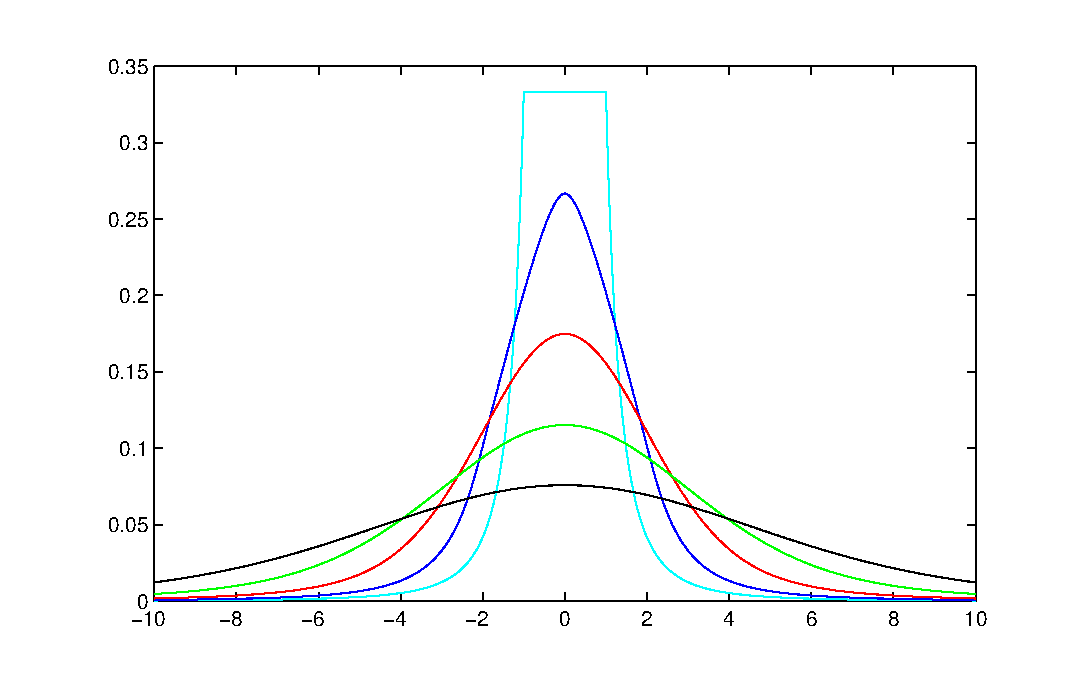
\includegraphics{Statistics/Stable_distribution/x-3_pdf.eps}}
\hspace{-1cm}
\resizebox{.52\textwidth}{!}{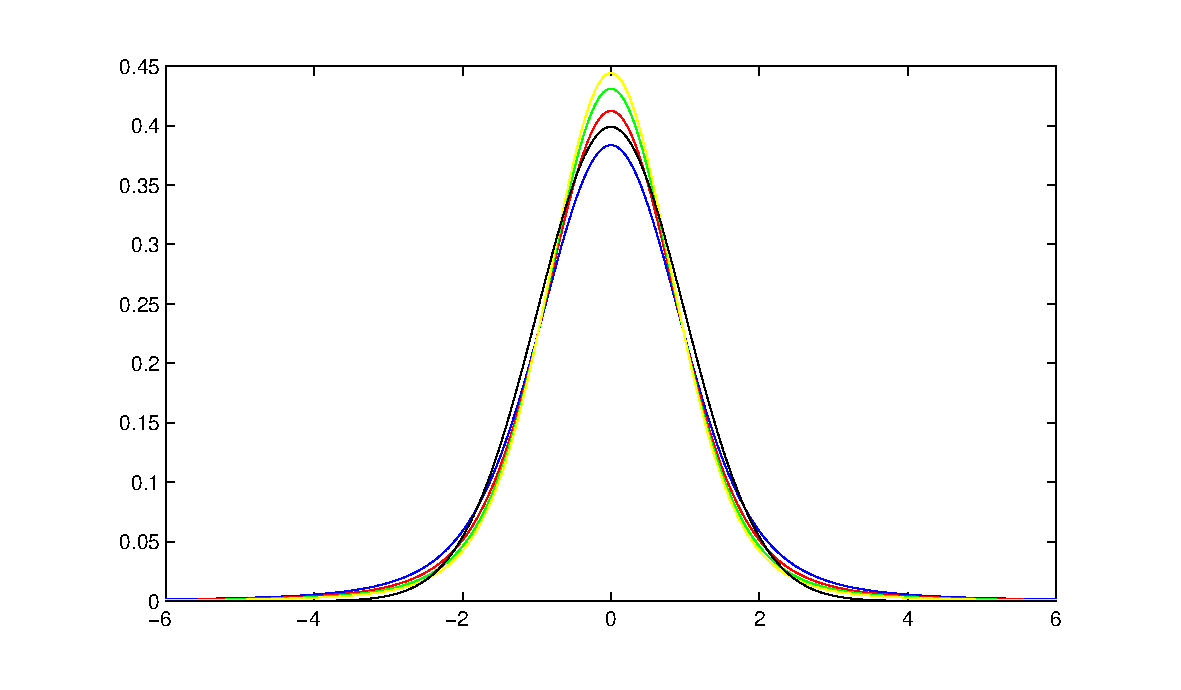
\includegraphics{Statistics/Stable_distribution/x-3_normalized_pdf.eps}}
\end{figure}

It can be proved that it normalized sum converges to a standard normal distribution.
\end{example}

\begin{example}

Let $X$ be the rv with the density function
\be
f(x) = \left\{\ba{ll}
\frac 12 \abs{x}^{-2} \quad\quad & \abs{x}\geq 1 \\
0  & \abs{x}< 1
\ea\right.
\ee

The left graph illustrates the convolution $f^{n*}$ of $n=1,2,4,8$ (cyan, blue, red and green, respectively) for this density function. In right graph
we can use $a_n = \frac{n\pi}{2}$, $n=2,4,8$ (blue, red, green). Then the normalized random variable converges to standard Cauchy distribution (black line).

\begin{figure}[thb]
\centering
\resizebox{.49\textwidth}{!}{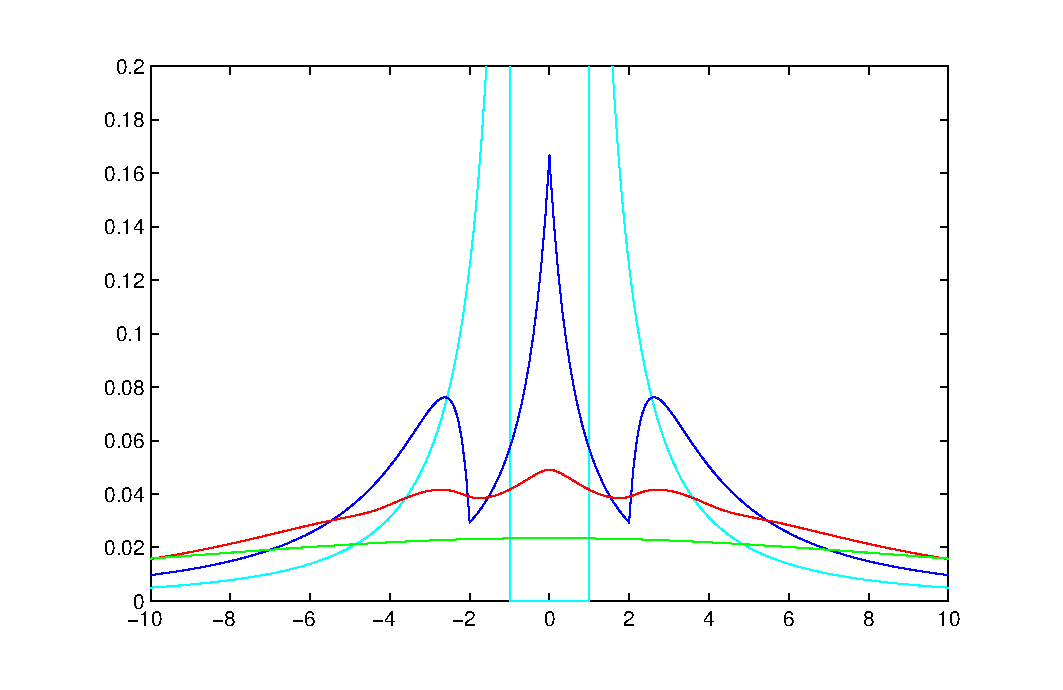
\includegraphics{Statistics/Stable_distribution/x-2_pdf.eps}}
\hspace{-1cm}
\resizebox{.53\textwidth}{!}{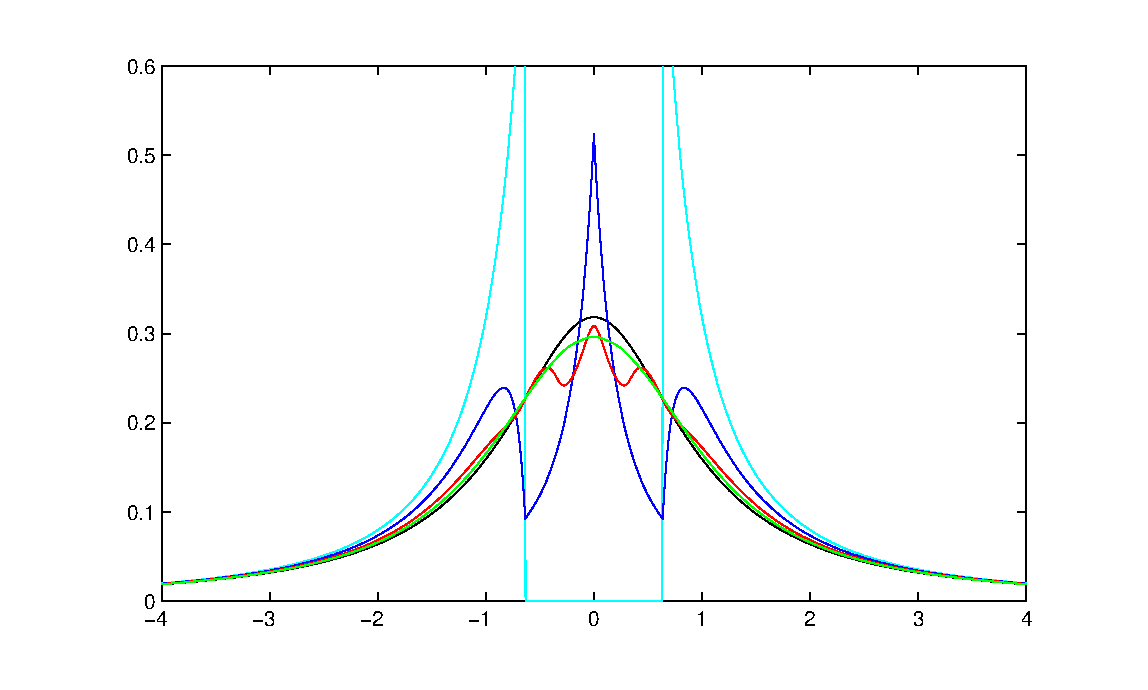
\includegraphics{Statistics/Stable_distribution/x-2_normalized_pdf.eps}}
\end{figure}
\end{example}



%%%%%%%%%%%%%%%%%%%%%%%%%%%%%%%%%%%%%%%%%%%%%%%%%%%%%%%%%%%%
%%%%%%%%%%%%%%%%%%%%%%%%%%%%%%%%%%%%%%%%%%%%%%%%%%%%%%%%%%%%
\part{Optimization}
\chapter{Optimization}

\section{Problems}

\begin{problem}[the locker puzzle\cite{Curtin_2006}]\label{que:locker_puzzle}
Suppose there are $2n$ person indexed from 1 to $2n$. Also, there is a room having $2n$ doors in order and behind each of the doors there is a corresponding number to each person with random distribution without repeat. Now $2n$ person are allowed to get into the room one by one, open at most $n$ doors and leave without communication with other person. If one of the doors the person checked has his corresponding number, we say that this person is successful. 

All the person could have a chat to make a particular stategy to open the doors. What's the optimal strategy to maximize the probability that all the persons are successful?
\end{problem}

\begin{solution}[\bf Solution.]
We can have the following strategy. The $i$th person checks the $i$th door. If the number behind the door is $i$ then the person stops and leaves the room. If the number is $j\neq i$, then the person checks the $j$th door. 

Note that any permutation of a finite set can be written as a product of disjoint cycles (Theorem \ref{thm:disjoint_cycle_decomposition}). Thus, this strategy will let the persons forming cycles (by the numbers behind the doors) follow the overlapping paths. Thus, it will be different from the strategy that pick the doors independent for each person (which gives the probability $2^{-2n}$). Thus, we need to count the number of situations in which $n$-cycle is the biggest one. Or we can count the number of situations that the size of maximal cycle is equal to or more than $n+1$. If the maximal cycle is $k$-cycle for $2n\geq k \geq n+1$, we have
\be
C^k_{2n} (k-1)! (2n-k)! = \frac{(2n)!}{(2n-k)!k!} (k-1)! (2n-k)! = \frac{(2n)!}{k} \text{ possible ways.}
\ee
Here we have $(k-1)!$ for all the possible ways of $k$-cycle. Thus, the totally unsuccessful probability is
\be
\frac 1{(2n)!}\sum^{2n}_{k=n+1} \frac{(2n)!}{k} = \sum^{2n}_{k=n+1} \frac 1{k}.
\ee 

Then successful probability is
\be
1 - \sum^{2n}_{k=n+1} \frac 1k,\quad\quad \text{e.g., for $n=2$, it is }1 - \frac 13 - \frac 14 = \frac{5}{12}.
\ee

If $n \to \infty$, we can have that (by Corollary\footnote{need corollary})
\be
1 - \sum^{2n}_{k=n+1} \frac 1k \to 1 - \ln 2 = 0.306853.
\ee

However, we still need to show that this strategy is optimal\footnote{need details}.
\end{solution}



%%%%%%%%%%%%%%%%%%%%%%%%%%%%%%%%%%%%%%%%%%%%%%%%%%%%%%%%%%%%
%%%%%%%%%%%%%%%%%%%%%%%%%%%%%%%%%%%%%%%%%%%%%%%%%%%%%%%%%%%%
\part{Financial Mathematics}
\chapter{Model}

\section{Black-Scholes Model}

\section{Utility Theory}

Image that you are given a choice between receiving a certain amount of money or taking a bet that has a 50 percent change of winning \$100 and a 50 percent chance of winning nothing. Clearly the bet has an expected value
of \$50. If you would rather receive a certain payoff of less than \$50, you are risk-averse. If you would take \$50 you are risk-neutral. If you would only accept more than \$50, you are risk-seeking(see
\cite{Sinclair_2013}.$P_{96}$).



%\include{Data/Financial_Mathematics/Futures}
\chapter{Options}

\section{Black-Scholes Model}

Black-Scholes formula (see \cite{Black_Scholes_1973}).

\section{Greeks}

\section{Barrier Options}

\cite{Carr_Bowie_1994}

\section{Lookback Options}

\cite{Carr_Bowie_1994}

\begin{definition}[European lookback option\index{lookback option}]
A European lookback call option, $C_{\min}$ entitles the holder to buy one unit of stock at the expiry time $T$ at the lowest price reached by the stock during the life of the option. Thus, if it is purchased at time 0, at
time $T$ it pays off the amount $S_T - \inf_{0\leq t\leq T} S_t$.

In contrary, a European lookback put option, $P_{\max}$ entitles the holder to sell one unit of stock at the expiry time $T$ at the highest price reached by the stock during the life of the option. Thus, if it is purchased
at time 0, at time $T$ it pays off the amount $\sup_{0\leq t\leq T} S_t - S_T$.
\end{definition}
%,  P_{\max}

\begin{proposition}
In the Black-Scholes model, the prices at time 0 of European lookback call and put option are\footnote{checking of $r=0$ case is needed.}
\be
C_{\min}= \left\{ \ba{ll} S_0\brb{\brb{\frac{2r + \sigma^2}{2r}}\Phi\brb{\frac {\brb{2r + \sigma^2}\sqrt{T}}{2\sigma}} - e^{-rT} \brb{\frac {2r - \sigma^2}{2r}} \Phi\brb{\frac{\brb{2r - \sigma^2}\sqrt{T}}{2\sigma}} - \frac
{\sigma^2}{2r}} \quad\quad & r \neq 0 \\
S_0 \brb{\frac{\sigma \sqrt{T}}{\sqrt{2\pi}}\exp\brb{- \frac{\sigma^2 T}8} - \brb{2+\frac{\sigma^2 T}2}\Phi\brb{-\frac{\sigma\sqrt{T}}2}+1} & r = 0 \ea \right. ,
\ee

\be
P_{\max}= \left\{ \ba{ll} S_0\brb{\brb{\frac{2r + \sigma^2}{2r}}\Phi\brb{\frac {\brb{2r + \sigma^2}\sqrt{T}}{2\sigma}} - e^{-rT} \brb{\frac {2r - \sigma^2}{2r}} \Phi\brb{-\frac{\brb{2r - \sigma^2}\sqrt{T}}{2\sigma}} - 1} \quad\quad & r \neq 0 \\
S_0 \brb{\frac{\sigma \sqrt{T}}{\sqrt{2\pi}}\exp\brb{- \frac{\sigma^2 T}8} + \brb{2+\frac{\sigma^2 T}2}\Phi\brb{\frac{\sigma\sqrt{T}}2}-1} & r = 0 \ea \right. .
\ee
%\be P_{\max} = \left\{ \ba{ll} S_0\brb{\brb{\frac{2r + \sigma^2}{2r}}\Phi\brb{\frac {\brb{2r + \sigma^2}\sqrt{T}}{2\sigma}} - e^{-rT} \brb{\frac {2r - \sigma^2}{2r}} \Phi\brb{\frac{\brb{2r - \sigma^2}\sqrt{T}}{2\sigma}} - \frac {\sigma^2}{2r}} \quad\quad & r \neq 0 \\
%S_0 \brb{1 + \frac{\sigma \sqrt{T}}{\sqrt{2\pi}}\exp\brb{- \frac{\sigma^2 T}8} - \brb{2+\frac{\sigma^2 T}2}\Phi\brb{-\frac{\sigma\sqrt{T}}2}} & r = 0 \ea \right. . \ee
\end{proposition}

\begin{remark}
Note that (e.g. for lookback call option) we can not use $r\to 0$ and get $e^{-rT} \to 1$ and get the price
\be
S_0 \brb{1-2\Phi\brb{-\frac{\sigma\sqrt{T}}2}}
\ee
as $e^{-rT}\brb{\frac {2r - \sigma^2}{2r}} $ is not equal to $1- \frac{\sigma^2}{2r}$ as $r\to 0$.
\end{remark}

\begin{proof}[\bf Proof]
Let $X_t=at + \sigma W_t$ and $Y_T=\inf_{0\leq t\leq T}X_t$, where $W$ is a standard Brownian motion. For $x>y$, $y<0$, by Proposition \ref{pro:pairwise_joint_density_bm_maximum_minimum_current} and
Girsanov, Cameron-Martin theorem (Corollary \ref{cor:girsanov_drift_brownian_motion}), we know the joint density $f$ of ($X_T,Y_T$) is
\be
f(x,y)=\frac{2(x-2y)}{\sigma^3\sqrt{2\pi T^3}}\exp\brb{\frac{a}{\sigma}\frac{x}{\sigma}-\frac{a^2T}{2\sigma^2}-\frac{(x-2y)^2}{2\sigma^2T}},\qquad x>y,y<0.
\ee

For Black-Scholes model we have the underlying price is $S_t=S_0\exp\brb{\brb{r-\frac{\sigma^2}2}t+\sigma W_t}$. Hence, the price of the option is given by
\be
e^{-rT}\E\brb{S_T-\inf_{0\leq t\leq T}S_t}= S_0 - e^{-rT}S_0 \int^0_{-\infty}\int^\infty_y e^{y}f(x,y)dxdy.
\ee
where $f$ is given above with the coefficient $a=r-\sigma^2/2$. Thus, % = r/\sigma-\sigma/2$. Here are the details:
\be
\int^0_{-\infty}\int^\infty_y e^{y}f(x,y)dxdy  = \frac{2\exp\brb{-\frac{a^2T}{2\sigma^2}}}{\sigma^3\sqrt{2\pi T^3}}\int^0_{-\infty}\int^\infty_y  (x-2y)\exp\brb{y+\frac{ax}{\sigma^2}-\frac{(x-2y)^2}{2\sigma^2T}}dxdy .\qquad (*)
\ee

Make the change of variables
\be
\ba{ccl}
x & = & \sigma\sqrt{T}u \\
y & = & \frac{1}{2}\sigma\sqrt{T}(u-v)
\ea\la
\ba{ccl}
u & = & \frac{1}{\sigma\sqrt{T}}x \\
v & = & \frac{1}{\sigma\sqrt{T}}(x-2y)
\ea
\ee
in the integral, remembering to put in the Jacobian factor $\sigma^2 T/2$:
\be
\int^0_{-\infty}\int^\infty_y  (x-2y)\exp\brb{y+\frac{ax}{\sigma^2}-\frac{(x-2y)^2}{2\sigma^2T}}dxdy =
\frac{\sigma^3T^{3/2}}{2}\int^\infty_{0}\int_{-v}^v v\exp\brb{\frac{1}{2}\sigma\sqrt{T}(u-v) + \frac{a\sqrt{T}u}{\sigma}-\frac{v^2}2}dudv
\ee

Now, recalling that $\sigma^2/2+a=r$, we do the integration with respect to $u$,
\beast
& & \int^\infty_{0}\int_{-v}^v v\exp\brb{\frac{r\sqrt{T}u}{\sigma} - \frac{\sigma\sqrt{T}v}{2}-\frac{v^2}2}dudv \qquad (**) \\
& = & \frac{\sigma}{r\sqrt{T}}\int_0^\infty v\brb{\exp\brb{\frac{r\sqrt{T}v}{\sigma}}-\exp\brb{-\frac{r\sqrt{T}v}{\sigma}}}\exp\brb{-\frac{\sigma\sqrt{T}v}2-\frac{v^2}2}dv
\eeast

Now, do the integrals separately for $c$:
\beast
\int_0^\infty v\exp\brb{c\sqrt{T}v-v^2/2}dv & = & \int^\infty_0 v\exp\brb{(c^2T/2-(v-c\sqrt{T})^2/2}dv = e^{c^2T/2}\int^\infty_{-c\sqrt{T}} \brb{s+c\sqrt{T}}e^{-s^2/2}ds \\
& = & e^{c^2T/2}\brb{ e^{-c^2T/2} + c\sqrt{2\pi T}\brb{1-\Phi\brb{-c\sqrt{T}}} } = 1 + c\sqrt{2\pi T} \exp\brb{\frac{c^2T}2}\Phi\brb{c\sqrt{T}}
\eeast

Similiarly, letting $c=a/\sigma$ or $c = b/\sigma$ where $b:= -r -\sigma^2/2$, ($*$) is
%
%\be
%\int_{v>0} ve^{-(r/\sigma+\sigma/2)\sqrt{T}v-v^2/2}dv = \int_{v>0} ve^{(b^2T/2-(v+b\sqrt{T})^2/2}dv = 1 - b\sqrt{2\pi T} e^{b^2T/2}\Phi(-b\sqrt{T})
%\ee
\beast
& & \frac{2\exp\brb{-\frac{a^2T}{2\sigma^2}}}{\sigma^3\sqrt{2\pi T^3}} \frac{\sigma^3T^{3/2}}{2} \frac{\sigma}{r\sqrt{T}} \brb{\frac{a}{\sigma}\sqrt{2\pi T}
\exp\brb{\frac{a^2T}{2\sigma^2}}\Phi\brb{\frac{a\sqrt{T}}{\sigma}}- \frac{b}{\sigma}\sqrt{2\pi T} \exp\brb{\frac{b^2T}{2\sigma^2}}\Phi\brb{\frac{b\sqrt{T}}{\sigma}}} \\
& = & \frac ar \Phi\brb{\frac{a\sqrt{T}}{\sigma}} - \frac br\exp\brb{\frac{2r\sigma^2 T}{2\sigma^2}}\Phi\brb{\frac{b\sqrt{T}}{\sigma}} \\
& = & \frac {2r-\sigma^2}{2r} \Phi\brb{\frac{\brb{2r-\sigma^2}\sqrt{T}}{2\sigma}} + \frac {2r+\sigma^2 }{2r} e^{rT }\Phi\brb{\frac{\brb{-2r-\sigma^2}\sqrt{T}}{2\sigma}} \\
& = & \frac {2r-\sigma^2}{2r} \Phi\brb{\frac{\brb{2r-\sigma^2}\sqrt{T}}{2\sigma}} + \frac {2r+\sigma^2 }{2r} e^{rT } \brb{1-\Phi\brb{\frac{\brb{2r+\sigma^2}\sqrt{T}}{2\sigma}}}
\eeast

Putting it all together yields
\beast
e^{-rT}\E\brb{S_T-\inf_{0\leq t\leq T}S_t} & = & S_0 - e^{-rT}S_0 \int^0_{-\infty}\int^\infty_y e^{y}f(x,y)dxdy \\
& = & S_0\brb{\brb{\frac{2r + \sigma^2}{2r}}\Phi\brb{\frac {\brb{2r + \sigma^2}\sqrt{T}}{2\sigma}} - e^{-rT} \brb{\frac {2r - \sigma^2}{2r}} \Phi\brb{\frac{\brb{2r - \sigma^2}\sqrt{T}}{2\sigma}} - \frac {\sigma^2}{2r}}
\eeast
as required. %But $-a^2+b^2=-(\sigma/r-\sigma/2)^2+(\sigma/r+\sigma/2)^2=2r$, so that everything equals
%\begin{equation}
%S_0\left[1- e^{-rT}(\sigma/r)a\Phi(a\sqrt{T}) - (\sigma/r)b + (\sigma/r)b\Phi(b\sqrt{T}) \right]
%\end{equation}
%We're done now since $-(\sigma/r)b+1=-(\sigma/r)(r/\sigma+\sigma/2)+1=-\sigma^2/(2r)$.

If $r=0$, we can have that (from ($**$))
\beast
\int^0_{-\infty}\int^\infty_y e^{y}f(x,y)dxdy  & = & I\int^\infty_{0}  2v^2\exp\brb{- \frac{\sigma\sqrt{T}v}{2}-\frac{v^2}2}dv = 2I\exp\brb{\frac{\sigma^2 T}{8}}\int^\infty_{0}  v^2\exp\brb{- \frac{\brb{v +
\sigma\sqrt{T}/2}^2}2}dv \\
& = & 2I\exp\brb{\frac{\sigma^2 T}{8}}\brb{\int^\infty_{0}  \brb{v^2 - \frac{\sigma^2 T}4}\exp\brb{- \frac{\brb{v + \sigma\sqrt{T}/2}^2}2}dv + \sqrt{2\pi}\frac{\sigma^2 T}4\Phi\brb{-\sigma\sqrt{T}/2}} \\
& = & 2I\exp\brb{\frac{\sigma^2 T}{8}}\brb{-\frac{\sigma \sqrt{T}}2\exp\brb{- \frac{\sigma^2 T}8} + \sqrt{2\pi}\brb{1+\frac{\sigma^2 T}4}\Phi\brb{-\sigma\sqrt{T}/2}}
\eeast
where
\be
I = \frac{2\exp\brb{-\frac{a^2T}{2\sigma^2}}}{\sigma^3\sqrt{2\pi T^3}} \frac{\sigma^3T^{3/2}}{2} = \frac 1{\sqrt{2\pi}}\exp\brb{-\frac{\sigma^2 T}{8}}.
\ee

Thus,
\be
e^{-rT}\E\brb{S_T-\inf_{0\leq t\leq T}S_t} = S_0 \brb{1 + \frac{\sigma \sqrt{T}}{\sqrt{2\pi}}\exp\brb{- \frac{\sigma^2 T}8} - \brb{2+\frac{\sigma^2 T}2}\Phi\brb{-\sigma\sqrt{T}/2}}.
\ee

Note that $1\geq 2\Phi\brb{-\sigma\sqrt{T}/2}$ and \be \frac{\sigma \sqrt{T}}{\sqrt{2\pi}}\exp\brb{- \frac{\sigma^2 T}8}\geq \frac{\sigma^2 T}2 \Phi\brb{-\sigma\sqrt{T}/2} \ee by Proposition \ref{pro:bound_of_gaussian_law}.
Thus, we can have the price is greater than zero.

Now let $Y_T=\sup_{0\leq t\leq T}X_t$ for $y>x$, $y>0$, by Proposition \ref{pro:pairwise_joint_density_bm_maximum_minimum_current} and Girsanov's theorem\footnote{theorem needed, or Cameron-Martin
theorem}, we know the joint density $f$ of ($X_T,Y_T$) is
\be
f(x,y)=\frac{2(2y-x)}{\sigma^3\sqrt{2\pi T^3}}\exp\brb{\frac{a}{\sigma}\frac{x}{\sigma}-\frac{a^2T}{2\sigma^2}-\frac{(2y-x)^2}{2\sigma^2T}},\qquad x<y,y>0.
\ee

For Black-Scholes model we have the underlying price is $S_t=S_0\exp\brb{\brb{r-\frac{\sigma^2}2}t+\sigma W_t}$. Hence, the price of the option is given by
\be
e^{-rT}\E\brb{\sup_{0\leq t\leq T}S_t-S_T}= e^{-rT}S_0 \int_0^\infty \int^y_{-\infty} e^{y}f(x,y)dxdy - S_0.
\ee

Thus, % = r/\sigma-\sigma/2$. Here are the details:
\be
\int_0^\infty \int^y_{-\infty} e^{y}f(x,y)dxdy  = \frac{2\exp\brb{-\frac{a^2T}{2\sigma^2}}}{\sigma^3\sqrt{2\pi T^3}}\int_0^\infty \int^y_{-\infty}  (2y-x)\exp\brb{y+\frac{ax}{\sigma^2}-\frac{(2y-x)^2}{2\sigma^2T}}dxdy
\qquad (\dag) .
\ee

Make the change of variables \be
\ba{ccl}
x & = & \sigma\sqrt{T}u \\
y & = & \frac{1}{2}\sigma\sqrt{T}(u+v)
\ea \la
\ba{ccl}
u & = & \frac{1}{\sigma\sqrt{T}}x \\
v & = & \frac{1}{\sigma\sqrt{T}}(2y-x)
\ea
\ee
in the integral, remembering to put in the Jacobian factor $\sigma^2 T/2$:
\be
\int_0^\infty \int^y_{-\infty}  (2y -x)\exp\brb{y+\frac{ax}{\sigma^2}-\frac{(2y-x)^2}{2\sigma^2T}}dxdy = \frac{\sigma^3T^{3/2}}{2}\int^\infty_{0}\int_{-v}^v v\exp\brb{\frac{1}{2}\sigma\sqrt{T}(u+v) + \frac{a\sqrt{T}u}{\sigma}-\frac{v^2}2}dudv
\ee

Now, recalling that $\sigma^2/2+a=r$, we do the integration with respect to $u$,
\beast
& & \int^\infty_{0}\int_{-v}^v v\exp\brb{\frac{r\sqrt{T}u}{\sigma} + \frac{\sigma\sqrt{T}v}{2}-\frac{v^2}2}dudv \qquad (**) \\
& = & \frac{\sigma}{r\sqrt{T}}\int_0^\infty v\brb{\exp\brb{\frac{r\sqrt{T}v}{\sigma}}-\exp\brb{-\frac{r\sqrt{T}v}{\sigma}}}\exp\brb{\frac{\sigma\sqrt{T}v}2-\frac{v^2}2}dv
\eeast

So letting $a' = r + \frac {\sigma^2}2$ and $b' = -r + \frac {\sigma^2}2$, ($\dag$) is
\beast
& & \frac{2\exp\brb{-\frac{a^2T}{2\sigma^2}}}{\sigma^3\sqrt{2\pi T^3}} \frac{\sigma^3T^{3/2}}{2} \frac{\sigma}{r\sqrt{T}} \brb{\frac{a'}{\sigma}\sqrt{2\pi T} \exp\brb{\frac{a'^2T}{2\sigma^2}}\Phi\brb{\frac{a'\sqrt{T}}{\sigma}}- \frac{b'}{\sigma}\sqrt{2\pi T} \exp\brb{\frac{b'^2T}{2\sigma^2}}\Phi\brb{\frac{b'\sqrt{T}}{\sigma}}} \\
& = & \frac {a'}r e^{rT}\Phi\brb{\frac{a'\sqrt{T}}{\sigma}} - \frac {b'}r\Phi\brb{\frac{b'\sqrt{T}}{\sigma}} \\
& = & \frac {2r+\sigma^2}{2r}e^{rT} \Phi\brb{\frac{\brb{2r+\sigma^2}\sqrt{T}}{2\sigma}} + \frac {2r-\sigma^2 }{2r} \Phi\brb{-\frac{\brb{2r-\sigma^2}\sqrt{T}}{2\sigma}}
\eeast

Putting it all together yields
\beast
e^{-rT}\E\brb{\sup_{0\leq t\leq T}S_t-S_T} & = & e^{-rT}S_0 \int^0_{-\infty}\int^\infty_y e^{y}f(x,y)dxdy - S_0 \\
& = & S_0\brb{\brb{\frac{2r + \sigma^2}{2r}}\Phi\brb{\frac {\brb{2r + \sigma^2}\sqrt{T}}{2\sigma}} - e^{-rT} \brb{\frac {2r - \sigma^2}{2r}} \Phi\brb{-\frac{\brb{2r - \sigma^2}\sqrt{T}}{2\sigma}} - 1}
\eeast
as required. Also, it is similar for the case $r=0$.
\end{proof}


\section{Hedging}

Discretely adjusted hedging (see \cite{Boyle_Emanuel_1980}) with transaction costs (see \cite{Leland_1985})

\subsection{Put-call Symmetry}

First metioned in \cite{Carr_Bowie_1994}, proved in the appendix of \cite{Carr_Ellis_Gupta_1998}.

\section{American options}



\section{Path Dependent options}

\cite{Goldman_Sosin_Gatto_1979_1},\cite{Goldman_Sosin_Gatto_1979_2}


\section{Heston Model}

The Heston model is first given in \cite{Heston_1993}.

\chapter{Volatility}

\section{VIX}

\subsection{Variance swaps}

Variance swaps were based on an idea by Carr and Madan (1998)\cite{Carr_Madan_1998}.

The first study of the discrete situation was by Demeterfi et al.(1999)\cite{Demeterfi_1999_2}, who examined in some detail the effect of using a finite number of strikes.

%\include{Data/Financial_Mathematics/Asset_Allocation}
\chapter{Contracting Theory}


\chapter{Risk}

\section{Value at Risk}

\subsection{Long Gamma position}

\begin{center}
 \psset{xunit=0.5cm,yunit=20cm,arrowscale=1.5}
 \begin{pspicture}(-1,-0.05)(21,0.2)
 \psChiIIDist[linewidth=1pt,nue=5]{0.01}{19.5}
 \psaxes[labels=none,ticks=none]{->}(20,0.2)
 \pscustom[fillstyle=solid,fillcolor=red!30]{%
 \psChiIIDist[linewidth=1pt,nue=5]{1}{19.5}%
 \psline(20,0)(1,0)}
 \end{pspicture}
\end{center}

\subsection{Statistical error of VaR}

Note that by Theorem \ref{thm:asymptotic_distribution_central_order_statistic},
\be
\sqrt{n}f\bb{F^{-1}(p)} \frac{X_i - F^{-1}(p)}{\sqrt{p(1-p)}} \stackrel{d}{\to} \sN(0,1).
\ee

Thus, $X_i = \wh{\VAR}_p$ is normal distributed random variable with mean $\VAR_p = F^{-1}(p)$ and standard deviation
\be
\sigma_{\wh{\VAR}_p} = \frac 1{f\bb{F^{-1}(p)}}\sqrt{\frac{p(1-p)}{n }}.
\ee

If $F$ is distribution function of standard normal random variable ($f(x) = \phi(x) = \frac 1{\sqrt{2\pi}} e^{-\frac{x^2}2}$), we have $F^{-1}(p) = 2.326$ for $p = 99\%$. Then for $n=10000$,
\be
\frac{\sigma_{\wh{\VAR}_p}}{\VAR_p} =  \frac 1{F^{-1}(p) \cdot f\bb{F^{-1}(p)}}\sqrt{\frac{p(1-p)}{n }} \approx \frac 1{2.326 \cdot \phi\bb{2.326}}\sqrt{\frac{0.99\cdot 0.01}{10000}} \approx 1.60\%
\ee

Thus, the error of confidence level (two-sided) $\alpha$ is
\be
\Phi^{-1}\bb{\frac{1+\alpha}2}\frac{\sigma_{\wh{\VAR}_p}}{\wh{\VAR}_p}
\ee

Then for confidence level $\alpha = 95\%$, the value is 1.96 (no matter the distribution $F$ is) and error is approximately
\be
\Phi^{-1}\bb{0.975}\frac{\sigma_{\wh{\VAR}_p}}{\VAR_p} \approx 1.96\cdot 1.60\% = 3.14\%.
\ee


\subsection{Estimation statistical error of VaR under empirical distribution}

Given the 10000 P\&L from Monte Carlo simulation, we can estimate the $F^{-1}(q)f\bb{F^{-1}(q)}$ empirically, then derive the VaR error.

If VaR is the 101th worst loss in the 10000 scenarios, $F^{-1}(q)= \pnl_{101}$. We can calculate empirically
\be
f\bb{F^{-1}(q)} = \frac{F\bb{F^{-1}(q)+\Delta}- F\bb{F^{-1}(q)-\Delta}}{2\Delta} = \frac{0.0002}{\pnl_{100}  - \pnl_{102}}.
\ee

Therefore, the 1 standard deviation of $\VAR$ is
\be
\frac{\sigma_{\wh{\VAR}_p}}{\wh{\VAR}_p} \approx \frac 1{F^{-1}(p) \cdot f\bb{F^{-1}(p)}}\sqrt{\frac{p(1-p)}{n }} \approx \frac{\pnl_{100} - \pnl_{102}}{0.0002\cdot \pnl_{101}} \sqrt{\frac{0.99\cdot 0.01}{10000}} \approx 4.9749 \cdot \frac{\pnl_{100} - \pnl_{102}}{\pnl_{101}}.
\ee


\section{VaR and ES derived by EVT}

We simply assume the distributions are continuous in this section.

\subsection{ES derived from MV}

Theoretically, the expectation of maximum value is larger than expected shortfall. Thus, we can use the sample data to fit GEV distribution and estimate the parameters $\wh{\xi},\wh{\sigma},\wh{\mu}$ by applying the property in the appendix. Then we can calculate the estimate maximum value $\wh{M}$
\be
\wh{M} = \left\{\ba{ll}
\wh{\mu} + \wh{\sigma}\frac{\Gamma\bb{1-\wh{\xi}}-1}{\wh{\xi}} \quad\quad & \wh{\xi} <1,\wh{\xi} \neq 0\\
\wh{\mu} + \wh{\sigma} \gamma & \wh{\xi} = 0
\ea\right.
\ee
where $\gamma$ is Euler's constant.

Therefore, if P\&L is larger than $\wh{M}$, we can assert that it exceeds expected shortfall $\ES_p$ (for any $p$). It is clear that maximum value method froms a necessary condition for the backtesting.

\subsection{VaR and ES derived from POT}

Assuming a GPD function for the taildistribution, analytical expressions for $\VAR_p$ and $\ES_p$ can be defined as a function of GPD parameters. Isolating $F(x)$ by
\be
F(x) = (1-F(u))F_u(y) + F(u)
\ee
and replacing $F_u$ by the GDP and $F(u)$by the estimation $1-N_u/N$, where $N$ is the total number of observations and $N_u$ the number of observations above the threshold $u$, we obtain
\beast
\wh{F}(x) & = & \frac{N_u}{N} \bb{1-\bb{1+\frac{\wh{\xi} (x-u)}{\wh{\sigma}}}^{-1/\wh{\xi}}} + \bb{1-\frac {N_u}{N}} \\
& = &  1-\frac{N_u}{N} \bb{1+\frac{\wh{\xi} (x-u)}{\wh{\sigma}}}^{-1/\wh{\xi}}
\eeast

Note that $\xi$ and $\sigma$ are calibrated by the sample data and $\wh{\xi}$ and $\wh{\sigma}$ are given (see \cite{Gilli_Kellezi_2006}). Then inverting the above formula for a given probability $p$ (usually is 99\%) gives
\be
\wh{\VAR}_p = u + \frac{\wh{\xi}}{\wh{\sigma}}\bb{\bb{\frac N{N_u}(1-p)}^{-\wh{\xi}}-1}%\bb{1+ \frac{\wh{\xi}}{\wh{\sigma}} (x-u)}^{-1/\wh{\xi}}
\ee
%where $N_u$ is the number of observations above the threshold $u$. Then

Furthermore, from the result in appendix for GPD with $0<\xi <1$ %the mean excess function can be defined by $ME(z) := \E\bb{X-z|X>z}$
and the definition of expected shortfall, we have
\beast
\wh{\ES}_p = \E\bb{X|X>\wh{\VAR}_p } & = & %\frac{\E\bb{X\ind_{\bra{X>\wh{\VAR}_p}}}}{1-F\bb{\wh{\VAR}_p}}=\frac{\wh{\VAR}_p + \frac{\wh{\sigma}}{1-\wh{\xi}}}{1-F\bb{\wh{\VAR}_p}}
\wh{\VAR}_p + \E\bb{X-\wh{\VAR}_p|X>\wh{\VAR}_p } \\%= \wh{\VAR}_p + ME\bb{\wh{\VAR}_p } \\
& = & \wh{\VAR}_p + \frac{\wh{\sigma} + \wh{\xi}\bb{\wh{\VAR}_p-u}}{1-\wh{\xi}} = \frac{\wh{\VAR}_p}{1-\wh{\xi}} + \frac{\wh{\sigma}-\wh{\xi}u}{1-\wh{\xi}}.
\eeast

If $p = 1- \frac {N_u}{N}$, we can plug the definition of $\wh{\ES}_p$ into the above formula and get
\be
\wh{\ES}_p = \wh{\VAR}_p + \frac{\wh{\sigma}}{1-\wh{\xi}}
\ee

This is obvious that the expected shortfall is more conservative than Value at Risk for the same confidence level.

For $\xi = 0$ case,
\be
\wh{F}(x) = \frac{N_u}{N} \bb{1-\exp\bb{-\frac{\wh{\xi} (x-u)}{\wh{\sigma}}}} + \bb{1-\frac {N_u}{N}}
\ee

\be
\wh{\VAR}_p = u - \frac{\wh{\xi}}{\wh{\sigma}}\ln\bb{\frac N{N_u}(1-p)}%\bb{1+ \frac{\wh{\xi}}{\wh{\sigma}} (x-u)}^{-1/\wh{\xi}}
\ee

Then from the result in appendix for GPD with $\xi =0$,
\be
\wh{\ES}_p = \E\bb{X|X>\wh{\VAR}_p } = \wh{\VAR}_p + \E\bb{X-\wh{\VAR}_p|X>\wh{\VAR}_p } = \wh{\VAR}_p + \wh{\sigma}.
\ee


%%%%%%%%%%%%%%%%%%%%%%%%%%%%%%%%%%%%%%%%%%%%%%%%%%%%%%%%%%%%
%%%%%%%%%%%%%%%%%%%%%%%%%%%%%%%%%%%%%%%%%%%%%%%%%%%%%%%%%%%%

%\part{Numerical Analysis}
%\include{Data/Numerical_Anlaysis/Numerical_Anlaysis}	%p
%%%%%%%%%%%%%%%%%%%%%%%%%%%%%%%%%%%%%%%%%%%%%%%%%%%%%%%%%%%%
%%%%%%%%%%%%%%%%%%%%%%%%%%%%%%%%%%%%%%%%%%%%%%%%%%%%%%%%%%%%
%\part{Graph Theory}



%%%%%%%%%%%%%%%%%%%%%%%%%%%%%%%%%%%%%%%%%%%%%%%%%%%%%%%%%%%%
%%%%%%%%%%%%%%%%%%%%%%%%%%%%%%%%%%%%%%%%%%%%%%%%%%%%%%%%%%%%
%\part{Coding and Cryptography}
%\chapter{Coding and Cryptography}

Transmitting messages is an important practical problem. Coding theory includes the study of compression codes which enable us to send messages cheaply and error correcting codes which ensure that messages remain legible even in the presence of errors. Cryptography on the other hand, makes sure that messages remain unreadable --- except to the intended recipient. These techniques turn out to have much in common.

Many Part~II courses go deeply into one topic so that you need to understand the whole course before you understand any part of it. They often require a firm grasp of some preceding course. Although this course has an underlying theme, it splits into parts which can be understood separately and, although it does require knowledge from various earlier courses, it does not require mastery of that knowledge. All that is needed is a little probability, a little algebra and a fair amount of common sense. On the other hand, the variety of techniques and ideas probably makes it harder to understand \emph{everything} in the course than in a more monolithic course.


%%%%%%%%%%%%%%%%%%%%%%%%%%%%%%%%%%%%%%%%%%%

\section{Codes and alphabets}\label{S;alphabets}
Originally, a code was a device for making messages
hard to read. The study of such codes and their
successors is called cryptography and will form
the subject of the last quarter of these notes.
However, in the 19th century the
optical\footnote{See \emph{The Count of Monte Cristo}
and various Napoleonic sea stories.
A statue to the inventor of the optical telegraph
(semaphore)
was put up in Paris in 1893 but melted down during
World War II and not replaced 
(http://hamradio.nikhef.nl/tech/rtty/chappe/).
In the parallel universe of Disc World the 
\emph{clacks} is one of the wonders of the
Century of the Anchovy.} and
then the electrical telegraph made it
possible to send messages speedily, but
only after they had been translated from ordinary written
English or French into a string of symbols.

The best known of the early codes is the Morse code
used in electronic telegraphy.
We think of it as consisting of dots and 
dashes but, in fact, it had three symbols dot, dash and pause
which we write as $\bullet$, $-$ and $*$.
Morse assigned a \emph{code word} consisting of a 
sequence of symbols to each of the letters of the alphabet
and each digit. Here are some typical examples.
\begin{align*}
A\mapsto \bullet-*\qquad
&&B\mapsto -\bullet\bullet\bullet*\qquad
&&C\mapsto-\bullet-\bullet*\\
D\mapsto -\bullet\bullet*\qquad
&&E\mapsto \bullet*\qquad
&&F\mapsto\bullet\bullet-\bullet*\\
O\mapsto ---*\qquad
&&S\mapsto\bullet\bullet\bullet*\qquad
&&7\mapsto--\bullet\bullet\bullet*
\end{align*}
The symbols of the original message would be \emph{encoded}
and the code words sent in sequence, as in
\[SOS\mapsto
\bullet\bullet\bullet*---*\bullet\bullet\bullet*,\]
and then decoded in sequence at the other end
to recreate the original message.
\begin{exercise}\label{E;Morse}
Decode
$-\bullet-\bullet*---*-\bullet\bullet* \bullet*$.
\end{exercise}

Morse's system was intended for human beings.
Once machines took over the business of encoding, 
other systems developed. A very influential
one called ASCII was developed in the 1960s.
This uses two symbols $0$ and $1$
and all code words have seven symbols.
In principle, this would give $128$ possibilities, but $0000000$
and $1111111$ are not used, so there are $126$ code words
allowing the original message to contain a greater
variety of symbols than Morse code. 
Here are some typical examples
\begin{align*}
A\mapsto 1000001\qquad
&&B\mapsto 1000010\qquad
&&C\mapsto 1000011\\
a\mapsto 1100001\qquad
&&b\mapsto 1100010 \qquad
&&c\mapsto 1100011\\
+\mapsto 0101011\qquad
&&!\mapsto 0100001\qquad
&&7\mapsto 0110111
\end{align*}
\begin{exercise}\label{E;ASCII} 
Encode $b7!$. Decode $110001111000011100010$.
\end{exercise}

More generally, we have two alphabets ${\mathcal A}$
and ${\mathcal B}$ 
and a coding function $c:{\mathcal A}\rightarrow{\mathcal B}^{*}$
where ${\mathcal B}^{*}$ consists of all finite sequences of 
elements of  ${\mathcal B}$.
If  ${\mathcal A}^{*}$ consists of all finite sequences 
of elements of  ${\mathcal A}$,
then the encoding function 
$c^{*}:{\mathcal A}^{*}\rightarrow{\mathcal B}^{*}$
is given by
\[c^{*}(a_{1}a_{2}\ldots a_{n})=c(a_{1})c(a_{2})\dots c(a_{n}).\]
We demand that $c^{*}$ is injective, since otherwise
it is possible to produce two
messages which become indistinguishable once encoded.

We call codes for which $c^{*}$ is injective \emph{decodable}.

For many purposes, we are more interested
in the collection of code words ${\mathcal C}=c({\mathcal A})$
than the coding function $c$. If we look
at the code words of Morse code and the ASCII code, we
observe a very important difference.
All the code words in ASCII have the same length 
(so we have a \emph{fixed length} code),
but this is not true for the Morse code
(so we have a \emph{variable length} code).
\begin{exercise}\label{E;fix length} Explain why (if $c$ is injective) 
any fixed length code
is  decodable.
\end{exercise}

A variable length code need not be decodable even 
if $c$ is injective.
\begin{exercise}\label{E;decodable} 
(i) Let ${\mathcal A}={\mathcal B}=\{0,1\}$. If
$c(0)=0$, $c(1)=00$ show that $c$ is injective but $c^{*}$ is not.
 
(ii) Let ${\mathcal A}=\{1,2,3,4,5,6\}$ and ${\mathcal B}=\{0,1\}$.
Show that there is a variable length coding $c$ such that
$c$ is injective and all code words have length $2$ or less.
Show that there is no decodable coding $c$ such that
all code words have length $2$ or less.
\end{exercise}

However, there is a family of variable length codes
which are decodable in a natural way.
\begin{definition} Let ${\mathcal B}$ be an alphabet. We say that
a finite subset ${\mathcal C}$ of ${\mathcal B}^{*}$
is \emph{prefix-free} if, 
whenever $w\in{\mathcal C}$ is an initial sequence
of $w'\in{\mathcal C}$, then $w=w'$. 
If $c:{\mathcal A}\rightarrow{\mathcal B}^{*}$
is a coding function, we say that $c$ is prefix-free if $c$ is injective
and $c({\mathcal A})$
is prefix-free.
\end{definition}

If $c$ is prefix-free, then, not only is $c^{*}$ injective, but we can decode
messages on the fly. Suppose that we receive a sequence 
$b_{1}$, $b_{2}$, \dots.
The moment we have received some $c(a_{1})$, we know that 
the first message was $a_{1}$
and we can proceed to look for the second message. (For this reason
prefix-free codes
are sometimes called instantaneous codes or self punctuation codes.)
\begin{exercise} Let  ${\mathcal A}=\{0,1,2,3\}$, ${\mathcal B}=\{0,1\}$.
If $c,\tilde{c}:{\mathcal A}\rightarrow{\mathcal B}^{*}$ are given by
\begin{align*}
c(0)&=0&&\tilde{c}(0)=0\\
c(1)&=10&&\tilde{c}(1)=01\\
c(2)&=110&&\tilde{c}(2)=011\\
c(3)&=111&&\tilde{c}(3)=111
\end{align*}
show that $c$ is prefix-free, but $\tilde{c}$ is not.
By thinking about the way $\tilde{c}$ is obtained from $c$, or otherwise,
show that $\tilde{c}^{*}$ is injective.
\end{exercise}
\begin{exercise}\label{E;auto free} 
Why is every injective fixed
length code automatically prefix-free?
\end{exercise}
From now on, unless explicitly stated otherwise, $c$ will be injective
and the codes used will be prefix-free. In section~\ref{S;prefix} 
we show
that we lose nothing by confining ourselves to prefix-free codes.
\section{Huffman's algorithm} An electric telegraph is expensive 
to build and maintain. However good a telegraphist was,
he could only send or receive a limited number of dots and dashes
each minute. (This is why  Morse chose a variable length code.
The telegraphist would need to send the letter $E$ far more often than
the letter $Q$ so Morse gave $E$ the short
code $\bullet*$ and $Q$ the long code $--\bullet-*$.)
It is possible to increase the rate at which symbols are
sent and received by using machines, but the laws of
physics (backed up by results in Fourier analysis)
place limits on the number of symbols that can be
correctly transmitted over a given line.
(The slowest rates were associated with undersea cables.)

Customers were therefore charged so much
a letter or, more usually, so 
much a word\footnote{Leading to a
prose style known as telegraphese.
`Arrived Venice. Streets flooded. Advise.'}
(with a limit
on the permitted word length).
Obviously it made sense to have books
of `telegraph codes' in which one five letter
combination, say, `FTCGI'
meant `are you willing to split the difference?'
and  another `FTCSU' meant
`cannot see any difference'\footnote{If the telegraph
company insisted on ordinary words you got
codes like `FLIRT' for `quality of crop good'.
Google `telegraphic codes and message practice, 1870-1945'
for lots of examples.}.
 
Today messages are usually sent in
as binary sequences like $01110010\dots$,
but the transmission of each digit still costs
money. If we know that there are $n$ possible
messages that can be sent and that $n\leq 2^{m}$,
then we can assign each message a different
string of $m$ zeros and ones (usually called \emph{bits})
and each message will cost $mK$ cents where $K$
is the cost of sending one bit.

However, this may not be the best way of saving money.
If, as  often happens, one message 
(such as `nothing to report') is much more frequent
than any other then it may be cheaper \emph{on average}
to assign it a shorter code word even at the cost
of lengthening the other code words.
\begin{problem}\label{P;Compress one}
Given $n$ messages $M_{1}$, $M_{2}$,
\dots, $M_{n}$ such that the probability that $M_{j}$
will be chosen is $p_{j}$, find distinct code words $C_{j}$
consisting of $l_{j}$ bits so that the expected cost
\[K\sum_{j=1}^{n}p_{j}l_{j}\]
of sending the code word corresponding to the chosen
message is minimised.
\end{problem}
Of course, we suppose $K>0$.

The problem is interesting as it stands, but we
have not taken into account the fact that a variable
length code may not be decodable. To deal with this
problem we add an extra constraint.
\begin{problem}\label{P;Compress}
Given $n$ messages $M_{1}$, $M_{2}$,
\dots, $M_{n}$ such that the probability that $M_{j}$
will be chosen is $p_{j}$, find a prefix-free
collection of code words $C_{j}$
consisting of $l_{j}$ bits so that the expected cost
\[K\sum_{j=1}^{n}p_{j}l_{j}\]
of sending the code word corresponding to the chosen
message is minimised.
\end{problem}


In 1951 Huffman was asked to write an essay on this problem
as an end of term university exam. Instead of writing about the problem,
he solved it completely.
\begin{theorem}\label{T;Huffman}{\bf [Huffman's algorithm]} 
The following algorithm
solves Problem~\ref{P;Compress} with $n$ messages.
Order the messages so that $p_{1}\geq p_{2}\geq \dots\geq p_{n}$.
Solve the problem with $n-1$ messages $M_{1}'$, $M_{2}'$,
\dots, $M_{n-1}'$ such that $M_{j}'$ has probability $p_{j}$
for $1\leq j\leq n-2$, but $M_{n-1}'$ has probability
$p_{n-1}+p_{n}$. If $C_{j}'$ is the code word corresponding
to $M_{j}'$, the original problem is solved by assigning $M_{j}$
the code word $C_{j}'$ for $1\leq j\leq n-2$ and
$M_{n-1}$ the code word consisting of $C_{n-1}'$ followed
by $0$ and $M_{n}$ the code word consisting of $C_{n-1}'$ 
followed by $1$.
\end{theorem}
Since the problem is trivial when $n=2$ (give $M_{1}$ the code word $0$
and $M_{2}$ the code word $1$) this gives us what computer programmers
and logicians call a \emph{recursive solution}.

Recursive programs are often 
better adapted to machines 
than human beings, but it is very easy
to follow the steps of Huffman's algorithm `by hand'.
(Note that the algorithm is very specific about
the labelling of the code words so that, for example,
message $1$ 

\begin{example}\label{E;Huffman do} 
Suppose $n=4$, $M_{j}$ has probability $j/10$ 
for $1\leq j\leq 4$. Apply Huffman's algorithm.
\end{example}
\begin{proof}[Solution]
(Note that we do not bother to reorder messages.)
Combining messages in the suggested way, we get
\begin{gather*}
1,2,3,4\\
[1,2],3,4\\
[[1,2],3],4.
\end{gather*}
Working backwards, we get
\begin{gather*}
C_{[[1,2],3]}=0\ldots,\ C_{4}=1\\
C_{[1,2]}=01\dots,\ C_{3}=00\\
C_{1}=011,\ C_{2}=010.
\end{gather*}
\end{proof}
The reader is strongly advised to do a slightly more
complicated example like the next.
\begin{exercise}\label{E;Huffman 1} 
Suppose $M_{j}$ has probability $j/45$ 
for $1\leq j\leq 9$. Apply Huffman's algorithm.
\end{exercise}

As we indicated earlier, the effects of Huffman's algorithm 
will be most marked when a few messages are highly
probable.
\begin{exercise}\label{E;Huffman 2} Suppose $n=64$,
$M_{1}$ has probability $1/2$,
$M_{2}$ has probability $1/4$ and $M_{j}$ has probability
$1/248$ for $3\leq j\leq 64$.
Explain why, if we use code words of equal length
then the length of a code word must be at least $6$.
By using the ideas of Huffman's algorithm (you should not
need to go through all the steps) obtain a set of
code words such that the \emph{expected} length of a code word
sent is not more than $3$.
\end{exercise}

Whilst doing the exercises the reader must already
have been struck by the fact that minor variations
in the algorithm produce different codes. (Note, for example
that, if we have a Huffman code, then interchanging the role of
$0$ and $1$ will produce another Huffman type code.)
In fact, although the Huffman algorithm will always
produce a best code (in the sense of Problem~\ref{P;Compress}),
there may be other equally good codes which could not
be obtained in this manner.
\begin{exercise}\label{E;Huffman 3} Suppose $n=4$,
$M_{1}$ has probability $.23$,
$M_{2}$ has probability $.24$, 
$M_{3}$ has probability $.26$
and $M_{4}$ has probability $.27$. Show that any 
assignment of the code words $00$, $01$, $10$
and $11$ produces a best code in the sense of Problem~\ref{P;Compress}.
\end{exercise}

The fact that the Huffman code may not be the unique
best solution means that we need to approach the proof of 
Theorem~\ref{T;Huffman} with caution. We observe that
reading a code word from a prefix-free
code is like climbing a tree
with $0$ telling us to take the left branch and 
$1$ the right branch. The fact that the code is prefix-free
tells us that each code word
may be represented by a leaf at the end of
a final branch. 
Thus, for example,
the code word $00101$ is represented by
the leaf found by following left branch, left branch,
right branch, left branch, right branch.
The next lemma contains the essence of our proof
of Theorem~\ref{T;Huffman}.
\begin{lemma}\label{L;pre Huffman}
(i) If we have a best code then it will split into
a left branch and right branch at every stage.

(ii) If we label every branch by the sum of the probabilities 
of all the leaves that spring from it then, if we have a best code, 
every branch belonging to a particular stage of growth will have at
least as large a number associated with it
as any branch belonging to a later stage.

(iii) If we have a best code then interchanging the 
probabilities of leaves belonging to the last stage
(ie the longest code words) still gives a best code.

(iv)  If we have a best code then two of the
leaves with the lowest probabilities will appear at the last stage.

(v) There is a best code in which two of the
leaves with the lowest probabilities are neighbours
(have code words differing only in the last place).
\end{lemma}

In order to use the Huffman algorithm we need to 
know the probabilities of the $n$ possible messages.
Suppose we do not. After we have sent $k$ messages
we will know that message $M_{j}$ has been sent
$k_{j}$ times and so will the recipient of the message.
If we decide to use a Huffman code for the next message,
it is not unreasonable (lifting our hat
in the direction of the Reverend Thomas Bayes) to take
\[p_{j}=\frac{k_{j}+1}{k+n}.\]
Provided the recipient knows the exact version of
the Huffman algorithm that we use, she can
reconstruct our Huffman code and decode our next message.
Variants of this idea are  known as `Huffman-on-the-fly'  
and form the basis of the kind of compression programs
used in your computer. Notice however, that whilst
Theorem~\ref{T;Huffman} is an examinable theorem, 
the contents of this paragraph form a non-examinable 
plausible statement.
\section{More on prefix-free codes}\label{S;prefix} 
It might be thought that
Huffman's algorithm says all that is to be said on
the problem it addresses. However, there are two important
points that need to be considered. The first is whether
we could get better results by using codes which
are not prefix-free. The object of this section is
to show that this is not the case.

As in section~\ref{S;alphabets},
we consider two alphabets ${\mathcal A}$
and ${\mathcal B}$ 
and a coding function $c:{\mathcal A}\rightarrow{\mathcal B}^{*}$
(where, as we said earlier, 
${\mathcal B}^{*}$ consists of all finite sequences of 
elements of  ${\mathcal B}$).  For most of this
course ${\mathcal B}=\{0,1\}$, but in this section
we allow ${\mathcal B}$ to have $D$ elements.
The elements of ${\mathcal B}^{*}$ are called \emph{words}.

\begin{lemma} {\bf [Kraft's inequality 1]}\label{Kraft 1}
If a prefix-free code ${\mathcal C}$ consists
of $n$ words $C_{j}$ of length $l_{j}$, then
\[\sum_{j=1}^{n}D^{-l_{j}}\leq 1.\]
\end{lemma}
\begin{lemma} {\bf [Kraft's inequality 2]}\label{L;Kraft 2}
Given strictly positive integers $l_{j}$ satisfying
\[\sum_{j=1}^{n}D^{-l_{j}}\leq 1,\]
we can find a prefix-free code ${\mathcal C}$ consisting
of $n$ words $C_{j}$ of length $l_{j}$.
\end{lemma}
\begin{proof} Take $l_{1}\leq l_{2}\leq\dots\leq l_{n}$.
We give an inductive construction for an appropriate
prefix-free code. Start by choosing $C_{1}$ to be
any  code word  of length $l_{1}$.

Suppose that we have found a collection of $r$ prefix-free
code words $C_{k}$ of length $l_{k}$ $[1\leq k\leq r]$.
If $r=n$ we are done. If not, consider all 
possible code words
of length $l_{r+1}$. Of these $D^{l_{r+1}-l_{k}}$ will
have prefix $C_{k}$ so at most (in fact, exactly)
\[\sum_{k=1}^{r}D^{l_{r+1}-l_{k}}\]
will have one of the code words already selected as prefix.
By hypothesis
\[\sum_{k=1}^{r}D^{l_{r+1}-l_{k}}
=D^{l_{r+1}}\sum_{k=1}^{r}D^{-l_{k}}<D^{l_{r+1}}.\]
Since there are $D^{l_{r+1}}$ possible code words of length 
$l_{r+1}$ there is at least one `good code word'
which does not
have one of the code words already selected as prefix.
Choose one of the good code words as $C_{r+1}$
and restart the induction.
\end{proof}
The method used in the proof is called a `greedy algorithm'
because we just try to do the best we can at each stage
without considering future consequences.


Lemma~\ref{Kraft 1} is pretty but not deep.
MacMillan showed that the same inequality
applies to all decodable codes. The proof is extremely 
elegant and (after one has thought about it
long enough) natural.
\begin{theorem}\label{T;MacMillan}{\bf [The MacMillan inequality]}
If a decodable code ${\mathcal C}$ consists
of $n$ words $C_{j}$ of length $l_{j}$, then
\[\sum_{j=1}^{n}D^{-l_{j}}\leq 1.\]
\end{theorem}
Using Lemma~\ref{L;Kraft 2} we get the immediate corollary.
\begin{lemma} If there exists a decodable code ${\mathcal C}$ 
consisting 
of $n$ words $C_{j}$ of length $l_{j}$, then
there exists a prefix-free code ${\mathcal C}'$ 
consisting 
of $n$ words $C_{j}'$ of length $l_{j}$.
\end{lemma}
Thus if we are only concerned with the length of code words
we need only consider prefix-free codes.
\section{Shannon's noiseless coding theorem}
In the previous section we indicated that there
was a second question we should ask about Huffman's
algorithm. We know that Huffman's algorithm is
best possible, but we have not discussed how good the
best possible should be.

Let us restate our problem. (In this section we allow
the coding alphabet ${\mathcal B}$ to have $D$ elements.) 
\begin{problem}\label{P;Compress two}
Given $n$ messages $M_{1}$, $M_{2}$,
\dots, $M_{n}$ such that the probability that $M_{j}$
will be chosen is $p_{j}$, find a decodable
code ${\mathcal C}$ whose code words  $C_{j}$
consist of $l_{j}$ bits so that the expected cost
\[K\sum_{j=1}^{n}p_{j}l_{j}\]
of sending the code word corresponding to the chosen
message is minimised.
\end{problem}
In view of Lemma~\ref{L;Kraft 2}
(any system of lengths
satisfying Kraft's inequality is associated  
with a prefix-free and so decodable code)
and Theorem~\ref{T;MacMillan} (any decodable
code satisfies Kraft's inequality),
Problem~\ref{P;Compress two} reduces to
an abstract minimising problem.
\begin{problem}\label{P;Compress three}
Suppose $p_{j}\geq 0$ for $1\leq j\leq n$ and $\sum_{j=1}^{n}p_{j}=1$.
Find strictly positive integers $l_{j}$  minimising
\[\sum_{j=1}^{n}p_{j}l_{j}\ \text{subject to} 
\ \sum_{j=1}^{n}D^{-l_{j}}\leq 1.\]
\end{problem}

Problem~\ref{P;Compress three} is hard because
we restrict the $l_{j}$ to be integers.
If we drop the restriction we end up with a problem
in Part~IB variational calculus.
\begin{problem}\label{P;Compress variation}
Suppose $p_{j}\geq 0$ for $1\leq j\leq n$ and $\sum_{j=1}^{n}p_{j}=1$.
Find strictly positive real numbers $x_{j}$ minimising
\[\sum_{j=1}^{n}p_{j}x_{j}\ \text{subject to} 
\ \sum_{j=1}^{n}D^{-x_{j}}\leq 1.\]
\end{problem}
\begin{proof}[Calculus solution] Observe 
that decreasing any $x_{k}$
decreases $\sum_{j=1}^{n}p_{j}x_{j}$
and increases $\sum_{j=1}^{n}D^{-x_{j}}$. Thus we may demand
\[\sum_{j=1}^{n}D^{-x_{j}}=1.\]
The Lagrangian is
\[L({\mathbf x},\lambda)=\sum_{j=1}^{n}p_{j}x_{j}
-\lambda\sum_{j=1}^{n}D^{-x_{j}}.\]
Since
\[\frac{\partial L}{\partial x_{j}}
=p_{j}+(\lambda\log D)D^{-x_{j}}\]
we know that, at any stationary point,
\[D^{-x_{j}}=K_{0}(\lambda)p_{j}\]
for some $K_{0}(\lambda)>0$. Since $\sum_{j=1}^{n}D^{-x_{j}}=1$,
our original problem will have a \emph{stationarising}
solution when
\[D^{-x_{j}}=p_{j},\ \text{that is to say}
\ x_{j}=-\frac{\log p_{j}}{\log D}\]
and
\[\sum_{j=1}^{n}p_{j}x_{j}=
-\sum_{j=1}^{n}p_{j}\frac{\log p_{j}}{\log D}.\]
\end{proof}
It is not hard to convince oneself that the  stationarising
solution just found is, in fact, maximising, but it is an
unfortunate fact that IB variational calculus is suggestive
rather than conclusive. 

The next two exercises 
(which will be done in lectures and form part of the course) 
provide a rigorous proof.
\begin{exercise}\label{E;Gibbs} (i) Show that
\[\log t\leq t-1\]
for $t>0$ with equality if and only if $t=1$.

(ii) {\bf [Gibbs' inequality]}
Suppose that $p_{j},q_{j}>0$ and 
\[\sum_{j=1}^{n}p_{j}=\sum_{j=1}^{n}q_{j}=1.\] 
By applying~(i) with $t=q_{j}/p_{j}$, show that
\[\sum_{j=1}^{n}p_{j}\log p_{j}\geq \sum_{j=1}^{n}p_{j}\log q_{j}\]
with equality if and only if $p_{j}=q_{j}$. 
\end{exercise}
\begin{exercise} We use the notation of 
Problem~\ref{P;Compress variation}.

(i) Show that, if $x_{j}^{*}=-\log p_{j}/\log D$, then
$x_{j}^{*}>0$ and
\[\sum_{j=1}^{n}D^{-x_{j}^{*}}=1.\]

(ii) Suppose that $y_{j}>0$ and
\[\sum_{j=1}^{n}D^{-y_{j}}=1.\]
Set $q_{j}=D^{-y_{j}}$. By using Gibbs' inequality
from Exercise~\ref{E;Gibbs}~(ii), show that
\[\sum_{j=1}^{n}p_{j}x_{j}^{*}\leq \sum_{j=1}^{n}p_{j}y_{j}\]
with equality if and only if $y_{j}=x_{j}^{*}$ for all $j$.
\end{exercise}

Analysts use logarithms to the base $e$, but the importance
of two-symbol alphabets means that communication theorists
often use logarithms to the base $2$.
\begin{exercise}\label{E;Memory} 
(Memory jogger.) Let $a,\,b>0$. Show that
\[\log_{a} b=\frac{\log b}{\log a}.\]
\end{exercise}
The result of Problem~\ref{P;Compress variation}
is so important that it gives rise to a definition.
\begin{definition}\label{D;Shannon entropy} 
Let ${\mathcal A}$ be a 
non-empty finite set and $A$ a random variable taking
values in ${\mathcal A}$. If $A$ takes the value $a$
with probability $p_{a}$ we say that the system has 
\emph{Shannon entropy}\footnote{It is unwise for the beginner
and may or may not be fruitless for the expert
to seek a link with entropy in physics.} 
(or \emph{information entropy})
\[H(A)=-\sum_{a\in {\mathcal A}}p_{a}\log_{2} p_{a}.\]
\end{definition}
\begin{theorem}\label{T;no better} 
Let ${\mathcal A}$ and ${\mathcal B}$
be finite alphabets and let ${\mathcal B}$ have $D$ symbols. If 
$A$ is an ${\mathcal A}$-valued random variable, 
then any decodable code $c:{\mathcal A}\rightarrow{\mathcal B}$
must satisfy 
\[{\mathbb E}|c(A)|\geq \frac{H(A)}{\log_{2} D}.\]
\end{theorem}
Here $|c(A)|$ denotes the length of $c(A)$.
Notice that the result takes a particularly
simple form when $D=2$. 

In Problem~\ref{P;Compress variation}
the $x_{j}$ are just positive real numbers but in
Problem~\ref{P;Compress three} the $d_{j}$ are integers.
Choosing $d_{j}$ as close as possible to the best $x_{j}$
may not give the best $d_{j}$, but it is certainly worth a try.
\begin{theorem}\label{T;Shannon--Fano}{\bf[Shannon--Fano encoding]} 
Let ${\mathcal A}$ and ${\mathcal B}$
be finite alphabets and let ${\mathcal B}$ have $D$ symbols. If 
$A$ is an ${\mathcal A}$-valued random variable, 
then there exists
a prefix-free (so decodable) code 
$c:{\mathcal A}\rightarrow{\mathcal B}$
which satisfies 
\[{\mathbb E}|c(A)|\leq 1+\frac{H(A)}{\log_{2} D}.\]
\end{theorem}
\begin{proof} By  Lemma~\ref{L;Kraft 2} (which states
that given lengths satisfying
Kraft's inequality we can construct an associated
prefix-free code), it suffices to find strictly
positive integers $l_{a}$ such that
\[\sum_{a\in {\mathcal A}}D^{-l_{a}}\leq 1,
\ \text{but}
\ \sum_{a\in {\mathcal A}}p_{a}l_{a}\leq 1+\frac{H(A)}{\log_{2} D}.\]
If we take
\[l_{a}=\lceil -\log_{D} p_{a}\rceil,\]
that is to say, we take $l_{a}$ to be the smallest integer
no smaller than $-\log_{D} p_{a}$, then these conditions 
are satisfied and we are done.
\end{proof}
It is very easy to use the method just indicated to
find an appropriate code. (Such codes are called Shannon--Fano
codes\footnote{Wikipedia and several other sources give
a definition of Shannon--Fano codes which is 
definitely \emph{inconsistent} with that given here.
Within a Cambridge examination context you may assume
that Shannon--Fano codes are those considered here.}.
Fano was the professor who set the homework for Huffman.
The point of view adopted here means that for some
problems there may be more than one Shannon--Fano
code.)

\begin{exercise}\label{E;Fano}
(i) Let ${\mathcal A}=\{1,2,3,4\}$. Suppose that the
probability
that letter $k$ is chosen is $k/10$.
Use your calculator\footnote{If you have no calculator,
your computer has a calculator program. If you have 
no computer, use log tables. If you are on a desert
island, just think.} to find $\lceil -\log_{2} p_{k}\rceil$
and write down an appropriate Shannon--Fano code $c$.

(ii) We found a Huffman code $c_{h}$ for the system
in Example~\ref{E;Huffman do}. 
Show\footnote {Unless you are on a desert island
in which case the calculations are rather tedious.} 
that the entropy is approximately $1.85$,
that ${\mathbb E}|c(A)|=2.4$
and that  ${\mathbb E}|c_{h}(A)|=1.9$.
Check that these results are consistent with 
our previous theorems.
\end{exercise}
Putting Theorems~\ref{T;no better} and Theorem~\ref{T;Shannon--Fano}
together,
we get the following remarkable result.
\begin{theorem}\label{T;Shannon noiseless}%
{\bf[Shannon's noiseless coding theorem]} 
Let ${\mathcal A}$ and ${\mathcal B}$
be finite alphabets and let ${\mathcal B}$ have $D$ symbols. If 
$A$ is a ${\mathcal A}$-valued random variable, 
then any decodable code $c$ which minimises ${\mathbb E}|c(A)|$
satisfies
\[\frac{H(A)}{\log_{2} D}\leq
{\mathbb E}|c(A)|\leq 1+\frac{H(A)}{\log_{2} D}.\]
\end{theorem}
In particular,  Huffman's code $c_{h}$ for two symbols satisfies
 \[H(A)\leq
{\mathbb E}|c_{h}(A)|\leq 1+H(A).\]
\begin{exercise} (i) Sketch $h(t)=-t\log t$ for $0\leq t\leq 1$.
(We define $h(0)=0$.)

(ii) Let
\[\Gamma=\left\{{\mathbf p}\in{\mathbb R}^{n}
\,:\,p_{j}\geq 0,\ \sum_{j=1}^{n}p_{j}=1\right\}\]
and let $H:\Gamma\rightarrow{\mathbb R}$ be defined by
\[H({\mathbf p})=\sum_{j=1}^{n}h(p_{j}).\]
Find the maximum and minimum of $H$ and 
describe the points where these values are attained.

(iii) If $n=2^{r}+s$ with $0\leq s< 2^{r}$ and $p_{j}=1/n$,
describe the Huffman code $c_{h}$ for two symbols
and verify directly that (with notation
of Theorem~\ref{T;Shannon noiseless}) 
\[H(A)\leq
{\mathbb E}|c_{h}(A)|\leq 1+H(A).\]
\end{exercise}
Waving our hands about wildly, we may say that
`A system with low Shannon entropy is highly
organised and, knowing the system, it is
usually quite easy to identify an individual from the
system'.
\begin{exercise} The notorious Trinity gang 
has just been rounded up and
Trubshaw of the Yard wishes to identify the leader (or Master,
as he is called). Sam the Snitch makes the following offer.
Presented with any collection of members of the gang
he will (by a slight twitch of his left ear)
indicate if the Master is among them. However, in
view of the danger involved, he demands ten pounds
for each such encounter. Trubshaw believes that
the probability of the $j$th member of the gang being
the Master is $p_{j}$ $[1\leq j\leq n]$
and wishes to minimise the expected drain on the public purse.
Advise him.
\end{exercise}
\section{Non-independence}

(This section is non-examinable.)

In the previous sections we discussed codes
$c:{\mathcal A}\rightarrow{\mathcal B}^{*}$
such that, if a letter $A\in{\mathcal A}$ was chosen according to
some random law, ${\mathbb E}|c(A)|$ was about
as small as possible. If we choose $A_{1}$, $A_{2}$,
\dots independently according to the same law,
then it is not hard to convince oneself that
\[{\mathbb E}|c^{*}(A_{1}A_{2}A_{3}\dots A_{n})|
=n{\mathbb E}|c(A)|\]
will be as small as possible.

However, in re*l lif* th* let*ers a*e 
often no* i*d*p***ent. It is sometimes possible
to send messages more
efficiently using this fact.
\begin{exercise}\label{E;Markov} 
Suppose that we have a sequence
$X_{j}$ of random variables taking the values
$0$ and $1$. Suppose that $X_{1}=1$ with probability $1/2$
and
$X_{j+1}=X_{j}$ with probability
$.99$ independent of what has gone before.

(i) Suppose we wish to send ten successive bits
$X_{j}X_{j+1}\dots X_{j+9}$. Show that if we associate
the sequence of ten zeros with $0$, the sequence
of ten ones with $10$ and any other sequence
$a_{0}a_{1}\dots a_{9}$ with $11a_{0}a_{1}\dots a_{9}$
we have a decodable code which on average requires 
about $5/2$ bits to transmit the sequence.

(ii) Suppose we wish to send the bits
$X_{j}X_{j+10^{6}}X_{j+2\times 10^{6}}\dots X_{j+9\times 10^{6}}$. 
Explain why any decodable code will require
on average at least $10$ bits to transmit the sequence.
(You need not do detailed computations.)
\end{exercise}

If we transmit sequences of letters by forming
them into longer words and coding the words,
we say we have a block code. It is plausible that
the longer the blocks, the less important the
effects of non-independence. In more advanced courses
it is shown how to define entropy for systems
like the one discussed in Exercise~\ref{E;Markov}
(that is to say Markov chains) and that, provided
we take long enough blocks, we can recover
an analogue of Theorem~\ref{T;Shannon noiseless}
(the noiseless coding theorem).

In the real world, the problem lies deeper.
Presented with a photograph, we can instantly
see that it represents Lena wearing a hat.
If a machine reads the image pixel by pixel,
it will have great difficulty recognising
much, apart from the fact that the distribution
of pixels is `non-random' or has `low entropy'
(to use the appropriate hand-waving expressions).
Clearly, it ought to be possible to describe the photograph
with many fewer bits than are required to describe
each pixel separately, but, equally clearly, 
a method that works well on black and white photographs
may fail on colour photographs and a method that works well
on photographs of faces may work badly 
when applied to photographs  
of trees.

Engineers have a clever way of dealing with this problem.
Suppose we have a sequence $x_{j}$ of zeros and ones
produced by some random process. Someone who believes that
they partially understand the nature of the process
builds us a prediction machine
which, given the sequence $x_{1}$, $x_{2}$, \dots $x_{j}$ so far,
predicts the next term will be $x_{j+1}'$. Now set
\[y_{j+1}\equiv x_{j+1}-x'_{j+1}\mod 2.\]
If we are given the sequence $y_{1}$, $y_{2}$, \dots
we can recover the $x_{j}$ inductively using the
prediction machine and the formula
\[x_{j+1}\equiv y_{j+1}+x'_{j+1}\mod 2.\]

If the prediction machine is good, then the
sequence of $y_{j}$ will consist mainly of zeros
and there will be many ways of encoding the sequence 
as (on average) a much shorter code word.
(For example, if we arrange the sequence in blocks of 
fixed length, many of the possible blocks will have very low 
probability, so Huffman's algorithm will be very effective.)


Build a better mousetrap, and the world will beat a path to your door.
Build a better prediction machine and the world will beat your door down.

There is a further real world complication.
Engineers
distinguish between irreversible
`lossy compression'
and reversible `lossless compression'.
For compact discs, where bits are cheap,
the sound recorded can be reconstructed
exactly. For digital sound broadcasting, where
bits are expensive, the engineers make use
of knowledge of the human auditory system
(for example, the fact that we can not
make out very soft noise in the presence
of loud noises) to produce a result that might
sound perfect (or nearly so) to us, but which
is, in fact, not. For mobile phones, there can be
greater loss of data because users
do not demand anywhere close to 
perfection.
For digital TV, the situation is still more
striking with reduction in data content from
film to TV of anything up to a factor of  60.
However, medical and satellite pictures must
be transmitted with no loss of data.
Notice that lossless coding can be judged by
absolute criteria, but the merits of lossy
coding can only be judged subjectively.

Ideally, lossless compression should
lead to a signal indistinguishable (from a statistical
point of view) from a random signal
in which the value of each bit is independent
of the value of all the others.
In practice, this is only possible in certain
applications. As an indication of the kind of
problem involved, consider TV pictures. If
we know that what is going to be transmitted is
`head and shoulders' or `tennis matches' or
`cartoons' it is possible to obtain extraordinary
compression ratios by `tuning' the compression method
to the expected pictures, but then changes from
what is expected can be disastrous. At present,
digital TV encoders merely expect the picture to
consist of blocks which move at nearly constant
velocity remaining more or less unchanged from
frame to frame\footnote{Watch what happens when
things go wrong.}. In this, as in other applications,
we know that after compression
the signal still has non-trivial
statistical properties, 
but we do not know
enough about them to exploit them.
\section{What is an error correcting code?}
In the introductory Section~\ref{S;alphabets}, 
we discussed `telegraph codes' in which
one five letter
combination `QWADR', say, meant `please book
quiet room for two' and another `QWNDR' meant
`please book cheapest room for one'.
Obviously, also, an error of one letter
in this code could have unpleasant
consequences\footnote{This is a made up example,
since compilers of such codes understood the problem.}.

Today, we transmit and store long strings of 
binary sequences, but face the same problem
that some digits may not be transmitted or stored correctly.
We suppose that the string is the result of data compression
and so, as we said at the end of the last
section, \emph{although the string 
may have non-trivial
statistical properties, 
we do not know
enough to exploit this fact}. (If we knew how to
exploit any statistical regularity, we could build a
prediction device and compress the data still further.)
Because of this, we shall assume that
we are asked to consider a collection
of $m$ messages \emph{each of which is equally
likely}.

Our model is the following. When the `source'
produces one of the $m$ possible messages $\mu_{i}$ say,
it is fed into a `coder' which outputs
a string $\mathbf{c}_{i}$ of $n$ binary digits.
The string is then transmitted one digit
at a time along a `communication channel'.
Each digit has probability $p$ of being mistransmitted
(so that $0$ becomes $1$ or $1$ becomes $0$)
independently of what happens to the other digits $[0\leq p<1/2]$.
The transmitted message is then passed through
a `decoder' which either produces a message $\mu_{j}$
(where we hope that $j=i$) or an error message
and passes it on to the `receiver'.
The technical term for our model is the
\emph{binary symmetric channel} (binary because
we use two symbols, symmetric because
the probability of error is the same whichever 
symbol we use).
\begin{exercise}\label{Reverse} Why do we not consider
the case $1\geq p>1/2$? What
if $p=1/2$?
\end{exercise}

For most of the time we shall concentrate our attention
on a \emph{code} $C\subseteq\{0,1\}^{n}$ consisting
of the \emph{codewords} $\mathbf{c}_{i}$.
(Thus we use a fixed length code.) We say that
$C$ has \emph{size} $m=|C|$. 
If $m$ is large then
we can send a large number of possible messages
(that is to say, we can send more information) but,
as $m$ increases, it becomes harder to distinguish
between different messages when errors occur.
At one extreme, if $m=1$, errors cause us no problems
(since there is only one message) but no information
is transmitted (since there is only one message).
At the other extreme, if $m=2^{n}$, we can transmit
lots of messages but any error moves us from one
codeword to another. We are led to the following
rather natural definition.
\begin{definition}\label{information rate}
The information rate of $C$ is
$\dfrac{\log_{2} m}{n}$.
\end{definition}
Note that, since $m\leq 2^{n}$ the information rate
is never greater than $1$. Notice also that the values of
the information rate when $m=1$ and $m=2^{n}$ agree
with what we might expect.
 
How should our decoder work? We have assumed that
all messages are equally likely and that errors
are independent (this would not be true if, for
example, errors occurred in bursts\footnote{For
the purposes of this course we note
that this problem could
be tackled by permuting the `bits' of the message
so that `bursts are spread out'. In theory, we
could do better than this by using
the statistical properties of such bursts
to build a prediction machine.
In practice, this is rarely possible.
In the paradigm case of mobile phones,
the properties of the transmission channel
are constantly changing and are not well understood.
(Here the main restriction on the use of permutation
is that it introduces time delays. One way round this
is `frequency hopping' in which several users
constantly swap transmission channels `dividing
bursts among users'.) One desirable property of
codes for mobile phone users is that they should
`fail gracefully', so that as the error rate
for the channel rises the error rate for the receiver
should not suddenly explode.}).

Under these
assumptions, a reasonable strategy for our decoder
is to guess
that the codeword sent is one which differs
in the fewest places from the string of $n$
binary digits received. Here and elsewhere
the discussion can be illuminated by the
simple notion of a Hamming distance.
\begin{definition} If $\mathbf{x},\ \mathbf{y}\in \{0,1\}^{n}$,
we write
\[d(\mathbf{x},\mathbf{y})=\sum_{j=1}^{n}|x_{j}-y_{j}|\]
and call $d(\mathbf{x},\mathbf{y})$ the Hamming distance between
$\mathbf{x}$ and $\mathbf{y}$.
\end{definition}
\begin{lemma} The Hamming distance is a metric.
\end{lemma}
We now do some very simple IA probability.
\begin{lemma} We work with the coding and transmission scheme
described above.
Let ${\mathbf c}\in C$ and ${\mathbf x}\in \{0,1\}^{n}$.

(i) If $d({\mathbf c},{\mathbf x})=r$, then
\[\Pr({\mathbf x}\ \text{received given
${\mathbf c}$ sent})=p^{r}(1-p)^{n-r}.\]

(ii)  If
$d({\mathbf c},{\mathbf x})=r$, then
\[\Pr({\mathbf c}\ \text{sent given
${\mathbf x}$ received})=A({\mathbf x})p^{r}(1-p)^{n-r},\]
where $A({\mathbf x})$ does not depend on $r$ or ${\mathbf c}$.

(iii) If ${\mathbf c}'\in C$  and
$d({\mathbf c}',{\mathbf x})\geq d({\mathbf c},{\mathbf x})$,
then
\[\Pr({\mathbf c}\ \text{sent given
${\mathbf x}$ received})\geq
\Pr({\mathbf c}'\ \text{sent given
${\mathbf x}$ received}),\]
with equality if and only if
$d({\mathbf c}',{\mathbf x})=d({\mathbf c},{\mathbf x})$.
\end{lemma}
This lemma justifies our use, both explicit
and implicit, throughout what follows of the so-called
\emph{maximum likelihood} decoding rule.
\begin{definition} The maximum likelihood decoding
rule states that a string ${\mathbf x}\in \{0,1\}^{n}$
received by a decoder should be decoded as
(one of) the codeword(s) at the smallest
Hamming distance from ${\mathbf x}$.
\end{definition}
Notice that, although this decoding rule is mathematically
attractive, it may be impractical if $C$ is large
and there is often no known way of finding the codeword at
the smallest distance from a particular ${\mathbf x}$
in an acceptable number of steps.
(We can always make a complete search through all the
members of $C$ but unless there are very special circumstances
this is likely to involve an unacceptable amount of work.)


\section{Hamming's breakthrough}
Although we have used simple probabilistic arguments
to justify it, the maximum likelihood decoding rule
will often enable us to avoid probabilistic considerations
(though not in the very important part of this concerned with
Shannon's noisy coding theorem) and concentrate on
algebra and combinatorics.
The spirit of most of the course is exemplified in the
next two definitions.
\begin{definition} We say that $C$ is $d$ \emph{error detecting}
if changing up to $d$ digits in a codeword never produces
another codeword.
\end{definition}
\begin{definition} We say that $C$ is $e$
\emph{error correcting}
if knowing that a string of $n$ binary digits differs
from some codeword of $C$ in at most
$e$ places we can deduce the codeword.
\end{definition}

Here are some simple schemes. Some of them use alphabets with
more than two symbols but the principles remain the same.

\noindent\emph{Repetition coding of length $n$}.
We take codewords of the form
\[{\mathbf c}=(c,c,c,\dots,c)\]
with $c=0$ or $c=1$. The code $C$ is $n-1$ error detecting,
and $\lfloor (n-1)/2\rfloor$ error correcting.
The maximum likelihood decoder chooses the
symbol that occurs most often.
(Here and elsewhere $\lfloor \alpha\rfloor$ is the largest
integer $N\leq\alpha$ and $\lceil \alpha \rceil$ is
the smallest integer $M\geq\alpha$.) Unfortunately,
the information rate is $1/n$ which is
rather low\footnote{Compare
the chorus `Oh no John, no John, no John, no'.}.

\noindent\emph{The Cambridge examination paper code}
Each candidate is asked to write down a Candidate Identifier of the
form 
$1234A$, $1235B$, $1236C$,\ \dots 
(the eleven\footnote{My guess.} possible letters are repeated cyclically)
and a desk number. The first four numbers
in the Candidate Identifier  identify the candidate
uniquely. If the letter written by the
candidate does not correspond to
to the first four numbers the candidate is identified
by using the desk number.
\begin{exercise}\label{E;Cambridge exam} 
Show that if the candidate makes one error
in the Candidate Identifier,
then this will be detected.
Would this be true if there were $9$ possible
letters repeated cyclically? Would this be true
if there were $12$ possible
letters repeated cyclically?
Give reasons.

Show that, if we also use the Desk Number
then the combined code Candidate Number/Desk Number 
is one error correcting
\end{exercise}

\noindent\emph{The paper tape code.}
Here and elsewhere, it is convenient
to give $\{0,1\}$ the structure
of the field
${\mathbb F}_{2}={\mathbb Z}_{2}$
by using arithmetic modulo 2.
The codewords have the form
\[{\mathbf c}=(c_{1},c_{2},c_{3},\dots,c_{n})\]
with $c_{1}$, $c_{2}$, \dots, $c_{n-1}$ freely
chosen elements of ${\mathbb F}_{2}$ and
$c_{n}$ (the check digit) the element of
${\mathbb F}_{2}$ which gives
\[c_{1}+c_{2}+\dots+c_{n-1}+c_{n}=0.\]
The resulting code $C$ is $1$ error detecting
since, if ${\mathbf x}\in {\mathbb F}_{2}^{n}$
is obtained from ${\mathbf c}\in C$
by making a single error, we have
\[x_{1}+x_{2}+\dots+x_{n-1}+x_{n}=1.\]
However it is not error correcting
since, if
\[x_{1}+x_{2}+\dots+x_{n-1}+x_{n}=1,\]
there are $n$ codewords ${\mathbf y}$ with
Hamming distance $d({\mathbf x},{\mathbf y})=1$.
The information rate is $(n-1)/n$. Traditional
paper tape had 8 places per line each
of which could have a punched hole or not,
so $n=8$.

\begin{exercise}\label{ISBN}
If you look
at the inner
title page of almost any book published between
1970 and 2006
you will find its International Standard
Book Number (ISBN). The ISBN
uses single digits selected from 0, 1, \dots, 8, 9
and $X$ representing 10. Each ISBN consists
of nine such digits $a_{1}$, $a_{2}$, \dots, $a_{9}$
followed by a single check digit $a_{10}$ chosen
so that
\begin{equation*}
10a_{1}+9a_{2}+ \dots+2a_{9}+a_{10}\equiv 0\mod{11}.\tag*{(*)}
\end{equation*}
(In more sophisticated language, our code $C$ consists
of those elements ${\mathbf a}\in {\mathbb F}_{11}^{10}$
such that $\sum_{j=1}^{10}(11-j)a_{j}=0$.)

(i) Find a couple of books\footnote{In case of difficulty,
your college library may be of assistance.}
and check that $(*)$ holds for their ISBNs\footnote{In fact,
$X$ is only used in the check digit place.}.

(ii) Show that $(*)$ will not work if you make a mistake
in writing down one digit of an ISBN.

(iii) Show that
$(*)$ may fail to detect two errors.

(iv) Show that $(*)$ will not work if you interchange
two distinct adjacent digits (a transposition error).

(v) Does~(iv) remain true if we replace `adjacent'
by `different'?

\noindent Errors of type (ii) and (iv) are the most common
in typing\footnote{Thus a syllabus for an 
earlier version of this
course contained the rather charming misprint
of `snydrome' for `syndrome'.}.
In communication between publishers and booksellers,
both sides are anxious that errors should be detected
but would prefer the other side to query errors
rather than to guess what the error might have been.

(vi) After January 2007, the appropriate ISBN is a $13$ digit number
$x_{1}x_{2}\dots x_{13}$ with each digit 
selected from $0$, $1$,\,\dots, $8$, $9$ and
the check digit $x_{13}$ computed by using the formula
\[x_{13}\equiv -(x_{1}+3x_{2}+x_{3}+3x_{4}+\cdots+x_{11}+ 3x_{12}) 
\mod{10}.\]
Show that we can detect single errors. Give an example
to show that we cannot detect all transpositions.
\end{exercise}

Hamming had access to an early electronic computer
but was low down in the priority list of users.
He would submit his
programs encoded on paper tape to run over the
weekend but often he would have his tape returned
on Monday because the machine had detected an error
in the tape. `If the machine can detect an error'
he asked himself `why can the machine not correct it?'
and he came up with the following scheme.

\noindent\emph{Hamming's original code.}
We work in ${\mathbb F}_{2}^{7}$. The codewords
${\mathbf c}$ are chosen to satisfy the
three conditions
\begin{align*}
c_{1}+c_{3}+c_{5}+c_{7}&=0\\
c_{2}+c_{3}+c_{6}+c_{7}&=0\\
c_{4}+c_{5}+c_{6}+c_{7}&=0.
\end{align*}
By inspection, we may choose $c_{3}$, $c_{5}$, $c_{6}$
and $c_{7}$ freely and then $c_{1}$, $c_{2}$ and $c_{4}$
are completely determined. The information rate is
thus $4/7$.

Suppose that we receive the string
${\mathbf x}\in{\mathbb F}_{2}^{7}$.
We form the \emph{syndrome}
$(z_{1},z_{2},z_{4})\in{\mathbb F}_{2}^{3}$
given by
\begin{align*}
z_{1}&=x_{1}+x_{3}+x_{5}+x_{7}\\
z_{2}&=x_{2}+x_{3}+x_{6}+x_{7}\\
z_{4}&=x_{4}+x_{5}+x_{6}+x_{7}.
\end{align*}
If ${\mathbf x}$ is a codeword, then
$(z_{1},z_{2},z_{4})=(0,0,0)$.
If ${\mathbf c}$ is a codeword and
the Hamming distance $d({\mathbf x},{\mathbf c})=1$,
then the place in which ${\mathbf x}$ differs
from ${\mathbf c}$ is given by $z_{1}+2z_{2}+4z_{4}$
(using ordinary addition, not addition modulo $2$)
as may be easily checked using linearity
and a case by case study of the seven binary
sequences ${\mathbf x}$ containing one 1
and six 0s. The Hamming code is thus 1
error correcting.

\begin{exercise}\label{bacon}
Suppose we use eight hole tape with
the standard paper tape code
and the probability that an error occurs at a particular
place on the tape (i.e. a hole occurs where it should
not or fails to occur where it should) is $10^{-4}$.
A program requires about 10\,000 lines of tape
(each line containing eight places)
using the paper tape code. Using
the Poisson approximation, direct calculation
(possible with a hand calculator but really no
advance on the Poisson method), or otherwise,
show that the probability that the tape
will be accepted as error free by the decoder
is less than .04\%.

Suppose now that we use the Hamming scheme
(making no use of the last place in each line).
Explain why the program requires about
17\,500 lines of tape but that any
particular line will be correctly decoded
with probability about $1-(21\times 10^{-8})$
and the probability that the entire program
will be correctly decoded is better than
99.6\%.
\end{exercise}

Hamming's scheme is easy to implement. It
took a little time for his company to
realise what he had done\footnote{Experienced engineers
came away from working demonstrations
muttering `I still don't believe it'.}
but they were soon trying to patent it.
In retrospect, the idea of an error correcting
code seems obvious (Hamming's scheme had
actually been used as the basis of a Victorian
party trick) and indeed two or three other
people discovered it independently, but Hamming
and his
co-discoverers had done more than
find a clever answer to a question. They
had asked an entirely new question and
opened a new field for mathematics and engineering.

The times were propitious for the development
of the new field. Before 1940, error correcting
codes would have been luxuries, solutions
looking for problems, after 1950, with the
rise of the computer and new communication
technologies, they became necessities.
Mathematicians and engineers returning
from wartime duties in
code breaking, code making and
general communications problems were
primed to grasp and extend the ideas.
The mathematical engineer
Claude Shannon may be considered the
presiding  genius of the new field.

The reader will observe that data compression 
shortens the length of our messages by
removing redundancy and Hamming's scheme
(like all error correcting codes) lengthens
them by introducing redundancy. This is true,
but  data compression removes redundancy which we
do not control and which is not useful
to us and error correction coding then
replaces it with carefully controlled
redundancy which we can use.

The reader will also note an analogy with ordinary language.
The idea of data compression is illustrated by the
fact that many common words 
are short\footnote{Note how `horseless carriage'
becomes `car' and `telephone' becomes `phone'.}.
On the other hand the redund of ordin lang
makes it poss to understa it even if we do
no catch everyth that is said.
\section{General considerations} How good
can error correcting and error 
detecting\footnote{If the error rate is low and it is easy
to ask for the message to be retransmitted, it may be
cheaper to concentrate on error detection. If there is
no possibility of retransmission (as in long term data storage),
we have to concentrate on error correction.}
codes be? The following discussion is a natural
development of the ideas we have already
discussed. Later, in our discussion of Shannon's noisy coding
theorem we shall see another
and deeper way
of looking at the question. 
\begin{definition} The minimum distance $d$
of a code is the smallest Hamming distance
between distinct code words.
\end{definition}
We call a code of length $n$,  size $m$ and
distance $d$ an $[n,m,d]$ code. Less briefly,
a set $C\subseteq{\mathbb F}_{2}^{n}$,
with $|C|=m$ and
\[\min\{d({\mathbf x},{\mathbf y}):
{\mathbf x},{\mathbf y}\in C,\ {\mathbf x}\neq{\mathbf y}\}
=d\]
is called an $[n,m,d]$ code. By an $[n,m]$ code
we shall simply mean a code of length $n$
and size $m$.

\begin{lemma}\label{minimum distance}
A code of minimum distance
$d$ can detect $d-1$ errors\footnote{This is not
as useful as it looks when $d$ is large. If we know
that our message is likely to contain many
errors, all that an error detecting code
can do is confirm our expectations.
Error detection is only useful when errors are
unlikely.} and correct
$\lfloor\frac{d-1}{2}\rfloor$ errors.
It cannot detect all sets of $d$ errors
and cannot correct all sets of
$\lfloor\frac{d-1}{2}\rfloor+1$ errors.
\end{lemma}
It is natural, here and elsewhere, to make use
of the geometrical insight provided by the
(closed) Hamming ball
\[B({\mathbf x},r)=\{{\mathbf y}:
d({\mathbf x},{\mathbf y})\leq r\}.\]
Observe that
\[|B({\mathbf x},r)|=|B({\boldsymbol 0},r)|\]
for all ${\mathbf x}$ and so, writing
\[V(n,r)=|B({\boldsymbol 0},r)|,\]
we know that $V(n,r)$ is the number of points in any
Hamming ball of radius $r$. A simple counting
argument shows that
\[V(n,r)=\sum_{j=0}^{r}\binom{n}{j}.\]
\begin{theorem}{\bf [Hamming's bound]}\label{Hamming's bound} If a
code $C$ is $e$ error correcting, then
\[|C|\leq \frac{2^{n}}{V(n,e)}.\]
\end{theorem}

There is an obvious fascination (if not utility)
in the search for codes which attain the
exact Hamming bound.
\begin{definition} A code $C$ of length $n$
and size $m$ which can correct $e$ errors
is called \emph{perfect} if
\[m=\frac{2^{n}}{V(n,e)}.\]
\end{definition}
\begin{lemma} Hamming's original code is
a $[7,16,3]$ code. It is perfect.
\end{lemma}
It may be worth remarking in this context
that, if a code which can correct $e$ errors
is perfect (i.e. has a perfect packing
of Hamming balls of radius $e$),
then the decoder must invariably
give the wrong answer when presented with
$e+1$ errors. We note also that,
if (as will usually be the case)
$2^{n}/V(n,e)$ is not an integer, no
perfect $e$ error correcting code can exist.


\begin{exercise}\label{Not perfect}
Even if $2^{n}/V(n,e)$ is an integer,
no perfect code may exist.

(i) Verify that
\[\frac{2^{90}}{V(90,2)}=2^{78}.\]

(ii) Suppose that $C$ is a perfect 2 error correcting
code of length $90$ and size $2^{78}$. Explain
why we may suppose without loss of generality
that ${\boldsymbol 0}\in C$.

(iii) Let $C$ be as in (ii) with ${\boldsymbol 0}\in C$.
Consider the set
\[X=\{{\mathbf x}\in{\mathbb F}_{2}^{90}:
x_{1}=1,\ x_{2}=1,\ d({\boldsymbol 0},{\mathbf x})=3\}.\]
Show that, corresponding to each ${\mathbf x}\in X$,
we can find a unique ${\mathbf c}({\mathbf x})\in C$
such that $d({\mathbf c}({\mathbf x}),{\mathbf x})=2$.

(iv) Continuing with the argument of (iii), show
that
\[d({\mathbf c}({\mathbf x}),{\boldsymbol 0})=5\]
and that $c_{i}({\mathbf x})=1$ whenever $x_{i}=1$.
If  $\mathbf{y}\in X$,
find the number of solutions to the equation
${\mathbf c}({\mathbf x})={\mathbf c}({\mathbf y})$
with $\mathbf{x}\in X$
and, by considering the number of elements of $X$,
obtain a contradiction.

(v) Conclude that there is no perfect $[90,2^{78}]$ code.
\end{exercise}
The  result of Exercise~\ref{Not perfect} was obtained by
Golay. Far more importantly, he found another case
when $2^{n}/V(n,e)$ is an integer and there
does exist an associated perfect code (the Golay code).
\begin{exercise}\label{Golay perfect}
Show that $V(23,3)$ is a power of $2$.
\end{exercise}
Unfortunately the proof that the Golay code is perfect is
too long to be given in the course,



We obtained the Hamming bound, which
places an upper bound on how good
a code can be, by a \emph{packing} argument.
A \emph{covering} argument gives
us the GSV (Gilbert, Shannon, Varshamov) bound
in the opposite direction. Let us write
$A(n,d)$ for the size of the largest code
with minimum distance $d$.
\begin{theorem} {\bf [Gilbert, Shannon, Varshamov]}\label{GSV}
We have
\[A(n,d)\geq \frac{2^{n}}{V(n,d-1)}.\]
\end{theorem}
Until recently there were no general explicit
constructions for codes which achieved the
GVS bound (i.e. codes whose minimum distance
$d$ satisfied the inequality $A(n,d)V(n,d-1)\geq 2^{n}$).
Such a construction
was finally found by Garcia and Stichtenoth by
using `Goppa' codes.
\section{Some elementary probability}
Engineers are, of course, interested in `best codes'
of length $n$ for reasonably small values of $n$,
but mathematicians are particularly interested
in what happens as $n\rightarrow\infty$.

We recall some elementary probability.
\begin{lemma} {\bf [Tchebychev's inequality]}
If $X$ is a bounded real valued random variable
and $a>0$, then
\[\Pr(|X-{\mathbb E}X|\geq a)\leq\frac{\var X}{a^{2}}.\]
\end{lemma}
\begin{theorem} {\bf [Weak law of large numbers]}
If $X_{1}$, $X_{2}$, \dots is a sequence of independent
identically distributed real valued bounded
random variables and $a>0$, then
\[\Pr\left(\left|n^{-1}\sum_{j=1}^{n}X_{j}
-{\mathbb E}X\right|\geq a\right)\rightarrow 0\]
as $N\rightarrow\infty$.
\end{theorem}
Applying the weak law of large numbers,
we obtain the following important result.
\begin{lemma} Consider the model of a noisy transmission
channel used in this course in which each digit
has probability $p$ of being wrongly transmitted
independently of what happens to the other digits.
If $\epsilon>0$, then
\begin{small}
\[\Pr\big(\text{number of errors in transmission for
message of $n$ digits}\geq (1+\epsilon)pn\big) \rightarrow 0\]
\end{small}
as $n\rightarrow\infty$.
\end{lemma}
By
Lemma~\ref{minimum distance},
a code of minimum distance
$d$ can correct
$\lfloor\frac{d-1}{2}\rfloor$ errors.
Thus, if we have an error rate $p$
and $\epsilon>0$, we know that
the probability that a
code of length $n$ with error correcting capacity
$\lceil (1+\epsilon)pn\rceil$
will fail to correct a transmitted message
falls to zero as $n\rightarrow\infty$.
By definition, the biggest code with
minimum distance $\lceil 2(1+\epsilon)pn \rceil$
has size $A(n,\lceil 2(1+\epsilon)pn \rceil)$
and so has information rate
$\log_{2}A(n,\lceil 2(1+\epsilon)pn \rceil)/n$.
Study of the behaviour of $\log_{2}A(n,n\delta)/n$
will thus tell us how large an information
rate is possible in the presence of a given error
rate.

\begin{definition} If $0<\delta<1/2$ we write
\[\alpha(\delta)=\limsup_{n\rightarrow\infty}
\frac{\log_{2} A(n,n\delta)}{n}.\]
\end{definition}
\begin{definition} We define the entropy
function $H:[0,1]\rightarrow{\mathbb R}$
by $H(0)=H(1)=0$ and
\[H(t)=-t\log_{2}(t)-(1-t)\log_{2}(1-t).\]
\end{definition}
\begin{exercise} (i) We have already met
Shannon entropy in Definition~\ref{D;Shannon entropy}.
Give a simple system such that, using the notation 
of that definition,
\[H(A)=H(t).\]
(ii) Sketch $H$. What is the value of $H(1/2)$?
\end{exercise}
\begin{theorem}\label{T;alpha}
With the definitions just given,
\[1-H(\delta)\leq\alpha(\delta)\leq 1-H(\delta/2)\]
for all $0\leq \delta<1/2$.
\end{theorem}
Using the Hamming bound (Theorem~\ref{Hamming's bound})
and the GSV bound (Theorem~\ref{GSV}), we see that
Theorem~\ref{T;alpha} follows at once from the
following result.
\begin{theorem}\label{log volume} We have
\[\frac{\log_{2}V(n,n\delta)}{n}
\rightarrow H(\delta)\]
as $n\rightarrow\infty$.
\end{theorem}
Our proof of Theorem~\ref{log volume} depends, as
one might expect, on a version of Stirling's formula.
We only need the very simplest version proved
in~IA.
\begin{lemma}[Stirling] We have
\[\log_{e} n!=n\log_{e}n-n+O(\log_{2}n).\]
\end{lemma}
We combine this with the remarks that
\[V(n,n\delta)=\sum_{0\leq j\leq n\delta}
\binom{n}{j}\]
and that very simple estimates give
\[\binom{n}{m}\leq \sum_{0\leq j\leq n\delta}
\binom{n}{j}
\leq (m+1)\binom{n}{m}\]
where $m=\lfloor n\delta\rfloor$.

Although the GSV bound is very important,
Shannon showed that
a stronger result can be obtained for the
error correcting power of the best long codes.
\section{Shannon's noisy coding theorem}
In the backstreets of Cambridge
(Massachusetts) there is a science museum devoted to
the glory of MIT. Since MIT has a great deal of glory
and since much thought has gone into the presentation
of the exhibits, it is well worth a visit. However,
for any mathematician, the highlight is a glass case
containing such things as a juggling machine,
an electronic calculator\footnote{THROBAC
the THrifty ROman numeral BAckwards-looking Computer.
Google `MIT Museum', go to `objects'  and then
search `Shannon'.}
that uses Roman numerals both externally and internally,
the remnants of a machine built to guess which
of heads and tails its opponent would choose 
next\footnote{That is to say a prediction machine.
Google `Shannon Mind-Reading Machine' for sites
giving demonstrations and descriptions of the underlying program.}
and a mechanical maze running mouse.
These objects were built by Claude Shannon.

In his 1937 master's thesis, Shannon showed how to
analyse circuits using Boolean algebra and binary arithmetic.
During the war he worked on gunnery control
and cryptography at Bell labs and in 1948 he published
\emph{A Mathematical Theory of Communication}%
\footnote{This beautiful paper is available on the web
and in his \emph{Collected Works}.}.
Shannon had several predecessors and many successors,
but it is his vision which underlies this course.

Hamming's bound together with
Theorem~\ref{T;alpha} 
gives a very strong hint that it is not possible to
have an information rate greater than 
$1-H(\delta)$ for an error rate $\delta<1/2$.
(We shall prove this explicitly in Theorem~\ref{T;Shannon converse}.)
On the other hand  the GSV bound
together with
Theorem~\ref{T;alpha} 
shows that it is always possible to
have an information rate greater than 
$1-H(2\delta)$ for an error rate $\delta<1/4$.

Although we can use repetition codes
to get a positive information rate
when $1/4\leq \delta<1/2$ it looks
very hard at first (and indeed second) glance
to improve these results. 

However, Shannon realised that 
we do not care whether errors arise because
of noise in transmission or imperfections
in our coding scheme. By allowing our coding 
scheme to be less than perfect 
(in this connection, see Question~\ref{E;random ball})
we can 
actually improve the information rate whilst
still keeping the error rate low.
\begin{theorem}{\bf [Shannon's noisy coding theorem]}\label{T;Shannon}
Suppose $0<p<1/2$ and $\eta>0$.
Then there exists an $n_{0}(p,\eta)$ such that,
for any $n>n_{0}$, we can find codes of
length $n$ which have the property
that (under our standard model
of  a symmetric binary
channel with probability of error $p$) the probability
that any codeword is mistaken is less than
$\eta$ and still have
information rate $1-H(p)-\eta$.
\end{theorem}
Shannon's theorem is a masterly display
of the power of elementary probabilistic
arguments to overcome problems
which appear insuperable by other 
means\footnote{Conway says that in order to
achieve success in a mathematical field
you must either be first or be clever.
However, as in the case of Shannon,
most of those who are first
to recognise a new mathematical field
are also clever.}.

However, it merely asserts that good codes
exist and gives no means of finding
them apart from exhaustive search.
More seriously, random codes will have
no useful structure and the only way to use them
is to `search through a large dictionary'
at the coding end and
`search through an enormous dictionary'
at the decoding end. 
It should also be noted that  $n_{0}(p,\eta)$
will be very large when $p$ is close to $1/2$.

\begin{exercise} Why, in the absence of suitable
structure, 
is the dictionary at the decoding
end much larger than the dictionary at the
coding end?
\end{exercise}

It is relatively simple to obtain a converse
to Shannon's theorem.
\begin{theorem}\label{T;Shannon converse}
Suppose $0<p<1/2$ and $\eta>0$.
Then there exists an $n_{0}(p,\eta)$ such that,
for any $n>n_{0}$, it is impossible
to find codes of
length $n$ which have the property
that (under our standard model
of  a symmetric binary
channel with probability of error $p$) the probability
that any codeword is mistaken is less than
$1/2$ and the code has
information rate $1-H(p)+\eta$.
\end{theorem}

As might be expected, Shannon's theorem 
and its converse extend
to more general noisy channels (in particular,  those 
where the noise is governed by a Markov chain $M$).
It is possible to define the entropy $H(M)$ 
associated with $M$
and to show that the information
rate cannot exceed $1-H(M)$ but that any
information rate lower than $1-H(M)$ can 
be attained with arbitrarily low error rates.
However, we must leave something for more
advanced courses, and as we said earlier, 
it is rare in practice to have very clear 
information about the nature of the noise 
we encounter.

There is one very important theorem of Shannon
which is not covered in this course. In it, he reinterprets
a result of Whittaker to show that any continuous signal 
whose Fourier transform vanishes outside a range of length
$R$ can be
reconstructed from its value at equally spaced
sampling points provided those points are less than $A/R$
apart. (The constant $A$ depends on the conventions used
in defining the Fourier transform.) This enables us
to apply the `digital' theory of information transmission
developed here to continuous signals.
\section{A holiday at the race track}\label{S;race track}
Although this section is examinable\footnote{When the
author of the present notes gives the course.
This is his interpretation of the sentence in the schedules
`Applications to gambling and the stock market.'
Other lecturers may view matters differently.},
the material is peripheral to the course.
Suppose a very rich friend makes you the following
offer. Every day, at noon, you may make a bet with her
for any amount $k$ you chose. You give her $k$
pounds which she keeps whatever happens.
She then tosses a coin
and, if it shows heads, she pays you $ku$
and, if it shows tails, she pays you nothing.
You know that the probability
of heads is $p$.
What should you do?

If $pu<1$, you should not bet, because your expected winnings are
negative. If $pu>1$, most mathematicians would
be inclined to bet, but how much? If you bet your entire fortune
and win, you will be better off than if you bet
a smaller sum, but, if you lose, then you are bankrupt
and cannot continue playing. 

Thus your problem is to discover
the proportion $w$ of your present fortune
that you should bet. Observe that your choice of $w$ 
will always be the same (since 
you expect to go on playing for ever). Only the size of your 
fortune will vary. If your fortune after $n$ goes
is $Z_{n}$, then
\[Z_{n+1}=Z_{n}Y_{n+1}\]
where $Y_{n+1}=uw+(1-w)$ if the $n+1$st throw is heads
and $Y_{n+1}=1-w$ if it is tails. 

Using the weak law of large numbers, we have the following 
result.
\begin{lemma} Suppose $Y$, $Y_{1}$, $Y_{2}$, \dots are identically
distributed 
independent random variables taking values in $[a,b]$ with
$0<a<b$. If we write $Z_{n}=Y_{1}\dots Y_{n}$, then
\[\Pr(|n^{-1}\log Z_{n}-{\mathbb E}\log Y|>\epsilon)\rightarrow 0\]
as $n\rightarrow 0$.
\end{lemma}   

Thus you should choose $w$ to maximise 
\[{\mathbb E}\log Y_{n}=p\log\big(uw+(1-w)\big)+(1-p)\log(1-w).\]
\begin{exercise}\label{E;fast Kelly}  
(i) Show that, for the situation described,
you should not bet if $up\leq 1$ and should take
\[w=\frac{up-1}{u-1}\]
if $up>1$. 

(ii) We write $q=1-p$. Show that, if $up>1$ and we choose 
the optimum $w$,
\[{\mathbb E}\log Y_{n}=p\log p+q\log q+\log u-q\log(u-1).\]
\end{exercise}

We have seen the expression $-(p\log p+q\log q)$ before
as (a multiple of)
the Shannon information entropy of a simple probabilistic system.
In a paper entitled 
\emph{A New Interpretation of Information Rate}\footnote{Available
on the web. The exposition is slightly opaque because
the Bell company which employed Kelly was anxious
not draw attention to the use of telephones for
betting fraud.}
Kelly  showed how to interpret this and similar
situations using communication theory. In his model
a gambler receives information over a noisy channel
about which horse is going to win. Just as Shannon's theorem
shows that information can be transmitted over
such a channel at a rate close to channel capacity
with negligible risk of error (provided the
messages are long enough), so that the gambler can 
(with arbitrarily high probability)
increase her fortune at a certain optimum rate
provided that she can continue to bet long enough.

Although the analogy between betting and communication
channels is very pretty, it was the suggestion that
those making a long sequence of bets should aim to
maximise the expectation of the logarithm 
(now called Kelly's criterion) which
made the paper famous. Although Kelly 
seems never to have used his idea in practice,
mathematicians like Thorp, Berlekamp and Shannon himself
have made substantial fortunes in the stock market
and claim to have used Kelly's ideas\footnote{However,
we hear more about mathematicians who win on the 
stock market than those who lose.}.

Kelly is also famous for an early demonstration of
speech synthesis in which a computer sang
`Daisy Bell'. This inspired the corresponding
scene in the film \emph{2001}.

Before rushing out to the race track or stock 
exchange\footnote{A sprat which thinks it's a shark
will have a very short life.},
the reader
is invited to run computer simulations of the result
of Kelly gambling for various values of $u$ and $p$.
She will observe that although, \emph{in the very long run},
the system works, the short run can be be very
unpleasant indeed.   
\begin{exercise}\label{E;Slow Kelly} 
Returning to our original problem, show that,
if you bet less than the optimal proportion, your fortune
will still tend to increase but more slowly, but, if you bet
more than some proportion $w_{1}$, your fortune will decrease.
Write down the equation for $w_{1}$.

$[$Moral: If you use the Kelly criterion veer on the side under-betting.$]$
\end{exercise}  
\section{Linear codes} The next few sections involve no
probability at all. We shall only be interested in constructing
codes which are easy to handle and have all their code words
at least a certain Hamming distance apart.

Just as ${\mathbb R}^{n}$ is a
vector space over ${\mathbb R}$ and
${\mathbb C}^{n}$ is a
vector space over ${\mathbb C}$, so
${\mathbb F}_{2}^{n}$ is a
vector space over ${\mathbb F}_{2}$.
(If you know about vector spaces over fields,
so much the better, if not, just follow
the obvious paths.)
A \emph{linear code} is a subspace of ${\mathbb F}_{2}^{n}$.
More formally, we have the following definition.
\begin{definition} A linear code is a subset of
${\mathbb F}_{2}^{n}$ such that

(i) ${\boldsymbol 0}\in C$,

(ii) if ${\mathbf x},{\mathbf y}\in C$,
then ${\mathbf x}+{\mathbf y}\in C$.
\end{definition}
Note that, if $\lambda\in{\mathbb F}$, then $\lambda=0$
or $\lambda=1$, so that condition (i) of the definition
just given guarantees that $\lambda{\mathbf x}\in C$
whenever ${\mathbf x}\in C$. We shall see that
linear codes have many useful properties.

\begin{example}
(i) The repetition code with
\[C=\{{\mathbf x}:{\mathbf x}=(x,x,\dots x)\}\]
is a linear code.

(ii)  The paper tape code
\[C=\left\{{\mathbf x}:\sum_{j=0}^{n}x_{j}=0\right\}\]
is a linear code.

(iii) Hamming's original code is a linear code.
\end{example}
The verification is easy. In fact,
examples (ii) and (iii) are `parity check
codes' and so automatically linear
as we see from the next lemma.

\begin{definition} Consider a set $P$ in
${\mathbb F}_{2}^{n}$. We say that $C$
is the code defined by the set of
\emph{parity checks}  $P$ if
the elements of $C$ are precisely
those ${\mathbf x}\in{\mathbb F}_{2}^{n}$
with
\[\sum_{j=1}^{n}p_{j}x_{j}=0\]
for all ${\mathbf p}\in P$.
\end{definition}
\begin{lemma} If $C$ is a code defined
by parity checks, then $C$ is linear.
\end{lemma}

We now prove the converse result.
\begin{definition}
If  $C$ is a linear code, we write
$C^{\perp}$ for the set of  ${\mathbf p}\in{\mathbb F}^{n}$
such that
\[\sum_{j=1}^{n}p_{j}x_{j}=0\]
for all ${\mathbf x}\in C$.
\end{definition}
\noindent
Thus $C^{\perp}$ is the set of parity
checks satisfied by $C$.
\begin{lemma}\label{anhilate}
If $C$ is a linear code, then

(i) $C^{\perp}$ is a linear code,

(ii) $(C^{\perp})^{\perp}\supseteq C$.
\end{lemma}
\noindent
We call $C^{\perp}$ the \emph{dual code} to $C$.

In the language of
the course on linear mathematics,
$C^{\perp}$ is the annihilator of $C$.
The following is a standard theorem of
that course.
\begin{lemma}\label{dimension anhilator}
If  $C$ is a linear code in
${\mathbb F}_{2}^{n}$ then
\[\dim C+\dim C^{\perp}=n.\]
\end{lemma}
Since the treatment of dual spaces is not the most
popular piece of mathematics in IB, we
shall give an independent proof later
(see the note after Lemma~\ref{kernel}).
Combining Lemma~\ref{anhilate}~(ii)
with Lemma~\ref{dimension anhilator},
we get the following corollaries.
\begin{lemma} If $C$ is a linear code, then
$(C^{\perp})^{\perp}=C$.
\end{lemma}
\begin{lemma}\label{parity}
Every linear code is defined by parity
checks.
\end{lemma}

Our treatment of linear codes has
been rather abstract. In order
to put computational flesh on
the  dry theoretical bones,
we introduce the notion of
a generator matrix.
\begin{definition} If $C$ is a linear
code of length $n$, any  $r\times n$
matrix whose rows form a basis
for $C$ is called a \emph{generator matrix}
for $C$. We say that $C$ has \emph{dimension}
or \emph{rank} $r$.
\end{definition}
\begin{example} As examples, we can find
generator matrices for the repetition code,
the paper tape code and the original Hamming code.
\end{example}
Remember that the Hamming code is the
code of length 7 given by the parity conditions
\begin{align*}
x_{1}+x_{3}+x_{5}+x_{7}&=0\\
x_{2}+x_{3}+x_{6}+x_{7}&=0\\
x_{4}+x_{5}+x_{6}+x_{7}&=0.
\end{align*}

By using row operations and column permutations
to perform Gaussian elimination, we
can give a constructive proof of
the following lemma.
\begin{lemma} Any linear code of length $n$ has
(possibly after permuting the order of coordinates)
a generator matrix of the form
\[(I_{r}|B).\]
\end{lemma}
Notice that this means that any codeword ${\mathbf x}$
can be written as
\[({\mathbf y}|{\mathbf z})=({\mathbf y}|{\mathbf y}B)\]
where ${\mathbf y}=(y_{1},y_{2},\dots,y_{r})$ may
be considered as the message and the vector
${\mathbf z}={\mathbf y}B$ of length $n-r$ may
be considered the check digits. Any code whose codewords
can be split up in this manner is called \emph{systematic}.

We now give a more computational treatment  of parity checks.
\begin{lemma}\label{kernel} If $C$ is a linear code
of length $n$
with generator matrix $G$, then ${\mathbf a}\in C^{\perp}$
if and only if
\[G{\mathbf a}^{T}={\boldsymbol  0}^{T}.\]
Thus
\[C^{\perp}=(\ker G)^{T}.\]
\end{lemma}
\noindent
Using the rank, nullity theorem,
we get a second proof of Lemma~\ref{dimension anhilator}.

Lemma~\ref{kernel} enables us to characterise
$C^{\perp}$.
\begin{lemma} If $C$ is a linear code of length $n$
and dimension $r$ with generator the $n\times r$
matrix $G$, then, if $H$ is any $n\times(n-r)$--
matrix with columns forming a basis of $\ker G$,
we know that $H$ is a parity check
matrix for $C$ and its transpose $H^{T}$ is a
generator for $C^{\perp}$.
\end{lemma}
\begin{example} (i) The dual of the paper tape
code  is the repetition code.

(ii) Hamming's original code has dual with generator
matrix
\[\begin{pmatrix}
1&0&1&0&1&0&1\\
0&1&1&0&0&1&1\\
0&0&0&1&1&1&1
\end{pmatrix}\]
\end{example}

We saw above that the codewords of a linear code
can be written
\[({\mathbf y}|{\mathbf z})=({\mathbf y}|{\mathbf y}B)\]
where ${\mathbf y}$ may be considered as the vector
of message
digits and ${\mathbf z}={\mathbf y}B$ as the vector
of check digits. Thus \emph{encoders} for linear
codes are easy to construct.

What about decoders? Recall that every linear code
of length $n$ has
a (non-unique) associated  parity check matrix $H$
with the property that ${\mathbf x}\in C$ if and only
if ${\mathbf x}H={\boldsymbol 0}$. If
${\mathbf z}\in{\mathbb F}_{2}^{n}$,
we define the \emph{syndrome}
of ${\mathbf z}$ to be ${\mathbf z}H$.
The following lemma is mathematically trivial
but forms the basis of the method of
\emph{syndrome decoding}.
\begin{lemma} Let $C$ be a linear code with
parity check matrix $H$.
If we are given
${\mathbf z}={\mathbf x}+{\mathbf e}$
where ${\mathbf x}$ is a code word
and the `error vector'
${\mathbf e}\in{\mathbb F}_{2}^{n}$,
then
\[{\mathbf z}H={\mathbf e}H.\]
\end{lemma}
Suppose we have tabulated the syndrome ${\mathbf u}H$
for all ${\mathbf u}$ with `few' non-zero entries
(say, all ${\mathbf u}$ with
$d({\mathbf u},{\boldsymbol 0})\leq K$).
When our decoder receives ${\mathbf z}$, it computes the
syndrome ${\mathbf z}H$. If the syndrome is zero,
then ${\mathbf z}\in C$ and the decoder assumes
the transmitted message was ${\mathbf z}$. If
the syndrome of the received message is a non-zero
vector ${\mathbf w}$, the decoder searches its list
until it finds an ${\mathbf e}$  with
${\mathbf e}H={\mathbf w}$. The decoder then
assumes that the transmitted message was
${\mathbf x}={\mathbf z}-{\mathbf e}$
(note that ${\mathbf z}-{\mathbf e}$ will
always be a codeword, even if not the right one).
This procedure will fail if ${\mathbf w}$
does not appear in the list, but, for this to
be case, at least $K+1$
errors must have occurred.

If we take $K=1$, that is we only want a 1 error
correcting code, then, writing ${\mathbf e}^{(i)}$
for the vector in ${\mathbb F}_{2}^{n}$ with
$1$ in the $i$th place and $0$ elsewhere, we
see that the syndrome ${\mathbf e}^{(i)}H$
is the $i$th row of $H$. If the transmitted
message ${\mathbf z}$ has syndrome
${\mathbf z}H$ equal to the $i$th row of $H$,
then the decoder assumes that there has been an error
in the $i$th place and nowhere else.
(Recall the special case of Hamming's original code.)

If $K$ is large the task of searching the list
of possible syndromes becomes onerous and,
unless (as sometimes happens) we can find
another trick,
we find that `decoding becomes dear'
although `encoding remains cheap'.

We conclude this section by looking at weights
and the
weight enumeration polynomial for a linear code.
The idea here is to exploit the fact that, if
$C$ is linear code and ${\mathbf a}\in C$,
then ${\mathbf a}+C=C$. Thus the `view of $C$'
from any codeword ${\mathbf a}$ is the same
as the `view of $C$' from the particular codeword
${\boldsymbol 0}$.
\begin{definition} The \emph{weight} $w({\mathbf x})$
of a vector ${\mathbf x}\in{\mathbb F}_{2}^{n}$
is given by
\[w({\mathbf x})=d({\boldsymbol 0},{\mathbf x}).\]
\end{definition}
\begin{lemma} If $w$ is the weight function on
${\mathbb F}_{2}^{n}$ and
${\mathbf x},\,{\mathbf y}\in{\mathbb F}_{2}^{n}$,
then

(i) $w({\mathbf x})\geq 0$,

(ii) $w({\mathbf x})=0$ if and only if
${\mathbf x}={\boldsymbol 0}$,

(iii) $w({\mathbf x})+w({\mathbf y})\geq
w({\mathbf x}+{\mathbf y})$.
\end{lemma}

Since the minimum (non-zero) weight in a linear code
is the same as the minimum (non-zero)
distance, we can talk
about linear codes of minimum weight $d$
when we mean linear codes of minimum distance $d$.

The pattern of distances in a linear code
is encapsulated in the
weight enumeration polynomial.
\begin{definition}\label{enumeration}
Let $C$ be a linear code of length $n$.
We write $A_{j}$ for the number of codewords
of weight $j$ and define the
\emph{weight enumeration polynomial} $W_{C}$
to be the polynomial in two real variables
given by
\[W_{C}(s,t)=\sum_{j=0}^{n}A_{j}s^{j}t^{n-j}.\]
\end{definition}
Here are some simple properties of $W_{C}$.
\begin{lemma} Under the assumptions and
with the notation of Definition~\ref{enumeration},
the following results are true.

(i) $W_{C}$ is a homogeneous polynomial of degree $n$.

(ii)  If $C$ has rank $r$, then $W_{C}(1,1)=2^{r}$.

(iii) $W_{C}(0,1)=1$.

(iv) $W_{C}(1,0)$ takes the value $0$ or $1$.

(v)  $W_{C}(s,t)=W_{C}(t,s)$ for all $s$ and $t$
if and only if $W_{C}(1,0)=1$.
\end{lemma}
\begin{lemma} For our standard model of communication
along an error prone channel with independent errors
of probability $p$ and a linear code $C$ of length $n$,
\[W_{C}(p,1-p)=\Pr(\text{receive a code word}\ |
\ \text{code word transmitted})\]
and
\[\Pr(\text{receive incorrect code word}\ |
\ \text{code word transmitted})=W_{C}(p,1-p)-(1-p)^{n}.\]
\end{lemma}
\begin{example}\label{Example William}
(i) If $C$ is the repetition code,
$W_{C}(s,t)=s^{n}+t^{n}$.

(ii) If $C$ is the paper tape code of length $n$,
$W_{C}(s,t)=\frac{1}{2}((s+t)^{n}+(t-s)^{n})$.
\end{example}

Example~\ref{Example William} is a special case of the
MacWilliams identity.
\begin{theorem}{\bf [MacWilliams identity]} If $C$ is a linear
code
\[W_{C^{\perp}}(s,t)=2^{-\dim C}W_{C}(t-s,t+s).\]
\end{theorem}
\noindent
We give a proof as Exercise~\ref{E;MacWilliams}.
(The result is thus not bookwork though it
could be set as a problem with appropriate hints.)
\section{Some general constructions} However
interesting the theoretical study of codes may be
to a pure mathematician,
the engineer would prefer to have an arsenal
of practical codes so that she can select
the one most suitable for the job in hand.
In this section we discuss the general Hamming
codes and the Reed-Muller codes as well as some
simple methods of obtaining new codes from
old.

\begin{definition} Let $d$ be a strictly
positive integer and let $n=2^{d}-1$.
Consider the  (column) vector
space $D={\mathbb F}_{2}^{d}$. Write down
a $d\times n$ matrix $H$ whose columns
are the $2^{d}-1$ distinct non-zero vectors
of $D$. The Hamming $(n,n-d)$ code is
the linear code of length $n$ with $H^{T}$
as parity check matrix.
\end{definition}

Of course the Hamming $(n,n-d)$ code is only
defined up to permutation of coordinates.
We note that $H$ has rank $d$, so a simple
use of the rank nullity theorem shows
that our notation is consistent.
\begin{lemma}  The Hamming $(n,n-d)$ code is
a linear code of length $n$ and rank $n-d$ $[n=2^{d}-1]$.
\end{lemma}
\begin{example} The Hamming $(7,4)$ code
is the original Hamming code.
\end{example}

The fact that any two rows of $H$ are linearly
independent and a look at the appropriate syndromes
gives us the main property of the general Hamming code.
\begin{lemma} The Hamming $(n,n-d)$ code
has minimum weight $3$ and is a perfect
1 error correcting code $[n=2^{d}-1]$.
\end{lemma}
Hamming codes are ideal in situations where
very long strings of binary digits must be transmitted
but the chance of an error in any individual
digit is very small. (Look at Exercise~\ref{bacon}.)
Although the search for perfect codes other than the Hamming codes
produced
the Golay code (not discussed here) and much interesting
combinatorics, the reader is warned that, from a practical
point of view, it represents a dead
end\footnote{If we confine ourselves to the  binary
codes discussed in this course, it is known
that perfect codes of length $n$ with Hamming spheres of radius
$\rho$ exist for $\rho=0$, $\rho=n$, $\rho=(n-1)/2$,
with $n$ odd (the three codes just mentioned are
easy to identify), $\rho=3$ and $n=23$ (the Golay code,
found by direct search) and $\rho=1$ and $n=2^{m}-1$.
There are known to be non-Hamming codes with  $\rho=1$ and $n=2^{m}-1$,
it is suspected that there are many of them and
they are the subject of much research, but,
of course they present no practical advantages.
The only linear perfect codes with $\rho=1$ and $n=2^{m}-1$
are the Hamming codes.}.

Here are a number of simple tricks for creating new
codes from old.
\begin{definition} If $C$ is a code of
length $n$, the \emph{parity check extension}
$C^{+}$ of $C$ is the code of length $n+1$ given by
\[C^{+}=\left\{{\mathbf x}\in{\mathbb F}_{2}^{n+1}:
(x_{1},x_{2},\dots,x_{n})\in C,\ \sum_{j=1}^{n+1}x_{j}=0
\right\}.\]
\end{definition}
\begin{definition} If $C$ is a code of
length $n$, the \emph{truncation}
$C^{-}$ of $C$ is the code of length $n-1$ given by
\[C^{-}=\{(x_{1},x_{2},\dots,x_{n-1}):
(x_{1},x_{2},\dots,x_{n})\in C
\ \text{for some $x_{n}\in{\mathbb F}_{2}$}\}.\]
\end{definition}
\begin{definition} If $C$ is a code of
length $n$, the \emph{shortening} (or \emph{puncturing})
$C'$ of $C$ by the symbol $\alpha$ (which may be $0$
or $1$)
is the code of length $n-1$ given by
\[C'=\{(x_{1},x_{2},\dots,x_{n-1}):
(x_{1},x_{2},\dots,x_{n-1},\alpha)\in C\}.\]
\end{definition}
\begin{lemma} If $C$ is linear, so is its
parity check extension $C^{+}$, its
truncation $C^{-}$ and its shortening $C'$ (provided
that the symbol chosen is $0$).
\end{lemma}

How can we combine two linear codes $C_{1}$ and $C_{2}$?
Our first thought might be to look at their
direct sum
\[C_{1}\oplus C_{2}=\{({\mathbf x}|{\mathbf y})
:{\mathbf x}\in C_{1},\ {\mathbf y}\in C_{2}\},\]
but this is unlikely to be satisfactory.
\begin{lemma} If $C_{1}$ and $C_{2}$ are linear codes,
then we have the following relation between
minimum distances.
\[d(C_{1}\oplus C_{2})=\min\big(d(C_{1}),d(C_{2})\big).\]
\end{lemma}
On the other hand, if $C_{1}$ and $C_{2}$ satisfy
rather particular conditions, we can obtain
a more promising construction.
\begin{definition} Suppose $C_{1}$ and $C_{2}$
are linear codes of length $n$
with $C_{1}\supseteq C_{2}$
(i.e. with $C_{2}$ a subspace of $C_{1}$). We define
the \emph{bar product} $C_{1}|C_{2}$ of $C_{1}$
and $C_{2}$ to be the code of length $2n$ given by
\[C_{1}|C_{2}=\{({\mathbf x}|{\mathbf x}+{\mathbf y})
:{\mathbf x}\in C_{1},\ {\mathbf y}\in C_{2}\}.\]
\end{definition}
\begin{lemma} Let $C_{1}$ and $C_{2}$
be linear codes of length $n$
with $C_{1}\supseteq C_{2}$. Then
the bar product $C_{1}|C_{2}$
is a linear code with
\[\rank C_{1}|C_{2}=\rank C_{1}+\rank C_{2}.\]
The minimum distance of $C_{1}|C_{2}$ satisfies
the equality
\[d(C_{1}|C_{2})=\min(2d(C_{1}),d(C_{2})).\]
\end{lemma}
We now return to the construction of specific codes.
Recall that the Hamming codes are suitable for situations
when the error rate $p$ is very small and we want
a high information rate. The Reed-Muller are suitable
when the error rate is very high and we are prepared
to sacrifice information rate. They were used by NASA
for the radio transmissions from its planetary probes
(a task which has been compared
to signalling across
the Atlantic with a child's torch\footnote{Strictly
speaking, the comparison is meaningless. However,
it sounds impressive and that is the main thing.}).

We start by considering the $2^{d}$ points $P_{0}$, $P_{1}$,
\dots, $P_{2^{d}-1}$ of the space
$X={\mathbb F}_{2}^{d}$. Our code
words will be of length $n=2^{d}$ and will
correspond to the indicator functions
${\mathbb I}_{A}$ on $X$. More specifically,
the possible code word ${\mathbf c}^{A}$ is given
by
\begin{alignat*}{2}
c_{i}^{A}&=1&&\qquad\text{if $P_{i}\in A$}\\
c_{i}^{A}&=0&&\qquad\text{otherwise}.
\end{alignat*}
for some $A\subseteq X$.

In addition to
the usual vector space structure on ${\mathbb F}_{2}^{n}$,
we define a new operation
\[{\mathbf c}^{A}\wedge{\mathbf c}^{B}
={\mathbf c}^{A\cap B}.\]
Thus, if ${\mathbf x},{\mathbf y}\in {\mathbb F}_{2}^{n}$,
\[(x_{0},x_{1},\dots,x_{n-1})\wedge(y_{0},y_{1},\dots,y_{n-1})
=(x_{0}y_{0},x_{1}y_{1},\dots,x_{n-1}y_{n-1}).\]
Finally we consider the collection of $d$ hyperplanes
\[\pi_{j}=\{{\mathbf p}\in X:p_{j}=0\}\ \  [1\leq j\leq d]\]
in ${\mathbb F}_{2}^{n}$
and the corresponding indicator functions
\[{\mathbf h}^{j}={\mathbf c}^{\pi_{j}},\]
together with the special vector
\[{\mathbf h}^{0}={\mathbf c}^{X}=(1,1,\dots,1).\]
\begin{exercise} Suppose that
${\mathbf x},{\mathbf y},{\mathbf z}\in {\mathbb F}_{2}^{n}$
and $A,B\subseteq X$.

(i) Show that
${\mathbf x}\wedge{\mathbf y}={\mathbf y}\wedge{\mathbf x}$.

(ii) Show that
$({\mathbf x}+{\mathbf y})\wedge{\mathbf z}
={\mathbf x}\wedge{\mathbf z}+{\mathbf y}\wedge{\mathbf z}$.

(iii) Show that ${\mathbf h}^{0}\wedge{\mathbf x}={\mathbf x}$.

(iv) If ${\mathbf c}^{A}+{\mathbf c}^{B}={\mathbf c}^{E}$,
find $E$ in terms of $A$ and $B$.

(v) If ${\mathbf h}^{0}+{\mathbf c}^{A}={\mathbf c}^{E}$,
find $E$ in terms of $A$.
\end{exercise}

We refer to ${\mathcal A}_{0}=\{{\mathbf h}^{0}\}$ as the
set of terms of order zero.
If ${\mathcal A}_{k}$ is the set of terms of order at most $k$,
then the set ${\mathcal A}_{k+1}$ of terms of order at most $k+1$
is defined by
\[{\mathcal A}_{k+1}=\{{\mathbf a}\wedge{\mathbf h}^{j}:
{\mathbf a}\in {\mathcal A}_{k},\ 1\leq j\leq d\}.\]
Less formally, but more clearly, the elements
of order 1 are the ${\mathbf h}^{i}$, the elements
of order 2 are the ${\mathbf h}^{i}\wedge{\mathbf h}^{j} $
with $i<j$, the elements
of order 3 are the
${\mathbf h}^{i}\wedge{\mathbf h}^{j}\wedge{\mathbf h}^{k}$
with $i<j<k$ and so on.
\begin{definition} Using the notation established
above, the Reed-Muller code  $RM(d,r)$ is the linear code
(i.e. subspace of ${\mathbb F}_{2}^{n}$) generated
by the terms of order $r$ or less.
\end{definition}

Although the formal definition of the Reed-Muller codes
looks pretty impenetrable at first sight, once
we have looked at sufficiently many examples
it should become clear what is going on.
\begin{example}
(i) The $RM(3,0)$ code is the repetition
code of length $8$.

(ii) The $RM(3,1)$ code is the parity check
extension of Hamming's original code.

(iii) The $RM(3,2)$ code is the paper tape code
of length $8$.

(iii) The $RM(3,3)$ code is the trivial code
consisting of all the elements of
${\mathbb F}^{3}_{2}$.
\end{example}

We now prove the key properties of the Reed-Muller
codes. We use the notation established above.
\begin{theorem}\label{theorem Reed}
(i) The elements of order $d$
or less (that is the collection of all possible wedge products
formed from the ${\mathbf h}^{i}$) span
${\mathbb F}^{n}_{2}$.

(ii) The elements of order $d$
or less are linearly independent.

(iii) The dimension of the Reed-Muller code $RM(d,r)$
is
\[\binom{d}{0}+\binom{d}{1}+\binom{d}{2}
+\dots+\binom{d}{r}.\]

(iv) Using the bar product notation, we
have
\[RM(d,r)=RM(d-1,r)|RM(d-1,r-1).\]

(v) The minimum weight of $RM(d,r)$ is exactly
$2^{d-r}$.
\end{theorem}
\begin{exercise} The Mariner mission to Mars used
the $RM(5,1)$ code. What was its information
rate? What proportion of errors could it correct
in a single code word?
\end{exercise}
\begin{exercise} Show that the $RM(d,d-2)$ code is the
parity extension code of the Hamming $(N,N-d)$ code
with $N=2^{d}-1$. (This is useful because we often
want codes of length $2^{d}$.)
\end{exercise}
\section{Polynomials and fields} This section is
starred. Its
object is to make plausible the few facts from
modern\footnote{Modern, that is, in 1920.} algebra
that we shall need. They were covered, along with
much else, in various post-IA algebra courses,
but attendance at those courses is no more
required for this course than is reading Joyce's
\emph{Ulysses} before going for a night out at
an Irish pub. Anyone capable of criticising
the imprecision and general slackness of the
account that follows obviously can do better
themselves and should rewrite this section in an appropriate
manner.

A field $K$ is an object equipped with addition
and multiplication which follow the same rules
as do addition and multiplication in ${\mathbb R}$.
The only rule which will cause us trouble
is
\begin{equation*}
\text{If $x\in K$ and $x\neq 0$, then we can find
$y\in K$ such that $xy=1$.}\tag*{$\bigstar$}
\end{equation*}
Obvious examples of fields include ${\mathbb R}$, ${\mathbb C}$
and ${\mathbb F}_{2}$.

We are particularly interested in polynomials over
fields, but here an interesting difficulty arises.
\begin{example}
We have $t^{2}+t=0$ for all $t\in{\mathbb F}_{2}$.
\end{example}
To get round this, we distinguish between the
polynomial in the `indeterminate' $X$
\[P(X)=\sum_{j=0}^{n}a_{j}X^{j}\]
with coefficients $a_{j}\in K$ and its
evaluation $P(t)=\sum_{j=0}^{n}a_{j}t^{j}$
for some $t\in K$. We manipulate polynomials in $X$
according to the standard rules for polynomials,
but say that
\[\sum_{j=0}^{n}a_{j}X^{j}=0\]
if and only if $a_{j}=0$ for all $j$.
Thus $X^{2}+X$ is a non-zero polynomial
over ${\mathbb F}_{2}$ all of whose values are zero.

The following result is familiar, in essence,
from school mathematics.
\begin{lemma}{\bf [Remainder theorem]}\label{remainder}
(i) If $P$ is a polynomial over a field $K$
and $a\in K$, then we can find a polynomial $Q$ and an
$r\in K$ such that
\[P(X)=(X-a)Q(X)+r.\]

(ii) If $P$ is a polynomial over a field $K$
and $a\in K$ is such that $P(a)=0$, then
we can find a polynomial $Q$ such that
\[P(X)=(X-a)Q(X).\]
\end{lemma}

The key to much of the elementary theory of
polynomials lies in the fact that we can apply
Euclid's algorithm to obtain results like the
following.
\begin{theorem}\label{greatest common}
Suppose that $\mathcal{P}$ is a
set of polynomials which contains at least one
non-zero polynomial and has the following properties.

(i) If $Q$ is any polynomial and $P\in\mathcal{P}$,
then the product $PQ\in\mathcal{P}$.

(ii) If $P_{1},P_{2}\in \mathcal{P}$,
then $P_{1}+P_{2}\in \mathcal{P}$.

Then we can find a non-zero $P_{0}\in\mathcal{P}$ which
divides every $P\in\mathcal{P}$.
\end{theorem}
\begin{proof} Consider a non-zero polynomial $P_{0}$
of smallest degree in ${\mathcal P}$.
\end{proof}

Recall that the polynomial $P(X)=X^{2}+1$ has no roots
in ${\mathbb R}$ (that is $P(t)\neq 0$ for all $t\in{\mathbb R}$).
However, by considering the collection
of formal expressions $a+bi$ $[a,b\in{\mathbb R}]$
with the
obvious formal definitions of addition and multiplication
and subject to the further
condition $i^{2}+1=0$, we obtain a field
${\mathbb C}\supseteq{\mathbb R}$ in which $P$ has a root
(since $P(i)=0$).
We can perform a similar trick with other fields.
\begin{example} If $P(X)=X^{2}+X+1$, then $P$ has
no roots in ${\mathbb F}_{2}$. However, if we consider
\[{\mathbb F}_{2}[\omega]=
\{0,\ 1,\ \omega,\ 1+\omega\}\]
with
obvious formal definitions of addition and multiplication
and subject to the further
condition $\omega^{2}+\omega+1=0$, then
${\mathbb F}_{2}[\omega]$ is a field containing ${\mathbb F}_{2}$
in which $P$ has a root (since $P(\omega)=0$).
\end{example}
\begin{proof}  The only thing we really
need prove is that
${\mathbb F}_{2}[\omega]$ is a field and to
do that the only thing we need to prove is that
$\bigstar$ holds. Since
\[(1+\omega)\omega=1\]
this is easy.
\end{proof}

In order to state a correct generalisation of the
ideas of the previous paragraph we need a preliminary
definition.
\begin{definition} If $P$ is a polynomial over a field $K$,
we say that $P$ is \emph{reducible} if there exists
a non-constant polynomial $Q$ of degree strictly
less than $P$ which divides $P$. If $P$ is a
non-constant polynomial which is not
reducible, then $P$ is \emph{irreducible}.
\end{definition}
\begin{theorem}\label{add ideal} If $P$ is an irreducible
polynomial of degree $n\geq 2$ over a field $K$,
then $P$ has
no roots in $K$. However, if we consider
\[K[\omega]=
\left\{\sum_{j=0}^{n-1}a_{j}\omega^{j}:
a_{j}\in K\right\}\]
with the
obvious formal definitions of addition and multiplication
and subject to the further
condition $P(\omega)=0$, then
$K[\omega]$ is a field containing $K$
in which $P$ has a root.
\end{theorem}
\begin{proof}  The only thing we really
need prove is that
$K[\omega]$ is a field and to
do that the only thing we need to prove is that
$\bigstar$ holds. Let $Q$ be a non-zero
polynomial of
degree at most $n-1$.
Since $P$ is irreducible,
the polynomials $P$ and $Q$ have no common
factor of degree $1$ or more. Hence, by
Euclid's algorithm, we can find polynomials
$R$ and $S$ such that
\[R(X)Q(X)+S(X)P(X)=1\]
and so $R(\omega)Q(\omega)+S(\omega)P(\omega)=1$.
But $P(\omega)=0$, so $R(\omega)Q(\omega)=1$
and we have proved $\bigstar$.
\end{proof}
In a proper algebra course we would simply define
\[K[\omega]=K[X]/(P(X))\]
where $(P(X))$ is the ideal generated by $P(X)$.
This is a cleaner procedure which avoids the
use of such phrases as `the
obvious formal definitions of addition and multiplication'
but the underlying idea remains the same.
\begin{lemma} If $P$ is a polynomial over a field $K$
which does not factorise completely into linear
factors, then we can find a field $L\supseteq K$
in which $P$ has more linear factors.
\end{lemma}
\begin{proof} Factor $P$ into irreducible factors
and choose a factor $Q$ which is not linear.
By Theorem~\ref{add ideal}, we can find a field $L\supseteq K$
in which $Q$ has a root $\alpha$ say
and so, by Lemma~\ref{remainder},
a linear factor $X-\alpha$. Since any linear factor of
$P$ in $K$ remains a factor in the bigger field $L$,
we are done.
\end{proof}
\begin{theorem}\label{splits one}
If $P$ is a polynomial over a field $K$,
then we can find a field $L\supseteq K$
in which $P$ factorises completely
into linear factors.
\end{theorem}

We shall be interested in finite fields (that is
fields $K$ with only a finite number of elements).
A glance at our method of proving Theorem~\ref{splits one}
shows that the following result holds.
\begin{lemma}\label{splits two}
If $P$ is a polynomial over a finite field $K$,
then we can find a finite field $L\supseteq K$
in which $P$ factorises completely.
\end{lemma}

In this context, we note yet another useful
simple consequence of Euclid's algorithm.
\begin{lemma} Suppose that
$P$ is an irreducible
polynomial over a field $K$
which has a linear factor $X-\alpha$
in some field $L\supseteq K$.
If $Q$ is a polynomial over $K$ which
has the factor $X-\alpha$ in $L$,
then $P$ divides $Q$.
\end{lemma}

We shall need a lemma on repeated roots.
\begin{lemma} Let $K$ be a field. If
$P(X)=\sum_{j=0}^{n}a_{j}X^{j}$ is a polynomial
over $K$, we define $P'(X)=\sum_{j=1}^{n}ja_{j}X^{j-1}$.

(i) If $P$ and $Q$ are polynomials, $(P+Q)'=P'+Q'$
and $(PQ)'=P'Q+PQ'$.

(ii) If $P$ and $Q$ are polynomials with
$P(X)=(X-a)^{2}Q(X)$, then
\[P'(X)=2(X-a)Q(X)+(X-a)^{2}Q'(X).\]

(iii) If $P$ is divisible by $(X-a)^{2}$, then $P(a)=P'(a)=0$.
\end{lemma}

If $L$ is a field containing ${\mathbb F}_{2}$, then
$2y=(1+1)y=0y=0$ for all $y\in L$. We can thus
deduce the following result which will be used
in the next section.
\begin{lemma}\label{no repeat}
If $L$ is a field containing ${\mathbb F}_{2}$
and $n$ is an odd integer, then
$X^{n}-1$ can have no repeated linear factors
as a polynomial over $L$.
\end{lemma}

We also need a result on roots of unity
given as part~(v) of the next lemma.
\begin{lemma}\label{primitive} (i) If $G$
is a finite Abelian
group and $x,y\in G$ have coprime orders
$r$ and $s$, then $xy$ has order $rs$.

(ii) If $G$ is a finite Abelian
group and $x,y\in G$ have orders
$r$ and $s$, then we can find an element
$z$ of $G$ with order the lowest common multiple
of $r$ and $s$.

(iii) If $G$ is a finite Abelian
group, then there exists an $N$ and
an $h\in G$ such that $h$ has order $N$
and $g^{N}=e$ for all $g\in G$.

(iv) If $G$ is a finite subset of a field $K$
which is a group under multiplication, then
$G$ is cyclic.

(v) Suppose $n$ is an odd integer.
If $L$ is a field containing ${\mathbb F}_{2}$
such that $X^{n}-1$ factorises completely
into linear terms, then we can find
an $\omega\in L$ such that the roots
of $X^{n}-1$ are $1$, $\omega$, $\omega^{2}$,
\dots $\omega^{n-1}$. (We call $\omega$ a
\emph{primitive} $n$th root of unity.)
\end{lemma}
\begin{proof} (ii) Consider $z=x^{u}y^{v}$
where $u$ is a divisor of $r$, $v$ is a divisor
of $s$, $r/u$ and $s/v$ are coprime and
$rs/(uv)=\lcm(r,s)$.

(iii) Let $h$ be an element of highest order
in $G$ and use (ii).

(iv) By (iii) we can find an integer
$N$ and a $h\in G$ such that $h$
has order $N$ and any element $g\in G$
satisfies $g^{N}=1$. Thus $X^{N}-1$
has a linear factor $X-g$ for each $g\in G$
and so $\prod_{g\in G}(X-g)$ divides $X^{N}-1$.
It follows that the order $|G|$ of $G$ cannot
exceed $N$. But by Lagrange's theorem $N$ divides $G$.
Thus $|G|=N$ and $g$ generates $G$.

(v) Observe that $G=\{\omega:\omega^{n}=1\}$ is
an Abelian group with exactly $n$ elements
(since $X^{n}-1$ has no repeated roots) and
use (iv).
\end{proof}

Here is another interesting consequence of
Lemma~\ref{primitive}~(iv).
\begin{lemma}\label{primitive field}
If $K$ is a field with $m$ elements,
then there is an
element $k$ of $K$ such that
\[K=\{0\}\cup\{k^{r}:0\leq r\leq m-2\}\]
and $k^{m-1}=1$.
\end{lemma}
\begin{proof} Observe that $K\setminus\{0\}$ forms 
an Abelian group
under multiplication.
\end{proof}
We call an element $k$ with the properties
given in Lemma~\ref{primitive field}
a \emph{primitive element} of $K$.
\begin{exercise} Find all the primitive elements of ${\mathbb F}_{7}$.
\end{exercise}

With this hint, it is not hard to show that there is
indeed a field with $2^{n}$ elements
containing ${\mathbb F}_{2}$.
\begin{lemma}\label{Galois}
Let $L$ be some field containing
${\mathbb F}_{2}$ in which $X^{2^{n}-1}-1=0$
factorises completely. Then
\[K=\{x\in L:x^{2^{n}}=x\}\]
is a field with $2^{n}$ elements
containing ${\mathbb F}_{2}$.
\end{lemma}

Lemma~\ref{primitive field} shows that
there is (up to field isomorphism) only one
field with $2^{n}$ elements
containing ${\mathbb F}_{2}$.
We call it ${\mathbb F}_{2^{n}}$.
\section{Cyclic codes} In this section, we
discuss a subclass of linear codes, the
so-called \emph{cyclic codes}.
\begin{definition} A linear code $C$
in ${\mathbb F}^{n}_{2}$
is called \emph{cyclic} if
\[(a_{0},a_{1},\dots,a_{n-2},a_{n-1})\in C
\Rightarrow (a_{1},a_{2},\dots,a_{n-1},a_{0})\in C.\]
\end{definition}
Let us establish a correspondence between
${\mathbb F}^{n}_{2}$ and the polynomials
on ${\mathbb F}_{2}$ modulo $X^{n}-1$
by setting
\[P_{\mathbf a}=\sum_{j=0}^{n-1}a_{j}X^{j}\]
whenever ${\mathbf a}\in {\mathbb F}_{2}^{n}$.
(Of course, $X^{n}-1=X^{n}+1$ but in this context
the first expression seems more natural.)
\begin{exercise} With the notation
just established, show that

(i) $P_{\mathbf a}+P_{\mathbf b}=P_{{\mathbf a}+{\mathbf b}}$,

(ii) $P_{\mathbf a}=0$ if and only if ${\mathbf a}={\boldsymbol 0}$.
\end{exercise}

\begin{lemma} A  code $C$
in ${\mathbb F}^{n}_{2}$
is cyclic if and only if
${\mathcal P}_{C}=\{P_{\mathbf a}:{\mathbf a}\in C\}$
satisfies the following two
conditions (working modulo $X^{n}-1$).

(i) If $f,g\in {\mathcal P}_{C}$, then $f+g\in {\mathcal P}_{C}$.

(ii) If $f\in {\mathcal P}_{C}$ and $g$ is
any polynomial, then the product $fg\in{\mathcal P}_{C}$.
\end{lemma}
\noindent
(In the language of abstract algebra, $C$
is cyclic if and only if
${\mathcal P}_{C}$ is an \emph{ideal} of the
quotient ring ${\mathbb F}_{2}[X]/(X^{n}-1)$.)

From now on we shall talk of the code word $f(X)$
when we mean the code word ${\mathbf a}$ with
$P_{\mathbf a}(X)=f(X)$. An application
of Euclid's algorithm gives the following useful
result.
\begin{lemma} A code $C$ of length $n$ is
cyclic if and only if (working modulo
$X^{n}-1$, and using the conventions established
above) there exists a polynomial $g$ such that
\[C=\{f(X)g(X):\text{$f$ a polynomial}\}\]
\end{lemma}

\noindent (In the language of abstract algebra,
${\mathbb F}_{2}[X]$ is a Euclidean domain
and so a principal ideal domain. Thus the
quotient ${\mathbb F}_{2}[X]/(X^{n}-1)$ is
a principal ideal domain.) We call $g(X)$
a generator polynomial for $C$.

\begin{lemma} A polynomial $g$ is a generator
for a cyclic code of length $n$ if and
only if it divides $X^{n}-1$.
\end{lemma}
Thus we must seek generators among the
factors of $X^{n}-1=X^{n}+1$.
If there are no conditions on $n$,
the result can be rather disappointing.
\begin{exercise} If we work with polynomials over
${\mathbb F}_{2}$, then
\[X^{2^{r}}+1=(X+1)^{2^{r}}.\]
\end{exercise}

In order to avoid this problem
and to be able to make use of
Lemma~\ref{no repeat}, we shall
take $n$ odd from now on. (In this case,
the cyclic codes are said to be separable.)
Notice that the task of finding
irreducible factors  (that is factors with
no further factorisation) is a finite one.

\begin{lemma} Consider codes of length $n$.
Suppose that $g(X)h(X)=X^{n}-1$. Then $g$
is a generator of a cyclic code $C$
and $h$ is a generator for a cyclic code
which is the reverse of $C^{\perp}$.
\end{lemma}
As an immediate corollary, we have the following
remark.
\begin{lemma} The dual of a cyclic code
is itself cyclic.
\end{lemma}
\begin{lemma}\label{cyclic basis}
If a cyclic code $C$ of length
$n$ has generator $g$ of degree $n-r$ then
$g(X)$, $Xg(X)$, \dots, $X^{r-1}g(X)$
form a basis for $C$.
\end{lemma}
Cyclic codes are thus easy to specify
(we just need to write down the generator
polynomial $g$) and to encode.

We know that $X^{n}+1$ factorises completely
over some
larger finite field and, since $n$ is odd,
we know, by Lemma~\ref{no repeat},
that it has no
repeated factors. The same is therefore
true for any polynomial dividing it.
\begin{lemma} Suppose that $g$ is a
generator of a cyclic code $C$ of
odd length $n$. Suppose further
that $g$ factorises
completely into linear factors in some
field $K$ containing ${\mathbb F}_{2}$.
If $g=g_{1}g_{2}\dots g_{k}$ with each $g_{j}$ irreducible
over ${\mathbb F}_{2}$
and $A$ is a subset of the set of all the roots of
all the $g_{j}$ 
and containing at least one root
of each $g_{j}$ $[1\leq j\leq k]$,
then
\[C=\{f\in {\mathbb F}_{2}[X]:f(\alpha)=0 
\ \text{for all $\alpha\in A$}\}.\]
\end{lemma}
\begin{definition} A \emph{defining set} for a cyclic
code $C$ is a set $A$ of elements in some
field $K$ containing ${\mathbb F}_{2}$
such that $f\in{\mathbb F}_{2}[X]$ belongs
to $C$ if and only if $f(\alpha)=0$
for all $\alpha\in A$.
\end{definition}
\noindent
(Note that, if $C$ has length $n$,
$A$ must be a set of zeros
of $X^{n}-1$.)

\begin{lemma}\label{field check} Suppose that
\[A=\{\alpha_{1},\alpha_{2},\dots,\alpha_{r}\}\]
is a defining set for a cyclic
code $C$  in some
field $K$ containing ${\mathbb F}_{2}$.
Let $B$ be the $n\times r$ matrix over $K$
whose $j$th column is
\[(1,\alpha_{j},\alpha_{j}^{2},\dots,\alpha_{j}^{n-1})^{T}\]
Then a vector ${\mathbf a}\in{\mathbb F}_{2}^{n}$
is a code word in $C$ if and only if
\[{\mathbf a}B={\boldsymbol 0}\]
in $K$.
\end{lemma}
\noindent
The columns in $B$ are not parity checks in the usual
sense since the code entries lie in ${\mathbb F}_{2}$
and the computations take place in the larger field $K$.

With this background we can
discuss a famous family of codes known as
the BCH (Bose, Ray-Chaudhuri, Hocquenghem) codes.
Recall that a primitive $n$th root of unity is
an root $\alpha$ of $X^{n}-1=0$
such that every root is a power of $\alpha$.
\begin{definition}\label{definition BCH}
Suppose that $n$ is odd
and $K$ is a field containing
${\mathbb F}_{2}$ in which $X^{n}-1$ factorises into
linear factors. Suppose that
$\alpha\in K$ is a primitive
$n$th root of unity.
A cyclic code $C$ with defining set
\[A=\{\alpha,\alpha^{2},\dots,\alpha^{\delta-1}\}\]
is a \emph{BCH code of design distance} $\delta$.
\end{definition}
\noindent
Note that the rank of $C$ will be $n-k$, where $k$
is the degree of the product of
those irreducible factors
of $X^{n}-1$ over ${\mathbb F}_{2}$ which have a
zero in $A$. Notice also
that $k$ may be very much larger
than $\delta$.

\begin{example}\label{Hamming BCH}
(i) If $K$ is a field containing
${\mathbb F}_{2}$, then $(a+b)^{2}=a^{2}+b^{2}$
for all $a,b\in K$.

(ii) If $P\in {\mathbb F}_{2}[X]$ and $K$ is a field containing
${\mathbb F}_{2}$, then $P(a)^{2}=P(a^{2})$
for all $a\in K$.

(iii) Let $K$ be a field containing
${\mathbb F}_{2}$ in which $X^{7}-1$ factorises
into linear factors. If $\beta$ is a root of $X^{3}+X+1$
in $K$, then $\beta$ is a primitive root of unity
and $\beta^{2}$ is also a root of $X^{3}+X+1$.

(iv) We continue with the notation (iii).
The BCH
code with $\{\beta,\beta^{2}\}$ as defining set
is Hamming's original (7,4) code.
\end{example}

The next theorem contains the key fact about BCH codes.
\begin{theorem}\label{BCH}
The minimum distance for a BCH code
is at least as great as the design distance.
\end{theorem}

Our proof of Theorem~\ref{BCH} relies on showing that
the matrix $B$ of Lemma~\ref{field check} is of full rank
for a BCH. To do this we use a result which every undergraduate
knew in 1950.
\begin{lemma}{\bf [The van der Monde determinant]}\label{L;van der Monde}
We work over a field $K$. The determinant
\begin{equation*}
\begin{vmatrix}
1&1&1&\hdots&1\\
x_{1}&x_{2}&x_{3}&\hdots&x_{n}\\
x_{1}^{2}&x_{2}^{2}&x_{3}^{2}&\hdots&x_{n}^{2}\\
\vdots&\vdots&\vdots&\ddots&\vdots\\
x_{1}^{n-1}&x_{2}^{n-1}&x_{3}^{n-1}&\hdots&x_{n}^{n-1}
\end{vmatrix}
=\prod_{1\leq j<i\leq n}(x_{i}-x_{j}).
\end{equation*}
\end{lemma}

How can we construct a decoder for a BCH code? From
now on, until the end of this section, we shall
suppose that we are using the BCH code $C$ described
in Definition~\ref{definition BCH}. In
particular, $C$ will have length $n$ and
defining set
\[A=\{\alpha,\alpha^{2},\dots,\alpha^{\delta-1}\}\]
where $\alpha$ is a primitive $n$th root of unity
in $K$. Let $t$ be the largest integer with $2t+1\leq\delta$.
We show how we can correct up to $t$ errors.


Suppose that a codeword
${\mathbf c}=(c_{0},c_{1},\dots,c_{n-1})$ is
transmitted and that the string received is
${\mathbf r}$. We write
${\mathbf e}={\mathbf r}-{\mathbf c}$
and assume that
\[{\mathcal E}=\{0\leq j\leq n-1:e_{j}\neq 0\}\]
has no more than $t$ members.
In other words, ${\mathbf e}$ is the error vector
and we assume that there are no more than
$t$ errors.
We write
\begin{align*}
c(X)&=\sum_{j=0}^{n-1}c_{j}X^{j},\\
r(X)&=\sum_{j=0}^{n-1}r_{j}X^{j},\\
e(X)&=\sum_{j=0}^{n-1}e_{j}X^{j}.
\end{align*}


\begin{definition} The \emph{error locator polynomial} is
\[\sigma(X)=\prod_{j\in{\mathcal E}}(1-\alpha^{j}X)\]
and the \emph{error co-locator} is
\[\omega(X)=\sum_{i=0}^{n-1}e_{i}\alpha^{i}
\prod_{j\in{\mathcal E},\ j\neq i}(1-\alpha^{j}X).\]
\end{definition}
\noindent
Informally, we write
\[\omega(X)=\sum_{i=0}^{n-1}e_{i}\alpha^{i}
\frac{\sigma(X)}{1-\alpha^{i}X}.\]
We take $\omega(X)=\sum_{j}\omega_{j}X^{j}$ and
$\sigma(X)=\sum_{j}\sigma_{j}X^{j}$. Note that
$\omega$ has degree at most $t-1$ and $\sigma$
degree at most $t$. Note that we know that
$\sigma_{0}=1$ so both the polynomials
$\omega$ and $\sigma$ have $t$ unknown coefficients.
\begin{lemma} If the error locator polynomial
is given the value of ${\mathbf e}$ and so of ${\mathbf c}$
can be obtained directly.
\end{lemma}


We wish to make use of relations of the form
\[\frac{1}{1-\alpha^{j}X}=\sum_{r=0}^{\infty}(\alpha^{j}X)^{r}.\]
Unfortunately, it is not clear what meaning to assign
to such a relation. One way round is to work modulo $Z^{2t}$
(more formally, to work in $K[Z]/(Z^{2t})$). We then
have $Z^{u}\equiv 0$ for all integers $u\geq 2t$.
\begin{lemma} If we work modulo $Z^{2t}$ then
\[(1-\alpha^{j}Z)\sum_{m=0}^{2t-1}(\alpha^{j}Z)^{m}\equiv 1.\]
\end{lemma}
Thus, if we work modulo
$Z^{2t}$, as we shall from now on,
we may define
\[\frac{1}{1-\alpha^{j}Z}=\sum_{m=0}^{2t-1}(\alpha^{j}Z)^{m}.\]

\begin{lemma}\label{BCH decode}
With the conventions already introduced.

(i) ${\displaystyle
\frac{\omega(Z)}{\sigma(Z)}\equiv
\sum_{m=0}^{2t-1}Z^{m}e(\alpha^{m+1})}$.

(ii) $e(\alpha^{m})=r(\alpha^{m})$ for all $0\leq m\leq 2t-1$.

(iii) ${\displaystyle
\frac{\omega(Z)}{\sigma(Z)}\equiv
\sum_{m=0}^{2t-1}Z^{m}r(\alpha^{m+1})}$.

(iv) $\omega(Z)\equiv\sum_{m=0}^{2t-1}Z^{m}r(\alpha^{m+1})
\sigma(Z).$

(v) ${\displaystyle 
\omega_{j}=\sum_{u+v=j}r(\alpha^{u+1})\sigma_{v}}$ for all
$0\leq j\leq t-1$.

(vi) ${\displaystyle 
0=\sum_{u+v=j}r(\alpha^{u+1})\sigma_{v}}$ for all $t\leq j\leq 2t-1$.

(vii) The conditions in (vi) determine $\sigma$ completely.
\end{lemma}
\noindent
Part~(vi) of Lemma~\ref{BCH decode} completes our search
for a decoding method, since $\sigma$ determines ${\mathcal E}$,
${\mathcal E}$ determines ${\mathbf e}$ and ${\mathbf e}$
determines ${\mathbf c}$. It is worth noting that
the system of equations in part (v) suffice to determine
the pair $\sigma$ and $\omega$ directly.

Compact disc players use BCH codes. Of course,  errors
are likely to occur in bursts (corresponding to
scratches etc) and this is dealt with by
distributing the bits (digits) in a single codeword
over a much longer stretch of track. The code used
can correct a burst of 4000 consecutive errors
(2.5 mm of track).


Unfortunately, none of the codes we have considered
work anywhere near the Shannon bound
(see Theorem~\ref{T;Shannon}). We might suspect
that this is because they are linear,
but Elias has shown that this is not the case.
(We just state the result without proof.)
\begin{theorem}
In  Theorem~\ref{T;Shannon}  we can replace `code'
by `linear code'.
\end{theorem}
\noindent

The advance of computational power and the 
ingenuity of the discoverers\footnote{People
like David MacKay, now better known for his
superb `Sustainable Energy Without the Hot Air'
--- rush out and read it.} have lead to
new codes which appear to come close to
the Shannon bounds. But that is another story.  

Just as pure algebra has contributed greatly
to the study of error correcting codes, so
the study of error correcting codes  has contributed
greatly to the study of pure algebra.
The story of one such contribution is set out
in T.~M.~Thompson's
\emph{From Error-correcting Codes through Sphere Packings
to Simple Groups}~\cite{Thompson} --- a good, not too
mathematical, account of
the discovery of the last
sporadic simple groups by Conway and others.
\section{Shift registers}\label{section shift}
In this section we move
towards cryptography, but the topic discussed will
turn out to have connections with the decoding
of BCH codes as well.

\begin{definition}\label{general feed}
A \emph{general feedback shift register} is a map
$f:{\mathbb F}_{2}^{d}\rightarrow {\mathbb F}_{2}^{d}$
given by
\[f(x_{0},x_{1},\dots,x_{d-2},x_{d-1})
=(x_{1},x_{2},\dots,x_{d-1},C(x_{0},x_{1},\dots,x_{d-2},x_{d-1}))\]
with $C$ a map $C:{\mathbb F}_{2}^{d}\rightarrow {\mathbb F}_{2}$.
The \emph{stream} associated to an \emph{initial fill}
$(y_{0},y_{1},\dots,y_{d-1})$ is the sequence
\[y_{0},y_{1},\dots,y_{j},y_{j+1},\dots
\ \text{with}\ y_{n}=C(y_{n-d},y_{n-d+1},\dots,y_{n-1})
\ \text{for all $n\geq d$.}\]
\end{definition}

\begin{example} If the general feedback shift $f$
given in Definition~\ref{general feed} is a permutation,
then $C$ is linear in the first variable, i.e.
\[C(x_{0},x_{1},\dots,x_{d-2},x_{d-1})
=x_{0}+C'(x_{1},x_{2},\dots,x_{d-2},x_{d-1}).\]
\end{example}
\begin{definition}~\label{linear feed}
We say that the function $f$
of Definition~\ref{general feed} is
a \emph{linear feedback register} if
\[C(x_{0},x_{1},\dots,x_{d-1})=
a_{0}x_{0}+a_{1}x_{1}+\ldots+a_{d-1}x_{d-1},\]
with $a_{0}=1$.
\end{definition}
\begin{exercise} Discuss briefly the effect
of omitting the condition
$a_{0}=1$ from Definition~\ref{linear feed}.
\end{exercise}

The discussion of the linear recurrence
\[x_{n}=a_{0}x_{n-d}+a_{1}x_{n-d+1}+\dots+a_{d-1}x_{n-1}\]
over ${\mathbb F}_{2}$ follows the IA discussion
of the same problem over ${\mathbb R}$ but
is complicated by the fact that
\[n^{2}=n\]
in ${\mathbb F}_{2}$. We assume that $a_{0}\neq 0$
and consider the \emph{auxiliary polynomial}
\[C(X)=X^{d}-a_{d-1}X^{d-1}-\dots-a_{1}X-a_{0}.\]
In the exercise below, ${\displaystyle \binom{n}{v}}$
is the appropriate polynomial in $n$.
\begin{exercise}\label{Solve recurrence}
Consider the linear recurrence
\begin{equation*}
x_{n}=a_{0}x_{n-d}+a_{1}x_{n-d+1}+\ldots+a_{d-1}x_{n-1}\tag*{$\bigstar$}
\end{equation*}
with $a_{j}\in {\mathbb F}_{2}$ and $a_{0}\neq 0$.

(i) Suppose $K$ is a field containing ${\mathbb F}_{2}$
such that the auxiliary polynomial $C$ has a root $\alpha$
in $K$. Show that $x_{n}=\alpha^{n}$ is a solution of $\bigstar$ in $K$.

(ii) Suppose $K$ is a field containing ${\mathbb F}_{2}$
such that the auxiliary polynomial $C$ has
$d$ distinct roots $\alpha_{1}$, $\alpha_{2}$,
\dots, $\alpha_{d}$ in $K$. Show that the general solution
of $\bigstar$ in $K$ is
\[x_{n}=\sum_{j=1}^{d}b_{j}\alpha_{j}^{n}\]
for some $b_{j}\in K$.
If $x_{0},x_{1},\dots,x_{d-1}\in {\mathbb F}_{2}$,
show that $x_{n}\in {\mathbb F}_{2}$ for all $n$.

(iii) Work out the first few lines of Pascal's triangle
modulo 2. Show that the functions
$f_{j}:{\mathbb Z}\rightarrow{\mathbb F}_{2}$
\[f_{j}(n)=\binom{n}{j}\]
are linearly independent in the sense that
\[\sum_{j=0}^{m}b_{j}f_{j}(n)=0\]
for all $n$ implies $b_{j}=0$ for $0\leq j\leq m$.

(iv) Suppose $K$ is a field containing ${\mathbb F}_{2}$
such that the auxiliary polynomial $C$ factorises
completely into linear factors. If the
root $\alpha_{u}$ has multiplicity $m(u)$, $[1\leq u\leq q]$,
show that the general solution
of $\bigstar$ in $K$ is
\[x_{n}=\sum_{u=1}^{q}\sum_{v=0}^{m(u)-1}
b_{u,v}\binom{n}{v}\alpha_{u}^{n}\]
for some $b_{u,v}\in K$.
If $x_{0},x_{1},\dots,x_{d-1}\in {\mathbb F}_{2}$,
show that $x_{n}\in {\mathbb F}_{2}$ for all $n$.
\end{exercise}

A strong link with the problem of BCH decoding
is provided by Theorem~\ref{quotient} below.
\begin{definition}
If we have a sequence (or stream) $x_{0}$, $x_{1}$,
$x_{2}$, \dots of elements of ${\mathbb F}_{2}$ then
its \emph{generating function} $G$ is given by
\[G(Z)=\sum_{n=0}^{\infty}x_{j}Z^{j}.\]
\end{definition}
\begin{theorem}\label{quotient} The stream $(x_{n})$
comes from a linear feedback generator with
auxiliary polynomial $C$ if and only if
the generating function for the stream is (formally)
of the form
\[G(Z)=\frac{B(Z)}{C(Z)}\]
with $B$ a polynomial of degree strictly smaller than that
of $C$.
\end{theorem}
\noindent
If we can recover $C$ from $G$ then we have recovered
the linear feedback generator from the stream.

The link with BCH codes is established
by looking at Lemma~\ref{BCH decode}~(iii) and
making the following remark.
\begin{lemma}\label{how long}
If a stream $(x_{n})$
comes from a linear feedback generator with
auxiliary polynomial $C$ of degree $d$,
then $C$ is determined by the condition
\[G(Z)C(Z)\equiv B(Z)\mod{Z^{2d}}\]
with $B$ a polynomial of degree at most $d-1$.
\end{lemma}

We thus have the following problem.

\noindent{\bf Problem}
\emph{Given a generating function $G$
for a stream  and knowing that
\[G(Z)=\frac{B(Z)}{C(Z)}\]
with $B$ a polynomial of degree less than that
of $C$ and the constant term in $C$ is
$c_{0}=1$, recover $C$.}

\vspace{1\baselineskip}


\noindent\emph{The Berlekamp--Massey method}
In this method we do not assume that
the degree $d$ of $C$ is known.
The Berlekamp--Massey solution to this problem
is based on the observation that, since
\[\sum_{j=0}^{d}c_{j}x_{n-j}=0\]
(with $c_{0}=1$)
for all $n\geq d$, we have
\begin{equation*}
\begin{pmatrix}
x_{d}&x_{d-1}&\dots&x_{1}&x_{0}\\
x_{d+1}&x_{d}&\dots&x_{2}&x_{1}\\
\vdots&\vdots&\ddots&\vdots&\vdots\\
x_{2d}&x_{2d-1}&\dots&x_{d+1}&x_{d}
\end{pmatrix}
\begin{pmatrix}
1\\c_{1}\\ \vdots\\c_{d}
\end{pmatrix}
=\begin{pmatrix}
0\\0\\ \vdots\\0
\end{pmatrix}\,.
\tag*{$\bigstar$}
\end{equation*}

The Berlekamp--Massey method
tells us to look successively
at the matrices
\[A_{1}=(x_{0}),
\ A_{2}=
\begin{pmatrix}
x_{1}&x_{0}\\
x_{2}&x_{1}
\end{pmatrix},
\ A_{3}=
\begin{pmatrix}
x_{2}&x_{1}&x_{0}\\
x_{3}&x_{2}&x_{1}\\
x_{4}&x_{3}&x_{2}
\end{pmatrix},
\dots
\]
starting at $A_{r}$ if it is known that $r\geq d$.
For each $A_{j}$ we evaluate $\det A_{j}$.
If $\det A_{j}\neq 0$, then $j-1\neq d$.
If $\det A_{j}=0$, then $j-1$ is a good candidate
for $d$ so we solve $\bigstar$ on the assumption that
$d=j-1$. (Note that a one dimensional subspace of
${\mathbb F}^{d+1}$ contains only one non-zero
vector.) We then check our candidate for
$(c_{0},c_{1},\dots,c_{d})$ over as many
terms of the stream as we wish. If it fails the
test, we then know that $d\geq j$ and we start
again\footnote{Note that, over ${\mathbb F}_{2}$,
$\det A_{j}$ can only take two values so there will
be many false alarms. Note also that the determinant
may be evaluated much faster using reduction to
(rearranged) triangular form than by Cramer's rule
and that once the system is in (rearranged) triangular form
it is easy to solve the associated equations.}.


As we have stated it, the Berlekamp--Massey method
is not an algorithm in the strict sense
of the term although it becomes one if we put an
upper bound on the possible values of $d$. (A little
thought shows that, if no upper bound is put on $d$,
no algorithm is possible because, with a suitable
initial stream, a linear feedback register with
large $d$ can be made to produce a stream whose
initial values would be produced by
a linear feedback register with much smaller $d$.
For the same reason the Berlekamp--Massey method
will produce the $B$ of smallest degree which
gives $G$ and not necessarily the original $B$.)
In practice, however, the Berlekamp--Massey method
is very effective in cases when $d$ is unknown.

By careful arrangement of the work it is possible
to cut down considerably  on the labour involved.

The solution of linear equations gives us
a method of `secret sharing'\label{P;secret sharing}.
\begin{problem} It is not generally known that
CMS when reversed forms the initials of 
of `Secret Missile Command'. If the University is
attacked by HEFCE\footnote{An institution like
SPECTRE but without the charm.}, the Faculty Board
will retreat to a bunker known as
Meeting Room 23. Entry to the room involves
tapping out a positive integer $S$ (the secret)
known only to the Chairman of the Faculty Board.
Each of the $n$ members of the Faculty Board
knows a certain pair of numbers (their shadow)
and it is required that, in the absence
of the Chairman, any $k$ members of the
Faculty can reconstruct $S$ from their shadows,
but no $k-1$ members can do so. How can this
be done?
\end{problem}

Here is one neat solution. Suppose $S$ must lie between
$0$ and $N$ (it is sensible to choose $S$ at random).
The chairman chooses
a prime $p>N,\,n$. She then chooses integers
$a_{1}$, $a_{2}$, \dots, $a_{k-1}$ at random
and distinct integers
$x_{1}$, $x_{2}$, \dots, $x_{n}$ at random 
subject to $0\leq a_{j}\leq p-1$, 
$1\leq x_{j}\leq p-1$, sets $a_{0}=S$
and computes 
\[P(r)\equiv a_{0}+a_{1}x_{r}+a_{2}x_{r}^{2}+\dots+a_{k-1}x_{r}^{k-1}\mod{p}\]
choosing $0\leq P(r)\leq p-1$.
She then gives the $r$th member of the Faculty Board
the pair of numbers $\big(x_{r},P(r)\big)$ (the shadow pair), 
to be kept secret
from everybody else) and tells everybody the value of $p$.
She then burns her calculations.

Suppose that $k$ members of the Faculty Board
with shadow pairs
$\big(y_{j},Q(j)\big)=\big(x_{r_{j}},P(r_{j})\big)$ 
$[1\leq j\leq k]$ are together.
By the properties of the Van der Monde determinant
(see~Lemma~\ref{L;van der Monde})   
\begin{align*}
\begin{vmatrix}
1&y_{1}&y_{1}^{2}&\hdots&y_{1}^{k-1}\\
1&y_{2}&y_{2}^{2}&\hdots&y_{2}^{k-1}\\
1&y_{3}&y_{3}^{2}&\hdots&y_{3}^{k-1}\\
\vdots&\vdots&\vdots&\ddots&\vdots\\
1&y_{k}&y_{k}^{2}&\hdots&y_{k}^{k-1}
\end{vmatrix}
&\equiv
\begin{vmatrix}
1&1&1&\hdots&1\\
y_{1}&y_{2}&y_{3}&\hdots&y_{k-1}\\
y_{1}^{2}&y_{2}^{2}&y_{3}^{2}&\hdots&y_{k-1}^{2}\\
\vdots&\vdots&\vdots&\ddots&\vdots\\
y_{1}^{k-1}&y_{2}^{k-1}&y_{3}^{k-1}&\hdots&y_{k-1}^{k-1}
\end{vmatrix}\\
&\equiv\prod_{1\leq j<i\leq k-1}(y_{i}-y_{j})\not\equiv 0\mod{p}.
\end{align*}

Thus the system of equations
\begin{align*}
z_{0}+y_{1}z_{1}+y_{1}^{2}z_{2}+\hdots+y_{1}^{k-1}z_{k-1}
&\equiv Q_{1}\\
z_{0}+y_{2}z_{1}+y_{2}^{2}z_{2}+\hdots+y_{2}^{k-1}z_{k-1}
&\equiv Q_{2}\\
z_{0}+y_{3}z_{1}+y_{3}^{2}z_{2}+\hdots+y_{3}^{k-1}z_{k-1}
&\equiv Q_{3}\\
&\ \,\vdots\\
z_{0}+y_{k}z_{1}+y_{k}^{2}z_{2}+\hdots+y_{k}^{k-1}z_{k-1}&\equiv Q_{k}
\end{align*}
has a unique solution ${\mathbf z}$. But we know that
${\mathbf a}$ is a solution, so ${\mathbf z}={\mathbf a}$
and the secret $S=z_{0}$.

On the other hand,
\[
\begin{vmatrix}
y_{1}&y_{1}^{2}&\hdots&y_{1}^{k-1}\\
y_{2}&y_{2}^{2}&\hdots&y_{2}^{k-1}\\
y_{3}&y_{3}^{2}&\hdots&y_{3}^{k-1}\\
\vdots&\vdots&\ddots&\vdots\\
y_{k-1}&y_{k-1}^{2}&\hdots&y_{k-1}^{k-1}
\end{vmatrix}
\equiv y_{1}y_{2}\ldots y_{k-1}
\prod_{1\leq j<i\leq k-1}(y_{i}-y_{j})\not\equiv 0\mod{p},\]
so the system of equations
\begin{align*}
z_{0}+y_{1}z_{1}+y_{1}^{2}z_{2}+\hdots+y_{1}^{k-1}z_{k-1}
&\equiv Q_{1}\\
z_{0}+y_{2}z_{1}+y_{2}^{2}z_{2}+\hdots+y_{2}^{k-1}z_{k-1}
&\equiv Q_{2}\\
z_{0}+y_{3}z_{1}+y_{3}^{2}z_{2}+\hdots+y_{3}^{k-1}z_{k-1}
&\equiv Q_{3}\\
&\ \,\vdots\\
z_{0}+y_{k-1}z_{1}+y_{k-1}^{2}z_{2}+
\hdots+y_{k-1}^{k-1}z_{k-1}&\equiv Q_{k-1}
\end{align*}
has a solution, \emph{whatever value of $z_{0}$ we take},
so $k-1$ members of the Faculty Board have no
way of saying that any possible values of $S$ is
more likely than any other.

One way of looking at this method of `secret sharing'
is to note that a polynomial
of degree $k-1$ can be recovered from its value at $k$ points
but not from its value at $k-1$ points. However, the proof
that the method works needs to be substantially more careful.
\begin{exercise} Is the secret compromised if the
values of the $x_{j}$ become known?
\end{exercise}    
\section{A short homily on cryptography}
Cryptography is the science of
code making. Cryptanalysis is the
art of
code  breaking.

Two thousand years ago, Lucretius wrote that
`Only recently has the true nature of things
been discovered'. In the same way, mathematicians
are apt to feel that `Only recently has
the true nature of cryptography been
discovered'. The new mathematical science
of cryptography with its promise of codes
which are `provably hard to break' seems
to make everything that has gone before
irrelevant.

It should, however, be observed that the
best cryptographic systems of our ancestors
(such as diplomatic `book codes') served their
purpose of ensuring secrecy for a relatively
small number of messages between a relatively
small number of people extremely well. It
is the modern requirement for secrecy
\emph{on an industrial scale} to cover
endless streams of messages between
many centres which has made necessary
the modern science of cryptography.

More pertinently, it should be remembered
that the German Naval Enigma codes
not only appeared to be `provably hard to break'
(though not against the modern criteria
of what this should mean) but, \emph{considered
in isolation}, probably were unbreakable
in practice\footnote{Some versions remained
unbroken until the end of the war.}.
Fortunately the Submarine codes formed part
of an `Enigma system' with certain
exploitable weaknesses. (For an account
of how these weaknesses arose and how they
were exploited see Kahn's \emph{Seizing
the Enigma}~\cite{Kahn Enigma}.)

Even the best codes are like the
lock on a safe. However good the lock is,
the safe may be broken open by brute force,
or stolen together with its contents,
or a key holder may be
persuaded by fraud or force to open
the lock, or the presumed
contents of the safe
may have been tampered with before they
go into the safe, or \dots.
The coding schemes we shall consider,
are at best, cryptographic \emph{elements}
of larger possible cryptographic \emph{systems}.
The planning of cryptographic systems
requires not only mathematics but also
engineering, economics, psychology,
humility
and an ability to learn from past mistakes.
Those who do not learn the lessons of history are
condemned to repeat them.

In considering a cryptographic system, it
is important to consider its purpose.
Consider a message $M$ sent by $A$ to $B$.
Here are some possible aims.

\noindent
{\bf Secrecy} $A$ and $B$ can be sure that no
third party $X$ can read the message $M$.

\noindent
{\bf Integrity} $A$ and $B$ can be sure that no
third party $X$ can alter the message $M$.

\noindent
{\bf Authenticity} $B$ can be sure that $A$
sent the message $M$.

\noindent
{\bf Non-repudiation} $B$ can prove to
a third party that $A$
sent the message $M$.

When you fill out a cheque giving the sum both
in numbers and words you are seeking to protect
the \emph{integrity} of the cheque. When you
sign a traveller's cheque `in the presence of
the paying officer' the process is intended,
from your point of view,
to protect \emph{authenticity} and, from
the bank's point of view, to produce
\emph{non-repudiation}.

Another point to consider is the level of
security aimed at. It hardly matters if
a few people use forged tickets to travel
on the underground, it does matter
if a single unauthorised individual can gain
privileged access to a bank's central computer
system. If \emph{secrecy} is aimed at, how long
must the secret be kept? Some military
and financial secrets need only remain secret
for a few hours, others must remain secret
for years.

We must also, to conclude this non-exhaustive
list, consider the level of security required.
Here are three possible levels.

(1) Prospective opponents should find
it hard to compromise your system even
if they are in possession of
a plentiful supply of encoded messages $C_{i}$.

(2) Prospective opponents should find
it hard to compromise your system even
if they are in possession of
a plentiful supply of pairs $(M_{i},C_{i})$
of messages $M_{i}$ together with their encodings $C_{i}$.

(3) Prospective opponents should find
it hard to compromise your system even
if they are allowed to produce messages $M_{i}$
and given their encodings $C_{i}$.

\noindent Clearly, safety
at level (3) implies safety at level (2)
and safety at level (2) implies safety
at level (1). Roughly speaking, the best Enigma codes
satisfied (1). The German Navy believed on good
but mistaken grounds that they satisfied (2).
Level (3) would have appeared evidently impossible
to attain until a few years ago.
Nowadays, level (3) is considered
a minimal requirement for a really secure system.

\section{Stream ciphers} One natural way of
enciphering is to use a \emph{stream cipher}.
We work with streams (that is, sequences) of
elements of ${\mathbb F}_{2}$.
We use a \emph{cipher stream} $k_{0}$, $k_{1}$,
$k_{2}$ \dots. The \emph{plain text stream}
$p_{0}$, $p_{1}$, $p_{2}$, \dots is enciphered
as the \emph{cipher text stream}
$z_{0}$, $z_{1}$, $z_{2}$, \dots  given by
\[z_{n}=p_{n}+k_{n}.\]

This is an example of a \emph{private key} or
\emph{symmetric} system. The security of
the system depends on a secret (in our
case the cipher stream) ${\mathbf k}$
shared between the cipherer and the encipherer.
Knowledge of an enciphering method makes it
easy to work out a deciphering method
and vice versa. In our case a deciphering method
is given by the observation that
\[p_{n}=z_{n}+k_{n}.\]
(Indeed, writing $\alpha(\mathbf{p})=\mathbf{p}+\mathbf{z}$,
we see that the enciphering function $\alpha$ has
the property that $\alpha^{2}=\iota$ the identity map.
Ciphers like this are called \emph{symmetric}.)

In the one-time pad, first discussed by
Vernam in 1926, the cipher stream is a random
sequence $k_{j}=K_{j}$, where the $K_{j}$ are
independent random variables with
\[\Pr(K_{j}=0)=\Pr(K_{j}=1)=1/2.\]
If we write $Z_{j}=p_{j}+K_{j}$, then we see that
the $Z_{j}$ are
independent random variables with
\[\Pr(Z_{j}=0)=\Pr(Z_{j}=1)=1/2.\]
Thus (in the absence of any knowledge of the ciphering stream)
the code-breaker is just faced by a stream of
perfectly random binary digits. Decipherment
is impossible in principle.

It is sometimes said that it is hard to find
random sequences, and it is, indeed, rather harder
than might appear at first sight, but it is
not too difficult to rig up a system for producing
`sufficiently random' sequences\footnote{Take ten
of your favourite long books, convert to
binary sequences $x_{j,n}$ and set
$k_{n}=\sum_{j=1}^{10}x_{j,1000+j+n}+s_{n}$
where $s_{n}$ is the output of your favourite
`pseudo-random number generator'
(in this connection see Exercise~\ref{E;add}). Give a memory stick
with a copy of ${\mathbf k}$ to your friend
and, provided both of you obey some elementary rules,
your correspondence
will be safe from MI5. The anguished debate in the US
about codes and
privacy refers to the privacy of large organisations
and their clients, not the privacy of communication
from individual to individual.}.
The secret
services of the former Soviet Union were
particularly fond of one-time 
pads. 
The real
difficulty lies in the necessity for sharing
the secret sequence ${\mathbf k}$. If a random sequence
is reused it ceases to be random (it becomes
`the same code as last Wednesday' or the
`the same code as Paris uses') so, when
there is a great deal of code traffic\footnote{In 1941, 
the Soviet Union's
need for one-time pads suddenly
increased and it appears that pages were reused
in different pads. If the reader reflects, she will see that,
though this is a mistake, 
it is one which it is very difficult to exploit.
However, under the pressure of the cold war, US code-breakers
managed to decode messages which, although several years old,
still provided useful information. After 1944, the Soviet Union's
one-time pads became genuinely one-time again and the
coded messages became indecipherable.}, new
one-time pads must be sent out.
If random bits can be safely communicated,
so can ordinary messages and the exercise
becomes pointless.

In practice, we would like to start from a short
shared secret `seed' and generate a ciphering
string ${\mathbf k}$ that `behaves like a random
sequence'. This leads us straight into deep
philosophical waters\footnote{Where we drown
at once, since the best (at least, in
my opinion)
modern view is that any sequence that can be generated
by a program of reasonable length from a `seed'
of reasonable size is automatically non-random.}.
As might be expected, there is an illuminating
discussion in Chapter~III
of Knuth's marvellous \emph{The Art of
Computing Programming}~\cite{Knuth}.
Note, in particular, his warning:
\begin{quote} \emph{\dots random numbers
should not be generated with a method chosen at
random.} Some theory should be used.
\end{quote}

One way that we might try to generate
our ciphering string is to use a general
feedback shift register $f$ of length $d$
with the initial fill $(k_{0},k_{1},\dots,k_{d-1})$
as the secret seed.
\begin{lemma} If $f$ is a general
feedback shift register of length
$d$, then, given any
initial fill $(k_{0},k_{1},\dots,k_{d-1})$,
there will exist $N,M\leq 2^{d}$
such that the output stream ${\mathbf k}$
satisfies $k_{r+N}=k_{r}$ for all $r\geq M$.
\end{lemma}
\begin{exercise}\label{E;rational} 
Show that the decimal expansion of
a rational number must be a recurrent expansion.
Give a bound for the period in terms of the quotient.
Conversely, by considering geometric series, or otherwise,
show that a recurrent decimal represents
a rational number.
\end{exercise}
\begin{lemma}\label{maximum linear}
Suppose that $f$ is a linear
feedback register of length $d$.

(i) $f(x_{0},x_{1},\dots,x_{d-1})=(x_{0},x_{1},\dots,x_{d-1})$
if $(x_{0},x_{1},\dots,x_{d-1})=(0,0,\dots,0)$.

(ii) Given any
initial fill $(k_{0},k_{1},\dots,k_{d-1})$,
there will exist $N,M\leq 2^{d}-1$
such that the output stream ${\mathbf k}$
satisfies $k_{r+N}=k_{r}$ for all $r\geq M$.
\end{lemma}
We can complement Lemma~\ref{maximum linear}
by using Lemma~\ref{Galois} and the associated
discussion.
\begin{lemma}\label{L;period bound}
A linear feedback register of length
$d$ attains its maximal period $2^{d}-1$
(for a non-trivial initial fill)
when the roots of the auxiliary polynomial\footnote{In
this sort of context we shall sometimes refer
to the `auxiliary polynomial' as the `feedback polynomial'.} 
are primitive elements of ${\mathbb F}_{2^{d}}$.
\end{lemma}
\noindent
(We will note why this result is plausible, but
we will not prove it. See Exercise~\ref{E;maximum period}
for a proof.)


It is well known that short period streams are dangerous.
During World War~II the British Navy used codes
whose period was adequately long for peace time use.
The massive increase in traffic required by
war time conditions meant that the period was
now too short. By dint of immense toil, German naval
code breakers were able to identify coincidences
and crack the British codes.

Unfortunately, whilst short periods are definitely
unsafe, it does not follow that long periods
guarantee safety. Using the
Berlekamp--Massey method we see that stream
codes based on linear feedback registers
are unsafe at level (2).
\begin{lemma}\label{can opener}
Suppose that an unknown
\emph{cipher stream} $k_{0}$, $k_{1}$,
$k_{2}$ \dots is produced by an
unknown linear feedback
register $f$ of unknown length $d\leq D$.
The \emph{plain text stream}
$p_{0}$, $p_{1}$, $p_{2}$, \dots is enciphered
as the \emph{cipher text stream}
$z_{0}$, $z_{1}$, $z_{2}$, \dots  given by
\[z_{n}=p_{n}+k_{n}.\]
If we are given $p_{0}$, $p_{1}$, \dots $p_{2D-1}$
and $z_{0}$, $z_{1}$, \dots $z_{2D-1}$
then we can find $k_{r}$ for all $r$.
\end{lemma}
Thus if we have a message of length twice the
length of the linear feedback register
together with its encipherment the code
is broken.

It is easy to construct immensely complicated looking
linear feedback registers with hundreds of registers.
Lemma~\ref{can opener}
shows that, from the point of view of a determined,
well equipped and technically competent
opponent, cryptographic systems based on such registers
are the equivalent of leaving your house key hidden
under the door mat.
Professionals say that such systems seek `security
by obscurity'.

However, if you do not wish
to baffle the CIA, but merely prevent little old
ladies in tennis shoes watching subscription
television without paying for it, systems
based on linear feedback registers are cheap
and quite effective. Whatever they may say in public,
large companies are happy to tolerate a certain level
of fraud. So long as 99.9\% of the calls made are
paid for, the profits of a telephone company are
essentially unaffected by the .1\% which `break the
system'.


What happens if we try some simple tricks
to increase the complexity of the
cipher text stream?
\begin{lemma}\label{clown one}
If $x_{n}$ is a stream
produced by a linear feedback system of length $N$
with auxiliary
polynomial $P$ and $y_{n}$  is a stream
produced by a linear feedback system of length $M$
with auxiliary polynomial $Q$,
then $x_{n}+y_{n}$ is a stream
produced by a linear feedback system of length $N+M$
with auxiliary polynomial $P(X)Q(X)$.
\end{lemma}
\noindent Note that this means that adding streams
from two linear feedback system
is no more  economical than producing
the same effect with one. Indeed the situation
may be worse since \emph{a stream produced by
linear feedback system of given length may, possibly,
also be produced  by another linear feedback system
of shorter length}.

\begin{lemma}\label{clown two}
Suppose that $x_{n}$ is a stream
produced by a linear feedback system of length $N$
with auxiliary
polynomial $P$ and $y_{n}$  is a stream
produced by a linear feedback system of length $M$
with auxiliary polynomial $Q$.
Let  $P$ have roots $\alpha_{1}$, $\alpha_{2}$,
\dots $\alpha_{N}$ and $Q$ have roots
$\beta_{1}$, $\beta_{2}$,
\dots $\beta_{M}$ over some field $K\supseteq {\mathbb F}_{2}$.
Then $x_{n}y_{n}$ is a stream produced by
a linear feedback system of length $NM$
with auxiliary polynomial
\[\prod_{1\leq i\leq N}\prod_{1\leq i\leq M}(X-\alpha_{i}\beta_{j}).\]
\end{lemma}
\noindent
We shall probably only prove Lemmas~\ref{clown one}
and~\ref{clown two} in the case when all roots are
distinct, leaving the more general case as an
easy exercise. We shall also not prove that
the polynomial
$\prod_{1\leq i\leq N}\prod_{1\leq i\leq M}(X-\alpha_{i}\beta_{j})$
obtained in Lemma~\ref{clown two}
actually lies in ${\mathbb F}_{2}[X]$ but (for those who
are familiar with the phrase in quotes)
this is an easy exercise
in `symmetric functions of roots'.

Here is an even easier remark.
\begin{lemma}\label{clown three}
Suppose that $x_{n}$ is a stream
which is periodic with period $N$
and $y_{n}$ is a stream which is periodic
with period $M$. Then the streams
$x_{n}+y_{n}$ and $x_{n}y_{n}$
are periodic with periods dividing
the lowest common multiple of $N$ and $M$.
\end{lemma}
\begin{exercise}\label{Fish}
One of the most confidential
German codes (called FISH by the British)
involved a complex mechanism which
the British found could be simulated
by two loops of paper tape of
length $1501$ and $1497$. If $k_{n}=x_{n}+y_{n}$
where $x_{n}$ is a stream of period $1501$
and $y_{n}$ is a stream of period $1497$,
what is the longest possible period of $k_{n}$?
How many consecutive values of $k_{n}$ would you
need to to find the underlying linear feedback register
using the Berlekamp--Massey method if you did
not have the information given in the question? 
If you had
all the information given in the question
how many values of $k_{n}$ would you need?
(Hint, look at $x_{n+1497}-x_{n}$.)

You have shown that, given $k_{n}$ for sufficiently
many consecutive $n$ we can find $k_{n}$ for all $n$.
Can you find $x_{n}$ for all $n$? 
\end{exercise}

It might be thought that the lengthening
of the underlying linear feedback system
obtained in Lemma~\ref{clown two} is worth
having, but it is bought at a substantial
price. Let me illustrate this by an informal
argument. Suppose we have 10
streams  $x_{j,n}$ (without any peculiar
properties) produced by
linear feedback registers of length about
100. If we form
$k_{n}=\prod_{j=1}^{10}x_{j,n}$, then
the Berlekamp--Massey method requires
of the order of $10^{20}$ consecutive
values of $k_{n}$ and the periodicity
of $k_{n}$ can be made still more
astronomical. Our cipher key stream
$k_{n}$ appears safe from prying eyes.
However it is doubtful if the prying
eyes will mind. Observe that (under reasonable
conditions) about $2^{-1}$ of the $x_{j,n}$
will have the value $1$ and about
$2^{-10}$ of the $k_{n}=\prod_{j=1}^{10}x_{j,n}$
will have value $1$. Thus, if
$z_{n}=p_{n}+k_{n}$, in more than
$999$ cases out of a $1000$ we will have
$z_{n}=p_{n}$. Even if we just combine
two streams $x_{n}$ and $y_{n}$ in the
way suggested we may expect $x_{n}y_{n}=0$
for about 75\% of the time.


Here is another example where the apparent
complexity of the cipher key stream
is substantially greater than its true
complexity.
\begin{example} The following is a simplified
version of a standard satellite TV decoder.
We have 3 streams  $x_{n}$, $y_{n}$, $z_{n}$
produced by linear feedback registers.
If the cipher key stream is defined by
\begin{align*}
k_{n}=&x_{n}\qquad\text{if $z_{n}=0$},\\
k_{n}=&y_{n}\qquad\text{if $z_{n}=1$},
\end{align*}
then
\[k_{n}=(y_{n}+x_{n})z_{n}+x_{n}\]
and the cipher key stream is that produced
by linear feedback register.
\end{example}

We must not jump to the conclusion 
that the best way round
these difficulties is to use a non-linear
feedback generator $f$. This is not the
easy way out that it appears. If chosen
by an amateur, the  complicated looking
$f$ so produced will have the apparent
advantage that we do not know what is
wrong with it and the very real disadvantage
that we do not know what is
wrong with it.



Another approach is to observe that,
so far as the potential code breaker is
concerned, the
cipher stream method only combines the
`unknown secret' (here the feedback generator
$f$ together with the seed $(k_{0},k_{1},\dots,k_{d-1})$)
with the unknown message ${\mathbf p}$ in a rather
simple way. It might be better to consider a system
with two functions
$F:{\mathbb F}_{2}^{m}\times{\mathbb F}_{2}^{n}
\rightarrow{\mathbb F}_{2}^{q}$ and
$G:{\mathbb F}_{2}^{m}\times{\mathbb F}_{2}^{q}
\rightarrow{\mathbb F}_{2}^{n}$
such that
\[G({\mathbf k},F({\mathbf k},{\mathbf p}))={\mathbf p}.\]
Here ${\mathbf k}$ will be
the shared secret, ${\mathbf p}$ the message, and
${\mathbf z}=F({\mathbf k},{\mathbf p})$ the
encoded message which can be decoded by
using the fact that $G({\mathbf k},{\mathbf z})
={\mathbf p}$.

In the next section we shall see that an even
better arrangement is possible. However, arrangements
like this have the disadvantage that
the message ${\mathbf p}$ must be entirely known
before it is transmitted  and the encoded
message ${\mathbf z}$ must have been entirely
received before it can be decoded. Stream ciphers
have the advantage that they can be decoded
`on the fly'. They are also much more error
tolerant. A mistake in the coding, transmission
or decoding of a single element only produces
an error in a single place of the sequence.
There will continue to be circumstances
where stream ciphers are appropriate.

There is one further remark to be made.
Suppose, as is often the case, that
we know $F$, that $n=q$
and we know the `encoded message'
${\mathbf z}$. Suppose also
that we know that the `unknown secret' or `key'
${\mathbf k}\in \mathcal{K}\subseteq {\mathbb F}_{2}^{m}$
and the
`unknown message' 
${\mathbf p}\in \mathcal{P}\subseteq {\mathbb F}_{2}^{n}$.
We are then faced with the problem:-
Solve the system
\begin{equation*}
{\mathbf z}=F({\mathbf k},{\mathbf p})
\ \text{where}\ {\mathbf k}\in \mathcal{K},
\  {\mathbf p}\in \mathcal{P}. \tag*{$\bigstar$}
\end{equation*}
Speaking roughly, the task is
hopeless unless $\bigstar$ has a unique
solution\footnote{`According to some, the primordial
Torah was inscribed in black flames on white fire.
At the moment of its creation, it appeared as a series
of letters not yet joined up in the form of words.
For this reason, in the Torah rolls there appear neither
vowels nor punctuation, nor accents; for the original
Torah was nothing but a disordered heap of letters.
Furthermore, had it not been for Adam's sin, these letters
might have been joined differently to form
another story. For the kabalist, God will abolish the
present ordering of the letters, or else will teach us
how to read them according to a new disposition
only after the coming of the Messiah.' (\cite{Eco}, Chapter 2.)
A reader of this footnote has directed me to the 
\emph{International Torah Codes Society}.}
Speaking even more roughly, this is unlikely to happen
if $|\mathcal{K}||\mathcal{P}|>2^{n}$ and is
likely to happen if $2^{n}$ is substantially
greater than $|\mathcal{K}||\mathcal{P}|$.
(Here, as usual, $|\mathcal{B}|$
denotes the number of elements of $\mathcal{B}$.)

Now recall the definition of the information rate
given in Definition~\ref{information rate}.
If the message set ${\mathcal M}$
has information rate $\mu$
and the key set (that is the
shared secret set) $\mathcal{K}$
has information rate $\kappa$, then, taking logarithms,
we see that, if
\[n-m\kappa-n\mu\]
is substantially greater than $0$, then $\bigstar$
is likely to have a unique solution, but, if it is
substantially smaller, this is unlikely.
\begin{example} Suppose that,
instead of using binary
code, we consider an alphabet of 27 letters
(the English alphabet plus a space). We must
take logarithms to the base 27, but the considerations
above continue to apply. The English language
treated in this way has information rate
about .4. (This is very much a ball park figure.
The information rate is certainly less than .5
and almost certainly greater than .2.)

(i) In the Caesar code, we replace the $i$th element
of our alphabet by the $i+j$th (modulo 27). The
shared secret is a single letter (the code for $A$ say).
We have $m=1$, $\kappa=1$ and $\mu\approx .4$. Thus
\[n-m\kappa-n\mu\approx .6n-1.\]
If $n=1$ (so $n-m\kappa-n\mu\approx-.4$) it is obviously
impossible to decode the message. If $n=10$
(so $n-m\kappa-n\mu\approx 5$) a simple search through the
27 possibilities will almost always give a single
possible decode.

(ii) In a simple substitution code, a permutation of the
alphabet is chosen and applied to each letter of the
code in turn. The shared secret is a sequence of
26 letters (given the coding of the first 26 letters,
the 27th can then be deduced).
We have $m=26$, $\kappa=1$ and $\mu\approx .4$. Thus
\[n-m\kappa-n\mu\approx .6n-26.\]
In \emph{The Dancing Men}, Sherlock Holmes
solves such a code with $n=68$
(so $n-m\kappa-n\mu\approx 15$) without straining
the reader's credulity too much and I
would think that, unless the message is
very carefully chosen, most of my audience
could solve such a code with $n=200$
(so $n-m\kappa-n\mu\approx 100$).

(iii) In the one-time pad $m=n$ and $\kappa=1$,
so (if $\mu>0$)
\[n-m\kappa-n\mu=-n\mu\rightarrow-\infty\]
as $n\rightarrow\infty$.

(iv) Note that the larger $\mu$ is, the slower
$n-m\kappa-n\mu$ increases. This corresponds
to the very general statement that the
higher the information rate of the messages,
the harder it is to break the code in which they
are sent.
\end{example}

The ideas just introduced can be formalised
by the notion of unicity distance.
\begin{definition}\label{unicity}
The \emph{unicity distance}
of a code is the number of bits of message
required to exceed the number of bits of
information in the key plus the number
of bits of information in the message.
\end{definition}

(The notion of information content
brings us back to Shannon whose paper
\emph{Communication theory of secrecy systems}\footnote{Available
on the web and in his \emph{Collected Papers}.},
published in 1949, forms the first modern treatment
of cryptography in the open literature.) 

If we only use our code once to send a message
which is substantially shorter than the unicity
distance, we can be confident that no code breaker,
however gifted, could break it, simply because
there is no unambiguous decode.
(A one-time pad has unicity distance infinity.)
However, the fact that there is a unique solution
to a problem does not mean that it is easy
to find.
We have excellent reasons, some of which
are spelled out in the next section, to believe that
there exist codes for which the unicity distance
is essentially irrelevant to the maximum safe length
of a message.
\section{Asymmetric systems}\label{S;symmetric} Towards the end
of the previous section, we discussed a general
coding scheme depending on a shared secret
key ${\mathbf k}$ known to the encoder
and the decoder. The scheme can be generalised
still further by splitting the secret in two.
Consider a system
with two functions
$F:{\mathbb F}_{2}^{m}\times{\mathbb F}_{2}^{n}
\rightarrow{\mathbb F}_{2}^{q}$ and
$G:{\mathbb F}_{2}^{p}\times{\mathbb F}_{2}^{q}
\rightarrow{\mathbb F}_{2}^{n}$
such that
\[G({\mathbf l},F({\mathbf k},{\mathbf p}))={\mathbf p}.\]
Here $({\mathbf k},{\mathbf l})$ will be
be a pair of secrets, ${\mathbf p}$ the message and
${\mathbf z}=F({\mathbf k},{\mathbf p})$ the
encoded message which can be decoded by
using the fact that $G({\mathbf l},{\mathbf z})
={\mathbf p}$. In this scheme, the encoder
must know ${\mathbf k}$, but need not know ${\mathbf l}$
and the decoder must know ${\mathbf l}$,
but need not know ${\mathbf k}$. Such a system
is called asymmetric.

So far the idea is interesting but not exciting.
Suppose, however, that we can show that

(i) knowing $F$, $G$ and $\mathbf k$ 
it is very hard to find ${\mathbf l}$

(ii) if we do not know ${\mathbf l}$ then, even if we know $F$, $G$
and ${\mathbf k}$, it is very hard to find ${\mathbf p}$
from $F({\mathbf k},{\mathbf p})$.

\noindent
Then the code is secure at what we called level (3).
\begin{lemma}~\label{level 3}
Suppose that the conditions specified
above hold. Then an opponent who is entitled to
demand the encodings ${\mathbf z}_{i}$ of
any messages ${\mathbf p}_{i}$ they choose
to specify will still find it very hard to find
$\mathbf{p}$ when given
$F({\mathbf k},{\mathbf p})$.
\end{lemma}

Let us write $F({\mathbf k},{\mathbf p})={\mathbf p}^{K_{A}}$
and $G({\mathbf l},{\mathbf z})={\mathbf z}^{K_{A}^{-1}}$
and think of ${\mathbf p}^{K_{A}}$ as participant
$A$'s encipherment of $\mathbf{p}$ and
${\mathbf z}^{K_{A}^{-1}}$ as participant $B$'s
decipherment of ${\mathbf z}$. We then have
\[({\mathbf p}^{K_{A}})^{K_{A}^{-1}}={\mathbf p}.\]
Lemma~\ref{level 3} tells us that such a system
is secure however many messages are sent.
Moreover, if we think of $A$ as a spy-master,
he can broadcast $K_{A}$ to the world (that
is why such systems are called public key
systems) and invite anybody who
wants to spy for him to send him secret messages
in total confidence\footnote{Although we
make statements about certain codes along the lines
of `It does not matter who knows this', you
should remember the German naval saying
`All radio traffic is high treason'. If 
any aspect of a code can be
kept secret, it should be kept secret.}.

It is all very well to describe such a code,
but do they exist? There is very strong evidence
that they do, but, so far, all mathematicians
have been able to do is to show that
provided certain mathematical problems which
are believed to be hard are indeed hard,
then good codes exist.

The following problem is believed to be hard.

\noindent
{\bf Problem} \emph{Given an integer $N$, which is
known to be the product $N=pq$ of two primes
$p$ and $q$, find $p$ and $q$.}

\noindent
Several schemes have been proposed based on the
assumption that this factorisation is hard.
(Note, however, that it is easy to find large `random'
primes $p$ and $q$.) We give a very elegant
scheme due to Rabin and Williams. It makes use
of some simple number theoretic
results from IA and IB.

The reader may well have seen the following results 
before.
In any case, they are
easy to obtain by considering primitive
roots.
\begin{lemma} If $p$ is an odd prime the congruence
\[x^{2}\equiv d\mod{p}\]
is soluble if and only if $d\equiv 0$ or
$d^{(p-1)/2}\equiv 1$ modulo $p$.
\end{lemma}
\begin{lemma} Suppose $p$ is a prime such that
$p=4k-1$ for some integer $k$. Then, if the congruence
\[x^{2}\equiv d\mod{p}\]
has any solution, it has $d^{k}$ as a solution.
\end{lemma}
We now call on the Chinese remainder theorem.
\begin{lemma}\label{square root}
Let $p$ and $q$ be primes of the
form $4k-1$ and set $N=pq$.
Then the following two problems are of equivalent
difficulty.

(A) Given $N$ and $d$ find all the $m$ satisfying
\[m^{2}\equiv d\mod{N}.\]

(B) Given $N$ find $p$ and $q$.
\end{lemma}
\noindent
(Note that, provided that $d\not\equiv 0$,
knowing the solution to (A) for any $d$
gives us the four solutions for the case $d=1$.)
The result is also true but much harder
to prove for general primes $p$ and $q$.



At the risk of giving aid and comfort
to followers of the
Lakatosian heresy, it must be admitted  that
the statement of Lemma~\ref{square root}
does not really tell us what the result
we are proving is,
although the proof makes it  clear
that the result (whatever it may be) is certainly
true. However, with more work, everything can be
made precise.

We can now give the Rabin--Williams scheme.
The spy-master $A$ selects two very large
primes $p$ and $q$. (Since he has only done
an undergraduate course in mathematics,
he will take $p$ and $q$ of the form $4k-1$.)
He keeps the pair $(p,q)$ secret, but broadcasts
the public key $N=pq$. If $B$ wants to
send him a message, she writes it in binary code and
splits it into blocks of length $m$ with
$2^{m}<N<2^{m+1}$. Each of these blocks
is a number $r_{j}$ with $0\leq r_{j}<N$.
$B$ computes $s_{j}$ such that $r_{j}^{2}\equiv s_{j}$
modulo $N$ and sends $s_{j}$. The spy-master
(who knows $p$ and $q$) can use the
method of Lemma~\ref{square root} to find
one of four possible values for $r_{j}$
(the four square roots of $s_{j}$).
Of these four possible message blocks
it is almost
certain that three will be garbage, so
the fourth will be the desired message.

If the reader reflects, she will see that
the ambiguity of the root is genuinely
unproblematic. (If the decoding is mechanical
then fixing 50 bits scattered throughout
each block will reduce the risk of ambiguity
to negligible proportions.) Slightly more problematic,
from the practical point of view,
is the possibility that someone could be
known to have sent a very short message,
that is to have started with an $m$  such
that $1\leq m\leq N^{1/2}$ but, provided
sensible precautions are taken,
this should not occur.

If I Google `Casino', then I am instantly put in touch
with several of the world's `most trusted electronic casinos'
who subscribe to `responsible gambling'
and who have their absolute probity established
by `internationally recognised Accredited Test
Facilities'. Given these assurances, it seems churlish
to introduce Alice and Bob who
live in different cities, can only communicate
by e-mail and are so suspicious of each other
that neither will accept the word of the other
as to the outcome of the toss of a coin. 

If, in spite of this difficulty, Alice and Bob wish to
play heads and tails (the technical expression is
`bit exchange' or `bit sharing'), 
then the ambiguity of the Rabin--Williams
scheme becomes an advantage. Let us set out the
steps of a `bit sharing scheme' based on Rabin--Williams.

\noindent{STEP 1} Alice chooses at random two large primes $p$ and $q$
such that $p\equiv q\equiv 3\mod{4}$. She computes $n=pq$
and sends $n$ to Bob.

\noindent{STEP 2} Bob chooses a random integer $r$ with $1<r<n/2$.
(He wishes to hide $r$ from Alice, so he may take whatever 
other precautions he wishes in choosing $r$.) He computes
$m\equiv r^{2}\mod{n}$ and sends $m$ to Alice.

\noindent{STEP 3} Since Alice knows $p$ and $q$ she can
easily compute the $4$ square roots of $m$ modulo $n$.
Exactly two of the roots $r_{1}$ and $r_{2}$ will
satisfy  $1<r<n/2$. (If $s$ is a root, so is $-s$.)
However, Alice has no means of telling which is $r$.
Alice writes out $r_{1}$ and $r_{2}$ in binary
and chooses a place (the $k$th digit say)
where they differ. She then tells Bob `I choose
the value $u$ for the $k$th bit'.

\noindent{STEP 4} Bob tells Alice the value of $r$.
If the value of the $k$th bit of $r$ is $u$, then Alice wins.
If not, Bob wins. Alice checks that $r^{2}\equiv m\mod{n}$.
Since, $r_{1}r_{2}^{-!}$ is a square root of unity 
which is neither $1$ nor $-1$,
knowing $r_{1}$ and $r_{2}$ is equivalent to factoring $n$,
she knows that Bob could not lie about the value of $r$.
Thus Alice is happy.

\noindent{STEP 5} Alice tells Bob the values of $p$ and $q$.
He checks that $p$ and $q$ are primes 
(see Exercise~\ref{Q;Alice cheats} for why he does this)
and finds $r_{1}$ and $r_{2}$. After Bob has verified that
$r_{1}$ and $r_{2}$ do indeed differ in the $k$th bit, he
also is happy, since there is no way Alice could know from 
inspection of $m$ which root he started with. 


\section{Commutative public key systems}
In the previous sections we introduced
the coding and decoding functions
$K_{A}$ and $K_{A}^{-1}$ with the property that
\[({\mathbf p}^{K_{A}})^{K_{A}^{-1}}={\mathbf p},\]
and satisfying the condition that knowledge
of $K_{A}$ did not help very much in finding $K_{A}^{-1}$.
We usually require, in addition, that our
system be \emph{commutative} in the sense that
\[({\mathbf p}^{K_{A}^{-1}})^{K_{A}}={\mathbf p}.\]
and that knowledge
of $K_{A}^{-1}$ does not help very much
in finding $K_{A}$. The Rabin--Williams scheme, as
described in the last section, does not have this
property.

Commutative public key codes
are very flexible and provide us with simple means
for maintaining integrity, authenticity and
non-repudiation. (This is not to say that
non-commutative codes can not do the same;
simply that commutativity makes many
things easier.)

\vspace{1\baselineskip}

\noindent
{\bf Integrity and non-repudiation}
Let $A$ `own a code', that is
know both $K_{A}$ and $K_{A}^{-1}$. Then $A$ can
broadcast $K_{A}^{-1}$ to everybody so that
everybody can decode but only $A$ can encode.
(We say that $K_{A}^{-1}$ is the
\emph{public key} and  $K_{A}$ the
\emph{private key}.)
Then, for example,
$A$ could issue tickets to the castle
ball carrying the coded message `admit Joe Bloggs'
which could be read by the recipients and the
guards but would be unforgeable. However, for
the same reason, $A$ could not deny
that he had issued the invitation.

\vspace{1\baselineskip}


\noindent
{\bf Authenticity} If $B$ wants to be sure that
$A$ is sending a message then $B$ can send $A$
a harmless random message ${\mathbf q}$.
If $B$ receives back a message ${\mathbf p}$
such that ${\mathbf p}^{K_{A}^{-1}}$
ends with the message ${\mathbf q}$ then
$A$ must have sent it to $B$. (Anybody
can \emph{copy} a coded message but
only $A$ can control the content.)

\vspace{1\baselineskip}

\noindent
{\bf Signature} Suppose now that $B$ also
owns a commutative
code pair $(K_{B},K_{B}^{-1})$ and has broadcast
$K_{B}^{-1}$. If $A$ wants to send a message
${\mathbf p}$ to $B$ he computes
${\mathbf q}={\mathbf p}^{K_{A}}$ and
sends ${\mathbf p}^{K_{B}^{-1}}$
followed by ${\mathbf q}^{K_{B}^{-1}}$.
$B$ can now use the fact that
\[({\mathbf q}^{K_{B}^{-1}})^{K_{B}}=\mathbf{q}\]
to recover ${\mathbf p}$ and ${\mathbf q}$.
$B$ then observes that ${\mathbf q}^{K_{A}^{-1}}={\mathbf p}$.
Since only $A$ can produce a pair $({\mathbf p},{\mathbf q})$
with this property, $A$ must have written it.

\vspace{1\baselineskip}

There is now a charming little branch of the mathematical
literature based on these ideas
in which Albert gets Bertha to authenticate
a message from  Caroline to David using information
from Eveline, Fitzpatrick, Gilbert and Harriet whilst
Ingrid, Jacob, Katherine and Laszlo play bridge without
using a pack of cards. However, a cryptographic
system is only as strong as its weakest link.
Unbreakable password systems do not prevent
computer systems being regularly penetrated by
`hackers' and however `secure' a transaction
on the net may be it can still involve a rogue at
one end and a fool at the other.

The most famous candidate for a commutative
public key system  is the RSA (Rivest, Shamir, Adleman)
system. It was the RSA system\footnote{A truly
patriotic lecturer would refer to the ECW system,
since Ellis, Cocks and Williamson discovered
the system earlier. However, they worked for GCHQ
and their work was kept secret.}
that first convinced the
mathematical community that public key systems
might be feasible. The reader will have met
the RSA in IA, but
we will push the ideas a little bit further.


\begin{lemma}~\label{lambda}
Let $p$ and $q$ be primes. If $N=pq$
and $\lambda(N)=\lcm(p-1,q-1)$, then
\[M^{\lambda(N)}\equiv 1\pmod{N}\]
for all integers $M$ coprime to $N$.
\end{lemma}

Since we wish to appeal to Lemma~\ref{square root},
we shall assume in what follows that
we have secretly chosen large primes $p$ and $q$.
We choose
an integer $e$ and then use Euclid's algorithm
to check that $e$ and $\lambda(N)$ are coprime
and to find an integer $d$ such that
\[de\equiv 1\pmod{\lambda(N)}.\]
If Euclid's algorithm reveals that
$e$ and $\lambda(N)$ are not coprime, we try another $e$.
Since others may be better psychologists than we are,
we would be wise to use some sort of random method
for choosing $p$, $q$ and $e$.

The public key includes the value of $e$ and $N$,
but we keep secret the value of $d$. Given
a number $M$ with $1\leq M\leq N-1$, we encode
it as the integer $E$ with $1\leq E\leq N-1$
\[E\equiv M^{d}\pmod{N}.\]
The \emph{public} decoding method is given by the
observation that
\[E^{e}\equiv M^{de}\equiv M\]
for $M$ coprime to $N$. (The probability that
$M$ is not coprime to $N$ is so small that it
can be neglected.)
As was observed in IA, high powers are easy to compute.

\begin{exercise} Show how $M^{2^{n}}$ can be
computed using $n$ multiplications. If $1\leq r\leq 2^{n}$
show how $M^{r}$ can be computed using at most $2n$
multiplications. 
\end{exercise} 


To show that (providing that factoring $N$ is
indeed hard) finding $d$ from $e$ and $N$
is hard we use the following lemma.

\begin{lemma}\label{some root}
Suppose that $d$, $e$ and $N$ are
as above. Set $de-1=2^{a}b$ where $b$ is odd.

(i) $a\geq 1$.

(ii) If $y\equiv x^{b}\pmod{N}$ and $y\not\equiv 1$
then there exists
an $r$ with $0\leq r\leq a-1$ such that
\[z=y^{2^{r}}\not\equiv 1\ \text{but}
\ z^{2}\equiv 1\pmod{N}.\]
\end{lemma}

Combined with Lemma~\ref{square root}, the idea
of Lemma~\ref{some root} gives a fast \emph{probabilistic
algorithm} where, by making random choices of $x$,
we very rapidly reduce the probability that
we can not find $p$ and $q$ to as close to zero as we wish.
\begin{lemma}\label{L;fast probable} The problem of finding $d$
from the public information $e$ and $N$ is
essentially as hard as factorising $N$.
\end{lemma}

\emph{Remark 1} At first glance, we seem to have done as well
for the RSA code as for the Rabin--Williams code. But
this is not so. In Lemma~\ref{square root} we showed
that finding the four solutions of $M^{2}\equiv E \pmod{N}$
was equivalent to factorising $N$. In the absence
of further information, finding one root is
as hard as finding another. Thus the ability to
break the Rabin-Williams code (without some tremendous
stroke of luck) is equivalent to the ability to
factor $N$.
On the other hand it is, a priori, possible that
someone may find a decoding method
for the RSA code which does not involve knowing $d$.
They would have broken
the RSA code without finding $d$.
It must, however, be said that, in spite of this
problem, the RSA code is much used in practice
and the Rabin--Williams code is not.

\emph{Remark 2} It is natural to ask what evidence
there is that the factorisation problem really is hard.
Properly organised, trial division requires
$O(N^{1/2})$ operations to factorise a number $N$.
This order of magnitude was not bettered
until 1972 when Lehman produced a $O(N^{1/3})$
method. In 1974, Pollard\footnote{Although
mathematically trained, Pollard worked
outside the professional mathematical
community.} produced a $O(N^{1/4})$ method.
In 1979, as interest in the problem grew
because of its connection with secret codes,
Lenstra made a breakthrough to a
$O(e^{c((\log N)(\log\log N))^{1/2}})$
method with $c\approx 2$. Since then
some progress has been made (Pollard
reached $O(e^{2((\log N)(\log\log N))^{1/3}})$
but, in spite of intense efforts,  mathematicians
have not produced anything which would be
a real threat to codes based on the factorisation problem.
A series of challenge numbers is hosted on the Wikipedia
article entitled RSA.
In 1996, it was possible to factor 100 (decimal) digit
numbers routinely, 150 digit numbers with immense
effort but 200 digit numbers were out of
reach. 
In May 2005, the 200 digit challenge number was factored by
F. Bahr, M. Boehm, J. Franke and T. Kleinjunge
as follows
\begin{align*}
&27997833911221327870829467638722601621\\
&07044678695542853756000992932612840010\\
&76093456710529553608560618223519109513\\
&65788637105954482006576775098580557613\\
&57909873495014417886317894629518723786\\
&9221823983\\
&=\ 35324619344027701212726049781984643\\
&686711974001976250236493034687761212536\\
&79423200058547956528088349\\
&\times7925869954478333033347085841480059687\\
&737975857364219960734330341455767872818\\
&152135381409304740185467
\end{align*}
but the 210 digit challenge 
\begin{align*}
&24524664490027821197651766357308801846\\
&70267876783327597434144517150616008300\\
&38587216952208399332071549103626827191\\
&67986407977672324300560059203563124656\\
&12184658179041001318592996199338170121\\
&49335034875870551067
\end{align*}
remains (as of mid-2008) unfactored.
Organisations which use the RSA and related systems
rely on `security through publicity'. Because
the problem of cracking RSA codes is so notorious,
any breakthrough is likely to be publicly
announced\footnote{And if not, is most likely
to be a government rather than a Mafia secret.}.
Moreover, even if a breakthrough occurs, it
is unlikely to be one which can be easily
exploited by the average criminal. So long
as the secrets covered by RSA-type codes
need only be kept for a few months rather
than forever\footnote{If a sufficiently robust
`quantum computer' could be built, then
it could solve the factorisation problem
and the discrete logarithm problem
(mentioned later) with high probability
extremely fast. It is highly unlikely
that such a machine would be or could be
kept secret, since it would have many more
important applications than
code breaking.}, the codes can be considered
to be one of the strongest links in the
security chain.
\section{Trapdoors and signatures}\label{trapdoors}
It might be thought that secure codes
are all that are needed to ensure
the security of communications,
but this is not so. It is not necessary
to read a message to derive information
from it\footnote{During World War~II,
British bomber crews used to spend the morning
before a night raid testing their equipment,
this included the radios.}. In the same way,
it may not be necessary to be able to
write a message in order to tamper with it.

Here is a somewhat far fetched but worrying example.
Suppose that, by wire tapping or by looking over
peoples' shoulders, I discover that a bank
creates messages in the form $M_{1}$, $M_{2}$
where $M_{1}$ is the name of the client
and $M_{2}$ is the sum to be transferred
to the client's account.
The messages are then encoded
according to the RSA scheme discussed after Lemma~\ref{lambda}
as $Z_{1}=M_{1}^{d}$ and $Z_{2}=M_{2}^{d}$. I then
enter into a transaction with the bank
which adds \$ 1000  to my account.
I observe the resulting $Z_{1}$ and $Z_{2}$
and then transmit $Z_{1}$ followed by $Z_{2}^{3}$.
\begin{example} What will (I hope) be the result
of this transaction?
\end{example}
\noindent
We say that the RSA scheme is vulnerable to
`homomorphism attack' that is to say an attack
which makes use of the fact our code is a homomorphism.
(If $\theta(M)=M^{d}$, then 
$\theta(M_{1}M_{2})=\theta(M_{1})\theta(M_{2})$.)


One way of increasing security against tampering
is to first code our message by a classical coding
method and then use our RSA (or similar) scheme
on the result.
\begin{exercise} Discuss briefly the effect
of first using an RSA scheme and then a classical
code.
\end{exercise}
However there is another way forward which has the
advantage of wider applicability since it
also can be used
to protect the integrity of open (non-coded) messages
and to produce password systems. These are
the so-called \emph{signature systems}.
(Note that we shall be concerned with the
`signature of the message' and not the
signature of the sender.)

\begin{definition}\label{Hash}
A  \emph{signature} or \emph{trapdoor}
or \emph{hashing}
function is a mapping
$H:{\mathcal M}\rightarrow{\mathcal S}$
from the space ${\mathcal M}$ of possible messages
to the space ${\mathcal S}$ of possible signatures.
\end{definition}
\noindent
(Let me admit, at once,
that Definition~\ref{Hash} is more of a statement
of notation than a useful definition.)
The first requirement of a good signature function
is that the space ${\mathcal M}$ should be
much larger than the space ${\mathcal S}$
so that $H$ is a many-to-one function (in fact
a great-many-to-one function) and we can not
work back from $H(M)$ to $M$.  The second requirement
is that ${\mathcal S}$  should be large
so that a forger can not (sensibly) hope
to hit on $H(M)$ by luck.

Obviously we should aim at the same kind of security
as that offered by our `level~2' for codes:-
\begin{quote}
Prospective opponents should find
it hard to find $H(M)$ given $M$ even
if they are in possession of
a plentiful supply of message--signature pairs
$(M_{i},H(M_{i}))$
of messages $M_{i}$ together with their encodings $C_{i}$.
\end{quote}
I leave it to the reader to think about level~3
security (or to look at section 12.6 of \cite{Welsh}).

Here is a signature  scheme due to 
Elgamal\footnote{This 
is Dr Elgamal's own choice of spelling 
according to Wikipedia.}\label{P;Elgamal}.
The message sender $A$ chooses a very large
prime $p$, some integer $1<g<p$
and some other integer $u$ with $1<u<p$
(as usual, some randomisation scheme should be used).
$A$ then releases the values of $p$, $g$
and $y=g^{u}$ (modulo $p$) but keeps the
value of $u$ secret. Whenever he sends
a message $m$ (some positive integer),
he chooses another integer $k$
with $1\leq k\leq p-2$ at random
and computes
$r$ and $s$ with $1\leq r\leq p-1$
and $0\leq s\leq p-2$
by the rules\footnote{There is
a small point which
I have glossed over here and elsewhere.
Unless $k$ and and $p-1$ are coprime
the equation (**) may not be soluble.
However the quickest way to solve (**),
if it is soluble, is Euclid's algorithm
which will also reveal if (**) is
insoluble. If (**) is insoluble, we simply
choose another $k$ at random and try
again.}
\begin{equation*}
r\equiv g^{k} \pmod{p},\tag*{(*)}
\end{equation*}
\begin{equation*}
m\equiv ur+ks \pmod{p-1}.\tag*{(**)}
\end{equation*}
\begin{lemma} If conditions (*) and (**) are satisfied,
then
\[g^{m}\equiv y^{r}r^{s}\pmod{p}.\]
\end{lemma}
\noindent
If $A$ sends the message $m$ followed by the signature $(r,s)$,
the recipient need only verify the relation
$g^{m}\equiv y^{r}r^{s}\pmod{p}$ to check
that the message is authentic\footnote{Sometimes,
$m$ is replaced by some hash function $H(m)$ of $m$
so $(**)$ becomes $H(m)\equiv ur+ks \pmod{p-1}$.
In this case the recipient
checks that $g^{H(m)}\equiv y^{r}r^{s}\pmod{p}$.}.

Since $k$ is random, it is \emph{believed} that the
only way to forge signatures is to find $u$
from $g^{u}$ (or $k$ from $g^{k}$) and it is \emph{believed}
that this problem, which is known as
the discrete logarithm problem, is very
hard.

Needless to say, even if it is impossible to
tamper with a message--signature pair it is always
possible to copy one. Every message should thus
contain a unique identifier such as a time stamp.

The evidence that the  discrete logarithm problem is very
hard is of the same kind of nature and strength
as the evidence that the factorisation problem
is very hard. We conclude our discussion with
a description of the Diffie--Hellman key exchange
system which is also based on the discrete logarithm problem.

The modern coding schemes which we have discussed
have the disadvantage that they require lots of computation.
This is not a disadvantage when we deal slowly
with a few important messages. For the Web, where
we must deal speedily with a lot of less than
world shattering messages sent by impatient
individuals, this is a grave disadvantage.
Classical coding schemes are fast but become
insecure with reuse. \emph{Key exchange schemes}
use modern codes to communicate a new
secret key for each message. Once the secret
key has been sent slowly, a fast classical
method based on the secret key is used to
encode and decode the message. Since a different
secret key is used each time, the classical code
is secure.

How is this done? Suppose $A$ and $B$ are at opposite
ends of a tapped telephone line. $A$ sends $B$
a (randomly chosen) large prime $p$ and a
randomly chosen $g$ with $1<g<p-1$. Since the
telephone line is insecure, $A$ and $B$ must
assume that $p$ and $g$ are public knowledge.
$A$ now chooses randomly a secret number $\alpha$ and
tells $B$ the value of $g^{\alpha}$ (modulo $p$). $B$
chooses randomly a secret number $\beta$ and
tells $A$ the value of $g^{\beta}$ (modulo $p$). Since
\[g^{\alpha\beta}\equiv(g^{\alpha})^{\beta}\equiv(g^{\beta})^{\alpha},\]
both $A$ and $B$ can compute $k=g^{\alpha\beta}$
modulo $p$ and $k$ becomes the shared secret key.

The eavesdropper is left with the problem of
finding $k\equiv g^{\alpha\beta}$ from knowledge
of $g$, $g^{\alpha}$ and $g^{\beta}$ (modulo $p$).
It is conjectured that this is essentially
as hard as finding $\alpha$ and $\beta$
from the values of $g$, $g^{\alpha}$ and $g^{\beta}$ (modulo $p$)
and this is the discrete logarithm problem.
\section{Quantum cryptography} 
In the days 
when messages were sent in the form of letters,
suspicious people might examine the creases 
where the paper was folded for evidence that
the letter had been read by others. Our final
cryptographic system has the advantage that it
too will reveal attempts to read it. It also
has the advantage that, instead of relying
on the unproven belief that a certain mathematical
task is hard, it depends on the fact that a certain
physical task is impossible\footnote{If you
believe our present theories of the universe.}.

We shall deal with a highly idealised system.
The business of dealing with realistic systems
is a topic of active research within the faculty.
The system we sketch is called the BB84 system
(since it was invented by Bennett and Brassard in 1984)
but there is another system invented by Ekert.

Quantum mechanics tells us that a polarised photon
has a state
\[\phi=\alpha|\updownarrow\rangle+
\beta|\leftrightarrow\rangle\]
where $\alpha,\,\beta\in{\mathbb R}$,
$\alpha^{2}+\beta^{2}=1$, 
$\updownarrow\rangle$ is the vertically polarised
state and $\leftrightarrow\rangle$ is the
horizontally polarised state. Such a photon
will pass through a vertical polarising filter
with probability $\alpha^{2}$ 
and its state will then be $\updownarrow\rangle$.
It will pass through a horizontal polarising
filter with probability $\beta^{2}$ 
and its state will then be $\leftrightarrow\rangle$.
We have an orthonormal basis consisting of
$\updownarrow\rangle$
and $\leftrightarrow\rangle$ by $+$.

We now consider a second basis given
by
\[\diagup\rangle=\frac{1}{\sqrt 2}|\updownarrow\rangle+
\frac{1}{\sqrt 2}|\leftrightarrow\rangle
\ \text{and}
\ \diagdown\rangle=\frac{1}{\sqrt 2}|\updownarrow\rangle
-\frac{1}{\sqrt 2}|\leftrightarrow\rangle\]
in which the states correspond to polarisation
at angles $\pi/4$ and $-\pi/4$ to the horizontal.
Observe that a photon in either state
will have a probability $1/2$ of passing through
either a vertical or a horizontal filter
and  will then be in the appropriate state.

Suppose Eve\footnote{This is a traditional pun.}
intercepts a photon passing between Alice and Bob.
If Eve knows that it is either horizontally
or vertically polarised, then she can use a vertical
filter. If the photon passes through, she knows that
it was vertically polarised when Alice sent it
and can pass on a vertically polarised photon to Bob.
If the photon does not pass through through, she knows that
the photon was horizontally polarised
and can pass on a horizontally polarised photon to Bob.
However, if Alice's photon was actually diagonally
polarised (at angle $\pm\pi/4$), this procedure
will result in Eve sending Bob a photon which is
horizontally or vertically polarised.

It is possible that the finder of a fast factorising
method would get a Field's medal. It is certain that
anyone who can do better than Eve would get the Nobel 
prize for physics since they would have overturned
the basis of Quantum Mechanics.

Let us see how this can (in principle) be used
to produce a key exchange scheme
(so that Alice and Bob can agree on a random number
to act as the basis for a classical code).

\noindent{STEP 1} Alice produces a secret
random sequence $a_{1}a_{2}\dots$ of bits (zeros and ones)
and Bob produces another secret
random sequence $b_{1}b_{2}\dots$ of bits.

\noindent{STEP 2} Alice produces another
secret
random sequence $c_{1}c_{2}\dots$.
She transmits it to Bob as follows.
\begin{center}
If $a_{j}=0$ and $c_{j}=0$, she uses a vertically polarised photon.\\
If $a_{j}=0$ and $c_{j}=1$, she uses a horizontally polarised photon.\\
If $a_{j}=1$ and $c_{j}=0$, she uses a `left diagonally' polarised photon.\\
If $a_{j}=1$ and $c_{j}=1$, she uses a `right diagonally' polarised photon.
\end{center}

\noindent{STEP 3} If $b_{j}=0$, Bob uses a vertical polariser
to examine the $j$th photon. If he records a vertical polarisation,
he sets  $d_{j}=0$, if a horizontal he sets $d_{j}=1$.
If $b_{j}=1$, Bob uses a $\pi/4$ diagonal  polariser
to examine the $j$th photon. If he records a left diagonal polarisation,
he sets  $d_{j}=0$, if a right he sets $d_{j}=1$.

\noindent{STEP 4} Bob and Alice use another communication
channel to tell each other the values of the $a_{j}$ and
$b_{j}$. Of course, they should try to keep these communication
secret, but we shall assume that worst has happened and
these values become known to Eve.

\noindent{STEP 5} If the sequences are long, we can be pretty sure,
by the law of large numbers, that $a_{j}=b_{j}$ in about half the cases.
(If not, Bob and Alice can agree to start again.)  
In particular,  we can ensure that, with probability of at least 
$1-\epsilon/4$ (where $\epsilon$ is chosen in advance), 
the number of agreements is sufficiently
large for the purposes set out below.
Alice
and Bob only look at the `good cases' when $a_{j}=b_{j}$.
In such cases, if Eve does not examine the associated photon,
then $d_{j}=c_{j}$. If Eve does examine the associated photon,
then with probability $1/4$, $d_{j}\neq c_{j}$.

To see this, we examine the case when $c_{j}=0$ and
Eve uses a diagonal polariser. (The other cases
may be treated in exactly the same way.)
With probability $1/2$, $a_{j}=1$ so the photon is diagonally
polarised, Eve records the correct polarisation
and sends Bob a correctly polarised photon. Thus $d_{j}=c_{j}$.
With probability $1/2$, $a_{j}=0$ so the photon is vertically
or horizontally polarised. Since Eve records a diagonal polarisation
she will send a diagonally polarised photon to Bob  
and, since Bob's polariser is vertical, he will
record a vertical polarisation
with probability $1/2$.  
  
\noindent{STEP 6} Alice uses another communication
channel to tell Bob the value of a randomly chosen sample
of good cases. Standard statistical techniques
tell Alice and Bob that, if the number of discrepancies
is below a certain level, the probability that
Eve is intercepting more than a previously 
chosen proportion $p$
of photons is less than $\epsilon/4$.
If the number of discrepancies is greater than the
chosen level, Alice and Bob will abandon 
the  attempt to communicate. 

\noindent{STEP 7} If Eve is intercepting less than a proportion $p$
of photons and $q>p$ (with $q$ chosen in advance)
the probability that she will have intercepted more than
a proportion $q$ of the remaining `good' photons is less than $\epsilon/4$.
Although we shall not do this, the reader who has
ploughed through these notes will readily accept that
Bob and Alice can use the message conveyed through the 
remaining good photons to construct 
a common secret such that Eve has probability 
less than $\epsilon/4$ of guessing
it.

Thus, unless they decide that their
messages are being partially read,
Alice and Bob can agree a shared secret
with probability less than $\epsilon$ that
an eavesdropper can guess it.

There are various gaps in the exposition above.
First we have assumed that Eve must hold her polariser
at a small fixed number of angles. A little thought
shows that allowing her a free choice of angle will make
little difference. Secondly, since physical systems
always have imperfections, some `good' photons
will produce errors even in the absence of
Eve. This means that $p$ in STEP~5 must
be chosen above the `natural noise level'
and the sequences must be longer but, again,
this ought to make little difference.
There is a further engineering problem that
it is very difficult just to send single photons
every time. If there are too many groups of photons,
then Eve only need capture one and let the rest go,
so we can not detect eavesdropping. If there are only a few,
then the values of $p$ and $q$ can be adjusted to
take account of this. There are several networks in existence
which employ quantum cryptography.

 
Quantum cryptography has definite advantages when
matched individually against RSA, secret sharing (using a large
number of independent channels) or one-time pads.
It is less easy to find applications where
it is better than the best choice of one of
these three `classical' methods\footnote{One problem
is indicated by the first British military action
in World War I which was to cut the undersea 
telegraph cables linking Germany to the outside world.
Complex systems are easier to disrupt than simple ones.}.

Of course, quantum cryptography will appeal to
those who need to persuade others that they are using
the latest and most expensive technology to
guard their secrets. However as I said before
\emph{coding schemes
are at best, cryptographic elements
of larger possible cryptographic systems.}
If smiling white coated technicians install big 
gleaming machines with `Unbreakable
Quantum Code Company' painted in large letters
above the keyboard in the homes of Alice and Bob,
it does not automatically follow that their
communications are safe. Money will buy
the appearance of security. Only thought will buy
the appropriate security for a given purpose
at an appropriate cost. And even then we can not
be sure.

\begin{verse}
As we know,\\
There are known knowns.\\
There are things we know we know.\\
We also know\\
There are known unknowns.\\
That is to say\\
We know there are some things\\
We do not know.\\
But there are also unknown unknowns,\\
The ones we don't know\\
We don't know\footnote{Rumsfeld}.
\end{verse}

\section{Further reading} For many students
this will be one of the last university mathematics
course they will take. Although the twin
subjects of error-correcting codes and
cryptography occupy a small place in the
grand panorama of modern mathematics,
it seems to me that they form a very suitable
topic for such a final course.

Outsiders often think of mathematicians as
guardians of abstruse but settled knowledge.
Even those who understand that there are
still problems unsettled, ask what
mathematicians will do when they run out
of problems. At a more subtle
level, Kline's magnificent
\emph{Mathematical Thought from Ancient to
Modern Times}~\cite{Kline} is pervaded by
the melancholy thought
that, though the problems
will not run out, they may become more
and more baroque and inbred. `You are not the mathematicians
your
parents were' whispers Kline
`and your problems are not the
problems your parents' were.'

However, when we look at this course, we
see that the idea of error-correcting codes
did not exist before 1940. The best
designs of such codes  depend on the kind
of `abstract algebra' that historians
like Kline and Bell  consider a dead end,
and lie behind the superior
performance of  CD players and
similar artifacts.

In order to go further into the study of codes, whether
secret or error correcting, we need to go
into the question of  how the information
content of a message is to be measured.
`Information theory' has its roots in the
code breaking of World War II (though
technological needs would doubtless
have led to the same ideas shortly
thereafter anyway). Its development
required a level of sophistication
in treating probability which was simply
not available in the 19th century.
(Even the Markov chain is essentially 20th
century\footnote{We are now in the 21st century,
but I suspect that we are still part
of the mathematical `long 20th century'
which started in the 1880s with the work of Cantor
and like minded contemporaries.}.)

The question of what makes a calculation difficult
could not even have been thought about until
G\"{o}del's theorem (itself a product of
the great `foundations crisis' at the beginning
of the 20th century). Developments by
Turing and Church of G\"{o}del's theorem
gave us a theory of computational complexity
which is still under development today.
The question of whether there exist
`provably hard' public codes is intertwined
with still unanswered questions in complexity
theory. There are links with the profound
(and very 20th century) question of what
constitutes a random number.

Finally, the invention of the electronic computer
has produced a cultural change in the attitude
of mathematicians towards algorithms. Before 1950,
the construction of algorithms was a minor interest
of a few mathematicians. (Gauss and Jacobi were
considered unusual in the amount of thought they
gave to actual computation.) Today, we would consider
a mathematician
as much as a maker of algorithms as a prover of theorems.
The notion of the \emph{probabilistic algorithm}
which hovered over much of our discussion of
secret codes is a typical invention of the last
decades of the 20th century.

Although both the subjects of error correcting and   
secret codes are now `mature' in the
sense that they provide usable  and well tested
tools for practical application, they still
contain deep unanswered questions. For example

How close to the Shannon bound can a
`computationally easy' error correcting code
get?

Do provably hard public codes exist?

Even if these questions are too hard, there
must surely exist error correcting and public
codes based on new ideas\footnote{Just as quantum
cryptography was.}. Such ideas would
be most welcome
and, although they are most likely to come
from the professionals, they might come
from outside the usual charmed circles.

Those who wish to learn about error correction
from the horse's mouth will consult Hamming's
own book on the matter~\cite{Hamming}.
For the present course,
the best book I know for further reading
is  Welsh~\cite{Welsh}. After this,
the book of Goldie and Pinch~\cite{Pinch} provides
a deeper idea of the meaning of information
and its connection with the topic. The book by
Koblitz~\cite{Koblitz} develops the number theoretic
background.
The economic and practical importance of
transmitting, storing and processing data
far outweighs the importance of hiding it.
However, hiding data is more romantic.
For budding cryptologists and cryptographers
(as well as those who want a good read),
Kahn's \emph{The Codebreakers}~\cite{Kahn Code}
has the same role as is taken by Bell's
\emph{Men of Mathematics}
for budding mathematicians.


I conclude with a quotation from Galbraith
(referring to his time as ambassador to India)
taken from Koblitz's entertaining text~\cite{Koblitz}.
\begin{quotation}
I had asked that a cable from Washington to New Delhi
\dots be reported to me through the Toronto consulate.
It arrived in code; no facilities existed for decoding.
They brought it to me at the airport --- a mass of
numbers. I asked if they assumed I could read it.
They said no. I asked how they managed.
They said that when something arrived in code,
they phoned Washington and had the original
read to them.
\end{quotation}

\begin{thebibliography}{99}
\bibitem{Eco} U.~Eco \emph{The Search for the Perfect Language}
(English translation), Blackwell, Oxford 1995.
\bibitem{Hamming} R.~W.~Hamming \emph{Coding and Information Theory}
(2nd edition) Prentice Hall, 1986.
\bibitem{Kahn Code} D.~Kahn \emph{The Codebreakers:
The Story of Secret Writing} MacMillan, New York, 1967.
(A lightly revised edition has recently appeared.)
\bibitem{Kahn Enigma} D.~Kahn
\emph{Seizing the Enigma} Houghton Mifflin, Boston, 1991.
\bibitem{Kline} M.~Kline
\emph{Mathematical Thought from Ancient to
Modern Times} OUP, 1972.
\bibitem{Koblitz} N.~Koblitz
\emph{A Course in Number Theory and Cryptography}
Springer, 1987.
\bibitem{Knuth} D.~E.~Knuth
\emph{The Art of Computing Programming}
Addison-Wesley. The third edition of
Volumes I to III is appearing during
this year and the next (1998--9).
\bibitem{Pinch} G.~M.~Goldie and R.~G.~E.~Pinch
\emph{Communication Theory}
CUP, 1991.
\bibitem{Thompson} T.~M.~Thompson
\emph{From Error-correcting Codes through Sphere Packings
to Simple Groups} Carus Mathematical Monographs {\bf 21},
MAA, Washington DC, 1983.
\bibitem{Welsh} D.~Welsh \emph{Codes and Cryptography}
OUP, 1988.
\end{thebibliography}


\newpage
There is a widespread superstition, believed both by supervisors
and supervisees, that exactly twelve questions are required
to provide full understanding of six hours of  mathematics
and that the same twelve questions should be appropriate
for students of all abilities and all levels of diligence. I have tried
to keep this in mind, but have provided some extra questions
in the various exercise sheets
for those who scorn such old wives' tales.
 
\section{Exercise Sheet 1}
\begin{question}\label{C1.1} 
(Exercises~\ref{E;Morse} and~\ref{E;ASCII}.) (i) 
Consider Morse code.
\begin{align*}
A\mapsto \bullet-*\qquad
&&B\mapsto -\bullet\bullet\bullet*\qquad
&&C\mapsto-\bullet-\bullet*\\
D\mapsto -\bullet\bullet*\qquad
&&E\mapsto \bullet*\qquad
&&F\mapsto\bullet\bullet-\bullet*\\
O\mapsto ---*\qquad
&&S\mapsto\bullet\bullet\bullet*\qquad
&&7\mapsto--\bullet\bullet\bullet*
\end{align*}
Decode
$-\bullet-\bullet*---*-\bullet\bullet* \bullet*$.


(ii) Consider ASCII code.
\begin{align*}
A\mapsto 1000001\qquad
&&B\mapsto 1000010\qquad
&&C\mapsto 1000011\\
a\mapsto 1100001\qquad
&&b\mapsto 1100010 \qquad
&&c\mapsto 1100011\\
+\mapsto 0101011\qquad
&&!\mapsto 0100001\qquad
&&7\mapsto 0110111
\end{align*}
Encode $b7!$. Decode $110001111000011100010$.
\end{question}

\begin{question}\label{C1.2} 
(Exercises~\ref{E;fix length},~\ref{E;decodable}
and~\ref{E;auto free}.)
Consider two alphabets ${\mathcal A}$
and ${\mathcal B}$
and a coding function $c:{\mathcal A}\rightarrow{\mathcal B}^{*}$

(i) Explain, without using the notion of prefix-free
codes, why, if $c$ is injective
and fixed length, $c$
is  decodable. Explain why, if $c$ is injective
and fixed length, $c$
is  prefix-free.

(ii) Let ${\mathcal A}={\mathcal B}=\{0,1\}$. If
$c(0)=0$, $c(1)=00$ show that $c$ is injective but $c^{*}$ is not.

(iii) Let ${\mathcal A}=\{1,2,3,4,5,6\}$ and ${\mathcal B}=\{0,1\}$.
Show that there is a variable length coding $c$ such that
$c$ is injective and all code words have length $2$ or less.
Show that there is no decodable coding $c$ such that
all code words have length $2$ or less
\end{question}
\begin{question}\label{C1.3} The product of two codes 
$c_{j}:{\mathcal A}_{j}\rightarrow{\mathcal B}^{*}_{j}$
is the code 
\[g:{\mathcal A}_{1}\times{\mathcal A}_{2}
\rightarrow({\mathcal B}_{1}\cup{\mathcal B}_{2})^{*}\]
given by
$g(a_{1},a_{2})=c_{1}(a_{1})c_{2}(a_{2})$. 

Show that the product of two prefix-free codes is prefix
free, but the product of a decodable code and a prefix-free
code need not even be decodable.
\end{question} 

\begin{question}\label{C1.4}\label{E;Huffman 1 again} 
(Exercises~\ref{E;Huffman 1} and~\ref{E;Huffman 3})

(i) Apply Huffman's algorithm to the nine messages $M_{j}$ where
$M_{j}$ has probability $j/45$
for $1\leq j\leq 9$.

(ii) Consider 
$4$ messages with the following properties. 
$M_{1}$ has probability $.23$,
$M_{2}$ has probability $.24$,
$M_{3}$ has probability $.26$
and $M_{4}$ has probability $.27$. Show that any
assignment of the code words $00$, $01$, $10$
and $11$ produces a best code in the sense of this course.
\end{question}
\begin{question}\label{C1.5} 
(Exercises~\ref{E;Huffman 2} and~\ref{E;Memory}.)
(i) Consider $64$ messages $M_{j}$.
$M_{1}$ has probability $1/2$,
$M_{2}$ has probability $1/4$ and $M_{j}$ has probability
$1/248$ for $3\leq j\leq 64$. 
Explain why, if we use code words of equal length,
then the length of a code word must be at least $6$.
By using the ideas of Huffman's algorithm (you should not
need to go through all the steps) obtain a set of
code words such that the \emph{expected} length of a code word
sent is no more than $3$.

(ii) Let $a,\,b>0$. Show that
\[\log_{a} b=\frac{\log b}{\log a}.\]
\end{question}
\begin{question}\label{C1.6} (Exercise~\ref{E;Fano})
(i) Let ${\mathcal A}=\{1,2,3,4\}$. Suppose that the
probability
that letter $k$ is chosen is $k/10$.
Use your calculator
to find $\lceil -\log_{2} p_{k}\rceil$
and write down a Shannon--Fano
code $c$.

(ii) We found a Huffman code $c_{h}$ for the system
in Example~\ref{E;Huffman do}.
Show
that the entropy is approximately $1.85$,
that ${\mathbb E}|c(A)|=2.4$
and that  ${\mathbb E}|c_{h}(A)|=1.9$.
Check that these results are consistent with
the appropriate theorems of the course.
\end{question}
\begin{question}\label{C1.7} 
(Exercise~\ref{E;Markov})
Suppose that we have a sequence
$X_{j}$ of random variables taking the values
$0$ and $1$. Suppose that $X_{1}=1$ with probability $1/2$
and
$X_{j+1}=X_{j}$ with probability
$.99$ independent of what has gone before.

(i) Suppose we wish to send $10$ successive bits
$X_{j}X_{j+1}\dots X_{j+9}$. Show that if we associate
the sequence of ten zeros with $0$, the sequence
of ten ones with $10$ and any other sequence
$a_{0}a_{1}\dots a_{9}$ with $11a_{0}a_{1}\dots a_{9}$,
we have a decodable code which on average requires
about $5/2$ bits to transmit the sequence.

(ii) Suppose we wish to send the bits
$X_{j}X_{j+10^{6}}X_{j+2\times 10^{6}}\dots X_{j+9\times 10^{6}}$. 
Explain why any decodable code will require
on average at least $10$ bits to transmit the sequence.
(You need not do detailed computations.)
\end{question}

\begin{question}\label{C1.8} 
In Bridge, a $52$ card pack is dealt
to provide $4$ hands of $13$ cards each. 

(i) Purely as
a matter of interest, we consider the following question.
If the contents of a hand are conveyed by one player 
to their partner by a series of nods and shakes of the head
how many movements of the head are required?
Show that at least $40$ movements are required.
Give a simple code requiring $52$ movements.

$[$You may assume for simplicity that the player to
whom the information is being communicated does not
look at her own cards. (In fact this does not make
a difference since the two players do not acquire
any shared information by looking at their
own cards.)$]$



(ii) If instead the player uses the initial letters
of words (say using the $16$ most common letters),
how many words will you 
need to utter\footnote{`Marked cards, M. l'Anglais?' I said, 
with a chilling sneer. 'They are used, I am told, 
to trap players--not unbirched schoolboys.'

'Yet I say that they are marked!' 
he replied hotly, in his queer foreign jargon. 
'In my last hand I had nothing. You doubled the stakes. 
Bah, sir, you knew! You have swindled me!'

'Monsieur is easy to swindle
-- when he plays with a mirror behind him,' 
I answered tartly. \emph{Under the Red Robe} S.~J.~Weyman}?
\end{question}

\begin{question}\label{C1.9} 
(i) In a \emph{comma code}, like
Morse code, one symbol from an alphabet of $m$ letters 
is reserved to end each code word. Show that
this code is prefix-free and give a direct
argument to show that it must satisfy Kraft's inequality.

(ii) Give an example of a code satisfying Kraft's inequality which 
is not decodable.
\end{question}
\begin{question}\label{C1.10} 
Show that if an optimal binary code has
word lengths $s_{1}$, $s_{2}$, \dots $s_{m}$ then
\[m\log_{2} m\leq s_{1}+s_{2}+\dots+s_{m}\leq (m^{2}+m-2)/2.\]
\end{question}
\begin{question}\label{C1.11} (i) It is known that 
exactly one member of the
starship Emphasise has contracted the Macguffin virus.
A test is available that will detect the virus at any dilution.
However, the power required is such that the ship's
force shields
must be switched off\footnote{`Captain, ye canna be serious.'}
for a minute during each test. Blood samples are taken
from all crew members. The ship's computer has worked
out that the probability of crew member number $i$
harbouring the virus is $p_{i}$. (Thus the probability that
the captain, who is, of course, number $1$, has the disease
is $p_{1}$.)   
Explain how, 
by testing pooled
samples, the expected number of tests can be minimised.
Write down the exact form of the test when there are $2^{n}$ 
crew members and $p_{i}=2^{-n}$.

(ii) Questions like~(i) are rather artificial,
since they require that exactly one person carries the virus.
Suppose that the probability that any member of a population
of $2^{n}$ has a certain disease is $p$ (and that
the probability is independent of the health of the others)
and there exists an error free test which can be carried out on pooled
blood samples which indicates the presence of the 
disease in at least one of the samples or its absence from all.

Explain why there cannot be a testing scheme
which can be guaranteed to require less than $2^{n}$
tests to diagnose all members of
the population. How does the scheme suggested
in the last sentence of~(i) need to be modified to take
account of the fact that more than one person 
may be ill (or, indeed, no one may be ill)?
Show that the expected number of tests required by
the modified scheme is no greater than
$pn2^{n+1}+1$. Explain why the cost of testing
a large population of size $x$ is no more than about
$2pcx\log_{2} x$ with $c$ the cost of a test.

(iii) In practice, pooling schemes will be less complicated.
Usually a group of $x$ people are tested jointly
and, if the joint test shows the disease, each is tested individually.
Explain why this is not sensible if $p$ is large
but is sensible (with a reasonable choice of $x$)
if $p$ is small.
If $p$ is small, explain why there is an optimum value for $x$
Write down (but do not 
attempt to solve)
an equation which indicates (in a `mathematical methods' sense)
that optimum value
in terms of $p$, the probability that an individual has the
disease. 

Schemes like these are only worthwhile if the disease is rare and
the test is both expensive and will work on pooled samples.
However, these circumstances do occur together from
time to time and the idea then produces public health
benefits much more cheaply than would otherwise be possible.
\end{question}
\begin{question}\label{C1.12} 
(i) Give the appropriate generalisation
of Huffman's algorithm to an alphabet with $a$ symbols
when you have $m$ messages and $m\equiv 1\mod{a-1}$.

(ii) Prove that your algorithm gives an optimal
solution.

(iii) Extend the algorithm to cover general $m$ by 
introducing messages of probability zero.
\end{question}  
\begin{question}\label{C1.13} 
(i) A set of $m$ apparently identical 
coins consists of $m-1$ coins and one heavier coin.
You are given a balance in which you can weigh
equal numbers of the coins and determine which side
(if either) contains the heavier coin.
You wish to find the heavy coin in the fewest
average number of weighings. 

If $3^{r}+1\leq m\leq 3^{r+1}$ show that you can label
each coin with a ternary number $a_{1}a_{2}\ldots a_{r+1}$
with $a_{j}\in\{0,1,2\}$ in such a way that
the number of coins
having 
$1$ in the $j$th place
equals the number of coins with $2$ in the $j$th place
for each $j$
(think Huffman ternary trees).

By considering the Huffman algorithm problem for
prefix-free codes on an alphabet with
three letters, solve the problem stated in the first 
part and show that you do indeed
have a solution. Show that your
solution also minimises the maximum number
of weighings that you might have to do.

(ii) Suppose the problem is as before but
$m=12$ and the odd coin may be heavier or lighter.
Show that you need at least $3$ weighings.

[In fact you can always do it in $3$ weighings, but
the problem of showing this
`is said to have been planted
during the war \dots by enemy agents
since Operational Research spent so many man-hours
on its solution.'\footnote{The quotation comes
from Pedoe's \emph{The Gentle Art of Mathematics}
which also gives a very pretty solution.
As might be expected, there are many accounts of this problem
on the web.}]
\end{question}
\begin{question}\label{C1.14} Extend the definition of entropy to
a random variable $X$ taking values in the non-negative
integers. (You must allow for the possibility
of infinite entropy.) 

Compute the expected value ${\mathbb E}Y$ and
entropy $H(Y)$ in the case when $Y$ has the geometric
distribution, that is to say 
$\Pr(Y=k)=p^{k}(1-p)$
$[0<p<1]$. Show that, amongst all random variables 
$X$ taking values in the non-negative
integers with the same expected value $\mu$ $[0<\mu<\infty]$,
the geometric distribution maximises the entropy.
\end{question}
\begin{question}\label{C1.15} A source produces a set ${\mathcal A}$
of messages 
$M_{1}$, $M_{2}$,
\dots, $M_{n}$ with non-zero probabilities $p_{1}$, $p_{2}$,
\dots $p_{n}$. Let $S$ be the codeword length when the message
is encoded by a decodable code $c:{\mathcal A}\rightarrow{\mathcal B}^{*}$ 
where ${\mathcal B}$ is an alphabet of $k$ letters.

(i) Show that
\[\left(\sum_{i=1}^{n}\sqrt{p_{i}}\right)^{2}
\leq {\mathbb E}(k^{S})\]

\noindent[Hint: Cauchy--Schwarz,
$p_{i}^{1/2}=p_{i}^{1/2}k^{s_{i}/2}k^{-s_{i}/2}$.]

(ii) Show that
\[\min{\mathbb E}(k^{S})\leq
k\left(\sum_{i=1}^{n}\sqrt{p_{i}}\right)^{2}.\]
where the minimum is taken over all decodable codes.

\noindent[Hint: Look for a code with codeword lengths
$s_{i}=\lceil -\log_{k} p_{i}^{1/2}/\lambda\rceil$ for
an appropriate $\lambda$.]
\end{question}
\newpage
\section{Exercise Sheet 2}
\begin{question}\label{C2.1}(Exercise~\ref{E;Cambridge exam}.)
In an exam
each candidate is asked to write down a Candidate Number of the
form $3234A$, $3235B$, $3236C$,\dots 
(the eleven possible letters are repeated cyclically)
and a desk number. (Thus candidate $0004$ sitting at desk $425$
writes down $0004D--425$.)
The first four numbers
in the Candidate Identifier identify the candidate
uniquely. 
Show that if the candidate makes one error
in the Candidate Identifier
then that error can be detected
without using the Desk Number.
Would this be true if there were $9$ possible
letters repeated cyclically? Would this be true
if there were $12$ possible
letters repeated cyclically?
Give reasons.

Show that if we combine the Candidate Number and
the Desk Number the combined code is one error correcting.
\end{question}
\begin{question}\label{C2.2}
(Exercise~\ref{Reverse}) In the model of a communication
channel, we take the probability $p$ of error
to be less than $1/2$.
Why do we not consider
the case $1\geq p>1/2$? What
if $p=1/2$?
\end{question}
\begin{question}\label{C2.3} (Exercise~\ref{ISBN}.)
If you look
at the inner
title page of almost any book
published between 1974 and 2007,
you will find its International Standard
Book Number (ISBN). The ISBN
uses single digits selected from 0, 1, \dots, 8, 9
and $X$ representing 10. Each ISBN consists
of nine such digits $a_{1}$, $a_{2}$, \dots, $a_{9}$
followed by a single check digit $a_{10}$ chosen
so that
\begin{equation*}
10a_{1}+9a_{2}+ \dots+2a_{9}+a_{10}\equiv 0\mod{11}.\tag*{(*)}
\end{equation*}
(In more sophisticated language, our code $C$ consists
of those elements ${\mathbf a}\in {\mathbb F}_{11}^{10}$
such that $\sum_{j=1}^{10}(11-j)a_{j}=0$.)


(i) Find a couple of books
and check that $(*)$ holds for their ISBNs.

(ii) Show that $(*)$ will not work if you make a mistake
in writing down one digit of an ISBN.

(iii) Show that
$(*)$ may fail to detect two errors.

(iv)  Show that $(*)$ will not work if you interchange
two distinct adjacent digits (a transposition error).

(v) Does~(iv) remain true if we replace `adjacent'
by `different'?
\noindent Errors of type (ii) and (iv) are the most common
in typing.

In communication between publishers and booksellers,
both sides are anxious that errors should be detected
but would prefer the other side to query errors
rather than to guess what the error might have been.

(vi) Since the ISBN contained information such as the name of the
publisher, only a small proportion of possible ISBNs could
be used\footnote{The same problem occurs with telephone numbers.
If we use the Continent, Country, Town, Subscriber system
we will need longer numbers than if we just numbered
each member of the human race.} 
and the system described above
started to `run out of numbers'. A new system
was  introduced which was
is compatible with the system used to label most consumer goods.
After January 2007, the appropriate ISBN became a $13$ digit number
$x_{1}x_{2}\dots x_{13}$ with each digit 
selected from $0$, $1$, \dots, $8$, $9$ and
the check digit $x_{13}$ computed by using the formula
\[x_{13}\equiv -(x_{1}+3x_{2}+x_{3}+3x_{4}+\cdots+x_{11}+ 3x_{12}) 
\mod{10}.\]
Show that we can detect single errors. Give an example
to show that we cannot detect all transpositions.
\end{question}
\begin{question}\label{C2.4}
(Exercise~\ref{bacon}.)
Suppose we use eight hole tape with
the standard paper tape code
and the probability that an error occurs at a particular
place on the tape (i.e. a hole occurs where it should
not or fails to occur where it should) is $10^{-4}$.
A program requires about 10\,000 lines of tape
(each line containing eight places)
using the paper tape code. Using
the Poisson approximation, direct calculation
(possible with a hand calculator but really no
advance on the Poisson method), or otherwise,
show that the probability that the tape
will be accepted as error free by the decoder
is less than .04\%.

Suppose now that we use the Hamming scheme
(making no use of the last place in each line).
Explain why the program requires about
17\,500 lines of tape but that any
particular line will be correctly decoded
with probability about $1-(21\times 10^{-8})$
and the probability that the entire program
will be correctly decoded is better than
99.6\%.
\end{question}
\begin{question}\label{C2.5} 
If $0<\delta<1/2$,
find an $A(\delta)>0$ such that, whenever
$0\leq r\leq n\delta$, we have
\[\sum_{j=0}^{r}\binom{n}{j}\leq A(\delta)\binom{n}{r}.\]
(We use weaker estimates in the course but this is
the most illuminating. The particular value of $A(\delta)$
is unimportant so do not waste time trying to find
a `good' value.)
\end{question}
\begin{question}\label{C2.6}
Show that the $n$-fold repetition code
is perfect if and only if $n$ is odd.
\end{question}
\begin{question}\label{C2.7} 
(i) What is the expected Hamming distance
between two randomly chosen code words in ${\mathbb F}_{2}^{n}$.
(As usual we suppose implicitly that the two choices are independent
and all choices are equiprobable.)

(ii) Three code words are chosen at random 
from ${\mathbb F}_{2}^{n}$. If $k_{n}$ is
the expected value of the distance between the
closest two,
show that $n^{-1}k_{n}\rightarrow 1/2$ as
$n\rightarrow\infty$. 

\noindent[There are many ways to do~(ii). One way is to
consider Tchebychev's inequality.]
\end{question}
\begin{question}\label{C2.8} 
(Exercises~\ref{E;fast Kelly}
and~\ref{E;Slow Kelly}.) Consider the situation
described in the first paragraph of Section~\ref{S;race track}.

(i) Show that for the situation described
you should not bet if $up\leq 1$ and should take
\[w=\frac{up-1}{u-1}\]
if $up>1$.

(ii) Let us write $q=1-p$. Show that, if $up>1$ and we choose
the optimum $w$,
\[{\mathbb E}\log Y_{n}=p\log p+q\log q+\log u-q\log(u-1).\]

(iii) Show that,
if you bet less than the optimal proportion, your fortune
will still tend to increase but more slowly, but, if you bet
more than some proportion $w_{1}$, your fortune will decrease.
Write down the equation for $w_{1}$.

[Moral: If you use the Kelly criterion veer on the side under-betting.]
\end{question}
\begin{question}\label{C2.9} Your employer announces that he is
abandoning the old-fashioned paternalistic scheme
under which he guarantees you a fixed sum $Kx$
(where, of course, $K,\,x>0$)
when you retire. Instead, he will empower you by
giving you a fixed sum $x$ now, to invest as you wish.
In order to help you
and the rest of the staff, your employer  
arranges that you should obtain advice 
from a financial whizkid with a top degree
from Cambridge. After a long lecture in which the whizkid
manages to be simultaneously condescending, boring
and incomprehensible, you come away with the following information.

When you retire,  the world will be in exactly
one of $n$ states. By means of a piece of financial
wizardry called ditching (or something like that)
the whizkid can offer you a pension plan which
for the cost of $x_{i}$ will return $Kx_{i}q_{i}^{-1}$
if the world is in state $i$, but nothing otherwise.
(Here  $q_{i}> 0$ and $\sum_{i=1}^{n}q_{i}=1$.)
The probability that the world will be in state $i$
is $p_{i}$. You must invest the entire fixed
sum. (Formally, $\sum_{i=1}^{n}x_{i}=x$. You must also take
$x_{i}\geq 0$.) On philosophical grounds you decide
to maximise the expected value $S$ of the logarithm
of the sum received on retirement.
Assuming that you will have to live
off this sum for the rest of your life,
explain, \emph{in your opinion}, why this choice is
reasonable or explain why it is unreasonable.

Find the appropriate choices of $x_{i}$.
Do they depend on the $q_{i}$?

Suppose that $K$ is fixed, but the whizkid can choose
$q_{i}$. We may suppose that what is good for you is bad for him
so
he will seek to minimise $S$ for your best choices.  
Show that he will choose $q_{i}=p_{i}$.
Show that,
with these choices,
\[S=\log Kx.\]
\end{question}
\begin{question}\label{C2.10}
Let $C$ be the code consisting of the
word 10111000100 and its cyclic shifts (that is
01011100010, 00101110001 and so on) together with
the zero code word. Is $C$ linear? Show that $C$
has minimum distance 5.
\end{question}
\begin{question}\label{C2.11} 
(i) The original Hamming code
was a $7$ bit code used in an $8$ bit system
(paper tape). Consider the code $c:\{0,1\}^{4}\rightarrow\{0,1\}^{8}$
obtained by using the Hamming code for the first $7$ bits
and the final bit as a check digit so that
\[x_{1}+x_{2}+\dots+x_{8}\equiv 0\mod{2}.\]
Find the minimum distance for this code. How many errors
can it detect? How many can it correct?

(ii) Given a code of length $n$ which corrects $e$ errors
can you always construct a code of length $n+1$
which detects $2e+1$ errors?
\end{question}
\begin{question}\label{C2.12} In general,
we work under the assumption
that all messages sent through our noisy channel
are equally likely. In this question
we drop this assumption. Suppose that
each bit sent through a channel has probability
$1/3$ of being mistransmitted. There are $4$
codewords $1100$, $0110$, $0001$, $1111$
sent with probabilities $1/4$, $1/2$, $1/12$, $1/6$.
If you receive $1001$ what will you decode it as, using
each of the following rules?

(i) The ideal observer rule: find ${\mathbf b}\in C$
so as to maximise 
\[\Pr({\mathbf b}\ \text{sent}\,|\,
{\mathbf u}\ \text{received}\}.\]

(ii) The maximum likelihood rule: find ${\mathbf b}\in C$
so as to maximise 
\[\Pr({\mathbf u}\ \text{received}\,|\,
{\mathbf b}\ \text{sent}\}.\] 

(iii) The minimum distance rule: find ${\mathbf b}\in C$
so as to minimise the Hamming distance 
$d({\mathbf b},{\mathbf u})$ from the 
received message ${\mathbf u}$.
\end{question}
\begin{question}\label{E;random ball}\label{C2.13}

(i) Show that $-t\geq \log(1-t)$ for $0\leq t<1$.

(ii) Show that, if $\delta_{N}>0$, $1-N\delta_{N}>0$ and
$N^{2}\delta_{N}\rightarrow\infty$, then
\[\prod_{m=1}^{N-1}(1-m\delta_{N})\rightarrow 0.\]

(iii) Let $V(n,r)$ be the number of points in a Hamming
ball of radius $r$ in ${\mathbb F}_{2}^{n}$ and
let $p(n,N,r)$ be the probability that $N$ such 
balls chosen at random do not intersect.
By observing that if $m$ non-intersecting
balls are already placed, then an $m+1$st ball
which does not intersect them
must certainly not have its centre
in one of the balls already placed,
show that, if $N_{n}^{2}2^{-n}V(n,r_{n})\rightarrow\infty$,
then  $p(n,N_{n},r_{n})\rightarrow 0$.

(iv) Show that,
if $2\beta+H(\alpha)>1$, 
then $p(n,2^{\beta n},\alpha n)\rightarrow 0$.

Thus simply throwing balls down at random will not
give very good systems of balls with empty intersections.
\end{question}  
\newpage
\section{Exercise Sheet 3}
\begin{question}\label{C3.1}
A message passes through a binary symmetric
channel with probability $p$ of error for each bit
and the resulting message is passed  through a 
second binary symmetric
channel which is identical except 
that there is probability $q$ of error $[0<p,q<1/2]$.
Show that the result behaves as if it had been
passed through
a binary symmetric
channel with probability of error to be determined.
Show that the probability of error is less than $1/2$.
Can we improve the rate at which messages are transmitted
(with low error) by coding,
sending through the first channel,
decoding with error correction
and then recoding, sending through the
second channel and decoding 
with error correction again or will this produce
no improvement on treating the whole thing as a single channel
and coding and decoding only once?
\end{question}
\begin{question}\label{C3.2}
Write down the weight enumerators
of the trivial code (that is to say, ${\mathbb F}_{2}^{n}$), the zero code
(that is to say, $\{{\boldsymbol 0}\}$),
the repetition code and the simple
parity code.
\end{question}
\begin{question}\label{C3.3}
List the codewords of the Hamming (7,4)
code and its dual. Write down the weight enumerators and verify
that they satisfy the MacWilliams identity.
\end{question}
\begin{question}\label{C3.4} (a) Show that if $C$ is linear,
then so are its extension $C^{+}$, truncation
$C^{-}$ and puncturing $C'$, provided the symbol
chosen to puncture by is 0. Give an example to show
that $C'$ may not be linear if we puncture by $1$.


(b) Show that extension followed by truncation does not change
a code. Is this true if we replace `truncation' by `puncturing'?

(c) Give an example where puncturing reduces the information
rate and an example where puncturing increases the information
rate.

(d) Show that the minimum distance of
the parity extension $C^{+}$ is the least even
integer $n$ with $n\geq d(C)$.

(e) Show that
the minimum distance of the truncation $C^{-}$ is $d(C)$ or $d(C)-1$
and that both cases can occur.

(f) Show that puncturing cannot decrease the minimum distance,
but give examples to show that the minimum distance can
stay the same or increase.
\end{question}
\begin{question}\label{3.5}
If $C_{1}$ and $C_{2}$ are linear codes of appropriate
type with generator matrices $G_{1}$ and $G_{2}$,
write down a generator matrix for $C_{1}|C_{2}$.
\end{question}
\begin{question}\label{C3.6}
Show that the weight enumerator
of $RM(d,1)$ is
\[y^{2^{d}}+(2^{d+1}-2)x^{2^{d-1}}y^{2^{d-1}}+x^{2^{d}}.\]
\end{question}
\begin{question}\label{C3.7} 
(i) Show that every codeword in $RM(d,d-1)$ has even weight.

(ii) Show that $RM(m,m-r-1)\subseteq RM(m,r)^{\perp}$.

(iii) By considering dimension, or otherwise, show
that $RM(m,r)$ has dual code $RM(m,m-r-1)$.
\end{question}
\begin{question}\label{C3.8}
(Exercises~\ref{Not perfect} and~\ref{Golay perfect}.) 
We show that,
even if $2^{n}/V(n,e)$ is an integer,
no perfect code may exist.

(i) Verify that
\[\frac{2^{90}}{V(90,2)}=2^{78}.\]

(ii) Suppose that $C$ is a perfect 2 error correcting
code of length $90$ and size $2^{78}$. Explain
why we may suppose, without loss of generality,
that ${\boldsymbol 0}\in C$.

(iii) Let $C$ be as in (ii) with ${\boldsymbol 0}\in C$.
Consider the set
\[X=\{{\mathbf x}\in{\mathbb F}_{2}^{90}:
x_{1}=1,\ x_{2}=1,\ d({\boldsymbol 0},{\mathbf x})=3\}.\]
Show that, corresponding to each ${\mathbf x}\in X$,
we can find a unique ${\mathbf c}({\mathbf x})\in C$
such that $d({\mathbf c}({\mathbf x}),{\mathbf x})=2$.


(iv) Continuing with the argument of (iii), show
that
\[d({\mathbf c}({\mathbf x}),{\boldsymbol 0})=5\]
and that $c_{i}({\mathbf x})=1$ whenever $x_{i}=1$.
If  $\mathbf{y}\in X$,
find the number of solutions to the equation
${\mathbf c}({\mathbf x})={\mathbf c}({\mathbf y})$
with $\mathbf{x}\in X$
and, by considering the number of elements of $X$,
obtain a contradiction.

(v) Conclude that there is no perfect $[90,2^{78}]$ code.

(vi) Show that $V(3,23)$ is a power of $2$. (In this case
a perfect code exists called the binary Golay code.)
\end{question}

\begin{question}{\bf[The MacWilliams identity for binary codes]}%
\label{E;MacWilliams}\label{C3.9}
Let $C\subseteq {\mathbb F}_{2}^{n}$ be a linear code
of dimension $k$.
 
(i) Show that
\[\sum_{{\mathbf x}\in C}(-1)^{{\mathbf x}.{\mathbf y}}
=\begin{cases}
2^{k}&\text{if ${\mathbf y}\in C^{\perp}$}\\
0&\text{if ${\mathbf y}\notin C^{\perp}$}.
\end{cases}\]

(ii) If $t\in{\mathbb R}$, show that
\[\sum_{{\mathbf y}\in {\mathbb F}_{2}^{n}}t^{w({\mathbf y})}
(-1)^{{\mathbf x}.{\mathbf y}}
=(1-t)^{w({\mathbf x})}(1+t)^{n-w({\mathbf x})}.\]

(iii) By using parts~(i) and~(ii) to evaluate
\[\sum_{{\mathbf x}\in C}
\left(\sum_{{\mathbf y}\in {\mathbb F}_{2}^{n}}
(-1)^{{\mathbf x}.{\mathbf y}}\left(\frac{s}{t}\right)^{w({\mathbf y})}
\right)\]
in two different ways, obtain the MacWilliams identity
\[W_{C^{\perp}}(s,t)=2^{-\dim C}W_{C}(t-s,t+s).\]
\end{question} 
\begin{question}\label{C3.10}
An \emph{erasure} is a digit which has
been made unreadable in transmission. Why are they
easier to deal with than errors? Find a necessary
and sufficient condition on the parity check matrix
for it to be always possible to correct
$t$ erasures.  Find a necessary
and sufficient condition on the parity check matrix
for it never to be possible to correct
$t$ erasures (ie whatever message you choose
and whatever $t$ erasures are made the recipient
cannot tell what you sent).
\end{question}
\begin{question}\label{C3.11}
Consider the collection $K$ of polynomials
\[a_{0}+a_{1}\omega\]
with $a_{j}\in{\mathbb F}_{2}$ manipulated
subject to the usual rules of polynomial
arithmetic and to the further condition
\[1+\omega+\omega^{2}=0.\]
Show by finding a generator and writing out its powers
that
$K^{*}=K\setminus\{0\}$ is a cyclic group
under multiplication and deduce that
$K$ is a finite field.

\noindent [Of course, this follows directly from
general theory but direct calculation is not
uninstructive.]
\end{question}
\begin{question}\label{C3.12}\label{E;Hamming original}
(i) Identify the cyclic codes of
length $n$ corresponding to each of the polynomials
$1$, $X-1$  and $X^{n-1}+X^{n-2}+\dots+X+1$.

(ii) Show that there are three cyclic codes
of length 7 corresponding to irreducible
polynomials of which two are versions of Hamming's
original code. What are the other cyclic codes?

(iii) Identify the dual codes for each of the
codes in (ii).
\end{question}
\begin{question}\label{C3.13}
(Example~\ref{Hamming BCH}.)
Prove the following results.

(i) If $K$ is a field containing
${\mathbb F}_{2}$, then $(a+b)^{2}=a^{2}+b^{2}$
for all $a,b\in K$.

(ii) If $P\in {\mathbb F}_{2}[X]$ and $K$ is a field containing
${\mathbb F}_{2}$, then $P(a)^{2}=P(a^{2})$
for all $a\in K$.

(iii) Let $K$ be a field containing
${\mathbb F}_{2}$ in which $X^{7}-1$ factorises
into linear factors. If $\beta$ is a root of $X^{3}+X+1$
in $K$, then $\beta$ is a primitive root of unity
and $\beta^{2}$ is also a root of $X^{3}+X+1$.

(iv) We continue with the notation of~(iii).
The BCH
code with $\{\beta,\beta^{2}\}$ as defining set
is Hamming's original (7,4) code.
\end{question}
\begin{question}\label{C3.14} Let $C$ be a binary linear code of length
$n$, rank $k$ and distance $d$.

(i) Show that $C$ contains a codeword ${\mathbf x}$ with exactly
$d$ non-zero digits.

(ii) Show that $n\geq d+k-1$.

(iii) Prove that truncating $C$ on the non-zero
digits of ${\mathbf x}$ produces a code
$C'$ of length $n-d$, rank $k-1$ and distance
$d'\geq\lceil \tfrac{d}{2}\rceil$.

\noindent[Hint: To show $d'\geq\lceil \tfrac{d}{2}\rceil$,
consider, for ${\mathbf y}\in C$, the coordinates
where $x_{j}=y_{j}$ and the coordinates
where $x_{j}\neq y_{j}$.]

(iv) Show that
\[n\geq d+\sum_{u=1}^{k-1}\lceil \tfrac{d}{2^{u}}\rceil.\]
Why does (iv) imply (ii)? Give an example where
$n>d+k-1$.  
\end{question}
\begin{question}\label{C3.15} Implement the secret sharing method
of page~\pageref{P;secret sharing} with $k=2$, $n=3$, $x_{j}=j+1$
$p=7$, $a_{0}=S=2$, $a_{1}=3$. Check directly that any two
people
can find $S$ but no single individual can.

If we take $k=3$, $n=4$,
$p=6$,  $x_{j}=j+1$ show that 
the first two members and the
fourth member of the Faculty Board will
be unable to determine $S$ uniquely.
Why does this not invalidate our method?
\end{question}
\newpage
\section{Exercise Sheet 4}
\begin{question} (Exercise~\ref{E;rational}.)\label{C4.1} 
Show that the decimal expansion of
a rational number must be a recurrent expansion.
Give a bound for the period in terms of the quotient.
Conversely, by considering geometric series, or otherwise,
show that a recurrent decimal represents
a rational number.
\end{question}

\begin{question}\label{C4.2}
A binary non-linear feedback register of length 4
has defining relation
\[x_{n+1}=x_{n}x_{n-1}+x_{n-3}.\]
Show that the state space contains 4 cycles of lengths
1, 2, 4 and 9
\end{question}
\begin{question}\label{C4.3}
A binary LFR was used to generate
the following stream
\[110001110001\dots\]
Recover the feedback polynomial by the Berlekamp--Massey
method. [The  LFR has length $4$ but you should work through
the trials for length $r$ for $1\leq r\leq 4$.]
\end{question}
\begin{question}\label{C4.4}
(Exercise~\ref{Solve recurrence}.)
Consider the linear recurrence
\begin{equation*}
x_{n}=a_{0}x_{n-d}+a_{1}x_{n-d+1}+\ldots+a_{d-1}x_{n-1}\tag*{$\bigstar$}
\end{equation*}
with $a_{j}\in {\mathbb F}_{2}$ and $a_{0}\neq 0$.

(i) Suppose $K$ is a field containing ${\mathbb F}_{2}$
such that the auxiliary polynomial $C$ has a root $\alpha$
in $K$. Show that $x_{n}=\alpha^{n}$ is a solution of $\bigstar$ in $K$.

(ii) Suppose $K$ is a field containing ${\mathbb F}_{2}$
such that the auxiliary polynomial $C$ has
$d$ distinct roots $\alpha_{1}$, $\alpha_{2}$,
\dots, $\alpha_{d}$ in $K$. Show that the general solution
of $\bigstar$ in $K$ is
\[x_{n}=\sum_{j=1}^{d}b_{j}\alpha_{j}^{n}\]
for some $b_{j}\in K$.
If $x_{0},x_{1},\dots,x_{d-1}\in {\mathbb F}_{2}$,
show that $x_{n}\in {\mathbb F}_{2}$ for all $n$.

(iii) Work out the first few lines of Pascal's triangle
modulo 2. Show that the functions
$f_{j}:{\mathbb Z}\rightarrow{\mathbb F}_{2}$
\[f_{j}(n)=\binom{n}{j}\]
are linearly independent in the sense that
\[\sum_{j=0}^{m}b_{j}f_{j}(n)=0\]
for all $n$ implies $b_{j}=0$ for $1\leq j\leq m$.

(iv) Suppose $K$ is a field containing ${\mathbb F}_{2}$
such that the auxiliary polynomial $C$ factorises
completely into linear factors. If the
root $\alpha_{u}$ has multiplicity $m(u)$ $[1\leq u\leq q]$,
show that the general solution
of $\bigstar$ in $K$ is
\[x_{n}=\sum_{u=1}^{q}\sum_{v=0}^{m(u)-1}
b_{u,v}\binom{n}{v}\alpha_{u}^{n}\]
for some $b_{u,v}\in K$.
If $x_{0},x_{1},\dots,x_{d-1}\in {\mathbb F}_{2}$,
show that $x_{n}\in {\mathbb F}_{2}$ for all $n$.
\end{question}
\begin{question}\label{C4.5} 
Consider the recurrence relation
\[u_{n+p}+\sum_{j=0}^{n-1}c_{j}u_{j+p}=0\]
over a field (if you wish, you may take the field 
to be ${\mathbb R}$
but the algebra is the same for all fields.)
We suppose $c_{0}\neq 0$. 
Write down an $n\times n$
matrix $M$ such that 
\[\left(\begin{matrix}
u_{1}\\u_{2}\\ \vdots\\u_{n}
\end{matrix}\right)
=M\left(\begin{matrix}
u_{0}\\u_{1}\\ \vdots\\u_{n-1}
\end{matrix}\right).\]

Find the characteristic and minimal polynomials for $M$.
Would your answers be the same if $c_{0}=0$?
\end{question} 
\begin{question}\label{C4.6}
(Exercise~\ref{Fish}.)
One of the most confidential
German codes (called FISH by the British)
involved a complex mechanism which
the British found could be simulated
by two loops of paper tape of
length $1501$ and $1497$. If $k_{n}=x_{n}+y_{n}$
where $x_{n}$ is a stream of period $1501$
and $y_{n}$ is a stream of period $1497$,
what is the longest possible period of $k_{n}$?
How many consecutive values of $k_{n}$ would you
need to to find the underlying linear feedback register
using the Berlekamp--Massey method if you did
not have the information given in the question?
If you had
all the information given in the question
how many values of $k_{n}$ would you need?
(Hint, look at $x_{n+1497}-x_{n}$.)

You have shown that, given $k_{n}$ for sufficiently
many consecutive $n$ we can find $k_{n}$ for all $n$.
Can you find $x_{n}$ for all $n$? 
\end{question} 

\begin{question}\label{C4.7}
We work in ${\mathbb F}_{2}$.
I have a secret sequence $k_{1}$, $k_{2}$, \dots  and a
message $p_{1}$, $p_{2}$, \dots, $p_{N}$. I transmit
$p_{1}+k_{1}$, $p_{2}+k_{2}$, \dots $p_{N}+k_{N}$
and then, by error, transmit
$p_{1}+k_{2}$, $p_{2}+k_{3}$, \dots $p_{N}+k_{N+1}$.
Assuming that you know this and that my
message makes sense, how would you go about
finding my message? Can you now decipher
other messages sent using the same
part of my secret sequence?
\end{question}
\begin{question}\label{C4.8}
Give an example of a homomorphism attack
on an RSA code. Show in reasonable
detail that the Elgamal
signature scheme defeats it.
\end{question}
\begin{question}\label{C4.9}
I announce that I shall
be using the Rabin--Williams scheme with
modulus $N$. My agent in X'Dofdro sends
me a message $m$ (with $1\leq m\leq N-1$)
encoded in the requisite form.
Unfortunately, my cat eats the piece of paper
on which the prime factors of $N$ are
recorded, so I am unable to decipher it.
I therefore find a new pair of primes
and announce that I shall
be using the Rabin--Williams scheme with
modulus $N'>N$. My agent now recodes
the message and sends it to me again.

The dreaded SNDO of X'Dofdro intercept
both code messages. Show that they
can find $m$. Can they decipher any
other messages sent to me using only
one of the coding schemes?
\end{question}
\begin{question}\label{C4.10}
Extend the Diffie--Hellman key exchange system
to cover three participants in a way that is
likely to be as secure as the two party scheme.

Extend the system to $n$ parties in such a way that
they can compute their common secret key by at 
most $n^{2}-n$ communications of `Diffie--Hellman type numbers'. 
(The numbers $p$
and $g$ of our original Diffie-Hellman system are
known by everybody in advance.) Show that this can be done using 
at most $2n-2$ communications by including several
`Diffie--Hellman type numbers' in one message.
\end{question}
 
\begin{question}\label{E;abacus}\label{C4.11}
St Abacus, who established written Abacan,
was led, on theological grounds, to use an alphabet containing
only
three letters $A$, $B$ and $C$ and to avoid the use of
spaces. (Thus an Abacan book consists of single word.) 
In modern Abacan, the letter
$A$ has frequency $.5$ and the letters $B$ and $C$ both 
have frequency $.25$. In order to disguise this,
the Abacan Navy uses codes in which the
$3r+i$th number is $x_{3r+i}+y_{i}$ modulo $3$ $[0\leq i\leq 2]$
where $x_{j}=0$ if the $j$th letter of the message is $A$,
$x_{j}=1$ if the $j$th letter of the message is $B$,
$x_{j}=2$ if the $j$th letter of the message is $C$
and $y_{0}$, $y_{1}$ and $y_{2}$ are the numbers $0$, $1$, $2$
in some order.  

Radio interception has picked up the following message.
\[120022010211121001001021002021\]
Although nobody in Naval Intelligence reads Abacan, 
it is believed that the last letter of the message will
be $B$ if the Abacan fleet is at sea. 
The Admiralty are desperate to know the last letter
and send a representative to your rooms
in Baker Street to ask your advice. Give it.
\end{question} 

\begin{question}\label{Q;Alice cheats}\label{C4.12} 
Consider the bit exchange scheme
proposed at the end of Section~\ref{S;symmetric}.
Suppose that we replace STEP~5 by:- Alice sends Bob
$r_{1}$ and $r_{2}$ and Bob checks that 
\[r_{1}^{2}\equiv r_{2}^{2}\equiv m\mod{n}.\]
 
Suppose further that Alice cheats by
choosing $3$ primes $p_{1}$, $p_{2}$, $p_{3}$,
and sending Bob $p=p_{1}$ and $q=p_{2}p_{3}$.
Explain how Alice can shift the odds of heads
to $3/4$. (She has other ways of cheating, but
you are only asked to consider this one.)
\end{question}
\begin{question}\label{C4.13}
(i) Consider the Fermat code
given by the following procedure.
`Choose $N$ a large prime. Choose $e$ and $d$ so that
$a^{de}\equiv a \mod{N}$, encrypt using the publicly known
$N$ and $e$, decrypt using the secret $d$.'
Why is this not a good code?

(ii) In textbook examples of the RSA code we frequently see
$e=65537$. How many multiplications
are needed to
compute $a^{e}$ modulo $N$?

(iii) Why is it unwise to choose primes $p$ and $q$
with $p-q$ small when forming $N=pq$ for the RSA method?
Factorise $1763$.
\end{question}
\begin{question}\label{C4.14} The University of Camford is proud of 
the excellence of its privacy system CAMSEC. 
To advertise this
fact to the world, the Vice-Chancellor decrees that 
the university telephone directory should bear on its cover
a number $N$ (a product of two very large secret primes)
and each name in the University Directory should 
be followed by their personal encryption number $e_{i}$.
The Vice-Chancellor knows all the secret decryption numbers
$d_{i}$ but gives these out on a need to know basis only.
(Of course each member of staff must know their
personal decryption number but they are instructed to keep it secret.)
Messages $a$ from the Vice-Chancellor
to members of staff 
are encrypted in the standard manner
as $a^{e_{i}}$ modulo $N$ and decrypted
as $b^{d_{i}}$ modulo $N$.

(i) The Vice-Chancellor sends a message to
all members of the University.
An outsider intercepts the encrypted message to
individuals $i$ and $j$ where $e_{i}$ and $e_{j}$
are coprime. How can the outsider read the message?
Can she read other messages sent from the Vice-Chancellor
to the $i$th member of staff only?

(ii) By means of a phone tapping device,
the  Professor of Applied Numismatics
(number $u$ in the University Directory)
has intercepted messages from the
Vice-Chancellor to her
hated rival, the
Professor of Pure Numismatics
(number $v$ in the University Directory).
Explain why she can decode them.

What moral should be drawn?
\end{question}
  
\begin{question}\label{C4.15} 
The Poldovian Embassy uses a one-time pad
to communicate with the notorious international spy Ivanovich Smith.
The messages are coded in the obvious way. (If the pad has $C$ the
$3$rd letter of the alphabet and the message has $I$ the $9$th
then the encrypted message has $L$ the $3+9$th. Work modulo $26$.)
Unknown to them, the person whom they employ
to carry the messages is actually the MI5 agent
`Union' Jack Caruthers in disguise.
MI5 are on the verge of arresting Ivanovich
when  `Union' Jack is given the message
\[LRPFOJQLCUD.\]
Caruthers knows that the actual message is 
\[FLYXATXONCE\]
and suggests that `the boffins change things a little'
so that Ivanovich deciphers the message as
\[REMAINXHERE.\] 
The only boffin available is you. Advise MI5.
\end{question} 
\begin{question}\label{E;add}\label{C4.16}
Suppose that $X$ and $Y$ are independent random variables
taking values in ${\mathbb Z}_{n}$. Show that 
\[H(X+Y)\geq \max\{H(X),H(Y)\}.\]
Why is this remark of interest in the context of one-time pads?

Does this result remain true if $X$ and $Y$ need not be independent?
Give a proof or counterexample.
\end{question}


\begin{question}\label{C4.17}
I use the Elgamal signature scheme
described on page~\pageref{P;Elgamal}. Instead of choosing $k$
at random, I increase the value used by $2$ each time I use it.
Show that it will often be possible to find
my privacy key $u$ from two
successive messages.
\end{question}  
\begin{question}\label{C4.18} 
Confident in the unbreakability of
RSA, I write the following. What mistakes have I made?
\begin{center}
0000001 0000000 0002048 0000001 1391142\\
0000000 0177147 1033288 1391142 1174371.
\end{center}
Advise me on how to increase the security of messages.
\end{question}
\begin{question}\label{E;maximum period}\label{C4.19}
Let $K$ be the finite field with $2^{d}$ elements
and primitive root $\alpha$. (Recall that $\alpha$ is
a generator of the cyclic group $K\setminus\{0\}$
under multiplication.) Let $T:K\rightarrow{\mathbb F}_{2}$
be a non-zero linear map. (Here we treat $K$ as a vector
space over ${\mathbb F}_{2}$.)

(i) Show that the map $S:K\times K \rightarrow{\mathbb F}_{2}$
given by $S(x,y)=T(xy)$ is a symmetric bilinear form.
Show further that $S$ is non-degenerate
(that is to say $S(x,y)=0$ for all $x$ implies $y=0$).

(ii) Show that the sequence $x_{n}=T(\alpha^{n})$
is the output from a linear feedback register of length 
at most $d$. (Part~(iii) shows that it must be exactly $d$.)

(iii) Show that the period of the system (that is to say the minimum
period of $T$) is $2^{d}-1$. Explain briefly why this
is best possible.
\end{question}


%%%%%%%%%%%%%%%%%%%%%%%%%%%%%%%%%%%%%%%%%%%%%%%%%%%%%%%%%%%%
%\part{Coding and Cryptography}
%\include{Data/Quantum_Mechanics/Quantum_Mechanics}

%\part{Unsorted}
%\section{Simulation of Brownian Motion and OU Process}

Suppose $(X_t)_{t\in \R}$ is a stationary process, where $K$ is the time horizon,
\be
\alpha_n = \frac 1K \int^K_0 e^{i2\pi nt/K}X_t dt\quad\quad\text{is a Gaussian zero-mean $\C$-valued}
\ee

Thus,
\be
X_t = \sum^{N}_{n=0} \alpha_n e^{-i2\pi nt/K}
\ee

Hence, for $m,n\geq 0$,
\beast
\E\bb{\alpha_m\alpha_n^*} & = & \E\bb{\frac 1K \int^K_0 e^{i2\pi m u/K}X_u du \frac 1K \int^K_0 e^{-i2\pi nv/K}X_v dv} \\
& = & \frac 1{K^2}\int^K_0 \int^K_0  e^{i2\pi m u/K - i2\pi nv/K}\E\bb{X_uX_v}du dv.
\eeast

\qcutline

If $X_t$ is Brownian Motion, $\E\bb{X_uX_v} = u\land v$,
%\beast
%\E\bb{\alpha_m\alpha_n} & = & \frac 1{K^2}\int^K_0 \int^K_0  e^{i2\pi m u/K + i2\pi nv/K} \bb{u \land v} du dv = \frac 2{K^2}\int^K_0 e^{i2\pi m u/K} \int^u_0  e^{i2\pi nv/K} v dv du\\
%& = & \frac 2{K^2}\int^K_0 e^{i2\pi m u/K} \frac K{i2\pi n}\bb{\left.ve^{i2\pi nv/K}\right|^u_0 - \int^u_0  e^{i2\pi nv/K} dv} du\\
%& = & \frac 2{K^2}\frac K{i2\pi n} \int^K_0 e^{i2\pi m u/K} \bb{ue^{i2\pi nu/K} - \frac K{i2\pi n}  \bb{e^{i2\pi nu/K} -1} }du\\
%& = & \frac 2{K^2}\frac K{i2\pi n} \int^K_0 \bb{ue^{i2\pi (m+n)u/K} + \frac K{i2\pi n}  \bb{e^{i2\pi mu/K} - e^{i2\pi (m+n)u/K} } }du\\
%& = & \frac 2{K^2}\frac K{i2\pi n} \int^K_0  ue^{i2\pi (m+n)u/K} du 
%\eeast

\beast
\E\bb{\alpha_m\alpha_n^*} & = & \frac 1{K^2}\int^K_0 \int^K_0  e^{i2\pi m u/K - i2\pi nv/K} \bb{u \land v} du dv \\
& = & \frac 1{K^2}\bb{\int^K_0 e^{i2\pi m u/K} \int^u_0  e^{-i2\pi nv/K} v dv du + \int^K_0 u e^{i2\pi m u/K} \int^K_u  e^{-i2\pi nv/K} dv du}. 
\eeast

We know that if $m\neq n,m,n\neq 0$,
\beast
\int^K_0 e^{i2\pi m u/K} \int^u_0  e^{-i2\pi nv/K} v dv du & = & \int^K_0 e^{i2\pi m u/K} \frac K{-i2\pi n}\bb{\left.ve^{-i2\pi nv/K}\right|^u_0 - \int^u_0  e^{-i2\pi nv/K} dv} du\\
& = & \frac K{-i2\pi n} \int^K_0 e^{i2\pi m u/K} \bb{ue^{-i2\pi nu/K} + \frac K{i2\pi n}  \bb{e^{-i2\pi nu/K} -1} }du\\
& = & \frac K{-i2\pi n} \int^K_0 \bb{ue^{i2\pi (m-n)u/K} + \frac K{i2\pi n}  \bb{e^{i2\pi (m-n)u/K} - e^{i2\pi mu/K}} }du\\
& = & \frac K{-i2\pi n} \int^K_0  ue^{i2\pi (m-n)u/K} du = \frac K{-i2\pi n} \frac K{i2\pi (m-n)} K = \frac{K^3}{4\pi^2 n(m-n)}
\eeast

\beast
\int^K_0 u e^{i2\pi m u/K} \int^K_u  e^{-i2\pi nv/K} dv du & = & \frac K{-i2\pi n} \int^K_0  u e^{i2\pi m u/K}\bb{1 - e^{-i2\pi nu/K}} du\\
& = & \frac K{-i2\pi n} \bb{\int^K_0  u e^{i2\pi m u/K}\bb{1 - e^{-i2\pi nu/K}} du}\\
& = & \frac K{-i2\pi n} \bb{\frac {K^2}{i2\pi m} - \frac {K^2}{i2\pi (m-n)}} = \frac {K^3}{4\pi^2 mn} - \frac {K^3}{4\pi^2 n(m-n)}
\eeast

Thus, $\E\bb{\alpha_m\alpha_n^*} = \frac{K}{4\pi^2 mn}$ if $m\neq n$ and $m,n\neq 0$. If $n=0$,
\beast
\E\bb{\alpha_m\alpha_n^*} & = & \frac 1{K^2}\bb{\int^K_0 e^{i2\pi m u/K} \int^u_0 v dv du + \int^K_0 u e^{i2\pi m u/K} \int^K_u  dv du}\\
& = & \frac 1{K^2}\bb{\int^K_0 \frac {u^2}2 e^{i2\pi m u/K} du + \int^K_0 (K-u)u e^{i2\pi m u/K} du}.  
\eeast

If $m=0$, we have
\be
\E\bb{\alpha_m\alpha_n^*} = \frac 1{K^2}\bb{\int^K_0 \frac {u^2}2 du + \int^K_0 (K-u)u du} = \frac 1{K^2}\bb{\frac{K^3}6 + \frac {K^3}2 - \frac{K^3}3} = \frac{K}3.
\ee

If $m\neq 0$, we have
\beast
\E\bb{\alpha_m\alpha_n^*} & = & \frac 1{K^2}\bb{\int^K_0 Kue^{i2\pi m u/K} - \frac {u^2}2 e^{i2\pi m u/K} du } = \frac 1{K^2}\bb{\frac{K^3}{i2\pi m} - \frac{K}{i2\pi m} \bb{\frac {K^2}2 - \int^K_0 u e^{i2\pi m u/K} du }}\\
& = & \frac 1{K^2}\bb{\frac{K^3}{i2\pi m} - \frac{K}{i2\pi m} \bb{\frac {K^2}2 - \frac{K}{i2\pi m} K }} = - \frac{K}{4\pi^2m^2} - \frac{K}{4\pi m}i
\eeast

If $m=n\neq 0$, we have
\beast
\int^K_0 e^{i2\pi n u/K} \int^u_0  e^{-i2\pi nv/K} v dv du & = & \int^K_0 e^{i2\pi n u/K} \frac K{-i2\pi n}\bb{\left.ve^{-i2\pi nv/K}\right|^u_0 - \int^u_0  e^{-i2\pi nv/K} dv} du\\
& = & \frac K{-i2\pi n} \int^K_0 e^{i2\pi n u/K} \bb{ue^{-i2\pi nu/K} + \frac K{i2\pi n}  \bb{e^{-i2\pi nu/K} -1} }du\\
& = & \frac K{-i2\pi n} \int^K_0 \bb{u + \frac K{i2\pi n}  \bb{1 - e^{i2\pi mu/K} } }du\\
& = & \frac K{-i2\pi n} \int^K_0 \bb{u + \frac K{i2\pi n} }du
\eeast

\beast
\int^K_0 u e^{i2\pi n u/K} \int^K_u  e^{-i2\pi nv/K} dv du & = & \frac K{-i2\pi n} \int^K_0  u e^{i2\pi n u/K}\bb{1 - e^{-i2\pi nu/K}} du\\
& = & \frac K{-i2\pi n} \int^K_0  \bb{u e^{i2\pi n u/K} -u} du = \frac K{-i2\pi n} \bb{\frac {K^2}{i2\pi n} - \int^K_0 u du}
\eeast

Hence, 
\be
\E\bb{\alpha_n\alpha_n^*} = \frac 1{K^2}\bb{\frac K{-i2\pi n} \int^K_0 \bb{u +\frac K{i2\pi n} }du + \frac K{-i2\pi n} \bb{\frac {K^2}{-i2\pi n} - \int^K_0 u du}} = \frac{K}{2\pi^2 n^2}.
\ee

Thus, we have
\be
\E\bb{\alpha_m\alpha_n^*} = \left\{\ba{ll}
\frac{K}{4\pi^2 mn} & m\neq n,\ m,n \neq 0\\
\\
- \frac{K}{4\pi^2m^2} - \frac{K}{4\pi m}i \quad\quad & n = 0,\ m\neq 0\\
\\
- \frac{K}{4\pi^2n^2} + \frac{K}{4\pi n}i \quad\quad & m = 0,\ n\neq 0\\
\\
\frac{K}{2\pi^2 n^2} & m= n \neq 0\\
\\
\frac{K}{3} & m= n = 0
\ea\right.
\ee

\qcutline

\newpage

Now if $(X_t)_{t\in\R}$ is an OU process, $dX_t = \lm (\mu - X_t) dt + \sigma dW_t$,
\be
X_t = X_0 e^{-\lm t} + \mu\bb{1-e^{-\lm t}} + \sigma \int^t_0 e^{\lm(s-t)} dW_s
\ee

Thus, $\E(X_t) = X_0 e^{-\lm t} + \mu\bb{1-e^{-\lm t}}$,
\beast
\E(X_uX_v) & = & \bb{X_0 e^{-\lm t} + \mu\bb{1-e^{-\lm t}}}^2 + \sigma^2 \int^{u\land v}_0 e^{-\lm (u-s)}e^{-\lm(v-s)}ds \\
& = & \bb{X_0 e^{-\lm t} + \mu\bb{1-e^{-\lm t}}}^2 + \sigma^2 e^{-\lm (u+v)}\int^{u\land v}_0 e^{2\lm s} ds\\
& = & \bb{X_0 e^{-\lm t} + \mu\bb{1-e^{-\lm t}}}^2 + \sigma^2 e^{-\lm (u+v)} \frac{1}{2\lm} \bb{e^{2\lm (u\land v)} -1} \\
& = & \bb{X_0 e^{-\lm t} + \mu\bb{1-e^{-\lm t}}}^2 +  \frac{\sigma^2}{2\lm} \bb{e^{-\lm \abs{u-v}} - e^{-\lm (u+v)}}
\eeast

Now let $Y_t = X_t - X_0 e^{-\lm t} - \mu\bb{1-e^{-\lm t}}$ and $\frac{\sigma^2}{2\lm} = b$,
\be
\E(Y_t) = 0,\quad\quad \E(Y_uY_v) = b \bb{e^{-\lm \abs{u-v}} - e^{-\lm (u+v)}}
\ee

Let 
\be
\beta_n = \frac 1K \int^K_0 e^{i2\pi nt/K} Y_t dt\quad\quad\text{is a Gaussian zero-mean $\C$-valued}
\ee

Thus, $Y_t = \sum^{N}_{n=0} \beta_n e^{-i2\pi nt/K}$
\beast
\E\bb{\beta_m\beta_n^*} & = & \frac b{K^2}\int^K_0 \int^K_0  e^{i2\pi m u/K - i2\pi nv/K} \bb{e^{-\lm \abs{u-v}} - e^{-\lm (u+v)}} du dv \\
& = & \frac b{K^2}\lob \int^K_0 e^{i2\pi m u/K-\lm u} \int^u_0  e^{-i2\pi nv/K+\lm v} dv du + \int^K_0 e^{i2\pi m u/K + \lm u} \int^K_u  e^{-i2\pi nv/K - \lm v} dv du \right. \\
& &\quad\quad \left. - \int^K_0  e^{i2\pi m u/K - \lm u} du \int^K_0 e^{-i2\pi n v/K -\lm v} dv\rob. 
\eeast

We know that if $m\neq n,m,n\neq 0$,
\beast
\int^K_0 e^{i2\pi m u/K-\lm u} \int^u_0  e^{-i2\pi nv/K+\lm v} dv du & = &  \frac K{-i2\pi n+\lm K}\int^K_0 e^{i2\pi m u/K -\lm u} \bb{\left. e^{-i2\pi nv/K+\lm v}\right|^u_0 } du\\
& = & \frac K{-i2\pi n+\lm K} \int^K_0 e^{i2\pi m u/K -\lm u}  \bb{ e^{-i2\pi nu/K+\lm u}-1 } du\\
& = & \frac K{-i2\pi n+\lm K} \int^K_0 \bb{e^{i2\pi (m-n)u/K} - e^{i2\pi m u/K -\lm u} }du\\
& = & \frac K{-i2\pi n+\lm K} \frac {-K}{i2\pi m - \lm K} \left.e^{i2\pi m u/K -\lm u}\right|^K_0\\
& = & \frac K{\lm K-i2\pi n} \frac K{\lm K - i2\pi m} \bb{e^{-\lm K} -1}.
\eeast

\beast
& & \int^K_0 e^{i2\pi m u/K + \lm u} \int^K_u  e^{-i2\pi nv/K - \lm v} dv du \\
& = & \frac K{-i2\pi n-\lm K}  \int^K_0  e^{i2\pi m u/K+\lm u}\bb{\left. e^{-i2\pi nv/K -\lm v}\right|^K_u } du\\
& = & \frac K{-i2\pi n-\lm K} \int^K_0  e^{i2\pi m u/K + \lm u}\bb{e^{-\lm K} - e^{-i2\pi nu/K-\lm u}} du\\
& = & \frac K{-i2\pi n-\lm K} \int^K_0  \bb{e^{i2\pi m u/K + \lm u-\lm K}  - e^{i2\pi m u/K - i2\pi nu/K}} du\\
& = & \frac K{-i2\pi n-\lm K} \bb{ \frac {Ke^{-\lm K}}{i2\pi m + \lm K} \left.e^{i2\pi m u/K + \lm u} \right|^K_0 - \left.\frac {Ke^{i2\pi m u/K - i2\pi nu/K}}{i2\pi m - i2\pi n} \right|^K_0} \\
& = & \frac K{-i2\pi n-\lm K} \bb{ \frac {Ke^{-\lm K}}{i2\pi m + \lm K} \bb{e^{\lm K} -1} } =  \frac {K}{ \lm K + i2\pi m}\frac K{\lm K + i2\pi n} \bb{e^{-\lm K} -1}
\eeast

\beast
\int^K_0  e^{i2\pi m u/K - \lm u} du \int^K_0 e^{-i2\pi n v/K -\lm v} dv & = & \frac {K}{i2\pi m - \lm K}\frac K{-i2\pi n-\lm K} \bb{e^{-\lm K}-1}^2 = \frac{K^2\bb{e^{-\lm K} -1}^2}{\bb{\lm K - i2\pi m }\bb{\lm K+i2\pi n}}
\eeast

Thus, 
\beast
& & \E\bb{\beta_m\beta_n^*} \\
& = & b\bb{e^{-\lm K} -1}\bb{\frac 1{\bb{\lm K - i2\pi m} \bb{\lm K-i2\pi n}} + \frac 1{\bb{\lm K + i2\pi m} \bb{\lm K+i2\pi n}} - \frac {e^{-\lm K} -1}{\bb{\lm K -i2\pi m} \bb{\lm K +i2\pi n}}}\\
& = & \frac{b\bb{e^{-\lm K} -1}\bb{ \bb{\lm K + i2\pi m} \bb{\lm K+i2\pi n} + \bb{\lm K - i2\pi m} \bb{\lm K-i2\pi n} + \bb {e^{-\lm K} -1}\bb{\lm K + i2\pi m} \bb{\lm K - i2\pi n}}}{\bb{4\pi^2 m^2+\lm^2 K^2}\bb{4\pi^2 n^2+\lm^2 K^2}}\\
& = & \frac{b\bb{e^{-\lm K} -1}\bb{ 2\lm^2K^2 - 8\pi^2 mn - \bb {e^{-\lm K} -1}\bb{\lm K + i2\pi m} \bb{\lm K - i2\pi n}}}{\bb{4\pi^2 m^2+\lm^2 K^2}\bb{4\pi^2 n^2+\lm^2 K^2}}
\eeast

If $n=0$,
\beast
\E\bb{\beta_m\beta_n^*} & = & \frac b{K^2}\lob \int^K_0 e^{i2\pi m u/K-\lm u} \int^u_0  e^{\lm v} dv du + \int^K_0 e^{i2\pi m u/K + \lm u} \int^K_u  e^{- \lm v} dv du  - \int^K_0  e^{i2\pi m u/K - \lm u} du \int^K_0 e^{ -\lm v} dv\rob. 
\eeast

If $m=0$, we have
\beast
\E\bb{\beta_m\beta_n^*} & = & \frac b{K^2}\lob \int^K_0 e^{-\lm u} \int^u_0  e^{\lm v} dv du + \int^K_0 e^{\lm u} \int^K_u  e^{- \lm v} dv du  - \int^K_0  e^{- \lm u} du \int^K_0 e^{ -\lm v} dv\rob\\
& = & \frac b{K^2}\bb{\frac 1{\lm} \int^K_0 e^{-\lm u}  \bb{e^{\lm u}-1} du - \frac 1{\lm} \int^K_0 e^{\lm u} \bb{ e^{- \lm K}- e^{-\lm u}} du  - \frac 1{\lm^2} \bb{e^{- \lm K} -1}^2}\\
& = &  \frac b{K^2}\bb{\frac 1{\lm} \int^K_0  \bb{1 - e^{-\lm u}} du - \frac 1{\lm} \int^K_0  \bb{ e^{\lm (u-K)}- 1} du  - \frac 1{\lm^2} \bb{e^{- \lm K} -1}^2}\\
& = &  \frac b{K^2}\bb{\frac {2K}{\lm}  + \frac 2{\lm^2}\bb{e^{-\lm K} -1}  - \frac 1{\lm^2} \bb{e^{- \lm K} -1}^2} %=  \frac b{K^2}\bb{\frac {2K}{\lm}  + \frac 1{\lm^2}\bb{e^{-\lm K} -1}  \bb{3-e^{- \lm K} }}
\eeast

If $m\neq 0$, we have
\beast
& & \E\bb{\beta_m\beta_n^*} \\
& = & \frac b{K^2}\lob \int^K_0 e^{i2\pi m u/K-\lm u} \int^u_0  e^{\lm v} dv du + \int^K_0 e^{i2\pi m u/K + \lm u} \int^K_u  e^{- \lm v} dv du  - \int^K_0  e^{i2\pi m u/K - \lm u} du \int^K_0 e^{ -\lm v} dv\rob\\ 
 & = & \frac b{\lm K^2}\lob \int^K_0 e^{i2\pi m u/K-\lm u} \bb{ e^{\lm u} -1} du - \int^K_0 e^{i2\pi m u/K + \lm u} \bb{ e^{- \lm K}- e^{-\lm u}} du + \int^K_0  e^{i2\pi m u/K - \lm u} du \bb{ e^{ -\lm K}-1}\rob\\
 & = & \frac b{\lm K^2}\lob -\int^K_0 e^{i2\pi m u/K-\lm u} du - e^{- \lm K}\int^K_0 e^{i2\pi m u/K + \lm u } du + \int^K_0  e^{i2\pi m u/K - \lm u} du \bb{ e^{ -\lm K}-1}\rob\\
 & = & \frac b{\lm K^2}\lob \frac {K\bb{e^{-\lm K} -1}}{\lm K-i2\pi m} + \frac {K\bb{e^{-\lm K} -1}}{\lm K + i2\pi m} - \frac {K}{\lm K - i2\pi m } \bb{ e^{ -\lm K}-1}^2\rob\\
 & = & \frac {b\bb{e^{-\lm K} -1}}{\lm K \bb{\lm^2K^2 + 4\pi^2m^2}}\lob 2\lm K - \bb{e^{-\lm K} -1}\bb{\lm K+i2\pi m} \rob
\eeast

If $m=n\neq 0$, we have
\beast
\int^K_0 e^{i2\pi n u/K-\lm u} \int^u_0  e^{-i2\pi nv/K+\lm v} dv du & = &  \frac K{-i2\pi n+\lm K}\int^K_0 e^{i2\pi n u/K -\lm u} \bb{\left. e^{-i2\pi nv/K+\lm v}\right|^u_0 } du\\
& = & \frac K{-i2\pi n+\lm K} \int^K_0 e^{i2\pi n u/K -\lm u}  \bb{ e^{-i2\pi nu/K+\lm u}-1 } du\\
& = & \frac K{-i2\pi n+\lm K} \int^K_0 \bb{1 - e^{i2\pi n u/K -\lm u} }du\\
& = & \frac K{-i2\pi n+\lm K} \bb{K + \frac K{-i2\pi n+\lm K} \left.e^{i2\pi n u/K -\lm u}\right|^K_0}\\
& = & \frac K{\lm K-i2\pi n} \bb{K + \frac K{\lm K-i2\pi n} \bb{e^{-\lm K} -1}}.
\eeast

\beast
& & \int^K_0 e^{i2\pi n u/K + \lm u} \int^K_u  e^{-i2\pi nv/K - \lm v} dv du \\
& = & \frac K{-i2\pi n-\lm K}  \int^K_0  e^{i2\pi n u/K+\lm u}\bb{\left. e^{-i2\pi nv/K -\lm v}\right|^K_u } du\\
& = & \frac K{-i2\pi n-\lm K} \int^K_0  e^{i2\pi n u/K + \lm u}\bb{e^{-\lm K} - e^{-i2\pi nu/K-\lm u}} du\\
& = & \frac K{-i2\pi n-\lm K} \int^K_0  \bb{e^{i2\pi n u/K + \lm u-\lm K}  - 1} du\\
& = & \frac K{-i2\pi n-\lm K} \bb{ \frac {Ke^{-\lm K}}{i2\pi n + \lm K} \left.e^{i2\pi n u/K + \lm u} \right|^K_0 - K} \\
& = & \frac K{-i2\pi n-\lm K} \bb{ \frac {Ke^{-\lm K}}{i2\pi n + \lm K} \bb{e^{\lm K} -1} -K } =  \frac {K}{i2\pi n + \lm K}\bb{\frac K{i2\pi n+\lm K} \bb{e^{-\lm K} -1} +K}  
\eeast

\beast
\int^K_0  e^{i2\pi n u/K - \lm u} du \int^K_0 e^{-i2\pi n v/K -\lm v} dv & = & \frac {K^2}{\lm^2 K^2 + 4\pi^2 n^2} \bb{e^{-\lm K}-1}^2
\eeast

Hence, 
\beast
\E\bb{\beta_n\beta_n^*} & = & b\lob\frac 1{\lm K-i2\pi n} \bb{1 + \frac 1{\lm K-i2\pi n} \bb{e^{-\lm K} -1}} + \frac {1}{\lm K + i2\pi n }\bb{\frac 1{\lm K + i2\pi n} \bb{e^{-\lm K} -1} +1}  \right.\\
& & \quad\quad - \left.\frac {1}{\lm^2 K^2 + 4\pi^2 n^2} \bb{e^{-\lm K}-1}^2\rob\\
& = & b\bb{\frac {2\lm K}{\lm^2 K^2 + 4\pi^2 n^2}  + \frac {2\lm^2K^2 - 8\pi^2n^2}{\bb{\lm^2 K^2 + 4\pi^2 n^2}^2}  \bb{e^{-\lm K} -1}  - \frac {1}{\lm^2 K^2 + 4\pi^2 n^2} \bb{e^{-\lm K}-1}^2 }
\eeast

Thus, we have
\be
\E\bb{\beta_m^*\beta_n} = \left\{\ba{ll}
\frac{b\bb{e^{-\lm K} -1}\bb{ 2\lm^2K^2 - 8\pi^2 mn - \bb {e^{-\lm K} -1}\bb{\lm K + i2\pi m}\bb{\lm K - i2\pi n}}}{\bb{4\pi^2 m^2+\lm^2 K^2}\bb{4\pi^2 n^2+\lm^2 K^2}}\quad\quad & m\neq n,\ m,n \neq 0\\
\\
\frac {b\bb{e^{-\lm K} -1}}{\lm K \bb{\lm^2K^2 + 4\pi^2m^2}}\lob 2\lm K - \bb{e^{-\lm K} -1}\bb{\lm K+ i2\pi m} \rob \quad\quad & n = 0,\ m\neq 0\\
\\
\frac {b\bb{e^{-\lm K} -1}}{\lm K \bb{\lm^2K^2 + 4\pi^2n^2}}\lob 2\lm K - \bb{e^{-\lm K} -1}\bb{\lm K-i2\pi n} \rob \quad\quad & m = 0,\ n\neq 0\\
\\
b\bb{\frac {2\lm K}{\lm^2 K^2 + 4\pi^2 n^2}  + \frac {2\lm^2K^2 - 8\pi^2n^2}{\bb{\lm^2 K^2 + 4\pi^2 n^2}^2}  \bb{e^{-\lm K} -1}  - \frac {1}{\lm^2 K^2 + 4\pi^2 n^2} \bb{e^{-\lm K}-1}^2 } \quad\quad & m= n \neq 0\\
\\
\frac b{K^2}\bb{\frac {2K}{\lm}  + \frac 2{\lm^2}\bb{e^{-\lm K} -1}  - \frac 1{\lm^2} \bb{e^{- \lm K} -1}^2} & m= n = 0
\ea\right.
\ee


%%%%%%%%%%%%%%%%%%%%%%%%%%%%%%%%%%%%%%%%%%%%%%%%%%%%%%%%%%%%
%%%%%%%%%%%%%%%%%%%%%%%%%%%%%%%%%%%%%%%%%%%%%%%%%%%%%%%%%%%%%%%%%%%%%%%%%%%%%%%%%%%%%%%%%%%%%%%%%%%%%%%%%%%%%%%%%%%%%%%%%%%%%%%%%%%%%%%%%%%%%%

%\part{Calculation}
%\include{Data/Calculation/Probability_and_Statistics}

%\appendixpage

%\addtocontents{toc}{\protect\renewcommand\protect\partnumberline\protect[1]{\protect\oldpartnumberline{}}}

\part{Appendix}

%\appendix
%\chapter{Calculus}

\be
de^x = e^x
\ee

%\include{Data/Appendix/Differential_Equations}
%%\chapter{Questions}

%\section{Markov Chains}

%\section{Financial Mathematics}

%\section{Simulation of Brownian Motion and OU Process}

Suppose $(X_t)_{t\in \R}$ is a stationary process, where $K$ is the time horizon,
\be
\alpha_n = \frac 1K \int^K_0 e^{i2\pi nt/K}X_t dt\quad\quad\text{is a Gaussian zero-mean $\C$-valued}
\ee

Thus,
\be
X_t = \sum^{N}_{n=0} \alpha_n e^{-i2\pi nt/K}
\ee

Hence, for $m,n\geq 0$,
\beast
\E\bb{\alpha_m\alpha_n^*} & = & \E\bb{\frac 1K \int^K_0 e^{i2\pi m u/K}X_u du \frac 1K \int^K_0 e^{-i2\pi nv/K}X_v dv} \\
& = & \frac 1{K^2}\int^K_0 \int^K_0  e^{i2\pi m u/K - i2\pi nv/K}\E\bb{X_uX_v}du dv.
\eeast

\qcutline

If $X_t$ is Brownian Motion, $\E\bb{X_uX_v} = u\land v$,
%\beast
%\E\bb{\alpha_m\alpha_n} & = & \frac 1{K^2}\int^K_0 \int^K_0  e^{i2\pi m u/K + i2\pi nv/K} \bb{u \land v} du dv = \frac 2{K^2}\int^K_0 e^{i2\pi m u/K} \int^u_0  e^{i2\pi nv/K} v dv du\\
%& = & \frac 2{K^2}\int^K_0 e^{i2\pi m u/K} \frac K{i2\pi n}\bb{\left.ve^{i2\pi nv/K}\right|^u_0 - \int^u_0  e^{i2\pi nv/K} dv} du\\
%& = & \frac 2{K^2}\frac K{i2\pi n} \int^K_0 e^{i2\pi m u/K} \bb{ue^{i2\pi nu/K} - \frac K{i2\pi n}  \bb{e^{i2\pi nu/K} -1} }du\\
%& = & \frac 2{K^2}\frac K{i2\pi n} \int^K_0 \bb{ue^{i2\pi (m+n)u/K} + \frac K{i2\pi n}  \bb{e^{i2\pi mu/K} - e^{i2\pi (m+n)u/K} } }du\\
%& = & \frac 2{K^2}\frac K{i2\pi n} \int^K_0  ue^{i2\pi (m+n)u/K} du 
%\eeast

\beast
\E\bb{\alpha_m\alpha_n^*} & = & \frac 1{K^2}\int^K_0 \int^K_0  e^{i2\pi m u/K - i2\pi nv/K} \bb{u \land v} du dv \\
& = & \frac 1{K^2}\bb{\int^K_0 e^{i2\pi m u/K} \int^u_0  e^{-i2\pi nv/K} v dv du + \int^K_0 u e^{i2\pi m u/K} \int^K_u  e^{-i2\pi nv/K} dv du}. 
\eeast

We know that if $m\neq n,m,n\neq 0$,
\beast
\int^K_0 e^{i2\pi m u/K} \int^u_0  e^{-i2\pi nv/K} v dv du & = & \int^K_0 e^{i2\pi m u/K} \frac K{-i2\pi n}\bb{\left.ve^{-i2\pi nv/K}\right|^u_0 - \int^u_0  e^{-i2\pi nv/K} dv} du\\
& = & \frac K{-i2\pi n} \int^K_0 e^{i2\pi m u/K} \bb{ue^{-i2\pi nu/K} + \frac K{i2\pi n}  \bb{e^{-i2\pi nu/K} -1} }du\\
& = & \frac K{-i2\pi n} \int^K_0 \bb{ue^{i2\pi (m-n)u/K} + \frac K{i2\pi n}  \bb{e^{i2\pi (m-n)u/K} - e^{i2\pi mu/K}} }du\\
& = & \frac K{-i2\pi n} \int^K_0  ue^{i2\pi (m-n)u/K} du = \frac K{-i2\pi n} \frac K{i2\pi (m-n)} K = \frac{K^3}{4\pi^2 n(m-n)}
\eeast

\beast
\int^K_0 u e^{i2\pi m u/K} \int^K_u  e^{-i2\pi nv/K} dv du & = & \frac K{-i2\pi n} \int^K_0  u e^{i2\pi m u/K}\bb{1 - e^{-i2\pi nu/K}} du\\
& = & \frac K{-i2\pi n} \bb{\int^K_0  u e^{i2\pi m u/K}\bb{1 - e^{-i2\pi nu/K}} du}\\
& = & \frac K{-i2\pi n} \bb{\frac {K^2}{i2\pi m} - \frac {K^2}{i2\pi (m-n)}} = \frac {K^3}{4\pi^2 mn} - \frac {K^3}{4\pi^2 n(m-n)}
\eeast

Thus, $\E\bb{\alpha_m\alpha_n^*} = \frac{K}{4\pi^2 mn}$ if $m\neq n$ and $m,n\neq 0$. If $n=0$,
\beast
\E\bb{\alpha_m\alpha_n^*} & = & \frac 1{K^2}\bb{\int^K_0 e^{i2\pi m u/K} \int^u_0 v dv du + \int^K_0 u e^{i2\pi m u/K} \int^K_u  dv du}\\
& = & \frac 1{K^2}\bb{\int^K_0 \frac {u^2}2 e^{i2\pi m u/K} du + \int^K_0 (K-u)u e^{i2\pi m u/K} du}.  
\eeast

If $m=0$, we have
\be
\E\bb{\alpha_m\alpha_n^*} = \frac 1{K^2}\bb{\int^K_0 \frac {u^2}2 du + \int^K_0 (K-u)u du} = \frac 1{K^2}\bb{\frac{K^3}6 + \frac {K^3}2 - \frac{K^3}3} = \frac{K}3.
\ee

If $m\neq 0$, we have
\beast
\E\bb{\alpha_m\alpha_n^*} & = & \frac 1{K^2}\bb{\int^K_0 Kue^{i2\pi m u/K} - \frac {u^2}2 e^{i2\pi m u/K} du } = \frac 1{K^2}\bb{\frac{K^3}{i2\pi m} - \frac{K}{i2\pi m} \bb{\frac {K^2}2 - \int^K_0 u e^{i2\pi m u/K} du }}\\
& = & \frac 1{K^2}\bb{\frac{K^3}{i2\pi m} - \frac{K}{i2\pi m} \bb{\frac {K^2}2 - \frac{K}{i2\pi m} K }} = - \frac{K}{4\pi^2m^2} - \frac{K}{4\pi m}i
\eeast

If $m=n\neq 0$, we have
\beast
\int^K_0 e^{i2\pi n u/K} \int^u_0  e^{-i2\pi nv/K} v dv du & = & \int^K_0 e^{i2\pi n u/K} \frac K{-i2\pi n}\bb{\left.ve^{-i2\pi nv/K}\right|^u_0 - \int^u_0  e^{-i2\pi nv/K} dv} du\\
& = & \frac K{-i2\pi n} \int^K_0 e^{i2\pi n u/K} \bb{ue^{-i2\pi nu/K} + \frac K{i2\pi n}  \bb{e^{-i2\pi nu/K} -1} }du\\
& = & \frac K{-i2\pi n} \int^K_0 \bb{u + \frac K{i2\pi n}  \bb{1 - e^{i2\pi mu/K} } }du\\
& = & \frac K{-i2\pi n} \int^K_0 \bb{u + \frac K{i2\pi n} }du
\eeast

\beast
\int^K_0 u e^{i2\pi n u/K} \int^K_u  e^{-i2\pi nv/K} dv du & = & \frac K{-i2\pi n} \int^K_0  u e^{i2\pi n u/K}\bb{1 - e^{-i2\pi nu/K}} du\\
& = & \frac K{-i2\pi n} \int^K_0  \bb{u e^{i2\pi n u/K} -u} du = \frac K{-i2\pi n} \bb{\frac {K^2}{i2\pi n} - \int^K_0 u du}
\eeast

Hence, 
\be
\E\bb{\alpha_n\alpha_n^*} = \frac 1{K^2}\bb{\frac K{-i2\pi n} \int^K_0 \bb{u +\frac K{i2\pi n} }du + \frac K{-i2\pi n} \bb{\frac {K^2}{-i2\pi n} - \int^K_0 u du}} = \frac{K}{2\pi^2 n^2}.
\ee

Thus, we have
\be
\E\bb{\alpha_m\alpha_n^*} = \left\{\ba{ll}
\frac{K}{4\pi^2 mn} & m\neq n,\ m,n \neq 0\\
\\
- \frac{K}{4\pi^2m^2} - \frac{K}{4\pi m}i \quad\quad & n = 0,\ m\neq 0\\
\\
- \frac{K}{4\pi^2n^2} + \frac{K}{4\pi n}i \quad\quad & m = 0,\ n\neq 0\\
\\
\frac{K}{2\pi^2 n^2} & m= n \neq 0\\
\\
\frac{K}{3} & m= n = 0
\ea\right.
\ee

\qcutline

\newpage

Now if $(X_t)_{t\in\R}$ is an OU process, $dX_t = \lm (\mu - X_t) dt + \sigma dW_t$,
\be
X_t = X_0 e^{-\lm t} + \mu\bb{1-e^{-\lm t}} + \sigma \int^t_0 e^{\lm(s-t)} dW_s
\ee

Thus, $\E(X_t) = X_0 e^{-\lm t} + \mu\bb{1-e^{-\lm t}}$,
\beast
\E(X_uX_v) & = & \bb{X_0 e^{-\lm t} + \mu\bb{1-e^{-\lm t}}}^2 + \sigma^2 \int^{u\land v}_0 e^{-\lm (u-s)}e^{-\lm(v-s)}ds \\
& = & \bb{X_0 e^{-\lm t} + \mu\bb{1-e^{-\lm t}}}^2 + \sigma^2 e^{-\lm (u+v)}\int^{u\land v}_0 e^{2\lm s} ds\\
& = & \bb{X_0 e^{-\lm t} + \mu\bb{1-e^{-\lm t}}}^2 + \sigma^2 e^{-\lm (u+v)} \frac{1}{2\lm} \bb{e^{2\lm (u\land v)} -1} \\
& = & \bb{X_0 e^{-\lm t} + \mu\bb{1-e^{-\lm t}}}^2 +  \frac{\sigma^2}{2\lm} \bb{e^{-\lm \abs{u-v}} - e^{-\lm (u+v)}}
\eeast

Now let $Y_t = X_t - X_0 e^{-\lm t} - \mu\bb{1-e^{-\lm t}}$ and $\frac{\sigma^2}{2\lm} = b$,
\be
\E(Y_t) = 0,\quad\quad \E(Y_uY_v) = b \bb{e^{-\lm \abs{u-v}} - e^{-\lm (u+v)}}
\ee

Let 
\be
\beta_n = \frac 1K \int^K_0 e^{i2\pi nt/K} Y_t dt\quad\quad\text{is a Gaussian zero-mean $\C$-valued}
\ee

Thus, $Y_t = \sum^{N}_{n=0} \beta_n e^{-i2\pi nt/K}$
\beast
\E\bb{\beta_m\beta_n^*} & = & \frac b{K^2}\int^K_0 \int^K_0  e^{i2\pi m u/K - i2\pi nv/K} \bb{e^{-\lm \abs{u-v}} - e^{-\lm (u+v)}} du dv \\
& = & \frac b{K^2}\lob \int^K_0 e^{i2\pi m u/K-\lm u} \int^u_0  e^{-i2\pi nv/K+\lm v} dv du + \int^K_0 e^{i2\pi m u/K + \lm u} \int^K_u  e^{-i2\pi nv/K - \lm v} dv du \right. \\
& &\quad\quad \left. - \int^K_0  e^{i2\pi m u/K - \lm u} du \int^K_0 e^{-i2\pi n v/K -\lm v} dv\rob. 
\eeast

We know that if $m\neq n,m,n\neq 0$,
\beast
\int^K_0 e^{i2\pi m u/K-\lm u} \int^u_0  e^{-i2\pi nv/K+\lm v} dv du & = &  \frac K{-i2\pi n+\lm K}\int^K_0 e^{i2\pi m u/K -\lm u} \bb{\left. e^{-i2\pi nv/K+\lm v}\right|^u_0 } du\\
& = & \frac K{-i2\pi n+\lm K} \int^K_0 e^{i2\pi m u/K -\lm u}  \bb{ e^{-i2\pi nu/K+\lm u}-1 } du\\
& = & \frac K{-i2\pi n+\lm K} \int^K_0 \bb{e^{i2\pi (m-n)u/K} - e^{i2\pi m u/K -\lm u} }du\\
& = & \frac K{-i2\pi n+\lm K} \frac {-K}{i2\pi m - \lm K} \left.e^{i2\pi m u/K -\lm u}\right|^K_0\\
& = & \frac K{\lm K-i2\pi n} \frac K{\lm K - i2\pi m} \bb{e^{-\lm K} -1}.
\eeast

\beast
& & \int^K_0 e^{i2\pi m u/K + \lm u} \int^K_u  e^{-i2\pi nv/K - \lm v} dv du \\
& = & \frac K{-i2\pi n-\lm K}  \int^K_0  e^{i2\pi m u/K+\lm u}\bb{\left. e^{-i2\pi nv/K -\lm v}\right|^K_u } du\\
& = & \frac K{-i2\pi n-\lm K} \int^K_0  e^{i2\pi m u/K + \lm u}\bb{e^{-\lm K} - e^{-i2\pi nu/K-\lm u}} du\\
& = & \frac K{-i2\pi n-\lm K} \int^K_0  \bb{e^{i2\pi m u/K + \lm u-\lm K}  - e^{i2\pi m u/K - i2\pi nu/K}} du\\
& = & \frac K{-i2\pi n-\lm K} \bb{ \frac {Ke^{-\lm K}}{i2\pi m + \lm K} \left.e^{i2\pi m u/K + \lm u} \right|^K_0 - \left.\frac {Ke^{i2\pi m u/K - i2\pi nu/K}}{i2\pi m - i2\pi n} \right|^K_0} \\
& = & \frac K{-i2\pi n-\lm K} \bb{ \frac {Ke^{-\lm K}}{i2\pi m + \lm K} \bb{e^{\lm K} -1} } =  \frac {K}{ \lm K + i2\pi m}\frac K{\lm K + i2\pi n} \bb{e^{-\lm K} -1}
\eeast

\beast
\int^K_0  e^{i2\pi m u/K - \lm u} du \int^K_0 e^{-i2\pi n v/K -\lm v} dv & = & \frac {K}{i2\pi m - \lm K}\frac K{-i2\pi n-\lm K} \bb{e^{-\lm K}-1}^2 = \frac{K^2\bb{e^{-\lm K} -1}^2}{\bb{\lm K - i2\pi m }\bb{\lm K+i2\pi n}}
\eeast

Thus, 
\beast
& & \E\bb{\beta_m\beta_n^*} \\
& = & b\bb{e^{-\lm K} -1}\bb{\frac 1{\bb{\lm K - i2\pi m} \bb{\lm K-i2\pi n}} + \frac 1{\bb{\lm K + i2\pi m} \bb{\lm K+i2\pi n}} - \frac {e^{-\lm K} -1}{\bb{\lm K -i2\pi m} \bb{\lm K +i2\pi n}}}\\
& = & \frac{b\bb{e^{-\lm K} -1}\bb{ \bb{\lm K + i2\pi m} \bb{\lm K+i2\pi n} + \bb{\lm K - i2\pi m} \bb{\lm K-i2\pi n} + \bb {e^{-\lm K} -1}\bb{\lm K + i2\pi m} \bb{\lm K - i2\pi n}}}{\bb{4\pi^2 m^2+\lm^2 K^2}\bb{4\pi^2 n^2+\lm^2 K^2}}\\
& = & \frac{b\bb{e^{-\lm K} -1}\bb{ 2\lm^2K^2 - 8\pi^2 mn - \bb {e^{-\lm K} -1}\bb{\lm K + i2\pi m} \bb{\lm K - i2\pi n}}}{\bb{4\pi^2 m^2+\lm^2 K^2}\bb{4\pi^2 n^2+\lm^2 K^2}}
\eeast

If $n=0$,
\beast
\E\bb{\beta_m\beta_n^*} & = & \frac b{K^2}\lob \int^K_0 e^{i2\pi m u/K-\lm u} \int^u_0  e^{\lm v} dv du + \int^K_0 e^{i2\pi m u/K + \lm u} \int^K_u  e^{- \lm v} dv du  - \int^K_0  e^{i2\pi m u/K - \lm u} du \int^K_0 e^{ -\lm v} dv\rob. 
\eeast

If $m=0$, we have
\beast
\E\bb{\beta_m\beta_n^*} & = & \frac b{K^2}\lob \int^K_0 e^{-\lm u} \int^u_0  e^{\lm v} dv du + \int^K_0 e^{\lm u} \int^K_u  e^{- \lm v} dv du  - \int^K_0  e^{- \lm u} du \int^K_0 e^{ -\lm v} dv\rob\\
& = & \frac b{K^2}\bb{\frac 1{\lm} \int^K_0 e^{-\lm u}  \bb{e^{\lm u}-1} du - \frac 1{\lm} \int^K_0 e^{\lm u} \bb{ e^{- \lm K}- e^{-\lm u}} du  - \frac 1{\lm^2} \bb{e^{- \lm K} -1}^2}\\
& = &  \frac b{K^2}\bb{\frac 1{\lm} \int^K_0  \bb{1 - e^{-\lm u}} du - \frac 1{\lm} \int^K_0  \bb{ e^{\lm (u-K)}- 1} du  - \frac 1{\lm^2} \bb{e^{- \lm K} -1}^2}\\
& = &  \frac b{K^2}\bb{\frac {2K}{\lm}  + \frac 2{\lm^2}\bb{e^{-\lm K} -1}  - \frac 1{\lm^2} \bb{e^{- \lm K} -1}^2} %=  \frac b{K^2}\bb{\frac {2K}{\lm}  + \frac 1{\lm^2}\bb{e^{-\lm K} -1}  \bb{3-e^{- \lm K} }}
\eeast

If $m\neq 0$, we have
\beast
& & \E\bb{\beta_m\beta_n^*} \\
& = & \frac b{K^2}\lob \int^K_0 e^{i2\pi m u/K-\lm u} \int^u_0  e^{\lm v} dv du + \int^K_0 e^{i2\pi m u/K + \lm u} \int^K_u  e^{- \lm v} dv du  - \int^K_0  e^{i2\pi m u/K - \lm u} du \int^K_0 e^{ -\lm v} dv\rob\\ 
 & = & \frac b{\lm K^2}\lob \int^K_0 e^{i2\pi m u/K-\lm u} \bb{ e^{\lm u} -1} du - \int^K_0 e^{i2\pi m u/K + \lm u} \bb{ e^{- \lm K}- e^{-\lm u}} du + \int^K_0  e^{i2\pi m u/K - \lm u} du \bb{ e^{ -\lm K}-1}\rob\\
 & = & \frac b{\lm K^2}\lob -\int^K_0 e^{i2\pi m u/K-\lm u} du - e^{- \lm K}\int^K_0 e^{i2\pi m u/K + \lm u } du + \int^K_0  e^{i2\pi m u/K - \lm u} du \bb{ e^{ -\lm K}-1}\rob\\
 & = & \frac b{\lm K^2}\lob \frac {K\bb{e^{-\lm K} -1}}{\lm K-i2\pi m} + \frac {K\bb{e^{-\lm K} -1}}{\lm K + i2\pi m} - \frac {K}{\lm K - i2\pi m } \bb{ e^{ -\lm K}-1}^2\rob\\
 & = & \frac {b\bb{e^{-\lm K} -1}}{\lm K \bb{\lm^2K^2 + 4\pi^2m^2}}\lob 2\lm K - \bb{e^{-\lm K} -1}\bb{\lm K+i2\pi m} \rob
\eeast

If $m=n\neq 0$, we have
\beast
\int^K_0 e^{i2\pi n u/K-\lm u} \int^u_0  e^{-i2\pi nv/K+\lm v} dv du & = &  \frac K{-i2\pi n+\lm K}\int^K_0 e^{i2\pi n u/K -\lm u} \bb{\left. e^{-i2\pi nv/K+\lm v}\right|^u_0 } du\\
& = & \frac K{-i2\pi n+\lm K} \int^K_0 e^{i2\pi n u/K -\lm u}  \bb{ e^{-i2\pi nu/K+\lm u}-1 } du\\
& = & \frac K{-i2\pi n+\lm K} \int^K_0 \bb{1 - e^{i2\pi n u/K -\lm u} }du\\
& = & \frac K{-i2\pi n+\lm K} \bb{K + \frac K{-i2\pi n+\lm K} \left.e^{i2\pi n u/K -\lm u}\right|^K_0}\\
& = & \frac K{\lm K-i2\pi n} \bb{K + \frac K{\lm K-i2\pi n} \bb{e^{-\lm K} -1}}.
\eeast

\beast
& & \int^K_0 e^{i2\pi n u/K + \lm u} \int^K_u  e^{-i2\pi nv/K - \lm v} dv du \\
& = & \frac K{-i2\pi n-\lm K}  \int^K_0  e^{i2\pi n u/K+\lm u}\bb{\left. e^{-i2\pi nv/K -\lm v}\right|^K_u } du\\
& = & \frac K{-i2\pi n-\lm K} \int^K_0  e^{i2\pi n u/K + \lm u}\bb{e^{-\lm K} - e^{-i2\pi nu/K-\lm u}} du\\
& = & \frac K{-i2\pi n-\lm K} \int^K_0  \bb{e^{i2\pi n u/K + \lm u-\lm K}  - 1} du\\
& = & \frac K{-i2\pi n-\lm K} \bb{ \frac {Ke^{-\lm K}}{i2\pi n + \lm K} \left.e^{i2\pi n u/K + \lm u} \right|^K_0 - K} \\
& = & \frac K{-i2\pi n-\lm K} \bb{ \frac {Ke^{-\lm K}}{i2\pi n + \lm K} \bb{e^{\lm K} -1} -K } =  \frac {K}{i2\pi n + \lm K}\bb{\frac K{i2\pi n+\lm K} \bb{e^{-\lm K} -1} +K}  
\eeast

\beast
\int^K_0  e^{i2\pi n u/K - \lm u} du \int^K_0 e^{-i2\pi n v/K -\lm v} dv & = & \frac {K^2}{\lm^2 K^2 + 4\pi^2 n^2} \bb{e^{-\lm K}-1}^2
\eeast

Hence, 
\beast
\E\bb{\beta_n\beta_n^*} & = & b\lob\frac 1{\lm K-i2\pi n} \bb{1 + \frac 1{\lm K-i2\pi n} \bb{e^{-\lm K} -1}} + \frac {1}{\lm K + i2\pi n }\bb{\frac 1{\lm K + i2\pi n} \bb{e^{-\lm K} -1} +1}  \right.\\
& & \quad\quad - \left.\frac {1}{\lm^2 K^2 + 4\pi^2 n^2} \bb{e^{-\lm K}-1}^2\rob\\
& = & b\bb{\frac {2\lm K}{\lm^2 K^2 + 4\pi^2 n^2}  + \frac {2\lm^2K^2 - 8\pi^2n^2}{\bb{\lm^2 K^2 + 4\pi^2 n^2}^2}  \bb{e^{-\lm K} -1}  - \frac {1}{\lm^2 K^2 + 4\pi^2 n^2} \bb{e^{-\lm K}-1}^2 }
\eeast

Thus, we have
\be
\E\bb{\beta_m^*\beta_n} = \left\{\ba{ll}
\frac{b\bb{e^{-\lm K} -1}\bb{ 2\lm^2K^2 - 8\pi^2 mn - \bb {e^{-\lm K} -1}\bb{\lm K + i2\pi m}\bb{\lm K - i2\pi n}}}{\bb{4\pi^2 m^2+\lm^2 K^2}\bb{4\pi^2 n^2+\lm^2 K^2}}\quad\quad & m\neq n,\ m,n \neq 0\\
\\
\frac {b\bb{e^{-\lm K} -1}}{\lm K \bb{\lm^2K^2 + 4\pi^2m^2}}\lob 2\lm K - \bb{e^{-\lm K} -1}\bb{\lm K+ i2\pi m} \rob \quad\quad & n = 0,\ m\neq 0\\
\\
\frac {b\bb{e^{-\lm K} -1}}{\lm K \bb{\lm^2K^2 + 4\pi^2n^2}}\lob 2\lm K - \bb{e^{-\lm K} -1}\bb{\lm K-i2\pi n} \rob \quad\quad & m = 0,\ n\neq 0\\
\\
b\bb{\frac {2\lm K}{\lm^2 K^2 + 4\pi^2 n^2}  + \frac {2\lm^2K^2 - 8\pi^2n^2}{\bb{\lm^2 K^2 + 4\pi^2 n^2}^2}  \bb{e^{-\lm K} -1}  - \frac {1}{\lm^2 K^2 + 4\pi^2 n^2} \bb{e^{-\lm K}-1}^2 } \quad\quad & m= n \neq 0\\
\\
\frac b{K^2}\bb{\frac {2K}{\lm}  + \frac 2{\lm^2}\bb{e^{-\lm K} -1}  - \frac 1{\lm^2} \bb{e^{- \lm K} -1}^2} & m= n = 0
\ea\right.
\ee


\bibliographystyle{plain}

\phantomsection
\addcontentsline{toc}{chapter}{Bibliography}
\bibliography{Data/ref}
%\part{Index}

%\addcontentsline{toc}{chapter}{Index}
%\printindex

\cleardoublepage
\phantomsection
\addcontentsline{toc}{chapter}{Index}
\printindex

%\bibliographystyle{plainnat}
%\bibliography{refs}
%
%% =================================================================
%
%\printindex
\end{document}
